\documentclass[twoside]{book}

% Packages required by doxygen
\usepackage{fixltx2e}
\usepackage{calc}
\usepackage{doxygen}
\usepackage[export]{adjustbox} % also loads graphicx
\usepackage{graphicx}
\usepackage[utf8]{inputenc}
\usepackage{makeidx}
\usepackage{multicol}
\usepackage{multirow}
\PassOptionsToPackage{warn}{textcomp}
\usepackage{textcomp}
\usepackage[nointegrals]{wasysym}
\usepackage[table]{xcolor}

% Font selection
\usepackage[T1]{fontenc}
\usepackage[scaled=.90]{helvet}
\usepackage{courier}
\usepackage{amssymb}
\usepackage{sectsty}
\renewcommand{\familydefault}{\sfdefault}
\allsectionsfont{%
  \fontseries{bc}\selectfont%
  \color{darkgray}%
}
\renewcommand{\DoxyLabelFont}{%
  \fontseries{bc}\selectfont%
  \color{darkgray}%
}
\newcommand{\+}{\discretionary{\mbox{\scriptsize$\hookleftarrow$}}{}{}}

% Page & text layout
\usepackage{geometry}
\geometry{%
  a4paper,%
  top=2.5cm,%
  bottom=2.5cm,%
  left=2.5cm,%
  right=2.5cm%
}
\tolerance=750
\hfuzz=15pt
\hbadness=750
\setlength{\emergencystretch}{15pt}
\setlength{\parindent}{0cm}
\setlength{\parskip}{3ex plus 2ex minus 2ex}
\makeatletter
\renewcommand{\paragraph}{%
  \@startsection{paragraph}{4}{0ex}{-1.0ex}{1.0ex}{%
    \normalfont\normalsize\bfseries\SS@parafont%
  }%
}
\renewcommand{\subparagraph}{%
  \@startsection{subparagraph}{5}{0ex}{-1.0ex}{1.0ex}{%
    \normalfont\normalsize\bfseries\SS@subparafont%
  }%
}
\makeatother

% Headers & footers
\usepackage{fancyhdr}
\pagestyle{fancyplain}
\fancyhead[LE]{\fancyplain{}{\bfseries\thepage}}
\fancyhead[CE]{\fancyplain{}{}}
\fancyhead[RE]{\fancyplain{}{\bfseries\leftmark}}
\fancyhead[LO]{\fancyplain{}{\bfseries\rightmark}}
\fancyhead[CO]{\fancyplain{}{}}
\fancyhead[RO]{\fancyplain{}{\bfseries\thepage}}
\fancyfoot[LE]{\fancyplain{}{}}
\fancyfoot[CE]{\fancyplain{}{}}
\fancyfoot[RE]{\fancyplain{}{\bfseries\scriptsize Generated by Doxygen }}
\fancyfoot[LO]{\fancyplain{}{\bfseries\scriptsize Generated by Doxygen }}
\fancyfoot[CO]{\fancyplain{}{}}
\fancyfoot[RO]{\fancyplain{}{}}
\renewcommand{\footrulewidth}{0.4pt}
\renewcommand{\chaptermark}[1]{%
  \markboth{#1}{}%
}
\renewcommand{\sectionmark}[1]{%
  \markright{\thesection\ #1}%
}

% Indices & bibliography
\usepackage{natbib}
\usepackage[titles]{tocloft}
\setcounter{tocdepth}{3}
\setcounter{secnumdepth}{5}
\makeindex

% Hyperlinks (required, but should be loaded last)
\usepackage{ifpdf}
\ifpdf
  \usepackage[pdftex,pagebackref=true]{hyperref}
\else
  \usepackage[ps2pdf,pagebackref=true]{hyperref}
\fi
\hypersetup{%
  colorlinks=true,%
  linkcolor=blue,%
  citecolor=blue,%
  unicode%
}

% Custom commands
\newcommand{\clearemptydoublepage}{%
  \newpage{\pagestyle{empty}\cleardoublepage}%
}

\usepackage{caption}
\captionsetup{labelsep=space,justification=centering,font={bf},singlelinecheck=off,skip=4pt,position=top}

%===== C O N T E N T S =====

\begin{document}

% Titlepage & ToC
\hypersetup{pageanchor=false,
             bookmarksnumbered=true,
             pdfencoding=unicode
            }
\pagenumbering{alph}
\begin{titlepage}
\vspace*{7cm}
\begin{center}%
{\Large General\+Purpose\+Fortran }\\
\vspace*{1cm}
{\large Generated by Doxygen 1.8.13}\\
\end{center}
\end{titlepage}
\clearemptydoublepage
\pagenumbering{roman}
\tableofcontents
\clearemptydoublepage
\pagenumbering{arabic}
\hypersetup{pageanchor=true}

%--- Begin generated contents ---
\chapter{C\+LI Fortran Library}
\label{index}\hypertarget{index}{}    

    \hypertarget{index_Introduction}{}\section{Introduction}\label{index_Introduction}
      This is a collection of Fortran modules and procedures used to maintain and produce code with command line interfaces.

      
\chapter{Modules Index}
\section{Modules List}
Here is a list of all modules with brief descriptions\+:\begin{DoxyCompactList}
\item\contentsline{section}{\hyperlink{namespacem__anyscalar}{m\+\_\+anyscalar} }{\pageref{namespacem__anyscalar}}{}
\item\contentsline{section}{\hyperlink{namespacem__journal}{m\+\_\+journal} }{\pageref{namespacem__journal}}{}
\end{DoxyCompactList}

\chapter{Data Type Index}
\section{Data Types List}
Here are the data types with brief descriptions\+:\begin{DoxyCompactList}
\item\contentsline{section}{\hyperlink{structm__display__util_1_1boxlist}{m\+\_\+display\+\_\+util\+::boxlist} }{\pageref{structm__display__util_1_1boxlist}}{}
\item\contentsline{section}{\hyperlink{structm__display__util_1_1boxnode}{m\+\_\+display\+\_\+util\+::boxnode} }{\pageref{structm__display__util_1_1boxnode}}{}
\item\contentsline{section}{\hyperlink{interfacem__system_1_1c__flush}{m\+\_\+system\+::c\+\_\+flush} }{\pageref{interfacem__system_1_1c__flush}}{}
\item\contentsline{section}{\hyperlink{structm__stopwatch_1_1clocks}{m\+\_\+stopwatch\+::clocks} }{\pageref{structm__stopwatch_1_1clocks}}{}
\item\contentsline{section}{\hyperlink{interfacem__compare__float__numbers_1_1compare__float}{m\+\_\+compare\+\_\+float\+\_\+numbers\+::compare\+\_\+float} }{\pageref{interfacem__compare__float__numbers_1_1compare__float}}{}
\item\contentsline{section}{\hyperlink{interfacem__stopwatch_1_1create__watch}{m\+\_\+stopwatch\+::create\+\_\+watch} }{\pageref{interfacem__stopwatch_1_1create__watch}}{}
\item\contentsline{section}{\hyperlink{interfacem__stopwatch_1_1create__watchgroup}{m\+\_\+stopwatch\+::create\+\_\+watchgroup} }{\pageref{interfacem__stopwatch_1_1create__watchgroup}}{}
\item\contentsline{section}{\hyperlink{structm__time__oop_1_1date__time}{m\+\_\+time\+\_\+oop\+::date\+\_\+time} }{\pageref{structm__time__oop_1_1date__time}}{}
\item\contentsline{section}{\hyperlink{interfacem__stopwatch_1_1destroy__watch}{m\+\_\+stopwatch\+::destroy\+\_\+watch} }{\pageref{interfacem__stopwatch_1_1destroy__watch}}{}
\item\contentsline{section}{\hyperlink{structm__system_1_1dirent__cygwin}{m\+\_\+system\+::dirent\+\_\+cygwin} }{\pageref{structm__system_1_1dirent__cygwin}}{}
\item\contentsline{section}{\hyperlink{structm__system_1_1dirent__systema}{m\+\_\+system\+::dirent\+\_\+systema} }{\pageref{structm__system_1_1dirent__systema}}{}
\item\contentsline{section}{\hyperlink{interfacem__display_1_1disp}{m\+\_\+display\+::disp} \\*\subsubsection*{N\+A\+ME}

disp(3f) -\/ \mbox{[}M\+\_\+display\mbox{]} pretty-\/print a matrix }{\pageref{interfacem__display_1_1disp}}{}
\item\contentsline{section}{\hyperlink{interfacem__display_1_1disp__set}{m\+\_\+display\+::disp\+\_\+set} }{\pageref{interfacem__display_1_1disp__set}}{}
\item\contentsline{section}{\hyperlink{structm__display__util_1_1disp__settings}{m\+\_\+display\+\_\+util\+::disp\+\_\+settings} }{\pageref{structm__display__util_1_1disp__settings}}{}
\item\contentsline{section}{\hyperlink{interfacem__stopwatch_1_1end__pause__watch}{m\+\_\+stopwatch\+::end\+\_\+pause\+\_\+watch} }{\pageref{interfacem__stopwatch_1_1end__pause__watch}}{}
\item\contentsline{section}{\hyperlink{interfacem__process_1_1fflush}{m\+\_\+process\+::fflush} \\*\subsubsection*{N\+A\+ME}

fflush(3fp) -\/ flush buffered file output \subsubsection*{S\+Y\+N\+O\+P\+S\+IS}}{\pageref{interfacem__process_1_1fflush}}{}
\item\contentsline{section}{\hyperlink{structm__fpp_1_1file__stack}{m\+\_\+fpp\+::file\+\_\+stack} }{\pageref{structm__fpp_1_1file__stack}}{}
\item\contentsline{section}{\hyperlink{interfacem__readline_1_1Freadline}{m\+\_\+readline\+::\+Freadline} }{\pageref{interfacem__readline_1_1Freadline}}{}
\item\contentsline{section}{\hyperlink{structm__getopt__long_1_1getopt__option__type}{m\+\_\+getopt\+\_\+long\+::getopt\+\_\+option\+\_\+type} }{\pageref{structm__getopt__long_1_1getopt__option__type}}{}
\item\contentsline{section}{\hyperlink{structm__getopt__long_1_1getopt__string__type}{m\+\_\+getopt\+\_\+long\+::getopt\+\_\+string\+\_\+type} }{\pageref{structm__getopt__long_1_1getopt__string__type}}{}
\item\contentsline{section}{\hyperlink{structm__getopt__long_1_1getopt__type}{m\+\_\+getopt\+\_\+long\+::getopt\+\_\+type} }{\pageref{structm__getopt__long_1_1getopt__type}}{}
\item\contentsline{section}{\hyperlink{structm__readgif_1_1gif89__type}{m\+\_\+readgif\+::gif89\+\_\+type} }{\pageref{structm__readgif_1_1gif89__type}}{}
\item\contentsline{section}{\hyperlink{structm__readgif_1_1gif__screen__type}{m\+\_\+readgif\+::gif\+\_\+screen\+\_\+type} }{\pageref{structm__readgif_1_1gif__screen__type}}{}
\item\contentsline{section}{\hyperlink{interfacem__factor_1_1greatest__common__divisor}{m\+\_\+factor\+::greatest\+\_\+common\+\_\+divisor} }{\pageref{interfacem__factor_1_1greatest__common__divisor}}{}
\item\contentsline{section}{\hyperlink{interfacem__math_1_1invert__2x2}{m\+\_\+math\+::invert\+\_\+2x2} \\*\subsubsection*{N\+A\+ME}

invert\+\_\+2x2(3f) -\/ \mbox{[}M\+\_\+math\mbox{]} directly invert 2x2 matrix }{\pageref{interfacem__math_1_1invert__2x2}}{}
\item\contentsline{section}{\hyperlink{interfacem__math_1_1invert__3x3}{m\+\_\+math\+::invert\+\_\+3x3} \\*\subsubsection*{N\+A\+ME}}{\pageref{interfacem__math_1_1invert__3x3}}{}
\item\contentsline{section}{\hyperlink{interfacem__math_1_1invert__4x4}{m\+\_\+math\+::invert\+\_\+4x4} \\*\subsubsection*{N\+A\+ME}

invert\+\_\+4x4(3f) -\/ \mbox{[}M\+\_\+math\mbox{]} directly invert 4x4 matrix }{\pageref{interfacem__math_1_1invert__4x4}}{}
\item\contentsline{section}{\hyperlink{interfacem__stopwatch_1_1join__watchgroup}{m\+\_\+stopwatch\+::join\+\_\+watchgroup} }{\pageref{interfacem__stopwatch_1_1join__watchgroup}}{}
\item\contentsline{section}{\hyperlink{interfacem__journal_1_1journal}{m\+\_\+journal\+::journal} \\*\subsubsection*{N\+A\+ME}

journal(3f) -\/ \mbox{[}M\+\_\+journal\mbox{]} provides public message routine, no paging or graphic mode change" \subsubsection*{S\+Y\+N\+O\+P\+S\+IS}}{\pageref{interfacem__journal_1_1journal}}{}
\item\contentsline{section}{\hyperlink{interfacem__factor_1_1least__common__multiple}{m\+\_\+factor\+::least\+\_\+common\+\_\+multiple} }{\pageref{interfacem__factor_1_1least__common__multiple}}{}
\item\contentsline{section}{\hyperlink{interfacem__stopwatch_1_1leave__watchgroup}{m\+\_\+stopwatch\+::leave\+\_\+watchgroup} }{\pageref{interfacem__stopwatch_1_1leave__watchgroup}}{}
\item\contentsline{section}{\hyperlink{structm__treesort_1_1node}{m\+\_\+treesort\+::node} }{\pageref{structm__treesort_1_1node}}{}
\item\contentsline{section}{\hyperlink{interfacem__compare__float__numbers_1_1operator_07_8equalto_8_08}{m\+\_\+compare\+\_\+float\+\_\+numbers\+::operator(.\+equalto.)} }{\pageref{interfacem__compare__float__numbers_1_1operator_07_8equalto_8_08}}{}
\item\contentsline{section}{\hyperlink{interfacem__compare__float__numbers_1_1operator_07_8greaterthan_8_08}{m\+\_\+compare\+\_\+float\+\_\+numbers\+::operator(.\+greaterthan.)} }{\pageref{interfacem__compare__float__numbers_1_1operator_07_8greaterthan_8_08}}{}
\item\contentsline{section}{\hyperlink{interfacem__compare__float__numbers_1_1operator_07_8lessthan_8_08}{m\+\_\+compare\+\_\+float\+\_\+numbers\+::operator(.\+lessthan.)} }{\pageref{interfacem__compare__float__numbers_1_1operator_07_8lessthan_8_08}}{}
\item\contentsline{section}{\hyperlink{structm__getopt_1_1option__s}{m\+\_\+getopt\+::option\+\_\+s} }{\pageref{structm__getopt_1_1option__s}}{}
\item\contentsline{section}{\hyperlink{interfacem__stopwatch_1_1option__stopwatch}{m\+\_\+stopwatch\+::option\+\_\+stopwatch} }{\pageref{interfacem__stopwatch_1_1option__stopwatch}}{}
\item\contentsline{section}{\hyperlink{interfacem__stopwatch_1_1pause__watch}{m\+\_\+stopwatch\+::pause\+\_\+watch} }{\pageref{interfacem__stopwatch_1_1pause__watch}}{}
\item\contentsline{section}{\hyperlink{interfacem__stopwatch_1_1print__watch}{m\+\_\+stopwatch\+::print\+\_\+watch} }{\pageref{interfacem__stopwatch_1_1print__watch}}{}
\item\contentsline{section}{\hyperlink{interfacem__process_1_1process__writeline}{m\+\_\+process\+::process\+\_\+writeline} }{\pageref{interfacem__process_1_1process__writeline}}{}
\item\contentsline{section}{\hyperlink{interfacem__stopwatch_1_1read__watch}{m\+\_\+stopwatch\+::read\+\_\+watch} }{\pageref{interfacem__stopwatch_1_1read__watch}}{}
\item\contentsline{section}{\hyperlink{structm__regex_1_1regex__type}{m\+\_\+regex\+::regex\+\_\+type} }{\pageref{structm__regex_1_1regex__type}}{}
\item\contentsline{section}{\hyperlink{interfacem__stopwatch_1_1reset__watch}{m\+\_\+stopwatch\+::reset\+\_\+watch} }{\pageref{interfacem__stopwatch_1_1reset__watch}}{}
\item\contentsline{section}{\hyperlink{structm__display__util_1_1settings}{m\+\_\+display\+\_\+util\+::settings} }{\pageref{structm__display__util_1_1settings}}{}
\item\contentsline{section}{\hyperlink{interfacem__sort_1_1sort__shell}{m\+\_\+sort\+::sort\+\_\+shell} }{\pageref{interfacem__sort_1_1sort__shell}}{}
\item\contentsline{section}{\hyperlink{interfacem__stopwatch_1_1start__watch}{m\+\_\+stopwatch\+::start\+\_\+watch} }{\pageref{interfacem__stopwatch_1_1start__watch}}{}
\item\contentsline{section}{\hyperlink{structm__stopwatch_1_1status__type}{m\+\_\+stopwatch\+::status\+\_\+type} }{\pageref{structm__stopwatch_1_1status__type}}{}
\item\contentsline{section}{\hyperlink{interfacem__stopwatch_1_1stop__watch}{m\+\_\+stopwatch\+::stop\+\_\+watch} }{\pageref{interfacem__stopwatch_1_1stop__watch}}{}
\item\contentsline{section}{\hyperlink{structm__process_1_1streampointer}{m\+\_\+process\+::streampointer} }{\pageref{structm__process_1_1streampointer}}{}
\item\contentsline{section}{\hyperlink{structm__strings__oop_1_1string}{m\+\_\+strings\+\_\+oop\+::string} }{\pageref{structm__strings__oop_1_1string}}{}
\item\contentsline{section}{\hyperlink{interfacem__strings_1_1string__to__value}{m\+\_\+strings\+::string\+\_\+to\+\_\+value} }{\pageref{interfacem__strings_1_1string__to__value}}{}
\item\contentsline{section}{\hyperlink{interfacem__calculator_1_1stuff}{m\+\_\+calculator\+::stuff} \\*\subsubsection*{N\+A\+ME}

stuff(3f) -\/ \mbox{[}M\+\_\+calculator\mbox{]} directly store value into calculator directory for efficiency }{\pageref{interfacem__calculator_1_1stuff}}{}
\item\contentsline{section}{\hyperlink{interfacem__swap_1_1swap}{m\+\_\+swap\+::swap} }{\pageref{interfacem__swap_1_1swap}}{}
\item\contentsline{section}{\hyperlink{interfacem__strings_1_1switch}{m\+\_\+strings\+::switch} }{\pageref{interfacem__strings_1_1switch}}{}
\item\contentsline{section}{\hyperlink{interfacem__system_1_1system__errno}{m\+\_\+system\+::system\+\_\+errno} }{\pageref{interfacem__system_1_1system__errno}}{}
\item\contentsline{section}{\hyperlink{interfacem__process_1_1system__fgets}{m\+\_\+process\+::system\+\_\+fgets} \\*\subsubsection*{N\+A\+ME}

fgets(3fp) -\/ get character string from a file or stream by calling fgets(3c) \subsubsection*{S\+Y\+N\+O\+P\+S\+IS}}{\pageref{interfacem__process_1_1system__fgets}}{}
\item\contentsline{section}{\hyperlink{interfacem__process_1_1system__fputs}{m\+\_\+process\+::system\+\_\+fputs} \\*\subsubsection*{N\+A\+ME}

fputs(3fp) -\/ write a character string in a file or stream \subsubsection*{S\+Y\+N\+O\+P\+S\+IS}}{\pageref{interfacem__process_1_1system__fputs}}{}
\item\contentsline{section}{\hyperlink{interfacem__system_1_1system__getegid}{m\+\_\+system\+::system\+\_\+getegid} }{\pageref{interfacem__system_1_1system__getegid}}{}
\item\contentsline{section}{\hyperlink{interfacem__system_1_1system__geteuid}{m\+\_\+system\+::system\+\_\+geteuid} }{\pageref{interfacem__system_1_1system__geteuid}}{}
\item\contentsline{section}{\hyperlink{interfacem__system_1_1system__getgid}{m\+\_\+system\+::system\+\_\+getgid} }{\pageref{interfacem__system_1_1system__getgid}}{}
\item\contentsline{section}{\hyperlink{interfacem__getkey_1_1system__getkey}{m\+\_\+getkey\+::system\+\_\+getkey} }{\pageref{interfacem__getkey_1_1system__getkey}}{}
\item\contentsline{section}{\hyperlink{interfacem__system_1_1system__getpid}{m\+\_\+system\+::system\+\_\+getpid} }{\pageref{interfacem__system_1_1system__getpid}}{}
\item\contentsline{section}{\hyperlink{interfacem__system_1_1system__getppid}{m\+\_\+system\+::system\+\_\+getppid} }{\pageref{interfacem__system_1_1system__getppid}}{}
\item\contentsline{section}{\hyperlink{interfacem__system_1_1system__getsid}{m\+\_\+system\+::system\+\_\+getsid} }{\pageref{interfacem__system_1_1system__getsid}}{}
\item\contentsline{section}{\hyperlink{interfacem__system_1_1system__getuid}{m\+\_\+system\+::system\+\_\+getuid} }{\pageref{interfacem__system_1_1system__getuid}}{}
\item\contentsline{section}{\hyperlink{interfacem__system_1_1system__initenv}{m\+\_\+system\+::system\+\_\+initenv} }{\pageref{interfacem__system_1_1system__initenv}}{}
\item\contentsline{section}{\hyperlink{interfacem__system_1_1system__kill}{m\+\_\+system\+::system\+\_\+kill} }{\pageref{interfacem__system_1_1system__kill}}{}
\item\contentsline{section}{\hyperlink{interfacem__process_1_1system__pclose}{m\+\_\+process\+::system\+\_\+pclose} }{\pageref{interfacem__process_1_1system__pclose}}{}
\item\contentsline{section}{\hyperlink{interfacem__process_1_1system__popen}{m\+\_\+process\+::system\+\_\+popen} }{\pageref{interfacem__process_1_1system__popen}}{}
\item\contentsline{section}{\hyperlink{interfacem__system_1_1system__rand}{m\+\_\+system\+::system\+\_\+rand} }{\pageref{interfacem__system_1_1system__rand}}{}
\item\contentsline{section}{\hyperlink{interfacem__system_1_1system__srand}{m\+\_\+system\+::system\+\_\+srand} }{\pageref{interfacem__system_1_1system__srand}}{}
\item\contentsline{section}{\hyperlink{interfacem__system_1_1system__umask}{m\+\_\+system\+::system\+\_\+umask} }{\pageref{interfacem__system_1_1system__umask}}{}
\item\contentsline{section}{\hyperlink{interfacem__display_1_1tostring}{m\+\_\+display\+::tostring} }{\pageref{interfacem__display_1_1tostring}}{}
\item\contentsline{section}{\hyperlink{structm__display__util_1_1tostring__settings}{m\+\_\+display\+\_\+util\+::tostring\+\_\+settings} }{\pageref{structm__display__util_1_1tostring__settings}}{}
\item\contentsline{section}{\hyperlink{interfacem__sort_1_1unique}{m\+\_\+sort\+::unique} }{\pageref{interfacem__sort_1_1unique}}{}
\item\contentsline{section}{\hyperlink{interfacem__strings_1_1v2s}{m\+\_\+strings\+::v2s} }{\pageref{interfacem__strings_1_1v2s}}{}
\item\contentsline{section}{\hyperlink{interfacem__getopt__long_1_1warn}{m\+\_\+getopt\+\_\+long\+::warn} }{\pageref{interfacem__getopt__long_1_1warn}}{}
\item\contentsline{section}{\hyperlink{structm__stopwatch_1_1watch__actual}{m\+\_\+stopwatch\+::watch\+\_\+actual} }{\pageref{structm__stopwatch_1_1watch__actual}}{}
\item\contentsline{section}{\hyperlink{structm__stopwatch_1_1watch__list}{m\+\_\+stopwatch\+::watch\+\_\+list} }{\pageref{structm__stopwatch_1_1watch__list}}{}
\item\contentsline{section}{\hyperlink{structm__stopwatch_1_1watch__pointer}{m\+\_\+stopwatch\+::watch\+\_\+pointer} }{\pageref{structm__stopwatch_1_1watch__pointer}}{}
\item\contentsline{section}{\hyperlink{structm__stopwatch_1_1watchgroup}{m\+\_\+stopwatch\+::watchgroup} }{\pageref{structm__stopwatch_1_1watchgroup}}{}
\item\contentsline{section}{\hyperlink{structm__stopwatch_1_1watchtype}{m\+\_\+stopwatch\+::watchtype} }{\pageref{structm__stopwatch_1_1watchtype}}{}
\item\contentsline{section}{\hyperlink{interfacem__stopwatch_1_1which__clocks}{m\+\_\+stopwatch\+::which\+\_\+clocks} }{\pageref{interfacem__stopwatch_1_1which__clocks}}{}
\end{DoxyCompactList}

\chapter{File Index}
\section{File List}
Here is a list of all files with brief descriptions\+:\begin{DoxyCompactList}
\item\contentsline{section}{L\+I\+B\+R\+A\+R\+Y/lib\+G\+P\+F/download/tmp/\hyperlink{C-gauss_8c}{C-\/gauss.\+c} }{\pageref{C-gauss_8c}}{}
\item\contentsline{section}{L\+I\+B\+R\+A\+R\+Y/lib\+G\+P\+F/download/tmp/\hyperlink{C-hlsrgb_8c}{C-\/hlsrgb.\+c} }{\pageref{C-hlsrgb_8c}}{}
\item\contentsline{section}{L\+I\+B\+R\+A\+R\+Y/lib\+G\+P\+F/download/tmp/\hyperlink{C-hvsrgb_8c}{C-\/hvsrgb.\+c} }{\pageref{C-hvsrgb_8c}}{}
\item\contentsline{section}{L\+I\+B\+R\+A\+R\+Y/lib\+G\+P\+F/download/tmp/\hyperlink{C-jubiglet_8c}{C-\/jubiglet.\+c} }{\pageref{C-jubiglet_8c}}{}
\item\contentsline{section}{L\+I\+B\+R\+A\+R\+Y/lib\+G\+P\+F/download/tmp/\hyperlink{C-jucolor_8c}{C-\/jucolor.\+c} }{\pageref{C-jucolor_8c}}{}
\item\contentsline{section}{L\+I\+B\+R\+A\+R\+Y/lib\+G\+P\+F/download/tmp/\hyperlink{C-M__getkey_8c}{C-\/\+M\+\_\+getkey.\+c} }{\pageref{C-M__getkey_8c}}{}
\item\contentsline{section}{L\+I\+B\+R\+A\+R\+Y/lib\+G\+P\+F/download/tmp/\hyperlink{C-M__readline_8c}{C-\/\+M\+\_\+readline.\+c} }{\pageref{C-M__readline_8c}}{}
\item\contentsline{section}{L\+I\+B\+R\+A\+R\+Y/lib\+G\+P\+F/download/tmp/\hyperlink{C-M__regex_8c}{C-\/\+M\+\_\+regex.\+c} }{\pageref{C-M__regex_8c}}{}
\item\contentsline{section}{L\+I\+B\+R\+A\+R\+Y/lib\+G\+P\+F/download/tmp/\hyperlink{C-M__system_8c}{C-\/\+M\+\_\+system.\+c} }{\pageref{C-M__system_8c}}{}
\item\contentsline{section}{L\+I\+B\+R\+A\+R\+Y/lib\+G\+P\+F/download/tmp/\hyperlink{C-M__units_8c}{C-\/\+M\+\_\+units.\+c} }{\pageref{C-M__units_8c}}{}
\item\contentsline{section}{L\+I\+B\+R\+A\+R\+Y/lib\+G\+P\+F/download/tmp/\hyperlink{C-macros_8c}{C-\/macros.\+c} }{\pageref{C-macros_8c}}{}
\item\contentsline{section}{L\+I\+B\+R\+A\+R\+Y/lib\+G\+P\+F/download/tmp/\hyperlink{C-read__line_8c}{C-\/read\+\_\+line.\+c} }{\pageref{C-read__line_8c}}{}
\item\contentsline{section}{L\+I\+B\+R\+A\+R\+Y/lib\+G\+P\+F/download/tmp/\hyperlink{C-rgbhls_8c}{C-\/rgbhls.\+c} }{\pageref{C-rgbhls_8c}}{}
\item\contentsline{section}{L\+I\+B\+R\+A\+R\+Y/lib\+G\+P\+F/download/tmp/\hyperlink{C-rgbhvs_8c}{C-\/rgbhvs.\+c} }{\pageref{C-rgbhvs_8c}}{}
\item\contentsline{section}{L\+I\+B\+R\+A\+R\+Y/lib\+G\+P\+F/download/tmp/\hyperlink{C-rgbmono_8c}{C-\/rgbmono.\+c} }{\pageref{C-rgbmono_8c}}{}
\item\contentsline{section}{L\+I\+B\+R\+A\+R\+Y/lib\+G\+P\+F/download/tmp/\hyperlink{C-rgbval_8c}{C-\/rgbval.\+c} }{\pageref{C-rgbval_8c}}{}
\item\contentsline{section}{L\+I\+B\+R\+A\+R\+Y/lib\+G\+P\+F/download/tmp/\hyperlink{c_8f90}{c.\+f90} }{\pageref{c_8f90}}{}
\item\contentsline{section}{L\+I\+B\+R\+A\+R\+Y/lib\+G\+P\+F/download/tmp/\hyperlink{calc__NC_8f90}{calc\+\_\+\+N\+C.\+f90} }{\pageref{calc__NC_8f90}}{}
\item\contentsline{section}{L\+I\+B\+R\+A\+R\+Y/lib\+G\+P\+F/download/tmp/\hyperlink{dparanoia_8f90}{dparanoia.\+f90} }{\pageref{dparanoia_8f90}}{}
\item\contentsline{section}{L\+I\+B\+R\+A\+R\+Y/lib\+G\+P\+F/download/tmp/\hyperlink{init__random__seed_8f90}{init\+\_\+random\+\_\+seed.\+f90} }{\pageref{init__random__seed_8f90}}{}
\item\contentsline{section}{L\+I\+B\+R\+A\+R\+Y/lib\+G\+P\+F/download/tmp/\hyperlink{juown1_8f90}{juown1.\+f90} }{\pageref{juown1_8f90}}{}
\item\contentsline{section}{L\+I\+B\+R\+A\+R\+Y/lib\+G\+P\+F/download/tmp/\hyperlink{kiss64_8f90}{kiss64.\+f90} }{\pageref{kiss64_8f90}}{}
\item\contentsline{section}{L\+I\+B\+R\+A\+R\+Y/lib\+G\+P\+F/download/tmp/\hyperlink{M__anyscalar_8f90}{M\+\_\+anyscalar.\+f90} }{\pageref{M__anyscalar_8f90}}{}
\item\contentsline{section}{L\+I\+B\+R\+A\+R\+Y/lib\+G\+P\+F/download/tmp/\hyperlink{M__calculator_8f90}{M\+\_\+calculator.\+f90} }{\pageref{M__calculator_8f90}}{}
\item\contentsline{section}{L\+I\+B\+R\+A\+R\+Y/lib\+G\+P\+F/download/tmp/\hyperlink{M__calculator__plus_8f90}{M\+\_\+calculator\+\_\+plus.\+f90} }{\pageref{M__calculator__plus_8f90}}{}
\item\contentsline{section}{L\+I\+B\+R\+A\+R\+Y/lib\+G\+P\+F/download/tmp/\hyperlink{M__color_8f90}{M\+\_\+color.\+f90} }{\pageref{M__color_8f90}}{}
\item\contentsline{section}{L\+I\+B\+R\+A\+R\+Y/lib\+G\+P\+F/download/tmp/\hyperlink{M__Compare__Float__Numbers_8f90}{M\+\_\+\+Compare\+\_\+\+Float\+\_\+\+Numbers.\+f90} }{\pageref{M__Compare__Float__Numbers_8f90}}{}
\item\contentsline{section}{L\+I\+B\+R\+A\+R\+Y/lib\+G\+P\+F/download/tmp/\hyperlink{M__constants_8f90}{M\+\_\+constants.\+f90} }{\pageref{M__constants_8f90}}{}
\item\contentsline{section}{L\+I\+B\+R\+A\+R\+Y/lib\+G\+P\+F/download/tmp/\hyperlink{M__debug_8f90}{M\+\_\+debug.\+f90} }{\pageref{M__debug_8f90}}{}
\item\contentsline{section}{L\+I\+B\+R\+A\+R\+Y/lib\+G\+P\+F/download/tmp/\hyperlink{M__display_8f90}{M\+\_\+display.\+f90} }{\pageref{M__display_8f90}}{}
\item\contentsline{section}{L\+I\+B\+R\+A\+R\+Y/lib\+G\+P\+F/download/tmp/\hyperlink{M__factor_8f90}{M\+\_\+factor.\+f90} }{\pageref{M__factor_8f90}}{}
\item\contentsline{section}{L\+I\+B\+R\+A\+R\+Y/lib\+G\+P\+F/download/tmp/\hyperlink{M__getkey_8f90}{M\+\_\+getkey.\+f90} }{\pageref{M__getkey_8f90}}{}
\item\contentsline{section}{L\+I\+B\+R\+A\+R\+Y/lib\+G\+P\+F/download/tmp/\hyperlink{M__getopt_8f90}{M\+\_\+getopt.\+f90} }{\pageref{M__getopt_8f90}}{}
\item\contentsline{section}{L\+I\+B\+R\+A\+R\+Y/lib\+G\+P\+F/download/tmp/\hyperlink{M__getopt__long_8f90}{M\+\_\+getopt\+\_\+long.\+f90} }{\pageref{M__getopt__long_8f90}}{}
\item\contentsline{section}{L\+I\+B\+R\+A\+R\+Y/lib\+G\+P\+F/download/tmp/\hyperlink{M__history_8f90}{M\+\_\+history.\+f90} }{\pageref{M__history_8f90}}{}
\item\contentsline{section}{L\+I\+B\+R\+A\+R\+Y/lib\+G\+P\+F/download/tmp/\hyperlink{M__html_8f90}{M\+\_\+html.\+f90} }{\pageref{M__html_8f90}}{}
\item\contentsline{section}{L\+I\+B\+R\+A\+R\+Y/lib\+G\+P\+F/download/tmp/\hyperlink{M__io_8f90}{M\+\_\+io.\+f90} }{\pageref{M__io_8f90}}{}
\item\contentsline{section}{L\+I\+B\+R\+A\+R\+Y/lib\+G\+P\+F/download/tmp/\hyperlink{M__journal_8f90}{M\+\_\+journal.\+f90} }{\pageref{M__journal_8f90}}{}
\item\contentsline{section}{L\+I\+B\+R\+A\+R\+Y/lib\+G\+P\+F/download/tmp/\hyperlink{M__kracken_8f90}{M\+\_\+kracken.\+f90} }{\pageref{M__kracken_8f90}}{}
\item\contentsline{section}{L\+I\+B\+R\+A\+R\+Y/lib\+G\+P\+F/download/tmp/\hyperlink{M__logic_8f90}{M\+\_\+logic.\+f90} }{\pageref{M__logic_8f90}}{}
\item\contentsline{section}{L\+I\+B\+R\+A\+R\+Y/lib\+G\+P\+F/download/tmp/\hyperlink{M__math_8f90}{M\+\_\+math.\+f90} }{\pageref{M__math_8f90}}{}
\item\contentsline{section}{L\+I\+B\+R\+A\+R\+Y/lib\+G\+P\+F/download/tmp/\hyperlink{M__messages_8f90}{M\+\_\+messages.\+f90} }{\pageref{M__messages_8f90}}{}
\item\contentsline{section}{L\+I\+B\+R\+A\+R\+Y/lib\+G\+P\+F/download/tmp/\hyperlink{M__pixel_8f90}{M\+\_\+pixel.\+f90} }{\pageref{M__pixel_8f90}}{}
\item\contentsline{section}{L\+I\+B\+R\+A\+R\+Y/lib\+G\+P\+F/download/tmp/\hyperlink{M__pixel__slices_8f90}{M\+\_\+pixel\+\_\+slices.\+f90} }{\pageref{M__pixel__slices_8f90}}{}
\item\contentsline{section}{L\+I\+B\+R\+A\+R\+Y/lib\+G\+P\+F/download/tmp/\hyperlink{M__process_8f90}{M\+\_\+process.\+f90} }{\pageref{M__process_8f90}}{}
\item\contentsline{section}{L\+I\+B\+R\+A\+R\+Y/lib\+G\+P\+F/download/tmp/\hyperlink{M__random_8f90}{M\+\_\+random.\+f90} }{\pageref{M__random_8f90}}{}
\item\contentsline{section}{L\+I\+B\+R\+A\+R\+Y/lib\+G\+P\+F/download/tmp/\hyperlink{M__readgif_8f90}{M\+\_\+readgif.\+f90} }{\pageref{M__readgif_8f90}}{}
\item\contentsline{section}{L\+I\+B\+R\+A\+R\+Y/lib\+G\+P\+F/download/tmp/\hyperlink{M__readline_8f90}{M\+\_\+readline.\+f90} }{\pageref{M__readline_8f90}}{}
\item\contentsline{section}{L\+I\+B\+R\+A\+R\+Y/lib\+G\+P\+F/download/tmp/\hyperlink{M__regex_8f90}{M\+\_\+regex.\+f90} }{\pageref{M__regex_8f90}}{}
\item\contentsline{section}{L\+I\+B\+R\+A\+R\+Y/lib\+G\+P\+F/download/tmp/\hyperlink{M__sort_8f90}{M\+\_\+sort.\+f90} }{\pageref{M__sort_8f90}}{}
\item\contentsline{section}{L\+I\+B\+R\+A\+R\+Y/lib\+G\+P\+F/download/tmp/\hyperlink{M__stopwatch_8f90}{M\+\_\+stopwatch.\+f90} }{\pageref{M__stopwatch_8f90}}{}
\item\contentsline{section}{L\+I\+B\+R\+A\+R\+Y/lib\+G\+P\+F/download/tmp/\hyperlink{M__strings_8f90}{M\+\_\+strings.\+f90} }{\pageref{M__strings_8f90}}{}
\item\contentsline{section}{L\+I\+B\+R\+A\+R\+Y/lib\+G\+P\+F/download/tmp/\hyperlink{M__swap_8f90}{M\+\_\+swap.\+f90} }{\pageref{M__swap_8f90}}{}
\item\contentsline{section}{L\+I\+B\+R\+A\+R\+Y/lib\+G\+P\+F/download/tmp/\hyperlink{M__system_8f90}{M\+\_\+system.\+f90} }{\pageref{M__system_8f90}}{}
\item\contentsline{section}{L\+I\+B\+R\+A\+R\+Y/lib\+G\+P\+F/download/tmp/\hyperlink{M__time_8f90}{M\+\_\+time.\+f90} }{\pageref{M__time_8f90}}{}
\item\contentsline{section}{L\+I\+B\+R\+A\+R\+Y/lib\+G\+P\+F/download/tmp/\hyperlink{M__treesort_8f90}{M\+\_\+treesort.\+f90} }{\pageref{M__treesort_8f90}}{}
\item\contentsline{section}{L\+I\+B\+R\+A\+R\+Y/lib\+G\+P\+F/download/tmp/\hyperlink{M__units_8f90}{M\+\_\+units.\+f90} }{\pageref{M__units_8f90}}{}
\item\contentsline{section}{L\+I\+B\+R\+A\+R\+Y/lib\+G\+P\+F/download/tmp/\hyperlink{M__writegif_8f90}{M\+\_\+writegif.\+f90} }{\pageref{M__writegif_8f90}}{}
\item\contentsline{section}{L\+I\+B\+R\+A\+R\+Y/lib\+G\+P\+F/download/tmp/\hyperlink{M__writegif__animated_8f90}{M\+\_\+writegif\+\_\+animated.\+f90} }{\pageref{M__writegif__animated_8f90}}{}
\item\contentsline{section}{L\+I\+B\+R\+A\+R\+Y/lib\+G\+P\+F/download/tmp/\hyperlink{nc__errmessage_8f90}{nc\+\_\+errmessage.\+f90} }{\pageref{nc__errmessage_8f90}}{}
\item\contentsline{section}{L\+I\+B\+R\+A\+R\+Y/lib\+G\+P\+F/download/tmp/\hyperlink{nc__notabs_8f90}{nc\+\_\+notabs.\+f90} }{\pageref{nc__notabs_8f90}}{}
\item\contentsline{section}{L\+I\+B\+R\+A\+R\+Y/lib\+G\+P\+F/download/tmp/\hyperlink{nc__printescape_8f90}{nc\+\_\+printescape.\+f90} }{\pageref{nc__printescape_8f90}}{}
\item\contentsline{section}{L\+I\+B\+R\+A\+R\+Y/lib\+G\+P\+F/download/tmp/\hyperlink{nc__printhtml_8f90}{nc\+\_\+printhtml.\+f90} }{\pageref{nc__printhtml_8f90}}{}
\item\contentsline{section}{L\+I\+B\+R\+A\+R\+Y/lib\+G\+P\+F/download/tmp/\hyperlink{nc__printplain_8f90}{nc\+\_\+printplain.\+f90} }{\pageref{nc__printplain_8f90}}{}
\item\contentsline{section}{L\+I\+B\+R\+A\+R\+Y/lib\+G\+P\+F/download/tmp/\hyperlink{nc__printunicode_8f90}{nc\+\_\+printunicode.\+f90} }{\pageref{nc__printunicode_8f90}}{}
\item\contentsline{section}{L\+I\+B\+R\+A\+R\+Y/lib\+G\+P\+F/download/tmp/\hyperlink{nc__uniqname_8f90}{nc\+\_\+uniqname.\+f90} }{\pageref{nc__uniqname_8f90}}{}
\item\contentsline{section}{L\+I\+B\+R\+A\+R\+Y/lib\+G\+P\+F/download/tmp/\hyperlink{paranoia_8f90}{paranoia.\+f90} }{\pageref{paranoia_8f90}}{}
\item\contentsline{section}{L\+I\+B\+R\+A\+R\+Y/lib\+G\+P\+F/download/tmp/\hyperlink{pixel__slice_8f90}{pixel\+\_\+slice.\+f90} }{\pageref{pixel__slice_8f90}}{}
\item\contentsline{section}{L\+I\+B\+R\+A\+R\+Y/lib\+G\+P\+F/download/tmp/\hyperlink{ran__mod_8f90}{ran\+\_\+mod.\+f90} }{\pageref{ran__mod_8f90}}{}
\item\contentsline{section}{L\+I\+B\+R\+A\+R\+Y/lib\+G\+P\+F/download/tmp/\hyperlink{sparanoia_8f90}{sparanoia.\+f90} }{\pageref{sparanoia_8f90}}{}
\item\contentsline{section}{L\+I\+B\+R\+A\+R\+Y/lib\+G\+P\+F/download/tmp/\hyperlink{strgar3_8f90}{strgar3.\+f90} }{\pageref{strgar3_8f90}}{}
\item\contentsline{section}{L\+I\+B\+R\+A\+R\+Y/lib\+G\+P\+F/download/tmp/\+P\+R\+O\+G\+R\+A\+M\+S/\hyperlink{__cmp_8f90}{\+\_\+cmp.\+f90} }{\pageref{__cmp_8f90}}{}
\item\contentsline{section}{L\+I\+B\+R\+A\+R\+Y/lib\+G\+P\+F/download/tmp/\+P\+R\+O\+G\+R\+A\+M\+S/\hyperlink{__dirname_8f90}{\+\_\+dirname.\+f90} }{\pageref{__dirname_8f90}}{}
\item\contentsline{section}{L\+I\+B\+R\+A\+R\+Y/lib\+G\+P\+F/download/tmp/\+P\+R\+O\+G\+R\+A\+M\+S/\hyperlink{__echo_8f90}{\+\_\+echo.\+f90} }{\pageref{__echo_8f90}}{}
\item\contentsline{section}{L\+I\+B\+R\+A\+R\+Y/lib\+G\+P\+F/download/tmp/\+P\+R\+O\+G\+R\+A\+M\+S/\hyperlink{__false_8f90}{\+\_\+false.\+f90} }{\pageref{__false_8f90}}{}
\item\contentsline{section}{L\+I\+B\+R\+A\+R\+Y/lib\+G\+P\+F/download/tmp/\+P\+R\+O\+G\+R\+A\+M\+S/\hyperlink{__hostname_8f90}{\+\_\+hostname.\+f90} }{\pageref{__hostname_8f90}}{}
\item\contentsline{section}{L\+I\+B\+R\+A\+R\+Y/lib\+G\+P\+F/download/tmp/\+P\+R\+O\+G\+R\+A\+M\+S/\hyperlink{__kill_8f90}{\+\_\+kill.\+f90} }{\pageref{__kill_8f90}}{}
\item\contentsline{section}{L\+I\+B\+R\+A\+R\+Y/lib\+G\+P\+F/download/tmp/\+P\+R\+O\+G\+R\+A\+M\+S/\hyperlink{__ln_8f90}{\+\_\+ln.\+f90} }{\pageref{__ln_8f90}}{}
\item\contentsline{section}{L\+I\+B\+R\+A\+R\+Y/lib\+G\+P\+F/download/tmp/\+P\+R\+O\+G\+R\+A\+M\+S/\hyperlink{__logname_8f90}{\+\_\+logname.\+f90} }{\pageref{__logname_8f90}}{}
\item\contentsline{section}{L\+I\+B\+R\+A\+R\+Y/lib\+G\+P\+F/download/tmp/\+P\+R\+O\+G\+R\+A\+M\+S/\hyperlink{__ls_8f90}{\+\_\+ls.\+f90} }{\pageref{__ls_8f90}}{}
\item\contentsline{section}{L\+I\+B\+R\+A\+R\+Y/lib\+G\+P\+F/download/tmp/\+P\+R\+O\+G\+R\+A\+M\+S/\hyperlink{__mkdir_8f90}{\+\_\+mkdir.\+f90} }{\pageref{__mkdir_8f90}}{}
\item\contentsline{section}{L\+I\+B\+R\+A\+R\+Y/lib\+G\+P\+F/download/tmp/\+P\+R\+O\+G\+R\+A\+M\+S/\hyperlink{__mkfifo_8f90}{\+\_\+mkfifo.\+f90} }{\pageref{__mkfifo_8f90}}{}
\item\contentsline{section}{L\+I\+B\+R\+A\+R\+Y/lib\+G\+P\+F/download/tmp/\+P\+R\+O\+G\+R\+A\+M\+S/\hyperlink{__mv_8f90}{\+\_\+mv.\+f90} }{\pageref{__mv_8f90}}{}
\item\contentsline{section}{L\+I\+B\+R\+A\+R\+Y/lib\+G\+P\+F/download/tmp/\+P\+R\+O\+G\+R\+A\+M\+S/\hyperlink{__pwd_8f90}{\+\_\+pwd.\+f90} }{\pageref{__pwd_8f90}}{}
\item\contentsline{section}{L\+I\+B\+R\+A\+R\+Y/lib\+G\+P\+F/download/tmp/\+P\+R\+O\+G\+R\+A\+M\+S/\hyperlink{__rm_8f90}{\+\_\+rm.\+f90} }{\pageref{__rm_8f90}}{}
\item\contentsline{section}{L\+I\+B\+R\+A\+R\+Y/lib\+G\+P\+F/download/tmp/\+P\+R\+O\+G\+R\+A\+M\+S/\hyperlink{__rmdir_8f90}{\+\_\+rmdir.\+f90} }{\pageref{__rmdir_8f90}}{}
\item\contentsline{section}{L\+I\+B\+R\+A\+R\+Y/lib\+G\+P\+F/download/tmp/\+P\+R\+O\+G\+R\+A\+M\+S/\hyperlink{__showumask_8f90}{\+\_\+showumask.\+f90} }{\pageref{__showumask_8f90}}{}
\item\contentsline{section}{L\+I\+B\+R\+A\+R\+Y/lib\+G\+P\+F/download/tmp/\+P\+R\+O\+G\+R\+A\+M\+S/\hyperlink{__sleep_8f90}{\+\_\+sleep.\+f90} }{\pageref{__sleep_8f90}}{}
\item\contentsline{section}{L\+I\+B\+R\+A\+R\+Y/lib\+G\+P\+F/download/tmp/\+P\+R\+O\+G\+R\+A\+M\+S/\hyperlink{__stat_8f90}{\+\_\+stat.\+f90} }{\pageref{__stat_8f90}}{}
\item\contentsline{section}{L\+I\+B\+R\+A\+R\+Y/lib\+G\+P\+F/download/tmp/\+P\+R\+O\+G\+R\+A\+M\+S/\hyperlink{__true_8f90}{\+\_\+true.\+f90} }{\pageref{__true_8f90}}{}
\item\contentsline{section}{L\+I\+B\+R\+A\+R\+Y/lib\+G\+P\+F/download/tmp/\+P\+R\+O\+G\+R\+A\+M\+S/\hyperlink{__tty_8f90}{\+\_\+tty.\+f90} }{\pageref{__tty_8f90}}{}
\item\contentsline{section}{L\+I\+B\+R\+A\+R\+Y/lib\+G\+P\+F/download/tmp/\+P\+R\+O\+G\+R\+A\+M\+S/\hyperlink{__uname_8f90}{\+\_\+uname.\+f90} }{\pageref{__uname_8f90}}{}
\item\contentsline{section}{L\+I\+B\+R\+A\+R\+Y/lib\+G\+P\+F/download/tmp/\+P\+R\+O\+G\+R\+A\+M\+S/\hyperlink{__unlink_8f90}{\+\_\+unlink.\+f90} }{\pageref{__unlink_8f90}}{}
\item\contentsline{section}{L\+I\+B\+R\+A\+R\+Y/lib\+G\+P\+F/download/tmp/\+P\+R\+O\+G\+R\+A\+M\+S/\hyperlink{__which_8f90}{\+\_\+which.\+f90} }{\pageref{__which_8f90}}{}
\item\contentsline{section}{L\+I\+B\+R\+A\+R\+Y/lib\+G\+P\+F/download/tmp/\+P\+R\+O\+G\+R\+A\+M\+S/\hyperlink{__yes_8f90}{\+\_\+yes.\+f90} }{\pageref{__yes_8f90}}{}
\item\contentsline{section}{L\+I\+B\+R\+A\+R\+Y/lib\+G\+P\+F/download/tmp/\+P\+R\+O\+G\+R\+A\+M\+S/\hyperlink{alphabet_8f90}{alphabet.\+f90} }{\pageref{alphabet_8f90}}{}
\item\contentsline{section}{L\+I\+B\+R\+A\+R\+Y/lib\+G\+P\+F/download/tmp/\+P\+R\+O\+G\+R\+A\+M\+S/\hyperlink{asa2pdf_8f90}{asa2pdf.\+f90} }{\pageref{asa2pdf_8f90}}{}
\item\contentsline{section}{L\+I\+B\+R\+A\+R\+Y/lib\+G\+P\+F/download/tmp/\+P\+R\+O\+G\+R\+A\+M\+S/\hyperlink{base_8f90}{base.\+f90} }{\pageref{base_8f90}}{}
\item\contentsline{section}{L\+I\+B\+R\+A\+R\+Y/lib\+G\+P\+F/download/tmp/\+P\+R\+O\+G\+R\+A\+M\+S/\hyperlink{change_8f90}{change.\+f90} }{\pageref{change_8f90}}{}
\item\contentsline{section}{L\+I\+B\+R\+A\+R\+Y/lib\+G\+P\+F/download/tmp/\+P\+R\+O\+G\+R\+A\+M\+S/\hyperlink{colors_8f90}{colors.\+f90} }{\pageref{colors_8f90}}{}
\item\contentsline{section}{L\+I\+B\+R\+A\+R\+Y/lib\+G\+P\+F/download/tmp/\+P\+R\+O\+G\+R\+A\+M\+S/\hyperlink{compute_8f90}{compute.\+f90} }{\pageref{compute_8f90}}{}
\item\contentsline{section}{L\+I\+B\+R\+A\+R\+Y/lib\+G\+P\+F/download/tmp/\+P\+R\+O\+G\+R\+A\+M\+S/\hyperlink{cprint_8f90}{cprint.\+f90} }{\pageref{cprint_8f90}}{}
\item\contentsline{section}{L\+I\+B\+R\+A\+R\+Y/lib\+G\+P\+F/download/tmp/\+P\+R\+O\+G\+R\+A\+M\+S/\hyperlink{days2sec_8f90}{days2sec.\+f90} }{\pageref{days2sec_8f90}}{}
\item\contentsline{section}{L\+I\+B\+R\+A\+R\+Y/lib\+G\+P\+F/download/tmp/\+P\+R\+O\+G\+R\+A\+M\+S/\hyperlink{dtu_8f90}{dtu.\+f90} }{\pageref{dtu_8f90}}{}
\item\contentsline{section}{L\+I\+B\+R\+A\+R\+Y/lib\+G\+P\+F/download/tmp/\+P\+R\+O\+G\+R\+A\+M\+S/\hyperlink{easter_8f90}{easter.\+f90} }{\pageref{easter_8f90}}{}
\item\contentsline{section}{L\+I\+B\+R\+A\+R\+Y/lib\+G\+P\+F/download/tmp/\+P\+R\+O\+G\+R\+A\+M\+S/\hyperlink{exchange_8f90}{exchange.\+f90} }{\pageref{exchange_8f90}}{}
\item\contentsline{section}{L\+I\+B\+R\+A\+R\+Y/lib\+G\+P\+F/download/tmp/\+P\+R\+O\+G\+R\+A\+M\+S/\hyperlink{factors_8f90}{factors.\+f90} }{\pageref{factors_8f90}}{}
\item\contentsline{section}{L\+I\+B\+R\+A\+R\+Y/lib\+G\+P\+F/download/tmp/\+P\+R\+O\+G\+R\+A\+M\+S/\hyperlink{findll_8f90}{findll.\+f90} }{\pageref{findll_8f90}}{}
\item\contentsline{section}{L\+I\+B\+R\+A\+R\+Y/lib\+G\+P\+F/download/tmp/\+P\+R\+O\+G\+R\+A\+M\+S/\hyperlink{fixedform_8f90}{fixedform.\+f90} }{\pageref{fixedform_8f90}}{}
\item\contentsline{section}{L\+I\+B\+R\+A\+R\+Y/lib\+G\+P\+F/download/tmp/\+P\+R\+O\+G\+R\+A\+M\+S/\hyperlink{fseq_8f90}{fseq.\+f90} }{\pageref{fseq_8f90}}{}
\item\contentsline{section}{L\+I\+B\+R\+A\+R\+Y/lib\+G\+P\+F/download/tmp/\+P\+R\+O\+G\+R\+A\+M\+S/\hyperlink{gcd_8f90}{gcd.\+f90} }{\pageref{gcd_8f90}}{}
\item\contentsline{section}{L\+I\+B\+R\+A\+R\+Y/lib\+G\+P\+F/download/tmp/\+P\+R\+O\+G\+R\+A\+M\+S/\hyperlink{huegif_8f90}{huegif.\+f90} }{\pageref{huegif_8f90}}{}
\item\contentsline{section}{L\+I\+B\+R\+A\+R\+Y/lib\+G\+P\+F/download/tmp/\+P\+R\+O\+G\+R\+A\+M\+S/\hyperlink{intrinsics_8f90}{intrinsics.\+f90} }{\pageref{intrinsics_8f90}}{}
\item\contentsline{section}{L\+I\+B\+R\+A\+R\+Y/lib\+G\+P\+F/download/tmp/\+P\+R\+O\+G\+R\+A\+M\+S/\hyperlink{lcm_8f90}{lcm.\+f90} }{\pageref{lcm_8f90}}{}
\item\contentsline{section}{L\+I\+B\+R\+A\+R\+Y/lib\+G\+P\+F/download/tmp/\+P\+R\+O\+G\+R\+A\+M\+S/\hyperlink{lsup_8f90}{lsup.\+f90} }{\pageref{lsup_8f90}}{}
\item\contentsline{section}{L\+I\+B\+R\+A\+R\+Y/lib\+G\+P\+F/download/tmp/\+P\+R\+O\+G\+R\+A\+M\+S/\hyperlink{makeout_8f90}{makeout.\+f90} }{\pageref{makeout_8f90}}{}
\item\contentsline{section}{L\+I\+B\+R\+A\+R\+Y/lib\+G\+P\+F/download/tmp/\+P\+R\+O\+G\+R\+A\+M\+S/\hyperlink{manup_8f90}{manup.\+f90} }{\pageref{manup_8f90}}{}
\item\contentsline{section}{L\+I\+B\+R\+A\+R\+Y/lib\+G\+P\+F/download/tmp/\+P\+R\+O\+G\+R\+A\+M\+S/\hyperlink{month_8f90}{month.\+f90} }{\pageref{month_8f90}}{}
\item\contentsline{section}{L\+I\+B\+R\+A\+R\+Y/lib\+G\+P\+F/download/tmp/\+P\+R\+O\+G\+R\+A\+M\+S/\hyperlink{notabs_8f90}{notabs.\+f90} }{\pageref{notabs_8f90}}{}
\item\contentsline{section}{L\+I\+B\+R\+A\+R\+Y/lib\+G\+P\+F/download/tmp/\+P\+R\+O\+G\+R\+A\+M\+S/\hyperlink{note_8f90}{note.\+f90} }{\pageref{note_8f90}}{}
\item\contentsline{section}{L\+I\+B\+R\+A\+R\+Y/lib\+G\+P\+F/download/tmp/\+P\+R\+O\+G\+R\+A\+M\+S/\hyperlink{now_8f90}{now.\+f90} }{\pageref{now_8f90}}{}
\item\contentsline{section}{L\+I\+B\+R\+A\+R\+Y/lib\+G\+P\+F/download/tmp/\+P\+R\+O\+G\+R\+A\+M\+S/\hyperlink{numdiff_8f90}{numdiff.\+f90} }{\pageref{numdiff_8f90}}{}
\item\contentsline{section}{L\+I\+B\+R\+A\+R\+Y/lib\+G\+P\+F/download/tmp/\+P\+R\+O\+G\+R\+A\+M\+S/\hyperlink{paranoid_8f90}{paranoid.\+f90} }{\pageref{paranoid_8f90}}{}
\item\contentsline{section}{L\+I\+B\+R\+A\+R\+Y/lib\+G\+P\+F/download/tmp/\+P\+R\+O\+G\+R\+A\+M\+S/\hyperlink{paws_8f90}{paws.\+f90} }{\pageref{paws_8f90}}{}
\item\contentsline{section}{L\+I\+B\+R\+A\+R\+Y/lib\+G\+P\+F/download/tmp/\+P\+R\+O\+G\+R\+A\+M\+S/\hyperlink{pendulum_8f90}{pendulum.\+f90} }{\pageref{pendulum_8f90}}{}
\item\contentsline{section}{L\+I\+B\+R\+A\+R\+Y/lib\+G\+P\+F/download/tmp/\+P\+R\+O\+G\+R\+A\+M\+S/\hyperlink{penv_8f90}{penv.\+f90} }{\pageref{penv_8f90}}{}
\item\contentsline{section}{L\+I\+B\+R\+A\+R\+Y/lib\+G\+P\+F/download/tmp/\+P\+R\+O\+G\+R\+A\+M\+S/\hyperlink{planets_8f90}{planets.\+f90} }{\pageref{planets_8f90}}{}
\item\contentsline{section}{L\+I\+B\+R\+A\+R\+Y/lib\+G\+P\+F/download/tmp/\+P\+R\+O\+G\+R\+A\+M\+S/\hyperlink{quadratic_8f90}{quadratic.\+f90} }{\pageref{quadratic_8f90}}{}
\item\contentsline{section}{L\+I\+B\+R\+A\+R\+Y/lib\+G\+P\+F/download/tmp/\+P\+R\+O\+G\+R\+A\+M\+S/\hyperlink{redo_8f90}{redo.\+f90} }{\pageref{redo_8f90}}{}
\item\contentsline{section}{L\+I\+B\+R\+A\+R\+Y/lib\+G\+P\+F/download/tmp/\+P\+R\+O\+G\+R\+A\+M\+S/\hyperlink{rep_8f90}{rep.\+f90} }{\pageref{rep_8f90}}{}
\item\contentsline{section}{L\+I\+B\+R\+A\+R\+Y/lib\+G\+P\+F/download/tmp/\+P\+R\+O\+G\+R\+A\+M\+S/\hyperlink{rever_8f90}{rever.\+f90} }{\pageref{rever_8f90}}{}
\item\contentsline{section}{L\+I\+B\+R\+A\+R\+Y/lib\+G\+P\+F/download/tmp/\+P\+R\+O\+G\+R\+A\+M\+S/\hyperlink{sec2days_8f90}{sec2days.\+f90} }{\pageref{sec2days_8f90}}{}
\item\contentsline{section}{L\+I\+B\+R\+A\+R\+Y/lib\+G\+P\+F/download/tmp/\+P\+R\+O\+G\+R\+A\+M\+S/\hyperlink{shell_8f90}{shell.\+f90} }{\pageref{shell_8f90}}{}
\item\contentsline{section}{L\+I\+B\+R\+A\+R\+Y/lib\+G\+P\+F/download/tmp/\+P\+R\+O\+G\+R\+A\+M\+S/\hyperlink{splitname_8f90}{splitname.\+f90} }{\pageref{splitname_8f90}}{}
\item\contentsline{section}{L\+I\+B\+R\+A\+R\+Y/lib\+G\+P\+F/download/tmp/\+P\+R\+O\+G\+R\+A\+M\+S/\hyperlink{t2m_8f90}{t2m.\+f90} }{\pageref{t2m_8f90}}{}
\item\contentsline{section}{L\+I\+B\+R\+A\+R\+Y/lib\+G\+P\+F/download/tmp/\+P\+R\+O\+G\+R\+A\+M\+S/\hyperlink{table2html_8f90}{table2html.\+f90} }{\pageref{table2html_8f90}}{}
\item\contentsline{section}{L\+I\+B\+R\+A\+R\+Y/lib\+G\+P\+F/download/tmp/\+P\+R\+O\+G\+R\+A\+M\+S/\hyperlink{tabulate_8f90}{tabulate.\+f90} }{\pageref{tabulate_8f90}}{}
\item\contentsline{section}{L\+I\+B\+R\+A\+R\+Y/lib\+G\+P\+F/download/tmp/\+P\+R\+O\+G\+R\+A\+M\+S/\hyperlink{temp_8f90}{temp.\+f90} }{\pageref{temp_8f90}}{}
\item\contentsline{section}{L\+I\+B\+R\+A\+R\+Y/lib\+G\+P\+F/download/tmp/\+P\+R\+O\+G\+R\+A\+M\+S/\hyperlink{today_8f90}{today.\+f90} }{\pageref{today_8f90}}{}
\item\contentsline{section}{L\+I\+B\+R\+A\+R\+Y/lib\+G\+P\+F/download/tmp/\+P\+R\+O\+G\+R\+A\+M\+S/\hyperlink{ttee_8f90}{ttee.\+f90} }{\pageref{ttee_8f90}}{}
\item\contentsline{section}{L\+I\+B\+R\+A\+R\+Y/lib\+G\+P\+F/download/tmp/\+P\+R\+O\+G\+R\+A\+M\+S/\hyperlink{ufpp_8f90}{ufpp.\+f90} }{\pageref{ufpp_8f90}}{}
\item\contentsline{section}{L\+I\+B\+R\+A\+R\+Y/lib\+G\+P\+F/download/tmp/\+P\+R\+O\+G\+R\+A\+M\+S/\hyperlink{xauth__key_8f90}{xauth\+\_\+key.\+f90} }{\pageref{xauth__key_8f90}}{}
\end{DoxyCompactList}

\chapter{Module Documentation}
\hypertarget{namespaceglobal}{}\section{global Module Reference}
\label{namespaceglobal}\index{global@{global}}
\subsection*{Functions/\+Subroutines}
\begin{DoxyCompactItemize}
\item 
integer function \hyperlink{namespaceglobal_ac0b651e598e238c7eacf10df65cd92b2}{readchar} (char1)
\item 
integer function \hyperlink{namespaceglobal_aa4c95f5c7250975b756bcd2131c3b88c}{writechar} (char1)
\end{DoxyCompactItemize}
\subsection*{Variables}
\begin{DoxyCompactItemize}
\item 
\hyperlink{option__stopwatch_83_8txt_abd4b21fbbd175834027b5224bfe97e66}{character}(len=1), parameter \hyperlink{namespaceglobal_ae55226f82ca7ee1f12eeb19f4619f98c}{cz} =char(26)
\item 
\hyperlink{option__stopwatch_83_8txt_abd4b21fbbd175834027b5224bfe97e66}{character}(len=1), parameter \hyperlink{namespaceglobal_a972f6c4dda60a65f2529b3fa30f61ad5}{nl} =char(10)
\item 
\hyperlink{option__stopwatch_83_8txt_abd4b21fbbd175834027b5224bfe97e66}{character}(len=1), parameter \hyperlink{namespaceglobal_a66654a3eb0e9c862da1f7ca5388b2e83}{cr} =char(13)
\item 
\hyperlink{option__stopwatch_83_8txt_abd4b21fbbd175834027b5224bfe97e66}{character}(len=1), parameter \hyperlink{namespaceglobal_a65a09148e3924472bdd8a5735476c7ed}{lf} =char(10)
\item 
integer \hyperlink{namespaceglobal_ad88d280367759e82acb4de429dce1caa}{iunit} =15
\item 
integer \hyperlink{namespaceglobal_a243230c67d07fa783b97362c247e777c}{ounit} =16
\item 
logical \hyperlink{namespaceglobal_ab06e1a0896cfbbc3a6516eedaba862e0}{process\+\_\+ctrl\+\_\+z} = .false.
\item 
logical \hyperlink{namespaceglobal_af2859727a2cdfcff37dacc9cadc1c046}{noisy} = .false.
\item 
integer \hyperlink{namespaceglobal_a2d038312d6b015cabfbb5716cb61baac}{chars\+\_\+read} = 0
\item 
integer \hyperlink{namespaceglobal_a22f0db93abbbbd8c37f50b829daa00ad}{chars\+\_\+written} = 0
\item 
integer \hyperlink{namespaceglobal_a85ce1360a8a9498bab52f97d527bee12}{lines\+\_\+written} = 0
\end{DoxyCompactItemize}


\subsection{Function/\+Subroutine Documentation}
\mbox{\Hypertarget{namespaceglobal_ac0b651e598e238c7eacf10df65cd92b2}\label{namespaceglobal_ac0b651e598e238c7eacf10df65cd92b2}} 
\index{global@{global}!readchar@{readchar}}
\index{readchar@{readchar}!global@{global}}
\subsubsection{\texorpdfstring{readchar()}{readchar()}}
{\footnotesize\ttfamily integer function global\+::readchar (\begin{DoxyParamCaption}\item[{\hyperlink{option__stopwatch_83_8txt_abd4b21fbbd175834027b5224bfe97e66}{character}(len=1)}]{char1 }\end{DoxyParamCaption})}



References chars\+\_\+read, and iunit.

Here is the caller graph for this function\+:
\nopagebreak
\begin{figure}[H]
\begin{center}
\leavevmode
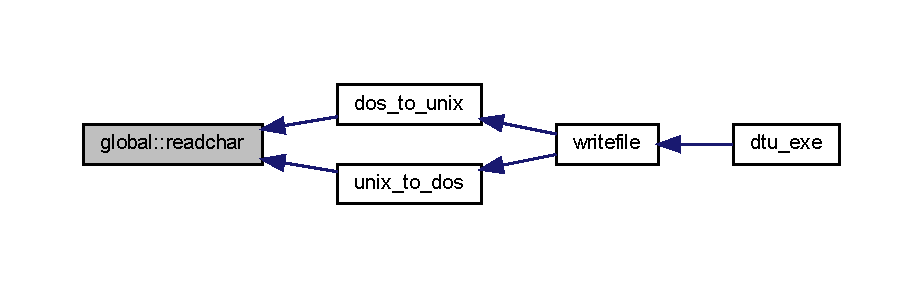
\includegraphics[width=350pt]{namespaceglobal_ac0b651e598e238c7eacf10df65cd92b2_icgraph}
\end{center}
\end{figure}
\mbox{\Hypertarget{namespaceglobal_aa4c95f5c7250975b756bcd2131c3b88c}\label{namespaceglobal_aa4c95f5c7250975b756bcd2131c3b88c}} 
\index{global@{global}!writechar@{writechar}}
\index{writechar@{writechar}!global@{global}}
\subsubsection{\texorpdfstring{writechar()}{writechar()}}
{\footnotesize\ttfamily integer function global\+::writechar (\begin{DoxyParamCaption}\item[{\hyperlink{option__stopwatch_83_8txt_abd4b21fbbd175834027b5224bfe97e66}{character}(len=1)}]{char1 }\end{DoxyParamCaption})}



References chars\+\_\+written, and ounit.

Here is the caller graph for this function\+:
\nopagebreak
\begin{figure}[H]
\begin{center}
\leavevmode
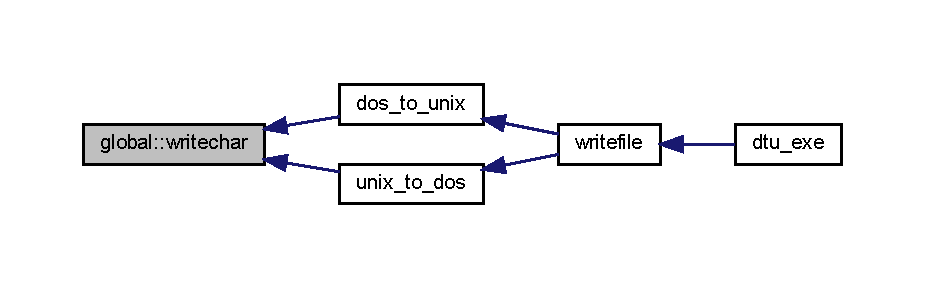
\includegraphics[width=350pt]{namespaceglobal_aa4c95f5c7250975b756bcd2131c3b88c_icgraph}
\end{center}
\end{figure}


\subsection{Variable Documentation}
\mbox{\Hypertarget{namespaceglobal_a2d038312d6b015cabfbb5716cb61baac}\label{namespaceglobal_a2d038312d6b015cabfbb5716cb61baac}} 
\index{global@{global}!chars\+\_\+read@{chars\+\_\+read}}
\index{chars\+\_\+read@{chars\+\_\+read}!global@{global}}
\subsubsection{\texorpdfstring{chars\+\_\+read}{chars\_read}}
{\footnotesize\ttfamily integer global\+::chars\+\_\+read = 0}

\mbox{\Hypertarget{namespaceglobal_a22f0db93abbbbd8c37f50b829daa00ad}\label{namespaceglobal_a22f0db93abbbbd8c37f50b829daa00ad}} 
\index{global@{global}!chars\+\_\+written@{chars\+\_\+written}}
\index{chars\+\_\+written@{chars\+\_\+written}!global@{global}}
\subsubsection{\texorpdfstring{chars\+\_\+written}{chars\_written}}
{\footnotesize\ttfamily integer global\+::chars\+\_\+written = 0}

\mbox{\Hypertarget{namespaceglobal_a66654a3eb0e9c862da1f7ca5388b2e83}\label{namespaceglobal_a66654a3eb0e9c862da1f7ca5388b2e83}} 
\index{global@{global}!cr@{cr}}
\index{cr@{cr}!global@{global}}
\subsubsection{\texorpdfstring{cr}{cr}}
{\footnotesize\ttfamily \hyperlink{option__stopwatch_83_8txt_abd4b21fbbd175834027b5224bfe97e66}{character}(len=1), parameter global\+::cr =char(13)}

\mbox{\Hypertarget{namespaceglobal_ae55226f82ca7ee1f12eeb19f4619f98c}\label{namespaceglobal_ae55226f82ca7ee1f12eeb19f4619f98c}} 
\index{global@{global}!cz@{cz}}
\index{cz@{cz}!global@{global}}
\subsubsection{\texorpdfstring{cz}{cz}}
{\footnotesize\ttfamily \hyperlink{option__stopwatch_83_8txt_abd4b21fbbd175834027b5224bfe97e66}{character}(len=1), parameter global\+::cz =char(26)}

\mbox{\Hypertarget{namespaceglobal_ad88d280367759e82acb4de429dce1caa}\label{namespaceglobal_ad88d280367759e82acb4de429dce1caa}} 
\index{global@{global}!iunit@{iunit}}
\index{iunit@{iunit}!global@{global}}
\subsubsection{\texorpdfstring{iunit}{iunit}}
{\footnotesize\ttfamily integer global\+::iunit =15}

\mbox{\Hypertarget{namespaceglobal_a65a09148e3924472bdd8a5735476c7ed}\label{namespaceglobal_a65a09148e3924472bdd8a5735476c7ed}} 
\index{global@{global}!lf@{lf}}
\index{lf@{lf}!global@{global}}
\subsubsection{\texorpdfstring{lf}{lf}}
{\footnotesize\ttfamily \hyperlink{option__stopwatch_83_8txt_abd4b21fbbd175834027b5224bfe97e66}{character}(len=1), parameter global\+::lf =char(10)}

\mbox{\Hypertarget{namespaceglobal_a85ce1360a8a9498bab52f97d527bee12}\label{namespaceglobal_a85ce1360a8a9498bab52f97d527bee12}} 
\index{global@{global}!lines\+\_\+written@{lines\+\_\+written}}
\index{lines\+\_\+written@{lines\+\_\+written}!global@{global}}
\subsubsection{\texorpdfstring{lines\+\_\+written}{lines\_written}}
{\footnotesize\ttfamily integer global\+::lines\+\_\+written = 0}

\mbox{\Hypertarget{namespaceglobal_a972f6c4dda60a65f2529b3fa30f61ad5}\label{namespaceglobal_a972f6c4dda60a65f2529b3fa30f61ad5}} 
\index{global@{global}!nl@{nl}}
\index{nl@{nl}!global@{global}}
\subsubsection{\texorpdfstring{nl}{nl}}
{\footnotesize\ttfamily \hyperlink{option__stopwatch_83_8txt_abd4b21fbbd175834027b5224bfe97e66}{character}(len=1), parameter global\+::nl =char(10)}

\mbox{\Hypertarget{namespaceglobal_af2859727a2cdfcff37dacc9cadc1c046}\label{namespaceglobal_af2859727a2cdfcff37dacc9cadc1c046}} 
\index{global@{global}!noisy@{noisy}}
\index{noisy@{noisy}!global@{global}}
\subsubsection{\texorpdfstring{noisy}{noisy}}
{\footnotesize\ttfamily logical global\+::noisy = .false.}

\mbox{\Hypertarget{namespaceglobal_a243230c67d07fa783b97362c247e777c}\label{namespaceglobal_a243230c67d07fa783b97362c247e777c}} 
\index{global@{global}!ounit@{ounit}}
\index{ounit@{ounit}!global@{global}}
\subsubsection{\texorpdfstring{ounit}{ounit}}
{\footnotesize\ttfamily integer global\+::ounit =16}

\mbox{\Hypertarget{namespaceglobal_ab06e1a0896cfbbc3a6516eedaba862e0}\label{namespaceglobal_ab06e1a0896cfbbc3a6516eedaba862e0}} 
\index{global@{global}!process\+\_\+ctrl\+\_\+z@{process\+\_\+ctrl\+\_\+z}}
\index{process\+\_\+ctrl\+\_\+z@{process\+\_\+ctrl\+\_\+z}!global@{global}}
\subsubsection{\texorpdfstring{process\+\_\+ctrl\+\_\+z}{process\_ctrl\_z}}
{\footnotesize\ttfamily logical global\+::process\+\_\+ctrl\+\_\+z = .false.}


\hypertarget{namespacem__anyscalar}{}\section{m\+\_\+anyscalar Module Reference}
\label{namespacem__anyscalar}\index{m\+\_\+anyscalar@{m\+\_\+anyscalar}}
\subsection*{Functions/\+Subroutines}
\begin{DoxyCompactItemize}
\item 
pure doubleprecision function, \hyperlink{M__stopwatch_83_8txt_a2f74811300c361e53b430611a7d1769f}{public} \hyperlink{namespacem__anyscalar_a6173dbc57e7c5a96f5961d9e83e6e15e}{anyscalar\+\_\+to\+\_\+double} (valuein)
\begin{DoxyCompactList}\small\item\em \subsubsection*{N\+A\+ME}

anyscalar\+\_\+to\+\_\+double(3f) -\/ \mbox{[}M\+\_\+anyscalar\mbox{]} convert integer or real parameter of any kind to doubleprecision \end{DoxyCompactList}\item 
pure \hyperlink{read__watch_83_8txt_abdb62bde002f38ef75f810d3a905a823}{real} function, \hyperlink{M__stopwatch_83_8txt_a2f74811300c361e53b430611a7d1769f}{public} \hyperlink{namespacem__anyscalar_a39cd9a778fff85974fa1a822b92555fd}{anyscalar\+\_\+to\+\_\+real} (valuein)
\begin{DoxyCompactList}\small\item\em \subsubsection*{N\+A\+ME}

anyscalar\+\_\+to\+\_\+real(3f) -\/ \mbox{[}M\+\_\+anyscalar\mbox{]} convert integer or real parameter of any kind to real \end{DoxyCompactList}\item 
elemental integer(kind=\hyperlink{namespacem__anyscalar_a53057899b7d17505b79d9b8f5e6092a2}{int128}) function, \hyperlink{M__stopwatch_83_8txt_a2f74811300c361e53b430611a7d1769f}{public} \hyperlink{namespacem__anyscalar_a513beeccb5c821157cbd2eea8a1d9842}{anyinteger\+\_\+to\+\_\+128bit} (intin)
\begin{DoxyCompactList}\small\item\em \subsubsection*{N\+A\+ME}\end{DoxyCompactList}\end{DoxyCompactItemize}
\subsection*{Variables}
\begin{DoxyCompactItemize}
\item 
integer, dimension(38), parameter \hyperlink{namespacem__anyscalar_a099da1dd8639cdce3d0f5bb3cb8fbd03}{k} =\mbox{[}(selected\+\_\+int\+\_\+kind(\hyperlink{intro__blas1_83_8txt_a8ba82a50c0c2c12d5f6a77f7e4651c0b}{i}),\hyperlink{intro__blas1_83_8txt_a8ba82a50c0c2c12d5f6a77f7e4651c0b}{i}=1,38)\mbox{]}
\item 
integer, parameter, \hyperlink{M__stopwatch_83_8txt_a2f74811300c361e53b430611a7d1769f}{public} \hyperlink{namespacem__anyscalar_a53057899b7d17505b79d9b8f5e6092a2}{int128} =\hyperlink{namespacem__anyscalar_a099da1dd8639cdce3d0f5bb3cb8fbd03}{k}(38)
\item 
integer, dimension(34), parameter \hyperlink{namespacem__anyscalar_af515907c09cc2ac286a4523cc73f5f52}{r} =\mbox{[}(selected\+\_\+int\+\_\+kind(\hyperlink{intro__blas1_83_8txt_a8ba82a50c0c2c12d5f6a77f7e4651c0b}{i}),\hyperlink{intro__blas1_83_8txt_a8ba82a50c0c2c12d5f6a77f7e4651c0b}{i}=1,34)\mbox{]}
\item 
integer, parameter, \hyperlink{M__stopwatch_83_8txt_a2f74811300c361e53b430611a7d1769f}{public} \hyperlink{namespacem__anyscalar_a6d3ef2bc1698c91d737dbd8824a9eb0b}{real256} =\hyperlink{namespacem__anyscalar_af515907c09cc2ac286a4523cc73f5f52}{r}(34)
\end{DoxyCompactItemize}


\subsection{Function/\+Subroutine Documentation}
\mbox{\Hypertarget{namespacem__anyscalar_a513beeccb5c821157cbd2eea8a1d9842}\label{namespacem__anyscalar_a513beeccb5c821157cbd2eea8a1d9842}} 
\index{m\+\_\+anyscalar@{m\+\_\+anyscalar}!anyinteger\+\_\+to\+\_\+128bit@{anyinteger\+\_\+to\+\_\+128bit}}
\index{anyinteger\+\_\+to\+\_\+128bit@{anyinteger\+\_\+to\+\_\+128bit}!m\+\_\+anyscalar@{m\+\_\+anyscalar}}
\subsubsection{\texorpdfstring{anyinteger\+\_\+to\+\_\+128bit()}{anyinteger\_to\_128bit()}}
{\footnotesize\ttfamily elemental integer(kind=\hyperlink{namespacem__anyscalar_a53057899b7d17505b79d9b8f5e6092a2}{int128}) function, \hyperlink{M__stopwatch_83_8txt_a2f74811300c361e53b430611a7d1769f}{public} m\+\_\+anyscalar\+::anyinteger\+\_\+to\+\_\+128bit (\begin{DoxyParamCaption}\item[{class($\ast$), intent(\hyperlink{M__journal_83_8txt_afce72651d1eed785a2132bee863b2f38}{in})}]{intin }\end{DoxyParamCaption})}



\subsubsection*{N\+A\+ME}

anyinteger\+\_\+to\+\_\+128bit(3f) -\/ \mbox{[}M\+\_\+anyscalar\mbox{]} convert integer any kind to integer(kind=128)

\subsubsection*{S\+Y\+N\+O\+P\+S\+IS}

\begin{DoxyVerb}elemental function anyinteger_to_128bit(intin) result(ii38)

 integer(kind=int128) function anyinteger_to_128bit(value)
 class(*),intent(in)     :: intin
 integer(kind=int8|int16|int32|int64|int128) :: value
\end{DoxyVerb}


\subsubsection*{D\+E\+S\+C\+R\+I\+P\+T\+I\+ON}

\begin{DoxyVerb}This function uses polymorphism to allow arguments of different types
generically. It is used to create other procedures that can take
many scalar arguments as input options, equivalent to  passing the
parameter VALUE as int(VALUE,0_int128).
\end{DoxyVerb}


\subsubsection*{O\+P\+T\+I\+O\+NS}

\begin{DoxyVerb}VALUEIN  input argument of a procedure to convert to type REAL(KIND=128).
         May be of KIND kind=int8, kind=int16, kind=int32, kind=int64,
         kind=int128, kind=real32, kind=real64, kind=real128,
         or kind=real256
\end{DoxyVerb}
 \subsubsection*{R\+E\+S\+U\+L\+TS}

The returned value is of kind R\+E\+AL(K\+I\+ND=R\+E\+A\+L128) and is the value of V\+A\+L\+U\+IN converted to real(K\+I\+ND=R\+E\+A\+L128). \subsubsection*{E\+X\+A\+M\+P\+LE}

\begin{DoxyVerb}Sample program

 program scalars
 use M_anyscalar,     only : int128
 use iso_fortran_env, only : int8, int16, int32, int64
 implicit none
    ! call same function with many scalar input types
    write(*,*)squarei(2_int8)
    write(*,*)squarei(2_int16)
    write(*,*)squarei(2_int32)
    write(*,*)squarei(2_int64)
    write(*,*)squarei(2_int128)
 contains

 function squarei(invalue)
 use M_anyscalar, only : anyinteger_to_128bit, int128
 implicit none
 class(*),intent(in)  :: invalue
 real                 :: invalue_local
 integer(kind=int128) :: squarei
    invalue_local=anyinteger_to_128bit(invalue)
    dvalue=invalue_local*invalue_local
 end function squarei

 end program scalars \end{DoxyVerb}
 

References int128.

\mbox{\Hypertarget{namespacem__anyscalar_a6173dbc57e7c5a96f5961d9e83e6e15e}\label{namespacem__anyscalar_a6173dbc57e7c5a96f5961d9e83e6e15e}} 
\index{m\+\_\+anyscalar@{m\+\_\+anyscalar}!anyscalar\+\_\+to\+\_\+double@{anyscalar\+\_\+to\+\_\+double}}
\index{anyscalar\+\_\+to\+\_\+double@{anyscalar\+\_\+to\+\_\+double}!m\+\_\+anyscalar@{m\+\_\+anyscalar}}
\subsubsection{\texorpdfstring{anyscalar\+\_\+to\+\_\+double()}{anyscalar\_to\_double()}}
{\footnotesize\ttfamily pure doubleprecision function, \hyperlink{M__stopwatch_83_8txt_a2f74811300c361e53b430611a7d1769f}{public} m\+\_\+anyscalar\+::anyscalar\+\_\+to\+\_\+double (\begin{DoxyParamCaption}\item[{class($\ast$), intent(\hyperlink{M__journal_83_8txt_afce72651d1eed785a2132bee863b2f38}{in})}]{valuein }\end{DoxyParamCaption})}



\subsubsection*{N\+A\+ME}

anyscalar\+\_\+to\+\_\+double(3f) -\/ \mbox{[}M\+\_\+anyscalar\mbox{]} convert integer or real parameter of any kind to doubleprecision 

\subsubsection*{S\+Y\+N\+O\+P\+S\+IS}

\begin{DoxyVerb}pure function anyscalar_to_double(valuein) result(d_out)

 class(*),intent(in)  :: valuein
 doubleprecision      :: d_out
\end{DoxyVerb}


\subsubsection*{D\+E\+S\+C\+R\+I\+P\+T\+I\+ON}

\begin{DoxyVerb}This function uses polymorphism to allow arguments of different types
generically. It is used to create other procedures that can take
many scalar arguments as input options.
\end{DoxyVerb}


\subsubsection*{O\+P\+T\+I\+O\+NS}

\begin{DoxyVerb}VALUEIN  input argument of a procedure to convert to type DOUBLEPRECISION.
         May be of KIND kind=int8, kind=int16, kind=int32, kind=int64,
         kind=int128, kind=real32, kind=real64, kind=real128,
         or kind=real256
\end{DoxyVerb}
 \subsubsection*{R\+E\+S\+U\+L\+TS}

The returned value is of kind D\+O\+U\+B\+L\+E\+P\+R\+E\+C\+I\+S\+I\+ON and is the value of V\+A\+L\+U\+IN converted to doubleprecision (assuming it is actually in the range of type D\+O\+U\+B\+L\+E\+P\+R\+E\+C\+I\+S\+I\+ON).

\subsubsection*{E\+X\+A\+M\+P\+LE}

Sample program

program scalars use M\+\_\+anyscalar, only \+: int128, real256 use iso\+\_\+fortran\+\_\+env, only \+: int8, int16, int32, int64 use iso\+\_\+fortran\+\_\+env, only \+: real32, real64, real128 implicit none ! call same function with many scalar input types write($\ast$,$\ast$)squarei(2\+\_\+int8) write($\ast$,$\ast$)squarei(2\+\_\+int16) write($\ast$,$\ast$)squarei(2\+\_\+int32) write($\ast$,$\ast$)squarei(2\+\_\+int64) write($\ast$,$\ast$)squarei(2\+\_\+int128) write($\ast$,$\ast$)squarei(2\+\_\+real32) write($\ast$,$\ast$)squarei(2\+\_\+real64) write($\ast$,$\ast$)squarei(2\+\_\+real128) write($\ast$,$\ast$)squarei(2\+\_\+real256) contains

function squarei(invalue) result (dvalue) use M\+\_\+anyscalar, only \+: anyscalar\+\_\+to\+\_\+double implicit none class($\ast$),intent(in) \+:\+: invalue doubleprecision \+:\+: invalue\+\_\+local doubleprecision \+:\+: dvalue invalue\+\_\+local=anyscalar\+\_\+to\+\_\+double(invalue) dvalue=invalue\+\_\+local$\ast$invalue\+\_\+local end function squarei

end program scalars \mbox{\Hypertarget{namespacem__anyscalar_a39cd9a778fff85974fa1a822b92555fd}\label{namespacem__anyscalar_a39cd9a778fff85974fa1a822b92555fd}} 
\index{m\+\_\+anyscalar@{m\+\_\+anyscalar}!anyscalar\+\_\+to\+\_\+real@{anyscalar\+\_\+to\+\_\+real}}
\index{anyscalar\+\_\+to\+\_\+real@{anyscalar\+\_\+to\+\_\+real}!m\+\_\+anyscalar@{m\+\_\+anyscalar}}
\subsubsection{\texorpdfstring{anyscalar\+\_\+to\+\_\+real()}{anyscalar\_to\_real()}}
{\footnotesize\ttfamily pure \hyperlink{read__watch_83_8txt_abdb62bde002f38ef75f810d3a905a823}{real} function, \hyperlink{M__stopwatch_83_8txt_a2f74811300c361e53b430611a7d1769f}{public} m\+\_\+anyscalar\+::anyscalar\+\_\+to\+\_\+real (\begin{DoxyParamCaption}\item[{class($\ast$), intent(\hyperlink{M__journal_83_8txt_afce72651d1eed785a2132bee863b2f38}{in})}]{valuein }\end{DoxyParamCaption})}



\subsubsection*{N\+A\+ME}

anyscalar\+\_\+to\+\_\+real(3f) -\/ \mbox{[}M\+\_\+anyscalar\mbox{]} convert integer or real parameter of any kind to real 

\subsubsection*{S\+Y\+N\+O\+P\+S\+IS}

\begin{DoxyVerb}pure function anyscalar_to_real(valuein) result(r_out)

 class(*),intent(in)  :: valuein
 real                 :: r_out
\end{DoxyVerb}


\subsubsection*{D\+E\+S\+C\+R\+I\+P\+T\+I\+ON}

\begin{DoxyVerb}This function uses polymorphism to allow arguments of different types
generically. It is used to create other procedures that can take
many scalar arguments as input options.
\end{DoxyVerb}


\subsubsection*{O\+P\+T\+I\+O\+NS}

\begin{DoxyVerb}VALUEIN  input argument of a procedure to convert to type REAL.
         May be of KIND kind=int8, kind=int16, kind=int32, kind=int64,
         kind=int128, kind=real32, kind=real64, kind=real128,
         or kind=real256
\end{DoxyVerb}
 \subsubsection*{R\+E\+S\+U\+L\+TS}

The returned value is of kind R\+E\+AL and is the value of V\+A\+L\+U\+IN converted to real (assuming it is actually in the range of type R\+E\+AL).

\subsubsection*{E\+X\+A\+M\+P\+LE}

Sample program

program scalars use M\+\_\+anyscalar, only \+: int128, real256 use iso\+\_\+fortran\+\_\+env, only \+: int8, int16, int32, int64 use iso\+\_\+fortran\+\_\+env, only \+: real32, real64, real128 implicit none ! call same function with many scalar input types write($\ast$,$\ast$)squarei(2\+\_\+int8) write($\ast$,$\ast$)squarei(2\+\_\+int16) write($\ast$,$\ast$)squarei(2\+\_\+int32) write($\ast$,$\ast$)squarei(2\+\_\+int64) write($\ast$,$\ast$)squarei(2\+\_\+int128) write($\ast$,$\ast$)squarei(2\+\_\+real32) write($\ast$,$\ast$)squarei(2\+\_\+real64) !!write($\ast$,$\ast$)squarei(2\+\_\+real128) write($\ast$,$\ast$)squarei(2\+\_\+real256) contains

function squarei(invalue) result (dvalue) use M\+\_\+anyscalar, only \+: anyscalar\+\_\+to\+\_\+real implicit none class($\ast$),intent(in) \+:\+: invalue real \+:\+: invalue\+\_\+local real \+:\+: dvalue invalue\+\_\+local=anyscalar\+\_\+to\+\_\+real(invalue) dvalue=invalue\+\_\+local$\ast$invalue\+\_\+local end function squarei

end program scalars 

\subsection{Variable Documentation}
\mbox{\Hypertarget{namespacem__anyscalar_a53057899b7d17505b79d9b8f5e6092a2}\label{namespacem__anyscalar_a53057899b7d17505b79d9b8f5e6092a2}} 
\index{m\+\_\+anyscalar@{m\+\_\+anyscalar}!int128@{int128}}
\index{int128@{int128}!m\+\_\+anyscalar@{m\+\_\+anyscalar}}
\subsubsection{\texorpdfstring{int128}{int128}}
{\footnotesize\ttfamily integer, parameter, \hyperlink{M__stopwatch_83_8txt_a2f74811300c361e53b430611a7d1769f}{public} m\+\_\+anyscalar\+::int128 =\hyperlink{namespacem__anyscalar_a099da1dd8639cdce3d0f5bb3cb8fbd03}{k}(38)}

\mbox{\Hypertarget{namespacem__anyscalar_a099da1dd8639cdce3d0f5bb3cb8fbd03}\label{namespacem__anyscalar_a099da1dd8639cdce3d0f5bb3cb8fbd03}} 
\index{m\+\_\+anyscalar@{m\+\_\+anyscalar}!k@{k}}
\index{k@{k}!m\+\_\+anyscalar@{m\+\_\+anyscalar}}
\subsubsection{\texorpdfstring{k}{k}}
{\footnotesize\ttfamily integer, dimension(38), parameter m\+\_\+anyscalar\+::k =\mbox{[}(selected\+\_\+int\+\_\+kind(\hyperlink{intro__blas1_83_8txt_a8ba82a50c0c2c12d5f6a77f7e4651c0b}{i}),\hyperlink{intro__blas1_83_8txt_a8ba82a50c0c2c12d5f6a77f7e4651c0b}{i}=1,38)\mbox{]}\hspace{0.3cm}{\ttfamily [private]}}

\mbox{\Hypertarget{namespacem__anyscalar_af515907c09cc2ac286a4523cc73f5f52}\label{namespacem__anyscalar_af515907c09cc2ac286a4523cc73f5f52}} 
\index{m\+\_\+anyscalar@{m\+\_\+anyscalar}!r@{r}}
\index{r@{r}!m\+\_\+anyscalar@{m\+\_\+anyscalar}}
\subsubsection{\texorpdfstring{r}{r}}
{\footnotesize\ttfamily integer, dimension(34), parameter m\+\_\+anyscalar\+::r =\mbox{[}(selected\+\_\+int\+\_\+kind(\hyperlink{intro__blas1_83_8txt_a8ba82a50c0c2c12d5f6a77f7e4651c0b}{i}),\hyperlink{intro__blas1_83_8txt_a8ba82a50c0c2c12d5f6a77f7e4651c0b}{i}=1,34)\mbox{]}\hspace{0.3cm}{\ttfamily [private]}}

\mbox{\Hypertarget{namespacem__anyscalar_a6d3ef2bc1698c91d737dbd8824a9eb0b}\label{namespacem__anyscalar_a6d3ef2bc1698c91d737dbd8824a9eb0b}} 
\index{m\+\_\+anyscalar@{m\+\_\+anyscalar}!real256@{real256}}
\index{real256@{real256}!m\+\_\+anyscalar@{m\+\_\+anyscalar}}
\subsubsection{\texorpdfstring{real256}{real256}}
{\footnotesize\ttfamily integer, parameter, \hyperlink{M__stopwatch_83_8txt_a2f74811300c361e53b430611a7d1769f}{public} m\+\_\+anyscalar\+::real256 =\hyperlink{namespacem__anyscalar_af515907c09cc2ac286a4523cc73f5f52}{r}(34)}


\hypertarget{namespacem__calculator}{}\section{m\+\_\+calculator Module Reference}
\label{namespacem__calculator}\index{m\+\_\+calculator@{m\+\_\+calculator}}


\subsubsection*{N\+A\+ME}

jucalc -\/ \mbox{[}M\+\_\+calculator\mbox{]} parse calculator expression and return numeric or string value \subsubsection*{S\+Y\+N\+O\+P\+S\+IS} 


\subsection*{Data Types}
\begin{DoxyCompactItemize}
\item 
interface \hyperlink{interfacem__calculator_1_1stuff}{stuff}
\begin{DoxyCompactList}\small\item\em \subsubsection*{N\+A\+ME}

stuff(3f) -\/ \mbox{[}M\+\_\+calculator\mbox{]} directly store value into calculator directory for efficiency \end{DoxyCompactList}\end{DoxyCompactItemize}
\subsection*{Functions/\+Subroutines}
\begin{DoxyCompactItemize}
\item 
\hyperlink{M__stopwatch_83_8txt_acfbcff50169d691ff02d4a123ed70482}{subroutine}, \hyperlink{M__stopwatch_83_8txt_a2f74811300c361e53b430611a7d1769f}{public} \hyperlink{namespacem__calculator_a7a98aaf2fb03204125187dfec671ce1f}{jucalc} (inline, outlin, mssg, slast, ierr)
\item 
\hyperlink{M__stopwatch_83_8txt_acfbcff50169d691ff02d4a123ed70482}{subroutine} \hyperlink{namespacem__calculator_a190e152c2fc309d59e75ee4645e6d261}{help\+\_\+funcs} ()
\begin{DoxyCompactList}\small\item\em \subsubsection*{N\+A\+ME}

\subsubsection*{S\+Y\+N\+O\+P\+S\+IS}\end{DoxyCompactList}\item 
\hyperlink{M__stopwatch_83_8txt_acfbcff50169d691ff02d4a123ed70482}{subroutine}, private \hyperlink{namespacem__calculator_afabadeb80314b52e904de9865f67ea9d}{jupars} (\hyperlink{what__overview_81_8txt_a74cb7e955273b9f9157b4f0c18a38849}{string}, nchar, ier)
\begin{DoxyCompactList}\small\item\em \subsubsection*{N\+A\+ME}

\subsubsection*{S\+Y\+N\+O\+P\+S\+IS}\end{DoxyCompactList}\item 
\hyperlink{M__stopwatch_83_8txt_acfbcff50169d691ff02d4a123ed70482}{subroutine}, private \hyperlink{namespacem__calculator_ab9afbbbd87dd1434f72853350afec2a6}{jufuns} (wstrng, nchars, ier)
\begin{DoxyCompactList}\small\item\em \subsubsection*{N\+A\+ME}

\subsubsection*{S\+Y\+N\+O\+P\+S\+IS}\end{DoxyCompactList}\item 
\hyperlink{M__stopwatch_83_8txt_acfbcff50169d691ff02d4a123ed70482}{subroutine}, private \hyperlink{namespacem__calculator_ae4cc2211f8bd276d5765e4ebc9d6e354}{stufftok} (fval, wstrng, nchars, \hyperlink{what__overview_81_8txt_a74cb7e955273b9f9157b4f0c18a38849}{string}, iend, ier)
\begin{DoxyCompactList}\small\item\em \subsubsection*{N\+A\+ME}

\subsubsection*{S\+Y\+N\+O\+P\+S\+IS}\end{DoxyCompactList}\item 
\hyperlink{M__stopwatch_83_8txt_acfbcff50169d691ff02d4a123ed70482}{subroutine}, private \hyperlink{namespacem__calculator_a6fc04e994f45d649d5e412e0013bf127}{juargs} (line, ilen, \hyperlink{intro__blas1_83_8txt_a89db1945e1a335ab0184c6a097821e32}{array}, itype, iarray, ier, mx)
\begin{DoxyCompactList}\small\item\em \subsubsection*{N\+A\+ME}

\subsubsection*{S\+Y\+N\+O\+P\+S\+IS}\end{DoxyCompactList}\item 
\hyperlink{M__stopwatch_83_8txt_acfbcff50169d691ff02d4a123ed70482}{subroutine}, private \hyperlink{namespacem__calculator_a1461bad85da11d09210daefe3f80973d}{jucals} (\hyperlink{what__overview_81_8txt_a74cb7e955273b9f9157b4f0c18a38849}{string}, nchar, \hyperlink{namespacem__calculator_aeaff519ae0f18ac99095c955fbe12f9d}{value}, ier)
\begin{DoxyCompactList}\small\item\em \subsubsection*{N\+A\+ME}

\subsubsection*{S\+Y\+N\+O\+P\+S\+IS}\end{DoxyCompactList}\item 
\hyperlink{M__stopwatch_83_8txt_acfbcff50169d691ff02d4a123ed70482}{subroutine}, private \hyperlink{namespacem__calculator_ae1afc2ee970ad4635cce19b9b8b74f1c}{jupows} (wstrng, nchar, ier)
\begin{DoxyCompactList}\small\item\em \subsubsection*{N\+A\+ME}

\subsubsection*{S\+Y\+N\+O\+P\+S\+IS}\end{DoxyCompactList}\item 
\hyperlink{M__stopwatch_83_8txt_acfbcff50169d691ff02d4a123ed70482}{subroutine}, private \hyperlink{namespacem__calculator_a78c73098f0fcf1130ea9f5f3748bef7d}{jufacs} (wstrng, nchr, fval1, ier)
\begin{DoxyCompactList}\small\item\em \subsubsection*{N\+A\+ME}

\subsubsection*{S\+Y\+N\+O\+P\+S\+IS}\end{DoxyCompactList}\item 
\hyperlink{M__stopwatch_83_8txt_acfbcff50169d691ff02d4a123ed70482}{subroutine}, private \hyperlink{namespacem__calculator_a99dafdeb0fe1a589face7a3eaf5c66bd}{juator} (chars, rval8, ierr)
\begin{DoxyCompactList}\small\item\em \subsubsection*{N\+A\+ME}

juator(3f) -\/ \mbox{[}M\+\_\+calculator\mbox{]} returns a double precision value from a numeric character string specifically for M\+\_\+calculator(3fm) \subsubsection*{S\+Y\+N\+O\+P\+S\+IS}\end{DoxyCompactList}\item 
\hyperlink{M__stopwatch_83_8txt_acfbcff50169d691ff02d4a123ed70482}{subroutine}, private \hyperlink{namespacem__calculator_a5031622e3d493b738ac425f1fa454a60}{jurtoa} (rval, chars, ilen, ierr)
\begin{DoxyCompactList}\small\item\em \subsubsection*{N\+A\+ME}

\subsubsection*{S\+Y\+N\+O\+P\+S\+IS}\end{DoxyCompactList}\item 
\hyperlink{M__stopwatch_83_8txt_acfbcff50169d691ff02d4a123ed70482}{subroutine}, private \hyperlink{namespacem__calculator_a1c053df0b605f7d96a5982c44a9a1d11}{jusqes} (\hyperlink{what__overview_81_8txt_a74cb7e955273b9f9157b4f0c18a38849}{string}, imax, nchars, varnam, nchar2, ier)
\begin{DoxyCompactList}\small\item\em \subsubsection*{N\+A\+ME}

jusqes -\/ \mbox{[}M\+\_\+calculator\mbox{]} change +-\/\mbox{[}\mbox{]} to \#=(),replace strings with placeholders,delete comments \end{DoxyCompactList}\item 
\hyperlink{M__stopwatch_83_8txt_acfbcff50169d691ff02d4a123ed70482}{subroutine}, private \hyperlink{namespacem__calculator_a82912c44b358ca053754669f542d80af}{jubous} (varnam0, index, ixn, ier)
\begin{DoxyCompactList}\small\item\em \subsubsection*{N\+A\+ME}

\subsubsection*{S\+Y\+N\+O\+P\+S\+IS}\end{DoxyCompactList}\item 
\hyperlink{M__stopwatch_83_8txt_acfbcff50169d691ff02d4a123ed70482}{subroutine}, private \hyperlink{namespacem__calculator_a9306409f00c5ba6200bb68ca672b6053}{juaddr} (newnam, nchars, index, ier)
\begin{DoxyCompactList}\small\item\em \subsubsection*{N\+A\+ME}

juaddr(3fp) -\/ add new variable to numeric value dictionary at specified location \end{DoxyCompactList}\item 
\hyperlink{M__stopwatch_83_8txt_acfbcff50169d691ff02d4a123ed70482}{subroutine}, private \hyperlink{namespacem__calculator_a6d54137f485f8d2ed239b58e44cdb732}{juadds} (newnam, nchars, index, ier)
\begin{DoxyCompactList}\small\item\em \subsubsection*{N\+A\+ME}

\subsubsection*{S\+Y\+N\+O\+P\+S\+IS}\end{DoxyCompactList}\item 
\hyperlink{M__stopwatch_83_8txt_acfbcff50169d691ff02d4a123ed70482}{subroutine}, private \hyperlink{namespacem__calculator_a28e87f9e58861836dd6f7dec4bbb9311}{given\+\_\+name\+\_\+get\+\_\+stringvalue} (chars, ierr)
\begin{DoxyCompactList}\small\item\em \subsubsection*{N\+A\+ME}

\mbox{[}M\+\_\+calculator\mbox{]} given\+\_\+name\+\_\+get\+\_\+stringvalue(3fp) -\/ return associated value for variable name" \subsubsection*{S\+Y\+N\+O\+P\+S\+IS}\end{DoxyCompactList}\item 
doubleprecision function, \hyperlink{M__stopwatch_83_8txt_a2f74811300c361e53b430611a7d1769f}{public} \hyperlink{namespacem__calculator_ab8fa4f20b1e4db1b10ed4deb52b89b34}{getvalue} (varnam)
\begin{DoxyCompactList}\small\item\em \subsubsection*{N\+A\+ME}

getvalue(3f) -\/ \mbox{[}M\+\_\+calculator\mbox{]} given numeric variable name return doubleprecision value directly from calculator dictionary for efficiency \subsubsection*{S\+Y\+N\+O\+P\+S\+IS}\end{DoxyCompactList}\item 
integer function, \hyperlink{M__stopwatch_83_8txt_a2f74811300c361e53b430611a7d1769f}{public} \hyperlink{namespacem__calculator_a192c846b6a8d40ddfe603f988ff82381}{igetvalue} (varnam)
\begin{DoxyCompactList}\small\item\em \subsubsection*{N\+A\+ME}

igetvalue(3f) -\/ \mbox{[}M\+\_\+calculator\mbox{]} given numeric variable name return integer value directly from calculator dictionary for efficiency \subsubsection*{S\+Y\+N\+O\+P\+S\+IS}\end{DoxyCompactList}\item 
\hyperlink{read__watch_83_8txt_abdb62bde002f38ef75f810d3a905a823}{real} function, \hyperlink{M__stopwatch_83_8txt_a2f74811300c361e53b430611a7d1769f}{public} \hyperlink{namespacem__calculator_af8d4bcc1789a047303ac7061c2a504e8}{rgetvalue} (varnam)
\begin{DoxyCompactList}\small\item\em \subsubsection*{N\+A\+ME}

rgetvalue(3f) -\/ \mbox{[}M\+\_\+calculator\mbox{]} given numeric variable name return real value directly from calculator dictionary for efficiency \subsubsection*{S\+Y\+N\+O\+P\+S\+IS}\end{DoxyCompactList}\item 
\hyperlink{M__stopwatch_83_8txt_acfbcff50169d691ff02d4a123ed70482}{subroutine} \hyperlink{namespacem__calculator_ae760c3bf7e4e933427bad6c92cd16dfb}{integer\+\_\+stuff} (varnam0, int4, ioflag)
\begin{DoxyCompactList}\small\item\em \subsubsection*{N\+A\+ME}

\subsubsection*{S\+Y\+N\+O\+P\+S\+IS}\end{DoxyCompactList}\item 
\hyperlink{M__stopwatch_83_8txt_acfbcff50169d691ff02d4a123ed70482}{subroutine} \hyperlink{namespacem__calculator_a8337bfb59665d3236fed48d316e3701b}{real\+\_\+stuff} (varnam0, val4, ioflag)
\begin{DoxyCompactList}\small\item\em \subsubsection*{N\+A\+ME}

\subsubsection*{S\+Y\+N\+O\+P\+S\+IS}\end{DoxyCompactList}\item 
\hyperlink{M__stopwatch_83_8txt_acfbcff50169d691ff02d4a123ed70482}{subroutine} \hyperlink{namespacem__calculator_ab70b7eb8f684537155298c061b54c356}{double\+\_\+stuff} (varnam0, val8, ioflag)
\begin{DoxyCompactList}\small\item\em \subsubsection*{N\+A\+ME}

\subsubsection*{S\+Y\+N\+O\+P\+S\+IS}\end{DoxyCompactList}\item 
\hyperlink{M__stopwatch_83_8txt_acfbcff50169d691ff02d4a123ed70482}{subroutine}, \hyperlink{M__stopwatch_83_8txt_a2f74811300c361e53b430611a7d1769f}{public} \hyperlink{namespacem__calculator_ade5ed0d5db38a14b2c521bc268756f39}{stuffa} (varnam0, \hyperlink{what__overview_81_8txt_a74cb7e955273b9f9157b4f0c18a38849}{string}, index, ioflag)
\begin{DoxyCompactList}\small\item\em \subsubsection*{N\+A\+ME}

stuffa(3f) -\/ \mbox{[}M\+\_\+calculator\mbox{]} stuffa(3f)\+: directly store a string into calculator variable name table \subsubsection*{S\+Y\+N\+O\+P\+S\+IS}\end{DoxyCompactList}\end{DoxyCompactItemize}
\subsection*{Variables}
\begin{DoxyCompactItemize}
\item 
integer, parameter \hyperlink{namespacem__calculator_aefb5a6c3001bb0f09ed82decb6def950}{dp} =kind(0.\+0d0)
\item 
integer, parameter \hyperlink{namespacem__calculator_a462e5bf8d038196149ba96c22a614284}{ic\+\_\+calc} =25000
\item 
integer, parameter, \hyperlink{M__stopwatch_83_8txt_a2f74811300c361e53b430611a7d1769f}{public} \hyperlink{namespacem__calculator_accf705491e8bd9b3d2f0d04fd13712e7}{iclen\+\_\+calc} =512
\item 
integer, parameter, \hyperlink{M__stopwatch_83_8txt_a2f74811300c361e53b430611a7d1769f}{public} \hyperlink{namespacem__calculator_addb6e867e526d278a9901ef8e7ff8bb6}{ixy\+\_\+calc} =55555
\item 
integer, parameter, \hyperlink{M__stopwatch_83_8txt_a2f74811300c361e53b430611a7d1769f}{public} \hyperlink{namespacem__calculator_a482f8880712dc8f52ef6833de3243875}{icname\+\_\+calc} =20
\item 
\hyperlink{read__watch_83_8txt_abdb62bde002f38ef75f810d3a905a823}{real}(kind=\hyperlink{namespacem__calculator_aefb5a6c3001bb0f09ed82decb6def950}{dp}), dimension(\hyperlink{namespacem__calculator_addb6e867e526d278a9901ef8e7ff8bb6}{ixy\+\_\+calc}), save, \hyperlink{M__stopwatch_83_8txt_a2f74811300c361e53b430611a7d1769f}{public} \hyperlink{namespacem__calculator_a92431c21aee174f56eab4bd7afbb8aba}{x} =0.\+0\+\_\+dp
\item 
\hyperlink{read__watch_83_8txt_abdb62bde002f38ef75f810d3a905a823}{real}(kind=\hyperlink{namespacem__calculator_aefb5a6c3001bb0f09ed82decb6def950}{dp}), dimension(\hyperlink{namespacem__calculator_addb6e867e526d278a9901ef8e7ff8bb6}{ixy\+\_\+calc}), save, \hyperlink{M__stopwatch_83_8txt_a2f74811300c361e53b430611a7d1769f}{public} \hyperlink{namespacem__calculator_affdb371c2a552e5a31bfe542a2b837cd}{y} =0.\+0\+\_\+dp
\item 
integer, dimension(\hyperlink{namespacem__calculator_a462e5bf8d038196149ba96c22a614284}{ic\+\_\+calc}), save, \hyperlink{M__stopwatch_83_8txt_a2f74811300c361e53b430611a7d1769f}{public} \hyperlink{namespacem__calculator_a7d1d50fdb797826d4722b3a6d2e38442}{valuer} =0
\item 
\hyperlink{option__stopwatch_83_8txt_abd4b21fbbd175834027b5224bfe97e66}{character}(len=\hyperlink{namespacem__calculator_accf705491e8bd9b3d2f0d04fd13712e7}{iclen\+\_\+calc}), dimension(\hyperlink{namespacem__calculator_a462e5bf8d038196149ba96c22a614284}{ic\+\_\+calc}), save, \hyperlink{M__stopwatch_83_8txt_a2f74811300c361e53b430611a7d1769f}{public} \hyperlink{namespacem__calculator_ad2574ef504a32d93ad0c76a9a8e1c626}{values} =\textquotesingle{} \textquotesingle{}
\item 
integer, parameter \hyperlink{namespacem__calculator_a7f11fbca3121837187391693c8bf3f01}{ixyc\+\_\+calc} =50
\item 
integer, parameter \hyperlink{namespacem__calculator_ae948e91eea8ea15aabe598f464ca80da}{icbuf\+\_\+calc} =20$\ast$(\hyperlink{namespacem__calculator_accf705491e8bd9b3d2f0d04fd13712e7}{iclen\+\_\+calc}/2+1)
\item 
\hyperlink{option__stopwatch_83_8txt_abd4b21fbbd175834027b5224bfe97e66}{character}(len=\hyperlink{namespacem__calculator_accf705491e8bd9b3d2f0d04fd13712e7}{iclen\+\_\+calc}) \hyperlink{namespacem__calculator_ac160bf2b4ddbb768c89d08f21e2ddbad}{mssge}
\item 
\hyperlink{option__stopwatch_83_8txt_abd4b21fbbd175834027b5224bfe97e66}{character}(len=\hyperlink{namespacem__calculator_accf705491e8bd9b3d2f0d04fd13712e7}{iclen\+\_\+calc}), dimension(\hyperlink{namespacem__calculator_a7f11fbca3121837187391693c8bf3f01}{ixyc\+\_\+calc}), save \hyperlink{namespacem__calculator_ab41188894b08fea788b696585426ae6b}{xc} =\textquotesingle{} \textquotesingle{}
\item 
\hyperlink{option__stopwatch_83_8txt_abd4b21fbbd175834027b5224bfe97e66}{character}(len=\hyperlink{namespacem__calculator_accf705491e8bd9b3d2f0d04fd13712e7}{iclen\+\_\+calc}), dimension(\hyperlink{namespacem__calculator_a7f11fbca3121837187391693c8bf3f01}{ixyc\+\_\+calc}), save \hyperlink{namespacem__calculator_a8ce138d24e6b41a29b5b6cec70e78086}{yc} =\textquotesingle{} \textquotesingle{}
\item 
\hyperlink{option__stopwatch_83_8txt_abd4b21fbbd175834027b5224bfe97e66}{character}(len=\hyperlink{namespacem__calculator_accf705491e8bd9b3d2f0d04fd13712e7}{iclen\+\_\+calc}), dimension(\hyperlink{namespacem__calculator_a7f11fbca3121837187391693c8bf3f01}{ixyc\+\_\+calc}), save \hyperlink{namespacem__calculator_a2ba30f3ed633dcbb2d8deeb54f8a450b}{nc} =\textquotesingle{} \textquotesingle{}
\item 
\hyperlink{option__stopwatch_83_8txt_abd4b21fbbd175834027b5224bfe97e66}{character}(len=\hyperlink{namespacem__calculator_a482f8880712dc8f52ef6833de3243875}{icname\+\_\+calc}), dimension(\hyperlink{namespacem__calculator_a462e5bf8d038196149ba96c22a614284}{ic\+\_\+calc}), save \hyperlink{namespacem__calculator_a1d671e939e22b8530ef0cd575bf7dd04}{ix2} =\textquotesingle{} \textquotesingle{}
\item 
\hyperlink{option__stopwatch_83_8txt_abd4b21fbbd175834027b5224bfe97e66}{character}(len=\hyperlink{namespacem__calculator_a482f8880712dc8f52ef6833de3243875}{icname\+\_\+calc}), dimension(\hyperlink{namespacem__calculator_a462e5bf8d038196149ba96c22a614284}{ic\+\_\+calc}), save \hyperlink{namespacem__calculator_a7570d0ed10f0fc80eeaf3b07ef39c370}{ix} =\textquotesingle{} \textquotesingle{}
\item 
\hyperlink{read__watch_83_8txt_abdb62bde002f38ef75f810d3a905a823}{real}(kind=\hyperlink{namespacem__calculator_aefb5a6c3001bb0f09ed82decb6def950}{dp}), dimension(\hyperlink{namespacem__calculator_a462e5bf8d038196149ba96c22a614284}{ic\+\_\+calc}), save \hyperlink{namespacem__calculator_aeaff519ae0f18ac99095c955fbe12f9d}{value} =0.\+0\+\_\+dp
\item 
\hyperlink{option__stopwatch_83_8txt_abd4b21fbbd175834027b5224bfe97e66}{character}(len=\hyperlink{namespacem__calculator_accf705491e8bd9b3d2f0d04fd13712e7}{iclen\+\_\+calc}), save \hyperlink{namespacem__calculator_a5d0147576a419edafaabfc5d7f1317fc}{last} =\textquotesingle{}0.\+0\textquotesingle{}
\item 
logical, save \hyperlink{namespacem__calculator_a64ba59ad27c2751b72b5880500985b56}{ownon} =.false.
\item 
integer, save \hyperlink{namespacem__calculator_ada86fed286e7bff1456862ab8b5bde47}{ktoken}
\end{DoxyCompactItemize}


\subsection{Detailed Description}
\subsubsection*{N\+A\+ME}

jucalc -\/ \mbox{[}M\+\_\+calculator\mbox{]} parse calculator expression and return numeric or string value \subsubsection*{S\+Y\+N\+O\+P\+S\+IS}

subroutine jucalc(inline,outlin,mssg,slast,ierr)

character(len=$\ast$),intent=(in) \+:\+: inline character(len=iclen\+\_\+calc),intent=(out) \+:\+: outlin character(len=iclen\+\_\+calc),intent=(out) \+:\+: mssg doubleprecision, intent=(out) \+:\+: slast integer, intent=(out) \+:\+: ierr

\subsubsection*{D\+E\+S\+C\+R\+I\+P\+T\+I\+ON}

J\+U\+C\+A\+L\+C() evaluates F\+O\+R\+T\+R\+A\+N-\/like expressions. It can be used to add calculator-\/like abilities to your program.

inline I\+N\+L\+I\+NE is a string expression up to (iclen\+\_\+calc=512) characters long. The syntax of an expression is described in the main document of the Calculator Library. outlin Returned numeric value as a string when I\+E\+RR=0. mssg M\+S\+SG is a string that can serve several purposes o Returned string value when I\+E\+RR=2 o Error message string when I\+E\+RR=-\/1 o Message from \textquotesingle{}funcs\textquotesingle{} or \textquotesingle{}dump\textquotesingle{} command when I\+E\+RR=1 slast S\+L\+A\+ST has different meanings depending on whether a string or number is being returned o R\+E\+AL value set to last successfully calculated value when I\+E\+RR=0 o Number of characters in returned string variable when I\+E\+RR=2 ierr status flag. o -\/1 ==$>$ An error occurred o 0 ==$>$ A numeric value was returned o 1 ==$>$ A message was returned o 2 ==$>$ A string value was returned \subsubsection*{D\+E\+P\+E\+N\+D\+E\+N\+C\+I\+ES}

o ceiling o floor o change o modif o rand o len\+\_\+trim o User-\/supplied routines\+: juown1, c \subsubsection*{E\+X\+A\+M\+P\+L\+ES}

Example calculator program \begin{DoxyVerb}program compute
!@(#)compute(1f): line mode calculator program (that calls jucalc(3f))
!     requires:
!     c()
use m_calculator, only: jucalc,iclen_calc
! iclen_calc : max length of expression or variable value as a string
implicit none
integer,parameter         :: dp=kind(0.0d0)
character(len=iclen_calc) :: line
character(len=iclen_calc) :: outlin
character(len=iclen_calc) :: event
real(kind=dp)             :: rvalue
integer                   :: ierr
ierr=0
call jucalc('ownmode(1)',outlin,event,rvalue,ierr)
! activate user-defined function interface
INFINITE: do
   read(*,'(a)',end=999)line
   if(line.eq.'.')stop
   call jucalc(line,outlin,event,rvalue,ierr)
   select case (ierr)
   ! several different meanings to the error flag returned by calculator
   case(0)
   ! a numeric value was returned without error
     write(*,'(a,a,a)')trim(outlin),' = ',trim(line)
   case(2)
   ! a string value was returned without error
     write(*,'(a)')trim(event(:int(rvalue)))
   case(1)
   ! a request for a message has been returned (from DUMP or FUNC)
     write(*,'(a,a)')'message===>',trim(event(:len_trim(event)))
   case(-1)
   ! an error has occurred
     write(*,'(a,a)')'error===>',trim(event(:len_trim(event)))
   case default
   ! this should not occur
     WRITE(6,'(A,i10)')'*JUCALC* UNEXPECTED IERR VALUE ',IERR
   end select
enddo INFINITE
999 continue
end program compute
\end{DoxyVerb}


\subsubsection*{S\+EE A\+L\+SO}

see I\+N\+U\+M0(),R\+N\+U\+M0(),S\+N\+U\+M0(),S\+T\+R\+G\+A\+R2(),J\+U\+C\+A\+L\+C\+X(). \subsubsection*{R\+E\+F\+E\+R\+E\+N\+C\+ES}

N\+O\+NE. A\+U\+T\+H\+OR John S. Urbn \subsubsection*{V\+E\+R\+S\+I\+ON 1.\+0 19971123,20161218}

\subsection{Function/\+Subroutine Documentation}
\mbox{\Hypertarget{namespacem__calculator_ab70b7eb8f684537155298c061b54c356}\label{namespacem__calculator_ab70b7eb8f684537155298c061b54c356}} 
\index{m\+\_\+calculator@{m\+\_\+calculator}!double\+\_\+stuff@{double\+\_\+stuff}}
\index{double\+\_\+stuff@{double\+\_\+stuff}!m\+\_\+calculator@{m\+\_\+calculator}}
\subsubsection{\texorpdfstring{double\+\_\+stuff()}{double\_stuff()}}
{\footnotesize\ttfamily \hyperlink{M__stopwatch_83_8txt_acfbcff50169d691ff02d4a123ed70482}{subroutine} m\+\_\+calculator\+::double\+\_\+stuff (\begin{DoxyParamCaption}\item[{\hyperlink{option__stopwatch_83_8txt_abd4b21fbbd175834027b5224bfe97e66}{character}(len=$\ast$), intent(\hyperlink{M__journal_83_8txt_afce72651d1eed785a2132bee863b2f38}{in})}]{varnam0,  }\item[{\hyperlink{read__watch_83_8txt_abdb62bde002f38ef75f810d3a905a823}{real}(kind=\hyperlink{namespacem__calculator_aefb5a6c3001bb0f09ed82decb6def950}{dp}), intent(\hyperlink{M__journal_83_8txt_afce72651d1eed785a2132bee863b2f38}{in})}]{val8,  }\item[{\hyperlink{option__stopwatch_83_8txt_abd4b21fbbd175834027b5224bfe97e66}{character}(len=$\ast$), intent(\hyperlink{M__journal_83_8txt_afce72651d1eed785a2132bee863b2f38}{in}), \hyperlink{option__stopwatch_83_8txt_aa4ece75e7acf58a4843f70fe18c3ade5}{optional}}]{ioflag }\end{DoxyParamCaption})\hspace{0.3cm}{\ttfamily [private]}}



\subsubsection*{N\+A\+ME}

\subsubsection*{S\+Y\+N\+O\+P\+S\+IS}

\subsubsection*{D\+E\+S\+C\+R\+I\+P\+T\+I\+ON}

\subsubsection*{O\+P\+T\+I\+O\+NS}

\subsubsection*{R\+E\+T\+U\+R\+NS}

\subsubsection*{E\+X\+A\+M\+P\+LE}

References ix, juaddr(), jubous(), and value.

\mbox{\Hypertarget{namespacem__calculator_ab8fa4f20b1e4db1b10ed4deb52b89b34}\label{namespacem__calculator_ab8fa4f20b1e4db1b10ed4deb52b89b34}} 
\index{m\+\_\+calculator@{m\+\_\+calculator}!getvalue@{getvalue}}
\index{getvalue@{getvalue}!m\+\_\+calculator@{m\+\_\+calculator}}
\subsubsection{\texorpdfstring{getvalue()}{getvalue()}}
{\footnotesize\ttfamily doubleprecision function, \hyperlink{M__stopwatch_83_8txt_a2f74811300c361e53b430611a7d1769f}{public} m\+\_\+calculator\+::getvalue (\begin{DoxyParamCaption}\item[{\hyperlink{option__stopwatch_83_8txt_abd4b21fbbd175834027b5224bfe97e66}{character}(len=$\ast$), intent(\hyperlink{M__journal_83_8txt_afce72651d1eed785a2132bee863b2f38}{in})}]{varnam }\end{DoxyParamCaption})}



\subsubsection*{N\+A\+ME}

getvalue(3f) -\/ \mbox{[}M\+\_\+calculator\mbox{]} given numeric variable name return doubleprecision value directly from calculator dictionary for efficiency \subsubsection*{S\+Y\+N\+O\+P\+S\+IS}

doubleprecision function getvalue(varnam)

character(len=$\ast$),intent(in) \+:\+: varnam

\subsubsection*{D\+E\+F\+I\+N\+I\+T\+I\+ON}

Given numeric variable name return double precision value. Note this is breaking the rule of only accessing the calculator thru jucalc(3f). It should only be used from user J\+U\+O\+W\+N1(3f) routines to avoid recursion \subsubsection*{O\+P\+T\+I\+O\+NS}

varnam name of calculator variable to look up that is assumed to be a valid defined name of a numeric variable. If it does not exist zero is returned. \subsubsection*{E\+X\+A\+M\+P\+LE}

Program\+:

program demo\+\_\+getvalue use M\+\_\+calculator\+\_\+plus, only \+: rnum0 use M\+\_\+calculator, only\+: getvalue value1=rnum0(\textquotesingle{}A=100/2\textquotesingle{}) ! store something into calculator write($\ast$,$\ast$)value1,getvalue(\textquotesingle{}A\textquotesingle{}) end program demo\+\_\+getvalue

Results\+:

50.\+0000000 50.\+000000000000000 

References ix, jubous(), and value.

\mbox{\Hypertarget{namespacem__calculator_a28e87f9e58861836dd6f7dec4bbb9311}\label{namespacem__calculator_a28e87f9e58861836dd6f7dec4bbb9311}} 
\index{m\+\_\+calculator@{m\+\_\+calculator}!given\+\_\+name\+\_\+get\+\_\+stringvalue@{given\+\_\+name\+\_\+get\+\_\+stringvalue}}
\index{given\+\_\+name\+\_\+get\+\_\+stringvalue@{given\+\_\+name\+\_\+get\+\_\+stringvalue}!m\+\_\+calculator@{m\+\_\+calculator}}
\subsubsection{\texorpdfstring{given\+\_\+name\+\_\+get\+\_\+stringvalue()}{given\_name\_get\_stringvalue()}}
{\footnotesize\ttfamily \hyperlink{M__stopwatch_83_8txt_acfbcff50169d691ff02d4a123ed70482}{subroutine}, private m\+\_\+calculator\+::given\+\_\+name\+\_\+get\+\_\+stringvalue (\begin{DoxyParamCaption}\item[{\hyperlink{option__stopwatch_83_8txt_abd4b21fbbd175834027b5224bfe97e66}{character}(len=$\ast$), intent(\hyperlink{M__journal_83_8txt_afce72651d1eed785a2132bee863b2f38}{in})}]{chars,  }\item[{integer, intent(out)}]{ierr }\end{DoxyParamCaption})\hspace{0.3cm}{\ttfamily [private]}}



\subsubsection*{N\+A\+ME}

\mbox{[}M\+\_\+calculator\mbox{]} given\+\_\+name\+\_\+get\+\_\+stringvalue(3fp) -\/ return associated value for variable name" \subsubsection*{S\+Y\+N\+O\+P\+S\+IS}

subroutine given\+\_\+name\+\_\+get\+\_\+stringvalue(chars,ierr)

character(len=$\ast$),intent(in) \+:\+: chars integer,intent(out) \+:\+: ierr \subsubsection*{D\+E\+S\+C\+R\+I\+P\+T\+I\+ON}

return the actual string when given a string variable name or token the returned string is passed thru the message/string/error G\+L\+O\+B\+AL variable \subsubsection*{O\+P\+T\+I\+O\+NS}

C\+H\+A\+RS I\+ER ierr is set and returned as \begin{DoxyVerb}      -1  an error occurs
       2  a string is returned
\end{DoxyVerb}
 \subsubsection*{R\+E\+T\+U\+R\+NS}

M\+S\+S\+GE when successful the variable value is returned through the global variable M\+S\+S\+GE

\subsubsection*{E\+X\+A\+M\+P\+LE}

References icname\+\_\+calc, ix2, jubous(), mssge, and values.

\mbox{\Hypertarget{namespacem__calculator_a190e152c2fc309d59e75ee4645e6d261}\label{namespacem__calculator_a190e152c2fc309d59e75ee4645e6d261}} 
\index{m\+\_\+calculator@{m\+\_\+calculator}!help\+\_\+funcs@{help\+\_\+funcs}}
\index{help\+\_\+funcs@{help\+\_\+funcs}!m\+\_\+calculator@{m\+\_\+calculator}}
\subsubsection{\texorpdfstring{help\+\_\+funcs()}{help\_funcs()}}
{\footnotesize\ttfamily \hyperlink{M__stopwatch_83_8txt_acfbcff50169d691ff02d4a123ed70482}{subroutine} m\+\_\+calculator\+::help\+\_\+funcs (\begin{DoxyParamCaption}{ }\end{DoxyParamCaption})\hspace{0.3cm}{\ttfamily [private]}}



\subsubsection*{N\+A\+ME}

\subsubsection*{S\+Y\+N\+O\+P\+S\+IS}

\subsubsection*{D\+E\+S\+C\+R\+I\+P\+T\+I\+ON}

\subsubsection*{O\+P\+T\+I\+O\+NS}

\subsubsection*{R\+E\+T\+U\+R\+NS}

\subsubsection*{E\+X\+A\+M\+P\+LE}\mbox{\Hypertarget{namespacem__calculator_a192c846b6a8d40ddfe603f988ff82381}\label{namespacem__calculator_a192c846b6a8d40ddfe603f988ff82381}} 
\index{m\+\_\+calculator@{m\+\_\+calculator}!igetvalue@{igetvalue}}
\index{igetvalue@{igetvalue}!m\+\_\+calculator@{m\+\_\+calculator}}
\subsubsection{\texorpdfstring{igetvalue()}{igetvalue()}}
{\footnotesize\ttfamily integer function, \hyperlink{M__stopwatch_83_8txt_a2f74811300c361e53b430611a7d1769f}{public} m\+\_\+calculator\+::igetvalue (\begin{DoxyParamCaption}\item[{\hyperlink{option__stopwatch_83_8txt_abd4b21fbbd175834027b5224bfe97e66}{character}(len=$\ast$), intent(\hyperlink{M__journal_83_8txt_afce72651d1eed785a2132bee863b2f38}{in})}]{varnam }\end{DoxyParamCaption})}



\subsubsection*{N\+A\+ME}

igetvalue(3f) -\/ \mbox{[}M\+\_\+calculator\mbox{]} given numeric variable name return integer value directly from calculator dictionary for efficiency \subsubsection*{S\+Y\+N\+O\+P\+S\+IS}

integer function igetvalue(varnam)

character(len=$\ast$),intent(in) \+:\+: varnam

\subsubsection*{D\+E\+F\+I\+N\+I\+T\+I\+ON}

Given numeric variable name return integer value. Note this is breaking the rule of only accessing the calculator thru jucalc(3f). It should only be used from user J\+U\+O\+W\+N1(3f) routines to avoid recursion \subsubsection*{O\+P\+T\+I\+O\+NS}

varnam name of calculator variable to look up that is assumed to be a valid defined name of a numeric variable. If it does not exist zero is returned without an error being reported.

\subsubsection*{E\+X\+A\+M\+P\+LE}

Program\+:

program demo\+\_\+igetvalue use M\+\_\+calculator\+\_\+plus, only \+: rnum0 use M\+\_\+calculator, only\+: igetvalue value1=rnum0(\textquotesingle{}A=100/2\textquotesingle{}) ! store something into calculator write($\ast$,$\ast$)value1,igetvalue(\textquotesingle{}A\textquotesingle{}) end program demo\+\_\+igetvalue

Results\+:

50.\+0000000 50 

References getvalue().

\mbox{\Hypertarget{namespacem__calculator_ae760c3bf7e4e933427bad6c92cd16dfb}\label{namespacem__calculator_ae760c3bf7e4e933427bad6c92cd16dfb}} 
\index{m\+\_\+calculator@{m\+\_\+calculator}!integer\+\_\+stuff@{integer\+\_\+stuff}}
\index{integer\+\_\+stuff@{integer\+\_\+stuff}!m\+\_\+calculator@{m\+\_\+calculator}}
\subsubsection{\texorpdfstring{integer\+\_\+stuff()}{integer\_stuff()}}
{\footnotesize\ttfamily \hyperlink{M__stopwatch_83_8txt_acfbcff50169d691ff02d4a123ed70482}{subroutine} m\+\_\+calculator\+::integer\+\_\+stuff (\begin{DoxyParamCaption}\item[{\hyperlink{option__stopwatch_83_8txt_abd4b21fbbd175834027b5224bfe97e66}{character}(len=$\ast$), intent(\hyperlink{M__journal_83_8txt_afce72651d1eed785a2132bee863b2f38}{in})}]{varnam0,  }\item[{integer, intent(\hyperlink{M__journal_83_8txt_afce72651d1eed785a2132bee863b2f38}{in})}]{int4,  }\item[{\hyperlink{option__stopwatch_83_8txt_abd4b21fbbd175834027b5224bfe97e66}{character}(len=$\ast$), intent(\hyperlink{M__journal_83_8txt_afce72651d1eed785a2132bee863b2f38}{in}), \hyperlink{option__stopwatch_83_8txt_aa4ece75e7acf58a4843f70fe18c3ade5}{optional}}]{ioflag }\end{DoxyParamCaption})\hspace{0.3cm}{\ttfamily [private]}}



\subsubsection*{N\+A\+ME}

\subsubsection*{S\+Y\+N\+O\+P\+S\+IS}

\subsubsection*{D\+E\+S\+C\+R\+I\+P\+T\+I\+ON}

\subsubsection*{O\+P\+T\+I\+O\+NS}

\subsubsection*{R\+E\+T\+U\+R\+NS}

\subsubsection*{E\+X\+A\+M\+P\+LE}

References double\+\_\+stuff().

\mbox{\Hypertarget{namespacem__calculator_a9306409f00c5ba6200bb68ca672b6053}\label{namespacem__calculator_a9306409f00c5ba6200bb68ca672b6053}} 
\index{m\+\_\+calculator@{m\+\_\+calculator}!juaddr@{juaddr}}
\index{juaddr@{juaddr}!m\+\_\+calculator@{m\+\_\+calculator}}
\subsubsection{\texorpdfstring{juaddr()}{juaddr()}}
{\footnotesize\ttfamily \hyperlink{M__stopwatch_83_8txt_acfbcff50169d691ff02d4a123ed70482}{subroutine}, private m\+\_\+calculator\+::juaddr (\begin{DoxyParamCaption}\item[{\hyperlink{option__stopwatch_83_8txt_abd4b21fbbd175834027b5224bfe97e66}{character}(len=$\ast$), intent(\hyperlink{M__journal_83_8txt_afce72651d1eed785a2132bee863b2f38}{in})}]{newnam,  }\item[{integer, intent(\hyperlink{M__journal_83_8txt_afce72651d1eed785a2132bee863b2f38}{in})}]{nchars,  }\item[{integer, intent(\hyperlink{M__journal_83_8txt_afce72651d1eed785a2132bee863b2f38}{in})}]{index,  }\item[{integer}]{ier }\end{DoxyParamCaption})\hspace{0.3cm}{\ttfamily [private]}}



\subsubsection*{N\+A\+ME}

juaddr(3fp) -\/ add new variable to numeric value dictionary at specified location 

\subsubsection*{S\+Y\+N\+O\+P\+S\+IS}

subroutine juaddr(newnam,nchars,index,ier)

character(len=$\ast$),intent(in) \+:\+: newnam integer,intent(in) \+:\+: nchars integer,intent(in) \+:\+: index integer \+:\+: ier

\subsubsection*{D\+E\+S\+C\+R\+I\+P\+T\+I\+ON}

given a new variable name and place to put it, pull down the character and value arrays and initialize the new variable\textquotesingle{}s value to zero. variable names only up to (icname\+\_\+calc) characters maximum. 

References ic\+\_\+calc, ix, mssge, and value.

\mbox{\Hypertarget{namespacem__calculator_a6d54137f485f8d2ed239b58e44cdb732}\label{namespacem__calculator_a6d54137f485f8d2ed239b58e44cdb732}} 
\index{m\+\_\+calculator@{m\+\_\+calculator}!juadds@{juadds}}
\index{juadds@{juadds}!m\+\_\+calculator@{m\+\_\+calculator}}
\subsubsection{\texorpdfstring{juadds()}{juadds()}}
{\footnotesize\ttfamily \hyperlink{M__stopwatch_83_8txt_acfbcff50169d691ff02d4a123ed70482}{subroutine}, private m\+\_\+calculator\+::juadds (\begin{DoxyParamCaption}\item[{\hyperlink{option__stopwatch_83_8txt_abd4b21fbbd175834027b5224bfe97e66}{character}(len=$\ast$), intent(\hyperlink{M__journal_83_8txt_afce72651d1eed785a2132bee863b2f38}{in})}]{newnam,  }\item[{integer, intent(\hyperlink{M__journal_83_8txt_afce72651d1eed785a2132bee863b2f38}{in})}]{nchars,  }\item[{integer, intent(\hyperlink{M__journal_83_8txt_afce72651d1eed785a2132bee863b2f38}{in})}]{index,  }\item[{integer}]{ier }\end{DoxyParamCaption})\hspace{0.3cm}{\ttfamily [private]}}



\subsubsection*{N\+A\+ME}

\subsubsection*{S\+Y\+N\+O\+P\+S\+IS}

\subsubsection*{D\+E\+S\+C\+R\+I\+P\+T\+I\+ON}

given a new string variable name and place to put it, pull down the character and value arrays and initialize the new variable\textquotesingle{}s value to a blank string. variable names only up to (icname\+\_\+calc) characters maximum. stored strings up to only (iclen\+\_\+calc) characters long. \subsubsection*{O\+P\+T\+I\+O\+NS}

\subsubsection*{R\+E\+T\+U\+R\+NS}

\subsubsection*{E\+X\+A\+M\+P\+LE}

References ic\+\_\+calc, ix2, mssge, valuer, and values.

\mbox{\Hypertarget{namespacem__calculator_a6fc04e994f45d649d5e412e0013bf127}\label{namespacem__calculator_a6fc04e994f45d649d5e412e0013bf127}} 
\index{m\+\_\+calculator@{m\+\_\+calculator}!juargs@{juargs}}
\index{juargs@{juargs}!m\+\_\+calculator@{m\+\_\+calculator}}
\subsubsection{\texorpdfstring{juargs()}{juargs()}}
{\footnotesize\ttfamily \hyperlink{M__stopwatch_83_8txt_acfbcff50169d691ff02d4a123ed70482}{subroutine}, private m\+\_\+calculator\+::juargs (\begin{DoxyParamCaption}\item[{\hyperlink{option__stopwatch_83_8txt_abd4b21fbbd175834027b5224bfe97e66}{character}(len=$\ast$), intent(\hyperlink{M__journal_83_8txt_afce72651d1eed785a2132bee863b2f38}{in})}]{line,  }\item[{integer, intent(\hyperlink{M__journal_83_8txt_afce72651d1eed785a2132bee863b2f38}{in})}]{ilen,  }\item[{doubleprecision, dimension(mx), intent(out)}]{array,  }\item[{integer, dimension(mx), intent(out)}]{itype,  }\item[{integer, intent(out)}]{iarray,  }\item[{integer}]{ier,  }\item[{integer, intent(\hyperlink{M__journal_83_8txt_afce72651d1eed785a2132bee863b2f38}{in})}]{mx }\end{DoxyParamCaption})\hspace{0.3cm}{\ttfamily [private]}}



\subsubsection*{N\+A\+ME}

\subsubsection*{S\+Y\+N\+O\+P\+S\+IS}

\subsubsection*{D\+E\+S\+C\+R\+I\+P\+T\+I\+ON}

\subsubsection*{O\+P\+T\+I\+O\+NS}

\subsubsection*{R\+E\+T\+U\+R\+NS}

\subsubsection*{E\+X\+A\+M\+P\+LE}

References jucals(), and mssge.

\mbox{\Hypertarget{namespacem__calculator_a99dafdeb0fe1a589face7a3eaf5c66bd}\label{namespacem__calculator_a99dafdeb0fe1a589face7a3eaf5c66bd}} 
\index{m\+\_\+calculator@{m\+\_\+calculator}!juator@{juator}}
\index{juator@{juator}!m\+\_\+calculator@{m\+\_\+calculator}}
\subsubsection{\texorpdfstring{juator()}{juator()}}
{\footnotesize\ttfamily \hyperlink{M__stopwatch_83_8txt_acfbcff50169d691ff02d4a123ed70482}{subroutine}, private m\+\_\+calculator\+::juator (\begin{DoxyParamCaption}\item[{\hyperlink{option__stopwatch_83_8txt_abd4b21fbbd175834027b5224bfe97e66}{character}(len=$\ast$), intent(\hyperlink{M__journal_83_8txt_afce72651d1eed785a2132bee863b2f38}{in})}]{chars,  }\item[{doubleprecision, intent(out)}]{rval8,  }\item[{integer, intent(out)}]{ierr }\end{DoxyParamCaption})\hspace{0.3cm}{\ttfamily [private]}}



\subsubsection*{N\+A\+ME}

juator(3f) -\/ \mbox{[}M\+\_\+calculator\mbox{]} returns a double precision value from a numeric character string specifically for M\+\_\+calculator(3fm) \subsubsection*{S\+Y\+N\+O\+P\+S\+IS}

subroutine juator(chars,rval,ierr)

character(len=$\ast$),intent(in) \+:\+: chars doubleprecision,intent(out) \+:\+: rval integer,intent(out) \+:\+: ierr

\subsubsection*{D\+E\+S\+C\+R\+I\+P\+T\+I\+ON}

Convert a string representing a numeric scalar value to a numeric value, specifically for the M\+\_\+calculator(3fp) module.\+Works with any g-\/format input, including integer, real, and exponential forms.


\begin{DoxyEnumerate}
\item if chars=? set rval to value stored as current value, return.
\item if the string starts with a \$ assume it is the name of a string variable or token and return its location as a doubleprecision number.
\item try to read string into a doubleprecision value. if successful, return.
\item if not interpretable as a doubleprecision value, see if it is a defined variable name and use that name\textquotesingle{}s value if it is.
\item if no value can be associated to the string and/or if an unexpected error has occurred, set error flag and error message and set rval to zero and return.
\item note that blanks are treated as null, not zero. \subsubsection*{O\+P\+T\+I\+O\+NS}
\end{DoxyEnumerate}

chars is the input string rval is the doubleprecision output value ierr 0 if no error occurs

\subsubsection*{E\+X\+A\+M\+P\+LE}

\subsubsection*{V\+E\+R\+S\+I\+ON}

o 07/15/1986 J. S. Urban o 12/28/1987 modified to specify bn in formats for reads. vax defaults to zero-\/fill on internal files. o 12/22/2016 Changed to generate man(1) pages via \hyperlink{ufpp__overview_81_8txt_a97c20a96bcab81bc74c9d64b001f1202}{ufpp(1)}. 

References icname\+\_\+calc, ix, ix2, jubous(), last, mssge, and value.

\mbox{\Hypertarget{namespacem__calculator_a82912c44b358ca053754669f542d80af}\label{namespacem__calculator_a82912c44b358ca053754669f542d80af}} 
\index{m\+\_\+calculator@{m\+\_\+calculator}!jubous@{jubous}}
\index{jubous@{jubous}!m\+\_\+calculator@{m\+\_\+calculator}}
\subsubsection{\texorpdfstring{jubous()}{jubous()}}
{\footnotesize\ttfamily \hyperlink{M__stopwatch_83_8txt_acfbcff50169d691ff02d4a123ed70482}{subroutine}, private m\+\_\+calculator\+::jubous (\begin{DoxyParamCaption}\item[{\hyperlink{option__stopwatch_83_8txt_abd4b21fbbd175834027b5224bfe97e66}{character}(len=$\ast$), intent(\hyperlink{M__journal_83_8txt_afce72651d1eed785a2132bee863b2f38}{in})}]{varnam0,  }\item[{integer}]{index,  }\item[{\hyperlink{option__stopwatch_83_8txt_abd4b21fbbd175834027b5224bfe97e66}{character}(len=\hyperlink{namespacem__calculator_a482f8880712dc8f52ef6833de3243875}{icname\+\_\+calc}), dimension(\hyperlink{namespacem__calculator_a462e5bf8d038196149ba96c22a614284}{ic\+\_\+calc})}]{ixn,  }\item[{integer, intent(out)}]{ier }\end{DoxyParamCaption})\hspace{0.3cm}{\ttfamily [private]}}



\subsubsection*{N\+A\+ME}

\subsubsection*{S\+Y\+N\+O\+P\+S\+IS}

subroutine jubous(varnam0,index,ixn,ier)

character(len=$\ast$),intent(in) \+:\+: varnam0 integer \+:\+: index character(len=icname\+\_\+calc) \+:\+: ixn(ic\+\_\+calc) integer,intent(out) \+:\+: ier \subsubsection*{D\+E\+S\+C\+R\+I\+P\+T\+I\+ON}

assuming an alphabetized array of character strings, find the location (index) where that name can be found, unless it is not found -- in which case report where it should be placed as a negative index number. it is assumed all variable names are lexically greater than a blank string.

finds the index assigned to a specific variable name. assumes that the user index array is sorted in descending order (highest at top). if varnam is not found; return line number it should be placed at ; with a negative sign. \subsubsection*{O\+P\+T\+I\+O\+NS}

V\+A\+R\+N\+A\+M\+E0 variable name to find the location for I\+XN sorted array of character strings of standard dictionary size \subsubsection*{R\+E\+T\+U\+R\+NS}

I\+N\+D\+EX location variable name found at (if positive) or location it should be placed at (if negative) I\+ER zero if no error occurred \subsubsection*{E\+X\+A\+M\+P\+LE}

References ic\+\_\+calc, and mssge.

\mbox{\Hypertarget{namespacem__calculator_a7a98aaf2fb03204125187dfec671ce1f}\label{namespacem__calculator_a7a98aaf2fb03204125187dfec671ce1f}} 
\index{m\+\_\+calculator@{m\+\_\+calculator}!jucalc@{jucalc}}
\index{jucalc@{jucalc}!m\+\_\+calculator@{m\+\_\+calculator}}
\subsubsection{\texorpdfstring{jucalc()}{jucalc()}}
{\footnotesize\ttfamily \hyperlink{M__stopwatch_83_8txt_acfbcff50169d691ff02d4a123ed70482}{subroutine}, \hyperlink{M__stopwatch_83_8txt_a2f74811300c361e53b430611a7d1769f}{public} m\+\_\+calculator\+::jucalc (\begin{DoxyParamCaption}\item[{\hyperlink{option__stopwatch_83_8txt_abd4b21fbbd175834027b5224bfe97e66}{character}(len=$\ast$), intent(\hyperlink{M__journal_83_8txt_afce72651d1eed785a2132bee863b2f38}{in})}]{inline,  }\item[{\hyperlink{option__stopwatch_83_8txt_abd4b21fbbd175834027b5224bfe97e66}{character}(len=\hyperlink{namespacem__calculator_accf705491e8bd9b3d2f0d04fd13712e7}{iclen\+\_\+calc}), intent(out)}]{outlin,  }\item[{\hyperlink{option__stopwatch_83_8txt_abd4b21fbbd175834027b5224bfe97e66}{character}(len=\hyperlink{namespacem__calculator_accf705491e8bd9b3d2f0d04fd13712e7}{iclen\+\_\+calc}), intent(out)}]{mssg,  }\item[{doubleprecision, intent(out)}]{slast,  }\item[{integer, intent(out)}]{ierr }\end{DoxyParamCaption})}



References dp, help\+\_\+funcs(), ic\+\_\+calc, ix, ix2, juaddr(), juadds(), juator(), jubous(), jupars(), jusqes(), last, mssge, value, valuer, and values.

\mbox{\Hypertarget{namespacem__calculator_a1461bad85da11d09210daefe3f80973d}\label{namespacem__calculator_a1461bad85da11d09210daefe3f80973d}} 
\index{m\+\_\+calculator@{m\+\_\+calculator}!jucals@{jucals}}
\index{jucals@{jucals}!m\+\_\+calculator@{m\+\_\+calculator}}
\subsubsection{\texorpdfstring{jucals()}{jucals()}}
{\footnotesize\ttfamily \hyperlink{M__stopwatch_83_8txt_acfbcff50169d691ff02d4a123ed70482}{subroutine}, private m\+\_\+calculator\+::jucals (\begin{DoxyParamCaption}\item[{\hyperlink{option__stopwatch_83_8txt_abd4b21fbbd175834027b5224bfe97e66}{character}(len=$\ast$)}]{string,  }\item[{}]{nchar,  }\item[{}]{value,  }\item[{}]{ier }\end{DoxyParamCaption})\hspace{0.3cm}{\ttfamily [private]}}



\subsubsection*{N\+A\+ME}

\subsubsection*{S\+Y\+N\+O\+P\+S\+IS}

\subsubsection*{D\+E\+S\+C\+R\+I\+P\+T\+I\+ON}

\subsubsection*{O\+P\+T\+I\+O\+NS}

\subsubsection*{R\+E\+T\+U\+R\+NS}

\subsubsection*{E\+X\+A\+M\+P\+LE}

References given\+\_\+name\+\_\+get\+\_\+stringvalue(), jufacs(), jupows(), jurtoa(), mssge, string, and temp().

\mbox{\Hypertarget{namespacem__calculator_a78c73098f0fcf1130ea9f5f3748bef7d}\label{namespacem__calculator_a78c73098f0fcf1130ea9f5f3748bef7d}} 
\index{m\+\_\+calculator@{m\+\_\+calculator}!jufacs@{jufacs}}
\index{jufacs@{jufacs}!m\+\_\+calculator@{m\+\_\+calculator}}
\subsubsection{\texorpdfstring{jufacs()}{jufacs()}}
{\footnotesize\ttfamily \hyperlink{M__stopwatch_83_8txt_acfbcff50169d691ff02d4a123ed70482}{subroutine}, private m\+\_\+calculator\+::jufacs (\begin{DoxyParamCaption}\item[{\hyperlink{option__stopwatch_83_8txt_abd4b21fbbd175834027b5224bfe97e66}{character}(len=$\ast$)}]{wstrng,  }\item[{}]{nchr,  }\item[{}]{fval1,  }\item[{}]{ier }\end{DoxyParamCaption})\hspace{0.3cm}{\ttfamily [private]}}



\subsubsection*{N\+A\+ME}

\subsubsection*{S\+Y\+N\+O\+P\+S\+IS}

\subsubsection*{D\+E\+S\+C\+R\+I\+P\+T\+I\+ON}

\subsubsection*{O\+P\+T\+I\+O\+NS}

\subsubsection*{R\+E\+T\+U\+R\+NS}

\subsubsection*{E\+X\+A\+M\+P\+LE}

References juator(), and mssge.

\mbox{\Hypertarget{namespacem__calculator_ab9afbbbd87dd1434f72853350afec2a6}\label{namespacem__calculator_ab9afbbbd87dd1434f72853350afec2a6}} 
\index{m\+\_\+calculator@{m\+\_\+calculator}!jufuns@{jufuns}}
\index{jufuns@{jufuns}!m\+\_\+calculator@{m\+\_\+calculator}}
\subsubsection{\texorpdfstring{jufuns()}{jufuns()}}
{\footnotesize\ttfamily \hyperlink{M__stopwatch_83_8txt_acfbcff50169d691ff02d4a123ed70482}{subroutine}, private m\+\_\+calculator\+::jufuns (\begin{DoxyParamCaption}\item[{\hyperlink{option__stopwatch_83_8txt_abd4b21fbbd175834027b5224bfe97e66}{character}(len=$\ast$)}]{wstrng,  }\item[{}]{nchars,  }\item[{}]{ier }\end{DoxyParamCaption})\hspace{0.3cm}{\ttfamily [private]}}



\subsubsection*{N\+A\+ME}

\subsubsection*{S\+Y\+N\+O\+P\+S\+IS}

\subsubsection*{D\+E\+S\+C\+R\+I\+P\+T\+I\+ON}

\subsubsection*{O\+P\+T\+I\+O\+NS}

\subsubsection*{R\+E\+T\+U\+R\+NS}

\subsubsection*{E\+X\+A\+M\+P\+LE}

References m\+\_\+strings\+::change(), m\+\_\+time\+::d2o(), m\+\_\+time\+::date\+\_\+to\+\_\+julian(), m\+\_\+time\+::date\+\_\+to\+\_\+unix(), m\+\_\+strings\+::delim(), m\+\_\+time\+::dow(), m\+\_\+math\+::dp\+\_\+accdig(), false(), file(), fmtdate, m\+\_\+time\+::fmtdate\+\_\+usage(), form, ic\+\_\+calc, in, init\+\_\+random\+\_\+seed(), ix, ix2, ixy\+\_\+calc, ixyc\+\_\+calc, juargs(), juator(), jubous(), juown1(), jurtoa(), m\+\_\+strings\+::matchw(), m\+\_\+strings\+::modif(), mssge, nc, m\+\_\+time\+::now(), ownon, m\+\_\+io\+::print\+\_\+inquire(), m\+\_\+time\+::realtime, round(), stufftok(), true(), unit(), m\+\_\+time\+::unix\+\_\+to\+\_\+date(), valuer, values, x, xc, y, and yc.

\mbox{\Hypertarget{namespacem__calculator_afabadeb80314b52e904de9865f67ea9d}\label{namespacem__calculator_afabadeb80314b52e904de9865f67ea9d}} 
\index{m\+\_\+calculator@{m\+\_\+calculator}!jupars@{jupars}}
\index{jupars@{jupars}!m\+\_\+calculator@{m\+\_\+calculator}}
\subsubsection{\texorpdfstring{jupars()}{jupars()}}
{\footnotesize\ttfamily \hyperlink{M__stopwatch_83_8txt_acfbcff50169d691ff02d4a123ed70482}{subroutine}, private m\+\_\+calculator\+::jupars (\begin{DoxyParamCaption}\item[{\hyperlink{option__stopwatch_83_8txt_abd4b21fbbd175834027b5224bfe97e66}{character}(len=$\ast$)}]{string,  }\item[{integer, intent(inout)}]{nchar,  }\item[{integer, intent(out)}]{ier }\end{DoxyParamCaption})\hspace{0.3cm}{\ttfamily [private]}}



\subsubsection*{N\+A\+ME}

\subsubsection*{S\+Y\+N\+O\+P\+S\+IS}

\subsubsection*{D\+E\+S\+C\+R\+I\+P\+T\+I\+ON}

\subsubsection*{O\+P\+T\+I\+O\+NS}

\subsubsection*{R\+E\+T\+U\+R\+NS}

\subsubsection*{E\+X\+A\+M\+P\+LE}

References jucals(), jufuns(), mssge, and string.

\mbox{\Hypertarget{namespacem__calculator_ae1afc2ee970ad4635cce19b9b8b74f1c}\label{namespacem__calculator_ae1afc2ee970ad4635cce19b9b8b74f1c}} 
\index{m\+\_\+calculator@{m\+\_\+calculator}!jupows@{jupows}}
\index{jupows@{jupows}!m\+\_\+calculator@{m\+\_\+calculator}}
\subsubsection{\texorpdfstring{jupows()}{jupows()}}
{\footnotesize\ttfamily \hyperlink{M__stopwatch_83_8txt_acfbcff50169d691ff02d4a123ed70482}{subroutine}, private m\+\_\+calculator\+::jupows (\begin{DoxyParamCaption}\item[{\hyperlink{option__stopwatch_83_8txt_abd4b21fbbd175834027b5224bfe97e66}{character}(len=$\ast$)}]{wstrng,  }\item[{}]{nchar,  }\item[{}]{ier }\end{DoxyParamCaption})\hspace{0.3cm}{\ttfamily [private]}}



\subsubsection*{N\+A\+ME}

\subsubsection*{S\+Y\+N\+O\+P\+S\+IS}

\subsubsection*{D\+E\+S\+C\+R\+I\+P\+T\+I\+ON}

\subsubsection*{O\+P\+T\+I\+O\+NS}

\subsubsection*{R\+E\+T\+U\+R\+NS}

\subsubsection*{E\+X\+A\+M\+P\+LE}

References juator(), jurtoa(), and mssge.

\mbox{\Hypertarget{namespacem__calculator_a5031622e3d493b738ac425f1fa454a60}\label{namespacem__calculator_a5031622e3d493b738ac425f1fa454a60}} 
\index{m\+\_\+calculator@{m\+\_\+calculator}!jurtoa@{jurtoa}}
\index{jurtoa@{jurtoa}!m\+\_\+calculator@{m\+\_\+calculator}}
\subsubsection{\texorpdfstring{jurtoa()}{jurtoa()}}
{\footnotesize\ttfamily \hyperlink{M__stopwatch_83_8txt_acfbcff50169d691ff02d4a123ed70482}{subroutine}, private m\+\_\+calculator\+::jurtoa (\begin{DoxyParamCaption}\item[{}]{rval,  }\item[{\hyperlink{option__stopwatch_83_8txt_abd4b21fbbd175834027b5224bfe97e66}{character}(len=$\ast$)}]{chars,  }\item[{}]{ilen,  }\item[{}]{ierr }\end{DoxyParamCaption})\hspace{0.3cm}{\ttfamily [private]}}



\subsubsection*{N\+A\+ME}

\subsubsection*{S\+Y\+N\+O\+P\+S\+IS}

\subsubsection*{D\+E\+S\+C\+R\+I\+P\+T\+I\+ON}

\subsubsection*{O\+P\+T\+I\+O\+NS}

\subsubsection*{R\+E\+T\+U\+R\+NS}

\subsubsection*{E\+X\+A\+M\+P\+LE}

References mssge.

\mbox{\Hypertarget{namespacem__calculator_a1c053df0b605f7d96a5982c44a9a1d11}\label{namespacem__calculator_a1c053df0b605f7d96a5982c44a9a1d11}} 
\index{m\+\_\+calculator@{m\+\_\+calculator}!jusqes@{jusqes}}
\index{jusqes@{jusqes}!m\+\_\+calculator@{m\+\_\+calculator}}
\subsubsection{\texorpdfstring{jusqes()}{jusqes()}}
{\footnotesize\ttfamily \hyperlink{M__stopwatch_83_8txt_acfbcff50169d691ff02d4a123ed70482}{subroutine}, private m\+\_\+calculator\+::jusqes (\begin{DoxyParamCaption}\item[{\hyperlink{option__stopwatch_83_8txt_abd4b21fbbd175834027b5224bfe97e66}{character}(len=$\ast$)}]{string,  }\item[{}]{imax,  }\item[{}]{nchars,  }\item[{\hyperlink{option__stopwatch_83_8txt_abd4b21fbbd175834027b5224bfe97e66}{character}(len=\hyperlink{namespacem__calculator_a482f8880712dc8f52ef6833de3243875}{icname\+\_\+calc})}]{varnam,  }\item[{}]{nchar2,  }\item[{}]{ier }\end{DoxyParamCaption})\hspace{0.3cm}{\ttfamily [private]}}



\subsubsection*{N\+A\+ME}

jusqes -\/ \mbox{[}M\+\_\+calculator\mbox{]} change +-\/\mbox{[}\mbox{]} to \#=(),replace strings with placeholders,delete comments 

\subsubsection*{D\+E\+S\+C\+R\+I\+P\+T\+I\+ON}

remove all blanks from input string and return position of last non-\/blank character in nchars using imax as the highest column number to search in. return a zero in nchars if the string is blank.

replace all + and -\/ characters with the \# and = characters which will be used to designate + and -\/ operators, as opposed to value signs.

replace \mbox{[}\mbox{]} with ()

remove all strings from input string and replace them with string tokens and store the values for the string tokens. assumes character strings are (iclen\+\_\+calc) characters max. if string is delimited with double quotes, the double quote character may be represented inside the string by putting two double quotes beside each other (\char`\"{}he said \char`\"{}\char`\"{}greetings\char`\"{}\char`\"{}, i think\char`\"{} ==$>$ he said \char`\"{}greetings\char`\"{}, i think)

!!!! if an equal sign is followed by a colon the remainder of the input line is placed into a string as-\/is !!!! without the need for delimiting it. (\$string1=\+: he said \char`\"{}greetings\char`\"{}, i think ==$>$ he said \char`\"{}greetings\char`\"{}, i think)

anything past an \# is considered a comment and ignored

assumes length of input string is less than (icbuf\+\_\+calc) characters

if encounters more than one equal sign, uses right-\/most as the end of variable name and replaces others with \& and makes a variable name out of it (ie a=b=10 ===$>$ a\&b=10)

!!!!the length of string could actually be increased by converting quoted strings to tokens

!!!!maybe change this to allow it or flag multiple equal signs?

!!!!no check if varnam is a number or composed of characters !!!!like ()+-\/$\ast$/. . maybe only allow a-\/z with optional numeric !!!!suffix and underline character?

!!!!variable names ending in letter e can be confused with !!!!e-\/format numbers (is 2e+20 the variable 2e plus 20 or !!!!the single number 200000000000000000000?). to reduce !!!!amount of resources used to check for this, and since !!!!words ending in e are so common, will assume + and -\/ !!!!following an e are part of an e-\/format number if the !!!!character before the e is a period or digit (.0123456789). !!!!and won\textquotesingle{}t allow variable names of digit-\/e format).

!!!!make sure variable called e and numbers like e+3 or .e+3 are handled satisfactorily 

References ix2, juadds(), jubous(), ktoken, mssge, valuer, and values.

\mbox{\Hypertarget{namespacem__calculator_a8337bfb59665d3236fed48d316e3701b}\label{namespacem__calculator_a8337bfb59665d3236fed48d316e3701b}} 
\index{m\+\_\+calculator@{m\+\_\+calculator}!real\+\_\+stuff@{real\+\_\+stuff}}
\index{real\+\_\+stuff@{real\+\_\+stuff}!m\+\_\+calculator@{m\+\_\+calculator}}
\subsubsection{\texorpdfstring{real\+\_\+stuff()}{real\_stuff()}}
{\footnotesize\ttfamily \hyperlink{M__stopwatch_83_8txt_acfbcff50169d691ff02d4a123ed70482}{subroutine} m\+\_\+calculator\+::real\+\_\+stuff (\begin{DoxyParamCaption}\item[{\hyperlink{option__stopwatch_83_8txt_abd4b21fbbd175834027b5224bfe97e66}{character}(len=$\ast$), intent(\hyperlink{M__journal_83_8txt_afce72651d1eed785a2132bee863b2f38}{in})}]{varnam0,  }\item[{\hyperlink{read__watch_83_8txt_abdb62bde002f38ef75f810d3a905a823}{real}, intent(\hyperlink{M__journal_83_8txt_afce72651d1eed785a2132bee863b2f38}{in})}]{val4,  }\item[{\hyperlink{option__stopwatch_83_8txt_abd4b21fbbd175834027b5224bfe97e66}{character}(len=$\ast$), intent(\hyperlink{M__journal_83_8txt_afce72651d1eed785a2132bee863b2f38}{in}), \hyperlink{option__stopwatch_83_8txt_aa4ece75e7acf58a4843f70fe18c3ade5}{optional}}]{ioflag }\end{DoxyParamCaption})\hspace{0.3cm}{\ttfamily [private]}}



\subsubsection*{N\+A\+ME}

\subsubsection*{S\+Y\+N\+O\+P\+S\+IS}

\subsubsection*{D\+E\+S\+C\+R\+I\+P\+T\+I\+ON}

\subsubsection*{O\+P\+T\+I\+O\+NS}

\subsubsection*{R\+E\+T\+U\+R\+NS}

\subsubsection*{E\+X\+A\+M\+P\+LE}

References double\+\_\+stuff().

\mbox{\Hypertarget{namespacem__calculator_af8d4bcc1789a047303ac7061c2a504e8}\label{namespacem__calculator_af8d4bcc1789a047303ac7061c2a504e8}} 
\index{m\+\_\+calculator@{m\+\_\+calculator}!rgetvalue@{rgetvalue}}
\index{rgetvalue@{rgetvalue}!m\+\_\+calculator@{m\+\_\+calculator}}
\subsubsection{\texorpdfstring{rgetvalue()}{rgetvalue()}}
{\footnotesize\ttfamily \hyperlink{read__watch_83_8txt_abdb62bde002f38ef75f810d3a905a823}{real} function, \hyperlink{M__stopwatch_83_8txt_a2f74811300c361e53b430611a7d1769f}{public} m\+\_\+calculator\+::rgetvalue (\begin{DoxyParamCaption}\item[{\hyperlink{option__stopwatch_83_8txt_abd4b21fbbd175834027b5224bfe97e66}{character}(len=$\ast$), intent(\hyperlink{M__journal_83_8txt_afce72651d1eed785a2132bee863b2f38}{in})}]{varnam }\end{DoxyParamCaption})}



\subsubsection*{N\+A\+ME}

rgetvalue(3f) -\/ \mbox{[}M\+\_\+calculator\mbox{]} given numeric variable name return real value directly from calculator dictionary for efficiency \subsubsection*{S\+Y\+N\+O\+P\+S\+IS}

real function rgetvalue(varnam)

character(len=$\ast$),intent(in) \+:\+: varnam

\subsubsection*{D\+E\+F\+I\+N\+I\+T\+I\+ON}

Given numeric variable name return real value. Note this is breaking the rule of only accessing the calculator thru jucalc(3f). It should only be used from user J\+U\+O\+W\+N1(3f) routines to avoid recursion \subsubsection*{O\+P\+T\+I\+O\+NS}

varnam name of calculator variable to look up that is assumed to be a valid defined name of a numeric variable. If it does not exist zero is returned without an error being reported.

\subsubsection*{E\+X\+A\+M\+P\+LE}

Program\+:

program demo\+\_\+rgetvalue use M\+\_\+calculator\+\_\+plus, only \+: rnum0 use M\+\_\+calculator, only\+: rgetvalue value1=rnum0(\textquotesingle{}A=100/2\textquotesingle{}) ! store something into calculator write($\ast$,$\ast$)value1,rgetvalue(\textquotesingle{}A\textquotesingle{}) end program demo\+\_\+rgetvalue

Results\+:

50.\+0000000 50.\+0000000 \mbox{\Hypertarget{namespacem__calculator_ade5ed0d5db38a14b2c521bc268756f39}\label{namespacem__calculator_ade5ed0d5db38a14b2c521bc268756f39}} 
\index{m\+\_\+calculator@{m\+\_\+calculator}!stuffa@{stuffa}}
\index{stuffa@{stuffa}!m\+\_\+calculator@{m\+\_\+calculator}}
\subsubsection{\texorpdfstring{stuffa()}{stuffa()}}
{\footnotesize\ttfamily \hyperlink{M__stopwatch_83_8txt_acfbcff50169d691ff02d4a123ed70482}{subroutine}, \hyperlink{M__stopwatch_83_8txt_a2f74811300c361e53b430611a7d1769f}{public} m\+\_\+calculator\+::stuffa (\begin{DoxyParamCaption}\item[{\hyperlink{option__stopwatch_83_8txt_abd4b21fbbd175834027b5224bfe97e66}{character}(len=$\ast$), intent(\hyperlink{M__journal_83_8txt_afce72651d1eed785a2132bee863b2f38}{in})}]{varnam0,  }\item[{\hyperlink{option__stopwatch_83_8txt_abd4b21fbbd175834027b5224bfe97e66}{character}(len=$\ast$), intent(\hyperlink{M__journal_83_8txt_afce72651d1eed785a2132bee863b2f38}{in})}]{string,  }\item[{integer, intent(out)}]{index,  }\item[{\hyperlink{option__stopwatch_83_8txt_abd4b21fbbd175834027b5224bfe97e66}{character}(len=$\ast$), intent(\hyperlink{M__journal_83_8txt_afce72651d1eed785a2132bee863b2f38}{in})}]{ioflag }\end{DoxyParamCaption})}



\subsubsection*{N\+A\+ME}

stuffa(3f) -\/ \mbox{[}M\+\_\+calculator\mbox{]} stuffa(3f)\+: directly store a string into calculator variable name table \subsubsection*{S\+Y\+N\+O\+P\+S\+IS}

subroutine stuffa(varnam0,string,index,ioflag)

character(len=$\ast$),intent(in) \+:\+: varnam0 character(len=$\ast$),intent(in) \+:\+: string integer \+:\+: index character(len=$\ast$),intent(in) \+:\+: ioflag \subsubsection*{D\+E\+F\+I\+N\+I\+T\+I\+ON}

Breaking the rule of only accessing the calculator thru jucalc\+:

a direct deposit of a value into the calculator assumed to be used only by friendly calls, for efficiency and to avoid problems with recursion if a routine called by the calculator in J\+U\+O\+W\+N1(3f) wants to store something back into the calculator variable table. \subsubsection*{O\+P\+T\+I\+O\+NS}

varnam0 variable name to create or replace in calculator module string string to associate with the calculator variable name varnam0 index if less ioflag journal logging type passed on to journal(3f) procedure. If it is blank, the journal(3f) routine is not evoked. \subsubsection*{E\+X\+A\+M\+P\+LE}

References iclen\+\_\+calc, ix2, juadds(), jubous(), valuer, and values.

\mbox{\Hypertarget{namespacem__calculator_ae4cc2211f8bd276d5765e4ebc9d6e354}\label{namespacem__calculator_ae4cc2211f8bd276d5765e4ebc9d6e354}} 
\index{m\+\_\+calculator@{m\+\_\+calculator}!stufftok@{stufftok}}
\index{stufftok@{stufftok}!m\+\_\+calculator@{m\+\_\+calculator}}
\subsubsection{\texorpdfstring{stufftok()}{stufftok()}}
{\footnotesize\ttfamily \hyperlink{M__stopwatch_83_8txt_acfbcff50169d691ff02d4a123ed70482}{subroutine}, private m\+\_\+calculator\+::stufftok (\begin{DoxyParamCaption}\item[{}]{fval,  }\item[{\hyperlink{option__stopwatch_83_8txt_abd4b21fbbd175834027b5224bfe97e66}{character}(len=$\ast$)}]{wstrng,  }\item[{}]{nchars,  }\item[{\hyperlink{option__stopwatch_83_8txt_abd4b21fbbd175834027b5224bfe97e66}{character}(len=$\ast$)}]{string,  }\item[{}]{iend,  }\item[{}]{ier }\end{DoxyParamCaption})\hspace{0.3cm}{\ttfamily [private]}}



\subsubsection*{N\+A\+ME}

\subsubsection*{S\+Y\+N\+O\+P\+S\+IS}

\subsubsection*{D\+E\+S\+C\+R\+I\+P\+T\+I\+ON}

\subsubsection*{O\+P\+T\+I\+O\+NS}

\subsubsection*{R\+E\+T\+U\+R\+NS}

\subsubsection*{E\+X\+A\+M\+P\+LE}

References ktoken, mssge, and stuffa().



\subsection{Variable Documentation}
\mbox{\Hypertarget{namespacem__calculator_aefb5a6c3001bb0f09ed82decb6def950}\label{namespacem__calculator_aefb5a6c3001bb0f09ed82decb6def950}} 
\index{m\+\_\+calculator@{m\+\_\+calculator}!dp@{dp}}
\index{dp@{dp}!m\+\_\+calculator@{m\+\_\+calculator}}
\subsubsection{\texorpdfstring{dp}{dp}}
{\footnotesize\ttfamily integer, parameter m\+\_\+calculator\+::dp =kind(0.\+0d0)}

\mbox{\Hypertarget{namespacem__calculator_a462e5bf8d038196149ba96c22a614284}\label{namespacem__calculator_a462e5bf8d038196149ba96c22a614284}} 
\index{m\+\_\+calculator@{m\+\_\+calculator}!ic\+\_\+calc@{ic\+\_\+calc}}
\index{ic\+\_\+calc@{ic\+\_\+calc}!m\+\_\+calculator@{m\+\_\+calculator}}
\subsubsection{\texorpdfstring{ic\+\_\+calc}{ic\_calc}}
{\footnotesize\ttfamily integer, parameter m\+\_\+calculator\+::ic\+\_\+calc =25000\hspace{0.3cm}{\ttfamily [private]}}

\mbox{\Hypertarget{namespacem__calculator_ae948e91eea8ea15aabe598f464ca80da}\label{namespacem__calculator_ae948e91eea8ea15aabe598f464ca80da}} 
\index{m\+\_\+calculator@{m\+\_\+calculator}!icbuf\+\_\+calc@{icbuf\+\_\+calc}}
\index{icbuf\+\_\+calc@{icbuf\+\_\+calc}!m\+\_\+calculator@{m\+\_\+calculator}}
\subsubsection{\texorpdfstring{icbuf\+\_\+calc}{icbuf\_calc}}
{\footnotesize\ttfamily integer, parameter m\+\_\+calculator\+::icbuf\+\_\+calc =20$\ast$(\hyperlink{namespacem__calculator_accf705491e8bd9b3d2f0d04fd13712e7}{iclen\+\_\+calc}/2+1)\hspace{0.3cm}{\ttfamily [private]}}

\mbox{\Hypertarget{namespacem__calculator_accf705491e8bd9b3d2f0d04fd13712e7}\label{namespacem__calculator_accf705491e8bd9b3d2f0d04fd13712e7}} 
\index{m\+\_\+calculator@{m\+\_\+calculator}!iclen\+\_\+calc@{iclen\+\_\+calc}}
\index{iclen\+\_\+calc@{iclen\+\_\+calc}!m\+\_\+calculator@{m\+\_\+calculator}}
\subsubsection{\texorpdfstring{iclen\+\_\+calc}{iclen\_calc}}
{\footnotesize\ttfamily integer, parameter, \hyperlink{M__stopwatch_83_8txt_a2f74811300c361e53b430611a7d1769f}{public} m\+\_\+calculator\+::iclen\+\_\+calc =512}

\mbox{\Hypertarget{namespacem__calculator_a482f8880712dc8f52ef6833de3243875}\label{namespacem__calculator_a482f8880712dc8f52ef6833de3243875}} 
\index{m\+\_\+calculator@{m\+\_\+calculator}!icname\+\_\+calc@{icname\+\_\+calc}}
\index{icname\+\_\+calc@{icname\+\_\+calc}!m\+\_\+calculator@{m\+\_\+calculator}}
\subsubsection{\texorpdfstring{icname\+\_\+calc}{icname\_calc}}
{\footnotesize\ttfamily integer, parameter, \hyperlink{M__stopwatch_83_8txt_a2f74811300c361e53b430611a7d1769f}{public} m\+\_\+calculator\+::icname\+\_\+calc =20}

\mbox{\Hypertarget{namespacem__calculator_a7570d0ed10f0fc80eeaf3b07ef39c370}\label{namespacem__calculator_a7570d0ed10f0fc80eeaf3b07ef39c370}} 
\index{m\+\_\+calculator@{m\+\_\+calculator}!ix@{ix}}
\index{ix@{ix}!m\+\_\+calculator@{m\+\_\+calculator}}
\subsubsection{\texorpdfstring{ix}{ix}}
{\footnotesize\ttfamily \hyperlink{option__stopwatch_83_8txt_abd4b21fbbd175834027b5224bfe97e66}{character}(len=\hyperlink{namespacem__calculator_a482f8880712dc8f52ef6833de3243875}{icname\+\_\+calc}), dimension(\hyperlink{namespacem__calculator_a462e5bf8d038196149ba96c22a614284}{ic\+\_\+calc}), save m\+\_\+calculator\+::ix =\textquotesingle{} \textquotesingle{}\hspace{0.3cm}{\ttfamily [private]}}

\mbox{\Hypertarget{namespacem__calculator_a1d671e939e22b8530ef0cd575bf7dd04}\label{namespacem__calculator_a1d671e939e22b8530ef0cd575bf7dd04}} 
\index{m\+\_\+calculator@{m\+\_\+calculator}!ix2@{ix2}}
\index{ix2@{ix2}!m\+\_\+calculator@{m\+\_\+calculator}}
\subsubsection{\texorpdfstring{ix2}{ix2}}
{\footnotesize\ttfamily \hyperlink{option__stopwatch_83_8txt_abd4b21fbbd175834027b5224bfe97e66}{character}(len=\hyperlink{namespacem__calculator_a482f8880712dc8f52ef6833de3243875}{icname\+\_\+calc}), dimension(\hyperlink{namespacem__calculator_a462e5bf8d038196149ba96c22a614284}{ic\+\_\+calc}), save m\+\_\+calculator\+::ix2 =\textquotesingle{} \textquotesingle{}\hspace{0.3cm}{\ttfamily [private]}}

\mbox{\Hypertarget{namespacem__calculator_addb6e867e526d278a9901ef8e7ff8bb6}\label{namespacem__calculator_addb6e867e526d278a9901ef8e7ff8bb6}} 
\index{m\+\_\+calculator@{m\+\_\+calculator}!ixy\+\_\+calc@{ixy\+\_\+calc}}
\index{ixy\+\_\+calc@{ixy\+\_\+calc}!m\+\_\+calculator@{m\+\_\+calculator}}
\subsubsection{\texorpdfstring{ixy\+\_\+calc}{ixy\_calc}}
{\footnotesize\ttfamily integer, parameter, \hyperlink{M__stopwatch_83_8txt_a2f74811300c361e53b430611a7d1769f}{public} m\+\_\+calculator\+::ixy\+\_\+calc =55555}

\mbox{\Hypertarget{namespacem__calculator_a7f11fbca3121837187391693c8bf3f01}\label{namespacem__calculator_a7f11fbca3121837187391693c8bf3f01}} 
\index{m\+\_\+calculator@{m\+\_\+calculator}!ixyc\+\_\+calc@{ixyc\+\_\+calc}}
\index{ixyc\+\_\+calc@{ixyc\+\_\+calc}!m\+\_\+calculator@{m\+\_\+calculator}}
\subsubsection{\texorpdfstring{ixyc\+\_\+calc}{ixyc\_calc}}
{\footnotesize\ttfamily integer, parameter m\+\_\+calculator\+::ixyc\+\_\+calc =50\hspace{0.3cm}{\ttfamily [private]}}

\mbox{\Hypertarget{namespacem__calculator_ada86fed286e7bff1456862ab8b5bde47}\label{namespacem__calculator_ada86fed286e7bff1456862ab8b5bde47}} 
\index{m\+\_\+calculator@{m\+\_\+calculator}!ktoken@{ktoken}}
\index{ktoken@{ktoken}!m\+\_\+calculator@{m\+\_\+calculator}}
\subsubsection{\texorpdfstring{ktoken}{ktoken}}
{\footnotesize\ttfamily integer, save m\+\_\+calculator\+::ktoken\hspace{0.3cm}{\ttfamily [private]}}

\mbox{\Hypertarget{namespacem__calculator_a5d0147576a419edafaabfc5d7f1317fc}\label{namespacem__calculator_a5d0147576a419edafaabfc5d7f1317fc}} 
\index{m\+\_\+calculator@{m\+\_\+calculator}!last@{last}}
\index{last@{last}!m\+\_\+calculator@{m\+\_\+calculator}}
\subsubsection{\texorpdfstring{last}{last}}
{\footnotesize\ttfamily \hyperlink{option__stopwatch_83_8txt_abd4b21fbbd175834027b5224bfe97e66}{character}(len=\hyperlink{namespacem__calculator_accf705491e8bd9b3d2f0d04fd13712e7}{iclen\+\_\+calc}), save m\+\_\+calculator\+::last =\textquotesingle{}0.\+0\textquotesingle{}\hspace{0.3cm}{\ttfamily [private]}}

\mbox{\Hypertarget{namespacem__calculator_ac160bf2b4ddbb768c89d08f21e2ddbad}\label{namespacem__calculator_ac160bf2b4ddbb768c89d08f21e2ddbad}} 
\index{m\+\_\+calculator@{m\+\_\+calculator}!mssge@{mssge}}
\index{mssge@{mssge}!m\+\_\+calculator@{m\+\_\+calculator}}
\subsubsection{\texorpdfstring{mssge}{mssge}}
{\footnotesize\ttfamily \hyperlink{option__stopwatch_83_8txt_abd4b21fbbd175834027b5224bfe97e66}{character}(len=\hyperlink{namespacem__calculator_accf705491e8bd9b3d2f0d04fd13712e7}{iclen\+\_\+calc}) m\+\_\+calculator\+::mssge\hspace{0.3cm}{\ttfamily [private]}}

\mbox{\Hypertarget{namespacem__calculator_a2ba30f3ed633dcbb2d8deeb54f8a450b}\label{namespacem__calculator_a2ba30f3ed633dcbb2d8deeb54f8a450b}} 
\index{m\+\_\+calculator@{m\+\_\+calculator}!nc@{nc}}
\index{nc@{nc}!m\+\_\+calculator@{m\+\_\+calculator}}
\subsubsection{\texorpdfstring{nc}{nc}}
{\footnotesize\ttfamily \hyperlink{option__stopwatch_83_8txt_abd4b21fbbd175834027b5224bfe97e66}{character}(len=\hyperlink{namespacem__calculator_accf705491e8bd9b3d2f0d04fd13712e7}{iclen\+\_\+calc}), dimension(\hyperlink{namespacem__calculator_a7f11fbca3121837187391693c8bf3f01}{ixyc\+\_\+calc}), save m\+\_\+calculator\+::nc =\textquotesingle{} \textquotesingle{}\hspace{0.3cm}{\ttfamily [private]}}

\mbox{\Hypertarget{namespacem__calculator_a64ba59ad27c2751b72b5880500985b56}\label{namespacem__calculator_a64ba59ad27c2751b72b5880500985b56}} 
\index{m\+\_\+calculator@{m\+\_\+calculator}!ownon@{ownon}}
\index{ownon@{ownon}!m\+\_\+calculator@{m\+\_\+calculator}}
\subsubsection{\texorpdfstring{ownon}{ownon}}
{\footnotesize\ttfamily logical, save m\+\_\+calculator\+::ownon =.false.\hspace{0.3cm}{\ttfamily [private]}}

\mbox{\Hypertarget{namespacem__calculator_aeaff519ae0f18ac99095c955fbe12f9d}\label{namespacem__calculator_aeaff519ae0f18ac99095c955fbe12f9d}} 
\index{m\+\_\+calculator@{m\+\_\+calculator}!value@{value}}
\index{value@{value}!m\+\_\+calculator@{m\+\_\+calculator}}
\subsubsection{\texorpdfstring{value}{value}}
{\footnotesize\ttfamily \hyperlink{read__watch_83_8txt_abdb62bde002f38ef75f810d3a905a823}{real}(kind=\hyperlink{namespacem__calculator_aefb5a6c3001bb0f09ed82decb6def950}{dp}), dimension(\hyperlink{namespacem__calculator_a462e5bf8d038196149ba96c22a614284}{ic\+\_\+calc}), save m\+\_\+calculator\+::value =0.\+0\+\_\+dp\hspace{0.3cm}{\ttfamily [private]}}

\mbox{\Hypertarget{namespacem__calculator_a7d1d50fdb797826d4722b3a6d2e38442}\label{namespacem__calculator_a7d1d50fdb797826d4722b3a6d2e38442}} 
\index{m\+\_\+calculator@{m\+\_\+calculator}!valuer@{valuer}}
\index{valuer@{valuer}!m\+\_\+calculator@{m\+\_\+calculator}}
\subsubsection{\texorpdfstring{valuer}{valuer}}
{\footnotesize\ttfamily integer, dimension(\hyperlink{namespacem__calculator_a462e5bf8d038196149ba96c22a614284}{ic\+\_\+calc}), save, \hyperlink{M__stopwatch_83_8txt_a2f74811300c361e53b430611a7d1769f}{public} m\+\_\+calculator\+::valuer =0}

\mbox{\Hypertarget{namespacem__calculator_ad2574ef504a32d93ad0c76a9a8e1c626}\label{namespacem__calculator_ad2574ef504a32d93ad0c76a9a8e1c626}} 
\index{m\+\_\+calculator@{m\+\_\+calculator}!values@{values}}
\index{values@{values}!m\+\_\+calculator@{m\+\_\+calculator}}
\subsubsection{\texorpdfstring{values}{values}}
{\footnotesize\ttfamily \hyperlink{option__stopwatch_83_8txt_abd4b21fbbd175834027b5224bfe97e66}{character}(len=\hyperlink{namespacem__calculator_accf705491e8bd9b3d2f0d04fd13712e7}{iclen\+\_\+calc}), dimension(\hyperlink{namespacem__calculator_a462e5bf8d038196149ba96c22a614284}{ic\+\_\+calc}), save, \hyperlink{M__stopwatch_83_8txt_a2f74811300c361e53b430611a7d1769f}{public} m\+\_\+calculator\+::values =\textquotesingle{} \textquotesingle{}}

\mbox{\Hypertarget{namespacem__calculator_a92431c21aee174f56eab4bd7afbb8aba}\label{namespacem__calculator_a92431c21aee174f56eab4bd7afbb8aba}} 
\index{m\+\_\+calculator@{m\+\_\+calculator}!x@{x}}
\index{x@{x}!m\+\_\+calculator@{m\+\_\+calculator}}
\subsubsection{\texorpdfstring{x}{x}}
{\footnotesize\ttfamily \hyperlink{read__watch_83_8txt_abdb62bde002f38ef75f810d3a905a823}{real}(kind=\hyperlink{namespacem__calculator_aefb5a6c3001bb0f09ed82decb6def950}{dp}), dimension(\hyperlink{namespacem__calculator_addb6e867e526d278a9901ef8e7ff8bb6}{ixy\+\_\+calc}), save, \hyperlink{M__stopwatch_83_8txt_a2f74811300c361e53b430611a7d1769f}{public} m\+\_\+calculator\+::x =0.\+0\+\_\+dp}

\mbox{\Hypertarget{namespacem__calculator_ab41188894b08fea788b696585426ae6b}\label{namespacem__calculator_ab41188894b08fea788b696585426ae6b}} 
\index{m\+\_\+calculator@{m\+\_\+calculator}!xc@{xc}}
\index{xc@{xc}!m\+\_\+calculator@{m\+\_\+calculator}}
\subsubsection{\texorpdfstring{xc}{xc}}
{\footnotesize\ttfamily \hyperlink{option__stopwatch_83_8txt_abd4b21fbbd175834027b5224bfe97e66}{character}(len=\hyperlink{namespacem__calculator_accf705491e8bd9b3d2f0d04fd13712e7}{iclen\+\_\+calc}), dimension(\hyperlink{namespacem__calculator_a7f11fbca3121837187391693c8bf3f01}{ixyc\+\_\+calc}), save m\+\_\+calculator\+::xc =\textquotesingle{} \textquotesingle{}\hspace{0.3cm}{\ttfamily [private]}}

\mbox{\Hypertarget{namespacem__calculator_affdb371c2a552e5a31bfe542a2b837cd}\label{namespacem__calculator_affdb371c2a552e5a31bfe542a2b837cd}} 
\index{m\+\_\+calculator@{m\+\_\+calculator}!y@{y}}
\index{y@{y}!m\+\_\+calculator@{m\+\_\+calculator}}
\subsubsection{\texorpdfstring{y}{y}}
{\footnotesize\ttfamily \hyperlink{read__watch_83_8txt_abdb62bde002f38ef75f810d3a905a823}{real}(kind=\hyperlink{namespacem__calculator_aefb5a6c3001bb0f09ed82decb6def950}{dp}), dimension(\hyperlink{namespacem__calculator_addb6e867e526d278a9901ef8e7ff8bb6}{ixy\+\_\+calc}), save, \hyperlink{M__stopwatch_83_8txt_a2f74811300c361e53b430611a7d1769f}{public} m\+\_\+calculator\+::y =0.\+0\+\_\+dp}

\mbox{\Hypertarget{namespacem__calculator_a8ce138d24e6b41a29b5b6cec70e78086}\label{namespacem__calculator_a8ce138d24e6b41a29b5b6cec70e78086}} 
\index{m\+\_\+calculator@{m\+\_\+calculator}!yc@{yc}}
\index{yc@{yc}!m\+\_\+calculator@{m\+\_\+calculator}}
\subsubsection{\texorpdfstring{yc}{yc}}
{\footnotesize\ttfamily \hyperlink{option__stopwatch_83_8txt_abd4b21fbbd175834027b5224bfe97e66}{character}(len=\hyperlink{namespacem__calculator_accf705491e8bd9b3d2f0d04fd13712e7}{iclen\+\_\+calc}), dimension(\hyperlink{namespacem__calculator_a7f11fbca3121837187391693c8bf3f01}{ixyc\+\_\+calc}), save m\+\_\+calculator\+::yc =\textquotesingle{} \textquotesingle{}\hspace{0.3cm}{\ttfamily [private]}}


\hypertarget{namespacem__calculator__plus}{}\section{m\+\_\+calculator\+\_\+plus Module Reference}
\label{namespacem__calculator__plus}\index{m\+\_\+calculator\+\_\+plus@{m\+\_\+calculator\+\_\+plus}}
\subsection*{Functions/\+Subroutines}
\begin{DoxyCompactItemize}
\item 
integer function, \hyperlink{M__stopwatch_83_8txt_a2f74811300c361e53b430611a7d1769f}{public} \hyperlink{namespacem__calculator__plus_a3edbf94f311a3fad4a83fd8dfe26a61a}{inum0} (inline, ierr)
\begin{DoxyCompactList}\small\item\em \subsubsection*{N\+A\+ME}

inum0(3f) -\/ \mbox{[}M\+\_\+calculator\+\_\+plus\mbox{]} return integer value from calculator expression \subsubsection*{S\+Y\+N\+O\+P\+S\+IS}\end{DoxyCompactList}\item 
\hyperlink{read__watch_83_8txt_abdb62bde002f38ef75f810d3a905a823}{real} function, \hyperlink{M__stopwatch_83_8txt_a2f74811300c361e53b430611a7d1769f}{public} \hyperlink{namespacem__calculator__plus_a448c42e7171e27c1f4a8e339687b0e3f}{rnum0} (inline, ierr)
\begin{DoxyCompactList}\small\item\em \subsubsection*{N\+A\+ME}

rnum0(3f) -\/ \mbox{[}M\+\_\+calculator\+\_\+plus\mbox{]} returns real number from string expression using J\+U\+C\+A\+L\+C(3f) \subsubsection*{S\+Y\+N\+O\+P\+S\+IS}\end{DoxyCompactList}\item 
doubleprecision function, \hyperlink{M__stopwatch_83_8txt_a2f74811300c361e53b430611a7d1769f}{public} \hyperlink{namespacem__calculator__plus_add45c0bb36bc796ee8a0354665f9397e}{dnum0} (inline, ierr)
\begin{DoxyCompactList}\small\item\em \subsubsection*{N\+A\+ME}

dnum0(3f) -\/ \mbox{[}M\+\_\+calculator\+\_\+plus\mbox{]} return double precision value from string expression using J\+U\+C\+A\+LC \subsubsection*{S\+Y\+N\+O\+P\+S\+IS}\end{DoxyCompactList}\item 
\hyperlink{option__stopwatch_83_8txt_abd4b21fbbd175834027b5224bfe97e66}{character}(len=\+:) function, allocatable, \hyperlink{M__stopwatch_83_8txt_a2f74811300c361e53b430611a7d1769f}{public} \hyperlink{namespacem__calculator__plus_a2538e7f9f0b810f7f8dbdd80fa2444b3}{snum0} (inline0, ierr)
\begin{DoxyCompactList}\small\item\em \subsubsection*{N\+A\+ME}

snum0(3f) -\/ \mbox{[}M\+\_\+calculator\+\_\+plus\mbox{]} resolve a calculator expression into a string(return blank on errors) \end{DoxyCompactList}\item 
recursive \hyperlink{M__stopwatch_83_8txt_acfbcff50169d691ff02d4a123ed70482}{subroutine}, \hyperlink{M__stopwatch_83_8txt_a2f74811300c361e53b430611a7d1769f}{public} \hyperlink{namespacem__calculator__plus_ac6f5a1bd3d8be798af932c006a72b123}{jucalcx} (inlin0, outval, outlin0, ierr, ilen)
\begin{DoxyCompactList}\small\item\em \subsubsection*{N\+A\+ME}

jucalcx(3f) -\/ \mbox{[}M\+\_\+calculator\+\_\+plus\mbox{]} return value from a string expression processing messages to simplify call to J\+U\+C\+A\+L\+C(3f) \subsubsection*{S\+Y\+N\+O\+P\+S\+IS}\end{DoxyCompactList}\item 
\hyperlink{M__stopwatch_83_8txt_acfbcff50169d691ff02d4a123ed70482}{subroutine}, \hyperlink{M__stopwatch_83_8txt_a2f74811300c361e53b430611a7d1769f}{public} \hyperlink{namespacem__calculator__plus_a4d3424e0cb74d4af53e7f59c07d31f1b}{strgarr} (line, ivals, vals, ifound, delims0, ierr)
\begin{DoxyCompactList}\small\item\em \subsubsection*{N\+A\+ME}

strgarr(3f) -\/ \mbox{[}M\+\_\+calculator\+\_\+plus\mbox{]} read a string into an array using jucalc(3f) calculator \subsubsection*{S\+Y\+N\+O\+P\+S\+IS}\end{DoxyCompactList}\item 
\hyperlink{M__stopwatch_83_8txt_acfbcff50169d691ff02d4a123ed70482}{subroutine}, \hyperlink{M__stopwatch_83_8txt_a2f74811300c361e53b430611a7d1769f}{public} \hyperlink{namespacem__calculator__plus_a59710eb6babeed1f4b8d439f97d5d90a}{strgar2} (line, iread, numbrs, inums, delims0, ierr)
\begin{DoxyCompactList}\small\item\em \subsubsection*{N\+A\+ME}

strgar2(3f) -\/ \mbox{[}M\+\_\+calculator\+\_\+plus\mbox{]} read a string into a real array U\+S\+I\+NG C\+A\+L\+C\+U\+L\+A\+T\+OR, allowing quoted strings in arguments, \end{DoxyCompactList}\end{DoxyCompactItemize}


\subsection{Function/\+Subroutine Documentation}
\mbox{\Hypertarget{namespacem__calculator__plus_add45c0bb36bc796ee8a0354665f9397e}\label{namespacem__calculator__plus_add45c0bb36bc796ee8a0354665f9397e}} 
\index{m\+\_\+calculator\+\_\+plus@{m\+\_\+calculator\+\_\+plus}!dnum0@{dnum0}}
\index{dnum0@{dnum0}!m\+\_\+calculator\+\_\+plus@{m\+\_\+calculator\+\_\+plus}}
\subsubsection{\texorpdfstring{dnum0()}{dnum0()}}
{\footnotesize\ttfamily doubleprecision function, \hyperlink{M__stopwatch_83_8txt_a2f74811300c361e53b430611a7d1769f}{public} m\+\_\+calculator\+\_\+plus\+::dnum0 (\begin{DoxyParamCaption}\item[{\hyperlink{option__stopwatch_83_8txt_abd4b21fbbd175834027b5224bfe97e66}{character}(len=$\ast$), intent(\hyperlink{M__journal_83_8txt_afce72651d1eed785a2132bee863b2f38}{in})}]{inline,  }\item[{integer, intent(out), \hyperlink{option__stopwatch_83_8txt_aa4ece75e7acf58a4843f70fe18c3ade5}{optional}}]{ierr }\end{DoxyParamCaption})}



\subsubsection*{N\+A\+ME}

dnum0(3f) -\/ \mbox{[}M\+\_\+calculator\+\_\+plus\mbox{]} return double precision value from string expression using J\+U\+C\+A\+LC \subsubsection*{S\+Y\+N\+O\+P\+S\+IS}

doubleprecision function dnum0(inline,ierr)

character(len=$\ast$),intent(in) \+:\+: inline integer,optional,intent(out) \+:\+: ierr

\subsubsection*{D\+E\+S\+C\+R\+I\+P\+T\+I\+ON}

D\+N\+U\+M0() is used to return a D\+O\+U\+B\+L\+E\+P\+R\+E\+C\+I\+S\+I\+ON value from a C\+H\+A\+R\+A\+C\+T\+ER string representing a numeric expression. o If an error occurs in evaluating the expression I\+N\+U\+M() returns zero(0). o D\+N\+U\+M0() ultimately uses the calculator routine jucalc.\+f .

inline I\+N\+L\+I\+NE is a C\+H\+A\+R\+A\+C\+T\+ER variable up to (iclen\+\_\+calc=255) characters long that is similar to a F\+O\+R\+T\+R\+AN 77 numeric expression. ierr error code. If zero, no error occurred

\subsubsection*{D\+E\+P\+E\+N\+D\+E\+N\+C\+I\+ES}

o jucalcx o User-\/supplied routines\+: All programs that call the calculator routine must supply their own J\+U\+O\+W\+N1 and C procedures. See the example program for samples. o juown1 o c \subsubsection*{E\+X\+A\+M\+P\+L\+ES}

Sample Program

program demo\+\_\+dnum0 doubleprecision x,y,z ! N\+O\+TE\+: user must supply the J\+U\+O\+W\+N1 and C procedures. X=D\+N\+U\+M0(\textquotesingle{}20/3.\+4\textquotesingle{}) Y=D\+N\+U\+M0(\textquotesingle{}CI = 10 $\ast$ sin(3.\+1416/4)\textquotesingle{}) Z=D\+N\+U\+M0(\textquotesingle{}CI\textquotesingle{}) write($\ast$,$\ast$)x,y,z end program demo\+\_\+dnum0

\subsubsection*{S\+EE A\+L\+SO}

\begin{DoxyVerb}   o The syntax of an expression is as described in the main documentation of the Calculator Library.
   o See JUCALCX(), JUCALC(), STRGAR2(), RNUM0(), SNUM0().
\end{DoxyVerb}


\subsubsection*{R\+E\+F\+E\+R\+E\+N\+C\+ES}

o N\+O\+NE. A\+U\+T\+H\+OR + John S. Urban \subsubsection*{V\+E\+R\+S\+I\+ON 1.\+0, 19971123}

References jucalcx().

Here is the call graph for this function\+:
\nopagebreak
\begin{figure}[H]
\begin{center}
\leavevmode
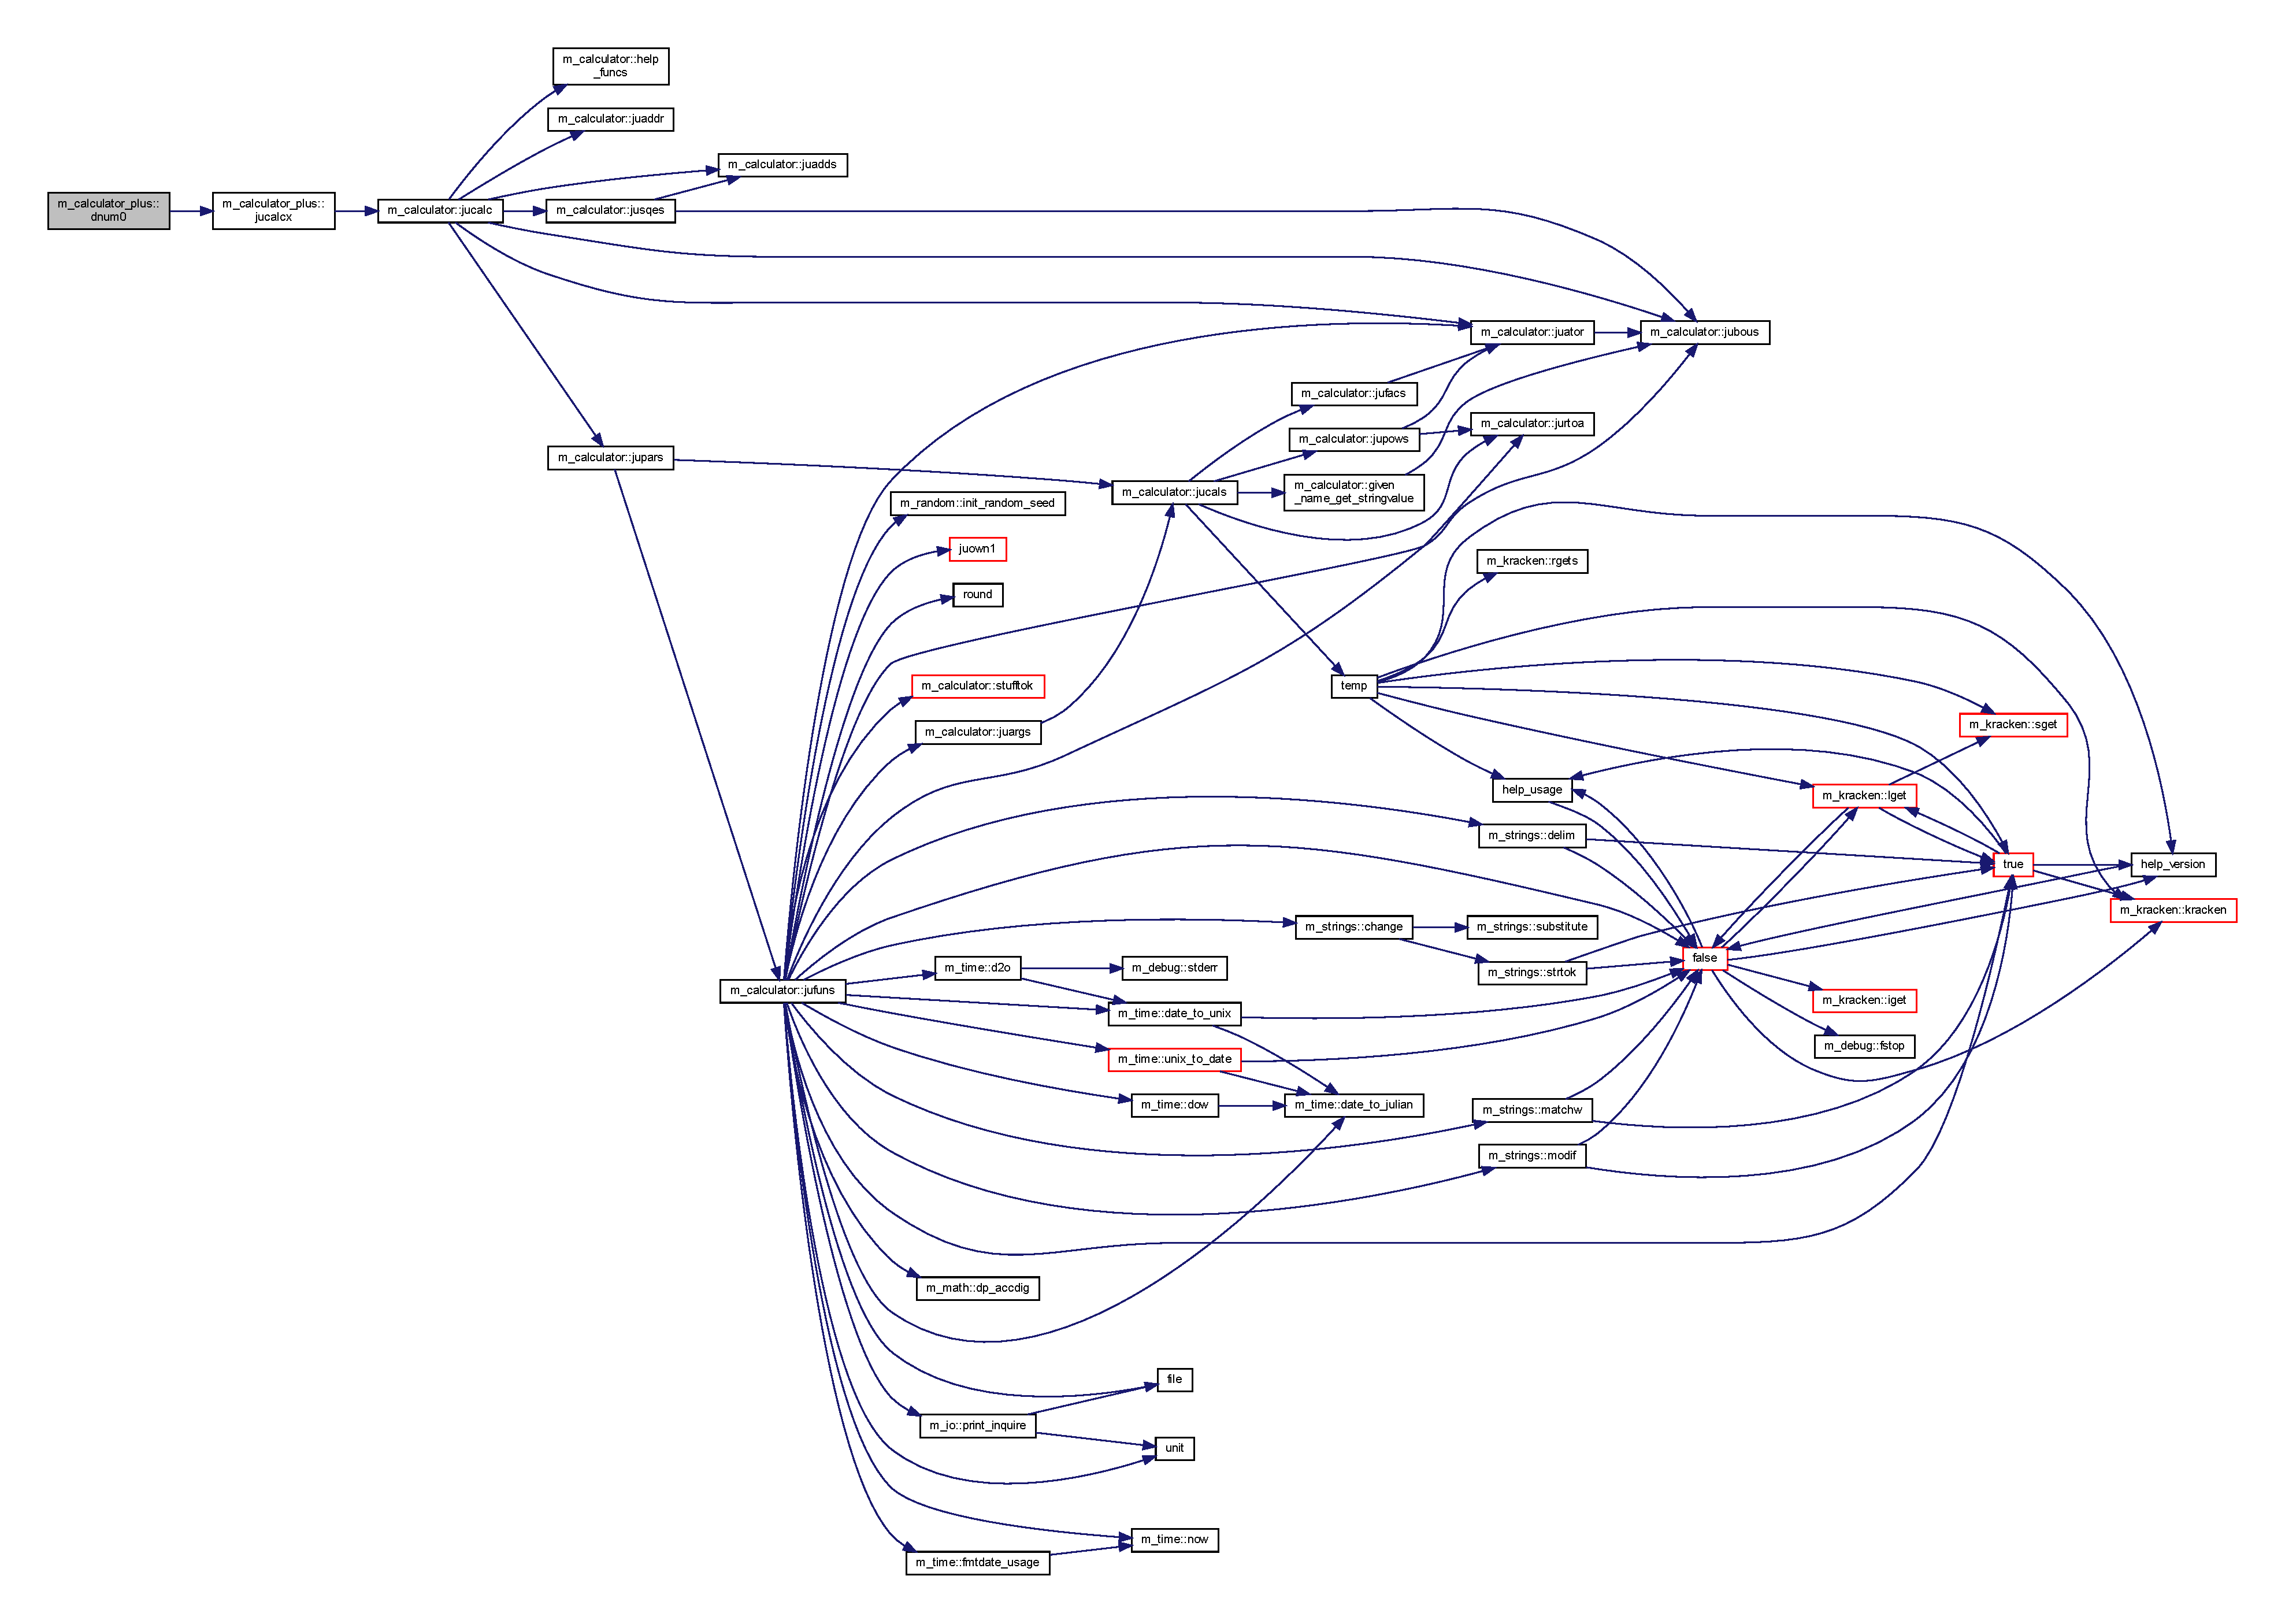
\includegraphics[width=350pt]{namespacem__calculator__plus_add45c0bb36bc796ee8a0354665f9397e_cgraph}
\end{center}
\end{figure}
Here is the caller graph for this function\+:
\nopagebreak
\begin{figure}[H]
\begin{center}
\leavevmode
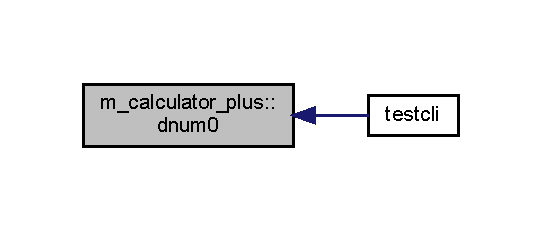
\includegraphics[width=260pt]{namespacem__calculator__plus_add45c0bb36bc796ee8a0354665f9397e_icgraph}
\end{center}
\end{figure}
\mbox{\Hypertarget{namespacem__calculator__plus_a3edbf94f311a3fad4a83fd8dfe26a61a}\label{namespacem__calculator__plus_a3edbf94f311a3fad4a83fd8dfe26a61a}} 
\index{m\+\_\+calculator\+\_\+plus@{m\+\_\+calculator\+\_\+plus}!inum0@{inum0}}
\index{inum0@{inum0}!m\+\_\+calculator\+\_\+plus@{m\+\_\+calculator\+\_\+plus}}
\subsubsection{\texorpdfstring{inum0()}{inum0()}}
{\footnotesize\ttfamily integer function, \hyperlink{M__stopwatch_83_8txt_a2f74811300c361e53b430611a7d1769f}{public} m\+\_\+calculator\+\_\+plus\+::inum0 (\begin{DoxyParamCaption}\item[{\hyperlink{option__stopwatch_83_8txt_abd4b21fbbd175834027b5224bfe97e66}{character}(len=$\ast$), intent(\hyperlink{M__journal_83_8txt_afce72651d1eed785a2132bee863b2f38}{in})}]{inline,  }\item[{integer, intent(out), \hyperlink{option__stopwatch_83_8txt_aa4ece75e7acf58a4843f70fe18c3ade5}{optional}}]{ierr }\end{DoxyParamCaption})}



\subsubsection*{N\+A\+ME}

inum0(3f) -\/ \mbox{[}M\+\_\+calculator\+\_\+plus\mbox{]} return integer value from calculator expression \subsubsection*{S\+Y\+N\+O\+P\+S\+IS}

integer function inum0(inline,ierr)

character(len=$\ast$),intent(in) \+:\+: inline integer,optional,intent(out) \+:\+: ierr

\subsubsection*{S\+Y\+N\+O\+P\+S\+IS}

\begin{DoxyVerb}INUM0() evaluates a CHARACTER argument as a FORTRAN-like
calculator expression and returns an integer.

 o INUM0() uses the calculator routine jucalc(3f)
 o Remember that the calculator treats all values as DOUBLEPRECISION.

Values returned are assumed to be very close to being whole integer
values.  A small value (0.01) is added to the result before it is
returned to reduce roundoff error problems. This could introduce
errors if INUM0 is misused and is not being used to calculate
essentially integer results.
\end{DoxyVerb}
 \subsubsection*{D\+E\+S\+C\+R\+I\+P\+T\+I\+ON}

\begin{DoxyVerb}inline  INLINE is a CHARACTER variable up to 255 characters long that is
        similar to a FORTRAN 77 numeric expression. Keep it less than 80
        characters when possible.
ierr    zero (0) if no error occurs
\end{DoxyVerb}


\subsubsection*{D\+E\+P\+E\+N\+D\+E\+N\+C\+I\+ES}

o jucalcx o User-\/supplied routines\+:

All programs that call the calculator routine must supply their own J\+U\+O\+W\+N1 and C procedures. See the ../html/\+Example.html"$>$example program for samples. o juown1 o c \subsubsection*{E\+X\+A\+M\+P\+L\+ES}

\begin{DoxyVerb}Sample program:

   program demo_inum0
   ! NOTE: user must supply the JUOWN1 and C procedures.
   i=inum0('20/3.4')
   j=inum0('CI = 13 * 3.1')
   k=inum0('CI')
   write(*,*)'Answers are ',I,J,K
   end program demo_inum0
\end{DoxyVerb}


\subsubsection*{S\+EE A\+L\+SO}

The syntax of an expression is as described in the main document of the Calculator Library. See J\+U\+C\+A\+L\+C(), R\+N\+U\+M0(), D\+N\+U\+M0(), S\+N\+U\+M0(), S\+T\+R\+G\+A\+R\+R(), S\+T\+R\+G\+A\+R2(), J\+U\+C\+A\+L\+C\+X() \subsubsection*{R\+E\+F\+E\+R\+E\+N\+C\+ES}

\subsubsection*{N\+O\+NE.}

A\+U\+T\+H\+OR\+: John S. Urban \subsubsection*{V\+E\+R\+S\+I\+ON\+: 19971123}

References jucalcx().

Here is the call graph for this function\+:
\nopagebreak
\begin{figure}[H]
\begin{center}
\leavevmode
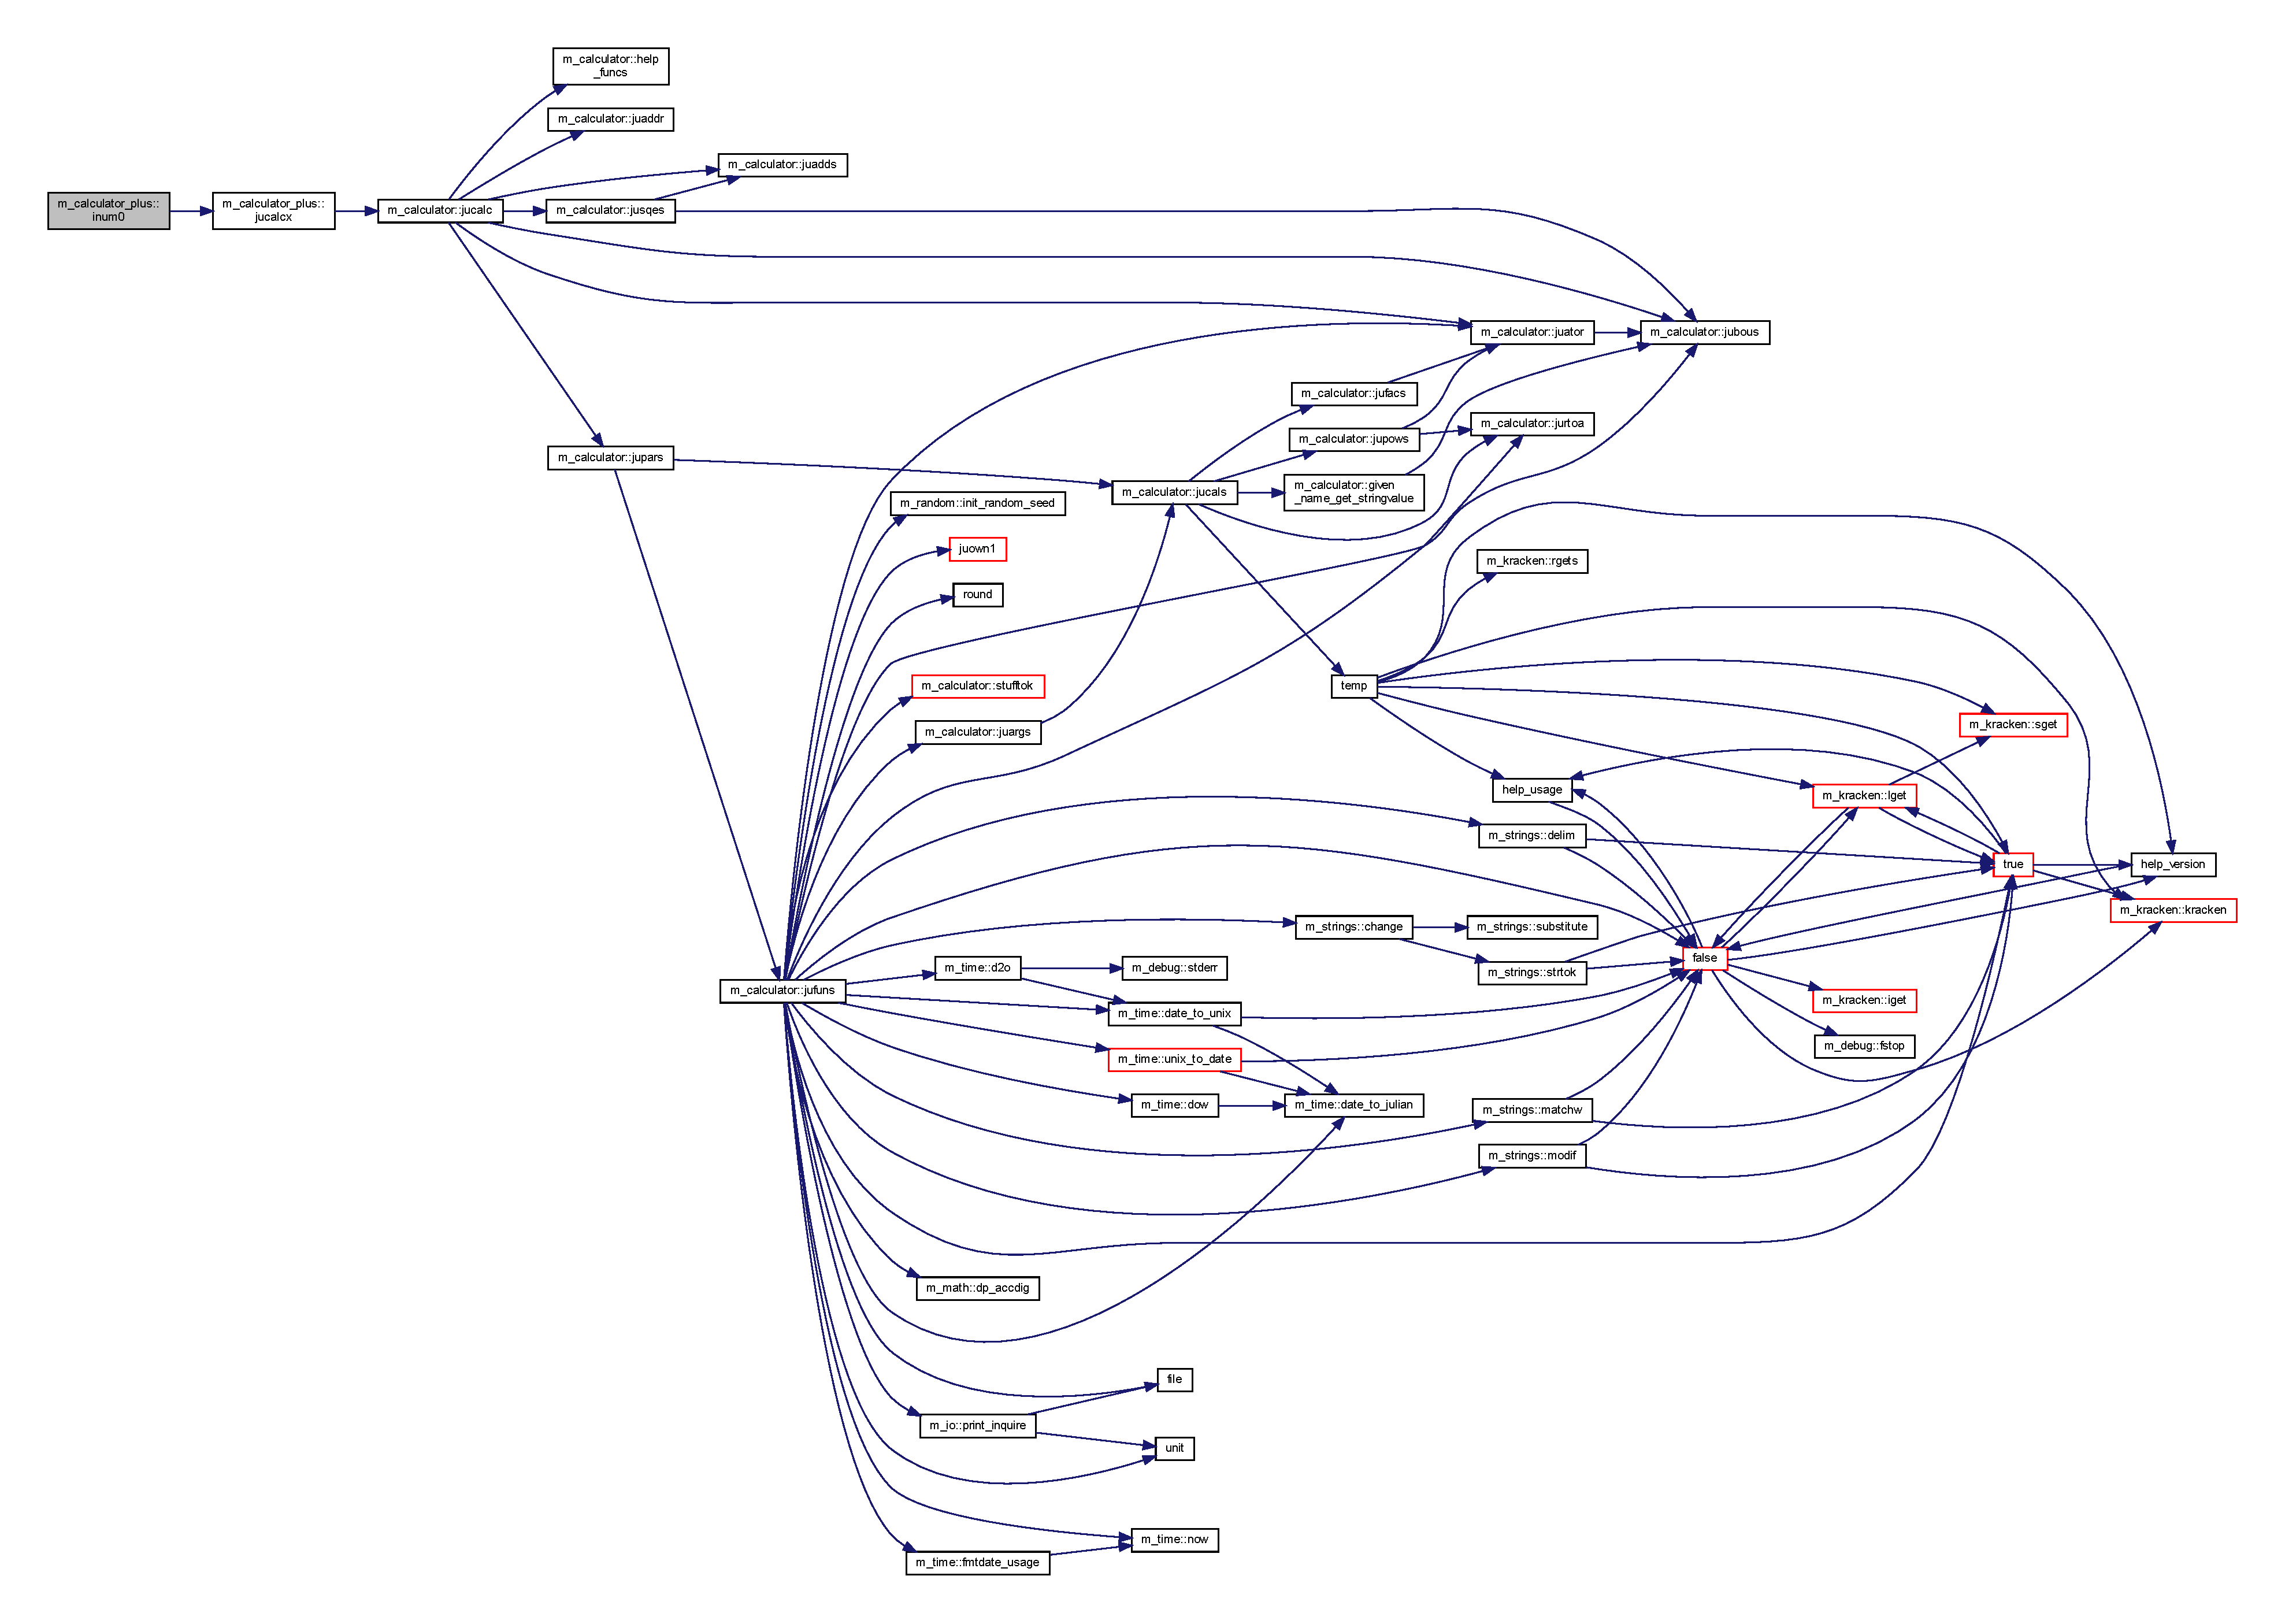
\includegraphics[width=350pt]{namespacem__calculator__plus_a3edbf94f311a3fad4a83fd8dfe26a61a_cgraph}
\end{center}
\end{figure}
Here is the caller graph for this function\+:
\nopagebreak
\begin{figure}[H]
\begin{center}
\leavevmode
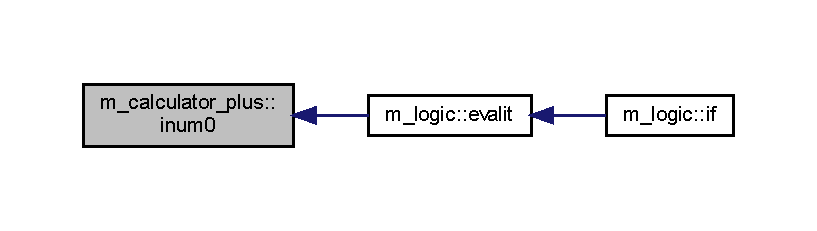
\includegraphics[width=350pt]{namespacem__calculator__plus_a3edbf94f311a3fad4a83fd8dfe26a61a_icgraph}
\end{center}
\end{figure}
\mbox{\Hypertarget{namespacem__calculator__plus_ac6f5a1bd3d8be798af932c006a72b123}\label{namespacem__calculator__plus_ac6f5a1bd3d8be798af932c006a72b123}} 
\index{m\+\_\+calculator\+\_\+plus@{m\+\_\+calculator\+\_\+plus}!jucalcx@{jucalcx}}
\index{jucalcx@{jucalcx}!m\+\_\+calculator\+\_\+plus@{m\+\_\+calculator\+\_\+plus}}
\subsubsection{\texorpdfstring{jucalcx()}{jucalcx()}}
{\footnotesize\ttfamily recursive \hyperlink{M__stopwatch_83_8txt_acfbcff50169d691ff02d4a123ed70482}{subroutine}, \hyperlink{M__stopwatch_83_8txt_a2f74811300c361e53b430611a7d1769f}{public} m\+\_\+calculator\+\_\+plus\+::jucalcx (\begin{DoxyParamCaption}\item[{\hyperlink{option__stopwatch_83_8txt_abd4b21fbbd175834027b5224bfe97e66}{character}(len=$\ast$), intent(\hyperlink{M__journal_83_8txt_afce72651d1eed785a2132bee863b2f38}{in})}]{inlin0,  }\item[{doubleprecision}]{outval,  }\item[{\hyperlink{option__stopwatch_83_8txt_abd4b21fbbd175834027b5224bfe97e66}{character}(len=$\ast$)}]{outlin0,  }\item[{integer, intent(out)}]{ierr,  }\item[{integer, intent(out)}]{ilen }\end{DoxyParamCaption})}



\subsubsection*{N\+A\+ME}

jucalcx(3f) -\/ \mbox{[}M\+\_\+calculator\+\_\+plus\mbox{]} return value from a string expression processing messages to simplify call to J\+U\+C\+A\+L\+C(3f) \subsubsection*{S\+Y\+N\+O\+P\+S\+IS}

subroutine jucalcx(inlin0,outval,outlin0,ierr,ilen)

character(len=$\ast$), intent=(in) \+:\+: inlin0 doubleprecision, intent=(out) \+:\+: outval character(len=$\ast$), intent=(out) \+:\+: outlin0 integer, intent=(out) \+:\+: ierr integer, intent=(out) \+:\+: ilen

\subsubsection*{D\+E\+S\+C\+R\+I\+P\+T\+I\+ON}

J\+U\+C\+A\+L\+C\+X() takes a string containing a F\+O\+R\+T\+R\+A\+N-\/like expression and evaluates it and returns a numeric or string value as appropriate. The main purpose of J\+U\+C\+A\+L\+C\+X() is to assume the burden of displaying the calculator messages for codes that make multiple calls to J\+U\+C\+A\+L\+C(). J\+U\+C\+A\+LC () does not display error messages directly. o J\+U\+C\+A\+L\+C\+X() calls the calculator routine jucalc.\+f to evaluate the expressions. o Messages beginning with a \# are considered comments and are not passed on to the calculator.

inlin0 I\+N\+L\+I\+N0 is a string containing a numeric expression. The expression can be up to (iclen\+\_\+calc=512) characters long. The syntax of an expression is as described in the main document of the Calc library. For example\+:

\textquotesingle{}A=sin(3.\+1416/5)\textquotesingle{} \textquotesingle{}\# this is a comment\textquotesingle{} \textquotesingle{}\$\+S\+TR(\char`\"{}\+The value is \char`\"{},40/3)\textquotesingle{}

outval O\+U\+T\+V\+AL is a numeric value calculated from the expression in I\+N\+L\+I\+N0 (when I\+E\+RR returns 0). When a string value is returned (I\+E\+RR=2) then O\+U\+T\+V\+AL is the length of the output string. outlin0 O\+U\+T\+L\+I\+N0 contains a string representation of the number returned in O\+U\+T\+V\+AL up to 20 characters long when I\+N\+L\+I\+N0 is a numeric expression. It contains a string up to (iclen\+\_\+calc=512) characters long when I\+N\+L\+I\+N0 is a string expression. ierr I\+E\+RR returns \begin{DoxyVerb}    o -1 if an error occurred
    o 0 if a numeric value is returned (value is in OUTVAL, string
      representation of the value is in OUTLIN2).
    o 1 if no value was returned but a message was displayed (If a 'dump'
      or 'funcs' command was passed to the calculator).
    o 2 if the expression evaluated to a string value instead of a
      numeric value (value is in OUTLIN0).
\end{DoxyVerb}
 ilen I\+L\+EN returns the length of the input string minus trailing blanks.

\subsubsection*{D\+E\+P\+E\+N\+D\+E\+N\+C\+I\+ES}

o jucalc o pdec o User-\/supplied routines\+:

All programs that call the calculator routine must supply their own J\+U\+O\+W\+N1 and C procedures. See the example program for samples. o juown1 o c \subsubsection*{E\+X\+A\+M\+P\+L\+ES}

\begin{DoxyVerb}Sample program:

 program TEST_JUCALCX
 !     NOTE: user must supply the JUOWN1 and C procedures.
 use m_calculator, only: iclen_calc
 character(len=iclen_calc) ::  outlin0
 doubleprecision :: outval
 call jucalcx('A=3.4**5    ',outval,outlin0,ierr,ilen)
 write(*,*)'value of expression is ',outval
 write(*,*)'string representation of value is ',outlin0
 write(*,*)'error flag value is ',ierr
 write(*,*)'length of expression is ',ilen
 end program TEST_JUCALCX
\end{DoxyVerb}


\subsubsection*{S\+EE A\+L\+SO}

See also\+: S\+T\+R\+G\+A\+R(),R\+N\+U\+M0(),J\+U\+C\+A\+L\+C(),I\+N\+U\+M0(),S\+N\+U\+M0() \subsubsection*{R\+E\+F\+E\+R\+E\+N\+C\+ES}

N\+O\+NE. A\+U\+T\+H\+OR John S. Urban \subsubsection*{V\+E\+R\+S\+I\+ON V1.\+0, 19971123}

References m\+\_\+calculator\+::jucalc().

Here is the call graph for this function\+:
\nopagebreak
\begin{figure}[H]
\begin{center}
\leavevmode
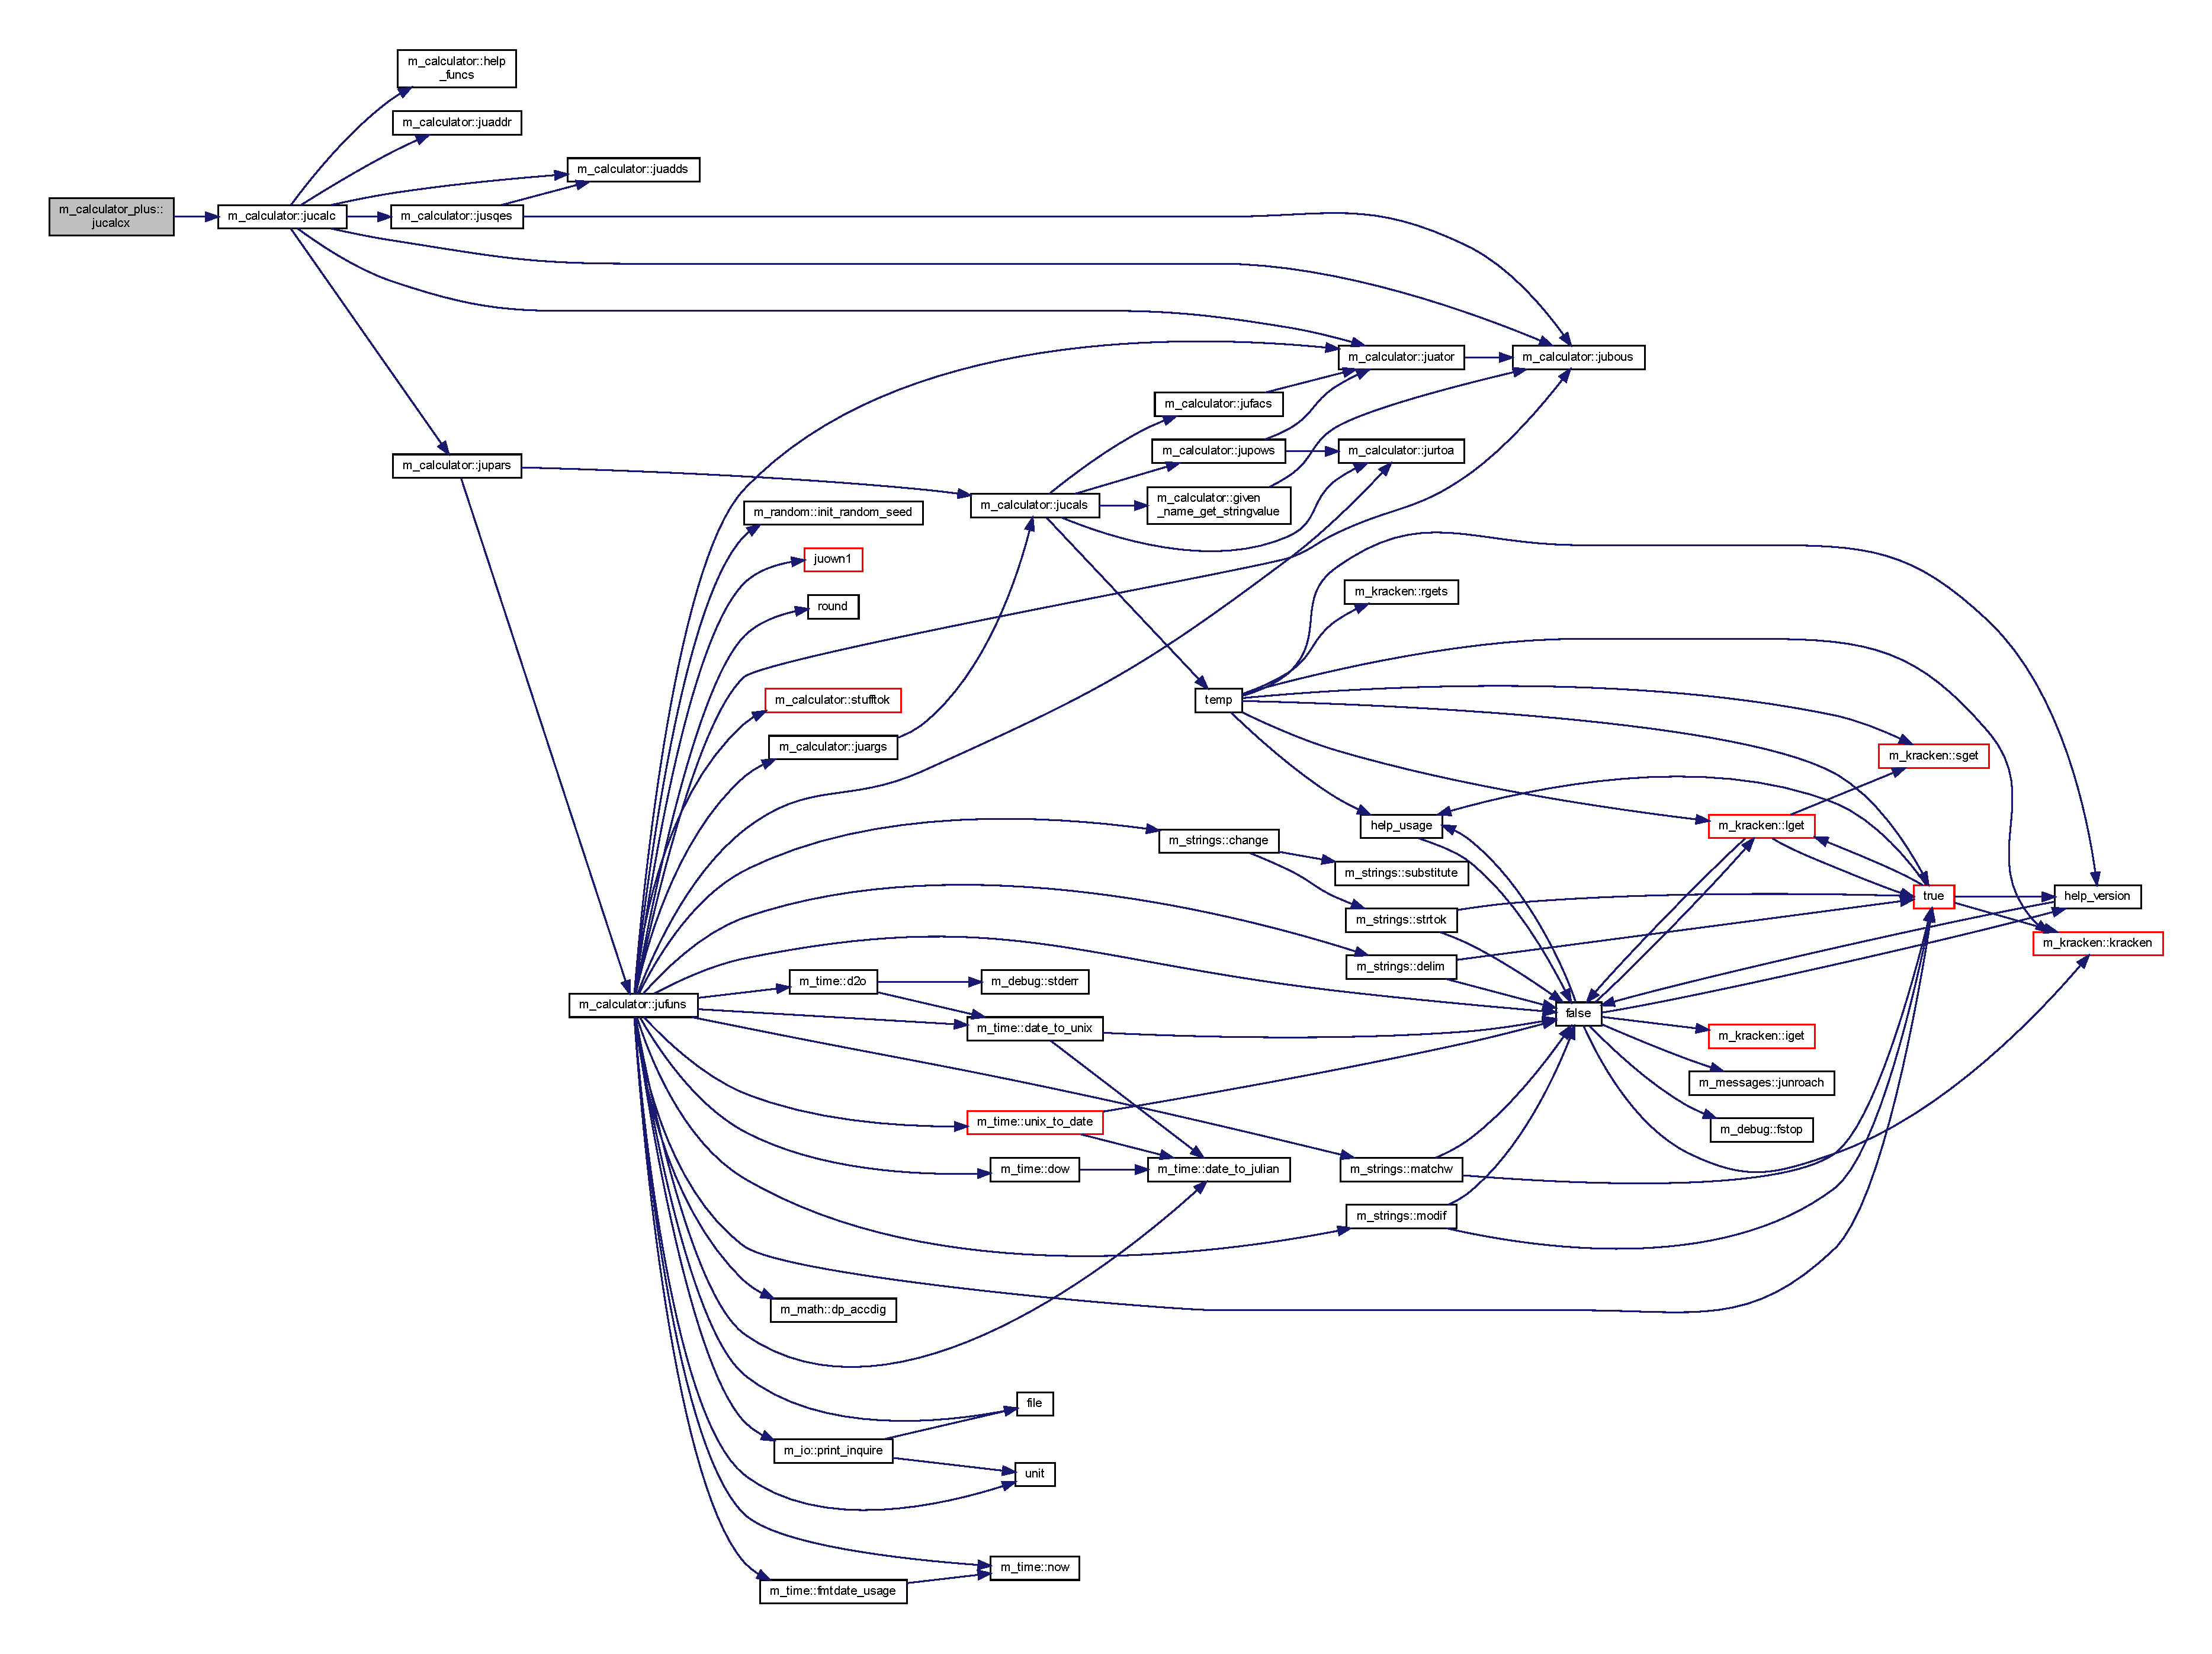
\includegraphics[width=350pt]{namespacem__calculator__plus_ac6f5a1bd3d8be798af932c006a72b123_cgraph}
\end{center}
\end{figure}
Here is the caller graph for this function\+:
\nopagebreak
\begin{figure}[H]
\begin{center}
\leavevmode
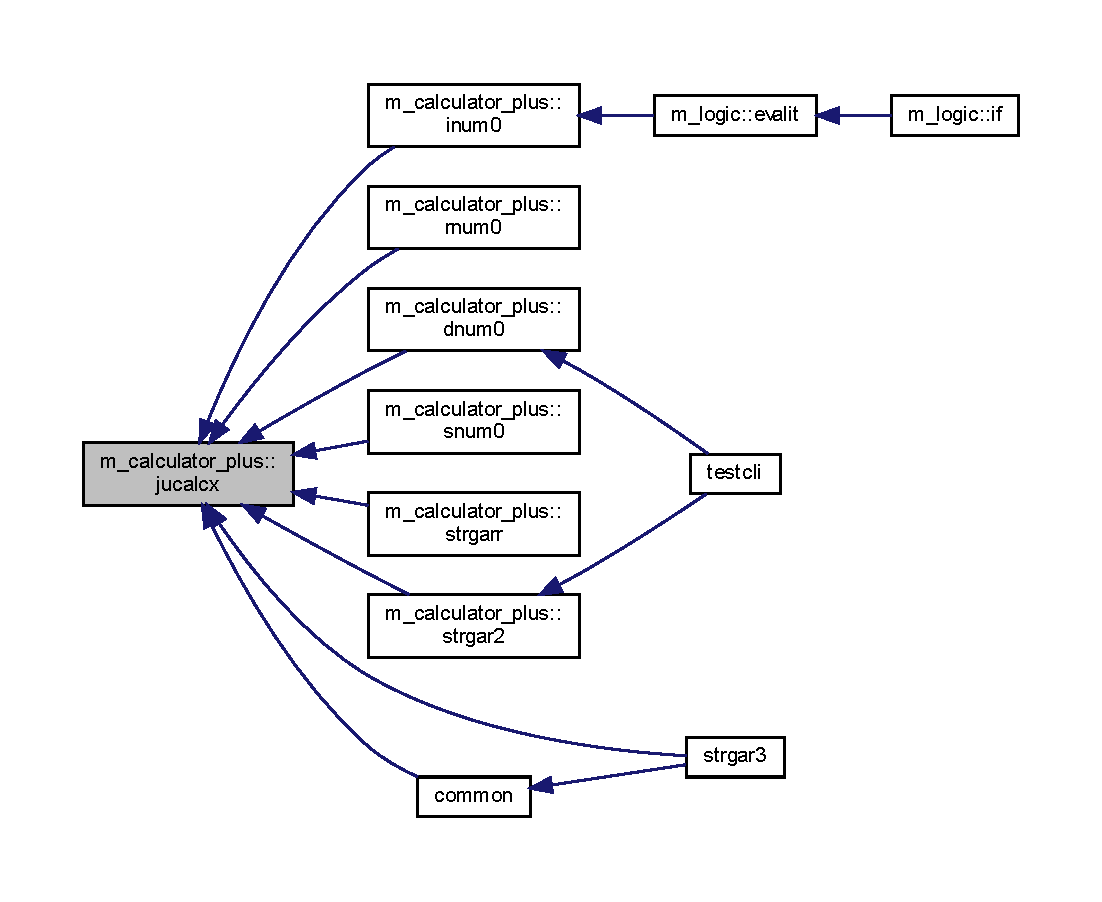
\includegraphics[width=350pt]{namespacem__calculator__plus_ac6f5a1bd3d8be798af932c006a72b123_icgraph}
\end{center}
\end{figure}
\mbox{\Hypertarget{namespacem__calculator__plus_a448c42e7171e27c1f4a8e339687b0e3f}\label{namespacem__calculator__plus_a448c42e7171e27c1f4a8e339687b0e3f}} 
\index{m\+\_\+calculator\+\_\+plus@{m\+\_\+calculator\+\_\+plus}!rnum0@{rnum0}}
\index{rnum0@{rnum0}!m\+\_\+calculator\+\_\+plus@{m\+\_\+calculator\+\_\+plus}}
\subsubsection{\texorpdfstring{rnum0()}{rnum0()}}
{\footnotesize\ttfamily \hyperlink{read__watch_83_8txt_abdb62bde002f38ef75f810d3a905a823}{real} function, \hyperlink{M__stopwatch_83_8txt_a2f74811300c361e53b430611a7d1769f}{public} m\+\_\+calculator\+\_\+plus\+::rnum0 (\begin{DoxyParamCaption}\item[{\hyperlink{option__stopwatch_83_8txt_abd4b21fbbd175834027b5224bfe97e66}{character}(len=$\ast$), intent(\hyperlink{M__journal_83_8txt_afce72651d1eed785a2132bee863b2f38}{in})}]{inline,  }\item[{integer, intent(out), \hyperlink{option__stopwatch_83_8txt_aa4ece75e7acf58a4843f70fe18c3ade5}{optional}}]{ierr }\end{DoxyParamCaption})}



\subsubsection*{N\+A\+ME}

rnum0(3f) -\/ \mbox{[}M\+\_\+calculator\+\_\+plus\mbox{]} returns real number from string expression using J\+U\+C\+A\+L\+C(3f) \subsubsection*{S\+Y\+N\+O\+P\+S\+IS}

real function rnum0(inline) character(len=$\ast$), intent=(in) \+:\+: inline integer,intent(out),optional \+:\+: ierr

\subsubsection*{D\+E\+S\+C\+R\+I\+P\+T\+I\+ON}

R\+N\+U\+M0() is used to return a R\+E\+AL value from a C\+H\+A\+R\+A\+C\+T\+ER string representing a numeric expression. It uses the M\+\_\+calculator(3fp) module.

inline I\+N\+L\+I\+NE is a C\+H\+A\+R\+A\+C\+T\+ER variable up to (iclen\+\_\+calc=512) characters long that is similar to a F\+O\+R\+T\+R\+AN 77 numeric expression. ierr error code. If zero, no error occurred

\subsubsection*{D\+E\+P\+E\+N\+D\+E\+N\+C\+I\+ES}

o jucalcx o User-\/supplied routines\+: All programs that call the calculator routine must supply their own J\+U\+O\+W\+N1 and C procedures. See the example program for samples. o juown1 o c \subsubsection*{E\+X\+A\+M\+P\+L\+ES}

Sample program

program demo\+\_\+rnum0 ! N\+O\+TE\+: user must supply the J\+U\+O\+W\+N1 and C procedures. x=rnum0(\textquotesingle{}20/3.\+4\textquotesingle{}) y=rnum0(\textquotesingle{}CI = 10 $\ast$ sin(3.\+1416/4)\textquotesingle{}) z=rnum0(\textquotesingle{}CI\textquotesingle{}) write($\ast$,$\ast$)x,y,z end program demo\+\_\+rnum0

\subsubsection*{S\+EE A\+L\+SO}

\begin{DoxyVerb}   o The syntax of an expression is as described in the main documentation
     of the Calculator Library.
   o See JUCALCX(3f), JUCALC(3f), STRGAR2(3f), INUM0(3f), DNUM0(3f), SNUM0(3f).
\end{DoxyVerb}


\subsubsection*{R\+E\+F\+E\+R\+E\+N\+C\+ES}

o N\+O\+NE. A\+U\+T\+H\+OR John S. Urban \subsubsection*{V\+E\+R\+S\+I\+ON 1.\+0,19971123}

References jucalcx().

Here is the call graph for this function\+:
\nopagebreak
\begin{figure}[H]
\begin{center}
\leavevmode
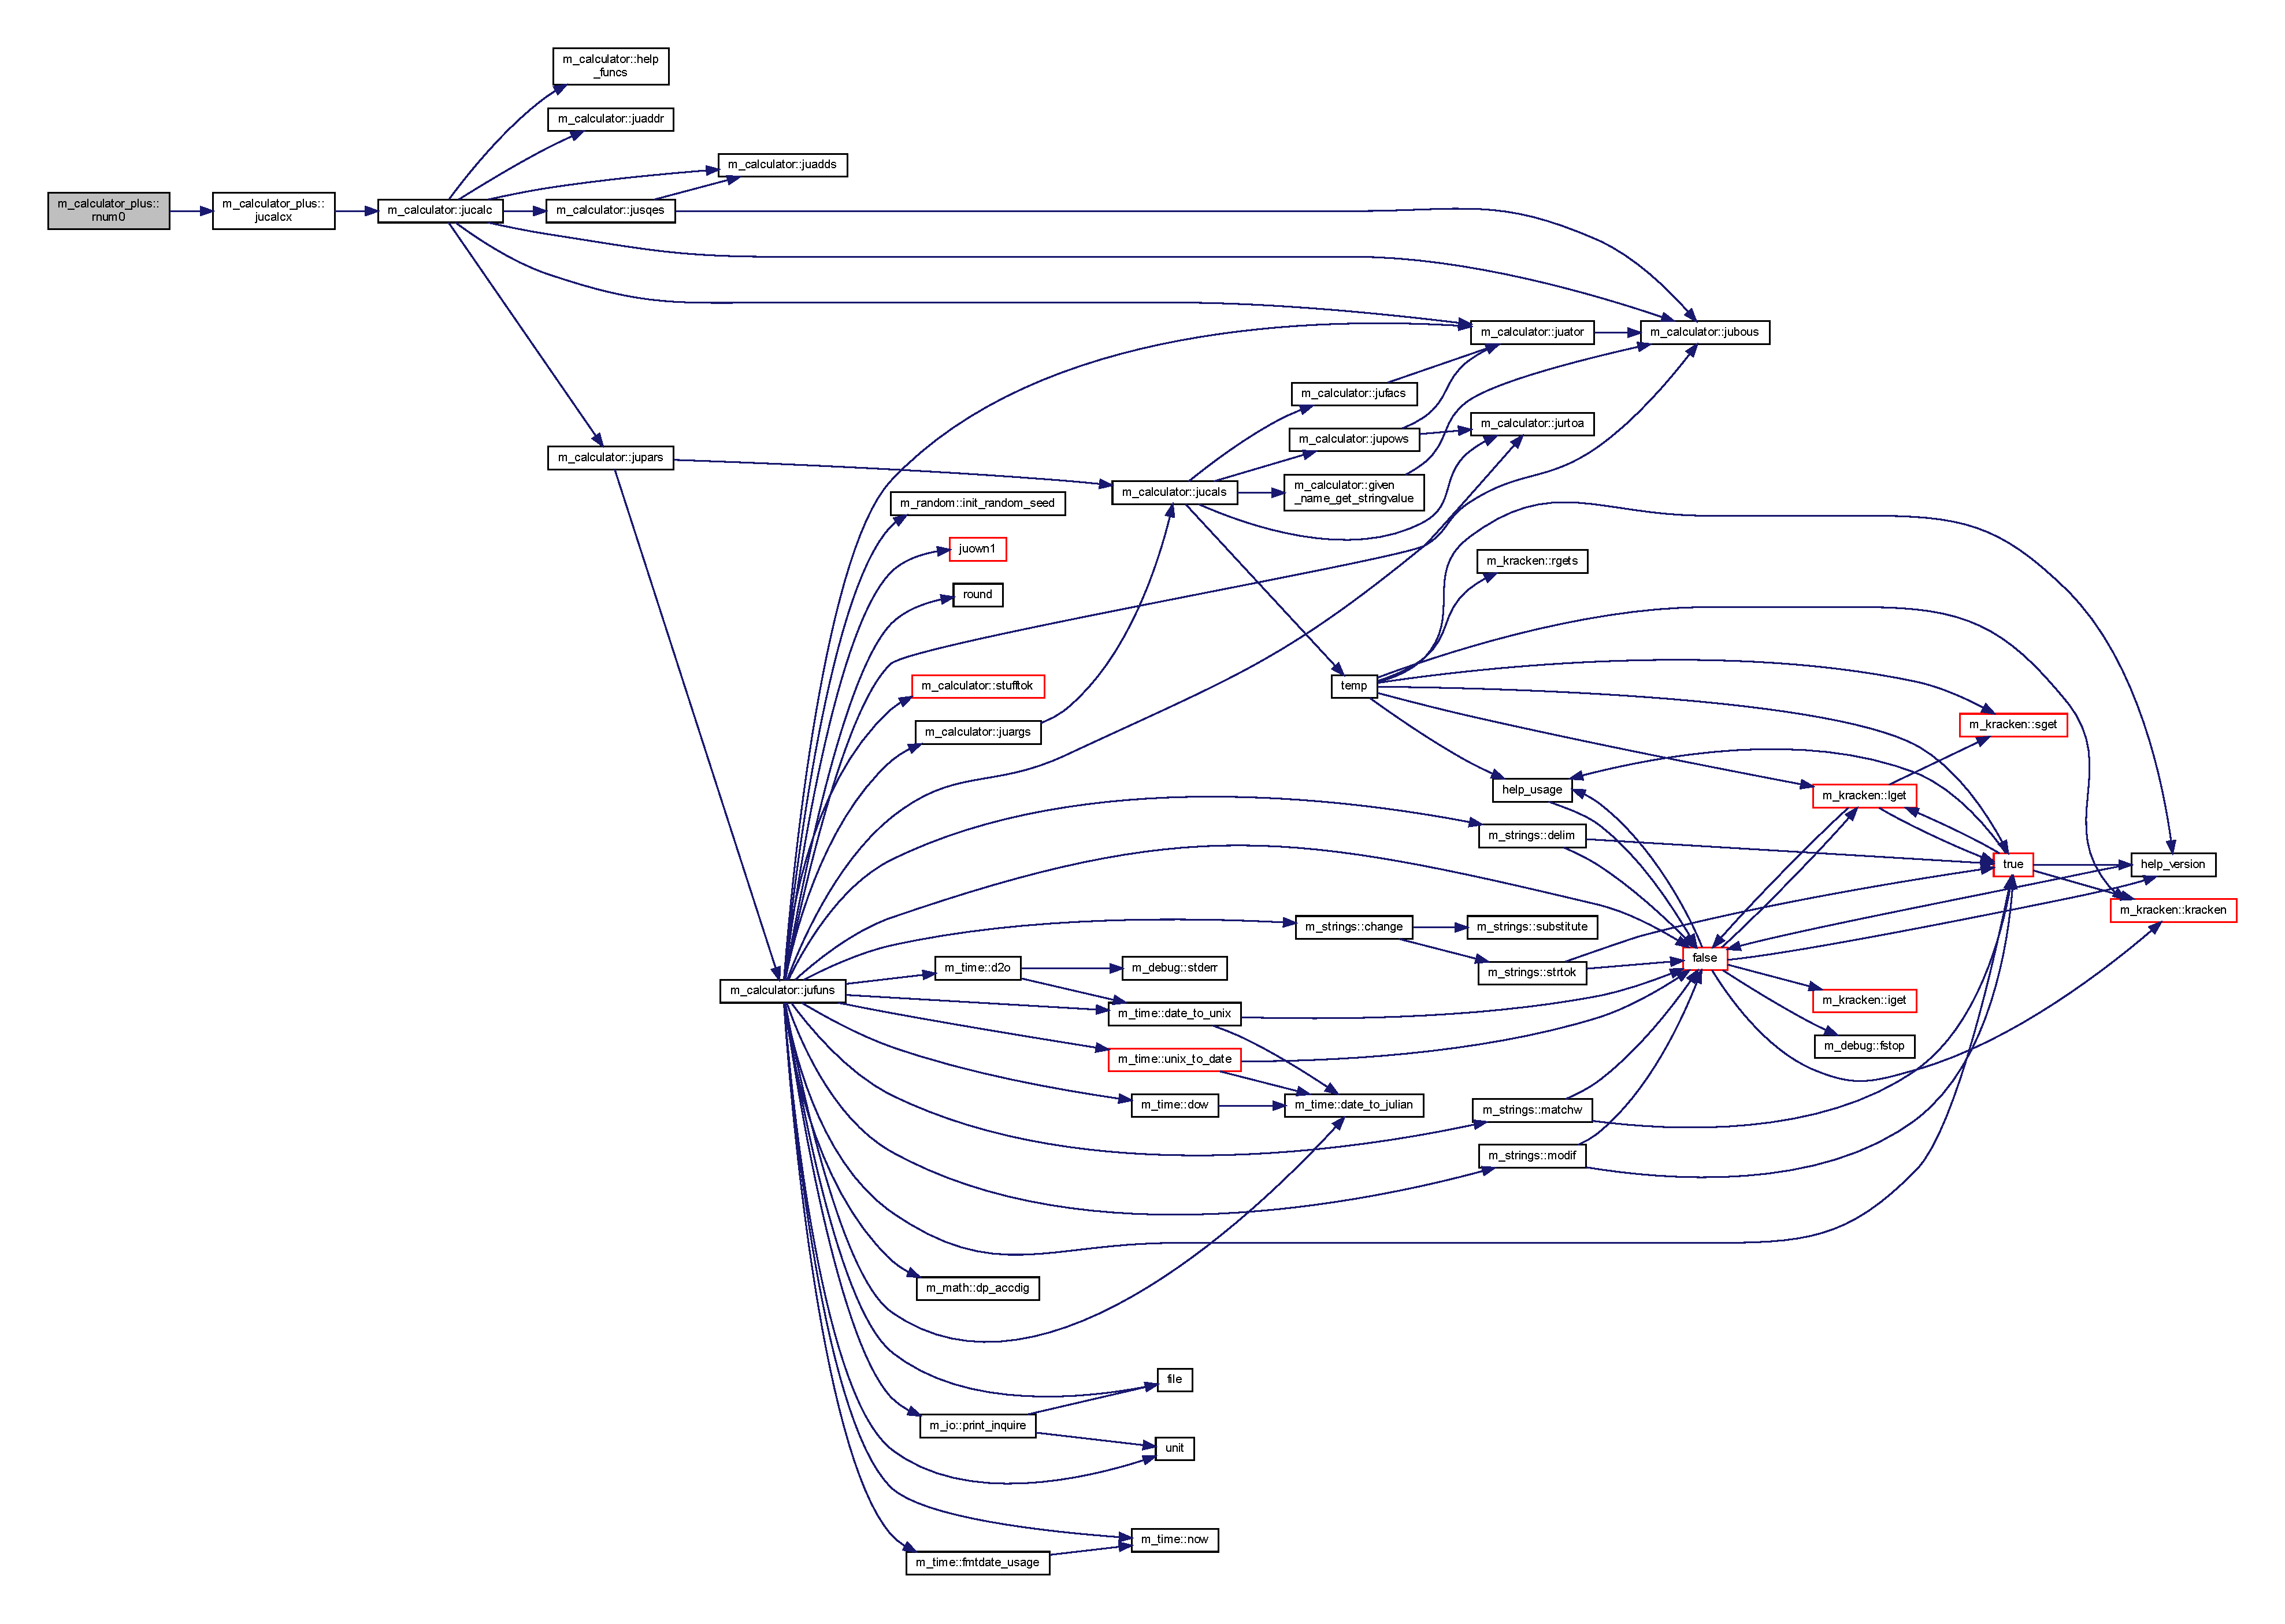
\includegraphics[width=350pt]{namespacem__calculator__plus_a448c42e7171e27c1f4a8e339687b0e3f_cgraph}
\end{center}
\end{figure}
\mbox{\Hypertarget{namespacem__calculator__plus_a2538e7f9f0b810f7f8dbdd80fa2444b3}\label{namespacem__calculator__plus_a2538e7f9f0b810f7f8dbdd80fa2444b3}} 
\index{m\+\_\+calculator\+\_\+plus@{m\+\_\+calculator\+\_\+plus}!snum0@{snum0}}
\index{snum0@{snum0}!m\+\_\+calculator\+\_\+plus@{m\+\_\+calculator\+\_\+plus}}
\subsubsection{\texorpdfstring{snum0()}{snum0()}}
{\footnotesize\ttfamily \hyperlink{option__stopwatch_83_8txt_abd4b21fbbd175834027b5224bfe97e66}{character}(len=\+:) function, allocatable, \hyperlink{M__stopwatch_83_8txt_a2f74811300c361e53b430611a7d1769f}{public} m\+\_\+calculator\+\_\+plus\+::snum0 (\begin{DoxyParamCaption}\item[{\hyperlink{option__stopwatch_83_8txt_abd4b21fbbd175834027b5224bfe97e66}{character}(len=$\ast$), intent(\hyperlink{M__journal_83_8txt_afce72651d1eed785a2132bee863b2f38}{in})}]{inline0,  }\item[{integer, intent(out), \hyperlink{option__stopwatch_83_8txt_aa4ece75e7acf58a4843f70fe18c3ade5}{optional}}]{ierr }\end{DoxyParamCaption})}



\subsubsection*{N\+A\+ME}

snum0(3f) -\/ \mbox{[}M\+\_\+calculator\+\_\+plus\mbox{]} resolve a calculator expression into a string(return blank on errors) 

\subsubsection*{S\+Y\+N\+O\+P\+S\+IS}

function snum0(inline0,ierr)

character(len=\+:),allocatable \+:\+: snum0(inline0) character(len=$\ast$),intent(in) \+:\+: inline0 ! input string integer,optional,intent(out) \+:\+: ierr

\subsubsection*{D\+E\+S\+C\+R\+I\+P\+T\+I\+ON}

S\+N\+U\+M0() is used to return a string value up to (iclen\+\_\+calc=512) characters long from a string expression. S\+N\+U\+M0() uses the calculator routine jucalc.\+f .

inline0 I\+N\+L\+I\+N\+E0 is a C\+H\+A\+R\+A\+C\+T\+ER variable up to (iclen\+\_\+calc=512) characters long that is similar to a F\+O\+R\+T\+R\+AN 77 expression. ierr error code. If zero, no error occurred

\subsubsection*{E\+X\+A\+M\+P\+L\+ES}

Sample program\+:

! N\+O\+TE\+: user must supply the J\+U\+O\+W\+N1 and C procedures. program D\+E\+M\+O\+\_\+\+S\+N\+U\+M0 use \hyperlink{namespacem__calculator__plus}{m\+\_\+calculator\+\_\+plus}, only\+: iclen\+\_\+calc, rnum0, snum0 C\+H\+A\+R\+A\+C\+T\+ER(len=80) \+:\+: IC,JC,KC

R\+D\+UM=R\+N\+U\+M0(\textquotesingle{}A=83/2\textquotesingle{}) ! set a variable in the calculator KC=S\+N\+U\+M0(\textquotesingle{}\$\+M\+Y\+T\+I\+T\+LE=\char`\"{}\+This is my title variable\char`\"{}\textquotesingle{})

IC=S\+N\+U\+M0(\textquotesingle{}\$\+S\+TR(\char`\"{}\+V\+A\+L\+U\+E I\+S \mbox{[}\char`\"{},A,\char`\"{}\mbox{]}\char`\"{})\textquotesingle{}) JC=S\+N\+U\+M0(\textquotesingle{}\$\+M\+Y\+T\+I\+T\+LE\textquotesingle{})

W\+R\+I\+T\+E($\ast$,$\ast$)\textquotesingle{}IC=\textquotesingle{},T\+R\+I\+M(\+I\+C) W\+R\+I\+T\+E($\ast$,$\ast$)\textquotesingle{}JC=\textquotesingle{},T\+R\+I\+M(\+J\+C) W\+R\+I\+T\+E($\ast$,$\ast$)\textquotesingle{}KC=\textquotesingle{},T\+R\+I\+M(\+K\+C)

end program D\+E\+M\+O\+\_\+\+S\+N\+U\+M0 \$endif

The output should look like

IC=V\+A\+L\+UE IS \mbox{[}41.\+5\mbox{]} JC=This is my title variable KC=This is my title variable

\subsubsection*{D\+E\+P\+E\+N\+D\+E\+N\+C\+I\+ES}

o jucalcx o User-\/supplied routines\+: All programs that call the calculator routine must supply their own J\+U\+O\+W\+N1 and C procedures. See the example program for samples. o juown1 o c

\subsubsection*{S\+EE A\+L\+SO}

o The syntax of an expression is described in the main document of the Calculator Library. o See J\+U\+C\+A\+L\+C(), R\+N\+U\+M0(), S\+N\+U\+M0(), S\+T\+R\+G\+A\+R2(), J\+U\+C\+A\+L\+C\+X().

\subsubsection*{R\+E\+F\+E\+R\+E\+N\+C\+ES}

o N\+O\+NE. A\+U\+T\+H\+OR John S. Urban \subsubsection*{V\+E\+R\+S\+I\+ON 1.\+0, 19971123}

References m\+\_\+calculator\+::iclen\+\_\+calc, and jucalcx().

Here is the call graph for this function\+:
\nopagebreak
\begin{figure}[H]
\begin{center}
\leavevmode
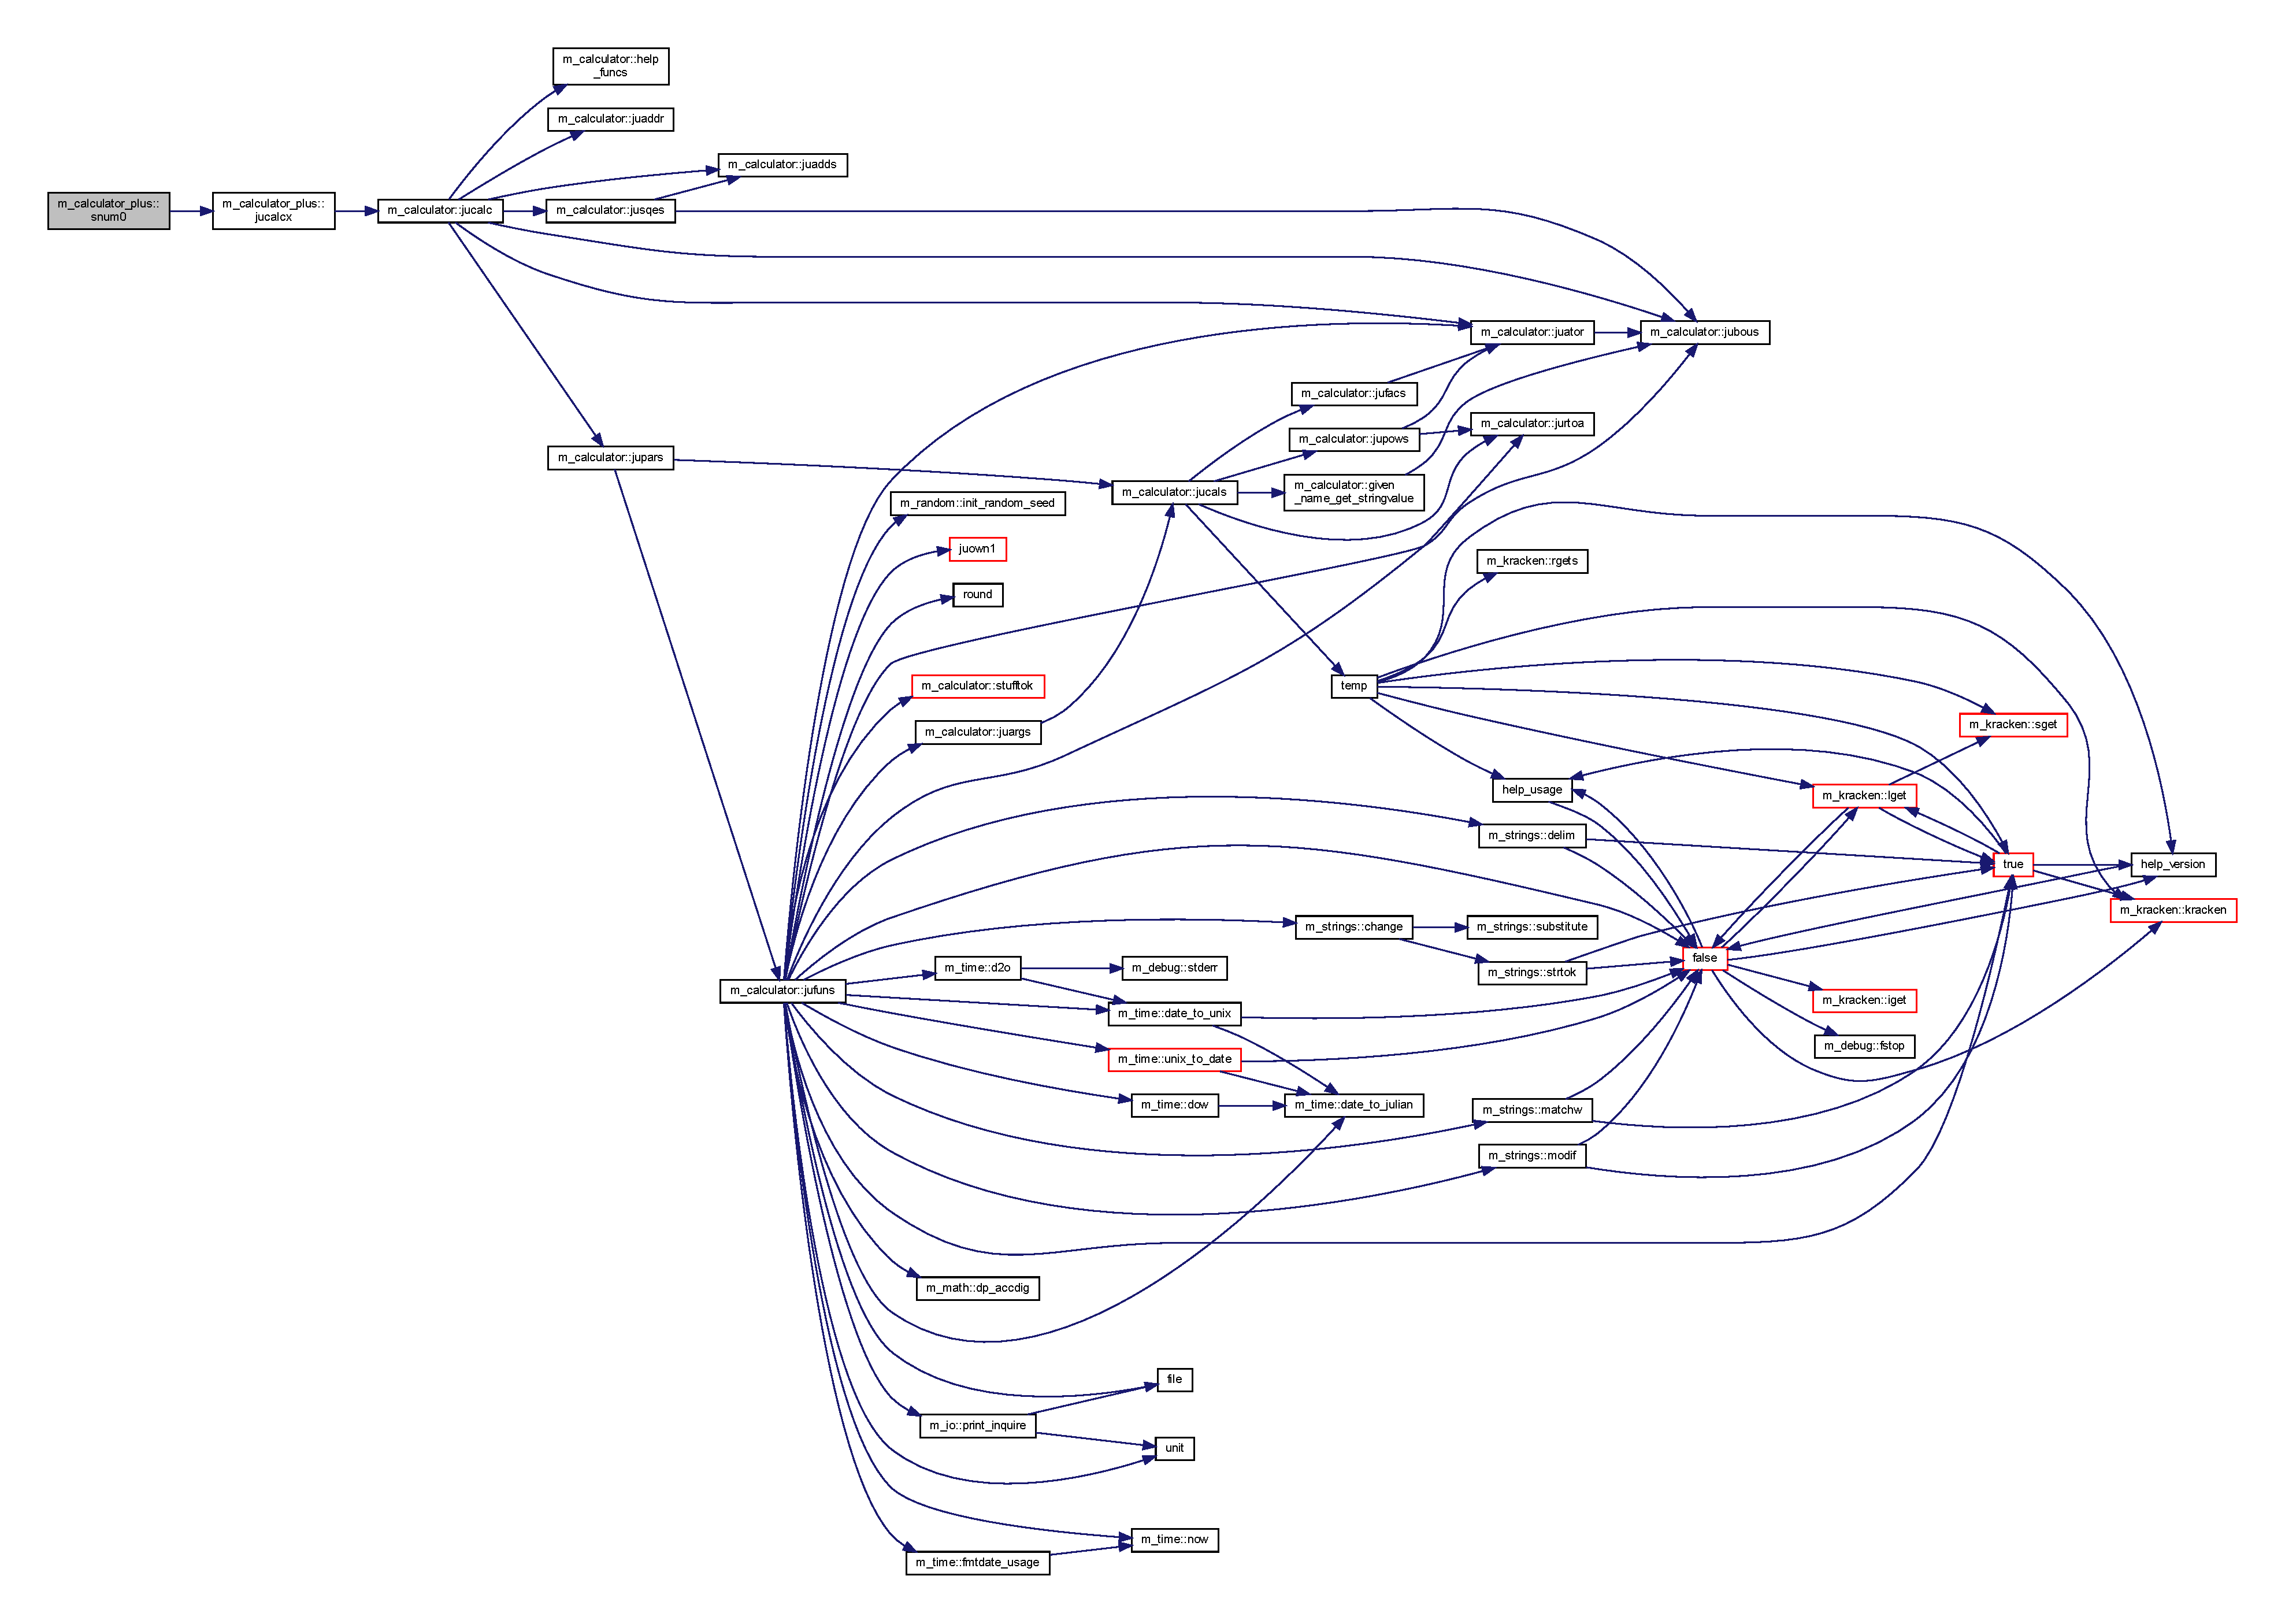
\includegraphics[width=350pt]{namespacem__calculator__plus_a2538e7f9f0b810f7f8dbdd80fa2444b3_cgraph}
\end{center}
\end{figure}
\mbox{\Hypertarget{namespacem__calculator__plus_a59710eb6babeed1f4b8d439f97d5d90a}\label{namespacem__calculator__plus_a59710eb6babeed1f4b8d439f97d5d90a}} 
\index{m\+\_\+calculator\+\_\+plus@{m\+\_\+calculator\+\_\+plus}!strgar2@{strgar2}}
\index{strgar2@{strgar2}!m\+\_\+calculator\+\_\+plus@{m\+\_\+calculator\+\_\+plus}}
\subsubsection{\texorpdfstring{strgar2()}{strgar2()}}
{\footnotesize\ttfamily \hyperlink{M__stopwatch_83_8txt_acfbcff50169d691ff02d4a123ed70482}{subroutine}, \hyperlink{M__stopwatch_83_8txt_a2f74811300c361e53b430611a7d1769f}{public} m\+\_\+calculator\+\_\+plus\+::strgar2 (\begin{DoxyParamCaption}\item[{\hyperlink{option__stopwatch_83_8txt_abd4b21fbbd175834027b5224bfe97e66}{character}(len=$\ast$), intent(\hyperlink{M__journal_83_8txt_afce72651d1eed785a2132bee863b2f38}{in})}]{line,  }\item[{integer, intent(\hyperlink{M__journal_83_8txt_afce72651d1eed785a2132bee863b2f38}{in})}]{iread,  }\item[{\hyperlink{read__watch_83_8txt_abdb62bde002f38ef75f810d3a905a823}{real}, dimension(iread), intent(out)}]{numbrs,  }\item[{integer, intent(out)}]{inums,  }\item[{\hyperlink{option__stopwatch_83_8txt_abd4b21fbbd175834027b5224bfe97e66}{character}(len=$\ast$), intent(\hyperlink{M__journal_83_8txt_afce72651d1eed785a2132bee863b2f38}{in})}]{delims0,  }\item[{integer, intent(out)}]{ierr }\end{DoxyParamCaption})}



\subsubsection*{N\+A\+ME}

strgar2(3f) -\/ \mbox{[}M\+\_\+calculator\+\_\+plus\mbox{]} read a string into a real array U\+S\+I\+NG C\+A\+L\+C\+U\+L\+A\+T\+OR, allowing quoted strings in arguments, 

\subsubsection*{S\+Y\+N\+O\+P\+S\+IS}

subroutine strgar2(line,ivals,vals,ifound,delims,ierr)

character(len=$\ast$), intent=(in) \+:\+: line integer, intent=(in) \+:\+: ivals real, intent=(out) \+:\+: vals(ivals) integer, intent=(out) \+:\+: ifound character(len=$\ast$), intent=(in) \+:\+: delims integer, intent=(out) \+:\+: ierr

\subsubsection*{D\+E\+S\+C\+R\+I\+P\+T\+I\+ON}

S\+T\+R\+G\+A\+R2() returns an array of real values from a string containing numeric and string expressions. o S\+T\+R\+G\+A\+R2() parses the string at the specified delimiters and calls the calculator routine jucalc.\+f to evaluate the expressions. o It counts the number of values found. o Once the maximum allowable number of values have been found S\+T\+R\+G\+A\+R2() returns, ignoring the rest of the line. o If an error occurs the error flag returns the column number where the expression that failed begins. o If the string is \textquotesingle{}$\ast$\textquotesingle{}, the value -\/99999.\+0 is returned.

line L\+I\+NE is a string of numeric expressions. Each expression can be up to (iclen\+\_\+calc=512) characters long. The syntax of an expression is as described in the main document of the Calculator Library. (Assuming the delimiters include a space character) an example would be\+: \begin{DoxyVerb} 'A=10 100 300E2/42.6  sin(3.1416/5)'
\end{DoxyVerb}
 \begin{DoxyVerb} ivals        IVALS is the maximum number of values to return.
 vals(ivals)  VALS is an array filled with the numeric values calculated from the
              expressions in LINE.
 ifound       IFOUND is the number of values successfully returned in VALS
 delims       DELIMS is a character(s) to use as an expression delimiter. It is
              commonly set to a space (' '). If more than one character is specified,
              the space must not be last.
 ierr         IERR returns 0 if no error occurred. If an error did occur, it returns
              the column number the expression started at that could not be
              evaluated.
\end{DoxyVerb}


\subsubsection*{D\+E\+P\+E\+N\+D\+E\+N\+C\+I\+ES}

o jucalcx o User-\/supplied routines\+: All programs that call the calculator routine must supply their own J\+U\+O\+W\+N1 and C procedures. See the example program for samples. o juown1 o c \subsubsection*{E\+X\+A\+M\+P\+L\+ES}

Sample program\+:

program T\+\_\+\+S\+T\+R\+G\+A\+R2 use M\+\_\+calculator\+\_\+plus, only \+: strgar2 integer \+:\+: ios integer \+:\+: i integer \+:\+: ifound integer \+:\+: ierr real \+:\+: vals(1000) character(len=4096) \+:\+: line ! N\+O\+TE\+: user must supply the J\+U\+O\+W\+N1 and C procedures.

write($\ast$,\textquotesingle{}(80(\char`\"{}-\/\char`\"{}))\textquotesingle{}) call strgar2(\textquotesingle{}10;2/3;sin(4.\+314)\textquotesingle{},4,vals,ifound,\textquotesingle{} ;\textquotesingle{},ierr) write($\ast$,$\ast$)\textquotesingle{}should find three values in 10;2/3;sin(4.\+314)\textquotesingle{} write($\ast$,$\ast$)\textquotesingle{}ifound=\textquotesingle{},ifound write($\ast$,$\ast$)\textquotesingle{}values are\textquotesingle{},(vals(i),i=1,ifound)

write($\ast$,\textquotesingle{}(80(\char`\"{}-\/\char`\"{}))\textquotesingle{}) write($\ast$,$\ast$)\textquotesingle{}should find three values in 10;2/3;sin(4.\+314)\textquotesingle{} write($\ast$,$\ast$)\textquotesingle{}ifound=\textquotesingle{},ifound call strgar2(\textquotesingle{}10;2/3;sin(4.\+314) \textquotesingle{},3,vals,ifound,\textquotesingle{} ;\textquotesingle{},ierr) write($\ast$,$\ast$)\textquotesingle{}ifound=\textquotesingle{},ifound write($\ast$,$\ast$)\textquotesingle{}values are\textquotesingle{},(vals(i),i=1,ifound)

write($\ast$,\textquotesingle{}(80(\char`\"{}-\/\char`\"{}))\textquotesingle{}) write($\ast$,$\ast$)\textquotesingle{}should stop at two values in 10;2/3;sin(4.\+314)\textquotesingle{} call strgar2(\textquotesingle{}10;2/3;sin(4.\+314)\textquotesingle{},2,vals,ifound,\textquotesingle{} ;\textquotesingle{},ierr) write($\ast$,$\ast$)\textquotesingle{}ifound=\textquotesingle{},ifound write($\ast$,$\ast$)\textquotesingle{}values are\textquotesingle{},(vals(i),i=1,ifound)

write($\ast$,\textquotesingle{}(80(\char`\"{}-\/\char`\"{}))\textquotesingle{}) write($\ast$,$\ast$)\textquotesingle{}should stop at one values in 10;2/3;sin(4.\+314)\textquotesingle{} call strgar2(\textquotesingle{}10;2/3;sin(4.\+314)\textquotesingle{},1,vals,ifound,\textquotesingle{} ;\textquotesingle{},ierr) write($\ast$,$\ast$)\textquotesingle{}ifound=\textquotesingle{},ifound write($\ast$,$\ast$)\textquotesingle{}values are\textquotesingle{},(vals(i),i=1,ifound)

write($\ast$,\textquotesingle{}(80(\char`\"{}-\/\char`\"{}))\textquotesingle{}) write($\ast$,$\ast$)\textquotesingle{}should find three values in 10;2/3;sin(4.\+314) ; ; ; ;; \textquotesingle{} call strgar2(\textquotesingle{}10;2/3;sin(4.\+314) ; ; ; ;; \textquotesingle{},1000,vals,ifound,\textquotesingle{} ;\textquotesingle{},ierr) write($\ast$,$\ast$)\textquotesingle{}ifound=\textquotesingle{},ifound write($\ast$,$\ast$)\textquotesingle{}values are\textquotesingle{},(vals(i),i=1,ifound)

write($\ast$,\textquotesingle{}(80(\char`\"{}-\/\char`\"{}))\textquotesingle{}) write($\ast$,$\ast$)\textquotesingle{}should find an error in values in 10;20/3O;sin(4.\+314) ; ; ; ;; \textquotesingle{} call strgar2(\textquotesingle{}10;20/3O;sin(4.\+314) ; ; ; ;; \textquotesingle{},1000,vals,ifound,\textquotesingle{} ;\textquotesingle{},ierr) write($\ast$,$\ast$)\textquotesingle{}ifound=\textquotesingle{},ifound,\textquotesingle{} error=\textquotesingle{},ierr write($\ast$,$\ast$)\textquotesingle{}values are\textquotesingle{},(vals(i),i=1,ifound)

write($\ast$,\textquotesingle{}(80(\char`\"{}-\/\char`\"{}))\textquotesingle{}) write($\ast$,$\ast$)\textquotesingle{}Enter strings delimited by spaces or semicolons\textquotesingle{} do read($\ast$,\textquotesingle{}(a)\textquotesingle{},iostat=ios)line if(ios.\+ne.\+0)then stop endif call strgar2(line,1000,vals,ifound,\textquotesingle{} ;\textquotesingle{},ierr) write($\ast$,$\ast$)\textquotesingle{}ifound=\textquotesingle{},ifound write($\ast$,$\ast$)\textquotesingle{}values are\textquotesingle{},(vals(i),i=1,ifound) enddo end program T\+\_\+\+S\+T\+R\+G\+A\+R2

\subsubsection*{S\+EE A\+L\+SO}

\begin{DoxyVerb} To parse a list of numbers instead of expressions see STRGAR().
 If there is only one expression see RNUM0(), JUCALCX(), JUCALC().
\end{DoxyVerb}


\subsubsection*{R\+E\+F\+E\+R\+E\+N\+C\+ES}

N\+O\+NE. A\+U\+T\+H\+OR John S. Urban \subsubsection*{V\+E\+R\+S\+I\+ON 1.\+0 19971123}

References false(), m\+\_\+calculator\+::iclen\+\_\+calc, jucalcx(), and true().

Here is the call graph for this function\+:
\nopagebreak
\begin{figure}[H]
\begin{center}
\leavevmode
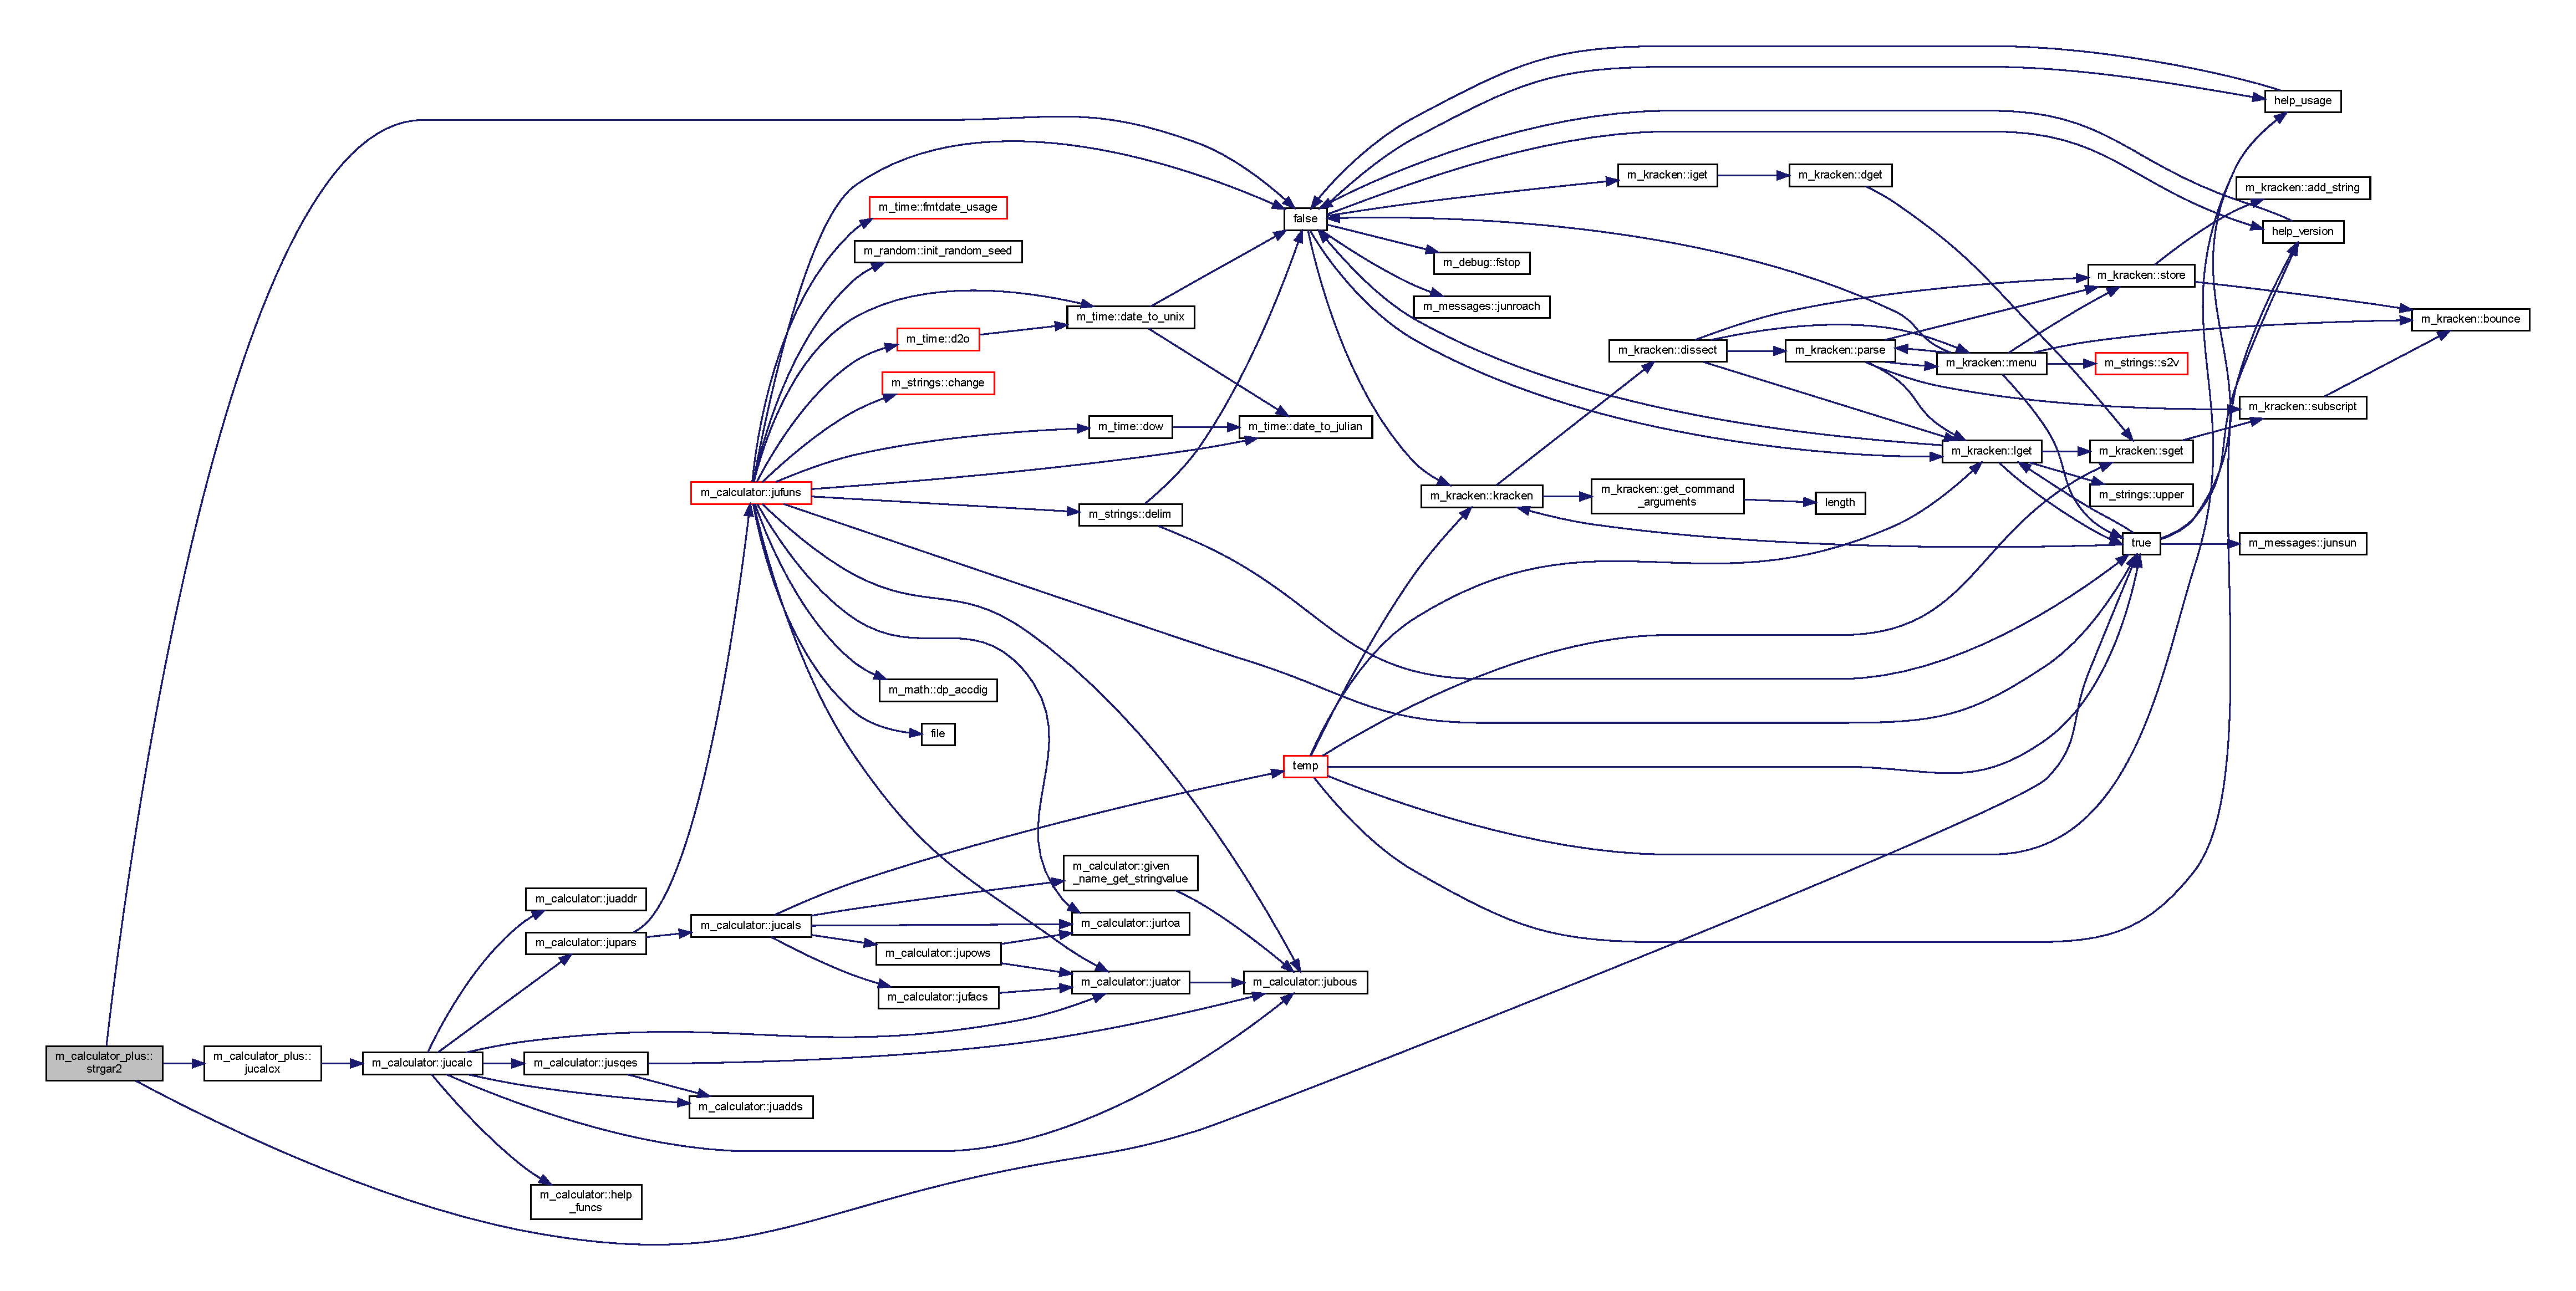
\includegraphics[width=350pt]{namespacem__calculator__plus_a59710eb6babeed1f4b8d439f97d5d90a_cgraph}
\end{center}
\end{figure}
Here is the caller graph for this function\+:
\nopagebreak
\begin{figure}[H]
\begin{center}
\leavevmode
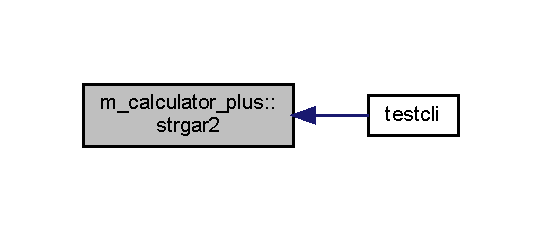
\includegraphics[width=260pt]{namespacem__calculator__plus_a59710eb6babeed1f4b8d439f97d5d90a_icgraph}
\end{center}
\end{figure}
\mbox{\Hypertarget{namespacem__calculator__plus_a4d3424e0cb74d4af53e7f59c07d31f1b}\label{namespacem__calculator__plus_a4d3424e0cb74d4af53e7f59c07d31f1b}} 
\index{m\+\_\+calculator\+\_\+plus@{m\+\_\+calculator\+\_\+plus}!strgarr@{strgarr}}
\index{strgarr@{strgarr}!m\+\_\+calculator\+\_\+plus@{m\+\_\+calculator\+\_\+plus}}
\subsubsection{\texorpdfstring{strgarr()}{strgarr()}}
{\footnotesize\ttfamily \hyperlink{M__stopwatch_83_8txt_acfbcff50169d691ff02d4a123ed70482}{subroutine}, \hyperlink{M__stopwatch_83_8txt_a2f74811300c361e53b430611a7d1769f}{public} m\+\_\+calculator\+\_\+plus\+::strgarr (\begin{DoxyParamCaption}\item[{\hyperlink{option__stopwatch_83_8txt_abd4b21fbbd175834027b5224bfe97e66}{character}(len=$\ast$), intent(\hyperlink{M__journal_83_8txt_afce72651d1eed785a2132bee863b2f38}{in})}]{line,  }\item[{integer, intent(\hyperlink{M__journal_83_8txt_afce72651d1eed785a2132bee863b2f38}{in})}]{ivals,  }\item[{\hyperlink{read__watch_83_8txt_abdb62bde002f38ef75f810d3a905a823}{real}, dimension(ivals)}]{vals,  }\item[{integer, intent(out)}]{ifound,  }\item[{\hyperlink{option__stopwatch_83_8txt_abd4b21fbbd175834027b5224bfe97e66}{character}(len=$\ast$), intent(\hyperlink{M__journal_83_8txt_afce72651d1eed785a2132bee863b2f38}{in})}]{delims0,  }\item[{integer, intent(out)}]{ierr }\end{DoxyParamCaption})}



\subsubsection*{N\+A\+ME}

strgarr(3f) -\/ \mbox{[}M\+\_\+calculator\+\_\+plus\mbox{]} read a string into an array using jucalc(3f) calculator \subsubsection*{S\+Y\+N\+O\+P\+S\+IS}

subroutine strgarr(line,ivals,vals,ifound,delims,ierr)

character(len=$\ast$), intent=(in) \+:\+: line integer, intent=(in) \+:\+: ivals real, intent=(out) \+:\+: vals(ivals) integer, intent=(out) \+:\+: ifound character(len=$\ast$), intent=(in) \+:\+: delims integer, intent=(out) \+:\+: ierr

\subsubsection*{D\+E\+S\+C\+R\+I\+P\+T\+I\+ON}

\hyperlink{namespacem__calculator__plus_a4d3424e0cb74d4af53e7f59c07d31f1b}{strgarr()} returns an array of real values from a string containing numeric expressions. Use \hyperlink{namespacem__calculator__plus_a59710eb6babeed1f4b8d439f97d5d90a}{strgar2()} if you are going to permit string expressions with " delimiters.

o \hyperlink{namespacem__calculator__plus_a4d3424e0cb74d4af53e7f59c07d31f1b}{strgarr()} parses the string at the specified delimiters and calls the calculator routine J\+U\+C\+A\+L\+C\+X(3f) to evaluate the expressions. o It counts the number of values found. o Once the maximum allowable number of values have been found \hyperlink{namespacem__calculator__plus_a4d3424e0cb74d4af53e7f59c07d31f1b}{strgarr()} returns, ignoring the rest of the line. o If an error occurs the error flag returns the column number where the expression that failed begins.

line L\+I\+NE is a string of numeric expressions. Each expression can be up to (iclen\+\_\+calc=255) characters long. The syntax of an expression is as described in the main document of the Calculator Library. Assuming the delimiters include a space character an example would be\+:

\textquotesingle{}A=10 100 300\+E2/42.\+6 sin(3.\+1416/5)\textquotesingle{}

Only numeric expressions are expected; so no use of the delimiter characters is allowed except as a delimiter, even in quoted strings. ivals I\+V\+A\+LS is the maximum number of values to return. vals(ivals) V\+A\+LS is an array filled with the numeric values calculated from the expressions in L\+I\+NE. ifound I\+F\+O\+U\+ND is the number of values successfully returned in V\+A\+LS delims D\+E\+L\+I\+MS is a character to use as an expression delimiter. It is commonly set to a space and semi-\/colon(\textquotesingle{} ;\textquotesingle{}). ierr I\+E\+RR returns 0 if no error occurred. If an error did occur, it returns the column number the expression started at that could not be evaluated.

\subsubsection*{D\+E\+P\+E\+N\+D\+E\+N\+C\+I\+ES}

o jucalcx o User-\/supplied routines\+: All programs that call the calculator routine must supply their own J\+U\+O\+W\+N1 and C procedures. See the example program for samples. o juown1 o c \subsubsection*{E\+X\+A\+M\+P\+L\+ES}

\begin{DoxyVerb}Sample program:

   program T_strgarr
   use M_kracken, only: sget, kracken, lget
   use M_calculator_plus, only : strgarr
   real vals(41)
   character(len=80) :: line=' '
   character(len=10) :: delims=' ;'
   !  define command arguments, default values and crack command line
   call kracken('cmd','-d " ;" -test .false. -help .false. -begin -end')
   !----------------------------------------------------------
   write(*,*)'SGET',trim(sget('cmd_test'))
   write(*,*)'LGET',lget('cmd_test')
   if(lget('cmd_test'))then   ! cursory test
      call strgarr("10;2/3;sin(4.314)",41,vals,ifound,' ;',ierr)
      write(*,*)'values are',(vals(i),i=1,ifound)
      sumtarget= 9.74497986
      tol=       0.00000001
      sumup=sum(vals(:ifound))
      ipass=0
      if(ifound.ne.3) ipass=ipass+1
      if(ierr.ne.0)   ipass=ipass+2
      if( sumup >= (sumtarget-tol) .and. sumup <= (sumtarget+tol) ) then
      else
         ipass=ipass+4
      endif
      if(ipass.eq.0)then
         write(*,*)'sum is ',sumup
         write(*,*)'number of values is',ifound
         write(*,*)'error flag is',ierr
         write(*,*)'STRGARR*: PASSED'
         stop(0)
      else
         write(*,*)'IFOUND:',ifound
         write(*,*)'IERR  :',ierr
         write(*,*)'SUM   :',sumup
         write(*,*)'STRGARR*: FAILED',ipass
         stop(-1)
      endif
   endif
   !----------------------------------------------------------
   delims=sget('cmd_d')
   write(*,*)'DELIMS=[',trim(delims),']'
   !----------------------------------------------------------
   line=sget('cmd_begin')
   write(*,*)'BEGIN:',trim(line)
   if(line.ne.' ')then
      call strgarr(line,41,vals,ifound,delims,ierr)
   endif
   !----------------------------------------------------------
   line=sget('cmd_oo')
   write(*,*)'LINE:',trim(line)
   if(line.ne.' ')then
      call strgarr(line,41,vals,ifound,delims,ierr)
      write(*,*)(VALS(I),I=1,IFOUND)
   else
      INFINITE: do
         read(*,'(a)',iostat=ios)line
         if(ios.ne.0)then
            exit INFINITE
         endif
         call strgarr(line,41,vals,ifound,delims,ierr)
         write(*,*)IERR,IFOUND,':',(VALS(I),I=1,IFOUND)
      enddo INFINITE
   endif
   !----------------------------------------------------------
   line=sget('cmd_end')
   write(*,*)'END',trim(line)
   if(line.ne.' ')then
      call strgarr(line,41,vals,ifound,delims,ierr)
      write(*,*)'END:',(VALS(I),I=1,IFOUND)
   endif
   !----------------------------------------------------------
   end

   ! NOTE: user must supply the JUOWN1 and C procedures.
\end{DoxyVerb}


\subsubsection*{S\+EE A\+L\+SO}

To parse a list of numbers instead of expressions see S\+T\+R\+G\+A\+R(). If there is only one expression see R\+N\+U\+M0(), J\+U\+C\+A\+L\+C\+X(), J\+U\+C\+A\+L\+C().

\subsubsection*{R\+E\+F\+E\+R\+E\+N\+C\+ES}

none. A\+U\+T\+H\+OR John S. Urban \subsubsection*{V\+E\+R\+S\+I\+ON 1.\+0, 19971123}

References jucalcx().

Here is the call graph for this function\+:
\nopagebreak
\begin{figure}[H]
\begin{center}
\leavevmode
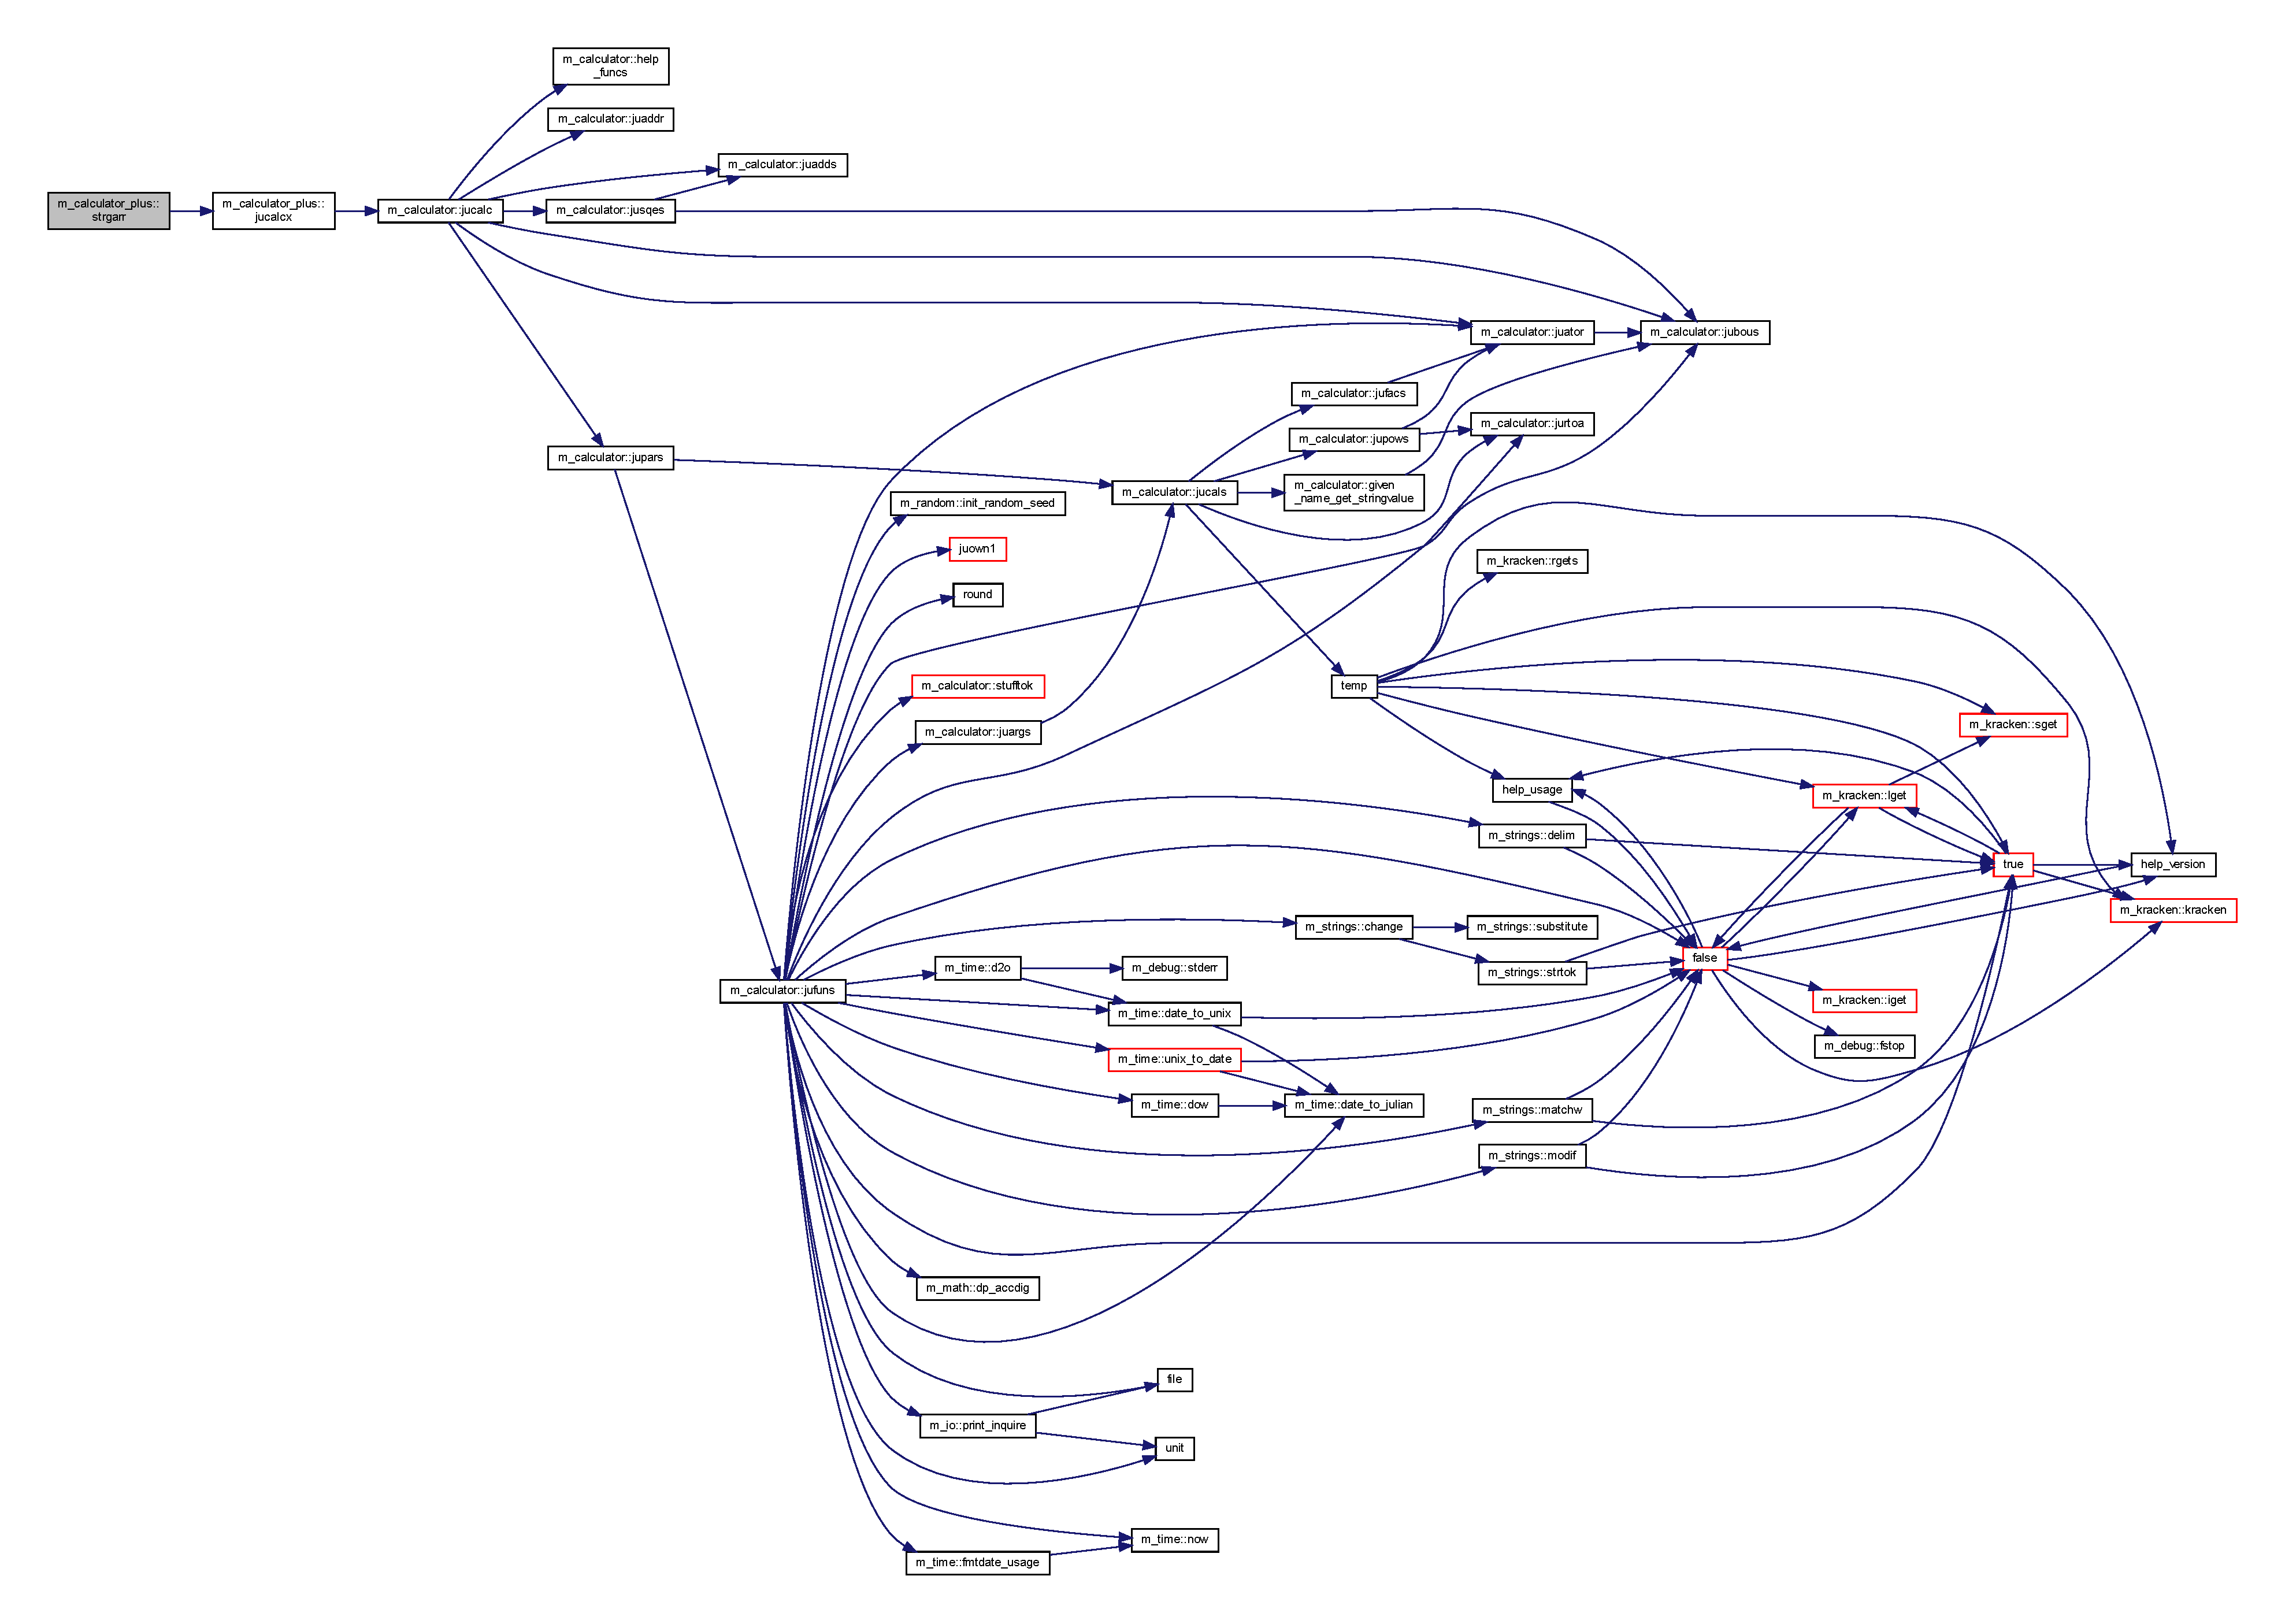
\includegraphics[width=350pt]{namespacem__calculator__plus_a4d3424e0cb74d4af53e7f59c07d31f1b_cgraph}
\end{center}
\end{figure}

\hypertarget{namespacem__color}{}\section{m\+\_\+color Module Reference}
\label{namespacem__color}\index{m\+\_\+color@{m\+\_\+color}}
\subsection*{Functions/\+Subroutines}
\begin{DoxyCompactItemize}
\item 
\hyperlink{M__stopwatch_83_8txt_acfbcff50169d691ff02d4a123ed70482}{subroutine}, \hyperlink{M__stopwatch_83_8txt_a2f74811300c361e53b430611a7d1769f}{public} \hyperlink{namespacem__color_a56dd07bbf1378ccc78a230d171f9d429}{hue} (modei, clr1i, clr2i, clr3i, modeo, clr1o, clr2o, clr3o, status)
\item 
\hyperlink{M__stopwatch_83_8txt_acfbcff50169d691ff02d4a123ed70482}{subroutine}, private \hyperlink{namespacem__color_a1dd027cbe65112af243d26195b1fc49a}{rgbhls} (r0, g0, b0, h, l, s, status)
\item 
\hyperlink{M__stopwatch_83_8txt_acfbcff50169d691ff02d4a123ed70482}{subroutine}, private \hyperlink{namespacem__color_a76f00e1d418c4904a963094bc730a0e6}{rgbhvs} (r0, g0, b0, h, v, s, status)
\item 
\hyperlink{M__stopwatch_83_8txt_acfbcff50169d691ff02d4a123ed70482}{subroutine}, private \hyperlink{namespacem__color_ab91687e87d0901874e52efe5933e3044}{cmyrgb} (\hyperlink{c_8f90_aeb1f4e639be0213b4cbd07f2583a5b1f}{c}, m, y, r, g, b, status)
\item 
\hyperlink{M__stopwatch_83_8txt_acfbcff50169d691ff02d4a123ed70482}{subroutine}, private \hyperlink{namespacem__color_ad6e8505eef5add299c4475d289f3c5c5}{rgbcmy} (r, g, b, \hyperlink{c_8f90_aeb1f4e639be0213b4cbd07f2583a5b1f}{c}, m, y, status)
\item 
\hyperlink{M__stopwatch_83_8txt_acfbcff50169d691ff02d4a123ed70482}{subroutine}, \hyperlink{M__stopwatch_83_8txt_a2f74811300c361e53b430611a7d1769f}{public} \hyperlink{namespacem__color_aca19999686fc20d79da580c6a643dc35}{rgbmono} (rr, rg, rb, ri, status)
\item 
\hyperlink{read__watch_83_8txt_abdb62bde002f38ef75f810d3a905a823}{real} function, private \hyperlink{namespacem__color_a3e97e24dba7b820f685f13eaa64a6caa}{rgbval} (clr1, clr2, h)
\item 
\hyperlink{M__stopwatch_83_8txt_acfbcff50169d691ff02d4a123ed70482}{subroutine}, private \hyperlink{namespacem__color_a40e6c91da216384eded2157cdaf86eba}{hlsrgb} (H, L, S, R, G, \hyperlink{intro__blas1_83_8txt_a5f157716d3fd55e7b7e08312dc859b58}{B}, status)
\item 
\hyperlink{M__stopwatch_83_8txt_acfbcff50169d691ff02d4a123ed70482}{subroutine}, private \hyperlink{namespacem__color_a334ec90d94bbfb9a4c08c5f9efdb8c47}{hvsrgb} (h, v, s, r, g, b, status)
\item 
\hyperlink{M__stopwatch_83_8txt_acfbcff50169d691ff02d4a123ed70482}{subroutine} \hyperlink{namespacem__color_ac9cd845fb9975144a6deb3a21ce29a29}{yiqrgb} (y, \hyperlink{intro__blas1_83_8txt_a8ba82a50c0c2c12d5f6a77f7e4651c0b}{i}, q, r, g, b, status)
\item 
\hyperlink{M__stopwatch_83_8txt_acfbcff50169d691ff02d4a123ed70482}{subroutine}, private \hyperlink{namespacem__color_a386d004a1392b7e01ff66f1676d43def}{rgbyiq} (r, g, b, y, \hyperlink{intro__blas1_83_8txt_a8ba82a50c0c2c12d5f6a77f7e4651c0b}{i}, q, status)
\item 
\hyperlink{M__stopwatch_83_8txt_acfbcff50169d691ff02d4a123ed70482}{subroutine}, \hyperlink{M__stopwatch_83_8txt_a2f74811300c361e53b430611a7d1769f}{public} \hyperlink{namespacem__color_acad72628ee0b77cf87f40cd46734fb18}{closest\+\_\+color\+\_\+name} (r, g, b, closestname)
\item 
\hyperlink{M__stopwatch_83_8txt_acfbcff50169d691ff02d4a123ed70482}{subroutine}, \hyperlink{M__stopwatch_83_8txt_a2f74811300c361e53b430611a7d1769f}{public} \hyperlink{namespacem__color_a84a36043d278bc56a7148483a862dec8}{color\+\_\+name2rgb} (\hyperlink{M__stopwatch_83_8txt_a3f508a893ae4c3b397b4383e33b9bcae}{name}, r, g, b, echoname)
\end{DoxyCompactItemize}


\subsection{Detailed Description}
\subsection*{Fortran color module M\+\_\+color}

D\+O\+W\+N\+L\+O\+AD\+:\href{download.html}{\tt G\+P\+F.\+tgz} 

The download file includes an example utility program \href{../PROGRAMS/colors.f90}{\tt colors.\+f90} with a man(1) page \href{colors.1.html}{\tt colors.\+1} that exercises the module. 


\begin{DoxyDescription}
\item[\label{_M_COLOR}%
N\+A\+ME ]{\itshape M\+\_\+\+C\+O\+L\+O\+R(3f)} -\/ \mbox{[}M\+\_\+color\mbox{]} a Fortran module that lets you convert between common color models 


\item[S\+Y\+N\+O\+P\+S\+IS ]
\begin{DoxyPre}
    use M\_color, only : \&\end{DoxyPre}



\begin{DoxyPre}       \& \href{hue.3.html}{\tt hue}, \&
       \& \href{closest_color_name.3.html}{\tt closest\_color\_name}, \&
       \& \href{color_name2rgb.3.html}{\tt color\_name2rgb}, \&
       \& \href{rgbmono.3.html}{\tt rgbmono}
 \end{DoxyPre}





\item[D\+E\+S\+C\+R\+I\+P\+T\+I\+ON ]



Highly accurate color conversions are a tricky business, and color is a complex topic; but these simplified conversions between common color models work quite well for most basic needs. 





For most uses the only user routine called is \href{hue.3.html}{\tt H\+U\+E(3f)} H\+U\+E(3f) is a single routine that interfaces to all the private low-\/level color conversion routines to convert a color\textquotesingle{}s components from one color model to another. H\+U\+E(3f) converts between the following color models\+: 




\begin{DoxyItemize}
\item R\+GB -\/ Red, Green, Blue (color TV monitors) 
\item H\+LS -\/ Hue, Lightness, Saturation 
\item C\+MY -\/ Cyan, Magenta, Yellow (pigment-\/based printing devices) 
\item H\+SV -\/ Hue, Saturation, Value 
\item Y\+IQ -\/ Broadcast TV color system 
\end{DoxyItemize}



In addition to the reversible color model conversions there are a few other user-\/callable color-\/related procedures\+: 




\begin{DoxyPre}
    \href{closest_color_name.3.html}{\tt CLOSEST\_COLOR\_NAME}:  given RGB values, try to find closest named color
    \href{color_name2rgb.3.html}{\tt COLOR\_NAME2RGB}:  given a color name, return RGB color values in range 0 to 100
    \href{rgbmono.3.html}{\tt RGBMONO}:  convert RGB colors to a reasonable grayscale
 \end{DoxyPre}


\paragraph*{2$\ast$N Design of the module}





The rest of the library is composed of P\+R\+I\+V\+A\+TE procedures. For each color model supported the general idea of the module is that there are two routines for each color model\+: 




\begin{DoxyItemize}
\item One converts that model to the R\+GB model  
\item The other converts from R\+GB to that model  
\end{DoxyItemize}



This allows conversions between all color models with only 2$\ast$N routines required to go from any model to any other. That is, to go from model A to model B the intent is that the module would make two calls\+: 




\begin{DoxyPre}
     call modelA2rgb(...)
     call rgb2modelB(...)
 \end{DoxyPre}




The resulting internal routines that result are\+: 




\begin{DoxyItemize}
\item \href{#HLSRGB}{\tt H\+L\+S\+R\+GB} given hue, lightness, saturation calculate red, green, and blue components 
\begin{DoxyItemize}
\item \href{#RGBVAL}{\tt R\+G\+B\+V\+AL} ensure a value is in the appropriate range and quadrant  
\end{DoxyItemize}
\item \href{#HVSRGB}{\tt H\+V\+S\+R\+GB} given hue, saturation, value calculate red, green, and blue components  
\item \href{#CMYRGB}{\tt C\+M\+Y\+R\+GB} given cyan, magenta, and yellow components calculate red, green, and blue components  
\item \href{#YIQRGB}{\tt Y\+I\+Q\+R\+GB} given luma(gray scale), orange-\/blue chrominance, and purple-\/green chrominance components calculate red, green, and blue components 


\item \href{#RGBHVS}{\tt R\+G\+B\+H\+VS} given red, green, blue values calculate hue, value, and saturation components  
\item \href{#RGBHLS}{\tt R\+G\+B\+H\+LS} given red, green, blue values calculate hue, lightness, and saturation components  
\item \href{#RGBCMY}{\tt R\+G\+B\+C\+MY} given red, green, blue values calculate cyan, magenta, yellow components  
\item \href{#RGBYIQ}{\tt R\+G\+B\+Y\+IQ} given red, green, blue values calculate luma(gray scale), orange-\/blue chrominance, and purple-\/green chrominance components 


\end{DoxyItemize}


\item[S\+EE A\+L\+SO  ]



A simple interactive javascript-\/based \href{../../../public_html/javascript/color/iframe.html}{\tt color selector} lets you interactively select colors. 





The color wheel below was generated using a V\+O\+G\+LE graphics library program (\href{../../../libvogle/EXE/TESTS/huef.F90}{\tt (huef.\+f90)} that uses the M\+\_\+color module. 



\begin{center}  \end{center} 




\item[R\+E\+F\+E\+R\+E\+N\+C\+ES]The algorithms are heavily based on chapter 17 of \char`\"{}\+Fundamentals of Interactive Computer Graphics\char`\"{}; J. D. Foley and A. Van Dam. 


\item[A\+U\+T\+H\+OR ]

John S. Urban




\end{DoxyDescription}\subsubsection*{Details on the internal procedures ...}

\subsection{Function/\+Subroutine Documentation}
\mbox{\Hypertarget{namespacem__color_acad72628ee0b77cf87f40cd46734fb18}\label{namespacem__color_acad72628ee0b77cf87f40cd46734fb18}} 
\index{m\+\_\+color@{m\+\_\+color}!closest\+\_\+color\+\_\+name@{closest\+\_\+color\+\_\+name}}
\index{closest\+\_\+color\+\_\+name@{closest\+\_\+color\+\_\+name}!m\+\_\+color@{m\+\_\+color}}
\subsubsection{\texorpdfstring{closest\+\_\+color\+\_\+name()}{closest\_color\_name()}}
{\footnotesize\ttfamily \hyperlink{M__stopwatch_83_8txt_acfbcff50169d691ff02d4a123ed70482}{subroutine}, \hyperlink{M__stopwatch_83_8txt_a2f74811300c361e53b430611a7d1769f}{public} m\+\_\+color\+::closest\+\_\+color\+\_\+name (\begin{DoxyParamCaption}\item[{\hyperlink{read__watch_83_8txt_abdb62bde002f38ef75f810d3a905a823}{real}, intent(\hyperlink{M__journal_83_8txt_afce72651d1eed785a2132bee863b2f38}{in})}]{r,  }\item[{\hyperlink{read__watch_83_8txt_abdb62bde002f38ef75f810d3a905a823}{real}, intent(\hyperlink{M__journal_83_8txt_afce72651d1eed785a2132bee863b2f38}{in})}]{g,  }\item[{\hyperlink{read__watch_83_8txt_abdb62bde002f38ef75f810d3a905a823}{real}, intent(\hyperlink{M__journal_83_8txt_afce72651d1eed785a2132bee863b2f38}{in})}]{b,  }\item[{\hyperlink{option__stopwatch_83_8txt_abd4b21fbbd175834027b5224bfe97e66}{character}(len=$\ast$), intent(out)}]{closestname }\end{DoxyParamCaption})}


\begin{DoxyDescription}
\item[\label{_CLOSEST_COLOR_NAME}%
N\+A\+ME ]closest\+\_\+color\+\_\+name(3f) -\/ \mbox{[}M\+\_\+color\mbox{]} returns the closest name for the given R\+GB values. 


\item[S\+Y\+N\+O\+P\+S\+IS ]
\begin{DoxyPre}
    subroutine closest\_color\_name(r,g,b,closestname)\end{DoxyPre}



\begin{DoxyPre}     real,intent(in)               :: r,g,b
     character(len=20),intent(out) :: closestname
    \end{DoxyPre}
 


\item[D\+E\+S\+C\+R\+I\+P\+T\+I\+ON ]\begin{DoxyVerb}closest_color_name() returns the closest name for the given RGB values.
Most X11 Windows color names are supported.
\end{DoxyVerb}
 


\item[O\+P\+T\+I\+O\+NS ]\begin{DoxyVerb}<ul>
<li>R  - red component, range of 0 to 100</li>
<li>G  - green component, range of 0 to 100</li>
<li>B  - blue component, range of 0 to 100</li>
<ul>
\end{DoxyVerb}
 


\item[R\+E\+T\+U\+R\+NS ]\begin{DoxyVerb}<ul>
<li>CLOSESTNAME  - name of color found closest to given RGB value</li>
<ul>
\end{DoxyVerb}
 


\item[E\+X\+A\+M\+P\+LE ]\begin{DoxyVerb}Sample program
<pre>
   program demo_closest_color_name
   use M_color, only : closest_color_name
   character(len=100) :: string ! at least 20 characters
   string=' '

   call closest_color_name(100.0,  0.0,  0.0,string)
   write(*,*)trim(string)

   call closest_color_name(  0.0,100.0,  0.0,string)
   write(*,*)trim(string)

   call closest_color_name(  0.0,  0.0,100.0,string)
   write(*,*)trim(string)

   end program demo_closest_color_name
\end{DoxyVerb}


\paragraph*{Results\+:}

red green blue 




\end{DoxyDescription}

References color\+\_\+name2rgb().

\mbox{\Hypertarget{namespacem__color_ab91687e87d0901874e52efe5933e3044}\label{namespacem__color_ab91687e87d0901874e52efe5933e3044}} 
\index{m\+\_\+color@{m\+\_\+color}!cmyrgb@{cmyrgb}}
\index{cmyrgb@{cmyrgb}!m\+\_\+color@{m\+\_\+color}}
\subsubsection{\texorpdfstring{cmyrgb()}{cmyrgb()}}
{\footnotesize\ttfamily \hyperlink{M__stopwatch_83_8txt_acfbcff50169d691ff02d4a123ed70482}{subroutine}, private m\+\_\+color\+::cmyrgb (\begin{DoxyParamCaption}\item[{\hyperlink{read__watch_83_8txt_abdb62bde002f38ef75f810d3a905a823}{real}, intent(\hyperlink{M__journal_83_8txt_afce72651d1eed785a2132bee863b2f38}{in})}]{c,  }\item[{\hyperlink{read__watch_83_8txt_abdb62bde002f38ef75f810d3a905a823}{real}, intent(\hyperlink{M__journal_83_8txt_afce72651d1eed785a2132bee863b2f38}{in})}]{m,  }\item[{\hyperlink{read__watch_83_8txt_abdb62bde002f38ef75f810d3a905a823}{real}, intent(\hyperlink{M__journal_83_8txt_afce72651d1eed785a2132bee863b2f38}{in})}]{y,  }\item[{\hyperlink{read__watch_83_8txt_abdb62bde002f38ef75f810d3a905a823}{real}, intent(out)}]{r,  }\item[{\hyperlink{read__watch_83_8txt_abdb62bde002f38ef75f810d3a905a823}{real}, intent(out)}]{g,  }\item[{\hyperlink{read__watch_83_8txt_abdb62bde002f38ef75f810d3a905a823}{real}, intent(out)}]{b,  }\item[{integer}]{status }\end{DoxyParamCaption})\hspace{0.3cm}{\ttfamily [private]}}


\begin{DoxyDescription}
\item[\label{_CMYRGB}%
N\+A\+ME ]cmyrgb(3fp) -\/ \mbox{[}M\+\_\+color\mbox{]} calculates the cyan, magenta, and yellow components given the red, green, and blue component values. 


\item[S\+Y\+N\+O\+P\+S\+IS ]
\begin{DoxyPre}
    subroutine cmyrgb(c,m,y,r,g,b,status)\end{DoxyPre}



\begin{DoxyPre}     real, intent(in)  :: c ! the cyan component as a value in the range of 0 to 100
     real, intent(in)  :: m ! the magenta component as a value in the range of 0 to 100
     real, intent(in)  :: y ! the yellow component as a value in the range of 0 to 100
     real, intent(out) :: r ! the red component as a value in the range of 0 to 100
     real, intent(out) :: g ! the green component as a value in the range of 0 to 100
     real, intent(out) :: b ! the blue component as a value in the range of 0 to 100
     integer           :: status
    \end{DoxyPre}
 


\item[D\+E\+S\+C\+R\+I\+P\+T\+I\+ON ]\hyperlink{namespacem__color_ab91687e87d0901874e52efe5933e3044}{cmyrgb()} calculates the cyan, magenta, and yellow components given the red, green, and blue component values.


\end{DoxyDescription}\mbox{\Hypertarget{namespacem__color_a84a36043d278bc56a7148483a862dec8}\label{namespacem__color_a84a36043d278bc56a7148483a862dec8}} 
\index{m\+\_\+color@{m\+\_\+color}!color\+\_\+name2rgb@{color\+\_\+name2rgb}}
\index{color\+\_\+name2rgb@{color\+\_\+name2rgb}!m\+\_\+color@{m\+\_\+color}}
\subsubsection{\texorpdfstring{color\+\_\+name2rgb()}{color\_name2rgb()}}
{\footnotesize\ttfamily \hyperlink{M__stopwatch_83_8txt_acfbcff50169d691ff02d4a123ed70482}{subroutine}, \hyperlink{M__stopwatch_83_8txt_a2f74811300c361e53b430611a7d1769f}{public} m\+\_\+color\+::color\+\_\+name2rgb (\begin{DoxyParamCaption}\item[{\hyperlink{option__stopwatch_83_8txt_abd4b21fbbd175834027b5224bfe97e66}{character}(len=$\ast$), intent(\hyperlink{M__journal_83_8txt_afce72651d1eed785a2132bee863b2f38}{in})}]{name,  }\item[{\hyperlink{read__watch_83_8txt_abdb62bde002f38ef75f810d3a905a823}{real}, intent(out)}]{r,  }\item[{\hyperlink{read__watch_83_8txt_abdb62bde002f38ef75f810d3a905a823}{real}, intent(out)}]{g,  }\item[{\hyperlink{read__watch_83_8txt_abdb62bde002f38ef75f810d3a905a823}{real}, intent(out)}]{b,  }\item[{\hyperlink{option__stopwatch_83_8txt_abd4b21fbbd175834027b5224bfe97e66}{character}(len=$\ast$), intent(out), \hyperlink{option__stopwatch_83_8txt_aa4ece75e7acf58a4843f70fe18c3ade5}{optional}}]{echoname }\end{DoxyParamCaption})}


\begin{DoxyDescription}
\item[\label{_COLOR_NAME2RGB}%
N\+A\+ME ]C\+O\+L\+O\+R\+\_\+\+N\+A\+M\+E2\+R\+G\+B(3f) -\/ \mbox{[}M\+\_\+color\mbox{]} returns the R\+GB values in the range 0 to 100 for a given known color name. 


\item[S\+Y\+N\+O\+P\+S\+IS ]
\begin{DoxyPre}
    subroutine color\_name2rgb(name,r,g,b,echoname)\end{DoxyPre}



\begin{DoxyPre}     character(len=20),intent(in)   :: name
     real,intent(out)               :: r,g,b
     character(len=20),intent(out)  :: echoname
    \end{DoxyPre}
 


\item[D\+E\+S\+C\+R\+I\+P\+T\+I\+ON ]\begin{DoxyVerb}COLOR_NAME2RGB() returns the RGB values in the range 0 to 100 for a given known color name.
Most X11 Windows color names are supported. If the name is not found, ECHONAME is set to
"Unknown".
\end{DoxyVerb}
 


\item[E\+X\+A\+M\+P\+LE ]\begin{quote}
A sample program\+: 
\begin{DoxyPre}
       program showcolors
       use \hyperlink{namespacem__color}{m\_color}, only : hue, color\_name2rgb
       implicit none
       character(len=*),parameter :: ident="&
       &@(#)M\_color::showcolors(1f): list colors known to colorname2rgb(3f) & corresponding RGB values"
       character(len=20) :: name
       character(len=20) :: echoname
       real              :: red,green,blue
       integer           :: i
       TRYALL: do i=1,10000
          ! weird little thing where the color names have aliases that are numeric strings
          write(name,'(i0)')i
          ! get the RGB values and English name of the color
          call color\_name2rgb(name,red,green,blue,echoname)
          ! the last color name is "Unknown" so the loop should exit
          if(echoname.eq.'Unknown')exit TRYALL
          ! display the English name and RGB values for the name
          write(*,*)echoname,int([red,green,blue])
       enddo TRYALL
       !write(*,*)'Number of colors found is ',i-1
       end program showcolors
 \end{DoxyPre}
 \end{quote}



\end{DoxyDescription}

References m\+\_\+strings\+::lower().

\mbox{\Hypertarget{namespacem__color_a40e6c91da216384eded2157cdaf86eba}\label{namespacem__color_a40e6c91da216384eded2157cdaf86eba}} 
\index{m\+\_\+color@{m\+\_\+color}!hlsrgb@{hlsrgb}}
\index{hlsrgb@{hlsrgb}!m\+\_\+color@{m\+\_\+color}}
\subsubsection{\texorpdfstring{hlsrgb()}{hlsrgb()}}
{\footnotesize\ttfamily \hyperlink{M__stopwatch_83_8txt_acfbcff50169d691ff02d4a123ed70482}{subroutine}, private m\+\_\+color\+::hlsrgb (\begin{DoxyParamCaption}\item[{\hyperlink{read__watch_83_8txt_abdb62bde002f38ef75f810d3a905a823}{real}, intent(\hyperlink{M__journal_83_8txt_afce72651d1eed785a2132bee863b2f38}{in})}]{H,  }\item[{\hyperlink{read__watch_83_8txt_abdb62bde002f38ef75f810d3a905a823}{real}, intent(\hyperlink{M__journal_83_8txt_afce72651d1eed785a2132bee863b2f38}{in})}]{L,  }\item[{\hyperlink{read__watch_83_8txt_abdb62bde002f38ef75f810d3a905a823}{real}, intent(\hyperlink{M__journal_83_8txt_afce72651d1eed785a2132bee863b2f38}{in})}]{S,  }\item[{\hyperlink{read__watch_83_8txt_abdb62bde002f38ef75f810d3a905a823}{real}, intent(out)}]{R,  }\item[{\hyperlink{read__watch_83_8txt_abdb62bde002f38ef75f810d3a905a823}{real}, intent(out)}]{G,  }\item[{\hyperlink{read__watch_83_8txt_abdb62bde002f38ef75f810d3a905a823}{real}, intent(out)}]{B,  }\item[{integer}]{status }\end{DoxyParamCaption})\hspace{0.3cm}{\ttfamily [private]}}


\begin{DoxyDescription}
\item[\label{_HLSRGB}%
N\+A\+ME ]H\+L\+S\+R\+G\+B(3fp) -\/ \mbox{[}M\+\_\+color\mbox{]} calculates the red, green, \& blue components for a color given in hue, lightness, \& saturation values. 


\item[S\+Y\+N\+O\+P\+S\+IS ]
\begin{DoxyPre}
    subroutine hlsrgb (h,l,s,r,g,b,status)\end{DoxyPre}



\begin{DoxyPre}     real, intent(in)  :: h ! hue value in the range of 0 to 360 degrees
     real, intent(in)  :: l ! lightness as a percent value from 0 to 100.
     real, intent(in)  :: s ! saturation as a percent from 0 to 100.
     real, intent(out) :: r ! red component as a value of 0 to 100.
     real, intent(out) :: g ! green component as a value of 0 to 100.
     real, intent(out) :: b ! blue component as a value of 0 to 100.
     integer           :: status
    \end{DoxyPre}
 


\item[D\+E\+S\+C\+R\+I\+P\+T\+I\+ON ]\begin{DoxyVerb}HLSRGB() calculates the red, green, &amp; blue components for a
 color given in hue, lightness, &amp; saturation values.
\end{DoxyVerb}
 


\end{DoxyDescription}

References rgbval().

\mbox{\Hypertarget{namespacem__color_a56dd07bbf1378ccc78a230d171f9d429}\label{namespacem__color_a56dd07bbf1378ccc78a230d171f9d429}} 
\index{m\+\_\+color@{m\+\_\+color}!hue@{hue}}
\index{hue@{hue}!m\+\_\+color@{m\+\_\+color}}
\subsubsection{\texorpdfstring{hue()}{hue()}}
{\footnotesize\ttfamily \hyperlink{M__stopwatch_83_8txt_acfbcff50169d691ff02d4a123ed70482}{subroutine}, \hyperlink{M__stopwatch_83_8txt_a2f74811300c361e53b430611a7d1769f}{public} m\+\_\+color\+::hue (\begin{DoxyParamCaption}\item[{\hyperlink{option__stopwatch_83_8txt_abd4b21fbbd175834027b5224bfe97e66}{character}(len=$\ast$), intent(\hyperlink{M__journal_83_8txt_afce72651d1eed785a2132bee863b2f38}{in})}]{modei,  }\item[{\hyperlink{read__watch_83_8txt_abdb62bde002f38ef75f810d3a905a823}{real}, intent(\hyperlink{M__journal_83_8txt_afce72651d1eed785a2132bee863b2f38}{in})}]{clr1i,  }\item[{\hyperlink{read__watch_83_8txt_abdb62bde002f38ef75f810d3a905a823}{real}, intent(\hyperlink{M__journal_83_8txt_afce72651d1eed785a2132bee863b2f38}{in})}]{clr2i,  }\item[{\hyperlink{read__watch_83_8txt_abdb62bde002f38ef75f810d3a905a823}{real}, intent(\hyperlink{M__journal_83_8txt_afce72651d1eed785a2132bee863b2f38}{in})}]{clr3i,  }\item[{\hyperlink{option__stopwatch_83_8txt_abd4b21fbbd175834027b5224bfe97e66}{character}(len=$\ast$), intent(\hyperlink{M__journal_83_8txt_afce72651d1eed785a2132bee863b2f38}{in})}]{modeo,  }\item[{\hyperlink{read__watch_83_8txt_abdb62bde002f38ef75f810d3a905a823}{real}, intent(out)}]{clr1o,  }\item[{\hyperlink{read__watch_83_8txt_abdb62bde002f38ef75f810d3a905a823}{real}, intent(out)}]{clr2o,  }\item[{\hyperlink{read__watch_83_8txt_abdb62bde002f38ef75f810d3a905a823}{real}, intent(out)}]{clr3o,  }\item[{integer, intent(out)}]{status }\end{DoxyParamCaption})}


\begin{DoxyDescription}
\item[\label{_HUE}%
N\+A\+ME ]H\+U\+E(3f) -\/ \mbox{[}M\+\_\+color\mbox{]} converts a color\textquotesingle{}s components from one color model to another. 


\item[S\+Y\+N\+O\+P\+S\+IS ]
\begin{DoxyPre}
    subroutine hue(modei,clr1i,clr2i,clr3i,modeo,clr1o,clr2o,clr3o,status)\end{DoxyPre}



\begin{DoxyPre}     character(len=*),intent(in) :: modei  ! name of color model of input values
     character(len=*),intent(in) :: modeo  ! name of color model of output values
     real,intent(in)             :: clr1i,clr2i,clr3i
     real,intent(out)            :: clr1o,clr2o,clr3o
     integer,intent(out)         :: status
    \end{DoxyPre}
 


\item[D\+E\+S\+C\+R\+I\+P\+T\+I\+ON ]Basic color models ... ~\newline
~\newline


\begin{quote}

\tabulinesep=1mm
\begin{longtabu} spread 0pt [c]{*{4}{|X[-1]}|}
\caption{{\bfseries  valid values for modei and modeo as well as the corresponding meanings for clr1$\ast$, clr2$\ast$, and clr3$\ast$ are\+: }}\label{_}\\
\hline
\rowcolor{\tableheadbgcolor}\textbf{ model  }&\textbf{ clr1  }&\textbf{ clr2  }&\textbf{ clr3   }\\\cline{1-4}
\endfirsthead
\hline
\endfoot
\hline
\rowcolor{\tableheadbgcolor}\textbf{ model  }&\textbf{ clr1  }&\textbf{ clr2  }&\textbf{ clr3   }\\\cline{1-4}
\endhead
hls  &hue  &lightness  &saturation   \\\cline{1-4}
hsl  &hue  &saturation  &lightness   \\\cline{1-4}
hvs  &hue  &value  &saturation   \\\cline{1-4}
hsv  &hue  &saturation  &value   \\\cline{1-4}
rgb  &red  &green  &blue   \\\cline{1-4}
cmy  &cyan  &magenta  &yellow   \\\cline{1-4}
yiq  &luma(gray scale)  &orange-\/blue chrominance  &purple-\/green chrominance   \\\cline{1-4}
\end{longtabu}
\end{quote}



\begin{DoxyItemize}
\item lightness, value, saturation, red, green, blue, cyan, magenta, and yellow range from 0 to 100, 
\item hue ranges from 0 to 360 degrees, 
\item y ranges from 0 to 100, 
\item i ranges from -\/60 to 60, 
\item q ranges from -\/52 to 52 
\end{DoxyItemize}



The S\+T\+A\+T\+US variable can signal the following conditions\+: 




\begin{DoxyPre}
    -1   modei = modeo, so no substantial conversion was done,
     1   one of the input color values was outside the allowable range,
     2   modei was invalid
     3   modeo was invalid
 \end{DoxyPre}
 


\end{DoxyDescription}

References cmyrgb(), hlsrgb(), hvsrgb(), m\+\_\+strings\+::lower(), rgbcmy(), rgbhls(), rgbhvs(), rgbyiq(), and yiqrgb().

\mbox{\Hypertarget{namespacem__color_a334ec90d94bbfb9a4c08c5f9efdb8c47}\label{namespacem__color_a334ec90d94bbfb9a4c08c5f9efdb8c47}} 
\index{m\+\_\+color@{m\+\_\+color}!hvsrgb@{hvsrgb}}
\index{hvsrgb@{hvsrgb}!m\+\_\+color@{m\+\_\+color}}
\subsubsection{\texorpdfstring{hvsrgb()}{hvsrgb()}}
{\footnotesize\ttfamily \hyperlink{M__stopwatch_83_8txt_acfbcff50169d691ff02d4a123ed70482}{subroutine}, private m\+\_\+color\+::hvsrgb (\begin{DoxyParamCaption}\item[{\hyperlink{read__watch_83_8txt_abdb62bde002f38ef75f810d3a905a823}{real}, intent(\hyperlink{M__journal_83_8txt_afce72651d1eed785a2132bee863b2f38}{in})}]{h,  }\item[{\hyperlink{read__watch_83_8txt_abdb62bde002f38ef75f810d3a905a823}{real}, intent(\hyperlink{M__journal_83_8txt_afce72651d1eed785a2132bee863b2f38}{in})}]{v,  }\item[{\hyperlink{read__watch_83_8txt_abdb62bde002f38ef75f810d3a905a823}{real}, intent(\hyperlink{M__journal_83_8txt_afce72651d1eed785a2132bee863b2f38}{in})}]{s,  }\item[{\hyperlink{read__watch_83_8txt_abdb62bde002f38ef75f810d3a905a823}{real}, intent(out)}]{r,  }\item[{\hyperlink{read__watch_83_8txt_abdb62bde002f38ef75f810d3a905a823}{real}, intent(out)}]{g,  }\item[{\hyperlink{read__watch_83_8txt_abdb62bde002f38ef75f810d3a905a823}{real}, intent(out)}]{b,  }\item[{integer}]{status }\end{DoxyParamCaption})\hspace{0.3cm}{\ttfamily [private]}}


\begin{DoxyDescription}
\item[\label{_HVSRGB}%
N\+A\+ME ]H\+V\+S\+R\+G\+B(3fp) -\/ \mbox{[}M\+\_\+color\mbox{]} calculates the red, green, \& blue components for a color given in hue, value, \& saturation values. 


\item[S\+Y\+N\+O\+P\+S\+IS ]
\begin{DoxyPre}
    subroutine hvsrgb(h,v,s,r,g,b,status)\end{DoxyPre}



\begin{DoxyPre}     real, intent(in)  :: h ! H is the hue value in the range of 0 to 360 degrees
     real, intent(in)  :: v ! V is the "value" as a percent value from 0 to 100.
     real, intent(in)  :: s ! S is the saturation as a percent from 0 to 100.
     real, intent(out) :: r ! R is the red component as a value of 0 to 100.
     real, intent(out) :: g ! G is the green component as a value of 0 to 100.
     real, intent(out) :: b ! B is the blue component as a value of 0 to 100.
     integer           :: status
    \end{DoxyPre}
 


\item[D\+E\+S\+C\+R\+I\+P\+T\+I\+ON ]\begin{DoxyVerb}HVSRGB() calculates the red, green, &amp; blue components for a
 color given in hue, value, &amp; saturation values.
\end{DoxyVerb}
 


\end{DoxyDescription}\mbox{\Hypertarget{namespacem__color_ad6e8505eef5add299c4475d289f3c5c5}\label{namespacem__color_ad6e8505eef5add299c4475d289f3c5c5}} 
\index{m\+\_\+color@{m\+\_\+color}!rgbcmy@{rgbcmy}}
\index{rgbcmy@{rgbcmy}!m\+\_\+color@{m\+\_\+color}}
\subsubsection{\texorpdfstring{rgbcmy()}{rgbcmy()}}
{\footnotesize\ttfamily \hyperlink{M__stopwatch_83_8txt_acfbcff50169d691ff02d4a123ed70482}{subroutine}, private m\+\_\+color\+::rgbcmy (\begin{DoxyParamCaption}\item[{\hyperlink{read__watch_83_8txt_abdb62bde002f38ef75f810d3a905a823}{real}, intent(\hyperlink{M__journal_83_8txt_afce72651d1eed785a2132bee863b2f38}{in})}]{r,  }\item[{\hyperlink{read__watch_83_8txt_abdb62bde002f38ef75f810d3a905a823}{real}, intent(\hyperlink{M__journal_83_8txt_afce72651d1eed785a2132bee863b2f38}{in})}]{g,  }\item[{\hyperlink{read__watch_83_8txt_abdb62bde002f38ef75f810d3a905a823}{real}, intent(\hyperlink{M__journal_83_8txt_afce72651d1eed785a2132bee863b2f38}{in})}]{b,  }\item[{\hyperlink{read__watch_83_8txt_abdb62bde002f38ef75f810d3a905a823}{real}, intent(out)}]{c,  }\item[{\hyperlink{read__watch_83_8txt_abdb62bde002f38ef75f810d3a905a823}{real}, intent(out)}]{m,  }\item[{\hyperlink{read__watch_83_8txt_abdb62bde002f38ef75f810d3a905a823}{real}, intent(out)}]{y,  }\item[{integer}]{status }\end{DoxyParamCaption})\hspace{0.3cm}{\ttfamily [private]}}


\begin{DoxyDescription}
\item[\label{_RGBCMY}%
N\+A\+ME ]rgbcmy(3fp) -\/ \mbox{[}M\+\_\+color\mbox{]} calculates the cyan, magenta, and yellow components given the red, green, and blue component values. 


\item[S\+Y\+N\+O\+P\+S\+IS ]
\begin{DoxyPre}
    subroutine rgbcmy(r,g,b,c,m,y,status)\end{DoxyPre}



\begin{DoxyPre}     real, intent(in)  :: r ! the red component as a value in the range of 0 to 100
     real, intent(in)  :: g ! the green component as a value in the range of 0 to 100
     real, intent(in)  :: b ! the blue component as a value in the range of 0 to 100
     real, intent(out) :: c ! the cyan component as a value in the range of 0 to 100
     real, intent(out) :: m ! the magenta component as a value in the range of 0 to 100
     real, intent(out) :: y ! the yellow component as a value in the range of 0 to 100
     integer           :: status
    \end{DoxyPre}
 


\item[D\+E\+S\+C\+R\+I\+P\+T\+I\+ON ]Table ... ~\newline
~\newline


\begin{quote}
\tabulinesep=1mm
\begin{longtabu} spread 0pt [c]{*{5}{|X[-1]}|}
\hline
\rowcolor{\tableheadbgcolor}\textbf{ Color  }&\textbf{ Color

name  }&\textbf{ (C,M,Y) }&\textbf{ ( R, G, B) }&\textbf{ Hex  }\\\cline{1-5}
\endfirsthead
\hline
\endfoot
\hline
\rowcolor{\tableheadbgcolor}\textbf{ Color  }&\textbf{ Color

name  }&\textbf{ (C,M,Y) }&\textbf{ ( R, G, B) }&\textbf{ Hex  }\\\cline{1-5}
\endhead
~ &Black &(100,100,100) &( 0, 0, 0) &\#000000  \\\cline{1-5}
~ &White &( 0, 0, 0) &(100,100,100) &\#\+F\+F\+F\+F\+FF  \\\cline{1-5}
~ &Red &( 0,100,100) &(100, 0, 0) &\#\+F\+F0000  \\\cline{1-5}
~ &Green &(100, 0,100) &( 0,100, 0) &\#00\+F\+F00  \\\cline{1-5}
~ &Blue &(100,100, 0) &( 0, 0,100) &\#0000\+FF  \\\cline{1-5}
~ &Yellow &( 0, 0,100) &(100,100, 0) &\#\+F\+F\+F\+F00  \\\cline{1-5}
~ &Cyan &(100, 0, 0) &( 0,100,100) &\#00\+F\+F\+FF  \\\cline{1-5}
~ &Magenta &( 0,100, 0) &(100, 0,100) &\#\+F\+F00\+FF  \\\cline{1-5}
\end{longtabu}
\end{quote}



\end{DoxyDescription}\mbox{\Hypertarget{namespacem__color_a1dd027cbe65112af243d26195b1fc49a}\label{namespacem__color_a1dd027cbe65112af243d26195b1fc49a}} 
\index{m\+\_\+color@{m\+\_\+color}!rgbhls@{rgbhls}}
\index{rgbhls@{rgbhls}!m\+\_\+color@{m\+\_\+color}}
\subsubsection{\texorpdfstring{rgbhls()}{rgbhls()}}
{\footnotesize\ttfamily \hyperlink{M__stopwatch_83_8txt_acfbcff50169d691ff02d4a123ed70482}{subroutine}, private m\+\_\+color\+::rgbhls (\begin{DoxyParamCaption}\item[{\hyperlink{read__watch_83_8txt_abdb62bde002f38ef75f810d3a905a823}{real}}]{r0,  }\item[{\hyperlink{read__watch_83_8txt_abdb62bde002f38ef75f810d3a905a823}{real}}]{g0,  }\item[{\hyperlink{read__watch_83_8txt_abdb62bde002f38ef75f810d3a905a823}{real}}]{b0,  }\item[{\hyperlink{read__watch_83_8txt_abdb62bde002f38ef75f810d3a905a823}{real}}]{h,  }\item[{\hyperlink{read__watch_83_8txt_abdb62bde002f38ef75f810d3a905a823}{real}}]{l,  }\item[{\hyperlink{read__watch_83_8txt_abdb62bde002f38ef75f810d3a905a823}{real}}]{s,  }\item[{integer}]{status }\end{DoxyParamCaption})\hspace{0.3cm}{\ttfamily [private]}}


\begin{DoxyDescription}
\item[\label{_RGBHLS}%
N\+A\+ME ]R\+G\+B\+H\+L\+S(3fp) -\/ \mbox{[}M\+\_\+color\mbox{]} Given red, green, and blue color components calculates the hue, lightness, and saturation for a color 


\item[S\+Y\+N\+O\+P\+S\+IS ]
\begin{DoxyPre}
    subroutine rgbhls(r,g,b,h,l,s,status)\end{DoxyPre}



\begin{DoxyPre}     real, intent(in)  :: r ! the red component as a value of 0 to 100
     real, intent(in)  :: g ! the green component as a value of 0 to 100
     real, intent(in)  :: b ! the blue component as a value of 0 to 100
     real, intent(out) :: h ! the hue value in the range of 0 to 360 degrees
     real, intent(out) :: l ! the lightness as a percent value from 0 to 100
     real, intent(out) :: s ! the saturation as a percent from 0 to 100
     integer           :: status
    \end{DoxyPre}
 


\item[D\+E\+S\+C\+R\+I\+P\+T\+I\+ON ]

R\+GB values are in the range 0-\/100; hue is 0-\/360 degrees; lightness and saturation have a range of 0-\/100. ~\newline
~\newline


\begin{quote}
\tabulinesep=1mm
\begin{longtabu} spread 0pt [c]{*{8}{|X[-1]}|}
\hline
\rowcolor{\tableheadbgcolor}\textbf{ Color}&\multicolumn{3}{p{(\linewidth-\tabcolsep*8-\arrayrulewidth*4)*3/8}|}{\cellcolor{\tableheadbgcolor}\textbf{ R\+GB}}&\multicolumn{3}{p{(\linewidth-\tabcolsep*8-\arrayrulewidth*4)*3/8}|}{\cellcolor{\tableheadbgcolor}\textbf{ H\+LS}}&\textbf{ Sample }\\\cline{1-8}
\endfirsthead
\hline
\endfoot
\hline
\rowcolor{\tableheadbgcolor}\textbf{ Color}&\multicolumn{3}{p{(\linewidth-\tabcolsep*8-\arrayrulewidth*4)*3/8}|}{\cellcolor{\tableheadbgcolor}\textbf{ R\+GB}}&\multicolumn{3}{p{(\linewidth-\tabcolsep*8-\arrayrulewidth*4)*3/8}|}{\cellcolor{\tableheadbgcolor}\textbf{ H\+LS}}&\textbf{ Sample }\\\cline{1-8}
\endhead
Red&100.\+0&0.\+0&0.\+0&0&50.\+0&100.\+0&~ \\\cline{1-8}
Yellow&100.\+0&100.\+0&0.\+0&60&50.\+0&100.\+0&~ \\\cline{1-8}
Green&0.\+0&100.\+0&0.\+0&120&50.\+0&100.\+0&~ \\\cline{1-8}
Cyan&0.\+0&100.\+0&100.\+0&180&50.\+0&100.\+0&~ \\\cline{1-8}
Blue&0.\+0&0.\+0&100.\+0&240&50.\+0&100.\+0&~ \\\cline{1-8}
Magenta&100.\+0&0.\+0&100.\+0&300&50.\+0&100.\+0&~ \\\cline{1-8}
White&100.\+0&100.\+0&100.\+0&(any)&100.\+0&(any)&~ \\\cline{1-8}
Black&0.\+0&0.\+0&0.\+0&(any)&0.\+0&(any)&~ \\\cline{1-8}
Maroon&50.\+0&0.\+0&0.\+0&0&25.\+0&100.\+0&~ \\\cline{1-8}
Pink&100.\+0&50.\+0&50.\+0&0&75.\+0&100.\+0&~ \\\cline{1-8}
\end{longtabu}
\end{quote}



\end{DoxyDescription}\mbox{\Hypertarget{namespacem__color_a76f00e1d418c4904a963094bc730a0e6}\label{namespacem__color_a76f00e1d418c4904a963094bc730a0e6}} 
\index{m\+\_\+color@{m\+\_\+color}!rgbhvs@{rgbhvs}}
\index{rgbhvs@{rgbhvs}!m\+\_\+color@{m\+\_\+color}}
\subsubsection{\texorpdfstring{rgbhvs()}{rgbhvs()}}
{\footnotesize\ttfamily \hyperlink{M__stopwatch_83_8txt_acfbcff50169d691ff02d4a123ed70482}{subroutine}, private m\+\_\+color\+::rgbhvs (\begin{DoxyParamCaption}\item[{\hyperlink{read__watch_83_8txt_abdb62bde002f38ef75f810d3a905a823}{real}, intent(\hyperlink{M__journal_83_8txt_afce72651d1eed785a2132bee863b2f38}{in})}]{r0,  }\item[{\hyperlink{read__watch_83_8txt_abdb62bde002f38ef75f810d3a905a823}{real}, intent(\hyperlink{M__journal_83_8txt_afce72651d1eed785a2132bee863b2f38}{in})}]{g0,  }\item[{\hyperlink{read__watch_83_8txt_abdb62bde002f38ef75f810d3a905a823}{real}, intent(\hyperlink{M__journal_83_8txt_afce72651d1eed785a2132bee863b2f38}{in})}]{b0,  }\item[{\hyperlink{read__watch_83_8txt_abdb62bde002f38ef75f810d3a905a823}{real}, intent(out)}]{h,  }\item[{\hyperlink{read__watch_83_8txt_abdb62bde002f38ef75f810d3a905a823}{real}, intent(out)}]{v,  }\item[{\hyperlink{read__watch_83_8txt_abdb62bde002f38ef75f810d3a905a823}{real}, intent(out)}]{s,  }\item[{integer}]{status }\end{DoxyParamCaption})\hspace{0.3cm}{\ttfamily [private]}}


\begin{DoxyDescription}
\item[\label{_RGBHVS}%
N\+A\+ME ]R\+G\+B\+H\+V\+S(3fp) -\/ \mbox{[}M\+\_\+color\mbox{]} calculates the hue, value, \& saturation for a color given in red, green, \& blue components values. 


\item[S\+Y\+N\+O\+P\+S\+IS ]
\begin{DoxyPre}
    subroutine rgbhvs(r,g,b,h,v,s,status)\end{DoxyPre}



\begin{DoxyPre}     real, intent(in)  :: r ! the red component as a value of 0 to 100.
     real, intent(in)  :: g ! the green component as a value of 0 to 100.
     real, intent(in)  :: b ! the blue component as a value of 0 to 100.
     real, intent(out) :: h ! the hue value in the range of 0 to 360 degrees
     real, intent(out) :: v ! the "value" as a percent value from 0 to 100.
     real, intent(out) :: s ! the saturation as a percent from 0 to 100.
     integer           :: status
    
\begin{DoxyPre}
 \end{DoxyPre}
\end{DoxyPre}



\begin{DoxyPre}
\begin{DoxyPre} \end{DoxyPre}
\end{DoxyPre}

\item[D\+E\+S\+C\+R\+I\+P\+T\+I\+ON ]
\begin{DoxyPre}
\begin{DoxyPre}\end{DoxyPre}
\end{DoxyPre}



\begin{DoxyPre}
\begin{DoxyPre} RGBHVS() calculates the hue, value, \& saturation
 for a color given in red, green, \& blue components values.
 ~\newline
~\newline
\end{DoxyPre}
\end{DoxyPre}



\begin{DoxyPre}
\begin{DoxyPre} \begin{quote}
\tabulinesep=1mm
\begin{longtabu} spread 0pt [c]{*{5}{|X[-1]}|}
\hline
\rowcolor{\tableheadbgcolor}\textbf{ Color  }&\textbf{ Color~\newline
name }&\textbf{ Hex      }&\textbf{ (R,G,B)        }&\textbf{ (H,S,V)                  
 }\\\cline{1-5}
\endfirsthead
\hline
\endfoot
\hline
\rowcolor{\tableheadbgcolor}\textbf{ Color  }&\textbf{ Color~\newline
name }&\textbf{ Hex      }&\textbf{ (R,G,B)        }&\textbf{ (H,S,V)                  
 }\\\cline{1-5}
\endhead
~  &Black         &\#000000  &(0,0,0)        &(0\textordmasculine{},0\%,0\%)        
 \\\cline{1-5}
~  &White         &#FFFFFF  &(100,100,100)  &(0\textordmasculine{},0\%,100\%)      
 \\\cline{1-5}
~  &Red           &#FF0000  &(100,0,0)      &(0\textordmasculine{},100\%,100\%)    
 \\\cline{1-5}
~  &Lime          &\#00FF00  &(0,100,0)      &(120\textordmasculine{},100\%,100\%)  
 \\\cline{1-5}
~  &Blue          &\#0000FF  &(0,0,100)      &(240\textordmasculine{},100\%,100\%)  
 \\\cline{1-5}
~  &Yellow        &#FFFF00  &(100,100,0)    &(60\textordmasculine{},100\%,100\%)   
 \\\cline{1-5}
~  &Cyan          &\#00FFFF  &(0,100,100)    &(180\textordmasculine{},100\%,100\%)  
 \\\cline{1-5}
~  &Magenta       &#FF00FF  &(100,0,100)    &(300\textordmasculine{},100\%,100\%)  
 \\\cline{1-5}
~  &Silver        &#C0C0C0  &(75,75,75)     &(0\textordmasculine{},0\%,75\%)       
 \\\cline{1-5}
~  &Gray          &\#808080  &(50,50,50)     &(0\textordmasculine{},0\%,50\%)       
 \\\cline{1-5}
~  &Maroon        &\#800000  &(50,0,0)       &(0\textordmasculine{},100\%,50\%)     
 \\\cline{1-5}
~  &Olive         &\#808000  &(50,50,0)      &(60\textordmasculine{},100\%,50\%)    
 \\\cline{1-5}
~  &Green         &\#008000  &(0,50,0)       &(120\textordmasculine{},100\%,50\%)   
 \\\cline{1-5}
~  &Purple        &\#800080  &(50,0,50)      &(300\textordmasculine{},100\%,50\%)   
 \\\cline{1-5}
~  &Teal          &\#008080  &(0,50,50)      &(180\textordmasculine{},100\%,50\%)   
 \\\cline{1-5}
~  &Navy          &\#000080  &(0,0,50)       &(240\textordmasculine{},100\%,50\%)     
 \\\cline{1-5}
\end{longtabu}
\end{quote}
\end{DoxyPre}
\end{DoxyPre}



\begin{DoxyPre}
\begin{DoxyPre} \end{DoxyPre}
\end{DoxyPre}

\end{DoxyDescription}\mbox{\Hypertarget{namespacem__color_aca19999686fc20d79da580c6a643dc35}\label{namespacem__color_aca19999686fc20d79da580c6a643dc35}} 
\index{m\+\_\+color@{m\+\_\+color}!rgbmono@{rgbmono}}
\index{rgbmono@{rgbmono}!m\+\_\+color@{m\+\_\+color}}
\subsubsection{\texorpdfstring{rgbmono()}{rgbmono()}}
{\footnotesize\ttfamily \hyperlink{M__stopwatch_83_8txt_acfbcff50169d691ff02d4a123ed70482}{subroutine}, \hyperlink{M__stopwatch_83_8txt_a2f74811300c361e53b430611a7d1769f}{public} m\+\_\+color\+::rgbmono (\begin{DoxyParamCaption}\item[{\hyperlink{read__watch_83_8txt_abdb62bde002f38ef75f810d3a905a823}{real}, intent(\hyperlink{M__journal_83_8txt_afce72651d1eed785a2132bee863b2f38}{in})}]{rr,  }\item[{\hyperlink{read__watch_83_8txt_abdb62bde002f38ef75f810d3a905a823}{real}, intent(\hyperlink{M__journal_83_8txt_afce72651d1eed785a2132bee863b2f38}{in})}]{rg,  }\item[{\hyperlink{read__watch_83_8txt_abdb62bde002f38ef75f810d3a905a823}{real}, intent(\hyperlink{M__journal_83_8txt_afce72651d1eed785a2132bee863b2f38}{in})}]{rb,  }\item[{\hyperlink{read__watch_83_8txt_abdb62bde002f38ef75f810d3a905a823}{real}, intent(out)}]{ri,  }\item[{integer}]{status }\end{DoxyParamCaption})}


\begin{DoxyDescription}
\item[\label{_RGBMONO}%
N\+A\+ME ]R\+G\+B\+M\+O\+N\+O(3f) -\/ \mbox{[}M\+\_\+color\mbox{]} converts R\+GB colors to a reasonable grayscale intensity. 


\item[S\+Y\+N\+O\+P\+S\+IS ]
\begin{DoxyPre}
    subroutine rgbmono(rr,rg,rb,ri,status)\end{DoxyPre}



\begin{DoxyPre}     real, intent(in)  :: RR ! red component of the input color in the range 0 to 100
     real, intent(in)  :: RG ! green component of the input color in the range 0 to 100
     real, intent(in)  :: RB ! blue component of the input color in the range 0 to 100
     real, intent(out) :: RI ! grayscale intensity calculated in the range 0 to 100
     integer           :: status
    \end{DoxyPre}





\item[D\+E\+S\+C\+R\+I\+P\+T\+I\+ON ]R\+G\+B\+M\+O\+N\+O(3f) converts R\+GB colors to a reasonable grayscale intensity. This can be used to produce monochrome images from color images. Intensity is calculated from the specified Red, Green, Blue intensities as 0.\+30$\ast$R + 0.\+59$\ast$G + 0.\+11$\ast$B, as in U.\+S. color television systems, N\+T\+SC encoding. Note that most devices do not have an infinite range of monochrome intensities available. 


\end{DoxyDescription}\mbox{\Hypertarget{namespacem__color_a3e97e24dba7b820f685f13eaa64a6caa}\label{namespacem__color_a3e97e24dba7b820f685f13eaa64a6caa}} 
\index{m\+\_\+color@{m\+\_\+color}!rgbval@{rgbval}}
\index{rgbval@{rgbval}!m\+\_\+color@{m\+\_\+color}}
\subsubsection{\texorpdfstring{rgbval()}{rgbval()}}
{\footnotesize\ttfamily \hyperlink{read__watch_83_8txt_abdb62bde002f38ef75f810d3a905a823}{real} function, private m\+\_\+color\+::rgbval (\begin{DoxyParamCaption}\item[{\hyperlink{read__watch_83_8txt_abdb62bde002f38ef75f810d3a905a823}{real}}]{clr1,  }\item[{\hyperlink{read__watch_83_8txt_abdb62bde002f38ef75f810d3a905a823}{real}}]{clr2,  }\item[{\hyperlink{read__watch_83_8txt_abdb62bde002f38ef75f810d3a905a823}{real}}]{h }\end{DoxyParamCaption})\hspace{0.3cm}{\ttfamily [private]}}


\begin{DoxyDescription}
\item[\label{_RGBVAL}%
N\+A\+ME ]R\+G\+B\+V\+A\+L(3fp) -\/ \mbox{[}M\+\_\+color\mbox{]} is an internal private function used by hlsrgb(3fp). 


\item[S\+Y\+N\+O\+P\+S\+IS]
\begin{DoxyPre}
    subroutine rgbval(clr1,clr2,h)\end{DoxyPre}



\begin{DoxyPre}     integer, intent(in) :: h ! H is the hue value in degrees
     real, intent(in) :: clr1 !
     real, intent(in) :: clr2 !
    \end{DoxyPre}
 


\item[D\+E\+S\+C\+R\+I\+P\+T\+I\+ON ]Function R\+G\+B\+V\+A\+L(3f) is an internal private function used by \hyperlink{namespacem__color_a40e6c91da216384eded2157cdaf86eba}{hlsrgb()}.




\end{DoxyDescription}

References rgbval().

\mbox{\Hypertarget{namespacem__color_a386d004a1392b7e01ff66f1676d43def}\label{namespacem__color_a386d004a1392b7e01ff66f1676d43def}} 
\index{m\+\_\+color@{m\+\_\+color}!rgbyiq@{rgbyiq}}
\index{rgbyiq@{rgbyiq}!m\+\_\+color@{m\+\_\+color}}
\subsubsection{\texorpdfstring{rgbyiq()}{rgbyiq()}}
{\footnotesize\ttfamily \hyperlink{M__stopwatch_83_8txt_acfbcff50169d691ff02d4a123ed70482}{subroutine}, private m\+\_\+color\+::rgbyiq (\begin{DoxyParamCaption}\item[{\hyperlink{read__watch_83_8txt_abdb62bde002f38ef75f810d3a905a823}{real}, intent(\hyperlink{M__journal_83_8txt_afce72651d1eed785a2132bee863b2f38}{in})}]{r,  }\item[{\hyperlink{read__watch_83_8txt_abdb62bde002f38ef75f810d3a905a823}{real}, intent(\hyperlink{M__journal_83_8txt_afce72651d1eed785a2132bee863b2f38}{in})}]{g,  }\item[{\hyperlink{read__watch_83_8txt_abdb62bde002f38ef75f810d3a905a823}{real}, intent(\hyperlink{M__journal_83_8txt_afce72651d1eed785a2132bee863b2f38}{in})}]{b,  }\item[{\hyperlink{read__watch_83_8txt_abdb62bde002f38ef75f810d3a905a823}{real}, intent(out)}]{y,  }\item[{\hyperlink{read__watch_83_8txt_abdb62bde002f38ef75f810d3a905a823}{real}, intent(out)}]{i,  }\item[{\hyperlink{read__watch_83_8txt_abdb62bde002f38ef75f810d3a905a823}{real}, intent(out)}]{q,  }\item[{integer}]{status }\end{DoxyParamCaption})\hspace{0.3cm}{\ttfamily [private]}}


\begin{DoxyDescription}
\item[\label{_RGBYIQ}%
N\+A\+ME ]R\+G\+B\+Y\+I\+Q(3fp) -\/ \mbox{[}M\+\_\+color\mbox{]} Convert R\+GB values to luma, orange-\/blue chrominance, and purple-\/green chrominance. 


\item[S\+Y\+N\+O\+P\+S\+IS ]
\begin{DoxyPre}
    subroutine rgbyiq(r,g,b,y,i,q,status)\end{DoxyPre}



\begin{DoxyPre}     real,intent(in)  :: r,g,b
     real,intent(out) :: y,i,q
     integer          :: status
    \end{DoxyPre}
 


\item[D\+E\+S\+C\+R\+I\+P\+T\+I\+ON ]Convert R\+GB values to luma, orange-\/blue chrominance, and purple-\/green chrominance. 


\end{DoxyDescription}\mbox{\Hypertarget{namespacem__color_ac9cd845fb9975144a6deb3a21ce29a29}\label{namespacem__color_ac9cd845fb9975144a6deb3a21ce29a29}} 
\index{m\+\_\+color@{m\+\_\+color}!yiqrgb@{yiqrgb}}
\index{yiqrgb@{yiqrgb}!m\+\_\+color@{m\+\_\+color}}
\subsubsection{\texorpdfstring{yiqrgb()}{yiqrgb()}}
{\footnotesize\ttfamily \hyperlink{M__stopwatch_83_8txt_acfbcff50169d691ff02d4a123ed70482}{subroutine} m\+\_\+color\+::yiqrgb (\begin{DoxyParamCaption}\item[{\hyperlink{read__watch_83_8txt_abdb62bde002f38ef75f810d3a905a823}{real}, intent(\hyperlink{M__journal_83_8txt_afce72651d1eed785a2132bee863b2f38}{in})}]{y,  }\item[{\hyperlink{read__watch_83_8txt_abdb62bde002f38ef75f810d3a905a823}{real}, intent(\hyperlink{M__journal_83_8txt_afce72651d1eed785a2132bee863b2f38}{in})}]{i,  }\item[{\hyperlink{read__watch_83_8txt_abdb62bde002f38ef75f810d3a905a823}{real}, intent(\hyperlink{M__journal_83_8txt_afce72651d1eed785a2132bee863b2f38}{in})}]{q,  }\item[{\hyperlink{read__watch_83_8txt_abdb62bde002f38ef75f810d3a905a823}{real}, intent(out)}]{r,  }\item[{\hyperlink{read__watch_83_8txt_abdb62bde002f38ef75f810d3a905a823}{real}, intent(out)}]{g,  }\item[{\hyperlink{read__watch_83_8txt_abdb62bde002f38ef75f810d3a905a823}{real}, intent(out)}]{b,  }\item[{integer}]{status }\end{DoxyParamCaption})\hspace{0.3cm}{\ttfamily [private]}}


\begin{DoxyDescription}
\item[\label{_YIQRGB}%
N\+A\+ME ]Y\+I\+Q\+R\+G\+B(3fp) -\/ \mbox{[}M\+\_\+color\mbox{]} Convert luma, orange-\/blue chrominance, and purple-\/green chrominance to R\+GB values. 


\item[S\+Y\+N\+O\+P\+S\+IS ]
\begin{DoxyPre}
    subroutine yiqrgb(y,i,q,r,g,b,status)\end{DoxyPre}



\begin{DoxyPre}     real,intent(in)  :: y,i,q
     real,intent(out) :: r,g,b
     integer          :: status
    \end{DoxyPre}
 


\item[D\+E\+S\+C\+R\+I\+P\+T\+I\+ON ]

Convert luma, orange-\/blue chrominance, and purple-\/green chrominance to R\+GB values.




\end{DoxyDescription}
\hypertarget{namespacem__compare__float__numbers}{}\section{m\+\_\+compare\+\_\+float\+\_\+numbers Module Reference}
\label{namespacem__compare__float__numbers}\index{m\+\_\+compare\+\_\+float\+\_\+numbers@{m\+\_\+compare\+\_\+float\+\_\+numbers}}


\subsubsection*{N\+A\+ME}

M\+\_\+\+Compare\+\_\+\+Float\+\_\+\+Numbers -\/ \mbox{[}M\+\_\+\+Compare\+\_\+\+Float\+\_\+\+Numbers\mbox{]} perform relational comparisons on real numbers  


\subsection*{Data Types}
\begin{DoxyCompactItemize}
\item 
interface \hyperlink{interfacem__compare__float__numbers_1_1compare__float}{compare\+\_\+float}
\item 
interface \hyperlink{interfacem__compare__float__numbers_1_1operator_07_8equalto_8_08}{operator(.\+equalto.)}
\item 
interface \hyperlink{interfacem__compare__float__numbers_1_1operator_07_8greaterthan_8_08}{operator(.\+greaterthan.)}
\item 
interface \hyperlink{interfacem__compare__float__numbers_1_1operator_07_8lessthan_8_08}{operator(.\+lessthan.)}
\end{DoxyCompactItemize}
\subsection*{Functions/\+Subroutines}
\begin{DoxyCompactItemize}
\item 
elemental logical function \hyperlink{namespacem__compare__float__numbers_a77dbaa3c42872d0366a3c5c2d99664d2}{is\+\_\+equal\+\_\+to\+\_\+single} (x, y)
\item 
elemental logical function \hyperlink{namespacem__compare__float__numbers_a086e7c43d2dca1f8238afd6548e2704e}{is\+\_\+equal\+\_\+to\+\_\+double} (x, y)
\item 
elemental logical function \hyperlink{namespacem__compare__float__numbers_ab525ef9c044e5187643e04c64d470186}{is\+\_\+greater\+\_\+than\+\_\+single} (x, y)
\item 
elemental logical function \hyperlink{namespacem__compare__float__numbers_ac0b7c9aeec5a785ebff7a6e59ba5fb26}{is\+\_\+greater\+\_\+than\+\_\+double} (x, y)
\item 
elemental logical function \hyperlink{namespacem__compare__float__numbers_a82b07d4a5f9076d2dc0655c8733549b5}{is\+\_\+less\+\_\+than\+\_\+single} (x, y)
\item 
elemental logical function \hyperlink{namespacem__compare__float__numbers_a36578a1fa0cf4ee3d29ded529dbd156c}{is\+\_\+less\+\_\+than\+\_\+double} (x, y)
\item 
elemental logical function \hyperlink{namespacem__compare__float__numbers_a5f413c6822015914ba48d10503f2bb0f}{compare\+\_\+float\+\_\+single} (x, y, ulp)
\item 
elemental logical function \hyperlink{namespacem__compare__float__numbers_a041bd26aef7f9bbc8eb88b2f39e7755a}{compare\+\_\+float\+\_\+double} (x, y, ulp)
\end{DoxyCompactItemize}
\subsection*{Variables}
\begin{DoxyCompactItemize}
\item 
integer, parameter, private \hyperlink{namespacem__compare__float__numbers_abdbebb777d8ce2fa018e86724bfdfb9e}{ifp} = 2
\item 
integer, parameter, private \hyperlink{namespacem__compare__float__numbers_a6fab297801aadc3067acefdd136384ad}{iip} = 3
\item 
integer, parameter, \hyperlink{M__stopwatch_83_8txt_a2f74811300c361e53b430611a7d1769f}{public} \hyperlink{namespacem__compare__float__numbers_ae232d1653572b564934db62fc9caaa93}{byte} = S\+E\+L\+E\+C\+T\+E\+D\+\_\+\+I\+N\+T\+\_\+\+K\+I\+ND(1)
\item 
integer, parameter, \hyperlink{M__stopwatch_83_8txt_a2f74811300c361e53b430611a7d1769f}{public} \hyperlink{namespacem__compare__float__numbers_a8afcd039ad8a1e52969e5a5165163b68}{short} = S\+E\+L\+E\+C\+T\+E\+D\+\_\+\+I\+N\+T\+\_\+\+K\+I\+ND(4)
\item 
integer, parameter, \hyperlink{M__stopwatch_83_8txt_a2f74811300c361e53b430611a7d1769f}{public} \hyperlink{namespacem__compare__float__numbers_a1a70f80b01ccf5c63ed3eb70fabdaf2d}{long} = S\+E\+L\+E\+C\+T\+E\+D\+\_\+\+I\+N\+T\+\_\+\+K\+I\+ND(8)
\item 
integer, parameter, private \hyperlink{namespacem__compare__float__numbers_a7c4a2b4cc39888d092d7a754897be9e5}{llong\+\_\+t} = S\+E\+L\+E\+C\+T\+E\+D\+\_\+\+I\+N\+T\+\_\+\+K\+I\+ND(16)
\item 
integer, parameter, \hyperlink{M__stopwatch_83_8txt_a2f74811300c361e53b430611a7d1769f}{public} \hyperlink{namespacem__compare__float__numbers_a9c3da9dd020c03b19ee8acf1dafdce20}{llong} = ( ( ( 1 + S\+I\+GN( 1, L\+Long\+\_\+t ) ) / 2 ) $\ast$ L\+Long\+\_\+t ) + ( ( ( 1 -\/ S\+I\+GN( 1, L\+Long\+\_\+t ) ) / 2 ) $\ast$ Long )
\item 
integer, parameter, \hyperlink{M__stopwatch_83_8txt_a2f74811300c361e53b430611a7d1769f}{public} \hyperlink{namespacem__compare__float__numbers_a5faf0176b9b713e8d12ede8294da171d}{n\+\_\+bytes\+\_\+byte} = 1
\item 
integer, parameter, \hyperlink{M__stopwatch_83_8txt_a2f74811300c361e53b430611a7d1769f}{public} \hyperlink{namespacem__compare__float__numbers_acff1ac867eea95e76e28f083be5bddcc}{n\+\_\+bytes\+\_\+short} = 2
\item 
integer, parameter, \hyperlink{M__stopwatch_83_8txt_a2f74811300c361e53b430611a7d1769f}{public} \hyperlink{namespacem__compare__float__numbers_a6295d4185db12b4e3d14c67de6164dd4}{n\+\_\+bytes\+\_\+long} = 4
\item 
integer, parameter, \hyperlink{M__stopwatch_83_8txt_a2f74811300c361e53b430611a7d1769f}{public} \hyperlink{namespacem__compare__float__numbers_a2c4b39b521fa4fe5ea36044ddbbbb2ba}{n\+\_\+bytes\+\_\+llong} = 8
\item 
integer, parameter, private \hyperlink{namespacem__compare__float__numbers_a6cbe22bf2f7aa1ada923de776f8258bf}{n\+\_\+ip\+\_\+kinds} = 4
\item 
integer, dimension(\hyperlink{namespacem__compare__float__numbers_a6cbe22bf2f7aa1ada923de776f8258bf}{n\+\_\+ip\+\_\+kinds}), parameter, private \hyperlink{namespacem__compare__float__numbers_a18a2ec0b5b6a904a6ccd63fad576f759}{ip\+\_\+kind\+\_\+types} = (/ Byte, Short, Long, L\+Long /)
\item 
integer, dimension(\hyperlink{namespacem__compare__float__numbers_a6cbe22bf2f7aa1ada923de776f8258bf}{n\+\_\+ip\+\_\+kinds}), parameter, private \hyperlink{namespacem__compare__float__numbers_aee1b5dea82ea1e760308976a08df6356}{ip\+\_\+byte\+\_\+sizes} = (/ n\+\_\+\+Bytes\+\_\+\+Byte, n\+\_\+\+Bytes\+\_\+\+Short, n\+\_\+\+Bytes\+\_\+\+Long, n\+\_\+\+Bytes\+\_\+\+L\+Long /)
\item 
integer, parameter, \hyperlink{M__stopwatch_83_8txt_a2f74811300c361e53b430611a7d1769f}{public} \hyperlink{namespacem__compare__float__numbers_a932ca5131dba16f9e2d30e75cf79b574}{ip\+\_\+kind} = I\+P\+\_\+\+K\+I\+N\+D\+\_\+\+T\+Y\+P\+ES( I\+IP )
\item 
integer, parameter, \hyperlink{M__stopwatch_83_8txt_a2f74811300c361e53b430611a7d1769f}{public} \hyperlink{namespacem__compare__float__numbers_a868bf02722b9070cff22ba7803aeffed}{n\+\_\+bytes\+\_\+ip\+\_\+kind} = I\+P\+\_\+\+B\+Y\+T\+E\+\_\+\+S\+I\+Z\+ES( I\+IP )
\item 
integer, parameter, \hyperlink{M__stopwatch_83_8txt_a2f74811300c361e53b430611a7d1769f}{public} \hyperlink{namespacem__compare__float__numbers_a5f122d46d6ad7d1cf0b899d9c855c498}{single} = S\+E\+L\+E\+C\+T\+E\+D\+\_\+\+R\+E\+A\+L\+\_\+\+K\+I\+ND(6)
\item 
integer, parameter, \hyperlink{M__stopwatch_83_8txt_a2f74811300c361e53b430611a7d1769f}{public} \hyperlink{namespacem__compare__float__numbers_af4b789cd6e1a2abcd412eaf29e91ea0c}{double} = S\+E\+L\+E\+C\+T\+E\+D\+\_\+\+R\+E\+A\+L\+\_\+\+K\+I\+ND(15)
\item 
integer, parameter, private \hyperlink{namespacem__compare__float__numbers_a3cb67561a1bb5038eddb1aafcce81199}{quad\+\_\+t} = S\+E\+L\+E\+C\+T\+E\+D\+\_\+\+R\+E\+A\+L\+\_\+\+K\+I\+ND(20)
\item 
integer, parameter, \hyperlink{M__stopwatch_83_8txt_a2f74811300c361e53b430611a7d1769f}{public} \hyperlink{namespacem__compare__float__numbers_af11cd62e9032de86b00de623b4eb5c2c}{quad} = ( ( ( 1 + S\+I\+GN( 1, Quad\+\_\+t ) ) / 2 ) $\ast$ Quad\+\_\+t ) + ( ( ( 1 -\/ S\+I\+GN( 1, Quad\+\_\+t ) ) / 2 ) $\ast$ Double )
\item 
integer, parameter, \hyperlink{M__stopwatch_83_8txt_a2f74811300c361e53b430611a7d1769f}{public} \hyperlink{namespacem__compare__float__numbers_a8d387475f5c4f6cc89da998183cf9077}{n\+\_\+bytes\+\_\+single} = 4
\item 
integer, parameter, \hyperlink{M__stopwatch_83_8txt_a2f74811300c361e53b430611a7d1769f}{public} \hyperlink{namespacem__compare__float__numbers_a801fa0d9fea2f2c025618157c128bfe2}{n\+\_\+bytes\+\_\+double} = 8
\item 
integer, parameter, \hyperlink{M__stopwatch_83_8txt_a2f74811300c361e53b430611a7d1769f}{public} \hyperlink{namespacem__compare__float__numbers_abbe80858664126778bff36ea408c71dc}{n\+\_\+bytes\+\_\+quad} = 16
\item 
integer, parameter, private \hyperlink{namespacem__compare__float__numbers_ae5e226645a7448efabc625aa89e78a20}{n\+\_\+fp\+\_\+kinds} = 3
\item 
integer, dimension(\hyperlink{namespacem__compare__float__numbers_ae5e226645a7448efabc625aa89e78a20}{n\+\_\+fp\+\_\+kinds}), parameter, private \hyperlink{namespacem__compare__float__numbers_aa90581babf075fb76565a7ac27674522}{fp\+\_\+kind\+\_\+types} = (/ Single, Double, Quad /)
\item 
integer, dimension(\hyperlink{namespacem__compare__float__numbers_ae5e226645a7448efabc625aa89e78a20}{n\+\_\+fp\+\_\+kinds}), parameter, private \hyperlink{namespacem__compare__float__numbers_a24daff6e230d11a5d81a10bf1c055841}{fp\+\_\+byte\+\_\+sizes} = (/ n\+\_\+\+Bytes\+\_\+\+Single, n\+\_\+\+Bytes\+\_\+\+Double, n\+\_\+\+Bytes\+\_\+\+Quad /)
\item 
integer, parameter, \hyperlink{M__stopwatch_83_8txt_a2f74811300c361e53b430611a7d1769f}{public} \hyperlink{namespacem__compare__float__numbers_a51e33070a2e2a875e279521aaceaeae4}{fp\+\_\+kind} = F\+P\+\_\+\+K\+I\+N\+D\+\_\+\+T\+Y\+P\+ES( I\+FP )
\item 
integer, parameter, \hyperlink{M__stopwatch_83_8txt_a2f74811300c361e53b430611a7d1769f}{public} \hyperlink{namespacem__compare__float__numbers_a48468c49657b53321fe55ac0795ba258}{n\+\_\+bytes\+\_\+fp\+\_\+kind} = F\+P\+\_\+\+B\+Y\+T\+E\+\_\+\+S\+I\+Z\+ES( I\+FP )
\item 
\hyperlink{option__stopwatch_83_8txt_abd4b21fbbd175834027b5224bfe97e66}{character}(len= $\ast$), parameter, private \hyperlink{namespacem__compare__float__numbers_ae0ee7ae6cb351f1a6cf7301460d0d592}{module\+\_\+rcs\+\_\+id} = \textquotesingle{}\$Id\+: M\+\_\+\+Compare\+\_\+\+Float\+\_\+\+Numbers.\+f90,v 2.\+3 2004/10/06 19\+:00\+:23 paulv Exp \$\textquotesingle{}
\end{DoxyCompactItemize}


\subsection{Detailed Description}
\subsubsection*{N\+A\+ME}

M\+\_\+\+Compare\+\_\+\+Float\+\_\+\+Numbers -\/ \mbox{[}M\+\_\+\+Compare\+\_\+\+Float\+\_\+\+Numbers\mbox{]} perform relational comparisons on real numbers 

\subsubsection*{P\+U\+R\+P\+O\+SE}

Module containing routines to perform equality and relational comparisons on floating point numbers.

\subsubsection*{C\+A\+T\+E\+G\+O\+RY}

Utility

\subsubsection*{L\+A\+N\+G\+U\+A\+GE}

Fortran-\/95

\subsubsection*{C\+A\+L\+L\+I\+NG S\+E\+Q\+U\+E\+N\+CE}

U\+SE M\+\_\+\+Compare\+\_\+\+Float\+\_\+\+Numbers

\subsubsection*{C\+O\+N\+T\+A\+I\+NS}

.Equal\+To. Relational operator to test the equality of floating point numbers.

.Greater\+Than. Relational operator to test if one operand is greater than another.

.Less\+Than. Relational operator to test if one operand is less than another.

Compare\+\_\+\+Float\+: Function to compare floating point scalars and arrays with adjustable precision tolerance.

\subsubsection*{I\+N\+C\+L\+U\+DE F\+I\+L\+ES}

None.

\subsubsection*{E\+X\+T\+E\+R\+N\+A\+LS}

None.

\subsubsection*{C\+O\+M\+M\+ON B\+L\+O\+C\+KS}

None.

\subsubsection*{C\+R\+E\+A\+T\+I\+ON H\+I\+S\+T\+O\+RY}

Written by\+: Paul van Delst, C\+I\+M\+S\+S/\+S\+S\+EC 01-\/\+Apr-\/2003 \href{mailto:paul.vandelst@ssec.wisc.edu}{\tt paul.\+vandelst@ssec.\+wisc.\+edu}

Copyright\+: (C) 2003 Paul van Delst

This program is free software; you can redistribute it and/or modify it under the terms of the G\+NU General Public License as published by the Free Software Foundation; either version 2 of the License, or (at your option) any later version.

This program is distributed in the hope that it will be useful, but W\+I\+T\+H\+O\+UT A\+NY W\+A\+R\+R\+A\+N\+TY; without even the implied warranty of M\+E\+R\+C\+H\+A\+N\+T\+A\+B\+I\+L\+I\+TY or F\+I\+T\+N\+E\+SS F\+OR A P\+A\+R\+T\+I\+C\+U\+L\+AR P\+U\+R\+P\+O\+SE. See the G\+NU General Public License for more details.

You should have received a copy of the G\+NU General Public License along with this program; if not, write to the Free Software Foundation, Inc., 59 Temple Place -\/ Suite 330, Boston, MA 02111-\/1307, U\+SA. 

\subsection{Function/\+Subroutine Documentation}
\mbox{\Hypertarget{namespacem__compare__float__numbers_a041bd26aef7f9bbc8eb88b2f39e7755a}\label{namespacem__compare__float__numbers_a041bd26aef7f9bbc8eb88b2f39e7755a}} 
\index{m\+\_\+compare\+\_\+float\+\_\+numbers@{m\+\_\+compare\+\_\+float\+\_\+numbers}!compare\+\_\+float\+\_\+double@{compare\+\_\+float\+\_\+double}}
\index{compare\+\_\+float\+\_\+double@{compare\+\_\+float\+\_\+double}!m\+\_\+compare\+\_\+float\+\_\+numbers@{m\+\_\+compare\+\_\+float\+\_\+numbers}}
\subsubsection{\texorpdfstring{compare\+\_\+float\+\_\+double()}{compare\_float\_double()}}
{\footnotesize\ttfamily elemental logical function m\+\_\+compare\+\_\+float\+\_\+numbers\+::compare\+\_\+float\+\_\+double (\begin{DoxyParamCaption}\item[{\hyperlink{read__watch_83_8txt_abdb62bde002f38ef75f810d3a905a823}{real}( \hyperlink{namespacem__compare__float__numbers_af4b789cd6e1a2abcd412eaf29e91ea0c}{double} ), intent(\hyperlink{M__journal_83_8txt_afce72651d1eed785a2132bee863b2f38}{in})}]{x,  }\item[{\hyperlink{read__watch_83_8txt_abdb62bde002f38ef75f810d3a905a823}{real}( \hyperlink{namespacem__compare__float__numbers_af4b789cd6e1a2abcd412eaf29e91ea0c}{double} ), intent(\hyperlink{M__journal_83_8txt_afce72651d1eed785a2132bee863b2f38}{in})}]{y,  }\item[{integer, intent(\hyperlink{M__journal_83_8txt_afce72651d1eed785a2132bee863b2f38}{in}), \hyperlink{option__stopwatch_83_8txt_aa4ece75e7acf58a4843f70fe18c3ade5}{optional}}]{ulp }\end{DoxyParamCaption})\hspace{0.3cm}{\ttfamily [private]}}

\mbox{\Hypertarget{namespacem__compare__float__numbers_a5f413c6822015914ba48d10503f2bb0f}\label{namespacem__compare__float__numbers_a5f413c6822015914ba48d10503f2bb0f}} 
\index{m\+\_\+compare\+\_\+float\+\_\+numbers@{m\+\_\+compare\+\_\+float\+\_\+numbers}!compare\+\_\+float\+\_\+single@{compare\+\_\+float\+\_\+single}}
\index{compare\+\_\+float\+\_\+single@{compare\+\_\+float\+\_\+single}!m\+\_\+compare\+\_\+float\+\_\+numbers@{m\+\_\+compare\+\_\+float\+\_\+numbers}}
\subsubsection{\texorpdfstring{compare\+\_\+float\+\_\+single()}{compare\_float\_single()}}
{\footnotesize\ttfamily elemental logical function m\+\_\+compare\+\_\+float\+\_\+numbers\+::compare\+\_\+float\+\_\+single (\begin{DoxyParamCaption}\item[{\hyperlink{read__watch_83_8txt_abdb62bde002f38ef75f810d3a905a823}{real}( \hyperlink{namespacem__compare__float__numbers_a5f122d46d6ad7d1cf0b899d9c855c498}{single} ), intent(\hyperlink{M__journal_83_8txt_afce72651d1eed785a2132bee863b2f38}{in})}]{x,  }\item[{\hyperlink{read__watch_83_8txt_abdb62bde002f38ef75f810d3a905a823}{real}( \hyperlink{namespacem__compare__float__numbers_a5f122d46d6ad7d1cf0b899d9c855c498}{single} ), intent(\hyperlink{M__journal_83_8txt_afce72651d1eed785a2132bee863b2f38}{in})}]{y,  }\item[{integer, intent(\hyperlink{M__journal_83_8txt_afce72651d1eed785a2132bee863b2f38}{in}), \hyperlink{option__stopwatch_83_8txt_aa4ece75e7acf58a4843f70fe18c3ade5}{optional}}]{ulp }\end{DoxyParamCaption})\hspace{0.3cm}{\ttfamily [private]}}

\mbox{\Hypertarget{namespacem__compare__float__numbers_a086e7c43d2dca1f8238afd6548e2704e}\label{namespacem__compare__float__numbers_a086e7c43d2dca1f8238afd6548e2704e}} 
\index{m\+\_\+compare\+\_\+float\+\_\+numbers@{m\+\_\+compare\+\_\+float\+\_\+numbers}!is\+\_\+equal\+\_\+to\+\_\+double@{is\+\_\+equal\+\_\+to\+\_\+double}}
\index{is\+\_\+equal\+\_\+to\+\_\+double@{is\+\_\+equal\+\_\+to\+\_\+double}!m\+\_\+compare\+\_\+float\+\_\+numbers@{m\+\_\+compare\+\_\+float\+\_\+numbers}}
\subsubsection{\texorpdfstring{is\+\_\+equal\+\_\+to\+\_\+double()}{is\_equal\_to\_double()}}
{\footnotesize\ttfamily elemental logical function m\+\_\+compare\+\_\+float\+\_\+numbers\+::is\+\_\+equal\+\_\+to\+\_\+double (\begin{DoxyParamCaption}\item[{\hyperlink{read__watch_83_8txt_abdb62bde002f38ef75f810d3a905a823}{real}( \hyperlink{namespacem__compare__float__numbers_af4b789cd6e1a2abcd412eaf29e91ea0c}{double} ), intent(\hyperlink{M__journal_83_8txt_afce72651d1eed785a2132bee863b2f38}{in})}]{x,  }\item[{\hyperlink{read__watch_83_8txt_abdb62bde002f38ef75f810d3a905a823}{real}( \hyperlink{namespacem__compare__float__numbers_af4b789cd6e1a2abcd412eaf29e91ea0c}{double} ), intent(\hyperlink{M__journal_83_8txt_afce72651d1eed785a2132bee863b2f38}{in})}]{y }\end{DoxyParamCaption})\hspace{0.3cm}{\ttfamily [private]}}

\mbox{\Hypertarget{namespacem__compare__float__numbers_a77dbaa3c42872d0366a3c5c2d99664d2}\label{namespacem__compare__float__numbers_a77dbaa3c42872d0366a3c5c2d99664d2}} 
\index{m\+\_\+compare\+\_\+float\+\_\+numbers@{m\+\_\+compare\+\_\+float\+\_\+numbers}!is\+\_\+equal\+\_\+to\+\_\+single@{is\+\_\+equal\+\_\+to\+\_\+single}}
\index{is\+\_\+equal\+\_\+to\+\_\+single@{is\+\_\+equal\+\_\+to\+\_\+single}!m\+\_\+compare\+\_\+float\+\_\+numbers@{m\+\_\+compare\+\_\+float\+\_\+numbers}}
\subsubsection{\texorpdfstring{is\+\_\+equal\+\_\+to\+\_\+single()}{is\_equal\_to\_single()}}
{\footnotesize\ttfamily elemental logical function m\+\_\+compare\+\_\+float\+\_\+numbers\+::is\+\_\+equal\+\_\+to\+\_\+single (\begin{DoxyParamCaption}\item[{\hyperlink{read__watch_83_8txt_abdb62bde002f38ef75f810d3a905a823}{real}( \hyperlink{namespacem__compare__float__numbers_a5f122d46d6ad7d1cf0b899d9c855c498}{single} ), intent(\hyperlink{M__journal_83_8txt_afce72651d1eed785a2132bee863b2f38}{in})}]{x,  }\item[{\hyperlink{read__watch_83_8txt_abdb62bde002f38ef75f810d3a905a823}{real}( \hyperlink{namespacem__compare__float__numbers_a5f122d46d6ad7d1cf0b899d9c855c498}{single} ), intent(\hyperlink{M__journal_83_8txt_afce72651d1eed785a2132bee863b2f38}{in})}]{y }\end{DoxyParamCaption})\hspace{0.3cm}{\ttfamily [private]}}

\mbox{\Hypertarget{namespacem__compare__float__numbers_ac0b7c9aeec5a785ebff7a6e59ba5fb26}\label{namespacem__compare__float__numbers_ac0b7c9aeec5a785ebff7a6e59ba5fb26}} 
\index{m\+\_\+compare\+\_\+float\+\_\+numbers@{m\+\_\+compare\+\_\+float\+\_\+numbers}!is\+\_\+greater\+\_\+than\+\_\+double@{is\+\_\+greater\+\_\+than\+\_\+double}}
\index{is\+\_\+greater\+\_\+than\+\_\+double@{is\+\_\+greater\+\_\+than\+\_\+double}!m\+\_\+compare\+\_\+float\+\_\+numbers@{m\+\_\+compare\+\_\+float\+\_\+numbers}}
\subsubsection{\texorpdfstring{is\+\_\+greater\+\_\+than\+\_\+double()}{is\_greater\_than\_double()}}
{\footnotesize\ttfamily elemental logical function m\+\_\+compare\+\_\+float\+\_\+numbers\+::is\+\_\+greater\+\_\+than\+\_\+double (\begin{DoxyParamCaption}\item[{\hyperlink{read__watch_83_8txt_abdb62bde002f38ef75f810d3a905a823}{real}( \hyperlink{namespacem__compare__float__numbers_af4b789cd6e1a2abcd412eaf29e91ea0c}{double} ), intent(\hyperlink{M__journal_83_8txt_afce72651d1eed785a2132bee863b2f38}{in})}]{x,  }\item[{\hyperlink{read__watch_83_8txt_abdb62bde002f38ef75f810d3a905a823}{real}( \hyperlink{namespacem__compare__float__numbers_af4b789cd6e1a2abcd412eaf29e91ea0c}{double} ), intent(\hyperlink{M__journal_83_8txt_afce72651d1eed785a2132bee863b2f38}{in})}]{y }\end{DoxyParamCaption})\hspace{0.3cm}{\ttfamily [private]}}



References false(), and true().

Here is the call graph for this function\+:
\nopagebreak
\begin{figure}[H]
\begin{center}
\leavevmode
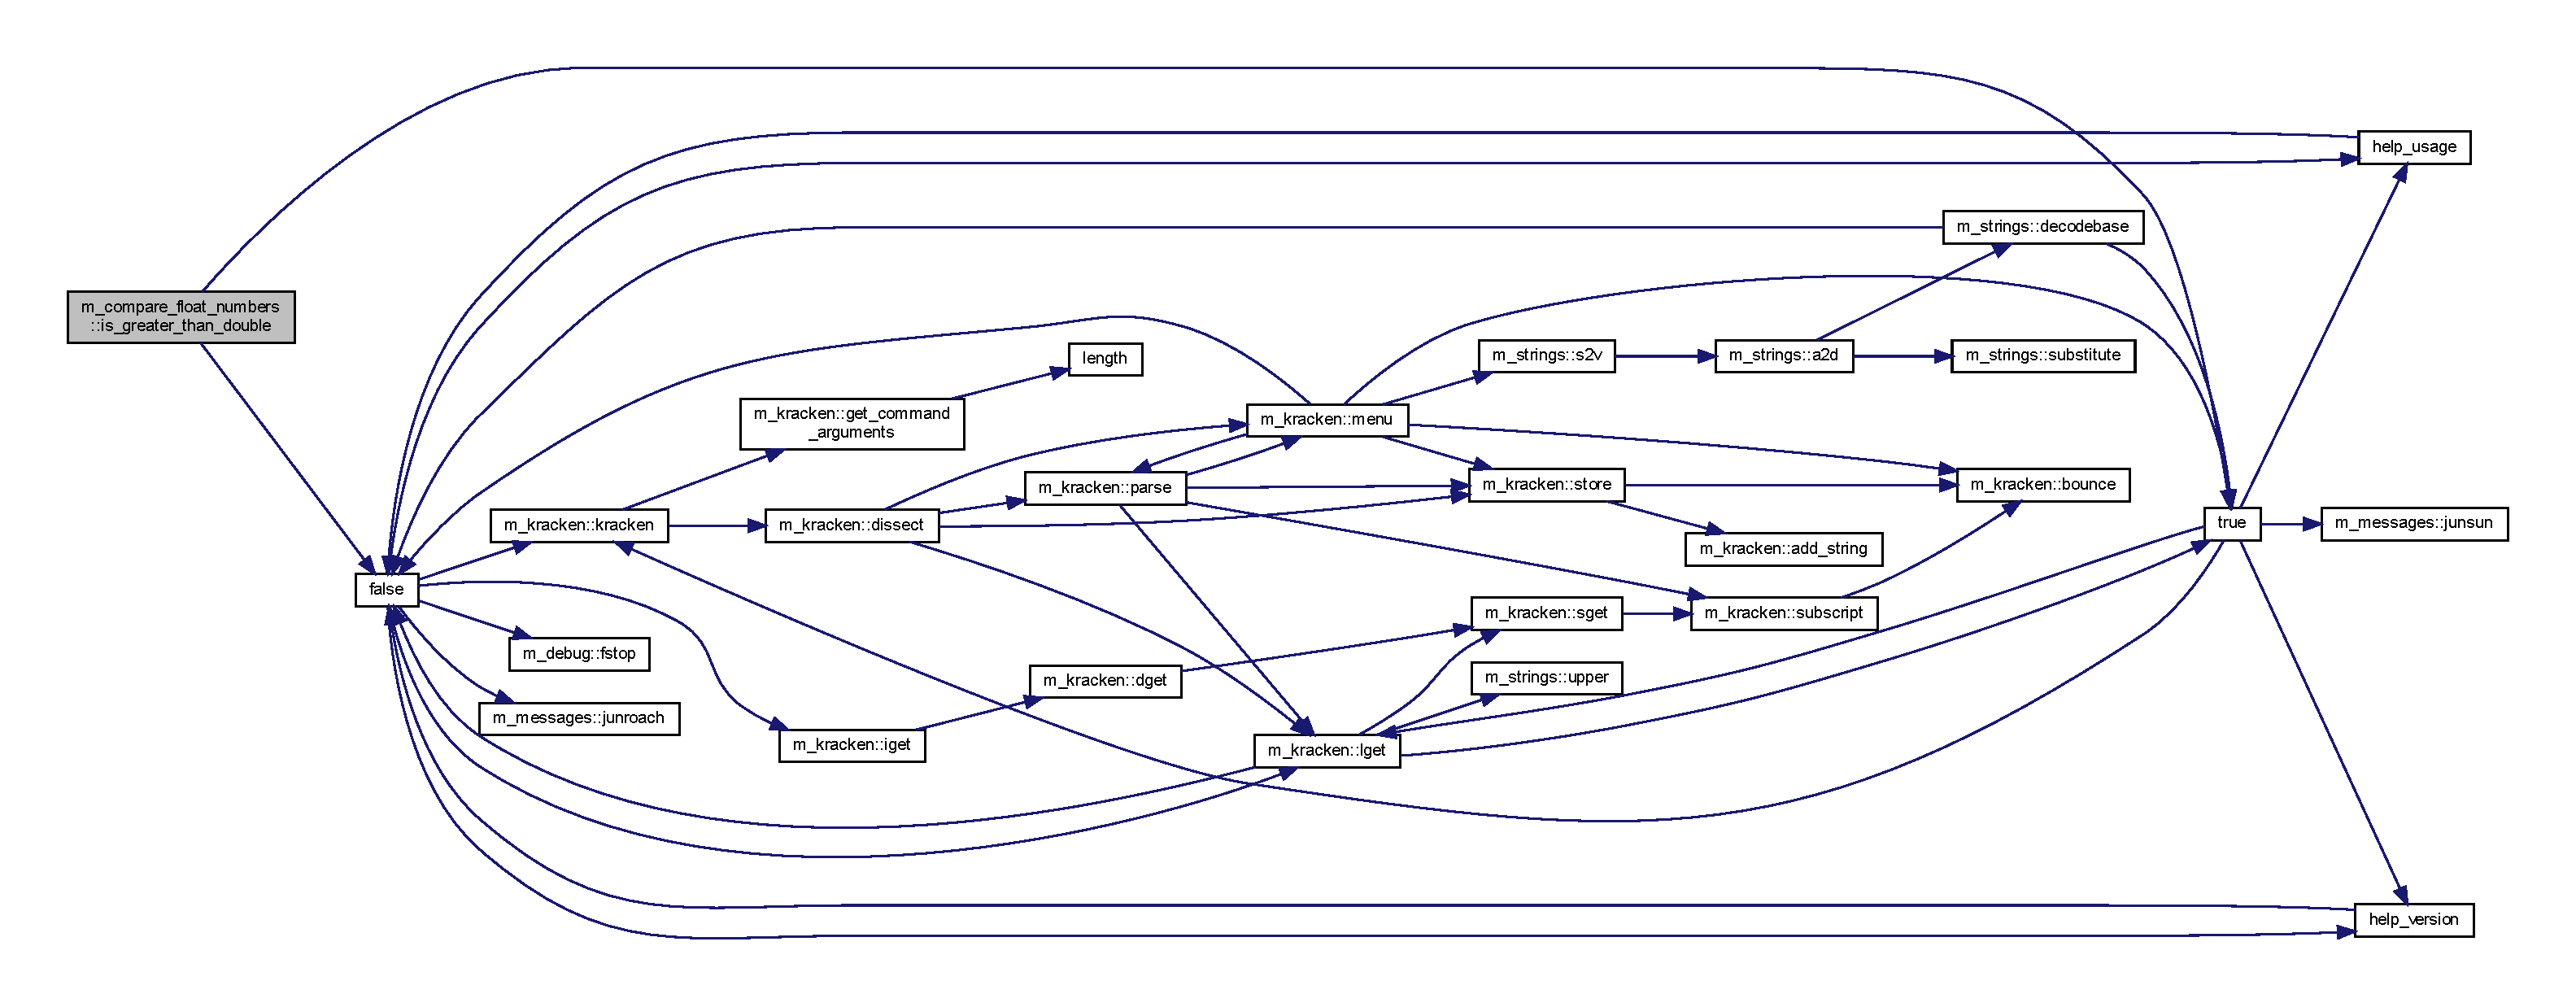
\includegraphics[width=350pt]{namespacem__compare__float__numbers_ac0b7c9aeec5a785ebff7a6e59ba5fb26_cgraph}
\end{center}
\end{figure}
\mbox{\Hypertarget{namespacem__compare__float__numbers_ab525ef9c044e5187643e04c64d470186}\label{namespacem__compare__float__numbers_ab525ef9c044e5187643e04c64d470186}} 
\index{m\+\_\+compare\+\_\+float\+\_\+numbers@{m\+\_\+compare\+\_\+float\+\_\+numbers}!is\+\_\+greater\+\_\+than\+\_\+single@{is\+\_\+greater\+\_\+than\+\_\+single}}
\index{is\+\_\+greater\+\_\+than\+\_\+single@{is\+\_\+greater\+\_\+than\+\_\+single}!m\+\_\+compare\+\_\+float\+\_\+numbers@{m\+\_\+compare\+\_\+float\+\_\+numbers}}
\subsubsection{\texorpdfstring{is\+\_\+greater\+\_\+than\+\_\+single()}{is\_greater\_than\_single()}}
{\footnotesize\ttfamily elemental logical function m\+\_\+compare\+\_\+float\+\_\+numbers\+::is\+\_\+greater\+\_\+than\+\_\+single (\begin{DoxyParamCaption}\item[{\hyperlink{read__watch_83_8txt_abdb62bde002f38ef75f810d3a905a823}{real}( \hyperlink{namespacem__compare__float__numbers_a5f122d46d6ad7d1cf0b899d9c855c498}{single} ), intent(\hyperlink{M__journal_83_8txt_afce72651d1eed785a2132bee863b2f38}{in})}]{x,  }\item[{\hyperlink{read__watch_83_8txt_abdb62bde002f38ef75f810d3a905a823}{real}( \hyperlink{namespacem__compare__float__numbers_a5f122d46d6ad7d1cf0b899d9c855c498}{single} ), intent(\hyperlink{M__journal_83_8txt_afce72651d1eed785a2132bee863b2f38}{in})}]{y }\end{DoxyParamCaption})\hspace{0.3cm}{\ttfamily [private]}}



References false(), and true().

Here is the call graph for this function\+:
\nopagebreak
\begin{figure}[H]
\begin{center}
\leavevmode
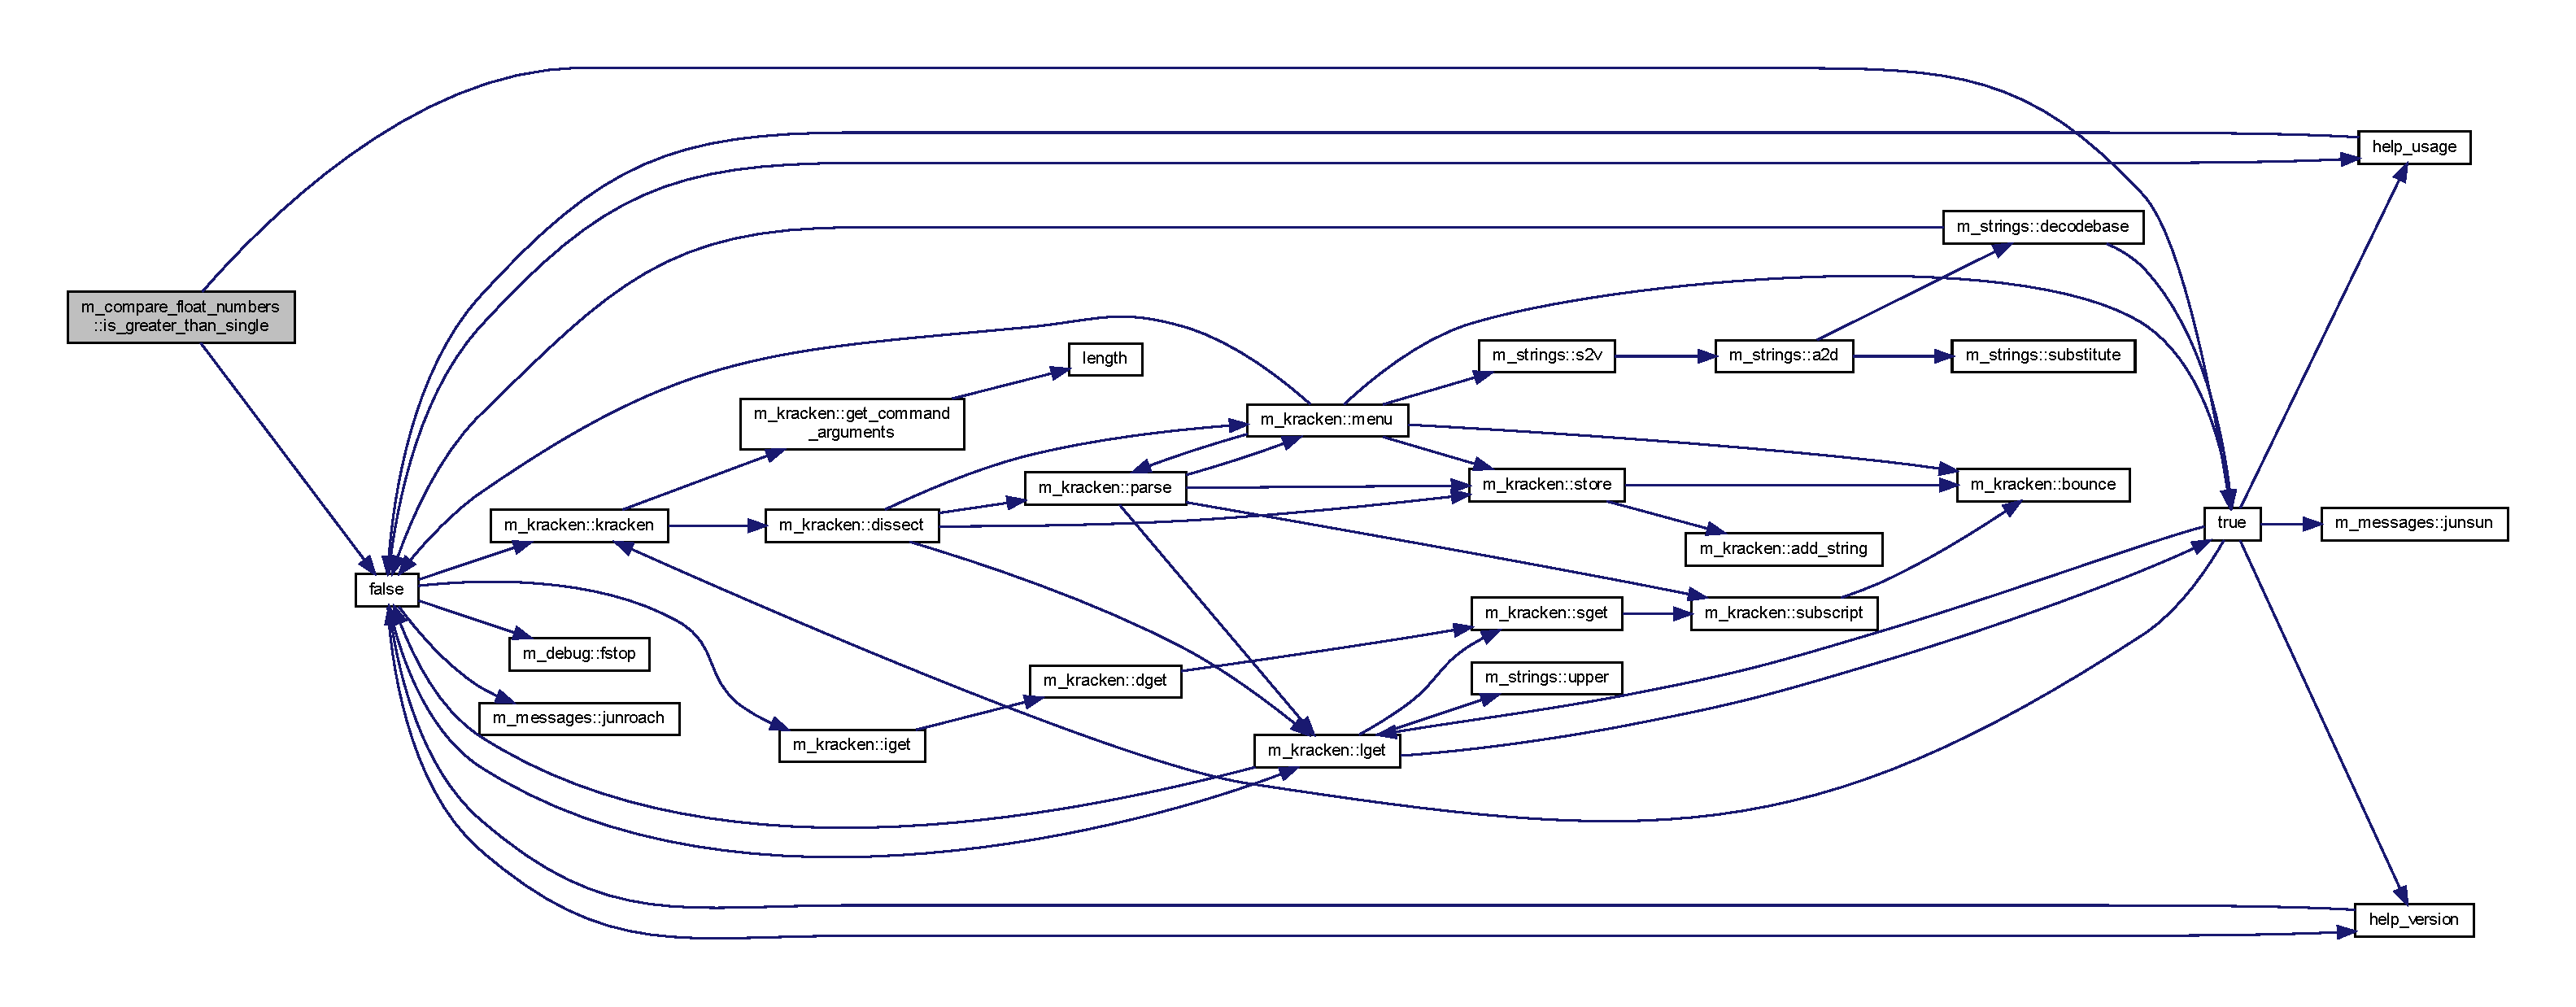
\includegraphics[width=350pt]{namespacem__compare__float__numbers_ab525ef9c044e5187643e04c64d470186_cgraph}
\end{center}
\end{figure}
\mbox{\Hypertarget{namespacem__compare__float__numbers_a36578a1fa0cf4ee3d29ded529dbd156c}\label{namespacem__compare__float__numbers_a36578a1fa0cf4ee3d29ded529dbd156c}} 
\index{m\+\_\+compare\+\_\+float\+\_\+numbers@{m\+\_\+compare\+\_\+float\+\_\+numbers}!is\+\_\+less\+\_\+than\+\_\+double@{is\+\_\+less\+\_\+than\+\_\+double}}
\index{is\+\_\+less\+\_\+than\+\_\+double@{is\+\_\+less\+\_\+than\+\_\+double}!m\+\_\+compare\+\_\+float\+\_\+numbers@{m\+\_\+compare\+\_\+float\+\_\+numbers}}
\subsubsection{\texorpdfstring{is\+\_\+less\+\_\+than\+\_\+double()}{is\_less\_than\_double()}}
{\footnotesize\ttfamily elemental logical function m\+\_\+compare\+\_\+float\+\_\+numbers\+::is\+\_\+less\+\_\+than\+\_\+double (\begin{DoxyParamCaption}\item[{\hyperlink{read__watch_83_8txt_abdb62bde002f38ef75f810d3a905a823}{real}( \hyperlink{namespacem__compare__float__numbers_af4b789cd6e1a2abcd412eaf29e91ea0c}{double} ), intent(\hyperlink{M__journal_83_8txt_afce72651d1eed785a2132bee863b2f38}{in})}]{x,  }\item[{\hyperlink{read__watch_83_8txt_abdb62bde002f38ef75f810d3a905a823}{real}( \hyperlink{namespacem__compare__float__numbers_af4b789cd6e1a2abcd412eaf29e91ea0c}{double} ), intent(\hyperlink{M__journal_83_8txt_afce72651d1eed785a2132bee863b2f38}{in})}]{y }\end{DoxyParamCaption})\hspace{0.3cm}{\ttfamily [private]}}



References false(), and true().

Here is the call graph for this function\+:
\nopagebreak
\begin{figure}[H]
\begin{center}
\leavevmode
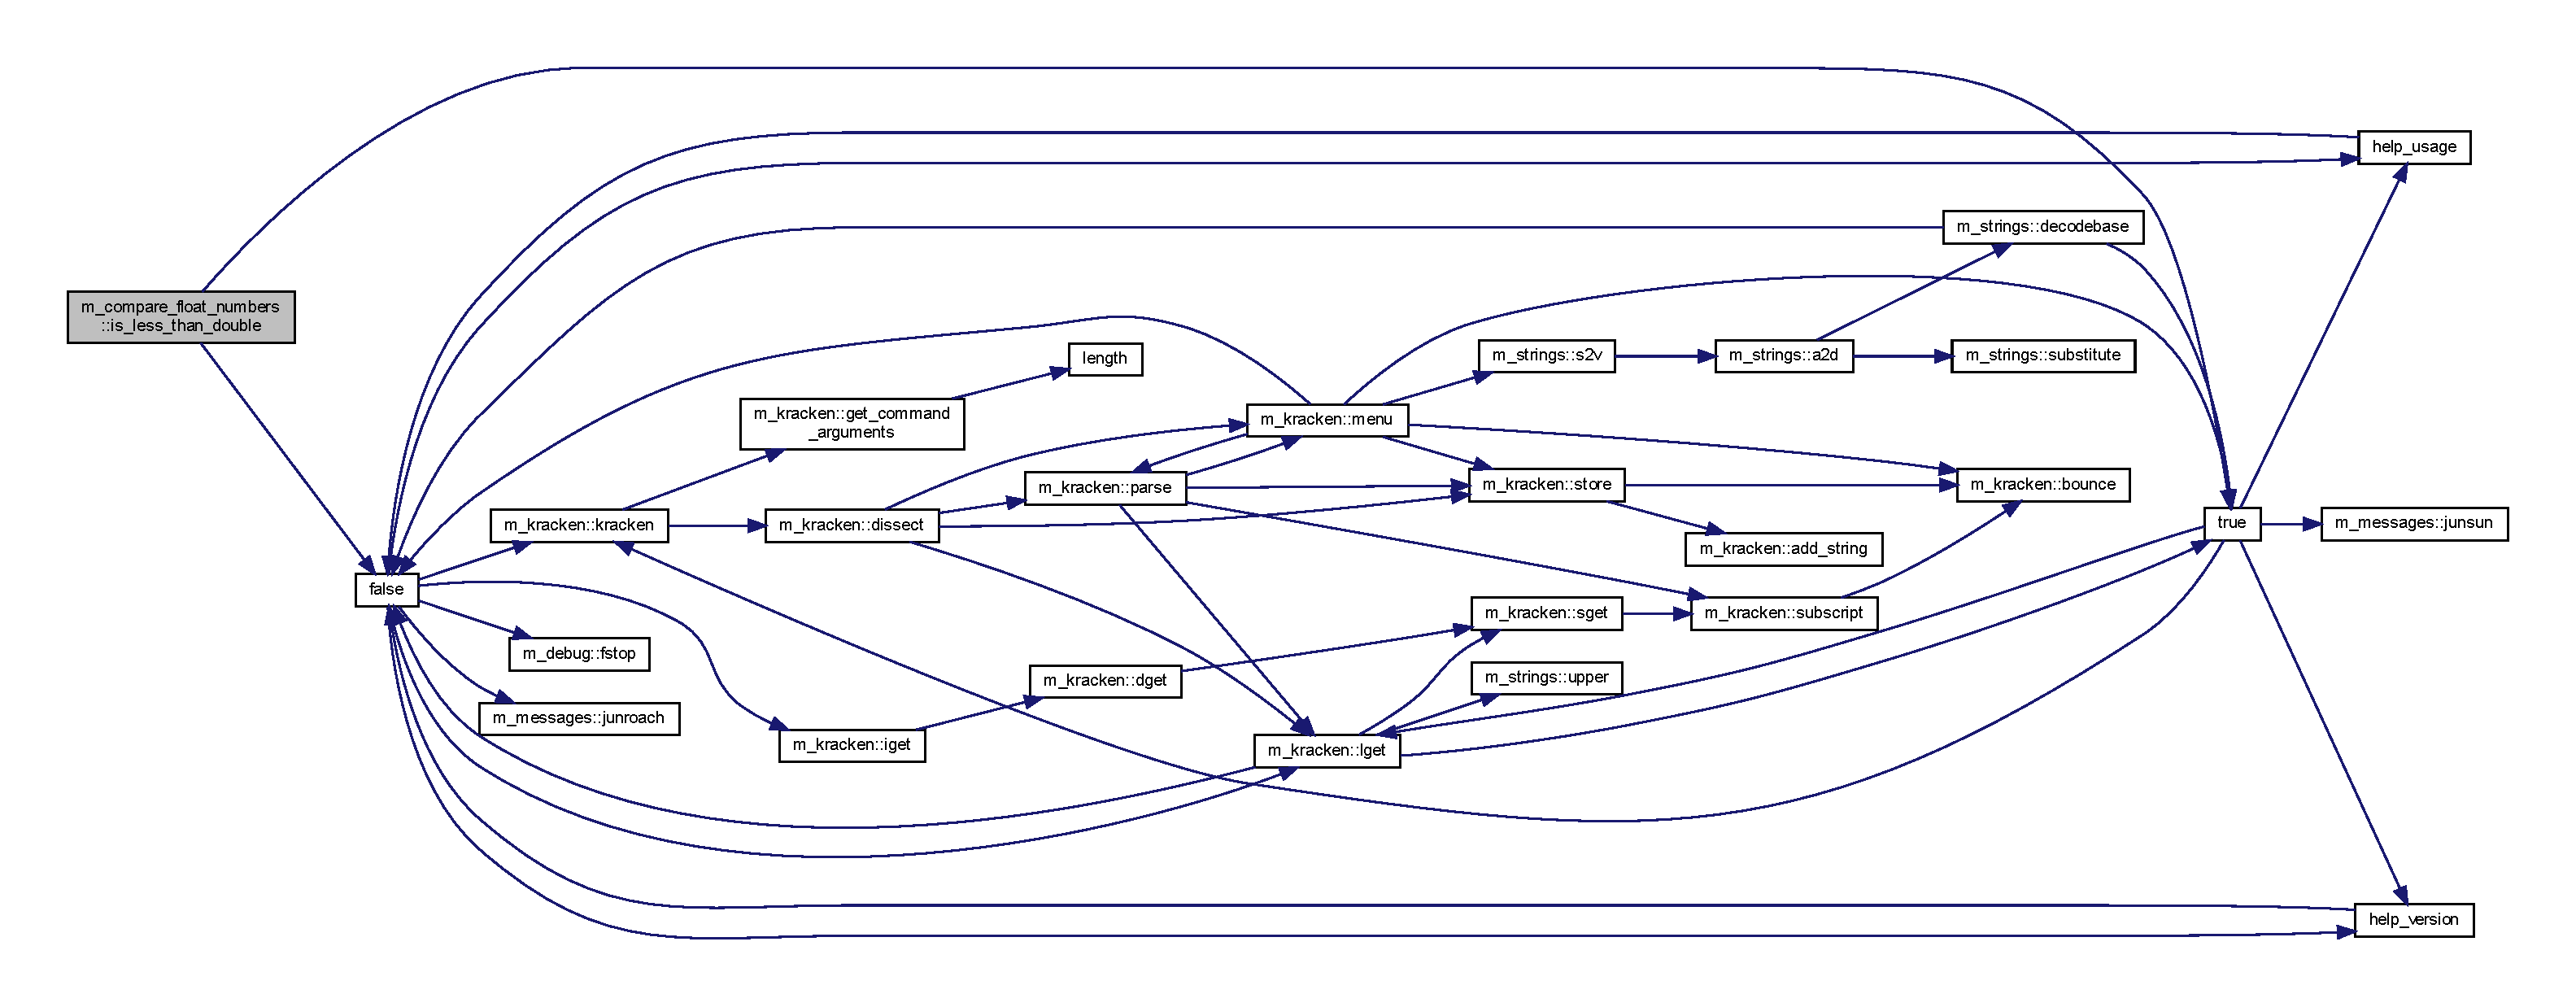
\includegraphics[width=350pt]{namespacem__compare__float__numbers_a36578a1fa0cf4ee3d29ded529dbd156c_cgraph}
\end{center}
\end{figure}
\mbox{\Hypertarget{namespacem__compare__float__numbers_a82b07d4a5f9076d2dc0655c8733549b5}\label{namespacem__compare__float__numbers_a82b07d4a5f9076d2dc0655c8733549b5}} 
\index{m\+\_\+compare\+\_\+float\+\_\+numbers@{m\+\_\+compare\+\_\+float\+\_\+numbers}!is\+\_\+less\+\_\+than\+\_\+single@{is\+\_\+less\+\_\+than\+\_\+single}}
\index{is\+\_\+less\+\_\+than\+\_\+single@{is\+\_\+less\+\_\+than\+\_\+single}!m\+\_\+compare\+\_\+float\+\_\+numbers@{m\+\_\+compare\+\_\+float\+\_\+numbers}}
\subsubsection{\texorpdfstring{is\+\_\+less\+\_\+than\+\_\+single()}{is\_less\_than\_single()}}
{\footnotesize\ttfamily elemental logical function m\+\_\+compare\+\_\+float\+\_\+numbers\+::is\+\_\+less\+\_\+than\+\_\+single (\begin{DoxyParamCaption}\item[{\hyperlink{read__watch_83_8txt_abdb62bde002f38ef75f810d3a905a823}{real}( \hyperlink{namespacem__compare__float__numbers_a5f122d46d6ad7d1cf0b899d9c855c498}{single} ), intent(\hyperlink{M__journal_83_8txt_afce72651d1eed785a2132bee863b2f38}{in})}]{x,  }\item[{\hyperlink{read__watch_83_8txt_abdb62bde002f38ef75f810d3a905a823}{real}( \hyperlink{namespacem__compare__float__numbers_a5f122d46d6ad7d1cf0b899d9c855c498}{single} ), intent(\hyperlink{M__journal_83_8txt_afce72651d1eed785a2132bee863b2f38}{in})}]{y }\end{DoxyParamCaption})\hspace{0.3cm}{\ttfamily [private]}}



References false(), and true().

Here is the call graph for this function\+:
\nopagebreak
\begin{figure}[H]
\begin{center}
\leavevmode
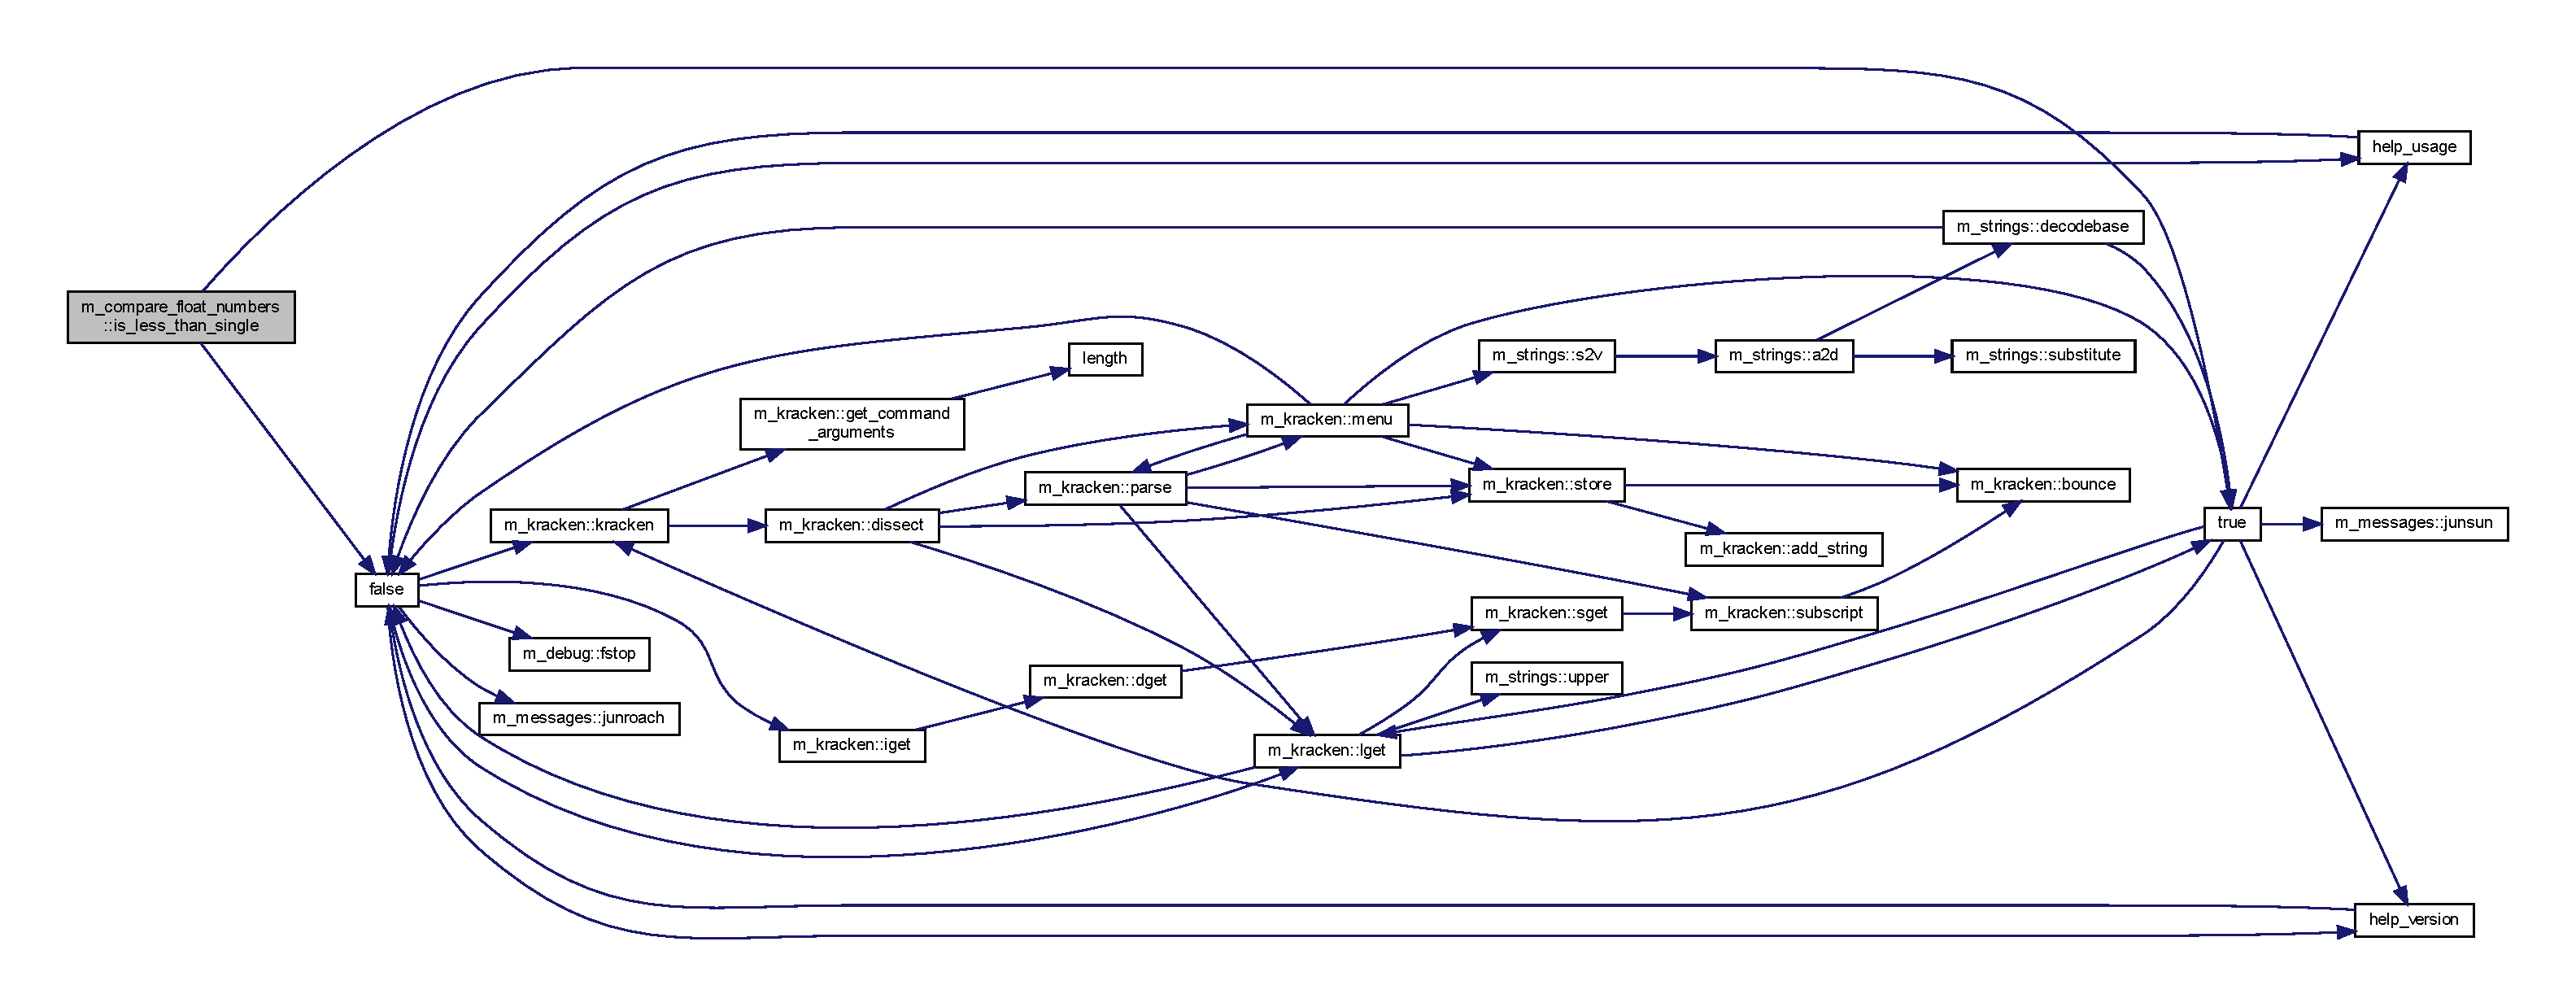
\includegraphics[width=350pt]{namespacem__compare__float__numbers_a82b07d4a5f9076d2dc0655c8733549b5_cgraph}
\end{center}
\end{figure}


\subsection{Variable Documentation}
\mbox{\Hypertarget{namespacem__compare__float__numbers_ae232d1653572b564934db62fc9caaa93}\label{namespacem__compare__float__numbers_ae232d1653572b564934db62fc9caaa93}} 
\index{m\+\_\+compare\+\_\+float\+\_\+numbers@{m\+\_\+compare\+\_\+float\+\_\+numbers}!byte@{byte}}
\index{byte@{byte}!m\+\_\+compare\+\_\+float\+\_\+numbers@{m\+\_\+compare\+\_\+float\+\_\+numbers}}
\subsubsection{\texorpdfstring{byte}{byte}}
{\footnotesize\ttfamily integer, parameter, \hyperlink{M__stopwatch_83_8txt_a2f74811300c361e53b430611a7d1769f}{public} m\+\_\+compare\+\_\+float\+\_\+numbers\+::byte = S\+E\+L\+E\+C\+T\+E\+D\+\_\+\+I\+N\+T\+\_\+\+K\+I\+ND(1)}

\mbox{\Hypertarget{namespacem__compare__float__numbers_af4b789cd6e1a2abcd412eaf29e91ea0c}\label{namespacem__compare__float__numbers_af4b789cd6e1a2abcd412eaf29e91ea0c}} 
\index{m\+\_\+compare\+\_\+float\+\_\+numbers@{m\+\_\+compare\+\_\+float\+\_\+numbers}!double@{double}}
\index{double@{double}!m\+\_\+compare\+\_\+float\+\_\+numbers@{m\+\_\+compare\+\_\+float\+\_\+numbers}}
\subsubsection{\texorpdfstring{double}{double}}
{\footnotesize\ttfamily integer, parameter, \hyperlink{M__stopwatch_83_8txt_a2f74811300c361e53b430611a7d1769f}{public} m\+\_\+compare\+\_\+float\+\_\+numbers\+::double = S\+E\+L\+E\+C\+T\+E\+D\+\_\+\+R\+E\+A\+L\+\_\+\+K\+I\+ND(15)}

\mbox{\Hypertarget{namespacem__compare__float__numbers_a24daff6e230d11a5d81a10bf1c055841}\label{namespacem__compare__float__numbers_a24daff6e230d11a5d81a10bf1c055841}} 
\index{m\+\_\+compare\+\_\+float\+\_\+numbers@{m\+\_\+compare\+\_\+float\+\_\+numbers}!fp\+\_\+byte\+\_\+sizes@{fp\+\_\+byte\+\_\+sizes}}
\index{fp\+\_\+byte\+\_\+sizes@{fp\+\_\+byte\+\_\+sizes}!m\+\_\+compare\+\_\+float\+\_\+numbers@{m\+\_\+compare\+\_\+float\+\_\+numbers}}
\subsubsection{\texorpdfstring{fp\+\_\+byte\+\_\+sizes}{fp\_byte\_sizes}}
{\footnotesize\ttfamily integer, dimension( \hyperlink{namespacem__compare__float__numbers_ae5e226645a7448efabc625aa89e78a20}{n\+\_\+fp\+\_\+kinds} ), parameter, private m\+\_\+compare\+\_\+float\+\_\+numbers\+::fp\+\_\+byte\+\_\+sizes = (/ n\+\_\+\+Bytes\+\_\+\+Single, n\+\_\+\+Bytes\+\_\+\+Double, n\+\_\+\+Bytes\+\_\+\+Quad /)\hspace{0.3cm}{\ttfamily [private]}}

\mbox{\Hypertarget{namespacem__compare__float__numbers_a51e33070a2e2a875e279521aaceaeae4}\label{namespacem__compare__float__numbers_a51e33070a2e2a875e279521aaceaeae4}} 
\index{m\+\_\+compare\+\_\+float\+\_\+numbers@{m\+\_\+compare\+\_\+float\+\_\+numbers}!fp\+\_\+kind@{fp\+\_\+kind}}
\index{fp\+\_\+kind@{fp\+\_\+kind}!m\+\_\+compare\+\_\+float\+\_\+numbers@{m\+\_\+compare\+\_\+float\+\_\+numbers}}
\subsubsection{\texorpdfstring{fp\+\_\+kind}{fp\_kind}}
{\footnotesize\ttfamily integer, parameter, \hyperlink{M__stopwatch_83_8txt_a2f74811300c361e53b430611a7d1769f}{public} m\+\_\+compare\+\_\+float\+\_\+numbers\+::fp\+\_\+kind = F\+P\+\_\+\+K\+I\+N\+D\+\_\+\+T\+Y\+P\+ES( I\+FP )}

\mbox{\Hypertarget{namespacem__compare__float__numbers_aa90581babf075fb76565a7ac27674522}\label{namespacem__compare__float__numbers_aa90581babf075fb76565a7ac27674522}} 
\index{m\+\_\+compare\+\_\+float\+\_\+numbers@{m\+\_\+compare\+\_\+float\+\_\+numbers}!fp\+\_\+kind\+\_\+types@{fp\+\_\+kind\+\_\+types}}
\index{fp\+\_\+kind\+\_\+types@{fp\+\_\+kind\+\_\+types}!m\+\_\+compare\+\_\+float\+\_\+numbers@{m\+\_\+compare\+\_\+float\+\_\+numbers}}
\subsubsection{\texorpdfstring{fp\+\_\+kind\+\_\+types}{fp\_kind\_types}}
{\footnotesize\ttfamily integer, dimension( \hyperlink{namespacem__compare__float__numbers_ae5e226645a7448efabc625aa89e78a20}{n\+\_\+fp\+\_\+kinds} ), parameter, private m\+\_\+compare\+\_\+float\+\_\+numbers\+::fp\+\_\+kind\+\_\+types = (/ Single, Double, Quad /)\hspace{0.3cm}{\ttfamily [private]}}

\mbox{\Hypertarget{namespacem__compare__float__numbers_abdbebb777d8ce2fa018e86724bfdfb9e}\label{namespacem__compare__float__numbers_abdbebb777d8ce2fa018e86724bfdfb9e}} 
\index{m\+\_\+compare\+\_\+float\+\_\+numbers@{m\+\_\+compare\+\_\+float\+\_\+numbers}!ifp@{ifp}}
\index{ifp@{ifp}!m\+\_\+compare\+\_\+float\+\_\+numbers@{m\+\_\+compare\+\_\+float\+\_\+numbers}}
\subsubsection{\texorpdfstring{ifp}{ifp}}
{\footnotesize\ttfamily integer, parameter, private m\+\_\+compare\+\_\+float\+\_\+numbers\+::ifp = 2\hspace{0.3cm}{\ttfamily [private]}}

\mbox{\Hypertarget{namespacem__compare__float__numbers_a6fab297801aadc3067acefdd136384ad}\label{namespacem__compare__float__numbers_a6fab297801aadc3067acefdd136384ad}} 
\index{m\+\_\+compare\+\_\+float\+\_\+numbers@{m\+\_\+compare\+\_\+float\+\_\+numbers}!iip@{iip}}
\index{iip@{iip}!m\+\_\+compare\+\_\+float\+\_\+numbers@{m\+\_\+compare\+\_\+float\+\_\+numbers}}
\subsubsection{\texorpdfstring{iip}{iip}}
{\footnotesize\ttfamily integer, parameter, private m\+\_\+compare\+\_\+float\+\_\+numbers\+::iip = 3\hspace{0.3cm}{\ttfamily [private]}}

\mbox{\Hypertarget{namespacem__compare__float__numbers_aee1b5dea82ea1e760308976a08df6356}\label{namespacem__compare__float__numbers_aee1b5dea82ea1e760308976a08df6356}} 
\index{m\+\_\+compare\+\_\+float\+\_\+numbers@{m\+\_\+compare\+\_\+float\+\_\+numbers}!ip\+\_\+byte\+\_\+sizes@{ip\+\_\+byte\+\_\+sizes}}
\index{ip\+\_\+byte\+\_\+sizes@{ip\+\_\+byte\+\_\+sizes}!m\+\_\+compare\+\_\+float\+\_\+numbers@{m\+\_\+compare\+\_\+float\+\_\+numbers}}
\subsubsection{\texorpdfstring{ip\+\_\+byte\+\_\+sizes}{ip\_byte\_sizes}}
{\footnotesize\ttfamily integer, dimension( \hyperlink{namespacem__compare__float__numbers_a6cbe22bf2f7aa1ada923de776f8258bf}{n\+\_\+ip\+\_\+kinds} ), parameter, private m\+\_\+compare\+\_\+float\+\_\+numbers\+::ip\+\_\+byte\+\_\+sizes = (/ n\+\_\+\+Bytes\+\_\+\+Byte, n\+\_\+\+Bytes\+\_\+\+Short, n\+\_\+\+Bytes\+\_\+\+Long, n\+\_\+\+Bytes\+\_\+\+L\+Long /)\hspace{0.3cm}{\ttfamily [private]}}

\mbox{\Hypertarget{namespacem__compare__float__numbers_a932ca5131dba16f9e2d30e75cf79b574}\label{namespacem__compare__float__numbers_a932ca5131dba16f9e2d30e75cf79b574}} 
\index{m\+\_\+compare\+\_\+float\+\_\+numbers@{m\+\_\+compare\+\_\+float\+\_\+numbers}!ip\+\_\+kind@{ip\+\_\+kind}}
\index{ip\+\_\+kind@{ip\+\_\+kind}!m\+\_\+compare\+\_\+float\+\_\+numbers@{m\+\_\+compare\+\_\+float\+\_\+numbers}}
\subsubsection{\texorpdfstring{ip\+\_\+kind}{ip\_kind}}
{\footnotesize\ttfamily integer, parameter, \hyperlink{M__stopwatch_83_8txt_a2f74811300c361e53b430611a7d1769f}{public} m\+\_\+compare\+\_\+float\+\_\+numbers\+::ip\+\_\+kind = I\+P\+\_\+\+K\+I\+N\+D\+\_\+\+T\+Y\+P\+ES( I\+IP )}

\mbox{\Hypertarget{namespacem__compare__float__numbers_a18a2ec0b5b6a904a6ccd63fad576f759}\label{namespacem__compare__float__numbers_a18a2ec0b5b6a904a6ccd63fad576f759}} 
\index{m\+\_\+compare\+\_\+float\+\_\+numbers@{m\+\_\+compare\+\_\+float\+\_\+numbers}!ip\+\_\+kind\+\_\+types@{ip\+\_\+kind\+\_\+types}}
\index{ip\+\_\+kind\+\_\+types@{ip\+\_\+kind\+\_\+types}!m\+\_\+compare\+\_\+float\+\_\+numbers@{m\+\_\+compare\+\_\+float\+\_\+numbers}}
\subsubsection{\texorpdfstring{ip\+\_\+kind\+\_\+types}{ip\_kind\_types}}
{\footnotesize\ttfamily integer, dimension( \hyperlink{namespacem__compare__float__numbers_a6cbe22bf2f7aa1ada923de776f8258bf}{n\+\_\+ip\+\_\+kinds} ), parameter, private m\+\_\+compare\+\_\+float\+\_\+numbers\+::ip\+\_\+kind\+\_\+types = (/ Byte, Short, Long, L\+Long /)\hspace{0.3cm}{\ttfamily [private]}}

\mbox{\Hypertarget{namespacem__compare__float__numbers_a9c3da9dd020c03b19ee8acf1dafdce20}\label{namespacem__compare__float__numbers_a9c3da9dd020c03b19ee8acf1dafdce20}} 
\index{m\+\_\+compare\+\_\+float\+\_\+numbers@{m\+\_\+compare\+\_\+float\+\_\+numbers}!llong@{llong}}
\index{llong@{llong}!m\+\_\+compare\+\_\+float\+\_\+numbers@{m\+\_\+compare\+\_\+float\+\_\+numbers}}
\subsubsection{\texorpdfstring{llong}{llong}}
{\footnotesize\ttfamily integer, parameter, \hyperlink{M__stopwatch_83_8txt_a2f74811300c361e53b430611a7d1769f}{public} m\+\_\+compare\+\_\+float\+\_\+numbers\+::llong = ( ( ( 1 + S\+I\+GN( 1, L\+Long\+\_\+t ) ) / 2 ) $\ast$ L\+Long\+\_\+t ) + ( ( ( 1 -\/ S\+I\+GN( 1, L\+Long\+\_\+t ) ) / 2 ) $\ast$ Long )}

\mbox{\Hypertarget{namespacem__compare__float__numbers_a7c4a2b4cc39888d092d7a754897be9e5}\label{namespacem__compare__float__numbers_a7c4a2b4cc39888d092d7a754897be9e5}} 
\index{m\+\_\+compare\+\_\+float\+\_\+numbers@{m\+\_\+compare\+\_\+float\+\_\+numbers}!llong\+\_\+t@{llong\+\_\+t}}
\index{llong\+\_\+t@{llong\+\_\+t}!m\+\_\+compare\+\_\+float\+\_\+numbers@{m\+\_\+compare\+\_\+float\+\_\+numbers}}
\subsubsection{\texorpdfstring{llong\+\_\+t}{llong\_t}}
{\footnotesize\ttfamily integer, parameter, private m\+\_\+compare\+\_\+float\+\_\+numbers\+::llong\+\_\+t = S\+E\+L\+E\+C\+T\+E\+D\+\_\+\+I\+N\+T\+\_\+\+K\+I\+ND(16)\hspace{0.3cm}{\ttfamily [private]}}

\mbox{\Hypertarget{namespacem__compare__float__numbers_a1a70f80b01ccf5c63ed3eb70fabdaf2d}\label{namespacem__compare__float__numbers_a1a70f80b01ccf5c63ed3eb70fabdaf2d}} 
\index{m\+\_\+compare\+\_\+float\+\_\+numbers@{m\+\_\+compare\+\_\+float\+\_\+numbers}!long@{long}}
\index{long@{long}!m\+\_\+compare\+\_\+float\+\_\+numbers@{m\+\_\+compare\+\_\+float\+\_\+numbers}}
\subsubsection{\texorpdfstring{long}{long}}
{\footnotesize\ttfamily integer, parameter, \hyperlink{M__stopwatch_83_8txt_a2f74811300c361e53b430611a7d1769f}{public} m\+\_\+compare\+\_\+float\+\_\+numbers\+::long = S\+E\+L\+E\+C\+T\+E\+D\+\_\+\+I\+N\+T\+\_\+\+K\+I\+ND(8)}

\mbox{\Hypertarget{namespacem__compare__float__numbers_ae0ee7ae6cb351f1a6cf7301460d0d592}\label{namespacem__compare__float__numbers_ae0ee7ae6cb351f1a6cf7301460d0d592}} 
\index{m\+\_\+compare\+\_\+float\+\_\+numbers@{m\+\_\+compare\+\_\+float\+\_\+numbers}!module\+\_\+rcs\+\_\+id@{module\+\_\+rcs\+\_\+id}}
\index{module\+\_\+rcs\+\_\+id@{module\+\_\+rcs\+\_\+id}!m\+\_\+compare\+\_\+float\+\_\+numbers@{m\+\_\+compare\+\_\+float\+\_\+numbers}}
\subsubsection{\texorpdfstring{module\+\_\+rcs\+\_\+id}{module\_rcs\_id}}
{\footnotesize\ttfamily \hyperlink{option__stopwatch_83_8txt_abd4b21fbbd175834027b5224bfe97e66}{character}(len=$\ast$), parameter, private m\+\_\+compare\+\_\+float\+\_\+numbers\+::module\+\_\+rcs\+\_\+id = \textquotesingle{}\$Id\+: M\+\_\+\+Compare\+\_\+\+Float\+\_\+\+Numbers.\+f90,v 2.\+3 2004/10/06 19\+:00\+:23 paulv Exp \$\textquotesingle{}\hspace{0.3cm}{\ttfamily [private]}}

\mbox{\Hypertarget{namespacem__compare__float__numbers_a5faf0176b9b713e8d12ede8294da171d}\label{namespacem__compare__float__numbers_a5faf0176b9b713e8d12ede8294da171d}} 
\index{m\+\_\+compare\+\_\+float\+\_\+numbers@{m\+\_\+compare\+\_\+float\+\_\+numbers}!n\+\_\+bytes\+\_\+byte@{n\+\_\+bytes\+\_\+byte}}
\index{n\+\_\+bytes\+\_\+byte@{n\+\_\+bytes\+\_\+byte}!m\+\_\+compare\+\_\+float\+\_\+numbers@{m\+\_\+compare\+\_\+float\+\_\+numbers}}
\subsubsection{\texorpdfstring{n\+\_\+bytes\+\_\+byte}{n\_bytes\_byte}}
{\footnotesize\ttfamily integer, parameter, \hyperlink{M__stopwatch_83_8txt_a2f74811300c361e53b430611a7d1769f}{public} m\+\_\+compare\+\_\+float\+\_\+numbers\+::n\+\_\+bytes\+\_\+byte = 1}

\mbox{\Hypertarget{namespacem__compare__float__numbers_a801fa0d9fea2f2c025618157c128bfe2}\label{namespacem__compare__float__numbers_a801fa0d9fea2f2c025618157c128bfe2}} 
\index{m\+\_\+compare\+\_\+float\+\_\+numbers@{m\+\_\+compare\+\_\+float\+\_\+numbers}!n\+\_\+bytes\+\_\+double@{n\+\_\+bytes\+\_\+double}}
\index{n\+\_\+bytes\+\_\+double@{n\+\_\+bytes\+\_\+double}!m\+\_\+compare\+\_\+float\+\_\+numbers@{m\+\_\+compare\+\_\+float\+\_\+numbers}}
\subsubsection{\texorpdfstring{n\+\_\+bytes\+\_\+double}{n\_bytes\_double}}
{\footnotesize\ttfamily integer, parameter, \hyperlink{M__stopwatch_83_8txt_a2f74811300c361e53b430611a7d1769f}{public} m\+\_\+compare\+\_\+float\+\_\+numbers\+::n\+\_\+bytes\+\_\+double = 8}

\mbox{\Hypertarget{namespacem__compare__float__numbers_a48468c49657b53321fe55ac0795ba258}\label{namespacem__compare__float__numbers_a48468c49657b53321fe55ac0795ba258}} 
\index{m\+\_\+compare\+\_\+float\+\_\+numbers@{m\+\_\+compare\+\_\+float\+\_\+numbers}!n\+\_\+bytes\+\_\+fp\+\_\+kind@{n\+\_\+bytes\+\_\+fp\+\_\+kind}}
\index{n\+\_\+bytes\+\_\+fp\+\_\+kind@{n\+\_\+bytes\+\_\+fp\+\_\+kind}!m\+\_\+compare\+\_\+float\+\_\+numbers@{m\+\_\+compare\+\_\+float\+\_\+numbers}}
\subsubsection{\texorpdfstring{n\+\_\+bytes\+\_\+fp\+\_\+kind}{n\_bytes\_fp\_kind}}
{\footnotesize\ttfamily integer, parameter, \hyperlink{M__stopwatch_83_8txt_a2f74811300c361e53b430611a7d1769f}{public} m\+\_\+compare\+\_\+float\+\_\+numbers\+::n\+\_\+bytes\+\_\+fp\+\_\+kind = F\+P\+\_\+\+B\+Y\+T\+E\+\_\+\+S\+I\+Z\+ES( I\+FP )}

\mbox{\Hypertarget{namespacem__compare__float__numbers_a868bf02722b9070cff22ba7803aeffed}\label{namespacem__compare__float__numbers_a868bf02722b9070cff22ba7803aeffed}} 
\index{m\+\_\+compare\+\_\+float\+\_\+numbers@{m\+\_\+compare\+\_\+float\+\_\+numbers}!n\+\_\+bytes\+\_\+ip\+\_\+kind@{n\+\_\+bytes\+\_\+ip\+\_\+kind}}
\index{n\+\_\+bytes\+\_\+ip\+\_\+kind@{n\+\_\+bytes\+\_\+ip\+\_\+kind}!m\+\_\+compare\+\_\+float\+\_\+numbers@{m\+\_\+compare\+\_\+float\+\_\+numbers}}
\subsubsection{\texorpdfstring{n\+\_\+bytes\+\_\+ip\+\_\+kind}{n\_bytes\_ip\_kind}}
{\footnotesize\ttfamily integer, parameter, \hyperlink{M__stopwatch_83_8txt_a2f74811300c361e53b430611a7d1769f}{public} m\+\_\+compare\+\_\+float\+\_\+numbers\+::n\+\_\+bytes\+\_\+ip\+\_\+kind = I\+P\+\_\+\+B\+Y\+T\+E\+\_\+\+S\+I\+Z\+ES( I\+IP )}

\mbox{\Hypertarget{namespacem__compare__float__numbers_a2c4b39b521fa4fe5ea36044ddbbbb2ba}\label{namespacem__compare__float__numbers_a2c4b39b521fa4fe5ea36044ddbbbb2ba}} 
\index{m\+\_\+compare\+\_\+float\+\_\+numbers@{m\+\_\+compare\+\_\+float\+\_\+numbers}!n\+\_\+bytes\+\_\+llong@{n\+\_\+bytes\+\_\+llong}}
\index{n\+\_\+bytes\+\_\+llong@{n\+\_\+bytes\+\_\+llong}!m\+\_\+compare\+\_\+float\+\_\+numbers@{m\+\_\+compare\+\_\+float\+\_\+numbers}}
\subsubsection{\texorpdfstring{n\+\_\+bytes\+\_\+llong}{n\_bytes\_llong}}
{\footnotesize\ttfamily integer, parameter, \hyperlink{M__stopwatch_83_8txt_a2f74811300c361e53b430611a7d1769f}{public} m\+\_\+compare\+\_\+float\+\_\+numbers\+::n\+\_\+bytes\+\_\+llong = 8}

\mbox{\Hypertarget{namespacem__compare__float__numbers_a6295d4185db12b4e3d14c67de6164dd4}\label{namespacem__compare__float__numbers_a6295d4185db12b4e3d14c67de6164dd4}} 
\index{m\+\_\+compare\+\_\+float\+\_\+numbers@{m\+\_\+compare\+\_\+float\+\_\+numbers}!n\+\_\+bytes\+\_\+long@{n\+\_\+bytes\+\_\+long}}
\index{n\+\_\+bytes\+\_\+long@{n\+\_\+bytes\+\_\+long}!m\+\_\+compare\+\_\+float\+\_\+numbers@{m\+\_\+compare\+\_\+float\+\_\+numbers}}
\subsubsection{\texorpdfstring{n\+\_\+bytes\+\_\+long}{n\_bytes\_long}}
{\footnotesize\ttfamily integer, parameter, \hyperlink{M__stopwatch_83_8txt_a2f74811300c361e53b430611a7d1769f}{public} m\+\_\+compare\+\_\+float\+\_\+numbers\+::n\+\_\+bytes\+\_\+long = 4}

\mbox{\Hypertarget{namespacem__compare__float__numbers_abbe80858664126778bff36ea408c71dc}\label{namespacem__compare__float__numbers_abbe80858664126778bff36ea408c71dc}} 
\index{m\+\_\+compare\+\_\+float\+\_\+numbers@{m\+\_\+compare\+\_\+float\+\_\+numbers}!n\+\_\+bytes\+\_\+quad@{n\+\_\+bytes\+\_\+quad}}
\index{n\+\_\+bytes\+\_\+quad@{n\+\_\+bytes\+\_\+quad}!m\+\_\+compare\+\_\+float\+\_\+numbers@{m\+\_\+compare\+\_\+float\+\_\+numbers}}
\subsubsection{\texorpdfstring{n\+\_\+bytes\+\_\+quad}{n\_bytes\_quad}}
{\footnotesize\ttfamily integer, parameter, \hyperlink{M__stopwatch_83_8txt_a2f74811300c361e53b430611a7d1769f}{public} m\+\_\+compare\+\_\+float\+\_\+numbers\+::n\+\_\+bytes\+\_\+quad = 16}

\mbox{\Hypertarget{namespacem__compare__float__numbers_acff1ac867eea95e76e28f083be5bddcc}\label{namespacem__compare__float__numbers_acff1ac867eea95e76e28f083be5bddcc}} 
\index{m\+\_\+compare\+\_\+float\+\_\+numbers@{m\+\_\+compare\+\_\+float\+\_\+numbers}!n\+\_\+bytes\+\_\+short@{n\+\_\+bytes\+\_\+short}}
\index{n\+\_\+bytes\+\_\+short@{n\+\_\+bytes\+\_\+short}!m\+\_\+compare\+\_\+float\+\_\+numbers@{m\+\_\+compare\+\_\+float\+\_\+numbers}}
\subsubsection{\texorpdfstring{n\+\_\+bytes\+\_\+short}{n\_bytes\_short}}
{\footnotesize\ttfamily integer, parameter, \hyperlink{M__stopwatch_83_8txt_a2f74811300c361e53b430611a7d1769f}{public} m\+\_\+compare\+\_\+float\+\_\+numbers\+::n\+\_\+bytes\+\_\+short = 2}

\mbox{\Hypertarget{namespacem__compare__float__numbers_a8d387475f5c4f6cc89da998183cf9077}\label{namespacem__compare__float__numbers_a8d387475f5c4f6cc89da998183cf9077}} 
\index{m\+\_\+compare\+\_\+float\+\_\+numbers@{m\+\_\+compare\+\_\+float\+\_\+numbers}!n\+\_\+bytes\+\_\+single@{n\+\_\+bytes\+\_\+single}}
\index{n\+\_\+bytes\+\_\+single@{n\+\_\+bytes\+\_\+single}!m\+\_\+compare\+\_\+float\+\_\+numbers@{m\+\_\+compare\+\_\+float\+\_\+numbers}}
\subsubsection{\texorpdfstring{n\+\_\+bytes\+\_\+single}{n\_bytes\_single}}
{\footnotesize\ttfamily integer, parameter, \hyperlink{M__stopwatch_83_8txt_a2f74811300c361e53b430611a7d1769f}{public} m\+\_\+compare\+\_\+float\+\_\+numbers\+::n\+\_\+bytes\+\_\+single = 4}

\mbox{\Hypertarget{namespacem__compare__float__numbers_ae5e226645a7448efabc625aa89e78a20}\label{namespacem__compare__float__numbers_ae5e226645a7448efabc625aa89e78a20}} 
\index{m\+\_\+compare\+\_\+float\+\_\+numbers@{m\+\_\+compare\+\_\+float\+\_\+numbers}!n\+\_\+fp\+\_\+kinds@{n\+\_\+fp\+\_\+kinds}}
\index{n\+\_\+fp\+\_\+kinds@{n\+\_\+fp\+\_\+kinds}!m\+\_\+compare\+\_\+float\+\_\+numbers@{m\+\_\+compare\+\_\+float\+\_\+numbers}}
\subsubsection{\texorpdfstring{n\+\_\+fp\+\_\+kinds}{n\_fp\_kinds}}
{\footnotesize\ttfamily integer, parameter, private m\+\_\+compare\+\_\+float\+\_\+numbers\+::n\+\_\+fp\+\_\+kinds = 3\hspace{0.3cm}{\ttfamily [private]}}

\mbox{\Hypertarget{namespacem__compare__float__numbers_a6cbe22bf2f7aa1ada923de776f8258bf}\label{namespacem__compare__float__numbers_a6cbe22bf2f7aa1ada923de776f8258bf}} 
\index{m\+\_\+compare\+\_\+float\+\_\+numbers@{m\+\_\+compare\+\_\+float\+\_\+numbers}!n\+\_\+ip\+\_\+kinds@{n\+\_\+ip\+\_\+kinds}}
\index{n\+\_\+ip\+\_\+kinds@{n\+\_\+ip\+\_\+kinds}!m\+\_\+compare\+\_\+float\+\_\+numbers@{m\+\_\+compare\+\_\+float\+\_\+numbers}}
\subsubsection{\texorpdfstring{n\+\_\+ip\+\_\+kinds}{n\_ip\_kinds}}
{\footnotesize\ttfamily integer, parameter, private m\+\_\+compare\+\_\+float\+\_\+numbers\+::n\+\_\+ip\+\_\+kinds = 4\hspace{0.3cm}{\ttfamily [private]}}

\mbox{\Hypertarget{namespacem__compare__float__numbers_af11cd62e9032de86b00de623b4eb5c2c}\label{namespacem__compare__float__numbers_af11cd62e9032de86b00de623b4eb5c2c}} 
\index{m\+\_\+compare\+\_\+float\+\_\+numbers@{m\+\_\+compare\+\_\+float\+\_\+numbers}!quad@{quad}}
\index{quad@{quad}!m\+\_\+compare\+\_\+float\+\_\+numbers@{m\+\_\+compare\+\_\+float\+\_\+numbers}}
\subsubsection{\texorpdfstring{quad}{quad}}
{\footnotesize\ttfamily integer, parameter, \hyperlink{M__stopwatch_83_8txt_a2f74811300c361e53b430611a7d1769f}{public} m\+\_\+compare\+\_\+float\+\_\+numbers\+::quad = ( ( ( 1 + S\+I\+GN( 1, Quad\+\_\+t ) ) / 2 ) $\ast$ Quad\+\_\+t ) + ( ( ( 1 -\/ S\+I\+GN( 1, Quad\+\_\+t ) ) / 2 ) $\ast$ Double )}

\mbox{\Hypertarget{namespacem__compare__float__numbers_a3cb67561a1bb5038eddb1aafcce81199}\label{namespacem__compare__float__numbers_a3cb67561a1bb5038eddb1aafcce81199}} 
\index{m\+\_\+compare\+\_\+float\+\_\+numbers@{m\+\_\+compare\+\_\+float\+\_\+numbers}!quad\+\_\+t@{quad\+\_\+t}}
\index{quad\+\_\+t@{quad\+\_\+t}!m\+\_\+compare\+\_\+float\+\_\+numbers@{m\+\_\+compare\+\_\+float\+\_\+numbers}}
\subsubsection{\texorpdfstring{quad\+\_\+t}{quad\_t}}
{\footnotesize\ttfamily integer, parameter, private m\+\_\+compare\+\_\+float\+\_\+numbers\+::quad\+\_\+t = S\+E\+L\+E\+C\+T\+E\+D\+\_\+\+R\+E\+A\+L\+\_\+\+K\+I\+ND(20)\hspace{0.3cm}{\ttfamily [private]}}

\mbox{\Hypertarget{namespacem__compare__float__numbers_a8afcd039ad8a1e52969e5a5165163b68}\label{namespacem__compare__float__numbers_a8afcd039ad8a1e52969e5a5165163b68}} 
\index{m\+\_\+compare\+\_\+float\+\_\+numbers@{m\+\_\+compare\+\_\+float\+\_\+numbers}!short@{short}}
\index{short@{short}!m\+\_\+compare\+\_\+float\+\_\+numbers@{m\+\_\+compare\+\_\+float\+\_\+numbers}}
\subsubsection{\texorpdfstring{short}{short}}
{\footnotesize\ttfamily integer, parameter, \hyperlink{M__stopwatch_83_8txt_a2f74811300c361e53b430611a7d1769f}{public} m\+\_\+compare\+\_\+float\+\_\+numbers\+::short = S\+E\+L\+E\+C\+T\+E\+D\+\_\+\+I\+N\+T\+\_\+\+K\+I\+ND(4)}

\mbox{\Hypertarget{namespacem__compare__float__numbers_a5f122d46d6ad7d1cf0b899d9c855c498}\label{namespacem__compare__float__numbers_a5f122d46d6ad7d1cf0b899d9c855c498}} 
\index{m\+\_\+compare\+\_\+float\+\_\+numbers@{m\+\_\+compare\+\_\+float\+\_\+numbers}!single@{single}}
\index{single@{single}!m\+\_\+compare\+\_\+float\+\_\+numbers@{m\+\_\+compare\+\_\+float\+\_\+numbers}}
\subsubsection{\texorpdfstring{single}{single}}
{\footnotesize\ttfamily integer, parameter, \hyperlink{M__stopwatch_83_8txt_a2f74811300c361e53b430611a7d1769f}{public} m\+\_\+compare\+\_\+float\+\_\+numbers\+::single = S\+E\+L\+E\+C\+T\+E\+D\+\_\+\+R\+E\+A\+L\+\_\+\+K\+I\+ND(6)}


\hypertarget{namespacem__constants}{}\section{m\+\_\+constants Module Reference}
\label{namespacem__constants}\index{m\+\_\+constants@{m\+\_\+constants}}


\subsubsection*{N\+A\+ME}

M\+\_\+constants(3fm) -\/ common constants \subsubsection*{S\+Y\+N\+O\+P\+S\+IS} 


\subsection*{Variables}
\begin{DoxyCompactItemize}
\item 
\hyperlink{option__stopwatch_83_8txt_abd4b21fbbd175834027b5224bfe97e66}{character}(len= $\ast$), parameter \hyperlink{namespacem__constants_a04d48a101c8ff0dc51bfe39e078339c2}{ident1} =\textquotesingle{}@(\#)M\+\_\+constants(3fm)\+: A collection of commonly used constants (pi, e, gamma, ...)\textquotesingle{}
\item 
integer, parameter, \hyperlink{M__stopwatch_83_8txt_a2f74811300c361e53b430611a7d1769f}{public} \hyperlink{namespacem__constants_a15743b6f1a6f57ab5b842d79fbffdd98}{dp} = selected\+\_\+real\+\_\+kind(15)
\item 
\hyperlink{read__watch_83_8txt_abdb62bde002f38ef75f810d3a905a823}{real}(kind=\hyperlink{namespacem__constants_a15743b6f1a6f57ab5b842d79fbffdd98}{dp}), parameter, \hyperlink{M__stopwatch_83_8txt_a2f74811300c361e53b430611a7d1769f}{public} \hyperlink{namespacem__constants_a79882cb1d94180e4edaed2f1c683f21b}{e} = 2.\+71828182845904523536028747135266249775724709369995d+00
\item 
\hyperlink{read__watch_83_8txt_abdb62bde002f38ef75f810d3a905a823}{real}(kind=\hyperlink{namespacem__constants_a15743b6f1a6f57ab5b842d79fbffdd98}{dp}), parameter, \hyperlink{M__stopwatch_83_8txt_a2f74811300c361e53b430611a7d1769f}{public} \hyperlink{namespacem__constants_a2dc8df75875a345dc61324f97e7dc780}{euler} = 0.\+577215664901532860606512090082402431042d+00
\item 
\hyperlink{read__watch_83_8txt_abdb62bde002f38ef75f810d3a905a823}{real}(kind=\hyperlink{namespacem__constants_a15743b6f1a6f57ab5b842d79fbffdd98}{dp}), parameter, \hyperlink{M__stopwatch_83_8txt_a2f74811300c361e53b430611a7d1769f}{public} \hyperlink{namespacem__constants_a201cd76884fb830c6f8495f821f2a895}{gamma} = 0.\+577215664901532860606512090082402431042d+00
\item 
\hyperlink{read__watch_83_8txt_abdb62bde002f38ef75f810d3a905a823}{real}(kind=\hyperlink{namespacem__constants_a15743b6f1a6f57ab5b842d79fbffdd98}{dp}), parameter, \hyperlink{M__stopwatch_83_8txt_a2f74811300c361e53b430611a7d1769f}{public} \hyperlink{namespacem__constants_a3ce903650fe1630c8957cdf487778e7f}{pi} = 3.\+14159265358979323846264338327950288419716939937510d0
\item 
\hyperlink{read__watch_83_8txt_abdb62bde002f38ef75f810d3a905a823}{real}(kind=\hyperlink{namespacem__constants_a15743b6f1a6f57ab5b842d79fbffdd98}{dp}), parameter, \hyperlink{M__stopwatch_83_8txt_a2f74811300c361e53b430611a7d1769f}{public} \hyperlink{namespacem__constants_a31fdb956c0048479c8d3d37f2b3e3edf}{golden\+\_\+ratio} = 1.\+6180339887498948482045868\+\_\+\+DP
\item 
\hyperlink{read__watch_83_8txt_abdb62bde002f38ef75f810d3a905a823}{real}(kind=\hyperlink{namespacem__constants_a15743b6f1a6f57ab5b842d79fbffdd98}{dp}), parameter, \hyperlink{M__stopwatch_83_8txt_a2f74811300c361e53b430611a7d1769f}{public} \hyperlink{namespacem__constants_ac3ff54a4212c8fd52f7a560c143beb13}{deg\+\_\+per\+\_\+rad} = 57.\+2957795130823208767981548\+\_\+\+DP
\item 
\hyperlink{read__watch_83_8txt_abdb62bde002f38ef75f810d3a905a823}{real}(kind=\hyperlink{namespacem__constants_a15743b6f1a6f57ab5b842d79fbffdd98}{dp}), parameter, \hyperlink{M__stopwatch_83_8txt_a2f74811300c361e53b430611a7d1769f}{public} \hyperlink{namespacem__constants_a365f3d8b9c36ceb901d7bc9631a7be0c}{rad\+\_\+per\+\_\+deg} = 0.\+01745329251994329576923691\+\_\+\+DP
\item 
\hyperlink{read__watch_83_8txt_abdb62bde002f38ef75f810d3a905a823}{real}(kind=\hyperlink{namespacem__constants_a15743b6f1a6f57ab5b842d79fbffdd98}{dp}), parameter, \hyperlink{M__stopwatch_83_8txt_a2f74811300c361e53b430611a7d1769f}{public} \hyperlink{namespacem__constants_a00fa81f5a36d9ea6a2add582ac3b54a6}{end} =99999
\end{DoxyCompactItemize}


\subsection{Detailed Description}
\subsubsection*{N\+A\+ME}

M\+\_\+constants(3fm) -\/ common constants \subsubsection*{S\+Y\+N\+O\+P\+S\+IS}

use M\+\_\+constants, only \+: e,gamma \subsubsection*{D\+E\+S\+C\+R\+I\+P\+T\+I\+ON}

o \char`\"{}e\char`\"{} the base of the natural logarithm system. \char`\"{}e\char`\"{} was named in honor of Euler, but is known as Napier\textquotesingle{}s constant. o \char`\"{}gamma\char`\"{} The Euler-\/\+Mascheroni constant is often denoted by a lower-\/case Gamma. Gamma is defined as \begin{DoxyVerb}         Gamma = limit ( M -> Infinity ) ( Sum ( 1 <= N <= M ) 1 / N ) - Log ( M )
\end{DoxyVerb}
 o \char`\"{}pi\char`\"{} The ratio of the circumference of a circle to the diameter of the circle \subsubsection*{E\+X\+A\+M\+P\+L\+ES}

Sample usage

program demo\+\_\+constants use M\+\_\+constants, only \+: e,euler,pi,golden\+\_\+ratio,deg\+\_\+per\+\_\+rad,rad\+\_\+per\+\_\+deg implicit none write($\ast$,101) \char`\"{}\+Napier\textquotesingle{}s constant (e) is about \char`\"{},e write($\ast$,101) \char`\"{}\+The Euler-\/\+Mascheroni constant (euler or gamma) is about \char`\"{},euler write($\ast$,101) \char`\"{}pi (pi) is about \char`\"{},pi write($\ast$,101) \char`\"{}\+The Golden Ratio (golden\+\_\+ratio) is about \char`\"{},golden\+\_\+ratio write($\ast$,101) \char`\"{}\+Deg\+\_\+\+Per\+\_\+\+Rad is about \char`\"{},Deg\+\_\+\+Per\+\_\+\+Rad write($\ast$,101) \char`\"{}\+Rad\+\_\+\+Per\+\_\+\+Deg is about \char`\"{},Rad\+\_\+\+Per\+\_\+\+Deg 101 format(a,t52,g0) end program demo\+\_\+constants

Results\+:

Napier\textquotesingle{}s constant (e) is about 2.\+7182818284590451 The Euler-\/\+Mascheroni constant (gamma) is about .57721566490153287 pi (pi) is about 3.\+1415926535897931 The Golden Ratio (golden\+\_\+ratio) is about 1.\+6180339887498949 Deg\+\_\+\+Per\+\_\+\+Rad is about 57.\+295779513082323 Rad\+\_\+\+Per\+\_\+\+Deg is about .17453292519943295\+E-\/001 

\subsection{Variable Documentation}
\mbox{\Hypertarget{namespacem__constants_ac3ff54a4212c8fd52f7a560c143beb13}\label{namespacem__constants_ac3ff54a4212c8fd52f7a560c143beb13}} 
\index{m\+\_\+constants@{m\+\_\+constants}!deg\+\_\+per\+\_\+rad@{deg\+\_\+per\+\_\+rad}}
\index{deg\+\_\+per\+\_\+rad@{deg\+\_\+per\+\_\+rad}!m\+\_\+constants@{m\+\_\+constants}}
\subsubsection{\texorpdfstring{deg\+\_\+per\+\_\+rad}{deg\_per\_rad}}
{\footnotesize\ttfamily \hyperlink{read__watch_83_8txt_abdb62bde002f38ef75f810d3a905a823}{real}(kind=\hyperlink{namespacem__constants_a15743b6f1a6f57ab5b842d79fbffdd98}{dp}), parameter, \hyperlink{M__stopwatch_83_8txt_a2f74811300c361e53b430611a7d1769f}{public} m\+\_\+constants\+::deg\+\_\+per\+\_\+rad = 57.\+2957795130823208767981548\+\_\+\+DP}

\mbox{\Hypertarget{namespacem__constants_a15743b6f1a6f57ab5b842d79fbffdd98}\label{namespacem__constants_a15743b6f1a6f57ab5b842d79fbffdd98}} 
\index{m\+\_\+constants@{m\+\_\+constants}!dp@{dp}}
\index{dp@{dp}!m\+\_\+constants@{m\+\_\+constants}}
\subsubsection{\texorpdfstring{dp}{dp}}
{\footnotesize\ttfamily integer, parameter, \hyperlink{M__stopwatch_83_8txt_a2f74811300c361e53b430611a7d1769f}{public} m\+\_\+constants\+::dp = selected\+\_\+real\+\_\+kind(15)}

\mbox{\Hypertarget{namespacem__constants_a79882cb1d94180e4edaed2f1c683f21b}\label{namespacem__constants_a79882cb1d94180e4edaed2f1c683f21b}} 
\index{m\+\_\+constants@{m\+\_\+constants}!e@{e}}
\index{e@{e}!m\+\_\+constants@{m\+\_\+constants}}
\subsubsection{\texorpdfstring{e}{e}}
{\footnotesize\ttfamily \hyperlink{read__watch_83_8txt_abdb62bde002f38ef75f810d3a905a823}{real}(kind=\hyperlink{namespacem__constants_a15743b6f1a6f57ab5b842d79fbffdd98}{dp}), parameter, \hyperlink{M__stopwatch_83_8txt_a2f74811300c361e53b430611a7d1769f}{public} m\+\_\+constants\+::e = 2.\+71828182845904523536028747135266249775724709369995d+00}

\mbox{\Hypertarget{namespacem__constants_a00fa81f5a36d9ea6a2add582ac3b54a6}\label{namespacem__constants_a00fa81f5a36d9ea6a2add582ac3b54a6}} 
\index{m\+\_\+constants@{m\+\_\+constants}!end@{end}}
\index{end@{end}!m\+\_\+constants@{m\+\_\+constants}}
\subsubsection{\texorpdfstring{end}{end}}
{\footnotesize\ttfamily \hyperlink{read__watch_83_8txt_abdb62bde002f38ef75f810d3a905a823}{real}(kind=\hyperlink{namespacem__constants_a15743b6f1a6f57ab5b842d79fbffdd98}{dp}), parameter, \hyperlink{M__stopwatch_83_8txt_a2f74811300c361e53b430611a7d1769f}{public} m\+\_\+constants\+::end =99999}

\mbox{\Hypertarget{namespacem__constants_a2dc8df75875a345dc61324f97e7dc780}\label{namespacem__constants_a2dc8df75875a345dc61324f97e7dc780}} 
\index{m\+\_\+constants@{m\+\_\+constants}!euler@{euler}}
\index{euler@{euler}!m\+\_\+constants@{m\+\_\+constants}}
\subsubsection{\texorpdfstring{euler}{euler}}
{\footnotesize\ttfamily \hyperlink{read__watch_83_8txt_abdb62bde002f38ef75f810d3a905a823}{real}(kind=\hyperlink{namespacem__constants_a15743b6f1a6f57ab5b842d79fbffdd98}{dp}), parameter, \hyperlink{M__stopwatch_83_8txt_a2f74811300c361e53b430611a7d1769f}{public} m\+\_\+constants\+::euler = 0.\+577215664901532860606512090082402431042d+00}

\mbox{\Hypertarget{namespacem__constants_a201cd76884fb830c6f8495f821f2a895}\label{namespacem__constants_a201cd76884fb830c6f8495f821f2a895}} 
\index{m\+\_\+constants@{m\+\_\+constants}!gamma@{gamma}}
\index{gamma@{gamma}!m\+\_\+constants@{m\+\_\+constants}}
\subsubsection{\texorpdfstring{gamma}{gamma}}
{\footnotesize\ttfamily \hyperlink{read__watch_83_8txt_abdb62bde002f38ef75f810d3a905a823}{real}(kind=\hyperlink{namespacem__constants_a15743b6f1a6f57ab5b842d79fbffdd98}{dp}), parameter, \hyperlink{M__stopwatch_83_8txt_a2f74811300c361e53b430611a7d1769f}{public} m\+\_\+constants\+::gamma = 0.\+577215664901532860606512090082402431042d+00}

\mbox{\Hypertarget{namespacem__constants_a31fdb956c0048479c8d3d37f2b3e3edf}\label{namespacem__constants_a31fdb956c0048479c8d3d37f2b3e3edf}} 
\index{m\+\_\+constants@{m\+\_\+constants}!golden\+\_\+ratio@{golden\+\_\+ratio}}
\index{golden\+\_\+ratio@{golden\+\_\+ratio}!m\+\_\+constants@{m\+\_\+constants}}
\subsubsection{\texorpdfstring{golden\+\_\+ratio}{golden\_ratio}}
{\footnotesize\ttfamily \hyperlink{read__watch_83_8txt_abdb62bde002f38ef75f810d3a905a823}{real}(kind=\hyperlink{namespacem__constants_a15743b6f1a6f57ab5b842d79fbffdd98}{dp}), parameter, \hyperlink{M__stopwatch_83_8txt_a2f74811300c361e53b430611a7d1769f}{public} m\+\_\+constants\+::golden\+\_\+ratio = 1.\+6180339887498948482045868\+\_\+\+DP}

\mbox{\Hypertarget{namespacem__constants_a04d48a101c8ff0dc51bfe39e078339c2}\label{namespacem__constants_a04d48a101c8ff0dc51bfe39e078339c2}} 
\index{m\+\_\+constants@{m\+\_\+constants}!ident1@{ident1}}
\index{ident1@{ident1}!m\+\_\+constants@{m\+\_\+constants}}
\subsubsection{\texorpdfstring{ident1}{ident1}}
{\footnotesize\ttfamily \hyperlink{option__stopwatch_83_8txt_abd4b21fbbd175834027b5224bfe97e66}{character}(len=$\ast$), parameter m\+\_\+constants\+::ident1 =\textquotesingle{}@(\#)M\+\_\+constants(3fm)\+: A collection of commonly used constants (pi, e, gamma, ...)\textquotesingle{}\hspace{0.3cm}{\ttfamily [private]}}

\mbox{\Hypertarget{namespacem__constants_a3ce903650fe1630c8957cdf487778e7f}\label{namespacem__constants_a3ce903650fe1630c8957cdf487778e7f}} 
\index{m\+\_\+constants@{m\+\_\+constants}!pi@{pi}}
\index{pi@{pi}!m\+\_\+constants@{m\+\_\+constants}}
\subsubsection{\texorpdfstring{pi}{pi}}
{\footnotesize\ttfamily \hyperlink{read__watch_83_8txt_abdb62bde002f38ef75f810d3a905a823}{real}(kind=\hyperlink{namespacem__constants_a15743b6f1a6f57ab5b842d79fbffdd98}{dp}), parameter, \hyperlink{M__stopwatch_83_8txt_a2f74811300c361e53b430611a7d1769f}{public} m\+\_\+constants\+::pi = 3.\+14159265358979323846264338327950288419716939937510d0}

\mbox{\Hypertarget{namespacem__constants_a365f3d8b9c36ceb901d7bc9631a7be0c}\label{namespacem__constants_a365f3d8b9c36ceb901d7bc9631a7be0c}} 
\index{m\+\_\+constants@{m\+\_\+constants}!rad\+\_\+per\+\_\+deg@{rad\+\_\+per\+\_\+deg}}
\index{rad\+\_\+per\+\_\+deg@{rad\+\_\+per\+\_\+deg}!m\+\_\+constants@{m\+\_\+constants}}
\subsubsection{\texorpdfstring{rad\+\_\+per\+\_\+deg}{rad\_per\_deg}}
{\footnotesize\ttfamily \hyperlink{read__watch_83_8txt_abdb62bde002f38ef75f810d3a905a823}{real}(kind=\hyperlink{namespacem__constants_a15743b6f1a6f57ab5b842d79fbffdd98}{dp}), parameter, \hyperlink{M__stopwatch_83_8txt_a2f74811300c361e53b430611a7d1769f}{public} m\+\_\+constants\+::rad\+\_\+per\+\_\+deg = 0.\+01745329251994329576923691\+\_\+\+DP}


\hypertarget{namespacem__debug}{}\section{m\+\_\+debug Module Reference}
\label{namespacem__debug}\index{m\+\_\+debug@{m\+\_\+debug}}


\subsubsection*{N\+A\+ME}

M\+\_\+debug(3fm) -\/ \mbox{[}M\+\_\+debug\mbox{]} a collection of Fortran routines for supporting the development of unit tests, and providing error processing and debugging procedures. \subsubsection*{S\+Y\+N\+O\+P\+S\+IS} 


\subsection*{Functions/\+Subroutines}
\begin{DoxyCompactItemize}
\item 
\hyperlink{M__stopwatch_83_8txt_acfbcff50169d691ff02d4a123ed70482}{subroutine}, \hyperlink{M__stopwatch_83_8txt_a2f74811300c361e53b430611a7d1769f}{public} \hyperlink{namespacem__debug_ad59ade4de861dcf4e007521b2cf2f304}{stderr} (\hyperlink{M__stopwatch_83_8txt_aa4313e9a55405841f95e6550cd87fc3b}{message}, generic)
\begin{DoxyCompactList}\small\item\em \subsubsection*{N\+A\+ME}

stderr -\/ \mbox{[}M\+\_\+debug\mbox{]} write message to stderr \subsubsection*{S\+Y\+N\+O\+P\+S\+IS}\end{DoxyCompactList}\item 
\hyperlink{M__stopwatch_83_8txt_acfbcff50169d691ff02d4a123ed70482}{subroutine}, \hyperlink{M__stopwatch_83_8txt_a2f74811300c361e53b430611a7d1769f}{public} \hyperlink{namespacem__debug_a66fa03a6a97837acc4c1265be1294295}{fstop} (ierr, stdout, \hyperlink{namespacem__debug_ad59ade4de861dcf4e007521b2cf2f304}{stderr})
\begin{DoxyCompactList}\small\item\em \subsubsection*{N\+A\+ME}

fstop -\/ \mbox{[}M\+\_\+debug\mbox{]} call stop with both a number and a message \subsubsection*{S\+Y\+N\+O\+P\+S\+IS}\end{DoxyCompactList}\item 
\hyperlink{M__stopwatch_83_8txt_acfbcff50169d691ff02d4a123ed70482}{subroutine}, \hyperlink{M__stopwatch_83_8txt_a2f74811300c361e53b430611a7d1769f}{public} \hyperlink{namespacem__debug_a0ae797092ab85a8ba9258dc9f8949189}{unit\+\_\+check} (\hyperlink{M__stopwatch_83_8txt_a3f508a893ae4c3b397b4383e33b9bcae}{name}, logical\+\_\+expression, \hyperlink{M__stopwatch_83_8txt_aa4313e9a55405841f95e6550cd87fc3b}{message})
\begin{DoxyCompactList}\small\item\em \subsubsection*{N\+A\+ME}

unit\+\_\+check -\/ \mbox{[}M\+\_\+debug\mbox{]} if logical expression is false, call command \char`\"{}goodbad N\+A\+M\+E bad\char`\"{} and stop program \end{DoxyCompactList}\item 
\hyperlink{M__stopwatch_83_8txt_acfbcff50169d691ff02d4a123ed70482}{subroutine}, \hyperlink{M__stopwatch_83_8txt_a2f74811300c361e53b430611a7d1769f}{public} \hyperlink{namespacem__debug_a6f1166b1f25f39931359c1aa1b2219e5}{unit\+\_\+check\+\_\+start} (\hyperlink{M__stopwatch_83_8txt_a3f508a893ae4c3b397b4383e33b9bcae}{name}, \hyperlink{what__overview_81_8txt_a74cb7e955273b9f9157b4f0c18a38849}{string})
\begin{DoxyCompactList}\small\item\em \subsubsection*{N\+A\+ME}

unit\+\_\+check\+\_\+start -\/ \mbox{[}M\+\_\+debug\mbox{]} call command \char`\"{}goodbad N\+A\+M\+E start\char`\"{} \end{DoxyCompactList}\item 
\hyperlink{M__stopwatch_83_8txt_acfbcff50169d691ff02d4a123ed70482}{subroutine}, \hyperlink{M__stopwatch_83_8txt_a2f74811300c361e53b430611a7d1769f}{public} \hyperlink{namespacem__debug_a668813eec59e4c16d3bbc2d317e8cdee}{unit\+\_\+check\+\_\+bad} (\hyperlink{M__stopwatch_83_8txt_a3f508a893ae4c3b397b4383e33b9bcae}{name}, \hyperlink{what__overview_81_8txt_a74cb7e955273b9f9157b4f0c18a38849}{string})
\begin{DoxyCompactList}\small\item\em \subsubsection*{N\+A\+ME}

unit\+\_\+check\+\_\+bad -\/ \mbox{[}M\+\_\+debug\mbox{]} call command \char`\"{}goodbad N\+A\+M\+E bad\char`\"{} and stop program \end{DoxyCompactList}\item 
\hyperlink{M__stopwatch_83_8txt_acfbcff50169d691ff02d4a123ed70482}{subroutine}, \hyperlink{M__stopwatch_83_8txt_a2f74811300c361e53b430611a7d1769f}{public} \hyperlink{namespacem__debug_acd67428a8900ec4c36bd3a7b28d56987}{unit\+\_\+check\+\_\+good} (\hyperlink{M__stopwatch_83_8txt_a3f508a893ae4c3b397b4383e33b9bcae}{name}, \hyperlink{what__overview_81_8txt_a74cb7e955273b9f9157b4f0c18a38849}{string})
\begin{DoxyCompactList}\small\item\em \subsubsection*{N\+A\+ME}

unit\+\_\+check\+\_\+good -\/ \mbox{[}M\+\_\+debug\mbox{]} call command \char`\"{}goodbad N\+A\+M\+E good\char`\"{} \end{DoxyCompactList}\item 
\hyperlink{M__stopwatch_83_8txt_acfbcff50169d691ff02d4a123ed70482}{subroutine}, \hyperlink{M__stopwatch_83_8txt_a2f74811300c361e53b430611a7d1769f}{public} \hyperlink{namespacem__debug_a9b456606b4c555ed2e1e453aa9c872cb}{pdec} (\hyperlink{what__overview_81_8txt_a74cb7e955273b9f9157b4f0c18a38849}{string})
\begin{DoxyCompactList}\small\item\em \subsubsection*{N\+A\+ME}

pdec -\/ \mbox{[}M\+\_\+debug\mbox{]} write out string with A\+S\+C\+II decimal equivalent vertically under it \end{DoxyCompactList}\end{DoxyCompactItemize}
\subsection*{Variables}
\begin{DoxyCompactItemize}
\item 
integer, save, \hyperlink{M__stopwatch_83_8txt_a2f74811300c361e53b430611a7d1769f}{public} \hyperlink{namespacem__debug_ab9d95afd83b30688892f4c818ee8c312}{io\+\_\+debug} =E\+R\+R\+O\+R\+\_\+\+U\+N\+IT
\item 
logical, save, \hyperlink{M__stopwatch_83_8txt_a2f74811300c361e53b430611a7d1769f}{public} \hyperlink{namespacem__debug_aa13827e130b8e8bde8a8597e3d3faa0c}{debug} =.false.
\item 
integer, parameter, \hyperlink{M__stopwatch_83_8txt_a2f74811300c361e53b430611a7d1769f}{public} \hyperlink{namespacem__debug_a9f9aab455ab97238c80d66dd9ed65a7d}{exit\+\_\+success} =0
\item 
integer, parameter, \hyperlink{M__stopwatch_83_8txt_a2f74811300c361e53b430611a7d1769f}{public} \hyperlink{namespacem__debug_a884bfce2d57734eb9f07e8a99d4ffaeb}{exit\+\_\+failure} =1
\end{DoxyCompactItemize}


\subsection{Detailed Description}
\subsubsection*{N\+A\+ME}

M\+\_\+debug(3fm) -\/ \mbox{[}M\+\_\+debug\mbox{]} a collection of Fortran routines for supporting the development of unit tests, and providing error processing and debugging procedures. \subsubsection*{S\+Y\+N\+O\+P\+S\+IS}

The M\+\_\+debug(3fm) Fortran module provides procedures and data useful in providing error processing and debugging capabilities. \subsubsection*{D\+E\+S\+C\+R\+I\+P\+T\+I\+ON}

\begin{DoxyVerb}fstop(3f)             calls 'STOP VALUE' passing in a value (1-32), with optional message
pdec(3f)              write ASCII Decimal Equivalent (ADE) numbers vertically beneath string
stderr(3f)            Write message on stderr

unit_check_start(3f)  call command "goodbad NAME start ..."
unit_check(3f)        if expression is .F. call command "goodbad NAME bad" and stop program
unit_check_good(3f)   call command "goodbad NAME good"
unit_check_bad(3f)    call command "goodbad NAME bad" and  stop program

The existence of a command called "goodbad" is assumed. This is generally a script that makes entries for each unit in an
SQLite data file which is then used to create CSV and HTML reports on the status of each unit. A sample goodbad(1) command
written in the bash(1) shell and using the sqlite3(1) command should be included in this distribution.
\end{DoxyVerb}


\subsubsection*{E\+X\+A\+M\+P\+LE}

Sample program\+:

program demo\+\_\+unit\+\_\+tests use M\+\_\+debug, only\+: unit\+\_\+check\+\_\+start, unit\+\_\+check use M\+\_\+debug, only\+: unit\+\_\+check\+\_\+good, unit\+\_\+check\+\_\+bad implicit none integer \+:\+: i, j, k integer,allocatable \+:\+: array(\+:) i=1 j=2 k=3 array=\mbox{[}10,20,30,40,50,60,70\mbox{]}

! register an entry for specified name in database with status of zero (0) call unit\+\_\+check\+\_\+start(\textquotesingle{}myroutine\textquotesingle{})

! if mask test fails, change database status for specified entry to -\/1 and stop program, else continue call unit\+\_\+check(\textquotesingle{}myroutine\textquotesingle{},i.\+gt.\+0)

! use of all(3f), any(3f), merge(3f) can be useful ! if you know what these would produce ! write($\ast$,$\ast$)\mbox{[}\textquotesingle{}A\textquotesingle{},\textquotesingle{}X\textquotesingle{},\textquotesingle{}X\textquotesingle{},\textquotesingle{}X\textquotesingle{},\textquotesingle{}X\textquotesingle{},\textquotesingle{}B\textquotesingle{}\mbox{]}.eq.\textquotesingle{}B\textquotesingle{} ! this would return an array, the last element having the value T, else F ! write($\ast$,$\ast$)all(\mbox{[}\textquotesingle{}A\textquotesingle{},\textquotesingle{}X\textquotesingle{},\textquotesingle{}X\textquotesingle{},\textquotesingle{}X\textquotesingle{},\textquotesingle{}X\textquotesingle{},\textquotesingle{}X\textquotesingle{}\mbox{]}.eq.\textquotesingle{}X\textquotesingle{}) ! this would return F ! write($\ast$,$\ast$)any(\mbox{[}\textquotesingle{}A\textquotesingle{},\textquotesingle{}X\textquotesingle{},\textquotesingle{}X\textquotesingle{},\textquotesingle{}X\textquotesingle{},\textquotesingle{}X\textquotesingle{},\textquotesingle{}X\textquotesingle{}\mbox{]}.eq.\textquotesingle{}B\textquotesingle{}) ! this would return F ! write($\ast$,$\ast$)any(\mbox{[}\textquotesingle{}A\textquotesingle{},\textquotesingle{}X\textquotesingle{},\textquotesingle{}X\textquotesingle{},\textquotesingle{}X\textquotesingle{},\textquotesingle{}X\textquotesingle{},\textquotesingle{}B\textquotesingle{}\mbox{]}.eq.\textquotesingle{}B\textquotesingle{}) ! this would return T ! write($\ast$,$\ast$).not.\+all(array.\+lt.\+100) ! write($\ast$,$\ast$)all(array.\+lt.\+100) ! this will make sense ...

call unit\+\_\+check(\textquotesingle{}myroutine\textquotesingle{},all(\mbox{[}i,j,k\mbox{]}.gt.\+0), \textquotesingle{}testing if everyone greater than zero\textquotesingle{}) call unit\+\_\+check(\textquotesingle{}myroutine\textquotesingle{},all(.not.\mbox{[}i,j,k\mbox{]}.eq.\+4), \textquotesingle{}testing if no one is equal to four\textquotesingle{})

! for tests that are hard to reduce to a logical test just call unit\+\_\+check\+\_\+bad(3f) if fail if(i+j+k.lt.\+1)then call unit\+\_\+check\+\_\+bad(\textquotesingle{}myroutine\textquotesingle{}) endif

! it is assumed if you got here you should set status in the database to one, meaning tests were conducted and passed write($\ast$,$\ast$)\textquotesingle{}check on \char`\"{}myroutine\char`\"{} passed\textquotesingle{} call unit\+\_\+check\+\_\+good(\textquotesingle{}myroutine\textquotesingle{})

end program demo\+\_\+unit\+\_\+tests

T\+E\+S\+T-\/\+D\+R\+I\+V\+EN D\+E\+V\+E\+L\+O\+P\+M\+E\+NT

set-\/up perform initialization operations common to all tests within a module tear-\/down perform finalization operations common to all tests within a module 

\subsection{Function/\+Subroutine Documentation}
\mbox{\Hypertarget{namespacem__debug_a66fa03a6a97837acc4c1265be1294295}\label{namespacem__debug_a66fa03a6a97837acc4c1265be1294295}} 
\index{m\+\_\+debug@{m\+\_\+debug}!fstop@{fstop}}
\index{fstop@{fstop}!m\+\_\+debug@{m\+\_\+debug}}
\subsubsection{\texorpdfstring{fstop()}{fstop()}}
{\footnotesize\ttfamily \hyperlink{M__stopwatch_83_8txt_acfbcff50169d691ff02d4a123ed70482}{subroutine}, \hyperlink{M__stopwatch_83_8txt_a2f74811300c361e53b430611a7d1769f}{public} m\+\_\+debug\+::fstop (\begin{DoxyParamCaption}\item[{integer, intent(\hyperlink{M__journal_83_8txt_afce72651d1eed785a2132bee863b2f38}{in})}]{ierr,  }\item[{\hyperlink{option__stopwatch_83_8txt_abd4b21fbbd175834027b5224bfe97e66}{character}(len=$\ast$), intent(\hyperlink{M__journal_83_8txt_afce72651d1eed785a2132bee863b2f38}{in}), \hyperlink{option__stopwatch_83_8txt_aa4ece75e7acf58a4843f70fe18c3ade5}{optional}}]{stdout,  }\item[{\hyperlink{option__stopwatch_83_8txt_abd4b21fbbd175834027b5224bfe97e66}{character}(len=$\ast$), intent(\hyperlink{M__journal_83_8txt_afce72651d1eed785a2132bee863b2f38}{in}), \hyperlink{option__stopwatch_83_8txt_aa4ece75e7acf58a4843f70fe18c3ade5}{optional}}]{stderr }\end{DoxyParamCaption})}



\subsubsection*{N\+A\+ME}

fstop -\/ \mbox{[}M\+\_\+debug\mbox{]} call stop with both a number and a message \subsubsection*{S\+Y\+N\+O\+P\+S\+IS}

subroutine fstop(ierr,stdout,stderr)

integer,intent(in) \+:\+: ierr character(len=$\ast$),intent(in),optional \+:\+: stdout character(len=$\ast$),intent(in),optional \+:\+: stderr \subsubsection*{D\+E\+S\+C\+R\+I\+P\+T\+I\+ON}

\begin{DoxyVerb}FSTOP(3f) call STOP(3f).  What a call to STOP does is very system
dependent, so using an abstraction layer is useful, as it allows just
the fstop() routine to be changed; and STOP does not allow a variable
to be used on the numeric access status (this has changed at f2015).
\end{DoxyVerb}


\subsubsection*{O\+P\+T\+I\+O\+NS}

ierr -\/ value in range 0 to 32 stdout -\/ description to be printed to standard output stderr -\/ description to be printed to standard error \subsubsection*{E\+X\+A\+M\+P\+L\+ES}

Sample program\+:

program demo\+\_\+fstop use M\+\_\+debug, only\+: fstop implicit none integer \+:\+: int write($\ast$,$\ast$)\textquotesingle{}Enter stop value\textquotesingle{} read($\ast$,$\ast$) int select case(int) case(10) ; call fstop(int) case(20) ; call fstop(int,stderr=\textquotesingle{}error\+: program will now stop\textquotesingle{}) case(25) ; call fstop(int,stdout=\textquotesingle{}stdout message\textquotesingle{},stderr=\textquotesingle{}stderr message\textquotesingle{}) case(30) ; call fstop(int,stdout=\textquotesingle{}error\+: program will now stop\textquotesingle{}) case default call fstop(int) endselect

end program demo\+\_\+fstop

Results\+: Here is the caller graph for this function\+:
\nopagebreak
\begin{figure}[H]
\begin{center}
\leavevmode
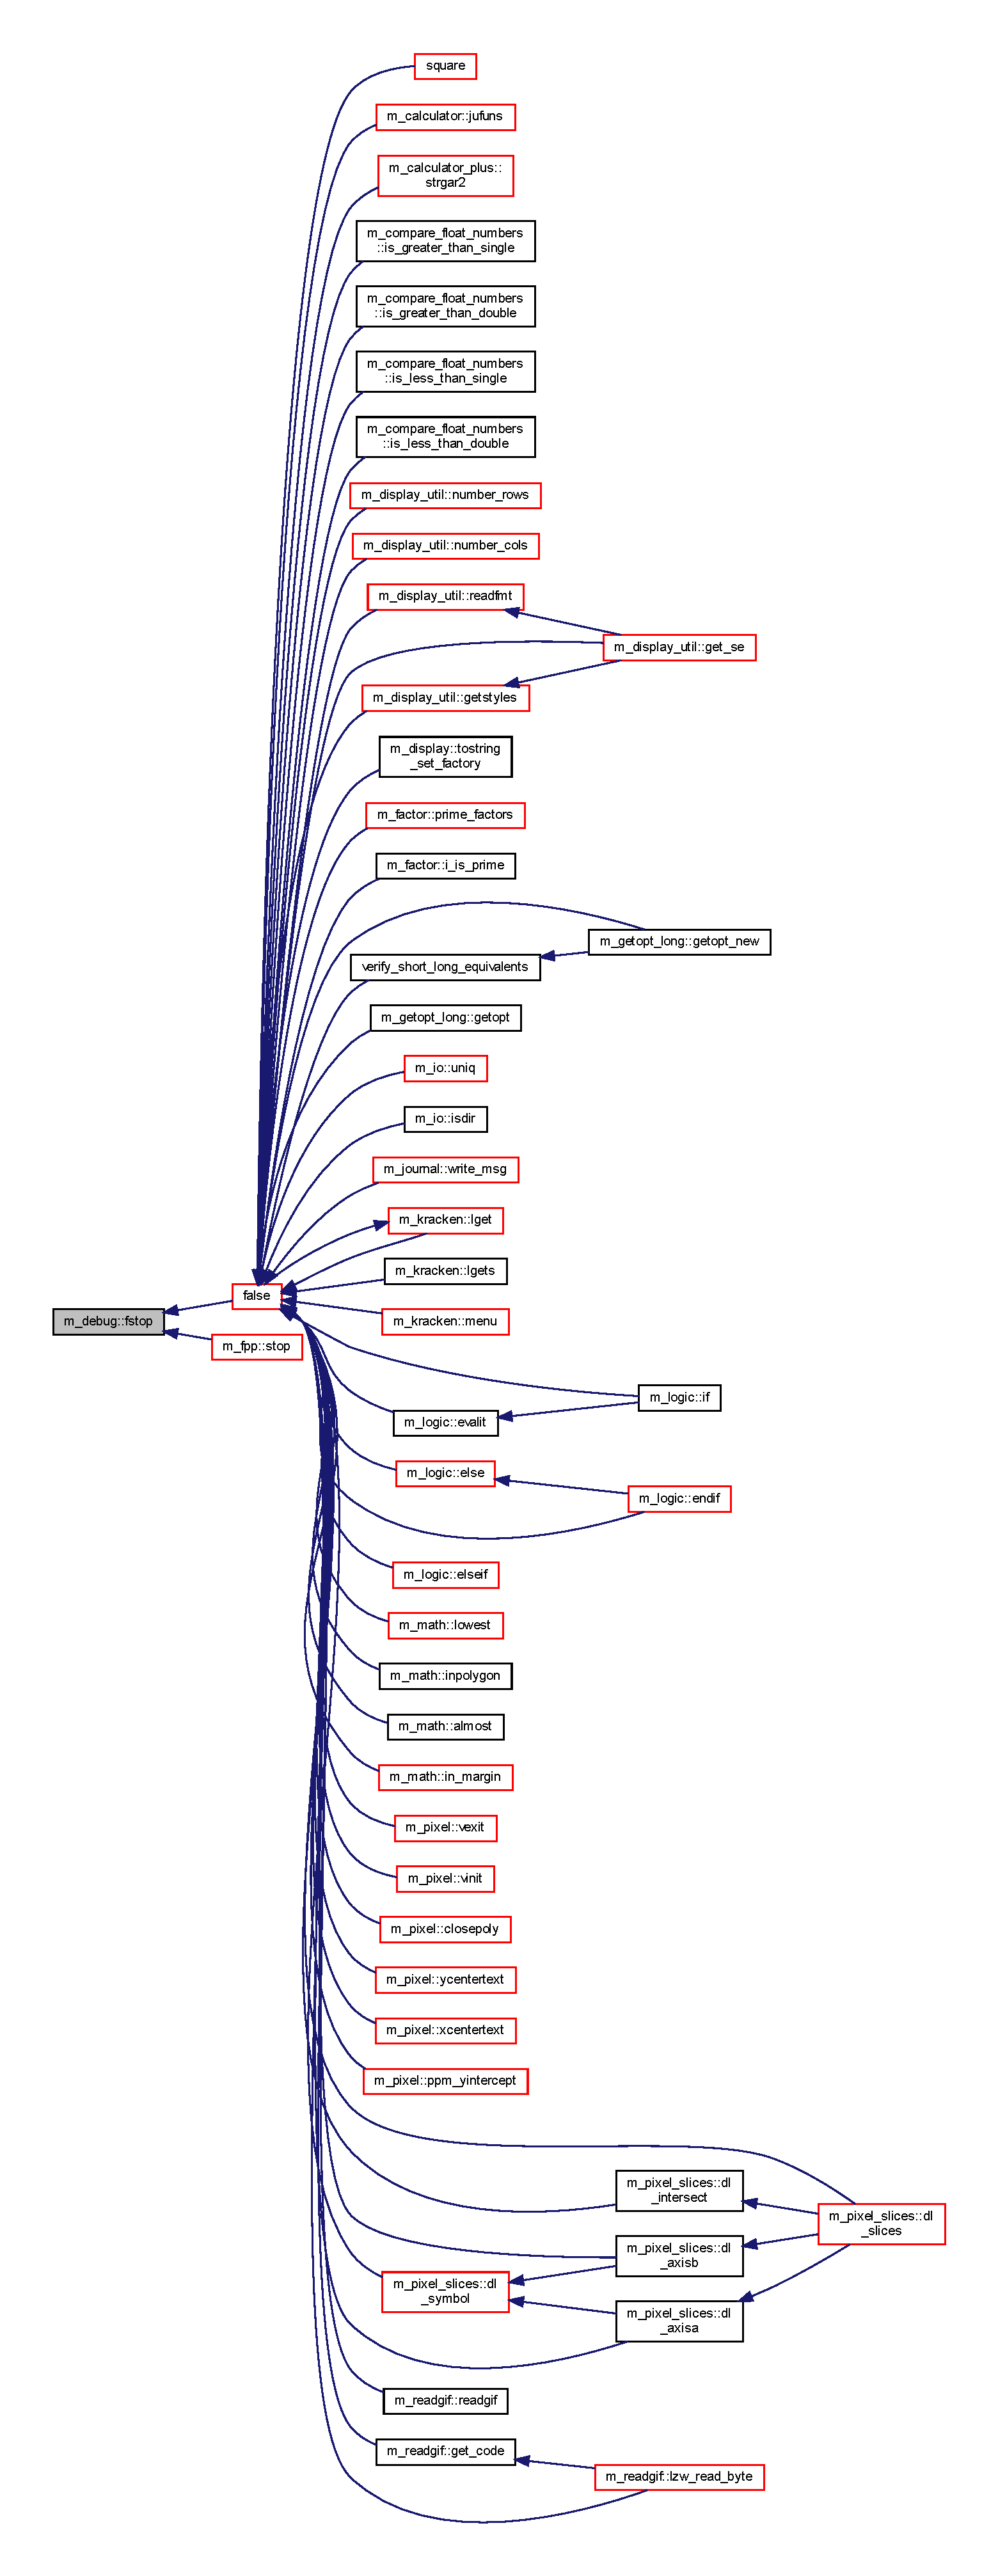
\includegraphics[height=550pt]{namespacem__debug_a66fa03a6a97837acc4c1265be1294295_icgraph}
\end{center}
\end{figure}
\mbox{\Hypertarget{namespacem__debug_a9b456606b4c555ed2e1e453aa9c872cb}\label{namespacem__debug_a9b456606b4c555ed2e1e453aa9c872cb}} 
\index{m\+\_\+debug@{m\+\_\+debug}!pdec@{pdec}}
\index{pdec@{pdec}!m\+\_\+debug@{m\+\_\+debug}}
\subsubsection{\texorpdfstring{pdec()}{pdec()}}
{\footnotesize\ttfamily \hyperlink{M__stopwatch_83_8txt_acfbcff50169d691ff02d4a123ed70482}{subroutine}, \hyperlink{M__stopwatch_83_8txt_a2f74811300c361e53b430611a7d1769f}{public} m\+\_\+debug\+::pdec (\begin{DoxyParamCaption}\item[{\hyperlink{option__stopwatch_83_8txt_abd4b21fbbd175834027b5224bfe97e66}{character}(len=$\ast$), intent(\hyperlink{M__journal_83_8txt_afce72651d1eed785a2132bee863b2f38}{in})}]{string }\end{DoxyParamCaption})}



\subsubsection*{N\+A\+ME}

pdec -\/ \mbox{[}M\+\_\+debug\mbox{]} write out string with A\+S\+C\+II decimal equivalent vertically under it 

\subsubsection*{S\+Y\+N\+O\+P\+S\+IS}

\begin{DoxyVerb}Usage:

 subroutine pdec(string)
 character(len=*),intent(in) :: string
\end{DoxyVerb}


\subsubsection*{D\+E\+S\+C\+R\+I\+P\+T\+I\+ON}

\begin{DoxyVerb}  Given a string to print, PDEC() writes out the ASCII Decimal equivalent of
  the string directly underneath it. This can help you to locate
  unprintable characters or non-standard white-space such as a
  backspace character or tab character in input strings that your
  program could not interpret. On output, non-printable characters
  are replaced with a space, and trailing spaces are ignored.

  You read the numbers vertically.

  1. ignore trailing spaces
  2. print the character if it has an ADE of 32 on up
  3. print a space if it has an ADE of less than 32
  4. underneath each character print the ADE value vertically
  5. strings are assumed under 32767 characters in length.
     Format integer constants > 32767 are not supported on HP-UX
     when newer compilers are available use unlimited
\end{DoxyVerb}


\subsubsection*{E\+X\+A\+M\+P\+LE}

\begin{DoxyVerb}Sample program:

   program demo
   call pdec(' ABCDEFG abcdefg ')
   end program demo

would produce (notice trailing space is trimmed):

  > ABCDEFG abcdefg
  >0000000000001111
  >3666667739990000
  >2567890127890123
\end{DoxyVerb}


\subsubsection*{A\+U\+T\+H\+OR}

John S. Urban \mbox{\Hypertarget{namespacem__debug_ad59ade4de861dcf4e007521b2cf2f304}\label{namespacem__debug_ad59ade4de861dcf4e007521b2cf2f304}} 
\index{m\+\_\+debug@{m\+\_\+debug}!stderr@{stderr}}
\index{stderr@{stderr}!m\+\_\+debug@{m\+\_\+debug}}
\subsubsection{\texorpdfstring{stderr()}{stderr()}}
{\footnotesize\ttfamily \hyperlink{M__stopwatch_83_8txt_acfbcff50169d691ff02d4a123ed70482}{subroutine}, \hyperlink{M__stopwatch_83_8txt_a2f74811300c361e53b430611a7d1769f}{public} m\+\_\+debug\+::stderr (\begin{DoxyParamCaption}\item[{\hyperlink{option__stopwatch_83_8txt_abd4b21fbbd175834027b5224bfe97e66}{character}(len=$\ast$), intent(\hyperlink{M__journal_83_8txt_afce72651d1eed785a2132bee863b2f38}{in})}]{message,  }\item[{class($\ast$), intent(\hyperlink{M__journal_83_8txt_afce72651d1eed785a2132bee863b2f38}{in}), \hyperlink{option__stopwatch_83_8txt_aa4ece75e7acf58a4843f70fe18c3ade5}{optional}}]{generic }\end{DoxyParamCaption})}



\subsubsection*{N\+A\+ME}

stderr -\/ \mbox{[}M\+\_\+debug\mbox{]} write message to stderr \subsubsection*{S\+Y\+N\+O\+P\+S\+IS}

subroutine stderr(message)

character(len=$\ast$),intent(in) \+:\+: message class($\ast$),intent(in),optional \+:\+: generic \subsubsection*{D\+E\+S\+C\+R\+I\+P\+T\+I\+ON}

S\+T\+D\+E\+R\+R(3f) writes a message to standard error using a standard f2003 method. \subsubsection*{O\+P\+T\+I\+O\+NS}

message -\/ description to be printed generic -\/ optional value to print the value of after the message. May be of type I\+N\+T\+E\+G\+ER, L\+O\+G\+I\+C\+AL, R\+E\+AL, D\+O\+U\+B\+L\+E\+P\+R\+E\+C\+I\+S\+I\+ON, C\+O\+M\+P\+L\+EX, or C\+H\+A\+R\+A\+C\+T\+ER. \subsubsection*{E\+X\+A\+M\+P\+L\+ES}

Sample program\+:

program demo\+\_\+stderr use M\+\_\+debug, only\+: stderr implicit none

call stderr(\textquotesingle{}error\+: R\+V\+A\+L\+UE=\textquotesingle{},3.\+0/4.0) call stderr(\textquotesingle{}error\+: I\+V\+A\+L\+UE=\textquotesingle{},123456789) call stderr(\textquotesingle{}error\+: L\+V\+A\+L\+UE=\textquotesingle{},.true.)

call stderr(\textquotesingle{}error\+: program will now stop\textquotesingle{}) stop 1

end program demo\+\_\+stderr

Results\+:

error\+: R\+V\+A\+L\+UE= 0.\+750000000 error\+: I\+V\+A\+L\+UE= 123456789 error\+: L\+V\+A\+L\+UE= T error\+: program will now stop S\+T\+OP 1 

References real.

Here is the caller graph for this function\+:
\nopagebreak
\begin{figure}[H]
\begin{center}
\leavevmode
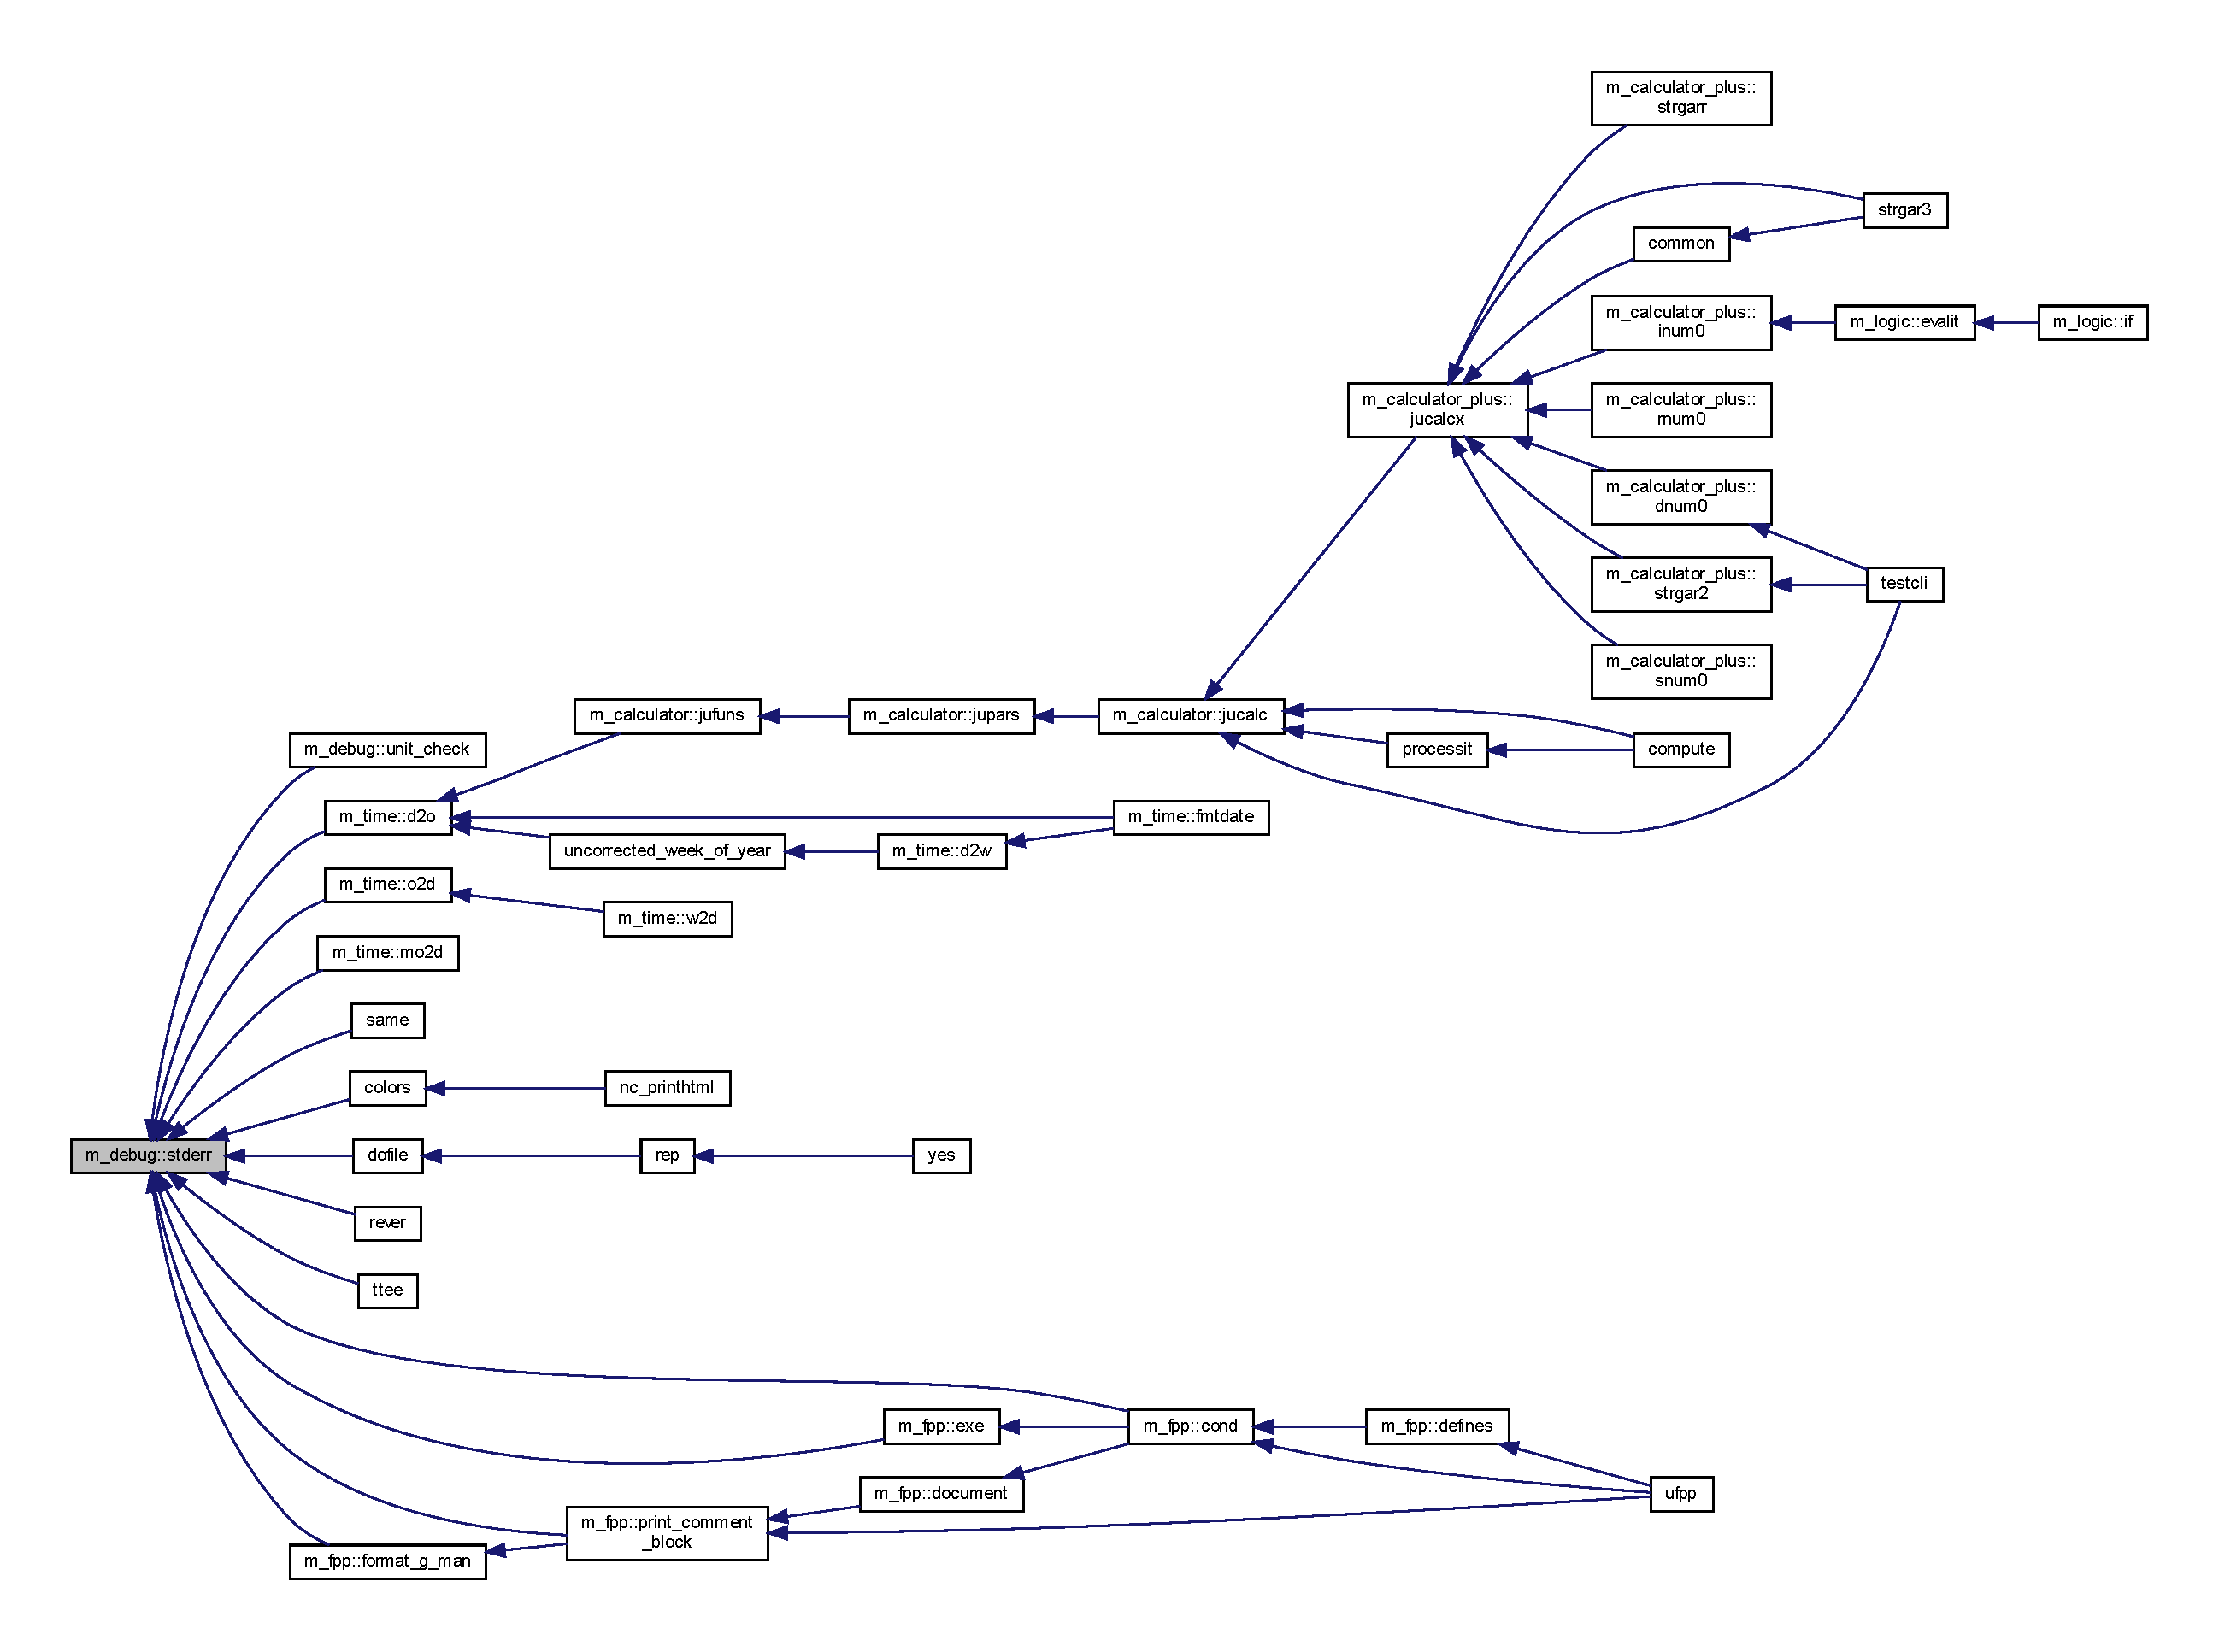
\includegraphics[width=350pt]{namespacem__debug_ad59ade4de861dcf4e007521b2cf2f304_icgraph}
\end{center}
\end{figure}
\mbox{\Hypertarget{namespacem__debug_a0ae797092ab85a8ba9258dc9f8949189}\label{namespacem__debug_a0ae797092ab85a8ba9258dc9f8949189}} 
\index{m\+\_\+debug@{m\+\_\+debug}!unit\+\_\+check@{unit\+\_\+check}}
\index{unit\+\_\+check@{unit\+\_\+check}!m\+\_\+debug@{m\+\_\+debug}}
\subsubsection{\texorpdfstring{unit\+\_\+check()}{unit\_check()}}
{\footnotesize\ttfamily \hyperlink{M__stopwatch_83_8txt_acfbcff50169d691ff02d4a123ed70482}{subroutine}, \hyperlink{M__stopwatch_83_8txt_a2f74811300c361e53b430611a7d1769f}{public} m\+\_\+debug\+::unit\+\_\+check (\begin{DoxyParamCaption}\item[{\hyperlink{option__stopwatch_83_8txt_abd4b21fbbd175834027b5224bfe97e66}{character}(len=$\ast$), intent(\hyperlink{M__journal_83_8txt_afce72651d1eed785a2132bee863b2f38}{in})}]{name,  }\item[{logical, intent(\hyperlink{M__journal_83_8txt_afce72651d1eed785a2132bee863b2f38}{in})}]{logical\+\_\+expression,  }\item[{\hyperlink{option__stopwatch_83_8txt_abd4b21fbbd175834027b5224bfe97e66}{character}(len=$\ast$), intent(\hyperlink{M__journal_83_8txt_afce72651d1eed785a2132bee863b2f38}{in}), \hyperlink{option__stopwatch_83_8txt_aa4ece75e7acf58a4843f70fe18c3ade5}{optional}}]{message }\end{DoxyParamCaption})}



\subsubsection*{N\+A\+ME}

unit\+\_\+check -\/ \mbox{[}M\+\_\+debug\mbox{]} if logical expression is false, call command \char`\"{}goodbad N\+A\+M\+E bad\char`\"{} and stop program 

\subsubsection*{S\+Y\+N\+O\+P\+S\+IS}

\begin{DoxyVerb}subroutine unit_check(name,expression,message)

 character(len=*),intent(in) :: name
 logical,intent(in) :: expression
 character(len=*),intent(in),optional :: message
\end{DoxyVerb}


\subsubsection*{D\+E\+S\+C\+R\+I\+P\+T\+I\+ON}

\begin{DoxyVerb}unit_check(3f) tests the expression and if it is false, calls the shell command

     goodbad NAME bad

and stops the program.
\end{DoxyVerb}
 \subsubsection*{O\+P\+T\+I\+O\+NS}

N\+A\+ME the unit test name passed on to the goodbad(1) command E\+X\+P\+R\+E\+S\+S\+I\+ON the logical expression to evaluate M\+E\+S\+S\+A\+GE optional message to display when performing test

\subsubsection*{E\+X\+A\+M\+P\+L\+ES}

Sample program\+:

program demo\+\_\+unit\+\_\+check use M\+\_\+debug, only\+: unit\+\_\+check use M\+\_\+debug, only\+: unit\+\_\+check\+\_\+start, unit\+\_\+check\+\_\+good implicit none integer \+:\+: x x=10 call unit\+\_\+check\+\_\+start(\textquotesingle{}myroutine\textquotesingle{})

call unit\+\_\+check(\textquotesingle{}myroutine\textquotesingle{}, x.\+gt.\+3 ,\textquotesingle{}test if big enough\textquotesingle{}) call unit\+\_\+check(\textquotesingle{}myroutine\textquotesingle{}, x.\+lt.\+100 ,\textquotesingle{}test if small enough\textquotesingle{})

write($\ast$,$\ast$)\textquotesingle{}checks on \char`\"{}myroutine\char`\"{} passed\textquotesingle{} call unit\+\_\+check\+\_\+good(\textquotesingle{}myroutine\textquotesingle{})

end program demo\+\_\+unit\+\_\+check

Sample output (varies with what goodbad(1) command is used)\+:

unit\+\_\+check\+\_\+start\+: myroutine.\+3 status initialized in database unit\+\_\+check\+: myroutine P\+A\+S\+S\+ED\+:test if big enough unit\+\_\+check\+: myroutine P\+A\+S\+S\+ED\+:test if small enough checks on \char`\"{}myroutine\char`\"{} passed data for myroutine.\+3 is entryname description documentation filename library ufpp ccall archive date status 

 myroutine.\+3 2017/02/03 07\+:23\+:40 1 

References stderr().

Here is the call graph for this function\+:
\nopagebreak
\begin{figure}[H]
\begin{center}
\leavevmode
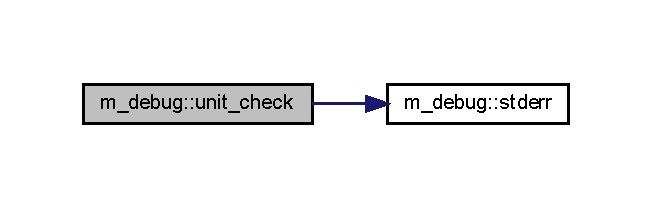
\includegraphics[width=313pt]{namespacem__debug_a0ae797092ab85a8ba9258dc9f8949189_cgraph}
\end{center}
\end{figure}
\mbox{\Hypertarget{namespacem__debug_a668813eec59e4c16d3bbc2d317e8cdee}\label{namespacem__debug_a668813eec59e4c16d3bbc2d317e8cdee}} 
\index{m\+\_\+debug@{m\+\_\+debug}!unit\+\_\+check\+\_\+bad@{unit\+\_\+check\+\_\+bad}}
\index{unit\+\_\+check\+\_\+bad@{unit\+\_\+check\+\_\+bad}!m\+\_\+debug@{m\+\_\+debug}}
\subsubsection{\texorpdfstring{unit\+\_\+check\+\_\+bad()}{unit\_check\_bad()}}
{\footnotesize\ttfamily \hyperlink{M__stopwatch_83_8txt_acfbcff50169d691ff02d4a123ed70482}{subroutine}, \hyperlink{M__stopwatch_83_8txt_a2f74811300c361e53b430611a7d1769f}{public} m\+\_\+debug\+::unit\+\_\+check\+\_\+bad (\begin{DoxyParamCaption}\item[{\hyperlink{option__stopwatch_83_8txt_abd4b21fbbd175834027b5224bfe97e66}{character}(len=$\ast$), intent(\hyperlink{M__journal_83_8txt_afce72651d1eed785a2132bee863b2f38}{in})}]{name,  }\item[{\hyperlink{option__stopwatch_83_8txt_abd4b21fbbd175834027b5224bfe97e66}{character}(len=$\ast$), intent(\hyperlink{M__journal_83_8txt_afce72651d1eed785a2132bee863b2f38}{in}), \hyperlink{option__stopwatch_83_8txt_aa4ece75e7acf58a4843f70fe18c3ade5}{optional}}]{string }\end{DoxyParamCaption})}



\subsubsection*{N\+A\+ME}

unit\+\_\+check\+\_\+bad -\/ \mbox{[}M\+\_\+debug\mbox{]} call command \char`\"{}goodbad N\+A\+M\+E bad\char`\"{} and stop program 

\subsubsection*{S\+Y\+N\+O\+P\+S\+IS}

\begin{DoxyVerb}subroutine unit_check_bad(name,string)

 character(len=*),intent(in) :: name
 character(len=*),intent(in) :: string
\end{DoxyVerb}


\subsubsection*{D\+E\+S\+C\+R\+I\+P\+T\+I\+ON}

\begin{DoxyVerb}unit_check_bad(3f) calls the shell command

     goodbad NAME bad [string]

and stops the program.
\end{DoxyVerb}


\subsubsection*{E\+X\+A\+M\+P\+L\+ES}

Sample program\+:

program demo\+\_\+unit\+\_\+check\+\_\+bad use M\+\_\+debug, only\+: unit\+\_\+check\+\_\+start use M\+\_\+debug, only\+: unit\+\_\+check use M\+\_\+debug, only\+: unit\+\_\+check\+\_\+good, unit\+\_\+check\+\_\+bad

implicit none integer \+:\+: x x=10 call unit\+\_\+check\+\_\+start(\textquotesingle{}myroutine\textquotesingle{})

call unit\+\_\+check(\textquotesingle{}myroutine\textquotesingle{}, x.\+gt.\+3 ,\textquotesingle{}test if big enough\textquotesingle{}) call unit\+\_\+check(\textquotesingle{}myroutine\textquotesingle{}, x.\+lt.\+100 ,\textquotesingle{}test if small enough\textquotesingle{})

!write($\ast$,$\ast$)\textquotesingle{}checks on \char`\"{}myroutine\char`\"{} passed\textquotesingle{} !call unit\+\_\+check\+\_\+good(\textquotesingle{}myroutine\textquotesingle{})

write($\ast$,$\ast$)\textquotesingle{}checks on \char`\"{}myroutine\char`\"{} failed\textquotesingle{} call unit\+\_\+check\+\_\+bad (\textquotesingle{}myroutine\textquotesingle{}) ! program execution stopped

end program demo\+\_\+unit\+\_\+check\+\_\+bad \mbox{\Hypertarget{namespacem__debug_acd67428a8900ec4c36bd3a7b28d56987}\label{namespacem__debug_acd67428a8900ec4c36bd3a7b28d56987}} 
\index{m\+\_\+debug@{m\+\_\+debug}!unit\+\_\+check\+\_\+good@{unit\+\_\+check\+\_\+good}}
\index{unit\+\_\+check\+\_\+good@{unit\+\_\+check\+\_\+good}!m\+\_\+debug@{m\+\_\+debug}}
\subsubsection{\texorpdfstring{unit\+\_\+check\+\_\+good()}{unit\_check\_good()}}
{\footnotesize\ttfamily \hyperlink{M__stopwatch_83_8txt_acfbcff50169d691ff02d4a123ed70482}{subroutine}, \hyperlink{M__stopwatch_83_8txt_a2f74811300c361e53b430611a7d1769f}{public} m\+\_\+debug\+::unit\+\_\+check\+\_\+good (\begin{DoxyParamCaption}\item[{\hyperlink{option__stopwatch_83_8txt_abd4b21fbbd175834027b5224bfe97e66}{character}(len=$\ast$), intent(\hyperlink{M__journal_83_8txt_afce72651d1eed785a2132bee863b2f38}{in})}]{name,  }\item[{\hyperlink{option__stopwatch_83_8txt_abd4b21fbbd175834027b5224bfe97e66}{character}(len=$\ast$), intent(\hyperlink{M__journal_83_8txt_afce72651d1eed785a2132bee863b2f38}{in}), \hyperlink{option__stopwatch_83_8txt_aa4ece75e7acf58a4843f70fe18c3ade5}{optional}}]{string }\end{DoxyParamCaption})}



\subsubsection*{N\+A\+ME}

unit\+\_\+check\+\_\+good -\/ \mbox{[}M\+\_\+debug\mbox{]} call command \char`\"{}goodbad N\+A\+M\+E good\char`\"{} 

\subsubsection*{S\+Y\+N\+O\+P\+S\+IS}

\begin{DoxyVerb}subroutine unit_check_good(name,string)

 character(len=*),intent(in) :: name
 character(len=*),intent(in) :: string
\end{DoxyVerb}


\subsubsection*{D\+E\+S\+C\+R\+I\+P\+T\+I\+ON}

\begin{DoxyVerb}unit_check_good(3f) calls the shell command

     goodbad NAME good [string]
\end{DoxyVerb}


\subsubsection*{E\+X\+A\+M\+P\+L\+ES}

Sample program\+:

program demo\+\_\+unit\+\_\+check\+\_\+good use M\+\_\+debug, only\+: unit\+\_\+check\+\_\+start use M\+\_\+debug, only\+: unit\+\_\+check use M\+\_\+debug, only\+: unit\+\_\+check\+\_\+good, unit\+\_\+check\+\_\+bad

implicit none integer \+:\+: x x=10 call unit\+\_\+check\+\_\+start(\textquotesingle{}myroutine\textquotesingle{})

call unit\+\_\+check(\textquotesingle{}myroutine\textquotesingle{}, x.\+gt.\+3 ,\textquotesingle{}test if big enough\textquotesingle{}) call unit\+\_\+check(\textquotesingle{}myroutine\textquotesingle{}, x.\+lt.\+100 ,\textquotesingle{}test if small enough\textquotesingle{})

write($\ast$,$\ast$)\textquotesingle{}checks on \char`\"{}myroutine\char`\"{} passed\textquotesingle{} call unit\+\_\+check\+\_\+good(\textquotesingle{}myroutine\textquotesingle{})

end program demo\+\_\+unit\+\_\+check\+\_\+good \mbox{\Hypertarget{namespacem__debug_a6f1166b1f25f39931359c1aa1b2219e5}\label{namespacem__debug_a6f1166b1f25f39931359c1aa1b2219e5}} 
\index{m\+\_\+debug@{m\+\_\+debug}!unit\+\_\+check\+\_\+start@{unit\+\_\+check\+\_\+start}}
\index{unit\+\_\+check\+\_\+start@{unit\+\_\+check\+\_\+start}!m\+\_\+debug@{m\+\_\+debug}}
\subsubsection{\texorpdfstring{unit\+\_\+check\+\_\+start()}{unit\_check\_start()}}
{\footnotesize\ttfamily \hyperlink{M__stopwatch_83_8txt_acfbcff50169d691ff02d4a123ed70482}{subroutine}, \hyperlink{M__stopwatch_83_8txt_a2f74811300c361e53b430611a7d1769f}{public} m\+\_\+debug\+::unit\+\_\+check\+\_\+start (\begin{DoxyParamCaption}\item[{\hyperlink{option__stopwatch_83_8txt_abd4b21fbbd175834027b5224bfe97e66}{character}(len=$\ast$), intent(\hyperlink{M__journal_83_8txt_afce72651d1eed785a2132bee863b2f38}{in})}]{name,  }\item[{\hyperlink{option__stopwatch_83_8txt_abd4b21fbbd175834027b5224bfe97e66}{character}(len=$\ast$), intent(\hyperlink{M__journal_83_8txt_afce72651d1eed785a2132bee863b2f38}{in}), \hyperlink{option__stopwatch_83_8txt_aa4ece75e7acf58a4843f70fe18c3ade5}{optional}}]{string }\end{DoxyParamCaption})}



\subsubsection*{N\+A\+ME}

unit\+\_\+check\+\_\+start -\/ \mbox{[}M\+\_\+debug\mbox{]} call command \char`\"{}goodbad N\+A\+M\+E start\char`\"{} 

\subsubsection*{S\+Y\+N\+O\+P\+S\+IS}

\begin{DoxyVerb}subroutine unit_check_start(name,string)

 character(len=*),intent(in) :: name
 character(len=*),intent(in),optional :: string
\end{DoxyVerb}


\subsubsection*{D\+E\+S\+C\+R\+I\+P\+T\+I\+ON}

\begin{DoxyVerb}unit_check_start(3f) calls the shell command

   goodbad NAME start [string]
\end{DoxyVerb}


\subsubsection*{E\+X\+A\+M\+P\+L\+ES}

Sample program\+:

program demo\+\_\+unit\+\_\+check\+\_\+start use M\+\_\+debug, only\+: unit\+\_\+check\+\_\+start use M\+\_\+debug, only\+: unit\+\_\+check use M\+\_\+debug, only\+: unit\+\_\+check\+\_\+good, unit\+\_\+check\+\_\+bad

implicit none integer \+:\+: x x=10 call unit\+\_\+check\+\_\+start(\textquotesingle{}myroutine\textquotesingle{})

call unit\+\_\+check\+\_\+start(\textquotesingle{}myroutine\+\_\+long\textquotesingle{},\textquotesingle{} \& \& -\/section 3 \& \& -\/library lib\+G\+PF \& \& -\/filename {\ttfamily pwd}/\+M\+\_\+debug.FF \& \& -\/documentation y \& \& -\/ufpp y \& \& -\/ccall n \& \& -\/archive G\+P\+F.\+a \& \& \textquotesingle{})

call unit\+\_\+check(\textquotesingle{}myroutine\textquotesingle{}, x.\+gt.\+3 , \textquotesingle{}test if big enough\textquotesingle{}) call unit\+\_\+check(\textquotesingle{}myroutine\textquotesingle{}, x.\+lt.\+100 , \textquotesingle{}test if small enough\textquotesingle{})

call unit\+\_\+check\+\_\+good(\textquotesingle{}myroutine\textquotesingle{},\textquotesingle{}store that checks passed\textquotesingle{})

end program demo\+\_\+unit\+\_\+check\+\_\+start 

\subsection{Variable Documentation}
\mbox{\Hypertarget{namespacem__debug_aa13827e130b8e8bde8a8597e3d3faa0c}\label{namespacem__debug_aa13827e130b8e8bde8a8597e3d3faa0c}} 
\index{m\+\_\+debug@{m\+\_\+debug}!debug@{debug}}
\index{debug@{debug}!m\+\_\+debug@{m\+\_\+debug}}
\subsubsection{\texorpdfstring{debug}{debug}}
{\footnotesize\ttfamily logical, save, \hyperlink{M__stopwatch_83_8txt_a2f74811300c361e53b430611a7d1769f}{public} m\+\_\+debug\+::debug =.false.}

\mbox{\Hypertarget{namespacem__debug_a884bfce2d57734eb9f07e8a99d4ffaeb}\label{namespacem__debug_a884bfce2d57734eb9f07e8a99d4ffaeb}} 
\index{m\+\_\+debug@{m\+\_\+debug}!exit\+\_\+failure@{exit\+\_\+failure}}
\index{exit\+\_\+failure@{exit\+\_\+failure}!m\+\_\+debug@{m\+\_\+debug}}
\subsubsection{\texorpdfstring{exit\+\_\+failure}{exit\_failure}}
{\footnotesize\ttfamily integer, parameter, \hyperlink{M__stopwatch_83_8txt_a2f74811300c361e53b430611a7d1769f}{public} m\+\_\+debug\+::exit\+\_\+failure =1}

\mbox{\Hypertarget{namespacem__debug_a9f9aab455ab97238c80d66dd9ed65a7d}\label{namespacem__debug_a9f9aab455ab97238c80d66dd9ed65a7d}} 
\index{m\+\_\+debug@{m\+\_\+debug}!exit\+\_\+success@{exit\+\_\+success}}
\index{exit\+\_\+success@{exit\+\_\+success}!m\+\_\+debug@{m\+\_\+debug}}
\subsubsection{\texorpdfstring{exit\+\_\+success}{exit\_success}}
{\footnotesize\ttfamily integer, parameter, \hyperlink{M__stopwatch_83_8txt_a2f74811300c361e53b430611a7d1769f}{public} m\+\_\+debug\+::exit\+\_\+success =0}

\mbox{\Hypertarget{namespacem__debug_ab9d95afd83b30688892f4c818ee8c312}\label{namespacem__debug_ab9d95afd83b30688892f4c818ee8c312}} 
\index{m\+\_\+debug@{m\+\_\+debug}!io\+\_\+debug@{io\+\_\+debug}}
\index{io\+\_\+debug@{io\+\_\+debug}!m\+\_\+debug@{m\+\_\+debug}}
\subsubsection{\texorpdfstring{io\+\_\+debug}{io\_debug}}
{\footnotesize\ttfamily integer, save, \hyperlink{M__stopwatch_83_8txt_a2f74811300c361e53b430611a7d1769f}{public} m\+\_\+debug\+::io\+\_\+debug =E\+R\+R\+O\+R\+\_\+\+U\+N\+IT}


\hypertarget{namespacem__display}{}\section{m\+\_\+display Module Reference}
\label{namespacem__display}\index{m\+\_\+display@{m\+\_\+display}}
\subsection*{Data Types}
\begin{DoxyCompactItemize}
\item 
interface \hyperlink{interfacem__display_1_1disp}{disp}
\begin{DoxyCompactList}\small\item\em \subsubsection*{N\+A\+ME}

disp(3f) -\/ \mbox{[}M\+\_\+display\mbox{]} pretty-\/print a matrix \end{DoxyCompactList}\item 
interface \hyperlink{interfacem__display_1_1disp__set}{disp\+\_\+set}
\item 
interface \hyperlink{interfacem__display_1_1tostring}{tostring}
\end{DoxyCompactItemize}
\subsection*{Functions/\+Subroutines}
\begin{DoxyCompactItemize}
\item 
\hyperlink{M__stopwatch_83_8txt_acfbcff50169d691ff02d4a123ed70482}{subroutine}, \hyperlink{M__stopwatch_83_8txt_a2f74811300c361e53b430611a7d1769f}{public} \hyperlink{namespacem__display_aca571cfcf5dcced1070969200f717a28}{disp\+\_\+set} (advance, digmax, matsep, orient, sep, style, \hyperlink{M__stopwatch_83_8txt_a5cbef30eb7c0d734bd82f5a7ebea9aa7}{unit}, zeroas)
\begin{DoxyCompactList}\small\item\em \subsubsection*{N\+A\+ME}

disp\+\_\+set(3f) -\/ \mbox{[}M\+\_\+display\mbox{]} set default options for disp(3f) \end{DoxyCompactList}\item 
\hyperlink{M__stopwatch_83_8txt_acfbcff50169d691ff02d4a123ed70482}{subroutine}, \hyperlink{M__stopwatch_83_8txt_a2f74811300c361e53b430611a7d1769f}{public} \hyperlink{namespacem__display_a504ce34f82249882d1cc5a0ea2802bc6}{disp\+\_\+set\+\_\+factory} ()
\begin{DoxyCompactList}\small\item\em \subsubsection*{N\+A\+ME}

tostring\+\_\+disp\+\_\+factory(3f) -\/ \mbox{[}M\+\_\+display\mbox{]} set D\+I\+S\+P(3f) output back to original defaults \end{DoxyCompactList}\item 
\hyperlink{M__stopwatch_83_8txt_acfbcff50169d691ff02d4a123ed70482}{subroutine} \hyperlink{namespacem__display_a6200cf732096469f40c38ec2baa6d811}{avoid\+\_\+compiler\+\_\+warnings}
\item 
\hyperlink{M__stopwatch_83_8txt_acfbcff50169d691ff02d4a123ed70482}{subroutine}, \hyperlink{M__stopwatch_83_8txt_a2f74811300c361e53b430611a7d1769f}{public} \hyperlink{namespacem__display_ac6d80df8c70bb7d64df528d26851d6cb}{tostring\+\_\+set} (sep, rfmt, ifmt, trimb, trimz)
\begin{DoxyCompactList}\small\item\em \subsubsection*{N\+A\+ME}

tostring\+\_\+set(3f) -\/ \mbox{[}M\+\_\+display\mbox{]} set modes for T\+O\+S\+T\+R\+I\+N\+G(3f) \end{DoxyCompactList}\item 
\hyperlink{M__stopwatch_83_8txt_acfbcff50169d691ff02d4a123ed70482}{subroutine}, \hyperlink{M__stopwatch_83_8txt_a2f74811300c361e53b430611a7d1769f}{public} \hyperlink{namespacem__display_abf51a5db397d27e0c6cb39e9f3fa7e24}{tostring\+\_\+set\+\_\+factory} ()
\begin{DoxyCompactList}\small\item\em \subsubsection*{N\+A\+ME}

tostring\+\_\+set\+\_\+factory(3f) -\/ \mbox{[}M\+\_\+display\mbox{]} set T\+O\+S\+T\+R\+I\+N\+G(3f) output back to original defaults \end{DoxyCompactList}\item 
\hyperlink{M__stopwatch_83_8txt_acfbcff50169d691ff02d4a123ed70482}{subroutine} \hyperlink{namespacem__display_a6296917336a62e43005e56c48340eaf1}{disp\+\_\+set\+\_\+ds} (settings)
\item 
\hyperlink{stop__watch_83_8txt_a70f0ead91c32e25323c03265aa302c1c}{type}(disp\+\_\+settings) function, \hyperlink{M__stopwatch_83_8txt_a2f74811300c361e53b430611a7d1769f}{public} \hyperlink{namespacem__display_a6a49f987c37a95e67744950ecee69530}{disp\+\_\+get} ()
\begin{DoxyCompactList}\small\item\em \subsubsection*{N\+A\+ME}\end{DoxyCompactList}\item 
\hyperlink{M__stopwatch_83_8txt_acfbcff50169d691ff02d4a123ed70482}{subroutine} \hyperlink{namespacem__display_adddf4774edf1fedf5b1f02f47fbbc82f}{disp\+\_\+scalar\+\_\+int} (x, fmt, advance, sep, trim, \hyperlink{M__stopwatch_83_8txt_a5cbef30eb7c0d734bd82f5a7ebea9aa7}{unit}, zeroas)
\item 
\hyperlink{M__stopwatch_83_8txt_acfbcff50169d691ff02d4a123ed70482}{subroutine} \hyperlink{namespacem__display_afaae34a88f7f2d5799469f0a6214e0b2}{disp\+\_\+title\+\_\+scalar\+\_\+int} (\hyperlink{print__watch_83_8txt_a15b5bd21156bb9fca6a755ab8c029a9c}{title}, x, fmt, advance, sep, style, trim, \hyperlink{M__stopwatch_83_8txt_a5cbef30eb7c0d734bd82f5a7ebea9aa7}{unit}, zeroas)
\item 
\hyperlink{M__stopwatch_83_8txt_acfbcff50169d691ff02d4a123ed70482}{subroutine} \hyperlink{namespacem__display_abbb9f5e78b3998c8fa9774d594152dcc}{disp\+\_\+vector\+\_\+int} (x, fmt, advance, lbound, sep, style, trim, \hyperlink{M__stopwatch_83_8txt_a5cbef30eb7c0d734bd82f5a7ebea9aa7}{unit}, orient, zeroas)
\item 
\hyperlink{M__stopwatch_83_8txt_acfbcff50169d691ff02d4a123ed70482}{subroutine} \hyperlink{namespacem__display_a8393f81379778fc9d955bf1e0961aee1}{disp\+\_\+title\+\_\+vector\+\_\+int} (\hyperlink{print__watch_83_8txt_a15b5bd21156bb9fca6a755ab8c029a9c}{title}, x, fmt, advance, lbound, sep, style, trim, \hyperlink{M__stopwatch_83_8txt_a5cbef30eb7c0d734bd82f5a7ebea9aa7}{unit}, orient, zeroas)
\item 
\hyperlink{M__stopwatch_83_8txt_acfbcff50169d691ff02d4a123ed70482}{subroutine} \hyperlink{namespacem__display_a00d35e9c84ad3f0238e4598f09f79961}{disp\+\_\+matrix\+\_\+int} (x, fmt, advance, lbound, sep, style, trim, \hyperlink{M__stopwatch_83_8txt_a5cbef30eb7c0d734bd82f5a7ebea9aa7}{unit}, zeroas)
\item 
\hyperlink{M__stopwatch_83_8txt_acfbcff50169d691ff02d4a123ed70482}{subroutine} \hyperlink{namespacem__display_aa95be71bcd8730f4f01393ea6ede4bec}{disp\+\_\+title\+\_\+matrix\+\_\+int} (\hyperlink{print__watch_83_8txt_a15b5bd21156bb9fca6a755ab8c029a9c}{title}, x, fmt, advance, lbound, sep, style, trim, \hyperlink{M__stopwatch_83_8txt_a5cbef30eb7c0d734bd82f5a7ebea9aa7}{unit}, zeroas)
\item 
\hyperlink{M__stopwatch_83_8txt_acfbcff50169d691ff02d4a123ed70482}{subroutine} \hyperlink{namespacem__display_a0e150cc23de78529e22b17b1873a9e6e}{disp\+\_\+dint} (\hyperlink{print__watch_83_8txt_a15b5bd21156bb9fca6a755ab8c029a9c}{title}, x, SE)
\item 
\hyperlink{M__stopwatch_83_8txt_acfbcff50169d691ff02d4a123ed70482}{subroutine} \hyperlink{namespacem__display_a305dbf4f9072f9d1551a24c0f26ad508}{tobox\+\_\+dint} (\hyperlink{print__watch_83_8txt_a15b5bd21156bb9fca6a755ab8c029a9c}{title}, x, SE, wid, nbl)
\item 
\hyperlink{M__stopwatch_83_8txt_acfbcff50169d691ff02d4a123ed70482}{subroutine} \hyperlink{namespacem__display_ab6e1e0eb1c077b4d2a0c6698c78925a3}{find\+\_\+editdesc\+\_\+dint} (x, SE, wid, nbl)
\item 
\hyperlink{M__stopwatch_83_8txt_acfbcff50169d691ff02d4a123ed70482}{subroutine} \hyperlink{namespacem__display_a6d7287cccf11d65c1821020ef61c7992}{getwid\+\_\+dint} (xmaxv, xminv, xzero, xallz, SE, wid, nbl)
\item 
\hyperlink{option__stopwatch_83_8txt_abd4b21fbbd175834027b5224bfe97e66}{character}(\hyperlink{namespacem__display_a6a2709cf5f243ee492f223b40c6b5143}{len\+\_\+f\+\_\+dint}(\mbox{[}x\mbox{]}, tosset \% ifmt)) function \hyperlink{namespacem__display_a5bfeb905fb5036068ef0012eb2f563fa}{tostring\+\_\+s\+\_\+dint} (x)
\begin{DoxyCompactList}\small\item\em \subsubsection*{N\+A\+ME}

tostring(3f) -\/ \mbox{[}M\+\_\+display\mbox{]} change numbers to a string \end{DoxyCompactList}\item 
\hyperlink{option__stopwatch_83_8txt_abd4b21fbbd175834027b5224bfe97e66}{character}(\hyperlink{namespacem__display_a6a2709cf5f243ee492f223b40c6b5143}{len\+\_\+f\+\_\+dint}(\mbox{[}x\mbox{]}, fmt)) function \hyperlink{namespacem__display_aa7d1fb61fc22bddb9232eaa13aaaa43f}{tostring\+\_\+sf\+\_\+dint} (x, fmt)
\item 
\hyperlink{option__stopwatch_83_8txt_abd4b21fbbd175834027b5224bfe97e66}{character}(\hyperlink{namespacem__display_a6a2709cf5f243ee492f223b40c6b5143}{len\+\_\+f\+\_\+dint}(x, tosset \% ifmt)) function \hyperlink{namespacem__display_a5a8479cdf49ed905e9c54cc2f86cea16}{tostring\+\_\+dint} (x)
\item 
\hyperlink{option__stopwatch_83_8txt_abd4b21fbbd175834027b5224bfe97e66}{character}(\hyperlink{namespacem__display_a6a2709cf5f243ee492f223b40c6b5143}{len\+\_\+f\+\_\+dint}(x, fmt)) function \hyperlink{namespacem__display_ac1dd519655fda1c495ba40efe16fbc0b}{tostring\+\_\+f\+\_\+dint} (x, fmt)
\item 
pure integer function \hyperlink{namespacem__display_a6a2709cf5f243ee492f223b40c6b5143}{len\+\_\+f\+\_\+dint} (x, fmt)
\item 
pure integer function \hyperlink{namespacem__display_a8310ed88204e0715b21b2afb0a6d12ac}{widthmax\+\_\+dint} (x, fmt)
\item 
\hyperlink{M__stopwatch_83_8txt_acfbcff50169d691ff02d4a123ed70482}{subroutine} \hyperlink{namespacem__display_a7a66451f6a0931ee7552ee4d8918ac20}{disp\+\_\+s\+\_\+sngl} (x, fmt, advance, digmax, sep, trim, \hyperlink{M__stopwatch_83_8txt_a5cbef30eb7c0d734bd82f5a7ebea9aa7}{unit}, zeroas)
\item 
\hyperlink{M__stopwatch_83_8txt_acfbcff50169d691ff02d4a123ed70482}{subroutine} \hyperlink{namespacem__display_a4ef66ee3da74984dd06012837795c459}{disp\+\_\+v\+\_\+sngl} (x, fmt, advance, digmax, lbound, sep, style, trim, \hyperlink{M__stopwatch_83_8txt_a5cbef30eb7c0d734bd82f5a7ebea9aa7}{unit}, orient, zeroas)
\item 
\hyperlink{M__stopwatch_83_8txt_acfbcff50169d691ff02d4a123ed70482}{subroutine} \hyperlink{namespacem__display_a4930462636c070e8b4761167fadfd4f9}{disp\+\_\+m\+\_\+sngl} (x, fmt, advance, lbound, sep, style, trim, \hyperlink{M__stopwatch_83_8txt_a5cbef30eb7c0d734bd82f5a7ebea9aa7}{unit}, digmax, zeroas)
\item 
\hyperlink{M__stopwatch_83_8txt_acfbcff50169d691ff02d4a123ed70482}{subroutine} \hyperlink{namespacem__display_a7ecc86ce58006c0d4d08efcfdaaf479a}{disp\+\_\+ts\+\_\+sngl} (\hyperlink{print__watch_83_8txt_a15b5bd21156bb9fca6a755ab8c029a9c}{title}, x, fmt, advance, digmax, sep, style, trim, \hyperlink{M__stopwatch_83_8txt_a5cbef30eb7c0d734bd82f5a7ebea9aa7}{unit}, zeroas)
\item 
\hyperlink{M__stopwatch_83_8txt_acfbcff50169d691ff02d4a123ed70482}{subroutine} \hyperlink{namespacem__display_ac54e50e6ecc87115c286fe451a4b8a13}{disp\+\_\+tv\+\_\+sngl} (\hyperlink{print__watch_83_8txt_a15b5bd21156bb9fca6a755ab8c029a9c}{title}, x, fmt, advance, digmax, lbound, sep, style, trim, \hyperlink{M__stopwatch_83_8txt_a5cbef30eb7c0d734bd82f5a7ebea9aa7}{unit}, orient, zeroas)
\item 
\hyperlink{M__stopwatch_83_8txt_acfbcff50169d691ff02d4a123ed70482}{subroutine} \hyperlink{namespacem__display_ae12795b79f66ff0f9f6843b2f980394a}{disp\+\_\+tm\+\_\+sngl} (\hyperlink{print__watch_83_8txt_a15b5bd21156bb9fca6a755ab8c029a9c}{title}, x, fmt, advance, digmax, lbound, sep, style, trim, \hyperlink{M__stopwatch_83_8txt_a5cbef30eb7c0d734bd82f5a7ebea9aa7}{unit}, zeroas)
\item 
\hyperlink{M__stopwatch_83_8txt_acfbcff50169d691ff02d4a123ed70482}{subroutine} \hyperlink{namespacem__display_a1e0883cef47c57b43c8de794fe7724ff}{disp\+\_\+sngl} (\hyperlink{print__watch_83_8txt_a15b5bd21156bb9fca6a755ab8c029a9c}{title}, x, SE)
\item 
\hyperlink{M__stopwatch_83_8txt_acfbcff50169d691ff02d4a123ed70482}{subroutine} \hyperlink{namespacem__display_a880ae5ed1f32412fadb1d1b91d406218}{tobox\+\_\+sngl} (\hyperlink{print__watch_83_8txt_a15b5bd21156bb9fca6a755ab8c029a9c}{title}, x, SE, wid, nbl)
\item 
pure integer function \hyperlink{namespacem__display_a7d542f36f022c67f2879318796f82e57}{maxw\+\_\+sngl} (x, d)
\item 
\hyperlink{M__stopwatch_83_8txt_acfbcff50169d691ff02d4a123ed70482}{subroutine} \hyperlink{namespacem__display_aa41974a4b32f6169cadb3da72991653f}{find\+\_\+editdesc\+\_\+sngl} (x, SE, wid, nbl)
\item 
\hyperlink{M__stopwatch_83_8txt_acfbcff50169d691ff02d4a123ed70482}{subroutine} \hyperlink{namespacem__display_a033e94ba8986246bbf567046e8678163}{getwid\+\_\+sngl} (xmaxv, xminv, xzero, xallz, xnonn, xalln, SE, wid, nbl)
\item 
\hyperlink{option__stopwatch_83_8txt_abd4b21fbbd175834027b5224bfe97e66}{character}(\hyperlink{namespacem__display_ae0feb946fbc4c31f8ba53e20719fa508}{len\+\_\+f\+\_\+sngl}(\mbox{[}x\mbox{]}, tosset \% rfmt)) function \hyperlink{namespacem__display_a05b3cac8d4c04e08dc99c7c23f1254ba}{tostring\+\_\+s\+\_\+sngl} (x)
\item 
\hyperlink{option__stopwatch_83_8txt_abd4b21fbbd175834027b5224bfe97e66}{character}(\hyperlink{namespacem__display_ae0feb946fbc4c31f8ba53e20719fa508}{len\+\_\+f\+\_\+sngl}(\mbox{[}x\mbox{]}, fmt)) function \hyperlink{namespacem__display_a7767d9921f1509c55b3cae0cb7ba69b4}{tostring\+\_\+sf\+\_\+sngl} (x, fmt)
\item 
\hyperlink{option__stopwatch_83_8txt_abd4b21fbbd175834027b5224bfe97e66}{character}(\hyperlink{namespacem__display_ae0feb946fbc4c31f8ba53e20719fa508}{len\+\_\+f\+\_\+sngl}(x, tosset \% rfmt)) function \hyperlink{namespacem__display_a369e3db088c0732554bd00dac6ce628d}{tostring\+\_\+sngl} (x)
\item 
\hyperlink{option__stopwatch_83_8txt_abd4b21fbbd175834027b5224bfe97e66}{character}(\hyperlink{namespacem__display_ae0feb946fbc4c31f8ba53e20719fa508}{len\+\_\+f\+\_\+sngl}(x, fmt)) function \hyperlink{namespacem__display_a3c751ef3422139ca7190d5b0d64638a8}{tostring\+\_\+f\+\_\+sngl} (x, fmt)
\item 
pure integer function \hyperlink{namespacem__display_ae0feb946fbc4c31f8ba53e20719fa508}{len\+\_\+f\+\_\+sngl} (x, fmt)
\item 
pure integer function \hyperlink{namespacem__display_a3bb36db16c84ea38d1697191adbc027a}{widthmax\+\_\+sngl} (x, fmt)
\item 
\hyperlink{M__stopwatch_83_8txt_acfbcff50169d691ff02d4a123ed70482}{subroutine} \hyperlink{namespacem__display_a2d8cd9c698ef035111fdc53524abe523}{disp\+\_\+s\+\_\+cplx} (x, fmt, fmt\+\_\+imag, advance, digmax, sep, trim, \hyperlink{M__stopwatch_83_8txt_a5cbef30eb7c0d734bd82f5a7ebea9aa7}{unit})
\item 
\hyperlink{M__stopwatch_83_8txt_acfbcff50169d691ff02d4a123ed70482}{subroutine} \hyperlink{namespacem__display_a37cf49f7db41c24a8f363474283909d6}{disp\+\_\+v\+\_\+cplx} (x, fmt, fmt\+\_\+imag, advance, digmax, lbound, sep, style, trim, \hyperlink{M__stopwatch_83_8txt_a5cbef30eb7c0d734bd82f5a7ebea9aa7}{unit}, orient)
\item 
\hyperlink{M__stopwatch_83_8txt_acfbcff50169d691ff02d4a123ed70482}{subroutine} \hyperlink{namespacem__display_a86ed603fd65468b46aad9ff127dc517c}{disp\+\_\+m\+\_\+cplx} (x, fmt, fmt\+\_\+imag, advance, digmax, lbound, sep, style, trim, \hyperlink{M__stopwatch_83_8txt_a5cbef30eb7c0d734bd82f5a7ebea9aa7}{unit})
\item 
\hyperlink{M__stopwatch_83_8txt_acfbcff50169d691ff02d4a123ed70482}{subroutine} \hyperlink{namespacem__display_a008a43400dfc972afef14c2c6d1ddbf3}{disp\+\_\+ts\+\_\+cplx} (\hyperlink{print__watch_83_8txt_a15b5bd21156bb9fca6a755ab8c029a9c}{title}, x, fmt, fmt\+\_\+imag, advance, digmax, sep, style, trim, \hyperlink{M__stopwatch_83_8txt_a5cbef30eb7c0d734bd82f5a7ebea9aa7}{unit})
\item 
\hyperlink{M__stopwatch_83_8txt_acfbcff50169d691ff02d4a123ed70482}{subroutine} \hyperlink{namespacem__display_af30a3037ae6a55f77dbe10461a11ad6c}{disp\+\_\+tv\+\_\+cplx} (\hyperlink{print__watch_83_8txt_a15b5bd21156bb9fca6a755ab8c029a9c}{title}, x, fmt, fmt\+\_\+imag, advance, digmax, lbound, sep, style, trim, \hyperlink{M__stopwatch_83_8txt_a5cbef30eb7c0d734bd82f5a7ebea9aa7}{unit}, orient)
\item 
\hyperlink{M__stopwatch_83_8txt_acfbcff50169d691ff02d4a123ed70482}{subroutine} \hyperlink{namespacem__display_a1f26f388bc8d286db185f661f95fe233}{disp\+\_\+tm\+\_\+cplx} (\hyperlink{print__watch_83_8txt_a15b5bd21156bb9fca6a755ab8c029a9c}{title}, x, fmt, fmt\+\_\+imag, advance, digmax, lbound, sep, style, trim, \hyperlink{M__stopwatch_83_8txt_a5cbef30eb7c0d734bd82f5a7ebea9aa7}{unit})
\item 
\hyperlink{M__stopwatch_83_8txt_acfbcff50169d691ff02d4a123ed70482}{subroutine} \hyperlink{namespacem__display_ae6588ffe4d1d6d1022c0b0017f4f70b7}{disp\+\_\+cplx} (\hyperlink{print__watch_83_8txt_a15b5bd21156bb9fca6a755ab8c029a9c}{title}, x, SE, S\+Eim, n)
\item 
\hyperlink{M__stopwatch_83_8txt_acfbcff50169d691ff02d4a123ed70482}{subroutine} \hyperlink{namespacem__display_a95571f3e4015bb187bcc1785c76013f9}{tobox\+\_\+cplx} (\hyperlink{print__watch_83_8txt_a15b5bd21156bb9fca6a755ab8c029a9c}{title}, x, SE, S\+Eim, widre, widim, nblre, nblim, m, n)
\item 
\hyperlink{option__stopwatch_83_8txt_abd4b21fbbd175834027b5224bfe97e66}{character}(\hyperlink{namespacem__display_a7b573fb0cba7c7c954a820cdfe1c7968}{len\+\_\+s\+\_\+cplx}(x, tosset \% rfmt)) function \hyperlink{namespacem__display_ab2141edcb1746f1aa92e31ed07d597a8}{tostring\+\_\+s\+\_\+cplx} (x)
\item 
\hyperlink{option__stopwatch_83_8txt_abd4b21fbbd175834027b5224bfe97e66}{character}(\hyperlink{namespacem__display_a7b573fb0cba7c7c954a820cdfe1c7968}{len\+\_\+s\+\_\+cplx}(x, fmt)) function \hyperlink{namespacem__display_a2a7022ce15edf03ceccb423e9da40c87}{tostring\+\_\+sf\+\_\+cplx} (x, fmt)
\item 
\hyperlink{option__stopwatch_83_8txt_abd4b21fbbd175834027b5224bfe97e66}{character}(\hyperlink{namespacem__display_a37f268a7276f14d4975200a8f83acff3}{len\+\_\+f\+\_\+cplx}(x, tosset \% rfmt)) function \hyperlink{namespacem__display_a1b05d11dd12d88ce00f912751be126f3}{tostring\+\_\+cplx} (x)
\item 
\hyperlink{option__stopwatch_83_8txt_abd4b21fbbd175834027b5224bfe97e66}{character}(\hyperlink{namespacem__display_a37f268a7276f14d4975200a8f83acff3}{len\+\_\+f\+\_\+cplx}(x, fmt)) function \hyperlink{namespacem__display_af19de6a6efe76fa3dc9bd86a33f9321b}{tostring\+\_\+f\+\_\+cplx} (x, fmt)
\item 
pure integer function \hyperlink{namespacem__display_a7b573fb0cba7c7c954a820cdfe1c7968}{len\+\_\+s\+\_\+cplx} (x, fmt)
\item 
pure integer function \hyperlink{namespacem__display_a37f268a7276f14d4975200a8f83acff3}{len\+\_\+f\+\_\+cplx} (x, fmt)
\item 
\hyperlink{M__stopwatch_83_8txt_acfbcff50169d691ff02d4a123ed70482}{subroutine} \hyperlink{namespacem__display_a8462e9d78a29a0658777c7af9eabd28c}{disp\+\_\+s\+\_\+dble} (x, fmt, advance, digmax, sep, trim, \hyperlink{M__stopwatch_83_8txt_a5cbef30eb7c0d734bd82f5a7ebea9aa7}{unit}, zeroas)
\item 
\hyperlink{M__stopwatch_83_8txt_acfbcff50169d691ff02d4a123ed70482}{subroutine} \hyperlink{namespacem__display_ab4f1149ffdc3afbc851bfc62ce4a55aa}{disp\+\_\+v\+\_\+dble} (x, fmt, advance, digmax, lbound, sep, style, trim, \hyperlink{M__stopwatch_83_8txt_a5cbef30eb7c0d734bd82f5a7ebea9aa7}{unit}, orient, zeroas)
\item 
\hyperlink{M__stopwatch_83_8txt_acfbcff50169d691ff02d4a123ed70482}{subroutine} \hyperlink{namespacem__display_a0654623dfa7d590274102bc029c96a8f}{disp\+\_\+m\+\_\+dble} (x, fmt, advance, lbound, sep, style, trim, \hyperlink{M__stopwatch_83_8txt_a5cbef30eb7c0d734bd82f5a7ebea9aa7}{unit}, digmax, zeroas)
\item 
\hyperlink{M__stopwatch_83_8txt_acfbcff50169d691ff02d4a123ed70482}{subroutine} \hyperlink{namespacem__display_ae661abeb19eae92ba50504a58d7c8c26}{disp\+\_\+ts\+\_\+dble} (\hyperlink{print__watch_83_8txt_a15b5bd21156bb9fca6a755ab8c029a9c}{title}, x, fmt, advance, digmax, sep, style, trim, \hyperlink{M__stopwatch_83_8txt_a5cbef30eb7c0d734bd82f5a7ebea9aa7}{unit}, zeroas)
\item 
\hyperlink{M__stopwatch_83_8txt_acfbcff50169d691ff02d4a123ed70482}{subroutine} \hyperlink{namespacem__display_a0082afc2c20de6418d61567d807a070b}{disp\+\_\+tv\+\_\+dble} (\hyperlink{print__watch_83_8txt_a15b5bd21156bb9fca6a755ab8c029a9c}{title}, x, fmt, advance, digmax, lbound, sep, style, trim, \hyperlink{M__stopwatch_83_8txt_a5cbef30eb7c0d734bd82f5a7ebea9aa7}{unit}, orient, zeroas)
\item 
\hyperlink{M__stopwatch_83_8txt_acfbcff50169d691ff02d4a123ed70482}{subroutine} \hyperlink{namespacem__display_a32a20b8679522732e464347be0e12808}{disp\+\_\+tm\+\_\+dble} (\hyperlink{print__watch_83_8txt_a15b5bd21156bb9fca6a755ab8c029a9c}{title}, x, fmt, advance, digmax, lbound, sep, style, trim, \hyperlink{M__stopwatch_83_8txt_a5cbef30eb7c0d734bd82f5a7ebea9aa7}{unit}, zeroas)
\item 
\hyperlink{M__stopwatch_83_8txt_acfbcff50169d691ff02d4a123ed70482}{subroutine} \hyperlink{namespacem__display_a2d67bfdaf90a1173d8283050594c8efa}{disp\+\_\+dble} (\hyperlink{print__watch_83_8txt_a15b5bd21156bb9fca6a755ab8c029a9c}{title}, x, SE)
\item 
\hyperlink{M__stopwatch_83_8txt_acfbcff50169d691ff02d4a123ed70482}{subroutine} \hyperlink{namespacem__display_abcff2aedbfe00eb52827b4941af59831}{tobox\+\_\+dble} (\hyperlink{print__watch_83_8txt_a15b5bd21156bb9fca6a755ab8c029a9c}{title}, x, SE, wid, nbl)
\item 
pure integer function \hyperlink{namespacem__display_a40bc69658b0fa714777f4b2b5477ee83}{maxw\+\_\+dble} (x, d)
\item 
\hyperlink{M__stopwatch_83_8txt_acfbcff50169d691ff02d4a123ed70482}{subroutine} \hyperlink{namespacem__display_a60a64829b11da65ab599a10719eea3cd}{find\+\_\+editdesc\+\_\+dble} (x, SE, wid, nbl)
\item 
\hyperlink{M__stopwatch_83_8txt_acfbcff50169d691ff02d4a123ed70482}{subroutine} \hyperlink{namespacem__display_abfcfe1ce55c2ec6aa7a261f6039a19d4}{getwid\+\_\+dble} (xmaxv, xminv, xzero, xallz, xnonn, xalln, SE, wid, nbl)
\item 
\hyperlink{option__stopwatch_83_8txt_abd4b21fbbd175834027b5224bfe97e66}{character}(\hyperlink{namespacem__display_aa013a639d5b0f7e40b627c9d712693f0}{len\+\_\+f\+\_\+dble}(\mbox{[}x\mbox{]}, tosset \% rfmt)) function \hyperlink{namespacem__display_ac0c020f1b9556f123bfea3ff29cda048}{tostring\+\_\+s\+\_\+dble} (x)
\item 
\hyperlink{option__stopwatch_83_8txt_abd4b21fbbd175834027b5224bfe97e66}{character}(\hyperlink{namespacem__display_aa013a639d5b0f7e40b627c9d712693f0}{len\+\_\+f\+\_\+dble}(\mbox{[}x\mbox{]}, fmt)) function \hyperlink{namespacem__display_a41a473fe1569b4f3b44cc3f9b1f5b1ce}{tostring\+\_\+sf\+\_\+dble} (x, fmt)
\item 
\hyperlink{option__stopwatch_83_8txt_abd4b21fbbd175834027b5224bfe97e66}{character}(\hyperlink{namespacem__display_aa013a639d5b0f7e40b627c9d712693f0}{len\+\_\+f\+\_\+dble}(x, tosset \% rfmt)) function \hyperlink{namespacem__display_a0b5ebf70cd08a5bffc132707049bcef6}{tostring\+\_\+dble} (x)
\item 
\hyperlink{option__stopwatch_83_8txt_abd4b21fbbd175834027b5224bfe97e66}{character}(\hyperlink{namespacem__display_aa013a639d5b0f7e40b627c9d712693f0}{len\+\_\+f\+\_\+dble}(x, fmt)) function \hyperlink{namespacem__display_af82ac5edf2d812767205ea93974885d6}{tostring\+\_\+f\+\_\+dble} (x, fmt)
\item 
pure integer function \hyperlink{namespacem__display_aa013a639d5b0f7e40b627c9d712693f0}{len\+\_\+f\+\_\+dble} (x, fmt)
\item 
pure integer function \hyperlink{namespacem__display_aed07125464a462f9fa53ed2333846273}{widthmax\+\_\+dble} (x, fmt)
\item 
\hyperlink{M__stopwatch_83_8txt_acfbcff50169d691ff02d4a123ed70482}{subroutine} \hyperlink{namespacem__display_ae8bac9197ad0a43b71cd5e43a0a20cec}{disp\+\_\+s\+\_\+cpld} (x, fmt, fmt\+\_\+imag, advance, digmax, sep, trim, \hyperlink{M__stopwatch_83_8txt_a5cbef30eb7c0d734bd82f5a7ebea9aa7}{unit})
\item 
\hyperlink{M__stopwatch_83_8txt_acfbcff50169d691ff02d4a123ed70482}{subroutine} \hyperlink{namespacem__display_a4934b217ec0cb576fd840b46b8a7dba2}{disp\+\_\+v\+\_\+cpld} (x, fmt, fmt\+\_\+imag, advance, digmax, lbound, sep, style, trim, \hyperlink{M__stopwatch_83_8txt_a5cbef30eb7c0d734bd82f5a7ebea9aa7}{unit}, orient)
\item 
\hyperlink{M__stopwatch_83_8txt_acfbcff50169d691ff02d4a123ed70482}{subroutine} \hyperlink{namespacem__display_a0d50709ce2ad1894b93d80086584059a}{disp\+\_\+m\+\_\+cpld} (x, fmt, fmt\+\_\+imag, advance, digmax, lbound, sep, style, trim, \hyperlink{M__stopwatch_83_8txt_a5cbef30eb7c0d734bd82f5a7ebea9aa7}{unit})
\item 
\hyperlink{M__stopwatch_83_8txt_acfbcff50169d691ff02d4a123ed70482}{subroutine} \hyperlink{namespacem__display_a24143f6afc313e16d2a8961067ec9019}{disp\+\_\+ts\+\_\+cpld} (\hyperlink{print__watch_83_8txt_a15b5bd21156bb9fca6a755ab8c029a9c}{title}, x, fmt, fmt\+\_\+imag, advance, digmax, sep, style, trim, \hyperlink{M__stopwatch_83_8txt_a5cbef30eb7c0d734bd82f5a7ebea9aa7}{unit})
\item 
\hyperlink{M__stopwatch_83_8txt_acfbcff50169d691ff02d4a123ed70482}{subroutine} \hyperlink{namespacem__display_a72a8a9d86a421f827f6c5d499f5f50b2}{disp\+\_\+tv\+\_\+cpld} (\hyperlink{print__watch_83_8txt_a15b5bd21156bb9fca6a755ab8c029a9c}{title}, x, fmt, fmt\+\_\+imag, advance, digmax, lbound, sep, style, trim, \hyperlink{M__stopwatch_83_8txt_a5cbef30eb7c0d734bd82f5a7ebea9aa7}{unit}, orient)
\item 
\hyperlink{M__stopwatch_83_8txt_acfbcff50169d691ff02d4a123ed70482}{subroutine} \hyperlink{namespacem__display_a3970deee1f608f73e9fd13b17b946088}{disp\+\_\+tm\+\_\+cpld} (\hyperlink{print__watch_83_8txt_a15b5bd21156bb9fca6a755ab8c029a9c}{title}, x, fmt, fmt\+\_\+imag, advance, digmax, lbound, sep, style, trim, \hyperlink{M__stopwatch_83_8txt_a5cbef30eb7c0d734bd82f5a7ebea9aa7}{unit})
\item 
\hyperlink{M__stopwatch_83_8txt_acfbcff50169d691ff02d4a123ed70482}{subroutine} \hyperlink{namespacem__display_a331e5caf7f78cff8f7e19145001bcdca}{disp\+\_\+cpld} (\hyperlink{print__watch_83_8txt_a15b5bd21156bb9fca6a755ab8c029a9c}{title}, x, SE, S\+Eim, n)
\item 
\hyperlink{M__stopwatch_83_8txt_acfbcff50169d691ff02d4a123ed70482}{subroutine} \hyperlink{namespacem__display_ac4ed462092efa64e5ce8454e7a752d10}{tobox\+\_\+cpld} (\hyperlink{print__watch_83_8txt_a15b5bd21156bb9fca6a755ab8c029a9c}{title}, x, SE, S\+Eim, widre, widim, nblre, nblim, m, n)
\item 
\hyperlink{option__stopwatch_83_8txt_abd4b21fbbd175834027b5224bfe97e66}{character}(\hyperlink{namespacem__display_ace35690c2f36e28f07336cc7dcff47f4}{len\+\_\+s\+\_\+cpld}(x, tosset \% rfmt)) function \hyperlink{namespacem__display_ac2a60653468bfb9215fb85b4518363e9}{tostring\+\_\+s\+\_\+cpld} (x)
\item 
\hyperlink{option__stopwatch_83_8txt_abd4b21fbbd175834027b5224bfe97e66}{character}(\hyperlink{namespacem__display_ace35690c2f36e28f07336cc7dcff47f4}{len\+\_\+s\+\_\+cpld}(x, fmt)) function \hyperlink{namespacem__display_a9f3f8dad4340213fd6587a5657b366e0}{tostring\+\_\+sf\+\_\+cpld} (x, fmt)
\item 
\hyperlink{option__stopwatch_83_8txt_abd4b21fbbd175834027b5224bfe97e66}{character}(\hyperlink{namespacem__display_a803611d2a793f2a4aa7563b6c8295cb3}{len\+\_\+f\+\_\+cpld}(x, tosset \% rfmt)) function \hyperlink{namespacem__display_a12b973ec5880a8f0d789fbdf433d177f}{tostring\+\_\+cpld} (x)
\item 
\hyperlink{option__stopwatch_83_8txt_abd4b21fbbd175834027b5224bfe97e66}{character}(\hyperlink{namespacem__display_a803611d2a793f2a4aa7563b6c8295cb3}{len\+\_\+f\+\_\+cpld}(x, fmt)) function \hyperlink{namespacem__display_a7bab74c992649c74c27fe924c235e448}{tostring\+\_\+f\+\_\+cpld} (x, fmt)
\item 
pure integer function \hyperlink{namespacem__display_ace35690c2f36e28f07336cc7dcff47f4}{len\+\_\+s\+\_\+cpld} (x, fmt)
\item 
pure integer function \hyperlink{namespacem__display_a803611d2a793f2a4aa7563b6c8295cb3}{len\+\_\+f\+\_\+cpld} (x, fmt)
\item 
\hyperlink{M__stopwatch_83_8txt_acfbcff50169d691ff02d4a123ed70482}{subroutine} \hyperlink{namespacem__display_a610ad67c4cfcad91bb6281b2c7ac3e07}{disp\+\_\+s\+\_\+dlog} (x, fmt, advance, sep, trim, \hyperlink{M__stopwatch_83_8txt_a5cbef30eb7c0d734bd82f5a7ebea9aa7}{unit})
\item 
\hyperlink{M__stopwatch_83_8txt_acfbcff50169d691ff02d4a123ed70482}{subroutine} \hyperlink{namespacem__display_ae5c96bc7b0b54e6e183431c31fa7ae80}{disp\+\_\+v\+\_\+dlog} (x, fmt, advance, lbound, sep, style, trim, \hyperlink{M__stopwatch_83_8txt_a5cbef30eb7c0d734bd82f5a7ebea9aa7}{unit}, orient)
\item 
\hyperlink{M__stopwatch_83_8txt_acfbcff50169d691ff02d4a123ed70482}{subroutine} \hyperlink{namespacem__display_ab6b5841935e6e08ce9d8a293f2e7c18a}{disp\+\_\+m\+\_\+dlog} (x, fmt, advance, lbound, sep, style, trim, \hyperlink{M__stopwatch_83_8txt_a5cbef30eb7c0d734bd82f5a7ebea9aa7}{unit})
\item 
\hyperlink{M__stopwatch_83_8txt_acfbcff50169d691ff02d4a123ed70482}{subroutine} \hyperlink{namespacem__display_a7d4d5976a28b9a9ee9bad6afb0f8a7b9}{disp\+\_\+ts\+\_\+dlog} (\hyperlink{print__watch_83_8txt_a15b5bd21156bb9fca6a755ab8c029a9c}{title}, x, fmt, advance, sep, style, trim, \hyperlink{M__stopwatch_83_8txt_a5cbef30eb7c0d734bd82f5a7ebea9aa7}{unit})
\item 
\hyperlink{M__stopwatch_83_8txt_acfbcff50169d691ff02d4a123ed70482}{subroutine} \hyperlink{namespacem__display_af30fd70a2bb8a821b5f843bb6e4bedf8}{disp\+\_\+tv\+\_\+dlog} (\hyperlink{print__watch_83_8txt_a15b5bd21156bb9fca6a755ab8c029a9c}{title}, x, fmt, advance, lbound, sep, style, trim, \hyperlink{M__stopwatch_83_8txt_a5cbef30eb7c0d734bd82f5a7ebea9aa7}{unit}, orient)
\item 
\hyperlink{M__stopwatch_83_8txt_acfbcff50169d691ff02d4a123ed70482}{subroutine} \hyperlink{namespacem__display_a0b5f8c9a84f77bedd9b8e6cd6bb8a093}{disp\+\_\+tm\+\_\+dlog} (\hyperlink{print__watch_83_8txt_a15b5bd21156bb9fca6a755ab8c029a9c}{title}, x, fmt, advance, lbound, sep, style, trim, \hyperlink{M__stopwatch_83_8txt_a5cbef30eb7c0d734bd82f5a7ebea9aa7}{unit})
\item 
\hyperlink{M__stopwatch_83_8txt_acfbcff50169d691ff02d4a123ed70482}{subroutine} \hyperlink{namespacem__display_ac6960db2f07da55b2c8a72f30531ed97}{disp\+\_\+dlog} (\hyperlink{print__watch_83_8txt_a15b5bd21156bb9fca6a755ab8c029a9c}{title}, x, SE)
\item 
\hyperlink{M__stopwatch_83_8txt_acfbcff50169d691ff02d4a123ed70482}{subroutine} \hyperlink{namespacem__display_abaf23628781d863ca3d9bba0b3b01707}{tobox\+\_\+dlog} (\hyperlink{print__watch_83_8txt_a15b5bd21156bb9fca6a755ab8c029a9c}{title}, x, SE, wid, nbl)
\item 
\hyperlink{option__stopwatch_83_8txt_abd4b21fbbd175834027b5224bfe97e66}{character}(1) function \hyperlink{namespacem__display_a75e826c601efdb91148684ebaf34788b}{tostring\+\_\+s\+\_\+dlog} (x)
\item 
\hyperlink{option__stopwatch_83_8txt_abd4b21fbbd175834027b5224bfe97e66}{character}(\hyperlink{namespacem__display_a2a298a8f2faf00047152b93cd265d396}{len\+\_\+f\+\_\+dlog}(\mbox{[}x\mbox{]}, fmt)) function \hyperlink{namespacem__display_a833175a75a1f2563fb749394bc577196}{tostring\+\_\+sf\+\_\+dlog} (x, fmt)
\item 
\hyperlink{option__stopwatch_83_8txt_abd4b21fbbd175834027b5224bfe97e66}{character}(1+(\hyperlink{what__overview_81_8txt_ab5692ed87074f1d5ec850a9ffa8b5af9}{size}(x) -\/ 1) $\ast$(1+tosset \% seplen)) function \hyperlink{namespacem__display_ac4b7da9242ea26fd744e1301444d374a}{tostring\+\_\+dlog} (x)
\item 
\hyperlink{option__stopwatch_83_8txt_abd4b21fbbd175834027b5224bfe97e66}{character}(\hyperlink{namespacem__display_a2a298a8f2faf00047152b93cd265d396}{len\+\_\+f\+\_\+dlog}(x, fmt)) function \hyperlink{namespacem__display_aa23f6d3ab75d3383a0e95a4582cedc87}{tostring\+\_\+f\+\_\+dlog} (x, fmt)
\item 
pure integer function \hyperlink{namespacem__display_a2a298a8f2faf00047152b93cd265d396}{len\+\_\+f\+\_\+dlog} (x, fmt)
\item 
pure integer function \hyperlink{namespacem__display_ac342ada170e8066fa938cf8eb69f09bb}{widthmax\+\_\+dlog} (fmt)
\item 
\hyperlink{M__stopwatch_83_8txt_acfbcff50169d691ff02d4a123ed70482}{subroutine} \hyperlink{namespacem__display_a9be0f6a0bd57a08e389fe742311b7a02}{disp\+\_\+v\+\_\+dchr} (x, fmt, advance, lbound, sep, style, trim, \hyperlink{M__stopwatch_83_8txt_a5cbef30eb7c0d734bd82f5a7ebea9aa7}{unit}, orient)
\item 
\hyperlink{M__stopwatch_83_8txt_acfbcff50169d691ff02d4a123ed70482}{subroutine} \hyperlink{namespacem__display_aa72655968e5accf7c77477693c9f1bfa}{disp\+\_\+m\+\_\+dchr} (x, fmt, advance, lbound, sep, style, trim, \hyperlink{M__stopwatch_83_8txt_a5cbef30eb7c0d734bd82f5a7ebea9aa7}{unit})
\item 
\hyperlink{M__stopwatch_83_8txt_acfbcff50169d691ff02d4a123ed70482}{subroutine} \hyperlink{namespacem__display_a337ce942da78737d24272e0c0cf55fbb}{disp\+\_\+ts\+\_\+dchr} (\hyperlink{print__watch_83_8txt_a15b5bd21156bb9fca6a755ab8c029a9c}{title}, x, fmt, advance, sep, style, trim, \hyperlink{M__stopwatch_83_8txt_a5cbef30eb7c0d734bd82f5a7ebea9aa7}{unit})
\item 
\hyperlink{M__stopwatch_83_8txt_acfbcff50169d691ff02d4a123ed70482}{subroutine} \hyperlink{namespacem__display_a12b5831082d636bdab23dbc7c1ddb879}{disp\+\_\+nonopt\+\_\+dchr} (\hyperlink{print__watch_83_8txt_a15b5bd21156bb9fca6a755ab8c029a9c}{title}, x, fmt, advance, sep, style, trim, \hyperlink{M__stopwatch_83_8txt_a5cbef30eb7c0d734bd82f5a7ebea9aa7}{unit})
\item 
\hyperlink{M__stopwatch_83_8txt_acfbcff50169d691ff02d4a123ed70482}{subroutine} \hyperlink{namespacem__display_a72a748a2cf5f7d1fd96d5634a2daa11f}{disp\+\_\+tv\+\_\+dchr} (\hyperlink{print__watch_83_8txt_a15b5bd21156bb9fca6a755ab8c029a9c}{title}, x, fmt, advance, lbound, sep, style, trim, \hyperlink{M__stopwatch_83_8txt_a5cbef30eb7c0d734bd82f5a7ebea9aa7}{unit}, orient)
\item 
\hyperlink{M__stopwatch_83_8txt_acfbcff50169d691ff02d4a123ed70482}{subroutine} \hyperlink{namespacem__display_a617f15809ebffb2f8182db80523dd291}{disp\+\_\+tm\+\_\+dchr} (\hyperlink{print__watch_83_8txt_a15b5bd21156bb9fca6a755ab8c029a9c}{title}, x, fmt, advance, lbound, sep, style, trim, \hyperlink{M__stopwatch_83_8txt_a5cbef30eb7c0d734bd82f5a7ebea9aa7}{unit})
\item 
\hyperlink{M__stopwatch_83_8txt_acfbcff50169d691ff02d4a123ed70482}{subroutine} \hyperlink{namespacem__display_a41b95f416778be093db3be49b2334570}{disp\+\_\+dchr} (\hyperlink{print__watch_83_8txt_a15b5bd21156bb9fca6a755ab8c029a9c}{title}, x, SE)
\end{DoxyCompactItemize}
\subsection*{Variables}
\begin{DoxyCompactItemize}
\item 
integer, parameter, \hyperlink{M__stopwatch_83_8txt_a2f74811300c361e53b430611a7d1769f}{public} \hyperlink{namespacem__display_a9d76146cf157a888cfc94f84a8ec440f}{asterisk\+\_\+unit} = -\/3
\item 
integer, parameter, \hyperlink{M__stopwatch_83_8txt_a2f74811300c361e53b430611a7d1769f}{public} \hyperlink{namespacem__display_a3d9e3532ee7c52476b1d1545b2f73d89}{putstr\+\_\+unit} = -\/2
\item 
integer, parameter, \hyperlink{M__stopwatch_83_8txt_a2f74811300c361e53b430611a7d1769f}{public} \hyperlink{namespacem__display_a19eab1ae2710aecb5e6db7c68152d645}{null\+\_\+unit} = -\/1
\item 
integer, parameter \hyperlink{namespacem__display_a73f772e9702cad6f40b78364fde2c7cd}{dint} = kind(0)
\item 
integer, parameter \hyperlink{namespacem__display_a2ac86bc535c3ccc5947dbb3109c666b5}{sngl} = kind(0.\+0)
\item 
integer, parameter \hyperlink{namespacem__display_a46d90b75b6ccef7ccade133e5847e815}{dble} = kind(0d0)
\item 
integer, parameter \hyperlink{namespacem__display_a8c6a3df510feabf6bc84dd0a8789f98c}{dlog} = kind(.false.)
\end{DoxyCompactItemize}


\subsection{Function/\+Subroutine Documentation}
\mbox{\Hypertarget{namespacem__display_a6200cf732096469f40c38ec2baa6d811}\label{namespacem__display_a6200cf732096469f40c38ec2baa6d811}} 
\index{m\+\_\+display@{m\+\_\+display}!avoid\+\_\+compiler\+\_\+warnings@{avoid\+\_\+compiler\+\_\+warnings}}
\index{avoid\+\_\+compiler\+\_\+warnings@{avoid\+\_\+compiler\+\_\+warnings}!m\+\_\+display@{m\+\_\+display}}
\subsubsection{\texorpdfstring{avoid\+\_\+compiler\+\_\+warnings()}{avoid\_compiler\_warnings()}}
{\footnotesize\ttfamily \hyperlink{M__stopwatch_83_8txt_acfbcff50169d691ff02d4a123ed70482}{subroutine} m\+\_\+display\+::avoid\+\_\+compiler\+\_\+warnings (\begin{DoxyParamCaption}{ }\end{DoxyParamCaption})\hspace{0.3cm}{\ttfamily [private]}}

\mbox{\Hypertarget{namespacem__display_a331e5caf7f78cff8f7e19145001bcdca}\label{namespacem__display_a331e5caf7f78cff8f7e19145001bcdca}} 
\index{m\+\_\+display@{m\+\_\+display}!disp\+\_\+cpld@{disp\+\_\+cpld}}
\index{disp\+\_\+cpld@{disp\+\_\+cpld}!m\+\_\+display@{m\+\_\+display}}
\subsubsection{\texorpdfstring{disp\+\_\+cpld()}{disp\_cpld()}}
{\footnotesize\ttfamily \hyperlink{M__stopwatch_83_8txt_acfbcff50169d691ff02d4a123ed70482}{subroutine} m\+\_\+display\+::disp\+\_\+cpld (\begin{DoxyParamCaption}\item[{\hyperlink{option__stopwatch_83_8txt_abd4b21fbbd175834027b5224bfe97e66}{character}($\ast$), intent(\hyperlink{M__journal_83_8txt_afce72651d1eed785a2132bee863b2f38}{in})}]{title,  }\item[{complex(\hyperlink{namespacem__display_a46d90b75b6ccef7ccade133e5847e815}{dble}), dimension(\+:,\+:), intent(\hyperlink{M__journal_83_8txt_afce72651d1eed785a2132bee863b2f38}{in})}]{x,  }\item[{\hyperlink{stop__watch_83_8txt_a70f0ead91c32e25323c03265aa302c1c}{type}(settings), intent(inout)}]{SE,  }\item[{\hyperlink{stop__watch_83_8txt_a70f0ead91c32e25323c03265aa302c1c}{type}(settings), intent(inout)}]{S\+Eim,  }\item[{integer, intent(\hyperlink{M__journal_83_8txt_afce72651d1eed785a2132bee863b2f38}{in})}]{n }\end{DoxyParamCaption})\hspace{0.3cm}{\ttfamily [private]}}



References find\+\_\+editdesc\+\_\+dble(), and tobox\+\_\+cpld().

\mbox{\Hypertarget{namespacem__display_ae6588ffe4d1d6d1022c0b0017f4f70b7}\label{namespacem__display_ae6588ffe4d1d6d1022c0b0017f4f70b7}} 
\index{m\+\_\+display@{m\+\_\+display}!disp\+\_\+cplx@{disp\+\_\+cplx}}
\index{disp\+\_\+cplx@{disp\+\_\+cplx}!m\+\_\+display@{m\+\_\+display}}
\subsubsection{\texorpdfstring{disp\+\_\+cplx()}{disp\_cplx()}}
{\footnotesize\ttfamily \hyperlink{M__stopwatch_83_8txt_acfbcff50169d691ff02d4a123ed70482}{subroutine} m\+\_\+display\+::disp\+\_\+cplx (\begin{DoxyParamCaption}\item[{\hyperlink{option__stopwatch_83_8txt_abd4b21fbbd175834027b5224bfe97e66}{character}($\ast$), intent(\hyperlink{M__journal_83_8txt_afce72651d1eed785a2132bee863b2f38}{in})}]{title,  }\item[{complex(\hyperlink{namespacem__display_a2ac86bc535c3ccc5947dbb3109c666b5}{sngl}), dimension(\+:,\+:), intent(\hyperlink{M__journal_83_8txt_afce72651d1eed785a2132bee863b2f38}{in})}]{x,  }\item[{\hyperlink{stop__watch_83_8txt_a70f0ead91c32e25323c03265aa302c1c}{type}(settings), intent(inout)}]{SE,  }\item[{\hyperlink{stop__watch_83_8txt_a70f0ead91c32e25323c03265aa302c1c}{type}(settings), intent(inout)}]{S\+Eim,  }\item[{integer, intent(\hyperlink{M__journal_83_8txt_afce72651d1eed785a2132bee863b2f38}{in})}]{n }\end{DoxyParamCaption})\hspace{0.3cm}{\ttfamily [private]}}



References find\+\_\+editdesc\+\_\+sngl(), and tobox\+\_\+cplx().

\mbox{\Hypertarget{namespacem__display_a2d67bfdaf90a1173d8283050594c8efa}\label{namespacem__display_a2d67bfdaf90a1173d8283050594c8efa}} 
\index{m\+\_\+display@{m\+\_\+display}!disp\+\_\+dble@{disp\+\_\+dble}}
\index{disp\+\_\+dble@{disp\+\_\+dble}!m\+\_\+display@{m\+\_\+display}}
\subsubsection{\texorpdfstring{disp\+\_\+dble()}{disp\_dble()}}
{\footnotesize\ttfamily \hyperlink{M__stopwatch_83_8txt_acfbcff50169d691ff02d4a123ed70482}{subroutine} m\+\_\+display\+::disp\+\_\+dble (\begin{DoxyParamCaption}\item[{\hyperlink{option__stopwatch_83_8txt_abd4b21fbbd175834027b5224bfe97e66}{character}($\ast$), intent(\hyperlink{M__journal_83_8txt_afce72651d1eed785a2132bee863b2f38}{in})}]{title,  }\item[{\hyperlink{read__watch_83_8txt_abdb62bde002f38ef75f810d3a905a823}{real}(\hyperlink{namespacem__display_a46d90b75b6ccef7ccade133e5847e815}{dble}), dimension(\+:,\+:), intent(\hyperlink{M__journal_83_8txt_afce72651d1eed785a2132bee863b2f38}{in})}]{x,  }\item[{\hyperlink{stop__watch_83_8txt_a70f0ead91c32e25323c03265aa302c1c}{type}(settings), intent(inout)}]{SE }\end{DoxyParamCaption})\hspace{0.3cm}{\ttfamily [private]}}



References find\+\_\+editdesc\+\_\+dble(), and tobox\+\_\+dble().

\mbox{\Hypertarget{namespacem__display_a41b95f416778be093db3be49b2334570}\label{namespacem__display_a41b95f416778be093db3be49b2334570}} 
\index{m\+\_\+display@{m\+\_\+display}!disp\+\_\+dchr@{disp\+\_\+dchr}}
\index{disp\+\_\+dchr@{disp\+\_\+dchr}!m\+\_\+display@{m\+\_\+display}}
\subsubsection{\texorpdfstring{disp\+\_\+dchr()}{disp\_dchr()}}
{\footnotesize\ttfamily \hyperlink{M__stopwatch_83_8txt_acfbcff50169d691ff02d4a123ed70482}{subroutine} m\+\_\+display\+::disp\+\_\+dchr (\begin{DoxyParamCaption}\item[{\hyperlink{option__stopwatch_83_8txt_abd4b21fbbd175834027b5224bfe97e66}{character}($\ast$), intent(\hyperlink{M__journal_83_8txt_afce72651d1eed785a2132bee863b2f38}{in})}]{title,  }\item[{\hyperlink{option__stopwatch_83_8txt_abd4b21fbbd175834027b5224bfe97e66}{character}($\ast$), dimension(\+:,\+:), intent(\hyperlink{M__journal_83_8txt_afce72651d1eed785a2132bee863b2f38}{in})}]{x,  }\item[{\hyperlink{stop__watch_83_8txt_a70f0ead91c32e25323c03265aa302c1c}{type}(settings), intent(inout)}]{SE }\end{DoxyParamCaption})\hspace{0.3cm}{\ttfamily [private]}}



References m\+\_\+display\+\_\+util\+::copyseptobox(), m\+\_\+display\+\_\+util\+::copytobox(), m\+\_\+display\+\_\+util\+::finishbox(), m\+\_\+display\+\_\+util\+::preparebox(), and true().

\mbox{\Hypertarget{namespacem__display_a0e150cc23de78529e22b17b1873a9e6e}\label{namespacem__display_a0e150cc23de78529e22b17b1873a9e6e}} 
\index{m\+\_\+display@{m\+\_\+display}!disp\+\_\+dint@{disp\+\_\+dint}}
\index{disp\+\_\+dint@{disp\+\_\+dint}!m\+\_\+display@{m\+\_\+display}}
\subsubsection{\texorpdfstring{disp\+\_\+dint()}{disp\_dint()}}
{\footnotesize\ttfamily \hyperlink{M__stopwatch_83_8txt_acfbcff50169d691ff02d4a123ed70482}{subroutine} m\+\_\+display\+::disp\+\_\+dint (\begin{DoxyParamCaption}\item[{\hyperlink{option__stopwatch_83_8txt_abd4b21fbbd175834027b5224bfe97e66}{character}($\ast$), intent(\hyperlink{M__journal_83_8txt_afce72651d1eed785a2132bee863b2f38}{in})}]{title,  }\item[{integer(\hyperlink{namespacem__display_a73f772e9702cad6f40b78364fde2c7cd}{dint}), dimension(\+:,\+:), intent(\hyperlink{M__journal_83_8txt_afce72651d1eed785a2132bee863b2f38}{in})}]{x,  }\item[{\hyperlink{stop__watch_83_8txt_a70f0ead91c32e25323c03265aa302c1c}{type}(settings), intent(inout)}]{SE }\end{DoxyParamCaption})\hspace{0.3cm}{\ttfamily [private]}}



References find\+\_\+editdesc\+\_\+dint(), and tobox\+\_\+dint().

\mbox{\Hypertarget{namespacem__display_ac6960db2f07da55b2c8a72f30531ed97}\label{namespacem__display_ac6960db2f07da55b2c8a72f30531ed97}} 
\index{m\+\_\+display@{m\+\_\+display}!disp\+\_\+dlog@{disp\+\_\+dlog}}
\index{disp\+\_\+dlog@{disp\+\_\+dlog}!m\+\_\+display@{m\+\_\+display}}
\subsubsection{\texorpdfstring{disp\+\_\+dlog()}{disp\_dlog()}}
{\footnotesize\ttfamily \hyperlink{M__stopwatch_83_8txt_acfbcff50169d691ff02d4a123ed70482}{subroutine} m\+\_\+display\+::disp\+\_\+dlog (\begin{DoxyParamCaption}\item[{\hyperlink{option__stopwatch_83_8txt_abd4b21fbbd175834027b5224bfe97e66}{character}($\ast$), intent(\hyperlink{M__journal_83_8txt_afce72651d1eed785a2132bee863b2f38}{in})}]{title,  }\item[{logical(\hyperlink{namespacem__display_a8c6a3df510feabf6bc84dd0a8789f98c}{dlog}), dimension(\+:,\+:), intent(\hyperlink{M__journal_83_8txt_afce72651d1eed785a2132bee863b2f38}{in})}]{x,  }\item[{\hyperlink{stop__watch_83_8txt_a70f0ead91c32e25323c03265aa302c1c}{type}(settings), intent(inout)}]{SE }\end{DoxyParamCaption})\hspace{0.3cm}{\ttfamily [private]}}



References tobox\+\_\+dlog().

\mbox{\Hypertarget{namespacem__display_a6a49f987c37a95e67744950ecee69530}\label{namespacem__display_a6a49f987c37a95e67744950ecee69530}} 
\index{m\+\_\+display@{m\+\_\+display}!disp\+\_\+get@{disp\+\_\+get}}
\index{disp\+\_\+get@{disp\+\_\+get}!m\+\_\+display@{m\+\_\+display}}
\subsubsection{\texorpdfstring{disp\+\_\+get()}{disp\_get()}}
{\footnotesize\ttfamily \hyperlink{stop__watch_83_8txt_a70f0ead91c32e25323c03265aa302c1c}{type}(disp\+\_\+settings) function, \hyperlink{M__stopwatch_83_8txt_a2f74811300c361e53b430611a7d1769f}{public} m\+\_\+display\+::disp\+\_\+get (\begin{DoxyParamCaption}{ }\end{DoxyParamCaption})}



\subsubsection*{N\+A\+ME}

disp\+\_\+get(3f) -\/ \mbox{[}M\+\_\+display\mbox{]} return default settings in a structure of D\+I\+S\+P(3f) settings

\subsubsection*{D\+E\+S\+C\+R\+I\+P\+T\+I\+ON}

The argumentless function D\+I\+S\+P\+\_\+\+G\+ET returns the current default settings in a structure of type D\+I\+S\+P\+\_\+\+S\+E\+T\+T\+I\+N\+GS. If a subroutine changes the default settings with D\+I\+S\+P\+\_\+\+S\+ET it is possible to save the settings that are in effect when the routine is entered, and restore these settings before returning from the routine.

\subsubsection*{E\+X\+A\+M\+P\+LE}

An example is\+:

program demo\+\_\+disp\+\_\+get real \+:\+: xx(2,3), yy(2,3) xx(1,\+:)=\mbox{[} 1.\+0, 6.\+0, 5.\+0 \mbox{]} xx(2,\+:)=\mbox{[} 2.\+4, 4.\+0, 6.\+0 \mbox{]} yy(1,\+:)=\mbox{[} 0.\+0, 3.\+5, 2.\+0 \mbox{]} yy(2,\+:)=\mbox{[} 7.\+0, 4.\+0, 8.\+22 \mbox{]} call disp\+\_\+xy(xx,yy) contains

subroutine disp\+\_\+xy(x,y) use M\+\_\+display real x(\+:,\+:), y(\+:,\+:) type(disp\+\_\+settings) ds ds = \hyperlink{namespacem__display_a6a49f987c37a95e67744950ecee69530}{disp\+\_\+get()} call \hyperlink{interfacem__display_1_1disp__set}{disp\+\_\+set}(digmax=4, sep=\textquotesingle{},\textquotesingle{}) call disp(\textquotesingle{}x=\textquotesingle{},x) write($\ast$,$\ast$) call disp(\textquotesingle{}y=\textquotesingle{},y) call disp\+\_\+set(ds) end subroutine disp\+\_\+xy

end program demo\+\_\+disp\+\_\+get

Expected\+:

x=1.\+000,6.\+000,5.\+000 2.\+400,4.\+000,6.\+000

y=0.\+000,3.\+500,2.\+000 7.\+000,4.\+000,8.\+220

\subsubsection*{A\+U\+T\+H\+OR}

Based on dispmodule(3f), \char`\"{}\+A Fortran 95 module for pretty-\/printing matrices\char`\"{}. Version number 1.\+02 6-\/\+Sept-\/2008, Kristjan Jonasson, Dept. of Computer Science, University of Iceland (\href{mailto:jonasson@hi.is}{\tt jonasson@hi.\+is}). 

References m\+\_\+display\+\_\+util\+::defset.

\mbox{\Hypertarget{namespacem__display_a0d50709ce2ad1894b93d80086584059a}\label{namespacem__display_a0d50709ce2ad1894b93d80086584059a}} 
\index{m\+\_\+display@{m\+\_\+display}!disp\+\_\+m\+\_\+cpld@{disp\+\_\+m\+\_\+cpld}}
\index{disp\+\_\+m\+\_\+cpld@{disp\+\_\+m\+\_\+cpld}!m\+\_\+display@{m\+\_\+display}}
\subsubsection{\texorpdfstring{disp\+\_\+m\+\_\+cpld()}{disp\_m\_cpld()}}
{\footnotesize\ttfamily \hyperlink{M__stopwatch_83_8txt_acfbcff50169d691ff02d4a123ed70482}{subroutine} m\+\_\+display\+::disp\+\_\+m\+\_\+cpld (\begin{DoxyParamCaption}\item[{complex(\hyperlink{namespacem__display_a46d90b75b6ccef7ccade133e5847e815}{dble}), dimension(\+:,\+:), intent(\hyperlink{M__journal_83_8txt_afce72651d1eed785a2132bee863b2f38}{in})}]{x,  }\item[{\hyperlink{option__stopwatch_83_8txt_abd4b21fbbd175834027b5224bfe97e66}{character}($\ast$), intent(\hyperlink{M__journal_83_8txt_afce72651d1eed785a2132bee863b2f38}{in}), \hyperlink{option__stopwatch_83_8txt_aa4ece75e7acf58a4843f70fe18c3ade5}{optional}}]{fmt,  }\item[{\hyperlink{option__stopwatch_83_8txt_abd4b21fbbd175834027b5224bfe97e66}{character}($\ast$), intent(\hyperlink{M__journal_83_8txt_afce72651d1eed785a2132bee863b2f38}{in}), \hyperlink{option__stopwatch_83_8txt_aa4ece75e7acf58a4843f70fe18c3ade5}{optional}}]{fmt\+\_\+imag,  }\item[{\hyperlink{option__stopwatch_83_8txt_abd4b21fbbd175834027b5224bfe97e66}{character}($\ast$), intent(\hyperlink{M__journal_83_8txt_afce72651d1eed785a2132bee863b2f38}{in}), \hyperlink{option__stopwatch_83_8txt_aa4ece75e7acf58a4843f70fe18c3ade5}{optional}}]{advance,  }\item[{integer, intent(\hyperlink{M__journal_83_8txt_afce72651d1eed785a2132bee863b2f38}{in}), \hyperlink{option__stopwatch_83_8txt_aa4ece75e7acf58a4843f70fe18c3ade5}{optional}}]{digmax,  }\item[{integer, dimension(\+:), intent(\hyperlink{M__journal_83_8txt_afce72651d1eed785a2132bee863b2f38}{in}), \hyperlink{option__stopwatch_83_8txt_aa4ece75e7acf58a4843f70fe18c3ade5}{optional}}]{lbound,  }\item[{\hyperlink{option__stopwatch_83_8txt_abd4b21fbbd175834027b5224bfe97e66}{character}($\ast$), intent(\hyperlink{M__journal_83_8txt_afce72651d1eed785a2132bee863b2f38}{in}), \hyperlink{option__stopwatch_83_8txt_aa4ece75e7acf58a4843f70fe18c3ade5}{optional}}]{sep,  }\item[{\hyperlink{option__stopwatch_83_8txt_abd4b21fbbd175834027b5224bfe97e66}{character}($\ast$), intent(\hyperlink{M__journal_83_8txt_afce72651d1eed785a2132bee863b2f38}{in}), \hyperlink{option__stopwatch_83_8txt_aa4ece75e7acf58a4843f70fe18c3ade5}{optional}}]{style,  }\item[{\hyperlink{option__stopwatch_83_8txt_abd4b21fbbd175834027b5224bfe97e66}{character}($\ast$), intent(\hyperlink{M__journal_83_8txt_afce72651d1eed785a2132bee863b2f38}{in}), \hyperlink{option__stopwatch_83_8txt_aa4ece75e7acf58a4843f70fe18c3ade5}{optional}}]{trim,  }\item[{integer, intent(\hyperlink{M__journal_83_8txt_afce72651d1eed785a2132bee863b2f38}{in}), \hyperlink{option__stopwatch_83_8txt_aa4ece75e7acf58a4843f70fe18c3ade5}{optional}}]{unit }\end{DoxyParamCaption})\hspace{0.3cm}{\ttfamily [private]}}



References disp\+\_\+tm\+\_\+cpld().

\mbox{\Hypertarget{namespacem__display_a86ed603fd65468b46aad9ff127dc517c}\label{namespacem__display_a86ed603fd65468b46aad9ff127dc517c}} 
\index{m\+\_\+display@{m\+\_\+display}!disp\+\_\+m\+\_\+cplx@{disp\+\_\+m\+\_\+cplx}}
\index{disp\+\_\+m\+\_\+cplx@{disp\+\_\+m\+\_\+cplx}!m\+\_\+display@{m\+\_\+display}}
\subsubsection{\texorpdfstring{disp\+\_\+m\+\_\+cplx()}{disp\_m\_cplx()}}
{\footnotesize\ttfamily \hyperlink{M__stopwatch_83_8txt_acfbcff50169d691ff02d4a123ed70482}{subroutine} m\+\_\+display\+::disp\+\_\+m\+\_\+cplx (\begin{DoxyParamCaption}\item[{complex(\hyperlink{namespacem__display_a2ac86bc535c3ccc5947dbb3109c666b5}{sngl}), dimension(\+:,\+:), intent(\hyperlink{M__journal_83_8txt_afce72651d1eed785a2132bee863b2f38}{in})}]{x,  }\item[{\hyperlink{option__stopwatch_83_8txt_abd4b21fbbd175834027b5224bfe97e66}{character}($\ast$), intent(\hyperlink{M__journal_83_8txt_afce72651d1eed785a2132bee863b2f38}{in}), \hyperlink{option__stopwatch_83_8txt_aa4ece75e7acf58a4843f70fe18c3ade5}{optional}}]{fmt,  }\item[{\hyperlink{option__stopwatch_83_8txt_abd4b21fbbd175834027b5224bfe97e66}{character}($\ast$), intent(\hyperlink{M__journal_83_8txt_afce72651d1eed785a2132bee863b2f38}{in}), \hyperlink{option__stopwatch_83_8txt_aa4ece75e7acf58a4843f70fe18c3ade5}{optional}}]{fmt\+\_\+imag,  }\item[{\hyperlink{option__stopwatch_83_8txt_abd4b21fbbd175834027b5224bfe97e66}{character}($\ast$), intent(\hyperlink{M__journal_83_8txt_afce72651d1eed785a2132bee863b2f38}{in}), \hyperlink{option__stopwatch_83_8txt_aa4ece75e7acf58a4843f70fe18c3ade5}{optional}}]{advance,  }\item[{integer, intent(\hyperlink{M__journal_83_8txt_afce72651d1eed785a2132bee863b2f38}{in}), \hyperlink{option__stopwatch_83_8txt_aa4ece75e7acf58a4843f70fe18c3ade5}{optional}}]{digmax,  }\item[{integer, dimension(\+:), intent(\hyperlink{M__journal_83_8txt_afce72651d1eed785a2132bee863b2f38}{in}), \hyperlink{option__stopwatch_83_8txt_aa4ece75e7acf58a4843f70fe18c3ade5}{optional}}]{lbound,  }\item[{\hyperlink{option__stopwatch_83_8txt_abd4b21fbbd175834027b5224bfe97e66}{character}($\ast$), intent(\hyperlink{M__journal_83_8txt_afce72651d1eed785a2132bee863b2f38}{in}), \hyperlink{option__stopwatch_83_8txt_aa4ece75e7acf58a4843f70fe18c3ade5}{optional}}]{sep,  }\item[{\hyperlink{option__stopwatch_83_8txt_abd4b21fbbd175834027b5224bfe97e66}{character}($\ast$), intent(\hyperlink{M__journal_83_8txt_afce72651d1eed785a2132bee863b2f38}{in}), \hyperlink{option__stopwatch_83_8txt_aa4ece75e7acf58a4843f70fe18c3ade5}{optional}}]{style,  }\item[{\hyperlink{option__stopwatch_83_8txt_abd4b21fbbd175834027b5224bfe97e66}{character}($\ast$), intent(\hyperlink{M__journal_83_8txt_afce72651d1eed785a2132bee863b2f38}{in}), \hyperlink{option__stopwatch_83_8txt_aa4ece75e7acf58a4843f70fe18c3ade5}{optional}}]{trim,  }\item[{integer, intent(\hyperlink{M__journal_83_8txt_afce72651d1eed785a2132bee863b2f38}{in}), \hyperlink{option__stopwatch_83_8txt_aa4ece75e7acf58a4843f70fe18c3ade5}{optional}}]{unit }\end{DoxyParamCaption})\hspace{0.3cm}{\ttfamily [private]}}



References disp\+\_\+tm\+\_\+cplx().

\mbox{\Hypertarget{namespacem__display_a0654623dfa7d590274102bc029c96a8f}\label{namespacem__display_a0654623dfa7d590274102bc029c96a8f}} 
\index{m\+\_\+display@{m\+\_\+display}!disp\+\_\+m\+\_\+dble@{disp\+\_\+m\+\_\+dble}}
\index{disp\+\_\+m\+\_\+dble@{disp\+\_\+m\+\_\+dble}!m\+\_\+display@{m\+\_\+display}}
\subsubsection{\texorpdfstring{disp\+\_\+m\+\_\+dble()}{disp\_m\_dble()}}
{\footnotesize\ttfamily \hyperlink{M__stopwatch_83_8txt_acfbcff50169d691ff02d4a123ed70482}{subroutine} m\+\_\+display\+::disp\+\_\+m\+\_\+dble (\begin{DoxyParamCaption}\item[{\hyperlink{read__watch_83_8txt_abdb62bde002f38ef75f810d3a905a823}{real}(\hyperlink{namespacem__display_a46d90b75b6ccef7ccade133e5847e815}{dble}), dimension(\+:,\+:), intent(\hyperlink{M__journal_83_8txt_afce72651d1eed785a2132bee863b2f38}{in})}]{x,  }\item[{\hyperlink{option__stopwatch_83_8txt_abd4b21fbbd175834027b5224bfe97e66}{character}($\ast$), intent(\hyperlink{M__journal_83_8txt_afce72651d1eed785a2132bee863b2f38}{in}), \hyperlink{option__stopwatch_83_8txt_aa4ece75e7acf58a4843f70fe18c3ade5}{optional}}]{fmt,  }\item[{\hyperlink{option__stopwatch_83_8txt_abd4b21fbbd175834027b5224bfe97e66}{character}($\ast$), intent(\hyperlink{M__journal_83_8txt_afce72651d1eed785a2132bee863b2f38}{in}), \hyperlink{option__stopwatch_83_8txt_aa4ece75e7acf58a4843f70fe18c3ade5}{optional}}]{advance,  }\item[{integer, dimension(\+:), intent(\hyperlink{M__journal_83_8txt_afce72651d1eed785a2132bee863b2f38}{in}), \hyperlink{option__stopwatch_83_8txt_aa4ece75e7acf58a4843f70fe18c3ade5}{optional}}]{lbound,  }\item[{\hyperlink{option__stopwatch_83_8txt_abd4b21fbbd175834027b5224bfe97e66}{character}($\ast$), intent(\hyperlink{M__journal_83_8txt_afce72651d1eed785a2132bee863b2f38}{in}), \hyperlink{option__stopwatch_83_8txt_aa4ece75e7acf58a4843f70fe18c3ade5}{optional}}]{sep,  }\item[{\hyperlink{option__stopwatch_83_8txt_abd4b21fbbd175834027b5224bfe97e66}{character}($\ast$), intent(\hyperlink{M__journal_83_8txt_afce72651d1eed785a2132bee863b2f38}{in}), \hyperlink{option__stopwatch_83_8txt_aa4ece75e7acf58a4843f70fe18c3ade5}{optional}}]{style,  }\item[{\hyperlink{option__stopwatch_83_8txt_abd4b21fbbd175834027b5224bfe97e66}{character}($\ast$), intent(\hyperlink{M__journal_83_8txt_afce72651d1eed785a2132bee863b2f38}{in}), \hyperlink{option__stopwatch_83_8txt_aa4ece75e7acf58a4843f70fe18c3ade5}{optional}}]{trim,  }\item[{integer, intent(\hyperlink{M__journal_83_8txt_afce72651d1eed785a2132bee863b2f38}{in}), \hyperlink{option__stopwatch_83_8txt_aa4ece75e7acf58a4843f70fe18c3ade5}{optional}}]{unit,  }\item[{integer, intent(\hyperlink{M__journal_83_8txt_afce72651d1eed785a2132bee863b2f38}{in}), \hyperlink{option__stopwatch_83_8txt_aa4ece75e7acf58a4843f70fe18c3ade5}{optional}}]{digmax,  }\item[{\hyperlink{option__stopwatch_83_8txt_abd4b21fbbd175834027b5224bfe97e66}{character}($\ast$), intent(\hyperlink{M__journal_83_8txt_afce72651d1eed785a2132bee863b2f38}{in}), \hyperlink{option__stopwatch_83_8txt_aa4ece75e7acf58a4843f70fe18c3ade5}{optional}}]{zeroas }\end{DoxyParamCaption})\hspace{0.3cm}{\ttfamily [private]}}



References disp\+\_\+tm\+\_\+dble().

\mbox{\Hypertarget{namespacem__display_aa72655968e5accf7c77477693c9f1bfa}\label{namespacem__display_aa72655968e5accf7c77477693c9f1bfa}} 
\index{m\+\_\+display@{m\+\_\+display}!disp\+\_\+m\+\_\+dchr@{disp\+\_\+m\+\_\+dchr}}
\index{disp\+\_\+m\+\_\+dchr@{disp\+\_\+m\+\_\+dchr}!m\+\_\+display@{m\+\_\+display}}
\subsubsection{\texorpdfstring{disp\+\_\+m\+\_\+dchr()}{disp\_m\_dchr()}}
{\footnotesize\ttfamily \hyperlink{M__stopwatch_83_8txt_acfbcff50169d691ff02d4a123ed70482}{subroutine} m\+\_\+display\+::disp\+\_\+m\+\_\+dchr (\begin{DoxyParamCaption}\item[{\hyperlink{option__stopwatch_83_8txt_abd4b21fbbd175834027b5224bfe97e66}{character}($\ast$), dimension(\+:,\+:), intent(\hyperlink{M__journal_83_8txt_afce72651d1eed785a2132bee863b2f38}{in})}]{x,  }\item[{\hyperlink{option__stopwatch_83_8txt_abd4b21fbbd175834027b5224bfe97e66}{character}($\ast$), intent(\hyperlink{M__journal_83_8txt_afce72651d1eed785a2132bee863b2f38}{in}), \hyperlink{option__stopwatch_83_8txt_aa4ece75e7acf58a4843f70fe18c3ade5}{optional}}]{fmt,  }\item[{\hyperlink{option__stopwatch_83_8txt_abd4b21fbbd175834027b5224bfe97e66}{character}($\ast$), intent(\hyperlink{M__journal_83_8txt_afce72651d1eed785a2132bee863b2f38}{in}), \hyperlink{option__stopwatch_83_8txt_aa4ece75e7acf58a4843f70fe18c3ade5}{optional}}]{advance,  }\item[{integer, dimension(\+:), intent(\hyperlink{M__journal_83_8txt_afce72651d1eed785a2132bee863b2f38}{in}), \hyperlink{option__stopwatch_83_8txt_aa4ece75e7acf58a4843f70fe18c3ade5}{optional}}]{lbound,  }\item[{\hyperlink{option__stopwatch_83_8txt_abd4b21fbbd175834027b5224bfe97e66}{character}($\ast$), intent(\hyperlink{M__journal_83_8txt_afce72651d1eed785a2132bee863b2f38}{in}), \hyperlink{option__stopwatch_83_8txt_aa4ece75e7acf58a4843f70fe18c3ade5}{optional}}]{sep,  }\item[{\hyperlink{option__stopwatch_83_8txt_abd4b21fbbd175834027b5224bfe97e66}{character}($\ast$), intent(\hyperlink{M__journal_83_8txt_afce72651d1eed785a2132bee863b2f38}{in}), \hyperlink{option__stopwatch_83_8txt_aa4ece75e7acf58a4843f70fe18c3ade5}{optional}}]{style,  }\item[{\hyperlink{option__stopwatch_83_8txt_abd4b21fbbd175834027b5224bfe97e66}{character}($\ast$), intent(\hyperlink{M__journal_83_8txt_afce72651d1eed785a2132bee863b2f38}{in}), \hyperlink{option__stopwatch_83_8txt_aa4ece75e7acf58a4843f70fe18c3ade5}{optional}}]{trim,  }\item[{integer, intent(\hyperlink{M__journal_83_8txt_afce72651d1eed785a2132bee863b2f38}{in}), \hyperlink{option__stopwatch_83_8txt_aa4ece75e7acf58a4843f70fe18c3ade5}{optional}}]{unit }\end{DoxyParamCaption})\hspace{0.3cm}{\ttfamily [private]}}



References disp\+\_\+tm\+\_\+dchr().

\mbox{\Hypertarget{namespacem__display_ab6b5841935e6e08ce9d8a293f2e7c18a}\label{namespacem__display_ab6b5841935e6e08ce9d8a293f2e7c18a}} 
\index{m\+\_\+display@{m\+\_\+display}!disp\+\_\+m\+\_\+dlog@{disp\+\_\+m\+\_\+dlog}}
\index{disp\+\_\+m\+\_\+dlog@{disp\+\_\+m\+\_\+dlog}!m\+\_\+display@{m\+\_\+display}}
\subsubsection{\texorpdfstring{disp\+\_\+m\+\_\+dlog()}{disp\_m\_dlog()}}
{\footnotesize\ttfamily \hyperlink{M__stopwatch_83_8txt_acfbcff50169d691ff02d4a123ed70482}{subroutine} m\+\_\+display\+::disp\+\_\+m\+\_\+dlog (\begin{DoxyParamCaption}\item[{logical(\hyperlink{namespacem__display_a8c6a3df510feabf6bc84dd0a8789f98c}{dlog}), dimension(\+:,\+:), intent(\hyperlink{M__journal_83_8txt_afce72651d1eed785a2132bee863b2f38}{in})}]{x,  }\item[{\hyperlink{option__stopwatch_83_8txt_abd4b21fbbd175834027b5224bfe97e66}{character}($\ast$), intent(\hyperlink{M__journal_83_8txt_afce72651d1eed785a2132bee863b2f38}{in}), \hyperlink{option__stopwatch_83_8txt_aa4ece75e7acf58a4843f70fe18c3ade5}{optional}}]{fmt,  }\item[{\hyperlink{option__stopwatch_83_8txt_abd4b21fbbd175834027b5224bfe97e66}{character}($\ast$), intent(\hyperlink{M__journal_83_8txt_afce72651d1eed785a2132bee863b2f38}{in}), \hyperlink{option__stopwatch_83_8txt_aa4ece75e7acf58a4843f70fe18c3ade5}{optional}}]{advance,  }\item[{integer, dimension(\+:), intent(\hyperlink{M__journal_83_8txt_afce72651d1eed785a2132bee863b2f38}{in}), \hyperlink{option__stopwatch_83_8txt_aa4ece75e7acf58a4843f70fe18c3ade5}{optional}}]{lbound,  }\item[{\hyperlink{option__stopwatch_83_8txt_abd4b21fbbd175834027b5224bfe97e66}{character}($\ast$), intent(\hyperlink{M__journal_83_8txt_afce72651d1eed785a2132bee863b2f38}{in}), \hyperlink{option__stopwatch_83_8txt_aa4ece75e7acf58a4843f70fe18c3ade5}{optional}}]{sep,  }\item[{\hyperlink{option__stopwatch_83_8txt_abd4b21fbbd175834027b5224bfe97e66}{character}($\ast$), intent(\hyperlink{M__journal_83_8txt_afce72651d1eed785a2132bee863b2f38}{in}), \hyperlink{option__stopwatch_83_8txt_aa4ece75e7acf58a4843f70fe18c3ade5}{optional}}]{style,  }\item[{\hyperlink{option__stopwatch_83_8txt_abd4b21fbbd175834027b5224bfe97e66}{character}($\ast$), intent(\hyperlink{M__journal_83_8txt_afce72651d1eed785a2132bee863b2f38}{in}), \hyperlink{option__stopwatch_83_8txt_aa4ece75e7acf58a4843f70fe18c3ade5}{optional}}]{trim,  }\item[{integer, intent(\hyperlink{M__journal_83_8txt_afce72651d1eed785a2132bee863b2f38}{in}), \hyperlink{option__stopwatch_83_8txt_aa4ece75e7acf58a4843f70fe18c3ade5}{optional}}]{unit }\end{DoxyParamCaption})\hspace{0.3cm}{\ttfamily [private]}}



References disp\+\_\+tm\+\_\+dlog().

\mbox{\Hypertarget{namespacem__display_a4930462636c070e8b4761167fadfd4f9}\label{namespacem__display_a4930462636c070e8b4761167fadfd4f9}} 
\index{m\+\_\+display@{m\+\_\+display}!disp\+\_\+m\+\_\+sngl@{disp\+\_\+m\+\_\+sngl}}
\index{disp\+\_\+m\+\_\+sngl@{disp\+\_\+m\+\_\+sngl}!m\+\_\+display@{m\+\_\+display}}
\subsubsection{\texorpdfstring{disp\+\_\+m\+\_\+sngl()}{disp\_m\_sngl()}}
{\footnotesize\ttfamily \hyperlink{M__stopwatch_83_8txt_acfbcff50169d691ff02d4a123ed70482}{subroutine} m\+\_\+display\+::disp\+\_\+m\+\_\+sngl (\begin{DoxyParamCaption}\item[{\hyperlink{read__watch_83_8txt_abdb62bde002f38ef75f810d3a905a823}{real}(\hyperlink{namespacem__display_a2ac86bc535c3ccc5947dbb3109c666b5}{sngl}), dimension(\+:,\+:), intent(\hyperlink{M__journal_83_8txt_afce72651d1eed785a2132bee863b2f38}{in})}]{x,  }\item[{\hyperlink{option__stopwatch_83_8txt_abd4b21fbbd175834027b5224bfe97e66}{character}($\ast$), intent(\hyperlink{M__journal_83_8txt_afce72651d1eed785a2132bee863b2f38}{in}), \hyperlink{option__stopwatch_83_8txt_aa4ece75e7acf58a4843f70fe18c3ade5}{optional}}]{fmt,  }\item[{\hyperlink{option__stopwatch_83_8txt_abd4b21fbbd175834027b5224bfe97e66}{character}($\ast$), intent(\hyperlink{M__journal_83_8txt_afce72651d1eed785a2132bee863b2f38}{in}), \hyperlink{option__stopwatch_83_8txt_aa4ece75e7acf58a4843f70fe18c3ade5}{optional}}]{advance,  }\item[{integer, dimension(\+:), intent(\hyperlink{M__journal_83_8txt_afce72651d1eed785a2132bee863b2f38}{in}), \hyperlink{option__stopwatch_83_8txt_aa4ece75e7acf58a4843f70fe18c3ade5}{optional}}]{lbound,  }\item[{\hyperlink{option__stopwatch_83_8txt_abd4b21fbbd175834027b5224bfe97e66}{character}($\ast$), intent(\hyperlink{M__journal_83_8txt_afce72651d1eed785a2132bee863b2f38}{in}), \hyperlink{option__stopwatch_83_8txt_aa4ece75e7acf58a4843f70fe18c3ade5}{optional}}]{sep,  }\item[{\hyperlink{option__stopwatch_83_8txt_abd4b21fbbd175834027b5224bfe97e66}{character}($\ast$), intent(\hyperlink{M__journal_83_8txt_afce72651d1eed785a2132bee863b2f38}{in}), \hyperlink{option__stopwatch_83_8txt_aa4ece75e7acf58a4843f70fe18c3ade5}{optional}}]{style,  }\item[{\hyperlink{option__stopwatch_83_8txt_abd4b21fbbd175834027b5224bfe97e66}{character}($\ast$), intent(\hyperlink{M__journal_83_8txt_afce72651d1eed785a2132bee863b2f38}{in}), \hyperlink{option__stopwatch_83_8txt_aa4ece75e7acf58a4843f70fe18c3ade5}{optional}}]{trim,  }\item[{integer, intent(\hyperlink{M__journal_83_8txt_afce72651d1eed785a2132bee863b2f38}{in}), \hyperlink{option__stopwatch_83_8txt_aa4ece75e7acf58a4843f70fe18c3ade5}{optional}}]{unit,  }\item[{integer, intent(\hyperlink{M__journal_83_8txt_afce72651d1eed785a2132bee863b2f38}{in}), \hyperlink{option__stopwatch_83_8txt_aa4ece75e7acf58a4843f70fe18c3ade5}{optional}}]{digmax,  }\item[{\hyperlink{option__stopwatch_83_8txt_abd4b21fbbd175834027b5224bfe97e66}{character}($\ast$), intent(\hyperlink{M__journal_83_8txt_afce72651d1eed785a2132bee863b2f38}{in}), \hyperlink{option__stopwatch_83_8txt_aa4ece75e7acf58a4843f70fe18c3ade5}{optional}}]{zeroas }\end{DoxyParamCaption})\hspace{0.3cm}{\ttfamily [private]}}



References disp\+\_\+tm\+\_\+sngl().

\mbox{\Hypertarget{namespacem__display_a00d35e9c84ad3f0238e4598f09f79961}\label{namespacem__display_a00d35e9c84ad3f0238e4598f09f79961}} 
\index{m\+\_\+display@{m\+\_\+display}!disp\+\_\+matrix\+\_\+int@{disp\+\_\+matrix\+\_\+int}}
\index{disp\+\_\+matrix\+\_\+int@{disp\+\_\+matrix\+\_\+int}!m\+\_\+display@{m\+\_\+display}}
\subsubsection{\texorpdfstring{disp\+\_\+matrix\+\_\+int()}{disp\_matrix\_int()}}
{\footnotesize\ttfamily \hyperlink{M__stopwatch_83_8txt_acfbcff50169d691ff02d4a123ed70482}{subroutine} m\+\_\+display\+::disp\+\_\+matrix\+\_\+int (\begin{DoxyParamCaption}\item[{integer(\hyperlink{namespacem__display_a73f772e9702cad6f40b78364fde2c7cd}{dint}), dimension(\+:,\+:), intent(\hyperlink{M__journal_83_8txt_afce72651d1eed785a2132bee863b2f38}{in})}]{x,  }\item[{\hyperlink{option__stopwatch_83_8txt_abd4b21fbbd175834027b5224bfe97e66}{character}($\ast$), intent(\hyperlink{M__journal_83_8txt_afce72651d1eed785a2132bee863b2f38}{in}), \hyperlink{option__stopwatch_83_8txt_aa4ece75e7acf58a4843f70fe18c3ade5}{optional}}]{fmt,  }\item[{\hyperlink{option__stopwatch_83_8txt_abd4b21fbbd175834027b5224bfe97e66}{character}($\ast$), intent(\hyperlink{M__journal_83_8txt_afce72651d1eed785a2132bee863b2f38}{in}), \hyperlink{option__stopwatch_83_8txt_aa4ece75e7acf58a4843f70fe18c3ade5}{optional}}]{advance,  }\item[{integer, dimension(\+:), intent(\hyperlink{M__journal_83_8txt_afce72651d1eed785a2132bee863b2f38}{in}), \hyperlink{option__stopwatch_83_8txt_aa4ece75e7acf58a4843f70fe18c3ade5}{optional}}]{lbound,  }\item[{\hyperlink{option__stopwatch_83_8txt_abd4b21fbbd175834027b5224bfe97e66}{character}($\ast$), intent(\hyperlink{M__journal_83_8txt_afce72651d1eed785a2132bee863b2f38}{in}), \hyperlink{option__stopwatch_83_8txt_aa4ece75e7acf58a4843f70fe18c3ade5}{optional}}]{sep,  }\item[{\hyperlink{option__stopwatch_83_8txt_abd4b21fbbd175834027b5224bfe97e66}{character}($\ast$), intent(\hyperlink{M__journal_83_8txt_afce72651d1eed785a2132bee863b2f38}{in}), \hyperlink{option__stopwatch_83_8txt_aa4ece75e7acf58a4843f70fe18c3ade5}{optional}}]{style,  }\item[{\hyperlink{option__stopwatch_83_8txt_abd4b21fbbd175834027b5224bfe97e66}{character}($\ast$), intent(\hyperlink{M__journal_83_8txt_afce72651d1eed785a2132bee863b2f38}{in}), \hyperlink{option__stopwatch_83_8txt_aa4ece75e7acf58a4843f70fe18c3ade5}{optional}}]{trim,  }\item[{integer, intent(\hyperlink{M__journal_83_8txt_afce72651d1eed785a2132bee863b2f38}{in}), \hyperlink{option__stopwatch_83_8txt_aa4ece75e7acf58a4843f70fe18c3ade5}{optional}}]{unit,  }\item[{\hyperlink{option__stopwatch_83_8txt_abd4b21fbbd175834027b5224bfe97e66}{character}($\ast$), intent(\hyperlink{M__journal_83_8txt_afce72651d1eed785a2132bee863b2f38}{in}), \hyperlink{option__stopwatch_83_8txt_aa4ece75e7acf58a4843f70fe18c3ade5}{optional}}]{zeroas }\end{DoxyParamCaption})\hspace{0.3cm}{\ttfamily [private]}}



References disp\+\_\+title\+\_\+matrix\+\_\+int().

\mbox{\Hypertarget{namespacem__display_a12b5831082d636bdab23dbc7c1ddb879}\label{namespacem__display_a12b5831082d636bdab23dbc7c1ddb879}} 
\index{m\+\_\+display@{m\+\_\+display}!disp\+\_\+nonopt\+\_\+dchr@{disp\+\_\+nonopt\+\_\+dchr}}
\index{disp\+\_\+nonopt\+\_\+dchr@{disp\+\_\+nonopt\+\_\+dchr}!m\+\_\+display@{m\+\_\+display}}
\subsubsection{\texorpdfstring{disp\+\_\+nonopt\+\_\+dchr()}{disp\_nonopt\_dchr()}}
{\footnotesize\ttfamily \hyperlink{M__stopwatch_83_8txt_acfbcff50169d691ff02d4a123ed70482}{subroutine} m\+\_\+display\+::disp\+\_\+nonopt\+\_\+dchr (\begin{DoxyParamCaption}\item[{\hyperlink{option__stopwatch_83_8txt_abd4b21fbbd175834027b5224bfe97e66}{character}($\ast$), intent(\hyperlink{M__journal_83_8txt_afce72651d1eed785a2132bee863b2f38}{in})}]{title,  }\item[{\hyperlink{option__stopwatch_83_8txt_abd4b21fbbd175834027b5224bfe97e66}{character}($\ast$), intent(\hyperlink{M__journal_83_8txt_afce72651d1eed785a2132bee863b2f38}{in})}]{x,  }\item[{\hyperlink{option__stopwatch_83_8txt_abd4b21fbbd175834027b5224bfe97e66}{character}($\ast$), intent(\hyperlink{M__journal_83_8txt_afce72651d1eed785a2132bee863b2f38}{in}), \hyperlink{option__stopwatch_83_8txt_aa4ece75e7acf58a4843f70fe18c3ade5}{optional}}]{fmt,  }\item[{\hyperlink{option__stopwatch_83_8txt_abd4b21fbbd175834027b5224bfe97e66}{character}($\ast$), intent(\hyperlink{M__journal_83_8txt_afce72651d1eed785a2132bee863b2f38}{in}), \hyperlink{option__stopwatch_83_8txt_aa4ece75e7acf58a4843f70fe18c3ade5}{optional}}]{advance,  }\item[{\hyperlink{option__stopwatch_83_8txt_abd4b21fbbd175834027b5224bfe97e66}{character}($\ast$), intent(\hyperlink{M__journal_83_8txt_afce72651d1eed785a2132bee863b2f38}{in}), \hyperlink{option__stopwatch_83_8txt_aa4ece75e7acf58a4843f70fe18c3ade5}{optional}}]{sep,  }\item[{\hyperlink{option__stopwatch_83_8txt_abd4b21fbbd175834027b5224bfe97e66}{character}($\ast$), intent(\hyperlink{M__journal_83_8txt_afce72651d1eed785a2132bee863b2f38}{in}), \hyperlink{option__stopwatch_83_8txt_aa4ece75e7acf58a4843f70fe18c3ade5}{optional}}]{style,  }\item[{\hyperlink{option__stopwatch_83_8txt_abd4b21fbbd175834027b5224bfe97e66}{character}($\ast$), intent(\hyperlink{M__journal_83_8txt_afce72651d1eed785a2132bee863b2f38}{in}), \hyperlink{option__stopwatch_83_8txt_aa4ece75e7acf58a4843f70fe18c3ade5}{optional}}]{trim,  }\item[{integer, intent(\hyperlink{M__journal_83_8txt_afce72651d1eed785a2132bee863b2f38}{in}), \hyperlink{option__stopwatch_83_8txt_aa4ece75e7acf58a4843f70fe18c3ade5}{optional}}]{unit }\end{DoxyParamCaption})\hspace{0.3cm}{\ttfamily [private]}}



References disp\+\_\+tm\+\_\+dchr().

\mbox{\Hypertarget{namespacem__display_ae8bac9197ad0a43b71cd5e43a0a20cec}\label{namespacem__display_ae8bac9197ad0a43b71cd5e43a0a20cec}} 
\index{m\+\_\+display@{m\+\_\+display}!disp\+\_\+s\+\_\+cpld@{disp\+\_\+s\+\_\+cpld}}
\index{disp\+\_\+s\+\_\+cpld@{disp\+\_\+s\+\_\+cpld}!m\+\_\+display@{m\+\_\+display}}
\subsubsection{\texorpdfstring{disp\+\_\+s\+\_\+cpld()}{disp\_s\_cpld()}}
{\footnotesize\ttfamily \hyperlink{M__stopwatch_83_8txt_acfbcff50169d691ff02d4a123ed70482}{subroutine} m\+\_\+display\+::disp\+\_\+s\+\_\+cpld (\begin{DoxyParamCaption}\item[{complex(\hyperlink{namespacem__display_a46d90b75b6ccef7ccade133e5847e815}{dble}), intent(\hyperlink{M__journal_83_8txt_afce72651d1eed785a2132bee863b2f38}{in})}]{x,  }\item[{\hyperlink{option__stopwatch_83_8txt_abd4b21fbbd175834027b5224bfe97e66}{character}($\ast$), intent(\hyperlink{M__journal_83_8txt_afce72651d1eed785a2132bee863b2f38}{in}), \hyperlink{option__stopwatch_83_8txt_aa4ece75e7acf58a4843f70fe18c3ade5}{optional}}]{fmt,  }\item[{\hyperlink{option__stopwatch_83_8txt_abd4b21fbbd175834027b5224bfe97e66}{character}($\ast$), intent(\hyperlink{M__journal_83_8txt_afce72651d1eed785a2132bee863b2f38}{in}), \hyperlink{option__stopwatch_83_8txt_aa4ece75e7acf58a4843f70fe18c3ade5}{optional}}]{fmt\+\_\+imag,  }\item[{\hyperlink{option__stopwatch_83_8txt_abd4b21fbbd175834027b5224bfe97e66}{character}($\ast$), intent(\hyperlink{M__journal_83_8txt_afce72651d1eed785a2132bee863b2f38}{in}), \hyperlink{option__stopwatch_83_8txt_aa4ece75e7acf58a4843f70fe18c3ade5}{optional}}]{advance,  }\item[{integer, intent(\hyperlink{M__journal_83_8txt_afce72651d1eed785a2132bee863b2f38}{in}), \hyperlink{option__stopwatch_83_8txt_aa4ece75e7acf58a4843f70fe18c3ade5}{optional}}]{digmax,  }\item[{\hyperlink{option__stopwatch_83_8txt_abd4b21fbbd175834027b5224bfe97e66}{character}($\ast$), intent(\hyperlink{M__journal_83_8txt_afce72651d1eed785a2132bee863b2f38}{in}), \hyperlink{option__stopwatch_83_8txt_aa4ece75e7acf58a4843f70fe18c3ade5}{optional}}]{sep,  }\item[{\hyperlink{option__stopwatch_83_8txt_abd4b21fbbd175834027b5224bfe97e66}{character}($\ast$), intent(\hyperlink{M__journal_83_8txt_afce72651d1eed785a2132bee863b2f38}{in}), \hyperlink{option__stopwatch_83_8txt_aa4ece75e7acf58a4843f70fe18c3ade5}{optional}}]{trim,  }\item[{integer, intent(\hyperlink{M__journal_83_8txt_afce72651d1eed785a2132bee863b2f38}{in}), \hyperlink{option__stopwatch_83_8txt_aa4ece75e7acf58a4843f70fe18c3ade5}{optional}}]{unit }\end{DoxyParamCaption})\hspace{0.3cm}{\ttfamily [private]}}



References disp\+\_\+ts\+\_\+cpld().

\mbox{\Hypertarget{namespacem__display_a2d8cd9c698ef035111fdc53524abe523}\label{namespacem__display_a2d8cd9c698ef035111fdc53524abe523}} 
\index{m\+\_\+display@{m\+\_\+display}!disp\+\_\+s\+\_\+cplx@{disp\+\_\+s\+\_\+cplx}}
\index{disp\+\_\+s\+\_\+cplx@{disp\+\_\+s\+\_\+cplx}!m\+\_\+display@{m\+\_\+display}}
\subsubsection{\texorpdfstring{disp\+\_\+s\+\_\+cplx()}{disp\_s\_cplx()}}
{\footnotesize\ttfamily \hyperlink{M__stopwatch_83_8txt_acfbcff50169d691ff02d4a123ed70482}{subroutine} m\+\_\+display\+::disp\+\_\+s\+\_\+cplx (\begin{DoxyParamCaption}\item[{complex(\hyperlink{namespacem__display_a2ac86bc535c3ccc5947dbb3109c666b5}{sngl}), intent(\hyperlink{M__journal_83_8txt_afce72651d1eed785a2132bee863b2f38}{in})}]{x,  }\item[{\hyperlink{option__stopwatch_83_8txt_abd4b21fbbd175834027b5224bfe97e66}{character}($\ast$), intent(\hyperlink{M__journal_83_8txt_afce72651d1eed785a2132bee863b2f38}{in}), \hyperlink{option__stopwatch_83_8txt_aa4ece75e7acf58a4843f70fe18c3ade5}{optional}}]{fmt,  }\item[{\hyperlink{option__stopwatch_83_8txt_abd4b21fbbd175834027b5224bfe97e66}{character}($\ast$), intent(\hyperlink{M__journal_83_8txt_afce72651d1eed785a2132bee863b2f38}{in}), \hyperlink{option__stopwatch_83_8txt_aa4ece75e7acf58a4843f70fe18c3ade5}{optional}}]{fmt\+\_\+imag,  }\item[{\hyperlink{option__stopwatch_83_8txt_abd4b21fbbd175834027b5224bfe97e66}{character}($\ast$), intent(\hyperlink{M__journal_83_8txt_afce72651d1eed785a2132bee863b2f38}{in}), \hyperlink{option__stopwatch_83_8txt_aa4ece75e7acf58a4843f70fe18c3ade5}{optional}}]{advance,  }\item[{integer, intent(\hyperlink{M__journal_83_8txt_afce72651d1eed785a2132bee863b2f38}{in}), \hyperlink{option__stopwatch_83_8txt_aa4ece75e7acf58a4843f70fe18c3ade5}{optional}}]{digmax,  }\item[{\hyperlink{option__stopwatch_83_8txt_abd4b21fbbd175834027b5224bfe97e66}{character}($\ast$), intent(\hyperlink{M__journal_83_8txt_afce72651d1eed785a2132bee863b2f38}{in}), \hyperlink{option__stopwatch_83_8txt_aa4ece75e7acf58a4843f70fe18c3ade5}{optional}}]{sep,  }\item[{\hyperlink{option__stopwatch_83_8txt_abd4b21fbbd175834027b5224bfe97e66}{character}($\ast$), intent(\hyperlink{M__journal_83_8txt_afce72651d1eed785a2132bee863b2f38}{in}), \hyperlink{option__stopwatch_83_8txt_aa4ece75e7acf58a4843f70fe18c3ade5}{optional}}]{trim,  }\item[{integer, intent(\hyperlink{M__journal_83_8txt_afce72651d1eed785a2132bee863b2f38}{in}), \hyperlink{option__stopwatch_83_8txt_aa4ece75e7acf58a4843f70fe18c3ade5}{optional}}]{unit }\end{DoxyParamCaption})\hspace{0.3cm}{\ttfamily [private]}}



References disp\+\_\+ts\+\_\+cplx().

\mbox{\Hypertarget{namespacem__display_a8462e9d78a29a0658777c7af9eabd28c}\label{namespacem__display_a8462e9d78a29a0658777c7af9eabd28c}} 
\index{m\+\_\+display@{m\+\_\+display}!disp\+\_\+s\+\_\+dble@{disp\+\_\+s\+\_\+dble}}
\index{disp\+\_\+s\+\_\+dble@{disp\+\_\+s\+\_\+dble}!m\+\_\+display@{m\+\_\+display}}
\subsubsection{\texorpdfstring{disp\+\_\+s\+\_\+dble()}{disp\_s\_dble()}}
{\footnotesize\ttfamily \hyperlink{M__stopwatch_83_8txt_acfbcff50169d691ff02d4a123ed70482}{subroutine} m\+\_\+display\+::disp\+\_\+s\+\_\+dble (\begin{DoxyParamCaption}\item[{\hyperlink{read__watch_83_8txt_abdb62bde002f38ef75f810d3a905a823}{real}(\hyperlink{namespacem__display_a46d90b75b6ccef7ccade133e5847e815}{dble}), intent(\hyperlink{M__journal_83_8txt_afce72651d1eed785a2132bee863b2f38}{in})}]{x,  }\item[{\hyperlink{option__stopwatch_83_8txt_abd4b21fbbd175834027b5224bfe97e66}{character}($\ast$), intent(\hyperlink{M__journal_83_8txt_afce72651d1eed785a2132bee863b2f38}{in}), \hyperlink{option__stopwatch_83_8txt_aa4ece75e7acf58a4843f70fe18c3ade5}{optional}}]{fmt,  }\item[{\hyperlink{option__stopwatch_83_8txt_abd4b21fbbd175834027b5224bfe97e66}{character}($\ast$), intent(\hyperlink{M__journal_83_8txt_afce72651d1eed785a2132bee863b2f38}{in}), \hyperlink{option__stopwatch_83_8txt_aa4ece75e7acf58a4843f70fe18c3ade5}{optional}}]{advance,  }\item[{integer, intent(\hyperlink{M__journal_83_8txt_afce72651d1eed785a2132bee863b2f38}{in}), \hyperlink{option__stopwatch_83_8txt_aa4ece75e7acf58a4843f70fe18c3ade5}{optional}}]{digmax,  }\item[{\hyperlink{option__stopwatch_83_8txt_abd4b21fbbd175834027b5224bfe97e66}{character}($\ast$), intent(\hyperlink{M__journal_83_8txt_afce72651d1eed785a2132bee863b2f38}{in}), \hyperlink{option__stopwatch_83_8txt_aa4ece75e7acf58a4843f70fe18c3ade5}{optional}}]{sep,  }\item[{\hyperlink{option__stopwatch_83_8txt_abd4b21fbbd175834027b5224bfe97e66}{character}($\ast$), intent(\hyperlink{M__journal_83_8txt_afce72651d1eed785a2132bee863b2f38}{in}), \hyperlink{option__stopwatch_83_8txt_aa4ece75e7acf58a4843f70fe18c3ade5}{optional}}]{trim,  }\item[{integer, intent(\hyperlink{M__journal_83_8txt_afce72651d1eed785a2132bee863b2f38}{in}), \hyperlink{option__stopwatch_83_8txt_aa4ece75e7acf58a4843f70fe18c3ade5}{optional}}]{unit,  }\item[{\hyperlink{option__stopwatch_83_8txt_abd4b21fbbd175834027b5224bfe97e66}{character}($\ast$), intent(\hyperlink{M__journal_83_8txt_afce72651d1eed785a2132bee863b2f38}{in}), \hyperlink{option__stopwatch_83_8txt_aa4ece75e7acf58a4843f70fe18c3ade5}{optional}}]{zeroas }\end{DoxyParamCaption})\hspace{0.3cm}{\ttfamily [private]}}



References disp\+\_\+ts\+\_\+dble().

\mbox{\Hypertarget{namespacem__display_a610ad67c4cfcad91bb6281b2c7ac3e07}\label{namespacem__display_a610ad67c4cfcad91bb6281b2c7ac3e07}} 
\index{m\+\_\+display@{m\+\_\+display}!disp\+\_\+s\+\_\+dlog@{disp\+\_\+s\+\_\+dlog}}
\index{disp\+\_\+s\+\_\+dlog@{disp\+\_\+s\+\_\+dlog}!m\+\_\+display@{m\+\_\+display}}
\subsubsection{\texorpdfstring{disp\+\_\+s\+\_\+dlog()}{disp\_s\_dlog()}}
{\footnotesize\ttfamily \hyperlink{M__stopwatch_83_8txt_acfbcff50169d691ff02d4a123ed70482}{subroutine} m\+\_\+display\+::disp\+\_\+s\+\_\+dlog (\begin{DoxyParamCaption}\item[{logical(\hyperlink{namespacem__display_a8c6a3df510feabf6bc84dd0a8789f98c}{dlog}), intent(\hyperlink{M__journal_83_8txt_afce72651d1eed785a2132bee863b2f38}{in})}]{x,  }\item[{\hyperlink{option__stopwatch_83_8txt_abd4b21fbbd175834027b5224bfe97e66}{character}($\ast$), intent(\hyperlink{M__journal_83_8txt_afce72651d1eed785a2132bee863b2f38}{in}), \hyperlink{option__stopwatch_83_8txt_aa4ece75e7acf58a4843f70fe18c3ade5}{optional}}]{fmt,  }\item[{\hyperlink{option__stopwatch_83_8txt_abd4b21fbbd175834027b5224bfe97e66}{character}($\ast$), intent(\hyperlink{M__journal_83_8txt_afce72651d1eed785a2132bee863b2f38}{in}), \hyperlink{option__stopwatch_83_8txt_aa4ece75e7acf58a4843f70fe18c3ade5}{optional}}]{advance,  }\item[{\hyperlink{option__stopwatch_83_8txt_abd4b21fbbd175834027b5224bfe97e66}{character}($\ast$), intent(\hyperlink{M__journal_83_8txt_afce72651d1eed785a2132bee863b2f38}{in}), \hyperlink{option__stopwatch_83_8txt_aa4ece75e7acf58a4843f70fe18c3ade5}{optional}}]{sep,  }\item[{\hyperlink{option__stopwatch_83_8txt_abd4b21fbbd175834027b5224bfe97e66}{character}($\ast$), intent(\hyperlink{M__journal_83_8txt_afce72651d1eed785a2132bee863b2f38}{in}), \hyperlink{option__stopwatch_83_8txt_aa4ece75e7acf58a4843f70fe18c3ade5}{optional}}]{trim,  }\item[{integer, intent(\hyperlink{M__journal_83_8txt_afce72651d1eed785a2132bee863b2f38}{in}), \hyperlink{option__stopwatch_83_8txt_aa4ece75e7acf58a4843f70fe18c3ade5}{optional}}]{unit }\end{DoxyParamCaption})\hspace{0.3cm}{\ttfamily [private]}}



References disp\+\_\+ts\+\_\+dlog().

\mbox{\Hypertarget{namespacem__display_a7a66451f6a0931ee7552ee4d8918ac20}\label{namespacem__display_a7a66451f6a0931ee7552ee4d8918ac20}} 
\index{m\+\_\+display@{m\+\_\+display}!disp\+\_\+s\+\_\+sngl@{disp\+\_\+s\+\_\+sngl}}
\index{disp\+\_\+s\+\_\+sngl@{disp\+\_\+s\+\_\+sngl}!m\+\_\+display@{m\+\_\+display}}
\subsubsection{\texorpdfstring{disp\+\_\+s\+\_\+sngl()}{disp\_s\_sngl()}}
{\footnotesize\ttfamily \hyperlink{M__stopwatch_83_8txt_acfbcff50169d691ff02d4a123ed70482}{subroutine} m\+\_\+display\+::disp\+\_\+s\+\_\+sngl (\begin{DoxyParamCaption}\item[{\hyperlink{read__watch_83_8txt_abdb62bde002f38ef75f810d3a905a823}{real}(\hyperlink{namespacem__display_a2ac86bc535c3ccc5947dbb3109c666b5}{sngl}), intent(\hyperlink{M__journal_83_8txt_afce72651d1eed785a2132bee863b2f38}{in})}]{x,  }\item[{\hyperlink{option__stopwatch_83_8txt_abd4b21fbbd175834027b5224bfe97e66}{character}($\ast$), intent(\hyperlink{M__journal_83_8txt_afce72651d1eed785a2132bee863b2f38}{in}), \hyperlink{option__stopwatch_83_8txt_aa4ece75e7acf58a4843f70fe18c3ade5}{optional}}]{fmt,  }\item[{\hyperlink{option__stopwatch_83_8txt_abd4b21fbbd175834027b5224bfe97e66}{character}($\ast$), intent(\hyperlink{M__journal_83_8txt_afce72651d1eed785a2132bee863b2f38}{in}), \hyperlink{option__stopwatch_83_8txt_aa4ece75e7acf58a4843f70fe18c3ade5}{optional}}]{advance,  }\item[{integer, intent(\hyperlink{M__journal_83_8txt_afce72651d1eed785a2132bee863b2f38}{in}), \hyperlink{option__stopwatch_83_8txt_aa4ece75e7acf58a4843f70fe18c3ade5}{optional}}]{digmax,  }\item[{\hyperlink{option__stopwatch_83_8txt_abd4b21fbbd175834027b5224bfe97e66}{character}($\ast$), intent(\hyperlink{M__journal_83_8txt_afce72651d1eed785a2132bee863b2f38}{in}), \hyperlink{option__stopwatch_83_8txt_aa4ece75e7acf58a4843f70fe18c3ade5}{optional}}]{sep,  }\item[{\hyperlink{option__stopwatch_83_8txt_abd4b21fbbd175834027b5224bfe97e66}{character}($\ast$), intent(\hyperlink{M__journal_83_8txt_afce72651d1eed785a2132bee863b2f38}{in}), \hyperlink{option__stopwatch_83_8txt_aa4ece75e7acf58a4843f70fe18c3ade5}{optional}}]{trim,  }\item[{integer, intent(\hyperlink{M__journal_83_8txt_afce72651d1eed785a2132bee863b2f38}{in}), \hyperlink{option__stopwatch_83_8txt_aa4ece75e7acf58a4843f70fe18c3ade5}{optional}}]{unit,  }\item[{\hyperlink{option__stopwatch_83_8txt_abd4b21fbbd175834027b5224bfe97e66}{character}($\ast$), intent(\hyperlink{M__journal_83_8txt_afce72651d1eed785a2132bee863b2f38}{in}), \hyperlink{option__stopwatch_83_8txt_aa4ece75e7acf58a4843f70fe18c3ade5}{optional}}]{zeroas }\end{DoxyParamCaption})\hspace{0.3cm}{\ttfamily [private]}}



References disp\+\_\+ts\+\_\+sngl().

\mbox{\Hypertarget{namespacem__display_adddf4774edf1fedf5b1f02f47fbbc82f}\label{namespacem__display_adddf4774edf1fedf5b1f02f47fbbc82f}} 
\index{m\+\_\+display@{m\+\_\+display}!disp\+\_\+scalar\+\_\+int@{disp\+\_\+scalar\+\_\+int}}
\index{disp\+\_\+scalar\+\_\+int@{disp\+\_\+scalar\+\_\+int}!m\+\_\+display@{m\+\_\+display}}
\subsubsection{\texorpdfstring{disp\+\_\+scalar\+\_\+int()}{disp\_scalar\_int()}}
{\footnotesize\ttfamily \hyperlink{M__stopwatch_83_8txt_acfbcff50169d691ff02d4a123ed70482}{subroutine} m\+\_\+display\+::disp\+\_\+scalar\+\_\+int (\begin{DoxyParamCaption}\item[{integer(\hyperlink{namespacem__display_a73f772e9702cad6f40b78364fde2c7cd}{dint}), intent(\hyperlink{M__journal_83_8txt_afce72651d1eed785a2132bee863b2f38}{in})}]{x,  }\item[{\hyperlink{option__stopwatch_83_8txt_abd4b21fbbd175834027b5224bfe97e66}{character}($\ast$), intent(\hyperlink{M__journal_83_8txt_afce72651d1eed785a2132bee863b2f38}{in}), \hyperlink{option__stopwatch_83_8txt_aa4ece75e7acf58a4843f70fe18c3ade5}{optional}}]{fmt,  }\item[{\hyperlink{option__stopwatch_83_8txt_abd4b21fbbd175834027b5224bfe97e66}{character}($\ast$), intent(\hyperlink{M__journal_83_8txt_afce72651d1eed785a2132bee863b2f38}{in}), \hyperlink{option__stopwatch_83_8txt_aa4ece75e7acf58a4843f70fe18c3ade5}{optional}}]{advance,  }\item[{\hyperlink{option__stopwatch_83_8txt_abd4b21fbbd175834027b5224bfe97e66}{character}($\ast$), intent(\hyperlink{M__journal_83_8txt_afce72651d1eed785a2132bee863b2f38}{in}), \hyperlink{option__stopwatch_83_8txt_aa4ece75e7acf58a4843f70fe18c3ade5}{optional}}]{sep,  }\item[{\hyperlink{option__stopwatch_83_8txt_abd4b21fbbd175834027b5224bfe97e66}{character}($\ast$), intent(\hyperlink{M__journal_83_8txt_afce72651d1eed785a2132bee863b2f38}{in}), \hyperlink{option__stopwatch_83_8txt_aa4ece75e7acf58a4843f70fe18c3ade5}{optional}}]{trim,  }\item[{integer, intent(\hyperlink{M__journal_83_8txt_afce72651d1eed785a2132bee863b2f38}{in}), \hyperlink{option__stopwatch_83_8txt_aa4ece75e7acf58a4843f70fe18c3ade5}{optional}}]{unit,  }\item[{\hyperlink{option__stopwatch_83_8txt_abd4b21fbbd175834027b5224bfe97e66}{character}($\ast$), intent(\hyperlink{M__journal_83_8txt_afce72651d1eed785a2132bee863b2f38}{in}), \hyperlink{option__stopwatch_83_8txt_aa4ece75e7acf58a4843f70fe18c3ade5}{optional}}]{zeroas }\end{DoxyParamCaption})\hspace{0.3cm}{\ttfamily [private]}}



References disp\+\_\+title\+\_\+scalar\+\_\+int().

\mbox{\Hypertarget{namespacem__display_aca571cfcf5dcced1070969200f717a28}\label{namespacem__display_aca571cfcf5dcced1070969200f717a28}} 
\index{m\+\_\+display@{m\+\_\+display}!disp\+\_\+set@{disp\+\_\+set}}
\index{disp\+\_\+set@{disp\+\_\+set}!m\+\_\+display@{m\+\_\+display}}
\subsubsection{\texorpdfstring{disp\+\_\+set()}{disp\_set()}}
{\footnotesize\ttfamily \hyperlink{M__stopwatch_83_8txt_acfbcff50169d691ff02d4a123ed70482}{subroutine}, \hyperlink{M__stopwatch_83_8txt_a2f74811300c361e53b430611a7d1769f}{public} \hyperlink{interfacem__display_1_1disp__set}{m\+\_\+display\+::disp\+\_\+set} (\begin{DoxyParamCaption}\item[{\hyperlink{option__stopwatch_83_8txt_abd4b21fbbd175834027b5224bfe97e66}{character}($\ast$), intent(\hyperlink{M__journal_83_8txt_afce72651d1eed785a2132bee863b2f38}{in}), \hyperlink{option__stopwatch_83_8txt_aa4ece75e7acf58a4843f70fe18c3ade5}{optional}}]{advance,  }\item[{integer, intent(\hyperlink{M__journal_83_8txt_afce72651d1eed785a2132bee863b2f38}{in}), \hyperlink{option__stopwatch_83_8txt_aa4ece75e7acf58a4843f70fe18c3ade5}{optional}}]{digmax,  }\item[{\hyperlink{option__stopwatch_83_8txt_abd4b21fbbd175834027b5224bfe97e66}{character}($\ast$), intent(\hyperlink{M__journal_83_8txt_afce72651d1eed785a2132bee863b2f38}{in}), \hyperlink{option__stopwatch_83_8txt_aa4ece75e7acf58a4843f70fe18c3ade5}{optional}}]{matsep,  }\item[{\hyperlink{option__stopwatch_83_8txt_abd4b21fbbd175834027b5224bfe97e66}{character}($\ast$), intent(\hyperlink{M__journal_83_8txt_afce72651d1eed785a2132bee863b2f38}{in}), \hyperlink{option__stopwatch_83_8txt_aa4ece75e7acf58a4843f70fe18c3ade5}{optional}}]{orient,  }\item[{\hyperlink{option__stopwatch_83_8txt_abd4b21fbbd175834027b5224bfe97e66}{character}($\ast$), intent(\hyperlink{M__journal_83_8txt_afce72651d1eed785a2132bee863b2f38}{in}), \hyperlink{option__stopwatch_83_8txt_aa4ece75e7acf58a4843f70fe18c3ade5}{optional}}]{sep,  }\item[{\hyperlink{option__stopwatch_83_8txt_abd4b21fbbd175834027b5224bfe97e66}{character}($\ast$), intent(\hyperlink{M__journal_83_8txt_afce72651d1eed785a2132bee863b2f38}{in}), \hyperlink{option__stopwatch_83_8txt_aa4ece75e7acf58a4843f70fe18c3ade5}{optional}}]{style,  }\item[{integer, intent(\hyperlink{M__journal_83_8txt_afce72651d1eed785a2132bee863b2f38}{in}), \hyperlink{option__stopwatch_83_8txt_aa4ece75e7acf58a4843f70fe18c3ade5}{optional}}]{unit,  }\item[{\hyperlink{option__stopwatch_83_8txt_abd4b21fbbd175834027b5224bfe97e66}{character}($\ast$), intent(\hyperlink{M__journal_83_8txt_afce72651d1eed785a2132bee863b2f38}{in}), \hyperlink{option__stopwatch_83_8txt_aa4ece75e7acf58a4843f70fe18c3ade5}{optional}}]{zeroas }\end{DoxyParamCaption})}



\subsubsection*{N\+A\+ME}

disp\+\_\+set(3f) -\/ \mbox{[}M\+\_\+display\mbox{]} set default options for disp(3f) 

\subsubsection*{D\+E\+S\+C\+R\+I\+P\+T\+I\+ON}

The subroutine D\+I\+S\+P\+\_\+\+S\+ET may be used to change default values of all the arguments of D\+I\+SP except T\+I\+T\+LE, X, F\+MT and L\+B\+O\+U\+ND. In addition the default separator between items that are displayed side-\/by-\/side (using A\+D\+V\+A\+N\+CE=\textquotesingle{}no\textquotesingle{}) may be changed with the M\+A\+T\+S\+EP argument.

\subsubsection*{T\+HE D\+E\+R\+I\+V\+ED T\+Y\+PE D\+I\+S\+P\+\_\+\+S\+E\+T\+T\+I\+N\+GS}

M\+\_\+display contains the following definition of the data type D\+I\+S\+P\+\_\+\+S\+E\+T\+T\+I\+N\+GS. \begin{DoxyVerb}  TYPE DISP_SETTINGS
    character(3)  :: advance   = 'YES'
    character(9)  :: matsep    = '   '
    character(3)  :: orient    = 'COL'
    character(9)  :: sep       = '  '
    character(19) :: style     = 'LEFT'
    character(4)  :: trim      = 'AUTO'
    character(9)  :: zeroas    = ''
    integer       :: digmax    = 6
    integer       :: matseplen = 3
    integer       :: seplen    = 2
    integer       :: unit      = -3
    integer       :: zaslen    = 0
  END TYPE DISP_SETTINGS
\end{DoxyVerb}


Structures of type D\+I\+S\+P\+\_\+\+S\+E\+T\+T\+I\+N\+GS may be used to save and later restore format control settings of D\+I\+SP. As shown, new variables of this type will automatically have default values for all components.

\subsubsection*{C\+A\+L\+L\+I\+NG S\+Y\+N\+T\+AX F\+OR D\+I\+S\+P\+\_\+\+S\+ET}

There are two ways to call D\+I\+S\+P\+\_\+\+S\+ET\+: \begin{DoxyVerb}  CALL DISP_SET(SETTINGS)
  CALL DISP_SET(ADVANCE, DIGMAX, MATSEP, ORIENT, SEP, STYLE, UNIT, ZEROAS)
\end{DoxyVerb}


Both calls change the default format control used in subsequent calls to D\+I\+SP. In the first call, S\+E\+T\+T\+I\+N\+GS is of type D\+I\+S\+P\+\_\+\+S\+E\+T\+T\+I\+N\+GS and the default values for all arguments is changed. In the second call all the arguments are optional. If an argument is absent the corresponding default setting is not changed. An example call is \begin{DoxyVerb}  CALL DISP_SET(STYLE = 'PAD', SEP = ' ').
\end{DoxyVerb}


The effect is that titles will be written padded above matrices, and matrix column will be separated by one blank. The type and purpose of all the arguments except M\+A\+T\+S\+EP has been described in section 3.\+2.

M\+A\+T\+S\+EP = ms Specifies a character string of length $<$= 9 that is written out between items (matrices) when they are displayed side-\/by-\/side. An example is\+: \begin{DoxyVerb} CALL DISP(X, ADVANCE='NO')
 CALL DISP(Y, ADVANCE='NO')
 CALL DISP_SET(MATSEP=' | ')
 CALL DISP(Z, ADVANCE='YES')
\end{DoxyVerb}


The output from these calls might be\+: \begin{DoxyVerb} 12.2 |  1.3 | 1
  9.6 | 13.0 | 3
 -2.0 |  4.0 | 4
\end{DoxyVerb}


Note that M\+A\+T\+S\+EP affects the separation of all items that have been placed in the output queue of the unit being displayed on. \subsubsection*{A\+U\+T\+H\+OR}

Based on dispmodule(3f), \char`\"{}\+A Fortran 95 module for pretty-\/printing matrices\char`\"{}. Version number 1.\+02 6-\/\+Sept-\/2008, Kristjan Jonasson, Dept. of Computer Science, University of Iceland (\href{mailto:jonasson@hi.is}{\tt jonasson@hi.\+is}). 

References m\+\_\+display\+\_\+util\+::check\+\_\+settings(), m\+\_\+display\+\_\+util\+::defset, and m\+\_\+display\+\_\+util\+::upper().

\mbox{\Hypertarget{namespacem__display_a6296917336a62e43005e56c48340eaf1}\label{namespacem__display_a6296917336a62e43005e56c48340eaf1}} 
\index{m\+\_\+display@{m\+\_\+display}!disp\+\_\+set\+\_\+ds@{disp\+\_\+set\+\_\+ds}}
\index{disp\+\_\+set\+\_\+ds@{disp\+\_\+set\+\_\+ds}!m\+\_\+display@{m\+\_\+display}}
\subsubsection{\texorpdfstring{disp\+\_\+set\+\_\+ds()}{disp\_set\_ds()}}
{\footnotesize\ttfamily \hyperlink{M__stopwatch_83_8txt_acfbcff50169d691ff02d4a123ed70482}{subroutine} m\+\_\+display\+::disp\+\_\+set\+\_\+ds (\begin{DoxyParamCaption}\item[{\hyperlink{stop__watch_83_8txt_a70f0ead91c32e25323c03265aa302c1c}{type}(disp\+\_\+settings), intent(\hyperlink{M__journal_83_8txt_afce72651d1eed785a2132bee863b2f38}{in})}]{settings }\end{DoxyParamCaption})\hspace{0.3cm}{\ttfamily [private]}}



References m\+\_\+display\+\_\+util\+::check\+\_\+settings(), and m\+\_\+display\+\_\+util\+::defset.

\mbox{\Hypertarget{namespacem__display_a504ce34f82249882d1cc5a0ea2802bc6}\label{namespacem__display_a504ce34f82249882d1cc5a0ea2802bc6}} 
\index{m\+\_\+display@{m\+\_\+display}!disp\+\_\+set\+\_\+factory@{disp\+\_\+set\+\_\+factory}}
\index{disp\+\_\+set\+\_\+factory@{disp\+\_\+set\+\_\+factory}!m\+\_\+display@{m\+\_\+display}}
\subsubsection{\texorpdfstring{disp\+\_\+set\+\_\+factory()}{disp\_set\_factory()}}
{\footnotesize\ttfamily \hyperlink{M__stopwatch_83_8txt_acfbcff50169d691ff02d4a123ed70482}{subroutine}, \hyperlink{M__stopwatch_83_8txt_a2f74811300c361e53b430611a7d1769f}{public} m\+\_\+display\+::disp\+\_\+set\+\_\+factory (\begin{DoxyParamCaption}{ }\end{DoxyParamCaption})}



\subsubsection*{N\+A\+ME}

tostring\+\_\+disp\+\_\+factory(3f) -\/ \mbox{[}M\+\_\+display\mbox{]} set D\+I\+S\+P(3f) output back to original defaults 

\subsubsection*{D\+E\+S\+C\+R\+I\+P\+T\+I\+ON}

The subroutine T\+O\+S\+T\+R\+I\+N\+G\+\_\+\+D\+I\+S\+P\+\_\+\+F\+A\+C\+T\+O\+RY (which has no arguments) may be called to restore all settings of D\+I\+S\+P(3f) to the original default values.

\subsubsection*{A\+U\+T\+H\+OR}

Based on dispmodule(3f), \char`\"{}\+A Fortran 95 module for pretty-\/printing matrices\char`\"{}. Version number 1.\+02 6-\/\+Sept-\/2008, Kristjan Jonasson, Dept. of Computer Science, University of Iceland (\href{mailto:jonasson@hi.is}{\tt jonasson@hi.\+is}). 

References m\+\_\+display\+\_\+util\+::defset, and m\+\_\+display\+\_\+util\+::factory\+\_\+settings.

\mbox{\Hypertarget{namespacem__display_a1e0883cef47c57b43c8de794fe7724ff}\label{namespacem__display_a1e0883cef47c57b43c8de794fe7724ff}} 
\index{m\+\_\+display@{m\+\_\+display}!disp\+\_\+sngl@{disp\+\_\+sngl}}
\index{disp\+\_\+sngl@{disp\+\_\+sngl}!m\+\_\+display@{m\+\_\+display}}
\subsubsection{\texorpdfstring{disp\+\_\+sngl()}{disp\_sngl()}}
{\footnotesize\ttfamily \hyperlink{M__stopwatch_83_8txt_acfbcff50169d691ff02d4a123ed70482}{subroutine} m\+\_\+display\+::disp\+\_\+sngl (\begin{DoxyParamCaption}\item[{\hyperlink{option__stopwatch_83_8txt_abd4b21fbbd175834027b5224bfe97e66}{character}($\ast$), intent(\hyperlink{M__journal_83_8txt_afce72651d1eed785a2132bee863b2f38}{in})}]{title,  }\item[{\hyperlink{read__watch_83_8txt_abdb62bde002f38ef75f810d3a905a823}{real}(\hyperlink{namespacem__display_a2ac86bc535c3ccc5947dbb3109c666b5}{sngl}), dimension(\+:,\+:), intent(\hyperlink{M__journal_83_8txt_afce72651d1eed785a2132bee863b2f38}{in})}]{x,  }\item[{\hyperlink{stop__watch_83_8txt_a70f0ead91c32e25323c03265aa302c1c}{type}(settings), intent(inout)}]{SE }\end{DoxyParamCaption})\hspace{0.3cm}{\ttfamily [private]}}



References find\+\_\+editdesc\+\_\+sngl(), and tobox\+\_\+sngl().

\mbox{\Hypertarget{namespacem__display_aa95be71bcd8730f4f01393ea6ede4bec}\label{namespacem__display_aa95be71bcd8730f4f01393ea6ede4bec}} 
\index{m\+\_\+display@{m\+\_\+display}!disp\+\_\+title\+\_\+matrix\+\_\+int@{disp\+\_\+title\+\_\+matrix\+\_\+int}}
\index{disp\+\_\+title\+\_\+matrix\+\_\+int@{disp\+\_\+title\+\_\+matrix\+\_\+int}!m\+\_\+display@{m\+\_\+display}}
\subsubsection{\texorpdfstring{disp\+\_\+title\+\_\+matrix\+\_\+int()}{disp\_title\_matrix\_int()}}
{\footnotesize\ttfamily \hyperlink{M__stopwatch_83_8txt_acfbcff50169d691ff02d4a123ed70482}{subroutine} m\+\_\+display\+::disp\+\_\+title\+\_\+matrix\+\_\+int (\begin{DoxyParamCaption}\item[{\hyperlink{option__stopwatch_83_8txt_abd4b21fbbd175834027b5224bfe97e66}{character}($\ast$), intent(\hyperlink{M__journal_83_8txt_afce72651d1eed785a2132bee863b2f38}{in})}]{title,  }\item[{integer(\hyperlink{namespacem__display_a73f772e9702cad6f40b78364fde2c7cd}{dint}), dimension(\+:,\+:), intent(\hyperlink{M__journal_83_8txt_afce72651d1eed785a2132bee863b2f38}{in})}]{x,  }\item[{\hyperlink{option__stopwatch_83_8txt_abd4b21fbbd175834027b5224bfe97e66}{character}($\ast$), intent(\hyperlink{M__journal_83_8txt_afce72651d1eed785a2132bee863b2f38}{in}), \hyperlink{option__stopwatch_83_8txt_aa4ece75e7acf58a4843f70fe18c3ade5}{optional}}]{fmt,  }\item[{\hyperlink{option__stopwatch_83_8txt_abd4b21fbbd175834027b5224bfe97e66}{character}($\ast$), intent(\hyperlink{M__journal_83_8txt_afce72651d1eed785a2132bee863b2f38}{in}), \hyperlink{option__stopwatch_83_8txt_aa4ece75e7acf58a4843f70fe18c3ade5}{optional}}]{advance,  }\item[{integer, dimension(\+:), intent(\hyperlink{M__journal_83_8txt_afce72651d1eed785a2132bee863b2f38}{in}), \hyperlink{option__stopwatch_83_8txt_aa4ece75e7acf58a4843f70fe18c3ade5}{optional}}]{lbound,  }\item[{\hyperlink{option__stopwatch_83_8txt_abd4b21fbbd175834027b5224bfe97e66}{character}($\ast$), intent(\hyperlink{M__journal_83_8txt_afce72651d1eed785a2132bee863b2f38}{in}), \hyperlink{option__stopwatch_83_8txt_aa4ece75e7acf58a4843f70fe18c3ade5}{optional}}]{sep,  }\item[{\hyperlink{option__stopwatch_83_8txt_abd4b21fbbd175834027b5224bfe97e66}{character}($\ast$), intent(\hyperlink{M__journal_83_8txt_afce72651d1eed785a2132bee863b2f38}{in}), \hyperlink{option__stopwatch_83_8txt_aa4ece75e7acf58a4843f70fe18c3ade5}{optional}}]{style,  }\item[{\hyperlink{option__stopwatch_83_8txt_abd4b21fbbd175834027b5224bfe97e66}{character}($\ast$), intent(\hyperlink{M__journal_83_8txt_afce72651d1eed785a2132bee863b2f38}{in}), \hyperlink{option__stopwatch_83_8txt_aa4ece75e7acf58a4843f70fe18c3ade5}{optional}}]{trim,  }\item[{integer, intent(\hyperlink{M__journal_83_8txt_afce72651d1eed785a2132bee863b2f38}{in}), \hyperlink{option__stopwatch_83_8txt_aa4ece75e7acf58a4843f70fe18c3ade5}{optional}}]{unit,  }\item[{\hyperlink{option__stopwatch_83_8txt_abd4b21fbbd175834027b5224bfe97e66}{character}($\ast$), intent(\hyperlink{M__journal_83_8txt_afce72651d1eed785a2132bee863b2f38}{in}), \hyperlink{option__stopwatch_83_8txt_aa4ece75e7acf58a4843f70fe18c3ade5}{optional}}]{zeroas }\end{DoxyParamCaption})\hspace{0.3cm}{\ttfamily [private]}}



References disp\+\_\+dint(), and m\+\_\+display\+\_\+util\+::get\+\_\+se().

\mbox{\Hypertarget{namespacem__display_afaae34a88f7f2d5799469f0a6214e0b2}\label{namespacem__display_afaae34a88f7f2d5799469f0a6214e0b2}} 
\index{m\+\_\+display@{m\+\_\+display}!disp\+\_\+title\+\_\+scalar\+\_\+int@{disp\+\_\+title\+\_\+scalar\+\_\+int}}
\index{disp\+\_\+title\+\_\+scalar\+\_\+int@{disp\+\_\+title\+\_\+scalar\+\_\+int}!m\+\_\+display@{m\+\_\+display}}
\subsubsection{\texorpdfstring{disp\+\_\+title\+\_\+scalar\+\_\+int()}{disp\_title\_scalar\_int()}}
{\footnotesize\ttfamily \hyperlink{M__stopwatch_83_8txt_acfbcff50169d691ff02d4a123ed70482}{subroutine} m\+\_\+display\+::disp\+\_\+title\+\_\+scalar\+\_\+int (\begin{DoxyParamCaption}\item[{\hyperlink{option__stopwatch_83_8txt_abd4b21fbbd175834027b5224bfe97e66}{character}($\ast$), intent(\hyperlink{M__journal_83_8txt_afce72651d1eed785a2132bee863b2f38}{in})}]{title,  }\item[{integer(\hyperlink{namespacem__display_a73f772e9702cad6f40b78364fde2c7cd}{dint}), intent(\hyperlink{M__journal_83_8txt_afce72651d1eed785a2132bee863b2f38}{in})}]{x,  }\item[{\hyperlink{option__stopwatch_83_8txt_abd4b21fbbd175834027b5224bfe97e66}{character}($\ast$), intent(\hyperlink{M__journal_83_8txt_afce72651d1eed785a2132bee863b2f38}{in}), \hyperlink{option__stopwatch_83_8txt_aa4ece75e7acf58a4843f70fe18c3ade5}{optional}}]{fmt,  }\item[{\hyperlink{option__stopwatch_83_8txt_abd4b21fbbd175834027b5224bfe97e66}{character}($\ast$), intent(\hyperlink{M__journal_83_8txt_afce72651d1eed785a2132bee863b2f38}{in}), \hyperlink{option__stopwatch_83_8txt_aa4ece75e7acf58a4843f70fe18c3ade5}{optional}}]{advance,  }\item[{\hyperlink{option__stopwatch_83_8txt_abd4b21fbbd175834027b5224bfe97e66}{character}($\ast$), intent(\hyperlink{M__journal_83_8txt_afce72651d1eed785a2132bee863b2f38}{in}), \hyperlink{option__stopwatch_83_8txt_aa4ece75e7acf58a4843f70fe18c3ade5}{optional}}]{sep,  }\item[{\hyperlink{option__stopwatch_83_8txt_abd4b21fbbd175834027b5224bfe97e66}{character}($\ast$), intent(\hyperlink{M__journal_83_8txt_afce72651d1eed785a2132bee863b2f38}{in}), \hyperlink{option__stopwatch_83_8txt_aa4ece75e7acf58a4843f70fe18c3ade5}{optional}}]{style,  }\item[{\hyperlink{option__stopwatch_83_8txt_abd4b21fbbd175834027b5224bfe97e66}{character}($\ast$), intent(\hyperlink{M__journal_83_8txt_afce72651d1eed785a2132bee863b2f38}{in}), \hyperlink{option__stopwatch_83_8txt_aa4ece75e7acf58a4843f70fe18c3ade5}{optional}}]{trim,  }\item[{integer, intent(\hyperlink{M__journal_83_8txt_afce72651d1eed785a2132bee863b2f38}{in}), \hyperlink{option__stopwatch_83_8txt_aa4ece75e7acf58a4843f70fe18c3ade5}{optional}}]{unit,  }\item[{\hyperlink{option__stopwatch_83_8txt_abd4b21fbbd175834027b5224bfe97e66}{character}($\ast$), intent(\hyperlink{M__journal_83_8txt_afce72651d1eed785a2132bee863b2f38}{in}), \hyperlink{option__stopwatch_83_8txt_aa4ece75e7acf58a4843f70fe18c3ade5}{optional}}]{zeroas }\end{DoxyParamCaption})\hspace{0.3cm}{\ttfamily [private]}}



References disp\+\_\+title\+\_\+matrix\+\_\+int().

\mbox{\Hypertarget{namespacem__display_a8393f81379778fc9d955bf1e0961aee1}\label{namespacem__display_a8393f81379778fc9d955bf1e0961aee1}} 
\index{m\+\_\+display@{m\+\_\+display}!disp\+\_\+title\+\_\+vector\+\_\+int@{disp\+\_\+title\+\_\+vector\+\_\+int}}
\index{disp\+\_\+title\+\_\+vector\+\_\+int@{disp\+\_\+title\+\_\+vector\+\_\+int}!m\+\_\+display@{m\+\_\+display}}
\subsubsection{\texorpdfstring{disp\+\_\+title\+\_\+vector\+\_\+int()}{disp\_title\_vector\_int()}}
{\footnotesize\ttfamily \hyperlink{M__stopwatch_83_8txt_acfbcff50169d691ff02d4a123ed70482}{subroutine} m\+\_\+display\+::disp\+\_\+title\+\_\+vector\+\_\+int (\begin{DoxyParamCaption}\item[{\hyperlink{option__stopwatch_83_8txt_abd4b21fbbd175834027b5224bfe97e66}{character}($\ast$), intent(\hyperlink{M__journal_83_8txt_afce72651d1eed785a2132bee863b2f38}{in})}]{title,  }\item[{integer(\hyperlink{namespacem__display_a73f772e9702cad6f40b78364fde2c7cd}{dint}), dimension(\+:), intent(\hyperlink{M__journal_83_8txt_afce72651d1eed785a2132bee863b2f38}{in})}]{x,  }\item[{\hyperlink{option__stopwatch_83_8txt_abd4b21fbbd175834027b5224bfe97e66}{character}($\ast$), intent(\hyperlink{M__journal_83_8txt_afce72651d1eed785a2132bee863b2f38}{in}), \hyperlink{option__stopwatch_83_8txt_aa4ece75e7acf58a4843f70fe18c3ade5}{optional}}]{fmt,  }\item[{\hyperlink{option__stopwatch_83_8txt_abd4b21fbbd175834027b5224bfe97e66}{character}($\ast$), intent(\hyperlink{M__journal_83_8txt_afce72651d1eed785a2132bee863b2f38}{in}), \hyperlink{option__stopwatch_83_8txt_aa4ece75e7acf58a4843f70fe18c3ade5}{optional}}]{advance,  }\item[{integer, dimension(\+:), intent(\hyperlink{M__journal_83_8txt_afce72651d1eed785a2132bee863b2f38}{in}), \hyperlink{option__stopwatch_83_8txt_aa4ece75e7acf58a4843f70fe18c3ade5}{optional}}]{lbound,  }\item[{\hyperlink{option__stopwatch_83_8txt_abd4b21fbbd175834027b5224bfe97e66}{character}($\ast$), intent(\hyperlink{M__journal_83_8txt_afce72651d1eed785a2132bee863b2f38}{in}), \hyperlink{option__stopwatch_83_8txt_aa4ece75e7acf58a4843f70fe18c3ade5}{optional}}]{sep,  }\item[{\hyperlink{option__stopwatch_83_8txt_abd4b21fbbd175834027b5224bfe97e66}{character}($\ast$), intent(\hyperlink{M__journal_83_8txt_afce72651d1eed785a2132bee863b2f38}{in}), \hyperlink{option__stopwatch_83_8txt_aa4ece75e7acf58a4843f70fe18c3ade5}{optional}}]{style,  }\item[{\hyperlink{option__stopwatch_83_8txt_abd4b21fbbd175834027b5224bfe97e66}{character}($\ast$), intent(\hyperlink{M__journal_83_8txt_afce72651d1eed785a2132bee863b2f38}{in}), \hyperlink{option__stopwatch_83_8txt_aa4ece75e7acf58a4843f70fe18c3ade5}{optional}}]{trim,  }\item[{integer, intent(\hyperlink{M__journal_83_8txt_afce72651d1eed785a2132bee863b2f38}{in}), \hyperlink{option__stopwatch_83_8txt_aa4ece75e7acf58a4843f70fe18c3ade5}{optional}}]{unit,  }\item[{\hyperlink{option__stopwatch_83_8txt_abd4b21fbbd175834027b5224bfe97e66}{character}($\ast$), intent(\hyperlink{M__journal_83_8txt_afce72651d1eed785a2132bee863b2f38}{in}), \hyperlink{option__stopwatch_83_8txt_aa4ece75e7acf58a4843f70fe18c3ade5}{optional}}]{orient,  }\item[{\hyperlink{option__stopwatch_83_8txt_abd4b21fbbd175834027b5224bfe97e66}{character}($\ast$), intent(\hyperlink{M__journal_83_8txt_afce72651d1eed785a2132bee863b2f38}{in}), \hyperlink{option__stopwatch_83_8txt_aa4ece75e7acf58a4843f70fe18c3ade5}{optional}}]{zeroas }\end{DoxyParamCaption})\hspace{0.3cm}{\ttfamily [private]}}



References disp\+\_\+dint(), and m\+\_\+display\+\_\+util\+::get\+\_\+se().

\mbox{\Hypertarget{namespacem__display_a3970deee1f608f73e9fd13b17b946088}\label{namespacem__display_a3970deee1f608f73e9fd13b17b946088}} 
\index{m\+\_\+display@{m\+\_\+display}!disp\+\_\+tm\+\_\+cpld@{disp\+\_\+tm\+\_\+cpld}}
\index{disp\+\_\+tm\+\_\+cpld@{disp\+\_\+tm\+\_\+cpld}!m\+\_\+display@{m\+\_\+display}}
\subsubsection{\texorpdfstring{disp\+\_\+tm\+\_\+cpld()}{disp\_tm\_cpld()}}
{\footnotesize\ttfamily \hyperlink{M__stopwatch_83_8txt_acfbcff50169d691ff02d4a123ed70482}{subroutine} m\+\_\+display\+::disp\+\_\+tm\+\_\+cpld (\begin{DoxyParamCaption}\item[{\hyperlink{option__stopwatch_83_8txt_abd4b21fbbd175834027b5224bfe97e66}{character}($\ast$), intent(\hyperlink{M__journal_83_8txt_afce72651d1eed785a2132bee863b2f38}{in})}]{title,  }\item[{complex(\hyperlink{namespacem__display_a46d90b75b6ccef7ccade133e5847e815}{dble}), dimension(\+:,\+:), intent(\hyperlink{M__journal_83_8txt_afce72651d1eed785a2132bee863b2f38}{in})}]{x,  }\item[{\hyperlink{option__stopwatch_83_8txt_abd4b21fbbd175834027b5224bfe97e66}{character}($\ast$), intent(\hyperlink{M__journal_83_8txt_afce72651d1eed785a2132bee863b2f38}{in}), \hyperlink{option__stopwatch_83_8txt_aa4ece75e7acf58a4843f70fe18c3ade5}{optional}}]{fmt,  }\item[{\hyperlink{option__stopwatch_83_8txt_abd4b21fbbd175834027b5224bfe97e66}{character}($\ast$), intent(\hyperlink{M__journal_83_8txt_afce72651d1eed785a2132bee863b2f38}{in}), \hyperlink{option__stopwatch_83_8txt_aa4ece75e7acf58a4843f70fe18c3ade5}{optional}}]{fmt\+\_\+imag,  }\item[{\hyperlink{option__stopwatch_83_8txt_abd4b21fbbd175834027b5224bfe97e66}{character}($\ast$), intent(\hyperlink{M__journal_83_8txt_afce72651d1eed785a2132bee863b2f38}{in}), \hyperlink{option__stopwatch_83_8txt_aa4ece75e7acf58a4843f70fe18c3ade5}{optional}}]{advance,  }\item[{integer, intent(\hyperlink{M__journal_83_8txt_afce72651d1eed785a2132bee863b2f38}{in}), \hyperlink{option__stopwatch_83_8txt_aa4ece75e7acf58a4843f70fe18c3ade5}{optional}}]{digmax,  }\item[{integer, dimension(\+:), intent(\hyperlink{M__journal_83_8txt_afce72651d1eed785a2132bee863b2f38}{in}), \hyperlink{option__stopwatch_83_8txt_aa4ece75e7acf58a4843f70fe18c3ade5}{optional}}]{lbound,  }\item[{\hyperlink{option__stopwatch_83_8txt_abd4b21fbbd175834027b5224bfe97e66}{character}($\ast$), intent(\hyperlink{M__journal_83_8txt_afce72651d1eed785a2132bee863b2f38}{in}), \hyperlink{option__stopwatch_83_8txt_aa4ece75e7acf58a4843f70fe18c3ade5}{optional}}]{sep,  }\item[{\hyperlink{option__stopwatch_83_8txt_abd4b21fbbd175834027b5224bfe97e66}{character}($\ast$), intent(\hyperlink{M__journal_83_8txt_afce72651d1eed785a2132bee863b2f38}{in}), \hyperlink{option__stopwatch_83_8txt_aa4ece75e7acf58a4843f70fe18c3ade5}{optional}}]{style,  }\item[{\hyperlink{option__stopwatch_83_8txt_abd4b21fbbd175834027b5224bfe97e66}{character}($\ast$), intent(\hyperlink{M__journal_83_8txt_afce72651d1eed785a2132bee863b2f38}{in}), \hyperlink{option__stopwatch_83_8txt_aa4ece75e7acf58a4843f70fe18c3ade5}{optional}}]{trim,  }\item[{integer, intent(\hyperlink{M__journal_83_8txt_afce72651d1eed785a2132bee863b2f38}{in}), \hyperlink{option__stopwatch_83_8txt_aa4ece75e7acf58a4843f70fe18c3ade5}{optional}}]{unit }\end{DoxyParamCaption})\hspace{0.3cm}{\ttfamily [private]}}



References disp\+\_\+cpld(), m\+\_\+display\+\_\+util\+::disp\+\_\+errmsg(), and m\+\_\+display\+\_\+util\+::get\+\_\+se().

\mbox{\Hypertarget{namespacem__display_a1f26f388bc8d286db185f661f95fe233}\label{namespacem__display_a1f26f388bc8d286db185f661f95fe233}} 
\index{m\+\_\+display@{m\+\_\+display}!disp\+\_\+tm\+\_\+cplx@{disp\+\_\+tm\+\_\+cplx}}
\index{disp\+\_\+tm\+\_\+cplx@{disp\+\_\+tm\+\_\+cplx}!m\+\_\+display@{m\+\_\+display}}
\subsubsection{\texorpdfstring{disp\+\_\+tm\+\_\+cplx()}{disp\_tm\_cplx()}}
{\footnotesize\ttfamily \hyperlink{M__stopwatch_83_8txt_acfbcff50169d691ff02d4a123ed70482}{subroutine} m\+\_\+display\+::disp\+\_\+tm\+\_\+cplx (\begin{DoxyParamCaption}\item[{\hyperlink{option__stopwatch_83_8txt_abd4b21fbbd175834027b5224bfe97e66}{character}($\ast$), intent(\hyperlink{M__journal_83_8txt_afce72651d1eed785a2132bee863b2f38}{in})}]{title,  }\item[{complex(\hyperlink{namespacem__display_a2ac86bc535c3ccc5947dbb3109c666b5}{sngl}), dimension(\+:,\+:), intent(\hyperlink{M__journal_83_8txt_afce72651d1eed785a2132bee863b2f38}{in})}]{x,  }\item[{\hyperlink{option__stopwatch_83_8txt_abd4b21fbbd175834027b5224bfe97e66}{character}($\ast$), intent(\hyperlink{M__journal_83_8txt_afce72651d1eed785a2132bee863b2f38}{in}), \hyperlink{option__stopwatch_83_8txt_aa4ece75e7acf58a4843f70fe18c3ade5}{optional}}]{fmt,  }\item[{\hyperlink{option__stopwatch_83_8txt_abd4b21fbbd175834027b5224bfe97e66}{character}($\ast$), intent(\hyperlink{M__journal_83_8txt_afce72651d1eed785a2132bee863b2f38}{in}), \hyperlink{option__stopwatch_83_8txt_aa4ece75e7acf58a4843f70fe18c3ade5}{optional}}]{fmt\+\_\+imag,  }\item[{\hyperlink{option__stopwatch_83_8txt_abd4b21fbbd175834027b5224bfe97e66}{character}($\ast$), intent(\hyperlink{M__journal_83_8txt_afce72651d1eed785a2132bee863b2f38}{in}), \hyperlink{option__stopwatch_83_8txt_aa4ece75e7acf58a4843f70fe18c3ade5}{optional}}]{advance,  }\item[{integer, intent(\hyperlink{M__journal_83_8txt_afce72651d1eed785a2132bee863b2f38}{in}), \hyperlink{option__stopwatch_83_8txt_aa4ece75e7acf58a4843f70fe18c3ade5}{optional}}]{digmax,  }\item[{integer, dimension(\+:), intent(\hyperlink{M__journal_83_8txt_afce72651d1eed785a2132bee863b2f38}{in}), \hyperlink{option__stopwatch_83_8txt_aa4ece75e7acf58a4843f70fe18c3ade5}{optional}}]{lbound,  }\item[{\hyperlink{option__stopwatch_83_8txt_abd4b21fbbd175834027b5224bfe97e66}{character}($\ast$), intent(\hyperlink{M__journal_83_8txt_afce72651d1eed785a2132bee863b2f38}{in}), \hyperlink{option__stopwatch_83_8txt_aa4ece75e7acf58a4843f70fe18c3ade5}{optional}}]{sep,  }\item[{\hyperlink{option__stopwatch_83_8txt_abd4b21fbbd175834027b5224bfe97e66}{character}($\ast$), intent(\hyperlink{M__journal_83_8txt_afce72651d1eed785a2132bee863b2f38}{in}), \hyperlink{option__stopwatch_83_8txt_aa4ece75e7acf58a4843f70fe18c3ade5}{optional}}]{style,  }\item[{\hyperlink{option__stopwatch_83_8txt_abd4b21fbbd175834027b5224bfe97e66}{character}($\ast$), intent(\hyperlink{M__journal_83_8txt_afce72651d1eed785a2132bee863b2f38}{in}), \hyperlink{option__stopwatch_83_8txt_aa4ece75e7acf58a4843f70fe18c3ade5}{optional}}]{trim,  }\item[{integer, intent(\hyperlink{M__journal_83_8txt_afce72651d1eed785a2132bee863b2f38}{in}), \hyperlink{option__stopwatch_83_8txt_aa4ece75e7acf58a4843f70fe18c3ade5}{optional}}]{unit }\end{DoxyParamCaption})\hspace{0.3cm}{\ttfamily [private]}}



References disp\+\_\+cplx(), m\+\_\+display\+\_\+util\+::disp\+\_\+errmsg(), and m\+\_\+display\+\_\+util\+::get\+\_\+se().

\mbox{\Hypertarget{namespacem__display_a32a20b8679522732e464347be0e12808}\label{namespacem__display_a32a20b8679522732e464347be0e12808}} 
\index{m\+\_\+display@{m\+\_\+display}!disp\+\_\+tm\+\_\+dble@{disp\+\_\+tm\+\_\+dble}}
\index{disp\+\_\+tm\+\_\+dble@{disp\+\_\+tm\+\_\+dble}!m\+\_\+display@{m\+\_\+display}}
\subsubsection{\texorpdfstring{disp\+\_\+tm\+\_\+dble()}{disp\_tm\_dble()}}
{\footnotesize\ttfamily \hyperlink{M__stopwatch_83_8txt_acfbcff50169d691ff02d4a123ed70482}{subroutine} m\+\_\+display\+::disp\+\_\+tm\+\_\+dble (\begin{DoxyParamCaption}\item[{\hyperlink{option__stopwatch_83_8txt_abd4b21fbbd175834027b5224bfe97e66}{character}($\ast$), intent(\hyperlink{M__journal_83_8txt_afce72651d1eed785a2132bee863b2f38}{in})}]{title,  }\item[{\hyperlink{read__watch_83_8txt_abdb62bde002f38ef75f810d3a905a823}{real}(\hyperlink{namespacem__display_a46d90b75b6ccef7ccade133e5847e815}{dble}), dimension(\+:,\+:), intent(\hyperlink{M__journal_83_8txt_afce72651d1eed785a2132bee863b2f38}{in})}]{x,  }\item[{\hyperlink{option__stopwatch_83_8txt_abd4b21fbbd175834027b5224bfe97e66}{character}($\ast$), intent(\hyperlink{M__journal_83_8txt_afce72651d1eed785a2132bee863b2f38}{in}), \hyperlink{option__stopwatch_83_8txt_aa4ece75e7acf58a4843f70fe18c3ade5}{optional}}]{fmt,  }\item[{\hyperlink{option__stopwatch_83_8txt_abd4b21fbbd175834027b5224bfe97e66}{character}($\ast$), intent(\hyperlink{M__journal_83_8txt_afce72651d1eed785a2132bee863b2f38}{in}), \hyperlink{option__stopwatch_83_8txt_aa4ece75e7acf58a4843f70fe18c3ade5}{optional}}]{advance,  }\item[{integer, intent(\hyperlink{M__journal_83_8txt_afce72651d1eed785a2132bee863b2f38}{in}), \hyperlink{option__stopwatch_83_8txt_aa4ece75e7acf58a4843f70fe18c3ade5}{optional}}]{digmax,  }\item[{integer, dimension(\+:), intent(\hyperlink{M__journal_83_8txt_afce72651d1eed785a2132bee863b2f38}{in}), \hyperlink{option__stopwatch_83_8txt_aa4ece75e7acf58a4843f70fe18c3ade5}{optional}}]{lbound,  }\item[{\hyperlink{option__stopwatch_83_8txt_abd4b21fbbd175834027b5224bfe97e66}{character}($\ast$), intent(\hyperlink{M__journal_83_8txt_afce72651d1eed785a2132bee863b2f38}{in}), \hyperlink{option__stopwatch_83_8txt_aa4ece75e7acf58a4843f70fe18c3ade5}{optional}}]{sep,  }\item[{\hyperlink{option__stopwatch_83_8txt_abd4b21fbbd175834027b5224bfe97e66}{character}($\ast$), intent(\hyperlink{M__journal_83_8txt_afce72651d1eed785a2132bee863b2f38}{in}), \hyperlink{option__stopwatch_83_8txt_aa4ece75e7acf58a4843f70fe18c3ade5}{optional}}]{style,  }\item[{\hyperlink{option__stopwatch_83_8txt_abd4b21fbbd175834027b5224bfe97e66}{character}($\ast$), intent(\hyperlink{M__journal_83_8txt_afce72651d1eed785a2132bee863b2f38}{in}), \hyperlink{option__stopwatch_83_8txt_aa4ece75e7acf58a4843f70fe18c3ade5}{optional}}]{trim,  }\item[{integer, intent(\hyperlink{M__journal_83_8txt_afce72651d1eed785a2132bee863b2f38}{in}), \hyperlink{option__stopwatch_83_8txt_aa4ece75e7acf58a4843f70fe18c3ade5}{optional}}]{unit,  }\item[{\hyperlink{option__stopwatch_83_8txt_abd4b21fbbd175834027b5224bfe97e66}{character}($\ast$), intent(\hyperlink{M__journal_83_8txt_afce72651d1eed785a2132bee863b2f38}{in}), \hyperlink{option__stopwatch_83_8txt_aa4ece75e7acf58a4843f70fe18c3ade5}{optional}}]{zeroas }\end{DoxyParamCaption})\hspace{0.3cm}{\ttfamily [private]}}



References disp\+\_\+dble(), and m\+\_\+display\+\_\+util\+::get\+\_\+se().

\mbox{\Hypertarget{namespacem__display_a617f15809ebffb2f8182db80523dd291}\label{namespacem__display_a617f15809ebffb2f8182db80523dd291}} 
\index{m\+\_\+display@{m\+\_\+display}!disp\+\_\+tm\+\_\+dchr@{disp\+\_\+tm\+\_\+dchr}}
\index{disp\+\_\+tm\+\_\+dchr@{disp\+\_\+tm\+\_\+dchr}!m\+\_\+display@{m\+\_\+display}}
\subsubsection{\texorpdfstring{disp\+\_\+tm\+\_\+dchr()}{disp\_tm\_dchr()}}
{\footnotesize\ttfamily \hyperlink{M__stopwatch_83_8txt_acfbcff50169d691ff02d4a123ed70482}{subroutine} m\+\_\+display\+::disp\+\_\+tm\+\_\+dchr (\begin{DoxyParamCaption}\item[{\hyperlink{option__stopwatch_83_8txt_abd4b21fbbd175834027b5224bfe97e66}{character}($\ast$), intent(\hyperlink{M__journal_83_8txt_afce72651d1eed785a2132bee863b2f38}{in})}]{title,  }\item[{\hyperlink{option__stopwatch_83_8txt_abd4b21fbbd175834027b5224bfe97e66}{character}($\ast$), dimension(\+:,\+:), intent(\hyperlink{M__journal_83_8txt_afce72651d1eed785a2132bee863b2f38}{in})}]{x,  }\item[{\hyperlink{option__stopwatch_83_8txt_abd4b21fbbd175834027b5224bfe97e66}{character}($\ast$), intent(\hyperlink{M__journal_83_8txt_afce72651d1eed785a2132bee863b2f38}{in}), \hyperlink{option__stopwatch_83_8txt_aa4ece75e7acf58a4843f70fe18c3ade5}{optional}}]{fmt,  }\item[{\hyperlink{option__stopwatch_83_8txt_abd4b21fbbd175834027b5224bfe97e66}{character}($\ast$), intent(\hyperlink{M__journal_83_8txt_afce72651d1eed785a2132bee863b2f38}{in}), \hyperlink{option__stopwatch_83_8txt_aa4ece75e7acf58a4843f70fe18c3ade5}{optional}}]{advance,  }\item[{integer, dimension(\+:), intent(\hyperlink{M__journal_83_8txt_afce72651d1eed785a2132bee863b2f38}{in}), \hyperlink{option__stopwatch_83_8txt_aa4ece75e7acf58a4843f70fe18c3ade5}{optional}}]{lbound,  }\item[{\hyperlink{option__stopwatch_83_8txt_abd4b21fbbd175834027b5224bfe97e66}{character}($\ast$), intent(\hyperlink{M__journal_83_8txt_afce72651d1eed785a2132bee863b2f38}{in}), \hyperlink{option__stopwatch_83_8txt_aa4ece75e7acf58a4843f70fe18c3ade5}{optional}}]{sep,  }\item[{\hyperlink{option__stopwatch_83_8txt_abd4b21fbbd175834027b5224bfe97e66}{character}($\ast$), intent(\hyperlink{M__journal_83_8txt_afce72651d1eed785a2132bee863b2f38}{in}), \hyperlink{option__stopwatch_83_8txt_aa4ece75e7acf58a4843f70fe18c3ade5}{optional}}]{style,  }\item[{\hyperlink{option__stopwatch_83_8txt_abd4b21fbbd175834027b5224bfe97e66}{character}($\ast$), intent(\hyperlink{M__journal_83_8txt_afce72651d1eed785a2132bee863b2f38}{in}), \hyperlink{option__stopwatch_83_8txt_aa4ece75e7acf58a4843f70fe18c3ade5}{optional}}]{trim,  }\item[{integer, intent(\hyperlink{M__journal_83_8txt_afce72651d1eed785a2132bee863b2f38}{in}), \hyperlink{option__stopwatch_83_8txt_aa4ece75e7acf58a4843f70fe18c3ade5}{optional}}]{unit }\end{DoxyParamCaption})\hspace{0.3cm}{\ttfamily [private]}}



References disp\+\_\+dchr(), and m\+\_\+display\+\_\+util\+::get\+\_\+se().

\mbox{\Hypertarget{namespacem__display_a0b5f8c9a84f77bedd9b8e6cd6bb8a093}\label{namespacem__display_a0b5f8c9a84f77bedd9b8e6cd6bb8a093}} 
\index{m\+\_\+display@{m\+\_\+display}!disp\+\_\+tm\+\_\+dlog@{disp\+\_\+tm\+\_\+dlog}}
\index{disp\+\_\+tm\+\_\+dlog@{disp\+\_\+tm\+\_\+dlog}!m\+\_\+display@{m\+\_\+display}}
\subsubsection{\texorpdfstring{disp\+\_\+tm\+\_\+dlog()}{disp\_tm\_dlog()}}
{\footnotesize\ttfamily \hyperlink{M__stopwatch_83_8txt_acfbcff50169d691ff02d4a123ed70482}{subroutine} m\+\_\+display\+::disp\+\_\+tm\+\_\+dlog (\begin{DoxyParamCaption}\item[{\hyperlink{option__stopwatch_83_8txt_abd4b21fbbd175834027b5224bfe97e66}{character}($\ast$), intent(\hyperlink{M__journal_83_8txt_afce72651d1eed785a2132bee863b2f38}{in})}]{title,  }\item[{logical(\hyperlink{namespacem__display_a8c6a3df510feabf6bc84dd0a8789f98c}{dlog}), dimension(\+:,\+:), intent(\hyperlink{M__journal_83_8txt_afce72651d1eed785a2132bee863b2f38}{in})}]{x,  }\item[{\hyperlink{option__stopwatch_83_8txt_abd4b21fbbd175834027b5224bfe97e66}{character}($\ast$), intent(\hyperlink{M__journal_83_8txt_afce72651d1eed785a2132bee863b2f38}{in}), \hyperlink{option__stopwatch_83_8txt_aa4ece75e7acf58a4843f70fe18c3ade5}{optional}}]{fmt,  }\item[{\hyperlink{option__stopwatch_83_8txt_abd4b21fbbd175834027b5224bfe97e66}{character}($\ast$), intent(\hyperlink{M__journal_83_8txt_afce72651d1eed785a2132bee863b2f38}{in}), \hyperlink{option__stopwatch_83_8txt_aa4ece75e7acf58a4843f70fe18c3ade5}{optional}}]{advance,  }\item[{integer, dimension(\+:), intent(\hyperlink{M__journal_83_8txt_afce72651d1eed785a2132bee863b2f38}{in}), \hyperlink{option__stopwatch_83_8txt_aa4ece75e7acf58a4843f70fe18c3ade5}{optional}}]{lbound,  }\item[{\hyperlink{option__stopwatch_83_8txt_abd4b21fbbd175834027b5224bfe97e66}{character}($\ast$), intent(\hyperlink{M__journal_83_8txt_afce72651d1eed785a2132bee863b2f38}{in}), \hyperlink{option__stopwatch_83_8txt_aa4ece75e7acf58a4843f70fe18c3ade5}{optional}}]{sep,  }\item[{\hyperlink{option__stopwatch_83_8txt_abd4b21fbbd175834027b5224bfe97e66}{character}($\ast$), intent(\hyperlink{M__journal_83_8txt_afce72651d1eed785a2132bee863b2f38}{in}), \hyperlink{option__stopwatch_83_8txt_aa4ece75e7acf58a4843f70fe18c3ade5}{optional}}]{style,  }\item[{\hyperlink{option__stopwatch_83_8txt_abd4b21fbbd175834027b5224bfe97e66}{character}($\ast$), intent(\hyperlink{M__journal_83_8txt_afce72651d1eed785a2132bee863b2f38}{in}), \hyperlink{option__stopwatch_83_8txt_aa4ece75e7acf58a4843f70fe18c3ade5}{optional}}]{trim,  }\item[{integer, intent(\hyperlink{M__journal_83_8txt_afce72651d1eed785a2132bee863b2f38}{in}), \hyperlink{option__stopwatch_83_8txt_aa4ece75e7acf58a4843f70fe18c3ade5}{optional}}]{unit }\end{DoxyParamCaption})\hspace{0.3cm}{\ttfamily [private]}}



References disp\+\_\+dlog(), and m\+\_\+display\+\_\+util\+::get\+\_\+se().

\mbox{\Hypertarget{namespacem__display_ae12795b79f66ff0f9f6843b2f980394a}\label{namespacem__display_ae12795b79f66ff0f9f6843b2f980394a}} 
\index{m\+\_\+display@{m\+\_\+display}!disp\+\_\+tm\+\_\+sngl@{disp\+\_\+tm\+\_\+sngl}}
\index{disp\+\_\+tm\+\_\+sngl@{disp\+\_\+tm\+\_\+sngl}!m\+\_\+display@{m\+\_\+display}}
\subsubsection{\texorpdfstring{disp\+\_\+tm\+\_\+sngl()}{disp\_tm\_sngl()}}
{\footnotesize\ttfamily \hyperlink{M__stopwatch_83_8txt_acfbcff50169d691ff02d4a123ed70482}{subroutine} m\+\_\+display\+::disp\+\_\+tm\+\_\+sngl (\begin{DoxyParamCaption}\item[{\hyperlink{option__stopwatch_83_8txt_abd4b21fbbd175834027b5224bfe97e66}{character}($\ast$), intent(\hyperlink{M__journal_83_8txt_afce72651d1eed785a2132bee863b2f38}{in})}]{title,  }\item[{\hyperlink{read__watch_83_8txt_abdb62bde002f38ef75f810d3a905a823}{real}(\hyperlink{namespacem__display_a2ac86bc535c3ccc5947dbb3109c666b5}{sngl}), dimension(\+:,\+:), intent(\hyperlink{M__journal_83_8txt_afce72651d1eed785a2132bee863b2f38}{in})}]{x,  }\item[{\hyperlink{option__stopwatch_83_8txt_abd4b21fbbd175834027b5224bfe97e66}{character}($\ast$), intent(\hyperlink{M__journal_83_8txt_afce72651d1eed785a2132bee863b2f38}{in}), \hyperlink{option__stopwatch_83_8txt_aa4ece75e7acf58a4843f70fe18c3ade5}{optional}}]{fmt,  }\item[{\hyperlink{option__stopwatch_83_8txt_abd4b21fbbd175834027b5224bfe97e66}{character}($\ast$), intent(\hyperlink{M__journal_83_8txt_afce72651d1eed785a2132bee863b2f38}{in}), \hyperlink{option__stopwatch_83_8txt_aa4ece75e7acf58a4843f70fe18c3ade5}{optional}}]{advance,  }\item[{integer, intent(\hyperlink{M__journal_83_8txt_afce72651d1eed785a2132bee863b2f38}{in}), \hyperlink{option__stopwatch_83_8txt_aa4ece75e7acf58a4843f70fe18c3ade5}{optional}}]{digmax,  }\item[{integer, dimension(\+:), intent(\hyperlink{M__journal_83_8txt_afce72651d1eed785a2132bee863b2f38}{in}), \hyperlink{option__stopwatch_83_8txt_aa4ece75e7acf58a4843f70fe18c3ade5}{optional}}]{lbound,  }\item[{\hyperlink{option__stopwatch_83_8txt_abd4b21fbbd175834027b5224bfe97e66}{character}($\ast$), intent(\hyperlink{M__journal_83_8txt_afce72651d1eed785a2132bee863b2f38}{in}), \hyperlink{option__stopwatch_83_8txt_aa4ece75e7acf58a4843f70fe18c3ade5}{optional}}]{sep,  }\item[{\hyperlink{option__stopwatch_83_8txt_abd4b21fbbd175834027b5224bfe97e66}{character}($\ast$), intent(\hyperlink{M__journal_83_8txt_afce72651d1eed785a2132bee863b2f38}{in}), \hyperlink{option__stopwatch_83_8txt_aa4ece75e7acf58a4843f70fe18c3ade5}{optional}}]{style,  }\item[{\hyperlink{option__stopwatch_83_8txt_abd4b21fbbd175834027b5224bfe97e66}{character}($\ast$), intent(\hyperlink{M__journal_83_8txt_afce72651d1eed785a2132bee863b2f38}{in}), \hyperlink{option__stopwatch_83_8txt_aa4ece75e7acf58a4843f70fe18c3ade5}{optional}}]{trim,  }\item[{integer, intent(\hyperlink{M__journal_83_8txt_afce72651d1eed785a2132bee863b2f38}{in}), \hyperlink{option__stopwatch_83_8txt_aa4ece75e7acf58a4843f70fe18c3ade5}{optional}}]{unit,  }\item[{\hyperlink{option__stopwatch_83_8txt_abd4b21fbbd175834027b5224bfe97e66}{character}($\ast$), intent(\hyperlink{M__journal_83_8txt_afce72651d1eed785a2132bee863b2f38}{in}), \hyperlink{option__stopwatch_83_8txt_aa4ece75e7acf58a4843f70fe18c3ade5}{optional}}]{zeroas }\end{DoxyParamCaption})\hspace{0.3cm}{\ttfamily [private]}}



References disp\+\_\+sngl(), and m\+\_\+display\+\_\+util\+::get\+\_\+se().

\mbox{\Hypertarget{namespacem__display_a24143f6afc313e16d2a8961067ec9019}\label{namespacem__display_a24143f6afc313e16d2a8961067ec9019}} 
\index{m\+\_\+display@{m\+\_\+display}!disp\+\_\+ts\+\_\+cpld@{disp\+\_\+ts\+\_\+cpld}}
\index{disp\+\_\+ts\+\_\+cpld@{disp\+\_\+ts\+\_\+cpld}!m\+\_\+display@{m\+\_\+display}}
\subsubsection{\texorpdfstring{disp\+\_\+ts\+\_\+cpld()}{disp\_ts\_cpld()}}
{\footnotesize\ttfamily \hyperlink{M__stopwatch_83_8txt_acfbcff50169d691ff02d4a123ed70482}{subroutine} m\+\_\+display\+::disp\+\_\+ts\+\_\+cpld (\begin{DoxyParamCaption}\item[{\hyperlink{option__stopwatch_83_8txt_abd4b21fbbd175834027b5224bfe97e66}{character}($\ast$), intent(\hyperlink{M__journal_83_8txt_afce72651d1eed785a2132bee863b2f38}{in})}]{title,  }\item[{complex(\hyperlink{namespacem__display_a46d90b75b6ccef7ccade133e5847e815}{dble}), intent(\hyperlink{M__journal_83_8txt_afce72651d1eed785a2132bee863b2f38}{in})}]{x,  }\item[{\hyperlink{option__stopwatch_83_8txt_abd4b21fbbd175834027b5224bfe97e66}{character}($\ast$), intent(\hyperlink{M__journal_83_8txt_afce72651d1eed785a2132bee863b2f38}{in}), \hyperlink{option__stopwatch_83_8txt_aa4ece75e7acf58a4843f70fe18c3ade5}{optional}}]{fmt,  }\item[{\hyperlink{option__stopwatch_83_8txt_abd4b21fbbd175834027b5224bfe97e66}{character}($\ast$), intent(\hyperlink{M__journal_83_8txt_afce72651d1eed785a2132bee863b2f38}{in}), \hyperlink{option__stopwatch_83_8txt_aa4ece75e7acf58a4843f70fe18c3ade5}{optional}}]{fmt\+\_\+imag,  }\item[{\hyperlink{option__stopwatch_83_8txt_abd4b21fbbd175834027b5224bfe97e66}{character}($\ast$), intent(\hyperlink{M__journal_83_8txt_afce72651d1eed785a2132bee863b2f38}{in}), \hyperlink{option__stopwatch_83_8txt_aa4ece75e7acf58a4843f70fe18c3ade5}{optional}}]{advance,  }\item[{integer, intent(\hyperlink{M__journal_83_8txt_afce72651d1eed785a2132bee863b2f38}{in}), \hyperlink{option__stopwatch_83_8txt_aa4ece75e7acf58a4843f70fe18c3ade5}{optional}}]{digmax,  }\item[{\hyperlink{option__stopwatch_83_8txt_abd4b21fbbd175834027b5224bfe97e66}{character}($\ast$), intent(\hyperlink{M__journal_83_8txt_afce72651d1eed785a2132bee863b2f38}{in}), \hyperlink{option__stopwatch_83_8txt_aa4ece75e7acf58a4843f70fe18c3ade5}{optional}}]{sep,  }\item[{\hyperlink{option__stopwatch_83_8txt_abd4b21fbbd175834027b5224bfe97e66}{character}($\ast$), intent(\hyperlink{M__journal_83_8txt_afce72651d1eed785a2132bee863b2f38}{in}), \hyperlink{option__stopwatch_83_8txt_aa4ece75e7acf58a4843f70fe18c3ade5}{optional}}]{style,  }\item[{\hyperlink{option__stopwatch_83_8txt_abd4b21fbbd175834027b5224bfe97e66}{character}($\ast$), intent(\hyperlink{M__journal_83_8txt_afce72651d1eed785a2132bee863b2f38}{in}), \hyperlink{option__stopwatch_83_8txt_aa4ece75e7acf58a4843f70fe18c3ade5}{optional}}]{trim,  }\item[{integer, intent(\hyperlink{M__journal_83_8txt_afce72651d1eed785a2132bee863b2f38}{in}), \hyperlink{option__stopwatch_83_8txt_aa4ece75e7acf58a4843f70fe18c3ade5}{optional}}]{unit }\end{DoxyParamCaption})\hspace{0.3cm}{\ttfamily [private]}}



References disp\+\_\+tm\+\_\+cpld().

\mbox{\Hypertarget{namespacem__display_a008a43400dfc972afef14c2c6d1ddbf3}\label{namespacem__display_a008a43400dfc972afef14c2c6d1ddbf3}} 
\index{m\+\_\+display@{m\+\_\+display}!disp\+\_\+ts\+\_\+cplx@{disp\+\_\+ts\+\_\+cplx}}
\index{disp\+\_\+ts\+\_\+cplx@{disp\+\_\+ts\+\_\+cplx}!m\+\_\+display@{m\+\_\+display}}
\subsubsection{\texorpdfstring{disp\+\_\+ts\+\_\+cplx()}{disp\_ts\_cplx()}}
{\footnotesize\ttfamily \hyperlink{M__stopwatch_83_8txt_acfbcff50169d691ff02d4a123ed70482}{subroutine} m\+\_\+display\+::disp\+\_\+ts\+\_\+cplx (\begin{DoxyParamCaption}\item[{\hyperlink{option__stopwatch_83_8txt_abd4b21fbbd175834027b5224bfe97e66}{character}($\ast$), intent(\hyperlink{M__journal_83_8txt_afce72651d1eed785a2132bee863b2f38}{in})}]{title,  }\item[{complex(\hyperlink{namespacem__display_a2ac86bc535c3ccc5947dbb3109c666b5}{sngl}), intent(\hyperlink{M__journal_83_8txt_afce72651d1eed785a2132bee863b2f38}{in})}]{x,  }\item[{\hyperlink{option__stopwatch_83_8txt_abd4b21fbbd175834027b5224bfe97e66}{character}($\ast$), intent(\hyperlink{M__journal_83_8txt_afce72651d1eed785a2132bee863b2f38}{in}), \hyperlink{option__stopwatch_83_8txt_aa4ece75e7acf58a4843f70fe18c3ade5}{optional}}]{fmt,  }\item[{\hyperlink{option__stopwatch_83_8txt_abd4b21fbbd175834027b5224bfe97e66}{character}($\ast$), intent(\hyperlink{M__journal_83_8txt_afce72651d1eed785a2132bee863b2f38}{in}), \hyperlink{option__stopwatch_83_8txt_aa4ece75e7acf58a4843f70fe18c3ade5}{optional}}]{fmt\+\_\+imag,  }\item[{\hyperlink{option__stopwatch_83_8txt_abd4b21fbbd175834027b5224bfe97e66}{character}($\ast$), intent(\hyperlink{M__journal_83_8txt_afce72651d1eed785a2132bee863b2f38}{in}), \hyperlink{option__stopwatch_83_8txt_aa4ece75e7acf58a4843f70fe18c3ade5}{optional}}]{advance,  }\item[{integer, intent(\hyperlink{M__journal_83_8txt_afce72651d1eed785a2132bee863b2f38}{in}), \hyperlink{option__stopwatch_83_8txt_aa4ece75e7acf58a4843f70fe18c3ade5}{optional}}]{digmax,  }\item[{\hyperlink{option__stopwatch_83_8txt_abd4b21fbbd175834027b5224bfe97e66}{character}($\ast$), intent(\hyperlink{M__journal_83_8txt_afce72651d1eed785a2132bee863b2f38}{in}), \hyperlink{option__stopwatch_83_8txt_aa4ece75e7acf58a4843f70fe18c3ade5}{optional}}]{sep,  }\item[{\hyperlink{option__stopwatch_83_8txt_abd4b21fbbd175834027b5224bfe97e66}{character}($\ast$), intent(\hyperlink{M__journal_83_8txt_afce72651d1eed785a2132bee863b2f38}{in}), \hyperlink{option__stopwatch_83_8txt_aa4ece75e7acf58a4843f70fe18c3ade5}{optional}}]{style,  }\item[{\hyperlink{option__stopwatch_83_8txt_abd4b21fbbd175834027b5224bfe97e66}{character}($\ast$), intent(\hyperlink{M__journal_83_8txt_afce72651d1eed785a2132bee863b2f38}{in}), \hyperlink{option__stopwatch_83_8txt_aa4ece75e7acf58a4843f70fe18c3ade5}{optional}}]{trim,  }\item[{integer, intent(\hyperlink{M__journal_83_8txt_afce72651d1eed785a2132bee863b2f38}{in}), \hyperlink{option__stopwatch_83_8txt_aa4ece75e7acf58a4843f70fe18c3ade5}{optional}}]{unit }\end{DoxyParamCaption})\hspace{0.3cm}{\ttfamily [private]}}



References disp\+\_\+tm\+\_\+cplx().

\mbox{\Hypertarget{namespacem__display_ae661abeb19eae92ba50504a58d7c8c26}\label{namespacem__display_ae661abeb19eae92ba50504a58d7c8c26}} 
\index{m\+\_\+display@{m\+\_\+display}!disp\+\_\+ts\+\_\+dble@{disp\+\_\+ts\+\_\+dble}}
\index{disp\+\_\+ts\+\_\+dble@{disp\+\_\+ts\+\_\+dble}!m\+\_\+display@{m\+\_\+display}}
\subsubsection{\texorpdfstring{disp\+\_\+ts\+\_\+dble()}{disp\_ts\_dble()}}
{\footnotesize\ttfamily \hyperlink{M__stopwatch_83_8txt_acfbcff50169d691ff02d4a123ed70482}{subroutine} m\+\_\+display\+::disp\+\_\+ts\+\_\+dble (\begin{DoxyParamCaption}\item[{\hyperlink{option__stopwatch_83_8txt_abd4b21fbbd175834027b5224bfe97e66}{character}($\ast$), intent(\hyperlink{M__journal_83_8txt_afce72651d1eed785a2132bee863b2f38}{in})}]{title,  }\item[{\hyperlink{read__watch_83_8txt_abdb62bde002f38ef75f810d3a905a823}{real}(\hyperlink{namespacem__display_a46d90b75b6ccef7ccade133e5847e815}{dble}), intent(\hyperlink{M__journal_83_8txt_afce72651d1eed785a2132bee863b2f38}{in})}]{x,  }\item[{\hyperlink{option__stopwatch_83_8txt_abd4b21fbbd175834027b5224bfe97e66}{character}($\ast$), intent(\hyperlink{M__journal_83_8txt_afce72651d1eed785a2132bee863b2f38}{in}), \hyperlink{option__stopwatch_83_8txt_aa4ece75e7acf58a4843f70fe18c3ade5}{optional}}]{fmt,  }\item[{\hyperlink{option__stopwatch_83_8txt_abd4b21fbbd175834027b5224bfe97e66}{character}($\ast$), intent(\hyperlink{M__journal_83_8txt_afce72651d1eed785a2132bee863b2f38}{in}), \hyperlink{option__stopwatch_83_8txt_aa4ece75e7acf58a4843f70fe18c3ade5}{optional}}]{advance,  }\item[{integer, intent(\hyperlink{M__journal_83_8txt_afce72651d1eed785a2132bee863b2f38}{in}), \hyperlink{option__stopwatch_83_8txt_aa4ece75e7acf58a4843f70fe18c3ade5}{optional}}]{digmax,  }\item[{\hyperlink{option__stopwatch_83_8txt_abd4b21fbbd175834027b5224bfe97e66}{character}($\ast$), intent(\hyperlink{M__journal_83_8txt_afce72651d1eed785a2132bee863b2f38}{in}), \hyperlink{option__stopwatch_83_8txt_aa4ece75e7acf58a4843f70fe18c3ade5}{optional}}]{sep,  }\item[{\hyperlink{option__stopwatch_83_8txt_abd4b21fbbd175834027b5224bfe97e66}{character}($\ast$), intent(\hyperlink{M__journal_83_8txt_afce72651d1eed785a2132bee863b2f38}{in}), \hyperlink{option__stopwatch_83_8txt_aa4ece75e7acf58a4843f70fe18c3ade5}{optional}}]{style,  }\item[{\hyperlink{option__stopwatch_83_8txt_abd4b21fbbd175834027b5224bfe97e66}{character}($\ast$), intent(\hyperlink{M__journal_83_8txt_afce72651d1eed785a2132bee863b2f38}{in}), \hyperlink{option__stopwatch_83_8txt_aa4ece75e7acf58a4843f70fe18c3ade5}{optional}}]{trim,  }\item[{integer, intent(\hyperlink{M__journal_83_8txt_afce72651d1eed785a2132bee863b2f38}{in}), \hyperlink{option__stopwatch_83_8txt_aa4ece75e7acf58a4843f70fe18c3ade5}{optional}}]{unit,  }\item[{\hyperlink{option__stopwatch_83_8txt_abd4b21fbbd175834027b5224bfe97e66}{character}($\ast$), intent(\hyperlink{M__journal_83_8txt_afce72651d1eed785a2132bee863b2f38}{in}), \hyperlink{option__stopwatch_83_8txt_aa4ece75e7acf58a4843f70fe18c3ade5}{optional}}]{zeroas }\end{DoxyParamCaption})\hspace{0.3cm}{\ttfamily [private]}}



References disp\+\_\+tm\+\_\+dble().

\mbox{\Hypertarget{namespacem__display_a337ce942da78737d24272e0c0cf55fbb}\label{namespacem__display_a337ce942da78737d24272e0c0cf55fbb}} 
\index{m\+\_\+display@{m\+\_\+display}!disp\+\_\+ts\+\_\+dchr@{disp\+\_\+ts\+\_\+dchr}}
\index{disp\+\_\+ts\+\_\+dchr@{disp\+\_\+ts\+\_\+dchr}!m\+\_\+display@{m\+\_\+display}}
\subsubsection{\texorpdfstring{disp\+\_\+ts\+\_\+dchr()}{disp\_ts\_dchr()}}
{\footnotesize\ttfamily \hyperlink{M__stopwatch_83_8txt_acfbcff50169d691ff02d4a123ed70482}{subroutine} m\+\_\+display\+::disp\+\_\+ts\+\_\+dchr (\begin{DoxyParamCaption}\item[{\hyperlink{option__stopwatch_83_8txt_abd4b21fbbd175834027b5224bfe97e66}{character}($\ast$), intent(\hyperlink{M__journal_83_8txt_afce72651d1eed785a2132bee863b2f38}{in}), \hyperlink{option__stopwatch_83_8txt_aa4ece75e7acf58a4843f70fe18c3ade5}{optional}}]{title,  }\item[{\hyperlink{option__stopwatch_83_8txt_abd4b21fbbd175834027b5224bfe97e66}{character}($\ast$), intent(\hyperlink{M__journal_83_8txt_afce72651d1eed785a2132bee863b2f38}{in}), \hyperlink{option__stopwatch_83_8txt_aa4ece75e7acf58a4843f70fe18c3ade5}{optional}}]{x,  }\item[{\hyperlink{option__stopwatch_83_8txt_abd4b21fbbd175834027b5224bfe97e66}{character}($\ast$), intent(\hyperlink{M__journal_83_8txt_afce72651d1eed785a2132bee863b2f38}{in}), \hyperlink{option__stopwatch_83_8txt_aa4ece75e7acf58a4843f70fe18c3ade5}{optional}}]{fmt,  }\item[{\hyperlink{option__stopwatch_83_8txt_abd4b21fbbd175834027b5224bfe97e66}{character}($\ast$), intent(\hyperlink{M__journal_83_8txt_afce72651d1eed785a2132bee863b2f38}{in}), \hyperlink{option__stopwatch_83_8txt_aa4ece75e7acf58a4843f70fe18c3ade5}{optional}}]{advance,  }\item[{\hyperlink{option__stopwatch_83_8txt_abd4b21fbbd175834027b5224bfe97e66}{character}($\ast$), intent(\hyperlink{M__journal_83_8txt_afce72651d1eed785a2132bee863b2f38}{in}), \hyperlink{option__stopwatch_83_8txt_aa4ece75e7acf58a4843f70fe18c3ade5}{optional}}]{sep,  }\item[{\hyperlink{option__stopwatch_83_8txt_abd4b21fbbd175834027b5224bfe97e66}{character}($\ast$), intent(\hyperlink{M__journal_83_8txt_afce72651d1eed785a2132bee863b2f38}{in}), \hyperlink{option__stopwatch_83_8txt_aa4ece75e7acf58a4843f70fe18c3ade5}{optional}}]{style,  }\item[{\hyperlink{option__stopwatch_83_8txt_abd4b21fbbd175834027b5224bfe97e66}{character}($\ast$), intent(\hyperlink{M__journal_83_8txt_afce72651d1eed785a2132bee863b2f38}{in}), \hyperlink{option__stopwatch_83_8txt_aa4ece75e7acf58a4843f70fe18c3ade5}{optional}}]{trim,  }\item[{integer, intent(\hyperlink{M__journal_83_8txt_afce72651d1eed785a2132bee863b2f38}{in}), \hyperlink{option__stopwatch_83_8txt_aa4ece75e7acf58a4843f70fe18c3ade5}{optional}}]{unit }\end{DoxyParamCaption})\hspace{0.3cm}{\ttfamily [private]}}



References disp\+\_\+nonopt\+\_\+dchr(), and disp\+\_\+tm\+\_\+dchr().

\mbox{\Hypertarget{namespacem__display_a7d4d5976a28b9a9ee9bad6afb0f8a7b9}\label{namespacem__display_a7d4d5976a28b9a9ee9bad6afb0f8a7b9}} 
\index{m\+\_\+display@{m\+\_\+display}!disp\+\_\+ts\+\_\+dlog@{disp\+\_\+ts\+\_\+dlog}}
\index{disp\+\_\+ts\+\_\+dlog@{disp\+\_\+ts\+\_\+dlog}!m\+\_\+display@{m\+\_\+display}}
\subsubsection{\texorpdfstring{disp\+\_\+ts\+\_\+dlog()}{disp\_ts\_dlog()}}
{\footnotesize\ttfamily \hyperlink{M__stopwatch_83_8txt_acfbcff50169d691ff02d4a123ed70482}{subroutine} m\+\_\+display\+::disp\+\_\+ts\+\_\+dlog (\begin{DoxyParamCaption}\item[{\hyperlink{option__stopwatch_83_8txt_abd4b21fbbd175834027b5224bfe97e66}{character}($\ast$), intent(\hyperlink{M__journal_83_8txt_afce72651d1eed785a2132bee863b2f38}{in})}]{title,  }\item[{logical(\hyperlink{namespacem__display_a8c6a3df510feabf6bc84dd0a8789f98c}{dlog}), intent(\hyperlink{M__journal_83_8txt_afce72651d1eed785a2132bee863b2f38}{in})}]{x,  }\item[{\hyperlink{option__stopwatch_83_8txt_abd4b21fbbd175834027b5224bfe97e66}{character}($\ast$), intent(\hyperlink{M__journal_83_8txt_afce72651d1eed785a2132bee863b2f38}{in}), \hyperlink{option__stopwatch_83_8txt_aa4ece75e7acf58a4843f70fe18c3ade5}{optional}}]{fmt,  }\item[{\hyperlink{option__stopwatch_83_8txt_abd4b21fbbd175834027b5224bfe97e66}{character}($\ast$), intent(\hyperlink{M__journal_83_8txt_afce72651d1eed785a2132bee863b2f38}{in}), \hyperlink{option__stopwatch_83_8txt_aa4ece75e7acf58a4843f70fe18c3ade5}{optional}}]{advance,  }\item[{\hyperlink{option__stopwatch_83_8txt_abd4b21fbbd175834027b5224bfe97e66}{character}($\ast$), intent(\hyperlink{M__journal_83_8txt_afce72651d1eed785a2132bee863b2f38}{in}), \hyperlink{option__stopwatch_83_8txt_aa4ece75e7acf58a4843f70fe18c3ade5}{optional}}]{sep,  }\item[{\hyperlink{option__stopwatch_83_8txt_abd4b21fbbd175834027b5224bfe97e66}{character}($\ast$), intent(\hyperlink{M__journal_83_8txt_afce72651d1eed785a2132bee863b2f38}{in}), \hyperlink{option__stopwatch_83_8txt_aa4ece75e7acf58a4843f70fe18c3ade5}{optional}}]{style,  }\item[{\hyperlink{option__stopwatch_83_8txt_abd4b21fbbd175834027b5224bfe97e66}{character}($\ast$), intent(\hyperlink{M__journal_83_8txt_afce72651d1eed785a2132bee863b2f38}{in}), \hyperlink{option__stopwatch_83_8txt_aa4ece75e7acf58a4843f70fe18c3ade5}{optional}}]{trim,  }\item[{integer, intent(\hyperlink{M__journal_83_8txt_afce72651d1eed785a2132bee863b2f38}{in}), \hyperlink{option__stopwatch_83_8txt_aa4ece75e7acf58a4843f70fe18c3ade5}{optional}}]{unit }\end{DoxyParamCaption})\hspace{0.3cm}{\ttfamily [private]}}



References disp\+\_\+tm\+\_\+dlog().

\mbox{\Hypertarget{namespacem__display_a7ecc86ce58006c0d4d08efcfdaaf479a}\label{namespacem__display_a7ecc86ce58006c0d4d08efcfdaaf479a}} 
\index{m\+\_\+display@{m\+\_\+display}!disp\+\_\+ts\+\_\+sngl@{disp\+\_\+ts\+\_\+sngl}}
\index{disp\+\_\+ts\+\_\+sngl@{disp\+\_\+ts\+\_\+sngl}!m\+\_\+display@{m\+\_\+display}}
\subsubsection{\texorpdfstring{disp\+\_\+ts\+\_\+sngl()}{disp\_ts\_sngl()}}
{\footnotesize\ttfamily \hyperlink{M__stopwatch_83_8txt_acfbcff50169d691ff02d4a123ed70482}{subroutine} m\+\_\+display\+::disp\+\_\+ts\+\_\+sngl (\begin{DoxyParamCaption}\item[{\hyperlink{option__stopwatch_83_8txt_abd4b21fbbd175834027b5224bfe97e66}{character}($\ast$), intent(\hyperlink{M__journal_83_8txt_afce72651d1eed785a2132bee863b2f38}{in})}]{title,  }\item[{\hyperlink{read__watch_83_8txt_abdb62bde002f38ef75f810d3a905a823}{real}(\hyperlink{namespacem__display_a2ac86bc535c3ccc5947dbb3109c666b5}{sngl}), intent(\hyperlink{M__journal_83_8txt_afce72651d1eed785a2132bee863b2f38}{in})}]{x,  }\item[{\hyperlink{option__stopwatch_83_8txt_abd4b21fbbd175834027b5224bfe97e66}{character}($\ast$), intent(\hyperlink{M__journal_83_8txt_afce72651d1eed785a2132bee863b2f38}{in}), \hyperlink{option__stopwatch_83_8txt_aa4ece75e7acf58a4843f70fe18c3ade5}{optional}}]{fmt,  }\item[{\hyperlink{option__stopwatch_83_8txt_abd4b21fbbd175834027b5224bfe97e66}{character}($\ast$), intent(\hyperlink{M__journal_83_8txt_afce72651d1eed785a2132bee863b2f38}{in}), \hyperlink{option__stopwatch_83_8txt_aa4ece75e7acf58a4843f70fe18c3ade5}{optional}}]{advance,  }\item[{integer, intent(\hyperlink{M__journal_83_8txt_afce72651d1eed785a2132bee863b2f38}{in}), \hyperlink{option__stopwatch_83_8txt_aa4ece75e7acf58a4843f70fe18c3ade5}{optional}}]{digmax,  }\item[{\hyperlink{option__stopwatch_83_8txt_abd4b21fbbd175834027b5224bfe97e66}{character}($\ast$), intent(\hyperlink{M__journal_83_8txt_afce72651d1eed785a2132bee863b2f38}{in}), \hyperlink{option__stopwatch_83_8txt_aa4ece75e7acf58a4843f70fe18c3ade5}{optional}}]{sep,  }\item[{\hyperlink{option__stopwatch_83_8txt_abd4b21fbbd175834027b5224bfe97e66}{character}($\ast$), intent(\hyperlink{M__journal_83_8txt_afce72651d1eed785a2132bee863b2f38}{in}), \hyperlink{option__stopwatch_83_8txt_aa4ece75e7acf58a4843f70fe18c3ade5}{optional}}]{style,  }\item[{\hyperlink{option__stopwatch_83_8txt_abd4b21fbbd175834027b5224bfe97e66}{character}($\ast$), intent(\hyperlink{M__journal_83_8txt_afce72651d1eed785a2132bee863b2f38}{in}), \hyperlink{option__stopwatch_83_8txt_aa4ece75e7acf58a4843f70fe18c3ade5}{optional}}]{trim,  }\item[{integer, intent(\hyperlink{M__journal_83_8txt_afce72651d1eed785a2132bee863b2f38}{in}), \hyperlink{option__stopwatch_83_8txt_aa4ece75e7acf58a4843f70fe18c3ade5}{optional}}]{unit,  }\item[{\hyperlink{option__stopwatch_83_8txt_abd4b21fbbd175834027b5224bfe97e66}{character}($\ast$), intent(\hyperlink{M__journal_83_8txt_afce72651d1eed785a2132bee863b2f38}{in}), \hyperlink{option__stopwatch_83_8txt_aa4ece75e7acf58a4843f70fe18c3ade5}{optional}}]{zeroas }\end{DoxyParamCaption})\hspace{0.3cm}{\ttfamily [private]}}



References disp\+\_\+tm\+\_\+sngl().

\mbox{\Hypertarget{namespacem__display_a72a8a9d86a421f827f6c5d499f5f50b2}\label{namespacem__display_a72a8a9d86a421f827f6c5d499f5f50b2}} 
\index{m\+\_\+display@{m\+\_\+display}!disp\+\_\+tv\+\_\+cpld@{disp\+\_\+tv\+\_\+cpld}}
\index{disp\+\_\+tv\+\_\+cpld@{disp\+\_\+tv\+\_\+cpld}!m\+\_\+display@{m\+\_\+display}}
\subsubsection{\texorpdfstring{disp\+\_\+tv\+\_\+cpld()}{disp\_tv\_cpld()}}
{\footnotesize\ttfamily \hyperlink{M__stopwatch_83_8txt_acfbcff50169d691ff02d4a123ed70482}{subroutine} m\+\_\+display\+::disp\+\_\+tv\+\_\+cpld (\begin{DoxyParamCaption}\item[{\hyperlink{option__stopwatch_83_8txt_abd4b21fbbd175834027b5224bfe97e66}{character}($\ast$), intent(\hyperlink{M__journal_83_8txt_afce72651d1eed785a2132bee863b2f38}{in})}]{title,  }\item[{complex(\hyperlink{namespacem__display_a46d90b75b6ccef7ccade133e5847e815}{dble}), dimension(\+:), intent(\hyperlink{M__journal_83_8txt_afce72651d1eed785a2132bee863b2f38}{in})}]{x,  }\item[{\hyperlink{option__stopwatch_83_8txt_abd4b21fbbd175834027b5224bfe97e66}{character}($\ast$), intent(\hyperlink{M__journal_83_8txt_afce72651d1eed785a2132bee863b2f38}{in}), \hyperlink{option__stopwatch_83_8txt_aa4ece75e7acf58a4843f70fe18c3ade5}{optional}}]{fmt,  }\item[{\hyperlink{option__stopwatch_83_8txt_abd4b21fbbd175834027b5224bfe97e66}{character}($\ast$), intent(\hyperlink{M__journal_83_8txt_afce72651d1eed785a2132bee863b2f38}{in}), \hyperlink{option__stopwatch_83_8txt_aa4ece75e7acf58a4843f70fe18c3ade5}{optional}}]{fmt\+\_\+imag,  }\item[{\hyperlink{option__stopwatch_83_8txt_abd4b21fbbd175834027b5224bfe97e66}{character}($\ast$), intent(\hyperlink{M__journal_83_8txt_afce72651d1eed785a2132bee863b2f38}{in}), \hyperlink{option__stopwatch_83_8txt_aa4ece75e7acf58a4843f70fe18c3ade5}{optional}}]{advance,  }\item[{integer, intent(\hyperlink{M__journal_83_8txt_afce72651d1eed785a2132bee863b2f38}{in}), \hyperlink{option__stopwatch_83_8txt_aa4ece75e7acf58a4843f70fe18c3ade5}{optional}}]{digmax,  }\item[{integer, dimension(\+:), intent(\hyperlink{M__journal_83_8txt_afce72651d1eed785a2132bee863b2f38}{in}), \hyperlink{option__stopwatch_83_8txt_aa4ece75e7acf58a4843f70fe18c3ade5}{optional}}]{lbound,  }\item[{\hyperlink{option__stopwatch_83_8txt_abd4b21fbbd175834027b5224bfe97e66}{character}($\ast$), intent(\hyperlink{M__journal_83_8txt_afce72651d1eed785a2132bee863b2f38}{in}), \hyperlink{option__stopwatch_83_8txt_aa4ece75e7acf58a4843f70fe18c3ade5}{optional}}]{sep,  }\item[{\hyperlink{option__stopwatch_83_8txt_abd4b21fbbd175834027b5224bfe97e66}{character}($\ast$), intent(\hyperlink{M__journal_83_8txt_afce72651d1eed785a2132bee863b2f38}{in}), \hyperlink{option__stopwatch_83_8txt_aa4ece75e7acf58a4843f70fe18c3ade5}{optional}}]{style,  }\item[{\hyperlink{option__stopwatch_83_8txt_abd4b21fbbd175834027b5224bfe97e66}{character}($\ast$), intent(\hyperlink{M__journal_83_8txt_afce72651d1eed785a2132bee863b2f38}{in}), \hyperlink{option__stopwatch_83_8txt_aa4ece75e7acf58a4843f70fe18c3ade5}{optional}}]{trim,  }\item[{integer, intent(\hyperlink{M__journal_83_8txt_afce72651d1eed785a2132bee863b2f38}{in}), \hyperlink{option__stopwatch_83_8txt_aa4ece75e7acf58a4843f70fe18c3ade5}{optional}}]{unit,  }\item[{\hyperlink{option__stopwatch_83_8txt_abd4b21fbbd175834027b5224bfe97e66}{character}($\ast$), intent(\hyperlink{M__journal_83_8txt_afce72651d1eed785a2132bee863b2f38}{in}), \hyperlink{option__stopwatch_83_8txt_aa4ece75e7acf58a4843f70fe18c3ade5}{optional}}]{orient }\end{DoxyParamCaption})\hspace{0.3cm}{\ttfamily [private]}}



References disp\+\_\+cpld(), m\+\_\+display\+\_\+util\+::disp\+\_\+errmsg(), and m\+\_\+display\+\_\+util\+::get\+\_\+se().

\mbox{\Hypertarget{namespacem__display_af30a3037ae6a55f77dbe10461a11ad6c}\label{namespacem__display_af30a3037ae6a55f77dbe10461a11ad6c}} 
\index{m\+\_\+display@{m\+\_\+display}!disp\+\_\+tv\+\_\+cplx@{disp\+\_\+tv\+\_\+cplx}}
\index{disp\+\_\+tv\+\_\+cplx@{disp\+\_\+tv\+\_\+cplx}!m\+\_\+display@{m\+\_\+display}}
\subsubsection{\texorpdfstring{disp\+\_\+tv\+\_\+cplx()}{disp\_tv\_cplx()}}
{\footnotesize\ttfamily \hyperlink{M__stopwatch_83_8txt_acfbcff50169d691ff02d4a123ed70482}{subroutine} m\+\_\+display\+::disp\+\_\+tv\+\_\+cplx (\begin{DoxyParamCaption}\item[{\hyperlink{option__stopwatch_83_8txt_abd4b21fbbd175834027b5224bfe97e66}{character}($\ast$), intent(\hyperlink{M__journal_83_8txt_afce72651d1eed785a2132bee863b2f38}{in})}]{title,  }\item[{complex(\hyperlink{namespacem__display_a2ac86bc535c3ccc5947dbb3109c666b5}{sngl}), dimension(\+:), intent(\hyperlink{M__journal_83_8txt_afce72651d1eed785a2132bee863b2f38}{in})}]{x,  }\item[{\hyperlink{option__stopwatch_83_8txt_abd4b21fbbd175834027b5224bfe97e66}{character}($\ast$), intent(\hyperlink{M__journal_83_8txt_afce72651d1eed785a2132bee863b2f38}{in}), \hyperlink{option__stopwatch_83_8txt_aa4ece75e7acf58a4843f70fe18c3ade5}{optional}}]{fmt,  }\item[{\hyperlink{option__stopwatch_83_8txt_abd4b21fbbd175834027b5224bfe97e66}{character}($\ast$), intent(\hyperlink{M__journal_83_8txt_afce72651d1eed785a2132bee863b2f38}{in}), \hyperlink{option__stopwatch_83_8txt_aa4ece75e7acf58a4843f70fe18c3ade5}{optional}}]{fmt\+\_\+imag,  }\item[{\hyperlink{option__stopwatch_83_8txt_abd4b21fbbd175834027b5224bfe97e66}{character}($\ast$), intent(\hyperlink{M__journal_83_8txt_afce72651d1eed785a2132bee863b2f38}{in}), \hyperlink{option__stopwatch_83_8txt_aa4ece75e7acf58a4843f70fe18c3ade5}{optional}}]{advance,  }\item[{integer, intent(\hyperlink{M__journal_83_8txt_afce72651d1eed785a2132bee863b2f38}{in}), \hyperlink{option__stopwatch_83_8txt_aa4ece75e7acf58a4843f70fe18c3ade5}{optional}}]{digmax,  }\item[{integer, dimension(\+:), intent(\hyperlink{M__journal_83_8txt_afce72651d1eed785a2132bee863b2f38}{in}), \hyperlink{option__stopwatch_83_8txt_aa4ece75e7acf58a4843f70fe18c3ade5}{optional}}]{lbound,  }\item[{\hyperlink{option__stopwatch_83_8txt_abd4b21fbbd175834027b5224bfe97e66}{character}($\ast$), intent(\hyperlink{M__journal_83_8txt_afce72651d1eed785a2132bee863b2f38}{in}), \hyperlink{option__stopwatch_83_8txt_aa4ece75e7acf58a4843f70fe18c3ade5}{optional}}]{sep,  }\item[{\hyperlink{option__stopwatch_83_8txt_abd4b21fbbd175834027b5224bfe97e66}{character}($\ast$), intent(\hyperlink{M__journal_83_8txt_afce72651d1eed785a2132bee863b2f38}{in}), \hyperlink{option__stopwatch_83_8txt_aa4ece75e7acf58a4843f70fe18c3ade5}{optional}}]{style,  }\item[{\hyperlink{option__stopwatch_83_8txt_abd4b21fbbd175834027b5224bfe97e66}{character}($\ast$), intent(\hyperlink{M__journal_83_8txt_afce72651d1eed785a2132bee863b2f38}{in}), \hyperlink{option__stopwatch_83_8txt_aa4ece75e7acf58a4843f70fe18c3ade5}{optional}}]{trim,  }\item[{integer, intent(\hyperlink{M__journal_83_8txt_afce72651d1eed785a2132bee863b2f38}{in}), \hyperlink{option__stopwatch_83_8txt_aa4ece75e7acf58a4843f70fe18c3ade5}{optional}}]{unit,  }\item[{\hyperlink{option__stopwatch_83_8txt_abd4b21fbbd175834027b5224bfe97e66}{character}($\ast$), intent(\hyperlink{M__journal_83_8txt_afce72651d1eed785a2132bee863b2f38}{in}), \hyperlink{option__stopwatch_83_8txt_aa4ece75e7acf58a4843f70fe18c3ade5}{optional}}]{orient }\end{DoxyParamCaption})\hspace{0.3cm}{\ttfamily [private]}}



References disp\+\_\+cplx(), m\+\_\+display\+\_\+util\+::disp\+\_\+errmsg(), and m\+\_\+display\+\_\+util\+::get\+\_\+se().

\mbox{\Hypertarget{namespacem__display_a0082afc2c20de6418d61567d807a070b}\label{namespacem__display_a0082afc2c20de6418d61567d807a070b}} 
\index{m\+\_\+display@{m\+\_\+display}!disp\+\_\+tv\+\_\+dble@{disp\+\_\+tv\+\_\+dble}}
\index{disp\+\_\+tv\+\_\+dble@{disp\+\_\+tv\+\_\+dble}!m\+\_\+display@{m\+\_\+display}}
\subsubsection{\texorpdfstring{disp\+\_\+tv\+\_\+dble()}{disp\_tv\_dble()}}
{\footnotesize\ttfamily \hyperlink{M__stopwatch_83_8txt_acfbcff50169d691ff02d4a123ed70482}{subroutine} m\+\_\+display\+::disp\+\_\+tv\+\_\+dble (\begin{DoxyParamCaption}\item[{\hyperlink{option__stopwatch_83_8txt_abd4b21fbbd175834027b5224bfe97e66}{character}($\ast$), intent(\hyperlink{M__journal_83_8txt_afce72651d1eed785a2132bee863b2f38}{in})}]{title,  }\item[{\hyperlink{read__watch_83_8txt_abdb62bde002f38ef75f810d3a905a823}{real}(\hyperlink{namespacem__display_a46d90b75b6ccef7ccade133e5847e815}{dble}), dimension(\+:), intent(\hyperlink{M__journal_83_8txt_afce72651d1eed785a2132bee863b2f38}{in})}]{x,  }\item[{\hyperlink{option__stopwatch_83_8txt_abd4b21fbbd175834027b5224bfe97e66}{character}($\ast$), intent(\hyperlink{M__journal_83_8txt_afce72651d1eed785a2132bee863b2f38}{in}), \hyperlink{option__stopwatch_83_8txt_aa4ece75e7acf58a4843f70fe18c3ade5}{optional}}]{fmt,  }\item[{\hyperlink{option__stopwatch_83_8txt_abd4b21fbbd175834027b5224bfe97e66}{character}($\ast$), intent(\hyperlink{M__journal_83_8txt_afce72651d1eed785a2132bee863b2f38}{in}), \hyperlink{option__stopwatch_83_8txt_aa4ece75e7acf58a4843f70fe18c3ade5}{optional}}]{advance,  }\item[{integer, intent(\hyperlink{M__journal_83_8txt_afce72651d1eed785a2132bee863b2f38}{in}), \hyperlink{option__stopwatch_83_8txt_aa4ece75e7acf58a4843f70fe18c3ade5}{optional}}]{digmax,  }\item[{integer, dimension(\+:), intent(\hyperlink{M__journal_83_8txt_afce72651d1eed785a2132bee863b2f38}{in}), \hyperlink{option__stopwatch_83_8txt_aa4ece75e7acf58a4843f70fe18c3ade5}{optional}}]{lbound,  }\item[{\hyperlink{option__stopwatch_83_8txt_abd4b21fbbd175834027b5224bfe97e66}{character}($\ast$), intent(\hyperlink{M__journal_83_8txt_afce72651d1eed785a2132bee863b2f38}{in}), \hyperlink{option__stopwatch_83_8txt_aa4ece75e7acf58a4843f70fe18c3ade5}{optional}}]{sep,  }\item[{\hyperlink{option__stopwatch_83_8txt_abd4b21fbbd175834027b5224bfe97e66}{character}($\ast$), intent(\hyperlink{M__journal_83_8txt_afce72651d1eed785a2132bee863b2f38}{in}), \hyperlink{option__stopwatch_83_8txt_aa4ece75e7acf58a4843f70fe18c3ade5}{optional}}]{style,  }\item[{\hyperlink{option__stopwatch_83_8txt_abd4b21fbbd175834027b5224bfe97e66}{character}($\ast$), intent(\hyperlink{M__journal_83_8txt_afce72651d1eed785a2132bee863b2f38}{in}), \hyperlink{option__stopwatch_83_8txt_aa4ece75e7acf58a4843f70fe18c3ade5}{optional}}]{trim,  }\item[{integer, intent(\hyperlink{M__journal_83_8txt_afce72651d1eed785a2132bee863b2f38}{in}), \hyperlink{option__stopwatch_83_8txt_aa4ece75e7acf58a4843f70fe18c3ade5}{optional}}]{unit,  }\item[{\hyperlink{option__stopwatch_83_8txt_abd4b21fbbd175834027b5224bfe97e66}{character}($\ast$), intent(\hyperlink{M__journal_83_8txt_afce72651d1eed785a2132bee863b2f38}{in}), \hyperlink{option__stopwatch_83_8txt_aa4ece75e7acf58a4843f70fe18c3ade5}{optional}}]{orient,  }\item[{\hyperlink{option__stopwatch_83_8txt_abd4b21fbbd175834027b5224bfe97e66}{character}($\ast$), intent(\hyperlink{M__journal_83_8txt_afce72651d1eed785a2132bee863b2f38}{in}), \hyperlink{option__stopwatch_83_8txt_aa4ece75e7acf58a4843f70fe18c3ade5}{optional}}]{zeroas }\end{DoxyParamCaption})\hspace{0.3cm}{\ttfamily [private]}}



References disp\+\_\+dble(), and m\+\_\+display\+\_\+util\+::get\+\_\+se().

\mbox{\Hypertarget{namespacem__display_a72a748a2cf5f7d1fd96d5634a2daa11f}\label{namespacem__display_a72a748a2cf5f7d1fd96d5634a2daa11f}} 
\index{m\+\_\+display@{m\+\_\+display}!disp\+\_\+tv\+\_\+dchr@{disp\+\_\+tv\+\_\+dchr}}
\index{disp\+\_\+tv\+\_\+dchr@{disp\+\_\+tv\+\_\+dchr}!m\+\_\+display@{m\+\_\+display}}
\subsubsection{\texorpdfstring{disp\+\_\+tv\+\_\+dchr()}{disp\_tv\_dchr()}}
{\footnotesize\ttfamily \hyperlink{M__stopwatch_83_8txt_acfbcff50169d691ff02d4a123ed70482}{subroutine} m\+\_\+display\+::disp\+\_\+tv\+\_\+dchr (\begin{DoxyParamCaption}\item[{\hyperlink{option__stopwatch_83_8txt_abd4b21fbbd175834027b5224bfe97e66}{character}($\ast$), intent(\hyperlink{M__journal_83_8txt_afce72651d1eed785a2132bee863b2f38}{in})}]{title,  }\item[{\hyperlink{option__stopwatch_83_8txt_abd4b21fbbd175834027b5224bfe97e66}{character}($\ast$), dimension(\+:), intent(\hyperlink{M__journal_83_8txt_afce72651d1eed785a2132bee863b2f38}{in})}]{x,  }\item[{\hyperlink{option__stopwatch_83_8txt_abd4b21fbbd175834027b5224bfe97e66}{character}($\ast$), intent(\hyperlink{M__journal_83_8txt_afce72651d1eed785a2132bee863b2f38}{in}), \hyperlink{option__stopwatch_83_8txt_aa4ece75e7acf58a4843f70fe18c3ade5}{optional}}]{fmt,  }\item[{\hyperlink{option__stopwatch_83_8txt_abd4b21fbbd175834027b5224bfe97e66}{character}($\ast$), intent(\hyperlink{M__journal_83_8txt_afce72651d1eed785a2132bee863b2f38}{in}), \hyperlink{option__stopwatch_83_8txt_aa4ece75e7acf58a4843f70fe18c3ade5}{optional}}]{advance,  }\item[{integer, dimension(\+:), intent(\hyperlink{M__journal_83_8txt_afce72651d1eed785a2132bee863b2f38}{in}), \hyperlink{option__stopwatch_83_8txt_aa4ece75e7acf58a4843f70fe18c3ade5}{optional}}]{lbound,  }\item[{\hyperlink{option__stopwatch_83_8txt_abd4b21fbbd175834027b5224bfe97e66}{character}($\ast$), intent(\hyperlink{M__journal_83_8txt_afce72651d1eed785a2132bee863b2f38}{in}), \hyperlink{option__stopwatch_83_8txt_aa4ece75e7acf58a4843f70fe18c3ade5}{optional}}]{sep,  }\item[{\hyperlink{option__stopwatch_83_8txt_abd4b21fbbd175834027b5224bfe97e66}{character}($\ast$), intent(\hyperlink{M__journal_83_8txt_afce72651d1eed785a2132bee863b2f38}{in}), \hyperlink{option__stopwatch_83_8txt_aa4ece75e7acf58a4843f70fe18c3ade5}{optional}}]{style,  }\item[{\hyperlink{option__stopwatch_83_8txt_abd4b21fbbd175834027b5224bfe97e66}{character}($\ast$), intent(\hyperlink{M__journal_83_8txt_afce72651d1eed785a2132bee863b2f38}{in}), \hyperlink{option__stopwatch_83_8txt_aa4ece75e7acf58a4843f70fe18c3ade5}{optional}}]{trim,  }\item[{integer, intent(\hyperlink{M__journal_83_8txt_afce72651d1eed785a2132bee863b2f38}{in}), \hyperlink{option__stopwatch_83_8txt_aa4ece75e7acf58a4843f70fe18c3ade5}{optional}}]{unit,  }\item[{\hyperlink{option__stopwatch_83_8txt_abd4b21fbbd175834027b5224bfe97e66}{character}($\ast$), intent(\hyperlink{M__journal_83_8txt_afce72651d1eed785a2132bee863b2f38}{in}), \hyperlink{option__stopwatch_83_8txt_aa4ece75e7acf58a4843f70fe18c3ade5}{optional}}]{orient }\end{DoxyParamCaption})\hspace{0.3cm}{\ttfamily [private]}}



References disp\+\_\+dchr(), and m\+\_\+display\+\_\+util\+::get\+\_\+se().

\mbox{\Hypertarget{namespacem__display_af30fd70a2bb8a821b5f843bb6e4bedf8}\label{namespacem__display_af30fd70a2bb8a821b5f843bb6e4bedf8}} 
\index{m\+\_\+display@{m\+\_\+display}!disp\+\_\+tv\+\_\+dlog@{disp\+\_\+tv\+\_\+dlog}}
\index{disp\+\_\+tv\+\_\+dlog@{disp\+\_\+tv\+\_\+dlog}!m\+\_\+display@{m\+\_\+display}}
\subsubsection{\texorpdfstring{disp\+\_\+tv\+\_\+dlog()}{disp\_tv\_dlog()}}
{\footnotesize\ttfamily \hyperlink{M__stopwatch_83_8txt_acfbcff50169d691ff02d4a123ed70482}{subroutine} m\+\_\+display\+::disp\+\_\+tv\+\_\+dlog (\begin{DoxyParamCaption}\item[{\hyperlink{option__stopwatch_83_8txt_abd4b21fbbd175834027b5224bfe97e66}{character}($\ast$), intent(\hyperlink{M__journal_83_8txt_afce72651d1eed785a2132bee863b2f38}{in})}]{title,  }\item[{logical(\hyperlink{namespacem__display_a8c6a3df510feabf6bc84dd0a8789f98c}{dlog}), dimension(\+:), intent(\hyperlink{M__journal_83_8txt_afce72651d1eed785a2132bee863b2f38}{in})}]{x,  }\item[{\hyperlink{option__stopwatch_83_8txt_abd4b21fbbd175834027b5224bfe97e66}{character}($\ast$), intent(\hyperlink{M__journal_83_8txt_afce72651d1eed785a2132bee863b2f38}{in}), \hyperlink{option__stopwatch_83_8txt_aa4ece75e7acf58a4843f70fe18c3ade5}{optional}}]{fmt,  }\item[{\hyperlink{option__stopwatch_83_8txt_abd4b21fbbd175834027b5224bfe97e66}{character}($\ast$), intent(\hyperlink{M__journal_83_8txt_afce72651d1eed785a2132bee863b2f38}{in}), \hyperlink{option__stopwatch_83_8txt_aa4ece75e7acf58a4843f70fe18c3ade5}{optional}}]{advance,  }\item[{integer, dimension(\+:), intent(\hyperlink{M__journal_83_8txt_afce72651d1eed785a2132bee863b2f38}{in}), \hyperlink{option__stopwatch_83_8txt_aa4ece75e7acf58a4843f70fe18c3ade5}{optional}}]{lbound,  }\item[{\hyperlink{option__stopwatch_83_8txt_abd4b21fbbd175834027b5224bfe97e66}{character}($\ast$), intent(\hyperlink{M__journal_83_8txt_afce72651d1eed785a2132bee863b2f38}{in}), \hyperlink{option__stopwatch_83_8txt_aa4ece75e7acf58a4843f70fe18c3ade5}{optional}}]{sep,  }\item[{\hyperlink{option__stopwatch_83_8txt_abd4b21fbbd175834027b5224bfe97e66}{character}($\ast$), intent(\hyperlink{M__journal_83_8txt_afce72651d1eed785a2132bee863b2f38}{in}), \hyperlink{option__stopwatch_83_8txt_aa4ece75e7acf58a4843f70fe18c3ade5}{optional}}]{style,  }\item[{\hyperlink{option__stopwatch_83_8txt_abd4b21fbbd175834027b5224bfe97e66}{character}($\ast$), intent(\hyperlink{M__journal_83_8txt_afce72651d1eed785a2132bee863b2f38}{in}), \hyperlink{option__stopwatch_83_8txt_aa4ece75e7acf58a4843f70fe18c3ade5}{optional}}]{trim,  }\item[{integer, intent(\hyperlink{M__journal_83_8txt_afce72651d1eed785a2132bee863b2f38}{in}), \hyperlink{option__stopwatch_83_8txt_aa4ece75e7acf58a4843f70fe18c3ade5}{optional}}]{unit,  }\item[{\hyperlink{option__stopwatch_83_8txt_abd4b21fbbd175834027b5224bfe97e66}{character}($\ast$), intent(\hyperlink{M__journal_83_8txt_afce72651d1eed785a2132bee863b2f38}{in}), \hyperlink{option__stopwatch_83_8txt_aa4ece75e7acf58a4843f70fe18c3ade5}{optional}}]{orient }\end{DoxyParamCaption})\hspace{0.3cm}{\ttfamily [private]}}



References disp\+\_\+dlog(), and m\+\_\+display\+\_\+util\+::get\+\_\+se().

\mbox{\Hypertarget{namespacem__display_ac54e50e6ecc87115c286fe451a4b8a13}\label{namespacem__display_ac54e50e6ecc87115c286fe451a4b8a13}} 
\index{m\+\_\+display@{m\+\_\+display}!disp\+\_\+tv\+\_\+sngl@{disp\+\_\+tv\+\_\+sngl}}
\index{disp\+\_\+tv\+\_\+sngl@{disp\+\_\+tv\+\_\+sngl}!m\+\_\+display@{m\+\_\+display}}
\subsubsection{\texorpdfstring{disp\+\_\+tv\+\_\+sngl()}{disp\_tv\_sngl()}}
{\footnotesize\ttfamily \hyperlink{M__stopwatch_83_8txt_acfbcff50169d691ff02d4a123ed70482}{subroutine} m\+\_\+display\+::disp\+\_\+tv\+\_\+sngl (\begin{DoxyParamCaption}\item[{\hyperlink{option__stopwatch_83_8txt_abd4b21fbbd175834027b5224bfe97e66}{character}($\ast$), intent(\hyperlink{M__journal_83_8txt_afce72651d1eed785a2132bee863b2f38}{in})}]{title,  }\item[{\hyperlink{read__watch_83_8txt_abdb62bde002f38ef75f810d3a905a823}{real}(\hyperlink{namespacem__display_a2ac86bc535c3ccc5947dbb3109c666b5}{sngl}), dimension(\+:), intent(\hyperlink{M__journal_83_8txt_afce72651d1eed785a2132bee863b2f38}{in})}]{x,  }\item[{\hyperlink{option__stopwatch_83_8txt_abd4b21fbbd175834027b5224bfe97e66}{character}($\ast$), intent(\hyperlink{M__journal_83_8txt_afce72651d1eed785a2132bee863b2f38}{in}), \hyperlink{option__stopwatch_83_8txt_aa4ece75e7acf58a4843f70fe18c3ade5}{optional}}]{fmt,  }\item[{\hyperlink{option__stopwatch_83_8txt_abd4b21fbbd175834027b5224bfe97e66}{character}($\ast$), intent(\hyperlink{M__journal_83_8txt_afce72651d1eed785a2132bee863b2f38}{in}), \hyperlink{option__stopwatch_83_8txt_aa4ece75e7acf58a4843f70fe18c3ade5}{optional}}]{advance,  }\item[{integer, intent(\hyperlink{M__journal_83_8txt_afce72651d1eed785a2132bee863b2f38}{in}), \hyperlink{option__stopwatch_83_8txt_aa4ece75e7acf58a4843f70fe18c3ade5}{optional}}]{digmax,  }\item[{integer, dimension(\+:), intent(\hyperlink{M__journal_83_8txt_afce72651d1eed785a2132bee863b2f38}{in}), \hyperlink{option__stopwatch_83_8txt_aa4ece75e7acf58a4843f70fe18c3ade5}{optional}}]{lbound,  }\item[{\hyperlink{option__stopwatch_83_8txt_abd4b21fbbd175834027b5224bfe97e66}{character}($\ast$), intent(\hyperlink{M__journal_83_8txt_afce72651d1eed785a2132bee863b2f38}{in}), \hyperlink{option__stopwatch_83_8txt_aa4ece75e7acf58a4843f70fe18c3ade5}{optional}}]{sep,  }\item[{\hyperlink{option__stopwatch_83_8txt_abd4b21fbbd175834027b5224bfe97e66}{character}($\ast$), intent(\hyperlink{M__journal_83_8txt_afce72651d1eed785a2132bee863b2f38}{in}), \hyperlink{option__stopwatch_83_8txt_aa4ece75e7acf58a4843f70fe18c3ade5}{optional}}]{style,  }\item[{\hyperlink{option__stopwatch_83_8txt_abd4b21fbbd175834027b5224bfe97e66}{character}($\ast$), intent(\hyperlink{M__journal_83_8txt_afce72651d1eed785a2132bee863b2f38}{in}), \hyperlink{option__stopwatch_83_8txt_aa4ece75e7acf58a4843f70fe18c3ade5}{optional}}]{trim,  }\item[{integer, intent(\hyperlink{M__journal_83_8txt_afce72651d1eed785a2132bee863b2f38}{in}), \hyperlink{option__stopwatch_83_8txt_aa4ece75e7acf58a4843f70fe18c3ade5}{optional}}]{unit,  }\item[{\hyperlink{option__stopwatch_83_8txt_abd4b21fbbd175834027b5224bfe97e66}{character}($\ast$), intent(\hyperlink{M__journal_83_8txt_afce72651d1eed785a2132bee863b2f38}{in}), \hyperlink{option__stopwatch_83_8txt_aa4ece75e7acf58a4843f70fe18c3ade5}{optional}}]{orient,  }\item[{\hyperlink{option__stopwatch_83_8txt_abd4b21fbbd175834027b5224bfe97e66}{character}($\ast$), intent(\hyperlink{M__journal_83_8txt_afce72651d1eed785a2132bee863b2f38}{in}), \hyperlink{option__stopwatch_83_8txt_aa4ece75e7acf58a4843f70fe18c3ade5}{optional}}]{zeroas }\end{DoxyParamCaption})\hspace{0.3cm}{\ttfamily [private]}}



References disp\+\_\+sngl(), and m\+\_\+display\+\_\+util\+::get\+\_\+se().

\mbox{\Hypertarget{namespacem__display_a4934b217ec0cb576fd840b46b8a7dba2}\label{namespacem__display_a4934b217ec0cb576fd840b46b8a7dba2}} 
\index{m\+\_\+display@{m\+\_\+display}!disp\+\_\+v\+\_\+cpld@{disp\+\_\+v\+\_\+cpld}}
\index{disp\+\_\+v\+\_\+cpld@{disp\+\_\+v\+\_\+cpld}!m\+\_\+display@{m\+\_\+display}}
\subsubsection{\texorpdfstring{disp\+\_\+v\+\_\+cpld()}{disp\_v\_cpld()}}
{\footnotesize\ttfamily \hyperlink{M__stopwatch_83_8txt_acfbcff50169d691ff02d4a123ed70482}{subroutine} m\+\_\+display\+::disp\+\_\+v\+\_\+cpld (\begin{DoxyParamCaption}\item[{complex(\hyperlink{namespacem__display_a46d90b75b6ccef7ccade133e5847e815}{dble}), dimension(\+:), intent(\hyperlink{M__journal_83_8txt_afce72651d1eed785a2132bee863b2f38}{in})}]{x,  }\item[{\hyperlink{option__stopwatch_83_8txt_abd4b21fbbd175834027b5224bfe97e66}{character}($\ast$), intent(\hyperlink{M__journal_83_8txt_afce72651d1eed785a2132bee863b2f38}{in}), \hyperlink{option__stopwatch_83_8txt_aa4ece75e7acf58a4843f70fe18c3ade5}{optional}}]{fmt,  }\item[{\hyperlink{option__stopwatch_83_8txt_abd4b21fbbd175834027b5224bfe97e66}{character}($\ast$), intent(\hyperlink{M__journal_83_8txt_afce72651d1eed785a2132bee863b2f38}{in}), \hyperlink{option__stopwatch_83_8txt_aa4ece75e7acf58a4843f70fe18c3ade5}{optional}}]{fmt\+\_\+imag,  }\item[{\hyperlink{option__stopwatch_83_8txt_abd4b21fbbd175834027b5224bfe97e66}{character}($\ast$), intent(\hyperlink{M__journal_83_8txt_afce72651d1eed785a2132bee863b2f38}{in}), \hyperlink{option__stopwatch_83_8txt_aa4ece75e7acf58a4843f70fe18c3ade5}{optional}}]{advance,  }\item[{integer, intent(\hyperlink{M__journal_83_8txt_afce72651d1eed785a2132bee863b2f38}{in}), \hyperlink{option__stopwatch_83_8txt_aa4ece75e7acf58a4843f70fe18c3ade5}{optional}}]{digmax,  }\item[{integer, dimension(\+:), intent(\hyperlink{M__journal_83_8txt_afce72651d1eed785a2132bee863b2f38}{in}), \hyperlink{option__stopwatch_83_8txt_aa4ece75e7acf58a4843f70fe18c3ade5}{optional}}]{lbound,  }\item[{\hyperlink{option__stopwatch_83_8txt_abd4b21fbbd175834027b5224bfe97e66}{character}($\ast$), intent(\hyperlink{M__journal_83_8txt_afce72651d1eed785a2132bee863b2f38}{in}), \hyperlink{option__stopwatch_83_8txt_aa4ece75e7acf58a4843f70fe18c3ade5}{optional}}]{sep,  }\item[{\hyperlink{option__stopwatch_83_8txt_abd4b21fbbd175834027b5224bfe97e66}{character}($\ast$), intent(\hyperlink{M__journal_83_8txt_afce72651d1eed785a2132bee863b2f38}{in}), \hyperlink{option__stopwatch_83_8txt_aa4ece75e7acf58a4843f70fe18c3ade5}{optional}}]{style,  }\item[{\hyperlink{option__stopwatch_83_8txt_abd4b21fbbd175834027b5224bfe97e66}{character}($\ast$), intent(\hyperlink{M__journal_83_8txt_afce72651d1eed785a2132bee863b2f38}{in}), \hyperlink{option__stopwatch_83_8txt_aa4ece75e7acf58a4843f70fe18c3ade5}{optional}}]{trim,  }\item[{integer, intent(\hyperlink{M__journal_83_8txt_afce72651d1eed785a2132bee863b2f38}{in}), \hyperlink{option__stopwatch_83_8txt_aa4ece75e7acf58a4843f70fe18c3ade5}{optional}}]{unit,  }\item[{\hyperlink{option__stopwatch_83_8txt_abd4b21fbbd175834027b5224bfe97e66}{character}($\ast$), intent(\hyperlink{M__journal_83_8txt_afce72651d1eed785a2132bee863b2f38}{in}), \hyperlink{option__stopwatch_83_8txt_aa4ece75e7acf58a4843f70fe18c3ade5}{optional}}]{orient }\end{DoxyParamCaption})\hspace{0.3cm}{\ttfamily [private]}}



References disp\+\_\+tv\+\_\+cpld().

\mbox{\Hypertarget{namespacem__display_a37cf49f7db41c24a8f363474283909d6}\label{namespacem__display_a37cf49f7db41c24a8f363474283909d6}} 
\index{m\+\_\+display@{m\+\_\+display}!disp\+\_\+v\+\_\+cplx@{disp\+\_\+v\+\_\+cplx}}
\index{disp\+\_\+v\+\_\+cplx@{disp\+\_\+v\+\_\+cplx}!m\+\_\+display@{m\+\_\+display}}
\subsubsection{\texorpdfstring{disp\+\_\+v\+\_\+cplx()}{disp\_v\_cplx()}}
{\footnotesize\ttfamily \hyperlink{M__stopwatch_83_8txt_acfbcff50169d691ff02d4a123ed70482}{subroutine} m\+\_\+display\+::disp\+\_\+v\+\_\+cplx (\begin{DoxyParamCaption}\item[{complex(\hyperlink{namespacem__display_a2ac86bc535c3ccc5947dbb3109c666b5}{sngl}), dimension(\+:), intent(\hyperlink{M__journal_83_8txt_afce72651d1eed785a2132bee863b2f38}{in})}]{x,  }\item[{\hyperlink{option__stopwatch_83_8txt_abd4b21fbbd175834027b5224bfe97e66}{character}($\ast$), intent(\hyperlink{M__journal_83_8txt_afce72651d1eed785a2132bee863b2f38}{in}), \hyperlink{option__stopwatch_83_8txt_aa4ece75e7acf58a4843f70fe18c3ade5}{optional}}]{fmt,  }\item[{\hyperlink{option__stopwatch_83_8txt_abd4b21fbbd175834027b5224bfe97e66}{character}($\ast$), intent(\hyperlink{M__journal_83_8txt_afce72651d1eed785a2132bee863b2f38}{in}), \hyperlink{option__stopwatch_83_8txt_aa4ece75e7acf58a4843f70fe18c3ade5}{optional}}]{fmt\+\_\+imag,  }\item[{\hyperlink{option__stopwatch_83_8txt_abd4b21fbbd175834027b5224bfe97e66}{character}($\ast$), intent(\hyperlink{M__journal_83_8txt_afce72651d1eed785a2132bee863b2f38}{in}), \hyperlink{option__stopwatch_83_8txt_aa4ece75e7acf58a4843f70fe18c3ade5}{optional}}]{advance,  }\item[{integer, intent(\hyperlink{M__journal_83_8txt_afce72651d1eed785a2132bee863b2f38}{in}), \hyperlink{option__stopwatch_83_8txt_aa4ece75e7acf58a4843f70fe18c3ade5}{optional}}]{digmax,  }\item[{integer, dimension(\+:), intent(\hyperlink{M__journal_83_8txt_afce72651d1eed785a2132bee863b2f38}{in}), \hyperlink{option__stopwatch_83_8txt_aa4ece75e7acf58a4843f70fe18c3ade5}{optional}}]{lbound,  }\item[{\hyperlink{option__stopwatch_83_8txt_abd4b21fbbd175834027b5224bfe97e66}{character}($\ast$), intent(\hyperlink{M__journal_83_8txt_afce72651d1eed785a2132bee863b2f38}{in}), \hyperlink{option__stopwatch_83_8txt_aa4ece75e7acf58a4843f70fe18c3ade5}{optional}}]{sep,  }\item[{\hyperlink{option__stopwatch_83_8txt_abd4b21fbbd175834027b5224bfe97e66}{character}($\ast$), intent(\hyperlink{M__journal_83_8txt_afce72651d1eed785a2132bee863b2f38}{in}), \hyperlink{option__stopwatch_83_8txt_aa4ece75e7acf58a4843f70fe18c3ade5}{optional}}]{style,  }\item[{\hyperlink{option__stopwatch_83_8txt_abd4b21fbbd175834027b5224bfe97e66}{character}($\ast$), intent(\hyperlink{M__journal_83_8txt_afce72651d1eed785a2132bee863b2f38}{in}), \hyperlink{option__stopwatch_83_8txt_aa4ece75e7acf58a4843f70fe18c3ade5}{optional}}]{trim,  }\item[{integer, intent(\hyperlink{M__journal_83_8txt_afce72651d1eed785a2132bee863b2f38}{in}), \hyperlink{option__stopwatch_83_8txt_aa4ece75e7acf58a4843f70fe18c3ade5}{optional}}]{unit,  }\item[{\hyperlink{option__stopwatch_83_8txt_abd4b21fbbd175834027b5224bfe97e66}{character}($\ast$), intent(\hyperlink{M__journal_83_8txt_afce72651d1eed785a2132bee863b2f38}{in}), \hyperlink{option__stopwatch_83_8txt_aa4ece75e7acf58a4843f70fe18c3ade5}{optional}}]{orient }\end{DoxyParamCaption})\hspace{0.3cm}{\ttfamily [private]}}



References disp\+\_\+tv\+\_\+cplx().

\mbox{\Hypertarget{namespacem__display_ab4f1149ffdc3afbc851bfc62ce4a55aa}\label{namespacem__display_ab4f1149ffdc3afbc851bfc62ce4a55aa}} 
\index{m\+\_\+display@{m\+\_\+display}!disp\+\_\+v\+\_\+dble@{disp\+\_\+v\+\_\+dble}}
\index{disp\+\_\+v\+\_\+dble@{disp\+\_\+v\+\_\+dble}!m\+\_\+display@{m\+\_\+display}}
\subsubsection{\texorpdfstring{disp\+\_\+v\+\_\+dble()}{disp\_v\_dble()}}
{\footnotesize\ttfamily \hyperlink{M__stopwatch_83_8txt_acfbcff50169d691ff02d4a123ed70482}{subroutine} m\+\_\+display\+::disp\+\_\+v\+\_\+dble (\begin{DoxyParamCaption}\item[{\hyperlink{read__watch_83_8txt_abdb62bde002f38ef75f810d3a905a823}{real}(\hyperlink{namespacem__display_a46d90b75b6ccef7ccade133e5847e815}{dble}), dimension(\+:), intent(\hyperlink{M__journal_83_8txt_afce72651d1eed785a2132bee863b2f38}{in})}]{x,  }\item[{\hyperlink{option__stopwatch_83_8txt_abd4b21fbbd175834027b5224bfe97e66}{character}($\ast$), intent(\hyperlink{M__journal_83_8txt_afce72651d1eed785a2132bee863b2f38}{in}), \hyperlink{option__stopwatch_83_8txt_aa4ece75e7acf58a4843f70fe18c3ade5}{optional}}]{fmt,  }\item[{\hyperlink{option__stopwatch_83_8txt_abd4b21fbbd175834027b5224bfe97e66}{character}($\ast$), intent(\hyperlink{M__journal_83_8txt_afce72651d1eed785a2132bee863b2f38}{in}), \hyperlink{option__stopwatch_83_8txt_aa4ece75e7acf58a4843f70fe18c3ade5}{optional}}]{advance,  }\item[{integer, intent(\hyperlink{M__journal_83_8txt_afce72651d1eed785a2132bee863b2f38}{in}), \hyperlink{option__stopwatch_83_8txt_aa4ece75e7acf58a4843f70fe18c3ade5}{optional}}]{digmax,  }\item[{integer, dimension(\+:), intent(\hyperlink{M__journal_83_8txt_afce72651d1eed785a2132bee863b2f38}{in}), \hyperlink{option__stopwatch_83_8txt_aa4ece75e7acf58a4843f70fe18c3ade5}{optional}}]{lbound,  }\item[{\hyperlink{option__stopwatch_83_8txt_abd4b21fbbd175834027b5224bfe97e66}{character}($\ast$), intent(\hyperlink{M__journal_83_8txt_afce72651d1eed785a2132bee863b2f38}{in}), \hyperlink{option__stopwatch_83_8txt_aa4ece75e7acf58a4843f70fe18c3ade5}{optional}}]{sep,  }\item[{\hyperlink{option__stopwatch_83_8txt_abd4b21fbbd175834027b5224bfe97e66}{character}($\ast$), intent(\hyperlink{M__journal_83_8txt_afce72651d1eed785a2132bee863b2f38}{in}), \hyperlink{option__stopwatch_83_8txt_aa4ece75e7acf58a4843f70fe18c3ade5}{optional}}]{style,  }\item[{\hyperlink{option__stopwatch_83_8txt_abd4b21fbbd175834027b5224bfe97e66}{character}($\ast$), intent(\hyperlink{M__journal_83_8txt_afce72651d1eed785a2132bee863b2f38}{in}), \hyperlink{option__stopwatch_83_8txt_aa4ece75e7acf58a4843f70fe18c3ade5}{optional}}]{trim,  }\item[{integer, intent(\hyperlink{M__journal_83_8txt_afce72651d1eed785a2132bee863b2f38}{in}), \hyperlink{option__stopwatch_83_8txt_aa4ece75e7acf58a4843f70fe18c3ade5}{optional}}]{unit,  }\item[{\hyperlink{option__stopwatch_83_8txt_abd4b21fbbd175834027b5224bfe97e66}{character}($\ast$), intent(\hyperlink{M__journal_83_8txt_afce72651d1eed785a2132bee863b2f38}{in}), \hyperlink{option__stopwatch_83_8txt_aa4ece75e7acf58a4843f70fe18c3ade5}{optional}}]{orient,  }\item[{\hyperlink{option__stopwatch_83_8txt_abd4b21fbbd175834027b5224bfe97e66}{character}($\ast$), intent(\hyperlink{M__journal_83_8txt_afce72651d1eed785a2132bee863b2f38}{in}), \hyperlink{option__stopwatch_83_8txt_aa4ece75e7acf58a4843f70fe18c3ade5}{optional}}]{zeroas }\end{DoxyParamCaption})\hspace{0.3cm}{\ttfamily [private]}}



References disp\+\_\+tv\+\_\+dble().

\mbox{\Hypertarget{namespacem__display_a9be0f6a0bd57a08e389fe742311b7a02}\label{namespacem__display_a9be0f6a0bd57a08e389fe742311b7a02}} 
\index{m\+\_\+display@{m\+\_\+display}!disp\+\_\+v\+\_\+dchr@{disp\+\_\+v\+\_\+dchr}}
\index{disp\+\_\+v\+\_\+dchr@{disp\+\_\+v\+\_\+dchr}!m\+\_\+display@{m\+\_\+display}}
\subsubsection{\texorpdfstring{disp\+\_\+v\+\_\+dchr()}{disp\_v\_dchr()}}
{\footnotesize\ttfamily \hyperlink{M__stopwatch_83_8txt_acfbcff50169d691ff02d4a123ed70482}{subroutine} m\+\_\+display\+::disp\+\_\+v\+\_\+dchr (\begin{DoxyParamCaption}\item[{\hyperlink{option__stopwatch_83_8txt_abd4b21fbbd175834027b5224bfe97e66}{character}($\ast$), dimension(\+:), intent(\hyperlink{M__journal_83_8txt_afce72651d1eed785a2132bee863b2f38}{in})}]{x,  }\item[{\hyperlink{option__stopwatch_83_8txt_abd4b21fbbd175834027b5224bfe97e66}{character}($\ast$), intent(\hyperlink{M__journal_83_8txt_afce72651d1eed785a2132bee863b2f38}{in}), \hyperlink{option__stopwatch_83_8txt_aa4ece75e7acf58a4843f70fe18c3ade5}{optional}}]{fmt,  }\item[{\hyperlink{option__stopwatch_83_8txt_abd4b21fbbd175834027b5224bfe97e66}{character}($\ast$), intent(\hyperlink{M__journal_83_8txt_afce72651d1eed785a2132bee863b2f38}{in}), \hyperlink{option__stopwatch_83_8txt_aa4ece75e7acf58a4843f70fe18c3ade5}{optional}}]{advance,  }\item[{integer, dimension(\+:), intent(\hyperlink{M__journal_83_8txt_afce72651d1eed785a2132bee863b2f38}{in}), \hyperlink{option__stopwatch_83_8txt_aa4ece75e7acf58a4843f70fe18c3ade5}{optional}}]{lbound,  }\item[{\hyperlink{option__stopwatch_83_8txt_abd4b21fbbd175834027b5224bfe97e66}{character}($\ast$), intent(\hyperlink{M__journal_83_8txt_afce72651d1eed785a2132bee863b2f38}{in}), \hyperlink{option__stopwatch_83_8txt_aa4ece75e7acf58a4843f70fe18c3ade5}{optional}}]{sep,  }\item[{\hyperlink{option__stopwatch_83_8txt_abd4b21fbbd175834027b5224bfe97e66}{character}($\ast$), intent(\hyperlink{M__journal_83_8txt_afce72651d1eed785a2132bee863b2f38}{in}), \hyperlink{option__stopwatch_83_8txt_aa4ece75e7acf58a4843f70fe18c3ade5}{optional}}]{style,  }\item[{\hyperlink{option__stopwatch_83_8txt_abd4b21fbbd175834027b5224bfe97e66}{character}($\ast$), intent(\hyperlink{M__journal_83_8txt_afce72651d1eed785a2132bee863b2f38}{in}), \hyperlink{option__stopwatch_83_8txt_aa4ece75e7acf58a4843f70fe18c3ade5}{optional}}]{trim,  }\item[{integer, intent(\hyperlink{M__journal_83_8txt_afce72651d1eed785a2132bee863b2f38}{in}), \hyperlink{option__stopwatch_83_8txt_aa4ece75e7acf58a4843f70fe18c3ade5}{optional}}]{unit,  }\item[{\hyperlink{option__stopwatch_83_8txt_abd4b21fbbd175834027b5224bfe97e66}{character}($\ast$), intent(\hyperlink{M__journal_83_8txt_afce72651d1eed785a2132bee863b2f38}{in}), \hyperlink{option__stopwatch_83_8txt_aa4ece75e7acf58a4843f70fe18c3ade5}{optional}}]{orient }\end{DoxyParamCaption})\hspace{0.3cm}{\ttfamily [private]}}



References disp\+\_\+tv\+\_\+dchr().

\mbox{\Hypertarget{namespacem__display_ae5c96bc7b0b54e6e183431c31fa7ae80}\label{namespacem__display_ae5c96bc7b0b54e6e183431c31fa7ae80}} 
\index{m\+\_\+display@{m\+\_\+display}!disp\+\_\+v\+\_\+dlog@{disp\+\_\+v\+\_\+dlog}}
\index{disp\+\_\+v\+\_\+dlog@{disp\+\_\+v\+\_\+dlog}!m\+\_\+display@{m\+\_\+display}}
\subsubsection{\texorpdfstring{disp\+\_\+v\+\_\+dlog()}{disp\_v\_dlog()}}
{\footnotesize\ttfamily \hyperlink{M__stopwatch_83_8txt_acfbcff50169d691ff02d4a123ed70482}{subroutine} m\+\_\+display\+::disp\+\_\+v\+\_\+dlog (\begin{DoxyParamCaption}\item[{logical(\hyperlink{namespacem__display_a8c6a3df510feabf6bc84dd0a8789f98c}{dlog}), dimension(\+:), intent(\hyperlink{M__journal_83_8txt_afce72651d1eed785a2132bee863b2f38}{in})}]{x,  }\item[{\hyperlink{option__stopwatch_83_8txt_abd4b21fbbd175834027b5224bfe97e66}{character}($\ast$), intent(\hyperlink{M__journal_83_8txt_afce72651d1eed785a2132bee863b2f38}{in}), \hyperlink{option__stopwatch_83_8txt_aa4ece75e7acf58a4843f70fe18c3ade5}{optional}}]{fmt,  }\item[{\hyperlink{option__stopwatch_83_8txt_abd4b21fbbd175834027b5224bfe97e66}{character}($\ast$), intent(\hyperlink{M__journal_83_8txt_afce72651d1eed785a2132bee863b2f38}{in}), \hyperlink{option__stopwatch_83_8txt_aa4ece75e7acf58a4843f70fe18c3ade5}{optional}}]{advance,  }\item[{integer, dimension(\+:), intent(\hyperlink{M__journal_83_8txt_afce72651d1eed785a2132bee863b2f38}{in}), \hyperlink{option__stopwatch_83_8txt_aa4ece75e7acf58a4843f70fe18c3ade5}{optional}}]{lbound,  }\item[{\hyperlink{option__stopwatch_83_8txt_abd4b21fbbd175834027b5224bfe97e66}{character}($\ast$), intent(\hyperlink{M__journal_83_8txt_afce72651d1eed785a2132bee863b2f38}{in}), \hyperlink{option__stopwatch_83_8txt_aa4ece75e7acf58a4843f70fe18c3ade5}{optional}}]{sep,  }\item[{\hyperlink{option__stopwatch_83_8txt_abd4b21fbbd175834027b5224bfe97e66}{character}($\ast$), intent(\hyperlink{M__journal_83_8txt_afce72651d1eed785a2132bee863b2f38}{in}), \hyperlink{option__stopwatch_83_8txt_aa4ece75e7acf58a4843f70fe18c3ade5}{optional}}]{style,  }\item[{\hyperlink{option__stopwatch_83_8txt_abd4b21fbbd175834027b5224bfe97e66}{character}($\ast$), intent(\hyperlink{M__journal_83_8txt_afce72651d1eed785a2132bee863b2f38}{in}), \hyperlink{option__stopwatch_83_8txt_aa4ece75e7acf58a4843f70fe18c3ade5}{optional}}]{trim,  }\item[{integer, intent(\hyperlink{M__journal_83_8txt_afce72651d1eed785a2132bee863b2f38}{in}), \hyperlink{option__stopwatch_83_8txt_aa4ece75e7acf58a4843f70fe18c3ade5}{optional}}]{unit,  }\item[{\hyperlink{option__stopwatch_83_8txt_abd4b21fbbd175834027b5224bfe97e66}{character}($\ast$), intent(\hyperlink{M__journal_83_8txt_afce72651d1eed785a2132bee863b2f38}{in}), \hyperlink{option__stopwatch_83_8txt_aa4ece75e7acf58a4843f70fe18c3ade5}{optional}}]{orient }\end{DoxyParamCaption})\hspace{0.3cm}{\ttfamily [private]}}



References disp\+\_\+tv\+\_\+dlog().

\mbox{\Hypertarget{namespacem__display_a4ef66ee3da74984dd06012837795c459}\label{namespacem__display_a4ef66ee3da74984dd06012837795c459}} 
\index{m\+\_\+display@{m\+\_\+display}!disp\+\_\+v\+\_\+sngl@{disp\+\_\+v\+\_\+sngl}}
\index{disp\+\_\+v\+\_\+sngl@{disp\+\_\+v\+\_\+sngl}!m\+\_\+display@{m\+\_\+display}}
\subsubsection{\texorpdfstring{disp\+\_\+v\+\_\+sngl()}{disp\_v\_sngl()}}
{\footnotesize\ttfamily \hyperlink{M__stopwatch_83_8txt_acfbcff50169d691ff02d4a123ed70482}{subroutine} m\+\_\+display\+::disp\+\_\+v\+\_\+sngl (\begin{DoxyParamCaption}\item[{\hyperlink{read__watch_83_8txt_abdb62bde002f38ef75f810d3a905a823}{real}(\hyperlink{namespacem__display_a2ac86bc535c3ccc5947dbb3109c666b5}{sngl}), dimension(\+:), intent(\hyperlink{M__journal_83_8txt_afce72651d1eed785a2132bee863b2f38}{in})}]{x,  }\item[{\hyperlink{option__stopwatch_83_8txt_abd4b21fbbd175834027b5224bfe97e66}{character}($\ast$), intent(\hyperlink{M__journal_83_8txt_afce72651d1eed785a2132bee863b2f38}{in}), \hyperlink{option__stopwatch_83_8txt_aa4ece75e7acf58a4843f70fe18c3ade5}{optional}}]{fmt,  }\item[{\hyperlink{option__stopwatch_83_8txt_abd4b21fbbd175834027b5224bfe97e66}{character}($\ast$), intent(\hyperlink{M__journal_83_8txt_afce72651d1eed785a2132bee863b2f38}{in}), \hyperlink{option__stopwatch_83_8txt_aa4ece75e7acf58a4843f70fe18c3ade5}{optional}}]{advance,  }\item[{integer, intent(\hyperlink{M__journal_83_8txt_afce72651d1eed785a2132bee863b2f38}{in}), \hyperlink{option__stopwatch_83_8txt_aa4ece75e7acf58a4843f70fe18c3ade5}{optional}}]{digmax,  }\item[{integer, dimension(\+:), intent(\hyperlink{M__journal_83_8txt_afce72651d1eed785a2132bee863b2f38}{in}), \hyperlink{option__stopwatch_83_8txt_aa4ece75e7acf58a4843f70fe18c3ade5}{optional}}]{lbound,  }\item[{\hyperlink{option__stopwatch_83_8txt_abd4b21fbbd175834027b5224bfe97e66}{character}($\ast$), intent(\hyperlink{M__journal_83_8txt_afce72651d1eed785a2132bee863b2f38}{in}), \hyperlink{option__stopwatch_83_8txt_aa4ece75e7acf58a4843f70fe18c3ade5}{optional}}]{sep,  }\item[{\hyperlink{option__stopwatch_83_8txt_abd4b21fbbd175834027b5224bfe97e66}{character}($\ast$), intent(\hyperlink{M__journal_83_8txt_afce72651d1eed785a2132bee863b2f38}{in}), \hyperlink{option__stopwatch_83_8txt_aa4ece75e7acf58a4843f70fe18c3ade5}{optional}}]{style,  }\item[{\hyperlink{option__stopwatch_83_8txt_abd4b21fbbd175834027b5224bfe97e66}{character}($\ast$), intent(\hyperlink{M__journal_83_8txt_afce72651d1eed785a2132bee863b2f38}{in}), \hyperlink{option__stopwatch_83_8txt_aa4ece75e7acf58a4843f70fe18c3ade5}{optional}}]{trim,  }\item[{integer, intent(\hyperlink{M__journal_83_8txt_afce72651d1eed785a2132bee863b2f38}{in}), \hyperlink{option__stopwatch_83_8txt_aa4ece75e7acf58a4843f70fe18c3ade5}{optional}}]{unit,  }\item[{\hyperlink{option__stopwatch_83_8txt_abd4b21fbbd175834027b5224bfe97e66}{character}($\ast$), intent(\hyperlink{M__journal_83_8txt_afce72651d1eed785a2132bee863b2f38}{in}), \hyperlink{option__stopwatch_83_8txt_aa4ece75e7acf58a4843f70fe18c3ade5}{optional}}]{orient,  }\item[{\hyperlink{option__stopwatch_83_8txt_abd4b21fbbd175834027b5224bfe97e66}{character}($\ast$), intent(\hyperlink{M__journal_83_8txt_afce72651d1eed785a2132bee863b2f38}{in}), \hyperlink{option__stopwatch_83_8txt_aa4ece75e7acf58a4843f70fe18c3ade5}{optional}}]{zeroas }\end{DoxyParamCaption})\hspace{0.3cm}{\ttfamily [private]}}



References disp\+\_\+tv\+\_\+sngl().

\mbox{\Hypertarget{namespacem__display_abbb9f5e78b3998c8fa9774d594152dcc}\label{namespacem__display_abbb9f5e78b3998c8fa9774d594152dcc}} 
\index{m\+\_\+display@{m\+\_\+display}!disp\+\_\+vector\+\_\+int@{disp\+\_\+vector\+\_\+int}}
\index{disp\+\_\+vector\+\_\+int@{disp\+\_\+vector\+\_\+int}!m\+\_\+display@{m\+\_\+display}}
\subsubsection{\texorpdfstring{disp\+\_\+vector\+\_\+int()}{disp\_vector\_int()}}
{\footnotesize\ttfamily \hyperlink{M__stopwatch_83_8txt_acfbcff50169d691ff02d4a123ed70482}{subroutine} m\+\_\+display\+::disp\+\_\+vector\+\_\+int (\begin{DoxyParamCaption}\item[{integer(\hyperlink{namespacem__display_a73f772e9702cad6f40b78364fde2c7cd}{dint}), dimension(\+:), intent(\hyperlink{M__journal_83_8txt_afce72651d1eed785a2132bee863b2f38}{in})}]{x,  }\item[{\hyperlink{option__stopwatch_83_8txt_abd4b21fbbd175834027b5224bfe97e66}{character}($\ast$), intent(\hyperlink{M__journal_83_8txt_afce72651d1eed785a2132bee863b2f38}{in}), \hyperlink{option__stopwatch_83_8txt_aa4ece75e7acf58a4843f70fe18c3ade5}{optional}}]{fmt,  }\item[{\hyperlink{option__stopwatch_83_8txt_abd4b21fbbd175834027b5224bfe97e66}{character}($\ast$), intent(\hyperlink{M__journal_83_8txt_afce72651d1eed785a2132bee863b2f38}{in}), \hyperlink{option__stopwatch_83_8txt_aa4ece75e7acf58a4843f70fe18c3ade5}{optional}}]{advance,  }\item[{integer, dimension(\+:), intent(\hyperlink{M__journal_83_8txt_afce72651d1eed785a2132bee863b2f38}{in}), \hyperlink{option__stopwatch_83_8txt_aa4ece75e7acf58a4843f70fe18c3ade5}{optional}}]{lbound,  }\item[{\hyperlink{option__stopwatch_83_8txt_abd4b21fbbd175834027b5224bfe97e66}{character}($\ast$), intent(\hyperlink{M__journal_83_8txt_afce72651d1eed785a2132bee863b2f38}{in}), \hyperlink{option__stopwatch_83_8txt_aa4ece75e7acf58a4843f70fe18c3ade5}{optional}}]{sep,  }\item[{\hyperlink{option__stopwatch_83_8txt_abd4b21fbbd175834027b5224bfe97e66}{character}($\ast$), intent(\hyperlink{M__journal_83_8txt_afce72651d1eed785a2132bee863b2f38}{in}), \hyperlink{option__stopwatch_83_8txt_aa4ece75e7acf58a4843f70fe18c3ade5}{optional}}]{style,  }\item[{\hyperlink{option__stopwatch_83_8txt_abd4b21fbbd175834027b5224bfe97e66}{character}($\ast$), intent(\hyperlink{M__journal_83_8txt_afce72651d1eed785a2132bee863b2f38}{in}), \hyperlink{option__stopwatch_83_8txt_aa4ece75e7acf58a4843f70fe18c3ade5}{optional}}]{trim,  }\item[{integer, intent(\hyperlink{M__journal_83_8txt_afce72651d1eed785a2132bee863b2f38}{in}), \hyperlink{option__stopwatch_83_8txt_aa4ece75e7acf58a4843f70fe18c3ade5}{optional}}]{unit,  }\item[{\hyperlink{option__stopwatch_83_8txt_abd4b21fbbd175834027b5224bfe97e66}{character}($\ast$), intent(\hyperlink{M__journal_83_8txt_afce72651d1eed785a2132bee863b2f38}{in}), \hyperlink{option__stopwatch_83_8txt_aa4ece75e7acf58a4843f70fe18c3ade5}{optional}}]{orient,  }\item[{\hyperlink{option__stopwatch_83_8txt_abd4b21fbbd175834027b5224bfe97e66}{character}($\ast$), intent(\hyperlink{M__journal_83_8txt_afce72651d1eed785a2132bee863b2f38}{in}), \hyperlink{option__stopwatch_83_8txt_aa4ece75e7acf58a4843f70fe18c3ade5}{optional}}]{zeroas }\end{DoxyParamCaption})\hspace{0.3cm}{\ttfamily [private]}}



References disp\+\_\+title\+\_\+vector\+\_\+int().

\mbox{\Hypertarget{namespacem__display_a60a64829b11da65ab599a10719eea3cd}\label{namespacem__display_a60a64829b11da65ab599a10719eea3cd}} 
\index{m\+\_\+display@{m\+\_\+display}!find\+\_\+editdesc\+\_\+dble@{find\+\_\+editdesc\+\_\+dble}}
\index{find\+\_\+editdesc\+\_\+dble@{find\+\_\+editdesc\+\_\+dble}!m\+\_\+display@{m\+\_\+display}}
\subsubsection{\texorpdfstring{find\+\_\+editdesc\+\_\+dble()}{find\_editdesc\_dble()}}
{\footnotesize\ttfamily \hyperlink{M__stopwatch_83_8txt_acfbcff50169d691ff02d4a123ed70482}{subroutine} m\+\_\+display\+::find\+\_\+editdesc\+\_\+dble (\begin{DoxyParamCaption}\item[{\hyperlink{read__watch_83_8txt_abdb62bde002f38ef75f810d3a905a823}{real}(\hyperlink{namespacem__display_a46d90b75b6ccef7ccade133e5847e815}{dble}), dimension(\+:,\+:), intent(\hyperlink{M__journal_83_8txt_afce72651d1eed785a2132bee863b2f38}{in})}]{x,  }\item[{\hyperlink{stop__watch_83_8txt_a70f0ead91c32e25323c03265aa302c1c}{type}(settings), intent(inout)}]{SE,  }\item[{integer, dimension(\hyperlink{what__overview_81_8txt_ab5692ed87074f1d5ec850a9ffa8b5af9}{size}(x,2)), intent(out)}]{wid,  }\item[{integer, dimension(\hyperlink{what__overview_81_8txt_ab5692ed87074f1d5ec850a9ffa8b5af9}{size}(x,2)), intent(out)}]{nbl }\end{DoxyParamCaption})\hspace{0.3cm}{\ttfamily [private]}}



References m\+\_\+display\+\_\+util\+::find\+\_\+editdesc\+\_\+real(), getwid\+\_\+dble(), maxw\+\_\+dble(), and m\+\_\+display\+\_\+util\+::replace\+\_\+w().

\mbox{\Hypertarget{namespacem__display_ab6e1e0eb1c077b4d2a0c6698c78925a3}\label{namespacem__display_ab6e1e0eb1c077b4d2a0c6698c78925a3}} 
\index{m\+\_\+display@{m\+\_\+display}!find\+\_\+editdesc\+\_\+dint@{find\+\_\+editdesc\+\_\+dint}}
\index{find\+\_\+editdesc\+\_\+dint@{find\+\_\+editdesc\+\_\+dint}!m\+\_\+display@{m\+\_\+display}}
\subsubsection{\texorpdfstring{find\+\_\+editdesc\+\_\+dint()}{find\_editdesc\_dint()}}
{\footnotesize\ttfamily \hyperlink{M__stopwatch_83_8txt_acfbcff50169d691ff02d4a123ed70482}{subroutine} m\+\_\+display\+::find\+\_\+editdesc\+\_\+dint (\begin{DoxyParamCaption}\item[{integer(\hyperlink{namespacem__display_a73f772e9702cad6f40b78364fde2c7cd}{dint}), dimension(\+:,\+:), intent(\hyperlink{M__journal_83_8txt_afce72651d1eed785a2132bee863b2f38}{in})}]{x,  }\item[{\hyperlink{stop__watch_83_8txt_a70f0ead91c32e25323c03265aa302c1c}{type}(settings), intent(inout)}]{SE,  }\item[{integer, dimension(\hyperlink{what__overview_81_8txt_ab5692ed87074f1d5ec850a9ffa8b5af9}{size}(x,2)), intent(out)}]{wid,  }\item[{integer, dimension(\hyperlink{what__overview_81_8txt_ab5692ed87074f1d5ec850a9ffa8b5af9}{size}(x,2)), intent(out)}]{nbl }\end{DoxyParamCaption})\hspace{0.3cm}{\ttfamily [private]}}



References getwid\+\_\+dint(), and m\+\_\+display\+\_\+util\+::replace\+\_\+w().

\mbox{\Hypertarget{namespacem__display_aa41974a4b32f6169cadb3da72991653f}\label{namespacem__display_aa41974a4b32f6169cadb3da72991653f}} 
\index{m\+\_\+display@{m\+\_\+display}!find\+\_\+editdesc\+\_\+sngl@{find\+\_\+editdesc\+\_\+sngl}}
\index{find\+\_\+editdesc\+\_\+sngl@{find\+\_\+editdesc\+\_\+sngl}!m\+\_\+display@{m\+\_\+display}}
\subsubsection{\texorpdfstring{find\+\_\+editdesc\+\_\+sngl()}{find\_editdesc\_sngl()}}
{\footnotesize\ttfamily \hyperlink{M__stopwatch_83_8txt_acfbcff50169d691ff02d4a123ed70482}{subroutine} m\+\_\+display\+::find\+\_\+editdesc\+\_\+sngl (\begin{DoxyParamCaption}\item[{\hyperlink{read__watch_83_8txt_abdb62bde002f38ef75f810d3a905a823}{real}(\hyperlink{namespacem__display_a2ac86bc535c3ccc5947dbb3109c666b5}{sngl}), dimension(\+:,\+:), intent(\hyperlink{M__journal_83_8txt_afce72651d1eed785a2132bee863b2f38}{in})}]{x,  }\item[{\hyperlink{stop__watch_83_8txt_a70f0ead91c32e25323c03265aa302c1c}{type}(settings), intent(inout)}]{SE,  }\item[{integer, dimension(\hyperlink{what__overview_81_8txt_ab5692ed87074f1d5ec850a9ffa8b5af9}{size}(x,2)), intent(out)}]{wid,  }\item[{integer, dimension(\hyperlink{what__overview_81_8txt_ab5692ed87074f1d5ec850a9ffa8b5af9}{size}(x,2)), intent(out)}]{nbl }\end{DoxyParamCaption})\hspace{0.3cm}{\ttfamily [private]}}



References m\+\_\+display\+\_\+util\+::find\+\_\+editdesc\+\_\+real(), getwid\+\_\+sngl(), maxw\+\_\+sngl(), and m\+\_\+display\+\_\+util\+::replace\+\_\+w().

\mbox{\Hypertarget{namespacem__display_abfcfe1ce55c2ec6aa7a261f6039a19d4}\label{namespacem__display_abfcfe1ce55c2ec6aa7a261f6039a19d4}} 
\index{m\+\_\+display@{m\+\_\+display}!getwid\+\_\+dble@{getwid\+\_\+dble}}
\index{getwid\+\_\+dble@{getwid\+\_\+dble}!m\+\_\+display@{m\+\_\+display}}
\subsubsection{\texorpdfstring{getwid\+\_\+dble()}{getwid\_dble()}}
{\footnotesize\ttfamily \hyperlink{M__stopwatch_83_8txt_acfbcff50169d691ff02d4a123ed70482}{subroutine} m\+\_\+display\+::getwid\+\_\+dble (\begin{DoxyParamCaption}\item[{\hyperlink{read__watch_83_8txt_abdb62bde002f38ef75f810d3a905a823}{real}(\hyperlink{namespacem__display_a46d90b75b6ccef7ccade133e5847e815}{dble}), dimension(\+:), intent(\hyperlink{M__journal_83_8txt_afce72651d1eed785a2132bee863b2f38}{in})}]{xmaxv,  }\item[{\hyperlink{read__watch_83_8txt_abdb62bde002f38ef75f810d3a905a823}{real}(\hyperlink{namespacem__display_a46d90b75b6ccef7ccade133e5847e815}{dble}), dimension(\+:), intent(\hyperlink{M__journal_83_8txt_afce72651d1eed785a2132bee863b2f38}{in})}]{xminv,  }\item[{logical, dimension(\+:), intent(\hyperlink{M__journal_83_8txt_afce72651d1eed785a2132bee863b2f38}{in})}]{xzero,  }\item[{logical, dimension(\+:), intent(\hyperlink{M__journal_83_8txt_afce72651d1eed785a2132bee863b2f38}{in})}]{xallz,  }\item[{logical, dimension(\+:), intent(\hyperlink{M__journal_83_8txt_afce72651d1eed785a2132bee863b2f38}{in})}]{xnonn,  }\item[{logical, dimension(\+:), intent(\hyperlink{M__journal_83_8txt_afce72651d1eed785a2132bee863b2f38}{in})}]{xalln,  }\item[{\hyperlink{stop__watch_83_8txt_a70f0ead91c32e25323c03265aa302c1c}{type}(settings), intent(\hyperlink{M__journal_83_8txt_afce72651d1eed785a2132bee863b2f38}{in})}]{SE,  }\item[{integer, dimension(\+:), intent(out)}]{wid,  }\item[{integer, dimension(\+:), intent(out)}]{nbl }\end{DoxyParamCaption})\hspace{0.3cm}{\ttfamily [private]}}

\mbox{\Hypertarget{namespacem__display_a6d7287cccf11d65c1821020ef61c7992}\label{namespacem__display_a6d7287cccf11d65c1821020ef61c7992}} 
\index{m\+\_\+display@{m\+\_\+display}!getwid\+\_\+dint@{getwid\+\_\+dint}}
\index{getwid\+\_\+dint@{getwid\+\_\+dint}!m\+\_\+display@{m\+\_\+display}}
\subsubsection{\texorpdfstring{getwid\+\_\+dint()}{getwid\_dint()}}
{\footnotesize\ttfamily \hyperlink{M__stopwatch_83_8txt_acfbcff50169d691ff02d4a123ed70482}{subroutine} m\+\_\+display\+::getwid\+\_\+dint (\begin{DoxyParamCaption}\item[{integer(\hyperlink{namespacem__display_a73f772e9702cad6f40b78364fde2c7cd}{dint}), dimension(\+:), intent(\hyperlink{M__journal_83_8txt_afce72651d1eed785a2132bee863b2f38}{in})}]{xmaxv,  }\item[{integer(\hyperlink{namespacem__display_a73f772e9702cad6f40b78364fde2c7cd}{dint}), dimension(\+:), intent(\hyperlink{M__journal_83_8txt_afce72651d1eed785a2132bee863b2f38}{in})}]{xminv,  }\item[{logical, dimension(\+:), intent(\hyperlink{M__journal_83_8txt_afce72651d1eed785a2132bee863b2f38}{in})}]{xzero,  }\item[{logical, dimension(\+:), intent(\hyperlink{M__journal_83_8txt_afce72651d1eed785a2132bee863b2f38}{in})}]{xallz,  }\item[{\hyperlink{stop__watch_83_8txt_a70f0ead91c32e25323c03265aa302c1c}{type}(settings), intent(\hyperlink{M__journal_83_8txt_afce72651d1eed785a2132bee863b2f38}{in})}]{SE,  }\item[{integer, dimension(\+:), intent(out)}]{wid,  }\item[{integer, dimension(\+:), intent(out)}]{nbl }\end{DoxyParamCaption})\hspace{0.3cm}{\ttfamily [private]}}

\mbox{\Hypertarget{namespacem__display_a033e94ba8986246bbf567046e8678163}\label{namespacem__display_a033e94ba8986246bbf567046e8678163}} 
\index{m\+\_\+display@{m\+\_\+display}!getwid\+\_\+sngl@{getwid\+\_\+sngl}}
\index{getwid\+\_\+sngl@{getwid\+\_\+sngl}!m\+\_\+display@{m\+\_\+display}}
\subsubsection{\texorpdfstring{getwid\+\_\+sngl()}{getwid\_sngl()}}
{\footnotesize\ttfamily \hyperlink{M__stopwatch_83_8txt_acfbcff50169d691ff02d4a123ed70482}{subroutine} m\+\_\+display\+::getwid\+\_\+sngl (\begin{DoxyParamCaption}\item[{\hyperlink{read__watch_83_8txt_abdb62bde002f38ef75f810d3a905a823}{real}(\hyperlink{namespacem__display_a2ac86bc535c3ccc5947dbb3109c666b5}{sngl}), dimension(\+:), intent(\hyperlink{M__journal_83_8txt_afce72651d1eed785a2132bee863b2f38}{in})}]{xmaxv,  }\item[{\hyperlink{read__watch_83_8txt_abdb62bde002f38ef75f810d3a905a823}{real}(\hyperlink{namespacem__display_a2ac86bc535c3ccc5947dbb3109c666b5}{sngl}), dimension(\+:), intent(\hyperlink{M__journal_83_8txt_afce72651d1eed785a2132bee863b2f38}{in})}]{xminv,  }\item[{logical, dimension(\+:), intent(\hyperlink{M__journal_83_8txt_afce72651d1eed785a2132bee863b2f38}{in})}]{xzero,  }\item[{logical, dimension(\+:), intent(\hyperlink{M__journal_83_8txt_afce72651d1eed785a2132bee863b2f38}{in})}]{xallz,  }\item[{logical, dimension(\+:), intent(\hyperlink{M__journal_83_8txt_afce72651d1eed785a2132bee863b2f38}{in})}]{xnonn,  }\item[{logical, dimension(\+:), intent(\hyperlink{M__journal_83_8txt_afce72651d1eed785a2132bee863b2f38}{in})}]{xalln,  }\item[{\hyperlink{stop__watch_83_8txt_a70f0ead91c32e25323c03265aa302c1c}{type}(settings), intent(\hyperlink{M__journal_83_8txt_afce72651d1eed785a2132bee863b2f38}{in})}]{SE,  }\item[{integer, dimension(\+:), intent(out)}]{wid,  }\item[{integer, dimension(\+:), intent(out)}]{nbl }\end{DoxyParamCaption})\hspace{0.3cm}{\ttfamily [private]}}

\mbox{\Hypertarget{namespacem__display_a803611d2a793f2a4aa7563b6c8295cb3}\label{namespacem__display_a803611d2a793f2a4aa7563b6c8295cb3}} 
\index{m\+\_\+display@{m\+\_\+display}!len\+\_\+f\+\_\+cpld@{len\+\_\+f\+\_\+cpld}}
\index{len\+\_\+f\+\_\+cpld@{len\+\_\+f\+\_\+cpld}!m\+\_\+display@{m\+\_\+display}}
\subsubsection{\texorpdfstring{len\+\_\+f\+\_\+cpld()}{len\_f\_cpld()}}
{\footnotesize\ttfamily pure integer function m\+\_\+display\+::len\+\_\+f\+\_\+cpld (\begin{DoxyParamCaption}\item[{complex(\hyperlink{namespacem__display_a46d90b75b6ccef7ccade133e5847e815}{dble}), dimension(\+:), intent(\hyperlink{M__journal_83_8txt_afce72651d1eed785a2132bee863b2f38}{in})}]{x,  }\item[{\hyperlink{option__stopwatch_83_8txt_abd4b21fbbd175834027b5224bfe97e66}{character}($\ast$), intent(\hyperlink{M__journal_83_8txt_afce72651d1eed785a2132bee863b2f38}{in})}]{fmt }\end{DoxyParamCaption})\hspace{0.3cm}{\ttfamily [private]}}



References m\+\_\+display\+\_\+util\+::errormsg, len\+\_\+f\+\_\+dble(), m\+\_\+display\+\_\+util\+::readfmt(), and then().

\mbox{\Hypertarget{namespacem__display_a37f268a7276f14d4975200a8f83acff3}\label{namespacem__display_a37f268a7276f14d4975200a8f83acff3}} 
\index{m\+\_\+display@{m\+\_\+display}!len\+\_\+f\+\_\+cplx@{len\+\_\+f\+\_\+cplx}}
\index{len\+\_\+f\+\_\+cplx@{len\+\_\+f\+\_\+cplx}!m\+\_\+display@{m\+\_\+display}}
\subsubsection{\texorpdfstring{len\+\_\+f\+\_\+cplx()}{len\_f\_cplx()}}
{\footnotesize\ttfamily pure integer function m\+\_\+display\+::len\+\_\+f\+\_\+cplx (\begin{DoxyParamCaption}\item[{complex(\hyperlink{namespacem__display_a2ac86bc535c3ccc5947dbb3109c666b5}{sngl}), dimension(\+:), intent(\hyperlink{M__journal_83_8txt_afce72651d1eed785a2132bee863b2f38}{in})}]{x,  }\item[{\hyperlink{option__stopwatch_83_8txt_abd4b21fbbd175834027b5224bfe97e66}{character}($\ast$), intent(\hyperlink{M__journal_83_8txt_afce72651d1eed785a2132bee863b2f38}{in})}]{fmt }\end{DoxyParamCaption})\hspace{0.3cm}{\ttfamily [private]}}



References m\+\_\+display\+\_\+util\+::errormsg, len\+\_\+f\+\_\+sngl(), m\+\_\+display\+\_\+util\+::readfmt(), and then().

\mbox{\Hypertarget{namespacem__display_aa013a639d5b0f7e40b627c9d712693f0}\label{namespacem__display_aa013a639d5b0f7e40b627c9d712693f0}} 
\index{m\+\_\+display@{m\+\_\+display}!len\+\_\+f\+\_\+dble@{len\+\_\+f\+\_\+dble}}
\index{len\+\_\+f\+\_\+dble@{len\+\_\+f\+\_\+dble}!m\+\_\+display@{m\+\_\+display}}
\subsubsection{\texorpdfstring{len\+\_\+f\+\_\+dble()}{len\_f\_dble()}}
{\footnotesize\ttfamily pure integer function m\+\_\+display\+::len\+\_\+f\+\_\+dble (\begin{DoxyParamCaption}\item[{\hyperlink{read__watch_83_8txt_abdb62bde002f38ef75f810d3a905a823}{real}(\hyperlink{namespacem__display_a46d90b75b6ccef7ccade133e5847e815}{dble}), dimension(\+:), intent(\hyperlink{M__journal_83_8txt_afce72651d1eed785a2132bee863b2f38}{in})}]{x,  }\item[{\hyperlink{option__stopwatch_83_8txt_abd4b21fbbd175834027b5224bfe97e66}{character}($\ast$), intent(\hyperlink{M__journal_83_8txt_afce72651d1eed785a2132bee863b2f38}{in})}]{fmt }\end{DoxyParamCaption})\hspace{0.3cm}{\ttfamily [private]}}



References m\+\_\+display\+\_\+util\+::errormsg, maxw\+\_\+dble(), m\+\_\+display\+\_\+util\+::readfmt(), m\+\_\+display\+\_\+util\+::replace\+\_\+w(), then(), m\+\_\+display\+\_\+util\+::tosset, and m\+\_\+display\+\_\+util\+::trim\+\_\+real().

\mbox{\Hypertarget{namespacem__display_a6a2709cf5f243ee492f223b40c6b5143}\label{namespacem__display_a6a2709cf5f243ee492f223b40c6b5143}} 
\index{m\+\_\+display@{m\+\_\+display}!len\+\_\+f\+\_\+dint@{len\+\_\+f\+\_\+dint}}
\index{len\+\_\+f\+\_\+dint@{len\+\_\+f\+\_\+dint}!m\+\_\+display@{m\+\_\+display}}
\subsubsection{\texorpdfstring{len\+\_\+f\+\_\+dint()}{len\_f\_dint()}}
{\footnotesize\ttfamily pure integer function m\+\_\+display\+::len\+\_\+f\+\_\+dint (\begin{DoxyParamCaption}\item[{integer(\hyperlink{namespacem__display_a73f772e9702cad6f40b78364fde2c7cd}{dint}), dimension(\+:), intent(\hyperlink{M__journal_83_8txt_afce72651d1eed785a2132bee863b2f38}{in})}]{x,  }\item[{\hyperlink{option__stopwatch_83_8txt_abd4b21fbbd175834027b5224bfe97e66}{character}($\ast$), intent(\hyperlink{M__journal_83_8txt_afce72651d1eed785a2132bee863b2f38}{in})}]{fmt }\end{DoxyParamCaption})\hspace{0.3cm}{\ttfamily [private]}}



References m\+\_\+display\+\_\+util\+::errormsg, m\+\_\+display\+\_\+util\+::readfmt(), then(), and m\+\_\+display\+\_\+util\+::tosset.

\mbox{\Hypertarget{namespacem__display_a2a298a8f2faf00047152b93cd265d396}\label{namespacem__display_a2a298a8f2faf00047152b93cd265d396}} 
\index{m\+\_\+display@{m\+\_\+display}!len\+\_\+f\+\_\+dlog@{len\+\_\+f\+\_\+dlog}}
\index{len\+\_\+f\+\_\+dlog@{len\+\_\+f\+\_\+dlog}!m\+\_\+display@{m\+\_\+display}}
\subsubsection{\texorpdfstring{len\+\_\+f\+\_\+dlog()}{len\_f\_dlog()}}
{\footnotesize\ttfamily pure integer function m\+\_\+display\+::len\+\_\+f\+\_\+dlog (\begin{DoxyParamCaption}\item[{logical(\hyperlink{namespacem__display_a8c6a3df510feabf6bc84dd0a8789f98c}{dlog}), dimension(\+:), intent(\hyperlink{M__journal_83_8txt_afce72651d1eed785a2132bee863b2f38}{in})}]{x,  }\item[{\hyperlink{option__stopwatch_83_8txt_abd4b21fbbd175834027b5224bfe97e66}{character}($\ast$), intent(\hyperlink{M__journal_83_8txt_afce72651d1eed785a2132bee863b2f38}{in})}]{fmt }\end{DoxyParamCaption})\hspace{0.3cm}{\ttfamily [private]}}



References m\+\_\+display\+\_\+util\+::errormsg, m\+\_\+display\+\_\+util\+::readfmt(), then(), and m\+\_\+display\+\_\+util\+::tosset.

\mbox{\Hypertarget{namespacem__display_ae0feb946fbc4c31f8ba53e20719fa508}\label{namespacem__display_ae0feb946fbc4c31f8ba53e20719fa508}} 
\index{m\+\_\+display@{m\+\_\+display}!len\+\_\+f\+\_\+sngl@{len\+\_\+f\+\_\+sngl}}
\index{len\+\_\+f\+\_\+sngl@{len\+\_\+f\+\_\+sngl}!m\+\_\+display@{m\+\_\+display}}
\subsubsection{\texorpdfstring{len\+\_\+f\+\_\+sngl()}{len\_f\_sngl()}}
{\footnotesize\ttfamily pure integer function m\+\_\+display\+::len\+\_\+f\+\_\+sngl (\begin{DoxyParamCaption}\item[{\hyperlink{read__watch_83_8txt_abdb62bde002f38ef75f810d3a905a823}{real}(\hyperlink{namespacem__display_a2ac86bc535c3ccc5947dbb3109c666b5}{sngl}), dimension(\+:), intent(\hyperlink{M__journal_83_8txt_afce72651d1eed785a2132bee863b2f38}{in})}]{x,  }\item[{\hyperlink{option__stopwatch_83_8txt_abd4b21fbbd175834027b5224bfe97e66}{character}($\ast$), intent(\hyperlink{M__journal_83_8txt_afce72651d1eed785a2132bee863b2f38}{in})}]{fmt }\end{DoxyParamCaption})\hspace{0.3cm}{\ttfamily [private]}}



References m\+\_\+display\+\_\+util\+::errormsg, maxw\+\_\+sngl(), m\+\_\+display\+\_\+util\+::readfmt(), m\+\_\+display\+\_\+util\+::replace\+\_\+w(), then(), m\+\_\+display\+\_\+util\+::tosset, and m\+\_\+display\+\_\+util\+::trim\+\_\+real().

\mbox{\Hypertarget{namespacem__display_ace35690c2f36e28f07336cc7dcff47f4}\label{namespacem__display_ace35690c2f36e28f07336cc7dcff47f4}} 
\index{m\+\_\+display@{m\+\_\+display}!len\+\_\+s\+\_\+cpld@{len\+\_\+s\+\_\+cpld}}
\index{len\+\_\+s\+\_\+cpld@{len\+\_\+s\+\_\+cpld}!m\+\_\+display@{m\+\_\+display}}
\subsubsection{\texorpdfstring{len\+\_\+s\+\_\+cpld()}{len\_s\_cpld()}}
{\footnotesize\ttfamily pure integer function m\+\_\+display\+::len\+\_\+s\+\_\+cpld (\begin{DoxyParamCaption}\item[{complex(\hyperlink{namespacem__display_a46d90b75b6ccef7ccade133e5847e815}{dble}), intent(\hyperlink{M__journal_83_8txt_afce72651d1eed785a2132bee863b2f38}{in})}]{x,  }\item[{\hyperlink{option__stopwatch_83_8txt_abd4b21fbbd175834027b5224bfe97e66}{character}($\ast$), intent(\hyperlink{M__journal_83_8txt_afce72651d1eed785a2132bee863b2f38}{in})}]{fmt }\end{DoxyParamCaption})\hspace{0.3cm}{\ttfamily [private]}}



References m\+\_\+display\+\_\+util\+::errormsg, len\+\_\+f\+\_\+dble(), m\+\_\+display\+\_\+util\+::readfmt(), and then().

\mbox{\Hypertarget{namespacem__display_a7b573fb0cba7c7c954a820cdfe1c7968}\label{namespacem__display_a7b573fb0cba7c7c954a820cdfe1c7968}} 
\index{m\+\_\+display@{m\+\_\+display}!len\+\_\+s\+\_\+cplx@{len\+\_\+s\+\_\+cplx}}
\index{len\+\_\+s\+\_\+cplx@{len\+\_\+s\+\_\+cplx}!m\+\_\+display@{m\+\_\+display}}
\subsubsection{\texorpdfstring{len\+\_\+s\+\_\+cplx()}{len\_s\_cplx()}}
{\footnotesize\ttfamily pure integer function m\+\_\+display\+::len\+\_\+s\+\_\+cplx (\begin{DoxyParamCaption}\item[{complex(\hyperlink{namespacem__display_a2ac86bc535c3ccc5947dbb3109c666b5}{sngl}), intent(\hyperlink{M__journal_83_8txt_afce72651d1eed785a2132bee863b2f38}{in})}]{x,  }\item[{\hyperlink{option__stopwatch_83_8txt_abd4b21fbbd175834027b5224bfe97e66}{character}($\ast$), intent(\hyperlink{M__journal_83_8txt_afce72651d1eed785a2132bee863b2f38}{in})}]{fmt }\end{DoxyParamCaption})\hspace{0.3cm}{\ttfamily [private]}}



References m\+\_\+display\+\_\+util\+::errormsg, len\+\_\+f\+\_\+sngl(), m\+\_\+display\+\_\+util\+::readfmt(), and then().

\mbox{\Hypertarget{namespacem__display_a40bc69658b0fa714777f4b2b5477ee83}\label{namespacem__display_a40bc69658b0fa714777f4b2b5477ee83}} 
\index{m\+\_\+display@{m\+\_\+display}!maxw\+\_\+dble@{maxw\+\_\+dble}}
\index{maxw\+\_\+dble@{maxw\+\_\+dble}!m\+\_\+display@{m\+\_\+display}}
\subsubsection{\texorpdfstring{maxw\+\_\+dble()}{maxw\_dble()}}
{\footnotesize\ttfamily pure integer function m\+\_\+display\+::maxw\+\_\+dble (\begin{DoxyParamCaption}\item[{\hyperlink{read__watch_83_8txt_abdb62bde002f38ef75f810d3a905a823}{real}(\hyperlink{namespacem__display_a46d90b75b6ccef7ccade133e5847e815}{dble}), dimension(\+:), intent(\hyperlink{M__journal_83_8txt_afce72651d1eed785a2132bee863b2f38}{in})}]{x,  }\item[{integer, intent(\hyperlink{M__journal_83_8txt_afce72651d1eed785a2132bee863b2f38}{in})}]{d }\end{DoxyParamCaption})\hspace{0.3cm}{\ttfamily [private]}}

\mbox{\Hypertarget{namespacem__display_a7d542f36f022c67f2879318796f82e57}\label{namespacem__display_a7d542f36f022c67f2879318796f82e57}} 
\index{m\+\_\+display@{m\+\_\+display}!maxw\+\_\+sngl@{maxw\+\_\+sngl}}
\index{maxw\+\_\+sngl@{maxw\+\_\+sngl}!m\+\_\+display@{m\+\_\+display}}
\subsubsection{\texorpdfstring{maxw\+\_\+sngl()}{maxw\_sngl()}}
{\footnotesize\ttfamily pure integer function m\+\_\+display\+::maxw\+\_\+sngl (\begin{DoxyParamCaption}\item[{\hyperlink{read__watch_83_8txt_abdb62bde002f38ef75f810d3a905a823}{real}(\hyperlink{namespacem__display_a2ac86bc535c3ccc5947dbb3109c666b5}{sngl}), dimension(\+:), intent(\hyperlink{M__journal_83_8txt_afce72651d1eed785a2132bee863b2f38}{in})}]{x,  }\item[{integer, intent(\hyperlink{M__journal_83_8txt_afce72651d1eed785a2132bee863b2f38}{in})}]{d }\end{DoxyParamCaption})\hspace{0.3cm}{\ttfamily [private]}}

\mbox{\Hypertarget{namespacem__display_ac4ed462092efa64e5ce8454e7a752d10}\label{namespacem__display_ac4ed462092efa64e5ce8454e7a752d10}} 
\index{m\+\_\+display@{m\+\_\+display}!tobox\+\_\+cpld@{tobox\+\_\+cpld}}
\index{tobox\+\_\+cpld@{tobox\+\_\+cpld}!m\+\_\+display@{m\+\_\+display}}
\subsubsection{\texorpdfstring{tobox\+\_\+cpld()}{tobox\_cpld()}}
{\footnotesize\ttfamily \hyperlink{M__stopwatch_83_8txt_acfbcff50169d691ff02d4a123ed70482}{subroutine} m\+\_\+display\+::tobox\+\_\+cpld (\begin{DoxyParamCaption}\item[{\hyperlink{option__stopwatch_83_8txt_abd4b21fbbd175834027b5224bfe97e66}{character}($\ast$), intent(\hyperlink{M__journal_83_8txt_afce72651d1eed785a2132bee863b2f38}{in})}]{title,  }\item[{complex(\hyperlink{namespacem__display_a46d90b75b6ccef7ccade133e5847e815}{dble}), dimension(\+:,\+:), intent(\hyperlink{M__journal_83_8txt_afce72651d1eed785a2132bee863b2f38}{in})}]{x,  }\item[{\hyperlink{stop__watch_83_8txt_a70f0ead91c32e25323c03265aa302c1c}{type}(settings), intent(inout)}]{SE,  }\item[{\hyperlink{stop__watch_83_8txt_a70f0ead91c32e25323c03265aa302c1c}{type}(settings), intent(inout)}]{S\+Eim,  }\item[{integer, dimension(\+:), intent(\hyperlink{M__journal_83_8txt_afce72651d1eed785a2132bee863b2f38}{in})}]{widre,  }\item[{integer, dimension(\+:), intent(\hyperlink{M__journal_83_8txt_afce72651d1eed785a2132bee863b2f38}{in})}]{widim,  }\item[{integer, dimension(\+:), intent(\hyperlink{M__journal_83_8txt_afce72651d1eed785a2132bee863b2f38}{in})}]{nblre,  }\item[{integer, dimension(\+:), intent(\hyperlink{M__journal_83_8txt_afce72651d1eed785a2132bee863b2f38}{in})}]{nblim,  }\item[{integer, intent(\hyperlink{M__journal_83_8txt_afce72651d1eed785a2132bee863b2f38}{in})}]{m,  }\item[{integer, intent(\hyperlink{M__journal_83_8txt_afce72651d1eed785a2132bee863b2f38}{in})}]{n }\end{DoxyParamCaption})\hspace{0.3cm}{\ttfamily [private]}}



References m\+\_\+display\+\_\+util\+::copyseptobox(), m\+\_\+display\+\_\+util\+::copytobox(), m\+\_\+display\+\_\+util\+::finishbox(), m\+\_\+display\+\_\+util\+::preparebox(), and then().

\mbox{\Hypertarget{namespacem__display_a95571f3e4015bb187bcc1785c76013f9}\label{namespacem__display_a95571f3e4015bb187bcc1785c76013f9}} 
\index{m\+\_\+display@{m\+\_\+display}!tobox\+\_\+cplx@{tobox\+\_\+cplx}}
\index{tobox\+\_\+cplx@{tobox\+\_\+cplx}!m\+\_\+display@{m\+\_\+display}}
\subsubsection{\texorpdfstring{tobox\+\_\+cplx()}{tobox\_cplx()}}
{\footnotesize\ttfamily \hyperlink{M__stopwatch_83_8txt_acfbcff50169d691ff02d4a123ed70482}{subroutine} m\+\_\+display\+::tobox\+\_\+cplx (\begin{DoxyParamCaption}\item[{\hyperlink{option__stopwatch_83_8txt_abd4b21fbbd175834027b5224bfe97e66}{character}($\ast$), intent(\hyperlink{M__journal_83_8txt_afce72651d1eed785a2132bee863b2f38}{in})}]{title,  }\item[{complex(\hyperlink{namespacem__display_a2ac86bc535c3ccc5947dbb3109c666b5}{sngl}), dimension(\+:,\+:), intent(\hyperlink{M__journal_83_8txt_afce72651d1eed785a2132bee863b2f38}{in})}]{x,  }\item[{\hyperlink{stop__watch_83_8txt_a70f0ead91c32e25323c03265aa302c1c}{type}(settings), intent(inout)}]{SE,  }\item[{\hyperlink{stop__watch_83_8txt_a70f0ead91c32e25323c03265aa302c1c}{type}(settings), intent(inout)}]{S\+Eim,  }\item[{integer, dimension(\+:), intent(\hyperlink{M__journal_83_8txt_afce72651d1eed785a2132bee863b2f38}{in})}]{widre,  }\item[{integer, dimension(\+:), intent(\hyperlink{M__journal_83_8txt_afce72651d1eed785a2132bee863b2f38}{in})}]{widim,  }\item[{integer, dimension(\+:), intent(\hyperlink{M__journal_83_8txt_afce72651d1eed785a2132bee863b2f38}{in})}]{nblre,  }\item[{integer, dimension(\+:), intent(\hyperlink{M__journal_83_8txt_afce72651d1eed785a2132bee863b2f38}{in})}]{nblim,  }\item[{integer, intent(\hyperlink{M__journal_83_8txt_afce72651d1eed785a2132bee863b2f38}{in})}]{m,  }\item[{integer, intent(\hyperlink{M__journal_83_8txt_afce72651d1eed785a2132bee863b2f38}{in})}]{n }\end{DoxyParamCaption})\hspace{0.3cm}{\ttfamily [private]}}



References m\+\_\+display\+\_\+util\+::copyseptobox(), m\+\_\+display\+\_\+util\+::copytobox(), m\+\_\+display\+\_\+util\+::finishbox(), m\+\_\+display\+\_\+util\+::preparebox(), and then().

\mbox{\Hypertarget{namespacem__display_abcff2aedbfe00eb52827b4941af59831}\label{namespacem__display_abcff2aedbfe00eb52827b4941af59831}} 
\index{m\+\_\+display@{m\+\_\+display}!tobox\+\_\+dble@{tobox\+\_\+dble}}
\index{tobox\+\_\+dble@{tobox\+\_\+dble}!m\+\_\+display@{m\+\_\+display}}
\subsubsection{\texorpdfstring{tobox\+\_\+dble()}{tobox\_dble()}}
{\footnotesize\ttfamily \hyperlink{M__stopwatch_83_8txt_acfbcff50169d691ff02d4a123ed70482}{subroutine} m\+\_\+display\+::tobox\+\_\+dble (\begin{DoxyParamCaption}\item[{\hyperlink{option__stopwatch_83_8txt_abd4b21fbbd175834027b5224bfe97e66}{character}($\ast$), intent(\hyperlink{M__journal_83_8txt_afce72651d1eed785a2132bee863b2f38}{in})}]{title,  }\item[{\hyperlink{read__watch_83_8txt_abdb62bde002f38ef75f810d3a905a823}{real}(\hyperlink{namespacem__display_a46d90b75b6ccef7ccade133e5847e815}{dble}), dimension(\+:,\+:), intent(\hyperlink{M__journal_83_8txt_afce72651d1eed785a2132bee863b2f38}{in})}]{x,  }\item[{\hyperlink{stop__watch_83_8txt_a70f0ead91c32e25323c03265aa302c1c}{type}(settings), intent(inout)}]{SE,  }\item[{integer, dimension(\+:), intent(inout)}]{wid,  }\item[{integer, dimension(\+:), intent(inout)}]{nbl }\end{DoxyParamCaption})\hspace{0.3cm}{\ttfamily [private]}}



References m\+\_\+display\+\_\+util\+::copyseptobox(), m\+\_\+display\+\_\+util\+::copytobox(), m\+\_\+display\+\_\+util\+::finishbox(), m\+\_\+display\+\_\+util\+::preparebox(), and m\+\_\+display\+\_\+util\+::replace\+\_\+zeronaninf().

\mbox{\Hypertarget{namespacem__display_a305dbf4f9072f9d1551a24c0f26ad508}\label{namespacem__display_a305dbf4f9072f9d1551a24c0f26ad508}} 
\index{m\+\_\+display@{m\+\_\+display}!tobox\+\_\+dint@{tobox\+\_\+dint}}
\index{tobox\+\_\+dint@{tobox\+\_\+dint}!m\+\_\+display@{m\+\_\+display}}
\subsubsection{\texorpdfstring{tobox\+\_\+dint()}{tobox\_dint()}}
{\footnotesize\ttfamily \hyperlink{M__stopwatch_83_8txt_acfbcff50169d691ff02d4a123ed70482}{subroutine} m\+\_\+display\+::tobox\+\_\+dint (\begin{DoxyParamCaption}\item[{\hyperlink{option__stopwatch_83_8txt_abd4b21fbbd175834027b5224bfe97e66}{character}($\ast$), intent(\hyperlink{M__journal_83_8txt_afce72651d1eed785a2132bee863b2f38}{in})}]{title,  }\item[{integer(\hyperlink{namespacem__display_a73f772e9702cad6f40b78364fde2c7cd}{dint}), dimension(\+:,\+:), intent(\hyperlink{M__journal_83_8txt_afce72651d1eed785a2132bee863b2f38}{in})}]{x,  }\item[{\hyperlink{stop__watch_83_8txt_a70f0ead91c32e25323c03265aa302c1c}{type}(settings), intent(inout)}]{SE,  }\item[{integer, dimension(\+:), intent(inout)}]{wid,  }\item[{integer, dimension(\+:), intent(inout)}]{nbl }\end{DoxyParamCaption})\hspace{0.3cm}{\ttfamily [private]}}



References m\+\_\+display\+\_\+util\+::copyseptobox(), m\+\_\+display\+\_\+util\+::copytobox(), m\+\_\+display\+\_\+util\+::finishbox(), m\+\_\+display\+\_\+util\+::preparebox(), and m\+\_\+display\+\_\+util\+::replace\+\_\+zeronaninf().

\mbox{\Hypertarget{namespacem__display_abaf23628781d863ca3d9bba0b3b01707}\label{namespacem__display_abaf23628781d863ca3d9bba0b3b01707}} 
\index{m\+\_\+display@{m\+\_\+display}!tobox\+\_\+dlog@{tobox\+\_\+dlog}}
\index{tobox\+\_\+dlog@{tobox\+\_\+dlog}!m\+\_\+display@{m\+\_\+display}}
\subsubsection{\texorpdfstring{tobox\+\_\+dlog()}{tobox\_dlog()}}
{\footnotesize\ttfamily \hyperlink{M__stopwatch_83_8txt_acfbcff50169d691ff02d4a123ed70482}{subroutine} m\+\_\+display\+::tobox\+\_\+dlog (\begin{DoxyParamCaption}\item[{\hyperlink{option__stopwatch_83_8txt_abd4b21fbbd175834027b5224bfe97e66}{character}($\ast$), intent(\hyperlink{M__journal_83_8txt_afce72651d1eed785a2132bee863b2f38}{in})}]{title,  }\item[{logical(\hyperlink{namespacem__display_a8c6a3df510feabf6bc84dd0a8789f98c}{dlog}), dimension(\+:,\+:), intent(\hyperlink{M__journal_83_8txt_afce72651d1eed785a2132bee863b2f38}{in})}]{x,  }\item[{\hyperlink{stop__watch_83_8txt_a70f0ead91c32e25323c03265aa302c1c}{type}(settings), intent(inout)}]{SE,  }\item[{integer, dimension(\+:), intent(inout)}]{wid,  }\item[{integer, dimension(\+:), intent(inout)}]{nbl }\end{DoxyParamCaption})\hspace{0.3cm}{\ttfamily [private]}}



References m\+\_\+display\+\_\+util\+::copyseptobox(), m\+\_\+display\+\_\+util\+::copytobox(), m\+\_\+display\+\_\+util\+::finishbox(), and m\+\_\+display\+\_\+util\+::preparebox().

\mbox{\Hypertarget{namespacem__display_a880ae5ed1f32412fadb1d1b91d406218}\label{namespacem__display_a880ae5ed1f32412fadb1d1b91d406218}} 
\index{m\+\_\+display@{m\+\_\+display}!tobox\+\_\+sngl@{tobox\+\_\+sngl}}
\index{tobox\+\_\+sngl@{tobox\+\_\+sngl}!m\+\_\+display@{m\+\_\+display}}
\subsubsection{\texorpdfstring{tobox\+\_\+sngl()}{tobox\_sngl()}}
{\footnotesize\ttfamily \hyperlink{M__stopwatch_83_8txt_acfbcff50169d691ff02d4a123ed70482}{subroutine} m\+\_\+display\+::tobox\+\_\+sngl (\begin{DoxyParamCaption}\item[{\hyperlink{option__stopwatch_83_8txt_abd4b21fbbd175834027b5224bfe97e66}{character}($\ast$), intent(\hyperlink{M__journal_83_8txt_afce72651d1eed785a2132bee863b2f38}{in})}]{title,  }\item[{\hyperlink{read__watch_83_8txt_abdb62bde002f38ef75f810d3a905a823}{real}(\hyperlink{namespacem__display_a2ac86bc535c3ccc5947dbb3109c666b5}{sngl}), dimension(\+:,\+:), intent(\hyperlink{M__journal_83_8txt_afce72651d1eed785a2132bee863b2f38}{in})}]{x,  }\item[{\hyperlink{stop__watch_83_8txt_a70f0ead91c32e25323c03265aa302c1c}{type}(settings), intent(inout)}]{SE,  }\item[{integer, dimension(\+:), intent(inout)}]{wid,  }\item[{integer, dimension(\+:), intent(inout)}]{nbl }\end{DoxyParamCaption})\hspace{0.3cm}{\ttfamily [private]}}



References m\+\_\+display\+\_\+util\+::copyseptobox(), m\+\_\+display\+\_\+util\+::copytobox(), m\+\_\+display\+\_\+util\+::finishbox(), m\+\_\+display\+\_\+util\+::preparebox(), and m\+\_\+display\+\_\+util\+::replace\+\_\+zeronaninf().

\mbox{\Hypertarget{namespacem__display_a12b973ec5880a8f0d789fbdf433d177f}\label{namespacem__display_a12b973ec5880a8f0d789fbdf433d177f}} 
\index{m\+\_\+display@{m\+\_\+display}!tostring\+\_\+cpld@{tostring\+\_\+cpld}}
\index{tostring\+\_\+cpld@{tostring\+\_\+cpld}!m\+\_\+display@{m\+\_\+display}}
\subsubsection{\texorpdfstring{tostring\+\_\+cpld()}{tostring\_cpld()}}
{\footnotesize\ttfamily \hyperlink{option__stopwatch_83_8txt_abd4b21fbbd175834027b5224bfe97e66}{character}(\hyperlink{namespacem__display_a803611d2a793f2a4aa7563b6c8295cb3}{len\+\_\+f\+\_\+cpld}(x, tosset \% rfmt)) function m\+\_\+display\+::tostring\+\_\+cpld (\begin{DoxyParamCaption}\item[{complex(\hyperlink{namespacem__display_a46d90b75b6ccef7ccade133e5847e815}{dble}), dimension(\+:), intent(\hyperlink{M__journal_83_8txt_afce72651d1eed785a2132bee863b2f38}{in})}]{x }\end{DoxyParamCaption})\hspace{0.3cm}{\ttfamily [private]}}



References m\+\_\+display\+\_\+util\+::tosset, and tostring\+\_\+f\+\_\+cpld().

\mbox{\Hypertarget{namespacem__display_a1b05d11dd12d88ce00f912751be126f3}\label{namespacem__display_a1b05d11dd12d88ce00f912751be126f3}} 
\index{m\+\_\+display@{m\+\_\+display}!tostring\+\_\+cplx@{tostring\+\_\+cplx}}
\index{tostring\+\_\+cplx@{tostring\+\_\+cplx}!m\+\_\+display@{m\+\_\+display}}
\subsubsection{\texorpdfstring{tostring\+\_\+cplx()}{tostring\_cplx()}}
{\footnotesize\ttfamily \hyperlink{option__stopwatch_83_8txt_abd4b21fbbd175834027b5224bfe97e66}{character}(\hyperlink{namespacem__display_a37f268a7276f14d4975200a8f83acff3}{len\+\_\+f\+\_\+cplx}(x, tosset \% rfmt)) function m\+\_\+display\+::tostring\+\_\+cplx (\begin{DoxyParamCaption}\item[{complex(\hyperlink{namespacem__display_a2ac86bc535c3ccc5947dbb3109c666b5}{sngl}), dimension(\+:), intent(\hyperlink{M__journal_83_8txt_afce72651d1eed785a2132bee863b2f38}{in})}]{x }\end{DoxyParamCaption})\hspace{0.3cm}{\ttfamily [private]}}



References m\+\_\+display\+\_\+util\+::tosset, and tostring\+\_\+f\+\_\+cplx().

\mbox{\Hypertarget{namespacem__display_a0b5ebf70cd08a5bffc132707049bcef6}\label{namespacem__display_a0b5ebf70cd08a5bffc132707049bcef6}} 
\index{m\+\_\+display@{m\+\_\+display}!tostring\+\_\+dble@{tostring\+\_\+dble}}
\index{tostring\+\_\+dble@{tostring\+\_\+dble}!m\+\_\+display@{m\+\_\+display}}
\subsubsection{\texorpdfstring{tostring\+\_\+dble()}{tostring\_dble()}}
{\footnotesize\ttfamily \hyperlink{option__stopwatch_83_8txt_abd4b21fbbd175834027b5224bfe97e66}{character}(\hyperlink{namespacem__display_aa013a639d5b0f7e40b627c9d712693f0}{len\+\_\+f\+\_\+dble}(x, tosset \% rfmt)) function m\+\_\+display\+::tostring\+\_\+dble (\begin{DoxyParamCaption}\item[{\hyperlink{read__watch_83_8txt_abdb62bde002f38ef75f810d3a905a823}{real}(\hyperlink{namespacem__display_a46d90b75b6ccef7ccade133e5847e815}{dble}), dimension(\+:), intent(\hyperlink{M__journal_83_8txt_afce72651d1eed785a2132bee863b2f38}{in})}]{x }\end{DoxyParamCaption})\hspace{0.3cm}{\ttfamily [private]}}



References m\+\_\+display\+\_\+util\+::tosset, and tostring\+\_\+f\+\_\+dble().

\mbox{\Hypertarget{namespacem__display_a5a8479cdf49ed905e9c54cc2f86cea16}\label{namespacem__display_a5a8479cdf49ed905e9c54cc2f86cea16}} 
\index{m\+\_\+display@{m\+\_\+display}!tostring\+\_\+dint@{tostring\+\_\+dint}}
\index{tostring\+\_\+dint@{tostring\+\_\+dint}!m\+\_\+display@{m\+\_\+display}}
\subsubsection{\texorpdfstring{tostring\+\_\+dint()}{tostring\_dint()}}
{\footnotesize\ttfamily \hyperlink{option__stopwatch_83_8txt_abd4b21fbbd175834027b5224bfe97e66}{character}(\hyperlink{namespacem__display_a6a2709cf5f243ee492f223b40c6b5143}{len\+\_\+f\+\_\+dint}(x, tosset \% ifmt)) function m\+\_\+display\+::tostring\+\_\+dint (\begin{DoxyParamCaption}\item[{integer(\hyperlink{namespacem__display_a73f772e9702cad6f40b78364fde2c7cd}{dint}), dimension(\+:), intent(\hyperlink{M__journal_83_8txt_afce72651d1eed785a2132bee863b2f38}{in})}]{x }\end{DoxyParamCaption})\hspace{0.3cm}{\ttfamily [private]}}



References m\+\_\+display\+\_\+util\+::tosset, and tostring\+\_\+f\+\_\+dint().

\mbox{\Hypertarget{namespacem__display_ac4b7da9242ea26fd744e1301444d374a}\label{namespacem__display_ac4b7da9242ea26fd744e1301444d374a}} 
\index{m\+\_\+display@{m\+\_\+display}!tostring\+\_\+dlog@{tostring\+\_\+dlog}}
\index{tostring\+\_\+dlog@{tostring\+\_\+dlog}!m\+\_\+display@{m\+\_\+display}}
\subsubsection{\texorpdfstring{tostring\+\_\+dlog()}{tostring\_dlog()}}
{\footnotesize\ttfamily \hyperlink{option__stopwatch_83_8txt_abd4b21fbbd175834027b5224bfe97e66}{character}(1 + (\hyperlink{what__overview_81_8txt_ab5692ed87074f1d5ec850a9ffa8b5af9}{size}(x) -\/ 1)$\ast$(1 + tosset \% seplen)) function m\+\_\+display\+::tostring\+\_\+dlog (\begin{DoxyParamCaption}\item[{logical(\hyperlink{namespacem__display_a8c6a3df510feabf6bc84dd0a8789f98c}{dlog}), dimension(\+:), intent(\hyperlink{M__journal_83_8txt_afce72651d1eed785a2132bee863b2f38}{in})}]{x }\end{DoxyParamCaption})\hspace{0.3cm}{\ttfamily [private]}}



References tostring\+\_\+f\+\_\+dlog().

\mbox{\Hypertarget{namespacem__display_a7bab74c992649c74c27fe924c235e448}\label{namespacem__display_a7bab74c992649c74c27fe924c235e448}} 
\index{m\+\_\+display@{m\+\_\+display}!tostring\+\_\+f\+\_\+cpld@{tostring\+\_\+f\+\_\+cpld}}
\index{tostring\+\_\+f\+\_\+cpld@{tostring\+\_\+f\+\_\+cpld}!m\+\_\+display@{m\+\_\+display}}
\subsubsection{\texorpdfstring{tostring\+\_\+f\+\_\+cpld()}{tostring\_f\_cpld()}}
{\footnotesize\ttfamily \hyperlink{option__stopwatch_83_8txt_abd4b21fbbd175834027b5224bfe97e66}{character}(\hyperlink{namespacem__display_a803611d2a793f2a4aa7563b6c8295cb3}{len\+\_\+f\+\_\+cpld}(x, fmt)) function m\+\_\+display\+::tostring\+\_\+f\+\_\+cpld (\begin{DoxyParamCaption}\item[{complex(\hyperlink{namespacem__display_a46d90b75b6ccef7ccade133e5847e815}{dble}), dimension(\+:), intent(\hyperlink{M__journal_83_8txt_afce72651d1eed785a2132bee863b2f38}{in})}]{x,  }\item[{\hyperlink{option__stopwatch_83_8txt_abd4b21fbbd175834027b5224bfe97e66}{character}(\hyperlink{namespacem__display_aed07125464a462f9fa53ed2333846273}{widthmax\+\_\+dble}(abs(x-\/\hyperlink{read__watch_83_8txt_abdb62bde002f38ef75f810d3a905a823}{real}(x)), intent(\hyperlink{M__journal_83_8txt_afce72651d1eed785a2132bee863b2f38}{in})}]{fmt }\end{DoxyParamCaption})\hspace{0.3cm}{\ttfamily [private]}}



References m\+\_\+display\+\_\+util\+::errormsg, maxw\+\_\+dble(), m\+\_\+display\+\_\+util\+::readfmt(), m\+\_\+display\+\_\+util\+::replace\+\_\+w(), then(), m\+\_\+display\+\_\+util\+::tostring\+\_\+get\+\_\+complex(), and m\+\_\+display\+\_\+util\+::trim\+\_\+real().

\mbox{\Hypertarget{namespacem__display_af19de6a6efe76fa3dc9bd86a33f9321b}\label{namespacem__display_af19de6a6efe76fa3dc9bd86a33f9321b}} 
\index{m\+\_\+display@{m\+\_\+display}!tostring\+\_\+f\+\_\+cplx@{tostring\+\_\+f\+\_\+cplx}}
\index{tostring\+\_\+f\+\_\+cplx@{tostring\+\_\+f\+\_\+cplx}!m\+\_\+display@{m\+\_\+display}}
\subsubsection{\texorpdfstring{tostring\+\_\+f\+\_\+cplx()}{tostring\_f\_cplx()}}
{\footnotesize\ttfamily \hyperlink{option__stopwatch_83_8txt_abd4b21fbbd175834027b5224bfe97e66}{character}(\hyperlink{namespacem__display_a37f268a7276f14d4975200a8f83acff3}{len\+\_\+f\+\_\+cplx}(x, fmt)) function m\+\_\+display\+::tostring\+\_\+f\+\_\+cplx (\begin{DoxyParamCaption}\item[{complex(\hyperlink{namespacem__display_a2ac86bc535c3ccc5947dbb3109c666b5}{sngl}), dimension(\+:), intent(\hyperlink{M__journal_83_8txt_afce72651d1eed785a2132bee863b2f38}{in})}]{x,  }\item[{\hyperlink{option__stopwatch_83_8txt_abd4b21fbbd175834027b5224bfe97e66}{character}(\hyperlink{namespacem__display_a3bb36db16c84ea38d1697191adbc027a}{widthmax\+\_\+sngl}(abs(x-\/\hyperlink{read__watch_83_8txt_abdb62bde002f38ef75f810d3a905a823}{real}(x)), intent(\hyperlink{M__journal_83_8txt_afce72651d1eed785a2132bee863b2f38}{in})}]{fmt }\end{DoxyParamCaption})\hspace{0.3cm}{\ttfamily [private]}}



References m\+\_\+display\+\_\+util\+::errormsg, maxw\+\_\+sngl(), m\+\_\+display\+\_\+util\+::readfmt(), m\+\_\+display\+\_\+util\+::replace\+\_\+w(), then(), m\+\_\+display\+\_\+util\+::tostring\+\_\+get\+\_\+complex(), and m\+\_\+display\+\_\+util\+::trim\+\_\+real().

\mbox{\Hypertarget{namespacem__display_af82ac5edf2d812767205ea93974885d6}\label{namespacem__display_af82ac5edf2d812767205ea93974885d6}} 
\index{m\+\_\+display@{m\+\_\+display}!tostring\+\_\+f\+\_\+dble@{tostring\+\_\+f\+\_\+dble}}
\index{tostring\+\_\+f\+\_\+dble@{tostring\+\_\+f\+\_\+dble}!m\+\_\+display@{m\+\_\+display}}
\subsubsection{\texorpdfstring{tostring\+\_\+f\+\_\+dble()}{tostring\_f\_dble()}}
{\footnotesize\ttfamily \hyperlink{option__stopwatch_83_8txt_abd4b21fbbd175834027b5224bfe97e66}{character}(\hyperlink{namespacem__display_aa013a639d5b0f7e40b627c9d712693f0}{len\+\_\+f\+\_\+dble}(x, fmt)) function m\+\_\+display\+::tostring\+\_\+f\+\_\+dble (\begin{DoxyParamCaption}\item[{\hyperlink{read__watch_83_8txt_abdb62bde002f38ef75f810d3a905a823}{real}(\hyperlink{namespacem__display_a46d90b75b6ccef7ccade133e5847e815}{dble}), dimension(\+:), intent(\hyperlink{M__journal_83_8txt_afce72651d1eed785a2132bee863b2f38}{in})}]{x,  }\item[{\hyperlink{option__stopwatch_83_8txt_abd4b21fbbd175834027b5224bfe97e66}{character}($\ast$), intent(\hyperlink{M__journal_83_8txt_afce72651d1eed785a2132bee863b2f38}{in})}]{fmt }\end{DoxyParamCaption})\hspace{0.3cm}{\ttfamily [private]}}



References m\+\_\+display\+\_\+util\+::errormsg, maxw\+\_\+dble(), m\+\_\+display\+\_\+util\+::readfmt(), m\+\_\+display\+\_\+util\+::replace\+\_\+w(), m\+\_\+display\+\_\+util\+::tostring\+\_\+get(), and m\+\_\+display\+\_\+util\+::trim\+\_\+real().

\mbox{\Hypertarget{namespacem__display_ac1dd519655fda1c495ba40efe16fbc0b}\label{namespacem__display_ac1dd519655fda1c495ba40efe16fbc0b}} 
\index{m\+\_\+display@{m\+\_\+display}!tostring\+\_\+f\+\_\+dint@{tostring\+\_\+f\+\_\+dint}}
\index{tostring\+\_\+f\+\_\+dint@{tostring\+\_\+f\+\_\+dint}!m\+\_\+display@{m\+\_\+display}}
\subsubsection{\texorpdfstring{tostring\+\_\+f\+\_\+dint()}{tostring\_f\_dint()}}
{\footnotesize\ttfamily \hyperlink{option__stopwatch_83_8txt_abd4b21fbbd175834027b5224bfe97e66}{character}(\hyperlink{namespacem__display_a6a2709cf5f243ee492f223b40c6b5143}{len\+\_\+f\+\_\+dint}(x, fmt)) function m\+\_\+display\+::tostring\+\_\+f\+\_\+dint (\begin{DoxyParamCaption}\item[{integer(\hyperlink{namespacem__display_a73f772e9702cad6f40b78364fde2c7cd}{dint}), dimension(\+:), intent(\hyperlink{M__journal_83_8txt_afce72651d1eed785a2132bee863b2f38}{in})}]{x,  }\item[{\hyperlink{option__stopwatch_83_8txt_abd4b21fbbd175834027b5224bfe97e66}{character}($\ast$), intent(\hyperlink{M__journal_83_8txt_afce72651d1eed785a2132bee863b2f38}{in})}]{fmt }\end{DoxyParamCaption})\hspace{0.3cm}{\ttfamily [private]}}



References m\+\_\+display\+\_\+util\+::errormsg, m\+\_\+display\+\_\+util\+::readfmt(), then(), m\+\_\+display\+\_\+util\+::tosset, and m\+\_\+display\+\_\+util\+::tostring\+\_\+get().

\mbox{\Hypertarget{namespacem__display_aa23f6d3ab75d3383a0e95a4582cedc87}\label{namespacem__display_aa23f6d3ab75d3383a0e95a4582cedc87}} 
\index{m\+\_\+display@{m\+\_\+display}!tostring\+\_\+f\+\_\+dlog@{tostring\+\_\+f\+\_\+dlog}}
\index{tostring\+\_\+f\+\_\+dlog@{tostring\+\_\+f\+\_\+dlog}!m\+\_\+display@{m\+\_\+display}}
\subsubsection{\texorpdfstring{tostring\+\_\+f\+\_\+dlog()}{tostring\_f\_dlog()}}
{\footnotesize\ttfamily \hyperlink{option__stopwatch_83_8txt_abd4b21fbbd175834027b5224bfe97e66}{character}(\hyperlink{namespacem__display_a2a298a8f2faf00047152b93cd265d396}{len\+\_\+f\+\_\+dlog}(x, fmt)) function m\+\_\+display\+::tostring\+\_\+f\+\_\+dlog (\begin{DoxyParamCaption}\item[{logical(\hyperlink{namespacem__display_a8c6a3df510feabf6bc84dd0a8789f98c}{dlog}), dimension(\+:), intent(\hyperlink{M__journal_83_8txt_afce72651d1eed785a2132bee863b2f38}{in})}]{x,  }\item[{\hyperlink{option__stopwatch_83_8txt_abd4b21fbbd175834027b5224bfe97e66}{character}($\ast$), intent(\hyperlink{M__journal_83_8txt_afce72651d1eed785a2132bee863b2f38}{in})}]{fmt }\end{DoxyParamCaption})\hspace{0.3cm}{\ttfamily [private]}}



References m\+\_\+display\+\_\+util\+::errormsg, m\+\_\+display\+\_\+util\+::readfmt(), then(), m\+\_\+display\+\_\+util\+::tosset, and m\+\_\+display\+\_\+util\+::tostring\+\_\+get().

\mbox{\Hypertarget{namespacem__display_a3c751ef3422139ca7190d5b0d64638a8}\label{namespacem__display_a3c751ef3422139ca7190d5b0d64638a8}} 
\index{m\+\_\+display@{m\+\_\+display}!tostring\+\_\+f\+\_\+sngl@{tostring\+\_\+f\+\_\+sngl}}
\index{tostring\+\_\+f\+\_\+sngl@{tostring\+\_\+f\+\_\+sngl}!m\+\_\+display@{m\+\_\+display}}
\subsubsection{\texorpdfstring{tostring\+\_\+f\+\_\+sngl()}{tostring\_f\_sngl()}}
{\footnotesize\ttfamily \hyperlink{option__stopwatch_83_8txt_abd4b21fbbd175834027b5224bfe97e66}{character}(\hyperlink{namespacem__display_ae0feb946fbc4c31f8ba53e20719fa508}{len\+\_\+f\+\_\+sngl}(x, fmt)) function m\+\_\+display\+::tostring\+\_\+f\+\_\+sngl (\begin{DoxyParamCaption}\item[{\hyperlink{read__watch_83_8txt_abdb62bde002f38ef75f810d3a905a823}{real}(\hyperlink{namespacem__display_a2ac86bc535c3ccc5947dbb3109c666b5}{sngl}), dimension(\+:), intent(\hyperlink{M__journal_83_8txt_afce72651d1eed785a2132bee863b2f38}{in})}]{x,  }\item[{\hyperlink{option__stopwatch_83_8txt_abd4b21fbbd175834027b5224bfe97e66}{character}($\ast$), intent(\hyperlink{M__journal_83_8txt_afce72651d1eed785a2132bee863b2f38}{in})}]{fmt }\end{DoxyParamCaption})\hspace{0.3cm}{\ttfamily [private]}}



References m\+\_\+display\+\_\+util\+::errormsg, maxw\+\_\+sngl(), m\+\_\+display\+\_\+util\+::readfmt(), m\+\_\+display\+\_\+util\+::replace\+\_\+w(), m\+\_\+display\+\_\+util\+::tostring\+\_\+get(), and m\+\_\+display\+\_\+util\+::trim\+\_\+real().

\mbox{\Hypertarget{namespacem__display_ac2a60653468bfb9215fb85b4518363e9}\label{namespacem__display_ac2a60653468bfb9215fb85b4518363e9}} 
\index{m\+\_\+display@{m\+\_\+display}!tostring\+\_\+s\+\_\+cpld@{tostring\+\_\+s\+\_\+cpld}}
\index{tostring\+\_\+s\+\_\+cpld@{tostring\+\_\+s\+\_\+cpld}!m\+\_\+display@{m\+\_\+display}}
\subsubsection{\texorpdfstring{tostring\+\_\+s\+\_\+cpld()}{tostring\_s\_cpld()}}
{\footnotesize\ttfamily \hyperlink{option__stopwatch_83_8txt_abd4b21fbbd175834027b5224bfe97e66}{character}(\hyperlink{namespacem__display_ace35690c2f36e28f07336cc7dcff47f4}{len\+\_\+s\+\_\+cpld}(x, tosset \% rfmt)) function m\+\_\+display\+::tostring\+\_\+s\+\_\+cpld (\begin{DoxyParamCaption}\item[{complex(\hyperlink{namespacem__display_a46d90b75b6ccef7ccade133e5847e815}{dble}), intent(\hyperlink{M__journal_83_8txt_afce72651d1eed785a2132bee863b2f38}{in})}]{x }\end{DoxyParamCaption})\hspace{0.3cm}{\ttfamily [private]}}



References m\+\_\+display\+\_\+util\+::tosset, and tostring\+\_\+f\+\_\+cpld().

\mbox{\Hypertarget{namespacem__display_ab2141edcb1746f1aa92e31ed07d597a8}\label{namespacem__display_ab2141edcb1746f1aa92e31ed07d597a8}} 
\index{m\+\_\+display@{m\+\_\+display}!tostring\+\_\+s\+\_\+cplx@{tostring\+\_\+s\+\_\+cplx}}
\index{tostring\+\_\+s\+\_\+cplx@{tostring\+\_\+s\+\_\+cplx}!m\+\_\+display@{m\+\_\+display}}
\subsubsection{\texorpdfstring{tostring\+\_\+s\+\_\+cplx()}{tostring\_s\_cplx()}}
{\footnotesize\ttfamily \hyperlink{option__stopwatch_83_8txt_abd4b21fbbd175834027b5224bfe97e66}{character}(\hyperlink{namespacem__display_a7b573fb0cba7c7c954a820cdfe1c7968}{len\+\_\+s\+\_\+cplx}(x, tosset \% rfmt)) function m\+\_\+display\+::tostring\+\_\+s\+\_\+cplx (\begin{DoxyParamCaption}\item[{complex(\hyperlink{namespacem__display_a2ac86bc535c3ccc5947dbb3109c666b5}{sngl}), intent(\hyperlink{M__journal_83_8txt_afce72651d1eed785a2132bee863b2f38}{in})}]{x }\end{DoxyParamCaption})\hspace{0.3cm}{\ttfamily [private]}}



References m\+\_\+display\+\_\+util\+::tosset, and tostring\+\_\+f\+\_\+cplx().

\mbox{\Hypertarget{namespacem__display_ac0c020f1b9556f123bfea3ff29cda048}\label{namespacem__display_ac0c020f1b9556f123bfea3ff29cda048}} 
\index{m\+\_\+display@{m\+\_\+display}!tostring\+\_\+s\+\_\+dble@{tostring\+\_\+s\+\_\+dble}}
\index{tostring\+\_\+s\+\_\+dble@{tostring\+\_\+s\+\_\+dble}!m\+\_\+display@{m\+\_\+display}}
\subsubsection{\texorpdfstring{tostring\+\_\+s\+\_\+dble()}{tostring\_s\_dble()}}
{\footnotesize\ttfamily \hyperlink{option__stopwatch_83_8txt_abd4b21fbbd175834027b5224bfe97e66}{character}(\hyperlink{namespacem__display_aa013a639d5b0f7e40b627c9d712693f0}{len\+\_\+f\+\_\+dble}(\mbox{[}x\mbox{]}, tosset \% rfmt)) function m\+\_\+display\+::tostring\+\_\+s\+\_\+dble (\begin{DoxyParamCaption}\item[{\hyperlink{read__watch_83_8txt_abdb62bde002f38ef75f810d3a905a823}{real}(\hyperlink{namespacem__display_a46d90b75b6ccef7ccade133e5847e815}{dble}), intent(\hyperlink{M__journal_83_8txt_afce72651d1eed785a2132bee863b2f38}{in})}]{x }\end{DoxyParamCaption})\hspace{0.3cm}{\ttfamily [private]}}



References m\+\_\+display\+\_\+util\+::tosset, and tostring\+\_\+f\+\_\+dble().

\mbox{\Hypertarget{namespacem__display_a5bfeb905fb5036068ef0012eb2f563fa}\label{namespacem__display_a5bfeb905fb5036068ef0012eb2f563fa}} 
\index{m\+\_\+display@{m\+\_\+display}!tostring\+\_\+s\+\_\+dint@{tostring\+\_\+s\+\_\+dint}}
\index{tostring\+\_\+s\+\_\+dint@{tostring\+\_\+s\+\_\+dint}!m\+\_\+display@{m\+\_\+display}}
\subsubsection{\texorpdfstring{tostring\+\_\+s\+\_\+dint()}{tostring\_s\_dint()}}
{\footnotesize\ttfamily \hyperlink{option__stopwatch_83_8txt_abd4b21fbbd175834027b5224bfe97e66}{character}(\hyperlink{namespacem__display_a6a2709cf5f243ee492f223b40c6b5143}{len\+\_\+f\+\_\+dint}(\mbox{[}x\mbox{]}, tosset \% ifmt)) function m\+\_\+display\+::tostring\+\_\+s\+\_\+dint (\begin{DoxyParamCaption}\item[{integer(\hyperlink{namespacem__display_a73f772e9702cad6f40b78364fde2c7cd}{dint}), intent(\hyperlink{M__journal_83_8txt_afce72651d1eed785a2132bee863b2f38}{in})}]{x }\end{DoxyParamCaption})\hspace{0.3cm}{\ttfamily [private]}}



\subsubsection*{N\+A\+ME}

tostring(3f) -\/ \mbox{[}M\+\_\+display\mbox{]} change numbers to a string 

\subsubsection*{I\+N\+T\+R\+O\+D\+U\+C\+T\+I\+ON}

Many programming languages have built-\/in functions that change numbers to strings. It is possible to achieve a similar effect in Fortran using internal files and list-\/directed output\+: \begin{DoxyVerb}  character(100) s
  real :: x = 1.5
  write(s, *) 'The square of', x, 'is', x*x
  print *, trim(s)
\end{DoxyVerb}


but this is cumbersome, and also there is the disadvantage that the result is compiler-\/dependent. M\+\_\+display has a function, T\+O\+S\+T\+R\+I\+NG, which overcomes this disadvantage and offers additional flexibility. With x = 1.\+5 the following statement will produce the same output as Matlab and Java give\+: \begin{DoxyVerb}  CALL DISP('The square of '//TOSTRING(X)//' is '//TOSTRING(X*X))
\end{DoxyVerb}


T\+O\+S\+T\+R\+I\+NG accepts integer, logical or real scalars or vectors. The subroutine T\+O\+S\+T\+R\+I\+N\+G\+\_\+\+S\+ET may be used to change settings for T\+O\+S\+T\+R\+I\+NG.

\subsubsection*{T\+HE F\+U\+N\+C\+T\+I\+ON T\+O\+S\+T\+R\+I\+NG}

Apart from the item to be turned into a string, an edit descriptor to use can optionally be supplied as the second argument to T\+O\+S\+T\+R\+I\+NG. The two ways to invoke T\+O\+S\+T\+R\+I\+NG are\+: \begin{DoxyVerb}  TOSTRING(X)
  TOSTRING(X, FMT)
\end{DoxyVerb}


These invocations return a character string representing the value of the argument X. When X is a vector individual elements are separated by a string, with the original (or factory) default value \char`\"{}, \char`\"{}. By (original) default G editing is used to convert real numbers, I editing integers, and blanks are trimmed from (each element of) X, both from the left and the right. In addition trailing zeroes are trimmed from the fractional part of real X-\/elements, as well as a trailing decimal point. The separating string, trimming behaviour, and default editing may be changed by calling T\+O\+S\+T\+R\+I\+N\+G\+\_\+\+S\+ET

X The item to be changed to a string. X may be a scalar or a vector (i.\+e. of rank 0 or 1) and of one of the following kinds\+:

default integer default real (i.\+e. real(1.\+0), single precision) double precision real (i.\+e. real(1d0)) default logical

F\+MT Character string with an edit descriptor used to format each element of X. The possible edit descriptors are given in section 3.\+1, except that A and Aw can of course not be used. When F\+MT is absent, a default edit descriptor is used. The default may be set by calling T\+O\+S\+T\+R\+I\+N\+G\+\_\+\+S\+ET but the original (or factory) defaults are I0 for integers, L1 for logicals and 1\+P\+G12.\+5 for reals.

\subsubsection*{A\+U\+T\+H\+OR}

Based on dispmodule(3f), \char`\"{}\+A Fortran 95 module for pretty-\/printing matrices\char`\"{}. Version number 1.\+02 6-\/\+Sept-\/2008, Kristjan Jonasson, Dept. of Computer Science, University of Iceland (\href{mailto:jonasson@hi.is}{\tt jonasson@hi.\+is}). 

References m\+\_\+display\+\_\+util\+::tosset, and tostring\+\_\+f\+\_\+dint().

\mbox{\Hypertarget{namespacem__display_a75e826c601efdb91148684ebaf34788b}\label{namespacem__display_a75e826c601efdb91148684ebaf34788b}} 
\index{m\+\_\+display@{m\+\_\+display}!tostring\+\_\+s\+\_\+dlog@{tostring\+\_\+s\+\_\+dlog}}
\index{tostring\+\_\+s\+\_\+dlog@{tostring\+\_\+s\+\_\+dlog}!m\+\_\+display@{m\+\_\+display}}
\subsubsection{\texorpdfstring{tostring\+\_\+s\+\_\+dlog()}{tostring\_s\_dlog()}}
{\footnotesize\ttfamily \hyperlink{option__stopwatch_83_8txt_abd4b21fbbd175834027b5224bfe97e66}{character}(1) function m\+\_\+display\+::tostring\+\_\+s\+\_\+dlog (\begin{DoxyParamCaption}\item[{logical(\hyperlink{namespacem__display_a8c6a3df510feabf6bc84dd0a8789f98c}{dlog}), intent(\hyperlink{M__journal_83_8txt_afce72651d1eed785a2132bee863b2f38}{in})}]{x }\end{DoxyParamCaption})\hspace{0.3cm}{\ttfamily [private]}}



References tostring\+\_\+f\+\_\+dlog().

\mbox{\Hypertarget{namespacem__display_a05b3cac8d4c04e08dc99c7c23f1254ba}\label{namespacem__display_a05b3cac8d4c04e08dc99c7c23f1254ba}} 
\index{m\+\_\+display@{m\+\_\+display}!tostring\+\_\+s\+\_\+sngl@{tostring\+\_\+s\+\_\+sngl}}
\index{tostring\+\_\+s\+\_\+sngl@{tostring\+\_\+s\+\_\+sngl}!m\+\_\+display@{m\+\_\+display}}
\subsubsection{\texorpdfstring{tostring\+\_\+s\+\_\+sngl()}{tostring\_s\_sngl()}}
{\footnotesize\ttfamily \hyperlink{option__stopwatch_83_8txt_abd4b21fbbd175834027b5224bfe97e66}{character}(\hyperlink{namespacem__display_ae0feb946fbc4c31f8ba53e20719fa508}{len\+\_\+f\+\_\+sngl}(\mbox{[}x\mbox{]}, tosset \% rfmt)) function m\+\_\+display\+::tostring\+\_\+s\+\_\+sngl (\begin{DoxyParamCaption}\item[{\hyperlink{read__watch_83_8txt_abdb62bde002f38ef75f810d3a905a823}{real}(\hyperlink{namespacem__display_a2ac86bc535c3ccc5947dbb3109c666b5}{sngl}), intent(\hyperlink{M__journal_83_8txt_afce72651d1eed785a2132bee863b2f38}{in})}]{x }\end{DoxyParamCaption})\hspace{0.3cm}{\ttfamily [private]}}



References m\+\_\+display\+\_\+util\+::tosset, and tostring\+\_\+f\+\_\+sngl().

\mbox{\Hypertarget{namespacem__display_ac6d80df8c70bb7d64df528d26851d6cb}\label{namespacem__display_ac6d80df8c70bb7d64df528d26851d6cb}} 
\index{m\+\_\+display@{m\+\_\+display}!tostring\+\_\+set@{tostring\+\_\+set}}
\index{tostring\+\_\+set@{tostring\+\_\+set}!m\+\_\+display@{m\+\_\+display}}
\subsubsection{\texorpdfstring{tostring\+\_\+set()}{tostring\_set()}}
{\footnotesize\ttfamily \hyperlink{M__stopwatch_83_8txt_acfbcff50169d691ff02d4a123ed70482}{subroutine}, \hyperlink{M__stopwatch_83_8txt_a2f74811300c361e53b430611a7d1769f}{public} m\+\_\+display\+::tostring\+\_\+set (\begin{DoxyParamCaption}\item[{\hyperlink{option__stopwatch_83_8txt_abd4b21fbbd175834027b5224bfe97e66}{character}($\ast$), intent(\hyperlink{M__journal_83_8txt_afce72651d1eed785a2132bee863b2f38}{in}), \hyperlink{option__stopwatch_83_8txt_aa4ece75e7acf58a4843f70fe18c3ade5}{optional}}]{sep,  }\item[{\hyperlink{option__stopwatch_83_8txt_abd4b21fbbd175834027b5224bfe97e66}{character}($\ast$), intent(\hyperlink{M__journal_83_8txt_afce72651d1eed785a2132bee863b2f38}{in}), \hyperlink{option__stopwatch_83_8txt_aa4ece75e7acf58a4843f70fe18c3ade5}{optional}}]{rfmt,  }\item[{\hyperlink{option__stopwatch_83_8txt_abd4b21fbbd175834027b5224bfe97e66}{character}($\ast$), intent(\hyperlink{M__journal_83_8txt_afce72651d1eed785a2132bee863b2f38}{in}), \hyperlink{option__stopwatch_83_8txt_aa4ece75e7acf58a4843f70fe18c3ade5}{optional}}]{ifmt,  }\item[{\hyperlink{option__stopwatch_83_8txt_abd4b21fbbd175834027b5224bfe97e66}{character}($\ast$), intent(\hyperlink{M__journal_83_8txt_afce72651d1eed785a2132bee863b2f38}{in}), \hyperlink{option__stopwatch_83_8txt_aa4ece75e7acf58a4843f70fe18c3ade5}{optional}}]{trimb,  }\item[{\hyperlink{option__stopwatch_83_8txt_abd4b21fbbd175834027b5224bfe97e66}{character}($\ast$), intent(\hyperlink{M__journal_83_8txt_afce72651d1eed785a2132bee863b2f38}{in}), \hyperlink{option__stopwatch_83_8txt_aa4ece75e7acf58a4843f70fe18c3ade5}{optional}}]{trimz }\end{DoxyParamCaption})}



\subsubsection*{N\+A\+ME}

tostring\+\_\+set(3f) -\/ \mbox{[}M\+\_\+display\mbox{]} set modes for T\+O\+S\+T\+R\+I\+N\+G(3f) 

\subsubsection*{D\+E\+S\+C\+R\+I\+P\+T\+I\+ON}

The subroutine T\+O\+S\+T\+R\+I\+N\+G\+\_\+\+S\+ET has five arguments, all of which are optional. Argument association will normally be realized using argument keywords, e.\+g. C\+A\+LL T\+O\+S\+T\+R\+I\+N\+G\+\_\+\+S\+ET(S\+EP=\textquotesingle{}; \textquotesingle{}). The examples in section 5.\+4 clarify how to use this subroutine. The five arguments are\+:

S\+EP Character string used to separate elements of displayed vectors. Original default value is \textquotesingle{}, \textquotesingle{}.

R\+F\+MT Character string containing default edit descriptor to use to display real items. The original default value is \textquotesingle{}1\+P\+G12.\+5\textquotesingle{}

I\+F\+MT Character string containing default edit descriptor to use to display integer items. The original default value is \textquotesingle{}I0\textquotesingle{}.

T\+R\+I\+MB Controls whether leading and trailing blanks are trimmed from individual displayed elements. Possible values are \textquotesingle{}Y\+ES\textquotesingle{} (to trim blanks) and \textquotesingle{}NO\textquotesingle{} (for no trimming). Default is \textquotesingle{}Y\+ES\textquotesingle{}.

T\+R\+I\+MZ Controls whether trailing zeros are trimmed from the fractional part of displayed items. Possible values are \textquotesingle{}N\+O\+NE\textquotesingle{} (for no zero trimming), \textquotesingle{}G\textquotesingle{} (to trim fractional trailing zeros only when G editing is used), and \textquotesingle{}A\+LL\textquotesingle{} (to trim zeros with all types of editing). Trailing decimal points are also removed when zero-\/trimming is active. Default value is \textquotesingle{}G\textquotesingle{}.

\subsubsection*{E\+X\+A\+M\+P\+L\+ES}

When the original (factory) defaults are in effect, the result of invoking T\+O\+S\+T\+R\+I\+NG will usually be as follows. \begin{DoxyVerb}  Invocation                             Returned String
  ----------                             ---------------
  tostring(atan(1.0))                    '0.785398'
  tostring(exp([-3.,-1.,0.,1.]))         '4.97871E-02, 0.36788, 1, 2.7183'
  tostring(real([(i,i=1,5)])**8)         '1, 256, 6561, 65536, 3.90625E+05'
  tostring([1.23456,1.2300,1.23456e6])   '1.2346, 1.23, 1.23456E+06'
  tostring(real([(i,i=1,5)])**8,'f0.1')  '1.0, 256.0, 6561.0, 65536.0, 390625.0'
  tostring(real([(i,i=1,5)])**8,'f6.1')  '1.0, 256.0, 6561.0, ******, ******'
  tostring([1200000.,-1.2e-9])           '1.2E+06, -1.2E-09'
  !
  tostring(1.200d103)                    '1.2+103'
  tostring([1.1d0,2.2d10,3.3d20])        '1.1E+00, 2.2E+10, 3.3E+20'
  !
  tostring(-77)                          '-77'
  tostring([(i,i=-3,3)]**11)             '-177147, -2048, -1, 0, 1, 2048, 177147'
  tostring([(i,i=-3,3)]**11, 'i7')       '-177147, -2048, -1, 0, 1, 2048, 177147'
  tostring([(i,i=-3,3)]**11, 'i4')       '****, ****, -1, 0, 1, 2048, ****'
  !
  tostring((1,3)/(4,2))                  '0.5 + 0.5i'
  tostring(cmplx([-1,-2])**0.25)       '0.70711 + 0.70711i, 0.8409 + 0.8409i'
  !
  tostring([.true., .false., .false.])   'T, F, F'
  tostring(.true., 'L2')                 'T'
\end{DoxyVerb}


The returned strings may be slightly different from the ones shown, because some compilers (at least some versions of g95) will produce one more decimal place in a few cases, and because the Fortran standard allows G editing to give exponent fields in the form 0dd instead of Edd. The examples make use of brackets to construct vector constants (a Fortran 2003 feature). If the compiler being used does not support this, \mbox{[} and \mbox{]} must be used instead. Notice that trimming is on by default so there is not much purpose in specifying the format for integers and logicals. Notice also that (usually) 5 significant digits are displayed when the default G editing results in F edited output, but 6 digits for the numbers of small or large magnitude, displayed with E editing. This discrepancy is present in the Fortran standard; the presence of the scale factor 1P in the edit descriptor increases the number of displayed significant digits.

Examples of using T\+O\+S\+T\+R\+I\+N\+G\+\_\+\+S\+ET follow (again the returned string may be slightly different). \begin{DoxyVerb}  Invocation                              Returned String
  ----------                              ---------------
  call tostring_set(sep=';')
  tostring([1,2,30])                      '1;2;30'
  !
  call tostring_set(trimb='NO')
  tostring(real([(i,i=1,5)])**8,'f6.1')   '   1.0; 256.0;6561.0;******;******'
  tostring([1,2,30],'i3')                 '  1;  2; 30'
  tostring([(i,i=-3,3)]**11, 'i4')        '****;****;  -1;   0;   1;2048;****'
  tostring([1,2,30],'i0')                 '1;2;30'
  tostring(.true.,'L3')                   '  T'
  !
  call tostring_set(trimz='NONE',sep=', ',trimb='YES')
  tostring(real([(i,i=1,4)])**8)          '1.0000, 256.00, 6561.0, 65536.'
  tostring([1.23456,1.2300,1.23456e6])    '1.2346, 1.2300, 1.23456E+06'
  tostring(1.200d103)                     '1.20000+103'
  !
  call tostring_set(trimz='ALL')
  tostring(real([(i,i=1,5)])**8,'f0.1')   '1, 256, 6561, 65536, 390625'
  !
  call tostring_set(rfmt='G12.4')
  tostring(real([(i,i=0,5)])**8)          '1, 256, 6561, 0.6554E+05, 0.3906E+06'
  tostring([1200000.,-1.2e-9])            '0.12E+07, -0.12E-08'
  !
  call tostring_set_factory()
\end{DoxyVerb}


\subsubsection*{A\+U\+T\+H\+OR}

Based on dispmodule(3f), \char`\"{}\+A Fortran 95 module for pretty-\/printing matrices\char`\"{}. Version number 1.\+02 6-\/\+Sept-\/2008, Kristjan Jonasson, Dept. of Computer Science, University of Iceland (\href{mailto:jonasson@hi.is}{\tt jonasson@hi.\+is}). 

References m\+\_\+display\+\_\+util\+::tosset, m\+\_\+display\+\_\+util\+::tostring\+\_\+check\+\_\+settings(), and m\+\_\+display\+\_\+util\+::upper().

\mbox{\Hypertarget{namespacem__display_abf51a5db397d27e0c6cb39e9f3fa7e24}\label{namespacem__display_abf51a5db397d27e0c6cb39e9f3fa7e24}} 
\index{m\+\_\+display@{m\+\_\+display}!tostring\+\_\+set\+\_\+factory@{tostring\+\_\+set\+\_\+factory}}
\index{tostring\+\_\+set\+\_\+factory@{tostring\+\_\+set\+\_\+factory}!m\+\_\+display@{m\+\_\+display}}
\subsubsection{\texorpdfstring{tostring\+\_\+set\+\_\+factory()}{tostring\_set\_factory()}}
{\footnotesize\ttfamily \hyperlink{M__stopwatch_83_8txt_acfbcff50169d691ff02d4a123ed70482}{subroutine}, \hyperlink{M__stopwatch_83_8txt_a2f74811300c361e53b430611a7d1769f}{public} m\+\_\+display\+::tostring\+\_\+set\+\_\+factory (\begin{DoxyParamCaption}{ }\end{DoxyParamCaption})}



\subsubsection*{N\+A\+ME}

tostring\+\_\+set\+\_\+factory(3f) -\/ \mbox{[}M\+\_\+display\mbox{]} set T\+O\+S\+T\+R\+I\+N\+G(3f) output back to original defaults 

\subsubsection*{D\+E\+S\+C\+R\+I\+P\+T\+I\+ON}

The subroutine T\+O\+S\+T\+R\+I\+N\+G\+\_\+\+S\+E\+T\+\_\+\+F\+A\+C\+T\+O\+RY (which has no arguments) may be called to restore all settings of T\+O\+S\+T\+R\+I\+N\+G(3f) to the original default values (the factory defaults)\+: S\+EP=\textquotesingle{},\textquotesingle{}, R\+F\+MT = \textquotesingle{}1\+P\+G12.\+5\textquotesingle{}, I\+F\+MT= \textquotesingle{}I0\textquotesingle{}, T\+R\+I\+MB=\textquotesingle{}Y\+ES\textquotesingle{} and T\+R\+I\+MZ=\textquotesingle{}G\textquotesingle{}.

\subsubsection*{A\+U\+T\+H\+OR}

Based on dispmodule(3f), \char`\"{}\+A Fortran 95 module for pretty-\/printing matrices\char`\"{}. Version number 1.\+02 6-\/\+Sept-\/2008, Kristjan Jonasson, Dept. of Computer Science, University of Iceland (\href{mailto:jonasson@hi.is}{\tt jonasson@hi.\+is}). 

References avoid\+\_\+compiler\+\_\+warnings(), false(), m\+\_\+display\+\_\+util\+::tosfac, and m\+\_\+display\+\_\+util\+::tosset.

\mbox{\Hypertarget{namespacem__display_a9f3f8dad4340213fd6587a5657b366e0}\label{namespacem__display_a9f3f8dad4340213fd6587a5657b366e0}} 
\index{m\+\_\+display@{m\+\_\+display}!tostring\+\_\+sf\+\_\+cpld@{tostring\+\_\+sf\+\_\+cpld}}
\index{tostring\+\_\+sf\+\_\+cpld@{tostring\+\_\+sf\+\_\+cpld}!m\+\_\+display@{m\+\_\+display}}
\subsubsection{\texorpdfstring{tostring\+\_\+sf\+\_\+cpld()}{tostring\_sf\_cpld()}}
{\footnotesize\ttfamily \hyperlink{option__stopwatch_83_8txt_abd4b21fbbd175834027b5224bfe97e66}{character}(\hyperlink{namespacem__display_ace35690c2f36e28f07336cc7dcff47f4}{len\+\_\+s\+\_\+cpld}(x, fmt)) function m\+\_\+display\+::tostring\+\_\+sf\+\_\+cpld (\begin{DoxyParamCaption}\item[{complex(\hyperlink{namespacem__display_a46d90b75b6ccef7ccade133e5847e815}{dble}), intent(\hyperlink{M__journal_83_8txt_afce72651d1eed785a2132bee863b2f38}{in})}]{x,  }\item[{\hyperlink{option__stopwatch_83_8txt_abd4b21fbbd175834027b5224bfe97e66}{character}($\ast$), intent(\hyperlink{M__journal_83_8txt_afce72651d1eed785a2132bee863b2f38}{in})}]{fmt }\end{DoxyParamCaption})\hspace{0.3cm}{\ttfamily [private]}}



References tostring\+\_\+f\+\_\+cpld().

\mbox{\Hypertarget{namespacem__display_a2a7022ce15edf03ceccb423e9da40c87}\label{namespacem__display_a2a7022ce15edf03ceccb423e9da40c87}} 
\index{m\+\_\+display@{m\+\_\+display}!tostring\+\_\+sf\+\_\+cplx@{tostring\+\_\+sf\+\_\+cplx}}
\index{tostring\+\_\+sf\+\_\+cplx@{tostring\+\_\+sf\+\_\+cplx}!m\+\_\+display@{m\+\_\+display}}
\subsubsection{\texorpdfstring{tostring\+\_\+sf\+\_\+cplx()}{tostring\_sf\_cplx()}}
{\footnotesize\ttfamily \hyperlink{option__stopwatch_83_8txt_abd4b21fbbd175834027b5224bfe97e66}{character}(\hyperlink{namespacem__display_a7b573fb0cba7c7c954a820cdfe1c7968}{len\+\_\+s\+\_\+cplx}(x, fmt)) function m\+\_\+display\+::tostring\+\_\+sf\+\_\+cplx (\begin{DoxyParamCaption}\item[{complex(\hyperlink{namespacem__display_a2ac86bc535c3ccc5947dbb3109c666b5}{sngl}), intent(\hyperlink{M__journal_83_8txt_afce72651d1eed785a2132bee863b2f38}{in})}]{x,  }\item[{\hyperlink{option__stopwatch_83_8txt_abd4b21fbbd175834027b5224bfe97e66}{character}($\ast$), intent(\hyperlink{M__journal_83_8txt_afce72651d1eed785a2132bee863b2f38}{in})}]{fmt }\end{DoxyParamCaption})\hspace{0.3cm}{\ttfamily [private]}}



References tostring\+\_\+f\+\_\+cplx().

\mbox{\Hypertarget{namespacem__display_a41a473fe1569b4f3b44cc3f9b1f5b1ce}\label{namespacem__display_a41a473fe1569b4f3b44cc3f9b1f5b1ce}} 
\index{m\+\_\+display@{m\+\_\+display}!tostring\+\_\+sf\+\_\+dble@{tostring\+\_\+sf\+\_\+dble}}
\index{tostring\+\_\+sf\+\_\+dble@{tostring\+\_\+sf\+\_\+dble}!m\+\_\+display@{m\+\_\+display}}
\subsubsection{\texorpdfstring{tostring\+\_\+sf\+\_\+dble()}{tostring\_sf\_dble()}}
{\footnotesize\ttfamily \hyperlink{option__stopwatch_83_8txt_abd4b21fbbd175834027b5224bfe97e66}{character}(\hyperlink{namespacem__display_aa013a639d5b0f7e40b627c9d712693f0}{len\+\_\+f\+\_\+dble}(\mbox{[}x\mbox{]}, fmt)) function m\+\_\+display\+::tostring\+\_\+sf\+\_\+dble (\begin{DoxyParamCaption}\item[{\hyperlink{read__watch_83_8txt_abdb62bde002f38ef75f810d3a905a823}{real}(\hyperlink{namespacem__display_a46d90b75b6ccef7ccade133e5847e815}{dble}), intent(\hyperlink{M__journal_83_8txt_afce72651d1eed785a2132bee863b2f38}{in})}]{x,  }\item[{\hyperlink{option__stopwatch_83_8txt_abd4b21fbbd175834027b5224bfe97e66}{character}($\ast$), intent(\hyperlink{M__journal_83_8txt_afce72651d1eed785a2132bee863b2f38}{in})}]{fmt }\end{DoxyParamCaption})\hspace{0.3cm}{\ttfamily [private]}}



References tostring\+\_\+f\+\_\+dble().

\mbox{\Hypertarget{namespacem__display_aa7d1fb61fc22bddb9232eaa13aaaa43f}\label{namespacem__display_aa7d1fb61fc22bddb9232eaa13aaaa43f}} 
\index{m\+\_\+display@{m\+\_\+display}!tostring\+\_\+sf\+\_\+dint@{tostring\+\_\+sf\+\_\+dint}}
\index{tostring\+\_\+sf\+\_\+dint@{tostring\+\_\+sf\+\_\+dint}!m\+\_\+display@{m\+\_\+display}}
\subsubsection{\texorpdfstring{tostring\+\_\+sf\+\_\+dint()}{tostring\_sf\_dint()}}
{\footnotesize\ttfamily \hyperlink{option__stopwatch_83_8txt_abd4b21fbbd175834027b5224bfe97e66}{character}(\hyperlink{namespacem__display_a6a2709cf5f243ee492f223b40c6b5143}{len\+\_\+f\+\_\+dint}(\mbox{[}x\mbox{]}, fmt)) function m\+\_\+display\+::tostring\+\_\+sf\+\_\+dint (\begin{DoxyParamCaption}\item[{integer(\hyperlink{namespacem__display_a73f772e9702cad6f40b78364fde2c7cd}{dint}), intent(\hyperlink{M__journal_83_8txt_afce72651d1eed785a2132bee863b2f38}{in})}]{x,  }\item[{\hyperlink{option__stopwatch_83_8txt_abd4b21fbbd175834027b5224bfe97e66}{character}($\ast$), intent(\hyperlink{M__journal_83_8txt_afce72651d1eed785a2132bee863b2f38}{in})}]{fmt }\end{DoxyParamCaption})\hspace{0.3cm}{\ttfamily [private]}}



References tostring\+\_\+f\+\_\+dint().

\mbox{\Hypertarget{namespacem__display_a833175a75a1f2563fb749394bc577196}\label{namespacem__display_a833175a75a1f2563fb749394bc577196}} 
\index{m\+\_\+display@{m\+\_\+display}!tostring\+\_\+sf\+\_\+dlog@{tostring\+\_\+sf\+\_\+dlog}}
\index{tostring\+\_\+sf\+\_\+dlog@{tostring\+\_\+sf\+\_\+dlog}!m\+\_\+display@{m\+\_\+display}}
\subsubsection{\texorpdfstring{tostring\+\_\+sf\+\_\+dlog()}{tostring\_sf\_dlog()}}
{\footnotesize\ttfamily \hyperlink{option__stopwatch_83_8txt_abd4b21fbbd175834027b5224bfe97e66}{character}(\hyperlink{namespacem__display_a2a298a8f2faf00047152b93cd265d396}{len\+\_\+f\+\_\+dlog}(\mbox{[}x\mbox{]}, fmt)) function m\+\_\+display\+::tostring\+\_\+sf\+\_\+dlog (\begin{DoxyParamCaption}\item[{logical(\hyperlink{namespacem__display_a8c6a3df510feabf6bc84dd0a8789f98c}{dlog}), intent(\hyperlink{M__journal_83_8txt_afce72651d1eed785a2132bee863b2f38}{in})}]{x,  }\item[{\hyperlink{option__stopwatch_83_8txt_abd4b21fbbd175834027b5224bfe97e66}{character}($\ast$), intent(\hyperlink{M__journal_83_8txt_afce72651d1eed785a2132bee863b2f38}{in})}]{fmt }\end{DoxyParamCaption})\hspace{0.3cm}{\ttfamily [private]}}



References tostring\+\_\+f\+\_\+dlog().

\mbox{\Hypertarget{namespacem__display_a7767d9921f1509c55b3cae0cb7ba69b4}\label{namespacem__display_a7767d9921f1509c55b3cae0cb7ba69b4}} 
\index{m\+\_\+display@{m\+\_\+display}!tostring\+\_\+sf\+\_\+sngl@{tostring\+\_\+sf\+\_\+sngl}}
\index{tostring\+\_\+sf\+\_\+sngl@{tostring\+\_\+sf\+\_\+sngl}!m\+\_\+display@{m\+\_\+display}}
\subsubsection{\texorpdfstring{tostring\+\_\+sf\+\_\+sngl()}{tostring\_sf\_sngl()}}
{\footnotesize\ttfamily \hyperlink{option__stopwatch_83_8txt_abd4b21fbbd175834027b5224bfe97e66}{character}(\hyperlink{namespacem__display_ae0feb946fbc4c31f8ba53e20719fa508}{len\+\_\+f\+\_\+sngl}(\mbox{[}x\mbox{]}, fmt)) function m\+\_\+display\+::tostring\+\_\+sf\+\_\+sngl (\begin{DoxyParamCaption}\item[{\hyperlink{read__watch_83_8txt_abdb62bde002f38ef75f810d3a905a823}{real}(\hyperlink{namespacem__display_a2ac86bc535c3ccc5947dbb3109c666b5}{sngl}), intent(\hyperlink{M__journal_83_8txt_afce72651d1eed785a2132bee863b2f38}{in})}]{x,  }\item[{\hyperlink{option__stopwatch_83_8txt_abd4b21fbbd175834027b5224bfe97e66}{character}($\ast$), intent(\hyperlink{M__journal_83_8txt_afce72651d1eed785a2132bee863b2f38}{in})}]{fmt }\end{DoxyParamCaption})\hspace{0.3cm}{\ttfamily [private]}}



References tostring\+\_\+f\+\_\+sngl().

\mbox{\Hypertarget{namespacem__display_a369e3db088c0732554bd00dac6ce628d}\label{namespacem__display_a369e3db088c0732554bd00dac6ce628d}} 
\index{m\+\_\+display@{m\+\_\+display}!tostring\+\_\+sngl@{tostring\+\_\+sngl}}
\index{tostring\+\_\+sngl@{tostring\+\_\+sngl}!m\+\_\+display@{m\+\_\+display}}
\subsubsection{\texorpdfstring{tostring\+\_\+sngl()}{tostring\_sngl()}}
{\footnotesize\ttfamily \hyperlink{option__stopwatch_83_8txt_abd4b21fbbd175834027b5224bfe97e66}{character}(\hyperlink{namespacem__display_ae0feb946fbc4c31f8ba53e20719fa508}{len\+\_\+f\+\_\+sngl}(x, tosset \% rfmt)) function m\+\_\+display\+::tostring\+\_\+sngl (\begin{DoxyParamCaption}\item[{\hyperlink{read__watch_83_8txt_abdb62bde002f38ef75f810d3a905a823}{real}(\hyperlink{namespacem__display_a2ac86bc535c3ccc5947dbb3109c666b5}{sngl}), dimension(\+:), intent(\hyperlink{M__journal_83_8txt_afce72651d1eed785a2132bee863b2f38}{in})}]{x }\end{DoxyParamCaption})\hspace{0.3cm}{\ttfamily [private]}}



References m\+\_\+display\+\_\+util\+::tosset, and tostring\+\_\+f\+\_\+sngl().

\mbox{\Hypertarget{namespacem__display_aed07125464a462f9fa53ed2333846273}\label{namespacem__display_aed07125464a462f9fa53ed2333846273}} 
\index{m\+\_\+display@{m\+\_\+display}!widthmax\+\_\+dble@{widthmax\+\_\+dble}}
\index{widthmax\+\_\+dble@{widthmax\+\_\+dble}!m\+\_\+display@{m\+\_\+display}}
\subsubsection{\texorpdfstring{widthmax\+\_\+dble()}{widthmax\_dble()}}
{\footnotesize\ttfamily pure integer function m\+\_\+display\+::widthmax\+\_\+dble (\begin{DoxyParamCaption}\item[{\hyperlink{read__watch_83_8txt_abdb62bde002f38ef75f810d3a905a823}{real}(\hyperlink{namespacem__display_a46d90b75b6ccef7ccade133e5847e815}{dble}), dimension(\+:), intent(\hyperlink{M__journal_83_8txt_afce72651d1eed785a2132bee863b2f38}{in})}]{x,  }\item[{\hyperlink{option__stopwatch_83_8txt_abd4b21fbbd175834027b5224bfe97e66}{character}($\ast$), intent(\hyperlink{M__journal_83_8txt_afce72651d1eed785a2132bee863b2f38}{in})}]{fmt }\end{DoxyParamCaption})\hspace{0.3cm}{\ttfamily [private]}}



References maxw\+\_\+dble(), and m\+\_\+display\+\_\+util\+::readfmt().

\mbox{\Hypertarget{namespacem__display_a8310ed88204e0715b21b2afb0a6d12ac}\label{namespacem__display_a8310ed88204e0715b21b2afb0a6d12ac}} 
\index{m\+\_\+display@{m\+\_\+display}!widthmax\+\_\+dint@{widthmax\+\_\+dint}}
\index{widthmax\+\_\+dint@{widthmax\+\_\+dint}!m\+\_\+display@{m\+\_\+display}}
\subsubsection{\texorpdfstring{widthmax\+\_\+dint()}{widthmax\_dint()}}
{\footnotesize\ttfamily pure integer function m\+\_\+display\+::widthmax\+\_\+dint (\begin{DoxyParamCaption}\item[{integer(\hyperlink{namespacem__display_a73f772e9702cad6f40b78364fde2c7cd}{dint}), dimension(\+:), intent(\hyperlink{M__journal_83_8txt_afce72651d1eed785a2132bee863b2f38}{in})}]{x,  }\item[{\hyperlink{option__stopwatch_83_8txt_abd4b21fbbd175834027b5224bfe97e66}{character}($\ast$), intent(\hyperlink{M__journal_83_8txt_afce72651d1eed785a2132bee863b2f38}{in})}]{fmt }\end{DoxyParamCaption})\hspace{0.3cm}{\ttfamily [private]}}



References m\+\_\+display\+\_\+util\+::readfmt().

\mbox{\Hypertarget{namespacem__display_ac342ada170e8066fa938cf8eb69f09bb}\label{namespacem__display_ac342ada170e8066fa938cf8eb69f09bb}} 
\index{m\+\_\+display@{m\+\_\+display}!widthmax\+\_\+dlog@{widthmax\+\_\+dlog}}
\index{widthmax\+\_\+dlog@{widthmax\+\_\+dlog}!m\+\_\+display@{m\+\_\+display}}
\subsubsection{\texorpdfstring{widthmax\+\_\+dlog()}{widthmax\_dlog()}}
{\footnotesize\ttfamily pure integer function m\+\_\+display\+::widthmax\+\_\+dlog (\begin{DoxyParamCaption}\item[{\hyperlink{option__stopwatch_83_8txt_abd4b21fbbd175834027b5224bfe97e66}{character}($\ast$), intent(\hyperlink{M__journal_83_8txt_afce72651d1eed785a2132bee863b2f38}{in})}]{fmt }\end{DoxyParamCaption})\hspace{0.3cm}{\ttfamily [private]}}



References m\+\_\+display\+\_\+util\+::readfmt().

\mbox{\Hypertarget{namespacem__display_a3bb36db16c84ea38d1697191adbc027a}\label{namespacem__display_a3bb36db16c84ea38d1697191adbc027a}} 
\index{m\+\_\+display@{m\+\_\+display}!widthmax\+\_\+sngl@{widthmax\+\_\+sngl}}
\index{widthmax\+\_\+sngl@{widthmax\+\_\+sngl}!m\+\_\+display@{m\+\_\+display}}
\subsubsection{\texorpdfstring{widthmax\+\_\+sngl()}{widthmax\_sngl()}}
{\footnotesize\ttfamily pure integer function m\+\_\+display\+::widthmax\+\_\+sngl (\begin{DoxyParamCaption}\item[{\hyperlink{read__watch_83_8txt_abdb62bde002f38ef75f810d3a905a823}{real}(\hyperlink{namespacem__display_a2ac86bc535c3ccc5947dbb3109c666b5}{sngl}), dimension(\+:), intent(\hyperlink{M__journal_83_8txt_afce72651d1eed785a2132bee863b2f38}{in})}]{x,  }\item[{\hyperlink{option__stopwatch_83_8txt_abd4b21fbbd175834027b5224bfe97e66}{character}($\ast$), intent(\hyperlink{M__journal_83_8txt_afce72651d1eed785a2132bee863b2f38}{in})}]{fmt }\end{DoxyParamCaption})\hspace{0.3cm}{\ttfamily [private]}}



References maxw\+\_\+sngl(), and m\+\_\+display\+\_\+util\+::readfmt().



\subsection{Variable Documentation}
\mbox{\Hypertarget{namespacem__display_a9d76146cf157a888cfc94f84a8ec440f}\label{namespacem__display_a9d76146cf157a888cfc94f84a8ec440f}} 
\index{m\+\_\+display@{m\+\_\+display}!asterisk\+\_\+unit@{asterisk\+\_\+unit}}
\index{asterisk\+\_\+unit@{asterisk\+\_\+unit}!m\+\_\+display@{m\+\_\+display}}
\subsubsection{\texorpdfstring{asterisk\+\_\+unit}{asterisk\_unit}}
{\footnotesize\ttfamily integer, parameter, \hyperlink{M__stopwatch_83_8txt_a2f74811300c361e53b430611a7d1769f}{public} m\+\_\+display\+::asterisk\+\_\+unit = -\/3}

\mbox{\Hypertarget{namespacem__display_a46d90b75b6ccef7ccade133e5847e815}\label{namespacem__display_a46d90b75b6ccef7ccade133e5847e815}} 
\index{m\+\_\+display@{m\+\_\+display}!dble@{dble}}
\index{dble@{dble}!m\+\_\+display@{m\+\_\+display}}
\subsubsection{\texorpdfstring{dble}{dble}}
{\footnotesize\ttfamily integer, parameter m\+\_\+display\+::dble = kind(0d0)\hspace{0.3cm}{\ttfamily [private]}}

\mbox{\Hypertarget{namespacem__display_a73f772e9702cad6f40b78364fde2c7cd}\label{namespacem__display_a73f772e9702cad6f40b78364fde2c7cd}} 
\index{m\+\_\+display@{m\+\_\+display}!dint@{dint}}
\index{dint@{dint}!m\+\_\+display@{m\+\_\+display}}
\subsubsection{\texorpdfstring{dint}{dint}}
{\footnotesize\ttfamily integer, parameter m\+\_\+display\+::dint = kind(0)\hspace{0.3cm}{\ttfamily [private]}}

\mbox{\Hypertarget{namespacem__display_a8c6a3df510feabf6bc84dd0a8789f98c}\label{namespacem__display_a8c6a3df510feabf6bc84dd0a8789f98c}} 
\index{m\+\_\+display@{m\+\_\+display}!dlog@{dlog}}
\index{dlog@{dlog}!m\+\_\+display@{m\+\_\+display}}
\subsubsection{\texorpdfstring{dlog}{dlog}}
{\footnotesize\ttfamily integer, parameter m\+\_\+display\+::dlog = kind(.false.)\hspace{0.3cm}{\ttfamily [private]}}

\mbox{\Hypertarget{namespacem__display_a19eab1ae2710aecb5e6db7c68152d645}\label{namespacem__display_a19eab1ae2710aecb5e6db7c68152d645}} 
\index{m\+\_\+display@{m\+\_\+display}!null\+\_\+unit@{null\+\_\+unit}}
\index{null\+\_\+unit@{null\+\_\+unit}!m\+\_\+display@{m\+\_\+display}}
\subsubsection{\texorpdfstring{null\+\_\+unit}{null\_unit}}
{\footnotesize\ttfamily integer, parameter, \hyperlink{M__stopwatch_83_8txt_a2f74811300c361e53b430611a7d1769f}{public} m\+\_\+display\+::null\+\_\+unit = -\/1}

\mbox{\Hypertarget{namespacem__display_a3d9e3532ee7c52476b1d1545b2f73d89}\label{namespacem__display_a3d9e3532ee7c52476b1d1545b2f73d89}} 
\index{m\+\_\+display@{m\+\_\+display}!putstr\+\_\+unit@{putstr\+\_\+unit}}
\index{putstr\+\_\+unit@{putstr\+\_\+unit}!m\+\_\+display@{m\+\_\+display}}
\subsubsection{\texorpdfstring{putstr\+\_\+unit}{putstr\_unit}}
{\footnotesize\ttfamily integer, parameter, \hyperlink{M__stopwatch_83_8txt_a2f74811300c361e53b430611a7d1769f}{public} m\+\_\+display\+::putstr\+\_\+unit = -\/2}

\mbox{\Hypertarget{namespacem__display_a2ac86bc535c3ccc5947dbb3109c666b5}\label{namespacem__display_a2ac86bc535c3ccc5947dbb3109c666b5}} 
\index{m\+\_\+display@{m\+\_\+display}!sngl@{sngl}}
\index{sngl@{sngl}!m\+\_\+display@{m\+\_\+display}}
\subsubsection{\texorpdfstring{sngl}{sngl}}
{\footnotesize\ttfamily integer, parameter m\+\_\+display\+::sngl = kind(0.\+0)\hspace{0.3cm}{\ttfamily [private]}}


\hypertarget{namespacem__display__util}{}\section{m\+\_\+display\+\_\+util Module Reference}
\label{namespacem__display__util}\index{m\+\_\+display\+\_\+util@{m\+\_\+display\+\_\+util}}


\subsubsection*{N\+A\+ME}

M\+\_\+display(3f) -\/ \mbox{[}M\+\_\+display\mbox{]} module for pretty-\/printing matrices  


\subsection*{Data Types}
\begin{DoxyCompactItemize}
\item 
type \hyperlink{structm__display__util_1_1boxlist}{boxlist}
\item 
type \hyperlink{structm__display__util_1_1boxnode}{boxnode}
\item 
type \hyperlink{structm__display__util_1_1disp__settings}{disp\+\_\+settings}
\item 
type \hyperlink{structm__display__util_1_1settings}{settings}
\item 
type \hyperlink{structm__display__util_1_1tostring__settings}{tostring\+\_\+settings}
\end{DoxyCompactItemize}
\subsection*{Functions/\+Subroutines}
\begin{DoxyCompactItemize}
\item 
\hyperlink{M__stopwatch_83_8txt_acfbcff50169d691ff02d4a123ed70482}{subroutine}, \hyperlink{M__stopwatch_83_8txt_a2f74811300c361e53b430611a7d1769f}{public} \hyperlink{namespacem__display__util_ad15e85a03cd2a7ef8f405fbb9c1061af}{check\+\_\+settings} ()
\item 
logical function \hyperlink{namespacem__display__util_a7a886d21010f7a6f0f8101d2b26fd97d}{number\+\_\+rows} (SE)
\item 
logical function \hyperlink{namespacem__display__util_a837cfbf5c0d097da743220ac0acfaec8}{number\+\_\+cols} (SE)
\item 
\hyperlink{M__stopwatch_83_8txt_acfbcff50169d691ff02d4a123ed70482}{subroutine}, \hyperlink{M__stopwatch_83_8txt_a2f74811300c361e53b430611a7d1769f}{public} \hyperlink{namespacem__display__util_a70f3818ca97ec91537e81b9f9b10953c}{preparebox} (\hyperlink{print__watch_83_8txt_a15b5bd21156bb9fca6a755ab8c029a9c}{title}, SE, m, n, wid, widp, lin1, wleft, boxp)
\item 
\hyperlink{M__stopwatch_83_8txt_acfbcff50169d691ff02d4a123ed70482}{subroutine}, \hyperlink{M__stopwatch_83_8txt_a2f74811300c361e53b430611a7d1769f}{public} \hyperlink{namespacem__display__util_aca56756281a372cd4d186a032dd426fb}{copytobox} (s, lin1, widj, widpj, nblj, boxp, wleft)
\item 
\hyperlink{M__stopwatch_83_8txt_acfbcff50169d691ff02d4a123ed70482}{subroutine}, \hyperlink{M__stopwatch_83_8txt_a2f74811300c361e53b430611a7d1769f}{public} \hyperlink{namespacem__display__util_ab8090500f628c3475b88b0068c6788a4}{copyseptobox} (sep, m, lin1, boxp, wleft)
\item 
\hyperlink{M__stopwatch_83_8txt_acfbcff50169d691ff02d4a123ed70482}{subroutine} \hyperlink{namespacem__display__util_a43abab0fd2426042dc21b42e638210a8}{copycolumnnumberstobox} (s, wleft, wid, widp, lsep, boxp, lin1)
\item 
\hyperlink{M__stopwatch_83_8txt_acfbcff50169d691ff02d4a123ed70482}{subroutine}, \hyperlink{M__stopwatch_83_8txt_a2f74811300c361e53b430611a7d1769f}{public} \hyperlink{namespacem__display__util_a056732cc150994b9abe25ed0d72ebee4}{finishbox} (\hyperlink{print__watch_83_8txt_a15b5bd21156bb9fca6a755ab8c029a9c}{title}, SE, boxp)
\item 
\hyperlink{M__stopwatch_83_8txt_acfbcff50169d691ff02d4a123ed70482}{subroutine}, \hyperlink{M__stopwatch_83_8txt_a2f74811300c361e53b430611a7d1769f}{public} \hyperlink{namespacem__display__util_abcd2aebb4cd373005b4d1fc4359a2d01}{find\+\_\+editdesc\+\_\+real} (exp, expm, dmx, edesc, flen, ndec, posit)
\item 
pure \hyperlink{M__stopwatch_83_8txt_acfbcff50169d691ff02d4a123ed70482}{subroutine}, \hyperlink{M__stopwatch_83_8txt_a2f74811300c361e53b430611a7d1769f}{public} \hyperlink{namespacem__display__util_a73ae4e30d2dcf1f608ac24bf1623ee6c}{readfmt} (fmt, fmt1, w, d, gedit)
\item 
pure \hyperlink{M__stopwatch_83_8txt_acfbcff50169d691ff02d4a123ed70482}{subroutine}, \hyperlink{M__stopwatch_83_8txt_a2f74811300c361e53b430611a7d1769f}{public} \hyperlink{namespacem__display__util_a76a458454b83026c12d4a90882f2719e}{replace\+\_\+w} (fmt, wnew)
\item 
\hyperlink{M__stopwatch_83_8txt_acfbcff50169d691ff02d4a123ed70482}{subroutine}, \hyperlink{M__stopwatch_83_8txt_a2f74811300c361e53b430611a7d1769f}{public} \hyperlink{namespacem__display__util_a04585c4fe921b2423a6cfc1ad21a40b7}{get\+\_\+se} (SE, \hyperlink{print__watch_83_8txt_a15b5bd21156bb9fca6a755ab8c029a9c}{title}, shapex, fmt, advance, lbound, seperator, style, trim, \hyperlink{M__stopwatch_83_8txt_a5cbef30eb7c0d734bd82f5a7ebea9aa7}{unit}, orient, zeroas, digmax)
\item 
\hyperlink{M__stopwatch_83_8txt_acfbcff50169d691ff02d4a123ed70482}{subroutine} \hyperlink{namespacem__display__util_a692b7279b1883d8139b60e480aa1e430}{getstyles} (style, tsty, tch, \hyperlink{what__overview_81_8txt_a5168680dcac08de182f59de9a12c38ae}{number}, ok)
\item 
\hyperlink{M__stopwatch_83_8txt_acfbcff50169d691ff02d4a123ed70482}{subroutine}, \hyperlink{M__stopwatch_83_8txt_a2f74811300c361e53b430611a7d1769f}{public} \hyperlink{namespacem__display__util_a72816de72f8a35ed93223a4bfd650c9b}{replace\+\_\+zeronaninf} (s, zas, maskz, masknan, maskminf, maskinf)
\item 
pure \hyperlink{option__stopwatch_83_8txt_abd4b21fbbd175834027b5224bfe97e66}{character}(len(s)) function, \hyperlink{M__stopwatch_83_8txt_a2f74811300c361e53b430611a7d1769f}{public} \hyperlink{namespacem__display__util_a6a829115368f9e77c8b35fb1c86ac9c3}{upper} (s)
\item 
pure \hyperlink{M__stopwatch_83_8txt_acfbcff50169d691ff02d4a123ed70482}{subroutine} \hyperlink{namespacem__display__util_a3fa60429ffcc82a33032d718cbe03e87}{sszipfmt} (fmt, fmt1)
\item 
pure integer function, \hyperlink{M__stopwatch_83_8txt_a2f74811300c361e53b430611a7d1769f}{public} \hyperlink{namespacem__display__util_a03c9a1c990a26433230412d78fa46999}{nnblk} (s)
\item 
\hyperlink{M__stopwatch_83_8txt_acfbcff50169d691ff02d4a123ed70482}{subroutine}, \hyperlink{M__stopwatch_83_8txt_a2f74811300c361e53b430611a7d1769f}{public} \hyperlink{namespacem__display__util_a6bfbf2a614c2b0e059d5399eb8dda479}{disp\+\_\+errmsg} (s)
\item 
\hyperlink{M__stopwatch_83_8txt_acfbcff50169d691ff02d4a123ed70482}{subroutine}, \hyperlink{M__stopwatch_83_8txt_a2f74811300c361e53b430611a7d1769f}{public} \hyperlink{namespacem__display__util_a76361afb9f9c3952c258f1f8053ec62a}{tostring\+\_\+check\+\_\+settings}
\item 
pure \hyperlink{M__stopwatch_83_8txt_acfbcff50169d691ff02d4a123ed70482}{subroutine}, \hyperlink{M__stopwatch_83_8txt_a2f74811300c361e53b430611a7d1769f}{public} \hyperlink{namespacem__display__util_ab69265e4c62f2b4c20d1a2b59e25959b}{trim\+\_\+s\+\_\+real} (sa, gedit, w)
\item 
pure \hyperlink{M__stopwatch_83_8txt_acfbcff50169d691ff02d4a123ed70482}{subroutine}, \hyperlink{M__stopwatch_83_8txt_a2f74811300c361e53b430611a7d1769f}{public} \hyperlink{namespacem__display__util_ac428024047b90a34278426d21759faa0}{trim\+\_\+real} (sa, gedit, w)
\item 
pure \hyperlink{M__stopwatch_83_8txt_acfbcff50169d691ff02d4a123ed70482}{subroutine}, \hyperlink{M__stopwatch_83_8txt_a2f74811300c361e53b430611a7d1769f}{public} \hyperlink{namespacem__display__util_a8329f722c059861aa54faa8f7668cc41}{tostring\+\_\+get} (sa, st)
\item 
pure \hyperlink{M__stopwatch_83_8txt_acfbcff50169d691ff02d4a123ed70482}{subroutine}, \hyperlink{M__stopwatch_83_8txt_a2f74811300c361e53b430611a7d1769f}{public} \hyperlink{namespacem__display__util_a7803f63457d826fc3b8fe7ddfa7818ac}{tostring\+\_\+get\+\_\+complex} (sar, sgn, sai, st)
\item 
\hyperlink{stop__watch_83_8txt_a70f0ead91c32e25323c03265aa302c1c}{type}(\hyperlink{structm__display__util_1_1boxlist}{boxlist}) function, pointer \hyperlink{namespacem__display__util_a093be898cc19ed648b45e728b72d4f5f}{getboxlist} (\hyperlink{M__stopwatch_83_8txt_a5cbef30eb7c0d734bd82f5a7ebea9aa7}{unit})
\item 
\hyperlink{M__stopwatch_83_8txt_acfbcff50169d691ff02d4a123ed70482}{subroutine} \hyperlink{namespacem__display__util_acc9b3b8faeba5d61ec46d3d76c161d27}{clearboxlist} (\hyperlink{M__stopwatch_83_8txt_a5cbef30eb7c0d734bd82f5a7ebea9aa7}{unit})
\item 
\hyperlink{M__stopwatch_83_8txt_acfbcff50169d691ff02d4a123ed70482}{subroutine} \hyperlink{namespacem__display__util_a5c3310ac01f093fd857b2a3aa3189e02}{newbox} (\hyperlink{M__stopwatch_83_8txt_a5cbef30eb7c0d734bd82f5a7ebea9aa7}{unit}, m, n, boxp)
\item 
\hyperlink{option__stopwatch_83_8txt_abd4b21fbbd175834027b5224bfe97e66}{character}(\hyperlink{what__overview_81_8txt_ab5692ed87074f1d5ec850a9ffa8b5af9}{size}(a)) function \hyperlink{namespacem__display__util_ae2d4ae17104c7a91b0a3e4962e3af54a}{tostr} (a)
\item 
\hyperlink{M__stopwatch_83_8txt_acfbcff50169d691ff02d4a123ed70482}{subroutine} \hyperlink{namespacem__display__util_af04928d07a7f716a0098c44bdd7ec3fd}{dispboxlist} (\hyperlink{M__stopwatch_83_8txt_a5cbef30eb7c0d734bd82f5a7ebea9aa7}{unit}, sep)
\item 
\hyperlink{M__stopwatch_83_8txt_acfbcff50169d691ff02d4a123ed70482}{subroutine} \hyperlink{namespacem__display__util_a0bbd58b5406fa166a20d83f9737c7acd}{dispnewline} (\hyperlink{M__stopwatch_83_8txt_a5cbef30eb7c0d734bd82f5a7ebea9aa7}{unit})
\end{DoxyCompactItemize}
\subsection*{Variables}
\begin{DoxyCompactItemize}
\item 
\hyperlink{stop__watch_83_8txt_a70f0ead91c32e25323c03265aa302c1c}{type}(\hyperlink{structm__display__util_1_1disp__settings}{disp\+\_\+settings}), save, \hyperlink{M__stopwatch_83_8txt_a2f74811300c361e53b430611a7d1769f}{public} \hyperlink{namespacem__display__util_a94e5894dfc5e8a59b6ceac6721ae4f8e}{defset}
\item 
\hyperlink{stop__watch_83_8txt_a70f0ead91c32e25323c03265aa302c1c}{type}(\hyperlink{structm__display__util_1_1disp__settings}{disp\+\_\+settings}), save, \hyperlink{M__stopwatch_83_8txt_a2f74811300c361e53b430611a7d1769f}{public} \hyperlink{namespacem__display__util_a9ce4a22503d46c3cf4d1a054812827c0}{factory\+\_\+settings}
\item 
\hyperlink{stop__watch_83_8txt_a70f0ead91c32e25323c03265aa302c1c}{type}(\hyperlink{structm__display__util_1_1tostring__settings}{tostring\+\_\+settings}), save, \hyperlink{M__stopwatch_83_8txt_a2f74811300c361e53b430611a7d1769f}{public} \hyperlink{namespacem__display__util_a5c904147cafd4110a901207d859bdf7b}{tosset}
\item 
\hyperlink{stop__watch_83_8txt_a70f0ead91c32e25323c03265aa302c1c}{type}(\hyperlink{structm__display__util_1_1tostring__settings}{tostring\+\_\+settings}), save, \hyperlink{M__stopwatch_83_8txt_a2f74811300c361e53b430611a7d1769f}{public} \hyperlink{namespacem__display__util_a0bd80d23e6e5fec3979a3357f65fb5e3}{tosfac}
\item 
\hyperlink{option__stopwatch_83_8txt_abd4b21fbbd175834027b5224bfe97e66}{character}($\ast$), parameter, \hyperlink{M__stopwatch_83_8txt_a2f74811300c361e53b430611a7d1769f}{public} \hyperlink{namespacem__display__util_a844bf51463bbf006c07c60eb75a44051}{errormsg} = \textquotesingle{}Illegal format\textquotesingle{}
\item 
\hyperlink{stop__watch_83_8txt_a70f0ead91c32e25323c03265aa302c1c}{type}(\hyperlink{structm__display__util_1_1boxlist}{boxlist}), pointer \hyperlink{namespacem__display__util_af285f44a47c745fc4da9df4a73269ac2}{firstboxlist} =$>$ null()
\end{DoxyCompactItemize}


\subsection{Detailed Description}
\subsubsection*{N\+A\+ME}

M\+\_\+display(3f) -\/ \mbox{[}M\+\_\+display\mbox{]} module for pretty-\/printing matrices 

\subsubsection*{I\+N\+T\+R\+O\+D\+U\+C\+T\+I\+ON}

M\+\_\+display is a standard Fortran 95 module for quick and easy displaying of numbers, vectors or matrices using default or specified format. It can be useful for debugging, purposes, for preliminary display of numerical results, and even for final display of such results in cases when carefully formatted tables are not needed. It is comparable to the automatic matrix printing of Matlab, S and R, but offers substantially more control over the format used.

The module can handle the standard Fortran data types integer, single precision, double precision, complex, logical and character. Integer, real, complex and logical data of other than default kind are supported with add-\/on modules. The module contains the following public procedures\+: \begin{DoxyVerb}  Subroutine DISP                  The main procedure used for displaying items
  Subroutine DISP_SET              Used to change default settings for DISP
  Subroutine DISP_SET_FACTORY      Restores DISP-settings to original (factory) default
  Function DISP_GET                Returns a structure with current DISP-settings
  Function TOSTRING                Returns a string representation of a scalar or vector
  Subroutine TOSTRING_SET          Used to change default settings for TOSTRING
  Subroutine TOSTRING_SET_FACTORY  Restores TOSTRING-settings to original default
\end{DoxyVerb}


In addition the module defines a public derived type, D\+I\+S\+P\+\_\+\+S\+E\+T\+T\+I\+N\+GS, used for saving and restoring settings for D\+I\+SP. The procedures D\+I\+SP and T\+O\+S\+T\+R\+I\+NG have a generic interface and optional arguments, so the same subroutine / function name, is used to display items of different data types and ranks, with or without labels, and using default or specified format. Similarly D\+I\+S\+P\+\_\+\+S\+ET is generic and can be used both to change individual settings and to restore previously saved settings.

The most basic calling syntax for displaying is C\+A\+LL D\+I\+S\+P(expression) which will display the expression with default format. The format may be specified with C\+A\+LL D\+I\+SP(expression, edit-\/ descriptor), and C\+A\+LL D\+I\+S\+P(title, expression) will label the displayed item with a title. Examples are C\+A\+LL D\+I\+S\+P(\+A), C\+A\+LL D\+I\+SP(A,\textquotesingle{}F9.\+3\textquotesingle{}), C\+A\+LL D\+I\+SP(\textquotesingle{}A=\textquotesingle{},A) and C\+A\+LL D\+I\+SP(\textquotesingle{}A=\textquotesingle{},A,\textquotesingle{}F9.\+3\textquotesingle{}), the last one specifying both title and format. If aij = exp(i + j -\/ 1), i, j = 1,...,4, then C\+A\+LL D\+I\+SP(\textquotesingle{}A = \textquotesingle{}, A) writes out\+: \begin{DoxyVerb} > A =  2.72    7.39   20.09    54.60
 >      7.39   20.09   54.60   148.41
 >     20.09   54.60  148.41   403.43
 >     54.60  148.41  403.43  1096.63
\end{DoxyVerb}


and if bij = exp(i$\ast$j) the result of C\+A\+LL D\+I\+S\+P(\+B) is\+: \begin{DoxyVerb} > 2.71828E+0  7.38906E+0  2.00855E+1  5.45981E+1
 > 7.38906E+0  5.45981E+1  4.03429E+2  2.98096E+3
 > 2.00855E+1  4.03429E+2  8.10308E+3  1.62755E+5
 > 5.45981E+1  2.98096E+3  1.62755E+5  8.88611E+6.
\end{DoxyVerb}


It is also possible to number the rows and columns\+: C\+A\+LL D\+I\+SP(A, S\+T\+Y\+LE=\textquotesingle{}N\+U\+M\+B\+ER\textquotesingle{}) will give\+: \begin{DoxyVerb} >      1       2       3        4
 > 1   2.72    7.39   20.09    54.60
 > 2   7.39   20.09   54.60   148.41
 > 3  20.09   54.60  148.41   403.43
 > 4  54.60  148.41  403.43  1096.63.
\end{DoxyVerb}


The selection between F and E editing depends on the size of the largest displayed element as discussed in section 3.\+2 below. Among the settings that may be controlled is the spacing between columns, the number of significant digits, the placement of the label, and the file unit where the output goes. Items can in addition be displayed side by side, for example\+: \begin{DoxyVerb} > CALL DISP('X = ', X, ADVANCE='NO')
 > CALL DISP('Y = ', Y)
\end{DoxyVerb}


which might output\+: \begin{DoxyVerb} > X = 7  8  3   Y = 11
 >     4  0  2        2
 >     1  3  6        7
\end{DoxyVerb}


Complex numbers are formatted as illustrated by\+: \begin{DoxyVerb} > COMPLEX C(3,3)
 > FORALL(I=1:3, K=1:3) C(I,K)=LOG(CMPLX(-I*K))**K
 > CALL DISP('C = ', C, 'F0.3')
\end{DoxyVerb}


which will display \begin{DoxyVerb} > C = 0.000 + 3.142i   -9.389 +  4.355i   -31.203 - 19.631i
 >     0.693 + 3.142i   -7.948 +  8.710i   -47.300 -  0.749i
 >     1.099 + 3.142i   -6.659 + 11.258i   -54.449 + 14.495i
\end{DoxyVerb}


infinite and not-\/a-\/number real values are supported and displayed as nan, +inf or -\/inf.

the remaining sections in this user manual contain detailed information on using the module. section 2 discusses the basics of using the module, including use statements, compiling and linking, and add-\/on modules supporting non-\/default kinds of data. section 3 gives a detailed description of the generic subroutine disp. all the possible arguments are listed and the purpose of each one described. section 4 describes how to change various settings that control how items are displayed with disp. section 5 describes the function tostring which may be used to change numbers to strings. finally testing of the module is discussed in section 6.

\subsubsection*{O\+V\+E\+R\+V\+I\+EW OF M\+O\+D\+U\+L\+ES}

The file \hyperlink{M__display_8f90}{M\+\_\+display.\+f90} actually begins with two auxiliary modules, P\+U\+T\+S\+T\+R\+M\+O\+D\+U\+LE and M\+\_\+display\+\_\+\+U\+T\+IL. The first one contains two dummy subroutines, P\+U\+T\+S\+TR and P\+U\+T\+NL, which do nothing, but must be incorporated to avoid an \char`\"{}undefined symbol\char`\"{} link error. In addition it defines the named constant (parameter) D\+E\+F\+A\+U\+L\+T\+\_\+\+U\+N\+IT = -\/3, which makes the asterisk unit (usually the screen) the default to display on.

Alternatively the user can write his own P\+U\+T\+S\+T\+R\+M\+O\+D\+U\+LE as described below. An example is near the beginning of \hyperlink{M__display_8f90}{M\+\_\+display.\+f90} (commented out) and also in the file putstrmodule\+\_\+mex.\+f90, enclosed with the package. It may be used (commented in instead of the default one) to allow Matlab mex files to display in the Matlab command window.

\subsubsection*{AN E\+X\+A\+M\+P\+LE P\+R\+O\+G\+R\+AM}

Following is a short example program that uses the package\+: \begin{DoxyVerb}  program example
    use M_display
    real :: a(3) = [ 1.2345, 2.3456, 3.4567 ]
    call disp('A = ', A, SEP=', ', ORIENT = 'ROW')
  end program example
\end{DoxyVerb}


The program should write out \char`\"{}\+A = 1.\+23450, 2.\+34560, 3.\+45670\char`\"{}.

A longer example program\+:

program dispdemo use M\+\_\+display implicit none integer, parameter \+:\+: rk = selected\+\_\+real\+\_\+kind(6), n = 3 real(rk) \+:\+: a(n,n), b(n,n), x integer i, j, k(5) call disp\+\_\+set(advance = \textquotesingle{}double\textquotesingle{}) forall(i=1\+:n, j=1\+:n) a(i,j) = exp(real(i+j-\/1, rk)) b(i,j) = exp(real(i$\ast$$\ast$j, rk)) end forall call disp(\textquotesingle{}A = \textquotesingle{}, a) call disp(b) call disp(a(1\+:2,\+:),\textquotesingle{}f0.\+5\textquotesingle{}) call disp(\textquotesingle{}M\+A\+T\+R\+IX\textquotesingle{}, a, style=\textquotesingle{}U\+N\+D\+E\+R\+L\+I\+NE \& N\+U\+M\+B\+ER\textquotesingle{}, unit=-\/3, digmax=4) k = \mbox{[}-\/3,0,12,14,0\mbox{]} call disp(\textquotesingle{}K\textquotesingle{}, k, style=\textquotesingle{}pad\textquotesingle{}, orient=\textquotesingle{}row\textquotesingle{}, sep=\textquotesingle{} \textquotesingle{}, zeroas=\textquotesingle{}.\textquotesingle{}) x = 1.\+5 call disp(\textquotesingle{}The square of \textquotesingle{}//tostring(x)//\textquotesingle{} is \textquotesingle{}//tostring(x$\ast$x)) call disp\+\_\+set(matsep = \textquotesingle{} $\vert$ \textquotesingle{}) call disp(\mbox{[}11,12,13\mbox{]}, advance=\textquotesingle{}no\textquotesingle{}) call disp(\mbox{[}.true., .false., .true.\mbox{]}, advance=\textquotesingle{}no\textquotesingle{}) call disp(\mbox{[}\textquotesingle{}A\textquotesingle{},\textquotesingle{}B\textquotesingle{},\textquotesingle{}C\textquotesingle{}\mbox{]}) end program dispdemo

Expected results\+:

A = 2.\+718 7.\+389 20.\+086 7.\+389 20.\+086 54.\+598 20.\+086 54.\+598 148.\+413

2.\+71828E+00 2.\+71828E+00 2.\+71828E+00 7.\+38906E+00 5.\+45982E+01 2.\+98096E+03 2.\+00855E+01 8.\+10308E+03 5.\+32048E+11

2.\+71828 7.\+38906 20.\+08554 7.\+38906 20.\+08554 54.\+59815 \begin{DoxyVerb}   MATRIX
\end{DoxyVerb}
 

 1 2 3 1 2.\+7 7.\+4 20.\+1 2 7.\+4 20.\+1 54.\+6 3 20.\+1 54.\+6 148.\+4

-\/-\/-\/---K-\/-\/--- -\/3 . 12 14 .

The square of 1.\+5 is 2.\+25

11 $\vert$ T $\vert$ A 12 $\vert$ F $\vert$ B 13 $\vert$ T $\vert$ C

\subsubsection*{A\+U\+T\+H\+OR}

Based on dispmodule(3f), \char`\"{}\+A Fortran 95 module for pretty-\/printing matrices\char`\"{}. Version number 1.\+02 6-\/\+Sept-\/2008, Kristjan Jonasson, Dept. of Computer Science, University of Iceland (\href{mailto:jonasson@hi.is}{\tt jonasson@hi.\+is}). 

\subsection{Function/\+Subroutine Documentation}
\mbox{\Hypertarget{namespacem__display__util_ad15e85a03cd2a7ef8f405fbb9c1061af}\label{namespacem__display__util_ad15e85a03cd2a7ef8f405fbb9c1061af}} 
\index{m\+\_\+display\+\_\+util@{m\+\_\+display\+\_\+util}!check\+\_\+settings@{check\+\_\+settings}}
\index{check\+\_\+settings@{check\+\_\+settings}!m\+\_\+display\+\_\+util@{m\+\_\+display\+\_\+util}}
\subsubsection{\texorpdfstring{check\+\_\+settings()}{check\_settings()}}
{\footnotesize\ttfamily \hyperlink{M__stopwatch_83_8txt_acfbcff50169d691ff02d4a123ed70482}{subroutine}, \hyperlink{M__stopwatch_83_8txt_a2f74811300c361e53b430611a7d1769f}{public} m\+\_\+display\+\_\+util\+::check\+\_\+settings (\begin{DoxyParamCaption}{ }\end{DoxyParamCaption})}



References defset, disp\+\_\+errmsg(), and getstyles().

\mbox{\Hypertarget{namespacem__display__util_acc9b3b8faeba5d61ec46d3d76c161d27}\label{namespacem__display__util_acc9b3b8faeba5d61ec46d3d76c161d27}} 
\index{m\+\_\+display\+\_\+util@{m\+\_\+display\+\_\+util}!clearboxlist@{clearboxlist}}
\index{clearboxlist@{clearboxlist}!m\+\_\+display\+\_\+util@{m\+\_\+display\+\_\+util}}
\subsubsection{\texorpdfstring{clearboxlist()}{clearboxlist()}}
{\footnotesize\ttfamily \hyperlink{M__stopwatch_83_8txt_acfbcff50169d691ff02d4a123ed70482}{subroutine} m\+\_\+display\+\_\+util\+::clearboxlist (\begin{DoxyParamCaption}\item[{integer, intent(\hyperlink{M__journal_83_8txt_afce72651d1eed785a2132bee863b2f38}{in})}]{unit }\end{DoxyParamCaption})\hspace{0.3cm}{\ttfamily [private]}}



References firstboxlist.

\mbox{\Hypertarget{namespacem__display__util_a43abab0fd2426042dc21b42e638210a8}\label{namespacem__display__util_a43abab0fd2426042dc21b42e638210a8}} 
\index{m\+\_\+display\+\_\+util@{m\+\_\+display\+\_\+util}!copycolumnnumberstobox@{copycolumnnumberstobox}}
\index{copycolumnnumberstobox@{copycolumnnumberstobox}!m\+\_\+display\+\_\+util@{m\+\_\+display\+\_\+util}}
\subsubsection{\texorpdfstring{copycolumnnumberstobox()}{copycolumnnumberstobox()}}
{\footnotesize\ttfamily \hyperlink{M__stopwatch_83_8txt_acfbcff50169d691ff02d4a123ed70482}{subroutine} m\+\_\+display\+\_\+util\+::copycolumnnumberstobox (\begin{DoxyParamCaption}\item[{\hyperlink{option__stopwatch_83_8txt_abd4b21fbbd175834027b5224bfe97e66}{character}($\ast$), dimension(\+:), intent(\hyperlink{M__journal_83_8txt_afce72651d1eed785a2132bee863b2f38}{in})}]{s,  }\item[{integer, intent(\hyperlink{M__journal_83_8txt_afce72651d1eed785a2132bee863b2f38}{in})}]{wleft,  }\item[{integer, dimension(\+:), intent(\hyperlink{M__journal_83_8txt_afce72651d1eed785a2132bee863b2f38}{in})}]{wid,  }\item[{integer, dimension(\+:), intent(\hyperlink{M__journal_83_8txt_afce72651d1eed785a2132bee863b2f38}{in})}]{widp,  }\item[{integer, intent(\hyperlink{M__journal_83_8txt_afce72651d1eed785a2132bee863b2f38}{in})}]{lsep,  }\item[{\hyperlink{option__stopwatch_83_8txt_abd4b21fbbd175834027b5224bfe97e66}{character}, dimension(\+:,\+:), intent(inout)}]{boxp,  }\item[{integer, intent(inout)}]{lin1 }\end{DoxyParamCaption})\hspace{0.3cm}{\ttfamily [private]}}

\mbox{\Hypertarget{namespacem__display__util_ab8090500f628c3475b88b0068c6788a4}\label{namespacem__display__util_ab8090500f628c3475b88b0068c6788a4}} 
\index{m\+\_\+display\+\_\+util@{m\+\_\+display\+\_\+util}!copyseptobox@{copyseptobox}}
\index{copyseptobox@{copyseptobox}!m\+\_\+display\+\_\+util@{m\+\_\+display\+\_\+util}}
\subsubsection{\texorpdfstring{copyseptobox()}{copyseptobox()}}
{\footnotesize\ttfamily \hyperlink{M__stopwatch_83_8txt_acfbcff50169d691ff02d4a123ed70482}{subroutine}, \hyperlink{M__stopwatch_83_8txt_a2f74811300c361e53b430611a7d1769f}{public} m\+\_\+display\+\_\+util\+::copyseptobox (\begin{DoxyParamCaption}\item[{\hyperlink{option__stopwatch_83_8txt_abd4b21fbbd175834027b5224bfe97e66}{character}($\ast$), intent(\hyperlink{M__journal_83_8txt_afce72651d1eed785a2132bee863b2f38}{in})}]{sep,  }\item[{integer, intent(\hyperlink{M__journal_83_8txt_afce72651d1eed785a2132bee863b2f38}{in})}]{m,  }\item[{integer, intent(\hyperlink{M__journal_83_8txt_afce72651d1eed785a2132bee863b2f38}{in})}]{lin1,  }\item[{\hyperlink{option__stopwatch_83_8txt_abd4b21fbbd175834027b5224bfe97e66}{character}, dimension(\+:,\+:), intent(inout)}]{boxp,  }\item[{integer, intent(inout)}]{wleft }\end{DoxyParamCaption})}

\mbox{\Hypertarget{namespacem__display__util_aca56756281a372cd4d186a032dd426fb}\label{namespacem__display__util_aca56756281a372cd4d186a032dd426fb}} 
\index{m\+\_\+display\+\_\+util@{m\+\_\+display\+\_\+util}!copytobox@{copytobox}}
\index{copytobox@{copytobox}!m\+\_\+display\+\_\+util@{m\+\_\+display\+\_\+util}}
\subsubsection{\texorpdfstring{copytobox()}{copytobox()}}
{\footnotesize\ttfamily \hyperlink{M__stopwatch_83_8txt_acfbcff50169d691ff02d4a123ed70482}{subroutine}, \hyperlink{M__stopwatch_83_8txt_a2f74811300c361e53b430611a7d1769f}{public} m\+\_\+display\+\_\+util\+::copytobox (\begin{DoxyParamCaption}\item[{\hyperlink{option__stopwatch_83_8txt_abd4b21fbbd175834027b5224bfe97e66}{character}($\ast$), dimension(\+:), intent(\hyperlink{M__journal_83_8txt_afce72651d1eed785a2132bee863b2f38}{in})}]{s,  }\item[{integer, intent(\hyperlink{M__journal_83_8txt_afce72651d1eed785a2132bee863b2f38}{in})}]{lin1,  }\item[{integer, intent(\hyperlink{M__journal_83_8txt_afce72651d1eed785a2132bee863b2f38}{in})}]{widj,  }\item[{integer, intent(\hyperlink{M__journal_83_8txt_afce72651d1eed785a2132bee863b2f38}{in})}]{widpj,  }\item[{integer, intent(\hyperlink{M__journal_83_8txt_afce72651d1eed785a2132bee863b2f38}{in})}]{nblj,  }\item[{\hyperlink{option__stopwatch_83_8txt_abd4b21fbbd175834027b5224bfe97e66}{character}, dimension(\+:,\+:), intent(inout)}]{boxp,  }\item[{integer, intent(inout)}]{wleft }\end{DoxyParamCaption})}

\mbox{\Hypertarget{namespacem__display__util_a6bfbf2a614c2b0e059d5399eb8dda479}\label{namespacem__display__util_a6bfbf2a614c2b0e059d5399eb8dda479}} 
\index{m\+\_\+display\+\_\+util@{m\+\_\+display\+\_\+util}!disp\+\_\+errmsg@{disp\+\_\+errmsg}}
\index{disp\+\_\+errmsg@{disp\+\_\+errmsg}!m\+\_\+display\+\_\+util@{m\+\_\+display\+\_\+util}}
\subsubsection{\texorpdfstring{disp\+\_\+errmsg()}{disp\_errmsg()}}
{\footnotesize\ttfamily \hyperlink{M__stopwatch_83_8txt_acfbcff50169d691ff02d4a123ed70482}{subroutine}, \hyperlink{M__stopwatch_83_8txt_a2f74811300c361e53b430611a7d1769f}{public} m\+\_\+display\+\_\+util\+::disp\+\_\+errmsg (\begin{DoxyParamCaption}\item[{\hyperlink{option__stopwatch_83_8txt_abd4b21fbbd175834027b5224bfe97e66}{character}($\ast$), intent(\hyperlink{M__journal_83_8txt_afce72651d1eed785a2132bee863b2f38}{in})}]{s }\end{DoxyParamCaption})}



References copytobox(), putstrmodule\+::default\+\_\+unit, dispboxlist(), and newbox().

\mbox{\Hypertarget{namespacem__display__util_af04928d07a7f716a0098c44bdd7ec3fd}\label{namespacem__display__util_af04928d07a7f716a0098c44bdd7ec3fd}} 
\index{m\+\_\+display\+\_\+util@{m\+\_\+display\+\_\+util}!dispboxlist@{dispboxlist}}
\index{dispboxlist@{dispboxlist}!m\+\_\+display\+\_\+util@{m\+\_\+display\+\_\+util}}
\subsubsection{\texorpdfstring{dispboxlist()}{dispboxlist()}}
{\footnotesize\ttfamily \hyperlink{M__stopwatch_83_8txt_acfbcff50169d691ff02d4a123ed70482}{subroutine} m\+\_\+display\+\_\+util\+::dispboxlist (\begin{DoxyParamCaption}\item[{integer, intent(\hyperlink{M__journal_83_8txt_afce72651d1eed785a2132bee863b2f38}{in})}]{unit,  }\item[{\hyperlink{option__stopwatch_83_8txt_abd4b21fbbd175834027b5224bfe97e66}{character}($\ast$), intent(\hyperlink{M__journal_83_8txt_afce72651d1eed785a2132bee863b2f38}{in})}]{sep }\end{DoxyParamCaption})\hspace{0.3cm}{\ttfamily [private]}}



References clearboxlist(), dispnewline(), getboxlist(), putstrmodule\+::putstr(), and tostr().

\mbox{\Hypertarget{namespacem__display__util_a0bbd58b5406fa166a20d83f9737c7acd}\label{namespacem__display__util_a0bbd58b5406fa166a20d83f9737c7acd}} 
\index{m\+\_\+display\+\_\+util@{m\+\_\+display\+\_\+util}!dispnewline@{dispnewline}}
\index{dispnewline@{dispnewline}!m\+\_\+display\+\_\+util@{m\+\_\+display\+\_\+util}}
\subsubsection{\texorpdfstring{dispnewline()}{dispnewline()}}
{\footnotesize\ttfamily \hyperlink{M__stopwatch_83_8txt_acfbcff50169d691ff02d4a123ed70482}{subroutine} m\+\_\+display\+\_\+util\+::dispnewline (\begin{DoxyParamCaption}\item[{integer, intent(\hyperlink{M__journal_83_8txt_afce72651d1eed785a2132bee863b2f38}{in})}]{unit }\end{DoxyParamCaption})\hspace{0.3cm}{\ttfamily [private]}}



References putstrmodule\+::putnl().

\mbox{\Hypertarget{namespacem__display__util_abcd2aebb4cd373005b4d1fc4359a2d01}\label{namespacem__display__util_abcd2aebb4cd373005b4d1fc4359a2d01}} 
\index{m\+\_\+display\+\_\+util@{m\+\_\+display\+\_\+util}!find\+\_\+editdesc\+\_\+real@{find\+\_\+editdesc\+\_\+real}}
\index{find\+\_\+editdesc\+\_\+real@{find\+\_\+editdesc\+\_\+real}!m\+\_\+display\+\_\+util@{m\+\_\+display\+\_\+util}}
\subsubsection{\texorpdfstring{find\+\_\+editdesc\+\_\+real()}{find\_editdesc\_real()}}
{\footnotesize\ttfamily \hyperlink{M__stopwatch_83_8txt_acfbcff50169d691ff02d4a123ed70482}{subroutine}, \hyperlink{M__stopwatch_83_8txt_a2f74811300c361e53b430611a7d1769f}{public} m\+\_\+display\+\_\+util\+::find\+\_\+editdesc\+\_\+real (\begin{DoxyParamCaption}\item[{integer, intent(inout)}]{exp,  }\item[{integer, intent(\hyperlink{M__journal_83_8txt_afce72651d1eed785a2132bee863b2f38}{in})}]{expm,  }\item[{integer, intent(\hyperlink{M__journal_83_8txt_afce72651d1eed785a2132bee863b2f38}{in})}]{dmx,  }\item[{\hyperlink{option__stopwatch_83_8txt_abd4b21fbbd175834027b5224bfe97e66}{character}(14), intent(out)}]{edesc,  }\item[{integer, intent(out)}]{flen,  }\item[{integer, intent(out)}]{ndec,  }\item[{logical, intent(\hyperlink{M__journal_83_8txt_afce72651d1eed785a2132bee863b2f38}{in})}]{posit }\end{DoxyParamCaption})}



References then().

\mbox{\Hypertarget{namespacem__display__util_a056732cc150994b9abe25ed0d72ebee4}\label{namespacem__display__util_a056732cc150994b9abe25ed0d72ebee4}} 
\index{m\+\_\+display\+\_\+util@{m\+\_\+display\+\_\+util}!finishbox@{finishbox}}
\index{finishbox@{finishbox}!m\+\_\+display\+\_\+util@{m\+\_\+display\+\_\+util}}
\subsubsection{\texorpdfstring{finishbox()}{finishbox()}}
{\footnotesize\ttfamily \hyperlink{M__stopwatch_83_8txt_acfbcff50169d691ff02d4a123ed70482}{subroutine}, \hyperlink{M__stopwatch_83_8txt_a2f74811300c361e53b430611a7d1769f}{public} m\+\_\+display\+\_\+util\+::finishbox (\begin{DoxyParamCaption}\item[{\hyperlink{option__stopwatch_83_8txt_abd4b21fbbd175834027b5224bfe97e66}{character}($\ast$), intent(\hyperlink{M__journal_83_8txt_afce72651d1eed785a2132bee863b2f38}{in})}]{title,  }\item[{\hyperlink{stop__watch_83_8txt_a70f0ead91c32e25323c03265aa302c1c}{type}(\hyperlink{structm__display__util_1_1settings}{settings}), intent(\hyperlink{M__journal_83_8txt_afce72651d1eed785a2132bee863b2f38}{in})}]{SE,  }\item[{\hyperlink{option__stopwatch_83_8txt_abd4b21fbbd175834027b5224bfe97e66}{character}, dimension(\+:,\+:), intent(inout)}]{boxp }\end{DoxyParamCaption})}



References defset, dispboxlist(), dispnewline(), number\+\_\+cols(), and upper().

\mbox{\Hypertarget{namespacem__display__util_a04585c4fe921b2423a6cfc1ad21a40b7}\label{namespacem__display__util_a04585c4fe921b2423a6cfc1ad21a40b7}} 
\index{m\+\_\+display\+\_\+util@{m\+\_\+display\+\_\+util}!get\+\_\+se@{get\+\_\+se}}
\index{get\+\_\+se@{get\+\_\+se}!m\+\_\+display\+\_\+util@{m\+\_\+display\+\_\+util}}
\subsubsection{\texorpdfstring{get\+\_\+se()}{get\_se()}}
{\footnotesize\ttfamily \hyperlink{M__stopwatch_83_8txt_acfbcff50169d691ff02d4a123ed70482}{subroutine}, \hyperlink{M__stopwatch_83_8txt_a2f74811300c361e53b430611a7d1769f}{public} m\+\_\+display\+\_\+util\+::get\+\_\+se (\begin{DoxyParamCaption}\item[{\hyperlink{stop__watch_83_8txt_a70f0ead91c32e25323c03265aa302c1c}{type}(\hyperlink{structm__display__util_1_1settings}{settings}), intent(out)}]{SE,  }\item[{\hyperlink{option__stopwatch_83_8txt_abd4b21fbbd175834027b5224bfe97e66}{character}($\ast$), intent(\hyperlink{M__journal_83_8txt_afce72651d1eed785a2132bee863b2f38}{in})}]{title,  }\item[{integer, dimension(\+:), intent(\hyperlink{M__journal_83_8txt_afce72651d1eed785a2132bee863b2f38}{in})}]{shapex,  }\item[{\hyperlink{option__stopwatch_83_8txt_abd4b21fbbd175834027b5224bfe97e66}{character}($\ast$), intent(\hyperlink{M__journal_83_8txt_afce72651d1eed785a2132bee863b2f38}{in}), \hyperlink{option__stopwatch_83_8txt_aa4ece75e7acf58a4843f70fe18c3ade5}{optional}}]{fmt,  }\item[{\hyperlink{option__stopwatch_83_8txt_abd4b21fbbd175834027b5224bfe97e66}{character}($\ast$), intent(\hyperlink{M__journal_83_8txt_afce72651d1eed785a2132bee863b2f38}{in}), \hyperlink{option__stopwatch_83_8txt_aa4ece75e7acf58a4843f70fe18c3ade5}{optional}}]{advance,  }\item[{integer, dimension(\+:), intent(\hyperlink{M__journal_83_8txt_afce72651d1eed785a2132bee863b2f38}{in}), \hyperlink{option__stopwatch_83_8txt_aa4ece75e7acf58a4843f70fe18c3ade5}{optional}}]{lbound,  }\item[{\hyperlink{option__stopwatch_83_8txt_abd4b21fbbd175834027b5224bfe97e66}{character}($\ast$), intent(\hyperlink{M__journal_83_8txt_afce72651d1eed785a2132bee863b2f38}{in}), \hyperlink{option__stopwatch_83_8txt_aa4ece75e7acf58a4843f70fe18c3ade5}{optional}}]{seperator,  }\item[{\hyperlink{option__stopwatch_83_8txt_abd4b21fbbd175834027b5224bfe97e66}{character}($\ast$), intent(\hyperlink{M__journal_83_8txt_afce72651d1eed785a2132bee863b2f38}{in}), \hyperlink{option__stopwatch_83_8txt_aa4ece75e7acf58a4843f70fe18c3ade5}{optional}}]{style,  }\item[{\hyperlink{option__stopwatch_83_8txt_abd4b21fbbd175834027b5224bfe97e66}{character}($\ast$), intent(\hyperlink{M__journal_83_8txt_afce72651d1eed785a2132bee863b2f38}{in}), \hyperlink{option__stopwatch_83_8txt_aa4ece75e7acf58a4843f70fe18c3ade5}{optional}}]{trim,  }\item[{integer, intent(\hyperlink{M__journal_83_8txt_afce72651d1eed785a2132bee863b2f38}{in}), \hyperlink{option__stopwatch_83_8txt_aa4ece75e7acf58a4843f70fe18c3ade5}{optional}}]{unit,  }\item[{\hyperlink{option__stopwatch_83_8txt_abd4b21fbbd175834027b5224bfe97e66}{character}($\ast$), intent(\hyperlink{M__journal_83_8txt_afce72651d1eed785a2132bee863b2f38}{in}), \hyperlink{option__stopwatch_83_8txt_aa4ece75e7acf58a4843f70fe18c3ade5}{optional}}]{orient,  }\item[{\hyperlink{option__stopwatch_83_8txt_abd4b21fbbd175834027b5224bfe97e66}{character}($\ast$), intent(\hyperlink{M__journal_83_8txt_afce72651d1eed785a2132bee863b2f38}{in}), \hyperlink{option__stopwatch_83_8txt_aa4ece75e7acf58a4843f70fe18c3ade5}{optional}}]{zeroas,  }\item[{integer, intent(\hyperlink{M__journal_83_8txt_afce72651d1eed785a2132bee863b2f38}{in}), \hyperlink{option__stopwatch_83_8txt_aa4ece75e7acf58a4843f70fe18c3ade5}{optional}}]{digmax }\end{DoxyParamCaption})}



References defset, disp\+\_\+errmsg(), false(), getstyles(), readfmt(), trims(), true(), and upper().

\mbox{\Hypertarget{namespacem__display__util_a093be898cc19ed648b45e728b72d4f5f}\label{namespacem__display__util_a093be898cc19ed648b45e728b72d4f5f}} 
\index{m\+\_\+display\+\_\+util@{m\+\_\+display\+\_\+util}!getboxlist@{getboxlist}}
\index{getboxlist@{getboxlist}!m\+\_\+display\+\_\+util@{m\+\_\+display\+\_\+util}}
\subsubsection{\texorpdfstring{getboxlist()}{getboxlist()}}
{\footnotesize\ttfamily \hyperlink{stop__watch_83_8txt_a70f0ead91c32e25323c03265aa302c1c}{type}(\hyperlink{structm__display__util_1_1boxlist}{boxlist}) function, pointer m\+\_\+display\+\_\+util\+::getboxlist (\begin{DoxyParamCaption}\item[{integer, intent(\hyperlink{M__journal_83_8txt_afce72651d1eed785a2132bee863b2f38}{in})}]{unit }\end{DoxyParamCaption})\hspace{0.3cm}{\ttfamily [private]}}



References firstboxlist.

\mbox{\Hypertarget{namespacem__display__util_a692b7279b1883d8139b60e480aa1e430}\label{namespacem__display__util_a692b7279b1883d8139b60e480aa1e430}} 
\index{m\+\_\+display\+\_\+util@{m\+\_\+display\+\_\+util}!getstyles@{getstyles}}
\index{getstyles@{getstyles}!m\+\_\+display\+\_\+util@{m\+\_\+display\+\_\+util}}
\subsubsection{\texorpdfstring{getstyles()}{getstyles()}}
{\footnotesize\ttfamily \hyperlink{M__stopwatch_83_8txt_acfbcff50169d691ff02d4a123ed70482}{subroutine} m\+\_\+display\+\_\+util\+::getstyles (\begin{DoxyParamCaption}\item[{\hyperlink{option__stopwatch_83_8txt_abd4b21fbbd175834027b5224bfe97e66}{character}($\ast$), intent(\hyperlink{M__journal_83_8txt_afce72651d1eed785a2132bee863b2f38}{in})}]{style,  }\item[{\hyperlink{option__stopwatch_83_8txt_abd4b21fbbd175834027b5224bfe97e66}{character}(9), intent(out)}]{tsty,  }\item[{\hyperlink{option__stopwatch_83_8txt_abd4b21fbbd175834027b5224bfe97e66}{character}(1), intent(out)}]{tch,  }\item[{logical, intent(out)}]{number,  }\item[{logical, intent(out)}]{ok }\end{DoxyParamCaption})\hspace{0.3cm}{\ttfamily [private]}}



References false(), true(), and upper().

\mbox{\Hypertarget{namespacem__display__util_a5c3310ac01f093fd857b2a3aa3189e02}\label{namespacem__display__util_a5c3310ac01f093fd857b2a3aa3189e02}} 
\index{m\+\_\+display\+\_\+util@{m\+\_\+display\+\_\+util}!newbox@{newbox}}
\index{newbox@{newbox}!m\+\_\+display\+\_\+util@{m\+\_\+display\+\_\+util}}
\subsubsection{\texorpdfstring{newbox()}{newbox()}}
{\footnotesize\ttfamily \hyperlink{M__stopwatch_83_8txt_acfbcff50169d691ff02d4a123ed70482}{subroutine} m\+\_\+display\+\_\+util\+::newbox (\begin{DoxyParamCaption}\item[{integer, intent(\hyperlink{M__journal_83_8txt_afce72651d1eed785a2132bee863b2f38}{in})}]{unit,  }\item[{integer, intent(\hyperlink{M__journal_83_8txt_afce72651d1eed785a2132bee863b2f38}{in})}]{m,  }\item[{integer, intent(\hyperlink{M__journal_83_8txt_afce72651d1eed785a2132bee863b2f38}{in})}]{n,  }\item[{\hyperlink{option__stopwatch_83_8txt_abd4b21fbbd175834027b5224bfe97e66}{character}, dimension(\+:,\+:), pointer}]{boxp }\end{DoxyParamCaption})\hspace{0.3cm}{\ttfamily [private]}}



References getboxlist().

\mbox{\Hypertarget{namespacem__display__util_a03c9a1c990a26433230412d78fa46999}\label{namespacem__display__util_a03c9a1c990a26433230412d78fa46999}} 
\index{m\+\_\+display\+\_\+util@{m\+\_\+display\+\_\+util}!nnblk@{nnblk}}
\index{nnblk@{nnblk}!m\+\_\+display\+\_\+util@{m\+\_\+display\+\_\+util}}
\subsubsection{\texorpdfstring{nnblk()}{nnblk()}}
{\footnotesize\ttfamily pure integer function, \hyperlink{M__stopwatch_83_8txt_a2f74811300c361e53b430611a7d1769f}{public} m\+\_\+display\+\_\+util\+::nnblk (\begin{DoxyParamCaption}\item[{\hyperlink{option__stopwatch_83_8txt_abd4b21fbbd175834027b5224bfe97e66}{character}($\ast$), intent(\hyperlink{M__journal_83_8txt_afce72651d1eed785a2132bee863b2f38}{in})}]{s }\end{DoxyParamCaption})}

\mbox{\Hypertarget{namespacem__display__util_a837cfbf5c0d097da743220ac0acfaec8}\label{namespacem__display__util_a837cfbf5c0d097da743220ac0acfaec8}} 
\index{m\+\_\+display\+\_\+util@{m\+\_\+display\+\_\+util}!number\+\_\+cols@{number\+\_\+cols}}
\index{number\+\_\+cols@{number\+\_\+cols}!m\+\_\+display\+\_\+util@{m\+\_\+display\+\_\+util}}
\subsubsection{\texorpdfstring{number\+\_\+cols()}{number\_cols()}}
{\footnotesize\ttfamily logical function m\+\_\+display\+\_\+util\+::number\+\_\+cols (\begin{DoxyParamCaption}\item[{\hyperlink{stop__watch_83_8txt_a70f0ead91c32e25323c03265aa302c1c}{type}(\hyperlink{structm__display__util_1_1settings}{settings}), intent(\hyperlink{M__journal_83_8txt_afce72651d1eed785a2132bee863b2f38}{in})}]{SE }\end{DoxyParamCaption})\hspace{0.3cm}{\ttfamily [private]}}



References false(), and true().

\mbox{\Hypertarget{namespacem__display__util_a7a886d21010f7a6f0f8101d2b26fd97d}\label{namespacem__display__util_a7a886d21010f7a6f0f8101d2b26fd97d}} 
\index{m\+\_\+display\+\_\+util@{m\+\_\+display\+\_\+util}!number\+\_\+rows@{number\+\_\+rows}}
\index{number\+\_\+rows@{number\+\_\+rows}!m\+\_\+display\+\_\+util@{m\+\_\+display\+\_\+util}}
\subsubsection{\texorpdfstring{number\+\_\+rows()}{number\_rows()}}
{\footnotesize\ttfamily logical function m\+\_\+display\+\_\+util\+::number\+\_\+rows (\begin{DoxyParamCaption}\item[{\hyperlink{stop__watch_83_8txt_a70f0ead91c32e25323c03265aa302c1c}{type}(\hyperlink{structm__display__util_1_1settings}{settings}), intent(\hyperlink{M__journal_83_8txt_afce72651d1eed785a2132bee863b2f38}{in})}]{SE }\end{DoxyParamCaption})\hspace{0.3cm}{\ttfamily [private]}}



References false(), and true().

\mbox{\Hypertarget{namespacem__display__util_a70f3818ca97ec91537e81b9f9b10953c}\label{namespacem__display__util_a70f3818ca97ec91537e81b9f9b10953c}} 
\index{m\+\_\+display\+\_\+util@{m\+\_\+display\+\_\+util}!preparebox@{preparebox}}
\index{preparebox@{preparebox}!m\+\_\+display\+\_\+util@{m\+\_\+display\+\_\+util}}
\subsubsection{\texorpdfstring{preparebox()}{preparebox()}}
{\footnotesize\ttfamily \hyperlink{M__stopwatch_83_8txt_acfbcff50169d691ff02d4a123ed70482}{subroutine}, \hyperlink{M__stopwatch_83_8txt_a2f74811300c361e53b430611a7d1769f}{public} m\+\_\+display\+\_\+util\+::preparebox (\begin{DoxyParamCaption}\item[{\hyperlink{option__stopwatch_83_8txt_abd4b21fbbd175834027b5224bfe97e66}{character}($\ast$), intent(\hyperlink{M__journal_83_8txt_afce72651d1eed785a2132bee863b2f38}{in})}]{title,  }\item[{\hyperlink{stop__watch_83_8txt_a70f0ead91c32e25323c03265aa302c1c}{type}(\hyperlink{structm__display__util_1_1settings}{settings}), intent(\hyperlink{M__journal_83_8txt_afce72651d1eed785a2132bee863b2f38}{in})}]{SE,  }\item[{integer, intent(\hyperlink{M__journal_83_8txt_afce72651d1eed785a2132bee863b2f38}{in})}]{m,  }\item[{integer, intent(\hyperlink{M__journal_83_8txt_afce72651d1eed785a2132bee863b2f38}{in})}]{n,  }\item[{integer, dimension(\+:), intent(inout)}]{wid,  }\item[{integer, dimension(\+:), intent(out)}]{widp,  }\item[{integer, intent(out)}]{lin1,  }\item[{integer, intent(out)}]{wleft,  }\item[{\hyperlink{option__stopwatch_83_8txt_abd4b21fbbd175834027b5224bfe97e66}{character}, dimension(\+:,\+:), pointer}]{boxp }\end{DoxyParamCaption})}



References copycolumnnumberstobox(), copyseptobox(), copytobox(), newbox(), number\+\_\+cols(), number\+\_\+rows(), replace\+\_\+w(), and upper().

\mbox{\Hypertarget{namespacem__display__util_a73ae4e30d2dcf1f608ac24bf1623ee6c}\label{namespacem__display__util_a73ae4e30d2dcf1f608ac24bf1623ee6c}} 
\index{m\+\_\+display\+\_\+util@{m\+\_\+display\+\_\+util}!readfmt@{readfmt}}
\index{readfmt@{readfmt}!m\+\_\+display\+\_\+util@{m\+\_\+display\+\_\+util}}
\subsubsection{\texorpdfstring{readfmt()}{readfmt()}}
{\footnotesize\ttfamily pure \hyperlink{M__stopwatch_83_8txt_acfbcff50169d691ff02d4a123ed70482}{subroutine}, \hyperlink{M__stopwatch_83_8txt_a2f74811300c361e53b430611a7d1769f}{public} m\+\_\+display\+\_\+util\+::readfmt (\begin{DoxyParamCaption}\item[{\hyperlink{option__stopwatch_83_8txt_abd4b21fbbd175834027b5224bfe97e66}{character}($\ast$), intent(\hyperlink{M__journal_83_8txt_afce72651d1eed785a2132bee863b2f38}{in})}]{fmt,  }\item[{\hyperlink{option__stopwatch_83_8txt_abd4b21fbbd175834027b5224bfe97e66}{character}($\ast$), intent(out)}]{fmt1,  }\item[{integer, intent(out)}]{w,  }\item[{integer, intent(out)}]{d,  }\item[{logical, intent(out)}]{gedit }\end{DoxyParamCaption})}



References false(), sszipfmt(), and upper().

\mbox{\Hypertarget{namespacem__display__util_a76a458454b83026c12d4a90882f2719e}\label{namespacem__display__util_a76a458454b83026c12d4a90882f2719e}} 
\index{m\+\_\+display\+\_\+util@{m\+\_\+display\+\_\+util}!replace\+\_\+w@{replace\+\_\+w}}
\index{replace\+\_\+w@{replace\+\_\+w}!m\+\_\+display\+\_\+util@{m\+\_\+display\+\_\+util}}
\subsubsection{\texorpdfstring{replace\+\_\+w()}{replace\_w()}}
{\footnotesize\ttfamily pure \hyperlink{M__stopwatch_83_8txt_acfbcff50169d691ff02d4a123ed70482}{subroutine}, \hyperlink{M__stopwatch_83_8txt_a2f74811300c361e53b430611a7d1769f}{public} m\+\_\+display\+\_\+util\+::replace\+\_\+w (\begin{DoxyParamCaption}\item[{\hyperlink{option__stopwatch_83_8txt_abd4b21fbbd175834027b5224bfe97e66}{character}($\ast$), intent(inout)}]{fmt,  }\item[{integer, intent(\hyperlink{M__journal_83_8txt_afce72651d1eed785a2132bee863b2f38}{in})}]{wnew }\end{DoxyParamCaption})}

\mbox{\Hypertarget{namespacem__display__util_a72816de72f8a35ed93223a4bfd650c9b}\label{namespacem__display__util_a72816de72f8a35ed93223a4bfd650c9b}} 
\index{m\+\_\+display\+\_\+util@{m\+\_\+display\+\_\+util}!replace\+\_\+zeronaninf@{replace\+\_\+zeronaninf}}
\index{replace\+\_\+zeronaninf@{replace\+\_\+zeronaninf}!m\+\_\+display\+\_\+util@{m\+\_\+display\+\_\+util}}
\subsubsection{\texorpdfstring{replace\+\_\+zeronaninf()}{replace\_zeronaninf()}}
{\footnotesize\ttfamily \hyperlink{M__stopwatch_83_8txt_acfbcff50169d691ff02d4a123ed70482}{subroutine}, \hyperlink{M__stopwatch_83_8txt_a2f74811300c361e53b430611a7d1769f}{public} m\+\_\+display\+\_\+util\+::replace\+\_\+zeronaninf (\begin{DoxyParamCaption}\item[{\hyperlink{option__stopwatch_83_8txt_abd4b21fbbd175834027b5224bfe97e66}{character}($\ast$), dimension(\+:), intent(inout)}]{s,  }\item[{\hyperlink{option__stopwatch_83_8txt_abd4b21fbbd175834027b5224bfe97e66}{character}($\ast$), intent(\hyperlink{M__journal_83_8txt_afce72651d1eed785a2132bee863b2f38}{in})}]{zas,  }\item[{logical, dimension(\+:), intent(\hyperlink{M__journal_83_8txt_afce72651d1eed785a2132bee863b2f38}{in})}]{maskz,  }\item[{logical, dimension(\+:), intent(\hyperlink{M__journal_83_8txt_afce72651d1eed785a2132bee863b2f38}{in}), \hyperlink{option__stopwatch_83_8txt_aa4ece75e7acf58a4843f70fe18c3ade5}{optional}}]{masknan,  }\item[{logical, dimension(\+:), intent(\hyperlink{M__journal_83_8txt_afce72651d1eed785a2132bee863b2f38}{in}), \hyperlink{option__stopwatch_83_8txt_aa4ece75e7acf58a4843f70fe18c3ade5}{optional}}]{maskminf,  }\item[{logical, dimension(\+:), intent(\hyperlink{M__journal_83_8txt_afce72651d1eed785a2132bee863b2f38}{in}), \hyperlink{option__stopwatch_83_8txt_aa4ece75e7acf58a4843f70fe18c3ade5}{optional}}]{maskinf }\end{DoxyParamCaption})}

\mbox{\Hypertarget{namespacem__display__util_a3fa60429ffcc82a33032d718cbe03e87}\label{namespacem__display__util_a3fa60429ffcc82a33032d718cbe03e87}} 
\index{m\+\_\+display\+\_\+util@{m\+\_\+display\+\_\+util}!sszipfmt@{sszipfmt}}
\index{sszipfmt@{sszipfmt}!m\+\_\+display\+\_\+util@{m\+\_\+display\+\_\+util}}
\subsubsection{\texorpdfstring{sszipfmt()}{sszipfmt()}}
{\footnotesize\ttfamily pure \hyperlink{M__stopwatch_83_8txt_acfbcff50169d691ff02d4a123ed70482}{subroutine} m\+\_\+display\+\_\+util\+::sszipfmt (\begin{DoxyParamCaption}\item[{\hyperlink{option__stopwatch_83_8txt_abd4b21fbbd175834027b5224bfe97e66}{character}($\ast$), intent(\hyperlink{M__journal_83_8txt_afce72651d1eed785a2132bee863b2f38}{in})}]{fmt,  }\item[{\hyperlink{option__stopwatch_83_8txt_abd4b21fbbd175834027b5224bfe97e66}{character}($\ast$), intent(out)}]{fmt1 }\end{DoxyParamCaption})\hspace{0.3cm}{\ttfamily [private]}}

\mbox{\Hypertarget{namespacem__display__util_ae2d4ae17104c7a91b0a3e4962e3af54a}\label{namespacem__display__util_ae2d4ae17104c7a91b0a3e4962e3af54a}} 
\index{m\+\_\+display\+\_\+util@{m\+\_\+display\+\_\+util}!tostr@{tostr}}
\index{tostr@{tostr}!m\+\_\+display\+\_\+util@{m\+\_\+display\+\_\+util}}
\subsubsection{\texorpdfstring{tostr()}{tostr()}}
{\footnotesize\ttfamily \hyperlink{option__stopwatch_83_8txt_abd4b21fbbd175834027b5224bfe97e66}{character}(\hyperlink{what__overview_81_8txt_ab5692ed87074f1d5ec850a9ffa8b5af9}{size}(a)) function m\+\_\+display\+\_\+util\+::tostr (\begin{DoxyParamCaption}\item[{\hyperlink{option__stopwatch_83_8txt_abd4b21fbbd175834027b5224bfe97e66}{character}, dimension(\+:), intent(\hyperlink{M__journal_83_8txt_afce72651d1eed785a2132bee863b2f38}{in})}]{a }\end{DoxyParamCaption})\hspace{0.3cm}{\ttfamily [private]}}

\mbox{\Hypertarget{namespacem__display__util_a76361afb9f9c3952c258f1f8053ec62a}\label{namespacem__display__util_a76361afb9f9c3952c258f1f8053ec62a}} 
\index{m\+\_\+display\+\_\+util@{m\+\_\+display\+\_\+util}!tostring\+\_\+check\+\_\+settings@{tostring\+\_\+check\+\_\+settings}}
\index{tostring\+\_\+check\+\_\+settings@{tostring\+\_\+check\+\_\+settings}!m\+\_\+display\+\_\+util@{m\+\_\+display\+\_\+util}}
\subsubsection{\texorpdfstring{tostring\+\_\+check\+\_\+settings()}{tostring\_check\_settings()}}
{\footnotesize\ttfamily \hyperlink{M__stopwatch_83_8txt_acfbcff50169d691ff02d4a123ed70482}{subroutine}, \hyperlink{M__stopwatch_83_8txt_a2f74811300c361e53b430611a7d1769f}{public} m\+\_\+display\+\_\+util\+::tostring\+\_\+check\+\_\+settings (\begin{DoxyParamCaption}{ }\end{DoxyParamCaption})}



References disp\+\_\+errmsg(), readfmt(), tosfac, and tosset.

\mbox{\Hypertarget{namespacem__display__util_a8329f722c059861aa54faa8f7668cc41}\label{namespacem__display__util_a8329f722c059861aa54faa8f7668cc41}} 
\index{m\+\_\+display\+\_\+util@{m\+\_\+display\+\_\+util}!tostring\+\_\+get@{tostring\+\_\+get}}
\index{tostring\+\_\+get@{tostring\+\_\+get}!m\+\_\+display\+\_\+util@{m\+\_\+display\+\_\+util}}
\subsubsection{\texorpdfstring{tostring\+\_\+get()}{tostring\_get()}}
{\footnotesize\ttfamily pure \hyperlink{M__stopwatch_83_8txt_acfbcff50169d691ff02d4a123ed70482}{subroutine}, \hyperlink{M__stopwatch_83_8txt_a2f74811300c361e53b430611a7d1769f}{public} m\+\_\+display\+\_\+util\+::tostring\+\_\+get (\begin{DoxyParamCaption}\item[{\hyperlink{option__stopwatch_83_8txt_abd4b21fbbd175834027b5224bfe97e66}{character}($\ast$), dimension(\+:), intent(\hyperlink{M__journal_83_8txt_afce72651d1eed785a2132bee863b2f38}{in})}]{sa,  }\item[{\hyperlink{option__stopwatch_83_8txt_abd4b21fbbd175834027b5224bfe97e66}{character}($\ast$), intent(out)}]{st }\end{DoxyParamCaption})}



References tosset.

\mbox{\Hypertarget{namespacem__display__util_a7803f63457d826fc3b8fe7ddfa7818ac}\label{namespacem__display__util_a7803f63457d826fc3b8fe7ddfa7818ac}} 
\index{m\+\_\+display\+\_\+util@{m\+\_\+display\+\_\+util}!tostring\+\_\+get\+\_\+complex@{tostring\+\_\+get\+\_\+complex}}
\index{tostring\+\_\+get\+\_\+complex@{tostring\+\_\+get\+\_\+complex}!m\+\_\+display\+\_\+util@{m\+\_\+display\+\_\+util}}
\subsubsection{\texorpdfstring{tostring\+\_\+get\+\_\+complex()}{tostring\_get\_complex()}}
{\footnotesize\ttfamily pure \hyperlink{M__stopwatch_83_8txt_acfbcff50169d691ff02d4a123ed70482}{subroutine}, \hyperlink{M__stopwatch_83_8txt_a2f74811300c361e53b430611a7d1769f}{public} m\+\_\+display\+\_\+util\+::tostring\+\_\+get\+\_\+complex (\begin{DoxyParamCaption}\item[{\hyperlink{option__stopwatch_83_8txt_abd4b21fbbd175834027b5224bfe97e66}{character}($\ast$), dimension(\+:), intent(\hyperlink{M__journal_83_8txt_afce72651d1eed785a2132bee863b2f38}{in})}]{sar,  }\item[{\hyperlink{option__stopwatch_83_8txt_abd4b21fbbd175834027b5224bfe97e66}{character}($\ast$), dimension($\ast$), intent(\hyperlink{M__journal_83_8txt_afce72651d1eed785a2132bee863b2f38}{in})}]{sgn,  }\item[{\hyperlink{option__stopwatch_83_8txt_abd4b21fbbd175834027b5224bfe97e66}{character}($\ast$), dimension(\+:), intent(\hyperlink{M__journal_83_8txt_afce72651d1eed785a2132bee863b2f38}{in})}]{sai,  }\item[{\hyperlink{option__stopwatch_83_8txt_abd4b21fbbd175834027b5224bfe97e66}{character}($\ast$), intent(out)}]{st }\end{DoxyParamCaption})}



References tosset.

\mbox{\Hypertarget{namespacem__display__util_ac428024047b90a34278426d21759faa0}\label{namespacem__display__util_ac428024047b90a34278426d21759faa0}} 
\index{m\+\_\+display\+\_\+util@{m\+\_\+display\+\_\+util}!trim\+\_\+real@{trim\+\_\+real}}
\index{trim\+\_\+real@{trim\+\_\+real}!m\+\_\+display\+\_\+util@{m\+\_\+display\+\_\+util}}
\subsubsection{\texorpdfstring{trim\+\_\+real()}{trim\_real()}}
{\footnotesize\ttfamily pure \hyperlink{M__stopwatch_83_8txt_acfbcff50169d691ff02d4a123ed70482}{subroutine}, \hyperlink{M__stopwatch_83_8txt_a2f74811300c361e53b430611a7d1769f}{public} m\+\_\+display\+\_\+util\+::trim\+\_\+real (\begin{DoxyParamCaption}\item[{\hyperlink{option__stopwatch_83_8txt_abd4b21fbbd175834027b5224bfe97e66}{character}($\ast$), dimension(\+:), intent(inout)}]{sa,  }\item[{logical, intent(\hyperlink{M__journal_83_8txt_afce72651d1eed785a2132bee863b2f38}{in})}]{gedit,  }\item[{integer, intent(\hyperlink{M__journal_83_8txt_afce72651d1eed785a2132bee863b2f38}{in})}]{w }\end{DoxyParamCaption})}



References tosset, and trim\+\_\+s\+\_\+real().

\mbox{\Hypertarget{namespacem__display__util_ab69265e4c62f2b4c20d1a2b59e25959b}\label{namespacem__display__util_ab69265e4c62f2b4c20d1a2b59e25959b}} 
\index{m\+\_\+display\+\_\+util@{m\+\_\+display\+\_\+util}!trim\+\_\+s\+\_\+real@{trim\+\_\+s\+\_\+real}}
\index{trim\+\_\+s\+\_\+real@{trim\+\_\+s\+\_\+real}!m\+\_\+display\+\_\+util@{m\+\_\+display\+\_\+util}}
\subsubsection{\texorpdfstring{trim\+\_\+s\+\_\+real()}{trim\_s\_real()}}
{\footnotesize\ttfamily pure \hyperlink{M__stopwatch_83_8txt_acfbcff50169d691ff02d4a123ed70482}{subroutine}, \hyperlink{M__stopwatch_83_8txt_a2f74811300c361e53b430611a7d1769f}{public} m\+\_\+display\+\_\+util\+::trim\+\_\+s\+\_\+real (\begin{DoxyParamCaption}\item[{\hyperlink{option__stopwatch_83_8txt_abd4b21fbbd175834027b5224bfe97e66}{character}($\ast$), intent(inout)}]{sa,  }\item[{logical, intent(\hyperlink{M__journal_83_8txt_afce72651d1eed785a2132bee863b2f38}{in})}]{gedit,  }\item[{integer, intent(\hyperlink{M__journal_83_8txt_afce72651d1eed785a2132bee863b2f38}{in})}]{w }\end{DoxyParamCaption})}



References tosset, and true().

\mbox{\Hypertarget{namespacem__display__util_a6a829115368f9e77c8b35fb1c86ac9c3}\label{namespacem__display__util_a6a829115368f9e77c8b35fb1c86ac9c3}} 
\index{m\+\_\+display\+\_\+util@{m\+\_\+display\+\_\+util}!upper@{upper}}
\index{upper@{upper}!m\+\_\+display\+\_\+util@{m\+\_\+display\+\_\+util}}
\subsubsection{\texorpdfstring{upper()}{upper()}}
{\footnotesize\ttfamily pure \hyperlink{option__stopwatch_83_8txt_abd4b21fbbd175834027b5224bfe97e66}{character}(len(s)) function, \hyperlink{M__stopwatch_83_8txt_a2f74811300c361e53b430611a7d1769f}{public} m\+\_\+display\+\_\+util\+::upper (\begin{DoxyParamCaption}\item[{\hyperlink{option__stopwatch_83_8txt_abd4b21fbbd175834027b5224bfe97e66}{character}($\ast$), intent(\hyperlink{M__journal_83_8txt_afce72651d1eed785a2132bee863b2f38}{in})}]{s }\end{DoxyParamCaption})}



\subsection{Variable Documentation}
\mbox{\Hypertarget{namespacem__display__util_a94e5894dfc5e8a59b6ceac6721ae4f8e}\label{namespacem__display__util_a94e5894dfc5e8a59b6ceac6721ae4f8e}} 
\index{m\+\_\+display\+\_\+util@{m\+\_\+display\+\_\+util}!defset@{defset}}
\index{defset@{defset}!m\+\_\+display\+\_\+util@{m\+\_\+display\+\_\+util}}
\subsubsection{\texorpdfstring{defset}{defset}}
{\footnotesize\ttfamily \hyperlink{stop__watch_83_8txt_a70f0ead91c32e25323c03265aa302c1c}{type}(\hyperlink{structm__display__util_1_1disp__settings}{disp\+\_\+settings}), save, \hyperlink{M__stopwatch_83_8txt_a2f74811300c361e53b430611a7d1769f}{public} m\+\_\+display\+\_\+util\+::defset}

\mbox{\Hypertarget{namespacem__display__util_a844bf51463bbf006c07c60eb75a44051}\label{namespacem__display__util_a844bf51463bbf006c07c60eb75a44051}} 
\index{m\+\_\+display\+\_\+util@{m\+\_\+display\+\_\+util}!errormsg@{errormsg}}
\index{errormsg@{errormsg}!m\+\_\+display\+\_\+util@{m\+\_\+display\+\_\+util}}
\subsubsection{\texorpdfstring{errormsg}{errormsg}}
{\footnotesize\ttfamily \hyperlink{option__stopwatch_83_8txt_abd4b21fbbd175834027b5224bfe97e66}{character}($\ast$), parameter, \hyperlink{M__stopwatch_83_8txt_a2f74811300c361e53b430611a7d1769f}{public} m\+\_\+display\+\_\+util\+::errormsg = \textquotesingle{}Illegal format\textquotesingle{}}

\mbox{\Hypertarget{namespacem__display__util_a9ce4a22503d46c3cf4d1a054812827c0}\label{namespacem__display__util_a9ce4a22503d46c3cf4d1a054812827c0}} 
\index{m\+\_\+display\+\_\+util@{m\+\_\+display\+\_\+util}!factory\+\_\+settings@{factory\+\_\+settings}}
\index{factory\+\_\+settings@{factory\+\_\+settings}!m\+\_\+display\+\_\+util@{m\+\_\+display\+\_\+util}}
\subsubsection{\texorpdfstring{factory\+\_\+settings}{factory\_settings}}
{\footnotesize\ttfamily \hyperlink{stop__watch_83_8txt_a70f0ead91c32e25323c03265aa302c1c}{type}(\hyperlink{structm__display__util_1_1disp__settings}{disp\+\_\+settings}), save, \hyperlink{M__stopwatch_83_8txt_a2f74811300c361e53b430611a7d1769f}{public} m\+\_\+display\+\_\+util\+::factory\+\_\+settings}

\mbox{\Hypertarget{namespacem__display__util_af285f44a47c745fc4da9df4a73269ac2}\label{namespacem__display__util_af285f44a47c745fc4da9df4a73269ac2}} 
\index{m\+\_\+display\+\_\+util@{m\+\_\+display\+\_\+util}!firstboxlist@{firstboxlist}}
\index{firstboxlist@{firstboxlist}!m\+\_\+display\+\_\+util@{m\+\_\+display\+\_\+util}}
\subsubsection{\texorpdfstring{firstboxlist}{firstboxlist}}
{\footnotesize\ttfamily \hyperlink{stop__watch_83_8txt_a70f0ead91c32e25323c03265aa302c1c}{type}(\hyperlink{structm__display__util_1_1boxlist}{boxlist}), pointer m\+\_\+display\+\_\+util\+::firstboxlist =$>$ null()\hspace{0.3cm}{\ttfamily [private]}}

\mbox{\Hypertarget{namespacem__display__util_a0bd80d23e6e5fec3979a3357f65fb5e3}\label{namespacem__display__util_a0bd80d23e6e5fec3979a3357f65fb5e3}} 
\index{m\+\_\+display\+\_\+util@{m\+\_\+display\+\_\+util}!tosfac@{tosfac}}
\index{tosfac@{tosfac}!m\+\_\+display\+\_\+util@{m\+\_\+display\+\_\+util}}
\subsubsection{\texorpdfstring{tosfac}{tosfac}}
{\footnotesize\ttfamily \hyperlink{stop__watch_83_8txt_a70f0ead91c32e25323c03265aa302c1c}{type}(\hyperlink{structm__display__util_1_1tostring__settings}{tostring\+\_\+settings}), save, \hyperlink{M__stopwatch_83_8txt_a2f74811300c361e53b430611a7d1769f}{public} m\+\_\+display\+\_\+util\+::tosfac}

\mbox{\Hypertarget{namespacem__display__util_a5c904147cafd4110a901207d859bdf7b}\label{namespacem__display__util_a5c904147cafd4110a901207d859bdf7b}} 
\index{m\+\_\+display\+\_\+util@{m\+\_\+display\+\_\+util}!tosset@{tosset}}
\index{tosset@{tosset}!m\+\_\+display\+\_\+util@{m\+\_\+display\+\_\+util}}
\subsubsection{\texorpdfstring{tosset}{tosset}}
{\footnotesize\ttfamily \hyperlink{stop__watch_83_8txt_a70f0ead91c32e25323c03265aa302c1c}{type}(\hyperlink{structm__display__util_1_1tostring__settings}{tostring\+\_\+settings}), save, \hyperlink{M__stopwatch_83_8txt_a2f74811300c361e53b430611a7d1769f}{public} m\+\_\+display\+\_\+util\+::tosset}


\hypertarget{namespacem__factor}{}\section{m\+\_\+factor Module Reference}
\label{namespacem__factor}\index{m\+\_\+factor@{m\+\_\+factor}}


\subsubsection*{N\+A\+ME}

M\+\_\+factor -\/ \mbox{[}M\+\_\+factor\mbox{]} module for least common multiple, greatest common divisor, and prime factors \subsubsection*{S\+Y\+N\+O\+P\+S\+IS} 


\subsection*{Data Types}
\begin{DoxyCompactItemize}
\item 
interface \hyperlink{interfacem__factor_1_1greatest__common__divisor}{greatest\+\_\+common\+\_\+divisor}
\item 
interface \hyperlink{interfacem__factor_1_1least__common__multiple}{least\+\_\+common\+\_\+multiple}
\end{DoxyCompactItemize}
\subsection*{Functions/\+Subroutines}
\begin{DoxyCompactItemize}
\item 
integer function, private \hyperlink{namespacem__factor_a363e0b451d99647a6230a308ffccc73c}{lcm} (\hyperlink{intro__blas1_83_8txt_a8ba82a50c0c2c12d5f6a77f7e4651c0b}{i}, \hyperlink{exit_87_8txt_a8921ef29c441e427867c54bd3b2462ba}{j})
\begin{DoxyCompactList}\small\item\em \subsubsection*{N\+A\+ME}

least\+\_\+common\+\_\+multiple(3f) -\/ \mbox{[}M\+\_\+factor\mbox{]} Least common multiple of two integers or vector m(\+:), matrix m(\+:,\+:) or cuboid m(\+:,\+:,\+:) \subsubsection*{S\+Y\+N\+O\+P\+S\+IS}\end{DoxyCompactList}\item 
integer function, private \hyperlink{namespacem__factor_a3802e87d5a394888aefc2d6cf496509f}{lcm\+\_\+vector} (m)
\begin{DoxyCompactList}\small\item\em \subsubsection*{N\+A\+ME}

lcm\+\_\+vector(3fp) -\/ least common multiple of integer vector m(\+:) \subsubsection*{S\+Y\+N\+O\+P\+S\+IS}\end{DoxyCompactList}\item 
integer function, private \hyperlink{namespacem__factor_af2cc63a43164bf57aedac557fafe907f}{lcm\+\_\+matrix} (m)
\begin{DoxyCompactList}\small\item\em \subsubsection*{N\+A\+ME}

lcm\+\_\+matrix(3fp) -\/ least common multiple of integer array m(\+:,\+:) \subsubsection*{S\+Y\+N\+O\+P\+S\+IS}\end{DoxyCompactList}\item 
integer function, private \hyperlink{namespacem__factor_ae9aed0802e2c5a923b255f143ddf6e15}{lcm\+\_\+cuboid} (m)
\begin{DoxyCompactList}\small\item\em \subsubsection*{N\+A\+ME}

lcm\+\_\+cuboid(3fp) -\/ least common multiple of integer cuboid m(\+:,\+:,\+:) \subsubsection*{S\+Y\+N\+O\+P\+S\+IS}\end{DoxyCompactList}\item 
integer function, \hyperlink{M__stopwatch_83_8txt_a2f74811300c361e53b430611a7d1769f}{public} \hyperlink{namespacem__factor_a69e8c33eff58fc447cfb8d4f3d4fae77}{gcd} (m, n)
\begin{DoxyCompactList}\small\item\em \subsubsection*{N\+A\+ME}

greatest\+\_\+common\+\_\+divisor(3f) -\/ \mbox{[}M\+\_\+factor\mbox{]} calculate greatest common divisor of two integers or vector m(\+:), matrix m(\+:,\+:) or cuboid m(\+:,\+:,\+:) \end{DoxyCompactList}\item 
integer function, \hyperlink{M__stopwatch_83_8txt_a2f74811300c361e53b430611a7d1769f}{public} \hyperlink{namespacem__factor_aed74f995a7c71e8cec13964b82457403}{gcd\+\_\+2} (m, n)
\item 
integer function, private \hyperlink{namespacem__factor_a60713d4c44895b4c18d4d6d9449ceaf7}{gcd\+\_\+vector} (m)
\item 
integer function, private \hyperlink{namespacem__factor_a6edfef428cb51a2cbe97cfb0ad25da8b}{gcd\+\_\+matrix} (m)
\item 
integer function, private \hyperlink{namespacem__factor_aff0e6f81edd8efc0fe41822916fb4efa}{gcd\+\_\+cuboid} (m)
\item 
\hyperlink{M__stopwatch_83_8txt_acfbcff50169d691ff02d4a123ed70482}{subroutine}, \hyperlink{M__stopwatch_83_8txt_a2f74811300c361e53b430611a7d1769f}{public} \hyperlink{namespacem__factor_a6440013d17b820fa65096b34f21d367d}{prime\+\_\+factors} (\hyperlink{what__overview_81_8txt_a5168680dcac08de182f59de9a12c38ae}{number}, nprm, iprm, iexp, verbose)
\begin{DoxyCompactList}\small\item\em \subsubsection*{N\+A\+ME}

prime\+\_\+factors -\/ \mbox{[}M\+\_\+factor\mbox{]} decompose a number into its prime factors \subsubsection*{S\+Y\+N\+O\+P\+S\+IS}\end{DoxyCompactList}\item 
logical function, \hyperlink{M__stopwatch_83_8txt_a2f74811300c361e53b430611a7d1769f}{public} \hyperlink{namespacem__factor_afcca43d3d524f6d11d54bbfd475e60d5}{i\+\_\+is\+\_\+prime} (n)
\begin{DoxyCompactList}\small\item\em \subsubsection*{N\+A\+ME}

i\+\_\+is\+\_\+prime(3f) -\/ \mbox{[}M\+\_\+factor\mbox{]} Determine if a number is prime using Sieve of Erasthosthenes \subsubsection*{S\+Y\+N\+O\+P\+S\+IS}\end{DoxyCompactList}\end{DoxyCompactItemize}
\subsection*{Variables}
\begin{DoxyCompactItemize}
\item 
\hyperlink{option__stopwatch_83_8txt_abd4b21fbbd175834027b5224bfe97e66}{character}(len= $\ast$), parameter \hyperlink{namespacem__factor_a7ae228777d43741d83e3a4df917f39df}{ident1} =\textquotesingle{}@(\#)M\+\_\+factor\+::least\+\_\+common\+\_\+multiple(3f)\+: function finds L\+C\+M for (i,j)$\vert$m(\+:)$\vert$m(\+:,\+:)$\vert$m(\+:,\+:,\+:)\textquotesingle{}
\item 
\hyperlink{option__stopwatch_83_8txt_abd4b21fbbd175834027b5224bfe97e66}{character}(len= $\ast$), parameter \hyperlink{namespacem__factor_ab34da44c20883bea1b31a67a3d6359e5}{ident2} =\textquotesingle{}@(\#)M\+\_\+factor\+::greatest\+\_\+common\+\_\+divisor(3f)\+: function finds G\+C\+D for (i,j)$\vert$m(\+:)$\vert$m(\+:,\+:)$\vert$m(\+:,\+:,\+:)\char`\"{}\textquotesingle{}
\end{DoxyCompactItemize}


\subsection{Detailed Description}
\subsubsection*{N\+A\+ME}

M\+\_\+factor -\/ \mbox{[}M\+\_\+factor\mbox{]} module for least common multiple, greatest common divisor, and prime factors \subsubsection*{S\+Y\+N\+O\+P\+S\+IS}

\hyperlink{interfacem__factor_1_1least__common__multiple}{least\+\_\+common\+\_\+multiple} least common multiple of two integers (i,j) or integer array m(\+:$\vert$\+:,\+:$\vert$\+:,\+:,\+:) \hyperlink{interfacem__factor_1_1greatest__common__divisor}{greatest\+\_\+common\+\_\+divisor} greatest common divisor of two integers (i,j) or integer array m(\+:$\vert$\+:,\+:$\vert$\+:,\+:,\+:) prime\+\_\+factors prime factors of a number i\+\_\+is\+\_\+prime determine if an integer is a prime

\subsubsection*{D\+E\+S\+C\+R\+I\+P\+T\+I\+ON}

This module is a collection of procedures that perform common functions found in arithmetic and number theory such as Least Common Multiples, Greatest Common Divisors, and Prime Factors of I\+N\+T\+E\+G\+ER variables. The I\+N\+T\+E\+G\+ER values are typically limited to values up to the magnitude (2$\ast$$\ast$31)-\/1= 2147483647.

\subsubsection*{P\+R\+I\+M\+ES}

Date 10/06/97 at 12\+:47\+:29 From Doctor Rob Subject Re\+: The number 1 and zero

One is neither a prime nor a composite number. A prime number is one with exactly two positive divisors, itself and one. One has only one positive divisor. It cannot be written as a product of two factors, neither of which is itself, so one is also not composite. It falls in a class of numbers called units. These are the numbers whose reciprocals are also whole numbers.

Zero is not a prime or a composite number either. Zero has an infinite number of divisors (any nonzero whole number divides zero). It cannot be written as a product of two factors, neither of which is itself, so zero is also not composite. It falls in a class of numbers called zero-\/divisors. These are numbers such that, when multiplied by some nonzero number, the product is zero.

The most important fact of multiplication of integers is called the Fundamental Theorem of Arithmetic. It says that every whole number greater than one can be written {\itshape uniquely} (except for their order) as the product of prime numbers. This is so important that we tailor our idea of what a prime number is to make it true. If 1 were a prime number, this would be false, since, for example,

7 = 1$\ast$7 = 1$\ast$1$\ast$7 = 1$\ast$1$\ast$1$\ast$7 = ...,

and the uniqueness would fail.

\subsubsection*{E\+X\+A\+M\+P\+L\+ES}

\begin{DoxyVerb} The individual man(1) pages for each procedure contain examples and
 a full description of the procedure parameters. \end{DoxyVerb}
 

\subsection{Function/\+Subroutine Documentation}
\mbox{\Hypertarget{namespacem__factor_a69e8c33eff58fc447cfb8d4f3d4fae77}\label{namespacem__factor_a69e8c33eff58fc447cfb8d4f3d4fae77}} 
\index{m\+\_\+factor@{m\+\_\+factor}!gcd@{gcd}}
\index{gcd@{gcd}!m\+\_\+factor@{m\+\_\+factor}}
\subsubsection{\texorpdfstring{gcd()}{gcd()}}
{\footnotesize\ttfamily integer function, \hyperlink{M__stopwatch_83_8txt_a2f74811300c361e53b430611a7d1769f}{public} m\+\_\+factor\+::gcd (\begin{DoxyParamCaption}\item[{integer, intent(\hyperlink{M__journal_83_8txt_afce72651d1eed785a2132bee863b2f38}{in})}]{m,  }\item[{integer, intent(\hyperlink{M__journal_83_8txt_afce72651d1eed785a2132bee863b2f38}{in})}]{n }\end{DoxyParamCaption})}



\subsubsection*{N\+A\+ME}

greatest\+\_\+common\+\_\+divisor(3f) -\/ \mbox{[}M\+\_\+factor\mbox{]} calculate greatest common divisor of two integers or vector m(\+:), matrix m(\+:,\+:) or cuboid m(\+:,\+:,\+:) 

\subsubsection*{S\+Y\+N\+O\+P\+S\+IS}

The function is generic and may take either two integers or an integer vector, matrix, or cuboid.

integer function greatest\+\_\+common\+\_\+divisor(i,j) integer,intent(in)\+:\+: i,j or integer function greatest\+\_\+common\+\_\+divisor(m) integer,intent(in)\+:\+: m(\+:) or integer,intent(in)\+:\+: m(\+:,\+:) or integer,intent(in)\+:\+: m(\+:,\+:,\+:)

\subsubsection*{D\+E\+S\+C\+R\+I\+P\+T\+I\+ON}

The method used is the Euler algorithm; that for two integers ...


\begin{DoxyEnumerate}
\item Subtract the 2nd number (N) as many times as possible from the 1st one (M) and save remainder using F\+O\+R\+T\+R\+AN function M\+OD.
\item Test if remainder is equal to zero, if so G\+CD = N. If not replace M with N and N with remainder and proceed with step 1.
\item Repeat both steps until remainder becomes zero.
\end{DoxyEnumerate}

\subsubsection*{E\+X\+A\+M\+P\+LE}

Sample program\+:

program demo\+\_\+greatest\+\_\+common\+\_\+divisor use M\+\_\+factor, only \+: gcd=$>$\hyperlink{interfacem__factor_1_1greatest__common__divisor}{greatest\+\_\+common\+\_\+divisor} implicit none integer, allocatable \+:\+: matrix(\+:,\+:) write($\ast$,$\ast$)\textquotesingle{}S\+C\+A\+L\+AR\+:\textquotesingle{} call writeit(26,130,26) call writeit(91,390,13) call writeit(-\/91,390,13) call writeit(91,-\/390,13) call writeit(-\/41,-\/43,1) call writeit(-\/20,-\/10,10) call writeit(20,10,10) write($\ast$,$\ast$)\textquotesingle{}V\+E\+C\+T\+OR\+:\textquotesingle{} call writeit\+\_\+v(\mbox{[}26,130,91,390\mbox{]},13) call writeit\+\_\+v(\mbox{[}5,7,11,13,17,19,23,29,31,37,41,43,47\mbox{]},1) call writeit\+\_\+v(\mbox{[}-\/20,-\/10,0\mbox{]},10) call writeit\+\_\+v(\mbox{[}20,10,0\mbox{]},10) call writeit\+\_\+v(\mbox{[}26,130\mbox{]},26) call writeit\+\_\+v(\mbox{[}91,390\mbox{]},13) call writeit\+\_\+v(\mbox{[}-\/91,390\mbox{]},13) call writeit\+\_\+v(\mbox{[}91,-\/390\mbox{]},13) call writeit\+\_\+v(\mbox{[}-\/41,-\/43\mbox{]},1) call writeit\+\_\+v(\mbox{[}-\/20,-\/10\mbox{]},10) call writeit\+\_\+v(\mbox{[}20,10\mbox{]},10) write($\ast$,$\ast$)\textquotesingle{}M\+A\+T\+R\+IX\+:\textquotesingle{} matrix=reshape(\mbox{[} 11,22,33,44,55,66\mbox{]},\mbox{[}2,3\mbox{]}) call write\+\_\+matrix(matrix,11) matrix=reshape(\mbox{[}5,7,11,13,17,19,23,29,31,37,41,43,47\mbox{]},\mbox{[}13,1\mbox{]}) call write\+\_\+matrix(matrix,1) matrix=reshape(\mbox{[}40,80,120,160\mbox{]},\mbox{[}2,2\mbox{]}) call write\+\_\+matrix(matrix,40)

contains

subroutine writeit(ii,jj,answer) integer,intent(in) \+:\+: ii,jj integer,intent(in) \+:\+: answer write($\ast$,\textquotesingle{}(\char`\"{}gcd(\mbox{[}\char`\"{},i0,\char`\"{},\char`\"{},i0,\char`\"{}\mbox{]}) produces \char`\"{},i0,\char`\"{} which is \char`\"{},l1)\textquotesingle{}) \& \& ii,jj,gcd(ii,jj),gcd(ii,jj).eq.\+answer end subroutine writeit

subroutine writeit\+\_\+v(vector,answer) integer,intent(in) \+:\+: vector(\+:) integer,intent(in) \+:\+: answer write($\ast$,\textquotesingle{}(\char`\"{}gcd(\mbox{[}\char`\"{},$\ast$(i0\+:,\char`\"{},\char`\"{}))\textquotesingle{},advance=\textquotesingle{}no\textquotesingle{})vector write($\ast$,\textquotesingle{}(\char`\"{}\mbox{]}) produces \char`\"{},i0,\char`\"{} which is \char`\"{},l1)\textquotesingle{}) \& \& gcd(vector),gcd(vector).eq.\+answer end subroutine writeit\+\_\+v

subroutine write\+\_\+matrix(matrix,answer) integer,intent(in) \+:\+: matrix(\+:,\+:) integer,intent(in) \+:\+: answer write($\ast$,$\ast$)\textquotesingle{}M\+A\+T\+R\+IX S\+H\+A\+PE\+:\textquotesingle{},size(matrix,dim=1),size(matrix,dim=2) write($\ast$,\textquotesingle{}(\char`\"{}gcd(\mbox{[}\char`\"{},$\ast$(i0\+:,\char`\"{},\char`\"{}))\textquotesingle{},advance=\textquotesingle{}no\textquotesingle{})matrix write($\ast$,\textquotesingle{}(\char`\"{}\mbox{]}) produces \char`\"{},i0,\char`\"{} which is \char`\"{},l1)\textquotesingle{}) \& \& gcd(matrix),gcd(matrix).eq.\+answer end subroutine write\+\_\+matrix

end program demo\+\_\+greatest\+\_\+common\+\_\+divisor Expected Output\+:

$>$ S\+C\+A\+L\+AR\+: $>$ gcd(\mbox{[}26,130\mbox{]}) produces 26 which is T $>$ gcd(\mbox{[}91,390\mbox{]}) produces 13 which is T $>$ gcd(\mbox{[}-\/91,390\mbox{]}) produces 13 which is T $>$ gcd(\mbox{[}91,-\/390\mbox{]}) produces 13 which is T $>$ gcd(\mbox{[}-\/41,-\/43\mbox{]}) produces 1 which is T $>$ gcd(\mbox{[}-\/20,-\/10\mbox{]}) produces 10 which is T $>$ gcd(\mbox{[}20,10\mbox{]}) produces 10 which is T $>$ V\+E\+C\+T\+OR\+: $>$ gcd(\mbox{[}26,130,91,390\mbox{]}) produces 13 which is T $>$ gcd(\mbox{[}5,7,11,13,17,19,23,29,31,37,41,43,47\mbox{]}) produces 1 which is T $>$ gcd(\mbox{[}-\/20,-\/10,0\mbox{]}) produces 10 which is T $>$ gcd(\mbox{[}20,10,0\mbox{]}) produces 10 which is T $>$ gcd(\mbox{[}26,130\mbox{]}) produces 26 which is T $>$ gcd(\mbox{[}91,390\mbox{]}) produces 13 which is T $>$ gcd(\mbox{[}-\/91,390\mbox{]}) produces 13 which is T $>$ gcd(\mbox{[}91,-\/390\mbox{]}) produces 13 which is T $>$ gcd(\mbox{[}-\/41,-\/43\mbox{]}) produces 1 which is T $>$ gcd(\mbox{[}-\/20,-\/10\mbox{]}) produces 10 which is T $>$ gcd(\mbox{[}20,10\mbox{]}) produces 10 which is T $>$ M\+A\+T\+R\+IX\+: $>$ M\+A\+T\+R\+IX S\+H\+A\+PE\+: 2 3 $>$ gcd(\mbox{[}11,22,33,44,55,66\mbox{]}) produces 11 which is T $>$ M\+A\+T\+R\+IX S\+H\+A\+PE\+: 13 1 $>$ gcd(\mbox{[}5,7,11,13,17,19,23,29,31,37,41,43,47\mbox{]}) produces 1 which is T $>$ M\+A\+T\+R\+IX S\+H\+A\+PE\+: 2 2 $>$ gcd(\mbox{[}40,80,120,160\mbox{]}) produces 40 which is T F\+U\+N\+C\+T\+I\+ON\+: gcd(\+M,\+N) D\+A\+TE\+: 30-\/\+Aug-\/2015 \subsubsection*{V\+E\+R\+S\+I\+ON\+: V1.\+0.\+0}

M\+O\+D\+I\+F\+I\+ED BY\+: John S. Urban P\+U\+R\+P\+O\+SE\+: Computes the Greatest Common Divisor of two integers. If M=N=0 then the G\+CD is defined to be zero. IE. G\+CD is a factor of M and N and G\+CD is the largest such factor. R\+E\+F\+E\+R\+E\+N\+C\+ES\+: Euler algorithm (slow) U\+U\+ID\+: U\+U\+ID=de642070-\/4ecd-\/414b-\/895c-\/578ea7547948 Here is the caller graph for this function\+:
\nopagebreak
\begin{figure}[H]
\begin{center}
\leavevmode
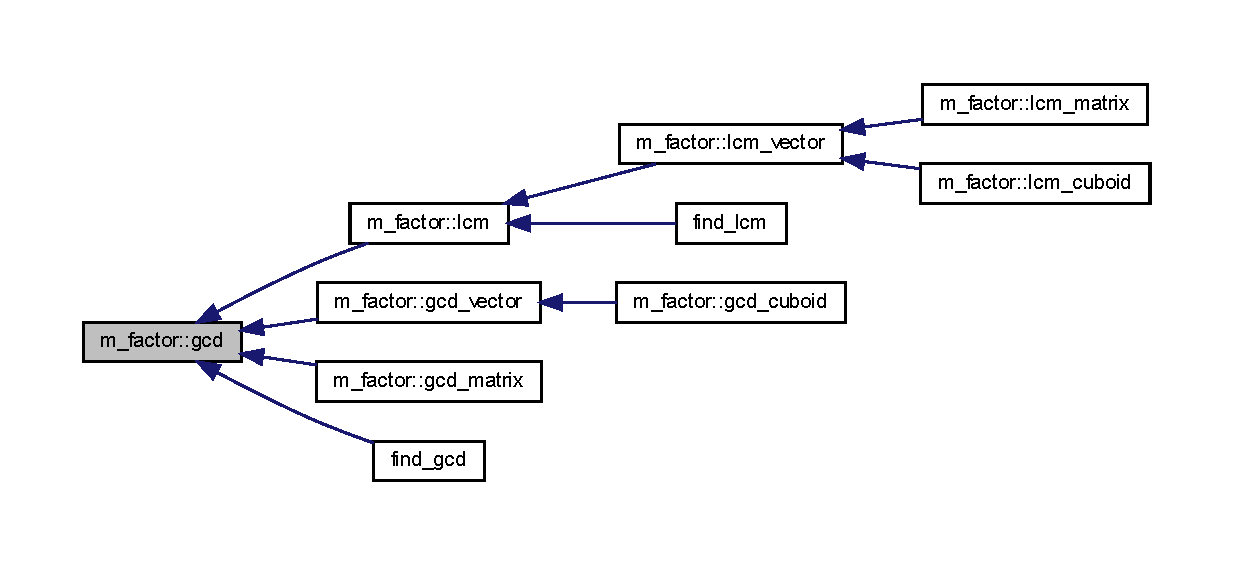
\includegraphics[width=350pt]{namespacem__factor_a69e8c33eff58fc447cfb8d4f3d4fae77_icgraph}
\end{center}
\end{figure}
\mbox{\Hypertarget{namespacem__factor_aed74f995a7c71e8cec13964b82457403}\label{namespacem__factor_aed74f995a7c71e8cec13964b82457403}} 
\index{m\+\_\+factor@{m\+\_\+factor}!gcd\+\_\+2@{gcd\+\_\+2}}
\index{gcd\+\_\+2@{gcd\+\_\+2}!m\+\_\+factor@{m\+\_\+factor}}
\subsubsection{\texorpdfstring{gcd\+\_\+2()}{gcd\_2()}}
{\footnotesize\ttfamily integer function, \hyperlink{M__stopwatch_83_8txt_a2f74811300c361e53b430611a7d1769f}{public} m\+\_\+factor\+::gcd\+\_\+2 (\begin{DoxyParamCaption}\item[{integer, intent(\hyperlink{M__journal_83_8txt_afce72651d1eed785a2132bee863b2f38}{in})}]{m,  }\item[{integer, intent(\hyperlink{M__journal_83_8txt_afce72651d1eed785a2132bee863b2f38}{in})}]{n }\end{DoxyParamCaption})}

\mbox{\Hypertarget{namespacem__factor_aff0e6f81edd8efc0fe41822916fb4efa}\label{namespacem__factor_aff0e6f81edd8efc0fe41822916fb4efa}} 
\index{m\+\_\+factor@{m\+\_\+factor}!gcd\+\_\+cuboid@{gcd\+\_\+cuboid}}
\index{gcd\+\_\+cuboid@{gcd\+\_\+cuboid}!m\+\_\+factor@{m\+\_\+factor}}
\subsubsection{\texorpdfstring{gcd\+\_\+cuboid()}{gcd\_cuboid()}}
{\footnotesize\ttfamily integer function, private m\+\_\+factor\+::gcd\+\_\+cuboid (\begin{DoxyParamCaption}\item[{integer, dimension(\+:,\+:,\+:), intent(\hyperlink{M__journal_83_8txt_afce72651d1eed785a2132bee863b2f38}{in})}]{m }\end{DoxyParamCaption})\hspace{0.3cm}{\ttfamily [private]}}



References gcd\+\_\+vector().

Here is the call graph for this function\+:
\nopagebreak
\begin{figure}[H]
\begin{center}
\leavevmode
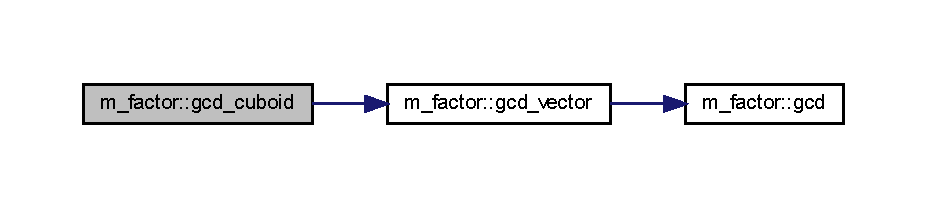
\includegraphics[width=350pt]{namespacem__factor_aff0e6f81edd8efc0fe41822916fb4efa_cgraph}
\end{center}
\end{figure}
\mbox{\Hypertarget{namespacem__factor_a6edfef428cb51a2cbe97cfb0ad25da8b}\label{namespacem__factor_a6edfef428cb51a2cbe97cfb0ad25da8b}} 
\index{m\+\_\+factor@{m\+\_\+factor}!gcd\+\_\+matrix@{gcd\+\_\+matrix}}
\index{gcd\+\_\+matrix@{gcd\+\_\+matrix}!m\+\_\+factor@{m\+\_\+factor}}
\subsubsection{\texorpdfstring{gcd\+\_\+matrix()}{gcd\_matrix()}}
{\footnotesize\ttfamily integer function, private m\+\_\+factor\+::gcd\+\_\+matrix (\begin{DoxyParamCaption}\item[{integer, dimension(\+:,\+:), intent(\hyperlink{M__journal_83_8txt_afce72651d1eed785a2132bee863b2f38}{in})}]{m }\end{DoxyParamCaption})\hspace{0.3cm}{\ttfamily [private]}}



References gcd().

Here is the call graph for this function\+:
\nopagebreak
\begin{figure}[H]
\begin{center}
\leavevmode
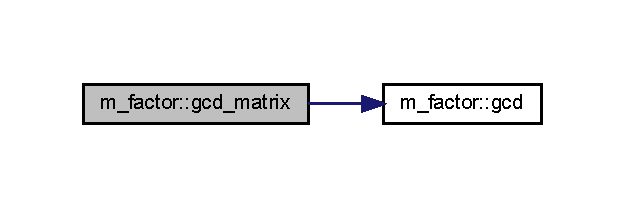
\includegraphics[width=300pt]{namespacem__factor_a6edfef428cb51a2cbe97cfb0ad25da8b_cgraph}
\end{center}
\end{figure}
\mbox{\Hypertarget{namespacem__factor_a60713d4c44895b4c18d4d6d9449ceaf7}\label{namespacem__factor_a60713d4c44895b4c18d4d6d9449ceaf7}} 
\index{m\+\_\+factor@{m\+\_\+factor}!gcd\+\_\+vector@{gcd\+\_\+vector}}
\index{gcd\+\_\+vector@{gcd\+\_\+vector}!m\+\_\+factor@{m\+\_\+factor}}
\subsubsection{\texorpdfstring{gcd\+\_\+vector()}{gcd\_vector()}}
{\footnotesize\ttfamily integer function, private m\+\_\+factor\+::gcd\+\_\+vector (\begin{DoxyParamCaption}\item[{integer, dimension(\+:), intent(\hyperlink{M__journal_83_8txt_afce72651d1eed785a2132bee863b2f38}{in})}]{m }\end{DoxyParamCaption})\hspace{0.3cm}{\ttfamily [private]}}



References gcd().

Here is the call graph for this function\+:
\nopagebreak
\begin{figure}[H]
\begin{center}
\leavevmode
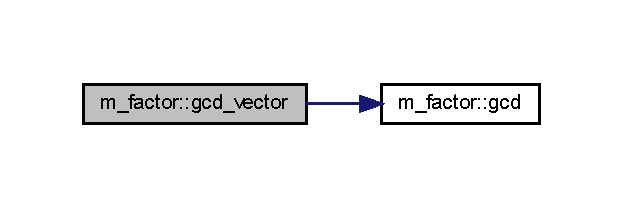
\includegraphics[width=299pt]{namespacem__factor_a60713d4c44895b4c18d4d6d9449ceaf7_cgraph}
\end{center}
\end{figure}
Here is the caller graph for this function\+:
\nopagebreak
\begin{figure}[H]
\begin{center}
\leavevmode
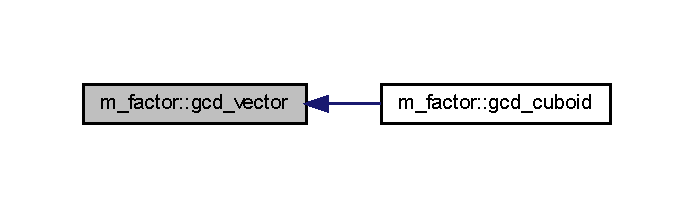
\includegraphics[width=333pt]{namespacem__factor_a60713d4c44895b4c18d4d6d9449ceaf7_icgraph}
\end{center}
\end{figure}
\mbox{\Hypertarget{namespacem__factor_afcca43d3d524f6d11d54bbfd475e60d5}\label{namespacem__factor_afcca43d3d524f6d11d54bbfd475e60d5}} 
\index{m\+\_\+factor@{m\+\_\+factor}!i\+\_\+is\+\_\+prime@{i\+\_\+is\+\_\+prime}}
\index{i\+\_\+is\+\_\+prime@{i\+\_\+is\+\_\+prime}!m\+\_\+factor@{m\+\_\+factor}}
\subsubsection{\texorpdfstring{i\+\_\+is\+\_\+prime()}{i\_is\_prime()}}
{\footnotesize\ttfamily logical function, \hyperlink{M__stopwatch_83_8txt_a2f74811300c361e53b430611a7d1769f}{public} m\+\_\+factor\+::i\+\_\+is\+\_\+prime (\begin{DoxyParamCaption}\item[{integer, intent(\hyperlink{M__journal_83_8txt_afce72651d1eed785a2132bee863b2f38}{in})}]{n }\end{DoxyParamCaption})}



\subsubsection*{N\+A\+ME}

i\+\_\+is\+\_\+prime(3f) -\/ \mbox{[}M\+\_\+factor\mbox{]} Determine if a number is prime using Sieve of Erasthosthenes \subsubsection*{S\+Y\+N\+O\+P\+S\+IS}

function i\+\_\+is\+\_\+prime ( n )

integer,intent(in) \+:\+: n

\subsubsection*{D\+E\+S\+C\+R\+I\+P\+T\+I\+ON}

A simple, unoptimized sieve of Erasthosthenes is used to check whether N can be divided by any integer between 2 and S\+Q\+R\+T(\+N).

\subsubsection*{V\+E\+R\+S\+I\+ON}

29 November 1998

\subsubsection*{A\+U\+T\+H\+OR}

John Burkardt

\subsubsection*{P\+A\+R\+A\+M\+E\+T\+E\+RS}

n Input, integer N, the integer to be tested. \subsubsection*{R\+E\+T\+U\+R\+NS}

Output logical I\+\_\+\+I\+S\+\_\+\+P\+R\+I\+M\+E(3f) is T\+R\+UE if N is prime, and F\+A\+L\+SE otherwise. Note that negative numbers and 0 are not considered prime. \subsubsection*{E\+X\+A\+M\+P\+LE}

\begin{DoxyVerb}sample program

 program testit
 use m_factor, only: i_is_prime
 implicit none
 integer  :: i
 integer  :: icount=0
 integer  :: isum=0
 integer,parameter :: n= 10000

 do i=2, n
    if(i_is_prime(i))then
       icount=icount+1
       isum=isum+i
       write(*,*)icount,i
    endif
 enddo

 write(*,*)'number of primes between 2 and ',n,' is ',icount
 write(*,*)'sum of primes between 2 and ',n,' is ',isum

 end program testit
\end{DoxyVerb}
 ! 

References false(), and true().

Here is the call graph for this function\+:
\nopagebreak
\begin{figure}[H]
\begin{center}
\leavevmode
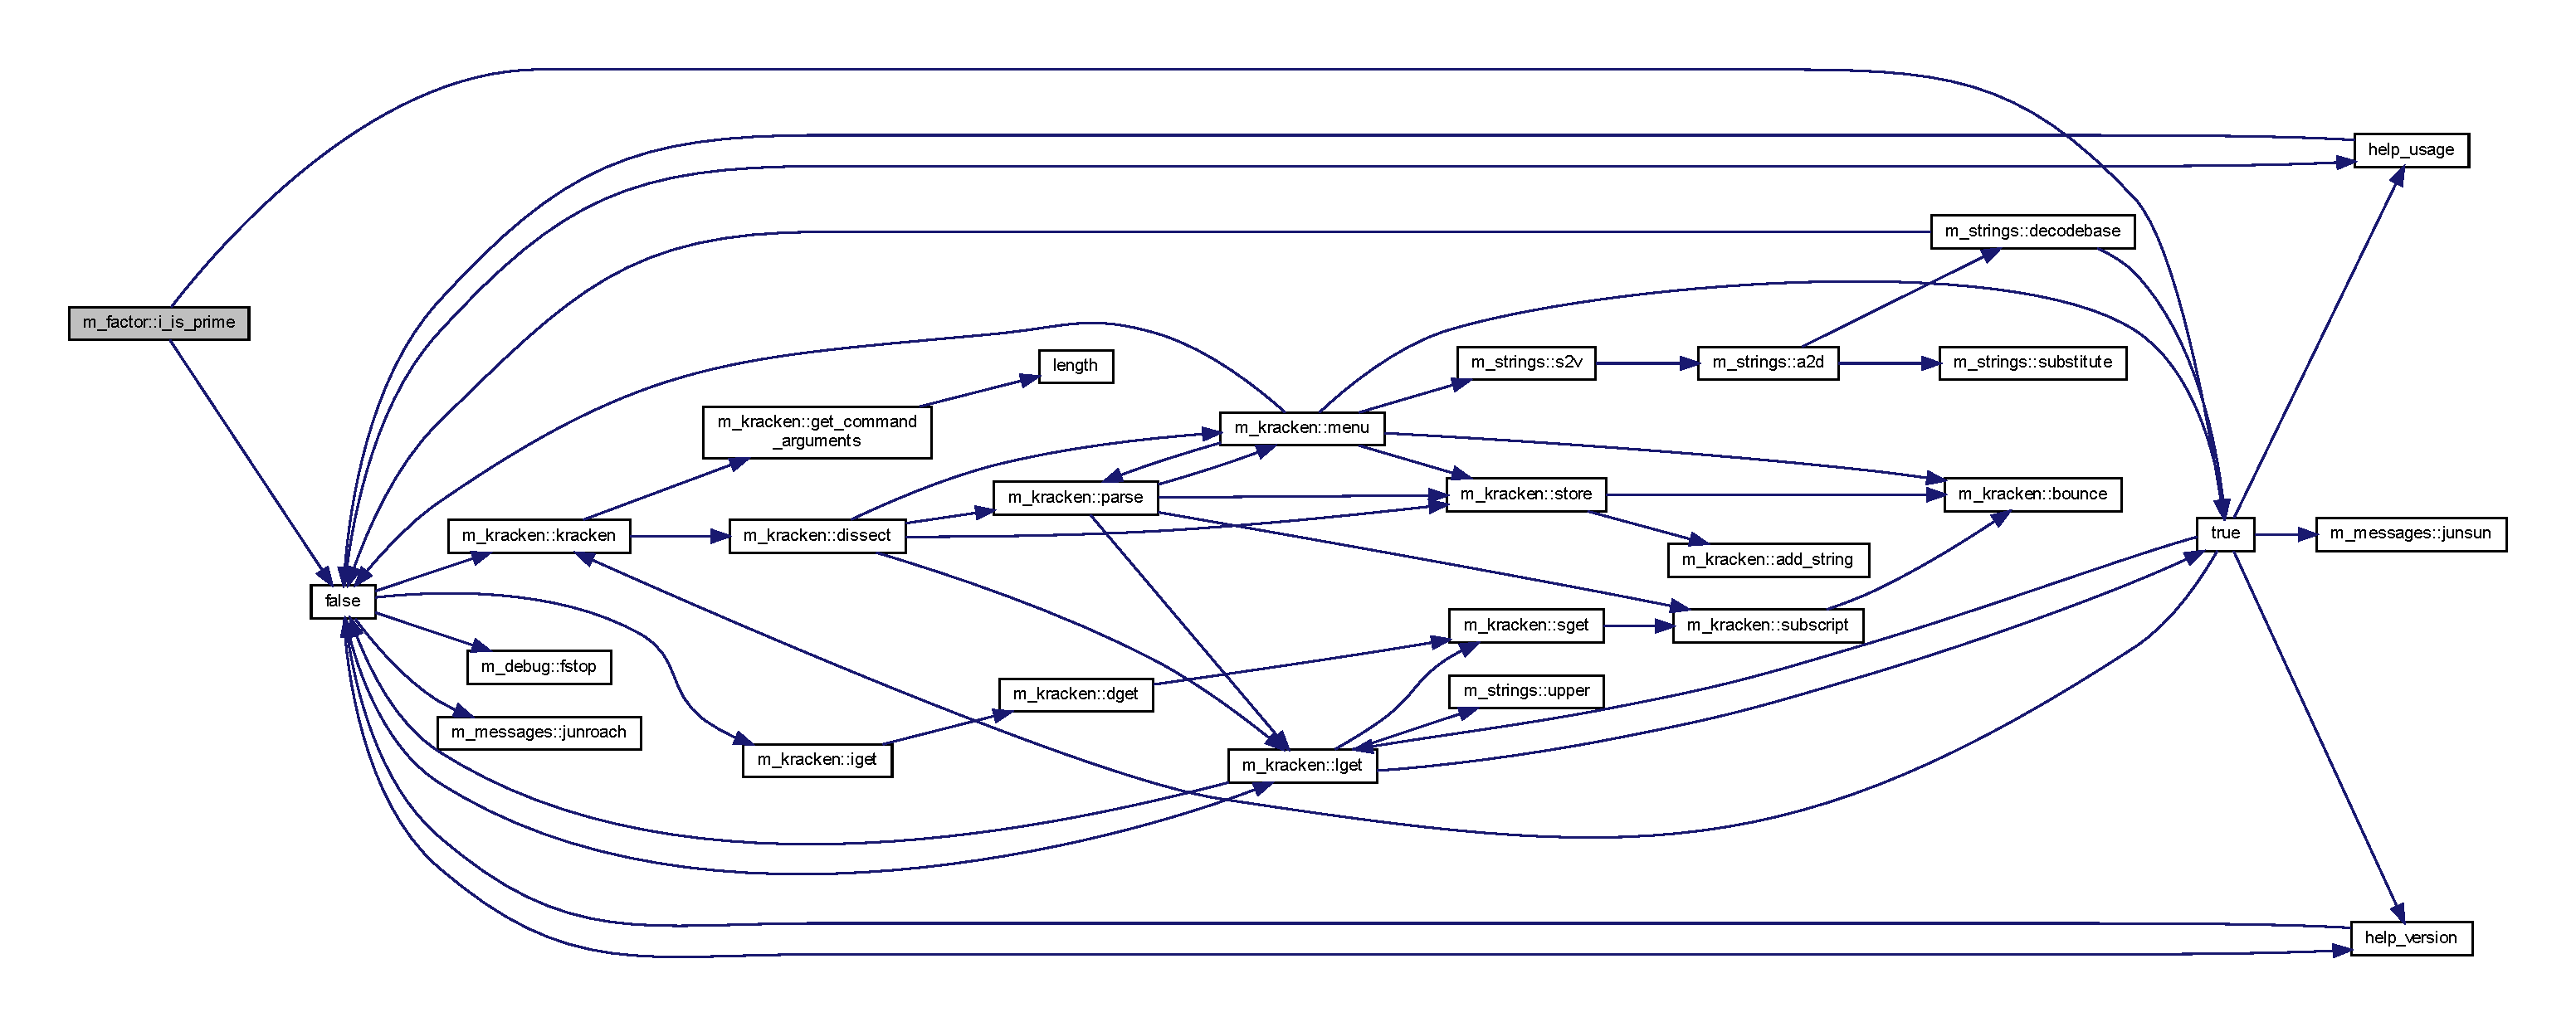
\includegraphics[width=350pt]{namespacem__factor_afcca43d3d524f6d11d54bbfd475e60d5_cgraph}
\end{center}
\end{figure}
\mbox{\Hypertarget{namespacem__factor_a363e0b451d99647a6230a308ffccc73c}\label{namespacem__factor_a363e0b451d99647a6230a308ffccc73c}} 
\index{m\+\_\+factor@{m\+\_\+factor}!lcm@{lcm}}
\index{lcm@{lcm}!m\+\_\+factor@{m\+\_\+factor}}
\subsubsection{\texorpdfstring{lcm()}{lcm()}}
{\footnotesize\ttfamily integer function, private m\+\_\+factor\+::lcm (\begin{DoxyParamCaption}\item[{integer, intent(\hyperlink{M__journal_83_8txt_afce72651d1eed785a2132bee863b2f38}{in})}]{i,  }\item[{integer, intent(\hyperlink{M__journal_83_8txt_afce72651d1eed785a2132bee863b2f38}{in})}]{j }\end{DoxyParamCaption})\hspace{0.3cm}{\ttfamily [private]}}



\subsubsection*{N\+A\+ME}

least\+\_\+common\+\_\+multiple(3f) -\/ \mbox{[}M\+\_\+factor\mbox{]} Least common multiple of two integers or vector m(\+:), matrix m(\+:,\+:) or cuboid m(\+:,\+:,\+:) \subsubsection*{S\+Y\+N\+O\+P\+S\+IS}

integer function least\+\_\+common\+\_\+multiple(i,j) integer,intent(in)\+:\+: i,j or integer function least\+\_\+common\+\_\+multiple(m) integer,intent(in)\+:\+: m(\+:) or integer,intent(in)\+:\+: m(\+:,\+:) or integer,intent(in)\+:\+: m(\+:,\+:,\+:)

\subsubsection*{D\+E\+S\+C\+R\+I\+P\+T\+I\+ON}

From Wikipedia, the free encyclopedia\+:

In arithmetic and number theory, the least common multiple (also called the lowest common multiple or smallest common multiple) of two integers a and b, usually denoted by L\+C\+M(a, b), is the smallest positive integer that is divisible by both a and b. Since division of integers by zero is undefined, this definition has meaning only if a and b are both different from zero. However, some authors define lcm(a,0) as 0 for all a, which is the result of taking the L\+CM to be the least upper bound in the lattice of divisibility.

The L\+CM is familiar from grade-\/school arithmetic as the \char`\"{}lowest common
    denominator\char`\"{} (L\+CD) that must be determined before fractions can be added, subtracted or compared. The L\+CM of more than two integers is also well-\/defined\+: it is the smallest positive integer that is divisible by each of them.

\subsubsection*{E\+X\+A\+M\+P\+LE}

Sample Program\+:

program demo\+\_\+lcm use M\+\_\+factor, only \+: lcm=$>$\hyperlink{interfacem__factor_1_1least__common__multiple}{least\+\_\+common\+\_\+multiple} implicit none write($\ast$,$\ast$)\textquotesingle{}S\+C\+A\+L\+AR\+:\textquotesingle{} call writeit(10,24,120) call writeit(15,30,30) call writeit(-\/15,-\/30,30) call writeit(15,-\/30,30) call writeit(-\/15,30,30)

write($\ast$,$\ast$)\textquotesingle{}V\+E\+C\+T\+OR\+:\textquotesingle{} call writeit\+\_\+v(\mbox{[}10,24\mbox{]},120) call writeit\+\_\+v(\mbox{[}15,30\mbox{]},30) call writeit\+\_\+v(\mbox{[}-\/15,-\/30\mbox{]},30) call writeit\+\_\+v(\mbox{[}5,-\/15,-\/40\mbox{]},120) call writeit\+\_\+v(\mbox{[}2,3,4,5\mbox{]},60) write($\ast$,$\ast$)\textquotesingle{}Special cases\+:\textquotesingle{} call writeit\+\_\+v(\mbox{[}15,0\mbox{]},0) call writeit\+\_\+v(\mbox{[}-\/15,0\mbox{]},0) call writeit\+\_\+v(\mbox{[}0\mbox{]},0) call writeit\+\_\+v(\mbox{[}-\/10\mbox{]},10) call writeit\+\_\+v(\mbox{[}22\mbox{]},22) call writeit\+\_\+v(\mbox{[}0,0\mbox{]},0) call writeit\+\_\+v(\mbox{[}0,0,0,0,0\mbox{]},0) call writeit\+\_\+v(\mbox{[}0,0,0,-\/1,0\mbox{]},0) call writeit\+\_\+v(\mbox{[}0,0,0,33,0,3,11\mbox{]},0) contains

subroutine writeit(ii,jj,answer) integer,intent(in) \+:\+: ii,jj integer,intent(in) \+:\+: answer write($\ast$,\textquotesingle{}(\char`\"{}  For lcm(\char`\"{},I0,\char`\"{},\char`\"{},I0,\char`\"{}) the value is \char`\"{},I0,\char`\"{} which is \char`\"{},L1)\textquotesingle{})\& \& ii,jj,lcm(ii,jj),lcm(ii,jj).eq.\+answer end subroutine writeit

subroutine writeit\+\_\+v(array,answer) integer,intent(in) \+:\+: array(\+:) integer,intent(in) \+:\+: answer write($\ast$,\textquotesingle{}(\char`\"{}  For lcm(\mbox{[}\char`\"{},$\ast$(i0\+:,1x))\textquotesingle{},advance=\textquotesingle{}no\textquotesingle{})array write($\ast$,\textquotesingle{}(\char`\"{}\mbox{]}) the value is \char`\"{},i0,\char`\"{} which is \char`\"{},L1)\textquotesingle{}) \& \& lcm(array),lcm(array).eq.\+answer end subroutine writeit\+\_\+v

end program demo\+\_\+lcm

Expected results\+:

$>$ S\+C\+A\+L\+AR\+: $>$ For lcm(10,24) the value is 120 which is T $>$ For lcm(15,30) the value is 30 which is T $>$ For lcm(-\/15,-\/30) the value is 30 which is T $>$ For lcm(15,-\/30) the value is 30 which is T $>$ For lcm(-\/15,30) the value is 30 which is T $>$ V\+E\+C\+T\+OR\+: $>$ For lcm(\mbox{[}10 24\mbox{]}) the value is 120 which is T $>$ For lcm(\mbox{[}15 30\mbox{]}) the value is 30 which is T $>$ For lcm(\mbox{[}-\/15 -\/30\mbox{]}) the value is 30 which is T $>$ For lcm(\mbox{[}5 -\/15 -\/40\mbox{]}) the value is 120 which is T $>$ For lcm(\mbox{[}2 3 4 5\mbox{]}) the value is 60 which is T $>$ Special cases\+: $>$ For lcm(\mbox{[}15 0\mbox{]}) the value is 0 which is T $>$ For lcm(\mbox{[}-\/15 0\mbox{]}) the value is 0 which is T $>$ For lcm(\mbox{[}0\mbox{]}) the value is 0 which is T $>$ For lcm(\mbox{[}-\/10\mbox{]}) the value is 10 which is T $>$ For lcm(\mbox{[}22\mbox{]}) the value is 22 which is T $>$ For lcm(\mbox{[}0 0\mbox{]}) the value is 0 which is T $>$ For lcm(\mbox{[}0 0 0 0 0\mbox{]}) the value is 0 which is T $>$ For lcm(\mbox{[}0 0 0 -\/1 0\mbox{]}) the value is 0 which is T $>$ For lcm(\mbox{[}0 0 0 33 0 3 11\mbox{]}) the value is 0 which is T

\subsubsection*{M\+E\+T\+H\+OD}

Reduction by the greatest common divisor

The following formula reduces the problem of computing the least common multiple to the problem of computing the greatest common divisor (G\+CD), also known as the greatest common factor\+:

lcm(a,b) = $\vert$a$\ast$b$\vert$ / gcd(a,b)

This formula is also valid when exactly one of a and b is 0, since gcd(a, 0) = $\vert$a$\vert$. (However, if both a and b are 0, this formula would cause division by zero; lcm(0, 0) = 0 is a special case. 

References gcd(), and m\+\_\+anyscalar\+::int128.

Here is the call graph for this function\+:
\nopagebreak
\begin{figure}[H]
\begin{center}
\leavevmode
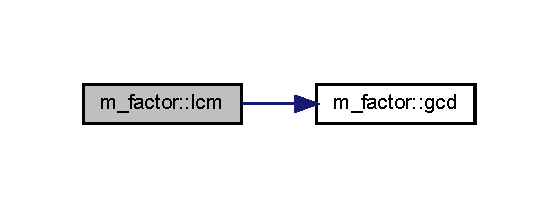
\includegraphics[width=268pt]{namespacem__factor_a363e0b451d99647a6230a308ffccc73c_cgraph}
\end{center}
\end{figure}
Here is the caller graph for this function\+:
\nopagebreak
\begin{figure}[H]
\begin{center}
\leavevmode
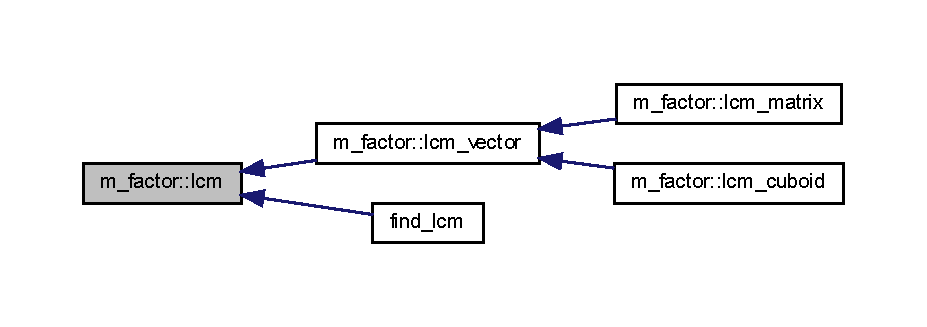
\includegraphics[width=350pt]{namespacem__factor_a363e0b451d99647a6230a308ffccc73c_icgraph}
\end{center}
\end{figure}
\mbox{\Hypertarget{namespacem__factor_ae9aed0802e2c5a923b255f143ddf6e15}\label{namespacem__factor_ae9aed0802e2c5a923b255f143ddf6e15}} 
\index{m\+\_\+factor@{m\+\_\+factor}!lcm\+\_\+cuboid@{lcm\+\_\+cuboid}}
\index{lcm\+\_\+cuboid@{lcm\+\_\+cuboid}!m\+\_\+factor@{m\+\_\+factor}}
\subsubsection{\texorpdfstring{lcm\+\_\+cuboid()}{lcm\_cuboid()}}
{\footnotesize\ttfamily integer function, private m\+\_\+factor\+::lcm\+\_\+cuboid (\begin{DoxyParamCaption}\item[{integer, dimension(\+:,\+:,\+:), intent(\hyperlink{M__journal_83_8txt_afce72651d1eed785a2132bee863b2f38}{in})}]{m }\end{DoxyParamCaption})\hspace{0.3cm}{\ttfamily [private]}}



\subsubsection*{N\+A\+ME}

lcm\+\_\+cuboid(3fp) -\/ least common multiple of integer cuboid m(\+:,\+:,\+:) \subsubsection*{S\+Y\+N\+O\+P\+S\+IS}

integer function lcm\+\_\+cuboid(m)

integer,intent(in) \+:\+: m(\+:,\+:,\+:) \subsubsection*{D\+E\+S\+C\+R\+I\+P\+T\+I\+ON}

Find the Least Common Denominator of an I\+N\+T\+E\+G\+ER cuboid M(\+:,\+:,\+:). 

References lcm\+\_\+vector().

Here is the call graph for this function\+:
\nopagebreak
\begin{figure}[H]
\begin{center}
\leavevmode
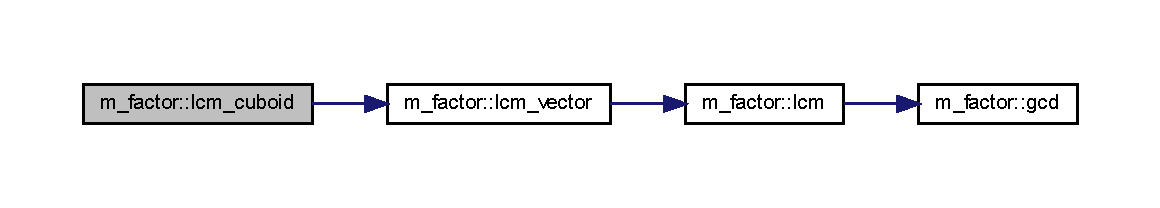
\includegraphics[width=350pt]{namespacem__factor_ae9aed0802e2c5a923b255f143ddf6e15_cgraph}
\end{center}
\end{figure}
\mbox{\Hypertarget{namespacem__factor_af2cc63a43164bf57aedac557fafe907f}\label{namespacem__factor_af2cc63a43164bf57aedac557fafe907f}} 
\index{m\+\_\+factor@{m\+\_\+factor}!lcm\+\_\+matrix@{lcm\+\_\+matrix}}
\index{lcm\+\_\+matrix@{lcm\+\_\+matrix}!m\+\_\+factor@{m\+\_\+factor}}
\subsubsection{\texorpdfstring{lcm\+\_\+matrix()}{lcm\_matrix()}}
{\footnotesize\ttfamily integer function, private m\+\_\+factor\+::lcm\+\_\+matrix (\begin{DoxyParamCaption}\item[{integer, dimension(\+:,\+:), intent(\hyperlink{M__journal_83_8txt_afce72651d1eed785a2132bee863b2f38}{in})}]{m }\end{DoxyParamCaption})\hspace{0.3cm}{\ttfamily [private]}}



\subsubsection*{N\+A\+ME}

lcm\+\_\+matrix(3fp) -\/ least common multiple of integer array m(\+:,\+:) \subsubsection*{S\+Y\+N\+O\+P\+S\+IS}

integer function lcm\+\_\+matrix(m)

integer,intent(in) \+:\+: m(\+:,\+:) \subsubsection*{D\+E\+S\+C\+R\+I\+P\+T\+I\+ON}

Find the Least Common Denominator of an I\+N\+T\+E\+G\+ER matrix M(\+:,\+:). 

References lcm\+\_\+vector().

Here is the call graph for this function\+:
\nopagebreak
\begin{figure}[H]
\begin{center}
\leavevmode
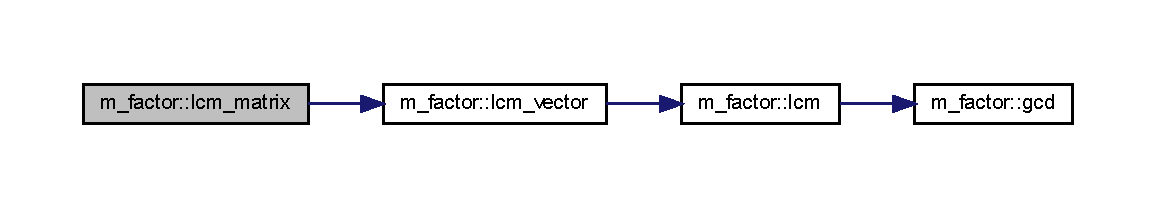
\includegraphics[width=350pt]{namespacem__factor_af2cc63a43164bf57aedac557fafe907f_cgraph}
\end{center}
\end{figure}
\mbox{\Hypertarget{namespacem__factor_a3802e87d5a394888aefc2d6cf496509f}\label{namespacem__factor_a3802e87d5a394888aefc2d6cf496509f}} 
\index{m\+\_\+factor@{m\+\_\+factor}!lcm\+\_\+vector@{lcm\+\_\+vector}}
\index{lcm\+\_\+vector@{lcm\+\_\+vector}!m\+\_\+factor@{m\+\_\+factor}}
\subsubsection{\texorpdfstring{lcm\+\_\+vector()}{lcm\_vector()}}
{\footnotesize\ttfamily integer function, private m\+\_\+factor\+::lcm\+\_\+vector (\begin{DoxyParamCaption}\item[{integer, dimension(\+:), intent(\hyperlink{M__journal_83_8txt_afce72651d1eed785a2132bee863b2f38}{in})}]{m }\end{DoxyParamCaption})\hspace{0.3cm}{\ttfamily [private]}}



\subsubsection*{N\+A\+ME}

lcm\+\_\+vector(3fp) -\/ least common multiple of integer vector m(\+:) \subsubsection*{S\+Y\+N\+O\+P\+S\+IS}

integer function lcm\+\_\+vector(m)

integer,intent(in) \+:\+: m(\+:) \subsubsection*{D\+E\+S\+C\+R\+I\+P\+T\+I\+ON}

Find the Least Common Denominator of an I\+N\+T\+E\+G\+ER vector M(\+:). 

References lcm().

Here is the call graph for this function\+:
\nopagebreak
\begin{figure}[H]
\begin{center}
\leavevmode
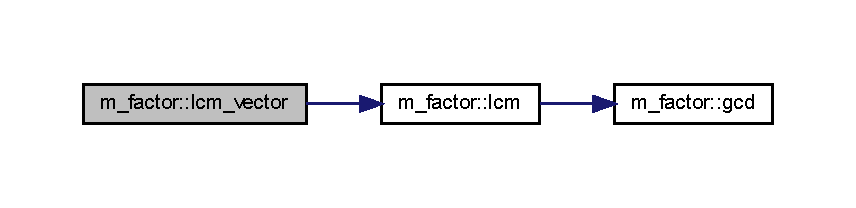
\includegraphics[width=350pt]{namespacem__factor_a3802e87d5a394888aefc2d6cf496509f_cgraph}
\end{center}
\end{figure}
Here is the caller graph for this function\+:
\nopagebreak
\begin{figure}[H]
\begin{center}
\leavevmode
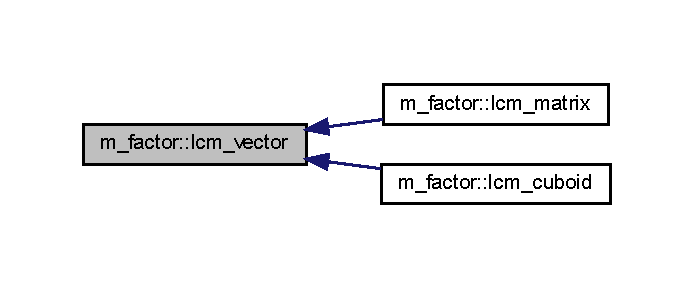
\includegraphics[width=333pt]{namespacem__factor_a3802e87d5a394888aefc2d6cf496509f_icgraph}
\end{center}
\end{figure}
\mbox{\Hypertarget{namespacem__factor_a6440013d17b820fa65096b34f21d367d}\label{namespacem__factor_a6440013d17b820fa65096b34f21d367d}} 
\index{m\+\_\+factor@{m\+\_\+factor}!prime\+\_\+factors@{prime\+\_\+factors}}
\index{prime\+\_\+factors@{prime\+\_\+factors}!m\+\_\+factor@{m\+\_\+factor}}
\subsubsection{\texorpdfstring{prime\+\_\+factors()}{prime\_factors()}}
{\footnotesize\ttfamily \hyperlink{M__stopwatch_83_8txt_acfbcff50169d691ff02d4a123ed70482}{subroutine}, \hyperlink{M__stopwatch_83_8txt_a2f74811300c361e53b430611a7d1769f}{public} m\+\_\+factor\+::prime\+\_\+factors (\begin{DoxyParamCaption}\item[{integer, intent(\hyperlink{M__journal_83_8txt_afce72651d1eed785a2132bee863b2f38}{in})}]{number,  }\item[{integer, intent(out)}]{nprm,  }\item[{integer, dimension(\+:), intent(out)}]{iprm,  }\item[{integer, dimension(\+:), intent(out)}]{iexp,  }\item[{logical, intent(\hyperlink{M__journal_83_8txt_afce72651d1eed785a2132bee863b2f38}{in}), \hyperlink{option__stopwatch_83_8txt_aa4ece75e7acf58a4843f70fe18c3ade5}{optional}}]{verbose }\end{DoxyParamCaption})}



\subsubsection*{N\+A\+ME}

prime\+\_\+factors -\/ \mbox{[}M\+\_\+factor\mbox{]} decompose a number into its prime factors \subsubsection*{S\+Y\+N\+O\+P\+S\+IS}

call prime\+\_\+factors(number,nprm,iprm,iexp\mbox{[},verbose\mbox{]})

integer, intent(in) \+:\+: number integer, intent(out) \+:\+: nprm integer, intent(out) \+:\+: iprm(\+:) integer, intent(out) \+:\+: iexp(\+:) logical, intent(in),optional \+:\+: verbose \subsubsection*{D\+E\+S\+C\+R\+I\+P\+T\+I\+ON}

\begin{DoxyVerb}1. Upon return from PRIME_FACTORS,

        NUMBER = IPRM(1)**IEXP(1) * IPRM(2)**IEXP(2) * ...
                 *IPRM(NPRM)**IEXP(NPRM)

2. A number represented by a (single-precision) INTEGER
   value on the VMS VAX cluster can have at most 9 distinct
   prime factors. On machines where the maximum integer is
   larger than 2**31 - 1, IPRM and IEXP would, in general,
   have to be dimensioned larger since larger numbers may
   have more than 9 distinct prime factors.
\end{DoxyVerb}
 \subsubsection*{O\+P\+T\+I\+O\+NS}

\begin{DoxyVerb}NUMBER   INTEGER constant or variable, number to be decomposed into
         prime factors. NUMBER .ge. 2.
         For 32-bit integers NUMBER <= 2147483647
NPRM     INTEGER variable, will contain the number of distinct prime
         factors of the number.
IPRM     INTEGER array of size at least 9, will contain the prime
         factors of the number.
IEXP     INTEGER array of size at least 9, will contain the
         exponents of the corresponding prime factors.
verbose  optional LOGICAL constant or variable, controls printing
         of results.
          o .false. - Results are not printed.
          o .true. - Results are printed.
\end{DoxyVerb}
 \subsubsection*{E\+X\+A\+M\+P\+LE}

Sample program\+:

program find\+\_\+prime\+\_\+factors use M\+\_\+factor, only \+: prime\+\_\+factors implicit none integer \+:\+: number integer \+:\+: iexp(10), iprm(10), nprm logical \+:\+: verbose=.true. integer \+:\+: ios do write($\ast$,\textquotesingle{}(a)\textquotesingle{}, advance=\textquotesingle{}no\textquotesingle{}) \textquotesingle{} Enter number to be factored\+: \textquotesingle{} read($\ast$,$\ast$,iostat=ios,end=999) number if(ios.\+eq.\+0)then call prime\+\_\+factors(number, nprm, iprm, iexp, verbose) endif enddo 999 continue end program find\+\_\+prime\+\_\+factors

\subsubsection*{P\+E\+D\+I\+G\+R\+EE}

o Coded at Madison Academic Computing Center, University of Wisconsin, Madison o F\+O\+R\+T\+R\+AN 77 Version 1988.\+09 o Code converted using T\+O\+\_\+\+F90 by Alan Miller, 2000-\/07-\/14\+T11\+:42\+:45 o Fortran 2003 version 20160918 by John S. Urban 

References false().

Here is the call graph for this function\+:
\nopagebreak
\begin{figure}[H]
\begin{center}
\leavevmode
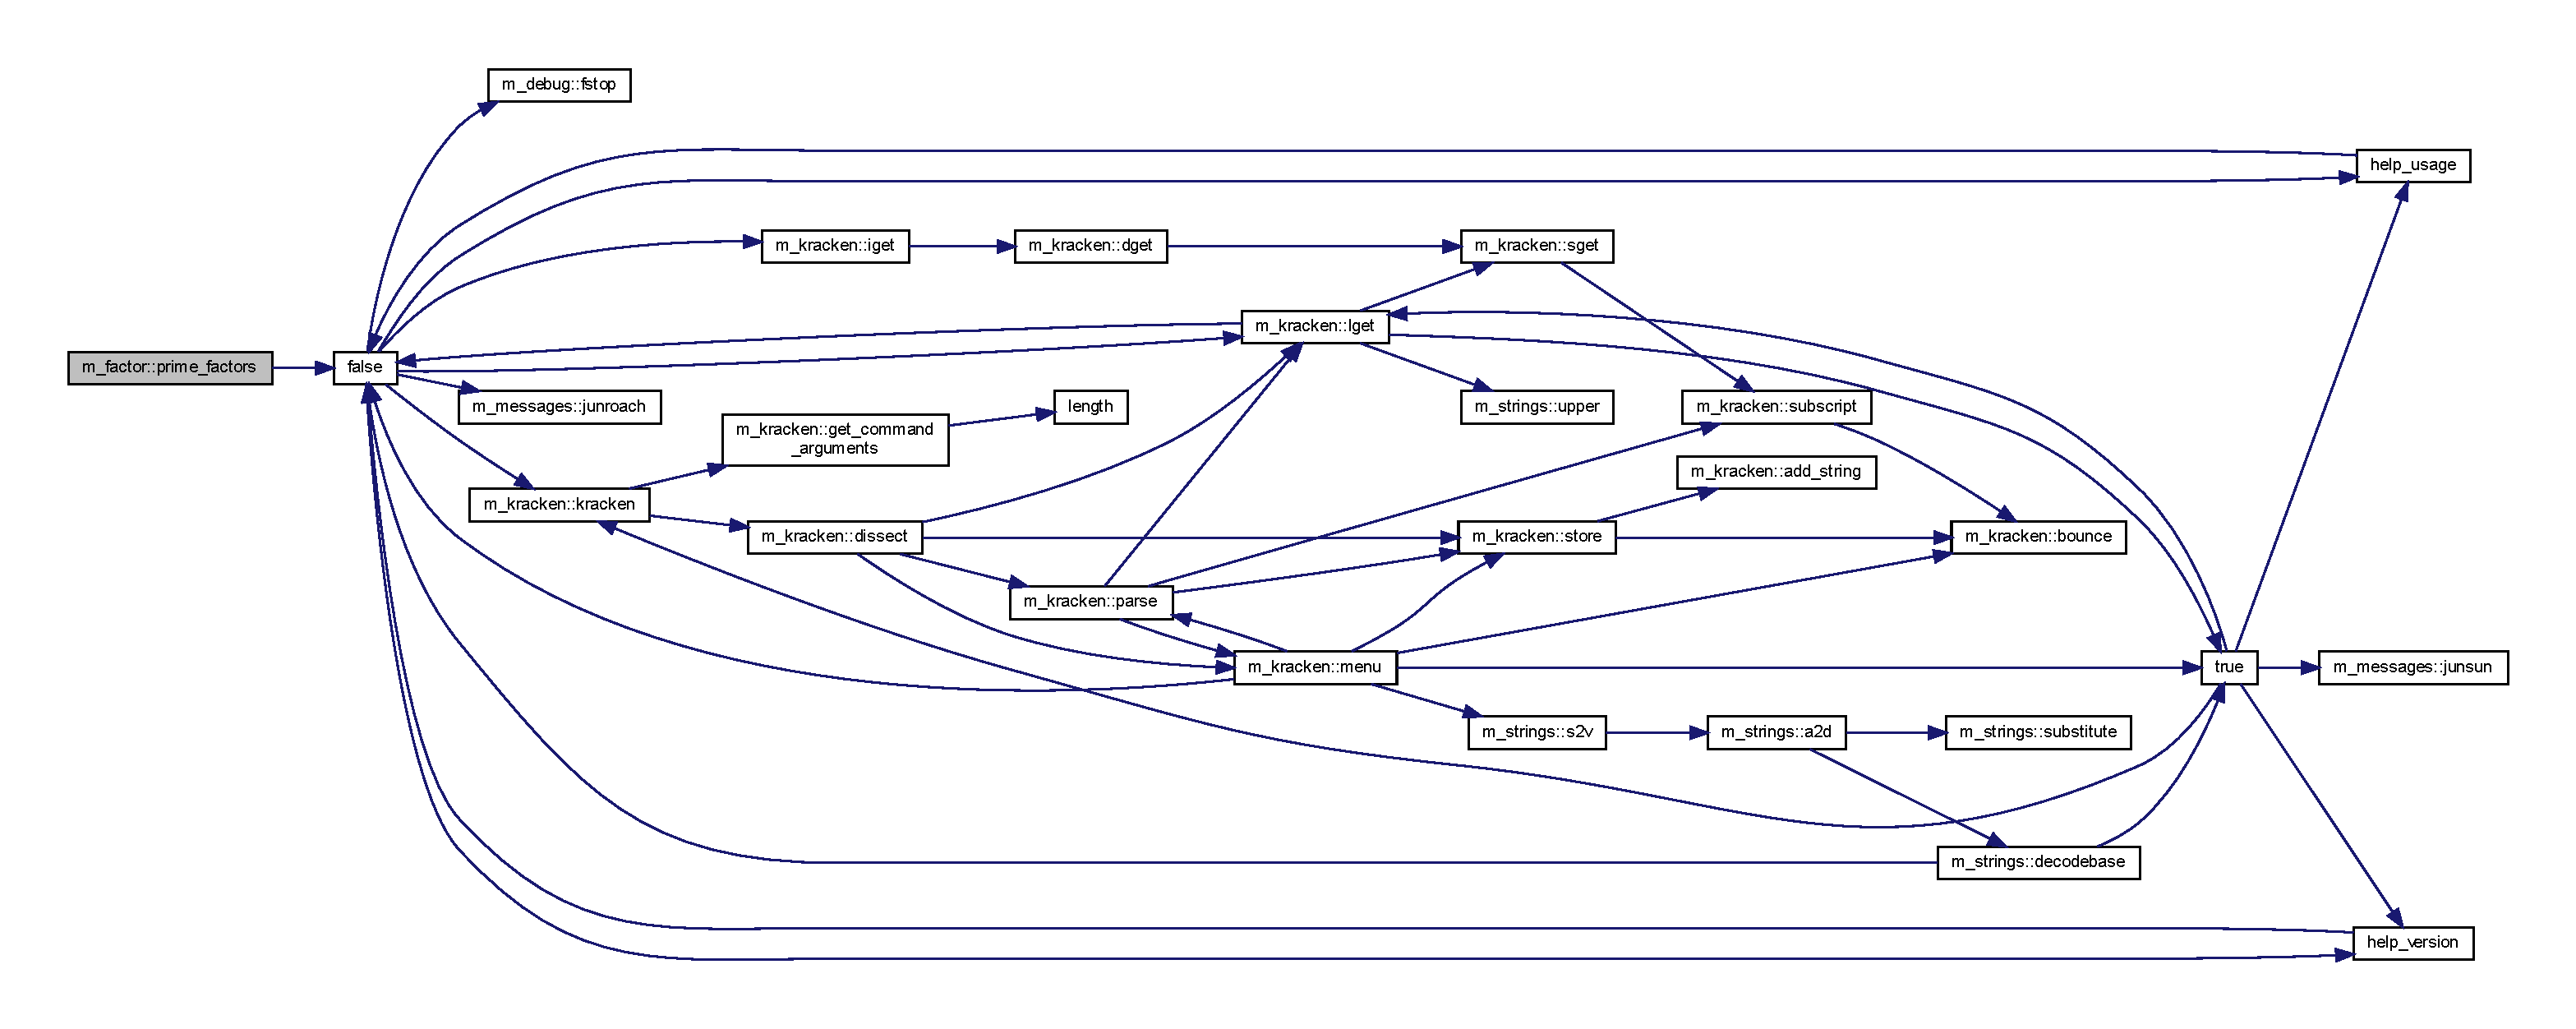
\includegraphics[width=350pt]{namespacem__factor_a6440013d17b820fa65096b34f21d367d_cgraph}
\end{center}
\end{figure}
Here is the caller graph for this function\+:
\nopagebreak
\begin{figure}[H]
\begin{center}
\leavevmode
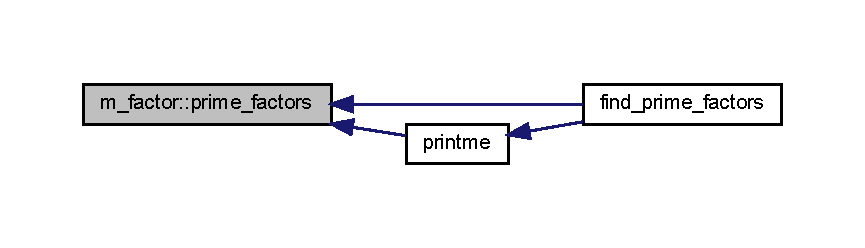
\includegraphics[width=350pt]{namespacem__factor_a6440013d17b820fa65096b34f21d367d_icgraph}
\end{center}
\end{figure}


\subsection{Variable Documentation}
\mbox{\Hypertarget{namespacem__factor_a7ae228777d43741d83e3a4df917f39df}\label{namespacem__factor_a7ae228777d43741d83e3a4df917f39df}} 
\index{m\+\_\+factor@{m\+\_\+factor}!ident1@{ident1}}
\index{ident1@{ident1}!m\+\_\+factor@{m\+\_\+factor}}
\subsubsection{\texorpdfstring{ident1}{ident1}}
{\footnotesize\ttfamily \hyperlink{option__stopwatch_83_8txt_abd4b21fbbd175834027b5224bfe97e66}{character}(len=$\ast$), parameter m\+\_\+factor\+::ident1 =\textquotesingle{}@(\#)M\+\_\+factor\+::least\+\_\+common\+\_\+multiple(3f)\+: function finds L\+C\+M for (i,j)$\vert$m(\+:)$\vert$m(\+:,\+:)$\vert$m(\+:,\+:,\+:)\textquotesingle{}\hspace{0.3cm}{\ttfamily [private]}}

\mbox{\Hypertarget{namespacem__factor_ab34da44c20883bea1b31a67a3d6359e5}\label{namespacem__factor_ab34da44c20883bea1b31a67a3d6359e5}} 
\index{m\+\_\+factor@{m\+\_\+factor}!ident2@{ident2}}
\index{ident2@{ident2}!m\+\_\+factor@{m\+\_\+factor}}
\subsubsection{\texorpdfstring{ident2}{ident2}}
{\footnotesize\ttfamily \hyperlink{option__stopwatch_83_8txt_abd4b21fbbd175834027b5224bfe97e66}{character}(len=$\ast$), parameter m\+\_\+factor\+::ident2 =\textquotesingle{}@(\#)M\+\_\+factor\+::greatest\+\_\+common\+\_\+divisor(3f)\+: function finds G\+C\+D for (i,j)$\vert$m(\+:)$\vert$m(\+:,\+:)$\vert$m(\+:,\+:,\+:)\char`\"{}\textquotesingle{}\hspace{0.3cm}{\ttfamily [private]}}


\hypertarget{namespacem__fpp}{}\section{m\+\_\+fpp Module Reference}
\label{namespacem__fpp}\index{m\+\_\+fpp@{m\+\_\+fpp}}


$<$html$>$ $<$head$>$ $<$title$>$ ufpp $<$/title$>$ $<$link rel=\char`\"{}stylesheet\char`\"{} type=\char`\"{}text/css\char`\"{} href=\char`\"{}\+Style\+Sheets/man.\+css\char`\"{} title=\char`\"{}\+Local\char`\"{}$>$ $<$meta name=\char`\"{}description\char`\"{} content=\char`\"{}\+Fortran module containing library of date and time procedures\char`\"{}$>$ $<$meta name=\char`\"{}keywords\char`\"{} content=\char`\"{}date\+\_\+and\+\_\+time,date,time,gregorian,julian,epoch time,day of week, ordinal day\char`\"{}$>$ $<$meta name=\char`\"{}keywords\char`\"{} content=\char`\"{}week of year\char`\"{}$>$ $<$meta name=\char`\"{}keywords\char`\"{} content=\char`\"{}\+Fortran,module,library,repository,collection\char`\"{}$>$ $<$script src=\char`\"{}../../../javascript/toggle\+Hidden.\+js\char`\"{} type=\char`\"{}text/javascript\char`\"{}$>$$<$/script$>$ $<$/head$>$ $<$body$>$

\href{../../../GPF.html}{\tt } 


\subsection*{Data Types}
\begin{DoxyCompactItemize}
\item 
type \hyperlink{structm__fpp_1_1file__stack}{file\+\_\+stack}
\end{DoxyCompactItemize}
\subsection*{Functions/\+Subroutines}
\begin{DoxyCompactItemize}
\item 
\hyperlink{M__stopwatch_83_8txt_acfbcff50169d691ff02d4a123ed70482}{subroutine} \hyperlink{namespacem__fpp_a3aa7c291b265d02ad91b3bb29e797156}{cond} ()
\item 
\hyperlink{M__stopwatch_83_8txt_acfbcff50169d691ff02d4a123ed70482}{subroutine} \hyperlink{namespacem__fpp_a1149aa9cc5620d40fa315e4de3937776}{exe} ()
\item 
\hyperlink{M__stopwatch_83_8txt_acfbcff50169d691ff02d4a123ed70482}{subroutine} \hyperlink{namespacem__fpp_afe91155aa0c891fc35f3927e777440ea}{ident} (opts)
\item 
\hyperlink{M__stopwatch_83_8txt_acfbcff50169d691ff02d4a123ed70482}{subroutine} \hyperlink{namespacem__fpp_aeab3b5145d977b953ea972b2882e442a}{output\+\_\+case} (opts)
\item 
\hyperlink{M__stopwatch_83_8txt_acfbcff50169d691ff02d4a123ed70482}{subroutine} \hyperlink{namespacem__fpp_a43f195db2d7dcdbaf89cb2e45ca60421}{define} (opts, ireset)
\item 
\hyperlink{option__stopwatch_83_8txt_abd4b21fbbd175834027b5224bfe97e66}{character}(len=17) function \hyperlink{namespacem__fpp_aa52b30ff734a7831d3334aee5ef4e8e7}{getdatetimestr} ()
\item 
\hyperlink{M__stopwatch_83_8txt_acfbcff50169d691ff02d4a123ed70482}{subroutine} \hyperlink{namespacem__fpp_a8034546d38694c17677cf638e2760d43}{printenv} (opts)
\item 
\hyperlink{M__stopwatch_83_8txt_acfbcff50169d691ff02d4a123ed70482}{subroutine} \hyperlink{namespacem__fpp_ac32c830615f875efaf8678759daa7f39}{name} (line)
\item 
\hyperlink{M__stopwatch_83_8txt_acfbcff50169d691ff02d4a123ed70482}{subroutine} \hyperlink{namespacem__fpp_a77ebcaafb7e1396c68dbc0bdcc088232}{getval} (line, ipos1, ipos2, value)
\item 
\hyperlink{M__stopwatch_83_8txt_acfbcff50169d691ff02d4a123ed70482}{subroutine} \hyperlink{namespacem__fpp_aa3c22b47ddfcf47940f8254d4a44c448}{undef} (opts)
\item 
\hyperlink{M__stopwatch_83_8txt_acfbcff50169d691ff02d4a123ed70482}{subroutine} \hyperlink{namespacem__fpp_a4866adfbe17fb5cc245f2ad058bb47f2}{if} (opts, noelse, eb)
\item 
\hyperlink{M__stopwatch_83_8txt_acfbcff50169d691ff02d4a123ed70482}{subroutine} \hyperlink{namespacem__fpp_af80169d1e05b926eed9d4dbe10963084}{def} (verb, opts, noelse, eb)
\item 
\hyperlink{M__stopwatch_83_8txt_acfbcff50169d691ff02d4a123ed70482}{subroutine} \hyperlink{namespacem__fpp_acc125ade915dbf457a06801f2e241306}{ifdef} (line, ipos1)
\item 
\hyperlink{M__stopwatch_83_8txt_acfbcff50169d691ff02d4a123ed70482}{subroutine} \hyperlink{namespacem__fpp_aa7ce8afa566111e9b6f86922b9ec3205}{else} (verb, opts, noelse, eb)
\item 
\hyperlink{M__stopwatch_83_8txt_acfbcff50169d691ff02d4a123ed70482}{subroutine} \hyperlink{namespacem__fpp_a943f646c7373dc0d88d4e6fe905fd90f}{endif} (noelse, eb)
\item 
\hyperlink{M__stopwatch_83_8txt_acfbcff50169d691ff02d4a123ed70482}{subroutine} \hyperlink{namespacem__fpp_a4b9be76f637b58b358ee2a9ec95db933}{parens} (line)
\item 
\hyperlink{M__stopwatch_83_8txt_acfbcff50169d691ff02d4a123ed70482}{subroutine} \hyperlink{namespacem__fpp_a7fe1c908c17895ebaa5afc2dc4cd1f1f}{math} (line, ipos1, ipos2)
\item 
\hyperlink{M__stopwatch_83_8txt_acfbcff50169d691ff02d4a123ed70482}{subroutine} \hyperlink{namespacem__fpp_acf16ae34a4c7e769114656c3dbbe0640}{domath} (line, ipos2)
\item 
\hyperlink{M__stopwatch_83_8txt_acfbcff50169d691ff02d4a123ed70482}{subroutine} \hyperlink{namespacem__fpp_a56d098fa1c69f9afbfbf0aacceed9fff}{doop} (line, ipos1, ipos2)
\item 
logical function \hyperlink{namespacem__fpp_ad7c4d8aa34d0b35cd3b3ced65e261590}{trufal} (line, ipos1, ipos2)
\item 
\hyperlink{M__stopwatch_83_8txt_acfbcff50169d691ff02d4a123ed70482}{subroutine} \hyperlink{namespacem__fpp_ae036546bab009c772421d3f4e34ca93c}{logic} (line, ipos1, ipos2)
\item 
\hyperlink{M__stopwatch_83_8txt_acfbcff50169d691ff02d4a123ed70482}{subroutine} \hyperlink{namespacem__fpp_a7f223128c476778fa0334675c1431371}{eval} (line)
\item 
integer function \hyperlink{namespacem__fpp_a3293bb9a959675261bda2b8f6fe3fa9e}{get\+\_\+integer\+\_\+from\+\_\+string} (line, ipos1, ipos2)
\item 
\hyperlink{M__stopwatch_83_8txt_acfbcff50169d691ff02d4a123ed70482}{subroutine} \hyperlink{namespacem__fpp_aae0bad1c7d831068e28f5658d3e1827c}{rewrit} (line, \hyperlink{temp_8f90_ae3dd9015488975da65db0e05e1d019c3}{temp}, \hyperlink{exit_87_8txt_a8921ef29c441e427867c54bd3b2462ba}{j}, j1, l, l1)
\item 
\hyperlink{M__stopwatch_83_8txt_acfbcff50169d691ff02d4a123ed70482}{subroutine} \hyperlink{namespacem__fpp_a36ad74639f1f01dd0ac08e59e6943778}{document} (opts)
\item 
\hyperlink{M__stopwatch_83_8txt_acfbcff50169d691ff02d4a123ed70482}{subroutine} \hyperlink{namespacem__fpp_a636643b9e9981243fa2206a3368d01bf}{stop} (opts)
\item 
\hyperlink{M__stopwatch_83_8txt_acfbcff50169d691ff02d4a123ed70482}{subroutine} \hyperlink{namespacem__fpp_a27e4c26021feb655e915c1835e40e8f4}{print\+\_\+comment\+\_\+block} ()
\item 
\hyperlink{M__stopwatch_83_8txt_acfbcff50169d691ff02d4a123ed70482}{subroutine} \hyperlink{namespacem__fpp_ae366d933366dea7f28b44653b5ef04d6}{format\+\_\+g\+\_\+man} ()
\item 
\hyperlink{M__stopwatch_83_8txt_acfbcff50169d691ff02d4a123ed70482}{subroutine} \hyperlink{namespacem__fpp_a66a3f9b0087d5808a36fe4c19c47b51c}{stops} (iexit)
\item 
\hyperlink{M__stopwatch_83_8txt_acfbcff50169d691ff02d4a123ed70482}{subroutine} \hyperlink{namespacem__fpp_a6044fedc32afb4caa50f83a17d324e5b}{debug} (msg)
\item 
\hyperlink{M__stopwatch_83_8txt_acfbcff50169d691ff02d4a123ed70482}{subroutine} \hyperlink{namespacem__fpp_a2b24b85d02a85630ee16ee81d5277c28}{write\+\_\+arguments} ()
\item 
\hyperlink{M__stopwatch_83_8txt_acfbcff50169d691ff02d4a123ed70482}{subroutine} \hyperlink{namespacem__fpp_ae2b0d4bedb5c55788d054fefdef54fcc}{include} (line, iunit)
\item 
\hyperlink{M__stopwatch_83_8txt_acfbcff50169d691ff02d4a123ed70482}{subroutine} \hyperlink{namespacem__fpp_a53852a7bdeabe727148d17df3448caae}{findit} (line)
\item 
\hyperlink{M__stopwatch_83_8txt_acfbcff50169d691ff02d4a123ed70482}{subroutine} \hyperlink{namespacem__fpp_a74802eb09b223cb8856d01e9247ff46e}{opens} ()
\item 
\hyperlink{M__stopwatch_83_8txt_acfbcff50169d691ff02d4a123ed70482}{subroutine} \hyperlink{namespacem__fpp_ae2377b0a62c6cfcf80593df3126cd45f}{includes} ()
\item 
\hyperlink{M__stopwatch_83_8txt_acfbcff50169d691ff02d4a123ed70482}{subroutine} \hyperlink{namespacem__fpp_a1db94413ac57479277fa9a5528ea3c26}{defines} ()
\item 
\hyperlink{M__stopwatch_83_8txt_acfbcff50169d691ff02d4a123ed70482}{subroutine} \hyperlink{namespacem__fpp_a0cff320eaa7ee0c4ed98a6ecb9ecee0b}{stop\+\_\+ufpp} (\hyperlink{M__stopwatch_83_8txt_aa4313e9a55405841f95e6550cd87fc3b}{message})
\item 
\hyperlink{M__stopwatch_83_8txt_acfbcff50169d691ff02d4a123ed70482}{subroutine} \hyperlink{namespacem__fpp_a17c5179799e6700fe39fb3bd2ec85d01}{help\+\_\+usage} (l\+\_\+help)
\item 
\hyperlink{M__stopwatch_83_8txt_acfbcff50169d691ff02d4a123ed70482}{subroutine} \hyperlink{namespacem__fpp_a7a571f61ee26c2a637c1530d2271ab23}{help\+\_\+version} (l\+\_\+version)
\begin{DoxyCompactList}\small\item\em \subsubsection*{N\+A\+ME}

\hyperlink{ufpp__overview_81_8txt_a97c20a96bcab81bc74c9d64b001f1202}{ufpp(1)} -\/ \mbox{[}D\+E\+V\+E\+L\+O\+P\+ER\mbox{]} pre-\/process F\+O\+R\+T\+R\+AN source files \end{DoxyCompactList}\item 
\hyperlink{M__stopwatch_83_8txt_acfbcff50169d691ff02d4a123ed70482}{subroutine} \hyperlink{namespacem__fpp_a945cf0930719327ca5ee9a866c11dc7a}{write\+\_\+out} (line)
\item 
\hyperlink{M__stopwatch_83_8txt_acfbcff50169d691ff02d4a123ed70482}{subroutine} \hyperlink{namespacem__fpp_ac474947a9f75959822fccd4d82a05258}{www} (line)
\end{DoxyCompactItemize}
\subsection*{Variables}
\begin{DoxyCompactItemize}
\item 
integer, parameter \hyperlink{namespacem__fpp_adaa4b6694f65973ef728ad2189a8e6f2}{num} =2048
\item 
integer, parameter, \hyperlink{M__stopwatch_83_8txt_a2f74811300c361e53b430611a7d1769f}{public} \hyperlink{namespacem__fpp_ab93f8756cf248cf8db932573009d4664}{g\+\_\+line\+\_\+length} =4096
\item 
integer, parameter, \hyperlink{M__stopwatch_83_8txt_a2f74811300c361e53b430611a7d1769f}{public} \hyperlink{namespacem__fpp_a99c57ea4a304975a7afafcf0b292db06}{g\+\_\+var\+\_\+len} =31
\item 
integer, \hyperlink{M__stopwatch_83_8txt_a2f74811300c361e53b430611a7d1769f}{public} \hyperlink{namespacem__fpp_a59fae4b75a68fde011c594b60e4b92a5}{g\+\_\+numdef} =0
\item 
\hyperlink{option__stopwatch_83_8txt_abd4b21fbbd175834027b5224bfe97e66}{character}(len=\hyperlink{namespacem__fpp_ab93f8756cf248cf8db932573009d4664}{g\+\_\+line\+\_\+length}), \hyperlink{M__stopwatch_83_8txt_a2f74811300c361e53b430611a7d1769f}{public} \hyperlink{namespacem__fpp_a6e0e464a1765a84236cdda423119523b}{g\+\_\+source}
\item 
\hyperlink{option__stopwatch_83_8txt_abd4b21fbbd175834027b5224bfe97e66}{character}(len=\hyperlink{namespacem__fpp_ab93f8756cf248cf8db932573009d4664}{g\+\_\+line\+\_\+length}), \hyperlink{M__stopwatch_83_8txt_a2f74811300c361e53b430611a7d1769f}{public} \hyperlink{namespacem__fpp_a7d195a44ce2fda4dc4f152fd174f0a86}{g\+\_\+outline}
\item 
\hyperlink{option__stopwatch_83_8txt_abd4b21fbbd175834027b5224bfe97e66}{character}(len=\hyperlink{namespacem__fpp_a99c57ea4a304975a7afafcf0b292db06}{g\+\_\+var\+\_\+len}), dimension(\hyperlink{namespacem__fpp_adaa4b6694f65973ef728ad2189a8e6f2}{num}), \hyperlink{M__stopwatch_83_8txt_a2f74811300c361e53b430611a7d1769f}{public} \hyperlink{namespacem__fpp_a1a99b8d1526c19ed196bc1c1ba53ba4c}{g\+\_\+defval}
\item 
\hyperlink{option__stopwatch_83_8txt_abd4b21fbbd175834027b5224bfe97e66}{character}(len=\hyperlink{namespacem__fpp_a99c57ea4a304975a7afafcf0b292db06}{g\+\_\+var\+\_\+len}), dimension(\hyperlink{namespacem__fpp_adaa4b6694f65973ef728ad2189a8e6f2}{num}), \hyperlink{M__stopwatch_83_8txt_a2f74811300c361e53b430611a7d1769f}{public} \hyperlink{namespacem__fpp_a07ee856eed5841b997794fe7c37bfed6}{g\+\_\+defvar}
\item 
\hyperlink{stop__watch_83_8txt_a70f0ead91c32e25323c03265aa302c1c}{type}(\hyperlink{structm__fpp_1_1file__stack}{file\+\_\+stack}), dimension(50) \hyperlink{namespacem__fpp_a4d652f22f13a938d8b879d2da436e3e7}{g\+\_\+file\+\_\+dictionary}
\item 
\hyperlink{stop__watch_83_8txt_a70f0ead91c32e25323c03265aa302c1c}{type}(streampointer) \hyperlink{namespacem__fpp_a90e1828ada2e3a70200d2172c2ca9ef2}{g\+\_\+fp}
\item 
\hyperlink{option__stopwatch_83_8txt_abd4b21fbbd175834027b5224bfe97e66}{character}(len=\+:), allocatable \hyperlink{namespacem__fpp_a228eed7955304567f03bab1a1b39c4ab}{g\+\_\+scratch\+\_\+filename}
\item 
integer, \hyperlink{M__stopwatch_83_8txt_a2f74811300c361e53b430611a7d1769f}{public} \hyperlink{namespacem__fpp_a4d1d9ddcc7abec412be3a3e6c99b19e1}{g\+\_\+iocount} =0
\item 
integer, \hyperlink{M__stopwatch_83_8txt_a2f74811300c361e53b430611a7d1769f}{public} \hyperlink{namespacem__fpp_ad1a67d3e00b9a0683ba0e10a42d0e588}{g\+\_\+io\+\_\+total\+\_\+lines} =0
\item 
integer, \hyperlink{M__stopwatch_83_8txt_a2f74811300c361e53b430611a7d1769f}{public} \hyperlink{namespacem__fpp_a2dcc2372199e7d3cb6e318948cbd77c0}{g\+\_\+iwidth}
\item 
logical, \hyperlink{M__stopwatch_83_8txt_a2f74811300c361e53b430611a7d1769f}{public} \hyperlink{namespacem__fpp_a495064207d70c0d79f3506fb735d4f07}{g\+\_\+noenv} =.false.
\item 
integer, \hyperlink{M__stopwatch_83_8txt_a2f74811300c361e53b430611a7d1769f}{public} \hyperlink{namespacem__fpp_a741d58e0caef7e3b1aa6e56796d6d705}{g\+\_\+iout}
\item 
integer, save, \hyperlink{M__stopwatch_83_8txt_a2f74811300c361e53b430611a7d1769f}{public} \hyperlink{namespacem__fpp_ac2149360808b5ac936e0cbfa075c0099}{g\+\_\+iout\+\_\+init}
\item 
integer, \hyperlink{M__stopwatch_83_8txt_a2f74811300c361e53b430611a7d1769f}{public} \hyperlink{namespacem__fpp_ae0b89e9d5583b98efa43c34378112eca}{g\+\_\+ihelp} =O\+U\+T\+P\+U\+T\+\_\+\+U\+N\+IT
\item 
\hyperlink{option__stopwatch_83_8txt_abd4b21fbbd175834027b5224bfe97e66}{character}(len=10), \hyperlink{M__stopwatch_83_8txt_a2f74811300c361e53b430611a7d1769f}{public} \hyperlink{namespacem__fpp_aced59ed7cc330b1975f7d89c808273eb}{g\+\_\+outtype} =\textquotesingle{}asis\textquotesingle{}
\item 
integer, \hyperlink{M__stopwatch_83_8txt_a2f74811300c361e53b430611a7d1769f}{public} \hyperlink{namespacem__fpp_ac4ca8efb06bd0c3da1498d32f0425e3f}{g\+\_\+inc\+\_\+count} =0
\item 
\hyperlink{option__stopwatch_83_8txt_abd4b21fbbd175834027b5224bfe97e66}{character}(len=\hyperlink{namespacem__fpp_ab93f8756cf248cf8db932573009d4664}{g\+\_\+line\+\_\+length}), dimension(50), \hyperlink{M__stopwatch_83_8txt_a2f74811300c361e53b430611a7d1769f}{public} \hyperlink{namespacem__fpp_aaea061b982fcf2f3f3836c5411d931a1}{g\+\_\+inc\+\_\+files}
\item 
\hyperlink{option__stopwatch_83_8txt_abd4b21fbbd175834027b5224bfe97e66}{character}(len=\+:), allocatable, save \hyperlink{namespacem__fpp_a5f6c0f34d4f3cce3be8c2b57f0da6aaa}{g\+\_\+man}
\item 
logical, save \hyperlink{namespacem__fpp_a31995f20860d3826319a0efa28af429e}{g\+\_\+man\+\_\+collect} =.false.
\item 
logical, save \hyperlink{namespacem__fpp_aa87c73c76d03c533762f3c9d807785e7}{g\+\_\+man\+\_\+print} =.false.
\item 
\hyperlink{option__stopwatch_83_8txt_abd4b21fbbd175834027b5224bfe97e66}{character}(len=\+:), allocatable \hyperlink{namespacem__fpp_a398b992e80b784e7cccefd3e87d91761}{g\+\_\+man\+\_\+file}
\item 
\hyperlink{option__stopwatch_83_8txt_abd4b21fbbd175834027b5224bfe97e66}{character}(len=10) \hyperlink{namespacem__fpp_afce7ea0f200a4b77fbfcd9f88fa0bfd0}{g\+\_\+man\+\_\+file\+\_\+position} =\textquotesingle{}A\+S\+IS \textquotesingle{}
\item 
integer, \hyperlink{M__stopwatch_83_8txt_a2f74811300c361e53b430611a7d1769f}{public} \hyperlink{namespacem__fpp_a0278720ea2a632b04d6812ac5b2d443e}{g\+\_\+nestl} =0
\item 
integer, parameter, \hyperlink{M__stopwatch_83_8txt_a2f74811300c361e53b430611a7d1769f}{public} \hyperlink{namespacem__fpp_a8d8e200282a7bfd05dfd73337a7bf4e0}{g\+\_\+nestl\+\_\+max} =20
\item 
logical, save, \hyperlink{M__stopwatch_83_8txt_a2f74811300c361e53b430611a7d1769f}{public} \hyperlink{namespacem__fpp_aa54b63082124b77a4beec31b6e702f7d}{g\+\_\+html\+\_\+switch} =.false.
\item 
logical, save, \hyperlink{M__stopwatch_83_8txt_a2f74811300c361e53b430611a7d1769f}{public} \hyperlink{namespacem__fpp_af335701dbc275345d350373c77b5ddc5}{g\+\_\+write\+\_\+what} =.false.
\item 
logical, save, \hyperlink{M__stopwatch_83_8txt_a2f74811300c361e53b430611a7d1769f}{public} \hyperlink{namespacem__fpp_a7d10506aa84b640d172b33b3263bfa32}{g\+\_\+system\+\_\+on} =.false.
\item 
logical, dimension(0\+:\hyperlink{namespacem__fpp_a8d8e200282a7bfd05dfd73337a7bf4e0}{g\+\_\+nestl\+\_\+max}), save, \hyperlink{M__stopwatch_83_8txt_a2f74811300c361e53b430611a7d1769f}{public} \hyperlink{namespacem__fpp_a380f6ad747fc050f112465e63a371e82}{g\+\_\+condop}
\item 
logical, \hyperlink{M__stopwatch_83_8txt_a2f74811300c361e53b430611a7d1769f}{public} \hyperlink{namespacem__fpp_a546a9c9d569439024e367632ee6db908}{g\+\_\+dc}
\item 
logical, \hyperlink{M__stopwatch_83_8txt_a2f74811300c361e53b430611a7d1769f}{public} \hyperlink{namespacem__fpp_aeb0509a3fc389c28a37387d66ead31e3}{g\+\_\+write} =.true.
\item 
logical, \hyperlink{M__stopwatch_83_8txt_a2f74811300c361e53b430611a7d1769f}{public} \hyperlink{namespacem__fpp_a5939800574631e8265956e2bc2224a9f}{g\+\_\+llwrite} =.true.
\item 
integer, \hyperlink{M__stopwatch_83_8txt_a2f74811300c361e53b430611a7d1769f}{public} \hyperlink{namespacem__fpp_a3cbfb5247b11d5ebe1563b7cd1564c14}{g\+\_\+comment\+\_\+count} =0
\item 
\hyperlink{option__stopwatch_83_8txt_abd4b21fbbd175834027b5224bfe97e66}{character}(len=10), \hyperlink{M__stopwatch_83_8txt_a2f74811300c361e53b430611a7d1769f}{public} \hyperlink{namespacem__fpp_affffb83550152a13f0592ef4b30496b8}{g\+\_\+comment\+\_\+style} =\textquotesingle{} \textquotesingle{}
\end{DoxyCompactItemize}


\subsection{Detailed Description}
$<$html$>$ $<$head$>$ $<$title$>$ ufpp $<$/title$>$ $<$link rel=\char`\"{}stylesheet\char`\"{} type=\char`\"{}text/css\char`\"{} href=\char`\"{}\+Style\+Sheets/man.\+css\char`\"{} title=\char`\"{}\+Local\char`\"{}$>$ $<$meta name=\char`\"{}description\char`\"{} content=\char`\"{}\+Fortran module containing library of date and time procedures\char`\"{}$>$ $<$meta name=\char`\"{}keywords\char`\"{} content=\char`\"{}date\+\_\+and\+\_\+time,date,time,gregorian,julian,epoch time,day of week, ordinal day\char`\"{}$>$ $<$meta name=\char`\"{}keywords\char`\"{} content=\char`\"{}week of year\char`\"{}$>$ $<$meta name=\char`\"{}keywords\char`\"{} content=\char`\"{}\+Fortran,module,library,repository,collection\char`\"{}$>$ $<$script src=\char`\"{}../../../javascript/toggle\+Hidden.\+js\char`\"{} type=\char`\"{}text/javascript\char`\"{}$>$$<$/script$>$ $<$/head$>$ $<$body$>$

\href{../../../GPF.html}{\tt }

 

\subsection*{N\+A\+ME}

\subsubsection*{\hyperlink{ufpp__overview_81_8txt_a97c20a96bcab81bc74c9d64b001f1202}{ufpp(1)} -\/ \mbox{[}D\+E\+V\+E\+L\+O\+P\+ER\mbox{]} a Fortran source code pre-\/processor}

\subsection*{S\+Y\+N\+O\+P\+S\+IS}


\begin{DoxyPre}
    ufpp  [[-D] define\_list]
          [-I include\_directories]
          [-i input\_file(s)]
          [-o output\_file]
          [-html]
          [-system]
          [-verbose]
          [-prefix character\_ADE]
          [-keeptabs]
          [-noenv]
          [-width n]
          [-d ignore|remove|blank]
          [-cstyle default|doxygen]
          [-version]
          [-help [-html]]
 \end{DoxyPre}


\subsubsection*{D\+E\+S\+C\+R\+I\+P\+T\+I\+ON}

The \hyperlink{ufpp__overview_81_8txt_a97c20a96bcab81bc74c9d64b001f1202}{ufpp(1)} command is a basic file pre-\/processor in the style of fpp(1) and \hyperlink{ufpp__overview_81_8txt_ad80405d1dd53db5cd0aa7a8cc7e457a3}{cpp(1)} that allows simple embedded directives to be used to conditionally select source code lines. 

Additional features allow \hyperlink{ufpp__overview_81_8txt_a97c20a96bcab81bc74c9d64b001f1202}{ufpp(1)} to easily support single files that contain documentation, source code, and unit testing materials and commands. 

A detailed description of command options can be generated by using the \char`\"{}-\/help\char`\"{} switch , which was used to generate \href{ufpp.1.html}{\tt ufpp.\+1.\+html}. 

\hyperlink{ufpp__overview_81_8txt_a97c20a96bcab81bc74c9d64b001f1202}{ufpp(1)} is relatively language-\/agnostic, but is particularly designed with Fortran in mind. It is in fact written in Fortran. You will therefore find \hyperlink{ufpp__overview_81_8txt_a97c20a96bcab81bc74c9d64b001f1202}{ufpp(1)} particularly useful if you desire a Fortran-\/based pre-\/processor that is simple enough that you can easily customize it. 

More specifically source file lines can be selected conditionally using basic directives (\$\+IF, \$\+E\+L\+SE, \$\+E\+L\+S\+E\+IF, \$\+E\+N\+D\+IF, \$\+D\+E\+F\+I\+NE, \$\+U\+N\+D\+E\+F\+I\+NE, ...) The syntax for numeric expressions in the directives is very similar to F\+O\+R\+T\+R\+AN 77 I\+N\+T\+E\+G\+ER and L\+O\+G\+I\+C\+AL expressions. 

Additionally \hyperlink{ufpp__overview_81_8txt_a97c20a96bcab81bc74c9d64b001f1202}{ufpp(1)} supports 


\begin{DoxyItemize}
\item generating multiple files from a single input file  
\item embedded system commands  
\item incorporation of input into simple H\+T\+ML documents  
\item conversion of flat text to a help/version routine or Fortran comments. 


\item Output is filtered to generate files that are \char`\"{}\+Fortran-\/friendly\char`\"{}. By default\+: 
\begin{DoxyItemize}
\item tab characters are expanded.  
\item D\+OS line terminators are removed in G\+N\+U/\+Linux and Unix environments.  
\item For fixed-\/format files 
\begin{DoxyItemize}
\item Common Fortran source-\/code extensions such as \char`\"{}dee\textquotesingle{}d\char`\"{} conditional lines are conditionally expanded in a compiler-\/independent fashion (\char`\"{}dee\textquotesingle{}d\char`\"{} lines are ones where a \textquotesingle{}D\textquotesingle{} in column 1 designates lines that are only compiled to create a debug version, often found in fixed-\/format Fortran).  
\item optionally data past column 72 can be ignored as comments or \char`\"{}idents\char`\"{}  
\end{DoxyItemize}


\end{DoxyItemize}
\end{DoxyItemize}

\subsubsection*{E\+X\+A\+M\+P\+L\+ES}

\paragraph*{a basic input file ...}

Assuming you are familiar with the basic behavior of preprocessors such as \hyperlink{ufpp__overview_81_8txt_ad80405d1dd53db5cd0aa7a8cc7e457a3}{cpp(1)}, fpp(1), coco(1), or more powerful macro processors such as m4(1) let us start with a basic input file example\+: 

\begin{quote}

\begin{DoxyPre}
  \$! Compile this program and one of the following versions of subroutine SUB1 depending on the value of A
  \$! NOTE: This Fortran source file contains \hyperlink{ufpp__overview_81_8txt_a97c20a96bcab81bc74c9d64b001f1202}{ufpp(1)} directives beginning with a dollar("$") character.
  \$!------------------
  \$! set default values for variables tested
  $IF .NOT.DEFINED(A)
  \$  DEFINE A=1
  $ENDIF
  \$!------------------
     program conditional\_compile
        call sub1
     end program conditional\_compile
  $IF A .EQ. 1        ! If A=1 output this version of subroutine sub1
     subroutine sub1
        print*, "This is the first SUB1"
     end subroutine sub1
  $ELSEIF A .EQ. 2    ! If A=2 output this version of subroutine sub1
     subroutine sub1
        print*, "This is the second SUB1"
     end subroutine sub1
  $ELSE               ! If A was not 1 or 2 output this version of subroutine sub1
     subroutine sub1
        print*, "This is the third SUB1"
     end subroutine sub1
  $ENDIF
 \end{DoxyPre}
 \end{quote}


Assuming this example is in the file \char`\"{}basic.\+ff\char`\"{} the output of the command 


\begin{DoxyPre}
    ufpp a=2 -i basic.ff -o basic.f90
 \end{DoxyPre}


would be 

\begin{quote}

\begin{DoxyPre}
    program conditional\_compile
       call sub1
    end program conditional\_compile
    subroutine sub1
       print*, "This is the second SUB1"
    end subroutine sub1
 \end{DoxyPre}
 \end{quote}


The next example shows how regions of flat text can be processed by \hyperlink{ufpp__overview_81_8txt_a97c20a96bcab81bc74c9d64b001f1202}{ufpp(1)}\+: o The \$\+F\+I\+L\+T\+ER H\+E\+LP directive can be used to produce a routine to display help text and the help text can also be written to a file to produce further document formats. o The \$\+F\+I\+L\+T\+ER V\+E\+R\+S\+I\+ON directive can be used a to produce a routine that displays a version in a way that is compatible with the metadata display program \hyperlink{what__overview_81_8txt_a8cdf8efd1b900d6dce77a3f97edb2216}{what(1)}. o The \$\+F\+I\+L\+T\+ER N\+U\+LL directive can be used for text that is otherwise ignored. o The \$\+F\+I\+L\+T\+ER N\+U\+LL directive can be used for text that is otherwise ignored. Note that text can optionally be written to an alternate file using \$\+O\+U\+T\+P\+UT directives. o The \$\+F\+I\+L\+T\+ER S\+H\+E\+LL directive can be used for text that is the output of a shell. This can be very system-\/dependent but allows code to be built dynamically. \begin{quote}
$<$xmp$>$ \$\+F\+I\+L\+T\+ER N\+U\+LL -\/file \hyperlink{notes_8txt}{notes.\+txt} !@@@@@@@@@@@@@@@@@@@@@@@@@ This section uses \$\+F\+I\+L\+T\+ER N\+U\+LL to let a block of text be included in the source that is essentially ignored. The difference between this and a \$\+I\+F\+D\+EF .F\+A\+L\+SE. ... \$\+E\+N\+D\+IF or \$\+O\+U\+T\+P\+UT /dev/null .. \$\+O\+U\+T\+P\+UT E\+ND section is that the -\/file switch lets this section get written to a file optionally when the \$\+U\+F\+P\+P\+\_\+\+D\+O\+C\+U\+M\+E\+N\+T\+\_\+\+D\+IR variable is set. This text could be markdown text, H\+T\+ML, R\+TF, La\+Tex or some other format to be post-\/processed independently.

The following \$\+F\+I\+L\+T\+ER H\+E\+LP section directives is converted into the H\+E\+L\+P\+\_\+\+U\+S\+A\+G\+E() subroutine by ufpp. Optionally if the environment variable \$\+U\+F\+P\+P\+\_\+\+D\+O\+C\+U\+M\+E\+N\+T\+\_\+\+D\+IR is set the text is additionally written as-\/is into

\$\+U\+F\+P\+P\+\_\+\+D\+O\+C\+U\+M\+E\+N\+T\+\_\+\+D\+IR/doc/cf.1.\+man

because the optional \char`\"{}-\/file cf.\+1.\+man\char`\"{} switch was specified.

This additional file would then typically be run thru txt2man(1) to create a man(1) page. \$\+F\+I\+L\+T\+ER E\+ND !@@@@@@@@@@@@@@@@@@@@@@@@@@@@@@@@@@ \$\+I\+F\+D\+EF F90 \$\+F\+I\+L\+T\+ER H\+E\+LP -\/file cf.\+1.\+man N\+A\+ME cf -\/ Convert between Fahrenheit and Celsius temperature values

S\+Y\+N\+O\+P\+S\+IS cf \mbox{[}-\/C val1 val2 val3 ...\mbox{]} \mbox{[}-\/F val1 val2 val3 ...\mbox{]}\mbox{[}--help\mbox{]}\mbox{[}--version\mbox{]}

D\+E\+S\+C\+R\+I\+P\+T\+I\+ON -\/C \mbox{[} val(1) val(2) val(3) ... \mbox{]} Display the given Celsius values as both Celsius and Fahrenheit values -\/F \mbox{[} val(1) val(2) val(3) ... \mbox{]} Display the given Fahrenheit values as both Celsius and Fahrenheit values

If no values are given a small table of common temperatures is displayed

--help display this help and exit

--version output version information and exit

At the physically impossible-\/to-\/reach temperature of zero Kelvin, or minus 459.\+67 degrees Fahrenheit (minus 273.\+15 Celsius), atoms would stop moving. As such, nothing can be colder than absolute zero on the Kelvin scale.

\$\+F\+I\+L\+T\+ER E\+ND \$!@@@@@@@@@@@@@@@@@@@@@@@@@@@@@@@@@@@@@@@@ \$! this text is converted into the help\+\_\+version subroutine by ufpp ... \$! in a format that works with \hyperlink{what__overview_81_8txt_a8cdf8efd1b900d6dce77a3f97edb2216}{what(1)}, do not use ",$>$,\textbackslash{} characters in the labels \$\+F\+I\+L\+T\+ER V\+E\+R\+S\+I\+ON P\+R\+O\+D\+U\+CT\+: C\+LI library utilities and examples P\+R\+O\+G\+R\+AM\+: cf(1f) D\+E\+S\+C\+R\+I\+P\+T\+I\+ON\+: convert multiple values between Celsius and Fahrenheit V\+E\+R\+S\+I\+ON\+: 1.\+0, 2016-\/04-\/09 A\+U\+T\+H\+OR\+: John S. Urban R\+E\+P\+O\+R\+T\+I\+NG B\+U\+GS\+: \href{http://www.urbanjost.altervista.org/}{\tt http\+://www.\+urbanjost.\+altervista.\+org/} H\+O\+ME P\+A\+GE\+: \href{http://www.urbanjost.altervista.org/index.html}{\tt http\+://www.\+urbanjost.\+altervista.\+org/index.\+html} L\+I\+C\+E\+N\+SE\+: Public Domain. This is free software\+: you are free to change and redistribute it. There is NO W\+A\+R\+R\+A\+N\+TY, to the extent permitted by law. \$\+F\+I\+L\+T\+ER E\+ND \$!@@@@@@@@@@@@@@@@@@@@@@@@@@@@@@@@@@@@@@@@ \$! use output of a bash(1) shell here document to build some comments \$\+F\+I\+L\+T\+ER S\+H\+E\+LL cat $<$$<$E\+OF !! date .......  !! userid .....  !! hostname ...  E\+OF \$\+F\+I\+L\+T\+ER E\+ND \$!@@@@@@@@@@@@@@@@@@@@@@@@@@@@@@@@@@@@@@@@ \$\+F\+I\+L\+T\+ER C\+O\+M\+M\+E\+NT This block of text becomes Fortran comment lines by having exclamations placed in front of each line, but is otherwise left as-\/is.

The next section is just as-\/is Fortran \$\+F\+I\+L\+T\+ER E\+ND \$!@@@@@@@@@@@@@@@@@@@@@@@@@@@@@@@@@@@@@@@@ program cf use M\+\_\+kracken, only\+: kracken, rgets, lget implicit none \$\+I\+D\+E\+NT cf(1f)\+: convert multiple values between Celsius and Fahrenheit real,allocatable \+:\+: val(\+:) integer \+:\+: i, isum=0 call kracken(\textquotesingle{}cf\textquotesingle{},\textquotesingle{}-\/F -\/C -\/help .F. -\/version .F.\textquotesingle{} ) ! define and crack command line arguments call help\+\_\+usage(lget(\textquotesingle{}cf\+\_\+help\textquotesingle{})) ! display help information and stop if true call help\+\_\+version(lget(\textquotesingle{}cf\+\_\+version\textquotesingle{})) ! display version information and stop if true isum=0 ! running tally of values found on -\/C and -\/F options val=rgets(\textquotesingle{}cf\+\_\+C\textquotesingle{}) ! get any values specified on -\/C option

if(size(val).gt.\+0)then ! have something to print in C ==$>$ F table isum=isum+size(val) write($\ast$,\textquotesingle{}(a,t14,a)\textquotesingle{})\textquotesingle{}Celsius\textquotesingle{},\textquotesingle{}Fahrenheit\textquotesingle{} write($\ast$,\textquotesingle{}(f8.\+2,\char`\"{}\+C\char`\"{},t14,f8.\+2,\char`\"{}\+F\char`\"{})\textquotesingle{})\& \& ( val(i),(val(i)+40.0)$\ast$9.0/5.\+0 -\/ 40.\+0,i=1,size(val)) ! print the requested values endif

val=rgets(\textquotesingle{}cf\+\_\+F\textquotesingle{}) ! check for values on -\/F

if(size(val).gt.\+0)then isum=isum+size(val) write($\ast$,\textquotesingle{}(a,t14,a)\textquotesingle{}) \textquotesingle{}Fahrenheit\textquotesingle{}, \textquotesingle{}Celsius\textquotesingle{} write($\ast$,\textquotesingle{}(f8.\+2,\char`\"{}\+F\char`\"{},t14,f8.\+2,\char`\"{}\+C\char`\"{})\textquotesingle{})(val(i),(val(i)+40.0)$\ast$5.0/9.\+0 -\/ 40.\+0,i=1,size(val)) endif

if(isum.\+eq.\+0)then ! if no values given on -\/C and -\/F switches show default table val=\mbox{[} \& \&-\/459.\+67, \& \& -\/20.\+0, -\/15.\+0, -\/10.\+0, -\/5.\+0, 0.\+0, \& \& 5.\+0, 10.\+0, 15.\+0, 20.\+0, 25.\+0, \& \& 30.\+0, 32.\+0, 35.\+0, 40.\+0, 45.\+0, \& \& 50.\+0, 55.\+0, 60.\+0, 65.\+0, 70.\+0, \& \& 75.\+0, 80.\+0, 85.\+0, 90.\+0, 95.\+0, \& \& 98.\+6, 100.\+0, 105.\+0, 110.\+0, 115.\+0 \mbox{]} write($\ast$,\textquotesingle{}(a,t14,a)\textquotesingle{}) \textquotesingle{}Fahrenheit\textquotesingle{}, \textquotesingle{}Celsius\textquotesingle{} write($\ast$,\textquotesingle{}(f8.\+2,\char`\"{}\+F\char`\"{},t14,f8.\+2,\char`\"{}\+C\char`\"{})\textquotesingle{})(val(i),(val(i)+40.0)$\ast$5.0/9.\+0 -\/ 40.\+0,i=1,size(val)) endif

end program cf and the output file \$\+E\+N\+D\+IF \$!@@@@@@@@@@@@@@@@@@@@@@@@@@@@@@@@@@@@@@@@ \$\+I\+F\+D\+EF U\+F\+P\+P\+\_\+\+T\+E\+ST Normally you would not just put text here, but \$\+S\+Y\+S\+T\+EM and \$\+O\+U\+T\+P\+UT sections to unit test your commands. Then you would call ufpp U\+F\+P\+P\+\_\+\+T\+E\+ST -\/system ... to run your tests, and ufpp F90 ... to generate the expanded source code when compiling

\$\+E\+N\+D\+IF \$!@@@@@@@@@@@@@@@@@@@@@@@@@@@@@@@@@@@@@@@@ $<$/xmp$>$ \end{quote}
The output from \char`\"{}ufpp F90 -\/i F\+I\+L\+E -\/system\char`\"{} is\+: \begin{quote}
$<$xmp$>$ subroutine help\+\_\+usage(l\+\_\+help) implicit none character(len=$\ast$),parameter \+:\+: ident=\char`\"{}@(\#)help\+\_\+usage(3f)\+: prints help information\char`\"{} logical,intent(in) \+:\+: l\+\_\+help character(len=\+:),allocatable \+:\+: help\+\_\+text(\+:) integer \+:\+: i logical \+:\+: stopit=.false. stopit=.false. if(l\+\_\+help)then help\+\_\+text=\mbox{[} C\+H\+A\+R\+A\+C\+T\+ER(L\+EN=128) \+:\+: \& \textquotesingle{}N\+A\+ME \textquotesingle{},\& \textquotesingle{} cf -\/ Convert between Fahrenheit and Celsius temperature values \textquotesingle{},\& \textquotesingle{} \textquotesingle{},\& \textquotesingle{}S\+Y\+N\+O\+P\+S\+IS \textquotesingle{},\& \textquotesingle{} cf \mbox{[}-\/C val1 val2 val3 ...\mbox{]} \mbox{[}-\/F val1 val2 val3 ...\mbox{]}\mbox{[}--help\mbox{]}\mbox{[}--version\mbox{]} \textquotesingle{},\& \textquotesingle{} \textquotesingle{},\& \textquotesingle{}D\+E\+S\+C\+R\+I\+P\+T\+I\+ON \textquotesingle{},\& \textquotesingle{} -\/C \mbox{[} val(1) val(2) val(3) ... \mbox{]} \textquotesingle{},\& \textquotesingle{} Display the given Celsius values as both Celsius and Fahrenheit values \textquotesingle{},\& \textquotesingle{} -\/F \mbox{[} val(1) val(2) val(3) ... \mbox{]} \textquotesingle{},\& \textquotesingle{} Display the given Fahrenheit values as both Celsius and Fahrenheit values \textquotesingle{},\& \textquotesingle{} \textquotesingle{},\& \textquotesingle{} If no values are given a small table of common temperatures is displayed \textquotesingle{},\& \textquotesingle{} \textquotesingle{},\& \textquotesingle{} --help display this help and exit \textquotesingle{},\& \textquotesingle{} \textquotesingle{},\& \textquotesingle{} --version \textquotesingle{},\& \textquotesingle{} output version information and exit \textquotesingle{},\& \textquotesingle{} \textquotesingle{},\& \textquotesingle{} At the physically impossible-\/to-\/reach temperature of zero Kelvin, or \textquotesingle{},\& \textquotesingle{} minus 459.\+67 degrees Fahrenheit (minus 273.\+15 Celsius), atoms would \textquotesingle{},\& \textquotesingle{} stop moving. As such, nothing can be colder than absolute zero on the \textquotesingle{},\& \textquotesingle{} Kelvin scale. \textquotesingle{},\& \textquotesingle{} \textquotesingle{},\& \textquotesingle{}\textquotesingle{}\mbox{]} W\+R\+I\+TE($\ast$,\textquotesingle{}(a)\textquotesingle{})(trim(help\+\_\+text(i)),i=1,size(help\+\_\+text)) stop ! if -\/help was specified, stop endif end subroutine help\+\_\+usage !-\/-\/-\/-\/-\/-\/-\/-\/-\/-\/-\/-\/-\/-\/-\/-\/-\/-\/-\/-\/-\/-\/-\/-\/-\/-\/-\/-\/-\/-\/-\/-\/-\/-\/-\/-\/-\/-\/-\/-\/-\/-\/-\/-\/-\/-\/-\/-\/-\/-\/-\/-\/-\/-\/-\/-\/-\/-\/-\/-\/-\/-\/-\/-\/-\/-\/-\/-\/-\/-\/-\/-\/-\/-\/-\/-\/-\/-\/-\/-\/-\/-\/-\/-\/-\/-\/-\/-\/-\/-\/-\/-\/-\/-\/-\/-\/-\/-\/-\/-\/-\/-\/-\/-\/-\/-\/-\/-\/-\/-\/-\/-\/-\/-\/-\/-\/-\/-\/-\/-\/-\/-\/-\/-\/-\/-\/-\/-\/--- subroutine help\+\_\+version(l\+\_\+version) implicit none character(len=$\ast$),parameter \+:\+: ident=\char`\"{}@(\#)help\+\_\+version(3f)\+: prints version information\char`\"{} logical,intent(in) \+:\+: l\+\_\+version character(len=\+:),allocatable \+:\+: help\+\_\+text(\+:) integer \+:\+: i logical \+:\+: stopit=.false. stopit=.false. if(l\+\_\+version)then help\+\_\+text=\mbox{[} C\+H\+A\+R\+A\+C\+T\+ER(L\+EN=128) \+:\+: \& \textquotesingle{}@(\#)P\+R\+O\+D\+U\+CT\+: C\+LI library utilities and examples$>$\textquotesingle{},\& \textquotesingle{}@(\#)P\+R\+O\+G\+R\+AM\+: cf(1f)$>$\textquotesingle{},\& \textquotesingle{}@(\#)D\+E\+S\+C\+R\+I\+P\+T\+I\+ON\+: convert multiple values between Celsius and Fahrenheit$>$\textquotesingle{},\& \textquotesingle{}@(\#)V\+E\+R\+S\+I\+ON\+: 1.\+0, 2016-\/04-\/09$>$\textquotesingle{},\& \textquotesingle{}@(\#)A\+U\+T\+H\+OR\+: John S. Urban$>$\textquotesingle{},\& \textquotesingle{}@(\#)R\+E\+P\+O\+R\+T\+I\+NG B\+U\+GS\+: \href{http://www.urbanjost.altervista.org/}{\tt http\+://www.\+urbanjost.\+altervista.\+org/}$>$\textquotesingle{},\& \textquotesingle{}@(\#)H\+O\+ME P\+A\+GE\+: \href{http://www.urbanjost.altervista.org/index.html}{\tt http\+://www.\+urbanjost.\+altervista.\+org/index.\+html}$>$\textquotesingle{},\& \textquotesingle{}@(\#)L\+I\+C\+E\+N\+SE\+: Public Domain. This is free software\+: you are free$>$\textquotesingle{},\& \textquotesingle{}@(\#) to change and redistribute it. There is NO W\+A\+R\+R\+A\+N\+TY,$>$\textquotesingle{},\& \textquotesingle{}@(\#) to the extent permitted by law.$>$\textquotesingle{},\& \textquotesingle{}@(\#)C\+O\+M\+P\+I\+L\+ED\+: Mon, Dec 18th, 2017 2\+:55\+:24 AM$>$\textquotesingle{},\& \textquotesingle{}\textquotesingle{}\mbox{]} W\+R\+I\+TE($\ast$,\textquotesingle{}(a)\textquotesingle{})(trim(help\+\_\+text(i)(5\+:len\+\_\+trim(help\+\_\+text(i))-\/1)),i=1,size(help\+\_\+text)) stop ! if -\/version was specified, stop endif end subroutine help\+\_\+version !-\/-\/-\/-\/-\/-\/-\/-\/-\/-\/-\/-\/-\/-\/-\/-\/-\/-\/-\/-\/-\/-\/-\/-\/-\/-\/-\/-\/-\/-\/-\/-\/-\/-\/-\/-\/-\/-\/-\/-\/-\/-\/-\/-\/-\/-\/-\/-\/-\/-\/-\/-\/-\/-\/-\/-\/-\/-\/-\/-\/-\/-\/-\/-\/-\/-\/-\/-\/-\/-\/-\/-\/-\/-\/-\/-\/-\/-\/-\/-\/-\/-\/-\/-\/-\/-\/-\/-\/-\/-\/-\/-\/-\/-\/-\/-\/-\/-\/-\/-\/-\/-\/-\/-\/-\/-\/-\/-\/-\/-\/-\/-\/-\/-\/-\/-\/-\/-\/-\/-\/-\/-\/-\/-\/-\/-\/-\/-\/--- !! date ....... Mon, Dec 18, 2017 2\+:55\+:25 AM !! userid ..... J\+SU !! hostname ... buzz ! This block of text becomes Fortran comment lines by having exclamations ! placed in front of each line, but is otherwise left as-\/is. ! ! The next section is just as-\/is Fortran !=================================================================================================================================== program cf use M\+\_\+kracken, only\+: kracken, rgets, lget implicit none character(len=$\ast$),parameter\+::ident=\char`\"{}@(\#)cf(1f)\+: convert multiple values between Celsius and Fahrenheit\char`\"{} real,allocatable \+:\+: val(\+:) integer \+:\+: i, isum=0 call kracken(\textquotesingle{}cf\textquotesingle{},\textquotesingle{}-\/F -\/C -\/help .F. -\/version .F.\textquotesingle{} ) ! define and crack command line arguments call help\+\_\+usage(lget(\textquotesingle{}cf\+\_\+help\textquotesingle{})) ! display help information and stop if true call help\+\_\+version(lget(\textquotesingle{}cf\+\_\+version\textquotesingle{})) ! display version information and stop if true isum=0 ! running tally of values found on -\/C and -\/F options val=rgets(\textquotesingle{}cf\+\_\+C\textquotesingle{}) ! get any values specified on -\/C option

if(size(val).gt.\+0)then ! have something to print in C ==$>$ F table isum=isum+size(val) write($\ast$,\textquotesingle{}(a,t14,a)\textquotesingle{})\textquotesingle{}Celsius\textquotesingle{},\textquotesingle{}Fahrenheit\textquotesingle{} write($\ast$,\textquotesingle{}(f8.\+2,\char`\"{}\+C\char`\"{},t14,f8.\+2,\char`\"{}\+F\char`\"{})\textquotesingle{})\& \& ( val(i),(val(i)+40.0)$\ast$9.0/5.\+0 -\/ 40.\+0,i=1,size(val)) ! print the requested values endif

val=rgets(\textquotesingle{}cf\+\_\+F\textquotesingle{}) ! check for values on -\/F

if(size(val).gt.\+0)then isum=isum+size(val) write($\ast$,\textquotesingle{}(a,t14,a)\textquotesingle{}) \textquotesingle{}Fahrenheit\textquotesingle{}, \textquotesingle{}Celsius\textquotesingle{} write($\ast$,\textquotesingle{}(f8.\+2,\char`\"{}\+F\char`\"{},t14,f8.\+2,\char`\"{}\+C\char`\"{})\textquotesingle{})(val(i),(val(i)+40.0)$\ast$5.0/9.\+0 -\/ 40.\+0,i=1,size(val)) endif

if(isum.\+eq.\+0)then ! if no values given on -\/C and -\/F switches show default table val=\mbox{[} \& \&-\/459.\+67, \& \& -\/20.\+0, -\/15.\+0, -\/10.\+0, -\/5.\+0, 0.\+0, \& \& 5.\+0, 10.\+0, 15.\+0, 20.\+0, 25.\+0, \& \& 30.\+0, 32.\+0, 35.\+0, 40.\+0, 45.\+0, \& \& 50.\+0, 55.\+0, 60.\+0, 65.\+0, 70.\+0, \& \& 75.\+0, 80.\+0, 85.\+0, 90.\+0, 95.\+0, \& \& 98.\+6, 100.\+0, 105.\+0, 110.\+0, 115.\+0 \mbox{]} write($\ast$,\textquotesingle{}(a,t14,a)\textquotesingle{}) \textquotesingle{}Fahrenheit\textquotesingle{}, \textquotesingle{}Celsius\textquotesingle{} write($\ast$,\textquotesingle{}(f8.\+2,\char`\"{}\+F\char`\"{},t14,f8.\+2,\char`\"{}\+C\char`\"{})\textquotesingle{})(val(i),(val(i)+40.0)$\ast$5.0/9.\+0 -\/ 40.\+0,i=1,size(val)) endif

end program cf $<$/xmp$>$ \end{quote}


This small example shows an easy way to maintain help and version options easily for programs. Note that the M\+\_\+kracken module was used to provide the example with command line argument parsing; but that is not required. 

A more complicated example follows where code is contained in an H\+T\+ML document. When the \hyperlink{ufpp__overview_81_8txt_a97c20a96bcab81bc74c9d64b001f1202}{ufpp(1)} switch \char`\"{}-\/html\char`\"{} is used or the input filename ends in \char`\"{}.\+html\char`\"{} , all lines outside of the lines delimited with the X\+MP directive are ignored, {\itshape allowing documentation and code to be contained in one file that can be viewed via a browser}. 

\begin{quote}

\begin{DoxyPre}
     <html>
     <head>
        <title> Simple HTML template for use with \hyperlink{ufpp__overview_81_8txt_a97c20a96bcab81bc74c9d64b001f1202}{ufpp(1)} </title>
        <link rel="stylesheet" href="\href{http://www.w3.org/StyleSheets/Core/OldStyle&quot;}{\tt http://www.w3.org/StyleSheets/Core/OldStyle&quot;} type="text/css" />
        <!-- Chocolate Midnight Modernist Oldstyle Steely Swiss Traditional Ultramarine -->
     </head>
     <body>
     <h1> This is an HTML document that can be used as input to \hyperlink{ufpp__overview_81_8txt_a97c20a96bcab81bc74c9d64b001f1202}{ufpp(1)}</h1>
     <p>
         If you are comfortable writing simple HTML documents, a simple
         feature of \hyperlink{ufpp__overview_81_8txt_a97c20a96bcab81bc74c9d64b001f1202}{ufpp(1)} allows you to easily maintain documentation,
         source, and links to external files all together. If you run the
         \hyperlink{ufpp__overview_81_8txt_a97c20a96bcab81bc74c9d64b001f1202}{ufpp(1)} Fortran Preprocessor on this file with the command
         <pre>
         ufpp -html -i THISFILE.html -o THISFILE.f90
         </pre>
         the Fortran source is extracted using very simple rules: If lines
         begin with \&lt;xmp\&gt; start writing out the lines; quit if
         \&lt;/xmp\&gt; is encountered.
     </p>
     <h2> TEST PROGRAM </h2>
     <!-- =============================================================== -->
     <xmp>
     $if .not.defined(WHICH\_VERSION)
     $define WHICH\_VERSION=1 ! Will only compile the first version of subroutine ONE
     $endif
           program testit
              write(*,*)'hello world'
              call \hyperlink{M__stopwatch_83_8txt_aff7b067dcc41169a210cb1c0de45a496}{one()}
              call two()
           end program testit
     </xmp>
     <!-- =============================================================== -->
     <h2> ROUTINE ONE </h2>
     <p>
          There are three versions of subroutine ONE(). If WHICH\_VERSION
          is not defined, the "third" version is written to output.
          If WHICH\_VERSION = 1, version "first" is used.
          If WHICH\_VERSION =2 , version "second" is used.
     </p>
     <xmp>
     $IF WHICH\_VERSION .EQ. 1
          subroutine \hyperlink{M__stopwatch_83_8txt_aff7b067dcc41169a210cb1c0de45a496}{one()}
             write(*,*)'called one, first version'
          end subroutine one
     $ELSEIF WHICH\_VERSION .eq. 2
          subroutine \hyperlink{M__stopwatch_83_8txt_aff7b067dcc41169a210cb1c0de45a496}{one()}
             write(*,*)'called one, second version'
          end subroutine one
     $ELSE
          subroutine \hyperlink{M__stopwatch_83_8txt_aff7b067dcc41169a210cb1c0de45a496}{one()}
             write(*,*)'called one, third version'
          end subroutine one
     $ENDIF
     </xmp>
     <!-- =============================================================== -->
     <h2> ROUTINE TWO</h2>
     <xmp>
           subroutine two()
              write(*,*)'called two'
           end subroutine two
     </xmp>
     <!-- =============================================================== -->
     </body>
 \end{DoxyPre}
 \end{quote}


\paragraph*{History\+: }

This customized pre-\/processor is derived from the public-\/domain Lahey pre-\/processor. Parsing of expressions remains significantly unchanged from the Lahey version; but the rest is essentially a re-\/write. \hyperlink{ufpp__overview_81_8txt_a97c20a96bcab81bc74c9d64b001f1202}{ufpp(1)} compiles with all the Fortran 90+ compilers I have needed it for; including the freely available \hyperlink{ufpp__overview_81_8txt_a30683df5916ed8db82df3b81ed5b49a6}{gfortran(1)} compiler (version 4.\+5.\+3+). 

\paragraph*{Notes on Fortran source code pre-\/processing with \hyperlink{ufpp__overview_81_8txt_a97c20a96bcab81bc74c9d64b001f1202}{ufpp(1)}}

In practice Fortran codes rarely need traditional pre-\/processing. In the past the most common reason for passing Fortran files through a pre-\/processor was when the code was calling C code or other languages where there was no standard calling interface defined. The I\+S\+O\+\_\+\+C\+\_\+\+B\+I\+N\+D\+I\+NG standard now defines a C-\/\+Fortran interface; so there is now generally less need to pre-\/process Fortran source. The second-\/most common need for pre-\/processing was to easily use different Fortran extensions in different environments. Since the most common extensions are now standardized (accessing command line arguments, getting date/time information, passing a system command to the operating system, ...) the need for traditional pre-\/processing has diminished even more. On the other hand dealing with differences between compilers that only partially implement newer Fortran versions has brought back a new need for pre-\/processing; but that is hopefully a temporary issue. 

That being said, pre-\/processing is occasionally still required. I strongly recommend that you isolate such code by putting the code sections that require pre-\/processing into small procedures that perform just the non-\/standard operations, and keep this in the smallest number of files possible. 

If I try to avoid the need for traditional pre-\/processing of Fortran source code whenever possible why not just use \hyperlink{ufpp__overview_81_8txt_ad80405d1dd53db5cd0aa7a8cc7e457a3}{cpp(1)} instead of making \hyperlink{ufpp__overview_81_8txt_a97c20a96bcab81bc74c9d64b001f1202}{ufpp(1)}? Even if traditional pre-\/processing is not required I find the \hyperlink{ufpp__overview_81_8txt_a97c20a96bcab81bc74c9d64b001f1202}{ufpp(1)} filtering capabilities useful as a way to keep related text files (documentation, test files, test programs, test scripts, ...) together in an easily maintained form. 

\paragraph*{Notes on alternatives to \hyperlink{ufpp__overview_81_8txt_a97c20a96bcab81bc74c9d64b001f1202}{ufpp(1)}}

If you just want traditional pre-\/processing capabilities and use a major Linux or Unix distribution you may find existing tools already meet your needs. 

Some Fortran compilers provide their own \char`\"{}\+Fortran-\/safe\char`\"{} pre-\/processors. The compiler documentation often describes their features; which are usually a subset of the Unix utility \hyperlink{ufpp__overview_81_8txt_ad80405d1dd53db5cd0aa7a8cc7e457a3}{cpp(1)}. They often intentionally do not provide macro expansion or C-\/style comments (block or in-\/line); but otherwise look very much like \hyperlink{ufpp__overview_81_8txt_ad80405d1dd53db5cd0aa7a8cc7e457a3}{cpp(1)}. They are often called \char`\"{}fpp\char`\"{} if they can be called as a stand-\/alone utility. {\itshape  Sun has an open-\/source version on netlib of their flavor of fpp(1). } 

The {\itshape \hyperlink{ufpp__overview_81_8txt_ad80405d1dd53db5cd0aa7a8cc7e457a3}{cpp(1)} program} is designed for C/\+C++ and is not totally \char`\"{}\+Fortran-\/
    safe\char`\"{}. It is, however, a de-\/facto standard for code pre-\/processing. Different versions often have switches to reduce the chances of generating unexpected Fortran code. The most common version of \hyperlink{ufpp__overview_81_8txt_ad80405d1dd53db5cd0aa7a8cc7e457a3}{cpp(1)} works with most Fortran using the following form\+: 
\begin{DoxyPre}
    cpp -P -C -traditional MYFILE.F90
    \end{DoxyPre}
 

The Fortran 95 standard provided an optional standard pre-\/processor definition. Currently, it seems to rarely be provided with compilers. \href{http://www.daniellnagle.com/coco.html}{\tt Dan Nagle has an open-\/source version with macro expansion called \char`\"{}coco\char`\"{}}. 

The Lahey Fortran site has a pre-\/processor code in a public-\/domain repository at \href{http://www.lahey.com/code.htm}{\tt http\+://www.\+lahey.\+com/code.\+htm}. It is written in Fortran 77. This is what \hyperlink{ufpp__overview_81_8txt_a97c20a96bcab81bc74c9d64b001f1202}{ufpp(1)} was originally derived from. Typically you need to create a small wrapper script to call it from make(1)/cmake(1)/... 

Other pre-\/processors that are Fortran-\/friendly or relatively language-\/agnostic are 
\begin{DoxyItemize}
\item \char`\"{}f90ppr\char`\"{} by Michel Olganon 
\item \char`\"{}fpx3\char`\"{} (Joerg Behren version is popular)  
\item \char`\"{}mp4\char`\"{} ( commonly available on Unix/\+G\+NU platforms. It is a powerful general macro pre-\/processor.) 
\item \char`\"{}tradcpp\char`\"{} (\char`\"{}traditional\char`\"{} cpp from G\+NU; which has less problems with Fortran than modern C-\/standard \hyperlink{ufpp__overview_81_8txt_ad80405d1dd53db5cd0aa7a8cc7e457a3}{cpp(1)} versions) 
\item \char`\"{}filepp\char`\"{} at \href{http://www.cabaret.demon.co.uk/filepp}{\tt http\+://www.\+cabaret.\+demon.\+co.\+uk/filepp} 
\item \char`\"{}forpedo\char`\"{} 
\end{DoxyItemize}

\paragraph*{Using alternate Fortran sources and/or I\+N\+C\+L\+U\+DE files }

Simply put, instead of pre-\/processors you can conditionally compile different files. 

If you have a directory for each programming environment with identically named procedures in them that are specific to a system you can often avoid pre-\/processing altogether. Isolate the system-\/dependent code into small procedures to minimize duplicate code. Usually, the files are of the same name but in different directories, one per platform. You can often additionally reduce the amount of duplicate code by judicious use of Fortran I\+N\+C\+L\+U\+DE files. The most common problem with this method is making sure you keep any changes to the procedure parameters consistent across all the versions of the same routine. 

\paragraph*{\char`\"{}\+I\+N\+C\+L\+U\+D\+E\char`\"{} method }

A variation on the previous approach is to have different directories with the same filenames in them that are I\+N\+C\+L\+U\+DE files. You compile for different environments with the -\/I switch commonly available on Fortran compilers. So if you had directories C\+R\+AY and HP that both had the same files in them you could build different versions by entering \char`\"{}f90 -\/\+I\+C\+R\+A\+Y ...\char`\"{} or \char`\"{}f90 -\/\+I\+H\+P ...\char`\"{}. 

\paragraph*{Using dead code }

If the system-\/dependent code is all \char`\"{}standard\char`\"{} code that will compile on all platforms some people recommend placing all the code in a procedure and setting a variable with an I\+N\+C\+L\+U\+DE to select the proper code (assuming the selection does not cause major performance overhead). 

This will make some branches into \char`\"{}dead code\char`\"{}; which many compilers will remove while optimizing the code. 


\begin{DoxyPre}
      subroutine system\_dependent()
      character(len=10) :: system
      include "system.h"
      if(system.eq.'hp')then
        write(*,*)'do hp stuff'
      elseif(system.eq.'cray')then
        write(*,*)'do cray stuff'
      else
        write(*,*)'error: unknown system'
      endif
      end subroutine system\_dependent
 \end{DoxyPre}


Assuming you have multiple \char`\"{}system.\+h\char`\"{} files that include a line like


\begin{DoxyPre}
      system='hp'
      \end{DoxyPre}
 or 
\begin{DoxyPre}
      system='cray'
      \end{DoxyPre}


You can build different versions using the -\/I parameter once again to point to the different I\+N\+C\+L\+U\+DE files. 

I personally do not use this \char`\"{}dead code\char`\"{} method, but have seen it used to good effect. 

\paragraph*{Run-\/time selection}

Of course when all the code can be compiled on all platforms you can write the code without any preprocessing or use of alternate I\+N\+C\+L\+U\+DE files and provide input at run-\/time to select the correct branch as well. The difference is that the compiler cannot optimize out the unused branches in that case. 

\paragraph*{Procedure pointers}

When all the code is standard a good method can be to use pointers to procedures, as is often used to select between different graphics drivers or various mathematical \char`\"{}solvers\char`\"{}. 

$<$footer$>$ $<$script language=\char`\"{}\+Java\+Script\char`\"{} type=\char`\"{}text/javascript\char`\"{} src=\char`\"{}../../../javascript/doc.\+js\char`\"{}$>$ $<$/script$>$ $<$script language=\char`\"{}\+Java\+Script\char`\"{}$>$ footer(\char`\"{}2015-\/09-\/13\char`\"{}); $<$/script$>$ $<$/footer$>$

$<$/body$>$ $<$/html$>$ 

\subsection{Function/\+Subroutine Documentation}
\mbox{\Hypertarget{namespacem__fpp_a3aa7c291b265d02ad91b3bb29e797156}\label{namespacem__fpp_a3aa7c291b265d02ad91b3bb29e797156}} 
\index{m\+\_\+fpp@{m\+\_\+fpp}!cond@{cond}}
\index{cond@{cond}!m\+\_\+fpp@{m\+\_\+fpp}}
\subsubsection{\texorpdfstring{cond()}{cond()}}
{\footnotesize\ttfamily \hyperlink{M__stopwatch_83_8txt_acfbcff50169d691ff02d4a123ed70482}{subroutine} m\+\_\+fpp\+::cond (\begin{DoxyParamCaption}{ }\end{DoxyParamCaption})}



References m\+\_\+debug\+::debug, def(), define(), document(), else(), endif(), exe(), g\+\_\+iocount, g\+\_\+source, g\+\_\+write, help\+\_\+usage(), if(), include(), m\+\_\+strings\+::nospace(), output\+\_\+case(), printenv(), m\+\_\+debug\+::stderr(), stop(), stop\+\_\+ufpp(), true(), undef(), and m\+\_\+strings\+::upper().

\mbox{\Hypertarget{namespacem__fpp_a6044fedc32afb4caa50f83a17d324e5b}\label{namespacem__fpp_a6044fedc32afb4caa50f83a17d324e5b}} 
\index{m\+\_\+fpp@{m\+\_\+fpp}!debug@{debug}}
\index{debug@{debug}!m\+\_\+fpp@{m\+\_\+fpp}}
\subsubsection{\texorpdfstring{debug()}{debug()}}
{\footnotesize\ttfamily \hyperlink{M__stopwatch_83_8txt_acfbcff50169d691ff02d4a123ed70482}{subroutine} m\+\_\+fpp\+::debug (\begin{DoxyParamCaption}\item[{\hyperlink{option__stopwatch_83_8txt_abd4b21fbbd175834027b5224bfe97e66}{character}(len=$\ast$), intent(\hyperlink{M__journal_83_8txt_afce72651d1eed785a2132bee863b2f38}{in})}]{msg }\end{DoxyParamCaption})}



References g\+\_\+defval, g\+\_\+defvar, g\+\_\+file\+\_\+dictionary, g\+\_\+inc\+\_\+count, g\+\_\+inc\+\_\+files, g\+\_\+io\+\_\+total\+\_\+lines, g\+\_\+iocount, g\+\_\+iout, g\+\_\+llwrite, g\+\_\+nestl, g\+\_\+numdef, g\+\_\+write, getdatetimestr(), and write\+\_\+arguments().

\mbox{\Hypertarget{namespacem__fpp_af80169d1e05b926eed9d4dbe10963084}\label{namespacem__fpp_af80169d1e05b926eed9d4dbe10963084}} 
\index{m\+\_\+fpp@{m\+\_\+fpp}!def@{def}}
\index{def@{def}!m\+\_\+fpp@{m\+\_\+fpp}}
\subsubsection{\texorpdfstring{def()}{def()}}
{\footnotesize\ttfamily \hyperlink{M__stopwatch_83_8txt_acfbcff50169d691ff02d4a123ed70482}{subroutine} m\+\_\+fpp\+::def (\begin{DoxyParamCaption}\item[{\hyperlink{option__stopwatch_83_8txt_abd4b21fbbd175834027b5224bfe97e66}{character}(len=$\ast$), intent(\hyperlink{M__journal_83_8txt_afce72651d1eed785a2132bee863b2f38}{in})}]{verb,  }\item[{\hyperlink{option__stopwatch_83_8txt_abd4b21fbbd175834027b5224bfe97e66}{character}(len=$\ast$), intent(\hyperlink{M__journal_83_8txt_afce72651d1eed785a2132bee863b2f38}{in})}]{opts,  }\item[{integer, intent(out)}]{noelse,  }\item[{logical}]{eb }\end{DoxyParamCaption})}



References false(), g\+\_\+condop, g\+\_\+dc, g\+\_\+defvar, g\+\_\+nestl, g\+\_\+nestl\+\_\+max, g\+\_\+noenv, g\+\_\+numdef, g\+\_\+source, g\+\_\+write, stop\+\_\+ufpp(), and true().

\mbox{\Hypertarget{namespacem__fpp_a43f195db2d7dcdbaf89cb2e45ca60421}\label{namespacem__fpp_a43f195db2d7dcdbaf89cb2e45ca60421}} 
\index{m\+\_\+fpp@{m\+\_\+fpp}!define@{define}}
\index{define@{define}!m\+\_\+fpp@{m\+\_\+fpp}}
\subsubsection{\texorpdfstring{define()}{define()}}
{\footnotesize\ttfamily \hyperlink{M__stopwatch_83_8txt_acfbcff50169d691ff02d4a123ed70482}{subroutine} m\+\_\+fpp\+::define (\begin{DoxyParamCaption}\item[{\hyperlink{option__stopwatch_83_8txt_abd4b21fbbd175834027b5224bfe97e66}{character}(len=$\ast$), intent(\hyperlink{M__journal_83_8txt_afce72651d1eed785a2132bee863b2f38}{in})}]{opts,  }\item[{integer, intent(\hyperlink{M__journal_83_8txt_afce72651d1eed785a2132bee863b2f38}{in})}]{ireset }\end{DoxyParamCaption})}



References doop(), g\+\_\+defval, g\+\_\+defvar, g\+\_\+numdef, g\+\_\+var\+\_\+len, getval(), logic(), math(), parens(), and stop\+\_\+ufpp().

\mbox{\Hypertarget{namespacem__fpp_a1db94413ac57479277fa9a5528ea3c26}\label{namespacem__fpp_a1db94413ac57479277fa9a5528ea3c26}} 
\index{m\+\_\+fpp@{m\+\_\+fpp}!defines@{defines}}
\index{defines@{defines}!m\+\_\+fpp@{m\+\_\+fpp}}
\subsubsection{\texorpdfstring{defines()}{defines()}}
{\footnotesize\ttfamily \hyperlink{M__stopwatch_83_8txt_acfbcff50169d691ff02d4a123ed70482}{subroutine} m\+\_\+fpp\+::defines (\begin{DoxyParamCaption}{ }\end{DoxyParamCaption})}



References cond(), and g\+\_\+source.

\mbox{\Hypertarget{namespacem__fpp_a36ad74639f1f01dd0ac08e59e6943778}\label{namespacem__fpp_a36ad74639f1f01dd0ac08e59e6943778}} 
\index{m\+\_\+fpp@{m\+\_\+fpp}!document@{document}}
\index{document@{document}!m\+\_\+fpp@{m\+\_\+fpp}}
\subsubsection{\texorpdfstring{document()}{document()}}
{\footnotesize\ttfamily \hyperlink{M__stopwatch_83_8txt_acfbcff50169d691ff02d4a123ed70482}{subroutine} m\+\_\+fpp\+::document (\begin{DoxyParamCaption}\item[{\hyperlink{option__stopwatch_83_8txt_abd4b21fbbd175834027b5224bfe97e66}{character}(len=$\ast$), intent(\hyperlink{M__journal_83_8txt_afce72651d1eed785a2132bee863b2f38}{in})}]{opts }\end{DoxyParamCaption})}



References m\+\_\+kracken\+::dissect(), false(), g\+\_\+comment\+\_\+count, g\+\_\+comment\+\_\+style, g\+\_\+fp, g\+\_\+iout, g\+\_\+man, g\+\_\+man\+\_\+collect, g\+\_\+man\+\_\+file, g\+\_\+man\+\_\+file\+\_\+position, g\+\_\+man\+\_\+print, g\+\_\+outtype, g\+\_\+scratch\+\_\+filename, g\+\_\+source, g\+\_\+system\+\_\+on, m\+\_\+kracken\+::lget(), m\+\_\+time\+::now(), print\+\_\+comment\+\_\+block(), m\+\_\+kracken\+::sget(), m\+\_\+io\+::slurp(), stop\+\_\+ufpp(), m\+\_\+system\+::system\+\_\+remove(), true(), m\+\_\+io\+::uniq(), unit(), and m\+\_\+strings\+::upper().

\mbox{\Hypertarget{namespacem__fpp_acf16ae34a4c7e769114656c3dbbe0640}\label{namespacem__fpp_acf16ae34a4c7e769114656c3dbbe0640}} 
\index{m\+\_\+fpp@{m\+\_\+fpp}!domath@{domath}}
\index{domath@{domath}!m\+\_\+fpp@{m\+\_\+fpp}}
\subsubsection{\texorpdfstring{domath()}{domath()}}
{\footnotesize\ttfamily \hyperlink{M__stopwatch_83_8txt_acfbcff50169d691ff02d4a123ed70482}{subroutine} m\+\_\+fpp\+::domath (\begin{DoxyParamCaption}\item[{\hyperlink{option__stopwatch_83_8txt_abd4b21fbbd175834027b5224bfe97e66}{character}(len=$\ast$)}]{line,  }\item[{integer}]{ipos2 }\end{DoxyParamCaption})}



References g\+\_\+line\+\_\+length, g\+\_\+source, get\+\_\+integer\+\_\+from\+\_\+string(), m\+\_\+strings\+::nospace(), stop\+\_\+ufpp(), and m\+\_\+strings\+::substitute().

\mbox{\Hypertarget{namespacem__fpp_a56d098fa1c69f9afbfbf0aacceed9fff}\label{namespacem__fpp_a56d098fa1c69f9afbfbf0aacceed9fff}} 
\index{m\+\_\+fpp@{m\+\_\+fpp}!doop@{doop}}
\index{doop@{doop}!m\+\_\+fpp@{m\+\_\+fpp}}
\subsubsection{\texorpdfstring{doop()}{doop()}}
{\footnotesize\ttfamily \hyperlink{M__stopwatch_83_8txt_acfbcff50169d691ff02d4a123ed70482}{subroutine} m\+\_\+fpp\+::doop (\begin{DoxyParamCaption}\item[{\hyperlink{option__stopwatch_83_8txt_abd4b21fbbd175834027b5224bfe97e66}{character}(len=\hyperlink{namespacem__fpp_ab93f8756cf248cf8db932573009d4664}{g\+\_\+line\+\_\+length})}]{line,  }\item[{integer}]{ipos1,  }\item[{integer}]{ipos2 }\end{DoxyParamCaption})}



References false(), g\+\_\+dc, getval(), m\+\_\+strings\+::nospace(), rewrit(), and true().

\mbox{\Hypertarget{namespacem__fpp_aa7ce8afa566111e9b6f86922b9ec3205}\label{namespacem__fpp_aa7ce8afa566111e9b6f86922b9ec3205}} 
\index{m\+\_\+fpp@{m\+\_\+fpp}!else@{else}}
\index{else@{else}!m\+\_\+fpp@{m\+\_\+fpp}}
\subsubsection{\texorpdfstring{else()}{else()}}
{\footnotesize\ttfamily \hyperlink{M__stopwatch_83_8txt_acfbcff50169d691ff02d4a123ed70482}{subroutine} m\+\_\+fpp\+::else (\begin{DoxyParamCaption}\item[{\hyperlink{option__stopwatch_83_8txt_abd4b21fbbd175834027b5224bfe97e66}{character}(len=$\ast$)}]{verb,  }\item[{\hyperlink{option__stopwatch_83_8txt_abd4b21fbbd175834027b5224bfe97e66}{character}(len=$\ast$)}]{opts,  }\item[{integer}]{noelse,  }\item[{logical}]{eb }\end{DoxyParamCaption})}



References false(), g\+\_\+condop, g\+\_\+nestl, g\+\_\+source, g\+\_\+write, if(), stop\+\_\+ufpp(), and true().

\mbox{\Hypertarget{namespacem__fpp_a943f646c7373dc0d88d4e6fe905fd90f}\label{namespacem__fpp_a943f646c7373dc0d88d4e6fe905fd90f}} 
\index{m\+\_\+fpp@{m\+\_\+fpp}!endif@{endif}}
\index{endif@{endif}!m\+\_\+fpp@{m\+\_\+fpp}}
\subsubsection{\texorpdfstring{endif()}{endif()}}
{\footnotesize\ttfamily \hyperlink{M__stopwatch_83_8txt_acfbcff50169d691ff02d4a123ed70482}{subroutine} m\+\_\+fpp\+::endif (\begin{DoxyParamCaption}\item[{integer, intent(out)}]{noelse,  }\item[{logical, intent(out)}]{eb }\end{DoxyParamCaption})}



References else(), false(), g\+\_\+condop, g\+\_\+nestl, g\+\_\+source, g\+\_\+write, stop\+\_\+ufpp(), and true().

\mbox{\Hypertarget{namespacem__fpp_a7f223128c476778fa0334675c1431371}\label{namespacem__fpp_a7f223128c476778fa0334675c1431371}} 
\index{m\+\_\+fpp@{m\+\_\+fpp}!eval@{eval}}
\index{eval@{eval}!m\+\_\+fpp@{m\+\_\+fpp}}
\subsubsection{\texorpdfstring{eval()}{eval()}}
{\footnotesize\ttfamily \hyperlink{M__stopwatch_83_8txt_acfbcff50169d691ff02d4a123ed70482}{subroutine} m\+\_\+fpp\+::eval (\begin{DoxyParamCaption}\item[{\hyperlink{option__stopwatch_83_8txt_abd4b21fbbd175834027b5224bfe97e66}{character}(len=\hyperlink{namespacem__fpp_ab93f8756cf248cf8db932573009d4664}{g\+\_\+line\+\_\+length})}]{line }\end{DoxyParamCaption})}



References doop(), g\+\_\+dc, g\+\_\+source, logic(), math(), parens(), and stop\+\_\+ufpp().

\mbox{\Hypertarget{namespacem__fpp_a1149aa9cc5620d40fa315e4de3937776}\label{namespacem__fpp_a1149aa9cc5620d40fa315e4de3937776}} 
\index{m\+\_\+fpp@{m\+\_\+fpp}!exe@{exe}}
\index{exe@{exe}!m\+\_\+fpp@{m\+\_\+fpp}}
\subsubsection{\texorpdfstring{exe()}{exe()}}
{\footnotesize\ttfamily \hyperlink{M__stopwatch_83_8txt_acfbcff50169d691ff02d4a123ed70482}{subroutine} m\+\_\+fpp\+::exe (\begin{DoxyParamCaption}{ }\end{DoxyParamCaption})}



References define(), g\+\_\+source, g\+\_\+system\+\_\+on, g\+\_\+write\+\_\+what, m\+\_\+strings\+::nospace(), m\+\_\+debug\+::stderr(), and stop\+\_\+ufpp().

\mbox{\Hypertarget{namespacem__fpp_a53852a7bdeabe727148d17df3448caae}\label{namespacem__fpp_a53852a7bdeabe727148d17df3448caae}} 
\index{m\+\_\+fpp@{m\+\_\+fpp}!findit@{findit}}
\index{findit@{findit}!m\+\_\+fpp@{m\+\_\+fpp}}
\subsubsection{\texorpdfstring{findit()}{findit()}}
{\footnotesize\ttfamily \hyperlink{M__stopwatch_83_8txt_acfbcff50169d691ff02d4a123ed70482}{subroutine} m\+\_\+fpp\+::findit (\begin{DoxyParamCaption}\item[{\hyperlink{option__stopwatch_83_8txt_abd4b21fbbd175834027b5224bfe97e66}{character}(len=\hyperlink{namespacem__fpp_ab93f8756cf248cf8db932573009d4664}{g\+\_\+line\+\_\+length})}]{line }\end{DoxyParamCaption})}



References file(), g\+\_\+inc\+\_\+count, g\+\_\+inc\+\_\+files, and stop\+\_\+ufpp().

\mbox{\Hypertarget{namespacem__fpp_ae366d933366dea7f28b44653b5ef04d6}\label{namespacem__fpp_ae366d933366dea7f28b44653b5ef04d6}} 
\index{m\+\_\+fpp@{m\+\_\+fpp}!format\+\_\+g\+\_\+man@{format\+\_\+g\+\_\+man}}
\index{format\+\_\+g\+\_\+man@{format\+\_\+g\+\_\+man}!m\+\_\+fpp@{m\+\_\+fpp}}
\subsubsection{\texorpdfstring{format\+\_\+g\+\_\+man()}{format\_g\_man()}}
{\footnotesize\ttfamily \hyperlink{M__stopwatch_83_8txt_acfbcff50169d691ff02d4a123ed70482}{subroutine} m\+\_\+fpp\+::format\+\_\+g\+\_\+man (\begin{DoxyParamCaption}{ }\end{DoxyParamCaption})}



References g\+\_\+comment\+\_\+style, g\+\_\+iout, g\+\_\+man, m\+\_\+strings\+::isalpha(), m\+\_\+strings\+::lower(), m\+\_\+strings\+::split(), m\+\_\+debug\+::stderr(), stop\+\_\+ufpp(), m\+\_\+strings\+::substitute(), and m\+\_\+strings\+::upper().

\mbox{\Hypertarget{namespacem__fpp_a3293bb9a959675261bda2b8f6fe3fa9e}\label{namespacem__fpp_a3293bb9a959675261bda2b8f6fe3fa9e}} 
\index{m\+\_\+fpp@{m\+\_\+fpp}!get\+\_\+integer\+\_\+from\+\_\+string@{get\+\_\+integer\+\_\+from\+\_\+string}}
\index{get\+\_\+integer\+\_\+from\+\_\+string@{get\+\_\+integer\+\_\+from\+\_\+string}!m\+\_\+fpp@{m\+\_\+fpp}}
\subsubsection{\texorpdfstring{get\+\_\+integer\+\_\+from\+\_\+string()}{get\_integer\_from\_string()}}
{\footnotesize\ttfamily integer function m\+\_\+fpp\+::get\+\_\+integer\+\_\+from\+\_\+string (\begin{DoxyParamCaption}\item[{\hyperlink{option__stopwatch_83_8txt_abd4b21fbbd175834027b5224bfe97e66}{character}(len=$\ast$), intent(\hyperlink{M__journal_83_8txt_afce72651d1eed785a2132bee863b2f38}{in})}]{line,  }\item[{integer, intent(\hyperlink{M__journal_83_8txt_afce72651d1eed785a2132bee863b2f38}{in})}]{ipos1,  }\item[{integer, intent(\hyperlink{M__journal_83_8txt_afce72651d1eed785a2132bee863b2f38}{in})}]{ipos2 }\end{DoxyParamCaption})}



References g\+\_\+defval, g\+\_\+defvar, g\+\_\+numdef, g\+\_\+source, and stop\+\_\+ufpp().

\mbox{\Hypertarget{namespacem__fpp_aa52b30ff734a7831d3334aee5ef4e8e7}\label{namespacem__fpp_aa52b30ff734a7831d3334aee5ef4e8e7}} 
\index{m\+\_\+fpp@{m\+\_\+fpp}!getdatetimestr@{getdatetimestr}}
\index{getdatetimestr@{getdatetimestr}!m\+\_\+fpp@{m\+\_\+fpp}}
\subsubsection{\texorpdfstring{getdatetimestr()}{getdatetimestr()}}
{\footnotesize\ttfamily \hyperlink{option__stopwatch_83_8txt_abd4b21fbbd175834027b5224bfe97e66}{character}(len=17) function m\+\_\+fpp\+::getdatetimestr (\begin{DoxyParamCaption}{ }\end{DoxyParamCaption})}

\mbox{\Hypertarget{namespacem__fpp_a77ebcaafb7e1396c68dbc0bdcc088232}\label{namespacem__fpp_a77ebcaafb7e1396c68dbc0bdcc088232}} 
\index{m\+\_\+fpp@{m\+\_\+fpp}!getval@{getval}}
\index{getval@{getval}!m\+\_\+fpp@{m\+\_\+fpp}}
\subsubsection{\texorpdfstring{getval()}{getval()}}
{\footnotesize\ttfamily \hyperlink{M__stopwatch_83_8txt_acfbcff50169d691ff02d4a123ed70482}{subroutine} m\+\_\+fpp\+::getval (\begin{DoxyParamCaption}\item[{\hyperlink{option__stopwatch_83_8txt_abd4b21fbbd175834027b5224bfe97e66}{character}(len=\hyperlink{namespacem__fpp_ab93f8756cf248cf8db932573009d4664}{g\+\_\+line\+\_\+length}), intent(\hyperlink{M__journal_83_8txt_afce72651d1eed785a2132bee863b2f38}{in})}]{line,  }\item[{integer, intent(\hyperlink{M__journal_83_8txt_afce72651d1eed785a2132bee863b2f38}{in})}]{ipos1,  }\item[{integer, intent(\hyperlink{M__journal_83_8txt_afce72651d1eed785a2132bee863b2f38}{in})}]{ipos2,  }\item[{\hyperlink{option__stopwatch_83_8txt_abd4b21fbbd175834027b5224bfe97e66}{character}(len=\hyperlink{namespacem__fpp_a99c57ea4a304975a7afafcf0b292db06}{g\+\_\+var\+\_\+len}), intent(out)}]{value }\end{DoxyParamCaption})}



References g\+\_\+defval, g\+\_\+defvar, g\+\_\+numdef, g\+\_\+source, g\+\_\+var\+\_\+len, and stop\+\_\+ufpp().

\mbox{\Hypertarget{namespacem__fpp_a17c5179799e6700fe39fb3bd2ec85d01}\label{namespacem__fpp_a17c5179799e6700fe39fb3bd2ec85d01}} 
\index{m\+\_\+fpp@{m\+\_\+fpp}!help\+\_\+usage@{help\+\_\+usage}}
\index{help\+\_\+usage@{help\+\_\+usage}!m\+\_\+fpp@{m\+\_\+fpp}}
\subsubsection{\texorpdfstring{help\+\_\+usage()}{help\_usage()}}
{\footnotesize\ttfamily \hyperlink{M__stopwatch_83_8txt_acfbcff50169d691ff02d4a123ed70482}{subroutine} m\+\_\+fpp\+::help\+\_\+usage (\begin{DoxyParamCaption}\item[{logical, intent(\hyperlink{M__journal_83_8txt_afce72651d1eed785a2132bee863b2f38}{in})}]{l\+\_\+help }\end{DoxyParamCaption})}



References false(), and stop().

\mbox{\Hypertarget{namespacem__fpp_a7a571f61ee26c2a637c1530d2271ab23}\label{namespacem__fpp_a7a571f61ee26c2a637c1530d2271ab23}} 
\index{m\+\_\+fpp@{m\+\_\+fpp}!help\+\_\+version@{help\+\_\+version}}
\index{help\+\_\+version@{help\+\_\+version}!m\+\_\+fpp@{m\+\_\+fpp}}
\subsubsection{\texorpdfstring{help\+\_\+version()}{help\_version()}}
{\footnotesize\ttfamily \hyperlink{M__stopwatch_83_8txt_acfbcff50169d691ff02d4a123ed70482}{subroutine} m\+\_\+fpp\+::help\+\_\+version (\begin{DoxyParamCaption}\item[{logical, intent(\hyperlink{M__journal_83_8txt_afce72651d1eed785a2132bee863b2f38}{in})}]{l\+\_\+version }\end{DoxyParamCaption})}



\subsubsection*{N\+A\+ME}

\hyperlink{ufpp__overview_81_8txt_a97c20a96bcab81bc74c9d64b001f1202}{ufpp(1)} -\/ \mbox{[}D\+E\+V\+E\+L\+O\+P\+ER\mbox{]} pre-\/process F\+O\+R\+T\+R\+AN source files 

\subsubsection*{S\+Y\+N\+O\+P\+S\+IS}

\begin{DoxyVerb}ufpp  [[-D] define_list]
      [-I include_directories]
      [-i input_file(s)]
      [-o output_file]
      [-html]
      [-system]
      [-verbose]
      [-prefix character_ADE]
      [-keeptabs]
      [-noenv]
      [-width n]
      [-d ignore|remove|blank]
      [-cstyle default|doxygen]
      [-version]
      [-help [-html]]
\end{DoxyVerb}
 \subsubsection*{O\+P\+T\+I\+O\+NS}

define\+\_\+list, -\/D define\+\_\+list An optional space-\/delimited list of expressions used to define variables before file processing commences. -\/i input\+\_\+files The default input file is stdin. Filenames are space-\/delimited. In a list, @ represents stdin. -\/o output\+\_\+file The default output file is stdout. -\/I include\+\_\+directories The directories to search for files specified on \$\+I\+N\+C\+L\+U\+DE directives. -\/prefix A\+D\+E$\vert$letter The default directive prefix character is \char`\"{}\$\char`\"{}. Alternatives may be specified by providing an A\+S\+C\+II Decimal Equivalent (Common values are 37=\% 42=$\ast$ 35=\# 36=\$ 64=@). If the value is not numeric it is assumed to be a literal character. -\/html Assumes the input file is H\+T\+ML that follows the following rules\+:
\begin{DoxyEnumerate}
\item Input lines are not output until a simple $<$ X\textquotesingle{}//\textquotesingle{}MP$>$ directive is found.
\item Output stops when a simple $<$ /X\textquotesingle{}//\textquotesingle{}MP$>$ directive is encountered. This allows code to be maintained as part of an H\+T\+ML document.
\end{DoxyEnumerate}

-\/help \mbox{[}-\/html\mbox{]} Display documentation and exit. If \char`\"{}-\/html\char`\"{} is present, write documentation as basic H\+T\+ML, instead of as a text file. -\/verbose All commands on a \$\+S\+Y\+S\+T\+EM directive are echoed to stderr with a + prefix. Text following the string \char`\"{}@(\#)\char`\"{} is printed to stderr similar to the Unix command \hyperlink{what__overview_81_8txt_a8cdf8efd1b900d6dce77a3f97edb2216}{what(1)} but is otherwise treated as other text input.

-\/noenv The \$\+I\+F\+D\+EF and \$\+I\+F\+N\+D\+EF directives test for an internal \hyperlink{ufpp__overview_81_8txt_a97c20a96bcab81bc74c9d64b001f1202}{ufpp(1)} variable and then an environment variable by default. This option turns off testing for environment variables. -\/system Allow system commands on \$\+S\+Y\+S\+T\+EM directives to be executed. -\/keeptabs By default tab characters are expanded assuming a stop has been set every eight columns; and trailing carriage-\/return characters are removed. Use this flag to prevent this processing from occurring. -\/cstyle try to style comments generated in \$\+F\+I\+L\+T\+ER blocks for other utilities such as doxygen. Default is to prefix lines with \textquotesingle{}!!\textquotesingle{}. Allowed keywords are currently \char`\"{}default\char`\"{}, \char`\"{}doxygen\char`\"{}. -\/d ignore$\vert$remove$\vert$blank Enable special treatment for lines beginning with \char`\"{}d\char`\"{} or \char`\"{}\+D\char`\"{} The letter will be left as-\/is (the default); removed; or replaced with a blank character. This non-\/standard syntax has been used to support the optional compilation of \char`\"{}debug\char`\"{} code by many Fortran compilers when compiling fixed-\/format Fortran source. -\/version Display version and exit -\/width n Maximum line length of the output file. Default is 1024. Typically used to trim fixed-\/format F\+O\+R\+T\+R\+AN code that contains comments or \char`\"{}ident\char`\"{} labels past column 72 when compiling fixed-\/format Fortran code. \subsubsection*{D\+E\+F\+I\+N\+I\+T\+I\+ON}

\begin{DoxyVerb}By default the stand-alone pre-processor ufpp(1) will interpret lines with
"$" in column one, and will output no such lines. Other input is
conditionally written to the output file based on the directives encountered
in the input.

The syntax for the control lines is as follows:

  $DEFINE   variable_name[=expression]                 [! comment ]
  $ERROR    message_to_stderr                          [! comment ]
  $IF       {constant LOGICAL expression}              [! comment ]
   or
  $IFDEF    {variable_name}                            [! comment ]
   or
  $IFNDEF   {variable_name}                            [! comment ]
            { sequence of source statements}
  [$ELSEIF  {constant LOGICAL expression}              [! comment ]
            { sequence of source statements}]
  [$ELSE                                               [! comment ]
            { sequence of source statements}]
  $ENDIF                                               [! comment ]
  $IDENT    metadata                                   [! comment ]
  $@(#)     metadata                                   [! comment ]
  $INCLUDE  filename                                   [! comment ]
  $OUTPUT   filename  [-append]                        [! comment ]
  $FILTER   [comment|write|help|version|shell [-cmd NAME]]
            [-append] [-file NAME]                     [! comment ]
  $DOCUMENT is a synonym for $FILTER
  $PRINTENV predefined_name|environment_variable_name  [! comment ]
  $SHOW                                                [! comment ]
  $STOP {stop_value}                                   [! comment ]
  $SYSTEM system_command                               [! comment ]
  $UNDEFINE variable_name                              [! comment ]
  $WARNING  message_to_stderr                          [! comment ]
  $MESSAGE  message_to_stderr                          [! comment ]

Compiler directives are specified by a "$" in column one, followed by a
keyword.

An exclamation character on a valid directive begins an in-line comment
that is terminated by an end-of-line.

Any LOGICAL expression composed of integer constants, parameters
and operators, is valid. Operators are

  .NOT.  .AND.  .OR.  .EQV.  .NEQV.  .EQ.  .NE.  .GE.
  .GT.   .LE.   .LT.  +      -       *     /     (
  )      **

DIRECTIVES

$DEFINE variable_name [=expression]

A $DEFINE may appear anywhere in a source file. If the value is ".TRUE."
or ".FALSE." then the parameter is of type LOGICAL, otherwise the
parameter is of type INTEGER and the value must be an INTEGER. If no
value is supplied, the parameter is of type INTEGER and is given the
value 1.

Constant parameters are defined from the point they are encountered in a
$DEFINE directive until program termination unless explicitly
undefined with a $UNDEFINE directive.

Example:

 $define A=1
 $define B=1
 $define C=2
 $if ( A + B ) / C .eq. 1
    (a+b)/c is one
 $endif

$ERROR message

Write message to stderr and display program condition and exit program.

$IF/$ELSEIF/$ELSE/$ENDIF directives

Each of the control lines delineates a block of FORTRAN source. If the
expression following the $IF is ".TRUE.", then the lines of FORTRAN
source following are output. If it is ".FALSE.", and an $ELSEIF
follows, the expression is evaluated and treated the same as the $IF. If
the $IF and all $ELSEIF expressions are ".FALSE.", then the lines of
source following the $ELSE are output. A matching $ENDIF ends the
conditional block.

$IFDEF/$IFNDEF directives

$IFDEF and $IFNDEF are special forms of the $IF directive that simply test
if a variable name is defined or not. Essentially, these are equivalent:

  $IFDEF varname  ==> $IF DEFINED(varname)
  $IFNDEF varname ==> $IF .NOT. DEFINED(varname)

except that environment variables are tested as well if the -noenv option
is not specified.

$IDENT metadata [-language fortran|c|shell]

Writes a line using SCCS-metadata format of the following forms:

  language:
  fortran   character(len=*),parameter::ident="@(#)metadata"
  c         #ident "@(#)metadata"
  shell     #@(#) metadata

This string is generally included for use with the what(1) command.

The default language is fortran. Depending on your compiler, the
optimization level used when compiling, these strings may or may not
remain in the object files and executables created.

Do not use the characters double-quote, greater-than, backslash (">\)
in the metadata; do not use strings starting with " -" either.

$INCLUDE filename

Nested read of specified input file. Fifty (50) nesting levels are allowed.

$OUTPUT filename [-append]

Specify the output file to write to. Overrides the initial output file
specified with command line options. If no output filename is given
revert back to initial output file. @ is a synonym for stdout.

   -append [.true.|.false]

Named files open at the beginning by default. Use the -append switch to
append to the end of an existing file instead of overwriting it.

$PRINTENV name

If the name of an uppercase environment variable is given the value
of the variable will be placed in the output file. If the value is a
null string or if the variable is undefined output will be stopped.
This allows the system shell to generate code lines. This is usually
used to pass in information about the compiler environment. For
example:

  # If the following command were executed in the bash(1) shell...

   export STAMP="      write(*,*)''COMPILED ON:`uname -s`;AT `date`''"

the environment variable STAMP would be set to something like

  write(*,*)''COMPILED ON:Eureka;AT Wed, Jun 12, 2013  8:12:06 PM''

A version number would be another possibility

  export VERSION="      program_version=2.2"

Special predefined variable names are:

  Variable Name      Output
  UFPP_DATE  ......  UFPP_DATE="12:58 14Jun2013"
  Where code is assumed to have defined UFPP_DATE as CHARACTER(LEN=15)
  UFPP_FILE  ......  UFPP_FILE="current filename"
  Where code is assumed to have defined UFPP_FILE as CHARACTER(LEN=1024)
  UFPP_LINE  ......  UFPP_LINE=    nnnnnn
  Where code is assumed to have defined UFPP_LINE as INTEGER

This example shows one way how an environment variable can be turned
into a write statement

  $document write
  $ifdef HOME
  $printenv HOME
  $else
     HOME not defined
  $endif
  $document end

Sample output

  write(io,'(a)')'/home/urbanjs/V600'

$FILTER [comment|write|help|version|shell[ -cmd COMMAND]] [-file NAME][! comment]

   COMMENT:  write text prefixed by two exclamations and a space
   WRITE:    write text as Fortran WRITE(3f) statements
   HELP:     write text as a subroutine called HELP_USAGE
   VERSION:  write text as a subroutine called HELP_VERSION
             prefixing lines with @(#) for use with the what(1) command.
   NULL:     Do not write to output file
   SHELL:    run text in block as a shell and replace with the stdout
             generated by the shell. The shell may be specified by the -cmd
             option. The default shell is bash(1).
   END:      End block of documentation

Causes documentation to be altered in output so it is easily maintained as
plain text. This is useful for keeping help text or man pages as part of a
source file.

It is assumed the output will not generate lines over 132 columns. FORTRAN is
currently the only language supported. A blank value also returns to normal
output processing. The Fortran generated is free-format Fortran 2003.

So the text can easily be processed by other utilities such as markdown(1)
or txt2man(1) to produce man(1) pages and HTML documents the file can be
written as-is to $UFPP_DOCUMENT_DIR/doc/NAME with the -file parameter. If the
environment variable $UFPP_DOCUMENT_DIR is not set the option is ignored.


$SHOW

Shows current state of ufpp(1); including variable names and values; and
the name of the current input files. All output is preceded by an
exclamation character.

Example:

 ufpp A=10 B C D -o paper
 $define z=22
 $show
 $stop

 !======================================================================
 ! *ufpp* CURRENT STATE
 ! *ufpp*    TOTAL LINES READ ............          2
 ! *ufpp*    CONDITIONAL_NESTING_LEVEL....   0
 ! *ufpp*    DATE......................... 11:18 21Jun2013
 ! *ufpp*    ARGUMENTS ................... A=10 B C D -o paper
 ! *ufpp* VARIABLES:
 ! *ufpp*    ! A                               !          10
 ! *ufpp*    ! B                               !           1
 ! *ufpp*    ! C                               !           1
 ! *ufpp*    ! D                               !           1
 ! *ufpp*    ! Z                               !          22
 ! *ufpp* OPEN FILES:
 ! *ufpp*    ! ---- ! UNIT ! LINE NUMBER ! FILENAME
 ! *ufpp*    !    1 !    5 !           2 !
 !======================================================================

$STOP stop-value

Stops input file processing. An optional integer value of 1 to 20 will be
returned as a status value to the system where supported. A value of zero
is returned if no value is specified.

$SYSTEM system_command

If system command processing is enabled using the -system switch system
commands can be executed to create files to be read or to execute test
programs, for example. $SYSTEM directives are ignored by default; as you
clearly need to ensure the input file is trusted before allowing commands
to be executed.

Examples:

 $! build variable definitions using GNU/Linux commands
 $SYSTEM echo system=`hostname` > compiled.h
 $SYSTEM echo compile_time="`date`" >> compiled.h
 $INCLUDE compiled.h

 $! obtain up-to-date copy of source file from HTTP server:
 $SYSTEM wget http://repository.net/src/func.F90 -O -|
 cpp -P -C -traditional >_tmp.f90
 $INCLUDE _tmp.f90
 $SYSTEM  rm _tmp.f90

$UNDEFINE variable_name

A symbol defined with $DEFINE can be removed with the $UNDEFINE
directive.

DEFINED(variable_name)

A special function called DEFINED() may appear only in a $IF or $ELSEIF.
If "variable_name" has been defined at that point in the source code,
then the function value is ".TRUE.", otherwise it is ".FALSE.". A name is
defined only if it has appeared in the source previously in a $DEFINE
directive or been declared on the command line.
The names used in compiler directives are district from names in the
FORTRAN source, which means that "a" in a $DEFINE and "a" in a FORTRAN
source statement are totally unrelated.
The DEFINED() parameter is NOT valid in a $DEFINE directive.

Example:

 >        Program test
 > $IF .NOT. DEFINED (inc)
 >        INCLUDE ''comm.inc''
 > $ELSE
 >        INCLUDE ''comm2.inc''
 > $ENDIF
 >        END

The file, "comm.inc" will be INCLUDEd in the source if the parameter,
"inc", has not been previously defined, while INCLUDE "comm2.inc" will
be included in the source if "inc" has been previously defined. This is
useful for setting up a default inclusion.

$WARNING message

Write message to stderr of form "WARNING message"

$MESSAGE message

Write message to stderr of form "message"
\end{DoxyVerb}


\subsubsection*{L\+I\+M\+I\+T\+A\+T\+I\+O\+NS}

\begin{DoxyVerb}$IF constructs can be nested up to 20 levels deep. Note that using
more than two levels typically makes input files less readable.

$FILTER END is required after a $FILTER or -file FILENAME is not written
and output of a shell is not read.

Nesting of $FILTER sections not allowed.

Messages for $MESSAGE, $WARNING, $ERROR cannot contain an exclamation
\end{DoxyVerb}


Input files

o lines are limited to 1024 columns. Text past column 1024 is ignored. o files currently opened cannot be opened again. o a maximum of 50 files can be nested by \$\+I\+N\+C\+L\+U\+DE o filenames cannot contain spaces on the command line.

Variable names

o cannot be redefined unless first undefined. o are limited to 31 characters. o must start with a letter (A-\/Z). o are composed of the letters A-\/Z, digits 0-\/9 and \+\_\+ and \$. o 2048 variable names may be defined at a time.

Major \hyperlink{ufpp__overview_81_8txt_ad80405d1dd53db5cd0aa7a8cc7e457a3}{cpp(1)} features not present in \hyperlink{ufpp__overview_81_8txt_a97c20a96bcab81bc74c9d64b001f1202}{ufpp(1)}\+:

There are no predefined preprocessor symbols. Use a directive input file instead. The predefined variables such as U\+F\+P\+P\+\_\+\+D\+A\+TE can be used as a substitute in some cases.

This program does not provide string (macro) substitution in output lines. See \hyperlink{ufpp__overview_81_8txt_ad80405d1dd53db5cd0aa7a8cc7e457a3}{cpp(1)} and m4(1) and related utilities if macro expansion is required.

While \hyperlink{ufpp__overview_81_8txt_ad80405d1dd53db5cd0aa7a8cc7e457a3}{cpp(1)} is the de-\/facto standard for preprocessing Fortran code, Part 3 of the Fortran 95 standard (I\+S\+O/\+I\+EC 1539-\/3\+:1998) defines Conditional Compilation, but it is (currently) not widely supported (See coco(1)).

\subsubsection*{E\+N\+V\+I\+R\+O\+N\+M\+E\+NT}

\begin{DoxyVerb}The environment variable $DEFAULT_ufpp can change command defaults.
The values for -i, -I, and defined variables from $DEFAULT_ufpp will be
prepended to the list defined on the command line. Other switches will be
replaced by values on the command line. For example:

   env DEFAULT_ufpp="CRAY 64BIT -html -d -I CRAY_DIR" ufpp A=10 -i f90.html

would run the same as the command

   ufpp CRAY 64BIT A=10 -html -d -I CRAY_DIR -i f90.html

Overriding command defaults can be very useful when builds are done using
make(1) files and/or scripts; as platform-specific and debug options can
be evoked without changing the build-related files.
\end{DoxyVerb}


\subsubsection*{E\+X\+A\+M\+P\+L\+ES}

\begin{DoxyVerb}Define variables on command line:

Typically, variables are defined on the command line when ufpp(1) is invoked
or are grouped together into small files that are included with a $INCLUDE
or as input files.

  ufpp HP size=64 -i hp_directives.dirs @ test.F90 -o test_out.f90

defines variables HP and SIZE as if the expressions had been on a $DEFINE
and reads file "hp_directives.dirs" and then stdin and then test.F90.
Output is directed to test_out.f90
\end{DoxyVerb}


Basic conditionals\+:

$>$\$! set value of variable \char`\"{}a\char`\"{} if it is not specified on the \hyperlink{ufpp__overview_81_8txt_a97c20a96bcab81bc74c9d64b001f1202}{ufpp(1)} command. $>$\$\+IF .N\+O\+T.\+D\+E\+F\+I\+N\+E\+D(\+A) $>$\$\+D\+E\+F\+I\+NE a=1 ! define only the first version of S\+U\+B1(3f) $>$\$\+E\+N\+D\+IF $>$program conditional\+\_\+compile $>$ use M\+\_\+kracken, only \+: kracken, lget $>$ ! use M\+\_\+kracken module to crack command line arguments $>$ call kracken(\char`\"{}cmd\char`\"{},\char`\"{}-\/help .\+false. -\/version .\+false.\char`\"{}) $>$ ! call routine generated by \$\+F\+I\+L\+T\+ER H\+E\+LP $>$ call help\+\_\+usage(lget(\char`\"{}cmd\+\_\+help\char`\"{})) $>$ ! call routine generated by \$\+F\+I\+L\+T\+ER V\+E\+R\+S\+I\+ON $>$ call help\+\_\+version(lget(\char`\"{}cmd\+\_\+version\char`\"{})) $>$ call sub1() $>$end program conditional\+\_\+compile $>$! select a version of S\+U\+B1 depending on the value of \hyperlink{ufpp__overview_81_8txt_a97c20a96bcab81bc74c9d64b001f1202}{ufpp(1)} variable \char`\"{}a\char`\"{} $>$\$\+IF a .EQ. 1 $>$subroutine sub1 $>$ print$\ast$, \char`\"{}\+This is the first S\+U\+B1\char`\"{} $>$end subroutine sub1 $>$\$\+E\+L\+S\+E\+IF a .eq. 2 $>$subroutine sub1 $>$ print$\ast$, \char`\"{}\+This is the second S\+U\+B1\char`\"{} $>$end subroutine sub1 $>$\$\+E\+L\+SE $>$subroutine sub1 $>$ print$\ast$, \char`\"{}\+This is the third S\+U\+B1\char`\"{} $>$end subroutine sub1 $>$\$\+E\+N\+D\+IF $>$\$! generate \hyperlink{namespacem__fpp_a17c5179799e6700fe39fb3bd2ec85d01}{help\+\_\+usage()} procedure (and file to run thru txt2man(1) or other $>$\$! filters to make man(1) page if \$\+U\+F\+P\+P\+\_\+\+D\+O\+C\+U\+M\+E\+N\+T\+\_\+\+D\+IR is set). $>$\$\+F\+I\+L\+T\+ER H\+E\+LP -\/file conditional\+\_\+compile.\+man $>$N\+A\+ME $>$ conditional\+\_\+compile -\/ basic example for \hyperlink{ufpp__overview_81_8txt_a97c20a96bcab81bc74c9d64b001f1202}{ufpp(1)} pre-\/processor. $>$S\+Y\+N\+O\+P\+S\+IS $>$ conditional\+\_\+example \mbox{[}--help\mbox{]} \mbox{[}--version\mbox{]} $>$D\+E\+S\+C\+R\+I\+P\+T\+I\+ON $>$ This is a basic example program showing how documentation can be used $>$ to generate program help text $>$O\+P\+T\+I\+O\+NS $>$ --help $>$ display this help and exit $>$ --version $>$ output version information and exit $>$\$\+F\+I\+L\+T\+ER E\+ND $>$\$! generate \hyperlink{namespacem__fpp_a7a571f61ee26c2a637c1530d2271ab23}{help\+\_\+version()} procedure $>$\$\+F\+I\+L\+T\+ER V\+E\+R\+S\+I\+ON $>$D\+E\+S\+C\+R\+I\+P\+T\+I\+ON\+: example program showing conditional compilation with \hyperlink{ufpp__overview_81_8txt_a97c20a96bcab81bc74c9d64b001f1202}{ufpp(1)} $>$P\+R\+O\+G\+R\+AM\+: conditional\+\_\+compile $>$V\+E\+R\+S\+I\+ON\+: 1.\+0, 20160703 $>$A\+U\+T\+H\+OR\+: John S. Urban $>$\$\+F\+I\+L\+T\+ER E\+ND 

References false(), and stop().

\mbox{\Hypertarget{namespacem__fpp_afe91155aa0c891fc35f3927e777440ea}\label{namespacem__fpp_afe91155aa0c891fc35f3927e777440ea}} 
\index{m\+\_\+fpp@{m\+\_\+fpp}!ident@{ident}}
\index{ident@{ident}!m\+\_\+fpp@{m\+\_\+fpp}}
\subsubsection{\texorpdfstring{ident()}{ident()}}
{\footnotesize\ttfamily \hyperlink{M__stopwatch_83_8txt_acfbcff50169d691ff02d4a123ed70482}{subroutine} m\+\_\+fpp\+::ident (\begin{DoxyParamCaption}\item[{\hyperlink{option__stopwatch_83_8txt_abd4b21fbbd175834027b5224bfe97e66}{character}(len=$\ast$)}]{opts }\end{DoxyParamCaption})}



References m\+\_\+kracken\+::dissect(), g\+\_\+iout, g\+\_\+source, m\+\_\+kracken\+::sget(), and stop\+\_\+ufpp().

\mbox{\Hypertarget{namespacem__fpp_a4866adfbe17fb5cc245f2ad058bb47f2}\label{namespacem__fpp_a4866adfbe17fb5cc245f2ad058bb47f2}} 
\index{m\+\_\+fpp@{m\+\_\+fpp}!if@{if}}
\index{if@{if}!m\+\_\+fpp@{m\+\_\+fpp}}
\subsubsection{\texorpdfstring{if()}{if()}}
{\footnotesize\ttfamily \hyperlink{M__stopwatch_83_8txt_acfbcff50169d691ff02d4a123ed70482}{subroutine} m\+\_\+fpp\+::if (\begin{DoxyParamCaption}\item[{\hyperlink{option__stopwatch_83_8txt_abd4b21fbbd175834027b5224bfe97e66}{character}(len=$\ast$)}]{opts,  }\item[{integer, intent(out)}]{noelse,  }\item[{logical}]{eb }\end{DoxyParamCaption})}



References eval(), false(), g\+\_\+condop, g\+\_\+dc, g\+\_\+defval, g\+\_\+defvar, g\+\_\+nestl, g\+\_\+nestl\+\_\+max, g\+\_\+numdef, g\+\_\+source, g\+\_\+var\+\_\+len, g\+\_\+write, ifdef(), m\+\_\+strings\+::nospace(), parens(), stop\+\_\+ufpp(), and true().

\mbox{\Hypertarget{namespacem__fpp_acc125ade915dbf457a06801f2e241306}\label{namespacem__fpp_acc125ade915dbf457a06801f2e241306}} 
\index{m\+\_\+fpp@{m\+\_\+fpp}!ifdef@{ifdef}}
\index{ifdef@{ifdef}!m\+\_\+fpp@{m\+\_\+fpp}}
\subsubsection{\texorpdfstring{ifdef()}{ifdef()}}
{\footnotesize\ttfamily \hyperlink{M__stopwatch_83_8txt_acfbcff50169d691ff02d4a123ed70482}{subroutine} m\+\_\+fpp\+::ifdef (\begin{DoxyParamCaption}\item[{\hyperlink{option__stopwatch_83_8txt_abd4b21fbbd175834027b5224bfe97e66}{character}(len=\hyperlink{namespacem__fpp_ab93f8756cf248cf8db932573009d4664}{g\+\_\+line\+\_\+length})}]{line,  }\item[{integer}]{ipos1 }\end{DoxyParamCaption})}



References false(), g\+\_\+dc, g\+\_\+defvar, g\+\_\+numdef, g\+\_\+source, g\+\_\+var\+\_\+len, stop\+\_\+ufpp(), and true().

\mbox{\Hypertarget{namespacem__fpp_ae2b0d4bedb5c55788d054fefdef54fcc}\label{namespacem__fpp_ae2b0d4bedb5c55788d054fefdef54fcc}} 
\index{m\+\_\+fpp@{m\+\_\+fpp}!include@{include}}
\index{include@{include}!m\+\_\+fpp@{m\+\_\+fpp}}
\subsubsection{\texorpdfstring{include()}{include()}}
{\footnotesize\ttfamily \hyperlink{M__stopwatch_83_8txt_acfbcff50169d691ff02d4a123ed70482}{subroutine} m\+\_\+fpp\+::include (\begin{DoxyParamCaption}\item[{\hyperlink{option__stopwatch_83_8txt_abd4b21fbbd175834027b5224bfe97e66}{character}(len=\hyperlink{namespacem__fpp_ab93f8756cf248cf8db932573009d4664}{g\+\_\+line\+\_\+length}), intent(\hyperlink{M__journal_83_8txt_afce72651d1eed785a2132bee863b2f38}{in})}]{line,  }\item[{integer, intent(\hyperlink{M__journal_83_8txt_afce72651d1eed785a2132bee863b2f38}{in})}]{iunit }\end{DoxyParamCaption})}



References debug(), file(), findit(), g\+\_\+file\+\_\+dictionary, g\+\_\+iocount, g\+\_\+source, stderr(), stop\+\_\+ufpp(), and unit().

\mbox{\Hypertarget{namespacem__fpp_ae2377b0a62c6cfcf80593df3126cd45f}\label{namespacem__fpp_ae2377b0a62c6cfcf80593df3126cd45f}} 
\index{m\+\_\+fpp@{m\+\_\+fpp}!includes@{includes}}
\index{includes@{includes}!m\+\_\+fpp@{m\+\_\+fpp}}
\subsubsection{\texorpdfstring{includes()}{includes()}}
{\footnotesize\ttfamily \hyperlink{M__stopwatch_83_8txt_acfbcff50169d691ff02d4a123ed70482}{subroutine} m\+\_\+fpp\+::includes (\begin{DoxyParamCaption}{ }\end{DoxyParamCaption})}



References g\+\_\+inc\+\_\+count, and g\+\_\+inc\+\_\+files.

\mbox{\Hypertarget{namespacem__fpp_ae036546bab009c772421d3f4e34ca93c}\label{namespacem__fpp_ae036546bab009c772421d3f4e34ca93c}} 
\index{m\+\_\+fpp@{m\+\_\+fpp}!logic@{logic}}
\index{logic@{logic}!m\+\_\+fpp@{m\+\_\+fpp}}
\subsubsection{\texorpdfstring{logic()}{logic()}}
{\footnotesize\ttfamily \hyperlink{M__stopwatch_83_8txt_acfbcff50169d691ff02d4a123ed70482}{subroutine} m\+\_\+fpp\+::logic (\begin{DoxyParamCaption}\item[{\hyperlink{option__stopwatch_83_8txt_abd4b21fbbd175834027b5224bfe97e66}{character}(len=$\ast$)}]{line,  }\item[{integer, intent(\hyperlink{M__journal_83_8txt_afce72651d1eed785a2132bee863b2f38}{in})}]{ipos1,  }\item[{integer, intent(\hyperlink{M__journal_83_8txt_afce72651d1eed785a2132bee863b2f38}{in})}]{ipos2 }\end{DoxyParamCaption})}



References false(), g\+\_\+dc, in, loop, rewrit(), stop\+\_\+ufpp(), and trufal().

\mbox{\Hypertarget{namespacem__fpp_a7fe1c908c17895ebaa5afc2dc4cd1f1f}\label{namespacem__fpp_a7fe1c908c17895ebaa5afc2dc4cd1f1f}} 
\index{m\+\_\+fpp@{m\+\_\+fpp}!math@{math}}
\index{math@{math}!m\+\_\+fpp@{m\+\_\+fpp}}
\subsubsection{\texorpdfstring{math()}{math()}}
{\footnotesize\ttfamily \hyperlink{M__stopwatch_83_8txt_acfbcff50169d691ff02d4a123ed70482}{subroutine} m\+\_\+fpp\+::math (\begin{DoxyParamCaption}\item[{\hyperlink{option__stopwatch_83_8txt_abd4b21fbbd175834027b5224bfe97e66}{character}(len=\hyperlink{namespacem__fpp_ab93f8756cf248cf8db932573009d4664}{g\+\_\+line\+\_\+length})}]{line,  }\item[{integer}]{ipos1,  }\item[{integer}]{ipos2 }\end{DoxyParamCaption})}



References domath(), and m\+\_\+strings\+::nospace().

\mbox{\Hypertarget{namespacem__fpp_ac32c830615f875efaf8678759daa7f39}\label{namespacem__fpp_ac32c830615f875efaf8678759daa7f39}} 
\index{m\+\_\+fpp@{m\+\_\+fpp}!name@{name}}
\index{name@{name}!m\+\_\+fpp@{m\+\_\+fpp}}
\subsubsection{\texorpdfstring{name()}{name()}}
{\footnotesize\ttfamily \hyperlink{M__stopwatch_83_8txt_acfbcff50169d691ff02d4a123ed70482}{subroutine} m\+\_\+fpp\+::name (\begin{DoxyParamCaption}\item[{\hyperlink{option__stopwatch_83_8txt_abd4b21fbbd175834027b5224bfe97e66}{character}(len=$\ast$)}]{line }\end{DoxyParamCaption})}



References g\+\_\+source, g\+\_\+var\+\_\+len, and stop\+\_\+ufpp().

\mbox{\Hypertarget{namespacem__fpp_a74802eb09b223cb8856d01e9247ff46e}\label{namespacem__fpp_a74802eb09b223cb8856d01e9247ff46e}} 
\index{m\+\_\+fpp@{m\+\_\+fpp}!opens@{opens}}
\index{opens@{opens}!m\+\_\+fpp@{m\+\_\+fpp}}
\subsubsection{\texorpdfstring{opens()}{opens()}}
{\footnotesize\ttfamily \hyperlink{M__stopwatch_83_8txt_acfbcff50169d691ff02d4a123ed70482}{subroutine} m\+\_\+fpp\+::opens (\begin{DoxyParamCaption}{ }\end{DoxyParamCaption})}



References g\+\_\+inc\+\_\+count, g\+\_\+inc\+\_\+files, g\+\_\+line\+\_\+length, g\+\_\+source, and include().

\mbox{\Hypertarget{namespacem__fpp_aeab3b5145d977b953ea972b2882e442a}\label{namespacem__fpp_aeab3b5145d977b953ea972b2882e442a}} 
\index{m\+\_\+fpp@{m\+\_\+fpp}!output\+\_\+case@{output\+\_\+case}}
\index{output\+\_\+case@{output\+\_\+case}!m\+\_\+fpp@{m\+\_\+fpp}}
\subsubsection{\texorpdfstring{output\+\_\+case()}{output\_case()}}
{\footnotesize\ttfamily \hyperlink{M__stopwatch_83_8txt_acfbcff50169d691ff02d4a123ed70482}{subroutine} m\+\_\+fpp\+::output\+\_\+case (\begin{DoxyParamCaption}\item[{\hyperlink{option__stopwatch_83_8txt_abd4b21fbbd175834027b5224bfe97e66}{character}(len=$\ast$)}]{opts }\end{DoxyParamCaption})}



References m\+\_\+kracken\+::dissect(), else(), file(), g\+\_\+iout, g\+\_\+iout\+\_\+init, g\+\_\+write\+\_\+what, m\+\_\+kracken\+::lget(), m\+\_\+kracken\+::sget(), stop\+\_\+ufpp(), then(), and unit().

\mbox{\Hypertarget{namespacem__fpp_a4b9be76f637b58b358ee2a9ec95db933}\label{namespacem__fpp_a4b9be76f637b58b358ee2a9ec95db933}} 
\index{m\+\_\+fpp@{m\+\_\+fpp}!parens@{parens}}
\index{parens@{parens}!m\+\_\+fpp@{m\+\_\+fpp}}
\subsubsection{\texorpdfstring{parens()}{parens()}}
{\footnotesize\ttfamily \hyperlink{M__stopwatch_83_8txt_acfbcff50169d691ff02d4a123ed70482}{subroutine} m\+\_\+fpp\+::parens (\begin{DoxyParamCaption}\item[{\hyperlink{option__stopwatch_83_8txt_abd4b21fbbd175834027b5224bfe97e66}{character}(len=\hyperlink{namespacem__fpp_ab93f8756cf248cf8db932573009d4664}{g\+\_\+line\+\_\+length})}]{line }\end{DoxyParamCaption})}



References doop(), g\+\_\+source, logic(), math(), m\+\_\+strings\+::nospace(), and stop\+\_\+ufpp().

\mbox{\Hypertarget{namespacem__fpp_a27e4c26021feb655e915c1835e40e8f4}\label{namespacem__fpp_a27e4c26021feb655e915c1835e40e8f4}} 
\index{m\+\_\+fpp@{m\+\_\+fpp}!print\+\_\+comment\+\_\+block@{print\+\_\+comment\+\_\+block}}
\index{print\+\_\+comment\+\_\+block@{print\+\_\+comment\+\_\+block}!m\+\_\+fpp@{m\+\_\+fpp}}
\subsubsection{\texorpdfstring{print\+\_\+comment\+\_\+block()}{print\_comment\_block()}}
{\footnotesize\ttfamily \hyperlink{M__stopwatch_83_8txt_acfbcff50169d691ff02d4a123ed70482}{subroutine} m\+\_\+fpp\+::print\+\_\+comment\+\_\+block (\begin{DoxyParamCaption}{ }\end{DoxyParamCaption})}



References file(), format\+\_\+g\+\_\+man(), g\+\_\+man, g\+\_\+man\+\_\+file, g\+\_\+man\+\_\+file\+\_\+position, g\+\_\+man\+\_\+print, m\+\_\+debug\+::stderr(), stop\+\_\+ufpp(), m\+\_\+system\+::system\+\_\+stat(), and unit().

\mbox{\Hypertarget{namespacem__fpp_a8034546d38694c17677cf638e2760d43}\label{namespacem__fpp_a8034546d38694c17677cf638e2760d43}} 
\index{m\+\_\+fpp@{m\+\_\+fpp}!printenv@{printenv}}
\index{printenv@{printenv}!m\+\_\+fpp@{m\+\_\+fpp}}
\subsubsection{\texorpdfstring{printenv()}{printenv()}}
{\footnotesize\ttfamily \hyperlink{M__stopwatch_83_8txt_acfbcff50169d691ff02d4a123ed70482}{subroutine} m\+\_\+fpp\+::printenv (\begin{DoxyParamCaption}\item[{\hyperlink{option__stopwatch_83_8txt_abd4b21fbbd175834027b5224bfe97e66}{character}(len=$\ast$)}]{opts }\end{DoxyParamCaption})}



References g\+\_\+file\+\_\+dictionary, g\+\_\+iocount, g\+\_\+outline, g\+\_\+source, getdatetimestr(), stop\+\_\+ufpp(), and write\+\_\+out().

\mbox{\Hypertarget{namespacem__fpp_aae0bad1c7d831068e28f5658d3e1827c}\label{namespacem__fpp_aae0bad1c7d831068e28f5658d3e1827c}} 
\index{m\+\_\+fpp@{m\+\_\+fpp}!rewrit@{rewrit}}
\index{rewrit@{rewrit}!m\+\_\+fpp@{m\+\_\+fpp}}
\subsubsection{\texorpdfstring{rewrit()}{rewrit()}}
{\footnotesize\ttfamily \hyperlink{M__stopwatch_83_8txt_acfbcff50169d691ff02d4a123ed70482}{subroutine} m\+\_\+fpp\+::rewrit (\begin{DoxyParamCaption}\item[{\hyperlink{option__stopwatch_83_8txt_abd4b21fbbd175834027b5224bfe97e66}{character}(len=\hyperlink{namespacem__fpp_ab93f8756cf248cf8db932573009d4664}{g\+\_\+line\+\_\+length})}]{line,  }\item[{\hyperlink{option__stopwatch_83_8txt_abd4b21fbbd175834027b5224bfe97e66}{character}(len=$\ast$)}]{temp,  }\item[{integer}]{j,  }\item[{integer}]{j1,  }\item[{integer}]{l,  }\item[{integer}]{l1 }\end{DoxyParamCaption})}

\mbox{\Hypertarget{namespacem__fpp_a636643b9e9981243fa2206a3368d01bf}\label{namespacem__fpp_a636643b9e9981243fa2206a3368d01bf}} 
\index{m\+\_\+fpp@{m\+\_\+fpp}!stop@{stop}}
\index{stop@{stop}!m\+\_\+fpp@{m\+\_\+fpp}}
\subsubsection{\texorpdfstring{stop()}{stop()}}
{\footnotesize\ttfamily \hyperlink{M__stopwatch_83_8txt_acfbcff50169d691ff02d4a123ed70482}{subroutine} m\+\_\+fpp\+::stop (\begin{DoxyParamCaption}\item[{\hyperlink{option__stopwatch_83_8txt_abd4b21fbbd175834027b5224bfe97e66}{character}(len=$\ast$)}]{opts }\end{DoxyParamCaption})}



References m\+\_\+debug\+::fstop(), g\+\_\+source, get\+\_\+integer\+\_\+from\+\_\+string(), and stop\+\_\+ufpp().

\mbox{\Hypertarget{namespacem__fpp_a0cff320eaa7ee0c4ed98a6ecb9ecee0b}\label{namespacem__fpp_a0cff320eaa7ee0c4ed98a6ecb9ecee0b}} 
\index{m\+\_\+fpp@{m\+\_\+fpp}!stop\+\_\+ufpp@{stop\+\_\+ufpp}}
\index{stop\+\_\+ufpp@{stop\+\_\+ufpp}!m\+\_\+fpp@{m\+\_\+fpp}}
\subsubsection{\texorpdfstring{stop\+\_\+ufpp()}{stop\_ufpp()}}
{\footnotesize\ttfamily \hyperlink{M__stopwatch_83_8txt_acfbcff50169d691ff02d4a123ed70482}{subroutine} m\+\_\+fpp\+::stop\+\_\+ufpp (\begin{DoxyParamCaption}\item[{\hyperlink{option__stopwatch_83_8txt_abd4b21fbbd175834027b5224bfe97e66}{character}(len=$\ast$), intent(\hyperlink{M__journal_83_8txt_afce72651d1eed785a2132bee863b2f38}{in})}]{message }\end{DoxyParamCaption})}



References debug(), g\+\_\+source, stderr(), and stop().

\mbox{\Hypertarget{namespacem__fpp_a66a3f9b0087d5808a36fe4c19c47b51c}\label{namespacem__fpp_a66a3f9b0087d5808a36fe4c19c47b51c}} 
\index{m\+\_\+fpp@{m\+\_\+fpp}!stops@{stops}}
\index{stops@{stops}!m\+\_\+fpp@{m\+\_\+fpp}}
\subsubsection{\texorpdfstring{stops()}{stops()}}
{\footnotesize\ttfamily \hyperlink{M__stopwatch_83_8txt_acfbcff50169d691ff02d4a123ed70482}{subroutine} m\+\_\+fpp\+::stops (\begin{DoxyParamCaption}\item[{integer, intent(\hyperlink{M__journal_83_8txt_afce72651d1eed785a2132bee863b2f38}{in})}]{iexit }\end{DoxyParamCaption})}



References stop().

\mbox{\Hypertarget{namespacem__fpp_ad7c4d8aa34d0b35cd3b3ced65e261590}\label{namespacem__fpp_ad7c4d8aa34d0b35cd3b3ced65e261590}} 
\index{m\+\_\+fpp@{m\+\_\+fpp}!trufal@{trufal}}
\index{trufal@{trufal}!m\+\_\+fpp@{m\+\_\+fpp}}
\subsubsection{\texorpdfstring{trufal()}{trufal()}}
{\footnotesize\ttfamily logical function m\+\_\+fpp\+::trufal (\begin{DoxyParamCaption}\item[{\hyperlink{option__stopwatch_83_8txt_abd4b21fbbd175834027b5224bfe97e66}{character}(len=\hyperlink{namespacem__fpp_ab93f8756cf248cf8db932573009d4664}{g\+\_\+line\+\_\+length}), intent(\hyperlink{M__journal_83_8txt_afce72651d1eed785a2132bee863b2f38}{in})}]{line,  }\item[{integer, intent(\hyperlink{M__journal_83_8txt_afce72651d1eed785a2132bee863b2f38}{in})}]{ipos1,  }\item[{integer, intent(\hyperlink{M__journal_83_8txt_afce72651d1eed785a2132bee863b2f38}{in})}]{ipos2 }\end{DoxyParamCaption})}



References false(), g\+\_\+defval, g\+\_\+defvar, g\+\_\+numdef, g\+\_\+source, stop\+\_\+ufpp(), and true().

\mbox{\Hypertarget{namespacem__fpp_aa3c22b47ddfcf47940f8254d4a44c448}\label{namespacem__fpp_aa3c22b47ddfcf47940f8254d4a44c448}} 
\index{m\+\_\+fpp@{m\+\_\+fpp}!undef@{undef}}
\index{undef@{undef}!m\+\_\+fpp@{m\+\_\+fpp}}
\subsubsection{\texorpdfstring{undef()}{undef()}}
{\footnotesize\ttfamily \hyperlink{M__stopwatch_83_8txt_acfbcff50169d691ff02d4a123ed70482}{subroutine} m\+\_\+fpp\+::undef (\begin{DoxyParamCaption}\item[{\hyperlink{option__stopwatch_83_8txt_abd4b21fbbd175834027b5224bfe97e66}{character}(len=$\ast$)}]{opts }\end{DoxyParamCaption})}



References g\+\_\+defval, g\+\_\+defvar, g\+\_\+numdef, g\+\_\+source, and stop\+\_\+ufpp().

\mbox{\Hypertarget{namespacem__fpp_a2b24b85d02a85630ee16ee81d5277c28}\label{namespacem__fpp_a2b24b85d02a85630ee16ee81d5277c28}} 
\index{m\+\_\+fpp@{m\+\_\+fpp}!write\+\_\+arguments@{write\+\_\+arguments}}
\index{write\+\_\+arguments@{write\+\_\+arguments}!m\+\_\+fpp@{m\+\_\+fpp}}
\subsubsection{\texorpdfstring{write\+\_\+arguments()}{write\_arguments()}}
{\footnotesize\ttfamily \hyperlink{M__stopwatch_83_8txt_acfbcff50169d691ff02d4a123ed70482}{subroutine} m\+\_\+fpp\+::write\+\_\+arguments (\begin{DoxyParamCaption}{ }\end{DoxyParamCaption})}



References g\+\_\+iout, and write\+\_\+out().

\mbox{\Hypertarget{namespacem__fpp_a945cf0930719327ca5ee9a866c11dc7a}\label{namespacem__fpp_a945cf0930719327ca5ee9a866c11dc7a}} 
\index{m\+\_\+fpp@{m\+\_\+fpp}!write\+\_\+out@{write\+\_\+out}}
\index{write\+\_\+out@{write\+\_\+out}!m\+\_\+fpp@{m\+\_\+fpp}}
\subsubsection{\texorpdfstring{write\+\_\+out()}{write\_out()}}
{\footnotesize\ttfamily \hyperlink{M__stopwatch_83_8txt_acfbcff50169d691ff02d4a123ed70482}{subroutine} m\+\_\+fpp\+::write\+\_\+out (\begin{DoxyParamCaption}\item[{\hyperlink{option__stopwatch_83_8txt_abd4b21fbbd175834027b5224bfe97e66}{character}(len=$\ast$), intent(\hyperlink{M__journal_83_8txt_afce72651d1eed785a2132bee863b2f38}{in})}]{line }\end{DoxyParamCaption})}



References false(), g\+\_\+html\+\_\+switch, g\+\_\+llwrite, g\+\_\+write\+\_\+what, true(), and www().

\mbox{\Hypertarget{namespacem__fpp_ac474947a9f75959822fccd4d82a05258}\label{namespacem__fpp_ac474947a9f75959822fccd4d82a05258}} 
\index{m\+\_\+fpp@{m\+\_\+fpp}!www@{www}}
\index{www@{www}!m\+\_\+fpp@{m\+\_\+fpp}}
\subsubsection{\texorpdfstring{www()}{www()}}
{\footnotesize\ttfamily \hyperlink{M__stopwatch_83_8txt_acfbcff50169d691ff02d4a123ed70482}{subroutine} m\+\_\+fpp\+::www (\begin{DoxyParamCaption}\item[{\hyperlink{option__stopwatch_83_8txt_abd4b21fbbd175834027b5224bfe97e66}{character}(len=$\ast$), intent(\hyperlink{M__journal_83_8txt_afce72651d1eed785a2132bee863b2f38}{in})}]{line }\end{DoxyParamCaption})}



References g\+\_\+comment\+\_\+count, g\+\_\+fp, g\+\_\+iout, g\+\_\+iwidth, g\+\_\+man, g\+\_\+man\+\_\+collect, g\+\_\+outtype, g\+\_\+source, and stop\+\_\+ufpp().



\subsection{Variable Documentation}
\mbox{\Hypertarget{namespacem__fpp_a3cbfb5247b11d5ebe1563b7cd1564c14}\label{namespacem__fpp_a3cbfb5247b11d5ebe1563b7cd1564c14}} 
\index{m\+\_\+fpp@{m\+\_\+fpp}!g\+\_\+comment\+\_\+count@{g\+\_\+comment\+\_\+count}}
\index{g\+\_\+comment\+\_\+count@{g\+\_\+comment\+\_\+count}!m\+\_\+fpp@{m\+\_\+fpp}}
\subsubsection{\texorpdfstring{g\+\_\+comment\+\_\+count}{g\_comment\_count}}
{\footnotesize\ttfamily integer, \hyperlink{M__stopwatch_83_8txt_a2f74811300c361e53b430611a7d1769f}{public} m\+\_\+fpp\+::g\+\_\+comment\+\_\+count =0}

\mbox{\Hypertarget{namespacem__fpp_affffb83550152a13f0592ef4b30496b8}\label{namespacem__fpp_affffb83550152a13f0592ef4b30496b8}} 
\index{m\+\_\+fpp@{m\+\_\+fpp}!g\+\_\+comment\+\_\+style@{g\+\_\+comment\+\_\+style}}
\index{g\+\_\+comment\+\_\+style@{g\+\_\+comment\+\_\+style}!m\+\_\+fpp@{m\+\_\+fpp}}
\subsubsection{\texorpdfstring{g\+\_\+comment\+\_\+style}{g\_comment\_style}}
{\footnotesize\ttfamily \hyperlink{option__stopwatch_83_8txt_abd4b21fbbd175834027b5224bfe97e66}{character}(len=10), \hyperlink{M__stopwatch_83_8txt_a2f74811300c361e53b430611a7d1769f}{public} m\+\_\+fpp\+::g\+\_\+comment\+\_\+style =\textquotesingle{} \textquotesingle{}}

\mbox{\Hypertarget{namespacem__fpp_a380f6ad747fc050f112465e63a371e82}\label{namespacem__fpp_a380f6ad747fc050f112465e63a371e82}} 
\index{m\+\_\+fpp@{m\+\_\+fpp}!g\+\_\+condop@{g\+\_\+condop}}
\index{g\+\_\+condop@{g\+\_\+condop}!m\+\_\+fpp@{m\+\_\+fpp}}
\subsubsection{\texorpdfstring{g\+\_\+condop}{g\_condop}}
{\footnotesize\ttfamily logical, dimension(0\+:\hyperlink{namespacem__fpp_a8d8e200282a7bfd05dfd73337a7bf4e0}{g\+\_\+nestl\+\_\+max}), save, \hyperlink{M__stopwatch_83_8txt_a2f74811300c361e53b430611a7d1769f}{public} m\+\_\+fpp\+::g\+\_\+condop}

\mbox{\Hypertarget{namespacem__fpp_a546a9c9d569439024e367632ee6db908}\label{namespacem__fpp_a546a9c9d569439024e367632ee6db908}} 
\index{m\+\_\+fpp@{m\+\_\+fpp}!g\+\_\+dc@{g\+\_\+dc}}
\index{g\+\_\+dc@{g\+\_\+dc}!m\+\_\+fpp@{m\+\_\+fpp}}
\subsubsection{\texorpdfstring{g\+\_\+dc}{g\_dc}}
{\footnotesize\ttfamily logical, \hyperlink{M__stopwatch_83_8txt_a2f74811300c361e53b430611a7d1769f}{public} m\+\_\+fpp\+::g\+\_\+dc}

\mbox{\Hypertarget{namespacem__fpp_a1a99b8d1526c19ed196bc1c1ba53ba4c}\label{namespacem__fpp_a1a99b8d1526c19ed196bc1c1ba53ba4c}} 
\index{m\+\_\+fpp@{m\+\_\+fpp}!g\+\_\+defval@{g\+\_\+defval}}
\index{g\+\_\+defval@{g\+\_\+defval}!m\+\_\+fpp@{m\+\_\+fpp}}
\subsubsection{\texorpdfstring{g\+\_\+defval}{g\_defval}}
{\footnotesize\ttfamily \hyperlink{option__stopwatch_83_8txt_abd4b21fbbd175834027b5224bfe97e66}{character}(len=\hyperlink{namespacem__fpp_a99c57ea4a304975a7afafcf0b292db06}{g\+\_\+var\+\_\+len}), dimension(\hyperlink{namespacem__fpp_adaa4b6694f65973ef728ad2189a8e6f2}{num}), \hyperlink{M__stopwatch_83_8txt_a2f74811300c361e53b430611a7d1769f}{public} m\+\_\+fpp\+::g\+\_\+defval}

\mbox{\Hypertarget{namespacem__fpp_a07ee856eed5841b997794fe7c37bfed6}\label{namespacem__fpp_a07ee856eed5841b997794fe7c37bfed6}} 
\index{m\+\_\+fpp@{m\+\_\+fpp}!g\+\_\+defvar@{g\+\_\+defvar}}
\index{g\+\_\+defvar@{g\+\_\+defvar}!m\+\_\+fpp@{m\+\_\+fpp}}
\subsubsection{\texorpdfstring{g\+\_\+defvar}{g\_defvar}}
{\footnotesize\ttfamily \hyperlink{option__stopwatch_83_8txt_abd4b21fbbd175834027b5224bfe97e66}{character}(len=\hyperlink{namespacem__fpp_a99c57ea4a304975a7afafcf0b292db06}{g\+\_\+var\+\_\+len}), dimension(\hyperlink{namespacem__fpp_adaa4b6694f65973ef728ad2189a8e6f2}{num}), \hyperlink{M__stopwatch_83_8txt_a2f74811300c361e53b430611a7d1769f}{public} m\+\_\+fpp\+::g\+\_\+defvar}

\mbox{\Hypertarget{namespacem__fpp_a4d652f22f13a938d8b879d2da436e3e7}\label{namespacem__fpp_a4d652f22f13a938d8b879d2da436e3e7}} 
\index{m\+\_\+fpp@{m\+\_\+fpp}!g\+\_\+file\+\_\+dictionary@{g\+\_\+file\+\_\+dictionary}}
\index{g\+\_\+file\+\_\+dictionary@{g\+\_\+file\+\_\+dictionary}!m\+\_\+fpp@{m\+\_\+fpp}}
\subsubsection{\texorpdfstring{g\+\_\+file\+\_\+dictionary}{g\_file\_dictionary}}
{\footnotesize\ttfamily \hyperlink{stop__watch_83_8txt_a70f0ead91c32e25323c03265aa302c1c}{type}(\hyperlink{structm__fpp_1_1file__stack}{file\+\_\+stack}), dimension(50) m\+\_\+fpp\+::g\+\_\+file\+\_\+dictionary}

\mbox{\Hypertarget{namespacem__fpp_a90e1828ada2e3a70200d2172c2ca9ef2}\label{namespacem__fpp_a90e1828ada2e3a70200d2172c2ca9ef2}} 
\index{m\+\_\+fpp@{m\+\_\+fpp}!g\+\_\+fp@{g\+\_\+fp}}
\index{g\+\_\+fp@{g\+\_\+fp}!m\+\_\+fpp@{m\+\_\+fpp}}
\subsubsection{\texorpdfstring{g\+\_\+fp}{g\_fp}}
{\footnotesize\ttfamily \hyperlink{stop__watch_83_8txt_a70f0ead91c32e25323c03265aa302c1c}{type}(streampointer) m\+\_\+fpp\+::g\+\_\+fp}

\mbox{\Hypertarget{namespacem__fpp_aa54b63082124b77a4beec31b6e702f7d}\label{namespacem__fpp_aa54b63082124b77a4beec31b6e702f7d}} 
\index{m\+\_\+fpp@{m\+\_\+fpp}!g\+\_\+html\+\_\+switch@{g\+\_\+html\+\_\+switch}}
\index{g\+\_\+html\+\_\+switch@{g\+\_\+html\+\_\+switch}!m\+\_\+fpp@{m\+\_\+fpp}}
\subsubsection{\texorpdfstring{g\+\_\+html\+\_\+switch}{g\_html\_switch}}
{\footnotesize\ttfamily logical, save, \hyperlink{M__stopwatch_83_8txt_a2f74811300c361e53b430611a7d1769f}{public} m\+\_\+fpp\+::g\+\_\+html\+\_\+switch =.false.}

\mbox{\Hypertarget{namespacem__fpp_ae0b89e9d5583b98efa43c34378112eca}\label{namespacem__fpp_ae0b89e9d5583b98efa43c34378112eca}} 
\index{m\+\_\+fpp@{m\+\_\+fpp}!g\+\_\+ihelp@{g\+\_\+ihelp}}
\index{g\+\_\+ihelp@{g\+\_\+ihelp}!m\+\_\+fpp@{m\+\_\+fpp}}
\subsubsection{\texorpdfstring{g\+\_\+ihelp}{g\_ihelp}}
{\footnotesize\ttfamily integer, \hyperlink{M__stopwatch_83_8txt_a2f74811300c361e53b430611a7d1769f}{public} m\+\_\+fpp\+::g\+\_\+ihelp =O\+U\+T\+P\+U\+T\+\_\+\+U\+N\+IT}

\mbox{\Hypertarget{namespacem__fpp_ac4ca8efb06bd0c3da1498d32f0425e3f}\label{namespacem__fpp_ac4ca8efb06bd0c3da1498d32f0425e3f}} 
\index{m\+\_\+fpp@{m\+\_\+fpp}!g\+\_\+inc\+\_\+count@{g\+\_\+inc\+\_\+count}}
\index{g\+\_\+inc\+\_\+count@{g\+\_\+inc\+\_\+count}!m\+\_\+fpp@{m\+\_\+fpp}}
\subsubsection{\texorpdfstring{g\+\_\+inc\+\_\+count}{g\_inc\_count}}
{\footnotesize\ttfamily integer, \hyperlink{M__stopwatch_83_8txt_a2f74811300c361e53b430611a7d1769f}{public} m\+\_\+fpp\+::g\+\_\+inc\+\_\+count =0}

\mbox{\Hypertarget{namespacem__fpp_aaea061b982fcf2f3f3836c5411d931a1}\label{namespacem__fpp_aaea061b982fcf2f3f3836c5411d931a1}} 
\index{m\+\_\+fpp@{m\+\_\+fpp}!g\+\_\+inc\+\_\+files@{g\+\_\+inc\+\_\+files}}
\index{g\+\_\+inc\+\_\+files@{g\+\_\+inc\+\_\+files}!m\+\_\+fpp@{m\+\_\+fpp}}
\subsubsection{\texorpdfstring{g\+\_\+inc\+\_\+files}{g\_inc\_files}}
{\footnotesize\ttfamily \hyperlink{option__stopwatch_83_8txt_abd4b21fbbd175834027b5224bfe97e66}{character}(len=\hyperlink{namespacem__fpp_ab93f8756cf248cf8db932573009d4664}{g\+\_\+line\+\_\+length}), dimension(50), \hyperlink{M__stopwatch_83_8txt_a2f74811300c361e53b430611a7d1769f}{public} m\+\_\+fpp\+::g\+\_\+inc\+\_\+files}

\mbox{\Hypertarget{namespacem__fpp_ad1a67d3e00b9a0683ba0e10a42d0e588}\label{namespacem__fpp_ad1a67d3e00b9a0683ba0e10a42d0e588}} 
\index{m\+\_\+fpp@{m\+\_\+fpp}!g\+\_\+io\+\_\+total\+\_\+lines@{g\+\_\+io\+\_\+total\+\_\+lines}}
\index{g\+\_\+io\+\_\+total\+\_\+lines@{g\+\_\+io\+\_\+total\+\_\+lines}!m\+\_\+fpp@{m\+\_\+fpp}}
\subsubsection{\texorpdfstring{g\+\_\+io\+\_\+total\+\_\+lines}{g\_io\_total\_lines}}
{\footnotesize\ttfamily integer, \hyperlink{M__stopwatch_83_8txt_a2f74811300c361e53b430611a7d1769f}{public} m\+\_\+fpp\+::g\+\_\+io\+\_\+total\+\_\+lines =0}

\mbox{\Hypertarget{namespacem__fpp_a4d1d9ddcc7abec412be3a3e6c99b19e1}\label{namespacem__fpp_a4d1d9ddcc7abec412be3a3e6c99b19e1}} 
\index{m\+\_\+fpp@{m\+\_\+fpp}!g\+\_\+iocount@{g\+\_\+iocount}}
\index{g\+\_\+iocount@{g\+\_\+iocount}!m\+\_\+fpp@{m\+\_\+fpp}}
\subsubsection{\texorpdfstring{g\+\_\+iocount}{g\_iocount}}
{\footnotesize\ttfamily integer, \hyperlink{M__stopwatch_83_8txt_a2f74811300c361e53b430611a7d1769f}{public} m\+\_\+fpp\+::g\+\_\+iocount =0}

\mbox{\Hypertarget{namespacem__fpp_a741d58e0caef7e3b1aa6e56796d6d705}\label{namespacem__fpp_a741d58e0caef7e3b1aa6e56796d6d705}} 
\index{m\+\_\+fpp@{m\+\_\+fpp}!g\+\_\+iout@{g\+\_\+iout}}
\index{g\+\_\+iout@{g\+\_\+iout}!m\+\_\+fpp@{m\+\_\+fpp}}
\subsubsection{\texorpdfstring{g\+\_\+iout}{g\_iout}}
{\footnotesize\ttfamily integer, \hyperlink{M__stopwatch_83_8txt_a2f74811300c361e53b430611a7d1769f}{public} m\+\_\+fpp\+::g\+\_\+iout}

\mbox{\Hypertarget{namespacem__fpp_ac2149360808b5ac936e0cbfa075c0099}\label{namespacem__fpp_ac2149360808b5ac936e0cbfa075c0099}} 
\index{m\+\_\+fpp@{m\+\_\+fpp}!g\+\_\+iout\+\_\+init@{g\+\_\+iout\+\_\+init}}
\index{g\+\_\+iout\+\_\+init@{g\+\_\+iout\+\_\+init}!m\+\_\+fpp@{m\+\_\+fpp}}
\subsubsection{\texorpdfstring{g\+\_\+iout\+\_\+init}{g\_iout\_init}}
{\footnotesize\ttfamily integer, save, \hyperlink{M__stopwatch_83_8txt_a2f74811300c361e53b430611a7d1769f}{public} m\+\_\+fpp\+::g\+\_\+iout\+\_\+init}

\mbox{\Hypertarget{namespacem__fpp_a2dcc2372199e7d3cb6e318948cbd77c0}\label{namespacem__fpp_a2dcc2372199e7d3cb6e318948cbd77c0}} 
\index{m\+\_\+fpp@{m\+\_\+fpp}!g\+\_\+iwidth@{g\+\_\+iwidth}}
\index{g\+\_\+iwidth@{g\+\_\+iwidth}!m\+\_\+fpp@{m\+\_\+fpp}}
\subsubsection{\texorpdfstring{g\+\_\+iwidth}{g\_iwidth}}
{\footnotesize\ttfamily integer, \hyperlink{M__stopwatch_83_8txt_a2f74811300c361e53b430611a7d1769f}{public} m\+\_\+fpp\+::g\+\_\+iwidth}

\mbox{\Hypertarget{namespacem__fpp_ab93f8756cf248cf8db932573009d4664}\label{namespacem__fpp_ab93f8756cf248cf8db932573009d4664}} 
\index{m\+\_\+fpp@{m\+\_\+fpp}!g\+\_\+line\+\_\+length@{g\+\_\+line\+\_\+length}}
\index{g\+\_\+line\+\_\+length@{g\+\_\+line\+\_\+length}!m\+\_\+fpp@{m\+\_\+fpp}}
\subsubsection{\texorpdfstring{g\+\_\+line\+\_\+length}{g\_line\_length}}
{\footnotesize\ttfamily integer, parameter, \hyperlink{M__stopwatch_83_8txt_a2f74811300c361e53b430611a7d1769f}{public} m\+\_\+fpp\+::g\+\_\+line\+\_\+length =4096}

\mbox{\Hypertarget{namespacem__fpp_a5939800574631e8265956e2bc2224a9f}\label{namespacem__fpp_a5939800574631e8265956e2bc2224a9f}} 
\index{m\+\_\+fpp@{m\+\_\+fpp}!g\+\_\+llwrite@{g\+\_\+llwrite}}
\index{g\+\_\+llwrite@{g\+\_\+llwrite}!m\+\_\+fpp@{m\+\_\+fpp}}
\subsubsection{\texorpdfstring{g\+\_\+llwrite}{g\_llwrite}}
{\footnotesize\ttfamily logical, \hyperlink{M__stopwatch_83_8txt_a2f74811300c361e53b430611a7d1769f}{public} m\+\_\+fpp\+::g\+\_\+llwrite =.true.}

\mbox{\Hypertarget{namespacem__fpp_a5f6c0f34d4f3cce3be8c2b57f0da6aaa}\label{namespacem__fpp_a5f6c0f34d4f3cce3be8c2b57f0da6aaa}} 
\index{m\+\_\+fpp@{m\+\_\+fpp}!g\+\_\+man@{g\+\_\+man}}
\index{g\+\_\+man@{g\+\_\+man}!m\+\_\+fpp@{m\+\_\+fpp}}
\subsubsection{\texorpdfstring{g\+\_\+man}{g\_man}}
{\footnotesize\ttfamily \hyperlink{option__stopwatch_83_8txt_abd4b21fbbd175834027b5224bfe97e66}{character}(len=\+:), allocatable, save m\+\_\+fpp\+::g\+\_\+man}

\mbox{\Hypertarget{namespacem__fpp_a31995f20860d3826319a0efa28af429e}\label{namespacem__fpp_a31995f20860d3826319a0efa28af429e}} 
\index{m\+\_\+fpp@{m\+\_\+fpp}!g\+\_\+man\+\_\+collect@{g\+\_\+man\+\_\+collect}}
\index{g\+\_\+man\+\_\+collect@{g\+\_\+man\+\_\+collect}!m\+\_\+fpp@{m\+\_\+fpp}}
\subsubsection{\texorpdfstring{g\+\_\+man\+\_\+collect}{g\_man\_collect}}
{\footnotesize\ttfamily logical, save m\+\_\+fpp\+::g\+\_\+man\+\_\+collect =.false.}

\mbox{\Hypertarget{namespacem__fpp_a398b992e80b784e7cccefd3e87d91761}\label{namespacem__fpp_a398b992e80b784e7cccefd3e87d91761}} 
\index{m\+\_\+fpp@{m\+\_\+fpp}!g\+\_\+man\+\_\+file@{g\+\_\+man\+\_\+file}}
\index{g\+\_\+man\+\_\+file@{g\+\_\+man\+\_\+file}!m\+\_\+fpp@{m\+\_\+fpp}}
\subsubsection{\texorpdfstring{g\+\_\+man\+\_\+file}{g\_man\_file}}
{\footnotesize\ttfamily \hyperlink{option__stopwatch_83_8txt_abd4b21fbbd175834027b5224bfe97e66}{character}(len=\+:), allocatable m\+\_\+fpp\+::g\+\_\+man\+\_\+file}

\mbox{\Hypertarget{namespacem__fpp_afce7ea0f200a4b77fbfcd9f88fa0bfd0}\label{namespacem__fpp_afce7ea0f200a4b77fbfcd9f88fa0bfd0}} 
\index{m\+\_\+fpp@{m\+\_\+fpp}!g\+\_\+man\+\_\+file\+\_\+position@{g\+\_\+man\+\_\+file\+\_\+position}}
\index{g\+\_\+man\+\_\+file\+\_\+position@{g\+\_\+man\+\_\+file\+\_\+position}!m\+\_\+fpp@{m\+\_\+fpp}}
\subsubsection{\texorpdfstring{g\+\_\+man\+\_\+file\+\_\+position}{g\_man\_file\_position}}
{\footnotesize\ttfamily \hyperlink{option__stopwatch_83_8txt_abd4b21fbbd175834027b5224bfe97e66}{character}(len=10) m\+\_\+fpp\+::g\+\_\+man\+\_\+file\+\_\+position =\textquotesingle{}A\+S\+IS \textquotesingle{}}

\mbox{\Hypertarget{namespacem__fpp_aa87c73c76d03c533762f3c9d807785e7}\label{namespacem__fpp_aa87c73c76d03c533762f3c9d807785e7}} 
\index{m\+\_\+fpp@{m\+\_\+fpp}!g\+\_\+man\+\_\+print@{g\+\_\+man\+\_\+print}}
\index{g\+\_\+man\+\_\+print@{g\+\_\+man\+\_\+print}!m\+\_\+fpp@{m\+\_\+fpp}}
\subsubsection{\texorpdfstring{g\+\_\+man\+\_\+print}{g\_man\_print}}
{\footnotesize\ttfamily logical, save m\+\_\+fpp\+::g\+\_\+man\+\_\+print =.false.}

\mbox{\Hypertarget{namespacem__fpp_a0278720ea2a632b04d6812ac5b2d443e}\label{namespacem__fpp_a0278720ea2a632b04d6812ac5b2d443e}} 
\index{m\+\_\+fpp@{m\+\_\+fpp}!g\+\_\+nestl@{g\+\_\+nestl}}
\index{g\+\_\+nestl@{g\+\_\+nestl}!m\+\_\+fpp@{m\+\_\+fpp}}
\subsubsection{\texorpdfstring{g\+\_\+nestl}{g\_nestl}}
{\footnotesize\ttfamily integer, \hyperlink{M__stopwatch_83_8txt_a2f74811300c361e53b430611a7d1769f}{public} m\+\_\+fpp\+::g\+\_\+nestl =0}

\mbox{\Hypertarget{namespacem__fpp_a8d8e200282a7bfd05dfd73337a7bf4e0}\label{namespacem__fpp_a8d8e200282a7bfd05dfd73337a7bf4e0}} 
\index{m\+\_\+fpp@{m\+\_\+fpp}!g\+\_\+nestl\+\_\+max@{g\+\_\+nestl\+\_\+max}}
\index{g\+\_\+nestl\+\_\+max@{g\+\_\+nestl\+\_\+max}!m\+\_\+fpp@{m\+\_\+fpp}}
\subsubsection{\texorpdfstring{g\+\_\+nestl\+\_\+max}{g\_nestl\_max}}
{\footnotesize\ttfamily integer, parameter, \hyperlink{M__stopwatch_83_8txt_a2f74811300c361e53b430611a7d1769f}{public} m\+\_\+fpp\+::g\+\_\+nestl\+\_\+max =20}

\mbox{\Hypertarget{namespacem__fpp_a495064207d70c0d79f3506fb735d4f07}\label{namespacem__fpp_a495064207d70c0d79f3506fb735d4f07}} 
\index{m\+\_\+fpp@{m\+\_\+fpp}!g\+\_\+noenv@{g\+\_\+noenv}}
\index{g\+\_\+noenv@{g\+\_\+noenv}!m\+\_\+fpp@{m\+\_\+fpp}}
\subsubsection{\texorpdfstring{g\+\_\+noenv}{g\_noenv}}
{\footnotesize\ttfamily logical, \hyperlink{M__stopwatch_83_8txt_a2f74811300c361e53b430611a7d1769f}{public} m\+\_\+fpp\+::g\+\_\+noenv =.false.}

\mbox{\Hypertarget{namespacem__fpp_a59fae4b75a68fde011c594b60e4b92a5}\label{namespacem__fpp_a59fae4b75a68fde011c594b60e4b92a5}} 
\index{m\+\_\+fpp@{m\+\_\+fpp}!g\+\_\+numdef@{g\+\_\+numdef}}
\index{g\+\_\+numdef@{g\+\_\+numdef}!m\+\_\+fpp@{m\+\_\+fpp}}
\subsubsection{\texorpdfstring{g\+\_\+numdef}{g\_numdef}}
{\footnotesize\ttfamily integer, \hyperlink{M__stopwatch_83_8txt_a2f74811300c361e53b430611a7d1769f}{public} m\+\_\+fpp\+::g\+\_\+numdef =0}

\mbox{\Hypertarget{namespacem__fpp_a7d195a44ce2fda4dc4f152fd174f0a86}\label{namespacem__fpp_a7d195a44ce2fda4dc4f152fd174f0a86}} 
\index{m\+\_\+fpp@{m\+\_\+fpp}!g\+\_\+outline@{g\+\_\+outline}}
\index{g\+\_\+outline@{g\+\_\+outline}!m\+\_\+fpp@{m\+\_\+fpp}}
\subsubsection{\texorpdfstring{g\+\_\+outline}{g\_outline}}
{\footnotesize\ttfamily \hyperlink{option__stopwatch_83_8txt_abd4b21fbbd175834027b5224bfe97e66}{character}(len=\hyperlink{namespacem__fpp_ab93f8756cf248cf8db932573009d4664}{g\+\_\+line\+\_\+length}), \hyperlink{M__stopwatch_83_8txt_a2f74811300c361e53b430611a7d1769f}{public} m\+\_\+fpp\+::g\+\_\+outline}

\mbox{\Hypertarget{namespacem__fpp_aced59ed7cc330b1975f7d89c808273eb}\label{namespacem__fpp_aced59ed7cc330b1975f7d89c808273eb}} 
\index{m\+\_\+fpp@{m\+\_\+fpp}!g\+\_\+outtype@{g\+\_\+outtype}}
\index{g\+\_\+outtype@{g\+\_\+outtype}!m\+\_\+fpp@{m\+\_\+fpp}}
\subsubsection{\texorpdfstring{g\+\_\+outtype}{g\_outtype}}
{\footnotesize\ttfamily \hyperlink{option__stopwatch_83_8txt_abd4b21fbbd175834027b5224bfe97e66}{character}(len=10), \hyperlink{M__stopwatch_83_8txt_a2f74811300c361e53b430611a7d1769f}{public} m\+\_\+fpp\+::g\+\_\+outtype =\textquotesingle{}asis\textquotesingle{}}

\mbox{\Hypertarget{namespacem__fpp_a228eed7955304567f03bab1a1b39c4ab}\label{namespacem__fpp_a228eed7955304567f03bab1a1b39c4ab}} 
\index{m\+\_\+fpp@{m\+\_\+fpp}!g\+\_\+scratch\+\_\+filename@{g\+\_\+scratch\+\_\+filename}}
\index{g\+\_\+scratch\+\_\+filename@{g\+\_\+scratch\+\_\+filename}!m\+\_\+fpp@{m\+\_\+fpp}}
\subsubsection{\texorpdfstring{g\+\_\+scratch\+\_\+filename}{g\_scratch\_filename}}
{\footnotesize\ttfamily \hyperlink{option__stopwatch_83_8txt_abd4b21fbbd175834027b5224bfe97e66}{character}(len=\+:), allocatable m\+\_\+fpp\+::g\+\_\+scratch\+\_\+filename}

\mbox{\Hypertarget{namespacem__fpp_a6e0e464a1765a84236cdda423119523b}\label{namespacem__fpp_a6e0e464a1765a84236cdda423119523b}} 
\index{m\+\_\+fpp@{m\+\_\+fpp}!g\+\_\+source@{g\+\_\+source}}
\index{g\+\_\+source@{g\+\_\+source}!m\+\_\+fpp@{m\+\_\+fpp}}
\subsubsection{\texorpdfstring{g\+\_\+source}{g\_source}}
{\footnotesize\ttfamily \hyperlink{option__stopwatch_83_8txt_abd4b21fbbd175834027b5224bfe97e66}{character}(len=\hyperlink{namespacem__fpp_ab93f8756cf248cf8db932573009d4664}{g\+\_\+line\+\_\+length}), \hyperlink{M__stopwatch_83_8txt_a2f74811300c361e53b430611a7d1769f}{public} m\+\_\+fpp\+::g\+\_\+source}

\mbox{\Hypertarget{namespacem__fpp_a7d10506aa84b640d172b33b3263bfa32}\label{namespacem__fpp_a7d10506aa84b640d172b33b3263bfa32}} 
\index{m\+\_\+fpp@{m\+\_\+fpp}!g\+\_\+system\+\_\+on@{g\+\_\+system\+\_\+on}}
\index{g\+\_\+system\+\_\+on@{g\+\_\+system\+\_\+on}!m\+\_\+fpp@{m\+\_\+fpp}}
\subsubsection{\texorpdfstring{g\+\_\+system\+\_\+on}{g\_system\_on}}
{\footnotesize\ttfamily logical, save, \hyperlink{M__stopwatch_83_8txt_a2f74811300c361e53b430611a7d1769f}{public} m\+\_\+fpp\+::g\+\_\+system\+\_\+on =.false.}

\mbox{\Hypertarget{namespacem__fpp_a99c57ea4a304975a7afafcf0b292db06}\label{namespacem__fpp_a99c57ea4a304975a7afafcf0b292db06}} 
\index{m\+\_\+fpp@{m\+\_\+fpp}!g\+\_\+var\+\_\+len@{g\+\_\+var\+\_\+len}}
\index{g\+\_\+var\+\_\+len@{g\+\_\+var\+\_\+len}!m\+\_\+fpp@{m\+\_\+fpp}}
\subsubsection{\texorpdfstring{g\+\_\+var\+\_\+len}{g\_var\_len}}
{\footnotesize\ttfamily integer, parameter, \hyperlink{M__stopwatch_83_8txt_a2f74811300c361e53b430611a7d1769f}{public} m\+\_\+fpp\+::g\+\_\+var\+\_\+len =31}

\mbox{\Hypertarget{namespacem__fpp_aeb0509a3fc389c28a37387d66ead31e3}\label{namespacem__fpp_aeb0509a3fc389c28a37387d66ead31e3}} 
\index{m\+\_\+fpp@{m\+\_\+fpp}!g\+\_\+write@{g\+\_\+write}}
\index{g\+\_\+write@{g\+\_\+write}!m\+\_\+fpp@{m\+\_\+fpp}}
\subsubsection{\texorpdfstring{g\+\_\+write}{g\_write}}
{\footnotesize\ttfamily logical, \hyperlink{M__stopwatch_83_8txt_a2f74811300c361e53b430611a7d1769f}{public} m\+\_\+fpp\+::g\+\_\+write =.true.}

\mbox{\Hypertarget{namespacem__fpp_af335701dbc275345d350373c77b5ddc5}\label{namespacem__fpp_af335701dbc275345d350373c77b5ddc5}} 
\index{m\+\_\+fpp@{m\+\_\+fpp}!g\+\_\+write\+\_\+what@{g\+\_\+write\+\_\+what}}
\index{g\+\_\+write\+\_\+what@{g\+\_\+write\+\_\+what}!m\+\_\+fpp@{m\+\_\+fpp}}
\subsubsection{\texorpdfstring{g\+\_\+write\+\_\+what}{g\_write\_what}}
{\footnotesize\ttfamily logical, save, \hyperlink{M__stopwatch_83_8txt_a2f74811300c361e53b430611a7d1769f}{public} m\+\_\+fpp\+::g\+\_\+write\+\_\+what =.false.}

\mbox{\Hypertarget{namespacem__fpp_adaa4b6694f65973ef728ad2189a8e6f2}\label{namespacem__fpp_adaa4b6694f65973ef728ad2189a8e6f2}} 
\index{m\+\_\+fpp@{m\+\_\+fpp}!num@{num}}
\index{num@{num}!m\+\_\+fpp@{m\+\_\+fpp}}
\subsubsection{\texorpdfstring{num}{num}}
{\footnotesize\ttfamily integer, parameter m\+\_\+fpp\+::num =2048}


\hypertarget{namespacem__geometry}{}\section{m\+\_\+geometry Module Reference}
\label{namespacem__geometry}\index{m\+\_\+geometry@{m\+\_\+geometry}}
\subsection*{Functions/\+Subroutines}
\begin{DoxyCompactItemize}
\item 
\hyperlink{M__stopwatch_83_8txt_acfbcff50169d691ff02d4a123ed70482}{subroutine}, \hyperlink{M__stopwatch_83_8txt_a2f74811300c361e53b430611a7d1769f}{public} \hyperlink{namespacem__geometry_a9a2c835814bcdf733a2bfc1d84f4f6a7}{pendulum\+\_\+period} (L, f, T, V\+E\+R\+B\+O\+SE)
\item 
\hyperlink{M__stopwatch_83_8txt_acfbcff50169d691ff02d4a123ed70482}{subroutine}, \hyperlink{M__stopwatch_83_8txt_a2f74811300c361e53b430611a7d1769f}{public} \hyperlink{namespacem__geometry_aa15fe1bd2e07252679a3516d936b290f}{pendulum\+\_\+time} (L, f, T, V\+E\+R\+B\+O\+SE)
\end{DoxyCompactItemize}


\subsection{Function/\+Subroutine Documentation}
\mbox{\Hypertarget{namespacem__geometry_a9a2c835814bcdf733a2bfc1d84f4f6a7}\label{namespacem__geometry_a9a2c835814bcdf733a2bfc1d84f4f6a7}} 
\index{m\+\_\+geometry@{m\+\_\+geometry}!pendulum\+\_\+period@{pendulum\+\_\+period}}
\index{pendulum\+\_\+period@{pendulum\+\_\+period}!m\+\_\+geometry@{m\+\_\+geometry}}
\subsubsection{\texorpdfstring{pendulum\+\_\+period()}{pendulum\_period()}}
{\footnotesize\ttfamily \hyperlink{M__stopwatch_83_8txt_acfbcff50169d691ff02d4a123ed70482}{subroutine}, \hyperlink{M__stopwatch_83_8txt_a2f74811300c361e53b430611a7d1769f}{public} m\+\_\+geometry\+::pendulum\+\_\+period (\begin{DoxyParamCaption}\item[{\hyperlink{read__watch_83_8txt_abdb62bde002f38ef75f810d3a905a823}{real}, intent(\hyperlink{M__journal_83_8txt_afce72651d1eed785a2132bee863b2f38}{in})}]{L,  }\item[{\hyperlink{read__watch_83_8txt_abdb62bde002f38ef75f810d3a905a823}{real}, intent(out)}]{f,  }\item[{\hyperlink{read__watch_83_8txt_abdb62bde002f38ef75f810d3a905a823}{real}, intent(out)}]{T,  }\item[{logical, intent(\hyperlink{M__journal_83_8txt_afce72651d1eed785a2132bee863b2f38}{in}), \hyperlink{option__stopwatch_83_8txt_aa4ece75e7acf58a4843f70fe18c3ade5}{optional}}]{V\+E\+R\+B\+O\+SE }\end{DoxyParamCaption})}

\mbox{\Hypertarget{namespacem__geometry_aa15fe1bd2e07252679a3516d936b290f}\label{namespacem__geometry_aa15fe1bd2e07252679a3516d936b290f}} 
\index{m\+\_\+geometry@{m\+\_\+geometry}!pendulum\+\_\+time@{pendulum\+\_\+time}}
\index{pendulum\+\_\+time@{pendulum\+\_\+time}!m\+\_\+geometry@{m\+\_\+geometry}}
\subsubsection{\texorpdfstring{pendulum\+\_\+time()}{pendulum\_time()}}
{\footnotesize\ttfamily \hyperlink{M__stopwatch_83_8txt_acfbcff50169d691ff02d4a123ed70482}{subroutine}, \hyperlink{M__stopwatch_83_8txt_a2f74811300c361e53b430611a7d1769f}{public} m\+\_\+geometry\+::pendulum\+\_\+time (\begin{DoxyParamCaption}\item[{\hyperlink{read__watch_83_8txt_abdb62bde002f38ef75f810d3a905a823}{real}, intent(out)}]{L,  }\item[{\hyperlink{read__watch_83_8txt_abdb62bde002f38ef75f810d3a905a823}{real}, intent(out)}]{f,  }\item[{\hyperlink{read__watch_83_8txt_abdb62bde002f38ef75f810d3a905a823}{real}, intent(\hyperlink{M__journal_83_8txt_afce72651d1eed785a2132bee863b2f38}{in})}]{T,  }\item[{logical, intent(\hyperlink{M__journal_83_8txt_afce72651d1eed785a2132bee863b2f38}{in}), \hyperlink{option__stopwatch_83_8txt_aa4ece75e7acf58a4843f70fe18c3ade5}{optional}}]{V\+E\+R\+B\+O\+SE }\end{DoxyParamCaption})}


\hypertarget{namespacem__getkey}{}\section{m\+\_\+getkey Module Reference}
\label{namespacem__getkey}\index{m\+\_\+getkey@{m\+\_\+getkey}}


\subsubsection*{N\+A\+ME}

system\+\_\+getkey(3f) -\/ read single character from keyboard in hot (raw I/O) mode \subsubsection*{S\+Y\+N\+T\+AX} 


\subsection*{Data Types}
\begin{DoxyCompactItemize}
\item 
interface \hyperlink{interfacem__getkey_1_1system__getkey}{system\+\_\+getkey}
\end{DoxyCompactItemize}


\subsection{Detailed Description}
\subsubsection*{N\+A\+ME}

system\+\_\+getkey(3f) -\/ read single character from keyboard in hot (raw I/O) mode \subsubsection*{S\+Y\+N\+T\+AX}

\subsubsection*{D\+E\+S\+C\+R\+I\+P\+T\+I\+ON}

S\+Y\+S\+T\+E\+M\+\_\+\+G\+E\+T\+K\+E\+Y(3\+F) is a C/\+Fortran combination that (hopefully) lets Fortran read one character at a time in raw I/O mode on most platforms.

Unfortunately (as of this writing), there is no universal standard method using the programming languages Fortran or C for reading hot (raw I/O) keystrokes. In this document \char`\"{}\+Hot\char`\"{} or \char`\"{}\+Raw\char`\"{} mode, also sometimes called \char`\"{}immediate mode\char`\"{} means each keystroke is detected immediately, without requiring a carriage return.

The best way to know if this will work on your platform is to try it.

\subsubsection*{E\+X\+A\+M\+P\+LE}

Sample program

program test\+\_\+system\+\_\+getkey use M\+\_\+getkey, only \+: \hyperlink{interfacem__getkey_1_1system__getkey}{system\+\_\+getkey} character \+:\+: A integer \+:\+: icount character(len=1),parameter \+:\+: null=char(0) icount=0 call \hyperlink{namespacem__pixel_af3b81a21a0b2f6b5eddd09c031bd6173}{clear()} write($\ast$,$\ast$)\textquotesingle{}begin striking keys to demonstrate interactive raw I/O mode\textquotesingle{} call \hyperlink{namespacem__kracken_ad0cfac1dcc02e0a67841f546cb57f823}{menu()} do A=system\+\_\+getkey() icount=icount+1 select case(\+A) case(\textquotesingle{}a\textquotesingle{}\+:\textquotesingle{}e\textquotesingle{}) write($\ast$,$\ast$)\textquotesingle{}You entered a valid menu item \textquotesingle{},A,\textquotesingle{}=$>$\textquotesingle{},ichar(\+A),icount case(null) if(icount.\+gt.\+40000000)then write($\ast$,$\ast$)\textquotesingle{}limit of 40 000 000, calls reached\textquotesingle{} stop endif case(\textquotesingle{}q\textquotesingle{}) stop case default call \hyperlink{namespacem__pixel_af3b81a21a0b2f6b5eddd09c031bd6173}{clear()} write($\ast$,$\ast$)\textquotesingle{}unknown menu option\textquotesingle{} write($\ast$,$\ast$)\textquotesingle{}you entered key=\textquotesingle{},A,\textquotesingle{}-\/$>$\textquotesingle{},ichar(\+A),icount call \hyperlink{namespacem__kracken_ad0cfac1dcc02e0a67841f546cb57f823}{menu()} end select enddo contains

subroutine \hyperlink{namespacem__pixel_af3b81a21a0b2f6b5eddd09c031bd6173}{clear()} ! A\+N\+SI V\+T102 screen clear sequence. ! May not work in all terminal emulators write($\ast$,\textquotesingle{}(a,\char`\"{}\mbox{[}2\+J\char`\"{})\textquotesingle{},advance=\textquotesingle{}no\textquotesingle{})char(27) flush(6) write($\ast$,$\ast$) end subroutine clear

subroutine \hyperlink{namespacem__kracken_ad0cfac1dcc02e0a67841f546cb57f823}{menu()} write($\ast$,\char`\"{}(3x,\textquotesingle{}a)  first choice   \textquotesingle{})\char`\"{}) write($\ast$,\char`\"{}(3x,\textquotesingle{}b)  second choice  \textquotesingle{})\char`\"{}) write($\ast$,\char`\"{}(3x,\textquotesingle{}c)  third choice   \textquotesingle{})\char`\"{}) write($\ast$,\char`\"{}(3x,\textquotesingle{}d)  fourth choice  \textquotesingle{})\char`\"{}) write($\ast$,\char`\"{}(3x,\textquotesingle{}e)  fifth choice   \textquotesingle{})\char`\"{}) write($\ast$,\char`\"{}(\textquotesingle{}enter choice (q to quit)\+:\textquotesingle{})\char`\"{}) end subroutine menu

end program test\+\_\+system\+\_\+getkey

\subsubsection*{H\+OW IT W\+O\+R\+KS}

\begin{DoxyVerb}The getkey(3c) C routine uses commonly available routines to set to
raw mode, read a keystroke, and reset to normal mode. Once this is
working, it is typically easy to make a Fortran routine that calls
the C routine. How to make Fortran/C interfaces still varies if you
do not have a Fortran 2003 compiler.

getkey.c is the core C routine that you must get working.

The steps to test the SYSTEM_GETKEY(3F) procedure are relatively simple.
\end{DoxyVerb}


Test C program

First you need to make sure the C routine will work by itself ...

\subparagraph*{}

cc -\/\+D\+T\+E\+S\+T\+P\+RG -\/\+D\+L\+I\+N\+UX getkey.\+c -\/o testit or cc -\/\+D\+T\+E\+S\+T\+P\+RG -\/\+V13 getkey.\+c -\/o testit or cc -\/\+D\+T\+E\+S\+T\+P\+RG -\/\+V13B getkey.\+c -\/o testit or cc -\/\+D\+T\+E\+S\+T\+P\+RG -\/\+D\+B\+SD getkey.\+c -\/o testit then ./testit \subparagraph*{}

Test common Fortran/C interface style

Once the C program works; just make an object file and then load it with one of the Fortran programs, depending on which compilers you have

Test using Fortran 2003 I\+S\+O\+\_\+\+C\+\_\+\+B\+I\+N\+D\+I\+NG

If you have a Fortran 2003 compiler, there is a standard-\/based method for the Fortran-\/to-\/C interface that is preferable that uses the I\+S\+O\+\_\+\+C\+\_\+\+B\+I\+N\+D\+I\+N\+GS modules. Note that most f90+ compilers now support this 2003 feature as an extension ...

\subparagraph*{}

cc -\/\+D\+Linux getkey.\+c -\/o g95 M\+\_\+getkey.\+F90 getkey.\+o -\/o testit ./testit \subparagraph*{}

Running the Test Program

The sample program reads one character at a time until the letter \char`\"{}q\char`\"{} is entered. If the C program works in stand-\/alone mode but none of the Fortran examples work you will have to find out how your programming environment allows Fortran to call C routines. For this intentionally simple routine you usually just need to add an underscore to the C name (ie \char`\"{}\+\_\+getkey\char`\"{} or \char`\"{}getkey\+\_\+\char`\"{} or make it uppercase \char`\"{}\+G\+E\+T\+K\+E\+Y\char`\"{}) to make Fgetkey(3c) a Fortran-\/callable procedure.

\subsubsection*{A\+L\+T\+E\+R\+N\+A\+T\+I\+V\+ES}


\begin{DoxyItemize}
\item Look at the curses(3c) or ncurses(3c) libraries or similar libraries
\item Look for extensions in your Fortran compiler documentation (Pass examples back -- I would be glad to see them).
\item In Unix and G\+N\+U/\+Linux look at the system commands

stty -\/cread or stty raw -\/echo min 0 time 5
\end{DoxyItemize}

\begin{DoxyVerb} Sometimes you can use a call to SYSTEM() to set and unset raw I/O
 mode and then use standard I/O routines; This is a simple method;
 but it is highly OS(Operating System) and compiler dependent and
 has very high overhead.
\end{DoxyVerb}

\begin{DoxyItemize}
\item Routines that allow input-\/line editing may provide source that has to read in raw mode.
\end{DoxyItemize}

\subsubsection*{O\+R\+I\+G\+I\+NS}

\begin{DoxyVerb}This routine has been on a lot of systems over the years; it dates back
to a program that was used to read keypresses from a Tektronix 4010 and
4014 raster storage graphics terminal (an xterm(1) still can emulate a
Tektronix 4010!).
\end{DoxyVerb}


\subsubsection*{T\+E\+S\+T\+ED}

\begin{DoxyVerb}Recently tested with the Intel compilers on Linux, on a MSWindows
machine in the CygWin application, on HP-UX and Solaris. Some version
of it was used on UniCOS, Tru64, AIX, NextStep, ...

caveat: communication-related characters such as ctrl-S and ctrl-Q
are often still intercepted by the system or by terminal emulators. \end{DoxyVerb}
 
\hypertarget{namespacem__getopt}{}\section{m\+\_\+getopt Module Reference}
\label{namespacem__getopt}\index{m\+\_\+getopt@{m\+\_\+getopt}}


\subsubsection*{N\+A\+ME}

M\+\_\+getopt(3fm) -\/ \mbox{[}A\+R\+G\+U\+M\+E\+N\+TS\+:M\+\_\+getopt\mbox{]} parse command line arguments. similar to those in standard C library.  


\subsection*{Data Types}
\begin{DoxyCompactItemize}
\item 
type \hyperlink{structm__getopt_1_1option__s}{option\+\_\+s}
\end{DoxyCompactItemize}
\subsection*{Functions/\+Subroutines}
\begin{DoxyCompactItemize}
\item 
\hyperlink{option__stopwatch_83_8txt_abd4b21fbbd175834027b5224bfe97e66}{character} function \hyperlink{namespacem__getopt_a20145e0f477d81541fbe9b408f2194d0}{substr} (str, \hyperlink{intro__blas1_83_8txt_a8ba82a50c0c2c12d5f6a77f7e4651c0b}{i}, \hyperlink{exit_87_8txt_a8921ef29c441e427867c54bd3b2462ba}{j})
\item 
\hyperlink{option__stopwatch_83_8txt_abd4b21fbbd175834027b5224bfe97e66}{character} function \hyperlink{namespacem__getopt_a00e4c1d7d61539e0bdf63a6ee13284d2}{getopt} (optstring, longopts)
\item 
\hyperlink{option__stopwatch_83_8txt_abd4b21fbbd175834027b5224bfe97e66}{character} function \hyperlink{namespacem__getopt_a47714553b3cda11df4d21bc343760d9c}{process\+\_\+long} (longopts, arg)
\item 
\hyperlink{option__stopwatch_83_8txt_abd4b21fbbd175834027b5224bfe97e66}{character} function \hyperlink{namespacem__getopt_a5a41350043ae3b92dbbac7dea6702e09}{process\+\_\+short} (optstring, arg)
\end{DoxyCompactItemize}
\subsection*{Variables}
\begin{DoxyCompactItemize}
\item 
\hyperlink{option__stopwatch_83_8txt_abd4b21fbbd175834027b5224bfe97e66}{character}(len=80) \hyperlink{namespacem__getopt_abfaa4b627673956019b3c2148e32a6fa}{optarg}
\item 
\hyperlink{option__stopwatch_83_8txt_abd4b21fbbd175834027b5224bfe97e66}{character} \hyperlink{namespacem__getopt_a66243e462b4a0546b8ab7c8b5c73eb91}{optopt}
\item 
integer \hyperlink{namespacem__getopt_acf82c0ecb5e883455b91a3c8620b50c2}{optind} =1
\item 
logical \hyperlink{namespacem__getopt_a7e1bffca463ec7a33438746eea4f9cf0}{opterr} =.true.
\item 
integer, private \hyperlink{namespacem__getopt_ae80924cbaae8d0e057ab2a0660cddee4}{grpind} =2
\end{DoxyCompactItemize}


\subsection{Detailed Description}
\subsubsection*{N\+A\+ME}

M\+\_\+getopt(3fm) -\/ \mbox{[}A\+R\+G\+U\+M\+E\+N\+TS\+:M\+\_\+getopt\mbox{]} parse command line arguments. similar to those in standard C library. 

\subsubsection*{S\+Y\+N\+O\+P\+S\+IS}

use getopt\+\_\+m, only \+: getopt use getopt\+\_\+m, only \+: \hyperlink{structm__getopt_1_1option__s}{option\+\_\+s} use getopt\+\_\+m, only \+: optarg,optopt,optind

\subsubsection*{D\+E\+S\+C\+R\+I\+P\+T\+I\+ON}

ch = getopt( optstring, \mbox{[}longopts\mbox{]} )

Returns next option character from command line arguments. o If an option is not recognized, it returns \textquotesingle{}?\textquotesingle{}. o If no options are left, it returns a null character, char(0).

\subsubsection*{O\+P\+T\+I\+O\+NS}

optstring contains characters that are recognized as options. If a character is followed by a colon, then it takes a required argument. For example, \char`\"{}x\char`\"{} recognizes \char`\"{}-\/x\char`\"{}, while \char`\"{}x\+:\char`\"{} recognizes \char`\"{}-\/x arg\char`\"{} or \char`\"{}-\/xarg\char`\"{}. opterr Errors are printed by default. Set opterr=.false. to suppress them.

\subsubsection*{R\+E\+T\+U\+R\+NS}

optopt is set to the option character, even if it isn\textquotesingle{}t recognized. optarg is set to the option\textquotesingle{}s argument. optind has the index of the next argument to process. Initially optind=1.

Grouped options are allowed, so \char`\"{}-\/abc\char`\"{} is the same as \char`\"{}-\/a -\/b -\/c\char`\"{}.

If longopts is present, it is an array of type(option\+\_\+s), where each entry describes one long option.

type \hyperlink{structm__getopt_1_1option__s}{option\+\_\+s} character(len=4096) \+:\+: name logical \+:\+: has\+\_\+arg character \+:\+: val end type

The name field is the option name, without the leading -- double dash. Set the has\+\_\+arg field to true if it requires an argument, false if not. The val field is returned. Typically this is set to the corresponding short option, so short and long options can be processed together. (But there is no requirement that every long option has a short option, or vice-\/versa.)

Differences from C version\+:
\begin{DoxyItemize}
\item when options are finished, C version returns -\/1 instead of char(0), and thus stupidly requires an int instead of a char.
\item does not support optreset
\item does not support \char`\"{}-\/-\/\char`\"{} as last argument
\item if no argument, optarg is blank, not N\+U\+LL
\item argc and argv are implicit
\end{DoxyItemize}

Differences for long options\+:
\begin{DoxyItemize}
\item optional argument to \hyperlink{namespacem__getopt_a00e4c1d7d61539e0bdf63a6ee13284d2}{getopt()}, rather than separate function getopt\+\_\+long()
\item has\+\_\+arg is logical, and does not support optional\+\_\+argument
\item does not support flag field (and thus always returns val)
\item does not support longindex
\item does not support \char`\"{}-\/-\/opt=value\char`\"{} syntax, only \char`\"{}-\/-\/opt value\char`\"{}
\item knows the length of longopts, so does not need an empty last record
\end{DoxyItemize}

\subsubsection*{E\+X\+A\+M\+P\+LE}

Sample program\+:

program demo\+\_\+getopts use getopt\+\_\+m, only \+: getopt,\hyperlink{structm__getopt_1_1option__s}{option\+\_\+s},optarg,optopt implicit none

character(len=$\ast$),parameter \+:\+: O\+P\+T\+I\+O\+NS=\textquotesingle{}ab\+:c\textquotesingle{} type(option\+\_\+s)\+:\+: opts(2) opts(1) = \hyperlink{structm__getopt_1_1option__s}{option\+\_\+s}( \char`\"{}alpha\char`\"{}, .false., \textquotesingle{}a\textquotesingle{} ) opts(2) = \hyperlink{structm__getopt_1_1option__s}{option\+\_\+s}( \char`\"{}beta\char`\"{}, .true., \textquotesingle{}b\textquotesingle{} ) do P\+A\+R\+SE\+: select case( getopt( O\+P\+T\+I\+O\+N\+S, opts )) case( char(0)) exit P\+A\+R\+SE case( \textquotesingle{}a\textquotesingle{} ) print $\ast$, \textquotesingle{}option alpha/a\textquotesingle{}, optarg case( \textquotesingle{}b\textquotesingle{} ) print $\ast$, \textquotesingle{}option beta/b=\textquotesingle{}, optarg case( \textquotesingle{}?\textquotesingle{} ) print $\ast$, \textquotesingle{}unknown option \textquotesingle{}, optopt,\textquotesingle{} not in \textquotesingle{},O\+P\+T\+I\+O\+NS stop case default print $\ast$, \textquotesingle{}unhandled option c \textquotesingle{}, optopt, \textquotesingle{} (an intentional bug)\textquotesingle{} end select P\+A\+R\+SE end do end program demo\+\_\+getopts

\subsubsection*{C\+O\+P\+Y\+R\+I\+G\+HT}

Copyright 2008 by Mark Gates

This program is free software; you can redistribute or modify it under the terms of the G\+NU general public license (G\+PL), version 2 or later.

This program is distributed in the hope that it will be useful, but W\+I\+T\+H\+O\+UT A\+NY W\+A\+R\+R\+A\+N\+TY; without even the implied warranty of merchantability or fitness for a particular purpose.

If you wish to incorporate this into non-\/\+G\+PL software, please contact me regarding licensing terms.

Slightly modified from original -\/\+J\+SU 

\subsection{Function/\+Subroutine Documentation}
\mbox{\Hypertarget{namespacem__getopt_a00e4c1d7d61539e0bdf63a6ee13284d2}\label{namespacem__getopt_a00e4c1d7d61539e0bdf63a6ee13284d2}} 
\index{m\+\_\+getopt@{m\+\_\+getopt}!getopt@{getopt}}
\index{getopt@{getopt}!m\+\_\+getopt@{m\+\_\+getopt}}
\subsubsection{\texorpdfstring{getopt()}{getopt()}}
{\footnotesize\ttfamily \hyperlink{option__stopwatch_83_8txt_abd4b21fbbd175834027b5224bfe97e66}{character} function m\+\_\+getopt\+::getopt (\begin{DoxyParamCaption}\item[{\hyperlink{option__stopwatch_83_8txt_abd4b21fbbd175834027b5224bfe97e66}{character}(len=$\ast$), intent(\hyperlink{M__journal_83_8txt_afce72651d1eed785a2132bee863b2f38}{in})}]{optstring,  }\item[{\hyperlink{stop__watch_83_8txt_a70f0ead91c32e25323c03265aa302c1c}{type}(\hyperlink{structm__getopt_1_1option__s}{option\+\_\+s}), dimension(\+:), intent(\hyperlink{M__journal_83_8txt_afce72651d1eed785a2132bee863b2f38}{in}), \hyperlink{option__stopwatch_83_8txt_aa4ece75e7acf58a4843f70fe18c3ade5}{optional}}]{longopts }\end{DoxyParamCaption})}



References optarg, optind, process\+\_\+long(), and process\+\_\+short().

Here is the call graph for this function\+:
\nopagebreak
\begin{figure}[H]
\begin{center}
\leavevmode
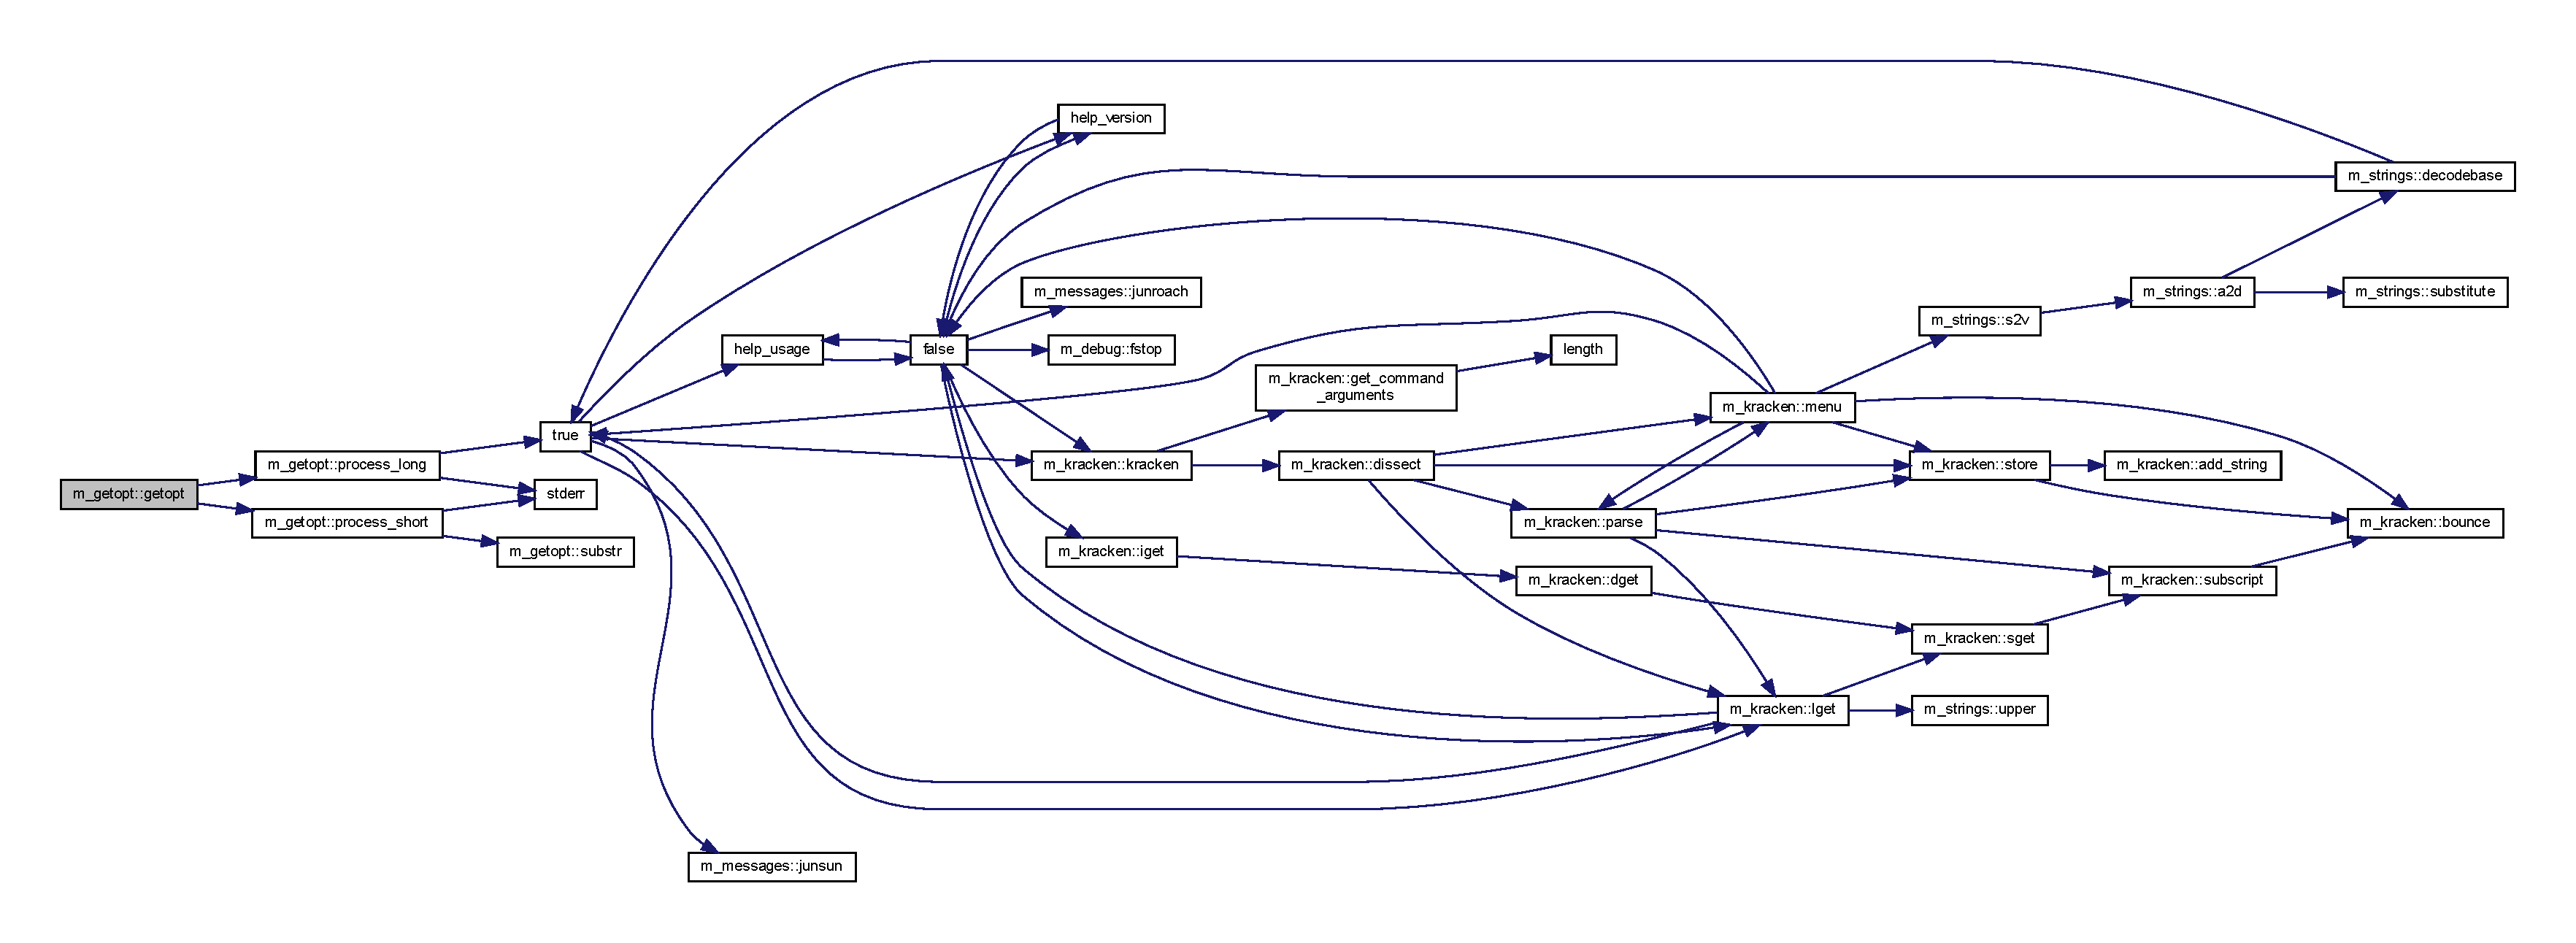
\includegraphics[width=350pt]{namespacem__getopt_a00e4c1d7d61539e0bdf63a6ee13284d2_cgraph}
\end{center}
\end{figure}
\mbox{\Hypertarget{namespacem__getopt_a47714553b3cda11df4d21bc343760d9c}\label{namespacem__getopt_a47714553b3cda11df4d21bc343760d9c}} 
\index{m\+\_\+getopt@{m\+\_\+getopt}!process\+\_\+long@{process\+\_\+long}}
\index{process\+\_\+long@{process\+\_\+long}!m\+\_\+getopt@{m\+\_\+getopt}}
\subsubsection{\texorpdfstring{process\+\_\+long()}{process\_long()}}
{\footnotesize\ttfamily \hyperlink{option__stopwatch_83_8txt_abd4b21fbbd175834027b5224bfe97e66}{character} function m\+\_\+getopt\+::process\+\_\+long (\begin{DoxyParamCaption}\item[{\hyperlink{stop__watch_83_8txt_a70f0ead91c32e25323c03265aa302c1c}{type}(\hyperlink{structm__getopt_1_1option__s}{option\+\_\+s}), dimension(\+:), intent(\hyperlink{M__journal_83_8txt_afce72651d1eed785a2132bee863b2f38}{in})}]{longopts,  }\item[{\hyperlink{option__stopwatch_83_8txt_abd4b21fbbd175834027b5224bfe97e66}{character}(len=$\ast$), intent(\hyperlink{M__journal_83_8txt_afce72651d1eed785a2132bee863b2f38}{in})}]{arg }\end{DoxyParamCaption})}



References optarg, opterr, optind, optopt, stderr(), and true().

Here is the call graph for this function\+:
\nopagebreak
\begin{figure}[H]
\begin{center}
\leavevmode
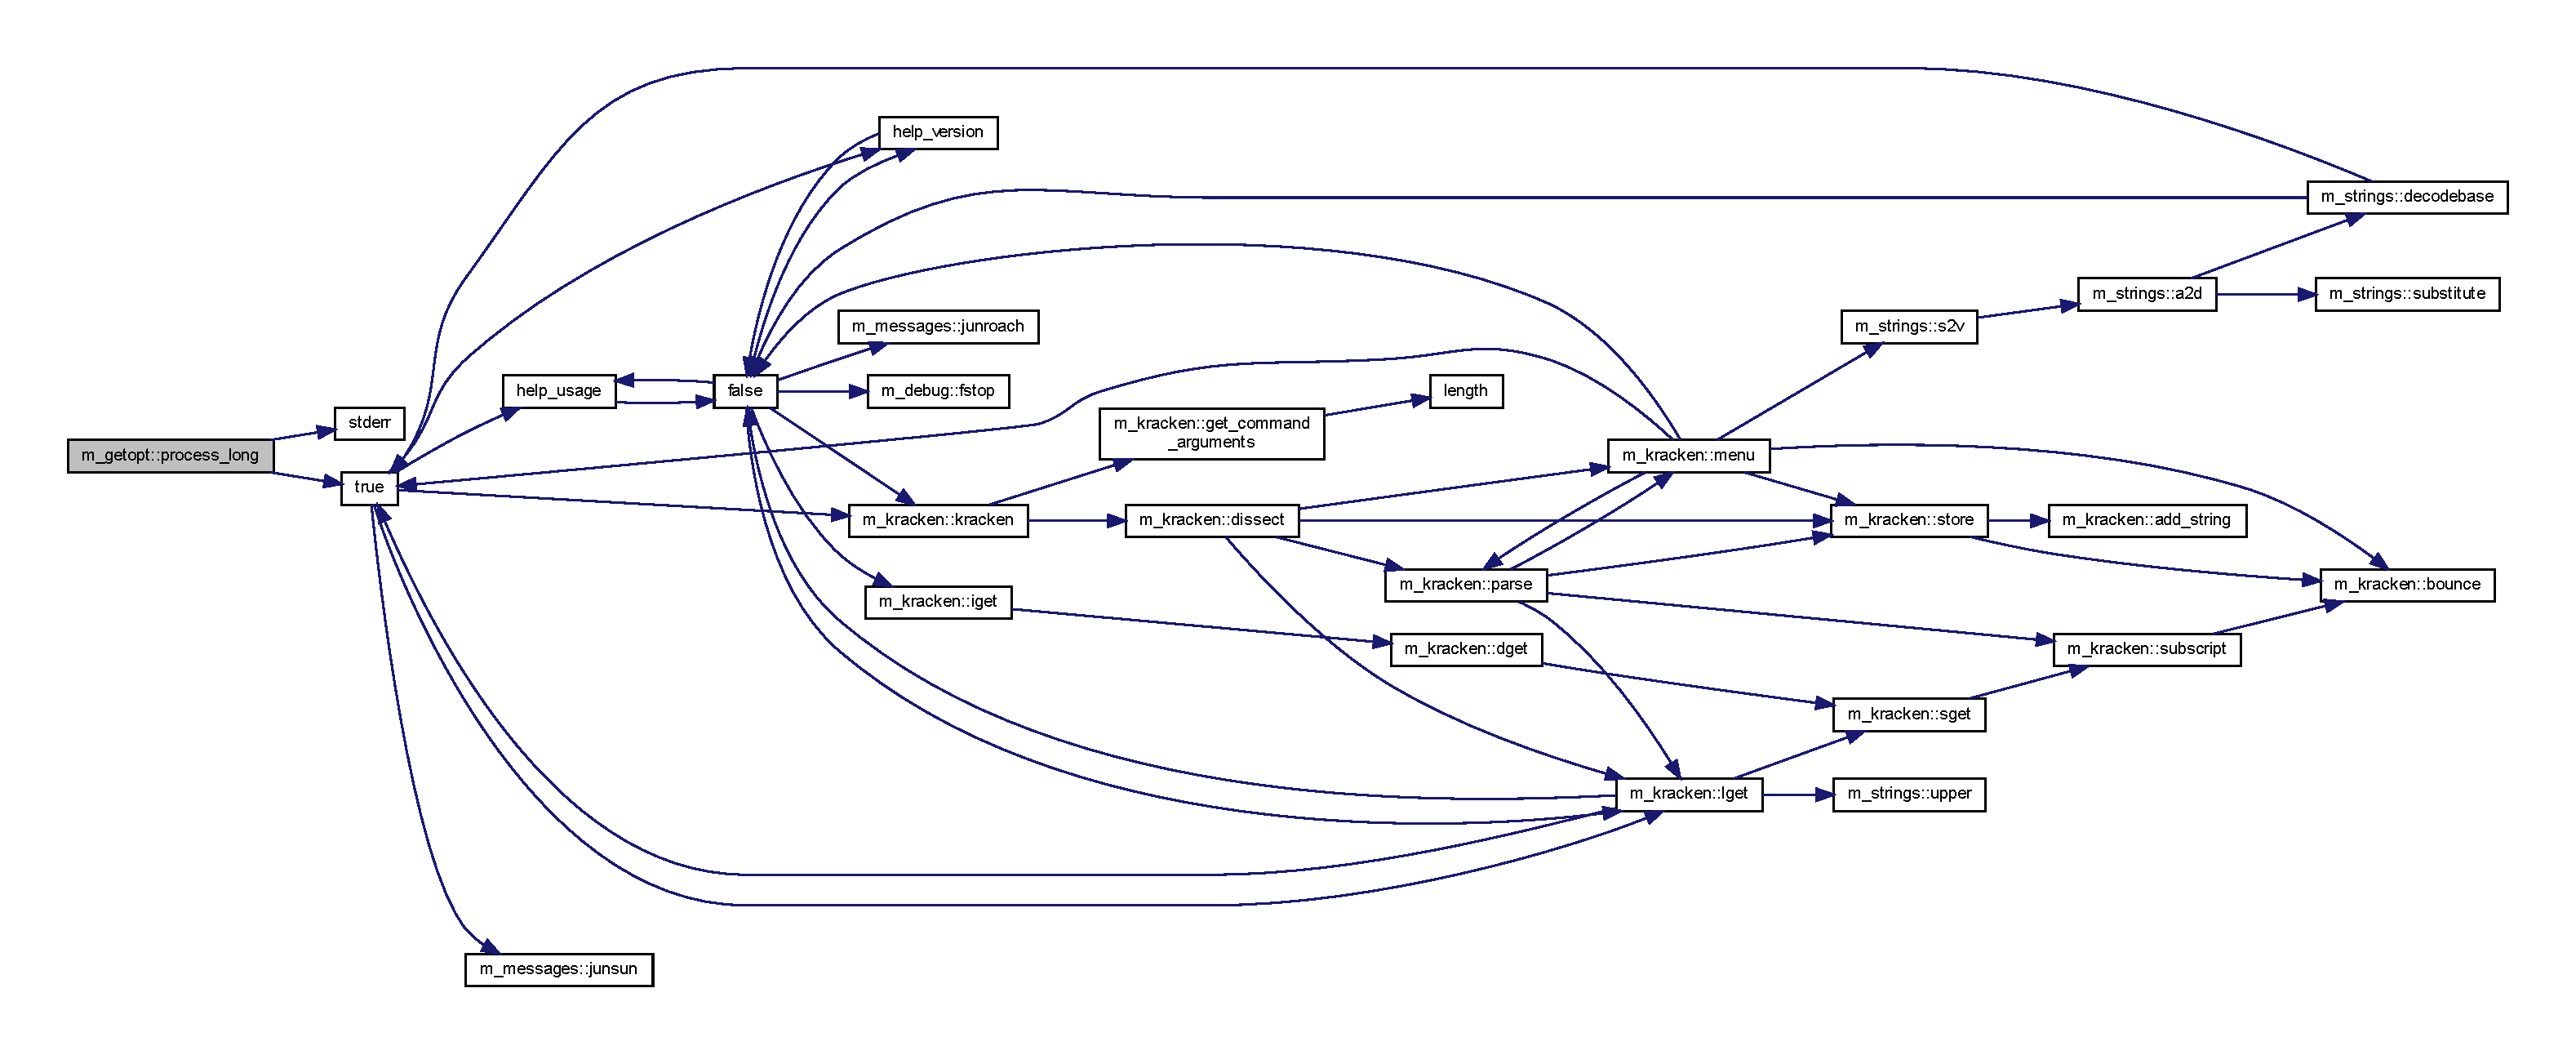
\includegraphics[width=350pt]{namespacem__getopt_a47714553b3cda11df4d21bc343760d9c_cgraph}
\end{center}
\end{figure}
Here is the caller graph for this function\+:
\nopagebreak
\begin{figure}[H]
\begin{center}
\leavevmode
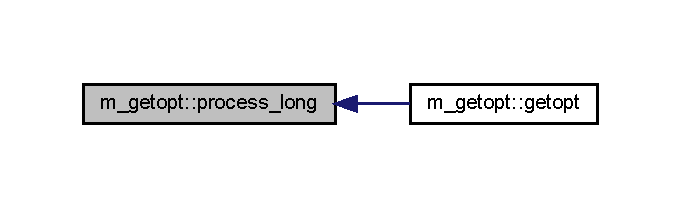
\includegraphics[width=327pt]{namespacem__getopt_a47714553b3cda11df4d21bc343760d9c_icgraph}
\end{center}
\end{figure}
\mbox{\Hypertarget{namespacem__getopt_a5a41350043ae3b92dbbac7dea6702e09}\label{namespacem__getopt_a5a41350043ae3b92dbbac7dea6702e09}} 
\index{m\+\_\+getopt@{m\+\_\+getopt}!process\+\_\+short@{process\+\_\+short}}
\index{process\+\_\+short@{process\+\_\+short}!m\+\_\+getopt@{m\+\_\+getopt}}
\subsubsection{\texorpdfstring{process\+\_\+short()}{process\_short()}}
{\footnotesize\ttfamily \hyperlink{option__stopwatch_83_8txt_abd4b21fbbd175834027b5224bfe97e66}{character} function m\+\_\+getopt\+::process\+\_\+short (\begin{DoxyParamCaption}\item[{\hyperlink{option__stopwatch_83_8txt_abd4b21fbbd175834027b5224bfe97e66}{character}(len=$\ast$), intent(\hyperlink{M__journal_83_8txt_afce72651d1eed785a2132bee863b2f38}{in})}]{optstring,  }\item[{\hyperlink{option__stopwatch_83_8txt_abd4b21fbbd175834027b5224bfe97e66}{character}(len=$\ast$), intent(\hyperlink{M__journal_83_8txt_afce72651d1eed785a2132bee863b2f38}{in})}]{arg }\end{DoxyParamCaption})}



References grpind, optarg, opterr, optind, optopt, stderr(), and substr().

Here is the call graph for this function\+:
\nopagebreak
\begin{figure}[H]
\begin{center}
\leavevmode
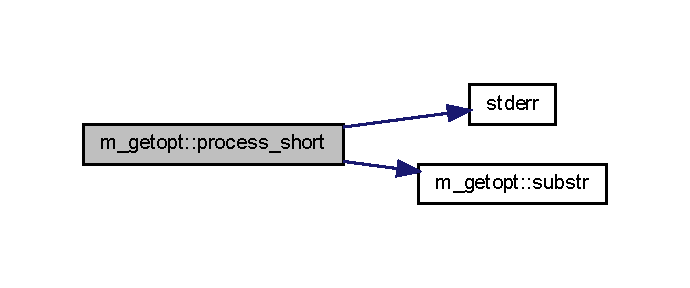
\includegraphics[width=331pt]{namespacem__getopt_a5a41350043ae3b92dbbac7dea6702e09_cgraph}
\end{center}
\end{figure}
Here is the caller graph for this function\+:
\nopagebreak
\begin{figure}[H]
\begin{center}
\leavevmode
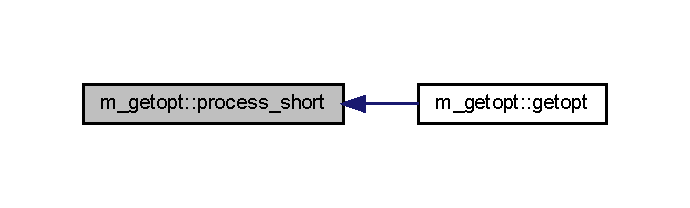
\includegraphics[width=331pt]{namespacem__getopt_a5a41350043ae3b92dbbac7dea6702e09_icgraph}
\end{center}
\end{figure}
\mbox{\Hypertarget{namespacem__getopt_a20145e0f477d81541fbe9b408f2194d0}\label{namespacem__getopt_a20145e0f477d81541fbe9b408f2194d0}} 
\index{m\+\_\+getopt@{m\+\_\+getopt}!substr@{substr}}
\index{substr@{substr}!m\+\_\+getopt@{m\+\_\+getopt}}
\subsubsection{\texorpdfstring{substr()}{substr()}}
{\footnotesize\ttfamily \hyperlink{option__stopwatch_83_8txt_abd4b21fbbd175834027b5224bfe97e66}{character} function m\+\_\+getopt\+::substr (\begin{DoxyParamCaption}\item[{\hyperlink{option__stopwatch_83_8txt_abd4b21fbbd175834027b5224bfe97e66}{character}(len=$\ast$), intent(\hyperlink{M__journal_83_8txt_afce72651d1eed785a2132bee863b2f38}{in})}]{str,  }\item[{integer, intent(\hyperlink{M__journal_83_8txt_afce72651d1eed785a2132bee863b2f38}{in})}]{i,  }\item[{integer, intent(\hyperlink{M__journal_83_8txt_afce72651d1eed785a2132bee863b2f38}{in})}]{j }\end{DoxyParamCaption})}

Here is the caller graph for this function\+:
\nopagebreak
\begin{figure}[H]
\begin{center}
\leavevmode
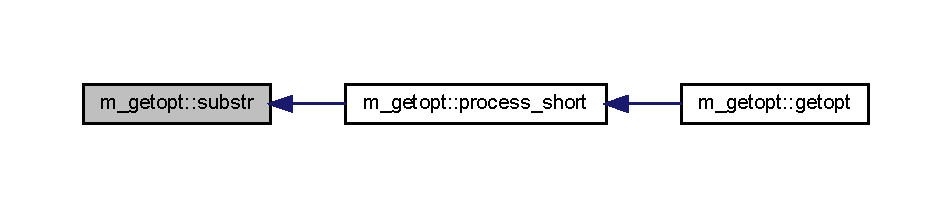
\includegraphics[width=350pt]{namespacem__getopt_a20145e0f477d81541fbe9b408f2194d0_icgraph}
\end{center}
\end{figure}


\subsection{Variable Documentation}
\mbox{\Hypertarget{namespacem__getopt_ae80924cbaae8d0e057ab2a0660cddee4}\label{namespacem__getopt_ae80924cbaae8d0e057ab2a0660cddee4}} 
\index{m\+\_\+getopt@{m\+\_\+getopt}!grpind@{grpind}}
\index{grpind@{grpind}!m\+\_\+getopt@{m\+\_\+getopt}}
\subsubsection{\texorpdfstring{grpind}{grpind}}
{\footnotesize\ttfamily integer, private m\+\_\+getopt\+::grpind =2\hspace{0.3cm}{\ttfamily [private]}}

\mbox{\Hypertarget{namespacem__getopt_abfaa4b627673956019b3c2148e32a6fa}\label{namespacem__getopt_abfaa4b627673956019b3c2148e32a6fa}} 
\index{m\+\_\+getopt@{m\+\_\+getopt}!optarg@{optarg}}
\index{optarg@{optarg}!m\+\_\+getopt@{m\+\_\+getopt}}
\subsubsection{\texorpdfstring{optarg}{optarg}}
{\footnotesize\ttfamily \hyperlink{option__stopwatch_83_8txt_abd4b21fbbd175834027b5224bfe97e66}{character}(len=80) m\+\_\+getopt\+::optarg}

\mbox{\Hypertarget{namespacem__getopt_a7e1bffca463ec7a33438746eea4f9cf0}\label{namespacem__getopt_a7e1bffca463ec7a33438746eea4f9cf0}} 
\index{m\+\_\+getopt@{m\+\_\+getopt}!opterr@{opterr}}
\index{opterr@{opterr}!m\+\_\+getopt@{m\+\_\+getopt}}
\subsubsection{\texorpdfstring{opterr}{opterr}}
{\footnotesize\ttfamily logical m\+\_\+getopt\+::opterr =.true.}

\mbox{\Hypertarget{namespacem__getopt_acf82c0ecb5e883455b91a3c8620b50c2}\label{namespacem__getopt_acf82c0ecb5e883455b91a3c8620b50c2}} 
\index{m\+\_\+getopt@{m\+\_\+getopt}!optind@{optind}}
\index{optind@{optind}!m\+\_\+getopt@{m\+\_\+getopt}}
\subsubsection{\texorpdfstring{optind}{optind}}
{\footnotesize\ttfamily integer m\+\_\+getopt\+::optind =1}

\mbox{\Hypertarget{namespacem__getopt_a66243e462b4a0546b8ab7c8b5c73eb91}\label{namespacem__getopt_a66243e462b4a0546b8ab7c8b5c73eb91}} 
\index{m\+\_\+getopt@{m\+\_\+getopt}!optopt@{optopt}}
\index{optopt@{optopt}!m\+\_\+getopt@{m\+\_\+getopt}}
\subsubsection{\texorpdfstring{optopt}{optopt}}
{\footnotesize\ttfamily \hyperlink{option__stopwatch_83_8txt_abd4b21fbbd175834027b5224bfe97e66}{character} m\+\_\+getopt\+::optopt}


\hypertarget{namespacem__getopt__long}{}\section{m\+\_\+getopt\+\_\+long Module Reference}
\label{namespacem__getopt__long}\index{m\+\_\+getopt\+\_\+long@{m\+\_\+getopt\+\_\+long}}


\subsubsection*{N\+A\+ME}

M\+\_\+getopt\+\_\+long(3fm) -\/ \mbox{[}A\+R\+G\+U\+M\+E\+N\+TS\+:M\+\_\+getopt\+\_\+long\mbox{]} parse command line options like Sun getopt\+\_\+long, including the Sun C\+L\+IP specification \subsubsection*{S\+Y\+N\+T\+AX}

use M\+\_\+getopt\+\_\+long, only \+: getopt\+\_\+new, getopt use M\+\_\+getopt\+\_\+long, only \+: \hyperlink{structm__getopt__long_1_1getopt__type}{getopt\+\_\+type}, \hyperlink{structm__getopt__long_1_1getopt__option__type}{getopt\+\_\+option\+\_\+type} use M\+\_\+getopt\+\_\+long, only \+: getopt\+\_\+argv  


\subsection*{Data Types}
\begin{DoxyCompactItemize}
\item 
type \hyperlink{structm__getopt__long_1_1getopt__option__type}{getopt\+\_\+option\+\_\+type}
\item 
type \hyperlink{structm__getopt__long_1_1getopt__string__type}{getopt\+\_\+string\+\_\+type}
\item 
type \hyperlink{structm__getopt__long_1_1getopt__type}{getopt\+\_\+type}
\item 
interface \hyperlink{interfacem__getopt__long_1_1warn}{warn}
\end{DoxyCompactItemize}
\subsection*{Functions/\+Subroutines}
\begin{DoxyCompactItemize}
\item 
\hyperlink{M__stopwatch_83_8txt_acfbcff50169d691ff02d4a123ed70482}{subroutine} \hyperlink{namespacem__getopt__long_af5aeba1b29425c5da2db9113aac0dc97}{getopt\+\_\+new} (self, optstring, long\+\_\+opts, flags, status)
\item 
\hyperlink{option__stopwatch_83_8txt_abd4b21fbbd175834027b5224bfe97e66}{character}(len=\hyperlink{namespacem__getopt__long_a379b13093de969a83f29283c3cce3c7a}{getopt\+\_\+argv\+\_\+len}(self, argn)) function \hyperlink{namespacem__getopt__long_a7bd7b84d1aeda27b57f33b81a93ef1c1}{getopt\+\_\+argv} (self, argn)
\item 
\hyperlink{option__stopwatch_83_8txt_abd4b21fbbd175834027b5224bfe97e66}{character}(len=1) function \hyperlink{namespacem__getopt__long_ae12838b4ea1d076090a8bbd9f05000ef}{getopt} (self, longindex)
\item 
pure integer function \hyperlink{namespacem__getopt__long_a379b13093de969a83f29283c3cce3c7a}{getopt\+\_\+argv\+\_\+len} (self, argn)
\item 
\hyperlink{M__stopwatch_83_8txt_acfbcff50169d691ff02d4a123ed70482}{subroutine}, private \hyperlink{namespacem__getopt__long_a78f4dacb7eae96d7e259544003ae0dfd}{warn\+\_\+string} (self, msg, arg)
\item 
\hyperlink{M__stopwatch_83_8txt_acfbcff50169d691ff02d4a123ed70482}{subroutine}, private \hyperlink{namespacem__getopt__long_af1ccef432aa194687e03575a68537553}{warn\+\_\+char\+\_\+array} (self, msg, arg)
\item 
\hyperlink{M__stopwatch_83_8txt_acfbcff50169d691ff02d4a123ed70482}{subroutine}, private \hyperlink{namespacem__getopt__long_a55045492836fd218379126cbdcee24ea}{permute\+\_\+args} (self)
\item 
\hyperlink{option__stopwatch_83_8txt_abd4b21fbbd175834027b5224bfe97e66}{character}(len=1) function, private \hyperlink{namespacem__getopt__long_a7bad6d8d4067d578429da9282bc82ada}{parse\+\_\+longopts} (self, longindex, short\+\_\+too)
\end{DoxyCompactItemize}
\subsection*{Variables}
\begin{DoxyCompactItemize}
\item 
integer, parameter \hyperlink{namespacem__getopt__long_aa7e9d6f7c81a30df80cba5f518928d0b}{max\+\_\+option\+\_\+len} = 15
\item 
\hyperlink{option__stopwatch_83_8txt_abd4b21fbbd175834027b5224bfe97e66}{character}(len=1), parameter \hyperlink{namespacem__getopt__long_aaad9b6ad61f0e854d6f5e0be5d6a8391}{getopt\+\_\+status\+\_\+badch} = \textquotesingle{}?\textquotesingle{}
\item 
\hyperlink{option__stopwatch_83_8txt_abd4b21fbbd175834027b5224bfe97e66}{character}(len=1), parameter \hyperlink{namespacem__getopt__long_a0cbf9b0b301392332f65c12012615ed5}{getopt\+\_\+status\+\_\+badarg} = \textquotesingle{}\+:\textquotesingle{}
\item 
\hyperlink{option__stopwatch_83_8txt_abd4b21fbbd175834027b5224bfe97e66}{character}(len=1), parameter \hyperlink{namespacem__getopt__long_ab062153fe30e93d68542fdcb607c84f0}{getopt\+\_\+status\+\_\+inorder} = char(1)
\item 
\hyperlink{option__stopwatch_83_8txt_abd4b21fbbd175834027b5224bfe97e66}{character}(len=1), parameter \hyperlink{namespacem__getopt__long_adb2768994ee191e282dda42a22ded93e}{getopt\+\_\+status\+\_\+end} = char(255)
\item 
\hyperlink{option__stopwatch_83_8txt_abd4b21fbbd175834027b5224bfe97e66}{character}(len=1), parameter \hyperlink{namespacem__getopt__long_a17bc8c03e862e68f855f3c85740fe4c2}{getopt\+\_\+status\+\_\+nil} = char(0)
\item 
integer, parameter \hyperlink{namespacem__getopt__long_a08dabd255fb1dc8cb7aee58aaf55f916}{getopt\+\_\+no\+\_\+arg} = 0
\item 
integer, parameter \hyperlink{namespacem__getopt__long_a52b32d94a183ff13b4a8bf9c14e5634a}{getopt\+\_\+req\+\_\+arg} = 1
\item 
integer, parameter \hyperlink{namespacem__getopt__long_a1750a2d60da545a36608d1d458dd6a89}{getopt\+\_\+opt\+\_\+arg} = 2
\item 
integer, parameter \hyperlink{namespacem__getopt__long_ac2ae1f0969388b7868cb7b070abbff70}{getopt\+\_\+flag\+\_\+permute} = int(z\textquotesingle{}01\textquotesingle{})
\item 
integer, parameter \hyperlink{namespacem__getopt__long_a8e9b76527b39fe8c8311edfb3ca252f3}{getopt\+\_\+flag\+\_\+allargs} = int(z\textquotesingle{}02\textquotesingle{})
\item 
integer, parameter \hyperlink{namespacem__getopt__long_a78dad148f97ee14b2dc1c1e3f66775a8}{getopt\+\_\+flag\+\_\+longonly} = int(z\textquotesingle{}04\textquotesingle{})
\item 
integer, parameter \hyperlink{namespacem__getopt__long_a5d97a0339a2798c3275ef32d5bac5407}{getopt\+\_\+flag\+\_\+optional\+\_\+args} = int(z\textquotesingle{}08\textquotesingle{})
\item 
integer, parameter \hyperlink{namespacem__getopt__long_a8ed12f1d43098e7e6cbe7f4a6b9a9352}{getopt\+\_\+flag\+\_\+require\+\_\+equivalents} = int(z\textquotesingle{}10\textquotesingle{})
\item 
integer, parameter \hyperlink{namespacem__getopt__long_a519f914b784104158b07034c85767007}{getopt\+\_\+flag\+\_\+abbrev} = int(z\textquotesingle{}20\textquotesingle{})
\item 
integer, parameter \hyperlink{namespacem__getopt__long_ae60135d11126a953a2bac414e62f57ac}{getopt\+\_\+flag\+\_\+w\+\_\+semicolon} = int(z\textquotesingle{}40\textquotesingle{})
\item 
integer, parameter \hyperlink{namespacem__getopt__long_a928e9e8b9d3688cd9c0fc38b33568da9}{getopt\+\_\+flag\+\_\+plus\+\_\+dash\+\_\+start} = int(z\textquotesingle{}80\textquotesingle{})
\item 
integer, parameter \hyperlink{namespacem__getopt__long_a5c591e4e0cabebe3bdb56263f6ad7a10}{getopt\+\_\+flags\+\_\+gnu} = G\+E\+T\+O\+P\+T\+\_\+\+F\+L\+A\+G\+\_\+\+P\+E\+R\+M\+U\+TE + G\+E\+T\+O\+P\+T\+\_\+\+F\+L\+A\+G\+\_\+\+O\+P\+T\+I\+O\+N\+A\+L\+\_\+\+A\+R\+GS + G\+E\+T\+O\+P\+T\+\_\+\+F\+L\+A\+G\+\_\+\+A\+B\+B\+R\+EV + G\+E\+T\+O\+P\+T\+\_\+\+F\+L\+A\+G\+\_\+\+W\+\_\+\+S\+E\+M\+I\+C\+O\+L\+ON + G\+E\+T\+O\+P\+T\+\_\+\+F\+L\+A\+G\+\_\+\+P\+L\+U\+S\+\_\+\+D\+A\+S\+H\+\_\+\+S\+T\+A\+RT
\item 
integer, parameter \hyperlink{namespacem__getopt__long_ab052891b2a58dcaa186b04aaf6d6e0a0}{getopt\+\_\+flags\+\_\+posix} = G\+E\+T\+O\+P\+T\+\_\+\+F\+L\+A\+G\+\_\+\+A\+B\+B\+R\+EV
\item 
integer, parameter \hyperlink{namespacem__getopt__long_a2756f79006f828de56abaf6ee45d2d69}{getopt\+\_\+flags\+\_\+default} = G\+E\+T\+O\+P\+T\+\_\+\+F\+L\+A\+G\+\_\+\+P\+E\+R\+M\+U\+TE + G\+E\+T\+O\+P\+T\+\_\+\+F\+L\+A\+G\+\_\+\+A\+B\+B\+R\+EV + G\+E\+T\+O\+P\+T\+\_\+\+F\+L\+A\+G\+\_\+\+P\+L\+U\+S\+\_\+\+D\+A\+S\+H\+\_\+\+S\+T\+A\+RT
\item 
integer, parameter \hyperlink{namespacem__getopt__long_a9c32005623bfe7b86c5b743d4a436247}{getopt\+\_\+flags\+\_\+long} = G\+E\+T\+O\+P\+T\+\_\+\+F\+L\+A\+G\+\_\+\+P\+E\+R\+M\+U\+TE + G\+E\+T\+O\+P\+T\+\_\+\+F\+L\+A\+G\+\_\+\+O\+P\+T\+I\+O\+N\+A\+L\+\_\+\+A\+R\+GS + G\+E\+T\+O\+P\+T\+\_\+\+F\+L\+A\+G\+\_\+\+A\+B\+B\+R\+EV + G\+E\+T\+O\+P\+T\+\_\+\+F\+L\+A\+G\+\_\+\+W\+\_\+\+S\+E\+M\+I\+C\+O\+L\+ON + G\+E\+T\+O\+P\+T\+\_\+\+F\+L\+A\+G\+\_\+\+P\+L\+U\+S\+\_\+\+D\+A\+S\+H\+\_\+\+S\+T\+A\+RT
\item 
integer, parameter \hyperlink{namespacem__getopt__long_a86d2892a8786516f1b523c6bc1f373fa}{getopt\+\_\+flags\+\_\+long\+\_\+only} = G\+E\+T\+O\+P\+T\+\_\+\+F\+L\+A\+G\+S\+\_\+\+L\+O\+NG + G\+E\+T\+O\+P\+T\+\_\+\+F\+L\+A\+G\+\_\+\+L\+O\+N\+G\+O\+N\+LY
\item 
integer, parameter \hyperlink{namespacem__getopt__long_a752a8bccdeb9074237cfaa0c9435c059}{getopt\+\_\+flags\+\_\+sun\+\_\+clip} = G\+E\+T\+O\+P\+T\+\_\+\+F\+L\+A\+G\+\_\+\+W\+\_\+\+S\+E\+M\+I\+C\+O\+L\+ON + G\+E\+T\+O\+P\+T\+\_\+\+F\+L\+A\+G\+\_\+\+R\+E\+Q\+U\+I\+R\+E\+\_\+\+E\+Q\+U\+I\+V\+A\+L\+E\+N\+TS
\item 
\hyperlink{option__stopwatch_83_8txt_abd4b21fbbd175834027b5224bfe97e66}{character}(len=1), dimension(0), target \hyperlink{namespacem__getopt__long_a6f74fcf9d3fc08c69e4df052af120051}{empty\+\_\+string\+\_\+array}
\end{DoxyCompactItemize}


\subsection{Detailed Description}
\subsubsection*{N\+A\+ME}

M\+\_\+getopt\+\_\+long(3fm) -\/ \mbox{[}A\+R\+G\+U\+M\+E\+N\+TS\+:M\+\_\+getopt\+\_\+long\mbox{]} parse command line options like Sun getopt\+\_\+long, including the Sun C\+L\+IP specification \subsubsection*{S\+Y\+N\+T\+AX}

use M\+\_\+getopt\+\_\+long, only \+: getopt\+\_\+new, getopt use M\+\_\+getopt\+\_\+long, only \+: \hyperlink{structm__getopt__long_1_1getopt__type}{getopt\+\_\+type}, \hyperlink{structm__getopt__long_1_1getopt__option__type}{getopt\+\_\+option\+\_\+type} use M\+\_\+getopt\+\_\+long, only \+: getopt\+\_\+argv 

\subsubsection*{D\+E\+S\+C\+R\+I\+P\+T\+I\+ON}

This is based on Sun\+OS getopt\+\_\+long(3), and includes the Sun C\+L\+IP specification, which requires matching short and long versions of all options.

Precise getopt functionality is not really desirable. The biggest drawback of getopt is the use of globals. (It was designed a long time ago.) This interface uses O\+OP with a derived-\/type data object, \subsubsection*{E\+X\+A\+M\+P\+LE}

Sample program\+:

program selftest\+\_\+program use M\+\_\+getopt\+\_\+long implicit none character(len=1) \+:\+: c integer \+:\+: i integer \+:\+: digit\+\_\+optind = 0 type(getopt\+\_\+type), pointer \+:\+: opts

integer \+:\+: this\+\_\+option\+\_\+optind integer \+:\+: option\+\_\+index character(len=1), parameter \+:\+: N\+IL = char(0)

type(getopt\+\_\+option\+\_\+type) \+:\+: long\+\_\+options(6) = (/ \& \hyperlink{structm__getopt__long_1_1getopt__option__type}{getopt\+\_\+option\+\_\+type}(\char`\"{}add\char`\"{}, 1, N\+U\+L\+L(), N\+IL), \& \hyperlink{structm__getopt__long_1_1getopt__option__type}{getopt\+\_\+option\+\_\+type}(\char`\"{}append\char`\"{}, 0, N\+U\+L\+L(), N\+IL), \& \hyperlink{structm__getopt__long_1_1getopt__option__type}{getopt\+\_\+option\+\_\+type}(\char`\"{}delete\char`\"{}, 1, N\+U\+L\+L(), N\+IL), \& \hyperlink{structm__getopt__long_1_1getopt__option__type}{getopt\+\_\+option\+\_\+type}(\char`\"{}verbose\char`\"{}, 0, N\+U\+L\+L(), N\+IL), \& \hyperlink{structm__getopt__long_1_1getopt__option__type}{getopt\+\_\+option\+\_\+type}(\char`\"{}create\char`\"{}, 1, N\+U\+L\+L(), \textquotesingle{}c\textquotesingle{}), \& \hyperlink{structm__getopt__long_1_1getopt__option__type}{getopt\+\_\+option\+\_\+type}(\char`\"{}file\char`\"{}, 1, N\+U\+L\+L(), N\+IL) /) character(len=$\ast$), parameter \+:\+: optstring = \char`\"{}abc\+:d\+:012\char`\"{}

call getopt\+\_\+new(opts,optstring,long\+\_\+options)

do this\+\_\+option\+\_\+optind = merge(optsindex,1,optsindex$>$0) option\+\_\+index = 0 c = getopt(opts,option\+\_\+index) write($\ast$,$\ast$)\textquotesingle{}retval=\textquotesingle{},c select case(c) case (G\+E\+T\+O\+P\+T\+\_\+\+S\+T\+A\+T\+U\+S\+\_\+\+E\+ND) exit case (G\+E\+T\+O\+P\+T\+\_\+\+S\+T\+A\+T\+U\+S\+\_\+\+N\+IL) write($\ast$,\textquotesingle{}(2A)\textquotesingle{},advance=\textquotesingle{}no\textquotesingle{}) \char`\"{}option \char`\"{}, trim(long\+\_\+options(option\+\_\+index)name) if (associated(optsoptarg)) \& write($\ast$,\textquotesingle{}(2A)\textquotesingle{},advance=\textquotesingle{}no\textquotesingle{}) \char`\"{}with arg \char`\"{}, optsoptarg write($\ast$,$\ast$) !newline

case (\textquotesingle{}0\textquotesingle{},\textquotesingle{}1\textquotesingle{},\textquotesingle{}2\textquotesingle{}) if (digit\+\_\+optind /= 0 .and. digit\+\_\+optind /= this\+\_\+option\+\_\+optind) \& write($\ast$,$\ast$) \char`\"{}digits occur in two different argv-\/elements.\char`\"{} digit\+\_\+optind = this\+\_\+option\+\_\+optind write($\ast$,$\ast$)\char`\"{}option \char`\"{},c

case (\textquotesingle{}a\textquotesingle{},\textquotesingle{}b\textquotesingle{}) write($\ast$,$\ast$)\char`\"{}option \char`\"{},c

case (\textquotesingle{}c\textquotesingle{},\textquotesingle{}d\textquotesingle{}) write($\ast$,$\ast$)\char`\"{}option \char`\"{},c,\char`\"{} with value \textquotesingle{}\char`\"{},optsoptarg,\textquotesingle{}\char`\"{}\textquotesingle{}

case default write($\ast$,$\ast$) \char`\"{}?? getopt returned character code \char`\"{},ichar(c),\char`\"{} ??\char`\"{}

end select

end do

if (optsindex $<$= optsargc) then write($\ast$,\textquotesingle{}(A)\textquotesingle{},advance=\textquotesingle{}no\textquotesingle{}) \char`\"{}non-\/option A\+R\+G\+V-\/elements\+: \char`\"{} do i=optsindex,optsargc write($\ast$,\textquotesingle{}(A,1X)\textquotesingle{},advance=\textquotesingle{}no\textquotesingle{}) getopt\+\_\+argv(opts,i) end do write($\ast$,$\ast$) ! newline end if

stop end program selftest\+\_\+program \subsubsection*{A\+U\+T\+H\+OR}


\begin{DoxyItemize}
\item \mbox{[}\mbox{[}getopt\+\_\+long\+\_\+module\mbox{]}\mbox{]} by \mbox{[}\mbox{[}Joe Krahn\mbox{]}\mbox{]}.
\item slightly modified from original -\/ J\+SU 
\end{DoxyItemize}

\subsection{Function/\+Subroutine Documentation}
\mbox{\Hypertarget{namespacem__getopt__long_ae12838b4ea1d076090a8bbd9f05000ef}\label{namespacem__getopt__long_ae12838b4ea1d076090a8bbd9f05000ef}} 
\index{m\+\_\+getopt\+\_\+long@{m\+\_\+getopt\+\_\+long}!getopt@{getopt}}
\index{getopt@{getopt}!m\+\_\+getopt\+\_\+long@{m\+\_\+getopt\+\_\+long}}
\subsubsection{\texorpdfstring{getopt()}{getopt()}}
{\footnotesize\ttfamily \hyperlink{option__stopwatch_83_8txt_abd4b21fbbd175834027b5224bfe97e66}{character}(len=1) function m\+\_\+getopt\+\_\+long\+::getopt (\begin{DoxyParamCaption}\item[{\hyperlink{stop__watch_83_8txt_a70f0ead91c32e25323c03265aa302c1c}{type}(\hyperlink{structm__getopt__long_1_1getopt__type}{getopt\+\_\+type}), pointer}]{self,  }\item[{integer, intent(out), \hyperlink{option__stopwatch_83_8txt_aa4ece75e7acf58a4843f70fe18c3ade5}{optional}}]{longindex }\end{DoxyParamCaption})}



References empty\+\_\+string\+\_\+array, false(), getopt\+\_\+flag\+\_\+allargs, getopt\+\_\+flag\+\_\+longonly, getopt\+\_\+flag\+\_\+optional\+\_\+args, getopt\+\_\+flag\+\_\+permute, getopt\+\_\+flag\+\_\+w\+\_\+semicolon, getopt\+\_\+status\+\_\+badarg, getopt\+\_\+status\+\_\+badch, getopt\+\_\+status\+\_\+end, getopt\+\_\+status\+\_\+inorder, getopt\+\_\+status\+\_\+nil, parse\+\_\+longopts(), and true().

\mbox{\Hypertarget{namespacem__getopt__long_a7bd7b84d1aeda27b57f33b81a93ef1c1}\label{namespacem__getopt__long_a7bd7b84d1aeda27b57f33b81a93ef1c1}} 
\index{m\+\_\+getopt\+\_\+long@{m\+\_\+getopt\+\_\+long}!getopt\+\_\+argv@{getopt\+\_\+argv}}
\index{getopt\+\_\+argv@{getopt\+\_\+argv}!m\+\_\+getopt\+\_\+long@{m\+\_\+getopt\+\_\+long}}
\subsubsection{\texorpdfstring{getopt\+\_\+argv()}{getopt\_argv()}}
{\footnotesize\ttfamily \hyperlink{option__stopwatch_83_8txt_abd4b21fbbd175834027b5224bfe97e66}{character}(len=\hyperlink{namespacem__getopt__long_a379b13093de969a83f29283c3cce3c7a}{getopt\+\_\+argv\+\_\+len}(self,argn)) function m\+\_\+getopt\+\_\+long\+::getopt\+\_\+argv (\begin{DoxyParamCaption}\item[{\hyperlink{stop__watch_83_8txt_a70f0ead91c32e25323c03265aa302c1c}{type}(\hyperlink{structm__getopt__long_1_1getopt__type}{getopt\+\_\+type}), pointer}]{self,  }\item[{integer, intent(\hyperlink{M__journal_83_8txt_afce72651d1eed785a2132bee863b2f38}{in})}]{argn }\end{DoxyParamCaption})}

\mbox{\Hypertarget{namespacem__getopt__long_a379b13093de969a83f29283c3cce3c7a}\label{namespacem__getopt__long_a379b13093de969a83f29283c3cce3c7a}} 
\index{m\+\_\+getopt\+\_\+long@{m\+\_\+getopt\+\_\+long}!getopt\+\_\+argv\+\_\+len@{getopt\+\_\+argv\+\_\+len}}
\index{getopt\+\_\+argv\+\_\+len@{getopt\+\_\+argv\+\_\+len}!m\+\_\+getopt\+\_\+long@{m\+\_\+getopt\+\_\+long}}
\subsubsection{\texorpdfstring{getopt\+\_\+argv\+\_\+len()}{getopt\_argv\_len()}}
{\footnotesize\ttfamily pure integer function m\+\_\+getopt\+\_\+long\+::getopt\+\_\+argv\+\_\+len (\begin{DoxyParamCaption}\item[{\hyperlink{stop__watch_83_8txt_a70f0ead91c32e25323c03265aa302c1c}{type}(\hyperlink{structm__getopt__long_1_1getopt__type}{getopt\+\_\+type}), pointer}]{self,  }\item[{integer, intent(\hyperlink{M__journal_83_8txt_afce72651d1eed785a2132bee863b2f38}{in})}]{argn }\end{DoxyParamCaption})}

\mbox{\Hypertarget{namespacem__getopt__long_af5aeba1b29425c5da2db9113aac0dc97}\label{namespacem__getopt__long_af5aeba1b29425c5da2db9113aac0dc97}} 
\index{m\+\_\+getopt\+\_\+long@{m\+\_\+getopt\+\_\+long}!getopt\+\_\+new@{getopt\+\_\+new}}
\index{getopt\+\_\+new@{getopt\+\_\+new}!m\+\_\+getopt\+\_\+long@{m\+\_\+getopt\+\_\+long}}
\subsubsection{\texorpdfstring{getopt\+\_\+new()}{getopt\_new()}}
{\footnotesize\ttfamily \hyperlink{M__stopwatch_83_8txt_acfbcff50169d691ff02d4a123ed70482}{subroutine} m\+\_\+getopt\+\_\+long\+::getopt\+\_\+new (\begin{DoxyParamCaption}\item[{\hyperlink{stop__watch_83_8txt_a70f0ead91c32e25323c03265aa302c1c}{type}(\hyperlink{structm__getopt__long_1_1getopt__type}{getopt\+\_\+type}), pointer}]{self,  }\item[{\hyperlink{option__stopwatch_83_8txt_abd4b21fbbd175834027b5224bfe97e66}{character}(len=$\ast$), intent(\hyperlink{M__journal_83_8txt_afce72651d1eed785a2132bee863b2f38}{in}), target}]{optstring,  }\item[{\hyperlink{stop__watch_83_8txt_a70f0ead91c32e25323c03265aa302c1c}{type}(\hyperlink{structm__getopt__long_1_1getopt__option__type}{getopt\+\_\+option\+\_\+type}), dimension(\+:), intent(\hyperlink{M__journal_83_8txt_afce72651d1eed785a2132bee863b2f38}{in}), \hyperlink{option__stopwatch_83_8txt_aa4ece75e7acf58a4843f70fe18c3ade5}{optional}, target}]{long\+\_\+opts,  }\item[{integer, intent(\hyperlink{M__journal_83_8txt_afce72651d1eed785a2132bee863b2f38}{in}), \hyperlink{option__stopwatch_83_8txt_aa4ece75e7acf58a4843f70fe18c3ade5}{optional}}]{flags,  }\item[{logical, intent(out), \hyperlink{option__stopwatch_83_8txt_aa4ece75e7acf58a4843f70fe18c3ade5}{optional}}]{status }\end{DoxyParamCaption})}



References empty\+\_\+string\+\_\+array, false(), getopt\+\_\+flag\+\_\+allargs, getopt\+\_\+flag\+\_\+optional\+\_\+args, getopt\+\_\+flag\+\_\+permute, getopt\+\_\+flag\+\_\+plus\+\_\+dash\+\_\+start, getopt\+\_\+flag\+\_\+require\+\_\+equivalents, getopt\+\_\+flags\+\_\+default, getopt\+\_\+flags\+\_\+long, getopt\+\_\+status\+\_\+nil, length(), true(), and verify\+\_\+short\+\_\+long\+\_\+equivalents().

\mbox{\Hypertarget{namespacem__getopt__long_a7bad6d8d4067d578429da9282bc82ada}\label{namespacem__getopt__long_a7bad6d8d4067d578429da9282bc82ada}} 
\index{m\+\_\+getopt\+\_\+long@{m\+\_\+getopt\+\_\+long}!parse\+\_\+longopts@{parse\+\_\+longopts}}
\index{parse\+\_\+longopts@{parse\+\_\+longopts}!m\+\_\+getopt\+\_\+long@{m\+\_\+getopt\+\_\+long}}
\subsubsection{\texorpdfstring{parse\+\_\+longopts()}{parse\_longopts()}}
{\footnotesize\ttfamily \hyperlink{option__stopwatch_83_8txt_abd4b21fbbd175834027b5224bfe97e66}{character}(len=1) function, private m\+\_\+getopt\+\_\+long\+::parse\+\_\+longopts (\begin{DoxyParamCaption}\item[{\hyperlink{stop__watch_83_8txt_a70f0ead91c32e25323c03265aa302c1c}{type}(\hyperlink{structm__getopt__long_1_1getopt__type}{getopt\+\_\+type}), pointer}]{self,  }\item[{integer, intent(inout), \hyperlink{option__stopwatch_83_8txt_aa4ece75e7acf58a4843f70fe18c3ade5}{optional}}]{longindex,  }\item[{logical, intent(\hyperlink{M__journal_83_8txt_afce72651d1eed785a2132bee863b2f38}{in})}]{short\+\_\+too }\end{DoxyParamCaption})\hspace{0.3cm}{\ttfamily [private]}}



References getopt\+\_\+flag\+\_\+abbrev, getopt\+\_\+flag\+\_\+optional\+\_\+args, getopt\+\_\+no\+\_\+arg, getopt\+\_\+opt\+\_\+arg, getopt\+\_\+req\+\_\+arg, getopt\+\_\+status\+\_\+badarg, getopt\+\_\+status\+\_\+badch, getopt\+\_\+status\+\_\+end, and getopt\+\_\+status\+\_\+nil.

\mbox{\Hypertarget{namespacem__getopt__long_a55045492836fd218379126cbdcee24ea}\label{namespacem__getopt__long_a55045492836fd218379126cbdcee24ea}} 
\index{m\+\_\+getopt\+\_\+long@{m\+\_\+getopt\+\_\+long}!permute\+\_\+args@{permute\+\_\+args}}
\index{permute\+\_\+args@{permute\+\_\+args}!m\+\_\+getopt\+\_\+long@{m\+\_\+getopt\+\_\+long}}
\subsubsection{\texorpdfstring{permute\+\_\+args()}{permute\_args()}}
{\footnotesize\ttfamily \hyperlink{M__stopwatch_83_8txt_acfbcff50169d691ff02d4a123ed70482}{subroutine}, private m\+\_\+getopt\+\_\+long\+::permute\+\_\+args (\begin{DoxyParamCaption}\item[{\hyperlink{stop__watch_83_8txt_a70f0ead91c32e25323c03265aa302c1c}{type}(\hyperlink{structm__getopt__long_1_1getopt__type}{getopt\+\_\+type}), pointer}]{self }\end{DoxyParamCaption})\hspace{0.3cm}{\ttfamily [private]}}



References gcd().

\mbox{\Hypertarget{namespacem__getopt__long_af1ccef432aa194687e03575a68537553}\label{namespacem__getopt__long_af1ccef432aa194687e03575a68537553}} 
\index{m\+\_\+getopt\+\_\+long@{m\+\_\+getopt\+\_\+long}!warn\+\_\+char\+\_\+array@{warn\+\_\+char\+\_\+array}}
\index{warn\+\_\+char\+\_\+array@{warn\+\_\+char\+\_\+array}!m\+\_\+getopt\+\_\+long@{m\+\_\+getopt\+\_\+long}}
\subsubsection{\texorpdfstring{warn\+\_\+char\+\_\+array()}{warn\_char\_array()}}
{\footnotesize\ttfamily \hyperlink{M__stopwatch_83_8txt_acfbcff50169d691ff02d4a123ed70482}{subroutine}, private m\+\_\+getopt\+\_\+long\+::warn\+\_\+char\+\_\+array (\begin{DoxyParamCaption}\item[{\hyperlink{stop__watch_83_8txt_a70f0ead91c32e25323c03265aa302c1c}{type}(\hyperlink{structm__getopt__long_1_1getopt__type}{getopt\+\_\+type}), pointer}]{self,  }\item[{\hyperlink{option__stopwatch_83_8txt_abd4b21fbbd175834027b5224bfe97e66}{character}(len=$\ast$), intent(\hyperlink{M__journal_83_8txt_afce72651d1eed785a2132bee863b2f38}{in})}]{msg,  }\item[{\hyperlink{option__stopwatch_83_8txt_abd4b21fbbd175834027b5224bfe97e66}{character}(len=1), dimension(\+:), intent(\hyperlink{M__journal_83_8txt_afce72651d1eed785a2132bee863b2f38}{in})}]{arg }\end{DoxyParamCaption})\hspace{0.3cm}{\ttfamily [private]}}

\mbox{\Hypertarget{namespacem__getopt__long_a78f4dacb7eae96d7e259544003ae0dfd}\label{namespacem__getopt__long_a78f4dacb7eae96d7e259544003ae0dfd}} 
\index{m\+\_\+getopt\+\_\+long@{m\+\_\+getopt\+\_\+long}!warn\+\_\+string@{warn\+\_\+string}}
\index{warn\+\_\+string@{warn\+\_\+string}!m\+\_\+getopt\+\_\+long@{m\+\_\+getopt\+\_\+long}}
\subsubsection{\texorpdfstring{warn\+\_\+string()}{warn\_string()}}
{\footnotesize\ttfamily \hyperlink{M__stopwatch_83_8txt_acfbcff50169d691ff02d4a123ed70482}{subroutine}, private m\+\_\+getopt\+\_\+long\+::warn\+\_\+string (\begin{DoxyParamCaption}\item[{\hyperlink{stop__watch_83_8txt_a70f0ead91c32e25323c03265aa302c1c}{type}(\hyperlink{structm__getopt__long_1_1getopt__type}{getopt\+\_\+type}), pointer}]{self,  }\item[{\hyperlink{option__stopwatch_83_8txt_abd4b21fbbd175834027b5224bfe97e66}{character}(len=$\ast$), intent(\hyperlink{M__journal_83_8txt_afce72651d1eed785a2132bee863b2f38}{in})}]{msg,  }\item[{\hyperlink{option__stopwatch_83_8txt_abd4b21fbbd175834027b5224bfe97e66}{character}(len=$\ast$), intent(\hyperlink{M__journal_83_8txt_afce72651d1eed785a2132bee863b2f38}{in})}]{arg }\end{DoxyParamCaption})\hspace{0.3cm}{\ttfamily [private]}}



\subsection{Variable Documentation}
\mbox{\Hypertarget{namespacem__getopt__long_a6f74fcf9d3fc08c69e4df052af120051}\label{namespacem__getopt__long_a6f74fcf9d3fc08c69e4df052af120051}} 
\index{m\+\_\+getopt\+\_\+long@{m\+\_\+getopt\+\_\+long}!empty\+\_\+string\+\_\+array@{empty\+\_\+string\+\_\+array}}
\index{empty\+\_\+string\+\_\+array@{empty\+\_\+string\+\_\+array}!m\+\_\+getopt\+\_\+long@{m\+\_\+getopt\+\_\+long}}
\subsubsection{\texorpdfstring{empty\+\_\+string\+\_\+array}{empty\_string\_array}}
{\footnotesize\ttfamily \hyperlink{option__stopwatch_83_8txt_abd4b21fbbd175834027b5224bfe97e66}{character}(len=1), dimension(0), target m\+\_\+getopt\+\_\+long\+::empty\+\_\+string\+\_\+array}

\mbox{\Hypertarget{namespacem__getopt__long_a519f914b784104158b07034c85767007}\label{namespacem__getopt__long_a519f914b784104158b07034c85767007}} 
\index{m\+\_\+getopt\+\_\+long@{m\+\_\+getopt\+\_\+long}!getopt\+\_\+flag\+\_\+abbrev@{getopt\+\_\+flag\+\_\+abbrev}}
\index{getopt\+\_\+flag\+\_\+abbrev@{getopt\+\_\+flag\+\_\+abbrev}!m\+\_\+getopt\+\_\+long@{m\+\_\+getopt\+\_\+long}}
\subsubsection{\texorpdfstring{getopt\+\_\+flag\+\_\+abbrev}{getopt\_flag\_abbrev}}
{\footnotesize\ttfamily integer, parameter m\+\_\+getopt\+\_\+long\+::getopt\+\_\+flag\+\_\+abbrev = int(z\textquotesingle{}20\textquotesingle{})}

\mbox{\Hypertarget{namespacem__getopt__long_a8e9b76527b39fe8c8311edfb3ca252f3}\label{namespacem__getopt__long_a8e9b76527b39fe8c8311edfb3ca252f3}} 
\index{m\+\_\+getopt\+\_\+long@{m\+\_\+getopt\+\_\+long}!getopt\+\_\+flag\+\_\+allargs@{getopt\+\_\+flag\+\_\+allargs}}
\index{getopt\+\_\+flag\+\_\+allargs@{getopt\+\_\+flag\+\_\+allargs}!m\+\_\+getopt\+\_\+long@{m\+\_\+getopt\+\_\+long}}
\subsubsection{\texorpdfstring{getopt\+\_\+flag\+\_\+allargs}{getopt\_flag\_allargs}}
{\footnotesize\ttfamily integer, parameter m\+\_\+getopt\+\_\+long\+::getopt\+\_\+flag\+\_\+allargs = int(z\textquotesingle{}02\textquotesingle{})}

\mbox{\Hypertarget{namespacem__getopt__long_a78dad148f97ee14b2dc1c1e3f66775a8}\label{namespacem__getopt__long_a78dad148f97ee14b2dc1c1e3f66775a8}} 
\index{m\+\_\+getopt\+\_\+long@{m\+\_\+getopt\+\_\+long}!getopt\+\_\+flag\+\_\+longonly@{getopt\+\_\+flag\+\_\+longonly}}
\index{getopt\+\_\+flag\+\_\+longonly@{getopt\+\_\+flag\+\_\+longonly}!m\+\_\+getopt\+\_\+long@{m\+\_\+getopt\+\_\+long}}
\subsubsection{\texorpdfstring{getopt\+\_\+flag\+\_\+longonly}{getopt\_flag\_longonly}}
{\footnotesize\ttfamily integer, parameter m\+\_\+getopt\+\_\+long\+::getopt\+\_\+flag\+\_\+longonly = int(z\textquotesingle{}04\textquotesingle{})}

\mbox{\Hypertarget{namespacem__getopt__long_a5d97a0339a2798c3275ef32d5bac5407}\label{namespacem__getopt__long_a5d97a0339a2798c3275ef32d5bac5407}} 
\index{m\+\_\+getopt\+\_\+long@{m\+\_\+getopt\+\_\+long}!getopt\+\_\+flag\+\_\+optional\+\_\+args@{getopt\+\_\+flag\+\_\+optional\+\_\+args}}
\index{getopt\+\_\+flag\+\_\+optional\+\_\+args@{getopt\+\_\+flag\+\_\+optional\+\_\+args}!m\+\_\+getopt\+\_\+long@{m\+\_\+getopt\+\_\+long}}
\subsubsection{\texorpdfstring{getopt\+\_\+flag\+\_\+optional\+\_\+args}{getopt\_flag\_optional\_args}}
{\footnotesize\ttfamily integer, parameter m\+\_\+getopt\+\_\+long\+::getopt\+\_\+flag\+\_\+optional\+\_\+args = int(z\textquotesingle{}08\textquotesingle{})}

\mbox{\Hypertarget{namespacem__getopt__long_ac2ae1f0969388b7868cb7b070abbff70}\label{namespacem__getopt__long_ac2ae1f0969388b7868cb7b070abbff70}} 
\index{m\+\_\+getopt\+\_\+long@{m\+\_\+getopt\+\_\+long}!getopt\+\_\+flag\+\_\+permute@{getopt\+\_\+flag\+\_\+permute}}
\index{getopt\+\_\+flag\+\_\+permute@{getopt\+\_\+flag\+\_\+permute}!m\+\_\+getopt\+\_\+long@{m\+\_\+getopt\+\_\+long}}
\subsubsection{\texorpdfstring{getopt\+\_\+flag\+\_\+permute}{getopt\_flag\_permute}}
{\footnotesize\ttfamily integer, parameter m\+\_\+getopt\+\_\+long\+::getopt\+\_\+flag\+\_\+permute = int(z\textquotesingle{}01\textquotesingle{})}

\mbox{\Hypertarget{namespacem__getopt__long_a928e9e8b9d3688cd9c0fc38b33568da9}\label{namespacem__getopt__long_a928e9e8b9d3688cd9c0fc38b33568da9}} 
\index{m\+\_\+getopt\+\_\+long@{m\+\_\+getopt\+\_\+long}!getopt\+\_\+flag\+\_\+plus\+\_\+dash\+\_\+start@{getopt\+\_\+flag\+\_\+plus\+\_\+dash\+\_\+start}}
\index{getopt\+\_\+flag\+\_\+plus\+\_\+dash\+\_\+start@{getopt\+\_\+flag\+\_\+plus\+\_\+dash\+\_\+start}!m\+\_\+getopt\+\_\+long@{m\+\_\+getopt\+\_\+long}}
\subsubsection{\texorpdfstring{getopt\+\_\+flag\+\_\+plus\+\_\+dash\+\_\+start}{getopt\_flag\_plus\_dash\_start}}
{\footnotesize\ttfamily integer, parameter m\+\_\+getopt\+\_\+long\+::getopt\+\_\+flag\+\_\+plus\+\_\+dash\+\_\+start = int(z\textquotesingle{}80\textquotesingle{})}

\mbox{\Hypertarget{namespacem__getopt__long_a8ed12f1d43098e7e6cbe7f4a6b9a9352}\label{namespacem__getopt__long_a8ed12f1d43098e7e6cbe7f4a6b9a9352}} 
\index{m\+\_\+getopt\+\_\+long@{m\+\_\+getopt\+\_\+long}!getopt\+\_\+flag\+\_\+require\+\_\+equivalents@{getopt\+\_\+flag\+\_\+require\+\_\+equivalents}}
\index{getopt\+\_\+flag\+\_\+require\+\_\+equivalents@{getopt\+\_\+flag\+\_\+require\+\_\+equivalents}!m\+\_\+getopt\+\_\+long@{m\+\_\+getopt\+\_\+long}}
\subsubsection{\texorpdfstring{getopt\+\_\+flag\+\_\+require\+\_\+equivalents}{getopt\_flag\_require\_equivalents}}
{\footnotesize\ttfamily integer, parameter m\+\_\+getopt\+\_\+long\+::getopt\+\_\+flag\+\_\+require\+\_\+equivalents = int(z\textquotesingle{}10\textquotesingle{})}

\mbox{\Hypertarget{namespacem__getopt__long_ae60135d11126a953a2bac414e62f57ac}\label{namespacem__getopt__long_ae60135d11126a953a2bac414e62f57ac}} 
\index{m\+\_\+getopt\+\_\+long@{m\+\_\+getopt\+\_\+long}!getopt\+\_\+flag\+\_\+w\+\_\+semicolon@{getopt\+\_\+flag\+\_\+w\+\_\+semicolon}}
\index{getopt\+\_\+flag\+\_\+w\+\_\+semicolon@{getopt\+\_\+flag\+\_\+w\+\_\+semicolon}!m\+\_\+getopt\+\_\+long@{m\+\_\+getopt\+\_\+long}}
\subsubsection{\texorpdfstring{getopt\+\_\+flag\+\_\+w\+\_\+semicolon}{getopt\_flag\_w\_semicolon}}
{\footnotesize\ttfamily integer, parameter m\+\_\+getopt\+\_\+long\+::getopt\+\_\+flag\+\_\+w\+\_\+semicolon = int(z\textquotesingle{}40\textquotesingle{})}

\mbox{\Hypertarget{namespacem__getopt__long_a2756f79006f828de56abaf6ee45d2d69}\label{namespacem__getopt__long_a2756f79006f828de56abaf6ee45d2d69}} 
\index{m\+\_\+getopt\+\_\+long@{m\+\_\+getopt\+\_\+long}!getopt\+\_\+flags\+\_\+default@{getopt\+\_\+flags\+\_\+default}}
\index{getopt\+\_\+flags\+\_\+default@{getopt\+\_\+flags\+\_\+default}!m\+\_\+getopt\+\_\+long@{m\+\_\+getopt\+\_\+long}}
\subsubsection{\texorpdfstring{getopt\+\_\+flags\+\_\+default}{getopt\_flags\_default}}
{\footnotesize\ttfamily integer, parameter m\+\_\+getopt\+\_\+long\+::getopt\+\_\+flags\+\_\+default = G\+E\+T\+O\+P\+T\+\_\+\+F\+L\+A\+G\+\_\+\+P\+E\+R\+M\+U\+TE + G\+E\+T\+O\+P\+T\+\_\+\+F\+L\+A\+G\+\_\+\+A\+B\+B\+R\+EV + G\+E\+T\+O\+P\+T\+\_\+\+F\+L\+A\+G\+\_\+\+P\+L\+U\+S\+\_\+\+D\+A\+S\+H\+\_\+\+S\+T\+A\+RT}

\mbox{\Hypertarget{namespacem__getopt__long_a5c591e4e0cabebe3bdb56263f6ad7a10}\label{namespacem__getopt__long_a5c591e4e0cabebe3bdb56263f6ad7a10}} 
\index{m\+\_\+getopt\+\_\+long@{m\+\_\+getopt\+\_\+long}!getopt\+\_\+flags\+\_\+gnu@{getopt\+\_\+flags\+\_\+gnu}}
\index{getopt\+\_\+flags\+\_\+gnu@{getopt\+\_\+flags\+\_\+gnu}!m\+\_\+getopt\+\_\+long@{m\+\_\+getopt\+\_\+long}}
\subsubsection{\texorpdfstring{getopt\+\_\+flags\+\_\+gnu}{getopt\_flags\_gnu}}
{\footnotesize\ttfamily integer, parameter m\+\_\+getopt\+\_\+long\+::getopt\+\_\+flags\+\_\+gnu = G\+E\+T\+O\+P\+T\+\_\+\+F\+L\+A\+G\+\_\+\+P\+E\+R\+M\+U\+TE + G\+E\+T\+O\+P\+T\+\_\+\+F\+L\+A\+G\+\_\+\+O\+P\+T\+I\+O\+N\+A\+L\+\_\+\+A\+R\+GS + G\+E\+T\+O\+P\+T\+\_\+\+F\+L\+A\+G\+\_\+\+A\+B\+B\+R\+EV + G\+E\+T\+O\+P\+T\+\_\+\+F\+L\+A\+G\+\_\+\+W\+\_\+\+S\+E\+M\+I\+C\+O\+L\+ON + G\+E\+T\+O\+P\+T\+\_\+\+F\+L\+A\+G\+\_\+\+P\+L\+U\+S\+\_\+\+D\+A\+S\+H\+\_\+\+S\+T\+A\+RT}

\mbox{\Hypertarget{namespacem__getopt__long_a9c32005623bfe7b86c5b743d4a436247}\label{namespacem__getopt__long_a9c32005623bfe7b86c5b743d4a436247}} 
\index{m\+\_\+getopt\+\_\+long@{m\+\_\+getopt\+\_\+long}!getopt\+\_\+flags\+\_\+long@{getopt\+\_\+flags\+\_\+long}}
\index{getopt\+\_\+flags\+\_\+long@{getopt\+\_\+flags\+\_\+long}!m\+\_\+getopt\+\_\+long@{m\+\_\+getopt\+\_\+long}}
\subsubsection{\texorpdfstring{getopt\+\_\+flags\+\_\+long}{getopt\_flags\_long}}
{\footnotesize\ttfamily integer, parameter m\+\_\+getopt\+\_\+long\+::getopt\+\_\+flags\+\_\+long = G\+E\+T\+O\+P\+T\+\_\+\+F\+L\+A\+G\+\_\+\+P\+E\+R\+M\+U\+TE + G\+E\+T\+O\+P\+T\+\_\+\+F\+L\+A\+G\+\_\+\+O\+P\+T\+I\+O\+N\+A\+L\+\_\+\+A\+R\+GS + G\+E\+T\+O\+P\+T\+\_\+\+F\+L\+A\+G\+\_\+\+A\+B\+B\+R\+EV + G\+E\+T\+O\+P\+T\+\_\+\+F\+L\+A\+G\+\_\+\+W\+\_\+\+S\+E\+M\+I\+C\+O\+L\+ON + G\+E\+T\+O\+P\+T\+\_\+\+F\+L\+A\+G\+\_\+\+P\+L\+U\+S\+\_\+\+D\+A\+S\+H\+\_\+\+S\+T\+A\+RT}

\mbox{\Hypertarget{namespacem__getopt__long_a86d2892a8786516f1b523c6bc1f373fa}\label{namespacem__getopt__long_a86d2892a8786516f1b523c6bc1f373fa}} 
\index{m\+\_\+getopt\+\_\+long@{m\+\_\+getopt\+\_\+long}!getopt\+\_\+flags\+\_\+long\+\_\+only@{getopt\+\_\+flags\+\_\+long\+\_\+only}}
\index{getopt\+\_\+flags\+\_\+long\+\_\+only@{getopt\+\_\+flags\+\_\+long\+\_\+only}!m\+\_\+getopt\+\_\+long@{m\+\_\+getopt\+\_\+long}}
\subsubsection{\texorpdfstring{getopt\+\_\+flags\+\_\+long\+\_\+only}{getopt\_flags\_long\_only}}
{\footnotesize\ttfamily integer, parameter m\+\_\+getopt\+\_\+long\+::getopt\+\_\+flags\+\_\+long\+\_\+only = G\+E\+T\+O\+P\+T\+\_\+\+F\+L\+A\+G\+S\+\_\+\+L\+O\+NG + G\+E\+T\+O\+P\+T\+\_\+\+F\+L\+A\+G\+\_\+\+L\+O\+N\+G\+O\+N\+LY}

\mbox{\Hypertarget{namespacem__getopt__long_ab052891b2a58dcaa186b04aaf6d6e0a0}\label{namespacem__getopt__long_ab052891b2a58dcaa186b04aaf6d6e0a0}} 
\index{m\+\_\+getopt\+\_\+long@{m\+\_\+getopt\+\_\+long}!getopt\+\_\+flags\+\_\+posix@{getopt\+\_\+flags\+\_\+posix}}
\index{getopt\+\_\+flags\+\_\+posix@{getopt\+\_\+flags\+\_\+posix}!m\+\_\+getopt\+\_\+long@{m\+\_\+getopt\+\_\+long}}
\subsubsection{\texorpdfstring{getopt\+\_\+flags\+\_\+posix}{getopt\_flags\_posix}}
{\footnotesize\ttfamily integer, parameter m\+\_\+getopt\+\_\+long\+::getopt\+\_\+flags\+\_\+posix = G\+E\+T\+O\+P\+T\+\_\+\+F\+L\+A\+G\+\_\+\+A\+B\+B\+R\+EV}

\mbox{\Hypertarget{namespacem__getopt__long_a752a8bccdeb9074237cfaa0c9435c059}\label{namespacem__getopt__long_a752a8bccdeb9074237cfaa0c9435c059}} 
\index{m\+\_\+getopt\+\_\+long@{m\+\_\+getopt\+\_\+long}!getopt\+\_\+flags\+\_\+sun\+\_\+clip@{getopt\+\_\+flags\+\_\+sun\+\_\+clip}}
\index{getopt\+\_\+flags\+\_\+sun\+\_\+clip@{getopt\+\_\+flags\+\_\+sun\+\_\+clip}!m\+\_\+getopt\+\_\+long@{m\+\_\+getopt\+\_\+long}}
\subsubsection{\texorpdfstring{getopt\+\_\+flags\+\_\+sun\+\_\+clip}{getopt\_flags\_sun\_clip}}
{\footnotesize\ttfamily integer, parameter m\+\_\+getopt\+\_\+long\+::getopt\+\_\+flags\+\_\+sun\+\_\+clip = G\+E\+T\+O\+P\+T\+\_\+\+F\+L\+A\+G\+\_\+\+W\+\_\+\+S\+E\+M\+I\+C\+O\+L\+ON + G\+E\+T\+O\+P\+T\+\_\+\+F\+L\+A\+G\+\_\+\+R\+E\+Q\+U\+I\+R\+E\+\_\+\+E\+Q\+U\+I\+V\+A\+L\+E\+N\+TS}

\mbox{\Hypertarget{namespacem__getopt__long_a08dabd255fb1dc8cb7aee58aaf55f916}\label{namespacem__getopt__long_a08dabd255fb1dc8cb7aee58aaf55f916}} 
\index{m\+\_\+getopt\+\_\+long@{m\+\_\+getopt\+\_\+long}!getopt\+\_\+no\+\_\+arg@{getopt\+\_\+no\+\_\+arg}}
\index{getopt\+\_\+no\+\_\+arg@{getopt\+\_\+no\+\_\+arg}!m\+\_\+getopt\+\_\+long@{m\+\_\+getopt\+\_\+long}}
\subsubsection{\texorpdfstring{getopt\+\_\+no\+\_\+arg}{getopt\_no\_arg}}
{\footnotesize\ttfamily integer, parameter m\+\_\+getopt\+\_\+long\+::getopt\+\_\+no\+\_\+arg = 0}

\mbox{\Hypertarget{namespacem__getopt__long_a1750a2d60da545a36608d1d458dd6a89}\label{namespacem__getopt__long_a1750a2d60da545a36608d1d458dd6a89}} 
\index{m\+\_\+getopt\+\_\+long@{m\+\_\+getopt\+\_\+long}!getopt\+\_\+opt\+\_\+arg@{getopt\+\_\+opt\+\_\+arg}}
\index{getopt\+\_\+opt\+\_\+arg@{getopt\+\_\+opt\+\_\+arg}!m\+\_\+getopt\+\_\+long@{m\+\_\+getopt\+\_\+long}}
\subsubsection{\texorpdfstring{getopt\+\_\+opt\+\_\+arg}{getopt\_opt\_arg}}
{\footnotesize\ttfamily integer, parameter m\+\_\+getopt\+\_\+long\+::getopt\+\_\+opt\+\_\+arg = 2}

\mbox{\Hypertarget{namespacem__getopt__long_a52b32d94a183ff13b4a8bf9c14e5634a}\label{namespacem__getopt__long_a52b32d94a183ff13b4a8bf9c14e5634a}} 
\index{m\+\_\+getopt\+\_\+long@{m\+\_\+getopt\+\_\+long}!getopt\+\_\+req\+\_\+arg@{getopt\+\_\+req\+\_\+arg}}
\index{getopt\+\_\+req\+\_\+arg@{getopt\+\_\+req\+\_\+arg}!m\+\_\+getopt\+\_\+long@{m\+\_\+getopt\+\_\+long}}
\subsubsection{\texorpdfstring{getopt\+\_\+req\+\_\+arg}{getopt\_req\_arg}}
{\footnotesize\ttfamily integer, parameter m\+\_\+getopt\+\_\+long\+::getopt\+\_\+req\+\_\+arg = 1}

\mbox{\Hypertarget{namespacem__getopt__long_a0cbf9b0b301392332f65c12012615ed5}\label{namespacem__getopt__long_a0cbf9b0b301392332f65c12012615ed5}} 
\index{m\+\_\+getopt\+\_\+long@{m\+\_\+getopt\+\_\+long}!getopt\+\_\+status\+\_\+badarg@{getopt\+\_\+status\+\_\+badarg}}
\index{getopt\+\_\+status\+\_\+badarg@{getopt\+\_\+status\+\_\+badarg}!m\+\_\+getopt\+\_\+long@{m\+\_\+getopt\+\_\+long}}
\subsubsection{\texorpdfstring{getopt\+\_\+status\+\_\+badarg}{getopt\_status\_badarg}}
{\footnotesize\ttfamily \hyperlink{option__stopwatch_83_8txt_abd4b21fbbd175834027b5224bfe97e66}{character}(len=1), parameter m\+\_\+getopt\+\_\+long\+::getopt\+\_\+status\+\_\+badarg = \textquotesingle{}\+:\textquotesingle{}}

\mbox{\Hypertarget{namespacem__getopt__long_aaad9b6ad61f0e854d6f5e0be5d6a8391}\label{namespacem__getopt__long_aaad9b6ad61f0e854d6f5e0be5d6a8391}} 
\index{m\+\_\+getopt\+\_\+long@{m\+\_\+getopt\+\_\+long}!getopt\+\_\+status\+\_\+badch@{getopt\+\_\+status\+\_\+badch}}
\index{getopt\+\_\+status\+\_\+badch@{getopt\+\_\+status\+\_\+badch}!m\+\_\+getopt\+\_\+long@{m\+\_\+getopt\+\_\+long}}
\subsubsection{\texorpdfstring{getopt\+\_\+status\+\_\+badch}{getopt\_status\_badch}}
{\footnotesize\ttfamily \hyperlink{option__stopwatch_83_8txt_abd4b21fbbd175834027b5224bfe97e66}{character}(len=1), parameter m\+\_\+getopt\+\_\+long\+::getopt\+\_\+status\+\_\+badch = \textquotesingle{}?\textquotesingle{}}

\mbox{\Hypertarget{namespacem__getopt__long_adb2768994ee191e282dda42a22ded93e}\label{namespacem__getopt__long_adb2768994ee191e282dda42a22ded93e}} 
\index{m\+\_\+getopt\+\_\+long@{m\+\_\+getopt\+\_\+long}!getopt\+\_\+status\+\_\+end@{getopt\+\_\+status\+\_\+end}}
\index{getopt\+\_\+status\+\_\+end@{getopt\+\_\+status\+\_\+end}!m\+\_\+getopt\+\_\+long@{m\+\_\+getopt\+\_\+long}}
\subsubsection{\texorpdfstring{getopt\+\_\+status\+\_\+end}{getopt\_status\_end}}
{\footnotesize\ttfamily \hyperlink{option__stopwatch_83_8txt_abd4b21fbbd175834027b5224bfe97e66}{character}(len=1), parameter m\+\_\+getopt\+\_\+long\+::getopt\+\_\+status\+\_\+end = char(255)}

\mbox{\Hypertarget{namespacem__getopt__long_ab062153fe30e93d68542fdcb607c84f0}\label{namespacem__getopt__long_ab062153fe30e93d68542fdcb607c84f0}} 
\index{m\+\_\+getopt\+\_\+long@{m\+\_\+getopt\+\_\+long}!getopt\+\_\+status\+\_\+inorder@{getopt\+\_\+status\+\_\+inorder}}
\index{getopt\+\_\+status\+\_\+inorder@{getopt\+\_\+status\+\_\+inorder}!m\+\_\+getopt\+\_\+long@{m\+\_\+getopt\+\_\+long}}
\subsubsection{\texorpdfstring{getopt\+\_\+status\+\_\+inorder}{getopt\_status\_inorder}}
{\footnotesize\ttfamily \hyperlink{option__stopwatch_83_8txt_abd4b21fbbd175834027b5224bfe97e66}{character}(len=1), parameter m\+\_\+getopt\+\_\+long\+::getopt\+\_\+status\+\_\+inorder = char(1)}

\mbox{\Hypertarget{namespacem__getopt__long_a17bc8c03e862e68f855f3c85740fe4c2}\label{namespacem__getopt__long_a17bc8c03e862e68f855f3c85740fe4c2}} 
\index{m\+\_\+getopt\+\_\+long@{m\+\_\+getopt\+\_\+long}!getopt\+\_\+status\+\_\+nil@{getopt\+\_\+status\+\_\+nil}}
\index{getopt\+\_\+status\+\_\+nil@{getopt\+\_\+status\+\_\+nil}!m\+\_\+getopt\+\_\+long@{m\+\_\+getopt\+\_\+long}}
\subsubsection{\texorpdfstring{getopt\+\_\+status\+\_\+nil}{getopt\_status\_nil}}
{\footnotesize\ttfamily \hyperlink{option__stopwatch_83_8txt_abd4b21fbbd175834027b5224bfe97e66}{character}(len=1), parameter m\+\_\+getopt\+\_\+long\+::getopt\+\_\+status\+\_\+nil = char(0)}

\mbox{\Hypertarget{namespacem__getopt__long_aa7e9d6f7c81a30df80cba5f518928d0b}\label{namespacem__getopt__long_aa7e9d6f7c81a30df80cba5f518928d0b}} 
\index{m\+\_\+getopt\+\_\+long@{m\+\_\+getopt\+\_\+long}!max\+\_\+option\+\_\+len@{max\+\_\+option\+\_\+len}}
\index{max\+\_\+option\+\_\+len@{max\+\_\+option\+\_\+len}!m\+\_\+getopt\+\_\+long@{m\+\_\+getopt\+\_\+long}}
\subsubsection{\texorpdfstring{max\+\_\+option\+\_\+len}{max\_option\_len}}
{\footnotesize\ttfamily integer, parameter m\+\_\+getopt\+\_\+long\+::max\+\_\+option\+\_\+len = 15}


\hypertarget{namespacem__history}{}\section{m\+\_\+history Module Reference}
\label{namespacem__history}\index{m\+\_\+history@{m\+\_\+history}}


\subsubsection*{N\+A\+ME}

redo(3f) -\/ \mbox{[}M\+\_\+history\mbox{]} Fortran-\/based Input History Editor  


\subsection*{Functions/\+Subroutines}
\begin{DoxyCompactItemize}
\item 
\hyperlink{M__stopwatch_83_8txt_acfbcff50169d691ff02d4a123ed70482}{subroutine}, \hyperlink{M__stopwatch_83_8txt_a2f74811300c361e53b430611a7d1769f}{public} \hyperlink{namespacem__history_a1abbc2c426b89526939d4389c9d3e391}{redo} (inputline)
\item 
\hyperlink{M__stopwatch_83_8txt_acfbcff50169d691ff02d4a123ed70482}{subroutine}, private \hyperlink{namespacem__history_ac181d59688bc06d4ba7465841721e766}{open\+\_\+history} (iunit, fname, sname, ierr)
\item 
\hyperlink{M__stopwatch_83_8txt_acfbcff50169d691ff02d4a123ed70482}{subroutine}, private \hyperlink{namespacem__history_a155404b1f975ae6fe778f836c043eeb2}{redol} (redoline, iobuf, iredo, ibuf0, init)
\item 
\hyperlink{M__stopwatch_83_8txt_acfbcff50169d691ff02d4a123ed70482}{subroutine}, private \hyperlink{namespacem__history_a8d0830530f10435242fa57853baad282}{help} ()
\end{DoxyCompactItemize}
\subsection*{Variables}
\begin{DoxyCompactItemize}
\item 
integer, parameter \hyperlink{namespacem__history_aca543c267d8b80d0690c33e4a684143b}{readlen} =1024
\end{DoxyCompactItemize}


\subsection{Detailed Description}
\subsubsection*{N\+A\+ME}

redo(3f) -\/ \mbox{[}M\+\_\+history\mbox{]} Fortran-\/based Input History Editor 

\subsubsection*{S\+Y\+N\+O\+P\+S\+IS}

\begin{DoxyVerb}subroutine redo(inputline)

  character(len=*) :: inputline
\end{DoxyVerb}


\subsubsection*{D\+E\+S\+C\+R\+I\+P\+T\+I\+ON}

the redo(3f) routine lets you recall, list, save, and modify previously entered program input. Built-\/in help is included.

The redo(3f) input history editor is a simple-\/to-\/use input history editor interface modeled on the C\+DC N\+OS command R\+E\+DO. It uses a line editor model that means no special escape characters or control characters are required. Typically, only a few minutes are required to master usage.

When using redo(3f) input lines are usually first read into a character variable and then passed to the routine. The returned string can then be parsed or read from with an internal R\+E\+A\+D(3f). So, for example, if you have an existing R\+E\+A\+D(3f) such as

R\+E\+A\+D($\ast$,101) A,I,K

replace it with something similar to

U\+SE M\+\_\+\+H\+I\+S\+T\+O\+RY,O\+N\+LY \+: R\+E\+DO C\+H\+A\+R\+A\+C\+T\+ER(L\+EN=255) \+:\+: L\+I\+NE ! make variable big enough to read a line \+: \+: R\+E\+AD($\ast$,\textquotesingle{}(A)\textquotesingle{}) L\+I\+NE ! read line into character variable C\+A\+LL R\+E\+D\+O(\+L\+I\+N\+E) ! pass line to R\+E\+D\+O(3f). This is a no-\/op except ! for storing the line into the input history ! unless the input line is the \char`\"{}r\char`\"{} command R\+E\+A\+D(\+L\+I\+N\+E,101)A,I,K ! read from variable like you did from file

\subsubsection*{U\+S\+A\+GE}

When prompted for an input line by your program you may at any timeenter \char`\"{}r\char`\"{} on a line by itself, or a line beginning with \char`\"{}r
    r\+\_\+command\char`\"{} and you will enter the command history edit mode. Now you can recall and edit previous input or compose an input line using the editor commands.

By default, you will be editing the last line you entered, shifted one character to the right by an exclamation character.

The character you respond with in column one controls what happens next.

o If you enter \char`\"{}?\char`\"{} while in command edit mode, help is displayed.

o If the last input line is not the desired line to edit, select the line to edit by entering it\textquotesingle{}s line number or by using the /,l,u, and d commands (see below for details) to find the desired input line. o Next enter an editing directive (c,m) to edit the selected line. The \char`\"{}change\char`\"{} command will change all occurrences of an old string to a new string ...

c/old/new/

o or the \char`\"{}modify\char`\"{} command can be used with the special characters \# \& and $^\wedge$ ... o A \# under a character will delete a character. o An \char`\"{}\&\char`\"{} (ampersand) will cause the character above it to be replaced with a space. o To insert a string enter $^\wedge$string\#. o Otherwise, enter a character under one in the currently displayed command and it will replace it. o hit R\+E\+T\+U\+RN to start another edit of the line o Once the change is executed you will be prompted for another edit directive o You will stay in edit mode until you enter a return on a blank line to feed your line to your program; or enter \char`\"{}.\char`\"{} or \char`\"{}q\char`\"{} (which means cancel changes and return blank line).

A detailed summary of the main edit-\/mode commands follows. In the descriptions, N stands for a number ...

L\+I\+S\+T\+I\+NG C\+O\+M\+M\+A\+ND H\+I\+S\+T\+O\+RY l$\vert$p N list from line N. -\/N shows N last lines L$\vert$P N same as \textquotesingle{}l\textquotesingle{} except no line numbers (for pasting) /string search for simple string in all history lines Note that the buffer set to the last line displayed

P\+O\+S\+I\+T\+I\+O\+N\+I\+NG TO P\+R\+E\+V\+I\+O\+US C\+O\+M\+M\+A\+N\+DS u N up through buffer d N down through buffer N load line number

E\+D\+I\+T\+I\+NG T\+HE C\+U\+R\+R\+E\+NT B\+U\+F\+F\+ER L\+I\+NE c/oldstring/newstring/ change all occurrences of old string to new string. Note that s (for substitute) is a synonym for c (for change).

For the \char`\"{}c\char`\"{} directive the second character becomes the delimiter. Traditionally one usually uses a delimiter of / unless the string you are editing contains /.

mmod\+\_\+string If the first character of your entry is m or blank, o R\+E\+P\+L\+A\+CE a string by entering a replacement character under it o L\+E\+A\+VE a character alone by leaving a space under it o D\+E\+L\+E\+TE a character by putting a \# character under it o B\+L\+A\+NK O\+UT a character by putting an \& under it o I\+N\+S\+E\+RT A S\+T\+R\+I\+NG by entering $^\wedge$\+S\+T\+R\+I\+NG\#

The \char`\"{}modify\char`\"{} directive takes a little practice but this single directive accommodates positionally deleting, replacing, and inserting text. it is hardest using \char`\"{}modify\char`\"{} to put the strings \char`\"{}\&\char`\"{} and \char`\"{}\#\char`\"{} into your lines. to put a \# or \& character into a string use the \textquotesingle{}c\textquotesingle{} command instead or $^\wedge$\&\# or $^\wedge$\#\#.

;N N N N ... Append specified lines to current line

H\+E\+LP h$\vert$? display help text

S\+Y\+S\+T\+EM C\+O\+M\+M\+A\+N\+DS !cmd execute system command

D\+U\+M\+P\+I\+NG A\+ND L\+O\+A\+D\+I\+NG T\+HE C\+O\+M\+M\+A\+ND H\+I\+S\+T\+O\+RY \begin{DoxyVerb}  w FILENAME   write entire command history to specified file
  r FILENAME   replace command history with file contents
  a FILENAME   append lines from file onto command history
\end{DoxyVerb}


\subsubsection*{E\+X\+A\+M\+P\+LE P\+R\+O\+G\+R\+AM}

Sample program

program redoit use M\+\_\+history, only \+: redo implicit none character(len=1024) \+:\+: line integer \+:\+: ios integer \+:\+: cstat character(len=256) \+:\+: sstat write($\ast$,\textquotesingle{}(a)\textquotesingle{}) \& \& \textquotesingle{}R\+E\+D\+O(3f) C\+O\+M\+M\+A\+ND I\+N\+P\+UT E\+D\+I\+T\+OR\textquotesingle{}, \& \textquotesingle{}enter \char`\"{}r\char`\"{} or \char`\"{}r r\+\_\+command\char`\"{} on the input line to go\textquotesingle{}, \& \textquotesingle{}into history edit mode. Once in history edit mode you\textquotesingle{}, \& \textquotesingle{}may enter \char`\"{}?\char`\"{} to get some help. Enter \char`\"{}quit\char`\"{} to exit\textquotesingle{}, \& \textquotesingle{}the program.\textquotesingle{} do write($\ast$,\textquotesingle{}(a)\textquotesingle{},advance=\textquotesingle{}no\textquotesingle{})\textquotesingle{}$>$-\/$>$\textquotesingle{} ! write prompt read($\ast$,\textquotesingle{}(a)\textquotesingle{},iostat=ios) line ! read new input line ! if \char`\"{}r\char`\"{}, edit and return a line from the history editor call redo(line) ! store into history if not \char`\"{}r\char`\"{}. if(line.\+eq.\textquotesingle{}quit\textquotesingle{})stop ! exit program if user enters \char`\"{}quit\char`\"{} ! now call user code to process new line of data ! As an example, call the system shell using a common f77 extension\+: call execute\+\_\+command\+\_\+line(trim(line),cmdstat=cstat,cmdmsg=sstat) ! f08 equivalent enddo end program redoit

\subsubsection*{S\+A\+M\+P\+LE U\+S\+A\+GE}

\begin{DoxyVerb}The example program is basically a loop that reads a command from
standard input and then executes it as a subshell unless the "r"
command is entered.

Now, we will enter an echo(1) command followed by a few other lines
of input. Then we recall the echo(1) command and use a few of the
features of redo(3) to change and then re-execute the command.

   >echo This isss a Test
   This isss a Test
   >date
   Sun May 31 23:54:09 EDT 2009
   >pwd
   /cygdrive/c/urbanjs/MYCYGWIN/DISKA/public_html/public/CLONE/REDO
   >r                            ! enter edit mode
   00001 echo This isss a Test   ! last commands are displayed
   00002 date
   00003 pwd
   !pwd
   >1                            ! go to first line in history
   !echo This isss a Test
                ##   t           ! delete and replace characters
   !echo This is a test          ! insert a string
                   ^new #
   !echo This is a new test
   c/test/TEST/                  ! change a substring
   !echo This is a new TEST
                      &          | replace character with spaces
   !echo This is a newTEST
                                 ! a blank line ends editing
   This is a newTEST
   >quit
\end{DoxyVerb}


\subsubsection*{A\+U\+T\+H\+OR}

John S. Urban, 1988,2009,2011 (last change\+: Nov 2015) 

\subsection{Function/\+Subroutine Documentation}
\mbox{\Hypertarget{namespacem__history_a8d0830530f10435242fa57853baad282}\label{namespacem__history_a8d0830530f10435242fa57853baad282}} 
\index{m\+\_\+history@{m\+\_\+history}!help@{help}}
\index{help@{help}!m\+\_\+history@{m\+\_\+history}}
\subsubsection{\texorpdfstring{help()}{help()}}
{\footnotesize\ttfamily \hyperlink{M__stopwatch_83_8txt_acfbcff50169d691ff02d4a123ed70482}{subroutine}, private m\+\_\+history\+::help (\begin{DoxyParamCaption}{ }\end{DoxyParamCaption})\hspace{0.3cm}{\ttfamily [private]}}

Here is the caller graph for this function\+:
\nopagebreak
\begin{figure}[H]
\begin{center}
\leavevmode
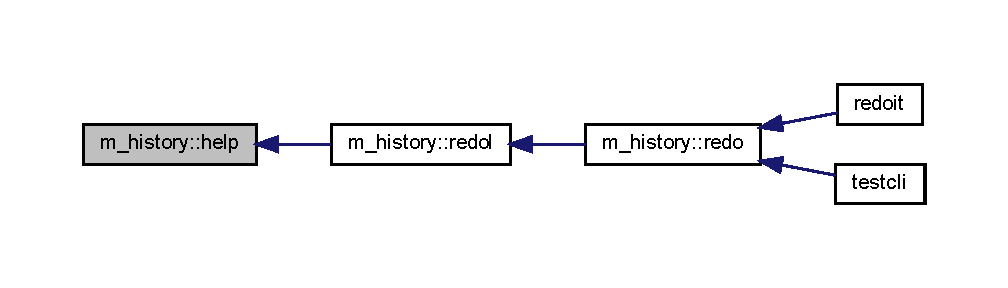
\includegraphics[width=350pt]{namespacem__history_a8d0830530f10435242fa57853baad282_icgraph}
\end{center}
\end{figure}
\mbox{\Hypertarget{namespacem__history_ac181d59688bc06d4ba7465841721e766}\label{namespacem__history_ac181d59688bc06d4ba7465841721e766}} 
\index{m\+\_\+history@{m\+\_\+history}!open\+\_\+history@{open\+\_\+history}}
\index{open\+\_\+history@{open\+\_\+history}!m\+\_\+history@{m\+\_\+history}}
\subsubsection{\texorpdfstring{open\+\_\+history()}{open\_history()}}
{\footnotesize\ttfamily \hyperlink{M__stopwatch_83_8txt_acfbcff50169d691ff02d4a123ed70482}{subroutine}, private m\+\_\+history\+::open\+\_\+history (\begin{DoxyParamCaption}\item[{integer, intent(\hyperlink{M__journal_83_8txt_afce72651d1eed785a2132bee863b2f38}{in})}]{iunit,  }\item[{\hyperlink{option__stopwatch_83_8txt_abd4b21fbbd175834027b5224bfe97e66}{character}(len=$\ast$), intent(\hyperlink{M__journal_83_8txt_afce72651d1eed785a2132bee863b2f38}{in})}]{fname,  }\item[{\hyperlink{option__stopwatch_83_8txt_abd4b21fbbd175834027b5224bfe97e66}{character}(len=$\ast$), intent(\hyperlink{M__journal_83_8txt_afce72651d1eed785a2132bee863b2f38}{in})}]{sname,  }\item[{integer, intent(out)}]{ierr }\end{DoxyParamCaption})\hspace{0.3cm}{\ttfamily [private]}}



References file(), form, readlen, and unit().

Here is the call graph for this function\+:
\nopagebreak
\begin{figure}[H]
\begin{center}
\leavevmode
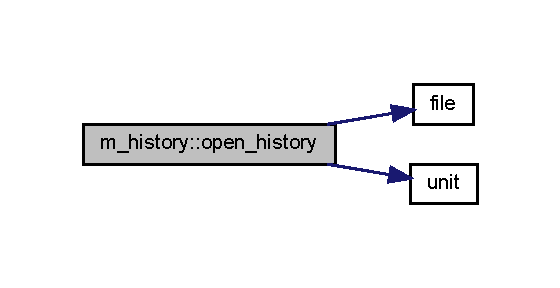
\includegraphics[width=269pt]{namespacem__history_ac181d59688bc06d4ba7465841721e766_cgraph}
\end{center}
\end{figure}
Here is the caller graph for this function\+:
\nopagebreak
\begin{figure}[H]
\begin{center}
\leavevmode
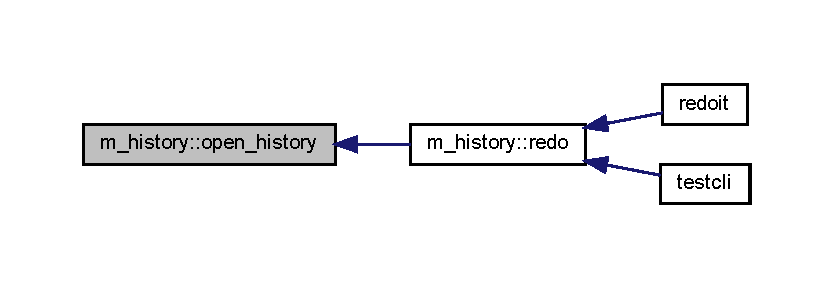
\includegraphics[width=350pt]{namespacem__history_ac181d59688bc06d4ba7465841721e766_icgraph}
\end{center}
\end{figure}
\mbox{\Hypertarget{namespacem__history_a1abbc2c426b89526939d4389c9d3e391}\label{namespacem__history_a1abbc2c426b89526939d4389c9d3e391}} 
\index{m\+\_\+history@{m\+\_\+history}!redo@{redo}}
\index{redo@{redo}!m\+\_\+history@{m\+\_\+history}}
\subsubsection{\texorpdfstring{redo()}{redo()}}
{\footnotesize\ttfamily \hyperlink{M__stopwatch_83_8txt_acfbcff50169d691ff02d4a123ed70482}{subroutine}, \hyperlink{M__stopwatch_83_8txt_a2f74811300c361e53b430611a7d1769f}{public} m\+\_\+history\+::redo (\begin{DoxyParamCaption}\item[{\hyperlink{option__stopwatch_83_8txt_abd4b21fbbd175834027b5224bfe97e66}{character}(len=$\ast$), intent(inout)}]{inputline }\end{DoxyParamCaption})}



References open\+\_\+history(), readlen, redol(), and true().

Here is the call graph for this function\+:
\nopagebreak
\begin{figure}[H]
\begin{center}
\leavevmode
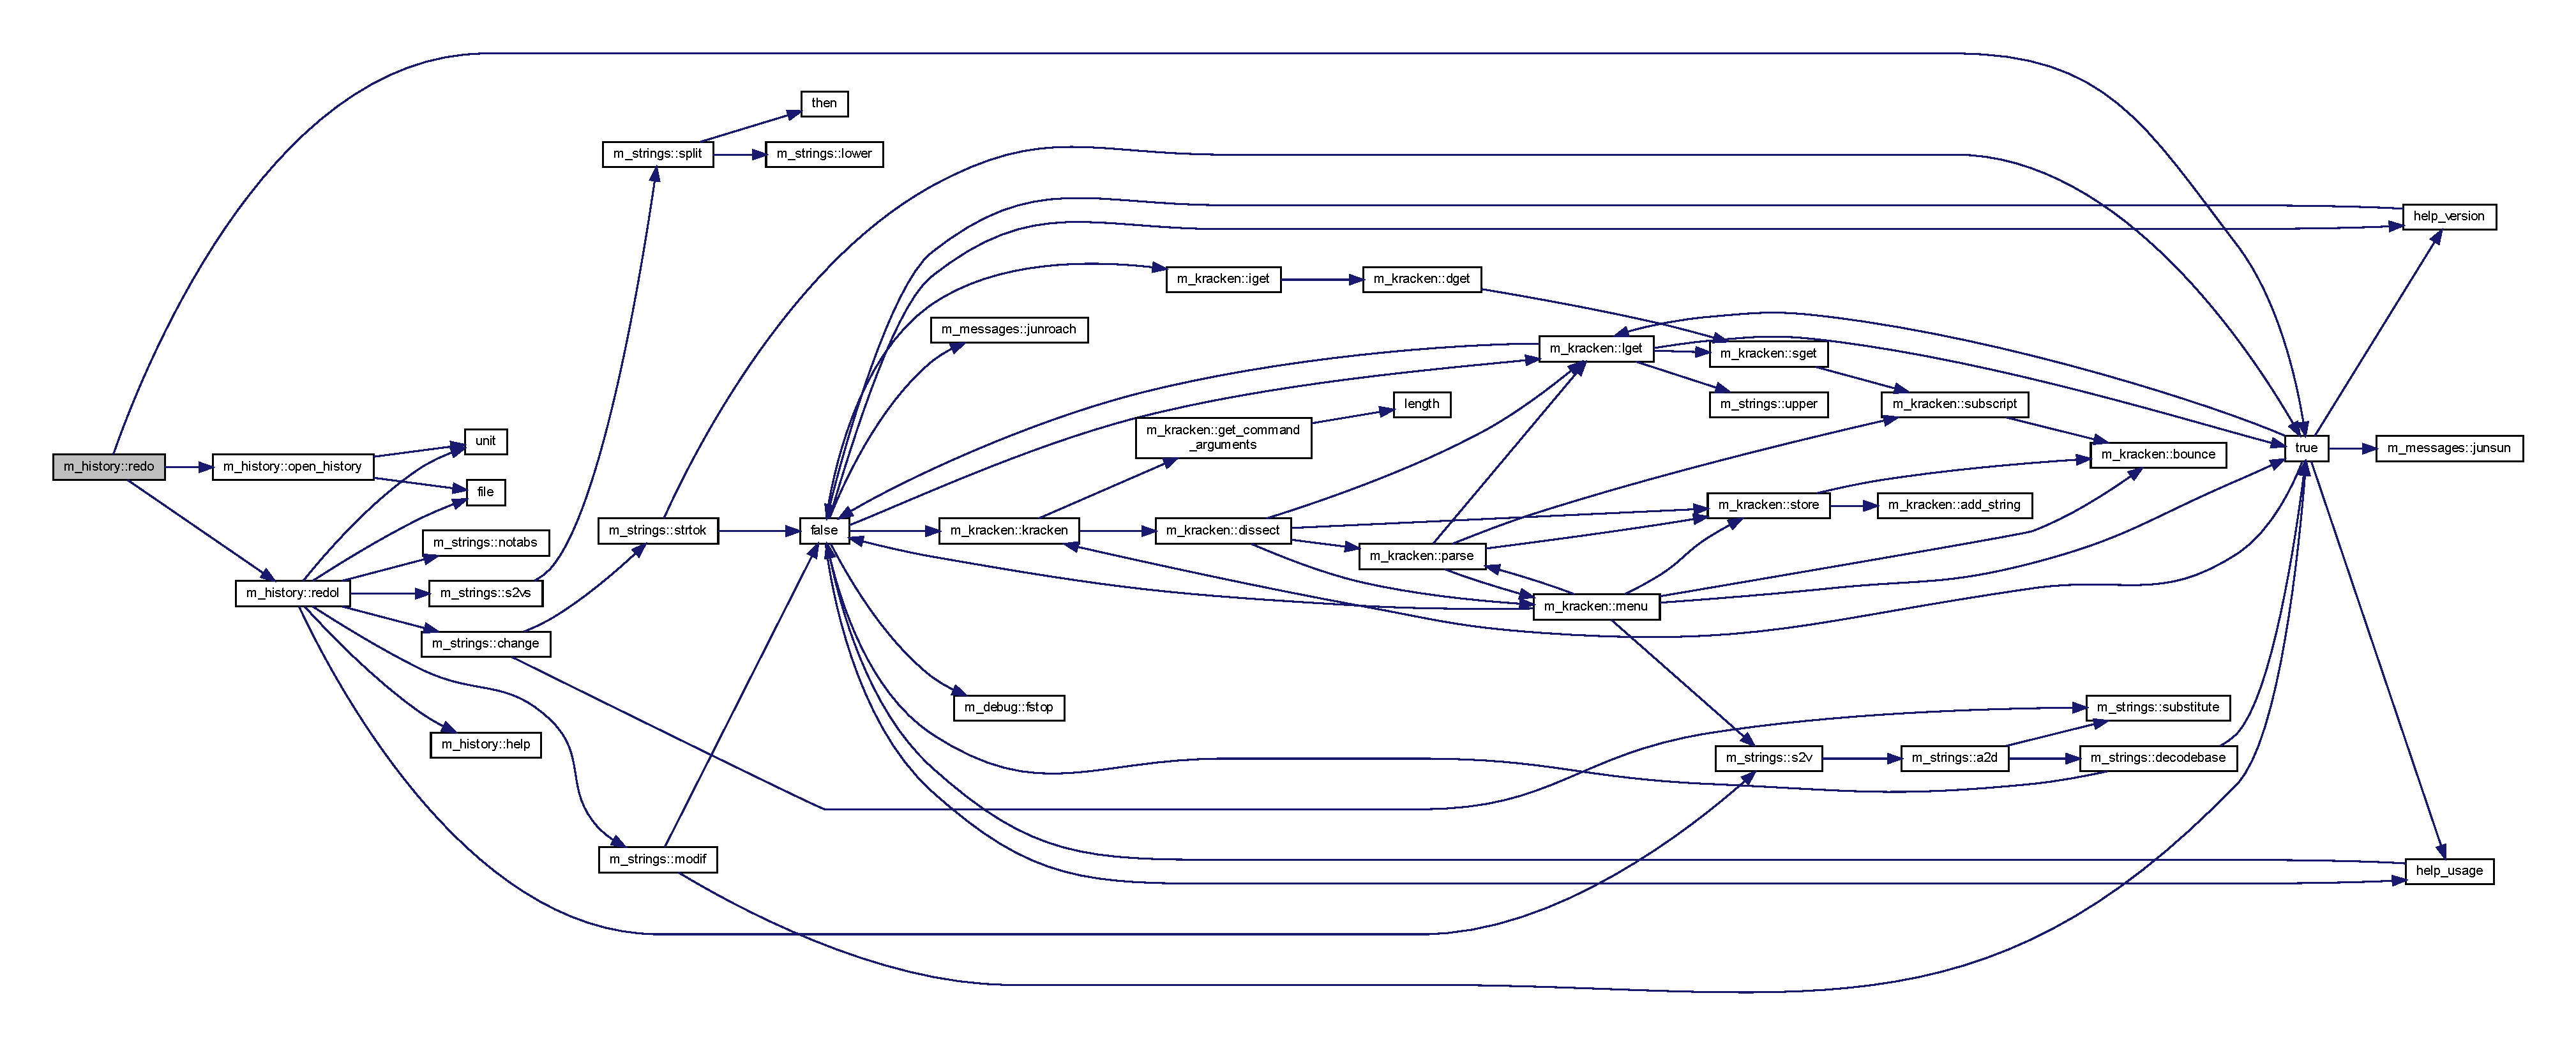
\includegraphics[width=350pt]{namespacem__history_a1abbc2c426b89526939d4389c9d3e391_cgraph}
\end{center}
\end{figure}
Here is the caller graph for this function\+:
\nopagebreak
\begin{figure}[H]
\begin{center}
\leavevmode
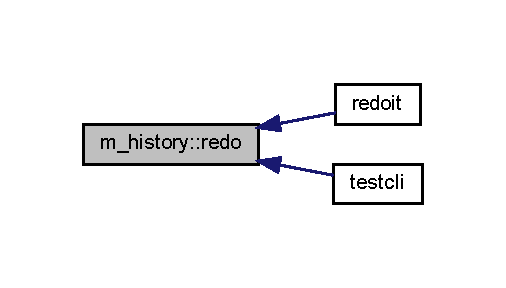
\includegraphics[width=243pt]{namespacem__history_a1abbc2c426b89526939d4389c9d3e391_icgraph}
\end{center}
\end{figure}
\mbox{\Hypertarget{namespacem__history_a155404b1f975ae6fe778f836c043eeb2}\label{namespacem__history_a155404b1f975ae6fe778f836c043eeb2}} 
\index{m\+\_\+history@{m\+\_\+history}!redol@{redol}}
\index{redol@{redol}!m\+\_\+history@{m\+\_\+history}}
\subsubsection{\texorpdfstring{redol()}{redol()}}
{\footnotesize\ttfamily \hyperlink{M__stopwatch_83_8txt_acfbcff50169d691ff02d4a123ed70482}{subroutine}, private m\+\_\+history\+::redol (\begin{DoxyParamCaption}\item[{\hyperlink{option__stopwatch_83_8txt_abd4b21fbbd175834027b5224bfe97e66}{character}(len=$\ast$), intent(out)}]{redoline,  }\item[{integer, intent(\hyperlink{M__journal_83_8txt_afce72651d1eed785a2132bee863b2f38}{in})}]{iobuf,  }\item[{integer}]{iredo,  }\item[{integer, intent(\hyperlink{M__journal_83_8txt_afce72651d1eed785a2132bee863b2f38}{in})}]{ibuf0,  }\item[{\hyperlink{option__stopwatch_83_8txt_abd4b21fbbd175834027b5224bfe97e66}{character}(len=$\ast$), intent(\hyperlink{M__journal_83_8txt_afce72651d1eed785a2132bee863b2f38}{in})}]{init }\end{DoxyParamCaption})\hspace{0.3cm}{\ttfamily [private]}}



References m\+\_\+strings\+::change(), file(), help(), m\+\_\+strings\+::modif(), m\+\_\+strings\+::notabs(), m\+\_\+strings\+::s2v(), m\+\_\+strings\+::s2vs(), and unit().

Here is the call graph for this function\+:
\nopagebreak
\begin{figure}[H]
\begin{center}
\leavevmode
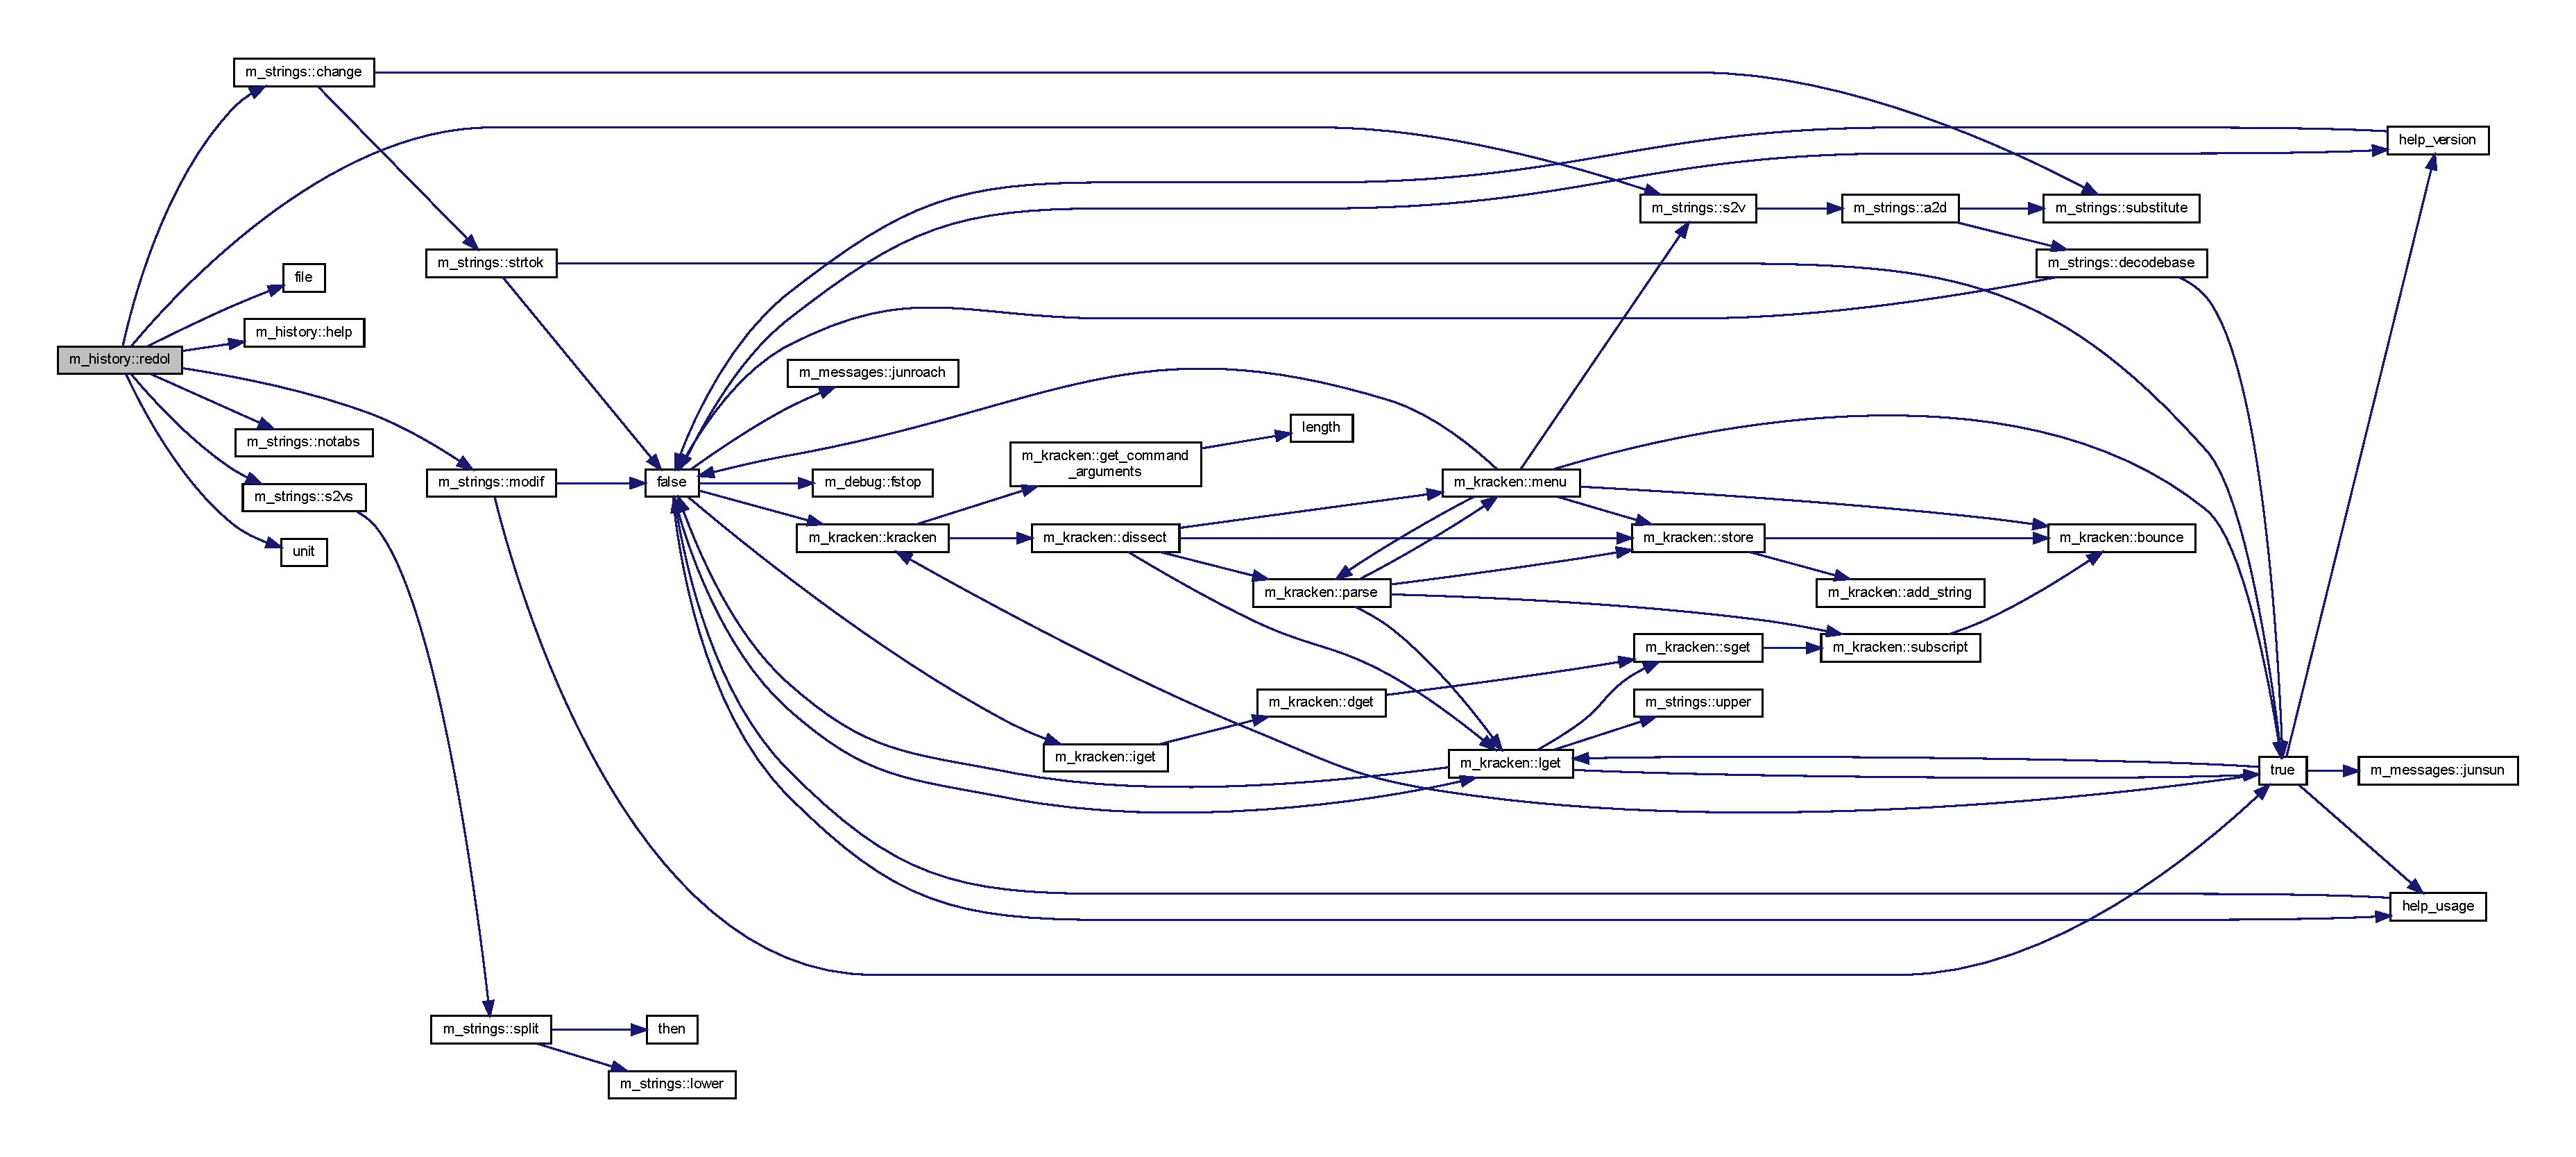
\includegraphics[width=350pt]{namespacem__history_a155404b1f975ae6fe778f836c043eeb2_cgraph}
\end{center}
\end{figure}
Here is the caller graph for this function\+:
\nopagebreak
\begin{figure}[H]
\begin{center}
\leavevmode
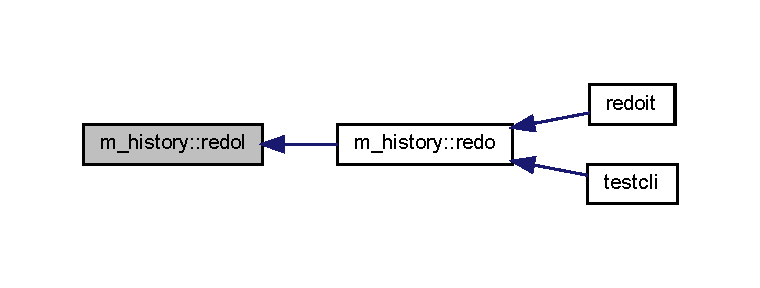
\includegraphics[width=350pt]{namespacem__history_a155404b1f975ae6fe778f836c043eeb2_icgraph}
\end{center}
\end{figure}


\subsection{Variable Documentation}
\mbox{\Hypertarget{namespacem__history_aca543c267d8b80d0690c33e4a684143b}\label{namespacem__history_aca543c267d8b80d0690c33e4a684143b}} 
\index{m\+\_\+history@{m\+\_\+history}!readlen@{readlen}}
\index{readlen@{readlen}!m\+\_\+history@{m\+\_\+history}}
\subsubsection{\texorpdfstring{readlen}{readlen}}
{\footnotesize\ttfamily integer, parameter m\+\_\+history\+::readlen =1024\hspace{0.3cm}{\ttfamily [private]}}


\hypertarget{namespacem__html}{}\section{m\+\_\+html Module Reference}
\label{namespacem__html}\index{m\+\_\+html@{m\+\_\+html}}
\subsection*{Functions/\+Subroutines}
\begin{DoxyCompactItemize}
\item 
\hyperlink{M__stopwatch_83_8txt_acfbcff50169d691ff02d4a123ed70482}{subroutine}, \hyperlink{M__stopwatch_83_8txt_a2f74811300c361e53b430611a7d1769f}{public} \hyperlink{namespacem__html_ad97e98e7241f29c59740757fecd5e6ce}{h\+\_\+array} (\hyperlink{intro__blas1_83_8txt_a89db1945e1a335ab0184c6a097821e32}{array}, iounit)
\item 
\hyperlink{M__stopwatch_83_8txt_acfbcff50169d691ff02d4a123ed70482}{subroutine}, \hyperlink{M__stopwatch_83_8txt_a2f74811300c361e53b430611a7d1769f}{public} \hyperlink{namespacem__html_a3c7065739f09d91dd595f97ebb21583d}{h\+\_\+close} (iounit)
\item 
\hyperlink{M__stopwatch_83_8txt_acfbcff50169d691ff02d4a123ed70482}{subroutine}, \hyperlink{M__stopwatch_83_8txt_a2f74811300c361e53b430611a7d1769f}{public} \hyperlink{namespacem__html_a2188f9871e716a7812d2ab9fb91fde40}{h\+\_\+open} (filename, iounit)
\end{DoxyCompactItemize}


\subsection{Function/\+Subroutine Documentation}
\mbox{\Hypertarget{namespacem__html_ad97e98e7241f29c59740757fecd5e6ce}\label{namespacem__html_ad97e98e7241f29c59740757fecd5e6ce}} 
\index{m\+\_\+html@{m\+\_\+html}!h\+\_\+array@{h\+\_\+array}}
\index{h\+\_\+array@{h\+\_\+array}!m\+\_\+html@{m\+\_\+html}}
\subsubsection{\texorpdfstring{h\+\_\+array()}{h\_array()}}
{\footnotesize\ttfamily \hyperlink{M__stopwatch_83_8txt_acfbcff50169d691ff02d4a123ed70482}{subroutine}, \hyperlink{M__stopwatch_83_8txt_a2f74811300c361e53b430611a7d1769f}{public} m\+\_\+html\+::h\+\_\+array (\begin{DoxyParamCaption}\item[{\hyperlink{read__watch_83_8txt_abdb62bde002f38ef75f810d3a905a823}{real}, dimension(\+:,\+:), intent(\hyperlink{M__journal_83_8txt_afce72651d1eed785a2132bee863b2f38}{in})}]{array,  }\item[{integer, intent(\hyperlink{M__journal_83_8txt_afce72651d1eed785a2132bee863b2f38}{in})}]{iounit }\end{DoxyParamCaption})}

\mbox{\Hypertarget{namespacem__html_a3c7065739f09d91dd595f97ebb21583d}\label{namespacem__html_a3c7065739f09d91dd595f97ebb21583d}} 
\index{m\+\_\+html@{m\+\_\+html}!h\+\_\+close@{h\+\_\+close}}
\index{h\+\_\+close@{h\+\_\+close}!m\+\_\+html@{m\+\_\+html}}
\subsubsection{\texorpdfstring{h\+\_\+close()}{h\_close()}}
{\footnotesize\ttfamily \hyperlink{M__stopwatch_83_8txt_acfbcff50169d691ff02d4a123ed70482}{subroutine}, \hyperlink{M__stopwatch_83_8txt_a2f74811300c361e53b430611a7d1769f}{public} m\+\_\+html\+::h\+\_\+close (\begin{DoxyParamCaption}\item[{integer, intent(\hyperlink{M__journal_83_8txt_afce72651d1eed785a2132bee863b2f38}{in})}]{iounit }\end{DoxyParamCaption})}



References unit().

Here is the call graph for this function\+:
\nopagebreak
\begin{figure}[H]
\begin{center}
\leavevmode
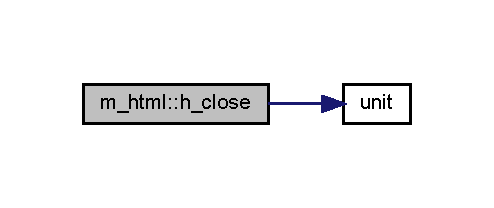
\includegraphics[width=237pt]{namespacem__html_a3c7065739f09d91dd595f97ebb21583d_cgraph}
\end{center}
\end{figure}
\mbox{\Hypertarget{namespacem__html_a2188f9871e716a7812d2ab9fb91fde40}\label{namespacem__html_a2188f9871e716a7812d2ab9fb91fde40}} 
\index{m\+\_\+html@{m\+\_\+html}!h\+\_\+open@{h\+\_\+open}}
\index{h\+\_\+open@{h\+\_\+open}!m\+\_\+html@{m\+\_\+html}}
\subsubsection{\texorpdfstring{h\+\_\+open()}{h\_open()}}
{\footnotesize\ttfamily \hyperlink{M__stopwatch_83_8txt_acfbcff50169d691ff02d4a123ed70482}{subroutine}, \hyperlink{M__stopwatch_83_8txt_a2f74811300c361e53b430611a7d1769f}{public} m\+\_\+html\+::h\+\_\+open (\begin{DoxyParamCaption}\item[{\hyperlink{option__stopwatch_83_8txt_abd4b21fbbd175834027b5224bfe97e66}{character}(len=$\ast$), intent(\hyperlink{M__journal_83_8txt_afce72651d1eed785a2132bee863b2f38}{in})}]{filename,  }\item[{integer, intent(\hyperlink{M__journal_83_8txt_afce72651d1eed785a2132bee863b2f38}{in})}]{iounit }\end{DoxyParamCaption})}


\hypertarget{namespacem__io}{}\section{m\+\_\+io Module Reference}
\label{namespacem__io}\index{m\+\_\+io@{m\+\_\+io}}
\subsection*{Functions/\+Subroutines}
\begin{DoxyCompactItemize}
\item 
\hyperlink{option__stopwatch_83_8txt_abd4b21fbbd175834027b5224bfe97e66}{character}(len=4096) function, \hyperlink{M__stopwatch_83_8txt_a2f74811300c361e53b430611a7d1769f}{public} \hyperlink{namespacem__io_a13a76a3cca012978c1d9c5c0c8b4a7ef}{uniq} (\hyperlink{M__stopwatch_83_8txt_a3f508a893ae4c3b397b4383e33b9bcae}{name}, istart, verbose)
\begin{DoxyCompactList}\small\item\em \subsubsection*{N\+A\+ME}

uniq(3f) -\/ \mbox{[}M\+\_\+io\mbox{]} append a number to the end of filename to make a unique name if name exists \subsubsection*{S\+Y\+N\+O\+P\+S\+IS}\end{DoxyCompactList}\item 
\hyperlink{M__stopwatch_83_8txt_acfbcff50169d691ff02d4a123ed70482}{subroutine}, \hyperlink{M__stopwatch_83_8txt_a2f74811300c361e53b430611a7d1769f}{public} \hyperlink{namespacem__io_aa6ee277b2e0f1c263488624b34371fcf}{print\+\_\+inquire} (iunit, \hyperlink{M__stopwatch_83_8txt_a3f508a893ae4c3b397b4383e33b9bcae}{name})
\begin{DoxyCompactList}\small\item\em \subsubsection*{N\+A\+ME}

print\+\_\+inquire(3f) -\/ \mbox{[}M\+\_\+io\mbox{]} Do I\+N\+Q\+U\+I\+RE on file by name/number and print results \subsubsection*{S\+Y\+N\+O\+P\+S\+IS}\end{DoxyCompactList}\item 
\hyperlink{M__stopwatch_83_8txt_acfbcff50169d691ff02d4a123ed70482}{subroutine}, \hyperlink{M__stopwatch_83_8txt_a2f74811300c361e53b430611a7d1769f}{public} \hyperlink{namespacem__io_ad25822cde8058cd6861e2d9a5d729ccc}{slurp} (filename, \hyperlink{notes_8txt_ad997a48ee1fbabed5333859846b5d9a3}{text})
\begin{DoxyCompactList}\small\item\em \subsubsection*{N\+A\+ME}

S\+L\+U\+R\+P(3f) -\/ \mbox{[}M\+\_\+io\mbox{]} read a file into a character array \subsubsection*{S\+Y\+N\+O\+P\+S\+IS}\end{DoxyCompactList}\item 
integer function, \hyperlink{M__stopwatch_83_8txt_a2f74811300c361e53b430611a7d1769f}{public} \hyperlink{namespacem__io_a673f7f7e137424eed9c6a736901a5cbc}{notopen} (start, end, err)
\begin{DoxyCompactList}\small\item\em \subsubsection*{N\+A\+ME}

notopen(3f) -\/ \mbox{[}M\+\_\+io\mbox{]} Find a F\+U\+N/\+L\+UN (Fortran-\/unit-\/number) that is not in use \subsubsection*{S\+Y\+N\+O\+P\+S\+IS}\end{DoxyCompactList}\item 
\hyperlink{option__stopwatch_83_8txt_abd4b21fbbd175834027b5224bfe97e66}{character}(len=\+:) function, allocatable, \hyperlink{M__stopwatch_83_8txt_a2f74811300c361e53b430611a7d1769f}{public} \hyperlink{namespacem__io_a85eb6aa886ca8e591fdc837919f81708}{dirname} (filename)
\begin{DoxyCompactList}\small\item\em \subsubsection*{N\+A\+ME}

dirname(3f) -\/ \mbox{[}M\+\_\+io\mbox{]} strip last component from filename \end{DoxyCompactList}\item 
\hyperlink{M__stopwatch_83_8txt_acfbcff50169d691ff02d4a123ed70482}{subroutine}, \hyperlink{M__stopwatch_83_8txt_a2f74811300c361e53b430611a7d1769f}{public} \hyperlink{namespacem__io_a7d1857c5c839bf3e096ce68fa1447d44}{splitpath} (path, dir, \hyperlink{M__stopwatch_83_8txt_a3f508a893ae4c3b397b4383e33b9bcae}{name}, basename, ext)
\begin{DoxyCompactList}\small\item\em \subsubsection*{N\+A\+ME}

splitpath(3f) -\/ \mbox{[}M\+\_\+io\mbox{]} split a Unix pathname into components \end{DoxyCompactList}\item 
logical function, \hyperlink{M__stopwatch_83_8txt_a2f74811300c361e53b430611a7d1769f}{public} \hyperlink{namespacem__io_a6793f5adc45177098781af4be39911ff}{isdir} (\hyperlink{namespacem__io_a85eb6aa886ca8e591fdc837919f81708}{dirname})
\begin{DoxyCompactList}\small\item\em \subsubsection*{N\+A\+ME}

isdir(3f) -\/ \mbox{[}M\+\_\+io\mbox{]} checks if argument is a directory path \subsubsection*{S\+Y\+N\+T\+AX}

logical function isdir(path) \subsubsection*{D\+E\+S\+C\+R\+I\+P\+T\+I\+ON}

isdir(3f) checks if path is a path to a directory. \subsubsection*{O\+P\+T\+I\+O\+NS}

path a character string representing a directory pathname. Trailing spaces are ignored. \subsubsection*{E\+X\+A\+M\+P\+L\+ES}\end{DoxyCompactList}\item 
integer function, \hyperlink{M__stopwatch_83_8txt_a2f74811300c361e53b430611a7d1769f}{public} \hyperlink{namespacem__io_a8d9ee59e21830662fa59c300ca23e04b}{readline} (line, lun)
\begin{DoxyCompactList}\small\item\em \subsubsection*{N\+A\+ME}

readline(3f) -\/ \mbox{[}M\+\_\+io\mbox{]} read a line from specified L\+UN into allocatable string up to line length limit \end{DoxyCompactList}\end{DoxyCompactItemize}


\subsection{Function/\+Subroutine Documentation}
\mbox{\Hypertarget{namespacem__io_a85eb6aa886ca8e591fdc837919f81708}\label{namespacem__io_a85eb6aa886ca8e591fdc837919f81708}} 
\index{m\+\_\+io@{m\+\_\+io}!dirname@{dirname}}
\index{dirname@{dirname}!m\+\_\+io@{m\+\_\+io}}
\subsubsection{\texorpdfstring{dirname()}{dirname()}}
{\footnotesize\ttfamily \hyperlink{option__stopwatch_83_8txt_abd4b21fbbd175834027b5224bfe97e66}{character}(len=\+:) function, allocatable, \hyperlink{M__stopwatch_83_8txt_a2f74811300c361e53b430611a7d1769f}{public} m\+\_\+io\+::dirname (\begin{DoxyParamCaption}\item[{\hyperlink{option__stopwatch_83_8txt_abd4b21fbbd175834027b5224bfe97e66}{character}(len=$\ast$), intent(\hyperlink{M__journal_83_8txt_afce72651d1eed785a2132bee863b2f38}{in})}]{filename }\end{DoxyParamCaption})}



\subsubsection*{N\+A\+ME}

dirname(3f) -\/ \mbox{[}M\+\_\+io\mbox{]} strip last component from filename 

\subsubsection*{S\+Y\+N\+O\+P\+S\+IS}

\begin{DoxyVerb}function dirname(FILENAME) result (DIRECTORY)

  character(len=*),intent(in)  :: FILENAME
  character(len=:),allocatable :: DIRECTORY
\end{DoxyVerb}


\subsubsection*{D\+E\+S\+C\+R\+I\+P\+T\+I\+ON}

Output F\+I\+L\+E\+N\+A\+ME with its last non-\/slash component and trailing slashes removed. if F\+I\+L\+E\+N\+A\+ME contains no /\textquotesingle{}s, output \textquotesingle{}.\textquotesingle{} (meaning the current directory).

Assumes leaf separator is a slash (\textquotesingle{}/\textquotesingle{}) and that filename does not contain trailing spaces.

\subsubsection*{O\+P\+T\+I\+O\+NS}

F\+I\+L\+E\+N\+A\+ME pathname to remove the last leaf from

\subsubsection*{R\+E\+T\+U\+R\+NS}

D\+I\+R\+E\+C\+T\+O\+RY directory name for pathname

\subsubsection*{E\+X\+A\+M\+P\+L\+ES}

Sample program\+:

program demo\+\_\+dirname use M\+\_\+io, only \+: dirname implicit none character(len=\+:),allocatable \+:\+: filename integer \+:\+: filename\+\_\+length integer \+:\+: i ! get pathname from command line arguments do i = 1 , command\+\_\+argument\+\_\+count() call get\+\_\+command\+\_\+argument (i , length=filename\+\_\+length) allocate(character(len=filename\+\_\+length) \+:\+: filename) call get\+\_\+command\+\_\+argument (i , value=filename) write($\ast$,\textquotesingle{}(a)\textquotesingle{})dirname(filename) deallocate(filename) enddo end program demo\+\_\+dirname

Sample program executions\+:

demo\+\_\+dirname /usr/bin/ -\/$>$ \char`\"{}/usr\char`\"{} demo\+\_\+dirname dir1/str dir2/str -\/$>$ \char`\"{}dir1\char`\"{} followed by \char`\"{}dir2\char`\"{} demo\+\_\+dirname stdio.\+h -\/$>$ \char`\"{}.\char`\"{}

\subsubsection*{S\+EE A\+L\+SO}

dirname(3c), basename(3c), readlink(3c), realpath(3c) P\+R\+O\+D\+U\+CT\+: C\+LI library utilities and examples P\+R\+O\+G\+R\+AM\+: dirname(3f) D\+E\+S\+C\+R\+I\+P\+T\+I\+ON\+: strip last component from filename \subsubsection*{V\+E\+R\+S\+I\+ON\+: 1.\+0.\+0}

\subsubsection*{D\+A\+TE\+: 2015-\/06-\/26}

A\+U\+T\+H\+OR\+: John S. Urban R\+E\+P\+O\+R\+T\+I\+NG B\+U\+GS\+: \href{http://www.urbanjost.altervista.org/}{\tt http\+://www.\+urbanjost.\+altervista.\+org/} H\+O\+ME P\+A\+GE\+: \href{http://www.urbanjost.altervista.org/index.html}{\tt http\+://www.\+urbanjost.\+altervista.\+org/index.\+html} L\+I\+C\+E\+N\+SE\+: Public Domain. This is free software\+: you are free to change and redistribute it. There is NO W\+A\+R\+R\+A\+N\+TY, to the extent permitted by law. 

References removetail(), and true().

\mbox{\Hypertarget{namespacem__io_a6793f5adc45177098781af4be39911ff}\label{namespacem__io_a6793f5adc45177098781af4be39911ff}} 
\index{m\+\_\+io@{m\+\_\+io}!isdir@{isdir}}
\index{isdir@{isdir}!m\+\_\+io@{m\+\_\+io}}
\subsubsection{\texorpdfstring{isdir()}{isdir()}}
{\footnotesize\ttfamily logical function, \hyperlink{M__stopwatch_83_8txt_a2f74811300c361e53b430611a7d1769f}{public} m\+\_\+io\+::isdir (\begin{DoxyParamCaption}\item[{\hyperlink{option__stopwatch_83_8txt_abd4b21fbbd175834027b5224bfe97e66}{character}(len=$\ast$), intent(\hyperlink{M__journal_83_8txt_afce72651d1eed785a2132bee863b2f38}{in})}]{dirname }\end{DoxyParamCaption})}



\subsubsection*{N\+A\+ME}

isdir(3f) -\/ \mbox{[}M\+\_\+io\mbox{]} checks if argument is a directory path \subsubsection*{S\+Y\+N\+T\+AX}

logical function isdir(path) \subsubsection*{D\+E\+S\+C\+R\+I\+P\+T\+I\+ON}

isdir(3f) checks if path is a path to a directory. \subsubsection*{O\+P\+T\+I\+O\+NS}

path a character string representing a directory pathname. Trailing spaces are ignored. \subsubsection*{E\+X\+A\+M\+P\+L\+ES}

Sample program\+:

program demo\+\_\+isdir Use M\+\_\+io, only \+: isdir implicit none integer \+:\+: i character(len=80),parameter \+:\+: names($\ast$)=\mbox{[} \& \textquotesingle{}/tmp \textquotesingle{}, \& \textquotesingle{}/tmp/\+N\+O\+T\+T\+H\+E\+RE \textquotesingle{}, \& \textquotesingle{}/usr/local \textquotesingle{}, \& \textquotesingle{}. \textquotesingle{}, \& \textquotesingle{}P\+R\+O\+B\+A\+B\+L\+Y\+\_\+\+N\+OT \textquotesingle{}\mbox{]} do i=1,size(names) write($\ast$,$\ast$)\textquotesingle{} is \textquotesingle{},trim(names(i)),\textquotesingle{} a directory? \textquotesingle{}, isdir(names(i)) enddo end program demo\+\_\+isdir

Results\+:

is /tmp a directory? T is /tmp/\+N\+O\+T\+T\+H\+E\+RE a directory? F is /usr/local a directory? T is . a directory? T is P\+R\+O\+B\+A\+B\+L\+Y\+\_\+\+N\+OT a directory? F 

References false(), and file().

\mbox{\Hypertarget{namespacem__io_a673f7f7e137424eed9c6a736901a5cbc}\label{namespacem__io_a673f7f7e137424eed9c6a736901a5cbc}} 
\index{m\+\_\+io@{m\+\_\+io}!notopen@{notopen}}
\index{notopen@{notopen}!m\+\_\+io@{m\+\_\+io}}
\subsubsection{\texorpdfstring{notopen()}{notopen()}}
{\footnotesize\ttfamily integer function, \hyperlink{M__stopwatch_83_8txt_a2f74811300c361e53b430611a7d1769f}{public} m\+\_\+io\+::notopen (\begin{DoxyParamCaption}\item[{integer, intent(\hyperlink{M__journal_83_8txt_afce72651d1eed785a2132bee863b2f38}{in}), \hyperlink{option__stopwatch_83_8txt_aa4ece75e7acf58a4843f70fe18c3ade5}{optional}}]{start,  }\item[{integer, intent(\hyperlink{M__journal_83_8txt_afce72651d1eed785a2132bee863b2f38}{in}), \hyperlink{option__stopwatch_83_8txt_aa4ece75e7acf58a4843f70fe18c3ade5}{optional}}]{end,  }\item[{integer, intent(out), \hyperlink{option__stopwatch_83_8txt_aa4ece75e7acf58a4843f70fe18c3ade5}{optional}}]{err }\end{DoxyParamCaption})}



\subsubsection*{N\+A\+ME}

notopen(3f) -\/ \mbox{[}M\+\_\+io\mbox{]} Find a F\+U\+N/\+L\+UN (Fortran-\/unit-\/number) that is not in use \subsubsection*{S\+Y\+N\+O\+P\+S\+IS}

Usage

integer function notopen(start,end,err) integer,optional,intent(in) \+:\+: start integer,optional,intent(in) \+:\+: end integer,optional,intent(out) \+:\+: err \subsubsection*{D\+E\+S\+C\+R\+I\+P\+T\+I\+ON}

A free F\+O\+R\+T\+R\+AN unit number is needed to O\+P\+EN a file. N\+O\+T\+O\+P\+E\+N() returns a F\+O\+R\+T\+R\+AN unit number from S\+T\+A\+RT to E\+ND not currently associated with an I/O unit. S\+T\+A\+RT and E\+ND are expected to be positive integers where E\+ND .ge. S\+T\+A\+RT.

If N\+O\+T\+O\+P\+E\+N() returns -\/1, then no free F\+O\+R\+T\+R\+AN unit could be found in the specified range.

Otherwise, N\+O\+T\+O\+P\+E\+N() returns an integer representing a free F\+O\+R\+T\+R\+AN logical unit number. Note that N\+O\+T\+O\+P\+E\+N() assumes the following unit numbers defined by the Fortran 2008 I\+S\+O\+\_\+\+F\+O\+R\+T\+R\+A\+N\+\_\+\+E\+NV module

E\+R\+R\+O\+R\+\_\+\+U\+N\+IT,I\+N\+P\+U\+T\+\_\+\+U\+N\+IT,O\+U\+T\+P\+U\+T\+\_\+\+U\+N\+IT

are special, and will never return those values.

\subsubsection*{O\+P\+T\+I\+O\+NS}

start optional logical unit number to start scan at, defaults to 10. end optional logical unit number to stop scan at, defaults to 99. err optional error flag returned. E\+RR will be non-\/zero if no errors. If not present and an error occurs the program will stop instead of returning.

\subsubsection*{N\+O\+T\+ES}

\begin{DoxyVerb}Why are the default START and END limits from 10 to 99? the Fortran 77
standard did not specify a specific limit on the upper range limit, but
the LUN range of 1 to 99 was almost always supported in conventional
programming environments. Additionally, units in the range 0-10 have
often been the units used for pre-assigned files. Occasionally 100,
101 and 102 are reserved (for files such as standard input, standard
output, standard error, ...). Therefore, the defaults for START and
END were selected to be 10 and 99. And most programs do not need
more than 90 files simultaneously open, so the defaults work well in
practice with many versions/vintages of Fortran.

Note that an environment may impose a limit on the number of
simultaneously open files (which some compilers work around).

Beginning with f2008, you can probably use OPEN(NEWUNIT=...) instead.
\end{DoxyVerb}


\subsubsection*{E\+X\+A\+M\+P\+LE}

\begin{DoxyVerb}Sample program:

 program demo_notopen ! test the NOTOPEN(3f) function
 use m_io, only: notopen
 implicit none
 integer :: ii, ierr, igot

 write(*,*)'check for preassigned files from unit 0 to unit 1000'
 write(*,*)'(5 and 6 always return -1)'

 do ii=0,1000
    if(notopen(ii,ii,ierr) .ne. ii)then
       write(*,*)'INUSE:',ii, notopen(ii,ii,ierr)
    endif
 enddo

 ! open all files from UNIT=10 to UNIT=30 so have used units
 do ii=10,30,1
   open(unit=ii,status="scratch")
 enddo
 ! close UNIT=25
 close(25)

 ! find open file in range 10 to 30
 write(*,*)'Should get 25 for this ..',notopen(10,30,ierr)

 close(18)
 do ii=10,32
   igot=notopen(ii,ii,ierr)
   write(*,*)'For unit ',ii,' I got ',igot,' with ERR=',ierr
 enddo

 end program demo_notopen

Expected output(can vary with each programming environment):

   check for preassigned files from unit 0 to unit 1000
   (5 and 6 always return -1)
   INUSE:    0    -1
   INUSE:    5    -1
   INUSE:    6    -1
   Should get 25 for this .. 25
   For  unit  10  I  got  -1  with  ERR=  -1
   For  unit  11  I  got  -1  with  ERR=  -1
   For  unit  12  I  got  -1  with  ERR=  -1
   For  unit  13  I  got  -1  with  ERR=  -1
   For  unit  14  I  got  -1  with  ERR=  -1
   For  unit  15  I  got  -1  with  ERR=  -1
   For  unit  16  I  got  -1  with  ERR=  -1
   For  unit  17  I  got  -1  with  ERR=  -1
   For  unit  18  I  got  18  with  ERR=   0
   For  unit  19  I  got  -1  with  ERR=  -1
   For  unit  20  I  got  -1  with  ERR=  -1
   For  unit  21  I  got  -1  with  ERR=  -1
   For  unit  22  I  got  -1  with  ERR=  -1
   For  unit  23  I  got  -1  with  ERR=  -1
   For  unit  24  I  got  -1  with  ERR=  -1
   For  unit  25  I  got  25  with  ERR=   0
   For  unit  26  I  got  -1  with  ERR=  -1
   For  unit  27  I  got  -1  with  ERR=  -1
   For  unit  28  I  got  -1  with  ERR=  -1
   For  unit  29  I  got  -1  with  ERR=  -1
   For  unit  30  I  got  -1  with  ERR=  -1
   For  unit  31  I  got  31  with  ERR=   0
   For  unit  32  I  got  32  with  ERR=   0
\end{DoxyVerb}


\subsubsection*{A\+U\+T\+H\+O\+RS}

John S. Urban 

References then(), and unit().

\mbox{\Hypertarget{namespacem__io_aa6ee277b2e0f1c263488624b34371fcf}\label{namespacem__io_aa6ee277b2e0f1c263488624b34371fcf}} 
\index{m\+\_\+io@{m\+\_\+io}!print\+\_\+inquire@{print\+\_\+inquire}}
\index{print\+\_\+inquire@{print\+\_\+inquire}!m\+\_\+io@{m\+\_\+io}}
\subsubsection{\texorpdfstring{print\+\_\+inquire()}{print\_inquire()}}
{\footnotesize\ttfamily \hyperlink{M__stopwatch_83_8txt_acfbcff50169d691ff02d4a123ed70482}{subroutine}, \hyperlink{M__stopwatch_83_8txt_a2f74811300c361e53b430611a7d1769f}{public} m\+\_\+io\+::print\+\_\+inquire (\begin{DoxyParamCaption}\item[{integer, intent(\hyperlink{M__journal_83_8txt_afce72651d1eed785a2132bee863b2f38}{in})}]{iunit,  }\item[{\hyperlink{option__stopwatch_83_8txt_abd4b21fbbd175834027b5224bfe97e66}{character}(len=$\ast$), intent(\hyperlink{M__journal_83_8txt_afce72651d1eed785a2132bee863b2f38}{in})}]{name }\end{DoxyParamCaption})}



\subsubsection*{N\+A\+ME}

print\+\_\+inquire(3f) -\/ \mbox{[}M\+\_\+io\mbox{]} Do I\+N\+Q\+U\+I\+RE on file by name/number and print results \subsubsection*{S\+Y\+N\+O\+P\+S\+IS}

Definition\+:

subroutine print\+\_\+inquire(iunit,name) integer,intent(in) \+:\+: iunit character(len=$\ast$),intent(in) \+:\+: name \subsubsection*{D\+E\+S\+C\+R\+I\+P\+T\+I\+ON}

Given either a Fortran file-\/unit-\/number or filename, call the I\+N\+Q\+U\+I\+R\+E(3f) intrinsic and print typical status information. \subsubsection*{O\+P\+T\+I\+O\+NS}

iunit if $>$=0 then query by number and ignore filename name if I\+U\+N\+IT $<$ 0 then query by this filename \subsubsection*{E\+X\+A\+M\+P\+LE}

\begin{DoxyVerb}Sample program:

   program demo_print_inquire
   use M_io, only : print_inquire

   call print_inquire(5,'')

   call print_inquire(19,'')

   open(unit=20)
   call print_inquire(20,'')

   open(unit=21,status='scratch')
   call print_inquire(21,'')

   open(unit=22,file='junko')
   write(22,*)'WRITE TO JUNKO'
   close(unit=22)
   call print_inquire(22,'')
   call print_inquire(-1,'junko')

   end program demo_print_inquire
\end{DoxyVerb}


Expected output\+: 

 {\itshape print\+\_\+inquire} checking file\+: /dev/pty1 {\itshape print\+\_\+inquire} file exists {\itshape print\+\_\+inquire} using unit number 5 \subsection*{$\ast$print\+\_\+inquire$\ast$ access type S\+E\+Q\+U\+E\+N\+T\+I\+AL,F\+O\+R\+M\+A\+T\+T\+ED }

\subsection*{$\ast$print\+\_\+inquire$\ast$ unit number is not open ,unit= 19 }

{\itshape print\+\_\+inquire} checking file\+: fort.\+20 {\itshape print\+\_\+inquire} file exists {\itshape print\+\_\+inquire} using unit number 20 \subsection*{$\ast$print\+\_\+inquire$\ast$ access type S\+E\+Q\+U\+E\+N\+T\+I\+AL,F\+O\+R\+M\+A\+T\+T\+ED }

\subsection*{$\ast$print\+\_\+inquire$\ast$ unit number is not named ,unit= 21 }

\subsection*{$\ast$print\+\_\+inquire$\ast$ unit number is not open ,unit= 22 }

{\itshape print\+\_\+inquire} checking file\+: junko {\itshape print\+\_\+inquire} file exists {\itshape print\+\_\+inquire} file is not open 

References file(), form, number, and unit().

\mbox{\Hypertarget{namespacem__io_a8d9ee59e21830662fa59c300ca23e04b}\label{namespacem__io_a8d9ee59e21830662fa59c300ca23e04b}} 
\index{m\+\_\+io@{m\+\_\+io}!readline@{readline}}
\index{readline@{readline}!m\+\_\+io@{m\+\_\+io}}
\subsubsection{\texorpdfstring{readline()}{readline()}}
{\footnotesize\ttfamily integer function, \hyperlink{M__stopwatch_83_8txt_a2f74811300c361e53b430611a7d1769f}{public} m\+\_\+io\+::readline (\begin{DoxyParamCaption}\item[{\hyperlink{option__stopwatch_83_8txt_abd4b21fbbd175834027b5224bfe97e66}{character}(len=\+:), intent(out), allocatable}]{line,  }\item[{integer, intent(\hyperlink{M__journal_83_8txt_afce72651d1eed785a2132bee863b2f38}{in}), \hyperlink{option__stopwatch_83_8txt_aa4ece75e7acf58a4843f70fe18c3ade5}{optional}}]{lun }\end{DoxyParamCaption})}



\subsubsection*{N\+A\+ME}

readline(3f) -\/ \mbox{[}M\+\_\+io\mbox{]} read a line from specified L\+UN into allocatable string up to line length limit 

\subsubsection*{S\+Y\+N\+T\+AX}

function readline(line,lun) result(ier)

character(len=\+:),allocatable,intent(out) \+:\+: line integer,intent(in) \+:\+: lun integer,intent(out) \+:\+: ier

\subsubsection*{D\+E\+S\+C\+R\+I\+P\+T\+I\+ON}

\begin{DoxyVerb}Read a line of any length up to programming environment's maximum
line length. Requires Fortran 2003+.

It is primarily expected to be used when reading input which will
then be parsed.

o Append lines that end in a backslash with next line
o Expand tabs
o Replace unprintable characters with spaces
o Remove trailing carriage return characters and white space

The simple use of a loop that repeatedly re-allocates a character
variable in addition to reading the input file one buffer at a
time could (depending on the programming environment used) be
inefficient, as it could reallocate and allocate memory used for
the output string with each buffer read.
\end{DoxyVerb}


\subsubsection*{E\+X\+A\+M\+P\+LE}

Sample program\+:

program demo\+\_\+readline use M\+\_\+io, only \+: readline implicit none character(len=\+:),allocatable \+:\+: line I\+N\+F\+I\+N\+I\+TE\+: do while (readline(line)==0) write($\ast$,\textquotesingle{}(a)\textquotesingle{})\textquotesingle{}\mbox{[}\textquotesingle{}//line//\textquotesingle{}\mbox{]}\textquotesingle{} enddo I\+N\+F\+I\+N\+I\+TE end program demo\+\_\+readline 

References is, m\+\_\+strings\+::notabs(), and size().

\mbox{\Hypertarget{namespacem__io_ad25822cde8058cd6861e2d9a5d729ccc}\label{namespacem__io_ad25822cde8058cd6861e2d9a5d729ccc}} 
\index{m\+\_\+io@{m\+\_\+io}!slurp@{slurp}}
\index{slurp@{slurp}!m\+\_\+io@{m\+\_\+io}}
\subsubsection{\texorpdfstring{slurp()}{slurp()}}
{\footnotesize\ttfamily \hyperlink{M__stopwatch_83_8txt_acfbcff50169d691ff02d4a123ed70482}{subroutine}, \hyperlink{M__stopwatch_83_8txt_a2f74811300c361e53b430611a7d1769f}{public} m\+\_\+io\+::slurp (\begin{DoxyParamCaption}\item[{\hyperlink{option__stopwatch_83_8txt_abd4b21fbbd175834027b5224bfe97e66}{character}(len=$\ast$), intent(\hyperlink{M__journal_83_8txt_afce72651d1eed785a2132bee863b2f38}{in})}]{filename,  }\item[{\hyperlink{option__stopwatch_83_8txt_abd4b21fbbd175834027b5224bfe97e66}{character}(len=1), dimension(\+:), intent(out), allocatable}]{text }\end{DoxyParamCaption})}



\subsubsection*{N\+A\+ME}

S\+L\+U\+R\+P(3f) -\/ \mbox{[}M\+\_\+io\mbox{]} read a file into a character array \subsubsection*{S\+Y\+N\+O\+P\+S\+IS}

Usage

subroutine slurp(filename,text) character(len=$\ast$),intent(in) \+:\+: filename character(len=1),allocatable,intent(out) \+:\+: text(\+:) \subsubsection*{D\+E\+S\+C\+R\+I\+P\+T\+I\+ON}

Read an entire file into memory as a stream, retaining line end terminals. Never casually read an entire file into memory if you can process it per line or in smaller units; as large files can consume unreasonable amounts of memory. \subsubsection*{O\+P\+T\+I\+O\+NS}

filename filename to read into memory text array of characters to hold file \subsubsection*{E\+X\+A\+M\+P\+L\+ES}

\begin{DoxyVerb}Sample program, assuming the input file "inputfile" exists:

 program demo_slurp
 use M_io, only      : slurp
 implicit none
 character(len=1),allocatable :: text(:) ! array to hold file in memory
 character(len=*),parameter :: FILENAME='inputfile' ! file to read

 ! create test file
 open(file=FILENAME,unit=10)
 write(10,'(a)') new_line('A')//'esrever lliw'
 write(10,'(a)') 'margorp elpmas eht taht'
 write(10,'(a)') 'elif elpmas a si sihT'
 close(unit=10)

 call slurp(FILENAME,text) ! allocate character array and copy file into it

 if(.not.allocated(text))then
    write(*,*)'*rever* failed to load file '//FILENAME
 else
    ! write file reversed to stdout
    write(*,'(*(a:))',advance='no')text(size(text):1:-1)
    deallocate(text)  ! release memory
 endif

 end program demo_slurp

Expected output:

 >This is a sample file
 >that the sample program
 >will reverse \end{DoxyVerb}
 

References file(), notopen(), stderr(), and unit().

\mbox{\Hypertarget{namespacem__io_a7d1857c5c839bf3e096ce68fa1447d44}\label{namespacem__io_a7d1857c5c839bf3e096ce68fa1447d44}} 
\index{m\+\_\+io@{m\+\_\+io}!splitpath@{splitpath}}
\index{splitpath@{splitpath}!m\+\_\+io@{m\+\_\+io}}
\subsubsection{\texorpdfstring{splitpath()}{splitpath()}}
{\footnotesize\ttfamily \hyperlink{M__stopwatch_83_8txt_acfbcff50169d691ff02d4a123ed70482}{subroutine}, \hyperlink{M__stopwatch_83_8txt_a2f74811300c361e53b430611a7d1769f}{public} m\+\_\+io\+::splitpath (\begin{DoxyParamCaption}\item[{\hyperlink{option__stopwatch_83_8txt_abd4b21fbbd175834027b5224bfe97e66}{character}(len=$\ast$), intent(\hyperlink{M__journal_83_8txt_afce72651d1eed785a2132bee863b2f38}{in})}]{path,  }\item[{\hyperlink{option__stopwatch_83_8txt_abd4b21fbbd175834027b5224bfe97e66}{character}(len=$\ast$), intent(out)}]{dir,  }\item[{\hyperlink{option__stopwatch_83_8txt_abd4b21fbbd175834027b5224bfe97e66}{character}(len=$\ast$), intent(out)}]{name,  }\item[{\hyperlink{option__stopwatch_83_8txt_abd4b21fbbd175834027b5224bfe97e66}{character}(len=$\ast$), intent(out)}]{basename,  }\item[{\hyperlink{option__stopwatch_83_8txt_abd4b21fbbd175834027b5224bfe97e66}{character}(len=$\ast$), intent(out)}]{ext }\end{DoxyParamCaption})}



\subsubsection*{N\+A\+ME}

splitpath(3f) -\/ \mbox{[}M\+\_\+io\mbox{]} split a Unix pathname into components 

\subsubsection*{S\+Y\+N\+O\+P\+S\+IS}

splitpath(path,dir,name,basename,ext)

integer,parameter \+:\+: maxlen=4096 character(len=maxlen),intent(in) \+:\+: path character(len=maxlen),intent(out) \+:\+: dir character(len=maxlen),intent(out) \+:\+: name character(len=maxlen),intent(out) \+:\+: basename character(len=maxlen),intent(out) \+:\+: ext

\subsubsection*{D\+E\+S\+C\+R\+I\+P\+T\+I\+ON}

splitpath(3f) splits given pathname assuming a forward slash separates filename components and that the right-\/most period in the last leaf of the pathname is considered the beginning of an extension. If an extension is found it is left present in N\+A\+ME but removed from B\+A\+S\+E\+N\+A\+ME.

This routine does not check the system for the existence or type of the filename components; it merely parses a string.

\subsubsection*{O\+P\+T\+I\+O\+NS}

path Path to be broken into components. \begin{DoxyVerb}      o Forward slashes (/) are assumed to separate pathname components.
      o the name '.' is assumed to mean "current directory"
      o the name '..' is assumed to mean "up one directory
      o a pathname ending in a slash is assumed to be a directory name
      o a slash starting the pathname is assumed to represent the root
        directory.
      o trailing spaces are assumed insignificant.
\end{DoxyVerb}


Using these rules helps to reduce incorrect parsing, but the routine is only intended for simple parsing of names of the form "\mbox{[}dir/\mbox{]}name\mbox{[}.extension\mbox{]}.

\subsubsection*{R\+E\+S\+U\+L\+TS}

dir Path of directories, including the trailing slash. name Name of file leaf or, if no file is specified in path, name of the lowest directory. basename N\+A\+ME with any extension removed ext File name extension, if any, including the leading period (.).

The path parameter can be a complete or partial file specification. The special name \char`\"{}.\char`\"{} is assumed to mean the current directory, and the special name \char`\"{}..\char`\"{} is assumed to mean one directory above the current directory.

\subsubsection*{E\+X\+A\+M\+P\+LE}

program demo\+\_\+splitpath

use \hyperlink{namespacem__io}{m\+\_\+io}, only \+: splitpath implicit none integer,parameter \+:\+: maxlen=4096 character(len=maxlen),parameter \+:\+: file($\ast$)=\mbox{[}\& \& \textquotesingle{}dirs/name.\+ext \textquotesingle{}, \& \& \textquotesingle{}xx/\+I\+O/zz/\+N\+N.\+FF \textquotesingle{}, \& \& \textquotesingle{}xx/\+I\+O/zz/\+NN \textquotesingle{}, \& \& \textquotesingle{}/xx/\+I\+O/zz/\+NN \textquotesingle{}, \& \& \textquotesingle{}/xx/\+I\+O/zz/ \textquotesingle{}, \& \& \textquotesingle{}/xx/\+I\+O/zz.A/ \textquotesingle{}, \& \& \textquotesingle{}/xx/\+I\+O/zz/. \textquotesingle{}, \& \& \textquotesingle{} \textquotesingle{}, \& \& \textquotesingle{}./ \textquotesingle{}, \& \& \textquotesingle{}/ \textquotesingle{}, \& \& \textquotesingle{}/.. \textquotesingle{}, \& \& \textquotesingle{}./.. \textquotesingle{}, \& \& \textquotesingle{}name. \textquotesingle{}, \& \& \textquotesingle{}.name \textquotesingle{}, \& \& \textquotesingle{}.name. \textquotesingle{}, \& \& \textquotesingle{}. \textquotesingle{}, \& \& \textquotesingle{}.. \textquotesingle{}, \& \& \textquotesingle{}... \textquotesingle{}\mbox{]}

character(len=maxlen) \+:\+: dir character(len=maxlen) \+:\+: name character(len=maxlen) \+:\+: basename character(len=maxlen) \+:\+: ext integer \+:\+: i integer \+:\+: longest longest=maxval(len\+\_\+trim(file)) ! find longest filename

do i=1,size(file) call splitpath(file(i), dir, name, basename, ext) write($\ast$,\textquotesingle{}($\ast$(\char`\"{}$\vert$ \char`\"{},a\+:))\textquotesingle{}) \& \& file(i)(\+:longest), \& \& dir(\+:longest), \& \& name(\+:longest), \& \& basename(\+:longest), \& \& ext(\+:longest) enddo

Output

$\vert$ dirs/name.\+ext $\vert$ dirs $\vert$ name.\+ext $\vert$ name $\vert$ .ext $\vert$ xx/\+I\+O/zz/\+N\+N.\+FF$\vert$ xx/\+I\+O/zz $\vert$ N\+N.\+FF $\vert$ NN $\vert$ .FF $\vert$ xx/\+I\+O/zz/\+NN $\vert$ xx/\+I\+O/zz $\vert$ NN $\vert$ NN $\vert$ $\vert$ /xx/\+I\+O/zz/\+NN $\vert$ /xx/\+I\+O/zz $\vert$ NN $\vert$ NN $\vert$ $\vert$ /xx/\+I\+O/zz/ $\vert$ /xx/\+I\+O/zz $\vert$ $\vert$ $\vert$ $\vert$ /xx/\+I\+O/zz.A/ $\vert$ /xx/\+I\+O/zz.A $\vert$ $\vert$ $\vert$ $\vert$ /xx/\+I\+O/zz/. $\vert$ /xx/\+I\+O/zz/. $\vert$ $\vert$ $\vert$ $\vert$ $\vert$ . $\vert$ $\vert$ $\vert$ $\vert$ ./ $\vert$ . $\vert$ $\vert$ $\vert$ $\vert$ / $\vert$ / $\vert$ $\vert$ $\vert$ $\vert$ /.. $\vert$ / $\vert$ $\vert$ $\vert$ $\vert$ ./.. $\vert$ ./.. $\vert$ $\vert$ $\vert$ $\vert$ name. $\vert$ $\vert$ name. $\vert$ name $\vert$ . $\vert$ .name $\vert$ $\vert$ .name $\vert$ .name $\vert$ $\vert$ .name. $\vert$ $\vert$ .name. $\vert$ .name $\vert$ . $\vert$ . $\vert$ . $\vert$ $\vert$ $\vert$ $\vert$ .. $\vert$ $\vert$ $\vert$ $\vert$ $\vert$ ... $\vert$ $\vert$ ... $\vert$ .. $\vert$ . 

References m\+\_\+strings\+::split(), and true().

\mbox{\Hypertarget{namespacem__io_a13a76a3cca012978c1d9c5c0c8b4a7ef}\label{namespacem__io_a13a76a3cca012978c1d9c5c0c8b4a7ef}} 
\index{m\+\_\+io@{m\+\_\+io}!uniq@{uniq}}
\index{uniq@{uniq}!m\+\_\+io@{m\+\_\+io}}
\subsubsection{\texorpdfstring{uniq()}{uniq()}}
{\footnotesize\ttfamily \hyperlink{option__stopwatch_83_8txt_abd4b21fbbd175834027b5224bfe97e66}{character}(len=4096) function, \hyperlink{M__stopwatch_83_8txt_a2f74811300c361e53b430611a7d1769f}{public} m\+\_\+io\+::uniq (\begin{DoxyParamCaption}\item[{\hyperlink{option__stopwatch_83_8txt_abd4b21fbbd175834027b5224bfe97e66}{character}(len=$\ast$), intent(\hyperlink{M__journal_83_8txt_afce72651d1eed785a2132bee863b2f38}{in})}]{name,  }\item[{integer, intent(\hyperlink{M__journal_83_8txt_afce72651d1eed785a2132bee863b2f38}{in}), \hyperlink{option__stopwatch_83_8txt_aa4ece75e7acf58a4843f70fe18c3ade5}{optional}}]{istart,  }\item[{logical, intent(\hyperlink{M__journal_83_8txt_afce72651d1eed785a2132bee863b2f38}{in}), \hyperlink{option__stopwatch_83_8txt_aa4ece75e7acf58a4843f70fe18c3ade5}{optional}}]{verbose }\end{DoxyParamCaption})}



\subsubsection*{N\+A\+ME}

uniq(3f) -\/ \mbox{[}M\+\_\+io\mbox{]} append a number to the end of filename to make a unique name if name exists \subsubsection*{S\+Y\+N\+O\+P\+S\+IS}

Usage

character(len=\+:),allocatable function uniq(name,istart,verbose) character(len=$\ast$),intent(in) \+:\+: name integer,intent(in),optional \+:\+: istart logical,intent(in),optional \+:\+: verbose

\subsubsection*{D\+E\+S\+C\+R\+I\+P\+T\+I\+ON}

Given a filename test if it is in use or exists. If it is, or if it ends in a period add a four-\/digit number to the end of the name and test if the new name exists. If necessary, increment the number and try again up to the value 9999. An empty file is created if successful.

o relatively non-\/generic; o does not try to detect io errors

\subsubsection*{O\+P\+T\+I\+O\+NS}

name base input name used to create output filename If name ends in \char`\"{}.\char`\"{} a numeric suffix is always added. istart number to start with as a suffix. Default is 1. verbose writes extra messages to stdout. Defaults to .false. \subsubsection*{R\+E\+T\+U\+R\+NS}

uniq A unique filename that is the same as the N\+A\+ME input parameter except with a number appended at the end if needed. \subsubsection*{E\+X\+A\+M\+P\+LE}

\begin{DoxyVerb}Sample program

   program demo_uniq
   use M_io, only : uniq
   implicit none
   character(len=4096) :: myname
   integer            :: i
      myname=uniq('does_not_exist')
      open(unit=10,file='does_exist')
      write(*,*)'name stays the same ',trim(myname)
      myname=uniq('does_exist')
      write(*,*)'name has suffix added ',trim(myname)
      do i=1,10
         myname=uniq('does_exist')
         write(*,*) 'FILENAME:',trim(myname)
         open(unit=20+i,file=myname)
      enddo
   end program demo_uniq

Expected output

 name stays the same does_not_exist
 name has suffix added does_exist0001
 FILENAME:does_exist0002
 FILENAME:does_exist0003
 FILENAME:does_exist0004
 FILENAME:does_exist0005
 FILENAME:does_exist0006
 FILENAME:does_exist0007
 FILENAME:does_exist0008
 FILENAME:does_exist0009
 FILENAME:does_exist0010
 FILENAME:does_exist0011
\end{DoxyVerb}


\subsubsection*{A\+U\+T\+H\+OR}

John S. Urban, 1993 

References false(), file(), and unit().


\hypertarget{namespacem__journal}{}\section{m\+\_\+journal Module Reference}
\label{namespacem__journal}\index{m\+\_\+journal@{m\+\_\+journal}}
\subsection*{Data Types}
\begin{DoxyCompactItemize}
\item 
interface \hyperlink{interfacem__journal_1_1journal}{journal}
\begin{DoxyCompactList}\small\item\em \subsubsection*{N\+A\+ME}

journal(3f) -\/ \mbox{[}M\+\_\+journal\mbox{]} provides public message routine, no paging or graphic mode change" \subsubsection*{S\+Y\+N\+O\+P\+S\+IS}\end{DoxyCompactList}\end{DoxyCompactItemize}
\subsection*{Functions/\+Subroutines}
\begin{DoxyCompactItemize}
\item 
\hyperlink{M__stopwatch_83_8txt_acfbcff50169d691ff02d4a123ed70482}{subroutine} \hyperlink{namespacem__journal_a98698c251ec1883612ae40c5f2443fd9}{write\+\_\+msg} (where, msg)
\item 
\hyperlink{M__stopwatch_83_8txt_acfbcff50169d691ff02d4a123ed70482}{subroutine} \hyperlink{namespacem__journal_a0f2ac99f3da62381d2466c150830b9e0}{set\+\_\+stdout} (iounit)
\item 
\hyperlink{M__stopwatch_83_8txt_acfbcff50169d691ff02d4a123ed70482}{subroutine} \hyperlink{namespacem__journal_a358c4bd99444e0e946b3aaba5f278698}{change\+\_\+model} (value, mode)
\item 
\hyperlink{M__stopwatch_83_8txt_acfbcff50169d691ff02d4a123ed70482}{subroutine} \hyperlink{namespacem__journal_a98479e5ace98340f7519470b96d3197d}{wm} (\hyperlink{M__stopwatch_83_8txt_aa4313e9a55405841f95e6550cd87fc3b}{message})
\item 
\hyperlink{M__stopwatch_83_8txt_acfbcff50169d691ff02d4a123ed70482}{subroutine} \hyperlink{namespacem__journal_ad22893c3621042df7d66b9f3864aa457}{wm\+\_\+r} (where, \hyperlink{M__stopwatch_83_8txt_aa4313e9a55405841f95e6550cd87fc3b}{message}, value)
\item 
\hyperlink{M__stopwatch_83_8txt_acfbcff50169d691ff02d4a123ed70482}{subroutine} \hyperlink{namespacem__journal_a3229165c77bc7f39fbf88fbcfbdb401e}{wm\+\_\+l} (where, \hyperlink{M__stopwatch_83_8txt_aa4313e9a55405841f95e6550cd87fc3b}{message}, truefalse)
\item 
\hyperlink{M__stopwatch_83_8txt_acfbcff50169d691ff02d4a123ed70482}{subroutine} \hyperlink{namespacem__journal_ae4e688044197dd70bd47b4d7c0bb7306}{wm\+\_\+d} (where, \hyperlink{M__stopwatch_83_8txt_aa4313e9a55405841f95e6550cd87fc3b}{message}, dvalue)
\item 
\hyperlink{M__stopwatch_83_8txt_acfbcff50169d691ff02d4a123ed70482}{subroutine} \hyperlink{namespacem__journal_a931487b48fc9268afb0c286c3c3892ad}{wm\+\_\+i} (where, \hyperlink{M__stopwatch_83_8txt_aa4313e9a55405841f95e6550cd87fc3b}{message}, ival)
\end{DoxyCompactItemize}
\subsection*{Variables}
\begin{DoxyCompactItemize}
\item 
\hyperlink{option__stopwatch_83_8txt_abd4b21fbbd175834027b5224bfe97e66}{character}(len= $\ast$), parameter \hyperlink{namespacem__journal_a4e2131bb2d66050e0a9a37632579c9fc}{ident} =\char`\"{}@(\#)M\+\_\+journal\+::journal(3fg)\+: provides public message routine, no paging or graphic mode change\char`\"{}
\item 
integer, save, private \hyperlink{namespacem__journal_a664cf3fd85385b776d30ea589606ad1c}{stdout} =O\+U\+T\+P\+U\+T\+\_\+\+U\+N\+IT
\item 
logical, save \hyperlink{namespacem__journal_a6184fbcebdfa06f0a45ce4c699189b53}{debug} =.false.
\item 
integer, save \hyperlink{namespacem__journal_a47e8e34dc4072b04101027394d688519}{last\+\_\+int} =0
\end{DoxyCompactItemize}


\subsection{Function/\+Subroutine Documentation}
\mbox{\Hypertarget{namespacem__journal_a358c4bd99444e0e946b3aaba5f278698}\label{namespacem__journal_a358c4bd99444e0e946b3aaba5f278698}} 
\index{m\+\_\+journal@{m\+\_\+journal}!change\+\_\+model@{change\+\_\+model}}
\index{change\+\_\+model@{change\+\_\+model}!m\+\_\+journal@{m\+\_\+journal}}
\subsubsection{\texorpdfstring{change\+\_\+model()}{change\_model()}}
{\footnotesize\ttfamily \hyperlink{M__stopwatch_83_8txt_acfbcff50169d691ff02d4a123ed70482}{subroutine} m\+\_\+journal\+::change\+\_\+model (\begin{DoxyParamCaption}\item[{logical, intent(\hyperlink{M__journal_83_8txt_afce72651d1eed785a2132bee863b2f38}{in})}]{value,  }\item[{\hyperlink{option__stopwatch_83_8txt_abd4b21fbbd175834027b5224bfe97e66}{character}(len=$\ast$), intent(\hyperlink{M__journal_83_8txt_afce72651d1eed785a2132bee863b2f38}{in})}]{mode }\end{DoxyParamCaption})\hspace{0.3cm}{\ttfamily [private]}}



References debug, and write\+\_\+msg().

\mbox{\Hypertarget{namespacem__journal_a0f2ac99f3da62381d2466c150830b9e0}\label{namespacem__journal_a0f2ac99f3da62381d2466c150830b9e0}} 
\index{m\+\_\+journal@{m\+\_\+journal}!set\+\_\+stdout@{set\+\_\+stdout}}
\index{set\+\_\+stdout@{set\+\_\+stdout}!m\+\_\+journal@{m\+\_\+journal}}
\subsubsection{\texorpdfstring{set\+\_\+stdout()}{set\_stdout()}}
{\footnotesize\ttfamily \hyperlink{M__stopwatch_83_8txt_acfbcff50169d691ff02d4a123ed70482}{subroutine} m\+\_\+journal\+::set\+\_\+stdout (\begin{DoxyParamCaption}\item[{integer, intent(\hyperlink{M__journal_83_8txt_afce72651d1eed785a2132bee863b2f38}{in})}]{iounit }\end{DoxyParamCaption})\hspace{0.3cm}{\ttfamily [private]}}



References stdout.

\mbox{\Hypertarget{namespacem__journal_a98479e5ace98340f7519470b96d3197d}\label{namespacem__journal_a98479e5ace98340f7519470b96d3197d}} 
\index{m\+\_\+journal@{m\+\_\+journal}!wm@{wm}}
\index{wm@{wm}!m\+\_\+journal@{m\+\_\+journal}}
\subsubsection{\texorpdfstring{wm()}{wm()}}
{\footnotesize\ttfamily \hyperlink{M__stopwatch_83_8txt_acfbcff50169d691ff02d4a123ed70482}{subroutine} m\+\_\+journal\+::wm (\begin{DoxyParamCaption}\item[{\hyperlink{option__stopwatch_83_8txt_abd4b21fbbd175834027b5224bfe97e66}{character}(len=$\ast$), intent(\hyperlink{M__journal_83_8txt_afce72651d1eed785a2132bee863b2f38}{in})}]{message }\end{DoxyParamCaption})\hspace{0.3cm}{\ttfamily [private]}}



References write\+\_\+msg().

\mbox{\Hypertarget{namespacem__journal_ae4e688044197dd70bd47b4d7c0bb7306}\label{namespacem__journal_ae4e688044197dd70bd47b4d7c0bb7306}} 
\index{m\+\_\+journal@{m\+\_\+journal}!wm\+\_\+d@{wm\+\_\+d}}
\index{wm\+\_\+d@{wm\+\_\+d}!m\+\_\+journal@{m\+\_\+journal}}
\subsubsection{\texorpdfstring{wm\+\_\+d()}{wm\_d()}}
{\footnotesize\ttfamily \hyperlink{M__stopwatch_83_8txt_acfbcff50169d691ff02d4a123ed70482}{subroutine} m\+\_\+journal\+::wm\+\_\+d (\begin{DoxyParamCaption}\item[{\hyperlink{option__stopwatch_83_8txt_abd4b21fbbd175834027b5224bfe97e66}{character}(len=$\ast$), intent(\hyperlink{M__journal_83_8txt_afce72651d1eed785a2132bee863b2f38}{in})}]{where,  }\item[{\hyperlink{option__stopwatch_83_8txt_abd4b21fbbd175834027b5224bfe97e66}{character}(len=$\ast$), intent(\hyperlink{M__journal_83_8txt_afce72651d1eed785a2132bee863b2f38}{in})}]{message,  }\item[{doubleprecision, intent(\hyperlink{M__journal_83_8txt_afce72651d1eed785a2132bee863b2f38}{in})}]{dvalue }\end{DoxyParamCaption})\hspace{0.3cm}{\ttfamily [private]}}



References write\+\_\+msg().

\mbox{\Hypertarget{namespacem__journal_a931487b48fc9268afb0c286c3c3892ad}\label{namespacem__journal_a931487b48fc9268afb0c286c3c3892ad}} 
\index{m\+\_\+journal@{m\+\_\+journal}!wm\+\_\+i@{wm\+\_\+i}}
\index{wm\+\_\+i@{wm\+\_\+i}!m\+\_\+journal@{m\+\_\+journal}}
\subsubsection{\texorpdfstring{wm\+\_\+i()}{wm\_i()}}
{\footnotesize\ttfamily \hyperlink{M__stopwatch_83_8txt_acfbcff50169d691ff02d4a123ed70482}{subroutine} m\+\_\+journal\+::wm\+\_\+i (\begin{DoxyParamCaption}\item[{\hyperlink{option__stopwatch_83_8txt_abd4b21fbbd175834027b5224bfe97e66}{character}(len=$\ast$), intent(\hyperlink{M__journal_83_8txt_afce72651d1eed785a2132bee863b2f38}{in})}]{where,  }\item[{\hyperlink{option__stopwatch_83_8txt_abd4b21fbbd175834027b5224bfe97e66}{character}(len=$\ast$), intent(\hyperlink{M__journal_83_8txt_afce72651d1eed785a2132bee863b2f38}{in})}]{message,  }\item[{integer, intent(\hyperlink{M__journal_83_8txt_afce72651d1eed785a2132bee863b2f38}{in})}]{ival }\end{DoxyParamCaption})\hspace{0.3cm}{\ttfamily [private]}}



References last\+\_\+int, and write\+\_\+msg().

\mbox{\Hypertarget{namespacem__journal_a3229165c77bc7f39fbf88fbcfbdb401e}\label{namespacem__journal_a3229165c77bc7f39fbf88fbcfbdb401e}} 
\index{m\+\_\+journal@{m\+\_\+journal}!wm\+\_\+l@{wm\+\_\+l}}
\index{wm\+\_\+l@{wm\+\_\+l}!m\+\_\+journal@{m\+\_\+journal}}
\subsubsection{\texorpdfstring{wm\+\_\+l()}{wm\_l()}}
{\footnotesize\ttfamily \hyperlink{M__stopwatch_83_8txt_acfbcff50169d691ff02d4a123ed70482}{subroutine} m\+\_\+journal\+::wm\+\_\+l (\begin{DoxyParamCaption}\item[{\hyperlink{option__stopwatch_83_8txt_abd4b21fbbd175834027b5224bfe97e66}{character}(len=$\ast$), intent(\hyperlink{M__journal_83_8txt_afce72651d1eed785a2132bee863b2f38}{in})}]{where,  }\item[{\hyperlink{option__stopwatch_83_8txt_abd4b21fbbd175834027b5224bfe97e66}{character}(len=$\ast$), intent(\hyperlink{M__journal_83_8txt_afce72651d1eed785a2132bee863b2f38}{in})}]{message,  }\item[{logical, intent(\hyperlink{M__journal_83_8txt_afce72651d1eed785a2132bee863b2f38}{in})}]{truefalse }\end{DoxyParamCaption})\hspace{0.3cm}{\ttfamily [private]}}



References write\+\_\+msg().

\mbox{\Hypertarget{namespacem__journal_ad22893c3621042df7d66b9f3864aa457}\label{namespacem__journal_ad22893c3621042df7d66b9f3864aa457}} 
\index{m\+\_\+journal@{m\+\_\+journal}!wm\+\_\+r@{wm\+\_\+r}}
\index{wm\+\_\+r@{wm\+\_\+r}!m\+\_\+journal@{m\+\_\+journal}}
\subsubsection{\texorpdfstring{wm\+\_\+r()}{wm\_r()}}
{\footnotesize\ttfamily \hyperlink{M__stopwatch_83_8txt_acfbcff50169d691ff02d4a123ed70482}{subroutine} m\+\_\+journal\+::wm\+\_\+r (\begin{DoxyParamCaption}\item[{\hyperlink{option__stopwatch_83_8txt_abd4b21fbbd175834027b5224bfe97e66}{character}(len=$\ast$), intent(\hyperlink{M__journal_83_8txt_afce72651d1eed785a2132bee863b2f38}{in})}]{where,  }\item[{\hyperlink{option__stopwatch_83_8txt_abd4b21fbbd175834027b5224bfe97e66}{character}(len=$\ast$), intent(\hyperlink{M__journal_83_8txt_afce72651d1eed785a2132bee863b2f38}{in})}]{message,  }\item[{\hyperlink{read__watch_83_8txt_abdb62bde002f38ef75f810d3a905a823}{real}, intent(\hyperlink{M__journal_83_8txt_afce72651d1eed785a2132bee863b2f38}{in})}]{value }\end{DoxyParamCaption})\hspace{0.3cm}{\ttfamily [private]}}



References write\+\_\+msg().

\mbox{\Hypertarget{namespacem__journal_a98698c251ec1883612ae40c5f2443fd9}\label{namespacem__journal_a98698c251ec1883612ae40c5f2443fd9}} 
\index{m\+\_\+journal@{m\+\_\+journal}!write\+\_\+msg@{write\+\_\+msg}}
\index{write\+\_\+msg@{write\+\_\+msg}!m\+\_\+journal@{m\+\_\+journal}}
\subsubsection{\texorpdfstring{write\+\_\+msg()}{write\_msg()}}
{\footnotesize\ttfamily \hyperlink{M__stopwatch_83_8txt_acfbcff50169d691ff02d4a123ed70482}{subroutine} m\+\_\+journal\+::write\+\_\+msg (\begin{DoxyParamCaption}\item[{\hyperlink{option__stopwatch_83_8txt_abd4b21fbbd175834027b5224bfe97e66}{character}(len=$\ast$), intent(\hyperlink{M__journal_83_8txt_afce72651d1eed785a2132bee863b2f38}{in})}]{where,  }\item[{\hyperlink{option__stopwatch_83_8txt_abd4b21fbbd175834027b5224bfe97e66}{character}(len=$\ast$), intent(\hyperlink{M__journal_83_8txt_afce72651d1eed785a2132bee863b2f38}{in})}]{msg }\end{DoxyParamCaption})\hspace{0.3cm}{\ttfamily [private]}}



References debug, false(), file(), form, last\+\_\+int, now\+\_\+ex(), stdout, true(), and unit().



\subsection{Variable Documentation}
\mbox{\Hypertarget{namespacem__journal_a6184fbcebdfa06f0a45ce4c699189b53}\label{namespacem__journal_a6184fbcebdfa06f0a45ce4c699189b53}} 
\index{m\+\_\+journal@{m\+\_\+journal}!debug@{debug}}
\index{debug@{debug}!m\+\_\+journal@{m\+\_\+journal}}
\subsubsection{\texorpdfstring{debug}{debug}}
{\footnotesize\ttfamily logical, save m\+\_\+journal\+::debug =.false.\hspace{0.3cm}{\ttfamily [private]}}

\mbox{\Hypertarget{namespacem__journal_a4e2131bb2d66050e0a9a37632579c9fc}\label{namespacem__journal_a4e2131bb2d66050e0a9a37632579c9fc}} 
\index{m\+\_\+journal@{m\+\_\+journal}!ident@{ident}}
\index{ident@{ident}!m\+\_\+journal@{m\+\_\+journal}}
\subsubsection{\texorpdfstring{ident}{ident}}
{\footnotesize\ttfamily \hyperlink{option__stopwatch_83_8txt_abd4b21fbbd175834027b5224bfe97e66}{character}(len=$\ast$), parameter m\+\_\+journal\+::ident =\char`\"{}@(\#)M\+\_\+journal\+::journal(3fg)\+: provides public message routine, no paging or graphic mode change\char`\"{}\hspace{0.3cm}{\ttfamily [private]}}

\mbox{\Hypertarget{namespacem__journal_a47e8e34dc4072b04101027394d688519}\label{namespacem__journal_a47e8e34dc4072b04101027394d688519}} 
\index{m\+\_\+journal@{m\+\_\+journal}!last\+\_\+int@{last\+\_\+int}}
\index{last\+\_\+int@{last\+\_\+int}!m\+\_\+journal@{m\+\_\+journal}}
\subsubsection{\texorpdfstring{last\+\_\+int}{last\_int}}
{\footnotesize\ttfamily integer, save m\+\_\+journal\+::last\+\_\+int =0\hspace{0.3cm}{\ttfamily [private]}}

\mbox{\Hypertarget{namespacem__journal_a664cf3fd85385b776d30ea589606ad1c}\label{namespacem__journal_a664cf3fd85385b776d30ea589606ad1c}} 
\index{m\+\_\+journal@{m\+\_\+journal}!stdout@{stdout}}
\index{stdout@{stdout}!m\+\_\+journal@{m\+\_\+journal}}
\subsubsection{\texorpdfstring{stdout}{stdout}}
{\footnotesize\ttfamily integer, save, private m\+\_\+journal\+::stdout =O\+U\+T\+P\+U\+T\+\_\+\+U\+N\+IT\hspace{0.3cm}{\ttfamily [private]}}


\hypertarget{namespacem__kracken}{}\section{m\+\_\+kracken Module Reference}
\label{namespacem__kracken}\index{m\+\_\+kracken@{m\+\_\+kracken}}
\subsection*{Functions/\+Subroutines}
\begin{DoxyCompactItemize}
\item 
\hyperlink{M__stopwatch_83_8txt_acfbcff50169d691ff02d4a123ed70482}{subroutine}, \hyperlink{M__stopwatch_83_8txt_a2f74811300c361e53b430611a7d1769f}{public} \hyperlink{namespacem__kracken_ad4f3d7c793c90789b175097b433035da}{retrev} (\hyperlink{M__stopwatch_83_8txt_a3f508a893ae4c3b397b4383e33b9bcae}{name}, val, len, ier)
\begin{DoxyCompactList}\small\item\em \subsubsection*{N\+A\+ME}

R\+E\+T\+R\+E\+V(3f) -\/ \mbox{[}A\+R\+G\+U\+M\+E\+N\+TS\+:M\+\_\+kracken\mbox{]} get keyword value as a string from a command\textquotesingle{}s argument list processed by kracken(3f) \end{DoxyCompactList}\item 
\hyperlink{read__watch_83_8txt_abdb62bde002f38ef75f810d3a905a823}{real}(kind=\hyperlink{namespacem__kracken_a1de91e5ca55bf4fab118936bf4fad36a}{dp}) function, \hyperlink{M__stopwatch_83_8txt_a2f74811300c361e53b430611a7d1769f}{public} \hyperlink{namespacem__kracken_ae7b6ad046d637f03148efb56336a7ff4}{dget} (keyword)
\begin{DoxyCompactList}\small\item\em \subsubsection*{N\+A\+ME}

dget -\/ \mbox{[}A\+R\+G\+U\+M\+E\+N\+TS\+:M\+\_\+kracken\mbox{]} given keyword fetch doubleprecision value from command argument \subsubsection*{S\+Y\+N\+O\+P\+S\+IS}\end{DoxyCompactList}\item 
\hyperlink{read__watch_83_8txt_abdb62bde002f38ef75f810d3a905a823}{real} function, \hyperlink{M__stopwatch_83_8txt_a2f74811300c361e53b430611a7d1769f}{public} \hyperlink{namespacem__kracken_a21e0e40932af79430832a53bdb4de300}{rget} (keyword)
\begin{DoxyCompactList}\small\item\em \subsubsection*{N\+A\+ME}

rget -\/ \mbox{[}A\+R\+G\+U\+M\+E\+N\+TS\+:M\+\_\+kracken\mbox{]} given keyword fetch real value from command argument \subsubsection*{S\+Y\+N\+O\+P\+S\+IS}\end{DoxyCompactList}\item 
integer function, \hyperlink{M__stopwatch_83_8txt_a2f74811300c361e53b430611a7d1769f}{public} \hyperlink{namespacem__kracken_a420718890eac378e5cd047dd0b477424}{iget} (keyword)
\begin{DoxyCompactList}\small\item\em \subsubsection*{N\+A\+ME}

iget -\/ \mbox{[}A\+R\+G\+U\+M\+E\+N\+TS\+:M\+\_\+kracken\mbox{]} given keyword fetch integer value from command argument \end{DoxyCompactList}\item 
logical function, \hyperlink{M__stopwatch_83_8txt_a2f74811300c361e53b430611a7d1769f}{public} \hyperlink{namespacem__kracken_a7141acd7a00c1a5aa5f90612a0414b63}{lget} (keyword)
\begin{DoxyCompactList}\small\item\em \subsubsection*{N\+A\+ME}

lget -\/ \mbox{[}A\+R\+G\+U\+M\+E\+N\+TS\+:M\+\_\+kracken\mbox{]} given keyword fetch logical value from command arguments \subsubsection*{S\+Y\+N\+O\+P\+S\+IS}\end{DoxyCompactList}\item 
\hyperlink{option__stopwatch_83_8txt_abd4b21fbbd175834027b5224bfe97e66}{character}(len=\+:) function, allocatable, \hyperlink{M__stopwatch_83_8txt_a2f74811300c361e53b430611a7d1769f}{public} \hyperlink{namespacem__kracken_a9a64192326816b0b9badcc11506628ee}{sget} (\hyperlink{M__stopwatch_83_8txt_a3f508a893ae4c3b397b4383e33b9bcae}{name}, ilen)
\begin{DoxyCompactList}\small\item\em \subsubsection*{N\+A\+ME}

sget -\/ \mbox{[}A\+R\+G\+U\+M\+E\+N\+TS\+:M\+\_\+kracken\mbox{]} given keyword fetch string value and length from command arguments \subsubsection*{S\+Y\+N\+O\+P\+S\+IS}\end{DoxyCompactList}\item 
\hyperlink{read__watch_83_8txt_abdb62bde002f38ef75f810d3a905a823}{real}(kind=\hyperlink{namespacem__kracken_a1de91e5ca55bf4fab118936bf4fad36a}{dp}) function, dimension(\+:), allocatable, \hyperlink{M__stopwatch_83_8txt_a2f74811300c361e53b430611a7d1769f}{public} \hyperlink{namespacem__kracken_a76e99048e7fb6010dcb7173ef958c932}{dgets} (keyword)
\begin{DoxyCompactList}\small\item\em \subsubsection*{N\+A\+ME}

dgets -\/ \mbox{[}A\+R\+G\+U\+M\+E\+N\+TS\+:M\+\_\+kracken\mbox{]} given keyword fetch doubleprecision array from command arguments \subsubsection*{S\+Y\+N\+O\+P\+S\+IS}\end{DoxyCompactList}\item 
integer function, dimension(\+:), allocatable, \hyperlink{M__stopwatch_83_8txt_a2f74811300c361e53b430611a7d1769f}{public} \hyperlink{namespacem__kracken_ac118bb44d855d68bfce6caa80d60e5e0}{igets} (keyword)
\begin{DoxyCompactList}\small\item\em \subsubsection*{N\+A\+ME}

igets -\/ \mbox{[}A\+R\+G\+U\+M\+E\+N\+TS\+:M\+\_\+kracken\mbox{]} given keyword fetch integer array from command arguments \subsubsection*{S\+Y\+N\+O\+P\+S\+IS}\end{DoxyCompactList}\item 
\hyperlink{read__watch_83_8txt_abdb62bde002f38ef75f810d3a905a823}{real} function, dimension(\+:), allocatable, \hyperlink{M__stopwatch_83_8txt_a2f74811300c361e53b430611a7d1769f}{public} \hyperlink{namespacem__kracken_aa1a29fad1518c15d8710d273755a17cc}{rgets} (keyword)
\begin{DoxyCompactList}\small\item\em \subsubsection*{N\+A\+ME}

rgets -\/ \mbox{[}A\+R\+G\+U\+M\+E\+N\+TS\+:M\+\_\+kracken\mbox{]} given keyword fetch real array from command arguments \subsubsection*{S\+Y\+N\+O\+P\+S\+IS}\end{DoxyCompactList}\item 
logical function, dimension(\+:), allocatable, \hyperlink{M__stopwatch_83_8txt_a2f74811300c361e53b430611a7d1769f}{public} \hyperlink{namespacem__kracken_afb3f3b45b78625758818ea9bef463fd9}{lgets} (keyword)
\begin{DoxyCompactList}\small\item\em \subsubsection*{N\+A\+ME}

lget -\/ \mbox{[}A\+R\+G\+U\+M\+E\+N\+TS\+:M\+\_\+kracken\mbox{]} given keyword fetch logical array from command argument \subsubsection*{S\+Y\+N\+O\+P\+S\+IS}\end{DoxyCompactList}\item 
\hyperlink{option__stopwatch_83_8txt_abd4b21fbbd175834027b5224bfe97e66}{character}(len=\hyperlink{namespacem__kracken_a9e71724677cede703e1fb186e446349f}{ipvalue}) function, dimension(\+:), allocatable, \hyperlink{M__stopwatch_83_8txt_a2f74811300c361e53b430611a7d1769f}{public} \hyperlink{namespacem__kracken_a8ae60c1a9c903c8ad06ef1f95975d457}{sgets} (\hyperlink{M__stopwatch_83_8txt_a3f508a893ae4c3b397b4383e33b9bcae}{name}, delim)
\begin{DoxyCompactList}\small\item\em \subsubsection*{N\+A\+ME}

sgets -\/ \mbox{[}A\+R\+G\+U\+M\+E\+N\+TS\+:M\+\_\+kracken\mbox{]} given keyword fetch string value parsed on whitespace into an array \subsubsection*{S\+Y\+N\+O\+P\+S\+IS}\end{DoxyCompactList}\item 
\hyperlink{M__stopwatch_83_8txt_acfbcff50169d691ff02d4a123ed70482}{subroutine}, \hyperlink{M__stopwatch_83_8txt_a2f74811300c361e53b430611a7d1769f}{public} \hyperlink{namespacem__kracken_a850dce381e1cfe18a4ebcaa214995e39}{kracken} (verb, \hyperlink{what__overview_81_8txt_a74cb7e955273b9f9157b4f0c18a38849}{string}, error\+\_\+return)
\begin{DoxyCompactList}\small\item\em \subsubsection*{N\+A\+ME}

kracken(3f) -\/ \mbox{[}A\+R\+G\+U\+M\+E\+N\+TS\+:M\+\_\+kracken\mbox{]} crack command line options on Fortran programs, using \char`\"{}-\/\+K\+E\+Y\+W\+O\+R\+D V\+A\+L\+U\+E\char`\"{} syntax \subsubsection*{S\+Y\+N\+O\+P\+S\+IS}\end{DoxyCompactList}\item 
\hyperlink{M__stopwatch_83_8txt_acfbcff50169d691ff02d4a123ed70482}{subroutine}, \hyperlink{M__stopwatch_83_8txt_a2f74811300c361e53b430611a7d1769f}{public} \hyperlink{namespacem__kracken_aab831b470a3107ca69833e717e95eaec}{setprompts} (verb, init)
\begin{DoxyCompactList}\small\item\em \subsubsection*{N\+A\+ME}

setprompts(3f) -\/ \mbox{[}A\+R\+G\+U\+M\+E\+N\+TS\+:M\+\_\+kracken\mbox{]} set explicit prompts for keywords in interactive mode \subsubsection*{S\+Y\+N\+O\+P\+S\+IS}\end{DoxyCompactList}\item 
\hyperlink{M__stopwatch_83_8txt_acfbcff50169d691ff02d4a123ed70482}{subroutine}, \hyperlink{M__stopwatch_83_8txt_a2f74811300c361e53b430611a7d1769f}{public} \hyperlink{namespacem__kracken_a2cb376f8a8e26e489a45cafcda66ea3e}{dissect} (verb, init, pars, error\+\_\+return)
\begin{DoxyCompactList}\small\item\em \subsubsection*{N\+A\+ME}

dissect(3f) -\/ \mbox{[}A\+R\+G\+U\+M\+E\+N\+TS\+:M\+\_\+kracken\mbox{]} convenient call to \hyperlink{namespacem__kracken_a495ed7db5c2d301c4d5e623b62a9c295}{parse()} -- define defaults, then process \end{DoxyCompactList}\item 
\hyperlink{M__stopwatch_83_8txt_acfbcff50169d691ff02d4a123ed70482}{subroutine}, \hyperlink{M__stopwatch_83_8txt_a2f74811300c361e53b430611a7d1769f}{public} \hyperlink{namespacem__kracken_a495ed7db5c2d301c4d5e623b62a9c295}{parse} (verb, \hyperlink{what__overview_81_8txt_a74cb7e955273b9f9157b4f0c18a38849}{string}, allow, error\+\_\+return)
\begin{DoxyCompactList}\small\item\em \subsubsection*{N\+A\+ME}

parse(3f) -\/ \mbox{[}A\+R\+G\+U\+M\+E\+N\+TS\+:M\+\_\+kracken\mbox{]} parse user command and store tokens into Language Dictionary \end{DoxyCompactList}\item 
\hyperlink{M__stopwatch_83_8txt_acfbcff50169d691ff02d4a123ed70482}{subroutine}, \hyperlink{M__stopwatch_83_8txt_a2f74811300c361e53b430611a7d1769f}{public} \hyperlink{namespacem__kracken_a6eb597e3ca7d161933f595788d511fd7}{store} (name1, value1, allow1, ier)
\begin{DoxyCompactList}\small\item\em \subsubsection*{N\+A\+ME}

store(3fp) -\/ \mbox{[}A\+R\+G\+U\+M\+E\+N\+TS\+:M\+\_\+kracken\mbox{]} add or replace dict. name\textquotesingle{}s value (if allow=\textquotesingle{}add\textquotesingle{} add name if necessary) \subsubsection*{S\+Y\+N\+O\+P\+S\+IS}\end{DoxyCompactList}\item 
\hyperlink{M__stopwatch_83_8txt_acfbcff50169d691ff02d4a123ed70482}{subroutine}, private \hyperlink{namespacem__kracken_af9225957a50e8e0559605911c4c5ee02}{bounce} (varnam, index, dictionary, ier, mssge)
\begin{DoxyCompactList}\small\item\em \subsubsection*{N\+A\+ME}

bounce(3fp) -\/ \mbox{[}A\+R\+G\+U\+M\+E\+N\+TS\+:M\+\_\+kracken\mbox{]} find index in Language Dictionary where V\+A\+R\+N\+AM can be found \subsubsection*{S\+Y\+N\+O\+P\+S\+IS}\end{DoxyCompactList}\item 
\hyperlink{M__stopwatch_83_8txt_acfbcff50169d691ff02d4a123ed70482}{subroutine}, private \hyperlink{namespacem__kracken_a21998bf9ab683f8fb661f4f4b916c21f}{add\+\_\+string} (newnam, nchars, index, ier)
\begin{DoxyCompactList}\small\item\em \subsubsection*{N\+A\+ME}

add\+\_\+string(3fp) -\/ \mbox{[}A\+R\+G\+U\+M\+E\+N\+TS\+:M\+\_\+kracken\mbox{]} Add new string name to Language Library dictionary \end{DoxyCompactList}\item 
integer function, private \hyperlink{namespacem__kracken_a9e2129d174220802486cc2dc7e0cc443}{subscript} (chars0)
\begin{DoxyCompactList}\small\item\em \subsubsection*{N\+A\+ME}

subscript(3fp) -\/ \mbox{[}A\+R\+G\+U\+M\+E\+N\+TS\+:M\+\_\+kracken\mbox{]} return the subscript value of a string when given it\textquotesingle{}s name \subsubsection*{S\+Y\+N\+O\+P\+S\+IS}\end{DoxyCompactList}\item 
\hyperlink{M__stopwatch_83_8txt_acfbcff50169d691ff02d4a123ed70482}{subroutine}, private \hyperlink{namespacem__kracken_a4c509f8594be3b73928c43c961c1caf4}{get\+\_\+command\+\_\+arguments} (\hyperlink{what__overview_81_8txt_a74cb7e955273b9f9157b4f0c18a38849}{string}, istatus)
\begin{DoxyCompactList}\small\item\em \subsubsection*{N\+A\+ME}

get\+\_\+command\+\_\+arguments(3fp) -\/ \mbox{[}A\+R\+G\+U\+M\+E\+N\+TS\+:M\+\_\+kracken\mbox{]} return all command arguments as an allocated string \end{DoxyCompactList}\item 
\hyperlink{M__stopwatch_83_8txt_acfbcff50169d691ff02d4a123ed70482}{subroutine}, private \hyperlink{namespacem__kracken_ad0cfac1dcc02e0a67841f546cb57f823}{menu} (verb)
\begin{DoxyCompactList}\small\item\em \subsubsection*{N\+A\+ME}

menu(3fp) -\/ \mbox{[}A\+R\+G\+U\+M\+E\+N\+TS\+:M\+\_\+kracken\mbox{]} prompt for values using a menu interface \subsubsection*{S\+Y\+N\+O\+P\+S\+IS}\end{DoxyCompactList}\item 
\hyperlink{M__stopwatch_83_8txt_acfbcff50169d691ff02d4a123ed70482}{subroutine}, \hyperlink{M__stopwatch_83_8txt_a2f74811300c361e53b430611a7d1769f}{public} \hyperlink{namespacem__kracken_ae1bb0ffb2cd28ae8cc8fade9f1988c3c}{show} (V\+E\+R\+B\+\_\+\+N\+A\+M\+E0, V\+E\+R\+B\+S\+\_\+\+O\+N\+LY, I\+W\+I\+D\+E0)
\begin{DoxyCompactList}\small\item\em \subsubsection*{N\+A\+ME}

show(3f) -\/ \mbox{[}A\+R\+G\+U\+M\+E\+N\+TS\+:M\+\_\+kracken\mbox{]} dump dictionary entries \end{DoxyCompactList}\end{DoxyCompactItemize}
\subsection*{Variables}
\begin{DoxyCompactItemize}
\item 
\hyperlink{option__stopwatch_83_8txt_abd4b21fbbd175834027b5224bfe97e66}{character}(len= $\ast$), parameter \hyperlink{namespacem__kracken_a280e9cc13c1be9621bd79a970851f3fa}{ident} =\char`\"{}@(\#)M\+\_\+kracken(3fm)\+:parse command line options of Fortran programs using Unix-\/like syntax\char`\"{}
\item 
integer, parameter, \hyperlink{M__stopwatch_83_8txt_a2f74811300c361e53b430611a7d1769f}{public} \hyperlink{namespacem__kracken_a447be9e6b10e207b63049215d9274774}{ipic} =4000
\item 
logical, \hyperlink{M__stopwatch_83_8txt_a2f74811300c361e53b430611a7d1769f}{public} \hyperlink{namespacem__kracken_a89f0eab0a97826df5108b9318a7bb345}{stop\+\_\+command} =.false.
\item 
integer, parameter, \hyperlink{M__stopwatch_83_8txt_a2f74811300c361e53b430611a7d1769f}{public} \hyperlink{namespacem__kracken_a9e71724677cede703e1fb186e446349f}{ipvalue} =4096
\item 
integer, parameter, \hyperlink{M__stopwatch_83_8txt_a2f74811300c361e53b430611a7d1769f}{public} \hyperlink{namespacem__kracken_aa2cfa3076819f58387ffb774620027c2}{ipcmd} =32768
\item 
integer, parameter, \hyperlink{M__stopwatch_83_8txt_a2f74811300c361e53b430611a7d1769f}{public} \hyperlink{namespacem__kracken_adda44fb0845c3cec44bc5a5bb258b395}{ipverb} =20
\item 
integer, parameter \hyperlink{namespacem__kracken_a1de91e5ca55bf4fab118936bf4fad36a}{dp} = kind(0.d0)
\item 
integer, parameter \hyperlink{namespacem__kracken_ae51c6f835203dd09fc3be239fc9d0ce1}{k\+\_\+int} = S\+E\+L\+E\+C\+T\+E\+D\+\_\+\+I\+N\+T\+\_\+\+K\+I\+ND(9)
\item 
integer, parameter \hyperlink{namespacem__kracken_a002abf985e8365e06a05ebde2f2b9b52}{k\+\_\+dbl} = S\+E\+L\+E\+C\+T\+E\+D\+\_\+\+R\+E\+A\+L\+\_\+\+K\+I\+ND(15, 300)
\item 
\hyperlink{option__stopwatch_83_8txt_abd4b21fbbd175834027b5224bfe97e66}{character}(len=\hyperlink{namespacem__kracken_a9e71724677cede703e1fb186e446349f}{ipvalue}), dimension(\hyperlink{namespacem__kracken_a447be9e6b10e207b63049215d9274774}{ipic}) \hyperlink{namespacem__kracken_a1b8cabc9e407b8d9496f6fdb5c8da911}{dict\+\_\+vals} =\char`\"{} \char`\"{}
\item 
\hyperlink{option__stopwatch_83_8txt_abd4b21fbbd175834027b5224bfe97e66}{character}(len=\hyperlink{namespacem__kracken_adda44fb0845c3cec44bc5a5bb258b395}{ipverb}), dimension(\hyperlink{namespacem__kracken_a447be9e6b10e207b63049215d9274774}{ipic}) \hyperlink{namespacem__kracken_a17809a6c9691598a268881418a993dfc}{dict\+\_\+verbs} =\char`\"{} \char`\"{}
\item 
integer(kind=\hyperlink{namespacem__kracken_ae51c6f835203dd09fc3be239fc9d0ce1}{k\+\_\+int}), dimension(\hyperlink{namespacem__kracken_a447be9e6b10e207b63049215d9274774}{ipic}) \hyperlink{namespacem__kracken_a8c7408a65bf208a0d706023a254db206}{dict\+\_\+lens} =0
\item 
integer(kind=\hyperlink{namespacem__kracken_ae51c6f835203dd09fc3be239fc9d0ce1}{k\+\_\+int}), dimension(\hyperlink{namespacem__kracken_a447be9e6b10e207b63049215d9274774}{ipic}) \hyperlink{namespacem__kracken_a02bb6de9fee41e706f457133a906675e}{dict\+\_\+calls} =0
\item 
\hyperlink{option__stopwatch_83_8txt_abd4b21fbbd175834027b5224bfe97e66}{character}(len=1), save, \hyperlink{M__stopwatch_83_8txt_a2f74811300c361e53b430611a7d1769f}{public} \hyperlink{namespacem__kracken_ac26b840ca27114f5efb8fcbf48e184b4}{kracken\+\_\+comment} =\textquotesingle{}\#\textquotesingle{}
\item 
\hyperlink{option__stopwatch_83_8txt_abd4b21fbbd175834027b5224bfe97e66}{character}(len=\hyperlink{namespacem__kracken_aa2cfa3076819f58387ffb774620027c2}{ipcmd}), \hyperlink{M__stopwatch_83_8txt_a2f74811300c361e53b430611a7d1769f}{public} \hyperlink{namespacem__kracken_a012a1a99d749bbdcc4b9af483d09fec1}{leftover} =\textquotesingle{} \textquotesingle{}
\item 
integer, save, \hyperlink{M__stopwatch_83_8txt_a2f74811300c361e53b430611a7d1769f}{public} \hyperlink{namespacem__kracken_ab43d490209ce4f08f9a2c563b1a80d9a}{current\+\_\+command\+\_\+length} =0
\end{DoxyCompactItemize}


\subsection{Function/\+Subroutine Documentation}
\mbox{\Hypertarget{namespacem__kracken_a21998bf9ab683f8fb661f4f4b916c21f}\label{namespacem__kracken_a21998bf9ab683f8fb661f4f4b916c21f}} 
\index{m\+\_\+kracken@{m\+\_\+kracken}!add\+\_\+string@{add\+\_\+string}}
\index{add\+\_\+string@{add\+\_\+string}!m\+\_\+kracken@{m\+\_\+kracken}}
\subsubsection{\texorpdfstring{add\+\_\+string()}{add\_string()}}
{\footnotesize\ttfamily \hyperlink{M__stopwatch_83_8txt_acfbcff50169d691ff02d4a123ed70482}{subroutine}, private m\+\_\+kracken\+::add\+\_\+string (\begin{DoxyParamCaption}\item[{\hyperlink{option__stopwatch_83_8txt_abd4b21fbbd175834027b5224bfe97e66}{character}(len=$\ast$), intent(\hyperlink{M__journal_83_8txt_afce72651d1eed785a2132bee863b2f38}{in})}]{newnam,  }\item[{integer, intent(\hyperlink{M__journal_83_8txt_afce72651d1eed785a2132bee863b2f38}{in})}]{nchars,  }\item[{integer, intent(\hyperlink{M__journal_83_8txt_afce72651d1eed785a2132bee863b2f38}{in})}]{index,  }\item[{integer, intent(out)}]{ier }\end{DoxyParamCaption})\hspace{0.3cm}{\ttfamily [private]}}



\subsubsection*{N\+A\+ME}

add\+\_\+string(3fp) -\/ \mbox{[}A\+R\+G\+U\+M\+E\+N\+TS\+:M\+\_\+kracken\mbox{]} Add new string name to Language Library dictionary 

\subsubsection*{S\+Y\+N\+O\+P\+S\+IS}

subroutine add\+\_\+string(newnam,nchars,index,ier)

character(len=$\ast$),intent(in) \+:\+: newnam integer,intent(in) \+:\+: nchars integer,intent(in) \+:\+: index integer,intent(out) \+:\+: ier \subsubsection*{D\+E\+S\+C\+R\+I\+P\+T\+I\+ON}

\subsubsection*{O\+P\+T\+I\+O\+NS}

N\+E\+W\+N\+AM new variable name to add to dictionary N\+C\+H\+A\+RS number of characters in N\+E\+W\+N\+AM

\subsubsection*{R\+E\+T\+U\+R\+NS}

\subsubsection*{E\+X\+A\+M\+P\+LE}

References dict\+\_\+calls, dict\+\_\+lens, dict\+\_\+vals, dict\+\_\+verbs, and ipic.

Here is the caller graph for this function\+:
\nopagebreak
\begin{figure}[H]
\begin{center}
\leavevmode
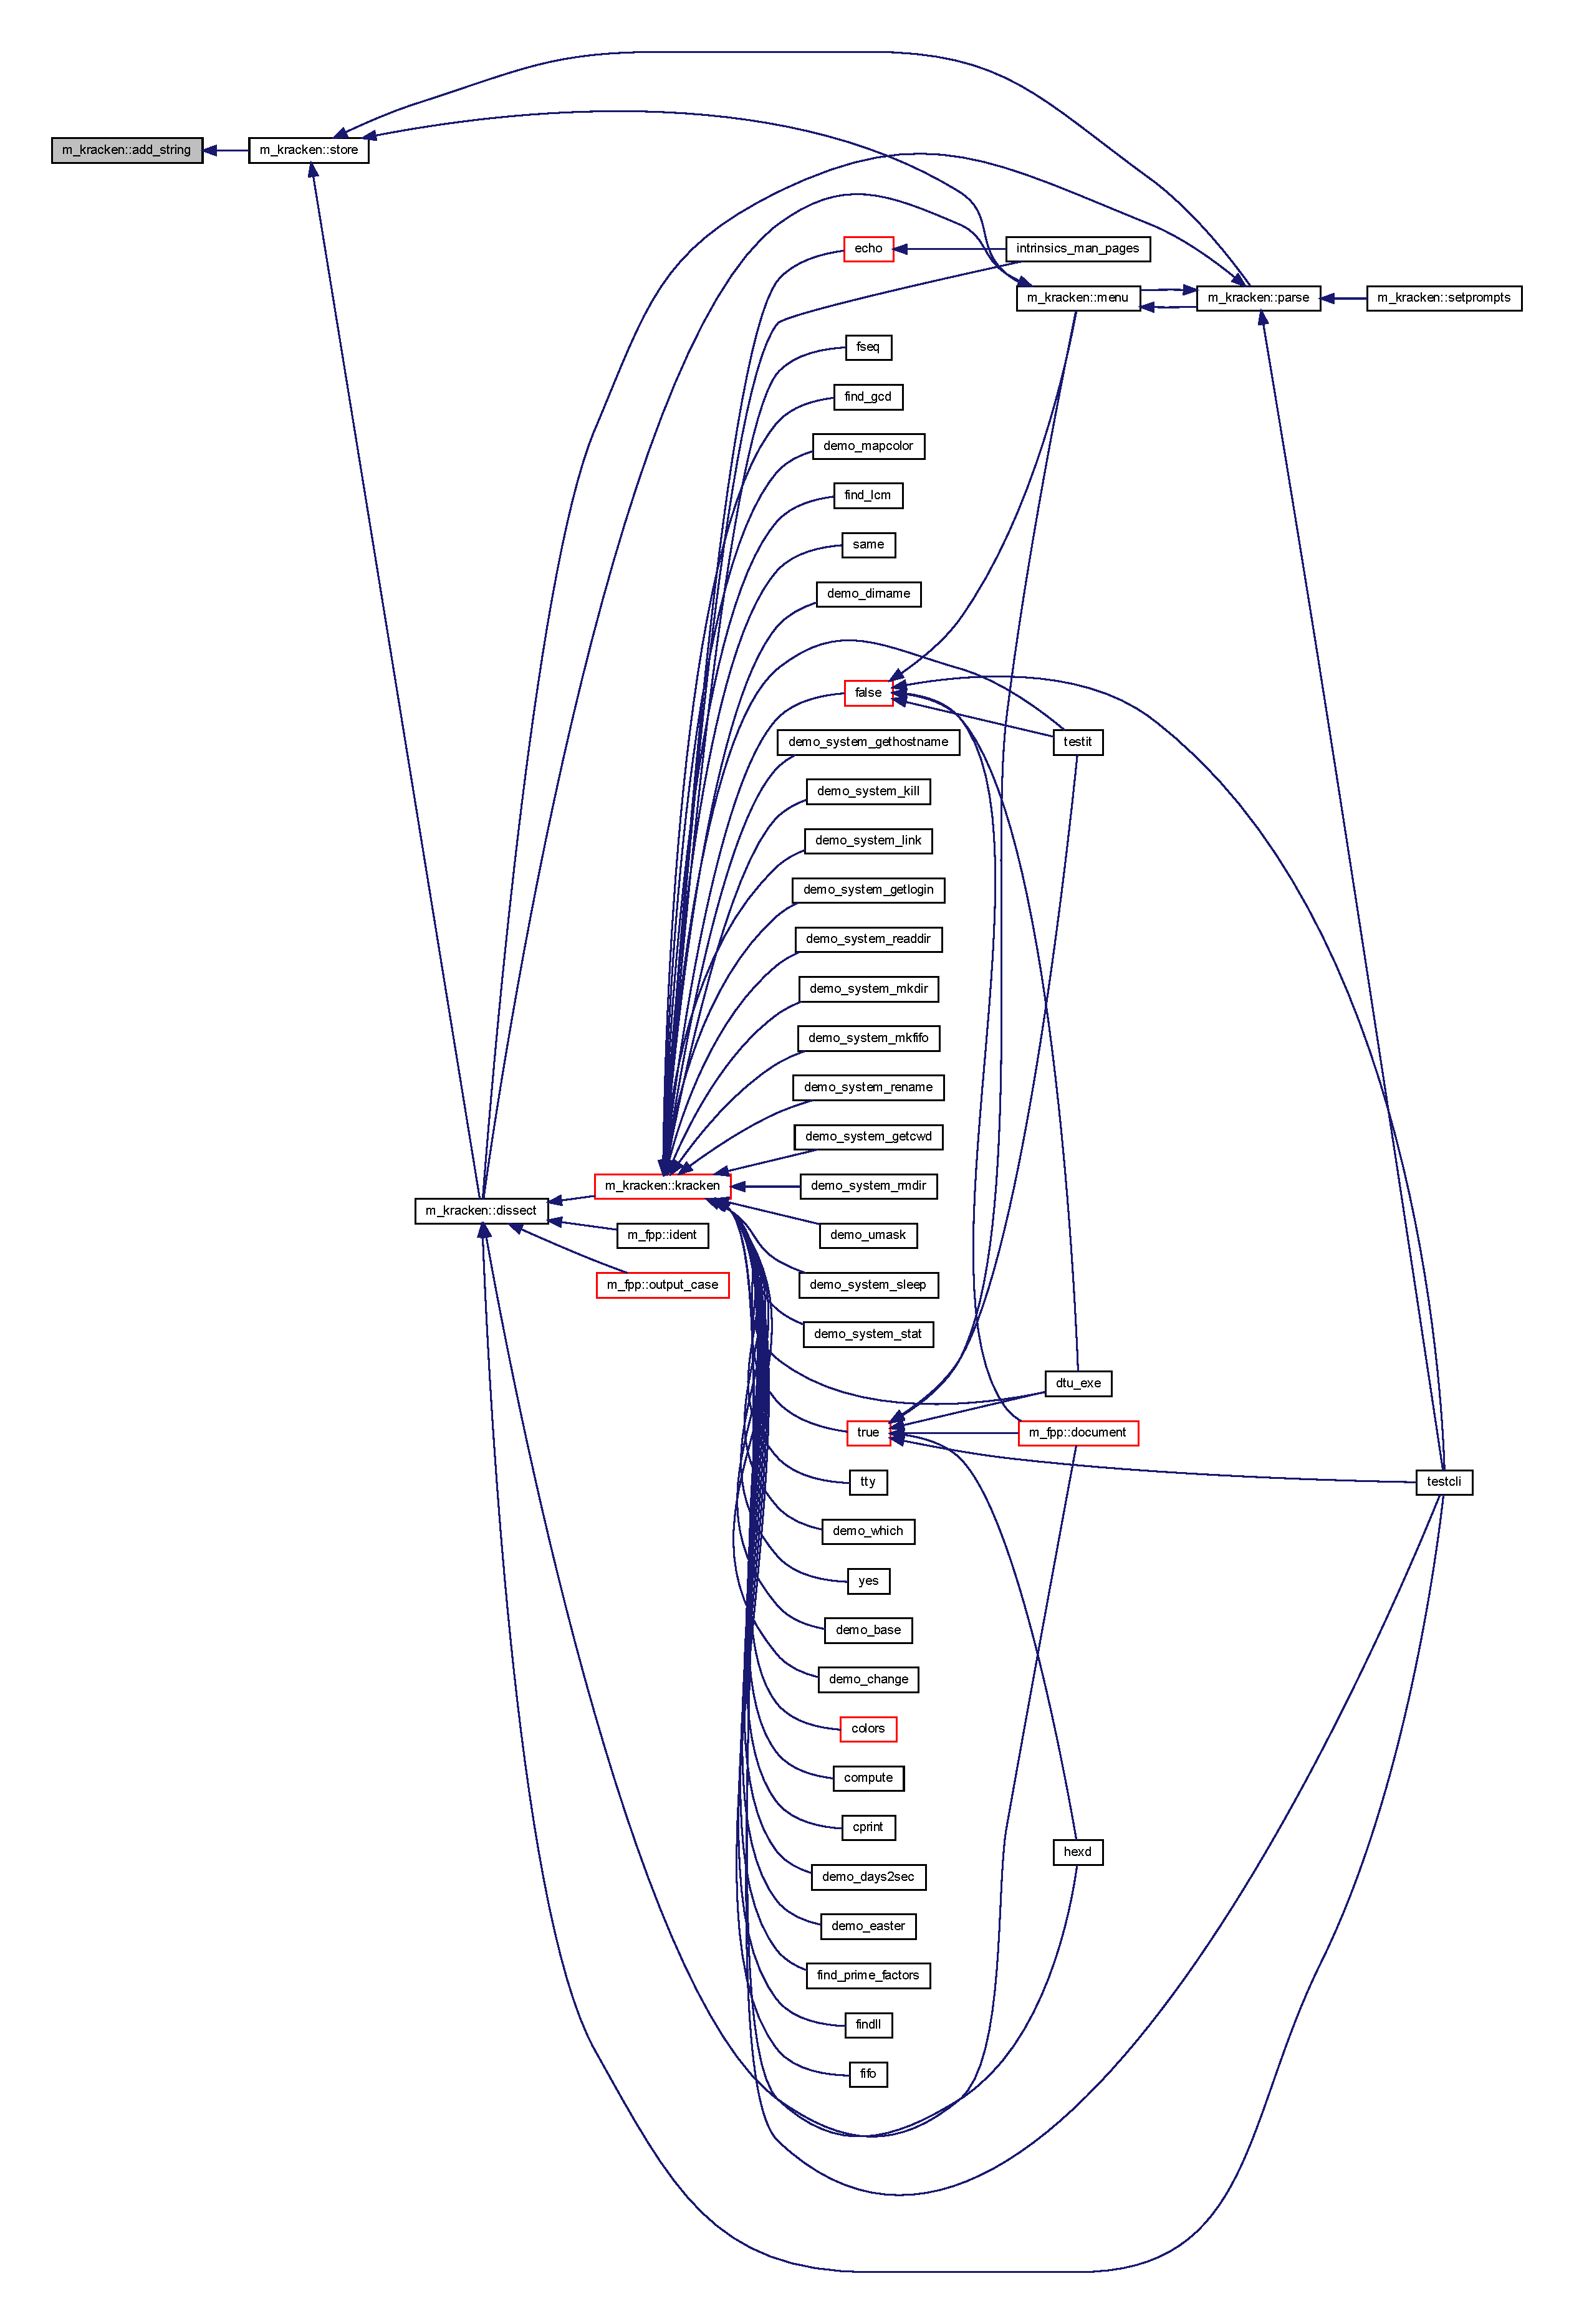
\includegraphics[width=350pt]{namespacem__kracken_a21998bf9ab683f8fb661f4f4b916c21f_icgraph}
\end{center}
\end{figure}
\mbox{\Hypertarget{namespacem__kracken_af9225957a50e8e0559605911c4c5ee02}\label{namespacem__kracken_af9225957a50e8e0559605911c4c5ee02}} 
\index{m\+\_\+kracken@{m\+\_\+kracken}!bounce@{bounce}}
\index{bounce@{bounce}!m\+\_\+kracken@{m\+\_\+kracken}}
\subsubsection{\texorpdfstring{bounce()}{bounce()}}
{\footnotesize\ttfamily \hyperlink{M__stopwatch_83_8txt_acfbcff50169d691ff02d4a123ed70482}{subroutine}, private m\+\_\+kracken\+::bounce (\begin{DoxyParamCaption}\item[{\hyperlink{option__stopwatch_83_8txt_abd4b21fbbd175834027b5224bfe97e66}{character}(len=$\ast$), intent(\hyperlink{M__journal_83_8txt_afce72651d1eed785a2132bee863b2f38}{in})}]{varnam,  }\item[{integer, intent(out)}]{index,  }\item[{\hyperlink{option__stopwatch_83_8txt_abd4b21fbbd175834027b5224bfe97e66}{character}(len=$\ast$), dimension(\+:), intent(\hyperlink{M__journal_83_8txt_afce72651d1eed785a2132bee863b2f38}{in})}]{dictionary,  }\item[{integer, intent(out)}]{ier,  }\item[{\hyperlink{option__stopwatch_83_8txt_abd4b21fbbd175834027b5224bfe97e66}{character}(len=$\ast$), intent(out)}]{mssge }\end{DoxyParamCaption})\hspace{0.3cm}{\ttfamily [private]}}



\subsubsection*{N\+A\+ME}

bounce(3fp) -\/ \mbox{[}A\+R\+G\+U\+M\+E\+N\+TS\+:M\+\_\+kracken\mbox{]} find index in Language Dictionary where V\+A\+R\+N\+AM can be found \subsubsection*{S\+Y\+N\+O\+P\+S\+IS}

subroutine bounce(varnam,index,dictionary,ier,mssge)

character(len=$\ast$),intent(in) \+:\+: varnam integer,intent(out) \+:\+: index character(len=$\ast$),dimension(\+:),intent(in) \+:\+: dictionary integer,intent(out) \+:\+: ier character(len=$\ast$),intent(out) \+:\+: mssge

\subsubsection*{D\+E\+S\+C\+R\+I\+P\+T\+I\+ON}

\subsubsection*{O\+P\+T\+I\+O\+NS}

V\+A\+R\+N\+AM variable name to look up in dictionary D\+I\+C\+T\+I\+O\+N\+A\+RY sorted dictionary array to find varnam in

\subsubsection*{R\+E\+T\+U\+R\+NS}

I\+N\+D\+EX location where variable is or should be I\+ER error code M\+S\+S\+GE message to describe error code

\subsubsection*{E\+X\+A\+M\+P\+LE}

References m\+\_\+debug\+::debug, and ipic.

Here is the caller graph for this function\+:
\nopagebreak
\begin{figure}[H]
\begin{center}
\leavevmode
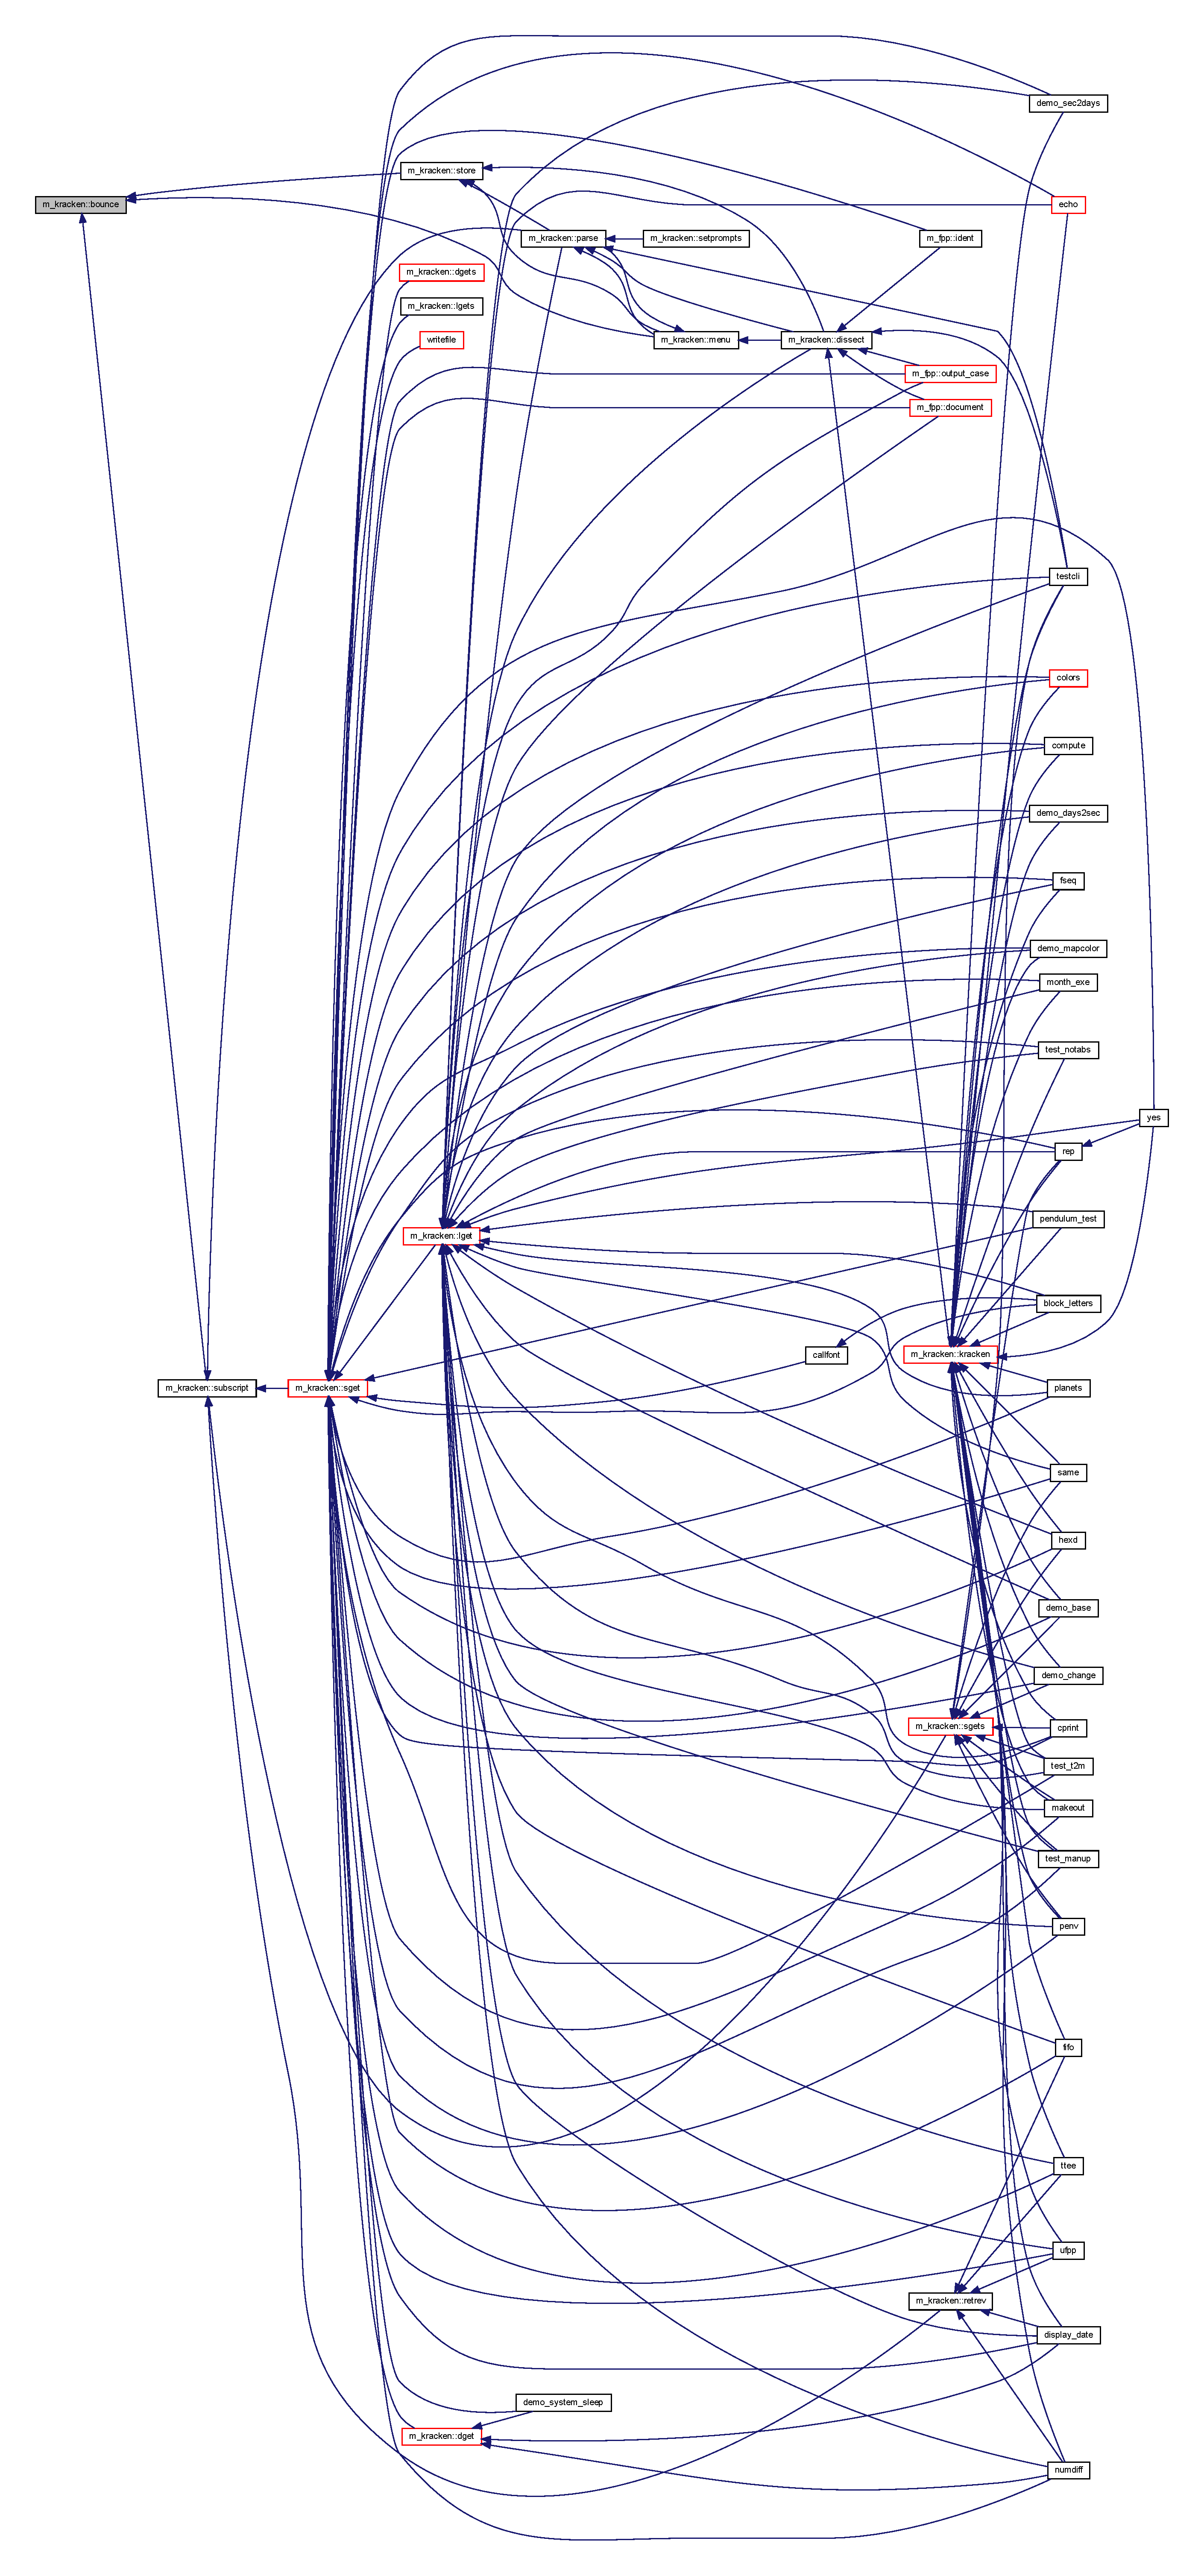
\includegraphics[height=550pt]{namespacem__kracken_af9225957a50e8e0559605911c4c5ee02_icgraph}
\end{center}
\end{figure}
\mbox{\Hypertarget{namespacem__kracken_ae7b6ad046d637f03148efb56336a7ff4}\label{namespacem__kracken_ae7b6ad046d637f03148efb56336a7ff4}} 
\index{m\+\_\+kracken@{m\+\_\+kracken}!dget@{dget}}
\index{dget@{dget}!m\+\_\+kracken@{m\+\_\+kracken}}
\subsubsection{\texorpdfstring{dget()}{dget()}}
{\footnotesize\ttfamily \hyperlink{read__watch_83_8txt_abdb62bde002f38ef75f810d3a905a823}{real}(kind=\hyperlink{namespacem__kracken_a1de91e5ca55bf4fab118936bf4fad36a}{dp}) function, \hyperlink{M__stopwatch_83_8txt_a2f74811300c361e53b430611a7d1769f}{public} m\+\_\+kracken\+::dget (\begin{DoxyParamCaption}\item[{\hyperlink{option__stopwatch_83_8txt_abd4b21fbbd175834027b5224bfe97e66}{character}(len=$\ast$), intent(\hyperlink{M__journal_83_8txt_afce72651d1eed785a2132bee863b2f38}{in})}]{keyword }\end{DoxyParamCaption})}



\subsubsection*{N\+A\+ME}

dget -\/ \mbox{[}A\+R\+G\+U\+M\+E\+N\+TS\+:M\+\_\+kracken\mbox{]} given keyword fetch doubleprecision value from command argument \subsubsection*{S\+Y\+N\+O\+P\+S\+IS}

function dget(keyword) result(value)

character(len=$\ast$),intent(in) \+:\+: keyword doubleprecision \+:\+: value \subsubsection*{D\+E\+S\+C\+R\+I\+P\+T\+I\+ON}

The dget(3f) function returns a scalar doubleprecision value from a command line argument using the M\+\_\+kracken(3fm) module. \subsubsection*{O\+P\+T\+I\+O\+NS}

K\+E\+Y\+W\+O\+RD the dictionary keyword (in form V\+E\+R\+B\+\_\+\+K\+E\+Y\+W\+O\+RD) to retrieve. The V\+E\+RB name comes from the first argument of the K\+R\+A\+C\+K\+E\+N(3f) call. The K\+E\+Y\+W\+O\+RD is a keyword from the K\+R\+A\+C\+K\+E\+N(3f) call that should be interpreted as a doubleprecision value. \subsubsection*{R\+E\+T\+U\+R\+NS}

V\+A\+L\+UE doubleprecision value returned by function \subsubsection*{E\+X\+A\+M\+P\+LE}

Sample program

program demo\+\_\+dget use M\+\_\+kracken, only\+: kracken, dget implicit none doubleprecision \+:\+: val ! define command arguments and parse user command call kracken(\textquotesingle{}demo\textquotesingle{},\textquotesingle{}-\/val 3.\+1416\textquotesingle{} ) val=dget(\textquotesingle{}demo\+\_\+val\textquotesingle{}) ! get any values specified on -\/val option write($\ast$,$\ast$)val ! print the value end program demo\+\_\+dget

Example program runs\+:

\$ demo\+\_\+dget 3.\+14159989

\$ demo\+\_\+dget -\/val 10 10.\+0000000

\$ demo\+\_\+dget -\/val 3.\+000 3.\+00000000 

References sget().

Here is the call graph for this function\+:
\nopagebreak
\begin{figure}[H]
\begin{center}
\leavevmode
\includegraphics[width=350pt]{namespacem__kracken_ae7b6ad046d637f03148efb56336a7ff4_cgraph}
\end{center}
\end{figure}
Here is the caller graph for this function\+:
\nopagebreak
\begin{figure}[H]
\begin{center}
\leavevmode
\includegraphics[height=550pt]{namespacem__kracken_ae7b6ad046d637f03148efb56336a7ff4_icgraph}
\end{center}
\end{figure}
\mbox{\Hypertarget{namespacem__kracken_a76e99048e7fb6010dcb7173ef958c932}\label{namespacem__kracken_a76e99048e7fb6010dcb7173ef958c932}} 
\index{m\+\_\+kracken@{m\+\_\+kracken}!dgets@{dgets}}
\index{dgets@{dgets}!m\+\_\+kracken@{m\+\_\+kracken}}
\subsubsection{\texorpdfstring{dgets()}{dgets()}}
{\footnotesize\ttfamily \hyperlink{read__watch_83_8txt_abdb62bde002f38ef75f810d3a905a823}{real}(kind=\hyperlink{namespacem__kracken_a1de91e5ca55bf4fab118936bf4fad36a}{dp}) function, dimension(\+:), allocatable, \hyperlink{M__stopwatch_83_8txt_a2f74811300c361e53b430611a7d1769f}{public} m\+\_\+kracken\+::dgets (\begin{DoxyParamCaption}\item[{\hyperlink{option__stopwatch_83_8txt_abd4b21fbbd175834027b5224bfe97e66}{character}(len=$\ast$), intent(\hyperlink{M__journal_83_8txt_afce72651d1eed785a2132bee863b2f38}{in})}]{keyword }\end{DoxyParamCaption})}



\subsubsection*{N\+A\+ME}

dgets -\/ \mbox{[}A\+R\+G\+U\+M\+E\+N\+TS\+:M\+\_\+kracken\mbox{]} given keyword fetch doubleprecision array from command arguments \subsubsection*{S\+Y\+N\+O\+P\+S\+IS}

function dgets(keyword) result(darray)

character(len=$\ast$),intent(in) \+:\+: keyword doubleprecision,allocatable \+:\+: D\+A\+R\+R\+AY

\subsubsection*{D\+E\+S\+C\+R\+I\+P\+T\+I\+ON}

The dgets(3f) function returns a dynamically allocated array of doubleprecision values from a string that is the value for a command line option. It is part of the M\+\_\+kracken(3fp) module.

Values that cannot be read as a numeric value are returned as a zero (0). \subsubsection*{O\+P\+T\+I\+O\+NS}

keyword dictionary name to retrieve, of form V\+E\+R\+B\+\_\+\+N\+A\+ME where V\+E\+RB is taken from the first parameter of the call to K\+R\+A\+C\+K\+E\+N(3f) or D\+I\+S\+S\+E\+C\+T(3f). \subsubsection*{R\+E\+T\+U\+R\+NS}

darray double precision numeric array returned by function \subsubsection*{E\+X\+A\+M\+P\+LE}

Sample program

program demo\+\_\+dnums use M\+\_\+kracken, only\+: kracken, dgets implicit none doubleprecision,allocatable \+:\+: vals(\+:) integer \+:\+: i ! define command arguments and parse user command call kracken(\textquotesingle{}demo\textquotesingle{},\textquotesingle{}-\/nums 1 2 3 1000 100,000 11.\+11111 77.\+77777 -\/77.\+7777\textquotesingle{} ) vals=dgets(\textquotesingle{}demo\+\_\+nums\textquotesingle{}) ! get any values specified for -\/nums write($\ast$,\textquotesingle{}($\ast$(g0\+:,\char`\"{},\char`\"{}))\textquotesingle{})( vals(i),i=1,size(vals)) ! print the values end program demo\+\_\+dnums

Example program runs\+:

\$ demo\+\_\+dnums 1.\+0000000000000000,2.\+0000000000000000,3.\+0000000000000000, 1000.\+0000000000000,100000.\+00000000000,11.\+111110000000000, 77.\+777770000000004,-\/77.\+777699999999996

\$ demo\+\_\+dnums -\/nums 89,123,456.\+789 10.\+9999999 89123456.\+789000005,10.\+999999900000001 

References sget(), and m\+\_\+strings\+::split().

Here is the call graph for this function\+:
\nopagebreak
\begin{figure}[H]
\begin{center}
\leavevmode
\includegraphics[width=350pt]{namespacem__kracken_a76e99048e7fb6010dcb7173ef958c932_cgraph}
\end{center}
\end{figure}
Here is the caller graph for this function\+:
\nopagebreak
\begin{figure}[H]
\begin{center}
\leavevmode
\includegraphics[width=350pt]{namespacem__kracken_a76e99048e7fb6010dcb7173ef958c932_icgraph}
\end{center}
\end{figure}
\mbox{\Hypertarget{namespacem__kracken_a2cb376f8a8e26e489a45cafcda66ea3e}\label{namespacem__kracken_a2cb376f8a8e26e489a45cafcda66ea3e}} 
\index{m\+\_\+kracken@{m\+\_\+kracken}!dissect@{dissect}}
\index{dissect@{dissect}!m\+\_\+kracken@{m\+\_\+kracken}}
\subsubsection{\texorpdfstring{dissect()}{dissect()}}
{\footnotesize\ttfamily \hyperlink{M__stopwatch_83_8txt_acfbcff50169d691ff02d4a123ed70482}{subroutine}, \hyperlink{M__stopwatch_83_8txt_a2f74811300c361e53b430611a7d1769f}{public} m\+\_\+kracken\+::dissect (\begin{DoxyParamCaption}\item[{\hyperlink{option__stopwatch_83_8txt_abd4b21fbbd175834027b5224bfe97e66}{character}(len=$\ast$), intent(\hyperlink{M__journal_83_8txt_afce72651d1eed785a2132bee863b2f38}{in})}]{verb,  }\item[{\hyperlink{option__stopwatch_83_8txt_abd4b21fbbd175834027b5224bfe97e66}{character}(len=$\ast$), intent(\hyperlink{M__journal_83_8txt_afce72651d1eed785a2132bee863b2f38}{in})}]{init,  }\item[{\hyperlink{option__stopwatch_83_8txt_abd4b21fbbd175834027b5224bfe97e66}{character}(len=$\ast$), intent(\hyperlink{M__journal_83_8txt_afce72651d1eed785a2132bee863b2f38}{in})}]{pars,  }\item[{integer, intent(out), \hyperlink{option__stopwatch_83_8txt_aa4ece75e7acf58a4843f70fe18c3ade5}{optional}}]{error\+\_\+return }\end{DoxyParamCaption})}



\subsubsection*{N\+A\+ME}

dissect(3f) -\/ \mbox{[}A\+R\+G\+U\+M\+E\+N\+TS\+:M\+\_\+kracken\mbox{]} convenient call to \hyperlink{namespacem__kracken_a495ed7db5c2d301c4d5e623b62a9c295}{parse()} -- define defaults, then process 

\subsubsection*{S\+Y\+N\+O\+P\+S\+IS}

subroutine dissect(verb,init,pars,error\+\_\+return)

character(len=$\ast$),intent(in) \+:\+: verb character(len=$\ast$),intent(in) \+:\+: init character(len=$\ast$),intent(in) \+:\+: pars integer,intent(out),optional \+:\+: error\+\_\+return \subsubsection*{D\+E\+S\+C\+R\+I\+P\+T\+I\+ON}

\subsubsection*{O\+P\+T\+I\+O\+NS}

V\+E\+RB the name of the command to be reset/defined I\+N\+IT used to define command options; usually hard-\/set in the program. P\+A\+RS defines the command options to be set, usually from user input

\subsubsection*{R\+E\+T\+U\+R\+NS}

E\+R\+R\+O\+R\+\_\+\+R\+E\+T\+U\+RN error code. If zero no error occurred.

\subsubsection*{E\+X\+A\+M\+P\+LE}

References m\+\_\+debug\+::debug, lget(), menu(), parse(), and store().

Here is the call graph for this function\+:
\nopagebreak
\begin{figure}[H]
\begin{center}
\leavevmode
\includegraphics[width=350pt]{namespacem__kracken_a2cb376f8a8e26e489a45cafcda66ea3e_cgraph}
\end{center}
\end{figure}
Here is the caller graph for this function\+:
\nopagebreak
\begin{figure}[H]
\begin{center}
\leavevmode
\includegraphics[height=550pt]{namespacem__kracken_a2cb376f8a8e26e489a45cafcda66ea3e_icgraph}
\end{center}
\end{figure}
\mbox{\Hypertarget{namespacem__kracken_a4c509f8594be3b73928c43c961c1caf4}\label{namespacem__kracken_a4c509f8594be3b73928c43c961c1caf4}} 
\index{m\+\_\+kracken@{m\+\_\+kracken}!get\+\_\+command\+\_\+arguments@{get\+\_\+command\+\_\+arguments}}
\index{get\+\_\+command\+\_\+arguments@{get\+\_\+command\+\_\+arguments}!m\+\_\+kracken@{m\+\_\+kracken}}
\subsubsection{\texorpdfstring{get\+\_\+command\+\_\+arguments()}{get\_command\_arguments()}}
{\footnotesize\ttfamily \hyperlink{M__stopwatch_83_8txt_acfbcff50169d691ff02d4a123ed70482}{subroutine}, private m\+\_\+kracken\+::get\+\_\+command\+\_\+arguments (\begin{DoxyParamCaption}\item[{\hyperlink{option__stopwatch_83_8txt_abd4b21fbbd175834027b5224bfe97e66}{character}(len=\+:), intent(out), allocatable}]{string,  }\item[{integer, intent(out)}]{istatus }\end{DoxyParamCaption})\hspace{0.3cm}{\ttfamily [private]}}



\subsubsection*{N\+A\+ME}

get\+\_\+command\+\_\+arguments(3fp) -\/ \mbox{[}A\+R\+G\+U\+M\+E\+N\+TS\+:M\+\_\+kracken\mbox{]} return all command arguments as an allocated string 

\subsubsection*{S\+Y\+N\+O\+P\+S\+IS}

subroutine get\+\_\+command\+\_\+arguments(string,istatus)

character(len=\+:),allocatable,intent(out) \+:\+: string integer,intent(out) \+:\+: istatus \subsubsection*{D\+E\+S\+C\+R\+I\+P\+T\+I\+ON}

\subsubsection*{R\+E\+T\+U\+R\+NS}

S\+T\+R\+I\+NG composed of all command arguments concatenated into a string I\+S\+T\+A\+T\+US status (non-\/zero means error)

\subsubsection*{E\+X\+A\+M\+P\+LE}

Sample usage if procedure is made public for debugging\+:

program testit use M\+\_\+journal, only \+: journal implicit none integer \+:\+: ier character(len=\+:),allocatable \+:\+: cmd call get\+\_\+command\+\_\+arguments(cmd,ier) write($\ast$,$\ast$)\textquotesingle{}C\+MD=\textquotesingle{},trim(cmd) write($\ast$,$\ast$)\textquotesingle{}L\+E\+N(\+C\+M\+D)=\textquotesingle{},len(cmd) write($\ast$,$\ast$)\textquotesingle{}I\+ER=\textquotesingle{},ier end program testit 

References length().

Here is the call graph for this function\+:
\nopagebreak
\begin{figure}[H]
\begin{center}
\leavevmode
\includegraphics[width=291pt]{namespacem__kracken_a4c509f8594be3b73928c43c961c1caf4_cgraph}
\end{center}
\end{figure}
Here is the caller graph for this function\+:
\nopagebreak
\begin{figure}[H]
\begin{center}
\leavevmode
\includegraphics[height=550pt]{namespacem__kracken_a4c509f8594be3b73928c43c961c1caf4_icgraph}
\end{center}
\end{figure}
\mbox{\Hypertarget{namespacem__kracken_a420718890eac378e5cd047dd0b477424}\label{namespacem__kracken_a420718890eac378e5cd047dd0b477424}} 
\index{m\+\_\+kracken@{m\+\_\+kracken}!iget@{iget}}
\index{iget@{iget}!m\+\_\+kracken@{m\+\_\+kracken}}
\subsubsection{\texorpdfstring{iget()}{iget()}}
{\footnotesize\ttfamily integer function, \hyperlink{M__stopwatch_83_8txt_a2f74811300c361e53b430611a7d1769f}{public} m\+\_\+kracken\+::iget (\begin{DoxyParamCaption}\item[{\hyperlink{option__stopwatch_83_8txt_abd4b21fbbd175834027b5224bfe97e66}{character}(len=$\ast$), intent(\hyperlink{M__journal_83_8txt_afce72651d1eed785a2132bee863b2f38}{in})}]{keyword }\end{DoxyParamCaption})}



\subsubsection*{N\+A\+ME}

iget -\/ \mbox{[}A\+R\+G\+U\+M\+E\+N\+TS\+:M\+\_\+kracken\mbox{]} given keyword fetch integer value from command argument 

\subsubsection*{S\+Y\+N\+O\+P\+S\+IS}

\begin{DoxyVerb}function iget(keyword) result(value)

 character(len=*),intent(in)  :: keyword
 integer              :: value
\end{DoxyVerb}


\subsubsection*{D\+E\+S\+C\+R\+I\+P\+T\+I\+ON}

The iget(3f) function returns a scalar integer value from a command line argument using the M\+\_\+kracken(3fm) module.

\subsubsection*{O\+P\+T\+I\+O\+NS}

K\+E\+Y\+W\+O\+RD the dictionary keyword (in form V\+E\+R\+B\+\_\+\+K\+E\+Y\+W\+O\+RD) to retrieve. The V\+E\+RB name comes from the first argument of the K\+R\+A\+C\+K\+E\+N(3f) call. The K\+E\+Y\+W\+O\+RD is a keyword from the K\+R\+A\+C\+K\+E\+N(3f) call that should be interpreted as a integer value.

\subsubsection*{R\+E\+T\+U\+R\+NS}

V\+A\+L\+UE integer value returned by function

\subsubsection*{E\+X\+A\+M\+P\+LE}

Sample program

program demo\+\_\+iget use M\+\_\+kracken, only\+: kracken, iget implicit none integer \+:\+: val ! define command arguments and parse user command call kracken(\textquotesingle{}demo\textquotesingle{},\textquotesingle{}-\/val 31416\textquotesingle{} ) val=iget(\textquotesingle{}demo\+\_\+val\textquotesingle{}) ! get any values specified on -\/val option write($\ast$,$\ast$)val ! print the value end program demo\+\_\+iget

Example program runs\+:

\$ demo\+\_\+iget 31416

\$ demo\+\_\+iget -\/val 10 10

\$ demo\+\_\+iget -\/val 3.\+000 3 

References dget().

Here is the call graph for this function\+:
\nopagebreak
\begin{figure}[H]
\begin{center}
\leavevmode
\includegraphics[width=350pt]{namespacem__kracken_a420718890eac378e5cd047dd0b477424_cgraph}
\end{center}
\end{figure}
Here is the caller graph for this function\+:
\nopagebreak
\begin{figure}[H]
\begin{center}
\leavevmode
\includegraphics[height=550pt]{namespacem__kracken_a420718890eac378e5cd047dd0b477424_icgraph}
\end{center}
\end{figure}
\mbox{\Hypertarget{namespacem__kracken_ac118bb44d855d68bfce6caa80d60e5e0}\label{namespacem__kracken_ac118bb44d855d68bfce6caa80d60e5e0}} 
\index{m\+\_\+kracken@{m\+\_\+kracken}!igets@{igets}}
\index{igets@{igets}!m\+\_\+kracken@{m\+\_\+kracken}}
\subsubsection{\texorpdfstring{igets()}{igets()}}
{\footnotesize\ttfamily integer function, dimension(\+:), allocatable, \hyperlink{M__stopwatch_83_8txt_a2f74811300c361e53b430611a7d1769f}{public} m\+\_\+kracken\+::igets (\begin{DoxyParamCaption}\item[{\hyperlink{option__stopwatch_83_8txt_abd4b21fbbd175834027b5224bfe97e66}{character}(len=$\ast$), intent(\hyperlink{M__journal_83_8txt_afce72651d1eed785a2132bee863b2f38}{in})}]{keyword }\end{DoxyParamCaption})}



\subsubsection*{N\+A\+ME}

igets -\/ \mbox{[}A\+R\+G\+U\+M\+E\+N\+TS\+:M\+\_\+kracken\mbox{]} given keyword fetch integer array from command arguments \subsubsection*{S\+Y\+N\+O\+P\+S\+IS}

function igets(keyword) result(iarray)

character(len=$\ast$),intent(in) \+:\+: keyword integer,allocatable \+:\+: iarray(\+:) \subsubsection*{D\+E\+S\+C\+R\+I\+P\+T\+I\+ON}

The igets(3f) function returns a dynamically allocated array of integers from a string that is the value for a command line option. It is part of the M\+\_\+kracken(3fp) module.

Values that cannot be read as an integer value are returned as a zero (0).

\subsubsection*{O\+P\+T\+I\+O\+NS}

K\+E\+Y\+W\+O\+RD the dictionary keyword (in form V\+E\+R\+B\+\_\+\+K\+E\+Y\+W\+O\+RD) to retrieve. The V\+E\+RB name comes from the first argument of the K\+R\+A\+C\+K\+E\+N(3f) call. The K\+E\+Y\+W\+O\+RD is a keyword from the K\+R\+A\+C\+K\+E\+N(3f) call that should be interpreted as a list of I\+N\+T\+E\+G\+ER values. Decimal values are allowed but truncated. Note that comma characters are ignored.

\subsubsection*{R\+E\+T\+U\+R\+NS}

I\+A\+R\+R\+AY I\+N\+T\+E\+G\+ER array returned by function

\subsubsection*{E\+X\+A\+M\+P\+LE}

Sample program

program demo\+\_\+inums use M\+\_\+kracken, only\+: kracken, igets implicit none integer,allocatable \+:\+: vals(\+:) integer \+:\+: i ! define command arguments and parse user command call kracken(\textquotesingle{}demo\textquotesingle{},\textquotesingle{}-\/nums 1 2 3 100 1000 10000 100,000 11.\+11111 77.\+77777 -\/77.\+7777\textquotesingle{} ) ! get any values specified for -\/nums vals=igets(\textquotesingle{}demo\+\_\+nums\textquotesingle{}) if(size(vals).gt.\+0)then ! print the requested values write($\ast$,\textquotesingle{}($\ast$(i0\+:,\char`\"{},\char`\"{}))\textquotesingle{})( vals(i),i=1,size(vals)) endif end program demo\+\_\+inums

Example program runs\+:

\$ demo\+\_\+inums 1,2,3,100,1000,10000,100000,11,77,-\/77 \$ demo\+\_\+inums -\/val 89,123,456 10.\+9999999 89123456,10 

References dgets().

Here is the call graph for this function\+:
\nopagebreak
\begin{figure}[H]
\begin{center}
\leavevmode
\includegraphics[width=350pt]{namespacem__kracken_ac118bb44d855d68bfce6caa80d60e5e0_cgraph}
\end{center}
\end{figure}
Here is the caller graph for this function\+:
\nopagebreak
\begin{figure}[H]
\begin{center}
\leavevmode
\includegraphics[width=315pt]{namespacem__kracken_ac118bb44d855d68bfce6caa80d60e5e0_icgraph}
\end{center}
\end{figure}
\mbox{\Hypertarget{namespacem__kracken_a850dce381e1cfe18a4ebcaa214995e39}\label{namespacem__kracken_a850dce381e1cfe18a4ebcaa214995e39}} 
\index{m\+\_\+kracken@{m\+\_\+kracken}!kracken@{kracken}}
\index{kracken@{kracken}!m\+\_\+kracken@{m\+\_\+kracken}}
\subsubsection{\texorpdfstring{kracken()}{kracken()}}
{\footnotesize\ttfamily \hyperlink{M__stopwatch_83_8txt_acfbcff50169d691ff02d4a123ed70482}{subroutine}, \hyperlink{M__stopwatch_83_8txt_a2f74811300c361e53b430611a7d1769f}{public} m\+\_\+kracken\+::kracken (\begin{DoxyParamCaption}\item[{\hyperlink{option__stopwatch_83_8txt_abd4b21fbbd175834027b5224bfe97e66}{character}(len=$\ast$), intent(\hyperlink{M__journal_83_8txt_afce72651d1eed785a2132bee863b2f38}{in})}]{verb,  }\item[{\hyperlink{option__stopwatch_83_8txt_abd4b21fbbd175834027b5224bfe97e66}{character}(len=$\ast$), intent(\hyperlink{M__journal_83_8txt_afce72651d1eed785a2132bee863b2f38}{in})}]{string,  }\item[{integer, intent(out), \hyperlink{option__stopwatch_83_8txt_aa4ece75e7acf58a4843f70fe18c3ade5}{optional}}]{error\+\_\+return }\end{DoxyParamCaption})}



\subsubsection*{N\+A\+ME}

kracken(3f) -\/ \mbox{[}A\+R\+G\+U\+M\+E\+N\+TS\+:M\+\_\+kracken\mbox{]} crack command line options on Fortran programs, using \char`\"{}-\/\+K\+E\+Y\+W\+O\+R\+D V\+A\+L\+U\+E\char`\"{} syntax \subsubsection*{S\+Y\+N\+O\+P\+S\+IS}

subroutine kracken(verb, string\mbox{[},ierror\mbox{]})

character(len=$\ast$), intent(in) \+:\+: verb character(len=$\ast$), intent(in) \+:\+: string integer, intent(out), optional \+:\+: ierror

\subsubsection*{D\+E\+S\+C\+R\+I\+P\+T\+I\+ON}

\begin{DoxyVerb} This is the main public procedure in the M_kracken(3f) module.
 It is used to define the command line options, their default
 values, and to crack the command line options using a syntax
 that looks very much like an execution of the program.
\end{DoxyVerb}


\subsubsection*{O\+P\+T\+I\+O\+NS}

V\+E\+RB arbitrary command name, usually \textquotesingle{}cmd\textquotesingle{} or the name of the program calling the routine. This defines the variable prefix name used by the other functions to retrieve command option values.

S\+T\+R\+I\+NG prototype command to define keywords and defaults. This string is simply a list of all keywords and their default values exactly as you would type them on the command line, with default values explicitly set.

I\+E\+R\+R\+OR If an error occurs such as an unknown keyword the calling program will be stopped unless the optional parameter I\+E\+R\+R\+OR is present. If present, it is up to the calling program to decide what to do if a non-\/zero value is returned. \subsubsection*{E\+X\+A\+M\+P\+LE}

Sample program\+: \begin{DoxyVerb}program krackenbasic

use M_kracken
! define command arguments, default values and crack command line
call kracken('cmd',              &
   &   '-int 20                  &
   &   -real 10e3                &
   &   -file input               &
   &   -dble 4.11223344556677d0  &
   &   -help    .false.          &
   &   -version .false.         '&
   &   )
! that's it. You defined your command arguments and their default
! values and parsed the user-supplied command line arguments.

! Now you can just retrieve the values as strings using
! names of the form VERB_SWITCHNAME anywhere in your program.
! Note that the special name "VERB_oo"  is for the string
! before any switch.
   if(lget('cmd_help'))then ! was -help specified?
      write(*,*)'The help text'
      stop
   endif
   if(lget('cmd_version'))then ! was -version specified?
      write(*,*)'version 1.0 20161030'
      stop
   endif
   ! convert all the remaining options to scalar values
   ! and call a procedure with the values
   call mymain(                  &
   & sget('cmd_file'),           &
   & rget('cmd_real'),           &
   & dget('cmd_dble'),           &
   & iget('cmd_int')             &
   & )
end program krackenbasic

subroutine mymain(filename,value1,value2,ivalue3)
! this routine is using conventional values and does
! not use M_kracken(3fm) module at all
implicit none
character(len=*),intent(in) :: filename
real,intent(in)             :: value1
doubleprecision,intent(in)  :: value2
integer,intent(in)          :: ivalue3
   ! just to show the command arguments have
   ! been processed echo the values
   print *, 'filename=',trim(filename)
   print *, 'values=',value1,value2,ivalue3
end subroutine mymain
\end{DoxyVerb}


expected output from \+: \char`\"{}./cmd\char`\"{} \begin{DoxyVerb}   filename=input
   values= 10000.0000  4.1122334455667700  20
\end{DoxyVerb}


expected output from \+: \char`\"{}./cmd -\/file myfile -\/int 1234\char`\"{} \begin{DoxyVerb}   filename=myfile
   values= 10000.0000  4.1122334455667700  1234 \end{DoxyVerb}
 

References m\+\_\+debug\+::debug, dissect(), and get\+\_\+command\+\_\+arguments().

Here is the call graph for this function\+:
\nopagebreak
\begin{figure}[H]
\begin{center}
\leavevmode
\includegraphics[width=350pt]{namespacem__kracken_a850dce381e1cfe18a4ebcaa214995e39_cgraph}
\end{center}
\end{figure}
\mbox{\Hypertarget{namespacem__kracken_a7141acd7a00c1a5aa5f90612a0414b63}\label{namespacem__kracken_a7141acd7a00c1a5aa5f90612a0414b63}} 
\index{m\+\_\+kracken@{m\+\_\+kracken}!lget@{lget}}
\index{lget@{lget}!m\+\_\+kracken@{m\+\_\+kracken}}
\subsubsection{\texorpdfstring{lget()}{lget()}}
{\footnotesize\ttfamily logical function, \hyperlink{M__stopwatch_83_8txt_a2f74811300c361e53b430611a7d1769f}{public} m\+\_\+kracken\+::lget (\begin{DoxyParamCaption}\item[{\hyperlink{option__stopwatch_83_8txt_abd4b21fbbd175834027b5224bfe97e66}{character}(len=$\ast$), intent(\hyperlink{M__journal_83_8txt_afce72651d1eed785a2132bee863b2f38}{in})}]{keyword }\end{DoxyParamCaption})}



\subsubsection*{N\+A\+ME}

lget -\/ \mbox{[}A\+R\+G\+U\+M\+E\+N\+TS\+:M\+\_\+kracken\mbox{]} given keyword fetch logical value from command arguments \subsubsection*{S\+Y\+N\+O\+P\+S\+IS}

function lget(keyword) result(lval)

character(len=$\ast$),intent(in) \+:\+: keyword logical \+:\+: lval \subsubsection*{D\+E\+S\+C\+R\+I\+P\+T\+I\+ON}

The lget(3f) function returns a scalar logical value from a command line argument using the M\+\_\+kracken(3fm) module.

\subsubsection*{O\+P\+T\+I\+O\+NS}

keyword the dictionary keyword (in form V\+E\+R\+B\+\_\+\+K\+E\+Y\+W\+O\+RD) to retrieve. The V\+E\+RB name comes from the first argument of the K\+R\+A\+C\+K\+E\+N(3f) call. The K\+E\+Y\+W\+O\+RD is a keyword from the second argument to the K\+R\+A\+C\+K\+E\+N(3f) call.

\subsubsection*{R\+E\+T\+U\+R\+NS}

lval logical value returned by function. The input value should be from the case-\/insensitive list of the words \char`\"{}true, false,
                t, f, yes, no, y, n, .\+false., .\+true., .\+f., .\+t\char`\"{}.

\subsubsection*{E\+X\+A\+M\+P\+LE}

Sample program\+:

program demo\+\_\+lget use M\+\_\+kracken, only\+: kracken, lget implicit none logical \+:\+: val ! define command arguments and parse user command call kracken(\textquotesingle{}demo\textquotesingle{},\textquotesingle{}-\/truth .F.\textquotesingle{} ) ! get any values specified on command line for -\/truth val=lget(\textquotesingle{}demo\+\_\+truth\textquotesingle{}) write($\ast$,\textquotesingle{}(\char`\"{}\+The truth is \char`\"{},l1)\textquotesingle{})val end program demo\+\_\+lget

Example program runs\+:

\$ demo\+\_\+lget \# uses the default The truth is F \$ demo\+\_\+lget -\/truth \# A B\+L\+A\+NK V\+A\+L\+UE IS T\+R\+UE The truth is T \$ demo\+\_\+lget -\/truth yes \# Y, yes, T, true, .T., .true. are all true The truth is T \$ demo\+\_\+lget -\/truth F \# N, no, F, false, .F., .F\+A\+L\+SE. are all false The truth is F 

References false(), sget(), true(), and m\+\_\+strings\+::upper().

Here is the call graph for this function\+:
\nopagebreak
\begin{figure}[H]
\begin{center}
\leavevmode
\includegraphics[width=350pt]{namespacem__kracken_a7141acd7a00c1a5aa5f90612a0414b63_cgraph}
\end{center}
\end{figure}
\mbox{\Hypertarget{namespacem__kracken_afb3f3b45b78625758818ea9bef463fd9}\label{namespacem__kracken_afb3f3b45b78625758818ea9bef463fd9}} 
\index{m\+\_\+kracken@{m\+\_\+kracken}!lgets@{lgets}}
\index{lgets@{lgets}!m\+\_\+kracken@{m\+\_\+kracken}}
\subsubsection{\texorpdfstring{lgets()}{lgets()}}
{\footnotesize\ttfamily logical function, dimension(\+:), allocatable, \hyperlink{M__stopwatch_83_8txt_a2f74811300c361e53b430611a7d1769f}{public} m\+\_\+kracken\+::lgets (\begin{DoxyParamCaption}\item[{\hyperlink{option__stopwatch_83_8txt_abd4b21fbbd175834027b5224bfe97e66}{character}(len=$\ast$), intent(\hyperlink{M__journal_83_8txt_afce72651d1eed785a2132bee863b2f38}{in})}]{keyword }\end{DoxyParamCaption})}



\subsubsection*{N\+A\+ME}

lget -\/ \mbox{[}A\+R\+G\+U\+M\+E\+N\+TS\+:M\+\_\+kracken\mbox{]} given keyword fetch logical array from command argument \subsubsection*{S\+Y\+N\+O\+P\+S\+IS}

function lgets(keyword) result(lvals)

character(len=$\ast$),intent(in) \+:\+: keyword logical,allocatable \+:\+: lvals(\+:) \subsubsection*{D\+E\+S\+C\+R\+I\+P\+T\+I\+ON}

The lgets(3f) function returns a dynamically allocated array of logical values from a string that is the value for a command line option. It is part of the M\+\_\+kracken(3fp) module.

Values that cannot be read as a logical value are returned as a \char`\"{}.\+F\+A\+L\+S\+E.\char`\"{}. \subsubsection*{O\+P\+T\+I\+O\+NS}

keyword the dictionary keyword (in form V\+E\+R\+B\+\_\+\+K\+E\+Y\+W\+O\+RD) to retrieve. The V\+E\+RB name comes from the first argument of the K\+R\+A\+C\+K\+E\+N(3f) call. The K\+E\+Y\+W\+O\+RD is a keyword from the second argument to the K\+R\+A\+C\+K\+E\+N(3f) call.

\subsubsection*{R\+E\+T\+U\+R\+NS}

lvals logical array returned by function. The input value should be from the case-\/insensitive list of the words \char`\"{}true, false,
                t, f, yes, no, y, n, .\+false., .\+true., .\+f., .\+t\char`\"{}.

\subsubsection*{E\+X\+A\+M\+P\+LE}

Sample program\+:

program demo\+\_\+lgets use M\+\_\+kracken, only\+: kracken, lgets implicit none logical,allocatable \+:\+: vals(\+:) ! define command arguments and parse user command call kracken(\textquotesingle{}demo\textquotesingle{},\textquotesingle{}-\/truths .F. .T. .F. .F. .T. .T.\textquotesingle{} ) ! get any values specified on command line for -\/truth vals=lgets(\textquotesingle{}demo\+\_\+truths\textquotesingle{}) write($\ast$,$\ast$)vals end program demo\+\_\+lgets

Example program runs\+:

\$ demo\+\_\+lgets F T F F T T

\$ demo\+\_\+lgets -\/truths false F .f. no true .true. t T Yes No F F F F T T T T T T F 

References false(), sget(), m\+\_\+strings\+::split(), true(), and m\+\_\+strings\+::upper().

Here is the call graph for this function\+:
\nopagebreak
\begin{figure}[H]
\begin{center}
\leavevmode
\includegraphics[width=350pt]{namespacem__kracken_afb3f3b45b78625758818ea9bef463fd9_cgraph}
\end{center}
\end{figure}
\mbox{\Hypertarget{namespacem__kracken_ad0cfac1dcc02e0a67841f546cb57f823}\label{namespacem__kracken_ad0cfac1dcc02e0a67841f546cb57f823}} 
\index{m\+\_\+kracken@{m\+\_\+kracken}!menu@{menu}}
\index{menu@{menu}!m\+\_\+kracken@{m\+\_\+kracken}}
\subsubsection{\texorpdfstring{menu()}{menu()}}
{\footnotesize\ttfamily \hyperlink{M__stopwatch_83_8txt_acfbcff50169d691ff02d4a123ed70482}{subroutine}, private m\+\_\+kracken\+::menu (\begin{DoxyParamCaption}\item[{\hyperlink{option__stopwatch_83_8txt_abd4b21fbbd175834027b5224bfe97e66}{character}(len=$\ast$), intent(\hyperlink{M__journal_83_8txt_afce72651d1eed785a2132bee863b2f38}{in})}]{verb }\end{DoxyParamCaption})\hspace{0.3cm}{\ttfamily [private]}}



\subsubsection*{N\+A\+ME}

menu(3fp) -\/ \mbox{[}A\+R\+G\+U\+M\+E\+N\+TS\+:M\+\_\+kracken\mbox{]} prompt for values using a menu interface \subsubsection*{S\+Y\+N\+O\+P\+S\+IS}

subroutine menu(verb)

character(len=$\ast$),intent(in) \+:\+: verb \subsubsection*{D\+E\+S\+C\+R\+I\+P\+T\+I\+ON}

\subsubsection*{O\+P\+T\+I\+O\+NS}

\subsubsection*{R\+E\+T\+U\+R\+NS}

\subsubsection*{E\+X\+A\+M\+P\+LE}

References bounce(), m\+\_\+debug\+::debug, dict\+\_\+lens, dict\+\_\+vals, dict\+\_\+verbs, false(), ipic, parse(), m\+\_\+strings\+::s2v(), stop\+\_\+command, store(), and true().

Here is the call graph for this function\+:
\nopagebreak
\begin{figure}[H]
\begin{center}
\leavevmode
\includegraphics[width=350pt]{namespacem__kracken_ad0cfac1dcc02e0a67841f546cb57f823_cgraph}
\end{center}
\end{figure}
Here is the caller graph for this function\+:
\nopagebreak
\begin{figure}[H]
\begin{center}
\leavevmode
\includegraphics[height=550pt]{namespacem__kracken_ad0cfac1dcc02e0a67841f546cb57f823_icgraph}
\end{center}
\end{figure}
\mbox{\Hypertarget{namespacem__kracken_a495ed7db5c2d301c4d5e623b62a9c295}\label{namespacem__kracken_a495ed7db5c2d301c4d5e623b62a9c295}} 
\index{m\+\_\+kracken@{m\+\_\+kracken}!parse@{parse}}
\index{parse@{parse}!m\+\_\+kracken@{m\+\_\+kracken}}
\subsubsection{\texorpdfstring{parse()}{parse()}}
{\footnotesize\ttfamily \hyperlink{M__stopwatch_83_8txt_acfbcff50169d691ff02d4a123ed70482}{subroutine}, \hyperlink{M__stopwatch_83_8txt_a2f74811300c361e53b430611a7d1769f}{public} m\+\_\+kracken\+::parse (\begin{DoxyParamCaption}\item[{\hyperlink{option__stopwatch_83_8txt_abd4b21fbbd175834027b5224bfe97e66}{character}(len=$\ast$), intent(\hyperlink{M__journal_83_8txt_afce72651d1eed785a2132bee863b2f38}{in})}]{verb,  }\item[{\hyperlink{option__stopwatch_83_8txt_abd4b21fbbd175834027b5224bfe97e66}{character}(len=$\ast$), intent(\hyperlink{M__journal_83_8txt_afce72651d1eed785a2132bee863b2f38}{in})}]{string,  }\item[{\hyperlink{option__stopwatch_83_8txt_abd4b21fbbd175834027b5224bfe97e66}{character}(len=$\ast$), intent(\hyperlink{M__journal_83_8txt_afce72651d1eed785a2132bee863b2f38}{in})}]{allow,  }\item[{integer, intent(out), \hyperlink{option__stopwatch_83_8txt_aa4ece75e7acf58a4843f70fe18c3ade5}{optional}}]{error\+\_\+return }\end{DoxyParamCaption})}



\subsubsection*{N\+A\+ME}

parse(3f) -\/ \mbox{[}A\+R\+G\+U\+M\+E\+N\+TS\+:M\+\_\+kracken\mbox{]} parse user command and store tokens into Language Dictionary 

\subsubsection*{S\+Y\+N\+O\+P\+S\+IS}

subroutine parse(verb,string,allow,error\+\_\+return)

character(len=$\ast$),intent(in) \+:\+: verb character(len=$\ast$),intent(in) \+:\+: string character(len=$\ast$),intent(in) \+:\+: allow integer,optional,intent(out) \+:\+: error\+\_\+return

\subsubsection*{D\+E\+S\+C\+R\+I\+P\+T\+I\+ON}

given a string of form

value -\/var value -\/var value

define variables of form

verb\+\_\+var(i) = value

--var will become verb\+\_\+\+\_\+var

o values may be in double quotes if they contain alphameric characters o a \# signifies the rest of the line is a comment o adjacent double quotes put one double quote into value o processing ends when an unquoted semi-\/colon or end of string is encountered o the variable name for the first value is verb\+\_\+init (often verb\+\_\+oo) o leading and trailing blanks are removed from values o call it once to give defaults o call it again and vars without values are set to null strings

\subsubsection*{O\+P\+T\+I\+O\+NS}

\begin{DoxyVerb}VERB          command name to process
STRING        string is character input string with first verb removed (options + other commands)
ALLOW         keyword indicating whether commands may be added or only replaced
ERROR_RETURN  error code. If zero, no error occurred
\end{DoxyVerb}


\subsubsection*{R\+E\+T\+U\+R\+NS}

\subsubsection*{E\+X\+A\+M\+P\+LE}

References current\+\_\+command\+\_\+length, m\+\_\+debug\+::debug, dict\+\_\+calls, kracken\+\_\+comment, leftover, lget(), menu(), store(), and subscript().

Here is the call graph for this function\+:
\nopagebreak
\begin{figure}[H]
\begin{center}
\leavevmode
\includegraphics[width=350pt]{namespacem__kracken_a495ed7db5c2d301c4d5e623b62a9c295_cgraph}
\end{center}
\end{figure}
Here is the caller graph for this function\+:
\nopagebreak
\begin{figure}[H]
\begin{center}
\leavevmode
\includegraphics[height=550pt]{namespacem__kracken_a495ed7db5c2d301c4d5e623b62a9c295_icgraph}
\end{center}
\end{figure}
\mbox{\Hypertarget{namespacem__kracken_ad4f3d7c793c90789b175097b433035da}\label{namespacem__kracken_ad4f3d7c793c90789b175097b433035da}} 
\index{m\+\_\+kracken@{m\+\_\+kracken}!retrev@{retrev}}
\index{retrev@{retrev}!m\+\_\+kracken@{m\+\_\+kracken}}
\subsubsection{\texorpdfstring{retrev()}{retrev()}}
{\footnotesize\ttfamily \hyperlink{M__stopwatch_83_8txt_acfbcff50169d691ff02d4a123ed70482}{subroutine}, \hyperlink{M__stopwatch_83_8txt_a2f74811300c361e53b430611a7d1769f}{public} m\+\_\+kracken\+::retrev (\begin{DoxyParamCaption}\item[{\hyperlink{option__stopwatch_83_8txt_abd4b21fbbd175834027b5224bfe97e66}{character}(len=$\ast$), intent(\hyperlink{M__journal_83_8txt_afce72651d1eed785a2132bee863b2f38}{in})}]{name,  }\item[{\hyperlink{option__stopwatch_83_8txt_abd4b21fbbd175834027b5224bfe97e66}{character}(len=$\ast$), intent(out)}]{val,  }\item[{integer, intent(out)}]{len,  }\item[{integer, intent(out)}]{ier }\end{DoxyParamCaption})}



\subsubsection*{N\+A\+ME}

R\+E\+T\+R\+E\+V(3f) -\/ \mbox{[}A\+R\+G\+U\+M\+E\+N\+TS\+:M\+\_\+kracken\mbox{]} get keyword value as a string from a command\textquotesingle{}s argument list processed by kracken(3f) 

\subsubsection*{S\+Y\+N\+O\+P\+S\+IS}

S\+U\+B\+R\+O\+U\+T\+I\+NE retrev(name, string, len, ier)

C\+H\+A\+R\+A\+C\+T\+ER(len=$\ast$),intent(in) \+:\+: name C\+H\+A\+R\+A\+C\+T\+ER(len=$\ast$),intent(out) \+:\+: string I\+N\+T\+E\+G\+ER,intent(out) \+:\+: len I\+N\+T\+E\+G\+ER,intent(out) \+:\+: ier

\subsubsection*{D\+E\+S\+C\+R\+I\+P\+T\+I\+ON}

When a command has had it\textquotesingle{}s command argument list parsed using the kracken(3f) routine the value associated with any keyword can be retrieved as a string.

\subsubsection*{O\+P\+T\+I\+O\+NS}

\begin{DoxyVerb} NAME    parameter name of form VERB_KEYWORD
 STRING  returned parameter value
 LEN     length of returned STRING
 IER     error flag. Any non-zero value means an error occurred
\end{DoxyVerb}


\subsubsection*{E\+X\+A\+M\+P\+LE}

Sample program\+:

program demo\+\_\+retrev use M\+\_\+kracken, only \+: kracken, retrev use M\+\_\+kracken, only \+: I\+Pvalue ! length of keyword value implicit none character(len=I\+Pvalue) \+:\+: val integer \+:\+: len, ier

call kracken(\textquotesingle{}demo\textquotesingle{}, \textquotesingle{} -\/value my default string\textquotesingle{}) call retrev(\textquotesingle{}demo\+\_\+value\textquotesingle{},val,len,ier) write($\ast$,\textquotesingle{}(a)\textquotesingle{})\textquotesingle{}V\+A\+L\+UE IS \textquotesingle{}//trim(val)

end program demo\+\_\+retrev

Example execution and output\+:

\$ ./demo\+\_\+retrev V\+A\+L\+UE IS my default string

\$ ./demo\+\_\+retrev -\/value use this value instead V\+A\+L\+UE IS use this value instead 

References dict\+\_\+lens, dict\+\_\+vals, and subscript().

Here is the call graph for this function\+:
\nopagebreak
\begin{figure}[H]
\begin{center}
\leavevmode
\includegraphics[width=350pt]{namespacem__kracken_ad4f3d7c793c90789b175097b433035da_cgraph}
\end{center}
\end{figure}
Here is the caller graph for this function\+:
\nopagebreak
\begin{figure}[H]
\begin{center}
\leavevmode
\includegraphics[width=281pt]{namespacem__kracken_ad4f3d7c793c90789b175097b433035da_icgraph}
\end{center}
\end{figure}
\mbox{\Hypertarget{namespacem__kracken_a21e0e40932af79430832a53bdb4de300}\label{namespacem__kracken_a21e0e40932af79430832a53bdb4de300}} 
\index{m\+\_\+kracken@{m\+\_\+kracken}!rget@{rget}}
\index{rget@{rget}!m\+\_\+kracken@{m\+\_\+kracken}}
\subsubsection{\texorpdfstring{rget()}{rget()}}
{\footnotesize\ttfamily \hyperlink{read__watch_83_8txt_abdb62bde002f38ef75f810d3a905a823}{real} function, \hyperlink{M__stopwatch_83_8txt_a2f74811300c361e53b430611a7d1769f}{public} m\+\_\+kracken\+::rget (\begin{DoxyParamCaption}\item[{\hyperlink{option__stopwatch_83_8txt_abd4b21fbbd175834027b5224bfe97e66}{character}(len=$\ast$), intent(\hyperlink{M__journal_83_8txt_afce72651d1eed785a2132bee863b2f38}{in})}]{keyword }\end{DoxyParamCaption})}



\subsubsection*{N\+A\+ME}

rget -\/ \mbox{[}A\+R\+G\+U\+M\+E\+N\+TS\+:M\+\_\+kracken\mbox{]} given keyword fetch real value from command argument \subsubsection*{S\+Y\+N\+O\+P\+S\+IS}

function rget(keyword) result(value)

character(len=$\ast$),intent(in) \+:\+: keyword real \+:\+: value \subsubsection*{D\+E\+S\+C\+R\+I\+P\+T\+I\+ON}

The rget(3f) function returns a scalar real value from a command line argument using the M\+\_\+kracken(3fm) module. \subsubsection*{O\+P\+T\+I\+O\+NS}

K\+E\+Y\+W\+O\+RD the dictionary keyword (in form V\+E\+R\+B\+\_\+\+K\+E\+Y\+W\+O\+RD) to retrieve. The V\+E\+RB name comes from the first argument of the K\+R\+A\+C\+K\+E\+N(3f) call. The K\+E\+Y\+W\+O\+RD is a keyword from the K\+R\+A\+C\+K\+E\+N(3f) call that should be interpreted as a R\+E\+AL value. \subsubsection*{R\+E\+T\+U\+R\+NS}

V\+A\+L\+UE real value returned by function \subsubsection*{E\+X\+A\+M\+P\+LE}

Sample program

program demo\+\_\+rget use M\+\_\+kracken, only\+: kracken, rget implicit none real \+:\+: val ! define command arguments and parse user command call kracken(\textquotesingle{}demo\textquotesingle{},\textquotesingle{}-\/val 3.\+1416\textquotesingle{} ) val=rget(\textquotesingle{}demo\+\_\+val\textquotesingle{}) ! get any values specified on -\/val option write($\ast$,$\ast$)val ! print the value end program demo\+\_\+rget

Example program runs\+:

\$ demo\+\_\+rget 3.\+14159989

\$ demo\+\_\+rget -\/val 10 10.\+0000000

\$ demo\+\_\+rget -\/val 3.\+000 3.\+00000000 Here is the caller graph for this function\+:
\nopagebreak
\begin{figure}[H]
\begin{center}
\leavevmode
\includegraphics[width=350pt]{namespacem__kracken_a21e0e40932af79430832a53bdb4de300_icgraph}
\end{center}
\end{figure}
\mbox{\Hypertarget{namespacem__kracken_aa1a29fad1518c15d8710d273755a17cc}\label{namespacem__kracken_aa1a29fad1518c15d8710d273755a17cc}} 
\index{m\+\_\+kracken@{m\+\_\+kracken}!rgets@{rgets}}
\index{rgets@{rgets}!m\+\_\+kracken@{m\+\_\+kracken}}
\subsubsection{\texorpdfstring{rgets()}{rgets()}}
{\footnotesize\ttfamily \hyperlink{read__watch_83_8txt_abdb62bde002f38ef75f810d3a905a823}{real} function, dimension(\+:), allocatable, \hyperlink{M__stopwatch_83_8txt_a2f74811300c361e53b430611a7d1769f}{public} m\+\_\+kracken\+::rgets (\begin{DoxyParamCaption}\item[{\hyperlink{option__stopwatch_83_8txt_abd4b21fbbd175834027b5224bfe97e66}{character}(len=$\ast$), intent(\hyperlink{M__journal_83_8txt_afce72651d1eed785a2132bee863b2f38}{in})}]{keyword }\end{DoxyParamCaption})}



\subsubsection*{N\+A\+ME}

rgets -\/ \mbox{[}A\+R\+G\+U\+M\+E\+N\+TS\+:M\+\_\+kracken\mbox{]} given keyword fetch real array from command arguments \subsubsection*{S\+Y\+N\+O\+P\+S\+IS}

function rgets(keyword) result(rarray)

character(len=$\ast$),intent(in) \+:\+: keyword real,allocatable \+:\+: rarray(\+:) \subsubsection*{D\+E\+S\+C\+R\+I\+P\+T\+I\+ON}

The rgets(3f) function returns a dynamically allocated array of real values from a string that is the value for a command line option. It is part of the M\+\_\+kracken(3fp) module.

Values that cannot be read as a numeric value are returned as a zero (0).

\subsubsection*{O\+P\+T\+I\+O\+NS}

K\+E\+Y\+W\+O\+RD the dictionary keyword (in form V\+E\+R\+B\+\_\+\+K\+E\+Y\+W\+O\+RD) to retrieve. The V\+E\+RB name comes from the first argument of the K\+R\+A\+C\+K\+E\+N(3f) call. The K\+E\+Y\+W\+O\+RD is a keyword from the K\+R\+A\+C\+K\+E\+N(3f) call that should be interpreted as a list of R\+E\+AL values.

\subsubsection*{R\+E\+T\+U\+R\+NS}

R\+A\+R\+R\+AY real array returned by function

\subsubsection*{E\+X\+A\+M\+P\+LE}

Sample program converts between Celcius and Fahrenheit

program demo\+\_\+rgets use M\+\_\+kracken, only\+: kracken, rgets implicit none real,allocatable \+:\+: val(\+:) integer \+:\+: i ! define command arguments and parse user command call kracken(\textquotesingle{}fc\textquotesingle{},\textquotesingle{}-\/F -\/C\textquotesingle{} )

! get any values specified on -\/C option val=rgets(\textquotesingle{}fc\+\_\+C\textquotesingle{}) ! test if have something to print in C ==$>$ F table if(size(val).gt.\+0)then ! print the requested values write($\ast$,\textquotesingle{}(a,t14,a)\textquotesingle{})\textquotesingle{}celsius\textquotesingle{},\textquotesingle{}fahrenheit\textquotesingle{} write($\ast$,\textquotesingle{}(f5.\+1,t14,f5.\+1)\textquotesingle{})( val(i),(val(i)+40.0)$\ast$9.0/5.\+0 -\/ 40.\+0,i=1,size(val)) endif

val=rgets(\textquotesingle{}fc\+\_\+F\textquotesingle{}) ! check for values on -\/F if(size(val).gt.\+0)then write($\ast$,\textquotesingle{}(a,t14,a)\textquotesingle{}) \textquotesingle{}fahrenheit\textquotesingle{}, \textquotesingle{}celsius\textquotesingle{} write($\ast$,\textquotesingle{}(f5.\+1,t14,f5.\+1)\textquotesingle{})(val(i),(val(i)+40.0)$\ast$5.0/9.\+0 -\/ 40.\+0,i=1,size(val)) endif end program demo\+\_\+rgets

Example program runs\+:

\% demo\+\_\+rgets -\/C -\/273.\+15 0 100 -\/40 37 celsius fahrenheit -\/273.\+15 -\/459.\+67 0.\+0 32.\+0 100.\+0 212.\+0 -\/40.\+0 -\/40.\+0 37.\+0 98.\+6

\% demo\+\_\+rgets -\/F -\/459.\+67 32 212 -\/40 98.\+6 fahrenheit celsius -\/459.\+67 -\/273.\+15 32.\+00 0.\+00 212.\+00 100.\+00 -\/40.\+00 -\/40.\+00 98.\+60 37.\+00 Here is the caller graph for this function\+:
\nopagebreak
\begin{figure}[H]
\begin{center}
\leavevmode
\includegraphics[width=350pt]{namespacem__kracken_aa1a29fad1518c15d8710d273755a17cc_icgraph}
\end{center}
\end{figure}
\mbox{\Hypertarget{namespacem__kracken_aab831b470a3107ca69833e717e95eaec}\label{namespacem__kracken_aab831b470a3107ca69833e717e95eaec}} 
\index{m\+\_\+kracken@{m\+\_\+kracken}!setprompts@{setprompts}}
\index{setprompts@{setprompts}!m\+\_\+kracken@{m\+\_\+kracken}}
\subsubsection{\texorpdfstring{setprompts()}{setprompts()}}
{\footnotesize\ttfamily \hyperlink{M__stopwatch_83_8txt_acfbcff50169d691ff02d4a123ed70482}{subroutine}, \hyperlink{M__stopwatch_83_8txt_a2f74811300c361e53b430611a7d1769f}{public} m\+\_\+kracken\+::setprompts (\begin{DoxyParamCaption}\item[{\hyperlink{option__stopwatch_83_8txt_abd4b21fbbd175834027b5224bfe97e66}{character}(len=$\ast$), intent(\hyperlink{M__journal_83_8txt_afce72651d1eed785a2132bee863b2f38}{in})}]{verb,  }\item[{\hyperlink{option__stopwatch_83_8txt_abd4b21fbbd175834027b5224bfe97e66}{character}(len=$\ast$), intent(\hyperlink{M__journal_83_8txt_afce72651d1eed785a2132bee863b2f38}{in})}]{init }\end{DoxyParamCaption})}



\subsubsection*{N\+A\+ME}

setprompts(3f) -\/ \mbox{[}A\+R\+G\+U\+M\+E\+N\+TS\+:M\+\_\+kracken\mbox{]} set explicit prompts for keywords in interactive mode \subsubsection*{S\+Y\+N\+O\+P\+S\+IS}

subroutine setprompts(verb,init)

character(len=$\ast$),intent(in)\+:\+: verb character(len=$\ast$),intent(in)\+:\+: init

\subsubsection*{D\+E\+S\+C\+R\+I\+P\+T\+I\+ON}

\begin{DoxyVerb}Optionally set prompts for interactive prompting mode.
The syntax of the call is the same as for KRACKEN(3f)/DISSECT(3f) except that prompt
strings are given instead of default values. It is called after a call to KRACKEN(3f)
or DISSECT(3f).
\end{DoxyVerb}


\subsubsection*{O\+P\+T\+I\+O\+NS}

verb name to define prompts for string to define prompts instead of values \subsubsection*{R\+E\+T\+U\+R\+NS}

\subsubsection*{E\+X\+A\+M\+P\+LE}

References parse().

Here is the call graph for this function\+:
\nopagebreak
\begin{figure}[H]
\begin{center}
\leavevmode
\includegraphics[width=350pt]{namespacem__kracken_aab831b470a3107ca69833e717e95eaec_cgraph}
\end{center}
\end{figure}
\mbox{\Hypertarget{namespacem__kracken_a9a64192326816b0b9badcc11506628ee}\label{namespacem__kracken_a9a64192326816b0b9badcc11506628ee}} 
\index{m\+\_\+kracken@{m\+\_\+kracken}!sget@{sget}}
\index{sget@{sget}!m\+\_\+kracken@{m\+\_\+kracken}}
\subsubsection{\texorpdfstring{sget()}{sget()}}
{\footnotesize\ttfamily \hyperlink{option__stopwatch_83_8txt_abd4b21fbbd175834027b5224bfe97e66}{character}(len=\+:) function, allocatable, \hyperlink{M__stopwatch_83_8txt_a2f74811300c361e53b430611a7d1769f}{public} m\+\_\+kracken\+::sget (\begin{DoxyParamCaption}\item[{\hyperlink{option__stopwatch_83_8txt_abd4b21fbbd175834027b5224bfe97e66}{character}(len=$\ast$), intent(\hyperlink{M__journal_83_8txt_afce72651d1eed785a2132bee863b2f38}{in})}]{name,  }\item[{integer, intent(out), \hyperlink{option__stopwatch_83_8txt_aa4ece75e7acf58a4843f70fe18c3ade5}{optional}}]{ilen }\end{DoxyParamCaption})}



\subsubsection*{N\+A\+ME}

sget -\/ \mbox{[}A\+R\+G\+U\+M\+E\+N\+TS\+:M\+\_\+kracken\mbox{]} given keyword fetch string value and length from command arguments \subsubsection*{S\+Y\+N\+O\+P\+S\+IS}

function sget(name,ilen) result(string)

character(len=$\ast$),intent(in) \+:\+: name ! name to look up in dictionary integer,intent(out),optional \+:\+: ilen ! length of returned output string character(len=\+:),allocatable \+:\+: string ! returned value

\subsubsection*{D\+E\+S\+C\+R\+I\+P\+T\+I\+ON}

The sget(3f) function returns a scalar character value from a command line argument using the M\+\_\+kracken(3fm) module.

\subsubsection*{O\+P\+T\+I\+O\+NS}

name the dictionary keyword (in form V\+E\+R\+B\+\_\+\+K\+E\+Y\+W\+O\+RD) to retrieve. The V\+E\+RB name comes from the first argument of the K\+R\+A\+C\+K\+E\+N(3f) call. The K\+E\+Y\+W\+O\+RD is a keyword from the second argument to the K\+R\+A\+C\+K\+E\+N(3f) call. This routine trusts that the desired name exists. A blank is returned if the name is not in the dictionary

\subsubsection*{R\+E\+T\+U\+R\+NS}

string returned string ilen optional length of returned output string

\subsubsection*{E\+X\+A\+M\+P\+LE}

Sample program\+:

program demo\+\_\+sget use M\+\_\+kracken, only\+: kracken, sget, I\+Pvalue implicit none character(len=I\+Pvalue) \+:\+: string, a, b ! define command arguments and parse user command call kracken(\textquotesingle{}demo\textquotesingle{},\textquotesingle{}-\/string This is the default -\/a A default -\/b B default\textquotesingle{} ) ! get any values specified on command line for -\/truth string=sget(\textquotesingle{}demo\+\_\+string\textquotesingle{}) a=sget(\textquotesingle{}demo\+\_\+a\textquotesingle{}) b=sget(\textquotesingle{}demo\+\_\+b\textquotesingle{}) write($\ast$,\textquotesingle{}(\char`\"{}string is \char`\"{},a\textquotesingle{})trim(string) write($\ast$,\textquotesingle{}(\char`\"{}a is \char`\"{},a\textquotesingle{})trim(a) write($\ast$,\textquotesingle{}(\char`\"{}b is \char`\"{},a\textquotesingle{})trim(b) end program demo\+\_\+sget

Example program runs\+:

\$demo\+\_\+sget string is This is the default a is A default b is B default

\$ demo\+\_\+sget -\/a A value for A -\/string new value for string -\/b B\+B\+B\+B\+B\+BB string is new value for string a is A value for A b is B\+B\+B\+B\+B\+BB 

References dict\+\_\+lens, dict\+\_\+vals, and subscript().

Here is the call graph for this function\+:
\nopagebreak
\begin{figure}[H]
\begin{center}
\leavevmode
\includegraphics[width=350pt]{namespacem__kracken_a9a64192326816b0b9badcc11506628ee_cgraph}
\end{center}
\end{figure}
Here is the caller graph for this function\+:
\nopagebreak
\begin{figure}[H]
\begin{center}
\leavevmode
\includegraphics[height=550pt]{namespacem__kracken_a9a64192326816b0b9badcc11506628ee_icgraph}
\end{center}
\end{figure}
\mbox{\Hypertarget{namespacem__kracken_a8ae60c1a9c903c8ad06ef1f95975d457}\label{namespacem__kracken_a8ae60c1a9c903c8ad06ef1f95975d457}} 
\index{m\+\_\+kracken@{m\+\_\+kracken}!sgets@{sgets}}
\index{sgets@{sgets}!m\+\_\+kracken@{m\+\_\+kracken}}
\subsubsection{\texorpdfstring{sgets()}{sgets()}}
{\footnotesize\ttfamily \hyperlink{option__stopwatch_83_8txt_abd4b21fbbd175834027b5224bfe97e66}{character}(len=\hyperlink{namespacem__kracken_a9e71724677cede703e1fb186e446349f}{ipvalue}) function, dimension(\+:), allocatable, \hyperlink{M__stopwatch_83_8txt_a2f74811300c361e53b430611a7d1769f}{public} m\+\_\+kracken\+::sgets (\begin{DoxyParamCaption}\item[{\hyperlink{option__stopwatch_83_8txt_abd4b21fbbd175834027b5224bfe97e66}{character}(len=$\ast$), intent(\hyperlink{M__journal_83_8txt_afce72651d1eed785a2132bee863b2f38}{in})}]{name,  }\item[{\hyperlink{option__stopwatch_83_8txt_abd4b21fbbd175834027b5224bfe97e66}{character}(len=$\ast$), intent(\hyperlink{M__journal_83_8txt_afce72651d1eed785a2132bee863b2f38}{in}), \hyperlink{option__stopwatch_83_8txt_aa4ece75e7acf58a4843f70fe18c3ade5}{optional}}]{delim }\end{DoxyParamCaption})}



\subsubsection*{N\+A\+ME}

sgets -\/ \mbox{[}A\+R\+G\+U\+M\+E\+N\+TS\+:M\+\_\+kracken\mbox{]} given keyword fetch string value parsed on whitespace into an array \subsubsection*{S\+Y\+N\+O\+P\+S\+IS}

function sgets(name,delim) result(strings)

character(len=$\ast$),intent(in) \+:\+: name character(len=$\ast$),intent(in),optional \+:\+: delim character(len=I\+Pvalue),allocatable \+:\+: strings(\+:)

\subsubsection*{D\+E\+S\+C\+R\+I\+P\+T\+I\+ON}

The sgets(3f) function returns a dynamically allocated array of character values from a string that is the value for a command line option. It is part of the M\+\_\+kracken(3fp) module. \subsubsection*{O\+P\+T\+I\+O\+NS}

name the dictionary keyword (in form V\+E\+R\+B\+\_\+\+K\+E\+Y\+W\+O\+RD) to retrieve. The V\+E\+RB name comes from the first argument of the K\+R\+A\+C\+K\+E\+N(3f) or D\+I\+S\+S\+E\+C\+T(3f) call. The K\+E\+Y\+W\+O\+RD is a keyword from the second argument to the K\+R\+A\+C\+K\+E\+N(3f) or D\+I\+S\+S\+E\+C\+T(3f) call. This routine trusts that the desired name exists. A blank is returned if the name is not in the dictionary. delim characters to split the string at into elements

\subsubsection*{R\+E\+T\+U\+R\+NS}

strings returned string array

\subsubsection*{E\+X\+A\+M\+P\+LE}

Sample program\+:

program demo\+\_\+sgets use M\+\_\+kracken, only \+: kracken, sgets, I\+Pvalue character(len=I\+Pvalue),allocatable \+:\+: strings(\+:) call kracken(\textquotesingle{}cmd\textquotesingle{},\textquotesingle{} -\/string This is a sentence \textquotesingle{}) strings= sgets(\char`\"{}cmd\+\_\+string\char`\"{}) ! get -\/strings words print $\ast$, \char`\"{}string=\char`\"{},(\textquotesingle{}\mbox{[}\textquotesingle{}//trim(strings(i))//\textquotesingle{}\mbox{]}\textquotesingle{},i=1,size(strings)) end program demo\+\_\+sgets

Example program execution\+: \$ xxx string=\mbox{[}This\mbox{]}\mbox{[}is\mbox{]}\mbox{[}a\mbox{]}\mbox{[}sentence\mbox{]}

\$ xxx -\/string parse this into words string=\mbox{[}parse\mbox{]}\mbox{[}this\mbox{]}\mbox{[}into\mbox{]}\mbox{[}words\mbox{]} 

References dict\+\_\+vals, m\+\_\+strings\+::split(), and subscript().

Here is the call graph for this function\+:
\nopagebreak
\begin{figure}[H]
\begin{center}
\leavevmode
\includegraphics[width=350pt]{namespacem__kracken_a8ae60c1a9c903c8ad06ef1f95975d457_cgraph}
\end{center}
\end{figure}
Here is the caller graph for this function\+:
\nopagebreak
\begin{figure}[H]
\begin{center}
\leavevmode
\includegraphics[height=550pt]{namespacem__kracken_a8ae60c1a9c903c8ad06ef1f95975d457_icgraph}
\end{center}
\end{figure}
\mbox{\Hypertarget{namespacem__kracken_ae1bb0ffb2cd28ae8cc8fade9f1988c3c}\label{namespacem__kracken_ae1bb0ffb2cd28ae8cc8fade9f1988c3c}} 
\index{m\+\_\+kracken@{m\+\_\+kracken}!show@{show}}
\index{show@{show}!m\+\_\+kracken@{m\+\_\+kracken}}
\subsubsection{\texorpdfstring{show()}{show()}}
{\footnotesize\ttfamily \hyperlink{M__stopwatch_83_8txt_acfbcff50169d691ff02d4a123ed70482}{subroutine}, \hyperlink{M__stopwatch_83_8txt_a2f74811300c361e53b430611a7d1769f}{public} m\+\_\+kracken\+::show (\begin{DoxyParamCaption}\item[{\hyperlink{option__stopwatch_83_8txt_abd4b21fbbd175834027b5224bfe97e66}{character}(len=$\ast$), intent(\hyperlink{M__journal_83_8txt_afce72651d1eed785a2132bee863b2f38}{in})}]{V\+E\+R\+B\+\_\+\+N\+A\+M\+E0,  }\item[{logical, intent(\hyperlink{M__journal_83_8txt_afce72651d1eed785a2132bee863b2f38}{in})}]{V\+E\+R\+B\+S\+\_\+\+O\+N\+LY,  }\item[{integer, intent(\hyperlink{M__journal_83_8txt_afce72651d1eed785a2132bee863b2f38}{in})}]{I\+W\+I\+D\+E0 }\end{DoxyParamCaption})}



\subsubsection*{N\+A\+ME}

show(3f) -\/ \mbox{[}A\+R\+G\+U\+M\+E\+N\+TS\+:M\+\_\+kracken\mbox{]} dump dictionary entries 

\subsubsection*{S\+Y\+N\+O\+P\+S\+IS}

subroutine show(\+V\+E\+R\+B\+\_\+\+N\+A\+M\+E0,\+V\+E\+R\+B\+S\+\_\+\+O\+N\+L\+Y,\+I\+W\+I\+D\+E0)

character(len=$\ast$),intent(in) \+:\+: V\+E\+R\+B\+\_\+\+N\+A\+M\+E0 logical,intent(in) \+:\+: V\+E\+R\+B\+S\+\_\+\+O\+N\+LY integer,intent(in) \+:\+: iwide0 \subsubsection*{D\+E\+S\+C\+R\+I\+P\+T\+I\+ON}

Write information about a command from the command dictionary or list all the command verbs in the dictionary

\subsubsection*{O\+P\+T\+I\+O\+NS}

V\+E\+R\+B\+\_\+\+N\+A\+M\+E0 verb prefix to display. Default is all V\+E\+R\+B\+S\+\_\+\+O\+N\+LY flag to show verbs only I\+W\+I\+D\+E0 if .ge. zero, how many columns wide to show just verbs

\subsubsection*{E\+X\+A\+M\+P\+LE}

References dict\+\_\+lens, dict\+\_\+vals, dict\+\_\+verbs, ipic, and ipverb.

\mbox{\Hypertarget{namespacem__kracken_a6eb597e3ca7d161933f595788d511fd7}\label{namespacem__kracken_a6eb597e3ca7d161933f595788d511fd7}} 
\index{m\+\_\+kracken@{m\+\_\+kracken}!store@{store}}
\index{store@{store}!m\+\_\+kracken@{m\+\_\+kracken}}
\subsubsection{\texorpdfstring{store()}{store()}}
{\footnotesize\ttfamily \hyperlink{M__stopwatch_83_8txt_acfbcff50169d691ff02d4a123ed70482}{subroutine}, \hyperlink{M__stopwatch_83_8txt_a2f74811300c361e53b430611a7d1769f}{public} m\+\_\+kracken\+::store (\begin{DoxyParamCaption}\item[{\hyperlink{option__stopwatch_83_8txt_abd4b21fbbd175834027b5224bfe97e66}{character}(len=$\ast$), intent(\hyperlink{M__journal_83_8txt_afce72651d1eed785a2132bee863b2f38}{in})}]{name1,  }\item[{\hyperlink{option__stopwatch_83_8txt_abd4b21fbbd175834027b5224bfe97e66}{character}(len=$\ast$), intent(\hyperlink{M__journal_83_8txt_afce72651d1eed785a2132bee863b2f38}{in})}]{value1,  }\item[{\hyperlink{option__stopwatch_83_8txt_abd4b21fbbd175834027b5224bfe97e66}{character}(len=$\ast$), intent(\hyperlink{M__journal_83_8txt_afce72651d1eed785a2132bee863b2f38}{in})}]{allow1,  }\item[{integer, intent(out)}]{ier }\end{DoxyParamCaption})}



\subsubsection*{N\+A\+ME}

store(3fp) -\/ \mbox{[}A\+R\+G\+U\+M\+E\+N\+TS\+:M\+\_\+kracken\mbox{]} add or replace dict. name\textquotesingle{}s value (if allow=\textquotesingle{}add\textquotesingle{} add name if necessary) \subsubsection*{S\+Y\+N\+O\+P\+S\+IS}

subroutine store(name1,value1,allow1,ier)

character(len=$\ast$),intent(in) \+:\+: name1 character(len=$\ast$),intent(in) \+:\+: value1 character(len=$\ast$),intent(in) \+:\+: allow1 integer,intent(out) \+:\+: ier

\subsubsection*{D\+E\+S\+C\+R\+I\+P\+T\+I\+ON}

\subsubsection*{O\+P\+T\+I\+O\+NS}

N\+A\+M\+E1 name in dictionary of form V\+E\+R\+B\+\_\+\+K\+E\+Y\+W\+O\+RD V\+A\+L\+U\+E1 value to be associated to N\+A\+M\+E1 A\+L\+L\+O\+W1 flag to allow new V\+E\+R\+B\+\_\+\+K\+E\+Y\+W\+O\+RD name being added

\subsubsection*{R\+E\+T\+U\+R\+NS}

I\+ER flag if error occurs in adding or setting value

\subsubsection*{E\+X\+A\+M\+P\+LE}

References add\+\_\+string(), bounce(), m\+\_\+debug\+::debug, dict\+\_\+calls, dict\+\_\+lens, dict\+\_\+vals, dict\+\_\+verbs, ipic, and ipverb.

Here is the call graph for this function\+:
\nopagebreak
\begin{figure}[H]
\begin{center}
\leavevmode
\includegraphics[width=324pt]{namespacem__kracken_a6eb597e3ca7d161933f595788d511fd7_cgraph}
\end{center}
\end{figure}
Here is the caller graph for this function\+:
\nopagebreak
\begin{figure}[H]
\begin{center}
\leavevmode
\includegraphics[height=550pt]{namespacem__kracken_a6eb597e3ca7d161933f595788d511fd7_icgraph}
\end{center}
\end{figure}
\mbox{\Hypertarget{namespacem__kracken_a9e2129d174220802486cc2dc7e0cc443}\label{namespacem__kracken_a9e2129d174220802486cc2dc7e0cc443}} 
\index{m\+\_\+kracken@{m\+\_\+kracken}!subscript@{subscript}}
\index{subscript@{subscript}!m\+\_\+kracken@{m\+\_\+kracken}}
\subsubsection{\texorpdfstring{subscript()}{subscript()}}
{\footnotesize\ttfamily integer function, private m\+\_\+kracken\+::subscript (\begin{DoxyParamCaption}\item[{\hyperlink{option__stopwatch_83_8txt_abd4b21fbbd175834027b5224bfe97e66}{character}(len=$\ast$), intent(\hyperlink{M__journal_83_8txt_afce72651d1eed785a2132bee863b2f38}{in})}]{chars0 }\end{DoxyParamCaption})\hspace{0.3cm}{\ttfamily [private]}}



\subsubsection*{N\+A\+ME}

subscript(3fp) -\/ \mbox{[}A\+R\+G\+U\+M\+E\+N\+TS\+:M\+\_\+kracken\mbox{]} return the subscript value of a string when given it\textquotesingle{}s name \subsubsection*{S\+Y\+N\+O\+P\+S\+IS}

function subscript(chars0)

character(len=$\ast$),intent(in) \+:\+: chars0 \subsubsection*{D\+E\+S\+C\+R\+I\+P\+T\+I\+ON}

\subsubsection*{O\+P\+T\+I\+O\+NS}

\subsubsection*{R\+E\+T\+U\+R\+NS}

\subsubsection*{E\+X\+A\+M\+P\+LE}

References bounce(), and dict\+\_\+verbs.

Here is the call graph for this function\+:
\nopagebreak
\begin{figure}[H]
\begin{center}
\leavevmode
\includegraphics[width=328pt]{namespacem__kracken_a9e2129d174220802486cc2dc7e0cc443_cgraph}
\end{center}
\end{figure}
Here is the caller graph for this function\+:
\nopagebreak
\begin{figure}[H]
\begin{center}
\leavevmode
\includegraphics[height=550pt]{namespacem__kracken_a9e2129d174220802486cc2dc7e0cc443_icgraph}
\end{center}
\end{figure}


\subsection{Variable Documentation}
\mbox{\Hypertarget{namespacem__kracken_ab43d490209ce4f08f9a2c563b1a80d9a}\label{namespacem__kracken_ab43d490209ce4f08f9a2c563b1a80d9a}} 
\index{m\+\_\+kracken@{m\+\_\+kracken}!current\+\_\+command\+\_\+length@{current\+\_\+command\+\_\+length}}
\index{current\+\_\+command\+\_\+length@{current\+\_\+command\+\_\+length}!m\+\_\+kracken@{m\+\_\+kracken}}
\subsubsection{\texorpdfstring{current\+\_\+command\+\_\+length}{current\_command\_length}}
{\footnotesize\ttfamily integer, save, \hyperlink{M__stopwatch_83_8txt_a2f74811300c361e53b430611a7d1769f}{public} m\+\_\+kracken\+::current\+\_\+command\+\_\+length =0}

\mbox{\Hypertarget{namespacem__kracken_a02bb6de9fee41e706f457133a906675e}\label{namespacem__kracken_a02bb6de9fee41e706f457133a906675e}} 
\index{m\+\_\+kracken@{m\+\_\+kracken}!dict\+\_\+calls@{dict\+\_\+calls}}
\index{dict\+\_\+calls@{dict\+\_\+calls}!m\+\_\+kracken@{m\+\_\+kracken}}
\subsubsection{\texorpdfstring{dict\+\_\+calls}{dict\_calls}}
{\footnotesize\ttfamily integer(kind=\hyperlink{namespacem__kracken_ae51c6f835203dd09fc3be239fc9d0ce1}{k\+\_\+int}), dimension(\hyperlink{namespacem__kracken_a447be9e6b10e207b63049215d9274774}{ipic}) m\+\_\+kracken\+::dict\+\_\+calls =0\hspace{0.3cm}{\ttfamily [private]}}

\mbox{\Hypertarget{namespacem__kracken_a8c7408a65bf208a0d706023a254db206}\label{namespacem__kracken_a8c7408a65bf208a0d706023a254db206}} 
\index{m\+\_\+kracken@{m\+\_\+kracken}!dict\+\_\+lens@{dict\+\_\+lens}}
\index{dict\+\_\+lens@{dict\+\_\+lens}!m\+\_\+kracken@{m\+\_\+kracken}}
\subsubsection{\texorpdfstring{dict\+\_\+lens}{dict\_lens}}
{\footnotesize\ttfamily integer(kind=\hyperlink{namespacem__kracken_ae51c6f835203dd09fc3be239fc9d0ce1}{k\+\_\+int}), dimension(\hyperlink{namespacem__kracken_a447be9e6b10e207b63049215d9274774}{ipic}) m\+\_\+kracken\+::dict\+\_\+lens =0\hspace{0.3cm}{\ttfamily [private]}}

\mbox{\Hypertarget{namespacem__kracken_a1b8cabc9e407b8d9496f6fdb5c8da911}\label{namespacem__kracken_a1b8cabc9e407b8d9496f6fdb5c8da911}} 
\index{m\+\_\+kracken@{m\+\_\+kracken}!dict\+\_\+vals@{dict\+\_\+vals}}
\index{dict\+\_\+vals@{dict\+\_\+vals}!m\+\_\+kracken@{m\+\_\+kracken}}
\subsubsection{\texorpdfstring{dict\+\_\+vals}{dict\_vals}}
{\footnotesize\ttfamily \hyperlink{option__stopwatch_83_8txt_abd4b21fbbd175834027b5224bfe97e66}{character}(len=\hyperlink{namespacem__kracken_a9e71724677cede703e1fb186e446349f}{ipvalue}), dimension(\hyperlink{namespacem__kracken_a447be9e6b10e207b63049215d9274774}{ipic}) m\+\_\+kracken\+::dict\+\_\+vals =\char`\"{} \char`\"{}\hspace{0.3cm}{\ttfamily [private]}}

\mbox{\Hypertarget{namespacem__kracken_a17809a6c9691598a268881418a993dfc}\label{namespacem__kracken_a17809a6c9691598a268881418a993dfc}} 
\index{m\+\_\+kracken@{m\+\_\+kracken}!dict\+\_\+verbs@{dict\+\_\+verbs}}
\index{dict\+\_\+verbs@{dict\+\_\+verbs}!m\+\_\+kracken@{m\+\_\+kracken}}
\subsubsection{\texorpdfstring{dict\+\_\+verbs}{dict\_verbs}}
{\footnotesize\ttfamily \hyperlink{option__stopwatch_83_8txt_abd4b21fbbd175834027b5224bfe97e66}{character}(len=\hyperlink{namespacem__kracken_adda44fb0845c3cec44bc5a5bb258b395}{ipverb}), dimension(\hyperlink{namespacem__kracken_a447be9e6b10e207b63049215d9274774}{ipic}) m\+\_\+kracken\+::dict\+\_\+verbs =\char`\"{} \char`\"{}\hspace{0.3cm}{\ttfamily [private]}}

\mbox{\Hypertarget{namespacem__kracken_a1de91e5ca55bf4fab118936bf4fad36a}\label{namespacem__kracken_a1de91e5ca55bf4fab118936bf4fad36a}} 
\index{m\+\_\+kracken@{m\+\_\+kracken}!dp@{dp}}
\index{dp@{dp}!m\+\_\+kracken@{m\+\_\+kracken}}
\subsubsection{\texorpdfstring{dp}{dp}}
{\footnotesize\ttfamily integer, parameter m\+\_\+kracken\+::dp = kind(0.d0)\hspace{0.3cm}{\ttfamily [private]}}

\mbox{\Hypertarget{namespacem__kracken_a280e9cc13c1be9621bd79a970851f3fa}\label{namespacem__kracken_a280e9cc13c1be9621bd79a970851f3fa}} 
\index{m\+\_\+kracken@{m\+\_\+kracken}!ident@{ident}}
\index{ident@{ident}!m\+\_\+kracken@{m\+\_\+kracken}}
\subsubsection{\texorpdfstring{ident}{ident}}
{\footnotesize\ttfamily \hyperlink{option__stopwatch_83_8txt_abd4b21fbbd175834027b5224bfe97e66}{character}(len=$\ast$), parameter m\+\_\+kracken\+::ident =\char`\"{}@(\#)M\+\_\+kracken(3fm)\+:parse command line options of Fortran programs using Unix-\/like syntax\char`\"{}}

\mbox{\Hypertarget{namespacem__kracken_aa2cfa3076819f58387ffb774620027c2}\label{namespacem__kracken_aa2cfa3076819f58387ffb774620027c2}} 
\index{m\+\_\+kracken@{m\+\_\+kracken}!ipcmd@{ipcmd}}
\index{ipcmd@{ipcmd}!m\+\_\+kracken@{m\+\_\+kracken}}
\subsubsection{\texorpdfstring{ipcmd}{ipcmd}}
{\footnotesize\ttfamily integer, parameter, \hyperlink{M__stopwatch_83_8txt_a2f74811300c361e53b430611a7d1769f}{public} m\+\_\+kracken\+::ipcmd =32768}

\mbox{\Hypertarget{namespacem__kracken_a447be9e6b10e207b63049215d9274774}\label{namespacem__kracken_a447be9e6b10e207b63049215d9274774}} 
\index{m\+\_\+kracken@{m\+\_\+kracken}!ipic@{ipic}}
\index{ipic@{ipic}!m\+\_\+kracken@{m\+\_\+kracken}}
\subsubsection{\texorpdfstring{ipic}{ipic}}
{\footnotesize\ttfamily integer, parameter, \hyperlink{M__stopwatch_83_8txt_a2f74811300c361e53b430611a7d1769f}{public} m\+\_\+kracken\+::ipic =4000}

\mbox{\Hypertarget{namespacem__kracken_a9e71724677cede703e1fb186e446349f}\label{namespacem__kracken_a9e71724677cede703e1fb186e446349f}} 
\index{m\+\_\+kracken@{m\+\_\+kracken}!ipvalue@{ipvalue}}
\index{ipvalue@{ipvalue}!m\+\_\+kracken@{m\+\_\+kracken}}
\subsubsection{\texorpdfstring{ipvalue}{ipvalue}}
{\footnotesize\ttfamily integer, parameter, \hyperlink{M__stopwatch_83_8txt_a2f74811300c361e53b430611a7d1769f}{public} m\+\_\+kracken\+::ipvalue =4096}

\mbox{\Hypertarget{namespacem__kracken_adda44fb0845c3cec44bc5a5bb258b395}\label{namespacem__kracken_adda44fb0845c3cec44bc5a5bb258b395}} 
\index{m\+\_\+kracken@{m\+\_\+kracken}!ipverb@{ipverb}}
\index{ipverb@{ipverb}!m\+\_\+kracken@{m\+\_\+kracken}}
\subsubsection{\texorpdfstring{ipverb}{ipverb}}
{\footnotesize\ttfamily integer, parameter, \hyperlink{M__stopwatch_83_8txt_a2f74811300c361e53b430611a7d1769f}{public} m\+\_\+kracken\+::ipverb =20}

\mbox{\Hypertarget{namespacem__kracken_a002abf985e8365e06a05ebde2f2b9b52}\label{namespacem__kracken_a002abf985e8365e06a05ebde2f2b9b52}} 
\index{m\+\_\+kracken@{m\+\_\+kracken}!k\+\_\+dbl@{k\+\_\+dbl}}
\index{k\+\_\+dbl@{k\+\_\+dbl}!m\+\_\+kracken@{m\+\_\+kracken}}
\subsubsection{\texorpdfstring{k\+\_\+dbl}{k\_dbl}}
{\footnotesize\ttfamily integer, parameter m\+\_\+kracken\+::k\+\_\+dbl = S\+E\+L\+E\+C\+T\+E\+D\+\_\+\+R\+E\+A\+L\+\_\+\+K\+I\+ND(15, 300)\hspace{0.3cm}{\ttfamily [private]}}

\mbox{\Hypertarget{namespacem__kracken_ae51c6f835203dd09fc3be239fc9d0ce1}\label{namespacem__kracken_ae51c6f835203dd09fc3be239fc9d0ce1}} 
\index{m\+\_\+kracken@{m\+\_\+kracken}!k\+\_\+int@{k\+\_\+int}}
\index{k\+\_\+int@{k\+\_\+int}!m\+\_\+kracken@{m\+\_\+kracken}}
\subsubsection{\texorpdfstring{k\+\_\+int}{k\_int}}
{\footnotesize\ttfamily integer, parameter m\+\_\+kracken\+::k\+\_\+int = S\+E\+L\+E\+C\+T\+E\+D\+\_\+\+I\+N\+T\+\_\+\+K\+I\+ND(9)\hspace{0.3cm}{\ttfamily [private]}}

\mbox{\Hypertarget{namespacem__kracken_ac26b840ca27114f5efb8fcbf48e184b4}\label{namespacem__kracken_ac26b840ca27114f5efb8fcbf48e184b4}} 
\index{m\+\_\+kracken@{m\+\_\+kracken}!kracken\+\_\+comment@{kracken\+\_\+comment}}
\index{kracken\+\_\+comment@{kracken\+\_\+comment}!m\+\_\+kracken@{m\+\_\+kracken}}
\subsubsection{\texorpdfstring{kracken\+\_\+comment}{kracken\_comment}}
{\footnotesize\ttfamily \hyperlink{option__stopwatch_83_8txt_abd4b21fbbd175834027b5224bfe97e66}{character}(len=1), save, \hyperlink{M__stopwatch_83_8txt_a2f74811300c361e53b430611a7d1769f}{public} m\+\_\+kracken\+::kracken\+\_\+comment =\textquotesingle{}\#\textquotesingle{}}

\mbox{\Hypertarget{namespacem__kracken_a012a1a99d749bbdcc4b9af483d09fec1}\label{namespacem__kracken_a012a1a99d749bbdcc4b9af483d09fec1}} 
\index{m\+\_\+kracken@{m\+\_\+kracken}!leftover@{leftover}}
\index{leftover@{leftover}!m\+\_\+kracken@{m\+\_\+kracken}}
\subsubsection{\texorpdfstring{leftover}{leftover}}
{\footnotesize\ttfamily \hyperlink{option__stopwatch_83_8txt_abd4b21fbbd175834027b5224bfe97e66}{character}(len=\hyperlink{namespacem__kracken_aa2cfa3076819f58387ffb774620027c2}{ipcmd}), \hyperlink{M__stopwatch_83_8txt_a2f74811300c361e53b430611a7d1769f}{public} m\+\_\+kracken\+::leftover =\textquotesingle{} \textquotesingle{}}

\mbox{\Hypertarget{namespacem__kracken_a89f0eab0a97826df5108b9318a7bb345}\label{namespacem__kracken_a89f0eab0a97826df5108b9318a7bb345}} 
\index{m\+\_\+kracken@{m\+\_\+kracken}!stop\+\_\+command@{stop\+\_\+command}}
\index{stop\+\_\+command@{stop\+\_\+command}!m\+\_\+kracken@{m\+\_\+kracken}}
\subsubsection{\texorpdfstring{stop\+\_\+command}{stop\_command}}
{\footnotesize\ttfamily logical, \hyperlink{M__stopwatch_83_8txt_a2f74811300c361e53b430611a7d1769f}{public} m\+\_\+kracken\+::stop\+\_\+command =.false.}


\hypertarget{namespacem__logic}{}\section{m\+\_\+logic Module Reference}
\label{namespacem__logic}\index{m\+\_\+logic@{m\+\_\+logic}}


\subsubsection*{N\+A\+ME}

cond(3f) -\/ \mbox{[}M\+\_\+logic\mbox{]}process input files with embedded if/else/elseif/endif commands  


\subsection*{Functions/\+Subroutines}
\begin{DoxyCompactItemize}
\item 
\hyperlink{M__stopwatch_83_8txt_acfbcff50169d691ff02d4a123ed70482}{subroutine}, \hyperlink{M__stopwatch_83_8txt_a2f74811300c361e53b430611a7d1769f}{public} \hyperlink{namespacem__logic_a169fe24f769ed7cd5336409c0722900e}{cond} (verb, line, ierr)
\item 
\hyperlink{M__stopwatch_83_8txt_acfbcff50169d691ff02d4a123ed70482}{subroutine}, private \hyperlink{namespacem__logic_a2229d0129ded7d8a34fce60334bc5938}{if} (line, noelse, eb)
\item 
\hyperlink{M__stopwatch_83_8txt_acfbcff50169d691ff02d4a123ed70482}{subroutine}, private \hyperlink{namespacem__logic_aa03730fb0581290fa8c776b633430584}{evalit} (line)
\item 
\hyperlink{M__stopwatch_83_8txt_acfbcff50169d691ff02d4a123ed70482}{subroutine}, private \hyperlink{namespacem__logic_ac51075acbd12f22ae97edd87352cba67}{else} (noelse, eb)
\item 
\hyperlink{M__stopwatch_83_8txt_acfbcff50169d691ff02d4a123ed70482}{subroutine}, private \hyperlink{namespacem__logic_abb56458f58725800b593e986b23ec2d3}{elseif} (line, noelse, eb)
\item 
\hyperlink{M__stopwatch_83_8txt_acfbcff50169d691ff02d4a123ed70482}{subroutine}, private \hyperlink{namespacem__logic_a60ae51929ab2f5d32f2a8f7e07e6debc}{endif} (noelse, eb)
\end{DoxyCompactItemize}
\subsection*{Variables}
\begin{DoxyCompactItemize}
\item 
\hyperlink{option__stopwatch_83_8txt_abd4b21fbbd175834027b5224bfe97e66}{character}(len= $\ast$), parameter \hyperlink{namespacem__logic_aa4a758529f4ba04d66cddf4cd51e0bc1}{ident} =\char`\"{}@(\#)M\+\_\+logic(3fm)\+: Allows if/else/elseif/endif logic to be applied to input files\char`\"{}
\item 
integer, parameter \hyperlink{namespacem__logic_a22ef0b94ebd8b7f3b35a33c8d9250759}{max\+\_\+nest\+\_\+level} =20
\item 
logical, dimension(0\+:\hyperlink{namespacem__logic_a22ef0b94ebd8b7f3b35a33c8d9250759}{max\+\_\+nest\+\_\+level}), save \hyperlink{namespacem__logic_ad7573389be889c19d1496dc2e9dff9a1}{condop}
\item 
integer \hyperlink{namespacem__logic_a047a31b5831fda2a9421240f1edce712}{ierr\+\_\+logic} =0
\item 
logical \hyperlink{namespacem__logic_ac3811d1cc267a1241feb5f77905110a2}{dc}
\item 
integer, save, \hyperlink{M__stopwatch_83_8txt_a2f74811300c361e53b430611a7d1769f}{public}, protected \hyperlink{namespacem__logic_aba076b8206140be84ad573bc89c82b14}{nest\+\_\+level} =0
\item 
logical, save, \hyperlink{M__stopwatch_83_8txt_a2f74811300c361e53b430611a7d1769f}{public}, protected \hyperlink{namespacem__logic_a487df89eac953b22a40b143aaf8ff1ea}{write} =.true.
\end{DoxyCompactItemize}


\subsection{Detailed Description}
\subsubsection*{N\+A\+ME}

cond(3f) -\/ \mbox{[}M\+\_\+logic\mbox{]}process input files with embedded if/else/elseif/endif commands 

\subsubsection*{S\+Y\+N\+O\+P\+S\+IS}

\begin{DoxyVerb} subroutine cond(verb,line,ierr)

  character(len=*),intent(in) :: verb
  character(len=*),intent(in) :: line
  integer,intent(out)         :: ierr

 Public module variables include

  WRITE -- flag whether next input line should be read
\end{DoxyVerb}


\subsubsection*{O\+P\+T\+I\+O\+NS}

\begin{DoxyVerb}  verb      must be 'if','elseif','else','endif'
  line      calculator expression to reduce to an integer.
  ierr      indicate if an error occurred
\end{DoxyVerb}


\subsubsection*{D\+E\+S\+C\+R\+I\+P\+T\+I\+ON}

\begin{DoxyVerb} Many programs read input files where input lines are conditionally skipped over. It may make sense that the data file itself
 contains the conditionals (think of pre-processors like cpp(1), shell programs (ie. interpreted languages), and configuration
 files that are read from multiple programs and from different environments). Instead of having many code-specific ways of
 specifying which lines will be processed, this module allows you to embed if/else/elseif/endif directives in the input files.

 If you pass the conditional lines to cond(3f) it sets the logical variable "WRITE" to indicate when non-conditional lines
 (blocks of lines between those logical conditions) should be skipped.

 if ierr=0, no obvious error occurred. if ierr not equal=0, suggest stopping the calling program from processing input

 The variable NEST_LEVEL should be zero at the end, or a nesting error occurred.
\end{DoxyVerb}


\subsubsection*{E\+X\+A\+M\+P\+L\+ES}

The example program uses cond(3f) and the calculator module to let you have input files that the program or the input file (via the \#define command) can set values for. Note that expressions on the \hyperlink{namespacem__logic_a2229d0129ded7d8a34fce60334bc5938}{if} and \hyperlink{namespacem__logic_abb56458f58725800b593e986b23ec2d3}{elseif} input lines are truncated to whole numbers. You need to see the calculator documentation to see all the expressions available (date and time functions, most F\+O\+R\+T\+R\+AN 77 intrinsic functions, ...)

Here is an example program that will read in a file and write just lines from the file to output that are in true blocks...

program logic use M\+\_\+journal, only \+: journal ! for logging messages use M\+\_\+strings, only \+: lower, delim,v2s ! convert character case; split string use M\+\_\+logic, only \+: cond use M\+\_\+logic, only \+: write ! flag whether current data lines should be written use M\+\_\+logic, only \+: nest\+\_\+level ! nesting level for \#\+IF/\#\+E\+L\+S\+E\+IF/\#\+E\+L\+SE/\#\+E\+N\+D\+IF use M\+\_\+calculator\+\_\+plus, only \+: rnum0 character(len=1) \+:\+: prefix ! directive prefix character character(len=1024) \+:\+: line ! input line integer,parameter \+:\+: max\+\_\+words=2 ! maximum number of words allowed on line character(len=1024) \+:\+: array(max\+\_\+words) ! working copy of input line ! location where words start and end integer \+:\+: ibegin(max\+\_\+words), iterm(max\+\_\+words) !-\/-\/-\/-\/-\/-\/-\/-\/-\/-\/-\/-\/-\/-\/-\/-\/-\/-\/-\/-\/-\/-\/-\/-\/-\/-\/-\/-\/-\/-\/-\/-\/-\/-\/-\/-\/-\/-\/-\/-\/-\/-\/-\/-\/-\/-\/-\/-\/-\/-\/-\/-\/-\/-\/-\/-\/-\/-\/-\/-\/-\/-\/-\/-\/-\/-\/-\/-\/-\/-\/-\/-\/-\/--- P\+R\+E\+F\+IX=\textquotesingle{}\#\textquotesingle{} ! for the example, assume direct lines use a \# prefix !-\/-\/-\/-\/-\/-\/-\/-\/-\/-\/-\/-\/-\/-\/-\/-\/-\/-\/-\/-\/-\/-\/-\/-\/-\/-\/-\/-\/-\/-\/-\/-\/-\/-\/-\/-\/-\/-\/-\/-\/-\/-\/-\/-\/-\/-\/-\/-\/-\/-\/-\/-\/-\/-\/-\/-\/-\/-\/-\/-\/-\/-\/-\/-\/-\/-\/-\/-\/-\/-\/-\/-\/-\/--- R\+E\+A\+D\+L\+I\+NE\+: do ! read loop to read input file read($\ast$,\textquotesingle{}(a)\textquotesingle{},iostat=ios) line if(ios.\+ne.\+0)then if (nest\+\_\+level.\+ne.\+0) then ! check to make sure all if blocks are closed call journal(\textquotesingle{}sc\textquotesingle{},\& \&\textquotesingle{}{\itshape logic} error -\/ \#\+IF B\+L\+O\+CK N\+OT C\+L\+O\+S\+ED W\+H\+EN R\+E\+A\+Di\+NG F\+I\+LE F\+I\+N\+I\+S\+H\+ED.\textquotesingle{}) endif stop endif ! although delim(3f) can do more ! just parsing the first word out and finding where second word starts ! make sure array is initialized for when ! icount(number of words on line) is zero array=\textquotesingle{} \textquotesingle{} call delim(lower(line),array,max\+\_\+words,icount,ibegin,iterm,ilen,\textquotesingle{} \textquotesingle{}) select case(array(1)) ! find conditional lines case(\textquotesingle{}\hyperlink{namespacem__logic_a2229d0129ded7d8a34fce60334bc5938}{if}\textquotesingle{},\textquotesingle{}\hyperlink{namespacem__logic_ac51075acbd12f22ae97edd87352cba67}{else}\textquotesingle{},\textquotesingle{}\hyperlink{namespacem__logic_abb56458f58725800b593e986b23ec2d3}{elseif}\textquotesingle{},\textquotesingle{}\hyperlink{namespacem__logic_a60ae51929ab2f5d32f2a8f7e07e6debc}{endif}\textquotesingle{}) ! process conditional directive call cond(trim(array(1)(2\+:)),line(iterm(1)+1\+:),ierr\+\_\+logic) case(\textquotesingle{}\#define\textquotesingle{}) ! evaluate expression value=rnum0(line(iterm(1)+1\+:)) case default ! find input lines you want to use, skip others if (write) then ! for example, if last conditional was true then write line write($\ast$,\textquotesingle{}(a)\textquotesingle{}) trim(line) ! write data line endif end select enddo R\+E\+A\+D\+L\+I\+NE end program logic

Here is an input file for the test program

$>$\#define A=10 $>$\#define B=1234.\+0 $>$\#define C=sin(30) $>$D\+E\+F\+I\+N\+ED S\+O\+ME V\+A\+L\+U\+ES A\+ND R\+E\+A\+DY TO S\+T\+A\+RT $>$\hyperlink{namespacem__logic_a2229d0129ded7d8a34fce60334bc5938}{if} eq(\+A,20) $>$ S\+H\+O\+U\+LD N\+OT BE O\+U\+T\+P\+UT $>$\hyperlink{namespacem__logic_abb56458f58725800b593e986b23ec2d3}{elseif} eq(\+A,10) $>$ C\+O\+R\+R\+E\+CT B\+R\+A\+N\+CH W\+R\+I\+TE T\+H\+IS $>$ \hyperlink{namespacem__logic_a2229d0129ded7d8a34fce60334bc5938}{if} gt(\+B,\+A) $>$ C\+O\+R\+R\+E\+CT A\+G\+A\+IN $>$ \hyperlink{namespacem__logic_ac51075acbd12f22ae97edd87352cba67}{else} $>$ S\+H\+O\+U\+LD N\+OT BE IN O\+U\+T\+P\+UT E\+I\+T\+H\+ER $>$ \hyperlink{namespacem__logic_a60ae51929ab2f5d32f2a8f7e07e6debc}{endif} $>$\hyperlink{namespacem__logic_ac51075acbd12f22ae97edd87352cba67}{else} $>$ S\+H\+O\+U\+LD N\+OT BE O\+U\+T\+P\+UT O\+N\+CE A\+G\+A\+IN $>$\hyperlink{namespacem__logic_a60ae51929ab2f5d32f2a8f7e07e6debc}{endif} $>$G\+OT TO E\+ND

The output should be

$>$D\+E\+F\+I\+N\+ED S\+O\+ME V\+A\+L\+U\+ES A\+ND R\+E\+A\+DY TO S\+T\+A\+RT $>$ C\+O\+R\+R\+E\+CT B\+R\+A\+N\+CH W\+R\+I\+TE T\+H\+IS $>$ C\+O\+R\+R\+E\+CT A\+G\+A\+IN $>$G\+OT TO E\+ND 

\subsection{Function/\+Subroutine Documentation}
\mbox{\Hypertarget{namespacem__logic_a169fe24f769ed7cd5336409c0722900e}\label{namespacem__logic_a169fe24f769ed7cd5336409c0722900e}} 
\index{m\+\_\+logic@{m\+\_\+logic}!cond@{cond}}
\index{cond@{cond}!m\+\_\+logic@{m\+\_\+logic}}
\subsubsection{\texorpdfstring{cond()}{cond()}}
{\footnotesize\ttfamily \hyperlink{M__stopwatch_83_8txt_acfbcff50169d691ff02d4a123ed70482}{subroutine}, \hyperlink{M__stopwatch_83_8txt_a2f74811300c361e53b430611a7d1769f}{public} m\+\_\+logic\+::cond (\begin{DoxyParamCaption}\item[{\hyperlink{option__stopwatch_83_8txt_abd4b21fbbd175834027b5224bfe97e66}{character}(len=$\ast$), intent(\hyperlink{M__journal_83_8txt_afce72651d1eed785a2132bee863b2f38}{in})}]{verb,  }\item[{\hyperlink{option__stopwatch_83_8txt_abd4b21fbbd175834027b5224bfe97e66}{character}(len=$\ast$), intent(\hyperlink{M__journal_83_8txt_afce72651d1eed785a2132bee863b2f38}{in})}]{line,  }\item[{integer, intent(out)}]{ierr }\end{DoxyParamCaption})}



References else(), elseif(), endif(), ierr\+\_\+logic, and if().

\mbox{\Hypertarget{namespacem__logic_ac51075acbd12f22ae97edd87352cba67}\label{namespacem__logic_ac51075acbd12f22ae97edd87352cba67}} 
\index{m\+\_\+logic@{m\+\_\+logic}!else@{else}}
\index{else@{else}!m\+\_\+logic@{m\+\_\+logic}}
\subsubsection{\texorpdfstring{else()}{else()}}
{\footnotesize\ttfamily \hyperlink{M__stopwatch_83_8txt_acfbcff50169d691ff02d4a123ed70482}{subroutine}, private m\+\_\+logic\+::else (\begin{DoxyParamCaption}\item[{integer}]{noelse,  }\item[{logical}]{eb }\end{DoxyParamCaption})\hspace{0.3cm}{\ttfamily [private]}}



References condop, false(), ierr\+\_\+logic, nest\+\_\+level, true(), and write.

\mbox{\Hypertarget{namespacem__logic_abb56458f58725800b593e986b23ec2d3}\label{namespacem__logic_abb56458f58725800b593e986b23ec2d3}} 
\index{m\+\_\+logic@{m\+\_\+logic}!elseif@{elseif}}
\index{elseif@{elseif}!m\+\_\+logic@{m\+\_\+logic}}
\subsubsection{\texorpdfstring{elseif()}{elseif()}}
{\footnotesize\ttfamily \hyperlink{M__stopwatch_83_8txt_acfbcff50169d691ff02d4a123ed70482}{subroutine}, private m\+\_\+logic\+::elseif (\begin{DoxyParamCaption}\item[{\hyperlink{option__stopwatch_83_8txt_abd4b21fbbd175834027b5224bfe97e66}{character}(len=$\ast$)}]{line,  }\item[{integer}]{noelse,  }\item[{logical}]{eb }\end{DoxyParamCaption})\hspace{0.3cm}{\ttfamily [private]}}



References condop, false(), ierr\+\_\+logic, if(), nest\+\_\+level, true(), and write.

\mbox{\Hypertarget{namespacem__logic_a60ae51929ab2f5d32f2a8f7e07e6debc}\label{namespacem__logic_a60ae51929ab2f5d32f2a8f7e07e6debc}} 
\index{m\+\_\+logic@{m\+\_\+logic}!endif@{endif}}
\index{endif@{endif}!m\+\_\+logic@{m\+\_\+logic}}
\subsubsection{\texorpdfstring{endif()}{endif()}}
{\footnotesize\ttfamily \hyperlink{M__stopwatch_83_8txt_acfbcff50169d691ff02d4a123ed70482}{subroutine}, private m\+\_\+logic\+::endif (\begin{DoxyParamCaption}\item[{integer}]{noelse,  }\item[{logical}]{eb }\end{DoxyParamCaption})\hspace{0.3cm}{\ttfamily [private]}}



References condop, else(), false(), ierr\+\_\+logic, nest\+\_\+level, true(), and write.

\mbox{\Hypertarget{namespacem__logic_aa03730fb0581290fa8c776b633430584}\label{namespacem__logic_aa03730fb0581290fa8c776b633430584}} 
\index{m\+\_\+logic@{m\+\_\+logic}!evalit@{evalit}}
\index{evalit@{evalit}!m\+\_\+logic@{m\+\_\+logic}}
\subsubsection{\texorpdfstring{evalit()}{evalit()}}
{\footnotesize\ttfamily \hyperlink{M__stopwatch_83_8txt_acfbcff50169d691ff02d4a123ed70482}{subroutine}, private m\+\_\+logic\+::evalit (\begin{DoxyParamCaption}\item[{\hyperlink{option__stopwatch_83_8txt_abd4b21fbbd175834027b5224bfe97e66}{character}(len=$\ast$), intent(\hyperlink{M__journal_83_8txt_afce72651d1eed785a2132bee863b2f38}{in})}]{line }\end{DoxyParamCaption})\hspace{0.3cm}{\ttfamily [private]}}



References dc, false(), m\+\_\+calculator\+\_\+plus\+::inum0(), and true().

\mbox{\Hypertarget{namespacem__logic_a2229d0129ded7d8a34fce60334bc5938}\label{namespacem__logic_a2229d0129ded7d8a34fce60334bc5938}} 
\index{m\+\_\+logic@{m\+\_\+logic}!if@{if}}
\index{if@{if}!m\+\_\+logic@{m\+\_\+logic}}
\subsubsection{\texorpdfstring{if()}{if()}}
{\footnotesize\ttfamily \hyperlink{M__stopwatch_83_8txt_acfbcff50169d691ff02d4a123ed70482}{subroutine}, private m\+\_\+logic\+::if (\begin{DoxyParamCaption}\item[{\hyperlink{option__stopwatch_83_8txt_abd4b21fbbd175834027b5224bfe97e66}{character}(len=$\ast$)}]{line,  }\item[{integer}]{noelse,  }\item[{logical}]{eb }\end{DoxyParamCaption})\hspace{0.3cm}{\ttfamily [private]}}



References condop, dc, evalit(), false(), ierr\+\_\+logic, max\+\_\+nest\+\_\+level, nest\+\_\+level, true(), and write.



\subsection{Variable Documentation}
\mbox{\Hypertarget{namespacem__logic_ad7573389be889c19d1496dc2e9dff9a1}\label{namespacem__logic_ad7573389be889c19d1496dc2e9dff9a1}} 
\index{m\+\_\+logic@{m\+\_\+logic}!condop@{condop}}
\index{condop@{condop}!m\+\_\+logic@{m\+\_\+logic}}
\subsubsection{\texorpdfstring{condop}{condop}}
{\footnotesize\ttfamily logical, dimension(0\+:\hyperlink{namespacem__logic_a22ef0b94ebd8b7f3b35a33c8d9250759}{max\+\_\+nest\+\_\+level}), save m\+\_\+logic\+::condop\hspace{0.3cm}{\ttfamily [private]}}

\mbox{\Hypertarget{namespacem__logic_ac3811d1cc267a1241feb5f77905110a2}\label{namespacem__logic_ac3811d1cc267a1241feb5f77905110a2}} 
\index{m\+\_\+logic@{m\+\_\+logic}!dc@{dc}}
\index{dc@{dc}!m\+\_\+logic@{m\+\_\+logic}}
\subsubsection{\texorpdfstring{dc}{dc}}
{\footnotesize\ttfamily logical m\+\_\+logic\+::dc\hspace{0.3cm}{\ttfamily [private]}}

\mbox{\Hypertarget{namespacem__logic_aa4a758529f4ba04d66cddf4cd51e0bc1}\label{namespacem__logic_aa4a758529f4ba04d66cddf4cd51e0bc1}} 
\index{m\+\_\+logic@{m\+\_\+logic}!ident@{ident}}
\index{ident@{ident}!m\+\_\+logic@{m\+\_\+logic}}
\subsubsection{\texorpdfstring{ident}{ident}}
{\footnotesize\ttfamily \hyperlink{option__stopwatch_83_8txt_abd4b21fbbd175834027b5224bfe97e66}{character}(len=$\ast$), parameter m\+\_\+logic\+::ident =\char`\"{}@(\#)M\+\_\+logic(3fm)\+: Allows if/else/elseif/endif logic to be applied to input files\char`\"{}\hspace{0.3cm}{\ttfamily [private]}}

\mbox{\Hypertarget{namespacem__logic_a047a31b5831fda2a9421240f1edce712}\label{namespacem__logic_a047a31b5831fda2a9421240f1edce712}} 
\index{m\+\_\+logic@{m\+\_\+logic}!ierr\+\_\+logic@{ierr\+\_\+logic}}
\index{ierr\+\_\+logic@{ierr\+\_\+logic}!m\+\_\+logic@{m\+\_\+logic}}
\subsubsection{\texorpdfstring{ierr\+\_\+logic}{ierr\_logic}}
{\footnotesize\ttfamily integer m\+\_\+logic\+::ierr\+\_\+logic =0\hspace{0.3cm}{\ttfamily [private]}}

\mbox{\Hypertarget{namespacem__logic_a22ef0b94ebd8b7f3b35a33c8d9250759}\label{namespacem__logic_a22ef0b94ebd8b7f3b35a33c8d9250759}} 
\index{m\+\_\+logic@{m\+\_\+logic}!max\+\_\+nest\+\_\+level@{max\+\_\+nest\+\_\+level}}
\index{max\+\_\+nest\+\_\+level@{max\+\_\+nest\+\_\+level}!m\+\_\+logic@{m\+\_\+logic}}
\subsubsection{\texorpdfstring{max\+\_\+nest\+\_\+level}{max\_nest\_level}}
{\footnotesize\ttfamily integer, parameter m\+\_\+logic\+::max\+\_\+nest\+\_\+level =20\hspace{0.3cm}{\ttfamily [private]}}

\mbox{\Hypertarget{namespacem__logic_aba076b8206140be84ad573bc89c82b14}\label{namespacem__logic_aba076b8206140be84ad573bc89c82b14}} 
\index{m\+\_\+logic@{m\+\_\+logic}!nest\+\_\+level@{nest\+\_\+level}}
\index{nest\+\_\+level@{nest\+\_\+level}!m\+\_\+logic@{m\+\_\+logic}}
\subsubsection{\texorpdfstring{nest\+\_\+level}{nest\_level}}
{\footnotesize\ttfamily integer, save, \hyperlink{M__stopwatch_83_8txt_a2f74811300c361e53b430611a7d1769f}{public}, protected m\+\_\+logic\+::nest\+\_\+level =0}

\mbox{\Hypertarget{namespacem__logic_a487df89eac953b22a40b143aaf8ff1ea}\label{namespacem__logic_a487df89eac953b22a40b143aaf8ff1ea}} 
\index{m\+\_\+logic@{m\+\_\+logic}!write@{write}}
\index{write@{write}!m\+\_\+logic@{m\+\_\+logic}}
\subsubsection{\texorpdfstring{write}{write}}
{\footnotesize\ttfamily logical, save, \hyperlink{M__stopwatch_83_8txt_a2f74811300c361e53b430611a7d1769f}{public}, protected m\+\_\+logic\+::write =.true.}


\hypertarget{namespacem__manup}{}\section{m\+\_\+manup Module Reference}
\label{namespacem__manup}\index{m\+\_\+manup@{m\+\_\+manup}}
\subsection*{Functions/\+Subroutines}
\begin{DoxyCompactItemize}
\item 
\hyperlink{M__stopwatch_83_8txt_acfbcff50169d691ff02d4a123ed70482}{subroutine}, \hyperlink{M__stopwatch_83_8txt_a2f74811300c361e53b430611a7d1769f}{public} \hyperlink{namespacem__manup_a2d0a043fa0f6b2ca01e2eb4747ef4bbd}{manup} (table, \hyperlink{print__watch_83_8txt_a15b5bd21156bb9fca6a755ab8c029a9c}{title}, section, product)
\end{DoxyCompactItemize}


\subsection{Function/\+Subroutine Documentation}
\mbox{\Hypertarget{namespacem__manup_a2d0a043fa0f6b2ca01e2eb4747ef4bbd}\label{namespacem__manup_a2d0a043fa0f6b2ca01e2eb4747ef4bbd}} 
\index{m\+\_\+manup@{m\+\_\+manup}!manup@{manup}}
\index{manup@{manup}!m\+\_\+manup@{m\+\_\+manup}}
\subsubsection{\texorpdfstring{manup()}{manup()}}
{\footnotesize\ttfamily \hyperlink{M__stopwatch_83_8txt_acfbcff50169d691ff02d4a123ed70482}{subroutine}, \hyperlink{M__stopwatch_83_8txt_a2f74811300c361e53b430611a7d1769f}{public} m\+\_\+manup\+::manup (\begin{DoxyParamCaption}\item[{\hyperlink{option__stopwatch_83_8txt_abd4b21fbbd175834027b5224bfe97e66}{character}(len=$\ast$), dimension(\+:), intent(\hyperlink{M__journal_83_8txt_afce72651d1eed785a2132bee863b2f38}{in})}]{table,  }\item[{\hyperlink{option__stopwatch_83_8txt_abd4b21fbbd175834027b5224bfe97e66}{character}(len=$\ast$), intent(\hyperlink{M__journal_83_8txt_afce72651d1eed785a2132bee863b2f38}{in})}]{title,  }\item[{integer, intent(\hyperlink{M__journal_83_8txt_afce72651d1eed785a2132bee863b2f38}{in})}]{section,  }\item[{\hyperlink{option__stopwatch_83_8txt_abd4b21fbbd175834027b5224bfe97e66}{character}(len=$\ast$), intent(\hyperlink{M__journal_83_8txt_afce72651d1eed785a2132bee863b2f38}{in})}]{product }\end{DoxyParamCaption})}



References m\+\_\+strings\+::indent(), m\+\_\+strings\+::notabs(), m\+\_\+time\+::now(), printname(), printsynopsis(), putline(), m\+\_\+strings\+::s2v(), sh(), m\+\_\+strings\+::substitute(), th(), and m\+\_\+strings\+::upper().


\hypertarget{namespacem__math}{}\section{m\+\_\+math Module Reference}
\label{namespacem__math}\index{m\+\_\+math@{m\+\_\+math}}
\subsection*{Data Types}
\begin{DoxyCompactItemize}
\item 
interface \hyperlink{interfacem__math_1_1invert__2x2}{invert\+\_\+2x2}
\begin{DoxyCompactList}\small\item\em \subsubsection*{N\+A\+ME}

invert\+\_\+2x2(3f) -\/ \mbox{[}M\+\_\+math\mbox{]} directly invert 2x2 matrix \end{DoxyCompactList}\item 
interface \hyperlink{interfacem__math_1_1invert__3x3}{invert\+\_\+3x3}
\begin{DoxyCompactList}\small\item\em \subsubsection*{N\+A\+ME}\end{DoxyCompactList}\item 
interface \hyperlink{interfacem__math_1_1invert__4x4}{invert\+\_\+4x4}
\begin{DoxyCompactList}\small\item\em \subsubsection*{N\+A\+ME}

invert\+\_\+4x4(3f) -\/ \mbox{[}M\+\_\+math\mbox{]} directly invert 4x4 matrix \end{DoxyCompactList}\end{DoxyCompactItemize}
\subsection*{Functions/\+Subroutines}
\begin{DoxyCompactItemize}
\item 
\hyperlink{M__stopwatch_83_8txt_acfbcff50169d691ff02d4a123ed70482}{subroutine}, \hyperlink{M__stopwatch_83_8txt_a2f74811300c361e53b430611a7d1769f}{public} \hyperlink{namespacem__math_ae78c38ba0be037a58cace0da51c7a8ca}{julfit} (x, y, ixn, itype, a, b, r2)
\begin{DoxyCompactList}\small\item\em \subsubsection*{N\+A\+ME}

julfit(3f) -\/ \mbox{[}M\+\_\+math\+:fit\mbox{]} linear least squares curve fits , destroys input arrays \end{DoxyCompactList}\item 
\hyperlink{M__stopwatch_83_8txt_acfbcff50169d691ff02d4a123ed70482}{subroutine}, \hyperlink{M__stopwatch_83_8txt_a2f74811300c361e53b430611a7d1769f}{public} \hyperlink{namespacem__math_a9a1a7478c87dda7eb126127970f70b7b}{julfit1} (x, y, ixn, a, b, r2)
\begin{DoxyCompactList}\small\item\em \subsubsection*{N\+A\+ME}

julfit1(3f) -\/ \mbox{[}M\+\_\+math\+:fit\mbox{]} internal routine for linear least square fit(y=a$\ast$x+b), changes the y array \subsubsection*{S\+Y\+N\+O\+P\+S\+IS}\end{DoxyCompactList}\item 
\hyperlink{M__stopwatch_83_8txt_acfbcff50169d691ff02d4a123ed70482}{subroutine}, \hyperlink{M__stopwatch_83_8txt_a2f74811300c361e53b430611a7d1769f}{public} \hyperlink{namespacem__math_a8e38b0954bb4c1f27985fb430912f281}{lowess} (x, y, n, f, nsteps, delta, ys, rw, res)
\begin{DoxyCompactList}\small\item\em \subsubsection*{N\+A\+ME}

lowess(3f) -\/ \mbox{[}M\+\_\+math\+:fit\mbox{]} procedures for locally weighted regression \end{DoxyCompactList}\item 
\hyperlink{M__stopwatch_83_8txt_acfbcff50169d691ff02d4a123ed70482}{subroutine} \hyperlink{namespacem__math_a06b587e00199906f1f87f1a7b101d71f}{lowest} (x, y, n, xs, ys, nleft, nright, w, userw, rw, ok)
\item 
\hyperlink{M__stopwatch_83_8txt_acfbcff50169d691ff02d4a123ed70482}{subroutine}, \hyperlink{M__stopwatch_83_8txt_a2f74811300c361e53b430611a7d1769f}{public} \hyperlink{namespacem__math_a94f09a43f1a68e7971e12ace802dfcc0}{splift} (\hyperlink{intro__blas1_83_8txt_ac8596739bc875e90fe6e2ecf98e87906}{X}, Y, YP, Y\+PP, N, ierr, a1, b1, an, bn)
\begin{DoxyCompactList}\small\item\em \subsubsection*{N\+A\+ME}

splift(3f) -\/ \mbox{[}M\+\_\+math\+:fit\mbox{]} fits a spline to the n data points given in x and y and also returns first and second derivatives \subsubsection*{S\+Y\+N\+O\+P\+S\+IS}\end{DoxyCompactList}\item 
\hyperlink{M__stopwatch_83_8txt_acfbcff50169d691ff02d4a123ed70482}{subroutine}, \hyperlink{M__stopwatch_83_8txt_a2f74811300c361e53b430611a7d1769f}{public} \hyperlink{namespacem__math_afb412a273368e2814058a8fc4197ba1a}{splint} (x, y, ypp, n, xi, yi, ypi, yppi, ni, kerr)
\begin{DoxyCompactList}\small\item\em \subsubsection*{N\+A\+ME}

splint(3f) -\/ \mbox{[}M\+\_\+math\+:fit\mbox{]} interpolates and twice differentiates a cubic spline \subsubsection*{S\+Y\+N\+O\+P\+S\+IS}\end{DoxyCompactList}\item 
\hyperlink{M__stopwatch_83_8txt_acfbcff50169d691ff02d4a123ed70482}{subroutine}, \hyperlink{M__stopwatch_83_8txt_a2f74811300c361e53b430611a7d1769f}{public} \hyperlink{namespacem__math_a506d6c6d2e4da1fa5efb731608531c75}{linearint} (\hyperlink{intro__blas1_83_8txt_ac8596739bc875e90fe6e2ecf98e87906}{X}, Y, N, XI, YI, NI, K\+E\+RR)
\begin{DoxyCompactList}\small\item\em \subsubsection*{N\+A\+ME}

linearint(3f) -\/ \mbox{[}M\+\_\+math\+:fit\mbox{]} interpolates a curve defined by X(i),Y(i) using linear interpolation at given X\+I(j) values \subsubsection*{S\+Y\+N\+O\+P\+S\+IS}\end{DoxyCompactList}\item 
\hyperlink{M__stopwatch_83_8txt_acfbcff50169d691ff02d4a123ed70482}{subroutine}, \hyperlink{M__stopwatch_83_8txt_a2f74811300c361e53b430611a7d1769f}{public} \hyperlink{namespacem__math_a14a1fd06462e345989ff976aac03f18d}{citer} (\hyperlink{ufpp__overview_81_8txt_a8341271e5f4e3003f6eb1c9547fc9d1a}{A}, R, H, S, C, D\+A\+DH)
\begin{DoxyCompactList}\small\item\em \subsubsection*{N\+A\+ME}

citer(3f) -\/ \mbox{[}M\+\_\+math\+:geometry\mbox{]} determine various geometric properties of circle segment given radius and area of the segment. \subsubsection*{S\+Y\+N\+O\+P\+S\+IS}\end{DoxyCompactList}\item 
\hyperlink{M__stopwatch_83_8txt_acfbcff50169d691ff02d4a123ed70482}{subroutine}, \hyperlink{M__stopwatch_83_8txt_a2f74811300c361e53b430611a7d1769f}{public} \hyperlink{namespacem__math_aec13601dba0398f78ad7b25d964f40a6}{envelope} (x, y, n, vertex, nvert)
\begin{DoxyCompactList}\small\item\em \subsubsection*{N\+A\+ME}

envelope(3f) -\/ \mbox{[}M\+\_\+math\+:geometry\mbox{]} Find vertices (in clockwise order) of a polygon enclosing the points (x(i), y(i), i=1, ..., n. \subsubsection*{S\+Y\+N\+O\+P\+S\+IS}\end{DoxyCompactList}\item 
logical function, \hyperlink{M__stopwatch_83_8txt_a2f74811300c361e53b430611a7d1769f}{public} \hyperlink{namespacem__math_a8a690554ceefdd859166fd1c44b40969}{inpolygon} (X\+IN, Y\+IN, X\+C\+O\+NV, Y\+C\+O\+NV, N\+C\+O\+NV)
\begin{DoxyCompactList}\small\item\em \subsubsection*{N\+A\+ME}

inpolygon(3f) -\/ \mbox{[}M\+\_\+math\+:geometry\mbox{]} determine whether or not an integer point is in an integer polygon \end{DoxyCompactList}\item 
\hyperlink{M__stopwatch_83_8txt_acfbcff50169d691ff02d4a123ed70482}{subroutine}, \hyperlink{M__stopwatch_83_8txt_a2f74811300c361e53b430611a7d1769f}{public} \hyperlink{namespacem__math_ac5b38d6e45c30842b20c944bf2e88629}{locpt} (x0, y0, x, y, n, l, m)
\begin{DoxyCompactList}\small\item\em \subsubsection*{N\+A\+ME}

locpt -\/ \mbox{[}M\+\_\+math\+:geometry\mbox{]} find if a point is inside a polygonal path \subsubsection*{S\+Y\+N\+O\+P\+S\+IS}\end{DoxyCompactList}\item 
\hyperlink{M__stopwatch_83_8txt_acfbcff50169d691ff02d4a123ed70482}{subroutine}, \hyperlink{M__stopwatch_83_8txt_a2f74811300c361e53b430611a7d1769f}{public} \hyperlink{namespacem__math_ac25d73a9718db8167b0ad99331366553}{poly\+\_\+intercept} (a, b, x, y, n, u, v, m, num, ierr)
\begin{DoxyCompactList}\small\item\em \subsubsection*{N\+A\+ME}

poly\+\_\+intercept(3f) -\/ \mbox{[}M\+\_\+math\+:geometry\mbox{]} intersection of a straight line and polygonal path \subsubsection*{S\+Y\+N\+O\+P\+S\+IS}\end{DoxyCompactList}\item 
\hyperlink{read__watch_83_8txt_abdb62bde002f38ef75f810d3a905a823}{real} function, \hyperlink{M__stopwatch_83_8txt_a2f74811300c361e53b430611a7d1769f}{public} \hyperlink{namespacem__math_a2324f10703d77ef5fde6f502ac3e65f6}{polyarea} (x, y)
\begin{DoxyCompactList}\small\item\em \subsubsection*{N\+A\+ME}

polyarea(3f) -\/ \mbox{[}M\+\_\+math\+:geometry\mbox{]} compute the area bounded by a closed polygonal curve \end{DoxyCompactList}\item 
\hyperlink{M__stopwatch_83_8txt_acfbcff50169d691ff02d4a123ed70482}{subroutine}, \hyperlink{M__stopwatch_83_8txt_a2f74811300c361e53b430611a7d1769f}{public} \hyperlink{namespacem__math_a70e89987b4dfc6f42864fb9c6907b5b1}{extremum} (\hyperlink{intro__blas1_83_8txt_a89db1945e1a335ab0184c6a097821e32}{array}, small, big)
\begin{DoxyCompactList}\small\item\em \subsubsection*{N\+A\+ME}

extremum(3f) -\/ \mbox{[}M\+\_\+math\+:statistics\mbox{]} Finds the minimum and maximum value in a R\+E\+AL array. \subsubsection*{S\+Y\+N\+O\+P\+S\+IS}\end{DoxyCompactList}\item 
\hyperlink{M__stopwatch_83_8txt_acfbcff50169d691ff02d4a123ed70482}{subroutine}, \hyperlink{M__stopwatch_83_8txt_a2f74811300c361e53b430611a7d1769f}{public} \hyperlink{namespacem__math_a5298e196ca91a45fd9cff36e1b8e188a}{bds} (\hyperlink{intro__blas1_83_8txt_ac8596739bc875e90fe6e2ecf98e87906}{X}, N, S\+T\+AT)
\begin{DoxyCompactList}\small\item\em \subsubsection*{N\+A\+ME}

bds(3f) -\/ \mbox{[}M\+\_\+math\+:statistics\mbox{]} Basic Statistical Measures \subsubsection*{S\+Y\+N\+O\+P\+S\+IS}\end{DoxyCompactList}\item 
\hyperlink{M__stopwatch_83_8txt_acfbcff50169d691ff02d4a123ed70482}{subroutine}, \hyperlink{M__stopwatch_83_8txt_a2f74811300c361e53b430611a7d1769f}{public} \hyperlink{namespacem__math_a386a33c25fa5142ea1c6d45d3beae042}{skekur1} (Y, N\+HI, Y\+S\+K\+EW, Y\+K\+U\+RT, I\+O\+PT)
\begin{DoxyCompactList}\small\item\em \subsubsection*{N\+A\+ME}

skekur1(3f) -\/ \mbox{[}M\+\_\+math\+:statistics\mbox{]} variant on calculating skewness and kurtosis of an array \end{DoxyCompactList}\item 
\hyperlink{M__stopwatch_83_8txt_acfbcff50169d691ff02d4a123ed70482}{subroutine}, \hyperlink{M__stopwatch_83_8txt_a2f74811300c361e53b430611a7d1769f}{public} \hyperlink{namespacem__math_a7c595127392d65cef1e34cebdb49b27c}{skekurx} (Y, N, Y\+S\+K\+EW, Y\+K\+U\+RT)
\begin{DoxyCompactList}\small\item\em \subsubsection*{N\+A\+ME}

skekurx(3f) -\/ \mbox{[}M\+\_\+math\+:statistics\mbox{]} Compute unbiased estimator of the population S\+K\+E\+W\+N\+E\+SS and K\+U\+R\+T\+O\+S\+IS \subsubsection*{S\+Y\+N\+O\+P\+S\+IS}\end{DoxyCompactList}\item 
\hyperlink{read__watch_83_8txt_abdb62bde002f38ef75f810d3a905a823}{real} function, \hyperlink{M__stopwatch_83_8txt_a2f74811300c361e53b430611a7d1769f}{public} \hyperlink{namespacem__math_af6b04705727dc68a6e2eeff3a0e71cf1}{stddev} (vector, n, avg)
\begin{DoxyCompactList}\small\item\em \subsubsection*{N\+A\+ME}

stddev(3f) -\/ \mbox{[}M\+\_\+math\+:statistics\mbox{]} given a real vector and the vector average calculate the standard deviation \subsubsection*{S\+Y\+N\+T\+AX}

function stddev(vector,n,avg) \end{DoxyCompactList}\item 
logical function, \hyperlink{M__stopwatch_83_8txt_a2f74811300c361e53b430611a7d1769f}{public} \hyperlink{namespacem__math_a5c6526b86e62cffde2dc20e53fd3be22}{almost} (x, y, digits, verbose)
\begin{DoxyCompactList}\small\item\em \subsubsection*{N\+A\+ME}

almost(3f) -\/ \mbox{[}M\+\_\+math\mbox{]} return true or false if two numbers agree up to specified number of digits \subsubsection*{S\+Y\+N\+O\+P\+S\+IS}\end{DoxyCompactList}\item 
\hyperlink{M__stopwatch_83_8txt_acfbcff50169d691ff02d4a123ed70482}{subroutine}, \hyperlink{M__stopwatch_83_8txt_a2f74811300c361e53b430611a7d1769f}{public} \hyperlink{namespacem__math_a29d92d203eee5fb3ccf5fee7abce7450}{accdig} (\hyperlink{intro__blas1_83_8txt_ac8596739bc875e90fe6e2ecf98e87906}{X}, Y, digi0, A\+C\+U\+R\+CY, I\+ND)
\begin{DoxyCompactList}\small\item\em \subsubsection*{N\+A\+ME}

accdig(3f) -\/ \mbox{[}M\+\_\+math\mbox{]} compare two real numbers only up to a specified number of digits \end{DoxyCompactList}\item 
\hyperlink{M__stopwatch_83_8txt_acfbcff50169d691ff02d4a123ed70482}{subroutine}, \hyperlink{M__stopwatch_83_8txt_a2f74811300c361e53b430611a7d1769f}{public} \hyperlink{namespacem__math_a08a8a6121a85932548baee1a0e3af4d9}{dp\+\_\+accdig} (\hyperlink{intro__blas1_83_8txt_ac8596739bc875e90fe6e2ecf98e87906}{X}, Y, digi0, A\+C\+U\+R\+CY, I\+ND)
\begin{DoxyCompactList}\small\item\em \subsubsection*{N\+A\+ME}

dp\+\_\+addig(3f) -\/ \mbox{[}M\+\_\+math\mbox{]} compare two D\+O\+U\+B\+L\+E\+P\+R\+E\+C\+I\+S\+I\+ON numbers only up to a specified number of digits \end{DoxyCompactList}\item 
elemental pure logical function, \hyperlink{M__stopwatch_83_8txt_a2f74811300c361e53b430611a7d1769f}{public} \hyperlink{namespacem__math_aa53768584a404262081f26d5d61e1e03}{in\+\_\+margin} (expected\+\_\+value, measured\+\_\+value, allowed\+\_\+margin)
\begin{DoxyCompactList}\small\item\em \subsubsection*{N\+A\+ME}

in\+\_\+margin(3f) -\/ \mbox{[}M\+\_\+math\mbox{]} check if two reals are approximately equal using a relative margin \end{DoxyCompactList}\item 
\hyperlink{read__watch_83_8txt_abdb62bde002f38ef75f810d3a905a823}{real}(kind=dp) function, \hyperlink{M__stopwatch_83_8txt_a2f74811300c361e53b430611a7d1769f}{public} \hyperlink{namespacem__math_a11ed560b0452d8338ff4958a88cab4de}{round} (val, idigits0)
\item 
\hyperlink{M__stopwatch_83_8txt_acfbcff50169d691ff02d4a123ed70482}{subroutine}, \hyperlink{M__stopwatch_83_8txt_a2f74811300c361e53b430611a7d1769f}{public} \hyperlink{namespacem__math_aa12c4a23dac498e04f8bff1340fc8b30}{scale1} (xmin0, xmax0, n0, xminp, xmaxp, dist)
\begin{DoxyCompactList}\small\item\em \subsubsection*{N\+A\+ME}

scale1(3f) -\/ \mbox{[}M\+\_\+math\mbox{]} find new range xminp xmaxp divisible into approximately n linear intervals of size dist \end{DoxyCompactList}\item 
\hyperlink{M__stopwatch_83_8txt_acfbcff50169d691ff02d4a123ed70482}{subroutine}, \hyperlink{M__stopwatch_83_8txt_a2f74811300c361e53b430611a7d1769f}{public} \hyperlink{namespacem__math_a2cf8b035165dd4c2c2ad0af1709dadfb}{scale3} (xmin0, xmax0, n0, xminp, xmaxp, dist)
\begin{DoxyCompactList}\small\item\em \subsubsection*{N\+A\+ME}

scale3(3f) -\/ \mbox{[}M\+\_\+math\mbox{]} find nice log range \end{DoxyCompactList}\item 
\hyperlink{M__stopwatch_83_8txt_acfbcff50169d691ff02d4a123ed70482}{subroutine}, \hyperlink{M__stopwatch_83_8txt_a2f74811300c361e53b430611a7d1769f}{public} \hyperlink{namespacem__math_a59bbb085b083b802178b8de41c9bb343}{quadratic} (a, b, \hyperlink{c_8f90_aeb1f4e639be0213b4cbd07f2583a5b1f}{c}, z1, z2, discriminant)
\begin{DoxyCompactList}\small\item\em \subsubsection*{N\+A\+ME}

quadratic(3f) -\/ \mbox{[}M\+\_\+math\mbox{]} calculate the roots of a quadratic formula even if they are complex \end{DoxyCompactList}\item 
pure \hyperlink{read__watch_83_8txt_abdb62bde002f38ef75f810d3a905a823}{real}(kind=wp) function, dimension(2, 2) \hyperlink{namespacem__math_ae65562df2e78e7ebc0660a8f8b3a4030}{double\+\_\+invert\+\_\+2x2} (\hyperlink{ufpp__overview_81_8txt_a8341271e5f4e3003f6eb1c9547fc9d1a}{A})
\item 
pure \hyperlink{read__watch_83_8txt_abdb62bde002f38ef75f810d3a905a823}{real}(kind=wp) function, dimension(3, 3) \hyperlink{namespacem__math_a7ff8d2485bffbbe9fce3e13d62a19677}{double\+\_\+invert\+\_\+3x3} (\hyperlink{ufpp__overview_81_8txt_a8341271e5f4e3003f6eb1c9547fc9d1a}{A})
\item 
pure \hyperlink{read__watch_83_8txt_abdb62bde002f38ef75f810d3a905a823}{real}(kind=wp) function, dimension(4, 4) \hyperlink{namespacem__math_a258a8a014e105b40c2653d3036e7ddb6}{double\+\_\+invert\+\_\+4x4} (\hyperlink{ufpp__overview_81_8txt_a8341271e5f4e3003f6eb1c9547fc9d1a}{A})
\item 
pure integer(kind=wp) function, dimension(2, 2) \hyperlink{namespacem__math_abccb5c1bfc17724aca07448be7b1d2c8}{integer\+\_\+invert\+\_\+2x2} (\hyperlink{ufpp__overview_81_8txt_a8341271e5f4e3003f6eb1c9547fc9d1a}{A})
\item 
pure integer(kind=wp) function, dimension(3, 3) \hyperlink{namespacem__math_aa8aaf1df6257440a637e51922f2d482f}{integer\+\_\+invert\+\_\+3x3} (\hyperlink{ufpp__overview_81_8txt_a8341271e5f4e3003f6eb1c9547fc9d1a}{A})
\item 
pure integer(kind=wp) function, dimension(4, 4) \hyperlink{namespacem__math_a4bd503fea27968c6b3d7ab2a71509db7}{integer\+\_\+invert\+\_\+4x4} (\hyperlink{ufpp__overview_81_8txt_a8341271e5f4e3003f6eb1c9547fc9d1a}{A})
\item 
pure \hyperlink{read__watch_83_8txt_abdb62bde002f38ef75f810d3a905a823}{real}(kind=wp) function, dimension(2, 2) \hyperlink{namespacem__math_aa8b68ce8fb1a10c992e769f2e042979e}{real\+\_\+invert\+\_\+2x2} (\hyperlink{ufpp__overview_81_8txt_a8341271e5f4e3003f6eb1c9547fc9d1a}{A})
\item 
pure \hyperlink{read__watch_83_8txt_abdb62bde002f38ef75f810d3a905a823}{real}(kind=wp) function, dimension(3, 3) \hyperlink{namespacem__math_a79f32ff4d35916ca4422bb8ce0d30113}{real\+\_\+invert\+\_\+3x3} (\hyperlink{ufpp__overview_81_8txt_a8341271e5f4e3003f6eb1c9547fc9d1a}{A})
\item 
pure \hyperlink{read__watch_83_8txt_abdb62bde002f38ef75f810d3a905a823}{real}(kind=wp) function, dimension(4, 4) \hyperlink{namespacem__math_a09e9433fe80e44fc0b63d815d2ee389a}{real\+\_\+invert\+\_\+4x4} (\hyperlink{ufpp__overview_81_8txt_a8341271e5f4e3003f6eb1c9547fc9d1a}{A})
\item 
pure complex(kind=wp) function, dimension(2, 2) \hyperlink{namespacem__math_ae91471830acbe021ac273b72331bafd2}{complex\+\_\+invert\+\_\+2x2} (\hyperlink{ufpp__overview_81_8txt_a8341271e5f4e3003f6eb1c9547fc9d1a}{A})
\item 
pure complex(kind=wp) function, dimension(3, 3) \hyperlink{namespacem__math_a09c8d8435741d02fc85dce5435a5630d}{complex\+\_\+invert\+\_\+3x3} (\hyperlink{ufpp__overview_81_8txt_a8341271e5f4e3003f6eb1c9547fc9d1a}{A})
\item 
pure complex(kind=wp) function, dimension(4, 4) \hyperlink{namespacem__math_a8e3ef557757711b8ace73f51e44659a6}{complex\+\_\+invert\+\_\+4x4} (\hyperlink{ufpp__overview_81_8txt_a8341271e5f4e3003f6eb1c9547fc9d1a}{A})
\end{DoxyCompactItemize}


\subsection{Function/\+Subroutine Documentation}
\mbox{\Hypertarget{namespacem__math_a29d92d203eee5fb3ccf5fee7abce7450}\label{namespacem__math_a29d92d203eee5fb3ccf5fee7abce7450}} 
\index{m\+\_\+math@{m\+\_\+math}!accdig@{accdig}}
\index{accdig@{accdig}!m\+\_\+math@{m\+\_\+math}}
\subsubsection{\texorpdfstring{accdig()}{accdig()}}
{\footnotesize\ttfamily \hyperlink{M__stopwatch_83_8txt_acfbcff50169d691ff02d4a123ed70482}{subroutine}, \hyperlink{M__stopwatch_83_8txt_a2f74811300c361e53b430611a7d1769f}{public} m\+\_\+math\+::accdig (\begin{DoxyParamCaption}\item[{\hyperlink{read__watch_83_8txt_abdb62bde002f38ef75f810d3a905a823}{real}, intent(\hyperlink{M__journal_83_8txt_afce72651d1eed785a2132bee863b2f38}{in})}]{X,  }\item[{\hyperlink{read__watch_83_8txt_abdb62bde002f38ef75f810d3a905a823}{real}, intent(\hyperlink{M__journal_83_8txt_afce72651d1eed785a2132bee863b2f38}{in})}]{Y,  }\item[{\hyperlink{read__watch_83_8txt_abdb62bde002f38ef75f810d3a905a823}{real}, intent(\hyperlink{M__journal_83_8txt_afce72651d1eed785a2132bee863b2f38}{in})}]{digi0,  }\item[{\hyperlink{read__watch_83_8txt_abdb62bde002f38ef75f810d3a905a823}{real}, intent(out)}]{A\+C\+U\+R\+CY,  }\item[{integer, intent(out)}]{I\+ND }\end{DoxyParamCaption})}



\subsubsection*{N\+A\+ME}

accdig(3f) -\/ \mbox{[}M\+\_\+math\mbox{]} compare two real numbers only up to a specified number of digits 

\subsubsection*{S\+Y\+N\+O\+P\+S\+IS}

\begin{DoxyVerb}   subroutine accdig(x,y,rdgits,acurcy,ind)

    real,intent(in)     :: X
    real,intent(in)     :: Y
    real,intent(in)     :: DIGI0
    real,intent(out)    :: acurcy
    integer,intent(out) :: ind
\end{DoxyVerb}


\subsubsection*{D\+E\+S\+C\+R\+I\+P\+T\+I\+ON}

\begin{DoxyVerb}This procedure is used to check how closely two numbers agree.

   call accdig(X,Y,DIGI0,ACURCY,IND)

the values X and Y are the numbers to compare, and DIGI0 is the
threshold number of digits to consider significant in returning IND.
If X and Y are considered equal within DIGI0 relative tolerance,

    IND    = 0, if tolerance is     satisfied.
           = 1, if tolerance is not satisfied.

The result ACURCY gives a measure of the number of leading digits in X
which are the same as the number of leading digits in Y.

        ACURCY=-log10((X-Y)/Y)   if X != Y and Y != 0
        ACURCY=-log10(X-Y)       if X != Y and Y = 0
        ACURCY=8                 if X=Y

        ACURCY is never less than -8 or greater than 8

TOLERANCE ...
     X and Y are considered equal within DIGI0 relative tolerance,
     if ACURCY is greater than DIGI0.

For example, Take some numbers and compare then  to 1.2345678 ...

   ================================================
   A number     |    ACURCY       |   ACURCY
                |    1.2345678=Y  |   1.2345678=X
   ================================================
    1.234680    |    3.7900571    |   3.7901275
    1.2345378   |    4.6144510    |   4.6144404
    2.2234568   |    0.096367393  |   0.35188114
    1.2345678   |    8.0000000    |   8.0000000
    1.2345679   |    7.0732967    |   7.0731968
   -1.2345678   |   -0.30103000   |  -0.30103000
   76.234567    |   -1.7835463    |   0.0070906729
    2.4691356   |    0.0          |   0.3010300
    0.0         |    0.0          |  -0.91514942.

Due to the typical limits of the log function, the number of
significant digits in the result is best considered to be three.

Notice that 1.2345678=Y produces different values than 1.2345678=X

A negative result indicates the two values being compared either do
not agree in the first digit or they differ with respect to sign. An
example of two numbers which do not agree in their leading digit (and
actually differ in order of magnitude) is given above by X=76.234567
and Y=1.2345678; the accuracy reported is -1.7835463. An example of
two numbers which do not agree in sign in X=-1.2345678 and Y=1.2345678;
here the accuracy reported is -0.30103000.
\end{DoxyVerb}


\subsubsection*{E\+X\+A\+M\+P\+LE}

Example program\+:

program demo\+\_\+accdig ! fortran 90 example use M\+\_\+math, only \+: accdig integer digi real vals(9) data vals/ \& \&1.\+234680, 1.\+2345378, 2.\+2234568, 1.\+2345678, \& \&1.\+2345679, -\/1.\+2345678, 76.\+234567, 2.\+4691356, \& \&0.\+0/ write($\ast$,$\ast$)\textquotesingle{}=========================\textquotesingle{} do i10=0,16 a=1.\+0 b=a+1.0/(10$\ast$$\ast$i10) call accdig(a,b,8.\+0,acurcy,ind) write($\ast$,$\ast$)i10,a,b,acurcy,ind enddo write($\ast$,$\ast$)\textquotesingle{}=========================\textquotesingle{} digi=16 do i20=0,digi a=1.\+0 b=a+1.0/(10$\ast$$\ast$i20) call accdig(a,b,real(digi),acurcy,ind) write($\ast$,$\ast$)i20,a,b,acurcy,ind enddo write($\ast$,$\ast$)\textquotesingle{}=========================\textquotesingle{} do i30=1,9 call accdig(1.\+2345678,vals(i30),8.\+0,acurcy1,ind1) call accdig(vals(i30),1.\+2345678,8.\+0,acurcy2,ind2) write($\ast$,$\ast$)i30,vals(i30),acurcy1,acurcy2,ind1,ind2 enddo end program demo\+\_\+accdig

\subsubsection*{N\+O\+T\+ES}

\subsubsection*{R\+E\+F\+E\+R\+E\+N\+C\+ES}

based on ...

N\+BS O\+M\+N\+I\+T\+AB 1980 V\+E\+R\+S\+I\+ON 6.\+01 1/ 1/81. accdig V 7.\+00 2/14/90. $\ast$$\ast$ David Hogben, Statistical Engineering Division, Center for Computing and Applied Mathematics, A337 Administration Building, National Institute of Standards and Technology, Gaithersburg, MD 20899 T\+E\+L\+E\+P\+H\+O\+NE 301-\/975-\/2845 O\+R\+I\+G\+I\+N\+AL V\+E\+R\+S\+I\+ON -\/ October, 1969. C\+U\+R\+R\+E\+NT V\+E\+R\+S\+I\+ON -\/ February, 1990. J\+SU V\+E\+R\+S\+I\+ON -\/ February, 1991.

\subsubsection*{D\+E\+P\+E\+N\+D\+E\+N\+C\+I\+ES}

o \hyperlink{M__journal_83_8txt_aba3a4e3e5bac44e7e807c3472bb2af91}{M\+\_\+journal()},log10(), abs(1)

\subsubsection*{F\+I\+L\+ES}

o lib\+G\+P\+F.\+a \subsubsection*{L\+E\+G\+AL R\+E\+S\+T\+R\+I\+C\+T\+I\+O\+NS}

none \subsubsection*{QA}

o Authors\+: David Hogben, John S. Urban \mbox{\Hypertarget{namespacem__math_a5c6526b86e62cffde2dc20e53fd3be22}\label{namespacem__math_a5c6526b86e62cffde2dc20e53fd3be22}} 
\index{m\+\_\+math@{m\+\_\+math}!almost@{almost}}
\index{almost@{almost}!m\+\_\+math@{m\+\_\+math}}
\subsubsection{\texorpdfstring{almost()}{almost()}}
{\footnotesize\ttfamily logical function, \hyperlink{M__stopwatch_83_8txt_a2f74811300c361e53b430611a7d1769f}{public} m\+\_\+math\+::almost (\begin{DoxyParamCaption}\item[{\hyperlink{read__watch_83_8txt_abdb62bde002f38ef75f810d3a905a823}{real}, intent(\hyperlink{M__journal_83_8txt_afce72651d1eed785a2132bee863b2f38}{in})}]{x,  }\item[{\hyperlink{read__watch_83_8txt_abdb62bde002f38ef75f810d3a905a823}{real}, intent(\hyperlink{M__journal_83_8txt_afce72651d1eed785a2132bee863b2f38}{in})}]{y,  }\item[{\hyperlink{read__watch_83_8txt_abdb62bde002f38ef75f810d3a905a823}{real}, intent(\hyperlink{M__journal_83_8txt_afce72651d1eed785a2132bee863b2f38}{in})}]{digits,  }\item[{logical, intent(\hyperlink{M__journal_83_8txt_afce72651d1eed785a2132bee863b2f38}{in}), \hyperlink{option__stopwatch_83_8txt_aa4ece75e7acf58a4843f70fe18c3ade5}{optional}}]{verbose }\end{DoxyParamCaption})}



\subsubsection*{N\+A\+ME}

almost(3f) -\/ \mbox{[}M\+\_\+math\mbox{]} return true or false if two numbers agree up to specified number of digits \subsubsection*{S\+Y\+N\+O\+P\+S\+IS}

function almost(x,y,digits) real,intent(in) \+:\+: x,y real,intent(in) \+:\+: rdigits \subsubsection*{D\+E\+S\+C\+R\+I\+P\+T\+I\+ON}

Returns true or false depending on whether the two numbers given agree to within the specified number of digits as calculated by A\+C\+C\+D\+I\+G(3f). \subsubsection*{E\+X\+A\+M\+P\+LE}

References accdig(), false(), and true().

\mbox{\Hypertarget{namespacem__math_a5298e196ca91a45fd9cff36e1b8e188a}\label{namespacem__math_a5298e196ca91a45fd9cff36e1b8e188a}} 
\index{m\+\_\+math@{m\+\_\+math}!bds@{bds}}
\index{bds@{bds}!m\+\_\+math@{m\+\_\+math}}
\subsubsection{\texorpdfstring{bds()}{bds()}}
{\footnotesize\ttfamily \hyperlink{M__stopwatch_83_8txt_acfbcff50169d691ff02d4a123ed70482}{subroutine}, \hyperlink{M__stopwatch_83_8txt_a2f74811300c361e53b430611a7d1769f}{public} m\+\_\+math\+::bds (\begin{DoxyParamCaption}\item[{\hyperlink{read__watch_83_8txt_abdb62bde002f38ef75f810d3a905a823}{real}, dimension(n), intent(\hyperlink{M__journal_83_8txt_afce72651d1eed785a2132bee863b2f38}{in})}]{X,  }\item[{integer, intent(\hyperlink{M__journal_83_8txt_afce72651d1eed785a2132bee863b2f38}{in})}]{N,  }\item[{\hyperlink{read__watch_83_8txt_abdb62bde002f38ef75f810d3a905a823}{real}, dimension(13), intent(out)}]{S\+T\+AT }\end{DoxyParamCaption})}



\subsubsection*{N\+A\+ME}

bds(3f) -\/ \mbox{[}M\+\_\+math\+:statistics\mbox{]} Basic Statistical Measures \subsubsection*{S\+Y\+N\+O\+P\+S\+IS}

subroutine bds(x,n,stat)

integer,intent(in) \+:\+: n real,intent(in) \+:\+: x(n) real,intent(out) \+:\+: S\+T\+A\+T(13) \subsubsection*{D\+E\+S\+C\+R\+I\+P\+T\+I\+ON}

\begin{DoxyVerb} Given a vector of real values calculate common basic statistical measures for
 the array.
\end{DoxyVerb}


\subsubsection*{O\+P\+T\+I\+O\+NS}

x R\+E\+AL input vector of values to determine statistical properties for n size of input vector \subsubsection*{R\+E\+T\+U\+R\+NS}

stat array of statistical measurements calculated \begin{DoxyVerb}1.  mean
2.  second moment about the mean
3.  third moment about the mean
4.  fourth moment about the mean
5.  variance
6.  standard deviation
7.  skewness
8.  kurtosis
9.  sum
\end{DoxyVerb}

\begin{DoxyEnumerate}
\item largest value
\item smallest value
\item location of largest value
\item location of smallest value
\end{DoxyEnumerate}

\subsubsection*{D\+E\+F\+I\+N\+I\+T\+I\+O\+NS}

M\+E\+AN \begin{DoxyVerb}   A type of average, calculated by dividing the sum of
   a set of values by the number of values.

      mean = Sum(Xi)/N
\end{DoxyVerb}


M\+E\+D\+I\+AN \begin{DoxyVerb}   A type of average, found by arranging the values in
   order and then selecting the one in the middle. If the
   total number of values in the sample is even, then the
   median is the mean of the two middle numbers.
\end{DoxyVerb}


M\+O\+DE \begin{DoxyVerb}   The most frequent value in a group of values.
\end{DoxyVerb}


V\+A\+R\+I\+A\+N\+CE \begin{DoxyVerb}   The average of the square of the distance of each
   data point from the mean

      variance = Sum((Xi-mean)^2))/N

   for a population, or more commonly, for a sample the
   unbiased value is

      variance = Sum((Xi-mean)^2))/(N-1)
\end{DoxyVerb}


S\+T\+A\+N\+D\+A\+RD D\+E\+V\+I\+A\+T\+I\+ON \begin{DoxyVerb}   The standard deviation is the square root of the
   variance.

      sd = sqrt(variance)

   It is the most commonly used measure of spread.
\end{DoxyVerb}


S\+K\+E\+W\+N\+E\+SS \begin{DoxyVerb}   Skewness is a measure of symmetry, or more
   precisely, the lack of symmetry. A distribution, or
   data set, is symmetric if it looks the same to the left
   and right of the center point.

      skewness = Sum{(X(i)-mean)^3} /((N-1)*SD^3)

   Where SD is the standard deviation, and N is the number of
   samples. Some sources will use N instead of N-1 or they might
   present the formula in a slightly different mathematically
   equivalent format.

      The skewness of symmetric data is zero
\end{DoxyVerb}


K\+U\+R\+T\+O\+S\+IS \begin{DoxyVerb}   Kurtosis is a measure of whether the data are peaked
   or flat relative to a normal distribution. That is,
   data sets with high kurtosis tend to have a distinct
   peak near the mean, decline rather rapidly, and have
   heavy tails. Data sets with low kurtosis tend to have a
   flat top near the mean rather than a sharp peak. A
   uniform distribution would be the extreme case.

      kurtosis = ( SUM{(X(i)-mean)^4} ) / ((N-1)*SD^4) -3

   The standard normal distribution has a kurtosis of
   zero. Positive kurtosis indicates a "peaked"
   distribution and negative kurtosis indicates a "flat"
   distribution.

 Although often called kurtosis, historically the above expression is
 for "excess kurtosis" because three is subtracted from the value.
 The purpose of this is to give the normal distribution a kurtosis
 of 0. In recent times, the term "excess kurtosis" is often simply
 called "kurtosis", so consider that whether to subtract 3 or not
 is merely a convention, not a right or wrong answer. When using a
 particular program, you just need to be aware of which convention

 Again, another freqent difference is whether they use N in
 the denominator or the bias corrected N-1.

 The formulas for skewness and kurtosis are treated in

    Sokal, R. R., &amp; Rohlf, F. J. (1995).
    Biometry: The principles and practice of statistics in biological
    research. (3rd ed.) New York: W. H. Freeman, pp. 114-115.

 Similar formulas are given in

    Zar, J. H., Biostatistical analysis (3rd ed)., Prentice
    Hall, 1996.

 which refers to "machine formulas" and cites

    Bennett and Franklin, Statistical analysis in chemistry and
    the chemical industry. NY: Wiley, 1954, at p. 81.
\end{DoxyVerb}
 \subsubsection*{E\+X\+A\+M\+P\+L\+ES}\mbox{\Hypertarget{namespacem__math_a14a1fd06462e345989ff976aac03f18d}\label{namespacem__math_a14a1fd06462e345989ff976aac03f18d}} 
\index{m\+\_\+math@{m\+\_\+math}!citer@{citer}}
\index{citer@{citer}!m\+\_\+math@{m\+\_\+math}}
\subsubsection{\texorpdfstring{citer()}{citer()}}
{\footnotesize\ttfamily \hyperlink{M__stopwatch_83_8txt_acfbcff50169d691ff02d4a123ed70482}{subroutine}, \hyperlink{M__stopwatch_83_8txt_a2f74811300c361e53b430611a7d1769f}{public} m\+\_\+math\+::citer (\begin{DoxyParamCaption}\item[{double precision}]{A,  }\item[{double precision}]{R,  }\item[{double precision}]{H,  }\item[{double precision}]{S,  }\item[{double precision}]{C,  }\item[{double precision}]{D\+A\+DH }\end{DoxyParamCaption})}



\subsubsection*{N\+A\+ME}

citer(3f) -\/ \mbox{[}M\+\_\+math\+:geometry\mbox{]} determine various geometric properties of circle segment given radius and area of the segment. \subsubsection*{S\+Y\+N\+O\+P\+S\+IS}

Usage\+:

S\+U\+B\+R\+O\+U\+T\+I\+NE C\+I\+T\+E\+R(\+A,\+R,\+H,\+S,\+C,\+D\+A\+D\+H) D\+O\+U\+B\+L\+E\+P\+R\+E\+C\+I\+S\+I\+ON,I\+N\+T\+E\+N\+T(\+I\+N) \+:\+: A,R D\+O\+U\+B\+L\+E\+P\+R\+E\+C\+I\+S\+I\+ON,I\+N\+T\+E\+N\+T(\+O\+U\+T) \+:\+: H,S,C,D\+A\+DH

\subsubsection*{D\+E\+S\+C\+R\+I\+P\+T\+I\+ON}

This subroutine determines various geometric properties of a segment of a circle given the radius of the circle and area of the segment.

The figure below defines the geometry under consideration. This figure was taken directly from page 12 of the C\+RC Standard Mathematical Tables, 21st Edition, Published by the Chemical Rubber Company, Cleveland, OH. This page of the C\+RC Standard Mathematical Tables covers Mensuration Formulae for Circles.

In the figure below, the arc labeled \char`\"{}\+S\char`\"{} is the portion of the circle defined by angle \char`\"{}\+T\+H\+E\+T\+A\char`\"{}. \char`\"{}\+C\char`\"{} is a secant, \char`\"{}\+H\char`\"{} is the height of the segment between \char`\"{}\+S\char`\"{} and \char`\"{}\+C\char`\"{}, and \char`\"{}\+D\char`\"{} is the shortest distance from the center of the circle to the secant \char`\"{}\+C\char`\"{}.

Specifically, this subroutine determines H, S, C, and the derivative of the segment area with respect to H given the radius of the circle, \char`\"{}\+R\char`\"{}, and the area of the segment between \char`\"{}\+S\char`\"{} and \char`\"{}\+C\char`\"{}.

Diagram\+:

$>$ \+\_\+\+\_\+\+\_\+\+\_\+\+\_\+\+\_\+\+\_\+\+\_\+\+\_\+\+\_\+\+\_\+\+\_\+\+\_\+\+\_\+\+\_\+\+\_\+\+\_\+ S $>$ /$\vert$\textbackslash{} \+\_\+\+\_\+---$\ast$$\ast$$\ast$$\ast$$\ast$---\+\_\+\+\_\+ $>$ $\vert$ \+\_\+-- --\+\_\+ $>$ H $\ast$ $\ast$ $>$ \+\_\+\+\_\+\+\_\+$|$/\+\_\+\+\_\+\+\_\+ $\ast$\+\_\+\+\_\+\+\_\+\+\_\+\+\_\+\+\_\+\+\_\+\+\_\+\+\_\+\+\_\+\+\_\+\+\_\+\+\_\+\+\_\+\+\_\+\+\_\+\+\_\+\+\_\+\+\_\+\+\_\+\+\_\+\+\_\+\+\_\+$\ast$ $>$ /$\vert$\textbackslash{} \textbackslash{} C / $>$ $\vert$ \textbackslash{} / $>$ $\vert$ \textbackslash{} / $>$ $\vert$ \textbackslash{} / $>$ $\vert$ \textbackslash{} / $>$ $\vert$ \textbackslash{} / $>$ D \textbackslash{} / R $>$ $\vert$ \textbackslash{} T\+H\+E\+TA / $>$ $\vert$ \textbackslash{} / $>$ $\vert$ \textbackslash{} / $>$ $\vert$ \textbackslash{} / $>$ \+\_\+\+\_\+\+\_\+$|$/\+\_\+\+\_\+\+\_\+\+\_\+\+\_\+\+\_\+\+\_\+\+\_\+\+\_\+\+\_\+\+\_\+\+\_\+\+\_\+\+\_\+\+\_\+ $\ast$ $>$ \mbox{\Hypertarget{namespacem__math_ae91471830acbe021ac273b72331bafd2}\label{namespacem__math_ae91471830acbe021ac273b72331bafd2}} 
\index{m\+\_\+math@{m\+\_\+math}!complex\+\_\+invert\+\_\+2x2@{complex\+\_\+invert\+\_\+2x2}}
\index{complex\+\_\+invert\+\_\+2x2@{complex\+\_\+invert\+\_\+2x2}!m\+\_\+math@{m\+\_\+math}}
\subsubsection{\texorpdfstring{complex\+\_\+invert\+\_\+2x2()}{complex\_invert\_2x2()}}
{\footnotesize\ttfamily pure complex(kind=wp) function, dimension(2,2) m\+\_\+math\+::complex\+\_\+invert\+\_\+2x2 (\begin{DoxyParamCaption}\item[{complex(kind=wp), dimension(2,2), intent(\hyperlink{M__journal_83_8txt_afce72651d1eed785a2132bee863b2f38}{in})}]{A }\end{DoxyParamCaption})\hspace{0.3cm}{\ttfamily [private]}}

\mbox{\Hypertarget{namespacem__math_a09c8d8435741d02fc85dce5435a5630d}\label{namespacem__math_a09c8d8435741d02fc85dce5435a5630d}} 
\index{m\+\_\+math@{m\+\_\+math}!complex\+\_\+invert\+\_\+3x3@{complex\+\_\+invert\+\_\+3x3}}
\index{complex\+\_\+invert\+\_\+3x3@{complex\+\_\+invert\+\_\+3x3}!m\+\_\+math@{m\+\_\+math}}
\subsubsection{\texorpdfstring{complex\+\_\+invert\+\_\+3x3()}{complex\_invert\_3x3()}}
{\footnotesize\ttfamily pure complex(kind=wp) function, dimension(3,3) m\+\_\+math\+::complex\+\_\+invert\+\_\+3x3 (\begin{DoxyParamCaption}\item[{complex(kind=wp), dimension(3,3), intent(\hyperlink{M__journal_83_8txt_afce72651d1eed785a2132bee863b2f38}{in})}]{A }\end{DoxyParamCaption})\hspace{0.3cm}{\ttfamily [private]}}

\mbox{\Hypertarget{namespacem__math_a8e3ef557757711b8ace73f51e44659a6}\label{namespacem__math_a8e3ef557757711b8ace73f51e44659a6}} 
\index{m\+\_\+math@{m\+\_\+math}!complex\+\_\+invert\+\_\+4x4@{complex\+\_\+invert\+\_\+4x4}}
\index{complex\+\_\+invert\+\_\+4x4@{complex\+\_\+invert\+\_\+4x4}!m\+\_\+math@{m\+\_\+math}}
\subsubsection{\texorpdfstring{complex\+\_\+invert\+\_\+4x4()}{complex\_invert\_4x4()}}
{\footnotesize\ttfamily pure complex(kind=wp) function, dimension(4,4) m\+\_\+math\+::complex\+\_\+invert\+\_\+4x4 (\begin{DoxyParamCaption}\item[{complex(kind=wp), dimension(4,4), intent(\hyperlink{M__journal_83_8txt_afce72651d1eed785a2132bee863b2f38}{in})}]{A }\end{DoxyParamCaption})\hspace{0.3cm}{\ttfamily [private]}}

\mbox{\Hypertarget{namespacem__math_ae65562df2e78e7ebc0660a8f8b3a4030}\label{namespacem__math_ae65562df2e78e7ebc0660a8f8b3a4030}} 
\index{m\+\_\+math@{m\+\_\+math}!double\+\_\+invert\+\_\+2x2@{double\+\_\+invert\+\_\+2x2}}
\index{double\+\_\+invert\+\_\+2x2@{double\+\_\+invert\+\_\+2x2}!m\+\_\+math@{m\+\_\+math}}
\subsubsection{\texorpdfstring{double\+\_\+invert\+\_\+2x2()}{double\_invert\_2x2()}}
{\footnotesize\ttfamily pure \hyperlink{read__watch_83_8txt_abdb62bde002f38ef75f810d3a905a823}{real}(kind=wp) function, dimension(2,2) m\+\_\+math\+::double\+\_\+invert\+\_\+2x2 (\begin{DoxyParamCaption}\item[{\hyperlink{read__watch_83_8txt_abdb62bde002f38ef75f810d3a905a823}{real}(kind=wp), dimension(2,2), intent(\hyperlink{M__journal_83_8txt_afce72651d1eed785a2132bee863b2f38}{in})}]{A }\end{DoxyParamCaption})\hspace{0.3cm}{\ttfamily [private]}}

\mbox{\Hypertarget{namespacem__math_a7ff8d2485bffbbe9fce3e13d62a19677}\label{namespacem__math_a7ff8d2485bffbbe9fce3e13d62a19677}} 
\index{m\+\_\+math@{m\+\_\+math}!double\+\_\+invert\+\_\+3x3@{double\+\_\+invert\+\_\+3x3}}
\index{double\+\_\+invert\+\_\+3x3@{double\+\_\+invert\+\_\+3x3}!m\+\_\+math@{m\+\_\+math}}
\subsubsection{\texorpdfstring{double\+\_\+invert\+\_\+3x3()}{double\_invert\_3x3()}}
{\footnotesize\ttfamily pure \hyperlink{read__watch_83_8txt_abdb62bde002f38ef75f810d3a905a823}{real}(kind=wp) function, dimension(3,3) m\+\_\+math\+::double\+\_\+invert\+\_\+3x3 (\begin{DoxyParamCaption}\item[{\hyperlink{read__watch_83_8txt_abdb62bde002f38ef75f810d3a905a823}{real}(kind=wp), dimension(3,3), intent(\hyperlink{M__journal_83_8txt_afce72651d1eed785a2132bee863b2f38}{in})}]{A }\end{DoxyParamCaption})\hspace{0.3cm}{\ttfamily [private]}}

\mbox{\Hypertarget{namespacem__math_a258a8a014e105b40c2653d3036e7ddb6}\label{namespacem__math_a258a8a014e105b40c2653d3036e7ddb6}} 
\index{m\+\_\+math@{m\+\_\+math}!double\+\_\+invert\+\_\+4x4@{double\+\_\+invert\+\_\+4x4}}
\index{double\+\_\+invert\+\_\+4x4@{double\+\_\+invert\+\_\+4x4}!m\+\_\+math@{m\+\_\+math}}
\subsubsection{\texorpdfstring{double\+\_\+invert\+\_\+4x4()}{double\_invert\_4x4()}}
{\footnotesize\ttfamily pure \hyperlink{read__watch_83_8txt_abdb62bde002f38ef75f810d3a905a823}{real}(kind=wp) function, dimension(4,4) m\+\_\+math\+::double\+\_\+invert\+\_\+4x4 (\begin{DoxyParamCaption}\item[{\hyperlink{read__watch_83_8txt_abdb62bde002f38ef75f810d3a905a823}{real}(kind=wp), dimension(4,4), intent(\hyperlink{M__journal_83_8txt_afce72651d1eed785a2132bee863b2f38}{in})}]{A }\end{DoxyParamCaption})\hspace{0.3cm}{\ttfamily [private]}}

\mbox{\Hypertarget{namespacem__math_a08a8a6121a85932548baee1a0e3af4d9}\label{namespacem__math_a08a8a6121a85932548baee1a0e3af4d9}} 
\index{m\+\_\+math@{m\+\_\+math}!dp\+\_\+accdig@{dp\+\_\+accdig}}
\index{dp\+\_\+accdig@{dp\+\_\+accdig}!m\+\_\+math@{m\+\_\+math}}
\subsubsection{\texorpdfstring{dp\+\_\+accdig()}{dp\_accdig()}}
{\footnotesize\ttfamily \hyperlink{M__stopwatch_83_8txt_acfbcff50169d691ff02d4a123ed70482}{subroutine}, \hyperlink{M__stopwatch_83_8txt_a2f74811300c361e53b430611a7d1769f}{public} m\+\_\+math\+::dp\+\_\+accdig (\begin{DoxyParamCaption}\item[{doubleprecision, intent(\hyperlink{M__journal_83_8txt_afce72651d1eed785a2132bee863b2f38}{in})}]{X,  }\item[{doubleprecision, intent(\hyperlink{M__journal_83_8txt_afce72651d1eed785a2132bee863b2f38}{in})}]{Y,  }\item[{doubleprecision, intent(\hyperlink{M__journal_83_8txt_afce72651d1eed785a2132bee863b2f38}{in})}]{digi0,  }\item[{doubleprecision, intent(out)}]{A\+C\+U\+R\+CY,  }\item[{integer, intent(out)}]{I\+ND }\end{DoxyParamCaption})}



\subsubsection*{N\+A\+ME}

dp\+\_\+addig(3f) -\/ \mbox{[}M\+\_\+math\mbox{]} compare two D\+O\+U\+B\+L\+E\+P\+R\+E\+C\+I\+S\+I\+ON numbers only up to a specified number of digits 

\subsubsection*{S\+Y\+N\+O\+P\+S\+IS}

\begin{DoxyVerb}   subroutine dp_addig(x,y,rdgits,acurcy,ind)

    doubleprecision,intent(in)     :: X
    doubleprecision,intent(in)     :: Y
    doubleprecision,intent(in)     :: DIGI0
    doubleprecision,intent(out)    :: acurcy
    integer,intent(out) :: ind
\end{DoxyVerb}


\subsubsection*{D\+E\+S\+C\+R\+I\+P\+T\+I\+ON}

\begin{DoxyVerb}This procedure is used to check how closely two numbers agree.

   call dp_addig(X,Y,DIGI0,ACURCY,IND)

the values X and Y are the numbers to compare, and DIGI0 is the
threshold number of digits to consider significant in returning IND.
If X and Y are considered equal within DIGI0 relative tolerance,

    IND    = 0, if tolerance is     satisfied.
           = 1, if tolerance is not satisfied.

The result ACURCY gives a measure of the number of leading digits in X
which are the same as the number of leading digits in Y.

        ACURCY=-log10((X-Y)/Y)   if X != Y and Y != 0
        ACURCY=-log10(X-Y)       if X != Y and Y = 0
        ACURCY=8                 if X=Y

        ACURCY is never less than -8 or greater than 8

TOLERANCE ...
     X and Y are considered equal within DIGI0 relative tolerance,
     if ACURCY is greater than DIGI0.

For example, Take some numbers and compare then  to 1.2345678 ...

   ================================================
   A number     |    ACURCY       |   ACURCY
                |    1.2345678=Y  |   1.2345678=X
   ================================================
    1.234680    |    3.7900571    |   3.7901275
    1.2345378   |    4.6144510    |   4.6144404
    2.2234568   |    0.096367393  |   0.35188114
    1.2345678   |    8.0000000    |   8.0000000
    1.2345679   |    7.0732967    |   7.0731968
   -1.2345678   |   -0.30103000   |  -0.30103000
   76.234567    |   -1.7835463    |   0.0070906729
    2.4691356   |    0.0          |   0.3010300
    0.0         |    0.0          |  -0.91514942.

Due to the typical limits of the log function, the number of
significant digits in the result is best considered to be three.

Notice that 1.2345678=Y produces different values than 1.2345678=X

A negative result indicates the two values being compared either do
not agree in the first digit or they differ with respect to sign. An
example of two numbers which do not agree in their leading digit (and
actually differ in order of magnitude) is given above by X=76.234567
and Y=1.2345678; the accuracy reported is -1.7835463. An example of
two numbers which do not agree in sign in X=-1.2345678 and Y=1.2345678;
here the accuracy reported is -0.30103000.
\end{DoxyVerb}


\subsubsection*{E\+X\+A\+M\+P\+LE}

Example program\+:

program demo\+\_\+dp\+\_\+addig ! fortran 90 example use M\+\_\+math, only \+: dp\+\_\+addig integer digi real vals(9) data vals/ \& \&1.\+234680, 1.\+2345378, 2.\+2234568, 1.\+2345678, \& \&1.\+2345679, -\/1.\+2345678, 76.\+234567, 2.\+4691356, \& \&0.\+0/ write($\ast$,$\ast$)\textquotesingle{}=========================\textquotesingle{} do i10=0,16 a=1.\+0 b=a+1.0/(10$\ast$$\ast$i10) call dp\+\_\+addig(a,b,8.\+0,acurcy,ind) write($\ast$,$\ast$)i10,a,b,acurcy,ind enddo write($\ast$,$\ast$)\textquotesingle{}=========================\textquotesingle{} digi=16 do i20=0,digi a=1.\+0 b=a+1.0/(10$\ast$$\ast$i20) call dp\+\_\+addig(a,b,dble(digi),acurcy,ind) write($\ast$,$\ast$)i20,a,b,acurcy,ind enddo write($\ast$,$\ast$)\textquotesingle{}=========================\textquotesingle{} do i30=1,9 call dp\+\_\+addig(1.\+2345678,vals(i30),8.\+0,acurcy1,ind1) call dp\+\_\+addig(vals(i30),1.\+2345678,8.\+0,acurcy2,ind2) write($\ast$,$\ast$)i30,vals(i30),acurcy1,acurcy2,ind1,ind2 enddo end program demo\+\_\+dp\+\_\+addig

\subsubsection*{N\+O\+T\+ES}

\subsubsection*{R\+E\+F\+E\+R\+E\+N\+C\+ES}

based on ...

N\+BS O\+M\+N\+I\+T\+AB 1980 V\+E\+R\+S\+I\+ON 6.\+01 1/ 1/81. dp\+\_\+addig V 7.\+00 2/14/90. $\ast$$\ast$ David Hogben, Statistical Engineering Division, Center for Computing and Applied Mathematics, A337 Administration Building, National Institute of Standards and Technology, Gaithersburg, MD 20899 T\+E\+L\+E\+P\+H\+O\+NE 301-\/975-\/2845 O\+R\+I\+G\+I\+N\+AL V\+E\+R\+S\+I\+ON -\/ October, 1969. C\+U\+R\+R\+E\+NT V\+E\+R\+S\+I\+ON -\/ February, 1990. J\+SU V\+E\+R\+S\+I\+ON -\/ February, 1991.

\subsubsection*{D\+E\+P\+E\+N\+D\+E\+N\+C\+I\+ES}

o \hyperlink{M__journal_83_8txt_aba3a4e3e5bac44e7e807c3472bb2af91}{M\+\_\+journal()},log10(), abs(1)

\subsubsection*{F\+I\+L\+ES}

o lib\+G\+P\+F.\+a \subsubsection*{L\+E\+G\+AL R\+E\+S\+T\+R\+I\+C\+T\+I\+O\+NS}

none \subsubsection*{QA}

o Authors\+: David Hogben, John S. Urban \mbox{\Hypertarget{namespacem__math_aec13601dba0398f78ad7b25d964f40a6}\label{namespacem__math_aec13601dba0398f78ad7b25d964f40a6}} 
\index{m\+\_\+math@{m\+\_\+math}!envelope@{envelope}}
\index{envelope@{envelope}!m\+\_\+math@{m\+\_\+math}}
\subsubsection{\texorpdfstring{envelope()}{envelope()}}
{\footnotesize\ttfamily \hyperlink{M__stopwatch_83_8txt_acfbcff50169d691ff02d4a123ed70482}{subroutine}, \hyperlink{M__stopwatch_83_8txt_a2f74811300c361e53b430611a7d1769f}{public} m\+\_\+math\+::envelope (\begin{DoxyParamCaption}\item[{\hyperlink{read__watch_83_8txt_abdb62bde002f38ef75f810d3a905a823}{real}, dimension(n), intent(\hyperlink{M__journal_83_8txt_afce72651d1eed785a2132bee863b2f38}{in})}]{x,  }\item[{\hyperlink{read__watch_83_8txt_abdb62bde002f38ef75f810d3a905a823}{real}, dimension(n), intent(\hyperlink{M__journal_83_8txt_afce72651d1eed785a2132bee863b2f38}{in})}]{y,  }\item[{integer, intent(\hyperlink{M__journal_83_8txt_afce72651d1eed785a2132bee863b2f38}{in})}]{n,  }\item[{integer, dimension(n)}]{vertex,  }\item[{integer}]{nvert }\end{DoxyParamCaption})}



\subsubsection*{N\+A\+ME}

envelope(3f) -\/ \mbox{[}M\+\_\+math\+:geometry\mbox{]} Find vertices (in clockwise order) of a polygon enclosing the points (x(i), y(i), i=1, ..., n. \subsubsection*{S\+Y\+N\+O\+P\+S\+IS}

subroutine envelope(x, y, n, vertex, nvert)

integer,intent(in) \+:\+: n real,intent(in) \+:\+: x(n), y(n) integer \+:\+: vertex(n), nvert

\subsubsection*{D\+E\+S\+C\+R\+I\+P\+T\+I\+ON}

Given the points composing a polygon find the points required to draw an envelope of the polygon

\subsubsection*{O\+P\+T\+I\+O\+NS}

x,y the vectors describing the polygon n the number of elements in the input vectors

\subsubsection*{R\+E\+T\+U\+R\+NS}

vertex the number of the vertices needed to generate the envelope nvert number of vertices returned

\subsubsection*{E\+X\+A\+M\+P\+LE}

Programmer\+: Alan Miller V\+E\+R\+S\+I\+ON\+: Latest revision -\/ 12 September 1987 V\+E\+R\+S\+I\+ON\+: Fortran 90 version -\/ 8 August 1996 

References temp().

\mbox{\Hypertarget{namespacem__math_a70e89987b4dfc6f42864fb9c6907b5b1}\label{namespacem__math_a70e89987b4dfc6f42864fb9c6907b5b1}} 
\index{m\+\_\+math@{m\+\_\+math}!extremum@{extremum}}
\index{extremum@{extremum}!m\+\_\+math@{m\+\_\+math}}
\subsubsection{\texorpdfstring{extremum()}{extremum()}}
{\footnotesize\ttfamily \hyperlink{M__stopwatch_83_8txt_acfbcff50169d691ff02d4a123ed70482}{subroutine}, \hyperlink{M__stopwatch_83_8txt_a2f74811300c361e53b430611a7d1769f}{public} m\+\_\+math\+::extremum (\begin{DoxyParamCaption}\item[{\hyperlink{read__watch_83_8txt_abdb62bde002f38ef75f810d3a905a823}{real}, dimension(\+:), intent(\hyperlink{M__journal_83_8txt_afce72651d1eed785a2132bee863b2f38}{in})}]{array,  }\item[{\hyperlink{read__watch_83_8txt_abdb62bde002f38ef75f810d3a905a823}{real}, intent(out), \hyperlink{option__stopwatch_83_8txt_aa4ece75e7acf58a4843f70fe18c3ade5}{optional}}]{small,  }\item[{\hyperlink{read__watch_83_8txt_abdb62bde002f38ef75f810d3a905a823}{real}, intent(out), \hyperlink{option__stopwatch_83_8txt_aa4ece75e7acf58a4843f70fe18c3ade5}{optional}}]{big }\end{DoxyParamCaption})}



\subsubsection*{N\+A\+ME}

extremum(3f) -\/ \mbox{[}M\+\_\+math\+:statistics\mbox{]} Finds the minimum and maximum value in a R\+E\+AL array. \subsubsection*{S\+Y\+N\+O\+P\+S\+IS}

subroutine extremum(array,small,big)

real,intent(in) \+:\+: array(\+:) real,intent(out) \+:\+: small real,intent(out) \+:\+: big

\subsubsection*{D\+E\+S\+C\+R\+I\+P\+T\+I\+ON}

Finds the minimum and maximum value in a R\+E\+AL array.

\subsubsection*{O\+P\+T\+I\+O\+NS}

array The array to find the extremes of

\subsubsection*{R\+E\+T\+U\+R\+NS}

small least value found big largest value found

\subsubsection*{E\+X\+A\+M\+P\+LE}

Sample program\+:

program testit use M\+\_\+math, only \+: extremum real,allocatable \+:\+: arr(\+:) arr=\mbox{[}-\/10.\+0,8.\+8,-\/5.\+0,0.\+0,5.\+0,10.\+0,-\/0.\+3\mbox{]} call extremum(arr,small,big) write($\ast$,$\ast$)\textquotesingle{}S\+M\+A\+LL=\textquotesingle{},small write($\ast$,$\ast$)\textquotesingle{}B\+IG=\textquotesingle{},big end program testit

\subsubsection*{S\+EE A\+L\+SO}

minval(3f), maxval(3f) \mbox{\Hypertarget{namespacem__math_aa53768584a404262081f26d5d61e1e03}\label{namespacem__math_aa53768584a404262081f26d5d61e1e03}} 
\index{m\+\_\+math@{m\+\_\+math}!in\+\_\+margin@{in\+\_\+margin}}
\index{in\+\_\+margin@{in\+\_\+margin}!m\+\_\+math@{m\+\_\+math}}
\subsubsection{\texorpdfstring{in\+\_\+margin()}{in\_margin()}}
{\footnotesize\ttfamily elemental pure logical function, \hyperlink{M__stopwatch_83_8txt_a2f74811300c361e53b430611a7d1769f}{public} m\+\_\+math\+::in\+\_\+margin (\begin{DoxyParamCaption}\item[{class($\ast$), intent(\hyperlink{M__journal_83_8txt_afce72651d1eed785a2132bee863b2f38}{in})}]{expected\+\_\+value,  }\item[{class($\ast$), intent(\hyperlink{M__journal_83_8txt_afce72651d1eed785a2132bee863b2f38}{in})}]{measured\+\_\+value,  }\item[{class($\ast$), intent(\hyperlink{M__journal_83_8txt_afce72651d1eed785a2132bee863b2f38}{in})}]{allowed\+\_\+margin }\end{DoxyParamCaption})}



\subsubsection*{N\+A\+ME}

in\+\_\+margin(3f) -\/ \mbox{[}M\+\_\+math\mbox{]} check if two reals are approximately equal using a relative margin 

\subsubsection*{S\+Y\+N\+O\+P\+S\+IS}

\begin{DoxyVerb} elemental pure function in_margin( expected_value, measured_value, allowed_margin )

  real, intent(in)    :: expected_value
  real, intent(in)    :: measured_value
  real, intent(in)    :: allowed_margin
  class(*),intent(in) :: invalue
\end{DoxyVerb}


\subsubsection*{D\+E\+S\+C\+R\+I\+P\+T\+I\+ON}

Compare two values to see if they are relatively equal using the specified allowed margin. That is, see if V\+A\+L\+U\+E\+\_\+\+M\+E\+A\+S\+U\+R\+ED is in the range V\+A\+L\+U\+E\+\_\+\+E\+X\+P\+E\+C\+T\+ED +-\/ A\+L\+L\+O\+W\+E\+D\+\_\+\+E\+R\+R\+OR where the allowed error varies with the magnitude of the values, such that the allowed error is margin $\ast$ average magnitude of measured and expected).

So the allowed error is smaller when the magnitudes are smaller.

\subsubsection*{O\+P\+T\+I\+O\+NS}

expected\+\_\+value First value measured\+\_\+value Second value allowed\+\_\+margin Allowed relative margin

\subsubsection*{E\+X\+A\+M\+P\+LE}

Sample program\+:

program demo\+\_\+in\+\_\+margin use \+:\+: M\+\_\+math, only \+: in\+\_\+margin implicit none end program demo\+\_\+in\+\_\+margin 

References m\+\_\+anyscalar\+::anyscalar\+\_\+to\+\_\+double(), false(), and true().

\mbox{\Hypertarget{namespacem__math_a8a690554ceefdd859166fd1c44b40969}\label{namespacem__math_a8a690554ceefdd859166fd1c44b40969}} 
\index{m\+\_\+math@{m\+\_\+math}!inpolygon@{inpolygon}}
\index{inpolygon@{inpolygon}!m\+\_\+math@{m\+\_\+math}}
\subsubsection{\texorpdfstring{inpolygon()}{inpolygon()}}
{\footnotesize\ttfamily logical function, \hyperlink{M__stopwatch_83_8txt_a2f74811300c361e53b430611a7d1769f}{public} m\+\_\+math\+::inpolygon (\begin{DoxyParamCaption}\item[{integer, intent(\hyperlink{M__journal_83_8txt_afce72651d1eed785a2132bee863b2f38}{in})}]{X\+IN,  }\item[{integer, intent(\hyperlink{M__journal_83_8txt_afce72651d1eed785a2132bee863b2f38}{in})}]{Y\+IN,  }\item[{integer, dimension(nconv)}]{X\+C\+O\+NV,  }\item[{integer, dimension(nconv)}]{Y\+C\+O\+NV,  }\item[{integer, intent(\hyperlink{M__journal_83_8txt_afce72651d1eed785a2132bee863b2f38}{in})}]{N\+C\+O\+NV }\end{DoxyParamCaption})}



\subsubsection*{N\+A\+ME}

inpolygon(3f) -\/ \mbox{[}M\+\_\+math\+:geometry\mbox{]} determine whether or not an integer point is in an integer polygon 

\subsubsection*{S\+Y\+N\+O\+P\+S\+IS}

\begin{DoxyVerb} logical function inpolygon(xin, yin, xconv, yconv, nconv)

  integer,intent(in)  xin, yin
  integer,intent(in)  nconv
  integer,intent(in)  xconv(nconv), yconv(nconv)
\end{DoxyVerb}


\subsubsection*{D\+E\+S\+C\+R\+I\+P\+T\+I\+ON}

Given a closed polygon find if a point lies inside the polygon.

\subsubsection*{O\+P\+T\+I\+O\+NS}

xin the X coordinate of the point to be checked yin the Y coordinate of the point to be checked xconv contains the X coords of the polygon yconv contains the Y coords of the polygon nconv the number of points in the polygon

\subsubsection*{R\+E\+S\+U\+LT}

I\+N\+P\+O\+L\+Y\+G\+ON returns .true if the point lies inside the polygon, otherwise it returns .false. 

References false(), and true().

\mbox{\Hypertarget{namespacem__math_abccb5c1bfc17724aca07448be7b1d2c8}\label{namespacem__math_abccb5c1bfc17724aca07448be7b1d2c8}} 
\index{m\+\_\+math@{m\+\_\+math}!integer\+\_\+invert\+\_\+2x2@{integer\+\_\+invert\+\_\+2x2}}
\index{integer\+\_\+invert\+\_\+2x2@{integer\+\_\+invert\+\_\+2x2}!m\+\_\+math@{m\+\_\+math}}
\subsubsection{\texorpdfstring{integer\+\_\+invert\+\_\+2x2()}{integer\_invert\_2x2()}}
{\footnotesize\ttfamily pure integer(kind=wp) function, dimension(2,2) m\+\_\+math\+::integer\+\_\+invert\+\_\+2x2 (\begin{DoxyParamCaption}\item[{integer(kind=wp), dimension(2,2), intent(\hyperlink{M__journal_83_8txt_afce72651d1eed785a2132bee863b2f38}{in})}]{A }\end{DoxyParamCaption})\hspace{0.3cm}{\ttfamily [private]}}

\mbox{\Hypertarget{namespacem__math_aa8aaf1df6257440a637e51922f2d482f}\label{namespacem__math_aa8aaf1df6257440a637e51922f2d482f}} 
\index{m\+\_\+math@{m\+\_\+math}!integer\+\_\+invert\+\_\+3x3@{integer\+\_\+invert\+\_\+3x3}}
\index{integer\+\_\+invert\+\_\+3x3@{integer\+\_\+invert\+\_\+3x3}!m\+\_\+math@{m\+\_\+math}}
\subsubsection{\texorpdfstring{integer\+\_\+invert\+\_\+3x3()}{integer\_invert\_3x3()}}
{\footnotesize\ttfamily pure integer(kind=wp) function, dimension(3,3) m\+\_\+math\+::integer\+\_\+invert\+\_\+3x3 (\begin{DoxyParamCaption}\item[{integer(kind=wp), dimension(3,3), intent(\hyperlink{M__journal_83_8txt_afce72651d1eed785a2132bee863b2f38}{in})}]{A }\end{DoxyParamCaption})\hspace{0.3cm}{\ttfamily [private]}}

\mbox{\Hypertarget{namespacem__math_a4bd503fea27968c6b3d7ab2a71509db7}\label{namespacem__math_a4bd503fea27968c6b3d7ab2a71509db7}} 
\index{m\+\_\+math@{m\+\_\+math}!integer\+\_\+invert\+\_\+4x4@{integer\+\_\+invert\+\_\+4x4}}
\index{integer\+\_\+invert\+\_\+4x4@{integer\+\_\+invert\+\_\+4x4}!m\+\_\+math@{m\+\_\+math}}
\subsubsection{\texorpdfstring{integer\+\_\+invert\+\_\+4x4()}{integer\_invert\_4x4()}}
{\footnotesize\ttfamily pure integer(kind=wp) function, dimension(4,4) m\+\_\+math\+::integer\+\_\+invert\+\_\+4x4 (\begin{DoxyParamCaption}\item[{integer(kind=wp), dimension(4,4), intent(\hyperlink{M__journal_83_8txt_afce72651d1eed785a2132bee863b2f38}{in})}]{A }\end{DoxyParamCaption})\hspace{0.3cm}{\ttfamily [private]}}

\mbox{\Hypertarget{namespacem__math_ae78c38ba0be037a58cace0da51c7a8ca}\label{namespacem__math_ae78c38ba0be037a58cace0da51c7a8ca}} 
\index{m\+\_\+math@{m\+\_\+math}!julfit@{julfit}}
\index{julfit@{julfit}!m\+\_\+math@{m\+\_\+math}}
\subsubsection{\texorpdfstring{julfit()}{julfit()}}
{\footnotesize\ttfamily \hyperlink{M__stopwatch_83_8txt_acfbcff50169d691ff02d4a123ed70482}{subroutine}, \hyperlink{M__stopwatch_83_8txt_a2f74811300c361e53b430611a7d1769f}{public} m\+\_\+math\+::julfit (\begin{DoxyParamCaption}\item[{\hyperlink{read__watch_83_8txt_abdb62bde002f38ef75f810d3a905a823}{real}, dimension(ixn)}]{x,  }\item[{\hyperlink{read__watch_83_8txt_abdb62bde002f38ef75f810d3a905a823}{real}, dimension(ixn)}]{y,  }\item[{integer, intent(\hyperlink{M__journal_83_8txt_afce72651d1eed785a2132bee863b2f38}{in})}]{ixn,  }\item[{integer, intent(\hyperlink{M__journal_83_8txt_afce72651d1eed785a2132bee863b2f38}{in})}]{itype,  }\item[{\hyperlink{read__watch_83_8txt_abdb62bde002f38ef75f810d3a905a823}{real}, intent(out)}]{a,  }\item[{\hyperlink{read__watch_83_8txt_abdb62bde002f38ef75f810d3a905a823}{real}, intent(out)}]{b,  }\item[{\hyperlink{read__watch_83_8txt_abdb62bde002f38ef75f810d3a905a823}{real}, intent(out)}]{r2 }\end{DoxyParamCaption})}



\subsubsection*{N\+A\+ME}

julfit(3f) -\/ \mbox{[}M\+\_\+math\+:fit\mbox{]} linear least squares curve fits , destroys input arrays 

\subsubsection*{S\+Y\+N\+P\+O\+S\+IS}

subroutine julfit(x,y,ixn,itype,a,b,r2)

integer,intent(in) \+:\+: ixn real \+:\+: x(ixn),y(ixn) integer,intent(in) \+:\+: itype real,intent(out) \+:\+: a,b,r2

\subsubsection*{D\+E\+S\+C\+R\+I\+P\+T\+I\+ON}

\subsubsection*{D\+E\+S\+C\+R\+I\+P\+T\+I\+ON}

use method of least squares to find a fit to the data. the expression being fitted is of one of several forms that have in common the fact that the expression will plot as a straight line if the proper axis type is selected.

type x-\/axis y-\/axis significance of a and b

1 linear linear y=a$\ast$x+b \# linear function 2 linear log y=a$\ast$b$\ast$$\ast$x \# exponential function 3 log linear y=a$\ast$log10(x)+b \# logarithmic function 4 log log y=a$\ast$x$\ast$$\ast$b \# power functions\+: hyperbolic if b $<$0; parabolic if b $>$ 0. 5 linear log y=a$\ast$e$\ast$$\ast$(-\/b$\ast$x) \# a common variant of the exponential form.

\subsubsection*{O\+P\+T\+I\+O\+NS}

x = array of x values, input y = array of y values, input that are changed to hold the output ixn = number of points in arrays x and y to use itype = expression being solved (1) Y=a$\ast$\+X+b (2) Y=a$\ast$b$\ast$$\ast$X (3) Y=a$\ast$log10(X)+b (4) Y=a$\ast$\+X$\ast$$\ast$b (5) Y=a$\ast$e$\ast$(-\/b$\ast$$\ast$X)

N\+O\+TE\+: odd use of arrays specifically optimized for calling from U\+SH

\subsubsection*{R\+E\+T\+U\+R\+NS}

a = slope of linearized line b = y intercept of linearized line r2 = correlation coefficient (1=perfect) In general, if the correlation coefficient is $<$0.\+5 the correlation is regarded as insignificant. If it is $>$0.\+8 the derived linear fit is considered highly significant. P\+R\+O\+D\+U\+CT\+: C\+LI library utilities and examples P\+R\+O\+G\+R\+AM\+: julfit(3f) D\+E\+S\+C\+R\+I\+P\+T\+I\+ON\+: linear least squares curve fits , destroys input arrays A\+U\+T\+H\+OR\+: John S. Urban H\+O\+ME P\+A\+GE\+: \href{http://www.urbanjost.altervista.org/index.html}{\tt http\+://www.\+urbanjost.\+altervista.\+org/index.\+html} 

References julfit1().

\mbox{\Hypertarget{namespacem__math_a9a1a7478c87dda7eb126127970f70b7b}\label{namespacem__math_a9a1a7478c87dda7eb126127970f70b7b}} 
\index{m\+\_\+math@{m\+\_\+math}!julfit1@{julfit1}}
\index{julfit1@{julfit1}!m\+\_\+math@{m\+\_\+math}}
\subsubsection{\texorpdfstring{julfit1()}{julfit1()}}
{\footnotesize\ttfamily \hyperlink{M__stopwatch_83_8txt_acfbcff50169d691ff02d4a123ed70482}{subroutine}, \hyperlink{M__stopwatch_83_8txt_a2f74811300c361e53b430611a7d1769f}{public} m\+\_\+math\+::julfit1 (\begin{DoxyParamCaption}\item[{\hyperlink{read__watch_83_8txt_abdb62bde002f38ef75f810d3a905a823}{real}, dimension($\ast$), intent(\hyperlink{M__journal_83_8txt_afce72651d1eed785a2132bee863b2f38}{in})}]{x,  }\item[{\hyperlink{read__watch_83_8txt_abdb62bde002f38ef75f810d3a905a823}{real}, dimension($\ast$)}]{y,  }\item[{integer, intent(\hyperlink{M__journal_83_8txt_afce72651d1eed785a2132bee863b2f38}{in})}]{ixn,  }\item[{\hyperlink{read__watch_83_8txt_abdb62bde002f38ef75f810d3a905a823}{real}, intent(out)}]{a,  }\item[{\hyperlink{read__watch_83_8txt_abdb62bde002f38ef75f810d3a905a823}{real}, intent(out)}]{b,  }\item[{\hyperlink{read__watch_83_8txt_abdb62bde002f38ef75f810d3a905a823}{real}, intent(out)}]{r2 }\end{DoxyParamCaption})}



\subsubsection*{N\+A\+ME}

julfit1(3f) -\/ \mbox{[}M\+\_\+math\+:fit\mbox{]} internal routine for linear least square fit(y=a$\ast$x+b), changes the y array \subsubsection*{S\+Y\+N\+O\+P\+S\+IS}

subroutine julfit1(x,y,ixn,a,b,r2)

real,intent(in) \+:\+: x($\ast$) real \+:\+: y($\ast$) integer,intent(in) \+:\+: ixn real,intent(out) \+:\+: a real,intent(out) \+:\+: b real,intent(out) \+:\+: r2 \subsubsection*{D\+E\+S\+C\+R\+I\+P\+T\+I\+ON}

\begin{DoxyVerb}While the method of least squares often gives optimal estimates parameters for linear processes,
it is very sensitive to the presence of unusual data points in the data used to fit a model, as the square of the
distance from the resulting fit is used in the calculation.
That is, a few outliers can sometimes seriously skew the results of a least squares analysis;
this makes model validation, especially with respect to outliers, critical to obtaining sound answers.
\end{DoxyVerb}


\subsubsection*{O\+P\+T\+I\+O\+NS}

X input X values Y input Y values I\+XN size of X and Y vectors A multiplier B y-\/intercept R2 \subsubsection*{E\+X\+A\+M\+P\+LE}

sample program

program demo\+\_\+julfit1 implicit none intrinsic random\+\_\+number integer \+:\+: points real \+:\+: slope, intercept write($\ast$,$\ast$)\textquotesingle{}For y=m$\ast$x+b enter M and B and number of points N\+:\textquotesingle{} read($\ast$,$\ast$)slope,intercept,points call \hyperlink{__uname_8f90_a483d2219923eccf493a883fceee5a424}{testit()} contains

subroutine \hyperlink{__uname_8f90_a483d2219923eccf493a883fceee5a424}{testit()} real \+:\+: x(points), y(points) real \+:\+: slope\+\_\+out, intercept\+\_\+out, r2 integer \+:\+: i, ii real \+:\+: rndnum do i=1,points x(i)=i$\ast$0.10 ! assigned pseudorandom numbers from the uniform distribution in the interval 0 x $<$ 1. call random\+\_\+number(rndnum) y(i)=slope$\ast$(x(i)+4.0$\ast$(rndnum-\/0.\+5))+intercept enddo !write($\ast$,$\ast$)(ii,x(ii),y(ii),new\+\_\+line(\textquotesingle{}A\textquotesingle{}),ii=1,points) call julfit1(x,y,points,slope\+\_\+out,intercept\+\_\+out,r2) write($\ast$,$\ast$)\textquotesingle{}S\+L\+O\+PE A\+ND I\+N\+T\+E\+R\+C\+E\+PT IN \textquotesingle{},slope,intercept write($\ast$,$\ast$)\textquotesingle{}S\+L\+O\+PE A\+ND I\+N\+T\+E\+R\+C\+E\+PT O\+UT \textquotesingle{},slope\+\_\+out,intercept\+\_\+out,r2 end subroutine testit

end program demo\+\_\+julfit1

Results

\$ xxx For y=m$\ast$x+b enter M and B and number of points N\+: 10 20 1000000 S\+L\+O\+PE A\+ND I\+N\+T\+E\+R\+C\+E\+PT IN 10.\+0000000 20.\+0000000 S\+L\+O\+PE A\+ND I\+N\+T\+E\+R\+C\+E\+PT O\+UT 10.\+0000000 19.\+9998207 1.\+00000000

\$ xxx For y=m$\ast$x+b enter M and B and number of points N\+: 10 20 100 S\+L\+O\+PE A\+ND I\+N\+T\+E\+R\+C\+E\+PT IN 10.\+0000000 20.\+0000000 S\+L\+O\+PE A\+ND I\+N\+T\+E\+R\+C\+E\+PT O\+UT 9.\+62195778 23.\+3507996 0.\+850686848 P\+R\+O\+D\+U\+CT\+: C\+LI library utilities and examples P\+R\+O\+G\+R\+AM\+: julfit1(3f) D\+E\+S\+C\+R\+I\+P\+T\+I\+ON\+: internal routine for linear least square fit(y=a$\ast$x+b), changes the y array \subsubsection*{V\+E\+R\+S\+I\+ON\+: 1.\+0, 1980}

A\+U\+T\+H\+OR\+: John S. Urban R\+E\+P\+O\+R\+T\+I\+NG B\+U\+GS\+: \href{http://www.urbanjost.altervista.org/}{\tt http\+://www.\+urbanjost.\+altervista.\+org/} H\+O\+ME P\+A\+GE\+: \href{http://www.urbanjost.altervista.org/index.html}{\tt http\+://www.\+urbanjost.\+altervista.\+org/index.\+html} C\+O\+P\+Y\+R\+I\+G\+HT\+: Copyright (C) 1980 John S. Urban L\+I\+C\+E\+N\+SE\+: Public Domain. This is free software\+: you are free to change and redistribute it. There is NO W\+A\+R\+R\+A\+N\+TY, to the extent permitted by law. \mbox{\Hypertarget{namespacem__math_a506d6c6d2e4da1fa5efb731608531c75}\label{namespacem__math_a506d6c6d2e4da1fa5efb731608531c75}} 
\index{m\+\_\+math@{m\+\_\+math}!linearint@{linearint}}
\index{linearint@{linearint}!m\+\_\+math@{m\+\_\+math}}
\subsubsection{\texorpdfstring{linearint()}{linearint()}}
{\footnotesize\ttfamily \hyperlink{M__stopwatch_83_8txt_acfbcff50169d691ff02d4a123ed70482}{subroutine}, \hyperlink{M__stopwatch_83_8txt_a2f74811300c361e53b430611a7d1769f}{public} m\+\_\+math\+::linearint (\begin{DoxyParamCaption}\item[{\hyperlink{read__watch_83_8txt_abdb62bde002f38ef75f810d3a905a823}{real}, dimension(n), intent(\hyperlink{M__journal_83_8txt_afce72651d1eed785a2132bee863b2f38}{in})}]{X,  }\item[{\hyperlink{read__watch_83_8txt_abdb62bde002f38ef75f810d3a905a823}{real}, dimension(n), intent(\hyperlink{M__journal_83_8txt_afce72651d1eed785a2132bee863b2f38}{in})}]{Y,  }\item[{integer, intent(\hyperlink{M__journal_83_8txt_afce72651d1eed785a2132bee863b2f38}{in})}]{N,  }\item[{\hyperlink{read__watch_83_8txt_abdb62bde002f38ef75f810d3a905a823}{real}, dimension(ni), intent(\hyperlink{M__journal_83_8txt_afce72651d1eed785a2132bee863b2f38}{in})}]{XI,  }\item[{\hyperlink{read__watch_83_8txt_abdb62bde002f38ef75f810d3a905a823}{real}, dimension(ni), intent(out)}]{YI,  }\item[{integer, intent(\hyperlink{M__journal_83_8txt_afce72651d1eed785a2132bee863b2f38}{in})}]{NI,  }\item[{integer, intent(out)}]{K\+E\+RR }\end{DoxyParamCaption})}



\subsubsection*{N\+A\+ME}

linearint(3f) -\/ \mbox{[}M\+\_\+math\+:fit\mbox{]} interpolates a curve defined by X(i),Y(i) using linear interpolation at given X\+I(j) values \subsubsection*{S\+Y\+N\+O\+P\+S\+IS}

S\+U\+B\+R\+O\+U\+T\+I\+NE linearint(\+X,\+Y,\+N,\+X\+I,\+Y\+I,\+N\+I,\+K\+E\+R\+R)

I\+N\+T\+E\+G\+ER,intent(in) \+:\+: N, NI R\+E\+AL,intent(in) \+:\+: \hyperlink{intro__blas1_83_8txt_ab4d967e4f300b736e32886d090808e29}{X(\+N)},Y(\+N),X\+I(\+N\+I) R\+E\+AL,intent(out) \+:\+: Y\+I(\+N\+I) I\+N\+T\+E\+G\+ER,intent(out) \+:\+: K\+E\+RR \subsubsection*{D\+E\+S\+C\+R\+I\+P\+T\+I\+ON}

\subsubsection*{O\+P\+T\+I\+O\+NS}

X array of data abscissas Y array of data ordinates N number of data points (the dimension of X,Y) XI array of abscissas (in arbitrary order) at which the curve is to be interpolated. YI array of interpolated ordinates (O\+U\+T\+P\+UT) NI dimension of XI, YI (if NI=1, XI, YI may be simple variables.) K\+E\+RR error status parameter N\+O\+R\+M\+AL C\+O\+D\+ES\+: =0 means the curve was evaluated at each abscissa in XI using only interpolation. =1 means the curve was evaluated at each abscissa in XI, but at least one extrapolation was performed. A\+B\+N\+O\+R\+M\+AL C\+O\+D\+ES\+: =2 means the requested number of interpolations, NI, was not positive. \subsubsection*{R\+E\+T\+U\+R\+NS}

\subsubsection*{E\+X\+A\+M\+P\+LE}

P\+R\+O\+D\+U\+CT\+: C\+LI library utilities and examples P\+R\+O\+G\+R\+AM\+: linearint(1) D\+E\+S\+C\+R\+I\+P\+T\+I\+ON\+: interpolates a curve $<$X(i),Y(i)$>$ using linear interpolation at given X\+I(j) values \subsubsection*{V\+E\+R\+S\+I\+ON\+: 1.\+0, 20031123}

A\+U\+T\+H\+OR\+: John S. Urban (hacked from splint) H\+O\+ME P\+A\+GE\+: \href{http://www.urbanjost.altervista.org/index.html}{\tt http\+://www.\+urbanjost.\+altervista.\+org/index.\+html} \mbox{\Hypertarget{namespacem__math_ac5b38d6e45c30842b20c944bf2e88629}\label{namespacem__math_ac5b38d6e45c30842b20c944bf2e88629}} 
\index{m\+\_\+math@{m\+\_\+math}!locpt@{locpt}}
\index{locpt@{locpt}!m\+\_\+math@{m\+\_\+math}}
\subsubsection{\texorpdfstring{locpt()}{locpt()}}
{\footnotesize\ttfamily \hyperlink{M__stopwatch_83_8txt_acfbcff50169d691ff02d4a123ed70482}{subroutine}, \hyperlink{M__stopwatch_83_8txt_a2f74811300c361e53b430611a7d1769f}{public} m\+\_\+math\+::locpt (\begin{DoxyParamCaption}\item[{\hyperlink{read__watch_83_8txt_abdb62bde002f38ef75f810d3a905a823}{real}, intent(\hyperlink{M__journal_83_8txt_afce72651d1eed785a2132bee863b2f38}{in})}]{x0,  }\item[{\hyperlink{read__watch_83_8txt_abdb62bde002f38ef75f810d3a905a823}{real}, intent(\hyperlink{M__journal_83_8txt_afce72651d1eed785a2132bee863b2f38}{in})}]{y0,  }\item[{\hyperlink{read__watch_83_8txt_abdb62bde002f38ef75f810d3a905a823}{real}, dimension(\+:), intent(\hyperlink{M__journal_83_8txt_afce72651d1eed785a2132bee863b2f38}{in})}]{x,  }\item[{\hyperlink{read__watch_83_8txt_abdb62bde002f38ef75f810d3a905a823}{real}, dimension(\+:), intent(\hyperlink{M__journal_83_8txt_afce72651d1eed785a2132bee863b2f38}{in})}]{y,  }\item[{integer, intent(\hyperlink{M__journal_83_8txt_afce72651d1eed785a2132bee863b2f38}{in})}]{n,  }\item[{integer, intent(out)}]{l,  }\item[{integer, intent(out)}]{m }\end{DoxyParamCaption})}



\subsubsection*{N\+A\+ME}

locpt -\/ \mbox{[}M\+\_\+math\+:geometry\mbox{]} find if a point is inside a polygonal path \subsubsection*{S\+Y\+N\+O\+P\+S\+IS}

Usage\+:

subroutine locpt (x0,y0,x,y,n,l,m) real, intent(in) \+:\+: x0, y0, x(\+:), y(\+:) integer, intent(in) \+:\+: n integer, intent(out) \+:\+: l, m

\subsubsection*{D\+E\+S\+C\+R\+I\+P\+T\+I\+ON}

Given a polygonal line connecting the vertices (X(\+I),Y(\+I)) (I = 1,...,N) taken in this order. it is assumed that the polygonal path is a loop, where (\hyperlink{intro__blas1_83_8txt_ab4d967e4f300b736e32886d090808e29}{X(\+N)},Y(\+N)) = (\hyperlink{intro__blas1_83_8txt_a7af7e1e13fc78374475d1be13503ee6e}{X(1)},Y(1)) or there is an arc from (\hyperlink{intro__blas1_83_8txt_ab4d967e4f300b736e32886d090808e29}{X(\+N)},Y(\+N)) to (\hyperlink{intro__blas1_83_8txt_a7af7e1e13fc78374475d1be13503ee6e}{X(1)},Y(1)). N.\+B. The polygon may cross itself any number of times.

(X0,Y0) is an arbitrary point and l and m are variables. On output, L and M are assigned the following values ...

L = -\/1 If (X0,Y0) is outside the polygonal path L = 0 If (X0,Y0) lies on the polygonal path L = 1 If (X0,Y0) is inside the polygonal path

M = 0 if (X0,Y0) is on or outside the path. If (X0,Y0) is inside the path then M is the winding number of the path around the point (X0,Y0).

o Fortran 66 version by A.\+H. Morris o Converted to E\+L\+F90 compatibility by Alan Miller, 15 February 1997 saved from url=(0050)\href{http://users.bigpond.net.au/amiller/NSWC/locpt.f90}{\tt http\+://users.\+bigpond.\+net.\+au/amiller/\+N\+S\+W\+C/locpt.\+f90} \mbox{\Hypertarget{namespacem__math_a8e38b0954bb4c1f27985fb430912f281}\label{namespacem__math_a8e38b0954bb4c1f27985fb430912f281}} 
\index{m\+\_\+math@{m\+\_\+math}!lowess@{lowess}}
\index{lowess@{lowess}!m\+\_\+math@{m\+\_\+math}}
\subsubsection{\texorpdfstring{lowess()}{lowess()}}
{\footnotesize\ttfamily \hyperlink{M__stopwatch_83_8txt_acfbcff50169d691ff02d4a123ed70482}{subroutine}, \hyperlink{M__stopwatch_83_8txt_a2f74811300c361e53b430611a7d1769f}{public} m\+\_\+math\+::lowess (\begin{DoxyParamCaption}\item[{\hyperlink{read__watch_83_8txt_abdb62bde002f38ef75f810d3a905a823}{real}, dimension(n)}]{x,  }\item[{\hyperlink{read__watch_83_8txt_abdb62bde002f38ef75f810d3a905a823}{real}, dimension(n)}]{y,  }\item[{integer}]{n,  }\item[{\hyperlink{read__watch_83_8txt_abdb62bde002f38ef75f810d3a905a823}{real}}]{f,  }\item[{integer}]{nsteps,  }\item[{\hyperlink{read__watch_83_8txt_abdb62bde002f38ef75f810d3a905a823}{real}}]{delta,  }\item[{\hyperlink{read__watch_83_8txt_abdb62bde002f38ef75f810d3a905a823}{real}, dimension(n)}]{ys,  }\item[{\hyperlink{read__watch_83_8txt_abdb62bde002f38ef75f810d3a905a823}{real}, dimension(n)}]{rw,  }\item[{\hyperlink{read__watch_83_8txt_abdb62bde002f38ef75f810d3a905a823}{real}, dimension(n)}]{res }\end{DoxyParamCaption})}



\subsubsection*{N\+A\+ME}

lowess(3f) -\/ \mbox{[}M\+\_\+math\+:fit\mbox{]} procedures for locally weighted regression 

\subsubsection*{S\+Y\+N\+O\+P\+S\+IS}

\begin{DoxyVerb}Calling Sequence:

 subroutine lowess(x, y, n, f, nsteps, delta, ys, rw, res)
 real,intent(in)    :: x(n)
 real,intent(in)    :: y(n)
 integer,intent(in) :: n
 real,intent(in)    :: f
 integer,intent(in) :: nsteps
 real,intent(in)    :: delta

 real,intent(out)   :: ys(n)
 real,intent(out)   :: rw(n)
 real,intent(out)   :: rw(res)
\end{DoxyVerb}


\subsubsection*{P\+U\+R\+P\+O\+SE}

\begin{DoxyVerb}Lowess is a data analysis technique for producing a "smooth" set of
values from a time series which has been contaminated with noise,
or from a scatter plot with a "noisy" relationship between the two
variables. In a time series context, the technique is an improvement
over least squares smoothing when the data is not equally spaced
(as least squares smoothing assumes).
\end{DoxyVerb}


\subsubsection*{D\+E\+S\+C\+R\+I\+P\+T\+I\+ON}

\begin{DoxyVerb}LOWESS stands for "locally weighted regression". LOWESS computes the
smooth of a scatterplot of Y against X using robust locally weighted
regression. Fitted values, YS, are computed at each of the values of
the horizontal axis in X.

For lowess smoothing, the analyst can vary the size of the smoothing
window.  This size is given as the fraction (0 to 1) of the data that
the window should cover. The default window size is .2 (which states
that the smoothing window has a total width of 20% of the horizontal
axis variable). The LOWESS fraction (F) controls the smoothness of the
curve. For example, if it is 1.0, then the LOWESS curve is a single
straight line. In general, the smaller the fraction, the more that
LOWESS curve follows individual data points. To obtain a smoother
LOWESS curve, increase the value of the LOWESS FRACTION.

This package consists of two FORTRAN procedures for smoothing
scatterplots by robust locally weighted regression, or lowess. The
principal routine is LOWESS which computes the smoothed values using
the method described in "The Elements of Graphing Data", by William S.
Cleveland (Wadsworth, 555 Morego Street, Monterey, California 93940).

LOWESS calls a support routine, LOWEST, the code for which is
included. LOWESS also calls a routine SORT, which the user must provide.

To reduce the computations, LOWESS requires that the arrays X and Y,
which are the horizontal and vertical coordinates, respectively, of the
scatterplot, be such that X is sorted from smallest to largest. The
user must therefore use another sort routine which will sort X and Y
according to X.

To summarize the scatterplot, YS, the fitted values, should be plotted
against X. No graphics routines are available in the package and must
be supplied by the user.

The FORTRAN code for the routines LOWESS and LOWEST has been generated
from higher level RATFOR programs (B. W. Kernighan, ``RATFOR: A
Preprocessor for a Rational Fortran,'' Software Practice and Experience,
Vol. 5 (1975).
\end{DoxyVerb}


\subsubsection*{O\+P\+T\+I\+O\+NS}

\begin{DoxyVerb}ARGUMENT DESCRIPTION

      X =       Input; abscissas of the points on the
                scatterplot; the values in X must be ordered
                from smallest to largest.
      Y =       Input; ordinates of the points on the
                scatterplot.
      N =       Input; dimension of X,Y,YS,RW, and RES.
      F =       Input; specifies the amount of smoothing; F is
                the fraction of points used to compute each
                fitted value; as F increases the smoothed values
                become smoother; choosing F in the range .2 to
                .8 usually results in a good fit; if you have no
                idea which value to use, try F = .5.
      NSTEPS =  Input; the number of iterations in the robust
                fit; if NSTEPS = 0, the nonrobust fit is
                returned; setting NSTEPS equal to 2 should serve
                most purposes.
      DELTA =   input; nonnegative parameter which may be used
                to save computations; if N is less than 100, set
                DELTA equal to 0.0; if N is greater than 100 you
                should find out how DELTA works by reading the
                additional instructions section.
      YS =      Output; fitted values; YS(I) is the fitted value
                at X(I); to summarize the scatterplot, YS(I)
                should be plotted against X(I).
      RW =      Output; robustness weights; RW(I) is the weight
                given to the point (X(I),Y(I)); if NSTEPS = 0,
                RW is not used.
      RES =     Output; residuals; RES(I) = Y(I)-YS(I).


ADDITIONAL INSTRUCTIONS

    DELTA can be used to save computations.
    Very roughly the algorithm is this:
    on the initial fit and on each of the NSTEPS iterations locally weighted regression fitted values are computed
    at points in X which are spaced, roughly, DELTA apart;
    then the fitted values at the remaining points are computed using linear interpolation.
    The first locally weighted regression (LWR) computation is carried out at X(1) and the last is carried out at X(N).
    Suppose the LWR computation is carried out at X(I).
    If X(I+1) is greater than or equal to X(I)+DELTA, the next LWR computation is carried out at X(I+1).
    If X(I+1) is less than X(I)+DELTA, the next LWR computation is carried out at the largest X(J) which is greater than
    or equal to X(I) but is not greater than X(I)+DELTA.
    Then the fitted values for X(K) between X(I) and X(J), if there are any, are computed by linear interpolation
    of the fitted values at X(I) and X(J).
    If N is less than 100 then DELTA can be set to 0.0 since the computation time will not be too great.
    For larger N it is typically not necessary to carry out the LWR computation for all points,
    so that much computation time can be saved by taking DELTA to be greater than 0.0.
    If DELTA = Range (X)/k then,
    if the values in X were uniformly scattered over the range,
    the full LWR computation would be carried out at approximately k points.
    Taking k to be 50 often works well.

METHOD

    The fitted values are computed by using the nearest neighbor
    routine and robust locally weighted regression of degree 1
    with the tricube weight function. A few additional features
    have been added. Suppose r is FN truncated to an integer.
    Let h be the distance to the r-th nearest neighbor
    from X(I). All points within h of X(I) are used. Thus if
    the r-th nearest neighbor is exactly the same distance as
    other points, more than r points can possibly be used for
    the smooth at X(I). There are two cases where robust
    locally weighted regression of degree 0 is actually used at
    X(I). One case occurs when h is 0.0. The second case
    occurs when the weighted standard error of the X(I) with
    respect to the weights w(j) is less than .001 times the
    range of the X(I), where w(j) is the weight assigned to the
    j-th point of X (the tricube weight times the robustness
    weight) divided by the sum of all of the weights. Finally,
    if the w(j) are all zero for the smooth at X(I), the fitted
    value is taken to be Y(I).
\end{DoxyVerb}


\subsubsection*{D\+E\+P\+E\+N\+D\+E\+N\+C\+I\+ES}

\begin{DoxyVerb}  o LOWEST
  o SORT

LOWEST

Calling sequence

     CALL LOWEST(X,Y,N,XS,YS,NLEFT,NRIGHT,W,USERW,RW,OK)

PURPOSE

    LOWEST is a support routine for LOWESS and ordinarily will
    not be called by the user. The fitted value, YS, is
    computed at the value, XS, of the horizontal axis.
    Robustness weights, RW, can be employed in computing the
    fit.

OPTIONS
     Argument description

      X =       Input; abscissas of the points on the
                scatterplot; the values in X must be ordered
                from smallest to largest.
      Y =       Input; ordinates of the points on the
                scatterplot.
      N =       Input; dimension of X,Y,W, and RW.
      XS =      Input; value of the horizontal axis at which the
                smooth is computed.
      YS =      Output; fitted value at XS.
      NLEFT =   Input; index of the first point which should be
                considered in computing the fitted value.
      NRIGHT =  Input; index of the last point which should be
                considered in computing the fitted value.
      W =       Output; W(I) is the weight for Y(I) used in the
                expression for YS, which is the sum from
                I = NLEFT to NRIGHT of W(I)*Y(I); W(I) is
                defined only at locations NLEFT to NRIGHT.
      USERW =   Input; logical variable; if USERW is .TRUE., a
                robust fit is carried out using the weights in
                RW; if USERW is .FALSE., the values in RW are
                not used.
      RW =      Input; robustness weights.
      OK =      Output; logical variable; if the weights for the
                smooth are all 0.0, the fitted value, YS, is not
                computed and OK is set equal to .FALSE.; if the
                fitted value is computed OK is set equal to

METHOD

     The smooth at XS is computed using (robust) locally weighted
     regression of degree 1. The tricube weight function is used
     with h equal to the maximum of XS-X(NLEFT) and X(NRIGHT)-XS.
     Two cases where the program reverts to locally weighted
     regression of degree 0 are described in the documentation
     for LOWESS.
\end{DoxyVerb}


\subsubsection*{D\+E\+P\+E\+N\+D\+E\+N\+C\+I\+ES}

o lowest o sort\+\_\+shell ! user-\/supplied S\+O\+RT

\subsubsection*{E\+X\+A\+M\+P\+L\+ES}

Example program\+: \begin{DoxyVerb}program T_lowess
!  test driver for lowess
!  for expected output, see introduction
real x(20), y(20), ys(20), rw(20), res(20)
data x /1,2,3,4,5,10*6,8,10,12,14,50/
data y /18,2,15,6,10,4,16,11,7,3,14,17,20,12,9,13,1,8,5,19/
call lowess(x,y,20,.25,0,0.,ys,rw,res)
write(*,*) ys
call lowess(x,y,20,.25,0,3.,ys,rw,res)
write(*,*) ys
call lowess(x,y,20,.25,2,0.,ys,rw,res)
write(*,*) ys
end

The following are data and output from LOWESS that can
be used to check your implementation of the routines. The
notation (10)v means 10 values of v.

 X values:
   1  2  3  4  5  (10)6  8  10  12  14  50

 Y values:
    18  2  15  6  10  4  16  11  7  3  14  17  20  12  9  13  1  8  5  19

 YS values with F = .25, NSTEPS = 0, DELTA = 0.0
  13.659  11.145  8.701  9.722  10.000  (10)11.300  13.000  6.440  5.596
    5.456  18.998

 YS values with F = .25, NSTEPS = 0 ,  DELTA = 3.0
   13.659  12.347  11.034  9.722  10.511  (10)11.300  13.000  6.440  5.596
     5.456  18.998

 YS values with F = .25, NSTEPS = 2, DELTA = 0.0
   14.811  12.115  8.984  9.676  10.000  (10)11.346  13.000  6.734  5.744
   5.415  18.998
\end{DoxyVerb}


\subsubsection*{R\+E\+F\+E\+R\+E\+N\+CE}

This routine is functionally based on the \char`\"{}netlib\char`\"{} routine lowess from netlib/go/lowess.\+f .

\char`\"{}\+Graphical Methods for Data Analysis\char`\"{}, Chambers, Cleveland, Kleiner, and Tukey. Wadsworth, 1983.

\subsubsection*{A\+P\+P\+L\+I\+C\+A\+T\+I\+O\+NS}

\begin{DoxyVerb} Time Series Analysis
\end{DoxyVerb}


\subsubsection*{S\+EE A\+L\+SO}

\begin{DoxyVerb}A multivariate version is available by "send dloess from a"
from the NETLIB server.
\end{DoxyVerb}


\subsubsection*{A\+U\+T\+H\+OR}

\begin{DoxyVerb}Bill Cleveland

 research!alice!wsc Mon Dec 30 16:55 EST 1985
 W. S. Cleveland
 ATT Bell Laboratories
 Murray Hill NJ 07974 \end{DoxyVerb}


A\+U\+T\+H\+OR\+: Bill Cleveland 

References lowest().

\mbox{\Hypertarget{namespacem__math_a06b587e00199906f1f87f1a7b101d71f}\label{namespacem__math_a06b587e00199906f1f87f1a7b101d71f}} 
\index{m\+\_\+math@{m\+\_\+math}!lowest@{lowest}}
\index{lowest@{lowest}!m\+\_\+math@{m\+\_\+math}}
\subsubsection{\texorpdfstring{lowest()}{lowest()}}
{\footnotesize\ttfamily \hyperlink{M__stopwatch_83_8txt_acfbcff50169d691ff02d4a123ed70482}{subroutine} m\+\_\+math\+::lowest (\begin{DoxyParamCaption}\item[{\hyperlink{read__watch_83_8txt_abdb62bde002f38ef75f810d3a905a823}{real}, dimension(n)}]{x,  }\item[{\hyperlink{read__watch_83_8txt_abdb62bde002f38ef75f810d3a905a823}{real}, dimension(n)}]{y,  }\item[{integer}]{n,  }\item[{\hyperlink{read__watch_83_8txt_abdb62bde002f38ef75f810d3a905a823}{real}}]{xs,  }\item[{\hyperlink{read__watch_83_8txt_abdb62bde002f38ef75f810d3a905a823}{real}}]{ys,  }\item[{integer}]{nleft,  }\item[{integer}]{nright,  }\item[{\hyperlink{read__watch_83_8txt_abdb62bde002f38ef75f810d3a905a823}{real}, dimension(n)}]{w,  }\item[{logical}]{userw,  }\item[{\hyperlink{read__watch_83_8txt_abdb62bde002f38ef75f810d3a905a823}{real}, dimension(n)}]{rw,  }\item[{logical}]{ok }\end{DoxyParamCaption})}



References false(), and true().

\mbox{\Hypertarget{namespacem__math_ac25d73a9718db8167b0ad99331366553}\label{namespacem__math_ac25d73a9718db8167b0ad99331366553}} 
\index{m\+\_\+math@{m\+\_\+math}!poly\+\_\+intercept@{poly\+\_\+intercept}}
\index{poly\+\_\+intercept@{poly\+\_\+intercept}!m\+\_\+math@{m\+\_\+math}}
\subsubsection{\texorpdfstring{poly\+\_\+intercept()}{poly\_intercept()}}
{\footnotesize\ttfamily \hyperlink{M__stopwatch_83_8txt_acfbcff50169d691ff02d4a123ed70482}{subroutine}, \hyperlink{M__stopwatch_83_8txt_a2f74811300c361e53b430611a7d1769f}{public} m\+\_\+math\+::poly\+\_\+intercept (\begin{DoxyParamCaption}\item[{\hyperlink{read__watch_83_8txt_abdb62bde002f38ef75f810d3a905a823}{real}, dimension(2), intent(\hyperlink{M__journal_83_8txt_afce72651d1eed785a2132bee863b2f38}{in})}]{a,  }\item[{\hyperlink{read__watch_83_8txt_abdb62bde002f38ef75f810d3a905a823}{real}, dimension(2), intent(\hyperlink{M__journal_83_8txt_afce72651d1eed785a2132bee863b2f38}{in})}]{b,  }\item[{\hyperlink{read__watch_83_8txt_abdb62bde002f38ef75f810d3a905a823}{real}, dimension(\+:), intent(\hyperlink{M__journal_83_8txt_afce72651d1eed785a2132bee863b2f38}{in})}]{x,  }\item[{\hyperlink{read__watch_83_8txt_abdb62bde002f38ef75f810d3a905a823}{real}, dimension(\+:), intent(\hyperlink{M__journal_83_8txt_afce72651d1eed785a2132bee863b2f38}{in})}]{y,  }\item[{integer, intent(\hyperlink{M__journal_83_8txt_afce72651d1eed785a2132bee863b2f38}{in})}]{n,  }\item[{\hyperlink{read__watch_83_8txt_abdb62bde002f38ef75f810d3a905a823}{real}, dimension(\+:), intent(out)}]{u,  }\item[{\hyperlink{read__watch_83_8txt_abdb62bde002f38ef75f810d3a905a823}{real}, dimension(\+:), intent(out)}]{v,  }\item[{integer, intent(\hyperlink{M__journal_83_8txt_afce72651d1eed785a2132bee863b2f38}{in})}]{m,  }\item[{integer, intent(out)}]{num,  }\item[{integer, intent(out)}]{ierr }\end{DoxyParamCaption})}



\subsubsection*{N\+A\+ME}

poly\+\_\+intercept(3f) -\/ \mbox{[}M\+\_\+math\+:geometry\mbox{]} intersection of a straight line and polygonal path \subsubsection*{S\+Y\+N\+O\+P\+S\+IS}

S\+U\+B\+R\+O\+U\+T\+I\+NE Poly\+\_\+\+Intercept(a,b,x,y,n,u,v,m,num,ierr)

R\+E\+AL, I\+N\+T\+E\+N\+T(\+I\+N) \+:\+: a(2) R\+E\+AL, I\+N\+T\+E\+N\+T(\+I\+N) \+:\+: b(2) R\+E\+AL, I\+N\+T\+E\+N\+T(\+I\+N) \+:\+: x(\+:) R\+E\+AL, I\+N\+T\+E\+N\+T(\+I\+N) \+:\+: y(\+:) I\+N\+T\+E\+G\+ER, I\+N\+T\+E\+N\+T(\+I\+N) \+:\+: n

R\+E\+AL, I\+N\+T\+E\+N\+T(\+O\+U\+T) \+:\+: u(\+:) R\+E\+AL, I\+N\+T\+E\+N\+T(\+O\+U\+T) \+:\+: v(\+:)

I\+N\+T\+E\+G\+ER, I\+N\+T\+E\+N\+T(\+I\+N) \+:\+: m

I\+N\+T\+E\+G\+ER, I\+N\+T\+E\+N\+T(\+O\+U\+T) \+:\+: num I\+N\+T\+E\+G\+ER, I\+N\+T\+E\+N\+T(\+O\+U\+T) \+:\+: ierr

\subsubsection*{D\+E\+S\+C\+R\+I\+P\+T\+I\+ON}

Calculates the points $<$U(1\+:num),V(1\+:num)$>$ at which a line $<$A,B$>$ crosses a polygon $<$X(1\+:n),Y(1\+:n)$>$, provided that number of points found (N\+UM) is less than or equal to the storage given the output vector $<$U,V$>$.

Based upon routine P\+F\+I\+ND from the N\+S\+WC Mathematics Library.

\subsubsection*{O\+P\+T\+I\+O\+NS}

a,b points ( a(1),a(2) ) and ( b(1),b(2) ) defining a line x,y the set of points ( x(i),y(i) ), i=1,2,3,....n define a polygon n the size of the x(\+:) and y(\+:) arrays \subsubsection*{R\+E\+T\+U\+R\+NS}

u,v the arrays U and V contain the number of points at which the line m the size of the U and V arrays num number of intersection points found at which the line crosses the polygon in order (provided that m $<$ size(u)) ierr N where N is ... o 0 no error detected o 1 if a = b o 2 U and V require more storage, i.\+e. num $>$ m. o -\/i if the ith segment of the polygon is coincident with part of the line.

\subsubsection*{E\+X\+A\+M\+P\+LE}

\subsubsection*{P\+E\+D\+I\+G\+R\+EE}

o Based upon routine P\+F\+I\+ND from the N\+S\+WC Mathematics Library. o Code converted using T\+O\+\_\+\+F90 by Alan Miller, Date\+: 2000-\/07-\/04 Time\+: 12\+:24\+:01 o Update Sun, Mar 5, 2017 8\+:04\+:46 AM P\+R\+O\+C\+E\+D\+U\+RE\+: poly\+\_\+intercept(3f) D\+E\+S\+C\+R\+I\+P\+T\+I\+ON\+: intesections of a straight line and polygonal path A\+U\+T\+H\+OR\+: Code converted using T\+O\+\_\+\+F90 by Alan Miller V\+E\+R\+S\+I\+ON\+: Date\+: 2000-\/07-\/04 Time\+: 12\+:24\+:01 \mbox{\Hypertarget{namespacem__math_a2324f10703d77ef5fde6f502ac3e65f6}\label{namespacem__math_a2324f10703d77ef5fde6f502ac3e65f6}} 
\index{m\+\_\+math@{m\+\_\+math}!polyarea@{polyarea}}
\index{polyarea@{polyarea}!m\+\_\+math@{m\+\_\+math}}
\subsubsection{\texorpdfstring{polyarea()}{polyarea()}}
{\footnotesize\ttfamily \hyperlink{read__watch_83_8txt_abdb62bde002f38ef75f810d3a905a823}{real} function, \hyperlink{M__stopwatch_83_8txt_a2f74811300c361e53b430611a7d1769f}{public} m\+\_\+math\+::polyarea (\begin{DoxyParamCaption}\item[{\hyperlink{read__watch_83_8txt_abdb62bde002f38ef75f810d3a905a823}{real}, dimension(\+:), intent(\hyperlink{M__journal_83_8txt_afce72651d1eed785a2132bee863b2f38}{in})}]{x,  }\item[{\hyperlink{read__watch_83_8txt_abdb62bde002f38ef75f810d3a905a823}{real}, dimension(\+:), intent(\hyperlink{M__journal_83_8txt_afce72651d1eed785a2132bee863b2f38}{in})}]{y }\end{DoxyParamCaption})}



\subsubsection*{N\+A\+ME}

polyarea(3f) -\/ \mbox{[}M\+\_\+math\+:geometry\mbox{]} compute the area bounded by a closed polygonal curve 

\subsubsection*{S\+Y\+N\+O\+P\+S\+IS}

\begin{DoxyVerb}FUNCTION polyarea(x, y) RESULT(fn_val)

   REAL, INTENT(IN)     :: x(:)
   REAL, INTENT(IN)     :: y(:)
   REAL                 :: fn_val
\end{DoxyVerb}


\subsubsection*{D\+E\+S\+C\+R\+I\+P\+T\+I\+ON}

Given a sequence of points (X(\+I),Y(\+I)), polyarea(3f) computes the area bounded by the closed polygonal curve which passes through the points in the order that they are indexed. The final point of the curve is assumed to be the first point given. Therefore, it need not be listed at the end of X and Y. The curve is not required to be simple ( e.\+g. It may cross over itself).

\subsubsection*{O\+P\+T\+I\+O\+NS}

\subsubsection*{R\+E\+T\+U\+R\+NS}

\subsubsection*{E\+X\+A\+M\+P\+LE}

Sample program\+:

! (0,10) \#\#\#\#\#\#\#\#\#\#\# (10,10) ! \#\# \# ! \# \# \# ! \# \# \# ! \# \# \# ! \# \# ! \# \# \# ! \# \# \# ! \# \# \# ! \#\# \# ! (0,0)\#\#\#\#\#\#\#\#\#\#\# (10,0)

program demo\+\_\+polyarea use M\+\_\+math, only \+: polyarea implicit none ! A B C D E F real,allocatable \+:\+: x(\+:) real,allocatable \+:\+: y(\+:)

x=\mbox{[} 0.\+0, 10.\+0, 0.\+0, 0.\+0, 10.\+0, 0.\+0\mbox{]} y=\mbox{[}10.\+0, 10.\+0, 0.\+0, 10.\+0, 0.\+0, 0.\+0\mbox{]} write($\ast$,$\ast$)\textquotesingle{}polyarea=\textquotesingle{},polyarea(x,y)

x=\mbox{[} 0.\+0, 0.\+0, 10.\+0, 10.\+0, 0.\+0 \mbox{]} y=\mbox{[} 0.\+0, 10.\+0, 10.\+0, 0.\+0, 0.\+0 \mbox{]} write($\ast$,$\ast$)\textquotesingle{}polyarea=\textquotesingle{},polyarea(x,y)

x=\mbox{[} 0.\+0, 10.\+0, 10.\+0, 0.\+0, 0.\+0 \mbox{]} y=\mbox{[}10.\+0, 10.\+0, 0.\+0, 0.\+0, 10.\+0 \mbox{]} write($\ast$,$\ast$)\textquotesingle{}polyarea=\textquotesingle{},polyarea(x,y)

end program demo\+\_\+polyarea P\+R\+O\+C\+E\+D\+U\+RE\+: polyarea(3f) D\+E\+S\+C\+R\+I\+P\+T\+I\+ON\+: compute the area bounded by a closed polygonal curve A\+U\+T\+H\+OR\+: Code converted using T\+O\+\_\+\+F90 by Alan Miller V\+E\+R\+S\+I\+ON\+: 2000-\/07-\/04 Time\+: 12\+:24\+:06 \mbox{\Hypertarget{namespacem__math_a59bbb085b083b802178b8de41c9bb343}\label{namespacem__math_a59bbb085b083b802178b8de41c9bb343}} 
\index{m\+\_\+math@{m\+\_\+math}!quadratic@{quadratic}}
\index{quadratic@{quadratic}!m\+\_\+math@{m\+\_\+math}}
\subsubsection{\texorpdfstring{quadratic()}{quadratic()}}
{\footnotesize\ttfamily \hyperlink{M__stopwatch_83_8txt_acfbcff50169d691ff02d4a123ed70482}{subroutine}, \hyperlink{M__stopwatch_83_8txt_a2f74811300c361e53b430611a7d1769f}{public} m\+\_\+math\+::quadratic (\begin{DoxyParamCaption}\item[{\hyperlink{read__watch_83_8txt_abdb62bde002f38ef75f810d3a905a823}{real}, intent(\hyperlink{M__journal_83_8txt_afce72651d1eed785a2132bee863b2f38}{in})}]{a,  }\item[{\hyperlink{read__watch_83_8txt_abdb62bde002f38ef75f810d3a905a823}{real}, intent(\hyperlink{M__journal_83_8txt_afce72651d1eed785a2132bee863b2f38}{in})}]{b,  }\item[{\hyperlink{read__watch_83_8txt_abdb62bde002f38ef75f810d3a905a823}{real}, intent(\hyperlink{M__journal_83_8txt_afce72651d1eed785a2132bee863b2f38}{in})}]{c,  }\item[{complex, intent(out)}]{z1,  }\item[{complex, intent(out)}]{z2,  }\item[{\hyperlink{read__watch_83_8txt_abdb62bde002f38ef75f810d3a905a823}{real}, intent(out)}]{discriminant }\end{DoxyParamCaption})}



\subsubsection*{N\+A\+ME}

quadratic(3f) -\/ \mbox{[}M\+\_\+math\mbox{]} calculate the roots of a quadratic formula even if they are complex 

\subsubsection*{S\+Y\+N\+O\+P\+S\+IS}

subroutine quadratic(a,b,c,z1,z2,discriminant)

real,intent(in) \+:\+: a, b, c complex,intent(out) \+:\+: z1, z2 real,intent(out) \+:\+: discriminant

\subsubsection*{D\+E\+S\+C\+R\+I\+P\+T\+I\+ON}

Given the equation

a$\ast$x$\ast$$\ast$2+b$\ast$x+c=0

Use the quadratic formula to determine the root values and the discriminant of the equation.

\subsubsection*{O\+P\+T\+I\+O\+NS}

a,b,c coefficients

\subsubsection*{R\+E\+T\+U\+R\+NS}

z1,z2 roots

\subsubsection*{E\+X\+A\+M\+P\+LE}

Sample program\+:

program demo\+\_\+quadratic use M\+\_\+math, only \+: quadratic implicit none ! Calculate and print the roots of a quadratic formula ! even if they are complex real \+:\+: a, b, c ! coefficients complex \+:\+: z1, z2 ! roots real \+:\+: discriminant

a = 4.\+0 b = 8.\+0 c = 21.\+0 call quadratic(a,b,c,z1,z2,discriminant) ! Calculate the roots

if (abs(discriminant) $<$ 0) then write($\ast$,$\ast$) \char`\"{}the roots are real and equal\+:\char`\"{} else if (discriminant $>$ 0) then write($\ast$,$\ast$) \char`\"{}the roots are real\+:\char`\"{} else write($\ast$,$\ast$) \char`\"{}the roots are complex\+:\char`\"{} end if ! Print the roots print $\ast$, \char`\"{}\+The roots are\+:\char`\"{} print $\ast$, \char`\"{}z1 =\char`\"{}, z1 print $\ast$, \char`\"{}z2 =\char`\"{}, z2

end program demo\+\_\+quadratic \mbox{\Hypertarget{namespacem__math_aa8b68ce8fb1a10c992e769f2e042979e}\label{namespacem__math_aa8b68ce8fb1a10c992e769f2e042979e}} 
\index{m\+\_\+math@{m\+\_\+math}!real\+\_\+invert\+\_\+2x2@{real\+\_\+invert\+\_\+2x2}}
\index{real\+\_\+invert\+\_\+2x2@{real\+\_\+invert\+\_\+2x2}!m\+\_\+math@{m\+\_\+math}}
\subsubsection{\texorpdfstring{real\+\_\+invert\+\_\+2x2()}{real\_invert\_2x2()}}
{\footnotesize\ttfamily pure \hyperlink{read__watch_83_8txt_abdb62bde002f38ef75f810d3a905a823}{real}(kind=wp) function, dimension(2,2) m\+\_\+math\+::real\+\_\+invert\+\_\+2x2 (\begin{DoxyParamCaption}\item[{\hyperlink{read__watch_83_8txt_abdb62bde002f38ef75f810d3a905a823}{real}(kind=wp), dimension(2,2), intent(\hyperlink{M__journal_83_8txt_afce72651d1eed785a2132bee863b2f38}{in})}]{A }\end{DoxyParamCaption})\hspace{0.3cm}{\ttfamily [private]}}

\mbox{\Hypertarget{namespacem__math_a79f32ff4d35916ca4422bb8ce0d30113}\label{namespacem__math_a79f32ff4d35916ca4422bb8ce0d30113}} 
\index{m\+\_\+math@{m\+\_\+math}!real\+\_\+invert\+\_\+3x3@{real\+\_\+invert\+\_\+3x3}}
\index{real\+\_\+invert\+\_\+3x3@{real\+\_\+invert\+\_\+3x3}!m\+\_\+math@{m\+\_\+math}}
\subsubsection{\texorpdfstring{real\+\_\+invert\+\_\+3x3()}{real\_invert\_3x3()}}
{\footnotesize\ttfamily pure \hyperlink{read__watch_83_8txt_abdb62bde002f38ef75f810d3a905a823}{real}(kind=wp) function, dimension(3,3) m\+\_\+math\+::real\+\_\+invert\+\_\+3x3 (\begin{DoxyParamCaption}\item[{\hyperlink{read__watch_83_8txt_abdb62bde002f38ef75f810d3a905a823}{real}(kind=wp), dimension(3,3), intent(\hyperlink{M__journal_83_8txt_afce72651d1eed785a2132bee863b2f38}{in})}]{A }\end{DoxyParamCaption})\hspace{0.3cm}{\ttfamily [private]}}

\mbox{\Hypertarget{namespacem__math_a09e9433fe80e44fc0b63d815d2ee389a}\label{namespacem__math_a09e9433fe80e44fc0b63d815d2ee389a}} 
\index{m\+\_\+math@{m\+\_\+math}!real\+\_\+invert\+\_\+4x4@{real\+\_\+invert\+\_\+4x4}}
\index{real\+\_\+invert\+\_\+4x4@{real\+\_\+invert\+\_\+4x4}!m\+\_\+math@{m\+\_\+math}}
\subsubsection{\texorpdfstring{real\+\_\+invert\+\_\+4x4()}{real\_invert\_4x4()}}
{\footnotesize\ttfamily pure \hyperlink{read__watch_83_8txt_abdb62bde002f38ef75f810d3a905a823}{real}(kind=wp) function, dimension(4,4) m\+\_\+math\+::real\+\_\+invert\+\_\+4x4 (\begin{DoxyParamCaption}\item[{\hyperlink{read__watch_83_8txt_abdb62bde002f38ef75f810d3a905a823}{real}(kind=wp), dimension(4,4), intent(\hyperlink{M__journal_83_8txt_afce72651d1eed785a2132bee863b2f38}{in})}]{A }\end{DoxyParamCaption})\hspace{0.3cm}{\ttfamily [private]}}

\mbox{\Hypertarget{namespacem__math_a11ed560b0452d8338ff4958a88cab4de}\label{namespacem__math_a11ed560b0452d8338ff4958a88cab4de}} 
\index{m\+\_\+math@{m\+\_\+math}!round@{round}}
\index{round@{round}!m\+\_\+math@{m\+\_\+math}}
\subsubsection{\texorpdfstring{round()}{round()}}
{\footnotesize\ttfamily \hyperlink{read__watch_83_8txt_abdb62bde002f38ef75f810d3a905a823}{real}(kind=dp) function, \hyperlink{M__stopwatch_83_8txt_a2f74811300c361e53b430611a7d1769f}{public} m\+\_\+math\+::round (\begin{DoxyParamCaption}\item[{\hyperlink{read__watch_83_8txt_abdb62bde002f38ef75f810d3a905a823}{real}(kind=dp), intent(\hyperlink{M__journal_83_8txt_afce72651d1eed785a2132bee863b2f38}{in})}]{val,  }\item[{integer, intent(\hyperlink{M__journal_83_8txt_afce72651d1eed785a2132bee863b2f38}{in})}]{idigits0 }\end{DoxyParamCaption})}

\mbox{\Hypertarget{namespacem__math_aa12c4a23dac498e04f8bff1340fc8b30}\label{namespacem__math_aa12c4a23dac498e04f8bff1340fc8b30}} 
\index{m\+\_\+math@{m\+\_\+math}!scale1@{scale1}}
\index{scale1@{scale1}!m\+\_\+math@{m\+\_\+math}}
\subsubsection{\texorpdfstring{scale1()}{scale1()}}
{\footnotesize\ttfamily \hyperlink{M__stopwatch_83_8txt_acfbcff50169d691ff02d4a123ed70482}{subroutine}, \hyperlink{M__stopwatch_83_8txt_a2f74811300c361e53b430611a7d1769f}{public} m\+\_\+math\+::scale1 (\begin{DoxyParamCaption}\item[{\hyperlink{read__watch_83_8txt_abdb62bde002f38ef75f810d3a905a823}{real}, intent(\hyperlink{M__journal_83_8txt_afce72651d1eed785a2132bee863b2f38}{in})}]{xmin0,  }\item[{\hyperlink{read__watch_83_8txt_abdb62bde002f38ef75f810d3a905a823}{real}, intent(\hyperlink{M__journal_83_8txt_afce72651d1eed785a2132bee863b2f38}{in})}]{xmax0,  }\item[{integer, intent(\hyperlink{M__journal_83_8txt_afce72651d1eed785a2132bee863b2f38}{in})}]{n0,  }\item[{\hyperlink{read__watch_83_8txt_abdb62bde002f38ef75f810d3a905a823}{real}, intent(out)}]{xminp,  }\item[{\hyperlink{read__watch_83_8txt_abdb62bde002f38ef75f810d3a905a823}{real}, intent(out)}]{xmaxp,  }\item[{\hyperlink{read__watch_83_8txt_abdb62bde002f38ef75f810d3a905a823}{real}, intent(out)}]{dist }\end{DoxyParamCaption})}



\subsubsection*{N\+A\+ME}

scale1(3f) -\/ \mbox{[}M\+\_\+math\mbox{]} find new range xminp xmaxp divisible into approximately n linear intervals of size dist 

\subsubsection*{S\+Y\+N\+O\+P\+S\+IS}

subroutine scale1(xmin, xmax, n, xminp, xmaxp, dist)

real,intent(in) \+:\+: xmin, xmax integer,intent(in) \+:\+: n real,intent(out) \+:\+: xminp, xmaxp, dist

\subsubsection*{D\+E\+S\+C\+R\+I\+P\+T\+I\+ON}

\begin{DoxyVerb}Find new range divisible into approximately n linear intervals using
"CACM Algorithm 463 scale1".  Typically used to find nice ranges for
axis scales.
\end{DoxyVerb}


\subsubsection*{E\+X\+A\+M\+P\+LE}

References m1.

\mbox{\Hypertarget{namespacem__math_a2cf8b035165dd4c2c2ad0af1709dadfb}\label{namespacem__math_a2cf8b035165dd4c2c2ad0af1709dadfb}} 
\index{m\+\_\+math@{m\+\_\+math}!scale3@{scale3}}
\index{scale3@{scale3}!m\+\_\+math@{m\+\_\+math}}
\subsubsection{\texorpdfstring{scale3()}{scale3()}}
{\footnotesize\ttfamily \hyperlink{M__stopwatch_83_8txt_acfbcff50169d691ff02d4a123ed70482}{subroutine}, \hyperlink{M__stopwatch_83_8txt_a2f74811300c361e53b430611a7d1769f}{public} m\+\_\+math\+::scale3 (\begin{DoxyParamCaption}\item[{\hyperlink{read__watch_83_8txt_abdb62bde002f38ef75f810d3a905a823}{real}, intent(\hyperlink{M__journal_83_8txt_afce72651d1eed785a2132bee863b2f38}{in})}]{xmin0,  }\item[{\hyperlink{read__watch_83_8txt_abdb62bde002f38ef75f810d3a905a823}{real}, intent(\hyperlink{M__journal_83_8txt_afce72651d1eed785a2132bee863b2f38}{in})}]{xmax0,  }\item[{integer, intent(\hyperlink{M__journal_83_8txt_afce72651d1eed785a2132bee863b2f38}{in})}]{n0,  }\item[{\hyperlink{read__watch_83_8txt_abdb62bde002f38ef75f810d3a905a823}{real}, intent(out)}]{xminp,  }\item[{\hyperlink{read__watch_83_8txt_abdb62bde002f38ef75f810d3a905a823}{real}, intent(out)}]{xmaxp,  }\item[{\hyperlink{read__watch_83_8txt_abdb62bde002f38ef75f810d3a905a823}{real}, intent(out)}]{dist }\end{DoxyParamCaption})}



\subsubsection*{N\+A\+ME}

scale3(3f) -\/ \mbox{[}M\+\_\+math\mbox{]} find nice log range 

\subsubsection*{S\+Y\+N\+O\+P\+S\+IS}

subroutine scale3(xmin, xmax, n, xminp, xmaxp, dist)

real,intent(in) \+:\+: xmin, xmax integer,intent(in) \+:\+: n real,intent(out) \+:\+: xminp, xmaxp, dist

\subsubsection*{D\+E\+S\+C\+R\+I\+P\+T\+I\+ON}

\begin{DoxyVerb}Find nice logarithmic range using "CACM Algorithm 463 scale3".
Typically used to find nice ranges for axis scales.  Given XMIN, XMAX
and N, where N is greater than 1, find new log range.  Finds a new
range XMINP and XMAXP divisible into exactly N LOGARITHMIC intervals,
where the ratio of adjacent uniformly spaced scale values
is DIST.
\end{DoxyVerb}


\subsubsection*{E\+X\+A\+M\+P\+LE}

References m1, and m2.

\mbox{\Hypertarget{namespacem__math_a386a33c25fa5142ea1c6d45d3beae042}\label{namespacem__math_a386a33c25fa5142ea1c6d45d3beae042}} 
\index{m\+\_\+math@{m\+\_\+math}!skekur1@{skekur1}}
\index{skekur1@{skekur1}!m\+\_\+math@{m\+\_\+math}}
\subsubsection{\texorpdfstring{skekur1()}{skekur1()}}
{\footnotesize\ttfamily \hyperlink{M__stopwatch_83_8txt_acfbcff50169d691ff02d4a123ed70482}{subroutine}, \hyperlink{M__stopwatch_83_8txt_a2f74811300c361e53b430611a7d1769f}{public} m\+\_\+math\+::skekur1 (\begin{DoxyParamCaption}\item[{\hyperlink{read__watch_83_8txt_abdb62bde002f38ef75f810d3a905a823}{real}, dimension($\ast$), intent(\hyperlink{M__journal_83_8txt_afce72651d1eed785a2132bee863b2f38}{in})}]{Y,  }\item[{integer, intent(\hyperlink{M__journal_83_8txt_afce72651d1eed785a2132bee863b2f38}{in})}]{N\+HI,  }\item[{\hyperlink{read__watch_83_8txt_abdb62bde002f38ef75f810d3a905a823}{real}, intent(out)}]{Y\+S\+K\+EW,  }\item[{\hyperlink{read__watch_83_8txt_abdb62bde002f38ef75f810d3a905a823}{real}, intent(out)}]{Y\+K\+U\+RT,  }\item[{integer, intent(\hyperlink{M__journal_83_8txt_afce72651d1eed785a2132bee863b2f38}{in})}]{I\+O\+PT }\end{DoxyParamCaption})}



\subsubsection*{N\+A\+ME}

skekur1(3f) -\/ \mbox{[}M\+\_\+math\+:statistics\mbox{]} variant on calculating skewness and kurtosis of an array 

\subsubsection*{S\+Y\+N\+O\+P\+S\+IS}

\begin{DoxyVerb}SUBROUTINE SKEKUR1(Y,NHI,YSKEW,YKURT,IOPT)

 real,intent(in)    ::  y(*)
 integer,intent(in) :: nhi
 real,intent(out)   :: yskew
 real,intent(out)   :: ykurt
 integer,intent(in) :: iopt
\end{DoxyVerb}


\subsubsection*{D\+E\+S\+C\+R\+I\+P\+T\+I\+ON}

F\+OR\+: Computing S\+K\+E\+W\+N\+E\+SS and K\+U\+R\+T\+O\+S\+IS for entries 1 through N\+HI in vector Y. The values may be centered about either the M\+E\+AN (I\+O\+PT $<$$>$ 0) or about Z\+E\+RO (I\+O\+PT = 0). The traditional divisor of N (N\+OT N-\/1) is used when the M\+E\+AN is estimated.

S\+U\+B\+P\+R\+O\+G\+R\+A\+MS C\+A\+L\+L\+ED\+: -\/\+N\+O\+N\+E-\/

C\+U\+R\+R\+E\+NT V\+E\+R\+S\+I\+ON C\+O\+M\+P\+L\+E\+T\+ED F\+E\+B\+R\+U\+A\+RY 28, 1986 \subsubsection*{O\+P\+T\+I\+O\+NS}

\subsubsection*{R\+E\+T\+U\+R\+NS}

\subsubsection*{E\+X\+A\+M\+P\+L\+ES}

\subsubsection*{A\+U\+T\+H\+OR}

Written by Charles P. Reeve \mbox{\Hypertarget{namespacem__math_a7c595127392d65cef1e34cebdb49b27c}\label{namespacem__math_a7c595127392d65cef1e34cebdb49b27c}} 
\index{m\+\_\+math@{m\+\_\+math}!skekurx@{skekurx}}
\index{skekurx@{skekurx}!m\+\_\+math@{m\+\_\+math}}
\subsubsection{\texorpdfstring{skekurx()}{skekurx()}}
{\footnotesize\ttfamily \hyperlink{M__stopwatch_83_8txt_acfbcff50169d691ff02d4a123ed70482}{subroutine}, \hyperlink{M__stopwatch_83_8txt_a2f74811300c361e53b430611a7d1769f}{public} m\+\_\+math\+::skekurx (\begin{DoxyParamCaption}\item[{\hyperlink{read__watch_83_8txt_abdb62bde002f38ef75f810d3a905a823}{real}, dimension($\ast$), intent(\hyperlink{M__journal_83_8txt_afce72651d1eed785a2132bee863b2f38}{in})}]{Y,  }\item[{integer, intent(\hyperlink{M__journal_83_8txt_afce72651d1eed785a2132bee863b2f38}{in})}]{N,  }\item[{\hyperlink{read__watch_83_8txt_abdb62bde002f38ef75f810d3a905a823}{real}, intent(out)}]{Y\+S\+K\+EW,  }\item[{\hyperlink{read__watch_83_8txt_abdb62bde002f38ef75f810d3a905a823}{real}, intent(out)}]{Y\+K\+U\+RT }\end{DoxyParamCaption})}



\subsubsection*{N\+A\+ME}

skekurx(3f) -\/ \mbox{[}M\+\_\+math\+:statistics\mbox{]} Compute unbiased estimator of the population S\+K\+E\+W\+N\+E\+SS and K\+U\+R\+T\+O\+S\+IS \subsubsection*{S\+Y\+N\+O\+P\+S\+IS}

S\+U\+B\+R\+O\+U\+T\+I\+NE S\+K\+E\+K\+U\+R\+X(\+Y,\+N,\+Y\+S\+K\+E\+W,\+Y\+K\+U\+R\+T)

integer,intent(in) \+:\+: n real,intent(in) \+:\+: y($\ast$) real,intent(out) \+:\+: yskew real,intent(out) \+:\+: ykurt

\subsubsection*{D\+E\+S\+C\+R\+I\+P\+T\+I\+ON}

This routine calculates the unbiased estimator of the population kurtosis and skewness from a subset of samples

\begin{DoxyVerb}   kurt = {n*(n+1)/((n-1)*(n-2)*(n-3))*SUM[((x(i)-xbar)/stddev)**4]} -
             3*(n-1)**2/((n-2)*(n-3))

   skew =  ( n / ((n-1)*(n-2)) *SUM{((X(i) - xbar)/stddev)**3}

where xbar and stddev are the sample mean and standard deviation

Note that this is apparently The skewness and kurtosis calculated by the
MicroSoft Excel product.  I checked the Excel help and Excel uses the
above formulas.  No references are given in the Excel documentation. Note
that this converges on the standard expression for excess kurtosis and
skewness as N becomes large.
\end{DoxyVerb}
 \subsubsection*{O\+P\+T\+I\+O\+NS}

\subsubsection*{R\+E\+T\+U\+R\+NS}

\subsubsection*{E\+X\+A\+M\+P\+L\+ES}

\subsubsection*{A\+U\+T\+H\+OR}

John S. Urban \mbox{\Hypertarget{namespacem__math_a94f09a43f1a68e7971e12ace802dfcc0}\label{namespacem__math_a94f09a43f1a68e7971e12ace802dfcc0}} 
\index{m\+\_\+math@{m\+\_\+math}!splift@{splift}}
\index{splift@{splift}!m\+\_\+math@{m\+\_\+math}}
\subsubsection{\texorpdfstring{splift()}{splift()}}
{\footnotesize\ttfamily \hyperlink{M__stopwatch_83_8txt_acfbcff50169d691ff02d4a123ed70482}{subroutine}, \hyperlink{M__stopwatch_83_8txt_a2f74811300c361e53b430611a7d1769f}{public} m\+\_\+math\+::splift (\begin{DoxyParamCaption}\item[{\hyperlink{read__watch_83_8txt_abdb62bde002f38ef75f810d3a905a823}{real}, dimension(n), intent(\hyperlink{M__journal_83_8txt_afce72651d1eed785a2132bee863b2f38}{in})}]{X,  }\item[{\hyperlink{read__watch_83_8txt_abdb62bde002f38ef75f810d3a905a823}{real}, dimension(n), intent(\hyperlink{M__journal_83_8txt_afce72651d1eed785a2132bee863b2f38}{in})}]{Y,  }\item[{\hyperlink{read__watch_83_8txt_abdb62bde002f38ef75f810d3a905a823}{real}, dimension(n), intent(out)}]{YP,  }\item[{\hyperlink{read__watch_83_8txt_abdb62bde002f38ef75f810d3a905a823}{real}, dimension(n), intent(out)}]{Y\+PP,  }\item[{integer, intent(\hyperlink{M__journal_83_8txt_afce72651d1eed785a2132bee863b2f38}{in})}]{N,  }\item[{integer, intent(out)}]{ierr,  }\item[{\hyperlink{read__watch_83_8txt_abdb62bde002f38ef75f810d3a905a823}{real}, intent(\hyperlink{M__journal_83_8txt_afce72651d1eed785a2132bee863b2f38}{in})}]{a1,  }\item[{\hyperlink{read__watch_83_8txt_abdb62bde002f38ef75f810d3a905a823}{real}, intent(\hyperlink{M__journal_83_8txt_afce72651d1eed785a2132bee863b2f38}{in})}]{b1,  }\item[{\hyperlink{read__watch_83_8txt_abdb62bde002f38ef75f810d3a905a823}{real}, intent(\hyperlink{M__journal_83_8txt_afce72651d1eed785a2132bee863b2f38}{in})}]{an,  }\item[{\hyperlink{read__watch_83_8txt_abdb62bde002f38ef75f810d3a905a823}{real}, intent(\hyperlink{M__journal_83_8txt_afce72651d1eed785a2132bee863b2f38}{in})}]{bn }\end{DoxyParamCaption})}



\subsubsection*{N\+A\+ME}

splift(3f) -\/ \mbox{[}M\+\_\+math\+:fit\mbox{]} fits a spline to the n data points given in x and y and also returns first and second derivatives \subsubsection*{S\+Y\+N\+O\+P\+S\+IS}

subroutine splift(x,y,yp,ypp,n,ierr,a1,b1,an,bn)

real,intent(in) \+:\+: x(n),y(n) real,intent(out) \+:\+: yp(n),ypp(n) integer,intent(in) \+:\+: n integer,intent(out) \+:\+: ierr real,intent(in) \+:\+: a1 real,intent(in) \+:\+: b1 real,intent(in) \+:\+: an real,intent(in) \+:\+: bn

\subsubsection*{D\+E\+S\+C\+R\+I\+P\+T\+I\+ON}

S\+P\+L\+I\+F\+T(3f) fits a spline to the N data points given in X and Y and returns the first and second derivatives in YP and Y\+PP. The resulting spline, defined by the arrays X, Y, and Y\+PP, may then be interpolated (if desired) using S\+P\+L\+I\+N\+T(3f).

For a smoothing spline fit see S\+U\+B\+R\+O\+U\+T\+I\+NE S\+M\+O\+O\+TH. \subsubsection*{O\+P\+T\+I\+O\+NS}

\begin{DoxyVerb}   X            array of abscissas (in increasing order)
   Y            array of ordinates
   N            number of data points (the dimension of X,Y,YP and YPP)
   A1,B1,AN,BN  end condition specifications

                 The end conditions of the spline are
                      YPP(1) = A1*YPP(2) + B1
                 and
                      YPP(N) = AN*YPP(N-1) + BN,
                 where
                      ABS(A1).LT.1.0 and ABS(AN).LT.1.0.

         The smoothest (i.e., least integral of square of
         second derivative) spline is obtained by A1=B1=AN=BN=0.
         If extrapolation outside the range from X(1) to X(N)
         is to be done (By SPLINT(3f), say), better results may
         be obtained by using A1=AN=0.5, B1=BN=0.
\end{DoxyVerb}


\subsubsection*{R\+E\+T\+U\+R\+NS}

\begin{DoxyVerb}   YP     Resulting derivative
   YPP    Resulting second derivative
   IERR   Error status.
          NORMAL CODES
            =0  means the requested spline was computed.
          ABNORMAL CODES
            =1  means N was too small (.LT.4).
            =2  means the abscissas were not strictly increasing.
\end{DoxyVerb}


\subsubsection*{E\+X\+A\+M\+P\+LE}

\subsubsection*{P\+E\+D\+I\+G\+R\+EE}

\begin{DoxyVerb}Original written by:

  Rondall E. Jones
  Sandia Mathematical Program Library
  Applied Mathematics Division 2642
  Sandia Laboratories
  P. O. Box 5800
  Albuquerque, New Mexico  87115
  Control Data 6600 Version 5.1, 10 December 1973


  WARD implementation   S. J. Orbon        4/1/1974

  F90+ Implementation   J. S. Urban \end{DoxyVerb}


P\+R\+O\+D\+U\+CT\+: C\+LI library utilities and examples P\+R\+O\+G\+R\+AM\+: splift(3f) D\+E\+S\+C\+R\+I\+P\+T\+I\+ON\+: fits a spline to the n data points given in x and y \subsubsection*{V\+E\+R\+S\+I\+ON\+: 5.\+0\+: 20170129}

A\+U\+T\+H\+OR\+: John S. Urban R\+E\+P\+O\+R\+T\+I\+NG B\+U\+GS\+: \href{http://www.urbanjost.altervista.org/}{\tt http\+://www.\+urbanjost.\+altervista.\+org/} \mbox{\Hypertarget{namespacem__math_afb412a273368e2814058a8fc4197ba1a}\label{namespacem__math_afb412a273368e2814058a8fc4197ba1a}} 
\index{m\+\_\+math@{m\+\_\+math}!splint@{splint}}
\index{splint@{splint}!m\+\_\+math@{m\+\_\+math}}
\subsubsection{\texorpdfstring{splint()}{splint()}}
{\footnotesize\ttfamily \hyperlink{M__stopwatch_83_8txt_acfbcff50169d691ff02d4a123ed70482}{subroutine}, \hyperlink{M__stopwatch_83_8txt_a2f74811300c361e53b430611a7d1769f}{public} m\+\_\+math\+::splint (\begin{DoxyParamCaption}\item[{\hyperlink{read__watch_83_8txt_abdb62bde002f38ef75f810d3a905a823}{real}, dimension(n), intent(\hyperlink{M__journal_83_8txt_afce72651d1eed785a2132bee863b2f38}{in})}]{x,  }\item[{\hyperlink{read__watch_83_8txt_abdb62bde002f38ef75f810d3a905a823}{real}, dimension(n), intent(\hyperlink{M__journal_83_8txt_afce72651d1eed785a2132bee863b2f38}{in})}]{y,  }\item[{\hyperlink{read__watch_83_8txt_abdb62bde002f38ef75f810d3a905a823}{real}, dimension(n), intent(\hyperlink{M__journal_83_8txt_afce72651d1eed785a2132bee863b2f38}{in})}]{ypp,  }\item[{integer, intent(\hyperlink{M__journal_83_8txt_afce72651d1eed785a2132bee863b2f38}{in})}]{n,  }\item[{\hyperlink{read__watch_83_8txt_abdb62bde002f38ef75f810d3a905a823}{real}, dimension(ni), intent(\hyperlink{M__journal_83_8txt_afce72651d1eed785a2132bee863b2f38}{in})}]{xi,  }\item[{\hyperlink{read__watch_83_8txt_abdb62bde002f38ef75f810d3a905a823}{real}, dimension(ni), intent(out)}]{yi,  }\item[{\hyperlink{read__watch_83_8txt_abdb62bde002f38ef75f810d3a905a823}{real}, dimension(ni), intent(out)}]{ypi,  }\item[{\hyperlink{read__watch_83_8txt_abdb62bde002f38ef75f810d3a905a823}{real}, dimension(ni), intent(out)}]{yppi,  }\item[{integer, intent(\hyperlink{M__journal_83_8txt_afce72651d1eed785a2132bee863b2f38}{in})}]{ni,  }\item[{integer, intent(out)}]{kerr }\end{DoxyParamCaption})}



\subsubsection*{N\+A\+ME}

splint(3f) -\/ \mbox{[}M\+\_\+math\+:fit\mbox{]} interpolates and twice differentiates a cubic spline \subsubsection*{S\+Y\+N\+O\+P\+S\+IS}

subroutine splint (x,y,ypp,n,xi,yi,ypi,yppi,ni,kerr)

integer,intent(in) \+:\+: n, ni real,intent(in) \+:\+: x(n),y(n),ypp(n),xi(ni) real,intent(out) \+:\+: yi(ni),ypi(ni),yppi(ni)

\subsubsection*{D\+E\+S\+C\+R\+I\+P\+T\+I\+ON}

S\+P\+L\+I\+N\+T(3f) interpolates and twice differentiates a cubic spline defined by X, Y, and Y\+PP at the abscissas in XI. The spline may have been determined by S\+P\+L\+I\+F\+T(3f) or S\+M\+O\+O\+T\+H(3f) or any other spline fitting routine which provides second derivatives.

\subsubsection*{O\+P\+T\+I\+O\+NS}

X array of data abscissas Y array of data ordinates Y\+PP array of spline second derivatives N number of data points (the dimension of X,Y, and Y\+PP) XI array of abscissas (in arbitrary order) at which the spline is to be interpolated. NI dimension of XI, YI, Y\+PI, and Y\+P\+PI. (if NI=1, XI, YI, Y\+PI and Y\+P\+PI may be simple variables.) \subsubsection*{R\+E\+T\+U\+R\+NS}

YI array of interpolated ordinates (O\+U\+T\+P\+UT) Y\+PI array of interpolated derivatives (O\+U\+T\+P\+UT) Y\+P\+PI array of interpolated second derivatives (O\+U\+T\+P\+UT) K\+E\+RR error status parameter (O\+U\+T\+P\+UT) N\+O\+R\+M\+AL C\+O\+D\+ES =0 means the spline was evaluated at each abscissa in XI using only interpolation. =1 means the spline was evaluated at each abscissa in XI, but at least one extrapolation was performed. A\+B\+N\+O\+R\+M\+AL C\+O\+DE =2 means the requested number of interpolations, NI, was not positive. \subsubsection*{E\+X\+A\+M\+P\+LE}

\subsubsection*{P\+E\+D\+I\+G\+R\+EE}

\begin{DoxyVerb}Original written by:

  Rondall E. Jones
  Sandia Mathematical Program Library
  Applied Mathematics Division 2642
  Sandia Laboratories
  P. O. Box 5800
  Albuquerque, New Mexico  87115

Control Data 6600 Version 5.1, 10 December 1973 \end{DoxyVerb}


P\+R\+O\+D\+U\+CT\+: C\+LI library utilities and examples P\+R\+O\+G\+R\+AM\+: splint(3f) D\+E\+S\+C\+R\+I\+P\+T\+I\+ON\+: interpolates and twice differentiates a cubic spline \subsubsection*{V\+E\+R\+S\+I\+ON\+: 5.\+0\+: 20170129}

A\+U\+T\+H\+OR\+: John S. Urban R\+E\+P\+O\+R\+T\+I\+NG B\+U\+GS\+: \href{http://www.urbanjost.altervista.org/}{\tt http\+://www.\+urbanjost.\+altervista.\+org/} \mbox{\Hypertarget{namespacem__math_af6b04705727dc68a6e2eeff3a0e71cf1}\label{namespacem__math_af6b04705727dc68a6e2eeff3a0e71cf1}} 
\index{m\+\_\+math@{m\+\_\+math}!stddev@{stddev}}
\index{stddev@{stddev}!m\+\_\+math@{m\+\_\+math}}
\subsubsection{\texorpdfstring{stddev()}{stddev()}}
{\footnotesize\ttfamily \hyperlink{read__watch_83_8txt_abdb62bde002f38ef75f810d3a905a823}{real} function, \hyperlink{M__stopwatch_83_8txt_a2f74811300c361e53b430611a7d1769f}{public} m\+\_\+math\+::stddev (\begin{DoxyParamCaption}\item[{\hyperlink{read__watch_83_8txt_abdb62bde002f38ef75f810d3a905a823}{real}, dimension(n), intent(\hyperlink{M__journal_83_8txt_afce72651d1eed785a2132bee863b2f38}{in})}]{vector,  }\item[{integer, intent(\hyperlink{M__journal_83_8txt_afce72651d1eed785a2132bee863b2f38}{in})}]{n,  }\item[{\hyperlink{read__watch_83_8txt_abdb62bde002f38ef75f810d3a905a823}{real}, intent(\hyperlink{M__journal_83_8txt_afce72651d1eed785a2132bee863b2f38}{in})}]{avg }\end{DoxyParamCaption})}



\subsubsection*{N\+A\+ME}

stddev(3f) -\/ \mbox{[}M\+\_\+math\+:statistics\mbox{]} given a real vector and the vector average calculate the standard deviation \subsubsection*{S\+Y\+N\+T\+AX}

function stddev(vector,n,avg) 

integer,intent(in) \+:\+: n real,intent(in) \+:\+: vector(n) real,intent(in) \+:\+: avg real \+:\+: stddev \subsubsection*{D\+E\+S\+C\+R\+I\+P\+T\+I\+ON}

Clearly the average gives one number around which the n observations tend to cluster. And the standard deviation gives a measure of how the n observations vary or spread about this average. The square of the standard deviation is called the variance. If we consider a unit mass at each point x(i) , then the variance is equivalent to a moment of inertia about an axis through x(avg). It is readily seen that for a fixed value of x(avg), greater spreads from the average will produce larger values of the standard deviation s. The average and the standard deviation can be used jointly to summarize where the observations are concentrated. Tchebysheff\textquotesingle{}s theorem states \+:

A fraction of at least 1 -\/ (1/k$\ast$$\ast$2) of the observations lie within k standard deviations of the average. The theorem guarantees lower bounds on the percentage of observations within k standard deviations of the average. \subsubsection*{O\+P\+T\+I\+O\+NS}

n the size of the input vector vector(n) the input vector avg the average of the input vector

\subsubsection*{R\+E\+T\+U\+R\+NS}

stddev the standard deviation of the vector \subsubsection*{E\+X\+A\+M\+P\+LE}

\subsubsection*{A\+U\+T\+H\+OR}

1994 John S. Urban \subsubsection*{R\+E\+F\+E\+R\+E\+N\+CE}

From Mark\textquotesingle{}s Handbook, page 17-\/19, 8th edition 
\hypertarget{namespacem__messages}{}\section{m\+\_\+messages Module Reference}
\label{namespacem__messages}\index{m\+\_\+messages@{m\+\_\+messages}}
\subsection*{Functions/\+Subroutines}
\begin{DoxyCompactItemize}
\item 
\hyperlink{M__stopwatch_83_8txt_acfbcff50169d691ff02d4a123ed70482}{subroutine}, \hyperlink{M__stopwatch_83_8txt_a2f74811300c361e53b430611a7d1769f}{public} \hyperlink{namespacem__messages_acad2630aef5050e3cfda550f22141f3c}{junbad} (where)
\begin{DoxyCompactList}\small\item\em \subsubsection*{N\+A\+ME}

junbad(3f) -\/ \mbox{[}M\+\_\+messages\mbox{]} print an eye-\/catching image of a skull. \end{DoxyCompactList}\item 
\hyperlink{M__stopwatch_83_8txt_acfbcff50169d691ff02d4a123ed70482}{subroutine}, \hyperlink{M__stopwatch_83_8txt_a2f74811300c361e53b430611a7d1769f}{public} \hyperlink{namespacem__messages_aa7fb6e6a0f67d0456ac5aee78d81213d}{junbat} (where)
\begin{DoxyCompactList}\small\item\em \subsubsection*{N\+A\+ME}

junbat(3f) -\/ \mbox{[}M\+\_\+messages\mbox{]} print an eye-\/catching image of a bat. \end{DoxyCompactList}\item 
\hyperlink{M__stopwatch_83_8txt_acfbcff50169d691ff02d4a123ed70482}{subroutine}, \hyperlink{M__stopwatch_83_8txt_a2f74811300c361e53b430611a7d1769f}{public} \hyperlink{namespacem__messages_a8d5bfbeee271ab7e419dc9960caf5221}{junbuster} (where)
\begin{DoxyCompactList}\small\item\em \subsubsection*{N\+A\+ME}

junbuster(3f) -\/ \mbox{[}M\+\_\+messages\mbox{]} call journal(3f) to print eye-\/catching A\+S\+C\+II graphic (ghostbuster) \end{DoxyCompactList}\item 
\hyperlink{M__stopwatch_83_8txt_acfbcff50169d691ff02d4a123ed70482}{subroutine}, \hyperlink{M__stopwatch_83_8txt_a2f74811300c361e53b430611a7d1769f}{public} \hyperlink{namespacem__messages_a6bcbaab6d75a4389f2b77860ccc13a7c}{jundragon} (where, a)
\begin{DoxyCompactList}\small\item\em \subsubsection*{N\+A\+ME}

jundragon -\/ \mbox{[}M\+\_\+messages\mbox{]} fill in a character array with a message \end{DoxyCompactList}\item 
\hyperlink{M__stopwatch_83_8txt_acfbcff50169d691ff02d4a123ed70482}{subroutine}, \hyperlink{M__stopwatch_83_8txt_a2f74811300c361e53b430611a7d1769f}{public} \hyperlink{namespacem__messages_a93650d7a0b4288d714aa9eb575366137}{junsun} (where)
\begin{DoxyCompactList}\small\item\em \subsubsection*{N\+A\+ME}

junsun(3f) -\/ \mbox{[}M\+\_\+messages\mbox{]} print an eye-\/catching image of a smiling sun. \end{DoxyCompactList}\item 
\hyperlink{M__stopwatch_83_8txt_acfbcff50169d691ff02d4a123ed70482}{subroutine}, \hyperlink{M__stopwatch_83_8txt_a2f74811300c361e53b430611a7d1769f}{public} \hyperlink{namespacem__messages_ab7a9bba52e514a4183070ae0fc6ccebd}{juntrolls} (where, a)
\begin{DoxyCompactList}\small\item\em \subsubsection*{N\+A\+ME}

juntrolls(3f) -\/ \mbox{[}M\+\_\+messages\mbox{]} print an eye-\/catching bulletin \end{DoxyCompactList}\item 
\hyperlink{M__stopwatch_83_8txt_acfbcff50169d691ff02d4a123ed70482}{subroutine}, \hyperlink{M__stopwatch_83_8txt_a2f74811300c361e53b430611a7d1769f}{public} \hyperlink{namespacem__messages_acc516fb8a4dd9eede3abb535ff7496e0}{tabgraph} (cc, \hyperlink{intro__blas1_83_8txt_a89db1945e1a335ab0184c6a097821e32}{array}, ivalues0, rmin, rmax, fill, ilen0)
\begin{DoxyCompactList}\small\item\em \subsubsection*{N\+A\+ME}

tabgraph(3f) -\/ \mbox{[}M\+\_\+messages\mbox{]} write out a row of numbers and a text-\/based scaled graph \end{DoxyCompactList}\item 
\hyperlink{M__stopwatch_83_8txt_acfbcff50169d691ff02d4a123ed70482}{subroutine}, \hyperlink{M__stopwatch_83_8txt_a2f74811300c361e53b430611a7d1769f}{public} \hyperlink{namespacem__messages_a91d3a2ecf1ca4868fdd9f18720a13136}{blocks} (str, iout)
\begin{DoxyCompactList}\small\item\em \subsubsection*{N\+A\+ME}

blocks(1f) -\/ \mbox{[}M\+\_\+messages\mbox{]} write out 132-\/character string in large block letters \end{DoxyCompactList}\item 
\hyperlink{M__stopwatch_83_8txt_acfbcff50169d691ff02d4a123ed70482}{subroutine}, \hyperlink{M__stopwatch_83_8txt_a2f74811300c361e53b430611a7d1769f}{public} \hyperlink{namespacem__messages_a239cb1269cc27d45176b9a278276d399}{signs} (str, iout)
\begin{DoxyCompactList}\small\item\em \subsubsection*{N\+A\+ME}

signs -\/ \mbox{[}M\+\_\+messages\mbox{]} write out 132-\/character string in large block letters \end{DoxyCompactList}\end{DoxyCompactItemize}
\textbf{ }\par
\begin{DoxyCompactItemize}
\item 
\hyperlink{M__stopwatch_83_8txt_acfbcff50169d691ff02d4a123ed70482}{subroutine}, \hyperlink{M__stopwatch_83_8txt_a2f74811300c361e53b430611a7d1769f}{public} \hyperlink{namespacem__messages_a986ae6ab4c767cfedb3e8eb2894224db}{junroach} (where)
\begin{DoxyCompactList}\small\item\em \subsubsection*{N\+A\+ME}

junroach(3f) -\/ \mbox{[}M\+\_\+messages\mbox{]} print an eye-\/catching image of a roach. \end{DoxyCompactList}\item 
\hyperlink{M__stopwatch_83_8txt_acfbcff50169d691ff02d4a123ed70482}{subroutine}, \hyperlink{M__stopwatch_83_8txt_a2f74811300c361e53b430611a7d1769f}{public} \hyperlink{namespacem__messages_a94db4939f1beef711a49d603ba383943}{percent\+\_\+done} (part, whole)
\begin{DoxyCompactList}\small\item\em \subsubsection*{N\+A\+ME}

percent\+\_\+done(3f) -\/ \mbox{[}M\+\_\+messages\mbox{]} non-\/advancing status counter displays percentage done on terminal displays \end{DoxyCompactList}\end{DoxyCompactItemize}



\subsection{Function/\+Subroutine Documentation}
\mbox{\Hypertarget{namespacem__messages_a91d3a2ecf1ca4868fdd9f18720a13136}\label{namespacem__messages_a91d3a2ecf1ca4868fdd9f18720a13136}} 
\index{m\+\_\+messages@{m\+\_\+messages}!blocks@{blocks}}
\index{blocks@{blocks}!m\+\_\+messages@{m\+\_\+messages}}
\subsubsection{\texorpdfstring{blocks()}{blocks()}}
{\footnotesize\ttfamily \hyperlink{M__stopwatch_83_8txt_acfbcff50169d691ff02d4a123ed70482}{subroutine}, \hyperlink{M__stopwatch_83_8txt_a2f74811300c361e53b430611a7d1769f}{public} m\+\_\+messages\+::blocks (\begin{DoxyParamCaption}\item[{\hyperlink{option__stopwatch_83_8txt_abd4b21fbbd175834027b5224bfe97e66}{character}(len=$\ast$), intent(\hyperlink{M__journal_83_8txt_afce72651d1eed785a2132bee863b2f38}{in})}]{str,  }\item[{integer, intent(\hyperlink{M__journal_83_8txt_afce72651d1eed785a2132bee863b2f38}{in})}]{iout }\end{DoxyParamCaption})}



\subsubsection*{N\+A\+ME}

blocks(1f) -\/ \mbox{[}M\+\_\+messages\mbox{]} write out 132-\/character string in large block letters 

\subsubsection*{S\+Y\+N\+O\+P\+S\+IS}

\begin{DoxyVerb}subroutine blocks(string,iounit)

 character(len=132)  ::  string
 integer iounit
\end{DoxyVerb}


\subsubsection*{D\+E\+S\+C\+R\+I\+P\+T\+I\+ON}

Given a string up to 132 characters long, B\+L\+O\+C\+K\+S() writes out the string left-\/justified in large block letters 10 lines tall between columns 2 and 131 for a string up to 10 characters.

This can be used to make banners in program output files; it is also handy for making attention-\/catching notices in interactive programs. The routine has been used to make large delivery banners on fixed-\/type printers and to make eye-\/readable headers on microfiche.

If the output unit number is negative, \hyperlink{M__journal_83_8txt_aee6db01e1c6132b5b3f146b5a0c6e7e1}{J\+O\+U\+R\+N\+A\+L()} is called instead of writing to a unit

\subsubsection*{E\+X\+A\+M\+P\+LE}

Sample program\+:

program demo call blocks(\textquotesingle{}N\+O\+T\+I\+CE\textquotesingle{},6) end program demo

would produce\+:

$>$nn nn oooooooo tttttttttt iiiiiiiiii cccccccc eeeeeeeeee $>$nnn nn oooooooooo tttttttttt iiiiiiiiii cccccccccc eeeeeeeeee $>$nnnn nn oo ooo tt ii cc c ee $>$nn nn nn oo o oo tt ii cc ee $>$nn nn nn oo o oo tt ii cc eeeee $>$nn nn nn oo o oo tt ii cc eeeee $>$nn nn nn oo o oo tt ii cc ee $>$nn nnnn ooo oo tt ii cc c ee $>$nn nnn oooooooooo tt iiiiiiiiii cccccccccc eeeeeeeeee $>$nn nn oooooooo tt iiiiiiiiii cccccccc eeeeeeeeee P\+R\+O\+G\+R\+AM\+: blocks(1\+F) D\+E\+S\+C\+R\+I\+P\+T\+I\+ON\+: print alphabet in big block letters using blocks(3f) A\+U\+T\+H\+OR\+: John S. Urban \subsubsection*{V\+E\+R\+S\+I\+ON\+: 2.\+0, 20160624}

C\+O\+P\+Y\+R\+I\+G\+HT\+: Copyright (c) 1984, 1996 John S. Urban \mbox{\Hypertarget{namespacem__messages_acad2630aef5050e3cfda550f22141f3c}\label{namespacem__messages_acad2630aef5050e3cfda550f22141f3c}} 
\index{m\+\_\+messages@{m\+\_\+messages}!junbad@{junbad}}
\index{junbad@{junbad}!m\+\_\+messages@{m\+\_\+messages}}
\subsubsection{\texorpdfstring{junbad()}{junbad()}}
{\footnotesize\ttfamily \hyperlink{M__stopwatch_83_8txt_acfbcff50169d691ff02d4a123ed70482}{subroutine}, \hyperlink{M__stopwatch_83_8txt_a2f74811300c361e53b430611a7d1769f}{public} m\+\_\+messages\+::junbad (\begin{DoxyParamCaption}\item[{\hyperlink{option__stopwatch_83_8txt_abd4b21fbbd175834027b5224bfe97e66}{character}(len=$\ast$), intent(\hyperlink{M__journal_83_8txt_afce72651d1eed785a2132bee863b2f38}{in})}]{where }\end{DoxyParamCaption})}



\subsubsection*{N\+A\+ME}

junbad(3f) -\/ \mbox{[}M\+\_\+messages\mbox{]} print an eye-\/catching image of a skull. 

\subsubsection*{S\+Y\+N\+O\+P\+S\+IS}

\begin{DoxyVerb}SUBROUTINE junbad(where)

 character(len=*),intent(in) :: where
\end{DoxyVerb}


\subsubsection*{D\+E\+S\+C\+R\+I\+P\+T\+I\+ON}

\begin{DoxyVerb}Calls JOURNAL(3f) to print an eye-catching lineart image of a skill.
Typically used to indicate an error has occurred in a program.
\end{DoxyVerb}


\subsubsection*{O\+P\+T\+I\+O\+NS}

where String used to indicate output disposition. See the description of \hyperlink{M__journal_83_8txt_aee6db01e1c6132b5b3f146b5a0c6e7e1}{J\+O\+U\+R\+N\+A\+L()} for a meaning for the I/O flag. To write to stdout use \textquotesingle{}s\textquotesingle{}.

\subsubsection*{E\+X\+A\+M\+P\+LE}

\begin{DoxyVerb}Example program:

   program seebad
   use M_messages, only : junbad
      call junbad('s')
   end program seebad

Expected output:

   >           _,.-----.,_
   >         ,-~           ~-.
   >       ,^___           ___^.
   >      /~"   ~"   .   "~   "~!!       >     Y  ,--._    I    _.--.  Y
   >     | Y     ~-. | ,-~     Y |
   >     | |        }:{        | |
   >     j l       / | \       ! l
   >  .-~  (__,.--" .^. "--.,__)  ~-.
   > (           / / | \ \           )
   >  \.____,   ~  \/"\/  ~   .____,/
   >   ^.____                 ____.^
   >      | |T ~\  !   !  /~ T| |
   >      | |l   _ _ _ _ _   !| |
   >      | l \/V V V V V V\/ j |
   >      l  \ \|_|_|_|_|_|/ /  !
   >       \  \[T T T T T TI/  /
   >        \  `^-^-^-^-^-^`  /
   >         \               /
   >          \.           ,/
   >            "^-.___,-^" \end{DoxyVerb}
 \mbox{\Hypertarget{namespacem__messages_aa7fb6e6a0f67d0456ac5aee78d81213d}\label{namespacem__messages_aa7fb6e6a0f67d0456ac5aee78d81213d}} 
\index{m\+\_\+messages@{m\+\_\+messages}!junbat@{junbat}}
\index{junbat@{junbat}!m\+\_\+messages@{m\+\_\+messages}}
\subsubsection{\texorpdfstring{junbat()}{junbat()}}
{\footnotesize\ttfamily \hyperlink{M__stopwatch_83_8txt_acfbcff50169d691ff02d4a123ed70482}{subroutine}, \hyperlink{M__stopwatch_83_8txt_a2f74811300c361e53b430611a7d1769f}{public} m\+\_\+messages\+::junbat (\begin{DoxyParamCaption}\item[{\hyperlink{option__stopwatch_83_8txt_abd4b21fbbd175834027b5224bfe97e66}{character}(len=$\ast$), intent(\hyperlink{M__journal_83_8txt_afce72651d1eed785a2132bee863b2f38}{in})}]{where }\end{DoxyParamCaption})}



\subsubsection*{N\+A\+ME}

junbat(3f) -\/ \mbox{[}M\+\_\+messages\mbox{]} print an eye-\/catching image of a bat. 

\subsubsection*{S\+Y\+N\+O\+P\+S\+IS}

S\+U\+B\+R\+O\+U\+T\+I\+NE junbat(where)

character(len=$\ast$),intent(in) \+:\+: where

\subsubsection*{D\+E\+S\+C\+R\+I\+P\+T\+I\+ON}

Sample output\+:

\begin{quote}
.-\/ .-\/ \+\_\+..-\/\textquotesingle{}( )`-\/..\+\_\+ ./\textquotesingle{}. \textquotesingle{}$\vert$$\vert$\textbackslash{}. (\+\_\+/) .//$\vert$$\vert${\ttfamily .}. ./\textquotesingle{}.$\vert$\textquotesingle{}.\textquotesingle{}$\vert$$\vert$$\vert$$\vert$\textbackslash{}$\vert$.. )o o( ..$\vert$//$\vert$$\vert$$\vert$$\vert${\ttfamily .}$\vert$.`. ./\textquotesingle{}..$\vert$\textquotesingle{}.$\vert$$\vert$ $\vert$$\vert$$\vert$$\vert$$\vert$`````{\ttfamily \textquotesingle{}}"\textquotesingle{}` \textquotesingle{}\textquotesingle{}\textquotesingle{}\textquotesingle{}\textquotesingle{}\textquotesingle{}/$\vert$$\vert$$\vert$$\vert$$\vert$ $\vert$$\vert$.{\ttfamily $\vert$..}. ./\textquotesingle{}.$\vert$$\vert$\textquotesingle{}.$\vert$$\vert$$\vert$$\vert$ $\vert$$\vert$$\vert$$\vert$$\vert$$\vert$$\vert$$\vert$$\vert$$\vert$$\vert$$\vert$. .$\vert$$\vert$$\vert$$\vert$$\vert$$\vert$$\vert$$\vert$$\vert$$\vert$$\vert$$\vert$ $\vert$$\vert$$\vert$$\vert$.{\ttfamily $\vert$$\vert$.}. /\textquotesingle{}$\vert$$\vert$$\vert$\textquotesingle{}.$\vert$$\vert$$\vert$$\vert$$\vert$$\vert$ $\vert$$\vert$$\vert$$\vert$$\vert$$\vert$$\vert$$\vert$$\vert$$\vert$$\vert$$\vert$\{ \}$\vert$$\vert$$\vert$$\vert$$\vert$$\vert$$\vert$$\vert$$\vert$$\vert$$\vert$$\vert$ $\vert$$\vert$$\vert$$\vert$$\vert$$\vert$.{\ttfamily $\vert$$\vert$$\vert$}!! $>$ \textquotesingle{}.$\vert$$\vert$$\vert$\textquotesingle{}.$\vert$$\vert$$\vert$$\vert$$\vert$$\vert$$\vert$ $\vert$$\vert$$\vert$$\vert$$\vert$$\vert$$\vert$$\vert$$\vert$$\vert$$\vert$$\vert$\{ \}$\vert$$\vert$$\vert$$\vert$$\vert$$\vert$$\vert$$\vert$$\vert$$\vert$$\vert$$\vert$ $\vert$$\vert$$\vert$$\vert$$\vert$$\vert$$\vert$.{\ttfamily $\vert$$\vert$$\vert$.} \textquotesingle{}.$\vert$$\vert$$\vert$ $\vert$$\vert$$\vert$$\vert$$\vert$$\vert$$\vert$$\vert$$\vert$ $\vert$/\textquotesingle{} {\ttfamily \textbackslash{}$\vert$$\vert$} \textquotesingle{}\textquotesingle{}$\vert$$\vert$/\textquotesingle{}\textquotesingle{} {\ttfamily \textbackslash{}$\vert$ $\vert$$\vert$$\vert$$\vert$$\vert$$\vert$$\vert$$\vert$$\vert$ $\vert$$\vert$$\vert$.} $\vert$/\textquotesingle{} ./\textquotesingle{} {\ttfamily \textbackslash{}./ \textbackslash{}!$\vert$\textbackslash{} /$\vert$!/ \textbackslash{}./\textquotesingle{}}./ {\ttfamily \textbackslash{}$\vert$ V V V \}\textquotesingle{}}\textbackslash{} /\textquotesingle{} {\ttfamily \{ V V V } V \textquotesingle{} \textquotesingle{} \textquotesingle{} \end{quote}


See the description of \hyperlink{M__journal_83_8txt_aee6db01e1c6132b5b3f146b5a0c6e7e1}{J\+O\+U\+R\+N\+A\+L()} for a meaning for the I/O flag.

\subsubsection*{E\+X\+A\+M\+P\+LE}

Sample program\+:

program seepic use M\+\_\+messages, only \+: junbat call junbat(\textquotesingle{}s\textquotesingle{}) end program seepic P\+R\+O\+C\+E\+D\+U\+RE\+: junbat(3f) D\+E\+S\+C\+R\+I\+P\+T\+I\+ON\+: print eye-\/catching A\+S\+C\+II graphic (bat) A\+U\+T\+H\+OR\+: John S. Urban \subsubsection*{V\+E\+R\+S\+I\+ON\+: 1.\+0, 20130401}\mbox{\Hypertarget{namespacem__messages_a8d5bfbeee271ab7e419dc9960caf5221}\label{namespacem__messages_a8d5bfbeee271ab7e419dc9960caf5221}} 
\index{m\+\_\+messages@{m\+\_\+messages}!junbuster@{junbuster}}
\index{junbuster@{junbuster}!m\+\_\+messages@{m\+\_\+messages}}
\subsubsection{\texorpdfstring{junbuster()}{junbuster()}}
{\footnotesize\ttfamily \hyperlink{M__stopwatch_83_8txt_acfbcff50169d691ff02d4a123ed70482}{subroutine}, \hyperlink{M__stopwatch_83_8txt_a2f74811300c361e53b430611a7d1769f}{public} m\+\_\+messages\+::junbuster (\begin{DoxyParamCaption}\item[{\hyperlink{option__stopwatch_83_8txt_abd4b21fbbd175834027b5224bfe97e66}{character}(len=$\ast$), intent(\hyperlink{M__journal_83_8txt_afce72651d1eed785a2132bee863b2f38}{in})}]{where }\end{DoxyParamCaption})}



\subsubsection*{N\+A\+ME}

junbuster(3f) -\/ \mbox{[}M\+\_\+messages\mbox{]} call journal(3f) to print eye-\/catching A\+S\+C\+II graphic (ghostbuster) 

\subsubsection*{S\+Y\+N\+O\+P\+S\+IS}

\begin{DoxyVerb}   SUBROUTINE junbuster(where)

    character(len=*),intent(in) :: where
\end{DoxyVerb}


\subsubsection*{D\+E\+S\+C\+R\+I\+P\+T\+I\+ON}

Sample output\+:

\begin{quote}
{\bfseries ---} {\itshape -\/ {\itshape --\+\_\+\+\_\+\+\_\+\+\_\+\+\_\+\+\_\+ \+\_\+\+\_\+--( / \textbackslash{} )X\+X\+X\+X\+X\+X\+X\+X\+X\+X\+X\+XX} --X\+X\+X(   O   O  )X\+X\+X\+X\+X\+X\+X\+X\+X\+X\+X\+X\+X\+X\+X-\/ /\+X\+XX( U ) X\+X\+X\+X\+X\+X\+X!! $>$ /\+X\+X\+X\+XX( )--} X\+X\+X\+X\+X\+X\+X\+X\+X\+X\+X!! $>$ /\+X\+X\+X\+X\+X/ ( O ) X\+X\+X\+X\+XX !! $>$ X\+X\+X\+X\+X/ / X\+X\+X\+X\+XX \+\_\+\+\_\+ -\/--- X\+X\+X\+X\+X\+X\+\_\+\+\_\+/ X\+X\+X\+X\+XX {\bfseries -\/--- -\/ ---\+\_\+\+\_\+\+\_\+ X\+XX}/ X\+X\+X\+X\+XX \+\_\+\+\_\+ --- -- --\+\_\+\+\_\+/ \+\_\+\+\_\+\+\_\+/\textbackslash{} X\+X\+X\+X\+XX / \+\_\+\+\_\+\+\_\+---= -\/\+\_\+ \+\_\+\+\_\+\+\_\+/ X\+X\+X\+X\+XX \textquotesingle{}--- X\+X\+X\+X\+XX --\textbackslash{}/\+X\+XX\textbackslash{} X\+X\+X\+X\+XX /\+X\+X\+X\+XX  /\+X\+X\+X\+X\+X/  \+\_\+/\+X\+X\+X\+X\+X/ --\+\_\+\+\_\+/ \+\_\+\+\_\+-- X\+X\+X\+X/ --X\+X\+X\+X\+X\+X\+X-\/-\/-\/-\/-\/-\/-\/-\/-\/------ X\+X\+X\+XX-- -\/ --X\+X\+X\+X\+X\+X\+X\+X\+X\+X\+X\+X\+X\+X\+X\+X\+X\+X-\/ \end{quote}


See the description of \hyperlink{M__journal_83_8txt_aee6db01e1c6132b5b3f146b5a0c6e7e1}{J\+O\+U\+R\+N\+A\+L()} for a meaning for the I/O flag.

\subsubsection*{E\+X\+A\+M\+P\+LE}

Sample program\+:

program seebuster use M\+\_\+messages, only \+: junbuster call junbuster(\textquotesingle{}s\textquotesingle{}) end program seebuster A\+U\+T\+H\+O\+RS\+: John S. Urban \subsubsection*{V\+E\+R\+S\+I\+ON\+: 1.\+0, 20001130}

D\+E\+S\+C\+R\+I\+P\+T\+I\+ON\+: print eye-\/catching A\+S\+C\+II graphic (ghostbuster) \mbox{\Hypertarget{namespacem__messages_a6bcbaab6d75a4389f2b77860ccc13a7c}\label{namespacem__messages_a6bcbaab6d75a4389f2b77860ccc13a7c}} 
\index{m\+\_\+messages@{m\+\_\+messages}!jundragon@{jundragon}}
\index{jundragon@{jundragon}!m\+\_\+messages@{m\+\_\+messages}}
\subsubsection{\texorpdfstring{jundragon()}{jundragon()}}
{\footnotesize\ttfamily \hyperlink{M__stopwatch_83_8txt_acfbcff50169d691ff02d4a123ed70482}{subroutine}, \hyperlink{M__stopwatch_83_8txt_a2f74811300c361e53b430611a7d1769f}{public} m\+\_\+messages\+::jundragon (\begin{DoxyParamCaption}\item[{\hyperlink{option__stopwatch_83_8txt_abd4b21fbbd175834027b5224bfe97e66}{character}(len=$\ast$), intent(\hyperlink{M__journal_83_8txt_afce72651d1eed785a2132bee863b2f38}{in})}]{where,  }\item[{\hyperlink{option__stopwatch_83_8txt_abd4b21fbbd175834027b5224bfe97e66}{character}(len=32), dimension(8)}]{a }\end{DoxyParamCaption})}



\subsubsection*{N\+A\+ME}

jundragon -\/ \mbox{[}M\+\_\+messages\mbox{]} fill in a character array with a message 

\subsubsection*{S\+Y\+N\+O\+P\+S\+IS}

\begin{DoxyVerb}  SUBROUTINE jundragon(where,a)

   character(len=*),intent(in) :: where
   character(len=32),intent(in) :: a(8)
\end{DoxyVerb}


\subsubsection*{D\+E\+S\+C\+R\+I\+P\+T\+I\+ON}

Prints out a pretty message shaped like a dragon puffing smoke

\subsubsection*{E\+X\+A\+M\+P\+LE}

Sample program\+:

program seedragon character(len=32) \+:\+: a(8) a(1)=\textquotesingle{}Puff, the magic dragon-\/-\/-\/-\/------\textquotesingle{} a(2)=\textquotesingle{}lived by the sea-\/-\/-\/-\/-\/-\/-\/-\/-\/-\/------\textquotesingle{} a(3)=\textquotesingle{}and frolicked in the Autumn mist\textquotesingle{} a(4)=\textquotesingle{}in a land called-\/-\/-\/-\/-\/-\/-\/-\/-\/-\/------\textquotesingle{} a(5)=\textquotesingle{}Honiley-\/-\/-\/-\/-\/-\/-\/-\/-\/-\/-\/-\/-\/-\/-\/-\/-\/-\/-\/------\textquotesingle{} a(6)=\textquotesingle{}-\/-\/-\/-\/-\/-\/-\/-\/-\/-\/-\/-\/-\/-\/-\/-\/-\/-\/-\/-\/-\/-\/-\/-\/-\/-\/------\textquotesingle{} a(7)=\textquotesingle{}-\/-\/-\/-\/-\/-\/-\/-\/-\/-\/-\/-\/-\/-\/-\/-\/-\/-\/-\/-\/-\/-\/-\/-\/-\/-\/------\textquotesingle{} a(8)=\textquotesingle{}-\/-\/-\/-\/-\/-\/-\/-\/-\/-\/-\/-\/-\/-\/-\/-\/-\/-\/-\/-\/-\/-\/-\/-\/-\/-\/------\textquotesingle{} call jundragon(\textquotesingle{}s\textquotesingle{},a) end program seedragon

\begin{DoxyVerb} >                 \=/,         _-===-_-====-_-===-_-==========-_-====-_
 >                |  @___oo   (  Puff, the magic dragon----------       )_
 >      /\  /\   / (___,,,}_--=  lived by the sea----------------       )
 >     ) /^\) ^\/ _)        =__ and frolicked in the Autumn mist       )
 >     )   /^\/   _)          (_  in a land called----------------      )
 >     )   _ /  / _)            (  Honiley-------------------------      )
 > /\  )/\/ ||  | )_)            (_ --------------------------------       )
 ><  >      |(,,) )__)             (  --------------------------------   )
 > ||      /    \)___)\             ( --------------------------------__)
 > | \____(      )___) )___           -==-_____-=====-_____-=====-___==
 >  \______(_______;;; __;;; \end{DoxyVerb}


A\+U\+T\+H\+OR\+: John S. Urban \subsubsection*{V\+E\+R\+S\+I\+ON\+: 1.\+0, 20001130}\mbox{\Hypertarget{namespacem__messages_a986ae6ab4c767cfedb3e8eb2894224db}\label{namespacem__messages_a986ae6ab4c767cfedb3e8eb2894224db}} 
\index{m\+\_\+messages@{m\+\_\+messages}!junroach@{junroach}}
\index{junroach@{junroach}!m\+\_\+messages@{m\+\_\+messages}}
\subsubsection{\texorpdfstring{junroach()}{junroach()}}
{\footnotesize\ttfamily \hyperlink{M__stopwatch_83_8txt_acfbcff50169d691ff02d4a123ed70482}{subroutine}, \hyperlink{M__stopwatch_83_8txt_a2f74811300c361e53b430611a7d1769f}{public} m\+\_\+messages\+::junroach (\begin{DoxyParamCaption}\item[{\hyperlink{option__stopwatch_83_8txt_abd4b21fbbd175834027b5224bfe97e66}{character}(len=$\ast$), intent(\hyperlink{M__journal_83_8txt_afce72651d1eed785a2132bee863b2f38}{in})}]{where }\end{DoxyParamCaption})}



\subsubsection*{N\+A\+ME}

junroach(3f) -\/ \mbox{[}M\+\_\+messages\mbox{]} print an eye-\/catching image of a roach. 

\subsubsection*{S\+Y\+N\+O\+P\+S\+IS}

\begin{DoxyVerb}SUBROUTINE junroach(where)

 integer,intent(in) :: where
\end{DoxyVerb}


\subsubsection*{D\+E\+S\+C\+R\+I\+P\+T\+I\+ON}

Prints an eye-\/catching image of a roach. Typically used to mark an error has occurred in an output file.

\subsubsection*{O\+P\+T\+I\+O\+NS}

where the I/O flag to pass on to \hyperlink{M__journal_83_8txt_aee6db01e1c6132b5b3f146b5a0c6e7e1}{J\+O\+U\+R\+N\+A\+L()}. To write to stdout use \textquotesingle{}s\textquotesingle{}. See the description of \hyperlink{M__journal_83_8txt_aee6db01e1c6132b5b3f146b5a0c6e7e1}{J\+O\+U\+R\+N\+A\+L()} for a meaning for the I/O flag.

\subsubsection*{E\+X\+A\+M\+P\+LE}

\begin{DoxyVerb}Typical Usage:

  program demo_junroach
  use M_messages, only : junroach
  implicit none
  logical :: error=.true.
     if (error)then
        write(*,*)'ERROR:'
        call junroach('s')
        write(*,*)'   explanation of error.'
     endif
  end program demo_junroach

Results:

 >ERROR:
 >      ,--.     .--.
 >     /    \. ./    !!     >    /  /\ / " \ /\  !!     >   / _/  {~~v~~}  \_ !!     >  /     {   |   }     !!     > ;   /    |    }/\   !!     > | _/  {    |    }  \_  :
 > |     {    |    }      |
 > |    /{    |    }\     |
 > |   / {    |    } \    |
 > |  /  {    |    }  \   |
 > |  \  \    |    /  /   |
 > |   \  \   |   /  /    |
 >  \   \  \  |  /  /    /
 >   \  /   ~~~~~   \   /
 >   explanation of error. \end{DoxyVerb}


D\+E\+S\+C\+R\+I\+P\+T\+I\+ON\+: junroach(3f)\+:print eye-\/catching A\+S\+C\+II graphic (roach)" R\+E\+F\+E\+R\+E\+N\+C\+ES\+: none D\+E\+P\+E\+N\+D\+E\+N\+C\+I\+ES\+: none R\+E\+S\+T\+R\+I\+C\+T\+I\+O\+NS\+: none \subsubsection*{QA\+:}

A\+U\+T\+H\+OR\+: John S. Urban Here is the caller graph for this function\+:
\nopagebreak
\begin{figure}[H]
\begin{center}
\leavevmode
\includegraphics[height=550pt]{namespacem__messages_a986ae6ab4c767cfedb3e8eb2894224db_icgraph}
\end{center}
\end{figure}
\mbox{\Hypertarget{namespacem__messages_a93650d7a0b4288d714aa9eb575366137}\label{namespacem__messages_a93650d7a0b4288d714aa9eb575366137}} 
\index{m\+\_\+messages@{m\+\_\+messages}!junsun@{junsun}}
\index{junsun@{junsun}!m\+\_\+messages@{m\+\_\+messages}}
\subsubsection{\texorpdfstring{junsun()}{junsun()}}
{\footnotesize\ttfamily \hyperlink{M__stopwatch_83_8txt_acfbcff50169d691ff02d4a123ed70482}{subroutine}, \hyperlink{M__stopwatch_83_8txt_a2f74811300c361e53b430611a7d1769f}{public} m\+\_\+messages\+::junsun (\begin{DoxyParamCaption}\item[{\hyperlink{option__stopwatch_83_8txt_abd4b21fbbd175834027b5224bfe97e66}{character}(len=$\ast$), intent(\hyperlink{M__journal_83_8txt_afce72651d1eed785a2132bee863b2f38}{in})}]{where }\end{DoxyParamCaption})}



\subsubsection*{N\+A\+ME}

junsun(3f) -\/ \mbox{[}M\+\_\+messages\mbox{]} print an eye-\/catching image of a smiling sun. 

\subsubsection*{S\+Y\+N\+O\+P\+S\+IS}

\begin{DoxyVerb}   SUBROUTINE junsun(where)
\end{DoxyVerb}


\subsubsection*{D\+E\+S\+C\+R\+I\+P\+T\+I\+ON}

Sample output\+:

\subparagraph*{}

\subparagraph*{}

\subparagraph*{}

\subparagraph*{}

\subparagraph*{}

\subparagraph*{}

\subparagraph*{}

\subparagraph*{}

\subsubsection*{}

\subparagraph*{}

\subparagraph*{}

\subparagraph*{}

\subparagraph*{}

\subparagraph*{}

\subparagraph*{}

\subparagraph*{}

\subparagraph*{}

\subparagraph*{}

\subparagraph*{}

\subsection*{}

\subparagraph*{}

\subparagraph*{}

\subparagraph*{}

\subsubsection*{O\+P\+T\+I\+O\+NS}

\begin{DoxyVerb}   where    the I/O flag to pass on to JOURNAL().
            See the description of JOURNAL() for a meaning for the I/O flag.
\end{DoxyVerb}


\subsubsection*{E\+X\+A\+M\+P\+LE}

Sample program\+:

program seepic use M\+\_\+messages, only \+: junsun call junsun(\textquotesingle{}s\textquotesingle{}) end program seepic A\+U\+T\+H\+OR\+: John S. Urban \subsubsection*{V\+E\+R\+S\+I\+ON\+: 1.\+0, 20130401}Here is the caller graph for this function\+:
\nopagebreak
\begin{figure}[H]
\begin{center}
\leavevmode
\includegraphics[height=550pt]{namespacem__messages_a93650d7a0b4288d714aa9eb575366137_icgraph}
\end{center}
\end{figure}
\mbox{\Hypertarget{namespacem__messages_ab7a9bba52e514a4183070ae0fc6ccebd}\label{namespacem__messages_ab7a9bba52e514a4183070ae0fc6ccebd}} 
\index{m\+\_\+messages@{m\+\_\+messages}!juntrolls@{juntrolls}}
\index{juntrolls@{juntrolls}!m\+\_\+messages@{m\+\_\+messages}}
\subsubsection{\texorpdfstring{juntrolls()}{juntrolls()}}
{\footnotesize\ttfamily \hyperlink{M__stopwatch_83_8txt_acfbcff50169d691ff02d4a123ed70482}{subroutine}, \hyperlink{M__stopwatch_83_8txt_a2f74811300c361e53b430611a7d1769f}{public} m\+\_\+messages\+::juntrolls (\begin{DoxyParamCaption}\item[{\hyperlink{option__stopwatch_83_8txt_abd4b21fbbd175834027b5224bfe97e66}{character}(len=$\ast$), intent(\hyperlink{M__journal_83_8txt_afce72651d1eed785a2132bee863b2f38}{in})}]{where,  }\item[{\hyperlink{option__stopwatch_83_8txt_abd4b21fbbd175834027b5224bfe97e66}{character}(len=$\ast$), dimension($\ast$), intent(\hyperlink{M__journal_83_8txt_afce72651d1eed785a2132bee863b2f38}{in})}]{a }\end{DoxyParamCaption})}



\subsubsection*{N\+A\+ME}

juntrolls(3f) -\/ \mbox{[}M\+\_\+messages\mbox{]} print an eye-\/catching bulletin 

\subsubsection*{S\+Y\+N\+O\+P\+S\+I\+S/\+U\+S\+A\+GE}

\begin{DoxyVerb}  SUBROUTINE juntrolls(where,a)

   character(len=*)  :: where  ! the I/O flag to pass on to JOURNAL()
   character(len=21) :: a(4)
\end{DoxyVerb}


\subsubsection*{D\+E\+S\+C\+R\+I\+P\+T\+I\+ON}

Sample output\+:

$>$ $|$$\vert$$\vert$/ $>$ (o o) $>$ ;$\sim$$\sim$$\sim$$\sim$oo\+O$\sim$$\sim$(\+\_\+)$\sim$$\sim$$\sim$$\sim$$\sim$$\sim$$\sim$$\sim$$\sim$; $>$ $\vert$ $\vert$ $>$ $\vert$ $\vert$ $>$ $\vert$ $\vert$ $>$ $\vert$\+\_\+\+\_\+\+\_\+\+\_\+\+\_\+\+\_\+\+\_\+\+\_\+\+\_\+\+\_\+\+\_\+\+\_\+\+\_\+\+\_\+\+\_\+\+\_\+\+\_\+\+\_\+\+\_\+\+\_\+\+\_\+$\vert$ $>$ \textquotesingle{}$\sim$$\sim$$\sim$$\sim$$\sim$$\sim$$\sim$$\sim$$\sim$$\sim$$\sim$$\sim$$\sim$$\sim$$\sim$$\sim$\+Ooo$\sim$$\sim$\textquotesingle{} $>$ $\vert$ $\vert$ $\vert$ $>$ $\sim$$\sim$$\sim$ $\sim$$\sim$$\sim$ $>$ $\vert$$\vert$ $\vert$$\vert$ $>$ ooO Ooo

See the description of \hyperlink{M__journal_83_8txt_aee6db01e1c6132b5b3f146b5a0c6e7e1}{J\+O\+U\+R\+N\+A\+L()} for a meaning for the I/O flag.

\subsubsection*{E\+X\+A\+M\+P\+LE}

Sample program\+:

program seepic use M\+\_\+messages, only \+: juntrolls call juntrolls(\textquotesingle{}s\textquotesingle{},\mbox{[} \& \textquotesingle{}Please ... \textquotesingle{}, \& \char`\"{}   don\textquotesingle{}t feed        \char`\"{}, \& \textquotesingle{} the \textquotesingle{}, \& \textquotesingle{} T\+R\+O\+L\+L\+S! \textquotesingle{} \& \mbox{]}) end program seepic D\+E\+S\+C\+R\+I\+P\+T\+I\+ON\+: print eye-\/catching A\+S\+C\+II graphic (trolls) with message A\+U\+T\+H\+OR\+: John S. Urban \subsubsection*{V\+E\+R\+S\+I\+ON\+: 1,0, 201130401}\mbox{\Hypertarget{namespacem__messages_a94db4939f1beef711a49d603ba383943}\label{namespacem__messages_a94db4939f1beef711a49d603ba383943}} 
\index{m\+\_\+messages@{m\+\_\+messages}!percent\+\_\+done@{percent\+\_\+done}}
\index{percent\+\_\+done@{percent\+\_\+done}!m\+\_\+messages@{m\+\_\+messages}}
\subsubsection{\texorpdfstring{percent\+\_\+done()}{percent\_done()}}
{\footnotesize\ttfamily \hyperlink{M__stopwatch_83_8txt_acfbcff50169d691ff02d4a123ed70482}{subroutine}, \hyperlink{M__stopwatch_83_8txt_a2f74811300c361e53b430611a7d1769f}{public} m\+\_\+messages\+::percent\+\_\+done (\begin{DoxyParamCaption}\item[{class($\ast$), intent(\hyperlink{M__journal_83_8txt_afce72651d1eed785a2132bee863b2f38}{in})}]{part,  }\item[{class($\ast$), intent(\hyperlink{M__journal_83_8txt_afce72651d1eed785a2132bee863b2f38}{in})}]{whole }\end{DoxyParamCaption})}



\subsubsection*{N\+A\+ME}

percent\+\_\+done(3f) -\/ \mbox{[}M\+\_\+messages\mbox{]} non-\/advancing status counter displays percentage done on terminal displays 

\subsubsection*{S\+Y\+N\+O\+P\+S\+IS}

subroutine percent\+\_\+done(part,whole)

class($\ast$),intent(in) \+:\+: part class($\ast$),intent(in) \+:\+: whole

\subsubsection*{D\+E\+S\+C\+R\+I\+P\+T\+I\+ON}

For interactive terminal sessions display the message

\char`\"{} Percent Complete\+: N\+N\+N.\+N\+N\%\char`\"{}

\subsubsection*{O\+P\+T\+I\+O\+NS}

part number of elements completed. Should take any scalar numeric value. whole total number of elements to be completed. Should take any scalar numeric value.

\subsubsection*{E\+X\+A\+M\+P\+LE}

Sample program\+:

program progress use \hyperlink{namespacem__time}{m\+\_\+time}, only \+: system\+\_\+sleep use \hyperlink{namespacem__messages}{m\+\_\+messages}, only \+: percent\+\_\+done implicit none integer \+:\+: i, nr=10

do i=1,nr call percent\+\_\+done(i,nr) call system\+\_\+sleep(1) !give a delay in seconds enddo

end program progress

Results\+:

Percent Complete\+: 100.\+00\% 

References m\+\_\+anyscalar\+::anyscalar\+\_\+to\+\_\+real().

Here is the call graph for this function\+:
\nopagebreak
\begin{figure}[H]
\begin{center}
\leavevmode
\includegraphics[width=350pt]{namespacem__messages_a94db4939f1beef711a49d603ba383943_cgraph}
\end{center}
\end{figure}
\mbox{\Hypertarget{namespacem__messages_a239cb1269cc27d45176b9a278276d399}\label{namespacem__messages_a239cb1269cc27d45176b9a278276d399}} 
\index{m\+\_\+messages@{m\+\_\+messages}!signs@{signs}}
\index{signs@{signs}!m\+\_\+messages@{m\+\_\+messages}}
\subsubsection{\texorpdfstring{signs()}{signs()}}
{\footnotesize\ttfamily \hyperlink{M__stopwatch_83_8txt_acfbcff50169d691ff02d4a123ed70482}{subroutine}, \hyperlink{M__stopwatch_83_8txt_a2f74811300c361e53b430611a7d1769f}{public} m\+\_\+messages\+::signs (\begin{DoxyParamCaption}\item[{\hyperlink{option__stopwatch_83_8txt_abd4b21fbbd175834027b5224bfe97e66}{character}(len=$\ast$), intent(\hyperlink{M__journal_83_8txt_afce72651d1eed785a2132bee863b2f38}{in})}]{str,  }\item[{integer, intent(\hyperlink{M__journal_83_8txt_afce72651d1eed785a2132bee863b2f38}{in})}]{iout }\end{DoxyParamCaption})}



\subsubsection*{N\+A\+ME}

signs -\/ \mbox{[}M\+\_\+messages\mbox{]} write out 132-\/character string in large block letters 

\subsubsection*{S\+Y\+N\+O\+P\+S\+IS}

\begin{DoxyVerb} subroutine signs(string,iounit)

  character(len=132),intent(in)  :: string
  integer,intent(in)             :: iounit
\end{DoxyVerb}


\subsubsection*{D\+E\+S\+C\+R\+I\+P\+T\+I\+ON}

Given a string up to 132 characters long, \hyperlink{namespacem__messages_a239cb1269cc27d45176b9a278276d399}{signs()} writes out the string left-\/justified in large (13 lines x 8 columns) block letters starting in column 2.

This can be used to make banners in program output files; it is also handy for making attention-\/catching notices in interactive programs.

\subsubsection*{E\+X\+A\+M\+P\+LE}

\begin{DoxyVerb} The program:

    program demo_signs
    use M_messages, only : signs

    call signs('NOTICE',6)

    end program demo_signs

 would produce:

  > XX  XXX   XXX   XXXXXXX  XXXXX    XXXX  XXXXXXX
  >  X   X   X   X  X  X  X    X     X    X  X    X
  >  XX  X  X     X    X       X    X        X
  >  XX  X  X     X    X       X    X        X  X
  >  X X X  X     X    X       X    X        XXXX
  >  X  XX  X     X    X       X    X        X  X
  >  X  XX  X     X    X       X    X        X
  >  X   X   X   X     X       X     X    X  X    X
  > XXX  X    XXX     XXX    XXXXX    XXXX  XXXXXXX \end{DoxyVerb}


R\+E\+F\+E\+R\+E\+N\+C\+ES \+: none D\+E\+P\+E\+N\+D\+E\+N\+C\+I\+ES \+: none L\+E\+G\+AL R\+E\+S\+T\+R\+I\+C\+T\+I\+O\+NS\+: Copyright (c) 1984, 1996, John S. Urban QA \+: banner.\+f03 A\+U\+T\+H\+O\+RS \+: John S. Urban \subsubsection*{V\+E\+R\+S\+I\+ON \+: 1.\+0, 20110101}Here is the caller graph for this function\+:
\nopagebreak
\begin{figure}[H]
\begin{center}
\leavevmode
\includegraphics[width=350pt]{namespacem__messages_a239cb1269cc27d45176b9a278276d399_icgraph}
\end{center}
\end{figure}
\mbox{\Hypertarget{namespacem__messages_acc516fb8a4dd9eede3abb535ff7496e0}\label{namespacem__messages_acc516fb8a4dd9eede3abb535ff7496e0}} 
\index{m\+\_\+messages@{m\+\_\+messages}!tabgraph@{tabgraph}}
\index{tabgraph@{tabgraph}!m\+\_\+messages@{m\+\_\+messages}}
\subsubsection{\texorpdfstring{tabgraph()}{tabgraph()}}
{\footnotesize\ttfamily \hyperlink{M__stopwatch_83_8txt_acfbcff50169d691ff02d4a123ed70482}{subroutine}, \hyperlink{M__stopwatch_83_8txt_a2f74811300c361e53b430611a7d1769f}{public} m\+\_\+messages\+::tabgraph (\begin{DoxyParamCaption}\item[{\hyperlink{option__stopwatch_83_8txt_abd4b21fbbd175834027b5224bfe97e66}{character}$\ast$($\ast$)}]{cc,  }\item[{\hyperlink{read__watch_83_8txt_abdb62bde002f38ef75f810d3a905a823}{real}, dimension($\ast$)}]{array,  }\item[{}]{ivalues0,  }\item[{}]{rmin,  }\item[{}]{rmax,  }\item[{\hyperlink{option__stopwatch_83_8txt_abd4b21fbbd175834027b5224bfe97e66}{character}$\ast$1}]{fill,  }\item[{}]{ilen0 }\end{DoxyParamCaption})}



\subsubsection*{N\+A\+ME}

tabgraph(3f) -\/ \mbox{[}M\+\_\+messages\mbox{]} write out a row of numbers and a text-\/based scaled graph 

\subsubsection*{S\+Y\+N\+O\+P\+S\+IS}

\begin{DoxyVerb}   SUBROUTINE tabgraph(ctmp,array,ivals,rmin,rmax,cfill,ilen)
\end{DoxyVerb}


\subsubsection*{D\+E\+S\+C\+R\+I\+P\+T\+I\+ON}

\begin{DoxyVerb}Given a max and min value for setting up a range
write out a series of real numbers with a text-based graph scale appended.
Each column of numbers is written with a format of "1x,g14.7", taking up
15 characters per number.

Given an array of numbers in ARRAY(IVALS),

  1. write the numbers into string CTMP with a scale appended to the right
     that depicts the relative ranges of the numbers.
  2. RMIN and RMAX are the minimum and maximum numbers to determine
     where ARRAY(2) thru ARRAY(IVALS) go on the scale graph.
     ARRAY(1) is printed but is not plotted unless IVALS is less than or
     equal to one (1), on the assumption that it is the X values and the
     other columns are Y values.
     ABS(IVALS) is the number of numbers in array. Negative numbers flag
     that ARRAY(1) should be plotted too.
  3. CFILL is the character to fill the scale with as a background
     character
  4. ILEN is the number of characters to use for the scale region.
     If set to 0, it pads out to 132 columns unless the scale would be
     less than 15 characters wide; then it pads out to 255 characters

Each number takes up 15 columns on output.

Could stand being made more generic and/or robust. Maybe label max
and min values, draw a vertical line at 0 or some reference value,
check if I/O errors occur many times and stop putting out message
(some platforms probably won't like really wide lines), and put a
marker for values that should be off scale (and so on).

It is assumed that from this, you can easy make a routine that, given
all of curves at once, finds max and min and loops calling tabgraph.
\end{DoxyVerb}


\subsubsection*{O\+P\+T\+I\+O\+NS}

\begin{DoxyVerb}  CC        is the string to fill and return with the "graph"

  ARRAY     is the list of numbers to put into the graph

  IVALUES0  is the number of numbers in array; if < 2 then take abs(ivalues0)
  and show first column. Else assume first column is X values and should not
  be added to scale.

  RMIN   is the min value for the scale.
  RMAX   is the max value for the scale.
  FILL   is the character to fill the scale with as a background.
  ILEN0  is the width of the scale in characters.
         0=> fit into line of 132 characters unless scale becomes narrower
         than ICMIN characters, then fit into 255 character line.)
\end{DoxyVerb}


\subsubsection*{E\+X\+A\+M\+P\+LE}

Sample program\+: \begin{DoxyVerb} program testit
 character*500 ctmp
 real array(4)
 do 20 i20=1,4
 do 10 i10=1,400
    array(1)=i10*12/100.0
    array(2)=sin(array(1))
    array(3)=cos(array(1))
    if(i20.eq.1)then
       ! fixed width of 50 for scale
       call tabgraph(ctmp,array,3,-1.0,1.0,' ',50)
       ! ctmp  --> CTMP string to fill
       ! array --> ARRAY data
       ! 3     --> IVALS
       !-1     --> RMIN
       ! 1     --> RMAX
       !' '    --> CFILL
       !50     --> ILEN
    elseif(i20.eq.2)then
       ! fixed width of 90 for scale with a non-blank fill character
       call tabgraph(ctmp,array,3,-1.0,1.0,'.',90)
    elseif(i20.eq.3)then
       ! 0 len auto-sizes scale region
       call tabgraph(ctmp,array,3,-1.0,1.0,' ',0)
    elseif(i20.eq.4)then
      ! number of values less than or equal to 1
      call tabgraph(ctmp,array,1,0.0,48.0,' ',0)
    endif
    if(i10.eq.1)then
       ilen=len_trim(ctmp)
       ilen=max(ilen,1)
    endif
    write(*,'(a)')ctmp(1:ilen) ! tabgraph test program
    ! write(*,'(i5,a)')i10,ctmp(1:ilen) write with a number count
 10     continue
 20     continue
 end program testit
\end{DoxyVerb}


The purpose of this routine becomes much clearer when looking at a sample output. The third pass thru loop 20 in the test code above will produce\+:

0.\+1200000 0.\+1197122 0.\+9928086 \# 1 2\# 0.\+2400000 0.\+2377026 0.\+9713380 \# 1 2 \# 0.\+3600000 0.\+3522742 0.\+9358968 \# 1 2 \# 0.\+4800000 0.\+4617792 0.\+8869949 \# 1 2 \# 0.\+6000000 0.\+5646425 0.\+8253356 \# 1 2 \# 0.\+7200000 0.\+6593847 0.\+7518057 \# 1 2 \# 0.\+8400000 0.\+7446431 0.\+6674628 \# 2 1 \# 0.\+9600000 0.\+8191916 0.\+5735200 \# 2 1 \# 1.\+080000 0.\+8819578 0.\+4713283 \# 2 1 \# 1.\+200000 0.\+9320391 0.\+3623577 \# 2 1 \# 1.\+320000 0.\+9687151 0.\+2481754 \# 2 1 \# 1.\+440000 0.\+9914584 0.\+1304237 \# 2 1\# 1.\+560000 0.\+9999417 0.\+1079617E-\/01\# 2 1\# 1.\+680000 0.\+9940432 -\/0.\+1089867 \# 2 1\# 1.\+800000 0.\+9738476 -\/0.\+2272020 \# 2 1 \# 1.\+920000 0.\+9396455 -\/0.\+3421496 \# 2 1 \# 2.\+040000 0.\+8919287 -\/0.\+4521761 \# 2 1 \# 2.\+160000 0.\+8313834 -\/0.\+5556992 \# 2 1 \# 2.\+280000 0.\+7588807 -\/0.\+6512296 \# 2 1 \# 2.\+400000 0.\+6754631 -\/0.\+7373938 \# 2 1 \# 2.\+520000 0.\+5823306 -\/0.\+8129520 \# 2 1 \# 2.\+640000 0.\+4808225 -\/0.\+8768179 \# 2 1 \# 2.\+760000 0.\+3723991 -\/0.\+9280727 \# 2 1 \# 2.\+880000 0.\+2586192 -\/0.\+9659793 \#2 1 \# 3.\+000000 0.\+1411200 -\/0.\+9899925 \#2 1 \# 3.\+120000 0.\+2159109E-\/01 -\/0.\+9997669 \#2 1 \# 3.\+240000 -\/0.\+9824860E-\/01 -\/0.\+9951619 \#2 1 \# 3.\+360000 -\/0.\+2166750 -\/0.\+9762438 \#2 1 \# 3.\+480000 -\/0.\+3319852 -\/0.\+9432846 \# 2 1 \# 3.\+600000 -\/0.\+4425204 -\/0.\+8967584 \# 2 1 \# 3.\+720000 -\/0.\+5466911 -\/0.\+8373344 \# 2 1 \# 3.\+840000 -\/0.\+6429987 -\/0.\+7658673 \# 2 1 \# 3.\+960000 -\/0.\+7300584 -\/0.\+6833848 \# 1 2 \# 4.\+080000 -\/0.\+8066177 -\/0.\+5910735 \# 1 2 \# 4.\+200000 -\/0.\+8715757 -\/0.\+4902610 \# 1 2 \# 4.\+320000 -\/0.\+9239982 -\/0.\+3823968 \# 1 2 \# 4.\+440000 -\/0.\+9631310 -\/0.\+2690330 \# 1 2 \# 4.\+560000 -\/0.\+9884112 -\/0.\+1517999 \#1 2 \# 4.\+680000 -\/0.\+9994755 -\/0.\+3238349E-\/01\#1 2 \# 4.\+800000 -\/0.\+9961646 0.\+8749917E-\/01\#1 2 \# 4.\+920000 -\/0.\+9785261 0.\+2061229 \#1 2 \# 5.\+040000 -\/0.\+9468138 0.\+3217820 \# 1 2 \# 5.\+160000 -\/0.\+9014837 0.\+4328130 \# 1 2 \# 5.\+280000 -\/0.\+8431876 0.\+5376194 \# 1 2 \# 5.\+400000 -\/0.\+7727644 0.\+6346930 \# 1 2 \# 5.\+520000 -\/0.\+6912268 0.\+7226379 \# 1 2 \# 5.\+640000 -\/0.\+5997474 0.\+8001894 \# 1 2 \# 5.\+760000 -\/0.\+4996417 0.\+8662322 \# 1 2 \# 5.\+880000 -\/0.\+3923501 0.\+9198160 \# 1 2 \# 6.\+000000 -\/0.\+2794155 0.\+9601703 \# 1 2 \# 6.\+120000 -\/0.\+1624621 0.\+9867148 \# 1 2 \# 6.\+240000 -\/0.\+4317211E-\/01 0.\+9990677 \# 1 2\# 6.\+360000 0.\+7673930E-\/01 0.\+9970512 \# 1 2\# 6.\+480000 0.\+1955465 0.\+9806944 \# 1 2 \# 6.\+600000 0.\+3115413 0.\+9502326 \# 1 2 \# 6.\+720000 0.\+4230552 0.\+9061039 \# 1 2 \# 6.\+840000 0.\+5284849 0.\+8489427 \# 1 2 \# 6.\+960000 0.\+6263130 0.\+7795717 \# 1 2 \# 7.\+080000 0.\+7151332 0.\+6989882 \# 21 \# 7.\+200000 0.\+7936677 0.\+6083515 \# 2 1 \# 7.\+320000 0.\+8607875 0.\+5089645 \# 2 1 \# 7.\+440000 0.\+9155264 0.\+4022577 \# 2 1 \# 7.\+560000 0.\+9570977 0.\+2897654 \# 2 1 \# 7.\+680000 0.\+9849033 0.\+1731054 \# 2 1 \# 7.\+800000 0.\+9985434 0.\+5395523E-\/01\# 2 1\# 7.\+920000 0.\+9978216 -\/0.\+6597050E-\/01\# 2 1\# 8.\+040000 0.\+9827484 -\/0.\+1849474 \# 2 1 \# 8.\+160000 0.\+9535407 -\/0.\+3012642 \# 2 1 \# 8.\+280000 0.\+9106185 -\/0.\+4132481 \# 2 1 \# 8.\+400000 0.\+8545991 -\/0.\+5192883 \# 2 1 \# 8.\+520000 0.\+7862877 -\/0.\+6178606 \# 2 1 \# 8.\+640000 0.\+7066678 -\/0.\+7075455 \# 2 1 \# \+: \+: \+:

\subsubsection*{N\+O\+T\+ES}

T\+A\+B\+G\+R\+A\+PH makes it very easy to find values in particular ranges in printed output. works particularly well with the once ubiquitous fan-\/fold paper. P\+R\+O\+D\+U\+CT\+: C\+LI library utilities and examples P\+R\+O\+C\+E\+D\+U\+RE\+: tabgraph(3f) D\+E\+S\+C\+R\+I\+P\+T\+I\+ON\+: write columns of numbers with a text scale to the right" \subsubsection*{V\+E\+R\+S\+I\+ON\+: 1.\+0, 20150508}

A\+U\+T\+H\+OR\+: John S. Urban R\+E\+P\+O\+R\+T\+I\+NG B\+U\+GS\+: \href{http://www.urbanjost.altervista.org/}{\tt http\+://www.\+urbanjost.\+altervista.\+org/} H\+O\+ME P\+A\+GE\+: \href{http://www.urbanjost.altervista.org/index.html}{\tt http\+://www.\+urbanjost.\+altervista.\+org/index.\+html} L\+I\+C\+E\+N\+SE\+: Public Domain. This is free software\+: you are free to change and redistribute it. There is NO W\+A\+R\+R\+A\+N\+TY, to the extent permitted by law. L\+A\+N\+G\+U\+A\+GE\+: Fortran R\+E\+F\+E\+R\+E\+N\+C\+ES\+: none D\+E\+P\+E\+N\+D\+E\+N\+C\+I\+ES\+: journal(3f) L\+E\+G\+AL R\+E\+S\+T\+R\+I\+C\+T\+I\+O\+NS\+: none QA\+: Test program in source Here is the caller graph for this function\+:
\nopagebreak
\begin{figure}[H]
\begin{center}
\leavevmode
\includegraphics[width=286pt]{namespacem__messages_acc516fb8a4dd9eede3abb535ff7496e0_icgraph}
\end{center}
\end{figure}

\hypertarget{namespacem__noown}{}\section{m\+\_\+noown Module Reference}
\label{namespacem__noown}\index{m\+\_\+noown@{m\+\_\+noown}}
\subsection*{Functions/\+Subroutines}
\begin{DoxyCompactItemize}
\item 
\hyperlink{M__stopwatch_83_8txt_acfbcff50169d691ff02d4a123ed70482}{subroutine}, \hyperlink{M__stopwatch_83_8txt_a2f74811300c361e53b430611a7d1769f}{public} \hyperlink{namespacem__noown_a9621366886f977a10fd7804c91054c6d}{juown1} (func, iflen, args, iargstp, n, fval, ctmp, ier)
\item 
\hyperlink{read__watch_83_8txt_abdb62bde002f38ef75f810d3a905a823}{real} function, \hyperlink{M__stopwatch_83_8txt_a2f74811300c361e53b430611a7d1769f}{public} \hyperlink{namespacem__noown_ad499ba6364622c755e4ad04bc2bfa4a3}{c} (fval, n)
\end{DoxyCompactItemize}


\subsection{Function/\+Subroutine Documentation}
\mbox{\Hypertarget{namespacem__noown_ad499ba6364622c755e4ad04bc2bfa4a3}\label{namespacem__noown_ad499ba6364622c755e4ad04bc2bfa4a3}} 
\index{m\+\_\+noown@{m\+\_\+noown}!c@{c}}
\index{c@{c}!m\+\_\+noown@{m\+\_\+noown}}
\subsubsection{\texorpdfstring{c()}{c()}}
{\footnotesize\ttfamily \hyperlink{read__watch_83_8txt_abdb62bde002f38ef75f810d3a905a823}{real} function, \hyperlink{M__stopwatch_83_8txt_a2f74811300c361e53b430611a7d1769f}{public} m\+\_\+noown\+::c (\begin{DoxyParamCaption}\item[{\hyperlink{read__watch_83_8txt_abdb62bde002f38ef75f810d3a905a823}{real}(kind=k\+\_\+dbl)}]{fval,  }\item[{}]{n }\end{DoxyParamCaption})}



References c().

\mbox{\Hypertarget{namespacem__noown_a9621366886f977a10fd7804c91054c6d}\label{namespacem__noown_a9621366886f977a10fd7804c91054c6d}} 
\index{m\+\_\+noown@{m\+\_\+noown}!juown1@{juown1}}
\index{juown1@{juown1}!m\+\_\+noown@{m\+\_\+noown}}
\subsubsection{\texorpdfstring{juown1()}{juown1()}}
{\footnotesize\ttfamily \hyperlink{M__stopwatch_83_8txt_acfbcff50169d691ff02d4a123ed70482}{subroutine}, \hyperlink{M__stopwatch_83_8txt_a2f74811300c361e53b430611a7d1769f}{public} m\+\_\+noown\+::juown1 (\begin{DoxyParamCaption}\item[{\hyperlink{option__stopwatch_83_8txt_abd4b21fbbd175834027b5224bfe97e66}{character}(len=$\ast$)}]{func,  }\item[{integer}]{iflen,  }\item[{}]{args,  }\item[{integer, dimension(100)}]{iargstp,  }\item[{integer}]{n,  }\item[{\hyperlink{read__watch_83_8txt_abdb62bde002f38ef75f810d3a905a823}{real}(kind=k\+\_\+dbl)}]{fval,  }\item[{\hyperlink{option__stopwatch_83_8txt_abd4b21fbbd175834027b5224bfe97e66}{character}(len=$\ast$)}]{ctmp,  }\item[{integer}]{ier }\end{DoxyParamCaption})}



References m\+\_\+calculator\+::valuer, m\+\_\+calculator\+::values, m\+\_\+calculator\+::x, and m\+\_\+calculator\+::y.


\hypertarget{namespacem__pixel}{}\section{m\+\_\+pixel Module Reference}
\label{namespacem__pixel}\index{m\+\_\+pixel@{m\+\_\+pixel}}


\subsubsection*{N\+A\+ME}

M\+\_\+pixel(3f) -\/ \mbox{[}M\+\_\+pixel\mbox{]} module for drawing into a pixel array with 2D vector operations  


\subsection*{Functions/\+Subroutines}
\begin{DoxyCompactItemize}
\item 
\hyperlink{M__stopwatch_83_8txt_acfbcff50169d691ff02d4a123ed70482}{subroutine}, \hyperlink{M__stopwatch_83_8txt_a2f74811300c361e53b430611a7d1769f}{public} \hyperlink{namespacem__pixel_a5435aa0d9d6048a62c09d7d90665b958}{rect} (x1, y1, x2, y2)
\begin{DoxyCompactList}\small\item\em \subsubsection*{N\+A\+ME}

rect(3f) -\/ \mbox{[}M\+\_\+pixel\mbox{]} draw rectangle given two corners \end{DoxyCompactList}\item 
\hyperlink{M__stopwatch_83_8txt_acfbcff50169d691ff02d4a123ed70482}{subroutine}, \hyperlink{M__stopwatch_83_8txt_a2f74811300c361e53b430611a7d1769f}{public} \hyperlink{namespacem__pixel_a491951b89e60d0d40d67f22d987da894}{line} (x1, y1, x2, y2)
\begin{DoxyCompactList}\small\item\em \subsubsection*{N\+A\+ME}

line(3f) -\/ \mbox{[}M\+\_\+pixel\mbox{]} draw line between two points \end{DoxyCompactList}\item 
\hyperlink{M__stopwatch_83_8txt_acfbcff50169d691ff02d4a123ed70482}{subroutine} \hyperlink{namespacem__pixel_a063f74c3dd2f7f086dc47ec68abc22c9}{swapcoord} (p1, p2)
\item 
\hyperlink{M__stopwatch_83_8txt_acfbcff50169d691ff02d4a123ed70482}{subroutine} \hyperlink{namespacem__pixel_a42791c7e58158616dae7c36ec5806717}{draw\+\_\+line\+\_\+single} (x1, y1, x2, y2)
\begin{DoxyCompactList}\small\item\em \subsubsection*{N\+A\+ME}

draw\+\_\+line\+\_\+single(3fp) -\/ \mbox{[}M\+\_\+pixel\mbox{]} Bresenham\textquotesingle{}s line algorithm \end{DoxyCompactList}\item 
\hyperlink{M__stopwatch_83_8txt_acfbcff50169d691ff02d4a123ed70482}{subroutine}, \hyperlink{M__stopwatch_83_8txt_a2f74811300c361e53b430611a7d1769f}{public} \hyperlink{namespacem__pixel_a80dc3cb149287470a9837de8dd3f05bc}{hershey} (x, y, height, itext, theta, ntext)
\begin{DoxyCompactList}\small\item\em \subsubsection*{N\+A\+ME}

hershey(3f) -\/ \mbox{[}M\+\_\+pixel\mbox{]} draw text string as Hershey software vector fonts \end{DoxyCompactList}\item 
\hyperlink{M__stopwatch_83_8txt_acfbcff50169d691ff02d4a123ed70482}{subroutine} \hyperlink{namespacem__pixel_a15c5daa9ab477991c2c6e17741cf40eb}{hstylus} (xi, yi, ipen)
\item 
\hyperlink{M__stopwatch_83_8txt_acfbcff50169d691ff02d4a123ed70482}{subroutine} \hyperlink{namespacem__pixel_ab25c6cce708ff91a79bbabb23d591a8b}{chrcod} (\hyperlink{README_8txt_afda9e6898bd09238e9e9be4c62ce246b}{text}, ntext)
\item 
\hyperlink{read__watch_83_8txt_abdb62bde002f38ef75f810d3a905a823}{real} function, \hyperlink{M__stopwatch_83_8txt_a2f74811300c361e53b430611a7d1769f}{public} \hyperlink{namespacem__pixel_a0468f8d9308bade7f8f2a68a133271d2}{strlength} (\hyperlink{what__overview_81_8txt_a74cb7e955273b9f9157b4f0c18a38849}{string})
\begin{DoxyCompactList}\small\item\em \subsubsection*{N\+A\+ME}

strlength(3f) -\/ \mbox{[}M\+\_\+pixel\mbox{]} return length of string \end{DoxyCompactList}\item 
\hyperlink{M__stopwatch_83_8txt_acfbcff50169d691ff02d4a123ed70482}{subroutine}, \hyperlink{M__stopwatch_83_8txt_a2f74811300c361e53b430611a7d1769f}{public} \hyperlink{namespacem__pixel_a7b08886c913b47694edeb60fa747afc4}{justfy} (s, height, \hyperlink{README_8txt_afda9e6898bd09238e9e9be4c62ce246b}{text}, ntext)
\begin{DoxyCompactList}\small\item\em \subsubsection*{N\+A\+ME}

justfy(3f) -\/ \mbox{[}M\+\_\+pixel\mbox{]} return lengths used to justify a string when calling hershey \end{DoxyCompactList}\item 
\hyperlink{M__stopwatch_83_8txt_acfbcff50169d691ff02d4a123ed70482}{subroutine}, \hyperlink{M__stopwatch_83_8txt_a2f74811300c361e53b430611a7d1769f}{public} \hyperlink{namespacem__pixel_a067e896f50047694a52c30cffa6f502f}{polyline} (x, y)
\begin{DoxyCompactList}\small\item\em \subsubsection*{N\+A\+ME}

polyline(3f) -\/ \mbox{[}M\+\_\+pixel\mbox{]} connect points with lines \end{DoxyCompactList}\item 
\hyperlink{M__stopwatch_83_8txt_acfbcff50169d691ff02d4a123ed70482}{subroutine}, \hyperlink{M__stopwatch_83_8txt_a2f74811300c361e53b430611a7d1769f}{public} \hyperlink{namespacem__pixel_af3b81a21a0b2f6b5eddd09c031bd6173}{clear} (indx)
\begin{DoxyCompactList}\small\item\em \subsubsection*{N\+A\+ME}

clear(3f) -\/ \mbox{[}M\+\_\+pixel\mbox{]} clear background to current color or specified color index \end{DoxyCompactList}\item 
\hyperlink{M__stopwatch_83_8txt_acfbcff50169d691ff02d4a123ed70482}{subroutine} \hyperlink{namespacem__pixel_a6c23c2779e54da4ac7505cfb816cc2b1}{if\+\_\+init} ()
\item 
\hyperlink{M__stopwatch_83_8txt_acfbcff50169d691ff02d4a123ed70482}{subroutine}, \hyperlink{M__stopwatch_83_8txt_a2f74811300c361e53b430611a7d1769f}{public} \hyperlink{namespacem__pixel_ab881b9c2adff081a086cd83a1f1341fb}{arc} (x, y, radius, startang, endang)
\begin{DoxyCompactList}\small\item\em \subsubsection*{N\+A\+ME}

arc(3f) -\/ \mbox{[}M\+\_\+pixel\mbox{]} draw an arc using current line width and color \end{DoxyCompactList}\item 
\hyperlink{M__stopwatch_83_8txt_acfbcff50169d691ff02d4a123ed70482}{subroutine}, \hyperlink{M__stopwatch_83_8txt_a2f74811300c361e53b430611a7d1769f}{public} \hyperlink{namespacem__pixel_ab3b12cc498ed490014aa5fcc0bb278d2}{circle} (x, y, radius)
\begin{DoxyCompactList}\small\item\em \subsubsection*{N\+A\+ME}

circle(3f) -\/ \mbox{[}M\+\_\+pixel\mbox{]} draw a circle using current line width and color \end{DoxyCompactList}\item 
\hyperlink{M__stopwatch_83_8txt_acfbcff50169d691ff02d4a123ed70482}{subroutine}, \hyperlink{M__stopwatch_83_8txt_a2f74811300c361e53b430611a7d1769f}{public} \hyperlink{namespacem__pixel_a16379e283aaa99e2e0ba1eb26e93452d}{linewidth} (iwidth)
\begin{DoxyCompactList}\small\item\em \subsubsection*{N\+A\+ME}

linewidth(3f) -\/ \mbox{[}M\+\_\+pixel\mbox{]} set linewidth \end{DoxyCompactList}\item 
\hyperlink{M__stopwatch_83_8txt_acfbcff50169d691ff02d4a123ed70482}{subroutine}, \hyperlink{M__stopwatch_83_8txt_a2f74811300c361e53b430611a7d1769f}{public} \hyperlink{namespacem__pixel_a334bde41bc7b2db19b950b1271ba7463}{color} (icolor)
\begin{DoxyCompactList}\small\item\em \subsubsection*{N\+A\+ME}

color(3f) -\/ \mbox{[}M\+\_\+pixel\mbox{]} set current color index \end{DoxyCompactList}\item 
\hyperlink{M__stopwatch_83_8txt_acfbcff50169d691ff02d4a123ed70482}{subroutine}, \hyperlink{M__stopwatch_83_8txt_a2f74811300c361e53b430611a7d1769f}{public} \hyperlink{namespacem__pixel_a3422f51171f30979868a8075690da9f5}{mapcolor} (indx, red, green, blue)
\begin{DoxyCompactList}\small\item\em \subsubsection*{N\+A\+ME}

mapcolor(3f) -\/ \mbox{[}M\+\_\+pixel\mbox{]} set a color index using R\+GB values \end{DoxyCompactList}\item 
\hyperlink{M__stopwatch_83_8txt_acfbcff50169d691ff02d4a123ed70482}{subroutine}, \hyperlink{M__stopwatch_83_8txt_a2f74811300c361e53b430611a7d1769f}{public} \hyperlink{namespacem__pixel_a68ca1be8f7a92ece6efce8d69987af9c}{circleprecision} (nsegs)
\begin{DoxyCompactList}\small\item\em \subsubsection*{N\+A\+ME}

circleprecision(3f) -\/ \mbox{[}M\+\_\+pixel\mbox{]} set number of line segments used to approximate a circle \end{DoxyCompactList}\item 
\hyperlink{M__stopwatch_83_8txt_acfbcff50169d691ff02d4a123ed70482}{subroutine}, \hyperlink{M__stopwatch_83_8txt_a2f74811300c361e53b430611a7d1769f}{public} \hyperlink{namespacem__pixel_a9f382cf8d3b69e11d1fdd2f2a4f59dea}{getviewport} (left, right, bottom, top)
\begin{DoxyCompactList}\small\item\em \subsubsection*{N\+A\+ME}

getviewport(3f) -\/ \mbox{[}M\+\_\+pixel\mbox{]} return viewport in screen pixel coordinates \end{DoxyCompactList}\item 
\hyperlink{M__stopwatch_83_8txt_acfbcff50169d691ff02d4a123ed70482}{subroutine}, \hyperlink{M__stopwatch_83_8txt_a2f74811300c361e53b430611a7d1769f}{public} \hyperlink{namespacem__pixel_a43247343cd316e3aa075b44b5166e2e9}{viewport} (left, right, bottom, top)
\begin{DoxyCompactList}\small\item\em \subsubsection*{N\+A\+ME}

viewport(3f) -\/ \mbox{[}M\+\_\+pixel\mbox{]} Specify which part of the screen to draw in. \end{DoxyCompactList}\item 
\hyperlink{M__stopwatch_83_8txt_acfbcff50169d691ff02d4a123ed70482}{subroutine} \hyperlink{namespacem__pixel_a84c841de62fc0addddeff305c4ede9d4}{mapping} ()
\begin{DoxyCompactList}\small\item\em \subsubsection*{N\+A\+ME}\end{DoxyCompactList}\item 
\hyperlink{M__stopwatch_83_8txt_acfbcff50169d691ff02d4a123ed70482}{subroutine} \hyperlink{namespacem__pixel_a9d4aea8ae2eb15317b83fa03a11371b2}{world2viewport} (xw, yw, xv, yv)
\item 
\hyperlink{M__stopwatch_83_8txt_acfbcff50169d691ff02d4a123ed70482}{subroutine} \hyperlink{namespacem__pixel_a9e23c9a3a5f3b1482986f067fbf8487f}{viewport2world} (xv, yv, xw, yw)
\item 
\hyperlink{M__stopwatch_83_8txt_acfbcff50169d691ff02d4a123ed70482}{subroutine}, \hyperlink{M__stopwatch_83_8txt_a2f74811300c361e53b430611a7d1769f}{public} \hyperlink{namespacem__pixel_a80dece6adac704024a5a76efee697770}{ortho2} (left, right, bottom, top)
\begin{DoxyCompactList}\small\item\em \subsubsection*{N\+A\+ME}

ortho2(3f) -\/ \mbox{[}M\+\_\+pixel\mbox{]} define the area of the virtual world coordinates to map to the viewport \end{DoxyCompactList}\item 
\hyperlink{M__stopwatch_83_8txt_acfbcff50169d691ff02d4a123ed70482}{subroutine}, \hyperlink{M__stopwatch_83_8txt_a2f74811300c361e53b430611a7d1769f}{public} \hyperlink{namespacem__pixel_accc2eab6fbc7b453afa34e1e2c834223}{biggest\+\_\+ortho2} (xsmall, xlarge, ysmall, ylarge)
\begin{DoxyCompactList}\small\item\em \subsubsection*{N\+A\+ME}

biggest\+\_\+ortho2(3f) -\/ \mbox{[}M\+\_\+pixel\mbox{]} define the area of the virtual world coordinates to map to the viewport \end{DoxyCompactList}\item 
\hyperlink{M__stopwatch_83_8txt_acfbcff50169d691ff02d4a123ed70482}{subroutine}, \hyperlink{M__stopwatch_83_8txt_a2f74811300c361e53b430611a7d1769f}{public} \hyperlink{namespacem__pixel_a9b0fb9ccafe605fd6daf50c74347ed3a}{rmove2} (Xdelta, Ydelta)
\begin{DoxyCompactList}\small\item\em \subsubsection*{N\+A\+ME}

rmove2(3f) -\/ \mbox{[}M\+\_\+pixel\mbox{]} relative move \end{DoxyCompactList}\item 
\hyperlink{M__stopwatch_83_8txt_acfbcff50169d691ff02d4a123ed70482}{subroutine}, \hyperlink{M__stopwatch_83_8txt_a2f74811300c361e53b430611a7d1769f}{public} \hyperlink{namespacem__pixel_ab5d4dc474ff84dc0f3f35f4a395979e0}{move2} (x, y)
\begin{DoxyCompactList}\small\item\em \subsubsection*{N\+A\+ME}

move2(3f) -\/ \mbox{[}M\+\_\+pixel\mbox{]} change current position \end{DoxyCompactList}\item 
\hyperlink{M__stopwatch_83_8txt_acfbcff50169d691ff02d4a123ed70482}{subroutine}, \hyperlink{M__stopwatch_83_8txt_a2f74811300c361e53b430611a7d1769f}{public} \hyperlink{namespacem__pixel_a664375b036092dbebe1bccdc67254e1d}{rdraw2} (xdelta, ydelta)
\begin{DoxyCompactList}\small\item\em \subsubsection*{N\+A\+ME}

rdraw2(3f) -\/ \mbox{[}M\+\_\+pixel\mbox{]} draw from current position to given point \end{DoxyCompactList}\item 
\hyperlink{M__stopwatch_83_8txt_acfbcff50169d691ff02d4a123ed70482}{subroutine}, \hyperlink{M__stopwatch_83_8txt_a2f74811300c361e53b430611a7d1769f}{public} \hyperlink{namespacem__pixel_a12012e819bb14b27d2b49732aa2e4e55}{draw2} (x, y)
\begin{DoxyCompactList}\small\item\em \subsubsection*{N\+A\+ME}

draw2(3f) -\/ \mbox{[}M\+\_\+pixel\mbox{]} draw from current position to given point \end{DoxyCompactList}\item 
\hyperlink{M__stopwatch_83_8txt_acfbcff50169d691ff02d4a123ed70482}{subroutine}, \hyperlink{M__stopwatch_83_8txt_a2f74811300c361e53b430611a7d1769f}{public} \hyperlink{namespacem__pixel_acc868686f05b7e0b3cd33bf9d1c6bb98}{prefsize} (x, y)
\begin{DoxyCompactList}\small\item\em \subsubsection*{N\+A\+ME}

prefsize(3f) -\/ \mbox{[}M\+\_\+pixel\mbox{]} specify size of pixel array \subsubsection*{S\+Y\+N\+O\+P\+S\+IS}\end{DoxyCompactList}\item 
\hyperlink{M__stopwatch_83_8txt_acfbcff50169d691ff02d4a123ed70482}{subroutine}, \hyperlink{M__stopwatch_83_8txt_a2f74811300c361e53b430611a7d1769f}{public} \hyperlink{namespacem__pixel_a19ad6b65752322b0029a62cc0ebec3e8}{vexit} ()
\begin{DoxyCompactList}\small\item\em \subsubsection*{N\+A\+ME}

vexit(3f) -\/ \mbox{[}M\+\_\+pixel\mbox{]} exit pixel graphics mode \end{DoxyCompactList}\item 
\hyperlink{M__stopwatch_83_8txt_acfbcff50169d691ff02d4a123ed70482}{subroutine}, \hyperlink{M__stopwatch_83_8txt_a2f74811300c361e53b430611a7d1769f}{public} \hyperlink{namespacem__pixel_ac03ca8f23fdadb60599b6ea4dc87a6d9}{vinit} (\hyperlink{what__overview_81_8txt_a74cb7e955273b9f9157b4f0c18a38849}{string})
\begin{DoxyCompactList}\small\item\em \subsubsection*{N\+A\+ME}

vinit(3f) -\/ \mbox{[}M\+\_\+pixel\mbox{]} initialize pixel graphics module \end{DoxyCompactList}\item 
\hyperlink{M__stopwatch_83_8txt_acfbcff50169d691ff02d4a123ed70482}{subroutine}, \hyperlink{M__stopwatch_83_8txt_a2f74811300c361e53b430611a7d1769f}{public} \hyperlink{namespacem__pixel_ab7128437f95b40004bf73fc6e3f597f8}{makepoly} ()
\begin{DoxyCompactList}\small\item\em \subsubsection*{N\+A\+ME}

makepoly(3f) -\/ \mbox{[}M\+\_\+pixel\mbox{]} opens polygon constructed by a series of move-\/draws and closed by closepoly $\vert$ \end{DoxyCompactList}\item 
\hyperlink{M__stopwatch_83_8txt_acfbcff50169d691ff02d4a123ed70482}{subroutine}, \hyperlink{M__stopwatch_83_8txt_a2f74811300c361e53b430611a7d1769f}{public} \hyperlink{namespacem__pixel_ab3dc83b63d2ab1bf3f63932abca4245d}{closepoly} ()
\begin{DoxyCompactList}\small\item\em \subsubsection*{N\+A\+ME}

closepoly(3f) -\/ \mbox{[}M\+\_\+pixel\mbox{]} Terminates a polygon opened by makepoly(3f) \end{DoxyCompactList}\item 
\hyperlink{M__stopwatch_83_8txt_acfbcff50169d691ff02d4a123ed70482}{subroutine}, \hyperlink{M__stopwatch_83_8txt_a2f74811300c361e53b430611a7d1769f}{public} \hyperlink{namespacem__pixel_a01797b04ce7c693c3fd6a841e8d1de48}{print\+\_\+ppm} (filename)
\begin{DoxyCompactList}\small\item\em \subsubsection*{N\+A\+ME}

print\+\_\+ppm(3f) -\/ \mbox{[}M\+\_\+pixel\mbox{]} print pixel array as a ppm p3 file \end{DoxyCompactList}\item 
\hyperlink{M__stopwatch_83_8txt_acfbcff50169d691ff02d4a123ed70482}{subroutine}, \hyperlink{M__stopwatch_83_8txt_a2f74811300c361e53b430611a7d1769f}{public} \hyperlink{namespacem__pixel_ab2bb47aea567667b1b92c8265bcb36fb}{print\+\_\+ascii} (filename)
\begin{DoxyCompactList}\small\item\em \subsubsection*{N\+A\+ME}

print\+\_\+ascii(3f) -\/ \mbox{[}M\+\_\+pixel\mbox{]} print small pixel array as A\+S\+C\+II text \end{DoxyCompactList}\item 
\hyperlink{M__stopwatch_83_8txt_acfbcff50169d691ff02d4a123ed70482}{subroutine}, \hyperlink{M__stopwatch_83_8txt_a2f74811300c361e53b430611a7d1769f}{public} \hyperlink{namespacem__pixel_a070e9fff1f2cd0c89d40c5d3c72b7f2c}{textsize} (\hyperlink{namespacem__pixel_abf266872f93a04af39d2903fb20d2a0d}{width}, height)
\begin{DoxyCompactList}\small\item\em \subsubsection*{N\+A\+ME}

ppm -\/ portable pixmap file format \end{DoxyCompactList}\item 
\hyperlink{M__stopwatch_83_8txt_acfbcff50169d691ff02d4a123ed70482}{subroutine}, \hyperlink{M__stopwatch_83_8txt_a2f74811300c361e53b430611a7d1769f}{public} \hyperlink{namespacem__pixel_a2e32105b5e77abf38768fec6b11376a3}{ycentertext} ()
\begin{DoxyCompactList}\small\item\em \subsubsection*{N\+A\+ME}

ycentertext(3f) -\/ \mbox{[}M\+\_\+pixel\mbox{]} set text centering mode on for drawstr(3f) and drawc(3f) in Y direction \end{DoxyCompactList}\item 
\hyperlink{M__stopwatch_83_8txt_acfbcff50169d691ff02d4a123ed70482}{subroutine}, \hyperlink{M__stopwatch_83_8txt_a2f74811300c361e53b430611a7d1769f}{public} \hyperlink{namespacem__pixel_a1e0c43d36b35eafea921f91c31d8a478}{xcentertext} ()
\begin{DoxyCompactList}\small\item\em \subsubsection*{N\+A\+ME}

xcentertext(3f) -\/ \mbox{[}M\+\_\+pixel\mbox{]} set text centering mode on for drawstr(3f) and drawc(3f) in X direction \end{DoxyCompactList}\item 
\hyperlink{M__stopwatch_83_8txt_acfbcff50169d691ff02d4a123ed70482}{subroutine}, \hyperlink{M__stopwatch_83_8txt_a2f74811300c361e53b430611a7d1769f}{public} \hyperlink{namespacem__pixel_a9ddc8e8604bbc3181c728f08a6b87904}{centertext} (onoff)
\begin{DoxyCompactList}\small\item\em \subsubsection*{N\+A\+ME}

centertext(3f) -\/ \mbox{[}M\+\_\+pixel\mbox{]} set text centering mode for drawstr(3f) and drawc(3f) \end{DoxyCompactList}\item 
\hyperlink{M__stopwatch_83_8txt_acfbcff50169d691ff02d4a123ed70482}{subroutine}, \hyperlink{M__stopwatch_83_8txt_a2f74811300c361e53b430611a7d1769f}{public} \hyperlink{namespacem__pixel_a5e213461e9894b99c9e8f278d5c4a858}{textang} (ang)
\begin{DoxyCompactList}\small\item\em \subsubsection*{N\+A\+ME}

textang(3f) -\/ \mbox{[}M\+\_\+pixel\mbox{]} set text angle \end{DoxyCompactList}\item 
\hyperlink{M__stopwatch_83_8txt_acfbcff50169d691ff02d4a123ed70482}{subroutine}, \hyperlink{M__stopwatch_83_8txt_a2f74811300c361e53b430611a7d1769f}{public} \hyperlink{namespacem__pixel_a566adb827a3a26ba42d4e86e4c6e12af}{font} (fontname)
\begin{DoxyCompactList}\small\item\em \subsubsection*{N\+A\+ME}

font(3f) -\/ \mbox{[}M\+\_\+pixel\mbox{]} select font style by name \end{DoxyCompactList}\item 
\hyperlink{M__stopwatch_83_8txt_acfbcff50169d691ff02d4a123ed70482}{subroutine}, \hyperlink{M__stopwatch_83_8txt_a2f74811300c361e53b430611a7d1769f}{public} \hyperlink{namespacem__pixel_a58406ffd6c2a9fdf2ea7772198b54255}{drawchar} (ch)
\begin{DoxyCompactList}\small\item\em \subsubsection*{N\+A\+ME}

drawchar(3f) -\/ \mbox{[}M\+\_\+pixel\mbox{]} Draw a character at the current position \end{DoxyCompactList}\item 
\hyperlink{M__stopwatch_83_8txt_acfbcff50169d691ff02d4a123ed70482}{subroutine}, \hyperlink{M__stopwatch_83_8txt_a2f74811300c361e53b430611a7d1769f}{public} \hyperlink{namespacem__pixel_a6fa0c2d531d1ac74840aa2f0e2b050e0}{drawstr} (\hyperlink{what__overview_81_8txt_a74cb7e955273b9f9157b4f0c18a38849}{string})
\begin{DoxyCompactList}\small\item\em \subsubsection*{N\+A\+ME}

drawstr(3f) -\/ \mbox{[}M\+\_\+pixel\mbox{]} Draw the text string at the current position \end{DoxyCompactList}\item 
\hyperlink{M__stopwatch_83_8txt_acfbcff50169d691ff02d4a123ed70482}{subroutine}, \hyperlink{M__stopwatch_83_8txt_a2f74811300c361e53b430611a7d1769f}{public} \hyperlink{namespacem__pixel_a626d769d3dae0c292e3ef1617ad43efb}{getgp2} (x, y)
\begin{DoxyCompactList}\small\item\em \subsubsection*{N\+A\+ME}

getgp2(3f) -\/ \mbox{[}M\+\_\+pixel\mbox{]} Gets the current graphics position in world coords. \end{DoxyCompactList}\item 
\hyperlink{M__stopwatch_83_8txt_acfbcff50169d691ff02d4a123ed70482}{subroutine}, \hyperlink{M__stopwatch_83_8txt_a2f74811300c361e53b430611a7d1769f}{public} \hyperlink{namespacem__pixel_acacbc4462423b9aa0f591cbe7aba4ec6}{getdisplaysize} (w, h)
\begin{DoxyCompactList}\small\item\em \subsubsection*{N\+A\+ME}

getdisplaysize(3f) -\/ \mbox{[}M\+\_\+pixel\mbox{]} Returns the width and height of the device in pixels \end{DoxyCompactList}\item 
\hyperlink{M__stopwatch_83_8txt_acfbcff50169d691ff02d4a123ed70482}{subroutine}, \hyperlink{M__stopwatch_83_8txt_a2f74811300c361e53b430611a7d1769f}{public} \hyperlink{namespacem__pixel_a11234e0b33104eb0afb24f928b072053}{point2} (x, y)
\begin{DoxyCompactList}\small\item\em \subsubsection*{N\+A\+ME}

point2(3f) -\/ \mbox{[}M\+\_\+pixel\mbox{]} Draw a point at x, y \end{DoxyCompactList}\item 
recursive \hyperlink{M__stopwatch_83_8txt_acfbcff50169d691ff02d4a123ed70482}{subroutine}, \hyperlink{M__stopwatch_83_8txt_a2f74811300c361e53b430611a7d1769f}{public} \hyperlink{namespacem__pixel_aa24c465b23b0ddda341e97bc206fe249}{state} (\hyperlink{what__overview_81_8txt_a74cb7e955273b9f9157b4f0c18a38849}{string})
\begin{DoxyCompactList}\small\item\em \subsubsection*{N\+A\+ME}

state(3f) -\/ \mbox{[}M\+\_\+pixel\mbox{]} print graphics state of M\+\_\+pixel graphics module \end{DoxyCompactList}\item 
\hyperlink{M__stopwatch_83_8txt_acfbcff50169d691ff02d4a123ed70482}{subroutine}, \hyperlink{M__stopwatch_83_8txt_a2f74811300c361e53b430611a7d1769f}{public} \hyperlink{namespacem__pixel_a996117d631dce0e92056a0c486be5109}{poly2} (n, points)
\begin{DoxyCompactList}\small\item\em \subsubsection*{N\+A\+ME}

poly2(3f) -\/ \mbox{[}M\+\_\+pixel\mbox{]} construct a polygon from an array of points \end{DoxyCompactList}\item 
\hyperlink{M__stopwatch_83_8txt_acfbcff50169d691ff02d4a123ed70482}{subroutine}, \hyperlink{M__stopwatch_83_8txt_a2f74811300c361e53b430611a7d1769f}{public} \hyperlink{namespacem__pixel_ae74cf11194379dbf13069a61b06589a2}{vflush} ()
\item 
\hyperlink{M__stopwatch_83_8txt_acfbcff50169d691ff02d4a123ed70482}{subroutine} \hyperlink{namespacem__pixel_a6f75bc951acd07267e0841ca5985d8b7}{ppm\+\_\+draw\+\_\+fill\+\_\+line} (xstart, ystart, x, y)
\item 
\hyperlink{M__stopwatch_83_8txt_acfbcff50169d691ff02d4a123ed70482}{subroutine} \hyperlink{namespacem__pixel_a1629b7134d0ea4b0f301ca23df764b8e}{ppm\+\_\+draw\+\_\+thick\+\_\+line} (inx1, iny1, inx2, iny2)
\item 
logical function \hyperlink{namespacem__pixel_a4924b3a5033acb74a4f4df60a4ba21eb}{ppm\+\_\+yintercept} (yscan, x1, y1, x2, y2, xintercept, yprev)
\item 
\hyperlink{M__stopwatch_83_8txt_acfbcff50169d691ff02d4a123ed70482}{subroutine} \hyperlink{namespacem__pixel_aedaf33a27e9899da22c2497aff2af903}{ppm\+\_\+solid\+\_\+fill} (x, y, n)
\item 
\hyperlink{M__stopwatch_83_8txt_acfbcff50169d691ff02d4a123ed70482}{subroutine} \hyperlink{namespacem__pixel_aede24c612504a3e416840e6242c2d8fb}{ppm\+\_\+endcap\+\_\+circle} (x, y)
\end{DoxyCompactItemize}
\subsection*{Variables}
\begin{DoxyCompactItemize}
\item 
\hyperlink{read__watch_83_8txt_abdb62bde002f38ef75f810d3a905a823}{real}, parameter \hyperlink{namespacem__pixel_a2ff737e84d07f927bac2deb1801428a2}{pi} =3.\+14159265358979323844
\item 
\hyperlink{read__watch_83_8txt_abdb62bde002f38ef75f810d3a905a823}{real}, parameter \hyperlink{namespacem__pixel_a452fdfdc5c2570a301103fcb181cfb7d}{d2r} =acos(-\/1.\+0)/180.\+0
\item 
logical, save \hyperlink{namespacem__pixel_a5205a23825feacbc005215adc889a710}{p\+\_\+vinit\+\_\+called} =.false.
\item 
\hyperlink{read__watch_83_8txt_abdb62bde002f38ef75f810d3a905a823}{real}, save \hyperlink{namespacem__pixel_a983dc4bc4ea45266ee8b5100367bedee}{p\+\_\+x} =0.\+0
\item 
\hyperlink{read__watch_83_8txt_abdb62bde002f38ef75f810d3a905a823}{real}, save \hyperlink{namespacem__pixel_a8bda60db9b6c7c2402e1e12a44bc36aa}{p\+\_\+y} =0.\+0
\item 
integer, save \hyperlink{namespacem__pixel_a0ccc9f9102afdf3b469b3d2cab22aec9}{p\+\_\+width} =1
\item 
integer, save \hyperlink{namespacem__pixel_af37b7b3481f3876270e99200e2554b9f}{p\+\_\+color\+\_\+index} =1
\item 
integer, save \hyperlink{namespacem__pixel_ace7c28c9ae8a890cac3c7fc2d3c2e824}{p\+\_\+nsegs} =60
\item 
integer, save \hyperlink{namespacem__pixel_adaf071a7cca5f7d4404d59c17739fcf3}{p\+\_\+viewport\+\_\+width} =400
\item 
integer, save \hyperlink{namespacem__pixel_acf14b658781bda49f8d06960898145e1}{p\+\_\+viewport\+\_\+height} =400
\item 
\hyperlink{read__watch_83_8txt_abdb62bde002f38ef75f810d3a905a823}{real}, save \hyperlink{namespacem__pixel_a537c6094f5f61e3244c7e380824f303e}{p\+\_\+text\+\_\+height} =10.\+0
\item 
\hyperlink{read__watch_83_8txt_abdb62bde002f38ef75f810d3a905a823}{real}, save \hyperlink{namespacem__pixel_adc146e2cd2855f33422e2c11ca1ba7ce}{p\+\_\+text\+\_\+width} =7.\+0
\item 
\hyperlink{read__watch_83_8txt_abdb62bde002f38ef75f810d3a905a823}{real}, save \hyperlink{namespacem__pixel_a3b1c231e0814986c5d095cbd4297c816}{p\+\_\+text\+\_\+angle} =0.\+0
\item 
\hyperlink{read__watch_83_8txt_abdb62bde002f38ef75f810d3a905a823}{real}, save \hyperlink{namespacem__pixel_a85337ee8045620104d3dc7c63cc0cbdb}{p\+\_\+text\+\_\+cosine} =1.\+0
\item 
\hyperlink{read__watch_83_8txt_abdb62bde002f38ef75f810d3a905a823}{real}, save \hyperlink{namespacem__pixel_afa488842d93c6af90f0acc87f36c8a84}{p\+\_\+text\+\_\+sine} =0.\+0
\item 
logical, save \hyperlink{namespacem__pixel_afbac34f0dc57e0da0666b52c238ea37c}{p\+\_\+x\+\_\+centertext} =.false.
\item 
logical, save \hyperlink{namespacem__pixel_a7f2859a8ac00324dff9d055b83bd17d2}{p\+\_\+y\+\_\+centertext} =.false.
\item 
\hyperlink{option__stopwatch_83_8txt_abd4b21fbbd175834027b5224bfe97e66}{character}(len=20) \hyperlink{namespacem__pixel_a06bbf83bc5125cad5aba0af267af0e18}{p\+\_\+font} =\textquotesingle{}S\+I\+M\+P\+L\+EX\textquotesingle{}
\item 
integer, parameter \hyperlink{namespacem__pixel_ac1b53fdfda87eb9ede10e72973344e25}{p\+\_\+maxverts} =9999
\item 
logical, save \hyperlink{namespacem__pixel_a1911f94cdfa5a7c08ff32a696d2ea51e}{p\+\_\+inpolygon} =.false.
\item 
integer, save \hyperlink{namespacem__pixel_ac0759567a2205be55bc4c9b8b7b6d5d5}{p\+\_\+polyvertex} =1
\item 
\hyperlink{read__watch_83_8txt_abdb62bde002f38ef75f810d3a905a823}{real}, dimension(2, \hyperlink{namespacem__pixel_ac1b53fdfda87eb9ede10e72973344e25}{p\+\_\+maxverts}), save \hyperlink{namespacem__pixel_ab5c7f104a86e11630f363a26a1cb7067}{p\+\_\+polypoints}
\item 
\hyperlink{read__watch_83_8txt_abdb62bde002f38ef75f810d3a905a823}{real}, save \hyperlink{namespacem__pixel_aa5806ca65801efd8c0e6753be81847d6}{p\+\_\+viewport\+\_\+left} =0.\+0
\item 
\hyperlink{read__watch_83_8txt_abdb62bde002f38ef75f810d3a905a823}{real}, save \hyperlink{namespacem__pixel_a85587aae427d1f08e1f835dc6756b121}{p\+\_\+viewport\+\_\+right} =0.\+0
\item 
\hyperlink{read__watch_83_8txt_abdb62bde002f38ef75f810d3a905a823}{real}, save \hyperlink{namespacem__pixel_a1bcd9c34bcf4869912b4267964b5e92d}{p\+\_\+viewport\+\_\+bottom} =0.\+0
\item 
\hyperlink{read__watch_83_8txt_abdb62bde002f38ef75f810d3a905a823}{real}, save \hyperlink{namespacem__pixel_a127bd1570b649951e9f064c65e71945c}{p\+\_\+viewport\+\_\+top} =0.\+0
\item 
\hyperlink{read__watch_83_8txt_abdb62bde002f38ef75f810d3a905a823}{real}, save \hyperlink{namespacem__pixel_a03d347205feb2f06305a014717de8b26}{p\+\_\+window\+\_\+left} =0.\+0
\item 
\hyperlink{read__watch_83_8txt_abdb62bde002f38ef75f810d3a905a823}{real}, save \hyperlink{namespacem__pixel_a213461921eae5a7ec6d2eb399cf849da}{p\+\_\+window\+\_\+right} =0.\+0
\item 
\hyperlink{read__watch_83_8txt_abdb62bde002f38ef75f810d3a905a823}{real}, save \hyperlink{namespacem__pixel_a5956f9820f460143df9022d9eb7f833d}{p\+\_\+window\+\_\+bottom} =0.\+0
\item 
\hyperlink{read__watch_83_8txt_abdb62bde002f38ef75f810d3a905a823}{real}, save \hyperlink{namespacem__pixel_ab8c6c7f81ee857e70e77b08de015d416}{p\+\_\+window\+\_\+top} =0.\+0
\item 
\hyperlink{read__watch_83_8txt_abdb62bde002f38ef75f810d3a905a823}{real}, save \hyperlink{namespacem__pixel_a67dc9122cf985392ef839d0e01bdd175}{p\+\_\+a}
\item 
\hyperlink{read__watch_83_8txt_abdb62bde002f38ef75f810d3a905a823}{real}, save \hyperlink{namespacem__pixel_a54a88e65093f2eebae449b44eb9188ed}{p\+\_\+b}
\item 
\hyperlink{read__watch_83_8txt_abdb62bde002f38ef75f810d3a905a823}{real}, save \hyperlink{namespacem__pixel_a4f7e47e7c8108aea8b5e41bc4cde3cf4}{p\+\_\+c}
\item 
\hyperlink{read__watch_83_8txt_abdb62bde002f38ef75f810d3a905a823}{real}, save \hyperlink{namespacem__pixel_aedcfb264a04a70d3dba9dc7c347bdf37}{p\+\_\+d}
\item 
integer, dimension(\+:,\+:), allocatable, save, \hyperlink{M__stopwatch_83_8txt_a2f74811300c361e53b430611a7d1769f}{public} \hyperlink{namespacem__pixel_abdde5773f7569de72bb28d6818a44914}{p\+\_\+pixel}
\item 
integer, dimension(3, 0\+:255), save, \hyperlink{M__stopwatch_83_8txt_a2f74811300c361e53b430611a7d1769f}{public} \hyperlink{namespacem__pixel_aa6b9c445365db696d6a7a9a794ceba43}{p\+\_\+colormap}
\item 
logical, save, \hyperlink{M__stopwatch_83_8txt_a2f74811300c361e53b430611a7d1769f}{public} \hyperlink{namespacem__pixel_aa98d89b6e06aa65bb897ee27901ab8ce}{p\+\_\+debug} =.false.
\item 
integer \hyperlink{namespacem__pixel_a7dfccfa543f53e4f6bd06a28f963ee69}{p\+\_\+ioff} =0
\item 
integer \hyperlink{namespacem__pixel_aea6d1d5a4f88e0b07db43e92463bb065}{p\+\_\+just1}
\item 
integer \hyperlink{namespacem__pixel_a9d00991f1ff7ed891170100d8e9d64f0}{p\+\_\+just2}
\item 
integer \hyperlink{namespacem__pixel_a70edd7b43b9667a9d304b3028f113cc8}{p\+\_\+nchr}
\item 
integer, dimension(350) \hyperlink{namespacem__pixel_a34ef1aad7a3aa45df090b226788a2d2c}{p\+\_\+ichr}
\item 
integer \hyperlink{namespacem__pixel_a1faa00d5ad36016f8c9f4522a2391209}{j}
\item 
integer, dimension(4711), save \hyperlink{namespacem__pixel_a3da3613bd8dfa6a15b7d0aa3db1f9eb5}{symbcd}
\item 
integer, dimension(432), save \hyperlink{namespacem__pixel_af41ef8a6b53ec63db42172fab83ecbfa}{istart}
\item 
integer, dimension(128), save \hyperlink{namespacem__pixel_a2b75d036a498ac0c68380803a0f1d538}{ssymbc}
\item 
integer, dimension(22), save \hyperlink{namespacem__pixel_a6f8d92e6b4c33e62399d3286448b76fa}{isstar}
\item 
\hyperlink{read__watch_83_8txt_abdb62bde002f38ef75f810d3a905a823}{real}, dimension(432), save \hyperlink{namespacem__pixel_abf266872f93a04af39d2903fb20d2a0d}{width}
\end{DoxyCompactItemize}


\subsection{Detailed Description}
\subsubsection*{N\+A\+ME}

M\+\_\+pixel(3f) -\/ \mbox{[}M\+\_\+pixel\mbox{]} module for drawing into a pixel array with 2D vector operations 

\subsubsection*{S\+Y\+N\+O\+P\+S\+IS}

Module procedures

use M\+\_\+writegif, only \+: writegif

use \+:\+: M\+\_\+pixel, only \+: drawchar, rect, rdraw2, strlength use \+:\+: M\+\_\+pixel, only \+: color, mapcolor, clear, draw2 use \+:\+: M\+\_\+pixel, only \+: circle, circleprecision, arc, getviewport use \+:\+: M\+\_\+pixel, only \+: viewport, ortho2, rmove2 use \+:\+: M\+\_\+pixel, only \+: line, linewidth, polyline, move2 use \+:\+: M\+\_\+pixel, only \+: move2, draw2, prefsize, vinit use \+:\+: M\+\_\+pixel, only \+: textang, textsize, drawstr, getgp2 use \+:\+: M\+\_\+pixel, only \+: vflush, biggest\+\_\+ortho2, point2, getdisplaysize use \+:\+: M\+\_\+pixel, only \+: poly2, centertext, xcentertext, ycentertext use \+:\+: M\+\_\+pixel, only \+: makepoly, closepoly, font

use \+:\+: M\+\_\+pixel, only \+: state, hershey, justfy use \+:\+: M\+\_\+pixel, only \+: print\+\_\+ascii, print\+\_\+ppm

! Differences between M\+\_\+pixel and M\+\_\+vogle and V\+O\+G\+L\+E-\/related procedures\+: ! hershey(3f) and justfy(3f) do not exist in V\+O\+G\+LE and might be replaced ! and the same font names are not available ! print\+\_\+ascii(3f) and print\+\_\+ppm(3f) do not exist in V\+O\+G\+LE ! state(3f) does not exist in V\+O\+G\+LE ! biggest\+\_\+ortho2(3f) is like juaspct(3f) ! viewport is in terms of pixels, not range -\/1.\+0 to 1.\+0

Module variables

use M\+\_\+pixel, only \+: P\+\_\+pixel, P\+\_\+\+Color\+Map, P\+\_\+debug

\subsubsection*{D\+E\+S\+C\+R\+I\+P\+T\+I\+ON}

\begin{DoxyVerb}M_pixel(3fm) is intended to produce simple pixel graphics composed of
line drawings and polygon fills in two dimensions. It handles circles,
curves, arcs, polygons, and software text. It is designed to provide a
programming interface very similar to a subset of the VOGLE graphics
library (M_pixel does not support objects, interactive graphics,
or 3D vectors).

It is primarily intended to provide a simple Fortran-based set of
routines that can generate simple graphics that can be written to a
GIF file using the writegif(3f) routine.

This is a prototype under construction starting 2017-06, but is already
useful. Improvements in line width, dashed lines, polygon fill and
higher level graphing routines are being worked on. If anyone is
interested in collaborating on the module, contact the author.
\end{DoxyVerb}


\subsubsection*{E\+X\+A\+M\+P\+LE}

Sample program

program demo\+\_\+\+M\+\_\+pixel

use M\+\_\+pixel use M\+\_\+writegif, only \+: writegif use M\+\_\+units, only \+: cosd, sind implicit none

integer \+:\+: i integer \+:\+: j integer \+:\+: icolor

! initialize image call prefsize(400,400) ! set size before starting call \hyperlink{namespacem__pixel_ac03ca8f23fdadb60599b6ea4dc87a6d9}{vinit()} ! start graphics call clear(0) ! clear to color 0

! put some colored boxes into pixmap by address ! so show how the pixel map can be edited easily with ! other routines that can manipulate a pixel array. ! The P\+\_\+pixel array was created when vinit(3f) was called icolor=1 do i=1,4 do j=1,4 P\+\_\+pixel((i-\/1)$\ast$100+1+3\+:i$\ast$100-\/3,(j-\/1)$\ast$100+1+3\+:j$\ast$100-\/3)=icolor icolor=icolor+1 enddo enddo

! map area of virtual world to pixel array ! notice Y-\/axis for viewport is zero at T\+OP ! viewport(left, right, bottom, top) call viewport(0.\+0, 400.\+0, 400.\+0, 0.\+0) ! define the virtual world area we want to work in !ortho2(left, right, bottom, top) call ortho2(0.\+0, 400.\+0, 0.\+0, 400.\+0) ! the drawing routines use these world units

! draw polar grids call linewidth(100) call color(14) call target(200.\+0,200.\+0,200.\+0)

call linewidth(75) call color(0) call target(100.\+0,200.\+0,50.\+0)

! draw some lines call color(1) call linewidth(200) call line(1.\+0,1.\+0,400.\+0,400.\+0)

call color(4) call line(350.\+0,200.\+0,350.\+0,300.\+0)

! print some text call color(1) !call hershey(x,y,height,itext,theta,ntext) call linewidth(125) call hershey(40.\+0, 40.\+0,35.\+0,\textquotesingle{}Hello World\textquotesingle{},0.\+0,11) call color(7) call linewidth(25) call hershey(40.\+0, 80.\+0,35.\+0,\textquotesingle{}Hello World\textquotesingle{},0.\+0,11) call linewidth(100) call hershey(40.\+0,120.\+0,35.\+0,\textquotesingle{}Hello World\textquotesingle{},30.\+0,11)

call hershey( 40.\+0,350.\+0,35.\+0,\textquotesingle{} World\textquotesingle{},0.\+0,20) call hershey( 40.\+0,310.\+0,35.\+0,\textquotesingle{} World\textquotesingle{},0.\+0,19) call hershey( 350.\+0,400.\+0,35.\+0,\textquotesingle{} World\textquotesingle{},90.\+0,19) call linewidth(50) call hershey(200.\+0,120.\+0,15.\+0,\textquotesingle{} World\textquotesingle{},20.\+0,20)

! change background color directly where (P\+\_\+pixel.\+eq.\+0) P\+\_\+pixel=9 ! write standard gif file call writegif(\textquotesingle{}M\+\_\+pixel.\+3.\+gif\textquotesingle{},P\+\_\+pixel,P\+\_\+\+Color\+Map)

contains

subroutine target(xc,yc,rc) use M\+\_\+units, only \+: cosd, sind real \+:\+: xc,yc,rc integer \+:\+: i real \+:\+: x,y do i=0,360,10 x=rc$\ast$cosd(i) y=rc$\ast$sind(i) call line(xc,yc,xc+x,yc+y) enddo do i=1,int(rc),10 call circle(xc,yc,real(i)) enddo end subroutine target end program demo\+\_\+\+M\+\_\+pixel 

\subsection{Function/\+Subroutine Documentation}
\mbox{\Hypertarget{namespacem__pixel_ab881b9c2adff081a086cd83a1f1341fb}\label{namespacem__pixel_ab881b9c2adff081a086cd83a1f1341fb}} 
\index{m\+\_\+pixel@{m\+\_\+pixel}!arc@{arc}}
\index{arc@{arc}!m\+\_\+pixel@{m\+\_\+pixel}}
\subsubsection{\texorpdfstring{arc()}{arc()}}
{\footnotesize\ttfamily \hyperlink{M__stopwatch_83_8txt_acfbcff50169d691ff02d4a123ed70482}{subroutine}, \hyperlink{M__stopwatch_83_8txt_a2f74811300c361e53b430611a7d1769f}{public} m\+\_\+pixel\+::arc (\begin{DoxyParamCaption}\item[{\hyperlink{read__watch_83_8txt_abdb62bde002f38ef75f810d3a905a823}{real}, intent(\hyperlink{M__journal_83_8txt_afce72651d1eed785a2132bee863b2f38}{in})}]{x,  }\item[{\hyperlink{read__watch_83_8txt_abdb62bde002f38ef75f810d3a905a823}{real}, intent(\hyperlink{M__journal_83_8txt_afce72651d1eed785a2132bee863b2f38}{in})}]{y,  }\item[{\hyperlink{read__watch_83_8txt_abdb62bde002f38ef75f810d3a905a823}{real}, intent(\hyperlink{M__journal_83_8txt_afce72651d1eed785a2132bee863b2f38}{in})}]{radius,  }\item[{\hyperlink{read__watch_83_8txt_abdb62bde002f38ef75f810d3a905a823}{real}, intent(\hyperlink{M__journal_83_8txt_afce72651d1eed785a2132bee863b2f38}{in})}]{startang,  }\item[{\hyperlink{read__watch_83_8txt_abdb62bde002f38ef75f810d3a905a823}{real}, intent(\hyperlink{M__journal_83_8txt_afce72651d1eed785a2132bee863b2f38}{in})}]{endang }\end{DoxyParamCaption})}



\subsubsection*{N\+A\+ME}

arc(3f) -\/ \mbox{[}M\+\_\+pixel\mbox{]} draw an arc using current line width and color 

\subsubsection*{S\+Y\+N\+O\+P\+S\+IS}

definition\+:

subroutine arc(x, y, radius, startang, endang) real,intent(in) \+:\+: x real,intent(in) \+:\+: y real,intent(in) \+:\+: radius real,intent(in) \+:\+: startang real,intent(in) \+:\+: endang

\subsubsection*{D\+E\+S\+C\+R\+I\+P\+T\+I\+ON}

\begin{DoxyVerb}Draw an arc. x, y, and radius are values in world units.

Angles are in degrees, positive measured counterclockwise from the
+X axis. The current position after the arc is drawn is at the end
of the arc.
\end{DoxyVerb}


\subsubsection*{O\+P\+T\+I\+O\+NS}

X,Y Coordinates for the center of the circle R\+A\+D\+I\+US Radius of the circle S\+T\+A\+R\+T\+A\+NG Start angle E\+N\+D\+A\+NG End angle

\subsubsection*{E\+X\+A\+M\+P\+LE}

Sample program\+:

program demo\+\_\+arc use M\+\_\+pixel use M\+\_\+writegif, only \+: writegif integer \+:\+: transparent=0 call prefsize(600,240) call \hyperlink{namespacem__pixel_ac03ca8f23fdadb60599b6ea4dc87a6d9}{vinit()} call ortho2(0.\+0,60.\+0,0.\+0,24.\+0) call linewidth(400) call color(1) call arc(16.\+0,12.\+0,12.\+0,90.\+0,270.\+0) call color(2) call arc(44.\+0,12.\+0,12.\+0,-\/90.\+0,90.\+0) ! write gif with a transparent background call writegif(\textquotesingle{}arc.\+3.\+gif\textquotesingle{},P\+\_\+pixel,P\+\_\+\+Color\+Map,transparent) call \hyperlink{namespacem__pixel_a19ad6b65752322b0029a62cc0ebec3e8}{vexit()} end program demo\+\_\+arc 

References m\+\_\+units\+::cosd(), draw2(), move2(), p\+\_\+nsegs, and m\+\_\+units\+::sind().

Here is the call graph for this function\+:
\nopagebreak
\begin{figure}[H]
\begin{center}
\leavevmode
\includegraphics[width=350pt]{namespacem__pixel_ab881b9c2adff081a086cd83a1f1341fb_cgraph}
\end{center}
\end{figure}
Here is the caller graph for this function\+:
\nopagebreak
\begin{figure}[H]
\begin{center}
\leavevmode
\includegraphics[width=302pt]{namespacem__pixel_ab881b9c2adff081a086cd83a1f1341fb_icgraph}
\end{center}
\end{figure}
\mbox{\Hypertarget{namespacem__pixel_accc2eab6fbc7b453afa34e1e2c834223}\label{namespacem__pixel_accc2eab6fbc7b453afa34e1e2c834223}} 
\index{m\+\_\+pixel@{m\+\_\+pixel}!biggest\+\_\+ortho2@{biggest\+\_\+ortho2}}
\index{biggest\+\_\+ortho2@{biggest\+\_\+ortho2}!m\+\_\+pixel@{m\+\_\+pixel}}
\subsubsection{\texorpdfstring{biggest\+\_\+ortho2()}{biggest\_ortho2()}}
{\footnotesize\ttfamily \hyperlink{M__stopwatch_83_8txt_acfbcff50169d691ff02d4a123ed70482}{subroutine}, \hyperlink{M__stopwatch_83_8txt_a2f74811300c361e53b430611a7d1769f}{public} m\+\_\+pixel\+::biggest\+\_\+ortho2 (\begin{DoxyParamCaption}\item[{\hyperlink{read__watch_83_8txt_abdb62bde002f38ef75f810d3a905a823}{real}, intent(\hyperlink{M__journal_83_8txt_afce72651d1eed785a2132bee863b2f38}{in})}]{xsmall,  }\item[{\hyperlink{read__watch_83_8txt_abdb62bde002f38ef75f810d3a905a823}{real}, intent(\hyperlink{M__journal_83_8txt_afce72651d1eed785a2132bee863b2f38}{in})}]{xlarge,  }\item[{\hyperlink{read__watch_83_8txt_abdb62bde002f38ef75f810d3a905a823}{real}, intent(\hyperlink{M__journal_83_8txt_afce72651d1eed785a2132bee863b2f38}{in})}]{ysmall,  }\item[{\hyperlink{read__watch_83_8txt_abdb62bde002f38ef75f810d3a905a823}{real}, intent(\hyperlink{M__journal_83_8txt_afce72651d1eed785a2132bee863b2f38}{in})}]{ylarge }\end{DoxyParamCaption})}



\subsubsection*{N\+A\+ME}

biggest\+\_\+ortho2(3f) -\/ \mbox{[}M\+\_\+pixel\mbox{]} define the area of the virtual world coordinates to map to the viewport 

\subsubsection*{S\+Y\+N\+O\+P\+S\+IS}

definition\+:

subroutine biggest\+\_\+ortho2(left, right, bottom, top) real,intent(in) \+:\+: left, right, bottom, top

\subsubsection*{D\+E\+S\+C\+R\+I\+P\+T\+I\+ON}

Defines the section of the virtual world coordinates to map to the viewport. Automatically use the largest viewport that provides one-\/to-\/one correspondence between the window and the viewport.

\subsubsection*{E\+X\+A\+M\+P\+LE}

References getdisplaysize(), ortho2(), p\+\_\+debug, and viewport().

Here is the call graph for this function\+:
\nopagebreak
\begin{figure}[H]
\begin{center}
\leavevmode
\includegraphics[width=350pt]{namespacem__pixel_accc2eab6fbc7b453afa34e1e2c834223_cgraph}
\end{center}
\end{figure}
Here is the caller graph for this function\+:
\nopagebreak
\begin{figure}[H]
\begin{center}
\leavevmode
\includegraphics[width=350pt]{namespacem__pixel_accc2eab6fbc7b453afa34e1e2c834223_icgraph}
\end{center}
\end{figure}
\mbox{\Hypertarget{namespacem__pixel_a9ddc8e8604bbc3181c728f08a6b87904}\label{namespacem__pixel_a9ddc8e8604bbc3181c728f08a6b87904}} 
\index{m\+\_\+pixel@{m\+\_\+pixel}!centertext@{centertext}}
\index{centertext@{centertext}!m\+\_\+pixel@{m\+\_\+pixel}}
\subsubsection{\texorpdfstring{centertext()}{centertext()}}
{\footnotesize\ttfamily \hyperlink{M__stopwatch_83_8txt_acfbcff50169d691ff02d4a123ed70482}{subroutine}, \hyperlink{M__stopwatch_83_8txt_a2f74811300c361e53b430611a7d1769f}{public} m\+\_\+pixel\+::centertext (\begin{DoxyParamCaption}\item[{logical, intent(\hyperlink{M__journal_83_8txt_afce72651d1eed785a2132bee863b2f38}{in})}]{onoff }\end{DoxyParamCaption})}



\subsubsection*{N\+A\+ME}

centertext(3f) -\/ \mbox{[}M\+\_\+pixel\mbox{]} set text centering mode for drawstr(3f) and drawc(3f) 

\subsubsection*{S\+Y\+N\+O\+P\+S\+IS}

definition\+:

subroutine centertext(onoff) logical,intent(in) \+:\+: onoff

\subsubsection*{D\+E\+S\+C\+R\+I\+P\+T\+I\+ON}

Set text centering mode on or off. Only approximate in vertical direction.

\subsubsection*{O\+P\+T\+I\+O\+NS}

O\+N\+O\+FF set centering mode on or off

\subsubsection*{E\+X\+A\+M\+P\+LE}

Sample program\+:

program demo\+\_\+centertext use \+:\+: M\+\_\+pixel use \+:\+: M\+\_\+units, only \+: cosd, sind use \+:\+: M\+\_\+writegif, only \+: writegif !! set up drawing environment call prefsize(600,600) call \hyperlink{namespacem__pixel_ac03ca8f23fdadb60599b6ea4dc87a6d9}{vinit()} call ortho2(-\/300.\+0,300.\+0,-\/300.\+0,300.\+0) call textsize(8.\+0,8.\+0) call linewidth(30) x1=-\/150 y1=-\/150 do j=1,4 select case(j) case(1); call \hyperlink{namespacem__pixel_a1e0c43d36b35eafea921f91c31d8a478}{xcentertext()}; x1=-\/150; y1=-\/150; r=100 case(2); call \hyperlink{namespacem__pixel_a2e32105b5e77abf38768fec6b11376a3}{ycentertext()}; x1=+150; y1=-\/150; r= 30 case(3); call centertext(.true.); x1=-\/150; y1=+150; r=100 case(4); call centertext(.false.); x1=+150; y1=+150; r= 30 end select !! draw radial lines call color(1) do i=1,80 call move2(x1,y1) call draw2(x1+150.0$\ast$cosd(i$\ast$12), y1+150.0$\ast$sind(i$\ast$12)) enddo

!! draw rotated text call color(2) do i=1,30 ang=i$\ast$12.0 xx=x1+r$\ast$cosd(ang) yy=y1+r$\ast$sind(ang) call move2(xx,yy) call textang(ang) call color(7) call drawstr(\textquotesingle{}This is angled text\textquotesingle{}) call color(1) enddo enddo

call writegif(\textquotesingle{}centertext.\+3.\+gif\textquotesingle{},P\+\_\+pixel,P\+\_\+colormap) call execute\+\_\+command\+\_\+line(\textquotesingle{}display centertext.\+3.\+gif\textquotesingle{})

call \hyperlink{namespacem__pixel_a19ad6b65752322b0029a62cc0ebec3e8}{vexit()}

end program demo\+\_\+centertext 

References p\+\_\+x\+\_\+centertext, and p\+\_\+y\+\_\+centertext.

Here is the caller graph for this function\+:
\nopagebreak
\begin{figure}[H]
\begin{center}
\leavevmode
\includegraphics[width=350pt]{namespacem__pixel_a9ddc8e8604bbc3181c728f08a6b87904_icgraph}
\end{center}
\end{figure}
\mbox{\Hypertarget{namespacem__pixel_ab25c6cce708ff91a79bbabb23d591a8b}\label{namespacem__pixel_ab25c6cce708ff91a79bbabb23d591a8b}} 
\index{m\+\_\+pixel@{m\+\_\+pixel}!chrcod@{chrcod}}
\index{chrcod@{chrcod}!m\+\_\+pixel@{m\+\_\+pixel}}
\subsubsection{\texorpdfstring{chrcod()}{chrcod()}}
{\footnotesize\ttfamily \hyperlink{M__stopwatch_83_8txt_acfbcff50169d691ff02d4a123ed70482}{subroutine} m\+\_\+pixel\+::chrcod (\begin{DoxyParamCaption}\item[{\hyperlink{option__stopwatch_83_8txt_abd4b21fbbd175834027b5224bfe97e66}{character}(len=$\ast$), intent(\hyperlink{M__journal_83_8txt_afce72651d1eed785a2132bee863b2f38}{in})}]{text,  }\item[{integer, intent(\hyperlink{M__journal_83_8txt_afce72651d1eed785a2132bee863b2f38}{in})}]{ntext }\end{DoxyParamCaption})\hspace{0.3cm}{\ttfamily [private]}}



References j, p\+\_\+ichr, p\+\_\+ioff, and p\+\_\+nchr.

Here is the caller graph for this function\+:
\nopagebreak
\begin{figure}[H]
\begin{center}
\leavevmode
\includegraphics[width=350pt]{namespacem__pixel_ab25c6cce708ff91a79bbabb23d591a8b_icgraph}
\end{center}
\end{figure}
\mbox{\Hypertarget{namespacem__pixel_ab3b12cc498ed490014aa5fcc0bb278d2}\label{namespacem__pixel_ab3b12cc498ed490014aa5fcc0bb278d2}} 
\index{m\+\_\+pixel@{m\+\_\+pixel}!circle@{circle}}
\index{circle@{circle}!m\+\_\+pixel@{m\+\_\+pixel}}
\subsubsection{\texorpdfstring{circle()}{circle()}}
{\footnotesize\ttfamily \hyperlink{M__stopwatch_83_8txt_acfbcff50169d691ff02d4a123ed70482}{subroutine}, \hyperlink{M__stopwatch_83_8txt_a2f74811300c361e53b430611a7d1769f}{public} m\+\_\+pixel\+::circle (\begin{DoxyParamCaption}\item[{\hyperlink{read__watch_83_8txt_abdb62bde002f38ef75f810d3a905a823}{real}, intent(\hyperlink{M__journal_83_8txt_afce72651d1eed785a2132bee863b2f38}{in})}]{x,  }\item[{\hyperlink{read__watch_83_8txt_abdb62bde002f38ef75f810d3a905a823}{real}, intent(\hyperlink{M__journal_83_8txt_afce72651d1eed785a2132bee863b2f38}{in})}]{y,  }\item[{\hyperlink{read__watch_83_8txt_abdb62bde002f38ef75f810d3a905a823}{real}, intent(\hyperlink{M__journal_83_8txt_afce72651d1eed785a2132bee863b2f38}{in})}]{radius }\end{DoxyParamCaption})}



\subsubsection*{N\+A\+ME}

circle(3f) -\/ \mbox{[}M\+\_\+pixel\mbox{]} draw a circle using current line width and color 

\subsubsection*{S\+Y\+N\+O\+P\+S\+IS}

definition\+:

subroutine circle(x,y,radius) real,intent(in) \+:\+: x real,intent(in) \+:\+: y real,intent(in) \+:\+: radius

\subsubsection*{D\+E\+S\+C\+R\+I\+P\+T\+I\+ON}

Draw a circle using the current line width and color into the pixel array. Units are in world coordinates.

\subsubsection*{O\+P\+T\+I\+O\+NS}

X,Y Coordinates for the center of the circle R\+A\+D\+I\+US Radius of the circle

\subsubsection*{E\+X\+A\+M\+P\+LE}

Sample program\+:

program demo\+\_\+circle use M\+\_\+pixel use M\+\_\+writegif, only \+: writegif !! set up drawing surface call prefsize(400,400) call \hyperlink{namespacem__pixel_ac03ca8f23fdadb60599b6ea4dc87a6d9}{vinit()} call ortho2(left=-\/100.\+0, right=100.\+0, bottom=-\/100.\+0, top=100.\+0) call color(3) call \hyperlink{namespacem__pixel_af3b81a21a0b2f6b5eddd09c031bd6173}{clear()} call color(4) call linewidth(200) !! draw some circles call circle(0.\+0, 0.\+0, 90.\+0) call color(1) call circle(0.\+0, 0.\+0, 40.\+0) call color(2) call circle(-\/25.\+0, 25.\+0, 20.\+0) call circle(-\/25.\+0,-\/25.\+0, 20.\+0) call circle( 25.\+0, 25.\+0, 20.\+0) call circle( 25.\+0,-\/25.\+0, 20.\+0) !! render the pixel map call writegif(\textquotesingle{}circle.\+3.\+gif\textquotesingle{},P\+\_\+pixel,P\+\_\+colormap) !! display the graphic assuming display(1) is available call execute\+\_\+command\+\_\+line(\textquotesingle{}display circle.\+3.\+ppm\textquotesingle{}) !! exit graphics mode call \hyperlink{namespacem__pixel_a19ad6b65752322b0029a62cc0ebec3e8}{vexit()} end program demo\+\_\+circle 

References m\+\_\+units\+::cosd(), line(), p\+\_\+nsegs, and m\+\_\+units\+::sind().

Here is the call graph for this function\+:
\nopagebreak
\begin{figure}[H]
\begin{center}
\leavevmode
\includegraphics[width=350pt]{namespacem__pixel_ab3b12cc498ed490014aa5fcc0bb278d2_cgraph}
\end{center}
\end{figure}
Here is the caller graph for this function\+:
\nopagebreak
\begin{figure}[H]
\begin{center}
\leavevmode
\includegraphics[width=312pt]{namespacem__pixel_ab3b12cc498ed490014aa5fcc0bb278d2_icgraph}
\end{center}
\end{figure}
\mbox{\Hypertarget{namespacem__pixel_a68ca1be8f7a92ece6efce8d69987af9c}\label{namespacem__pixel_a68ca1be8f7a92ece6efce8d69987af9c}} 
\index{m\+\_\+pixel@{m\+\_\+pixel}!circleprecision@{circleprecision}}
\index{circleprecision@{circleprecision}!m\+\_\+pixel@{m\+\_\+pixel}}
\subsubsection{\texorpdfstring{circleprecision()}{circleprecision()}}
{\footnotesize\ttfamily \hyperlink{M__stopwatch_83_8txt_acfbcff50169d691ff02d4a123ed70482}{subroutine}, \hyperlink{M__stopwatch_83_8txt_a2f74811300c361e53b430611a7d1769f}{public} m\+\_\+pixel\+::circleprecision (\begin{DoxyParamCaption}\item[{integer, intent(\hyperlink{M__journal_83_8txt_afce72651d1eed785a2132bee863b2f38}{in})}]{nsegs }\end{DoxyParamCaption})}



\subsubsection*{N\+A\+ME}

circleprecision(3f) -\/ \mbox{[}M\+\_\+pixel\mbox{]} set number of line segments used to approximate a circle 

\subsubsection*{S\+Y\+N\+O\+P\+S\+IS}

definition\+:

subroutine circleprecision(nsegs) integer \+:\+: nsegs

\subsubsection*{D\+E\+S\+C\+R\+I\+P\+T\+I\+ON}

Set the number of line segments making up a circle. Default is currently
\begin{DoxyEnumerate}
\item The number of segments in an arc or sector is calculated from the variable \char`\"{}nsegs\char`\"{} according to the span of the arc or sector.
\end{DoxyEnumerate}

\subsubsection*{O\+P\+T\+I\+O\+NS}

N\+S\+E\+GS number of line segments making up a circle

\subsubsection*{E\+X\+A\+M\+P\+LE}

Sample program\+:

program demo\+\_\+circleprecision use M\+\_\+pixel use M\+\_\+strings, only \+: v2s use M\+\_\+writegif, only \+: writegif real \+:\+: b=0.\+5 real \+:\+: y1,y2,ym,x1,x2 real \+:\+: width=50.\+0/8.0,width2 integer,parameter \+:\+: ivals($\ast$)=\mbox{[}3,5,7,10,20,30,60,100\mbox{]} integer \+:\+: i !! set up long bar as plotting area call prefsize(1000,200) call \hyperlink{namespacem__pixel_ac03ca8f23fdadb60599b6ea4dc87a6d9}{vinit()} call ortho2(-\/25.\+0-\/b, 25.\+0+b, -\/5.\+0-\/b, 5.\+0+b) call textsize( 2.\+5/2.0, 3.\+0/2.0) call font(\textquotesingle{}D\+U\+P\+L\+EX\textquotesingle{}) call centertext(.true.) call linewidth(30) call color(2) y1=-\/5 y2=5 ym=0 x1=-\/25+.05$\ast$width ! draw colored rectangle and a circle and label center of circle repeat width2=width$\ast$0.95 do i=1,size(ivals) x2=x1+width2 call move2((x1+x2)/2.0,ym) call circleprecision(ivals(i)) call drawstr((v2s(ivals(i)))) ! convert number to string and draw it call circle((x1+x2)/2.0, ym, (x2-\/x1)/2.10) x1=x1+width enddo ! write plot as G\+IF file call writegif(\textquotesingle{}circleprecision.\+3.\+gif\textquotesingle{},P\+\_\+pixel,P\+\_\+colormap) call \hyperlink{namespacem__pixel_a19ad6b65752322b0029a62cc0ebec3e8}{vexit()} ! use system to display G\+IF file call execute\+\_\+command\+\_\+line(\textquotesingle{}display circleprecision.\+3.\+gif\textquotesingle{}) end program demo\+\_\+circleprecision 

References p\+\_\+nsegs.

Here is the caller graph for this function\+:
\nopagebreak
\begin{figure}[H]
\begin{center}
\leavevmode
\includegraphics[width=350pt]{namespacem__pixel_a68ca1be8f7a92ece6efce8d69987af9c_icgraph}
\end{center}
\end{figure}
\mbox{\Hypertarget{namespacem__pixel_af3b81a21a0b2f6b5eddd09c031bd6173}\label{namespacem__pixel_af3b81a21a0b2f6b5eddd09c031bd6173}} 
\index{m\+\_\+pixel@{m\+\_\+pixel}!clear@{clear}}
\index{clear@{clear}!m\+\_\+pixel@{m\+\_\+pixel}}
\subsubsection{\texorpdfstring{clear()}{clear()}}
{\footnotesize\ttfamily \hyperlink{M__stopwatch_83_8txt_acfbcff50169d691ff02d4a123ed70482}{subroutine}, \hyperlink{M__stopwatch_83_8txt_a2f74811300c361e53b430611a7d1769f}{public} m\+\_\+pixel\+::clear (\begin{DoxyParamCaption}\item[{integer, intent(\hyperlink{M__journal_83_8txt_afce72651d1eed785a2132bee863b2f38}{in}), \hyperlink{option__stopwatch_83_8txt_aa4ece75e7acf58a4843f70fe18c3ade5}{optional}}]{indx }\end{DoxyParamCaption})}



\subsubsection*{N\+A\+ME}

clear(3f) -\/ \mbox{[}M\+\_\+pixel\mbox{]} clear background to current color or specified color index 

\subsubsection*{S\+Y\+N\+O\+P\+S\+IS}

definition\+:

subroutine clear(indx) integer,intent(in),optional \+:\+: indx

\subsubsection*{D\+E\+S\+C\+R\+I\+P\+T\+I\+ON}

Clears the screen to the current color or to color specified

\subsubsection*{O\+P\+T\+I\+O\+NS}

I\+N\+DX color index to set pixel array to. Optional

\subsubsection*{E\+X\+A\+M\+P\+LE}

References if\+\_\+init(), p\+\_\+color\+\_\+index, and p\+\_\+pixel.

Here is the call graph for this function\+:
\nopagebreak
\begin{figure}[H]
\begin{center}
\leavevmode
\includegraphics[width=350pt]{namespacem__pixel_af3b81a21a0b2f6b5eddd09c031bd6173_cgraph}
\end{center}
\end{figure}
Here is the caller graph for this function\+:
\nopagebreak
\begin{figure}[H]
\begin{center}
\leavevmode
\includegraphics[width=350pt]{namespacem__pixel_af3b81a21a0b2f6b5eddd09c031bd6173_icgraph}
\end{center}
\end{figure}
\mbox{\Hypertarget{namespacem__pixel_ab3dc83b63d2ab1bf3f63932abca4245d}\label{namespacem__pixel_ab3dc83b63d2ab1bf3f63932abca4245d}} 
\index{m\+\_\+pixel@{m\+\_\+pixel}!closepoly@{closepoly}}
\index{closepoly@{closepoly}!m\+\_\+pixel@{m\+\_\+pixel}}
\subsubsection{\texorpdfstring{closepoly()}{closepoly()}}
{\footnotesize\ttfamily \hyperlink{M__stopwatch_83_8txt_acfbcff50169d691ff02d4a123ed70482}{subroutine}, \hyperlink{M__stopwatch_83_8txt_a2f74811300c361e53b430611a7d1769f}{public} m\+\_\+pixel\+::closepoly (\begin{DoxyParamCaption}{ }\end{DoxyParamCaption})}



\subsubsection*{N\+A\+ME}

closepoly(3f) -\/ \mbox{[}M\+\_\+pixel\mbox{]} Terminates a polygon opened by makepoly(3f) 

\subsubsection*{S\+Y\+N\+O\+P\+S\+IS}

definition\+: \begin{DoxyVerb} subroutine closepoly()
\end{DoxyVerb}


\subsubsection*{D\+E\+S\+C\+R\+I\+P\+T\+I\+ON}

Terminates a polygon opened by M\+A\+K\+E\+P\+O\+L\+Y(3f). 

References false(), p\+\_\+inpolygon, p\+\_\+polypoints, p\+\_\+polyvertex, and poly2().

Here is the call graph for this function\+:
\nopagebreak
\begin{figure}[H]
\begin{center}
\leavevmode
\includegraphics[width=350pt]{namespacem__pixel_ab3dc83b63d2ab1bf3f63932abca4245d_cgraph}
\end{center}
\end{figure}
Here is the caller graph for this function\+:
\nopagebreak
\begin{figure}[H]
\begin{center}
\leavevmode
\includegraphics[width=350pt]{namespacem__pixel_ab3dc83b63d2ab1bf3f63932abca4245d_icgraph}
\end{center}
\end{figure}
\mbox{\Hypertarget{namespacem__pixel_a334bde41bc7b2db19b950b1271ba7463}\label{namespacem__pixel_a334bde41bc7b2db19b950b1271ba7463}} 
\index{m\+\_\+pixel@{m\+\_\+pixel}!color@{color}}
\index{color@{color}!m\+\_\+pixel@{m\+\_\+pixel}}
\subsubsection{\texorpdfstring{color()}{color()}}
{\footnotesize\ttfamily \hyperlink{M__stopwatch_83_8txt_acfbcff50169d691ff02d4a123ed70482}{subroutine}, \hyperlink{M__stopwatch_83_8txt_a2f74811300c361e53b430611a7d1769f}{public} m\+\_\+pixel\+::color (\begin{DoxyParamCaption}\item[{integer, intent(\hyperlink{M__journal_83_8txt_afce72651d1eed785a2132bee863b2f38}{in})}]{icolor }\end{DoxyParamCaption})}



\subsubsection*{N\+A\+ME}

color(3f) -\/ \mbox{[}M\+\_\+pixel\mbox{]} set current color index 

\subsubsection*{S\+Y\+N\+O\+P\+S\+IS}

definition\+:

subroutine color(col) integer,intent(in) \+:\+: col

\subsubsection*{D\+E\+S\+C\+R\+I\+P\+T\+I\+ON}

Set the current color. The standard colors are as follows\+:

black = 0 red = 1 green = 2 yellow = 3 blue = 4 magenta = 5 cyan = 6 white = 7

\subsubsection*{O\+P\+T\+I\+ON}

C\+OL A color number from 0 to 255. To define additional colors see mapcolor(3f).

\subsubsection*{E\+X\+A\+M\+P\+LE}

Sample program\+:

program demo\+\_\+color use M\+\_\+pixel use M\+\_\+strings, only \+: v2s use M\+\_\+writegif, only \+: writegif real \+:\+: b=0.\+5 real \+:\+: y1,y2,ym,x1,x2 real \+:\+: width=50.\+0/8.0,width2 integer \+:\+: i !! set up long bar as plotting area call prefsize(1000,200) call \hyperlink{namespacem__pixel_ac03ca8f23fdadb60599b6ea4dc87a6d9}{vinit()} call ortho2(-\/25.\+0-\/b, 25.\+0+b, -\/5.\+0-\/b, 5.\+0+b) call textsize( 3.\+5, 4.\+0) call font(\textquotesingle{}D\+U\+P\+L\+EX\textquotesingle{}) call centertext(.true.) call linewidth(90) y1=-\/5 y2=5 ym=0 x1=-\/25+.05$\ast$width ! draw colored rectangle and a circle and label center of circle ! and repeat from colors 0 to 7. width2=width$\ast$0.95 do i=0,7 call color(i) x2=x1+width2 call \hyperlink{namespacem__pixel_ab7128437f95b40004bf73fc6e3f597f8}{makepoly()} call rect(x1,y1,x2,y2) call \hyperlink{namespacem__pixel_ab3dc83b63d2ab1bf3f63932abca4245d}{closepoly()} call color(i+1) call move2((x1+x2)/2.0,ym) call drawstr((v2s(i))) ! convert number to string and draw it call circle((x1+x2)/2.0, ym, (x2-\/x1)/2.10) x1=x1+width enddo ! write plot as G\+IF file call writegif(\textquotesingle{}color.\+3.\+gif\textquotesingle{},P\+\_\+pixel,P\+\_\+colormap) call \hyperlink{namespacem__pixel_a19ad6b65752322b0029a62cc0ebec3e8}{vexit()} ! use system to display G\+IF file call execute\+\_\+command\+\_\+line(\textquotesingle{}display color.\+3.\+gif\textquotesingle{}) end program demo\+\_\+color 

References p\+\_\+color\+\_\+index.

Here is the caller graph for this function\+:
\nopagebreak
\begin{figure}[H]
\begin{center}
\leavevmode
\includegraphics[width=350pt]{namespacem__pixel_a334bde41bc7b2db19b950b1271ba7463_icgraph}
\end{center}
\end{figure}
\mbox{\Hypertarget{namespacem__pixel_a12012e819bb14b27d2b49732aa2e4e55}\label{namespacem__pixel_a12012e819bb14b27d2b49732aa2e4e55}} 
\index{m\+\_\+pixel@{m\+\_\+pixel}!draw2@{draw2}}
\index{draw2@{draw2}!m\+\_\+pixel@{m\+\_\+pixel}}
\subsubsection{\texorpdfstring{draw2()}{draw2()}}
{\footnotesize\ttfamily \hyperlink{M__stopwatch_83_8txt_acfbcff50169d691ff02d4a123ed70482}{subroutine}, \hyperlink{M__stopwatch_83_8txt_a2f74811300c361e53b430611a7d1769f}{public} m\+\_\+pixel\+::draw2 (\begin{DoxyParamCaption}\item[{\hyperlink{read__watch_83_8txt_abdb62bde002f38ef75f810d3a905a823}{real}, intent(\hyperlink{M__journal_83_8txt_afce72651d1eed785a2132bee863b2f38}{in})}]{x,  }\item[{\hyperlink{read__watch_83_8txt_abdb62bde002f38ef75f810d3a905a823}{real}, intent(\hyperlink{M__journal_83_8txt_afce72651d1eed785a2132bee863b2f38}{in})}]{y }\end{DoxyParamCaption})}



\subsubsection*{N\+A\+ME}

draw2(3f) -\/ \mbox{[}M\+\_\+pixel\mbox{]} draw from current position to given point 

\subsubsection*{S\+Y\+N\+O\+P\+S\+IS}

definition\+:

subroutine draw2(x, y) real,intent(in) \+:\+: x, y

\subsubsection*{D\+E\+S\+C\+R\+I\+P\+T\+I\+ON}

Draw from current position to specified point using current color and line width. Updates current position to new point. (x, y) is a point in world coordinates.

\subsubsection*{O\+P\+T\+I\+O\+NS}

X new X position Y new Y position

\subsubsection*{E\+X\+A\+M\+P\+LE}

Sample program\+:

program demo\+\_\+draw2 use M\+\_\+pixel, only \+: prefsize, vinit, ortho2, clear use M\+\_\+pixel, only \+: move2, draw2, vexit, color,linewidth use M\+\_\+pixel, only \+: P\+\_\+pixel, P\+\_\+colormap use M\+\_\+writegif, only \+: writegif use M\+\_\+units, only \+: d2r, polar\+\_\+to\+\_\+cartesian ! ! The Archimedean spiral is the locus of points corresponding ! to the locations over time of a point moving away from a ! fixed point with a constant speed along a line which rotates ! with constant angular velocity. ! r=A+\+B$\ast$theta ! Changing the parameter A will turn the spiral, ! while B controls the distance between successive turnings. ! implicit none integer \+:\+: i real \+:\+: x,y,radius,theta real,parameter \+:\+: rotate=0.\+0, gap=2.\+0 call prefsize(400,400) call vinit(\textquotesingle{}\textquotesingle{}) call ortho2(-\/150.\+0,150.\+0,-\/150.\+0,150.\+0) call color(5) call \hyperlink{namespacem__pixel_af3b81a21a0b2f6b5eddd09c031bd6173}{clear()} call move2(0.\+0,0.\+0) call color(0) call linewidth(40) do i=0,360$\ast$10,5 theta=d2r(i) ! equation in polar coordinates radius=rotate+gap$\ast$theta ! convert polar coordinates to cartesian call polar\+\_\+to\+\_\+cartesian(radius,theta,x,y) ! draw from current position to end of next segment call draw2(x,y) enddo ! write the pixel map array as a G\+IF image file call writegif(\textquotesingle{}draw2.\+3.\+gif\textquotesingle{},P\+\_\+pixel,P\+\_\+colormap) ! exit graphics mode call \hyperlink{namespacem__pixel_a19ad6b65752322b0029a62cc0ebec3e8}{vexit()} end program demo\+\_\+draw2 

References line(), p\+\_\+x, and p\+\_\+y.

Here is the call graph for this function\+:
\nopagebreak
\begin{figure}[H]
\begin{center}
\leavevmode
\includegraphics[width=350pt]{namespacem__pixel_a12012e819bb14b27d2b49732aa2e4e55_cgraph}
\end{center}
\end{figure}
Here is the caller graph for this function\+:
\nopagebreak
\begin{figure}[H]
\begin{center}
\leavevmode
\includegraphics[width=350pt]{namespacem__pixel_a12012e819bb14b27d2b49732aa2e4e55_icgraph}
\end{center}
\end{figure}
\mbox{\Hypertarget{namespacem__pixel_a42791c7e58158616dae7c36ec5806717}\label{namespacem__pixel_a42791c7e58158616dae7c36ec5806717}} 
\index{m\+\_\+pixel@{m\+\_\+pixel}!draw\+\_\+line\+\_\+single@{draw\+\_\+line\+\_\+single}}
\index{draw\+\_\+line\+\_\+single@{draw\+\_\+line\+\_\+single}!m\+\_\+pixel@{m\+\_\+pixel}}
\subsubsection{\texorpdfstring{draw\+\_\+line\+\_\+single()}{draw\_line\_single()}}
{\footnotesize\ttfamily \hyperlink{M__stopwatch_83_8txt_acfbcff50169d691ff02d4a123ed70482}{subroutine} m\+\_\+pixel\+::draw\+\_\+line\+\_\+single (\begin{DoxyParamCaption}\item[{integer, intent(\hyperlink{M__journal_83_8txt_afce72651d1eed785a2132bee863b2f38}{in})}]{x1,  }\item[{integer, intent(\hyperlink{M__journal_83_8txt_afce72651d1eed785a2132bee863b2f38}{in})}]{y1,  }\item[{integer, intent(\hyperlink{M__journal_83_8txt_afce72651d1eed785a2132bee863b2f38}{in})}]{x2,  }\item[{integer, intent(\hyperlink{M__journal_83_8txt_afce72651d1eed785a2132bee863b2f38}{in})}]{y2 }\end{DoxyParamCaption})\hspace{0.3cm}{\ttfamily [private]}}



\subsubsection*{N\+A\+ME}

draw\+\_\+line\+\_\+single(3fp) -\/ \mbox{[}M\+\_\+pixel\mbox{]} Bresenham\textquotesingle{}s line algorithm 

\subsubsection*{S\+Y\+N\+O\+P\+S\+IS}

definition\+:

subroutine draw\+\_\+line\+\_\+single(x1,y1, x2,y2) integer,intent(in) \+:\+: x1,y1,x2,y2

\subsubsection*{D\+E\+S\+C\+R\+I\+P\+T\+I\+ON}

From Wikipedia, the free encyclopedia

The Bresenham line algorithm is an algorithm that determines which points in an n-\/dimensional raster should be plotted in order to form a close approximation to a straight line between two given points. It is commonly used to draw lines on a computer screen, as it uses only integer addition, subtraction and bit shifting all of which are very cheap operations in standard computer architectures. It is one of the earliest algorithms developed in the field of computer graphics.

Through a minor expansion, the original algorithm for lines can also be used to draw circles. Also this can be done with simple arithmetic operations; quadratic or trigonometric expressions can be avoided or recursively dissolved into simpler steps.

The mentioned properties make it still an important algorithm, and it is used among others in plotters, in graphics chips of modern graphics cards, and in many graphics libraries. As it is so simple, it is not only implemented in the firmware of such devices, but is also cast into hardware of those graphics chips.

To be precise, the label \char`\"{}\+Bresenham\char`\"{} is today often used for a whole family of algorithms, which have actually been developed by others, later, yet in succession of Bresenham and with a similar basic approach. See deeper references below.

\subsubsection*{C\+O\+N\+T\+E\+N\+TS}


\begin{DoxyItemize}
\item 1 The algorithm
\item 2 Generalisation
\item 3 Optimisation
\item 4 Different approach to the algorithm
\begin{DoxyItemize}
\item 4.\+1 Generalized version for this approach
\end{DoxyItemize}
\item 5 Circle Variant
\begin{DoxyItemize}
\item 5.\+1 Drawing incomplete octants
\item 5.\+2 Ellipses
\end{DoxyItemize}
\item 6 History
\item 7 Similar Algorithms
\item 8 References
\item 9 See also
\item 10 External links
\end{DoxyItemize}

The common conventions that pixel coordinates increase in the down and right directions and that pixel centers have integer coordinates will be used. The endpoints of the line are the pixels at (x\mbox{[}0\mbox{]}, y\mbox{[}0\mbox{]}) and (x\mbox{[}1\mbox{]}, y\mbox{[}1\mbox{]}), where the first coordinate of the pair is the column and the second is the row.

The algorithm will be initially presented only for the octant in which the segment goes down and to the right (x\mbox{[}0\mbox{]}?x\mbox{[}1\mbox{]} and y\mbox{[}0\mbox{]}?y \mbox{[}1\mbox{]} ) , and its horizontal projection x\mbox{[}1\mbox{]} ? x\mbox{[}0\mbox{]} is longer than the vertical projection y\mbox{[}1\mbox{]} ? y\href{in other words, the line has
 a slope less than 1 and greater than 0.}{\tt 0} In this octant, for each column x between x\mbox{[}0\mbox{]} and x\mbox{[}1\mbox{]}, there is exactly one row y (computed by the algorithm) containing a pixel of the line, while each row between y\mbox{[}0\mbox{]} and y\mbox{[}1\mbox{]} contains multiple rasterized pixels.

Bresenham\textquotesingle{}s algorithm chooses the integer y corresponding to the pixel center that is closest to the ideal (fractional) y for the same x; on successive columns y can remain the same or increase by 1. The general equation of the line through the endpoints is given by\+: \begin{DoxyVerb}y - y_0 = \frac{y_1-y_0}{x_1-x_0} (x-x_0).
\end{DoxyVerb}


Since we know the column, x, the pixel\textquotesingle{}s row, y, is given by rounding this quantity to the nearest integer\+: \begin{DoxyVerb}\frac{y_1-y_0}{x_1-x_0} (x-x_0) + y_0.
\end{DoxyVerb}


The slope (y\mbox{[}1\mbox{]} ? y\mbox{[}0\mbox{]}) / (x\mbox{[}1\mbox{]} ? x\mbox{[}0\mbox{]}) depends on the endpoint coordinates only and can be precomputed, and the ideal y for successive integer values of x can be computed starting from y\mbox{[}0\mbox{]} and repeatedly adding the slope.

In practice, the algorithm can track, instead of possibly large y values, a small error value between ?0.\+5 and 0.\+5\+: the vertical distance between the rounded and the exact y values for the current x. Each time x is increased, the error is increased by the slope; if it exceeds 0.\+5, the rasterization y is increased by 1 (the line continues on the next lower row of the raster) and the error is decremented by 1.\+0.

In the following pseudocode sample plot(x,y) plots a point and abs returns absolute value\+:

function line(x0, x1, y0, y1) int deltax \+:= x1 -\/ x0 int deltay \+:= y1 -\/ y0 real error \+:= 0 real deltaerr \+:= deltay / deltax // Assume deltax != 0 (line is not vertical) int y \+:= y0 for x from x0 to x1 plot(x,y) error \+:= error + deltaerr if abs(error) ? 0.\+5 then y \+:= y + 1 error \+:= error -\/ 1.\+0

\subsubsection*{G\+E\+N\+E\+R\+A\+L\+I\+S\+A\+T\+I\+ON}

This first version only handles lines that descend to the right. We would of course like to be able to draw all lines. The first case is allowing us to draw lines that still slope downwards but head in the opposite direction. This is a simple matter of swapping the initial points if x0 $>$ x1. Trickier is determining how to draw lines that go up. To do this, we check if y\mbox{[}0\mbox{]} ? y\mbox{[}1\mbox{]}; if so, we step y by -\/1 instead of 1. Lastly, We still need to generalize the algorithm to drawing lines in all directions. Up until now we have only been able to draw lines with a slope less than one. To be able to draw lines with a steeper slope, we take advantage of the fact that a steep line can be reflected across the line y=x to obtain a line with a small slope. The effect is to switch the x and y variables throughout, including switching the parameters to plot. The code looks like this\+:

function line(x0, x1, y0, y1) boolean steep \+:= abs(y1 -\/ y0) $>$ abs(x1 -\/ x0) if steep then swap(x0, y0) swap(x1, y1) if x0 $>$ x1 then swap(x0, x1) swap(y0, y1) int deltax \+:= x1 -\/ x0 int deltay \+:= abs(y1 -\/ y0) real error \+:= 0 real deltaerr \+:= deltay / deltax int ystep int y \+:= y0 if y0 $<$ y1 then ystep \+:= 1 else ystep \+:= -\/1 for x from x0 to x1 if steep then plot(y,x) else plot(x,y) error \+:= error + deltaerr if error ? 0.\+5 then y \+:= y + ystep error \+:= error -\/ 1.\+0

The function now handles all lines and implements the complete Bresenham\textquotesingle{}s algorithm. A more standard C code for the algorithm is shown here\+:

void Bresenham(int x1, int y1, int x2, int y2) \{ int slope; int dx, dy, incE, inc\+NE, d, x, y; // Reverse lines where x1 $>$ x2 if (x1 $>$ x2) \{ Bresenham(x2, y2, x1, y1); return; \} dx = x2 -\/ x1; dy = y2 -\/ y1; // Adjust y-\/increment for negatively sloped lines if (dy $<$ 0) \{ slope = -\/1; dy = -\/dy; \} else \{ slope = 1; \} // Bresenham constants incE = 2 $\ast$ dy; inc\+NE = 2 $\ast$ dy -\/ 2 $\ast$ dx; d = 2 $\ast$ dy -\/ dx; y = y1; // Blit for (x = x1; x $<$= x2; x++) \{ putpixel(x, y); if (d $<$= 0) \{ d += incE; \} else \{ d += inc\+NE; y += slope; \} \} \}

\subsubsection*{O\+P\+T\+I\+M\+I\+S\+A\+T\+I\+ON}

The problem with this approach is that computers operate relatively slowly on fractional numbers like error and deltaerr; moreover, errors can accumulate over many floating-\/point additions. Working with integers will be both faster and more accurate. The trick we use is to multiply all the fractional numbers above by deltax, which enables us to express them as integers. The only problem remaining is the constant 0.\+5?to deal with this, we change the initialization of the variable error. The new program looks like this\+:

function line(x0, x1, y0, y1) boolean steep \+:= abs(y1 -\/ y0) $>$ abs(x1 -\/ x0) if steep then swap(x0, y0) swap(x1, y1) if x0 $>$ x1 then swap(x0, x1) swap(y0, y1) int deltax \+:= x1 -\/ x0 int deltay \+:= abs(y1 -\/ y0) int error \+:= -\/deltax / 2 int ystep int y \+:= y0 if y0 $<$ y1 then ystep \+:= 1 else ystep \+:= -\/1 for x from x0 to x1 if steep then plot(y,x) else plot(x,y) error \+:= error + deltay if error $>$ 0 then y \+:= y + ystep error \+:= error -\/ deltax

\subsubsection*{D\+I\+F\+F\+E\+R\+E\+NT A\+P\+P\+R\+O\+A\+CH TO T\+HE A\+L\+G\+O\+R\+I\+T\+HM}

A different approach to the Bresenham algorithm works more from the practical side. It was published by Pitteway $^\wedge$\mbox{[}1\mbox{]} and confirmed by van Aken $^\wedge$\mbox{[}2\mbox{]}. Again we first consider a line in the first octant, which means a slope between 0 and 1. Mathematicall y spoken, we want to draw a line from point (x\mbox{[}1\mbox{]},y\mbox{[}1\mbox{]}) to (x\mbox{[}2\mbox{]},y\mbox{[}2\mbox{]}). The intervals in the two directions are dx=x\mbox{[}2\mbox{]}-\/x\mbox{[}1\mbox{]} and dy=y\mbox{[}2\mbox{]}-\/y \mbox{[}1\mbox{]}, and the slope is dy/dx. The line equation can be written as y=y\mbox{[}1\mbox{]}+(x-\/x\mbox{[}1\mbox{]})$\ast$dy/dx. In this first octant, we have 0$<$dy$<$=dx.

So, when working pixel-\/wise along this line, we have one \char`\"{}fast\char`\"{} direction, the positive x direction, and a \char`\"{}slow\char`\"{} direction, the positive y direction, where fewer steps have to be done than in the fast one. So the algorithm simply goes like this\+: a) Always do a single pixel step in the fast direction. b) Every now and then also do a step in the slow direction.

Bresenham\textquotesingle{}s trick is the introduction of an error term, which deals with the decision, when to do also this extra step in the slow direction. The line equation is transformed into 0=dx$\ast$(y-\/y\mbox{[}1\mbox{]})-\/dy$\ast$(x-\/x\mbox{[}1\mbox{]}), and then the null on the left side is replaced by the error term. A step by 1 in the x direction (variable x) causes a decrement of the error term by one times dy. If the error term gets below zero due to this, it will be increased by one times dx through a step by 1 in the y direction (variable y). Because of dx$>$=dy, this will render the error term positive again in any case, at least brought back to zero.

You realize a cross-\/wise subtraction of dy from the error term for any x step and an addition of dx for any y step. This way, the division dy/dx for the slope is dissolved into a number of more elementary operations.

A critical issue is the initialisation of the error term. In this approach here, we simply consider a line with dy=1, so with only one single step in the y direction along the whole line. Of course for the best look of the line, we want this step to happen right in the middle of the line. This leads to initialising the error term to dx/2. (Rounding this term to integers in case of odd dx is no problem.)

This approach comes out a little different from the original, as it avoids the additional factor of 2 on both sides, which has to do with the initialisation.

To generalize this algorithm for all octants, you will again have to do role changes of x and y and consider the different signs of dx and dy.

A simple implementation of this approach is not very elegant, but demonstrates the principle of the algorithm fairly well.

R\+EM Bresenham algorithm for a line in the first octant in Pseudo Basic dx = xend-\/xstart dy = yend-\/ystart R\+EM in first octant, we have 0 $<$ dy $<$= dx

R\+EM Initialisations x = xstart y = ystart S\+E\+T\+P\+I\+X\+EL x,y error = dx/2

R\+EM Pixel loop\+: always do a step in fast direction, every now and then also one in the slow direction W\+H\+I\+LE x $<$ xend R\+EM Step in fast direction x = x + 1 error = error-\/dy IF error $<$ 0 T\+H\+EN R\+EM Step in slow direction y = y + 1 error = error + dx E\+N\+D\+IF S\+E\+T\+P\+I\+X\+EL x,y W\+E\+ND

\subsubsection*{G\+E\+N\+E\+R\+A\+L\+I\+Z\+ED V\+E\+R\+S\+I\+ON F\+OR T\+H\+IS A\+P\+P\+R\+O\+A\+CH}

This generalized version in B\+A\+S\+IC shall be valid for all octants. For this, all signs of the coordinate distances have to be considered, as well as the possible role change of x and y. If these if clauses would all be put into the innermost loop, which would mean a high number of executions, it would considerably increase the time consumption. A more efficient solution tries to put all these case differentiations into the initialisation phase of the procedure before the start of the inner main loop. Then the inner loop will still contain a single if clause for the Bresenham error term.

This version in B\+A\+S\+IC introduces a number of abstractions\+: First the step in the \char`\"{}fast\char`\"{} direction is now considered a parallel step (parallel to one of the coordinate axis), and if additionally a step in the \char`\"{}slow\char`\"{} direction becomes necessary, it becomes a diagonal step. For these cases we can compute variable values during initialisation, in advance, which contain the step widths (including signs) in the coordinate directions and thus achieve the generalization for the eight octants. For example the step width in perpendicular direction to a parallel step is just zero. Secondly the error term is still computed like in the first octant by using the abolute values of the distances. In the innermost loop, no more the step in the fast direction is executed first, but the error term is updated, and only after that the step widths are added to the current coordinate values, depending on whether a parallel or a diagonal step has to be done\+:

R\+EM Bresenham algorithm for a line in an arbitrary octant in pseudo Basic dx = xend-\/xstart dy = yend-\/ystart

R\+EM Initialisations adx = A\+B\+S(dx)\+: ady = A\+B\+S(dy) \textquotesingle{} Absolute values of distances sdx = S\+G\+N(dx)\+: sdy = S\+G\+N(dy) \textquotesingle{} Signum of distances

IF adx $>$ ady T\+H\+EN \textquotesingle{} x is fast direction pdx = sdx\+: pdy = 0 \textquotesingle{} pd. is parallel step ddx = sdx\+: ddy = sdy \textquotesingle{} dd. is diagonal step ef = ady\+: es = adx \textquotesingle{} error steps fast, slow E\+L\+SE \textquotesingle{} y is fast direction pdx = 0 \+: pdy = sdy \textquotesingle{} pd. is parallel step ddx = sdx\+: ddy = sdy \textquotesingle{} dd. is diagonal step ef = adx\+: es = ady \textquotesingle{} error steps fast, slow E\+N\+D\+IF

x = xstart y = ystart S\+E\+T\+P\+I\+X\+EL x,y error = es/2

R\+EM Pixel loop\+: always a step in fast direction, every now and then also one in slow direction F\+OR i=1 TO es \textquotesingle{} es also is the count of pixels zo be drawn R\+EM update error term error = error -\/ ef IF error $<$ 0 T\+H\+EN error = error + es \textquotesingle{} make error term positive ($>$=0) again R\+EM step in both slow and fast direction x = x + ddx\+: y = y + ddy \textquotesingle{} Diagonal step E\+L\+SE R\+EM step in fast direction x = x + pdx\+: y = y + pdy \textquotesingle{} Parallel step E\+N\+D\+IF S\+E\+T\+P\+I\+X\+EL x,y N\+E\+XT

\subsubsection*{R\+A\+S\+T\+E\+R\+I\+S\+A\+T\+I\+ON OF A C\+I\+R\+C\+LE BY T\+HE B\+R\+E\+S\+E\+N\+H\+AM A\+L\+G\+O\+R\+I\+T\+HM}

The approach for the Circle Variant shown here is also not originally from Bresenham, see again references to Pitteway and van Aken below. The algorithm starts accordingly with the circle equation x?+y?=r?. Again we consider first only the first octant. Here you want to draw a curve which starts at point (r,0) and then proceeds to the top left, up to reaching the angle of 45?.

The \char`\"{}fast\char`\"{} direction here is the y direction. You always do a step in the positive y direction (upwards), and every now and then you also have to do a step in the \char`\"{}slow\char`\"{} direction, the negative x direction.

The frequent computations of squares in the circle equation, trigonometric expressions or square roots can again be avoided by dissolving everything into single steps and recursive computation of the quadratic terms from the preceding ones.

From the circle equation you get to the transformed equation 0=x?+y?-\/r? with r? to be computed only a single time during initialisation, x?=(xpreceding-\/1)?=xpreceding?-\/2$\ast$xpreceding+1 (according for y), where x? (or xpreceding?) is kept as an own variable. Additionally you need to add the mid point coordinates when setting a pixel. These frequent integer additions do not limit the performance much, as you spare those square (root) computations in the inner loop in turn. Again the zero in the transformed circle equation is replaced by the error term.

The initialization of the error term is derived from an offset of ? pixel at the start. Until the intersection with the perpendicular line, this leads to an accumulated value of r in the error term, so that this value is used for initialisation.

The following implementation is shown here only for the first octant, and again the other octants need sign changes for x and/or y and the swapping of x and y. An easy expansion for full circles, as it is possible for graphics displays, but not for plotters, is added in the comments.

\begin{DoxyVerb}REM Bresenham Algorithm for one eighth of a circle in Pseudo-Basic
REM given: r, xmid, ymid
REM initialisations for the first octant
r2 = r*r : REM single multiplication
x = r
y = 0
error = r
SETPIXEL xmid + x, ymid + y

REM Pixel loop: always a step in fast direction, every now and then also in slow one
WHILE y <= x
   REM step in fast direction (positive y direction)
   dy = y*2+1 : REM in Assembler implementation *2 per Shift
   y = y+1
   error = error-dy
   IF error<0 THEN
      REM step in slow direction (here the negative x direction)
      dx = 1-x*2 : REM in Assembler implementation *2 per Shift
      x = x-1
      error = error-dx
      ENDIF
   SETPIXEL  xmid+x, ymid+y
   REM If this deals with a screen and not a mechanical plotter,
   REM you can cover simultaneously also the other octants:
   REM SETPIXEL xmid-x, ymid+y
   REM SETPIXEL xmid-x, ymid-y
   REM SETPIXEL xmid+x, ymid-y
   REM SETPIXEL xmid+y, ymid+x
   REM SETPIXEL xmid-y, ymid+x
   REM SETPIXEL xmid-y, ymid-x
   REM SETPIXEL xmid+y, ymid-x
   WEND
\end{DoxyVerb}


A possible implementation of the Bresenham Algorithm for a full circle in C. Here another variable for recursive computation of the quadratic terms is used, which corresponds with the term 2$\ast$n+1 above. It just has to be increased by 2 from one step to the next\+:

void raster\+Circle(int x0, int y0, int radius) \{ int f = 1 -\/ radius; int dd\+F\+\_\+x = 0; int dd\+F\+\_\+y = -\/2 $\ast$ radius; int x = 0; int y = radius;

set\+Pixel(x0, y0 + radius); set\+Pixel(x0, y0 -\/ radius); set\+Pixel(x0 + radius, y0); set\+Pixel(x0 -\/ radius, y0);

while(x $<$ y) \{ if(f $>$= 0) \{ y--; dd\+F\+\_\+y += 2; f += dd\+F\+\_\+y; \} x++; dd\+F\+\_\+x += 2; f += dd\+F\+\_\+x + 1; set\+Pixel(x0 + x, y0 + y); set\+Pixel(x0 -\/ x, y0 + y); set\+Pixel(x0 + x, y0 -\/ y); set\+Pixel(x0 -\/ x, y0 -\/ y); set\+Pixel(x0 + y, y0 + x); set\+Pixel(x0 -\/ y, y0 + x); set\+Pixel(x0 + y, y0 -\/ x); set\+Pixel(x0 -\/ y, y0 -\/ x); \} \}

Note\+: There is correlation between this algorithm and the sum of first N odd numbers. Which this one basicall y does. Sum of N odd numbers, from 1 inclusive, is equal to the square of N ( N squared). See Square number.

So. When we compare sum of N odd numbers to this algorithm we have. dd\+F\+\_\+y = -\/2 $\ast$ radius is connected to last member of of sum of N odd numbers. This member has index equal to value of radius (integral). Since odd number is 2$\ast$n + 1 there is 1 handled elsewhere or it should be -\/2$\ast$radius -\/ 1 dd\+F\+\_\+x = 0 should be 1. Because difference between two consecutive odd numbers is 2. If so f += dd\+F\+\_\+y + 1 is f+= dd\+F\+\_\+y. Saving one operation. f = -\/ radius + 1 Initial error equal to half of \char`\"{}bigger\char`\"{} step. In case of saving one addition it should be either -\/radius or -\/radius + 2. In any case there should be addition of 1 driven out of outer loop. So. f += dd\+F\+\_\+y Adding odd numbers from Nth to 1st. f += dd\+F\+\_\+x Adding odd numbers from 1st to Nth. 1 is missing because it can be moved outside of loop.

\subsubsection*{D\+R\+A\+W\+I\+NG I\+N\+C\+O\+M\+P\+L\+E\+TE O\+C\+T\+A\+N\+TS}

The implementations above always only draw complete octants or circles. If you want to draw only a certain arc from an angle ? to an angle ?, you have to implement it in a way to first calculate the x and y coordinates of these end points, where you inevitably have to resort to trigonometric or square root computations (see Methods of computing square roots). Then you run the Bresenham algorithm over the complete octant or circle and set the pixels only if they fall into the wanted interval. After finishing this arc, you can abort the algorithm prematurely.

\subsubsection*{E\+L\+L\+I\+P\+S\+ES}

By scaling the drawn x and y values (and horizontal or vertical line expansion, respectively) you can produce even ellipses parallel to the x or y axis. For this, you use the circle algorithm with the smaller ellipse axis as radius and add a value in the other direction, which again is computed through another Bresenham line algorithm increasing from the pole to the equator. As the ellipse has to be elongated into the longer axis direction, you don\textquotesingle{}t set single pixels anymore, but have to draw lines (though simple ones, only horizontal or vertical) from the previous to the next point.

A general ellipse can be derived from such an axis-\/parallel one by application of a shearing operation on it. Again you use an additional Bresenham line algorithm to compute the offset increasing in one of the axis directions and to let it contribute to every drawn coordinate.

\subsubsection*{H\+I\+S\+T\+O\+RY}

The algorithm was developed by Jack E. Bresenham in 1962 at I\+BM. In 2001 Bresenham wrote\+: \begin{DoxyVerb}"I was working in the computation lab at IBM's San Jose development lab. A Calcomp plotter had been attached to an IBM 1401 via
the 1407 typewriter console. [The algorithm] was in production use by summer 1962, possibly a month or so earlier. Programs in
those days were freely exchanged among corporations so Calcomp (Jim Newland and Calvin Hefte) had copies. When I returned to
Stanford in Fall 1962, I put a copy in the Stanford comp center library.

A description of the line drawing routine was accepted for presentation at the 1963 ACM national convention in Denver,
Colorado. It was a year in which no proceedings were published, only the agenda of speakers and topics in an issue of
Communications of the ACM. A person from the IBM Systems Journal asked me after I made my presentation if they could publish
the paper. I happily agreed, and they printed it in 1965."
\end{DoxyVerb}


Bresenham later modified his algorithm to produce circles.

\subsubsection*{S\+I\+M\+I\+L\+AR A\+L\+G\+O\+R\+I\+T\+H\+MS}

The principle of using an incremental error in place of division operations has other applications in graphics. It is possible to use this technique to calculate the U,V co-\/ordinates during raster scan of texture mapped polygons. The voxel heightmap software-\/rendering engines seen in some PC games also used this principle.

\subsubsection*{R\+E\+F\+E\+R\+E\+N\+C\+ES}


\begin{DoxyItemize}
\item \char`\"{}\+The Bresenham Line-\/\+Drawing Algorithm\char`\"{}, by Colin Flanagan
\end{DoxyItemize}

Bresenham also published a Run-\/\+Slice (as opposed to the Run-\/\+Length) computational algorithm.


\begin{DoxyEnumerate}
\item $^\wedge$ Pitteway, M.\+L.\+V., \char`\"{}\+Algorithm for Drawing Ellipses or Hyperbolae with a Digital Plotter\char`\"{}, Computer J., 10(3) November 1967, pp 282-\/289
\item $^\wedge$ Van Aken, J.\+R., \char`\"{}\+An Efficient Ellipse Drawing Algorithm\char`\"{}, CG\&A, 4(9), September 1984, pp 24-\/35
\end{DoxyEnumerate}

\subsubsection*{S\+EE A\+L\+SO}


\begin{DoxyItemize}
\item Patrick-\/\+Gilles Maillot\textquotesingle{}s Thesis an extension of the Bresenham line drawing algorithm to perform 3D hidden lines removal; also published in M\+I\+C\+AD \textquotesingle{}87 proceedings on C\+A\+D/\+C\+AM and Computer Graphics, page 591 -\/ I\+S\+BN 2-\/86601-\/084-\/1.
\item Xiaolin Wu\textquotesingle{}s line algorithm, a similarly fast method of drawing lines with antialiasing.
\end{DoxyItemize}

\subsubsection*{E\+X\+T\+E\+R\+N\+AL L\+I\+N\+KS}


\begin{DoxyItemize}
\item Analyze Bresenham\textquotesingle{}s line algorithm in an online Javascript I\+DE
\item Basic Graphics Programs
\item The Bresenham Line-\/\+Drawing Algorithm by Colin Flanagan
\item National Institute of Standards and Technology page on Bresenham\textquotesingle{}s algorithm
\item Calcomp 563 Incremental Plotter Information
\item Bresenham\textquotesingle{}s Original Paper
\item Implementations in Java, C, and O Caml at the Code Codex
\end{DoxyItemize}

Retrieved from \char`\"{}http\+://en.\+wikipedia.\+org/wiki/\+Bresenham\%27s\+\_\+line\+\_\+algorithm\char`\"{} 

References if\+\_\+init(), p\+\_\+color\+\_\+index, p\+\_\+debug, p\+\_\+pixel, and swapcoord().

Here is the call graph for this function\+:
\nopagebreak
\begin{figure}[H]
\begin{center}
\leavevmode
\includegraphics[width=350pt]{namespacem__pixel_a42791c7e58158616dae7c36ec5806717_cgraph}
\end{center}
\end{figure}
Here is the caller graph for this function\+:
\nopagebreak
\begin{figure}[H]
\begin{center}
\leavevmode
\includegraphics[width=350pt]{namespacem__pixel_a42791c7e58158616dae7c36ec5806717_icgraph}
\end{center}
\end{figure}
\mbox{\Hypertarget{namespacem__pixel_a58406ffd6c2a9fdf2ea7772198b54255}\label{namespacem__pixel_a58406ffd6c2a9fdf2ea7772198b54255}} 
\index{m\+\_\+pixel@{m\+\_\+pixel}!drawchar@{drawchar}}
\index{drawchar@{drawchar}!m\+\_\+pixel@{m\+\_\+pixel}}
\subsubsection{\texorpdfstring{drawchar()}{drawchar()}}
{\footnotesize\ttfamily \hyperlink{M__stopwatch_83_8txt_acfbcff50169d691ff02d4a123ed70482}{subroutine}, \hyperlink{M__stopwatch_83_8txt_a2f74811300c361e53b430611a7d1769f}{public} m\+\_\+pixel\+::drawchar (\begin{DoxyParamCaption}\item[{\hyperlink{option__stopwatch_83_8txt_abd4b21fbbd175834027b5224bfe97e66}{character}(len=1), intent(\hyperlink{M__journal_83_8txt_afce72651d1eed785a2132bee863b2f38}{in})}]{ch }\end{DoxyParamCaption})}



\subsubsection*{N\+A\+ME}

drawchar(3f) -\/ \mbox{[}M\+\_\+pixel\mbox{]} Draw a character at the current position 

\subsubsection*{S\+Y\+N\+O\+P\+S\+IS}

definition\+:

subroutine drawchar(ch) character(len=1),intent(in) \+:\+: ch

\subsubsection*{D\+E\+S\+C\+R\+I\+P\+T\+I\+ON}

Draw a character at the current position. Uses current line color and thickness and text justification mode.

\subsubsection*{E\+X\+A\+M\+P\+LE}

Sample program\+:

program demo\+\_\+drawchar use M\+\_\+pixel use M\+\_\+writegif\+\_\+animated, only \+: write\+\_\+animated\+\_\+gif integer,parameter \+:\+: isize=600 integer \+:\+: movie(32\+:124,0\+:isize-\/1,0\+:isize-\/1) !! set up environment call prefsize(isize,isize) call \hyperlink{namespacem__pixel_ac03ca8f23fdadb60599b6ea4dc87a6d9}{vinit()} call ortho2(-\/100.\+0,100.\+0,-\/100.\+0,100.\+0) call textsize(150.\+0,150.\+0) call centertext(.true.)

do i=33,124 !! draw reference circle and crosshairs call linewidth(100) call color(0) call \hyperlink{namespacem__pixel_af3b81a21a0b2f6b5eddd09c031bd6173}{clear()} call color(4) call circle(0.\+0,0.\+0,75.\+0) call move2(-\/75.\+0,0.\+0) call draw2(75.\+0,0.\+0) call move2(0.\+0,-\/75.\+0) call draw2(0.\+0,75.\+0) call color(7) call linewidth(200) call textang(3.\+0$\ast$i) call move2(0.\+0,0.\+0) call drawchar(char(i)) movie(i,\+:,\+:)=P\+\_\+pixel enddo call \hyperlink{namespacem__pixel_a19ad6b65752322b0029a62cc0ebec3e8}{vexit()} !! write to file and display with display(1) call write\+\_\+animated\+\_\+gif(\textquotesingle{}drawchar.\+3.\+gif\textquotesingle{},movie,P\+\_\+colormap) call execute\+\_\+command\+\_\+line(\textquotesingle{}display drawchar.\+3.\+gif\textquotesingle{}) end program demo\+\_\+drawchar 

References drawstr().

Here is the call graph for this function\+:
\nopagebreak
\begin{figure}[H]
\begin{center}
\leavevmode
\includegraphics[width=350pt]{namespacem__pixel_a58406ffd6c2a9fdf2ea7772198b54255_cgraph}
\end{center}
\end{figure}
\mbox{\Hypertarget{namespacem__pixel_a6fa0c2d531d1ac74840aa2f0e2b050e0}\label{namespacem__pixel_a6fa0c2d531d1ac74840aa2f0e2b050e0}} 
\index{m\+\_\+pixel@{m\+\_\+pixel}!drawstr@{drawstr}}
\index{drawstr@{drawstr}!m\+\_\+pixel@{m\+\_\+pixel}}
\subsubsection{\texorpdfstring{drawstr()}{drawstr()}}
{\footnotesize\ttfamily \hyperlink{M__stopwatch_83_8txt_acfbcff50169d691ff02d4a123ed70482}{subroutine}, \hyperlink{M__stopwatch_83_8txt_a2f74811300c361e53b430611a7d1769f}{public} m\+\_\+pixel\+::drawstr (\begin{DoxyParamCaption}\item[{\hyperlink{option__stopwatch_83_8txt_abd4b21fbbd175834027b5224bfe97e66}{character}(len=$\ast$), intent(\hyperlink{M__journal_83_8txt_afce72651d1eed785a2132bee863b2f38}{in})}]{string }\end{DoxyParamCaption})}



\subsubsection*{N\+A\+ME}

drawstr(3f) -\/ \mbox{[}M\+\_\+pixel\mbox{]} Draw the text string at the current position 

\subsubsection*{S\+Y\+N\+O\+P\+S\+IS}

definition\+:

subroutine drawstr(string) character(len=$\ast$),intent(in) \+:\+: string

\subsubsection*{D\+E\+S\+C\+R\+I\+P\+T\+I\+ON}

Draw a text string at the current position. Uses current line color and thickness and text centering mode. 

References m\+\_\+units\+::cosd(), hershey(), justfy(), move2(), p\+\_\+text\+\_\+angle, p\+\_\+text\+\_\+cosine, p\+\_\+text\+\_\+height, p\+\_\+text\+\_\+sine, p\+\_\+x, p\+\_\+x\+\_\+centertext, p\+\_\+y, p\+\_\+y\+\_\+centertext, m\+\_\+units\+::sind(), and strlength().

Here is the call graph for this function\+:
\nopagebreak
\begin{figure}[H]
\begin{center}
\leavevmode
\includegraphics[width=350pt]{namespacem__pixel_a6fa0c2d531d1ac74840aa2f0e2b050e0_cgraph}
\end{center}
\end{figure}
Here is the caller graph for this function\+:
\nopagebreak
\begin{figure}[H]
\begin{center}
\leavevmode
\includegraphics[width=350pt]{namespacem__pixel_a6fa0c2d531d1ac74840aa2f0e2b050e0_icgraph}
\end{center}
\end{figure}
\mbox{\Hypertarget{namespacem__pixel_a566adb827a3a26ba42d4e86e4c6e12af}\label{namespacem__pixel_a566adb827a3a26ba42d4e86e4c6e12af}} 
\index{m\+\_\+pixel@{m\+\_\+pixel}!font@{font}}
\index{font@{font}!m\+\_\+pixel@{m\+\_\+pixel}}
\subsubsection{\texorpdfstring{font()}{font()}}
{\footnotesize\ttfamily \hyperlink{M__stopwatch_83_8txt_acfbcff50169d691ff02d4a123ed70482}{subroutine}, \hyperlink{M__stopwatch_83_8txt_a2f74811300c361e53b430611a7d1769f}{public} m\+\_\+pixel\+::font (\begin{DoxyParamCaption}\item[{\hyperlink{option__stopwatch_83_8txt_abd4b21fbbd175834027b5224bfe97e66}{character}(len=$\ast$), intent(\hyperlink{M__journal_83_8txt_afce72651d1eed785a2132bee863b2f38}{in})}]{fontname }\end{DoxyParamCaption})}



\subsubsection*{N\+A\+ME}

font(3f) -\/ \mbox{[}M\+\_\+pixel\mbox{]} select font style by name 

\subsubsection*{S\+Y\+N\+O\+P\+S\+IS\+:}

definition\+: \begin{DoxyVerb}   subroutine font(fontname)
   character(len=*),intent(in) :: fontname
\end{DoxyVerb}


\subsubsection*{D\+E\+S\+C\+R\+I\+P\+T\+I\+ON}

Set the current font. Allowed names are

o futura.\+l S\+I\+M\+P\+L\+EX o futura.\+m D\+U\+P\+L\+EX o times.\+r C\+O\+M\+P\+L\+EX o times.\+i I\+T\+A\+L\+IC

\subsubsection*{E\+X\+A\+M\+P\+LE}

Sample Program\+:

program demo\+\_\+font use \+:\+: M\+\_\+pixel use \+:\+: M\+\_\+writegif, only \+: writegif real \+:\+: left real \+:\+: baseline=80.\+0 integer \+:\+: icolor=1 !! set up drawing surface call prefsize(400, 400) call \hyperlink{namespacem__pixel_ac03ca8f23fdadb60599b6ea4dc87a6d9}{vinit()} call viewport(0.\+0, 400.\+0, 400.\+0, 0.\+0) call ortho2(-\/100.\+0, 100.\+0, -\/100.\+0, 100.\+0) call color(7) call \hyperlink{namespacem__pixel_af3b81a21a0b2f6b5eddd09c031bd6173}{clear()} call textsize(10.\+0, 10.\+0) !! place a vertical line along the edge call color(1) call move2(-\/90.\+0, -\/90.\+0) call draw2(-\/90.\+0, 90.\+0) !! make a centered title at top a bit bolder and bigger call \hyperlink{namespacem__pixel_a1e0c43d36b35eafea921f91c31d8a478}{xcentertext()} call textsize(13.\+0, 13.\+0) call linewidth(90) left=0 call nextline(\textquotesingle{}Font Samples\textquotesingle{}) !! print the font samples left=-\/90 call linewidth(0) call textsize(10.\+0, 10.\+0) call centertext(.false.) icolor=icolor-\/1 call nextline(\textquotesingle{}D\+E\+F\+A\+U\+LT (ie. futura.\+l)\textquotesingle{}) icolor=icolor-\/1 call nextline(\textquotesingle{}now call font(3f) ...\textquotesingle{}) call nextline(\textquotesingle{}S\+I\+M\+P\+L\+EX, or futura.\+l\textquotesingle{}) call nextline(\textquotesingle{}C\+O\+M\+P\+L\+EX, or times.\+r\textquotesingle{}) call nextline(\textquotesingle{}I\+T\+A\+L\+IC, or times.\+i\textquotesingle{}) call nextline(\textquotesingle{}D\+U\+P\+L\+EX, or futura.\+m\textquotesingle{}) call writegif(\textquotesingle{}font.\+3.\+gif\textquotesingle{},P\+\_\+pixel,P\+\_\+colormap) !call execute\+\_\+command\+\_\+line(\textquotesingle{}display font.\+3.\+gif\textquotesingle{}) call \hyperlink{namespacem__pixel_a19ad6b65752322b0029a62cc0ebec3e8}{vexit()} contains subroutine nextline(string) character(len=$\ast$) \+:\+: string !! reduce some duplicate code; very specific to this example integer \+:\+: iend iend=index(string,\textquotesingle{},\textquotesingle{}) ! if comma, assume font name found if(iend.\+ne.\+0)call font(string(\+:iend-\/1)) ! change font icolor=icolor+1 ! set pen color call color(icolor) baseline=baseline-\/20 ! move down before drawing line call move2(left, baseline) call drawstr(string) ! draw string end subroutine nextline

end program demo\+\_\+font 

References p\+\_\+font.

Here is the caller graph for this function\+:
\nopagebreak
\begin{figure}[H]
\begin{center}
\leavevmode
\includegraphics[width=350pt]{namespacem__pixel_a566adb827a3a26ba42d4e86e4c6e12af_icgraph}
\end{center}
\end{figure}
\mbox{\Hypertarget{namespacem__pixel_acacbc4462423b9aa0f591cbe7aba4ec6}\label{namespacem__pixel_acacbc4462423b9aa0f591cbe7aba4ec6}} 
\index{m\+\_\+pixel@{m\+\_\+pixel}!getdisplaysize@{getdisplaysize}}
\index{getdisplaysize@{getdisplaysize}!m\+\_\+pixel@{m\+\_\+pixel}}
\subsubsection{\texorpdfstring{getdisplaysize()}{getdisplaysize()}}
{\footnotesize\ttfamily \hyperlink{M__stopwatch_83_8txt_acfbcff50169d691ff02d4a123ed70482}{subroutine}, \hyperlink{M__stopwatch_83_8txt_a2f74811300c361e53b430611a7d1769f}{public} m\+\_\+pixel\+::getdisplaysize (\begin{DoxyParamCaption}\item[{\hyperlink{read__watch_83_8txt_abdb62bde002f38ef75f810d3a905a823}{real}, intent(out)}]{w,  }\item[{\hyperlink{read__watch_83_8txt_abdb62bde002f38ef75f810d3a905a823}{real}, intent(out)}]{h }\end{DoxyParamCaption})}



\subsubsection*{N\+A\+ME}

getdisplaysize(3f) -\/ \mbox{[}M\+\_\+pixel\mbox{]} Returns the width and height of the device in pixels 

\subsubsection*{S\+Y\+N\+O\+P\+S\+IS}

definition\+:

subroutine getdisplaysize(w, h) real,intent(in) \+:\+: w, h

\subsubsection*{D\+E\+S\+C\+R\+I\+P\+T\+I\+ON}

Returns the width and height of the device in pixels in w and h respectively. 

References p\+\_\+viewport\+\_\+height, and p\+\_\+viewport\+\_\+width.

Here is the caller graph for this function\+:
\nopagebreak
\begin{figure}[H]
\begin{center}
\leavevmode
\includegraphics[width=350pt]{namespacem__pixel_acacbc4462423b9aa0f591cbe7aba4ec6_icgraph}
\end{center}
\end{figure}
\mbox{\Hypertarget{namespacem__pixel_a626d769d3dae0c292e3ef1617ad43efb}\label{namespacem__pixel_a626d769d3dae0c292e3ef1617ad43efb}} 
\index{m\+\_\+pixel@{m\+\_\+pixel}!getgp2@{getgp2}}
\index{getgp2@{getgp2}!m\+\_\+pixel@{m\+\_\+pixel}}
\subsubsection{\texorpdfstring{getgp2()}{getgp2()}}
{\footnotesize\ttfamily \hyperlink{M__stopwatch_83_8txt_acfbcff50169d691ff02d4a123ed70482}{subroutine}, \hyperlink{M__stopwatch_83_8txt_a2f74811300c361e53b430611a7d1769f}{public} m\+\_\+pixel\+::getgp2 (\begin{DoxyParamCaption}\item[{\hyperlink{read__watch_83_8txt_abdb62bde002f38ef75f810d3a905a823}{real}, intent(out)}]{x,  }\item[{\hyperlink{read__watch_83_8txt_abdb62bde002f38ef75f810d3a905a823}{real}, intent(out)}]{y }\end{DoxyParamCaption})}



\subsubsection*{N\+A\+ME}

getgp2(3f) -\/ \mbox{[}M\+\_\+pixel\mbox{]} Gets the current graphics position in world coords. 

\subsubsection*{S\+Y\+N\+O\+P\+S\+IS}

definition\+:

subroutine getgp2(x, y) real,intent(out) \+:\+: x,y

\subsubsection*{D\+E\+S\+C\+R\+I\+P\+T\+I\+ON}

Gets the current graphics position in world coords.

\subsubsection*{R\+E\+T\+U\+R\+NS}

X X coordinate of current position Y Y coordinate of current position

\subsubsection*{E\+X\+A\+M\+P\+LE}

Sample program

program demo\+\_\+getgp2 use M\+\_\+pixel implicit none real \+:\+: X,Y call prefsize(20,20) call \hyperlink{namespacem__pixel_ac03ca8f23fdadb60599b6ea4dc87a6d9}{vinit()} call ortho2(-\/100.\+0,100.\+0,-\/100.\+0,100.\+0) call move2(0.\+0,0.\+0) call draw2(96.\+5,98.\+333)

call getgp2(\+X,\+Y) write($\ast$,$\ast$)\textquotesingle{}C\+U\+R\+R\+E\+NT P\+O\+S\+I\+T\+I\+ON (X,Y)=\textquotesingle{},X,Y

call \hyperlink{namespacem__pixel_a19ad6b65752322b0029a62cc0ebec3e8}{vexit()} end program demo\+\_\+getgp2

Results

C\+U\+R\+R\+E\+NT P\+O\+S\+I\+T\+I\+ON (X,Y)= 96.\+5000000 98.\+3330002 

References p\+\_\+x, and p\+\_\+y.

Here is the caller graph for this function\+:
\nopagebreak
\begin{figure}[H]
\begin{center}
\leavevmode
\includegraphics[width=318pt]{namespacem__pixel_a626d769d3dae0c292e3ef1617ad43efb_icgraph}
\end{center}
\end{figure}
\mbox{\Hypertarget{namespacem__pixel_a9f382cf8d3b69e11d1fdd2f2a4f59dea}\label{namespacem__pixel_a9f382cf8d3b69e11d1fdd2f2a4f59dea}} 
\index{m\+\_\+pixel@{m\+\_\+pixel}!getviewport@{getviewport}}
\index{getviewport@{getviewport}!m\+\_\+pixel@{m\+\_\+pixel}}
\subsubsection{\texorpdfstring{getviewport()}{getviewport()}}
{\footnotesize\ttfamily \hyperlink{M__stopwatch_83_8txt_acfbcff50169d691ff02d4a123ed70482}{subroutine}, \hyperlink{M__stopwatch_83_8txt_a2f74811300c361e53b430611a7d1769f}{public} m\+\_\+pixel\+::getviewport (\begin{DoxyParamCaption}\item[{\hyperlink{read__watch_83_8txt_abdb62bde002f38ef75f810d3a905a823}{real}, intent(out)}]{left,  }\item[{\hyperlink{read__watch_83_8txt_abdb62bde002f38ef75f810d3a905a823}{real}, intent(out)}]{right,  }\item[{\hyperlink{read__watch_83_8txt_abdb62bde002f38ef75f810d3a905a823}{real}, intent(out)}]{bottom,  }\item[{\hyperlink{read__watch_83_8txt_abdb62bde002f38ef75f810d3a905a823}{real}, intent(out)}]{top }\end{DoxyParamCaption})}



\subsubsection*{N\+A\+ME}

getviewport(3f) -\/ \mbox{[}M\+\_\+pixel\mbox{]} return viewport in screen pixel coordinates 

\subsubsection*{S\+Y\+N\+O\+P\+S\+IS}

definition\+:

subroutine getviewport(left, right, bottom, top) real,intent(out) \+:\+: left real,intent(out) \+:\+: right real,intent(out) \+:\+: bottom real,intent(out) \+:\+: top

\subsubsection*{D\+E\+S\+C\+R\+I\+P\+T\+I\+O\+NS}

Returns the left, right, bottom and top limits of the current viewport in screen coordinates (-\/1.\+0 to 1.\+0). \begin{DoxyVerb}Fortran:
     subroutine getviewport(left, right, bottom, top)
     real left, right, bottom, top
\end{DoxyVerb}
 If a pixel array has been declared to be real \+:\+: array(600,400) \begin{DoxyVerb} o-----> X                         (right=600,top=0)
 | #------------------------------------#
 | |                                    |
 | |                                    |
 V |                                    |
 Y |                                    |
   #------------------------------------#
\end{DoxyVerb}
 (left=0,bottom=400)

\subsubsection*{O\+P\+T\+I\+O\+NS}

L\+E\+FT value for left side R\+I\+G\+HT value for right side B\+O\+T\+T\+OM value for bottom side T\+OP value for top side 

References p\+\_\+viewport\+\_\+bottom, p\+\_\+viewport\+\_\+left, p\+\_\+viewport\+\_\+right, and p\+\_\+viewport\+\_\+top.

\mbox{\Hypertarget{namespacem__pixel_a80dc3cb149287470a9837de8dd3f05bc}\label{namespacem__pixel_a80dc3cb149287470a9837de8dd3f05bc}} 
\index{m\+\_\+pixel@{m\+\_\+pixel}!hershey@{hershey}}
\index{hershey@{hershey}!m\+\_\+pixel@{m\+\_\+pixel}}
\subsubsection{\texorpdfstring{hershey()}{hershey()}}
{\footnotesize\ttfamily \hyperlink{M__stopwatch_83_8txt_acfbcff50169d691ff02d4a123ed70482}{subroutine}, \hyperlink{M__stopwatch_83_8txt_a2f74811300c361e53b430611a7d1769f}{public} m\+\_\+pixel\+::hershey (\begin{DoxyParamCaption}\item[{\hyperlink{read__watch_83_8txt_abdb62bde002f38ef75f810d3a905a823}{real}, intent(\hyperlink{M__journal_83_8txt_afce72651d1eed785a2132bee863b2f38}{in})}]{x,  }\item[{\hyperlink{read__watch_83_8txt_abdb62bde002f38ef75f810d3a905a823}{real}, intent(\hyperlink{M__journal_83_8txt_afce72651d1eed785a2132bee863b2f38}{in})}]{y,  }\item[{\hyperlink{read__watch_83_8txt_abdb62bde002f38ef75f810d3a905a823}{real}, intent(\hyperlink{M__journal_83_8txt_afce72651d1eed785a2132bee863b2f38}{in})}]{height,  }\item[{\hyperlink{option__stopwatch_83_8txt_abd4b21fbbd175834027b5224bfe97e66}{character}(len=$\ast$), intent(\hyperlink{M__journal_83_8txt_afce72651d1eed785a2132bee863b2f38}{in})}]{itext,  }\item[{\hyperlink{read__watch_83_8txt_abdb62bde002f38ef75f810d3a905a823}{real}, intent(\hyperlink{M__journal_83_8txt_afce72651d1eed785a2132bee863b2f38}{in})}]{theta,  }\item[{integer, intent(\hyperlink{M__journal_83_8txt_afce72651d1eed785a2132bee863b2f38}{in})}]{ntext }\end{DoxyParamCaption})}



\subsubsection*{N\+A\+ME}

hershey(3f) -\/ \mbox{[}M\+\_\+pixel\mbox{]} draw text string as Hershey software vector fonts 

\subsubsection*{S\+Y\+N\+O\+P\+S\+IS}

definition\+:

subroutine hershey(x,y,height,itext,theta,ntext) character(len=$\ast$),intent(in) \+:\+: itext real,intent(in) \+:\+: x,y real,intent(in) \+:\+: height real,intent(in) \+:\+: theta integer,intent(in) \+:\+: ntext

\subsubsection*{O\+P\+T\+I\+O\+NS}

X,Y are the coordinates in inches from the current origin to the lower left corner of the 1st character to be plotted. If either is set to 999.\+0 then saved next character position is used. H\+E\+I\+G\+HT is the character height in inches I\+T\+E\+XT contains the text to be plotted T\+H\+E\+TA is the positive C\+CW angle W.\+R.\+T. the X-\/axis N\+T\+E\+XT is the number of characters in itext to plot o If N\+T\+E\+X\+T.\+lt.-\/1 the pen is down to (X,Y) and a single special centered symbol is plotted. o If N\+T\+E\+X\+T.\+eq.-\/1 the pen is up to (X,Y) and a single special centered symbol is plotted. o if N\+T\+E\+XT=0 a single Simplex Roman character from I\+T\+E\+XT, left-\/justified, is plotted. o if N\+T\+E\+X\+T.\+gt.\+0 N\+T\+E\+XT characters from I\+T\+E\+XT are decoded and N\+C\+HR characters are plotted where N\+C\+H\+R.\+le.\+N\+T\+E\+XT to remove backslashes, command codes, etc. \subsubsection*{D\+E\+S\+C\+R\+I\+P\+T\+I\+ON}

F\+E\+A\+T\+U\+R\+ES\+: 1) Four H\+E\+R\+S\+H\+EY letter fonts--S\+I\+M\+P\+L\+EX,C\+O\+M\+P\+L\+EX,I\+T\+A\+L\+IC, and D\+U\+P\+L\+EX-- are provided in upper and lower case R\+O\+M\+AN 2) Two hershey letter fonts--S\+I\+M\+P\+L\+EX and C\+O\+M\+P\+L\+EX--are provided in upper and lower case G\+R\+E\+EK 3) 47 special mathematical symbols, e.\+g. integral sign, del... are provided 4) S\+U\+P\+E\+R-\/ and S\+U\+B-\/scripting is possible within a character string without separate calls to H\+E\+R\+S\+H\+EY

Change of font is made by enclosing the name of the font in upper case in backslashes, e.\+g . Three letters suffice to specify the font. S\+I\+M\+P\+L\+EX is the default font on the initial call to H\+E\+R\+S\+H\+EY. A font remains in effect until explicitly changed. S\+U\+P\+E\+R-\/ or S\+U\+B-\/scripting is accomplished by enclosing the expression to be S\+U\+P\+E\+R-\/ or S\+U\+B-\/scripted in curly brackets and preceding it by S\+UP or S\+UB. the closing curly bracket terminates the S\+U\+P\+E\+R-\/ or S\+U\+B-\/scripting and returns to normal character plotting. Note that S\+U\+P\+E\+R-\/ and S\+U\+B-\/script letters are plotted with a different character size.

G\+R\+E\+EK letters are drawn by enclosing the E\+N\+G\+L\+I\+SH name of the letter in backslashes, e.\+g. . The case of the first letter determines the case of the G\+R\+E\+EK letter. The closing backslash must be included.

Any symbol may be called by enclosing the symbol number+1000 in backslashes. This is the only way to call some symbols, especially special mathematical symbols.

The symbol numbers are

1-\/26 upper case R\+O\+M\+AN S\+I\+M\+P\+L\+EX 27-\/52 lower case R\+O\+M\+AN S\+I\+M\+P\+L\+EX 53-\/72 S\+I\+M\+P\+L\+EX numbers and symbols 73-\/96 upper case G\+R\+E\+EK S\+I\+M\+P\+L\+EX 97-\/120 lower case G\+R\+E\+EK S\+I\+M\+P\+L\+EX 121-\/146 upper case R\+O\+M\+AN C\+O\+M\+P\+L\+EX 147-\/172 lower case R\+O\+M\+AN C\+O\+M\+P\+L\+EX 173-\/192 C\+O\+M\+P\+L\+EX numbers and symbols 193-\/216 upper case G\+R\+E\+EK C\+O\+M\+P\+L\+EX 217-\/240 lower case G\+R\+E\+EK C\+O\+M\+P\+L\+EX 241-\/266 upper case R\+O\+M\+AN I\+T\+A\+L\+IC 267-\/292 lower case R\+O\+M\+AN I\+T\+A\+L\+IC 293-\/312 I\+T\+A\+L\+IC numbers and symbols 313-\/338 upper case R\+O\+M\+AN D\+U\+P\+L\+EX 339-\/364 lower case R\+O\+M\+AN D\+U\+P\+L\+EX 365-\/384 D\+U\+P\+L\+EX numbers and symbols 385-\/432 special mathematical symbols

Additional features added Feb 1982\+:

The pen may be moved back to the start point for the previous character by . This is useful, for example, in writing integral signs with limits above and below them.

Symbol parameters taken from N.\+M.\+Wolcott, F\+O\+R\+T\+R\+AN IV Enhanced Character Graphics, N\+BS

A.\+C\+H\+A\+VE I\+G\+P\+P/\+U\+C\+SD Aug 1981, Modified Feb 1982 by A. Chave, R.\+L. Parker, and L. Shure

programmed in F\+O\+R\+T\+R\+A\+N-\/77 \subsubsection*{E\+X\+A\+M\+P\+LE}

Show all Hershey characters

program demo\+\_\+hershey use M\+\_\+pixel use M\+\_\+writegif\+\_\+animated, only \+: write\+\_\+animated\+\_\+gif use M\+\_\+strings, only \+: v2s integer,parameter \+:\+: isize=600 integer,parameter \+:\+: topsym=432 integer \+:\+: movie(1\+:topsym,0\+:isize-\/1,0\+:isize-\/1) !! set up environment call prefsize(isize,isize) call \hyperlink{namespacem__pixel_ac03ca8f23fdadb60599b6ea4dc87a6d9}{vinit()} call ortho2(-\/150.\+0,150.\+0,-\/150.\+0,150.\+0)

!! draw all characters using hershey numeric strings do i=1,topsym !! draw reference circle and crosshairs call color(0) call \hyperlink{namespacem__pixel_af3b81a21a0b2f6b5eddd09c031bd6173}{clear()}

call color(4) call linewidth(100) call circle(0.\+0,0.\+0,75.\+0) call move2(-\/75.\+0,0.\+0) call draw2(75.\+0,0.\+0) call move2(0.\+0,-\/75.\+0) call draw2(0.\+0,75.\+0)

call centertext(.true.) call color(7) call linewidth(500) call textang(3.\+0$\ast$i) call textang(0.\+0) call move2(0.\+0,0.\+0) call textsize(150.\+0,150.\+0) call drawstr(\textquotesingle{}\textbackslash{}\textquotesingle{}//v2s(i+1000)//\textquotesingle{}\textbackslash{}\textquotesingle{})

call centertext(.false.) call color(1) call move2(-\/120.\+0,120.\+0) call textsize(10.\+0,10.\+0) call linewidth(40) call drawstr(v2s(i+1000)//\textquotesingle{} \textquotesingle{}) movie(i,\+:,\+:)=P\+\_\+pixel enddo call \hyperlink{namespacem__pixel_a19ad6b65752322b0029a62cc0ebec3e8}{vexit()} !! write to file and display with display(1) call write\+\_\+animated\+\_\+gif(\textquotesingle{}hershey.\+3.\+gif\textquotesingle{},movie,P\+\_\+colormap,delay=40) !call execute\+\_\+command\+\_\+line(\textquotesingle{}display hershey.\+3.\+gif\textquotesingle{}) end program demo\+\_\+hershey 

References chrcod(), m\+\_\+units\+::cosd(), hstylus(), isstar, istart, p\+\_\+ichr, p\+\_\+ioff, p\+\_\+just1, p\+\_\+just2, p\+\_\+nchr, m\+\_\+units\+::sind(), ssymbc, symbcd, and width.

Here is the call graph for this function\+:
\nopagebreak
\begin{figure}[H]
\begin{center}
\leavevmode
\includegraphics[width=350pt]{namespacem__pixel_a80dc3cb149287470a9837de8dd3f05bc_cgraph}
\end{center}
\end{figure}
Here is the caller graph for this function\+:
\nopagebreak
\begin{figure}[H]
\begin{center}
\leavevmode
\includegraphics[width=350pt]{namespacem__pixel_a80dc3cb149287470a9837de8dd3f05bc_icgraph}
\end{center}
\end{figure}
\mbox{\Hypertarget{namespacem__pixel_a15c5daa9ab477991c2c6e17741cf40eb}\label{namespacem__pixel_a15c5daa9ab477991c2c6e17741cf40eb}} 
\index{m\+\_\+pixel@{m\+\_\+pixel}!hstylus@{hstylus}}
\index{hstylus@{hstylus}!m\+\_\+pixel@{m\+\_\+pixel}}
\subsubsection{\texorpdfstring{hstylus()}{hstylus()}}
{\footnotesize\ttfamily \hyperlink{M__stopwatch_83_8txt_acfbcff50169d691ff02d4a123ed70482}{subroutine} m\+\_\+pixel\+::hstylus (\begin{DoxyParamCaption}\item[{\hyperlink{read__watch_83_8txt_abdb62bde002f38ef75f810d3a905a823}{real}, intent(\hyperlink{M__journal_83_8txt_afce72651d1eed785a2132bee863b2f38}{in})}]{xi,  }\item[{\hyperlink{read__watch_83_8txt_abdb62bde002f38ef75f810d3a905a823}{real}, intent(\hyperlink{M__journal_83_8txt_afce72651d1eed785a2132bee863b2f38}{in})}]{yi,  }\item[{integer, intent(\hyperlink{M__journal_83_8txt_afce72651d1eed785a2132bee863b2f38}{in})}]{ipen }\end{DoxyParamCaption})\hspace{0.3cm}{\ttfamily [private]}}



References line(), p\+\_\+x, and p\+\_\+y.

Here is the call graph for this function\+:
\nopagebreak
\begin{figure}[H]
\begin{center}
\leavevmode
\includegraphics[width=350pt]{namespacem__pixel_a15c5daa9ab477991c2c6e17741cf40eb_cgraph}
\end{center}
\end{figure}
Here is the caller graph for this function\+:
\nopagebreak
\begin{figure}[H]
\begin{center}
\leavevmode
\includegraphics[width=350pt]{namespacem__pixel_a15c5daa9ab477991c2c6e17741cf40eb_icgraph}
\end{center}
\end{figure}
\mbox{\Hypertarget{namespacem__pixel_a6c23c2779e54da4ac7505cfb816cc2b1}\label{namespacem__pixel_a6c23c2779e54da4ac7505cfb816cc2b1}} 
\index{m\+\_\+pixel@{m\+\_\+pixel}!if\+\_\+init@{if\+\_\+init}}
\index{if\+\_\+init@{if\+\_\+init}!m\+\_\+pixel@{m\+\_\+pixel}}
\subsubsection{\texorpdfstring{if\+\_\+init()}{if\_init()}}
{\footnotesize\ttfamily \hyperlink{M__stopwatch_83_8txt_acfbcff50169d691ff02d4a123ed70482}{subroutine} m\+\_\+pixel\+::if\+\_\+init (\begin{DoxyParamCaption}{ }\end{DoxyParamCaption})\hspace{0.3cm}{\ttfamily [private]}}



References p\+\_\+vinit\+\_\+called, and vinit().

Here is the call graph for this function\+:
\nopagebreak
\begin{figure}[H]
\begin{center}
\leavevmode
\includegraphics[width=350pt]{namespacem__pixel_a6c23c2779e54da4ac7505cfb816cc2b1_cgraph}
\end{center}
\end{figure}
Here is the caller graph for this function\+:
\nopagebreak
\begin{figure}[H]
\begin{center}
\leavevmode
\includegraphics[width=350pt]{namespacem__pixel_a6c23c2779e54da4ac7505cfb816cc2b1_icgraph}
\end{center}
\end{figure}
\mbox{\Hypertarget{namespacem__pixel_a7b08886c913b47694edeb60fa747afc4}\label{namespacem__pixel_a7b08886c913b47694edeb60fa747afc4}} 
\index{m\+\_\+pixel@{m\+\_\+pixel}!justfy@{justfy}}
\index{justfy@{justfy}!m\+\_\+pixel@{m\+\_\+pixel}}
\subsubsection{\texorpdfstring{justfy()}{justfy()}}
{\footnotesize\ttfamily \hyperlink{M__stopwatch_83_8txt_acfbcff50169d691ff02d4a123ed70482}{subroutine}, \hyperlink{M__stopwatch_83_8txt_a2f74811300c361e53b430611a7d1769f}{public} m\+\_\+pixel\+::justfy (\begin{DoxyParamCaption}\item[{\hyperlink{read__watch_83_8txt_abdb62bde002f38ef75f810d3a905a823}{real}, dimension(4), intent(out)}]{s,  }\item[{\hyperlink{read__watch_83_8txt_abdb62bde002f38ef75f810d3a905a823}{real}, intent(\hyperlink{M__journal_83_8txt_afce72651d1eed785a2132bee863b2f38}{in})}]{height,  }\item[{\hyperlink{option__stopwatch_83_8txt_abd4b21fbbd175834027b5224bfe97e66}{character}(len=$\ast$), intent(\hyperlink{M__journal_83_8txt_afce72651d1eed785a2132bee863b2f38}{in})}]{text,  }\item[{integer, intent(\hyperlink{M__journal_83_8txt_afce72651d1eed785a2132bee863b2f38}{in})}]{ntext }\end{DoxyParamCaption})}



\subsubsection*{N\+A\+ME}

justfy(3f) -\/ \mbox{[}M\+\_\+pixel\mbox{]} return lengths used to justify a string when calling hershey 

\subsubsection*{S\+Y\+N\+O\+P\+S\+IS}

definition\+:

subroutine justfy(s, height, text, ntext) real,intent(out) \+:\+: s(4) real,intent(in) \+:\+: height character(len=$\ast$),intent(in) \+:\+: text integer,intent(in) \+:\+: ntext

\subsubsection*{D\+E\+S\+C\+R\+I\+P\+T\+I\+ON}

Given the text string T\+E\+XT with N\+T\+E\+XT characters, height H\+E\+I\+G\+HT, this routine gives 4 distances in inches, all from the left end of the string -\/

o S(1) to the left edge of the 1st nonblank character o S(2) to the center of the string, blanks removed from the ends o S(3) to the right edge of the last nonblank character o S(4) to the right edge of the last character of the string.

\subsubsection*{E\+X\+A\+M\+P\+LE}

References chrcod(), p\+\_\+ichr, p\+\_\+just2, p\+\_\+nchr, and width.

Here is the call graph for this function\+:
\nopagebreak
\begin{figure}[H]
\begin{center}
\leavevmode
\includegraphics[width=282pt]{namespacem__pixel_a7b08886c913b47694edeb60fa747afc4_cgraph}
\end{center}
\end{figure}
Here is the caller graph for this function\+:
\nopagebreak
\begin{figure}[H]
\begin{center}
\leavevmode
\includegraphics[width=350pt]{namespacem__pixel_a7b08886c913b47694edeb60fa747afc4_icgraph}
\end{center}
\end{figure}
\mbox{\Hypertarget{namespacem__pixel_a491951b89e60d0d40d67f22d987da894}\label{namespacem__pixel_a491951b89e60d0d40d67f22d987da894}} 
\index{m\+\_\+pixel@{m\+\_\+pixel}!line@{line}}
\index{line@{line}!m\+\_\+pixel@{m\+\_\+pixel}}
\subsubsection{\texorpdfstring{line()}{line()}}
{\footnotesize\ttfamily \hyperlink{M__stopwatch_83_8txt_acfbcff50169d691ff02d4a123ed70482}{subroutine}, \hyperlink{M__stopwatch_83_8txt_a2f74811300c361e53b430611a7d1769f}{public} m\+\_\+pixel\+::line (\begin{DoxyParamCaption}\item[{\hyperlink{read__watch_83_8txt_abdb62bde002f38ef75f810d3a905a823}{real}, intent(\hyperlink{M__journal_83_8txt_afce72651d1eed785a2132bee863b2f38}{in})}]{x1,  }\item[{\hyperlink{read__watch_83_8txt_abdb62bde002f38ef75f810d3a905a823}{real}, intent(\hyperlink{M__journal_83_8txt_afce72651d1eed785a2132bee863b2f38}{in})}]{y1,  }\item[{\hyperlink{read__watch_83_8txt_abdb62bde002f38ef75f810d3a905a823}{real}, intent(\hyperlink{M__journal_83_8txt_afce72651d1eed785a2132bee863b2f38}{in})}]{x2,  }\item[{\hyperlink{read__watch_83_8txt_abdb62bde002f38ef75f810d3a905a823}{real}, intent(\hyperlink{M__journal_83_8txt_afce72651d1eed785a2132bee863b2f38}{in})}]{y2 }\end{DoxyParamCaption})}



\subsubsection*{N\+A\+ME}

line(3f) -\/ \mbox{[}M\+\_\+pixel\mbox{]} draw line between two points 

\subsubsection*{S\+Y\+N\+O\+P\+S\+IS}

definition\+:

subroutine line(x1,y1, x2,y2 ) real,intent(in) \+:\+: x1,y1,x2,y2

\subsubsection*{D\+E\+S\+C\+R\+I\+P\+T\+I\+ON}

Draw line between two points using current line width and color

\subsubsection*{O\+P\+T\+I\+O\+NS}

X1,Y1 starting point for line segment X2,Y2 end point for line segment 

References draw\+\_\+line\+\_\+single(), p\+\_\+debug, p\+\_\+inpolygon, p\+\_\+maxverts, p\+\_\+polypoints, p\+\_\+polyvertex, p\+\_\+width, p\+\_\+x, p\+\_\+y, ppm\+\_\+draw\+\_\+thick\+\_\+line(), and world2viewport().

Here is the call graph for this function\+:
\nopagebreak
\begin{figure}[H]
\begin{center}
\leavevmode
\includegraphics[width=350pt]{namespacem__pixel_a491951b89e60d0d40d67f22d987da894_cgraph}
\end{center}
\end{figure}
Here is the caller graph for this function\+:
\nopagebreak
\begin{figure}[H]
\begin{center}
\leavevmode
\includegraphics[width=350pt]{namespacem__pixel_a491951b89e60d0d40d67f22d987da894_icgraph}
\end{center}
\end{figure}
\mbox{\Hypertarget{namespacem__pixel_a16379e283aaa99e2e0ba1eb26e93452d}\label{namespacem__pixel_a16379e283aaa99e2e0ba1eb26e93452d}} 
\index{m\+\_\+pixel@{m\+\_\+pixel}!linewidth@{linewidth}}
\index{linewidth@{linewidth}!m\+\_\+pixel@{m\+\_\+pixel}}
\subsubsection{\texorpdfstring{linewidth()}{linewidth()}}
{\footnotesize\ttfamily \hyperlink{M__stopwatch_83_8txt_acfbcff50169d691ff02d4a123ed70482}{subroutine}, \hyperlink{M__stopwatch_83_8txt_a2f74811300c361e53b430611a7d1769f}{public} m\+\_\+pixel\+::linewidth (\begin{DoxyParamCaption}\item[{integer, intent(\hyperlink{M__journal_83_8txt_afce72651d1eed785a2132bee863b2f38}{in})}]{iwidth }\end{DoxyParamCaption})}



\subsubsection*{N\+A\+ME}

linewidth(3f) -\/ \mbox{[}M\+\_\+pixel\mbox{]} set linewidth 

\subsubsection*{S\+Y\+N\+O\+P\+S\+IS}

definition\+:

subroutine linewidth(iwidth) integer iwidth

\subsubsection*{D\+E\+S\+C\+R\+I\+P\+T\+I\+ON}

Set the current line width in units of 1/10,000 of the X size of the display surface \subsubsection*{E\+X\+A\+M\+P\+LE}

Sample program\+:

program demo\+\_\+linewidth use M\+\_\+pixel, only \+: prefsize, vinit, ortho2, clear, P\+\_\+pixel, P\+\_\+colormap use M\+\_\+pixel, only \+: move2, draw2, vexit, color, linewidth use M\+\_\+writegif, only \+: writegif use M\+\_\+units, only \+: d2r, polar\+\_\+to\+\_\+cartesian implicit none integer \+:\+: i real \+:\+: x,y,r,a,b,theta ! The Archimedean spiral is the locus of points corresponding ! to the locations over time of a point moving away from a ! fixed point with a constant speed along a line which rotates ! with constant angular velocity. ! r=a+b$\ast$theta ! Changing the parameter a will turn the spiral, ! while b controls the distance between successive turnings. call prefsize(401,401) call vinit(\textquotesingle{}\textquotesingle{}) call ortho2(-\/150.\+0,150.\+0,-\/150.\+0,150.\+0) call \hyperlink{namespacem__pixel_af3b81a21a0b2f6b5eddd09c031bd6173}{clear()} call move2(0.\+0,0.\+0) call color(2) a=0.\+0 b=2.\+0 do i=0,360$\ast$10,5 theta=d2r(i) r=a+b$\ast$theta call polar\+\_\+to\+\_\+cartesian(r,theta,x,y) call linewidth(i/5/3) call draw2(x,y) enddo call writegif(\textquotesingle{}linewidth.\+3.\+gif\textquotesingle{},P\+\_\+pixel,P\+\_\+colormap) call \hyperlink{namespacem__pixel_a19ad6b65752322b0029a62cc0ebec3e8}{vexit()} end program demo\+\_\+linewidth 

References p\+\_\+viewport\+\_\+width, and p\+\_\+width.

Here is the caller graph for this function\+:
\nopagebreak
\begin{figure}[H]
\begin{center}
\leavevmode
\includegraphics[width=350pt]{namespacem__pixel_a16379e283aaa99e2e0ba1eb26e93452d_icgraph}
\end{center}
\end{figure}
\mbox{\Hypertarget{namespacem__pixel_ab7128437f95b40004bf73fc6e3f597f8}\label{namespacem__pixel_ab7128437f95b40004bf73fc6e3f597f8}} 
\index{m\+\_\+pixel@{m\+\_\+pixel}!makepoly@{makepoly}}
\index{makepoly@{makepoly}!m\+\_\+pixel@{m\+\_\+pixel}}
\subsubsection{\texorpdfstring{makepoly()}{makepoly()}}
{\footnotesize\ttfamily \hyperlink{M__stopwatch_83_8txt_acfbcff50169d691ff02d4a123ed70482}{subroutine}, \hyperlink{M__stopwatch_83_8txt_a2f74811300c361e53b430611a7d1769f}{public} m\+\_\+pixel\+::makepoly (\begin{DoxyParamCaption}{ }\end{DoxyParamCaption})}



\subsubsection*{N\+A\+ME}

makepoly(3f) -\/ \mbox{[}M\+\_\+pixel\mbox{]} opens polygon constructed by a series of move-\/draws and closed by closepoly $\vert$ 

\subsubsection*{S\+Y\+N\+O\+P\+S\+IS}

definition\+:

subroutine \hyperlink{namespacem__pixel_ab7128437f95b40004bf73fc6e3f597f8}{makepoly()}

\subsubsection*{D\+E\+S\+C\+R\+I\+P\+T\+I\+ON}

M\+A\+K\+E\+P\+O\+L\+Y(3f) opens up a polygon which will then be constructed by a series of move-\/draws and closed by a C\+L\+O\+S\+E\+P\+O\+L\+Y(3f).

\subsubsection*{E\+X\+A\+M\+P\+LE}

Sample program\+:

program demo\+\_\+makepoly use \+:\+: M\+\_\+pixel use \+:\+: M\+\_\+writegif, only \+: writegif use \+:\+: M\+\_\+writegif\+\_\+animated, only \+: write\+\_\+animated\+\_\+gif implicit none integer,parameter \+:\+: wide=640, tall=640 integer \+:\+: rows, xoff, yoff, box\+\_\+sz integer \+:\+: i20, i30, ncols, nrows, ilines real \+:\+: bottom, left, sun\+\_\+radius, planet\+\_\+radius, planet\+\_\+offset character(len=40) \+:\+: filename integer \+:\+: movie(300,0\+:wide-\/1,0\+:tall-\/1) call prefsize(wide,tall) call \hyperlink{namespacem__pixel_ac03ca8f23fdadb60599b6ea4dc87a6d9}{vinit()} call ortho2(0.\+0, real(wide), 0.\+0, real(tall) ) ! call linewidth(3) ! really slows down pbm driver because all lines are polygons call color(7) call \hyperlink{namespacem__pixel_af3b81a21a0b2f6b5eddd09c031bd6173}{clear()} call color(0) rows=1 box\+\_\+sz=\hyperlink{C-M__system_8c_a74e75242132eaabbc1c512488a135926}{M\+I\+N(wide,tall)}/rows ! size of biggest box to use and get specified number of rows nrows = tall/box\+\_\+sz ! number of rows of objects to draw ncols = wide/box\+\_\+sz ! number of columns of objects to draw xoff = (wide -\/ ncols $\ast$ box\+\_\+sz)/2 ! initial x offset to begin row at to center drawings yoff = (tall -\/ nrows $\ast$ box\+\_\+sz)/2 ! initial x offset to begin column at to center drawings sun\+\_\+radius = 148 planet\+\_\+radius = 1 do ilines = 1, 300 do i20 = 1, ncols left = (i20-\/1)$\ast$box\+\_\+sz+xoff do i30 = 1, nrows bottom = (i30-\/1)$\ast$box\+\_\+sz+yoff call color(0) call \hyperlink{namespacem__pixel_ab7128437f95b40004bf73fc6e3f597f8}{makepoly()} call rect(left,bottom,left+box\+\_\+sz,bottom+box\+\_\+sz) call \hyperlink{namespacem__pixel_ab3dc83b63d2ab1bf3f63932abca4245d}{closepoly()} planet\+\_\+offset= sun\+\_\+radius call color(mod(ilines,15)+1) call hypoc(left + box\+\_\+sz/2.\+0, bottom + box\+\_\+sz/2.\+0, \& \& sun\+\_\+radius, planet\+\_\+radius, planet\+\_\+offset, \& \& box\+\_\+sz/2.\+0, ilines, \& \& 0.\+0, 0.\+0, 1) enddo enddo movie(ilines,\+:,\+:)=P\+\_\+pixel write(filename,\textquotesingle{}(\char`\"{}hypoc.\char`\"{},i0,\char`\"{}.\+gif\char`\"{})\textquotesingle{})ilines !!call writegif(filename,\+P\+\_\+pixel,\+P\+\_\+colormap) enddo call write\+\_\+animated\+\_\+gif(\textquotesingle{}makepoly.\+3.\+gif\textquotesingle{},movie,P\+\_\+colormap,delay=70) call \hyperlink{namespacem__pixel_a19ad6b65752322b0029a62cc0ebec3e8}{vexit()} contains ! ! Make shapes using hypocycloidal curves. ! subroutine hypoc(xcenter,ycenter,sunr0,planet0,offset0,radius,ilines,ang,angs,ifill) use M\+\_\+pixel implicit none real,parameter \+:\+: PI= 3.\+14159265358979323846264338327950288419716939937510 real,intent(in) \+:\+: xcenter, ycenter ! center of curve real,intent(in) \+:\+: sunr0,planet0,offset0 ! radii of sun, planet, and planet offset real,intent(in) \+:\+: radius ! radius to fit the shape to (no fit if radius is 0) integer,intent(in) \+:\+: ilines ! number of points to sample along curve real,intent(in) \+:\+: ang ! angle to rotate the shape by, to orientate it. real,intent(in) \+:\+: angs ! angle to start sampling points at; ccw is +; 0 is East integer,intent(in) \+:\+: ifill ! 1 make a filled polygon, 2 make a hatched polygon integer \+:\+: i10 real \+:\+: ang1, con1, con2, factor real \+:\+: offset, planet, r, sunr, u real \+:\+: xpoin, xpoin1, ypoin, ypoin1 sunr=sunr0 offset=offset0 planet=planet0 if(ilines.\+eq.\+0.\+0) return if(planet.\+eq.\+0.\+0) return if(sunr.\+eq.\+0.\+0) return if(radius.\+ne.\+0.\+and.\+sunr-\/planet+offset.ne.\+0)then factor=radius/(sunr-\/planet+offset) sunr=factor$\ast$sunr planet=factor$\ast$planet offset=factor$\ast$offset endif u=0.\+0+ang con1=P\+I$\ast$2.$\ast$(sunr/planet)/real(ilines) con2=(1.\+0-\/planet/sunr)$\ast$u xpoin1=(sunr-\/planet)$\ast$cos(planet$\ast$u/sunr)+offset$\ast$cos(con2) ypoin1=(sunr-\/planet)$\ast$sin(planet$\ast$u/sunr)-\/offset$\ast$sin(con2) ang1=atan2(ypoin1,xpoin1)+angs r=sqrt(xpoin1$\ast$$\ast$2+ypoin1$\ast$$\ast$2) xpoin1=r$\ast$cos(ang1)+xcenter ypoin1=r$\ast$sin(ang1)+ycenter select case(ifill) case(\+:0) case(1\+:) call \hyperlink{namespacem__pixel_ab7128437f95b40004bf73fc6e3f597f8}{makepoly()} end select call move2(xpoin1,ypoin1) do i10=1,ilines u=con1$\ast$i10+ang con2=(1.\+0-\/planet/sunr)$\ast$u if(con2.\+ge.\+2$\ast$$\ast$24) con2=amod(con2,\+P\+I) xpoin=(sunr-\/planet)$\ast$cos(planet$\ast$u/sunr)+offset$\ast$cos(con2) ypoin=(sunr-\/planet)$\ast$sin(planet$\ast$u/sunr)-\/offset$\ast$sin(con2) ang1=atan2(ypoin,xpoin)+angs r=sqrt(xpoin$\ast$$\ast$2+ypoin$\ast$$\ast$2) xpoin=r$\ast$cos(ang1)+xcenter ypoin=r$\ast$sin(ang1)+ycenter call draw2(xpoin,ypoin) enddo call draw2(xpoin1,ypoin1) if(ifill.\+gt.\+0)then call \hyperlink{namespacem__pixel_ab3dc83b63d2ab1bf3f63932abca4245d}{closepoly()} endif end subroutine hypoc end program demo\+\_\+makepoly 

References p\+\_\+inpolygon, p\+\_\+polyvertex, and true().

Here is the call graph for this function\+:
\nopagebreak
\begin{figure}[H]
\begin{center}
\leavevmode
\includegraphics[width=350pt]{namespacem__pixel_ab7128437f95b40004bf73fc6e3f597f8_cgraph}
\end{center}
\end{figure}
Here is the caller graph for this function\+:
\nopagebreak
\begin{figure}[H]
\begin{center}
\leavevmode
\includegraphics[width=350pt]{namespacem__pixel_ab7128437f95b40004bf73fc6e3f597f8_icgraph}
\end{center}
\end{figure}
\mbox{\Hypertarget{namespacem__pixel_a3422f51171f30979868a8075690da9f5}\label{namespacem__pixel_a3422f51171f30979868a8075690da9f5}} 
\index{m\+\_\+pixel@{m\+\_\+pixel}!mapcolor@{mapcolor}}
\index{mapcolor@{mapcolor}!m\+\_\+pixel@{m\+\_\+pixel}}
\subsubsection{\texorpdfstring{mapcolor()}{mapcolor()}}
{\footnotesize\ttfamily \hyperlink{M__stopwatch_83_8txt_acfbcff50169d691ff02d4a123ed70482}{subroutine}, \hyperlink{M__stopwatch_83_8txt_a2f74811300c361e53b430611a7d1769f}{public} m\+\_\+pixel\+::mapcolor (\begin{DoxyParamCaption}\item[{integer, intent(\hyperlink{M__journal_83_8txt_afce72651d1eed785a2132bee863b2f38}{in})}]{indx,  }\item[{integer, intent(\hyperlink{M__journal_83_8txt_afce72651d1eed785a2132bee863b2f38}{in})}]{red,  }\item[{integer, intent(\hyperlink{M__journal_83_8txt_afce72651d1eed785a2132bee863b2f38}{in})}]{green,  }\item[{integer, intent(\hyperlink{M__journal_83_8txt_afce72651d1eed785a2132bee863b2f38}{in})}]{blue }\end{DoxyParamCaption})}



\subsubsection*{N\+A\+ME}

mapcolor(3f) -\/ \mbox{[}M\+\_\+pixel\mbox{]} set a color index using R\+GB values 

\subsubsection*{S\+Y\+N\+O\+P\+S\+IS}

definition\+:

subroutine mapcolor(indx, red, green, blue) integer indx, red, green, blue

\subsubsection*{D\+E\+S\+C\+R\+I\+P\+T\+I\+ON}

Set the color map index indx to the color represented by (red, green, blue). rgb values are in the range of 0 to 255.

\subsubsection*{O\+P\+T\+I\+O\+NS}

I\+N\+DX color index number, in range 0 to 255 R\+ED red component of color being defined, in range 0 to 255 G\+R\+E\+EN green component of color being defined, in range 0 to 255 B\+L\+UE blue component of color being defined, in range 0 to 255

\subsubsection*{E\+X\+A\+M\+P\+LE}

Color wheel example\+:

! good program to exercise color tables, and look at differences ! when actual output device has a color table that is dynamic, ! or only has a small color table (a frame in this program takes ! at least S\+L\+I\+C\+E\+S$\ast$\+R\+I\+N\+GS colors to produce accurately). ! program demo\+\_\+mapcolor use M\+\_\+pixel use \hyperlink{namespacem__color}{m\+\_\+color}, only\+: hue use M\+\_\+writegif, only \+: writegif use M\+\_\+units, only \+: cosd, sind implicit none character(len=4096) \+:\+: filename real \+:\+: lightstep integer \+:\+: ii,iframe integer,parameter \+:\+: S\+L\+I\+C\+ES=30 integer,parameter \+:\+: R\+I\+N\+GS= 8 real \+:\+: L\+I\+G\+H\+T\+N\+E\+SS integer,parameter \+:\+: B\+OX=1200 call prefsize(\+B\+O\+X,\+B\+O\+X) call vinit(\textquotesingle{} \textquotesingle{}) call color(0) call \hyperlink{namespacem__pixel_af3b81a21a0b2f6b5eddd09c031bd6173}{clear()} call color(7) call biggest\+\_\+ortho2(-\/110./2.,85./2.,-\/110./2.,110./2.) L\+I\+G\+H\+T\+N\+E\+SS=100.\+0 lightstep=-\/5 do ii=1,19 iframe=ii call color(0) call \hyperlink{namespacem__pixel_af3b81a21a0b2f6b5eddd09c031bd6173}{clear()} call color(7) call \hyperlink{huegif_8f90_afc37db6c42d2e7bb12cb85b98d9eba9b}{wheel()} write(filename,\textquotesingle{}(\char`\"{}mapcolor.\+3\+\_\+\char`\"{},i3.\+3,\char`\"{}.\+gif\char`\"{})\textquotesingle{})int(\+L\+I\+G\+H\+T\+N\+E\+S\+S) call writegif(filename,\+P\+\_\+pixel,\+P\+\_\+colormap) L\+I\+G\+H\+T\+N\+E\+SS=L\+I\+G\+H\+T\+N\+E\+S\+S+\+L\+I\+G\+H\+T\+S\+T\+EP enddo call \hyperlink{namespacem__pixel_a19ad6b65752322b0029a62cc0ebec3e8}{vexit()} contains !=======================================================================-\/-\/-\/-\/-\/--- subroutine \hyperlink{huegif_8f90_afc37db6c42d2e7bb12cb85b98d9eba9b}{wheel()} ! draw an entire wheel character(len=40) \+:\+: inline real \+:\+: hue\+\_\+val integer \+:\+: ii call textang(0.\+0) call color(7) call textsize(5.\+0,6.\+0) call font(\textquotesingle{}times.\+r\textquotesingle{}) call move2(0.\+0,103.\+0/2.0) call centertext(.true.) call linewidth(30) call drawstr(\textquotesingle{}C\+O\+L\+OR W\+H\+E\+EL\textquotesingle{}) call linewidth(0) call textsize( 2.\+5,2.\+5) call font(\textquotesingle{}futura.\+l\textquotesingle{}) call move2(0.\+0,90.\+0/2.0) write(inline,\textquotesingle{}(\char`\"{}lightness=\char`\"{},f6.\+2)\textquotesingle{})L\+I\+G\+H\+T\+N\+E\+SS call linewidth(30) call drawstr(inline) call linewidth(0) call textsize(1.\+5,1.\+5) hue\+\_\+val=0 do ii=S\+L\+I\+C\+ES, 1,-\/1 call slice(hue\+\_\+val) enddo call centertext(.false.) end subroutine wheel !=======================================================================-\/-\/-\/-\/-\/--- subroutine slice(hue\+\_\+val) ! draw a slice integer \+:\+: buffer real \+:\+: hue\+\_\+val, ang\+\_\+inc character(len=40) \+:\+: inline real \+:\+: step real \+:\+: X1, X2, X3, X4 real \+:\+: Y1, Y2, Y3, Y4 ! integer \+:\+: maxcolors, current\+\_\+color integer \+:\+: ir, ig, ib real \+:\+: r,g,b real \+:\+: saturation ! integer \+:\+: status integer \+:\+: icount real \+:\+: angle1, angle2 real \+:\+: radius1, radius2, radius3, radius4 ! integer,save \+:\+: color\+\_\+count=0 ! buffer=8 A\+N\+G\+\_\+\+I\+NC=360.\+0/\+S\+L\+I\+C\+ES angle1=hue\+\_\+val-\/\+A\+N\+G\+\_\+\+I\+N\+C/2 angle2=angle1+\+A\+N\+G\+\_\+\+I\+NC saturation=100 radius1=32 radius3=radius1+4 radius4=radius1+7 ! draw tic from wheel to start of angle label call color(7) call linewidth(40) call move2( radius1$\ast$cosd(hue\+\_\+val), radius1$\ast$sind(hue\+\_\+val) ) call draw2( radius3$\ast$cosd(hue\+\_\+val), radius3$\ast$sind(hue\+\_\+val) ) ! draw degree label at tic call textang(hue\+\_\+val) call move2( radius4$\ast$cosd(hue\+\_\+val), radius4$\ast$sind(hue\+\_\+val) ) write(inline,\textquotesingle{}(i0)\textquotesingle{})nint(hue\+\_\+val) call linewidth(20) call drawstr(inline) call linewidth(0) step=radius1/(R\+I\+N\+GS) radius2=radius1-\/step ! draw a chunk in a slice M\+A\+X\+C\+O\+L\+O\+RS=(256)-\/buffer do icount=R\+I\+N\+G\+S+1,2,-\/1 C\+U\+R\+R\+E\+N\+T\+\_\+\+C\+O\+L\+OR=M\+O\+D(color\+\_\+count,\+M\+A\+X\+C\+O\+L\+O\+R\+S)+buffer ! add buffer to leave base colors alone color\+\_\+count=color\+\_\+count+1 ! fancy mapcolor call hue(\char`\"{}hls\char`\"{},hue\+\_\+val,L\+I\+G\+H\+T\+N\+E\+SS,saturation,\char`\"{}rgb\char`\"{},r,g,b,status) ir=int(r$\ast$255.0/100.\+0+0.50) ig=int(g$\ast$255.0/100.\+0+0.50) ib=int(b$\ast$255.0/100.\+0+0.50) call mapcolor(\+C\+U\+R\+R\+E\+N\+T\+\_\+\+C\+O\+L\+O\+R,ir,ig,ib) call color(\+C\+U\+R\+R\+E\+N\+T\+\_\+\+C\+O\+L\+O\+R) ! X1=cosd(angle1)$\ast$radius2 Y1=sind(angle1)$\ast$radius2 X2=cosd(angle1)$\ast$radius1 Y2=sind(angle1)$\ast$radius1 ! X3=cosd(angle2)$\ast$radius2 Y3=sind(angle2)$\ast$radius2 X4=cosd(angle2)$\ast$radius1 Y4=sind(angle2)$\ast$radius1 ! call \hyperlink{namespacem__pixel_ab7128437f95b40004bf73fc6e3f597f8}{makepoly()} call move2(\+X1,\+Y1) call draw2(\+X2,\+Y2) call draw2(\+X4,\+Y4) call draw2(\+X3,\+Y3) call \hyperlink{namespacem__pixel_ab3dc83b63d2ab1bf3f63932abca4245d}{closepoly()} ! saturation=saturation-\/100.\+0/\+R\+I\+N\+GS radius1=radius2 radius2=radius1-\/step enddo hue\+\_\+val=hue\+\_\+val+\+A\+N\+G\+\_\+\+I\+NC end subroutine slice end program demo\+\_\+mapcolor 

References p\+\_\+colormap.

Here is the caller graph for this function\+:
\nopagebreak
\begin{figure}[H]
\begin{center}
\leavevmode
\includegraphics[width=350pt]{namespacem__pixel_a3422f51171f30979868a8075690da9f5_icgraph}
\end{center}
\end{figure}
\mbox{\Hypertarget{namespacem__pixel_a84c841de62fc0addddeff305c4ede9d4}\label{namespacem__pixel_a84c841de62fc0addddeff305c4ede9d4}} 
\index{m\+\_\+pixel@{m\+\_\+pixel}!mapping@{mapping}}
\index{mapping@{mapping}!m\+\_\+pixel@{m\+\_\+pixel}}
\subsubsection{\texorpdfstring{mapping()}{mapping()}}
{\footnotesize\ttfamily \hyperlink{M__stopwatch_83_8txt_acfbcff50169d691ff02d4a123ed70482}{subroutine} m\+\_\+pixel\+::mapping (\begin{DoxyParamCaption}{ }\end{DoxyParamCaption})\hspace{0.3cm}{\ttfamily [private]}}



\subsubsection*{N\+A\+ME}

\subsubsection*{S\+Y\+N\+O\+P\+S\+IS}

definition\+:

\subsubsection*{D\+E\+S\+C\+R\+I\+P\+T\+I\+ON}

\subsubsection*{E\+X\+A\+M\+P\+LE}

References p\+\_\+a, p\+\_\+b, p\+\_\+c, p\+\_\+d, p\+\_\+viewport\+\_\+bottom, p\+\_\+viewport\+\_\+left, p\+\_\+viewport\+\_\+right, p\+\_\+viewport\+\_\+top, p\+\_\+window\+\_\+bottom, p\+\_\+window\+\_\+left, p\+\_\+window\+\_\+right, and p\+\_\+window\+\_\+top.

Here is the caller graph for this function\+:
\nopagebreak
\begin{figure}[H]
\begin{center}
\leavevmode
\includegraphics[width=350pt]{namespacem__pixel_a84c841de62fc0addddeff305c4ede9d4_icgraph}
\end{center}
\end{figure}
\mbox{\Hypertarget{namespacem__pixel_ab5d4dc474ff84dc0f3f35f4a395979e0}\label{namespacem__pixel_ab5d4dc474ff84dc0f3f35f4a395979e0}} 
\index{m\+\_\+pixel@{m\+\_\+pixel}!move2@{move2}}
\index{move2@{move2}!m\+\_\+pixel@{m\+\_\+pixel}}
\subsubsection{\texorpdfstring{move2()}{move2()}}
{\footnotesize\ttfamily \hyperlink{M__stopwatch_83_8txt_acfbcff50169d691ff02d4a123ed70482}{subroutine}, \hyperlink{M__stopwatch_83_8txt_a2f74811300c361e53b430611a7d1769f}{public} m\+\_\+pixel\+::move2 (\begin{DoxyParamCaption}\item[{\hyperlink{read__watch_83_8txt_abdb62bde002f38ef75f810d3a905a823}{real}, intent(\hyperlink{M__journal_83_8txt_afce72651d1eed785a2132bee863b2f38}{in})}]{x,  }\item[{\hyperlink{read__watch_83_8txt_abdb62bde002f38ef75f810d3a905a823}{real}, intent(\hyperlink{M__journal_83_8txt_afce72651d1eed785a2132bee863b2f38}{in})}]{y }\end{DoxyParamCaption})}



\subsubsection*{N\+A\+ME}

move2(3f) -\/ \mbox{[}M\+\_\+pixel\mbox{]} change current position 

\subsubsection*{S\+Y\+N\+O\+P\+S\+IS}

definition\+:

subroutine move2(x, y) real x, y

\subsubsection*{D\+E\+S\+C\+R\+I\+P\+T\+I\+ON}

Update current position.

\subsubsection*{O\+P\+T\+I\+O\+NS}

X new X position Y new Y position

\subsubsection*{E\+X\+A\+M\+P\+LE}

Sample program\+:

program demo\+\_\+move2 use M\+\_\+pixel, only \+: prefsize, vinit, ortho2, clear use M\+\_\+pixel, only \+: move2, draw2, vexit use M\+\_\+pixel, only \+: P\+\_\+pixel,P\+\_\+colormap use M\+\_\+writegif, only \+: writegif call prefsize(60,40) call \hyperlink{namespacem__pixel_ac03ca8f23fdadb60599b6ea4dc87a6d9}{vinit()} call ortho2(-\/300.\+0,300.\+0,-\/200.\+0,200.\+0) call clear(0) call move2(-\/300.\+0,-\/200.\+0) call draw2(300.\+0,200.\+0) call move2(300.\+0,-\/200.\+0) call draw2(-\/300.\+0,200.\+0) call writegif(\textquotesingle{}move2.\+3.\+gif\textquotesingle{},P\+\_\+pixel,P\+\_\+colormap) call \hyperlink{namespacem__pixel_a19ad6b65752322b0029a62cc0ebec3e8}{vexit()} end program demo\+\_\+move2 

References p\+\_\+x, and p\+\_\+y.

Here is the caller graph for this function\+:
\nopagebreak
\begin{figure}[H]
\begin{center}
\leavevmode
\includegraphics[width=350pt]{namespacem__pixel_ab5d4dc474ff84dc0f3f35f4a395979e0_icgraph}
\end{center}
\end{figure}
\mbox{\Hypertarget{namespacem__pixel_a80dece6adac704024a5a76efee697770}\label{namespacem__pixel_a80dece6adac704024a5a76efee697770}} 
\index{m\+\_\+pixel@{m\+\_\+pixel}!ortho2@{ortho2}}
\index{ortho2@{ortho2}!m\+\_\+pixel@{m\+\_\+pixel}}
\subsubsection{\texorpdfstring{ortho2()}{ortho2()}}
{\footnotesize\ttfamily \hyperlink{M__stopwatch_83_8txt_acfbcff50169d691ff02d4a123ed70482}{subroutine}, \hyperlink{M__stopwatch_83_8txt_a2f74811300c361e53b430611a7d1769f}{public} m\+\_\+pixel\+::ortho2 (\begin{DoxyParamCaption}\item[{\hyperlink{read__watch_83_8txt_abdb62bde002f38ef75f810d3a905a823}{real}, intent(\hyperlink{M__journal_83_8txt_afce72651d1eed785a2132bee863b2f38}{in})}]{left,  }\item[{\hyperlink{read__watch_83_8txt_abdb62bde002f38ef75f810d3a905a823}{real}, intent(\hyperlink{M__journal_83_8txt_afce72651d1eed785a2132bee863b2f38}{in})}]{right,  }\item[{\hyperlink{read__watch_83_8txt_abdb62bde002f38ef75f810d3a905a823}{real}, intent(\hyperlink{M__journal_83_8txt_afce72651d1eed785a2132bee863b2f38}{in})}]{bottom,  }\item[{\hyperlink{read__watch_83_8txt_abdb62bde002f38ef75f810d3a905a823}{real}, intent(\hyperlink{M__journal_83_8txt_afce72651d1eed785a2132bee863b2f38}{in})}]{top }\end{DoxyParamCaption})}



\subsubsection*{N\+A\+ME}

ortho2(3f) -\/ \mbox{[}M\+\_\+pixel\mbox{]} define the area of the virtual world coordinates to map to the viewport 

\subsubsection*{S\+Y\+N\+O\+P\+S\+IS}

definition\+:

subroutine ortho2(left, right, bottom, top) real,intent(in) \+:\+: left, right, bottom, top

\subsubsection*{D\+E\+S\+C\+R\+I\+P\+T\+I\+ON}

Defines the section of the virtual world coordinates to map to the viewport. All the projection routines define a new transformation matrix, and consequently the world units. Parallel projections are defined by ortho2.

\subsubsection*{E\+X\+A\+M\+P\+LE}

References mapping(), p\+\_\+window\+\_\+bottom, p\+\_\+window\+\_\+left, p\+\_\+window\+\_\+right, and p\+\_\+window\+\_\+top.

Here is the call graph for this function\+:
\nopagebreak
\begin{figure}[H]
\begin{center}
\leavevmode
\includegraphics[width=292pt]{namespacem__pixel_a80dece6adac704024a5a76efee697770_cgraph}
\end{center}
\end{figure}
Here is the caller graph for this function\+:
\nopagebreak
\begin{figure}[H]
\begin{center}
\leavevmode
\includegraphics[width=350pt]{namespacem__pixel_a80dece6adac704024a5a76efee697770_icgraph}
\end{center}
\end{figure}
\mbox{\Hypertarget{namespacem__pixel_a11234e0b33104eb0afb24f928b072053}\label{namespacem__pixel_a11234e0b33104eb0afb24f928b072053}} 
\index{m\+\_\+pixel@{m\+\_\+pixel}!point2@{point2}}
\index{point2@{point2}!m\+\_\+pixel@{m\+\_\+pixel}}
\subsubsection{\texorpdfstring{point2()}{point2()}}
{\footnotesize\ttfamily \hyperlink{M__stopwatch_83_8txt_acfbcff50169d691ff02d4a123ed70482}{subroutine}, \hyperlink{M__stopwatch_83_8txt_a2f74811300c361e53b430611a7d1769f}{public} m\+\_\+pixel\+::point2 (\begin{DoxyParamCaption}\item[{\hyperlink{read__watch_83_8txt_abdb62bde002f38ef75f810d3a905a823}{real}, intent(\hyperlink{M__journal_83_8txt_afce72651d1eed785a2132bee863b2f38}{in})}]{x,  }\item[{\hyperlink{read__watch_83_8txt_abdb62bde002f38ef75f810d3a905a823}{real}, intent(\hyperlink{M__journal_83_8txt_afce72651d1eed785a2132bee863b2f38}{in})}]{y }\end{DoxyParamCaption})}



\subsubsection*{N\+A\+ME}

point2(3f) -\/ \mbox{[}M\+\_\+pixel\mbox{]} Draw a point at x, y 

\subsubsection*{S\+Y\+N\+O\+P\+S\+IS}

definition\+:

subroutine point2(x, y) real,intent(in) \+:\+: x, y

\subsubsection*{D\+E\+S\+C\+R\+I\+P\+T\+I\+ON}

Draw a point at x, y. Points are drawn with the current color as a circle with a diameter equal to the current linewidth.

\subsubsection*{E\+X\+A\+M\+P\+LE}

Sample program\+:

program demo\+\_\+point2 use \+:\+: M\+\_\+pixel use \+:\+: M\+\_\+writegif, only \+: writegif implicit none integer \+:\+: i call \hyperlink{namespacem__pixel_ac03ca8f23fdadb60599b6ea4dc87a6d9}{vinit()} call color(5) do i=1,20 call linewidth(50$\ast$i) call point2(real(i$\ast$25),real(i$\ast$25)) enddo call writegif(\textquotesingle{}point2.\+3.\+gif\textquotesingle{},P\+\_\+pixel,P\+\_\+colormap) call \hyperlink{namespacem__pixel_a19ad6b65752322b0029a62cc0ebec3e8}{vexit()} end program demo\+\_\+point2 

References line().

Here is the call graph for this function\+:
\nopagebreak
\begin{figure}[H]
\begin{center}
\leavevmode
\includegraphics[width=350pt]{namespacem__pixel_a11234e0b33104eb0afb24f928b072053_cgraph}
\end{center}
\end{figure}
Here is the caller graph for this function\+:
\nopagebreak
\begin{figure}[H]
\begin{center}
\leavevmode
\includegraphics[width=315pt]{namespacem__pixel_a11234e0b33104eb0afb24f928b072053_icgraph}
\end{center}
\end{figure}
\mbox{\Hypertarget{namespacem__pixel_a996117d631dce0e92056a0c486be5109}\label{namespacem__pixel_a996117d631dce0e92056a0c486be5109}} 
\index{m\+\_\+pixel@{m\+\_\+pixel}!poly2@{poly2}}
\index{poly2@{poly2}!m\+\_\+pixel@{m\+\_\+pixel}}
\subsubsection{\texorpdfstring{poly2()}{poly2()}}
{\footnotesize\ttfamily \hyperlink{M__stopwatch_83_8txt_acfbcff50169d691ff02d4a123ed70482}{subroutine}, \hyperlink{M__stopwatch_83_8txt_a2f74811300c361e53b430611a7d1769f}{public} m\+\_\+pixel\+::poly2 (\begin{DoxyParamCaption}\item[{integer, intent(\hyperlink{M__journal_83_8txt_afce72651d1eed785a2132bee863b2f38}{in})}]{n,  }\item[{\hyperlink{read__watch_83_8txt_abdb62bde002f38ef75f810d3a905a823}{real}, dimension(2, n), intent(\hyperlink{M__journal_83_8txt_afce72651d1eed785a2132bee863b2f38}{in})}]{points }\end{DoxyParamCaption})}



\subsubsection*{N\+A\+ME}

poly2(3f) -\/ \mbox{[}M\+\_\+pixel\mbox{]} construct a polygon from an array of points 

\subsubsection*{S\+Y\+N\+O\+P\+S\+IS}

definition\+:

subroutine poly2(n, points) integer,intent(in) \+:\+: n real,intent(in) \+:\+: points(2, n)

\subsubsection*{D\+E\+S\+C\+R\+I\+P\+T\+I\+ON}

Construct a polygon from an array of points \subsubsection*{E\+X\+A\+M\+P\+LE}

Sample program\+:

program demo\+\_\+poly2 use M\+\_\+pixel use M\+\_\+writegif, only \+: writegif integer \+:\+: i,j real \+:\+: xx,yy call prefsize(512,512) call \hyperlink{namespacem__pixel_ac03ca8f23fdadb60599b6ea4dc87a6d9}{vinit()} call ortho2(0.\+0,256.\+0,0.\+0,256.\+0) call linewidth(1) ! step thru a series of rectangular cells icolor=0 xx=0.\+0 do i=1,16 yy=0.\+0 do j=1,16 yy=yy+16.0 icolor=icolor+1 call setcolor(icolor,xx,yy) enddo xx=xx+16.0 enddo call writegif(\textquotesingle{}poly2.\+3.\+gif\textquotesingle{},P\+\_\+pixel,P\+\_\+colormap) call \hyperlink{namespacem__pixel_a19ad6b65752322b0029a62cc0ebec3e8}{vexit()} contains

subroutine setcolor(iset,xx,yy) use M\+\_\+strings, only \+: v2s use M\+\_\+color, only \+: color\+\_\+name2rgb integer,intent(in) \+:\+: iset real,intent(in) \+:\+: xx,yy character(len=80) \+:\+: echoname real \+:\+: points(2,100) if(iset.\+gt.\+255)return ! determine coordinates of next square points(1\+:2,1)=\mbox{[}xx, yy \mbox{]} points(1\+:2,2)=\mbox{[}xx, yy+16.0 \mbox{]} points(1\+:2,3)=\mbox{[}xx+16.0, yy+16.0 \mbox{]} points(1\+:2,4)=\mbox{[}xx+16.0, yy \mbox{]} points(1\+:2,5)=\mbox{[}xx, yy \mbox{]} ! get some nice R\+GB values to try from named colors known by M\+\_\+color module call color\+\_\+name2rgb(v2s(icolor),red,green,blue,echoname) if(echoname.\+eq.\textquotesingle{}Unknown\textquotesingle{}) return ! set a color number to the new R\+GB values write($\ast$,$\ast$)icolor, nint(red$\ast$2.55), nint(green$\ast$2.55), nint(blue$\ast$2.55),trim(echoname) call mapcolor(icolor, nint(red$\ast$2.55), nint(green$\ast$2.55), nint(blue$\ast$2.55)) ! set to the new color call color(icolor) ! fill the rectangle in that color call poly2(5,points) end subroutine setcolor

end program demo\+\_\+poly2 

References ppm\+\_\+solid\+\_\+fill(), and world2viewport().

Here is the call graph for this function\+:
\nopagebreak
\begin{figure}[H]
\begin{center}
\leavevmode
\includegraphics[width=350pt]{namespacem__pixel_a996117d631dce0e92056a0c486be5109_cgraph}
\end{center}
\end{figure}
Here is the caller graph for this function\+:
\nopagebreak
\begin{figure}[H]
\begin{center}
\leavevmode
\includegraphics[width=350pt]{namespacem__pixel_a996117d631dce0e92056a0c486be5109_icgraph}
\end{center}
\end{figure}
\mbox{\Hypertarget{namespacem__pixel_a067e896f50047694a52c30cffa6f502f}\label{namespacem__pixel_a067e896f50047694a52c30cffa6f502f}} 
\index{m\+\_\+pixel@{m\+\_\+pixel}!polyline@{polyline}}
\index{polyline@{polyline}!m\+\_\+pixel@{m\+\_\+pixel}}
\subsubsection{\texorpdfstring{polyline()}{polyline()}}
{\footnotesize\ttfamily \hyperlink{M__stopwatch_83_8txt_acfbcff50169d691ff02d4a123ed70482}{subroutine}, \hyperlink{M__stopwatch_83_8txt_a2f74811300c361e53b430611a7d1769f}{public} m\+\_\+pixel\+::polyline (\begin{DoxyParamCaption}\item[{\hyperlink{read__watch_83_8txt_abdb62bde002f38ef75f810d3a905a823}{real}, dimension(\+:), intent(\hyperlink{M__journal_83_8txt_afce72651d1eed785a2132bee863b2f38}{in})}]{x,  }\item[{\hyperlink{read__watch_83_8txt_abdb62bde002f38ef75f810d3a905a823}{real}, dimension(\+:), intent(\hyperlink{M__journal_83_8txt_afce72651d1eed785a2132bee863b2f38}{in})}]{y }\end{DoxyParamCaption})}



\subsubsection*{N\+A\+ME}

polyline(3f) -\/ \mbox{[}M\+\_\+pixel\mbox{]} connect points with lines 

\subsubsection*{S\+Y\+N\+O\+P\+S\+IS}

definition\+:

subroutine polyline(x,y) real,intent(in) \+:\+: x(\+:) real,intent(in) \+:\+: y(\+:)

\subsubsection*{D\+E\+S\+C\+R\+I\+P\+T\+I\+ON}

Draw a line through a series of points described by the arrays X and Y.

\subsubsection*{O\+P\+T\+I\+O\+NS}

X array of x-\/coordinates Y array of y-\/coordinates

\subsubsection*{E\+X\+A\+M\+P\+LE}

References line().

Here is the call graph for this function\+:
\nopagebreak
\begin{figure}[H]
\begin{center}
\leavevmode
\includegraphics[width=350pt]{namespacem__pixel_a067e896f50047694a52c30cffa6f502f_cgraph}
\end{center}
\end{figure}
Here is the caller graph for this function\+:
\nopagebreak
\begin{figure}[H]
\begin{center}
\leavevmode
\includegraphics[width=321pt]{namespacem__pixel_a067e896f50047694a52c30cffa6f502f_icgraph}
\end{center}
\end{figure}
\mbox{\Hypertarget{namespacem__pixel_a6f75bc951acd07267e0841ca5985d8b7}\label{namespacem__pixel_a6f75bc951acd07267e0841ca5985d8b7}} 
\index{m\+\_\+pixel@{m\+\_\+pixel}!ppm\+\_\+draw\+\_\+fill\+\_\+line@{ppm\+\_\+draw\+\_\+fill\+\_\+line}}
\index{ppm\+\_\+draw\+\_\+fill\+\_\+line@{ppm\+\_\+draw\+\_\+fill\+\_\+line}!m\+\_\+pixel@{m\+\_\+pixel}}
\subsubsection{\texorpdfstring{ppm\+\_\+draw\+\_\+fill\+\_\+line()}{ppm\_draw\_fill\_line()}}
{\footnotesize\ttfamily \hyperlink{M__stopwatch_83_8txt_acfbcff50169d691ff02d4a123ed70482}{subroutine} m\+\_\+pixel\+::ppm\+\_\+draw\+\_\+fill\+\_\+line (\begin{DoxyParamCaption}\item[{integer, intent(\hyperlink{M__journal_83_8txt_afce72651d1eed785a2132bee863b2f38}{in})}]{xstart,  }\item[{integer, intent(\hyperlink{M__journal_83_8txt_afce72651d1eed785a2132bee863b2f38}{in})}]{ystart,  }\item[{integer, intent(\hyperlink{M__journal_83_8txt_afce72651d1eed785a2132bee863b2f38}{in})}]{x,  }\item[{integer, intent(\hyperlink{M__journal_83_8txt_afce72651d1eed785a2132bee863b2f38}{in})}]{y }\end{DoxyParamCaption})\hspace{0.3cm}{\ttfamily [private]}}



References p\+\_\+color\+\_\+index, and p\+\_\+pixel.

Here is the caller graph for this function\+:
\nopagebreak
\begin{figure}[H]
\begin{center}
\leavevmode
\includegraphics[width=350pt]{namespacem__pixel_a6f75bc951acd07267e0841ca5985d8b7_icgraph}
\end{center}
\end{figure}
\mbox{\Hypertarget{namespacem__pixel_a1629b7134d0ea4b0f301ca23df764b8e}\label{namespacem__pixel_a1629b7134d0ea4b0f301ca23df764b8e}} 
\index{m\+\_\+pixel@{m\+\_\+pixel}!ppm\+\_\+draw\+\_\+thick\+\_\+line@{ppm\+\_\+draw\+\_\+thick\+\_\+line}}
\index{ppm\+\_\+draw\+\_\+thick\+\_\+line@{ppm\+\_\+draw\+\_\+thick\+\_\+line}!m\+\_\+pixel@{m\+\_\+pixel}}
\subsubsection{\texorpdfstring{ppm\+\_\+draw\+\_\+thick\+\_\+line()}{ppm\_draw\_thick\_line()}}
{\footnotesize\ttfamily \hyperlink{M__stopwatch_83_8txt_acfbcff50169d691ff02d4a123ed70482}{subroutine} m\+\_\+pixel\+::ppm\+\_\+draw\+\_\+thick\+\_\+line (\begin{DoxyParamCaption}\item[{integer, intent(\hyperlink{M__journal_83_8txt_afce72651d1eed785a2132bee863b2f38}{in})}]{inx1,  }\item[{integer, intent(\hyperlink{M__journal_83_8txt_afce72651d1eed785a2132bee863b2f38}{in})}]{iny1,  }\item[{integer, intent(\hyperlink{M__journal_83_8txt_afce72651d1eed785a2132bee863b2f38}{in})}]{inx2,  }\item[{integer, intent(\hyperlink{M__journal_83_8txt_afce72651d1eed785a2132bee863b2f38}{in})}]{iny2 }\end{DoxyParamCaption})\hspace{0.3cm}{\ttfamily [private]}}



References p\+\_\+width, ppm\+\_\+endcap\+\_\+circle(), and ppm\+\_\+solid\+\_\+fill().

Here is the call graph for this function\+:
\nopagebreak
\begin{figure}[H]
\begin{center}
\leavevmode
\includegraphics[width=350pt]{namespacem__pixel_a1629b7134d0ea4b0f301ca23df764b8e_cgraph}
\end{center}
\end{figure}
Here is the caller graph for this function\+:
\nopagebreak
\begin{figure}[H]
\begin{center}
\leavevmode
\includegraphics[width=350pt]{namespacem__pixel_a1629b7134d0ea4b0f301ca23df764b8e_icgraph}
\end{center}
\end{figure}
\mbox{\Hypertarget{namespacem__pixel_aede24c612504a3e416840e6242c2d8fb}\label{namespacem__pixel_aede24c612504a3e416840e6242c2d8fb}} 
\index{m\+\_\+pixel@{m\+\_\+pixel}!ppm\+\_\+endcap\+\_\+circle@{ppm\+\_\+endcap\+\_\+circle}}
\index{ppm\+\_\+endcap\+\_\+circle@{ppm\+\_\+endcap\+\_\+circle}!m\+\_\+pixel@{m\+\_\+pixel}}
\subsubsection{\texorpdfstring{ppm\+\_\+endcap\+\_\+circle()}{ppm\_endcap\_circle()}}
{\footnotesize\ttfamily \hyperlink{M__stopwatch_83_8txt_acfbcff50169d691ff02d4a123ed70482}{subroutine} m\+\_\+pixel\+::ppm\+\_\+endcap\+\_\+circle (\begin{DoxyParamCaption}\item[{integer, intent(\hyperlink{M__journal_83_8txt_afce72651d1eed785a2132bee863b2f38}{in})}]{x,  }\item[{integer, intent(\hyperlink{M__journal_83_8txt_afce72651d1eed785a2132bee863b2f38}{in})}]{y }\end{DoxyParamCaption})}



References p\+\_\+width, and ppm\+\_\+solid\+\_\+fill().

Here is the call graph for this function\+:
\nopagebreak
\begin{figure}[H]
\begin{center}
\leavevmode
\includegraphics[width=350pt]{namespacem__pixel_aede24c612504a3e416840e6242c2d8fb_cgraph}
\end{center}
\end{figure}
Here is the caller graph for this function\+:
\nopagebreak
\begin{figure}[H]
\begin{center}
\leavevmode
\includegraphics[width=350pt]{namespacem__pixel_aede24c612504a3e416840e6242c2d8fb_icgraph}
\end{center}
\end{figure}
\mbox{\Hypertarget{namespacem__pixel_aedaf33a27e9899da22c2497aff2af903}\label{namespacem__pixel_aedaf33a27e9899da22c2497aff2af903}} 
\index{m\+\_\+pixel@{m\+\_\+pixel}!ppm\+\_\+solid\+\_\+fill@{ppm\+\_\+solid\+\_\+fill}}
\index{ppm\+\_\+solid\+\_\+fill@{ppm\+\_\+solid\+\_\+fill}!m\+\_\+pixel@{m\+\_\+pixel}}
\subsubsection{\texorpdfstring{ppm\+\_\+solid\+\_\+fill()}{ppm\_solid\_fill()}}
{\footnotesize\ttfamily \hyperlink{M__stopwatch_83_8txt_acfbcff50169d691ff02d4a123ed70482}{subroutine} m\+\_\+pixel\+::ppm\+\_\+solid\+\_\+fill (\begin{DoxyParamCaption}\item[{integer, dimension(0\+:n-\/1), intent(\hyperlink{M__journal_83_8txt_afce72651d1eed785a2132bee863b2f38}{in})}]{x,  }\item[{integer, dimension(0\+:n-\/1), intent(\hyperlink{M__journal_83_8txt_afce72651d1eed785a2132bee863b2f38}{in})}]{y,  }\item[{integer, intent(\hyperlink{M__journal_83_8txt_afce72651d1eed785a2132bee863b2f38}{in})}]{n }\end{DoxyParamCaption})\hspace{0.3cm}{\ttfamily [private]}}



References p\+\_\+debug, p\+\_\+viewport\+\_\+height, p\+\_\+viewport\+\_\+width, ppm\+\_\+draw\+\_\+fill\+\_\+line(), and ppm\+\_\+yintercept().

Here is the call graph for this function\+:
\nopagebreak
\begin{figure}[H]
\begin{center}
\leavevmode
\includegraphics[width=350pt]{namespacem__pixel_aedaf33a27e9899da22c2497aff2af903_cgraph}
\end{center}
\end{figure}
Here is the caller graph for this function\+:
\nopagebreak
\begin{figure}[H]
\begin{center}
\leavevmode
\includegraphics[width=350pt]{namespacem__pixel_aedaf33a27e9899da22c2497aff2af903_icgraph}
\end{center}
\end{figure}
\mbox{\Hypertarget{namespacem__pixel_a4924b3a5033acb74a4f4df60a4ba21eb}\label{namespacem__pixel_a4924b3a5033acb74a4f4df60a4ba21eb}} 
\index{m\+\_\+pixel@{m\+\_\+pixel}!ppm\+\_\+yintercept@{ppm\+\_\+yintercept}}
\index{ppm\+\_\+yintercept@{ppm\+\_\+yintercept}!m\+\_\+pixel@{m\+\_\+pixel}}
\subsubsection{\texorpdfstring{ppm\+\_\+yintercept()}{ppm\_yintercept()}}
{\footnotesize\ttfamily logical function m\+\_\+pixel\+::ppm\+\_\+yintercept (\begin{DoxyParamCaption}\item[{integer}]{yscan,  }\item[{integer}]{x1,  }\item[{integer}]{y1,  }\item[{integer}]{x2,  }\item[{integer}]{y2,  }\item[{integer}]{xintercept,  }\item[{integer}]{yprev }\end{DoxyParamCaption})\hspace{0.3cm}{\ttfamily [private]}}



References false(), and true().

Here is the call graph for this function\+:
\nopagebreak
\begin{figure}[H]
\begin{center}
\leavevmode
\includegraphics[width=350pt]{namespacem__pixel_a4924b3a5033acb74a4f4df60a4ba21eb_cgraph}
\end{center}
\end{figure}
Here is the caller graph for this function\+:
\nopagebreak
\begin{figure}[H]
\begin{center}
\leavevmode
\includegraphics[width=350pt]{namespacem__pixel_a4924b3a5033acb74a4f4df60a4ba21eb_icgraph}
\end{center}
\end{figure}
\mbox{\Hypertarget{namespacem__pixel_acc868686f05b7e0b3cd33bf9d1c6bb98}\label{namespacem__pixel_acc868686f05b7e0b3cd33bf9d1c6bb98}} 
\index{m\+\_\+pixel@{m\+\_\+pixel}!prefsize@{prefsize}}
\index{prefsize@{prefsize}!m\+\_\+pixel@{m\+\_\+pixel}}
\subsubsection{\texorpdfstring{prefsize()}{prefsize()}}
{\footnotesize\ttfamily \hyperlink{M__stopwatch_83_8txt_acfbcff50169d691ff02d4a123ed70482}{subroutine}, \hyperlink{M__stopwatch_83_8txt_a2f74811300c361e53b430611a7d1769f}{public} m\+\_\+pixel\+::prefsize (\begin{DoxyParamCaption}\item[{integer, intent(\hyperlink{M__journal_83_8txt_afce72651d1eed785a2132bee863b2f38}{in})}]{x,  }\item[{integer, intent(\hyperlink{M__journal_83_8txt_afce72651d1eed785a2132bee863b2f38}{in})}]{y }\end{DoxyParamCaption})}



\subsubsection*{N\+A\+ME}

prefsize(3f) -\/ \mbox{[}M\+\_\+pixel\mbox{]} specify size of pixel array \subsubsection*{S\+Y\+N\+O\+P\+S\+IS}

definition\+:

subroutine prefsize(width, height) integer width, height

\subsubsection*{D\+E\+S\+C\+R\+I\+P\+T\+I\+ON}

Specify the preferred width and height of the pixel array opened by the {\itshape next} vinit(3f). The pixel array is then available via the M\+\_\+pixel(3fm) module as variable P\+\_\+pixel. Note that the width corresponds to the number of rows in the array, and height to the number of columns.

\subsubsection*{O\+P\+T\+I\+O\+NS}

W\+I\+D\+TH width of pixel array to create when vinit(3f) is called H\+E\+I\+G\+HT height of pixel array to create when vinit(3f) is called

\subsubsection*{E\+X\+A\+M\+P\+LE}

Sample program\+:

program demo\+\_\+prefsize use M\+\_\+pixel, only\+: prefsize, vinit, ortho2, clear use M\+\_\+pixel, only\+: move2, draw2, vexit, color use M\+\_\+pixel, only \+: P\+\_\+pixel,P\+\_\+colormap use M\+\_\+writegif, only \+: writegif ! make first file with one size call prefsize(60$\ast$2,40$\ast$2) call \hyperlink{namespacem__pixel_ac03ca8f23fdadb60599b6ea4dc87a6d9}{vinit()} call picture() call writegif(\textquotesingle{}prefsize.\+3.\+gif\textquotesingle{},P\+\_\+pixel,P\+\_\+colormap) call \hyperlink{namespacem__pixel_a19ad6b65752322b0029a62cc0ebec3e8}{vexit()}

! make second file with another size call prefsize(60$\ast$3,40$\ast$3) call \hyperlink{namespacem__pixel_ac03ca8f23fdadb60599b6ea4dc87a6d9}{vinit()} call picture() call writegif(\textquotesingle{}prefsize\+\_\+\+B.\+3.\+gif\textquotesingle{},P\+\_\+pixel,P\+\_\+colormap) call \hyperlink{namespacem__pixel_a19ad6b65752322b0029a62cc0ebec3e8}{vexit()} contains subroutine picture call ortho2(-\/300.\+0,300.\+0,-\/200.\+0,200.\+0) call clear(0) call color(1) call move2(-\/300.\+0,-\/200.\+0) call draw2(300.\+0,200.\+0) call move2(300.\+0,-\/200.\+0) call draw2(-\/300.\+0,200.\+0) end subroutine picture end program demo\+\_\+prefsize 

References p\+\_\+viewport\+\_\+height, and p\+\_\+viewport\+\_\+width.

Here is the caller graph for this function\+:
\nopagebreak
\begin{figure}[H]
\begin{center}
\leavevmode
\includegraphics[width=350pt]{namespacem__pixel_acc868686f05b7e0b3cd33bf9d1c6bb98_icgraph}
\end{center}
\end{figure}
\mbox{\Hypertarget{namespacem__pixel_ab2bb47aea567667b1b92c8265bcb36fb}\label{namespacem__pixel_ab2bb47aea567667b1b92c8265bcb36fb}} 
\index{m\+\_\+pixel@{m\+\_\+pixel}!print\+\_\+ascii@{print\+\_\+ascii}}
\index{print\+\_\+ascii@{print\+\_\+ascii}!m\+\_\+pixel@{m\+\_\+pixel}}
\subsubsection{\texorpdfstring{print\+\_\+ascii()}{print\_ascii()}}
{\footnotesize\ttfamily \hyperlink{M__stopwatch_83_8txt_acfbcff50169d691ff02d4a123ed70482}{subroutine}, \hyperlink{M__stopwatch_83_8txt_a2f74811300c361e53b430611a7d1769f}{public} m\+\_\+pixel\+::print\+\_\+ascii (\begin{DoxyParamCaption}\item[{\hyperlink{option__stopwatch_83_8txt_abd4b21fbbd175834027b5224bfe97e66}{character}(len=$\ast$), intent(\hyperlink{M__journal_83_8txt_afce72651d1eed785a2132bee863b2f38}{in}), \hyperlink{option__stopwatch_83_8txt_aa4ece75e7acf58a4843f70fe18c3ade5}{optional}}]{filename }\end{DoxyParamCaption})}



\subsubsection*{N\+A\+ME}

print\+\_\+ascii(3f) -\/ \mbox{[}M\+\_\+pixel\mbox{]} print small pixel array as A\+S\+C\+II text 

\subsubsection*{S\+Y\+N\+O\+P\+S\+IS}

definition\+:

subroutine print\+\_\+ascii(filename) character(len=$\ast$),intent(in) \+:\+: filename

\subsubsection*{D\+E\+S\+C\+R\+I\+P\+T\+I\+ON}

This driver prints the pixmap as a simple A\+S\+C\+II array. It assumes only single-\/digit colors are used. It is appropriate for inspecting small pixmaps.

\subsubsection*{O\+P\+T\+I\+O\+NS}

F\+I\+L\+E\+N\+A\+ME name of output file. If blank write to stdout.

\subsubsection*{E\+X\+A\+M\+P\+LE}

Sample Program\+:

program demo\+\_\+print\+\_\+ascii use M\+\_\+pixel call prefsize(80,24) call \hyperlink{namespacem__pixel_ac03ca8f23fdadb60599b6ea4dc87a6d9}{vinit()} call ortho2(0.\+0,80.\+0,0.\+0,24.\+0) call linewidth(400) call color(1) call circle(12.\+0,12.\+0,6.\+0) call color(2) call circle(72.\+0,12.\+0,6.\+0) call \hyperlink{namespacem__pixel_ab2bb47aea567667b1b92c8265bcb36fb}{print\+\_\+ascii()} call \hyperlink{namespacem__pixel_a19ad6b65752322b0029a62cc0ebec3e8}{vexit()} end program demo\+\_\+print\+\_\+ascii

Results\+:

00000000000000000000000000000000000000000000000000000000000000000000000000000000 00000000000000000000000000000000000000000000000000000000000000000000000000000000 00000000000000000000000000000000000000000000000000000000000000000000000000000000 00000000000000000000000000000000000000000000000000000000000000000000000000000000 00000000000111000000000000000000000000000000000000000000000000000000000000000000 00000000111111110000000000000000000000000000000000000000000000000000022222000000 00000001111111111000000000000000000000000000000000000000000000000002222222220000 00000001111001111100000000000000000000000000000000000000000000000022222222222000 00000011100000011110000000000000000000000000000000000000000000000222200000222200 00000111100000001111000000000000000000000000000000000000000000000222000000022200 00000111000000000111000000000000000000000000000000000000000000002220000000002220 00000111000000000111000000000000000000000000000000000000000000002220000000002220 00000111000000000111000000000000000000000000000000000000000000002220000000002220 00000111000000000111000000000000000000000000000000000000000000002220000000002220 00000111100000001110000000000000000000000000000000000000000000002222000000022220 00000011110000011110000000000000000000000000000000000000000000000222000000022200 00000001111111111100000000000000000000000000000000000000000000000020220002202000 00000000111111111000000000000000000000000000000000000000000000000002222222220000 00000000011111100000000000000000000000000000000000000000000000000000222222200000 00000000000000000000000000000000000000000000000000000000000000000000002220000000 00000000000000000000000000000000000000000000000000000000000000000000000000000000 00000000000000000000000000000000000000000000000000000000000000000000000000000000 00000000000000000000000000000000000000000000000000000000000000000000000000000000 00000000000000000000000000000000000000000000000000000000000000000000000000000000 

References file(), if\+\_\+init(), only, p\+\_\+pixel, unit(), and use.

Here is the call graph for this function\+:
\nopagebreak
\begin{figure}[H]
\begin{center}
\leavevmode
\includegraphics[width=350pt]{namespacem__pixel_ab2bb47aea567667b1b92c8265bcb36fb_cgraph}
\end{center}
\end{figure}
Here is the caller graph for this function\+:
\nopagebreak
\begin{figure}[H]
\begin{center}
\leavevmode
\includegraphics[width=333pt]{namespacem__pixel_ab2bb47aea567667b1b92c8265bcb36fb_icgraph}
\end{center}
\end{figure}
\mbox{\Hypertarget{namespacem__pixel_a01797b04ce7c693c3fd6a841e8d1de48}\label{namespacem__pixel_a01797b04ce7c693c3fd6a841e8d1de48}} 
\index{m\+\_\+pixel@{m\+\_\+pixel}!print\+\_\+ppm@{print\+\_\+ppm}}
\index{print\+\_\+ppm@{print\+\_\+ppm}!m\+\_\+pixel@{m\+\_\+pixel}}
\subsubsection{\texorpdfstring{print\+\_\+ppm()}{print\_ppm()}}
{\footnotesize\ttfamily \hyperlink{M__stopwatch_83_8txt_acfbcff50169d691ff02d4a123ed70482}{subroutine}, \hyperlink{M__stopwatch_83_8txt_a2f74811300c361e53b430611a7d1769f}{public} m\+\_\+pixel\+::print\+\_\+ppm (\begin{DoxyParamCaption}\item[{\hyperlink{option__stopwatch_83_8txt_abd4b21fbbd175834027b5224bfe97e66}{character}(len=$\ast$), intent(\hyperlink{M__journal_83_8txt_afce72651d1eed785a2132bee863b2f38}{in})}]{filename }\end{DoxyParamCaption})}



\subsubsection*{N\+A\+ME}

print\+\_\+ppm(3f) -\/ \mbox{[}M\+\_\+pixel\mbox{]} print pixel array as a ppm p3 file 

\subsubsection*{S\+Y\+N\+O\+P\+S\+IS}

definition\+:

subroutine print\+\_\+ppm(filename) character(len=$\ast$),intent(in) \+:\+: filename

\subsubsection*{D\+E\+S\+C\+R\+I\+P\+T\+I\+ON}

This driver makes an A\+S\+C\+II P3 portable pixmap file

\subsubsection*{O\+P\+T\+I\+O\+NS}

F\+I\+L\+E\+N\+A\+ME name of output file to create or replace

\subsubsection*{E\+X\+A\+M\+P\+LE}

Sample program\+:

program demo\+\_\+print\+\_\+ppm use M\+\_\+pixel, only \+: prefsize,vinit,ortho2,vexit use M\+\_\+pixel, only \+: linewidth,circle,color use M\+\_\+pixel, only \+: print\+\_\+ppm call prefsize(40,40) call \hyperlink{namespacem__pixel_ac03ca8f23fdadb60599b6ea4dc87a6d9}{vinit()} call ortho2(-\/100.\+0,100.\+0,-\/100.\+0,100.\+0) call linewidth(400) call circle(0.\+0,0.\+0,45.\+0) call color(3) call circle(0.\+0,0.\+0,25.\+0) call print\+\_\+ppm(\textquotesingle{}demo\+\_\+print\+\_\+ppm.\+ppm\textquotesingle{}) call \hyperlink{namespacem__pixel_a19ad6b65752322b0029a62cc0ebec3e8}{vexit()} end program demo\+\_\+print\+\_\+ppm 

References file(), if\+\_\+init(), j, p\+\_\+colormap, p\+\_\+pixel, and unit().

Here is the call graph for this function\+:
\nopagebreak
\begin{figure}[H]
\begin{center}
\leavevmode
\includegraphics[width=350pt]{namespacem__pixel_a01797b04ce7c693c3fd6a841e8d1de48_cgraph}
\end{center}
\end{figure}
Here is the caller graph for this function\+:
\nopagebreak
\begin{figure}[H]
\begin{center}
\leavevmode
\includegraphics[width=331pt]{namespacem__pixel_a01797b04ce7c693c3fd6a841e8d1de48_icgraph}
\end{center}
\end{figure}
\mbox{\Hypertarget{namespacem__pixel_a664375b036092dbebe1bccdc67254e1d}\label{namespacem__pixel_a664375b036092dbebe1bccdc67254e1d}} 
\index{m\+\_\+pixel@{m\+\_\+pixel}!rdraw2@{rdraw2}}
\index{rdraw2@{rdraw2}!m\+\_\+pixel@{m\+\_\+pixel}}
\subsubsection{\texorpdfstring{rdraw2()}{rdraw2()}}
{\footnotesize\ttfamily \hyperlink{M__stopwatch_83_8txt_acfbcff50169d691ff02d4a123ed70482}{subroutine}, \hyperlink{M__stopwatch_83_8txt_a2f74811300c361e53b430611a7d1769f}{public} m\+\_\+pixel\+::rdraw2 (\begin{DoxyParamCaption}\item[{\hyperlink{read__watch_83_8txt_abdb62bde002f38ef75f810d3a905a823}{real}, intent(\hyperlink{M__journal_83_8txt_afce72651d1eed785a2132bee863b2f38}{in})}]{xdelta,  }\item[{\hyperlink{read__watch_83_8txt_abdb62bde002f38ef75f810d3a905a823}{real}, intent(\hyperlink{M__journal_83_8txt_afce72651d1eed785a2132bee863b2f38}{in})}]{ydelta }\end{DoxyParamCaption})}



\subsubsection*{N\+A\+ME}

rdraw2(3f) -\/ \mbox{[}M\+\_\+pixel\mbox{]} draw from current position to given point 

\subsubsection*{S\+Y\+N\+O\+P\+S\+IS}

definition\+:

subroutine rdraw2(x, y) real,intent(in) \+:\+: x, y

\subsubsection*{D\+E\+S\+C\+R\+I\+P\+T\+I\+ON}

Relative draw from current position to specified point using current color and line width. Updates current position to new point. (x, y) is a point in world coordinates.

\subsubsection*{O\+P\+T\+I\+O\+NS}

X new X position Y new Y position

\subsubsection*{E\+X\+A\+M\+P\+LE}

Sample program\+:

program demo\+\_\+rdraw2 use M\+\_\+pixel, only\+: vinit, prefsize, ortho2,linewidth use M\+\_\+pixel, only\+: clear, move2, rdraw2, vexit,color use M\+\_\+pixel, only\+: P\+\_\+pixel, P\+\_\+colormap use M\+\_\+writegif, only \+: writegif

call prefsize(200,200) call \hyperlink{namespacem__pixel_ac03ca8f23fdadb60599b6ea4dc87a6d9}{vinit()} call ortho2(-\/55.\+0, 55.\+0, -\/55.\+0, 55.\+0) call linewidth(400) call color(7) call \hyperlink{namespacem__pixel_af3b81a21a0b2f6b5eddd09c031bd6173}{clear()}

call color(1) call move2(-\/50.\+0,0.\+0) call square(50.\+0)

call linewidth(200) call color(2) call move2( 0.\+0,-\/50.\+0) call square(50.\+0)

call writegif(\textquotesingle{}rdraw2.\+3.\+gif\textquotesingle{},P\+\_\+pixel,P\+\_\+colormap) call execute\+\_\+command\+\_\+line(\textquotesingle{}display rdraw2.\+3.\+gif\textquotesingle{}) call \hyperlink{namespacem__pixel_a19ad6b65752322b0029a62cc0ebec3e8}{vexit()}

contains

subroutine square(side) call rdraw2( side, 0.\+0) call rdraw2( 0.\+0, side) call rdraw2(-\/side, 0.\+0) call rdraw2( 0.\+0, -\/side) end subroutine square

end program demo\+\_\+rdraw2 

References line(), p\+\_\+x, and p\+\_\+y.

Here is the call graph for this function\+:
\nopagebreak
\begin{figure}[H]
\begin{center}
\leavevmode
\includegraphics[width=350pt]{namespacem__pixel_a664375b036092dbebe1bccdc67254e1d_cgraph}
\end{center}
\end{figure}
Here is the caller graph for this function\+:
\nopagebreak
\begin{figure}[H]
\begin{center}
\leavevmode
\includegraphics[width=317pt]{namespacem__pixel_a664375b036092dbebe1bccdc67254e1d_icgraph}
\end{center}
\end{figure}
\mbox{\Hypertarget{namespacem__pixel_a5435aa0d9d6048a62c09d7d90665b958}\label{namespacem__pixel_a5435aa0d9d6048a62c09d7d90665b958}} 
\index{m\+\_\+pixel@{m\+\_\+pixel}!rect@{rect}}
\index{rect@{rect}!m\+\_\+pixel@{m\+\_\+pixel}}
\subsubsection{\texorpdfstring{rect()}{rect()}}
{\footnotesize\ttfamily \hyperlink{M__stopwatch_83_8txt_acfbcff50169d691ff02d4a123ed70482}{subroutine}, \hyperlink{M__stopwatch_83_8txt_a2f74811300c361e53b430611a7d1769f}{public} m\+\_\+pixel\+::rect (\begin{DoxyParamCaption}\item[{\hyperlink{read__watch_83_8txt_abdb62bde002f38ef75f810d3a905a823}{real}, intent(\hyperlink{M__journal_83_8txt_afce72651d1eed785a2132bee863b2f38}{in})}]{x1,  }\item[{\hyperlink{read__watch_83_8txt_abdb62bde002f38ef75f810d3a905a823}{real}, intent(\hyperlink{M__journal_83_8txt_afce72651d1eed785a2132bee863b2f38}{in})}]{y1,  }\item[{\hyperlink{read__watch_83_8txt_abdb62bde002f38ef75f810d3a905a823}{real}, intent(\hyperlink{M__journal_83_8txt_afce72651d1eed785a2132bee863b2f38}{in})}]{x2,  }\item[{\hyperlink{read__watch_83_8txt_abdb62bde002f38ef75f810d3a905a823}{real}, intent(\hyperlink{M__journal_83_8txt_afce72651d1eed785a2132bee863b2f38}{in})}]{y2 }\end{DoxyParamCaption})}



\subsubsection*{N\+A\+ME}

rect(3f) -\/ \mbox{[}M\+\_\+pixel\mbox{]} draw rectangle given two corners 

\subsubsection*{S\+Y\+N\+O\+P\+S\+IS}

definition\+:

subroutine rect(x1,y1, x2,y2) real,intent(in) \+:\+: x1,y1,x2,y2

\subsubsection*{D\+E\+S\+C\+R\+I\+P\+T\+I\+ON}

Draw rectangle given two opposite corners.

\subsubsection*{O\+P\+T\+I\+O\+NS}

X1,Y1 coordinates of a corner of the rectangle X2,Y2 coordinates of corner point opposite first point

\subsubsection*{E\+X\+A\+M\+P\+LE}

Sample program\+:

program demo\+\_\+rect use M\+\_\+pixel use M\+\_\+writegif, only \+: writegif

!! set up graphics area call prefsize(400,400) call \hyperlink{namespacem__pixel_ac03ca8f23fdadb60599b6ea4dc87a6d9}{vinit()} call ortho2(left=-\/100.\+0, right=100.\+0, bottom=-\/100.\+0, top=100.\+0)

!! draw some filled rectangles do i=95,5,-\/10 call \hyperlink{namespacem__pixel_ab7128437f95b40004bf73fc6e3f597f8}{makepoly()} call color(i/10) call rect( -\/1.\+0$\ast$i, -\/1.\+0$\ast$i, 1.\+0$\ast$i, 1.\+0$\ast$i ) call \hyperlink{namespacem__pixel_ab3dc83b63d2ab1bf3f63932abca4245d}{closepoly()} enddo

!! draw some rectangles call linewidth(50) call color(7) do i=5,95,5 call rect( -\/1.\+0$\ast$i, -\/1.\+0$\ast$i, 1.\+0$\ast$i, 1.\+0$\ast$i ) enddo

!! render pixel array to a file call writegif(\textquotesingle{}rect.\+3.\+gif\textquotesingle{},P\+\_\+pixel,P\+\_\+colormap)

!! display graphic assuming display(1) is available call execute\+\_\+command\+\_\+line(\textquotesingle{}display rect.\+3.\+gif\textquotesingle{})

!! wrap up graphics call \hyperlink{namespacem__pixel_a19ad6b65752322b0029a62cc0ebec3e8}{vexit()}

end program demo\+\_\+rect 

References draw2(), and move2().

Here is the call graph for this function\+:
\nopagebreak
\begin{figure}[H]
\begin{center}
\leavevmode
\includegraphics[width=350pt]{namespacem__pixel_a5435aa0d9d6048a62c09d7d90665b958_cgraph}
\end{center}
\end{figure}
Here is the caller graph for this function\+:
\nopagebreak
\begin{figure}[H]
\begin{center}
\leavevmode
\includegraphics[width=305pt]{namespacem__pixel_a5435aa0d9d6048a62c09d7d90665b958_icgraph}
\end{center}
\end{figure}
\mbox{\Hypertarget{namespacem__pixel_a9b0fb9ccafe605fd6daf50c74347ed3a}\label{namespacem__pixel_a9b0fb9ccafe605fd6daf50c74347ed3a}} 
\index{m\+\_\+pixel@{m\+\_\+pixel}!rmove2@{rmove2}}
\index{rmove2@{rmove2}!m\+\_\+pixel@{m\+\_\+pixel}}
\subsubsection{\texorpdfstring{rmove2()}{rmove2()}}
{\footnotesize\ttfamily \hyperlink{M__stopwatch_83_8txt_acfbcff50169d691ff02d4a123ed70482}{subroutine}, \hyperlink{M__stopwatch_83_8txt_a2f74811300c361e53b430611a7d1769f}{public} m\+\_\+pixel\+::rmove2 (\begin{DoxyParamCaption}\item[{\hyperlink{read__watch_83_8txt_abdb62bde002f38ef75f810d3a905a823}{real}, intent(\hyperlink{M__journal_83_8txt_afce72651d1eed785a2132bee863b2f38}{in})}]{Xdelta,  }\item[{\hyperlink{read__watch_83_8txt_abdb62bde002f38ef75f810d3a905a823}{real}, intent(\hyperlink{M__journal_83_8txt_afce72651d1eed785a2132bee863b2f38}{in})}]{Ydelta }\end{DoxyParamCaption})}



\subsubsection*{N\+A\+ME}

rmove2(3f) -\/ \mbox{[}M\+\_\+pixel\mbox{]} relative move 

\subsubsection*{S\+Y\+N\+O\+P\+S\+IS}

definition\+:

subroutine rmove2(deltax, deltay) real,intent(in) \+:\+: deltax, deltay

\subsubsection*{D\+E\+S\+C\+R\+I\+P\+T\+I\+ON}

Update current position. Relative move2. deltax and deltay are offsets in world units. \subsubsection*{O\+P\+T\+I\+O\+NS}

X new X position Y new Y position \subsubsection*{E\+X\+A\+M\+P\+LE}

Sample program\+:

program demo\+\_\+rmove2 use M\+\_\+pixel, only\+: prefsize, vinit, ortho2, clear use M\+\_\+pixel, only\+: move2, rmove2, rdraw2, vexit use M\+\_\+pixel, only\+: linewidth use M\+\_\+pixel, only\+: P\+\_\+pixel, P\+\_\+colormap use M\+\_\+writegif, only \+: writegif call prefsize(500,500) call \hyperlink{namespacem__pixel_ac03ca8f23fdadb60599b6ea4dc87a6d9}{vinit()} call ortho2(-\/110.\+0,110.\+0,-\/110.\+0,110.\+0) call move2(-\/100.\+0,-\/100.\+0) call linewidth(70) do i=1,20 call rmove2(10.\+0, 0.\+0) call rdraw2( 0.\+0,10.\+0) enddo call writegif(\textquotesingle{}rmove2.\+3.\+gif\textquotesingle{},P\+\_\+pixel,P\+\_\+colormap) call execute\+\_\+command\+\_\+line(\textquotesingle{}display rmove2.\+3.\+gif\textquotesingle{}) call \hyperlink{namespacem__pixel_a19ad6b65752322b0029a62cc0ebec3e8}{vexit()} end program demo\+\_\+rmove2 

References p\+\_\+x, and p\+\_\+y.

Here is the caller graph for this function\+:
\nopagebreak
\begin{figure}[H]
\begin{center}
\leavevmode
\includegraphics[width=319pt]{namespacem__pixel_a9b0fb9ccafe605fd6daf50c74347ed3a_icgraph}
\end{center}
\end{figure}
\mbox{\Hypertarget{namespacem__pixel_aa24c465b23b0ddda341e97bc206fe249}\label{namespacem__pixel_aa24c465b23b0ddda341e97bc206fe249}} 
\index{m\+\_\+pixel@{m\+\_\+pixel}!state@{state}}
\index{state@{state}!m\+\_\+pixel@{m\+\_\+pixel}}
\subsubsection{\texorpdfstring{state()}{state()}}
{\footnotesize\ttfamily recursive \hyperlink{M__stopwatch_83_8txt_acfbcff50169d691ff02d4a123ed70482}{subroutine}, \hyperlink{M__stopwatch_83_8txt_a2f74811300c361e53b430611a7d1769f}{public} m\+\_\+pixel\+::state (\begin{DoxyParamCaption}\item[{\hyperlink{option__stopwatch_83_8txt_abd4b21fbbd175834027b5224bfe97e66}{character}(len=$\ast$), intent(\hyperlink{M__journal_83_8txt_afce72651d1eed785a2132bee863b2f38}{in}), \hyperlink{option__stopwatch_83_8txt_aa4ece75e7acf58a4843f70fe18c3ade5}{optional}}]{string }\end{DoxyParamCaption})}



\subsubsection*{N\+A\+ME}

state(3f) -\/ \mbox{[}M\+\_\+pixel\mbox{]} print graphics state of M\+\_\+pixel graphics module 

\subsubsection*{S\+Y\+N\+O\+P\+S\+IS}

definition\+:

recursive subroutine state(string) character(len=$\ast$),intent(in),optional \+:\+: string

\subsubsection*{D\+E\+S\+C\+R\+I\+P\+T\+I\+ON}

Print the state of the M\+\_\+pixel graphics module. This is primarily used in debugging during program development and is not currently in the V\+O\+G\+LE library.

\subsubsection*{O\+P\+T\+I\+O\+NS}

S\+T\+R\+I\+NG can have the following values o all o default o colormap

\subsubsection*{E\+X\+A\+M\+P\+LE}

Sample program\+:

program demo\+\_\+state use M\+\_\+pixel call prefsize(640,400) call \hyperlink{namespacem__pixel_ac03ca8f23fdadb60599b6ea4dc87a6d9}{vinit()} call \hyperlink{namespacem__pixel_aa24c465b23b0ddda341e97bc206fe249}{state()} call \hyperlink{namespacem__pixel_a19ad6b65752322b0029a62cc0ebec3e8}{vexit()} end program demo\+\_\+state Results\+:

V\+I\+N\+IT C\+A\+L\+L\+ED\+: T P\+R\+E\+F\+S\+I\+ZE\+: W\+I\+D\+TH= 640 H\+E\+I\+G\+HT= 400 C\+U\+R\+R\+E\+NT P\+O\+S\+I\+T\+I\+ON\+: X= 0.\+00000000 Y= 0.\+00000000 L\+I\+NE W\+I\+D\+TH\+: 1 F\+O\+NT\+: S\+I\+M\+P\+L\+EX C\+O\+L\+OR N\+U\+M\+B\+ER\+: 1 C\+I\+R\+C\+LE P\+R\+E\+C\+I\+S\+I\+ON\+: 60 T\+E\+XT\+: H\+E\+I\+G\+HT= 10.\+0000000 W\+I\+D\+TH= 7.\+00000000 A\+N\+G\+LE= 0.\+00000000 T\+E\+XT J\+U\+S\+T\+I\+F\+I\+C\+A\+T\+I\+ON\+: X\+\_\+\+C\+E\+N\+T\+ER= F Y\+\_\+\+C\+E\+N\+T\+ER= F V\+I\+E\+W\+P\+O\+RT\+: L\+E\+FT= 0.\+00000000 R\+I\+G\+HT= 639.\+000000 B\+O\+T\+T\+OM= 399.\+000000 T\+OP= 0.\+00000000 W\+I\+N\+D\+OW\+: L\+E\+FT= 0.\+00000000 R\+I\+G\+HT= 640.\+000000 B\+O\+T\+T\+OM= 0.\+00000000 T\+OP= 400.\+000000 

References p\+\_\+color\+\_\+index, p\+\_\+colormap, p\+\_\+font, p\+\_\+nsegs, p\+\_\+text\+\_\+angle, p\+\_\+text\+\_\+height, p\+\_\+text\+\_\+width, p\+\_\+viewport\+\_\+bottom, p\+\_\+viewport\+\_\+height, p\+\_\+viewport\+\_\+left, p\+\_\+viewport\+\_\+right, p\+\_\+viewport\+\_\+top, p\+\_\+viewport\+\_\+width, p\+\_\+vinit\+\_\+called, p\+\_\+width, p\+\_\+window\+\_\+bottom, p\+\_\+window\+\_\+left, p\+\_\+window\+\_\+right, p\+\_\+window\+\_\+top, p\+\_\+x, p\+\_\+x\+\_\+centertext, p\+\_\+y, p\+\_\+y\+\_\+centertext, and state().

Here is the call graph for this function\+:
\nopagebreak
\begin{figure}[H]
\begin{center}
\leavevmode
\includegraphics[width=232pt]{namespacem__pixel_aa24c465b23b0ddda341e97bc206fe249_cgraph}
\end{center}
\end{figure}
\mbox{\Hypertarget{namespacem__pixel_a0468f8d9308bade7f8f2a68a133271d2}\label{namespacem__pixel_a0468f8d9308bade7f8f2a68a133271d2}} 
\index{m\+\_\+pixel@{m\+\_\+pixel}!strlength@{strlength}}
\index{strlength@{strlength}!m\+\_\+pixel@{m\+\_\+pixel}}
\subsubsection{\texorpdfstring{strlength()}{strlength()}}
{\footnotesize\ttfamily \hyperlink{read__watch_83_8txt_abdb62bde002f38ef75f810d3a905a823}{real} function, \hyperlink{M__stopwatch_83_8txt_a2f74811300c361e53b430611a7d1769f}{public} m\+\_\+pixel\+::strlength (\begin{DoxyParamCaption}\item[{\hyperlink{option__stopwatch_83_8txt_abd4b21fbbd175834027b5224bfe97e66}{character}(len=$\ast$), intent(\hyperlink{M__journal_83_8txt_afce72651d1eed785a2132bee863b2f38}{in})}]{string }\end{DoxyParamCaption})}



\subsubsection*{N\+A\+ME}

strlength(3f) -\/ \mbox{[}M\+\_\+pixel\mbox{]} return length of string 

\subsubsection*{S\+Y\+N\+O\+P\+S\+IS}

definition\+:

function strlength(string) character(len=$\ast$),intent(in) \+:\+: string

\subsubsection*{D\+E\+S\+C\+R\+I\+P\+T\+I\+ON}

\subsubsection*{R\+E\+T\+U\+R\+NS}

S\+T\+R\+L\+E\+N\+G\+TH length of string using current font size

\subsubsection*{E\+X\+A\+M\+P\+LE}

Sample Program\+:

program demo\+\_\+strlength use \+:\+: M\+\_\+pixel use \+:\+: M\+\_\+writegif, only \+: writegif real \+:\+: left real \+:\+: baseline integer \+:\+: icolor=0 real \+:\+: texth=10.\+0 !! set up drawing surface call prefsize(800, 400) call \hyperlink{namespacem__pixel_ac03ca8f23fdadb60599b6ea4dc87a6d9}{vinit()} call viewport(0.\+0, 800.\+0, 400.\+0, 0.\+0) call ortho2(-\/100.\+0, 300.\+0, -\/100.\+0, 100.\+0) call color(7) call \hyperlink{namespacem__pixel_af3b81a21a0b2f6b5eddd09c031bd6173}{clear()} call linewidth(30) call textsize(texth, texth) call \hyperlink{namespacem__pixel_a1e0c43d36b35eafea921f91c31d8a478}{xcentertext()} call color(1)

baseline=85.\+0 call move2(0.\+0,baseline) call drawstr(\textquotesingle{}If I Can Stop One Heart\textquotesingle{}) baseline= baseline-\/texth$\ast$1.20 call move2(0.\+0,baseline) call drawstr(\textquotesingle{}by Emily Dickinson\textquotesingle{}) call centertext(.false.)

texth=8.\+5 baseline=baseline-\/texth$\ast$1.50 call textsize(texth, texth) left=-\/90.\+0

call nextline(\textquotesingle{}If I can stop one heart from breaking,\textquotesingle{}) call nextline(\textquotesingle{}I shall not live in vain;\textquotesingle{}) call nextline(\textquotesingle{}If I can ease one life the aching,\textquotesingle{}) call nextline(\textquotesingle{}Or cool one pain,\textquotesingle{}) call nextline(\textquotesingle{}Or help one fainting robin\textquotesingle{}) call nextline(\textquotesingle{}Unto his nest again,\textquotesingle{}) call nextline(\textquotesingle{}I shall not live in vain.\textquotesingle{})

call writegif(\textquotesingle{}strlength.\+3.\+gif\textquotesingle{},P\+\_\+pixel,P\+\_\+colormap) call execute\+\_\+command\+\_\+line(\textquotesingle{}display strlength.\+3.\+gif\textquotesingle{}) call \hyperlink{namespacem__pixel_a19ad6b65752322b0029a62cc0ebec3e8}{vexit()} contains subroutine nextline(string) character(len=$\ast$) \+:\+: string real \+:\+: xx !! reduce some duplicate code; very specific to this example call color(icolor) baseline=baseline-\/texth$\ast$1.5 ! move down before drawing line call \hyperlink{namespacem__pixel_ab7128437f95b40004bf73fc6e3f597f8}{makepoly()} xx=strlength(string) call rect(left,baseline-\/texth$\ast$0.3,left+xx,baseline+texth) call \hyperlink{namespacem__pixel_ab3dc83b63d2ab1bf3f63932abca4245d}{closepoly()} call color(7) call move2(left, baseline) call drawstr(string) ! draw string icolor=icolor+1 ! set pen color end subroutine nextline

end program demo\+\_\+strlength 

References justfy(), and p\+\_\+text\+\_\+height.

Here is the call graph for this function\+:
\nopagebreak
\begin{figure}[H]
\begin{center}
\leavevmode
\includegraphics[width=350pt]{namespacem__pixel_a0468f8d9308bade7f8f2a68a133271d2_cgraph}
\end{center}
\end{figure}
Here is the caller graph for this function\+:
\nopagebreak
\begin{figure}[H]
\begin{center}
\leavevmode
\includegraphics[width=350pt]{namespacem__pixel_a0468f8d9308bade7f8f2a68a133271d2_icgraph}
\end{center}
\end{figure}
\mbox{\Hypertarget{namespacem__pixel_a063f74c3dd2f7f086dc47ec68abc22c9}\label{namespacem__pixel_a063f74c3dd2f7f086dc47ec68abc22c9}} 
\index{m\+\_\+pixel@{m\+\_\+pixel}!swapcoord@{swapcoord}}
\index{swapcoord@{swapcoord}!m\+\_\+pixel@{m\+\_\+pixel}}
\subsubsection{\texorpdfstring{swapcoord()}{swapcoord()}}
{\footnotesize\ttfamily \hyperlink{M__stopwatch_83_8txt_acfbcff50169d691ff02d4a123ed70482}{subroutine} m\+\_\+pixel\+::swapcoord (\begin{DoxyParamCaption}\item[{integer, intent(inout)}]{p1,  }\item[{integer, intent(inout)}]{p2 }\end{DoxyParamCaption})\hspace{0.3cm}{\ttfamily [private]}}

Here is the caller graph for this function\+:
\nopagebreak
\begin{figure}[H]
\begin{center}
\leavevmode
\includegraphics[width=350pt]{namespacem__pixel_a063f74c3dd2f7f086dc47ec68abc22c9_icgraph}
\end{center}
\end{figure}
\mbox{\Hypertarget{namespacem__pixel_a5e213461e9894b99c9e8f278d5c4a858}\label{namespacem__pixel_a5e213461e9894b99c9e8f278d5c4a858}} 
\index{m\+\_\+pixel@{m\+\_\+pixel}!textang@{textang}}
\index{textang@{textang}!m\+\_\+pixel@{m\+\_\+pixel}}
\subsubsection{\texorpdfstring{textang()}{textang()}}
{\footnotesize\ttfamily \hyperlink{M__stopwatch_83_8txt_acfbcff50169d691ff02d4a123ed70482}{subroutine}, \hyperlink{M__stopwatch_83_8txt_a2f74811300c361e53b430611a7d1769f}{public} m\+\_\+pixel\+::textang (\begin{DoxyParamCaption}\item[{\hyperlink{read__watch_83_8txt_abdb62bde002f38ef75f810d3a905a823}{real}, intent(\hyperlink{M__journal_83_8txt_afce72651d1eed785a2132bee863b2f38}{in})}]{ang }\end{DoxyParamCaption})}



\subsubsection*{N\+A\+ME}

textang(3f) -\/ \mbox{[}M\+\_\+pixel\mbox{]} set text angle 

\subsubsection*{S\+Y\+N\+O\+P\+S\+IS}

definition\+:

subroutine textang(ang) real,intent(in) \+:\+: ang

\subsubsection*{D\+E\+S\+C\+R\+I\+P\+T\+I\+ON}

Set the text angle. This angles strings and chars. This routine only affects software text.

\subsubsection*{O\+P\+T\+I\+O\+NS}

A\+NG The angle in degrees to draw text with when using drawstr(3f). Angles are measured counterclockwise with zero degrees at the horizontal line to the right of the original.

\subsubsection*{E\+X\+A\+M\+P\+LE}

Sample program\+:

program demo\+\_\+textang use \+:\+: M\+\_\+pixel use \+:\+: M\+\_\+units, only \+: cosd, sind use \+:\+: M\+\_\+writegif, only \+: writegif !! set up drawing environment call prefsize(600,600) call \hyperlink{namespacem__pixel_ac03ca8f23fdadb60599b6ea4dc87a6d9}{vinit()} call ortho2(-\/100.\+0,100.\+0,-\/100.\+0,100.\+0) call textsize(7.\+0,7.\+0) call linewidth(20) do i=1,30 !! draw radial lines call color(1) call move2(0.\+0,0.\+0) call draw2(100.\+0$\ast$cosd(i$\ast$12),100.\+0$\ast$sind(i$\ast$12)) !! draw rotated text call color(7) call move2(30.\+0$\ast$cosd(i$\ast$12),30.\+0$\ast$sind(i$\ast$12)) call textang(i$\ast$12.0) call drawstr(\textquotesingle{}angled text\textquotesingle{}) enddo

call writegif(\textquotesingle{}textang.\+3.\+gif\textquotesingle{},P\+\_\+pixel,P\+\_\+colormap) call execute\+\_\+command\+\_\+line(\textquotesingle{}display textang.\+3.\+gif\textquotesingle{})

call \hyperlink{namespacem__pixel_a19ad6b65752322b0029a62cc0ebec3e8}{vexit()}

end program demo\+\_\+textang 

References p\+\_\+text\+\_\+angle, p\+\_\+text\+\_\+cosine, and p\+\_\+text\+\_\+sine.

Here is the caller graph for this function\+:
\nopagebreak
\begin{figure}[H]
\begin{center}
\leavevmode
\includegraphics[width=350pt]{namespacem__pixel_a5e213461e9894b99c9e8f278d5c4a858_icgraph}
\end{center}
\end{figure}
\mbox{\Hypertarget{namespacem__pixel_a070e9fff1f2cd0c89d40c5d3c72b7f2c}\label{namespacem__pixel_a070e9fff1f2cd0c89d40c5d3c72b7f2c}} 
\index{m\+\_\+pixel@{m\+\_\+pixel}!textsize@{textsize}}
\index{textsize@{textsize}!m\+\_\+pixel@{m\+\_\+pixel}}
\subsubsection{\texorpdfstring{textsize()}{textsize()}}
{\footnotesize\ttfamily \hyperlink{M__stopwatch_83_8txt_acfbcff50169d691ff02d4a123ed70482}{subroutine}, \hyperlink{M__stopwatch_83_8txt_a2f74811300c361e53b430611a7d1769f}{public} m\+\_\+pixel\+::textsize (\begin{DoxyParamCaption}\item[{\hyperlink{read__watch_83_8txt_abdb62bde002f38ef75f810d3a905a823}{real}, intent(\hyperlink{M__journal_83_8txt_afce72651d1eed785a2132bee863b2f38}{in})}]{width,  }\item[{\hyperlink{read__watch_83_8txt_abdb62bde002f38ef75f810d3a905a823}{real}, intent(\hyperlink{M__journal_83_8txt_afce72651d1eed785a2132bee863b2f38}{in})}]{height }\end{DoxyParamCaption})}



\subsubsection*{N\+A\+ME}

ppm -\/ portable pixmap file format 

\subsubsection*{D\+E\+S\+C\+R\+I\+P\+T\+I\+ON}

The portable pixmap format is a lowest common denominator color image file format. The definition is as follows\+:


\begin{DoxyItemize}
\item A \char`\"{}magic number\char`\"{} for identifying the file type. A ppm file\textquotesingle{}s magic number is the two characters \char`\"{}\+P3\char`\"{}.
\item Whitespace (blanks, T\+A\+Bs, C\+Rs, L\+Fs).
\item A width, formatted as A\+S\+C\+II characters in decimal.
\item Whitespace.
\item A height, again in A\+S\+C\+II decimal.
\item Whitespace.
\item The maximum color-\/component value, again in A\+S\+C\+II decimal.
\item Whitespace.
\item Width $\ast$ height pixels, each three A\+S\+C\+II decimal values between 0 and the specified maximum value, starting at the top-\/left corner of the pixmap, proceeding in normal English reading order. The three values for each pixel represent red, green, and blue, respectively; a value of 0 means that color is off, and the maximum value means that color is maxxed out.
\item Characters from a \char`\"{}\#\char`\"{} to the next end-\/of-\/line are ignored (comments).
\item No line should be longer than 70 characters.
\end{DoxyItemize}

Here is an example of a small pixmap in this format\+: P3 \subsection*{feep.\+ppm}

4 4 15 0 0 0 0 0 0 0 0 0 15 0 15 0 0 0 0 15 7 0 0 0 0 0 0 0 0 0 0 0 0 0 15 7 0 0 0 15 0 15 0 0 0 0 0 0 0 0 0

Programs that read this format should be as lenient as possible, accepting anything that looks remotely like a pixmap.

There is also a variant on the format, available by setting the R\+A\+W\+B\+I\+TS option at compile time. This variant is different in the following ways\+:


\begin{DoxyItemize}
\item The \char`\"{}magic number\char`\"{} is \char`\"{}\+P6\char`\"{} instead of \char`\"{}\+P3\char`\"{}.
\item The pixel values are stored as plain bytes, instead of A\+S\+C\+II decimal.
\item Whitespace is not allowed in the pixels area, and only a single character of whitespace (typically a newline) is allowed after the maxval.
\item The files are smaller and many times faster to read and write.
\end{DoxyItemize}

Note that this raw format can only be used for maxvals less than or equal to 255. If you use the ppm library and try to write a file with a larger maxval, it will automatically fall back on the slower but more general plain format.

\subsubsection*{A\+U\+T\+H\+OR}

Copyright (C) 1989, 1991 by Jef Poskanzer. \begin{DoxyVerb}        Last change: 27 September 1991 \end{DoxyVerb}


\subsubsection*{N\+A\+ME}

textsize(3f) -\/ \mbox{[}M\+\_\+pixel\mbox{]} set text size in world units

\subsubsection*{S\+Y\+N\+O\+P\+S\+IS}

definition\+:

subroutine textsize(width, height) real,intent(in) \+:\+: width real,intent(in) \+:\+: height

\subsubsection*{D\+E\+S\+C\+R\+I\+P\+T\+I\+ON}

\begin{DoxyVerb}Set the maximum size of a character in the current font. Width and height
are values in world units. This only applies to software text. This must
be done after the font being scaled is loaded. To keep text of different
sizes aligned along the same baseline note that you typically need to
subtrace the decender height from the Y position.
\end{DoxyVerb}


\subsubsection*{E\+X\+A\+M\+P\+LE}

Sample program\+:

program demo\+\_\+textsize use M\+\_\+pixel use M\+\_\+writegif, only \+: writegif implicit none integer \+:\+: i,ii !! set up long bar as plotting area call prefsize(900,150) call \hyperlink{namespacem__pixel_ac03ca8f23fdadb60599b6ea4dc87a6d9}{vinit()} call ortho2(-\/30.\+0, 30.\+0, -\/5.\+0, 5.\+0) call font(\textquotesingle{}D\+U\+P\+L\+EX\textquotesingle{}) call move2(-\/23.\+0,-\/4.\+5) call color(7) call textsize(2.\+0,2.\+0) call move2(-\/27.\+5,-\/3.\+0) call draw2( 27.\+5,-\/3.\+0) call move2(-\/27.\+5,-\/3.\+0) do i=1,7 ii=nint((i$\ast$20)$\ast$0.30) call linewidth(nint(ii$\ast$2.35)) call textsize(real(i),real(i)) call color(5) call drawstr(\textquotesingle{}aA\textquotesingle{}) enddo ! write plot as G\+IF file call writegif(\textquotesingle{}textsize.\+3.\+gif\textquotesingle{},P\+\_\+pixel,P\+\_\+colormap) call \hyperlink{namespacem__pixel_a19ad6b65752322b0029a62cc0ebec3e8}{vexit()} ! use system to display G\+IF file call execute\+\_\+command\+\_\+line(\textquotesingle{}display textsize.\+3.\+gif\textquotesingle{}) end program demo\+\_\+textsize 

References p\+\_\+text\+\_\+height, and p\+\_\+text\+\_\+width.

Here is the caller graph for this function\+:
\nopagebreak
\begin{figure}[H]
\begin{center}
\leavevmode
\includegraphics[width=350pt]{namespacem__pixel_a070e9fff1f2cd0c89d40c5d3c72b7f2c_icgraph}
\end{center}
\end{figure}
\mbox{\Hypertarget{namespacem__pixel_a19ad6b65752322b0029a62cc0ebec3e8}\label{namespacem__pixel_a19ad6b65752322b0029a62cc0ebec3e8}} 
\index{m\+\_\+pixel@{m\+\_\+pixel}!vexit@{vexit}}
\index{vexit@{vexit}!m\+\_\+pixel@{m\+\_\+pixel}}
\subsubsection{\texorpdfstring{vexit()}{vexit()}}
{\footnotesize\ttfamily \hyperlink{M__stopwatch_83_8txt_acfbcff50169d691ff02d4a123ed70482}{subroutine}, \hyperlink{M__stopwatch_83_8txt_a2f74811300c361e53b430611a7d1769f}{public} m\+\_\+pixel\+::vexit (\begin{DoxyParamCaption}{ }\end{DoxyParamCaption})}



\subsubsection*{N\+A\+ME}

vexit(3f) -\/ \mbox{[}M\+\_\+pixel\mbox{]} exit pixel graphics mode 

\subsubsection*{S\+Y\+N\+O\+P\+S\+IS}

definition\+:

subroutine \hyperlink{namespacem__pixel_a19ad6b65752322b0029a62cc0ebec3e8}{vexit()}

\subsubsection*{D\+E\+S\+C\+R\+I\+P\+T\+I\+ON}

Used to terminate pixel graphics mode. Does any actions required to terminate graphics mode including unallocating the module pixel array P\+\_\+pixel. Required before calling vinit(3f) more than once.

Resets the window/terminal (must be the last M\+\_\+\+P\+I\+X\+EL routine called).

\subsubsection*{O\+P\+T\+I\+O\+NS}

\subsubsection*{E\+X\+A\+M\+P\+LE}

Sample program\+:

program demo\+\_\+vexit use M\+\_\+pixel, only\+: prefsize, vexit, ortho2, clear use M\+\_\+pixel, only\+: move2, draw2, color, vinit use M\+\_\+pixel, only \+: P\+\_\+pixel,P\+\_\+colormap use M\+\_\+writegif, only \+: writegif call prefsize(60,40) call \hyperlink{namespacem__pixel_ac03ca8f23fdadb60599b6ea4dc87a6d9}{vinit()} call ortho2(-\/300.\+0,300.\+0,-\/200.\+0,200.\+0) call clear(0) call color(1) call move2(-\/300.\+0,-\/200.\+0) call draw2(300.\+0,200.\+0) call move2(300.\+0,-\/200.\+0) call draw2(-\/300.\+0,200.\+0) call writegif(\textquotesingle{}vexit.\+3.\+gif\textquotesingle{},P\+\_\+pixel,P\+\_\+colormap) call \hyperlink{namespacem__pixel_a19ad6b65752322b0029a62cc0ebec3e8}{vexit()} end program demo\+\_\+vexit 

References false(), p\+\_\+pixel, and p\+\_\+vinit\+\_\+called.

Here is the call graph for this function\+:
\nopagebreak
\begin{figure}[H]
\begin{center}
\leavevmode
\includegraphics[width=350pt]{namespacem__pixel_a19ad6b65752322b0029a62cc0ebec3e8_cgraph}
\end{center}
\end{figure}
Here is the caller graph for this function\+:
\nopagebreak
\begin{figure}[H]
\begin{center}
\leavevmode
\includegraphics[width=350pt]{namespacem__pixel_a19ad6b65752322b0029a62cc0ebec3e8_icgraph}
\end{center}
\end{figure}
\mbox{\Hypertarget{namespacem__pixel_ae74cf11194379dbf13069a61b06589a2}\label{namespacem__pixel_ae74cf11194379dbf13069a61b06589a2}} 
\index{m\+\_\+pixel@{m\+\_\+pixel}!vflush@{vflush}}
\index{vflush@{vflush}!m\+\_\+pixel@{m\+\_\+pixel}}
\subsubsection{\texorpdfstring{vflush()}{vflush()}}
{\footnotesize\ttfamily \hyperlink{M__stopwatch_83_8txt_acfbcff50169d691ff02d4a123ed70482}{subroutine}, \hyperlink{M__stopwatch_83_8txt_a2f74811300c361e53b430611a7d1769f}{public} m\+\_\+pixel\+::vflush (\begin{DoxyParamCaption}{ }\end{DoxyParamCaption})}

\mbox{\Hypertarget{namespacem__pixel_a43247343cd316e3aa075b44b5166e2e9}\label{namespacem__pixel_a43247343cd316e3aa075b44b5166e2e9}} 
\index{m\+\_\+pixel@{m\+\_\+pixel}!viewport@{viewport}}
\index{viewport@{viewport}!m\+\_\+pixel@{m\+\_\+pixel}}
\subsubsection{\texorpdfstring{viewport()}{viewport()}}
{\footnotesize\ttfamily \hyperlink{M__stopwatch_83_8txt_acfbcff50169d691ff02d4a123ed70482}{subroutine}, \hyperlink{M__stopwatch_83_8txt_a2f74811300c361e53b430611a7d1769f}{public} m\+\_\+pixel\+::viewport (\begin{DoxyParamCaption}\item[{\hyperlink{read__watch_83_8txt_abdb62bde002f38ef75f810d3a905a823}{real}, intent(\hyperlink{M__journal_83_8txt_afce72651d1eed785a2132bee863b2f38}{in})}]{left,  }\item[{\hyperlink{read__watch_83_8txt_abdb62bde002f38ef75f810d3a905a823}{real}, intent(\hyperlink{M__journal_83_8txt_afce72651d1eed785a2132bee863b2f38}{in})}]{right,  }\item[{\hyperlink{read__watch_83_8txt_abdb62bde002f38ef75f810d3a905a823}{real}, intent(\hyperlink{M__journal_83_8txt_afce72651d1eed785a2132bee863b2f38}{in})}]{bottom,  }\item[{\hyperlink{read__watch_83_8txt_abdb62bde002f38ef75f810d3a905a823}{real}, intent(\hyperlink{M__journal_83_8txt_afce72651d1eed785a2132bee863b2f38}{in})}]{top }\end{DoxyParamCaption})}



\subsubsection*{N\+A\+ME}

viewport(3f) -\/ \mbox{[}M\+\_\+pixel\mbox{]} Specify which part of the screen to draw in. 

\subsubsection*{S\+Y\+N\+O\+P\+S\+IS}

definition\+:

subroutine viewport(left, right, bottom, top) real,intent(in) \+:\+: left, right, bottom, top

\subsubsection*{D\+E\+S\+C\+R\+I\+P\+T\+I\+ON}

Specify which part of the screen to draw in. Left, right, bottom, and top are real values in screen coordinates (0\+:n,0\+:m).

If a pixel array has been declared to be real \+:\+: array(600,400) \begin{DoxyVerb} o-----> X                         (right=600,top=0)
 | #------------------------------------#
 | |                                    |
 | |                                    |
 V |                                    |
 Y |                                    |
   #------------------------------------#
\end{DoxyVerb}
 (left=0,bottom=400) 

References mapping(), p\+\_\+viewport\+\_\+bottom, p\+\_\+viewport\+\_\+left, p\+\_\+viewport\+\_\+right, and p\+\_\+viewport\+\_\+top.

Here is the call graph for this function\+:
\nopagebreak
\begin{figure}[H]
\begin{center}
\leavevmode
\includegraphics[width=300pt]{namespacem__pixel_a43247343cd316e3aa075b44b5166e2e9_cgraph}
\end{center}
\end{figure}
Here is the caller graph for this function\+:
\nopagebreak
\begin{figure}[H]
\begin{center}
\leavevmode
\includegraphics[width=350pt]{namespacem__pixel_a43247343cd316e3aa075b44b5166e2e9_icgraph}
\end{center}
\end{figure}
\mbox{\Hypertarget{namespacem__pixel_a9e23c9a3a5f3b1482986f067fbf8487f}\label{namespacem__pixel_a9e23c9a3a5f3b1482986f067fbf8487f}} 
\index{m\+\_\+pixel@{m\+\_\+pixel}!viewport2world@{viewport2world}}
\index{viewport2world@{viewport2world}!m\+\_\+pixel@{m\+\_\+pixel}}
\subsubsection{\texorpdfstring{viewport2world()}{viewport2world()}}
{\footnotesize\ttfamily \hyperlink{M__stopwatch_83_8txt_acfbcff50169d691ff02d4a123ed70482}{subroutine} m\+\_\+pixel\+::viewport2world (\begin{DoxyParamCaption}\item[{\hyperlink{read__watch_83_8txt_abdb62bde002f38ef75f810d3a905a823}{real}, intent(\hyperlink{M__journal_83_8txt_afce72651d1eed785a2132bee863b2f38}{in})}]{xv,  }\item[{\hyperlink{read__watch_83_8txt_abdb62bde002f38ef75f810d3a905a823}{real}, intent(\hyperlink{M__journal_83_8txt_afce72651d1eed785a2132bee863b2f38}{in})}]{yv,  }\item[{\hyperlink{read__watch_83_8txt_abdb62bde002f38ef75f810d3a905a823}{real}, intent(out)}]{xw,  }\item[{\hyperlink{read__watch_83_8txt_abdb62bde002f38ef75f810d3a905a823}{real}, intent(out)}]{yw }\end{DoxyParamCaption})\hspace{0.3cm}{\ttfamily [private]}}



References p\+\_\+a, p\+\_\+b, p\+\_\+c, and p\+\_\+d.

\mbox{\Hypertarget{namespacem__pixel_ac03ca8f23fdadb60599b6ea4dc87a6d9}\label{namespacem__pixel_ac03ca8f23fdadb60599b6ea4dc87a6d9}} 
\index{m\+\_\+pixel@{m\+\_\+pixel}!vinit@{vinit}}
\index{vinit@{vinit}!m\+\_\+pixel@{m\+\_\+pixel}}
\subsubsection{\texorpdfstring{vinit()}{vinit()}}
{\footnotesize\ttfamily \hyperlink{M__stopwatch_83_8txt_acfbcff50169d691ff02d4a123ed70482}{subroutine}, \hyperlink{M__stopwatch_83_8txt_a2f74811300c361e53b430611a7d1769f}{public} m\+\_\+pixel\+::vinit (\begin{DoxyParamCaption}\item[{\hyperlink{option__stopwatch_83_8txt_abd4b21fbbd175834027b5224bfe97e66}{character}(len=$\ast$), \hyperlink{option__stopwatch_83_8txt_aa4ece75e7acf58a4843f70fe18c3ade5}{optional}}]{string }\end{DoxyParamCaption})}



\subsubsection*{N\+A\+ME}

vinit(3f) -\/ \mbox{[}M\+\_\+pixel\mbox{]} initialize pixel graphics module 

\subsubsection*{S\+Y\+N\+O\+P\+S\+IS}

definition\+:

subroutine \hyperlink{namespacem__pixel_ac03ca8f23fdadb60599b6ea4dc87a6d9}{vinit()}

\subsubsection*{D\+E\+S\+C\+R\+I\+P\+T\+I\+ON}

Initialize the pixel graphics module. The pixel array P\+\_\+pixel and the colormap P\+\_\+\+Color\+Map are directly accessible after the call to allow display or printing

\subsubsection*{O\+P\+T\+I\+O\+NS}

\subsubsection*{E\+X\+A\+M\+P\+LE}

Sample program\+:

program demo\+\_\+vinit use M\+\_\+pixel, only \+: prefsize, vinit, ortho2, clear use M\+\_\+pixel, only \+: move2, draw2, vexit, color use M\+\_\+pixel, only \+: P\+\_\+pixel, P\+\_\+colormap use M\+\_\+writegif, only \+: writegif call prefsize(60,40) call \hyperlink{namespacem__pixel_ac03ca8f23fdadb60599b6ea4dc87a6d9}{vinit()} call ortho2(-\/300.\+0,300.\+0,-\/200.\+0,200.\+0) call clear(0) call color(1) call move2(-\/300.\+0,-\/200.\+0) call draw2(300.\+0,200.\+0) call move2(300.\+0,-\/200.\+0) call draw2(-\/300.\+0,200.\+0) call writegif(\textquotesingle{}vinit.\+3.\+gif\textquotesingle{},P\+\_\+pixel,P\+\_\+colormap) call \hyperlink{namespacem__pixel_a19ad6b65752322b0029a62cc0ebec3e8}{vexit()} end program demo\+\_\+vinit 

References false(), mapping(), p\+\_\+color\+\_\+index, p\+\_\+font, p\+\_\+inpolygon, p\+\_\+nsegs, p\+\_\+pixel, p\+\_\+polyvertex, p\+\_\+text\+\_\+angle, p\+\_\+text\+\_\+cosine, p\+\_\+text\+\_\+height, p\+\_\+text\+\_\+sine, p\+\_\+text\+\_\+width, p\+\_\+viewport\+\_\+bottom, p\+\_\+viewport\+\_\+height, p\+\_\+viewport\+\_\+left, p\+\_\+viewport\+\_\+right, p\+\_\+viewport\+\_\+top, p\+\_\+viewport\+\_\+width, p\+\_\+vinit\+\_\+called, p\+\_\+width, p\+\_\+window\+\_\+bottom, p\+\_\+window\+\_\+left, p\+\_\+window\+\_\+right, p\+\_\+window\+\_\+top, p\+\_\+x, p\+\_\+x\+\_\+centertext, p\+\_\+y, p\+\_\+y\+\_\+centertext, and true().

Here is the call graph for this function\+:
\nopagebreak
\begin{figure}[H]
\begin{center}
\leavevmode
\includegraphics[width=350pt]{namespacem__pixel_ac03ca8f23fdadb60599b6ea4dc87a6d9_cgraph}
\end{center}
\end{figure}
Here is the caller graph for this function\+:
\nopagebreak
\begin{figure}[H]
\begin{center}
\leavevmode
\includegraphics[width=350pt]{namespacem__pixel_ac03ca8f23fdadb60599b6ea4dc87a6d9_icgraph}
\end{center}
\end{figure}
\mbox{\Hypertarget{namespacem__pixel_a9d4aea8ae2eb15317b83fa03a11371b2}\label{namespacem__pixel_a9d4aea8ae2eb15317b83fa03a11371b2}} 
\index{m\+\_\+pixel@{m\+\_\+pixel}!world2viewport@{world2viewport}}
\index{world2viewport@{world2viewport}!m\+\_\+pixel@{m\+\_\+pixel}}
\subsubsection{\texorpdfstring{world2viewport()}{world2viewport()}}
{\footnotesize\ttfamily \hyperlink{M__stopwatch_83_8txt_acfbcff50169d691ff02d4a123ed70482}{subroutine} m\+\_\+pixel\+::world2viewport (\begin{DoxyParamCaption}\item[{\hyperlink{read__watch_83_8txt_abdb62bde002f38ef75f810d3a905a823}{real}, intent(\hyperlink{M__journal_83_8txt_afce72651d1eed785a2132bee863b2f38}{in})}]{xw,  }\item[{\hyperlink{read__watch_83_8txt_abdb62bde002f38ef75f810d3a905a823}{real}, intent(\hyperlink{M__journal_83_8txt_afce72651d1eed785a2132bee863b2f38}{in})}]{yw,  }\item[{\hyperlink{read__watch_83_8txt_abdb62bde002f38ef75f810d3a905a823}{real}, intent(out)}]{xv,  }\item[{\hyperlink{read__watch_83_8txt_abdb62bde002f38ef75f810d3a905a823}{real}, intent(out)}]{yv }\end{DoxyParamCaption})}



References p\+\_\+a, p\+\_\+b, p\+\_\+c, and p\+\_\+d.

Here is the caller graph for this function\+:
\nopagebreak
\begin{figure}[H]
\begin{center}
\leavevmode
\includegraphics[width=350pt]{namespacem__pixel_a9d4aea8ae2eb15317b83fa03a11371b2_icgraph}
\end{center}
\end{figure}
\mbox{\Hypertarget{namespacem__pixel_a1e0c43d36b35eafea921f91c31d8a478}\label{namespacem__pixel_a1e0c43d36b35eafea921f91c31d8a478}} 
\index{m\+\_\+pixel@{m\+\_\+pixel}!xcentertext@{xcentertext}}
\index{xcentertext@{xcentertext}!m\+\_\+pixel@{m\+\_\+pixel}}
\subsubsection{\texorpdfstring{xcentertext()}{xcentertext()}}
{\footnotesize\ttfamily \hyperlink{M__stopwatch_83_8txt_acfbcff50169d691ff02d4a123ed70482}{subroutine}, \hyperlink{M__stopwatch_83_8txt_a2f74811300c361e53b430611a7d1769f}{public} m\+\_\+pixel\+::xcentertext (\begin{DoxyParamCaption}{ }\end{DoxyParamCaption})}



\subsubsection*{N\+A\+ME}

xcentertext(3f) -\/ \mbox{[}M\+\_\+pixel\mbox{]} set text centering mode on for drawstr(3f) and drawc(3f) in X direction 

\subsubsection*{S\+Y\+N\+O\+P\+S\+IS}

definition\+:

subroutine \hyperlink{namespacem__pixel_a1e0c43d36b35eafea921f91c31d8a478}{xcentertext()}

\subsubsection*{D\+E\+S\+C\+R\+I\+P\+T\+I\+ON}

Set text centering mode on in X direction. Y justification is turned off.

Centers text in the X direction. The text string will begin at a point to the notional left of the current position and finish at a point to the right of the current position. Left justification and Right justification are turned off.

\subsubsection*{E\+X\+A\+M\+P\+LE}

References false(), p\+\_\+x\+\_\+centertext, p\+\_\+y\+\_\+centertext, and true().

Here is the call graph for this function\+:
\nopagebreak
\begin{figure}[H]
\begin{center}
\leavevmode
\includegraphics[width=350pt]{namespacem__pixel_a1e0c43d36b35eafea921f91c31d8a478_cgraph}
\end{center}
\end{figure}
Here is the caller graph for this function\+:
\nopagebreak
\begin{figure}[H]
\begin{center}
\leavevmode
\includegraphics[width=337pt]{namespacem__pixel_a1e0c43d36b35eafea921f91c31d8a478_icgraph}
\end{center}
\end{figure}
\mbox{\Hypertarget{namespacem__pixel_a2e32105b5e77abf38768fec6b11376a3}\label{namespacem__pixel_a2e32105b5e77abf38768fec6b11376a3}} 
\index{m\+\_\+pixel@{m\+\_\+pixel}!ycentertext@{ycentertext}}
\index{ycentertext@{ycentertext}!m\+\_\+pixel@{m\+\_\+pixel}}
\subsubsection{\texorpdfstring{ycentertext()}{ycentertext()}}
{\footnotesize\ttfamily \hyperlink{M__stopwatch_83_8txt_acfbcff50169d691ff02d4a123ed70482}{subroutine}, \hyperlink{M__stopwatch_83_8txt_a2f74811300c361e53b430611a7d1769f}{public} m\+\_\+pixel\+::ycentertext (\begin{DoxyParamCaption}{ }\end{DoxyParamCaption})}



\subsubsection*{N\+A\+ME}

ycentertext(3f) -\/ \mbox{[}M\+\_\+pixel\mbox{]} set text centering mode on for drawstr(3f) and drawc(3f) in Y direction 

\subsubsection*{S\+Y\+N\+O\+P\+S\+IS}

definition\+:

subroutine \hyperlink{namespacem__pixel_a2e32105b5e77abf38768fec6b11376a3}{ycentertext()}

\subsubsection*{D\+E\+S\+C\+R\+I\+P\+T\+I\+ON}

Centers text in the Y direction. The text string will be draw so that it\textquotesingle{}s center line is aligned with the current y position. Top justification and Bottom justification are turned off.

\subsubsection*{E\+X\+A\+M\+P\+LE}

References false(), p\+\_\+x\+\_\+centertext, p\+\_\+y\+\_\+centertext, and true().

Here is the call graph for this function\+:
\nopagebreak
\begin{figure}[H]
\begin{center}
\leavevmode
\includegraphics[width=350pt]{namespacem__pixel_a2e32105b5e77abf38768fec6b11376a3_cgraph}
\end{center}
\end{figure}
Here is the caller graph for this function\+:
\nopagebreak
\begin{figure}[H]
\begin{center}
\leavevmode
\includegraphics[width=337pt]{namespacem__pixel_a2e32105b5e77abf38768fec6b11376a3_icgraph}
\end{center}
\end{figure}


\subsection{Variable Documentation}
\mbox{\Hypertarget{namespacem__pixel_a452fdfdc5c2570a301103fcb181cfb7d}\label{namespacem__pixel_a452fdfdc5c2570a301103fcb181cfb7d}} 
\index{m\+\_\+pixel@{m\+\_\+pixel}!d2r@{d2r}}
\index{d2r@{d2r}!m\+\_\+pixel@{m\+\_\+pixel}}
\subsubsection{\texorpdfstring{d2r}{d2r}}
{\footnotesize\ttfamily \hyperlink{read__watch_83_8txt_abdb62bde002f38ef75f810d3a905a823}{real}, parameter m\+\_\+pixel\+::d2r =acos(-\/1.\+0)/180.\+0\hspace{0.3cm}{\ttfamily [private]}}

\mbox{\Hypertarget{namespacem__pixel_a6f8d92e6b4c33e62399d3286448b76fa}\label{namespacem__pixel_a6f8d92e6b4c33e62399d3286448b76fa}} 
\index{m\+\_\+pixel@{m\+\_\+pixel}!isstar@{isstar}}
\index{isstar@{isstar}!m\+\_\+pixel@{m\+\_\+pixel}}
\subsubsection{\texorpdfstring{isstar}{isstar}}
{\footnotesize\ttfamily integer, dimension(22), save m\+\_\+pixel\+::isstar\hspace{0.3cm}{\ttfamily [private]}}

\mbox{\Hypertarget{namespacem__pixel_af41ef8a6b53ec63db42172fab83ecbfa}\label{namespacem__pixel_af41ef8a6b53ec63db42172fab83ecbfa}} 
\index{m\+\_\+pixel@{m\+\_\+pixel}!istart@{istart}}
\index{istart@{istart}!m\+\_\+pixel@{m\+\_\+pixel}}
\subsubsection{\texorpdfstring{istart}{istart}}
{\footnotesize\ttfamily integer, dimension(432), save m\+\_\+pixel\+::istart\hspace{0.3cm}{\ttfamily [private]}}

\mbox{\Hypertarget{namespacem__pixel_a1faa00d5ad36016f8c9f4522a2391209}\label{namespacem__pixel_a1faa00d5ad36016f8c9f4522a2391209}} 
\index{m\+\_\+pixel@{m\+\_\+pixel}!j@{j}}
\index{j@{j}!m\+\_\+pixel@{m\+\_\+pixel}}
\subsubsection{\texorpdfstring{j}{j}}
{\footnotesize\ttfamily integer m\+\_\+pixel\+::j\hspace{0.3cm}{\ttfamily [private]}}

\mbox{\Hypertarget{namespacem__pixel_a67dc9122cf985392ef839d0e01bdd175}\label{namespacem__pixel_a67dc9122cf985392ef839d0e01bdd175}} 
\index{m\+\_\+pixel@{m\+\_\+pixel}!p\+\_\+a@{p\+\_\+a}}
\index{p\+\_\+a@{p\+\_\+a}!m\+\_\+pixel@{m\+\_\+pixel}}
\subsubsection{\texorpdfstring{p\+\_\+a}{p\_a}}
{\footnotesize\ttfamily \hyperlink{read__watch_83_8txt_abdb62bde002f38ef75f810d3a905a823}{real}, save m\+\_\+pixel\+::p\+\_\+a\hspace{0.3cm}{\ttfamily [private]}}

\mbox{\Hypertarget{namespacem__pixel_a54a88e65093f2eebae449b44eb9188ed}\label{namespacem__pixel_a54a88e65093f2eebae449b44eb9188ed}} 
\index{m\+\_\+pixel@{m\+\_\+pixel}!p\+\_\+b@{p\+\_\+b}}
\index{p\+\_\+b@{p\+\_\+b}!m\+\_\+pixel@{m\+\_\+pixel}}
\subsubsection{\texorpdfstring{p\+\_\+b}{p\_b}}
{\footnotesize\ttfamily \hyperlink{read__watch_83_8txt_abdb62bde002f38ef75f810d3a905a823}{real}, save m\+\_\+pixel\+::p\+\_\+b\hspace{0.3cm}{\ttfamily [private]}}

\mbox{\Hypertarget{namespacem__pixel_a4f7e47e7c8108aea8b5e41bc4cde3cf4}\label{namespacem__pixel_a4f7e47e7c8108aea8b5e41bc4cde3cf4}} 
\index{m\+\_\+pixel@{m\+\_\+pixel}!p\+\_\+c@{p\+\_\+c}}
\index{p\+\_\+c@{p\+\_\+c}!m\+\_\+pixel@{m\+\_\+pixel}}
\subsubsection{\texorpdfstring{p\+\_\+c}{p\_c}}
{\footnotesize\ttfamily \hyperlink{read__watch_83_8txt_abdb62bde002f38ef75f810d3a905a823}{real}, save m\+\_\+pixel\+::p\+\_\+c\hspace{0.3cm}{\ttfamily [private]}}

\mbox{\Hypertarget{namespacem__pixel_af37b7b3481f3876270e99200e2554b9f}\label{namespacem__pixel_af37b7b3481f3876270e99200e2554b9f}} 
\index{m\+\_\+pixel@{m\+\_\+pixel}!p\+\_\+color\+\_\+index@{p\+\_\+color\+\_\+index}}
\index{p\+\_\+color\+\_\+index@{p\+\_\+color\+\_\+index}!m\+\_\+pixel@{m\+\_\+pixel}}
\subsubsection{\texorpdfstring{p\+\_\+color\+\_\+index}{p\_color\_index}}
{\footnotesize\ttfamily integer, save m\+\_\+pixel\+::p\+\_\+color\+\_\+index =1\hspace{0.3cm}{\ttfamily [private]}}

\mbox{\Hypertarget{namespacem__pixel_aa6b9c445365db696d6a7a9a794ceba43}\label{namespacem__pixel_aa6b9c445365db696d6a7a9a794ceba43}} 
\index{m\+\_\+pixel@{m\+\_\+pixel}!p\+\_\+colormap@{p\+\_\+colormap}}
\index{p\+\_\+colormap@{p\+\_\+colormap}!m\+\_\+pixel@{m\+\_\+pixel}}
\subsubsection{\texorpdfstring{p\+\_\+colormap}{p\_colormap}}
{\footnotesize\ttfamily integer, dimension(3,0\+:255), save, \hyperlink{M__stopwatch_83_8txt_a2f74811300c361e53b430611a7d1769f}{public} m\+\_\+pixel\+::p\+\_\+colormap}

\mbox{\Hypertarget{namespacem__pixel_aedcfb264a04a70d3dba9dc7c347bdf37}\label{namespacem__pixel_aedcfb264a04a70d3dba9dc7c347bdf37}} 
\index{m\+\_\+pixel@{m\+\_\+pixel}!p\+\_\+d@{p\+\_\+d}}
\index{p\+\_\+d@{p\+\_\+d}!m\+\_\+pixel@{m\+\_\+pixel}}
\subsubsection{\texorpdfstring{p\+\_\+d}{p\_d}}
{\footnotesize\ttfamily \hyperlink{read__watch_83_8txt_abdb62bde002f38ef75f810d3a905a823}{real}, save m\+\_\+pixel\+::p\+\_\+d\hspace{0.3cm}{\ttfamily [private]}}

\mbox{\Hypertarget{namespacem__pixel_aa98d89b6e06aa65bb897ee27901ab8ce}\label{namespacem__pixel_aa98d89b6e06aa65bb897ee27901ab8ce}} 
\index{m\+\_\+pixel@{m\+\_\+pixel}!p\+\_\+debug@{p\+\_\+debug}}
\index{p\+\_\+debug@{p\+\_\+debug}!m\+\_\+pixel@{m\+\_\+pixel}}
\subsubsection{\texorpdfstring{p\+\_\+debug}{p\_debug}}
{\footnotesize\ttfamily logical, save, \hyperlink{M__stopwatch_83_8txt_a2f74811300c361e53b430611a7d1769f}{public} m\+\_\+pixel\+::p\+\_\+debug =.false.}

\mbox{\Hypertarget{namespacem__pixel_a06bbf83bc5125cad5aba0af267af0e18}\label{namespacem__pixel_a06bbf83bc5125cad5aba0af267af0e18}} 
\index{m\+\_\+pixel@{m\+\_\+pixel}!p\+\_\+font@{p\+\_\+font}}
\index{p\+\_\+font@{p\+\_\+font}!m\+\_\+pixel@{m\+\_\+pixel}}
\subsubsection{\texorpdfstring{p\+\_\+font}{p\_font}}
{\footnotesize\ttfamily \hyperlink{option__stopwatch_83_8txt_abd4b21fbbd175834027b5224bfe97e66}{character}(len=20) m\+\_\+pixel\+::p\+\_\+font =\textquotesingle{}S\+I\+M\+P\+L\+EX\textquotesingle{}\hspace{0.3cm}{\ttfamily [private]}}

\mbox{\Hypertarget{namespacem__pixel_a34ef1aad7a3aa45df090b226788a2d2c}\label{namespacem__pixel_a34ef1aad7a3aa45df090b226788a2d2c}} 
\index{m\+\_\+pixel@{m\+\_\+pixel}!p\+\_\+ichr@{p\+\_\+ichr}}
\index{p\+\_\+ichr@{p\+\_\+ichr}!m\+\_\+pixel@{m\+\_\+pixel}}
\subsubsection{\texorpdfstring{p\+\_\+ichr}{p\_ichr}}
{\footnotesize\ttfamily integer, dimension(350) m\+\_\+pixel\+::p\+\_\+ichr\hspace{0.3cm}{\ttfamily [private]}}

\mbox{\Hypertarget{namespacem__pixel_a1911f94cdfa5a7c08ff32a696d2ea51e}\label{namespacem__pixel_a1911f94cdfa5a7c08ff32a696d2ea51e}} 
\index{m\+\_\+pixel@{m\+\_\+pixel}!p\+\_\+inpolygon@{p\+\_\+inpolygon}}
\index{p\+\_\+inpolygon@{p\+\_\+inpolygon}!m\+\_\+pixel@{m\+\_\+pixel}}
\subsubsection{\texorpdfstring{p\+\_\+inpolygon}{p\_inpolygon}}
{\footnotesize\ttfamily logical, save m\+\_\+pixel\+::p\+\_\+inpolygon =.false.\hspace{0.3cm}{\ttfamily [private]}}

\mbox{\Hypertarget{namespacem__pixel_a7dfccfa543f53e4f6bd06a28f963ee69}\label{namespacem__pixel_a7dfccfa543f53e4f6bd06a28f963ee69}} 
\index{m\+\_\+pixel@{m\+\_\+pixel}!p\+\_\+ioff@{p\+\_\+ioff}}
\index{p\+\_\+ioff@{p\+\_\+ioff}!m\+\_\+pixel@{m\+\_\+pixel}}
\subsubsection{\texorpdfstring{p\+\_\+ioff}{p\_ioff}}
{\footnotesize\ttfamily integer m\+\_\+pixel\+::p\+\_\+ioff =0\hspace{0.3cm}{\ttfamily [private]}}

\mbox{\Hypertarget{namespacem__pixel_aea6d1d5a4f88e0b07db43e92463bb065}\label{namespacem__pixel_aea6d1d5a4f88e0b07db43e92463bb065}} 
\index{m\+\_\+pixel@{m\+\_\+pixel}!p\+\_\+just1@{p\+\_\+just1}}
\index{p\+\_\+just1@{p\+\_\+just1}!m\+\_\+pixel@{m\+\_\+pixel}}
\subsubsection{\texorpdfstring{p\+\_\+just1}{p\_just1}}
{\footnotesize\ttfamily integer m\+\_\+pixel\+::p\+\_\+just1\hspace{0.3cm}{\ttfamily [private]}}

\mbox{\Hypertarget{namespacem__pixel_a9d00991f1ff7ed891170100d8e9d64f0}\label{namespacem__pixel_a9d00991f1ff7ed891170100d8e9d64f0}} 
\index{m\+\_\+pixel@{m\+\_\+pixel}!p\+\_\+just2@{p\+\_\+just2}}
\index{p\+\_\+just2@{p\+\_\+just2}!m\+\_\+pixel@{m\+\_\+pixel}}
\subsubsection{\texorpdfstring{p\+\_\+just2}{p\_just2}}
{\footnotesize\ttfamily integer m\+\_\+pixel\+::p\+\_\+just2\hspace{0.3cm}{\ttfamily [private]}}

\mbox{\Hypertarget{namespacem__pixel_ac1b53fdfda87eb9ede10e72973344e25}\label{namespacem__pixel_ac1b53fdfda87eb9ede10e72973344e25}} 
\index{m\+\_\+pixel@{m\+\_\+pixel}!p\+\_\+maxverts@{p\+\_\+maxverts}}
\index{p\+\_\+maxverts@{p\+\_\+maxverts}!m\+\_\+pixel@{m\+\_\+pixel}}
\subsubsection{\texorpdfstring{p\+\_\+maxverts}{p\_maxverts}}
{\footnotesize\ttfamily integer, parameter m\+\_\+pixel\+::p\+\_\+maxverts =9999\hspace{0.3cm}{\ttfamily [private]}}

\mbox{\Hypertarget{namespacem__pixel_a70edd7b43b9667a9d304b3028f113cc8}\label{namespacem__pixel_a70edd7b43b9667a9d304b3028f113cc8}} 
\index{m\+\_\+pixel@{m\+\_\+pixel}!p\+\_\+nchr@{p\+\_\+nchr}}
\index{p\+\_\+nchr@{p\+\_\+nchr}!m\+\_\+pixel@{m\+\_\+pixel}}
\subsubsection{\texorpdfstring{p\+\_\+nchr}{p\_nchr}}
{\footnotesize\ttfamily integer m\+\_\+pixel\+::p\+\_\+nchr\hspace{0.3cm}{\ttfamily [private]}}

\mbox{\Hypertarget{namespacem__pixel_ace7c28c9ae8a890cac3c7fc2d3c2e824}\label{namespacem__pixel_ace7c28c9ae8a890cac3c7fc2d3c2e824}} 
\index{m\+\_\+pixel@{m\+\_\+pixel}!p\+\_\+nsegs@{p\+\_\+nsegs}}
\index{p\+\_\+nsegs@{p\+\_\+nsegs}!m\+\_\+pixel@{m\+\_\+pixel}}
\subsubsection{\texorpdfstring{p\+\_\+nsegs}{p\_nsegs}}
{\footnotesize\ttfamily integer, save m\+\_\+pixel\+::p\+\_\+nsegs =60\hspace{0.3cm}{\ttfamily [private]}}

\mbox{\Hypertarget{namespacem__pixel_abdde5773f7569de72bb28d6818a44914}\label{namespacem__pixel_abdde5773f7569de72bb28d6818a44914}} 
\index{m\+\_\+pixel@{m\+\_\+pixel}!p\+\_\+pixel@{p\+\_\+pixel}}
\index{p\+\_\+pixel@{p\+\_\+pixel}!m\+\_\+pixel@{m\+\_\+pixel}}
\subsubsection{\texorpdfstring{p\+\_\+pixel}{p\_pixel}}
{\footnotesize\ttfamily integer, dimension(\+:,\+:), allocatable, save, \hyperlink{M__stopwatch_83_8txt_a2f74811300c361e53b430611a7d1769f}{public} m\+\_\+pixel\+::p\+\_\+pixel}

\mbox{\Hypertarget{namespacem__pixel_ab5c7f104a86e11630f363a26a1cb7067}\label{namespacem__pixel_ab5c7f104a86e11630f363a26a1cb7067}} 
\index{m\+\_\+pixel@{m\+\_\+pixel}!p\+\_\+polypoints@{p\+\_\+polypoints}}
\index{p\+\_\+polypoints@{p\+\_\+polypoints}!m\+\_\+pixel@{m\+\_\+pixel}}
\subsubsection{\texorpdfstring{p\+\_\+polypoints}{p\_polypoints}}
{\footnotesize\ttfamily \hyperlink{read__watch_83_8txt_abdb62bde002f38ef75f810d3a905a823}{real}, dimension(2,\hyperlink{namespacem__pixel_ac1b53fdfda87eb9ede10e72973344e25}{p\+\_\+maxverts}), save m\+\_\+pixel\+::p\+\_\+polypoints\hspace{0.3cm}{\ttfamily [private]}}

\mbox{\Hypertarget{namespacem__pixel_ac0759567a2205be55bc4c9b8b7b6d5d5}\label{namespacem__pixel_ac0759567a2205be55bc4c9b8b7b6d5d5}} 
\index{m\+\_\+pixel@{m\+\_\+pixel}!p\+\_\+polyvertex@{p\+\_\+polyvertex}}
\index{p\+\_\+polyvertex@{p\+\_\+polyvertex}!m\+\_\+pixel@{m\+\_\+pixel}}
\subsubsection{\texorpdfstring{p\+\_\+polyvertex}{p\_polyvertex}}
{\footnotesize\ttfamily integer, save m\+\_\+pixel\+::p\+\_\+polyvertex =1\hspace{0.3cm}{\ttfamily [private]}}

\mbox{\Hypertarget{namespacem__pixel_a3b1c231e0814986c5d095cbd4297c816}\label{namespacem__pixel_a3b1c231e0814986c5d095cbd4297c816}} 
\index{m\+\_\+pixel@{m\+\_\+pixel}!p\+\_\+text\+\_\+angle@{p\+\_\+text\+\_\+angle}}
\index{p\+\_\+text\+\_\+angle@{p\+\_\+text\+\_\+angle}!m\+\_\+pixel@{m\+\_\+pixel}}
\subsubsection{\texorpdfstring{p\+\_\+text\+\_\+angle}{p\_text\_angle}}
{\footnotesize\ttfamily \hyperlink{read__watch_83_8txt_abdb62bde002f38ef75f810d3a905a823}{real}, save m\+\_\+pixel\+::p\+\_\+text\+\_\+angle =0.\+0\hspace{0.3cm}{\ttfamily [private]}}

\mbox{\Hypertarget{namespacem__pixel_a85337ee8045620104d3dc7c63cc0cbdb}\label{namespacem__pixel_a85337ee8045620104d3dc7c63cc0cbdb}} 
\index{m\+\_\+pixel@{m\+\_\+pixel}!p\+\_\+text\+\_\+cosine@{p\+\_\+text\+\_\+cosine}}
\index{p\+\_\+text\+\_\+cosine@{p\+\_\+text\+\_\+cosine}!m\+\_\+pixel@{m\+\_\+pixel}}
\subsubsection{\texorpdfstring{p\+\_\+text\+\_\+cosine}{p\_text\_cosine}}
{\footnotesize\ttfamily \hyperlink{read__watch_83_8txt_abdb62bde002f38ef75f810d3a905a823}{real}, save m\+\_\+pixel\+::p\+\_\+text\+\_\+cosine =1.\+0\hspace{0.3cm}{\ttfamily [private]}}

\mbox{\Hypertarget{namespacem__pixel_a537c6094f5f61e3244c7e380824f303e}\label{namespacem__pixel_a537c6094f5f61e3244c7e380824f303e}} 
\index{m\+\_\+pixel@{m\+\_\+pixel}!p\+\_\+text\+\_\+height@{p\+\_\+text\+\_\+height}}
\index{p\+\_\+text\+\_\+height@{p\+\_\+text\+\_\+height}!m\+\_\+pixel@{m\+\_\+pixel}}
\subsubsection{\texorpdfstring{p\+\_\+text\+\_\+height}{p\_text\_height}}
{\footnotesize\ttfamily \hyperlink{read__watch_83_8txt_abdb62bde002f38ef75f810d3a905a823}{real}, save m\+\_\+pixel\+::p\+\_\+text\+\_\+height =10.\+0\hspace{0.3cm}{\ttfamily [private]}}

\mbox{\Hypertarget{namespacem__pixel_afa488842d93c6af90f0acc87f36c8a84}\label{namespacem__pixel_afa488842d93c6af90f0acc87f36c8a84}} 
\index{m\+\_\+pixel@{m\+\_\+pixel}!p\+\_\+text\+\_\+sine@{p\+\_\+text\+\_\+sine}}
\index{p\+\_\+text\+\_\+sine@{p\+\_\+text\+\_\+sine}!m\+\_\+pixel@{m\+\_\+pixel}}
\subsubsection{\texorpdfstring{p\+\_\+text\+\_\+sine}{p\_text\_sine}}
{\footnotesize\ttfamily \hyperlink{read__watch_83_8txt_abdb62bde002f38ef75f810d3a905a823}{real}, save m\+\_\+pixel\+::p\+\_\+text\+\_\+sine =0.\+0\hspace{0.3cm}{\ttfamily [private]}}

\mbox{\Hypertarget{namespacem__pixel_adc146e2cd2855f33422e2c11ca1ba7ce}\label{namespacem__pixel_adc146e2cd2855f33422e2c11ca1ba7ce}} 
\index{m\+\_\+pixel@{m\+\_\+pixel}!p\+\_\+text\+\_\+width@{p\+\_\+text\+\_\+width}}
\index{p\+\_\+text\+\_\+width@{p\+\_\+text\+\_\+width}!m\+\_\+pixel@{m\+\_\+pixel}}
\subsubsection{\texorpdfstring{p\+\_\+text\+\_\+width}{p\_text\_width}}
{\footnotesize\ttfamily \hyperlink{read__watch_83_8txt_abdb62bde002f38ef75f810d3a905a823}{real}, save m\+\_\+pixel\+::p\+\_\+text\+\_\+width =7.\+0\hspace{0.3cm}{\ttfamily [private]}}

\mbox{\Hypertarget{namespacem__pixel_a1bcd9c34bcf4869912b4267964b5e92d}\label{namespacem__pixel_a1bcd9c34bcf4869912b4267964b5e92d}} 
\index{m\+\_\+pixel@{m\+\_\+pixel}!p\+\_\+viewport\+\_\+bottom@{p\+\_\+viewport\+\_\+bottom}}
\index{p\+\_\+viewport\+\_\+bottom@{p\+\_\+viewport\+\_\+bottom}!m\+\_\+pixel@{m\+\_\+pixel}}
\subsubsection{\texorpdfstring{p\+\_\+viewport\+\_\+bottom}{p\_viewport\_bottom}}
{\footnotesize\ttfamily \hyperlink{read__watch_83_8txt_abdb62bde002f38ef75f810d3a905a823}{real}, save m\+\_\+pixel\+::p\+\_\+viewport\+\_\+bottom =0.\+0\hspace{0.3cm}{\ttfamily [private]}}

\mbox{\Hypertarget{namespacem__pixel_acf14b658781bda49f8d06960898145e1}\label{namespacem__pixel_acf14b658781bda49f8d06960898145e1}} 
\index{m\+\_\+pixel@{m\+\_\+pixel}!p\+\_\+viewport\+\_\+height@{p\+\_\+viewport\+\_\+height}}
\index{p\+\_\+viewport\+\_\+height@{p\+\_\+viewport\+\_\+height}!m\+\_\+pixel@{m\+\_\+pixel}}
\subsubsection{\texorpdfstring{p\+\_\+viewport\+\_\+height}{p\_viewport\_height}}
{\footnotesize\ttfamily integer, save m\+\_\+pixel\+::p\+\_\+viewport\+\_\+height =400\hspace{0.3cm}{\ttfamily [private]}}

\mbox{\Hypertarget{namespacem__pixel_aa5806ca65801efd8c0e6753be81847d6}\label{namespacem__pixel_aa5806ca65801efd8c0e6753be81847d6}} 
\index{m\+\_\+pixel@{m\+\_\+pixel}!p\+\_\+viewport\+\_\+left@{p\+\_\+viewport\+\_\+left}}
\index{p\+\_\+viewport\+\_\+left@{p\+\_\+viewport\+\_\+left}!m\+\_\+pixel@{m\+\_\+pixel}}
\subsubsection{\texorpdfstring{p\+\_\+viewport\+\_\+left}{p\_viewport\_left}}
{\footnotesize\ttfamily \hyperlink{read__watch_83_8txt_abdb62bde002f38ef75f810d3a905a823}{real}, save m\+\_\+pixel\+::p\+\_\+viewport\+\_\+left =0.\+0\hspace{0.3cm}{\ttfamily [private]}}

\mbox{\Hypertarget{namespacem__pixel_a85587aae427d1f08e1f835dc6756b121}\label{namespacem__pixel_a85587aae427d1f08e1f835dc6756b121}} 
\index{m\+\_\+pixel@{m\+\_\+pixel}!p\+\_\+viewport\+\_\+right@{p\+\_\+viewport\+\_\+right}}
\index{p\+\_\+viewport\+\_\+right@{p\+\_\+viewport\+\_\+right}!m\+\_\+pixel@{m\+\_\+pixel}}
\subsubsection{\texorpdfstring{p\+\_\+viewport\+\_\+right}{p\_viewport\_right}}
{\footnotesize\ttfamily \hyperlink{read__watch_83_8txt_abdb62bde002f38ef75f810d3a905a823}{real}, save m\+\_\+pixel\+::p\+\_\+viewport\+\_\+right =0.\+0\hspace{0.3cm}{\ttfamily [private]}}

\mbox{\Hypertarget{namespacem__pixel_a127bd1570b649951e9f064c65e71945c}\label{namespacem__pixel_a127bd1570b649951e9f064c65e71945c}} 
\index{m\+\_\+pixel@{m\+\_\+pixel}!p\+\_\+viewport\+\_\+top@{p\+\_\+viewport\+\_\+top}}
\index{p\+\_\+viewport\+\_\+top@{p\+\_\+viewport\+\_\+top}!m\+\_\+pixel@{m\+\_\+pixel}}
\subsubsection{\texorpdfstring{p\+\_\+viewport\+\_\+top}{p\_viewport\_top}}
{\footnotesize\ttfamily \hyperlink{read__watch_83_8txt_abdb62bde002f38ef75f810d3a905a823}{real}, save m\+\_\+pixel\+::p\+\_\+viewport\+\_\+top =0.\+0\hspace{0.3cm}{\ttfamily [private]}}

\mbox{\Hypertarget{namespacem__pixel_adaf071a7cca5f7d4404d59c17739fcf3}\label{namespacem__pixel_adaf071a7cca5f7d4404d59c17739fcf3}} 
\index{m\+\_\+pixel@{m\+\_\+pixel}!p\+\_\+viewport\+\_\+width@{p\+\_\+viewport\+\_\+width}}
\index{p\+\_\+viewport\+\_\+width@{p\+\_\+viewport\+\_\+width}!m\+\_\+pixel@{m\+\_\+pixel}}
\subsubsection{\texorpdfstring{p\+\_\+viewport\+\_\+width}{p\_viewport\_width}}
{\footnotesize\ttfamily integer, save m\+\_\+pixel\+::p\+\_\+viewport\+\_\+width =400\hspace{0.3cm}{\ttfamily [private]}}

\mbox{\Hypertarget{namespacem__pixel_a5205a23825feacbc005215adc889a710}\label{namespacem__pixel_a5205a23825feacbc005215adc889a710}} 
\index{m\+\_\+pixel@{m\+\_\+pixel}!p\+\_\+vinit\+\_\+called@{p\+\_\+vinit\+\_\+called}}
\index{p\+\_\+vinit\+\_\+called@{p\+\_\+vinit\+\_\+called}!m\+\_\+pixel@{m\+\_\+pixel}}
\subsubsection{\texorpdfstring{p\+\_\+vinit\+\_\+called}{p\_vinit\_called}}
{\footnotesize\ttfamily logical, save m\+\_\+pixel\+::p\+\_\+vinit\+\_\+called =.false.\hspace{0.3cm}{\ttfamily [private]}}

\mbox{\Hypertarget{namespacem__pixel_a0ccc9f9102afdf3b469b3d2cab22aec9}\label{namespacem__pixel_a0ccc9f9102afdf3b469b3d2cab22aec9}} 
\index{m\+\_\+pixel@{m\+\_\+pixel}!p\+\_\+width@{p\+\_\+width}}
\index{p\+\_\+width@{p\+\_\+width}!m\+\_\+pixel@{m\+\_\+pixel}}
\subsubsection{\texorpdfstring{p\+\_\+width}{p\_width}}
{\footnotesize\ttfamily integer, save m\+\_\+pixel\+::p\+\_\+width =1\hspace{0.3cm}{\ttfamily [private]}}

\mbox{\Hypertarget{namespacem__pixel_a5956f9820f460143df9022d9eb7f833d}\label{namespacem__pixel_a5956f9820f460143df9022d9eb7f833d}} 
\index{m\+\_\+pixel@{m\+\_\+pixel}!p\+\_\+window\+\_\+bottom@{p\+\_\+window\+\_\+bottom}}
\index{p\+\_\+window\+\_\+bottom@{p\+\_\+window\+\_\+bottom}!m\+\_\+pixel@{m\+\_\+pixel}}
\subsubsection{\texorpdfstring{p\+\_\+window\+\_\+bottom}{p\_window\_bottom}}
{\footnotesize\ttfamily \hyperlink{read__watch_83_8txt_abdb62bde002f38ef75f810d3a905a823}{real}, save m\+\_\+pixel\+::p\+\_\+window\+\_\+bottom =0.\+0\hspace{0.3cm}{\ttfamily [private]}}

\mbox{\Hypertarget{namespacem__pixel_a03d347205feb2f06305a014717de8b26}\label{namespacem__pixel_a03d347205feb2f06305a014717de8b26}} 
\index{m\+\_\+pixel@{m\+\_\+pixel}!p\+\_\+window\+\_\+left@{p\+\_\+window\+\_\+left}}
\index{p\+\_\+window\+\_\+left@{p\+\_\+window\+\_\+left}!m\+\_\+pixel@{m\+\_\+pixel}}
\subsubsection{\texorpdfstring{p\+\_\+window\+\_\+left}{p\_window\_left}}
{\footnotesize\ttfamily \hyperlink{read__watch_83_8txt_abdb62bde002f38ef75f810d3a905a823}{real}, save m\+\_\+pixel\+::p\+\_\+window\+\_\+left =0.\+0\hspace{0.3cm}{\ttfamily [private]}}

\mbox{\Hypertarget{namespacem__pixel_a213461921eae5a7ec6d2eb399cf849da}\label{namespacem__pixel_a213461921eae5a7ec6d2eb399cf849da}} 
\index{m\+\_\+pixel@{m\+\_\+pixel}!p\+\_\+window\+\_\+right@{p\+\_\+window\+\_\+right}}
\index{p\+\_\+window\+\_\+right@{p\+\_\+window\+\_\+right}!m\+\_\+pixel@{m\+\_\+pixel}}
\subsubsection{\texorpdfstring{p\+\_\+window\+\_\+right}{p\_window\_right}}
{\footnotesize\ttfamily \hyperlink{read__watch_83_8txt_abdb62bde002f38ef75f810d3a905a823}{real}, save m\+\_\+pixel\+::p\+\_\+window\+\_\+right =0.\+0\hspace{0.3cm}{\ttfamily [private]}}

\mbox{\Hypertarget{namespacem__pixel_ab8c6c7f81ee857e70e77b08de015d416}\label{namespacem__pixel_ab8c6c7f81ee857e70e77b08de015d416}} 
\index{m\+\_\+pixel@{m\+\_\+pixel}!p\+\_\+window\+\_\+top@{p\+\_\+window\+\_\+top}}
\index{p\+\_\+window\+\_\+top@{p\+\_\+window\+\_\+top}!m\+\_\+pixel@{m\+\_\+pixel}}
\subsubsection{\texorpdfstring{p\+\_\+window\+\_\+top}{p\_window\_top}}
{\footnotesize\ttfamily \hyperlink{read__watch_83_8txt_abdb62bde002f38ef75f810d3a905a823}{real}, save m\+\_\+pixel\+::p\+\_\+window\+\_\+top =0.\+0\hspace{0.3cm}{\ttfamily [private]}}

\mbox{\Hypertarget{namespacem__pixel_a983dc4bc4ea45266ee8b5100367bedee}\label{namespacem__pixel_a983dc4bc4ea45266ee8b5100367bedee}} 
\index{m\+\_\+pixel@{m\+\_\+pixel}!p\+\_\+x@{p\+\_\+x}}
\index{p\+\_\+x@{p\+\_\+x}!m\+\_\+pixel@{m\+\_\+pixel}}
\subsubsection{\texorpdfstring{p\+\_\+x}{p\_x}}
{\footnotesize\ttfamily \hyperlink{read__watch_83_8txt_abdb62bde002f38ef75f810d3a905a823}{real}, save m\+\_\+pixel\+::p\+\_\+x =0.\+0\hspace{0.3cm}{\ttfamily [private]}}

\mbox{\Hypertarget{namespacem__pixel_afbac34f0dc57e0da0666b52c238ea37c}\label{namespacem__pixel_afbac34f0dc57e0da0666b52c238ea37c}} 
\index{m\+\_\+pixel@{m\+\_\+pixel}!p\+\_\+x\+\_\+centertext@{p\+\_\+x\+\_\+centertext}}
\index{p\+\_\+x\+\_\+centertext@{p\+\_\+x\+\_\+centertext}!m\+\_\+pixel@{m\+\_\+pixel}}
\subsubsection{\texorpdfstring{p\+\_\+x\+\_\+centertext}{p\_x\_centertext}}
{\footnotesize\ttfamily logical, save m\+\_\+pixel\+::p\+\_\+x\+\_\+centertext =.false.\hspace{0.3cm}{\ttfamily [private]}}

\mbox{\Hypertarget{namespacem__pixel_a8bda60db9b6c7c2402e1e12a44bc36aa}\label{namespacem__pixel_a8bda60db9b6c7c2402e1e12a44bc36aa}} 
\index{m\+\_\+pixel@{m\+\_\+pixel}!p\+\_\+y@{p\+\_\+y}}
\index{p\+\_\+y@{p\+\_\+y}!m\+\_\+pixel@{m\+\_\+pixel}}
\subsubsection{\texorpdfstring{p\+\_\+y}{p\_y}}
{\footnotesize\ttfamily \hyperlink{read__watch_83_8txt_abdb62bde002f38ef75f810d3a905a823}{real}, save m\+\_\+pixel\+::p\+\_\+y =0.\+0\hspace{0.3cm}{\ttfamily [private]}}

\mbox{\Hypertarget{namespacem__pixel_a7f2859a8ac00324dff9d055b83bd17d2}\label{namespacem__pixel_a7f2859a8ac00324dff9d055b83bd17d2}} 
\index{m\+\_\+pixel@{m\+\_\+pixel}!p\+\_\+y\+\_\+centertext@{p\+\_\+y\+\_\+centertext}}
\index{p\+\_\+y\+\_\+centertext@{p\+\_\+y\+\_\+centertext}!m\+\_\+pixel@{m\+\_\+pixel}}
\subsubsection{\texorpdfstring{p\+\_\+y\+\_\+centertext}{p\_y\_centertext}}
{\footnotesize\ttfamily logical, save m\+\_\+pixel\+::p\+\_\+y\+\_\+centertext =.false.\hspace{0.3cm}{\ttfamily [private]}}

\mbox{\Hypertarget{namespacem__pixel_a2ff737e84d07f927bac2deb1801428a2}\label{namespacem__pixel_a2ff737e84d07f927bac2deb1801428a2}} 
\index{m\+\_\+pixel@{m\+\_\+pixel}!pi@{pi}}
\index{pi@{pi}!m\+\_\+pixel@{m\+\_\+pixel}}
\subsubsection{\texorpdfstring{pi}{pi}}
{\footnotesize\ttfamily \hyperlink{read__watch_83_8txt_abdb62bde002f38ef75f810d3a905a823}{real}, parameter m\+\_\+pixel\+::pi =3.\+14159265358979323844\hspace{0.3cm}{\ttfamily [private]}}

\mbox{\Hypertarget{namespacem__pixel_a2b75d036a498ac0c68380803a0f1d538}\label{namespacem__pixel_a2b75d036a498ac0c68380803a0f1d538}} 
\index{m\+\_\+pixel@{m\+\_\+pixel}!ssymbc@{ssymbc}}
\index{ssymbc@{ssymbc}!m\+\_\+pixel@{m\+\_\+pixel}}
\subsubsection{\texorpdfstring{ssymbc}{ssymbc}}
{\footnotesize\ttfamily integer, dimension(128), save m\+\_\+pixel\+::ssymbc\hspace{0.3cm}{\ttfamily [private]}}

\mbox{\Hypertarget{namespacem__pixel_a3da3613bd8dfa6a15b7d0aa3db1f9eb5}\label{namespacem__pixel_a3da3613bd8dfa6a15b7d0aa3db1f9eb5}} 
\index{m\+\_\+pixel@{m\+\_\+pixel}!symbcd@{symbcd}}
\index{symbcd@{symbcd}!m\+\_\+pixel@{m\+\_\+pixel}}
\subsubsection{\texorpdfstring{symbcd}{symbcd}}
{\footnotesize\ttfamily integer, dimension(4711), save m\+\_\+pixel\+::symbcd\hspace{0.3cm}{\ttfamily [private]}}

\mbox{\Hypertarget{namespacem__pixel_abf266872f93a04af39d2903fb20d2a0d}\label{namespacem__pixel_abf266872f93a04af39d2903fb20d2a0d}} 
\index{m\+\_\+pixel@{m\+\_\+pixel}!width@{width}}
\index{width@{width}!m\+\_\+pixel@{m\+\_\+pixel}}
\subsubsection{\texorpdfstring{width}{width}}
{\footnotesize\ttfamily \hyperlink{read__watch_83_8txt_abdb62bde002f38ef75f810d3a905a823}{real}, dimension(432), save m\+\_\+pixel\+::width\hspace{0.3cm}{\ttfamily [private]}}


\hypertarget{namespacem__pixel__slices}{}\section{m\+\_\+pixel\+\_\+slices Module Reference}
\label{namespacem__pixel__slices}\index{m\+\_\+pixel\+\_\+slices@{m\+\_\+pixel\+\_\+slices}}
\subsection*{Functions/\+Subroutines}
\begin{DoxyCompactItemize}
\item 
\hyperlink{M__stopwatch_83_8txt_acfbcff50169d691ff02d4a123ed70482}{subroutine}, \hyperlink{M__stopwatch_83_8txt_a2f74811300c361e53b430611a7d1769f}{public} \hyperlink{namespacem__pixel__slices_ac9e60bae24d6a1525af0da041bc1cf55}{dl\+\_\+slices} (\hyperlink{ufpp__overview_81_8txt_a8341271e5f4e3003f6eb1c9547fc9d1a}{A}, I\+NX, I\+NZ, NX, NZ, A\+L\+P\+HA, B\+E\+TA, XH, YH, ZH, I\+F\+L\+AG, I\+A\+X\+IS, XT, N\+XT, X\+A\+S\+T\+A\+RT, X\+A\+E\+ND, N\+MX, N\+NX, M\+LX, T\+SX, N\+DX, S\+MX, YT, N\+YT, N\+MY, N\+NY, M\+LY, T\+SY, N\+DY, S\+MY, ZT, N\+ZT, Z\+A\+S\+T\+A\+RT, Z\+A\+E\+ND, N\+MZ, N\+NZ, M\+LZ, T\+SZ, N\+DZ, S\+MZ, A\+M\+I\+N\+IN, A\+M\+A\+X\+IN, I\+C\+OL)
\item 
\hyperlink{M__stopwatch_83_8txt_acfbcff50169d691ff02d4a123ed70482}{subroutine}, private \hyperlink{namespacem__pixel__slices_a61f419d67b700758eceed72e406a37f0}{dl\+\_\+vxpt3d} (\hyperlink{intro__blas1_83_8txt_ac8596739bc875e90fe6e2ecf98e87906}{X}, Y, A\+V\+AL, IX, IZ, NX)
\item 
\hyperlink{M__stopwatch_83_8txt_acfbcff50169d691ff02d4a123ed70482}{subroutine}, private \hyperlink{namespacem__pixel__slices_a1508683ec3b2444091bb34d40b5d8b93}{dl\+\_\+intersect} (F\+L\+AG, \hyperlink{intro__blas1_83_8txt_ac8596739bc875e90fe6e2ecf98e87906}{X}, Y, A\+X1, A\+Y1, A\+X2, A\+Y2, B\+X1, B\+Y1, B\+X2, B\+Y2, \hyperlink{ufpp__overview_81_8txt_a8341271e5f4e3003f6eb1c9547fc9d1a}{A})
\item 
\hyperlink{M__stopwatch_83_8txt_acfbcff50169d691ff02d4a123ed70482}{subroutine}, private \hyperlink{namespacem__pixel__slices_ab70907b4409a4346c450488b5bcb34a8}{dl\+\_\+axisb} (X0, Y0, A0, N0, S0, T0, C0, D0, NM, NN, ML, TS, ND, SM, I\+C\+OL)
\item 
\hyperlink{M__stopwatch_83_8txt_acfbcff50169d691ff02d4a123ed70482}{subroutine}, private \hyperlink{namespacem__pixel__slices_afcc122fe448b5f806c0a372a203cd9ea}{dl\+\_\+axisa} (X0, Y0, A0, N0, S0, T0, C0, D0, NM, ML, I\+C\+OL)
\item 
\hyperlink{M__stopwatch_83_8txt_acfbcff50169d691ff02d4a123ed70482}{subroutine}, private \hyperlink{namespacem__pixel__slices_a7d9372496e88c384aea5ad1b26750d1b}{dl\+\_\+number} (\hyperlink{intro__blas1_83_8txt_ac8596739bc875e90fe6e2ecf98e87906}{X}, Y, H\+G\+HT, Z, T, F0, I\+PF)
\item 
\hyperlink{M__stopwatch_83_8txt_acfbcff50169d691ff02d4a123ed70482}{subroutine}, private \hyperlink{namespacem__pixel__slices_a47408b6c6411a3c3cb3419b319e57978}{dl\+\_\+range} (\hyperlink{intro__blas1_83_8txt_ac8596739bc875e90fe6e2ecf98e87906}{X}, S, N, K, IX, X\+M\+IN, DX)
\item 
\hyperlink{M__stopwatch_83_8txt_acfbcff50169d691ff02d4a123ed70482}{subroutine}, private \hyperlink{namespacem__pixel__slices_a8e362bf8eea80faddc97f7d137c95f9c}{dl\+\_\+color} (ic)
\item 
\hyperlink{M__stopwatch_83_8txt_acfbcff50169d691ff02d4a123ed70482}{subroutine}, private \hyperlink{namespacem__pixel__slices_acafdf0174290a0e231ca120f6305b5d0}{dl\+\_\+draw} (xa, ya)
\item 
\hyperlink{M__stopwatch_83_8txt_acfbcff50169d691ff02d4a123ed70482}{subroutine}, private \hyperlink{namespacem__pixel__slices_ab9e9530d7fb4fbea1bc5d52744498731}{dl\+\_\+move} (xa, ya)
\item 
\hyperlink{M__stopwatch_83_8txt_acfbcff50169d691ff02d4a123ed70482}{subroutine}, private \hyperlink{namespacem__pixel__slices_ad35fa14bd29e8e895f22de6500b6b5ff}{dl\+\_\+translate} (xa, ya)
\item 
\hyperlink{M__stopwatch_83_8txt_acfbcff50169d691ff02d4a123ed70482}{subroutine}, private \hyperlink{namespacem__pixel__slices_a87a664883c6c5e0e2812df4d1ea29515}{dl\+\_\+viewport} (xmin, xmax, ymin, ymax)
\item 
\hyperlink{M__stopwatch_83_8txt_acfbcff50169d691ff02d4a123ed70482}{subroutine}, private \hyperlink{namespacem__pixel__slices_a2a4bb6da0ae36c65fdf05996e3ae5487}{dl\+\_\+width} (ic)
\item 
\hyperlink{M__stopwatch_83_8txt_acfbcff50169d691ff02d4a123ed70482}{subroutine}, private \hyperlink{namespacem__pixel__slices_a141b4da9ce5a0d633cc488f656c0320d}{dl\+\_\+trs} (X\+IN, Y\+IN, X\+C\+ON, Y\+C\+ON)
\item 
\hyperlink{M__stopwatch_83_8txt_acfbcff50169d691ff02d4a123ed70482}{subroutine}, private \hyperlink{namespacem__pixel__slices_aa70737b5f5945b2f513163ee5c40942d}{dl\+\_\+plot} (X\+P\+L\+O\+T0, Y\+P\+L\+O\+T0, I\+S\+E\+L\+E\+C\+T0)
\item 
\hyperlink{M__stopwatch_83_8txt_acfbcff50169d691ff02d4a123ed70482}{subroutine}, \hyperlink{M__stopwatch_83_8txt_a2f74811300c361e53b430611a7d1769f}{public} \hyperlink{namespacem__pixel__slices_a4ac8bc6e1f869e60a675611420fee0f7}{dl\+\_\+init} (xmax0, ymax0, V\+PX, V\+PY, Z\+OM)
\item 
\hyperlink{M__stopwatch_83_8txt_acfbcff50169d691ff02d4a123ed70482}{subroutine}, private \hyperlink{namespacem__pixel__slices_af0a3aeaa17e192568cb6a69a3b3eeab6}{dl\+\_\+clipit} (I\+V\+TB, X\+V2, Y\+V2, A\+V1, A\+V2, XM, YM, XX, YX)
\item 
\hyperlink{M__stopwatch_83_8txt_acfbcff50169d691ff02d4a123ed70482}{subroutine}, \hyperlink{M__stopwatch_83_8txt_a2f74811300c361e53b430611a7d1769f}{public} \hyperlink{namespacem__pixel__slices_a2a40fc08575b18772b520c7b5b81a91e}{dl\+\_\+symbol} (\hyperlink{intro__blas1_83_8txt_ac8596739bc875e90fe6e2ecf98e87906}{X}, Y, S, T, \hyperlink{ufpp__overview_81_8txt_a8341271e5f4e3003f6eb1c9547fc9d1a}{A}, NN, IS)
\item 
integer function, private \hyperlink{namespacem__pixel__slices_aa0de53a25754eab8fff1732aa2f93eba}{dl\+\_\+inbox} (\hyperlink{intro__blas1_83_8txt_ac8596739bc875e90fe6e2ecf98e87906}{X}, Y, X\+\_\+\+B\+O\+T\+T\+O\+M\+\_\+\+L\+E\+FT, Y\+\_\+\+B\+O\+T\+T\+O\+M\+\_\+\+L\+E\+FT, X\+\_\+top\+\_\+right, Y\+\_\+top\+\_\+right)
\end{DoxyCompactItemize}
\subsection*{Variables}
\begin{DoxyCompactItemize}
\item 
\hyperlink{read__watch_83_8txt_abdb62bde002f38ef75f810d3a905a823}{real}, save \hyperlink{namespacem__pixel__slices_a984b384660455b08f81e6ba889c4f181}{translatexq}
\begin{DoxyCompactList}\small\item\em \subsubsection*{N\+A\+ME}

dl\+\_\+slices(3f) -\/ \mbox{[}M\+\_\+pixel\mbox{]} basic 3-\/d surface plotting routine \end{DoxyCompactList}\item 
\hyperlink{read__watch_83_8txt_abdb62bde002f38ef75f810d3a905a823}{real}, save \hyperlink{namespacem__pixel__slices_ac0ed11bf15d4d4bf8a97194d64035b02}{translateyq}
\item 
\hyperlink{read__watch_83_8txt_abdb62bde002f38ef75f810d3a905a823}{real}, save \hyperlink{namespacem__pixel__slices_a982eea046c0a07e9767fac51b96e9c5b}{xminq}
\item 
\hyperlink{read__watch_83_8txt_abdb62bde002f38ef75f810d3a905a823}{real}, save \hyperlink{namespacem__pixel__slices_afc89e60a080837a7d23abc70409bcde7}{yminq}
\item 
\hyperlink{read__watch_83_8txt_abdb62bde002f38ef75f810d3a905a823}{real}, save \hyperlink{namespacem__pixel__slices_a72480fe0bf407c578fb6c6c01b929447}{xmaxq}
\item 
\hyperlink{read__watch_83_8txt_abdb62bde002f38ef75f810d3a905a823}{real}, save \hyperlink{namespacem__pixel__slices_a9f789eabf3f49da6fdd6c713642836c5}{ymaxq}
\item 
\hyperlink{read__watch_83_8txt_abdb62bde002f38ef75f810d3a905a823}{real}, save \hyperlink{namespacem__pixel__slices_a560f9a31fb656d89f985a6bb0c00d815}{scaleq}
\item 
\hyperlink{read__watch_83_8txt_abdb62bde002f38ef75f810d3a905a823}{real}, save \hyperlink{namespacem__pixel__slices_ae99e40f4f0b19ff8415ac84db8532f0d}{xlastscaleq}
\item 
\hyperlink{read__watch_83_8txt_abdb62bde002f38ef75f810d3a905a823}{real}, save \hyperlink{namespacem__pixel__slices_a15c58d927d442047ca7d648b32b0971a}{ylastscaleq}
\item 
\hyperlink{read__watch_83_8txt_abdb62bde002f38ef75f810d3a905a823}{real}, save \hyperlink{namespacem__pixel__slices_ad82933d6a03faeb06a790664ed1e4cb7}{angleq}
\item 
\hyperlink{read__watch_83_8txt_abdb62bde002f38ef75f810d3a905a823}{real}, dimension(4), save \hyperlink{namespacem__pixel__slices_a46f6b80eeb99ecff5fd18e41d1b17f0a}{viewportq}
\item 
\hyperlink{read__watch_83_8txt_abdb62bde002f38ef75f810d3a905a823}{real}, save \hyperlink{namespacem__pixel__slices_aea975665739d351db83cfcc41e1914db}{xscaleq}
\item 
\hyperlink{read__watch_83_8txt_abdb62bde002f38ef75f810d3a905a823}{real}, save \hyperlink{namespacem__pixel__slices_aff993c23736cb8fc57b8b3ebe5021ba5}{yscaleq}
\item 
\hyperlink{read__watch_83_8txt_abdb62bde002f38ef75f810d3a905a823}{real}, save \hyperlink{namespacem__pixel__slices_af1ea5e682e81c2984c650485935a93e8}{zscaleq}
\item 
\hyperlink{read__watch_83_8txt_abdb62bde002f38ef75f810d3a905a823}{real}, save \hyperlink{namespacem__pixel__slices_ae256fff4bec0279eb4e2439eb3973a1f}{aminq}
\item 
\hyperlink{read__watch_83_8txt_abdb62bde002f38ef75f810d3a905a823}{real}, save \hyperlink{namespacem__pixel__slices_a72bdfc50e6b4b5a8b123083e4e529e9c}{alphq}
\item 
\hyperlink{read__watch_83_8txt_abdb62bde002f38ef75f810d3a905a823}{real}, save \hyperlink{namespacem__pixel__slices_ab90a7c0b6645a0405a9c5e9feff7b153}{betq}
\end{DoxyCompactItemize}


\subsection{Function/\+Subroutine Documentation}
\mbox{\Hypertarget{namespacem__pixel__slices_afcc122fe448b5f806c0a372a203cd9ea}\label{namespacem__pixel__slices_afcc122fe448b5f806c0a372a203cd9ea}} 
\index{m\+\_\+pixel\+\_\+slices@{m\+\_\+pixel\+\_\+slices}!dl\+\_\+axisa@{dl\+\_\+axisa}}
\index{dl\+\_\+axisa@{dl\+\_\+axisa}!m\+\_\+pixel\+\_\+slices@{m\+\_\+pixel\+\_\+slices}}
\subsubsection{\texorpdfstring{dl\+\_\+axisa()}{dl\_axisa()}}
{\footnotesize\ttfamily \hyperlink{M__stopwatch_83_8txt_acfbcff50169d691ff02d4a123ed70482}{subroutine}, private m\+\_\+pixel\+\_\+slices\+::dl\+\_\+axisa (\begin{DoxyParamCaption}\item[{}]{X0,  }\item[{}]{Y0,  }\item[{\hyperlink{option__stopwatch_83_8txt_abd4b21fbbd175834027b5224bfe97e66}{character}, dimension($\ast$)}]{A0,  }\item[{}]{N0,  }\item[{}]{S0,  }\item[{}]{T0,  }\item[{}]{C0,  }\item[{}]{D0,  }\item[{}]{NM,  }\item[{}]{ML,  }\item[{integer, dimension(4)}]{I\+C\+OL }\end{DoxyParamCaption})\hspace{0.3cm}{\ttfamily [private]}}



References dl\+\_\+color(), dl\+\_\+draw(), dl\+\_\+move(), dl\+\_\+number(), dl\+\_\+symbol(), false(), and true().

Here is the call graph for this function\+:
\nopagebreak
\begin{figure}[H]
\begin{center}
\leavevmode
\includegraphics[width=350pt]{namespacem__pixel__slices_afcc122fe448b5f806c0a372a203cd9ea_cgraph}
\end{center}
\end{figure}
Here is the caller graph for this function\+:
\nopagebreak
\begin{figure}[H]
\begin{center}
\leavevmode
\includegraphics[width=350pt]{namespacem__pixel__slices_afcc122fe448b5f806c0a372a203cd9ea_icgraph}
\end{center}
\end{figure}
\mbox{\Hypertarget{namespacem__pixel__slices_ab70907b4409a4346c450488b5bcb34a8}\label{namespacem__pixel__slices_ab70907b4409a4346c450488b5bcb34a8}} 
\index{m\+\_\+pixel\+\_\+slices@{m\+\_\+pixel\+\_\+slices}!dl\+\_\+axisb@{dl\+\_\+axisb}}
\index{dl\+\_\+axisb@{dl\+\_\+axisb}!m\+\_\+pixel\+\_\+slices@{m\+\_\+pixel\+\_\+slices}}
\subsubsection{\texorpdfstring{dl\+\_\+axisb()}{dl\_axisb()}}
{\footnotesize\ttfamily \hyperlink{M__stopwatch_83_8txt_acfbcff50169d691ff02d4a123ed70482}{subroutine}, private m\+\_\+pixel\+\_\+slices\+::dl\+\_\+axisb (\begin{DoxyParamCaption}\item[{}]{X0,  }\item[{}]{Y0,  }\item[{\hyperlink{option__stopwatch_83_8txt_abd4b21fbbd175834027b5224bfe97e66}{character}$\ast$($\ast$)}]{A0,  }\item[{}]{N0,  }\item[{}]{S0,  }\item[{}]{T0,  }\item[{}]{C0,  }\item[{}]{D0,  }\item[{}]{NM,  }\item[{}]{NN,  }\item[{}]{ML,  }\item[{}]{TS,  }\item[{}]{ND,  }\item[{}]{SM,  }\item[{integer, dimension(4)}]{I\+C\+OL }\end{DoxyParamCaption})\hspace{0.3cm}{\ttfamily [private]}}



References dl\+\_\+color(), dl\+\_\+draw(), dl\+\_\+move(), dl\+\_\+number(), dl\+\_\+symbol(), false(), and true().

Here is the call graph for this function\+:
\nopagebreak
\begin{figure}[H]
\begin{center}
\leavevmode
\includegraphics[width=350pt]{namespacem__pixel__slices_ab70907b4409a4346c450488b5bcb34a8_cgraph}
\end{center}
\end{figure}
Here is the caller graph for this function\+:
\nopagebreak
\begin{figure}[H]
\begin{center}
\leavevmode
\includegraphics[width=350pt]{namespacem__pixel__slices_ab70907b4409a4346c450488b5bcb34a8_icgraph}
\end{center}
\end{figure}
\mbox{\Hypertarget{namespacem__pixel__slices_af0a3aeaa17e192568cb6a69a3b3eeab6}\label{namespacem__pixel__slices_af0a3aeaa17e192568cb6a69a3b3eeab6}} 
\index{m\+\_\+pixel\+\_\+slices@{m\+\_\+pixel\+\_\+slices}!dl\+\_\+clipit@{dl\+\_\+clipit}}
\index{dl\+\_\+clipit@{dl\+\_\+clipit}!m\+\_\+pixel\+\_\+slices@{m\+\_\+pixel\+\_\+slices}}
\subsubsection{\texorpdfstring{dl\+\_\+clipit()}{dl\_clipit()}}
{\footnotesize\ttfamily \hyperlink{M__stopwatch_83_8txt_acfbcff50169d691ff02d4a123ed70482}{subroutine}, private m\+\_\+pixel\+\_\+slices\+::dl\+\_\+clipit (\begin{DoxyParamCaption}\item[{}]{I\+V\+TB,  }\item[{}]{X\+V2,  }\item[{}]{Y\+V2,  }\item[{}]{A\+V1,  }\item[{}]{A\+V2,  }\item[{}]{XM,  }\item[{}]{YM,  }\item[{}]{XX,  }\item[{}]{YX }\end{DoxyParamCaption})\hspace{0.3cm}{\ttfamily [private]}}



References dl\+\_\+inbox().

Here is the call graph for this function\+:
\nopagebreak
\begin{figure}[H]
\begin{center}
\leavevmode
\includegraphics[width=306pt]{namespacem__pixel__slices_af0a3aeaa17e192568cb6a69a3b3eeab6_cgraph}
\end{center}
\end{figure}
Here is the caller graph for this function\+:
\nopagebreak
\begin{figure}[H]
\begin{center}
\leavevmode
\includegraphics[width=350pt]{namespacem__pixel__slices_af0a3aeaa17e192568cb6a69a3b3eeab6_icgraph}
\end{center}
\end{figure}
\mbox{\Hypertarget{namespacem__pixel__slices_a8e362bf8eea80faddc97f7d137c95f9c}\label{namespacem__pixel__slices_a8e362bf8eea80faddc97f7d137c95f9c}} 
\index{m\+\_\+pixel\+\_\+slices@{m\+\_\+pixel\+\_\+slices}!dl\+\_\+color@{dl\+\_\+color}}
\index{dl\+\_\+color@{dl\+\_\+color}!m\+\_\+pixel\+\_\+slices@{m\+\_\+pixel\+\_\+slices}}
\subsubsection{\texorpdfstring{dl\+\_\+color()}{dl\_color()}}
{\footnotesize\ttfamily \hyperlink{M__stopwatch_83_8txt_acfbcff50169d691ff02d4a123ed70482}{subroutine}, private m\+\_\+pixel\+\_\+slices\+::dl\+\_\+color (\begin{DoxyParamCaption}\item[{}]{ic }\end{DoxyParamCaption})\hspace{0.3cm}{\ttfamily [private]}}



References m\+\_\+pixel\+::color().

Here is the call graph for this function\+:
\nopagebreak
\begin{figure}[H]
\begin{center}
\leavevmode
\includegraphics[width=288pt]{namespacem__pixel__slices_a8e362bf8eea80faddc97f7d137c95f9c_cgraph}
\end{center}
\end{figure}
Here is the caller graph for this function\+:
\nopagebreak
\begin{figure}[H]
\begin{center}
\leavevmode
\includegraphics[width=350pt]{namespacem__pixel__slices_a8e362bf8eea80faddc97f7d137c95f9c_icgraph}
\end{center}
\end{figure}
\mbox{\Hypertarget{namespacem__pixel__slices_acafdf0174290a0e231ca120f6305b5d0}\label{namespacem__pixel__slices_acafdf0174290a0e231ca120f6305b5d0}} 
\index{m\+\_\+pixel\+\_\+slices@{m\+\_\+pixel\+\_\+slices}!dl\+\_\+draw@{dl\+\_\+draw}}
\index{dl\+\_\+draw@{dl\+\_\+draw}!m\+\_\+pixel\+\_\+slices@{m\+\_\+pixel\+\_\+slices}}
\subsubsection{\texorpdfstring{dl\+\_\+draw()}{dl\_draw()}}
{\footnotesize\ttfamily \hyperlink{M__stopwatch_83_8txt_acfbcff50169d691ff02d4a123ed70482}{subroutine}, private m\+\_\+pixel\+\_\+slices\+::dl\+\_\+draw (\begin{DoxyParamCaption}\item[{}]{xa,  }\item[{}]{ya }\end{DoxyParamCaption})\hspace{0.3cm}{\ttfamily [private]}}



References dl\+\_\+plot().

Here is the call graph for this function\+:
\nopagebreak
\begin{figure}[H]
\begin{center}
\leavevmode
\includegraphics[width=350pt]{namespacem__pixel__slices_acafdf0174290a0e231ca120f6305b5d0_cgraph}
\end{center}
\end{figure}
Here is the caller graph for this function\+:
\nopagebreak
\begin{figure}[H]
\begin{center}
\leavevmode
\includegraphics[width=350pt]{namespacem__pixel__slices_acafdf0174290a0e231ca120f6305b5d0_icgraph}
\end{center}
\end{figure}
\mbox{\Hypertarget{namespacem__pixel__slices_aa0de53a25754eab8fff1732aa2f93eba}\label{namespacem__pixel__slices_aa0de53a25754eab8fff1732aa2f93eba}} 
\index{m\+\_\+pixel\+\_\+slices@{m\+\_\+pixel\+\_\+slices}!dl\+\_\+inbox@{dl\+\_\+inbox}}
\index{dl\+\_\+inbox@{dl\+\_\+inbox}!m\+\_\+pixel\+\_\+slices@{m\+\_\+pixel\+\_\+slices}}
\subsubsection{\texorpdfstring{dl\+\_\+inbox()}{dl\_inbox()}}
{\footnotesize\ttfamily integer function, private m\+\_\+pixel\+\_\+slices\+::dl\+\_\+inbox (\begin{DoxyParamCaption}\item[{\hyperlink{read__watch_83_8txt_abdb62bde002f38ef75f810d3a905a823}{real}, intent(\hyperlink{M__journal_83_8txt_afce72651d1eed785a2132bee863b2f38}{in})}]{X,  }\item[{\hyperlink{read__watch_83_8txt_abdb62bde002f38ef75f810d3a905a823}{real}, intent(\hyperlink{M__journal_83_8txt_afce72651d1eed785a2132bee863b2f38}{in})}]{Y,  }\item[{\hyperlink{read__watch_83_8txt_abdb62bde002f38ef75f810d3a905a823}{real}, intent(\hyperlink{M__journal_83_8txt_afce72651d1eed785a2132bee863b2f38}{in})}]{X\+\_\+\+B\+O\+T\+T\+O\+M\+\_\+\+L\+E\+FT,  }\item[{\hyperlink{read__watch_83_8txt_abdb62bde002f38ef75f810d3a905a823}{real}, intent(\hyperlink{M__journal_83_8txt_afce72651d1eed785a2132bee863b2f38}{in})}]{Y\+\_\+\+B\+O\+T\+T\+O\+M\+\_\+\+L\+E\+FT,  }\item[{\hyperlink{read__watch_83_8txt_abdb62bde002f38ef75f810d3a905a823}{real}, intent(\hyperlink{M__journal_83_8txt_afce72651d1eed785a2132bee863b2f38}{in})}]{X\+\_\+top\+\_\+right,  }\item[{\hyperlink{read__watch_83_8txt_abdb62bde002f38ef75f810d3a905a823}{real}, intent(\hyperlink{M__journal_83_8txt_afce72651d1eed785a2132bee863b2f38}{in})}]{Y\+\_\+top\+\_\+right }\end{DoxyParamCaption})\hspace{0.3cm}{\ttfamily [private]}}

Here is the caller graph for this function\+:
\nopagebreak
\begin{figure}[H]
\begin{center}
\leavevmode
\includegraphics[width=350pt]{namespacem__pixel__slices_aa0de53a25754eab8fff1732aa2f93eba_icgraph}
\end{center}
\end{figure}
\mbox{\Hypertarget{namespacem__pixel__slices_a4ac8bc6e1f869e60a675611420fee0f7}\label{namespacem__pixel__slices_a4ac8bc6e1f869e60a675611420fee0f7}} 
\index{m\+\_\+pixel\+\_\+slices@{m\+\_\+pixel\+\_\+slices}!dl\+\_\+init@{dl\+\_\+init}}
\index{dl\+\_\+init@{dl\+\_\+init}!m\+\_\+pixel\+\_\+slices@{m\+\_\+pixel\+\_\+slices}}
\subsubsection{\texorpdfstring{dl\+\_\+init()}{dl\_init()}}
{\footnotesize\ttfamily \hyperlink{M__stopwatch_83_8txt_acfbcff50169d691ff02d4a123ed70482}{subroutine}, \hyperlink{M__stopwatch_83_8txt_a2f74811300c361e53b430611a7d1769f}{public} m\+\_\+pixel\+\_\+slices\+::dl\+\_\+init (\begin{DoxyParamCaption}\item[{}]{xmax0,  }\item[{}]{ymax0,  }\item[{}]{V\+PX,  }\item[{}]{V\+PY,  }\item[{}]{Z\+OM }\end{DoxyParamCaption})}



References angleq, m\+\_\+pixel\+::biggest\+\_\+ortho2(), m\+\_\+pixel\+::clear(), m\+\_\+pixel\+::color(), dl\+\_\+color(), dl\+\_\+viewport(), scaleq, translatexq, translateyq, xlastscaleq, xmaxq, xminq, ylastscaleq, ymaxq, and yminq.

Here is the call graph for this function\+:
\nopagebreak
\begin{figure}[H]
\begin{center}
\leavevmode
\includegraphics[width=350pt]{namespacem__pixel__slices_a4ac8bc6e1f869e60a675611420fee0f7_cgraph}
\end{center}
\end{figure}
Here is the caller graph for this function\+:
\nopagebreak
\begin{figure}[H]
\begin{center}
\leavevmode
\includegraphics[width=291pt]{namespacem__pixel__slices_a4ac8bc6e1f869e60a675611420fee0f7_icgraph}
\end{center}
\end{figure}
\mbox{\Hypertarget{namespacem__pixel__slices_a1508683ec3b2444091bb34d40b5d8b93}\label{namespacem__pixel__slices_a1508683ec3b2444091bb34d40b5d8b93}} 
\index{m\+\_\+pixel\+\_\+slices@{m\+\_\+pixel\+\_\+slices}!dl\+\_\+intersect@{dl\+\_\+intersect}}
\index{dl\+\_\+intersect@{dl\+\_\+intersect}!m\+\_\+pixel\+\_\+slices@{m\+\_\+pixel\+\_\+slices}}
\subsubsection{\texorpdfstring{dl\+\_\+intersect()}{dl\_intersect()}}
{\footnotesize\ttfamily \hyperlink{M__stopwatch_83_8txt_acfbcff50169d691ff02d4a123ed70482}{subroutine}, private m\+\_\+pixel\+\_\+slices\+::dl\+\_\+intersect (\begin{DoxyParamCaption}\item[{logical}]{F\+L\+AG,  }\item[{}]{X,  }\item[{}]{Y,  }\item[{}]{A\+X1,  }\item[{}]{A\+Y1,  }\item[{}]{A\+X2,  }\item[{}]{A\+Y2,  }\item[{}]{B\+X1,  }\item[{}]{B\+Y1,  }\item[{}]{B\+X2,  }\item[{}]{B\+Y2,  }\item[{logical}]{A }\end{DoxyParamCaption})\hspace{0.3cm}{\ttfamily [private]}}



References false(), and true().

Here is the call graph for this function\+:
\nopagebreak
\begin{figure}[H]
\begin{center}
\leavevmode
\includegraphics[width=350pt]{namespacem__pixel__slices_a1508683ec3b2444091bb34d40b5d8b93_cgraph}
\end{center}
\end{figure}
Here is the caller graph for this function\+:
\nopagebreak
\begin{figure}[H]
\begin{center}
\leavevmode
\includegraphics[width=350pt]{namespacem__pixel__slices_a1508683ec3b2444091bb34d40b5d8b93_icgraph}
\end{center}
\end{figure}
\mbox{\Hypertarget{namespacem__pixel__slices_ab9e9530d7fb4fbea1bc5d52744498731}\label{namespacem__pixel__slices_ab9e9530d7fb4fbea1bc5d52744498731}} 
\index{m\+\_\+pixel\+\_\+slices@{m\+\_\+pixel\+\_\+slices}!dl\+\_\+move@{dl\+\_\+move}}
\index{dl\+\_\+move@{dl\+\_\+move}!m\+\_\+pixel\+\_\+slices@{m\+\_\+pixel\+\_\+slices}}
\subsubsection{\texorpdfstring{dl\+\_\+move()}{dl\_move()}}
{\footnotesize\ttfamily \hyperlink{M__stopwatch_83_8txt_acfbcff50169d691ff02d4a123ed70482}{subroutine}, private m\+\_\+pixel\+\_\+slices\+::dl\+\_\+move (\begin{DoxyParamCaption}\item[{}]{xa,  }\item[{}]{ya }\end{DoxyParamCaption})\hspace{0.3cm}{\ttfamily [private]}}



References dl\+\_\+plot().

Here is the call graph for this function\+:
\nopagebreak
\begin{figure}[H]
\begin{center}
\leavevmode
\includegraphics[width=350pt]{namespacem__pixel__slices_ab9e9530d7fb4fbea1bc5d52744498731_cgraph}
\end{center}
\end{figure}
Here is the caller graph for this function\+:
\nopagebreak
\begin{figure}[H]
\begin{center}
\leavevmode
\includegraphics[width=350pt]{namespacem__pixel__slices_ab9e9530d7fb4fbea1bc5d52744498731_icgraph}
\end{center}
\end{figure}
\mbox{\Hypertarget{namespacem__pixel__slices_a7d9372496e88c384aea5ad1b26750d1b}\label{namespacem__pixel__slices_a7d9372496e88c384aea5ad1b26750d1b}} 
\index{m\+\_\+pixel\+\_\+slices@{m\+\_\+pixel\+\_\+slices}!dl\+\_\+number@{dl\+\_\+number}}
\index{dl\+\_\+number@{dl\+\_\+number}!m\+\_\+pixel\+\_\+slices@{m\+\_\+pixel\+\_\+slices}}
\subsubsection{\texorpdfstring{dl\+\_\+number()}{dl\_number()}}
{\footnotesize\ttfamily \hyperlink{M__stopwatch_83_8txt_acfbcff50169d691ff02d4a123ed70482}{subroutine}, private m\+\_\+pixel\+\_\+slices\+::dl\+\_\+number (\begin{DoxyParamCaption}\item[{}]{X,  }\item[{}]{Y,  }\item[{}]{H\+G\+HT,  }\item[{}]{Z,  }\item[{}]{T,  }\item[{}]{F0,  }\item[{}]{I\+PF }\end{DoxyParamCaption})\hspace{0.3cm}{\ttfamily [private]}}



References dl\+\_\+symbol().

Here is the call graph for this function\+:
\nopagebreak
\begin{figure}[H]
\begin{center}
\leavevmode
\includegraphics[width=350pt]{namespacem__pixel__slices_a7d9372496e88c384aea5ad1b26750d1b_cgraph}
\end{center}
\end{figure}
Here is the caller graph for this function\+:
\nopagebreak
\begin{figure}[H]
\begin{center}
\leavevmode
\includegraphics[width=350pt]{namespacem__pixel__slices_a7d9372496e88c384aea5ad1b26750d1b_icgraph}
\end{center}
\end{figure}
\mbox{\Hypertarget{namespacem__pixel__slices_aa70737b5f5945b2f513163ee5c40942d}\label{namespacem__pixel__slices_aa70737b5f5945b2f513163ee5c40942d}} 
\index{m\+\_\+pixel\+\_\+slices@{m\+\_\+pixel\+\_\+slices}!dl\+\_\+plot@{dl\+\_\+plot}}
\index{dl\+\_\+plot@{dl\+\_\+plot}!m\+\_\+pixel\+\_\+slices@{m\+\_\+pixel\+\_\+slices}}
\subsubsection{\texorpdfstring{dl\+\_\+plot()}{dl\_plot()}}
{\footnotesize\ttfamily \hyperlink{M__stopwatch_83_8txt_acfbcff50169d691ff02d4a123ed70482}{subroutine}, private m\+\_\+pixel\+\_\+slices\+::dl\+\_\+plot (\begin{DoxyParamCaption}\item[{}]{X\+P\+L\+O\+T0,  }\item[{}]{Y\+P\+L\+O\+T0,  }\item[{}]{I\+S\+E\+L\+E\+C\+T0 }\end{DoxyParamCaption})\hspace{0.3cm}{\ttfamily [private]}}



References dl\+\_\+clipit(), dl\+\_\+inbox(), dl\+\_\+trs(), m\+\_\+pixel\+::draw2(), m\+\_\+pixel\+::move2(), translatexq, translateyq, viewportq, xlastscaleq, and ylastscaleq.

Here is the call graph for this function\+:
\nopagebreak
\begin{figure}[H]
\begin{center}
\leavevmode
\includegraphics[width=350pt]{namespacem__pixel__slices_aa70737b5f5945b2f513163ee5c40942d_cgraph}
\end{center}
\end{figure}
Here is the caller graph for this function\+:
\nopagebreak
\begin{figure}[H]
\begin{center}
\leavevmode
\includegraphics[width=350pt]{namespacem__pixel__slices_aa70737b5f5945b2f513163ee5c40942d_icgraph}
\end{center}
\end{figure}
\mbox{\Hypertarget{namespacem__pixel__slices_a47408b6c6411a3c3cb3419b319e57978}\label{namespacem__pixel__slices_a47408b6c6411a3c3cb3419b319e57978}} 
\index{m\+\_\+pixel\+\_\+slices@{m\+\_\+pixel\+\_\+slices}!dl\+\_\+range@{dl\+\_\+range}}
\index{dl\+\_\+range@{dl\+\_\+range}!m\+\_\+pixel\+\_\+slices@{m\+\_\+pixel\+\_\+slices}}
\subsubsection{\texorpdfstring{dl\+\_\+range()}{dl\_range()}}
{\footnotesize\ttfamily \hyperlink{M__stopwatch_83_8txt_acfbcff50169d691ff02d4a123ed70482}{subroutine}, private m\+\_\+pixel\+\_\+slices\+::dl\+\_\+range (\begin{DoxyParamCaption}\item[{\hyperlink{read__watch_83_8txt_abdb62bde002f38ef75f810d3a905a823}{real}, dimension($\ast$)}]{X,  }\item[{}]{S,  }\item[{}]{N,  }\item[{}]{K,  }\item[{}]{IX,  }\item[{}]{X\+M\+IN,  }\item[{}]{DX }\end{DoxyParamCaption})\hspace{0.3cm}{\ttfamily [private]}}

Here is the caller graph for this function\+:
\nopagebreak
\begin{figure}[H]
\begin{center}
\leavevmode
\includegraphics[width=350pt]{namespacem__pixel__slices_a47408b6c6411a3c3cb3419b319e57978_icgraph}
\end{center}
\end{figure}
\mbox{\Hypertarget{namespacem__pixel__slices_ac9e60bae24d6a1525af0da041bc1cf55}\label{namespacem__pixel__slices_ac9e60bae24d6a1525af0da041bc1cf55}} 
\index{m\+\_\+pixel\+\_\+slices@{m\+\_\+pixel\+\_\+slices}!dl\+\_\+slices@{dl\+\_\+slices}}
\index{dl\+\_\+slices@{dl\+\_\+slices}!m\+\_\+pixel\+\_\+slices@{m\+\_\+pixel\+\_\+slices}}
\subsubsection{\texorpdfstring{dl\+\_\+slices()}{dl\_slices()}}
{\footnotesize\ttfamily \hyperlink{M__stopwatch_83_8txt_acfbcff50169d691ff02d4a123ed70482}{subroutine}, \hyperlink{M__stopwatch_83_8txt_a2f74811300c361e53b430611a7d1769f}{public} m\+\_\+pixel\+\_\+slices\+::dl\+\_\+slices (\begin{DoxyParamCaption}\item[{dimension(inx,inz)}]{A,  }\item[{}]{I\+NX,  }\item[{}]{I\+NZ,  }\item[{}]{NX,  }\item[{}]{NZ,  }\item[{}]{A\+L\+P\+HA,  }\item[{}]{B\+E\+TA,  }\item[{}]{XH,  }\item[{}]{YH,  }\item[{}]{ZH,  }\item[{}]{I\+F\+L\+AG,  }\item[{}]{I\+A\+X\+IS,  }\item[{\hyperlink{option__stopwatch_83_8txt_abd4b21fbbd175834027b5224bfe97e66}{character}$\ast$($\ast$)}]{XT,  }\item[{}]{N\+XT,  }\item[{}]{X\+A\+S\+T\+A\+RT,  }\item[{}]{X\+A\+E\+ND,  }\item[{}]{N\+MX,  }\item[{}]{N\+NX,  }\item[{}]{M\+LX,  }\item[{}]{T\+SX,  }\item[{}]{N\+DX,  }\item[{}]{S\+MX,  }\item[{\hyperlink{option__stopwatch_83_8txt_abd4b21fbbd175834027b5224bfe97e66}{character}$\ast$($\ast$)}]{YT,  }\item[{}]{N\+YT,  }\item[{}]{N\+MY,  }\item[{}]{N\+NY,  }\item[{}]{M\+LY,  }\item[{}]{T\+SY,  }\item[{}]{N\+DY,  }\item[{}]{S\+MY,  }\item[{\hyperlink{option__stopwatch_83_8txt_abd4b21fbbd175834027b5224bfe97e66}{character}$\ast$($\ast$)}]{ZT,  }\item[{}]{N\+ZT,  }\item[{}]{Z\+A\+S\+T\+A\+RT,  }\item[{}]{Z\+A\+E\+ND,  }\item[{}]{N\+MZ,  }\item[{}]{N\+NZ,  }\item[{}]{M\+LZ,  }\item[{}]{T\+SZ,  }\item[{}]{N\+DZ,  }\item[{}]{S\+MZ,  }\item[{}]{A\+M\+I\+N\+IN,  }\item[{}]{A\+M\+A\+X\+IN,  }\item[{dimension($\ast$)}]{I\+C\+OL }\end{DoxyParamCaption})}



References alphq, aminq, betq, dl\+\_\+axisa(), dl\+\_\+axisb(), dl\+\_\+color(), dl\+\_\+draw(), dl\+\_\+intersect(), dl\+\_\+move(), dl\+\_\+plot(), dl\+\_\+range(), dl\+\_\+vxpt3d(), false(), then(), true(), xscaleq, yscaleq, and zscaleq.

Here is the call graph for this function\+:
\nopagebreak
\begin{figure}[H]
\begin{center}
\leavevmode
\includegraphics[width=350pt]{namespacem__pixel__slices_ac9e60bae24d6a1525af0da041bc1cf55_cgraph}
\end{center}
\end{figure}
Here is the caller graph for this function\+:
\nopagebreak
\begin{figure}[H]
\begin{center}
\leavevmode
\includegraphics[width=273pt]{namespacem__pixel__slices_ac9e60bae24d6a1525af0da041bc1cf55_icgraph}
\end{center}
\end{figure}
\mbox{\Hypertarget{namespacem__pixel__slices_a2a40fc08575b18772b520c7b5b81a91e}\label{namespacem__pixel__slices_a2a40fc08575b18772b520c7b5b81a91e}} 
\index{m\+\_\+pixel\+\_\+slices@{m\+\_\+pixel\+\_\+slices}!dl\+\_\+symbol@{dl\+\_\+symbol}}
\index{dl\+\_\+symbol@{dl\+\_\+symbol}!m\+\_\+pixel\+\_\+slices@{m\+\_\+pixel\+\_\+slices}}
\subsubsection{\texorpdfstring{dl\+\_\+symbol()}{dl\_symbol()}}
{\footnotesize\ttfamily \hyperlink{M__stopwatch_83_8txt_acfbcff50169d691ff02d4a123ed70482}{subroutine}, \hyperlink{M__stopwatch_83_8txt_a2f74811300c361e53b430611a7d1769f}{public} m\+\_\+pixel\+\_\+slices\+::dl\+\_\+symbol (\begin{DoxyParamCaption}\item[{}]{X,  }\item[{}]{Y,  }\item[{}]{S,  }\item[{\hyperlink{option__stopwatch_83_8txt_abd4b21fbbd175834027b5224bfe97e66}{character}$\ast$($\ast$)}]{T,  }\item[{}]{A,  }\item[{}]{NN,  }\item[{}]{IS }\end{DoxyParamCaption})}



References dl\+\_\+draw(), dl\+\_\+move(), dl\+\_\+plot(), false(), is, and true().

Here is the call graph for this function\+:
\nopagebreak
\begin{figure}[H]
\begin{center}
\leavevmode
\includegraphics[width=350pt]{namespacem__pixel__slices_a2a40fc08575b18772b520c7b5b81a91e_cgraph}
\end{center}
\end{figure}
Here is the caller graph for this function\+:
\nopagebreak
\begin{figure}[H]
\begin{center}
\leavevmode
\includegraphics[width=350pt]{namespacem__pixel__slices_a2a40fc08575b18772b520c7b5b81a91e_icgraph}
\end{center}
\end{figure}
\mbox{\Hypertarget{namespacem__pixel__slices_ad35fa14bd29e8e895f22de6500b6b5ff}\label{namespacem__pixel__slices_ad35fa14bd29e8e895f22de6500b6b5ff}} 
\index{m\+\_\+pixel\+\_\+slices@{m\+\_\+pixel\+\_\+slices}!dl\+\_\+translate@{dl\+\_\+translate}}
\index{dl\+\_\+translate@{dl\+\_\+translate}!m\+\_\+pixel\+\_\+slices@{m\+\_\+pixel\+\_\+slices}}
\subsubsection{\texorpdfstring{dl\+\_\+translate()}{dl\_translate()}}
{\footnotesize\ttfamily \hyperlink{M__stopwatch_83_8txt_acfbcff50169d691ff02d4a123ed70482}{subroutine}, private m\+\_\+pixel\+\_\+slices\+::dl\+\_\+translate (\begin{DoxyParamCaption}\item[{}]{xa,  }\item[{}]{ya }\end{DoxyParamCaption})\hspace{0.3cm}{\ttfamily [private]}}



References dl\+\_\+plot().

Here is the call graph for this function\+:
\nopagebreak
\begin{figure}[H]
\begin{center}
\leavevmode
\includegraphics[width=350pt]{namespacem__pixel__slices_ad35fa14bd29e8e895f22de6500b6b5ff_cgraph}
\end{center}
\end{figure}
\mbox{\Hypertarget{namespacem__pixel__slices_a141b4da9ce5a0d633cc488f656c0320d}\label{namespacem__pixel__slices_a141b4da9ce5a0d633cc488f656c0320d}} 
\index{m\+\_\+pixel\+\_\+slices@{m\+\_\+pixel\+\_\+slices}!dl\+\_\+trs@{dl\+\_\+trs}}
\index{dl\+\_\+trs@{dl\+\_\+trs}!m\+\_\+pixel\+\_\+slices@{m\+\_\+pixel\+\_\+slices}}
\subsubsection{\texorpdfstring{dl\+\_\+trs()}{dl\_trs()}}
{\footnotesize\ttfamily \hyperlink{M__stopwatch_83_8txt_acfbcff50169d691ff02d4a123ed70482}{subroutine}, private m\+\_\+pixel\+\_\+slices\+::dl\+\_\+trs (\begin{DoxyParamCaption}\item[{}]{X\+IN,  }\item[{}]{Y\+IN,  }\item[{}]{X\+C\+ON,  }\item[{}]{Y\+C\+ON }\end{DoxyParamCaption})\hspace{0.3cm}{\ttfamily [private]}}



References angleq, scaleq, translatexq, and translateyq.

Here is the caller graph for this function\+:
\nopagebreak
\begin{figure}[H]
\begin{center}
\leavevmode
\includegraphics[width=350pt]{namespacem__pixel__slices_a141b4da9ce5a0d633cc488f656c0320d_icgraph}
\end{center}
\end{figure}
\mbox{\Hypertarget{namespacem__pixel__slices_a87a664883c6c5e0e2812df4d1ea29515}\label{namespacem__pixel__slices_a87a664883c6c5e0e2812df4d1ea29515}} 
\index{m\+\_\+pixel\+\_\+slices@{m\+\_\+pixel\+\_\+slices}!dl\+\_\+viewport@{dl\+\_\+viewport}}
\index{dl\+\_\+viewport@{dl\+\_\+viewport}!m\+\_\+pixel\+\_\+slices@{m\+\_\+pixel\+\_\+slices}}
\subsubsection{\texorpdfstring{dl\+\_\+viewport()}{dl\_viewport()}}
{\footnotesize\ttfamily \hyperlink{M__stopwatch_83_8txt_acfbcff50169d691ff02d4a123ed70482}{subroutine}, private m\+\_\+pixel\+\_\+slices\+::dl\+\_\+viewport (\begin{DoxyParamCaption}\item[{}]{xmin,  }\item[{}]{xmax,  }\item[{}]{ymin,  }\item[{}]{ymax }\end{DoxyParamCaption})\hspace{0.3cm}{\ttfamily [private]}}



References dl\+\_\+trs(), and viewportq.

Here is the call graph for this function\+:
\nopagebreak
\begin{figure}[H]
\begin{center}
\leavevmode
\includegraphics[width=322pt]{namespacem__pixel__slices_a87a664883c6c5e0e2812df4d1ea29515_cgraph}
\end{center}
\end{figure}
Here is the caller graph for this function\+:
\nopagebreak
\begin{figure}[H]
\begin{center}
\leavevmode
\includegraphics[width=350pt]{namespacem__pixel__slices_a87a664883c6c5e0e2812df4d1ea29515_icgraph}
\end{center}
\end{figure}
\mbox{\Hypertarget{namespacem__pixel__slices_a61f419d67b700758eceed72e406a37f0}\label{namespacem__pixel__slices_a61f419d67b700758eceed72e406a37f0}} 
\index{m\+\_\+pixel\+\_\+slices@{m\+\_\+pixel\+\_\+slices}!dl\+\_\+vxpt3d@{dl\+\_\+vxpt3d}}
\index{dl\+\_\+vxpt3d@{dl\+\_\+vxpt3d}!m\+\_\+pixel\+\_\+slices@{m\+\_\+pixel\+\_\+slices}}
\subsubsection{\texorpdfstring{dl\+\_\+vxpt3d()}{dl\_vxpt3d()}}
{\footnotesize\ttfamily \hyperlink{M__stopwatch_83_8txt_acfbcff50169d691ff02d4a123ed70482}{subroutine}, private m\+\_\+pixel\+\_\+slices\+::dl\+\_\+vxpt3d (\begin{DoxyParamCaption}\item[{}]{X,  }\item[{}]{Y,  }\item[{}]{A\+V\+AL,  }\item[{}]{IX,  }\item[{}]{IZ,  }\item[{}]{NX }\end{DoxyParamCaption})\hspace{0.3cm}{\ttfamily [private]}}



References alphq, aminq, betq, xscaleq, yscaleq, and zscaleq.

Here is the caller graph for this function\+:
\nopagebreak
\begin{figure}[H]
\begin{center}
\leavevmode
\includegraphics[width=350pt]{namespacem__pixel__slices_a61f419d67b700758eceed72e406a37f0_icgraph}
\end{center}
\end{figure}
\mbox{\Hypertarget{namespacem__pixel__slices_a2a4bb6da0ae36c65fdf05996e3ae5487}\label{namespacem__pixel__slices_a2a4bb6da0ae36c65fdf05996e3ae5487}} 
\index{m\+\_\+pixel\+\_\+slices@{m\+\_\+pixel\+\_\+slices}!dl\+\_\+width@{dl\+\_\+width}}
\index{dl\+\_\+width@{dl\+\_\+width}!m\+\_\+pixel\+\_\+slices@{m\+\_\+pixel\+\_\+slices}}
\subsubsection{\texorpdfstring{dl\+\_\+width()}{dl\_width()}}
{\footnotesize\ttfamily \hyperlink{M__stopwatch_83_8txt_acfbcff50169d691ff02d4a123ed70482}{subroutine}, private m\+\_\+pixel\+\_\+slices\+::dl\+\_\+width (\begin{DoxyParamCaption}\item[{}]{ic }\end{DoxyParamCaption})\hspace{0.3cm}{\ttfamily [private]}}



References m\+\_\+pixel\+::linewidth().

Here is the call graph for this function\+:
\nopagebreak
\begin{figure}[H]
\begin{center}
\leavevmode
\includegraphics[width=305pt]{namespacem__pixel__slices_a2a4bb6da0ae36c65fdf05996e3ae5487_cgraph}
\end{center}
\end{figure}


\subsection{Variable Documentation}
\mbox{\Hypertarget{namespacem__pixel__slices_a72bdfc50e6b4b5a8b123083e4e529e9c}\label{namespacem__pixel__slices_a72bdfc50e6b4b5a8b123083e4e529e9c}} 
\index{m\+\_\+pixel\+\_\+slices@{m\+\_\+pixel\+\_\+slices}!alphq@{alphq}}
\index{alphq@{alphq}!m\+\_\+pixel\+\_\+slices@{m\+\_\+pixel\+\_\+slices}}
\subsubsection{\texorpdfstring{alphq}{alphq}}
{\footnotesize\ttfamily \hyperlink{read__watch_83_8txt_abdb62bde002f38ef75f810d3a905a823}{real}, save m\+\_\+pixel\+\_\+slices\+::alphq\hspace{0.3cm}{\ttfamily [private]}}

\mbox{\Hypertarget{namespacem__pixel__slices_ae256fff4bec0279eb4e2439eb3973a1f}\label{namespacem__pixel__slices_ae256fff4bec0279eb4e2439eb3973a1f}} 
\index{m\+\_\+pixel\+\_\+slices@{m\+\_\+pixel\+\_\+slices}!aminq@{aminq}}
\index{aminq@{aminq}!m\+\_\+pixel\+\_\+slices@{m\+\_\+pixel\+\_\+slices}}
\subsubsection{\texorpdfstring{aminq}{aminq}}
{\footnotesize\ttfamily \hyperlink{read__watch_83_8txt_abdb62bde002f38ef75f810d3a905a823}{real}, save m\+\_\+pixel\+\_\+slices\+::aminq\hspace{0.3cm}{\ttfamily [private]}}

\mbox{\Hypertarget{namespacem__pixel__slices_ad82933d6a03faeb06a790664ed1e4cb7}\label{namespacem__pixel__slices_ad82933d6a03faeb06a790664ed1e4cb7}} 
\index{m\+\_\+pixel\+\_\+slices@{m\+\_\+pixel\+\_\+slices}!angleq@{angleq}}
\index{angleq@{angleq}!m\+\_\+pixel\+\_\+slices@{m\+\_\+pixel\+\_\+slices}}
\subsubsection{\texorpdfstring{angleq}{angleq}}
{\footnotesize\ttfamily \hyperlink{read__watch_83_8txt_abdb62bde002f38ef75f810d3a905a823}{real}, save m\+\_\+pixel\+\_\+slices\+::angleq\hspace{0.3cm}{\ttfamily [private]}}

\mbox{\Hypertarget{namespacem__pixel__slices_ab90a7c0b6645a0405a9c5e9feff7b153}\label{namespacem__pixel__slices_ab90a7c0b6645a0405a9c5e9feff7b153}} 
\index{m\+\_\+pixel\+\_\+slices@{m\+\_\+pixel\+\_\+slices}!betq@{betq}}
\index{betq@{betq}!m\+\_\+pixel\+\_\+slices@{m\+\_\+pixel\+\_\+slices}}
\subsubsection{\texorpdfstring{betq}{betq}}
{\footnotesize\ttfamily \hyperlink{read__watch_83_8txt_abdb62bde002f38ef75f810d3a905a823}{real}, save m\+\_\+pixel\+\_\+slices\+::betq\hspace{0.3cm}{\ttfamily [private]}}

\mbox{\Hypertarget{namespacem__pixel__slices_a560f9a31fb656d89f985a6bb0c00d815}\label{namespacem__pixel__slices_a560f9a31fb656d89f985a6bb0c00d815}} 
\index{m\+\_\+pixel\+\_\+slices@{m\+\_\+pixel\+\_\+slices}!scaleq@{scaleq}}
\index{scaleq@{scaleq}!m\+\_\+pixel\+\_\+slices@{m\+\_\+pixel\+\_\+slices}}
\subsubsection{\texorpdfstring{scaleq}{scaleq}}
{\footnotesize\ttfamily \hyperlink{read__watch_83_8txt_abdb62bde002f38ef75f810d3a905a823}{real}, save m\+\_\+pixel\+\_\+slices\+::scaleq\hspace{0.3cm}{\ttfamily [private]}}

\mbox{\Hypertarget{namespacem__pixel__slices_a984b384660455b08f81e6ba889c4f181}\label{namespacem__pixel__slices_a984b384660455b08f81e6ba889c4f181}} 
\index{m\+\_\+pixel\+\_\+slices@{m\+\_\+pixel\+\_\+slices}!translatexq@{translatexq}}
\index{translatexq@{translatexq}!m\+\_\+pixel\+\_\+slices@{m\+\_\+pixel\+\_\+slices}}
\subsubsection{\texorpdfstring{translatexq}{translatexq}}
{\footnotesize\ttfamily \hyperlink{read__watch_83_8txt_abdb62bde002f38ef75f810d3a905a823}{real}, save m\+\_\+pixel\+\_\+slices\+::translatexq\hspace{0.3cm}{\ttfamily [private]}}



\subsubsection*{N\+A\+ME}

dl\+\_\+slices(3f) -\/ \mbox{[}M\+\_\+pixel\mbox{]} basic 3-\/d surface plotting routine 

\subsubsection*{S\+Y\+N\+O\+P\+S\+IS}

subroutine dl\+\_\+slices(d,ndx,ndz,nx,nz,a,b,xh,yh,zh,iflag,iax, \begin{DoxyVerb}               & xt,nxt,xs,xe,nmx,nnx,mlx,tsx,ndx,smx,
               & yt,nyt,      nmy,nny,mly,tsy,ndy,smy,
               & zt,nzt,zs,ze,nmz,nnz,mlz,tsz,ndz,smz,
               & lt;dm,dx,ic)
\end{DoxyVerb}


\subsubsection*{D\+E\+S\+C\+R\+I\+P\+T\+I\+ON}

dl\+\_\+slices is a simple 3-\/d surface plotting routine. A 3-\/d surface is plotted by plotting slices through the volume which are parallel to the x-\/y plane. The x,y values of the surface at the intersection of the slice plane and the fixed z value are plotted. Hidden lines are suppressed, giving the illusion of a 3 dimensional surface. The height of the plotted surface relative to the y axis value is calibrated to the x and z axes. No perspective is used. Options exist to vary the plotting angle and to plot axes.

The origin of the plot is in the lower-\/left corner. The x axis runs left to right along the plot bottom. The y axis is plotted as a vertical displacement offset by the z axis value. The z axis appears to point into the screen. This, with the hidden line removal, gives the illusion of depth.

dl\+\_\+slices contains an internal working storage array dimensioned sufficiently large for most sufaces. However, for very complex surfaces, the working storage buffer length may be exceeded. In this case an error message is written to the terminal and the routine terminated.

\subsubsection*{O\+P\+T\+I\+O\+NS}

d (R)\+: array of y values dimensioned d(ndx,ndz) ndx,ndz (i)\+: x and z dimensions of d array nx,nz (i)\+: x and z sizes of surface to plot d array a (R)\+: angle of x axis from horizontal 0-\/85 degrees b (R)\+: angle of z axis from horizontal 0-\/90 degrees note\+: origin (1,1) is in lower-\/left corner x axis runs left to right on screen y axis runs up to down on screen z axis appears to run into the screen but is angled to the right xh,yh,zh (R)\+: length of each axis iflag (i)\+: option flag (1\textquotesingle{}s digit) =2\+: use color array (need all parameters) =1\+: do not use color array (10\textquotesingle{}s digit)=0\+: Plot sides =1\+: Do not plot sides iax (i)\+: axis format control $<$ 0 \+: plot axes, use input scale factors dm and dx = 0 \+: no axes plotted, optional parameters (xt...dx) not used, scaling computed from input array $>$ 0 \+: plot axes, use scaling computed from input array only axis parameters xt through smz accessed. (1\textquotesingle{}s digit) = 1 \+: Plot actual max/min or input values for Y axis = 2 \+: Plot smoothed values for Y axis (10\textquotesingle{}s digit) = 0 \+: Use default axis type = 1 \+: Use input D\+L\+\_\+\+A\+X\+I\+S\+B-\/type axis parameters (nmx, nnx, mlx, tsx, ndx, etc.)

(N\+O\+TE\+: the following optional parameters are used if iax $<$ 0 or mod(iflag,10)=1)

X-\/\+A\+X\+IS xt (C)\+: title of x axis (width) nxt (i)\+: number of characters in xt = 0 \+: no axis plotted $>$ 0 \+: normal xs,xe (R)\+: starting and ending values displayed on x axis (see D\+L\+\_\+\+A\+X\+I\+SB for detailed description of axis parameters) nmx (i)\+: number of minor ticks between major ticks on x axis nnx (i)\+: highlight length of nnx-\/th minor tick on x axis mlx (i)\+: number of major tick marks on x axis tsx (R)\+: size of title and numbers on x axis $<$ 0 auto exponent scaling (x10 to power) disabled $>$ 0 auto exponent scaling (x10 to power) enabled ndx (i)\+: number of digits to right of decimal point on x axis smx (R)\+: major tick length on x axis Y-\/\+A\+X\+IS yt (C)\+: title of y axis (depth) nyt (i)\+: number of characters in yt = 0 \+: no y axis plotted $>$ 0 \+: normal nmy (i)\+: number of minor ticks between major ticks on y axis nny (i)\+: highlight length of nny-\/th minor tick on y axis mly (i)\+: number of major tick marks on y axis tsy (R)\+: size of title and numbers on y axis $<$ 0 auto exponent scaling (x10 to power) disabled $>$ 0 auto exponent scaling (x10 to power) enabled ndy (i)\+: number of digits to right of decimal point on y axis smy (R)\+: major tick length on y axis Z-\/\+A\+X\+IS zt (C)\+: title of z axis (height) nzt (i)\+: number of characters in zt = 0 \+: no z axis plotted $>$ 0 \+: normal zs,ze (R)\+: starting and ending value displayed on z axis nmz (i)\+: number of minor ticks between major ticks on z axis nnz (i)\+: highlight length of nnz-\/th minor tick on z axis mlz (i)\+: number of major tick marks on z axis tsz (R)\+: size of title and numbers on z axis $<$ 0 auto exponent scaling (x10 to power) disabled $>$ 0 auto exponent scaling (x10 to power) enabled ndz (i)\+: number of digits to right of decimal point on z axis smz (R)\+: major tick length on z axis

(N\+O\+TE\+: the following optional parameters are accessed only if iax $<$ 0 or mod(iflag,10)=1) dm,dx (R)\+: minimum and maximum values of d array (N\+O\+TE\+: color array accessed only if mod(iflag,10)=1) ic (i)\+: color list ic(1) \+: color for axis lines ic(2) \+: color for axis numbers ic(3) \+: color for axis titles ic(4) \+: color for axis exponents ic(5) \+: color index for lower plot surface (return) ic(6) \+: color index for upper plot surface (return)

\subsubsection*{E\+X\+A\+M\+P\+LE}

Sample program\+:

P\+R\+O\+G\+R\+AM demo\+\_\+dl\+\_\+slices

! W\+R\+I\+T\+T\+EN BY\+: D\+GL, L\+A\+ST R\+E\+V\+I\+S\+ED ON 5-\/\+J\+A\+N-\/1994 10\+:31\+:18.\+86 ! J\+SU, 19-\/\+J\+U\+L-\/2005

use M\+\_\+pixel use M\+\_\+writegif\+\_\+animated, only \+: write\+\_\+animated\+\_\+gif use \+:\+: \hyperlink{namespacem__pixel__slices}{m\+\_\+pixel\+\_\+slices}, only \+: dl\+\_\+slices, dl\+\_\+init, dl\+\_\+symbol implicit none integer,P\+A\+R\+A\+M\+E\+T\+ER \+:\+: IX=35 integer,P\+A\+R\+A\+M\+E\+T\+ER \+:\+: IZ=45 real \+:\+: S\+U\+R\+F\+D\+A\+T(ix,iz) ! array of y values integer \+:\+: M\+O\+V\+IE(85+90+90,0\+:500,0\+:500) ! array of y values real,save \+:\+: T\+PI=3.\+141592654 integer \+:\+: I\+C\+O\+L(255) character(len=80) \+:\+: XT,YT,ZT ! axis titles real \+:\+: a,b,dm,dx real \+:\+: smx,smy,smz real \+:\+: tsx,tsy,tsz real \+:\+: xe,xh,xs real \+:\+: ye,yh,ys real \+:\+: ze,zh,zs

integer \+:\+: i integer \+:\+: i10,i20,i40 integer \+:\+: iax integer \+:\+: iflag integer \+:\+: iframe integer \+:\+: ii integer \+:\+: j integer \+:\+: mlx,mly,mlz integer \+:\+: ndx,ndy,ndz integer \+:\+: nmx,nmy,nmz integer \+:\+: nnx,nny,nnz integer \+:\+: nx,nxt integer \+:\+: nyt integer \+:\+: nz,nzt

! (N\+O\+TE\+: color array accessed only if mod(iflag,10)=1) ! icol (i)\+: color list ! icol(1) \+: color for axis lines ! icol(2) \+: color for axis numbers ! icol(3) \+: color for axis titles ! icol(4) \+: color for axis exponents ! icol(5) \+: color index for lower plot surface (return) ! icol(6) \+: color index for upper plot surface (return) ! initialize the color array DO I=1,255 I\+C\+O\+L(\+I)=M\+O\+D(\+I,7) enddo

! fill some arrays with data we can plot DO J=1,IX DO I=1,IZ S\+U\+R\+F\+D\+A\+T(\+J,\+I)=C\+OS(T\+P\+I$\ast$\+R\+E\+AL(J-\/1)/12.0)$\ast$\+C\+OS(T\+P\+I$\ast$\+R\+E\+AL(I-\/1)/12.0) enddo enddo

call prefsize(501,501) call \hyperlink{namespacem__pixel_ac03ca8f23fdadb60599b6ea4dc87a6d9}{vinit()}

C\+A\+LL D\+L\+\_\+\+I\+N\+IT(12.\+5,12.\+5,1.\+5,1.\+5,1.\+0) ! set up plotting surface scale C\+A\+LL L\+I\+N\+E\+W\+I\+D\+T\+H(3) C\+A\+LL C\+O\+L\+O\+R(4) ! now plot 3-\/d surface using slices with axis NX=IX NZ=IZ

! length of axis in window units XH=6.\+0 ! xh,yh,zh (R)\+: length of each axis YH=3.\+8 ZH=5.\+0

I\+F\+L\+AG=012 I\+F\+L\+AG=000 I\+F\+L\+AG=002 ! iflag (i)\+: option flag ! (1\textquotesingle{}s digit) =2\+: use color array (need all parameters) ! =1\+: do not use color array ! (10\textquotesingle{}s digit)=0\+: Plot sides ! =1\+: Do not plot sides

I\+AX= 01 I\+AX=-\/11 ! S\+I\+GN\+: ! iax (i)\+: axis format control ! $<$ 0 \+: plot axes, use input scale factors dm and dx ! = 0 \+: no axes plotted, optional parameters (xt...dx) ! not used, scaling computed from input array ! $>$ 0 \+: plot axes, use scaling computed from input array ! only axis parameters xt through smz accessed. ! D\+I\+G\+I\+TS\+: ! (1\textquotesingle{}s digit) = 1 \+: Plot actual max/min or input values for Y axis ! = 2 \+: Plot smoothed values for Y axis ! (10\textquotesingle{}s digit) = 0 \+: Use default axis type ! = 1 \+: Use input D\+L\+\_\+\+A\+X\+I\+S\+B-\/type axis parameters ! (nmx, nnx, mlx, tsx, ndx, etc.)

! (N\+O\+TE\+: the following optional parameters are used if iax $<$ 0 or mod(iflag,10)=1) ! (see D\+L\+\_\+\+A\+X\+I\+SB for detailed description of axis parameters)

! X\+A\+X\+IS\+: XS=-\/10.\+0 ! xs,xe (R)\+: starting and ending values displayed on x axis XE=10.\+0 !-\/-\/-\/-\/-\/-\/-\/-\/-\/-\/-\/-\/-\/-\/-\/-\/-\/-\/-\/-\/--- N\+MX=4 ! nmx (i)\+: number of minor ticks between major ticks on x axis N\+NX=0 ! nnx (i)\+: highlight length of nnx-\/th minor tick on x axis M\+LX=4 ! mlx (i)\+: number of major tick marks on x axis T\+SX=-\/0.\+15 ! tsx (R)\+: size of title and numbers on x axis ! $<$ 0 auto exponent scaling (x10 to power) disabled ! $>$ 0 auto exponent scaling (x10 to power) enabled N\+DX=1 ! (i)\+: number of digits to right of decimal point on x axis S\+MX=0.\+1 ! (R)\+: major tick length on x axis !-\/-\/-\/-\/-\/-\/-\/-\/-\/-\/-\/-\/-\/-\/-\/-\/-\/-\/-\/-\/--- XT=\textquotesingle{}dl\+\_\+slices X T\+I\+T\+LE\textquotesingle{} ! xt (C)\+: title of x axis (width) N\+XT=len\+\_\+trim(xt) ! nxt (i)\+: number of characters in xt ;nxt = 0 \+: no axis plotted ; nxt $>$ 0 \+: normal

! Y\+A\+X\+IS\+: YS=-\/10.\+0 ! ys,ye (R)\+: starting and ending values displayed on y axis YE=10.\+0 !-\/-\/-\/-\/-\/-\/-\/-\/-\/-\/-\/-\/-\/-\/-\/-\/-\/-\/-\/-\/--- N\+MY=1 ! (i)\+: number of minor ticks between major ticks on y axis N\+NY=0 ! (i)\+: highlight length of nny-\/th minor tick on y axis M\+LY=3 ! (i)\+: number of major tick marks on y axis T\+SY=-\/0.\+15 ! (R)\+: size of title and numbers on y axis ! $<$ 0 auto exponent scaling (x10 to power) disabled ! $>$ 0 auto exponent scaling (x10 to power) enabled N\+DY=1 ! ndy (i)\+: number of digits to right of decimal point on y axis S\+MY=0.\+10 ! smy (R)\+: major tick length on y axis !-\/-\/-\/-\/-\/-\/-\/-\/-\/-\/-\/-\/-\/-\/-\/-\/-\/-\/-\/-\/--- YT=\textquotesingle{}dl\+\_\+slices Y T\+I\+T\+LE\textquotesingle{} ! yt (C)\+: title of y axis (width) N\+YT=len\+\_\+trim(yt) ! nyt (i)\+: number of characters in xt ;nyt = 0 \+: no axis plotted ; nyt $>$ 0 \+: normal

! Z\+A\+X\+IS\+: ZS=1.\+0 ZE=1.\+0 ! zs,ze (R)\+: starting and ending value displayed on z axis !-\/-\/-\/-\/-\/-\/-\/-\/-\/-\/-\/-\/-\/-\/-\/-\/-\/-\/-\/-\/--- N\+MZ=3 ! nmz (i)\+: number of minor ticks between major ticks on z axis N\+NZ=2 ! nnz (i)\+: highlight length of nnz-\/th minor tick on z axis M\+LZ=2 ! mlz (i)\+: number of major tick marks on z axis T\+SZ=-\/0.\+15 ! tsz (R)\+: size of title and numbers on z axis ! $<$ 0 auto exponent scaling (x10 to power) disabled ! $>$ 0 auto exponent scaling (x10 to power) enabled N\+DZ=1 ! ndz (i)\+: number of digits to right of decimal point on z axis S\+MZ=0.\+1 ! smz (R)\+: major tick length on z axis !-\/-\/-\/-\/-\/-\/-\/-\/-\/-\/-\/-\/-\/-\/-\/-\/-\/-\/-\/-\/--- ZT=\textquotesingle{}S\+L\+I\+CE\textquotesingle{} ! zt (C)\+: title of z axis (width) N\+ZT=len\+\_\+trim(zt) ! nzt (i)\+: number of characters in xt ;nzt = 0 \+: no axis plotted ; nzt $>$ 0 \+: normal

! (N\+O\+TE\+: the following optional parameters are accessed only if ! iax $<$ 0 or mod(iflag,10)=1) DM=-\/1.\+0 ! dm,dx (R)\+: minimum and maximum values of S\+U\+R\+F\+D\+AT array DX=1.\+0 ! view angles ! A (R)\+: angle of x axis from horizontal 0-\/80 degrees ! B (R)\+: angle of z axis from horizontal 5-\/80 degrees ! note\+: origin (1,1) is in lower-\/left corner ! x axis runs left to right on screen ! y axis runs up to down on screen ! z axis appears to run into the screen but is angled to the right iframe=1 B=15.\+0 DO I10=1,85 ! Animate cycling thru angle A A=I10 C\+A\+LL C\+O\+L\+O\+R(7) C\+A\+LL C\+L\+E\+A\+R() C\+A\+LL C\+O\+L\+O\+R(0) C\+A\+LL dl\+\_\+slices(S\+U\+R\+F\+D\+AT,IX,IZ,NX,NZ,A,B,XH,YH,ZH,I\+F\+L\+AG,I\+AX, \& \& XT,N\+XT, \& \& XS,XE,N\+MX,N\+NX,M\+LX,T\+SX,N\+DX,S\+MX, \& \& YT,N\+YT, \& \& N\+MY,N\+NY,M\+LY,T\+SY,N\+DY,S\+MY, \& \& ZT,N\+ZT, \& \& ZS,ZE,N\+MZ,N\+NZ,M\+LZ,T\+SZ,N\+DZ,S\+MZ,DM,DX,I\+C\+OL)

! add a label after master routine call C\+A\+LL C\+O\+L\+O\+R(1) C\+A\+LL L\+I\+N\+E\+W\+I\+D\+T\+H(1) C\+A\+LL D\+L\+\_\+\+S\+Y\+M\+B\+OL(0.\+0,0.\+0,0.\+25,\textquotesingle{}V\+A\+X3\+DX\textquotesingle{},0.\+0,6,-\/1) movie(iframe,\+:,\+:)=P\+\_\+pixel(\+:,\+:) iframe=iframe+1 enddo

A=25 DO I20=1,90 ! Animate cycling thru angle B B=I20 C\+A\+LL C\+O\+L\+O\+R(7) C\+A\+LL C\+L\+E\+A\+R() C\+A\+LL C\+O\+L\+O\+R(0) C\+A\+LL dl\+\_\+slices(S\+U\+R\+F\+D\+AT,IX,IZ,NX,NZ,A,B,XH,YH,ZH,I\+F\+L\+AG,I\+AX, \& \& XT,N\+XT, \& \& XS,XE,N\+MX,N\+NX,M\+LX,T\+SX,N\+DX,S\+MX, \& \& YT,N\+YT, \& \& N\+MY,N\+NY,M\+LY,T\+SY,N\+DY,S\+MY, \& \& ZT,N\+ZT, \& \& ZS,ZE,N\+MZ,N\+NZ,M\+LZ,T\+SZ,N\+DZ,S\+MZ,DM,DX,I\+C\+OL) movie(iframe,\+:,\+:)=P\+\_\+pixel(\+:,\+:) iframe=iframe+1 enddo

I\+AX=01 I\+F\+L\+AG=012 II=1

DO I40=1,90$\ast$\+II ! Animate cycling thru angles A and B A=R\+E\+A\+L(\+I40)/\+I\+I/2.0 ! should get warning when this exceeds 85 B=R\+E\+A\+L(\+I40)/\+I\+I/2.0 C\+A\+LL C\+O\+L\+O\+R(7) C\+A\+LL C\+L\+E\+A\+R() C\+A\+LL C\+O\+L\+O\+R(0) C\+A\+LL dl\+\_\+slices(S\+U\+R\+F\+D\+AT,IX,IZ,NX,NZ,A,B,XH,YH,ZH,I\+F\+L\+AG,I\+AX, \& \& XT,N\+XT, \& \& XS,XE,N\+MX,N\+NX,M\+LX,T\+SX,N\+DX,S\+MX, \& \& YT,N\+YT, \& \& N\+MY,N\+NY,M\+LY,T\+SY,N\+DY,S\+MY, \& \& ZT,N\+ZT, \& \& ZS,ZE,N\+MZ,N\+NZ,M\+LZ,T\+SZ,N\+DZ,S\+MZ,DM,DX,I\+C\+OL) movie(iframe,\+:,\+:)=P\+\_\+pixel(\+:,\+:) iframe=iframe+1 enddo

C\+A\+LL V\+E\+X\+I\+T() ! close up plot package call write\+\_\+animated\+\_\+gif(\textquotesingle{}dl\+\_\+slices.\+3.\+gif\textquotesingle{},movie,P\+\_\+colormap,delay=5) !call execute\+\_\+system\+\_\+command(\textquotesingle{}display dl\+\_\+slices.\+3.\+gif\textquotesingle{}) E\+ND P\+R\+O\+G\+R\+AM demo\+\_\+dl\+\_\+slices \mbox{\Hypertarget{namespacem__pixel__slices_ac0ed11bf15d4d4bf8a97194d64035b02}\label{namespacem__pixel__slices_ac0ed11bf15d4d4bf8a97194d64035b02}} 
\index{m\+\_\+pixel\+\_\+slices@{m\+\_\+pixel\+\_\+slices}!translateyq@{translateyq}}
\index{translateyq@{translateyq}!m\+\_\+pixel\+\_\+slices@{m\+\_\+pixel\+\_\+slices}}
\subsubsection{\texorpdfstring{translateyq}{translateyq}}
{\footnotesize\ttfamily \hyperlink{read__watch_83_8txt_abdb62bde002f38ef75f810d3a905a823}{real}, save m\+\_\+pixel\+\_\+slices\+::translateyq\hspace{0.3cm}{\ttfamily [private]}}

\mbox{\Hypertarget{namespacem__pixel__slices_a46f6b80eeb99ecff5fd18e41d1b17f0a}\label{namespacem__pixel__slices_a46f6b80eeb99ecff5fd18e41d1b17f0a}} 
\index{m\+\_\+pixel\+\_\+slices@{m\+\_\+pixel\+\_\+slices}!viewportq@{viewportq}}
\index{viewportq@{viewportq}!m\+\_\+pixel\+\_\+slices@{m\+\_\+pixel\+\_\+slices}}
\subsubsection{\texorpdfstring{viewportq}{viewportq}}
{\footnotesize\ttfamily \hyperlink{read__watch_83_8txt_abdb62bde002f38ef75f810d3a905a823}{real}, dimension(4), save m\+\_\+pixel\+\_\+slices\+::viewportq\hspace{0.3cm}{\ttfamily [private]}}

\mbox{\Hypertarget{namespacem__pixel__slices_ae99e40f4f0b19ff8415ac84db8532f0d}\label{namespacem__pixel__slices_ae99e40f4f0b19ff8415ac84db8532f0d}} 
\index{m\+\_\+pixel\+\_\+slices@{m\+\_\+pixel\+\_\+slices}!xlastscaleq@{xlastscaleq}}
\index{xlastscaleq@{xlastscaleq}!m\+\_\+pixel\+\_\+slices@{m\+\_\+pixel\+\_\+slices}}
\subsubsection{\texorpdfstring{xlastscaleq}{xlastscaleq}}
{\footnotesize\ttfamily \hyperlink{read__watch_83_8txt_abdb62bde002f38ef75f810d3a905a823}{real}, save m\+\_\+pixel\+\_\+slices\+::xlastscaleq\hspace{0.3cm}{\ttfamily [private]}}

\mbox{\Hypertarget{namespacem__pixel__slices_a72480fe0bf407c578fb6c6c01b929447}\label{namespacem__pixel__slices_a72480fe0bf407c578fb6c6c01b929447}} 
\index{m\+\_\+pixel\+\_\+slices@{m\+\_\+pixel\+\_\+slices}!xmaxq@{xmaxq}}
\index{xmaxq@{xmaxq}!m\+\_\+pixel\+\_\+slices@{m\+\_\+pixel\+\_\+slices}}
\subsubsection{\texorpdfstring{xmaxq}{xmaxq}}
{\footnotesize\ttfamily \hyperlink{read__watch_83_8txt_abdb62bde002f38ef75f810d3a905a823}{real}, save m\+\_\+pixel\+\_\+slices\+::xmaxq\hspace{0.3cm}{\ttfamily [private]}}

\mbox{\Hypertarget{namespacem__pixel__slices_a982eea046c0a07e9767fac51b96e9c5b}\label{namespacem__pixel__slices_a982eea046c0a07e9767fac51b96e9c5b}} 
\index{m\+\_\+pixel\+\_\+slices@{m\+\_\+pixel\+\_\+slices}!xminq@{xminq}}
\index{xminq@{xminq}!m\+\_\+pixel\+\_\+slices@{m\+\_\+pixel\+\_\+slices}}
\subsubsection{\texorpdfstring{xminq}{xminq}}
{\footnotesize\ttfamily \hyperlink{read__watch_83_8txt_abdb62bde002f38ef75f810d3a905a823}{real}, save m\+\_\+pixel\+\_\+slices\+::xminq\hspace{0.3cm}{\ttfamily [private]}}

\mbox{\Hypertarget{namespacem__pixel__slices_aea975665739d351db83cfcc41e1914db}\label{namespacem__pixel__slices_aea975665739d351db83cfcc41e1914db}} 
\index{m\+\_\+pixel\+\_\+slices@{m\+\_\+pixel\+\_\+slices}!xscaleq@{xscaleq}}
\index{xscaleq@{xscaleq}!m\+\_\+pixel\+\_\+slices@{m\+\_\+pixel\+\_\+slices}}
\subsubsection{\texorpdfstring{xscaleq}{xscaleq}}
{\footnotesize\ttfamily \hyperlink{read__watch_83_8txt_abdb62bde002f38ef75f810d3a905a823}{real}, save m\+\_\+pixel\+\_\+slices\+::xscaleq\hspace{0.3cm}{\ttfamily [private]}}

\mbox{\Hypertarget{namespacem__pixel__slices_a15c58d927d442047ca7d648b32b0971a}\label{namespacem__pixel__slices_a15c58d927d442047ca7d648b32b0971a}} 
\index{m\+\_\+pixel\+\_\+slices@{m\+\_\+pixel\+\_\+slices}!ylastscaleq@{ylastscaleq}}
\index{ylastscaleq@{ylastscaleq}!m\+\_\+pixel\+\_\+slices@{m\+\_\+pixel\+\_\+slices}}
\subsubsection{\texorpdfstring{ylastscaleq}{ylastscaleq}}
{\footnotesize\ttfamily \hyperlink{read__watch_83_8txt_abdb62bde002f38ef75f810d3a905a823}{real}, save m\+\_\+pixel\+\_\+slices\+::ylastscaleq\hspace{0.3cm}{\ttfamily [private]}}

\mbox{\Hypertarget{namespacem__pixel__slices_a9f789eabf3f49da6fdd6c713642836c5}\label{namespacem__pixel__slices_a9f789eabf3f49da6fdd6c713642836c5}} 
\index{m\+\_\+pixel\+\_\+slices@{m\+\_\+pixel\+\_\+slices}!ymaxq@{ymaxq}}
\index{ymaxq@{ymaxq}!m\+\_\+pixel\+\_\+slices@{m\+\_\+pixel\+\_\+slices}}
\subsubsection{\texorpdfstring{ymaxq}{ymaxq}}
{\footnotesize\ttfamily \hyperlink{read__watch_83_8txt_abdb62bde002f38ef75f810d3a905a823}{real}, save m\+\_\+pixel\+\_\+slices\+::ymaxq\hspace{0.3cm}{\ttfamily [private]}}

\mbox{\Hypertarget{namespacem__pixel__slices_afc89e60a080837a7d23abc70409bcde7}\label{namespacem__pixel__slices_afc89e60a080837a7d23abc70409bcde7}} 
\index{m\+\_\+pixel\+\_\+slices@{m\+\_\+pixel\+\_\+slices}!yminq@{yminq}}
\index{yminq@{yminq}!m\+\_\+pixel\+\_\+slices@{m\+\_\+pixel\+\_\+slices}}
\subsubsection{\texorpdfstring{yminq}{yminq}}
{\footnotesize\ttfamily \hyperlink{read__watch_83_8txt_abdb62bde002f38ef75f810d3a905a823}{real}, save m\+\_\+pixel\+\_\+slices\+::yminq\hspace{0.3cm}{\ttfamily [private]}}

\mbox{\Hypertarget{namespacem__pixel__slices_aff993c23736cb8fc57b8b3ebe5021ba5}\label{namespacem__pixel__slices_aff993c23736cb8fc57b8b3ebe5021ba5}} 
\index{m\+\_\+pixel\+\_\+slices@{m\+\_\+pixel\+\_\+slices}!yscaleq@{yscaleq}}
\index{yscaleq@{yscaleq}!m\+\_\+pixel\+\_\+slices@{m\+\_\+pixel\+\_\+slices}}
\subsubsection{\texorpdfstring{yscaleq}{yscaleq}}
{\footnotesize\ttfamily \hyperlink{read__watch_83_8txt_abdb62bde002f38ef75f810d3a905a823}{real}, save m\+\_\+pixel\+\_\+slices\+::yscaleq\hspace{0.3cm}{\ttfamily [private]}}

\mbox{\Hypertarget{namespacem__pixel__slices_af1ea5e682e81c2984c650485935a93e8}\label{namespacem__pixel__slices_af1ea5e682e81c2984c650485935a93e8}} 
\index{m\+\_\+pixel\+\_\+slices@{m\+\_\+pixel\+\_\+slices}!zscaleq@{zscaleq}}
\index{zscaleq@{zscaleq}!m\+\_\+pixel\+\_\+slices@{m\+\_\+pixel\+\_\+slices}}
\subsubsection{\texorpdfstring{zscaleq}{zscaleq}}
{\footnotesize\ttfamily \hyperlink{read__watch_83_8txt_abdb62bde002f38ef75f810d3a905a823}{real}, save m\+\_\+pixel\+\_\+slices\+::zscaleq\hspace{0.3cm}{\ttfamily [private]}}


\hypertarget{namespacem__process}{}\section{m\+\_\+process Module Reference}
\label{namespacem__process}\index{m\+\_\+process@{m\+\_\+process}}


\subsubsection*{N\+A\+ME}

M\+\_\+process(3fm) -\/ \mbox{[}M\+\_\+process\mbox{]} Fortran Module for calling process-\/related C functions from Fortran  


\subsection*{Data Types}
\begin{DoxyCompactItemize}
\item 
interface \hyperlink{interfacem__process_1_1fflush}{fflush}
\begin{DoxyCompactList}\small\item\em \subsubsection*{N\+A\+ME}

fflush(3fp) -\/ flush buffered file output \subsubsection*{S\+Y\+N\+O\+P\+S\+IS}\end{DoxyCompactList}\item 
interface \hyperlink{interfacem__process_1_1process__writeline}{process\+\_\+writeline}
\item 
type \hyperlink{structm__process_1_1streampointer}{streampointer}
\item 
interface \hyperlink{interfacem__process_1_1system__fgets}{system\+\_\+fgets}
\begin{DoxyCompactList}\small\item\em \subsubsection*{N\+A\+ME}

fgets(3fp) -\/ get character string from a file or stream by calling fgets(3c) \subsubsection*{S\+Y\+N\+O\+P\+S\+IS}\end{DoxyCompactList}\item 
interface \hyperlink{interfacem__process_1_1system__fputs}{system\+\_\+fputs}
\begin{DoxyCompactList}\small\item\em \subsubsection*{N\+A\+ME}

fputs(3fp) -\/ write a character string in a file or stream \subsubsection*{S\+Y\+N\+O\+P\+S\+IS}\end{DoxyCompactList}\item 
interface \hyperlink{interfacem__process_1_1system__pclose}{system\+\_\+pclose}
\item 
interface \hyperlink{interfacem__process_1_1system__popen}{system\+\_\+popen}
\end{DoxyCompactItemize}
\subsection*{Functions/\+Subroutines}
\begin{DoxyCompactItemize}
\item 
\hyperlink{M__stopwatch_83_8txt_acfbcff50169d691ff02d4a123ed70482}{subroutine}, \hyperlink{M__stopwatch_83_8txt_a2f74811300c361e53b430611a7d1769f}{public} \hyperlink{namespacem__process_aaaf4d1926258a4cec7da7fc61c38c79d}{process\+\_\+open\+\_\+read} (cmd, fp, ierr)
\begin{DoxyCompactList}\small\item\em \subsubsection*{N\+A\+ME}

\subsubsection*{S\+Y\+N\+O\+P\+S\+IS}\end{DoxyCompactList}\item 
\hyperlink{M__stopwatch_83_8txt_acfbcff50169d691ff02d4a123ed70482}{subroutine}, \hyperlink{M__stopwatch_83_8txt_a2f74811300c361e53b430611a7d1769f}{public} \hyperlink{namespacem__process_aa6ed1404ab3472f5068ed15a7a01defc}{process\+\_\+open\+\_\+write} (cmd, fp, ierr)
\begin{DoxyCompactList}\small\item\em \subsubsection*{N\+A\+ME}

\subsubsection*{S\+Y\+N\+O\+P\+S\+IS}\end{DoxyCompactList}\item 
\hyperlink{M__stopwatch_83_8txt_acfbcff50169d691ff02d4a123ed70482}{subroutine}, private \hyperlink{namespacem__process_a3c0f543a9ceff2671041d73660f60a59}{process\+\_\+open} (cmd, mode, fp, ierr)
\begin{DoxyCompactList}\small\item\em \subsubsection*{N\+A\+ME}

\subsubsection*{S\+Y\+N\+O\+P\+S\+IS}\end{DoxyCompactList}\item 
\hyperlink{M__stopwatch_83_8txt_acfbcff50169d691ff02d4a123ed70482}{subroutine}, \hyperlink{M__stopwatch_83_8txt_a2f74811300c361e53b430611a7d1769f}{public} \hyperlink{namespacem__process_ab4c5cad3fb46686f0c9b71c3a634f6ae}{process\+\_\+close} (fp, ierr)
\begin{DoxyCompactList}\small\item\em \subsubsection*{N\+A\+ME}

\subsubsection*{S\+Y\+N\+O\+P\+S\+IS}\end{DoxyCompactList}\item 
\hyperlink{M__stopwatch_83_8txt_acfbcff50169d691ff02d4a123ed70482}{subroutine}, \hyperlink{M__stopwatch_83_8txt_a2f74811300c361e53b430611a7d1769f}{public} \hyperlink{namespacem__process_acbc72c5ed371430a471aa1f3010fbbda}{process\+\_\+readline} (readfrom, fp, ierr)
\begin{DoxyCompactList}\small\item\em \subsubsection*{N\+A\+ME}

\subsubsection*{S\+Y\+N\+O\+P\+S\+IS}\end{DoxyCompactList}\item 
\hyperlink{option__stopwatch_83_8txt_abd4b21fbbd175834027b5224bfe97e66}{character}(len=\+:) function, allocatable, \hyperlink{M__stopwatch_83_8txt_a2f74811300c361e53b430611a7d1769f}{public} \hyperlink{namespacem__process_a7dd759a1344789477ae1e205d7fa9a51}{process\+\_\+readall} (cmd, delim, ierr)
\begin{DoxyCompactList}\small\item\em \subsubsection*{N\+A\+ME}

process\+\_\+readall(3f) -\/ \mbox{[}M\+\_\+process\mbox{]} read all lines from process into single string \subsubsection*{S\+Y\+N\+O\+P\+S\+IS}\end{DoxyCompactList}\item 
\hyperlink{M__stopwatch_83_8txt_acfbcff50169d691ff02d4a123ed70482}{subroutine} \hyperlink{namespacem__process_a72527c0ec0af26dcb14b8bfad6dcd482}{process\+\_\+writeline\+\_\+scalar} (writefrom, fp, ierr, trm)
\begin{DoxyCompactList}\small\item\em \subsubsection*{N\+A\+ME}

\subsubsection*{S\+Y\+N\+O\+P\+S\+IS}\end{DoxyCompactList}\item 
\hyperlink{M__stopwatch_83_8txt_acfbcff50169d691ff02d4a123ed70482}{subroutine} \hyperlink{namespacem__process_a08887a918eba167ceacddf58ca084270}{process\+\_\+writeline\+\_\+array} (writefrom, fp, ierr)
\end{DoxyCompactItemize}
\subsection*{Variables}
\begin{DoxyCompactItemize}
\item 
\hyperlink{option__stopwatch_83_8txt_abd4b21fbbd175834027b5224bfe97e66}{character}(len= $\ast$), parameter \hyperlink{namespacem__process_ac360b3ab77dd978287edf0a0773922de}{ident} =\char`\"{}@(\#)M\+\_\+process(3fm)\+: call C process open,close,read,write functions \char`\"{}
\item 
logical, \hyperlink{M__stopwatch_83_8txt_a2f74811300c361e53b430611a7d1769f}{public} \hyperlink{namespacem__process_a0fabee8d01338d5523fbdea5c5f1e894}{process\+\_\+debug} =.false.
\end{DoxyCompactItemize}


\subsection{Detailed Description}
\subsubsection*{N\+A\+ME}

M\+\_\+process(3fm) -\/ \mbox{[}M\+\_\+process\mbox{]} Fortran Module for calling process-\/related C functions from Fortran 

\subsubsection*{S\+Y\+N\+O\+P\+S\+IS}

\begin{DoxyVerb}use M_process, only : process_open_read, process_open_write, process_close
use M_process, only : process_readline, process_readall, process_writeline
use M_process, only : streampointer, process_debug
\end{DoxyVerb}


\subsubsection*{D\+E\+S\+C\+R\+I\+P\+T\+I\+ON}

Module M\+\_\+process(3f) lets Fortran code read/write lines from/to processes.

These Fortran procedures use the I\+S\+O\+\_\+\+C\+\_\+\+B\+I\+N\+D\+I\+NG interface to define Fortran-\/callable versions of the C procedures popen(3c)/pclose(3c) and fgets(3c)/fputs(3c). A set of record-\/oriented wrapper routines are then used to create a simple Fortran-\/callable interface.

Basically, you

o Open a process for either reading from or writing to using formatted sequential text records (eg. \char`\"{}lines\char`\"{}); much like with a regular file. o pass a C\+H\+A\+R\+A\+C\+T\+ER variable to/from the process that represents a record. o Use internal R\+E\+A\+Ds and internal W\+R\+I\+T\+Es or parsing routines to create or interpret the lines. o when done close the process much like closing a file.

The procedures defined are\+:

! open process to read from subroutine process\+\_\+open\+\_\+read(cmd,fp,ierr)

! open process to write to subroutine process\+\_\+open\+\_\+write(cmd,fp,ierr)

! read line from process subroutine process\+\_\+readline(string,fp,ierr) ! read all of process output into a string string function process\+\_\+readall(cmd,ierr) result (string)

! write lines to process subroutine \hyperlink{interfacem__process_1_1process__writeline}{process\+\_\+writeline}(string$\vert$string\+\_\+array,fp,ierr\mbox{[},trm=.t.$\vert$.f.\mbox{]})

! close process subroutine process\+\_\+close(fp,ierr)

where the variable types are

character(len=$\ast$) \+:\+: cmd type(streampointer) \+:\+: fp character(len=$\ast$) \+:\+: string integer \+:\+: ierr

\subsubsection*{O\+P\+T\+I\+O\+NS}

\begin{DoxyVerb}cmd          command passed to system to start process
fp           C file pointer returned by process_open_*()
string       data line to send or receive from process
ierr         error flag returned. Non-zero indicates an error

maximum character value length is currently 4096
\end{DoxyVerb}


\subsubsection*{E\+X\+A\+M\+P\+L\+ES}

\begin{DoxyVerb}An example that places all the output of a command into a single
string variable (see process_readall(3) for an even simpler way to
do this) ...

   program read_ex
   use M_process ,only: process_open_read, process_readline
   use M_process ,only: streampointer, process_close
   implicit none
   ! C file pointer returned by process_open()
   type(streampointer) :: fp
   ! check status of calls to process module routines
   integer :: ierr
   ! hold results, assuming sufficient memory is available
   character(len=:),allocatable :: string
   ! long enough to hold any expected line
   character(len=4096) :: line

      string=''

      !###! open process to read from
      call process_open_read('ls',fp,ierr)

      !###! read output of process till end
      do
         call process_readline(line,fp,ierr)
         if(ierr.ne.0)exit
         !###! append output lines together
         string=string//trim(line)//' '
         write(*,*)'['//string//']'
      enddo

      write(*,*)trim(string)

      !###! Wrap up
      call process_close(fp,ierr)

   end program read_ex

When calling a line-mode program from another program the most natural
way is to open a process and write to it.

Following is an example program that calls the M_process module to
start a plotting program called gnuplot(1) and give it enough commands
to generate a plot. It then lets you interactively interact with the
gnuplot(1) program or continue on in the program.

 program gnuplotExample
 ! @(#)  Example of Fortran writing GNUPLOT command and data file.
 use M_process ,only: process_open_write, process_writeline
 use M_process ,only: streampointer, process_close
 implicit none
 character(len=4096) :: line                             !*! line of data to write (assumed long enough to hold any command line)
 type(streampointer) :: fp                               !*! C file pointer returned by process_open()
 integer :: ierr                                         !*! check status of calls to process module routines
 integer :: i                                            !*! DO loop counter
 integer,parameter   :: n=50                             !*! number of points to put into curve to be plotted
 real                :: x(n),y(n)                        !*! arrays to fill with curve data to be plotted
 integer             :: ios

 !*! Define sample X,Y array.
 do i=1,n                                                !*! set X() values as whole numbers 1 to N
    x(i)=i
    !*!
    y(i)=(x(i)+0.5)**2
 enddo
                                                         !*! Write the GnuPlot commands
 call process_open_write('gnuplot',fp,ierr)              !*! open process to write to (ie. start gnuplot(1) program)
 call process_writeline('$SET1 <<EOD',fp,ierr)           !*! create in-line dataset $SET1
 do i=1,n
    write(line,'(2(f10.3,1x))')x(i),y(i)                 !*! Write the X,Y array as coordinates to be plotted.
    call process_writeline(line,fp,ierr)
 enddo

 call process_writeline([character(len=128) ::                        &
 &'EOD                                                             ', &
 &'set title " Example of GNUPlot data and command file generation"', &
 &'set nokey'                                                       , &
 &'plot $SET1 with lines'                                           , &
 &''],fp,ierr)

 write(*,'(a)')'enter gnuplot commands or "." to exit'   !*! Additional gnuplot commands; in this case interactively entered
 do
    write(*,'(a)',advance='no')'gnu>>'
    read(*,'(a)',iostat=ios)line
    if(line.eq.'.')exit
    call process_writeline(trim(line),fp,ierr)
 enddo
                                                         !*! Wrap up
 call process_close(fp,ierr)
 write(*,*)'CLOSED THE PROCESS. RETURNING TO PROGRAM'
 end program gnuplotExample
\end{DoxyVerb}


This program starts a bash shell that, among other things, calls sqlite3 and gnuplot. In this case the text is fixed to keep the example simple. More typically the text would be conditionally selected or generated by the program. \begin{DoxyVerb}program demo_bash
use M_process ,only : process_open_write, process_writeline
use M_process ,only : streampointer, process_close
implicit none
type(streampointer) :: fp                     ! C file pointer returned by process_open()
integer :: ierr                               ! check status of calls to process module routines
character(len=:),allocatable :: text(:)

 !!call process_open_write('cat',fp,ierr)       ! open process to write to (ie. start gnuplot(1) program)
   call process_open_write('bash',fp,ierr)       ! open process to write to (ie. start gnuplot(1) program)

   text=[character(len=128) :: &
"rm -f sqlite1.db", &
"sqlite3 sqlite1.db <<\EOF", &
"-- *****************************************************************************", &
"CREATE TABLE IF NOT EXISTS animals(", &
"   name        TEXT           NOT NULL   PRIMARY KEY ,", &
"   hair        INT            NOT NULL   ,", &
"   mobility    INT            NOT NULL   ,", &
"   vision      INT            NOT NULL   );", &
"-- *****************************************************************************", &
"INSERT INTO animals ( name, hair, mobility, vision ) VALUES ( 'kittens'  , 4, 5, 1 ) ;", &
"INSERT INTO animals ( name, hair, mobility, vision ) VALUES ( 'mice'     , 6, 7, 2 ) ;", &
"INSERT INTO animals ( name, hair, mobility, vision ) VALUES ( 'rats'     , 2, 3, 3 ) ;", &
"-- *****************************************************************************", &
".quit", &
"EOF", &
"################################################################################", &
"sqlite3 -header -column sqlite1.db  'select * from animals'", &
"sqlite3 sqlite1.db  'select name, hair, mobility, vision from animals'", &
"################################################################################", &
"gnuplot --persist <<\EOF                                                              ", &
"########################################                                              ", &
"#set terminal gif                                                                     ", &
"#set output 'M_process.3.gif'                                                         ", &
"########################################                                              ", &
"#set terminal png                                                                     ", &
"#set output 'bar.png'                                                                 ", &
"########################################                                              ", &
"#set terminal pdf enhanced                                                            ", &
"#set output 'bar.pdf'                                                                 ", &
"########################################                                              ", &
"#set style data lines                                                                 ", &
"########################################                                              ", &
"set datafile separator ""|""                                                          ", &
"set style data histogram                                                              ", &
"set style histogram cluster gap 1                                                     ", &
"set style fill solid border rgb ""black""                                             ", &
"set auto x                                                                            ", &
"set yrange [0:*]                                                                      ", &
"plot ""< sqlite3 sqlite1.db  'select name, hair, mobility, vision  from animals'"" \  ", &
"      using 2:xtic(1) title ""hair"",  \                                              ", &
"   '' using 4:xtic(1) title ""vision"", \                                             ", &
"   '' using 3:xtic(1) title ""mobility""                                              ", &
"quit                                                                                  ", &
"EOF                                                                                   ", &
""]

   !!write(*,'(a)')text
   call process_writeline(text,fp,ierr)
   call process_close(fp,ierr)
   write(*,'(a)')'CLOSED THE PROCESS. RETURNING TO PROGRAM'

end program demo_bash
\end{DoxyVerb}


\subsubsection*{S\+EE A\+L\+SO}

\begin{DoxyVerb}   o PIPES: pipe(3c), popen(3c), pclose(3c), fflush(3c)
   o NAMED PIPES: mkfifo(3c), mknod(3c)
   o SUBPROCESSES: fork(3c)
   o OTHER: fflush(3c) \end{DoxyVerb}


D\+E\+S\+C\+R\+I\+P\+T\+I\+ON\+: record-\/oriented Fortran I/O interface to C procedures popen/pclose and fgets/fputs and process-\/related procedures \subsubsection*{V\+E\+R\+S\+I\+ON\+: 2.\+0.\+0, 20161105}

A\+U\+T\+H\+OR\+: John S. Urban 

\subsection{Function/\+Subroutine Documentation}
\mbox{\Hypertarget{namespacem__process_ab4c5cad3fb46686f0c9b71c3a634f6ae}\label{namespacem__process_ab4c5cad3fb46686f0c9b71c3a634f6ae}} 
\index{m\+\_\+process@{m\+\_\+process}!process\+\_\+close@{process\+\_\+close}}
\index{process\+\_\+close@{process\+\_\+close}!m\+\_\+process@{m\+\_\+process}}
\subsubsection{\texorpdfstring{process\+\_\+close()}{process\_close()}}
{\footnotesize\ttfamily \hyperlink{M__stopwatch_83_8txt_acfbcff50169d691ff02d4a123ed70482}{subroutine}, \hyperlink{M__stopwatch_83_8txt_a2f74811300c361e53b430611a7d1769f}{public} m\+\_\+process\+::process\+\_\+close (\begin{DoxyParamCaption}\item[{\hyperlink{stop__watch_83_8txt_a70f0ead91c32e25323c03265aa302c1c}{type}(\hyperlink{structm__process_1_1streampointer}{streampointer})}]{fp,  }\item[{integer}]{ierr }\end{DoxyParamCaption})}



\subsubsection*{N\+A\+ME}

\subsubsection*{S\+Y\+N\+O\+P\+S\+IS}

\subsubsection*{D\+E\+S\+C\+R\+I\+P\+T\+I\+ON}

\subsubsection*{E\+X\+A\+M\+P\+LE}

References process\+\_\+debug.

Here is the caller graph for this function\+:
\nopagebreak
\begin{figure}[H]
\begin{center}
\leavevmode
\includegraphics[width=350pt]{namespacem__process_ab4c5cad3fb46686f0c9b71c3a634f6ae_icgraph}
\end{center}
\end{figure}
\mbox{\Hypertarget{namespacem__process_a3c0f543a9ceff2671041d73660f60a59}\label{namespacem__process_a3c0f543a9ceff2671041d73660f60a59}} 
\index{m\+\_\+process@{m\+\_\+process}!process\+\_\+open@{process\+\_\+open}}
\index{process\+\_\+open@{process\+\_\+open}!m\+\_\+process@{m\+\_\+process}}
\subsubsection{\texorpdfstring{process\+\_\+open()}{process\_open()}}
{\footnotesize\ttfamily \hyperlink{M__stopwatch_83_8txt_acfbcff50169d691ff02d4a123ed70482}{subroutine}, private m\+\_\+process\+::process\+\_\+open (\begin{DoxyParamCaption}\item[{\hyperlink{option__stopwatch_83_8txt_abd4b21fbbd175834027b5224bfe97e66}{character}(len=$\ast$), intent(\hyperlink{M__journal_83_8txt_afce72651d1eed785a2132bee863b2f38}{in})}]{cmd,  }\item[{\hyperlink{option__stopwatch_83_8txt_abd4b21fbbd175834027b5224bfe97e66}{character}(len=$\ast$), intent(\hyperlink{M__journal_83_8txt_afce72651d1eed785a2132bee863b2f38}{in})}]{mode,  }\item[{\hyperlink{stop__watch_83_8txt_a70f0ead91c32e25323c03265aa302c1c}{type}(\hyperlink{structm__process_1_1streampointer}{streampointer}), intent(out)}]{fp,  }\item[{integer, intent(out)}]{ierr }\end{DoxyParamCaption})\hspace{0.3cm}{\ttfamily [private]}}



\subsubsection*{N\+A\+ME}

\subsubsection*{S\+Y\+N\+O\+P\+S\+IS}

\subsubsection*{D\+E\+S\+C\+R\+I\+P\+T\+I\+ON}

\subsubsection*{E\+X\+A\+M\+P\+LE}

References process\+\_\+debug.

Here is the caller graph for this function\+:
\nopagebreak
\begin{figure}[H]
\begin{center}
\leavevmode
\includegraphics[width=350pt]{namespacem__process_a3c0f543a9ceff2671041d73660f60a59_icgraph}
\end{center}
\end{figure}
\mbox{\Hypertarget{namespacem__process_aaaf4d1926258a4cec7da7fc61c38c79d}\label{namespacem__process_aaaf4d1926258a4cec7da7fc61c38c79d}} 
\index{m\+\_\+process@{m\+\_\+process}!process\+\_\+open\+\_\+read@{process\+\_\+open\+\_\+read}}
\index{process\+\_\+open\+\_\+read@{process\+\_\+open\+\_\+read}!m\+\_\+process@{m\+\_\+process}}
\subsubsection{\texorpdfstring{process\+\_\+open\+\_\+read()}{process\_open\_read()}}
{\footnotesize\ttfamily \hyperlink{M__stopwatch_83_8txt_acfbcff50169d691ff02d4a123ed70482}{subroutine}, \hyperlink{M__stopwatch_83_8txt_a2f74811300c361e53b430611a7d1769f}{public} m\+\_\+process\+::process\+\_\+open\+\_\+read (\begin{DoxyParamCaption}\item[{\hyperlink{option__stopwatch_83_8txt_abd4b21fbbd175834027b5224bfe97e66}{character}(len=$\ast$), intent(\hyperlink{M__journal_83_8txt_afce72651d1eed785a2132bee863b2f38}{in})}]{cmd,  }\item[{\hyperlink{stop__watch_83_8txt_a70f0ead91c32e25323c03265aa302c1c}{type}(\hyperlink{structm__process_1_1streampointer}{streampointer}), intent(out)}]{fp,  }\item[{integer, intent(out)}]{ierr }\end{DoxyParamCaption})}



\subsubsection*{N\+A\+ME}

\subsubsection*{S\+Y\+N\+O\+P\+S\+IS}

\subsubsection*{D\+E\+S\+C\+R\+I\+P\+T\+I\+ON}

\subsubsection*{E\+X\+A\+M\+P\+LE}

References process\+\_\+open().

Here is the call graph for this function\+:
\nopagebreak
\begin{figure}[H]
\begin{center}
\leavevmode
\includegraphics[width=350pt]{namespacem__process_aaaf4d1926258a4cec7da7fc61c38c79d_cgraph}
\end{center}
\end{figure}
Here is the caller graph for this function\+:
\nopagebreak
\begin{figure}[H]
\begin{center}
\leavevmode
\includegraphics[width=350pt]{namespacem__process_aaaf4d1926258a4cec7da7fc61c38c79d_icgraph}
\end{center}
\end{figure}
\mbox{\Hypertarget{namespacem__process_aa6ed1404ab3472f5068ed15a7a01defc}\label{namespacem__process_aa6ed1404ab3472f5068ed15a7a01defc}} 
\index{m\+\_\+process@{m\+\_\+process}!process\+\_\+open\+\_\+write@{process\+\_\+open\+\_\+write}}
\index{process\+\_\+open\+\_\+write@{process\+\_\+open\+\_\+write}!m\+\_\+process@{m\+\_\+process}}
\subsubsection{\texorpdfstring{process\+\_\+open\+\_\+write()}{process\_open\_write()}}
{\footnotesize\ttfamily \hyperlink{M__stopwatch_83_8txt_acfbcff50169d691ff02d4a123ed70482}{subroutine}, \hyperlink{M__stopwatch_83_8txt_a2f74811300c361e53b430611a7d1769f}{public} m\+\_\+process\+::process\+\_\+open\+\_\+write (\begin{DoxyParamCaption}\item[{\hyperlink{option__stopwatch_83_8txt_abd4b21fbbd175834027b5224bfe97e66}{character}(len=$\ast$), intent(\hyperlink{M__journal_83_8txt_afce72651d1eed785a2132bee863b2f38}{in})}]{cmd,  }\item[{\hyperlink{stop__watch_83_8txt_a70f0ead91c32e25323c03265aa302c1c}{type}(\hyperlink{structm__process_1_1streampointer}{streampointer}), intent(out)}]{fp,  }\item[{integer, intent(out)}]{ierr }\end{DoxyParamCaption})}



\subsubsection*{N\+A\+ME}

\subsubsection*{S\+Y\+N\+O\+P\+S\+IS}

\subsubsection*{D\+E\+S\+C\+R\+I\+P\+T\+I\+ON}

\subsubsection*{E\+X\+A\+M\+P\+LE}

References process\+\_\+open().

Here is the call graph for this function\+:
\nopagebreak
\begin{figure}[H]
\begin{center}
\leavevmode
\includegraphics[width=350pt]{namespacem__process_aa6ed1404ab3472f5068ed15a7a01defc_cgraph}
\end{center}
\end{figure}
\mbox{\Hypertarget{namespacem__process_a7dd759a1344789477ae1e205d7fa9a51}\label{namespacem__process_a7dd759a1344789477ae1e205d7fa9a51}} 
\index{m\+\_\+process@{m\+\_\+process}!process\+\_\+readall@{process\+\_\+readall}}
\index{process\+\_\+readall@{process\+\_\+readall}!m\+\_\+process@{m\+\_\+process}}
\subsubsection{\texorpdfstring{process\+\_\+readall()}{process\_readall()}}
{\footnotesize\ttfamily \hyperlink{option__stopwatch_83_8txt_abd4b21fbbd175834027b5224bfe97e66}{character}(len=\+:) function, allocatable, \hyperlink{M__stopwatch_83_8txt_a2f74811300c361e53b430611a7d1769f}{public} m\+\_\+process\+::process\+\_\+readall (\begin{DoxyParamCaption}\item[{\hyperlink{option__stopwatch_83_8txt_abd4b21fbbd175834027b5224bfe97e66}{character}(len=$\ast$), intent(\hyperlink{M__journal_83_8txt_afce72651d1eed785a2132bee863b2f38}{in})}]{cmd,  }\item[{\hyperlink{option__stopwatch_83_8txt_abd4b21fbbd175834027b5224bfe97e66}{character}(len=$\ast$), intent(\hyperlink{M__journal_83_8txt_afce72651d1eed785a2132bee863b2f38}{in}), \hyperlink{option__stopwatch_83_8txt_aa4ece75e7acf58a4843f70fe18c3ade5}{optional}}]{delim,  }\item[{integer, intent(out), \hyperlink{option__stopwatch_83_8txt_aa4ece75e7acf58a4843f70fe18c3ade5}{optional}}]{ierr }\end{DoxyParamCaption})}



\subsubsection*{N\+A\+ME}

process\+\_\+readall(3f) -\/ \mbox{[}M\+\_\+process\mbox{]} read all lines from process into single string \subsubsection*{S\+Y\+N\+O\+P\+S\+IS}

syntax\+:

function process\+\_\+readall(cmd,delim,ierr) result(string) character(len=$\ast$),intent(in) \+:\+: cmd character(len=$\ast$),intent(in),optional \+:\+: delim integer,intent(out) \+:\+: ierr character(len=\+:),allocatable \+:\+: string \subsubsection*{O\+P\+T\+I\+O\+NS}

cmd command to pass to system delim delimiter to place between output lines when they are concatenated. Defaults to a space ierr check status of calls to process module routines \subsubsection*{R\+E\+S\+U\+L\+TS}

process\+\_\+readall Assuming sufficient memory is available all the output of the system command are concatenated into a string with spaces added between the output lines of the command. \subsubsection*{E\+X\+A\+M\+P\+LE}

Read all output of a command to a single string

program test\+\_\+process\+\_\+readall use M\+\_\+process ,only\+: process\+\_\+readall implicit none integer \+:\+: ierr character(len=\+:),allocatable \+:\+: string string=process\+\_\+readall(\textquotesingle{}ls\textquotesingle{},ierr=ierr) write($\ast$,$\ast$)ierr,string end program test\+\_\+process\+\_\+readall

Read all output of a command to an array using split(3f)

program test\+\_\+process\+\_\+readall use M\+\_\+process ,only\+: process\+\_\+readall use M\+\_\+strings ,only\+: split implicit none integer \+:\+: ierr integer \+:\+: i character(len=\+:),allocatable \+:\+: string !character(len=\+:),allocatable \+:\+: array(\+:) character(len=256),allocatable \+:\+: array(\+:) string=process\+\_\+readall(\textquotesingle{}ls\textquotesingle{},delim=N\+E\+W\+\_\+\+L\+I\+NE(\char`\"{}\+A\char`\"{}),ierr=ierr) call split(string,array,delimiters=N\+E\+W\+\_\+\+L\+I\+NE(\char`\"{}\+A\char`\"{})) do i=1,size(array) write($\ast$,\textquotesingle{}(i0,t10,\char`\"{}\mbox{[}\char`\"{},a,\char`\"{}\mbox{]}\char`\"{})\textquotesingle{})i,trim(array(i)) enddo end program test\+\_\+process\+\_\+readall Results\+:

1 \mbox{[}Articles\mbox{]} 2 \mbox{[}L\+I\+B\+R\+A\+RY\mbox{]} 3 \mbox{[}PC\mbox{]} 4 \mbox{[}S\+H\+IP\mbox{]} 5 \mbox{[}S\+P\+EC\mbox{]} 6 \mbox{[}crib.\+dat\mbox{]} 7 \mbox{[}doc\mbox{]} 8 \mbox{[}html\mbox{]} 9 \mbox{[}index.\+html\mbox{]} 10 \mbox{[}plan.\+txt\mbox{]} 11 \mbox{[}questions\mbox{]} 12 \mbox{[}scripts\mbox{]} 13 \mbox{[}tmp\mbox{]}

\subsubsection*{S\+EE A\+L\+SO}

M\+\_\+process(3fm) 

References process\+\_\+close(), process\+\_\+open\+\_\+read(), and process\+\_\+readline().

Here is the call graph for this function\+:
\nopagebreak
\begin{figure}[H]
\begin{center}
\leavevmode
\includegraphics[width=350pt]{namespacem__process_a7dd759a1344789477ae1e205d7fa9a51_cgraph}
\end{center}
\end{figure}
Here is the caller graph for this function\+:
\nopagebreak
\begin{figure}[H]
\begin{center}
\leavevmode
\includegraphics[width=350pt]{namespacem__process_a7dd759a1344789477ae1e205d7fa9a51_icgraph}
\end{center}
\end{figure}
\mbox{\Hypertarget{namespacem__process_acbc72c5ed371430a471aa1f3010fbbda}\label{namespacem__process_acbc72c5ed371430a471aa1f3010fbbda}} 
\index{m\+\_\+process@{m\+\_\+process}!process\+\_\+readline@{process\+\_\+readline}}
\index{process\+\_\+readline@{process\+\_\+readline}!m\+\_\+process@{m\+\_\+process}}
\subsubsection{\texorpdfstring{process\+\_\+readline()}{process\_readline()}}
{\footnotesize\ttfamily \hyperlink{M__stopwatch_83_8txt_acfbcff50169d691ff02d4a123ed70482}{subroutine}, \hyperlink{M__stopwatch_83_8txt_a2f74811300c361e53b430611a7d1769f}{public} m\+\_\+process\+::process\+\_\+readline (\begin{DoxyParamCaption}\item[{\hyperlink{option__stopwatch_83_8txt_abd4b21fbbd175834027b5224bfe97e66}{character}(len=$\ast$), intent(out)}]{readfrom,  }\item[{\hyperlink{stop__watch_83_8txt_a70f0ead91c32e25323c03265aa302c1c}{type}(\hyperlink{structm__process_1_1streampointer}{streampointer}), intent(\hyperlink{M__journal_83_8txt_afce72651d1eed785a2132bee863b2f38}{in})}]{fp,  }\item[{integer, intent(out)}]{ierr }\end{DoxyParamCaption})}



\subsubsection*{N\+A\+ME}

\subsubsection*{S\+Y\+N\+O\+P\+S\+IS}

\subsubsection*{D\+E\+S\+C\+R\+I\+P\+T\+I\+ON}

\subsubsection*{E\+X\+A\+M\+P\+LE}

References process\+\_\+debug.

Here is the caller graph for this function\+:
\nopagebreak
\begin{figure}[H]
\begin{center}
\leavevmode
\includegraphics[width=350pt]{namespacem__process_acbc72c5ed371430a471aa1f3010fbbda_icgraph}
\end{center}
\end{figure}
\mbox{\Hypertarget{namespacem__process_a08887a918eba167ceacddf58ca084270}\label{namespacem__process_a08887a918eba167ceacddf58ca084270}} 
\index{m\+\_\+process@{m\+\_\+process}!process\+\_\+writeline\+\_\+array@{process\+\_\+writeline\+\_\+array}}
\index{process\+\_\+writeline\+\_\+array@{process\+\_\+writeline\+\_\+array}!m\+\_\+process@{m\+\_\+process}}
\subsubsection{\texorpdfstring{process\+\_\+writeline\+\_\+array()}{process\_writeline\_array()}}
{\footnotesize\ttfamily \hyperlink{M__stopwatch_83_8txt_acfbcff50169d691ff02d4a123ed70482}{subroutine} m\+\_\+process\+::process\+\_\+writeline\+\_\+array (\begin{DoxyParamCaption}\item[{\hyperlink{option__stopwatch_83_8txt_abd4b21fbbd175834027b5224bfe97e66}{character}(len=$\ast$), dimension(\+:), intent(\hyperlink{M__journal_83_8txt_afce72651d1eed785a2132bee863b2f38}{in})}]{writefrom,  }\item[{\hyperlink{stop__watch_83_8txt_a70f0ead91c32e25323c03265aa302c1c}{type}(\hyperlink{structm__process_1_1streampointer}{streampointer}), intent(\hyperlink{M__journal_83_8txt_afce72651d1eed785a2132bee863b2f38}{in})}]{fp,  }\item[{integer, intent(out)}]{ierr }\end{DoxyParamCaption})\hspace{0.3cm}{\ttfamily [private]}}



References process\+\_\+writeline\+\_\+scalar().

Here is the call graph for this function\+:
\nopagebreak
\begin{figure}[H]
\begin{center}
\leavevmode
\includegraphics[width=350pt]{namespacem__process_a08887a918eba167ceacddf58ca084270_cgraph}
\end{center}
\end{figure}
\mbox{\Hypertarget{namespacem__process_a72527c0ec0af26dcb14b8bfad6dcd482}\label{namespacem__process_a72527c0ec0af26dcb14b8bfad6dcd482}} 
\index{m\+\_\+process@{m\+\_\+process}!process\+\_\+writeline\+\_\+scalar@{process\+\_\+writeline\+\_\+scalar}}
\index{process\+\_\+writeline\+\_\+scalar@{process\+\_\+writeline\+\_\+scalar}!m\+\_\+process@{m\+\_\+process}}
\subsubsection{\texorpdfstring{process\+\_\+writeline\+\_\+scalar()}{process\_writeline\_scalar()}}
{\footnotesize\ttfamily \hyperlink{M__stopwatch_83_8txt_acfbcff50169d691ff02d4a123ed70482}{subroutine} m\+\_\+process\+::process\+\_\+writeline\+\_\+scalar (\begin{DoxyParamCaption}\item[{\hyperlink{option__stopwatch_83_8txt_abd4b21fbbd175834027b5224bfe97e66}{character}(len=$\ast$), intent(\hyperlink{M__journal_83_8txt_afce72651d1eed785a2132bee863b2f38}{in})}]{writefrom,  }\item[{\hyperlink{stop__watch_83_8txt_a70f0ead91c32e25323c03265aa302c1c}{type}(\hyperlink{structm__process_1_1streampointer}{streampointer}), intent(\hyperlink{M__journal_83_8txt_afce72651d1eed785a2132bee863b2f38}{in})}]{fp,  }\item[{integer, intent(out)}]{ierr,  }\item[{logical, intent(\hyperlink{M__journal_83_8txt_afce72651d1eed785a2132bee863b2f38}{in}), \hyperlink{option__stopwatch_83_8txt_aa4ece75e7acf58a4843f70fe18c3ade5}{optional}}]{trm }\end{DoxyParamCaption})\hspace{0.3cm}{\ttfamily [private]}}



\subsubsection*{N\+A\+ME}

\subsubsection*{S\+Y\+N\+O\+P\+S\+IS}

\subsubsection*{D\+E\+S\+C\+R\+I\+P\+T\+I\+ON}

\subsubsection*{E\+X\+A\+M\+P\+LE}

References process\+\_\+debug, and true().

Here is the call graph for this function\+:
\nopagebreak
\begin{figure}[H]
\begin{center}
\leavevmode
\includegraphics[width=350pt]{namespacem__process_a72527c0ec0af26dcb14b8bfad6dcd482_cgraph}
\end{center}
\end{figure}
Here is the caller graph for this function\+:
\nopagebreak
\begin{figure}[H]
\begin{center}
\leavevmode
\includegraphics[width=326pt]{namespacem__process_a72527c0ec0af26dcb14b8bfad6dcd482_icgraph}
\end{center}
\end{figure}


\subsection{Variable Documentation}
\mbox{\Hypertarget{namespacem__process_ac360b3ab77dd978287edf0a0773922de}\label{namespacem__process_ac360b3ab77dd978287edf0a0773922de}} 
\index{m\+\_\+process@{m\+\_\+process}!ident@{ident}}
\index{ident@{ident}!m\+\_\+process@{m\+\_\+process}}
\subsubsection{\texorpdfstring{ident}{ident}}
{\footnotesize\ttfamily \hyperlink{option__stopwatch_83_8txt_abd4b21fbbd175834027b5224bfe97e66}{character}(len=$\ast$), parameter m\+\_\+process\+::ident =\char`\"{}@(\#)M\+\_\+process(3fm)\+: call C process open,close,read,write functions \char`\"{}}

\mbox{\Hypertarget{namespacem__process_a0fabee8d01338d5523fbdea5c5f1e894}\label{namespacem__process_a0fabee8d01338d5523fbdea5c5f1e894}} 
\index{m\+\_\+process@{m\+\_\+process}!process\+\_\+debug@{process\+\_\+debug}}
\index{process\+\_\+debug@{process\+\_\+debug}!m\+\_\+process@{m\+\_\+process}}
\subsubsection{\texorpdfstring{process\+\_\+debug}{process\_debug}}
{\footnotesize\ttfamily logical, \hyperlink{M__stopwatch_83_8txt_a2f74811300c361e53b430611a7d1769f}{public} m\+\_\+process\+::process\+\_\+debug =.false.}


\hypertarget{namespacem__random}{}\section{m\+\_\+random Module Reference}
\label{namespacem__random}\index{m\+\_\+random@{m\+\_\+random}}
\subsection*{Functions/\+Subroutines}
\begin{DoxyCompactItemize}
\item 
\hyperlink{option__stopwatch_83_8txt_abd4b21fbbd175834027b5224bfe97e66}{character}(len=\+:) function, allocatable, \hyperlink{M__stopwatch_83_8txt_a2f74811300c361e53b430611a7d1769f}{public} \hyperlink{namespacem__random_aec553bcbd72af521bc24d9f81aea5652}{random\+\_\+string} (chars, \hyperlink{M__stopwatch_83_8txt_a04ed5ef37abacfa36a856b5f30376485}{length})
\begin{DoxyCompactList}\small\item\em \subsubsection*{N\+A\+ME}

random\+\_\+string(3f) -\/ \mbox{[}M\+\_\+random\mbox{]} create random string composed of provided characters of specified length \end{DoxyCompactList}\item 
\hyperlink{option__stopwatch_83_8txt_abd4b21fbbd175834027b5224bfe97e66}{character}(len=\+:) function, allocatable, \hyperlink{M__stopwatch_83_8txt_a2f74811300c361e53b430611a7d1769f}{public} \hyperlink{namespacem__random_a2fa2c1b1bcef16ff3be995981738cec0}{random\+\_\+hex} (\hyperlink{M__stopwatch_83_8txt_a04ed5ef37abacfa36a856b5f30376485}{length})
\begin{DoxyCompactList}\small\item\em \subsubsection*{N\+A\+ME}

random\+\_\+hex(3f) -\/ \mbox{[}M\+\_\+random\mbox{]} create random string composed of provided characters of specified length \end{DoxyCompactList}\item 
integer(i8b) function, \hyperlink{M__stopwatch_83_8txt_a2f74811300c361e53b430611a7d1769f}{public} \hyperlink{namespacem__random_a02085190ba5e6a34a61d89800f01a34b}{random\+\_\+kiss64} ()
\begin{DoxyCompactList}\small\item\em \subsubsection*{N\+A\+ME}

random\+\_\+kiss64 -\/ \mbox{[}M\+\_\+random\mbox{]} A 64-\/bit K\+I\+SS random number generator by George Margaglia. \subsubsection*{S\+Y\+N\+O\+P\+S\+IS}\end{DoxyCompactList}\item 
\hyperlink{M__stopwatch_83_8txt_acfbcff50169d691ff02d4a123ed70482}{subroutine}, \hyperlink{M__stopwatch_83_8txt_a2f74811300c361e53b430611a7d1769f}{public} \hyperlink{namespacem__random_a887216bea7a75b314e538afd3ebe2ff3}{init\+\_\+random\+\_\+seed\+\_\+by\+\_\+system\+\_\+clock} ()
\begin{DoxyCompactList}\small\item\em \subsubsection*{N\+A\+ME}

init\+\_\+random\+\_\+seed\+\_\+by\+\_\+system\+\_\+clock(3f) -\/ \mbox{[}M\+\_\+random\mbox{]} seed random\+\_\+number(3f) with system clock value \subsubsection*{S\+Y\+N\+O\+P\+S\+IS}\end{DoxyCompactList}\item 
\hyperlink{M__stopwatch_83_8txt_acfbcff50169d691ff02d4a123ed70482}{subroutine}, \hyperlink{M__stopwatch_83_8txt_a2f74811300c361e53b430611a7d1769f}{public} \hyperlink{namespacem__random_a6e3975f994c77778043f3e5d00614317}{init\+\_\+random\+\_\+seed\+\_\+by\+\_\+dat} ()
\begin{DoxyCompactList}\small\item\em \subsubsection*{N\+A\+ME}

init\+\_\+random\+\_\+seed\+\_\+by\+\_\+dat(3f) -\/ \mbox{[}M\+\_\+random\mbox{]} seed random\+\_\+number(3f) with values from date\+\_\+and\+\_\+time(3f) \subsubsection*{S\+Y\+N\+O\+P\+S\+IS}\end{DoxyCompactList}\item 
\hyperlink{M__stopwatch_83_8txt_acfbcff50169d691ff02d4a123ed70482}{subroutine}, \hyperlink{M__stopwatch_83_8txt_a2f74811300c361e53b430611a7d1769f}{public} \hyperlink{namespacem__random_af867f4abf9b4006b89e0ca160fc1b61a}{init\+\_\+random\+\_\+seed} (mine)
\begin{DoxyCompactList}\small\item\em \subsubsection*{N\+A\+ME}

init\+\_\+random\+\_\+seed(3f) -\/ \mbox{[}M\+\_\+random\mbox{]} seed random\+\_\+number(3f) with single value like srand(3c) usage \subsubsection*{S\+Y\+N\+O\+P\+S\+IS}\end{DoxyCompactList}\end{DoxyCompactItemize}


\subsection{Function/\+Subroutine Documentation}
\mbox{\Hypertarget{namespacem__random_af867f4abf9b4006b89e0ca160fc1b61a}\label{namespacem__random_af867f4abf9b4006b89e0ca160fc1b61a}} 
\index{m\+\_\+random@{m\+\_\+random}!init\+\_\+random\+\_\+seed@{init\+\_\+random\+\_\+seed}}
\index{init\+\_\+random\+\_\+seed@{init\+\_\+random\+\_\+seed}!m\+\_\+random@{m\+\_\+random}}
\subsubsection{\texorpdfstring{init\+\_\+random\+\_\+seed()}{init\_random\_seed()}}
{\footnotesize\ttfamily \hyperlink{M__stopwatch_83_8txt_acfbcff50169d691ff02d4a123ed70482}{subroutine}, \hyperlink{M__stopwatch_83_8txt_a2f74811300c361e53b430611a7d1769f}{public} m\+\_\+random\+::init\+\_\+random\+\_\+seed (\begin{DoxyParamCaption}\item[{integer, intent(\hyperlink{M__journal_83_8txt_afce72651d1eed785a2132bee863b2f38}{in})}]{mine }\end{DoxyParamCaption})}



\subsubsection*{N\+A\+ME}

init\+\_\+random\+\_\+seed(3f) -\/ \mbox{[}M\+\_\+random\mbox{]} seed random\+\_\+number(3f) with single value like srand(3c) usage \subsubsection*{S\+Y\+N\+O\+P\+S\+IS}

subroutine init\+\_\+random\+\_\+seed(mine)

integer,intent(in) \+:\+: mine \subsubsection*{D\+E\+S\+C\+R\+I\+P\+T\+I\+ON}

A simple wrapper around random\+\_\+seed(3f) that uses the single given integer to initialize the seed so you can easily call random\+\_\+number(3f) with varying pseudo-\/random real number sequences simply, much like srand(3c) and rand(3c). \subsubsection*{E\+X\+A\+M\+P\+LE}

\begin{DoxyVerb}Sample program:

 program demo_init_random_seed
 use M_random, only : init_random_seed
 integer :: iseed
 integer :: i
 real    :: x
    iseed=218595421
    call init_random_seed(iseed)
    do i=1,10
       ! generate real pseudo-random numbers from 0 to <1.0
       call random_number(x)
       write(*,*)i,x
    enddo
 end program demo_init_random_seed

Results

  >     1  0.989341617
  >     2  0.296594143
  >     3  0.805420995
  >     4   4.00894880E-03
  >     5   5.73359132E-02
  >     6  0.805290103
  >     7  0.944527864
  >     8  0.789443851
  >     9  0.327288270
  >    10  0.710926533 \end{DoxyVerb}
 Here is the caller graph for this function\+:
\nopagebreak
\begin{figure}[H]
\begin{center}
\leavevmode
\includegraphics[width=350pt]{namespacem__random_af867f4abf9b4006b89e0ca160fc1b61a_icgraph}
\end{center}
\end{figure}
\mbox{\Hypertarget{namespacem__random_a6e3975f994c77778043f3e5d00614317}\label{namespacem__random_a6e3975f994c77778043f3e5d00614317}} 
\index{m\+\_\+random@{m\+\_\+random}!init\+\_\+random\+\_\+seed\+\_\+by\+\_\+dat@{init\+\_\+random\+\_\+seed\+\_\+by\+\_\+dat}}
\index{init\+\_\+random\+\_\+seed\+\_\+by\+\_\+dat@{init\+\_\+random\+\_\+seed\+\_\+by\+\_\+dat}!m\+\_\+random@{m\+\_\+random}}
\subsubsection{\texorpdfstring{init\+\_\+random\+\_\+seed\+\_\+by\+\_\+dat()}{init\_random\_seed\_by\_dat()}}
{\footnotesize\ttfamily \hyperlink{M__stopwatch_83_8txt_acfbcff50169d691ff02d4a123ed70482}{subroutine}, \hyperlink{M__stopwatch_83_8txt_a2f74811300c361e53b430611a7d1769f}{public} m\+\_\+random\+::init\+\_\+random\+\_\+seed\+\_\+by\+\_\+dat (\begin{DoxyParamCaption}{ }\end{DoxyParamCaption})}



\subsubsection*{N\+A\+ME}

init\+\_\+random\+\_\+seed\+\_\+by\+\_\+dat(3f) -\/ \mbox{[}M\+\_\+random\mbox{]} seed random\+\_\+number(3f) with values from date\+\_\+and\+\_\+time(3f) \subsubsection*{S\+Y\+N\+O\+P\+S\+IS}

subroutine \hyperlink{namespacem__random_a6e3975f994c77778043f3e5d00614317}{init\+\_\+random\+\_\+seed\+\_\+by\+\_\+dat()} \subsubsection*{D\+E\+S\+C\+R\+I\+P\+T\+I\+ON}

A simple wrapper around random\+\_\+seed(3f) that uses the date\+\_\+and\+\_\+time(3f) intrinsic to initialize the seed so you can easily call random\+\_\+number(3f) with varying pseudo-\/random real number sequences \subsubsection*{E\+X\+A\+M\+P\+LE}

\begin{DoxyVerb}Sample program:

 program demo_init_random_seed_by_dat
 use M_random, only : init_random_seed_by_dat
 integer :: i
 real    :: x
    call init_random_seed_by_dat()
    do i=1,10
       ! generate real pseudo-random numbers from 0 to <1.0
       call random_number(x)
       write(*,*)i,x
    enddo
 end program demo_init_random_seed_by_dat

Results

  >     1  0.644704163
  >     2  0.244343698
  >     3  0.516471267
  >     4  0.296542704
  >     5  0.681771278
  >     6  0.449223280
  >     7  0.915870190
  >     8  0.466257989
  >     9  0.912388682
  >    10  0.597788215 \end{DoxyVerb}
 

References size().

Here is the call graph for this function\+:
\nopagebreak
\begin{figure}[H]
\begin{center}
\leavevmode
\includegraphics[width=270pt]{namespacem__random_a6e3975f994c77778043f3e5d00614317_cgraph}
\end{center}
\end{figure}
Here is the caller graph for this function\+:
\nopagebreak
\begin{figure}[H]
\begin{center}
\leavevmode
\includegraphics[width=297pt]{namespacem__random_a6e3975f994c77778043f3e5d00614317_icgraph}
\end{center}
\end{figure}
\mbox{\Hypertarget{namespacem__random_a887216bea7a75b314e538afd3ebe2ff3}\label{namespacem__random_a887216bea7a75b314e538afd3ebe2ff3}} 
\index{m\+\_\+random@{m\+\_\+random}!init\+\_\+random\+\_\+seed\+\_\+by\+\_\+system\+\_\+clock@{init\+\_\+random\+\_\+seed\+\_\+by\+\_\+system\+\_\+clock}}
\index{init\+\_\+random\+\_\+seed\+\_\+by\+\_\+system\+\_\+clock@{init\+\_\+random\+\_\+seed\+\_\+by\+\_\+system\+\_\+clock}!m\+\_\+random@{m\+\_\+random}}
\subsubsection{\texorpdfstring{init\+\_\+random\+\_\+seed\+\_\+by\+\_\+system\+\_\+clock()}{init\_random\_seed\_by\_system\_clock()}}
{\footnotesize\ttfamily \hyperlink{M__stopwatch_83_8txt_acfbcff50169d691ff02d4a123ed70482}{subroutine}, \hyperlink{M__stopwatch_83_8txt_a2f74811300c361e53b430611a7d1769f}{public} m\+\_\+random\+::init\+\_\+random\+\_\+seed\+\_\+by\+\_\+system\+\_\+clock (\begin{DoxyParamCaption}{ }\end{DoxyParamCaption})}



\subsubsection*{N\+A\+ME}

init\+\_\+random\+\_\+seed\+\_\+by\+\_\+system\+\_\+clock(3f) -\/ \mbox{[}M\+\_\+random\mbox{]} seed random\+\_\+number(3f) with system clock value \subsubsection*{S\+Y\+N\+O\+P\+S\+IS}

subroutine \hyperlink{namespacem__random_a887216bea7a75b314e538afd3ebe2ff3}{init\+\_\+random\+\_\+seed\+\_\+by\+\_\+system\+\_\+clock()} \subsubsection*{D\+E\+S\+C\+R\+I\+P\+T\+I\+ON}

A simple wrapper around random\+\_\+seed(3f) that uses the system clock to initialize the seed so you can easily call random\+\_\+number(3f) with varying pseudo-\/random real number sequences \subsubsection*{E\+X\+A\+M\+P\+LE}

\begin{DoxyVerb}Sample program:

 program demo_init_random_seed_by_system_clock
 use M_random, only : init_random_seed_by_system_clock
 integer :: i
 real    :: x
    call init_random_seed_by_system_clock()
    do i=1,10
       ! generate real pseudo-random numbers from 0 to <1.0
       call random_number(x)
       write(*,*)i,x
    enddo
 end program demo_init_random_seed_by_system_clock

Results

 >   1  0.661672294
 >   2  0.274969578
 >   3  0.683666587
 >   4   7.35652447E-02
 >   5  0.457893968
 >   6  0.826303899
 >   7  0.727411628
 >   8  0.542535722
 >   9  0.983459771
 >  10  0.527638793 \end{DoxyVerb}
 \mbox{\Hypertarget{namespacem__random_a2fa2c1b1bcef16ff3be995981738cec0}\label{namespacem__random_a2fa2c1b1bcef16ff3be995981738cec0}} 
\index{m\+\_\+random@{m\+\_\+random}!random\+\_\+hex@{random\+\_\+hex}}
\index{random\+\_\+hex@{random\+\_\+hex}!m\+\_\+random@{m\+\_\+random}}
\subsubsection{\texorpdfstring{random\+\_\+hex()}{random\_hex()}}
{\footnotesize\ttfamily \hyperlink{option__stopwatch_83_8txt_abd4b21fbbd175834027b5224bfe97e66}{character}(len=\+:) function, allocatable, \hyperlink{M__stopwatch_83_8txt_a2f74811300c361e53b430611a7d1769f}{public} m\+\_\+random\+::random\+\_\+hex (\begin{DoxyParamCaption}\item[{integer, intent(\hyperlink{M__journal_83_8txt_afce72651d1eed785a2132bee863b2f38}{in})}]{length }\end{DoxyParamCaption})}



\subsubsection*{N\+A\+ME}

random\+\_\+hex(3f) -\/ \mbox{[}M\+\_\+random\mbox{]} create random string composed of provided characters of specified length 

\subsubsection*{S\+Y\+N\+O\+P\+S\+IS}

\begin{DoxyVerb}function random_hex(chars,length) result(out)

 character(len=*),intent(in)     :: chars
 integer,intent(in)              :: length
 character(len=:),allocatable    :: out
\end{DoxyVerb}


\subsubsection*{D\+E\+S\+C\+R\+I\+P\+T\+I\+ON}

Given a length, generate a random string of the specified length representing a hexadecimal value

\subsubsection*{O\+P\+T\+I\+O\+NS}

chars list of characters to generate random string with length number of characters to place in output string

\subsubsection*{R\+E\+S\+U\+LT}

out string of L\+E\+N\+G\+TH characters randomly filled with characters from C\+H\+A\+RS

\subsubsection*{E\+X\+A\+M\+P\+LE}

\begin{DoxyVerb}Sample program:

 program demo_random_hex
 use M_random, only : random_hex, init_random_seed_by_dat
    character(len=64) :: hexstring
    ! use date and time to create a seed for calling random_seed(3f)
    call init_random_seed_by_dat()
    ! write random hexadecimal value for use
    ! as something like an X11 authorization key
    hexstring=random_hex(len(hexstring))
    write(*,'(a)')hexstring
 end program demo_random_hex

Results

 2363a3589736e23be0137ec7ebc9d74297a963f27958a176daea3dd850ed8487 \end{DoxyVerb}
 

References random\+\_\+string().

Here is the call graph for this function\+:
\nopagebreak
\begin{figure}[H]
\begin{center}
\leavevmode
\includegraphics[width=350pt]{namespacem__random_a2fa2c1b1bcef16ff3be995981738cec0_cgraph}
\end{center}
\end{figure}
Here is the caller graph for this function\+:
\nopagebreak
\begin{figure}[H]
\begin{center}
\leavevmode
\includegraphics[width=300pt]{namespacem__random_a2fa2c1b1bcef16ff3be995981738cec0_icgraph}
\end{center}
\end{figure}
\mbox{\Hypertarget{namespacem__random_a02085190ba5e6a34a61d89800f01a34b}\label{namespacem__random_a02085190ba5e6a34a61d89800f01a34b}} 
\index{m\+\_\+random@{m\+\_\+random}!random\+\_\+kiss64@{random\+\_\+kiss64}}
\index{random\+\_\+kiss64@{random\+\_\+kiss64}!m\+\_\+random@{m\+\_\+random}}
\subsubsection{\texorpdfstring{random\+\_\+kiss64()}{random\_kiss64()}}
{\footnotesize\ttfamily integer(i8b) function, \hyperlink{M__stopwatch_83_8txt_a2f74811300c361e53b430611a7d1769f}{public} m\+\_\+random\+::random\+\_\+kiss64 (\begin{DoxyParamCaption}{ }\end{DoxyParamCaption})}



\subsubsection*{N\+A\+ME}

random\+\_\+kiss64 -\/ \mbox{[}M\+\_\+random\mbox{]} A 64-\/bit K\+I\+SS random number generator by George Margaglia. \subsubsection*{S\+Y\+N\+O\+P\+S\+IS}

\subsubsection*{D\+E\+S\+C\+R\+I\+P\+T\+I\+ON}

\subsubsection*{E\+X\+A\+M\+P\+LE}

\begin{DoxyVerb}Sample usage:

 program test_random_kiss64
 use M_random, only : random_kiss64
   implicit none
   integer, parameter    :: i8b = selected_int_kind(18)  ! eight-byte integer
   integer(i8b)          :: i, t
   integer(i8b),external :: random_kiss64

   do i = 1, 100000000
      t = random_kiss64()
      if(i.eq.100)write(*,*)'T=',T
   end do

   if (t .eq. 1666297717051644203_i8b) then
      print *, "100 million calls to KISS() OK"
   else
      print *, "Fail"
   end if
 end program test_random_kiss64 \end{DoxyVerb}
 \mbox{\Hypertarget{namespacem__random_aec553bcbd72af521bc24d9f81aea5652}\label{namespacem__random_aec553bcbd72af521bc24d9f81aea5652}} 
\index{m\+\_\+random@{m\+\_\+random}!random\+\_\+string@{random\+\_\+string}}
\index{random\+\_\+string@{random\+\_\+string}!m\+\_\+random@{m\+\_\+random}}
\subsubsection{\texorpdfstring{random\+\_\+string()}{random\_string()}}
{\footnotesize\ttfamily \hyperlink{option__stopwatch_83_8txt_abd4b21fbbd175834027b5224bfe97e66}{character}(len=\+:) function, allocatable, \hyperlink{M__stopwatch_83_8txt_a2f74811300c361e53b430611a7d1769f}{public} m\+\_\+random\+::random\+\_\+string (\begin{DoxyParamCaption}\item[{\hyperlink{option__stopwatch_83_8txt_abd4b21fbbd175834027b5224bfe97e66}{character}(len=$\ast$), intent(\hyperlink{M__journal_83_8txt_afce72651d1eed785a2132bee863b2f38}{in})}]{chars,  }\item[{integer, intent(\hyperlink{M__journal_83_8txt_afce72651d1eed785a2132bee863b2f38}{in})}]{length }\end{DoxyParamCaption})}



\subsubsection*{N\+A\+ME}

random\+\_\+string(3f) -\/ \mbox{[}M\+\_\+random\mbox{]} create random string composed of provided characters of specified length 

\subsubsection*{S\+Y\+N\+O\+P\+S\+IS}

\begin{DoxyVerb}function random_string(chars,length) result(out)

 character(len=*),intent(in)     :: chars
 integer,intent(in)              :: length
 character(len=:),allocatable    :: out
\end{DoxyVerb}


\subsubsection*{D\+E\+S\+C\+R\+I\+P\+T\+I\+ON}

Given a set of characters and a length, generate a random string of the specified length composed of the given set of characters.

\subsubsection*{O\+P\+T\+I\+O\+NS}

chars list of characters to generate random string with length number of characters to place in output string

\subsubsection*{R\+E\+S\+U\+LT}

out string of L\+E\+N\+G\+TH characters randomly filled with characters from C\+H\+A\+RS

\subsubsection*{E\+X\+A\+M\+P\+LE}

\begin{DoxyVerb}Sample program:

 program demo_random_string
 use M_random, only : random_string, init_random_seed_by_dat
    character(len=64) :: hexstring
    ! use date and time to create a seed for calling random_seed(3f)
    call init_random_seed_by_dat()
    hexstring=random_string('0123456789abcdef',len(hexstring))
    ! write random hexadecimal value for use
    ! as something like an X11 authorization key
    write(*,'(a)')hexstring
 end program demo_random_string

Results

 2363a3589736e23be0137ec7ebc9d74297a963f27958a176daea3dd850ed8487 \end{DoxyVerb}
 Here is the caller graph for this function\+:
\nopagebreak
\begin{figure}[H]
\begin{center}
\leavevmode
\includegraphics[width=350pt]{namespacem__random_aec553bcbd72af521bc24d9f81aea5652_icgraph}
\end{center}
\end{figure}

\hypertarget{namespacem__readgif}{}\section{m\+\_\+readgif Module Reference}
\label{namespacem__readgif}\index{m\+\_\+readgif@{m\+\_\+readgif}}


\subsubsection*{N\+A\+ME}

readgif(3f) -\/ \mbox{[}M\+\_\+readgif\mbox{]} read a G\+IF file  


\subsection*{Data Types}
\begin{DoxyCompactItemize}
\item 
type \hyperlink{structm__readgif_1_1gif89__type}{gif89\+\_\+type}
\item 
type \hyperlink{structm__readgif_1_1gif__screen__type}{gif\+\_\+screen\+\_\+type}
\end{DoxyCompactItemize}
\subsection*{Functions/\+Subroutines}
\begin{DoxyCompactItemize}
\item 
\hyperlink{M__stopwatch_83_8txt_acfbcff50169d691ff02d4a123ed70482}{subroutine}, \hyperlink{M__stopwatch_83_8txt_a2f74811300c361e53b430611a7d1769f}{public} \hyperlink{namespacem__readgif_a775e2da2a9f54ec308e87a339a393ed6}{readgif} (filename, num\+\_\+image, image, iostat, color\+\_\+map, verbose)
\item 
integer function \hyperlink{namespacem__readgif_a38594ce718f97f844771250edcd5e496}{bcint2b} (buf)
\item 
\hyperlink{M__stopwatch_83_8txt_acfbcff50169d691ff02d4a123ed70482}{subroutine} \hyperlink{namespacem__readgif_a93c5f69ee5054ba2c10ed17b8ab53f6b}{do\+\_\+extension} (filename, iostat, verbose)
\item 
\hyperlink{M__stopwatch_83_8txt_acfbcff50169d691ff02d4a123ed70482}{subroutine} \hyperlink{namespacem__readgif_a027fedbf7ba68763483988c1aa6d2cea}{get\+\_\+code} (result, code\+\_\+size, flag, filename, iostat)
\item 
\hyperlink{M__stopwatch_83_8txt_acfbcff50169d691ff02d4a123ed70482}{subroutine} \hyperlink{namespacem__readgif_ace6e51d0293107696bd1482348414a43}{get\+\_\+data\+\_\+block} (buf, filename, countx, iostat)
\item 
\hyperlink{M__stopwatch_83_8txt_acfbcff50169d691ff02d4a123ed70482}{subroutine} \hyperlink{namespacem__readgif_a7109d632cddcb8d66729d25bbed5c33c}{get\+\_\+lun} (\hyperlink{namespacem__readgif_ae5e05cba63ef3a16c27f9935d6c2a24d}{lun})
\item 
\hyperlink{M__stopwatch_83_8txt_acfbcff50169d691ff02d4a123ed70482}{subroutine} \hyperlink{namespacem__readgif_ae01d3edbe9e15bf4dd33070581e26fee}{io\+\_\+error} (\hyperlink{M__stopwatch_83_8txt_aa4313e9a55405841f95e6550cd87fc3b}{message}, iostat, filename)
\item 
\hyperlink{M__stopwatch_83_8txt_acfbcff50169d691ff02d4a123ed70482}{subroutine} \hyperlink{namespacem__readgif_a314e657d0662360266bac5702a657ef1}{lzw\+\_\+read\+\_\+byte} (result, input\+\_\+code\+\_\+size, flag, filename, iostat)
\item 
\hyperlink{M__stopwatch_83_8txt_acfbcff50169d691ff02d4a123ed70482}{subroutine} \hyperlink{namespacem__readgif_ae008e851af60f4d8fdeeb4fd96b8580d}{open\+\_\+gif} (filename, iostat, verbose, color\+\_\+map)
\item 
\hyperlink{M__stopwatch_83_8txt_acfbcff50169d691ff02d4a123ed70482}{subroutine} \hyperlink{namespacem__readgif_a272a4dbcc1419d3d103db4c50b757805}{read\+\_\+buf} (buf, iostat)
\item 
\hyperlink{M__stopwatch_83_8txt_acfbcff50169d691ff02d4a123ed70482}{subroutine} \hyperlink{namespacem__readgif_aabaf13dcb1e665b2524049e5661ca4b6}{read\+\_\+colormap} (colormap, iostat)
\item 
\hyperlink{M__stopwatch_83_8txt_acfbcff50169d691ff02d4a123ed70482}{subroutine} \hyperlink{namespacem__readgif_a4af978d944dbefb3ddeb81cd8c54d0f9}{read\+\_\+image} (\hyperlink{M__stopwatch_83_8txt_a04ed5ef37abacfa36a856b5f30376485}{length}, height, \hyperlink{namespacem__readgif_af71b0131b0327843ab00d56288f1e4a3}{interlace}, ignore, verbose, filename, iostat, image)
\end{DoxyCompactItemize}
\subsection*{Variables}
\begin{DoxyCompactItemize}
\item 
integer, parameter, private \hyperlink{namespacem__readgif_af71b0131b0327843ab00d56288f1e4a3}{interlace} = 6
\item 
integer, parameter, private \hyperlink{namespacem__readgif_a42041a4cc2179d606ca9a1df44a797fe}{max\+\_\+lzw\+\_\+bits} = 12
\item 
integer, parameter, private \hyperlink{namespacem__readgif_abfef407c9bbae736ddf82dd2f5cc0dbc}{use\+\_\+local\+\_\+colormap} = 7
\item 
integer, parameter, \hyperlink{M__stopwatch_83_8txt_a2f74811300c361e53b430611a7d1769f}{public} \hyperlink{namespacem__readgif_a6bce6231298ac3b8c0fe89169eacf790}{max\+\_\+colormap\+\_\+size} = 256
\item 
integer, save, private \hyperlink{namespacem__readgif_ae5e05cba63ef3a16c27f9935d6c2a24d}{lun}
\item 
logical, private \hyperlink{namespacem__readgif_a3d4f20ed4d02e7e260b5e0bcae642ddd}{zero\+\_\+data\+\_\+block}
\item 
\hyperlink{stop__watch_83_8txt_a70f0ead91c32e25323c03265aa302c1c}{type}(\hyperlink{structm__readgif_1_1gif__screen__type}{gif\+\_\+screen\+\_\+type}), \hyperlink{M__stopwatch_83_8txt_a2f74811300c361e53b430611a7d1769f}{public} \hyperlink{namespacem__readgif_a6253fc469a2750e1d59bc498bca3d6eb}{gif\+\_\+screen}
\item 
\hyperlink{stop__watch_83_8txt_a70f0ead91c32e25323c03265aa302c1c}{type}(\hyperlink{structm__readgif_1_1gif89__type}{gif89\+\_\+type}), \hyperlink{M__stopwatch_83_8txt_a2f74811300c361e53b430611a7d1769f}{public} \hyperlink{namespacem__readgif_a1d5a3f008ce6a2b13029a0977dba1aa1}{gif89}
\end{DoxyCompactItemize}


\subsection{Detailed Description}
\subsubsection*{N\+A\+ME}

readgif(3f) -\/ \mbox{[}M\+\_\+readgif\mbox{]} read a G\+IF file 

\subsubsection*{S\+Y\+N\+O\+P\+S\+IS}

subroutine readgif(filename, num\+\_\+image, image, iostat, color\+\_\+map, verbose)

character(len=$\ast$), intent(in) \+:\+: filename integer, intent(in) \+:\+: num\+\_\+image integer, intent(out), allocatable \+:\+: image(\+:,\+:) integer, intent(out) \+:\+: iostat real , allocatable, intent(out) \+:\+: color\+\_\+map(\+:,\+:) logical, intent(in), optional \+:\+: verbose

\subsubsection*{D\+E\+S\+C\+R\+I\+P\+T\+I\+ON}

read the num\+\_\+image\textquotesingle{}th gif image from filename into arrays image and color\+\_\+map

\subsubsection*{O\+P\+T\+I\+O\+NS}

filename input file num\+\_\+image number of image required image Image data returned iostat I/O error number, =0 if ok color\+\_\+map R\+GB for each level, range 0.\+0 to 1.\+0 verbose .true.\+for verbose output

\subsubsection*{E\+X\+A\+M\+P\+LE}

\begin{DoxyVerb}Sample program:

   program demo_readgif
   use M_readgif, only : readgif
   use M_writegif, only : writegif
   implicit none
   character(len=*),parameter :: filename='boxes.gif'
   integer                    :: num_image=1
   integer,allocatable        :: image(:,:)
   integer                    :: iostat=0
   real,allocatable           :: color_map(:,:)
   integer,allocatable        :: color_map2(:,:)
   logical                    :: verbose=.true.
   integer                    :: i,ii,jj
   call readgif(filename,num_image,image,iostat,color_map,verbose)
   if(iostat.ne.0)then
      write(*,*)'*demo_readgif* could not read GIF file ',trim(filename)
      stop
   endif

   write(*,*)'SIZE OF IMAGE =',size(image)
   do i=1,rank(image)
      write(*,*)'RANK OF IMAGE=',i,size(image,dim=i)
   enddo

   write(*,*)'SIZE OF COLORMAP=',size(color_map)
   do i=1,rank(color_map)
      write(*,*)'RANK OF COLORMAP=',i,size(color_map,dim=i)
   enddo

   ! convert between colormap types
   ! writegif uses an integer colormap, values 0 to 255
   ! readgif  uses real values 0.0 to 1.0
   ii=size(color_map,dim=1)
   jj=size(color_map,dim=2)
   allocate(color_map2(ii,0:jj-1)
   color_map2=255*color_map

   ! change color and write standard gif file
   where (image.eq.1) image=4
   call writegif('boxes_new.gif',image,color_map2)

   end program demo_readgif \end{DoxyVerb}
 

\subsection{Function/\+Subroutine Documentation}
\mbox{\Hypertarget{namespacem__readgif_a38594ce718f97f844771250edcd5e496}\label{namespacem__readgif_a38594ce718f97f844771250edcd5e496}} 
\index{m\+\_\+readgif@{m\+\_\+readgif}!bcint2b@{bcint2b}}
\index{bcint2b@{bcint2b}!m\+\_\+readgif@{m\+\_\+readgif}}
\subsubsection{\texorpdfstring{bcint2b()}{bcint2b()}}
{\footnotesize\ttfamily integer function m\+\_\+readgif\+::bcint2b (\begin{DoxyParamCaption}\item[{\hyperlink{option__stopwatch_83_8txt_abd4b21fbbd175834027b5224bfe97e66}{character}(len=$\ast$), intent(\hyperlink{M__journal_83_8txt_afce72651d1eed785a2132bee863b2f38}{in})}]{buf }\end{DoxyParamCaption})\hspace{0.3cm}{\ttfamily [private]}}

\mbox{\Hypertarget{namespacem__readgif_a93c5f69ee5054ba2c10ed17b8ab53f6b}\label{namespacem__readgif_a93c5f69ee5054ba2c10ed17b8ab53f6b}} 
\index{m\+\_\+readgif@{m\+\_\+readgif}!do\+\_\+extension@{do\+\_\+extension}}
\index{do\+\_\+extension@{do\+\_\+extension}!m\+\_\+readgif@{m\+\_\+readgif}}
\subsubsection{\texorpdfstring{do\+\_\+extension()}{do\_extension()}}
{\footnotesize\ttfamily \hyperlink{M__stopwatch_83_8txt_acfbcff50169d691ff02d4a123ed70482}{subroutine} m\+\_\+readgif\+::do\+\_\+extension (\begin{DoxyParamCaption}\item[{\hyperlink{option__stopwatch_83_8txt_abd4b21fbbd175834027b5224bfe97e66}{character}(len=$\ast$), intent(\hyperlink{M__journal_83_8txt_afce72651d1eed785a2132bee863b2f38}{in})}]{filename,  }\item[{integer, intent(out)}]{iostat,  }\item[{logical, intent(\hyperlink{M__journal_83_8txt_afce72651d1eed785a2132bee863b2f38}{in})}]{verbose }\end{DoxyParamCaption})\hspace{0.3cm}{\ttfamily [private]}}



References bcint2b(), get\+\_\+data\+\_\+block(), gif89, io\+\_\+error(), and read\+\_\+buf().

\mbox{\Hypertarget{namespacem__readgif_a027fedbf7ba68763483988c1aa6d2cea}\label{namespacem__readgif_a027fedbf7ba68763483988c1aa6d2cea}} 
\index{m\+\_\+readgif@{m\+\_\+readgif}!get\+\_\+code@{get\+\_\+code}}
\index{get\+\_\+code@{get\+\_\+code}!m\+\_\+readgif@{m\+\_\+readgif}}
\subsubsection{\texorpdfstring{get\+\_\+code()}{get\_code()}}
{\footnotesize\ttfamily \hyperlink{M__stopwatch_83_8txt_acfbcff50169d691ff02d4a123ed70482}{subroutine} m\+\_\+readgif\+::get\+\_\+code (\begin{DoxyParamCaption}\item[{integer, intent(out)}]{result,  }\item[{integer, intent(\hyperlink{M__journal_83_8txt_afce72651d1eed785a2132bee863b2f38}{in})}]{code\+\_\+size,  }\item[{logical, intent(\hyperlink{M__journal_83_8txt_afce72651d1eed785a2132bee863b2f38}{in})}]{flag,  }\item[{\hyperlink{option__stopwatch_83_8txt_abd4b21fbbd175834027b5224bfe97e66}{character} (len=$\ast$), intent(\hyperlink{M__journal_83_8txt_afce72651d1eed785a2132bee863b2f38}{in})}]{filename,  }\item[{integer, intent(out)}]{iostat }\end{DoxyParamCaption})\hspace{0.3cm}{\ttfamily [private]}}



References false(), get\+\_\+data\+\_\+block(), and true().

\mbox{\Hypertarget{namespacem__readgif_ace6e51d0293107696bd1482348414a43}\label{namespacem__readgif_ace6e51d0293107696bd1482348414a43}} 
\index{m\+\_\+readgif@{m\+\_\+readgif}!get\+\_\+data\+\_\+block@{get\+\_\+data\+\_\+block}}
\index{get\+\_\+data\+\_\+block@{get\+\_\+data\+\_\+block}!m\+\_\+readgif@{m\+\_\+readgif}}
\subsubsection{\texorpdfstring{get\+\_\+data\+\_\+block()}{get\_data\_block()}}
{\footnotesize\ttfamily \hyperlink{M__stopwatch_83_8txt_acfbcff50169d691ff02d4a123ed70482}{subroutine} m\+\_\+readgif\+::get\+\_\+data\+\_\+block (\begin{DoxyParamCaption}\item[{\hyperlink{option__stopwatch_83_8txt_abd4b21fbbd175834027b5224bfe97e66}{character}(len=$\ast$), intent(out)}]{buf,  }\item[{\hyperlink{option__stopwatch_83_8txt_abd4b21fbbd175834027b5224bfe97e66}{character}(len=$\ast$), intent(\hyperlink{M__journal_83_8txt_afce72651d1eed785a2132bee863b2f38}{in})}]{filename,  }\item[{integer, intent(out)}]{countx,  }\item[{integer, intent(out)}]{iostat }\end{DoxyParamCaption})\hspace{0.3cm}{\ttfamily [private]}}



References io\+\_\+error(), read\+\_\+buf(), and zero\+\_\+data\+\_\+block.

\mbox{\Hypertarget{namespacem__readgif_a7109d632cddcb8d66729d25bbed5c33c}\label{namespacem__readgif_a7109d632cddcb8d66729d25bbed5c33c}} 
\index{m\+\_\+readgif@{m\+\_\+readgif}!get\+\_\+lun@{get\+\_\+lun}}
\index{get\+\_\+lun@{get\+\_\+lun}!m\+\_\+readgif@{m\+\_\+readgif}}
\subsubsection{\texorpdfstring{get\+\_\+lun()}{get\_lun()}}
{\footnotesize\ttfamily \hyperlink{M__stopwatch_83_8txt_acfbcff50169d691ff02d4a123ed70482}{subroutine} m\+\_\+readgif\+::get\+\_\+lun (\begin{DoxyParamCaption}\item[{integer, intent(out)}]{lun }\end{DoxyParamCaption})\hspace{0.3cm}{\ttfamily [private]}}



References unit().

\mbox{\Hypertarget{namespacem__readgif_ae01d3edbe9e15bf4dd33070581e26fee}\label{namespacem__readgif_ae01d3edbe9e15bf4dd33070581e26fee}} 
\index{m\+\_\+readgif@{m\+\_\+readgif}!io\+\_\+error@{io\+\_\+error}}
\index{io\+\_\+error@{io\+\_\+error}!m\+\_\+readgif@{m\+\_\+readgif}}
\subsubsection{\texorpdfstring{io\+\_\+error()}{io\_error()}}
{\footnotesize\ttfamily \hyperlink{M__stopwatch_83_8txt_acfbcff50169d691ff02d4a123ed70482}{subroutine} m\+\_\+readgif\+::io\+\_\+error (\begin{DoxyParamCaption}\item[{\hyperlink{option__stopwatch_83_8txt_abd4b21fbbd175834027b5224bfe97e66}{character}(len=$\ast$), intent(\hyperlink{M__journal_83_8txt_afce72651d1eed785a2132bee863b2f38}{in})}]{message,  }\item[{integer, intent(\hyperlink{M__journal_83_8txt_afce72651d1eed785a2132bee863b2f38}{in})}]{iostat,  }\item[{\hyperlink{option__stopwatch_83_8txt_abd4b21fbbd175834027b5224bfe97e66}{character}(len=$\ast$), intent(\hyperlink{M__journal_83_8txt_afce72651d1eed785a2132bee863b2f38}{in})}]{filename }\end{DoxyParamCaption})\hspace{0.3cm}{\ttfamily [private]}}

\mbox{\Hypertarget{namespacem__readgif_a314e657d0662360266bac5702a657ef1}\label{namespacem__readgif_a314e657d0662360266bac5702a657ef1}} 
\index{m\+\_\+readgif@{m\+\_\+readgif}!lzw\+\_\+read\+\_\+byte@{lzw\+\_\+read\+\_\+byte}}
\index{lzw\+\_\+read\+\_\+byte@{lzw\+\_\+read\+\_\+byte}!m\+\_\+readgif@{m\+\_\+readgif}}
\subsubsection{\texorpdfstring{lzw\+\_\+read\+\_\+byte()}{lzw\_read\_byte()}}
{\footnotesize\ttfamily \hyperlink{M__stopwatch_83_8txt_acfbcff50169d691ff02d4a123ed70482}{subroutine} m\+\_\+readgif\+::lzw\+\_\+read\+\_\+byte (\begin{DoxyParamCaption}\item[{integer, intent(out)}]{result,  }\item[{integer, intent(\hyperlink{M__journal_83_8txt_afce72651d1eed785a2132bee863b2f38}{in})}]{input\+\_\+code\+\_\+size,  }\item[{logical, intent(\hyperlink{M__journal_83_8txt_afce72651d1eed785a2132bee863b2f38}{in})}]{flag,  }\item[{\hyperlink{option__stopwatch_83_8txt_abd4b21fbbd175834027b5224bfe97e66}{character}(len=$\ast$), intent(\hyperlink{M__journal_83_8txt_afce72651d1eed785a2132bee863b2f38}{in})}]{filename,  }\item[{integer, intent(out)}]{iostat }\end{DoxyParamCaption})\hspace{0.3cm}{\ttfamily [private]}}



References code, false(), get\+\_\+code(), get\+\_\+data\+\_\+block(), max\+\_\+lzw\+\_\+bits, true(), unit(), and zero\+\_\+data\+\_\+block.

\mbox{\Hypertarget{namespacem__readgif_ae008e851af60f4d8fdeeb4fd96b8580d}\label{namespacem__readgif_ae008e851af60f4d8fdeeb4fd96b8580d}} 
\index{m\+\_\+readgif@{m\+\_\+readgif}!open\+\_\+gif@{open\+\_\+gif}}
\index{open\+\_\+gif@{open\+\_\+gif}!m\+\_\+readgif@{m\+\_\+readgif}}
\subsubsection{\texorpdfstring{open\+\_\+gif()}{open\_gif()}}
{\footnotesize\ttfamily \hyperlink{M__stopwatch_83_8txt_acfbcff50169d691ff02d4a123ed70482}{subroutine} m\+\_\+readgif\+::open\+\_\+gif (\begin{DoxyParamCaption}\item[{\hyperlink{option__stopwatch_83_8txt_abd4b21fbbd175834027b5224bfe97e66}{character}(len=$\ast$), intent(\hyperlink{M__journal_83_8txt_afce72651d1eed785a2132bee863b2f38}{in})}]{filename,  }\item[{integer, intent(out)}]{iostat,  }\item[{logical, intent(\hyperlink{M__journal_83_8txt_afce72651d1eed785a2132bee863b2f38}{in})}]{verbose,  }\item[{\hyperlink{read__watch_83_8txt_abdb62bde002f38ef75f810d3a905a823}{real}, dimension(\+:,\+:), intent(out), allocatable}]{color\+\_\+map }\end{DoxyParamCaption})\hspace{0.3cm}{\ttfamily [private]}}



References bcint2b(), file(), get\+\_\+lun(), gif\+\_\+screen, io\+\_\+error(), lun, read\+\_\+buf(), read\+\_\+colormap(), unit(), and use\+\_\+local\+\_\+colormap.

\mbox{\Hypertarget{namespacem__readgif_a272a4dbcc1419d3d103db4c50b757805}\label{namespacem__readgif_a272a4dbcc1419d3d103db4c50b757805}} 
\index{m\+\_\+readgif@{m\+\_\+readgif}!read\+\_\+buf@{read\+\_\+buf}}
\index{read\+\_\+buf@{read\+\_\+buf}!m\+\_\+readgif@{m\+\_\+readgif}}
\subsubsection{\texorpdfstring{read\+\_\+buf()}{read\_buf()}}
{\footnotesize\ttfamily \hyperlink{M__stopwatch_83_8txt_acfbcff50169d691ff02d4a123ed70482}{subroutine} m\+\_\+readgif\+::read\+\_\+buf (\begin{DoxyParamCaption}\item[{\hyperlink{option__stopwatch_83_8txt_abd4b21fbbd175834027b5224bfe97e66}{character}(len=$\ast$), intent(out)}]{buf,  }\item[{integer, intent(out)}]{iostat }\end{DoxyParamCaption})\hspace{0.3cm}{\ttfamily [private]}}



References lun, and unit().

\mbox{\Hypertarget{namespacem__readgif_aabaf13dcb1e665b2524049e5661ca4b6}\label{namespacem__readgif_aabaf13dcb1e665b2524049e5661ca4b6}} 
\index{m\+\_\+readgif@{m\+\_\+readgif}!read\+\_\+colormap@{read\+\_\+colormap}}
\index{read\+\_\+colormap@{read\+\_\+colormap}!m\+\_\+readgif@{m\+\_\+readgif}}
\subsubsection{\texorpdfstring{read\+\_\+colormap()}{read\_colormap()}}
{\footnotesize\ttfamily \hyperlink{M__stopwatch_83_8txt_acfbcff50169d691ff02d4a123ed70482}{subroutine} m\+\_\+readgif\+::read\+\_\+colormap (\begin{DoxyParamCaption}\item[{\hyperlink{read__watch_83_8txt_abdb62bde002f38ef75f810d3a905a823}{real}, dimension(\+:,\+:), intent(out)}]{colormap,  }\item[{integer, intent(out)}]{iostat }\end{DoxyParamCaption})\hspace{0.3cm}{\ttfamily [private]}}



References read\+\_\+buf().

\mbox{\Hypertarget{namespacem__readgif_a4af978d944dbefb3ddeb81cd8c54d0f9}\label{namespacem__readgif_a4af978d944dbefb3ddeb81cd8c54d0f9}} 
\index{m\+\_\+readgif@{m\+\_\+readgif}!read\+\_\+image@{read\+\_\+image}}
\index{read\+\_\+image@{read\+\_\+image}!m\+\_\+readgif@{m\+\_\+readgif}}
\subsubsection{\texorpdfstring{read\+\_\+image()}{read\_image()}}
{\footnotesize\ttfamily \hyperlink{M__stopwatch_83_8txt_acfbcff50169d691ff02d4a123ed70482}{subroutine} m\+\_\+readgif\+::read\+\_\+image (\begin{DoxyParamCaption}\item[{integer, intent(\hyperlink{M__journal_83_8txt_afce72651d1eed785a2132bee863b2f38}{in})}]{length,  }\item[{integer, intent(\hyperlink{M__journal_83_8txt_afce72651d1eed785a2132bee863b2f38}{in})}]{height,  }\item[{logical, intent(\hyperlink{M__journal_83_8txt_afce72651d1eed785a2132bee863b2f38}{in})}]{interlace,  }\item[{logical, intent(\hyperlink{M__journal_83_8txt_afce72651d1eed785a2132bee863b2f38}{in})}]{ignore,  }\item[{logical, intent(\hyperlink{M__journal_83_8txt_afce72651d1eed785a2132bee863b2f38}{in})}]{verbose,  }\item[{\hyperlink{option__stopwatch_83_8txt_abd4b21fbbd175834027b5224bfe97e66}{character}(len=$\ast$), intent(\hyperlink{M__journal_83_8txt_afce72651d1eed785a2132bee863b2f38}{in})}]{filename,  }\item[{integer, intent(out)}]{iostat,  }\item[{integer, dimension(\+:,\+:), intent(out), allocatable}]{image }\end{DoxyParamCaption})\hspace{0.3cm}{\ttfamily [private]}}



References false(), io\+\_\+error(), lzw\+\_\+read\+\_\+byte(), read\+\_\+buf(), true(), and unit().

\mbox{\Hypertarget{namespacem__readgif_a775e2da2a9f54ec308e87a339a393ed6}\label{namespacem__readgif_a775e2da2a9f54ec308e87a339a393ed6}} 
\index{m\+\_\+readgif@{m\+\_\+readgif}!readgif@{readgif}}
\index{readgif@{readgif}!m\+\_\+readgif@{m\+\_\+readgif}}
\subsubsection{\texorpdfstring{readgif()}{readgif()}}
{\footnotesize\ttfamily \hyperlink{M__stopwatch_83_8txt_acfbcff50169d691ff02d4a123ed70482}{subroutine}, \hyperlink{M__stopwatch_83_8txt_a2f74811300c361e53b430611a7d1769f}{public} m\+\_\+readgif\+::readgif (\begin{DoxyParamCaption}\item[{\hyperlink{option__stopwatch_83_8txt_abd4b21fbbd175834027b5224bfe97e66}{character}(len=$\ast$), intent(\hyperlink{M__journal_83_8txt_afce72651d1eed785a2132bee863b2f38}{in})}]{filename,  }\item[{integer, intent(\hyperlink{M__journal_83_8txt_afce72651d1eed785a2132bee863b2f38}{in})}]{num\+\_\+image,  }\item[{integer, dimension(\+:,\+:), intent(out), allocatable}]{image,  }\item[{integer, intent(out)}]{iostat,  }\item[{\hyperlink{read__watch_83_8txt_abdb62bde002f38ef75f810d3a905a823}{real}, dimension(\+:,\+:), intent(out), allocatable}]{color\+\_\+map,  }\item[{logical, intent(\hyperlink{M__journal_83_8txt_afce72651d1eed785a2132bee863b2f38}{in}), \hyperlink{option__stopwatch_83_8txt_aa4ece75e7acf58a4843f70fe18c3ade5}{optional}}]{verbose }\end{DoxyParamCaption})}



References bcint2b(), do\+\_\+extension(), false(), gif89, gif\+\_\+screen, interlace, io\+\_\+error(), lun, open\+\_\+gif(), read\+\_\+buf(), read\+\_\+colormap(), read\+\_\+image(), unit(), use\+\_\+local\+\_\+colormap, and zero\+\_\+data\+\_\+block.



\subsection{Variable Documentation}
\mbox{\Hypertarget{namespacem__readgif_a1d5a3f008ce6a2b13029a0977dba1aa1}\label{namespacem__readgif_a1d5a3f008ce6a2b13029a0977dba1aa1}} 
\index{m\+\_\+readgif@{m\+\_\+readgif}!gif89@{gif89}}
\index{gif89@{gif89}!m\+\_\+readgif@{m\+\_\+readgif}}
\subsubsection{\texorpdfstring{gif89}{gif89}}
{\footnotesize\ttfamily \hyperlink{stop__watch_83_8txt_a70f0ead91c32e25323c03265aa302c1c}{type}(\hyperlink{structm__readgif_1_1gif89__type}{gif89\+\_\+type}), \hyperlink{M__stopwatch_83_8txt_a2f74811300c361e53b430611a7d1769f}{public} m\+\_\+readgif\+::gif89}

\mbox{\Hypertarget{namespacem__readgif_a6253fc469a2750e1d59bc498bca3d6eb}\label{namespacem__readgif_a6253fc469a2750e1d59bc498bca3d6eb}} 
\index{m\+\_\+readgif@{m\+\_\+readgif}!gif\+\_\+screen@{gif\+\_\+screen}}
\index{gif\+\_\+screen@{gif\+\_\+screen}!m\+\_\+readgif@{m\+\_\+readgif}}
\subsubsection{\texorpdfstring{gif\+\_\+screen}{gif\_screen}}
{\footnotesize\ttfamily \hyperlink{stop__watch_83_8txt_a70f0ead91c32e25323c03265aa302c1c}{type}(\hyperlink{structm__readgif_1_1gif__screen__type}{gif\+\_\+screen\+\_\+type}), \hyperlink{M__stopwatch_83_8txt_a2f74811300c361e53b430611a7d1769f}{public} m\+\_\+readgif\+::gif\+\_\+screen}

\mbox{\Hypertarget{namespacem__readgif_af71b0131b0327843ab00d56288f1e4a3}\label{namespacem__readgif_af71b0131b0327843ab00d56288f1e4a3}} 
\index{m\+\_\+readgif@{m\+\_\+readgif}!interlace@{interlace}}
\index{interlace@{interlace}!m\+\_\+readgif@{m\+\_\+readgif}}
\subsubsection{\texorpdfstring{interlace}{interlace}}
{\footnotesize\ttfamily integer, parameter, private m\+\_\+readgif\+::interlace = 6\hspace{0.3cm}{\ttfamily [private]}}

\mbox{\Hypertarget{namespacem__readgif_ae5e05cba63ef3a16c27f9935d6c2a24d}\label{namespacem__readgif_ae5e05cba63ef3a16c27f9935d6c2a24d}} 
\index{m\+\_\+readgif@{m\+\_\+readgif}!lun@{lun}}
\index{lun@{lun}!m\+\_\+readgif@{m\+\_\+readgif}}
\subsubsection{\texorpdfstring{lun}{lun}}
{\footnotesize\ttfamily integer, save, private m\+\_\+readgif\+::lun\hspace{0.3cm}{\ttfamily [private]}}

\mbox{\Hypertarget{namespacem__readgif_a6bce6231298ac3b8c0fe89169eacf790}\label{namespacem__readgif_a6bce6231298ac3b8c0fe89169eacf790}} 
\index{m\+\_\+readgif@{m\+\_\+readgif}!max\+\_\+colormap\+\_\+size@{max\+\_\+colormap\+\_\+size}}
\index{max\+\_\+colormap\+\_\+size@{max\+\_\+colormap\+\_\+size}!m\+\_\+readgif@{m\+\_\+readgif}}
\subsubsection{\texorpdfstring{max\+\_\+colormap\+\_\+size}{max\_colormap\_size}}
{\footnotesize\ttfamily integer, parameter, \hyperlink{M__stopwatch_83_8txt_a2f74811300c361e53b430611a7d1769f}{public} m\+\_\+readgif\+::max\+\_\+colormap\+\_\+size = 256}

\mbox{\Hypertarget{namespacem__readgif_a42041a4cc2179d606ca9a1df44a797fe}\label{namespacem__readgif_a42041a4cc2179d606ca9a1df44a797fe}} 
\index{m\+\_\+readgif@{m\+\_\+readgif}!max\+\_\+lzw\+\_\+bits@{max\+\_\+lzw\+\_\+bits}}
\index{max\+\_\+lzw\+\_\+bits@{max\+\_\+lzw\+\_\+bits}!m\+\_\+readgif@{m\+\_\+readgif}}
\subsubsection{\texorpdfstring{max\+\_\+lzw\+\_\+bits}{max\_lzw\_bits}}
{\footnotesize\ttfamily integer, parameter, private m\+\_\+readgif\+::max\+\_\+lzw\+\_\+bits = 12\hspace{0.3cm}{\ttfamily [private]}}

\mbox{\Hypertarget{namespacem__readgif_abfef407c9bbae736ddf82dd2f5cc0dbc}\label{namespacem__readgif_abfef407c9bbae736ddf82dd2f5cc0dbc}} 
\index{m\+\_\+readgif@{m\+\_\+readgif}!use\+\_\+local\+\_\+colormap@{use\+\_\+local\+\_\+colormap}}
\index{use\+\_\+local\+\_\+colormap@{use\+\_\+local\+\_\+colormap}!m\+\_\+readgif@{m\+\_\+readgif}}
\subsubsection{\texorpdfstring{use\+\_\+local\+\_\+colormap}{use\_local\_colormap}}
{\footnotesize\ttfamily integer, parameter, private m\+\_\+readgif\+::use\+\_\+local\+\_\+colormap = 7\hspace{0.3cm}{\ttfamily [private]}}

\mbox{\Hypertarget{namespacem__readgif_a3d4f20ed4d02e7e260b5e0bcae642ddd}\label{namespacem__readgif_a3d4f20ed4d02e7e260b5e0bcae642ddd}} 
\index{m\+\_\+readgif@{m\+\_\+readgif}!zero\+\_\+data\+\_\+block@{zero\+\_\+data\+\_\+block}}
\index{zero\+\_\+data\+\_\+block@{zero\+\_\+data\+\_\+block}!m\+\_\+readgif@{m\+\_\+readgif}}
\subsubsection{\texorpdfstring{zero\+\_\+data\+\_\+block}{zero\_data\_block}}
{\footnotesize\ttfamily logical, private m\+\_\+readgif\+::zero\+\_\+data\+\_\+block\hspace{0.3cm}{\ttfamily [private]}}


\hypertarget{namespacem__readline}{}\section{m\+\_\+readline Module Reference}
\label{namespacem__readline}\index{m\+\_\+readline@{m\+\_\+readline}}


\subsubsection*{N\+A\+ME}

M\+\_\+readline(3fm) -\/ \mbox{[}M\+\_\+readline\mbox{]} Calling readline(3c) from Fortran \subsubsection*{S\+Y\+N\+O\+P\+S\+IS} 


\subsection*{Data Types}
\begin{DoxyCompactItemize}
\item 
interface \hyperlink{interfacem__readline_1_1Freadline}{Freadline}
\end{DoxyCompactItemize}
\subsection*{Functions/\+Subroutines}
\begin{DoxyCompactItemize}
\item 
\hyperlink{M__stopwatch_83_8txt_acfbcff50169d691ff02d4a123ed70482}{subroutine}, \hyperlink{M__stopwatch_83_8txt_a2f74811300c361e53b430611a7d1769f}{public} \hyperlink{namespacem__readline_a6eae368d34bd43ead64623b2d6d10ae0}{system\+\_\+readline} (line, prompt)
\begin{DoxyCompactList}\small\item\em \subsubsection*{N\+A\+ME}

system\+\_\+readline(3f) -\/ \mbox{[}M\+\_\+readline\mbox{]} Call readline(3c) from Fortran \subsubsection*{S\+Y\+N\+O\+P\+S\+IS}\end{DoxyCompactList}\end{DoxyCompactItemize}


\subsection{Detailed Description}
\subsubsection*{N\+A\+ME}

M\+\_\+readline(3fm) -\/ \mbox{[}M\+\_\+readline\mbox{]} Calling readline(3c) from Fortran \subsubsection*{S\+Y\+N\+O\+P\+S\+IS}

Use M\+\_\+readline, only \+: system\+\_\+readline \subsubsection*{D\+E\+S\+C\+R\+I\+P\+T\+I\+ON}

\begin{DoxyVerb}The M_readline(3fm) module uses the ISO_C_BINDING module to create a
binding to the GNU readline(3c) procedure from Fortran programs.
\end{DoxyVerb}


\subsubsection*{E\+X\+A\+M\+P\+LE}

\begin{DoxyVerb}The test program is basically just a read loop that prompts for
lines of input read with readline(3c). You can edit the line being
read with readline(3c) per it's documentation. At a minimum, you can
probably move around the line with the left and right arrow keys, and
insert characters by typing them wherever you moved the cursor to,
and use the DEL/ RUBOUT key to delete characters and such. If you use
a GNU/Linux shell with command line editing, you are probably familiar
with readline(3c)'s function.

It quits if you enter 'q' on an input line, and it dumps the history if
you enter 'h'.
\end{DoxyVerb}


the test program

program testit use \hyperlink{namespacem__readline}{m\+\_\+readline} implicit none character(len=256)\+:\+: line integer \+:\+: cstat character(len=256) \+:\+: sstat

write($\ast$,$\ast$)\textquotesingle{} \+\_\+\+\_\+\+\_\+\+\_\+\+\_\+\+\_\+\+\_\+\+\_\+\+\_\+\+\_\+\+\_\+\+\_\+\+\_\+\+\_\+\+\_\+\+\_\+\+\_\+\+\_\+\+\_\+\+\_\+\+\_\+\+\_\+\+\_\+\+\_\+\+\_\+\+\_\+\+\_\+\+\_\+\+\_\+\+\_\+\+\_\+\+\_\+\+\_\+\+\_\+\+\_\+\+\_\+\+\_\+\+\_\+\+\_\+\+\_\+\+\_\+\+\_\+\+\_\+\+\_\+\+\_\+\+\_\+\+\_\+\+\_\+\+\_\+\+\_\+\+\_\+\+\_\+\+\_\+\+\_\+\+\_\+\+\_\+\+\_\+\+\_\+\+\_\+\+\_\+\textquotesingle{} write($\ast$,$\ast$)\textquotesingle{} Your input lines are now editable using the G\+NU\textquotesingle{} write($\ast$,$\ast$)\textquotesingle{} readline(3\+C) procedure. By default, up-\/arrow and\textquotesingle{} write($\ast$,$\ast$)\textquotesingle{} down-\/arrow go thru the history lines; left and right arrow\textquotesingle{} write($\ast$,$\ast$)\textquotesingle{} keys and delete and just typing characters let you do\textquotesingle{} write($\ast$,$\ast$)\textquotesingle{} simple editing. Far more input control is available.\textquotesingle{} write($\ast$,$\ast$)\textquotesingle{} See the browser pages and man(1) pages for readline(3c).\textquotesingle{} write($\ast$,$\ast$)\textquotesingle{} \+\_\+\+\_\+\+\_\+\+\_\+\+\_\+\+\_\+\+\_\+\+\_\+\+\_\+\+\_\+\+\_\+\+\_\+\+\_\+\+\_\+\+\_\+\+\_\+\+\_\+\+\_\+\+\_\+\+\_\+\+\_\+\+\_\+\+\_\+\+\_\+\+\_\+\+\_\+\+\_\+\+\_\+\+\_\+\+\_\+\+\_\+\+\_\+\+\_\+\+\_\+\+\_\+\+\_\+\+\_\+\+\_\+\+\_\+\+\_\+\+\_\+\+\_\+\+\_\+\+\_\+\+\_\+\+\_\+\+\_\+\+\_\+\+\_\+\+\_\+\+\_\+\+\_\+\+\_\+\+\_\+\+\_\+\+\_\+\+\_\+\+\_\+\+\_\+\+\_\+\textquotesingle{} write($\ast$,$\ast$)\textquotesingle{} Enter text and then edit it. \char`\"{}q\char`\"{} quits; \char`\"{}h\char`\"{} display history\+:\textquotesingle{}

do call system\+\_\+readline(line,\textquotesingle{}readline$>$\textquotesingle{}) ! read editable input line if(line.\+eq.\textquotesingle{}q\textquotesingle{}) stop !call system(trim(line)) ! common extension call execute\+\_\+command\+\_\+line(trim(line),cmdstat=cstat,cmdmsg=sstat) ! f08 equivalent enddo end program testit 

\subsection{Function/\+Subroutine Documentation}
\mbox{\Hypertarget{namespacem__readline_a6eae368d34bd43ead64623b2d6d10ae0}\label{namespacem__readline_a6eae368d34bd43ead64623b2d6d10ae0}} 
\index{m\+\_\+readline@{m\+\_\+readline}!system\+\_\+readline@{system\+\_\+readline}}
\index{system\+\_\+readline@{system\+\_\+readline}!m\+\_\+readline@{m\+\_\+readline}}
\subsubsection{\texorpdfstring{system\+\_\+readline()}{system\_readline()}}
{\footnotesize\ttfamily \hyperlink{M__stopwatch_83_8txt_acfbcff50169d691ff02d4a123ed70482}{subroutine}, \hyperlink{M__stopwatch_83_8txt_a2f74811300c361e53b430611a7d1769f}{public} m\+\_\+readline\+::system\+\_\+readline (\begin{DoxyParamCaption}\item[{\hyperlink{option__stopwatch_83_8txt_abd4b21fbbd175834027b5224bfe97e66}{character}(kind=c\+\_\+char,len=$\ast$), intent(out)}]{line,  }\item[{\hyperlink{option__stopwatch_83_8txt_abd4b21fbbd175834027b5224bfe97e66}{character}(kind=c\+\_\+char,len=$\ast$), intent(\hyperlink{M__journal_83_8txt_afce72651d1eed785a2132bee863b2f38}{in})}]{prompt }\end{DoxyParamCaption})}



\subsubsection*{N\+A\+ME}

system\+\_\+readline(3f) -\/ \mbox{[}M\+\_\+readline\mbox{]} Call readline(3c) from Fortran \subsubsection*{S\+Y\+N\+O\+P\+S\+IS}

character(kind=c\+\_\+char,len=$\ast$),intent(in) \+:\+: prompt character(kind=c\+\_\+char,len=$\ast$),intent(out) \+:\+: line

\subsubsection*{D\+E\+S\+C\+R\+I\+P\+T\+I\+ON}

\begin{DoxyVerb}The system_readline(3f) uses the ISO_C_BINDING module to create a
binding to the GNU readline(3c) procedure from Fortran programs.
\end{DoxyVerb}


\subsubsection*{E\+X\+A\+M\+P\+LE}

\begin{DoxyVerb}The test program is basically just a read loop that prompts for
lines of input read with readline(3c). You can edit the line being
read with readline(3c) per it's documentation. At a minimum, you can
probably move around the line with the left and right arrow keys, and
insert characters by typing them wherever you moved the cursor to,
and use the DEL/ RUBOUT key to delete characters and such. If you use
a GNU/Linux shell with command line editing, you are probably familiar
with readline(3c)'s function.

It quits if you enter 'q' on an input line, and it dumps the history if
you enter 'h'.

It is presented here as a Bourne shell script that creates the necessary
files and does a "compile, load, and go"
\end{DoxyVerb}


the test program

program demo\+\_\+system\+\_\+readline use \hyperlink{namespacem__readline}{m\+\_\+readline}, only \+: system\+\_\+readline implicit none character(len=256) \+:\+: line integer \+:\+: cstat character(len=256) \+:\+: sstat

write($\ast$,$\ast$)\textquotesingle{} \+\_\+\+\_\+\+\_\+\+\_\+\+\_\+\+\_\+\+\_\+\+\_\+\+\_\+\+\_\+\+\_\+\+\_\+\+\_\+\+\_\+\+\_\+\+\_\+\+\_\+\+\_\+\+\_\+\+\_\+\+\_\+\+\_\+\+\_\+\+\_\+\+\_\+\+\_\+\+\_\+\+\_\+\+\_\+\+\_\+\+\_\+\+\_\+\+\_\+\+\_\+\+\_\+\+\_\+\+\_\+\+\_\+\+\_\+\+\_\+\+\_\+\+\_\+\+\_\+\+\_\+\+\_\+\+\_\+\+\_\+\+\_\+\+\_\+\+\_\+\+\_\+\+\_\+\+\_\+\+\_\+\+\_\+\+\_\+\+\_\+\+\_\+\+\_\+\+\_\+\textquotesingle{} write($\ast$,$\ast$)\textquotesingle{} Your input lines are now editable using the G\+NU\textquotesingle{} write($\ast$,$\ast$)\textquotesingle{} readline(3\+C) procedure. By default, up-\/arrow and\textquotesingle{} write($\ast$,$\ast$)\textquotesingle{} down-\/arrow go thru the history lines; left and right arrow\textquotesingle{} write($\ast$,$\ast$)\textquotesingle{} keys and delete and just typing characters let you do\textquotesingle{} write($\ast$,$\ast$)\textquotesingle{} simple editing. Far more input control is available.\textquotesingle{} write($\ast$,$\ast$)\textquotesingle{} See the browser pages and man(1) pages for readline(3c).\textquotesingle{} write($\ast$,$\ast$)\textquotesingle{} \+\_\+\+\_\+\+\_\+\+\_\+\+\_\+\+\_\+\+\_\+\+\_\+\+\_\+\+\_\+\+\_\+\+\_\+\+\_\+\+\_\+\+\_\+\+\_\+\+\_\+\+\_\+\+\_\+\+\_\+\+\_\+\+\_\+\+\_\+\+\_\+\+\_\+\+\_\+\+\_\+\+\_\+\+\_\+\+\_\+\+\_\+\+\_\+\+\_\+\+\_\+\+\_\+\+\_\+\+\_\+\+\_\+\+\_\+\+\_\+\+\_\+\+\_\+\+\_\+\+\_\+\+\_\+\+\_\+\+\_\+\+\_\+\+\_\+\+\_\+\+\_\+\+\_\+\+\_\+\+\_\+\+\_\+\+\_\+\+\_\+\+\_\+\+\_\+\+\_\+\textquotesingle{} write($\ast$,$\ast$)\textquotesingle{} Enter text and then edit it. \char`\"{}q\char`\"{} quits; \char`\"{}h\char`\"{} display history\+:\textquotesingle{}

do call system\+\_\+readline(line,\textquotesingle{}readline$>$\textquotesingle{}) ! read editable input line if(line.\+eq.\textquotesingle{}q\textquotesingle{}) stop call execute\+\_\+command\+\_\+line(trim(line),cmdstat=cstat,cmdmsg=sstat) enddo end program demo\+\_\+system\+\_\+readline 
\hypertarget{namespacem__regex}{}\section{m\+\_\+regex Module Reference}
\label{namespacem__regex}\index{m\+\_\+regex@{m\+\_\+regex}}
\subsection*{Data Types}
\begin{DoxyCompactItemize}
\item 
type \hyperlink{structm__regex_1_1regex__type}{regex\+\_\+type}
\end{DoxyCompactItemize}
\subsection*{Functions/\+Subroutines}
\begin{DoxyCompactItemize}
\item 
\hyperlink{M__stopwatch_83_8txt_acfbcff50169d691ff02d4a123ed70482}{subroutine}, \hyperlink{M__stopwatch_83_8txt_a2f74811300c361e53b430611a7d1769f}{public} \hyperlink{namespacem__regex_ac4e468cb031565f4f4744d8f4c9eee91}{regcomp} (\hyperlink{M__stopwatch_83_8txt_ad62a52042bb610eee5b36b5516caec22}{this}, pattern, flags, status)
\begin{DoxyCompactList}\small\item\em \subsubsection*{N\+A\+ME}

regcomp(3f) -\/ \mbox{[}M\+\_\+regex\mbox{]} Compile a regex into a regex object \subsubsection*{S\+Y\+N\+O\+P\+S\+IS}\end{DoxyCompactList}\item 
logical function, \hyperlink{M__stopwatch_83_8txt_a2f74811300c361e53b430611a7d1769f}{public} \hyperlink{namespacem__regex_a44394d605b1a98fb246bc4622a08f878}{regexec} (\hyperlink{M__stopwatch_83_8txt_ad62a52042bb610eee5b36b5516caec22}{this}, \hyperlink{what__overview_81_8txt_a74cb7e955273b9f9157b4f0c18a38849}{string}, matches, flags, status)
\begin{DoxyCompactList}\small\item\em \subsubsection*{N\+A\+ME}

regexec(3f) -\/ \mbox{[}M\+\_\+regex\mbox{]} Execute a compiled regex against a string \subsubsection*{S\+Y\+N\+O\+P\+S\+IS}\end{DoxyCompactList}\item 
\hyperlink{option__stopwatch_83_8txt_abd4b21fbbd175834027b5224bfe97e66}{character}(len=matches(2, match) -\/matches(1, match)) function, \hyperlink{M__stopwatch_83_8txt_a2f74811300c361e53b430611a7d1769f}{public} \hyperlink{namespacem__regex_a87c92921c53d800b316b0772140a8373}{regmatch} (match, \hyperlink{what__overview_81_8txt_a74cb7e955273b9f9157b4f0c18a38849}{string}, matches)
\begin{DoxyCompactList}\small\item\em \subsubsection*{N\+A\+ME}

regmatch(3f) -\/ \mbox{[}M\+\_\+regex\mbox{]} \subsubsection*{S\+Y\+N\+O\+P\+S\+IS}\end{DoxyCompactList}\item 
\hyperlink{M__stopwatch_83_8txt_acfbcff50169d691ff02d4a123ed70482}{subroutine}, \hyperlink{M__stopwatch_83_8txt_a2f74811300c361e53b430611a7d1769f}{public} \hyperlink{namespacem__regex_a7fe6dc1737cbfdf0bb8e1ddca2055a33}{regerror} (\hyperlink{M__stopwatch_83_8txt_ad62a52042bb610eee5b36b5516caec22}{this}, errcode, errmsg, errmsg\+\_\+len)
\begin{DoxyCompactList}\small\item\em \subsubsection*{N\+A\+ME}

regerror(3f) -\/ \mbox{[}M\+\_\+regex\mbox{]} Get the string message for a status error value \subsubsection*{S\+Y\+N\+O\+P\+S\+IS}\end{DoxyCompactList}\item 
\hyperlink{M__stopwatch_83_8txt_acfbcff50169d691ff02d4a123ed70482}{subroutine}, \hyperlink{M__stopwatch_83_8txt_a2f74811300c361e53b430611a7d1769f}{public} \hyperlink{namespacem__regex_a4e4e0028bd3eddc7b2444e90a2129b9e}{regfree} (\hyperlink{M__stopwatch_83_8txt_ad62a52042bb610eee5b36b5516caec22}{this})
\begin{DoxyCompactList}\small\item\em \subsubsection*{N\+A\+ME}

regfree(3f) -\/ \mbox{[}M\+\_\+regex\mbox{]} Release \subsubsection*{S\+Y\+N\+O\+P\+S\+IS}\end{DoxyCompactList}\end{DoxyCompactItemize}


\subsection{Function/\+Subroutine Documentation}
\mbox{\Hypertarget{namespacem__regex_ac4e468cb031565f4f4744d8f4c9eee91}\label{namespacem__regex_ac4e468cb031565f4f4744d8f4c9eee91}} 
\index{m\+\_\+regex@{m\+\_\+regex}!regcomp@{regcomp}}
\index{regcomp@{regcomp}!m\+\_\+regex@{m\+\_\+regex}}
\subsubsection{\texorpdfstring{regcomp()}{regcomp()}}
{\footnotesize\ttfamily \hyperlink{M__stopwatch_83_8txt_acfbcff50169d691ff02d4a123ed70482}{subroutine}, \hyperlink{M__stopwatch_83_8txt_a2f74811300c361e53b430611a7d1769f}{public} m\+\_\+regex\+::regcomp (\begin{DoxyParamCaption}\item[{\hyperlink{stop__watch_83_8txt_a70f0ead91c32e25323c03265aa302c1c}{type}(\hyperlink{structm__regex_1_1regex__type}{regex\+\_\+type}), intent(out)}]{this,  }\item[{\hyperlink{option__stopwatch_83_8txt_abd4b21fbbd175834027b5224bfe97e66}{character}(len=$\ast$), intent(\hyperlink{M__journal_83_8txt_afce72651d1eed785a2132bee863b2f38}{in})}]{pattern,  }\item[{\hyperlink{option__stopwatch_83_8txt_abd4b21fbbd175834027b5224bfe97e66}{character}(len=$\ast$), intent(\hyperlink{M__journal_83_8txt_afce72651d1eed785a2132bee863b2f38}{in}), \hyperlink{option__stopwatch_83_8txt_aa4ece75e7acf58a4843f70fe18c3ade5}{optional}}]{flags,  }\item[{integer, intent(out), \hyperlink{option__stopwatch_83_8txt_aa4ece75e7acf58a4843f70fe18c3ade5}{optional}}]{status }\end{DoxyParamCaption})}



\subsubsection*{N\+A\+ME}

regcomp(3f) -\/ \mbox{[}M\+\_\+regex\mbox{]} Compile a regex into a regex object \subsubsection*{S\+Y\+N\+O\+P\+S\+IS}

subroutine regcomp(this,pattern,flags,status)

type(regex\+\_\+type), intent(out) \+:\+: this ! new regex object character(len=$\ast$), intent(in) \+:\+: pattern ! regex pattern string character(len=$\ast$), intent(in), \& optional \+:\+: flags ! flag characters\+: ! x = extended regex (R\+E\+G\+\_\+\+E\+X\+T\+E\+N\+D\+ED) ! m = multi-\/line (R\+E\+G\+\_\+\+N\+E\+W\+L\+I\+NE) ! i = case-\/insensitive (R\+E\+G\+\_\+\+I\+C\+A\+SE) ! n = no M\+A\+T\+CH required (R\+E\+G\+\_\+\+N\+O\+S\+UB) integer, intent(out), optional \+:\+: status ! If absent, errors are fatal \subsubsection*{D\+E\+S\+C\+R\+I\+P\+T\+I\+ON}

\subsubsection*{O\+P\+T\+I\+O\+NS}

\subsubsection*{R\+E\+T\+U\+R\+NS}

\subsubsection*{E\+X\+A\+M\+P\+LE}

References m\+\_\+strings\+::s2c().

\mbox{\Hypertarget{namespacem__regex_a7fe6dc1737cbfdf0bb8e1ddca2055a33}\label{namespacem__regex_a7fe6dc1737cbfdf0bb8e1ddca2055a33}} 
\index{m\+\_\+regex@{m\+\_\+regex}!regerror@{regerror}}
\index{regerror@{regerror}!m\+\_\+regex@{m\+\_\+regex}}
\subsubsection{\texorpdfstring{regerror()}{regerror()}}
{\footnotesize\ttfamily \hyperlink{M__stopwatch_83_8txt_acfbcff50169d691ff02d4a123ed70482}{subroutine}, \hyperlink{M__stopwatch_83_8txt_a2f74811300c361e53b430611a7d1769f}{public} m\+\_\+regex\+::regerror (\begin{DoxyParamCaption}\item[{\hyperlink{stop__watch_83_8txt_a70f0ead91c32e25323c03265aa302c1c}{type}(\hyperlink{structm__regex_1_1regex__type}{regex\+\_\+type}), intent(\hyperlink{M__journal_83_8txt_afce72651d1eed785a2132bee863b2f38}{in})}]{this,  }\item[{integer, intent(\hyperlink{M__journal_83_8txt_afce72651d1eed785a2132bee863b2f38}{in})}]{errcode,  }\item[{\hyperlink{option__stopwatch_83_8txt_abd4b21fbbd175834027b5224bfe97e66}{character}, intent(out)}]{errmsg,  }\item[{integer, intent(out)}]{errmsg\+\_\+len }\end{DoxyParamCaption})}



\subsubsection*{N\+A\+ME}

regerror(3f) -\/ \mbox{[}M\+\_\+regex\mbox{]} Get the string message for a status error value \subsubsection*{S\+Y\+N\+O\+P\+S\+IS}

subroutine regerror(this,errcode,errmsg,errmsg\+\_\+len)

type(regex\+\_\+type), intent(in) \+:\+: this integer, intent(in) \+:\+: errcode character, intent(out) \+:\+: errmsg integer, intent(out) \+:\+: errmsg\+\_\+len

\subsubsection*{D\+E\+S\+C\+R\+I\+P\+T\+I\+ON}

\subsubsection*{O\+P\+T\+I\+O\+NS}

\subsubsection*{R\+E\+T\+U\+R\+NS}

\subsubsection*{E\+X\+A\+M\+P\+LE}\mbox{\Hypertarget{namespacem__regex_a44394d605b1a98fb246bc4622a08f878}\label{namespacem__regex_a44394d605b1a98fb246bc4622a08f878}} 
\index{m\+\_\+regex@{m\+\_\+regex}!regexec@{regexec}}
\index{regexec@{regexec}!m\+\_\+regex@{m\+\_\+regex}}
\subsubsection{\texorpdfstring{regexec()}{regexec()}}
{\footnotesize\ttfamily logical function, \hyperlink{M__stopwatch_83_8txt_a2f74811300c361e53b430611a7d1769f}{public} m\+\_\+regex\+::regexec (\begin{DoxyParamCaption}\item[{\hyperlink{stop__watch_83_8txt_a70f0ead91c32e25323c03265aa302c1c}{type}(\hyperlink{structm__regex_1_1regex__type}{regex\+\_\+type}), intent(\hyperlink{M__journal_83_8txt_afce72651d1eed785a2132bee863b2f38}{in})}]{this,  }\item[{\hyperlink{option__stopwatch_83_8txt_abd4b21fbbd175834027b5224bfe97e66}{character}(len=$\ast$), intent(\hyperlink{M__journal_83_8txt_afce72651d1eed785a2132bee863b2f38}{in})}]{string,  }\item[{integer, dimension(\+:,\+:), intent(out), \hyperlink{option__stopwatch_83_8txt_aa4ece75e7acf58a4843f70fe18c3ade5}{optional}}]{matches,  }\item[{\hyperlink{option__stopwatch_83_8txt_abd4b21fbbd175834027b5224bfe97e66}{character}(len=$\ast$), intent(\hyperlink{M__journal_83_8txt_afce72651d1eed785a2132bee863b2f38}{in}), \hyperlink{option__stopwatch_83_8txt_aa4ece75e7acf58a4843f70fe18c3ade5}{optional}}]{flags,  }\item[{integer, intent(out), \hyperlink{option__stopwatch_83_8txt_aa4ece75e7acf58a4843f70fe18c3ade5}{optional}}]{status }\end{DoxyParamCaption})}



\subsubsection*{N\+A\+ME}

regexec(3f) -\/ \mbox{[}M\+\_\+regex\mbox{]} Execute a compiled regex against a string \subsubsection*{S\+Y\+N\+O\+P\+S\+IS}

function regexec(this,string,matches,flags,status) result(match)

logical \+:\+: match ! .T\+R\+UE. if the pattern matched type(regex\+\_\+type), intent(in) \+:\+: this ! regex object character(len=$\ast$), intent(in) \+:\+: string ! target string character(len=$\ast$), intent(in), \& optional \+:\+: flags ! flag characters (for partial lines)\+: ! b = no beginning-\/of-\/line (R\+E\+G\+\_\+\+N\+O\+T\+B\+OL) ! e = no end-\/of-\/line (R\+E\+G\+\_\+\+N\+O\+T\+E\+OL) integer, intent(out), optional \+:\+: matches(\+:,\+:) ! match locations, ! dimension(2,nmatch) integer, intent(out), optional \+:\+: status ! If absent, errors are fatal \subsubsection*{D\+E\+S\+C\+R\+I\+P\+T\+I\+ON}

\subsubsection*{O\+P\+T\+I\+O\+NS}

\subsubsection*{R\+E\+T\+U\+R\+NS}

\subsubsection*{E\+X\+A\+M\+P\+LE}

References m\+\_\+strings\+::s2c().

\mbox{\Hypertarget{namespacem__regex_a4e4e0028bd3eddc7b2444e90a2129b9e}\label{namespacem__regex_a4e4e0028bd3eddc7b2444e90a2129b9e}} 
\index{m\+\_\+regex@{m\+\_\+regex}!regfree@{regfree}}
\index{regfree@{regfree}!m\+\_\+regex@{m\+\_\+regex}}
\subsubsection{\texorpdfstring{regfree()}{regfree()}}
{\footnotesize\ttfamily \hyperlink{M__stopwatch_83_8txt_acfbcff50169d691ff02d4a123ed70482}{subroutine}, \hyperlink{M__stopwatch_83_8txt_a2f74811300c361e53b430611a7d1769f}{public} m\+\_\+regex\+::regfree (\begin{DoxyParamCaption}\item[{\hyperlink{stop__watch_83_8txt_a70f0ead91c32e25323c03265aa302c1c}{type}(\hyperlink{structm__regex_1_1regex__type}{regex\+\_\+type}), intent(inout)}]{this }\end{DoxyParamCaption})}



\subsubsection*{N\+A\+ME}

regfree(3f) -\/ \mbox{[}M\+\_\+regex\mbox{]} Release \subsubsection*{S\+Y\+N\+O\+P\+S\+IS}

subroutine regfree(this)

type(regex\+\_\+type), intent(inout) \+:\+: this

\subsubsection*{D\+E\+S\+C\+R\+I\+P\+T\+I\+ON}

\begin{DoxyVerb}  regfree(3f) frees any dynamically-allocated storage used by the internal form of an RE.

  The regfree(3f) function frees any dynamically-allocated storage associated with the compiled RE pointed to by THIS.  The
  remaining regex_type is no longer a valid compiled RE and the effect of supplying it to regexec() or regerror() is undefined.
\end{DoxyVerb}


\subsubsection*{O\+P\+T\+I\+O\+NS}

\subsubsection*{R\+E\+T\+U\+R\+NS}

\subsubsection*{E\+X\+A\+M\+P\+LE}

\subsubsection*{S\+EE A\+L\+SO}

These routines implement I\+E\+EE Std 1003.\+2 (\char`\"{}\+P\+O\+S\+I\+X.\+2\char`\"{}) regular expressions (\char`\"{}\+R\+E\char`\"{}s); see re\+\_\+format(7).

I\+E\+EE Std 1003.\+2 (``\+P\+O\+S\+IX.2\textquotesingle{}\textquotesingle{}), sections 2.\+8 (Regular Expression Notation) and B.\+5 (C Binding for Regular Expression Matching). \mbox{\Hypertarget{namespacem__regex_a87c92921c53d800b316b0772140a8373}\label{namespacem__regex_a87c92921c53d800b316b0772140a8373}} 
\index{m\+\_\+regex@{m\+\_\+regex}!regmatch@{regmatch}}
\index{regmatch@{regmatch}!m\+\_\+regex@{m\+\_\+regex}}
\subsubsection{\texorpdfstring{regmatch()}{regmatch()}}
{\footnotesize\ttfamily \hyperlink{option__stopwatch_83_8txt_abd4b21fbbd175834027b5224bfe97e66}{character}(len=matches(2,match)-\/matches(1,match)) function, \hyperlink{M__stopwatch_83_8txt_a2f74811300c361e53b430611a7d1769f}{public} m\+\_\+regex\+::regmatch (\begin{DoxyParamCaption}\item[{integer, intent(\hyperlink{M__journal_83_8txt_afce72651d1eed785a2132bee863b2f38}{in})}]{match,  }\item[{\hyperlink{option__stopwatch_83_8txt_abd4b21fbbd175834027b5224bfe97e66}{character}(len=$\ast$), intent(\hyperlink{M__journal_83_8txt_afce72651d1eed785a2132bee863b2f38}{in})}]{string,  }\item[{integer, dimension(2,$\ast$), intent(\hyperlink{M__journal_83_8txt_afce72651d1eed785a2132bee863b2f38}{in})}]{matches }\end{DoxyParamCaption})}



\subsubsection*{N\+A\+ME}

regmatch(3f) -\/ \mbox{[}M\+\_\+regex\mbox{]} \subsubsection*{S\+Y\+N\+O\+P\+S\+IS}

\subsubsection*{D\+E\+S\+C\+R\+I\+P\+T\+I\+ON}

\subsubsection*{O\+P\+T\+I\+O\+NS}

\subsubsection*{R\+E\+T\+U\+R\+NS}

\subsubsection*{E\+X\+A\+M\+P\+LE}
\hypertarget{namespacem__sort}{}\section{m\+\_\+sort Module Reference}
\label{namespacem__sort}\index{m\+\_\+sort@{m\+\_\+sort}}
\subsection*{Data Types}
\begin{DoxyCompactItemize}
\item 
interface \hyperlink{interfacem__sort_1_1sort__shell}{sort\+\_\+shell}
\item 
interface \hyperlink{interfacem__sort_1_1unique}{unique}
\end{DoxyCompactItemize}
\subsection*{Functions/\+Subroutines}
\begin{DoxyCompactItemize}
\item 
\hyperlink{M__stopwatch_83_8txt_acfbcff50169d691ff02d4a123ed70482}{subroutine} \hyperlink{namespacem__sort_a067046800385d8d22a4bbe8d37ce07ed}{sort\+\_\+shell\+\_\+strings} (\hyperlink{ufpp__overview_81_8txt_a38547e77f801e6266edc9bcd56b63a00}{lines}, order, startcol, endcol)
\begin{DoxyCompactList}\small\item\em \subsubsection*{N\+A\+ME}

M\+\_\+sort(3fm) -\/ \mbox{[}M\+\_\+sort\mbox{]} Fortran module containing sorting algorithms for arrays of standard scalar types \end{DoxyCompactList}\item 
\hyperlink{M__stopwatch_83_8txt_acfbcff50169d691ff02d4a123ed70482}{subroutine} \hyperlink{namespacem__sort_a773068829c7fadb4ce29916c90d3bccb}{sort\+\_\+shell\+\_\+integers} (iarray, order)
\item 
\hyperlink{M__stopwatch_83_8txt_acfbcff50169d691ff02d4a123ed70482}{subroutine} \hyperlink{namespacem__sort_a121b04051b2a45b872da41884394374f}{sort\+\_\+shell\+\_\+reals} (\hyperlink{intro__blas1_83_8txt_a89db1945e1a335ab0184c6a097821e32}{array}, order)
\item 
\hyperlink{M__stopwatch_83_8txt_acfbcff50169d691ff02d4a123ed70482}{subroutine} \hyperlink{namespacem__sort_a4fb0b2cae309adcc0f8af5ad86a50ec8}{sort\+\_\+shell\+\_\+doubles} (\hyperlink{intro__blas1_83_8txt_a89db1945e1a335ab0184c6a097821e32}{array}, order)
\item 
\hyperlink{M__stopwatch_83_8txt_acfbcff50169d691ff02d4a123ed70482}{subroutine} \hyperlink{namespacem__sort_ad48dfd180f33c6d3fc625712dbd46819}{sort\+\_\+shell\+\_\+complex} (\hyperlink{intro__blas1_83_8txt_a89db1945e1a335ab0184c6a097821e32}{array}, order, \hyperlink{stop__watch_83_8txt_a70f0ead91c32e25323c03265aa302c1c}{type})
\item 
\hyperlink{M__stopwatch_83_8txt_acfbcff50169d691ff02d4a123ed70482}{subroutine} \hyperlink{namespacem__sort_ae0fc276841d27a3f6bccb77ddfc3959a}{sort\+\_\+shell\+\_\+complex\+\_\+double} (\hyperlink{intro__blas1_83_8txt_a89db1945e1a335ab0184c6a097821e32}{array}, order, \hyperlink{stop__watch_83_8txt_a70f0ead91c32e25323c03265aa302c1c}{type})
\item 
\hyperlink{M__stopwatch_83_8txt_acfbcff50169d691ff02d4a123ed70482}{subroutine}, \hyperlink{M__stopwatch_83_8txt_a2f74811300c361e53b430611a7d1769f}{public} \hyperlink{namespacem__sort_a13105ae08ca3cdf4a15b49d8159162bd}{sort\+\_\+quick\+\_\+rx} (data, indx)
\begin{DoxyCompactList}\small\item\em \subsubsection*{N\+A\+ME}

sort\+\_\+quick\+\_\+rx(3f) -\/ \mbox{[}M\+\_\+sort\mbox{]} indexed hybrid quicksort of a real array \subsubsection*{S\+Y\+N\+O\+P\+S\+IS}\end{DoxyCompactList}\item 
\hyperlink{M__stopwatch_83_8txt_acfbcff50169d691ff02d4a123ed70482}{subroutine} \hyperlink{namespacem__sort_a113ddc12a316776498b8c1e85a345e12}{unique\+\_\+integers} (\hyperlink{intro__blas1_83_8txt_a89db1945e1a335ab0184c6a097821e32}{array}, ivals)
\begin{DoxyCompactList}\small\item\em \subsubsection*{N\+A\+ME}

unique(3f) -\/ \mbox{[}M\+\_\+sort\mbox{]} assuming an array is sorted, return array with duplicate values removed \subsubsection*{S\+Y\+N\+O\+P\+S\+IS}\end{DoxyCompactList}\item 
\hyperlink{M__stopwatch_83_8txt_acfbcff50169d691ff02d4a123ed70482}{subroutine} \hyperlink{namespacem__sort_a470fbc1195b0760c61e002bfa5bfc66b}{unique\+\_\+reals} (\hyperlink{intro__blas1_83_8txt_a89db1945e1a335ab0184c6a097821e32}{array}, ivals)
\item 
\hyperlink{M__stopwatch_83_8txt_acfbcff50169d691ff02d4a123ed70482}{subroutine} \hyperlink{namespacem__sort_a98d8fb88ae5d8af163ca3bfebfb0b6ce}{unique\+\_\+strings} (\hyperlink{intro__blas1_83_8txt_a89db1945e1a335ab0184c6a097821e32}{array}, ivals)
\item 
\hyperlink{M__stopwatch_83_8txt_acfbcff50169d691ff02d4a123ed70482}{subroutine} \hyperlink{namespacem__sort_aa22f908e4cfd3de7d4183ee6d7747059}{unique\+\_\+allocatable\+\_\+strings} (\hyperlink{intro__blas1_83_8txt_a89db1945e1a335ab0184c6a097821e32}{array}, ivals)
\item 
\hyperlink{M__stopwatch_83_8txt_acfbcff50169d691ff02d4a123ed70482}{subroutine} \hyperlink{namespacem__sort_a18c09fe412398c160d2c9faf04ae148a}{unique\+\_\+complex} (\hyperlink{intro__blas1_83_8txt_a89db1945e1a335ab0184c6a097821e32}{array}, ivals)
\item 
\hyperlink{M__stopwatch_83_8txt_acfbcff50169d691ff02d4a123ed70482}{subroutine} \hyperlink{namespacem__sort_aff9053163d3ee6b765565274d26bf95a}{unique\+\_\+doubles} (\hyperlink{intro__blas1_83_8txt_a89db1945e1a335ab0184c6a097821e32}{array}, ivals)
\item 
\hyperlink{M__stopwatch_83_8txt_acfbcff50169d691ff02d4a123ed70482}{subroutine} \hyperlink{namespacem__sort_ad37e76fb471bb1beb20dc474cbfed7c4}{unique\+\_\+complex\+\_\+double} (\hyperlink{intro__blas1_83_8txt_a89db1945e1a335ab0184c6a097821e32}{array}, ivals)
\end{DoxyCompactItemize}
\subsection*{Variables}
\begin{DoxyCompactItemize}
\item 
integer, parameter \hyperlink{namespacem__sort_a2e8760d2fbf02c41be1e16f82c9f58e2}{cd} =kind(0.\+0d0)
\item 
\hyperlink{option__stopwatch_83_8txt_abd4b21fbbd175834027b5224bfe97e66}{character}(len= $\ast$), parameter \hyperlink{namespacem__sort_a9f2489cd2b898bf6e1d3a78bfb08ef06}{ident1} =\char`\"{}@(\#)M\+\_\+sort\+::sort\+\_\+shell(3f)\+: Generic subroutine sorts the array X using a shell sort\char`\"{}
\end{DoxyCompactItemize}


\subsection{Function/\+Subroutine Documentation}
\mbox{\Hypertarget{namespacem__sort_a13105ae08ca3cdf4a15b49d8159162bd}\label{namespacem__sort_a13105ae08ca3cdf4a15b49d8159162bd}} 
\index{m\+\_\+sort@{m\+\_\+sort}!sort\+\_\+quick\+\_\+rx@{sort\+\_\+quick\+\_\+rx}}
\index{sort\+\_\+quick\+\_\+rx@{sort\+\_\+quick\+\_\+rx}!m\+\_\+sort@{m\+\_\+sort}}
\subsubsection{\texorpdfstring{sort\+\_\+quick\+\_\+rx()}{sort\_quick\_rx()}}
{\footnotesize\ttfamily \hyperlink{M__stopwatch_83_8txt_acfbcff50169d691ff02d4a123ed70482}{subroutine}, \hyperlink{M__stopwatch_83_8txt_a2f74811300c361e53b430611a7d1769f}{public} m\+\_\+sort\+::sort\+\_\+quick\+\_\+rx (\begin{DoxyParamCaption}\item[{\hyperlink{read__watch_83_8txt_abdb62bde002f38ef75f810d3a905a823}{real}, dimension(\+:), intent(\hyperlink{M__journal_83_8txt_afce72651d1eed785a2132bee863b2f38}{in})}]{data,  }\item[{integer, dimension(\+:), intent(out)}]{indx }\end{DoxyParamCaption})}



\subsubsection*{N\+A\+ME}

sort\+\_\+quick\+\_\+rx(3f) -\/ \mbox{[}M\+\_\+sort\mbox{]} indexed hybrid quicksort of a real array \subsubsection*{S\+Y\+N\+O\+P\+S\+IS}

subroutine sort\+\_\+quick\+\_\+rx(data,index)

real,intent(in) \+:\+: data(\+:) integer,intent(out) \+:\+: indx(size(data))

\subsubsection*{D\+E\+S\+C\+R\+I\+P\+T\+I\+ON}

\begin{DoxyVerb}From Leonard J. Moss of SLAC:

Here's a hybrid QuickSort I wrote a number of years ago. It's
based on suggestions in Knuth, Volume 3, and performs much better
than a pure QuickSort on short or partially ordered input arrays.

This routine performs an in-memory sort of the first N elements of
array DATA, returning into array INDEX the indices of elements of
DATA arranged in ascending order. Thus,

   DATA(INDX(1)) will be the smallest number in array DATA;
   DATA(INDX(N)) will be the largest number in DATA.

The original data is not physically rearranged. The original order
of equal input values is not necessarily preserved.

sort_quick_rx(3f) uses a hybrid QuickSort algorithm, based on several
suggestions in Knuth, Volume 3, Section 5.2.2. In particular, the
"pivot key" [my term] for dividing each subsequence is chosen to be
the median of the first, last, and middle values of the subsequence;
and the QuickSort is cut off when a subsequence has 9 or fewer
elements, and a straight insertion sort of the entire array is done
at the end. The result is comparable to a pure insertion sort for
very short arrays, and very fast for very large arrays (of order 12
micro-sec/element on the 3081K for arrays of 10K elements). It is
also not subject to the poor performance of the pure QuickSort on
partially ordered data.

o Created: sortrx(3f): 15 Jul 1986, Len Moss
o saved from url=(0044)http://www.fortran.com/fortran/quick_sort2.f
o changed to update syntax from F77 style; John S. Urban 20161021
\end{DoxyVerb}
 \subsubsection*{E\+X\+A\+M\+P\+LE}

Sample usage\+:

program test\+\_\+sort\+\_\+quick\+\_\+rx use M\+\_\+sort, only \+: sort\+\_\+quick\+\_\+rx implicit none integer,parameter \+:\+: isz=10000000 real \+:\+: rr(isz) integer \+:\+: ii(isz) integer \+:\+: i write($\ast$,$\ast$)\textquotesingle{}initializing array with \textquotesingle{},isz,\textquotesingle{} random numbers\textquotesingle{} C\+A\+LL R\+A\+N\+D\+O\+M\+\_\+\+N\+U\+M\+B\+E\+R(\+R\+R) rr=rr$\ast$450000.0 write($\ast$,$\ast$)\textquotesingle{}sort real array with sort\+\_\+quick\+\_\+rx(3f)\textquotesingle{} call sort\+\_\+quick\+\_\+rx(rr,ii) write($\ast$,$\ast$)\textquotesingle{}checking index of sort\+\_\+quick\+\_\+rx(3f)\textquotesingle{} do i=1,isz-\/1 if(rr(ii(i)).gt.\+rr(ii(i+1)))then write($\ast$,$\ast$)\textquotesingle{}Error in sorting reals small to large \textquotesingle{},i,rr(ii(i),rr(ii(i+1)) endif enddo write($\ast$,$\ast$)\textquotesingle{}test of sort\+\_\+quick\+\_\+rx(3f) complete\textquotesingle{} end program test\+\_\+sort\+\_\+quick\+\_\+rx \mbox{\Hypertarget{namespacem__sort_ad48dfd180f33c6d3fc625712dbd46819}\label{namespacem__sort_ad48dfd180f33c6d3fc625712dbd46819}} 
\index{m\+\_\+sort@{m\+\_\+sort}!sort\+\_\+shell\+\_\+complex@{sort\+\_\+shell\+\_\+complex}}
\index{sort\+\_\+shell\+\_\+complex@{sort\+\_\+shell\+\_\+complex}!m\+\_\+sort@{m\+\_\+sort}}
\subsubsection{\texorpdfstring{sort\+\_\+shell\+\_\+complex()}{sort\_shell\_complex()}}
{\footnotesize\ttfamily \hyperlink{M__stopwatch_83_8txt_acfbcff50169d691ff02d4a123ed70482}{subroutine} m\+\_\+sort\+::sort\+\_\+shell\+\_\+complex (\begin{DoxyParamCaption}\item[{complex, dimension(\+:), intent(inout)}]{array,  }\item[{\hyperlink{option__stopwatch_83_8txt_abd4b21fbbd175834027b5224bfe97e66}{character}(len=$\ast$), intent(\hyperlink{M__journal_83_8txt_afce72651d1eed785a2132bee863b2f38}{in})}]{order,  }\item[{\hyperlink{option__stopwatch_83_8txt_abd4b21fbbd175834027b5224bfe97e66}{character}(len=$\ast$), intent(\hyperlink{M__journal_83_8txt_afce72651d1eed785a2132bee863b2f38}{in})}]{type }\end{DoxyParamCaption})\hspace{0.3cm}{\ttfamily [private]}}



References sort\+\_\+shell\+\_\+complex\+\_\+hl(), sort\+\_\+shell\+\_\+complex\+\_\+lh(), and type().

Here is the call graph for this function\+:
\nopagebreak
\begin{figure}[H]
\begin{center}
\leavevmode
\includegraphics[width=324pt]{namespacem__sort_ad48dfd180f33c6d3fc625712dbd46819_cgraph}
\end{center}
\end{figure}
\mbox{\Hypertarget{namespacem__sort_ae0fc276841d27a3f6bccb77ddfc3959a}\label{namespacem__sort_ae0fc276841d27a3f6bccb77ddfc3959a}} 
\index{m\+\_\+sort@{m\+\_\+sort}!sort\+\_\+shell\+\_\+complex\+\_\+double@{sort\+\_\+shell\+\_\+complex\+\_\+double}}
\index{sort\+\_\+shell\+\_\+complex\+\_\+double@{sort\+\_\+shell\+\_\+complex\+\_\+double}!m\+\_\+sort@{m\+\_\+sort}}
\subsubsection{\texorpdfstring{sort\+\_\+shell\+\_\+complex\+\_\+double()}{sort\_shell\_complex\_double()}}
{\footnotesize\ttfamily \hyperlink{M__stopwatch_83_8txt_acfbcff50169d691ff02d4a123ed70482}{subroutine} m\+\_\+sort\+::sort\+\_\+shell\+\_\+complex\+\_\+double (\begin{DoxyParamCaption}\item[{complex(kind=\hyperlink{namespacem__sort_a2e8760d2fbf02c41be1e16f82c9f58e2}{cd}), dimension(\+:), intent(inout)}]{array,  }\item[{\hyperlink{option__stopwatch_83_8txt_abd4b21fbbd175834027b5224bfe97e66}{character}(len=$\ast$), intent(\hyperlink{M__journal_83_8txt_afce72651d1eed785a2132bee863b2f38}{in})}]{order,  }\item[{\hyperlink{option__stopwatch_83_8txt_abd4b21fbbd175834027b5224bfe97e66}{character}(len=$\ast$), intent(\hyperlink{M__journal_83_8txt_afce72651d1eed785a2132bee863b2f38}{in})}]{type }\end{DoxyParamCaption})\hspace{0.3cm}{\ttfamily [private]}}



References sort\+\_\+shell\+\_\+complex\+\_\+double\+\_\+hl(), sort\+\_\+shell\+\_\+complex\+\_\+double\+\_\+lh(), and type().

Here is the call graph for this function\+:
\nopagebreak
\begin{figure}[H]
\begin{center}
\leavevmode
\includegraphics[width=312pt]{namespacem__sort_ae0fc276841d27a3f6bccb77ddfc3959a_cgraph}
\end{center}
\end{figure}
\mbox{\Hypertarget{namespacem__sort_a4fb0b2cae309adcc0f8af5ad86a50ec8}\label{namespacem__sort_a4fb0b2cae309adcc0f8af5ad86a50ec8}} 
\index{m\+\_\+sort@{m\+\_\+sort}!sort\+\_\+shell\+\_\+doubles@{sort\+\_\+shell\+\_\+doubles}}
\index{sort\+\_\+shell\+\_\+doubles@{sort\+\_\+shell\+\_\+doubles}!m\+\_\+sort@{m\+\_\+sort}}
\subsubsection{\texorpdfstring{sort\+\_\+shell\+\_\+doubles()}{sort\_shell\_doubles()}}
{\footnotesize\ttfamily \hyperlink{M__stopwatch_83_8txt_acfbcff50169d691ff02d4a123ed70482}{subroutine} m\+\_\+sort\+::sort\+\_\+shell\+\_\+doubles (\begin{DoxyParamCaption}\item[{doubleprecision, dimension(\+:), intent(inout)}]{array,  }\item[{\hyperlink{option__stopwatch_83_8txt_abd4b21fbbd175834027b5224bfe97e66}{character}(len=$\ast$), intent(\hyperlink{M__journal_83_8txt_afce72651d1eed785a2132bee863b2f38}{in})}]{order }\end{DoxyParamCaption})\hspace{0.3cm}{\ttfamily [private]}}



References sort\+\_\+shell\+\_\+doubles\+\_\+hl(), and sort\+\_\+shell\+\_\+doubles\+\_\+lh().

Here is the call graph for this function\+:
\nopagebreak
\begin{figure}[H]
\begin{center}
\leavevmode
\includegraphics[width=321pt]{namespacem__sort_a4fb0b2cae309adcc0f8af5ad86a50ec8_cgraph}
\end{center}
\end{figure}
\mbox{\Hypertarget{namespacem__sort_a773068829c7fadb4ce29916c90d3bccb}\label{namespacem__sort_a773068829c7fadb4ce29916c90d3bccb}} 
\index{m\+\_\+sort@{m\+\_\+sort}!sort\+\_\+shell\+\_\+integers@{sort\+\_\+shell\+\_\+integers}}
\index{sort\+\_\+shell\+\_\+integers@{sort\+\_\+shell\+\_\+integers}!m\+\_\+sort@{m\+\_\+sort}}
\subsubsection{\texorpdfstring{sort\+\_\+shell\+\_\+integers()}{sort\_shell\_integers()}}
{\footnotesize\ttfamily \hyperlink{M__stopwatch_83_8txt_acfbcff50169d691ff02d4a123ed70482}{subroutine} m\+\_\+sort\+::sort\+\_\+shell\+\_\+integers (\begin{DoxyParamCaption}\item[{integer, dimension(\+:), intent(inout)}]{iarray,  }\item[{\hyperlink{option__stopwatch_83_8txt_abd4b21fbbd175834027b5224bfe97e66}{character}(len=$\ast$), intent(\hyperlink{M__journal_83_8txt_afce72651d1eed785a2132bee863b2f38}{in})}]{order }\end{DoxyParamCaption})\hspace{0.3cm}{\ttfamily [private]}}



References sort\+\_\+shell\+\_\+integers\+\_\+hl(), and sort\+\_\+shell\+\_\+integers\+\_\+lh().

Here is the call graph for this function\+:
\nopagebreak
\begin{figure}[H]
\begin{center}
\leavevmode
\includegraphics[width=322pt]{namespacem__sort_a773068829c7fadb4ce29916c90d3bccb_cgraph}
\end{center}
\end{figure}
\mbox{\Hypertarget{namespacem__sort_a121b04051b2a45b872da41884394374f}\label{namespacem__sort_a121b04051b2a45b872da41884394374f}} 
\index{m\+\_\+sort@{m\+\_\+sort}!sort\+\_\+shell\+\_\+reals@{sort\+\_\+shell\+\_\+reals}}
\index{sort\+\_\+shell\+\_\+reals@{sort\+\_\+shell\+\_\+reals}!m\+\_\+sort@{m\+\_\+sort}}
\subsubsection{\texorpdfstring{sort\+\_\+shell\+\_\+reals()}{sort\_shell\_reals()}}
{\footnotesize\ttfamily \hyperlink{M__stopwatch_83_8txt_acfbcff50169d691ff02d4a123ed70482}{subroutine} m\+\_\+sort\+::sort\+\_\+shell\+\_\+reals (\begin{DoxyParamCaption}\item[{\hyperlink{read__watch_83_8txt_abdb62bde002f38ef75f810d3a905a823}{real}, dimension(\+:), intent(inout)}]{array,  }\item[{\hyperlink{option__stopwatch_83_8txt_abd4b21fbbd175834027b5224bfe97e66}{character}(len=$\ast$), intent(\hyperlink{M__journal_83_8txt_afce72651d1eed785a2132bee863b2f38}{in})}]{order }\end{DoxyParamCaption})\hspace{0.3cm}{\ttfamily [private]}}



References sort\+\_\+shell\+\_\+reals\+\_\+hl(), and sort\+\_\+shell\+\_\+reals\+\_\+lh().

Here is the call graph for this function\+:
\nopagebreak
\begin{figure}[H]
\begin{center}
\leavevmode
\includegraphics[width=309pt]{namespacem__sort_a121b04051b2a45b872da41884394374f_cgraph}
\end{center}
\end{figure}
\mbox{\Hypertarget{namespacem__sort_a067046800385d8d22a4bbe8d37ce07ed}\label{namespacem__sort_a067046800385d8d22a4bbe8d37ce07ed}} 
\index{m\+\_\+sort@{m\+\_\+sort}!sort\+\_\+shell\+\_\+strings@{sort\+\_\+shell\+\_\+strings}}
\index{sort\+\_\+shell\+\_\+strings@{sort\+\_\+shell\+\_\+strings}!m\+\_\+sort@{m\+\_\+sort}}
\subsubsection{\texorpdfstring{sort\+\_\+shell\+\_\+strings()}{sort\_shell\_strings()}}
{\footnotesize\ttfamily \hyperlink{M__stopwatch_83_8txt_acfbcff50169d691ff02d4a123ed70482}{subroutine} m\+\_\+sort\+::sort\+\_\+shell\+\_\+strings (\begin{DoxyParamCaption}\item[{\hyperlink{option__stopwatch_83_8txt_abd4b21fbbd175834027b5224bfe97e66}{character}(len=$\ast$), dimension(\+:), intent(inout)}]{lines,  }\item[{\hyperlink{option__stopwatch_83_8txt_abd4b21fbbd175834027b5224bfe97e66}{character}(len=$\ast$), intent(\hyperlink{M__journal_83_8txt_afce72651d1eed785a2132bee863b2f38}{in})}]{order,  }\item[{integer, intent(\hyperlink{M__journal_83_8txt_afce72651d1eed785a2132bee863b2f38}{in}), \hyperlink{option__stopwatch_83_8txt_aa4ece75e7acf58a4843f70fe18c3ade5}{optional}}]{startcol,  }\item[{integer, intent(\hyperlink{M__journal_83_8txt_afce72651d1eed785a2132bee863b2f38}{in}), \hyperlink{option__stopwatch_83_8txt_aa4ece75e7acf58a4843f70fe18c3ade5}{optional}}]{endcol }\end{DoxyParamCaption})\hspace{0.3cm}{\ttfamily [private]}}



\subsubsection*{N\+A\+ME}

M\+\_\+sort(3fm) -\/ \mbox{[}M\+\_\+sort\mbox{]} Fortran module containing sorting algorithms for arrays of standard scalar types 

\subsubsection*{S\+Y\+N\+O\+P\+S\+IS}

\begin{DoxyVerb}use M_sort, only :: sort_shell, sort_quick_rx, unique
\end{DoxyVerb}


\subsubsection*{D\+E\+S\+C\+R\+I\+P\+T\+I\+ON}

Under development. Currently only provides a few common routines, but it is intended that other procedures will provide a variety of sort methods, including ...

\begin{DoxyVerb}Exchange sorts      Bubble sort, Cocktail shaker sort, Odd–even sort, Comb sort, Gnome sort, Quicksort, Stooge sort, Bogosort
Selection sorts     Selection sort, Heapsort, Smoothsort, Cartesian tree sort, Tournament sort, Cycle sort
Insertion sorts     Insertion sort, Shellsort, Splaysort, Tree sort, Library sort, Patience sorting
Merge sorts         Merge sort, Cascade merge sort, Oscillating merge sort, Polyphase merge sort
Distribution sorts  American flag sort, Bead sort, Bucket sort, Burstsort, Counting sort, Pigeonhole sort, Proxmap sort,
                    Radix sort, Flashsort
Concurrent sorts    Bitonic sorter, Batcher odd–even mergesort, Pairwise sorting network
Hybrid sorts        Block merge sortTimsort, Introsort, Spreadsort
Other               Topological sorting,Pancake sorting, Spaghetti sort

and an overview of topics concerning sorting

Theory              Computational complexity theory, Big O notation, Total orderLists, InplacementStabilityComparison sort,
                    Adaptive sort, Sorting network, Integer sorting, X + Y sorting, Transdichotomous model, Quantum sort

In the mean time those keywords can be  useful in locating materials on the WWW, especially in Wikipedia.
\end{DoxyVerb}


\subsubsection*{Q\+U\+I\+C\+K\+S\+O\+RT}

\begin{DoxyVerb}Quicksort, also known as partition-exchange sort, uses these steps

�o Choose any element of the array to be the pivot.
�o Divide all other elements (except the pivot) into two partitions.
�o All elements less than the pivot must be in the first partition.
�o All elements greater than the pivot must be in the second partition.
�o Use recursion to sort both partitions.
�o Join the first sorted partition, the pivot, and the second sorted partition.

The best pivot creates partitions of equal length (or lengths differing
by 1).

The worst pivot creates an empty partition (for example, if the pivot
is the first or last element of a sorted array).

The run-time of Quicksort ranges from   O(n log n)   with the best
pivots, to   O(n2)   with the worst pivots, where   n   is the
number of elements in the array.

Quicksort has a reputation as the fastest sort. Optimized variants of
quicksort are common features of many languages and libraries. \end{DoxyVerb}


\subsubsection*{N\+A\+ME}

sort\+\_\+shell(3f) -\/ \mbox{[}M\+\_\+sort\mbox{]} Generic subroutine sorts the array X using Shell\textquotesingle{}s method \subsubsection*{S\+Y\+N\+O\+P\+S\+IS}

\begin{DoxyVerb}Usage:

 real, integer data:
    sort_shell(X,ORDER='A|D')

 X          input/output numeric array
 order      Ascending (a-z) or Descending (z-a) sort order

 complex, complex(kind=kind(0.0d0)) data:
    sort_shell(X,order='A|D',type='R|I|S')

 X          input/output complex array
 order      Ascending (a-z) or Descending (z-a) sort order
 type       Sort by Real component, Imaginary component, or Sqrt(R**2+I**2)

 character data:
    sort_shell(X,order='A|D',[startcol=NN,endcol=MM])

 X          input/output character array
 order      Ascending (a-z) or Descending (z-a) sort order
 startcol   character position in strings which starts search field
 endcol     character position in strings which ends search field
\end{DoxyVerb}


\subsubsection*{D\+E\+S\+C\+R\+I\+P\+T\+I\+ON}

\begin{DoxyVerb}   subroutine sort_shell(3f) sorts an array over a specified field in numeric or alphanumeric order.

   From Wikipedia, the free encyclopedia:

   The step-by-step process of replacing pairs of items during the shell
   sorting algorithm. Shellsort, also known as Shell sort or Shell's
   method, is an in-place comparison sort. It can be seen as either a
   generalization of sorting by exchange (bubble sort) or sorting by
   insertion (insertion sort).[3] The method starts by sorting pairs of
   elements far apart from each other, then progressively reducing the gap
   between elements to be compared. Starting with far apart elements, it
   can move some out-of-place elements into position faster than a simple
   nearest neighbor exchange. Donald Shell published the first version
   of this sort in 1959.[4][5] The running time of Shellsort is heavily
   dependent on the gap sequence it uses. For many practical variants,
   determining their time complexity remains an open problem.

   Shellsort is a generalization of insertion sort that allows the
   exchange of items that are far apart. The idea is to arrange the list
   of elements so that, starting anywhere, considering every hth element
   gives a sorted list. Such a list is said to be h-sorted. Equivalently,
   it can be thought of as h interleaved lists, each individually sorted.[6]
   Beginning with large values of h, this rearrangement allows elements
   to move long distances in the original list, reducing large amounts
   of disorder quickly, and leaving less work for smaller h-sort steps to
   do. If the file is then k-sorted for some smaller integer k, then the
   file remains h-sorted. Following this idea for a decreasing sequence of
   h values ending in 1 is guaranteed to leave a sorted list in the end.

 F90 NOTES:

  o  procedure names are declared private in this module so they are not accessible except by their generic name
  o  procedures must include a "use M_sort" to access the generic name SORT_SHELL
  o  if these routines are recompiled, routines with the use statement should then be recompiled and reloaded.
\end{DoxyVerb}


\subsubsection*{O\+P\+T\+I\+O\+NS}

\begin{DoxyVerb} X      is a vector or integer, real, complex, doubleprecision, character,
        or doubleprecision complex values to be sorted

 order  sort order
        o A for ascending
        o D for descending (default)

 type       Sort by Real component, Imaginary component, or Sqrt(R**2+I**2)
            Only applies to complex types.

 startcol   character position in strings which starts sort field.
            Only applies to character values. Defaults to 1. Optional.
 endcol     character position in strings which ends sort field
            Only applies to character values. Defaults to end of string.
            Optional.
\end{DoxyVerb}


\subsubsection*{E\+X\+A\+M\+P\+LE}

\begin{DoxyVerb}Sample program

   program demo_sort_shell
   use M_sort, only : sort_shell
   character(len=:),allocatable :: array(:)

   array= [ character(len=20) ::                               &
   & 'red',    'green', 'blue', 'yellow', 'orange',   'black', &
   & 'white',  'brown', 'gray', 'cyan',   'magenta',           &
   & 'purple']

   write(*,'(a,*(a:,","))')'BEFORE ',(trim(array(i)),i=1,size(array))
   call sort_shell(array,order='a')
   write(*,'(a,*(a:,","))')'A-Z    ',(trim(array(i)),i=1,size(array))
   do i=1,size(array)-1
      if(array(i).gt.array(i+1))then
         write(*,*)'Error in sorting strings a-z'
      endif
   enddo

   array= [ character(len=20) ::                               &
   & 'RED',    'GREEN', 'BLUE', 'YELLOW', 'ORANGE',   'BLACK', &
   & 'WHITE',  'BROWN', 'GRAY', 'CYAN',   'MAGENTA',           &
   & 'PURPLE']

   write(*,'(a,*(a:,","))')'BEFORE ',(trim(array(i)),i=1,size(array))
   call sort_shell(array,order='d')
   write(*,'(a,*(a:,","))')'Z-A    ',(trim(array(i)),i=1,size(array))
   do i=1,size(array)-1
      if(array(i).lt.array(i+1))then
         write(*,*)'Error in sorting strings z-a'
      endif
   enddo

   end program demo_sort_shell

Expected output

   BEFORE red,green,blue,yellow,orange,black,white,brown,gray,cyan,magenta,purple
   A-Z    black,blue,brown,cyan,gray,green,magenta,orange,purple,red,white,yellow
   BEFORE RED,GREEN,BLUE,YELLOW,ORANGE,BLACK,WHITE,BROWN,GRAY,CYAN,MAGENTA,PURPLE
   Z-A    YELLOW,WHITE,RED,PURPLE,ORANGE,MAGENTA,GREEN,GRAY,CYAN,BROWN,BLUE,BLACK
\end{DoxyVerb}


\subsubsection*{R\+E\+F\+E\+R\+E\+N\+CE}


\begin{DoxyEnumerate}
\item A\+L\+G\+O\+R\+I\+T\+HM 201, S\+H\+E\+L\+L\+S\+O\+RT, J. B\+O\+O\+T\+H\+R\+O\+YD, C\+A\+CM V\+OL. 6, NO. 8, P 445, (1963)
\item D. L. S\+H\+E\+LL, C\+A\+CM, V\+OL. 2, P. 30, (1959)
\end{DoxyEnumerate}

\subsubsection*{A\+U\+T\+H\+OR}

John S. Urban, 19970201 

References sort\+\_\+shell\+\_\+strings\+\_\+hl(), and sort\+\_\+shell\+\_\+strings\+\_\+lh().

Here is the call graph for this function\+:
\nopagebreak
\begin{figure}[H]
\begin{center}
\leavevmode
\includegraphics[width=317pt]{namespacem__sort_a067046800385d8d22a4bbe8d37ce07ed_cgraph}
\end{center}
\end{figure}
\mbox{\Hypertarget{namespacem__sort_aa22f908e4cfd3de7d4183ee6d7747059}\label{namespacem__sort_aa22f908e4cfd3de7d4183ee6d7747059}} 
\index{m\+\_\+sort@{m\+\_\+sort}!unique\+\_\+allocatable\+\_\+strings@{unique\+\_\+allocatable\+\_\+strings}}
\index{unique\+\_\+allocatable\+\_\+strings@{unique\+\_\+allocatable\+\_\+strings}!m\+\_\+sort@{m\+\_\+sort}}
\subsubsection{\texorpdfstring{unique\+\_\+allocatable\+\_\+strings()}{unique\_allocatable\_strings()}}
{\footnotesize\ttfamily \hyperlink{M__stopwatch_83_8txt_acfbcff50169d691ff02d4a123ed70482}{subroutine} m\+\_\+sort\+::unique\+\_\+allocatable\+\_\+strings (\begin{DoxyParamCaption}\item[{\hyperlink{option__stopwatch_83_8txt_abd4b21fbbd175834027b5224bfe97e66}{character}(len=\+:), dimension(\+:), intent(inout), allocatable}]{array,  }\item[{integer, intent(out)}]{ivals }\end{DoxyParamCaption})\hspace{0.3cm}{\ttfamily [private]}}

\mbox{\Hypertarget{namespacem__sort_a18c09fe412398c160d2c9faf04ae148a}\label{namespacem__sort_a18c09fe412398c160d2c9faf04ae148a}} 
\index{m\+\_\+sort@{m\+\_\+sort}!unique\+\_\+complex@{unique\+\_\+complex}}
\index{unique\+\_\+complex@{unique\+\_\+complex}!m\+\_\+sort@{m\+\_\+sort}}
\subsubsection{\texorpdfstring{unique\+\_\+complex()}{unique\_complex()}}
{\footnotesize\ttfamily \hyperlink{M__stopwatch_83_8txt_acfbcff50169d691ff02d4a123ed70482}{subroutine} m\+\_\+sort\+::unique\+\_\+complex (\begin{DoxyParamCaption}\item[{complex, dimension(\+:), intent(inout)}]{array,  }\item[{integer, intent(out)}]{ivals }\end{DoxyParamCaption})\hspace{0.3cm}{\ttfamily [private]}}

\mbox{\Hypertarget{namespacem__sort_ad37e76fb471bb1beb20dc474cbfed7c4}\label{namespacem__sort_ad37e76fb471bb1beb20dc474cbfed7c4}} 
\index{m\+\_\+sort@{m\+\_\+sort}!unique\+\_\+complex\+\_\+double@{unique\+\_\+complex\+\_\+double}}
\index{unique\+\_\+complex\+\_\+double@{unique\+\_\+complex\+\_\+double}!m\+\_\+sort@{m\+\_\+sort}}
\subsubsection{\texorpdfstring{unique\+\_\+complex\+\_\+double()}{unique\_complex\_double()}}
{\footnotesize\ttfamily \hyperlink{M__stopwatch_83_8txt_acfbcff50169d691ff02d4a123ed70482}{subroutine} m\+\_\+sort\+::unique\+\_\+complex\+\_\+double (\begin{DoxyParamCaption}\item[{complex(kind=\hyperlink{namespacem__sort_a2e8760d2fbf02c41be1e16f82c9f58e2}{cd}), dimension(\+:), intent(inout)}]{array,  }\item[{integer, intent(out)}]{ivals }\end{DoxyParamCaption})\hspace{0.3cm}{\ttfamily [private]}}

\mbox{\Hypertarget{namespacem__sort_aff9053163d3ee6b765565274d26bf95a}\label{namespacem__sort_aff9053163d3ee6b765565274d26bf95a}} 
\index{m\+\_\+sort@{m\+\_\+sort}!unique\+\_\+doubles@{unique\+\_\+doubles}}
\index{unique\+\_\+doubles@{unique\+\_\+doubles}!m\+\_\+sort@{m\+\_\+sort}}
\subsubsection{\texorpdfstring{unique\+\_\+doubles()}{unique\_doubles()}}
{\footnotesize\ttfamily \hyperlink{M__stopwatch_83_8txt_acfbcff50169d691ff02d4a123ed70482}{subroutine} m\+\_\+sort\+::unique\+\_\+doubles (\begin{DoxyParamCaption}\item[{doubleprecision, dimension(\+:), intent(inout)}]{array,  }\item[{integer, intent(out)}]{ivals }\end{DoxyParamCaption})\hspace{0.3cm}{\ttfamily [private]}}

\mbox{\Hypertarget{namespacem__sort_a113ddc12a316776498b8c1e85a345e12}\label{namespacem__sort_a113ddc12a316776498b8c1e85a345e12}} 
\index{m\+\_\+sort@{m\+\_\+sort}!unique\+\_\+integers@{unique\+\_\+integers}}
\index{unique\+\_\+integers@{unique\+\_\+integers}!m\+\_\+sort@{m\+\_\+sort}}
\subsubsection{\texorpdfstring{unique\+\_\+integers()}{unique\_integers()}}
{\footnotesize\ttfamily \hyperlink{M__stopwatch_83_8txt_acfbcff50169d691ff02d4a123ed70482}{subroutine} m\+\_\+sort\+::unique\+\_\+integers (\begin{DoxyParamCaption}\item[{integer, dimension(\+:), intent(inout)}]{array,  }\item[{integer, intent(out)}]{ivals }\end{DoxyParamCaption})\hspace{0.3cm}{\ttfamily [private]}}



\subsubsection*{N\+A\+ME}

unique(3f) -\/ \mbox{[}M\+\_\+sort\mbox{]} assuming an array is sorted, return array with duplicate values removed \subsubsection*{S\+Y\+N\+O\+P\+S\+IS}

subroutine unique(array,ivals)

class($\ast$),intent(inout) \+:\+: array(\+:) integer,intent(out) \+:\+: ivals

\subsubsection*{D\+E\+S\+C\+R\+I\+P\+T\+I\+ON}

Assuming an array is sorted, return the array with duplicate values removed.

\subsubsection*{O\+P\+T\+I\+O\+NS}

array may be of type I\+N\+T\+E\+G\+ER, R\+E\+AL, C\+H\+A\+R\+A\+C\+T\+ER, C\+O\+M\+P\+L\+EX, D\+O\+U\+B\+L\+E\+P\+R\+E\+C\+I\+S\+I\+ON, or complex doubleprecision (that is, complex(kind=kind(0.\+0d0)) ). ivals number of unique values packed into beginning of array \subsubsection*{E\+X\+A\+M\+P\+LE}

\begin{DoxyVerb}Sample program

 program testit
 use M_sort, only : unique
 implicit none
 character(len=:),allocatable :: strings(:)
 integer                      :: icount

 strings=[character(len=2) :: '1','1','2','3','4','4','10','20','20','30']
 write(*,'(a,*(a3,1x))')'ORIGINAL:',strings
 write(*,'("SIZE=",i0)')size(strings)

 call unique(strings,icount)

 write(*,*)
 write(*,'(a,*(a3,1x))')'AFTER   :',strings(1:icount)(:2)
 write(*,'("SIZE=",i0)')size(strings)
 write(*,'("ICOUNT=",i0)')icount

 end program testit

Expected output

 ORIGINAL: 1   1   2   3   4   4   10  20  20  30
 SIZE=10

 AFTER   : 1   2   3   4   10  20  30
 SIZE=10
 ICOUNT=7 \end{DoxyVerb}
 \mbox{\Hypertarget{namespacem__sort_a470fbc1195b0760c61e002bfa5bfc66b}\label{namespacem__sort_a470fbc1195b0760c61e002bfa5bfc66b}} 
\index{m\+\_\+sort@{m\+\_\+sort}!unique\+\_\+reals@{unique\+\_\+reals}}
\index{unique\+\_\+reals@{unique\+\_\+reals}!m\+\_\+sort@{m\+\_\+sort}}
\subsubsection{\texorpdfstring{unique\+\_\+reals()}{unique\_reals()}}
{\footnotesize\ttfamily \hyperlink{M__stopwatch_83_8txt_acfbcff50169d691ff02d4a123ed70482}{subroutine} m\+\_\+sort\+::unique\+\_\+reals (\begin{DoxyParamCaption}\item[{\hyperlink{read__watch_83_8txt_abdb62bde002f38ef75f810d3a905a823}{real}, dimension(\+:), intent(inout)}]{array,  }\item[{integer, intent(out)}]{ivals }\end{DoxyParamCaption})\hspace{0.3cm}{\ttfamily [private]}}

\mbox{\Hypertarget{namespacem__sort_a98d8fb88ae5d8af163ca3bfebfb0b6ce}\label{namespacem__sort_a98d8fb88ae5d8af163ca3bfebfb0b6ce}} 
\index{m\+\_\+sort@{m\+\_\+sort}!unique\+\_\+strings@{unique\+\_\+strings}}
\index{unique\+\_\+strings@{unique\+\_\+strings}!m\+\_\+sort@{m\+\_\+sort}}
\subsubsection{\texorpdfstring{unique\+\_\+strings()}{unique\_strings()}}
{\footnotesize\ttfamily \hyperlink{M__stopwatch_83_8txt_acfbcff50169d691ff02d4a123ed70482}{subroutine} m\+\_\+sort\+::unique\+\_\+strings (\begin{DoxyParamCaption}\item[{\hyperlink{option__stopwatch_83_8txt_abd4b21fbbd175834027b5224bfe97e66}{character}(len=$\ast$), dimension(\+:), intent(inout), allocatable}]{array,  }\item[{integer, intent(out)}]{ivals }\end{DoxyParamCaption})\hspace{0.3cm}{\ttfamily [private]}}



\subsection{Variable Documentation}
\mbox{\Hypertarget{namespacem__sort_a2e8760d2fbf02c41be1e16f82c9f58e2}\label{namespacem__sort_a2e8760d2fbf02c41be1e16f82c9f58e2}} 
\index{m\+\_\+sort@{m\+\_\+sort}!cd@{cd}}
\index{cd@{cd}!m\+\_\+sort@{m\+\_\+sort}}
\subsubsection{\texorpdfstring{cd}{cd}}
{\footnotesize\ttfamily integer, parameter m\+\_\+sort\+::cd =kind(0.\+0d0)}

\mbox{\Hypertarget{namespacem__sort_a9f2489cd2b898bf6e1d3a78bfb08ef06}\label{namespacem__sort_a9f2489cd2b898bf6e1d3a78bfb08ef06}} 
\index{m\+\_\+sort@{m\+\_\+sort}!ident1@{ident1}}
\index{ident1@{ident1}!m\+\_\+sort@{m\+\_\+sort}}
\subsubsection{\texorpdfstring{ident1}{ident1}}
{\footnotesize\ttfamily \hyperlink{option__stopwatch_83_8txt_abd4b21fbbd175834027b5224bfe97e66}{character}(len=$\ast$), parameter m\+\_\+sort\+::ident1 =\char`\"{}@(\#)M\+\_\+sort\+::sort\+\_\+shell(3f)\+: Generic subroutine sorts the array X using a shell sort\char`\"{}\hspace{0.3cm}{\ttfamily [private]}}


\hypertarget{namespacem__stopwatch}{}\section{m\+\_\+stopwatch Module Reference}
\label{namespacem__stopwatch}\index{m\+\_\+stopwatch@{m\+\_\+stopwatch}}


M\+\_\+\+Stop\+Watch Version 1.\+1.  


\subsection*{Data Types}
\begin{DoxyCompactItemize}
\item 
type \hyperlink{structm__stopwatch_1_1clocks}{clocks}
\item 
interface \hyperlink{interfacem__stopwatch_1_1create__watch}{create\+\_\+watch}
\item 
interface \hyperlink{interfacem__stopwatch_1_1create__watchgroup}{create\+\_\+watchgroup}
\item 
interface \hyperlink{interfacem__stopwatch_1_1destroy__watch}{destroy\+\_\+watch}
\item 
interface \hyperlink{interfacem__stopwatch_1_1end__pause__watch}{end\+\_\+pause\+\_\+watch}
\item 
interface \hyperlink{interfacem__stopwatch_1_1join__watchgroup}{join\+\_\+watchgroup}
\item 
interface \hyperlink{interfacem__stopwatch_1_1leave__watchgroup}{leave\+\_\+watchgroup}
\item 
interface \hyperlink{interfacem__stopwatch_1_1option__stopwatch}{option\+\_\+stopwatch}
\item 
interface \hyperlink{interfacem__stopwatch_1_1pause__watch}{pause\+\_\+watch}
\item 
interface \hyperlink{interfacem__stopwatch_1_1print__watch}{print\+\_\+watch}
\item 
interface \hyperlink{interfacem__stopwatch_1_1read__watch}{read\+\_\+watch}
\item 
interface \hyperlink{interfacem__stopwatch_1_1reset__watch}{reset\+\_\+watch}
\item 
interface \hyperlink{interfacem__stopwatch_1_1start__watch}{start\+\_\+watch}
\item 
type \hyperlink{structm__stopwatch_1_1status__type}{status\+\_\+type}
\item 
interface \hyperlink{interfacem__stopwatch_1_1stop__watch}{stop\+\_\+watch}
\item 
type \hyperlink{structm__stopwatch_1_1watch__actual}{watch\+\_\+actual}
\item 
type \hyperlink{structm__stopwatch_1_1watch__list}{watch\+\_\+list}
\item 
type \hyperlink{structm__stopwatch_1_1watch__pointer}{watch\+\_\+pointer}
\item 
type \hyperlink{structm__stopwatch_1_1watchgroup}{watchgroup}
\item 
type \hyperlink{structm__stopwatch_1_1watchtype}{watchtype}
\item 
interface \hyperlink{interfacem__stopwatch_1_1which__clocks}{which\+\_\+clocks}
\end{DoxyCompactItemize}
\subsection*{Functions/\+Subroutines}
\begin{DoxyCompactItemize}
\item 
\hyperlink{M__stopwatch_83_8txt_acfbcff50169d691ff02d4a123ed70482}{subroutine}, private \hyperlink{namespacem__stopwatch_aa5b637cf7ea111bd835ea3c0224ae8d6}{create\+\_\+watch\+\_\+actual} (\hyperlink{read__watch_83_8txt_ad2129669fa47b8899641309620add095}{watch}, \hyperlink{stop__watch_83_8txt_a148c035b430d6edf5413dbd2704facfb}{clock}, \hyperlink{M__stopwatch_83_8txt_a3f508a893ae4c3b397b4383e33b9bcae}{name}, err)
\item 
\hyperlink{M__stopwatch_83_8txt_acfbcff50169d691ff02d4a123ed70482}{subroutine}, private \hyperlink{namespacem__stopwatch_a20bb67096d0fa8c6d12c8ae0022cc815}{create\+\_\+watch\+\_\+aa} (\hyperlink{read__watch_83_8txt_ad2129669fa47b8899641309620add095}{watch}, \hyperlink{stop__watch_83_8txt_a148c035b430d6edf5413dbd2704facfb}{clock}, \hyperlink{M__stopwatch_83_8txt_a3f508a893ae4c3b397b4383e33b9bcae}{name}, err)
\item 
\hyperlink{M__stopwatch_83_8txt_acfbcff50169d691ff02d4a123ed70482}{subroutine}, private \hyperlink{namespacem__stopwatch_a756111aaa293cf98f78d2bf93eb58723}{create\+\_\+watch\+\_\+as} (\hyperlink{read__watch_83_8txt_ad2129669fa47b8899641309620add095}{watch}, \hyperlink{stop__watch_83_8txt_a148c035b430d6edf5413dbd2704facfb}{clock}, \hyperlink{M__stopwatch_83_8txt_a3f508a893ae4c3b397b4383e33b9bcae}{name}, err)
\item 
\hyperlink{M__stopwatch_83_8txt_acfbcff50169d691ff02d4a123ed70482}{subroutine}, private \hyperlink{namespacem__stopwatch_aee0f1d95fc46e6d8008b931e0ec60075}{create\+\_\+watch\+\_\+sa} (\hyperlink{read__watch_83_8txt_ad2129669fa47b8899641309620add095}{watch}, \hyperlink{stop__watch_83_8txt_a148c035b430d6edf5413dbd2704facfb}{clock}, \hyperlink{M__stopwatch_83_8txt_a3f508a893ae4c3b397b4383e33b9bcae}{name}, err)
\item 
\hyperlink{M__stopwatch_83_8txt_acfbcff50169d691ff02d4a123ed70482}{subroutine}, private \hyperlink{namespacem__stopwatch_a189c66a0795f7cfe9b1f2d2be3248f2c}{create\+\_\+watch\+\_\+ss} (\hyperlink{read__watch_83_8txt_ad2129669fa47b8899641309620add095}{watch}, \hyperlink{stop__watch_83_8txt_a148c035b430d6edf5413dbd2704facfb}{clock}, \hyperlink{M__stopwatch_83_8txt_a3f508a893ae4c3b397b4383e33b9bcae}{name}, err)
\item 
\hyperlink{M__stopwatch_83_8txt_acfbcff50169d691ff02d4a123ed70482}{subroutine}, private \hyperlink{namespacem__stopwatch_a04d101b90fcf3f9678604f95f9768a63}{destroy\+\_\+watch\+\_\+actual} (\hyperlink{read__watch_83_8txt_ad2129669fa47b8899641309620add095}{watch}, \hyperlink{stop__watch_83_8txt_a148c035b430d6edf5413dbd2704facfb}{clock}, err)
\item 
\hyperlink{M__stopwatch_83_8txt_acfbcff50169d691ff02d4a123ed70482}{subroutine}, private \hyperlink{namespacem__stopwatch_a797f3a482e663407c89b981f41d7349b}{destroy\+\_\+watch\+\_\+aa} (\hyperlink{read__watch_83_8txt_ad2129669fa47b8899641309620add095}{watch}, \hyperlink{stop__watch_83_8txt_a148c035b430d6edf5413dbd2704facfb}{clock}, err)
\item 
\hyperlink{M__stopwatch_83_8txt_acfbcff50169d691ff02d4a123ed70482}{subroutine}, private \hyperlink{namespacem__stopwatch_a96a4051d4baf7bd447bc16c0b47983d4}{destroy\+\_\+watch\+\_\+as} (\hyperlink{read__watch_83_8txt_ad2129669fa47b8899641309620add095}{watch}, \hyperlink{stop__watch_83_8txt_a148c035b430d6edf5413dbd2704facfb}{clock}, err)
\item 
\hyperlink{M__stopwatch_83_8txt_acfbcff50169d691ff02d4a123ed70482}{subroutine}, private \hyperlink{namespacem__stopwatch_a56c7eb5332f1d56b46bfc9a3a9b10134}{destroy\+\_\+watch\+\_\+sa} (\hyperlink{read__watch_83_8txt_ad2129669fa47b8899641309620add095}{watch}, \hyperlink{stop__watch_83_8txt_a148c035b430d6edf5413dbd2704facfb}{clock}, err)
\item 
\hyperlink{M__stopwatch_83_8txt_acfbcff50169d691ff02d4a123ed70482}{subroutine}, private \hyperlink{namespacem__stopwatch_a52d004e036a839d4513629cc4cb158c7}{destroy\+\_\+watch\+\_\+ss} (\hyperlink{read__watch_83_8txt_ad2129669fa47b8899641309620add095}{watch}, \hyperlink{stop__watch_83_8txt_a148c035b430d6edf5413dbd2704facfb}{clock}, err)
\item 
\hyperlink{M__stopwatch_83_8txt_acfbcff50169d691ff02d4a123ed70482}{subroutine}, private \hyperlink{namespacem__stopwatch_a80ef48faa6df7821de6ef06c0fa650fe}{start\+\_\+watch\+\_\+actual} (\hyperlink{read__watch_83_8txt_ad2129669fa47b8899641309620add095}{watch}, \hyperlink{stop__watch_83_8txt_a148c035b430d6edf5413dbd2704facfb}{clock}, err)
\item 
\hyperlink{M__stopwatch_83_8txt_acfbcff50169d691ff02d4a123ed70482}{subroutine}, private \hyperlink{namespacem__stopwatch_a376a3381824a3edde6f1c96663035c58}{start\+\_\+watch\+\_\+ga} (\hyperlink{read__watch_83_8txt_ad2129669fa47b8899641309620add095}{watch}, \hyperlink{stop__watch_83_8txt_a148c035b430d6edf5413dbd2704facfb}{clock}, err)
\item 
\hyperlink{M__stopwatch_83_8txt_acfbcff50169d691ff02d4a123ed70482}{subroutine}, private \hyperlink{namespacem__stopwatch_a7c2f2f99682a7309aa136e7129bd3591}{start\+\_\+watch\+\_\+gs} (\hyperlink{read__watch_83_8txt_ad2129669fa47b8899641309620add095}{watch}, \hyperlink{stop__watch_83_8txt_a148c035b430d6edf5413dbd2704facfb}{clock}, err)
\item 
\hyperlink{M__stopwatch_83_8txt_acfbcff50169d691ff02d4a123ed70482}{subroutine}, private \hyperlink{namespacem__stopwatch_ab76844fff5eb77d00bf4db5516902414}{start\+\_\+watch\+\_\+aa} (\hyperlink{read__watch_83_8txt_ad2129669fa47b8899641309620add095}{watch}, \hyperlink{stop__watch_83_8txt_a148c035b430d6edf5413dbd2704facfb}{clock}, err)
\item 
\hyperlink{M__stopwatch_83_8txt_acfbcff50169d691ff02d4a123ed70482}{subroutine}, private \hyperlink{namespacem__stopwatch_a6068b7fef26a5ab12f7b92a765fe32ca}{start\+\_\+watch\+\_\+as} (\hyperlink{read__watch_83_8txt_ad2129669fa47b8899641309620add095}{watch}, \hyperlink{stop__watch_83_8txt_a148c035b430d6edf5413dbd2704facfb}{clock}, err)
\item 
\hyperlink{M__stopwatch_83_8txt_acfbcff50169d691ff02d4a123ed70482}{subroutine}, private \hyperlink{namespacem__stopwatch_a4bd2594f2e02c3b97ff6f0556477b720}{start\+\_\+watch\+\_\+sa} (\hyperlink{read__watch_83_8txt_ad2129669fa47b8899641309620add095}{watch}, \hyperlink{stop__watch_83_8txt_a148c035b430d6edf5413dbd2704facfb}{clock}, err)
\item 
\hyperlink{M__stopwatch_83_8txt_acfbcff50169d691ff02d4a123ed70482}{subroutine}, private \hyperlink{namespacem__stopwatch_a8be3c59cc9a0333ebe966ae718d1d856}{start\+\_\+watch\+\_\+ss} (\hyperlink{read__watch_83_8txt_ad2129669fa47b8899641309620add095}{watch}, \hyperlink{stop__watch_83_8txt_a148c035b430d6edf5413dbd2704facfb}{clock}, err)
\item 
\hyperlink{M__stopwatch_83_8txt_acfbcff50169d691ff02d4a123ed70482}{subroutine}, private \hyperlink{namespacem__stopwatch_a24cd395f8edd9999704a1ba6444267e8}{stop\+\_\+watch\+\_\+actual} (\hyperlink{read__watch_83_8txt_ad2129669fa47b8899641309620add095}{watch}, \hyperlink{stop__watch_83_8txt_a148c035b430d6edf5413dbd2704facfb}{clock}, err)
\item 
\hyperlink{M__stopwatch_83_8txt_acfbcff50169d691ff02d4a123ed70482}{subroutine}, private \hyperlink{namespacem__stopwatch_a4e078bf14eb68674747cdb6970444f96}{stop\+\_\+watch\+\_\+ga} (\hyperlink{read__watch_83_8txt_ad2129669fa47b8899641309620add095}{watch}, \hyperlink{stop__watch_83_8txt_a148c035b430d6edf5413dbd2704facfb}{clock}, err)
\item 
\hyperlink{M__stopwatch_83_8txt_acfbcff50169d691ff02d4a123ed70482}{subroutine}, private \hyperlink{namespacem__stopwatch_afc518d20fded06c7da4a9eba0df5e41a}{stop\+\_\+watch\+\_\+gs} (\hyperlink{read__watch_83_8txt_ad2129669fa47b8899641309620add095}{watch}, \hyperlink{stop__watch_83_8txt_a148c035b430d6edf5413dbd2704facfb}{clock}, err)
\item 
\hyperlink{M__stopwatch_83_8txt_acfbcff50169d691ff02d4a123ed70482}{subroutine}, private \hyperlink{namespacem__stopwatch_afa380a4a41a9059977ffef300380d8f2}{stop\+\_\+watch\+\_\+aa} (\hyperlink{read__watch_83_8txt_ad2129669fa47b8899641309620add095}{watch}, \hyperlink{stop__watch_83_8txt_a148c035b430d6edf5413dbd2704facfb}{clock}, err)
\item 
\hyperlink{M__stopwatch_83_8txt_acfbcff50169d691ff02d4a123ed70482}{subroutine}, private \hyperlink{namespacem__stopwatch_aa9adc6b0a3fa0ccf5c542000f0b7925c}{stop\+\_\+watch\+\_\+as} (\hyperlink{read__watch_83_8txt_ad2129669fa47b8899641309620add095}{watch}, \hyperlink{stop__watch_83_8txt_a148c035b430d6edf5413dbd2704facfb}{clock}, err)
\item 
\hyperlink{M__stopwatch_83_8txt_acfbcff50169d691ff02d4a123ed70482}{subroutine}, private \hyperlink{namespacem__stopwatch_a7486f3bc54b8bf0313f595151927a56c}{stop\+\_\+watch\+\_\+sa} (\hyperlink{read__watch_83_8txt_ad2129669fa47b8899641309620add095}{watch}, \hyperlink{stop__watch_83_8txt_a148c035b430d6edf5413dbd2704facfb}{clock}, err)
\item 
\hyperlink{M__stopwatch_83_8txt_acfbcff50169d691ff02d4a123ed70482}{subroutine}, private \hyperlink{namespacem__stopwatch_ad2412b50e118e372b548e3b9317f9ed4}{stop\+\_\+watch\+\_\+ss} (\hyperlink{read__watch_83_8txt_ad2129669fa47b8899641309620add095}{watch}, \hyperlink{stop__watch_83_8txt_a148c035b430d6edf5413dbd2704facfb}{clock}, err)
\item 
\hyperlink{M__stopwatch_83_8txt_acfbcff50169d691ff02d4a123ed70482}{subroutine}, private \hyperlink{namespacem__stopwatch_a70b2f142c88aae3054e06c0884197de2}{reset\+\_\+watch\+\_\+actual} (\hyperlink{read__watch_83_8txt_ad2129669fa47b8899641309620add095}{watch}, \hyperlink{stop__watch_83_8txt_a148c035b430d6edf5413dbd2704facfb}{clock}, err)
\item 
\hyperlink{M__stopwatch_83_8txt_acfbcff50169d691ff02d4a123ed70482}{subroutine}, private \hyperlink{namespacem__stopwatch_aeeaefcdbbde78f813b93212704a46ce2}{reset\+\_\+watch\+\_\+ga} (\hyperlink{read__watch_83_8txt_ad2129669fa47b8899641309620add095}{watch}, \hyperlink{stop__watch_83_8txt_a148c035b430d6edf5413dbd2704facfb}{clock}, err)
\item 
\hyperlink{M__stopwatch_83_8txt_acfbcff50169d691ff02d4a123ed70482}{subroutine}, private \hyperlink{namespacem__stopwatch_a9044e009bd733b8a19724839001c496f}{reset\+\_\+watch\+\_\+gs} (\hyperlink{read__watch_83_8txt_ad2129669fa47b8899641309620add095}{watch}, \hyperlink{stop__watch_83_8txt_a148c035b430d6edf5413dbd2704facfb}{clock}, err)
\item 
\hyperlink{M__stopwatch_83_8txt_acfbcff50169d691ff02d4a123ed70482}{subroutine}, private \hyperlink{namespacem__stopwatch_ab6cfebb215292cc061f472aedb2dbb93}{reset\+\_\+watch\+\_\+aa} (\hyperlink{read__watch_83_8txt_ad2129669fa47b8899641309620add095}{watch}, \hyperlink{stop__watch_83_8txt_a148c035b430d6edf5413dbd2704facfb}{clock}, err)
\item 
\hyperlink{M__stopwatch_83_8txt_acfbcff50169d691ff02d4a123ed70482}{subroutine}, private \hyperlink{namespacem__stopwatch_a05ff195ab84cacf71bbb2c646c562888}{reset\+\_\+watch\+\_\+as} (\hyperlink{read__watch_83_8txt_ad2129669fa47b8899641309620add095}{watch}, \hyperlink{stop__watch_83_8txt_a148c035b430d6edf5413dbd2704facfb}{clock}, err)
\item 
\hyperlink{M__stopwatch_83_8txt_acfbcff50169d691ff02d4a123ed70482}{subroutine}, private \hyperlink{namespacem__stopwatch_a845b765415e8f229b7f3251a96eaccc6}{reset\+\_\+watch\+\_\+sa} (\hyperlink{read__watch_83_8txt_ad2129669fa47b8899641309620add095}{watch}, \hyperlink{stop__watch_83_8txt_a148c035b430d6edf5413dbd2704facfb}{clock}, err)
\item 
\hyperlink{M__stopwatch_83_8txt_acfbcff50169d691ff02d4a123ed70482}{subroutine}, private \hyperlink{namespacem__stopwatch_a547e3482f3b6f3ff40e9d2f178f73095}{reset\+\_\+watch\+\_\+ss} (\hyperlink{read__watch_83_8txt_ad2129669fa47b8899641309620add095}{watch}, \hyperlink{stop__watch_83_8txt_a148c035b430d6edf5413dbd2704facfb}{clock}, err)
\item 
\hyperlink{M__stopwatch_83_8txt_acfbcff50169d691ff02d4a123ed70482}{subroutine}, private \hyperlink{namespacem__stopwatch_a7c4ebc164b1871203ab72693f73038c0}{pause\+\_\+watch\+\_\+actual} (\hyperlink{read__watch_83_8txt_ad2129669fa47b8899641309620add095}{watch}, \hyperlink{stop__watch_83_8txt_a148c035b430d6edf5413dbd2704facfb}{clock}, err)
\item 
\hyperlink{M__stopwatch_83_8txt_acfbcff50169d691ff02d4a123ed70482}{subroutine}, private \hyperlink{namespacem__stopwatch_aaba5f0339d92da284d233dcb2f4d083a}{pause\+\_\+watch\+\_\+ga} (\hyperlink{read__watch_83_8txt_ad2129669fa47b8899641309620add095}{watch}, \hyperlink{stop__watch_83_8txt_a148c035b430d6edf5413dbd2704facfb}{clock}, err)
\item 
\hyperlink{M__stopwatch_83_8txt_acfbcff50169d691ff02d4a123ed70482}{subroutine}, private \hyperlink{namespacem__stopwatch_a25c025ae33c702473780e6d53dd5e054}{pause\+\_\+watch\+\_\+gs} (\hyperlink{read__watch_83_8txt_ad2129669fa47b8899641309620add095}{watch}, \hyperlink{stop__watch_83_8txt_a148c035b430d6edf5413dbd2704facfb}{clock}, err)
\item 
\hyperlink{M__stopwatch_83_8txt_acfbcff50169d691ff02d4a123ed70482}{subroutine}, private \hyperlink{namespacem__stopwatch_a7ebcc1a6c6636aa2ff91b549b68dfcca}{pause\+\_\+watch\+\_\+aa} (\hyperlink{read__watch_83_8txt_ad2129669fa47b8899641309620add095}{watch}, \hyperlink{stop__watch_83_8txt_a148c035b430d6edf5413dbd2704facfb}{clock}, err)
\item 
\hyperlink{M__stopwatch_83_8txt_acfbcff50169d691ff02d4a123ed70482}{subroutine}, private \hyperlink{namespacem__stopwatch_a7e89d5f8738809ee67019645810aa9d5}{pause\+\_\+watch\+\_\+as} (\hyperlink{read__watch_83_8txt_ad2129669fa47b8899641309620add095}{watch}, \hyperlink{stop__watch_83_8txt_a148c035b430d6edf5413dbd2704facfb}{clock}, err)
\item 
\hyperlink{M__stopwatch_83_8txt_acfbcff50169d691ff02d4a123ed70482}{subroutine}, private \hyperlink{namespacem__stopwatch_a5101b247e586498a826e1a7819bf13d5}{pause\+\_\+watch\+\_\+sa} (\hyperlink{read__watch_83_8txt_ad2129669fa47b8899641309620add095}{watch}, \hyperlink{stop__watch_83_8txt_a148c035b430d6edf5413dbd2704facfb}{clock}, err)
\item 
\hyperlink{M__stopwatch_83_8txt_acfbcff50169d691ff02d4a123ed70482}{subroutine}, private \hyperlink{namespacem__stopwatch_afb410e70a5b4002d5028e0a284393959}{pause\+\_\+watch\+\_\+ss} (\hyperlink{read__watch_83_8txt_ad2129669fa47b8899641309620add095}{watch}, \hyperlink{stop__watch_83_8txt_a148c035b430d6edf5413dbd2704facfb}{clock}, err)
\item 
\hyperlink{M__stopwatch_83_8txt_acfbcff50169d691ff02d4a123ed70482}{subroutine}, private \hyperlink{namespacem__stopwatch_a8bbf8dd3f4d63f2047e8bbd51d998a16}{end\+\_\+pause\+\_\+watch\+\_\+actual} (\hyperlink{read__watch_83_8txt_ad2129669fa47b8899641309620add095}{watch}, \hyperlink{stop__watch_83_8txt_a148c035b430d6edf5413dbd2704facfb}{clock}, err)
\item 
\hyperlink{M__stopwatch_83_8txt_acfbcff50169d691ff02d4a123ed70482}{subroutine}, private \hyperlink{namespacem__stopwatch_a9b7a584834f64f147b50fafd7574ef61}{end\+\_\+pause\+\_\+watch\+\_\+ga} (\hyperlink{read__watch_83_8txt_ad2129669fa47b8899641309620add095}{watch}, \hyperlink{stop__watch_83_8txt_a148c035b430d6edf5413dbd2704facfb}{clock}, err)
\item 
\hyperlink{M__stopwatch_83_8txt_acfbcff50169d691ff02d4a123ed70482}{subroutine}, private \hyperlink{namespacem__stopwatch_a73243081be89522031b0767e9141663a}{end\+\_\+pause\+\_\+watch\+\_\+gs} (\hyperlink{read__watch_83_8txt_ad2129669fa47b8899641309620add095}{watch}, \hyperlink{stop__watch_83_8txt_a148c035b430d6edf5413dbd2704facfb}{clock}, err)
\item 
\hyperlink{M__stopwatch_83_8txt_acfbcff50169d691ff02d4a123ed70482}{subroutine}, private \hyperlink{namespacem__stopwatch_a435c9495ff60ec1dc27d4b41f4030582}{end\+\_\+pause\+\_\+watch\+\_\+aa} (\hyperlink{read__watch_83_8txt_ad2129669fa47b8899641309620add095}{watch}, \hyperlink{stop__watch_83_8txt_a148c035b430d6edf5413dbd2704facfb}{clock}, err)
\item 
\hyperlink{M__stopwatch_83_8txt_acfbcff50169d691ff02d4a123ed70482}{subroutine}, private \hyperlink{namespacem__stopwatch_abf357521b2751b550b6097542dadf213}{end\+\_\+pause\+\_\+watch\+\_\+as} (\hyperlink{read__watch_83_8txt_ad2129669fa47b8899641309620add095}{watch}, \hyperlink{stop__watch_83_8txt_a148c035b430d6edf5413dbd2704facfb}{clock}, err)
\item 
\hyperlink{M__stopwatch_83_8txt_acfbcff50169d691ff02d4a123ed70482}{subroutine}, private \hyperlink{namespacem__stopwatch_a4e478402d1066b90c1807d5fddb7e803}{end\+\_\+pause\+\_\+watch\+\_\+sa} (\hyperlink{read__watch_83_8txt_ad2129669fa47b8899641309620add095}{watch}, \hyperlink{stop__watch_83_8txt_a148c035b430d6edf5413dbd2704facfb}{clock}, err)
\item 
\hyperlink{M__stopwatch_83_8txt_acfbcff50169d691ff02d4a123ed70482}{subroutine}, private \hyperlink{namespacem__stopwatch_a1aeced31682c43f2ead6efaf679cad8c}{end\+\_\+pause\+\_\+watch\+\_\+ss} (\hyperlink{read__watch_83_8txt_ad2129669fa47b8899641309620add095}{watch}, \hyperlink{stop__watch_83_8txt_a148c035b430d6edf5413dbd2704facfb}{clock}, err)
\item 
\hyperlink{M__stopwatch_83_8txt_acfbcff50169d691ff02d4a123ed70482}{subroutine}, private \hyperlink{namespacem__stopwatch_a5cac73ed1e81ddd74796a45b37b31ec4}{read\+\_\+watch\+\_\+actual} (read\+\_\+result, \hyperlink{read__watch_83_8txt_ad2129669fa47b8899641309620add095}{watch}, \hyperlink{stop__watch_83_8txt_a148c035b430d6edf5413dbd2704facfb}{clock}, err)
\item 
\hyperlink{M__stopwatch_83_8txt_acfbcff50169d691ff02d4a123ed70482}{subroutine}, private \hyperlink{namespacem__stopwatch_a528d4073fce87b4e438a9cfbe0f12549}{read\+\_\+watch\+\_\+aa} (read\+\_\+result, \hyperlink{read__watch_83_8txt_ad2129669fa47b8899641309620add095}{watch}, \hyperlink{stop__watch_83_8txt_a148c035b430d6edf5413dbd2704facfb}{clock}, err)
\item 
\hyperlink{M__stopwatch_83_8txt_acfbcff50169d691ff02d4a123ed70482}{subroutine}, private \hyperlink{namespacem__stopwatch_a653b0acb543b4a6f4d75babffe91e8c8}{read\+\_\+watch\+\_\+ax} (read\+\_\+result, \hyperlink{read__watch_83_8txt_ad2129669fa47b8899641309620add095}{watch}, err)
\item 
\hyperlink{M__stopwatch_83_8txt_acfbcff50169d691ff02d4a123ed70482}{subroutine}, private \hyperlink{namespacem__stopwatch_a281bc81f897b1e58da49f7fbfa9f304e}{read\+\_\+watch\+\_\+as} (read\+\_\+result, \hyperlink{read__watch_83_8txt_ad2129669fa47b8899641309620add095}{watch}, \hyperlink{stop__watch_83_8txt_a148c035b430d6edf5413dbd2704facfb}{clock}, err)
\item 
\hyperlink{M__stopwatch_83_8txt_acfbcff50169d691ff02d4a123ed70482}{subroutine}, private \hyperlink{namespacem__stopwatch_aeff00ff26ea56c282f257e7fa03d2319}{read\+\_\+watch\+\_\+sa} (read\+\_\+result, \hyperlink{read__watch_83_8txt_ad2129669fa47b8899641309620add095}{watch}, \hyperlink{stop__watch_83_8txt_a148c035b430d6edf5413dbd2704facfb}{clock}, err)
\item 
\hyperlink{M__stopwatch_83_8txt_acfbcff50169d691ff02d4a123ed70482}{subroutine}, private \hyperlink{namespacem__stopwatch_ae67f8aee930e9258b83b5a551120e4bd}{read\+\_\+watch\+\_\+sx} (read\+\_\+result, \hyperlink{read__watch_83_8txt_ad2129669fa47b8899641309620add095}{watch}, err)
\item 
\hyperlink{M__stopwatch_83_8txt_acfbcff50169d691ff02d4a123ed70482}{subroutine}, private \hyperlink{namespacem__stopwatch_a89bcd606b0a234679db7c5809e0560f3}{read\+\_\+watch\+\_\+ss} (read\+\_\+result, \hyperlink{read__watch_83_8txt_ad2129669fa47b8899641309620add095}{watch}, \hyperlink{stop__watch_83_8txt_a148c035b430d6edf5413dbd2704facfb}{clock}, err)
\item 
\hyperlink{M__stopwatch_83_8txt_acfbcff50169d691ff02d4a123ed70482}{subroutine}, private \hyperlink{namespacem__stopwatch_a7c7423ee45c538535f59517d5a34abba}{print\+\_\+watch\+\_\+actual} (\hyperlink{read__watch_83_8txt_ad2129669fa47b8899641309620add095}{watch}, \hyperlink{stop__watch_83_8txt_a148c035b430d6edf5413dbd2704facfb}{clock}, \hyperlink{print__watch_83_8txt_a15b5bd21156bb9fca6a755ab8c029a9c}{title}, \hyperlink{what__overview_81_8txt_ab6ccd3cf736f24d661599d9ce944e9bf}{form}, err)
\item 
\hyperlink{M__stopwatch_83_8txt_acfbcff50169d691ff02d4a123ed70482}{subroutine}, private \hyperlink{namespacem__stopwatch_a53db4833863b567afa71540bd9aad8f5}{print\+\_\+time} (str, \hyperlink{M__stopwatch_83_8txt_a1091fdf3a4e66042d1571c7e4ade98dd}{time}, \hyperlink{what__overview_81_8txt_ab6ccd3cf736f24d661599d9ce944e9bf}{form})
\item 
\hyperlink{M__stopwatch_83_8txt_acfbcff50169d691ff02d4a123ed70482}{subroutine}, private \hyperlink{namespacem__stopwatch_a25075198a53d5b347cd1874e79f38bbb}{print\+\_\+watch\+\_\+ga} (\hyperlink{read__watch_83_8txt_ad2129669fa47b8899641309620add095}{watch}, \hyperlink{stop__watch_83_8txt_a148c035b430d6edf5413dbd2704facfb}{clock}, \hyperlink{print__watch_83_8txt_a15b5bd21156bb9fca6a755ab8c029a9c}{title}, \hyperlink{what__overview_81_8txt_ab6ccd3cf736f24d661599d9ce944e9bf}{form}, err)
\item 
\hyperlink{M__stopwatch_83_8txt_acfbcff50169d691ff02d4a123ed70482}{subroutine}, private \hyperlink{namespacem__stopwatch_ab397616c3f1dfa3c10e4587356de3d70}{print\+\_\+watch\+\_\+gs} (\hyperlink{read__watch_83_8txt_ad2129669fa47b8899641309620add095}{watch}, \hyperlink{stop__watch_83_8txt_a148c035b430d6edf5413dbd2704facfb}{clock}, \hyperlink{print__watch_83_8txt_a15b5bd21156bb9fca6a755ab8c029a9c}{title}, \hyperlink{what__overview_81_8txt_ab6ccd3cf736f24d661599d9ce944e9bf}{form}, err)
\item 
\hyperlink{M__stopwatch_83_8txt_acfbcff50169d691ff02d4a123ed70482}{subroutine}, private \hyperlink{namespacem__stopwatch_a1069de62b768281802b7d9528929f216}{print\+\_\+watch\+\_\+aa} (\hyperlink{read__watch_83_8txt_ad2129669fa47b8899641309620add095}{watch}, \hyperlink{stop__watch_83_8txt_a148c035b430d6edf5413dbd2704facfb}{clock}, \hyperlink{print__watch_83_8txt_a15b5bd21156bb9fca6a755ab8c029a9c}{title}, \hyperlink{what__overview_81_8txt_ab6ccd3cf736f24d661599d9ce944e9bf}{form}, err)
\item 
\hyperlink{M__stopwatch_83_8txt_acfbcff50169d691ff02d4a123ed70482}{subroutine}, private \hyperlink{namespacem__stopwatch_a8c401a6a0108a2cd08e46cc5c9694f81}{print\+\_\+watch\+\_\+as} (\hyperlink{read__watch_83_8txt_ad2129669fa47b8899641309620add095}{watch}, \hyperlink{stop__watch_83_8txt_a148c035b430d6edf5413dbd2704facfb}{clock}, \hyperlink{print__watch_83_8txt_a15b5bd21156bb9fca6a755ab8c029a9c}{title}, \hyperlink{what__overview_81_8txt_ab6ccd3cf736f24d661599d9ce944e9bf}{form}, err)
\item 
\hyperlink{M__stopwatch_83_8txt_acfbcff50169d691ff02d4a123ed70482}{subroutine}, private \hyperlink{namespacem__stopwatch_aa4b391b6d6f238d60db1630ff32f4a33}{print\+\_\+watch\+\_\+sa} (\hyperlink{read__watch_83_8txt_ad2129669fa47b8899641309620add095}{watch}, \hyperlink{stop__watch_83_8txt_a148c035b430d6edf5413dbd2704facfb}{clock}, \hyperlink{print__watch_83_8txt_a15b5bd21156bb9fca6a755ab8c029a9c}{title}, \hyperlink{what__overview_81_8txt_ab6ccd3cf736f24d661599d9ce944e9bf}{form}, err)
\item 
\hyperlink{M__stopwatch_83_8txt_acfbcff50169d691ff02d4a123ed70482}{subroutine}, private \hyperlink{namespacem__stopwatch_aefcb05a2035a7204aefdd3e88c5621cc}{print\+\_\+watch\+\_\+ss} (\hyperlink{read__watch_83_8txt_ad2129669fa47b8899641309620add095}{watch}, \hyperlink{stop__watch_83_8txt_a148c035b430d6edf5413dbd2704facfb}{clock}, \hyperlink{print__watch_83_8txt_a15b5bd21156bb9fca6a755ab8c029a9c}{title}, \hyperlink{what__overview_81_8txt_ab6ccd3cf736f24d661599d9ce944e9bf}{form}, err)
\item 
\hyperlink{M__stopwatch_83_8txt_acfbcff50169d691ff02d4a123ed70482}{subroutine}, private \hyperlink{namespacem__stopwatch_a01b27391a14a126d017fdacb139d92ca}{option\+\_\+stopwatch\+\_\+a} (default\+\_\+clock, \hyperlink{option__stopwatch_83_8txt_a4fe5427ea57805c6d78b77a54a002e36}{io\+\_\+unit\+\_\+print}, \hyperlink{option__stopwatch_83_8txt_a5921418297454465f26a02b350456a4b}{io\+\_\+unit\+\_\+error}, \hyperlink{option__stopwatch_83_8txt_aac742f39d25b161bfa9ac83be8041e45}{print\+\_\+errors}, \hyperlink{option__stopwatch_83_8txt_aeabdb3b9e9e255861c57d32f767aa203}{abort\+\_\+errors}, \hyperlink{option__stopwatch_83_8txt_a86ad7ca7471d1fef8c045a16cac49a65}{print\+\_\+form}, err)
\item 
\hyperlink{M__stopwatch_83_8txt_acfbcff50169d691ff02d4a123ed70482}{subroutine}, private \hyperlink{namespacem__stopwatch_a9667f04e61746b7d2b74e9de0d707af0}{option\+\_\+stopwatch\+\_\+s} (default\+\_\+clock, \hyperlink{option__stopwatch_83_8txt_a4fe5427ea57805c6d78b77a54a002e36}{io\+\_\+unit\+\_\+print}, \hyperlink{option__stopwatch_83_8txt_a5921418297454465f26a02b350456a4b}{io\+\_\+unit\+\_\+error}, \hyperlink{option__stopwatch_83_8txt_aac742f39d25b161bfa9ac83be8041e45}{print\+\_\+errors}, \hyperlink{option__stopwatch_83_8txt_aeabdb3b9e9e255861c57d32f767aa203}{abort\+\_\+errors}, \hyperlink{option__stopwatch_83_8txt_a86ad7ca7471d1fef8c045a16cac49a65}{print\+\_\+form}, err)
\item 
\hyperlink{M__stopwatch_83_8txt_acfbcff50169d691ff02d4a123ed70482}{subroutine}, \hyperlink{M__stopwatch_83_8txt_a2f74811300c361e53b430611a7d1769f}{public} \hyperlink{namespacem__stopwatch_a16430afb6979f137951c6d572903e5c5}{inquiry\+\_\+stopwatch} (default\+\_\+clock, \hyperlink{option__stopwatch_83_8txt_a4fe5427ea57805c6d78b77a54a002e36}{io\+\_\+unit\+\_\+print}, \hyperlink{option__stopwatch_83_8txt_a5921418297454465f26a02b350456a4b}{io\+\_\+unit\+\_\+error}, \hyperlink{option__stopwatch_83_8txt_aac742f39d25b161bfa9ac83be8041e45}{print\+\_\+errors}, \hyperlink{option__stopwatch_83_8txt_aeabdb3b9e9e255861c57d32f767aa203}{abort\+\_\+errors}, \hyperlink{option__stopwatch_83_8txt_a86ad7ca7471d1fef8c045a16cac49a65}{print\+\_\+form}, \hyperlink{inquiry__stopwatch_83_8txt_a7abc42d907bf857b7ccd85e08a2698bf}{cpu\+\_\+avail}, \hyperlink{inquiry__stopwatch_83_8txt_a302378a0fc3cc389357199927dccdc6d}{user\+\_\+avail}, \hyperlink{inquiry__stopwatch_83_8txt_a1f4290ad6f2e60e1f902db8a5e86ba7b}{sys\+\_\+avail}, \hyperlink{inquiry__stopwatch_83_8txt_a73da37f4d5799996a833d139d422cef8}{wall\+\_\+avail}, \hyperlink{inquiry__stopwatch_83_8txt_a31483d611b443f67111f1154cd00fc7e}{cpu\+\_\+prec}, \hyperlink{inquiry__stopwatch_83_8txt_a5ff5c1fe3dd4df4b4c88053f0182e09d}{wall\+\_\+prec}, \hyperlink{inquiry__stopwatch_83_8txt_aee378be19d20935dd436517beda00ee4}{version}, err)
\item 
\hyperlink{M__stopwatch_83_8txt_acfbcff50169d691ff02d4a123ed70482}{subroutine}, private \hyperlink{namespacem__stopwatch_abd31bbf07f8a1571c0ed46f9afc61667}{create\+\_\+watchgroup\+\_\+actual} (\hyperlink{read__watch_83_8txt_ad2129669fa47b8899641309620add095}{watch}, \hyperlink{leave__watchgroup_83_8txt_ad6c5ebd26f707ef8da754021612a7c8d}{handle}, err)
\item 
\hyperlink{M__stopwatch_83_8txt_acfbcff50169d691ff02d4a123ed70482}{subroutine}, private \hyperlink{namespacem__stopwatch_a67e6ae5ff7326a3b3f9effc4e4fff281}{create\+\_\+watchgroup\+\_\+a} (\hyperlink{read__watch_83_8txt_ad2129669fa47b8899641309620add095}{watch}, \hyperlink{leave__watchgroup_83_8txt_ad6c5ebd26f707ef8da754021612a7c8d}{handle}, err)
\item 
\hyperlink{M__stopwatch_83_8txt_acfbcff50169d691ff02d4a123ed70482}{subroutine}, private \hyperlink{namespacem__stopwatch_a703105817c40afaacbda440167c539f4}{create\+\_\+watchgroup\+\_\+s} (\hyperlink{read__watch_83_8txt_ad2129669fa47b8899641309620add095}{watch}, \hyperlink{leave__watchgroup_83_8txt_ad6c5ebd26f707ef8da754021612a7c8d}{handle}, err)
\item 
\hyperlink{M__stopwatch_83_8txt_acfbcff50169d691ff02d4a123ed70482}{subroutine}, \hyperlink{M__stopwatch_83_8txt_a2f74811300c361e53b430611a7d1769f}{public} \hyperlink{namespacem__stopwatch_a5441e214dd82a2356ed4f4fe892cbb51}{destroy\+\_\+watchgroup} (\hyperlink{leave__watchgroup_83_8txt_ad6c5ebd26f707ef8da754021612a7c8d}{handle}, err)
\item 
recursive \hyperlink{M__stopwatch_83_8txt_acfbcff50169d691ff02d4a123ed70482}{subroutine}, private \hyperlink{namespacem__stopwatch_a5b5053a6d9b4a5c8395c25510fb99790}{free\+\_\+watch\+\_\+list} (list\+\_\+entry, err)
\item 
\hyperlink{M__stopwatch_83_8txt_acfbcff50169d691ff02d4a123ed70482}{subroutine}, private \hyperlink{namespacem__stopwatch_ab39cca0de1fcfb5edb0991449b59a48b}{join\+\_\+watchgroup\+\_\+actual} (\hyperlink{read__watch_83_8txt_ad2129669fa47b8899641309620add095}{watch}, \hyperlink{leave__watchgroup_83_8txt_ad6c5ebd26f707ef8da754021612a7c8d}{handle}, err)
\item 
\hyperlink{M__stopwatch_83_8txt_acfbcff50169d691ff02d4a123ed70482}{subroutine}, private \hyperlink{namespacem__stopwatch_ac991d5dc751a278faf62f78863b88330}{join\+\_\+watchgroup\+\_\+a} (\hyperlink{read__watch_83_8txt_ad2129669fa47b8899641309620add095}{watch}, \hyperlink{leave__watchgroup_83_8txt_ad6c5ebd26f707ef8da754021612a7c8d}{handle}, err)
\item 
\hyperlink{M__stopwatch_83_8txt_acfbcff50169d691ff02d4a123ed70482}{subroutine}, private \hyperlink{namespacem__stopwatch_ab3cc8ca14a1c99895e0dec06d0119cac}{join\+\_\+watchgroup\+\_\+s} (\hyperlink{read__watch_83_8txt_ad2129669fa47b8899641309620add095}{watch}, \hyperlink{leave__watchgroup_83_8txt_ad6c5ebd26f707ef8da754021612a7c8d}{handle}, err)
\item 
\hyperlink{M__stopwatch_83_8txt_acfbcff50169d691ff02d4a123ed70482}{subroutine}, private \hyperlink{namespacem__stopwatch_aafa77066f550b13607b7b8dd970ba1b4}{leave\+\_\+watchgroup\+\_\+actual} (\hyperlink{read__watch_83_8txt_ad2129669fa47b8899641309620add095}{watch}, \hyperlink{leave__watchgroup_83_8txt_ad6c5ebd26f707ef8da754021612a7c8d}{handle}, err)
\item 
\hyperlink{M__stopwatch_83_8txt_acfbcff50169d691ff02d4a123ed70482}{subroutine}, private \hyperlink{namespacem__stopwatch_af63fc0f9b537a76feec75584dfa4c95b}{leave\+\_\+watchgroup\+\_\+a} (\hyperlink{read__watch_83_8txt_ad2129669fa47b8899641309620add095}{watch}, \hyperlink{leave__watchgroup_83_8txt_ad6c5ebd26f707ef8da754021612a7c8d}{handle}, err)
\item 
\hyperlink{M__stopwatch_83_8txt_acfbcff50169d691ff02d4a123ed70482}{subroutine}, private \hyperlink{namespacem__stopwatch_a9acf515866a63a203530c03d8fe59b98}{leave\+\_\+watchgroup\+\_\+s} (\hyperlink{read__watch_83_8txt_ad2129669fa47b8899641309620add095}{watch}, \hyperlink{leave__watchgroup_83_8txt_ad6c5ebd26f707ef8da754021612a7c8d}{handle}, err)
\item 
\hyperlink{M__stopwatch_83_8txt_acfbcff50169d691ff02d4a123ed70482}{subroutine}, private \hyperlink{namespacem__stopwatch_a38967ac58362f42dc3c5cc27acbdb24f}{which\+\_\+clocks\+\_\+a} (\hyperlink{stop__watch_83_8txt_a148c035b430d6edf5413dbd2704facfb}{clock}, from, err)
\item 
\hyperlink{M__stopwatch_83_8txt_acfbcff50169d691ff02d4a123ed70482}{subroutine}, private \hyperlink{namespacem__stopwatch_a2438913aaa1966dfa18811ff048d642b}{which\+\_\+clocks\+\_\+s} (\hyperlink{stop__watch_83_8txt_a148c035b430d6edf5413dbd2704facfb}{clock}, from, err)
\item 
\hyperlink{M__stopwatch_83_8txt_acfbcff50169d691ff02d4a123ed70482}{subroutine}, private \hyperlink{namespacem__stopwatch_a8129c70e425409f9dc6666729f5b5c9c}{err\+\_\+handler\+\_\+watch} (\hyperlink{ufpp__overview_81_8txt_a74a0615f2d9c4a398d9126096f8092f8}{code}, routine, string1, string2, err)
\end{DoxyCompactItemize}
\subsection*{Variables}
\begin{DoxyCompactItemize}
\item 
\hyperlink{option__stopwatch_83_8txt_abd4b21fbbd175834027b5224bfe97e66}{character}(len= $\ast$), parameter \hyperlink{namespacem__stopwatch_a8c8ff2f2cb941e044ea889e7c728c8eb}{ident} =\char`\"{}@(\#)M\+\_\+stopwatch\+::\+M\+\_\+stopwatch(3f)\+: package for measuring cpu and wall clock\char`\"{}
\item 
\hyperlink{option__stopwatch_83_8txt_abd4b21fbbd175834027b5224bfe97e66}{character}(len=16), parameter, private \hyperlink{namespacem__stopwatch_af92219c7ffaec61677d2eeb5004e598c}{sw\+\_\+version} = \char`\"{}1.\+1\char`\"{}
\item 
integer, parameter, private \hyperlink{namespacem__stopwatch_ab81a5f83e4190cfadc0312bfb82042a8}{stopped} = 1
\item 
integer, parameter, private \hyperlink{namespacem__stopwatch_ae9aaee11cd20802153cf7e880f9d3c3e}{running} = 2
\item 
integer, parameter, private \hyperlink{namespacem__stopwatch_af9caaa877a1be74f00ecbab817ffa65c}{paused} = 3
\item 
integer, parameter, private \hyperlink{namespacem__stopwatch_a1add492246e686a4018076984065cee0}{omitted} = 4
\item 
integer, parameter, private \hyperlink{namespacem__stopwatch_a07067757e5248e34a59473135d6ff491}{err\+\_\+create} = 1
\item 
integer, parameter, private \hyperlink{namespacem__stopwatch_ad3dc0decb1422b8e2226d7f6b86a2994}{err\+\_\+bad\+\_\+state} = 2
\item 
integer, parameter, private \hyperlink{namespacem__stopwatch_afc3962f5eafcda98b0ad803dc1b28cb9}{err\+\_\+unk\+\_\+state} = 4
\item 
integer, parameter, private \hyperlink{namespacem__stopwatch_a885cb53744fec08e407298ee970a4a53}{err\+\_\+clock} = 8
\item 
integer, parameter, private \hyperlink{namespacem__stopwatch_acaa885b35cdc454edb5812b95b18883d}{err\+\_\+tmc} = 16
\item 
integer, parameter, private \hyperlink{namespacem__stopwatch_a337c5ec4e2186142778c2799953e3fe3}{err\+\_\+names} = 32
\item 
integer, parameter, private \hyperlink{namespacem__stopwatch_a6652c14fa8a139ea7b5a9fdd398fc5cc}{err\+\_\+c2long} = 64
\item 
integer, parameter, private \hyperlink{namespacem__stopwatch_a1c604413553a07ab9a6aad2b069c5550}{err\+\_\+group} = 128
\item 
integer, parameter, private \hyperlink{namespacem__stopwatch_a1a28d40aeec8f031d0be2736dea2dcb0}{err\+\_\+io} = 256
\item 
integer, parameter, private \hyperlink{namespacem__stopwatch_a00c8cbc3b0095ebfbcfd00e7f815171e}{err\+\_\+alloc} = 512
\item 
integer, parameter, private \hyperlink{namespacem__stopwatch_a7e2fd6739245fccd789135d8a1a5b9db}{err\+\_\+dealloc} = 1024
\item 
integer, parameter, private \hyperlink{namespacem__stopwatch_a3f65b21696fb62f2c040db063d475418}{err\+\_\+form} = 2048
\item 
integer, parameter, private \hyperlink{namespacem__stopwatch_aa5f2b7700fd32f070e22af9950c47805}{clock\+\_\+len} = 4
\item 
integer, parameter, private \hyperlink{namespacem__stopwatch_a90c3eba08ec94bd1499d3afcd621d045}{name\+\_\+len} = 132
\item 
integer, parameter, private \hyperlink{namespacem__stopwatch_ae96391d876b6e7b05510e339a2e68d20}{form\+\_\+len} = 12
\item 
logical, private \hyperlink{namespacem__stopwatch_a6856aa4d5ac6088d533a30e1087bb9c8}{do\+\_\+cpu}
\item 
logical, private \hyperlink{namespacem__stopwatch_a29b343b01ae1c7098ed8f78872f8f9e2}{do\+\_\+user}
\item 
logical, private \hyperlink{namespacem__stopwatch_a252497fad53bb1f78a57df3a36ecc963}{do\+\_\+sys}
\item 
logical, private \hyperlink{namespacem__stopwatch_a47f4d2cbcd792fa3ad9eab7b216b06c3}{do\+\_\+wall}
\item 
\hyperlink{option__stopwatch_83_8txt_abd4b21fbbd175834027b5224bfe97e66}{character}(len=\hyperlink{namespacem__stopwatch_aa5f2b7700fd32f070e22af9950c47805}{clock\+\_\+len}), dimension(\+:), allocatable, private \hyperlink{namespacem__stopwatch_a779dc9ad87f18ac158e8ac6cb47601e4}{default\+\_\+clocks}
\item 
integer, save, private \hyperlink{namespacem__stopwatch_a3f5d3edd3b740437b0e59f64bc956402}{iounit} = 6
\item 
integer, save, private \hyperlink{namespacem__stopwatch_a1a56c421f8dda3ea8ff78ee49d1d4e11}{errunit} = 6
\item 
logical, save, private \hyperlink{namespacem__stopwatch_a8092ca2d20b2b127a24fb4cb906b96be}{errprint} = .true.
\item 
logical, save, private \hyperlink{namespacem__stopwatch_ab704edc792bb62b6966e6d390be99a65}{errabort} = .false.
\item 
\hyperlink{option__stopwatch_83_8txt_abd4b21fbbd175834027b5224bfe97e66}{character}(len=\hyperlink{namespacem__stopwatch_ae96391d876b6e7b05510e339a2e68d20}{form\+\_\+len}), save, private \hyperlink{namespacem__stopwatch_a8bd2994267296dcfb8d6ca82c30e0db3}{default\+\_\+form} = \char`\"{}sec\char`\"{}
\end{DoxyCompactItemize}


\subsection{Detailed Description}
M\+\_\+\+Stop\+Watch Version 1.\+1. 

M\+\_\+\+Stop\+Watch is a Fortran 90 module for portable, easy-\/to-\/use measurement of execution time. It supports four clocks

o wall clock o C\+PU clock o user C\+PU clock o system C\+PU clock

and returns all times in seconds.

It provides a simple means of determining which clocks are available, and the precision of those clocks.

M\+\_\+\+Stop\+Watch is used by instrumenting your code with subroutine calls that mimic the operation of a stop watch. M\+\_\+\+Stop\+Watch supports multiple watches, and provides the concept of watch groups to allow functions to operate on multiple watches simultaneously.

For further information on using M\+\_\+\+Stop\+Watch, see the User Guide or man pages.

The M\+\_\+\+Stop\+Watch software and documentation have been produced as part of work done by the U.\+S. Government, and are not subject to copyright in the United States.

William F. Mitchell \href{mailto:mitchell@cam.nist.gov}{\tt mitchell@cam.\+nist.\+gov} National Institute of Standards and Technology December 2, 1996

The research software provided on this web site (“software”) is provided by N\+I\+ST as a public service. You may use, copy and distribute copies of the software in any medium, provided that you keep intact this entire notice. You may improve, modify and create derivative works of the software or any portion of the software, and you may copy and distribute such modifications or works. Modified works should carry a notice stating that you changed the software and should note the date and nature of any such change. Please explicitly acknowledge the National Institute of Standards and Technology as the source of the software.

The software is expressly provided “\+AS I\+S.\+” N\+I\+ST M\+A\+K\+ES NO W\+A\+R\+R\+A\+N\+TY OF A\+NY K\+I\+ND, \subsubsection*{E\+X\+P\+R\+E\+SS, I\+M\+P\+L\+I\+ED, IN F\+A\+CT OR A\+R\+I\+S\+I\+NG BY O\+P\+E\+R\+A\+T\+I\+ON OF L\+AW, I\+N\+C\+L\+U\+D\+I\+NG, W\+I\+T\+H\+O\+UT}

\subsubsection*{L\+I\+M\+I\+T\+A\+T\+I\+ON, T\+HE I\+M\+P\+L\+I\+ED W\+A\+R\+R\+A\+N\+TY OF M\+E\+R\+C\+H\+A\+N\+T\+A\+B\+I\+L\+I\+TY, F\+I\+T\+N\+E\+SS F\+OR A P\+A\+R\+T\+I\+C\+U\+L\+AR}

\subsubsection*{P\+U\+R\+P\+O\+SE, N\+O\+N-\/\+I\+N\+F\+R\+I\+N\+G\+E\+M\+E\+NT A\+ND D\+A\+TA A\+C\+C\+U\+R\+A\+CY. N\+I\+ST N\+E\+I\+T\+H\+ER R\+E\+P\+R\+E\+S\+E\+N\+TS N\+OR}

\subsubsection*{W\+A\+R\+R\+A\+N\+TS T\+H\+AT T\+HE O\+P\+E\+R\+A\+T\+I\+ON OF T\+HE S\+O\+F\+T\+W\+A\+RE W\+I\+LL BE U\+N\+I\+N\+T\+E\+R\+R\+U\+P\+T\+ED OR E\+R\+R\+O\+R-\/\+F\+R\+EE,}

\subsubsection*{OR T\+H\+AT A\+NY D\+E\+F\+E\+C\+TS W\+I\+LL BE C\+O\+R\+R\+E\+C\+T\+ED. N\+I\+ST D\+O\+ES N\+OT W\+A\+R\+R\+A\+NT OR M\+A\+KE A\+NY}

\subsubsection*{R\+E\+P\+R\+E\+S\+E\+N\+T\+A\+T\+I\+O\+NS R\+E\+G\+A\+R\+D\+I\+NG T\+HE U\+SE OF T\+HE S\+O\+F\+T\+W\+A\+RE OR T\+HE R\+E\+S\+U\+L\+TS T\+H\+E\+R\+E\+OF,}

\subsubsection*{I\+N\+C\+L\+U\+D\+I\+NG B\+UT N\+OT L\+I\+M\+I\+T\+ED TO T\+HE C\+O\+R\+R\+E\+C\+T\+N\+E\+SS, A\+C\+C\+U\+R\+A\+CY, R\+E\+L\+I\+A\+B\+I\+L\+I\+TY, OR}

\subsubsection*{U\+S\+E\+F\+U\+L\+N\+E\+SS OF T\+HE S\+O\+F\+T\+W\+A\+RE.}

You are solely responsible for determining the appropriateness of using and distributing the software and you assume all risks associated with its use, including but not limited to the risks and costs of program errors, compliance with applicable laws, damage to or loss of data, programs or equipment, and the unavailability or interruption of operation. This software is not intended to be used in any situation where a failure could cause risk of injury or damage to property. The software was developed by N\+I\+ST employees. N\+I\+ST employee contributions are not subject to copyright protection within the United States. 

\subsection{Function/\+Subroutine Documentation}
\mbox{\Hypertarget{namespacem__stopwatch_a20bb67096d0fa8c6d12c8ae0022cc815}\label{namespacem__stopwatch_a20bb67096d0fa8c6d12c8ae0022cc815}} 
\index{m\+\_\+stopwatch@{m\+\_\+stopwatch}!create\+\_\+watch\+\_\+aa@{create\+\_\+watch\+\_\+aa}}
\index{create\+\_\+watch\+\_\+aa@{create\+\_\+watch\+\_\+aa}!m\+\_\+stopwatch@{m\+\_\+stopwatch}}
\subsubsection{\texorpdfstring{create\+\_\+watch\+\_\+aa()}{create\_watch\_aa()}}
{\footnotesize\ttfamily \hyperlink{M__stopwatch_83_8txt_acfbcff50169d691ff02d4a123ed70482}{subroutine}, private m\+\_\+stopwatch\+::create\+\_\+watch\+\_\+aa (\begin{DoxyParamCaption}\item[{\hyperlink{stop__watch_83_8txt_a70f0ead91c32e25323c03265aa302c1c}{type} (\hyperlink{structm__stopwatch_1_1watchtype}{watchtype}), dimension(\+:), intent(out)}]{watch,  }\item[{\hyperlink{option__stopwatch_83_8txt_abd4b21fbbd175834027b5224bfe97e66}{character}(len=$\ast$), dimension(\+:), intent(\hyperlink{M__journal_83_8txt_afce72651d1eed785a2132bee863b2f38}{in})}]{clock,  }\item[{\hyperlink{option__stopwatch_83_8txt_abd4b21fbbd175834027b5224bfe97e66}{character}(len=$\ast$), dimension(\+:), intent(\hyperlink{M__journal_83_8txt_afce72651d1eed785a2132bee863b2f38}{in}), \hyperlink{option__stopwatch_83_8txt_aa4ece75e7acf58a4843f70fe18c3ade5}{optional}}]{name,  }\item[{integer, intent(out), \hyperlink{option__stopwatch_83_8txt_aa4ece75e7acf58a4843f70fe18c3ade5}{optional}}]{err }\end{DoxyParamCaption})\hspace{0.3cm}{\ttfamily [private]}}



References create\+\_\+watch\+\_\+actual(), err\+\_\+alloc, err\+\_\+dealloc, err\+\_\+handler\+\_\+watch(), err\+\_\+names, type(), watch, and watches.

Here is the call graph for this function\+:
\nopagebreak
\begin{figure}[H]
\begin{center}
\leavevmode
\includegraphics[width=350pt]{namespacem__stopwatch_a20bb67096d0fa8c6d12c8ae0022cc815_cgraph}
\end{center}
\end{figure}
Here is the caller graph for this function\+:
\nopagebreak
\begin{figure}[H]
\begin{center}
\leavevmode
\includegraphics[width=330pt]{namespacem__stopwatch_a20bb67096d0fa8c6d12c8ae0022cc815_icgraph}
\end{center}
\end{figure}
\mbox{\Hypertarget{namespacem__stopwatch_aa5b637cf7ea111bd835ea3c0224ae8d6}\label{namespacem__stopwatch_aa5b637cf7ea111bd835ea3c0224ae8d6}} 
\index{m\+\_\+stopwatch@{m\+\_\+stopwatch}!create\+\_\+watch\+\_\+actual@{create\+\_\+watch\+\_\+actual}}
\index{create\+\_\+watch\+\_\+actual@{create\+\_\+watch\+\_\+actual}!m\+\_\+stopwatch@{m\+\_\+stopwatch}}
\subsubsection{\texorpdfstring{create\+\_\+watch\+\_\+actual()}{create\_watch\_actual()}}
{\footnotesize\ttfamily \hyperlink{M__stopwatch_83_8txt_acfbcff50169d691ff02d4a123ed70482}{subroutine}, private m\+\_\+stopwatch\+::create\+\_\+watch\+\_\+actual (\begin{DoxyParamCaption}\item[{\hyperlink{stop__watch_83_8txt_a70f0ead91c32e25323c03265aa302c1c}{type} (\hyperlink{structm__stopwatch_1_1watch__pointer}{watch\+\_\+pointer}), dimension(\+:), intent(out)}]{watch,  }\item[{\hyperlink{option__stopwatch_83_8txt_abd4b21fbbd175834027b5224bfe97e66}{character}(len=$\ast$), dimension(\+:), intent(\hyperlink{M__journal_83_8txt_afce72651d1eed785a2132bee863b2f38}{in})}]{clock,  }\item[{\hyperlink{option__stopwatch_83_8txt_abd4b21fbbd175834027b5224bfe97e66}{character}(len=$\ast$), dimension(\+:), intent(\hyperlink{M__journal_83_8txt_afce72651d1eed785a2132bee863b2f38}{in})}]{name,  }\item[{integer, intent(out), \hyperlink{option__stopwatch_83_8txt_aa4ece75e7acf58a4843f70fe18c3ade5}{optional}}]{err }\end{DoxyParamCaption})\hspace{0.3cm}{\ttfamily [private]}}



References default\+\_\+clocks, do\+\_\+cpu, do\+\_\+sys, do\+\_\+user, do\+\_\+wall, err\+\_\+alloc, err\+\_\+c2long, err\+\_\+handler\+\_\+watch(), omitted, stopped, type(), and watch.

Here is the call graph for this function\+:
\nopagebreak
\begin{figure}[H]
\begin{center}
\leavevmode
\includegraphics[width=350pt]{namespacem__stopwatch_aa5b637cf7ea111bd835ea3c0224ae8d6_cgraph}
\end{center}
\end{figure}
Here is the caller graph for this function\+:
\nopagebreak
\begin{figure}[H]
\begin{center}
\leavevmode
\includegraphics[width=350pt]{namespacem__stopwatch_aa5b637cf7ea111bd835ea3c0224ae8d6_icgraph}
\end{center}
\end{figure}
\mbox{\Hypertarget{namespacem__stopwatch_a756111aaa293cf98f78d2bf93eb58723}\label{namespacem__stopwatch_a756111aaa293cf98f78d2bf93eb58723}} 
\index{m\+\_\+stopwatch@{m\+\_\+stopwatch}!create\+\_\+watch\+\_\+as@{create\+\_\+watch\+\_\+as}}
\index{create\+\_\+watch\+\_\+as@{create\+\_\+watch\+\_\+as}!m\+\_\+stopwatch@{m\+\_\+stopwatch}}
\subsubsection{\texorpdfstring{create\+\_\+watch\+\_\+as()}{create\_watch\_as()}}
{\footnotesize\ttfamily \hyperlink{M__stopwatch_83_8txt_acfbcff50169d691ff02d4a123ed70482}{subroutine}, private m\+\_\+stopwatch\+::create\+\_\+watch\+\_\+as (\begin{DoxyParamCaption}\item[{\hyperlink{stop__watch_83_8txt_a70f0ead91c32e25323c03265aa302c1c}{type} (\hyperlink{structm__stopwatch_1_1watchtype}{watchtype}), dimension(\+:), intent(out)}]{watch,  }\item[{\hyperlink{option__stopwatch_83_8txt_abd4b21fbbd175834027b5224bfe97e66}{character}(len=$\ast$), intent(\hyperlink{M__journal_83_8txt_afce72651d1eed785a2132bee863b2f38}{in}), \hyperlink{option__stopwatch_83_8txt_aa4ece75e7acf58a4843f70fe18c3ade5}{optional}}]{clock,  }\item[{\hyperlink{option__stopwatch_83_8txt_abd4b21fbbd175834027b5224bfe97e66}{character}(len=$\ast$), dimension(\+:), intent(\hyperlink{M__journal_83_8txt_afce72651d1eed785a2132bee863b2f38}{in}), \hyperlink{option__stopwatch_83_8txt_aa4ece75e7acf58a4843f70fe18c3ade5}{optional}}]{name,  }\item[{integer, intent(out), \hyperlink{option__stopwatch_83_8txt_aa4ece75e7acf58a4843f70fe18c3ade5}{optional}}]{err }\end{DoxyParamCaption})\hspace{0.3cm}{\ttfamily [private]}}



References create\+\_\+watch\+\_\+aa(), default\+\_\+clocks, type(), and watch.

Here is the call graph for this function\+:
\nopagebreak
\begin{figure}[H]
\begin{center}
\leavevmode
\includegraphics[width=350pt]{namespacem__stopwatch_a756111aaa293cf98f78d2bf93eb58723_cgraph}
\end{center}
\end{figure}
\mbox{\Hypertarget{namespacem__stopwatch_aee0f1d95fc46e6d8008b931e0ec60075}\label{namespacem__stopwatch_aee0f1d95fc46e6d8008b931e0ec60075}} 
\index{m\+\_\+stopwatch@{m\+\_\+stopwatch}!create\+\_\+watch\+\_\+sa@{create\+\_\+watch\+\_\+sa}}
\index{create\+\_\+watch\+\_\+sa@{create\+\_\+watch\+\_\+sa}!m\+\_\+stopwatch@{m\+\_\+stopwatch}}
\subsubsection{\texorpdfstring{create\+\_\+watch\+\_\+sa()}{create\_watch\_sa()}}
{\footnotesize\ttfamily \hyperlink{M__stopwatch_83_8txt_acfbcff50169d691ff02d4a123ed70482}{subroutine}, private m\+\_\+stopwatch\+::create\+\_\+watch\+\_\+sa (\begin{DoxyParamCaption}\item[{\hyperlink{stop__watch_83_8txt_a70f0ead91c32e25323c03265aa302c1c}{type} (\hyperlink{structm__stopwatch_1_1watchtype}{watchtype}), intent(out)}]{watch,  }\item[{\hyperlink{option__stopwatch_83_8txt_abd4b21fbbd175834027b5224bfe97e66}{character}(len=$\ast$), dimension(\+:), intent(\hyperlink{M__journal_83_8txt_afce72651d1eed785a2132bee863b2f38}{in})}]{clock,  }\item[{\hyperlink{option__stopwatch_83_8txt_abd4b21fbbd175834027b5224bfe97e66}{character}(len=$\ast$), intent(\hyperlink{M__journal_83_8txt_afce72651d1eed785a2132bee863b2f38}{in}), \hyperlink{option__stopwatch_83_8txt_aa4ece75e7acf58a4843f70fe18c3ade5}{optional}}]{name,  }\item[{integer, intent(out), \hyperlink{option__stopwatch_83_8txt_aa4ece75e7acf58a4843f70fe18c3ade5}{optional}}]{err }\end{DoxyParamCaption})\hspace{0.3cm}{\ttfamily [private]}}



References create\+\_\+watch\+\_\+actual(), type(), watch, and watches.

Here is the call graph for this function\+:
\nopagebreak
\begin{figure}[H]
\begin{center}
\leavevmode
\includegraphics[width=350pt]{namespacem__stopwatch_aee0f1d95fc46e6d8008b931e0ec60075_cgraph}
\end{center}
\end{figure}
\mbox{\Hypertarget{namespacem__stopwatch_a189c66a0795f7cfe9b1f2d2be3248f2c}\label{namespacem__stopwatch_a189c66a0795f7cfe9b1f2d2be3248f2c}} 
\index{m\+\_\+stopwatch@{m\+\_\+stopwatch}!create\+\_\+watch\+\_\+ss@{create\+\_\+watch\+\_\+ss}}
\index{create\+\_\+watch\+\_\+ss@{create\+\_\+watch\+\_\+ss}!m\+\_\+stopwatch@{m\+\_\+stopwatch}}
\subsubsection{\texorpdfstring{create\+\_\+watch\+\_\+ss()}{create\_watch\_ss()}}
{\footnotesize\ttfamily \hyperlink{M__stopwatch_83_8txt_acfbcff50169d691ff02d4a123ed70482}{subroutine}, private m\+\_\+stopwatch\+::create\+\_\+watch\+\_\+ss (\begin{DoxyParamCaption}\item[{\hyperlink{stop__watch_83_8txt_a70f0ead91c32e25323c03265aa302c1c}{type} (\hyperlink{structm__stopwatch_1_1watchtype}{watchtype}), intent(out)}]{watch,  }\item[{\hyperlink{option__stopwatch_83_8txt_abd4b21fbbd175834027b5224bfe97e66}{character}(len=$\ast$), intent(\hyperlink{M__journal_83_8txt_afce72651d1eed785a2132bee863b2f38}{in}), \hyperlink{option__stopwatch_83_8txt_aa4ece75e7acf58a4843f70fe18c3ade5}{optional}}]{clock,  }\item[{\hyperlink{option__stopwatch_83_8txt_abd4b21fbbd175834027b5224bfe97e66}{character}(len=$\ast$), intent(\hyperlink{M__journal_83_8txt_afce72651d1eed785a2132bee863b2f38}{in}), \hyperlink{option__stopwatch_83_8txt_aa4ece75e7acf58a4843f70fe18c3ade5}{optional}}]{name,  }\item[{integer, intent(out), \hyperlink{option__stopwatch_83_8txt_aa4ece75e7acf58a4843f70fe18c3ade5}{optional}}]{err }\end{DoxyParamCaption})\hspace{0.3cm}{\ttfamily [private]}}



References create\+\_\+watch\+\_\+actual(), default\+\_\+clocks, type(), watch, and watches.

Here is the call graph for this function\+:
\nopagebreak
\begin{figure}[H]
\begin{center}
\leavevmode
\includegraphics[width=350pt]{namespacem__stopwatch_a189c66a0795f7cfe9b1f2d2be3248f2c_cgraph}
\end{center}
\end{figure}
\mbox{\Hypertarget{namespacem__stopwatch_a67e6ae5ff7326a3b3f9effc4e4fff281}\label{namespacem__stopwatch_a67e6ae5ff7326a3b3f9effc4e4fff281}} 
\index{m\+\_\+stopwatch@{m\+\_\+stopwatch}!create\+\_\+watchgroup\+\_\+a@{create\+\_\+watchgroup\+\_\+a}}
\index{create\+\_\+watchgroup\+\_\+a@{create\+\_\+watchgroup\+\_\+a}!m\+\_\+stopwatch@{m\+\_\+stopwatch}}
\subsubsection{\texorpdfstring{create\+\_\+watchgroup\+\_\+a()}{create\_watchgroup\_a()}}
{\footnotesize\ttfamily \hyperlink{M__stopwatch_83_8txt_acfbcff50169d691ff02d4a123ed70482}{subroutine}, private m\+\_\+stopwatch\+::create\+\_\+watchgroup\+\_\+a (\begin{DoxyParamCaption}\item[{\hyperlink{stop__watch_83_8txt_a70f0ead91c32e25323c03265aa302c1c}{type} (\hyperlink{structm__stopwatch_1_1watchtype}{watchtype}), dimension(\+:), intent(\hyperlink{M__journal_83_8txt_afce72651d1eed785a2132bee863b2f38}{in})}]{watch,  }\item[{\hyperlink{stop__watch_83_8txt_a70f0ead91c32e25323c03265aa302c1c}{type} (\hyperlink{structm__stopwatch_1_1watchgroup}{watchgroup}), intent(out)}]{handle,  }\item[{integer, intent(out), \hyperlink{option__stopwatch_83_8txt_aa4ece75e7acf58a4843f70fe18c3ade5}{optional}}]{err }\end{DoxyParamCaption})\hspace{0.3cm}{\ttfamily [private]}}



References create\+\_\+watchgroup\+\_\+actual(), err\+\_\+alloc, err\+\_\+dealloc, err\+\_\+handler\+\_\+watch(), handle, type(), watch, and watches.

Here is the call graph for this function\+:
\nopagebreak
\begin{figure}[H]
\begin{center}
\leavevmode
\includegraphics[width=350pt]{namespacem__stopwatch_a67e6ae5ff7326a3b3f9effc4e4fff281_cgraph}
\end{center}
\end{figure}
\mbox{\Hypertarget{namespacem__stopwatch_abd31bbf07f8a1571c0ed46f9afc61667}\label{namespacem__stopwatch_abd31bbf07f8a1571c0ed46f9afc61667}} 
\index{m\+\_\+stopwatch@{m\+\_\+stopwatch}!create\+\_\+watchgroup\+\_\+actual@{create\+\_\+watchgroup\+\_\+actual}}
\index{create\+\_\+watchgroup\+\_\+actual@{create\+\_\+watchgroup\+\_\+actual}!m\+\_\+stopwatch@{m\+\_\+stopwatch}}
\subsubsection{\texorpdfstring{create\+\_\+watchgroup\+\_\+actual()}{create\_watchgroup\_actual()}}
{\footnotesize\ttfamily \hyperlink{M__stopwatch_83_8txt_acfbcff50169d691ff02d4a123ed70482}{subroutine}, private m\+\_\+stopwatch\+::create\+\_\+watchgroup\+\_\+actual (\begin{DoxyParamCaption}\item[{\hyperlink{stop__watch_83_8txt_a70f0ead91c32e25323c03265aa302c1c}{type} (\hyperlink{structm__stopwatch_1_1watch__pointer}{watch\+\_\+pointer}), dimension(\+:), intent(\hyperlink{M__journal_83_8txt_afce72651d1eed785a2132bee863b2f38}{in}), \hyperlink{option__stopwatch_83_8txt_aa4ece75e7acf58a4843f70fe18c3ade5}{optional}}]{watch,  }\item[{\hyperlink{stop__watch_83_8txt_a70f0ead91c32e25323c03265aa302c1c}{type} (\hyperlink{structm__stopwatch_1_1watchgroup}{watchgroup}), intent(out), \hyperlink{option__stopwatch_83_8txt_aa4ece75e7acf58a4843f70fe18c3ade5}{optional}}]{handle,  }\item[{integer, intent(out), \hyperlink{option__stopwatch_83_8txt_aa4ece75e7acf58a4843f70fe18c3ade5}{optional}}]{err }\end{DoxyParamCaption})\hspace{0.3cm}{\ttfamily [private]}}



References err\+\_\+alloc, err\+\_\+create, err\+\_\+handler\+\_\+watch(), handle, type(), and watch.

Here is the call graph for this function\+:
\nopagebreak
\begin{figure}[H]
\begin{center}
\leavevmode
\includegraphics[width=350pt]{namespacem__stopwatch_abd31bbf07f8a1571c0ed46f9afc61667_cgraph}
\end{center}
\end{figure}
Here is the caller graph for this function\+:
\nopagebreak
\begin{figure}[H]
\begin{center}
\leavevmode
\includegraphics[width=330pt]{namespacem__stopwatch_abd31bbf07f8a1571c0ed46f9afc61667_icgraph}
\end{center}
\end{figure}
\mbox{\Hypertarget{namespacem__stopwatch_a703105817c40afaacbda440167c539f4}\label{namespacem__stopwatch_a703105817c40afaacbda440167c539f4}} 
\index{m\+\_\+stopwatch@{m\+\_\+stopwatch}!create\+\_\+watchgroup\+\_\+s@{create\+\_\+watchgroup\+\_\+s}}
\index{create\+\_\+watchgroup\+\_\+s@{create\+\_\+watchgroup\+\_\+s}!m\+\_\+stopwatch@{m\+\_\+stopwatch}}
\subsubsection{\texorpdfstring{create\+\_\+watchgroup\+\_\+s()}{create\_watchgroup\_s()}}
{\footnotesize\ttfamily \hyperlink{M__stopwatch_83_8txt_acfbcff50169d691ff02d4a123ed70482}{subroutine}, private m\+\_\+stopwatch\+::create\+\_\+watchgroup\+\_\+s (\begin{DoxyParamCaption}\item[{\hyperlink{stop__watch_83_8txt_a70f0ead91c32e25323c03265aa302c1c}{type} (\hyperlink{structm__stopwatch_1_1watchtype}{watchtype}), intent(\hyperlink{M__journal_83_8txt_afce72651d1eed785a2132bee863b2f38}{in}), \hyperlink{option__stopwatch_83_8txt_aa4ece75e7acf58a4843f70fe18c3ade5}{optional}}]{watch,  }\item[{\hyperlink{stop__watch_83_8txt_a70f0ead91c32e25323c03265aa302c1c}{type} (\hyperlink{structm__stopwatch_1_1watchgroup}{watchgroup}), intent(out), \hyperlink{option__stopwatch_83_8txt_aa4ece75e7acf58a4843f70fe18c3ade5}{optional}}]{handle,  }\item[{integer, intent(out), \hyperlink{option__stopwatch_83_8txt_aa4ece75e7acf58a4843f70fe18c3ade5}{optional}}]{err }\end{DoxyParamCaption})\hspace{0.3cm}{\ttfamily [private]}}



References create\+\_\+watchgroup\+\_\+actual(), handle, type(), watch, and watches.

Here is the call graph for this function\+:
\nopagebreak
\begin{figure}[H]
\begin{center}
\leavevmode
\includegraphics[width=350pt]{namespacem__stopwatch_a703105817c40afaacbda440167c539f4_cgraph}
\end{center}
\end{figure}
\mbox{\Hypertarget{namespacem__stopwatch_a797f3a482e663407c89b981f41d7349b}\label{namespacem__stopwatch_a797f3a482e663407c89b981f41d7349b}} 
\index{m\+\_\+stopwatch@{m\+\_\+stopwatch}!destroy\+\_\+watch\+\_\+aa@{destroy\+\_\+watch\+\_\+aa}}
\index{destroy\+\_\+watch\+\_\+aa@{destroy\+\_\+watch\+\_\+aa}!m\+\_\+stopwatch@{m\+\_\+stopwatch}}
\subsubsection{\texorpdfstring{destroy\+\_\+watch\+\_\+aa()}{destroy\_watch\_aa()}}
{\footnotesize\ttfamily \hyperlink{M__stopwatch_83_8txt_acfbcff50169d691ff02d4a123ed70482}{subroutine}, private m\+\_\+stopwatch\+::destroy\+\_\+watch\+\_\+aa (\begin{DoxyParamCaption}\item[{\hyperlink{stop__watch_83_8txt_a70f0ead91c32e25323c03265aa302c1c}{type} (\hyperlink{structm__stopwatch_1_1watchtype}{watchtype}), dimension(\+:), intent(inout)}]{watch,  }\item[{\hyperlink{option__stopwatch_83_8txt_abd4b21fbbd175834027b5224bfe97e66}{character}(len=$\ast$), dimension(\+:), intent(\hyperlink{M__journal_83_8txt_afce72651d1eed785a2132bee863b2f38}{in})}]{clock,  }\item[{integer, intent(out), \hyperlink{option__stopwatch_83_8txt_aa4ece75e7acf58a4843f70fe18c3ade5}{optional}}]{err }\end{DoxyParamCaption})\hspace{0.3cm}{\ttfamily [private]}}



References destroy\+\_\+watch\+\_\+actual(), err\+\_\+alloc, err\+\_\+dealloc, err\+\_\+handler\+\_\+watch(), type(), watch, and watches.

Here is the call graph for this function\+:
\nopagebreak
\begin{figure}[H]
\begin{center}
\leavevmode
\includegraphics[width=350pt]{namespacem__stopwatch_a797f3a482e663407c89b981f41d7349b_cgraph}
\end{center}
\end{figure}
Here is the caller graph for this function\+:
\nopagebreak
\begin{figure}[H]
\begin{center}
\leavevmode
\includegraphics[width=342pt]{namespacem__stopwatch_a797f3a482e663407c89b981f41d7349b_icgraph}
\end{center}
\end{figure}
\mbox{\Hypertarget{namespacem__stopwatch_a04d101b90fcf3f9678604f95f9768a63}\label{namespacem__stopwatch_a04d101b90fcf3f9678604f95f9768a63}} 
\index{m\+\_\+stopwatch@{m\+\_\+stopwatch}!destroy\+\_\+watch\+\_\+actual@{destroy\+\_\+watch\+\_\+actual}}
\index{destroy\+\_\+watch\+\_\+actual@{destroy\+\_\+watch\+\_\+actual}!m\+\_\+stopwatch@{m\+\_\+stopwatch}}
\subsubsection{\texorpdfstring{destroy\+\_\+watch\+\_\+actual()}{destroy\_watch\_actual()}}
{\footnotesize\ttfamily \hyperlink{M__stopwatch_83_8txt_acfbcff50169d691ff02d4a123ed70482}{subroutine}, private m\+\_\+stopwatch\+::destroy\+\_\+watch\+\_\+actual (\begin{DoxyParamCaption}\item[{\hyperlink{stop__watch_83_8txt_a70f0ead91c32e25323c03265aa302c1c}{type} (\hyperlink{structm__stopwatch_1_1watch__pointer}{watch\+\_\+pointer}), dimension(\+:), intent(inout)}]{watch,  }\item[{\hyperlink{option__stopwatch_83_8txt_abd4b21fbbd175834027b5224bfe97e66}{character}(len=$\ast$), dimension(\+:), intent(\hyperlink{M__journal_83_8txt_afce72651d1eed785a2132bee863b2f38}{in})}]{clock,  }\item[{integer, intent(out), \hyperlink{option__stopwatch_83_8txt_aa4ece75e7acf58a4843f70fe18c3ade5}{optional}}]{err }\end{DoxyParamCaption})\hspace{0.3cm}{\ttfamily [private]}}



References do\+\_\+cpu, do\+\_\+sys, do\+\_\+user, do\+\_\+wall, err\+\_\+create, err\+\_\+dealloc, err\+\_\+handler\+\_\+watch(), omitted, type(), and watch.

Here is the call graph for this function\+:
\nopagebreak
\begin{figure}[H]
\begin{center}
\leavevmode
\includegraphics[width=350pt]{namespacem__stopwatch_a04d101b90fcf3f9678604f95f9768a63_cgraph}
\end{center}
\end{figure}
Here is the caller graph for this function\+:
\nopagebreak
\begin{figure}[H]
\begin{center}
\leavevmode
\includegraphics[width=350pt]{namespacem__stopwatch_a04d101b90fcf3f9678604f95f9768a63_icgraph}
\end{center}
\end{figure}
\mbox{\Hypertarget{namespacem__stopwatch_a96a4051d4baf7bd447bc16c0b47983d4}\label{namespacem__stopwatch_a96a4051d4baf7bd447bc16c0b47983d4}} 
\index{m\+\_\+stopwatch@{m\+\_\+stopwatch}!destroy\+\_\+watch\+\_\+as@{destroy\+\_\+watch\+\_\+as}}
\index{destroy\+\_\+watch\+\_\+as@{destroy\+\_\+watch\+\_\+as}!m\+\_\+stopwatch@{m\+\_\+stopwatch}}
\subsubsection{\texorpdfstring{destroy\+\_\+watch\+\_\+as()}{destroy\_watch\_as()}}
{\footnotesize\ttfamily \hyperlink{M__stopwatch_83_8txt_acfbcff50169d691ff02d4a123ed70482}{subroutine}, private m\+\_\+stopwatch\+::destroy\+\_\+watch\+\_\+as (\begin{DoxyParamCaption}\item[{\hyperlink{stop__watch_83_8txt_a70f0ead91c32e25323c03265aa302c1c}{type} (\hyperlink{structm__stopwatch_1_1watchtype}{watchtype}), dimension(\+:), intent(inout)}]{watch,  }\item[{\hyperlink{option__stopwatch_83_8txt_abd4b21fbbd175834027b5224bfe97e66}{character}(len=$\ast$), intent(\hyperlink{M__journal_83_8txt_afce72651d1eed785a2132bee863b2f38}{in}), \hyperlink{option__stopwatch_83_8txt_aa4ece75e7acf58a4843f70fe18c3ade5}{optional}}]{clock,  }\item[{integer, intent(out), \hyperlink{option__stopwatch_83_8txt_aa4ece75e7acf58a4843f70fe18c3ade5}{optional}}]{err }\end{DoxyParamCaption})\hspace{0.3cm}{\ttfamily [private]}}



References default\+\_\+clocks, destroy\+\_\+watch\+\_\+aa(), type(), and watch.

Here is the call graph for this function\+:
\nopagebreak
\begin{figure}[H]
\begin{center}
\leavevmode
\includegraphics[width=350pt]{namespacem__stopwatch_a96a4051d4baf7bd447bc16c0b47983d4_cgraph}
\end{center}
\end{figure}
\mbox{\Hypertarget{namespacem__stopwatch_a56c7eb5332f1d56b46bfc9a3a9b10134}\label{namespacem__stopwatch_a56c7eb5332f1d56b46bfc9a3a9b10134}} 
\index{m\+\_\+stopwatch@{m\+\_\+stopwatch}!destroy\+\_\+watch\+\_\+sa@{destroy\+\_\+watch\+\_\+sa}}
\index{destroy\+\_\+watch\+\_\+sa@{destroy\+\_\+watch\+\_\+sa}!m\+\_\+stopwatch@{m\+\_\+stopwatch}}
\subsubsection{\texorpdfstring{destroy\+\_\+watch\+\_\+sa()}{destroy\_watch\_sa()}}
{\footnotesize\ttfamily \hyperlink{M__stopwatch_83_8txt_acfbcff50169d691ff02d4a123ed70482}{subroutine}, private m\+\_\+stopwatch\+::destroy\+\_\+watch\+\_\+sa (\begin{DoxyParamCaption}\item[{\hyperlink{stop__watch_83_8txt_a70f0ead91c32e25323c03265aa302c1c}{type} (\hyperlink{structm__stopwatch_1_1watchtype}{watchtype}), intent(inout)}]{watch,  }\item[{\hyperlink{option__stopwatch_83_8txt_abd4b21fbbd175834027b5224bfe97e66}{character}(len=$\ast$), dimension(\+:), intent(\hyperlink{M__journal_83_8txt_afce72651d1eed785a2132bee863b2f38}{in})}]{clock,  }\item[{integer, intent(out), \hyperlink{option__stopwatch_83_8txt_aa4ece75e7acf58a4843f70fe18c3ade5}{optional}}]{err }\end{DoxyParamCaption})\hspace{0.3cm}{\ttfamily [private]}}



References destroy\+\_\+watch\+\_\+actual(), type(), watch, and watches.

Here is the call graph for this function\+:
\nopagebreak
\begin{figure}[H]
\begin{center}
\leavevmode
\includegraphics[width=350pt]{namespacem__stopwatch_a56c7eb5332f1d56b46bfc9a3a9b10134_cgraph}
\end{center}
\end{figure}
\mbox{\Hypertarget{namespacem__stopwatch_a52d004e036a839d4513629cc4cb158c7}\label{namespacem__stopwatch_a52d004e036a839d4513629cc4cb158c7}} 
\index{m\+\_\+stopwatch@{m\+\_\+stopwatch}!destroy\+\_\+watch\+\_\+ss@{destroy\+\_\+watch\+\_\+ss}}
\index{destroy\+\_\+watch\+\_\+ss@{destroy\+\_\+watch\+\_\+ss}!m\+\_\+stopwatch@{m\+\_\+stopwatch}}
\subsubsection{\texorpdfstring{destroy\+\_\+watch\+\_\+ss()}{destroy\_watch\_ss()}}
{\footnotesize\ttfamily \hyperlink{M__stopwatch_83_8txt_acfbcff50169d691ff02d4a123ed70482}{subroutine}, private m\+\_\+stopwatch\+::destroy\+\_\+watch\+\_\+ss (\begin{DoxyParamCaption}\item[{\hyperlink{stop__watch_83_8txt_a70f0ead91c32e25323c03265aa302c1c}{type} (\hyperlink{structm__stopwatch_1_1watchtype}{watchtype}), intent(inout)}]{watch,  }\item[{\hyperlink{option__stopwatch_83_8txt_abd4b21fbbd175834027b5224bfe97e66}{character}(len=$\ast$), intent(\hyperlink{M__journal_83_8txt_afce72651d1eed785a2132bee863b2f38}{in}), \hyperlink{option__stopwatch_83_8txt_aa4ece75e7acf58a4843f70fe18c3ade5}{optional}}]{clock,  }\item[{integer, intent(out), \hyperlink{option__stopwatch_83_8txt_aa4ece75e7acf58a4843f70fe18c3ade5}{optional}}]{err }\end{DoxyParamCaption})\hspace{0.3cm}{\ttfamily [private]}}



References default\+\_\+clocks, destroy\+\_\+watch\+\_\+actual(), type(), watch, and watches.

Here is the call graph for this function\+:
\nopagebreak
\begin{figure}[H]
\begin{center}
\leavevmode
\includegraphics[width=350pt]{namespacem__stopwatch_a52d004e036a839d4513629cc4cb158c7_cgraph}
\end{center}
\end{figure}
\mbox{\Hypertarget{namespacem__stopwatch_a5441e214dd82a2356ed4f4fe892cbb51}\label{namespacem__stopwatch_a5441e214dd82a2356ed4f4fe892cbb51}} 
\index{m\+\_\+stopwatch@{m\+\_\+stopwatch}!destroy\+\_\+watchgroup@{destroy\+\_\+watchgroup}}
\index{destroy\+\_\+watchgroup@{destroy\+\_\+watchgroup}!m\+\_\+stopwatch@{m\+\_\+stopwatch}}
\subsubsection{\texorpdfstring{destroy\+\_\+watchgroup()}{destroy\_watchgroup()}}
{\footnotesize\ttfamily \hyperlink{M__stopwatch_83_8txt_acfbcff50169d691ff02d4a123ed70482}{subroutine}, \hyperlink{M__stopwatch_83_8txt_a2f74811300c361e53b430611a7d1769f}{public} m\+\_\+stopwatch\+::destroy\+\_\+watchgroup (\begin{DoxyParamCaption}\item[{\hyperlink{stop__watch_83_8txt_a70f0ead91c32e25323c03265aa302c1c}{type} (\hyperlink{structm__stopwatch_1_1watchgroup}{watchgroup}), intent(inout)}]{handle,  }\item[{integer, intent(out), \hyperlink{option__stopwatch_83_8txt_aa4ece75e7acf58a4843f70fe18c3ade5}{optional}}]{err }\end{DoxyParamCaption})}



References err\+\_\+dealloc, err\+\_\+handler\+\_\+watch(), free\+\_\+watch\+\_\+list(), handle, and type().

Here is the call graph for this function\+:
\nopagebreak
\begin{figure}[H]
\begin{center}
\leavevmode
\includegraphics[width=350pt]{namespacem__stopwatch_a5441e214dd82a2356ed4f4fe892cbb51_cgraph}
\end{center}
\end{figure}
\mbox{\Hypertarget{namespacem__stopwatch_a435c9495ff60ec1dc27d4b41f4030582}\label{namespacem__stopwatch_a435c9495ff60ec1dc27d4b41f4030582}} 
\index{m\+\_\+stopwatch@{m\+\_\+stopwatch}!end\+\_\+pause\+\_\+watch\+\_\+aa@{end\+\_\+pause\+\_\+watch\+\_\+aa}}
\index{end\+\_\+pause\+\_\+watch\+\_\+aa@{end\+\_\+pause\+\_\+watch\+\_\+aa}!m\+\_\+stopwatch@{m\+\_\+stopwatch}}
\subsubsection{\texorpdfstring{end\+\_\+pause\+\_\+watch\+\_\+aa()}{end\_pause\_watch\_aa()}}
{\footnotesize\ttfamily \hyperlink{M__stopwatch_83_8txt_acfbcff50169d691ff02d4a123ed70482}{subroutine}, private m\+\_\+stopwatch\+::end\+\_\+pause\+\_\+watch\+\_\+aa (\begin{DoxyParamCaption}\item[{\hyperlink{stop__watch_83_8txt_a70f0ead91c32e25323c03265aa302c1c}{type} (\hyperlink{structm__stopwatch_1_1watchtype}{watchtype}), dimension(\+:), intent(\hyperlink{M__journal_83_8txt_afce72651d1eed785a2132bee863b2f38}{in})}]{watch,  }\item[{\hyperlink{option__stopwatch_83_8txt_abd4b21fbbd175834027b5224bfe97e66}{character}(len=$\ast$), dimension(\+:), intent(\hyperlink{M__journal_83_8txt_afce72651d1eed785a2132bee863b2f38}{in})}]{clock,  }\item[{integer, intent(out), \hyperlink{option__stopwatch_83_8txt_aa4ece75e7acf58a4843f70fe18c3ade5}{optional}}]{err }\end{DoxyParamCaption})\hspace{0.3cm}{\ttfamily [private]}}



References end\+\_\+pause\+\_\+watch\+\_\+actual(), err\+\_\+alloc, err\+\_\+dealloc, err\+\_\+handler\+\_\+watch(), type(), watch, and watches.

Here is the call graph for this function\+:
\nopagebreak
\begin{figure}[H]
\begin{center}
\leavevmode
\includegraphics[width=350pt]{namespacem__stopwatch_a435c9495ff60ec1dc27d4b41f4030582_cgraph}
\end{center}
\end{figure}
Here is the caller graph for this function\+:
\nopagebreak
\begin{figure}[H]
\begin{center}
\leavevmode
\includegraphics[width=350pt]{namespacem__stopwatch_a435c9495ff60ec1dc27d4b41f4030582_icgraph}
\end{center}
\end{figure}
\mbox{\Hypertarget{namespacem__stopwatch_a8bbf8dd3f4d63f2047e8bbd51d998a16}\label{namespacem__stopwatch_a8bbf8dd3f4d63f2047e8bbd51d998a16}} 
\index{m\+\_\+stopwatch@{m\+\_\+stopwatch}!end\+\_\+pause\+\_\+watch\+\_\+actual@{end\+\_\+pause\+\_\+watch\+\_\+actual}}
\index{end\+\_\+pause\+\_\+watch\+\_\+actual@{end\+\_\+pause\+\_\+watch\+\_\+actual}!m\+\_\+stopwatch@{m\+\_\+stopwatch}}
\subsubsection{\texorpdfstring{end\+\_\+pause\+\_\+watch\+\_\+actual()}{end\_pause\_watch\_actual()}}
{\footnotesize\ttfamily \hyperlink{M__stopwatch_83_8txt_acfbcff50169d691ff02d4a123ed70482}{subroutine}, private m\+\_\+stopwatch\+::end\+\_\+pause\+\_\+watch\+\_\+actual (\begin{DoxyParamCaption}\item[{\hyperlink{stop__watch_83_8txt_a70f0ead91c32e25323c03265aa302c1c}{type} (\hyperlink{structm__stopwatch_1_1watch__pointer}{watch\+\_\+pointer}), dimension(\+:), intent(\hyperlink{M__journal_83_8txt_afce72651d1eed785a2132bee863b2f38}{in})}]{watch,  }\item[{\hyperlink{option__stopwatch_83_8txt_abd4b21fbbd175834027b5224bfe97e66}{character}(len=$\ast$), dimension(\+:), intent(\hyperlink{M__journal_83_8txt_afce72651d1eed785a2132bee863b2f38}{in})}]{clock,  }\item[{integer, intent(out), \hyperlink{option__stopwatch_83_8txt_aa4ece75e7acf58a4843f70fe18c3ade5}{optional}}]{err }\end{DoxyParamCaption})\hspace{0.3cm}{\ttfamily [private]}}



References do\+\_\+cpu, do\+\_\+sys, do\+\_\+user, do\+\_\+wall, err\+\_\+bad\+\_\+state, err\+\_\+create, err\+\_\+handler\+\_\+watch(), err\+\_\+unk\+\_\+state, omitted, paused, running, stopped, type(), and watch.

Here is the call graph for this function\+:
\nopagebreak
\begin{figure}[H]
\begin{center}
\leavevmode
\includegraphics[width=350pt]{namespacem__stopwatch_a8bbf8dd3f4d63f2047e8bbd51d998a16_cgraph}
\end{center}
\end{figure}
Here is the caller graph for this function\+:
\nopagebreak
\begin{figure}[H]
\begin{center}
\leavevmode
\includegraphics[width=350pt]{namespacem__stopwatch_a8bbf8dd3f4d63f2047e8bbd51d998a16_icgraph}
\end{center}
\end{figure}
\mbox{\Hypertarget{namespacem__stopwatch_abf357521b2751b550b6097542dadf213}\label{namespacem__stopwatch_abf357521b2751b550b6097542dadf213}} 
\index{m\+\_\+stopwatch@{m\+\_\+stopwatch}!end\+\_\+pause\+\_\+watch\+\_\+as@{end\+\_\+pause\+\_\+watch\+\_\+as}}
\index{end\+\_\+pause\+\_\+watch\+\_\+as@{end\+\_\+pause\+\_\+watch\+\_\+as}!m\+\_\+stopwatch@{m\+\_\+stopwatch}}
\subsubsection{\texorpdfstring{end\+\_\+pause\+\_\+watch\+\_\+as()}{end\_pause\_watch\_as()}}
{\footnotesize\ttfamily \hyperlink{M__stopwatch_83_8txt_acfbcff50169d691ff02d4a123ed70482}{subroutine}, private m\+\_\+stopwatch\+::end\+\_\+pause\+\_\+watch\+\_\+as (\begin{DoxyParamCaption}\item[{\hyperlink{stop__watch_83_8txt_a70f0ead91c32e25323c03265aa302c1c}{type} (\hyperlink{structm__stopwatch_1_1watchtype}{watchtype}), dimension(\+:), intent(\hyperlink{M__journal_83_8txt_afce72651d1eed785a2132bee863b2f38}{in})}]{watch,  }\item[{\hyperlink{option__stopwatch_83_8txt_abd4b21fbbd175834027b5224bfe97e66}{character}(len=$\ast$), intent(\hyperlink{M__journal_83_8txt_afce72651d1eed785a2132bee863b2f38}{in}), \hyperlink{option__stopwatch_83_8txt_aa4ece75e7acf58a4843f70fe18c3ade5}{optional}}]{clock,  }\item[{integer, intent(out), \hyperlink{option__stopwatch_83_8txt_aa4ece75e7acf58a4843f70fe18c3ade5}{optional}}]{err }\end{DoxyParamCaption})\hspace{0.3cm}{\ttfamily [private]}}



References default\+\_\+clocks, end\+\_\+pause\+\_\+watch\+\_\+aa(), type(), and watch.

Here is the call graph for this function\+:
\nopagebreak
\begin{figure}[H]
\begin{center}
\leavevmode
\includegraphics[width=350pt]{namespacem__stopwatch_abf357521b2751b550b6097542dadf213_cgraph}
\end{center}
\end{figure}
\mbox{\Hypertarget{namespacem__stopwatch_a9b7a584834f64f147b50fafd7574ef61}\label{namespacem__stopwatch_a9b7a584834f64f147b50fafd7574ef61}} 
\index{m\+\_\+stopwatch@{m\+\_\+stopwatch}!end\+\_\+pause\+\_\+watch\+\_\+ga@{end\+\_\+pause\+\_\+watch\+\_\+ga}}
\index{end\+\_\+pause\+\_\+watch\+\_\+ga@{end\+\_\+pause\+\_\+watch\+\_\+ga}!m\+\_\+stopwatch@{m\+\_\+stopwatch}}
\subsubsection{\texorpdfstring{end\+\_\+pause\+\_\+watch\+\_\+ga()}{end\_pause\_watch\_ga()}}
{\footnotesize\ttfamily \hyperlink{M__stopwatch_83_8txt_acfbcff50169d691ff02d4a123ed70482}{subroutine}, private m\+\_\+stopwatch\+::end\+\_\+pause\+\_\+watch\+\_\+ga (\begin{DoxyParamCaption}\item[{\hyperlink{stop__watch_83_8txt_a70f0ead91c32e25323c03265aa302c1c}{type} (\hyperlink{structm__stopwatch_1_1watchgroup}{watchgroup}), intent(\hyperlink{M__journal_83_8txt_afce72651d1eed785a2132bee863b2f38}{in})}]{watch,  }\item[{\hyperlink{option__stopwatch_83_8txt_abd4b21fbbd175834027b5224bfe97e66}{character}(len=$\ast$), dimension(\+:), intent(\hyperlink{M__journal_83_8txt_afce72651d1eed785a2132bee863b2f38}{in})}]{clock,  }\item[{integer, intent(out), \hyperlink{option__stopwatch_83_8txt_aa4ece75e7acf58a4843f70fe18c3ade5}{optional}}]{err }\end{DoxyParamCaption})\hspace{0.3cm}{\ttfamily [private]}}



References end\+\_\+pause\+\_\+watch\+\_\+actual(), err\+\_\+alloc, err\+\_\+dealloc, err\+\_\+handler\+\_\+watch(), type(), watch, and watches.

Here is the call graph for this function\+:
\nopagebreak
\begin{figure}[H]
\begin{center}
\leavevmode
\includegraphics[width=350pt]{namespacem__stopwatch_a9b7a584834f64f147b50fafd7574ef61_cgraph}
\end{center}
\end{figure}
Here is the caller graph for this function\+:
\nopagebreak
\begin{figure}[H]
\begin{center}
\leavevmode
\includegraphics[width=350pt]{namespacem__stopwatch_a9b7a584834f64f147b50fafd7574ef61_icgraph}
\end{center}
\end{figure}
\mbox{\Hypertarget{namespacem__stopwatch_a73243081be89522031b0767e9141663a}\label{namespacem__stopwatch_a73243081be89522031b0767e9141663a}} 
\index{m\+\_\+stopwatch@{m\+\_\+stopwatch}!end\+\_\+pause\+\_\+watch\+\_\+gs@{end\+\_\+pause\+\_\+watch\+\_\+gs}}
\index{end\+\_\+pause\+\_\+watch\+\_\+gs@{end\+\_\+pause\+\_\+watch\+\_\+gs}!m\+\_\+stopwatch@{m\+\_\+stopwatch}}
\subsubsection{\texorpdfstring{end\+\_\+pause\+\_\+watch\+\_\+gs()}{end\_pause\_watch\_gs()}}
{\footnotesize\ttfamily \hyperlink{M__stopwatch_83_8txt_acfbcff50169d691ff02d4a123ed70482}{subroutine}, private m\+\_\+stopwatch\+::end\+\_\+pause\+\_\+watch\+\_\+gs (\begin{DoxyParamCaption}\item[{\hyperlink{stop__watch_83_8txt_a70f0ead91c32e25323c03265aa302c1c}{type} (\hyperlink{structm__stopwatch_1_1watchgroup}{watchgroup}), intent(\hyperlink{M__journal_83_8txt_afce72651d1eed785a2132bee863b2f38}{in})}]{watch,  }\item[{\hyperlink{option__stopwatch_83_8txt_abd4b21fbbd175834027b5224bfe97e66}{character}(len=$\ast$), intent(\hyperlink{M__journal_83_8txt_afce72651d1eed785a2132bee863b2f38}{in}), \hyperlink{option__stopwatch_83_8txt_aa4ece75e7acf58a4843f70fe18c3ade5}{optional}}]{clock,  }\item[{integer, intent(out), \hyperlink{option__stopwatch_83_8txt_aa4ece75e7acf58a4843f70fe18c3ade5}{optional}}]{err }\end{DoxyParamCaption})\hspace{0.3cm}{\ttfamily [private]}}



References default\+\_\+clocks, end\+\_\+pause\+\_\+watch\+\_\+ga(), type(), and watch.

Here is the call graph for this function\+:
\nopagebreak
\begin{figure}[H]
\begin{center}
\leavevmode
\includegraphics[width=350pt]{namespacem__stopwatch_a73243081be89522031b0767e9141663a_cgraph}
\end{center}
\end{figure}
\mbox{\Hypertarget{namespacem__stopwatch_a4e478402d1066b90c1807d5fddb7e803}\label{namespacem__stopwatch_a4e478402d1066b90c1807d5fddb7e803}} 
\index{m\+\_\+stopwatch@{m\+\_\+stopwatch}!end\+\_\+pause\+\_\+watch\+\_\+sa@{end\+\_\+pause\+\_\+watch\+\_\+sa}}
\index{end\+\_\+pause\+\_\+watch\+\_\+sa@{end\+\_\+pause\+\_\+watch\+\_\+sa}!m\+\_\+stopwatch@{m\+\_\+stopwatch}}
\subsubsection{\texorpdfstring{end\+\_\+pause\+\_\+watch\+\_\+sa()}{end\_pause\_watch\_sa()}}
{\footnotesize\ttfamily \hyperlink{M__stopwatch_83_8txt_acfbcff50169d691ff02d4a123ed70482}{subroutine}, private m\+\_\+stopwatch\+::end\+\_\+pause\+\_\+watch\+\_\+sa (\begin{DoxyParamCaption}\item[{\hyperlink{stop__watch_83_8txt_a70f0ead91c32e25323c03265aa302c1c}{type} (\hyperlink{structm__stopwatch_1_1watchtype}{watchtype}), intent(\hyperlink{M__journal_83_8txt_afce72651d1eed785a2132bee863b2f38}{in})}]{watch,  }\item[{\hyperlink{option__stopwatch_83_8txt_abd4b21fbbd175834027b5224bfe97e66}{character}(len=$\ast$), dimension(\+:), intent(\hyperlink{M__journal_83_8txt_afce72651d1eed785a2132bee863b2f38}{in})}]{clock,  }\item[{integer, intent(out), \hyperlink{option__stopwatch_83_8txt_aa4ece75e7acf58a4843f70fe18c3ade5}{optional}}]{err }\end{DoxyParamCaption})\hspace{0.3cm}{\ttfamily [private]}}



References end\+\_\+pause\+\_\+watch\+\_\+actual(), type(), watch, and watches.

Here is the call graph for this function\+:
\nopagebreak
\begin{figure}[H]
\begin{center}
\leavevmode
\includegraphics[width=350pt]{namespacem__stopwatch_a4e478402d1066b90c1807d5fddb7e803_cgraph}
\end{center}
\end{figure}
\mbox{\Hypertarget{namespacem__stopwatch_a1aeced31682c43f2ead6efaf679cad8c}\label{namespacem__stopwatch_a1aeced31682c43f2ead6efaf679cad8c}} 
\index{m\+\_\+stopwatch@{m\+\_\+stopwatch}!end\+\_\+pause\+\_\+watch\+\_\+ss@{end\+\_\+pause\+\_\+watch\+\_\+ss}}
\index{end\+\_\+pause\+\_\+watch\+\_\+ss@{end\+\_\+pause\+\_\+watch\+\_\+ss}!m\+\_\+stopwatch@{m\+\_\+stopwatch}}
\subsubsection{\texorpdfstring{end\+\_\+pause\+\_\+watch\+\_\+ss()}{end\_pause\_watch\_ss()}}
{\footnotesize\ttfamily \hyperlink{M__stopwatch_83_8txt_acfbcff50169d691ff02d4a123ed70482}{subroutine}, private m\+\_\+stopwatch\+::end\+\_\+pause\+\_\+watch\+\_\+ss (\begin{DoxyParamCaption}\item[{\hyperlink{stop__watch_83_8txt_a70f0ead91c32e25323c03265aa302c1c}{type} (\hyperlink{structm__stopwatch_1_1watchtype}{watchtype}), intent(\hyperlink{M__journal_83_8txt_afce72651d1eed785a2132bee863b2f38}{in})}]{watch,  }\item[{\hyperlink{option__stopwatch_83_8txt_abd4b21fbbd175834027b5224bfe97e66}{character}(len=$\ast$), intent(\hyperlink{M__journal_83_8txt_afce72651d1eed785a2132bee863b2f38}{in}), \hyperlink{option__stopwatch_83_8txt_aa4ece75e7acf58a4843f70fe18c3ade5}{optional}}]{clock,  }\item[{integer, intent(out), \hyperlink{option__stopwatch_83_8txt_aa4ece75e7acf58a4843f70fe18c3ade5}{optional}}]{err }\end{DoxyParamCaption})\hspace{0.3cm}{\ttfamily [private]}}



References default\+\_\+clocks, end\+\_\+pause\+\_\+watch\+\_\+actual(), type(), watch, and watches.

Here is the call graph for this function\+:
\nopagebreak
\begin{figure}[H]
\begin{center}
\leavevmode
\includegraphics[width=350pt]{namespacem__stopwatch_a1aeced31682c43f2ead6efaf679cad8c_cgraph}
\end{center}
\end{figure}
\mbox{\Hypertarget{namespacem__stopwatch_a8129c70e425409f9dc6666729f5b5c9c}\label{namespacem__stopwatch_a8129c70e425409f9dc6666729f5b5c9c}} 
\index{m\+\_\+stopwatch@{m\+\_\+stopwatch}!err\+\_\+handler\+\_\+watch@{err\+\_\+handler\+\_\+watch}}
\index{err\+\_\+handler\+\_\+watch@{err\+\_\+handler\+\_\+watch}!m\+\_\+stopwatch@{m\+\_\+stopwatch}}
\subsubsection{\texorpdfstring{err\+\_\+handler\+\_\+watch()}{err\_handler\_watch()}}
{\footnotesize\ttfamily \hyperlink{M__stopwatch_83_8txt_acfbcff50169d691ff02d4a123ed70482}{subroutine}, private m\+\_\+stopwatch\+::err\+\_\+handler\+\_\+watch (\begin{DoxyParamCaption}\item[{integer, intent(\hyperlink{M__journal_83_8txt_afce72651d1eed785a2132bee863b2f38}{in})}]{code,  }\item[{\hyperlink{option__stopwatch_83_8txt_abd4b21fbbd175834027b5224bfe97e66}{character}(len=$\ast$), intent(\hyperlink{M__journal_83_8txt_afce72651d1eed785a2132bee863b2f38}{in})}]{routine,  }\item[{\hyperlink{option__stopwatch_83_8txt_abd4b21fbbd175834027b5224bfe97e66}{character}(len=$\ast$), intent(\hyperlink{M__journal_83_8txt_afce72651d1eed785a2132bee863b2f38}{in})}]{string1,  }\item[{\hyperlink{option__stopwatch_83_8txt_abd4b21fbbd175834027b5224bfe97e66}{character}(len=$\ast$), intent(\hyperlink{M__journal_83_8txt_afce72651d1eed785a2132bee863b2f38}{in})}]{string2,  }\item[{integer, intent(inout), \hyperlink{option__stopwatch_83_8txt_aa4ece75e7acf58a4843f70fe18c3ade5}{optional}}]{err }\end{DoxyParamCaption})\hspace{0.3cm}{\ttfamily [private]}}



References err\+\_\+alloc, err\+\_\+bad\+\_\+state, err\+\_\+c2long, err\+\_\+clock, err\+\_\+create, err\+\_\+dealloc, err\+\_\+form, err\+\_\+group, err\+\_\+io, err\+\_\+names, err\+\_\+tmc, err\+\_\+unk\+\_\+state, errabort, errprint, errunit, iounit, and unit().

Here is the call graph for this function\+:
\nopagebreak
\begin{figure}[H]
\begin{center}
\leavevmode
\includegraphics[width=276pt]{namespacem__stopwatch_a8129c70e425409f9dc6666729f5b5c9c_cgraph}
\end{center}
\end{figure}
Here is the caller graph for this function\+:
\nopagebreak
\begin{figure}[H]
\begin{center}
\leavevmode
\includegraphics[height=550pt]{namespacem__stopwatch_a8129c70e425409f9dc6666729f5b5c9c_icgraph}
\end{center}
\end{figure}
\mbox{\Hypertarget{namespacem__stopwatch_a5b5053a6d9b4a5c8395c25510fb99790}\label{namespacem__stopwatch_a5b5053a6d9b4a5c8395c25510fb99790}} 
\index{m\+\_\+stopwatch@{m\+\_\+stopwatch}!free\+\_\+watch\+\_\+list@{free\+\_\+watch\+\_\+list}}
\index{free\+\_\+watch\+\_\+list@{free\+\_\+watch\+\_\+list}!m\+\_\+stopwatch@{m\+\_\+stopwatch}}
\subsubsection{\texorpdfstring{free\+\_\+watch\+\_\+list()}{free\_watch\_list()}}
{\footnotesize\ttfamily recursive \hyperlink{M__stopwatch_83_8txt_acfbcff50169d691ff02d4a123ed70482}{subroutine}, private m\+\_\+stopwatch\+::free\+\_\+watch\+\_\+list (\begin{DoxyParamCaption}\item[{\hyperlink{stop__watch_83_8txt_a70f0ead91c32e25323c03265aa302c1c}{type} (\hyperlink{structm__stopwatch_1_1watch__list}{watch\+\_\+list}), intent(inout)}]{list\+\_\+entry,  }\item[{integer, intent(out), \hyperlink{option__stopwatch_83_8txt_aa4ece75e7acf58a4843f70fe18c3ade5}{optional}}]{err }\end{DoxyParamCaption})\hspace{0.3cm}{\ttfamily [private]}}



References err\+\_\+dealloc, err\+\_\+handler\+\_\+watch(), and type().

Here is the call graph for this function\+:
\nopagebreak
\begin{figure}[H]
\begin{center}
\leavevmode
\includegraphics[width=350pt]{namespacem__stopwatch_a5b5053a6d9b4a5c8395c25510fb99790_cgraph}
\end{center}
\end{figure}
Here is the caller graph for this function\+:
\nopagebreak
\begin{figure}[H]
\begin{center}
\leavevmode
\includegraphics[width=350pt]{namespacem__stopwatch_a5b5053a6d9b4a5c8395c25510fb99790_icgraph}
\end{center}
\end{figure}
\mbox{\Hypertarget{namespacem__stopwatch_a16430afb6979f137951c6d572903e5c5}\label{namespacem__stopwatch_a16430afb6979f137951c6d572903e5c5}} 
\index{m\+\_\+stopwatch@{m\+\_\+stopwatch}!inquiry\+\_\+stopwatch@{inquiry\+\_\+stopwatch}}
\index{inquiry\+\_\+stopwatch@{inquiry\+\_\+stopwatch}!m\+\_\+stopwatch@{m\+\_\+stopwatch}}
\subsubsection{\texorpdfstring{inquiry\+\_\+stopwatch()}{inquiry\_stopwatch()}}
{\footnotesize\ttfamily \hyperlink{M__stopwatch_83_8txt_acfbcff50169d691ff02d4a123ed70482}{subroutine}, \hyperlink{M__stopwatch_83_8txt_a2f74811300c361e53b430611a7d1769f}{public} m\+\_\+stopwatch\+::inquiry\+\_\+stopwatch (\begin{DoxyParamCaption}\item[{\hyperlink{option__stopwatch_83_8txt_abd4b21fbbd175834027b5224bfe97e66}{character}(len=$\ast$), dimension(\+:), intent(out), \hyperlink{option__stopwatch_83_8txt_aa4ece75e7acf58a4843f70fe18c3ade5}{optional}}]{default\+\_\+clock,  }\item[{integer, intent(out), \hyperlink{option__stopwatch_83_8txt_aa4ece75e7acf58a4843f70fe18c3ade5}{optional}}]{io\+\_\+unit\+\_\+print,  }\item[{integer, intent(out), \hyperlink{option__stopwatch_83_8txt_aa4ece75e7acf58a4843f70fe18c3ade5}{optional}}]{io\+\_\+unit\+\_\+error,  }\item[{logical, intent(out), \hyperlink{option__stopwatch_83_8txt_aa4ece75e7acf58a4843f70fe18c3ade5}{optional}}]{print\+\_\+errors,  }\item[{logical, intent(out), \hyperlink{option__stopwatch_83_8txt_aa4ece75e7acf58a4843f70fe18c3ade5}{optional}}]{abort\+\_\+errors,  }\item[{\hyperlink{option__stopwatch_83_8txt_abd4b21fbbd175834027b5224bfe97e66}{character}(len=$\ast$), intent(out), \hyperlink{option__stopwatch_83_8txt_aa4ece75e7acf58a4843f70fe18c3ade5}{optional}}]{print\+\_\+form,  }\item[{logical, intent(out), \hyperlink{option__stopwatch_83_8txt_aa4ece75e7acf58a4843f70fe18c3ade5}{optional}}]{cpu\+\_\+avail,  }\item[{logical, intent(out), \hyperlink{option__stopwatch_83_8txt_aa4ece75e7acf58a4843f70fe18c3ade5}{optional}}]{user\+\_\+avail,  }\item[{logical, intent(out), \hyperlink{option__stopwatch_83_8txt_aa4ece75e7acf58a4843f70fe18c3ade5}{optional}}]{sys\+\_\+avail,  }\item[{logical, intent(out), \hyperlink{option__stopwatch_83_8txt_aa4ece75e7acf58a4843f70fe18c3ade5}{optional}}]{wall\+\_\+avail,  }\item[{\hyperlink{read__watch_83_8txt_abdb62bde002f38ef75f810d3a905a823}{real}, intent(out), \hyperlink{option__stopwatch_83_8txt_aa4ece75e7acf58a4843f70fe18c3ade5}{optional}}]{cpu\+\_\+prec,  }\item[{\hyperlink{read__watch_83_8txt_abdb62bde002f38ef75f810d3a905a823}{real}, intent(out), \hyperlink{option__stopwatch_83_8txt_aa4ece75e7acf58a4843f70fe18c3ade5}{optional}}]{wall\+\_\+prec,  }\item[{\hyperlink{option__stopwatch_83_8txt_abd4b21fbbd175834027b5224bfe97e66}{character}(len=$\ast$), intent(out), \hyperlink{option__stopwatch_83_8txt_aa4ece75e7acf58a4843f70fe18c3ade5}{optional}}]{version,  }\item[{integer, intent(out), \hyperlink{option__stopwatch_83_8txt_aa4ece75e7acf58a4843f70fe18c3ade5}{optional}}]{err }\end{DoxyParamCaption})}



References default\+\_\+clocks, default\+\_\+form, errabort, errprint, errunit, false(), iounit, sw\+\_\+version, and true().

Here is the call graph for this function\+:
\nopagebreak
\begin{figure}[H]
\begin{center}
\leavevmode
\includegraphics[width=350pt]{namespacem__stopwatch_a16430afb6979f137951c6d572903e5c5_cgraph}
\end{center}
\end{figure}
\mbox{\Hypertarget{namespacem__stopwatch_ac991d5dc751a278faf62f78863b88330}\label{namespacem__stopwatch_ac991d5dc751a278faf62f78863b88330}} 
\index{m\+\_\+stopwatch@{m\+\_\+stopwatch}!join\+\_\+watchgroup\+\_\+a@{join\+\_\+watchgroup\+\_\+a}}
\index{join\+\_\+watchgroup\+\_\+a@{join\+\_\+watchgroup\+\_\+a}!m\+\_\+stopwatch@{m\+\_\+stopwatch}}
\subsubsection{\texorpdfstring{join\+\_\+watchgroup\+\_\+a()}{join\_watchgroup\_a()}}
{\footnotesize\ttfamily \hyperlink{M__stopwatch_83_8txt_acfbcff50169d691ff02d4a123ed70482}{subroutine}, private m\+\_\+stopwatch\+::join\+\_\+watchgroup\+\_\+a (\begin{DoxyParamCaption}\item[{\hyperlink{stop__watch_83_8txt_a70f0ead91c32e25323c03265aa302c1c}{type} (\hyperlink{structm__stopwatch_1_1watchtype}{watchtype}), dimension(\+:), intent(\hyperlink{M__journal_83_8txt_afce72651d1eed785a2132bee863b2f38}{in})}]{watch,  }\item[{\hyperlink{stop__watch_83_8txt_a70f0ead91c32e25323c03265aa302c1c}{type} (\hyperlink{structm__stopwatch_1_1watchgroup}{watchgroup}), intent(inout)}]{handle,  }\item[{integer, intent(out), \hyperlink{option__stopwatch_83_8txt_aa4ece75e7acf58a4843f70fe18c3ade5}{optional}}]{err }\end{DoxyParamCaption})\hspace{0.3cm}{\ttfamily [private]}}



References err\+\_\+alloc, err\+\_\+dealloc, err\+\_\+handler\+\_\+watch(), handle, join\+\_\+watchgroup\+\_\+actual(), type(), watch, and watches.

Here is the call graph for this function\+:
\nopagebreak
\begin{figure}[H]
\begin{center}
\leavevmode
\includegraphics[width=350pt]{namespacem__stopwatch_ac991d5dc751a278faf62f78863b88330_cgraph}
\end{center}
\end{figure}
\mbox{\Hypertarget{namespacem__stopwatch_ab39cca0de1fcfb5edb0991449b59a48b}\label{namespacem__stopwatch_ab39cca0de1fcfb5edb0991449b59a48b}} 
\index{m\+\_\+stopwatch@{m\+\_\+stopwatch}!join\+\_\+watchgroup\+\_\+actual@{join\+\_\+watchgroup\+\_\+actual}}
\index{join\+\_\+watchgroup\+\_\+actual@{join\+\_\+watchgroup\+\_\+actual}!m\+\_\+stopwatch@{m\+\_\+stopwatch}}
\subsubsection{\texorpdfstring{join\+\_\+watchgroup\+\_\+actual()}{join\_watchgroup\_actual()}}
{\footnotesize\ttfamily \hyperlink{M__stopwatch_83_8txt_acfbcff50169d691ff02d4a123ed70482}{subroutine}, private m\+\_\+stopwatch\+::join\+\_\+watchgroup\+\_\+actual (\begin{DoxyParamCaption}\item[{\hyperlink{stop__watch_83_8txt_a70f0ead91c32e25323c03265aa302c1c}{type} (\hyperlink{structm__stopwatch_1_1watch__pointer}{watch\+\_\+pointer}), dimension(\+:), intent(\hyperlink{M__journal_83_8txt_afce72651d1eed785a2132bee863b2f38}{in})}]{watch,  }\item[{\hyperlink{stop__watch_83_8txt_a70f0ead91c32e25323c03265aa302c1c}{type} (\hyperlink{structm__stopwatch_1_1watchgroup}{watchgroup}), intent(inout)}]{handle,  }\item[{integer, intent(out), \hyperlink{option__stopwatch_83_8txt_aa4ece75e7acf58a4843f70fe18c3ade5}{optional}}]{err }\end{DoxyParamCaption})\hspace{0.3cm}{\ttfamily [private]}}



References err\+\_\+alloc, err\+\_\+create, err\+\_\+handler\+\_\+watch(), handle, type(), and watch.

Here is the call graph for this function\+:
\nopagebreak
\begin{figure}[H]
\begin{center}
\leavevmode
\includegraphics[width=350pt]{namespacem__stopwatch_ab39cca0de1fcfb5edb0991449b59a48b_cgraph}
\end{center}
\end{figure}
Here is the caller graph for this function\+:
\nopagebreak
\begin{figure}[H]
\begin{center}
\leavevmode
\includegraphics[width=350pt]{namespacem__stopwatch_ab39cca0de1fcfb5edb0991449b59a48b_icgraph}
\end{center}
\end{figure}
\mbox{\Hypertarget{namespacem__stopwatch_ab3cc8ca14a1c99895e0dec06d0119cac}\label{namespacem__stopwatch_ab3cc8ca14a1c99895e0dec06d0119cac}} 
\index{m\+\_\+stopwatch@{m\+\_\+stopwatch}!join\+\_\+watchgroup\+\_\+s@{join\+\_\+watchgroup\+\_\+s}}
\index{join\+\_\+watchgroup\+\_\+s@{join\+\_\+watchgroup\+\_\+s}!m\+\_\+stopwatch@{m\+\_\+stopwatch}}
\subsubsection{\texorpdfstring{join\+\_\+watchgroup\+\_\+s()}{join\_watchgroup\_s()}}
{\footnotesize\ttfamily \hyperlink{M__stopwatch_83_8txt_acfbcff50169d691ff02d4a123ed70482}{subroutine}, private m\+\_\+stopwatch\+::join\+\_\+watchgroup\+\_\+s (\begin{DoxyParamCaption}\item[{\hyperlink{stop__watch_83_8txt_a70f0ead91c32e25323c03265aa302c1c}{type} (\hyperlink{structm__stopwatch_1_1watchtype}{watchtype}), intent(\hyperlink{M__journal_83_8txt_afce72651d1eed785a2132bee863b2f38}{in})}]{watch,  }\item[{\hyperlink{stop__watch_83_8txt_a70f0ead91c32e25323c03265aa302c1c}{type} (\hyperlink{structm__stopwatch_1_1watchgroup}{watchgroup}), intent(inout)}]{handle,  }\item[{integer, intent(out), \hyperlink{option__stopwatch_83_8txt_aa4ece75e7acf58a4843f70fe18c3ade5}{optional}}]{err }\end{DoxyParamCaption})\hspace{0.3cm}{\ttfamily [private]}}



References handle, join\+\_\+watchgroup\+\_\+actual(), type(), watch, and watches.

Here is the call graph for this function\+:
\nopagebreak
\begin{figure}[H]
\begin{center}
\leavevmode
\includegraphics[width=350pt]{namespacem__stopwatch_ab3cc8ca14a1c99895e0dec06d0119cac_cgraph}
\end{center}
\end{figure}
\mbox{\Hypertarget{namespacem__stopwatch_af63fc0f9b537a76feec75584dfa4c95b}\label{namespacem__stopwatch_af63fc0f9b537a76feec75584dfa4c95b}} 
\index{m\+\_\+stopwatch@{m\+\_\+stopwatch}!leave\+\_\+watchgroup\+\_\+a@{leave\+\_\+watchgroup\+\_\+a}}
\index{leave\+\_\+watchgroup\+\_\+a@{leave\+\_\+watchgroup\+\_\+a}!m\+\_\+stopwatch@{m\+\_\+stopwatch}}
\subsubsection{\texorpdfstring{leave\+\_\+watchgroup\+\_\+a()}{leave\_watchgroup\_a()}}
{\footnotesize\ttfamily \hyperlink{M__stopwatch_83_8txt_acfbcff50169d691ff02d4a123ed70482}{subroutine}, private m\+\_\+stopwatch\+::leave\+\_\+watchgroup\+\_\+a (\begin{DoxyParamCaption}\item[{\hyperlink{stop__watch_83_8txt_a70f0ead91c32e25323c03265aa302c1c}{type} (\hyperlink{structm__stopwatch_1_1watchtype}{watchtype}), dimension(\+:), intent(\hyperlink{M__journal_83_8txt_afce72651d1eed785a2132bee863b2f38}{in})}]{watch,  }\item[{\hyperlink{stop__watch_83_8txt_a70f0ead91c32e25323c03265aa302c1c}{type} (\hyperlink{structm__stopwatch_1_1watchgroup}{watchgroup}), intent(inout)}]{handle,  }\item[{integer, intent(out), \hyperlink{option__stopwatch_83_8txt_aa4ece75e7acf58a4843f70fe18c3ade5}{optional}}]{err }\end{DoxyParamCaption})\hspace{0.3cm}{\ttfamily [private]}}



References err\+\_\+alloc, err\+\_\+dealloc, err\+\_\+handler\+\_\+watch(), handle, leave\+\_\+watchgroup\+\_\+actual(), type(), watch, and watches.

Here is the call graph for this function\+:
\nopagebreak
\begin{figure}[H]
\begin{center}
\leavevmode
\includegraphics[width=350pt]{namespacem__stopwatch_af63fc0f9b537a76feec75584dfa4c95b_cgraph}
\end{center}
\end{figure}
\mbox{\Hypertarget{namespacem__stopwatch_aafa77066f550b13607b7b8dd970ba1b4}\label{namespacem__stopwatch_aafa77066f550b13607b7b8dd970ba1b4}} 
\index{m\+\_\+stopwatch@{m\+\_\+stopwatch}!leave\+\_\+watchgroup\+\_\+actual@{leave\+\_\+watchgroup\+\_\+actual}}
\index{leave\+\_\+watchgroup\+\_\+actual@{leave\+\_\+watchgroup\+\_\+actual}!m\+\_\+stopwatch@{m\+\_\+stopwatch}}
\subsubsection{\texorpdfstring{leave\+\_\+watchgroup\+\_\+actual()}{leave\_watchgroup\_actual()}}
{\footnotesize\ttfamily \hyperlink{M__stopwatch_83_8txt_acfbcff50169d691ff02d4a123ed70482}{subroutine}, private m\+\_\+stopwatch\+::leave\+\_\+watchgroup\+\_\+actual (\begin{DoxyParamCaption}\item[{\hyperlink{stop__watch_83_8txt_a70f0ead91c32e25323c03265aa302c1c}{type} (\hyperlink{structm__stopwatch_1_1watch__pointer}{watch\+\_\+pointer}), dimension(\+:), intent(\hyperlink{M__journal_83_8txt_afce72651d1eed785a2132bee863b2f38}{in})}]{watch,  }\item[{\hyperlink{stop__watch_83_8txt_a70f0ead91c32e25323c03265aa302c1c}{type} (\hyperlink{structm__stopwatch_1_1watchgroup}{watchgroup}), intent(inout)}]{handle,  }\item[{integer, intent(out), \hyperlink{option__stopwatch_83_8txt_aa4ece75e7acf58a4843f70fe18c3ade5}{optional}}]{err }\end{DoxyParamCaption})\hspace{0.3cm}{\ttfamily [private]}}



References err\+\_\+dealloc, err\+\_\+group, err\+\_\+handler\+\_\+watch(), handle, type(), and watch.

Here is the call graph for this function\+:
\nopagebreak
\begin{figure}[H]
\begin{center}
\leavevmode
\includegraphics[width=350pt]{namespacem__stopwatch_aafa77066f550b13607b7b8dd970ba1b4_cgraph}
\end{center}
\end{figure}
Here is the caller graph for this function\+:
\nopagebreak
\begin{figure}[H]
\begin{center}
\leavevmode
\includegraphics[width=321pt]{namespacem__stopwatch_aafa77066f550b13607b7b8dd970ba1b4_icgraph}
\end{center}
\end{figure}
\mbox{\Hypertarget{namespacem__stopwatch_a9acf515866a63a203530c03d8fe59b98}\label{namespacem__stopwatch_a9acf515866a63a203530c03d8fe59b98}} 
\index{m\+\_\+stopwatch@{m\+\_\+stopwatch}!leave\+\_\+watchgroup\+\_\+s@{leave\+\_\+watchgroup\+\_\+s}}
\index{leave\+\_\+watchgroup\+\_\+s@{leave\+\_\+watchgroup\+\_\+s}!m\+\_\+stopwatch@{m\+\_\+stopwatch}}
\subsubsection{\texorpdfstring{leave\+\_\+watchgroup\+\_\+s()}{leave\_watchgroup\_s()}}
{\footnotesize\ttfamily \hyperlink{M__stopwatch_83_8txt_acfbcff50169d691ff02d4a123ed70482}{subroutine}, private m\+\_\+stopwatch\+::leave\+\_\+watchgroup\+\_\+s (\begin{DoxyParamCaption}\item[{\hyperlink{stop__watch_83_8txt_a70f0ead91c32e25323c03265aa302c1c}{type} (\hyperlink{structm__stopwatch_1_1watchtype}{watchtype}), intent(\hyperlink{M__journal_83_8txt_afce72651d1eed785a2132bee863b2f38}{in})}]{watch,  }\item[{\hyperlink{stop__watch_83_8txt_a70f0ead91c32e25323c03265aa302c1c}{type} (\hyperlink{structm__stopwatch_1_1watchgroup}{watchgroup}), intent(inout)}]{handle,  }\item[{integer, intent(out), \hyperlink{option__stopwatch_83_8txt_aa4ece75e7acf58a4843f70fe18c3ade5}{optional}}]{err }\end{DoxyParamCaption})\hspace{0.3cm}{\ttfamily [private]}}



References handle, leave\+\_\+watchgroup\+\_\+actual(), type(), watch, and watches.

Here is the call graph for this function\+:
\nopagebreak
\begin{figure}[H]
\begin{center}
\leavevmode
\includegraphics[width=350pt]{namespacem__stopwatch_a9acf515866a63a203530c03d8fe59b98_cgraph}
\end{center}
\end{figure}
\mbox{\Hypertarget{namespacem__stopwatch_a01b27391a14a126d017fdacb139d92ca}\label{namespacem__stopwatch_a01b27391a14a126d017fdacb139d92ca}} 
\index{m\+\_\+stopwatch@{m\+\_\+stopwatch}!option\+\_\+stopwatch\+\_\+a@{option\+\_\+stopwatch\+\_\+a}}
\index{option\+\_\+stopwatch\+\_\+a@{option\+\_\+stopwatch\+\_\+a}!m\+\_\+stopwatch@{m\+\_\+stopwatch}}
\subsubsection{\texorpdfstring{option\+\_\+stopwatch\+\_\+a()}{option\_stopwatch\_a()}}
{\footnotesize\ttfamily \hyperlink{M__stopwatch_83_8txt_acfbcff50169d691ff02d4a123ed70482}{subroutine}, private m\+\_\+stopwatch\+::option\+\_\+stopwatch\+\_\+a (\begin{DoxyParamCaption}\item[{\hyperlink{option__stopwatch_83_8txt_abd4b21fbbd175834027b5224bfe97e66}{character}(len=$\ast$), dimension(\+:), intent(\hyperlink{M__journal_83_8txt_afce72651d1eed785a2132bee863b2f38}{in})}]{default\+\_\+clock,  }\item[{integer, intent(\hyperlink{M__journal_83_8txt_afce72651d1eed785a2132bee863b2f38}{in}), \hyperlink{option__stopwatch_83_8txt_aa4ece75e7acf58a4843f70fe18c3ade5}{optional}}]{io\+\_\+unit\+\_\+print,  }\item[{integer, intent(\hyperlink{M__journal_83_8txt_afce72651d1eed785a2132bee863b2f38}{in}), \hyperlink{option__stopwatch_83_8txt_aa4ece75e7acf58a4843f70fe18c3ade5}{optional}}]{io\+\_\+unit\+\_\+error,  }\item[{logical, intent(\hyperlink{M__journal_83_8txt_afce72651d1eed785a2132bee863b2f38}{in}), \hyperlink{option__stopwatch_83_8txt_aa4ece75e7acf58a4843f70fe18c3ade5}{optional}}]{print\+\_\+errors,  }\item[{logical, intent(\hyperlink{M__journal_83_8txt_afce72651d1eed785a2132bee863b2f38}{in}), \hyperlink{option__stopwatch_83_8txt_aa4ece75e7acf58a4843f70fe18c3ade5}{optional}}]{abort\+\_\+errors,  }\item[{\hyperlink{option__stopwatch_83_8txt_abd4b21fbbd175834027b5224bfe97e66}{character}(len=$\ast$), intent(\hyperlink{M__journal_83_8txt_afce72651d1eed785a2132bee863b2f38}{in}), \hyperlink{option__stopwatch_83_8txt_aa4ece75e7acf58a4843f70fe18c3ade5}{optional}}]{print\+\_\+form,  }\item[{integer, intent(out), \hyperlink{option__stopwatch_83_8txt_aa4ece75e7acf58a4843f70fe18c3ade5}{optional}}]{err }\end{DoxyParamCaption})\hspace{0.3cm}{\ttfamily [private]}}



References default\+\_\+clocks, default\+\_\+form, err\+\_\+alloc, err\+\_\+clock, err\+\_\+dealloc, err\+\_\+form, err\+\_\+handler\+\_\+watch(), err\+\_\+io, err\+\_\+tmc, errabort, errprint, errunit, iounit, and unit().

Here is the call graph for this function\+:
\nopagebreak
\begin{figure}[H]
\begin{center}
\leavevmode
\includegraphics[width=350pt]{namespacem__stopwatch_a01b27391a14a126d017fdacb139d92ca_cgraph}
\end{center}
\end{figure}
Here is the caller graph for this function\+:
\nopagebreak
\begin{figure}[H]
\begin{center}
\leavevmode
\includegraphics[width=330pt]{namespacem__stopwatch_a01b27391a14a126d017fdacb139d92ca_icgraph}
\end{center}
\end{figure}
\mbox{\Hypertarget{namespacem__stopwatch_a9667f04e61746b7d2b74e9de0d707af0}\label{namespacem__stopwatch_a9667f04e61746b7d2b74e9de0d707af0}} 
\index{m\+\_\+stopwatch@{m\+\_\+stopwatch}!option\+\_\+stopwatch\+\_\+s@{option\+\_\+stopwatch\+\_\+s}}
\index{option\+\_\+stopwatch\+\_\+s@{option\+\_\+stopwatch\+\_\+s}!m\+\_\+stopwatch@{m\+\_\+stopwatch}}
\subsubsection{\texorpdfstring{option\+\_\+stopwatch\+\_\+s()}{option\_stopwatch\_s()}}
{\footnotesize\ttfamily \hyperlink{M__stopwatch_83_8txt_acfbcff50169d691ff02d4a123ed70482}{subroutine}, private m\+\_\+stopwatch\+::option\+\_\+stopwatch\+\_\+s (\begin{DoxyParamCaption}\item[{\hyperlink{option__stopwatch_83_8txt_abd4b21fbbd175834027b5224bfe97e66}{character}(len=$\ast$), intent(\hyperlink{M__journal_83_8txt_afce72651d1eed785a2132bee863b2f38}{in}), \hyperlink{option__stopwatch_83_8txt_aa4ece75e7acf58a4843f70fe18c3ade5}{optional}}]{default\+\_\+clock,  }\item[{integer, intent(\hyperlink{M__journal_83_8txt_afce72651d1eed785a2132bee863b2f38}{in}), \hyperlink{option__stopwatch_83_8txt_aa4ece75e7acf58a4843f70fe18c3ade5}{optional}}]{io\+\_\+unit\+\_\+print,  }\item[{integer, intent(\hyperlink{M__journal_83_8txt_afce72651d1eed785a2132bee863b2f38}{in}), \hyperlink{option__stopwatch_83_8txt_aa4ece75e7acf58a4843f70fe18c3ade5}{optional}}]{io\+\_\+unit\+\_\+error,  }\item[{logical, intent(\hyperlink{M__journal_83_8txt_afce72651d1eed785a2132bee863b2f38}{in}), \hyperlink{option__stopwatch_83_8txt_aa4ece75e7acf58a4843f70fe18c3ade5}{optional}}]{print\+\_\+errors,  }\item[{logical, intent(\hyperlink{M__journal_83_8txt_afce72651d1eed785a2132bee863b2f38}{in}), \hyperlink{option__stopwatch_83_8txt_aa4ece75e7acf58a4843f70fe18c3ade5}{optional}}]{abort\+\_\+errors,  }\item[{\hyperlink{option__stopwatch_83_8txt_abd4b21fbbd175834027b5224bfe97e66}{character}(len=$\ast$), intent(\hyperlink{M__journal_83_8txt_afce72651d1eed785a2132bee863b2f38}{in}), \hyperlink{option__stopwatch_83_8txt_aa4ece75e7acf58a4843f70fe18c3ade5}{optional}}]{print\+\_\+form,  }\item[{integer, intent(out), \hyperlink{option__stopwatch_83_8txt_aa4ece75e7acf58a4843f70fe18c3ade5}{optional}}]{err }\end{DoxyParamCaption})\hspace{0.3cm}{\ttfamily [private]}}



References option\+\_\+stopwatch\+\_\+a().

Here is the call graph for this function\+:
\nopagebreak
\begin{figure}[H]
\begin{center}
\leavevmode
\includegraphics[width=350pt]{namespacem__stopwatch_a9667f04e61746b7d2b74e9de0d707af0_cgraph}
\end{center}
\end{figure}
\mbox{\Hypertarget{namespacem__stopwatch_a7ebcc1a6c6636aa2ff91b549b68dfcca}\label{namespacem__stopwatch_a7ebcc1a6c6636aa2ff91b549b68dfcca}} 
\index{m\+\_\+stopwatch@{m\+\_\+stopwatch}!pause\+\_\+watch\+\_\+aa@{pause\+\_\+watch\+\_\+aa}}
\index{pause\+\_\+watch\+\_\+aa@{pause\+\_\+watch\+\_\+aa}!m\+\_\+stopwatch@{m\+\_\+stopwatch}}
\subsubsection{\texorpdfstring{pause\+\_\+watch\+\_\+aa()}{pause\_watch\_aa()}}
{\footnotesize\ttfamily \hyperlink{M__stopwatch_83_8txt_acfbcff50169d691ff02d4a123ed70482}{subroutine}, private m\+\_\+stopwatch\+::pause\+\_\+watch\+\_\+aa (\begin{DoxyParamCaption}\item[{\hyperlink{stop__watch_83_8txt_a70f0ead91c32e25323c03265aa302c1c}{type} (\hyperlink{structm__stopwatch_1_1watchtype}{watchtype}), dimension(\+:), intent(\hyperlink{M__journal_83_8txt_afce72651d1eed785a2132bee863b2f38}{in})}]{watch,  }\item[{\hyperlink{option__stopwatch_83_8txt_abd4b21fbbd175834027b5224bfe97e66}{character}(len=$\ast$), dimension(\+:), intent(\hyperlink{M__journal_83_8txt_afce72651d1eed785a2132bee863b2f38}{in})}]{clock,  }\item[{integer, intent(out), \hyperlink{option__stopwatch_83_8txt_aa4ece75e7acf58a4843f70fe18c3ade5}{optional}}]{err }\end{DoxyParamCaption})\hspace{0.3cm}{\ttfamily [private]}}



References err\+\_\+alloc, err\+\_\+dealloc, err\+\_\+handler\+\_\+watch(), pause\+\_\+watch\+\_\+actual(), type(), watch, and watches.

Here is the call graph for this function\+:
\nopagebreak
\begin{figure}[H]
\begin{center}
\leavevmode
\includegraphics[width=350pt]{namespacem__stopwatch_a7ebcc1a6c6636aa2ff91b549b68dfcca_cgraph}
\end{center}
\end{figure}
Here is the caller graph for this function\+:
\nopagebreak
\begin{figure}[H]
\begin{center}
\leavevmode
\includegraphics[width=330pt]{namespacem__stopwatch_a7ebcc1a6c6636aa2ff91b549b68dfcca_icgraph}
\end{center}
\end{figure}
\mbox{\Hypertarget{namespacem__stopwatch_a7c4ebc164b1871203ab72693f73038c0}\label{namespacem__stopwatch_a7c4ebc164b1871203ab72693f73038c0}} 
\index{m\+\_\+stopwatch@{m\+\_\+stopwatch}!pause\+\_\+watch\+\_\+actual@{pause\+\_\+watch\+\_\+actual}}
\index{pause\+\_\+watch\+\_\+actual@{pause\+\_\+watch\+\_\+actual}!m\+\_\+stopwatch@{m\+\_\+stopwatch}}
\subsubsection{\texorpdfstring{pause\+\_\+watch\+\_\+actual()}{pause\_watch\_actual()}}
{\footnotesize\ttfamily \hyperlink{M__stopwatch_83_8txt_acfbcff50169d691ff02d4a123ed70482}{subroutine}, private m\+\_\+stopwatch\+::pause\+\_\+watch\+\_\+actual (\begin{DoxyParamCaption}\item[{\hyperlink{stop__watch_83_8txt_a70f0ead91c32e25323c03265aa302c1c}{type} (\hyperlink{structm__stopwatch_1_1watch__pointer}{watch\+\_\+pointer}), dimension(\+:), intent(\hyperlink{M__journal_83_8txt_afce72651d1eed785a2132bee863b2f38}{in})}]{watch,  }\item[{\hyperlink{option__stopwatch_83_8txt_abd4b21fbbd175834027b5224bfe97e66}{character}(len=$\ast$), dimension(\+:), intent(\hyperlink{M__journal_83_8txt_afce72651d1eed785a2132bee863b2f38}{in})}]{clock,  }\item[{integer, intent(out), \hyperlink{option__stopwatch_83_8txt_aa4ece75e7acf58a4843f70fe18c3ade5}{optional}}]{err }\end{DoxyParamCaption})\hspace{0.3cm}{\ttfamily [private]}}



References do\+\_\+cpu, do\+\_\+sys, do\+\_\+user, do\+\_\+wall, err\+\_\+bad\+\_\+state, err\+\_\+create, err\+\_\+handler\+\_\+watch(), err\+\_\+unk\+\_\+state, omitted, paused, running, stopped, type(), and watch.

Here is the call graph for this function\+:
\nopagebreak
\begin{figure}[H]
\begin{center}
\leavevmode
\includegraphics[width=350pt]{namespacem__stopwatch_a7c4ebc164b1871203ab72693f73038c0_cgraph}
\end{center}
\end{figure}
Here is the caller graph for this function\+:
\nopagebreak
\begin{figure}[H]
\begin{center}
\leavevmode
\includegraphics[width=350pt]{namespacem__stopwatch_a7c4ebc164b1871203ab72693f73038c0_icgraph}
\end{center}
\end{figure}
\mbox{\Hypertarget{namespacem__stopwatch_a7e89d5f8738809ee67019645810aa9d5}\label{namespacem__stopwatch_a7e89d5f8738809ee67019645810aa9d5}} 
\index{m\+\_\+stopwatch@{m\+\_\+stopwatch}!pause\+\_\+watch\+\_\+as@{pause\+\_\+watch\+\_\+as}}
\index{pause\+\_\+watch\+\_\+as@{pause\+\_\+watch\+\_\+as}!m\+\_\+stopwatch@{m\+\_\+stopwatch}}
\subsubsection{\texorpdfstring{pause\+\_\+watch\+\_\+as()}{pause\_watch\_as()}}
{\footnotesize\ttfamily \hyperlink{M__stopwatch_83_8txt_acfbcff50169d691ff02d4a123ed70482}{subroutine}, private m\+\_\+stopwatch\+::pause\+\_\+watch\+\_\+as (\begin{DoxyParamCaption}\item[{\hyperlink{stop__watch_83_8txt_a70f0ead91c32e25323c03265aa302c1c}{type} (\hyperlink{structm__stopwatch_1_1watchtype}{watchtype}), dimension(\+:), intent(\hyperlink{M__journal_83_8txt_afce72651d1eed785a2132bee863b2f38}{in})}]{watch,  }\item[{\hyperlink{option__stopwatch_83_8txt_abd4b21fbbd175834027b5224bfe97e66}{character}(len=$\ast$), intent(\hyperlink{M__journal_83_8txt_afce72651d1eed785a2132bee863b2f38}{in}), \hyperlink{option__stopwatch_83_8txt_aa4ece75e7acf58a4843f70fe18c3ade5}{optional}}]{clock,  }\item[{integer, intent(out), \hyperlink{option__stopwatch_83_8txt_aa4ece75e7acf58a4843f70fe18c3ade5}{optional}}]{err }\end{DoxyParamCaption})\hspace{0.3cm}{\ttfamily [private]}}



References default\+\_\+clocks, pause\+\_\+watch\+\_\+aa(), type(), and watch.

Here is the call graph for this function\+:
\nopagebreak
\begin{figure}[H]
\begin{center}
\leavevmode
\includegraphics[width=350pt]{namespacem__stopwatch_a7e89d5f8738809ee67019645810aa9d5_cgraph}
\end{center}
\end{figure}
\mbox{\Hypertarget{namespacem__stopwatch_aaba5f0339d92da284d233dcb2f4d083a}\label{namespacem__stopwatch_aaba5f0339d92da284d233dcb2f4d083a}} 
\index{m\+\_\+stopwatch@{m\+\_\+stopwatch}!pause\+\_\+watch\+\_\+ga@{pause\+\_\+watch\+\_\+ga}}
\index{pause\+\_\+watch\+\_\+ga@{pause\+\_\+watch\+\_\+ga}!m\+\_\+stopwatch@{m\+\_\+stopwatch}}
\subsubsection{\texorpdfstring{pause\+\_\+watch\+\_\+ga()}{pause\_watch\_ga()}}
{\footnotesize\ttfamily \hyperlink{M__stopwatch_83_8txt_acfbcff50169d691ff02d4a123ed70482}{subroutine}, private m\+\_\+stopwatch\+::pause\+\_\+watch\+\_\+ga (\begin{DoxyParamCaption}\item[{\hyperlink{stop__watch_83_8txt_a70f0ead91c32e25323c03265aa302c1c}{type} (\hyperlink{structm__stopwatch_1_1watchgroup}{watchgroup}), intent(\hyperlink{M__journal_83_8txt_afce72651d1eed785a2132bee863b2f38}{in})}]{watch,  }\item[{\hyperlink{option__stopwatch_83_8txt_abd4b21fbbd175834027b5224bfe97e66}{character}(len=$\ast$), dimension(\+:), intent(\hyperlink{M__journal_83_8txt_afce72651d1eed785a2132bee863b2f38}{in})}]{clock,  }\item[{integer, intent(out), \hyperlink{option__stopwatch_83_8txt_aa4ece75e7acf58a4843f70fe18c3ade5}{optional}}]{err }\end{DoxyParamCaption})\hspace{0.3cm}{\ttfamily [private]}}



References err\+\_\+alloc, err\+\_\+dealloc, err\+\_\+handler\+\_\+watch(), pause\+\_\+watch\+\_\+actual(), type(), watch, and watches.

Here is the call graph for this function\+:
\nopagebreak
\begin{figure}[H]
\begin{center}
\leavevmode
\includegraphics[width=350pt]{namespacem__stopwatch_aaba5f0339d92da284d233dcb2f4d083a_cgraph}
\end{center}
\end{figure}
Here is the caller graph for this function\+:
\nopagebreak
\begin{figure}[H]
\begin{center}
\leavevmode
\includegraphics[width=330pt]{namespacem__stopwatch_aaba5f0339d92da284d233dcb2f4d083a_icgraph}
\end{center}
\end{figure}
\mbox{\Hypertarget{namespacem__stopwatch_a25c025ae33c702473780e6d53dd5e054}\label{namespacem__stopwatch_a25c025ae33c702473780e6d53dd5e054}} 
\index{m\+\_\+stopwatch@{m\+\_\+stopwatch}!pause\+\_\+watch\+\_\+gs@{pause\+\_\+watch\+\_\+gs}}
\index{pause\+\_\+watch\+\_\+gs@{pause\+\_\+watch\+\_\+gs}!m\+\_\+stopwatch@{m\+\_\+stopwatch}}
\subsubsection{\texorpdfstring{pause\+\_\+watch\+\_\+gs()}{pause\_watch\_gs()}}
{\footnotesize\ttfamily \hyperlink{M__stopwatch_83_8txt_acfbcff50169d691ff02d4a123ed70482}{subroutine}, private m\+\_\+stopwatch\+::pause\+\_\+watch\+\_\+gs (\begin{DoxyParamCaption}\item[{\hyperlink{stop__watch_83_8txt_a70f0ead91c32e25323c03265aa302c1c}{type} (\hyperlink{structm__stopwatch_1_1watchgroup}{watchgroup}), intent(\hyperlink{M__journal_83_8txt_afce72651d1eed785a2132bee863b2f38}{in})}]{watch,  }\item[{\hyperlink{option__stopwatch_83_8txt_abd4b21fbbd175834027b5224bfe97e66}{character}(len=$\ast$), intent(\hyperlink{M__journal_83_8txt_afce72651d1eed785a2132bee863b2f38}{in}), \hyperlink{option__stopwatch_83_8txt_aa4ece75e7acf58a4843f70fe18c3ade5}{optional}}]{clock,  }\item[{integer, intent(out), \hyperlink{option__stopwatch_83_8txt_aa4ece75e7acf58a4843f70fe18c3ade5}{optional}}]{err }\end{DoxyParamCaption})\hspace{0.3cm}{\ttfamily [private]}}



References default\+\_\+clocks, pause\+\_\+watch\+\_\+ga(), type(), and watch.

Here is the call graph for this function\+:
\nopagebreak
\begin{figure}[H]
\begin{center}
\leavevmode
\includegraphics[width=350pt]{namespacem__stopwatch_a25c025ae33c702473780e6d53dd5e054_cgraph}
\end{center}
\end{figure}
\mbox{\Hypertarget{namespacem__stopwatch_a5101b247e586498a826e1a7819bf13d5}\label{namespacem__stopwatch_a5101b247e586498a826e1a7819bf13d5}} 
\index{m\+\_\+stopwatch@{m\+\_\+stopwatch}!pause\+\_\+watch\+\_\+sa@{pause\+\_\+watch\+\_\+sa}}
\index{pause\+\_\+watch\+\_\+sa@{pause\+\_\+watch\+\_\+sa}!m\+\_\+stopwatch@{m\+\_\+stopwatch}}
\subsubsection{\texorpdfstring{pause\+\_\+watch\+\_\+sa()}{pause\_watch\_sa()}}
{\footnotesize\ttfamily \hyperlink{M__stopwatch_83_8txt_acfbcff50169d691ff02d4a123ed70482}{subroutine}, private m\+\_\+stopwatch\+::pause\+\_\+watch\+\_\+sa (\begin{DoxyParamCaption}\item[{\hyperlink{stop__watch_83_8txt_a70f0ead91c32e25323c03265aa302c1c}{type} (\hyperlink{structm__stopwatch_1_1watchtype}{watchtype}), intent(\hyperlink{M__journal_83_8txt_afce72651d1eed785a2132bee863b2f38}{in})}]{watch,  }\item[{\hyperlink{option__stopwatch_83_8txt_abd4b21fbbd175834027b5224bfe97e66}{character}(len=$\ast$), dimension(\+:), intent(\hyperlink{M__journal_83_8txt_afce72651d1eed785a2132bee863b2f38}{in})}]{clock,  }\item[{integer, intent(out), \hyperlink{option__stopwatch_83_8txt_aa4ece75e7acf58a4843f70fe18c3ade5}{optional}}]{err }\end{DoxyParamCaption})\hspace{0.3cm}{\ttfamily [private]}}



References pause\+\_\+watch\+\_\+actual(), type(), watch, and watches.

Here is the call graph for this function\+:
\nopagebreak
\begin{figure}[H]
\begin{center}
\leavevmode
\includegraphics[width=350pt]{namespacem__stopwatch_a5101b247e586498a826e1a7819bf13d5_cgraph}
\end{center}
\end{figure}
\mbox{\Hypertarget{namespacem__stopwatch_afb410e70a5b4002d5028e0a284393959}\label{namespacem__stopwatch_afb410e70a5b4002d5028e0a284393959}} 
\index{m\+\_\+stopwatch@{m\+\_\+stopwatch}!pause\+\_\+watch\+\_\+ss@{pause\+\_\+watch\+\_\+ss}}
\index{pause\+\_\+watch\+\_\+ss@{pause\+\_\+watch\+\_\+ss}!m\+\_\+stopwatch@{m\+\_\+stopwatch}}
\subsubsection{\texorpdfstring{pause\+\_\+watch\+\_\+ss()}{pause\_watch\_ss()}}
{\footnotesize\ttfamily \hyperlink{M__stopwatch_83_8txt_acfbcff50169d691ff02d4a123ed70482}{subroutine}, private m\+\_\+stopwatch\+::pause\+\_\+watch\+\_\+ss (\begin{DoxyParamCaption}\item[{\hyperlink{stop__watch_83_8txt_a70f0ead91c32e25323c03265aa302c1c}{type} (\hyperlink{structm__stopwatch_1_1watchtype}{watchtype}), intent(\hyperlink{M__journal_83_8txt_afce72651d1eed785a2132bee863b2f38}{in})}]{watch,  }\item[{\hyperlink{option__stopwatch_83_8txt_abd4b21fbbd175834027b5224bfe97e66}{character}(len=$\ast$), intent(\hyperlink{M__journal_83_8txt_afce72651d1eed785a2132bee863b2f38}{in}), \hyperlink{option__stopwatch_83_8txt_aa4ece75e7acf58a4843f70fe18c3ade5}{optional}}]{clock,  }\item[{integer, intent(out), \hyperlink{option__stopwatch_83_8txt_aa4ece75e7acf58a4843f70fe18c3ade5}{optional}}]{err }\end{DoxyParamCaption})\hspace{0.3cm}{\ttfamily [private]}}



References default\+\_\+clocks, pause\+\_\+watch\+\_\+actual(), type(), watch, and watches.

Here is the call graph for this function\+:
\nopagebreak
\begin{figure}[H]
\begin{center}
\leavevmode
\includegraphics[width=350pt]{namespacem__stopwatch_afb410e70a5b4002d5028e0a284393959_cgraph}
\end{center}
\end{figure}
\mbox{\Hypertarget{namespacem__stopwatch_a53db4833863b567afa71540bd9aad8f5}\label{namespacem__stopwatch_a53db4833863b567afa71540bd9aad8f5}} 
\index{m\+\_\+stopwatch@{m\+\_\+stopwatch}!print\+\_\+time@{print\+\_\+time}}
\index{print\+\_\+time@{print\+\_\+time}!m\+\_\+stopwatch@{m\+\_\+stopwatch}}
\subsubsection{\texorpdfstring{print\+\_\+time()}{print\_time()}}
{\footnotesize\ttfamily \hyperlink{M__stopwatch_83_8txt_acfbcff50169d691ff02d4a123ed70482}{subroutine}, private m\+\_\+stopwatch\+::print\+\_\+time (\begin{DoxyParamCaption}\item[{\hyperlink{option__stopwatch_83_8txt_abd4b21fbbd175834027b5224bfe97e66}{character}(len=$\ast$), intent(\hyperlink{M__journal_83_8txt_afce72651d1eed785a2132bee863b2f38}{in})}]{str,  }\item[{\hyperlink{read__watch_83_8txt_abdb62bde002f38ef75f810d3a905a823}{real}, intent(\hyperlink{M__journal_83_8txt_afce72651d1eed785a2132bee863b2f38}{in})}]{time,  }\item[{\hyperlink{option__stopwatch_83_8txt_abd4b21fbbd175834027b5224bfe97e66}{character}(len=$\ast$), intent(\hyperlink{M__journal_83_8txt_afce72651d1eed785a2132bee863b2f38}{in})}]{form }\end{DoxyParamCaption})\hspace{0.3cm}{\ttfamily [private]}}



References iounit, and unit().

Here is the call graph for this function\+:
\nopagebreak
\begin{figure}[H]
\begin{center}
\leavevmode
\includegraphics[width=271pt]{namespacem__stopwatch_a53db4833863b567afa71540bd9aad8f5_cgraph}
\end{center}
\end{figure}
Here is the caller graph for this function\+:
\nopagebreak
\begin{figure}[H]
\begin{center}
\leavevmode
\includegraphics[width=350pt]{namespacem__stopwatch_a53db4833863b567afa71540bd9aad8f5_icgraph}
\end{center}
\end{figure}
\mbox{\Hypertarget{namespacem__stopwatch_a1069de62b768281802b7d9528929f216}\label{namespacem__stopwatch_a1069de62b768281802b7d9528929f216}} 
\index{m\+\_\+stopwatch@{m\+\_\+stopwatch}!print\+\_\+watch\+\_\+aa@{print\+\_\+watch\+\_\+aa}}
\index{print\+\_\+watch\+\_\+aa@{print\+\_\+watch\+\_\+aa}!m\+\_\+stopwatch@{m\+\_\+stopwatch}}
\subsubsection{\texorpdfstring{print\+\_\+watch\+\_\+aa()}{print\_watch\_aa()}}
{\footnotesize\ttfamily \hyperlink{M__stopwatch_83_8txt_acfbcff50169d691ff02d4a123ed70482}{subroutine}, private m\+\_\+stopwatch\+::print\+\_\+watch\+\_\+aa (\begin{DoxyParamCaption}\item[{\hyperlink{stop__watch_83_8txt_a70f0ead91c32e25323c03265aa302c1c}{type} (\hyperlink{structm__stopwatch_1_1watchtype}{watchtype}), dimension(\+:), intent(\hyperlink{M__journal_83_8txt_afce72651d1eed785a2132bee863b2f38}{in})}]{watch,  }\item[{\hyperlink{option__stopwatch_83_8txt_abd4b21fbbd175834027b5224bfe97e66}{character}(len=$\ast$), dimension(\+:), intent(\hyperlink{M__journal_83_8txt_afce72651d1eed785a2132bee863b2f38}{in})}]{clock,  }\item[{\hyperlink{option__stopwatch_83_8txt_abd4b21fbbd175834027b5224bfe97e66}{character}(len=$\ast$), intent(\hyperlink{M__journal_83_8txt_afce72651d1eed785a2132bee863b2f38}{in}), \hyperlink{option__stopwatch_83_8txt_aa4ece75e7acf58a4843f70fe18c3ade5}{optional}}]{title,  }\item[{\hyperlink{option__stopwatch_83_8txt_abd4b21fbbd175834027b5224bfe97e66}{character}(len=$\ast$), intent(\hyperlink{M__journal_83_8txt_afce72651d1eed785a2132bee863b2f38}{in}), \hyperlink{option__stopwatch_83_8txt_aa4ece75e7acf58a4843f70fe18c3ade5}{optional}}]{form,  }\item[{integer, intent(out), \hyperlink{option__stopwatch_83_8txt_aa4ece75e7acf58a4843f70fe18c3ade5}{optional}}]{err }\end{DoxyParamCaption})\hspace{0.3cm}{\ttfamily [private]}}



References err\+\_\+alloc, err\+\_\+dealloc, err\+\_\+handler\+\_\+watch(), print\+\_\+watch\+\_\+actual(), type(), watch, and watches.

Here is the call graph for this function\+:
\nopagebreak
\begin{figure}[H]
\begin{center}
\leavevmode
\includegraphics[width=350pt]{namespacem__stopwatch_a1069de62b768281802b7d9528929f216_cgraph}
\end{center}
\end{figure}
Here is the caller graph for this function\+:
\nopagebreak
\begin{figure}[H]
\begin{center}
\leavevmode
\includegraphics[width=314pt]{namespacem__stopwatch_a1069de62b768281802b7d9528929f216_icgraph}
\end{center}
\end{figure}
\mbox{\Hypertarget{namespacem__stopwatch_a7c7423ee45c538535f59517d5a34abba}\label{namespacem__stopwatch_a7c7423ee45c538535f59517d5a34abba}} 
\index{m\+\_\+stopwatch@{m\+\_\+stopwatch}!print\+\_\+watch\+\_\+actual@{print\+\_\+watch\+\_\+actual}}
\index{print\+\_\+watch\+\_\+actual@{print\+\_\+watch\+\_\+actual}!m\+\_\+stopwatch@{m\+\_\+stopwatch}}
\subsubsection{\texorpdfstring{print\+\_\+watch\+\_\+actual()}{print\_watch\_actual()}}
{\footnotesize\ttfamily \hyperlink{M__stopwatch_83_8txt_acfbcff50169d691ff02d4a123ed70482}{subroutine}, private m\+\_\+stopwatch\+::print\+\_\+watch\+\_\+actual (\begin{DoxyParamCaption}\item[{\hyperlink{stop__watch_83_8txt_a70f0ead91c32e25323c03265aa302c1c}{type} (\hyperlink{structm__stopwatch_1_1watch__pointer}{watch\+\_\+pointer}), dimension(\+:), intent(\hyperlink{M__journal_83_8txt_afce72651d1eed785a2132bee863b2f38}{in})}]{watch,  }\item[{\hyperlink{option__stopwatch_83_8txt_abd4b21fbbd175834027b5224bfe97e66}{character}(len=$\ast$), dimension(\+:), intent(\hyperlink{M__journal_83_8txt_afce72651d1eed785a2132bee863b2f38}{in})}]{clock,  }\item[{\hyperlink{option__stopwatch_83_8txt_abd4b21fbbd175834027b5224bfe97e66}{character}(len=$\ast$), intent(\hyperlink{M__journal_83_8txt_afce72651d1eed785a2132bee863b2f38}{in}), \hyperlink{option__stopwatch_83_8txt_aa4ece75e7acf58a4843f70fe18c3ade5}{optional}}]{title,  }\item[{\hyperlink{option__stopwatch_83_8txt_abd4b21fbbd175834027b5224bfe97e66}{character}(len=$\ast$), intent(\hyperlink{M__journal_83_8txt_afce72651d1eed785a2132bee863b2f38}{in}), \hyperlink{option__stopwatch_83_8txt_aa4ece75e7acf58a4843f70fe18c3ade5}{optional}}]{form,  }\item[{integer, intent(out), \hyperlink{option__stopwatch_83_8txt_aa4ece75e7acf58a4843f70fe18c3ade5}{optional}}]{err }\end{DoxyParamCaption})\hspace{0.3cm}{\ttfamily [private]}}



References default\+\_\+form, do\+\_\+cpu, do\+\_\+sys, do\+\_\+user, do\+\_\+wall, err\+\_\+create, err\+\_\+form, err\+\_\+handler\+\_\+watch(), err\+\_\+io, iounit, omitted, print\+\_\+time(), type(), unit(), and watch.

Here is the call graph for this function\+:
\nopagebreak
\begin{figure}[H]
\begin{center}
\leavevmode
\includegraphics[width=350pt]{namespacem__stopwatch_a7c7423ee45c538535f59517d5a34abba_cgraph}
\end{center}
\end{figure}
Here is the caller graph for this function\+:
\nopagebreak
\begin{figure}[H]
\begin{center}
\leavevmode
\includegraphics[width=350pt]{namespacem__stopwatch_a7c7423ee45c538535f59517d5a34abba_icgraph}
\end{center}
\end{figure}
\mbox{\Hypertarget{namespacem__stopwatch_a8c401a6a0108a2cd08e46cc5c9694f81}\label{namespacem__stopwatch_a8c401a6a0108a2cd08e46cc5c9694f81}} 
\index{m\+\_\+stopwatch@{m\+\_\+stopwatch}!print\+\_\+watch\+\_\+as@{print\+\_\+watch\+\_\+as}}
\index{print\+\_\+watch\+\_\+as@{print\+\_\+watch\+\_\+as}!m\+\_\+stopwatch@{m\+\_\+stopwatch}}
\subsubsection{\texorpdfstring{print\+\_\+watch\+\_\+as()}{print\_watch\_as()}}
{\footnotesize\ttfamily \hyperlink{M__stopwatch_83_8txt_acfbcff50169d691ff02d4a123ed70482}{subroutine}, private m\+\_\+stopwatch\+::print\+\_\+watch\+\_\+as (\begin{DoxyParamCaption}\item[{\hyperlink{stop__watch_83_8txt_a70f0ead91c32e25323c03265aa302c1c}{type} (\hyperlink{structm__stopwatch_1_1watchtype}{watchtype}), dimension(\+:), intent(\hyperlink{M__journal_83_8txt_afce72651d1eed785a2132bee863b2f38}{in})}]{watch,  }\item[{\hyperlink{option__stopwatch_83_8txt_abd4b21fbbd175834027b5224bfe97e66}{character}(len=$\ast$), intent(\hyperlink{M__journal_83_8txt_afce72651d1eed785a2132bee863b2f38}{in}), \hyperlink{option__stopwatch_83_8txt_aa4ece75e7acf58a4843f70fe18c3ade5}{optional}}]{clock,  }\item[{\hyperlink{option__stopwatch_83_8txt_abd4b21fbbd175834027b5224bfe97e66}{character}(len=$\ast$), intent(\hyperlink{M__journal_83_8txt_afce72651d1eed785a2132bee863b2f38}{in}), \hyperlink{option__stopwatch_83_8txt_aa4ece75e7acf58a4843f70fe18c3ade5}{optional}}]{title,  }\item[{\hyperlink{option__stopwatch_83_8txt_abd4b21fbbd175834027b5224bfe97e66}{character}(len=$\ast$), intent(\hyperlink{M__journal_83_8txt_afce72651d1eed785a2132bee863b2f38}{in}), \hyperlink{option__stopwatch_83_8txt_aa4ece75e7acf58a4843f70fe18c3ade5}{optional}}]{form,  }\item[{integer, intent(out), \hyperlink{option__stopwatch_83_8txt_aa4ece75e7acf58a4843f70fe18c3ade5}{optional}}]{err }\end{DoxyParamCaption})\hspace{0.3cm}{\ttfamily [private]}}



References default\+\_\+clocks, print\+\_\+watch\+\_\+aa(), type(), and watch.

Here is the call graph for this function\+:
\nopagebreak
\begin{figure}[H]
\begin{center}
\leavevmode
\includegraphics[width=350pt]{namespacem__stopwatch_a8c401a6a0108a2cd08e46cc5c9694f81_cgraph}
\end{center}
\end{figure}
\mbox{\Hypertarget{namespacem__stopwatch_a25075198a53d5b347cd1874e79f38bbb}\label{namespacem__stopwatch_a25075198a53d5b347cd1874e79f38bbb}} 
\index{m\+\_\+stopwatch@{m\+\_\+stopwatch}!print\+\_\+watch\+\_\+ga@{print\+\_\+watch\+\_\+ga}}
\index{print\+\_\+watch\+\_\+ga@{print\+\_\+watch\+\_\+ga}!m\+\_\+stopwatch@{m\+\_\+stopwatch}}
\subsubsection{\texorpdfstring{print\+\_\+watch\+\_\+ga()}{print\_watch\_ga()}}
{\footnotesize\ttfamily \hyperlink{M__stopwatch_83_8txt_acfbcff50169d691ff02d4a123ed70482}{subroutine}, private m\+\_\+stopwatch\+::print\+\_\+watch\+\_\+ga (\begin{DoxyParamCaption}\item[{\hyperlink{stop__watch_83_8txt_a70f0ead91c32e25323c03265aa302c1c}{type} (\hyperlink{structm__stopwatch_1_1watchgroup}{watchgroup}), intent(\hyperlink{M__journal_83_8txt_afce72651d1eed785a2132bee863b2f38}{in})}]{watch,  }\item[{\hyperlink{option__stopwatch_83_8txt_abd4b21fbbd175834027b5224bfe97e66}{character}(len=$\ast$), dimension(\+:), intent(\hyperlink{M__journal_83_8txt_afce72651d1eed785a2132bee863b2f38}{in})}]{clock,  }\item[{\hyperlink{option__stopwatch_83_8txt_abd4b21fbbd175834027b5224bfe97e66}{character}(len=$\ast$), intent(\hyperlink{M__journal_83_8txt_afce72651d1eed785a2132bee863b2f38}{in}), \hyperlink{option__stopwatch_83_8txt_aa4ece75e7acf58a4843f70fe18c3ade5}{optional}}]{title,  }\item[{\hyperlink{option__stopwatch_83_8txt_abd4b21fbbd175834027b5224bfe97e66}{character}(len=$\ast$), intent(\hyperlink{M__journal_83_8txt_afce72651d1eed785a2132bee863b2f38}{in}), \hyperlink{option__stopwatch_83_8txt_aa4ece75e7acf58a4843f70fe18c3ade5}{optional}}]{form,  }\item[{integer, intent(out), \hyperlink{option__stopwatch_83_8txt_aa4ece75e7acf58a4843f70fe18c3ade5}{optional}}]{err }\end{DoxyParamCaption})\hspace{0.3cm}{\ttfamily [private]}}



References err\+\_\+alloc, err\+\_\+dealloc, err\+\_\+handler\+\_\+watch(), print\+\_\+watch\+\_\+actual(), type(), watch, and watches.

Here is the call graph for this function\+:
\nopagebreak
\begin{figure}[H]
\begin{center}
\leavevmode
\includegraphics[width=350pt]{namespacem__stopwatch_a25075198a53d5b347cd1874e79f38bbb_cgraph}
\end{center}
\end{figure}
Here is the caller graph for this function\+:
\nopagebreak
\begin{figure}[H]
\begin{center}
\leavevmode
\includegraphics[width=314pt]{namespacem__stopwatch_a25075198a53d5b347cd1874e79f38bbb_icgraph}
\end{center}
\end{figure}
\mbox{\Hypertarget{namespacem__stopwatch_ab397616c3f1dfa3c10e4587356de3d70}\label{namespacem__stopwatch_ab397616c3f1dfa3c10e4587356de3d70}} 
\index{m\+\_\+stopwatch@{m\+\_\+stopwatch}!print\+\_\+watch\+\_\+gs@{print\+\_\+watch\+\_\+gs}}
\index{print\+\_\+watch\+\_\+gs@{print\+\_\+watch\+\_\+gs}!m\+\_\+stopwatch@{m\+\_\+stopwatch}}
\subsubsection{\texorpdfstring{print\+\_\+watch\+\_\+gs()}{print\_watch\_gs()}}
{\footnotesize\ttfamily \hyperlink{M__stopwatch_83_8txt_acfbcff50169d691ff02d4a123ed70482}{subroutine}, private m\+\_\+stopwatch\+::print\+\_\+watch\+\_\+gs (\begin{DoxyParamCaption}\item[{\hyperlink{stop__watch_83_8txt_a70f0ead91c32e25323c03265aa302c1c}{type} (\hyperlink{structm__stopwatch_1_1watchgroup}{watchgroup}), intent(\hyperlink{M__journal_83_8txt_afce72651d1eed785a2132bee863b2f38}{in})}]{watch,  }\item[{\hyperlink{option__stopwatch_83_8txt_abd4b21fbbd175834027b5224bfe97e66}{character}(len=$\ast$), intent(\hyperlink{M__journal_83_8txt_afce72651d1eed785a2132bee863b2f38}{in}), \hyperlink{option__stopwatch_83_8txt_aa4ece75e7acf58a4843f70fe18c3ade5}{optional}}]{clock,  }\item[{\hyperlink{option__stopwatch_83_8txt_abd4b21fbbd175834027b5224bfe97e66}{character}(len=$\ast$), intent(\hyperlink{M__journal_83_8txt_afce72651d1eed785a2132bee863b2f38}{in}), \hyperlink{option__stopwatch_83_8txt_aa4ece75e7acf58a4843f70fe18c3ade5}{optional}}]{title,  }\item[{\hyperlink{option__stopwatch_83_8txt_abd4b21fbbd175834027b5224bfe97e66}{character}(len=$\ast$), intent(\hyperlink{M__journal_83_8txt_afce72651d1eed785a2132bee863b2f38}{in}), \hyperlink{option__stopwatch_83_8txt_aa4ece75e7acf58a4843f70fe18c3ade5}{optional}}]{form,  }\item[{integer, intent(out), \hyperlink{option__stopwatch_83_8txt_aa4ece75e7acf58a4843f70fe18c3ade5}{optional}}]{err }\end{DoxyParamCaption})\hspace{0.3cm}{\ttfamily [private]}}



References default\+\_\+clocks, print\+\_\+watch\+\_\+ga(), type(), and watch.

Here is the call graph for this function\+:
\nopagebreak
\begin{figure}[H]
\begin{center}
\leavevmode
\includegraphics[width=350pt]{namespacem__stopwatch_ab397616c3f1dfa3c10e4587356de3d70_cgraph}
\end{center}
\end{figure}
\mbox{\Hypertarget{namespacem__stopwatch_aa4b391b6d6f238d60db1630ff32f4a33}\label{namespacem__stopwatch_aa4b391b6d6f238d60db1630ff32f4a33}} 
\index{m\+\_\+stopwatch@{m\+\_\+stopwatch}!print\+\_\+watch\+\_\+sa@{print\+\_\+watch\+\_\+sa}}
\index{print\+\_\+watch\+\_\+sa@{print\+\_\+watch\+\_\+sa}!m\+\_\+stopwatch@{m\+\_\+stopwatch}}
\subsubsection{\texorpdfstring{print\+\_\+watch\+\_\+sa()}{print\_watch\_sa()}}
{\footnotesize\ttfamily \hyperlink{M__stopwatch_83_8txt_acfbcff50169d691ff02d4a123ed70482}{subroutine}, private m\+\_\+stopwatch\+::print\+\_\+watch\+\_\+sa (\begin{DoxyParamCaption}\item[{\hyperlink{stop__watch_83_8txt_a70f0ead91c32e25323c03265aa302c1c}{type} (\hyperlink{structm__stopwatch_1_1watchtype}{watchtype}), intent(\hyperlink{M__journal_83_8txt_afce72651d1eed785a2132bee863b2f38}{in})}]{watch,  }\item[{\hyperlink{option__stopwatch_83_8txt_abd4b21fbbd175834027b5224bfe97e66}{character}(len=$\ast$), dimension(\+:), intent(\hyperlink{M__journal_83_8txt_afce72651d1eed785a2132bee863b2f38}{in})}]{clock,  }\item[{\hyperlink{option__stopwatch_83_8txt_abd4b21fbbd175834027b5224bfe97e66}{character}(len=$\ast$), intent(\hyperlink{M__journal_83_8txt_afce72651d1eed785a2132bee863b2f38}{in}), \hyperlink{option__stopwatch_83_8txt_aa4ece75e7acf58a4843f70fe18c3ade5}{optional}}]{title,  }\item[{\hyperlink{option__stopwatch_83_8txt_abd4b21fbbd175834027b5224bfe97e66}{character}(len=$\ast$), intent(\hyperlink{M__journal_83_8txt_afce72651d1eed785a2132bee863b2f38}{in}), \hyperlink{option__stopwatch_83_8txt_aa4ece75e7acf58a4843f70fe18c3ade5}{optional}}]{form,  }\item[{integer, intent(out), \hyperlink{option__stopwatch_83_8txt_aa4ece75e7acf58a4843f70fe18c3ade5}{optional}}]{err }\end{DoxyParamCaption})\hspace{0.3cm}{\ttfamily [private]}}



References print\+\_\+watch\+\_\+actual(), type(), watch, and watches.

Here is the call graph for this function\+:
\nopagebreak
\begin{figure}[H]
\begin{center}
\leavevmode
\includegraphics[width=350pt]{namespacem__stopwatch_aa4b391b6d6f238d60db1630ff32f4a33_cgraph}
\end{center}
\end{figure}
\mbox{\Hypertarget{namespacem__stopwatch_aefcb05a2035a7204aefdd3e88c5621cc}\label{namespacem__stopwatch_aefcb05a2035a7204aefdd3e88c5621cc}} 
\index{m\+\_\+stopwatch@{m\+\_\+stopwatch}!print\+\_\+watch\+\_\+ss@{print\+\_\+watch\+\_\+ss}}
\index{print\+\_\+watch\+\_\+ss@{print\+\_\+watch\+\_\+ss}!m\+\_\+stopwatch@{m\+\_\+stopwatch}}
\subsubsection{\texorpdfstring{print\+\_\+watch\+\_\+ss()}{print\_watch\_ss()}}
{\footnotesize\ttfamily \hyperlink{M__stopwatch_83_8txt_acfbcff50169d691ff02d4a123ed70482}{subroutine}, private m\+\_\+stopwatch\+::print\+\_\+watch\+\_\+ss (\begin{DoxyParamCaption}\item[{\hyperlink{stop__watch_83_8txt_a70f0ead91c32e25323c03265aa302c1c}{type} (\hyperlink{structm__stopwatch_1_1watchtype}{watchtype}), intent(\hyperlink{M__journal_83_8txt_afce72651d1eed785a2132bee863b2f38}{in})}]{watch,  }\item[{\hyperlink{option__stopwatch_83_8txt_abd4b21fbbd175834027b5224bfe97e66}{character}(len=$\ast$), intent(\hyperlink{M__journal_83_8txt_afce72651d1eed785a2132bee863b2f38}{in}), \hyperlink{option__stopwatch_83_8txt_aa4ece75e7acf58a4843f70fe18c3ade5}{optional}}]{clock,  }\item[{\hyperlink{option__stopwatch_83_8txt_abd4b21fbbd175834027b5224bfe97e66}{character}(len=$\ast$), intent(\hyperlink{M__journal_83_8txt_afce72651d1eed785a2132bee863b2f38}{in}), \hyperlink{option__stopwatch_83_8txt_aa4ece75e7acf58a4843f70fe18c3ade5}{optional}}]{title,  }\item[{\hyperlink{option__stopwatch_83_8txt_abd4b21fbbd175834027b5224bfe97e66}{character}(len=$\ast$), intent(\hyperlink{M__journal_83_8txt_afce72651d1eed785a2132bee863b2f38}{in}), \hyperlink{option__stopwatch_83_8txt_aa4ece75e7acf58a4843f70fe18c3ade5}{optional}}]{form,  }\item[{integer, intent(out), \hyperlink{option__stopwatch_83_8txt_aa4ece75e7acf58a4843f70fe18c3ade5}{optional}}]{err }\end{DoxyParamCaption})\hspace{0.3cm}{\ttfamily [private]}}



References default\+\_\+clocks, print\+\_\+watch\+\_\+actual(), type(), watch, and watches.

Here is the call graph for this function\+:
\nopagebreak
\begin{figure}[H]
\begin{center}
\leavevmode
\includegraphics[width=350pt]{namespacem__stopwatch_aefcb05a2035a7204aefdd3e88c5621cc_cgraph}
\end{center}
\end{figure}
\mbox{\Hypertarget{namespacem__stopwatch_a528d4073fce87b4e438a9cfbe0f12549}\label{namespacem__stopwatch_a528d4073fce87b4e438a9cfbe0f12549}} 
\index{m\+\_\+stopwatch@{m\+\_\+stopwatch}!read\+\_\+watch\+\_\+aa@{read\+\_\+watch\+\_\+aa}}
\index{read\+\_\+watch\+\_\+aa@{read\+\_\+watch\+\_\+aa}!m\+\_\+stopwatch@{m\+\_\+stopwatch}}
\subsubsection{\texorpdfstring{read\+\_\+watch\+\_\+aa()}{read\_watch\_aa()}}
{\footnotesize\ttfamily \hyperlink{M__stopwatch_83_8txt_acfbcff50169d691ff02d4a123ed70482}{subroutine}, private m\+\_\+stopwatch\+::read\+\_\+watch\+\_\+aa (\begin{DoxyParamCaption}\item[{\hyperlink{read__watch_83_8txt_abdb62bde002f38ef75f810d3a905a823}{real}, dimension(\+:,\+:), pointer}]{read\+\_\+result,  }\item[{\hyperlink{stop__watch_83_8txt_a70f0ead91c32e25323c03265aa302c1c}{type} (\hyperlink{structm__stopwatch_1_1watchtype}{watchtype}), dimension(\+:), intent(\hyperlink{M__journal_83_8txt_afce72651d1eed785a2132bee863b2f38}{in})}]{watch,  }\item[{\hyperlink{option__stopwatch_83_8txt_abd4b21fbbd175834027b5224bfe97e66}{character}(len=$\ast$), dimension(\+:), intent(\hyperlink{M__journal_83_8txt_afce72651d1eed785a2132bee863b2f38}{in})}]{clock,  }\item[{integer, intent(out), \hyperlink{option__stopwatch_83_8txt_aa4ece75e7acf58a4843f70fe18c3ade5}{optional}}]{err }\end{DoxyParamCaption})\hspace{0.3cm}{\ttfamily [private]}}



References err\+\_\+alloc, err\+\_\+dealloc, err\+\_\+handler\+\_\+watch(), read\+\_\+watch\+\_\+actual(), type(), watch, and watches.

Here is the call graph for this function\+:
\nopagebreak
\begin{figure}[H]
\begin{center}
\leavevmode
\includegraphics[width=350pt]{namespacem__stopwatch_a528d4073fce87b4e438a9cfbe0f12549_cgraph}
\end{center}
\end{figure}
\mbox{\Hypertarget{namespacem__stopwatch_a5cac73ed1e81ddd74796a45b37b31ec4}\label{namespacem__stopwatch_a5cac73ed1e81ddd74796a45b37b31ec4}} 
\index{m\+\_\+stopwatch@{m\+\_\+stopwatch}!read\+\_\+watch\+\_\+actual@{read\+\_\+watch\+\_\+actual}}
\index{read\+\_\+watch\+\_\+actual@{read\+\_\+watch\+\_\+actual}!m\+\_\+stopwatch@{m\+\_\+stopwatch}}
\subsubsection{\texorpdfstring{read\+\_\+watch\+\_\+actual()}{read\_watch\_actual()}}
{\footnotesize\ttfamily \hyperlink{M__stopwatch_83_8txt_acfbcff50169d691ff02d4a123ed70482}{subroutine}, private m\+\_\+stopwatch\+::read\+\_\+watch\+\_\+actual (\begin{DoxyParamCaption}\item[{\hyperlink{read__watch_83_8txt_abdb62bde002f38ef75f810d3a905a823}{real}, dimension(\+:,\+:), pointer}]{read\+\_\+result,  }\item[{\hyperlink{stop__watch_83_8txt_a70f0ead91c32e25323c03265aa302c1c}{type} (\hyperlink{structm__stopwatch_1_1watch__pointer}{watch\+\_\+pointer}), dimension(\+:), intent(\hyperlink{M__journal_83_8txt_afce72651d1eed785a2132bee863b2f38}{in})}]{watch,  }\item[{\hyperlink{option__stopwatch_83_8txt_abd4b21fbbd175834027b5224bfe97e66}{character}(len=$\ast$), dimension(\+:), intent(\hyperlink{M__journal_83_8txt_afce72651d1eed785a2132bee863b2f38}{in})}]{clock,  }\item[{integer, intent(out), \hyperlink{option__stopwatch_83_8txt_aa4ece75e7acf58a4843f70fe18c3ade5}{optional}}]{err }\end{DoxyParamCaption})\hspace{0.3cm}{\ttfamily [private]}}



References do\+\_\+cpu, do\+\_\+sys, do\+\_\+user, do\+\_\+wall, err\+\_\+alloc, err\+\_\+create, err\+\_\+handler\+\_\+watch(), err\+\_\+unk\+\_\+state, omitted, paused, running, stopped, type(), and watch.

Here is the call graph for this function\+:
\nopagebreak
\begin{figure}[H]
\begin{center}
\leavevmode
\includegraphics[width=350pt]{namespacem__stopwatch_a5cac73ed1e81ddd74796a45b37b31ec4_cgraph}
\end{center}
\end{figure}
Here is the caller graph for this function\+:
\nopagebreak
\begin{figure}[H]
\begin{center}
\leavevmode
\includegraphics[width=350pt]{namespacem__stopwatch_a5cac73ed1e81ddd74796a45b37b31ec4_icgraph}
\end{center}
\end{figure}
\mbox{\Hypertarget{namespacem__stopwatch_a281bc81f897b1e58da49f7fbfa9f304e}\label{namespacem__stopwatch_a281bc81f897b1e58da49f7fbfa9f304e}} 
\index{m\+\_\+stopwatch@{m\+\_\+stopwatch}!read\+\_\+watch\+\_\+as@{read\+\_\+watch\+\_\+as}}
\index{read\+\_\+watch\+\_\+as@{read\+\_\+watch\+\_\+as}!m\+\_\+stopwatch@{m\+\_\+stopwatch}}
\subsubsection{\texorpdfstring{read\+\_\+watch\+\_\+as()}{read\_watch\_as()}}
{\footnotesize\ttfamily \hyperlink{M__stopwatch_83_8txt_acfbcff50169d691ff02d4a123ed70482}{subroutine}, private m\+\_\+stopwatch\+::read\+\_\+watch\+\_\+as (\begin{DoxyParamCaption}\item[{\hyperlink{read__watch_83_8txt_abdb62bde002f38ef75f810d3a905a823}{real}, dimension(\+:), pointer}]{read\+\_\+result,  }\item[{\hyperlink{stop__watch_83_8txt_a70f0ead91c32e25323c03265aa302c1c}{type} (\hyperlink{structm__stopwatch_1_1watchtype}{watchtype}), dimension(\+:), intent(\hyperlink{M__journal_83_8txt_afce72651d1eed785a2132bee863b2f38}{in})}]{watch,  }\item[{\hyperlink{option__stopwatch_83_8txt_abd4b21fbbd175834027b5224bfe97e66}{character}(len=$\ast$), intent(\hyperlink{M__journal_83_8txt_afce72651d1eed785a2132bee863b2f38}{in})}]{clock,  }\item[{integer, intent(out), \hyperlink{option__stopwatch_83_8txt_aa4ece75e7acf58a4843f70fe18c3ade5}{optional}}]{err }\end{DoxyParamCaption})\hspace{0.3cm}{\ttfamily [private]}}



References err\+\_\+alloc, err\+\_\+dealloc, err\+\_\+handler\+\_\+watch(), read\+\_\+watch\+\_\+actual(), type(), watch, and watches.

Here is the call graph for this function\+:
\nopagebreak
\begin{figure}[H]
\begin{center}
\leavevmode
\includegraphics[width=350pt]{namespacem__stopwatch_a281bc81f897b1e58da49f7fbfa9f304e_cgraph}
\end{center}
\end{figure}
\mbox{\Hypertarget{namespacem__stopwatch_a653b0acb543b4a6f4d75babffe91e8c8}\label{namespacem__stopwatch_a653b0acb543b4a6f4d75babffe91e8c8}} 
\index{m\+\_\+stopwatch@{m\+\_\+stopwatch}!read\+\_\+watch\+\_\+ax@{read\+\_\+watch\+\_\+ax}}
\index{read\+\_\+watch\+\_\+ax@{read\+\_\+watch\+\_\+ax}!m\+\_\+stopwatch@{m\+\_\+stopwatch}}
\subsubsection{\texorpdfstring{read\+\_\+watch\+\_\+ax()}{read\_watch\_ax()}}
{\footnotesize\ttfamily \hyperlink{M__stopwatch_83_8txt_acfbcff50169d691ff02d4a123ed70482}{subroutine}, private m\+\_\+stopwatch\+::read\+\_\+watch\+\_\+ax (\begin{DoxyParamCaption}\item[{\hyperlink{read__watch_83_8txt_abdb62bde002f38ef75f810d3a905a823}{real}, dimension(\+:,\+:), pointer}]{read\+\_\+result,  }\item[{\hyperlink{stop__watch_83_8txt_a70f0ead91c32e25323c03265aa302c1c}{type} (\hyperlink{structm__stopwatch_1_1watchtype}{watchtype}), dimension(\+:), intent(\hyperlink{M__journal_83_8txt_afce72651d1eed785a2132bee863b2f38}{in})}]{watch,  }\item[{integer, intent(out), \hyperlink{option__stopwatch_83_8txt_aa4ece75e7acf58a4843f70fe18c3ade5}{optional}}]{err }\end{DoxyParamCaption})\hspace{0.3cm}{\ttfamily [private]}}



References default\+\_\+clocks, err\+\_\+alloc, err\+\_\+dealloc, err\+\_\+handler\+\_\+watch(), read\+\_\+watch\+\_\+actual(), type(), watch, and watches.

Here is the call graph for this function\+:
\nopagebreak
\begin{figure}[H]
\begin{center}
\leavevmode
\includegraphics[width=350pt]{namespacem__stopwatch_a653b0acb543b4a6f4d75babffe91e8c8_cgraph}
\end{center}
\end{figure}
\mbox{\Hypertarget{namespacem__stopwatch_aeff00ff26ea56c282f257e7fa03d2319}\label{namespacem__stopwatch_aeff00ff26ea56c282f257e7fa03d2319}} 
\index{m\+\_\+stopwatch@{m\+\_\+stopwatch}!read\+\_\+watch\+\_\+sa@{read\+\_\+watch\+\_\+sa}}
\index{read\+\_\+watch\+\_\+sa@{read\+\_\+watch\+\_\+sa}!m\+\_\+stopwatch@{m\+\_\+stopwatch}}
\subsubsection{\texorpdfstring{read\+\_\+watch\+\_\+sa()}{read\_watch\_sa()}}
{\footnotesize\ttfamily \hyperlink{M__stopwatch_83_8txt_acfbcff50169d691ff02d4a123ed70482}{subroutine}, private m\+\_\+stopwatch\+::read\+\_\+watch\+\_\+sa (\begin{DoxyParamCaption}\item[{\hyperlink{read__watch_83_8txt_abdb62bde002f38ef75f810d3a905a823}{real}, dimension(\+:), pointer}]{read\+\_\+result,  }\item[{\hyperlink{stop__watch_83_8txt_a70f0ead91c32e25323c03265aa302c1c}{type} (\hyperlink{structm__stopwatch_1_1watchtype}{watchtype}), intent(\hyperlink{M__journal_83_8txt_afce72651d1eed785a2132bee863b2f38}{in})}]{watch,  }\item[{\hyperlink{option__stopwatch_83_8txt_abd4b21fbbd175834027b5224bfe97e66}{character}(len=$\ast$), dimension(\+:), intent(\hyperlink{M__journal_83_8txt_afce72651d1eed785a2132bee863b2f38}{in})}]{clock,  }\item[{integer, intent(out), \hyperlink{option__stopwatch_83_8txt_aa4ece75e7acf58a4843f70fe18c3ade5}{optional}}]{err }\end{DoxyParamCaption})\hspace{0.3cm}{\ttfamily [private]}}



References read\+\_\+watch\+\_\+actual(), type(), watch, and watches.

Here is the call graph for this function\+:
\nopagebreak
\begin{figure}[H]
\begin{center}
\leavevmode
\includegraphics[width=350pt]{namespacem__stopwatch_aeff00ff26ea56c282f257e7fa03d2319_cgraph}
\end{center}
\end{figure}
\mbox{\Hypertarget{namespacem__stopwatch_a89bcd606b0a234679db7c5809e0560f3}\label{namespacem__stopwatch_a89bcd606b0a234679db7c5809e0560f3}} 
\index{m\+\_\+stopwatch@{m\+\_\+stopwatch}!read\+\_\+watch\+\_\+ss@{read\+\_\+watch\+\_\+ss}}
\index{read\+\_\+watch\+\_\+ss@{read\+\_\+watch\+\_\+ss}!m\+\_\+stopwatch@{m\+\_\+stopwatch}}
\subsubsection{\texorpdfstring{read\+\_\+watch\+\_\+ss()}{read\_watch\_ss()}}
{\footnotesize\ttfamily \hyperlink{M__stopwatch_83_8txt_acfbcff50169d691ff02d4a123ed70482}{subroutine}, private m\+\_\+stopwatch\+::read\+\_\+watch\+\_\+ss (\begin{DoxyParamCaption}\item[{\hyperlink{read__watch_83_8txt_abdb62bde002f38ef75f810d3a905a823}{real}, intent(out)}]{read\+\_\+result,  }\item[{\hyperlink{stop__watch_83_8txt_a70f0ead91c32e25323c03265aa302c1c}{type} (\hyperlink{structm__stopwatch_1_1watchtype}{watchtype}), intent(\hyperlink{M__journal_83_8txt_afce72651d1eed785a2132bee863b2f38}{in})}]{watch,  }\item[{\hyperlink{option__stopwatch_83_8txt_abd4b21fbbd175834027b5224bfe97e66}{character}(len=$\ast$), intent(\hyperlink{M__journal_83_8txt_afce72651d1eed785a2132bee863b2f38}{in})}]{clock,  }\item[{integer, intent(out), \hyperlink{option__stopwatch_83_8txt_aa4ece75e7acf58a4843f70fe18c3ade5}{optional}}]{err }\end{DoxyParamCaption})\hspace{0.3cm}{\ttfamily [private]}}



References read\+\_\+watch\+\_\+actual(), type(), watch, and watches.

Here is the call graph for this function\+:
\nopagebreak
\begin{figure}[H]
\begin{center}
\leavevmode
\includegraphics[width=350pt]{namespacem__stopwatch_a89bcd606b0a234679db7c5809e0560f3_cgraph}
\end{center}
\end{figure}
\mbox{\Hypertarget{namespacem__stopwatch_ae67f8aee930e9258b83b5a551120e4bd}\label{namespacem__stopwatch_ae67f8aee930e9258b83b5a551120e4bd}} 
\index{m\+\_\+stopwatch@{m\+\_\+stopwatch}!read\+\_\+watch\+\_\+sx@{read\+\_\+watch\+\_\+sx}}
\index{read\+\_\+watch\+\_\+sx@{read\+\_\+watch\+\_\+sx}!m\+\_\+stopwatch@{m\+\_\+stopwatch}}
\subsubsection{\texorpdfstring{read\+\_\+watch\+\_\+sx()}{read\_watch\_sx()}}
{\footnotesize\ttfamily \hyperlink{M__stopwatch_83_8txt_acfbcff50169d691ff02d4a123ed70482}{subroutine}, private m\+\_\+stopwatch\+::read\+\_\+watch\+\_\+sx (\begin{DoxyParamCaption}\item[{\hyperlink{read__watch_83_8txt_abdb62bde002f38ef75f810d3a905a823}{real}, dimension(\+:), pointer}]{read\+\_\+result,  }\item[{\hyperlink{stop__watch_83_8txt_a70f0ead91c32e25323c03265aa302c1c}{type} (\hyperlink{structm__stopwatch_1_1watchtype}{watchtype}), intent(\hyperlink{M__journal_83_8txt_afce72651d1eed785a2132bee863b2f38}{in})}]{watch,  }\item[{integer, intent(out), \hyperlink{option__stopwatch_83_8txt_aa4ece75e7acf58a4843f70fe18c3ade5}{optional}}]{err }\end{DoxyParamCaption})\hspace{0.3cm}{\ttfamily [private]}}



References default\+\_\+clocks, read\+\_\+watch\+\_\+actual(), type(), watch, and watches.

Here is the call graph for this function\+:
\nopagebreak
\begin{figure}[H]
\begin{center}
\leavevmode
\includegraphics[width=350pt]{namespacem__stopwatch_ae67f8aee930e9258b83b5a551120e4bd_cgraph}
\end{center}
\end{figure}
\mbox{\Hypertarget{namespacem__stopwatch_ab6cfebb215292cc061f472aedb2dbb93}\label{namespacem__stopwatch_ab6cfebb215292cc061f472aedb2dbb93}} 
\index{m\+\_\+stopwatch@{m\+\_\+stopwatch}!reset\+\_\+watch\+\_\+aa@{reset\+\_\+watch\+\_\+aa}}
\index{reset\+\_\+watch\+\_\+aa@{reset\+\_\+watch\+\_\+aa}!m\+\_\+stopwatch@{m\+\_\+stopwatch}}
\subsubsection{\texorpdfstring{reset\+\_\+watch\+\_\+aa()}{reset\_watch\_aa()}}
{\footnotesize\ttfamily \hyperlink{M__stopwatch_83_8txt_acfbcff50169d691ff02d4a123ed70482}{subroutine}, private m\+\_\+stopwatch\+::reset\+\_\+watch\+\_\+aa (\begin{DoxyParamCaption}\item[{\hyperlink{stop__watch_83_8txt_a70f0ead91c32e25323c03265aa302c1c}{type} (\hyperlink{structm__stopwatch_1_1watchtype}{watchtype}), dimension(\+:), intent(\hyperlink{M__journal_83_8txt_afce72651d1eed785a2132bee863b2f38}{in})}]{watch,  }\item[{\hyperlink{option__stopwatch_83_8txt_abd4b21fbbd175834027b5224bfe97e66}{character}(len=$\ast$), dimension(\+:), intent(\hyperlink{M__journal_83_8txt_afce72651d1eed785a2132bee863b2f38}{in})}]{clock,  }\item[{integer, intent(out), \hyperlink{option__stopwatch_83_8txt_aa4ece75e7acf58a4843f70fe18c3ade5}{optional}}]{err }\end{DoxyParamCaption})\hspace{0.3cm}{\ttfamily [private]}}



References err\+\_\+alloc, err\+\_\+dealloc, err\+\_\+handler\+\_\+watch(), reset\+\_\+watch\+\_\+actual(), type(), watch, and watches.

Here is the call graph for this function\+:
\nopagebreak
\begin{figure}[H]
\begin{center}
\leavevmode
\includegraphics[width=350pt]{namespacem__stopwatch_ab6cfebb215292cc061f472aedb2dbb93_cgraph}
\end{center}
\end{figure}
Here is the caller graph for this function\+:
\nopagebreak
\begin{figure}[H]
\begin{center}
\leavevmode
\includegraphics[width=320pt]{namespacem__stopwatch_ab6cfebb215292cc061f472aedb2dbb93_icgraph}
\end{center}
\end{figure}
\mbox{\Hypertarget{namespacem__stopwatch_a70b2f142c88aae3054e06c0884197de2}\label{namespacem__stopwatch_a70b2f142c88aae3054e06c0884197de2}} 
\index{m\+\_\+stopwatch@{m\+\_\+stopwatch}!reset\+\_\+watch\+\_\+actual@{reset\+\_\+watch\+\_\+actual}}
\index{reset\+\_\+watch\+\_\+actual@{reset\+\_\+watch\+\_\+actual}!m\+\_\+stopwatch@{m\+\_\+stopwatch}}
\subsubsection{\texorpdfstring{reset\+\_\+watch\+\_\+actual()}{reset\_watch\_actual()}}
{\footnotesize\ttfamily \hyperlink{M__stopwatch_83_8txt_acfbcff50169d691ff02d4a123ed70482}{subroutine}, private m\+\_\+stopwatch\+::reset\+\_\+watch\+\_\+actual (\begin{DoxyParamCaption}\item[{\hyperlink{stop__watch_83_8txt_a70f0ead91c32e25323c03265aa302c1c}{type} (\hyperlink{structm__stopwatch_1_1watch__pointer}{watch\+\_\+pointer}), dimension(\+:), intent(\hyperlink{M__journal_83_8txt_afce72651d1eed785a2132bee863b2f38}{in})}]{watch,  }\item[{\hyperlink{option__stopwatch_83_8txt_abd4b21fbbd175834027b5224bfe97e66}{character}(len=$\ast$), dimension(\+:), intent(\hyperlink{M__journal_83_8txt_afce72651d1eed785a2132bee863b2f38}{in})}]{clock,  }\item[{integer, intent(out), \hyperlink{option__stopwatch_83_8txt_aa4ece75e7acf58a4843f70fe18c3ade5}{optional}}]{err }\end{DoxyParamCaption})\hspace{0.3cm}{\ttfamily [private]}}



References do\+\_\+cpu, do\+\_\+sys, do\+\_\+user, do\+\_\+wall, err\+\_\+bad\+\_\+state, err\+\_\+create, err\+\_\+handler\+\_\+watch(), err\+\_\+unk\+\_\+state, omitted, paused, running, stopped, type(), and watch.

Here is the call graph for this function\+:
\nopagebreak
\begin{figure}[H]
\begin{center}
\leavevmode
\includegraphics[width=350pt]{namespacem__stopwatch_a70b2f142c88aae3054e06c0884197de2_cgraph}
\end{center}
\end{figure}
Here is the caller graph for this function\+:
\nopagebreak
\begin{figure}[H]
\begin{center}
\leavevmode
\includegraphics[width=350pt]{namespacem__stopwatch_a70b2f142c88aae3054e06c0884197de2_icgraph}
\end{center}
\end{figure}
\mbox{\Hypertarget{namespacem__stopwatch_a05ff195ab84cacf71bbb2c646c562888}\label{namespacem__stopwatch_a05ff195ab84cacf71bbb2c646c562888}} 
\index{m\+\_\+stopwatch@{m\+\_\+stopwatch}!reset\+\_\+watch\+\_\+as@{reset\+\_\+watch\+\_\+as}}
\index{reset\+\_\+watch\+\_\+as@{reset\+\_\+watch\+\_\+as}!m\+\_\+stopwatch@{m\+\_\+stopwatch}}
\subsubsection{\texorpdfstring{reset\+\_\+watch\+\_\+as()}{reset\_watch\_as()}}
{\footnotesize\ttfamily \hyperlink{M__stopwatch_83_8txt_acfbcff50169d691ff02d4a123ed70482}{subroutine}, private m\+\_\+stopwatch\+::reset\+\_\+watch\+\_\+as (\begin{DoxyParamCaption}\item[{\hyperlink{stop__watch_83_8txt_a70f0ead91c32e25323c03265aa302c1c}{type} (\hyperlink{structm__stopwatch_1_1watchtype}{watchtype}), dimension(\+:), intent(\hyperlink{M__journal_83_8txt_afce72651d1eed785a2132bee863b2f38}{in})}]{watch,  }\item[{\hyperlink{option__stopwatch_83_8txt_abd4b21fbbd175834027b5224bfe97e66}{character}(len=$\ast$), intent(\hyperlink{M__journal_83_8txt_afce72651d1eed785a2132bee863b2f38}{in}), \hyperlink{option__stopwatch_83_8txt_aa4ece75e7acf58a4843f70fe18c3ade5}{optional}}]{clock,  }\item[{integer, intent(out), \hyperlink{option__stopwatch_83_8txt_aa4ece75e7acf58a4843f70fe18c3ade5}{optional}}]{err }\end{DoxyParamCaption})\hspace{0.3cm}{\ttfamily [private]}}



References default\+\_\+clocks, reset\+\_\+watch\+\_\+aa(), type(), and watch.

Here is the call graph for this function\+:
\nopagebreak
\begin{figure}[H]
\begin{center}
\leavevmode
\includegraphics[width=350pt]{namespacem__stopwatch_a05ff195ab84cacf71bbb2c646c562888_cgraph}
\end{center}
\end{figure}
\mbox{\Hypertarget{namespacem__stopwatch_aeeaefcdbbde78f813b93212704a46ce2}\label{namespacem__stopwatch_aeeaefcdbbde78f813b93212704a46ce2}} 
\index{m\+\_\+stopwatch@{m\+\_\+stopwatch}!reset\+\_\+watch\+\_\+ga@{reset\+\_\+watch\+\_\+ga}}
\index{reset\+\_\+watch\+\_\+ga@{reset\+\_\+watch\+\_\+ga}!m\+\_\+stopwatch@{m\+\_\+stopwatch}}
\subsubsection{\texorpdfstring{reset\+\_\+watch\+\_\+ga()}{reset\_watch\_ga()}}
{\footnotesize\ttfamily \hyperlink{M__stopwatch_83_8txt_acfbcff50169d691ff02d4a123ed70482}{subroutine}, private m\+\_\+stopwatch\+::reset\+\_\+watch\+\_\+ga (\begin{DoxyParamCaption}\item[{\hyperlink{stop__watch_83_8txt_a70f0ead91c32e25323c03265aa302c1c}{type} (\hyperlink{structm__stopwatch_1_1watchgroup}{watchgroup}), intent(\hyperlink{M__journal_83_8txt_afce72651d1eed785a2132bee863b2f38}{in})}]{watch,  }\item[{\hyperlink{option__stopwatch_83_8txt_abd4b21fbbd175834027b5224bfe97e66}{character}(len=$\ast$), dimension(\+:), intent(\hyperlink{M__journal_83_8txt_afce72651d1eed785a2132bee863b2f38}{in})}]{clock,  }\item[{integer, intent(out), \hyperlink{option__stopwatch_83_8txt_aa4ece75e7acf58a4843f70fe18c3ade5}{optional}}]{err }\end{DoxyParamCaption})\hspace{0.3cm}{\ttfamily [private]}}



References err\+\_\+alloc, err\+\_\+dealloc, err\+\_\+handler\+\_\+watch(), reset\+\_\+watch\+\_\+actual(), type(), watch, and watches.

Here is the call graph for this function\+:
\nopagebreak
\begin{figure}[H]
\begin{center}
\leavevmode
\includegraphics[width=350pt]{namespacem__stopwatch_aeeaefcdbbde78f813b93212704a46ce2_cgraph}
\end{center}
\end{figure}
Here is the caller graph for this function\+:
\nopagebreak
\begin{figure}[H]
\begin{center}
\leavevmode
\includegraphics[width=320pt]{namespacem__stopwatch_aeeaefcdbbde78f813b93212704a46ce2_icgraph}
\end{center}
\end{figure}
\mbox{\Hypertarget{namespacem__stopwatch_a9044e009bd733b8a19724839001c496f}\label{namespacem__stopwatch_a9044e009bd733b8a19724839001c496f}} 
\index{m\+\_\+stopwatch@{m\+\_\+stopwatch}!reset\+\_\+watch\+\_\+gs@{reset\+\_\+watch\+\_\+gs}}
\index{reset\+\_\+watch\+\_\+gs@{reset\+\_\+watch\+\_\+gs}!m\+\_\+stopwatch@{m\+\_\+stopwatch}}
\subsubsection{\texorpdfstring{reset\+\_\+watch\+\_\+gs()}{reset\_watch\_gs()}}
{\footnotesize\ttfamily \hyperlink{M__stopwatch_83_8txt_acfbcff50169d691ff02d4a123ed70482}{subroutine}, private m\+\_\+stopwatch\+::reset\+\_\+watch\+\_\+gs (\begin{DoxyParamCaption}\item[{\hyperlink{stop__watch_83_8txt_a70f0ead91c32e25323c03265aa302c1c}{type} (\hyperlink{structm__stopwatch_1_1watchgroup}{watchgroup}), intent(\hyperlink{M__journal_83_8txt_afce72651d1eed785a2132bee863b2f38}{in})}]{watch,  }\item[{\hyperlink{option__stopwatch_83_8txt_abd4b21fbbd175834027b5224bfe97e66}{character}(len=$\ast$), intent(\hyperlink{M__journal_83_8txt_afce72651d1eed785a2132bee863b2f38}{in}), \hyperlink{option__stopwatch_83_8txt_aa4ece75e7acf58a4843f70fe18c3ade5}{optional}}]{clock,  }\item[{integer, intent(out), \hyperlink{option__stopwatch_83_8txt_aa4ece75e7acf58a4843f70fe18c3ade5}{optional}}]{err }\end{DoxyParamCaption})\hspace{0.3cm}{\ttfamily [private]}}



References default\+\_\+clocks, reset\+\_\+watch\+\_\+ga(), type(), and watch.

Here is the call graph for this function\+:
\nopagebreak
\begin{figure}[H]
\begin{center}
\leavevmode
\includegraphics[width=350pt]{namespacem__stopwatch_a9044e009bd733b8a19724839001c496f_cgraph}
\end{center}
\end{figure}
\mbox{\Hypertarget{namespacem__stopwatch_a845b765415e8f229b7f3251a96eaccc6}\label{namespacem__stopwatch_a845b765415e8f229b7f3251a96eaccc6}} 
\index{m\+\_\+stopwatch@{m\+\_\+stopwatch}!reset\+\_\+watch\+\_\+sa@{reset\+\_\+watch\+\_\+sa}}
\index{reset\+\_\+watch\+\_\+sa@{reset\+\_\+watch\+\_\+sa}!m\+\_\+stopwatch@{m\+\_\+stopwatch}}
\subsubsection{\texorpdfstring{reset\+\_\+watch\+\_\+sa()}{reset\_watch\_sa()}}
{\footnotesize\ttfamily \hyperlink{M__stopwatch_83_8txt_acfbcff50169d691ff02d4a123ed70482}{subroutine}, private m\+\_\+stopwatch\+::reset\+\_\+watch\+\_\+sa (\begin{DoxyParamCaption}\item[{\hyperlink{stop__watch_83_8txt_a70f0ead91c32e25323c03265aa302c1c}{type} (\hyperlink{structm__stopwatch_1_1watchtype}{watchtype}), intent(\hyperlink{M__journal_83_8txt_afce72651d1eed785a2132bee863b2f38}{in})}]{watch,  }\item[{\hyperlink{option__stopwatch_83_8txt_abd4b21fbbd175834027b5224bfe97e66}{character}(len=$\ast$), dimension(\+:), intent(\hyperlink{M__journal_83_8txt_afce72651d1eed785a2132bee863b2f38}{in})}]{clock,  }\item[{integer, intent(out), \hyperlink{option__stopwatch_83_8txt_aa4ece75e7acf58a4843f70fe18c3ade5}{optional}}]{err }\end{DoxyParamCaption})\hspace{0.3cm}{\ttfamily [private]}}



References reset\+\_\+watch\+\_\+actual(), type(), watch, and watches.

Here is the call graph for this function\+:
\nopagebreak
\begin{figure}[H]
\begin{center}
\leavevmode
\includegraphics[width=350pt]{namespacem__stopwatch_a845b765415e8f229b7f3251a96eaccc6_cgraph}
\end{center}
\end{figure}
\mbox{\Hypertarget{namespacem__stopwatch_a547e3482f3b6f3ff40e9d2f178f73095}\label{namespacem__stopwatch_a547e3482f3b6f3ff40e9d2f178f73095}} 
\index{m\+\_\+stopwatch@{m\+\_\+stopwatch}!reset\+\_\+watch\+\_\+ss@{reset\+\_\+watch\+\_\+ss}}
\index{reset\+\_\+watch\+\_\+ss@{reset\+\_\+watch\+\_\+ss}!m\+\_\+stopwatch@{m\+\_\+stopwatch}}
\subsubsection{\texorpdfstring{reset\+\_\+watch\+\_\+ss()}{reset\_watch\_ss()}}
{\footnotesize\ttfamily \hyperlink{M__stopwatch_83_8txt_acfbcff50169d691ff02d4a123ed70482}{subroutine}, private m\+\_\+stopwatch\+::reset\+\_\+watch\+\_\+ss (\begin{DoxyParamCaption}\item[{\hyperlink{stop__watch_83_8txt_a70f0ead91c32e25323c03265aa302c1c}{type} (\hyperlink{structm__stopwatch_1_1watchtype}{watchtype}), intent(\hyperlink{M__journal_83_8txt_afce72651d1eed785a2132bee863b2f38}{in})}]{watch,  }\item[{\hyperlink{option__stopwatch_83_8txt_abd4b21fbbd175834027b5224bfe97e66}{character}(len=$\ast$), intent(\hyperlink{M__journal_83_8txt_afce72651d1eed785a2132bee863b2f38}{in}), \hyperlink{option__stopwatch_83_8txt_aa4ece75e7acf58a4843f70fe18c3ade5}{optional}}]{clock,  }\item[{integer, intent(out), \hyperlink{option__stopwatch_83_8txt_aa4ece75e7acf58a4843f70fe18c3ade5}{optional}}]{err }\end{DoxyParamCaption})\hspace{0.3cm}{\ttfamily [private]}}



References default\+\_\+clocks, reset\+\_\+watch\+\_\+actual(), type(), watch, and watches.

Here is the call graph for this function\+:
\nopagebreak
\begin{figure}[H]
\begin{center}
\leavevmode
\includegraphics[width=350pt]{namespacem__stopwatch_a547e3482f3b6f3ff40e9d2f178f73095_cgraph}
\end{center}
\end{figure}
\mbox{\Hypertarget{namespacem__stopwatch_ab76844fff5eb77d00bf4db5516902414}\label{namespacem__stopwatch_ab76844fff5eb77d00bf4db5516902414}} 
\index{m\+\_\+stopwatch@{m\+\_\+stopwatch}!start\+\_\+watch\+\_\+aa@{start\+\_\+watch\+\_\+aa}}
\index{start\+\_\+watch\+\_\+aa@{start\+\_\+watch\+\_\+aa}!m\+\_\+stopwatch@{m\+\_\+stopwatch}}
\subsubsection{\texorpdfstring{start\+\_\+watch\+\_\+aa()}{start\_watch\_aa()}}
{\footnotesize\ttfamily \hyperlink{M__stopwatch_83_8txt_acfbcff50169d691ff02d4a123ed70482}{subroutine}, private m\+\_\+stopwatch\+::start\+\_\+watch\+\_\+aa (\begin{DoxyParamCaption}\item[{\hyperlink{stop__watch_83_8txt_a70f0ead91c32e25323c03265aa302c1c}{type} (\hyperlink{structm__stopwatch_1_1watchtype}{watchtype}), dimension(\+:), intent(\hyperlink{M__journal_83_8txt_afce72651d1eed785a2132bee863b2f38}{in})}]{watch,  }\item[{\hyperlink{option__stopwatch_83_8txt_abd4b21fbbd175834027b5224bfe97e66}{character}(len=$\ast$), dimension(\+:), intent(\hyperlink{M__journal_83_8txt_afce72651d1eed785a2132bee863b2f38}{in})}]{clock,  }\item[{integer, intent(out), \hyperlink{option__stopwatch_83_8txt_aa4ece75e7acf58a4843f70fe18c3ade5}{optional}}]{err }\end{DoxyParamCaption})\hspace{0.3cm}{\ttfamily [private]}}



References err\+\_\+alloc, err\+\_\+dealloc, err\+\_\+handler\+\_\+watch(), start\+\_\+watch\+\_\+actual(), type(), watch, and watches.

Here is the call graph for this function\+:
\nopagebreak
\begin{figure}[H]
\begin{center}
\leavevmode
\includegraphics[width=350pt]{namespacem__stopwatch_ab76844fff5eb77d00bf4db5516902414_cgraph}
\end{center}
\end{figure}
Here is the caller graph for this function\+:
\nopagebreak
\begin{figure}[H]
\begin{center}
\leavevmode
\includegraphics[width=316pt]{namespacem__stopwatch_ab76844fff5eb77d00bf4db5516902414_icgraph}
\end{center}
\end{figure}
\mbox{\Hypertarget{namespacem__stopwatch_a80ef48faa6df7821de6ef06c0fa650fe}\label{namespacem__stopwatch_a80ef48faa6df7821de6ef06c0fa650fe}} 
\index{m\+\_\+stopwatch@{m\+\_\+stopwatch}!start\+\_\+watch\+\_\+actual@{start\+\_\+watch\+\_\+actual}}
\index{start\+\_\+watch\+\_\+actual@{start\+\_\+watch\+\_\+actual}!m\+\_\+stopwatch@{m\+\_\+stopwatch}}
\subsubsection{\texorpdfstring{start\+\_\+watch\+\_\+actual()}{start\_watch\_actual()}}
{\footnotesize\ttfamily \hyperlink{M__stopwatch_83_8txt_acfbcff50169d691ff02d4a123ed70482}{subroutine}, private m\+\_\+stopwatch\+::start\+\_\+watch\+\_\+actual (\begin{DoxyParamCaption}\item[{\hyperlink{stop__watch_83_8txt_a70f0ead91c32e25323c03265aa302c1c}{type} (\hyperlink{structm__stopwatch_1_1watch__pointer}{watch\+\_\+pointer}), dimension(\+:), intent(\hyperlink{M__journal_83_8txt_afce72651d1eed785a2132bee863b2f38}{in})}]{watch,  }\item[{\hyperlink{option__stopwatch_83_8txt_abd4b21fbbd175834027b5224bfe97e66}{character}(len=$\ast$), dimension(\+:), intent(\hyperlink{M__journal_83_8txt_afce72651d1eed785a2132bee863b2f38}{in})}]{clock,  }\item[{integer, intent(out), \hyperlink{option__stopwatch_83_8txt_aa4ece75e7acf58a4843f70fe18c3ade5}{optional}}]{err }\end{DoxyParamCaption})\hspace{0.3cm}{\ttfamily [private]}}



References do\+\_\+cpu, do\+\_\+sys, do\+\_\+user, do\+\_\+wall, err\+\_\+bad\+\_\+state, err\+\_\+create, err\+\_\+handler\+\_\+watch(), err\+\_\+unk\+\_\+state, omitted, paused, running, stopped, type(), and watch.

Here is the call graph for this function\+:
\nopagebreak
\begin{figure}[H]
\begin{center}
\leavevmode
\includegraphics[width=350pt]{namespacem__stopwatch_a80ef48faa6df7821de6ef06c0fa650fe_cgraph}
\end{center}
\end{figure}
Here is the caller graph for this function\+:
\nopagebreak
\begin{figure}[H]
\begin{center}
\leavevmode
\includegraphics[width=350pt]{namespacem__stopwatch_a80ef48faa6df7821de6ef06c0fa650fe_icgraph}
\end{center}
\end{figure}
\mbox{\Hypertarget{namespacem__stopwatch_a6068b7fef26a5ab12f7b92a765fe32ca}\label{namespacem__stopwatch_a6068b7fef26a5ab12f7b92a765fe32ca}} 
\index{m\+\_\+stopwatch@{m\+\_\+stopwatch}!start\+\_\+watch\+\_\+as@{start\+\_\+watch\+\_\+as}}
\index{start\+\_\+watch\+\_\+as@{start\+\_\+watch\+\_\+as}!m\+\_\+stopwatch@{m\+\_\+stopwatch}}
\subsubsection{\texorpdfstring{start\+\_\+watch\+\_\+as()}{start\_watch\_as()}}
{\footnotesize\ttfamily \hyperlink{M__stopwatch_83_8txt_acfbcff50169d691ff02d4a123ed70482}{subroutine}, private m\+\_\+stopwatch\+::start\+\_\+watch\+\_\+as (\begin{DoxyParamCaption}\item[{\hyperlink{stop__watch_83_8txt_a70f0ead91c32e25323c03265aa302c1c}{type} (\hyperlink{structm__stopwatch_1_1watchtype}{watchtype}), dimension(\+:), intent(\hyperlink{M__journal_83_8txt_afce72651d1eed785a2132bee863b2f38}{in})}]{watch,  }\item[{\hyperlink{option__stopwatch_83_8txt_abd4b21fbbd175834027b5224bfe97e66}{character}(len=$\ast$), intent(\hyperlink{M__journal_83_8txt_afce72651d1eed785a2132bee863b2f38}{in}), \hyperlink{option__stopwatch_83_8txt_aa4ece75e7acf58a4843f70fe18c3ade5}{optional}}]{clock,  }\item[{integer, intent(out), \hyperlink{option__stopwatch_83_8txt_aa4ece75e7acf58a4843f70fe18c3ade5}{optional}}]{err }\end{DoxyParamCaption})\hspace{0.3cm}{\ttfamily [private]}}



References default\+\_\+clocks, start\+\_\+watch\+\_\+aa(), type(), and watch.

Here is the call graph for this function\+:
\nopagebreak
\begin{figure}[H]
\begin{center}
\leavevmode
\includegraphics[width=350pt]{namespacem__stopwatch_a6068b7fef26a5ab12f7b92a765fe32ca_cgraph}
\end{center}
\end{figure}
\mbox{\Hypertarget{namespacem__stopwatch_a376a3381824a3edde6f1c96663035c58}\label{namespacem__stopwatch_a376a3381824a3edde6f1c96663035c58}} 
\index{m\+\_\+stopwatch@{m\+\_\+stopwatch}!start\+\_\+watch\+\_\+ga@{start\+\_\+watch\+\_\+ga}}
\index{start\+\_\+watch\+\_\+ga@{start\+\_\+watch\+\_\+ga}!m\+\_\+stopwatch@{m\+\_\+stopwatch}}
\subsubsection{\texorpdfstring{start\+\_\+watch\+\_\+ga()}{start\_watch\_ga()}}
{\footnotesize\ttfamily \hyperlink{M__stopwatch_83_8txt_acfbcff50169d691ff02d4a123ed70482}{subroutine}, private m\+\_\+stopwatch\+::start\+\_\+watch\+\_\+ga (\begin{DoxyParamCaption}\item[{\hyperlink{stop__watch_83_8txt_a70f0ead91c32e25323c03265aa302c1c}{type} (\hyperlink{structm__stopwatch_1_1watchgroup}{watchgroup}), intent(inout)}]{watch,  }\item[{\hyperlink{option__stopwatch_83_8txt_abd4b21fbbd175834027b5224bfe97e66}{character}(len=$\ast$), dimension(\+:), intent(\hyperlink{M__journal_83_8txt_afce72651d1eed785a2132bee863b2f38}{in})}]{clock,  }\item[{integer, intent(out), \hyperlink{option__stopwatch_83_8txt_aa4ece75e7acf58a4843f70fe18c3ade5}{optional}}]{err }\end{DoxyParamCaption})\hspace{0.3cm}{\ttfamily [private]}}



References err\+\_\+alloc, err\+\_\+dealloc, err\+\_\+handler\+\_\+watch(), start\+\_\+watch\+\_\+actual(), type(), watch, and watches.

Here is the call graph for this function\+:
\nopagebreak
\begin{figure}[H]
\begin{center}
\leavevmode
\includegraphics[width=350pt]{namespacem__stopwatch_a376a3381824a3edde6f1c96663035c58_cgraph}
\end{center}
\end{figure}
Here is the caller graph for this function\+:
\nopagebreak
\begin{figure}[H]
\begin{center}
\leavevmode
\includegraphics[width=316pt]{namespacem__stopwatch_a376a3381824a3edde6f1c96663035c58_icgraph}
\end{center}
\end{figure}
\mbox{\Hypertarget{namespacem__stopwatch_a7c2f2f99682a7309aa136e7129bd3591}\label{namespacem__stopwatch_a7c2f2f99682a7309aa136e7129bd3591}} 
\index{m\+\_\+stopwatch@{m\+\_\+stopwatch}!start\+\_\+watch\+\_\+gs@{start\+\_\+watch\+\_\+gs}}
\index{start\+\_\+watch\+\_\+gs@{start\+\_\+watch\+\_\+gs}!m\+\_\+stopwatch@{m\+\_\+stopwatch}}
\subsubsection{\texorpdfstring{start\+\_\+watch\+\_\+gs()}{start\_watch\_gs()}}
{\footnotesize\ttfamily \hyperlink{M__stopwatch_83_8txt_acfbcff50169d691ff02d4a123ed70482}{subroutine}, private m\+\_\+stopwatch\+::start\+\_\+watch\+\_\+gs (\begin{DoxyParamCaption}\item[{\hyperlink{stop__watch_83_8txt_a70f0ead91c32e25323c03265aa302c1c}{type} (\hyperlink{structm__stopwatch_1_1watchgroup}{watchgroup}), intent(inout)}]{watch,  }\item[{\hyperlink{option__stopwatch_83_8txt_abd4b21fbbd175834027b5224bfe97e66}{character}(len=$\ast$), intent(\hyperlink{M__journal_83_8txt_afce72651d1eed785a2132bee863b2f38}{in}), \hyperlink{option__stopwatch_83_8txt_aa4ece75e7acf58a4843f70fe18c3ade5}{optional}}]{clock,  }\item[{integer, intent(out), \hyperlink{option__stopwatch_83_8txt_aa4ece75e7acf58a4843f70fe18c3ade5}{optional}}]{err }\end{DoxyParamCaption})\hspace{0.3cm}{\ttfamily [private]}}



References default\+\_\+clocks, start\+\_\+watch\+\_\+ga(), type(), and watch.

Here is the call graph for this function\+:
\nopagebreak
\begin{figure}[H]
\begin{center}
\leavevmode
\includegraphics[width=350pt]{namespacem__stopwatch_a7c2f2f99682a7309aa136e7129bd3591_cgraph}
\end{center}
\end{figure}
\mbox{\Hypertarget{namespacem__stopwatch_a4bd2594f2e02c3b97ff6f0556477b720}\label{namespacem__stopwatch_a4bd2594f2e02c3b97ff6f0556477b720}} 
\index{m\+\_\+stopwatch@{m\+\_\+stopwatch}!start\+\_\+watch\+\_\+sa@{start\+\_\+watch\+\_\+sa}}
\index{start\+\_\+watch\+\_\+sa@{start\+\_\+watch\+\_\+sa}!m\+\_\+stopwatch@{m\+\_\+stopwatch}}
\subsubsection{\texorpdfstring{start\+\_\+watch\+\_\+sa()}{start\_watch\_sa()}}
{\footnotesize\ttfamily \hyperlink{M__stopwatch_83_8txt_acfbcff50169d691ff02d4a123ed70482}{subroutine}, private m\+\_\+stopwatch\+::start\+\_\+watch\+\_\+sa (\begin{DoxyParamCaption}\item[{\hyperlink{stop__watch_83_8txt_a70f0ead91c32e25323c03265aa302c1c}{type} (\hyperlink{structm__stopwatch_1_1watchtype}{watchtype}), intent(\hyperlink{M__journal_83_8txt_afce72651d1eed785a2132bee863b2f38}{in})}]{watch,  }\item[{\hyperlink{option__stopwatch_83_8txt_abd4b21fbbd175834027b5224bfe97e66}{character}(len=$\ast$), dimension(\+:), intent(\hyperlink{M__journal_83_8txt_afce72651d1eed785a2132bee863b2f38}{in})}]{clock,  }\item[{integer, intent(out), \hyperlink{option__stopwatch_83_8txt_aa4ece75e7acf58a4843f70fe18c3ade5}{optional}}]{err }\end{DoxyParamCaption})\hspace{0.3cm}{\ttfamily [private]}}



References start\+\_\+watch\+\_\+actual(), type(), watch, and watches.

Here is the call graph for this function\+:
\nopagebreak
\begin{figure}[H]
\begin{center}
\leavevmode
\includegraphics[width=350pt]{namespacem__stopwatch_a4bd2594f2e02c3b97ff6f0556477b720_cgraph}
\end{center}
\end{figure}
\mbox{\Hypertarget{namespacem__stopwatch_a8be3c59cc9a0333ebe966ae718d1d856}\label{namespacem__stopwatch_a8be3c59cc9a0333ebe966ae718d1d856}} 
\index{m\+\_\+stopwatch@{m\+\_\+stopwatch}!start\+\_\+watch\+\_\+ss@{start\+\_\+watch\+\_\+ss}}
\index{start\+\_\+watch\+\_\+ss@{start\+\_\+watch\+\_\+ss}!m\+\_\+stopwatch@{m\+\_\+stopwatch}}
\subsubsection{\texorpdfstring{start\+\_\+watch\+\_\+ss()}{start\_watch\_ss()}}
{\footnotesize\ttfamily \hyperlink{M__stopwatch_83_8txt_acfbcff50169d691ff02d4a123ed70482}{subroutine}, private m\+\_\+stopwatch\+::start\+\_\+watch\+\_\+ss (\begin{DoxyParamCaption}\item[{\hyperlink{stop__watch_83_8txt_a70f0ead91c32e25323c03265aa302c1c}{type} (\hyperlink{structm__stopwatch_1_1watchtype}{watchtype}), intent(\hyperlink{M__journal_83_8txt_afce72651d1eed785a2132bee863b2f38}{in})}]{watch,  }\item[{\hyperlink{option__stopwatch_83_8txt_abd4b21fbbd175834027b5224bfe97e66}{character}(len=$\ast$), intent(\hyperlink{M__journal_83_8txt_afce72651d1eed785a2132bee863b2f38}{in}), \hyperlink{option__stopwatch_83_8txt_aa4ece75e7acf58a4843f70fe18c3ade5}{optional}}]{clock,  }\item[{integer, intent(out), \hyperlink{option__stopwatch_83_8txt_aa4ece75e7acf58a4843f70fe18c3ade5}{optional}}]{err }\end{DoxyParamCaption})\hspace{0.3cm}{\ttfamily [private]}}



References default\+\_\+clocks, start\+\_\+watch\+\_\+actual(), type(), watch, and watches.

Here is the call graph for this function\+:
\nopagebreak
\begin{figure}[H]
\begin{center}
\leavevmode
\includegraphics[width=350pt]{namespacem__stopwatch_a8be3c59cc9a0333ebe966ae718d1d856_cgraph}
\end{center}
\end{figure}
\mbox{\Hypertarget{namespacem__stopwatch_afa380a4a41a9059977ffef300380d8f2}\label{namespacem__stopwatch_afa380a4a41a9059977ffef300380d8f2}} 
\index{m\+\_\+stopwatch@{m\+\_\+stopwatch}!stop\+\_\+watch\+\_\+aa@{stop\+\_\+watch\+\_\+aa}}
\index{stop\+\_\+watch\+\_\+aa@{stop\+\_\+watch\+\_\+aa}!m\+\_\+stopwatch@{m\+\_\+stopwatch}}
\subsubsection{\texorpdfstring{stop\+\_\+watch\+\_\+aa()}{stop\_watch\_aa()}}
{\footnotesize\ttfamily \hyperlink{M__stopwatch_83_8txt_acfbcff50169d691ff02d4a123ed70482}{subroutine}, private m\+\_\+stopwatch\+::stop\+\_\+watch\+\_\+aa (\begin{DoxyParamCaption}\item[{\hyperlink{stop__watch_83_8txt_a70f0ead91c32e25323c03265aa302c1c}{type} (\hyperlink{structm__stopwatch_1_1watchtype}{watchtype}), dimension(\+:), intent(\hyperlink{M__journal_83_8txt_afce72651d1eed785a2132bee863b2f38}{in})}]{watch,  }\item[{\hyperlink{option__stopwatch_83_8txt_abd4b21fbbd175834027b5224bfe97e66}{character}(len=$\ast$), dimension(\+:), intent(\hyperlink{M__journal_83_8txt_afce72651d1eed785a2132bee863b2f38}{in})}]{clock,  }\item[{integer, intent(out), \hyperlink{option__stopwatch_83_8txt_aa4ece75e7acf58a4843f70fe18c3ade5}{optional}}]{err }\end{DoxyParamCaption})\hspace{0.3cm}{\ttfamily [private]}}



References err\+\_\+alloc, err\+\_\+dealloc, err\+\_\+handler\+\_\+watch(), stop\+\_\+watch\+\_\+actual(), type(), watch, and watches.

Here is the call graph for this function\+:
\nopagebreak
\begin{figure}[H]
\begin{center}
\leavevmode
\includegraphics[width=350pt]{namespacem__stopwatch_afa380a4a41a9059977ffef300380d8f2_cgraph}
\end{center}
\end{figure}
Here is the caller graph for this function\+:
\nopagebreak
\begin{figure}[H]
\begin{center}
\leavevmode
\includegraphics[width=350pt]{namespacem__stopwatch_afa380a4a41a9059977ffef300380d8f2_icgraph}
\end{center}
\end{figure}
\mbox{\Hypertarget{namespacem__stopwatch_a24cd395f8edd9999704a1ba6444267e8}\label{namespacem__stopwatch_a24cd395f8edd9999704a1ba6444267e8}} 
\index{m\+\_\+stopwatch@{m\+\_\+stopwatch}!stop\+\_\+watch\+\_\+actual@{stop\+\_\+watch\+\_\+actual}}
\index{stop\+\_\+watch\+\_\+actual@{stop\+\_\+watch\+\_\+actual}!m\+\_\+stopwatch@{m\+\_\+stopwatch}}
\subsubsection{\texorpdfstring{stop\+\_\+watch\+\_\+actual()}{stop\_watch\_actual()}}
{\footnotesize\ttfamily \hyperlink{M__stopwatch_83_8txt_acfbcff50169d691ff02d4a123ed70482}{subroutine}, private m\+\_\+stopwatch\+::stop\+\_\+watch\+\_\+actual (\begin{DoxyParamCaption}\item[{\hyperlink{stop__watch_83_8txt_a70f0ead91c32e25323c03265aa302c1c}{type} (\hyperlink{structm__stopwatch_1_1watch__pointer}{watch\+\_\+pointer}), dimension(\+:), intent(\hyperlink{M__journal_83_8txt_afce72651d1eed785a2132bee863b2f38}{in})}]{watch,  }\item[{\hyperlink{option__stopwatch_83_8txt_abd4b21fbbd175834027b5224bfe97e66}{character}(len=$\ast$), dimension(\+:), intent(\hyperlink{M__journal_83_8txt_afce72651d1eed785a2132bee863b2f38}{in})}]{clock,  }\item[{integer, intent(out), \hyperlink{option__stopwatch_83_8txt_aa4ece75e7acf58a4843f70fe18c3ade5}{optional}}]{err }\end{DoxyParamCaption})\hspace{0.3cm}{\ttfamily [private]}}



References do\+\_\+cpu, do\+\_\+sys, do\+\_\+user, do\+\_\+wall, err\+\_\+bad\+\_\+state, err\+\_\+create, err\+\_\+handler\+\_\+watch(), err\+\_\+unk\+\_\+state, omitted, paused, running, stopped, type(), and watch.

Here is the call graph for this function\+:
\nopagebreak
\begin{figure}[H]
\begin{center}
\leavevmode
\includegraphics[width=350pt]{namespacem__stopwatch_a24cd395f8edd9999704a1ba6444267e8_cgraph}
\end{center}
\end{figure}
Here is the caller graph for this function\+:
\nopagebreak
\begin{figure}[H]
\begin{center}
\leavevmode
\includegraphics[width=350pt]{namespacem__stopwatch_a24cd395f8edd9999704a1ba6444267e8_icgraph}
\end{center}
\end{figure}
\mbox{\Hypertarget{namespacem__stopwatch_aa9adc6b0a3fa0ccf5c542000f0b7925c}\label{namespacem__stopwatch_aa9adc6b0a3fa0ccf5c542000f0b7925c}} 
\index{m\+\_\+stopwatch@{m\+\_\+stopwatch}!stop\+\_\+watch\+\_\+as@{stop\+\_\+watch\+\_\+as}}
\index{stop\+\_\+watch\+\_\+as@{stop\+\_\+watch\+\_\+as}!m\+\_\+stopwatch@{m\+\_\+stopwatch}}
\subsubsection{\texorpdfstring{stop\+\_\+watch\+\_\+as()}{stop\_watch\_as()}}
{\footnotesize\ttfamily \hyperlink{M__stopwatch_83_8txt_acfbcff50169d691ff02d4a123ed70482}{subroutine}, private m\+\_\+stopwatch\+::stop\+\_\+watch\+\_\+as (\begin{DoxyParamCaption}\item[{\hyperlink{stop__watch_83_8txt_a70f0ead91c32e25323c03265aa302c1c}{type} (\hyperlink{structm__stopwatch_1_1watchtype}{watchtype}), dimension(\+:), intent(\hyperlink{M__journal_83_8txt_afce72651d1eed785a2132bee863b2f38}{in})}]{watch,  }\item[{\hyperlink{option__stopwatch_83_8txt_abd4b21fbbd175834027b5224bfe97e66}{character}(len=$\ast$), intent(\hyperlink{M__journal_83_8txt_afce72651d1eed785a2132bee863b2f38}{in}), \hyperlink{option__stopwatch_83_8txt_aa4ece75e7acf58a4843f70fe18c3ade5}{optional}}]{clock,  }\item[{integer, intent(out), \hyperlink{option__stopwatch_83_8txt_aa4ece75e7acf58a4843f70fe18c3ade5}{optional}}]{err }\end{DoxyParamCaption})\hspace{0.3cm}{\ttfamily [private]}}



References default\+\_\+clocks, stop\+\_\+watch\+\_\+aa(), type(), and watch.

Here is the call graph for this function\+:
\nopagebreak
\begin{figure}[H]
\begin{center}
\leavevmode
\includegraphics[width=350pt]{namespacem__stopwatch_aa9adc6b0a3fa0ccf5c542000f0b7925c_cgraph}
\end{center}
\end{figure}
\mbox{\Hypertarget{namespacem__stopwatch_a4e078bf14eb68674747cdb6970444f96}\label{namespacem__stopwatch_a4e078bf14eb68674747cdb6970444f96}} 
\index{m\+\_\+stopwatch@{m\+\_\+stopwatch}!stop\+\_\+watch\+\_\+ga@{stop\+\_\+watch\+\_\+ga}}
\index{stop\+\_\+watch\+\_\+ga@{stop\+\_\+watch\+\_\+ga}!m\+\_\+stopwatch@{m\+\_\+stopwatch}}
\subsubsection{\texorpdfstring{stop\+\_\+watch\+\_\+ga()}{stop\_watch\_ga()}}
{\footnotesize\ttfamily \hyperlink{M__stopwatch_83_8txt_acfbcff50169d691ff02d4a123ed70482}{subroutine}, private m\+\_\+stopwatch\+::stop\+\_\+watch\+\_\+ga (\begin{DoxyParamCaption}\item[{\hyperlink{stop__watch_83_8txt_a70f0ead91c32e25323c03265aa302c1c}{type} (\hyperlink{structm__stopwatch_1_1watchgroup}{watchgroup}), intent(\hyperlink{M__journal_83_8txt_afce72651d1eed785a2132bee863b2f38}{in})}]{watch,  }\item[{\hyperlink{option__stopwatch_83_8txt_abd4b21fbbd175834027b5224bfe97e66}{character}(len=$\ast$), dimension(\+:), intent(\hyperlink{M__journal_83_8txt_afce72651d1eed785a2132bee863b2f38}{in})}]{clock,  }\item[{integer, intent(out), \hyperlink{option__stopwatch_83_8txt_aa4ece75e7acf58a4843f70fe18c3ade5}{optional}}]{err }\end{DoxyParamCaption})\hspace{0.3cm}{\ttfamily [private]}}



References err\+\_\+alloc, err\+\_\+dealloc, err\+\_\+handler\+\_\+watch(), stop\+\_\+watch\+\_\+actual(), type(), watch, and watches.

Here is the call graph for this function\+:
\nopagebreak
\begin{figure}[H]
\begin{center}
\leavevmode
\includegraphics[width=350pt]{namespacem__stopwatch_a4e078bf14eb68674747cdb6970444f96_cgraph}
\end{center}
\end{figure}
Here is the caller graph for this function\+:
\nopagebreak
\begin{figure}[H]
\begin{center}
\leavevmode
\includegraphics[width=350pt]{namespacem__stopwatch_a4e078bf14eb68674747cdb6970444f96_icgraph}
\end{center}
\end{figure}
\mbox{\Hypertarget{namespacem__stopwatch_afc518d20fded06c7da4a9eba0df5e41a}\label{namespacem__stopwatch_afc518d20fded06c7da4a9eba0df5e41a}} 
\index{m\+\_\+stopwatch@{m\+\_\+stopwatch}!stop\+\_\+watch\+\_\+gs@{stop\+\_\+watch\+\_\+gs}}
\index{stop\+\_\+watch\+\_\+gs@{stop\+\_\+watch\+\_\+gs}!m\+\_\+stopwatch@{m\+\_\+stopwatch}}
\subsubsection{\texorpdfstring{stop\+\_\+watch\+\_\+gs()}{stop\_watch\_gs()}}
{\footnotesize\ttfamily \hyperlink{M__stopwatch_83_8txt_acfbcff50169d691ff02d4a123ed70482}{subroutine}, private m\+\_\+stopwatch\+::stop\+\_\+watch\+\_\+gs (\begin{DoxyParamCaption}\item[{\hyperlink{stop__watch_83_8txt_a70f0ead91c32e25323c03265aa302c1c}{type} (\hyperlink{structm__stopwatch_1_1watchgroup}{watchgroup}), intent(\hyperlink{M__journal_83_8txt_afce72651d1eed785a2132bee863b2f38}{in})}]{watch,  }\item[{\hyperlink{option__stopwatch_83_8txt_abd4b21fbbd175834027b5224bfe97e66}{character}(len=$\ast$), intent(\hyperlink{M__journal_83_8txt_afce72651d1eed785a2132bee863b2f38}{in}), \hyperlink{option__stopwatch_83_8txt_aa4ece75e7acf58a4843f70fe18c3ade5}{optional}}]{clock,  }\item[{integer, intent(out), \hyperlink{option__stopwatch_83_8txt_aa4ece75e7acf58a4843f70fe18c3ade5}{optional}}]{err }\end{DoxyParamCaption})\hspace{0.3cm}{\ttfamily [private]}}



References default\+\_\+clocks, stop\+\_\+watch\+\_\+ga(), type(), and watch.

Here is the call graph for this function\+:
\nopagebreak
\begin{figure}[H]
\begin{center}
\leavevmode
\includegraphics[width=350pt]{namespacem__stopwatch_afc518d20fded06c7da4a9eba0df5e41a_cgraph}
\end{center}
\end{figure}
\mbox{\Hypertarget{namespacem__stopwatch_a7486f3bc54b8bf0313f595151927a56c}\label{namespacem__stopwatch_a7486f3bc54b8bf0313f595151927a56c}} 
\index{m\+\_\+stopwatch@{m\+\_\+stopwatch}!stop\+\_\+watch\+\_\+sa@{stop\+\_\+watch\+\_\+sa}}
\index{stop\+\_\+watch\+\_\+sa@{stop\+\_\+watch\+\_\+sa}!m\+\_\+stopwatch@{m\+\_\+stopwatch}}
\subsubsection{\texorpdfstring{stop\+\_\+watch\+\_\+sa()}{stop\_watch\_sa()}}
{\footnotesize\ttfamily \hyperlink{M__stopwatch_83_8txt_acfbcff50169d691ff02d4a123ed70482}{subroutine}, private m\+\_\+stopwatch\+::stop\+\_\+watch\+\_\+sa (\begin{DoxyParamCaption}\item[{\hyperlink{stop__watch_83_8txt_a70f0ead91c32e25323c03265aa302c1c}{type} (\hyperlink{structm__stopwatch_1_1watchtype}{watchtype}), intent(\hyperlink{M__journal_83_8txt_afce72651d1eed785a2132bee863b2f38}{in})}]{watch,  }\item[{\hyperlink{option__stopwatch_83_8txt_abd4b21fbbd175834027b5224bfe97e66}{character}(len=$\ast$), dimension(\+:), intent(\hyperlink{M__journal_83_8txt_afce72651d1eed785a2132bee863b2f38}{in})}]{clock,  }\item[{integer, intent(out), \hyperlink{option__stopwatch_83_8txt_aa4ece75e7acf58a4843f70fe18c3ade5}{optional}}]{err }\end{DoxyParamCaption})\hspace{0.3cm}{\ttfamily [private]}}



References stop\+\_\+watch\+\_\+actual(), type(), watch, and watches.

Here is the call graph for this function\+:
\nopagebreak
\begin{figure}[H]
\begin{center}
\leavevmode
\includegraphics[width=350pt]{namespacem__stopwatch_a7486f3bc54b8bf0313f595151927a56c_cgraph}
\end{center}
\end{figure}
\mbox{\Hypertarget{namespacem__stopwatch_ad2412b50e118e372b548e3b9317f9ed4}\label{namespacem__stopwatch_ad2412b50e118e372b548e3b9317f9ed4}} 
\index{m\+\_\+stopwatch@{m\+\_\+stopwatch}!stop\+\_\+watch\+\_\+ss@{stop\+\_\+watch\+\_\+ss}}
\index{stop\+\_\+watch\+\_\+ss@{stop\+\_\+watch\+\_\+ss}!m\+\_\+stopwatch@{m\+\_\+stopwatch}}
\subsubsection{\texorpdfstring{stop\+\_\+watch\+\_\+ss()}{stop\_watch\_ss()}}
{\footnotesize\ttfamily \hyperlink{M__stopwatch_83_8txt_acfbcff50169d691ff02d4a123ed70482}{subroutine}, private m\+\_\+stopwatch\+::stop\+\_\+watch\+\_\+ss (\begin{DoxyParamCaption}\item[{\hyperlink{stop__watch_83_8txt_a70f0ead91c32e25323c03265aa302c1c}{type} (\hyperlink{structm__stopwatch_1_1watchtype}{watchtype}), intent(\hyperlink{M__journal_83_8txt_afce72651d1eed785a2132bee863b2f38}{in})}]{watch,  }\item[{\hyperlink{option__stopwatch_83_8txt_abd4b21fbbd175834027b5224bfe97e66}{character}(len=$\ast$), intent(\hyperlink{M__journal_83_8txt_afce72651d1eed785a2132bee863b2f38}{in}), \hyperlink{option__stopwatch_83_8txt_aa4ece75e7acf58a4843f70fe18c3ade5}{optional}}]{clock,  }\item[{integer, intent(out), \hyperlink{option__stopwatch_83_8txt_aa4ece75e7acf58a4843f70fe18c3ade5}{optional}}]{err }\end{DoxyParamCaption})\hspace{0.3cm}{\ttfamily [private]}}



References default\+\_\+clocks, stop\+\_\+watch\+\_\+actual(), type(), watch, and watches.

Here is the call graph for this function\+:
\nopagebreak
\begin{figure}[H]
\begin{center}
\leavevmode
\includegraphics[width=350pt]{namespacem__stopwatch_ad2412b50e118e372b548e3b9317f9ed4_cgraph}
\end{center}
\end{figure}
\mbox{\Hypertarget{namespacem__stopwatch_a38967ac58362f42dc3c5cc27acbdb24f}\label{namespacem__stopwatch_a38967ac58362f42dc3c5cc27acbdb24f}} 
\index{m\+\_\+stopwatch@{m\+\_\+stopwatch}!which\+\_\+clocks\+\_\+a@{which\+\_\+clocks\+\_\+a}}
\index{which\+\_\+clocks\+\_\+a@{which\+\_\+clocks\+\_\+a}!m\+\_\+stopwatch@{m\+\_\+stopwatch}}
\subsubsection{\texorpdfstring{which\+\_\+clocks\+\_\+a()}{which\_clocks\_a()}}
{\footnotesize\ttfamily \hyperlink{M__stopwatch_83_8txt_acfbcff50169d691ff02d4a123ed70482}{subroutine}, private m\+\_\+stopwatch\+::which\+\_\+clocks\+\_\+a (\begin{DoxyParamCaption}\item[{\hyperlink{option__stopwatch_83_8txt_abd4b21fbbd175834027b5224bfe97e66}{character}(len=$\ast$), dimension(\+:), intent(\hyperlink{M__journal_83_8txt_afce72651d1eed785a2132bee863b2f38}{in})}]{clock,  }\item[{\hyperlink{option__stopwatch_83_8txt_abd4b21fbbd175834027b5224bfe97e66}{character}(len=$\ast$), intent(\hyperlink{M__journal_83_8txt_afce72651d1eed785a2132bee863b2f38}{in})}]{from,  }\item[{integer, intent(inout), \hyperlink{option__stopwatch_83_8txt_aa4ece75e7acf58a4843f70fe18c3ade5}{optional}}]{err }\end{DoxyParamCaption})\hspace{0.3cm}{\ttfamily [private]}}



References do\+\_\+cpu, do\+\_\+sys, do\+\_\+user, do\+\_\+wall, err\+\_\+clock, err\+\_\+handler\+\_\+watch(), false(), and true().

Here is the call graph for this function\+:
\nopagebreak
\begin{figure}[H]
\begin{center}
\leavevmode
\includegraphics[width=350pt]{namespacem__stopwatch_a38967ac58362f42dc3c5cc27acbdb24f_cgraph}
\end{center}
\end{figure}
Here is the caller graph for this function\+:
\nopagebreak
\begin{figure}[H]
\begin{center}
\leavevmode
\includegraphics[width=326pt]{namespacem__stopwatch_a38967ac58362f42dc3c5cc27acbdb24f_icgraph}
\end{center}
\end{figure}
\mbox{\Hypertarget{namespacem__stopwatch_a2438913aaa1966dfa18811ff048d642b}\label{namespacem__stopwatch_a2438913aaa1966dfa18811ff048d642b}} 
\index{m\+\_\+stopwatch@{m\+\_\+stopwatch}!which\+\_\+clocks\+\_\+s@{which\+\_\+clocks\+\_\+s}}
\index{which\+\_\+clocks\+\_\+s@{which\+\_\+clocks\+\_\+s}!m\+\_\+stopwatch@{m\+\_\+stopwatch}}
\subsubsection{\texorpdfstring{which\+\_\+clocks\+\_\+s()}{which\_clocks\_s()}}
{\footnotesize\ttfamily \hyperlink{M__stopwatch_83_8txt_acfbcff50169d691ff02d4a123ed70482}{subroutine}, private m\+\_\+stopwatch\+::which\+\_\+clocks\+\_\+s (\begin{DoxyParamCaption}\item[{\hyperlink{option__stopwatch_83_8txt_abd4b21fbbd175834027b5224bfe97e66}{character}(len=$\ast$), intent(\hyperlink{M__journal_83_8txt_afce72651d1eed785a2132bee863b2f38}{in})}]{clock,  }\item[{\hyperlink{option__stopwatch_83_8txt_abd4b21fbbd175834027b5224bfe97e66}{character}(len=$\ast$), intent(\hyperlink{M__journal_83_8txt_afce72651d1eed785a2132bee863b2f38}{in})}]{from,  }\item[{integer, intent(inout), \hyperlink{option__stopwatch_83_8txt_aa4ece75e7acf58a4843f70fe18c3ade5}{optional}}]{err }\end{DoxyParamCaption})\hspace{0.3cm}{\ttfamily [private]}}



References which\+\_\+clocks\+\_\+a().

Here is the call graph for this function\+:
\nopagebreak
\begin{figure}[H]
\begin{center}
\leavevmode
\includegraphics[width=350pt]{namespacem__stopwatch_a2438913aaa1966dfa18811ff048d642b_cgraph}
\end{center}
\end{figure}


\subsection{Variable Documentation}
\mbox{\Hypertarget{namespacem__stopwatch_aa5f2b7700fd32f070e22af9950c47805}\label{namespacem__stopwatch_aa5f2b7700fd32f070e22af9950c47805}} 
\index{m\+\_\+stopwatch@{m\+\_\+stopwatch}!clock\+\_\+len@{clock\+\_\+len}}
\index{clock\+\_\+len@{clock\+\_\+len}!m\+\_\+stopwatch@{m\+\_\+stopwatch}}
\subsubsection{\texorpdfstring{clock\+\_\+len}{clock\_len}}
{\footnotesize\ttfamily integer, parameter, private m\+\_\+stopwatch\+::clock\+\_\+len = 4\hspace{0.3cm}{\ttfamily [private]}}

\mbox{\Hypertarget{namespacem__stopwatch_a779dc9ad87f18ac158e8ac6cb47601e4}\label{namespacem__stopwatch_a779dc9ad87f18ac158e8ac6cb47601e4}} 
\index{m\+\_\+stopwatch@{m\+\_\+stopwatch}!default\+\_\+clocks@{default\+\_\+clocks}}
\index{default\+\_\+clocks@{default\+\_\+clocks}!m\+\_\+stopwatch@{m\+\_\+stopwatch}}
\subsubsection{\texorpdfstring{default\+\_\+clocks}{default\_clocks}}
{\footnotesize\ttfamily \hyperlink{option__stopwatch_83_8txt_abd4b21fbbd175834027b5224bfe97e66}{character}(len=\hyperlink{namespacem__stopwatch_aa5f2b7700fd32f070e22af9950c47805}{clock\+\_\+len}), dimension(\+:), allocatable, private m\+\_\+stopwatch\+::default\+\_\+clocks\hspace{0.3cm}{\ttfamily [private]}}

\mbox{\Hypertarget{namespacem__stopwatch_a8bd2994267296dcfb8d6ca82c30e0db3}\label{namespacem__stopwatch_a8bd2994267296dcfb8d6ca82c30e0db3}} 
\index{m\+\_\+stopwatch@{m\+\_\+stopwatch}!default\+\_\+form@{default\+\_\+form}}
\index{default\+\_\+form@{default\+\_\+form}!m\+\_\+stopwatch@{m\+\_\+stopwatch}}
\subsubsection{\texorpdfstring{default\+\_\+form}{default\_form}}
{\footnotesize\ttfamily \hyperlink{option__stopwatch_83_8txt_abd4b21fbbd175834027b5224bfe97e66}{character}(len=\hyperlink{namespacem__stopwatch_ae96391d876b6e7b05510e339a2e68d20}{form\+\_\+len}), save, private m\+\_\+stopwatch\+::default\+\_\+form = \char`\"{}sec\char`\"{}\hspace{0.3cm}{\ttfamily [private]}}

\mbox{\Hypertarget{namespacem__stopwatch_a6856aa4d5ac6088d533a30e1087bb9c8}\label{namespacem__stopwatch_a6856aa4d5ac6088d533a30e1087bb9c8}} 
\index{m\+\_\+stopwatch@{m\+\_\+stopwatch}!do\+\_\+cpu@{do\+\_\+cpu}}
\index{do\+\_\+cpu@{do\+\_\+cpu}!m\+\_\+stopwatch@{m\+\_\+stopwatch}}
\subsubsection{\texorpdfstring{do\+\_\+cpu}{do\_cpu}}
{\footnotesize\ttfamily logical, private m\+\_\+stopwatch\+::do\+\_\+cpu\hspace{0.3cm}{\ttfamily [private]}}

\mbox{\Hypertarget{namespacem__stopwatch_a252497fad53bb1f78a57df3a36ecc963}\label{namespacem__stopwatch_a252497fad53bb1f78a57df3a36ecc963}} 
\index{m\+\_\+stopwatch@{m\+\_\+stopwatch}!do\+\_\+sys@{do\+\_\+sys}}
\index{do\+\_\+sys@{do\+\_\+sys}!m\+\_\+stopwatch@{m\+\_\+stopwatch}}
\subsubsection{\texorpdfstring{do\+\_\+sys}{do\_sys}}
{\footnotesize\ttfamily logical, private m\+\_\+stopwatch\+::do\+\_\+sys\hspace{0.3cm}{\ttfamily [private]}}

\mbox{\Hypertarget{namespacem__stopwatch_a29b343b01ae1c7098ed8f78872f8f9e2}\label{namespacem__stopwatch_a29b343b01ae1c7098ed8f78872f8f9e2}} 
\index{m\+\_\+stopwatch@{m\+\_\+stopwatch}!do\+\_\+user@{do\+\_\+user}}
\index{do\+\_\+user@{do\+\_\+user}!m\+\_\+stopwatch@{m\+\_\+stopwatch}}
\subsubsection{\texorpdfstring{do\+\_\+user}{do\_user}}
{\footnotesize\ttfamily logical, private m\+\_\+stopwatch\+::do\+\_\+user\hspace{0.3cm}{\ttfamily [private]}}

\mbox{\Hypertarget{namespacem__stopwatch_a47f4d2cbcd792fa3ad9eab7b216b06c3}\label{namespacem__stopwatch_a47f4d2cbcd792fa3ad9eab7b216b06c3}} 
\index{m\+\_\+stopwatch@{m\+\_\+stopwatch}!do\+\_\+wall@{do\+\_\+wall}}
\index{do\+\_\+wall@{do\+\_\+wall}!m\+\_\+stopwatch@{m\+\_\+stopwatch}}
\subsubsection{\texorpdfstring{do\+\_\+wall}{do\_wall}}
{\footnotesize\ttfamily logical, private m\+\_\+stopwatch\+::do\+\_\+wall\hspace{0.3cm}{\ttfamily [private]}}

\mbox{\Hypertarget{namespacem__stopwatch_a00c8cbc3b0095ebfbcfd00e7f815171e}\label{namespacem__stopwatch_a00c8cbc3b0095ebfbcfd00e7f815171e}} 
\index{m\+\_\+stopwatch@{m\+\_\+stopwatch}!err\+\_\+alloc@{err\+\_\+alloc}}
\index{err\+\_\+alloc@{err\+\_\+alloc}!m\+\_\+stopwatch@{m\+\_\+stopwatch}}
\subsubsection{\texorpdfstring{err\+\_\+alloc}{err\_alloc}}
{\footnotesize\ttfamily integer, parameter, private m\+\_\+stopwatch\+::err\+\_\+alloc = 512\hspace{0.3cm}{\ttfamily [private]}}

\mbox{\Hypertarget{namespacem__stopwatch_ad3dc0decb1422b8e2226d7f6b86a2994}\label{namespacem__stopwatch_ad3dc0decb1422b8e2226d7f6b86a2994}} 
\index{m\+\_\+stopwatch@{m\+\_\+stopwatch}!err\+\_\+bad\+\_\+state@{err\+\_\+bad\+\_\+state}}
\index{err\+\_\+bad\+\_\+state@{err\+\_\+bad\+\_\+state}!m\+\_\+stopwatch@{m\+\_\+stopwatch}}
\subsubsection{\texorpdfstring{err\+\_\+bad\+\_\+state}{err\_bad\_state}}
{\footnotesize\ttfamily integer, parameter, private m\+\_\+stopwatch\+::err\+\_\+bad\+\_\+state = 2\hspace{0.3cm}{\ttfamily [private]}}

\mbox{\Hypertarget{namespacem__stopwatch_a6652c14fa8a139ea7b5a9fdd398fc5cc}\label{namespacem__stopwatch_a6652c14fa8a139ea7b5a9fdd398fc5cc}} 
\index{m\+\_\+stopwatch@{m\+\_\+stopwatch}!err\+\_\+c2long@{err\+\_\+c2long}}
\index{err\+\_\+c2long@{err\+\_\+c2long}!m\+\_\+stopwatch@{m\+\_\+stopwatch}}
\subsubsection{\texorpdfstring{err\+\_\+c2long}{err\_c2long}}
{\footnotesize\ttfamily integer, parameter, private m\+\_\+stopwatch\+::err\+\_\+c2long = 64\hspace{0.3cm}{\ttfamily [private]}}

\mbox{\Hypertarget{namespacem__stopwatch_a885cb53744fec08e407298ee970a4a53}\label{namespacem__stopwatch_a885cb53744fec08e407298ee970a4a53}} 
\index{m\+\_\+stopwatch@{m\+\_\+stopwatch}!err\+\_\+clock@{err\+\_\+clock}}
\index{err\+\_\+clock@{err\+\_\+clock}!m\+\_\+stopwatch@{m\+\_\+stopwatch}}
\subsubsection{\texorpdfstring{err\+\_\+clock}{err\_clock}}
{\footnotesize\ttfamily integer, parameter, private m\+\_\+stopwatch\+::err\+\_\+clock = 8\hspace{0.3cm}{\ttfamily [private]}}

\mbox{\Hypertarget{namespacem__stopwatch_a07067757e5248e34a59473135d6ff491}\label{namespacem__stopwatch_a07067757e5248e34a59473135d6ff491}} 
\index{m\+\_\+stopwatch@{m\+\_\+stopwatch}!err\+\_\+create@{err\+\_\+create}}
\index{err\+\_\+create@{err\+\_\+create}!m\+\_\+stopwatch@{m\+\_\+stopwatch}}
\subsubsection{\texorpdfstring{err\+\_\+create}{err\_create}}
{\footnotesize\ttfamily integer, parameter, private m\+\_\+stopwatch\+::err\+\_\+create = 1\hspace{0.3cm}{\ttfamily [private]}}

\mbox{\Hypertarget{namespacem__stopwatch_a7e2fd6739245fccd789135d8a1a5b9db}\label{namespacem__stopwatch_a7e2fd6739245fccd789135d8a1a5b9db}} 
\index{m\+\_\+stopwatch@{m\+\_\+stopwatch}!err\+\_\+dealloc@{err\+\_\+dealloc}}
\index{err\+\_\+dealloc@{err\+\_\+dealloc}!m\+\_\+stopwatch@{m\+\_\+stopwatch}}
\subsubsection{\texorpdfstring{err\+\_\+dealloc}{err\_dealloc}}
{\footnotesize\ttfamily integer, parameter, private m\+\_\+stopwatch\+::err\+\_\+dealloc = 1024\hspace{0.3cm}{\ttfamily [private]}}

\mbox{\Hypertarget{namespacem__stopwatch_a3f65b21696fb62f2c040db063d475418}\label{namespacem__stopwatch_a3f65b21696fb62f2c040db063d475418}} 
\index{m\+\_\+stopwatch@{m\+\_\+stopwatch}!err\+\_\+form@{err\+\_\+form}}
\index{err\+\_\+form@{err\+\_\+form}!m\+\_\+stopwatch@{m\+\_\+stopwatch}}
\subsubsection{\texorpdfstring{err\+\_\+form}{err\_form}}
{\footnotesize\ttfamily integer, parameter, private m\+\_\+stopwatch\+::err\+\_\+form = 2048\hspace{0.3cm}{\ttfamily [private]}}

\mbox{\Hypertarget{namespacem__stopwatch_a1c604413553a07ab9a6aad2b069c5550}\label{namespacem__stopwatch_a1c604413553a07ab9a6aad2b069c5550}} 
\index{m\+\_\+stopwatch@{m\+\_\+stopwatch}!err\+\_\+group@{err\+\_\+group}}
\index{err\+\_\+group@{err\+\_\+group}!m\+\_\+stopwatch@{m\+\_\+stopwatch}}
\subsubsection{\texorpdfstring{err\+\_\+group}{err\_group}}
{\footnotesize\ttfamily integer, parameter, private m\+\_\+stopwatch\+::err\+\_\+group = 128\hspace{0.3cm}{\ttfamily [private]}}

\mbox{\Hypertarget{namespacem__stopwatch_a1a28d40aeec8f031d0be2736dea2dcb0}\label{namespacem__stopwatch_a1a28d40aeec8f031d0be2736dea2dcb0}} 
\index{m\+\_\+stopwatch@{m\+\_\+stopwatch}!err\+\_\+io@{err\+\_\+io}}
\index{err\+\_\+io@{err\+\_\+io}!m\+\_\+stopwatch@{m\+\_\+stopwatch}}
\subsubsection{\texorpdfstring{err\+\_\+io}{err\_io}}
{\footnotesize\ttfamily integer, parameter, private m\+\_\+stopwatch\+::err\+\_\+io = 256\hspace{0.3cm}{\ttfamily [private]}}

\mbox{\Hypertarget{namespacem__stopwatch_a337c5ec4e2186142778c2799953e3fe3}\label{namespacem__stopwatch_a337c5ec4e2186142778c2799953e3fe3}} 
\index{m\+\_\+stopwatch@{m\+\_\+stopwatch}!err\+\_\+names@{err\+\_\+names}}
\index{err\+\_\+names@{err\+\_\+names}!m\+\_\+stopwatch@{m\+\_\+stopwatch}}
\subsubsection{\texorpdfstring{err\+\_\+names}{err\_names}}
{\footnotesize\ttfamily integer, parameter, private m\+\_\+stopwatch\+::err\+\_\+names = 32\hspace{0.3cm}{\ttfamily [private]}}

\mbox{\Hypertarget{namespacem__stopwatch_acaa885b35cdc454edb5812b95b18883d}\label{namespacem__stopwatch_acaa885b35cdc454edb5812b95b18883d}} 
\index{m\+\_\+stopwatch@{m\+\_\+stopwatch}!err\+\_\+tmc@{err\+\_\+tmc}}
\index{err\+\_\+tmc@{err\+\_\+tmc}!m\+\_\+stopwatch@{m\+\_\+stopwatch}}
\subsubsection{\texorpdfstring{err\+\_\+tmc}{err\_tmc}}
{\footnotesize\ttfamily integer, parameter, private m\+\_\+stopwatch\+::err\+\_\+tmc = 16\hspace{0.3cm}{\ttfamily [private]}}

\mbox{\Hypertarget{namespacem__stopwatch_afc3962f5eafcda98b0ad803dc1b28cb9}\label{namespacem__stopwatch_afc3962f5eafcda98b0ad803dc1b28cb9}} 
\index{m\+\_\+stopwatch@{m\+\_\+stopwatch}!err\+\_\+unk\+\_\+state@{err\+\_\+unk\+\_\+state}}
\index{err\+\_\+unk\+\_\+state@{err\+\_\+unk\+\_\+state}!m\+\_\+stopwatch@{m\+\_\+stopwatch}}
\subsubsection{\texorpdfstring{err\+\_\+unk\+\_\+state}{err\_unk\_state}}
{\footnotesize\ttfamily integer, parameter, private m\+\_\+stopwatch\+::err\+\_\+unk\+\_\+state = 4\hspace{0.3cm}{\ttfamily [private]}}

\mbox{\Hypertarget{namespacem__stopwatch_ab704edc792bb62b6966e6d390be99a65}\label{namespacem__stopwatch_ab704edc792bb62b6966e6d390be99a65}} 
\index{m\+\_\+stopwatch@{m\+\_\+stopwatch}!errabort@{errabort}}
\index{errabort@{errabort}!m\+\_\+stopwatch@{m\+\_\+stopwatch}}
\subsubsection{\texorpdfstring{errabort}{errabort}}
{\footnotesize\ttfamily logical, save, private m\+\_\+stopwatch\+::errabort = .false.\hspace{0.3cm}{\ttfamily [private]}}

\mbox{\Hypertarget{namespacem__stopwatch_a8092ca2d20b2b127a24fb4cb906b96be}\label{namespacem__stopwatch_a8092ca2d20b2b127a24fb4cb906b96be}} 
\index{m\+\_\+stopwatch@{m\+\_\+stopwatch}!errprint@{errprint}}
\index{errprint@{errprint}!m\+\_\+stopwatch@{m\+\_\+stopwatch}}
\subsubsection{\texorpdfstring{errprint}{errprint}}
{\footnotesize\ttfamily logical, save, private m\+\_\+stopwatch\+::errprint = .true.\hspace{0.3cm}{\ttfamily [private]}}

\mbox{\Hypertarget{namespacem__stopwatch_a1a56c421f8dda3ea8ff78ee49d1d4e11}\label{namespacem__stopwatch_a1a56c421f8dda3ea8ff78ee49d1d4e11}} 
\index{m\+\_\+stopwatch@{m\+\_\+stopwatch}!errunit@{errunit}}
\index{errunit@{errunit}!m\+\_\+stopwatch@{m\+\_\+stopwatch}}
\subsubsection{\texorpdfstring{errunit}{errunit}}
{\footnotesize\ttfamily integer, save, private m\+\_\+stopwatch\+::errunit = 6\hspace{0.3cm}{\ttfamily [private]}}

\mbox{\Hypertarget{namespacem__stopwatch_ae96391d876b6e7b05510e339a2e68d20}\label{namespacem__stopwatch_ae96391d876b6e7b05510e339a2e68d20}} 
\index{m\+\_\+stopwatch@{m\+\_\+stopwatch}!form\+\_\+len@{form\+\_\+len}}
\index{form\+\_\+len@{form\+\_\+len}!m\+\_\+stopwatch@{m\+\_\+stopwatch}}
\subsubsection{\texorpdfstring{form\+\_\+len}{form\_len}}
{\footnotesize\ttfamily integer, parameter, private m\+\_\+stopwatch\+::form\+\_\+len = 12\hspace{0.3cm}{\ttfamily [private]}}

\mbox{\Hypertarget{namespacem__stopwatch_a8c8ff2f2cb941e044ea889e7c728c8eb}\label{namespacem__stopwatch_a8c8ff2f2cb941e044ea889e7c728c8eb}} 
\index{m\+\_\+stopwatch@{m\+\_\+stopwatch}!ident@{ident}}
\index{ident@{ident}!m\+\_\+stopwatch@{m\+\_\+stopwatch}}
\subsubsection{\texorpdfstring{ident}{ident}}
{\footnotesize\ttfamily \hyperlink{option__stopwatch_83_8txt_abd4b21fbbd175834027b5224bfe97e66}{character}(len=$\ast$), parameter m\+\_\+stopwatch\+::ident =\char`\"{}@(\#)M\+\_\+stopwatch\+::\+M\+\_\+stopwatch(3f)\+: package for measuring cpu and wall clock\char`\"{}\hspace{0.3cm}{\ttfamily [private]}}

\mbox{\Hypertarget{namespacem__stopwatch_a3f5d3edd3b740437b0e59f64bc956402}\label{namespacem__stopwatch_a3f5d3edd3b740437b0e59f64bc956402}} 
\index{m\+\_\+stopwatch@{m\+\_\+stopwatch}!iounit@{iounit}}
\index{iounit@{iounit}!m\+\_\+stopwatch@{m\+\_\+stopwatch}}
\subsubsection{\texorpdfstring{iounit}{iounit}}
{\footnotesize\ttfamily integer, save, private m\+\_\+stopwatch\+::iounit = 6\hspace{0.3cm}{\ttfamily [private]}}

\mbox{\Hypertarget{namespacem__stopwatch_a90c3eba08ec94bd1499d3afcd621d045}\label{namespacem__stopwatch_a90c3eba08ec94bd1499d3afcd621d045}} 
\index{m\+\_\+stopwatch@{m\+\_\+stopwatch}!name\+\_\+len@{name\+\_\+len}}
\index{name\+\_\+len@{name\+\_\+len}!m\+\_\+stopwatch@{m\+\_\+stopwatch}}
\subsubsection{\texorpdfstring{name\+\_\+len}{name\_len}}
{\footnotesize\ttfamily integer, parameter, private m\+\_\+stopwatch\+::name\+\_\+len = 132\hspace{0.3cm}{\ttfamily [private]}}

\mbox{\Hypertarget{namespacem__stopwatch_a1add492246e686a4018076984065cee0}\label{namespacem__stopwatch_a1add492246e686a4018076984065cee0}} 
\index{m\+\_\+stopwatch@{m\+\_\+stopwatch}!omitted@{omitted}}
\index{omitted@{omitted}!m\+\_\+stopwatch@{m\+\_\+stopwatch}}
\subsubsection{\texorpdfstring{omitted}{omitted}}
{\footnotesize\ttfamily integer, parameter, private m\+\_\+stopwatch\+::omitted = 4\hspace{0.3cm}{\ttfamily [private]}}

\mbox{\Hypertarget{namespacem__stopwatch_af9caaa877a1be74f00ecbab817ffa65c}\label{namespacem__stopwatch_af9caaa877a1be74f00ecbab817ffa65c}} 
\index{m\+\_\+stopwatch@{m\+\_\+stopwatch}!paused@{paused}}
\index{paused@{paused}!m\+\_\+stopwatch@{m\+\_\+stopwatch}}
\subsubsection{\texorpdfstring{paused}{paused}}
{\footnotesize\ttfamily integer, parameter, private m\+\_\+stopwatch\+::paused = 3\hspace{0.3cm}{\ttfamily [private]}}

\mbox{\Hypertarget{namespacem__stopwatch_ae9aaee11cd20802153cf7e880f9d3c3e}\label{namespacem__stopwatch_ae9aaee11cd20802153cf7e880f9d3c3e}} 
\index{m\+\_\+stopwatch@{m\+\_\+stopwatch}!running@{running}}
\index{running@{running}!m\+\_\+stopwatch@{m\+\_\+stopwatch}}
\subsubsection{\texorpdfstring{running}{running}}
{\footnotesize\ttfamily integer, parameter, private m\+\_\+stopwatch\+::running = 2\hspace{0.3cm}{\ttfamily [private]}}

\mbox{\Hypertarget{namespacem__stopwatch_ab81a5f83e4190cfadc0312bfb82042a8}\label{namespacem__stopwatch_ab81a5f83e4190cfadc0312bfb82042a8}} 
\index{m\+\_\+stopwatch@{m\+\_\+stopwatch}!stopped@{stopped}}
\index{stopped@{stopped}!m\+\_\+stopwatch@{m\+\_\+stopwatch}}
\subsubsection{\texorpdfstring{stopped}{stopped}}
{\footnotesize\ttfamily integer, parameter, private m\+\_\+stopwatch\+::stopped = 1\hspace{0.3cm}{\ttfamily [private]}}

\mbox{\Hypertarget{namespacem__stopwatch_af92219c7ffaec61677d2eeb5004e598c}\label{namespacem__stopwatch_af92219c7ffaec61677d2eeb5004e598c}} 
\index{m\+\_\+stopwatch@{m\+\_\+stopwatch}!sw\+\_\+version@{sw\+\_\+version}}
\index{sw\+\_\+version@{sw\+\_\+version}!m\+\_\+stopwatch@{m\+\_\+stopwatch}}
\subsubsection{\texorpdfstring{sw\+\_\+version}{sw\_version}}
{\footnotesize\ttfamily \hyperlink{option__stopwatch_83_8txt_abd4b21fbbd175834027b5224bfe97e66}{character}(len=16), parameter, private m\+\_\+stopwatch\+::sw\+\_\+version = \char`\"{}1.\+1\char`\"{}\hspace{0.3cm}{\ttfamily [private]}}


\hypertarget{namespacem__strings}{}\section{m\+\_\+strings Module Reference}
\label{namespacem__strings}\index{m\+\_\+strings@{m\+\_\+strings}}


\subsubsection*{N\+A\+ME}

M\+\_\+strings -\/ \mbox{[}M\+\_\+strings\mbox{]} Fortran string module \subsubsection*{S\+Y\+N\+O\+P\+S\+IS} 


\subsection*{Data Types}
\begin{DoxyCompactItemize}
\item 
interface \hyperlink{interfacem__strings_1_1string__to__value}{string\+\_\+to\+\_\+value}
\item 
interface \hyperlink{interfacem__strings_1_1switch}{switch}
\item 
interface \hyperlink{interfacem__strings_1_1v2s}{v2s}
\end{DoxyCompactItemize}
\subsection*{Functions/\+Subroutines}
\begin{DoxyCompactItemize}
\item 
logical function, \hyperlink{M__stopwatch_83_8txt_a2f74811300c361e53b430611a7d1769f}{public} \hyperlink{namespacem__strings_a1f9a363d0432f7373ef6a388f5893b0e}{matchw} (\hyperlink{what__overview_81_8txt_a74cb7e955273b9f9157b4f0c18a38849}{string}, pattern)
\begin{DoxyCompactList}\small\item\em \subsubsection*{N\+A\+ME}

matchw -\/ \mbox{[}M\+\_\+strings\mbox{]} compare given string for match to pattern which may contain wildcard characters \end{DoxyCompactList}\item 
\hyperlink{M__stopwatch_83_8txt_acfbcff50169d691ff02d4a123ed70482}{subroutine}, \hyperlink{M__stopwatch_83_8txt_a2f74811300c361e53b430611a7d1769f}{public} \hyperlink{namespacem__strings_a3f0119fab962146c7656cad592dd9acd}{split} (input\+\_\+line, \hyperlink{intro__blas1_83_8txt_a89db1945e1a335ab0184c6a097821e32}{array}, delimiters, order, nulls)
\begin{DoxyCompactList}\small\item\em \subsubsection*{N\+A\+ME}

split -\/ \mbox{[}M\+\_\+strings\mbox{]} parse string into an array using specified delimiters \end{DoxyCompactList}\item 
integer function, \hyperlink{M__stopwatch_83_8txt_a2f74811300c361e53b430611a7d1769f}{public} \hyperlink{namespacem__strings_aa3fc15a665eeff512b7f5269029f558d}{chomp} (source\+\_\+string, token, delimiters)
\begin{DoxyCompactList}\small\item\em \subsubsection*{N\+A\+ME}

chomp -\/ \mbox{[}M\+\_\+strings\mbox{]} Tokenize a string, consuming it one token per call \end{DoxyCompactList}\item 
\hyperlink{M__stopwatch_83_8txt_acfbcff50169d691ff02d4a123ed70482}{subroutine}, \hyperlink{M__stopwatch_83_8txt_a2f74811300c361e53b430611a7d1769f}{public} \hyperlink{namespacem__strings_a9890da826d63d6f04367887007611cb5}{delim} (line, \hyperlink{intro__blas1_83_8txt_a89db1945e1a335ab0184c6a097821e32}{array}, n, icount, ibegin, iterm, ilen, dlim)
\begin{DoxyCompactList}\small\item\em \subsubsection*{N\+A\+ME}

delim -\/ \mbox{[}M\+\_\+strings\mbox{]} parse a string and store tokens into an array \subsubsection*{S\+Y\+N\+O\+P\+S\+IS}\end{DoxyCompactList}\item 
\hyperlink{M__stopwatch_83_8txt_acfbcff50169d691ff02d4a123ed70482}{subroutine} \hyperlink{namespacem__strings_a818d715927dd61c1be6df5d2cdec4e4c}{crack\+\_\+cmd} (cmd, old, new, ierr)
\begin{DoxyCompactList}\small\item\em \subsubsection*{N\+A\+ME}

replace -\/ \mbox{[}M\+\_\+strings\mbox{]} Globally replace one substring for another in string \end{DoxyCompactList}\item 
\hyperlink{option__stopwatch_83_8txt_abd4b21fbbd175834027b5224bfe97e66}{character}(len=\+:) function, allocatable, \hyperlink{M__stopwatch_83_8txt_a2f74811300c361e53b430611a7d1769f}{public} \hyperlink{namespacem__strings_a02d97675e95b9bd0ef3fd2abb9f2f435}{replace} (targetline, old, new, ierr, cmd)
\item 
\hyperlink{M__stopwatch_83_8txt_acfbcff50169d691ff02d4a123ed70482}{subroutine}, \hyperlink{M__stopwatch_83_8txt_a2f74811300c361e53b430611a7d1769f}{public} \hyperlink{namespacem__strings_ab84a4b7c2be211433c2d1b435a87fa32}{substitute} (targetline, old, new, ierr, start, end)
\begin{DoxyCompactList}\small\item\em \subsubsection*{N\+A\+ME}

substitute -\/ \mbox{[}M\+\_\+strings\mbox{]} Globally substitute one substring for another in string \end{DoxyCompactList}\item 
\hyperlink{M__stopwatch_83_8txt_acfbcff50169d691ff02d4a123ed70482}{subroutine}, \hyperlink{M__stopwatch_83_8txt_a2f74811300c361e53b430611a7d1769f}{public} \hyperlink{namespacem__strings_a1222f3b718f7637105bde330367925e1}{change} (target\+\_\+string, cmd, ierr)
\begin{DoxyCompactList}\small\item\em \subsubsection*{N\+A\+ME}

change -\/ \mbox{[}M\+\_\+strings\mbox{]} change old string to new string with a directive like a line editor \end{DoxyCompactList}\item 
logical function, private \hyperlink{namespacem__strings_a9a923829f31ea70ecada6d214536a704}{strtok} (source\+\_\+string, itoken, token\+\_\+start, token\+\_\+end, delimiters)
\begin{DoxyCompactList}\small\item\em \subsubsection*{N\+A\+ME}

strtok -\/ Tokenize a string \subsubsection*{S\+Y\+N\+O\+P\+S\+IS}\end{DoxyCompactList}\item 
\hyperlink{M__stopwatch_83_8txt_acfbcff50169d691ff02d4a123ed70482}{subroutine}, \hyperlink{M__stopwatch_83_8txt_a2f74811300c361e53b430611a7d1769f}{public} \hyperlink{namespacem__strings_aec887410b018916a683fbb2ae529f8c5}{modif} (C\+L\+I\+NE, M\+OD)
\begin{DoxyCompactList}\small\item\em \subsubsection*{N\+A\+ME}

modif -\/ \mbox{[}M\+\_\+strings\mbox{]} emulate the M\+O\+D\+I\+FY command from the line editor X\+E\+D\+IT \end{DoxyCompactList}\item 
elemental integer function, \hyperlink{M__stopwatch_83_8txt_a2f74811300c361e53b430611a7d1769f}{public} \hyperlink{namespacem__strings_aa1427d5dd673ff986236ba1732e693c1}{len\+\_\+white} (\hyperlink{what__overview_81_8txt_a74cb7e955273b9f9157b4f0c18a38849}{string})
\begin{DoxyCompactList}\small\item\em \subsubsection*{N\+A\+ME}

len\+\_\+white -\/ \mbox{[}M\+\_\+strings\mbox{]} get length of string trimmed of whitespace. \end{DoxyCompactList}\item 
\hyperlink{option__stopwatch_83_8txt_abd4b21fbbd175834027b5224bfe97e66}{character}(len=\+:) function, allocatable, \hyperlink{M__stopwatch_83_8txt_a2f74811300c361e53b430611a7d1769f}{public} \hyperlink{namespacem__strings_a7030d33ae9e65d8cf2e2cb9332ffdac0}{crop} (strin)
\begin{DoxyCompactList}\small\item\em \subsubsection*{N\+A\+ME}

crop -\/ \mbox{[}M\+\_\+strings\mbox{]} trim leading blanks and trailing blanks from a string \end{DoxyCompactList}\item 
pure \hyperlink{option__stopwatch_83_8txt_abd4b21fbbd175834027b5224bfe97e66}{character}(len=len(instr)) function, \hyperlink{M__stopwatch_83_8txt_a2f74811300c361e53b430611a7d1769f}{public} \hyperlink{namespacem__strings_aaee428861205782e002f5e7e8fb002f0}{transliterate} (instr, old\+\_\+set, new\+\_\+set)
\begin{DoxyCompactList}\small\item\em \subsubsection*{N\+A\+ME}

transliterate -\/ \mbox{[}M\+\_\+strings\mbox{]} replace characters from old set with new set \end{DoxyCompactList}\item 
elemental \hyperlink{option__stopwatch_83_8txt_abd4b21fbbd175834027b5224bfe97e66}{character}(len=len(\hyperlink{what__overview_81_8txt_a74cb7e955273b9f9157b4f0c18a38849}{string})) function, \hyperlink{M__stopwatch_83_8txt_a2f74811300c361e53b430611a7d1769f}{public} \hyperlink{namespacem__strings_ab3e5e7af9e9594fdb544f82736a26f17}{reverse} (\hyperlink{what__overview_81_8txt_a74cb7e955273b9f9157b4f0c18a38849}{string})
\begin{DoxyCompactList}\small\item\em \subsubsection*{N\+A\+ME}

reverse -\/ \mbox{[}M\+\_\+strings\mbox{]} Return a string reversed \end{DoxyCompactList}\item 
elemental pure \hyperlink{option__stopwatch_83_8txt_abd4b21fbbd175834027b5224bfe97e66}{character}(len(str)) function, \hyperlink{M__stopwatch_83_8txt_a2f74811300c361e53b430611a7d1769f}{public} \hyperlink{namespacem__strings_a0953ac5c4d31339fdd8ec3acc9c3c915}{upper} (str, begin, end)
\begin{DoxyCompactList}\small\item\em \subsubsection*{N\+A\+ME}

upper -\/ \mbox{[}M\+\_\+strings\mbox{]} changes a string to uppercase \end{DoxyCompactList}\item 
elemental pure \hyperlink{option__stopwatch_83_8txt_abd4b21fbbd175834027b5224bfe97e66}{character}(len(str)) function, \hyperlink{M__stopwatch_83_8txt_a2f74811300c361e53b430611a7d1769f}{public} \hyperlink{namespacem__strings_a3c7d4be9051206e4b2f72112f9fdc3b4}{lower} (str, begin, end)
\begin{DoxyCompactList}\small\item\em \subsubsection*{N\+A\+ME}

lower -\/ \mbox{[}M\+\_\+strings\mbox{]} changes a string to lowercase over specified range \end{DoxyCompactList}\item 
pure \hyperlink{option__stopwatch_83_8txt_abd4b21fbbd175834027b5224bfe97e66}{character}(len=\hyperlink{what__overview_81_8txt_ab5692ed87074f1d5ec850a9ffa8b5af9}{size}(\hyperlink{intro__blas1_83_8txt_a89db1945e1a335ab0184c6a097821e32}{array})) function, private \hyperlink{namespacem__strings_a9365ae5277199446d93fc5208be2e9a5}{a2s} (\hyperlink{intro__blas1_83_8txt_a89db1945e1a335ab0184c6a097821e32}{array})
\begin{DoxyCompactList}\small\item\em \subsubsection*{N\+A\+ME}\end{DoxyCompactList}\item 
pure \hyperlink{option__stopwatch_83_8txt_abd4b21fbbd175834027b5224bfe97e66}{character}(len=1) function, dimension(len(\hyperlink{what__overview_81_8txt_a74cb7e955273b9f9157b4f0c18a38849}{string})), private \hyperlink{namespacem__strings_a5b05f337c8851871a4fb0b3cf56663cd}{s2a} (\hyperlink{what__overview_81_8txt_a74cb7e955273b9f9157b4f0c18a38849}{string})
\item 
pure \hyperlink{option__stopwatch_83_8txt_abd4b21fbbd175834027b5224bfe97e66}{character}(kind=c\+\_\+char, len=1) function, dimension(len\+\_\+trim(\hyperlink{what__overview_81_8txt_a74cb7e955273b9f9157b4f0c18a38849}{string})+1), \hyperlink{M__stopwatch_83_8txt_a2f74811300c361e53b430611a7d1769f}{public} \hyperlink{namespacem__strings_a9a3d38d8e7c4212d63487b9b46bec3b7}{s2c} (\hyperlink{what__overview_81_8txt_a74cb7e955273b9f9157b4f0c18a38849}{string})
\begin{DoxyCompactList}\small\item\em \subsubsection*{N\+A\+ME}

s2c -\/ \mbox{[}M\+\_\+strings\mbox{]} convert character variable to array of characters with last element set to null \end{DoxyCompactList}\item 
\hyperlink{option__stopwatch_83_8txt_abd4b21fbbd175834027b5224bfe97e66}{character}(len=\+:) function, allocatable, \hyperlink{M__stopwatch_83_8txt_a2f74811300c361e53b430611a7d1769f}{public} \hyperlink{namespacem__strings_a0a8c0c16a34208351523068686cb743b}{c2s} (c\+\_\+string\+\_\+pointer)
\begin{DoxyCompactList}\small\item\em \subsubsection*{N\+A\+ME}

c2s -\/ \mbox{[}M\+\_\+strings\mbox{]} convert C string pointer to Fortran character string \end{DoxyCompactList}\item 
integer function, \hyperlink{M__stopwatch_83_8txt_a2f74811300c361e53b430611a7d1769f}{public} \hyperlink{namespacem__strings_a020dcca7f01d33eedf28b17518a22b69}{indent} (line)
\begin{DoxyCompactList}\small\item\em \subsubsection*{N\+A\+ME}

indent -\/ \mbox{[}M\+\_\+strings\mbox{]} count number of leading spaces in a string \end{DoxyCompactList}\item 
\hyperlink{option__stopwatch_83_8txt_abd4b21fbbd175834027b5224bfe97e66}{character}(len=\+:) function, allocatable, \hyperlink{M__stopwatch_83_8txt_a2f74811300c361e53b430611a7d1769f}{public} \hyperlink{namespacem__strings_a791e24ceb690010fd42a6c1f48311b55}{visible} (input)
\begin{DoxyCompactList}\small\item\em \subsubsection*{N\+A\+ME}

visible(3f) -\/ \mbox{[}M\+\_\+strings\mbox{]} expand a string to control and meta-\/control representations \end{DoxyCompactList}\item 
\hyperlink{option__stopwatch_83_8txt_abd4b21fbbd175834027b5224bfe97e66}{character}(len=\+:) function, allocatable, \hyperlink{M__stopwatch_83_8txt_a2f74811300c361e53b430611a7d1769f}{public} \hyperlink{namespacem__strings_a33b248107c1521272b55cda5c4077378}{expand} (line, escape)
\begin{DoxyCompactList}\small\item\em \subsubsection*{N\+A\+ME}

expand(3f) -\/ \mbox{[}M\+\_\+strings\mbox{]} expand C-\/like escape sequences \end{DoxyCompactList}\item 
\hyperlink{M__stopwatch_83_8txt_acfbcff50169d691ff02d4a123ed70482}{subroutine}, \hyperlink{M__stopwatch_83_8txt_a2f74811300c361e53b430611a7d1769f}{public} \hyperlink{namespacem__strings_a3bf44ac06a670f55830e17a6f1108b9c}{notabs} (I\+N\+S\+TR, O\+U\+T\+S\+TR, I\+L\+EN)
\begin{DoxyCompactList}\small\item\em \subsubsection*{N\+A\+ME}

notabs -\/ \mbox{[}M\+\_\+strings\mbox{]} expand tab characters \subsubsection*{S\+Y\+N\+O\+P\+S\+IS}\end{DoxyCompactList}\item 
pure \hyperlink{option__stopwatch_83_8txt_abd4b21fbbd175834027b5224bfe97e66}{character}(len=\+:) function, allocatable, \hyperlink{M__stopwatch_83_8txt_a2f74811300c361e53b430611a7d1769f}{public} \hyperlink{namespacem__strings_a1cacb2e45c7e3d7ed4cc1b183c35f323}{adjustc} (\hyperlink{what__overview_81_8txt_a74cb7e955273b9f9157b4f0c18a38849}{string}, \hyperlink{M__stopwatch_83_8txt_a04ed5ef37abacfa36a856b5f30376485}{length})
\begin{DoxyCompactList}\small\item\em \subsubsection*{N\+A\+ME}

adjustc(3f) -\/ \mbox{[}M\+\_\+strings\mbox{]} center text \end{DoxyCompactList}\item 
\hyperlink{option__stopwatch_83_8txt_abd4b21fbbd175834027b5224bfe97e66}{character}(len=\+:) function, allocatable, \hyperlink{M__stopwatch_83_8txt_a2f74811300c361e53b430611a7d1769f}{public} \hyperlink{namespacem__strings_ad007f050abe3d142f4a7badbc4408685}{nospace} (line)
\begin{DoxyCompactList}\small\item\em \subsubsection*{N\+A\+ME}

nospace -\/ \mbox{[}M\+\_\+strings\mbox{]} remove all whitespace from input string \end{DoxyCompactList}\item 
\hyperlink{option__stopwatch_83_8txt_abd4b21fbbd175834027b5224bfe97e66}{character}(len=\hyperlink{M__stopwatch_83_8txt_a04ed5ef37abacfa36a856b5f30376485}{length}) function, \hyperlink{M__stopwatch_83_8txt_a2f74811300c361e53b430611a7d1769f}{public} \hyperlink{namespacem__strings_a378563bb49f128bf0cf9c9d2b1f34498}{lenset} (line, \hyperlink{M__stopwatch_83_8txt_a04ed5ef37abacfa36a856b5f30376485}{length})
\begin{DoxyCompactList}\small\item\em \subsubsection*{N\+A\+ME}

lenset -\/ \mbox{[}M\+\_\+strings\mbox{]} return string trimmed or padded to specified length \end{DoxyCompactList}\item 
\hyperlink{option__stopwatch_83_8txt_abd4b21fbbd175834027b5224bfe97e66}{character}(len=\+:) function, allocatable, \hyperlink{M__stopwatch_83_8txt_a2f74811300c361e53b430611a7d1769f}{public} \hyperlink{namespacem__strings_aba5a8d7fc092b38d1939f37a13247c1e}{merge\+\_\+str} (str1, str2, \hyperlink{do_87_8txt_a74df008f496b23fc41b7a113e6fc2270}{expr})
\begin{DoxyCompactList}\small\item\em \subsubsection*{N\+A\+ME}

merge\+\_\+str -\/ \mbox{[}M\+\_\+strings\mbox{]} pads strings to same length and then calls M\+E\+R\+G\+E(3f) \end{DoxyCompactList}\item 
\hyperlink{option__stopwatch_83_8txt_abd4b21fbbd175834027b5224bfe97e66}{character}(len=len(str)) function, \hyperlink{M__stopwatch_83_8txt_a2f74811300c361e53b430611a7d1769f}{public} \hyperlink{namespacem__strings_a929c032267cb990ad4991fab4aed1d57}{compact} (str, char)
\begin{DoxyCompactList}\small\item\em \subsubsection*{N\+A\+ME}

compact -\/ \mbox{[}M\+\_\+strings\mbox{]} converts contiguous whitespace to a single character (or nothing) \end{DoxyCompactList}\item 
elemental \hyperlink{option__stopwatch_83_8txt_abd4b21fbbd175834027b5224bfe97e66}{character}(len=len(instr)) function, \hyperlink{M__stopwatch_83_8txt_a2f74811300c361e53b430611a7d1769f}{public} \hyperlink{namespacem__strings_a5d72fde097444c689f1822c5ad95e03d}{noesc} (I\+N\+S\+TR)
\begin{DoxyCompactList}\small\item\em \subsubsection*{N\+A\+ME}

noesc -\/ \mbox{[}M\+\_\+strings\mbox{]} convert non-\/printable characters to a space. \end{DoxyCompactList}\item 
\hyperlink{M__stopwatch_83_8txt_acfbcff50169d691ff02d4a123ed70482}{subroutine}, private \hyperlink{namespacem__strings_a6b4babf586dc3586426b13e4bb0fb979}{a2r} (chars, valu, ierr)
\begin{DoxyCompactList}\small\item\em \subsubsection*{N\+A\+ME}

\hyperlink{interfacem__strings_1_1string__to__value}{string\+\_\+to\+\_\+value} -\/ \mbox{[}M\+\_\+strings\mbox{]} subroutine returns real value from string \end{DoxyCompactList}\item 
\hyperlink{M__stopwatch_83_8txt_acfbcff50169d691ff02d4a123ed70482}{subroutine}, private \hyperlink{namespacem__strings_aca902af295ede82fb0c45174bbfe6eef}{a2i} (chars, valu, ierr)
\item 
\hyperlink{M__stopwatch_83_8txt_acfbcff50169d691ff02d4a123ed70482}{subroutine}, private \hyperlink{namespacem__strings_a751d3101d8404ea10db4d8ba59a75d6b}{a2d} (chars, valu, ierr)
\item 
doubleprecision function, \hyperlink{M__stopwatch_83_8txt_a2f74811300c361e53b430611a7d1769f}{public} \hyperlink{namespacem__strings_a7b153720f1f9b93c49094dcb1272995b}{s2v} (chars, ierr)
\begin{DoxyCompactList}\small\item\em \subsubsection*{N\+A\+ME}

s2v -\/ \mbox{[}M\+\_\+strings\mbox{]} function returns doubleprecision numeric value from a string \end{DoxyCompactList}\item 
\hyperlink{M__stopwatch_83_8txt_acfbcff50169d691ff02d4a123ed70482}{subroutine}, \hyperlink{M__stopwatch_83_8txt_a2f74811300c361e53b430611a7d1769f}{public} \hyperlink{namespacem__strings_a58d30b135c367184a666f8b4baaa64b5}{value\+\_\+to\+\_\+string} (gval, chars, \hyperlink{M__stopwatch_83_8txt_a04ed5ef37abacfa36a856b5f30376485}{length}, err, fmt)
\begin{DoxyCompactList}\small\item\em \subsubsection*{N\+A\+ME}

value\+\_\+to\+\_\+string -\/ \mbox{[}M\+\_\+strings\mbox{]} return numeric string from a numeric value \end{DoxyCompactList}\item 
\hyperlink{option__stopwatch_83_8txt_abd4b21fbbd175834027b5224bfe97e66}{character}(len=\+:) function, allocatable, \hyperlink{M__stopwatch_83_8txt_a2f74811300c361e53b430611a7d1769f}{public} \hyperlink{namespacem__strings_a76a00e3ca7fb7c9b9cadcd484c6e3946}{v2s\+\_\+bug} (gval)
\begin{DoxyCompactList}\small\item\em \subsubsection*{N\+A\+ME}

\hyperlink{interfacem__strings_1_1v2s}{v2s} -\/ \mbox{[}M\+\_\+strings\mbox{]} return numeric string from a numeric value \subsubsection*{S\+Y\+N\+O\+P\+S\+IS}\end{DoxyCompactList}\item 
\hyperlink{option__stopwatch_83_8txt_abd4b21fbbd175834027b5224bfe97e66}{character}(len=\+:) function, allocatable, private \hyperlink{namespacem__strings_ae4fac72ec3065d73aa06a107e41004b7}{d2s} (dvalue)
\item 
\hyperlink{option__stopwatch_83_8txt_abd4b21fbbd175834027b5224bfe97e66}{character}(len=\+:) function, allocatable, private \hyperlink{namespacem__strings_a5adef1b5667afe21e0ee21cfdba13b45}{r2s} (rvalue)
\item 
\hyperlink{option__stopwatch_83_8txt_abd4b21fbbd175834027b5224bfe97e66}{character}(len=\+:) function, allocatable, private \hyperlink{namespacem__strings_a83cecfcd4582760bf2b1e12364c29443}{i2s} (ivalue)
\item 
\hyperlink{M__stopwatch_83_8txt_acfbcff50169d691ff02d4a123ed70482}{subroutine}, private \hyperlink{namespacem__strings_a956638e87e83520f170ccefefac6722b}{trimzeros} (\hyperlink{what__overview_81_8txt_a74cb7e955273b9f9157b4f0c18a38849}{string})
\begin{DoxyCompactList}\small\item\em \subsubsection*{N\+A\+ME}

trimzeros(3fp) -\/ \mbox{[}M\+\_\+strings\mbox{]} Delete trailing zeros from numeric decimal string \subsubsection*{S\+Y\+N\+O\+P\+S\+IS}\end{DoxyCompactList}\item 
\hyperlink{M__stopwatch_83_8txt_acfbcff50169d691ff02d4a123ed70482}{subroutine}, \hyperlink{M__stopwatch_83_8txt_a2f74811300c361e53b430611a7d1769f}{public} \hyperlink{namespacem__strings_a81b4b7f4f301b9e17604adbcace58d0c}{listout} (icurve\+\_\+lists, icurve\+\_\+expanded, inums\+\_\+out, ierr)
\begin{DoxyCompactList}\small\item\em \subsubsection*{N\+A\+ME}

listout(3f) -\/ \mbox{[}M\+\_\+strings\mbox{]} copy I\+C\+U\+R\+V\+E() to I\+C\+U\+R\+V\+E\+\_\+\+E\+X\+P\+A\+N\+D\+E\+D() expanding negative numbers to ranges (1 -\/10 means 1 thru 10) \end{DoxyCompactList}\item 
\hyperlink{option__stopwatch_83_8txt_abd4b21fbbd175834027b5224bfe97e66}{character}(len=\+:) function, allocatable, \hyperlink{M__stopwatch_83_8txt_a2f74811300c361e53b430611a7d1769f}{public} \hyperlink{namespacem__strings_a8d7007f0c34d7db4c004dac56e609b3f}{describe} (ch)
\begin{DoxyCompactList}\small\item\em \subsubsection*{N\+A\+ME}

describe(3f) -\/ \mbox{[}M\+\_\+strings\mbox{]} returns a string describing the name of a single character \end{DoxyCompactList}\item 
\hyperlink{M__stopwatch_83_8txt_acfbcff50169d691ff02d4a123ed70482}{subroutine}, \hyperlink{M__stopwatch_83_8txt_a2f74811300c361e53b430611a7d1769f}{public} \hyperlink{namespacem__strings_abf6c760f5d15a306bd252337d0a5ba4d}{getvals} (line, values, icount, ierr)
\begin{DoxyCompactList}\small\item\em \subsubsection*{N\+A\+ME}

getvals(3f) -\/ \mbox{[}M\+\_\+strings\mbox{]} read arbitrary number of R\+E\+AL values from a character variable up to size of V\+A\+L\+U\+E\+S() array \end{DoxyCompactList}\item 
\hyperlink{M__stopwatch_83_8txt_acfbcff50169d691ff02d4a123ed70482}{subroutine}, \hyperlink{M__stopwatch_83_8txt_a2f74811300c361e53b430611a7d1769f}{public} \hyperlink{namespacem__strings_af3767887ce5c2373a6d9061ea6664bfc}{string\+\_\+to\+\_\+values} (line, iread, values, inums, delims, ierr)
\begin{DoxyCompactList}\small\item\em \subsubsection*{N\+A\+ME}

string\+\_\+to\+\_\+values -\/ \mbox{[}M\+\_\+strings\mbox{]} read a string representing numbers into a numeric array \end{DoxyCompactList}\item 
doubleprecision function, dimension(\+:), allocatable, \hyperlink{M__stopwatch_83_8txt_a2f74811300c361e53b430611a7d1769f}{public} \hyperlink{namespacem__strings_ad7fffe79559a666aa28e1ed598b8670f}{s2vs} (\hyperlink{what__overview_81_8txt_a74cb7e955273b9f9157b4f0c18a38849}{string}, \hyperlink{namespacem__strings_a9890da826d63d6f04367887007611cb5}{delim})
\begin{DoxyCompactList}\small\item\em \subsubsection*{N\+A\+ME}

s2vs -\/ \mbox{[}M\+\_\+strings\mbox{]} given a string representing numbers return a numeric array \end{DoxyCompactList}\item 
elemental logical function, \hyperlink{M__stopwatch_83_8txt_a2f74811300c361e53b430611a7d1769f}{public} \hyperlink{namespacem__strings_a267f2fde729a75496c82a64754a91e54}{isprint} (onechar)
\item 
elemental logical function, \hyperlink{M__stopwatch_83_8txt_a2f74811300c361e53b430611a7d1769f}{public} \hyperlink{namespacem__strings_a84c80fdeeba0679488ed8ad8d37e53c5}{isgraph} (onechar)
\item 
elemental logical function, \hyperlink{M__stopwatch_83_8txt_a2f74811300c361e53b430611a7d1769f}{public} \hyperlink{namespacem__strings_a5cf6d7fbd1b3ea17e37c6213c6ba0fdb}{isalpha} (ch)
\item 
elemental logical function, \hyperlink{M__stopwatch_83_8txt_a2f74811300c361e53b430611a7d1769f}{public} \hyperlink{namespacem__strings_a9953d1e400bedceab6a06910c6cdf208}{isxdigit} (ch)
\item 
elemental logical function, \hyperlink{M__stopwatch_83_8txt_a2f74811300c361e53b430611a7d1769f}{public} \hyperlink{namespacem__strings_a9f5f98a6c93e21618a16d98a5de2debc}{isdigit} (ch)
\item 
elemental logical function, \hyperlink{M__stopwatch_83_8txt_a2f74811300c361e53b430611a7d1769f}{public} \hyperlink{namespacem__strings_aebb074d3971c0b93e39d1cfaa45658d8}{isblank} (ch)
\item 
elemental logical function, \hyperlink{M__stopwatch_83_8txt_a2f74811300c361e53b430611a7d1769f}{public} \hyperlink{namespacem__strings_afb63e9fefbc04e4e9a2ec4df4334078c}{isascii} (ch)
\item 
elemental logical function, \hyperlink{M__stopwatch_83_8txt_a2f74811300c361e53b430611a7d1769f}{public} \hyperlink{namespacem__strings_ab32380c29451e56395153155c1632d74}{isspace} (ch)
\item 
elemental logical function, \hyperlink{M__stopwatch_83_8txt_a2f74811300c361e53b430611a7d1769f}{public} \hyperlink{namespacem__strings_a4821cb5a5c4024c9dc6dd159300034ca}{iscntrl} (ch)
\item 
elemental logical function, \hyperlink{M__stopwatch_83_8txt_a2f74811300c361e53b430611a7d1769f}{public} \hyperlink{namespacem__strings_a8712164e1f5fd717bdea854a3f067619}{ispunct} (ch)
\item 
pure elemental logical function, \hyperlink{M__stopwatch_83_8txt_a2f74811300c361e53b430611a7d1769f}{public} \hyperlink{namespacem__strings_ac98536a1b69026cd5373dfff489f7733}{isupper} (ch)
\item 
elemental logical function, \hyperlink{M__stopwatch_83_8txt_a2f74811300c361e53b430611a7d1769f}{public} \hyperlink{namespacem__strings_a9de5290748f02f575f3b7b859ff074ed}{islower} (ch)
\item 
elemental logical function, \hyperlink{M__stopwatch_83_8txt_a2f74811300c361e53b430611a7d1769f}{public} \hyperlink{namespacem__strings_ad8fd9bbf618bdba2c3ac9fb3c8174362}{isalnum} (ch)
\begin{DoxyCompactList}\small\item\em \subsubsection*{N\+A\+ME}

isalnum,isalpha,iscntrl,isdigit,isgraph,islower, isprint,ispunct,isspace,isupper,isascii,isblank,isxdigit -\/ \mbox{[}M\+\_\+strings\mbox{]} test membership in subsets of A\+S\+C\+II character set \end{DoxyCompactList}\item 
logical function, \hyperlink{M__stopwatch_83_8txt_a2f74811300c361e53b430611a7d1769f}{public} \hyperlink{namespacem__strings_a635ef6f1dd73400e7b339392886d6357}{base} (x, b, y, a)
\begin{DoxyCompactList}\small\item\em \subsubsection*{N\+A\+ME}\end{DoxyCompactList}\item 
logical function, \hyperlink{M__stopwatch_83_8txt_a2f74811300c361e53b430611a7d1769f}{public} \hyperlink{namespacem__strings_a90f3bdfa02c8ddff42cb15e66b124fe8}{decodebase} (\hyperlink{what__overview_81_8txt_a74cb7e955273b9f9157b4f0c18a38849}{string}, basein, out10)
\begin{DoxyCompactList}\small\item\em \subsubsection*{N\+A\+ME}\end{DoxyCompactList}\item 
logical function, \hyperlink{M__stopwatch_83_8txt_a2f74811300c361e53b430611a7d1769f}{public} \hyperlink{namespacem__strings_a3a022b64dc902dc6043e3f265ee78e38}{codebase} (inval10, outbase, answer)
\begin{DoxyCompactList}\small\item\em \subsubsection*{N\+A\+ME}\end{DoxyCompactList}\end{DoxyCompactItemize}
\subsection*{Variables}
\begin{DoxyCompactItemize}
\item 
\hyperlink{option__stopwatch_83_8txt_abd4b21fbbd175834027b5224bfe97e66}{character}(len= $\ast$), parameter \hyperlink{namespacem__strings_a1a9ef3b9018fa526c23873b95f53768f}{ident} =\char`\"{}@(\#)M\+\_\+strings(3f)\+: Fortran module containing routines that deal with character strings\char`\"{}
\item 
\hyperlink{option__stopwatch_83_8txt_abd4b21fbbd175834027b5224bfe97e66}{character}(len= $\ast$), parameter \hyperlink{namespacem__strings_a13ee1b22ec4a8cb9c2137864495421d3}{ident1} =\char`\"{}@(\#)M\+\_\+strings\+::switch(3f)\+: toggle between string and array of characters; generic\{a2s,s2a\}\char`\"{}
\item 
\hyperlink{option__stopwatch_83_8txt_abd4b21fbbd175834027b5224bfe97e66}{character}(len= $\ast$), parameter \hyperlink{namespacem__strings_ab6570916910af932896de93e4792cf46}{ident2} =\char`\"{}@(\#)M\+\_\+strings\+::string\+\_\+to\+\_\+value(3f)\+: Generic subroutine converts numeric string to a number (a2d,a2r,a2i)\char`\"{}
\item 
\hyperlink{option__stopwatch_83_8txt_abd4b21fbbd175834027b5224bfe97e66}{character}(len= $\ast$), parameter \hyperlink{namespacem__strings_a19b07bcbc88c40854caf542d11f72cd0}{ident4} =\char`\"{}@(\#)M\+\_\+strings\+::v2s(3f)\+: Generic function returns string given R\+E\+A\+L$\vert$\+I\+N\+T\+E\+G\+E\+R$\vert$\+D\+O\+U\+B\+L\+E\+P\+R\+E\+C\+I\+S\+I\+O\+N value(d2s,r2s,i2s)\char`\"{}
\item 
integer, parameter, \hyperlink{M__stopwatch_83_8txt_a2f74811300c361e53b430611a7d1769f}{public} \hyperlink{namespacem__strings_a40ffeae8c41d579efd77648ffc3d9a19}{ipcmd} =32768
\item 
\hyperlink{option__stopwatch_83_8txt_abd4b21fbbd175834027b5224bfe97e66}{character}, parameter, \hyperlink{M__stopwatch_83_8txt_a2f74811300c361e53b430611a7d1769f}{public} \hyperlink{namespacem__strings_a9de5098e31c6411a43323b1d7f19a886}{ascii\+\_\+nul} = char(0)
\item 
\hyperlink{option__stopwatch_83_8txt_abd4b21fbbd175834027b5224bfe97e66}{character}, parameter, \hyperlink{M__stopwatch_83_8txt_a2f74811300c361e53b430611a7d1769f}{public} \hyperlink{namespacem__strings_ae939ea755cfa377c5ed5f09ba8b0e923}{ascii\+\_\+bel} = char(7)
\item 
\hyperlink{option__stopwatch_83_8txt_abd4b21fbbd175834027b5224bfe97e66}{character}, parameter, \hyperlink{M__stopwatch_83_8txt_a2f74811300c361e53b430611a7d1769f}{public} \hyperlink{namespacem__strings_a6d4b461b6fba6d81e0cee7b6e579c77b}{ascii\+\_\+bs} = char(8)
\item 
\hyperlink{option__stopwatch_83_8txt_abd4b21fbbd175834027b5224bfe97e66}{character}, parameter, \hyperlink{M__stopwatch_83_8txt_a2f74811300c361e53b430611a7d1769f}{public} \hyperlink{namespacem__strings_a3fef6116790e59c99f48ea31a7b00133}{ascii\+\_\+ht} = char(9)
\item 
\hyperlink{option__stopwatch_83_8txt_abd4b21fbbd175834027b5224bfe97e66}{character}, parameter, \hyperlink{M__stopwatch_83_8txt_a2f74811300c361e53b430611a7d1769f}{public} \hyperlink{namespacem__strings_a4d65d248433f7c6ea3188c558f795c23}{ascii\+\_\+lf} = char(10)
\item 
\hyperlink{option__stopwatch_83_8txt_abd4b21fbbd175834027b5224bfe97e66}{character}, parameter, \hyperlink{M__stopwatch_83_8txt_a2f74811300c361e53b430611a7d1769f}{public} \hyperlink{namespacem__strings_a52761941cc3dba4a2ed922d1b7841c90}{ascii\+\_\+ff} = char(12)
\item 
\hyperlink{option__stopwatch_83_8txt_abd4b21fbbd175834027b5224bfe97e66}{character}, parameter, \hyperlink{M__stopwatch_83_8txt_a2f74811300c361e53b430611a7d1769f}{public} \hyperlink{namespacem__strings_a1f58b48efb41665079ced6de505a3b65}{ascii\+\_\+cr} = char(13)
\item 
\hyperlink{option__stopwatch_83_8txt_abd4b21fbbd175834027b5224bfe97e66}{character}, parameter, \hyperlink{M__stopwatch_83_8txt_a2f74811300c361e53b430611a7d1769f}{public} \hyperlink{namespacem__strings_a6e9a1f921d2bb4a14a9b50a3b8f96288}{ascii\+\_\+esc} = char(27)
\end{DoxyCompactItemize}


\subsection{Detailed Description}
\subsubsection*{N\+A\+ME}

M\+\_\+strings -\/ \mbox{[}M\+\_\+strings\mbox{]} Fortran string module \subsubsection*{S\+Y\+N\+O\+P\+S\+IS}

public entities\+:

use M\+\_\+strings, only \+: split,delim,chomp use M\+\_\+strings, only \+: substitute,change,modif,transliterate,reverse,replace use M\+\_\+strings, only \+: upper,lower use M\+\_\+strings, only \+: adjustc,compact,nospace,indent,crop use M\+\_\+strings, only \+: len\+\_\+white,lenset,merge\+\_\+str use M\+\_\+strings, only \+: switch,s2c,c2s use M\+\_\+strings, only \+: noesc,notabs,expand,visible use M\+\_\+strings, only \+: \hyperlink{interfacem__strings_1_1string__to__value}{string\+\_\+to\+\_\+value},string\+\_\+to\+\_\+values,s2v,s2vs,value\+\_\+to\+\_\+string,\hyperlink{interfacem__strings_1_1v2s}{v2s} use M\+\_\+strings, only \+: listout,getvals use M\+\_\+strings, only \+: matchw use M\+\_\+strings, only \+: base, decodebase, codebase use M\+\_\+strings, only \+: isalnum, isalpha, iscntrl, isdigit, isgraph, islower, isprint, ispunct, isspace, isupper, isascii, isblank, isxdigit

T\+O\+K\+E\+NS

split subroutine parses string using specified delimiter characters and stores tokens into an array delim subroutine parses string using specified delimiter characters and store tokens into an array chomp function consumes input line as it returns next token in a string using specified delimiters

E\+D\+I\+T\+I\+NG

substitute subroutine non-\/recursively globally replaces old substring with new substring replace function non-\/recursively globally replaces old substring with new substring using allocatable string (version of substitute(3f) without limitation on length of output string) change subroutine non-\/recursively globally replaces old substring with new substring with a directive like line editor modif subroutine modifies a string with a directive like the X\+E\+D\+IT line editor M\+O\+D\+I\+FY command transliterate replace characters found in set one with characters from set two reverse reverse character order in a string

C\+A\+SE

upper function converts string to uppercase lower function converts string to miniscule

W\+H\+I\+TE S\+P\+A\+CE

adjustc elemental function centers text within the length of the input string compact left justify string and replace duplicate whitespace with single characters or nothing nospace function replaces whitespace with nothing indent find number of leading spaces crop function trims leading and trailing spaces

S\+T\+R\+I\+NG L\+E\+N\+G\+TH

len\+\_\+white find location of last non-\/whitespace character lenset return a string of specified length merge\+\_\+str make strings of equal length and then call M\+E\+R\+G\+E(3f) intrinsic

C\+H\+A\+R\+A\+C\+T\+ER A\+R\+R\+AY V\+E\+R\+S\+US S\+T\+R\+I\+NG

switch switch between a string and an array of single characters s2c convert string to array of single characters and add null terminator for passing to C c2s convert null-\/terminated array of single characters to string for converting strings returned from C

N\+O\+N\+A\+L\+P\+HA

noesc convert non-\/printable A\+S\+C\+I\+I8 characters to a space notabs convert tabs to spaces while maintaining columns, assuming tabs are set every 8 characters expand expand escape sequences in a string visible expand escape sequences in a string to control and meta-\/control representations

N\+U\+M\+E\+R\+IC S\+T\+R\+I\+N\+GS

\hyperlink{interfacem__strings_1_1string__to__value}{string\+\_\+to\+\_\+value} generic subroutine returns numeric value (R\+E\+AL, D\+O\+U\+B\+L\+E\+P\+R\+E\+C\+I\+S\+I\+ON, I\+N\+T\+E\+G\+ER) from string string\+\_\+to\+\_\+values subroutine reads an array of numbers from a string getvals subroutine reads a relatively arbitrary number of values from a string using list-\/directed read s2v function returns D\+O\+U\+B\+L\+E\+P\+R\+E\+C\+I\+S\+I\+ON numeric value from string s2vs function returns a D\+O\+U\+B\+L\+E\+P\+R\+E\+C\+I\+S\+I\+ON array of numbers from a string value\+\_\+to\+\_\+string generic subroutine returns string given numeric value (R\+E\+AL, D\+O\+U\+B\+L\+E\+P\+R\+E\+C\+I\+S\+I\+ON, I\+N\+T\+E\+G\+ER ) \hyperlink{interfacem__strings_1_1v2s}{v2s} generic function returns string from numeric value (R\+E\+AL, D\+O\+U\+B\+L\+E\+P\+R\+E\+C\+I\+S\+I\+ON, I\+N\+T\+E\+G\+ER ) trimzeros delete trailing zeros from numeric decimal string listout copy I\+C\+U\+R\+V\+E() to I\+C\+U\+R\+V\+E\+\_\+\+E\+X\+P\+A\+N\+D\+E\+D() expanding negative numbers to ranges (1 -\/10 means 1 thru 10)

L\+O\+G\+I\+C\+AL T\+E\+S\+TS

matchw compares given string for match to pattern which may contain wildcard characters

C\+H\+A\+R\+A\+C\+T\+ER T\+E\+S\+TS

o isalnum returns .true. if character is a letter or digit o isalpha returns .true. if character is a letter and .false. otherwise o iscntrl returns .true. if character is a delete character or ordinary control character o isdigit returns .true. if character is a digit (0,1,...,9) and .false. otherwise o isgraph returns .true. if character is a printable character except a space is considered non-\/printable o islower returns .true. if character is a miniscule letter (a-\/z) o isprint returns .true. if character is an A\+S\+C\+II printable character o ispunct returns .true. if character is a printable punctuation character o isspace returns .true. if character is a null, space, tab, carriage return, new line, vertical tab, or formfeed o isupper returns .true. if character is an uppercase letter (A-\/Z) o isascii returns .true. if the character is in the range char(0) to char(127) o isblank returns .true. if character is a blank character (space or horizontal tab. o isxdigit returns .true. if character is a hexadecimal digit (0-\/9, a-\/f, or A-\/F).

B\+A\+SE C\+O\+N\+V\+E\+R\+S\+I\+ON o base convert whole number string in base \mbox{[}2-\/36\mbox{]} to string in alternate base \mbox{[}2-\/36\mbox{]} o codebase convert whole number string in base \mbox{[}2-\/36\mbox{]} to base 10 number o decodebase convert whole number in base 10 to string in base \mbox{[}2-\/36\mbox{]}

\subsubsection*{D\+E\+S\+C\+R\+I\+P\+T\+I\+ON}

\begin{DoxyVerb}The M_strings module is a collection of Fortran procedures that process
character strings. Routines for parsing, tokenizing, changing case,
substituting new strings for substrings, locating strings with simple
wildcard expressions, removing tabs and line terminators and other
string manipulations are included.

M_strings_oop is a companion module that provides an OOP interface
to the M_strings module.

As newer Fortran features become more widely available a significant
amount of the code (much of which originated as pre-Fortran90 routines)
is subject to updating so new versions of this module are not expected
to be compatible with older versions.

OOPS INTERFACE

If you prefer an Object-oriented interface the M_strings_oop
module (included with the M_strings module source) provides an OOP
interface to the M_strings module; as described in the example
program OBJECT_ORIENTED shown in the example program found below.
\end{DoxyVerb}


\subsubsection*{E\+X\+A\+M\+P\+L\+ES}

Each of the procedural functions includes an example program in the corresponding man(1) page for the function. The object-\/oriented interface does not have individual man(1) pages, but is instead demonstrated using the following example program\+:

program object\+\_\+oriented ! ! This is an example using the object-\/oriented class/type model defined in M\+\_\+strings\+\_\+oop ! This is essentially the same functionality as the procedures combined with several Fortran intrinsics and overloaded operators ! use M\+\_\+strings\+\_\+oop,only \+: string, p implicit none T\+Y\+P\+E(string) \+:\+: str1 T\+Y\+P\+E(string) \+:\+: str2 T\+Y\+P\+E(string) \+:\+: str3 !============================================================================== write($\ast$,$\ast$)\textquotesingle{}exercise the M\+\_\+\+S\+T\+R\+I\+N\+G\+\_\+\+O\+OP module interface\textquotesingle{} ! draw a break line in the output write($\ast$,$\ast$)repeat(\textquotesingle{}=\textquotesingle{},78) write($\ast$,$\ast$)\textquotesingle{}Call methods of type(\+S\+T\+R\+I\+N\+G)\textquotesingle{} ! define T\+Y\+P\+E(\+S\+T\+R\+I\+N\+G) with constructor str2=string(\textquotesingle{} This is a String! \textquotesingle{}) write($\ast$,$\ast$)repeat(\textquotesingle{}=\textquotesingle{},78) ! print members of type write($\ast$,101)\textquotesingle{}str2str is ................ \textquotesingle{},str2str ! same as intrinsic L\+E\+N() write($\ast$,202)\textquotesingle{}len ........................ \textquotesingle{},str2len() ! same as intrinsic I\+N\+D\+E\+X() write($\ast$,202)\textquotesingle{}len\+\_\+trim ................... \textquotesingle{},str2len\+\_\+trim() ! same as intrinsic I\+N\+D\+E\+X() write($\ast$,202)\textquotesingle{}index(\char`\"{}is\char`\"{})................. \textquotesingle{},str2index(\char`\"{}is\char`\"{}) ! same as intrinsic I\+N\+D\+E\+X() write($\ast$,202)\textquotesingle{}index(\char`\"{}is\char`\"{},back=.T.) ....... \textquotesingle{},str2index(\char`\"{}is\char`\"{},back=.T\+R\+UE.) ! output T\+Y\+P\+E(\+S\+T\+R\+I\+N\+G) with str all uppercase write($\ast$,101)\textquotesingle{}upper ...................... \textquotesingle{},p(str2upper()) ! output T\+Y\+P\+E(\+S\+T\+R\+I\+N\+G) with str all miniscule write($\ast$,101)\textquotesingle{}lower ...................... \textquotesingle{},p(str2lower()) ! output T\+Y\+P\+E(\+S\+T\+R\+I\+N\+G) with str reversed write($\ast$,101)\textquotesingle{}reverse .................... \textquotesingle{},p(str2reverse()) ! same as intrinsic A\+D\+J\+U\+S\+T\+L() write($\ast$,101)\textquotesingle{}adjustl .................... \textquotesingle{},p(str2adjustl()) ! same as intrinsic A\+D\+J\+U\+S\+T\+R() write($\ast$,101)\textquotesingle{}adjustr .................... \textquotesingle{},p(str2adjustr()) ! center string in current string length write($\ast$,101)\textquotesingle{}adjustc .................... \textquotesingle{},p(str2adjustc()) ! center string in string length of NN write($\ast$,101)\textquotesingle{}adjustc(49) ................ \textquotesingle{},p(str2adjustc(49)) ! force str to be NN characters long write($\ast$,101)\textquotesingle{}lenset(49) ................. \textquotesingle{},p(str2lenset(49)) ! same as intrinsic T\+R\+I\+M() write($\ast$,101)\textquotesingle{}trim ....................... \textquotesingle{},p(str2trim()) ! trim leading and trailing spaces write($\ast$,101)\textquotesingle{}crop ....................... \textquotesingle{},p(str2crop()) ! calls M\+\_\+strings procedure S\+U\+B\+S\+T\+I\+T\+U\+T\+E() write($\ast$,101)\textquotesingle{}substitute(\char`\"{}\+This\char`\"{},\char`\"{}\+Here\char`\"{}) .. \textquotesingle{},p(str2substitute(\char`\"{}\+This\char`\"{},\char`\"{}\+Here\char`\"{})) ! calls M\+\_\+strings procedure C\+O\+M\+P\+A\+C\+T() write($\ast$,101)\textquotesingle{}compact .................... \textquotesingle{},p(str2compact()) write($\ast$,101)\textquotesingle{}compact(\char`\"{}\char`\"{}) ................ \textquotesingle{},p(str2compact(\char`\"{}\char`\"{})) write($\ast$,101)\textquotesingle{}compact(\char`\"{}\+:\char`\"{}) ............... \textquotesingle{},p(str2compact(\char`\"{}\+:\char`\"{})) ! calls M\+\_\+strings procedure T\+R\+A\+N\+S\+L\+I\+T\+E\+R\+A\+T\+E() write($\ast$,101)\textquotesingle{}transliterate(\char`\"{}aei\char`\"{},\char`\"{}\+V\+W\+X\char`\"{}) . \textquotesingle{},p(str2transliterate(\char`\"{}aei\char`\"{},\char`\"{}\+V\+W\+X\char`\"{})) write($\ast$,101)\textquotesingle{}transliterate(\char`\"{}aeiou\char`\"{},\char`\"{} \char`\"{}) . \textquotesingle{},p(str2transliterate(\char`\"{}aeiou\char`\"{},\char`\"{} \char`\"{})) write($\ast$,101)\textquotesingle{}transliterate(\char`\"{}aeiou\char`\"{},\char`\"{}\char`\"{}) .. \textquotesingle{},p(str2transliterate(\char`\"{}aeiou\char`\"{},\char`\"{}\char`\"{})) write($\ast$,101)\textquotesingle{}transliterate(\char`\"{} aeiou\char`\"{},\char`\"{}\char`\"{}) . \textquotesingle{},p(str2transliterate(\char`\"{} aeiou\char`\"{},\char`\"{}\char`\"{})) ! calls M\+\_\+strings procedure S\+W\+I\+T\+C\+H() write($\ast$,404)\textquotesingle{}chars .................... . \textquotesingle{},str2chars()

write($\ast$,$\ast$)repeat(\textquotesingle{}=\textquotesingle{},78) str2str=\textquotesingle{} tabs x \textquotesingle{} write($\ast$,101)\textquotesingle{}str2str ................... \textquotesingle{},str2str write($\ast$,101)\textquotesingle{}expand ..................... \textquotesingle{},p(str2expand()) str2=str2expand() ! calls M\+\_\+strings procedure N\+O\+T\+A\+B\+S() write($\ast$,101)\textquotesingle{}notabs ..................... \textquotesingle{},p(str2notabs()) ! calls M\+\_\+strings procedure N\+O\+E\+S\+C() write($\ast$,101)\textquotesingle{}noesc ...................... \textquotesingle{},p(str2noesc())

write($\ast$,$\ast$)repeat(\textquotesingle{}=\textquotesingle{},78) write($\ast$,$\ast$)\textquotesingle{}Casting to numeric variables\textquotesingle{} str3=string(\textquotesingle{} 12.\+345678901234567e1 \textquotesingle{}) write($\ast$,101)\textquotesingle{}str3str ................... \textquotesingle{},str3str ! calls M\+\_\+strings procedure S\+T\+R\+I\+N\+G\+\_\+\+T\+O\+\_\+\+V\+A\+L\+U\+E() write($\ast$,$\ast$)\textquotesingle{}int ....................... \textquotesingle{}, str3int() ! calls M\+\_\+strings procedure S\+T\+R\+I\+N\+G\+\_\+\+T\+O\+\_\+\+V\+A\+L\+U\+E() write($\ast$,$\ast$)\textquotesingle{}real ....................... \textquotesingle{}, str3real() ! calls M\+\_\+strings procedure S\+T\+R\+I\+N\+G\+\_\+\+T\+O\+\_\+\+V\+A\+L\+U\+E() write($\ast$,$\ast$)\textquotesingle{}dble ....................... \textquotesingle{}, str3dble()

write($\ast$,$\ast$)repeat(\textquotesingle{}=\textquotesingle{},78) write($\ast$,$\ast$)\textquotesingle{}Matching simple globbing patterns\textquotesingle{} str3=string(\textquotesingle{} 12.\+345678901234567e1 \textquotesingle{}) str3=string(\textquotesingle{}Four score and seven years ago\textquotesingle{}) write($\ast$,101)\textquotesingle{}str3str ................... \textquotesingle{},str3str ! calls M\+\_\+strings procedure M\+A\+T\+C\+HW write($\ast$,$\ast$)\textquotesingle{}match(\char`\"{}\+Fo$\ast$\char`\"{}) ............... \textquotesingle{}, str3match(\char`\"{}\+Fo$\ast$\char`\"{}) ! calls M\+\_\+strings procedure M\+A\+T\+C\+HW write($\ast$,$\ast$)\textquotesingle{}match(\char`\"{}and\char`\"{}) ............... \textquotesingle{}, str3match(\char`\"{}and\char`\"{}) ! calls M\+\_\+strings procedure M\+A\+T\+C\+HW write($\ast$,$\ast$)\textquotesingle{}match(\char`\"{}$\ast$and$\ast$\char`\"{}) ............. \textquotesingle{}, str3match(\char`\"{}$\ast$and$\ast$\char`\"{})

101 format(1x,a,\char`\"{}\mbox{[}\char`\"{},a,\char`\"{}\mbox{]}\char`\"{}) 202 format(1x,a,i0) 303 format(1x,$\ast$(l3)) 404 format(1x,a,$\ast$(\char`\"{}\mbox{[}\char`\"{},a1,\char`\"{}\mbox{]}\char`\"{}\+:))

write($\ast$,$\ast$)repeat(\textquotesingle{}=\textquotesingle{},78) write($\ast$,$\ast$)\textquotesingle{}O\+V\+E\+R\+L\+O\+A\+D\+ED O\+P\+E\+R\+A\+T\+O\+RS (add and subtract,return T\+Y\+P\+E(\+S\+T\+R\+I\+N\+G))\textquotesingle{} str1str=\textquotesingle{}123.\+456\textquotesingle{} str2str=\textquotesingle{}Aa\+Bb\+Cc\+Dd\+Ee\+Ff\+Gg\+Hh\+Ii\+Jj Aa\+Bb\+Cc\+Dd\+Ee\+Ff\+Gg\+Hh\+Ii\+Jj\textquotesingle{} write($\ast$,101)\textquotesingle{}str1str ................... \textquotesingle{},str1str write($\ast$,101)\textquotesingle{}str2str ................... \textquotesingle{},str2str write($\ast$,$\ast$)\textquotesingle{}str1 + str2 ................ \textquotesingle{},p(str1 + str2) ! a string that looks like a numeric value can have a value added write($\ast$,$\ast$)\textquotesingle{}str1 + 20000 ............... \textquotesingle{},p(str1 +20000) write($\ast$,$\ast$)\textquotesingle{}str1 -\/ 20.\+0 ................ \textquotesingle{},p(str1 -\/20.\+0) write($\ast$,$\ast$)\textquotesingle{}str2 -\/ \char`\"{}\+Aa\char`\"{} (removes A\+LL) .. \textquotesingle{},p(str2 -\/ \textquotesingle{}Aa\textquotesingle{})

write($\ast$,$\ast$)repeat(\textquotesingle{}=\textquotesingle{},78) write($\ast$,$\ast$)\textquotesingle{}O\+V\+E\+R\+L\+O\+A\+D\+ED O\+P\+E\+R\+A\+T\+O\+RS (multiply,return T\+Y\+P\+E(\+S\+T\+R\+I\+N\+G))\textquotesingle{} str1str=\textquotesingle{}Aa\+Bb\+Cc\+Dd\+Ee\+Ff\+Gg\+Hh\+Ii\+Jj\textquotesingle{} write($\ast$,101)\textquotesingle{}str1str ................... \textquotesingle{},str1str write($\ast$,$\ast$)\textquotesingle{}str1 $\ast$ 3 ................... \textquotesingle{},p(str1 $\ast$ 3)

write($\ast$,$\ast$)repeat(\textquotesingle{}=\textquotesingle{},78) write($\ast$,$\ast$)\textquotesingle{}O\+V\+E\+R\+L\+O\+A\+D\+ED O\+P\+E\+R\+A\+T\+O\+RS (//,return T\+Y\+P\+E(\+S\+T\+R\+I\+N\+G))\textquotesingle{} str1str=\textquotesingle{}String one\+:\textquotesingle{} str2str=\textquotesingle{}String two\+:\textquotesingle{} write($\ast$,101)\textquotesingle{}str1str ................... \textquotesingle{},str1str write($\ast$,101)\textquotesingle{}str2str ................... \textquotesingle{},str2str write($\ast$,$\ast$)\textquotesingle{}str1 // str2 ................ \textquotesingle{},p(str1 // str2) ! numeric values are converted to strings write($\ast$,$\ast$)\textquotesingle{}str1 // 20000 ............... \textquotesingle{},p(str1 // 20000) write($\ast$,$\ast$)\textquotesingle{}str1 // 20.\+0 ................ \textquotesingle{},p(str1 // 20.\+0)

write($\ast$,$\ast$)repeat(\textquotesingle{}=\textquotesingle{},78) write($\ast$,$\ast$)\textquotesingle{}O\+V\+E\+R\+L\+O\+A\+D\+ED O\+P\+E\+R\+A\+T\+O\+RS (logical comparisons,return logical)\textquotesingle{} ! N\+O\+TE\+: comparisons are performed on the character variable members ! of the type(string) str1str=\textquotesingle{}abcdefghij\textquotesingle{} str2str=\textquotesingle{}klmnopqrst\textquotesingle{} write($\ast$,101)\textquotesingle{}str1str ................... \textquotesingle{},str1str write($\ast$,101)\textquotesingle{}str2str ................... \textquotesingle{},str2str write($\ast$,$\ast$)\textquotesingle{}\+: EQ LT GT LE GE NE\textquotesingle{} write($\ast$,$\ast$)\textquotesingle{}compare str1 to str1\textquotesingle{} write($\ast$,303)str1.\+eq.\+str1 ,str1.\+lt.\+str1 ,str1.\+gt.\+str1 ,str1.\+le.\+str1 \& \& ,str1.\+ge.\+str1 ,str1.\+ne.\+str1 write($\ast$,$\ast$)\textquotesingle{}compare str1 to str2\textquotesingle{} write($\ast$,303)str1.\+eq.\+str2 ,str1.\+lt.\+str2 ,str1.\+gt.\+str2 ,str1.\+le.\+str2 \& \& ,str1.\+ge.\+str2 ,str1.\+ne.\+str2 write($\ast$,$\ast$)\textquotesingle{}compare str2 to str1\textquotesingle{} write($\ast$,303)str2.\+eq.\+str1 ,str2.\+lt.\+str1 ,str2.\+gt.\+str1 ,str2.\+le.\+str1 \& \& ,str2.\+ge.\+str1 ,str2.\+ne.\+str1

write($\ast$,$\ast$)repeat(\textquotesingle{}=\textquotesingle{},78)

end program object\+\_\+oriented

Expected output

\subsection*{exercise the M\+\_\+\+S\+T\+R\+I\+N\+G\+\_\+\+O\+OP module interface }

\subsection*{Call methods of type(\+S\+T\+R\+I\+N\+G) }

str2str is ................ \mbox{[} This is a String! \mbox{]} len ........................ 36 len\+\_\+trim ................... 23 index(\char`\"{}is\char`\"{})................. 6 index(\char`\"{}is\char`\"{},back=.T.) ....... 10 upper ...................... \mbox{[} T\+H\+IS IS A S\+T\+R\+I\+N\+G! \mbox{]} lower ...................... \mbox{[} this is a string! \mbox{]} reverse .................... \mbox{[} !gnirtS a si sihT \mbox{]} adjustl .................... \mbox{[}This is a String! \mbox{]} adjustr .................... \mbox{[} This is a String!\mbox{]} adjustc .................... \mbox{[} This is a String! \mbox{]} adjustc(49) ................ \mbox{[} This is a String! \mbox{]} lenset(49) ................. \mbox{[} This is a String! \mbox{]} trim ....................... \mbox{[} This is a String!\mbox{]} crop ....................... \mbox{[}This is a String!\mbox{]} substitute(\char`\"{}\+This\char`\"{},\char`\"{}\+Here\char`\"{}) .. \mbox{[} Here is a String! \mbox{]} compact .................... \mbox{[}This is a String!\mbox{]} compact(\char`\"{}\char`\"{}) ................ \mbox{[}Thisisa\+String!\mbox{]} compact(\char`\"{}\+:\char`\"{}) ............... \mbox{[}This\+:is\+:a\+:String!\mbox{]} transliterate(\char`\"{}aei\char`\"{},\char`\"{}\+V\+W\+X\char`\"{}) . \mbox{[} Th\+Xs Xs V Str\+Xng! \mbox{]} transliterate(\char`\"{}aeiou\char`\"{},\char`\"{} \char`\"{}) . \mbox{[} Th s s Str ng! \mbox{]} transliterate(\char`\"{}aeiou\char`\"{},\char`\"{}\char`\"{}) .. \mbox{[} Ths s Strng! \mbox{]} transliterate(\char`\"{} aeiou\char`\"{},\char`\"{}\char`\"{}) . \mbox{[}Thss\+Strng! \mbox{]} \subsection*{chars .................... . \mbox{[} \mbox{]}\mbox{[} \mbox{]}\mbox{[} \mbox{]}\mbox{[}T\mbox{]}\mbox{[}h\mbox{]}\mbox{[}i\mbox{]}\mbox{[}s\mbox{]}\mbox{[} \mbox{]}\mbox{[} \mbox{]}\mbox{[}i\mbox{]}\mbox{[}s\mbox{]}\mbox{[} \mbox{]}\mbox{[} \mbox{]}\mbox{[}a\mbox{]}\mbox{[} \mbox{]}\mbox{[} \mbox{]}\mbox{[}S\mbox{]}\mbox{[}t\mbox{]}\mbox{[}r\mbox{]}\mbox{[}i\mbox{]}\mbox{[}n\mbox{]}\mbox{[}g\mbox{]}\mbox{[}!\mbox{]}\mbox{[} \mbox{]}\mbox{[} \mbox{]}\mbox{[} \mbox{]}\mbox{[} \mbox{]}\mbox{[} \mbox{]}\mbox{[} \mbox{]}\mbox{[} \mbox{]} }

str2str ................... \mbox{[} tabs x \mbox{]} expand ..................... \mbox{[} Some tabs xX\mbox{]} notabs ..................... \mbox{[} Some tabs xX\mbox{]} \subsection*{noesc ...................... \mbox{[} Some tabs x X\mbox{]} }

Casting to numeric variables str3str ................... \mbox{[} 12.\+345678901234567e1 \mbox{]} int ....................... 123 real ....................... 123.\+456787 \subsection*{dble ....................... 123.\+45678901234567 }

Matching simple globbing patterns str3str ................... \mbox{[}Four score and seven years ago\mbox{]} match(\char`\"{}\+Fo$\ast$\char`\"{}) ............... T match(\char`\"{}and\char`\"{}) ............... F \subsection*{match(\char`\"{}$\ast$and$\ast$\char`\"{}) ............. T }

O\+V\+E\+R\+L\+O\+A\+D\+ED O\+P\+E\+R\+A\+T\+O\+RS (add and subtract, return T\+Y\+P\+E(\+S\+T\+R\+I\+N\+G)) str1str ................... \mbox{[}123.\+456\mbox{]} str2str ................... \mbox{[}Aa\+Bb\+Cc\+Dd\+Ee\+Ff\+Gg\+Hh\+Ii\+Jj Aa\+Bb\+Cc\+Dd\+Ee\+Ff\+Gg\+Hh\+Ii\+Jj\mbox{]} str1 + str2 ................ 123.\+456 Aa\+Bb\+Cc\+Dd\+Ee\+Ff\+Gg\+Hh\+Ii\+Jj Aa\+Bb\+Cc\+Dd\+Ee\+Ff\+Gg\+Hh\+Ii\+Jj str1 + 20000 ............... 20123.\+455999999998 str1 -\/ 20.\+0 ................ -\/103.\+456 \subsection*{str2 -\/ \char`\"{}\+Aa\char`\"{} (removes A\+LL) .. Bb\+Cc\+Dd\+Ee\+Ff\+Gg\+Hh\+Ii\+Jj Bb\+Cc\+Dd\+Ee\+Ff\+Gg\+Hh\+Ii\+Jj }

O\+V\+E\+R\+L\+O\+A\+D\+ED O\+P\+E\+R\+A\+T\+O\+RS (multiply, return T\+Y\+P\+E(\+S\+T\+R\+I\+N\+G)) str1str ................... \mbox{[}Aa\+Bb\+Cc\+Dd\+Ee\+Ff\+Gg\+Hh\+Ii\+Jj\mbox{]} \subsection*{str1 $\ast$ 3 ................... Aa\+Bb\+Cc\+Dd\+Ee\+Ff\+Gg\+Hh\+Ii\+Jj\+Aa\+Bb\+Cc\+Dd\+Ee\+Ff\+Gg\+Hh\+Ii\+Jj\+Aa\+Bb\+Cc\+Dd\+Ee\+Ff\+Gg\+Hh\+Ii\+Jj }

O\+V\+E\+R\+L\+O\+A\+D\+ED O\+P\+E\+R\+A\+T\+O\+RS (//, return T\+Y\+P\+E(\+S\+T\+R\+I\+N\+G)) str1str ................... \mbox{[}String one\+:\mbox{]} str2str ................... \mbox{[}String two\+:\mbox{]} str1 // str2 ................ String one\+:String two\+: str1 // 20000 ............... String one\+:20000 \subsection*{str1 // 20.\+0 ................ String one\+:20.\+0 }

O\+V\+E\+R\+L\+O\+A\+D\+ED O\+P\+E\+R\+A\+T\+O\+RS (logical comparisons, return logical) str1str ................... \mbox{[}abcdefghij\mbox{]} str2str ................... \mbox{[}klmnopqrst\mbox{]} \+: EQ LT GT LE GE NE compare str1 to str1 \+: T F F T T F compare str1 to str2 \+: F T F T F T compare str2 to str1 \subsection*{\+: F F T F T T }

\subsection{Function/\+Subroutine Documentation}
\mbox{\Hypertarget{namespacem__strings_a751d3101d8404ea10db4d8ba59a75d6b}\label{namespacem__strings_a751d3101d8404ea10db4d8ba59a75d6b}} 
\index{m\+\_\+strings@{m\+\_\+strings}!a2d@{a2d}}
\index{a2d@{a2d}!m\+\_\+strings@{m\+\_\+strings}}
\subsubsection{\texorpdfstring{a2d()}{a2d()}}
{\footnotesize\ttfamily \hyperlink{M__stopwatch_83_8txt_acfbcff50169d691ff02d4a123ed70482}{subroutine}, private m\+\_\+strings\+::a2d (\begin{DoxyParamCaption}\item[{\hyperlink{option__stopwatch_83_8txt_abd4b21fbbd175834027b5224bfe97e66}{character}(len=$\ast$), intent(\hyperlink{M__journal_83_8txt_afce72651d1eed785a2132bee863b2f38}{in})}]{chars,  }\item[{doubleprecision, intent(out)}]{valu,  }\item[{integer, intent(out)}]{ierr }\end{DoxyParamCaption})\hspace{0.3cm}{\ttfamily [private]}}



References decodebase(), and substitute().

\mbox{\Hypertarget{namespacem__strings_aca902af295ede82fb0c45174bbfe6eef}\label{namespacem__strings_aca902af295ede82fb0c45174bbfe6eef}} 
\index{m\+\_\+strings@{m\+\_\+strings}!a2i@{a2i}}
\index{a2i@{a2i}!m\+\_\+strings@{m\+\_\+strings}}
\subsubsection{\texorpdfstring{a2i()}{a2i()}}
{\footnotesize\ttfamily \hyperlink{M__stopwatch_83_8txt_acfbcff50169d691ff02d4a123ed70482}{subroutine}, private m\+\_\+strings\+::a2i (\begin{DoxyParamCaption}\item[{\hyperlink{option__stopwatch_83_8txt_abd4b21fbbd175834027b5224bfe97e66}{character}(len=$\ast$), intent(\hyperlink{M__journal_83_8txt_afce72651d1eed785a2132bee863b2f38}{in})}]{chars,  }\item[{integer, intent(out)}]{valu,  }\item[{integer, intent(out)}]{ierr }\end{DoxyParamCaption})\hspace{0.3cm}{\ttfamily [private]}}



References a2d().

\mbox{\Hypertarget{namespacem__strings_a6b4babf586dc3586426b13e4bb0fb979}\label{namespacem__strings_a6b4babf586dc3586426b13e4bb0fb979}} 
\index{m\+\_\+strings@{m\+\_\+strings}!a2r@{a2r}}
\index{a2r@{a2r}!m\+\_\+strings@{m\+\_\+strings}}
\subsubsection{\texorpdfstring{a2r()}{a2r()}}
{\footnotesize\ttfamily \hyperlink{M__stopwatch_83_8txt_acfbcff50169d691ff02d4a123ed70482}{subroutine}, private m\+\_\+strings\+::a2r (\begin{DoxyParamCaption}\item[{\hyperlink{option__stopwatch_83_8txt_abd4b21fbbd175834027b5224bfe97e66}{character}(len=$\ast$), intent(\hyperlink{M__journal_83_8txt_afce72651d1eed785a2132bee863b2f38}{in})}]{chars,  }\item[{\hyperlink{read__watch_83_8txt_abdb62bde002f38ef75f810d3a905a823}{real}, intent(out)}]{valu,  }\item[{integer, intent(out)}]{ierr }\end{DoxyParamCaption})\hspace{0.3cm}{\ttfamily [private]}}



\subsubsection*{N\+A\+ME}

\hyperlink{interfacem__strings_1_1string__to__value}{string\+\_\+to\+\_\+value} -\/ \mbox{[}M\+\_\+strings\mbox{]} subroutine returns real value from string 

\subsubsection*{S\+Y\+N\+O\+P\+S\+IS}

\begin{DoxyVerb}subroutine string_to_value(chars,valu,ierr)

 character(len=*),intent(in) :: chars   ! input string
 integer|real|doubleprecision,intent(out)         :: valu
 integer,intent(out)         :: ierr
\end{DoxyVerb}


\subsubsection*{D\+E\+S\+C\+R\+I\+P\+T\+I\+ON}

returns a real value from a numeric character string.

works with any g-\/format input, including integer, real, and exponential. If the input string begins with \char`\"{}\+B\char`\"{}, \char`\"{}\+Z\char`\"{}, or \char`\"{}\+O\char`\"{} and otherwise represents a positive whole number it is assumed to be a binary, hexadecimal, or octal value. If the string contains commas they are removed. If string is of the form NN\+:M\+MM... or N\+N\+::\+M\+MM NN is assumed to be the base of the whole number.

if an error occurs in the R\+E\+AD, I\+O\+S\+T\+AT is returned in I\+E\+RR and value is set to zero. if no error occurs, I\+E\+RR=0. \subsubsection*{O\+P\+T\+I\+O\+NS}

C\+H\+A\+RS input string to read numeric value from \subsubsection*{R\+E\+T\+U\+R\+NS}

V\+A\+LU numeric value returned. May be I\+N\+T\+E\+G\+ER, R\+E\+AL, or D\+O\+U\+B\+L\+E\+P\+R\+E\+C\+I\+S\+I\+ON. I\+E\+RR error flag (0 == no error) \subsubsection*{E\+X\+A\+M\+P\+LE}

\begin{DoxyVerb}program demo_string_to_value

 use M_strings, only: string_to_value
 character(len=80) :: string
    string=' -40.5e-2 '
    call string_to_value(string,value,ierr)
    write(*,*) 'value of string ['//trim(string)//'] is ',value

end program demo_string_to_value \end{DoxyVerb}
 

References a2d().

\mbox{\Hypertarget{namespacem__strings_a9365ae5277199446d93fc5208be2e9a5}\label{namespacem__strings_a9365ae5277199446d93fc5208be2e9a5}} 
\index{m\+\_\+strings@{m\+\_\+strings}!a2s@{a2s}}
\index{a2s@{a2s}!m\+\_\+strings@{m\+\_\+strings}}
\subsubsection{\texorpdfstring{a2s()}{a2s()}}
{\footnotesize\ttfamily pure \hyperlink{option__stopwatch_83_8txt_abd4b21fbbd175834027b5224bfe97e66}{character}(len=\hyperlink{what__overview_81_8txt_ab5692ed87074f1d5ec850a9ffa8b5af9}{size}(\hyperlink{intro__blas1_83_8txt_a89db1945e1a335ab0184c6a097821e32}{array})) function, private m\+\_\+strings\+::a2s (\begin{DoxyParamCaption}\item[{\hyperlink{option__stopwatch_83_8txt_abd4b21fbbd175834027b5224bfe97e66}{character}(len=1), dimension(\+:), intent(\hyperlink{M__journal_83_8txt_afce72651d1eed785a2132bee863b2f38}{in})}]{array }\end{DoxyParamCaption})\hspace{0.3cm}{\ttfamily [private]}}



\subsubsection*{N\+A\+ME}

switch -\/ \mbox{[}M\+\_\+strings\mbox{]} generic composition of \hyperlink{namespacem__strings_a9365ae5277199446d93fc5208be2e9a5}{a2s()} and \hyperlink{namespacem__strings_a5b05f337c8851871a4fb0b3cf56663cd}{s2a()} converts between C\+H\+A\+R\+A\+C\+T\+ER scalar and array of single characters

\subsubsection*{S\+Y\+N\+O\+P\+S\+IS}

\begin{DoxyVerb}pure function switch(array) result (string)

 character(len=1),intent(in) :: array(:)
 character(len=SIZE(array))  :: string

or

pure function switch(string) result (array)

 character(len=1),intent(in) :: array(:)
 character(len=SIZE(array))  :: string
\end{DoxyVerb}


\subsubsection*{D\+E\+S\+C\+R\+I\+P\+T\+I\+ON}

\begin{DoxyVerb}SWITCH(3f): generic function that switches CHARACTER string to an array
of single characters or an array of single characters to a CHARACTER
string. Useful in passing strings to C.  New Fortran features may
supersede these routines.
\end{DoxyVerb}


\subsubsection*{E\+X\+A\+M\+P\+L\+ES}

Sample program\+:

program demo\+\_\+switch use M\+\_\+strings, only \+: switch, isalpha, islower, nospace character(len=$\ast$),parameter \+:\+: dashes=\textquotesingle{}-\/-\/-\/-\/-\/-\/-\/-\/-\/-\/-\/-\/-\/-\/-\/-\/-\/-\/-\/-\/-\/-\/-\/-\/-\/-\/-\/-\/-\/-\/-\/-\/---\textquotesingle{} character(len=$\ast$),parameter \+:\+: string=\textquotesingle{}This is a string of letters\textquotesingle{} character(len=1024) \+:\+: line

! First, examples of standard Fortran features write($\ast$,$\ast$)\mbox{[}\textquotesingle{}A\textquotesingle{},\textquotesingle{}=\textquotesingle{},\textquotesingle{}=\textquotesingle{},\textquotesingle{}=\textquotesingle{},\textquotesingle{}=\textquotesingle{},\textquotesingle{}=\textquotesingle{}\mbox{]}.eq.\textquotesingle{}=\textquotesingle{} ! returns array \mbox{[}F,T,T,T,T,T\mbox{]} write($\ast$,$\ast$)all(\mbox{[}\textquotesingle{}=\textquotesingle{},\textquotesingle{}=\textquotesingle{},\textquotesingle{}=\textquotesingle{},\textquotesingle{}=\textquotesingle{},\textquotesingle{}=\textquotesingle{},\textquotesingle{}=\textquotesingle{}\mbox{]}.eq.\textquotesingle{}=\textquotesingle{}) ! this would return T write($\ast$,$\ast$)all(\mbox{[}\textquotesingle{}A\textquotesingle{},\textquotesingle{}=\textquotesingle{},\textquotesingle{}=\textquotesingle{},\textquotesingle{}=\textquotesingle{},\textquotesingle{}=\textquotesingle{},\textquotesingle{}=\textquotesingle{}\mbox{]}.eq.\textquotesingle{}=\textquotesingle{}) ! this would return F

! so to test if the string D\+A\+S\+H\+ES is all dashes using S\+W\+I\+T\+C\+H(3f) is if(all(switch(dashes).eq.\textquotesingle{}-\/\textquotesingle{}))then write($\ast$,$\ast$)\textquotesingle{}D\+A\+S\+H\+ES is all dashes\textquotesingle{} endif

! so to test is a string is all letters ! isalpha(3f) returns .true. only if character is a letter write($\ast$,$\ast$) all(isalpha(switch(dashes))) ! false because dashes are not a letter write($\ast$,$\ast$) all(isalpha(switch(string))) ! false because of spaces write($\ast$,$\ast$) all(isalpha(switch(nospace(string)))) ! true because removed whitespace

! to see if a string is all uppercase write($\ast$,$\ast$) string ! show the string write($\ast$,\textquotesingle{}(1x,$\ast$(\char`\"{}\mbox{[}\char`\"{},a,\char`\"{}\mbox{]}\char`\"{}\+:))\textquotesingle{}) switch(string) ! converted to character array write($\ast$,\textquotesingle{}($\ast$(l3))\textquotesingle{}) islower(switch(string))

line=nospace(string) ! we need a string that is all letters write($\ast$,$\ast$)\textquotesingle{}L\+I\+NE=\textquotesingle{},trim(line) write($\ast$,$\ast$) islower(switch(nospace(string))) ! all true except first character write($\ast$,$\ast$) all(islower(switch(nospace(string)))) ! should be false write($\ast$,$\ast$) all(islower(switch(nospace(string(2\+:))))) ! should be true

end program demo\+\_\+switch

Expected output

F T T T T T T F D\+A\+S\+H\+ES is all dashes F F T This is a string of letters \mbox{[}T\mbox{]}\mbox{[}h\mbox{]}\mbox{[}i\mbox{]}\mbox{[}s\mbox{]}\mbox{[} \mbox{]}\mbox{[}i\mbox{]}\mbox{[}s\mbox{]}\mbox{[} \mbox{]}\mbox{[}a\mbox{]}\mbox{[} \mbox{]}\mbox{[}s\mbox{]}\mbox{[}t\mbox{]}\mbox{[}r\mbox{]}\mbox{[}i\mbox{]}\mbox{[}n\mbox{]}\mbox{[}g\mbox{]}\mbox{[} \mbox{]}\mbox{[}o\mbox{]}\mbox{[}f\mbox{]}\mbox{[} \mbox{]}\mbox{[}l\mbox{]}\mbox{[}e\mbox{]}\mbox{[}t\mbox{]}\mbox{[}t\mbox{]}\mbox{[}e\mbox{]}\mbox{[}r\mbox{]}\mbox{[}s\mbox{]} F T T T F T T F T F T T T T T T F T T F T T T T T T T L\+I\+NE=Thisisastringofletters F T T T T T T T T T T T T T T T T T T T T T F T \mbox{\Hypertarget{namespacem__strings_a1cacb2e45c7e3d7ed4cc1b183c35f323}\label{namespacem__strings_a1cacb2e45c7e3d7ed4cc1b183c35f323}} 
\index{m\+\_\+strings@{m\+\_\+strings}!adjustc@{adjustc}}
\index{adjustc@{adjustc}!m\+\_\+strings@{m\+\_\+strings}}
\subsubsection{\texorpdfstring{adjustc()}{adjustc()}}
{\footnotesize\ttfamily pure \hyperlink{option__stopwatch_83_8txt_abd4b21fbbd175834027b5224bfe97e66}{character}(len=\+:) function, allocatable, \hyperlink{M__stopwatch_83_8txt_a2f74811300c361e53b430611a7d1769f}{public} m\+\_\+strings\+::adjustc (\begin{DoxyParamCaption}\item[{\hyperlink{option__stopwatch_83_8txt_abd4b21fbbd175834027b5224bfe97e66}{character}(len=$\ast$), intent(\hyperlink{M__journal_83_8txt_afce72651d1eed785a2132bee863b2f38}{in})}]{string,  }\item[{integer, intent(\hyperlink{M__journal_83_8txt_afce72651d1eed785a2132bee863b2f38}{in}), \hyperlink{option__stopwatch_83_8txt_aa4ece75e7acf58a4843f70fe18c3ade5}{optional}}]{length }\end{DoxyParamCaption})}



\subsubsection*{N\+A\+ME}

adjustc(3f) -\/ \mbox{[}M\+\_\+strings\mbox{]} center text 

\subsubsection*{S\+Y\+N\+O\+P\+S\+IS}

pure function adjustc(string\mbox{[},length\mbox{]})

character(len=$\ast$),intent(in) \+:\+: string integer,intent(in),optional \+:\+: length character(len=\+:),allocatable \+:\+: adjustc

\subsubsection*{D\+E\+S\+C\+R\+I\+P\+T\+I\+ON}

Centers input text in a string of the length specified. Returns a string of length L\+E\+N\+G\+TH if L\+E\+N\+G\+TH is present. Otherwise returns a string of the length of the input string. \subsubsection*{O\+P\+T\+I\+O\+NS}

string input string to trim and center length line length to center text in, optional. \subsubsection*{R\+E\+T\+U\+R\+NS}

adjustc centered output string

\subsubsection*{E\+X\+A\+M\+P\+L\+ES}

Sample Program\+:

program demo\+\_\+adjustc use M\+\_\+strings, only \+: adjustc ! using length of the input string write($\ast$,\textquotesingle{}(a)\textquotesingle{}) \textquotesingle{}================================\textquotesingle{} write($\ast$,\textquotesingle{}(a)\textquotesingle{})adjustc(\textquotesingle{}centered string \textquotesingle{}) write($\ast$,\textquotesingle{}(a)\textquotesingle{})adjustc(\textquotesingle{} centered string\textquotesingle{}) write($\ast$,\textquotesingle{}(a)\textquotesingle{})adjustc(\textquotesingle{} centered string \textquotesingle{}) ! using explicit output string length write($\ast$,\textquotesingle{}(a)\textquotesingle{})repeat(\textquotesingle{}=\textquotesingle{},50) write($\ast$,\textquotesingle{}(a)\textquotesingle{})adjustc(\textquotesingle{}this is a centered string\textquotesingle{},50) write($\ast$,\textquotesingle{}(a)\textquotesingle{})repeat(\textquotesingle{}=\textquotesingle{},50) end program demo\+\_\+adjustc

Expected output 

 centered string centered string \subsection*{centered string }

\subsection*{this is a centered string }


\begin{DoxyParams}[1]{Parameters}
\mbox{\tt in}  & {\em string} & P\+R\+O\+C\+E\+D\+U\+RE adjustc(3f) D\+E\+S\+C\+R\+I\+P\+T\+I\+ON center text using implicit or explicit length \subsubsection*{V\+E\+R\+S\+I\+ON 2.\+0, 20160711}\\
\hline
\end{DoxyParams}
A\+U\+T\+H\+OR John S. Urban \mbox{\Hypertarget{namespacem__strings_a635ef6f1dd73400e7b339392886d6357}\label{namespacem__strings_a635ef6f1dd73400e7b339392886d6357}} 
\index{m\+\_\+strings@{m\+\_\+strings}!base@{base}}
\index{base@{base}!m\+\_\+strings@{m\+\_\+strings}}
\subsubsection{\texorpdfstring{base()}{base()}}
{\footnotesize\ttfamily logical function, \hyperlink{M__stopwatch_83_8txt_a2f74811300c361e53b430611a7d1769f}{public} m\+\_\+strings\+::base (\begin{DoxyParamCaption}\item[{\hyperlink{option__stopwatch_83_8txt_abd4b21fbbd175834027b5224bfe97e66}{character}(len=$\ast$), intent(\hyperlink{M__journal_83_8txt_afce72651d1eed785a2132bee863b2f38}{in})}]{x,  }\item[{integer, intent(\hyperlink{M__journal_83_8txt_afce72651d1eed785a2132bee863b2f38}{in})}]{b,  }\item[{\hyperlink{option__stopwatch_83_8txt_abd4b21fbbd175834027b5224bfe97e66}{character}(len=$\ast$), intent(out)}]{y,  }\item[{integer, intent(\hyperlink{M__journal_83_8txt_afce72651d1eed785a2132bee863b2f38}{in})}]{a }\end{DoxyParamCaption})}



\subsubsection*{N\+A\+ME}

base(3f) -\/ \mbox{[}M\+\_\+strings\mbox{]} convert whole number string in base \mbox{[}2-\/36\mbox{]} to string in alternate base \mbox{[}2-\/36\mbox{]}

\subsubsection*{S\+Y\+N\+O\+P\+S\+IS}

logical function base(x,b,y,a)

character(len=$\ast$),intent(in) \+:\+: x character(len=$\ast$),intent(out) \+:\+: y integer,intent(in) \+:\+: b,a

\subsubsection*{D\+E\+S\+C\+R\+I\+P\+T\+I\+ON}

\begin{DoxyVerb}Convert a numeric string from base b1 to base b2. The function returns
FALSE if b not in [2..36] or if string x contains invalid
characters in base b or if result y is too big

The letters A,B,...,Z represent 10,11,...,36 in the base > 10.
\end{DoxyVerb}


\subsubsection*{E\+X\+A\+M\+P\+LE}

Sample program\+:

program demo\+\_\+base use M\+\_\+strings, only \+: base implicit none integer \+:\+: ba,bd character(len=40) \+:\+: x,y integer \+:\+: r

print $\ast$,\textquotesingle{} B\+A\+SE C\+O\+N\+V\+E\+R\+S\+I\+ON\textquotesingle{} write($\ast$,\textquotesingle{}(\char`\"{}\+Start   Base (2 to 36)\+: \char`\"{})\textquotesingle{},advance=\textquotesingle{}no\textquotesingle{}); read $\ast$, bd write($\ast$,\textquotesingle{}(\char`\"{}\+Arrival Base (2 to 36)\+: \char`\"{})\textquotesingle{},advance=\textquotesingle{}no\textquotesingle{}); read $\ast$, ba I\+N\+F\+I\+N\+I\+TE\+: do write($\ast$,\textquotesingle{}(\char`\"{}\+Enter number in start base\+: \char`\"{})\textquotesingle{},advance=\textquotesingle{}no\textquotesingle{}); read $\ast$, x if(x.\+eq.\textquotesingle{}0\textquotesingle{}) exit I\+N\+F\+I\+N\+I\+TE if(base(x,bd,y,ba)then write($\ast$,\textquotesingle{}(\char`\"{}\+In base \char`\"{},I2,\char`\"{}\+: \char`\"{},A20)\textquotesingle{}) ba, y else print $\ast$,\textquotesingle{}Error in decoding/encoding number.\textquotesingle{} endif enddo I\+N\+F\+I\+N\+I\+TE

end program demo\+\_\+base 

References codebase(), decodebase(), false(), and true().

\mbox{\Hypertarget{namespacem__strings_a0a8c0c16a34208351523068686cb743b}\label{namespacem__strings_a0a8c0c16a34208351523068686cb743b}} 
\index{m\+\_\+strings@{m\+\_\+strings}!c2s@{c2s}}
\index{c2s@{c2s}!m\+\_\+strings@{m\+\_\+strings}}
\subsubsection{\texorpdfstring{c2s()}{c2s()}}
{\footnotesize\ttfamily \hyperlink{option__stopwatch_83_8txt_abd4b21fbbd175834027b5224bfe97e66}{character}(len=\+:) function, allocatable, \hyperlink{M__stopwatch_83_8txt_a2f74811300c361e53b430611a7d1769f}{public} m\+\_\+strings\+::c2s (\begin{DoxyParamCaption}\item[{\hyperlink{stop__watch_83_8txt_a70f0ead91c32e25323c03265aa302c1c}{type}(c\+\_\+ptr), intent(\hyperlink{M__journal_83_8txt_afce72651d1eed785a2132bee863b2f38}{in})}]{c\+\_\+string\+\_\+pointer }\end{DoxyParamCaption})}



\subsubsection*{N\+A\+ME}

c2s -\/ \mbox{[}M\+\_\+strings\mbox{]} convert C string pointer to Fortran character string 

\subsubsection*{S\+Y\+N\+O\+P\+S\+IS}

\begin{DoxyVerb}function c2s(c_string_pointer) result(f_string)

 type(c_ptr), intent(in)       :: c_string_pointer
 character(len=:), allocatable  :: f_string
\end{DoxyVerb}
 \subsubsection*{D\+E\+S\+C\+R\+I\+P\+T\+I\+ON}

Given a C pointer to a character string return a Fortran character string. \subsubsection*{O\+P\+T\+I\+O\+NS}

\subsubsection*{E\+X\+A\+M\+P\+LE}

References only, and use.

\mbox{\Hypertarget{namespacem__strings_a1222f3b718f7637105bde330367925e1}\label{namespacem__strings_a1222f3b718f7637105bde330367925e1}} 
\index{m\+\_\+strings@{m\+\_\+strings}!change@{change}}
\index{change@{change}!m\+\_\+strings@{m\+\_\+strings}}
\subsubsection{\texorpdfstring{change()}{change()}}
{\footnotesize\ttfamily \hyperlink{M__stopwatch_83_8txt_acfbcff50169d691ff02d4a123ed70482}{subroutine}, \hyperlink{M__stopwatch_83_8txt_a2f74811300c361e53b430611a7d1769f}{public} m\+\_\+strings\+::change (\begin{DoxyParamCaption}\item[{\hyperlink{option__stopwatch_83_8txt_abd4b21fbbd175834027b5224bfe97e66}{character}(len=$\ast$), intent(inout)}]{target\+\_\+string,  }\item[{\hyperlink{option__stopwatch_83_8txt_abd4b21fbbd175834027b5224bfe97e66}{character}(len=$\ast$), intent(\hyperlink{M__journal_83_8txt_afce72651d1eed785a2132bee863b2f38}{in})}]{cmd,  }\item[{integer}]{ierr }\end{DoxyParamCaption})}



\subsubsection*{N\+A\+ME}

change -\/ \mbox{[}M\+\_\+strings\mbox{]} change old string to new string with a directive like a line editor 

\subsubsection*{S\+Y\+N\+O\+P\+S\+IS}

\begin{DoxyVerb}subroutine change(target_string,cmd,ierr)

 character(len=*),intent(inout) :: target_string
 character(len=*),intent(in)    :: cmd
 integer                        :: ierr
\end{DoxyVerb}


\subsubsection*{D\+E\+S\+C\+R\+I\+P\+T\+I\+ON}

\begin{DoxyVerb}change an old substring into a new substring in a character variable
like a line editor. Primarily used to create interactive utilities
such as input history editors for interactive line-mode programs. The
output string is assumed long enough to accommodate the change.
a directive resembles a line editor directive of the form

   C/old_string/new_string/

where / may be any character which is not included in old_string
or new_string.

a null old_string implies "beginning of string".
\end{DoxyVerb}


\subsubsection*{O\+P\+T\+I\+O\+NS}

target\+\_\+string line to be changed cmd contains instructions to change the string ierr error code.

o =-\/1 bad directive o =0 no changes made o $>$0 count of changes made

\subsubsection*{E\+X\+A\+M\+P\+L\+ES}

\begin{DoxyVerb}program demo_change

 use M_strings, only : change
 implicit none
 character(len=132) :: line='This is a test string to change'
 integer            :: ierr
    write(*,*)trim(line)

    ! change miniscule a to uppercase A
    call change(line,'c/a/A/',ierr)
    write(*,*)trim(line)

    ! put string at beginning of line
    call change(line,'c//prefix: /',ierr)
    write(*,*)trim(line)

    ! remove blanks
    call change(line,'c/ //',ierr)
    write(*,*)trim(line)

end program demo_change

Expected output

 This is a test string to change
 This is A test string to chAnge
 prefix: This is A test string to chAnge
 prefix:ThisisAteststringtochAnge \end{DoxyVerb}
 

References strtok(), and substitute().

\mbox{\Hypertarget{namespacem__strings_aa3fc15a665eeff512b7f5269029f558d}\label{namespacem__strings_aa3fc15a665eeff512b7f5269029f558d}} 
\index{m\+\_\+strings@{m\+\_\+strings}!chomp@{chomp}}
\index{chomp@{chomp}!m\+\_\+strings@{m\+\_\+strings}}
\subsubsection{\texorpdfstring{chomp()}{chomp()}}
{\footnotesize\ttfamily integer function, \hyperlink{M__stopwatch_83_8txt_a2f74811300c361e53b430611a7d1769f}{public} m\+\_\+strings\+::chomp (\begin{DoxyParamCaption}\item[{\hyperlink{option__stopwatch_83_8txt_abd4b21fbbd175834027b5224bfe97e66}{character}(len=$\ast$)}]{source\+\_\+string,  }\item[{\hyperlink{option__stopwatch_83_8txt_abd4b21fbbd175834027b5224bfe97e66}{character}(len=\+:), intent(out), allocatable}]{token,  }\item[{\hyperlink{option__stopwatch_83_8txt_abd4b21fbbd175834027b5224bfe97e66}{character}(len=$\ast$), intent(\hyperlink{M__journal_83_8txt_afce72651d1eed785a2132bee863b2f38}{in}), \hyperlink{option__stopwatch_83_8txt_aa4ece75e7acf58a4843f70fe18c3ade5}{optional}}]{delimiters }\end{DoxyParamCaption})}



\subsubsection*{N\+A\+ME}

chomp -\/ \mbox{[}M\+\_\+strings\mbox{]} Tokenize a string, consuming it one token per call 

\subsubsection*{S\+Y\+N\+O\+P\+S\+IS}

\begin{DoxyVerb}function chomp(source_string,token[,delimiters])

 character(len=*)                     :: source_string
 character(len=:),intent(out),token   :: token
 character(len=:),intent(in),optional :: delimiters
 integer                              :: chomp
\end{DoxyVerb}


\subsubsection*{D\+E\+S\+C\+R\+I\+P\+T\+I\+ON}

The C\+H\+O\+M\+P(3f) function is used to isolate sequential tokens in a string, S\+O\+U\+R\+C\+E\+\_\+\+S\+T\+R\+I\+NG. These tokens are delimited in the string by at least one of the characters in D\+E\+L\+I\+M\+I\+T\+E\+RS. This routine consumes the source\+\_\+string one token per call. It returns -\/1 when complete. The default delimiter list is \char`\"{}space,tab,carriage return,newline\char`\"{}.

\subsubsection*{O\+P\+T\+I\+O\+NS}

S\+O\+U\+R\+C\+E\+\_\+\+S\+T\+R\+I\+NG string to tokenize D\+E\+L\+I\+M\+I\+T\+E\+RS list of separator characters

\subsubsection*{R\+E\+T\+U\+R\+NS}

T\+O\+K\+EN returned token C\+H\+O\+MP status flag. 0 = success, -\/1 = no tokens remain

\subsubsection*{E\+X\+A\+M\+P\+L\+ES}

\begin{DoxyVerb}program test_chomp

   use M_strings, only : chomp
   implicit none
   character(len=100)            :: inline
   character(len=:),allocatable  :: token
   character(len=*),parameter    :: delimiters=' ;,'
   integer                       :: ios
   integer                       :: icount
   integer                       :: itoken
      icount=0
      do        ! read lines from stdin until end-of-file or error
         read (unit=*,fmt="(a)",iostat=ios) inline
         if(ios.ne.0)stop
         icount=icount+1
         itoken=0
         write(*,*)'INLINE ',trim(inline)
         do while ( chomp(inline,token,delimiters).ge. 0)
            itoken=itoken+1
            print *, itoken,'TOKEN=['//trim(token)//']'
         enddo
      enddo

end program test_chomp

sample input file

 this is a test of chomp; A:B :;,C;;

sample output file

 INLINE     this is a test of chomp; A:B :;,C;;
           1 TOKEN=[this]
           2 TOKEN=[is]
           3 TOKEN=[a]
           4 TOKEN=[test]
           5 TOKEN=[of]
           6 TOKEN=[chomp]
           7 TOKEN=[A:B]
           8 TOKEN=[:]
           9 TOKEN=[C] \end{DoxyVerb}
 \mbox{\Hypertarget{namespacem__strings_a3a022b64dc902dc6043e3f265ee78e38}\label{namespacem__strings_a3a022b64dc902dc6043e3f265ee78e38}} 
\index{m\+\_\+strings@{m\+\_\+strings}!codebase@{codebase}}
\index{codebase@{codebase}!m\+\_\+strings@{m\+\_\+strings}}
\subsubsection{\texorpdfstring{codebase()}{codebase()}}
{\footnotesize\ttfamily logical function, \hyperlink{M__stopwatch_83_8txt_a2f74811300c361e53b430611a7d1769f}{public} m\+\_\+strings\+::codebase (\begin{DoxyParamCaption}\item[{integer, intent(\hyperlink{M__journal_83_8txt_afce72651d1eed785a2132bee863b2f38}{in})}]{inval10,  }\item[{integer, intent(\hyperlink{M__journal_83_8txt_afce72651d1eed785a2132bee863b2f38}{in})}]{outbase,  }\item[{\hyperlink{option__stopwatch_83_8txt_abd4b21fbbd175834027b5224bfe97e66}{character}(len=$\ast$), intent(out)}]{answer }\end{DoxyParamCaption})}



\subsubsection*{N\+A\+ME}

codebase(3f) -\/ \mbox{[}M\+\_\+strings\mbox{]} convert whole number in base 10 to string in base \mbox{[}2-\/36\mbox{]}

\subsubsection*{S\+Y\+N\+O\+P\+S\+IS}

logical function codebase(in\+\_\+base10,out\+\_\+base,answer)

integer,intent(in) \+:\+: in\+\_\+base10 integer,intent(in) \+:\+: out\+\_\+base character(len=$\ast$),intent(out) \+:\+: answer

\subsubsection*{D\+E\+S\+C\+R\+I\+P\+T\+I\+ON}

\begin{DoxyVerb}Convert a number from base 10 to base OUT_BASE. The function returns
.FALSE. if OUT_BASE is not in [2..36] or if number IN_BASE10 is
too big.

The letters A,B,...,Z represent 10,11,...,36 in the base > 10.

   Ref.: "Math matiques en Turbo-Pascal by
          M. Ducamp and A. Reverchon (2),
          Eyrolles, Paris, 1988".

based on a F90 Version By J-P Moreau (www.jpmoreau.fr)
\end{DoxyVerb}


\subsubsection*{E\+X\+A\+M\+P\+LE}

Sample program\+:

program demo\+\_\+codebase use M\+\_\+strings, only \+: codebase implicit none character(len=20) \+:\+: answer integer \+:\+: i logical \+:\+: ierr do j=1,100 do i=2,36 ierr=codebase(j,i,answer) enddo enddo end program demo\+\_\+codebase 

References false(), and true().

\mbox{\Hypertarget{namespacem__strings_a929c032267cb990ad4991fab4aed1d57}\label{namespacem__strings_a929c032267cb990ad4991fab4aed1d57}} 
\index{m\+\_\+strings@{m\+\_\+strings}!compact@{compact}}
\index{compact@{compact}!m\+\_\+strings@{m\+\_\+strings}}
\subsubsection{\texorpdfstring{compact()}{compact()}}
{\footnotesize\ttfamily \hyperlink{option__stopwatch_83_8txt_abd4b21fbbd175834027b5224bfe97e66}{character}(len=len(str)) function, \hyperlink{M__stopwatch_83_8txt_a2f74811300c361e53b430611a7d1769f}{public} m\+\_\+strings\+::compact (\begin{DoxyParamCaption}\item[{\hyperlink{option__stopwatch_83_8txt_abd4b21fbbd175834027b5224bfe97e66}{character}(len=$\ast$), intent(\hyperlink{M__journal_83_8txt_afce72651d1eed785a2132bee863b2f38}{in})}]{str,  }\item[{\hyperlink{option__stopwatch_83_8txt_abd4b21fbbd175834027b5224bfe97e66}{character}(len=$\ast$), intent(\hyperlink{M__journal_83_8txt_afce72651d1eed785a2132bee863b2f38}{in}), \hyperlink{option__stopwatch_83_8txt_aa4ece75e7acf58a4843f70fe18c3ade5}{optional}}]{char }\end{DoxyParamCaption})}



\subsubsection*{N\+A\+ME}

compact -\/ \mbox{[}M\+\_\+strings\mbox{]} converts contiguous whitespace to a single character (or nothing) 

\subsubsection*{S\+Y\+N\+O\+P\+S\+IS}

\begin{DoxyVerb}function compact(STR,CHAR) result (OUTSTR)

 character(len=*),intent(in)          :: STR
 character(len=*),intent(in),optional :: CHAR
 character(len=len(str))              :: OUTSTR
\end{DoxyVerb}


\subsubsection*{D\+E\+S\+C\+R\+I\+P\+T\+I\+ON}

C\+O\+M\+P\+A\+C\+T(3f) converts multiple spaces, tabs and control characters (called \char`\"{}whitespace\char`\"{}) to a single character or nothing. Leading whitespace is removed.

\subsubsection*{O\+P\+T\+I\+O\+NS}

S\+TR input string to reduce or remove whitespace from C\+H\+AR By default the character that replaces adjacent whitespace is a space. If the optional C\+H\+AR parameter is supplied it will be used to replace the whitespace. If a null character is supplied for C\+H\+AR whitespace is removed. \subsubsection*{R\+E\+T\+U\+R\+NS}

O\+U\+T\+S\+TR string of same length as input string but with all contiguous whitespace reduced to a single space and leading whitespace removed

\subsubsection*{E\+X\+A\+M\+P\+L\+ES}

\begin{DoxyVerb}program demo_compact

 use M_strings, only : compact
 implicit none
 ! produces 'This is a test               '
 write(*,*)compact('  This     is      a     test  ')
 ! produces 'Thisisatest                  '
 write(*,*)compact('  This     is      a     test  ',char='')
 ! produces 'This:is:a:test               '
 write(*,*)compact('  This     is      a     test  ',char=':')

 ! note CHAR is used to replace the whitespace, but if CHAR is
 ! in the original string it is just copied
 write(*,*)compact('A  AA    A   AAAAA',char='A')
 ! produces (original A characters are left as-is) 'AAAAAAAAAAAA'
 ! not 'A'

end program demo_compact

Expected output

 >This is a test
 >Thisisatest
 >This:is:a:test
 >AAAAAAAAAAAA \end{DoxyVerb}
 

References false(), and true().

\mbox{\Hypertarget{namespacem__strings_a818d715927dd61c1be6df5d2cdec4e4c}\label{namespacem__strings_a818d715927dd61c1be6df5d2cdec4e4c}} 
\index{m\+\_\+strings@{m\+\_\+strings}!crack\+\_\+cmd@{crack\+\_\+cmd}}
\index{crack\+\_\+cmd@{crack\+\_\+cmd}!m\+\_\+strings@{m\+\_\+strings}}
\subsubsection{\texorpdfstring{crack\+\_\+cmd()}{crack\_cmd()}}
{\footnotesize\ttfamily \hyperlink{M__stopwatch_83_8txt_acfbcff50169d691ff02d4a123ed70482}{subroutine} m\+\_\+strings\+::crack\+\_\+cmd (\begin{DoxyParamCaption}\item[{\hyperlink{option__stopwatch_83_8txt_abd4b21fbbd175834027b5224bfe97e66}{character}(len=$\ast$), intent(\hyperlink{M__journal_83_8txt_afce72651d1eed785a2132bee863b2f38}{in})}]{cmd,  }\item[{\hyperlink{option__stopwatch_83_8txt_abd4b21fbbd175834027b5224bfe97e66}{character}(len=\+:), intent(out), allocatable}]{old,  }\item[{\hyperlink{option__stopwatch_83_8txt_abd4b21fbbd175834027b5224bfe97e66}{character}(len=\+:), intent(out), allocatable}]{new,  }\item[{integer}]{ierr }\end{DoxyParamCaption})\hspace{0.3cm}{\ttfamily [private]}}



\subsubsection*{N\+A\+ME}

replace -\/ \mbox{[}M\+\_\+strings\mbox{]} Globally replace one substring for another in string 

\subsubsection*{S\+Y\+N\+O\+P\+S\+IS}

\begin{DoxyVerb}function replace(targetline,old,new,ierr) result (newline)

 character(len=*)                       :: targetline
 character(len=*),intent(in),optional   :: old
 character(len=*),intent(in),optional   :: new
 integer,intent(out),optional           :: ierr
 character(len=*),intent(in),optional   :: cmd
 character(len=:),allocatable  :: newline
\end{DoxyVerb}


\subsubsection*{D\+E\+S\+C\+R\+I\+P\+T\+I\+ON}

Globally replace one substring for another in string. Either C\+MD or O\+LD and N\+EW must be specified.

\subsubsection*{O\+P\+T\+I\+O\+NS}

targetline input line to be changed old old substring to replace new new substring cmd alternate way to specify old and new string, in the form c/old/new/; where \char`\"{}/\char`\"{} can be any character not in \char`\"{}old\char`\"{} or \char`\"{}new\char`\"{} ierr error code. iF ier = -\/1 bad directive, $>$= 0 then count of changes made \subsubsection*{R\+E\+T\+U\+R\+NS}

newline allocatable string returned

\subsubsection*{E\+X\+A\+M\+P\+L\+ES}

Sample Program\+:

program test\+\_\+replace use M\+\_\+strings, only \+: replace implicit none character(len=\+:),allocatable \+:\+: targetline

targetline=\textquotesingle{}this is the input string\textquotesingle{}

call testit(\textquotesingle{}th\textquotesingle{},\textquotesingle{}TH\textquotesingle{},\textquotesingle{}T\+His is T\+He input string\textquotesingle{})

! a null old substring means \char`\"{}at beginning of line\char`\"{} call testit(\textquotesingle{}\textquotesingle{},\textquotesingle{}B\+E\+F\+O\+RE\+:\textquotesingle{}, \textquotesingle{}B\+E\+F\+O\+RE\+:T\+His is T\+He input string\textquotesingle{})

! a null new string deletes occurrences of the old substring call testit(\textquotesingle{}i\textquotesingle{},\textquotesingle{}\textquotesingle{}, \textquotesingle{}B\+E\+F\+O\+RE\+:T\+Hs s T\+He nput strng\textquotesingle{}) contains subroutine testit(old,new,expected) character(len=$\ast$),intent(in) \+:\+: old,new,expected write($\ast$,$\ast$)repeat(\textquotesingle{}=\textquotesingle{},79) write($\ast$,$\ast$)\textquotesingle{}S\+T\+A\+R\+T\+ED \mbox{[}\textquotesingle{}//targetline//\textquotesingle{}\mbox{]}\textquotesingle{} write($\ast$,$\ast$)\textquotesingle{}O\+LD\mbox{[}\textquotesingle{}//old//\textquotesingle{}\mbox{]}\textquotesingle{}, \textquotesingle{} N\+EW\mbox{[}\textquotesingle{}//new//\textquotesingle{}\mbox{]}\textquotesingle{} targetline=replace(targetline,old,new) write($\ast$,$\ast$)\textquotesingle{}G\+OT \mbox{[}\textquotesingle{}//targetline//\textquotesingle{}\mbox{]}\textquotesingle{} write($\ast$,$\ast$)\textquotesingle{}E\+X\+P\+E\+C\+T\+ED\mbox{[}\textquotesingle{}//expected//\textquotesingle{}\mbox{]}\textquotesingle{} write($\ast$,$\ast$)\textquotesingle{}T\+E\+ST \mbox{[}\textquotesingle{},targetline.\+eq.\+expected,\textquotesingle{}\mbox{]}\textquotesingle{} end subroutine testit

end program test\+\_\+replace

Expected output 

 S\+T\+A\+R\+T\+ED \mbox{[}this is the input string\mbox{]} O\+LD\mbox{[}th\mbox{]} N\+EW\mbox{[}TH\mbox{]} G\+OT \mbox{[}T\+His is T\+He input string\mbox{]} E\+X\+P\+E\+C\+T\+ED\mbox{[}T\+His is T\+He input string\mbox{]} \subsection*{T\+E\+ST \mbox{[} T \mbox{]} }

S\+T\+A\+R\+T\+ED \mbox{[}T\+His is T\+He input string\mbox{]} O\+LD\mbox{[}\mbox{]} N\+EW\mbox{[}B\+E\+F\+O\+RE\+:\mbox{]} G\+OT \mbox{[}B\+E\+F\+O\+RE\+:T\+His is T\+He input string\mbox{]} E\+X\+P\+E\+C\+T\+ED\mbox{[}B\+E\+F\+O\+RE\+:T\+His is T\+He input string\mbox{]} \subsection*{T\+E\+ST \mbox{[} T \mbox{]} }

S\+T\+A\+R\+T\+ED \mbox{[}B\+E\+F\+O\+RE\+:T\+His is T\+He input string\mbox{]} O\+LD\mbox{[}i\mbox{]} N\+EW\mbox{[}\mbox{]} G\+OT \mbox{[}B\+E\+F\+O\+RE\+:T\+Hs s T\+He nput strng\mbox{]} E\+X\+P\+E\+C\+T\+ED\mbox{[}B\+E\+F\+O\+RE\+:T\+Hs s T\+He nput strng\mbox{]} T\+E\+ST \mbox{[} T \mbox{]} 

References strtok().

\mbox{\Hypertarget{namespacem__strings_a7030d33ae9e65d8cf2e2cb9332ffdac0}\label{namespacem__strings_a7030d33ae9e65d8cf2e2cb9332ffdac0}} 
\index{m\+\_\+strings@{m\+\_\+strings}!crop@{crop}}
\index{crop@{crop}!m\+\_\+strings@{m\+\_\+strings}}
\subsubsection{\texorpdfstring{crop()}{crop()}}
{\footnotesize\ttfamily \hyperlink{option__stopwatch_83_8txt_abd4b21fbbd175834027b5224bfe97e66}{character}(len=\+:) function, allocatable, \hyperlink{M__stopwatch_83_8txt_a2f74811300c361e53b430611a7d1769f}{public} m\+\_\+strings\+::crop (\begin{DoxyParamCaption}\item[{\hyperlink{option__stopwatch_83_8txt_abd4b21fbbd175834027b5224bfe97e66}{character}(len=$\ast$), intent(\hyperlink{M__journal_83_8txt_afce72651d1eed785a2132bee863b2f38}{in})}]{strin }\end{DoxyParamCaption})}



\subsubsection*{N\+A\+ME}

crop -\/ \mbox{[}M\+\_\+strings\mbox{]} trim leading blanks and trailing blanks from a string 

\subsubsection*{S\+Y\+N\+O\+P\+S\+IS}

\begin{DoxyVerb}function crop(strin) result (strout)

 character(len=*),intent(in)  :: strin
 character(len=:),allocatable :: strout
\end{DoxyVerb}


\subsubsection*{D\+E\+S\+C\+R\+I\+P\+T\+I\+ON}

trim leading blanks from a string and return position of last non-\/blank character in the string.

\subsubsection*{E\+X\+A\+M\+P\+LE}

\begin{DoxyVerb}program demo_crop

 use M_strings, only: crop
 implicit none
 character(len=20) ::  untrimmed = '   ABCDEFG abcdefg  '
    write(*,*) 'untrimmed string=[',untrimmed,']'
    write(*,*) 'cropped string=[',crop(untrimmed),']'

end program demo_crop

Expected output

  untrimmed string=[   ABCDEFG abcdefg                      ]
  cropped string=[ABCDEFG abcdefg] \end{DoxyVerb}
 \mbox{\Hypertarget{namespacem__strings_ae4fac72ec3065d73aa06a107e41004b7}\label{namespacem__strings_ae4fac72ec3065d73aa06a107e41004b7}} 
\index{m\+\_\+strings@{m\+\_\+strings}!d2s@{d2s}}
\index{d2s@{d2s}!m\+\_\+strings@{m\+\_\+strings}}
\subsubsection{\texorpdfstring{d2s()}{d2s()}}
{\footnotesize\ttfamily \hyperlink{option__stopwatch_83_8txt_abd4b21fbbd175834027b5224bfe97e66}{character}(len=\+:) function, allocatable, private m\+\_\+strings\+::d2s (\begin{DoxyParamCaption}\item[{doubleprecision, intent(\hyperlink{M__journal_83_8txt_afce72651d1eed785a2132bee863b2f38}{in})}]{dvalue }\end{DoxyParamCaption})\hspace{0.3cm}{\ttfamily [private]}}



References value\+\_\+to\+\_\+string().

\mbox{\Hypertarget{namespacem__strings_a90f3bdfa02c8ddff42cb15e66b124fe8}\label{namespacem__strings_a90f3bdfa02c8ddff42cb15e66b124fe8}} 
\index{m\+\_\+strings@{m\+\_\+strings}!decodebase@{decodebase}}
\index{decodebase@{decodebase}!m\+\_\+strings@{m\+\_\+strings}}
\subsubsection{\texorpdfstring{decodebase()}{decodebase()}}
{\footnotesize\ttfamily logical function, \hyperlink{M__stopwatch_83_8txt_a2f74811300c361e53b430611a7d1769f}{public} m\+\_\+strings\+::decodebase (\begin{DoxyParamCaption}\item[{\hyperlink{option__stopwatch_83_8txt_abd4b21fbbd175834027b5224bfe97e66}{character}(len=$\ast$), intent(\hyperlink{M__journal_83_8txt_afce72651d1eed785a2132bee863b2f38}{in})}]{string,  }\item[{integer, intent(\hyperlink{M__journal_83_8txt_afce72651d1eed785a2132bee863b2f38}{in})}]{basein,  }\item[{integer, intent(out)}]{out10 }\end{DoxyParamCaption})}



\subsubsection*{N\+A\+ME}

decodebase(3f) -\/ \mbox{[}M\+\_\+strings\mbox{]} convert whole number string in base \mbox{[}2-\/36\mbox{]} to base 10 number

\subsubsection*{S\+Y\+N\+O\+P\+S\+IS}

logical function decodebase(x,b,y)

character(len=$\ast$),intent(in) \+:\+: x integer,intent(in) \+:\+: b integer,intent(out) \+:\+: y

\subsubsection*{D\+E\+S\+C\+R\+I\+P\+T\+I\+ON}

\begin{DoxyVerb}Convert a numeric string from base b to base 10. The function returns
FALSE if b not in [2..36] or if string x contains invalid
characters in base b or if result y is too big

The letters A,B,...,Z represent 10,11,...,36 in the base > 10.

   Ref.: "Math matiques en Turbo-Pascal by
          M. Ducamp and A. Reverchon (2),
          Eyrolles, Paris, 1988".

based on a F90 Version By J-P Moreau (www.jpmoreau.fr)
\end{DoxyVerb}


\subsubsection*{E\+X\+A\+M\+P\+LE}

Sample program\+:

program demo\+\_\+decodebase use M\+\_\+strings, only \+: codebase, decodebase implicit none integer \+:\+: ba,bd character(len=40) \+:\+: x,y integer \+:\+: r

print $\ast$,\textquotesingle{} B\+A\+SE C\+O\+N\+V\+E\+R\+S\+I\+ON\textquotesingle{} write($\ast$,\textquotesingle{}(\char`\"{}\+Start   Base (2 to 36)\+: \char`\"{})\textquotesingle{},advance=\textquotesingle{}no\textquotesingle{}); read $\ast$, bd write($\ast$,\textquotesingle{}(\char`\"{}\+Arrival Base (2 to 36)\+: \char`\"{})\textquotesingle{},advance=\textquotesingle{}no\textquotesingle{}); read $\ast$, ba I\+N\+F\+I\+N\+I\+TE\+: do print $\ast$,\textquotesingle{}\textquotesingle{} write($\ast$,\textquotesingle{}(\char`\"{}\+Enter number in start base\+: \char`\"{})\textquotesingle{},advance=\textquotesingle{}no\textquotesingle{}); read $\ast$, x if(x.\+eq.\textquotesingle{}0\textquotesingle{}) exit I\+N\+F\+I\+N\+I\+TE if(decodebase(x,bd,r)) then if(codebase(r,ba,y)) then write($\ast$,\textquotesingle{}(\char`\"{}\+In base \char`\"{},I2,\char`\"{}\+: \char`\"{},A20)\textquotesingle{}) ba, y else print $\ast$,\textquotesingle{}Error in coding number.\textquotesingle{} endif else print $\ast$,\textquotesingle{}Error in decoding number.\textquotesingle{} endif enddo I\+N\+F\+I\+N\+I\+TE

end program demo\+\_\+decodebase 

References false(), and true().

\mbox{\Hypertarget{namespacem__strings_a9890da826d63d6f04367887007611cb5}\label{namespacem__strings_a9890da826d63d6f04367887007611cb5}} 
\index{m\+\_\+strings@{m\+\_\+strings}!delim@{delim}}
\index{delim@{delim}!m\+\_\+strings@{m\+\_\+strings}}
\subsubsection{\texorpdfstring{delim()}{delim()}}
{\footnotesize\ttfamily \hyperlink{M__stopwatch_83_8txt_acfbcff50169d691ff02d4a123ed70482}{subroutine}, \hyperlink{M__stopwatch_83_8txt_a2f74811300c361e53b430611a7d1769f}{public} m\+\_\+strings\+::delim (\begin{DoxyParamCaption}\item[{\hyperlink{option__stopwatch_83_8txt_abd4b21fbbd175834027b5224bfe97e66}{character}(len=$\ast$), intent(\hyperlink{M__journal_83_8txt_afce72651d1eed785a2132bee863b2f38}{in})}]{line,  }\item[{\hyperlink{option__stopwatch_83_8txt_abd4b21fbbd175834027b5224bfe97e66}{character}(len=$\ast$), dimension(n)}]{array,  }\item[{integer, intent(\hyperlink{M__journal_83_8txt_afce72651d1eed785a2132bee863b2f38}{in})}]{n,  }\item[{integer, intent(out)}]{icount,  }\item[{integer, dimension(n), intent(out)}]{ibegin,  }\item[{integer, dimension(n), intent(out)}]{iterm,  }\item[{integer, intent(out)}]{ilen,  }\item[{\hyperlink{option__stopwatch_83_8txt_abd4b21fbbd175834027b5224bfe97e66}{character}(len=$\ast$), intent(\hyperlink{M__journal_83_8txt_afce72651d1eed785a2132bee863b2f38}{in})}]{dlim }\end{DoxyParamCaption})}



\subsubsection*{N\+A\+ME}

delim -\/ \mbox{[}M\+\_\+strings\mbox{]} parse a string and store tokens into an array \subsubsection*{S\+Y\+N\+O\+P\+S\+IS}

subroutine delim(line,array,n,icount,ibegin,iterm,ilen,dlim)

character(len=$\ast$),intent(in) \+:\+: line integer,integer(in) \+:\+: n integer,intent(out) \+:\+: icount character(len=$\ast$) \+:\+: array(n) integer,intent(out) \+:\+: ibegin(n) integer,intent(out) \+:\+: iterm(n) integer,intent(out) \+:\+: ilen character(len=$\ast$) \+:\+: dlim \subsubsection*{D\+E\+S\+C\+R\+I\+P\+T\+I\+ON}

\begin{DoxyVerb}  Given a LINE of structure " par1 par2 par3 ... parn "
  store each par(n) into a separate variable in ARRAY (UNLESS
  ARRAY(1).eq.'#N#')

  Also set ICOUNT to number of elements of array initialized, and
  return beginning and ending positions for each element in IBEGIN(N)
  and ITERM(N).

  Return position of last non-blank character (even if more
  than N elements were found) in ILEN

  No quoting or escaping of delimiter is allowed, so the delimiter
  character can not be placed in a token.

  No checking for more than N parameters; If any more they are ignored.
\end{DoxyVerb}


\subsubsection*{O\+P\+T\+I\+O\+NS}

L\+I\+NE input string to parse into tokens A\+R\+R\+A\+Y(\+N) array that receives tokens N size of arrays A\+R\+R\+AY, I\+B\+E\+G\+IN, I\+T\+E\+RM I\+C\+O\+U\+NT number of tokens found I\+B\+E\+G\+I\+N(\+N) starting columns of tokens found I\+T\+E\+R\+M(\+N) ending columns of tokens found I\+L\+EN position of last non-\/blank character in input string L\+I\+NE D\+L\+IM delimiter characters

\subsubsection*{E\+X\+A\+M\+P\+L\+ES}

program demo\+\_\+delim

use M\+\_\+strings, only\+: delim character(len=80) \+:\+: line character(len=80) \+:\+: dlm integer,parameter \+:\+: n=10 character(len=20) \+:\+: array(n)=\textquotesingle{} \textquotesingle{} integer \+:\+: ibegin(n),iterm(n) line=\textquotesingle{} first second 10.\+3 words\+\_\+of\+\_\+stuff \textquotesingle{} do i20=1,4 ! change delimiter list and what is calculated or parsed if(i20.\+eq.\+1)dlm=\textquotesingle{} \textquotesingle{} if(i20.\+eq.\+2)dlm=\textquotesingle{}o\textquotesingle{} if(i20.\+eq.\+3)dlm=\textquotesingle{} aeiou\textquotesingle{} ! N\+O\+TE S\+P\+A\+CE IS F\+I\+R\+ST if(i20.\+eq.\+3)A\+R\+R\+A\+Y(1)=\textquotesingle{}\#N\#\textquotesingle{} ! Q\+U\+IT R\+E\+T\+U\+R\+N\+I\+NG S\+T\+R\+I\+NG A\+R\+R\+AY if(i20.\+eq.\+4)line=\textquotesingle{}A\+A\+Aa\+B\+B\+B\+B\+B\+Bb\+I\+I\+I\+I\+Ii J K L\textquotesingle{}

! write out a break line composed of =========== .. write($\ast$,\textquotesingle{}(57(\char`\"{}=\char`\"{}))\textquotesingle{}) ! show line being parsed write($\ast$,\textquotesingle{}(a)\textquotesingle{})\textquotesingle{}P\+A\+R\+S\+I\+NG=\mbox{[}\textquotesingle{}//trim(line)//\textquotesingle{}\mbox{]} on \textquotesingle{}//trim(dlm) ! call parsing procedure call delim(line,array,n,icount,ibegin,iterm,ilen,dlm) write($\ast$,$\ast$)\textquotesingle{}number of tokens found=\textquotesingle{},icount write($\ast$,$\ast$)\textquotesingle{}last character in column \textquotesingle{},ilen if(icount.\+gt.\+0)then if(ilen.\+ne.\+iterm(icount))then write($\ast$,$\ast$)\textquotesingle{}ignored from column \textquotesingle{},iterm(icount)+1,\textquotesingle{} to \textquotesingle{},ilen endif do i10=1,icount ! check flag to see if A\+R\+R\+A\+Y() was set if(array(1).ne.\textquotesingle{}\#N\#\textquotesingle{})then ! from returned array write($\ast$,\textquotesingle{}(a,a,a)\textquotesingle{},advance=\textquotesingle{}no\textquotesingle{})\& \&\textquotesingle{}\mbox{[}\textquotesingle{},array(i10)(\+:iterm(i10)-\/ibegin(i10)+1),\textquotesingle{}\mbox{]}\textquotesingle{} endif enddo ! using start and end positions in I\+B\+E\+G\+I\+N() and I\+T\+E\+R\+M() write($\ast$,$\ast$) do i10=1,icount ! from positions in original line write($\ast$,\textquotesingle{}(a,a,a)\textquotesingle{},advance=\textquotesingle{}no\textquotesingle{})\& \&\textquotesingle{}\mbox{[}\textquotesingle{},line(ibegin(i10)\+:iterm(i10)),\textquotesingle{}\mbox{]}\textquotesingle{} enddo write($\ast$,$\ast$) endif enddo end program demo\+\_\+delim

Expected output 

 P\+A\+R\+S\+I\+NG=\mbox{[} first second 10.\+3 words\+\_\+of\+\_\+stuff\mbox{]} on number of tokens found= 4 last character in column 34 \mbox{[}first\mbox{]}\mbox{[}second\mbox{]}\mbox{[}10.\+3\mbox{]}\mbox{[}words\+\_\+of\+\_\+stuff\mbox{]} \subsection*{\mbox{[}first\mbox{]}\mbox{[}second\mbox{]}\mbox{[}10.\+3\mbox{]}\mbox{[}words\+\_\+of\+\_\+stuff\mbox{]} }

P\+A\+R\+S\+I\+NG=\mbox{[} first second 10.\+3 words\+\_\+of\+\_\+stuff\mbox{]} on o number of tokens found= 4 last character in column 34 \mbox{[} first sec\mbox{]}\mbox{[}nd 10.\+3 w\mbox{]}\mbox{[}rds\+\_\+\mbox{]}\mbox{[}f\+\_\+stuff\mbox{]} \subsection*{\mbox{[} first sec\mbox{]}\mbox{[}nd 10.\+3 w\mbox{]}\mbox{[}rds\+\_\+\mbox{]}\mbox{[}f\+\_\+stuff\mbox{]} }

P\+A\+R\+S\+I\+NG=\mbox{[} first second 10.\+3 words\+\_\+of\+\_\+stuff\mbox{]} on aeiou number of tokens found= 10 last character in column 34

\subsection*{\mbox{[}f\mbox{]}\mbox{[}rst\mbox{]}\mbox{[}s\mbox{]}\mbox{[}c\mbox{]}\mbox{[}nd\mbox{]}\mbox{[}10.\+3\mbox{]}\mbox{[}w\mbox{]}\mbox{[}rds\+\_\+\mbox{]}\mbox{[}f\+\_\+st\mbox{]}\mbox{[}ff\mbox{]} }

P\+A\+R\+S\+I\+NG=\mbox{[}A\+A\+Aa\+B\+B\+B\+B\+B\+Bb\+I\+I\+I\+I\+Ii J K L\mbox{]} on aeiou number of tokens found= 5 last character in column 24

\mbox{[}A\+AA\mbox{]}\mbox{[}B\+B\+B\+B\+B\+Bb\+I\+I\+I\+II\mbox{]}\mbox{[}J\mbox{]}\mbox{[}K\mbox{]}\mbox{[}L\mbox{]} 

References false(), ipcmd, and true().

\mbox{\Hypertarget{namespacem__strings_a8d7007f0c34d7db4c004dac56e609b3f}\label{namespacem__strings_a8d7007f0c34d7db4c004dac56e609b3f}} 
\index{m\+\_\+strings@{m\+\_\+strings}!describe@{describe}}
\index{describe@{describe}!m\+\_\+strings@{m\+\_\+strings}}
\subsubsection{\texorpdfstring{describe()}{describe()}}
{\footnotesize\ttfamily \hyperlink{option__stopwatch_83_8txt_abd4b21fbbd175834027b5224bfe97e66}{character}(len=\+:) function, allocatable, \hyperlink{M__stopwatch_83_8txt_a2f74811300c361e53b430611a7d1769f}{public} m\+\_\+strings\+::describe (\begin{DoxyParamCaption}\item[{\hyperlink{option__stopwatch_83_8txt_abd4b21fbbd175834027b5224bfe97e66}{character}(len=1), intent(\hyperlink{M__journal_83_8txt_afce72651d1eed785a2132bee863b2f38}{in})}]{ch }\end{DoxyParamCaption})}



\subsubsection*{N\+A\+ME}

describe(3f) -\/ \mbox{[}M\+\_\+strings\mbox{]} returns a string describing the name of a single character 

\subsubsection*{S\+Y\+N\+O\+P\+S\+IS}

\begin{DoxyVerb}function describe(ch) result (string)

 character(len=1),intent(in)   :: ch
 character(len=:),allocatable  :: string
\end{DoxyVerb}


\subsubsection*{D\+E\+S\+C\+R\+I\+P\+T\+I\+ON}

describe(3f) returns a string describing long name of a single character

\subsubsection*{E\+X\+A\+M\+P\+L\+ES}

Sample Program\+:

program demo\+\_\+describe use M\+\_\+strings, only \+: describe implicit none integer \+:\+: i do i=1,128 ! fill variable with base A\+S\+C\+II character set write($\ast$,$\ast$)describe(char(i-\/1)) enddo end program demo\+\_\+describe

Expected output

ctrl-\/@ or ctrl-\/? (N\+UL) null ctrl-\/A (S\+OH) start of heading ctrl-\/B (S\+TX) start of text ctrl-\/C (E\+TX) end of text ctrl-\/D (E\+OT) end of transmission ctrl-\/E (E\+NQ) enquiry ctrl-\/F (A\+CK) acknowledge ctrl-\/G (B\+EL) bell ctrl-\/H (BS) backspace ctrl-\/I (HT) horizontal tabulation ctrl-\/J (LF) line feed ctrl-\/K (VT) vertical tabulation ctrl-\/L (FF) form feed ctrl-\/M (CR) carriage return ctrl-\/N (SO) shift out ctrl-\/O (SI) shift in ctrl-\/P (D\+LE) data link escape ctrl-\/Q (D\+C1) device control 1 ctrl-\/R (D\+C2) device control 2 ctrl-\/S (D\+C3) device control 3 ctrl-\/T (D\+C4) device control 4 ctrl-\/U (N\+AK) negative acknowledge ctrl-\/V (S\+YN) synchronous idle ctrl-\/W (E\+TB) end of transmission block ctrl-\/X (C\+AN) cancel ctrl-\/Y (EM) end of medium ctrl-\/Z (S\+UB) substitute ctrl-\/\mbox{[} (E\+SC) escape ctrl-\/\textbackslash{} or ctrl-\/@ (FS) file separator ctrl-\/\mbox{]} (GS) group separator ctrl-\/$^\wedge$ or ctrl-\/= (RS) record separator ctrl-\/\+\_\+ (US) unit separator space ! exclamation point " quotation marks \subsection*{number sign}

\$ currency symbol \% percent \& ampersand \textquotesingle{} apostrophe ( left parenthesis ) right parenthesis
\begin{DoxyItemize}
\item asterisk
\item plus , comma
\item minus . period / slash 0 zero 1 one 2 two 3 three 4 four 5 five 6 six 7 seven 8 eight 9 nine \+: colon ; semicolon $<$ less than = equals $>$ greater than ? question mark @ at sign majuscule A majuscule B majuscule C majuscule D majuscule E majuscule F majuscule G majuscule H majuscule I majuscule J majuscule K majuscule L majuscule M majuscule N majuscule O majuscule P majuscule Q majuscule R majuscule S majuscule T majuscule U majuscule V majuscule W majuscule X majuscule Y majuscule Z \mbox{[} left bracket \textbackslash{} backslash \mbox{]} right bracket $^\wedge$ caret \+\_\+ underscore ` grave accent miniscule a miniscule b miniscule c miniscule d miniscule e miniscule f miniscule g miniscule h miniscule i miniscule j miniscule k miniscule l miniscule m miniscule n miniscule o miniscule p miniscule q miniscule r miniscule s miniscule t miniscule u miniscule v miniscule w miniscule x miniscule y miniscule z \{ left brace $\vert$ vertical line \} right brace $\sim$ tilde ctrl-\/? (D\+EL) delete 
\end{DoxyItemize}\mbox{\Hypertarget{namespacem__strings_a33b248107c1521272b55cda5c4077378}\label{namespacem__strings_a33b248107c1521272b55cda5c4077378}} 
\index{m\+\_\+strings@{m\+\_\+strings}!expand@{expand}}
\index{expand@{expand}!m\+\_\+strings@{m\+\_\+strings}}
\subsubsection{\texorpdfstring{expand()}{expand()}}
{\footnotesize\ttfamily \hyperlink{option__stopwatch_83_8txt_abd4b21fbbd175834027b5224bfe97e66}{character}(len=\+:) function, allocatable, \hyperlink{M__stopwatch_83_8txt_a2f74811300c361e53b430611a7d1769f}{public} m\+\_\+strings\+::expand (\begin{DoxyParamCaption}\item[{\hyperlink{option__stopwatch_83_8txt_abd4b21fbbd175834027b5224bfe97e66}{character}(len=$\ast$)}]{line,  }\item[{\hyperlink{option__stopwatch_83_8txt_abd4b21fbbd175834027b5224bfe97e66}{character}(len=1), intent(\hyperlink{M__journal_83_8txt_afce72651d1eed785a2132bee863b2f38}{in}), \hyperlink{option__stopwatch_83_8txt_aa4ece75e7acf58a4843f70fe18c3ade5}{optional}}]{escape }\end{DoxyParamCaption})}



\subsubsection*{N\+A\+ME}

expand(3f) -\/ \mbox{[}M\+\_\+strings\mbox{]} expand C-\/like escape sequences 

\subsubsection*{S\+Y\+N\+O\+P\+S\+IS}

\begin{DoxyVerb}function expand(line,escape) result(lineout)

 character(len=*)                      :: line
 character(len=1),intent(in),optional  :: escape
 character(len=:),allocatable          :: lineout
\end{DoxyVerb}
 \subsubsection*{D\+E\+S\+C\+R\+I\+P\+T\+I\+ON}

\begin{DoxyVerb} EXPAND() expands sequences used to represent commonly used escape sequences
 or control characters. By default ...

 Escape sequences
   \\     backslash
   \a     alert (BEL) -- g is an alias for a
   \b     backspace
   \c     suppress further output
   \e     escape
   \f     form feed
   \n     new line
   \r     carriage return
   \t     horizontal tab
   \v     vertical tab
   \oNNN  byte with octal value NNN (3 digits)
   \dNNN  byte with decimal value NNN (3 digits)
   \xHH   byte with hexadecimal value HH (2 digits) -- h is an alias for x

 The default escape character is the backslash, but this may be changed using
 the optional parameter ESCAPE.
\end{DoxyVerb}


\subsubsection*{E\+X\+A\+M\+P\+L\+ES}

\begin{DoxyVerb}Sample Program:

 program demo_expand
 !  test filter to expand escape sequences in input lines
 use M_strings, only : expand
 character(len=1024) :: line
 integer             :: ios
    READFILE: block
       do
          read(*,'(A)',iostat=ios)line
          if(ios /= 0) exit READFILE
          write(*,'(a)')trim(expand(line))
       enddo
    endblock READFILE
 end program demo_expand

Sample input:

  \e[2J
  \tABC\tabc
  \tA\a
  \nONE\nTWO\nTHREE \end{DoxyVerb}
 \mbox{\Hypertarget{namespacem__strings_abf6c760f5d15a306bd252337d0a5ba4d}\label{namespacem__strings_abf6c760f5d15a306bd252337d0a5ba4d}} 
\index{m\+\_\+strings@{m\+\_\+strings}!getvals@{getvals}}
\index{getvals@{getvals}!m\+\_\+strings@{m\+\_\+strings}}
\subsubsection{\texorpdfstring{getvals()}{getvals()}}
{\footnotesize\ttfamily \hyperlink{M__stopwatch_83_8txt_acfbcff50169d691ff02d4a123ed70482}{subroutine}, \hyperlink{M__stopwatch_83_8txt_a2f74811300c361e53b430611a7d1769f}{public} m\+\_\+strings\+::getvals (\begin{DoxyParamCaption}\item[{\hyperlink{option__stopwatch_83_8txt_abd4b21fbbd175834027b5224bfe97e66}{character}(len=$\ast$), intent(\hyperlink{M__journal_83_8txt_afce72651d1eed785a2132bee863b2f38}{in})}]{line,  }\item[{class($\ast$), dimension(\+:), intent(\hyperlink{M__journal_83_8txt_afce72651d1eed785a2132bee863b2f38}{in})}]{values,  }\item[{integer, intent(out)}]{icount,  }\item[{integer, intent(out), \hyperlink{option__stopwatch_83_8txt_aa4ece75e7acf58a4843f70fe18c3ade5}{optional}}]{ierr }\end{DoxyParamCaption})}



\subsubsection*{N\+A\+ME}

getvals(3f) -\/ \mbox{[}M\+\_\+strings\mbox{]} read arbitrary number of R\+E\+AL values from a character variable up to size of V\+A\+L\+U\+E\+S() array 

\subsubsection*{S\+Y\+N\+O\+P\+S\+IS}

\begin{DoxyVerb}subroutine getvals(line,values,icount,ierr)

 character(len=*),intent(in)  :: line
 class(*),intent(in)          :: values(:)
 integer,intent(out)          :: icount
 integer,intent(out),optional :: ierr
\end{DoxyVerb}


\subsubsection*{D\+E\+S\+C\+R\+I\+P\+T\+I\+ON}

G\+E\+T\+V\+A\+L\+S(3f) reads a relatively arbitrary number of numeric values from a character variable into a R\+E\+AL array using list-\/directed input.

N\+O\+TE\+: In this version null values are skipped instead of meaning to leave that value unchanged

1,,,,,,,2 / reads V\+A\+L\+U\+ES=\mbox{[}1.\+0,2.\+0\mbox{]}

Per list-\/directed rules when reading values, allowed delimiters are comma, semi-\/colon and space.

the slash separator can be used to add inline comments. \begin{DoxyVerb} 10.1, 20.43e-1 ; 11 / THIS IS TREATED AS A COMMENT
\end{DoxyVerb}


Repeat syntax can be used up to the size of the output array. These are equivalent input lines\+: \begin{DoxyVerb} 4*10.0
 10.0, 10.0, 10.0, 10.0
\end{DoxyVerb}


\subsubsection*{O\+P\+T\+I\+O\+NS}

L\+I\+NE A character variable containing the characters represent a list of numbers

\subsubsection*{R\+E\+T\+U\+R\+NS}

V\+A\+L\+U\+E\+S() array holding numbers read from string. May be of type I\+N\+T\+E\+G\+ER, R\+E\+AL, D\+O\+U\+B\+L\+E\+P\+R\+E\+C\+I\+S\+I\+ON, or C\+H\+A\+R\+A\+C\+T\+ER I\+C\+O\+U\+NT number of defined numbers in V\+A\+L\+U\+E\+S() I\+E\+RR zero if no error occurred in reading numbers. Optional. If not present and an error occurs the program is terminated.

\subsubsection*{E\+X\+A\+M\+P\+L\+ES}

Sample program\+: \begin{DoxyVerb}program tryit
use M_strings, only: getvals
implicit none
character(len=256) :: line
real               :: values(256/2+1)
integer            :: ios,icount,ierr
INFINITE: do
   read(*,'(a)',iostat=ios) line
   if(ios.ne.0)exit INFINITE
   call getvals(line,values,icount,ierr)
   write(*,*)'VALUES=',values(:icount)
enddo INFINITE
end program tryit
\end{DoxyVerb}


Sample input lines \begin{DoxyVerb} 10,20 30.4
 1 2 3
 1

 3 4*2.5 8
 32.3333 / comment 1
 30e3;300,    30.0, 3
 even 1 like this! 10
 11,,,,22,,,,33
\end{DoxyVerb}


Expected output\+: \begin{DoxyVerb}VALUES=   10.0000000       20.0000000       30.3999996
VALUES=   1.00000000       2.00000000       3.00000000
VALUES=   1.00000000
VALUES=
VALUES=   3.00000000       2.50000000       2.50000000       2.50000000       2.50000000       8.00000000
VALUES=   32.3333015
VALUES=   30000.0000       300.000000       30.0000000       3.00000000
*getvals* WARNING:[even] is not a number
*getvals* WARNING:[like] is not a number
*getvals* WARNING:[this!] is not a number
VALUES=   1.00000000       10.0000000
VALUES=   11.0000000       22.0000000       33.0000000 \end{DoxyVerb}
 

References real.

\mbox{\Hypertarget{namespacem__strings_a83cecfcd4582760bf2b1e12364c29443}\label{namespacem__strings_a83cecfcd4582760bf2b1e12364c29443}} 
\index{m\+\_\+strings@{m\+\_\+strings}!i2s@{i2s}}
\index{i2s@{i2s}!m\+\_\+strings@{m\+\_\+strings}}
\subsubsection{\texorpdfstring{i2s()}{i2s()}}
{\footnotesize\ttfamily \hyperlink{option__stopwatch_83_8txt_abd4b21fbbd175834027b5224bfe97e66}{character}(len=\+:) function, allocatable, private m\+\_\+strings\+::i2s (\begin{DoxyParamCaption}\item[{integer, intent(\hyperlink{M__journal_83_8txt_afce72651d1eed785a2132bee863b2f38}{in})}]{ivalue }\end{DoxyParamCaption})\hspace{0.3cm}{\ttfamily [private]}}



References value\+\_\+to\+\_\+string().

\mbox{\Hypertarget{namespacem__strings_a020dcca7f01d33eedf28b17518a22b69}\label{namespacem__strings_a020dcca7f01d33eedf28b17518a22b69}} 
\index{m\+\_\+strings@{m\+\_\+strings}!indent@{indent}}
\index{indent@{indent}!m\+\_\+strings@{m\+\_\+strings}}
\subsubsection{\texorpdfstring{indent()}{indent()}}
{\footnotesize\ttfamily integer function, \hyperlink{M__stopwatch_83_8txt_a2f74811300c361e53b430611a7d1769f}{public} m\+\_\+strings\+::indent (\begin{DoxyParamCaption}\item[{\hyperlink{option__stopwatch_83_8txt_abd4b21fbbd175834027b5224bfe97e66}{character}(len=$\ast$), intent(\hyperlink{M__journal_83_8txt_afce72651d1eed785a2132bee863b2f38}{in})}]{line }\end{DoxyParamCaption})}



\subsubsection*{N\+A\+ME}

indent -\/ \mbox{[}M\+\_\+strings\mbox{]} count number of leading spaces in a string 

\subsubsection*{S\+Y\+N\+O\+P\+S\+IS}

\begin{DoxyVerb}function indent(line)

 integer                        :: indent
 character(len=*),intent(in)    :: line
\end{DoxyVerb}


\subsubsection*{D\+E\+S\+C\+R\+I\+P\+T\+I\+ON}

Count number of leading spaces in a C\+H\+A\+R\+A\+C\+T\+ER variable.

\subsubsection*{E\+X\+A\+M\+P\+L\+ES}

\begin{DoxyVerb}Sample Program:

 program demo_indent
 !  test filter to count leading spaces in a character variable
 !  might want to call notabs(3f) to expand tab characters
 use M_strings, only : indent
 implicit none
 character(len=1024) :: in
 integer             :: ios
    READFILE: do
       read(*,'(A)',iostat=ios)in
       if(ios /= 0) exit READFILE
       write(*,'(i3,"",a)')indent(in),trim(in)
    enddo READFILE
 end program demo_indent \end{DoxyVerb}
 \mbox{\Hypertarget{namespacem__strings_ad8fd9bbf618bdba2c3ac9fb3c8174362}\label{namespacem__strings_ad8fd9bbf618bdba2c3ac9fb3c8174362}} 
\index{m\+\_\+strings@{m\+\_\+strings}!isalnum@{isalnum}}
\index{isalnum@{isalnum}!m\+\_\+strings@{m\+\_\+strings}}
\subsubsection{\texorpdfstring{isalnum()}{isalnum()}}
{\footnotesize\ttfamily elemental logical function, \hyperlink{M__stopwatch_83_8txt_a2f74811300c361e53b430611a7d1769f}{public} m\+\_\+strings\+::isalnum (\begin{DoxyParamCaption}\item[{\hyperlink{option__stopwatch_83_8txt_abd4b21fbbd175834027b5224bfe97e66}{character}, intent(\hyperlink{M__journal_83_8txt_afce72651d1eed785a2132bee863b2f38}{in})}]{ch }\end{DoxyParamCaption})}



\subsubsection*{N\+A\+ME}

isalnum,isalpha,iscntrl,isdigit,isgraph,islower, isprint,ispunct,isspace,isupper,isascii,isblank,isxdigit -\/ \mbox{[}M\+\_\+strings\mbox{]} test membership in subsets of A\+S\+C\+II character set 

\subsubsection*{S\+Y\+N\+O\+P\+S\+IS}

\begin{DoxyVerb}Where "FUNCNAME" is one of the function names in the group, the functions are defined by

 elemental function FUNCNAME(onechar)
 character,intent(in) :: onechar
 logical              :: FUNC_NAME
\end{DoxyVerb}


\subsubsection*{D\+E\+S\+C\+R\+I\+P\+T\+I\+ON}

\begin{DoxyVerb}   These elemental functions test if a character belongs to various subsets of the ASCII character set.

   o isalnum:   returns .true. if character is a letter (a-z,A-Z) or digit (0-9)
   o isalpha:   returns .true. if character is a letter and .false. otherwise
   o isascii:   returns .true. if character is in the range char(0) to char(127)
   o isblank:   returns .true. if character is a blank (space or horizontal tab).
   o iscntrl:   returns .true. if character is a delete character or ordinary control character (0x7F or 0x00-0x1F).
   o isdigit:   returns .true. if character is a digit (0,1,...,9) and .false. otherwise
   o isgraph:   returns .true. if character is a printable ASCII character excluding space
   o islower:   returns .true. if character is a miniscule letter (a-z)
   o isprint:   returns .true. if character is a printable ASCII character
   o ispunct:   returns .true. if character is a printable punctuation character (isgraph(c) && !isalnum(c)).
   o isspace:   returns .true. if character is a null, space, tab, carriage return, new line, vertical tab, or formfeed
   o isupper:   returns .true. if character is an uppercase letter (A-Z)
   o isxdigit:  returns .true. if character is a hexadecimal digit (0-9, a-f, or A-F).
\end{DoxyVerb}


\subsubsection*{E\+X\+A\+M\+P\+L\+ES}

program demo\+\_\+isdigit

use M\+\_\+strings, only \+: isdigit, isspace, switch implicit none character(len=10),allocatable \+:\+: string(\+:) integer \+:\+: i string=\mbox{[}\& \& \textquotesingle{}1 2 3 4 5 \textquotesingle{} ,\& \& \textquotesingle{}letters \textquotesingle{} ,\& \& \textquotesingle{}1234567890\textquotesingle{} ,\& \& \textquotesingle{}both 8787 \textquotesingle{} \mbox{]} ! if string is nothing but digits and whitespace return .true. do i=1,size(string) write($\ast$,\textquotesingle{}(a)\textquotesingle{},advance=\textquotesingle{}no\textquotesingle{})\textquotesingle{}For string\mbox{[}\textquotesingle{}//string(i)//\textquotesingle{}\mbox{]}\textquotesingle{} write($\ast$,$\ast$) \& all(isdigit(switch(string(i))).or.\+isspace(switch(string(i)))) enddo

end program demo\+\_\+isdigit

Expected output\+:

For string\mbox{[}1 2 3 4 5 \mbox{]} T For string\mbox{[}letters \mbox{]} F For string\mbox{[}1234567890\mbox{]} T For string\mbox{[}both 8787 \mbox{]} F 

References false(), and true().

\mbox{\Hypertarget{namespacem__strings_a5cf6d7fbd1b3ea17e37c6213c6ba0fdb}\label{namespacem__strings_a5cf6d7fbd1b3ea17e37c6213c6ba0fdb}} 
\index{m\+\_\+strings@{m\+\_\+strings}!isalpha@{isalpha}}
\index{isalpha@{isalpha}!m\+\_\+strings@{m\+\_\+strings}}
\subsubsection{\texorpdfstring{isalpha()}{isalpha()}}
{\footnotesize\ttfamily elemental logical function, \hyperlink{M__stopwatch_83_8txt_a2f74811300c361e53b430611a7d1769f}{public} m\+\_\+strings\+::isalpha (\begin{DoxyParamCaption}\item[{\hyperlink{option__stopwatch_83_8txt_abd4b21fbbd175834027b5224bfe97e66}{character}, intent(\hyperlink{M__journal_83_8txt_afce72651d1eed785a2132bee863b2f38}{in})}]{ch }\end{DoxyParamCaption})}



References false(), and true().

\mbox{\Hypertarget{namespacem__strings_afb63e9fefbc04e4e9a2ec4df4334078c}\label{namespacem__strings_afb63e9fefbc04e4e9a2ec4df4334078c}} 
\index{m\+\_\+strings@{m\+\_\+strings}!isascii@{isascii}}
\index{isascii@{isascii}!m\+\_\+strings@{m\+\_\+strings}}
\subsubsection{\texorpdfstring{isascii()}{isascii()}}
{\footnotesize\ttfamily elemental logical function, \hyperlink{M__stopwatch_83_8txt_a2f74811300c361e53b430611a7d1769f}{public} m\+\_\+strings\+::isascii (\begin{DoxyParamCaption}\item[{\hyperlink{option__stopwatch_83_8txt_abd4b21fbbd175834027b5224bfe97e66}{character}, intent(\hyperlink{M__journal_83_8txt_afce72651d1eed785a2132bee863b2f38}{in})}]{ch }\end{DoxyParamCaption})}



References false(), and true().

\mbox{\Hypertarget{namespacem__strings_aebb074d3971c0b93e39d1cfaa45658d8}\label{namespacem__strings_aebb074d3971c0b93e39d1cfaa45658d8}} 
\index{m\+\_\+strings@{m\+\_\+strings}!isblank@{isblank}}
\index{isblank@{isblank}!m\+\_\+strings@{m\+\_\+strings}}
\subsubsection{\texorpdfstring{isblank()}{isblank()}}
{\footnotesize\ttfamily elemental logical function, \hyperlink{M__stopwatch_83_8txt_a2f74811300c361e53b430611a7d1769f}{public} m\+\_\+strings\+::isblank (\begin{DoxyParamCaption}\item[{\hyperlink{option__stopwatch_83_8txt_abd4b21fbbd175834027b5224bfe97e66}{character}, intent(\hyperlink{M__journal_83_8txt_afce72651d1eed785a2132bee863b2f38}{in})}]{ch }\end{DoxyParamCaption})}



References false(), and true().

\mbox{\Hypertarget{namespacem__strings_a4821cb5a5c4024c9dc6dd159300034ca}\label{namespacem__strings_a4821cb5a5c4024c9dc6dd159300034ca}} 
\index{m\+\_\+strings@{m\+\_\+strings}!iscntrl@{iscntrl}}
\index{iscntrl@{iscntrl}!m\+\_\+strings@{m\+\_\+strings}}
\subsubsection{\texorpdfstring{iscntrl()}{iscntrl()}}
{\footnotesize\ttfamily elemental logical function, \hyperlink{M__stopwatch_83_8txt_a2f74811300c361e53b430611a7d1769f}{public} m\+\_\+strings\+::iscntrl (\begin{DoxyParamCaption}\item[{\hyperlink{option__stopwatch_83_8txt_abd4b21fbbd175834027b5224bfe97e66}{character}, intent(\hyperlink{M__journal_83_8txt_afce72651d1eed785a2132bee863b2f38}{in})}]{ch }\end{DoxyParamCaption})}



References false(), and true().

\mbox{\Hypertarget{namespacem__strings_a9f5f98a6c93e21618a16d98a5de2debc}\label{namespacem__strings_a9f5f98a6c93e21618a16d98a5de2debc}} 
\index{m\+\_\+strings@{m\+\_\+strings}!isdigit@{isdigit}}
\index{isdigit@{isdigit}!m\+\_\+strings@{m\+\_\+strings}}
\subsubsection{\texorpdfstring{isdigit()}{isdigit()}}
{\footnotesize\ttfamily elemental logical function, \hyperlink{M__stopwatch_83_8txt_a2f74811300c361e53b430611a7d1769f}{public} m\+\_\+strings\+::isdigit (\begin{DoxyParamCaption}\item[{\hyperlink{option__stopwatch_83_8txt_abd4b21fbbd175834027b5224bfe97e66}{character}, intent(\hyperlink{M__journal_83_8txt_afce72651d1eed785a2132bee863b2f38}{in})}]{ch }\end{DoxyParamCaption})}



References false(), and true().

\mbox{\Hypertarget{namespacem__strings_a84c80fdeeba0679488ed8ad8d37e53c5}\label{namespacem__strings_a84c80fdeeba0679488ed8ad8d37e53c5}} 
\index{m\+\_\+strings@{m\+\_\+strings}!isgraph@{isgraph}}
\index{isgraph@{isgraph}!m\+\_\+strings@{m\+\_\+strings}}
\subsubsection{\texorpdfstring{isgraph()}{isgraph()}}
{\footnotesize\ttfamily elemental logical function, \hyperlink{M__stopwatch_83_8txt_a2f74811300c361e53b430611a7d1769f}{public} m\+\_\+strings\+::isgraph (\begin{DoxyParamCaption}\item[{\hyperlink{option__stopwatch_83_8txt_abd4b21fbbd175834027b5224bfe97e66}{character}, intent(\hyperlink{M__journal_83_8txt_afce72651d1eed785a2132bee863b2f38}{in})}]{onechar }\end{DoxyParamCaption})}



References false(), and true().

\mbox{\Hypertarget{namespacem__strings_a9de5290748f02f575f3b7b859ff074ed}\label{namespacem__strings_a9de5290748f02f575f3b7b859ff074ed}} 
\index{m\+\_\+strings@{m\+\_\+strings}!islower@{islower}}
\index{islower@{islower}!m\+\_\+strings@{m\+\_\+strings}}
\subsubsection{\texorpdfstring{islower()}{islower()}}
{\footnotesize\ttfamily elemental logical function, \hyperlink{M__stopwatch_83_8txt_a2f74811300c361e53b430611a7d1769f}{public} m\+\_\+strings\+::islower (\begin{DoxyParamCaption}\item[{\hyperlink{option__stopwatch_83_8txt_abd4b21fbbd175834027b5224bfe97e66}{character}, intent(\hyperlink{M__journal_83_8txt_afce72651d1eed785a2132bee863b2f38}{in})}]{ch }\end{DoxyParamCaption})}



References false(), and true().

\mbox{\Hypertarget{namespacem__strings_a267f2fde729a75496c82a64754a91e54}\label{namespacem__strings_a267f2fde729a75496c82a64754a91e54}} 
\index{m\+\_\+strings@{m\+\_\+strings}!isprint@{isprint}}
\index{isprint@{isprint}!m\+\_\+strings@{m\+\_\+strings}}
\subsubsection{\texorpdfstring{isprint()}{isprint()}}
{\footnotesize\ttfamily elemental logical function, \hyperlink{M__stopwatch_83_8txt_a2f74811300c361e53b430611a7d1769f}{public} m\+\_\+strings\+::isprint (\begin{DoxyParamCaption}\item[{\hyperlink{option__stopwatch_83_8txt_abd4b21fbbd175834027b5224bfe97e66}{character}, intent(\hyperlink{M__journal_83_8txt_afce72651d1eed785a2132bee863b2f38}{in})}]{onechar }\end{DoxyParamCaption})}



References false(), and true().

\mbox{\Hypertarget{namespacem__strings_a8712164e1f5fd717bdea854a3f067619}\label{namespacem__strings_a8712164e1f5fd717bdea854a3f067619}} 
\index{m\+\_\+strings@{m\+\_\+strings}!ispunct@{ispunct}}
\index{ispunct@{ispunct}!m\+\_\+strings@{m\+\_\+strings}}
\subsubsection{\texorpdfstring{ispunct()}{ispunct()}}
{\footnotesize\ttfamily elemental logical function, \hyperlink{M__stopwatch_83_8txt_a2f74811300c361e53b430611a7d1769f}{public} m\+\_\+strings\+::ispunct (\begin{DoxyParamCaption}\item[{\hyperlink{option__stopwatch_83_8txt_abd4b21fbbd175834027b5224bfe97e66}{character}, intent(\hyperlink{M__journal_83_8txt_afce72651d1eed785a2132bee863b2f38}{in})}]{ch }\end{DoxyParamCaption})}



References false(), and true().

\mbox{\Hypertarget{namespacem__strings_ab32380c29451e56395153155c1632d74}\label{namespacem__strings_ab32380c29451e56395153155c1632d74}} 
\index{m\+\_\+strings@{m\+\_\+strings}!isspace@{isspace}}
\index{isspace@{isspace}!m\+\_\+strings@{m\+\_\+strings}}
\subsubsection{\texorpdfstring{isspace()}{isspace()}}
{\footnotesize\ttfamily elemental logical function, \hyperlink{M__stopwatch_83_8txt_a2f74811300c361e53b430611a7d1769f}{public} m\+\_\+strings\+::isspace (\begin{DoxyParamCaption}\item[{\hyperlink{option__stopwatch_83_8txt_abd4b21fbbd175834027b5224bfe97e66}{character}, intent(\hyperlink{M__journal_83_8txt_afce72651d1eed785a2132bee863b2f38}{in})}]{ch }\end{DoxyParamCaption})}



References false(), and true().

\mbox{\Hypertarget{namespacem__strings_ac98536a1b69026cd5373dfff489f7733}\label{namespacem__strings_ac98536a1b69026cd5373dfff489f7733}} 
\index{m\+\_\+strings@{m\+\_\+strings}!isupper@{isupper}}
\index{isupper@{isupper}!m\+\_\+strings@{m\+\_\+strings}}
\subsubsection{\texorpdfstring{isupper()}{isupper()}}
{\footnotesize\ttfamily pure elemental logical function, \hyperlink{M__stopwatch_83_8txt_a2f74811300c361e53b430611a7d1769f}{public} m\+\_\+strings\+::isupper (\begin{DoxyParamCaption}\item[{\hyperlink{option__stopwatch_83_8txt_abd4b21fbbd175834027b5224bfe97e66}{character}, intent(\hyperlink{M__journal_83_8txt_afce72651d1eed785a2132bee863b2f38}{in})}]{ch }\end{DoxyParamCaption})}



References false(), and true().

\mbox{\Hypertarget{namespacem__strings_a9953d1e400bedceab6a06910c6cdf208}\label{namespacem__strings_a9953d1e400bedceab6a06910c6cdf208}} 
\index{m\+\_\+strings@{m\+\_\+strings}!isxdigit@{isxdigit}}
\index{isxdigit@{isxdigit}!m\+\_\+strings@{m\+\_\+strings}}
\subsubsection{\texorpdfstring{isxdigit()}{isxdigit()}}
{\footnotesize\ttfamily elemental logical function, \hyperlink{M__stopwatch_83_8txt_a2f74811300c361e53b430611a7d1769f}{public} m\+\_\+strings\+::isxdigit (\begin{DoxyParamCaption}\item[{\hyperlink{option__stopwatch_83_8txt_abd4b21fbbd175834027b5224bfe97e66}{character}, intent(\hyperlink{M__journal_83_8txt_afce72651d1eed785a2132bee863b2f38}{in})}]{ch }\end{DoxyParamCaption})}



References false(), and true().

\mbox{\Hypertarget{namespacem__strings_aa1427d5dd673ff986236ba1732e693c1}\label{namespacem__strings_aa1427d5dd673ff986236ba1732e693c1}} 
\index{m\+\_\+strings@{m\+\_\+strings}!len\+\_\+white@{len\+\_\+white}}
\index{len\+\_\+white@{len\+\_\+white}!m\+\_\+strings@{m\+\_\+strings}}
\subsubsection{\texorpdfstring{len\+\_\+white()}{len\_white()}}
{\footnotesize\ttfamily elemental integer function, \hyperlink{M__stopwatch_83_8txt_a2f74811300c361e53b430611a7d1769f}{public} m\+\_\+strings\+::len\+\_\+white (\begin{DoxyParamCaption}\item[{\hyperlink{option__stopwatch_83_8txt_abd4b21fbbd175834027b5224bfe97e66}{character}(len=$\ast$), intent(\hyperlink{M__journal_83_8txt_afce72651d1eed785a2132bee863b2f38}{in})}]{string }\end{DoxyParamCaption})}



\subsubsection*{N\+A\+ME}

len\+\_\+white -\/ \mbox{[}M\+\_\+strings\mbox{]} get length of string trimmed of whitespace. 

\subsubsection*{S\+Y\+N\+O\+P\+S\+IS}

\begin{DoxyVerb}integer function len_white(string)

 character(len=*) :: string
\end{DoxyVerb}


\subsubsection*{D\+E\+S\+C\+R\+I\+P\+T\+I\+ON}

\begin{DoxyVerb}  len_white(string) returns the position of the last
  character in string that is not a whitespace character.
  The Fortran90 intrinsic LEN_TRIM() should be used when
  trailing whitespace can be assumed to always be spaces.

  This heavily used in the past because ANSI FORTRAN 77
  character objects are fixed length and blank padded and
  the LEN_TRIM() intrinsic did not exist. It should now
  be used only when whitespace characters other than blanks
  are likely.
\end{DoxyVerb}


\subsubsection*{E\+X\+A\+M\+P\+LE}

Sample Program\+:

program demo\+\_\+len\+\_\+white

use M\+\_\+strings, only \+: len\+\_\+white character(len=80) \+:\+: s intrinsic len

s=\textquotesingle{} A\+B\+C\+D\+E\+FG abcdefg \textquotesingle{} ilen = len(s) lastnb = len\+\_\+white(s)

write($\ast$,$\ast$) \textquotesingle{}total length of variable is \textquotesingle{},ilen write($\ast$,$\ast$) \textquotesingle{}trimmed length of variable is \textquotesingle{},lastnb write($\ast$,$\ast$) \textquotesingle{}trimmed string=\mbox{[}\textquotesingle{},s(\+:lastnb),\textquotesingle{}\mbox{]}\textquotesingle{}

end program demo\+\_\+len\+\_\+white

\subsubsection*{N\+O\+T\+ES}

o len\+\_\+white \begin{DoxyVerb} is a resource-intensive routine. Once the end of
 the string is found, it is probably best to keep track of it in
 order to avoid repeated calls to len_white. Because they
 might be more efficient, consider looking for vendor-supplied or
 system-optimized equivalents. For example:

    o lnblnk - Solaris f77
    o len_trim - FORTRAN 90
\end{DoxyVerb}


o Some compilers seem to have trouble passing a string of variable length properly. To be safe, use something like this\+:

subroutine message(s) character(len=$\ast$) \+:\+: s ! s is of variable length ilen=len(s) ! get total length of variable ! explicitly specify a substring instead of just variable name lastnb = len\+\_\+white(s(\+:ilen)) write($\ast$,$\ast$)\textquotesingle{}error\+:\mbox{[}\textquotesingle{},s(\+:lastnb),\textquotesingle{}\mbox{]}\textquotesingle{} end subroutine messages \mbox{\Hypertarget{namespacem__strings_a378563bb49f128bf0cf9c9d2b1f34498}\label{namespacem__strings_a378563bb49f128bf0cf9c9d2b1f34498}} 
\index{m\+\_\+strings@{m\+\_\+strings}!lenset@{lenset}}
\index{lenset@{lenset}!m\+\_\+strings@{m\+\_\+strings}}
\subsubsection{\texorpdfstring{lenset()}{lenset()}}
{\footnotesize\ttfamily \hyperlink{option__stopwatch_83_8txt_abd4b21fbbd175834027b5224bfe97e66}{character}(len=\hyperlink{M__stopwatch_83_8txt_a04ed5ef37abacfa36a856b5f30376485}{length}) function, \hyperlink{M__stopwatch_83_8txt_a2f74811300c361e53b430611a7d1769f}{public} m\+\_\+strings\+::lenset (\begin{DoxyParamCaption}\item[{\hyperlink{option__stopwatch_83_8txt_abd4b21fbbd175834027b5224bfe97e66}{character}(len=$\ast$), intent(\hyperlink{M__journal_83_8txt_afce72651d1eed785a2132bee863b2f38}{in})}]{line,  }\item[{integer, intent(\hyperlink{M__journal_83_8txt_afce72651d1eed785a2132bee863b2f38}{in})}]{length }\end{DoxyParamCaption})}



\subsubsection*{N\+A\+ME}

lenset -\/ \mbox{[}M\+\_\+strings\mbox{]} return string trimmed or padded to specified length 

\subsubsection*{S\+Y\+N\+O\+P\+S\+IS}

\begin{DoxyVerb}function lenset(str,length) result(strout)

 character(len=*)                     :: str
 character(len=length)                :: strout
 integer,intent(in)                   :: length
\end{DoxyVerb}


\subsubsection*{D\+E\+S\+C\+R\+I\+P\+T\+I\+ON}

lenset(3f) truncates a string or pads it with spaces to the specified length.

\subsubsection*{E\+X\+A\+M\+P\+LE}

\begin{DoxyVerb}Sample Program:

 program demo_lenset
  use M_strings, only : lenset
  implicit none
  character(len=10)            :: string='abcdefghij'
  character(len=:),allocatable :: answer
     answer=lenset(string,5)
     write(*,'("[",a,"]")') answer
     answer=lenset(string,20)
     write(*,'("[",a,"]")') answer
 end program demo_lenset

Expected output:

 [abcde]
 [abcdefghij          ] \end{DoxyVerb}
 \mbox{\Hypertarget{namespacem__strings_a81b4b7f4f301b9e17604adbcace58d0c}\label{namespacem__strings_a81b4b7f4f301b9e17604adbcace58d0c}} 
\index{m\+\_\+strings@{m\+\_\+strings}!listout@{listout}}
\index{listout@{listout}!m\+\_\+strings@{m\+\_\+strings}}
\subsubsection{\texorpdfstring{listout()}{listout()}}
{\footnotesize\ttfamily \hyperlink{M__stopwatch_83_8txt_acfbcff50169d691ff02d4a123ed70482}{subroutine}, \hyperlink{M__stopwatch_83_8txt_a2f74811300c361e53b430611a7d1769f}{public} m\+\_\+strings\+::listout (\begin{DoxyParamCaption}\item[{integer, dimension(\+:), intent(\hyperlink{M__journal_83_8txt_afce72651d1eed785a2132bee863b2f38}{in})}]{icurve\+\_\+lists,  }\item[{integer, dimension(\+:), intent(out)}]{icurve\+\_\+expanded,  }\item[{integer, intent(out)}]{inums\+\_\+out,  }\item[{integer, intent(out)}]{ierr }\end{DoxyParamCaption})}



\subsubsection*{N\+A\+ME}

listout(3f) -\/ \mbox{[}M\+\_\+strings\mbox{]} copy I\+C\+U\+R\+V\+E() to I\+C\+U\+R\+V\+E\+\_\+\+E\+X\+P\+A\+N\+D\+E\+D() expanding negative numbers to ranges (1 -\/10 means 1 thru 10) 

\subsubsection*{S\+Y\+N\+O\+P\+S\+IS}

subroutine listout(icurve\+\_\+lists,icurve\+\_\+expanded,inums,ierr)

real,intent(in) \+:\+: icurve\+\_\+lists(\+:) real,intent(out) \+:\+: icurve\+\_\+expanded(\+:) integer,intent(out) \+:\+: inums integer,intent(out) \+:\+: ierr

\subsubsection*{D\+E\+S\+C\+R\+I\+P\+T\+I\+ON}

\subsubsection*{O\+P\+T\+I\+O\+NS}

icurve\+\_\+lists(\+:) input array

\subsubsection*{R\+E\+T\+U\+R\+NS}

icurve\+\_\+expanded(\+:) output array; assumed large enough to hold returned list inums number of icurve\+\_\+expanded numbers on output ierr zero if no error occurred

\subsubsection*{E\+X\+A\+M\+P\+LE}

Sample program\+:

program demo\+\_\+listout use M\+\_\+strings, only \+: listout implicit none integer,allocatable \+:\+: icurve\+\_\+lists(\+:) ! icurve\+\_\+lists is input array integer \+:\+: icurve\+\_\+expanded(1000) ! icurve\+\_\+expanded is output array integer \+:\+: inums ! number of icurve\+\_\+lists values on input, number of icurve\+\_\+expanded numbers on output integer \+:\+: i integer \+:\+: ierr icurve\+\_\+lists=\mbox{[}1, 20, -\/30, 101, 100, 99, 100, -\/120, 222, -\/200\mbox{]} inums=size(icurve\+\_\+lists) call listout(icurve\+\_\+lists,icurve\+\_\+expanded,inums,ierr) if(ierr.\+eq.\+0)then write($\ast$,\textquotesingle{}(i0)\textquotesingle{})(icurve\+\_\+expanded(i),i=1,inums) else write($\ast$,\textquotesingle{}(a,i0)\textquotesingle{})\textquotesingle{}error occurred in {\itshape listout} \textquotesingle{},ierr write($\ast$,\textquotesingle{}(i0)\textquotesingle{})(icurve\+\_\+expanded(i),i=1,inums) endif end program demo\+\_\+listout \mbox{\Hypertarget{namespacem__strings_a3c7d4be9051206e4b2f72112f9fdc3b4}\label{namespacem__strings_a3c7d4be9051206e4b2f72112f9fdc3b4}} 
\index{m\+\_\+strings@{m\+\_\+strings}!lower@{lower}}
\index{lower@{lower}!m\+\_\+strings@{m\+\_\+strings}}
\subsubsection{\texorpdfstring{lower()}{lower()}}
{\footnotesize\ttfamily elemental pure \hyperlink{option__stopwatch_83_8txt_abd4b21fbbd175834027b5224bfe97e66}{character}(len(str)) function, \hyperlink{M__stopwatch_83_8txt_a2f74811300c361e53b430611a7d1769f}{public} m\+\_\+strings\+::lower (\begin{DoxyParamCaption}\item[{\hyperlink{option__stopwatch_83_8txt_abd4b21fbbd175834027b5224bfe97e66}{character}($\ast$), intent(\hyperlink{M__journal_83_8txt_afce72651d1eed785a2132bee863b2f38}{in})}]{str,  }\item[{integer, intent(\hyperlink{M__journal_83_8txt_afce72651d1eed785a2132bee863b2f38}{in}), \hyperlink{option__stopwatch_83_8txt_aa4ece75e7acf58a4843f70fe18c3ade5}{optional}}]{begin,  }\item[{integer, intent(\hyperlink{M__journal_83_8txt_afce72651d1eed785a2132bee863b2f38}{in}), \hyperlink{option__stopwatch_83_8txt_aa4ece75e7acf58a4843f70fe18c3ade5}{optional}}]{end }\end{DoxyParamCaption})}



\subsubsection*{N\+A\+ME}

lower -\/ \mbox{[}M\+\_\+strings\mbox{]} changes a string to lowercase over specified range 

\subsubsection*{S\+Y\+N\+O\+P\+S\+IS}

\begin{DoxyVerb}elemental pure function lower(str,begin,end) result (string)

 character(*), intent(in) :: str
 integer,optional         :: begin, end
 character(len(str))      :: string  ! output string
\end{DoxyVerb}


\subsubsection*{D\+E\+S\+C\+R\+I\+P\+T\+I\+ON}

lower(string) returns a copy of the input string with all characters converted to miniscule over the specified range, assuming A\+S\+C\+II character sets are being used. If no range is specified the entire string is converted to miniscule.

\subsubsection*{O\+P\+T\+I\+O\+NS}

str string to convert to miniscule begin optional starting position in \char`\"{}str\char`\"{} to begin converting to miniscule end optional ending position in \char`\"{}str\char`\"{} to stop converting to miniscule

\subsubsection*{R\+E\+S\+U\+L\+TS}

lower copy of the input string with all characters converted to miniscule over optionally specified range.

\subsubsection*{E\+X\+A\+M\+P\+LE}

\begin{DoxyVerb}Sample call

   program demo_lower
   use M_strings, only: lower
   implicit none
   character(len=:),allocatable  :: s
      s=' ABCDEFG abcdefg '
      write(*,*) 'mixed-case input string is ....',s
      write(*,*) 'lower-case output string is ...',lower(s)
   end program demo_lower

Expected output

   mixed-case input string is .... ABCDEFG abcdefg
   lower-case output string is ... abcdefg abcdefg \end{DoxyVerb}
 \mbox{\Hypertarget{namespacem__strings_a1f9a363d0432f7373ef6a388f5893b0e}\label{namespacem__strings_a1f9a363d0432f7373ef6a388f5893b0e}} 
\index{m\+\_\+strings@{m\+\_\+strings}!matchw@{matchw}}
\index{matchw@{matchw}!m\+\_\+strings@{m\+\_\+strings}}
\subsubsection{\texorpdfstring{matchw()}{matchw()}}
{\footnotesize\ttfamily logical function, \hyperlink{M__stopwatch_83_8txt_a2f74811300c361e53b430611a7d1769f}{public} m\+\_\+strings\+::matchw (\begin{DoxyParamCaption}\item[{\hyperlink{option__stopwatch_83_8txt_abd4b21fbbd175834027b5224bfe97e66}{character}(len=$\ast$), intent(\hyperlink{M__journal_83_8txt_afce72651d1eed785a2132bee863b2f38}{in})}]{string,  }\item[{\hyperlink{option__stopwatch_83_8txt_abd4b21fbbd175834027b5224bfe97e66}{character}(len=$\ast$), intent(\hyperlink{M__journal_83_8txt_afce72651d1eed785a2132bee863b2f38}{in})}]{pattern }\end{DoxyParamCaption})}



\subsubsection*{N\+A\+ME}

matchw -\/ \mbox{[}M\+\_\+strings\mbox{]} compare given string for match to pattern which may contain wildcard characters 

\subsubsection*{S\+Y\+N\+O\+P\+S\+IS}

\begin{DoxyVerb}logical function matchw(string, pattern )

 character(len=*),intent(in) :: string
 character(len=*),intent(in) :: pattern
\end{DoxyVerb}


\subsubsection*{D\+E\+S\+C\+R\+I\+P\+T\+I\+ON}

\begin{DoxyVerb}matchw(3f) compares given string for match to pattern which may
contain wildcard characters.

In this version to get a match entire string must be described by pattern.

   o  "?" matching any one character
   o  "*" matching zero or more characters.
   o  Both strings may have trailing spaces which are ignored.
\end{DoxyVerb}


\subsubsection*{E\+X\+A\+M\+P\+L\+ES}

Example program

program demo\+\_\+matchw use M\+\_\+strings, only \+: matchw

! first match is not all of string so F write($\ast$,$\ast$)matchw(\textquotesingle{}{\itshape c$\ast$ax \textquotesingle{},\textquotesingle{}abcdefgaxaxaxax\textquotesingle{}) ! true write($\ast$,})matchw(\textquotesingle{}{\itshape c$\ast$ax}\textquotesingle{},\textquotesingle{}abcdefgaxaxaxax\textquotesingle{})

write($\ast$,$\ast$)merge(\textquotesingle{}M\+A\+T\+CH\textquotesingle{},\textquotesingle{}E\+R\+R\+OR\textquotesingle{},matchw(\textquotesingle{}abcdefgaxaxaxax\textquotesingle{},\textquotesingle{}{\itshape c$\ast$ax}\textquotesingle{})) write($\ast$,$\ast$)merge(\textquotesingle{}M\+A\+T\+CH\textquotesingle{},\textquotesingle{}E\+R\+R\+OR\textquotesingle{},matchw(\textquotesingle{}abcdefgaxaxaxax\textquotesingle{},\textquotesingle{}{\itshape c??f}\textquotesingle{})) write($\ast$,$\ast$)merge(\textquotesingle{}E\+R\+R\+OR\textquotesingle{},\textquotesingle{}NO \textquotesingle{},matchw(\textquotesingle{}abcdefgaxaxaxax\textquotesingle{},\textquotesingle{}{\itshape a??f\textquotesingle{})) write($\ast$,})merge(\textquotesingle{}E\+R\+R\+OR\textquotesingle{},\textquotesingle{}NO \textquotesingle{},matchw(\textquotesingle{}abcdefgaxaxaxax\textquotesingle{},\textquotesingle{}$\ast$y\textquotesingle{}))

end program demo\+\_\+matchw

Expected output

$>$ F $>$ T $>$ M\+A\+T\+CH $>$ M\+A\+T\+CH $>$ NO $>$ NO

More extensive example

program test\+\_\+matchw use M\+\_\+strings, only \+: matchw !implicit none integer np, ns parameter (np = 19, ns = 6) character pattern(np)$\ast$8, string(ns)$\ast$12 character pattern2(np)$\ast$8 integer s, p data pattern /\textquotesingle{}$\ast$\textquotesingle{},\textquotesingle{}a$\ast$a\textquotesingle{},\textquotesingle{}a$\ast$\textquotesingle{},\textquotesingle{}ab$\ast$\textquotesingle{},\textquotesingle{}{\itshape a\textquotesingle{},\textquotesingle{}a$\ast$a\textquotesingle{},\textquotesingle{}a?d?\textquotesingle{},\textquotesingle{}a?d}\textquotesingle{},\textquotesingle{}abra\textquotesingle{},\& \& \textquotesingle{}aa\textquotesingle{},\textquotesingle{}a\textquotesingle{},\textquotesingle{}ab\textquotesingle{},\textquotesingle{}$\ast$\textquotesingle{},\textquotesingle{}?\textquotesingle{},\textquotesingle{}????\textquotesingle{},\textquotesingle{}?$\ast$\textquotesingle{},\textquotesingle{}{\itshape ?\textquotesingle{},\textquotesingle{}$\ast$$\ast$$\ast$?\textquotesingle{},\textquotesingle{}$\ast$$\ast$$\ast$$\ast$?\textquotesingle{}/ data pattern2/\textquotesingle{}}\textquotesingle{},\textquotesingle{}a$\ast$$\ast$a\textquotesingle{},\textquotesingle{}a$\ast$d?\textquotesingle{},\textquotesingle{}ab$\ast$\textquotesingle{},\textquotesingle{}{\itshape a\textquotesingle{},\textquotesingle{}a$\ast$a\textquotesingle{},\textquotesingle{}a?d?\textquotesingle{},\textquotesingle{}a?d}\textquotesingle{},\textquotesingle{}alda\textquotesingle{},\& \& \textquotesingle{}aa\textquotesingle{},\textquotesingle{}a\textquotesingle{},\textquotesingle{}ab\textquotesingle{},\textquotesingle{}$\ast$\textquotesingle{},\textquotesingle{}?\textquotesingle{},\textquotesingle{}???a\textquotesingle{},\textquotesingle{}????\textquotesingle{},\textquotesingle{}$\ast$$\ast$\textquotesingle{},\textquotesingle{}$\ast$$\ast$$\ast$a\textquotesingle{},\textquotesingle{}?????\textquotesingle{}/ data string / \textquotesingle{}abracadabra\textquotesingle{}, \textquotesingle{}aldabra\textquotesingle{}, \textquotesingle{}alda\textquotesingle{}, \textquotesingle{}carta\textquotesingle{}, \textquotesingle{}abdc\textquotesingle{}, \textquotesingle{}abra\textquotesingle{}/

write($\ast$,\textquotesingle{}(\char`\"{}\+T\+A\+B\+L\+E 1\char`\"{},t18, $\ast$(a6))\textquotesingle{}) pattern do s = 1,ns write($\ast$, \textquotesingle{}(a, 100\+L6)\textquotesingle{}) \& \& string(s),(matchw(string(s),pattern(p)), p=1,np) enddo

write($\ast$,\textquotesingle{}(\char`\"{}\+T\+A\+B\+L\+E 2\char`\"{},t18, $\ast$(a6))\textquotesingle{}) pattern2 do s = 1,ns write($\ast$, \textquotesingle{}(a, 100\+L6)\textquotesingle{}) \& \& string(s),(matchw(string(s),pattern2(p)), p=1,np) enddo

stop

do s = 1,ns do p=1,np write($\ast$, \textquotesingle{}(a,a,L7)\textquotesingle{}) \& \& string(s),pattern2(p),matchw(string(s),pattern2(p)) enddo enddo

end program test\+\_\+matchw

Expected output

T\+A\+B\+LE 1 $\ast$ a$\ast$a a$\ast$ ab$\ast$ {\itshape a a$\ast$a a?d? a?d} abra aa a ab $\ast$ ? ???? ?$\ast$ {\itshape ? $\ast$$\ast$$\ast$? $\ast$$\ast$$\ast$$\ast$? abracadabra T T T T T T F F F F F F T F F T F F F aldabra T T T F T T F T F F F F T F F T F F F alda T T T F T T T T F F F F T F T T F F F carta T F F F T F F F F F F F T F F T F F F abdc T F T T F F T T F F F F T F T T F F F abra T T T T T T F F T F F F T F T T F F F T\+A\+B\+LE 2 $\ast$ a$\ast$$\ast$a a$\ast$d? ab} {\itshape a a$\ast$a a?d? a?d} alda aa a ab $\ast$ ? ???a ???? $\ast$$\ast$ $\ast$$\ast$$\ast$a ????? abracadabra T F F T T T F F F F F F T F F F F F F aldabra T F F F T T F T F F F F T F F F F F F alda T F T F T T T T T F F F T F T T F F F carta T F F F T F F F F F F F T F F F F F T abdc T F T T F F T T F F F F T F F T F F F abra T F F T T T F F F F F F T F T T F F F 

References false(), and true().

\mbox{\Hypertarget{namespacem__strings_aba5a8d7fc092b38d1939f37a13247c1e}\label{namespacem__strings_aba5a8d7fc092b38d1939f37a13247c1e}} 
\index{m\+\_\+strings@{m\+\_\+strings}!merge\+\_\+str@{merge\+\_\+str}}
\index{merge\+\_\+str@{merge\+\_\+str}!m\+\_\+strings@{m\+\_\+strings}}
\subsubsection{\texorpdfstring{merge\+\_\+str()}{merge\_str()}}
{\footnotesize\ttfamily \hyperlink{option__stopwatch_83_8txt_abd4b21fbbd175834027b5224bfe97e66}{character}(len=\+:) function, allocatable, \hyperlink{M__stopwatch_83_8txt_a2f74811300c361e53b430611a7d1769f}{public} m\+\_\+strings\+::merge\+\_\+str (\begin{DoxyParamCaption}\item[{\hyperlink{option__stopwatch_83_8txt_abd4b21fbbd175834027b5224bfe97e66}{character}(len=$\ast$), intent(\hyperlink{M__journal_83_8txt_afce72651d1eed785a2132bee863b2f38}{in})}]{str1,  }\item[{\hyperlink{option__stopwatch_83_8txt_abd4b21fbbd175834027b5224bfe97e66}{character}(len=$\ast$), intent(\hyperlink{M__journal_83_8txt_afce72651d1eed785a2132bee863b2f38}{in})}]{str2,  }\item[{logical, intent(\hyperlink{M__journal_83_8txt_afce72651d1eed785a2132bee863b2f38}{in})}]{expr }\end{DoxyParamCaption})}



\subsubsection*{N\+A\+ME}

merge\+\_\+str -\/ \mbox{[}M\+\_\+strings\mbox{]} pads strings to same length and then calls M\+E\+R\+G\+E(3f) 

\subsubsection*{S\+Y\+N\+O\+P\+S\+IS}

\begin{DoxyVerb}function merge_str(str1,str2,expr) result(strout)

 character(len=*),intent(in)     :: str1
 character(len=*),intent(in)     :: str2
 logical,intent(in)              :: expr
 character(len=:),allocatable    :: strout
\end{DoxyVerb}


\subsubsection*{D\+E\+S\+C\+R\+I\+P\+T\+I\+ON}

merge\+\_\+str(3f) pads the shorter of str1 and str2 to the longest length of str1 and str2 and then calls M\+E\+R\+G\+E(padded\+\_\+str1,padded\+\_\+str2,expr). It trims trailing spaces off the result and returns the trimmed string. This makes it easier to call M\+E\+R\+G\+E(3f) with strings, as M\+E\+R\+G\+E(3f) requires the strings to be the same length.

\subsubsection*{E\+X\+A\+M\+P\+L\+ES}

Sample Program\+:

program demo\+\_\+merge\+\_\+str use M\+\_\+strings, only \+: merge\+\_\+str implicit none character(len=\+:), allocatable \+:\+: answer answer=merge\+\_\+str(\textquotesingle{}first string\textquotesingle{}, \textquotesingle{}second string is longer\textquotesingle{},10.\+eq.\+10) write($\ast$,\textquotesingle{}(\char`\"{}\mbox{[}\char`\"{},a,\char`\"{}\mbox{]}\char`\"{})\textquotesingle{}) answer answer=merge\+\_\+str(\textquotesingle{}first string\textquotesingle{}, \textquotesingle{}second string is longer\textquotesingle{},10.\+ne.\+10) write($\ast$,\textquotesingle{}(\char`\"{}\mbox{[}\char`\"{},a,\char`\"{}\mbox{]}\char`\"{})\textquotesingle{}) answer end program demo\+\_\+merge\+\_\+str

Expected output

\mbox{[}first string\mbox{]} \mbox{[}second string is longer\mbox{]} 

References lenset().

\mbox{\Hypertarget{namespacem__strings_aec887410b018916a683fbb2ae529f8c5}\label{namespacem__strings_aec887410b018916a683fbb2ae529f8c5}} 
\index{m\+\_\+strings@{m\+\_\+strings}!modif@{modif}}
\index{modif@{modif}!m\+\_\+strings@{m\+\_\+strings}}
\subsubsection{\texorpdfstring{modif()}{modif()}}
{\footnotesize\ttfamily \hyperlink{M__stopwatch_83_8txt_acfbcff50169d691ff02d4a123ed70482}{subroutine}, \hyperlink{M__stopwatch_83_8txt_a2f74811300c361e53b430611a7d1769f}{public} m\+\_\+strings\+::modif (\begin{DoxyParamCaption}\item[{\hyperlink{option__stopwatch_83_8txt_abd4b21fbbd175834027b5224bfe97e66}{character}(len=$\ast$)}]{C\+L\+I\+NE,  }\item[{\hyperlink{option__stopwatch_83_8txt_abd4b21fbbd175834027b5224bfe97e66}{character}(len=$\ast$), intent(\hyperlink{M__journal_83_8txt_afce72651d1eed785a2132bee863b2f38}{in})}]{M\+OD }\end{DoxyParamCaption})}



\subsubsection*{N\+A\+ME}

modif -\/ \mbox{[}M\+\_\+strings\mbox{]} emulate the M\+O\+D\+I\+FY command from the line editor X\+E\+D\+IT 

\subsubsection*{S\+Y\+N\+O\+P\+S\+IS}

\begin{DoxyVerb}subroutine modif(cline,cmod)

 character(len=*) :: cline ! input string to change
 character(len=*) :: cmod  ! directive provides directions on changing string
\end{DoxyVerb}


\subsubsection*{D\+E\+S\+C\+R\+I\+P\+T\+I\+ON}

M\+O\+D\+I\+F(3f) Modifies the line currently pointed at using a directive that acts much like a line editor directive. Primarily used to create interactive utilities such as input history editors for interactive line-\/mode programs.

the modify directives are as follows-\/

D\+I\+R\+E\+C\+T\+I\+VE E\+X\+P\+L\+A\+N\+A\+T\+I\+ON

$^\wedge$\+S\+T\+R\+I\+NG\# Causes the string of characters between the $^\wedge$ and the next \# to be inserted before the characters pointed to by the $^\wedge$. an $^\wedge$ or \& within the string is treated as a regular character. If the closing \# is not specified, M\+O\+D\+I\+F(3f) inserts the remainder of the line as if a \# was specified after the last nonblank character.

There are two exceptions. the combination $^\wedge$\# causes a \# to be inserted before the character pointed to by the $^\wedge$, and an $^\wedge$ as the last character of the directives causes a blank to be inserted.

\subsection*{(When not the first \# after an $^\wedge$) causes the character}

above it to be deleted.

\& Replaces the character above it with a space.

(S\+P\+A\+CE) A space below a character leaves it unchanged.

Any other character replaces the character above it.

\subsubsection*{E\+X\+A\+M\+P\+L\+ES}

Example input/output\+:

T\+HE I\+N\+P\+UT L\+I\+NE........ 10 T\+H\+IS S\+T\+R\+I\+NG TO BE M\+O\+R\+T\+I\+FD T\+HE D\+I\+R\+E\+C\+T\+I\+V\+ES L\+I\+NE... $^\wedge$ IS T\+HE\# D\# $^\wedge$\+IE A\+L\+T\+E\+R\+ED I\+N\+P\+UT L\+I\+NE.... 10 T\+H\+IS IS T\+HE S\+T\+R\+I\+NG TO BE M\+O\+D\+I\+F\+I\+ED 

References false(), and true().

\mbox{\Hypertarget{namespacem__strings_a5d72fde097444c689f1822c5ad95e03d}\label{namespacem__strings_a5d72fde097444c689f1822c5ad95e03d}} 
\index{m\+\_\+strings@{m\+\_\+strings}!noesc@{noesc}}
\index{noesc@{noesc}!m\+\_\+strings@{m\+\_\+strings}}
\subsubsection{\texorpdfstring{noesc()}{noesc()}}
{\footnotesize\ttfamily elemental \hyperlink{option__stopwatch_83_8txt_abd4b21fbbd175834027b5224bfe97e66}{character}(len=len(instr)) function, \hyperlink{M__stopwatch_83_8txt_a2f74811300c361e53b430611a7d1769f}{public} m\+\_\+strings\+::noesc (\begin{DoxyParamCaption}\item[{\hyperlink{option__stopwatch_83_8txt_abd4b21fbbd175834027b5224bfe97e66}{character}(len=$\ast$), intent(\hyperlink{M__journal_83_8txt_afce72651d1eed785a2132bee863b2f38}{in})}]{I\+N\+S\+TR }\end{DoxyParamCaption})}



\subsubsection*{N\+A\+ME}

noesc -\/ \mbox{[}M\+\_\+strings\mbox{]} convert non-\/printable characters to a space. 

\subsubsection*{S\+Y\+N\+O\+P\+S\+IS}

\begin{DoxyVerb}elemental function noesc(INSTR)

 character(len=*),intent(in) :: INSTR
 character(len=len(instr))   :: noesc
\end{DoxyVerb}


\subsubsection*{D\+E\+S\+C\+R\+I\+P\+T\+I\+ON}

Convert non-\/printable characters to a space.

\subsubsection*{E\+X\+A\+M\+P\+L\+ES}

\begin{DoxyVerb}program demo_noesc

 use M_strings, only : noesc
 character(len=128) :: ascii
 character(len=128) :: cleared
 ! fill variable with base ASCII character set
 do i=1,128
    ascii(i:i)=char(i-1)
 enddo
 cleared=noesc(ascii)
 write(*,*)'characters and their ADE (ASCII Decimal Equivalent)'
 call ade(ascii)
 write(*,*)'Cleared of non-printable characters'
 call ade(cleared)
 write(*,*)'Cleared string:'
 write(*,*)cleared
 contains
   subroutine ade(string)
   implicit none
   ! the string to print
   character(len=*),intent(in) :: string
   ! number of characters in string to print
   integer :: ilen
   ! counter used to step thru string
   integer :: i
      ! get trimmed length of input string
      ilen=len_trim(string(:len(string)))

      ! replace lower unprintable characters with spaces
      write(*,101)(merge(string(i:i),' ',&
      & ichar(string(i:i)).ge.32         &
      & .and.                            &
      & ichar(string(i:i)).le.126)       &
      & ,i=1,ilen)

      ! print ADE value of character underneath it
      write(*,202)     (ichar(string(i:i))/100,    i=1,ilen)
      write(*,202)(mod( ichar(string(i:i)),100)/10,i=1,ilen)
      write(*,202)(mod((ichar(string(i:i))),10),   i=1,ilen)
   ! format for printing string characters
   101   format(*(a1:))
   ! format for printing ADE values
   202   format(*(i1:))
   end subroutine ade
 end program demo_noesc

Expected output

The string is printed with the ADE value vertically beneath.
The original string has all the ADEs from 000 to 127. After
NOESC(3f) is called on the string all the "non-printable"
characters are replaced with a space (ADE of 032).
\end{DoxyVerb}


characters and their A\+DE (A\+S\+C\+II Decimal Equivalent)

$>$ !"\#\$\%\&\textquotesingle{}()$\ast$+,-\/./0123456789\+:;$<$=$>$?\mbox{[}\mbox{]}$^\wedge$\+\_\+`abcdefghijklmnopqrstuvwxyz\{$\vert$\}$\sim$ $>$00000000000000000000000000000000000000000000000000000000000000000000000000000000000000000000000000001111111111111111111111111111 $>$00000000001111111111222222222233333333334444444444555555555566666666667777777777888888888899999999990000000000111111111122222222 $>$01234567890123456789012345678901234567890123456789012345678901234567890123456789012345678901234567890123456789012345678901234567

Cleared of non-\/printable characters

$>$ !"\#\$\%\&\textquotesingle{}()$\ast$+,-\/./0123456789\+:;$<$=$>$?\mbox{[}\mbox{]}$^\wedge$\+\_\+`abcdefghijklmnopqrstuvwxyz\{$\vert$\}$\sim$ $>$0000000000000000000000000000000000000000000000000000000000000000000000000000000000000000000000000000111111111111111111111111111 $>$3333333333333333333333333333333333333333444444444455555555556666666666777777777788888888889999999999000000000011111111112222222 $>$2222222222222222222222222222222223456789012345678901234567890123456789012345678901234567890123456789012345678901234567890123456

Cleared string\+: $>$ !"\#\$\%\&\textquotesingle{}()$\ast$+,-\/./0123456789\+:;$<$=$>$?\mbox{[}\mbox{]}$^\wedge$\+\_\+`abcdefghijklmnopqrstuvwxyz\{$\vert$\}$\sim$ \mbox{\Hypertarget{namespacem__strings_ad007f050abe3d142f4a7badbc4408685}\label{namespacem__strings_ad007f050abe3d142f4a7badbc4408685}} 
\index{m\+\_\+strings@{m\+\_\+strings}!nospace@{nospace}}
\index{nospace@{nospace}!m\+\_\+strings@{m\+\_\+strings}}
\subsubsection{\texorpdfstring{nospace()}{nospace()}}
{\footnotesize\ttfamily \hyperlink{option__stopwatch_83_8txt_abd4b21fbbd175834027b5224bfe97e66}{character}(len=\+:) function, allocatable, \hyperlink{M__stopwatch_83_8txt_a2f74811300c361e53b430611a7d1769f}{public} m\+\_\+strings\+::nospace (\begin{DoxyParamCaption}\item[{\hyperlink{option__stopwatch_83_8txt_abd4b21fbbd175834027b5224bfe97e66}{character}(len=$\ast$), intent(\hyperlink{M__journal_83_8txt_afce72651d1eed785a2132bee863b2f38}{in})}]{line }\end{DoxyParamCaption})}



\subsubsection*{N\+A\+ME}

nospace -\/ \mbox{[}M\+\_\+strings\mbox{]} remove all whitespace from input string 

\subsubsection*{S\+Y\+N\+O\+P\+S\+IS}

\begin{DoxyVerb}function nospace(str) - remove all whitespace from input string

 character(len=*),intent(in)          :: str
 character(len=:),allocatable         :: nospace
\end{DoxyVerb}


\subsubsection*{D\+E\+S\+C\+R\+I\+P\+T\+I\+ON}

\begin{DoxyVerb}nospace(3f) removes space, tab, carriage return, new line, vertical
tab, formfeed and null characters (called "whitespace"). The output
is returned trimmed.
\end{DoxyVerb}


\subsubsection*{E\+X\+A\+M\+P\+L\+ES}

Sample call

program demo\+\_\+nospace use M\+\_\+strings, only\+: nospace implicit none character(len=\+:),allocatable \+:\+: s s=\textquotesingle{} This is a test \textquotesingle{} write($\ast$,$\ast$) \textquotesingle{}original input string is ....\textquotesingle{},s write($\ast$,$\ast$) \textquotesingle{}processed output string is ...\textquotesingle{},nospace(s) if(nospace(s).eq.\textquotesingle{}Thisisatest\textquotesingle{})then write($\ast$,$\ast$)\textquotesingle{}nospace test passed\textquotesingle{} else write($\ast$,$\ast$)\textquotesingle{}nospace test error\textquotesingle{} endif end program demo\+\_\+nospace

Expected output

original input string is .... This is a test processed output string is ...Thisisatest nospace test passed 

References isspace().

\mbox{\Hypertarget{namespacem__strings_a3bf44ac06a670f55830e17a6f1108b9c}\label{namespacem__strings_a3bf44ac06a670f55830e17a6f1108b9c}} 
\index{m\+\_\+strings@{m\+\_\+strings}!notabs@{notabs}}
\index{notabs@{notabs}!m\+\_\+strings@{m\+\_\+strings}}
\subsubsection{\texorpdfstring{notabs()}{notabs()}}
{\footnotesize\ttfamily \hyperlink{M__stopwatch_83_8txt_acfbcff50169d691ff02d4a123ed70482}{subroutine}, \hyperlink{M__stopwatch_83_8txt_a2f74811300c361e53b430611a7d1769f}{public} m\+\_\+strings\+::notabs (\begin{DoxyParamCaption}\item[{\hyperlink{option__stopwatch_83_8txt_abd4b21fbbd175834027b5224bfe97e66}{character}(len=$\ast$), intent(\hyperlink{M__journal_83_8txt_afce72651d1eed785a2132bee863b2f38}{in})}]{I\+N\+S\+TR,  }\item[{\hyperlink{option__stopwatch_83_8txt_abd4b21fbbd175834027b5224bfe97e66}{character}(len=$\ast$), intent(out)}]{O\+U\+T\+S\+TR,  }\item[{integer, intent(out)}]{I\+L\+EN }\end{DoxyParamCaption})}



\subsubsection*{N\+A\+ME}

notabs -\/ \mbox{[}M\+\_\+strings\mbox{]} expand tab characters \subsubsection*{S\+Y\+N\+O\+P\+S\+IS}

subroutine notabs(\+I\+N\+S\+T\+R,\+O\+U\+T\+S\+T\+R,\+I\+L\+E\+N)

character(len=$\ast$),intent=(in) \+:\+: I\+N\+S\+TR character(len=$\ast$),intent=(out) \+:\+: O\+U\+T\+S\+TR integer,intent=(out) \+:\+: I\+L\+EN

\subsubsection*{D\+E\+S\+C\+R\+I\+P\+T\+I\+ON}

N\+O\+T\+A\+B\+S() converts tabs in I\+N\+S\+TR to spaces in O\+U\+T\+S\+TR while maintaining columns. It assumes a tab is set every 8 characters. Lines are limited to 1024 characters. Trailing spaces, carriage returns, and line feeds are removed.

Sometimes tabs in files cause problems. For example\+: Some F\+O\+R\+T\+R\+AN compilers hate tabs; some printers; some editors will have problems with tabs.

\subsubsection*{O\+P\+T\+I\+O\+NS}

instr Input line to remove tabs from

\subsubsection*{R\+E\+S\+U\+L\+TS}

outstr Output string with tabs expanded. ilen Significant length of returned string

\subsubsection*{E\+X\+A\+M\+P\+L\+ES}

program demo\+\_\+notabs

! test filter to remove tabs and trailing white space from input ! on files up to 1024 characters wide use M\+\_\+strings, only \+: notabs character(len=1024) \+:\+: in,out integer \+:\+: ios,iout R\+E\+A\+D\+F\+I\+LE\+: block do read($\ast$,\textquotesingle{}(A)\textquotesingle{},iostat=ios)in if(ios /= 0) exit R\+E\+A\+D\+F\+I\+LE call notabs(in,out,iout) write($\ast$,\textquotesingle{}(a)\textquotesingle{})out(\+:iout) enddo endblock R\+E\+A\+D\+F\+I\+LE

end program demo\+\_\+notabs \mbox{\Hypertarget{namespacem__strings_a5adef1b5667afe21e0ee21cfdba13b45}\label{namespacem__strings_a5adef1b5667afe21e0ee21cfdba13b45}} 
\index{m\+\_\+strings@{m\+\_\+strings}!r2s@{r2s}}
\index{r2s@{r2s}!m\+\_\+strings@{m\+\_\+strings}}
\subsubsection{\texorpdfstring{r2s()}{r2s()}}
{\footnotesize\ttfamily \hyperlink{option__stopwatch_83_8txt_abd4b21fbbd175834027b5224bfe97e66}{character}(len=\+:) function, allocatable, private m\+\_\+strings\+::r2s (\begin{DoxyParamCaption}\item[{\hyperlink{read__watch_83_8txt_abdb62bde002f38ef75f810d3a905a823}{real}, intent(\hyperlink{M__journal_83_8txt_afce72651d1eed785a2132bee863b2f38}{in})}]{rvalue }\end{DoxyParamCaption})\hspace{0.3cm}{\ttfamily [private]}}



References value\+\_\+to\+\_\+string().

\mbox{\Hypertarget{namespacem__strings_a02d97675e95b9bd0ef3fd2abb9f2f435}\label{namespacem__strings_a02d97675e95b9bd0ef3fd2abb9f2f435}} 
\index{m\+\_\+strings@{m\+\_\+strings}!replace@{replace}}
\index{replace@{replace}!m\+\_\+strings@{m\+\_\+strings}}
\subsubsection{\texorpdfstring{replace()}{replace()}}
{\footnotesize\ttfamily \hyperlink{option__stopwatch_83_8txt_abd4b21fbbd175834027b5224bfe97e66}{character}(len=\+:) function, allocatable, \hyperlink{M__stopwatch_83_8txt_a2f74811300c361e53b430611a7d1769f}{public} m\+\_\+strings\+::replace (\begin{DoxyParamCaption}\item[{\hyperlink{option__stopwatch_83_8txt_abd4b21fbbd175834027b5224bfe97e66}{character}(len=$\ast$), intent(\hyperlink{M__journal_83_8txt_afce72651d1eed785a2132bee863b2f38}{in})}]{targetline,  }\item[{\hyperlink{option__stopwatch_83_8txt_abd4b21fbbd175834027b5224bfe97e66}{character}(len=$\ast$), intent(\hyperlink{M__journal_83_8txt_afce72651d1eed785a2132bee863b2f38}{in}), \hyperlink{option__stopwatch_83_8txt_aa4ece75e7acf58a4843f70fe18c3ade5}{optional}}]{old,  }\item[{\hyperlink{option__stopwatch_83_8txt_abd4b21fbbd175834027b5224bfe97e66}{character}(len=$\ast$), intent(\hyperlink{M__journal_83_8txt_afce72651d1eed785a2132bee863b2f38}{in}), \hyperlink{option__stopwatch_83_8txt_aa4ece75e7acf58a4843f70fe18c3ade5}{optional}}]{new,  }\item[{integer, intent(out), \hyperlink{option__stopwatch_83_8txt_aa4ece75e7acf58a4843f70fe18c3ade5}{optional}}]{ierr,  }\item[{\hyperlink{option__stopwatch_83_8txt_abd4b21fbbd175834027b5224bfe97e66}{character}(len=$\ast$), intent(\hyperlink{M__journal_83_8txt_afce72651d1eed785a2132bee863b2f38}{in}), \hyperlink{option__stopwatch_83_8txt_aa4ece75e7acf58a4843f70fe18c3ade5}{optional}}]{cmd }\end{DoxyParamCaption})}



References crack\+\_\+cmd(), and loop.

\mbox{\Hypertarget{namespacem__strings_ab3e5e7af9e9594fdb544f82736a26f17}\label{namespacem__strings_ab3e5e7af9e9594fdb544f82736a26f17}} 
\index{m\+\_\+strings@{m\+\_\+strings}!reverse@{reverse}}
\index{reverse@{reverse}!m\+\_\+strings@{m\+\_\+strings}}
\subsubsection{\texorpdfstring{reverse()}{reverse()}}
{\footnotesize\ttfamily elemental \hyperlink{option__stopwatch_83_8txt_abd4b21fbbd175834027b5224bfe97e66}{character}(len=len(\hyperlink{what__overview_81_8txt_a74cb7e955273b9f9157b4f0c18a38849}{string})) function, \hyperlink{M__stopwatch_83_8txt_a2f74811300c361e53b430611a7d1769f}{public} m\+\_\+strings\+::reverse (\begin{DoxyParamCaption}\item[{\hyperlink{option__stopwatch_83_8txt_abd4b21fbbd175834027b5224bfe97e66}{character}(len=$\ast$), intent(\hyperlink{M__journal_83_8txt_afce72651d1eed785a2132bee863b2f38}{in})}]{string }\end{DoxyParamCaption})}



\subsubsection*{N\+A\+ME}

reverse -\/ \mbox{[}M\+\_\+strings\mbox{]} Return a string reversed 

\subsubsection*{S\+Y\+N\+O\+P\+S\+IS}

\begin{DoxyVerb}elemental pure function reverse(str) result (string)

 character(*), intent(in) :: str
 character(len(str))      :: string
\end{DoxyVerb}


\subsubsection*{D\+E\+S\+C\+R\+I\+P\+T\+I\+ON}

reverse(string) returns a copy of the input string with all characters reversed from right to left.

\subsubsection*{E\+X\+A\+M\+P\+LE}

\begin{DoxyVerb}Sample call

   program demo_reverse
   use M_strings, only: reverse
   implicit none
   character(len=:),allocatable  :: s
      s='abcdefghijklmnopqrstuvwxyz'
      write(*,*) 'original input string is ....',s
      write(*,*) 'reversed output string is ...',reverse(s)
   end program demo_reverse

Expected output

  original input string is ....abcdefghijklmnopqrstuvwxyz
  reversed output string is ...zyxwvutsrqponmlkjihgfedcba \end{DoxyVerb}
 \mbox{\Hypertarget{namespacem__strings_a5b05f337c8851871a4fb0b3cf56663cd}\label{namespacem__strings_a5b05f337c8851871a4fb0b3cf56663cd}} 
\index{m\+\_\+strings@{m\+\_\+strings}!s2a@{s2a}}
\index{s2a@{s2a}!m\+\_\+strings@{m\+\_\+strings}}
\subsubsection{\texorpdfstring{s2a()}{s2a()}}
{\footnotesize\ttfamily pure \hyperlink{option__stopwatch_83_8txt_abd4b21fbbd175834027b5224bfe97e66}{character}(len=1) function, dimension(len(\hyperlink{what__overview_81_8txt_a74cb7e955273b9f9157b4f0c18a38849}{string})), private m\+\_\+strings\+::s2a (\begin{DoxyParamCaption}\item[{\hyperlink{option__stopwatch_83_8txt_abd4b21fbbd175834027b5224bfe97e66}{character}(len=$\ast$), intent(\hyperlink{M__journal_83_8txt_afce72651d1eed785a2132bee863b2f38}{in})}]{string }\end{DoxyParamCaption})\hspace{0.3cm}{\ttfamily [private]}}

\mbox{\Hypertarget{namespacem__strings_a9a3d38d8e7c4212d63487b9b46bec3b7}\label{namespacem__strings_a9a3d38d8e7c4212d63487b9b46bec3b7}} 
\index{m\+\_\+strings@{m\+\_\+strings}!s2c@{s2c}}
\index{s2c@{s2c}!m\+\_\+strings@{m\+\_\+strings}}
\subsubsection{\texorpdfstring{s2c()}{s2c()}}
{\footnotesize\ttfamily pure \hyperlink{option__stopwatch_83_8txt_abd4b21fbbd175834027b5224bfe97e66}{character}(kind=c\+\_\+char,len=1) function, dimension(len\+\_\+trim(\hyperlink{what__overview_81_8txt_a74cb7e955273b9f9157b4f0c18a38849}{string})+1), \hyperlink{M__stopwatch_83_8txt_a2f74811300c361e53b430611a7d1769f}{public} m\+\_\+strings\+::s2c (\begin{DoxyParamCaption}\item[{\hyperlink{option__stopwatch_83_8txt_abd4b21fbbd175834027b5224bfe97e66}{character}(len=$\ast$), intent(\hyperlink{M__journal_83_8txt_afce72651d1eed785a2132bee863b2f38}{in})}]{string }\end{DoxyParamCaption})}



\subsubsection*{N\+A\+ME}

s2c -\/ \mbox{[}M\+\_\+strings\mbox{]} convert character variable to array of characters with last element set to null 

\subsubsection*{S\+Y\+N\+O\+P\+S\+IS}

\begin{DoxyVerb}function s2c(string)

 character(len=*),intent=(in)  :: string
 character(len=1),allocatable  :: s2c(:)
\end{DoxyVerb}
 \subsubsection*{D\+E\+S\+C\+R\+I\+P\+T\+I\+ON}

Given a character variable convert it to an array of single-\/character character variables with the last element set to a null character. This is generally used to pass character variables to C procedures.

\subsubsection*{E\+X\+A\+M\+P\+L\+ES}

\begin{DoxyVerb}Sample Program:

 program demo_s2c
 use M_strings, only : s2c
 implicit none
 character(len=*),parameter   :: string="single string"
 character(len=3),allocatable :: array(:)
    write(*,*)'INPUT STRING ',trim(string)
    ! put one character into each 3-character element of array
    array=s2c(string)
    ! write array with ASCII Decimal Equivalent below it except show
    ! unprintable characters like NULL as "XXX"
    write(*,'(1x,*("[",a3,"]":))')&
         & merge('XXX',array,ichar(array(:)(1:1)).lt.32)
    write(*,'(1x,*("[",i3,"]":))')&
         & ichar(array(:)(1:1))
 end program demo_s2c
\end{DoxyVerb}


Expected output\+:

I\+N\+P\+UT S\+T\+R\+I\+NG single string \mbox{[}s \mbox{]}\mbox{[}i \mbox{]}\mbox{[}n \mbox{]}\mbox{[}g \mbox{]}\mbox{[}l \mbox{]}\mbox{[}e \mbox{]}\mbox{[} \mbox{]}\mbox{[}s \mbox{]}\mbox{[}t \mbox{]}\mbox{[}r \mbox{]}\mbox{[}i \mbox{]}\mbox{[}n \mbox{]}\mbox{[}g \mbox{]}\mbox{[}X\+XX\mbox{]} \mbox{[}115\mbox{]}\mbox{[}105\mbox{]}\mbox{[}110\mbox{]}\mbox{[}103\mbox{]}\mbox{[}108\mbox{]}\mbox{[}101\mbox{]}\mbox{[} 32\mbox{]}\mbox{[}115\mbox{]}\mbox{[}116\mbox{]}\mbox{[}114\mbox{]}\mbox{[}105\mbox{]}\mbox{[}110\mbox{]}\mbox{[}103\mbox{]}\mbox{[} 0\mbox{]} 

References only, and use.

\mbox{\Hypertarget{namespacem__strings_a7b153720f1f9b93c49094dcb1272995b}\label{namespacem__strings_a7b153720f1f9b93c49094dcb1272995b}} 
\index{m\+\_\+strings@{m\+\_\+strings}!s2v@{s2v}}
\index{s2v@{s2v}!m\+\_\+strings@{m\+\_\+strings}}
\subsubsection{\texorpdfstring{s2v()}{s2v()}}
{\footnotesize\ttfamily doubleprecision function, \hyperlink{M__stopwatch_83_8txt_a2f74811300c361e53b430611a7d1769f}{public} m\+\_\+strings\+::s2v (\begin{DoxyParamCaption}\item[{\hyperlink{option__stopwatch_83_8txt_abd4b21fbbd175834027b5224bfe97e66}{character}(len=$\ast$), intent(\hyperlink{M__journal_83_8txt_afce72651d1eed785a2132bee863b2f38}{in})}]{chars,  }\item[{integer, \hyperlink{option__stopwatch_83_8txt_aa4ece75e7acf58a4843f70fe18c3ade5}{optional}}]{ierr }\end{DoxyParamCaption})}



\subsubsection*{N\+A\+ME}

s2v -\/ \mbox{[}M\+\_\+strings\mbox{]} function returns doubleprecision numeric value from a string 

\subsubsection*{S\+Y\+N\+O\+P\+S\+IS}

\begin{DoxyVerb}function s2v(string,[ierr])

 character(len=*)             :: string
 doubleprecision              :: s2v
 integer,intent(out),optional :: ierr
\end{DoxyVerb}


\subsubsection*{D\+E\+S\+C\+R\+I\+P\+T\+I\+ON}

This function converts a string to a D\+O\+U\+B\+L\+E\+P\+R\+E\+C\+I\+S\+I\+ON numeric value. A value of zero (0) is returned on error.

If an error occurs the program is stopped if the optional parameter I\+E\+RR is not present. If I\+E\+RR is non-\/zero an error occurred.

\subsubsection*{E\+X\+A\+M\+P\+LE}

\begin{DoxyVerb}program demo_s2v

 use M_strings, only: s2v
 implicit none
 character(len=8)              :: s=' 10.345 '
 integer                       :: i
 character(len=14),allocatable :: strings(:)
 doubleprecision               :: dv
 integer                       :: errnum

 ! different strings representing INTEGER, REAL, and DOUBLEPRECISION
 strings=[&
 &' 10.345       ',&
 &'+10           ',&
 &'    -3        ',&
 &'    -4.94e-2  ',&
 &'0.1           ',&
 &'12345.678910d0',&
 &'              ',& ! Note: will return zero without an error message
 &'1 2 1 2 1 . 0 ',& ! Note: spaces will be ignored
 &'WHAT?         ']  ! Note: error messages will appear, zero returned

 ! a numeric value is returned, so it can be used in numeric expression
 write(*,*) '1/2 value of string is ',s2v(s)/2.0d0
 write(*,*)
 write(*,*)' STRING            VALUE                    ERROR_NUMBER'
 do i=1,size(strings)
    ! Note: not a good idea to use s2v(3f) in a WRITE(3f) statement,
    ! as it does I/O when errors occur, so called on a separate line
    dv=s2v(strings(i),errnum)
    write(*,*) strings(i)//'=',dv,errnum
 enddo
 write(*,*)"That's all folks!"

 end program demo_s2v

Expected output

 >1/2 value of string is    5.1725000000000003
 >
 > STRING            VALUE                    ERROR_NUMBER
 > 10.345       =   10.345000000000001                0
 >+10           =   10.000000000000000                0
 >    -3        =  -3.0000000000000000                0
 >    -4.94e-2  =  -4.9399999999999999E-002           0
 >0.1           =  0.10000000000000001                0
 >12345.678910d0=   12345.678910000001                0
 >              =   0.0000000000000000                0
 >1 2 1 2 1 . 0 =   12121.000000000000                0
 >*a2d* - cannot produce number from string [WHAT?]
 >*a2d* - [Bad value during floating point read]
 >WHAT?         =   0.0000000000000000             5010
 >That's all folks! \end{DoxyVerb}


\subsubsection*{P\+R\+O\+C\+E\+D\+U\+RE\+:}

D\+E\+S\+C\+R\+I\+P\+T\+I\+ON\+: s2v(3f)\+: function returns doubleprecision number from string;zero if error occurs" \subsubsection*{V\+E\+R\+S\+I\+ON\+: 2.\+0, 20160704}

A\+U\+T\+H\+OR\+: John S. Urban 

References a2d().

\mbox{\Hypertarget{namespacem__strings_ad7fffe79559a666aa28e1ed598b8670f}\label{namespacem__strings_ad7fffe79559a666aa28e1ed598b8670f}} 
\index{m\+\_\+strings@{m\+\_\+strings}!s2vs@{s2vs}}
\index{s2vs@{s2vs}!m\+\_\+strings@{m\+\_\+strings}}
\subsubsection{\texorpdfstring{s2vs()}{s2vs()}}
{\footnotesize\ttfamily doubleprecision function, dimension(\+:), allocatable, \hyperlink{M__stopwatch_83_8txt_a2f74811300c361e53b430611a7d1769f}{public} m\+\_\+strings\+::s2vs (\begin{DoxyParamCaption}\item[{\hyperlink{option__stopwatch_83_8txt_abd4b21fbbd175834027b5224bfe97e66}{character}(len=$\ast$), intent(\hyperlink{M__journal_83_8txt_afce72651d1eed785a2132bee863b2f38}{in})}]{string,  }\item[{\hyperlink{option__stopwatch_83_8txt_abd4b21fbbd175834027b5224bfe97e66}{character}(len=$\ast$), \hyperlink{option__stopwatch_83_8txt_aa4ece75e7acf58a4843f70fe18c3ade5}{optional}}]{delim }\end{DoxyParamCaption})}



\subsubsection*{N\+A\+ME}

s2vs -\/ \mbox{[}M\+\_\+strings\mbox{]} given a string representing numbers return a numeric array 

\subsubsection*{S\+Y\+N\+O\+P\+S\+IS}

\begin{DoxyVerb}   function s2vs(line[,delim])

    character(len=*) :: line
    doubleprecision,allocatable :: s2vs(:)
\end{DoxyVerb}


\subsubsection*{D\+E\+S\+C\+R\+I\+P\+T\+I\+ON}

\begin{DoxyVerb}The function S2VS(3f) takes a string representing a series of numbers
and converts it to a numeric doubleprecision array. The string values
may be delimited by spaces, semi-colons, and commas by default.
\end{DoxyVerb}


\subsubsection*{O\+P\+T\+I\+O\+NS}

L\+I\+NE Input string containing numbers D\+E\+L\+IM optional list of delimiter characters. If a space is included, it should appear as the left-\/most character in the list. The default is \char`\"{} ;,\char`\"{} (spaces, semi-\/colons, and commas). \subsubsection*{R\+E\+S\+U\+L\+TS}

S2\+VS doubleprecision array

\subsubsection*{E\+X\+A\+M\+P\+LE}

\begin{DoxyVerb} Sample Program:

  program demo_s2vs
  use M_strings, only : s2vs
  character(len=80)           :: s=' 10 20e3;3.45 -400.3e-2;1234; 5678 '
  doubleprecision,allocatable :: values(:)
  integer,allocatable         :: ivalues(:)

  values=s2vs(s)
  ivalues=int(s2vs(s))
  call reportit()

  contains
    subroutine reportit()
      write(*,*)'S2VS:'
      write(*,*)'input string.............',trim(s)
      write(*,*)'number of values found...',size(values)
      write(*,*)'values...................',(values(ii),ii=1,size(values))
      write(*,*)'ivalues..................',(ivalues(ii),ii=1,size(values))
    end subroutine reportit
  end program demo_s2vs

Expected output

 S2VS:
 input string............. 10 20e3;3.45 -400.3e-2;1234; 5678
 number of values found... 6
 values................... 10.000000000000000  20000.000000000000 3.4500000000000002
 -4.0030000000000001       1234.0000000000000  5678.0000000000000
 ivalues.................. 10  20000  3  -4 1234 5678 \end{DoxyVerb}
 

References split().

\mbox{\Hypertarget{namespacem__strings_a3f0119fab962146c7656cad592dd9acd}\label{namespacem__strings_a3f0119fab962146c7656cad592dd9acd}} 
\index{m\+\_\+strings@{m\+\_\+strings}!split@{split}}
\index{split@{split}!m\+\_\+strings@{m\+\_\+strings}}
\subsubsection{\texorpdfstring{split()}{split()}}
{\footnotesize\ttfamily \hyperlink{M__stopwatch_83_8txt_acfbcff50169d691ff02d4a123ed70482}{subroutine}, \hyperlink{M__stopwatch_83_8txt_a2f74811300c361e53b430611a7d1769f}{public} m\+\_\+strings\+::split (\begin{DoxyParamCaption}\item[{\hyperlink{option__stopwatch_83_8txt_abd4b21fbbd175834027b5224bfe97e66}{character}(len=$\ast$), intent(\hyperlink{M__journal_83_8txt_afce72651d1eed785a2132bee863b2f38}{in})}]{input\+\_\+line,  }\item[{\hyperlink{option__stopwatch_83_8txt_abd4b21fbbd175834027b5224bfe97e66}{character}(len=$\ast$), dimension(\+:), intent(out), allocatable}]{array,  }\item[{\hyperlink{option__stopwatch_83_8txt_abd4b21fbbd175834027b5224bfe97e66}{character}(len=$\ast$), intent(\hyperlink{M__journal_83_8txt_afce72651d1eed785a2132bee863b2f38}{in}), \hyperlink{option__stopwatch_83_8txt_aa4ece75e7acf58a4843f70fe18c3ade5}{optional}}]{delimiters,  }\item[{\hyperlink{option__stopwatch_83_8txt_abd4b21fbbd175834027b5224bfe97e66}{character}(len=$\ast$), intent(\hyperlink{M__journal_83_8txt_afce72651d1eed785a2132bee863b2f38}{in}), \hyperlink{option__stopwatch_83_8txt_aa4ece75e7acf58a4843f70fe18c3ade5}{optional}}]{order,  }\item[{\hyperlink{option__stopwatch_83_8txt_abd4b21fbbd175834027b5224bfe97e66}{character}(len=$\ast$), intent(\hyperlink{M__journal_83_8txt_afce72651d1eed785a2132bee863b2f38}{in}), \hyperlink{option__stopwatch_83_8txt_aa4ece75e7acf58a4843f70fe18c3ade5}{optional}}]{nulls }\end{DoxyParamCaption})}



\subsubsection*{N\+A\+ME}

split -\/ \mbox{[}M\+\_\+strings\mbox{]} parse string into an array using specified delimiters 

\subsubsection*{S\+Y\+N\+O\+P\+S\+IS}

\begin{DoxyVerb}subroutine split(input_line,array,delimiters,order,nulls)

 character(len=*),intent(in)              :: input_line
 character(len=*),allocatable,intent(out) :: array(:)
 character(len=*),optional,intent(in)     :: delimiters
 character(len=*),optional,intent(in)     :: order
 character(len=*),optional,intent(in)     :: nulls
\end{DoxyVerb}


\subsubsection*{D\+E\+S\+C\+R\+I\+P\+T\+I\+ON}

S\+P\+L\+I\+T(3f) parses a string using specified delimiter characters and store tokens into an array

\subsubsection*{O\+P\+T\+I\+O\+NS}

\begin{DoxyVerb}INPUT_LINE  Input string to tokenize

ARRAY       Output array of tokens

DELIMITERS  List of delimiter characters.
            The default delimiters are the "whitespace" characters
            (space, tab,new line, vertical tab, formfeed, carriage
            return, and null). You may specify an alternate set of
            delimiter characters.

            Multi-character delimiters are not supported (Each
            character in the DELIMITERS list is considered to be
            a delimiter).

            Quoting of delimiter characters is not supported.

ORDER SEQUENTIAL|REVERSE|RIGHT  Order of output array.
            By default ARRAY contains the tokens having parsed
            the INPUT_LINE from left to right. If ORDER='RIGHT'
            or ORDER='REVERSE' the parsing goes from right to left.

NULLS IGNORE|RETURN|IGNOREEND  Treatment of null fields.
            By default adjacent delimiters in the input string
            do not create an empty string in the output array. if
            NULLS='return' adjacent delimiters create an empty element
            in the output ARRAY. If NULLS='ignoreend' then only
            trailing delimiters at the right of the string are ignored.
\end{DoxyVerb}


\subsubsection*{E\+X\+A\+M\+P\+L\+ES}

\begin{DoxyVerb}program demo_split

 use M_strings, only: split
 character(len=*),parameter     :: &
 & line='  aBcdef   ghijklmnop qrstuvwxyz  1:|:2     333|333 a B cc    '
 character(len=256),allocatable :: array(:) ! output array of tokens
    write(*,*)'INPUT LINE:['//LINE//']'
 write(*,'(80("="))')
    write(*,*)'typical call:'
    CALL split(line,array)
    write(*,'(i0," ==> ",a)')(i,trim(array(i)),i=1,size(array))
    write(*,*)'SIZE:',SIZE(array)
 write(*,'(80("-"))')
  write(*,*)'custom list of delimiters (colon and vertical line):'
  CALL split(line,array,delimiters=':|',order='sequential',nulls='ignore')
  write(*,'(i0," ==> ",a)')(i,trim(array(i)),i=1,size(array))
  write(*,*)'SIZE:',SIZE(array)
 write(*,'(80("-"))')
  write(*,*)&
  &'custom list of delimiters, reverse array order and count null fields:'
    CALL split(line,array,delimiters=':|',order='reverse',nulls='return')
    write(*,'(i0," ==> ",a)')(i,trim(array(i)),i=1,size(array))
    write(*,*)'SIZE:',SIZE(array)
 write(*,'(80("-"))')
    write(*,*)'INPUT LINE:['//LINE//']'
    write(*,*)&
    &'default delimiters and reverse array order and return null fields:'
    CALL split(line,array,delimiters='',order='reverse',nulls='return')
    write(*,'(i0," ==> ",a)')(i,trim(array(i)),i=1,size(array))
    write(*,*)'SIZE:',SIZE(array)

end program demo_split
\end{DoxyVerb}


Output

$>$ I\+N\+P\+UT L\+I\+NE\+:\mbox{[} a\+Bcdef ghijklmnop qrstuvwxyz 1\+:$\vert$\+:2 333$\vert$333 a B cc \mbox{]} $>$ =========================================================================== $>$ typical call\+: $>$ 1 ==$>$ a\+Bcdef $>$ 2 ==$>$ ghijklmnop $>$ 3 ==$>$ qrstuvwxyz $>$ 4 ==$>$ 1\+:$\vert$\+:2 $>$ 5 ==$>$ 333$\vert$333 $>$ 6 ==$>$ a $>$ 7 ==$>$ B $>$ 8 ==$>$ cc $>$ S\+I\+ZE\+: 8 $>$ -\/-\/-\/-\/-\/-\/-\/-\/-\/-\/-\/-\/-\/-\/-\/-\/-\/-\/-\/-\/-\/-\/-\/-\/-\/-\/-\/-\/-\/-\/-\/-\/-\/-\/-\/-\/-\/-\/-\/-\/-\/-\/-\/-\/-\/-\/-\/-\/-\/-\/-\/-\/-\/-\/-\/-\/-\/-\/-\/-\/-\/-\/-\/-\/-\/-\/-\/-\/-\/-\/-\/--- $>$ custom list of delimiters (colon and vertical line)\+: $>$ 1 ==$>$ a\+Bcdef ghijklmnop qrstuvwxyz 1 $>$ 2 ==$>$ 2 333 $>$ 3 ==$>$ 333 a B cc $>$ S\+I\+ZE\+: 3 $>$ -\/-\/-\/-\/-\/-\/-\/-\/-\/-\/-\/-\/-\/-\/-\/-\/-\/-\/-\/-\/-\/-\/-\/-\/-\/-\/-\/-\/-\/-\/-\/-\/-\/-\/-\/-\/-\/-\/-\/-\/-\/-\/-\/-\/-\/-\/-\/-\/-\/-\/-\/-\/-\/-\/-\/-\/-\/-\/-\/-\/-\/-\/-\/-\/-\/-\/-\/-\/-\/-\/-\/--- $>$ custom list of delimiters, reverse array order and return null fields\+: $>$ 1 ==$>$ 333 a B cc $>$ 2 ==$>$ 2 333 $>$ 3 ==$>$ $>$ 4 ==$>$ $>$ 5 ==$>$ a\+Bcdef ghijklmnop qrstuvwxyz 1 $>$ S\+I\+ZE\+: 5 $>$ -\/-\/-\/-\/-\/-\/-\/-\/-\/-\/-\/-\/-\/-\/-\/-\/-\/-\/-\/-\/-\/-\/-\/-\/-\/-\/-\/-\/-\/-\/-\/-\/-\/-\/-\/-\/-\/-\/-\/-\/-\/-\/-\/-\/-\/-\/-\/-\/-\/-\/-\/-\/-\/-\/-\/-\/-\/-\/-\/-\/-\/-\/-\/-\/-\/-\/-\/-\/-\/-\/-\/--- $>$ I\+N\+P\+UT L\+I\+NE\+:\mbox{[} a\+Bcdef ghijklmnop qrstuvwxyz 1\+:$\vert$\+:2 333$\vert$333 a B cc \mbox{]} $>$ default delimiters and reverse array order and count null fields\+: $>$ 1 ==$>$ $>$ 2 ==$>$ $>$ 3 ==$>$ $>$ 4 ==$>$ cc $>$ 5 ==$>$ B $>$ 6 ==$>$ a $>$ 7 ==$>$ 333$\vert$333 $>$ 8 ==$>$ $>$ 9 ==$>$ $>$ 10 ==$>$ $>$ 11 ==$>$ $>$ 12 ==$>$ 1\+:$\vert$\+:2 $>$ 13 ==$>$ $>$ 14 ==$>$ qrstuvwxyz $>$ 15 ==$>$ ghijklmnop $>$ 16 ==$>$ $>$ 17 ==$>$ $>$ 18 ==$>$ a\+Bcdef $>$ 19 ==$>$ $>$ 20 ==$>$ $>$ S\+I\+ZE\+: 20 

References lower(), and then().

\mbox{\Hypertarget{namespacem__strings_af3767887ce5c2373a6d9061ea6664bfc}\label{namespacem__strings_af3767887ce5c2373a6d9061ea6664bfc}} 
\index{m\+\_\+strings@{m\+\_\+strings}!string\+\_\+to\+\_\+values@{string\+\_\+to\+\_\+values}}
\index{string\+\_\+to\+\_\+values@{string\+\_\+to\+\_\+values}!m\+\_\+strings@{m\+\_\+strings}}
\subsubsection{\texorpdfstring{string\+\_\+to\+\_\+values()}{string\_to\_values()}}
{\footnotesize\ttfamily \hyperlink{M__stopwatch_83_8txt_acfbcff50169d691ff02d4a123ed70482}{subroutine}, \hyperlink{M__stopwatch_83_8txt_a2f74811300c361e53b430611a7d1769f}{public} m\+\_\+strings\+::string\+\_\+to\+\_\+values (\begin{DoxyParamCaption}\item[{\hyperlink{option__stopwatch_83_8txt_abd4b21fbbd175834027b5224bfe97e66}{character}(len=$\ast$), intent(\hyperlink{M__journal_83_8txt_afce72651d1eed785a2132bee863b2f38}{in})}]{line,  }\item[{integer, intent(\hyperlink{M__journal_83_8txt_afce72651d1eed785a2132bee863b2f38}{in})}]{iread,  }\item[{\hyperlink{read__watch_83_8txt_abdb62bde002f38ef75f810d3a905a823}{real}, dimension(iread), intent(inout)}]{values,  }\item[{integer, intent(out)}]{inums,  }\item[{\hyperlink{option__stopwatch_83_8txt_abd4b21fbbd175834027b5224bfe97e66}{character}(len=$\ast$), intent(\hyperlink{M__journal_83_8txt_afce72651d1eed785a2132bee863b2f38}{in})}]{delims,  }\item[{integer, intent(out)}]{ierr }\end{DoxyParamCaption})}



\subsubsection*{N\+A\+ME}

string\+\_\+to\+\_\+values -\/ \mbox{[}M\+\_\+strings\mbox{]} read a string representing numbers into a numeric array 

\subsubsection*{S\+Y\+N\+O\+P\+S\+IS}

\begin{DoxyVerb}   subroutine string_to_values(line,iread,values,inums,delims,ierr)

    character(len=*) :: line
    integer          :: iread
    real             :: values(*)
    integer          :: inums
    character(len=*) :: delims
    integer          :: ierr
\end{DoxyVerb}


\subsubsection*{D\+E\+S\+C\+R\+I\+P\+T\+I\+ON}

This routine can take a string representing a series of numbers and convert it to a numeric array and return how many numbers were found.

\subsubsection*{O\+P\+T\+I\+O\+NS}

\begin{DoxyVerb}   LINE     Input string containing numbers
   IREAD    maximum number of values to try to read from input string
\end{DoxyVerb}


\subsubsection*{R\+E\+S\+U\+L\+TS}

\begin{DoxyVerb}   VALUES   real array to be filled with numbers
   INUMS    number of values successfully read (before error occurs
            if one does)
   DELIMS   delimiter character(s), usually a space. must not be a
            null string. If more than one character, a space must
            not be the last character or it will be ignored.
   IERR     error flag (0=no error, else column number string starts
            at that error occurred on).
\end{DoxyVerb}


\subsubsection*{E\+X\+A\+M\+P\+LE}

\begin{DoxyVerb}Sample Program:

  program demo_string_to_values
   use M_strings, only : string_to_values
   character(len=80)  :: s=' 10 20e3;3.45 -400.3e-2;1234; 5678 '
   integer,parameter  :: isz=10
   real               :: array(isz)

   call string_to_values(s,10,array,inums,' ;',ierr)
   call reportit()

   call string_to_values('10;2.3;3.1416',isz,array,inums,' ;',ierr)
   call reportit()

   contains
      subroutine reportit()
         write(*,*)'string_to_values:'
         write(*,*)'input string.............',trim(s)
         write(*,*)'number of values found...',inums
         write(*,*)'values...................',(array(ii),ii=1,inums)
      end subroutine reportit
  end program demo_string_to_values

Expected output

 string_to_values:
 input string............. 10 20e3;3.45 -400.3e-2;1234; 5678
 number of values found...           6
 values...................   10.0000000  20000.0000  3.45000005  -4.00299978  1234.00000  5678.00000
 string_to_values:
 input string............. 10 20e3;3.45 -400.3e-2;1234; 5678
 number of values found...           3
 values...................   10.0000000  2.29999995  3.14159989 \end{DoxyVerb}
 

References loop.

\mbox{\Hypertarget{namespacem__strings_a9a923829f31ea70ecada6d214536a704}\label{namespacem__strings_a9a923829f31ea70ecada6d214536a704}} 
\index{m\+\_\+strings@{m\+\_\+strings}!strtok@{strtok}}
\index{strtok@{strtok}!m\+\_\+strings@{m\+\_\+strings}}
\subsubsection{\texorpdfstring{strtok()}{strtok()}}
{\footnotesize\ttfamily logical function, private m\+\_\+strings\+::strtok (\begin{DoxyParamCaption}\item[{\hyperlink{option__stopwatch_83_8txt_abd4b21fbbd175834027b5224bfe97e66}{character}(len=$\ast$), intent(\hyperlink{M__journal_83_8txt_afce72651d1eed785a2132bee863b2f38}{in})}]{source\+\_\+string,  }\item[{integer, intent(inout)}]{itoken,  }\item[{integer, intent(out)}]{token\+\_\+start,  }\item[{integer, intent(out)}]{token\+\_\+end,  }\item[{\hyperlink{option__stopwatch_83_8txt_abd4b21fbbd175834027b5224bfe97e66}{character}(len=$\ast$), intent(\hyperlink{M__journal_83_8txt_afce72651d1eed785a2132bee863b2f38}{in})}]{delimiters }\end{DoxyParamCaption})\hspace{0.3cm}{\ttfamily [private]}}



\subsubsection*{N\+A\+ME}

strtok -\/ Tokenize a string \subsubsection*{S\+Y\+N\+O\+P\+S\+IS}

function strtok(source\+\_\+string,itoken,token\+\_\+start,token\+\_\+end,delimiters) result(strtok\+\_\+status)

character(len=$\ast$),intent(in) \+:\+: source\+\_\+string ! string to tokenize integer,intent(inout) \+:\+: itoken ! token count since started logical \+:\+: strtok\+\_\+status ! returned value integer,intent(out) \+:\+: token\+\_\+start ! beginning of token integer,intent(out) \+:\+: token\+\_\+end ! end of token character(len=$\ast$),intent(in) \+:\+: delimiters ! list of separator characters

\subsubsection*{D\+E\+S\+C\+R\+I\+P\+T\+I\+ON}

The S\+T\+R\+T\+O\+K(3f) function is used to isolate sequential tokens in a string, S\+O\+U\+R\+C\+E\+\_\+\+S\+T\+R\+I\+NG. These tokens are delimited in the string by at least one of the characters in D\+E\+L\+I\+M\+I\+T\+E\+RS. The first time that S\+T\+R\+T\+O\+K(3f) is called, I\+T\+O\+K\+EN should be specified as zero. Subsequent calls, wishing to obtain further tokens from the same string, should pass back in T\+O\+K\+E\+N\+\_\+\+S\+T\+A\+RT and I\+T\+O\+K\+EN until the function result returns .false. \subsubsection*{E\+X\+A\+M\+P\+L\+ES}

\begin{DoxyVerb} !===============================================================================
 program test_strtok
 use M_strings, only : strtok
 character(len=264)          :: inline
 character(len=*),parameter  :: delimiters=' ;,'
 integer                     :: ios
 !-------------------------------------------------------------------------------
    do                        ! read lines from stdin until end-of-file or error
       read (unit=*,fmt="(a)",iostat=ios) inline
       if(ios.ne.0)stop
       itoken=0 ! must set ITOKEN=0 before looping on strtok(3f) on a new string.
       do while ( strtok(inline,itoken,istart,iend,delimiters) )
          print *, itoken,'TOKEN=['//(inline(istart:iend))//']',istart,iend
       enddo
    enddo
 end program test_strtok
 !===============================================================================

 sample input file

  this is a test of strtok; A:B :;,C;;

 sample output file

 1  TOKEN=[this]    2   5
 2  TOKEN=[is]      7   8
 3  TOKEN=[a]       10  10
 4  TOKEN=[test]    12  15
 5  TOKEN=[of]      17  18
 6  TOKEN=[strtok]  20  25
 7  TOKEN=[A:B]     28  30
 8  TOKEN=[:]       32  32
 9  TOKEN=[C]       35  35 \end{DoxyVerb}
 

References false(), and true().

\mbox{\Hypertarget{namespacem__strings_ab84a4b7c2be211433c2d1b435a87fa32}\label{namespacem__strings_ab84a4b7c2be211433c2d1b435a87fa32}} 
\index{m\+\_\+strings@{m\+\_\+strings}!substitute@{substitute}}
\index{substitute@{substitute}!m\+\_\+strings@{m\+\_\+strings}}
\subsubsection{\texorpdfstring{substitute()}{substitute()}}
{\footnotesize\ttfamily \hyperlink{M__stopwatch_83_8txt_acfbcff50169d691ff02d4a123ed70482}{subroutine}, \hyperlink{M__stopwatch_83_8txt_a2f74811300c361e53b430611a7d1769f}{public} m\+\_\+strings\+::substitute (\begin{DoxyParamCaption}\item[{\hyperlink{option__stopwatch_83_8txt_abd4b21fbbd175834027b5224bfe97e66}{character}(len=$\ast$)}]{targetline,  }\item[{\hyperlink{option__stopwatch_83_8txt_abd4b21fbbd175834027b5224bfe97e66}{character}(len=$\ast$), intent(\hyperlink{M__journal_83_8txt_afce72651d1eed785a2132bee863b2f38}{in})}]{old,  }\item[{\hyperlink{option__stopwatch_83_8txt_abd4b21fbbd175834027b5224bfe97e66}{character}(len=$\ast$), intent(\hyperlink{M__journal_83_8txt_afce72651d1eed785a2132bee863b2f38}{in})}]{new,  }\item[{integer, intent(out), \hyperlink{option__stopwatch_83_8txt_aa4ece75e7acf58a4843f70fe18c3ade5}{optional}}]{ierr,  }\item[{integer, intent(\hyperlink{M__journal_83_8txt_afce72651d1eed785a2132bee863b2f38}{in}), \hyperlink{option__stopwatch_83_8txt_aa4ece75e7acf58a4843f70fe18c3ade5}{optional}}]{start,  }\item[{integer, intent(\hyperlink{M__journal_83_8txt_afce72651d1eed785a2132bee863b2f38}{in}), \hyperlink{option__stopwatch_83_8txt_aa4ece75e7acf58a4843f70fe18c3ade5}{optional}}]{end }\end{DoxyParamCaption})}



\subsubsection*{N\+A\+ME}

substitute -\/ \mbox{[}M\+\_\+strings\mbox{]} Globally substitute one substring for another in string 

\subsubsection*{S\+Y\+N\+O\+P\+S\+IS}

\begin{DoxyVerb}subroutine substitute(targetline,old,new,ierr,start,end)

 character(len=*)              :: targetline
 character(len=*),intent(in)   :: old
 character(len=*),intent(in)   :: new
 integer,intent(out),optional  :: ierr
 integer,intent(in),optional   :: start
 integer,intent(in),optional   :: end
\end{DoxyVerb}


\subsubsection*{D\+E\+S\+C\+R\+I\+P\+T\+I\+ON}

Globally substitute one substring for another in string.

\subsubsection*{O\+P\+T\+I\+O\+NS}

targetline input line to be changed old old substring to replace new new substring ierr error code. iF ier = -\/1 bad directive, $>$= 0 then count of changes made start start sets the left margin end end sets the right margin

\subsubsection*{E\+X\+A\+M\+P\+L\+ES}

Sample Program\+:

program test\+\_\+substitute use M\+\_\+strings, only \+: substitute implicit none ! must be long enough to hold changed line character(len=80) \+:\+: targetline

targetline=\textquotesingle{}this is the input string\textquotesingle{} write($\ast$,$\ast$)\textquotesingle{}O\+R\+I\+G\+I\+N\+AL \+: \textquotesingle{}//trim(targetline)

! changes the input to \textquotesingle{}T\+His is T\+He input string\textquotesingle{} call substitute(targetline,\textquotesingle{}th\textquotesingle{},\textquotesingle{}TH\textquotesingle{}) write($\ast$,$\ast$)\textquotesingle{}th =$>$ TH \+: \textquotesingle{}//trim(targetline)

! a null old substring means \char`\"{}at beginning of line\char`\"{} ! changes the input to \textquotesingle{}B\+E\+F\+O\+RE\+:this is the input string\textquotesingle{} call substitute(targetline,\textquotesingle{}\textquotesingle{},\textquotesingle{}B\+E\+F\+O\+RE\+:\textquotesingle{}) write($\ast$,$\ast$)\textquotesingle{}\char`\"{}\char`\"{} =$>$ B\+E\+F\+O\+RE\+: \textquotesingle{}//trim(targetline)

! a null new string deletes occurrences of the old substring ! changes the input to \textquotesingle{}ths s the nput strng\textquotesingle{} call substitute(targetline,\textquotesingle{}i\textquotesingle{},\textquotesingle{}\textquotesingle{}) write($\ast$,$\ast$)\textquotesingle{}i =$>$ \char`\"{}\char`\"{} \+: \textquotesingle{}//trim(targetline)

end program test\+\_\+substitute

Expected output

O\+R\+I\+G\+I\+N\+AL \+: this is the input string th =$>$ TH \+: T\+His is T\+He input string \char`\"{}\char`\"{} =$>$ B\+E\+F\+O\+RE\+: B\+E\+F\+O\+RE\+:T\+His is T\+He input string i =$>$ \char`\"{}\char`\"{} \+: B\+E\+F\+O\+RE\+:T\+Hs s T\+He nput strng 

References loop.

\mbox{\Hypertarget{namespacem__strings_aaee428861205782e002f5e7e8fb002f0}\label{namespacem__strings_aaee428861205782e002f5e7e8fb002f0}} 
\index{m\+\_\+strings@{m\+\_\+strings}!transliterate@{transliterate}}
\index{transliterate@{transliterate}!m\+\_\+strings@{m\+\_\+strings}}
\subsubsection{\texorpdfstring{transliterate()}{transliterate()}}
{\footnotesize\ttfamily pure \hyperlink{option__stopwatch_83_8txt_abd4b21fbbd175834027b5224bfe97e66}{character}(len=len(instr)) function, \hyperlink{M__stopwatch_83_8txt_a2f74811300c361e53b430611a7d1769f}{public} m\+\_\+strings\+::transliterate (\begin{DoxyParamCaption}\item[{\hyperlink{option__stopwatch_83_8txt_abd4b21fbbd175834027b5224bfe97e66}{character}(len=$\ast$), intent(\hyperlink{M__journal_83_8txt_afce72651d1eed785a2132bee863b2f38}{in})}]{instr,  }\item[{\hyperlink{option__stopwatch_83_8txt_abd4b21fbbd175834027b5224bfe97e66}{character}(len=$\ast$), intent(\hyperlink{M__journal_83_8txt_afce72651d1eed785a2132bee863b2f38}{in})}]{old\+\_\+set,  }\item[{\hyperlink{option__stopwatch_83_8txt_abd4b21fbbd175834027b5224bfe97e66}{character}(len=$\ast$), intent(\hyperlink{M__journal_83_8txt_afce72651d1eed785a2132bee863b2f38}{in})}]{new\+\_\+set }\end{DoxyParamCaption})}



\subsubsection*{N\+A\+ME}

transliterate -\/ \mbox{[}M\+\_\+strings\mbox{]} replace characters from old set with new set 

\subsubsection*{S\+Y\+N\+O\+P\+S\+IS}

\begin{DoxyVerb}pure function transliterate(instr,old_set,new_set) result(outstr)

 character(len=*),intent(in)  :: instr
 character(len=*),intent(in)  :: old_set
 character(len=*),intent(in)  :: new_set
 character(len=len(instr))    :: outstr
\end{DoxyVerb}


\subsubsection*{D\+E\+S\+C\+R\+I\+P\+T\+I\+ON}

Translate, squeeze, and/or delete characters from the input string.

o Each character in the input string that matches a character in the old set is replaced. o If the new\+\_\+set is the empty set the matched characters are deleted. o If the new\+\_\+set is shorter than the old set the last character in the new set is used to replace the remaining characters in the new set.

\subsubsection*{E\+X\+A\+M\+P\+L\+ES}

\begin{DoxyVerb}program demo_transliterate

 use M_strings, only : transliterate
 implicit none
 character(len=80)   :: STRING

 STRING='aAbBcCdDeEfFgGhHiIjJkKlLmMnNoOpPqQrRsStTuUvVwWxXyYzZ'
 write(*,'(a)') STRING

 ! convert a string to uppercase:
 write(*,*) TRANSLITERATE(STRING,'abcdefghijklmnopqrstuvwxyz','ABCDEFGHIJKLMNOPQRSTUVWXYZ')

 ! change all miniscule letters to a colon (":"):
 write(*,*) TRANSLITERATE(STRING,'abcdefghijklmnopqrstuvwxyz',':')

 ! delete all miniscule letters
 write(*,*) TRANSLITERATE(STRING,'abcdefghijklmnopqrstuvwxyz','')

end program demo_transliterate

Expected output

 > aAbBcCdDeEfFgGhHiIjJkKlLmMnNoOpPqQrRsStTuUvVwWxXyYzZ
 > AABBCCDDEEFFGGHHIIJJKKLLMMNNOOPPQQRRSSTTUUVVWWXXYYZZ
 > :A:B:C:D:E:F:G:H:I:J:K:L:M:N:O:P:Q:R:S:T:U:V:W:X:Y:Z
 > ABCDEFGHIJKLMNOPQRSTUVWXYZ \end{DoxyVerb}
 \mbox{\Hypertarget{namespacem__strings_a956638e87e83520f170ccefefac6722b}\label{namespacem__strings_a956638e87e83520f170ccefefac6722b}} 
\index{m\+\_\+strings@{m\+\_\+strings}!trimzeros@{trimzeros}}
\index{trimzeros@{trimzeros}!m\+\_\+strings@{m\+\_\+strings}}
\subsubsection{\texorpdfstring{trimzeros()}{trimzeros()}}
{\footnotesize\ttfamily \hyperlink{M__stopwatch_83_8txt_acfbcff50169d691ff02d4a123ed70482}{subroutine}, private m\+\_\+strings\+::trimzeros (\begin{DoxyParamCaption}\item[{\hyperlink{option__stopwatch_83_8txt_abd4b21fbbd175834027b5224bfe97e66}{character}(len=$\ast$)}]{string }\end{DoxyParamCaption})\hspace{0.3cm}{\ttfamily [private]}}



\subsubsection*{N\+A\+ME}

trimzeros(3fp) -\/ \mbox{[}M\+\_\+strings\mbox{]} Delete trailing zeros from numeric decimal string \subsubsection*{S\+Y\+N\+O\+P\+S\+IS}

subroutine trimzeros(str)

character(len=$\ast$) \+:\+: str \subsubsection*{D\+E\+S\+C\+R\+I\+P\+T\+I\+ON}

T\+R\+I\+M\+Z\+E\+R\+O\+S(3f) deletes trailing zeros from a string representing a number. If the resulting string would end in a decimal point, one trailing zero is added. \subsubsection*{E\+X\+A\+M\+P\+L\+ES}

\begin{DoxyVerb}Sample program:

   program demo_trimzeros
   use M_strings, only : trimzeros
   character(len=:),allocatable :: string
   write(*,*)trimzeros('123.450000000000')
   write(*,*)trimzeros('12345')
   write(*,*)trimzeros('12345.')
   write(*,*)trimzeros('12345.00e3')
   end program demo_trimzeros \end{DoxyVerb}
 \mbox{\Hypertarget{namespacem__strings_a0953ac5c4d31339fdd8ec3acc9c3c915}\label{namespacem__strings_a0953ac5c4d31339fdd8ec3acc9c3c915}} 
\index{m\+\_\+strings@{m\+\_\+strings}!upper@{upper}}
\index{upper@{upper}!m\+\_\+strings@{m\+\_\+strings}}
\subsubsection{\texorpdfstring{upper()}{upper()}}
{\footnotesize\ttfamily elemental pure \hyperlink{option__stopwatch_83_8txt_abd4b21fbbd175834027b5224bfe97e66}{character}(len(str)) function, \hyperlink{M__stopwatch_83_8txt_a2f74811300c361e53b430611a7d1769f}{public} m\+\_\+strings\+::upper (\begin{DoxyParamCaption}\item[{\hyperlink{option__stopwatch_83_8txt_abd4b21fbbd175834027b5224bfe97e66}{character}($\ast$), intent(\hyperlink{M__journal_83_8txt_afce72651d1eed785a2132bee863b2f38}{in})}]{str,  }\item[{integer, intent(\hyperlink{M__journal_83_8txt_afce72651d1eed785a2132bee863b2f38}{in}), \hyperlink{option__stopwatch_83_8txt_aa4ece75e7acf58a4843f70fe18c3ade5}{optional}}]{begin,  }\item[{integer, intent(\hyperlink{M__journal_83_8txt_afce72651d1eed785a2132bee863b2f38}{in}), \hyperlink{option__stopwatch_83_8txt_aa4ece75e7acf58a4843f70fe18c3ade5}{optional}}]{end }\end{DoxyParamCaption})}



\subsubsection*{N\+A\+ME}

upper -\/ \mbox{[}M\+\_\+strings\mbox{]} changes a string to uppercase 

\subsubsection*{S\+Y\+N\+O\+P\+S\+IS}

\begin{DoxyVerb}elemental pure function upper(str,begin,end) result (string)

 character(*), intent(in)    :: str
 integer,optional,intent(in) :: begin,end
 character(len(str))         :: string  ! output string
\end{DoxyVerb}


\subsubsection*{D\+E\+S\+C\+R\+I\+P\+T\+I\+ON}

upper(string) returns a copy of the input string with all characters converted in the optionally specified ran to uppercase, assuming A\+S\+C\+II character sets are being used. If no range is specified the entire string is converted to uppercase.

\subsubsection*{O\+P\+T\+I\+O\+NS}

str string to convert to uppercase begin optional starting position in \char`\"{}str\char`\"{} to begin converting to uppercase end optional ending position in \char`\"{}str\char`\"{} to stop converting to uppercase

\subsubsection*{R\+E\+S\+U\+L\+TS}

upper copy of the input string with all characters converted to uppercase over optionally specified range.

\subsubsection*{E\+X\+A\+M\+P\+LE}

\begin{DoxyVerb}Sample call

 program demo_upper
 use M_strings, only: upper
 implicit none
 character(len=:),allocatable  :: s
    s=' ABCDEFG abcdefg '
    write(*,*) 'mixed-case input string is ....',s
    write(*,*) 'upper-case output string is ...',upper(s)
    write(*,*) 'make first character uppercase  ... ',upper('this is a sentence.',1,1)
    write(*,'(1x,a,*(a:,"+"))') 'UPPER(3f) is elemental ==>',upper(["abc","def","ghi"])
 end program demo_upper

Expected output

 mixed-case input string is .... ABCDEFG abcdefg
 upper-case output string is ... ABCDEFG ABCDEFG
 make first character uppercase  ... This is a sentence.
 UPPER(3f) is elemental ==>ABC+DEF+GHI \end{DoxyVerb}
 \mbox{\Hypertarget{namespacem__strings_a76a00e3ca7fb7c9b9cadcd484c6e3946}\label{namespacem__strings_a76a00e3ca7fb7c9b9cadcd484c6e3946}} 
\index{m\+\_\+strings@{m\+\_\+strings}!v2s\+\_\+bug@{v2s\+\_\+bug}}
\index{v2s\+\_\+bug@{v2s\+\_\+bug}!m\+\_\+strings@{m\+\_\+strings}}
\subsubsection{\texorpdfstring{v2s\+\_\+bug()}{v2s\_bug()}}
{\footnotesize\ttfamily \hyperlink{option__stopwatch_83_8txt_abd4b21fbbd175834027b5224bfe97e66}{character}(len=\+:) function, allocatable, \hyperlink{M__stopwatch_83_8txt_a2f74811300c361e53b430611a7d1769f}{public} m\+\_\+strings\+::v2s\+\_\+bug (\begin{DoxyParamCaption}\item[{class($\ast$), intent(\hyperlink{M__journal_83_8txt_afce72651d1eed785a2132bee863b2f38}{in})}]{gval }\end{DoxyParamCaption})}



\subsubsection*{N\+A\+ME}

\hyperlink{interfacem__strings_1_1v2s}{v2s} -\/ \mbox{[}M\+\_\+strings\mbox{]} return numeric string from a numeric value \subsubsection*{S\+Y\+N\+O\+P\+S\+IS}

function v2s(value) result(outstr)

integer$\vert$real$\vert$doubleprecision,intent(in ) \+:\+: value character(len=\+:),allocatable \+:\+: outstr \subsubsection*{D\+E\+S\+C\+R\+I\+P\+T\+I\+ON}

\begin{DoxyVerb}v2s(3f) returns a representation of a numeric value as a string when
given a numeric value of type REAL, DOUBLEPRECISION, or INTEGER. It
creates the strings using internal WRITE() statements.  trailing zeros
are removed from non-zero values, and the string is left-justified.

   o  VALUE - input value to be converted to a string
   o  OUTSTR - returned string representing input value,
\end{DoxyVerb}
 \subsubsection*{E\+X\+A\+M\+P\+LE}

Sample call

program demo\+\_\+v2s use M\+\_\+strings, only\+: \hyperlink{interfacem__strings_1_1v2s}{v2s} write($\ast$,$\ast$) \textquotesingle{}The value of 3.\+0/4.0 is \mbox{[}\textquotesingle{}//v2s(3.\+0/4.0)//\textquotesingle{}\mbox{]}\textquotesingle{} write($\ast$,$\ast$) \textquotesingle{}The value of 1234 is \mbox{[}\textquotesingle{}//v2s(1234)//\textquotesingle{}\mbox{]}\textquotesingle{} write($\ast$,$\ast$) \textquotesingle{}The value of 0d0 is \mbox{[}\textquotesingle{}//v2s(0d0)//\textquotesingle{}\mbox{]}\textquotesingle{} end program demo\+\_\+v2s

Expected output

The value of 3.\+0/4.0 is \mbox{[}0.\+75\mbox{]} The value of 1234 is \mbox{[}1234\mbox{]} The value of 0d0 is \mbox{[}0.\+0\mbox{]}

\subsubsection*{F\+I\+L\+ES A\+ND M\+E\+T\+A\+D\+A\+TA}

\begin{DoxyVerb}   o  References: none
   o  Dependencies: value_to_string
   o  Legal Restrictions: none
   o  QA:ufpp(1) ggodbad(1) test in source file
   o  Authors: John S. Urban \end{DoxyVerb}
 

References real, and value\+\_\+to\+\_\+string().

\mbox{\Hypertarget{namespacem__strings_a58d30b135c367184a666f8b4baaa64b5}\label{namespacem__strings_a58d30b135c367184a666f8b4baaa64b5}} 
\index{m\+\_\+strings@{m\+\_\+strings}!value\+\_\+to\+\_\+string@{value\+\_\+to\+\_\+string}}
\index{value\+\_\+to\+\_\+string@{value\+\_\+to\+\_\+string}!m\+\_\+strings@{m\+\_\+strings}}
\subsubsection{\texorpdfstring{value\+\_\+to\+\_\+string()}{value\_to\_string()}}
{\footnotesize\ttfamily \hyperlink{M__stopwatch_83_8txt_acfbcff50169d691ff02d4a123ed70482}{subroutine}, \hyperlink{M__stopwatch_83_8txt_a2f74811300c361e53b430611a7d1769f}{public} m\+\_\+strings\+::value\+\_\+to\+\_\+string (\begin{DoxyParamCaption}\item[{class($\ast$), intent(\hyperlink{M__journal_83_8txt_afce72651d1eed785a2132bee863b2f38}{in})}]{gval,  }\item[{\hyperlink{option__stopwatch_83_8txt_abd4b21fbbd175834027b5224bfe97e66}{character}(len=$\ast$), intent(out)}]{chars,  }\item[{integer, intent(out), \hyperlink{option__stopwatch_83_8txt_aa4ece75e7acf58a4843f70fe18c3ade5}{optional}}]{length,  }\item[{integer, \hyperlink{option__stopwatch_83_8txt_aa4ece75e7acf58a4843f70fe18c3ade5}{optional}}]{err,  }\item[{\hyperlink{option__stopwatch_83_8txt_abd4b21fbbd175834027b5224bfe97e66}{character}(len=$\ast$), intent(\hyperlink{M__journal_83_8txt_afce72651d1eed785a2132bee863b2f38}{in}), \hyperlink{option__stopwatch_83_8txt_aa4ece75e7acf58a4843f70fe18c3ade5}{optional}}]{fmt }\end{DoxyParamCaption})}



\subsubsection*{N\+A\+ME}

value\+\_\+to\+\_\+string -\/ \mbox{[}M\+\_\+strings\mbox{]} return numeric string from a numeric value 

\subsubsection*{S\+Y\+N\+O\+P\+S\+IS}

\begin{DoxyVerb}subroutine value_to_string(value,chars[,ilen,ierr,fmt])

 character(len=*) :: chars  ! minimum of 23 characters required
 !--------
 ! VALUE may be any <em>one</em> of the following types:
 doubleprecision,intent(in)               :: value
 real,intent(in)                          :: value
 integer,intent(in)                       :: value
 !--------
 character(len=*),intent(out)             :: chars
 integer,intent(out),optional             :: ilen
 integer,optional                         :: ierr
 character(len=*),intent(in),optional     :: fmt
\end{DoxyVerb}


\subsubsection*{D\+E\+S\+C\+R\+I\+P\+T\+I\+ON}

\begin{DoxyVerb}value_to_string(3f)
that returns a numeric representation in a string given a numeric value of type
REAL, DOUBLEPRECISION, or INTEGER. It creates the strings using internal writes.
It then removes trailing zeros from non-zero values, and left-justifies the string.
\end{DoxyVerb}


\subsubsection*{O\+P\+T\+I\+O\+NS}

o V\+A\+L\+UE -\/ input value to be converted to a string \subsubsection*{R\+E\+T\+U\+R\+NS}

o C\+H\+A\+RS -\/ returned string representing input value, must be at least 23 characters long; or what is required by optional F\+MT if longer. o I\+L\+EN -\/ position of last non-\/blank character in returned string; optional. o I\+E\+RR -\/ If not zero, error occurred.; optional. o F\+MT -\/ You may specify a specific format that produces a string up to the length of C\+H\+A\+RS; optional.

\subsubsection*{E\+X\+A\+M\+P\+LE}

\begin{DoxyVerb}Sample program

  program demo_value_to_string
  use M_strings, only: value_to_string
  implicit none
  character(len=80) :: string
  integer           :: ilen
     call value_to_string(3.0/4.0,string,ilen)
     write(*,*) 'The value is [',string(:ilen),']'

     call value_to_string(3.0/4.0,string,ilen,fmt='')
     write(*,*) 'The value is [',string(:ilen),']'

     call value_to_string(3.0/4.0,string,ilen,fmt='("THE VALUE IS ",g0)')
     write(*,*) 'The value is [',string(:ilen),']'

     call value_to_string(1234,string,ilen)
     write(*,*) 'The value is [',string(:ilen),']'

     call value_to_string(1.0d0/3.0d0,string,ilen)
     write(*,*) 'The value is [',string(:ilen),']'

  end program demo_value_to_string

Expected output

 The value is [0.75]
 The value is [      0.7500000000]
 The value is [THE VALUE IS .750000000]
 The value is [1234]
 The value is [0.33333333333333331] \end{DoxyVerb}
 

References real, and trimzeros().

\mbox{\Hypertarget{namespacem__strings_a791e24ceb690010fd42a6c1f48311b55}\label{namespacem__strings_a791e24ceb690010fd42a6c1f48311b55}} 
\index{m\+\_\+strings@{m\+\_\+strings}!visible@{visible}}
\index{visible@{visible}!m\+\_\+strings@{m\+\_\+strings}}
\subsubsection{\texorpdfstring{visible()}{visible()}}
{\footnotesize\ttfamily \hyperlink{option__stopwatch_83_8txt_abd4b21fbbd175834027b5224bfe97e66}{character}(len=\+:) function, allocatable, \hyperlink{M__stopwatch_83_8txt_a2f74811300c361e53b430611a7d1769f}{public} m\+\_\+strings\+::visible (\begin{DoxyParamCaption}\item[{\hyperlink{option__stopwatch_83_8txt_abd4b21fbbd175834027b5224bfe97e66}{character}(len=$\ast$), intent(\hyperlink{M__journal_83_8txt_afce72651d1eed785a2132bee863b2f38}{in})}]{input }\end{DoxyParamCaption})}



\subsubsection*{N\+A\+ME}

visible(3f) -\/ \mbox{[}M\+\_\+strings\mbox{]} expand a string to control and meta-\/control representations 

\subsubsection*{S\+Y\+N\+O\+P\+S\+IS}

\begin{DoxyVerb}function visible(input) result(output)

 character(len=*),intent(in)           :: input
 character(len=:),allocatable          :: output
\end{DoxyVerb}
 \subsubsection*{D\+E\+S\+C\+R\+I\+P\+T\+I\+ON}

\begin{DoxyVerb} visible(3f) expands characters to commonly used sequences used to represent the characters
 as control sequences or meta-control sequences.
\end{DoxyVerb}


\subsubsection*{E\+X\+A\+M\+P\+L\+ES}

\begin{DoxyVerb}Sample Program:

 program demo_visible
 use M_strings, only : visible
 integer :: i
    READFILE: block
       do i=0,255
          write(*,'(a)')visible(char(i))
       enddo
 end program demo_visible
\end{DoxyVerb}
 \subsubsection*{B\+U\+GS}

The expansion is not reversible, as input sequences such as \char`\"{}\+M-\/\char`\"{} or \char`\"{}$^\wedge$a\char`\"{} will look like expanded sequences. 

\subsection{Variable Documentation}
\mbox{\Hypertarget{namespacem__strings_ae939ea755cfa377c5ed5f09ba8b0e923}\label{namespacem__strings_ae939ea755cfa377c5ed5f09ba8b0e923}} 
\index{m\+\_\+strings@{m\+\_\+strings}!ascii\+\_\+bel@{ascii\+\_\+bel}}
\index{ascii\+\_\+bel@{ascii\+\_\+bel}!m\+\_\+strings@{m\+\_\+strings}}
\subsubsection{\texorpdfstring{ascii\+\_\+bel}{ascii\_bel}}
{\footnotesize\ttfamily \hyperlink{option__stopwatch_83_8txt_abd4b21fbbd175834027b5224bfe97e66}{character}, parameter, \hyperlink{M__stopwatch_83_8txt_a2f74811300c361e53b430611a7d1769f}{public} m\+\_\+strings\+::ascii\+\_\+bel = char(7)}

\mbox{\Hypertarget{namespacem__strings_a6d4b461b6fba6d81e0cee7b6e579c77b}\label{namespacem__strings_a6d4b461b6fba6d81e0cee7b6e579c77b}} 
\index{m\+\_\+strings@{m\+\_\+strings}!ascii\+\_\+bs@{ascii\+\_\+bs}}
\index{ascii\+\_\+bs@{ascii\+\_\+bs}!m\+\_\+strings@{m\+\_\+strings}}
\subsubsection{\texorpdfstring{ascii\+\_\+bs}{ascii\_bs}}
{\footnotesize\ttfamily \hyperlink{option__stopwatch_83_8txt_abd4b21fbbd175834027b5224bfe97e66}{character}, parameter, \hyperlink{M__stopwatch_83_8txt_a2f74811300c361e53b430611a7d1769f}{public} m\+\_\+strings\+::ascii\+\_\+bs = char(8)}

\mbox{\Hypertarget{namespacem__strings_a1f58b48efb41665079ced6de505a3b65}\label{namespacem__strings_a1f58b48efb41665079ced6de505a3b65}} 
\index{m\+\_\+strings@{m\+\_\+strings}!ascii\+\_\+cr@{ascii\+\_\+cr}}
\index{ascii\+\_\+cr@{ascii\+\_\+cr}!m\+\_\+strings@{m\+\_\+strings}}
\subsubsection{\texorpdfstring{ascii\+\_\+cr}{ascii\_cr}}
{\footnotesize\ttfamily \hyperlink{option__stopwatch_83_8txt_abd4b21fbbd175834027b5224bfe97e66}{character}, parameter, \hyperlink{M__stopwatch_83_8txt_a2f74811300c361e53b430611a7d1769f}{public} m\+\_\+strings\+::ascii\+\_\+cr = char(13)}

\mbox{\Hypertarget{namespacem__strings_a6e9a1f921d2bb4a14a9b50a3b8f96288}\label{namespacem__strings_a6e9a1f921d2bb4a14a9b50a3b8f96288}} 
\index{m\+\_\+strings@{m\+\_\+strings}!ascii\+\_\+esc@{ascii\+\_\+esc}}
\index{ascii\+\_\+esc@{ascii\+\_\+esc}!m\+\_\+strings@{m\+\_\+strings}}
\subsubsection{\texorpdfstring{ascii\+\_\+esc}{ascii\_esc}}
{\footnotesize\ttfamily \hyperlink{option__stopwatch_83_8txt_abd4b21fbbd175834027b5224bfe97e66}{character}, parameter, \hyperlink{M__stopwatch_83_8txt_a2f74811300c361e53b430611a7d1769f}{public} m\+\_\+strings\+::ascii\+\_\+esc = char(27)}

\mbox{\Hypertarget{namespacem__strings_a52761941cc3dba4a2ed922d1b7841c90}\label{namespacem__strings_a52761941cc3dba4a2ed922d1b7841c90}} 
\index{m\+\_\+strings@{m\+\_\+strings}!ascii\+\_\+ff@{ascii\+\_\+ff}}
\index{ascii\+\_\+ff@{ascii\+\_\+ff}!m\+\_\+strings@{m\+\_\+strings}}
\subsubsection{\texorpdfstring{ascii\+\_\+ff}{ascii\_ff}}
{\footnotesize\ttfamily \hyperlink{option__stopwatch_83_8txt_abd4b21fbbd175834027b5224bfe97e66}{character}, parameter, \hyperlink{M__stopwatch_83_8txt_a2f74811300c361e53b430611a7d1769f}{public} m\+\_\+strings\+::ascii\+\_\+ff = char(12)}

\mbox{\Hypertarget{namespacem__strings_a3fef6116790e59c99f48ea31a7b00133}\label{namespacem__strings_a3fef6116790e59c99f48ea31a7b00133}} 
\index{m\+\_\+strings@{m\+\_\+strings}!ascii\+\_\+ht@{ascii\+\_\+ht}}
\index{ascii\+\_\+ht@{ascii\+\_\+ht}!m\+\_\+strings@{m\+\_\+strings}}
\subsubsection{\texorpdfstring{ascii\+\_\+ht}{ascii\_ht}}
{\footnotesize\ttfamily \hyperlink{option__stopwatch_83_8txt_abd4b21fbbd175834027b5224bfe97e66}{character}, parameter, \hyperlink{M__stopwatch_83_8txt_a2f74811300c361e53b430611a7d1769f}{public} m\+\_\+strings\+::ascii\+\_\+ht = char(9)}

\mbox{\Hypertarget{namespacem__strings_a4d65d248433f7c6ea3188c558f795c23}\label{namespacem__strings_a4d65d248433f7c6ea3188c558f795c23}} 
\index{m\+\_\+strings@{m\+\_\+strings}!ascii\+\_\+lf@{ascii\+\_\+lf}}
\index{ascii\+\_\+lf@{ascii\+\_\+lf}!m\+\_\+strings@{m\+\_\+strings}}
\subsubsection{\texorpdfstring{ascii\+\_\+lf}{ascii\_lf}}
{\footnotesize\ttfamily \hyperlink{option__stopwatch_83_8txt_abd4b21fbbd175834027b5224bfe97e66}{character}, parameter, \hyperlink{M__stopwatch_83_8txt_a2f74811300c361e53b430611a7d1769f}{public} m\+\_\+strings\+::ascii\+\_\+lf = char(10)}

\mbox{\Hypertarget{namespacem__strings_a9de5098e31c6411a43323b1d7f19a886}\label{namespacem__strings_a9de5098e31c6411a43323b1d7f19a886}} 
\index{m\+\_\+strings@{m\+\_\+strings}!ascii\+\_\+nul@{ascii\+\_\+nul}}
\index{ascii\+\_\+nul@{ascii\+\_\+nul}!m\+\_\+strings@{m\+\_\+strings}}
\subsubsection{\texorpdfstring{ascii\+\_\+nul}{ascii\_nul}}
{\footnotesize\ttfamily \hyperlink{option__stopwatch_83_8txt_abd4b21fbbd175834027b5224bfe97e66}{character}, parameter, \hyperlink{M__stopwatch_83_8txt_a2f74811300c361e53b430611a7d1769f}{public} m\+\_\+strings\+::ascii\+\_\+nul = char(0)}

\mbox{\Hypertarget{namespacem__strings_a1a9ef3b9018fa526c23873b95f53768f}\label{namespacem__strings_a1a9ef3b9018fa526c23873b95f53768f}} 
\index{m\+\_\+strings@{m\+\_\+strings}!ident@{ident}}
\index{ident@{ident}!m\+\_\+strings@{m\+\_\+strings}}
\subsubsection{\texorpdfstring{ident}{ident}}
{\footnotesize\ttfamily \hyperlink{option__stopwatch_83_8txt_abd4b21fbbd175834027b5224bfe97e66}{character}(len=$\ast$), parameter m\+\_\+strings\+::ident =\char`\"{}@(\#)M\+\_\+strings(3f)\+: Fortran module containing routines that deal with character strings\char`\"{}}

\mbox{\Hypertarget{namespacem__strings_a13ee1b22ec4a8cb9c2137864495421d3}\label{namespacem__strings_a13ee1b22ec4a8cb9c2137864495421d3}} 
\index{m\+\_\+strings@{m\+\_\+strings}!ident1@{ident1}}
\index{ident1@{ident1}!m\+\_\+strings@{m\+\_\+strings}}
\subsubsection{\texorpdfstring{ident1}{ident1}}
{\footnotesize\ttfamily \hyperlink{option__stopwatch_83_8txt_abd4b21fbbd175834027b5224bfe97e66}{character}(len=$\ast$), parameter m\+\_\+strings\+::ident1 =\char`\"{}@(\#)M\+\_\+strings\+::switch(3f)\+: toggle between string and array of characters; generic\{a2s,s2a\}\char`\"{}\hspace{0.3cm}{\ttfamily [private]}}

\mbox{\Hypertarget{namespacem__strings_ab6570916910af932896de93e4792cf46}\label{namespacem__strings_ab6570916910af932896de93e4792cf46}} 
\index{m\+\_\+strings@{m\+\_\+strings}!ident2@{ident2}}
\index{ident2@{ident2}!m\+\_\+strings@{m\+\_\+strings}}
\subsubsection{\texorpdfstring{ident2}{ident2}}
{\footnotesize\ttfamily \hyperlink{option__stopwatch_83_8txt_abd4b21fbbd175834027b5224bfe97e66}{character}(len=$\ast$), parameter m\+\_\+strings\+::ident2 =\char`\"{}@(\#)M\+\_\+strings\+::string\+\_\+to\+\_\+value(3f)\+: Generic subroutine converts numeric string to a number (a2d,a2r,a2i)\char`\"{}\hspace{0.3cm}{\ttfamily [private]}}

\mbox{\Hypertarget{namespacem__strings_a19b07bcbc88c40854caf542d11f72cd0}\label{namespacem__strings_a19b07bcbc88c40854caf542d11f72cd0}} 
\index{m\+\_\+strings@{m\+\_\+strings}!ident4@{ident4}}
\index{ident4@{ident4}!m\+\_\+strings@{m\+\_\+strings}}
\subsubsection{\texorpdfstring{ident4}{ident4}}
{\footnotesize\ttfamily \hyperlink{option__stopwatch_83_8txt_abd4b21fbbd175834027b5224bfe97e66}{character}(len=$\ast$), parameter m\+\_\+strings\+::ident4 =\char`\"{}@(\#)M\+\_\+strings\+::v2s(3f)\+: Generic function returns string given R\+E\+A\+L$\vert$\+I\+N\+T\+E\+G\+E\+R$\vert$\+D\+O\+U\+B\+L\+E\+P\+R\+E\+C\+I\+S\+I\+O\+N value(d2s,r2s,i2s)\char`\"{}\hspace{0.3cm}{\ttfamily [private]}}

\mbox{\Hypertarget{namespacem__strings_a40ffeae8c41d579efd77648ffc3d9a19}\label{namespacem__strings_a40ffeae8c41d579efd77648ffc3d9a19}} 
\index{m\+\_\+strings@{m\+\_\+strings}!ipcmd@{ipcmd}}
\index{ipcmd@{ipcmd}!m\+\_\+strings@{m\+\_\+strings}}
\subsubsection{\texorpdfstring{ipcmd}{ipcmd}}
{\footnotesize\ttfamily integer, parameter, \hyperlink{M__stopwatch_83_8txt_a2f74811300c361e53b430611a7d1769f}{public} m\+\_\+strings\+::ipcmd =32768}


\hypertarget{namespacem__strings__oop}{}\section{m\+\_\+strings\+\_\+oop Module Reference}
\label{namespacem__strings__oop}\index{m\+\_\+strings\+\_\+oop@{m\+\_\+strings\+\_\+oop}}
\subsection*{Data Types}
\begin{DoxyCompactItemize}
\item 
interface \hyperlink{structm__strings__oop_1_1string}{string}
\end{DoxyCompactItemize}
\subsection*{Functions/\+Subroutines}
\begin{DoxyCompactItemize}
\item 
\hyperlink{stop__watch_83_8txt_a70f0ead91c32e25323c03265aa302c1c}{type}(\hyperlink{structm__strings__oop_1_1string}{string}) function \hyperlink{namespacem__strings__oop_a411874cce2f16fee4d05d7528b510703}{construct\+\_\+from\+\_\+fill} (chars, len)
\item 
integer function \hyperlink{namespacem__strings__oop_a768ea13372aadbeae760c72d0b2a1939}{oop\+\_\+len} (self)
\item 
integer function \hyperlink{namespacem__strings__oop_a1b9bf3c6aac71ce1782fb3116ffb63f8}{oop\+\_\+len\+\_\+trim} (self)
\item 
\hyperlink{option__stopwatch_83_8txt_abd4b21fbbd175834027b5224bfe97e66}{character}(len=1) function, dimension(len(self\%str)) \hyperlink{namespacem__strings__oop_a31be80e67fa4829b5ac48c530bd58b7b}{oop\+\_\+switch} (self)
\item 
integer function \hyperlink{namespacem__strings__oop_aafe02b26ccba21eb8a35e9fa99d6c790}{oop\+\_\+index} (self, substring, back)
\item 
\hyperlink{stop__watch_83_8txt_a70f0ead91c32e25323c03265aa302c1c}{type}(\hyperlink{structm__strings__oop_1_1string}{string}) function \hyperlink{namespacem__strings__oop_a9f4030a1ab2c7e2aa71b9d1f2754e67e}{oop\+\_\+upper} (self)
\item 
\hyperlink{stop__watch_83_8txt_a70f0ead91c32e25323c03265aa302c1c}{type}(\hyperlink{structm__strings__oop_1_1string}{string}) function \hyperlink{namespacem__strings__oop_ad49fed83544ede7b94948dee326ca3d7}{oop\+\_\+lower} (self)
\item 
\hyperlink{stop__watch_83_8txt_a70f0ead91c32e25323c03265aa302c1c}{type}(\hyperlink{structm__strings__oop_1_1string}{string}) function \hyperlink{namespacem__strings__oop_a5b96d2a6f242a096cd5788cf0802e825}{oop\+\_\+expand} (self, escape\+\_\+char)
\item 
\hyperlink{stop__watch_83_8txt_a70f0ead91c32e25323c03265aa302c1c}{type}(\hyperlink{structm__strings__oop_1_1string}{string}) function \hyperlink{namespacem__strings__oop_ab9238801d6c3af2fe7ee81c8d2c514ff}{oop\+\_\+trim} (self)
\item 
\hyperlink{stop__watch_83_8txt_a70f0ead91c32e25323c03265aa302c1c}{type}(\hyperlink{structm__strings__oop_1_1string}{string}) function \hyperlink{namespacem__strings__oop_aa1a395d359592720a842054fd0aaff0a}{oop\+\_\+crop} (self)
\item 
\hyperlink{stop__watch_83_8txt_a70f0ead91c32e25323c03265aa302c1c}{type}(\hyperlink{structm__strings__oop_1_1string}{string}) function \hyperlink{namespacem__strings__oop_ac3ab62e14d0b8445f51e084b810e2f76}{oop\+\_\+reverse} (self)
\item 
\hyperlink{stop__watch_83_8txt_a70f0ead91c32e25323c03265aa302c1c}{type}(\hyperlink{structm__strings__oop_1_1string}{string}) function \hyperlink{namespacem__strings__oop_a8e2457b4a1c4489e9600e340fa9ce533}{oop\+\_\+adjustl} (self)
\item 
\hyperlink{stop__watch_83_8txt_a70f0ead91c32e25323c03265aa302c1c}{type}(\hyperlink{structm__strings__oop_1_1string}{string}) function \hyperlink{namespacem__strings__oop_abb0dfa5646259e4fc768700eada111ac}{oop\+\_\+adjustr} (self)
\item 
\hyperlink{stop__watch_83_8txt_a70f0ead91c32e25323c03265aa302c1c}{type}(\hyperlink{structm__strings__oop_1_1string}{string}) function \hyperlink{namespacem__strings__oop_a9fa932c23648e737230553a8e7bfb15b}{oop\+\_\+adjustc} (self, \hyperlink{M__stopwatch_83_8txt_a04ed5ef37abacfa36a856b5f30376485}{length})
\item 
integer function \hyperlink{namespacem__strings__oop_a2092266bec4014f74b8d436c5a8e319f}{oop\+\_\+int} (self)
\item 
\hyperlink{read__watch_83_8txt_abdb62bde002f38ef75f810d3a905a823}{real} function \hyperlink{namespacem__strings__oop_a9709a714bc825704651b00c7384a7547}{oop\+\_\+real} (self)
\item 
doubleprecision function \hyperlink{namespacem__strings__oop_aa6eaf2b8a12a905d0ebaa21a84871dec}{oop\+\_\+dble} (self)
\item 
\hyperlink{stop__watch_83_8txt_a70f0ead91c32e25323c03265aa302c1c}{type}(\hyperlink{structm__strings__oop_1_1string}{string}) function \hyperlink{namespacem__strings__oop_ac02aecbaebcf57833b544de4f50c89a6}{oop\+\_\+compact} (self, char)
\item 
\hyperlink{stop__watch_83_8txt_a70f0ead91c32e25323c03265aa302c1c}{type}(\hyperlink{structm__strings__oop_1_1string}{string}) function \hyperlink{namespacem__strings__oop_af653c84bbd0165d1d4a3b61efe0472e8}{oop\+\_\+substitute} (self, old, new)
\item 
\hyperlink{stop__watch_83_8txt_a70f0ead91c32e25323c03265aa302c1c}{type}(\hyperlink{structm__strings__oop_1_1string}{string}) function \hyperlink{namespacem__strings__oop_ac88f27671dd1129023494bf2500ca7fd}{oop\+\_\+transliterate} (self, old, new)
\item 
\hyperlink{stop__watch_83_8txt_a70f0ead91c32e25323c03265aa302c1c}{type}(\hyperlink{structm__strings__oop_1_1string}{string}) function \hyperlink{namespacem__strings__oop_ac8ca18186659b8759b08e5167a3effb5}{oop\+\_\+lenset} (self, \hyperlink{M__stopwatch_83_8txt_a04ed5ef37abacfa36a856b5f30376485}{length})
\item 
logical function \hyperlink{namespacem__strings__oop_ab88f5f814c08f1c93c95fcd0ba2a6779}{oop\+\_\+matchw} (self, pattern)
\item 
\hyperlink{stop__watch_83_8txt_a70f0ead91c32e25323c03265aa302c1c}{type}(\hyperlink{structm__strings__oop_1_1string}{string}) function \hyperlink{namespacem__strings__oop_a5959b2f967a6466c198b39a089ef8a68}{oop\+\_\+notabs} (self)
\item 
\hyperlink{stop__watch_83_8txt_a70f0ead91c32e25323c03265aa302c1c}{type}(\hyperlink{structm__strings__oop_1_1string}{string}) function \hyperlink{namespacem__strings__oop_ae1ed148f1ae0694ac093d3e11f9b702b}{oop\+\_\+noesc} (self)
\item 
\hyperlink{option__stopwatch_83_8txt_abd4b21fbbd175834027b5224bfe97e66}{character}(len=len(self\%str)) function, \hyperlink{M__stopwatch_83_8txt_a2f74811300c361e53b430611a7d1769f}{public} \hyperlink{namespacem__strings__oop_a456e651940e317c7bc885d95458c7fcb}{p} (self)
\item 
\hyperlink{M__stopwatch_83_8txt_acfbcff50169d691ff02d4a123ed70482}{subroutine} \hyperlink{namespacem__strings__oop_a1510c1de10cb182598ce6a399a734be0}{init\+\_\+string} (self)
\item 
\hyperlink{stop__watch_83_8txt_a70f0ead91c32e25323c03265aa302c1c}{type}(\hyperlink{structm__strings__oop_1_1string}{string}) function \hyperlink{namespacem__strings__oop_abf27744e539317dac81d6ed1fb736059}{string\+\_\+plus\+\_\+value} (self, value)
\item 
\hyperlink{stop__watch_83_8txt_a70f0ead91c32e25323c03265aa302c1c}{type}(\hyperlink{structm__strings__oop_1_1string}{string}) function \hyperlink{namespacem__strings__oop_a0ec84db43ac789bfc02f46f933a3fc9f}{string\+\_\+minus\+\_\+value} (self, value)
\item 
\hyperlink{stop__watch_83_8txt_a70f0ead91c32e25323c03265aa302c1c}{type}(\hyperlink{structm__strings__oop_1_1string}{string}) function \hyperlink{namespacem__strings__oop_a64192a93804fcb61ca59725245ee85c2}{string\+\_\+append\+\_\+value} (self, value)
\item 
\hyperlink{stop__watch_83_8txt_a70f0ead91c32e25323c03265aa302c1c}{type}(\hyperlink{structm__strings__oop_1_1string}{string}) function \hyperlink{namespacem__strings__oop_a9624f1e09be383f993e7c0e94b230deb}{string\+\_\+multiply\+\_\+value} (self, value)
\item 
logical function \hyperlink{namespacem__strings__oop_a2e5c8d9117609e553db07a1eba18b1fa}{eq} (self, other)
\item 
logical function \hyperlink{namespacem__strings__oop_a332288f9bebc563e12671b514512eb30}{lt} (self, other)
\item 
logical function \hyperlink{namespacem__strings__oop_a25beb184587d7c9fc0a3fd846d4ce187}{gt} (self, other)
\item 
logical function \hyperlink{namespacem__strings__oop_a103e7c1fab92a1c4cbfff87ec8cd1e23}{le} (self, other)
\item 
logical function \hyperlink{namespacem__strings__oop_a2d31ec44898046ba97aebc0de32de19a}{ge} (self, other)
\item 
logical function \hyperlink{namespacem__strings__oop_aa424e1eccc45bb143172d6e212f8e408}{ne} (self, other)
\end{DoxyCompactItemize}
\subsection*{Variables}
\begin{DoxyCompactItemize}
\item 
integer, parameter, private \hyperlink{namespacem__strings__oop_aff89e0d0502f39fedc4f8a9cf793fdba}{dp} =kind(0.\+0d0)
\end{DoxyCompactItemize}


\subsection{Function/\+Subroutine Documentation}
\mbox{\Hypertarget{namespacem__strings__oop_a411874cce2f16fee4d05d7528b510703}\label{namespacem__strings__oop_a411874cce2f16fee4d05d7528b510703}} 
\index{m\+\_\+strings\+\_\+oop@{m\+\_\+strings\+\_\+oop}!construct\+\_\+from\+\_\+fill@{construct\+\_\+from\+\_\+fill}}
\index{construct\+\_\+from\+\_\+fill@{construct\+\_\+from\+\_\+fill}!m\+\_\+strings\+\_\+oop@{m\+\_\+strings\+\_\+oop}}
\subsubsection{\texorpdfstring{construct\+\_\+from\+\_\+fill()}{construct\_from\_fill()}}
{\footnotesize\ttfamily \hyperlink{stop__watch_83_8txt_a70f0ead91c32e25323c03265aa302c1c}{type}(\hyperlink{structm__strings__oop_1_1string}{string}) function m\+\_\+strings\+\_\+oop\+::construct\+\_\+from\+\_\+fill (\begin{DoxyParamCaption}\item[{\hyperlink{option__stopwatch_83_8txt_abd4b21fbbd175834027b5224bfe97e66}{character}(len=$\ast$), intent(\hyperlink{M__journal_83_8txt_afce72651d1eed785a2132bee863b2f38}{in}), \hyperlink{option__stopwatch_83_8txt_aa4ece75e7acf58a4843f70fe18c3ade5}{optional}}]{chars,  }\item[{integer, intent(\hyperlink{M__journal_83_8txt_afce72651d1eed785a2132bee863b2f38}{in}), \hyperlink{option__stopwatch_83_8txt_aa4ece75e7acf58a4843f70fe18c3ade5}{optional}}]{len }\end{DoxyParamCaption})\hspace{0.3cm}{\ttfamily [private]}}

\mbox{\Hypertarget{namespacem__strings__oop_a2e5c8d9117609e553db07a1eba18b1fa}\label{namespacem__strings__oop_a2e5c8d9117609e553db07a1eba18b1fa}} 
\index{m\+\_\+strings\+\_\+oop@{m\+\_\+strings\+\_\+oop}!eq@{eq}}
\index{eq@{eq}!m\+\_\+strings\+\_\+oop@{m\+\_\+strings\+\_\+oop}}
\subsubsection{\texorpdfstring{eq()}{eq()}}
{\footnotesize\ttfamily logical function m\+\_\+strings\+\_\+oop\+::eq (\begin{DoxyParamCaption}\item[{class(\hyperlink{structm__strings__oop_1_1string}{string}), intent(\hyperlink{M__journal_83_8txt_afce72651d1eed785a2132bee863b2f38}{in})}]{self,  }\item[{\hyperlink{stop__watch_83_8txt_a70f0ead91c32e25323c03265aa302c1c}{type}(\hyperlink{structm__strings__oop_1_1string}{string}), intent(\hyperlink{M__journal_83_8txt_afce72651d1eed785a2132bee863b2f38}{in})}]{other }\end{DoxyParamCaption})\hspace{0.3cm}{\ttfamily [private]}}

\mbox{\Hypertarget{namespacem__strings__oop_a2d31ec44898046ba97aebc0de32de19a}\label{namespacem__strings__oop_a2d31ec44898046ba97aebc0de32de19a}} 
\index{m\+\_\+strings\+\_\+oop@{m\+\_\+strings\+\_\+oop}!ge@{ge}}
\index{ge@{ge}!m\+\_\+strings\+\_\+oop@{m\+\_\+strings\+\_\+oop}}
\subsubsection{\texorpdfstring{ge()}{ge()}}
{\footnotesize\ttfamily logical function m\+\_\+strings\+\_\+oop\+::ge (\begin{DoxyParamCaption}\item[{class(\hyperlink{structm__strings__oop_1_1string}{string}), intent(\hyperlink{M__journal_83_8txt_afce72651d1eed785a2132bee863b2f38}{in})}]{self,  }\item[{\hyperlink{stop__watch_83_8txt_a70f0ead91c32e25323c03265aa302c1c}{type}(\hyperlink{structm__strings__oop_1_1string}{string}), intent(\hyperlink{M__journal_83_8txt_afce72651d1eed785a2132bee863b2f38}{in})}]{other }\end{DoxyParamCaption})\hspace{0.3cm}{\ttfamily [private]}}

\mbox{\Hypertarget{namespacem__strings__oop_a25beb184587d7c9fc0a3fd846d4ce187}\label{namespacem__strings__oop_a25beb184587d7c9fc0a3fd846d4ce187}} 
\index{m\+\_\+strings\+\_\+oop@{m\+\_\+strings\+\_\+oop}!gt@{gt}}
\index{gt@{gt}!m\+\_\+strings\+\_\+oop@{m\+\_\+strings\+\_\+oop}}
\subsubsection{\texorpdfstring{gt()}{gt()}}
{\footnotesize\ttfamily logical function m\+\_\+strings\+\_\+oop\+::gt (\begin{DoxyParamCaption}\item[{class(\hyperlink{structm__strings__oop_1_1string}{string}), intent(\hyperlink{M__journal_83_8txt_afce72651d1eed785a2132bee863b2f38}{in})}]{self,  }\item[{\hyperlink{stop__watch_83_8txt_a70f0ead91c32e25323c03265aa302c1c}{type}(\hyperlink{structm__strings__oop_1_1string}{string}), intent(\hyperlink{M__journal_83_8txt_afce72651d1eed785a2132bee863b2f38}{in})}]{other }\end{DoxyParamCaption})\hspace{0.3cm}{\ttfamily [private]}}



References gt.

\mbox{\Hypertarget{namespacem__strings__oop_a1510c1de10cb182598ce6a399a734be0}\label{namespacem__strings__oop_a1510c1de10cb182598ce6a399a734be0}} 
\index{m\+\_\+strings\+\_\+oop@{m\+\_\+strings\+\_\+oop}!init\+\_\+string@{init\+\_\+string}}
\index{init\+\_\+string@{init\+\_\+string}!m\+\_\+strings\+\_\+oop@{m\+\_\+strings\+\_\+oop}}
\subsubsection{\texorpdfstring{init\+\_\+string()}{init\_string()}}
{\footnotesize\ttfamily \hyperlink{M__stopwatch_83_8txt_acfbcff50169d691ff02d4a123ed70482}{subroutine} m\+\_\+strings\+\_\+oop\+::init\+\_\+string (\begin{DoxyParamCaption}\item[{class(\hyperlink{structm__strings__oop_1_1string}{string})}]{self }\end{DoxyParamCaption})\hspace{0.3cm}{\ttfamily [private]}}

\mbox{\Hypertarget{namespacem__strings__oop_a103e7c1fab92a1c4cbfff87ec8cd1e23}\label{namespacem__strings__oop_a103e7c1fab92a1c4cbfff87ec8cd1e23}} 
\index{m\+\_\+strings\+\_\+oop@{m\+\_\+strings\+\_\+oop}!le@{le}}
\index{le@{le}!m\+\_\+strings\+\_\+oop@{m\+\_\+strings\+\_\+oop}}
\subsubsection{\texorpdfstring{le()}{le()}}
{\footnotesize\ttfamily logical function m\+\_\+strings\+\_\+oop\+::le (\begin{DoxyParamCaption}\item[{class(\hyperlink{structm__strings__oop_1_1string}{string}), intent(\hyperlink{M__journal_83_8txt_afce72651d1eed785a2132bee863b2f38}{in})}]{self,  }\item[{\hyperlink{stop__watch_83_8txt_a70f0ead91c32e25323c03265aa302c1c}{type}(\hyperlink{structm__strings__oop_1_1string}{string}), intent(\hyperlink{M__journal_83_8txt_afce72651d1eed785a2132bee863b2f38}{in})}]{other }\end{DoxyParamCaption})\hspace{0.3cm}{\ttfamily [private]}}

\mbox{\Hypertarget{namespacem__strings__oop_a332288f9bebc563e12671b514512eb30}\label{namespacem__strings__oop_a332288f9bebc563e12671b514512eb30}} 
\index{m\+\_\+strings\+\_\+oop@{m\+\_\+strings\+\_\+oop}!lt@{lt}}
\index{lt@{lt}!m\+\_\+strings\+\_\+oop@{m\+\_\+strings\+\_\+oop}}
\subsubsection{\texorpdfstring{lt()}{lt()}}
{\footnotesize\ttfamily logical function m\+\_\+strings\+\_\+oop\+::lt (\begin{DoxyParamCaption}\item[{class(\hyperlink{structm__strings__oop_1_1string}{string}), intent(\hyperlink{M__journal_83_8txt_afce72651d1eed785a2132bee863b2f38}{in})}]{self,  }\item[{\hyperlink{stop__watch_83_8txt_a70f0ead91c32e25323c03265aa302c1c}{type}(\hyperlink{structm__strings__oop_1_1string}{string}), intent(\hyperlink{M__journal_83_8txt_afce72651d1eed785a2132bee863b2f38}{in})}]{other }\end{DoxyParamCaption})\hspace{0.3cm}{\ttfamily [private]}}



References lt.

\mbox{\Hypertarget{namespacem__strings__oop_aa424e1eccc45bb143172d6e212f8e408}\label{namespacem__strings__oop_aa424e1eccc45bb143172d6e212f8e408}} 
\index{m\+\_\+strings\+\_\+oop@{m\+\_\+strings\+\_\+oop}!ne@{ne}}
\index{ne@{ne}!m\+\_\+strings\+\_\+oop@{m\+\_\+strings\+\_\+oop}}
\subsubsection{\texorpdfstring{ne()}{ne()}}
{\footnotesize\ttfamily logical function m\+\_\+strings\+\_\+oop\+::ne (\begin{DoxyParamCaption}\item[{class(\hyperlink{structm__strings__oop_1_1string}{string}), intent(\hyperlink{M__journal_83_8txt_afce72651d1eed785a2132bee863b2f38}{in})}]{self,  }\item[{\hyperlink{stop__watch_83_8txt_a70f0ead91c32e25323c03265aa302c1c}{type}(\hyperlink{structm__strings__oop_1_1string}{string}), intent(\hyperlink{M__journal_83_8txt_afce72651d1eed785a2132bee863b2f38}{in})}]{other }\end{DoxyParamCaption})\hspace{0.3cm}{\ttfamily [private]}}

\mbox{\Hypertarget{namespacem__strings__oop_a9fa932c23648e737230553a8e7bfb15b}\label{namespacem__strings__oop_a9fa932c23648e737230553a8e7bfb15b}} 
\index{m\+\_\+strings\+\_\+oop@{m\+\_\+strings\+\_\+oop}!oop\+\_\+adjustc@{oop\+\_\+adjustc}}
\index{oop\+\_\+adjustc@{oop\+\_\+adjustc}!m\+\_\+strings\+\_\+oop@{m\+\_\+strings\+\_\+oop}}
\subsubsection{\texorpdfstring{oop\+\_\+adjustc()}{oop\_adjustc()}}
{\footnotesize\ttfamily \hyperlink{stop__watch_83_8txt_a70f0ead91c32e25323c03265aa302c1c}{type}(\hyperlink{structm__strings__oop_1_1string}{string}) function m\+\_\+strings\+\_\+oop\+::oop\+\_\+adjustc (\begin{DoxyParamCaption}\item[{class(\hyperlink{structm__strings__oop_1_1string}{string}), intent(\hyperlink{M__journal_83_8txt_afce72651d1eed785a2132bee863b2f38}{in})}]{self,  }\item[{integer, intent(\hyperlink{M__journal_83_8txt_afce72651d1eed785a2132bee863b2f38}{in}), \hyperlink{option__stopwatch_83_8txt_aa4ece75e7acf58a4843f70fe18c3ade5}{optional}}]{length }\end{DoxyParamCaption})\hspace{0.3cm}{\ttfamily [private]}}

\mbox{\Hypertarget{namespacem__strings__oop_a8e2457b4a1c4489e9600e340fa9ce533}\label{namespacem__strings__oop_a8e2457b4a1c4489e9600e340fa9ce533}} 
\index{m\+\_\+strings\+\_\+oop@{m\+\_\+strings\+\_\+oop}!oop\+\_\+adjustl@{oop\+\_\+adjustl}}
\index{oop\+\_\+adjustl@{oop\+\_\+adjustl}!m\+\_\+strings\+\_\+oop@{m\+\_\+strings\+\_\+oop}}
\subsubsection{\texorpdfstring{oop\+\_\+adjustl()}{oop\_adjustl()}}
{\footnotesize\ttfamily \hyperlink{stop__watch_83_8txt_a70f0ead91c32e25323c03265aa302c1c}{type}(\hyperlink{structm__strings__oop_1_1string}{string}) function m\+\_\+strings\+\_\+oop\+::oop\+\_\+adjustl (\begin{DoxyParamCaption}\item[{class(\hyperlink{structm__strings__oop_1_1string}{string}), intent(\hyperlink{M__journal_83_8txt_afce72651d1eed785a2132bee863b2f38}{in})}]{self }\end{DoxyParamCaption})\hspace{0.3cm}{\ttfamily [private]}}

\mbox{\Hypertarget{namespacem__strings__oop_abb0dfa5646259e4fc768700eada111ac}\label{namespacem__strings__oop_abb0dfa5646259e4fc768700eada111ac}} 
\index{m\+\_\+strings\+\_\+oop@{m\+\_\+strings\+\_\+oop}!oop\+\_\+adjustr@{oop\+\_\+adjustr}}
\index{oop\+\_\+adjustr@{oop\+\_\+adjustr}!m\+\_\+strings\+\_\+oop@{m\+\_\+strings\+\_\+oop}}
\subsubsection{\texorpdfstring{oop\+\_\+adjustr()}{oop\_adjustr()}}
{\footnotesize\ttfamily \hyperlink{stop__watch_83_8txt_a70f0ead91c32e25323c03265aa302c1c}{type}(\hyperlink{structm__strings__oop_1_1string}{string}) function m\+\_\+strings\+\_\+oop\+::oop\+\_\+adjustr (\begin{DoxyParamCaption}\item[{class(\hyperlink{structm__strings__oop_1_1string}{string}), intent(\hyperlink{M__journal_83_8txt_afce72651d1eed785a2132bee863b2f38}{in})}]{self }\end{DoxyParamCaption})\hspace{0.3cm}{\ttfamily [private]}}

\mbox{\Hypertarget{namespacem__strings__oop_ac02aecbaebcf57833b544de4f50c89a6}\label{namespacem__strings__oop_ac02aecbaebcf57833b544de4f50c89a6}} 
\index{m\+\_\+strings\+\_\+oop@{m\+\_\+strings\+\_\+oop}!oop\+\_\+compact@{oop\+\_\+compact}}
\index{oop\+\_\+compact@{oop\+\_\+compact}!m\+\_\+strings\+\_\+oop@{m\+\_\+strings\+\_\+oop}}
\subsubsection{\texorpdfstring{oop\+\_\+compact()}{oop\_compact()}}
{\footnotesize\ttfamily \hyperlink{stop__watch_83_8txt_a70f0ead91c32e25323c03265aa302c1c}{type}(\hyperlink{structm__strings__oop_1_1string}{string}) function m\+\_\+strings\+\_\+oop\+::oop\+\_\+compact (\begin{DoxyParamCaption}\item[{class(\hyperlink{structm__strings__oop_1_1string}{string}), intent(\hyperlink{M__journal_83_8txt_afce72651d1eed785a2132bee863b2f38}{in})}]{self,  }\item[{\hyperlink{option__stopwatch_83_8txt_abd4b21fbbd175834027b5224bfe97e66}{character}(len=$\ast$), \hyperlink{option__stopwatch_83_8txt_aa4ece75e7acf58a4843f70fe18c3ade5}{optional}}]{char }\end{DoxyParamCaption})\hspace{0.3cm}{\ttfamily [private]}}

\mbox{\Hypertarget{namespacem__strings__oop_aa1a395d359592720a842054fd0aaff0a}\label{namespacem__strings__oop_aa1a395d359592720a842054fd0aaff0a}} 
\index{m\+\_\+strings\+\_\+oop@{m\+\_\+strings\+\_\+oop}!oop\+\_\+crop@{oop\+\_\+crop}}
\index{oop\+\_\+crop@{oop\+\_\+crop}!m\+\_\+strings\+\_\+oop@{m\+\_\+strings\+\_\+oop}}
\subsubsection{\texorpdfstring{oop\+\_\+crop()}{oop\_crop()}}
{\footnotesize\ttfamily \hyperlink{stop__watch_83_8txt_a70f0ead91c32e25323c03265aa302c1c}{type}(\hyperlink{structm__strings__oop_1_1string}{string}) function m\+\_\+strings\+\_\+oop\+::oop\+\_\+crop (\begin{DoxyParamCaption}\item[{class(\hyperlink{structm__strings__oop_1_1string}{string}), intent(\hyperlink{M__journal_83_8txt_afce72651d1eed785a2132bee863b2f38}{in})}]{self }\end{DoxyParamCaption})\hspace{0.3cm}{\ttfamily [private]}}

\mbox{\Hypertarget{namespacem__strings__oop_aa6eaf2b8a12a905d0ebaa21a84871dec}\label{namespacem__strings__oop_aa6eaf2b8a12a905d0ebaa21a84871dec}} 
\index{m\+\_\+strings\+\_\+oop@{m\+\_\+strings\+\_\+oop}!oop\+\_\+dble@{oop\+\_\+dble}}
\index{oop\+\_\+dble@{oop\+\_\+dble}!m\+\_\+strings\+\_\+oop@{m\+\_\+strings\+\_\+oop}}
\subsubsection{\texorpdfstring{oop\+\_\+dble()}{oop\_dble()}}
{\footnotesize\ttfamily doubleprecision function m\+\_\+strings\+\_\+oop\+::oop\+\_\+dble (\begin{DoxyParamCaption}\item[{class(\hyperlink{structm__strings__oop_1_1string}{string}), intent(\hyperlink{M__journal_83_8txt_afce72651d1eed785a2132bee863b2f38}{in})}]{self }\end{DoxyParamCaption})\hspace{0.3cm}{\ttfamily [private]}}

\mbox{\Hypertarget{namespacem__strings__oop_a5b96d2a6f242a096cd5788cf0802e825}\label{namespacem__strings__oop_a5b96d2a6f242a096cd5788cf0802e825}} 
\index{m\+\_\+strings\+\_\+oop@{m\+\_\+strings\+\_\+oop}!oop\+\_\+expand@{oop\+\_\+expand}}
\index{oop\+\_\+expand@{oop\+\_\+expand}!m\+\_\+strings\+\_\+oop@{m\+\_\+strings\+\_\+oop}}
\subsubsection{\texorpdfstring{oop\+\_\+expand()}{oop\_expand()}}
{\footnotesize\ttfamily \hyperlink{stop__watch_83_8txt_a70f0ead91c32e25323c03265aa302c1c}{type}(\hyperlink{structm__strings__oop_1_1string}{string}) function m\+\_\+strings\+\_\+oop\+::oop\+\_\+expand (\begin{DoxyParamCaption}\item[{class(\hyperlink{structm__strings__oop_1_1string}{string}), intent(\hyperlink{M__journal_83_8txt_afce72651d1eed785a2132bee863b2f38}{in})}]{self,  }\item[{\hyperlink{option__stopwatch_83_8txt_abd4b21fbbd175834027b5224bfe97e66}{character}, intent(\hyperlink{M__journal_83_8txt_afce72651d1eed785a2132bee863b2f38}{in}), \hyperlink{option__stopwatch_83_8txt_aa4ece75e7acf58a4843f70fe18c3ade5}{optional}}]{escape\+\_\+char }\end{DoxyParamCaption})\hspace{0.3cm}{\ttfamily [private]}}

\mbox{\Hypertarget{namespacem__strings__oop_aafe02b26ccba21eb8a35e9fa99d6c790}\label{namespacem__strings__oop_aafe02b26ccba21eb8a35e9fa99d6c790}} 
\index{m\+\_\+strings\+\_\+oop@{m\+\_\+strings\+\_\+oop}!oop\+\_\+index@{oop\+\_\+index}}
\index{oop\+\_\+index@{oop\+\_\+index}!m\+\_\+strings\+\_\+oop@{m\+\_\+strings\+\_\+oop}}
\subsubsection{\texorpdfstring{oop\+\_\+index()}{oop\_index()}}
{\footnotesize\ttfamily integer function m\+\_\+strings\+\_\+oop\+::oop\+\_\+index (\begin{DoxyParamCaption}\item[{class(\hyperlink{structm__strings__oop_1_1string}{string}), intent(\hyperlink{M__journal_83_8txt_afce72651d1eed785a2132bee863b2f38}{in})}]{self,  }\item[{\hyperlink{option__stopwatch_83_8txt_abd4b21fbbd175834027b5224bfe97e66}{character}(len=$\ast$), intent(\hyperlink{M__journal_83_8txt_afce72651d1eed785a2132bee863b2f38}{in})}]{substring,  }\item[{logical, intent(\hyperlink{M__journal_83_8txt_afce72651d1eed785a2132bee863b2f38}{in}), \hyperlink{option__stopwatch_83_8txt_aa4ece75e7acf58a4843f70fe18c3ade5}{optional}}]{back }\end{DoxyParamCaption})\hspace{0.3cm}{\ttfamily [private]}}

\mbox{\Hypertarget{namespacem__strings__oop_a2092266bec4014f74b8d436c5a8e319f}\label{namespacem__strings__oop_a2092266bec4014f74b8d436c5a8e319f}} 
\index{m\+\_\+strings\+\_\+oop@{m\+\_\+strings\+\_\+oop}!oop\+\_\+int@{oop\+\_\+int}}
\index{oop\+\_\+int@{oop\+\_\+int}!m\+\_\+strings\+\_\+oop@{m\+\_\+strings\+\_\+oop}}
\subsubsection{\texorpdfstring{oop\+\_\+int()}{oop\_int()}}
{\footnotesize\ttfamily integer function m\+\_\+strings\+\_\+oop\+::oop\+\_\+int (\begin{DoxyParamCaption}\item[{class(\hyperlink{structm__strings__oop_1_1string}{string}), intent(\hyperlink{M__journal_83_8txt_afce72651d1eed785a2132bee863b2f38}{in})}]{self }\end{DoxyParamCaption})\hspace{0.3cm}{\ttfamily [private]}}

\mbox{\Hypertarget{namespacem__strings__oop_a768ea13372aadbeae760c72d0b2a1939}\label{namespacem__strings__oop_a768ea13372aadbeae760c72d0b2a1939}} 
\index{m\+\_\+strings\+\_\+oop@{m\+\_\+strings\+\_\+oop}!oop\+\_\+len@{oop\+\_\+len}}
\index{oop\+\_\+len@{oop\+\_\+len}!m\+\_\+strings\+\_\+oop@{m\+\_\+strings\+\_\+oop}}
\subsubsection{\texorpdfstring{oop\+\_\+len()}{oop\_len()}}
{\footnotesize\ttfamily integer function m\+\_\+strings\+\_\+oop\+::oop\+\_\+len (\begin{DoxyParamCaption}\item[{class(\hyperlink{structm__strings__oop_1_1string}{string}), intent(\hyperlink{M__journal_83_8txt_afce72651d1eed785a2132bee863b2f38}{in})}]{self }\end{DoxyParamCaption})\hspace{0.3cm}{\ttfamily [private]}}

\mbox{\Hypertarget{namespacem__strings__oop_a1b9bf3c6aac71ce1782fb3116ffb63f8}\label{namespacem__strings__oop_a1b9bf3c6aac71ce1782fb3116ffb63f8}} 
\index{m\+\_\+strings\+\_\+oop@{m\+\_\+strings\+\_\+oop}!oop\+\_\+len\+\_\+trim@{oop\+\_\+len\+\_\+trim}}
\index{oop\+\_\+len\+\_\+trim@{oop\+\_\+len\+\_\+trim}!m\+\_\+strings\+\_\+oop@{m\+\_\+strings\+\_\+oop}}
\subsubsection{\texorpdfstring{oop\+\_\+len\+\_\+trim()}{oop\_len\_trim()}}
{\footnotesize\ttfamily integer function m\+\_\+strings\+\_\+oop\+::oop\+\_\+len\+\_\+trim (\begin{DoxyParamCaption}\item[{class(\hyperlink{structm__strings__oop_1_1string}{string}), intent(\hyperlink{M__journal_83_8txt_afce72651d1eed785a2132bee863b2f38}{in})}]{self }\end{DoxyParamCaption})\hspace{0.3cm}{\ttfamily [private]}}

\mbox{\Hypertarget{namespacem__strings__oop_ac8ca18186659b8759b08e5167a3effb5}\label{namespacem__strings__oop_ac8ca18186659b8759b08e5167a3effb5}} 
\index{m\+\_\+strings\+\_\+oop@{m\+\_\+strings\+\_\+oop}!oop\+\_\+lenset@{oop\+\_\+lenset}}
\index{oop\+\_\+lenset@{oop\+\_\+lenset}!m\+\_\+strings\+\_\+oop@{m\+\_\+strings\+\_\+oop}}
\subsubsection{\texorpdfstring{oop\+\_\+lenset()}{oop\_lenset()}}
{\footnotesize\ttfamily \hyperlink{stop__watch_83_8txt_a70f0ead91c32e25323c03265aa302c1c}{type}(\hyperlink{structm__strings__oop_1_1string}{string}) function m\+\_\+strings\+\_\+oop\+::oop\+\_\+lenset (\begin{DoxyParamCaption}\item[{class(\hyperlink{structm__strings__oop_1_1string}{string}), intent(\hyperlink{M__journal_83_8txt_afce72651d1eed785a2132bee863b2f38}{in})}]{self,  }\item[{integer, intent(\hyperlink{M__journal_83_8txt_afce72651d1eed785a2132bee863b2f38}{in})}]{length }\end{DoxyParamCaption})\hspace{0.3cm}{\ttfamily [private]}}

\mbox{\Hypertarget{namespacem__strings__oop_ad49fed83544ede7b94948dee326ca3d7}\label{namespacem__strings__oop_ad49fed83544ede7b94948dee326ca3d7}} 
\index{m\+\_\+strings\+\_\+oop@{m\+\_\+strings\+\_\+oop}!oop\+\_\+lower@{oop\+\_\+lower}}
\index{oop\+\_\+lower@{oop\+\_\+lower}!m\+\_\+strings\+\_\+oop@{m\+\_\+strings\+\_\+oop}}
\subsubsection{\texorpdfstring{oop\+\_\+lower()}{oop\_lower()}}
{\footnotesize\ttfamily \hyperlink{stop__watch_83_8txt_a70f0ead91c32e25323c03265aa302c1c}{type}(\hyperlink{structm__strings__oop_1_1string}{string}) function m\+\_\+strings\+\_\+oop\+::oop\+\_\+lower (\begin{DoxyParamCaption}\item[{class(\hyperlink{structm__strings__oop_1_1string}{string}), intent(\hyperlink{M__journal_83_8txt_afce72651d1eed785a2132bee863b2f38}{in})}]{self }\end{DoxyParamCaption})\hspace{0.3cm}{\ttfamily [private]}}

\mbox{\Hypertarget{namespacem__strings__oop_ab88f5f814c08f1c93c95fcd0ba2a6779}\label{namespacem__strings__oop_ab88f5f814c08f1c93c95fcd0ba2a6779}} 
\index{m\+\_\+strings\+\_\+oop@{m\+\_\+strings\+\_\+oop}!oop\+\_\+matchw@{oop\+\_\+matchw}}
\index{oop\+\_\+matchw@{oop\+\_\+matchw}!m\+\_\+strings\+\_\+oop@{m\+\_\+strings\+\_\+oop}}
\subsubsection{\texorpdfstring{oop\+\_\+matchw()}{oop\_matchw()}}
{\footnotesize\ttfamily logical function m\+\_\+strings\+\_\+oop\+::oop\+\_\+matchw (\begin{DoxyParamCaption}\item[{class(\hyperlink{structm__strings__oop_1_1string}{string}), intent(\hyperlink{M__journal_83_8txt_afce72651d1eed785a2132bee863b2f38}{in})}]{self,  }\item[{\hyperlink{option__stopwatch_83_8txt_abd4b21fbbd175834027b5224bfe97e66}{character}(len=$\ast$), intent(\hyperlink{M__journal_83_8txt_afce72651d1eed785a2132bee863b2f38}{in})}]{pattern }\end{DoxyParamCaption})\hspace{0.3cm}{\ttfamily [private]}}



References m\+\_\+strings\+::matchw().

\mbox{\Hypertarget{namespacem__strings__oop_ae1ed148f1ae0694ac093d3e11f9b702b}\label{namespacem__strings__oop_ae1ed148f1ae0694ac093d3e11f9b702b}} 
\index{m\+\_\+strings\+\_\+oop@{m\+\_\+strings\+\_\+oop}!oop\+\_\+noesc@{oop\+\_\+noesc}}
\index{oop\+\_\+noesc@{oop\+\_\+noesc}!m\+\_\+strings\+\_\+oop@{m\+\_\+strings\+\_\+oop}}
\subsubsection{\texorpdfstring{oop\+\_\+noesc()}{oop\_noesc()}}
{\footnotesize\ttfamily \hyperlink{stop__watch_83_8txt_a70f0ead91c32e25323c03265aa302c1c}{type}(\hyperlink{structm__strings__oop_1_1string}{string}) function m\+\_\+strings\+\_\+oop\+::oop\+\_\+noesc (\begin{DoxyParamCaption}\item[{class(\hyperlink{structm__strings__oop_1_1string}{string}), intent(\hyperlink{M__journal_83_8txt_afce72651d1eed785a2132bee863b2f38}{in})}]{self }\end{DoxyParamCaption})\hspace{0.3cm}{\ttfamily [private]}}

\mbox{\Hypertarget{namespacem__strings__oop_a5959b2f967a6466c198b39a089ef8a68}\label{namespacem__strings__oop_a5959b2f967a6466c198b39a089ef8a68}} 
\index{m\+\_\+strings\+\_\+oop@{m\+\_\+strings\+\_\+oop}!oop\+\_\+notabs@{oop\+\_\+notabs}}
\index{oop\+\_\+notabs@{oop\+\_\+notabs}!m\+\_\+strings\+\_\+oop@{m\+\_\+strings\+\_\+oop}}
\subsubsection{\texorpdfstring{oop\+\_\+notabs()}{oop\_notabs()}}
{\footnotesize\ttfamily \hyperlink{stop__watch_83_8txt_a70f0ead91c32e25323c03265aa302c1c}{type}(\hyperlink{structm__strings__oop_1_1string}{string}) function m\+\_\+strings\+\_\+oop\+::oop\+\_\+notabs (\begin{DoxyParamCaption}\item[{class(\hyperlink{structm__strings__oop_1_1string}{string}), intent(\hyperlink{M__journal_83_8txt_afce72651d1eed785a2132bee863b2f38}{in})}]{self }\end{DoxyParamCaption})\hspace{0.3cm}{\ttfamily [private]}}

\mbox{\Hypertarget{namespacem__strings__oop_a9709a714bc825704651b00c7384a7547}\label{namespacem__strings__oop_a9709a714bc825704651b00c7384a7547}} 
\index{m\+\_\+strings\+\_\+oop@{m\+\_\+strings\+\_\+oop}!oop\+\_\+real@{oop\+\_\+real}}
\index{oop\+\_\+real@{oop\+\_\+real}!m\+\_\+strings\+\_\+oop@{m\+\_\+strings\+\_\+oop}}
\subsubsection{\texorpdfstring{oop\+\_\+real()}{oop\_real()}}
{\footnotesize\ttfamily \hyperlink{read__watch_83_8txt_abdb62bde002f38ef75f810d3a905a823}{real} function m\+\_\+strings\+\_\+oop\+::oop\+\_\+real (\begin{DoxyParamCaption}\item[{class(\hyperlink{structm__strings__oop_1_1string}{string}), intent(\hyperlink{M__journal_83_8txt_afce72651d1eed785a2132bee863b2f38}{in})}]{self }\end{DoxyParamCaption})\hspace{0.3cm}{\ttfamily [private]}}

\mbox{\Hypertarget{namespacem__strings__oop_ac3ab62e14d0b8445f51e084b810e2f76}\label{namespacem__strings__oop_ac3ab62e14d0b8445f51e084b810e2f76}} 
\index{m\+\_\+strings\+\_\+oop@{m\+\_\+strings\+\_\+oop}!oop\+\_\+reverse@{oop\+\_\+reverse}}
\index{oop\+\_\+reverse@{oop\+\_\+reverse}!m\+\_\+strings\+\_\+oop@{m\+\_\+strings\+\_\+oop}}
\subsubsection{\texorpdfstring{oop\+\_\+reverse()}{oop\_reverse()}}
{\footnotesize\ttfamily \hyperlink{stop__watch_83_8txt_a70f0ead91c32e25323c03265aa302c1c}{type}(\hyperlink{structm__strings__oop_1_1string}{string}) function m\+\_\+strings\+\_\+oop\+::oop\+\_\+reverse (\begin{DoxyParamCaption}\item[{class(\hyperlink{structm__strings__oop_1_1string}{string}), intent(\hyperlink{M__journal_83_8txt_afce72651d1eed785a2132bee863b2f38}{in})}]{self }\end{DoxyParamCaption})\hspace{0.3cm}{\ttfamily [private]}}

\mbox{\Hypertarget{namespacem__strings__oop_af653c84bbd0165d1d4a3b61efe0472e8}\label{namespacem__strings__oop_af653c84bbd0165d1d4a3b61efe0472e8}} 
\index{m\+\_\+strings\+\_\+oop@{m\+\_\+strings\+\_\+oop}!oop\+\_\+substitute@{oop\+\_\+substitute}}
\index{oop\+\_\+substitute@{oop\+\_\+substitute}!m\+\_\+strings\+\_\+oop@{m\+\_\+strings\+\_\+oop}}
\subsubsection{\texorpdfstring{oop\+\_\+substitute()}{oop\_substitute()}}
{\footnotesize\ttfamily \hyperlink{stop__watch_83_8txt_a70f0ead91c32e25323c03265aa302c1c}{type}(\hyperlink{structm__strings__oop_1_1string}{string}) function m\+\_\+strings\+\_\+oop\+::oop\+\_\+substitute (\begin{DoxyParamCaption}\item[{class(\hyperlink{structm__strings__oop_1_1string}{string}), intent(\hyperlink{M__journal_83_8txt_afce72651d1eed785a2132bee863b2f38}{in})}]{self,  }\item[{\hyperlink{option__stopwatch_83_8txt_abd4b21fbbd175834027b5224bfe97e66}{character}(len=$\ast$), intent(\hyperlink{M__journal_83_8txt_afce72651d1eed785a2132bee863b2f38}{in})}]{old,  }\item[{\hyperlink{option__stopwatch_83_8txt_abd4b21fbbd175834027b5224bfe97e66}{character}(len=$\ast$), intent(\hyperlink{M__journal_83_8txt_afce72651d1eed785a2132bee863b2f38}{in})}]{new }\end{DoxyParamCaption})\hspace{0.3cm}{\ttfamily [private]}}

\mbox{\Hypertarget{namespacem__strings__oop_a31be80e67fa4829b5ac48c530bd58b7b}\label{namespacem__strings__oop_a31be80e67fa4829b5ac48c530bd58b7b}} 
\index{m\+\_\+strings\+\_\+oop@{m\+\_\+strings\+\_\+oop}!oop\+\_\+switch@{oop\+\_\+switch}}
\index{oop\+\_\+switch@{oop\+\_\+switch}!m\+\_\+strings\+\_\+oop@{m\+\_\+strings\+\_\+oop}}
\subsubsection{\texorpdfstring{oop\+\_\+switch()}{oop\_switch()}}
{\footnotesize\ttfamily \hyperlink{option__stopwatch_83_8txt_abd4b21fbbd175834027b5224bfe97e66}{character}(len=1) function, dimension(len(self\%str)) m\+\_\+strings\+\_\+oop\+::oop\+\_\+switch (\begin{DoxyParamCaption}\item[{class(\hyperlink{structm__strings__oop_1_1string}{string}), intent(\hyperlink{M__journal_83_8txt_afce72651d1eed785a2132bee863b2f38}{in})}]{self }\end{DoxyParamCaption})\hspace{0.3cm}{\ttfamily [private]}}

\mbox{\Hypertarget{namespacem__strings__oop_ac88f27671dd1129023494bf2500ca7fd}\label{namespacem__strings__oop_ac88f27671dd1129023494bf2500ca7fd}} 
\index{m\+\_\+strings\+\_\+oop@{m\+\_\+strings\+\_\+oop}!oop\+\_\+transliterate@{oop\+\_\+transliterate}}
\index{oop\+\_\+transliterate@{oop\+\_\+transliterate}!m\+\_\+strings\+\_\+oop@{m\+\_\+strings\+\_\+oop}}
\subsubsection{\texorpdfstring{oop\+\_\+transliterate()}{oop\_transliterate()}}
{\footnotesize\ttfamily \hyperlink{stop__watch_83_8txt_a70f0ead91c32e25323c03265aa302c1c}{type}(\hyperlink{structm__strings__oop_1_1string}{string}) function m\+\_\+strings\+\_\+oop\+::oop\+\_\+transliterate (\begin{DoxyParamCaption}\item[{class(\hyperlink{structm__strings__oop_1_1string}{string}), intent(\hyperlink{M__journal_83_8txt_afce72651d1eed785a2132bee863b2f38}{in})}]{self,  }\item[{\hyperlink{option__stopwatch_83_8txt_abd4b21fbbd175834027b5224bfe97e66}{character}(len=$\ast$), intent(\hyperlink{M__journal_83_8txt_afce72651d1eed785a2132bee863b2f38}{in})}]{old,  }\item[{\hyperlink{option__stopwatch_83_8txt_abd4b21fbbd175834027b5224bfe97e66}{character}(len=$\ast$), intent(\hyperlink{M__journal_83_8txt_afce72651d1eed785a2132bee863b2f38}{in})}]{new }\end{DoxyParamCaption})\hspace{0.3cm}{\ttfamily [private]}}

\mbox{\Hypertarget{namespacem__strings__oop_ab9238801d6c3af2fe7ee81c8d2c514ff}\label{namespacem__strings__oop_ab9238801d6c3af2fe7ee81c8d2c514ff}} 
\index{m\+\_\+strings\+\_\+oop@{m\+\_\+strings\+\_\+oop}!oop\+\_\+trim@{oop\+\_\+trim}}
\index{oop\+\_\+trim@{oop\+\_\+trim}!m\+\_\+strings\+\_\+oop@{m\+\_\+strings\+\_\+oop}}
\subsubsection{\texorpdfstring{oop\+\_\+trim()}{oop\_trim()}}
{\footnotesize\ttfamily \hyperlink{stop__watch_83_8txt_a70f0ead91c32e25323c03265aa302c1c}{type}(\hyperlink{structm__strings__oop_1_1string}{string}) function m\+\_\+strings\+\_\+oop\+::oop\+\_\+trim (\begin{DoxyParamCaption}\item[{class(\hyperlink{structm__strings__oop_1_1string}{string}), intent(\hyperlink{M__journal_83_8txt_afce72651d1eed785a2132bee863b2f38}{in})}]{self }\end{DoxyParamCaption})\hspace{0.3cm}{\ttfamily [private]}}

\mbox{\Hypertarget{namespacem__strings__oop_a9f4030a1ab2c7e2aa71b9d1f2754e67e}\label{namespacem__strings__oop_a9f4030a1ab2c7e2aa71b9d1f2754e67e}} 
\index{m\+\_\+strings\+\_\+oop@{m\+\_\+strings\+\_\+oop}!oop\+\_\+upper@{oop\+\_\+upper}}
\index{oop\+\_\+upper@{oop\+\_\+upper}!m\+\_\+strings\+\_\+oop@{m\+\_\+strings\+\_\+oop}}
\subsubsection{\texorpdfstring{oop\+\_\+upper()}{oop\_upper()}}
{\footnotesize\ttfamily \hyperlink{stop__watch_83_8txt_a70f0ead91c32e25323c03265aa302c1c}{type}(\hyperlink{structm__strings__oop_1_1string}{string}) function m\+\_\+strings\+\_\+oop\+::oop\+\_\+upper (\begin{DoxyParamCaption}\item[{class(\hyperlink{structm__strings__oop_1_1string}{string}), intent(\hyperlink{M__journal_83_8txt_afce72651d1eed785a2132bee863b2f38}{in})}]{self }\end{DoxyParamCaption})\hspace{0.3cm}{\ttfamily [private]}}

\mbox{\Hypertarget{namespacem__strings__oop_a456e651940e317c7bc885d95458c7fcb}\label{namespacem__strings__oop_a456e651940e317c7bc885d95458c7fcb}} 
\index{m\+\_\+strings\+\_\+oop@{m\+\_\+strings\+\_\+oop}!p@{p}}
\index{p@{p}!m\+\_\+strings\+\_\+oop@{m\+\_\+strings\+\_\+oop}}
\subsubsection{\texorpdfstring{p()}{p()}}
{\footnotesize\ttfamily \hyperlink{option__stopwatch_83_8txt_abd4b21fbbd175834027b5224bfe97e66}{character}(len=len(self\%str)) function, \hyperlink{M__stopwatch_83_8txt_a2f74811300c361e53b430611a7d1769f}{public} m\+\_\+strings\+\_\+oop\+::p (\begin{DoxyParamCaption}\item[{class(\hyperlink{structm__strings__oop_1_1string}{string}), intent(\hyperlink{M__journal_83_8txt_afce72651d1eed785a2132bee863b2f38}{in})}]{self }\end{DoxyParamCaption})}

\mbox{\Hypertarget{namespacem__strings__oop_a64192a93804fcb61ca59725245ee85c2}\label{namespacem__strings__oop_a64192a93804fcb61ca59725245ee85c2}} 
\index{m\+\_\+strings\+\_\+oop@{m\+\_\+strings\+\_\+oop}!string\+\_\+append\+\_\+value@{string\+\_\+append\+\_\+value}}
\index{string\+\_\+append\+\_\+value@{string\+\_\+append\+\_\+value}!m\+\_\+strings\+\_\+oop@{m\+\_\+strings\+\_\+oop}}
\subsubsection{\texorpdfstring{string\+\_\+append\+\_\+value()}{string\_append\_value()}}
{\footnotesize\ttfamily \hyperlink{stop__watch_83_8txt_a70f0ead91c32e25323c03265aa302c1c}{type}(\hyperlink{structm__strings__oop_1_1string}{string}) function m\+\_\+strings\+\_\+oop\+::string\+\_\+append\+\_\+value (\begin{DoxyParamCaption}\item[{class(\hyperlink{structm__strings__oop_1_1string}{string}), intent(\hyperlink{M__journal_83_8txt_afce72651d1eed785a2132bee863b2f38}{in})}]{self,  }\item[{class($\ast$), intent(\hyperlink{M__journal_83_8txt_afce72651d1eed785a2132bee863b2f38}{in})}]{value }\end{DoxyParamCaption})\hspace{0.3cm}{\ttfamily [private]}}



References real.

\mbox{\Hypertarget{namespacem__strings__oop_a0ec84db43ac789bfc02f46f933a3fc9f}\label{namespacem__strings__oop_a0ec84db43ac789bfc02f46f933a3fc9f}} 
\index{m\+\_\+strings\+\_\+oop@{m\+\_\+strings\+\_\+oop}!string\+\_\+minus\+\_\+value@{string\+\_\+minus\+\_\+value}}
\index{string\+\_\+minus\+\_\+value@{string\+\_\+minus\+\_\+value}!m\+\_\+strings\+\_\+oop@{m\+\_\+strings\+\_\+oop}}
\subsubsection{\texorpdfstring{string\+\_\+minus\+\_\+value()}{string\_minus\_value()}}
{\footnotesize\ttfamily \hyperlink{stop__watch_83_8txt_a70f0ead91c32e25323c03265aa302c1c}{type}(\hyperlink{structm__strings__oop_1_1string}{string}) function m\+\_\+strings\+\_\+oop\+::string\+\_\+minus\+\_\+value (\begin{DoxyParamCaption}\item[{class(\hyperlink{structm__strings__oop_1_1string}{string}), intent(\hyperlink{M__journal_83_8txt_afce72651d1eed785a2132bee863b2f38}{in})}]{self,  }\item[{class($\ast$), intent(\hyperlink{M__journal_83_8txt_afce72651d1eed785a2132bee863b2f38}{in})}]{value }\end{DoxyParamCaption})\hspace{0.3cm}{\ttfamily [private]}}



References real.

\mbox{\Hypertarget{namespacem__strings__oop_a9624f1e09be383f993e7c0e94b230deb}\label{namespacem__strings__oop_a9624f1e09be383f993e7c0e94b230deb}} 
\index{m\+\_\+strings\+\_\+oop@{m\+\_\+strings\+\_\+oop}!string\+\_\+multiply\+\_\+value@{string\+\_\+multiply\+\_\+value}}
\index{string\+\_\+multiply\+\_\+value@{string\+\_\+multiply\+\_\+value}!m\+\_\+strings\+\_\+oop@{m\+\_\+strings\+\_\+oop}}
\subsubsection{\texorpdfstring{string\+\_\+multiply\+\_\+value()}{string\_multiply\_value()}}
{\footnotesize\ttfamily \hyperlink{stop__watch_83_8txt_a70f0ead91c32e25323c03265aa302c1c}{type}(\hyperlink{structm__strings__oop_1_1string}{string}) function m\+\_\+strings\+\_\+oop\+::string\+\_\+multiply\+\_\+value (\begin{DoxyParamCaption}\item[{class(\hyperlink{structm__strings__oop_1_1string}{string}), intent(\hyperlink{M__journal_83_8txt_afce72651d1eed785a2132bee863b2f38}{in})}]{self,  }\item[{class($\ast$), intent(\hyperlink{M__journal_83_8txt_afce72651d1eed785a2132bee863b2f38}{in})}]{value }\end{DoxyParamCaption})\hspace{0.3cm}{\ttfamily [private]}}



References real.

\mbox{\Hypertarget{namespacem__strings__oop_abf27744e539317dac81d6ed1fb736059}\label{namespacem__strings__oop_abf27744e539317dac81d6ed1fb736059}} 
\index{m\+\_\+strings\+\_\+oop@{m\+\_\+strings\+\_\+oop}!string\+\_\+plus\+\_\+value@{string\+\_\+plus\+\_\+value}}
\index{string\+\_\+plus\+\_\+value@{string\+\_\+plus\+\_\+value}!m\+\_\+strings\+\_\+oop@{m\+\_\+strings\+\_\+oop}}
\subsubsection{\texorpdfstring{string\+\_\+plus\+\_\+value()}{string\_plus\_value()}}
{\footnotesize\ttfamily \hyperlink{stop__watch_83_8txt_a70f0ead91c32e25323c03265aa302c1c}{type}(\hyperlink{structm__strings__oop_1_1string}{string}) function m\+\_\+strings\+\_\+oop\+::string\+\_\+plus\+\_\+value (\begin{DoxyParamCaption}\item[{class(\hyperlink{structm__strings__oop_1_1string}{string}), intent(\hyperlink{M__journal_83_8txt_afce72651d1eed785a2132bee863b2f38}{in})}]{self,  }\item[{class($\ast$), intent(\hyperlink{M__journal_83_8txt_afce72651d1eed785a2132bee863b2f38}{in})}]{value }\end{DoxyParamCaption})\hspace{0.3cm}{\ttfamily [private]}}



References real.



\subsection{Variable Documentation}
\mbox{\Hypertarget{namespacem__strings__oop_aff89e0d0502f39fedc4f8a9cf793fdba}\label{namespacem__strings__oop_aff89e0d0502f39fedc4f8a9cf793fdba}} 
\index{m\+\_\+strings\+\_\+oop@{m\+\_\+strings\+\_\+oop}!dp@{dp}}
\index{dp@{dp}!m\+\_\+strings\+\_\+oop@{m\+\_\+strings\+\_\+oop}}
\subsubsection{\texorpdfstring{dp}{dp}}
{\footnotesize\ttfamily integer, parameter, private m\+\_\+strings\+\_\+oop\+::dp =kind(0.\+0d0)\hspace{0.3cm}{\ttfamily [private]}}


\hypertarget{namespacem__swap}{}\section{m\+\_\+swap Module Reference}
\label{namespacem__swap}\index{m\+\_\+swap@{m\+\_\+swap}}
\subsection*{Data Types}
\begin{DoxyCompactItemize}
\item 
interface \hyperlink{interfacem__swap_1_1swap}{swap}
\end{DoxyCompactItemize}
\subsection*{Functions/\+Subroutines}
\begin{DoxyCompactItemize}
\item 
elemental \hyperlink{M__stopwatch_83_8txt_acfbcff50169d691ff02d4a123ed70482}{subroutine} \hyperlink{namespacem__swap_a73a5ecd37d14f30520e204bb906734c0}{d\+\_\+swap} (x, y)
\begin{DoxyCompactList}\small\item\em \subsubsection*{N\+A\+ME}

swap(3f) -\/ \mbox{[}M\+\_\+swap\mbox{]} elemental subroutine swaps two standard type variables of like type \subsubsection*{S\+Y\+N\+O\+P\+S\+IS}\end{DoxyCompactList}\item 
elemental \hyperlink{M__stopwatch_83_8txt_acfbcff50169d691ff02d4a123ed70482}{subroutine} \hyperlink{namespacem__swap_a8404b842cf10433585d21bddb67c0269}{r\+\_\+swap} (x, y)
\item 
elemental \hyperlink{M__stopwatch_83_8txt_acfbcff50169d691ff02d4a123ed70482}{subroutine} \hyperlink{namespacem__swap_ac8e4f4c4892b543c110823934032791f}{i\+\_\+swap} (\hyperlink{intro__blas1_83_8txt_a8ba82a50c0c2c12d5f6a77f7e4651c0b}{i}, \hyperlink{exit_87_8txt_a8921ef29c441e427867c54bd3b2462ba}{j})
\item 
elemental \hyperlink{M__stopwatch_83_8txt_acfbcff50169d691ff02d4a123ed70482}{subroutine} \hyperlink{namespacem__swap_a3d204834a7c6cea08aef9387c680a90e}{l\+\_\+swap} (l, ll)
\item 
elemental \hyperlink{M__stopwatch_83_8txt_acfbcff50169d691ff02d4a123ed70482}{subroutine} \hyperlink{namespacem__swap_a2353a772e3ac1242164631a9ec75f981}{c\+\_\+swap} (xx, yy)
\item 
elemental \hyperlink{M__stopwatch_83_8txt_acfbcff50169d691ff02d4a123ed70482}{subroutine} \hyperlink{namespacem__swap_a7961e38856c3c44276520f6543b609b7}{cd\+\_\+swap} (xx, yy)
\item 
elemental \hyperlink{M__stopwatch_83_8txt_acfbcff50169d691ff02d4a123ed70482}{subroutine} \hyperlink{namespacem__swap_a10156a985cf314b706164ec3f773bd0f}{s\+\_\+swap} (string1, string2)
\end{DoxyCompactItemize}
\subsection*{Variables}
\begin{DoxyCompactItemize}
\item 
integer, parameter \hyperlink{namespacem__swap_af14229bde3625fba5d65e401fd16c3d1}{cd} =kind(0.\+0d0)
\item 
\hyperlink{option__stopwatch_83_8txt_abd4b21fbbd175834027b5224bfe97e66}{character}(len= $\ast$), parameter \hyperlink{namespacem__swap_a01034a0ba775ff397c911bd715dd6d3f}{ident1} =\textquotesingle{}@(\#)M\+\_\+swap\+::swap(3f)\+: swap two variables of like type (real,integer,complex,character,double)\textquotesingle{}
\end{DoxyCompactItemize}


\subsection{Function/\+Subroutine Documentation}
\mbox{\Hypertarget{namespacem__swap_a2353a772e3ac1242164631a9ec75f981}\label{namespacem__swap_a2353a772e3ac1242164631a9ec75f981}} 
\index{m\+\_\+swap@{m\+\_\+swap}!c\+\_\+swap@{c\+\_\+swap}}
\index{c\+\_\+swap@{c\+\_\+swap}!m\+\_\+swap@{m\+\_\+swap}}
\subsubsection{\texorpdfstring{c\+\_\+swap()}{c\_swap()}}
{\footnotesize\ttfamily elemental \hyperlink{M__stopwatch_83_8txt_acfbcff50169d691ff02d4a123ed70482}{subroutine} m\+\_\+swap\+::c\+\_\+swap (\begin{DoxyParamCaption}\item[{complex, intent(inout)}]{xx,  }\item[{complex, intent(inout)}]{yy }\end{DoxyParamCaption})\hspace{0.3cm}{\ttfamily [private]}}

\mbox{\Hypertarget{namespacem__swap_a7961e38856c3c44276520f6543b609b7}\label{namespacem__swap_a7961e38856c3c44276520f6543b609b7}} 
\index{m\+\_\+swap@{m\+\_\+swap}!cd\+\_\+swap@{cd\+\_\+swap}}
\index{cd\+\_\+swap@{cd\+\_\+swap}!m\+\_\+swap@{m\+\_\+swap}}
\subsubsection{\texorpdfstring{cd\+\_\+swap()}{cd\_swap()}}
{\footnotesize\ttfamily elemental \hyperlink{M__stopwatch_83_8txt_acfbcff50169d691ff02d4a123ed70482}{subroutine} m\+\_\+swap\+::cd\+\_\+swap (\begin{DoxyParamCaption}\item[{complex(kind=\hyperlink{namespacem__swap_af14229bde3625fba5d65e401fd16c3d1}{cd}), intent(inout)}]{xx,  }\item[{complex(kind=\hyperlink{namespacem__swap_af14229bde3625fba5d65e401fd16c3d1}{cd}), intent(inout)}]{yy }\end{DoxyParamCaption})\hspace{0.3cm}{\ttfamily [private]}}

\mbox{\Hypertarget{namespacem__swap_a73a5ecd37d14f30520e204bb906734c0}\label{namespacem__swap_a73a5ecd37d14f30520e204bb906734c0}} 
\index{m\+\_\+swap@{m\+\_\+swap}!d\+\_\+swap@{d\+\_\+swap}}
\index{d\+\_\+swap@{d\+\_\+swap}!m\+\_\+swap@{m\+\_\+swap}}
\subsubsection{\texorpdfstring{d\+\_\+swap()}{d\_swap()}}
{\footnotesize\ttfamily elemental \hyperlink{M__stopwatch_83_8txt_acfbcff50169d691ff02d4a123ed70482}{subroutine} m\+\_\+swap\+::d\+\_\+swap (\begin{DoxyParamCaption}\item[{doubleprecision, intent(inout)}]{x,  }\item[{doubleprecision, intent(inout)}]{y }\end{DoxyParamCaption})\hspace{0.3cm}{\ttfamily [private]}}



\subsubsection*{N\+A\+ME}

swap(3f) -\/ \mbox{[}M\+\_\+swap\mbox{]} elemental subroutine swaps two standard type variables of like type \subsubsection*{S\+Y\+N\+O\+P\+S\+IS}

subroutine swap(\+X,\+Y) \subsubsection*{D\+E\+S\+C\+R\+I\+P\+T\+I\+ON}

Generic subroutine S\+W\+A\+P(\+G\+E\+N1,\+G\+E\+N2) swaps two variables of like type (real, integer, complex, character, double, logical).

On output, the values of X and Y have been interchanged. Swapping is commonly required in procedures that sort data.

S\+W\+A\+P(3f) is elemental, so it can operate on vectors and arrays as well as scalar values.

\subsubsection*{E\+X\+A\+M\+P\+LE}

Example program\+:

program try\+\_\+swap use M\+\_\+swap, only \+: swap integer \+:\+: iarray(2)=\mbox{[}10,20\mbox{]} real \+:\+: rarray(2)=\mbox{[}11.\+11,22.\+22\mbox{]} doubleprecision \+:\+: darray(2)=\mbox{[}1234.\+56789d0,9876.\+54321d0\mbox{]} complex \+:\+: carray(2)=\mbox{[}(1234,56789),(9876,54321)\mbox{]} logical \+:\+: larray(2)=\mbox{[}.true.,.false.\mbox{]} character(len=16) \+:\+: string(2)=\mbox{[}\char`\"{}\+First string    \char`\"{},\char`\"{}\+The other string\char`\"{}\mbox{]}

integer \+:\+: one(13)=1 integer \+:\+: two(13)=2

integer \+:\+: one2(3,3)=1 integer \+:\+: two2(3,3)=2

print $\ast$, \char`\"{}integers before swap \char`\"{}, iarray call swap (iarray(1), iarray(2)) print $\ast$, \char`\"{}integers after swap  \char`\"{}, iarray

print $\ast$, \char`\"{}reals before swap \char`\"{}, rarray call swap (rarray(1), rarray(2)) print $\ast$, \char`\"{}reals after swap  \char`\"{}, rarray

print $\ast$, \char`\"{}doubles before swap \char`\"{}, darray call swap (darray(1), darray(2)) print $\ast$, \char`\"{}doubles after swap  \char`\"{}, darray

print $\ast$, \char`\"{}complexes before swap \char`\"{}, carray call swap (carray(1), carray(2)) print $\ast$, \char`\"{}complexes after swap  \char`\"{}, carray

print $\ast$, \char`\"{}logicals before swap \char`\"{}, larray call swap (larray(1), larray(2)) print $\ast$, \char`\"{}logicals after swap  \char`\"{}, larray

print $\ast$, \char`\"{}strings before swap \char`\"{}, string call swap (string(1), string(2)) print $\ast$, \char`\"{}strings after swap \char`\"{}, string

write($\ast$,$\ast$)\textquotesingle{}swap two vectors\textquotesingle{} write($\ast$,\textquotesingle{}(\char`\"{}one before\+: \char`\"{},$\ast$(i0,\+:\char`\"{},\char`\"{}))\textquotesingle{}) one write($\ast$,\textquotesingle{}(\char`\"{}two before\+: \char`\"{},$\ast$(i0,\+:\char`\"{},\char`\"{}))\textquotesingle{}) two call swap(one,two) write($\ast$,\textquotesingle{}(\char`\"{}one after\+: \char`\"{},$\ast$(i0,\+:\char`\"{},\char`\"{}))\textquotesingle{}) one write($\ast$,\textquotesingle{}(\char`\"{}two after\+: \char`\"{},$\ast$(i0,\+:\char`\"{},\char`\"{}))\textquotesingle{}) two

write($\ast$,$\ast$)\textquotesingle{}given these arrays initially each time \textquotesingle{} one2=1 two2=2 call printarrays()

write($\ast$,$\ast$)\textquotesingle{}swap two rows\textquotesingle{} one2=1 two2=2 call swap(one2(2,\+:),two2(3,\+:)) call printarrays()

write($\ast$,$\ast$)\textquotesingle{}swap two columns\textquotesingle{} one2=1 two2=2 call swap(one2(\+:,2),two2(\+:,2)) call printarrays()

write($\ast$,$\ast$)\textquotesingle{}swap two arrays with same number of elements\textquotesingle{} one2=1 two2=2 call swap(one2,two2) call printarrays()

contains subroutine printarrays() integer \+:\+: i do i=1,size(one2(1,\+:)) write($\ast$,\textquotesingle{}($\ast$(i0,\+:\char`\"{},\char`\"{}))\textquotesingle{}) one2(i,\+:) enddo write($\ast$,$\ast$) do i=1,size(two2(1,\+:)) write($\ast$,\textquotesingle{}($\ast$(i0,\+:\char`\"{},\char`\"{}))\textquotesingle{}) two2(i,\+:) enddo end subroutine printarrays

end program try\+\_\+swap

Expected Results\+:

$>$ integers before swap 10 20 $>$ integers after swap 20 10 $>$ reals before swap 11.\+1099997 22.\+2199993 $>$ reals after swap 22.\+2199993 11.\+1099997 $>$ doubles before swap 1234.\+5678900000000 9876.\+5432099999998 $>$ doubles after swap 9876.\+5432099999998 1234.\+5678900000000 $>$ complexes before swap ( 1234.\+00000 , 56789.\+0000 ) ( 9876.\+00000 , 54321.\+0000 ) $>$ complexes after swap ( 9876.\+00000 , 54321.\+0000 ) ( 1234.\+00000 , 56789.\+0000 ) $>$ logicals before swap T F $>$ logicals after swap F T $>$ strings before swap First string The other string $>$ strings after swap The other string\+First string $>$ swap two vectors $>$one before\+: 1,1,1,1,1,1,1,1,1,1,1,1,1 $>$two before\+: 2,2,2,2,2,2,2,2,2,2,2,2,2 $>$one after\+: 2,2,2,2,2,2,2,2,2,2,2,2,2 $>$two after\+: 1,1,1,1,1,1,1,1,1,1,1,1,1 $>$ given these arrays initially each time $>$1,1,1 $>$1,1,1 $>$1,1,1 $>$ $>$2,2,2 $>$2,2,2 $>$2,2,2 $>$ swap two rows $>$1,1,1 $>$2,2,2 $>$1,1,1 $>$ $>$2,2,2 $>$2,2,2 $>$1,1,1 $>$ swap two columns $>$1,2,1 $>$1,2,1 $>$1,2,1 $>$ $>$2,1,2 $>$2,1,2 $>$2,1,2 $>$ swap two arrays with same number of elements $>$2,2,2 $>$2,2,2 $>$2,2,2 $>$ $>$1,1,1 $>$1,1,1 $>$1,1,1 D\+E\+S\+C\+R\+I\+P\+T\+I\+ON\+: swap(3f)\+:subroutine swaps two variables of like type (real,integer,complex,character,double) \subsubsection*{V\+E\+R\+S\+I\+ON\+: 1.\+0 19970201}

A\+U\+T\+H\+OR\+: John S. Urban \mbox{\Hypertarget{namespacem__swap_ac8e4f4c4892b543c110823934032791f}\label{namespacem__swap_ac8e4f4c4892b543c110823934032791f}} 
\index{m\+\_\+swap@{m\+\_\+swap}!i\+\_\+swap@{i\+\_\+swap}}
\index{i\+\_\+swap@{i\+\_\+swap}!m\+\_\+swap@{m\+\_\+swap}}
\subsubsection{\texorpdfstring{i\+\_\+swap()}{i\_swap()}}
{\footnotesize\ttfamily elemental \hyperlink{M__stopwatch_83_8txt_acfbcff50169d691ff02d4a123ed70482}{subroutine} m\+\_\+swap\+::i\+\_\+swap (\begin{DoxyParamCaption}\item[{integer, intent(inout)}]{i,  }\item[{integer, intent(inout)}]{j }\end{DoxyParamCaption})\hspace{0.3cm}{\ttfamily [private]}}

\mbox{\Hypertarget{namespacem__swap_a3d204834a7c6cea08aef9387c680a90e}\label{namespacem__swap_a3d204834a7c6cea08aef9387c680a90e}} 
\index{m\+\_\+swap@{m\+\_\+swap}!l\+\_\+swap@{l\+\_\+swap}}
\index{l\+\_\+swap@{l\+\_\+swap}!m\+\_\+swap@{m\+\_\+swap}}
\subsubsection{\texorpdfstring{l\+\_\+swap()}{l\_swap()}}
{\footnotesize\ttfamily elemental \hyperlink{M__stopwatch_83_8txt_acfbcff50169d691ff02d4a123ed70482}{subroutine} m\+\_\+swap\+::l\+\_\+swap (\begin{DoxyParamCaption}\item[{logical, intent(inout)}]{l,  }\item[{logical, intent(inout)}]{ll }\end{DoxyParamCaption})\hspace{0.3cm}{\ttfamily [private]}}

\mbox{\Hypertarget{namespacem__swap_a8404b842cf10433585d21bddb67c0269}\label{namespacem__swap_a8404b842cf10433585d21bddb67c0269}} 
\index{m\+\_\+swap@{m\+\_\+swap}!r\+\_\+swap@{r\+\_\+swap}}
\index{r\+\_\+swap@{r\+\_\+swap}!m\+\_\+swap@{m\+\_\+swap}}
\subsubsection{\texorpdfstring{r\+\_\+swap()}{r\_swap()}}
{\footnotesize\ttfamily elemental \hyperlink{M__stopwatch_83_8txt_acfbcff50169d691ff02d4a123ed70482}{subroutine} m\+\_\+swap\+::r\+\_\+swap (\begin{DoxyParamCaption}\item[{\hyperlink{read__watch_83_8txt_abdb62bde002f38ef75f810d3a905a823}{real}, intent(inout)}]{x,  }\item[{\hyperlink{read__watch_83_8txt_abdb62bde002f38ef75f810d3a905a823}{real}, intent(inout)}]{y }\end{DoxyParamCaption})\hspace{0.3cm}{\ttfamily [private]}}

\mbox{\Hypertarget{namespacem__swap_a10156a985cf314b706164ec3f773bd0f}\label{namespacem__swap_a10156a985cf314b706164ec3f773bd0f}} 
\index{m\+\_\+swap@{m\+\_\+swap}!s\+\_\+swap@{s\+\_\+swap}}
\index{s\+\_\+swap@{s\+\_\+swap}!m\+\_\+swap@{m\+\_\+swap}}
\subsubsection{\texorpdfstring{s\+\_\+swap()}{s\_swap()}}
{\footnotesize\ttfamily elemental \hyperlink{M__stopwatch_83_8txt_acfbcff50169d691ff02d4a123ed70482}{subroutine} m\+\_\+swap\+::s\+\_\+swap (\begin{DoxyParamCaption}\item[{\hyperlink{option__stopwatch_83_8txt_abd4b21fbbd175834027b5224bfe97e66}{character}(len=$\ast$), intent(inout)}]{string1,  }\item[{\hyperlink{option__stopwatch_83_8txt_abd4b21fbbd175834027b5224bfe97e66}{character}(len=$\ast$), intent(inout)}]{string2 }\end{DoxyParamCaption})\hspace{0.3cm}{\ttfamily [private]}}

F90 N\+O\+TE\+: string\+\_\+temp is an automatic character object whose size is not a constant expression. Automatic objects cannot be saved or initialized. Note that the len of a dummy argument can be used to calculate the automatic variable length. Therefore, you can make sure len is at least max(len(string1),len(string2)) by adding the two lengths together\+: 

\subsection{Variable Documentation}
\mbox{\Hypertarget{namespacem__swap_af14229bde3625fba5d65e401fd16c3d1}\label{namespacem__swap_af14229bde3625fba5d65e401fd16c3d1}} 
\index{m\+\_\+swap@{m\+\_\+swap}!cd@{cd}}
\index{cd@{cd}!m\+\_\+swap@{m\+\_\+swap}}
\subsubsection{\texorpdfstring{cd}{cd}}
{\footnotesize\ttfamily integer, parameter m\+\_\+swap\+::cd =kind(0.\+0d0)}

\mbox{\Hypertarget{namespacem__swap_a01034a0ba775ff397c911bd715dd6d3f}\label{namespacem__swap_a01034a0ba775ff397c911bd715dd6d3f}} 
\index{m\+\_\+swap@{m\+\_\+swap}!ident1@{ident1}}
\index{ident1@{ident1}!m\+\_\+swap@{m\+\_\+swap}}
\subsubsection{\texorpdfstring{ident1}{ident1}}
{\footnotesize\ttfamily \hyperlink{option__stopwatch_83_8txt_abd4b21fbbd175834027b5224bfe97e66}{character}(len=$\ast$), parameter m\+\_\+swap\+::ident1 =\textquotesingle{}@(\#)M\+\_\+swap\+::swap(3f)\+: swap two variables of like type (real,integer,complex,character,double)\textquotesingle{}\hspace{0.3cm}{\ttfamily [private]}}


\hypertarget{namespacem__system}{}\section{m\+\_\+system Module Reference}
\label{namespacem__system}\index{m\+\_\+system@{m\+\_\+system}}


\subsubsection*{N\+A\+ME}

M\+\_\+system(3fm) -\/ \mbox{[}M\+\_\+system\mbox{]} Fortran interface to C system interface \subsubsection*{S\+Y\+N\+O\+P\+S\+IS} 


\subsection*{Data Types}
\begin{DoxyCompactItemize}
\item 
interface \hyperlink{interfacem__system_1_1c__flush}{c\+\_\+flush}
\item 
type \hyperlink{structm__system_1_1dirent__cygwin}{dirent\+\_\+cygwin}
\item 
type \hyperlink{structm__system_1_1dirent__systema}{dirent\+\_\+systema}
\item 
interface \hyperlink{interfacem__system_1_1system__errno}{system\+\_\+errno}
\item 
interface \hyperlink{interfacem__system_1_1system__getegid}{system\+\_\+getegid}
\item 
interface \hyperlink{interfacem__system_1_1system__geteuid}{system\+\_\+geteuid}
\item 
interface \hyperlink{interfacem__system_1_1system__getgid}{system\+\_\+getgid}
\item 
interface \hyperlink{interfacem__system_1_1system__getpid}{system\+\_\+getpid}
\item 
interface \hyperlink{interfacem__system_1_1system__getppid}{system\+\_\+getppid}
\item 
interface \hyperlink{interfacem__system_1_1system__getsid}{system\+\_\+getsid}
\item 
interface \hyperlink{interfacem__system_1_1system__getuid}{system\+\_\+getuid}
\item 
interface \hyperlink{interfacem__system_1_1system__initenv}{system\+\_\+initenv}
\item 
interface \hyperlink{interfacem__system_1_1system__kill}{system\+\_\+kill}
\item 
interface \hyperlink{interfacem__system_1_1system__rand}{system\+\_\+rand}
\item 
interface \hyperlink{interfacem__system_1_1system__srand}{system\+\_\+srand}
\item 
interface \hyperlink{interfacem__system_1_1system__umask}{system\+\_\+umask}
\end{DoxyCompactItemize}
\subsection*{Functions/\+Subroutines}
\begin{DoxyCompactItemize}
\item 
logical function, \hyperlink{M__stopwatch_83_8txt_a2f74811300c361e53b430611a7d1769f}{public} \hyperlink{namespacem__system_a4687a363acbb7084a51bc77844789275}{system\+\_\+access} (pathname, amode)
\begin{DoxyCompactList}\small\item\em \subsubsection*{N\+A\+ME}

system\+\_\+access(3f) -\/ \mbox{[}M\+\_\+system\mbox{]} checks accessibility or existence of a pathname \end{DoxyCompactList}\item 
logical function, \hyperlink{M__stopwatch_83_8txt_a2f74811300c361e53b430611a7d1769f}{public} \hyperlink{namespacem__system_af6eb5074fe74552bc7a5e7d00f459087}{system\+\_\+issock} (pathname)
\begin{DoxyCompactList}\small\item\em \subsubsection*{N\+A\+ME}

system\+\_\+issock(3f) -\/ \mbox{[}M\+\_\+system\mbox{]} checks if argument is a socket \end{DoxyCompactList}\item 
logical function, \hyperlink{M__stopwatch_83_8txt_a2f74811300c361e53b430611a7d1769f}{public} \hyperlink{namespacem__system_acbcaa0c5075ca103815f441ee410e1a3}{system\+\_\+isfifo} (pathname)
\begin{DoxyCompactList}\small\item\em \subsubsection*{N\+A\+ME}

system\+\_\+isfifo(3f) -\/ \mbox{[}M\+\_\+system\mbox{]} checks if argument is a fifo -\/ named pipe \end{DoxyCompactList}\item 
logical function, \hyperlink{M__stopwatch_83_8txt_a2f74811300c361e53b430611a7d1769f}{public} \hyperlink{namespacem__system_a12a948fa4aacda084a538ae3a5ae3cc6}{system\+\_\+ischr} (pathname)
\begin{DoxyCompactList}\small\item\em \subsubsection*{N\+A\+ME}

system\+\_\+ischr(3f) -\/ \mbox{[}M\+\_\+system\mbox{]} checks if argument is a character device \end{DoxyCompactList}\item 
logical function, \hyperlink{M__stopwatch_83_8txt_a2f74811300c361e53b430611a7d1769f}{public} \hyperlink{namespacem__system_a127bdd84ccd4b52f3f29abbc56af029b}{system\+\_\+isreg} (pathname)
\begin{DoxyCompactList}\small\item\em \subsubsection*{N\+A\+ME}

system\+\_\+isreg(3f) -\/ \mbox{[}M\+\_\+system\mbox{]} checks if argument is a regular file \end{DoxyCompactList}\item 
logical function, \hyperlink{M__stopwatch_83_8txt_a2f74811300c361e53b430611a7d1769f}{public} \hyperlink{namespacem__system_ab05694cc3d76a3ecc87e4b4490c4c217}{system\+\_\+islnk} (pathname)
\begin{DoxyCompactList}\small\item\em \subsubsection*{N\+A\+ME}

system\+\_\+islnk(3f) -\/ \mbox{[}M\+\_\+system\mbox{]} checks if argument is a link \end{DoxyCompactList}\item 
logical function, \hyperlink{M__stopwatch_83_8txt_a2f74811300c361e53b430611a7d1769f}{public} \hyperlink{namespacem__system_a791fa587005ec07cbcd7b0045ee6f43f}{system\+\_\+isblk} (pathname)
\begin{DoxyCompactList}\small\item\em \subsubsection*{N\+A\+ME}

system\+\_\+isblk(3f) -\/ \mbox{[}M\+\_\+system\mbox{]} checks if argument is a block device \end{DoxyCompactList}\item 
logical function, \hyperlink{M__stopwatch_83_8txt_a2f74811300c361e53b430611a7d1769f}{public} \hyperlink{namespacem__system_a3353c1cff032fcfe2985a69f10038ddd}{system\+\_\+chown} (dirname, owner, \hyperlink{M__stopwatch_83_8txt_a80fa32a76a22835e3c85462b2803875c}{group})
\begin{DoxyCompactList}\small\item\em \subsubsection*{N\+A\+ME}

system\+\_\+chown(3f) -\/ \mbox{[}M\+\_\+system\mbox{]} change file owner and group \end{DoxyCompactList}\item 
logical function, \hyperlink{M__stopwatch_83_8txt_a2f74811300c361e53b430611a7d1769f}{public} \hyperlink{namespacem__system_ad097988a031e64b4f21f856cf45c9c73}{system\+\_\+isdir} (dirname)
\begin{DoxyCompactList}\small\item\em \subsubsection*{N\+A\+ME}

system\+\_\+isdir(3f) -\/ \mbox{[}M\+\_\+system\mbox{]} checks if argument is a directory path \end{DoxyCompactList}\item 
\hyperlink{M__stopwatch_83_8txt_acfbcff50169d691ff02d4a123ed70482}{subroutine}, \hyperlink{M__stopwatch_83_8txt_a2f74811300c361e53b430611a7d1769f}{public} \hyperlink{namespacem__system_a257d2b8987db850bc686507f19ccbe4a}{system\+\_\+cpu\+\_\+time} (total, \hyperlink{M__stopwatch_83_8txt_ae5f4c36a1ae7eba7900823c418223f72}{user}, system)
\begin{DoxyCompactList}\small\item\em \subsubsection*{N\+A\+ME}

system\+\_\+cpu\+\_\+time(3f) -\/ \mbox{[}M\+\_\+system\mbox{]} get processor time by calling times(3c) \end{DoxyCompactList}\item 
integer function, \hyperlink{M__stopwatch_83_8txt_a2f74811300c361e53b430611a7d1769f}{public} \hyperlink{namespacem__system_aa77d9c9ae68750f515ba3d04d022c43c}{system\+\_\+link} (oldname, newname)
\begin{DoxyCompactList}\small\item\em \subsubsection*{N\+A\+ME}

system\+\_\+link(3f) -\/ \mbox{[}M\+\_\+system\mbox{]} link one file to another file relative to two directory file descriptors \end{DoxyCompactList}\item 
integer function, \hyperlink{M__stopwatch_83_8txt_a2f74811300c361e53b430611a7d1769f}{public} \hyperlink{namespacem__system_a14ce0b9177815bc357dbdf3778687bb7}{system\+\_\+unlink} (fname)
\begin{DoxyCompactList}\small\item\em \subsubsection*{N\+A\+ME}

system\+\_\+unlink(3f) -\/ \mbox{[}M\+\_\+system\mbox{]} remove a directory entry relative to directory file descriptor \end{DoxyCompactList}\item 
integer function, \hyperlink{M__stopwatch_83_8txt_a2f74811300c361e53b430611a7d1769f}{public} \hyperlink{namespacem__system_a04fd02e6f5ce2f8ecdfb577e1490feba}{system\+\_\+setumask} (umask\+\_\+value)
\begin{DoxyCompactList}\small\item\em \subsubsection*{N\+A\+ME}

system\+\_\+setumask(3f) -\/ \mbox{[}M\+\_\+system\mbox{]} set the file mode creation umask \subsubsection*{S\+Y\+N\+O\+P\+S\+IS}\end{DoxyCompactList}\item 
integer function, \hyperlink{M__stopwatch_83_8txt_a2f74811300c361e53b430611a7d1769f}{public} \hyperlink{namespacem__system_aa9ca951be39d2ea738d627cf42c00ddd}{system\+\_\+getumask} ()
\begin{DoxyCompactList}\small\item\em \subsubsection*{N\+A\+ME}

system\+\_\+getumask(3f) -\/ \mbox{[}M\+\_\+system\mbox{]} get current umask \subsubsection*{S\+Y\+N\+O\+P\+S\+IS}\end{DoxyCompactList}\item 
\hyperlink{M__stopwatch_83_8txt_acfbcff50169d691ff02d4a123ed70482}{subroutine}, \hyperlink{M__stopwatch_83_8txt_a2f74811300c361e53b430611a7d1769f}{public} \hyperlink{namespacem__system_afae451a1fc5432274dc1f75a364051b4}{system\+\_\+perror} (prefix)
\begin{DoxyCompactList}\small\item\em \subsubsection*{N\+A\+ME}

perror(3f) -\/ \mbox{[}M\+\_\+system\mbox{]} print error message for last C error on stderr \subsubsection*{S\+Y\+N\+O\+P\+S\+IS}\end{DoxyCompactList}\item 
\hyperlink{M__stopwatch_83_8txt_acfbcff50169d691ff02d4a123ed70482}{subroutine}, \hyperlink{M__stopwatch_83_8txt_a2f74811300c361e53b430611a7d1769f}{public} \hyperlink{namespacem__system_a47746b670cb21bae0957c9bb2bccf209}{system\+\_\+chdir} (path, err)
\begin{DoxyCompactList}\small\item\em \subsubsection*{N\+A\+ME}

system\+\_\+chdir(3f) -\/ \mbox{[}M\+\_\+system\mbox{]} call chdir(3c) from Fortran to change working directory \subsubsection*{S\+Y\+N\+O\+P\+S\+IS}\end{DoxyCompactList}\item 
integer(c\+\_\+int) function, \hyperlink{M__stopwatch_83_8txt_a2f74811300c361e53b430611a7d1769f}{public} \hyperlink{namespacem__system_a730ae64294e3cd73bde8f0c63cdf9972}{system\+\_\+remove} (path)
\begin{DoxyCompactList}\small\item\em \subsubsection*{N\+A\+ME}

system\+\_\+remove(3f) -\/ \mbox{[}M\+\_\+system\mbox{]} call remove(3c) to remove file \subsubsection*{S\+Y\+N\+O\+P\+S\+IS}\end{DoxyCompactList}\item 
integer function, \hyperlink{M__stopwatch_83_8txt_a2f74811300c361e53b430611a7d1769f}{public} \hyperlink{namespacem__system_adfbaf3d17790da9ba0c520683d5b8003}{system\+\_\+rename} (input, output)
\begin{DoxyCompactList}\small\item\em \subsubsection*{N\+A\+ME}

system\+\_\+rename(3f) -\/ \mbox{[}M\+\_\+system\mbox{]} call rename(3c) to rename a system file \subsubsection*{S\+Y\+N\+O\+P\+S\+IS}\end{DoxyCompactList}\item 
integer function, \hyperlink{M__stopwatch_83_8txt_a2f74811300c361e53b430611a7d1769f}{public} \hyperlink{namespacem__system_ace9ce0c8a9c8341a76b8903cd2390ce3}{system\+\_\+chmod} (filename, mode)
\begin{DoxyCompactList}\small\item\em \subsubsection*{N\+A\+ME}

system\+\_\+chmod(3f) -\/ \mbox{[}M\+\_\+system\mbox{]} call chmod(3c) to change permission mode of a file relative to directory file descriptor \subsubsection*{S\+Y\+N\+O\+P\+S\+IS}\end{DoxyCompactList}\item 
\hyperlink{M__stopwatch_83_8txt_acfbcff50169d691ff02d4a123ed70482}{subroutine}, \hyperlink{M__stopwatch_83_8txt_a2f74811300c361e53b430611a7d1769f}{public} \hyperlink{namespacem__system_a5a32db818a9ffb0a4ea724e95356c560}{system\+\_\+getcwd} (output, ierr)
\begin{DoxyCompactList}\small\item\em \subsubsection*{N\+A\+ME}

system\+\_\+getcwd(3f) -\/ \mbox{[}M\+\_\+system\mbox{]} call getcwd(3c) to get the pathname of the current working directory \subsubsection*{S\+Y\+N\+O\+P\+S\+IS}\end{DoxyCompactList}\item 
integer(c\+\_\+int) function, \hyperlink{M__stopwatch_83_8txt_a2f74811300c361e53b430611a7d1769f}{public} \hyperlink{namespacem__system_a21fd3e1ccd50cef6adc539ef3d7a9836}{system\+\_\+rmdir} (dirname)
\begin{DoxyCompactList}\small\item\em \subsubsection*{N\+A\+ME}

system\+\_\+rmdir(3f) -\/ \mbox{[}M\+\_\+system\mbox{]} call rmdir(3c) to remove empty directories \subsubsection*{S\+Y\+N\+O\+P\+S\+IS}\end{DoxyCompactList}\item 
integer function, \hyperlink{M__stopwatch_83_8txt_a2f74811300c361e53b430611a7d1769f}{public} \hyperlink{namespacem__system_aaa02751b5065c8fd046a56cbbd1a0e1e}{system\+\_\+mkfifo} (dirname, mode)
\begin{DoxyCompactList}\small\item\em \subsubsection*{N\+A\+ME}

system\+\_\+mkfifo(3f) -\/ \mbox{[}M\+\_\+system\mbox{]} make a F\+I\+FO special file relative to directory file descriptor \subsubsection*{S\+Y\+N\+O\+P\+S\+IS}\end{DoxyCompactList}\item 
integer function, \hyperlink{M__stopwatch_83_8txt_a2f74811300c361e53b430611a7d1769f}{public} \hyperlink{namespacem__system_a084d644c236d22af2cc75c6e48fd6e96}{system\+\_\+mkdir} (dirname, mode)
\begin{DoxyCompactList}\small\item\em \subsubsection*{N\+A\+ME}

system\+\_\+mkdir(3f) -\/ \mbox{[}M\+\_\+system\mbox{]} call mkdir(3c) to create a new directory \subsubsection*{S\+Y\+N\+O\+P\+S\+IS}\end{DoxyCompactList}\item 
\hyperlink{M__stopwatch_83_8txt_acfbcff50169d691ff02d4a123ed70482}{subroutine}, \hyperlink{M__stopwatch_83_8txt_a2f74811300c361e53b430611a7d1769f}{public} \hyperlink{namespacem__system_a622cc67c03e8cdea1d4c2430bb36081b}{system\+\_\+opendir} (dirname, dir, ierr)
\begin{DoxyCompactList}\small\item\em \subsubsection*{N\+A\+ME}

system\+\_\+opendir(3f) -\/ \mbox{[}M\+\_\+system\mbox{]} open directory stream by calling opendir(3c) \subsubsection*{S\+Y\+N\+O\+P\+S\+IS}\end{DoxyCompactList}\item 
\hyperlink{M__stopwatch_83_8txt_acfbcff50169d691ff02d4a123ed70482}{subroutine}, \hyperlink{M__stopwatch_83_8txt_a2f74811300c361e53b430611a7d1769f}{public} \hyperlink{namespacem__system_a983df5b2d7cb5842d69c4a31829403e0}{system\+\_\+readdir} (dir, filename, ierr)
\begin{DoxyCompactList}\small\item\em \subsubsection*{N\+A\+ME}

system\+\_\+readdir(3f) -\/ \mbox{[}M\+\_\+system\mbox{]} read a directory using readdir(3c) \subsubsection*{S\+Y\+N\+O\+P\+S\+IS}\end{DoxyCompactList}\item 
\hyperlink{M__stopwatch_83_8txt_acfbcff50169d691ff02d4a123ed70482}{subroutine}, \hyperlink{M__stopwatch_83_8txt_a2f74811300c361e53b430611a7d1769f}{public} \hyperlink{namespacem__system_a3ffe757195ade8052e8acabd196ee3ca}{system\+\_\+rewinddir} (dir)
\begin{DoxyCompactList}\small\item\em \subsubsection*{N\+A\+ME}

system\+\_\+rewinddir(3f) -\/ \mbox{[}M\+\_\+system\mbox{]} call rewinddir(3c) to rewind directory stream \subsubsection*{S\+Y\+N\+O\+P\+S\+IS}\end{DoxyCompactList}\item 
\hyperlink{M__stopwatch_83_8txt_acfbcff50169d691ff02d4a123ed70482}{subroutine}, \hyperlink{M__stopwatch_83_8txt_a2f74811300c361e53b430611a7d1769f}{public} \hyperlink{namespacem__system_acd442b52c64fc50482bc08b0ac8a50d1}{system\+\_\+closedir} (dir, ierr)
\begin{DoxyCompactList}\small\item\em \subsubsection*{N\+A\+ME}

system\+\_\+closedir(3f) -\/ \mbox{[}M\+\_\+system\mbox{]} close a directory stream by calling closedir(3c) \subsubsection*{S\+Y\+N\+O\+P\+S\+IS}\end{DoxyCompactList}\item 
\hyperlink{M__stopwatch_83_8txt_acfbcff50169d691ff02d4a123ed70482}{subroutine}, \hyperlink{M__stopwatch_83_8txt_a2f74811300c361e53b430611a7d1769f}{public} \hyperlink{namespacem__system_af0c9df8e59cac9cd617cd1e20448ea7d}{system\+\_\+putenv} (\hyperlink{what__overview_81_8txt_a74cb7e955273b9f9157b4f0c18a38849}{string}, err)
\begin{DoxyCompactList}\small\item\em \subsubsection*{N\+A\+ME}

system\+\_\+putenv(3f) -\/ \mbox{[}M\+\_\+system\mbox{]} set environment variable from Fortran by calling putenv(3c) \end{DoxyCompactList}\item 
\hyperlink{M__stopwatch_83_8txt_acfbcff50169d691ff02d4a123ed70482}{subroutine}, \hyperlink{M__stopwatch_83_8txt_a2f74811300c361e53b430611a7d1769f}{public} \hyperlink{namespacem__system_ad813765403a5d9d6fb7a2edcb669fe4b}{set\+\_\+environment\+\_\+variable} (N\+A\+ME, V\+A\+L\+UE, S\+T\+A\+T\+US)
\begin{DoxyCompactList}\small\item\em \subsubsection*{N\+A\+ME}

set\+\_\+environment\+\_\+variable(3f) -\/ \mbox{[}M\+\_\+system\mbox{]} call setenv(3c) to set environment variable \subsubsection*{S\+Y\+N\+O\+P\+S\+IS}\end{DoxyCompactList}\item 
\hyperlink{M__stopwatch_83_8txt_acfbcff50169d691ff02d4a123ed70482}{subroutine}, \hyperlink{M__stopwatch_83_8txt_a2f74811300c361e53b430611a7d1769f}{public} \hyperlink{namespacem__system_a9c34787b170ab8d41000d7c3acb60736}{system\+\_\+clearenv} (ierr)
\begin{DoxyCompactList}\small\item\em \subsubsection*{N\+A\+ME}

system\+\_\+clearenv(3f) -\/ \mbox{[}M\+\_\+system\mbox{]} clear environment by calling clearenv(3c) \end{DoxyCompactList}\item 
\hyperlink{M__stopwatch_83_8txt_acfbcff50169d691ff02d4a123ed70482}{subroutine}, \hyperlink{M__stopwatch_83_8txt_a2f74811300c361e53b430611a7d1769f}{public} \hyperlink{namespacem__system_a61b67b46b35490ec308773b65c3376a3}{system\+\_\+unsetenv} (\hyperlink{M__stopwatch_83_8txt_a3f508a893ae4c3b397b4383e33b9bcae}{name}, ierr)
\begin{DoxyCompactList}\small\item\em \subsubsection*{N\+A\+ME}

system\+\_\+unsetenv(3f) -\/ \mbox{[}M\+\_\+system\mbox{]} change or add an environment variable by calling unsetenv(3c) \subsubsection*{S\+Y\+N\+O\+P\+S\+IS}\end{DoxyCompactList}\item 
\hyperlink{option__stopwatch_83_8txt_abd4b21fbbd175834027b5224bfe97e66}{character}(len=\+:) function, allocatable, \hyperlink{M__stopwatch_83_8txt_a2f74811300c361e53b430611a7d1769f}{public} \hyperlink{namespacem__system_ae0e43010a82a6a25402568ccb326322d}{system\+\_\+readenv} ()
\begin{DoxyCompactList}\small\item\em \subsubsection*{N\+A\+ME}

system\+\_\+readenv(3f) -\/ \mbox{[}M\+\_\+system\mbox{]} step thru and read environment table \subsubsection*{S\+Y\+N\+O\+P\+S\+IS}\end{DoxyCompactList}\item 
\hyperlink{M__stopwatch_83_8txt_acfbcff50169d691ff02d4a123ed70482}{subroutine}, \hyperlink{M__stopwatch_83_8txt_a2f74811300c361e53b430611a7d1769f}{public} \hyperlink{namespacem__system_a79656f76ad75168302e0d770052e901e}{fileglob} (glob, list)
\begin{DoxyCompactList}\small\item\em \subsubsection*{N\+A\+ME}

fileglob(3f) -\/ \mbox{[}M\+\_\+system\mbox{]} Read output of an ls(1) command from Fortran \subsubsection*{S\+Y\+N\+O\+P\+S\+IS}\end{DoxyCompactList}\item 
\hyperlink{M__stopwatch_83_8txt_acfbcff50169d691ff02d4a123ed70482}{subroutine}, \hyperlink{M__stopwatch_83_8txt_a2f74811300c361e53b430611a7d1769f}{public} \hyperlink{namespacem__system_a04e5d49509c44bcb2ccabfd80ec8cdfb}{system\+\_\+uname} (W\+H\+I\+CH, N\+A\+M\+E\+O\+UT)
\begin{DoxyCompactList}\small\item\em \subsubsection*{N\+A\+ME}

system\+\_\+uname(3f) -\/ \mbox{[}M\+\_\+system\mbox{]} call a C wrapper that calls uname(3c) to get current system information from Fortran \subsubsection*{S\+Y\+N\+O\+P\+S\+IS}\end{DoxyCompactList}\item 
\hyperlink{M__stopwatch_83_8txt_acfbcff50169d691ff02d4a123ed70482}{subroutine}, \hyperlink{M__stopwatch_83_8txt_a2f74811300c361e53b430611a7d1769f}{public} \hyperlink{namespacem__system_a96fab225737afb77ff1cbba9866f0d05}{system\+\_\+gethostname} (N\+A\+ME, I\+E\+RR)
\begin{DoxyCompactList}\small\item\em \subsubsection*{N\+A\+ME}

system\+\_\+gethostname(3f) -\/ \mbox{[}M\+\_\+system\mbox{]} get name of current host \subsubsection*{S\+Y\+N\+O\+P\+S\+IS}\end{DoxyCompactList}\item 
\hyperlink{option__stopwatch_83_8txt_abd4b21fbbd175834027b5224bfe97e66}{character}(len=\+:) function, allocatable, \hyperlink{M__stopwatch_83_8txt_a2f74811300c361e53b430611a7d1769f}{public} \hyperlink{namespacem__system_a70f78645a1f130734005e190d469529d}{system\+\_\+getlogin} ()
\begin{DoxyCompactList}\small\item\em \subsubsection*{N\+A\+ME}

system\+\_\+getlogin(3f) -\/ \mbox{[}M\+\_\+system\mbox{]} get login name \end{DoxyCompactList}\item 
\hyperlink{option__stopwatch_83_8txt_abd4b21fbbd175834027b5224bfe97e66}{character}(len=\+:) function, allocatable, \hyperlink{M__stopwatch_83_8txt_a2f74811300c361e53b430611a7d1769f}{public} \hyperlink{namespacem__system_ae8f39e1d4e420396319105e4e81f92b5}{system\+\_\+perm} (mode)
\begin{DoxyCompactList}\small\item\em \subsubsection*{N\+A\+ME}

system\+\_\+perm(3f) -\/ \mbox{[}M\+\_\+system\mbox{]} get file type and permission as a string \end{DoxyCompactList}\item 
\hyperlink{option__stopwatch_83_8txt_abd4b21fbbd175834027b5224bfe97e66}{character}(len=\+:) function, allocatable, \hyperlink{M__stopwatch_83_8txt_a2f74811300c361e53b430611a7d1769f}{public} \hyperlink{namespacem__system_aec137429fbb8c848db4ecd914466d7e8}{system\+\_\+getgrgid} (gid)
\begin{DoxyCompactList}\small\item\em \subsubsection*{N\+A\+ME}

system\+\_\+getgrgid(3f) -\/ \mbox{[}M\+\_\+system\mbox{]} get groupd name associated with a G\+ID \subsubsection*{S\+Y\+N\+O\+P\+S\+IS}\end{DoxyCompactList}\item 
\hyperlink{option__stopwatch_83_8txt_abd4b21fbbd175834027b5224bfe97e66}{character}(len=\+:) function, allocatable, \hyperlink{M__stopwatch_83_8txt_a2f74811300c361e53b430611a7d1769f}{public} \hyperlink{namespacem__system_a59cd13de95dc9a65b444f02614ea39ce}{system\+\_\+getpwuid} (uid)
\begin{DoxyCompactList}\small\item\em \subsubsection*{N\+A\+ME}

system\+\_\+getpwuid(3f) -\/ \mbox{[}M\+\_\+system\mbox{]} get login name associated with a U\+ID \subsubsection*{S\+Y\+N\+O\+P\+S\+IS}\end{DoxyCompactList}\item 
pure \hyperlink{option__stopwatch_83_8txt_abd4b21fbbd175834027b5224bfe97e66}{character}(len=\hyperlink{what__overview_81_8txt_ab5692ed87074f1d5ec850a9ffa8b5af9}{size}(\hyperlink{intro__blas1_83_8txt_a89db1945e1a335ab0184c6a097821e32}{array})) function \hyperlink{namespacem__system_aeb3d7d4cb39d59917910a3ae2532206d}{arr2str} (\hyperlink{intro__blas1_83_8txt_a89db1945e1a335ab0184c6a097821e32}{array})
\item 
pure \hyperlink{option__stopwatch_83_8txt_abd4b21fbbd175834027b5224bfe97e66}{character}(len=1, kind=c\+\_\+char) function, dimension(len(\hyperlink{what__overview_81_8txt_a74cb7e955273b9f9157b4f0c18a38849}{string})+1) \hyperlink{namespacem__system_af7e778ffc24aa7bc00b842a8e673aeaa}{str2arr} (\hyperlink{what__overview_81_8txt_a74cb7e955273b9f9157b4f0c18a38849}{string})
\item 
\hyperlink{option__stopwatch_83_8txt_abd4b21fbbd175834027b5224bfe97e66}{character}(len=\+:) function, allocatable \hyperlink{namespacem__system_aa7c5445619aa15cd2301fe17f7c3b73c}{c2f\+\_\+string} (c\+\_\+string\+\_\+pointer)
\item 
\hyperlink{M__stopwatch_83_8txt_acfbcff50169d691ff02d4a123ed70482}{subroutine}, \hyperlink{M__stopwatch_83_8txt_a2f74811300c361e53b430611a7d1769f}{public} \hyperlink{namespacem__system_a5bb1ebcebe181e07fd24e908cacc9887}{system\+\_\+stat} (pathname, values, ierr)
\begin{DoxyCompactList}\small\item\em \subsubsection*{N\+A\+ME}

S\+Y\+S\+T\+E\+M\+\_\+\+S\+T\+AT -\/ \mbox{[}M\+\_\+system\mbox{]} Get file status information \end{DoxyCompactList}\item 
\hyperlink{M__stopwatch_83_8txt_acfbcff50169d691ff02d4a123ed70482}{subroutine}, \hyperlink{M__stopwatch_83_8txt_a2f74811300c361e53b430611a7d1769f}{public} \hyperlink{namespacem__system_aa26c234da8b559f549db4dbe446b8acc}{system\+\_\+stat\+\_\+print} (filename, lun)
\begin{DoxyCompactList}\small\item\em \subsubsection*{N\+A\+ME}

system\+\_\+stat\+\_\+print(3f) -\/ \mbox{[}M\+\_\+system\mbox{]} print the principal info obtained for a pathname from system\+\_\+stat(3f) \subsubsection*{S\+Y\+N\+O\+P\+S\+IS}\end{DoxyCompactList}\end{DoxyCompactItemize}
\subsection*{Variables}
\begin{DoxyCompactItemize}
\item 
integer, parameter, \hyperlink{M__stopwatch_83_8txt_a2f74811300c361e53b430611a7d1769f}{public} \hyperlink{namespacem__system_abdb5cc27c945379d844db4830d499050}{mode\+\_\+t} =kind(c\+\_\+int)
\item 
\hyperlink{option__stopwatch_83_8txt_abd4b21fbbd175834027b5224bfe97e66}{character}(len= $\ast$), parameter \hyperlink{namespacem__system_a3bdea86816bce4dced7f05da643b499a}{ident\+\_\+srand} =\char`\"{}@(\#)M\+\_\+system\+::system\+\_\+srand(3f)\+: call srand(3c)\char`\"{}
\begin{DoxyCompactList}\small\item\em \subsubsection*{N\+A\+ME}

system\+\_\+srand(3f) -\/ \mbox{[}M\+\_\+system\mbox{]} set seed for pseudo-\/random number generator system\+\_\+rand(3f) \end{DoxyCompactList}\item 
\hyperlink{option__stopwatch_83_8txt_abd4b21fbbd175834027b5224bfe97e66}{character}(len= $\ast$), parameter \hyperlink{namespacem__system_a18b4c54ccbabc1d82affd798656ec9ae}{ident\+\_\+kill} =\char`\"{}@(\#)M\+\_\+system\+::system\+\_\+kill(3f)\+: call kill(3c) to send a signal to a process\char`\"{}
\begin{DoxyCompactList}\small\item\em \subsubsection*{N\+A\+ME}

system\+\_\+kill(3f) -\/ \mbox{[}M\+\_\+system\mbox{]} send a signal to a process or a group of processes \end{DoxyCompactList}\item 
\hyperlink{option__stopwatch_83_8txt_abd4b21fbbd175834027b5224bfe97e66}{character}(len= $\ast$), parameter \hyperlink{namespacem__system_af87dabd7c9a2c38ccb3794b5185f24d8}{ident\+\_\+errno} =\char`\"{}@(\#)M\+\_\+system\+::system\+\_\+errno(3f)\+: return errno(3c)\char`\"{}
\begin{DoxyCompactList}\small\item\em \subsubsection*{N\+A\+ME}

system\+\_\+errno(3f) -\/ \mbox{[}M\+\_\+system\mbox{]} C error return value \subsubsection*{S\+Y\+N\+O\+P\+S\+IS}\end{DoxyCompactList}\item 
\hyperlink{option__stopwatch_83_8txt_abd4b21fbbd175834027b5224bfe97e66}{character}(len= $\ast$), parameter \hyperlink{namespacem__system_a20fffb77817fdd355846c7d6f21f5a15}{ident\+\_\+euid} =\char`\"{}@(\#)M\+\_\+system\+::system\+\_\+geteuid(3f)\+: call geteuid(3c)\char`\"{}
\begin{DoxyCompactList}\small\item\em \subsubsection*{N\+A\+ME}

system\+\_\+geteuid(3f) -\/ \mbox{[}M\+\_\+system\mbox{]} get effective U\+ID of current process from Fortran by calling geteuid(3c) \subsubsection*{S\+Y\+N\+O\+P\+S\+IS}\end{DoxyCompactList}\item 
\hyperlink{option__stopwatch_83_8txt_abd4b21fbbd175834027b5224bfe97e66}{character}(len= $\ast$), parameter \hyperlink{namespacem__system_ab80f033f884f3c88c3c010826143b6f5}{ident\+\_\+uid} =\char`\"{}@(\#)M\+\_\+system\+::system\+\_\+getuid(3f)\+: call getuid(3c)\char`\"{}
\begin{DoxyCompactList}\small\item\em \subsubsection*{N\+A\+ME}

system\+\_\+getuid(3f) -\/ \mbox{[}M\+\_\+system\mbox{]} get real U\+ID of current process from Fortran by calling getuid(3c) \subsubsection*{S\+Y\+N\+O\+P\+S\+IS}\end{DoxyCompactList}\item 
\hyperlink{option__stopwatch_83_8txt_abd4b21fbbd175834027b5224bfe97e66}{character}(len= $\ast$), parameter \hyperlink{namespacem__system_ad016bff246da00ba4d615fd68345d120}{ident\+\_\+egid} =\char`\"{}@(\#)M\+\_\+system\+::system\+\_\+getegid(3f)\+: call getegid(3c)\char`\"{}
\begin{DoxyCompactList}\small\item\em \subsubsection*{N\+A\+ME}

system\+\_\+getegid(3f) -\/ \mbox{[}M\+\_\+system\mbox{]} get the effective group ID (G\+ID) of current process from Fortran by calling getegid(3c) \subsubsection*{S\+Y\+N\+O\+P\+S\+IS}\end{DoxyCompactList}\item 
\hyperlink{option__stopwatch_83_8txt_abd4b21fbbd175834027b5224bfe97e66}{character}(len= $\ast$), parameter \hyperlink{namespacem__system_aef12712abc21ae9a60c24a59dc6dcb8c}{ident\+\_\+gid} =\char`\"{}@(\#)M\+\_\+system\+::system\+\_\+getgid(3f)\+: call getgid(3c)\char`\"{}
\begin{DoxyCompactList}\small\item\em \subsubsection*{N\+A\+ME}

system\+\_\+getgid(3f) -\/ \mbox{[}M\+\_\+system\mbox{]} get the real group ID (G\+ID) of current process from Fortran by calling getgid(3c) \subsubsection*{S\+Y\+N\+O\+P\+S\+IS}\end{DoxyCompactList}\item 
\hyperlink{option__stopwatch_83_8txt_abd4b21fbbd175834027b5224bfe97e66}{character}(len= $\ast$), parameter \hyperlink{namespacem__system_a16a71dfbcb5290eef064fa7f628018bb}{ident\+\_\+getsid} =\char`\"{}@(\#)M\+\_\+system\+::system\+\_\+getsid(3f)\+: call getsid(3c) to get session leader for given pid\char`\"{}
\begin{DoxyCompactList}\small\item\em \subsubsection*{N\+A\+ME}

system\+\_\+getsid(3f) -\/ \mbox{[}M\+\_\+system\mbox{]} get the process group ID of a session leader \subsubsection*{S\+Y\+N\+O\+P\+S\+IS}\end{DoxyCompactList}\item 
\hyperlink{option__stopwatch_83_8txt_abd4b21fbbd175834027b5224bfe97e66}{character}(len= $\ast$), parameter \hyperlink{namespacem__system_a6f5d3dc2ba4ac439e0ba6b428918f956}{ident\+\_\+pid} =\char`\"{}@(\#)M\+\_\+system\+::system\+\_\+getpid(3f)\+: call getpid(3c)\char`\"{}
\begin{DoxyCompactList}\small\item\em \subsubsection*{N\+A\+ME}

system\+\_\+getpid(3f) -\/ \mbox{[}M\+\_\+system\mbox{]} get P\+ID (process ID) of current process from Fortran by calling getpid(3c) \subsubsection*{S\+Y\+N\+O\+P\+S\+IS}\end{DoxyCompactList}\item 
\hyperlink{option__stopwatch_83_8txt_abd4b21fbbd175834027b5224bfe97e66}{character}(len= $\ast$), parameter \hyperlink{namespacem__system_afba2912cdf74d31936daa4cd7a195bcb}{ident\+\_\+ppid} =\char`\"{}@(\#)M\+\_\+system\+::system\+\_\+getppid(3f)\+: call getppid(3c)\char`\"{}
\begin{DoxyCompactList}\small\item\em \subsubsection*{N\+A\+ME}

system\+\_\+getppid(3f) -\/ \mbox{[}M\+\_\+system\mbox{]} get parent process ID (P\+P\+ID) of current process from Fortran by calling getppid(3c) \subsubsection*{S\+Y\+N\+O\+P\+S\+IS}\end{DoxyCompactList}\item 
\hyperlink{option__stopwatch_83_8txt_abd4b21fbbd175834027b5224bfe97e66}{character}(len= $\ast$), parameter \hyperlink{namespacem__system_a75073212be18a8ed970e7a919cf0c75f}{ident\+\_\+umask} =\char`\"{}@(\#)M\+\_\+system\+::system\+\_\+umask(3f)\+: call umask(3c)\char`\"{}
\begin{DoxyCompactList}\small\item\em \subsubsection*{N\+A\+ME}

system\+\_\+umask(3fp) -\/ \mbox{[}M\+\_\+system\mbox{]} set and get the file mode creation mask \subsubsection*{S\+Y\+N\+O\+P\+S\+IS}\end{DoxyCompactList}\item 
\hyperlink{option__stopwatch_83_8txt_abd4b21fbbd175834027b5224bfe97e66}{character}(len= $\ast$), parameter \hyperlink{namespacem__system_a7abe4c85d9ea573a1492865e21cee2be}{ident\+\_\+rand} =\char`\"{}@(\#)M\+\_\+system\+::system\+\_\+rand(3f)\+: call rand(3c)\char`\"{}
\begin{DoxyCompactList}\small\item\em \subsubsection*{N\+A\+ME}

system\+\_\+rand(3f) -\/ \mbox{[}M\+\_\+system\mbox{]} call pseudo-\/random number generator rand(3c) \subsubsection*{S\+Y\+N\+O\+P\+S\+IS}\end{DoxyCompactList}\item 
integer(kind=c\+\_\+long), dimension(\hyperlink{c_8f90_aeb1f4e639be0213b4cbd07f2583a5b1f}{c}, \hyperlink{M__stopwatch_83_8txt_a3f508a893ae4c3b397b4383e33b9bcae}{name}=\char`\"{}f\+\_\+ok\char`\"{}) \hyperlink{namespacem__system_afe662f3eb5605285a495404491087190}{bind}
\begin{DoxyCompactList}\small\item\em \subsubsection*{N\+A\+ME}

system\+\_\+initenv(3f) -\/ \mbox{[}M\+\_\+system\mbox{]} initialize environment table pointer and size so table can be read by readenv(3f) \subsubsection*{S\+Y\+N\+O\+P\+S\+IS}\end{DoxyCompactList}\item 
integer(kind=c\+\_\+long) \hyperlink{namespacem__system_ac066b6866f8ef4b8c358ec8daca7566c}{longest\+\_\+env\+\_\+variable}
\item 
\hyperlink{option__stopwatch_83_8txt_abd4b21fbbd175834027b5224bfe97e66}{character}(len= $\ast$), parameter \hyperlink{namespacem__system_a7246c40d96a190aabdd8a002c963c2d0}{ident\+\_\+initenv} =\char`\"{}@(\#)M\+\_\+system\+::system\+\_\+initenv(3f)\+: initialize environment table for reading\char`\"{}
\item 
integer(kind=c\+\_\+int), \hyperlink{M__stopwatch_83_8txt_a2f74811300c361e53b430611a7d1769f}{public} \hyperlink{namespacem__system_adb853ed1f9d39c45e0b512ab39c66605}{r\+\_\+grp}
\item 
integer(kind=c\+\_\+int), \hyperlink{M__stopwatch_83_8txt_a2f74811300c361e53b430611a7d1769f}{public} \hyperlink{namespacem__system_a74de84d2cb6b74e9d0d4c5aa5f1ba953}{r\+\_\+oth}
\item 
integer(kind=c\+\_\+int), \hyperlink{M__stopwatch_83_8txt_a2f74811300c361e53b430611a7d1769f}{public} \hyperlink{namespacem__system_ace7825dd19ed7191b37d3a7a27c75431}{r\+\_\+usr}
\item 
integer(kind=c\+\_\+int), \hyperlink{M__stopwatch_83_8txt_a2f74811300c361e53b430611a7d1769f}{public} \hyperlink{namespacem__system_a23aade9d4537c4260c2e44ef6a619db6}{r\+\_\+wxg}
\item 
integer(kind=c\+\_\+int), \hyperlink{M__stopwatch_83_8txt_a2f74811300c361e53b430611a7d1769f}{public} \hyperlink{namespacem__system_a9467bf0bb7ae96061314b865bde14f57}{r\+\_\+wxo}
\item 
integer(kind=c\+\_\+int), \hyperlink{M__stopwatch_83_8txt_a2f74811300c361e53b430611a7d1769f}{public} \hyperlink{namespacem__system_a10b9cc52ae68d1b64dd9f8ea4cfcd3be}{r\+\_\+wxu}
\item 
integer(kind=c\+\_\+int), \hyperlink{M__stopwatch_83_8txt_a2f74811300c361e53b430611a7d1769f}{public} \hyperlink{namespacem__system_ada5683bd408b30753f7565a1bb54b339}{w\+\_\+grp}
\item 
integer(kind=c\+\_\+int), \hyperlink{M__stopwatch_83_8txt_a2f74811300c361e53b430611a7d1769f}{public} \hyperlink{namespacem__system_a1801bba1e36a51345d442f73839c93d2}{w\+\_\+oth}
\item 
integer(kind=c\+\_\+int), \hyperlink{M__stopwatch_83_8txt_a2f74811300c361e53b430611a7d1769f}{public} \hyperlink{namespacem__system_a7d9b4b9dbb20baaf8793f8fa07f7e0bc}{w\+\_\+usr}
\item 
integer(kind=c\+\_\+int), \hyperlink{M__stopwatch_83_8txt_a2f74811300c361e53b430611a7d1769f}{public} \hyperlink{namespacem__system_ad6577311415ac3c4a747b5cbbbfe1c2b}{x\+\_\+grp}
\item 
integer(kind=c\+\_\+int), \hyperlink{M__stopwatch_83_8txt_a2f74811300c361e53b430611a7d1769f}{public} \hyperlink{namespacem__system_ac931698ef74075c45e8b1e33f9302d3e}{x\+\_\+oth}
\item 
integer(kind=c\+\_\+int), \hyperlink{M__stopwatch_83_8txt_a2f74811300c361e53b430611a7d1769f}{public} \hyperlink{namespacem__system_a0674408245cc1bdfd6fcfdbe179e63f5}{x\+\_\+usr}
\item 
integer(kind=c\+\_\+int), \hyperlink{M__stopwatch_83_8txt_a2f74811300c361e53b430611a7d1769f}{public} \hyperlink{namespacem__system_ac5de3a592742c0daa16a4f367ea41c74}{deffilemode}
\item 
integer(kind=c\+\_\+int), \hyperlink{M__stopwatch_83_8txt_a2f74811300c361e53b430611a7d1769f}{public} \hyperlink{namespacem__system_aebf870d5d43a6bd77ae469c795008109}{accessperms}
\item 
integer(kind=c\+\_\+int) \hyperlink{namespacem__system_aa09d58a58be96e7d172c8c2b14744cdb}{host\+\_\+name\+\_\+max}
\item 
integer(kind=c\+\_\+int), \hyperlink{M__stopwatch_83_8txt_a2f74811300c361e53b430611a7d1769f}{public} \hyperlink{namespacem__system_a801e3ccad38d0814e4f1e62e939e9649}{r\+\_\+ok}
\item 
integer(kind=c\+\_\+int), \hyperlink{M__stopwatch_83_8txt_a2f74811300c361e53b430611a7d1769f}{public} \hyperlink{namespacem__system_a05afbb3a08aad5483f51570d6fbccd77}{w\+\_\+ok}
\item 
integer(kind=c\+\_\+int), \hyperlink{M__stopwatch_83_8txt_a2f74811300c361e53b430611a7d1769f}{public} \hyperlink{namespacem__system_a1026112f5dba28c9a8b8393524c2682f}{x\+\_\+ok}
\item 
integer(kind=c\+\_\+int), \hyperlink{M__stopwatch_83_8txt_a2f74811300c361e53b430611a7d1769f}{public} \hyperlink{namespacem__system_a88c1027ebd95e4fb92e57c5d764e5689}{f\+\_\+ok}
\end{DoxyCompactItemize}


\subsection{Detailed Description}
\subsubsection*{N\+A\+ME}

M\+\_\+system(3fm) -\/ \mbox{[}M\+\_\+system\mbox{]} Fortran interface to C system interface \subsubsection*{S\+Y\+N\+O\+P\+S\+IS}

Public objects\+:

use \hyperlink{namespacem__system}{m\+\_\+system}, only \+: set\+\_\+environment\+\_\+variable, system\+\_\+unsetenv, \& system\+\_\+putenv

use \hyperlink{namespacem__system}{m\+\_\+system}, only \+: system\+\_\+intenv, system\+\_\+readenv, system\+\_\+clearenv

use M\+\_\+system, only \+: system\+\_\+getcwd, system\+\_\+link, \& system\+\_\+mkfifo, system\+\_\+remove, system\+\_\+rename, \& \hyperlink{interfacem__system_1_1system__umask}{system\+\_\+umask}, system\+\_\+unlink, fileglob, \& system\+\_\+rmdir, system\+\_\+chdir, system\+\_\+mkdir, \& system\+\_\+stat, system\+\_\+isdir, system\+\_\+islnk, system\+\_\+isreg, \& system\+\_\+isblk, system\+\_\+ischr, system\+\_\+isfifo, \& system\+\_\+access, \& system\+\_\+access, \& system\+\_\+issock, system\+\_\+perm, system\+\_\+stat\+\_\+print

!!use M\+\_\+system, only \+: system\+\_\+getc, system\+\_\+putc use M\+\_\+system, only \+: \hyperlink{interfacem__system_1_1system__errno}{system\+\_\+errno}, system\+\_\+perror

use M\+\_\+system, only \+: \hyperlink{interfacem__system_1_1system__getegid}{system\+\_\+getegid}, \hyperlink{interfacem__system_1_1system__geteuid}{system\+\_\+geteuid}, \hyperlink{interfacem__system_1_1system__getgid}{system\+\_\+getgid}, \& system\+\_\+gethostname, \hyperlink{interfacem__system_1_1system__getpid}{system\+\_\+getpid}, \hyperlink{interfacem__system_1_1system__getppid}{system\+\_\+getppid}, \hyperlink{interfacem__system_1_1system__getsid}{system\+\_\+getsid}, \& \hyperlink{interfacem__system_1_1system__getuid}{system\+\_\+getuid}, system\+\_\+uname

use M\+\_\+system, only \+: \hyperlink{interfacem__system_1_1system__kill}{system\+\_\+kill}

use M\+\_\+system, only \+: \hyperlink{interfacem__system_1_1system__rand}{system\+\_\+rand}, \hyperlink{interfacem__system_1_1system__srand}{system\+\_\+srand}

use M\+\_\+system, only \+: system\+\_\+cpu\+\_\+time

\subsubsection*{D\+E\+S\+C\+R\+I\+P\+T\+I\+ON}

M\+\_\+system(3fm) is a collection of Fortran procedures that call C or a C wrapper using the I\+S\+O\+\_\+\+C\+\_\+\+B\+I\+N\+D\+I\+NG interface to access system calls. System calls are a special set of functions used by programs to communicate directly with an operating system.

Generally, system calls are slower than normal function calls because when you make a call control is relinquished to the operating system to perform the system call. In addition, depending on the nature of the system call, your program may be blocked by the OS until the system call has finished, thus making the execution time of your program even longer.

One rule-\/of-\/thumb that should always be followed when calling a system call -- Always check the return value. \subsubsection*{E\+N\+V\+I\+R\+O\+N\+M\+E\+NT A\+C\+C\+E\+SS}

o system\+\_\+putenv(3f)\+: call putenv(3c) o system\+\_\+unsetenv(3f)\+: call unsetenv(3c) to remove variable from environment o set\+\_\+environment\+\_\+variable(3f)\+: set environment variable by calling setenv(3c)

o system\+\_\+initenv(3f)\+: initialize environment table for reading o system\+\_\+readenv(3f)\+: read next entry from environment table o system\+\_\+clearenv(3f)\+: emulate clearenv(3c) to clear environment \subsubsection*{F\+I\+LE S\+Y\+S\+T\+EM}

o system\+\_\+chdir(3f)\+: call chdir(3c) to change current directory of a process o system\+\_\+getcwd(3f)\+: call getcwd(3c) to get pathname of current working directory

o system\+\_\+stat(3f)\+: determine system information of file by name o system\+\_\+stat\+\_\+print(3f)\+: determine system information of file by name o system\+\_\+perm(3f)\+: create string representing file permission and type o system\+\_\+access(3f)\+: determine filename access or existence o system\+\_\+isdir(3f)\+: determine if filename is a directory o system\+\_\+islnk(3f)\+: determine if filename is a link o system\+\_\+isreg(3f)\+: determine if filename is a regular file o system\+\_\+isblk(3f)\+: determine if filename is a block device o system\+\_\+ischr(3f)\+: determine if filename is a character device o system\+\_\+isfifo(3f)\+: determine if filename is a fifo -\/ named pipe o system\+\_\+issock(3f)\+: determine if filename is a socket

o system\+\_\+chmod(3f)\+: call chmod(3c) to set file permission mode o system\+\_\+chown(3f)\+: call chown(3c) to set file owner o system\+\_\+getumask(3f)\+: call umask(3c) to get process permission mask o system\+\_\+setumask(3f)\+: call umask(3c) to set process permission mask

o system\+\_\+mkdir(3f)\+: call mkdir(3c) to create empty directory o system\+\_\+mkfifo(3f)\+: call mkfifo(3c) to create a special F\+I\+FO file o system\+\_\+link(3f)\+: call link(3c) to create a filename link

o system\+\_\+rename(3f)\+: call rename(3c) to change filename

o system\+\_\+remove(3f)\+: call remove(3c) to remove file o system\+\_\+rmdir(3f)\+: call rmdir(3c) to remove empty directory o system\+\_\+unlink(3f)\+: call unlink(3c) to remove a link to a file

o fileglob(3f)\+: Returns list of files using a file globbing pattern

\subsubsection*{S\+T\+R\+E\+AM I/O}

o system\+\_\+getc(3f)\+: get a character from stdin o system\+\_\+putc(3f)\+: put a character on stdout \subsubsection*{R\+A\+N\+D\+OM N\+U\+M\+B\+E\+RS}

o system\+\_\+srand(3f)\+: call srand(3c) o system\+\_\+rand(3f)\+: call rand(3c) \subsubsection*{C E\+R\+R\+OR I\+N\+F\+O\+R\+M\+A\+T\+I\+ON}

o system\+\_\+errno(3f)\+: return errno(3c) o system\+\_\+perror(3f)\+: call perror(3c) to display last C error message \subsubsection*{Q\+U\+E\+R\+I\+ES}

o system\+\_\+geteuid(3f)\+: call geteuid(3c) o system\+\_\+getuid(3f)\+: call getuid(3c) o system\+\_\+getegid(3f)\+: call getegid(3c) o system\+\_\+getgid(3f)\+: call getgid(3c) o system\+\_\+getpid(3f)\+: call getpid(3c) o system\+\_\+getppid(3f)\+: call getppid(3c) o system\+\_\+gethostname(3f)\+: get name of current host o system\+\_\+uname(3f)\+: call my\+\_\+uname(3c) which calls uname(3c) o system\+\_\+getlogin(3f)\+: get login name o system\+\_\+getpwuid(3f)\+: get login name associated with given U\+ID o system\+\_\+getgrgid(3f)\+: get group name associated with given G\+ID o system\+\_\+cpu\+\_\+time(3f) \+: get processor time in seconds using times(3c)

\subsubsection*{F\+U\+T\+U\+RE D\+I\+R\+E\+C\+T\+I\+O\+NS}

A good idea of what system routines are commonly required is to refer to the P\+O\+S\+IX binding standards. (Note\+: I\+E\+EE 1003.\+9-\/1992 was withdrawn 6 February 2003.) The I\+E\+EE standard covering Fortran 77 P\+O\+S\+IX bindings is available online, though currently (unfortunately) only from locations with appropriate subscriptions to the I\+E\+EE server (e.\+g., many university networks). For those who do have such access, the link is\+: P\+O\+S\+IX Fortran 77 Language Interfaces (I\+E\+EE Std 1003.\+9-\/1992) (pdf)

\subsubsection*{S\+EE A\+L\+SO}

Some vendors provide their own way to access P\+O\+S\+IX functions and make those available as modules; for instance ...

o the I\+F\+P\+O\+RT module of Intel o or the f90\+\_\+$\ast$ modules of N\+AG. o There also some compiler-\/independent efforts to make them accessible, e.\+g.

o Posix90 (doc), o flib.\+a platform/files and directories, o fortranposix. 

\subsection{Function/\+Subroutine Documentation}
\mbox{\Hypertarget{namespacem__system_aeb3d7d4cb39d59917910a3ae2532206d}\label{namespacem__system_aeb3d7d4cb39d59917910a3ae2532206d}} 
\index{m\+\_\+system@{m\+\_\+system}!arr2str@{arr2str}}
\index{arr2str@{arr2str}!m\+\_\+system@{m\+\_\+system}}
\subsubsection{\texorpdfstring{arr2str()}{arr2str()}}
{\footnotesize\ttfamily pure \hyperlink{option__stopwatch_83_8txt_abd4b21fbbd175834027b5224bfe97e66}{character}(len=\hyperlink{what__overview_81_8txt_ab5692ed87074f1d5ec850a9ffa8b5af9}{size}(\hyperlink{intro__blas1_83_8txt_a89db1945e1a335ab0184c6a097821e32}{array})) function m\+\_\+system\+::arr2str (\begin{DoxyParamCaption}\item[{\hyperlink{option__stopwatch_83_8txt_abd4b21fbbd175834027b5224bfe97e66}{character}(len=1), dimension(\+:), intent(\hyperlink{M__journal_83_8txt_afce72651d1eed785a2132bee863b2f38}{in})}]{array }\end{DoxyParamCaption})\hspace{0.3cm}{\ttfamily [private]}}

Here is the caller graph for this function\+:
\nopagebreak
\begin{figure}[H]
\begin{center}
\leavevmode
\includegraphics[width=350pt]{namespacem__system_aeb3d7d4cb39d59917910a3ae2532206d_icgraph}
\end{center}
\end{figure}
\mbox{\Hypertarget{namespacem__system_aa7c5445619aa15cd2301fe17f7c3b73c}\label{namespacem__system_aa7c5445619aa15cd2301fe17f7c3b73c}} 
\index{m\+\_\+system@{m\+\_\+system}!c2f\+\_\+string@{c2f\+\_\+string}}
\index{c2f\+\_\+string@{c2f\+\_\+string}!m\+\_\+system@{m\+\_\+system}}
\subsubsection{\texorpdfstring{c2f\+\_\+string()}{c2f\_string()}}
{\footnotesize\ttfamily \hyperlink{option__stopwatch_83_8txt_abd4b21fbbd175834027b5224bfe97e66}{character}(len=\+:) function, allocatable m\+\_\+system\+::c2f\+\_\+string (\begin{DoxyParamCaption}\item[{\hyperlink{stop__watch_83_8txt_a70f0ead91c32e25323c03265aa302c1c}{type}(c\+\_\+ptr), intent(\hyperlink{M__journal_83_8txt_afce72651d1eed785a2132bee863b2f38}{in})}]{c\+\_\+string\+\_\+pointer }\end{DoxyParamCaption})\hspace{0.3cm}{\ttfamily [private]}}

Here is the caller graph for this function\+:
\nopagebreak
\begin{figure}[H]
\begin{center}
\leavevmode
\includegraphics[width=350pt]{namespacem__system_aa7c5445619aa15cd2301fe17f7c3b73c_icgraph}
\end{center}
\end{figure}
\mbox{\Hypertarget{namespacem__system_a79656f76ad75168302e0d770052e901e}\label{namespacem__system_a79656f76ad75168302e0d770052e901e}} 
\index{m\+\_\+system@{m\+\_\+system}!fileglob@{fileglob}}
\index{fileglob@{fileglob}!m\+\_\+system@{m\+\_\+system}}
\subsubsection{\texorpdfstring{fileglob()}{fileglob()}}
{\footnotesize\ttfamily \hyperlink{M__stopwatch_83_8txt_acfbcff50169d691ff02d4a123ed70482}{subroutine}, \hyperlink{M__stopwatch_83_8txt_a2f74811300c361e53b430611a7d1769f}{public} m\+\_\+system\+::fileglob (\begin{DoxyParamCaption}\item[{\hyperlink{option__stopwatch_83_8txt_abd4b21fbbd175834027b5224bfe97e66}{character}(len=$\ast$), intent(\hyperlink{M__journal_83_8txt_afce72651d1eed785a2132bee863b2f38}{in})}]{glob,  }\item[{\hyperlink{option__stopwatch_83_8txt_abd4b21fbbd175834027b5224bfe97e66}{character}(len=$\ast$), dimension(\+:), pointer}]{list }\end{DoxyParamCaption})}



\subsubsection*{N\+A\+ME}

fileglob(3f) -\/ \mbox{[}M\+\_\+system\mbox{]} Read output of an ls(1) command from Fortran \subsubsection*{S\+Y\+N\+O\+P\+S\+IS}

subroutine fileglob(glob, list)

character(len=$\ast$),intent(in) \+:\+: glob character(len=$\ast$),pointer \+:\+: list(\+:)

\subsubsection*{D\+E\+S\+C\+R\+I\+P\+T\+I\+ON}

Non-\/portable procedure uses the shell and the ls(1) command to expand a filename and returns a pointer to a list of expanded filenames. \subsubsection*{O\+P\+T\+I\+O\+NS}

glob Pattern for the filenames (like\+: $\ast$.txt) list Allocated list of filenames (returned), the caller must deallocate it.

\subsubsection*{E\+X\+A\+M\+P\+LE}

Read output of an ls(1) command from Fortran

program test\+\_\+fileglob ! simple unit test call testit(\textquotesingle{}$\ast$.$\ast$\textquotesingle{}) call testit(\textquotesingle{}/tmp/\+\_\+\+\_\+notthere.txt\textquotesingle{}) end program test\+\_\+fileglob

subroutine testit(string) use M\+\_\+system, only \+: fileglob character(len=255),pointer \+:\+: list(\+:) character(len=$\ast$) \+:\+: string call fileglob(string, list) write($\ast$,$\ast$)\textquotesingle{}Files\+:\textquotesingle{},size(list) write($\ast$,\textquotesingle{}(a)\textquotesingle{})(trim(list(i)),i=1,size(list)) deallocate(list) end subroutine testit 

References file(), m\+\_\+io\+::notopen(), and m\+\_\+io\+::uniq().

Here is the call graph for this function\+:
\nopagebreak
\begin{figure}[H]
\begin{center}
\leavevmode
\includegraphics[width=350pt]{namespacem__system_a79656f76ad75168302e0d770052e901e_cgraph}
\end{center}
\end{figure}
\mbox{\Hypertarget{namespacem__system_ad813765403a5d9d6fb7a2edcb669fe4b}\label{namespacem__system_ad813765403a5d9d6fb7a2edcb669fe4b}} 
\index{m\+\_\+system@{m\+\_\+system}!set\+\_\+environment\+\_\+variable@{set\+\_\+environment\+\_\+variable}}
\index{set\+\_\+environment\+\_\+variable@{set\+\_\+environment\+\_\+variable}!m\+\_\+system@{m\+\_\+system}}
\subsubsection{\texorpdfstring{set\+\_\+environment\+\_\+variable()}{set\_environment\_variable()}}
{\footnotesize\ttfamily \hyperlink{M__stopwatch_83_8txt_acfbcff50169d691ff02d4a123ed70482}{subroutine}, \hyperlink{M__stopwatch_83_8txt_a2f74811300c361e53b430611a7d1769f}{public} m\+\_\+system\+::set\+\_\+environment\+\_\+variable (\begin{DoxyParamCaption}\item[{\hyperlink{option__stopwatch_83_8txt_abd4b21fbbd175834027b5224bfe97e66}{character}(len=$\ast$)}]{N\+A\+ME,  }\item[{\hyperlink{option__stopwatch_83_8txt_abd4b21fbbd175834027b5224bfe97e66}{character}(len=$\ast$)}]{V\+A\+L\+UE,  }\item[{integer, intent(out), \hyperlink{option__stopwatch_83_8txt_aa4ece75e7acf58a4843f70fe18c3ade5}{optional}}]{S\+T\+A\+T\+US }\end{DoxyParamCaption})}



\subsubsection*{N\+A\+ME}

set\+\_\+environment\+\_\+variable(3f) -\/ \mbox{[}M\+\_\+system\mbox{]} call setenv(3c) to set environment variable \subsubsection*{S\+Y\+N\+O\+P\+S\+IS}

subroutine set\+\_\+environment\+\_\+variable(\+N\+A\+M\+E, V\+A\+L\+U\+E, S\+T\+A\+T\+U\+S)

character(len=$\ast$) \+:\+: N\+A\+ME character(len=$\ast$) \+:\+: V\+A\+L\+UE integer, optional, intent(out) \+:\+: S\+T\+A\+T\+US \subsubsection*{D\+E\+S\+C\+R\+I\+P\+T\+I\+ON}

The \hyperlink{namespacem__system_ad813765403a5d9d6fb7a2edcb669fe4b}{set\+\_\+environment\+\_\+variable()} procedure adds or changes the value of environment variables.

N\+A\+ME If name does not already exist in the environment, then string is added to the environment. If name does exist, then the value of name in the environment is changed to value. V\+A\+L\+UE Value to assign to environment variable N\+A\+ME S\+T\+A\+T\+US returns zero on success, or nonzero if an error occurs. A non-\/zero error usually indicates sufficient memory does not exist to store the variable.

\subsubsection*{E\+X\+A\+M\+P\+LE}

Sample setting an environment variable from Fortran\+:

program demo\+\_\+set\+\_\+environment\+\_\+variable use M\+\_\+system, only\+: set\+\_\+environment\+\_\+variable use iso\+\_\+c\+\_\+binding implicit none integer \+:\+: ierr

write($\ast$,\textquotesingle{}(a)\textquotesingle{})\textquotesingle{}no environment variables containing \char`\"{}\+G\+R\+U\char`\"{}\+:\textquotesingle{} call execute\+\_\+command\+\_\+line(\textquotesingle{}env$\vert$grep G\+RU\textquotesingle{})

call set\+\_\+environment\+\_\+variable(\textquotesingle{}G\+RU\textquotesingle{},\textquotesingle{}this is the value\textquotesingle{},ierr) write($\ast$,\textquotesingle{}(a,i0)\textquotesingle{})\textquotesingle{}now \char`\"{}\+G\+R\+U\char`\"{} should be defined, status=\textquotesingle{},ierr call execute\+\_\+command\+\_\+line(\textquotesingle{}env$\vert$grep G\+RU\textquotesingle{})

call set\+\_\+environment\+\_\+variable(\textquotesingle{}G\+R\+U2\textquotesingle{},\textquotesingle{}this is the second value\textquotesingle{},ierr) write($\ast$,\textquotesingle{}(a,i0)\textquotesingle{})\textquotesingle{}now \char`\"{}\+G\+R\+U\char`\"{} and \char`\"{}\+G\+R\+U2\char`\"{} should be defined, status =\textquotesingle{},ierr call execute\+\_\+command\+\_\+line(\textquotesingle{}env$\vert$grep G\+RU\textquotesingle{})

end program demo\+\_\+set\+\_\+environment\+\_\+variable

Results\+:

no environment variables containing \char`\"{}\+G\+R\+U\char`\"{}\+: now \char`\"{}\+G\+R\+U\char`\"{} should be defined, status=0 G\+RU=this is the value now \char`\"{}\+G\+R\+U\char`\"{} and \char`\"{}\+G\+R\+U2\char`\"{} should be defined, status =0 G\+R\+U2=this is the second value G\+RU=this is the value 

References str2arr().

Here is the call graph for this function\+:
\nopagebreak
\begin{figure}[H]
\begin{center}
\leavevmode
\includegraphics[width=350pt]{namespacem__system_ad813765403a5d9d6fb7a2edcb669fe4b_cgraph}
\end{center}
\end{figure}
\mbox{\Hypertarget{namespacem__system_af7e778ffc24aa7bc00b842a8e673aeaa}\label{namespacem__system_af7e778ffc24aa7bc00b842a8e673aeaa}} 
\index{m\+\_\+system@{m\+\_\+system}!str2arr@{str2arr}}
\index{str2arr@{str2arr}!m\+\_\+system@{m\+\_\+system}}
\subsubsection{\texorpdfstring{str2arr()}{str2arr()}}
{\footnotesize\ttfamily pure \hyperlink{option__stopwatch_83_8txt_abd4b21fbbd175834027b5224bfe97e66}{character}(len=1,kind=c\+\_\+char) function, dimension(len(\hyperlink{what__overview_81_8txt_a74cb7e955273b9f9157b4f0c18a38849}{string})+1) m\+\_\+system\+::str2arr (\begin{DoxyParamCaption}\item[{\hyperlink{option__stopwatch_83_8txt_abd4b21fbbd175834027b5224bfe97e66}{character}(len=$\ast$), intent(\hyperlink{M__journal_83_8txt_afce72651d1eed785a2132bee863b2f38}{in})}]{string }\end{DoxyParamCaption})\hspace{0.3cm}{\ttfamily [private]}}

Here is the caller graph for this function\+:
\nopagebreak
\begin{figure}[H]
\begin{center}
\leavevmode
\includegraphics[width=350pt]{namespacem__system_af7e778ffc24aa7bc00b842a8e673aeaa_icgraph}
\end{center}
\end{figure}
\mbox{\Hypertarget{namespacem__system_a4687a363acbb7084a51bc77844789275}\label{namespacem__system_a4687a363acbb7084a51bc77844789275}} 
\index{m\+\_\+system@{m\+\_\+system}!system\+\_\+access@{system\+\_\+access}}
\index{system\+\_\+access@{system\+\_\+access}!m\+\_\+system@{m\+\_\+system}}
\subsubsection{\texorpdfstring{system\+\_\+access()}{system\_access()}}
{\footnotesize\ttfamily logical function, \hyperlink{M__stopwatch_83_8txt_a2f74811300c361e53b430611a7d1769f}{public} m\+\_\+system\+::system\+\_\+access (\begin{DoxyParamCaption}\item[{\hyperlink{option__stopwatch_83_8txt_abd4b21fbbd175834027b5224bfe97e66}{character}(len=$\ast$), intent(\hyperlink{M__journal_83_8txt_afce72651d1eed785a2132bee863b2f38}{in})}]{pathname,  }\item[{integer, intent(\hyperlink{M__journal_83_8txt_afce72651d1eed785a2132bee863b2f38}{in})}]{amode }\end{DoxyParamCaption})}



\subsubsection*{N\+A\+ME}

system\+\_\+access(3f) -\/ \mbox{[}M\+\_\+system\mbox{]} checks accessibility or existence of a pathname 

\subsubsection*{S\+Y\+N\+O\+P\+S\+IS}

logical function system\+\_\+access(pathname,amode)

character(len=$\ast$),intent(in) \+:\+: pathname integer,intent(in) \+:\+: amode

\subsubsection*{D\+E\+S\+C\+R\+I\+P\+T\+I\+ON}

\begin{DoxyVerb}The system_access(3f) function checks pathname existence and access
permissions.  The function checks the pathname for accessibility
according to the bit pattern contained in amode, using the real user
ID in place of the effective user ID and the real group ID in place
of the effective group ID.

The value of amode is either the bitwise-inclusive OR of the access
permissions to be checked (R_OK, W_OK, X_OK) or the existence test (F_OK).
\end{DoxyVerb}


\subsubsection*{O\+P\+T\+I\+O\+NS}

pathname a character string representing a directory pathname. Trailing spaces are ignored. amode bitwise-\/inclusive OR of the values R\+\_\+\+OK, W\+\_\+\+OK, X\+\_\+\+OK, or F\+\_\+\+OK.

\subsubsection*{R\+E\+T\+U\+RN V\+A\+L\+UE}

If not true an error occurred or the requested access is not granted

\subsubsection*{E\+X\+A\+M\+P\+LE}

check if filename is a directory

end program demo\+\_\+system\+\_\+access Sample program\+:

program demo\+\_\+system\+\_\+access Use M\+\_\+system, only \+: system\+\_\+access, F\+\_\+\+OK, R\+\_\+\+OK, W\+\_\+\+OK, X\+\_\+\+OK implicit none integer \+:\+: i character(len=80),parameter \+:\+: names($\ast$)=\mbox{[} \& \textquotesingle{}/usr/bin/bash \textquotesingle{}, \& \textquotesingle{}/tmp/\+N\+O\+T\+T\+H\+E\+RE \textquotesingle{}, \& \textquotesingle{}/usr/local \textquotesingle{}, \& \textquotesingle{}. \textquotesingle{}, \& \textquotesingle{}P\+R\+O\+B\+A\+B\+L\+Y\+\_\+\+N\+OT \textquotesingle{}\mbox{]} do i=1,size(names) write($\ast$,$\ast$)\textquotesingle{} does \textquotesingle{},trim(names(i)),\textquotesingle{} exist? \textquotesingle{}, system\+\_\+access(names(i),\+F\+\_\+\+O\+K) write($\ast$,$\ast$)\textquotesingle{} is \textquotesingle{},trim(names(i)),\textquotesingle{} readable? \textquotesingle{}, system\+\_\+access(names(i),\+R\+\_\+\+O\+K) write($\ast$,$\ast$)\textquotesingle{} is \textquotesingle{},trim(names(i)),\textquotesingle{} writeable? \textquotesingle{}, system\+\_\+access(names(i),\+W\+\_\+\+O\+K) write($\ast$,$\ast$)\textquotesingle{} is \textquotesingle{},trim(names(i)),\textquotesingle{} executable? \textquotesingle{}, system\+\_\+access(names(i),\+X\+\_\+\+O\+K) enddo end program demo\+\_\+system\+\_\+access 

References false(), str2arr(), and true().

Here is the call graph for this function\+:
\nopagebreak
\begin{figure}[H]
\begin{center}
\leavevmode
\includegraphics[width=350pt]{namespacem__system_a4687a363acbb7084a51bc77844789275_cgraph}
\end{center}
\end{figure}
\mbox{\Hypertarget{namespacem__system_a47746b670cb21bae0957c9bb2bccf209}\label{namespacem__system_a47746b670cb21bae0957c9bb2bccf209}} 
\index{m\+\_\+system@{m\+\_\+system}!system\+\_\+chdir@{system\+\_\+chdir}}
\index{system\+\_\+chdir@{system\+\_\+chdir}!m\+\_\+system@{m\+\_\+system}}
\subsubsection{\texorpdfstring{system\+\_\+chdir()}{system\_chdir()}}
{\footnotesize\ttfamily \hyperlink{M__stopwatch_83_8txt_acfbcff50169d691ff02d4a123ed70482}{subroutine}, \hyperlink{M__stopwatch_83_8txt_a2f74811300c361e53b430611a7d1769f}{public} m\+\_\+system\+::system\+\_\+chdir (\begin{DoxyParamCaption}\item[{\hyperlink{option__stopwatch_83_8txt_abd4b21fbbd175834027b5224bfe97e66}{character}(len=$\ast$)}]{path,  }\item[{integer, intent(out), \hyperlink{option__stopwatch_83_8txt_aa4ece75e7acf58a4843f70fe18c3ade5}{optional}}]{err }\end{DoxyParamCaption})}



\subsubsection*{N\+A\+ME}

system\+\_\+chdir(3f) -\/ \mbox{[}M\+\_\+system\mbox{]} call chdir(3c) from Fortran to change working directory \subsubsection*{S\+Y\+N\+O\+P\+S\+IS}

subroutine system\+\_\+chdir(path, err)

character(len=$\ast$) \+:\+: path integer, optional, intent(out) \+:\+: err

\subsubsection*{D\+E\+S\+C\+R\+I\+P\+T\+I\+ON}

\begin{DoxyVerb}system_chdir(3f) changes the current working directory of the calling
process to the directory specified in path. The current working
directory is the starting point for interpreting relative pathnames
(those not starting with '/').
\end{DoxyVerb}


\subsubsection*{R\+E\+T\+U\+RN V\+A\+L\+UE}

\begin{DoxyVerb}On success, zero is returned. On error, -1 is returned, and errno is
set appropriately.


Depending on the file system, other errors can be returned. The more
general errors for chdir() are listed below, by their C definitions:

Errors
EACCES        Search permission is denied for one of the components of path.
              (See also path_resolution(7).)
EFAULT        path points outside your accessible address space.
EIO           An I/O error occurred.
ELOOP         Too many symbolic links were encountered in resolving path.
ENAMETOOLONG  path is too long.
ENOENT        The file does not exist.
ENOMEM        Insufficient kernel memory was available.
ENOTDIR       A component of path is not a directory.
\end{DoxyVerb}


\subsubsection*{S\+EE A\+L\+SO}

\begin{DoxyVerb}chroot(2), getcwd(3), path_resolution(7)
\end{DoxyVerb}


\subsubsection*{E\+X\+A\+M\+P\+LE}

\begin{DoxyVerb}Change working directory from Fortran

  program demo_system_chdir
  use M_system, only : system_chdir
  implicit none
  integer :: ierr

  call execute_command_line('pwd')
  call system_chdir('/tmp',ierr)
  call execute_command_line('pwd')
  write(*,*)'*CHDIR TEST* IERR=',ierr

  end program demo_system_chdir
\end{DoxyVerb}


\subsubsection*{R\+E\+S\+U\+L\+TS\+:}

Sample run output\+:

/home/urbanjs/\+V600 /tmp {\itshape C\+H\+D\+IR T\+E\+ST} I\+E\+RR= 0 

References str2arr().

Here is the call graph for this function\+:
\nopagebreak
\begin{figure}[H]
\begin{center}
\leavevmode
\includegraphics[width=339pt]{namespacem__system_a47746b670cb21bae0957c9bb2bccf209_cgraph}
\end{center}
\end{figure}
Here is the caller graph for this function\+:
\nopagebreak
\begin{figure}[H]
\begin{center}
\leavevmode
\includegraphics[width=286pt]{namespacem__system_a47746b670cb21bae0957c9bb2bccf209_icgraph}
\end{center}
\end{figure}
\mbox{\Hypertarget{namespacem__system_ace9ce0c8a9c8341a76b8903cd2390ce3}\label{namespacem__system_ace9ce0c8a9c8341a76b8903cd2390ce3}} 
\index{m\+\_\+system@{m\+\_\+system}!system\+\_\+chmod@{system\+\_\+chmod}}
\index{system\+\_\+chmod@{system\+\_\+chmod}!m\+\_\+system@{m\+\_\+system}}
\subsubsection{\texorpdfstring{system\+\_\+chmod()}{system\_chmod()}}
{\footnotesize\ttfamily integer function, \hyperlink{M__stopwatch_83_8txt_a2f74811300c361e53b430611a7d1769f}{public} m\+\_\+system\+::system\+\_\+chmod (\begin{DoxyParamCaption}\item[{\hyperlink{option__stopwatch_83_8txt_abd4b21fbbd175834027b5224bfe97e66}{character}(len=$\ast$), intent(\hyperlink{M__journal_83_8txt_afce72651d1eed785a2132bee863b2f38}{in})}]{filename,  }\item[{integer, intent(\hyperlink{M__journal_83_8txt_afce72651d1eed785a2132bee863b2f38}{in}), value}]{mode }\end{DoxyParamCaption})}



\subsubsection*{N\+A\+ME}

system\+\_\+chmod(3f) -\/ \mbox{[}M\+\_\+system\mbox{]} call chmod(3c) to change permission mode of a file relative to directory file descriptor \subsubsection*{S\+Y\+N\+O\+P\+S\+IS}

function system\+\_\+chmod(filename,mode) result(ierr)

character(len=$\ast$),intent(in) \+:\+: filename integer,value,intent(in) \+:\+: mode integer \+:\+: ierr

\subsubsection*{D\+E\+S\+C\+R\+I\+P\+T\+I\+ON}

The chmod() function shall change U\+ID, \+\_\+\+I\+S\+G\+ID, S\+\_\+\+I\+S\+V\+TX, and the file permission bits of the file named by the pathname pointed to by the path argument to the corresponding bits in the mode argument. The application shall ensure that the effective user ID of the process matches the owner of the file or the process has appropriate privileges in order to do this.

S\+\_\+\+I\+S\+U\+ID, S\+\_\+\+I\+S\+G\+ID, S\+\_\+\+I\+S\+V\+TX, and the file permission bits are described in $<$sys/stat.\+h$>$.

If the calling process does not have appropriate privileges, and if the group ID of the file does not match the effective group ID or one of the supplementary group I\+Ds and if the file is a regular file, bit S\+\_\+\+I\+S\+G\+ID (set-\/group-\/\+ID on execution) in the file\textquotesingle{}s mode shall be cleared upon successful return from chmod().

Additional implementation-\/defined restrictions may cause the S\+\_\+\+I\+S\+U\+ID and S\+\_\+\+I\+S\+G\+ID bits in mode to be ignored.

Upon successful completion, \hyperlink{namespacem__system_ace9ce0c8a9c8341a76b8903cd2390ce3}{system\+\_\+chmod()} marks for update the last file status change timestamp of the file.

Values for flag are constructed by a bitwise-\/inclusive OR of flags from the following list, defined in $<$fcntl.\+h$>$\+:

A\+T\+\_\+\+S\+Y\+M\+L\+I\+N\+K\+\_\+\+N\+O\+F\+O\+L\+L\+OW If path names a symbolic link, then the mode of the symbolic link is changed.

\subsubsection*{R\+E\+T\+U\+RN V\+A\+L\+UE}

Upon successful completion, system\+\_\+chmod(3f) returns 0. Otherwise, it returns -\/1 and sets errno to indicate the error. If -\/1 is returned, no change to the file mode occurs.

\subsubsection*{E\+X\+A\+M\+P\+L\+ES}

Sample program\+:

program demo\+\_\+system\+\_\+chmod use M\+\_\+system, only \+: system\+\_\+chmod use M\+\_\+system, only \+: R\+\_\+\+G\+RP,R\+\_\+\+O\+TH,R\+\_\+\+U\+SR,R\+\_\+\+W\+XG,R\+\_\+\+W\+XO use M\+\_\+system, only \+: R\+\_\+\+W\+XU,W\+\_\+\+G\+RP,W\+\_\+\+O\+TH,W\+\_\+\+U\+SR,X\+\_\+\+G\+RP,X\+\_\+\+O\+TH,X\+\_\+\+U\+SR use M\+\_\+system, only \+: D\+E\+F\+F\+I\+L\+E\+M\+O\+DE, A\+C\+C\+E\+S\+S\+P\+E\+R\+MS implicit none integer \+:\+: ierr integer \+:\+: status !\+Setting Read Permissions for User, Group, and Others ! The following example sets read permissions for the owner, group, and others. open(file=\textquotesingle{}\+\_\+test1\textquotesingle{},unit=10) write(10,$\ast$)\textquotesingle{}T\+E\+ST F\+I\+LE 1\textquotesingle{} close(unit=10) ierr=system\+\_\+chmod(\textquotesingle{}\+\_\+test1\textquotesingle{}, I\+A\+N\+Y(\+R\+\_\+\+U\+S\+R,\+R\+\_\+\+G\+R\+P,\+R\+\_\+\+O\+T\+H))

!\+Setting Read, Write, and Execute Permissions for the Owner Only ! The following example sets read, write, and execute permissions for the owner, and no permissions for group and others. open(file=\textquotesingle{}\+\_\+test2\textquotesingle{},unit=10) write(10,$\ast$)\textquotesingle{}T\+E\+ST F\+I\+LE 2\textquotesingle{} close(unit=10) ierr=system\+\_\+chmod(\textquotesingle{}\+\_\+test2\textquotesingle{}, R\+\_\+\+W\+XU)

!\+Setting Different Permissions for Owner, Group, and Other ! The following example sets owner permissions for C\+H\+A\+N\+G\+E\+F\+I\+LE to read, write, and execute, group permissions to read and ! execute, and other permissions to read. open(file=\textquotesingle{}\+\_\+test3\textquotesingle{},unit=10) write(10,$\ast$)\textquotesingle{}T\+E\+ST F\+I\+LE 3\textquotesingle{} close(unit=10) ierr=system\+\_\+chmod(\textquotesingle{}\+\_\+test3\textquotesingle{}, I\+A\+N\+Y(\mbox{[}\+R\+\_\+\+W\+X\+U,\+R\+\_\+\+G\+R\+P,\+X\+\_\+\+G\+R\+P,\+R\+\_\+\+O\+T\+H\mbox{]}));

!\+Setting and Checking File Permissions ! The following example sets the file permission bits for a file named /home/cnd/mod1, then calls the stat() function to ! verify the permissions.

ierr=system\+\_\+chmod(\char`\"{}home/cnd/mod1\char`\"{}, I\+A\+N\+Y(\mbox{[}\+R\+\_\+\+W\+X\+U,\+R\+\_\+\+W\+X\+G,\+R\+\_\+\+O\+T\+H,\+W\+\_\+\+O\+T\+H\mbox{]})) status = system\+\_\+stat(\char`\"{}home/cnd/mod1\char`\"{}, buffer)

! In order to ensure that the S\+\_\+\+I\+S\+U\+ID and S\+\_\+\+I\+S\+G\+ID bits are set, an application requiring this should use stat() after a ! successful chmod() to verify this.

! Any files currently open could possibly become invalid if the mode ! of the file is changed to a value which would deny access to ! that process.

end program demo\+\_\+system\+\_\+chmod 

References str2arr().

Here is the call graph for this function\+:
\nopagebreak
\begin{figure}[H]
\begin{center}
\leavevmode
\includegraphics[width=347pt]{namespacem__system_ace9ce0c8a9c8341a76b8903cd2390ce3_cgraph}
\end{center}
\end{figure}
\mbox{\Hypertarget{namespacem__system_a3353c1cff032fcfe2985a69f10038ddd}\label{namespacem__system_a3353c1cff032fcfe2985a69f10038ddd}} 
\index{m\+\_\+system@{m\+\_\+system}!system\+\_\+chown@{system\+\_\+chown}}
\index{system\+\_\+chown@{system\+\_\+chown}!m\+\_\+system@{m\+\_\+system}}
\subsubsection{\texorpdfstring{system\+\_\+chown()}{system\_chown()}}
{\footnotesize\ttfamily logical function, \hyperlink{M__stopwatch_83_8txt_a2f74811300c361e53b430611a7d1769f}{public} m\+\_\+system\+::system\+\_\+chown (\begin{DoxyParamCaption}\item[{\hyperlink{option__stopwatch_83_8txt_abd4b21fbbd175834027b5224bfe97e66}{character}(len=$\ast$), intent(\hyperlink{M__journal_83_8txt_afce72651d1eed785a2132bee863b2f38}{in})}]{dirname,  }\item[{integer, intent(\hyperlink{M__journal_83_8txt_afce72651d1eed785a2132bee863b2f38}{in})}]{owner,  }\item[{integer, intent(\hyperlink{M__journal_83_8txt_afce72651d1eed785a2132bee863b2f38}{in})}]{group }\end{DoxyParamCaption})}



\subsubsection*{N\+A\+ME}

system\+\_\+chown(3f) -\/ \mbox{[}M\+\_\+system\mbox{]} change file owner and group 

\subsubsection*{S\+Y\+N\+O\+P\+S\+IS}

logical function system\+\_\+chown(path,owner,group)

character(len=$\ast$),intent(in) \+:\+: path integer,intent(in) \+:\+: owner integer,intent(in) \+:\+: group

\subsubsection*{D\+E\+S\+C\+R\+I\+P\+T\+I\+ON}

The chown(3f) function changes owner and group of a file

The path argument points to a pathname naming a file. The user ID and group ID of the named file shall be set to the numeric values contained in owner and group, respectively.

Only processes with an effective user ID equal to the user ID of the file or with appropriate privileges may change the ownership of a file.

\subsubsection*{O\+P\+T\+I\+O\+NS}

path a character string representing a file pathname. Trailing spaces are ignored. owner U\+ID of owner that ownership is to be changed to group G\+ID of group that ownership is to be changed to

\subsubsection*{R\+E\+T\+U\+RN V\+A\+L\+UE}

The \hyperlink{namespacem__system_a3353c1cff032fcfe2985a69f10038ddd}{system\+\_\+chown()} function should return zero (0) if successful. Otherwise, these functions shall return −1 and set errno to indicate the error. If −1 is returned, no changes are made in the user ID and group ID of the file.

\subsubsection*{E\+X\+A\+M\+P\+LE}

\begin{DoxyVerb}    Sample program:

       program demo_system_chown
       Use M_sytem, only : system_chown
       implicit none
       integer                     :: i
       character(len=80),parameter :: names(*)=[ 'myfile1','/usr/local']
       do i=1,size(names)
          ierr=chown(names(i))
          write(*,*)' for ',trim(names(i)),' ownership is ', chown(names(i))
       enddo
       end program demo_system_chown

    Results: \end{DoxyVerb}
 

References false(), str2arr(), and true().

Here is the call graph for this function\+:
\nopagebreak
\begin{figure}[H]
\begin{center}
\leavevmode
\includegraphics[width=350pt]{namespacem__system_a3353c1cff032fcfe2985a69f10038ddd_cgraph}
\end{center}
\end{figure}
\mbox{\Hypertarget{namespacem__system_a9c34787b170ab8d41000d7c3acb60736}\label{namespacem__system_a9c34787b170ab8d41000d7c3acb60736}} 
\index{m\+\_\+system@{m\+\_\+system}!system\+\_\+clearenv@{system\+\_\+clearenv}}
\index{system\+\_\+clearenv@{system\+\_\+clearenv}!m\+\_\+system@{m\+\_\+system}}
\subsubsection{\texorpdfstring{system\+\_\+clearenv()}{system\_clearenv()}}
{\footnotesize\ttfamily \hyperlink{M__stopwatch_83_8txt_acfbcff50169d691ff02d4a123ed70482}{subroutine}, \hyperlink{M__stopwatch_83_8txt_a2f74811300c361e53b430611a7d1769f}{public} m\+\_\+system\+::system\+\_\+clearenv (\begin{DoxyParamCaption}\item[{integer, intent(out), \hyperlink{option__stopwatch_83_8txt_aa4ece75e7acf58a4843f70fe18c3ade5}{optional}}]{ierr }\end{DoxyParamCaption})}



\subsubsection*{N\+A\+ME}

system\+\_\+clearenv(3f) -\/ \mbox{[}M\+\_\+system\mbox{]} clear environment by calling clearenv(3c) 

\subsubsection*{S\+Y\+N\+O\+P\+S\+IS}

\begin{DoxyVerb}subroutine system_clearenv(ierr)

 integer,intent(out),optional :: ierr
\end{DoxyVerb}


\subsubsection*{D\+E\+S\+C\+R\+I\+P\+T\+I\+ON}

The clearenv() procedure clears the environment of all name-\/value pairs. Typically used in security-\/conscious applications or ones where configuration control requires ensuring specific variables are set.

\subsubsection*{R\+E\+T\+U\+RN V\+A\+L\+U\+ES}

ierr returns zero on success, and a nonzero value on failure. Optional. If not present and an error occurs the program stops.

\subsubsection*{E\+X\+A\+M\+P\+LE}

Sample program\+:

program demo\+\_\+system\+\_\+clearenv use M\+\_\+system, only \+: system\+\_\+clearenv implicit none ! environment before clearing call execute\+\_\+command\+\_\+line(\textquotesingle{}env$\vert$wc\textquotesingle{}) ! environment after clearing (not necessarily blank!!) call \hyperlink{namespacem__system_a9c34787b170ab8d41000d7c3acb60736}{system\+\_\+clearenv()} call execute\+\_\+command\+\_\+line(\textquotesingle{}env\textquotesingle{}) end program demo\+\_\+system\+\_\+clearenv

Typical output\+:

89 153 7427 P\+WD=/home/urbanjs/\+V600 S\+H\+L\+VL=1 

References system\+\_\+readenv(), and system\+\_\+unsetenv().

Here is the call graph for this function\+:
\nopagebreak
\begin{figure}[H]
\begin{center}
\leavevmode
\includegraphics[width=350pt]{namespacem__system_a9c34787b170ab8d41000d7c3acb60736_cgraph}
\end{center}
\end{figure}
Here is the caller graph for this function\+:
\nopagebreak
\begin{figure}[H]
\begin{center}
\leavevmode
\includegraphics[width=293pt]{namespacem__system_a9c34787b170ab8d41000d7c3acb60736_icgraph}
\end{center}
\end{figure}
\mbox{\Hypertarget{namespacem__system_acd442b52c64fc50482bc08b0ac8a50d1}\label{namespacem__system_acd442b52c64fc50482bc08b0ac8a50d1}} 
\index{m\+\_\+system@{m\+\_\+system}!system\+\_\+closedir@{system\+\_\+closedir}}
\index{system\+\_\+closedir@{system\+\_\+closedir}!m\+\_\+system@{m\+\_\+system}}
\subsubsection{\texorpdfstring{system\+\_\+closedir()}{system\_closedir()}}
{\footnotesize\ttfamily \hyperlink{M__stopwatch_83_8txt_acfbcff50169d691ff02d4a123ed70482}{subroutine}, \hyperlink{M__stopwatch_83_8txt_a2f74811300c361e53b430611a7d1769f}{public} m\+\_\+system\+::system\+\_\+closedir (\begin{DoxyParamCaption}\item[{\hyperlink{stop__watch_83_8txt_a70f0ead91c32e25323c03265aa302c1c}{type}(c\+\_\+ptr), value}]{dir,  }\item[{integer, intent(out), \hyperlink{option__stopwatch_83_8txt_aa4ece75e7acf58a4843f70fe18c3ade5}{optional}}]{ierr }\end{DoxyParamCaption})}



\subsubsection*{N\+A\+ME}

system\+\_\+closedir(3f) -\/ \mbox{[}M\+\_\+system\mbox{]} close a directory stream by calling closedir(3c) \subsubsection*{S\+Y\+N\+O\+P\+S\+IS}

subroutine system\+\_\+closedir(dir,ierr)

type(c\+\_\+ptr) \+:\+: dir integer,intent(out) \+:\+: ierr \subsubsection*{D\+E\+S\+C\+R\+I\+P\+T\+I\+ON}

The S\+Y\+S\+T\+E\+M\+\_\+\+C\+L\+O\+S\+E\+D\+I\+R(3f) function closes the directory stream referred to by the argument D\+IR. Upon return, the value of D\+IR may no longer point to an accessible object. \subsubsection*{O\+P\+T\+I\+O\+NS}

dir directory stream pointer opened by S\+Y\+S\+T\+E\+M\+\_\+\+O\+P\+E\+N\+D\+I\+R(3f). ierr Upon successful completion, S\+Y\+S\+T\+E\+M\+\_\+\+C\+L\+O\+S\+E\+D\+I\+R(3f) returns 0; otherwise, an error has occurred. \subsubsection*{E\+R\+R\+O\+RS}

system\+\_\+closedir(3f) may fail if\+:

E\+B\+A\+DF The dirp argument does not refer to an open directory stream. E\+I\+N\+TR The closedir() function was interrupted by a signal. \subsubsection*{E\+X\+A\+M\+P\+LE}

Sample program

program demo\+\_\+system\+\_\+closedir use M\+\_\+system, only \+: system\+\_\+opendir,system\+\_\+readdir use M\+\_\+system, only \+: system\+\_\+closedir, system\+\_\+rewinddir use iso\+\_\+c\+\_\+binding, only \+: c\+\_\+ptr implicit none type(c\+\_\+ptr) \+:\+: dir character(len=\+:),allocatable \+:\+: filename integer \+:\+: ierr !--- open directory stream to read from call system\+\_\+opendir(\textquotesingle{}.\textquotesingle{},dir,ierr) !--- read directory stream do call system\+\_\+readdir(dir,filename,ierr) if(filename.\+eq.\textquotesingle{} \textquotesingle{})exit write($\ast$,$\ast$)filename enddo call system\+\_\+rewinddir(dir) !--- close directory stream call system\+\_\+closedir(dir,ierr) end program demo\+\_\+system\+\_\+closedir Here is the caller graph for this function\+:
\nopagebreak
\begin{figure}[H]
\begin{center}
\leavevmode
\includegraphics[width=350pt]{namespacem__system_acd442b52c64fc50482bc08b0ac8a50d1_icgraph}
\end{center}
\end{figure}
\mbox{\Hypertarget{namespacem__system_a257d2b8987db850bc686507f19ccbe4a}\label{namespacem__system_a257d2b8987db850bc686507f19ccbe4a}} 
\index{m\+\_\+system@{m\+\_\+system}!system\+\_\+cpu\+\_\+time@{system\+\_\+cpu\+\_\+time}}
\index{system\+\_\+cpu\+\_\+time@{system\+\_\+cpu\+\_\+time}!m\+\_\+system@{m\+\_\+system}}
\subsubsection{\texorpdfstring{system\+\_\+cpu\+\_\+time()}{system\_cpu\_time()}}
{\footnotesize\ttfamily \hyperlink{M__stopwatch_83_8txt_acfbcff50169d691ff02d4a123ed70482}{subroutine}, \hyperlink{M__stopwatch_83_8txt_a2f74811300c361e53b430611a7d1769f}{public} m\+\_\+system\+::system\+\_\+cpu\+\_\+time (\begin{DoxyParamCaption}\item[{\hyperlink{read__watch_83_8txt_abdb62bde002f38ef75f810d3a905a823}{real}, intent(out)}]{total,  }\item[{\hyperlink{read__watch_83_8txt_abdb62bde002f38ef75f810d3a905a823}{real}, intent(out)}]{user,  }\item[{\hyperlink{read__watch_83_8txt_abdb62bde002f38ef75f810d3a905a823}{real}, intent(out)}]{system }\end{DoxyParamCaption})}



\subsubsection*{N\+A\+ME}

system\+\_\+cpu\+\_\+time(3f) -\/ \mbox{[}M\+\_\+system\mbox{]} get processor time by calling times(3c) 

\subsubsection*{S\+Y\+N\+O\+P\+S\+IS}

\begin{DoxyVerb}    subroutine system_cpu_time(c_user, c_system, c_total)

     real,intent(out) :: c_total
     real,intent(out) :: c_user
     real,intent(out) :: c_system
\end{DoxyVerb}


\subsubsection*{D\+E\+S\+C\+R\+I\+P\+T\+I\+ON}

\subsubsection*{O\+U\+T\+P\+UT}

c\+\_\+total total processor time ( c\+\_\+user + c\+\_\+system ) c\+\_\+user processor user time c\+\_\+system processor system time

\subsubsection*{E\+R\+R\+O\+RS}

No errors are defined.

\subsubsection*{E\+X\+A\+M\+P\+L\+ES}

\begin{DoxyVerb}Sample program:

   program demo_system_cpu_time

   use M_system, only : system_cpu_time
   use ISO_C_BINDING, only : c_float
   implicit none
   real    :: user_start, system_start, total_start
   real    :: user_finish, system_finish, total_finish
   integer :: i
   real    :: value

      call system_cpu_time(total_start,user_start,system_start)

      value=0.0
      do i=1,1000000
         value=sqrt(real(i)+value)
         write(10,*)value
      enddo
      flush(10)
      write(*,*)'average sqrt value=',value/10000.0
      call system_cpu_time(totl_finish,user_finish,system_finish)
      write(*,*)'USER ......',user_finish-user_start
      write(*,*)'SYSTEM ....',system_finish-system_start
      write(*,*)'TOTAL .....',total_finish-total_start

   end program demo_system_cpu_time

Typical Results: \end{DoxyVerb}
 \mbox{\Hypertarget{namespacem__system_a5a32db818a9ffb0a4ea724e95356c560}\label{namespacem__system_a5a32db818a9ffb0a4ea724e95356c560}} 
\index{m\+\_\+system@{m\+\_\+system}!system\+\_\+getcwd@{system\+\_\+getcwd}}
\index{system\+\_\+getcwd@{system\+\_\+getcwd}!m\+\_\+system@{m\+\_\+system}}
\subsubsection{\texorpdfstring{system\+\_\+getcwd()}{system\_getcwd()}}
{\footnotesize\ttfamily \hyperlink{M__stopwatch_83_8txt_acfbcff50169d691ff02d4a123ed70482}{subroutine}, \hyperlink{M__stopwatch_83_8txt_a2f74811300c361e53b430611a7d1769f}{public} m\+\_\+system\+::system\+\_\+getcwd (\begin{DoxyParamCaption}\item[{\hyperlink{option__stopwatch_83_8txt_abd4b21fbbd175834027b5224bfe97e66}{character}(len=\+:), intent(out), allocatable}]{output,  }\item[{integer, intent(out)}]{ierr }\end{DoxyParamCaption})}



\subsubsection*{N\+A\+ME}

system\+\_\+getcwd(3f) -\/ \mbox{[}M\+\_\+system\mbox{]} call getcwd(3c) to get the pathname of the current working directory \subsubsection*{S\+Y\+N\+O\+P\+S\+IS}

subroutine system\+\_\+getcwd(output,ierr)

character(len=\+:),allocatable,intent(out) \+:\+: output integer,intent(out) \+:\+: ierr \subsubsection*{D\+E\+S\+C\+R\+I\+P\+T\+I\+ON}

system\+\_\+getcwd(3f) calls the C routine getcwd(3c) to obtain the absolute pathname of the current working directory.

\subsubsection*{R\+E\+T\+U\+RN V\+A\+L\+UE}

F\+I\+L\+E\+N\+A\+ME The absolute pathname of the current working directory The pathname shall contain no components that are dot or dot-\/dot, or are symbolic links. I\+E\+RR is not zero if an error occurs.

\subsubsection*{E\+X\+A\+M\+P\+LE}

Sample program\+:

program demo\+\_\+system\+\_\+getcwd use M\+\_\+system, only \+: system\+\_\+getcwd implicit none character(len=\+:),allocatable \+:\+: dirname integer \+:\+: ierr call system\+\_\+getcwd(dirname,ierr) if(ierr.\+eq.\+0)then write($\ast$,$\ast$)\textquotesingle{}C\+U\+R\+R\+E\+NT D\+I\+R\+E\+C\+T\+O\+RY \textquotesingle{},trim(dirname) else write($\ast$,$\ast$)\textquotesingle{}E\+R\+R\+OR O\+B\+T\+A\+I\+N\+I\+NG C\+U\+R\+R\+E\+NT D\+I\+R\+E\+C\+T\+O\+RY N\+A\+ME\textquotesingle{} endif end program demo\+\_\+system\+\_\+getcwd 

References arr2str().

Here is the call graph for this function\+:
\nopagebreak
\begin{figure}[H]
\begin{center}
\leavevmode
\includegraphics[width=349pt]{namespacem__system_a5a32db818a9ffb0a4ea724e95356c560_cgraph}
\end{center}
\end{figure}
Here is the caller graph for this function\+:
\nopagebreak
\begin{figure}[H]
\begin{center}
\leavevmode
\includegraphics[width=350pt]{namespacem__system_a5a32db818a9ffb0a4ea724e95356c560_icgraph}
\end{center}
\end{figure}
\mbox{\Hypertarget{namespacem__system_aec137429fbb8c848db4ecd914466d7e8}\label{namespacem__system_aec137429fbb8c848db4ecd914466d7e8}} 
\index{m\+\_\+system@{m\+\_\+system}!system\+\_\+getgrgid@{system\+\_\+getgrgid}}
\index{system\+\_\+getgrgid@{system\+\_\+getgrgid}!m\+\_\+system@{m\+\_\+system}}
\subsubsection{\texorpdfstring{system\+\_\+getgrgid()}{system\_getgrgid()}}
{\footnotesize\ttfamily \hyperlink{option__stopwatch_83_8txt_abd4b21fbbd175834027b5224bfe97e66}{character}(len=\+:) function, allocatable, \hyperlink{M__stopwatch_83_8txt_a2f74811300c361e53b430611a7d1769f}{public} m\+\_\+system\+::system\+\_\+getgrgid (\begin{DoxyParamCaption}\item[{class($\ast$), intent(\hyperlink{M__journal_83_8txt_afce72651d1eed785a2132bee863b2f38}{in})}]{gid }\end{DoxyParamCaption})}



\subsubsection*{N\+A\+ME}

system\+\_\+getgrgid(3f) -\/ \mbox{[}M\+\_\+system\mbox{]} get groupd name associated with a G\+ID \subsubsection*{S\+Y\+N\+O\+P\+S\+IS}

function system\+\_\+getgrgid(gid) result (gname)

class($\ast$),intent(in) \+:\+: gid ! any I\+N\+T\+E\+G\+ER type character(len=\+:),allocatable \+:\+: gname

\subsubsection*{D\+E\+S\+C\+R\+I\+P\+T\+I\+ON}

\begin{DoxyVerb}The system_getlogin() function returns a string containing the group
name associated with the given GID. If no match is found
it returns a null string and sets errno to indicate the error.
\end{DoxyVerb}


\subsubsection*{O\+P\+T\+I\+ON}

gid G\+ID to try to look up associated group for. Can be of any I\+N\+T\+E\+G\+ER type.

\subsubsection*{R\+E\+T\+U\+RN V\+A\+L\+UE}

gname returns the group name. Blank if an error occurs

\subsubsection*{E\+X\+A\+M\+P\+LE}

Sample program\+:

program demo\+\_\+system\+\_\+getgrgid use M\+\_\+system, only \+: system\+\_\+getgrgid use M\+\_\+system, only\+: \hyperlink{interfacem__system_1_1system__getgid}{system\+\_\+getgid} implicit none character(len=\+:),allocatable \+:\+: name name=system\+\_\+getgrgid( system\+\_\+getgid() ) write($\ast$,\textquotesingle{}(\char`\"{}group\mbox{[}\char`\"{},a,\char`\"{}\mbox{]} for \char`\"{},i0)\textquotesingle{})name,system\+\_\+getgid() end program demo\+\_\+system\+\_\+getgrgid

Results\+:

group\mbox{[}default\mbox{]} for 197121 

References m\+\_\+anyscalar\+::anyinteger\+\_\+to\+\_\+128bit(), and arr2str().

Here is the call graph for this function\+:
\nopagebreak
\begin{figure}[H]
\begin{center}
\leavevmode
\includegraphics[width=350pt]{namespacem__system_aec137429fbb8c848db4ecd914466d7e8_cgraph}
\end{center}
\end{figure}
Here is the caller graph for this function\+:
\nopagebreak
\begin{figure}[H]
\begin{center}
\leavevmode
\includegraphics[width=350pt]{namespacem__system_aec137429fbb8c848db4ecd914466d7e8_icgraph}
\end{center}
\end{figure}
\mbox{\Hypertarget{namespacem__system_a96fab225737afb77ff1cbba9866f0d05}\label{namespacem__system_a96fab225737afb77ff1cbba9866f0d05}} 
\index{m\+\_\+system@{m\+\_\+system}!system\+\_\+gethostname@{system\+\_\+gethostname}}
\index{system\+\_\+gethostname@{system\+\_\+gethostname}!m\+\_\+system@{m\+\_\+system}}
\subsubsection{\texorpdfstring{system\+\_\+gethostname()}{system\_gethostname()}}
{\footnotesize\ttfamily \hyperlink{M__stopwatch_83_8txt_acfbcff50169d691ff02d4a123ed70482}{subroutine}, \hyperlink{M__stopwatch_83_8txt_a2f74811300c361e53b430611a7d1769f}{public} m\+\_\+system\+::system\+\_\+gethostname (\begin{DoxyParamCaption}\item[{\hyperlink{option__stopwatch_83_8txt_abd4b21fbbd175834027b5224bfe97e66}{character}(len=\+:), intent(out), allocatable}]{N\+A\+ME,  }\item[{integer, intent(out)}]{I\+E\+RR }\end{DoxyParamCaption})}



\subsubsection*{N\+A\+ME}

system\+\_\+gethostname(3f) -\/ \mbox{[}M\+\_\+system\mbox{]} get name of current host \subsubsection*{S\+Y\+N\+O\+P\+S\+IS}

subroutine system\+\_\+gethostname(string,ierr)

character(len=\+:),allocatable,intent(out) \+:\+: N\+A\+ME integer,intent(out) \+:\+: I\+E\+RR \subsubsection*{D\+E\+S\+C\+R\+I\+P\+T\+I\+ON}

The system\+\_\+gethostname(3f) procedure returns the standard host name for the current machine.

\subsubsection*{O\+P\+T\+I\+O\+NS}

string returns the hostname. Must be an allocatable C\+H\+A\+R\+A\+C\+T\+ER variable. ierr Upon successful completion, 0 shall be returned; otherwise, -\/1 shall be returned. \subsubsection*{E\+X\+A\+M\+P\+LE}

Sample program\+:

program demo\+\_\+system\+\_\+gethostname

use M\+\_\+system, only \+: system\+\_\+gethostname implicit none character(len=\+:),allocatable \+:\+: name integer \+:\+: ierr

call system\+\_\+gethostname(name,ierr) if(ierr.\+eq.\+0)then write($\ast$,\textquotesingle{}(\char`\"{}hostname\mbox{[}\char`\"{},a,\char`\"{}\mbox{]}\char`\"{})\textquotesingle{})name else write($\ast$,\textquotesingle{}(a)\textquotesingle{})\textquotesingle{}E\+R\+R\+OR\+: could not get hostname\textquotesingle{} endif

end program demo\+\_\+system\+\_\+gethostname 

References arr2str(), and host\+\_\+name\+\_\+max.

Here is the call graph for this function\+:
\nopagebreak
\begin{figure}[H]
\begin{center}
\leavevmode
\includegraphics[width=350pt]{namespacem__system_a96fab225737afb77ff1cbba9866f0d05_cgraph}
\end{center}
\end{figure}
Here is the caller graph for this function\+:
\nopagebreak
\begin{figure}[H]
\begin{center}
\leavevmode
\includegraphics[width=350pt]{namespacem__system_a96fab225737afb77ff1cbba9866f0d05_icgraph}
\end{center}
\end{figure}
\mbox{\Hypertarget{namespacem__system_a70f78645a1f130734005e190d469529d}\label{namespacem__system_a70f78645a1f130734005e190d469529d}} 
\index{m\+\_\+system@{m\+\_\+system}!system\+\_\+getlogin@{system\+\_\+getlogin}}
\index{system\+\_\+getlogin@{system\+\_\+getlogin}!m\+\_\+system@{m\+\_\+system}}
\subsubsection{\texorpdfstring{system\+\_\+getlogin()}{system\_getlogin()}}
{\footnotesize\ttfamily \hyperlink{option__stopwatch_83_8txt_abd4b21fbbd175834027b5224bfe97e66}{character}(len=\+:) function, allocatable, \hyperlink{M__stopwatch_83_8txt_a2f74811300c361e53b430611a7d1769f}{public} m\+\_\+system\+::system\+\_\+getlogin (\begin{DoxyParamCaption}{ }\end{DoxyParamCaption})}



\subsubsection*{N\+A\+ME}

system\+\_\+getlogin(3f) -\/ \mbox{[}M\+\_\+system\mbox{]} get login name 

\subsubsection*{S\+Y\+N\+O\+P\+S\+IS}

function \hyperlink{namespacem__system_a70f78645a1f130734005e190d469529d}{system\+\_\+getlogin()} result (fname)

character(len=\+:),allocatable \+:\+: F\+N\+A\+ME

\subsubsection*{D\+E\+S\+C\+R\+I\+P\+T\+I\+ON}

\begin{DoxyVerb}The system_getlogin() function returns a string containing the user
name associated by the login activity with the controlling terminal
of the current process.  Otherwise, it returns a null string and sets
errno to indicate the error.

Three names associated with the current process can be determined:
   o system_getpwuid(system_getuid()) returns the name associated with the real user ID of the process.
   o system_getpwuid(system_geteuid()) returns the  name  associated with  the  effective user ID of the process
   o system_getlogin() returns the name associated with the current login activity
\end{DoxyVerb}


\subsubsection*{R\+E\+T\+U\+RN V\+A\+L\+UE}

fname returns the login name.

\subsubsection*{E\+X\+A\+M\+P\+LE}

Sample program\+:

program demo\+\_\+system\+\_\+getlogin use M\+\_\+system, only \+: system\+\_\+getlogin implicit none character(len=\+:),allocatable \+:\+: name name=\hyperlink{namespacem__system_a70f78645a1f130734005e190d469529d}{system\+\_\+getlogin()} write($\ast$,\textquotesingle{}(\char`\"{}login\mbox{[}\char`\"{},a,\char`\"{}\mbox{]}\char`\"{})\textquotesingle{})name end program demo\+\_\+system\+\_\+getlogin

Results\+:

login\mbox{[}J\+SU\mbox{]} 

References c2f\+\_\+string().

Here is the call graph for this function\+:
\nopagebreak
\begin{figure}[H]
\begin{center}
\leavevmode
\includegraphics[width=350pt]{namespacem__system_a70f78645a1f130734005e190d469529d_cgraph}
\end{center}
\end{figure}
Here is the caller graph for this function\+:
\nopagebreak
\begin{figure}[H]
\begin{center}
\leavevmode
\includegraphics[width=350pt]{namespacem__system_a70f78645a1f130734005e190d469529d_icgraph}
\end{center}
\end{figure}
\mbox{\Hypertarget{namespacem__system_a59cd13de95dc9a65b444f02614ea39ce}\label{namespacem__system_a59cd13de95dc9a65b444f02614ea39ce}} 
\index{m\+\_\+system@{m\+\_\+system}!system\+\_\+getpwuid@{system\+\_\+getpwuid}}
\index{system\+\_\+getpwuid@{system\+\_\+getpwuid}!m\+\_\+system@{m\+\_\+system}}
\subsubsection{\texorpdfstring{system\+\_\+getpwuid()}{system\_getpwuid()}}
{\footnotesize\ttfamily \hyperlink{option__stopwatch_83_8txt_abd4b21fbbd175834027b5224bfe97e66}{character}(len=\+:) function, allocatable, \hyperlink{M__stopwatch_83_8txt_a2f74811300c361e53b430611a7d1769f}{public} m\+\_\+system\+::system\+\_\+getpwuid (\begin{DoxyParamCaption}\item[{class($\ast$), intent(\hyperlink{M__journal_83_8txt_afce72651d1eed785a2132bee863b2f38}{in})}]{uid }\end{DoxyParamCaption})}



\subsubsection*{N\+A\+ME}

system\+\_\+getpwuid(3f) -\/ \mbox{[}M\+\_\+system\mbox{]} get login name associated with a U\+ID \subsubsection*{S\+Y\+N\+O\+P\+S\+IS}

function system\+\_\+getpwuid(uid) result (uname)

class($\ast$),intent(in) \+:\+: id ! any I\+N\+T\+E\+G\+ER type character(len=\+:),allocatable \+:\+: uname

\subsubsection*{D\+E\+S\+C\+R\+I\+P\+T\+I\+ON}

\begin{DoxyVerb}The system_getlogin() function returns a string containing the user
name associated with the given UID. If no match is found
it returns a null string and sets errno to indicate the error.
\end{DoxyVerb}


\subsubsection*{O\+P\+T\+I\+ON}

uid U\+ID to try to look up associated username for. Can be of any I\+N\+T\+E\+G\+ER type.

\subsubsection*{R\+E\+T\+U\+RN V\+A\+L\+UE}

uname returns the login name.

\subsubsection*{E\+X\+A\+M\+P\+LE}

Sample program\+:

program demo\+\_\+system\+\_\+getpwuid use M\+\_\+system, only \+: system\+\_\+pwuid use M\+\_\+system, only\+: \hyperlink{interfacem__system_1_1system__getuid}{system\+\_\+getuid} implicit none character(len=\+:),allocatable \+:\+: name name=system\+\_\+getpwuid(system\+\_\+getuid)) write($\ast$,\textquotesingle{}(\char`\"{}login\mbox{[}\char`\"{},a,\char`\"{}\mbox{]} for \char`\"{},i0)\textquotesingle{})name,uid end program demo\+\_\+system\+\_\+getpwuid 

References m\+\_\+anyscalar\+::anyinteger\+\_\+to\+\_\+128bit(), and arr2str().

Here is the call graph for this function\+:
\nopagebreak
\begin{figure}[H]
\begin{center}
\leavevmode
\includegraphics[width=350pt]{namespacem__system_a59cd13de95dc9a65b444f02614ea39ce_cgraph}
\end{center}
\end{figure}
Here is the caller graph for this function\+:
\nopagebreak
\begin{figure}[H]
\begin{center}
\leavevmode
\includegraphics[width=350pt]{namespacem__system_a59cd13de95dc9a65b444f02614ea39ce_icgraph}
\end{center}
\end{figure}
\mbox{\Hypertarget{namespacem__system_aa9ca951be39d2ea738d627cf42c00ddd}\label{namespacem__system_aa9ca951be39d2ea738d627cf42c00ddd}} 
\index{m\+\_\+system@{m\+\_\+system}!system\+\_\+getumask@{system\+\_\+getumask}}
\index{system\+\_\+getumask@{system\+\_\+getumask}!m\+\_\+system@{m\+\_\+system}}
\subsubsection{\texorpdfstring{system\+\_\+getumask()}{system\_getumask()}}
{\footnotesize\ttfamily integer function, \hyperlink{M__stopwatch_83_8txt_a2f74811300c361e53b430611a7d1769f}{public} m\+\_\+system\+::system\+\_\+getumask (\begin{DoxyParamCaption}{ }\end{DoxyParamCaption})}



\subsubsection*{N\+A\+ME}

system\+\_\+getumask(3f) -\/ \mbox{[}M\+\_\+system\mbox{]} get current umask \subsubsection*{S\+Y\+N\+O\+P\+S\+IS}

integer function \hyperlink{namespacem__system_aa9ca951be39d2ea738d627cf42c00ddd}{system\+\_\+getumask()} result (umask\+\_\+value) \subsubsection*{D\+E\+S\+C\+R\+I\+P\+T\+I\+ON}

The return value from getumask(3f) is the value of the file creation mask, obtained by using umask(3c). \subsubsection*{E\+X\+A\+M\+P\+LE}

Sample program

program demo\+\_\+getumask use M\+\_\+system, only \+: system\+\_\+getumask, system\+\_\+setumask integer \+:\+: newmask write($\ast$,101)(\hyperlink{namespacem__system_aa9ca951be39d2ea738d627cf42c00ddd}{system\+\_\+getumask()},i=1,4) 101 format(1x,i0,1x,\char`\"{}\+O\textquotesingle{}\char`\"{},o4.\+4,\char`\"{}\textquotesingle{}\char`\"{},1x,\textquotesingle{}Z\char`\"{}\textquotesingle{},z0,\char`\"{}\textquotesingle{}\char`\"{},1x,\char`\"{}B\textquotesingle{}\char`\"{},b12.\+12,\char`\"{}\textquotesingle{}") end program demo\+\_\+getumask

Expected output

18 O\textquotesingle{}022\textquotesingle{} Z\char`\"{}12\textquotesingle{} B\textquotesingle{}000010010\char`\"{} Here is the caller graph for this function\+:
\nopagebreak
\begin{figure}[H]
\begin{center}
\leavevmode
\includegraphics[width=340pt]{namespacem__system_aa9ca951be39d2ea738d627cf42c00ddd_icgraph}
\end{center}
\end{figure}
\mbox{\Hypertarget{namespacem__system_a791fa587005ec07cbcd7b0045ee6f43f}\label{namespacem__system_a791fa587005ec07cbcd7b0045ee6f43f}} 
\index{m\+\_\+system@{m\+\_\+system}!system\+\_\+isblk@{system\+\_\+isblk}}
\index{system\+\_\+isblk@{system\+\_\+isblk}!m\+\_\+system@{m\+\_\+system}}
\subsubsection{\texorpdfstring{system\+\_\+isblk()}{system\_isblk()}}
{\footnotesize\ttfamily logical function, \hyperlink{M__stopwatch_83_8txt_a2f74811300c361e53b430611a7d1769f}{public} m\+\_\+system\+::system\+\_\+isblk (\begin{DoxyParamCaption}\item[{\hyperlink{option__stopwatch_83_8txt_abd4b21fbbd175834027b5224bfe97e66}{character}(len=$\ast$), intent(\hyperlink{M__journal_83_8txt_afce72651d1eed785a2132bee863b2f38}{in})}]{pathname }\end{DoxyParamCaption})}



\subsubsection*{N\+A\+ME}

system\+\_\+isblk(3f) -\/ \mbox{[}M\+\_\+system\mbox{]} checks if argument is a block device 

\subsubsection*{S\+Y\+N\+O\+P\+S\+IS}

\begin{DoxyVerb}logical function system_isblk()
\end{DoxyVerb}


\subsubsection*{D\+E\+S\+C\+R\+I\+P\+T\+I\+ON}

The isblk(3f) function checks if path is a path to a block device.

\subsubsection*{O\+P\+T\+I\+O\+NS}

path a character string representing a block device pathname. Trailing spaces are ignored.

\subsubsection*{R\+E\+T\+U\+RN V\+A\+L\+UE}

The \hyperlink{namespacem__system_a791fa587005ec07cbcd7b0045ee6f43f}{system\+\_\+isblk()} function should always be successful and no return value is reserved to indicate an error.

\subsubsection*{E\+R\+R\+O\+RS}

No errors are defined.

\subsubsection*{S\+EE A\+L\+SO}

system\+\_\+isreg(3f), system\+\_\+stat(3f), system\+\_\+isdir(3f), system\+\_\+perm(3f)

\subsubsection*{E\+X\+A\+M\+P\+LE}

check if filename is a directory

end program demo\+\_\+system\+\_\+isblk Sample program\+:

program demo\+\_\+system\+\_\+isblk Use M\+\_\+sytem, only \+: system\+\_\+isblk implicit none integer \+:\+: i character(len=80),parameter \+:\+: names($\ast$)=\mbox{[} \& \textquotesingle{}/tmp \textquotesingle{}, \& \textquotesingle{}/tmp/\+N\+O\+T\+T\+H\+E\+RE \textquotesingle{}, \& \textquotesingle{}/usr/local \textquotesingle{}, \& \textquotesingle{}. \textquotesingle{}, \& \textquotesingle{}block\+\_\+device.\+tst\textquotesingle{}, \& \textquotesingle{}P\+R\+O\+B\+A\+B\+L\+Y\+\_\+\+N\+OT \textquotesingle{}\mbox{]} do i=1,size(names) write($\ast$,$\ast$)\textquotesingle{} is \textquotesingle{},trim(names(i)),\textquotesingle{} a block device? \textquotesingle{}, isblk(names(i)) enddo end program demo\+\_\+system\+\_\+isblk

Results\+: 

References false(), str2arr(), and true().

Here is the call graph for this function\+:
\nopagebreak
\begin{figure}[H]
\begin{center}
\leavevmode
\includegraphics[width=350pt]{namespacem__system_a791fa587005ec07cbcd7b0045ee6f43f_cgraph}
\end{center}
\end{figure}
\mbox{\Hypertarget{namespacem__system_a12a948fa4aacda084a538ae3a5ae3cc6}\label{namespacem__system_a12a948fa4aacda084a538ae3a5ae3cc6}} 
\index{m\+\_\+system@{m\+\_\+system}!system\+\_\+ischr@{system\+\_\+ischr}}
\index{system\+\_\+ischr@{system\+\_\+ischr}!m\+\_\+system@{m\+\_\+system}}
\subsubsection{\texorpdfstring{system\+\_\+ischr()}{system\_ischr()}}
{\footnotesize\ttfamily logical function, \hyperlink{M__stopwatch_83_8txt_a2f74811300c361e53b430611a7d1769f}{public} m\+\_\+system\+::system\+\_\+ischr (\begin{DoxyParamCaption}\item[{\hyperlink{option__stopwatch_83_8txt_abd4b21fbbd175834027b5224bfe97e66}{character}(len=$\ast$), intent(\hyperlink{M__journal_83_8txt_afce72651d1eed785a2132bee863b2f38}{in})}]{pathname }\end{DoxyParamCaption})}



\subsubsection*{N\+A\+ME}

system\+\_\+ischr(3f) -\/ \mbox{[}M\+\_\+system\mbox{]} checks if argument is a character device 

\subsubsection*{S\+Y\+N\+O\+P\+S\+IS}

\begin{DoxyVerb}logical function system_ischr()
\end{DoxyVerb}


\subsubsection*{D\+E\+S\+C\+R\+I\+P\+T\+I\+ON}

The ischr(3f) function checks if path is a path to a character device.

\subsubsection*{O\+P\+T\+I\+O\+NS}

path a character string representing a character device pathname. Trailing spaces are ignored.

\subsubsection*{R\+E\+T\+U\+RN V\+A\+L\+UE}

The \hyperlink{namespacem__system_a12a948fa4aacda084a538ae3a5ae3cc6}{system\+\_\+ischr()} function should always be successful and no return value is reserved to indicate an error.

\subsubsection*{E\+R\+R\+O\+RS}

No errors are defined.

\subsubsection*{S\+EE A\+L\+SO}

system\+\_\+isreg(3f), system\+\_\+stat(3f), system\+\_\+isdir(3f), system\+\_\+perm(3f)

\subsubsection*{E\+X\+A\+M\+P\+LE}

check if filename is a directory

end program demo\+\_\+system\+\_\+ischr Sample program\+:

program demo\+\_\+system\+\_\+ischr Use M\+\_\+sytem, only \+: system\+\_\+ischr implicit none integer \+:\+: i character(len=80),parameter \+:\+: names($\ast$)=\mbox{[} \& \textquotesingle{}/tmp \textquotesingle{}, \& \textquotesingle{}/tmp/\+N\+O\+T\+T\+H\+E\+RE \textquotesingle{}, \& \textquotesingle{}/usr/local \textquotesingle{}, \& \textquotesingle{}. \textquotesingle{}, \& \textquotesingle{}char\+\_\+dev.\+test \textquotesingle{}, \& \textquotesingle{}P\+R\+O\+B\+A\+B\+L\+Y\+\_\+\+N\+OT \textquotesingle{}\mbox{]} do i=1,size(names) write($\ast$,$\ast$)\textquotesingle{} is \textquotesingle{},trim(names(i)),\textquotesingle{} a character device? \textquotesingle{}, ischr(names(i)) enddo end program demo\+\_\+system\+\_\+ischr

Results\+: 

References false(), str2arr(), and true().

Here is the call graph for this function\+:
\nopagebreak
\begin{figure}[H]
\begin{center}
\leavevmode
\includegraphics[width=350pt]{namespacem__system_a12a948fa4aacda084a538ae3a5ae3cc6_cgraph}
\end{center}
\end{figure}
\mbox{\Hypertarget{namespacem__system_ad097988a031e64b4f21f856cf45c9c73}\label{namespacem__system_ad097988a031e64b4f21f856cf45c9c73}} 
\index{m\+\_\+system@{m\+\_\+system}!system\+\_\+isdir@{system\+\_\+isdir}}
\index{system\+\_\+isdir@{system\+\_\+isdir}!m\+\_\+system@{m\+\_\+system}}
\subsubsection{\texorpdfstring{system\+\_\+isdir()}{system\_isdir()}}
{\footnotesize\ttfamily logical function, \hyperlink{M__stopwatch_83_8txt_a2f74811300c361e53b430611a7d1769f}{public} m\+\_\+system\+::system\+\_\+isdir (\begin{DoxyParamCaption}\item[{\hyperlink{option__stopwatch_83_8txt_abd4b21fbbd175834027b5224bfe97e66}{character}(len=$\ast$), intent(\hyperlink{M__journal_83_8txt_afce72651d1eed785a2132bee863b2f38}{in})}]{dirname }\end{DoxyParamCaption})}



\subsubsection*{N\+A\+ME}

system\+\_\+isdir(3f) -\/ \mbox{[}M\+\_\+system\mbox{]} checks if argument is a directory path 

\subsubsection*{S\+Y\+N\+O\+P\+S\+IS}

\begin{DoxyVerb}logical function system_isdir()
\end{DoxyVerb}


\subsubsection*{D\+E\+S\+C\+R\+I\+P\+T\+I\+ON}

The isdir(3f) function checks if path is a path to a directory.

\subsubsection*{O\+P\+T\+I\+O\+NS}

path a character string representing a directory pathname. Trailing spaces are ignored.

\subsubsection*{R\+E\+T\+U\+RN V\+A\+L\+UE}

The \hyperlink{namespacem__system_ad097988a031e64b4f21f856cf45c9c73}{system\+\_\+isdir()} function should always be successful and no return value is reserved to indicate an error.

\subsubsection*{E\+R\+R\+O\+RS}

No errors are defined.

\subsubsection*{S\+EE A\+L\+SO}

system\+\_\+islnk(3f), system\+\_\+stat(3f), isreg(3f), system\+\_\+perm(3f)

\subsubsection*{E\+X\+A\+M\+P\+LE}

check if filename is a directory

end program demo\+\_\+system\+\_\+isdir Sample program\+:

program demo\+\_\+system\+\_\+isdir Use M\+\_\+sytem, only \+: system\+\_\+isdir implicit none integer \+:\+: i character(len=80),parameter \+:\+: names($\ast$)=\mbox{[} \& \textquotesingle{}/tmp \textquotesingle{}, \& \textquotesingle{}/tmp/\+N\+O\+T\+T\+H\+E\+RE \textquotesingle{}, \& \textquotesingle{}/usr/local \textquotesingle{}, \& \textquotesingle{}. \textquotesingle{}, \& \textquotesingle{}P\+R\+O\+B\+A\+B\+L\+Y\+\_\+\+N\+OT \textquotesingle{}\mbox{]} do i=1,size(names) write($\ast$,$\ast$)\textquotesingle{} is \textquotesingle{},trim(names(i)),\textquotesingle{} a directory? \textquotesingle{}, isdir(names(i)) enddo end program demo\+\_\+system\+\_\+isdir

Results\+:

is /tmp a directory? T is /tmp/\+N\+O\+T\+T\+H\+E\+RE a directory? F is /usr/local a directory? T is . a directory? T is P\+R\+O\+B\+A\+B\+L\+Y\+\_\+\+N\+OT a directory? F 

References false(), str2arr(), and true().

Here is the call graph for this function\+:
\nopagebreak
\begin{figure}[H]
\begin{center}
\leavevmode
\includegraphics[width=350pt]{namespacem__system_ad097988a031e64b4f21f856cf45c9c73_cgraph}
\end{center}
\end{figure}
\mbox{\Hypertarget{namespacem__system_acbcaa0c5075ca103815f441ee410e1a3}\label{namespacem__system_acbcaa0c5075ca103815f441ee410e1a3}} 
\index{m\+\_\+system@{m\+\_\+system}!system\+\_\+isfifo@{system\+\_\+isfifo}}
\index{system\+\_\+isfifo@{system\+\_\+isfifo}!m\+\_\+system@{m\+\_\+system}}
\subsubsection{\texorpdfstring{system\+\_\+isfifo()}{system\_isfifo()}}
{\footnotesize\ttfamily logical function, \hyperlink{M__stopwatch_83_8txt_a2f74811300c361e53b430611a7d1769f}{public} m\+\_\+system\+::system\+\_\+isfifo (\begin{DoxyParamCaption}\item[{\hyperlink{option__stopwatch_83_8txt_abd4b21fbbd175834027b5224bfe97e66}{character}(len=$\ast$), intent(\hyperlink{M__journal_83_8txt_afce72651d1eed785a2132bee863b2f38}{in})}]{pathname }\end{DoxyParamCaption})}



\subsubsection*{N\+A\+ME}

system\+\_\+isfifo(3f) -\/ \mbox{[}M\+\_\+system\mbox{]} checks if argument is a fifo -\/ named pipe 

\subsubsection*{S\+Y\+N\+O\+P\+S\+IS}

\begin{DoxyVerb}logical function system_isfifo()
\end{DoxyVerb}


\subsubsection*{D\+E\+S\+C\+R\+I\+P\+T\+I\+ON}

The isfifo(3f) function checks if path is a path to a fifo -\/ named pipe.

\subsubsection*{O\+P\+T\+I\+O\+NS}

path a character string representing a fifo -\/ named pipe pathname. Trailing spaces are ignored.

\subsubsection*{R\+E\+T\+U\+RN V\+A\+L\+UE}

The \hyperlink{namespacem__system_acbcaa0c5075ca103815f441ee410e1a3}{system\+\_\+isfifo()} function should always be successful and no return value is reserved to indicate an error.

\subsubsection*{E\+R\+R\+O\+RS}

No errors are defined.

\subsubsection*{S\+EE A\+L\+SO}

system\+\_\+isreg(3f), system\+\_\+stat(3f), system\+\_\+isdir(3f), system\+\_\+perm(3f)

\subsubsection*{E\+X\+A\+M\+P\+LE}

check if filename is a directory

end program demo\+\_\+system\+\_\+isfifo Sample program\+:

program demo\+\_\+system\+\_\+isfifo Use M\+\_\+sytem, only \+: system\+\_\+isfifo implicit none integer \+:\+: i character(len=80),parameter \+:\+: names($\ast$)=\mbox{[} \& \textquotesingle{}/tmp \textquotesingle{}, \& \textquotesingle{}/tmp/\+N\+O\+T\+T\+H\+E\+RE \textquotesingle{}, \& \textquotesingle{}/usr/local \textquotesingle{}, \& \textquotesingle{}. \textquotesingle{}, \& \textquotesingle{}fifo.\+test \textquotesingle{}\mbox{]} \textquotesingle{}P\+R\+O\+B\+A\+B\+L\+Y\+\_\+\+N\+OT \textquotesingle{}\mbox{]} do i=1,size(names) write($\ast$,$\ast$)\textquotesingle{} is \textquotesingle{},trim(names(i)),\textquotesingle{} a fifo(named pipe)? \textquotesingle{}, isfifo(names(i)) enddo end program demo\+\_\+system\+\_\+isfifo

Results\+: 

References false(), str2arr(), and true().

Here is the call graph for this function\+:
\nopagebreak
\begin{figure}[H]
\begin{center}
\leavevmode
\includegraphics[width=350pt]{namespacem__system_acbcaa0c5075ca103815f441ee410e1a3_cgraph}
\end{center}
\end{figure}
\mbox{\Hypertarget{namespacem__system_ab05694cc3d76a3ecc87e4b4490c4c217}\label{namespacem__system_ab05694cc3d76a3ecc87e4b4490c4c217}} 
\index{m\+\_\+system@{m\+\_\+system}!system\+\_\+islnk@{system\+\_\+islnk}}
\index{system\+\_\+islnk@{system\+\_\+islnk}!m\+\_\+system@{m\+\_\+system}}
\subsubsection{\texorpdfstring{system\+\_\+islnk()}{system\_islnk()}}
{\footnotesize\ttfamily logical function, \hyperlink{M__stopwatch_83_8txt_a2f74811300c361e53b430611a7d1769f}{public} m\+\_\+system\+::system\+\_\+islnk (\begin{DoxyParamCaption}\item[{\hyperlink{option__stopwatch_83_8txt_abd4b21fbbd175834027b5224bfe97e66}{character}(len=$\ast$), intent(\hyperlink{M__journal_83_8txt_afce72651d1eed785a2132bee863b2f38}{in})}]{pathname }\end{DoxyParamCaption})}



\subsubsection*{N\+A\+ME}

system\+\_\+islnk(3f) -\/ \mbox{[}M\+\_\+system\mbox{]} checks if argument is a link 

\subsubsection*{S\+Y\+N\+O\+P\+S\+IS}

\begin{DoxyVerb}logical function system_islnk()
\end{DoxyVerb}


\subsubsection*{D\+E\+S\+C\+R\+I\+P\+T\+I\+ON}

The islnk(3f) function checks if path is a path to a link.

\subsubsection*{O\+P\+T\+I\+O\+NS}

path a character string representing a link pathname. Trailing spaces are ignored.

\subsubsection*{R\+E\+T\+U\+RN V\+A\+L\+UE}

The \hyperlink{namespacem__system_ab05694cc3d76a3ecc87e4b4490c4c217}{system\+\_\+islnk()} function should always be successful and no return value is reserved to indicate an error.

\subsubsection*{E\+R\+R\+O\+RS}

No errors are defined.

\subsubsection*{S\+EE A\+L\+SO}

system\+\_\+isreg(3f), system\+\_\+stat(3f), system\+\_\+isdir(3f), system\+\_\+perm(3f)

\subsubsection*{E\+X\+A\+M\+P\+LE}

\begin{DoxyVerb}    Sample program:

       program demo_system_islnk
       Use M_sytem, only : system_islnk
       implicit none
       integer                     :: i
       character(len=80),parameter :: names(*)=[ &
       '/tmp            ', &
       '/tmp/NOTTHERE   ', &
       '/usr/local      ', &
       '.               ', &
       'link.test       ']
       'PROBABLY_NOT    ']
       do i=1,size(names)
          write(*,*)' is ',trim(names(i)),' a link? ', islnk(names(i))
       enddo
       end program demo_system_islnk

    Results: \end{DoxyVerb}
 

References false(), str2arr(), and true().

Here is the call graph for this function\+:
\nopagebreak
\begin{figure}[H]
\begin{center}
\leavevmode
\includegraphics[width=350pt]{namespacem__system_ab05694cc3d76a3ecc87e4b4490c4c217_cgraph}
\end{center}
\end{figure}
\mbox{\Hypertarget{namespacem__system_a127bdd84ccd4b52f3f29abbc56af029b}\label{namespacem__system_a127bdd84ccd4b52f3f29abbc56af029b}} 
\index{m\+\_\+system@{m\+\_\+system}!system\+\_\+isreg@{system\+\_\+isreg}}
\index{system\+\_\+isreg@{system\+\_\+isreg}!m\+\_\+system@{m\+\_\+system}}
\subsubsection{\texorpdfstring{system\+\_\+isreg()}{system\_isreg()}}
{\footnotesize\ttfamily logical function, \hyperlink{M__stopwatch_83_8txt_a2f74811300c361e53b430611a7d1769f}{public} m\+\_\+system\+::system\+\_\+isreg (\begin{DoxyParamCaption}\item[{\hyperlink{option__stopwatch_83_8txt_abd4b21fbbd175834027b5224bfe97e66}{character}(len=$\ast$), intent(\hyperlink{M__journal_83_8txt_afce72651d1eed785a2132bee863b2f38}{in})}]{pathname }\end{DoxyParamCaption})}



\subsubsection*{N\+A\+ME}

system\+\_\+isreg(3f) -\/ \mbox{[}M\+\_\+system\mbox{]} checks if argument is a regular file 

\subsubsection*{S\+Y\+N\+O\+P\+S\+IS}

\begin{DoxyVerb}logical function system_isreg()
\end{DoxyVerb}


\subsubsection*{D\+E\+S\+C\+R\+I\+P\+T\+I\+ON}

The isreg(3f) function checks if path is a regular file

\subsubsection*{O\+P\+T\+I\+O\+NS}

path a character string representing a pathname. Trailing spaces are ignored.

\subsubsection*{R\+E\+T\+U\+RN V\+A\+L\+UE}

The \hyperlink{namespacem__system_a127bdd84ccd4b52f3f29abbc56af029b}{system\+\_\+isreg()} function should always be successful and no return value is reserved to indicate an error.

\subsubsection*{E\+R\+R\+O\+RS}

No errors are defined.

\subsubsection*{S\+EE A\+L\+SO}

system\+\_\+islnk(3f), system\+\_\+stat(3f), system\+\_\+isdir(3f), system\+\_\+perm(3f)

\subsubsection*{E\+X\+A\+M\+P\+LE}

check if filename is a regular file

end program demo\+\_\+system\+\_\+isreg Sample program\+:

program demo\+\_\+system\+\_\+isreg Use M\+\_\+sytem, only \+: system\+\_\+isreg implicit none integer \+:\+: i character(len=80),parameter \+:\+: names($\ast$)=\mbox{[} \& \textquotesingle{}/tmp \textquotesingle{}, \& \textquotesingle{}test.\+txt \textquotesingle{}, \& \textquotesingle{}. \textquotesingle{}\mbox{]} do i=1,size(names) write($\ast$,$\ast$)\textquotesingle{} is \textquotesingle{},trim(names(i)),\textquotesingle{} a regular file? \textquotesingle{}, isreg(names(i)) enddo end program demo\+\_\+system\+\_\+isreg

Results\+: 

References false(), str2arr(), and true().

Here is the call graph for this function\+:
\nopagebreak
\begin{figure}[H]
\begin{center}
\leavevmode
\includegraphics[width=350pt]{namespacem__system_a127bdd84ccd4b52f3f29abbc56af029b_cgraph}
\end{center}
\end{figure}
\mbox{\Hypertarget{namespacem__system_af6eb5074fe74552bc7a5e7d00f459087}\label{namespacem__system_af6eb5074fe74552bc7a5e7d00f459087}} 
\index{m\+\_\+system@{m\+\_\+system}!system\+\_\+issock@{system\+\_\+issock}}
\index{system\+\_\+issock@{system\+\_\+issock}!m\+\_\+system@{m\+\_\+system}}
\subsubsection{\texorpdfstring{system\+\_\+issock()}{system\_issock()}}
{\footnotesize\ttfamily logical function, \hyperlink{M__stopwatch_83_8txt_a2f74811300c361e53b430611a7d1769f}{public} m\+\_\+system\+::system\+\_\+issock (\begin{DoxyParamCaption}\item[{\hyperlink{option__stopwatch_83_8txt_abd4b21fbbd175834027b5224bfe97e66}{character}(len=$\ast$), intent(\hyperlink{M__journal_83_8txt_afce72651d1eed785a2132bee863b2f38}{in})}]{pathname }\end{DoxyParamCaption})}



\subsubsection*{N\+A\+ME}

system\+\_\+issock(3f) -\/ \mbox{[}M\+\_\+system\mbox{]} checks if argument is a socket 

\subsubsection*{S\+Y\+N\+O\+P\+S\+IS}

\begin{DoxyVerb}logical function system_issock()
\end{DoxyVerb}


\subsubsection*{D\+E\+S\+C\+R\+I\+P\+T\+I\+ON}

The issock(3f) function checks if path is a path to a socket

\subsubsection*{O\+P\+T\+I\+O\+NS}

path a character string representing a socket pathname. Trailing spaces are ignored.

\subsubsection*{R\+E\+T\+U\+RN V\+A\+L\+UE}

The \hyperlink{namespacem__system_af6eb5074fe74552bc7a5e7d00f459087}{system\+\_\+issock()} function should always be successful and no return value is reserved to indicate an error.

\subsubsection*{E\+R\+R\+O\+RS}

No errors are defined.

\subsubsection*{S\+EE A\+L\+SO}

system\+\_\+isreg(3f), system\+\_\+stat(3f), system\+\_\+isdir(3f), system\+\_\+perm(3f)

\subsubsection*{E\+X\+A\+M\+P\+LE}

check if filename is a directory

end program demo\+\_\+system\+\_\+issock Sample program\+:

program demo\+\_\+system\+\_\+issock Use M\+\_\+sytem, only \+: system\+\_\+issock implicit none integer \+:\+: i character(len=80),parameter \+:\+: names($\ast$)=\mbox{[} \& \textquotesingle{}/tmp \textquotesingle{}, \& \textquotesingle{}/tmp/\+N\+O\+T\+T\+H\+E\+RE \textquotesingle{}, \& \textquotesingle{}/usr/local \textquotesingle{}, \& \textquotesingle{}. \textquotesingle{}, \& \textquotesingle{}sock.\+test \textquotesingle{}\mbox{]} \textquotesingle{}P\+R\+O\+B\+A\+B\+L\+Y\+\_\+\+N\+OT \textquotesingle{}\mbox{]} do i=1,size(names) write($\ast$,$\ast$)\textquotesingle{} is \textquotesingle{},trim(names(i)),\textquotesingle{} a socket? \textquotesingle{}, issock(names(i)) enddo end program demo\+\_\+system\+\_\+issock

Results\+: 

References false(), str2arr(), and true().

Here is the call graph for this function\+:
\nopagebreak
\begin{figure}[H]
\begin{center}
\leavevmode
\includegraphics[width=350pt]{namespacem__system_af6eb5074fe74552bc7a5e7d00f459087_cgraph}
\end{center}
\end{figure}
\mbox{\Hypertarget{namespacem__system_aa77d9c9ae68750f515ba3d04d022c43c}\label{namespacem__system_aa77d9c9ae68750f515ba3d04d022c43c}} 
\index{m\+\_\+system@{m\+\_\+system}!system\+\_\+link@{system\+\_\+link}}
\index{system\+\_\+link@{system\+\_\+link}!m\+\_\+system@{m\+\_\+system}}
\subsubsection{\texorpdfstring{system\+\_\+link()}{system\_link()}}
{\footnotesize\ttfamily integer function, \hyperlink{M__stopwatch_83_8txt_a2f74811300c361e53b430611a7d1769f}{public} m\+\_\+system\+::system\+\_\+link (\begin{DoxyParamCaption}\item[{\hyperlink{option__stopwatch_83_8txt_abd4b21fbbd175834027b5224bfe97e66}{character}(len=$\ast$), intent(\hyperlink{M__journal_83_8txt_afce72651d1eed785a2132bee863b2f38}{in})}]{oldname,  }\item[{\hyperlink{option__stopwatch_83_8txt_abd4b21fbbd175834027b5224bfe97e66}{character}(len=$\ast$), intent(\hyperlink{M__journal_83_8txt_afce72651d1eed785a2132bee863b2f38}{in})}]{newname }\end{DoxyParamCaption})}



\subsubsection*{N\+A\+ME}

system\+\_\+link(3f) -\/ \mbox{[}M\+\_\+system\mbox{]} link one file to another file relative to two directory file descriptors 

\subsubsection*{S\+Y\+N\+O\+P\+S\+IS}

\begin{DoxyVerb}integer function link(oldpath,newpath);

 character(len=*),intent(in) :: oldpath
 character(len=*),intent(in) :: newpath
\end{DoxyVerb}


\subsubsection*{D\+E\+S\+C\+R\+I\+P\+T\+I\+ON}

The link() function shall create a new link (directory entry) for the existing file, path1.

The path1 argument points to a pathname naming an existing file. The path2 argument points to a pathname naming the new directory entry to be created. The link() function shall atomically create a new link for the existing file and the link count of the file shall be incremented by one.

If path1 names a directory, link() shall fail unless the process has appropriate privileges and the implementation supports using link() on directories.

If path1 names a symbolic link, it is implementation-\/defined whether link() follows the symbolic link, or creates a new link to the symbolic link itself.

Upon successful completion, link() shall mark for update the last file status change timestamp of the file. Also, the last data modification and last file status change timestamps of the directory that contains the new entry shall be marked for update.

If link() fails, no link shall be created and the link count of the file shall remain unchanged.

The implementation may require that the calling process has permission to access the existing file.

The linkat() function shall be equivalent to the link() function except that symbolic links shall be handled as specified by the value of flag (see below) and except in the case where either path1 or path2 or both are relative paths. In this case a relative path path1 is interpreted relative to the directory associated with the file descriptor fd1 instead of the current working directory and similarly for path2 and the file descriptor fd2. If the file descriptor was opened without O\+\_\+\+S\+E\+A\+R\+CH, the function shall check whether directory searches are permitted using the current permissions of the directory underlying the file descriptor. If the file descriptor was opened with O\+\_\+\+S\+E\+A\+R\+CH, the function shall not perform the check.

Values for flag are constructed by a bitwise-\/inclusive OR of flags from the following list, defined in $<$fcntl.\+h$>$\+:

A\+T\+\_\+\+S\+Y\+M\+L\+I\+N\+K\+\_\+\+F\+O\+L\+L\+OW If path1 names a symbolic link, a new link for the target of the symbolic link is created.

If linkat() is passed the special value A\+T\+\_\+\+F\+D\+C\+WD in the fd1 or fd2 parameter, the current working directory shall be used for the respective path argument. If both fd1 and fd2 have value A\+T\+\_\+\+F\+D\+C\+WD, the behavior shall be identical to a call to link(), except that symbolic links shall be handled as specified by the value of flag.

Some implementations do allow links between file systems.

If path1 refers to a symbolic link, application developers should use linkat() with appropriate flags to select whether or not the symbolic link should be resolved.

If the A\+T\+\_\+\+S\+Y\+M\+L\+I\+N\+K\+\_\+\+F\+O\+L\+L\+OW flag is clear in the flag argument and the path1 argument names a symbolic link, a new link is created for the symbolic link path1 and not its target.

\subsubsection*{R\+E\+T\+U\+RN V\+A\+L\+UE}

Upon successful completion, these functions shall return 0. Otherwise, these functions shall return -\/1 and set errno to indicate the error.

\subsubsection*{E\+X\+A\+M\+P\+L\+ES}

Creating a Link to a File

program demo\+\_\+system\+\_\+link use M\+\_\+system, only \+: system\+\_\+link, system\+\_\+perror ierr = system\+\_\+link(\textquotesingle{}myfile1\textquotesingle{},\textquotesingle{}myfile2\textquotesingle{}) if(ierr.\+ne.\+0)then call system\+\_\+perror(\textquotesingle{}{\itshape demo\+\_\+system\+\_\+link}\textquotesingle{}) endif end program demo\+\_\+system\+\_\+link 

References str2arr().

Here is the call graph for this function\+:
\nopagebreak
\begin{figure}[H]
\begin{center}
\leavevmode
\includegraphics[width=333pt]{namespacem__system_aa77d9c9ae68750f515ba3d04d022c43c_cgraph}
\end{center}
\end{figure}
Here is the caller graph for this function\+:
\nopagebreak
\begin{figure}[H]
\begin{center}
\leavevmode
\includegraphics[width=335pt]{namespacem__system_aa77d9c9ae68750f515ba3d04d022c43c_icgraph}
\end{center}
\end{figure}
\mbox{\Hypertarget{namespacem__system_a084d644c236d22af2cc75c6e48fd6e96}\label{namespacem__system_a084d644c236d22af2cc75c6e48fd6e96}} 
\index{m\+\_\+system@{m\+\_\+system}!system\+\_\+mkdir@{system\+\_\+mkdir}}
\index{system\+\_\+mkdir@{system\+\_\+mkdir}!m\+\_\+system@{m\+\_\+system}}
\subsubsection{\texorpdfstring{system\+\_\+mkdir()}{system\_mkdir()}}
{\footnotesize\ttfamily integer function, \hyperlink{M__stopwatch_83_8txt_a2f74811300c361e53b430611a7d1769f}{public} m\+\_\+system\+::system\+\_\+mkdir (\begin{DoxyParamCaption}\item[{\hyperlink{option__stopwatch_83_8txt_abd4b21fbbd175834027b5224bfe97e66}{character}(len=$\ast$), intent(\hyperlink{M__journal_83_8txt_afce72651d1eed785a2132bee863b2f38}{in})}]{dirname,  }\item[{integer, intent(\hyperlink{M__journal_83_8txt_afce72651d1eed785a2132bee863b2f38}{in})}]{mode }\end{DoxyParamCaption})}



\subsubsection*{N\+A\+ME}

system\+\_\+mkdir(3f) -\/ \mbox{[}M\+\_\+system\mbox{]} call mkdir(3c) to create a new directory \subsubsection*{S\+Y\+N\+O\+P\+S\+IS}

\subsubsection*{D\+E\+S\+C\+R\+I\+P\+T\+I\+ON}

\begin{DoxyVerb}Predefined variables are typically used to set permission modes.
You can bytewise-OR together these variables to to create the most common
permissions mode:

 User:    R_USR  (read),  W_USR  (write),  X_USR(execute)
 Group:   R_GRP  (read),  W_GRP  (write),  X_GRP(execute)
 Others:  R_OTH  (read),  W_OTH  (write),  X_OTH(execute)

Additionally, some shortcuts are provided (basically a bitwise-OR combination of the above):

  Read + Write + Execute: R_WXU (User), R_WXG (Group), R_WXO (Others)
  DEFFILEMODE: Equivalent of 0666 =rw-rw-rw-
  ACCESSPERMS: Equivalent of 0777 = rwxrwxrwx

Therefore, to give only the user rwx (read+write+execute) rights whereas
group members and others may not do anything, you can use any of the
following mkdir() calls equivalently:

  ierr= mkdir("mydir", IANY(R_USR, W_USR, X_USR));
  ierr= mkdir("mydir", R_WXU);

In order to give anyone any rights (mode 0777 = rwxrwxrwx), you can
use any of the following calls equivalently:

  ierr= mkdir("mydir",IANY(R_USR,W_USR,X_USR,R_GRP,W_GRP,X_GRP,R_OTH,W_OTH,X_OTH));
  ierr= mkdir("mydir",IANY(R_WXU,R_WXG,R_WXO));
  ierr= mkdir("mydir",ACCESSPERMS);
\end{DoxyVerb}


\subsubsection*{E\+X\+A\+M\+P\+LE}

Sample program\+:

program demo\+\_\+system\+\_\+mkdir use M\+\_\+system, only \+: system\+\_\+perror use M\+\_\+system, only \+: system\+\_\+mkdir use M\+\_\+system, only \+: R\+\_\+\+G\+RP,R\+\_\+\+O\+TH,R\+\_\+\+U\+SR,R\+\_\+\+W\+XG,R\+\_\+\+W\+XO use M\+\_\+system, only \+: R\+\_\+\+W\+XU,W\+\_\+\+G\+RP,W\+\_\+\+O\+TH,W\+\_\+\+U\+SR,X\+\_\+\+G\+RP,X\+\_\+\+O\+TH,X\+\_\+\+U\+SR use M\+\_\+system, only \+: D\+E\+F\+F\+I\+L\+E\+M\+O\+DE, A\+C\+C\+E\+S\+S\+P\+E\+R\+MS implicit none integer \+:\+: ierr ierr=system\+\_\+mkdir(\textquotesingle{}\+\_\+scratch\textquotesingle{},I\+A\+N\+Y(\+R\+\_\+\+U\+S\+R,\+W\+\_\+\+U\+S\+E\+R,\+X\+\_\+\+U\+S\+R)) end program demo\+\_\+system\+\_\+mkdir 

References str2arr().

Here is the call graph for this function\+:
\nopagebreak
\begin{figure}[H]
\begin{center}
\leavevmode
\includegraphics[width=342pt]{namespacem__system_a084d644c236d22af2cc75c6e48fd6e96_cgraph}
\end{center}
\end{figure}
Here is the caller graph for this function\+:
\nopagebreak
\begin{figure}[H]
\begin{center}
\leavevmode
\includegraphics[width=350pt]{namespacem__system_a084d644c236d22af2cc75c6e48fd6e96_icgraph}
\end{center}
\end{figure}
\mbox{\Hypertarget{namespacem__system_aaa02751b5065c8fd046a56cbbd1a0e1e}\label{namespacem__system_aaa02751b5065c8fd046a56cbbd1a0e1e}} 
\index{m\+\_\+system@{m\+\_\+system}!system\+\_\+mkfifo@{system\+\_\+mkfifo}}
\index{system\+\_\+mkfifo@{system\+\_\+mkfifo}!m\+\_\+system@{m\+\_\+system}}
\subsubsection{\texorpdfstring{system\+\_\+mkfifo()}{system\_mkfifo()}}
{\footnotesize\ttfamily integer function, \hyperlink{M__stopwatch_83_8txt_a2f74811300c361e53b430611a7d1769f}{public} m\+\_\+system\+::system\+\_\+mkfifo (\begin{DoxyParamCaption}\item[{\hyperlink{option__stopwatch_83_8txt_abd4b21fbbd175834027b5224bfe97e66}{character}(len=$\ast$), intent(\hyperlink{M__journal_83_8txt_afce72651d1eed785a2132bee863b2f38}{in})}]{dirname,  }\item[{integer, intent(\hyperlink{M__journal_83_8txt_afce72651d1eed785a2132bee863b2f38}{in})}]{mode }\end{DoxyParamCaption})}



\subsubsection*{N\+A\+ME}

system\+\_\+mkfifo(3f) -\/ \mbox{[}M\+\_\+system\mbox{]} make a F\+I\+FO special file relative to directory file descriptor \subsubsection*{S\+Y\+N\+O\+P\+S\+IS}

\subsubsection*{D\+E\+S\+C\+R\+I\+P\+T\+I\+ON}

The mkfifo() function creates a new F\+I\+FO special file named by the pathname pointed to by path.

The file permission bits of the new F\+I\+FO are initialized from mode.

The file permission bits of the mode argument are modified by the process\textquotesingle{} file creation mask.

When bits in mode other than the file permission bits are set, the effect is implementation-\/defined.

If path names a symbolic link, mkfifo() shall fail and set errno to \mbox{[}E\+E\+X\+I\+ST\mbox{]}.

The F\+I\+FO\textquotesingle{}s user ID will be set to the process\textquotesingle{} effective user ID.

The F\+I\+FO\textquotesingle{}s group ID shall be set to the group ID of the parent directory or to the effective group ID of the process.

Implementations shall provide a way to initialize the F\+I\+FO\textquotesingle{}s group ID to the group ID of the parent directory.

Implementations may, but need not, provide an implementation-\/defined way to initialize the F\+I\+FO\textquotesingle{}s group ID to the effective group ID of the calling process.

Upon successful completion, mkfifo() shall mark for update the last data access, last data modification, and last file status change timestamps of the file.

Also, the last data modification and last file status change timestamps of the directory that contains the new entry shall be marked for update.

Predefined variables are typically used to set permission modes.

You can bytewise-\/\+OR together these variables to to create the most common permissions mode\+:

User\+: R\+\_\+\+U\+SR (read), W\+\_\+\+U\+SR (write), X\+\_\+\+U\+S\+R(execute) Group\+: R\+\_\+\+G\+RP (read), W\+\_\+\+G\+RP (write), X\+\_\+\+G\+R\+P(execute) Others\+: R\+\_\+\+O\+TH (read), W\+\_\+\+O\+TH (write), X\+\_\+\+O\+T\+H(execute)

Additionally, some shortcuts are provided (basically a bitwise-\/\+OR combination of the above)\+:

Read + Write + Execute\+: R\+\_\+\+W\+XU (User), R\+\_\+\+W\+XG (Group), R\+\_\+\+W\+XO (Others) D\+E\+F\+F\+I\+L\+E\+M\+O\+DE\+: Equivalent of 0666 =rw-\/rw-\/rw-\/ A\+C\+C\+E\+S\+S\+P\+E\+R\+MS\+: Equivalent of 0777 = rwxrwxrwx

Therefore, to give only the user rwx (read+write+execute) rights whereas group members and others may not do anything, you can use any of the following mkfifo() calls equivalently\+:

ierr= mkfifo(\char`\"{}myfile\char`\"{}, I\+A\+N\+Y(\+R\+\_\+\+U\+S\+R, W\+\_\+\+U\+S\+R, X\+\_\+\+U\+S\+R)); ierr= mkfifo(\char`\"{}myfile\char`\"{}, R\+\_\+\+W\+XU);

In order to give anyone any rights (mode 0777 = rwxrwxrwx), you can use any of the following calls equivalently\+:

ierr= mkfifo(\char`\"{}myfile\char`\"{},I\+A\+N\+Y(\+R\+\_\+\+U\+S\+R,\+W\+\_\+\+U\+S\+R,\+X\+\_\+\+U\+S\+R,\+R\+\_\+\+G\+R\+P,\+W\+\_\+\+G\+R\+P,\+X\+\_\+\+G\+R\+P,\+R\+\_\+\+O\+T\+H,\+W\+\_\+\+O\+T\+H,\+X\+\_\+\+O\+T\+H)); ierr= mkfifo(\char`\"{}myfile\char`\"{},I\+A\+N\+Y(\+R\+\_\+\+W\+X\+U,\+R\+\_\+\+W\+X\+G,\+R\+\_\+\+W\+X\+O)); ierr= mkfifo(\char`\"{}myfile\char`\"{},A\+C\+C\+E\+S\+S\+P\+E\+R\+MS); \subsubsection*{R\+E\+T\+U\+RN V\+A\+L\+UE}

Upon successful completion, these functions shall return 0. Otherwise, these functions return -\/1 and set errno to indicate the error. If -\/1 is returned, no F\+I\+FO is created.

\subsubsection*{E\+X\+A\+M\+P\+L\+ES}

The following example shows how to create a F\+I\+FO file named /home/cnd/mod\+\_\+done, with read/write permissions for owner, and with read permissions for group and others.

program demo\+\_\+system\+\_\+mkfifo use M\+\_\+system, only \+: system\+\_\+mkfifo, system\+\_\+perror use M\+\_\+system, only \+: R\+\_\+\+G\+RP,R\+\_\+\+O\+TH,R\+\_\+\+U\+SR,R\+\_\+\+W\+XG,R\+\_\+\+W\+XO use M\+\_\+system, only \+: R\+\_\+\+W\+XU,W\+\_\+\+G\+RP,W\+\_\+\+O\+TH,W\+\_\+\+U\+SR,X\+\_\+\+G\+RP,X\+\_\+\+O\+TH,X\+\_\+\+U\+SR use M\+\_\+system, only \+: D\+E\+F\+F\+I\+L\+E\+M\+O\+DE, A\+C\+C\+E\+S\+S\+P\+E\+R\+MS implicit none integer \+:\+: status status = system\+\_\+mkfifo(\char`\"{}/home/cnd/mod\+\_\+done\char`\"{}, I\+A\+N\+Y(\mbox{[}\+W\+\_\+\+U\+S\+R, R\+\_\+\+U\+S\+R, R\+\_\+\+G\+R\+P, R\+\_\+\+O\+T\+H\mbox{]})) if(status.\+ne.\+0)then call system\+\_\+perror(\textquotesingle{}{\itshape mkfifo} error\+:\textquotesingle{}) endif end program demo\+\_\+system\+\_\+mkfifo

\subsubsection*{E\+X\+A\+M\+P\+LE}

\begin{DoxyVerb}integer :: ierr
ierr=system_mkfifo('_scratch',IANY(R_USR,W_USER,X_USR))
end program demo_system_mkfifo \end{DoxyVerb}
 

References str2arr().

Here is the call graph for this function\+:
\nopagebreak
\begin{figure}[H]
\begin{center}
\leavevmode
\includegraphics[width=343pt]{namespacem__system_aaa02751b5065c8fd046a56cbbd1a0e1e_cgraph}
\end{center}
\end{figure}
Here is the caller graph for this function\+:
\nopagebreak
\begin{figure}[H]
\begin{center}
\leavevmode
\includegraphics[width=350pt]{namespacem__system_aaa02751b5065c8fd046a56cbbd1a0e1e_icgraph}
\end{center}
\end{figure}
\mbox{\Hypertarget{namespacem__system_a622cc67c03e8cdea1d4c2430bb36081b}\label{namespacem__system_a622cc67c03e8cdea1d4c2430bb36081b}} 
\index{m\+\_\+system@{m\+\_\+system}!system\+\_\+opendir@{system\+\_\+opendir}}
\index{system\+\_\+opendir@{system\+\_\+opendir}!m\+\_\+system@{m\+\_\+system}}
\subsubsection{\texorpdfstring{system\+\_\+opendir()}{system\_opendir()}}
{\footnotesize\ttfamily \hyperlink{M__stopwatch_83_8txt_acfbcff50169d691ff02d4a123ed70482}{subroutine}, \hyperlink{M__stopwatch_83_8txt_a2f74811300c361e53b430611a7d1769f}{public} m\+\_\+system\+::system\+\_\+opendir (\begin{DoxyParamCaption}\item[{\hyperlink{option__stopwatch_83_8txt_abd4b21fbbd175834027b5224bfe97e66}{character}(len=$\ast$), intent(\hyperlink{M__journal_83_8txt_afce72651d1eed785a2132bee863b2f38}{in})}]{dirname,  }\item[{\hyperlink{stop__watch_83_8txt_a70f0ead91c32e25323c03265aa302c1c}{type}(c\+\_\+ptr)}]{dir,  }\item[{integer, intent(out)}]{ierr }\end{DoxyParamCaption})}



\subsubsection*{N\+A\+ME}

system\+\_\+opendir(3f) -\/ \mbox{[}M\+\_\+system\mbox{]} open directory stream by calling opendir(3c) \subsubsection*{S\+Y\+N\+O\+P\+S\+IS}

subroutine system\+\_\+opendir(dirname,dir,ierr)

character(len=$\ast$), intent(in) \+:\+: dirname type(c\+\_\+ptr) \+:\+: dir integer,intent(out) \+:\+: ierr

\subsubsection*{D\+E\+S\+C\+R\+I\+P\+T\+I\+ON}

The system\+\_\+opendir(3f) procedure opens a directory stream corresponding to the directory named by the dirname argument. The directory stream is positioned at the first entry.

\subsubsection*{R\+E\+T\+U\+RN V\+A\+L\+UE}

Upon successful completion, a pointer to a C dir type is returned. Otherwise, these functions shall return a null pointer and set I\+E\+RR to indicate the error.

\subsubsection*{E\+R\+R\+O\+RS}

\begin{DoxyVerb}    An error corresponds to a condition described in opendir(3c):

    EACCES    Search permission is denied for the component of the
              path prefix of dirname or read permission is denied
              for dirname.

    ELOOP     A loop exists in symbolic links encountered during
              resolution of the dirname argument.

    ENAMETOOLONG  The length of a component of a pathname is longer than {NAME_MAX}.

    ENOENT        A component of dirname does not name an existing directory or dirname is an empty string.

    ENOTDIR       A component of dirname names an existing file that is neither a directory nor a symbolic link to a directory.

    ELOOP         More than {SYMLOOP_MAX} symbolic links were encountered during resolution of the dirname argument.

    EMFILE        All file descriptors available to the process are currently open.

    ENAMETOOLONG  The length of a pathname exceeds {PATH_MAX},
                  or pathname resolution of a symbolic link produced an intermediate
                  result with a length that exceeds {PATH_MAX}.

    ENFILE        Too many files are currently open in the system.
\end{DoxyVerb}


\subsubsection*{A\+P\+P\+L\+I\+C\+A\+T\+I\+ON U\+S\+A\+GE}

The opendir() function should be used in conjunction with readdir(), closedir(), and rewinddir() to examine the contents of the directory (see the E\+X\+A\+M\+P\+L\+ES section in readdir()). This method is recommended for portability. \subsubsection*{O\+P\+T\+I\+O\+NS}

dirname name of directory to open a directory stream for \subsubsection*{R\+E\+T\+U\+R\+NS}

dir pointer to directory stream. If an error occurred, it will not be associated. ierr 0 indicates no error occurred \subsubsection*{E\+X\+A\+M\+P\+LE}

Sample program\+:

program demo\+\_\+system\+\_\+opendir use M\+\_\+system, only \+: system\+\_\+opendir,system\+\_\+readdir use M\+\_\+system, only \+: system\+\_\+closedir use iso\+\_\+c\+\_\+binding implicit none type(c\+\_\+ptr) \+:\+: dir character(len=\+:),allocatable \+:\+: filename integer \+:\+: ierr !--- open directory stream to read from call system\+\_\+opendir(\textquotesingle{}.\textquotesingle{},dir,ierr) !--- read directory stream do call system\+\_\+readdir(dir,filename,ierr) if(filename.\+eq.\textquotesingle{} \textquotesingle{})exit write($\ast$,$\ast$)filename enddo !--- close directory stream call system\+\_\+closedir(dir,ierr) end program demo\+\_\+system\+\_\+opendir 

References str2arr().

Here is the call graph for this function\+:
\nopagebreak
\begin{figure}[H]
\begin{center}
\leavevmode
\includegraphics[width=349pt]{namespacem__system_a622cc67c03e8cdea1d4c2430bb36081b_cgraph}
\end{center}
\end{figure}
Here is the caller graph for this function\+:
\nopagebreak
\begin{figure}[H]
\begin{center}
\leavevmode
\includegraphics[width=350pt]{namespacem__system_a622cc67c03e8cdea1d4c2430bb36081b_icgraph}
\end{center}
\end{figure}
\mbox{\Hypertarget{namespacem__system_ae8f39e1d4e420396319105e4e81f92b5}\label{namespacem__system_ae8f39e1d4e420396319105e4e81f92b5}} 
\index{m\+\_\+system@{m\+\_\+system}!system\+\_\+perm@{system\+\_\+perm}}
\index{system\+\_\+perm@{system\+\_\+perm}!m\+\_\+system@{m\+\_\+system}}
\subsubsection{\texorpdfstring{system\+\_\+perm()}{system\_perm()}}
{\footnotesize\ttfamily \hyperlink{option__stopwatch_83_8txt_abd4b21fbbd175834027b5224bfe97e66}{character}(len=\+:) function, allocatable, \hyperlink{M__stopwatch_83_8txt_a2f74811300c361e53b430611a7d1769f}{public} m\+\_\+system\+::system\+\_\+perm (\begin{DoxyParamCaption}\item[{class($\ast$), intent(\hyperlink{M__journal_83_8txt_afce72651d1eed785a2132bee863b2f38}{in})}]{mode }\end{DoxyParamCaption})}



\subsubsection*{N\+A\+ME}

system\+\_\+perm(3f) -\/ \mbox{[}M\+\_\+system\mbox{]} get file type and permission as a string 

\subsubsection*{S\+Y\+N\+O\+P\+S\+IS}

function system\+\_\+perm(mode) result (perms)

integer(kind=8),intent(in) \+:\+: M\+O\+DE character(len=\+:),allocatable \+:\+: P\+E\+R\+MS

\subsubsection*{D\+E\+S\+C\+R\+I\+P\+T\+I\+ON}

\begin{DoxyVerb}The system_perm(3f) function returns a string containing the type
and permission of a file implied by the value of the mode value.
\end{DoxyVerb}


\subsubsection*{R\+E\+T\+U\+RN V\+A\+L\+UE}

P\+E\+R\+MS returns the permission string in a format similar to that used by Unix commands such as ls(1).

\subsubsection*{E\+X\+A\+M\+P\+LE}

Sample program\+:

program demo\+\_\+system\+\_\+perm use M\+\_\+system, only \+: system\+\_\+perm, system\+\_\+stat implicit none character(len=4096) \+:\+: string integer(kind=8) \+:\+: values(13) integer \+:\+: ierr character(len=\+:),allocatable \+:\+: perms values=0 call get\+\_\+command\+\_\+argument(1, string) ! get pathname from command line call system\+\_\+stat(string,values,ier) ! get pathname information if(ierr.\+eq.\+0)then perms=system\+\_\+perm(values(3)) ! convert permit mode to a string ! print permits as a string, decimal value, and octal value write($\ast$,\textquotesingle{}(\char`\"{}for \char`\"{},a,\char`\"{} permits\mbox{[}\char`\"{},a,\char`\"{}\mbox{]}\char`\"{},1x,i0,1x,o0)\textquotesingle{}) \& trim(string),perms,values(3),values(3) endif end program demo\+\_\+system\+\_\+perm

Results\+:

demo\+\_\+system\+\_\+perm /tmp

for /tmp permits\mbox{[}drwxrwxrwx --S\mbox{]} 17407 41777 

References m\+\_\+anyscalar\+::anyinteger\+\_\+to\+\_\+128bit(), and c2f\+\_\+string().

Here is the call graph for this function\+:
\nopagebreak
\begin{figure}[H]
\begin{center}
\leavevmode
\includegraphics[width=350pt]{namespacem__system_ae8f39e1d4e420396319105e4e81f92b5_cgraph}
\end{center}
\end{figure}
Here is the caller graph for this function\+:
\nopagebreak
\begin{figure}[H]
\begin{center}
\leavevmode
\includegraphics[width=350pt]{namespacem__system_ae8f39e1d4e420396319105e4e81f92b5_icgraph}
\end{center}
\end{figure}
\mbox{\Hypertarget{namespacem__system_afae451a1fc5432274dc1f75a364051b4}\label{namespacem__system_afae451a1fc5432274dc1f75a364051b4}} 
\index{m\+\_\+system@{m\+\_\+system}!system\+\_\+perror@{system\+\_\+perror}}
\index{system\+\_\+perror@{system\+\_\+perror}!m\+\_\+system@{m\+\_\+system}}
\subsubsection{\texorpdfstring{system\+\_\+perror()}{system\_perror()}}
{\footnotesize\ttfamily \hyperlink{M__stopwatch_83_8txt_acfbcff50169d691ff02d4a123ed70482}{subroutine}, \hyperlink{M__stopwatch_83_8txt_a2f74811300c361e53b430611a7d1769f}{public} m\+\_\+system\+::system\+\_\+perror (\begin{DoxyParamCaption}\item[{\hyperlink{option__stopwatch_83_8txt_abd4b21fbbd175834027b5224bfe97e66}{character}(len=$\ast$), intent(\hyperlink{M__journal_83_8txt_afce72651d1eed785a2132bee863b2f38}{in})}]{prefix }\end{DoxyParamCaption})}



\subsubsection*{N\+A\+ME}

perror(3f) -\/ \mbox{[}M\+\_\+system\mbox{]} print error message for last C error on stderr \subsubsection*{S\+Y\+N\+O\+P\+S\+IS}

subroutine system\+\_\+perror(prefix)

character(len=$\ast$),intent(in) \+:\+: prefix

\subsubsection*{D\+E\+S\+C\+R\+I\+P\+T\+I\+ON}

Use system\+\_\+perror(3f) to print an error message on stderr corresponding to the current value of the C global variable errno. Unless you use N\+U\+LL as the argument prefix, the error message will begin with the prefix string, followed by a colon and a space (\+:). The remainder of the error message produced is one of the strings described for strerror(3c).

\subsubsection*{E\+X\+A\+M\+P\+LE}

Sample program\+:

program demo\+\_\+system\+\_\+perror use M\+\_\+system, only \+: system\+\_\+perror,system\+\_\+rmdir ! generate an error with a routine that supports errno and perror(3c) ierr=system\+\_\+rmdir(\textquotesingle{}/\+N\+O\+T/\+T\+H\+E\+R\+E/\+O\+R/\+A\+N\+Y\+W\+H\+E\+RE\textquotesingle{}) call system\+\_\+perror(\textquotesingle{}{\itshape demo\+\_\+system\+\_\+perror}\textquotesingle{}) end program demo\+\_\+system\+\_\+perror

Expected results\+:

{\itshape demo\+\_\+system\+\_\+perror}\+: No such file or directory 

References str2arr(), and unit().

Here is the call graph for this function\+:
\nopagebreak
\begin{figure}[H]
\begin{center}
\leavevmode
\includegraphics[width=343pt]{namespacem__system_afae451a1fc5432274dc1f75a364051b4_cgraph}
\end{center}
\end{figure}
Here is the caller graph for this function\+:
\nopagebreak
\begin{figure}[H]
\begin{center}
\leavevmode
\includegraphics[width=350pt]{namespacem__system_afae451a1fc5432274dc1f75a364051b4_icgraph}
\end{center}
\end{figure}
\mbox{\Hypertarget{namespacem__system_af0c9df8e59cac9cd617cd1e20448ea7d}\label{namespacem__system_af0c9df8e59cac9cd617cd1e20448ea7d}} 
\index{m\+\_\+system@{m\+\_\+system}!system\+\_\+putenv@{system\+\_\+putenv}}
\index{system\+\_\+putenv@{system\+\_\+putenv}!m\+\_\+system@{m\+\_\+system}}
\subsubsection{\texorpdfstring{system\+\_\+putenv()}{system\_putenv()}}
{\footnotesize\ttfamily \hyperlink{M__stopwatch_83_8txt_acfbcff50169d691ff02d4a123ed70482}{subroutine}, \hyperlink{M__stopwatch_83_8txt_a2f74811300c361e53b430611a7d1769f}{public} m\+\_\+system\+::system\+\_\+putenv (\begin{DoxyParamCaption}\item[{\hyperlink{option__stopwatch_83_8txt_abd4b21fbbd175834027b5224bfe97e66}{character}(len=$\ast$), intent(\hyperlink{M__journal_83_8txt_afce72651d1eed785a2132bee863b2f38}{in})}]{string,  }\item[{integer, intent(out), \hyperlink{option__stopwatch_83_8txt_aa4ece75e7acf58a4843f70fe18c3ade5}{optional}}]{err }\end{DoxyParamCaption})}



\subsubsection*{N\+A\+ME}

system\+\_\+putenv(3f) -\/ \mbox{[}M\+\_\+system\mbox{]} set environment variable from Fortran by calling putenv(3c) 

\subsubsection*{S\+Y\+N\+O\+P\+S\+IS}

\begin{DoxyVerb}subroutine system_putenv(string, err)

 character(len=*),intent(in)    :: string
 integer, optional, intent(out) :: err
\end{DoxyVerb}


\subsubsection*{D\+E\+S\+C\+R\+I\+P\+T\+I\+ON}

The \hyperlink{namespacem__system_af0c9df8e59cac9cd617cd1e20448ea7d}{system\+\_\+putenv()} function adds or changes the value of environment variables.

\subsubsection*{O\+P\+T\+I\+O\+NS}

string string of format \char`\"{}\+N\+A\+M\+E=value\char`\"{}. If name does not already exist in the environment, then string is added to the environment. If name does exist, then the value of name in the environment is changed to value. The string passed to putenv(3c) becomes part of the environment, so this routine creates a string each time it is called that increases the amount of memory the program uses. err The \hyperlink{namespacem__system_af0c9df8e59cac9cd617cd1e20448ea7d}{system\+\_\+putenv()} function returns zero on success, or nonzero if an error occurs. A non-\/zero error usually indicates sufficient memory does not exist to store the variable.

\subsubsection*{E\+X\+A\+M\+P\+LE}

Sample setting an environment variable from Fortran\+:

program demo\+\_\+system\+\_\+putenv use M\+\_\+system, only\+: system\+\_\+putenv use iso\+\_\+c\+\_\+binding implicit none integer \+:\+: ierr

write($\ast$,\textquotesingle{}(a)\textquotesingle{})\textquotesingle{}no environment variables containing \char`\"{}\+G\+R\+U\char`\"{}\+:\textquotesingle{} call execute\+\_\+command\+\_\+line(\textquotesingle{}env$\vert$grep G\+RU\textquotesingle{})

call system\+\_\+putenv(\textquotesingle{}G\+RU=this is the value\textquotesingle{},ierr) write($\ast$,\textquotesingle{}(a,i0)\textquotesingle{})\textquotesingle{}now \char`\"{}\+G\+R\+U\char`\"{} should be defined\+: \textquotesingle{},ierr call execute\+\_\+command\+\_\+line(\textquotesingle{}env$\vert$grep G\+RU\textquotesingle{})

call system\+\_\+putenv(\textquotesingle{}G\+R\+U2=this is the second value\textquotesingle{},ierr) write($\ast$,\textquotesingle{}(a,i0)\textquotesingle{})\textquotesingle{}now \char`\"{}\+G\+R\+U\char`\"{} and \char`\"{}\+G\+R\+U2\char`\"{} should be defined\+: \textquotesingle{},ierr call execute\+\_\+command\+\_\+line(\textquotesingle{}env$\vert$grep G\+RU\textquotesingle{})

call system\+\_\+putenv(\textquotesingle{}G\+R\+U2\textquotesingle{},ierr) call system\+\_\+putenv(\textquotesingle{}G\+RU\textquotesingle{},ierr) write($\ast$,\textquotesingle{}(a,i0)\textquotesingle{})\textquotesingle{}should be gone, varies with different putenv(3c)\+: \textquotesingle{},ierr call execute\+\_\+command\+\_\+line(\textquotesingle{}env$\vert$grep G\+RU\textquotesingle{}) write($\ast$,\textquotesingle{}(a)\textquotesingle{})\textquotesingle{}system\+\_\+unsetenv(3f) is a better way to remove variables\textquotesingle{}

end program demo\+\_\+system\+\_\+putenv

Results\+:

no environment variables containing \char`\"{}\+G\+R\+U\char`\"{}\+: now \char`\"{}\+G\+R\+U\char`\"{} should be defined\+: 0 G\+RU=this is the value now \char`\"{}\+G\+R\+U\char`\"{} and \char`\"{}\+G\+R\+U2\char`\"{} should be defined\+: 0 G\+R\+U2=this is the second value G\+RU=this is the value should be gone, varies with different putenv(3c)\+: 0 system\+\_\+unsetenv(3f) is a better way to remove variables Here is the caller graph for this function\+:
\nopagebreak
\begin{figure}[H]
\begin{center}
\leavevmode
\includegraphics[width=286pt]{namespacem__system_af0c9df8e59cac9cd617cd1e20448ea7d_icgraph}
\end{center}
\end{figure}
\mbox{\Hypertarget{namespacem__system_a983df5b2d7cb5842d69c4a31829403e0}\label{namespacem__system_a983df5b2d7cb5842d69c4a31829403e0}} 
\index{m\+\_\+system@{m\+\_\+system}!system\+\_\+readdir@{system\+\_\+readdir}}
\index{system\+\_\+readdir@{system\+\_\+readdir}!m\+\_\+system@{m\+\_\+system}}
\subsubsection{\texorpdfstring{system\+\_\+readdir()}{system\_readdir()}}
{\footnotesize\ttfamily \hyperlink{M__stopwatch_83_8txt_acfbcff50169d691ff02d4a123ed70482}{subroutine}, \hyperlink{M__stopwatch_83_8txt_a2f74811300c361e53b430611a7d1769f}{public} m\+\_\+system\+::system\+\_\+readdir (\begin{DoxyParamCaption}\item[{\hyperlink{stop__watch_83_8txt_a70f0ead91c32e25323c03265aa302c1c}{type}(c\+\_\+ptr), value}]{dir,  }\item[{\hyperlink{option__stopwatch_83_8txt_abd4b21fbbd175834027b5224bfe97e66}{character}(len=\+:), intent(out), allocatable}]{filename,  }\item[{integer, intent(out)}]{ierr }\end{DoxyParamCaption})}



\subsubsection*{N\+A\+ME}

system\+\_\+readdir(3f) -\/ \mbox{[}M\+\_\+system\mbox{]} read a directory using readdir(3c) \subsubsection*{S\+Y\+N\+O\+P\+S\+IS}

subroutine system\+\_\+readdir(dir,filename,ierr)

type(c\+\_\+ptr),value \+:\+: dir character(len=\+:),intent(out),allocatable \+:\+: filename integer,intent(out) \+:\+: ierr

\subsubsection*{D\+E\+S\+C\+R\+I\+P\+T\+I\+ON}

system\+\_\+readdir(3f) returns the name of the directory entry at the current position in the directory stream specified by the argument D\+IR, and positions the directory stream at the next entry. It returns a null name upon reaching the end of the directory stream.

The readdir() function does not return directory entries containing empty names. If entries for dot or dot-\/dot exist, one entry is returned for dot and one entry is returned for dot-\/dot.

The entry is marked for update of the last data access timestamp each time it is read.

If I\+E\+RR is set to non-\/zero on return, an error occurred.

least \{N\+A\+M\+E\+\_\+\+M\+AX\}+1 elements.

reaching the end of the directory stream, the name is a blank name.

\subsubsection*{E\+X\+A\+M\+P\+LE}

Sample program\+:

program demo\+\_\+system\+\_\+readdir use M\+\_\+system, only \+: system\+\_\+opendir,system\+\_\+readdir use M\+\_\+system, only \+: system\+\_\+rewinddir,system\+\_\+closedir use iso\+\_\+c\+\_\+binding implicit none

type(c\+\_\+ptr) \+:\+: dir character(len=\+:),allocatable \+:\+: filename integer \+:\+: i, ierr !--- open directory stream to read from call system\+\_\+opendir(\textquotesingle{}.\textquotesingle{},dir,ierr) !--- read directory stream twice do i=1,2 write($\ast$,\textquotesingle{}(a,i0)\textquotesingle{})\textquotesingle{}P\+A\+SS \textquotesingle{},i do call system\+\_\+readdir(dir,filename,ierr) if(filename.\+eq.\textquotesingle{} \textquotesingle{})exit write($\ast$,$\ast$)filename enddo call system\+\_\+rewinddir(dir) enddo !--- close directory stream call system\+\_\+closedir(dir,ierr)

end program demo\+\_\+system\+\_\+readdir 

References arr2str().

Here is the call graph for this function\+:
\nopagebreak
\begin{figure}[H]
\begin{center}
\leavevmode
\includegraphics[width=347pt]{namespacem__system_a983df5b2d7cb5842d69c4a31829403e0_cgraph}
\end{center}
\end{figure}
Here is the caller graph for this function\+:
\nopagebreak
\begin{figure}[H]
\begin{center}
\leavevmode
\includegraphics[width=350pt]{namespacem__system_a983df5b2d7cb5842d69c4a31829403e0_icgraph}
\end{center}
\end{figure}
\mbox{\Hypertarget{namespacem__system_ae0e43010a82a6a25402568ccb326322d}\label{namespacem__system_ae0e43010a82a6a25402568ccb326322d}} 
\index{m\+\_\+system@{m\+\_\+system}!system\+\_\+readenv@{system\+\_\+readenv}}
\index{system\+\_\+readenv@{system\+\_\+readenv}!m\+\_\+system@{m\+\_\+system}}
\subsubsection{\texorpdfstring{system\+\_\+readenv()}{system\_readenv()}}
{\footnotesize\ttfamily \hyperlink{option__stopwatch_83_8txt_abd4b21fbbd175834027b5224bfe97e66}{character}(len=\+:) function, allocatable, \hyperlink{M__stopwatch_83_8txt_a2f74811300c361e53b430611a7d1769f}{public} m\+\_\+system\+::system\+\_\+readenv (\begin{DoxyParamCaption}{ }\end{DoxyParamCaption})}



\subsubsection*{N\+A\+ME}

system\+\_\+readenv(3f) -\/ \mbox{[}M\+\_\+system\mbox{]} step thru and read environment table \subsubsection*{S\+Y\+N\+O\+P\+S\+IS}

function \hyperlink{namespacem__system_ae0e43010a82a6a25402568ccb326322d}{system\+\_\+readenv()} result(string)

character(len=\+:),allocatable \+:\+: string \subsubsection*{D\+E\+S\+C\+R\+I\+P\+T\+I\+ON}

A simple interface allows reading the environment variable table of the process. Call system\+\_\+initenv(3f) to initialize reading the environment table, then call system\+\_\+readenv(3f) can be called until a blank line is returned. If more than one thread reads the environment or the environment is changed while being read the results are undefined. \subsubsection*{O\+P\+T\+I\+O\+NS}

string the string returned from the environment of the form \char`\"{}\+N\+A\+M\+E=\+V\+A\+L\+U\+E\char`\"{}

\subsubsection*{E\+X\+A\+M\+P\+LE}

Sample program\+:

program demo\+\_\+system\+\_\+readenv use M\+\_\+system, only \+: \hyperlink{interfacem__system_1_1system__initenv}{system\+\_\+initenv}, system\+\_\+readenv character(len=\+:),allocatable \+:\+: string call system\+\_\+initenv() do string=\hyperlink{namespacem__system_ae0e43010a82a6a25402568ccb326322d}{system\+\_\+readenv()} if(string.\+eq.\textquotesingle{}\textquotesingle{})then exit else write($\ast$,\textquotesingle{}(a)\textquotesingle{})string endif enddo end program demo\+\_\+system\+\_\+readenv

Sample results\+:

U\+S\+E\+R\+D\+O\+M\+A\+I\+N\+\_\+\+R\+O\+A\+M\+I\+N\+G\+P\+R\+O\+F\+I\+LE=buzz H\+O\+M\+E\+P\+A\+TH= A\+P\+P\+D\+A\+TA=C\+: M\+A\+N\+P\+A\+TH=/home/urbanjs/\+V600/\+L\+I\+B\+R\+A\+R\+Y/lib\+G\+P\+F/download/tmp/man\+:/home/urbanjs/\+V600/doc/man\+:\+:\+: D\+I\+S\+P\+L\+A\+Y\+N\+UM=0 Program\+W6432=C\+: Files H\+O\+S\+T\+N\+A\+ME=buzz X\+K\+E\+Y\+S\+Y\+M\+DB=/usr/share/\+X11/\+X\+Keysym\+DB P\+U\+B\+L\+I\+S\+H\+\_\+\+C\+MD= Online\+Services=Online Services \+: \+: \+: 

References arr2str(), and longest\+\_\+env\+\_\+variable.

Here is the call graph for this function\+:
\nopagebreak
\begin{figure}[H]
\begin{center}
\leavevmode
\includegraphics[width=350pt]{namespacem__system_ae0e43010a82a6a25402568ccb326322d_cgraph}
\end{center}
\end{figure}
Here is the caller graph for this function\+:
\nopagebreak
\begin{figure}[H]
\begin{center}
\leavevmode
\includegraphics[width=350pt]{namespacem__system_ae0e43010a82a6a25402568ccb326322d_icgraph}
\end{center}
\end{figure}
\mbox{\Hypertarget{namespacem__system_a730ae64294e3cd73bde8f0c63cdf9972}\label{namespacem__system_a730ae64294e3cd73bde8f0c63cdf9972}} 
\index{m\+\_\+system@{m\+\_\+system}!system\+\_\+remove@{system\+\_\+remove}}
\index{system\+\_\+remove@{system\+\_\+remove}!m\+\_\+system@{m\+\_\+system}}
\subsubsection{\texorpdfstring{system\+\_\+remove()}{system\_remove()}}
{\footnotesize\ttfamily integer(c\+\_\+int) function, \hyperlink{M__stopwatch_83_8txt_a2f74811300c361e53b430611a7d1769f}{public} m\+\_\+system\+::system\+\_\+remove (\begin{DoxyParamCaption}\item[{\hyperlink{option__stopwatch_83_8txt_abd4b21fbbd175834027b5224bfe97e66}{character}($\ast$), intent(\hyperlink{M__journal_83_8txt_afce72651d1eed785a2132bee863b2f38}{in})}]{path }\end{DoxyParamCaption})}



\subsubsection*{N\+A\+ME}

system\+\_\+remove(3f) -\/ \mbox{[}M\+\_\+system\mbox{]} call remove(3c) to remove file \subsubsection*{S\+Y\+N\+O\+P\+S\+IS}

function system\+\_\+remove(path) result(err)

character($\ast$),intent(in) \+:\+: path integer(c\+\_\+int) \+:\+: err

\subsubsection*{D\+E\+S\+C\+R\+I\+P\+T\+I\+ON}

Fortran supports scratch files via the O\+P\+E\+N(3c) command; but does not otherwise allow for removing files. The system\+\_\+remove(3f) command allows for removing files by name that the user has the authority to remove by calling the C remove(3c) function.

\subsubsection*{E\+X\+A\+M\+P\+LE}

Sample program\+:

program demo\+\_\+system\+\_\+remove use M\+\_\+system, only \+: system\+\_\+remove character(len=$\ast$),parameter \+:\+: F\+I\+LE=\textquotesingle{}My\+Junk\+File.\+txt\textquotesingle{} write($\ast$,$\ast$)\textquotesingle{}B\+E\+F\+O\+RE C\+R\+E\+A\+T\+ED \textquotesingle{}//\+F\+I\+LE call execute\+\_\+command\+\_\+line(\textquotesingle{}ls -\/l \textquotesingle{}//\+F\+I\+LE) write($\ast$,$\ast$)

! note intentionally causes error if file exists open(unit=10,file=F\+I\+LE,status=\textquotesingle{}N\+EW\textquotesingle{}) write($\ast$,$\ast$)\textquotesingle{}A\+F\+T\+ER O\+P\+E\+N\+ED \textquotesingle{}//\+F\+I\+LE call execute\+\_\+command\+\_\+line(\textquotesingle{}ls -\/l \textquotesingle{}//\+F\+I\+LE) write($\ast$,$\ast$)

write(10,\textquotesingle{}(a)\textquotesingle{}) \textquotesingle{}This is a file I want to delete\textquotesingle{} close(unit=10) write($\ast$,$\ast$)\textquotesingle{}A\+F\+T\+ER C\+L\+O\+S\+ED \textquotesingle{} call execute\+\_\+command\+\_\+line(\textquotesingle{}ls -\/l \textquotesingle{}//\+F\+I\+LE) write($\ast$,$\ast$)

ierr=system\+\_\+remove(\+F\+I\+L\+E) write($\ast$,$\ast$)\textquotesingle{}A\+F\+T\+ER R\+E\+M\+O\+V\+ED\textquotesingle{},I\+E\+RR call execute\+\_\+command\+\_\+line(\textquotesingle{}ls -\/l \textquotesingle{}//\+F\+I\+LE) write($\ast$,$\ast$)

end program demo\+\_\+system\+\_\+remove

Expected Results\+:

$>$ B\+E\+F\+O\+RE C\+R\+E\+A\+T\+ED My\+Junk\+File.\+txt $>$ ls\+: cannot access \textquotesingle{}My\+Junk\+File.\+txt\textquotesingle{}\+: No such file or directory $>$ $>$ A\+F\+T\+ER O\+P\+E\+N\+ED My\+Junk\+File.\+txt $>$ -\/rw-\/r--r-- 1 J\+SU None 0 Nov 19 19\+:32 My\+Junk\+File.\+txt $>$ $>$ A\+F\+T\+ER C\+L\+O\+S\+ED $>$ -\/rw-\/r--r-- 1 J\+SU None 32 Nov 19 19\+:32 My\+Junk\+File.\+txt $>$ $>$ A\+F\+T\+ER R\+E\+M\+O\+V\+ED 0 $>$ ls\+: cannot access \textquotesingle{}My\+Junk\+File.\+txt\textquotesingle{}\+: No such file or directory 

References str2arr().

Here is the call graph for this function\+:
\nopagebreak
\begin{figure}[H]
\begin{center}
\leavevmode
\includegraphics[width=349pt]{namespacem__system_a730ae64294e3cd73bde8f0c63cdf9972_cgraph}
\end{center}
\end{figure}
Here is the caller graph for this function\+:
\nopagebreak
\begin{figure}[H]
\begin{center}
\leavevmode
\includegraphics[width=350pt]{namespacem__system_a730ae64294e3cd73bde8f0c63cdf9972_icgraph}
\end{center}
\end{figure}
\mbox{\Hypertarget{namespacem__system_adfbaf3d17790da9ba0c520683d5b8003}\label{namespacem__system_adfbaf3d17790da9ba0c520683d5b8003}} 
\index{m\+\_\+system@{m\+\_\+system}!system\+\_\+rename@{system\+\_\+rename}}
\index{system\+\_\+rename@{system\+\_\+rename}!m\+\_\+system@{m\+\_\+system}}
\subsubsection{\texorpdfstring{system\+\_\+rename()}{system\_rename()}}
{\footnotesize\ttfamily integer function, \hyperlink{M__stopwatch_83_8txt_a2f74811300c361e53b430611a7d1769f}{public} m\+\_\+system\+::system\+\_\+rename (\begin{DoxyParamCaption}\item[{\hyperlink{option__stopwatch_83_8txt_abd4b21fbbd175834027b5224bfe97e66}{character}($\ast$), intent(\hyperlink{M__journal_83_8txt_afce72651d1eed785a2132bee863b2f38}{in})}]{input,  }\item[{\hyperlink{option__stopwatch_83_8txt_abd4b21fbbd175834027b5224bfe97e66}{character}($\ast$), intent(\hyperlink{M__journal_83_8txt_afce72651d1eed785a2132bee863b2f38}{in})}]{output }\end{DoxyParamCaption})}



\subsubsection*{N\+A\+ME}

system\+\_\+rename(3f) -\/ \mbox{[}M\+\_\+system\mbox{]} call rename(3c) to rename a system file \subsubsection*{S\+Y\+N\+O\+P\+S\+IS}

function system\+\_\+rename(input,output) result(ierr)

character($\ast$),intent(in) \+:\+: input,output integer \+:\+: ierr \subsubsection*{D\+E\+S\+C\+R\+I\+P\+T\+I\+ON}

Rename a file by calling rename(3c). It is not recommended that the rename occur while either filename is being used on a file currently O\+P\+E\+N(3f) by the program. \subsubsection*{O\+P\+T\+I\+O\+NS}

I\+N\+P\+UT system filename of an existing file to rename O\+U\+T\+P\+UT system filename to be created or overwritten by I\+N\+P\+UT file \subsubsection*{R\+E\+T\+U\+R\+NS}

I\+E\+RR zero (0) if no error occurs. If not zero a call to system\+\_\+errno(3f) or system\+\_\+perror(3f) is supported to diagnose error \subsubsection*{E\+X\+A\+M\+P\+LE}

\begin{DoxyVerb}Sample program:

  program demo_system_rename
  use M_system, only : system_rename
  use M_system, only : system_remove
  use M_system, only : system_perror
  implicit none
  character(len=256) :: string
  integer            :: ios, ierr

  ! try to remove junk files just in case
  ierr=system_remove('_scratch_file_')
  write(*,'(a,i0)') 'should not be zero ',ierr
  call system_perror('*demo_system_rename*')
  ierr=system_remove('_renamed_scratch_file_')
  write(*,'(a,i0)') 'should not be zero ',ierr
  call system_perror('*demo_system_rename*')

  ! create scratch file to rename
  open(unit=10,file='_scratch_file_',status='new')
  write(10,'(a)') 'Test by renaming "_scratch_file_" to "_renamed_scratch_file_"'
  write(10,'(a)') 'IF YOU SEE THIS ON OUTPUT THE RENAME WORKED'
  close(10)
  ! rename scratch file
  ierr=system_rename('_scratch_file_','_renamed_scratch_file_')
  if(ierr.ne.0)then
     write(*,*)'ERROR RENAMING FILE ',ierr
  endif
  ! read renamed file
  open(unit=11,file='_renamed_scratch_file_',status='old')
  INFINITE: do
     read(11,'(a)',iostat=ios)string
     if(ios.ne.0)exit INFINITE
     write(*,'(a)')trim(string)
  enddo INFINITE
  close(unit=11)

  ! clean up
  ierr=system_remove('_scratch_file_')
  write(*,'(a,i0)') 'should not be zero ',ierr
  ierr=system_remove('_renamed_scratch_file_')
  write(*,'(a,i0)') 'should be zero ',ierr

  end program demo_system_rename
\end{DoxyVerb}


Expected output\+:

$>$ should not be zero -\/1 $>$ {\itshape demo\+\_\+system\+\_\+rename}\+: No such file or directory $>$ should not be zero -\/1 $>$ {\itshape demo\+\_\+system\+\_\+rename}\+: No such file or directory $>$ Test by renaming \char`\"{}\+\_\+scratch\+\_\+file\+\_\+\char`\"{} to \char`\"{}\+\_\+renamed\+\_\+scratch\+\_\+file\+\_\+\char`\"{} $>$ IF Y\+OU S\+EE T\+H\+IS ON O\+U\+T\+P\+UT T\+HE R\+E\+N\+A\+ME W\+O\+R\+K\+ED $>$ should not be zero -\/1 $>$ should be zero 0 

References str2arr().

Here is the call graph for this function\+:
\nopagebreak
\begin{figure}[H]
\begin{center}
\leavevmode
\includegraphics[width=350pt]{namespacem__system_adfbaf3d17790da9ba0c520683d5b8003_cgraph}
\end{center}
\end{figure}
Here is the caller graph for this function\+:
\nopagebreak
\begin{figure}[H]
\begin{center}
\leavevmode
\includegraphics[width=350pt]{namespacem__system_adfbaf3d17790da9ba0c520683d5b8003_icgraph}
\end{center}
\end{figure}
\mbox{\Hypertarget{namespacem__system_a3ffe757195ade8052e8acabd196ee3ca}\label{namespacem__system_a3ffe757195ade8052e8acabd196ee3ca}} 
\index{m\+\_\+system@{m\+\_\+system}!system\+\_\+rewinddir@{system\+\_\+rewinddir}}
\index{system\+\_\+rewinddir@{system\+\_\+rewinddir}!m\+\_\+system@{m\+\_\+system}}
\subsubsection{\texorpdfstring{system\+\_\+rewinddir()}{system\_rewinddir()}}
{\footnotesize\ttfamily \hyperlink{M__stopwatch_83_8txt_acfbcff50169d691ff02d4a123ed70482}{subroutine}, \hyperlink{M__stopwatch_83_8txt_a2f74811300c361e53b430611a7d1769f}{public} m\+\_\+system\+::system\+\_\+rewinddir (\begin{DoxyParamCaption}\item[{\hyperlink{stop__watch_83_8txt_a70f0ead91c32e25323c03265aa302c1c}{type}(c\+\_\+ptr), value}]{dir }\end{DoxyParamCaption})}



\subsubsection*{N\+A\+ME}

system\+\_\+rewinddir(3f) -\/ \mbox{[}M\+\_\+system\mbox{]} call rewinddir(3c) to rewind directory stream \subsubsection*{S\+Y\+N\+O\+P\+S\+IS}

subroutine system\+\_\+rewinddir(dir)

type(c\+\_\+ptr),value \+:\+: dir

\subsubsection*{D\+E\+S\+C\+R\+I\+P\+T\+I\+ON}

Return to pointer to the beginning of the list for a currently open directory list.

\subsubsection*{O\+P\+T\+I\+O\+NS}

D\+IR A C\+\_\+pointer assumed to have been allocated by a call to S\+Y\+S\+T\+E\+M\+\_\+\+O\+P\+E\+N\+D\+I\+R(3f).

\subsubsection*{E\+X\+A\+M\+P\+LE}

Sample program\+:

program demo\+\_\+system\+\_\+rewinddir use M\+\_\+system, only \+: system\+\_\+opendir,system\+\_\+readdir use M\+\_\+system, only \+: system\+\_\+rewinddir,system\+\_\+closedir use iso\+\_\+c\+\_\+binding implicit none

type(c\+\_\+ptr) \+:\+: dir character(len=\+:),allocatable \+:\+: filename integer \+:\+: i, ierr !$>$$>$$>$ open directory stream to read from call system\+\_\+opendir(\textquotesingle{}.\textquotesingle{},dir,ierr) !$>$$>$$>$ read directory stream twice do i=1,2 write($\ast$,\textquotesingle{}(a,i0)\textquotesingle{})\textquotesingle{}P\+A\+SS \textquotesingle{},i do call system\+\_\+readdir(dir,filename,ierr) if(filename.\+eq.\textquotesingle{} \textquotesingle{})exit write($\ast$,$\ast$)filename enddo !$>$$>$$>$ rewind directory stream call system\+\_\+rewinddir(dir) enddo !$>$$>$$>$ close directory stream call system\+\_\+closedir(dir,ierr)

end program demo\+\_\+system\+\_\+rewinddir \mbox{\Hypertarget{namespacem__system_a21fd3e1ccd50cef6adc539ef3d7a9836}\label{namespacem__system_a21fd3e1ccd50cef6adc539ef3d7a9836}} 
\index{m\+\_\+system@{m\+\_\+system}!system\+\_\+rmdir@{system\+\_\+rmdir}}
\index{system\+\_\+rmdir@{system\+\_\+rmdir}!m\+\_\+system@{m\+\_\+system}}
\subsubsection{\texorpdfstring{system\+\_\+rmdir()}{system\_rmdir()}}
{\footnotesize\ttfamily integer(c\+\_\+int) function, \hyperlink{M__stopwatch_83_8txt_a2f74811300c361e53b430611a7d1769f}{public} m\+\_\+system\+::system\+\_\+rmdir (\begin{DoxyParamCaption}\item[{\hyperlink{option__stopwatch_83_8txt_abd4b21fbbd175834027b5224bfe97e66}{character}($\ast$), intent(\hyperlink{M__journal_83_8txt_afce72651d1eed785a2132bee863b2f38}{in})}]{dirname }\end{DoxyParamCaption})}



\subsubsection*{N\+A\+ME}

system\+\_\+rmdir(3f) -\/ \mbox{[}M\+\_\+system\mbox{]} call rmdir(3c) to remove empty directories \subsubsection*{S\+Y\+N\+O\+P\+S\+IS}

function system\+\_\+rmdir(dirname) result(err)

character($\ast$),intent(in) \+:\+: dirname integer(c\+\_\+int) \+:\+: err \subsubsection*{D\+E\+S\+C\+R\+I\+P\+T\+I\+ON}

D\+I\+R\+E\+C\+T\+O\+RY The name of a directory to remove if it is empty err zero (0) if no error occurred \subsubsection*{E\+X\+A\+M\+P\+LE}

Sample program\+:

program demo\+\_\+system\+\_\+rmdir use M\+\_\+system, only \+: system\+\_\+perror use M\+\_\+system, only \+: system\+\_\+rmdir, system\+\_\+mkdir implicit none integer \+:\+: ierr write($\ast$,$\ast$)\textquotesingle{}B\+E\+F\+O\+RE T\+RY TO C\+R\+E\+A\+TE \+\_\+scratch/\textquotesingle{} call execute\+\_\+command\+\_\+line(\textquotesingle{}ls -\/ld \+\_\+scratch\textquotesingle{})

write($\ast$,$\ast$)\textquotesingle{}T\+RY TO C\+R\+E\+A\+TE \+\_\+scratch/\textquotesingle{} ierr=system\+\_\+mkdir(\textquotesingle{}\+\_\+scratch\textquotesingle{},0+8$\ast$0+7) write($\ast$,$\ast$)\textquotesingle{}I\+E\+RR=\textquotesingle{},ierr call execute\+\_\+command\+\_\+line(\textquotesingle{}ls -\/ld \+\_\+scratch\textquotesingle{})

write($\ast$,$\ast$)\textquotesingle{}T\+RY TO R\+E\+M\+O\+VE \+\_\+scratch/\textquotesingle{} ierr=system\+\_\+rmdir(\textquotesingle{}\+\_\+scratch\textquotesingle{}) write($\ast$,$\ast$)\textquotesingle{}I\+E\+RR=\textquotesingle{},ierr call execute\+\_\+command\+\_\+line(\textquotesingle{}ls -\/ld \+\_\+scratch\textquotesingle{})

write($\ast$,$\ast$)\textquotesingle{}T\+RY TO R\+E\+M\+O\+VE \+\_\+scratch when it should be gone/\textquotesingle{} ierr=system\+\_\+rmdir(\textquotesingle{}\+\_\+scratch\textquotesingle{}) call system\+\_\+perror(\textquotesingle{}{\itshape test of system\+\_\+rmdir}\textquotesingle{}) write($\ast$,$\ast$)\textquotesingle{}I\+E\+RR=\textquotesingle{},ierr call execute\+\_\+command\+\_\+line(\textquotesingle{}ls -\/ld \+\_\+scratch\textquotesingle{})

end program demo\+\_\+system\+\_\+rmdir

Expected output\+: 

References str2arr().

Here is the call graph for this function\+:
\nopagebreak
\begin{figure}[H]
\begin{center}
\leavevmode
\includegraphics[width=340pt]{namespacem__system_a21fd3e1ccd50cef6adc539ef3d7a9836_cgraph}
\end{center}
\end{figure}
Here is the caller graph for this function\+:
\nopagebreak
\begin{figure}[H]
\begin{center}
\leavevmode
\includegraphics[width=349pt]{namespacem__system_a21fd3e1ccd50cef6adc539ef3d7a9836_icgraph}
\end{center}
\end{figure}
\mbox{\Hypertarget{namespacem__system_a04fd02e6f5ce2f8ecdfb577e1490feba}\label{namespacem__system_a04fd02e6f5ce2f8ecdfb577e1490feba}} 
\index{m\+\_\+system@{m\+\_\+system}!system\+\_\+setumask@{system\+\_\+setumask}}
\index{system\+\_\+setumask@{system\+\_\+setumask}!m\+\_\+system@{m\+\_\+system}}
\subsubsection{\texorpdfstring{system\+\_\+setumask()}{system\_setumask()}}
{\footnotesize\ttfamily integer function, \hyperlink{M__stopwatch_83_8txt_a2f74811300c361e53b430611a7d1769f}{public} m\+\_\+system\+::system\+\_\+setumask (\begin{DoxyParamCaption}\item[{integer, intent(\hyperlink{M__journal_83_8txt_afce72651d1eed785a2132bee863b2f38}{in})}]{umask\+\_\+value }\end{DoxyParamCaption})}



\subsubsection*{N\+A\+ME}

system\+\_\+setumask(3f) -\/ \mbox{[}M\+\_\+system\mbox{]} set the file mode creation umask \subsubsection*{S\+Y\+N\+O\+P\+S\+IS}

integer function system\+\_\+setumask(new\+\_\+umask) result (old\+\_\+umask)

integer,intent(in) \+:\+: new\+\_\+umask integer(kind=c\+\_\+int) \+:\+: umask\+\_\+c

\subsubsection*{D\+E\+S\+C\+R\+I\+P\+T\+I\+ON}

The umask() function sets the file mode creation mask of the process to cmask and return the previous value of the mask. Only the file permission bits of cmask (see $<$sys/stat.\+h$>$) are used; the meaning of the other bits is implementation-\/defined.

The file mode creation mask of the process is used to turn off permission bits in the mode argument supplied during calls to the following functions\+:


\begin{DoxyItemize}
\item open(), openat(), creat(), mkdir(), mkdirat(), mkfifo(), and mkfifoat()
\item mknod(), mknodat()
\item mq\+\_\+open()
\item sem\+\_\+open()
\end{DoxyItemize}

Bit positions that are set in cmask are cleared in the mode of the created file.

\subsubsection*{R\+E\+T\+U\+RN V\+A\+L\+UE}

The file permission bits in the value returned by umask() shall be the previous value of the file mode creation mask. The state of any other bits in that value is unspecified, except that a subsequent call to umask() with the returned value as cmask shall leave the state of the mask the same as its state before the first call, including any unspecified use of those bits.

\subsubsection*{E\+R\+R\+O\+RS}

No errors are defined.

\subsubsection*{E\+X\+A\+M\+P\+LE}

Sample program

program demo\+\_\+setumask use M\+\_\+system, only \+: system\+\_\+getumask, system\+\_\+setumask integer \+:\+: newmask write($\ast$,101)(\hyperlink{namespacem__system_aa9ca951be39d2ea738d627cf42c00ddd}{system\+\_\+getumask()},i=1,4) 101 format(1x,i0,1x,\char`\"{}\+O\textquotesingle{}\char`\"{},o4.\+4,\char`\"{}\textquotesingle{}\char`\"{},1x,\textquotesingle{}Z\char`\"{}\textquotesingle{},z0,\char`\"{}\textquotesingle{}\char`\"{},1x,\char`\"{}B\textquotesingle{}\char`\"{},b12.\+12,\char`\"{}\textquotesingle{}") newmask=63 old\+\_\+umask=system\+\_\+setumask(newmask) write($\ast$,$\ast$)\textquotesingle{}N\+EW\textquotesingle{} write($\ast$,101)(\hyperlink{namespacem__system_aa9ca951be39d2ea738d627cf42c00ddd}{system\+\_\+getumask()},i=1,4) end program demo\+\_\+setumask

Expected output

18 O\textquotesingle{}022\textquotesingle{} Z\char`\"{}12\textquotesingle{} B\textquotesingle{}000010010\char`\"{} N\+EW 63 O\textquotesingle{}077\textquotesingle{} Z\char`\"{}3\+F\textquotesingle{} B\textquotesingle{}000111111\char`\"{} Here is the caller graph for this function\+:
\nopagebreak
\begin{figure}[H]
\begin{center}
\leavevmode
\includegraphics[width=340pt]{namespacem__system_a04fd02e6f5ce2f8ecdfb577e1490feba_icgraph}
\end{center}
\end{figure}
\mbox{\Hypertarget{namespacem__system_a5bb1ebcebe181e07fd24e908cacc9887}\label{namespacem__system_a5bb1ebcebe181e07fd24e908cacc9887}} 
\index{m\+\_\+system@{m\+\_\+system}!system\+\_\+stat@{system\+\_\+stat}}
\index{system\+\_\+stat@{system\+\_\+stat}!m\+\_\+system@{m\+\_\+system}}
\subsubsection{\texorpdfstring{system\+\_\+stat()}{system\_stat()}}
{\footnotesize\ttfamily \hyperlink{M__stopwatch_83_8txt_acfbcff50169d691ff02d4a123ed70482}{subroutine}, \hyperlink{M__stopwatch_83_8txt_a2f74811300c361e53b430611a7d1769f}{public} m\+\_\+system\+::system\+\_\+stat (\begin{DoxyParamCaption}\item[{\hyperlink{option__stopwatch_83_8txt_abd4b21fbbd175834027b5224bfe97e66}{character}(len=$\ast$), intent(\hyperlink{M__journal_83_8txt_afce72651d1eed785a2132bee863b2f38}{in})}]{pathname,  }\item[{integer(kind=8), dimension(13), intent(out)}]{values,  }\item[{integer, intent(out), \hyperlink{option__stopwatch_83_8txt_aa4ece75e7acf58a4843f70fe18c3ade5}{optional}}]{ierr }\end{DoxyParamCaption})}



\subsubsection*{N\+A\+ME}

S\+Y\+S\+T\+E\+M\+\_\+\+S\+T\+AT -\/ \mbox{[}M\+\_\+system\mbox{]} Get file status information 

\subsubsection*{S\+Y\+N\+T\+AX}

C\+A\+LL S\+Y\+S\+T\+E\+M\+\_\+\+S\+T\+A\+T(\+N\+A\+M\+E, V\+A\+L\+U\+E\+S \mbox{[}, S\+T\+A\+T\+U\+S\mbox{]},\mbox{[}\+D\+E\+B\+U\+G\mbox{]})

character(len=$\ast$),intent(in) \+:\+: N\+A\+ME integer(kind=8),intent(out) \+:\+: values(13) integer,optional,intent(out) \+:\+: status integer,intent(in) \+:\+: debug

\subsubsection*{D\+E\+S\+C\+R\+I\+P\+T\+I\+ON}

\begin{DoxyVerb}This function returns information about a file. No permissions are
required on the file itself, but execute (search) permission is required
on all of the directories in path that lead to the file.  The elements
that are obtained and stored in the array VALUES:

   VALUES(1) Device ID
   VALUES(2) Inode number
   VALUES(3) File mode
   VALUES(4) Number of links
   VALUES(5) Owner's uid
   VALUES(6) Owner's gid
   VALUES(7) ID of device containing directory entry for file (0 if not available)
   VALUES(8) File size (bytes)
   VALUES(9) Last access time as a Unix Epoch time rounded to seconds
   VALUES(10) Last modification time as a Unix Epoch time rounded to seconds
   VALUES(11) Last file status change time as a Unix Epoch time rounded to seconds
   VALUES(12) Preferred I/O block size (-1 if not available)
   VALUES(13) Number of blocks allocated (-1 if not available)

Not all these elements are relevant on all systems. If an element is
not relevant, it is returned as 0.
\end{DoxyVerb}


\subsubsection*{O\+P\+T\+I\+O\+NS}

\begin{DoxyVerb}NAME    The type shall be CHARACTER, of the default kind and a valid
        path within the file system.
VALUES  The type shall be INTEGER(8), DIMENSION(13).
STATUS  (Optional) status flag of type INTEGER(4). Returns 0 on success
        and a system specific error code otherwise.
DEBUG   (Optional) print values being returned from C routine being
        called if value of 0 is used
\end{DoxyVerb}


\subsubsection*{E\+X\+A\+M\+P\+LE}

program demo\+\_\+system\+\_\+stat

use M\+\_\+system, only \+: system\+\_\+stat, system\+\_\+getpwuid, system\+\_\+getgrgid use M\+\_\+time, only \+: fmtdate, u2d implicit none

integer(kind=8) \+:\+: buff(13) integer(kind=4) \+:\+: status character(len=$\ast$),parameter \+:\+: fmt\+\_\+date=\textquotesingle{}year-\/month-\/day hour\+:minute\+:second\textquotesingle{}

integer(kind=8) \+:\+: \& Device\+\_\+\+ID, Inode\+\_\+number, File\+\_\+mode, Number\+\_\+of\+\_\+links, Owner\+\_\+uid, \& Owner\+\_\+gid, Directory\+\_\+device, File\+\_\+size, Last\+\_\+access, Last\+\_\+modification, \& Last\+\_\+status\+\_\+change, Preferred\+\_\+block\+\_\+size, Number\+\_\+of\+\_\+blocks\+\_\+allocated equivalence \& ( buff(1) , Device\+\_\+\+ID ) , \& ( buff(2) , Inode\+\_\+number ) , \& ( buff(3) , File\+\_\+mode ) , \& ( buff(4) , Number\+\_\+of\+\_\+links ) , \& ( buff(5) , Owner\+\_\+uid ) , \& ( buff(6) , Owner\+\_\+gid ) , \& ( buff(7) , Directory\+\_\+device ) , \& ( buff(8) , File\+\_\+size ) , \& ( buff(9) , Last\+\_\+access ) , \& ( buff(10) , Last\+\_\+modification ) , \& ( buff(11) , Last\+\_\+status\+\_\+change ) , \& ( buff(12) , Preferred\+\_\+block\+\_\+size ) , \& ( buff(13) , Number\+\_\+of\+\_\+blocks\+\_\+allocated )

C\+A\+LL S\+Y\+S\+T\+E\+M\+\_\+\+S\+T\+AT(\char`\"{}/etc/hosts\char`\"{}, buff, status)

if (status == 0) then write ($\ast$, F\+MT=\char`\"{}(\textquotesingle{}\+Device I\+D(hex/decimal)\+:\textquotesingle{},      T30, Z0,\textquotesingle{}h/\textquotesingle{},\+I0,\textquotesingle{}d\textquotesingle{})\char`\"{}) buff(1),buff(1) write ($\ast$, F\+MT=\char`\"{}(\textquotesingle{}\+Inode number\+:\textquotesingle{},                T30, I0)\char`\"{}) buff(2) write ($\ast$, F\+MT=\char`\"{}(\textquotesingle{}\+File mode (octal)\+:\textquotesingle{},           T30, O19)\char`\"{}) buff(3) write ($\ast$, F\+MT=\char`\"{}(\textquotesingle{}\+Number of links\+:\textquotesingle{},             T30, I0)\char`\"{}) buff(4) write ($\ast$, F\+MT=\char`\"{}(\textquotesingle{}\+Owner\textquotesingle{}\textquotesingle{}s uid/username\+:\textquotesingle{},       T30, I0,1x, A)\char`\"{}) buff(5), system\+\_\+getpwuid(buff(5)) write ($\ast$, F\+MT=\char`\"{}(\textquotesingle{}\+Owner\textquotesingle{}\textquotesingle{}s gid/group\+:\textquotesingle{},          T30, I0),1x, A\char`\"{}) buff(6), system\+\_\+getgrgid(buff(6)) write ($\ast$, F\+MT=\char`\"{}(\textquotesingle{}\+Device where located\+:\textquotesingle{},        T30, I0)\char`\"{}) buff(7) write ($\ast$, F\+MT=\char`\"{}(\textquotesingle{}\+File size(bytes)\+:\textquotesingle{},            T30, I0)\char`\"{}) buff(8) write ($\ast$, F\+MT=\char`\"{}(\textquotesingle{}\+Last access time\+:\textquotesingle{},            T30, I0,1x, A)\char`\"{}) buff(9), fmtdate(u2d(int(buff(9))),fmt\+\_\+date) write ($\ast$, F\+MT=\char`\"{}(\textquotesingle{}\+Last modification time\textquotesingle{},       T30, I0,1x, A)\char`\"{}) buff(10),fmtdate(u2d(int(buff(10))),fmt\+\_\+date) write ($\ast$, F\+MT=\char`\"{}(\textquotesingle{}\+Last status change time\+:\textquotesingle{},     T30, I0,1x, A)\char`\"{}) buff(11),fmtdate(u2d(int(buff(11))),fmt\+\_\+date) write ($\ast$, F\+MT=\char`\"{}(\textquotesingle{}\+Preferred block size(bytes)\+:\textquotesingle{}, T30, I0)\char`\"{}) buff(12) write ($\ast$, F\+MT=\char`\"{}(\textquotesingle{}\+No. of blocks allocated\+:\textquotesingle{},     T30, I0)\char`\"{}) buff(13) endif

end program demo\+\_\+system\+\_\+stat 1 Results\+: 

References str2arr().

Here is the call graph for this function\+:
\nopagebreak
\begin{figure}[H]
\begin{center}
\leavevmode
\includegraphics[width=334pt]{namespacem__system_a5bb1ebcebe181e07fd24e908cacc9887_cgraph}
\end{center}
\end{figure}
Here is the caller graph for this function\+:
\nopagebreak
\begin{figure}[H]
\begin{center}
\leavevmode
\includegraphics[width=350pt]{namespacem__system_a5bb1ebcebe181e07fd24e908cacc9887_icgraph}
\end{center}
\end{figure}
\mbox{\Hypertarget{namespacem__system_aa26c234da8b559f549db4dbe446b8acc}\label{namespacem__system_aa26c234da8b559f549db4dbe446b8acc}} 
\index{m\+\_\+system@{m\+\_\+system}!system\+\_\+stat\+\_\+print@{system\+\_\+stat\+\_\+print}}
\index{system\+\_\+stat\+\_\+print@{system\+\_\+stat\+\_\+print}!m\+\_\+system@{m\+\_\+system}}
\subsubsection{\texorpdfstring{system\+\_\+stat\+\_\+print()}{system\_stat\_print()}}
{\footnotesize\ttfamily \hyperlink{M__stopwatch_83_8txt_acfbcff50169d691ff02d4a123ed70482}{subroutine}, \hyperlink{M__stopwatch_83_8txt_a2f74811300c361e53b430611a7d1769f}{public} m\+\_\+system\+::system\+\_\+stat\+\_\+print (\begin{DoxyParamCaption}\item[{\hyperlink{option__stopwatch_83_8txt_abd4b21fbbd175834027b5224bfe97e66}{character}(len=$\ast$), intent(\hyperlink{M__journal_83_8txt_afce72651d1eed785a2132bee863b2f38}{in})}]{filename,  }\item[{integer, intent(\hyperlink{M__journal_83_8txt_afce72651d1eed785a2132bee863b2f38}{in}), \hyperlink{option__stopwatch_83_8txt_aa4ece75e7acf58a4843f70fe18c3ade5}{optional}}]{lun }\end{DoxyParamCaption})}



\subsubsection*{N\+A\+ME}

system\+\_\+stat\+\_\+print(3f) -\/ \mbox{[}M\+\_\+system\mbox{]} print the principal info obtained for a pathname from system\+\_\+stat(3f) \subsubsection*{S\+Y\+N\+O\+P\+S\+IS}

subroutine system\+\_\+stat\+\_\+print(filename)

character(len=$\ast$),intent(in) \+:\+: filename integer,intent(in),optional \+:\+: lun \subsubsection*{D\+E\+S\+C\+R\+I\+P\+T\+I\+ON}

Call the system\+\_\+stat(3f) routine and print the results \subsubsection*{O\+P\+T\+I\+O\+NS}

filename pathname to print information for lun unit number to write to. Optional \subsubsection*{E\+X\+A\+M\+P\+LE}

Sample program

program demo\+\_\+system\+\_\+stat\+\_\+print use M\+\_\+system, only \+: system\+\_\+stat\+\_\+print call system\+\_\+stat\+\_\+print(pathname) end program demo\+\_\+system\+\_\+stat\+\_\+print 

References fmtdate, system\+\_\+getgrgid(), system\+\_\+getpwuid(), system\+\_\+perm(), system\+\_\+stat(), and u2d.

Here is the call graph for this function\+:
\nopagebreak
\begin{figure}[H]
\begin{center}
\leavevmode
\includegraphics[width=350pt]{namespacem__system_aa26c234da8b559f549db4dbe446b8acc_cgraph}
\end{center}
\end{figure}
Here is the caller graph for this function\+:
\nopagebreak
\begin{figure}[H]
\begin{center}
\leavevmode
\includegraphics[width=273pt]{namespacem__system_aa26c234da8b559f549db4dbe446b8acc_icgraph}
\end{center}
\end{figure}
\mbox{\Hypertarget{namespacem__system_a04e5d49509c44bcb2ccabfd80ec8cdfb}\label{namespacem__system_a04e5d49509c44bcb2ccabfd80ec8cdfb}} 
\index{m\+\_\+system@{m\+\_\+system}!system\+\_\+uname@{system\+\_\+uname}}
\index{system\+\_\+uname@{system\+\_\+uname}!m\+\_\+system@{m\+\_\+system}}
\subsubsection{\texorpdfstring{system\+\_\+uname()}{system\_uname()}}
{\footnotesize\ttfamily \hyperlink{M__stopwatch_83_8txt_acfbcff50169d691ff02d4a123ed70482}{subroutine}, \hyperlink{M__stopwatch_83_8txt_a2f74811300c361e53b430611a7d1769f}{public} m\+\_\+system\+::system\+\_\+uname (\begin{DoxyParamCaption}\item[{\hyperlink{option__stopwatch_83_8txt_abd4b21fbbd175834027b5224bfe97e66}{character}(kind=c\+\_\+char), intent(\hyperlink{M__journal_83_8txt_afce72651d1eed785a2132bee863b2f38}{in})}]{W\+H\+I\+CH,  }\item[{\hyperlink{option__stopwatch_83_8txt_abd4b21fbbd175834027b5224bfe97e66}{character}(len=$\ast$), intent(out)}]{N\+A\+M\+E\+O\+UT }\end{DoxyParamCaption})}



\subsubsection*{N\+A\+ME}

system\+\_\+uname(3f) -\/ \mbox{[}M\+\_\+system\mbox{]} call a C wrapper that calls uname(3c) to get current system information from Fortran \subsubsection*{S\+Y\+N\+O\+P\+S\+IS}

subroutine system\+\_\+uname(\+W\+H\+I\+C\+H,\+N\+A\+M\+E\+O\+U\+T)

character(K\+I\+ND=C\+\_\+\+C\+H\+AR),intent(in) \+:\+: W\+H\+I\+CH character(len=$\ast$),intent(out) \+:\+: N\+A\+M\+E\+O\+UT \subsubsection*{D\+E\+S\+C\+R\+I\+P\+T\+I\+ON}

Given a letter, return a corresponding description of the current operating system. The N\+A\+M\+E\+O\+UT variable is assumed sufficiently large enough to hold the value.

s return the kernel name r return the kernel release v return the kernel version n return the network node hostname m return the machine hardware name T test mode -- print all information, in the following order -\/ srvnm

\subsubsection*{E\+X\+A\+M\+P\+LE}

Call uname(3c) from Fortran

program demo\+\_\+system\+\_\+uname use M\+\_\+system, only\+: system\+\_\+uname implicit none integer,parameter \+:\+: is=100 integer \+:\+: i character(len=$\ast$),parameter \+:\+: letters=\textquotesingle{}srvnmxT\textquotesingle{} character(len=is) \+:\+: string=\textquotesingle{} \textquotesingle{}

do i=1,len(letters) write($\ast$,\textquotesingle{}(80(\char`\"{}=\char`\"{}))\textquotesingle{}) call system\+\_\+uname(letters(i\+:i),string) write($\ast$,$\ast$)\textquotesingle{}=====$>$ T\+E\+S\+T\+I\+NG system\+\_\+uname(\textquotesingle{}//letters(i\+:i)//\textquotesingle{})---$>$\textquotesingle{}//trim(string) enddo

end program demo\+\_\+system\+\_\+uname Here is the caller graph for this function\+:
\nopagebreak
\begin{figure}[H]
\begin{center}
\leavevmode
\includegraphics[width=326pt]{namespacem__system_a04e5d49509c44bcb2ccabfd80ec8cdfb_icgraph}
\end{center}
\end{figure}
\mbox{\Hypertarget{namespacem__system_a14ce0b9177815bc357dbdf3778687bb7}\label{namespacem__system_a14ce0b9177815bc357dbdf3778687bb7}} 
\index{m\+\_\+system@{m\+\_\+system}!system\+\_\+unlink@{system\+\_\+unlink}}
\index{system\+\_\+unlink@{system\+\_\+unlink}!m\+\_\+system@{m\+\_\+system}}
\subsubsection{\texorpdfstring{system\+\_\+unlink()}{system\_unlink()}}
{\footnotesize\ttfamily integer function, \hyperlink{M__stopwatch_83_8txt_a2f74811300c361e53b430611a7d1769f}{public} m\+\_\+system\+::system\+\_\+unlink (\begin{DoxyParamCaption}\item[{\hyperlink{option__stopwatch_83_8txt_abd4b21fbbd175834027b5224bfe97e66}{character}(len=$\ast$), intent(\hyperlink{M__journal_83_8txt_afce72651d1eed785a2132bee863b2f38}{in})}]{fname }\end{DoxyParamCaption})}



\subsubsection*{N\+A\+ME}

system\+\_\+unlink(3f) -\/ \mbox{[}M\+\_\+system\mbox{]} remove a directory entry relative to directory file descriptor 

\subsubsection*{S\+Y\+N\+O\+P\+S\+IS}

\begin{DoxyVerb}integer function unlink(path);

 character(len=*) :: path
\end{DoxyVerb}


\subsubsection*{D\+E\+S\+C\+R\+I\+P\+T\+I\+ON}

The unlink() function shall remove a link to a file. If path names a symbolic link, unlink() shall remove the symbolic link named by path and shall not affect any file or directory named by the contents of the symbolic link. Otherwise, unlink() shall remove the link named by the pathname pointed to by path and shall decrement the link count of the file referenced by the link.

When the file\textquotesingle{}s link count becomes 0 and no process has the file open, the space occupied by the file shall be freed and the file shall no longer be accessible. If one or more processes have the file open when the last link is removed, the link shall be removed before unlink() returns, but the removal of the file contents shall be postponed until all references to the file are closed.

The path argument shall not name a directory unless the process has appropriate privileges and the implementation supports using unlink() on directories.

Upon successful completion, unlink() shall mark for update the last data modification and last file status change timestamps of the parent directory. Also, if the file\textquotesingle{}s link count is not 0, the last file status change timestamp of the file shall be marked for update.

Values for flag are constructed by a bitwise-\/inclusive OR of flags from the following list, defined in $<$fcntl.\+h$>$\+:

A\+T\+\_\+\+R\+E\+M\+O\+V\+E\+D\+IR

Remove the directory entry specified by fd and path as a directory, not a normal file.

\subsubsection*{R\+E\+T\+U\+RN V\+A\+L\+UE}

\begin{DoxyVerb}Upon successful completion, these functions shall return 0. Otherwise,
these functions shall return -1 and set  errno  to indicate the error. If
-1 is returned, the named file shall not be changed.
\end{DoxyVerb}


\subsubsection*{E\+X\+A\+M\+P\+L\+ES}

Removing a link to a file

program demo\+\_\+system\+\_\+unlink use M\+\_\+system, only \+: system\+\_\+unlink, system\+\_\+perroZ ierr = system\+\_\+unlink(\textquotesingle{}myfile1\textquotesingle{}) if(ierr.\+ne.\+0)then call system\+\_\+perror(\textquotesingle{}{\itshape demo\+\_\+system\+\_\+unlink}\textquotesingle{}) endif end program demo\+\_\+system\+\_\+unlink 

References str2arr().

Here is the call graph for this function\+:
\nopagebreak
\begin{figure}[H]
\begin{center}
\leavevmode
\includegraphics[width=343pt]{namespacem__system_a14ce0b9177815bc357dbdf3778687bb7_cgraph}
\end{center}
\end{figure}
Here is the caller graph for this function\+:
\nopagebreak
\begin{figure}[H]
\begin{center}
\leavevmode
\includegraphics[width=350pt]{namespacem__system_a14ce0b9177815bc357dbdf3778687bb7_icgraph}
\end{center}
\end{figure}
\mbox{\Hypertarget{namespacem__system_a61b67b46b35490ec308773b65c3376a3}\label{namespacem__system_a61b67b46b35490ec308773b65c3376a3}} 
\index{m\+\_\+system@{m\+\_\+system}!system\+\_\+unsetenv@{system\+\_\+unsetenv}}
\index{system\+\_\+unsetenv@{system\+\_\+unsetenv}!m\+\_\+system@{m\+\_\+system}}
\subsubsection{\texorpdfstring{system\+\_\+unsetenv()}{system\_unsetenv()}}
{\footnotesize\ttfamily \hyperlink{M__stopwatch_83_8txt_acfbcff50169d691ff02d4a123ed70482}{subroutine}, \hyperlink{M__stopwatch_83_8txt_a2f74811300c361e53b430611a7d1769f}{public} m\+\_\+system\+::system\+\_\+unsetenv (\begin{DoxyParamCaption}\item[{\hyperlink{option__stopwatch_83_8txt_abd4b21fbbd175834027b5224bfe97e66}{character}(len=$\ast$), intent(\hyperlink{M__journal_83_8txt_afce72651d1eed785a2132bee863b2f38}{in})}]{name,  }\item[{integer, intent(out), \hyperlink{option__stopwatch_83_8txt_aa4ece75e7acf58a4843f70fe18c3ade5}{optional}}]{ierr }\end{DoxyParamCaption})}



\subsubsection*{N\+A\+ME}

system\+\_\+unsetenv(3f) -\/ \mbox{[}M\+\_\+system\mbox{]} change or add an environment variable by calling unsetenv(3c) \subsubsection*{S\+Y\+N\+O\+P\+S\+IS}

subroutine system\+\_\+unsetenv(name,ierr)

character(len=$\ast$),intent(in) \+:\+: name integer,intent(out),optional \+:\+: ierr

\subsubsection*{D\+E\+S\+C\+R\+I\+P\+T\+I\+ON}

\begin{DoxyVerb}The system_unsetenv(3f) function deletes the variable name from the
environment.
\end{DoxyVerb}


\subsubsection*{O\+P\+T\+I\+O\+NS}

name name of variable to delete. If name does not exist in the environment, then the function succeeds, and the environment is unchanged.

ierr The system\+\_\+unsetenv(3f) function returns zero on success, or -\/1 on error. name is N\+U\+LL, points to a string of length 0, or contains an \textquotesingle{}=\textquotesingle{} character. Insufficient memory to add a new variable to the environment.

\subsubsection*{E\+X\+A\+M\+P\+LE}

Sample program\+:

program demo\+\_\+system\+\_\+unsetenv use M\+\_\+system, only \+: system\+\_\+unsetenv, system\+\_\+putenv implicit none call system\+\_\+putenv(\textquotesingle{}G\+RU=this is the value\textquotesingle{}) write($\ast$,\textquotesingle{}(a)\textquotesingle{})\textquotesingle{}The variable G\+RU should be set\textquotesingle{} call execute\+\_\+command\+\_\+line(\textquotesingle{}env$\vert$grep G\+RU\textquotesingle{}) call system\+\_\+unsetenv(\textquotesingle{}G\+RU\textquotesingle{}) write($\ast$,\textquotesingle{}(a)\textquotesingle{})\textquotesingle{}The variable G\+RU should not be set\textquotesingle{} call execute\+\_\+command\+\_\+line(\textquotesingle{}env$\vert$grep G\+RU\textquotesingle{}) end program demo\+\_\+system\+\_\+unsetenv 

References str2arr().

Here is the call graph for this function\+:
\nopagebreak
\begin{figure}[H]
\begin{center}
\leavevmode
\includegraphics[width=350pt]{namespacem__system_a61b67b46b35490ec308773b65c3376a3_cgraph}
\end{center}
\end{figure}
Here is the caller graph for this function\+:
\nopagebreak
\begin{figure}[H]
\begin{center}
\leavevmode
\includegraphics[width=350pt]{namespacem__system_a61b67b46b35490ec308773b65c3376a3_icgraph}
\end{center}
\end{figure}


\subsection{Variable Documentation}
\mbox{\Hypertarget{namespacem__system_aebf870d5d43a6bd77ae469c795008109}\label{namespacem__system_aebf870d5d43a6bd77ae469c795008109}} 
\index{m\+\_\+system@{m\+\_\+system}!accessperms@{accessperms}}
\index{accessperms@{accessperms}!m\+\_\+system@{m\+\_\+system}}
\subsubsection{\texorpdfstring{accessperms}{accessperms}}
{\footnotesize\ttfamily integer(kind=c\+\_\+int), \hyperlink{M__stopwatch_83_8txt_a2f74811300c361e53b430611a7d1769f}{public} m\+\_\+system\+::accessperms}

\mbox{\Hypertarget{namespacem__system_afe662f3eb5605285a495404491087190}\label{namespacem__system_afe662f3eb5605285a495404491087190}} 
\index{m\+\_\+system@{m\+\_\+system}!bind@{bind}}
\index{bind@{bind}!m\+\_\+system@{m\+\_\+system}}
\subsubsection{\texorpdfstring{bind}{bind}}
{\footnotesize\ttfamily integer(kind=c\+\_\+int), dimension(\hyperlink{c_8f90_aeb1f4e639be0213b4cbd07f2583a5b1f}{c},\hyperlink{M__stopwatch_83_8txt_a3f508a893ae4c3b397b4383e33b9bcae}{name}=\char`\"{}f\+\_\+ok\char`\"{}) m\+\_\+system\+::bind\hspace{0.3cm}{\ttfamily [private]}}



\subsubsection*{N\+A\+ME}

system\+\_\+initenv(3f) -\/ \mbox{[}M\+\_\+system\mbox{]} initialize environment table pointer and size so table can be read by readenv(3f) \subsubsection*{S\+Y\+N\+O\+P\+S\+IS}

subroutine system\+\_\+initenv() \subsubsection*{D\+E\+S\+C\+R\+I\+P\+T\+I\+ON}

A simple interface allows reading the environment variable table of the process. Call system\+\_\+initenv(3f) to initialize reading the environment table, then call system\+\_\+readenv(3f) until a blank line is returned. If more than one thread reads the environment or the environment is changed while being read the results are undefined.

\subsubsection*{E\+X\+A\+M\+P\+LE}

Sample program\+:

program demo\+\_\+system\+\_\+initenv use M\+\_\+system, only \+: \hyperlink{interfacem__system_1_1system__initenv}{system\+\_\+initenv}, system\+\_\+readenv character(len=\+:),allocatable \+:\+: string call system\+\_\+initenv() do string=\hyperlink{namespacem__system_ae0e43010a82a6a25402568ccb326322d}{system\+\_\+readenv()} if(string.\+eq.\textquotesingle{}\textquotesingle{})then exit else write($\ast$,\textquotesingle{}(a)\textquotesingle{})string endif enddo end program demo\+\_\+system\+\_\+initenv

Sample results\+:

U\+S\+E\+R\+D\+O\+M\+A\+I\+N\+\_\+\+R\+O\+A\+M\+I\+N\+G\+P\+R\+O\+F\+I\+LE=buzz H\+O\+M\+E\+P\+A\+TH= A\+P\+P\+D\+A\+TA=C\+: M\+A\+N\+P\+A\+TH=/home/urbanjs/\+V600/\+L\+I\+B\+R\+A\+R\+Y/lib\+G\+P\+F/download/tmp/man\+:/home/urbanjs/\+V600/doc/man\+:\+:\+: D\+I\+S\+P\+L\+A\+Y\+N\+UM=0 Program\+W6432=C\+: Files H\+O\+S\+T\+N\+A\+ME=buzz X\+K\+E\+Y\+S\+Y\+M\+DB=/usr/share/\+X11/\+X\+Keysym\+DB P\+U\+B\+L\+I\+S\+H\+\_\+\+C\+MD= Online\+Services=Online Services \+: \+: \+: \mbox{\Hypertarget{namespacem__system_ac5de3a592742c0daa16a4f367ea41c74}\label{namespacem__system_ac5de3a592742c0daa16a4f367ea41c74}} 
\index{m\+\_\+system@{m\+\_\+system}!deffilemode@{deffilemode}}
\index{deffilemode@{deffilemode}!m\+\_\+system@{m\+\_\+system}}
\subsubsection{\texorpdfstring{deffilemode}{deffilemode}}
{\footnotesize\ttfamily integer(kind=c\+\_\+int), \hyperlink{M__stopwatch_83_8txt_a2f74811300c361e53b430611a7d1769f}{public} m\+\_\+system\+::deffilemode}

\mbox{\Hypertarget{namespacem__system_a88c1027ebd95e4fb92e57c5d764e5689}\label{namespacem__system_a88c1027ebd95e4fb92e57c5d764e5689}} 
\index{m\+\_\+system@{m\+\_\+system}!f\+\_\+ok@{f\+\_\+ok}}
\index{f\+\_\+ok@{f\+\_\+ok}!m\+\_\+system@{m\+\_\+system}}
\subsubsection{\texorpdfstring{f\+\_\+ok}{f\_ok}}
{\footnotesize\ttfamily integer(kind=c\+\_\+int), \hyperlink{M__stopwatch_83_8txt_a2f74811300c361e53b430611a7d1769f}{public} m\+\_\+system\+::f\+\_\+ok}

\mbox{\Hypertarget{namespacem__system_aa09d58a58be96e7d172c8c2b14744cdb}\label{namespacem__system_aa09d58a58be96e7d172c8c2b14744cdb}} 
\index{m\+\_\+system@{m\+\_\+system}!host\+\_\+name\+\_\+max@{host\+\_\+name\+\_\+max}}
\index{host\+\_\+name\+\_\+max@{host\+\_\+name\+\_\+max}!m\+\_\+system@{m\+\_\+system}}
\subsubsection{\texorpdfstring{host\+\_\+name\+\_\+max}{host\_name\_max}}
{\footnotesize\ttfamily integer(kind=c\+\_\+int) m\+\_\+system\+::host\+\_\+name\+\_\+max\hspace{0.3cm}{\ttfamily [private]}}

\mbox{\Hypertarget{namespacem__system_ad016bff246da00ba4d615fd68345d120}\label{namespacem__system_ad016bff246da00ba4d615fd68345d120}} 
\index{m\+\_\+system@{m\+\_\+system}!ident\+\_\+egid@{ident\+\_\+egid}}
\index{ident\+\_\+egid@{ident\+\_\+egid}!m\+\_\+system@{m\+\_\+system}}
\subsubsection{\texorpdfstring{ident\+\_\+egid}{ident\_egid}}
{\footnotesize\ttfamily \hyperlink{option__stopwatch_83_8txt_abd4b21fbbd175834027b5224bfe97e66}{character}(len=$\ast$), parameter m\+\_\+system\+::ident\+\_\+egid =\char`\"{}@(\#)M\+\_\+system\+::system\+\_\+getegid(3f)\+: call getegid(3c)\char`\"{}\hspace{0.3cm}{\ttfamily [private]}}



\subsubsection*{N\+A\+ME}

system\+\_\+getegid(3f) -\/ \mbox{[}M\+\_\+system\mbox{]} get the effective group ID (G\+ID) of current process from Fortran by calling getegid(3c) \subsubsection*{S\+Y\+N\+O\+P\+S\+IS}

integer(kind=c\+\_\+int) function system\+\_\+getegid() \subsubsection*{D\+E\+S\+C\+R\+I\+P\+T\+I\+ON}

The getegid() function returns the effective group ID of the calling process.

\subsubsection*{R\+E\+T\+U\+RN V\+A\+L\+UE}

The getegid() should always be successful and no return value is reserved to indicate an error.

\subsubsection*{E\+R\+R\+O\+RS}

No errors are defined.

\subsubsection*{S\+EE A\+L\+SO}

getegid(), system\+\_\+geteuid(), getuid(), setegid(), seteuid(), setgid(), setregid(), setreuid(), setuid()

\subsubsection*{E\+X\+A\+M\+P\+LE}

Get group ID from Fortran

program demo\+\_\+system\+\_\+getegid use M\+\_\+system, only\+: \hyperlink{interfacem__system_1_1system__getegid}{system\+\_\+getegid} implicit none write($\ast$,$\ast$)\textquotesingle{}G\+ID=\textquotesingle{},system\+\_\+getegid() end program demo\+\_\+system\+\_\+getegid \mbox{\Hypertarget{namespacem__system_af87dabd7c9a2c38ccb3794b5185f24d8}\label{namespacem__system_af87dabd7c9a2c38ccb3794b5185f24d8}} 
\index{m\+\_\+system@{m\+\_\+system}!ident\+\_\+errno@{ident\+\_\+errno}}
\index{ident\+\_\+errno@{ident\+\_\+errno}!m\+\_\+system@{m\+\_\+system}}
\subsubsection{\texorpdfstring{ident\+\_\+errno}{ident\_errno}}
{\footnotesize\ttfamily \hyperlink{option__stopwatch_83_8txt_abd4b21fbbd175834027b5224bfe97e66}{character}(len=$\ast$), parameter m\+\_\+system\+::ident\+\_\+errno =\char`\"{}@(\#)M\+\_\+system\+::system\+\_\+errno(3f)\+: return errno(3c)\char`\"{}\hspace{0.3cm}{\ttfamily [private]}}



\subsubsection*{N\+A\+ME}

system\+\_\+errno(3f) -\/ \mbox{[}M\+\_\+system\mbox{]} C error return value \subsubsection*{S\+Y\+N\+O\+P\+S\+IS}

integer(kind=c\+\_\+int) function system\+\_\+errno()

\subsubsection*{D\+E\+S\+C\+R\+I\+P\+T\+I\+ON}

Many C routines return an error code which can be queried by errno. The M\+\_\+system(3fm) is primarily composed of Fortran routines that call C routines. In the cases where an error code is returned vi system\+\_\+errno(3f) these routines will indicate it.

\subsubsection*{E\+X\+A\+M\+P\+LE}

Sample program\+:

program demo\+\_\+system\+\_\+errno use M\+\_\+system, only\+: \hyperlink{interfacem__system_1_1system__errno}{system\+\_\+errno}, system\+\_\+unlink, system\+\_\+perror implicit none integer \+:\+: stat stat=system\+\_\+unlink(\textquotesingle{}not there/\+O\+R/anywhere\textquotesingle{}) if(stat.\+ne.\+0)then write($\ast$,$\ast$)\textquotesingle{}err=\textquotesingle{},system\+\_\+errno() call system\+\_\+perror(\textquotesingle{}{\itshape demo\+\_\+system\+\_\+errno}\textquotesingle{}) endif end program demo\+\_\+system\+\_\+errno

Typical Results\+:

err= 2 {\itshape demo\+\_\+system\+\_\+errno}\+: No such file or directory \mbox{\Hypertarget{namespacem__system_a20fffb77817fdd355846c7d6f21f5a15}\label{namespacem__system_a20fffb77817fdd355846c7d6f21f5a15}} 
\index{m\+\_\+system@{m\+\_\+system}!ident\+\_\+euid@{ident\+\_\+euid}}
\index{ident\+\_\+euid@{ident\+\_\+euid}!m\+\_\+system@{m\+\_\+system}}
\subsubsection{\texorpdfstring{ident\+\_\+euid}{ident\_euid}}
{\footnotesize\ttfamily \hyperlink{option__stopwatch_83_8txt_abd4b21fbbd175834027b5224bfe97e66}{character}(len=$\ast$), parameter m\+\_\+system\+::ident\+\_\+euid =\char`\"{}@(\#)M\+\_\+system\+::system\+\_\+geteuid(3f)\+: call geteuid(3c)\char`\"{}\hspace{0.3cm}{\ttfamily [private]}}



\subsubsection*{N\+A\+ME}

system\+\_\+geteuid(3f) -\/ \mbox{[}M\+\_\+system\mbox{]} get effective U\+ID of current process from Fortran by calling geteuid(3c) \subsubsection*{S\+Y\+N\+O\+P\+S\+IS}

integer(kind=c\+\_\+int) function system\+\_\+geteuid()

\subsubsection*{D\+E\+S\+C\+R\+I\+P\+T\+I\+ON}

The system\+\_\+geteuid(3f) function shall return the effective user ID of the calling process. The geteuid() function shall always be successful and no return value is reserved to indicate the error. \subsubsection*{E\+X\+A\+M\+P\+LE}

Get group ID from Fortran\+:

program demo\+\_\+system\+\_\+geteuid use M\+\_\+system, only\+: \hyperlink{interfacem__system_1_1system__geteuid}{system\+\_\+geteuid} implicit none write($\ast$,$\ast$)\textquotesingle{}E\+F\+F\+E\+C\+T\+I\+VE U\+ID=\textquotesingle{},system\+\_\+geteuid() end program demo\+\_\+system\+\_\+geteuid \mbox{\Hypertarget{namespacem__system_a16a71dfbcb5290eef064fa7f628018bb}\label{namespacem__system_a16a71dfbcb5290eef064fa7f628018bb}} 
\index{m\+\_\+system@{m\+\_\+system}!ident\+\_\+getsid@{ident\+\_\+getsid}}
\index{ident\+\_\+getsid@{ident\+\_\+getsid}!m\+\_\+system@{m\+\_\+system}}
\subsubsection{\texorpdfstring{ident\+\_\+getsid}{ident\_getsid}}
{\footnotesize\ttfamily \hyperlink{option__stopwatch_83_8txt_abd4b21fbbd175834027b5224bfe97e66}{character}(len=$\ast$), parameter m\+\_\+system\+::ident\+\_\+getsid =\char`\"{}@(\#)M\+\_\+system\+::system\+\_\+getsid(3f)\+: call getsid(3c) to get session leader for given pid\char`\"{}\hspace{0.3cm}{\ttfamily [private]}}



\subsubsection*{N\+A\+ME}

system\+\_\+getsid(3f) -\/ \mbox{[}M\+\_\+system\mbox{]} get the process group ID of a session leader \subsubsection*{S\+Y\+N\+O\+P\+S\+IS}

integer(kind=c\+\_\+int) function system\+\_\+getsid(pid) integer(kind=c\+\_\+int) \+:\+: pid \subsubsection*{D\+E\+S\+C\+R\+I\+P\+T\+I\+ON}

The system\+\_\+getsid() function obtains the process group ID of the process that is the session leader of the process specified by pid. If pid is 0, it specifies the calling process. \subsubsection*{R\+E\+T\+U\+RN V\+A\+L\+UE}

Upon successful completion, system\+\_\+getsid() shall return the process group ID of the session leader of the specified process. Otherwise, it shall return -\/1 and set errno to indicate the error. \subsubsection*{E\+X\+A\+M\+P\+LE}

Get S\+ID from Fortran

program demo\+\_\+system\+\_\+getsid use M\+\_\+system, only \+: \hyperlink{interfacem__system_1_1system__getsid}{system\+\_\+getsid} use I\+S\+O\+\_\+\+C\+\_\+\+B\+I\+N\+D\+I\+NG, only \+: c\+\_\+int implicit none write($\ast$,$\ast$)\textquotesingle{}S\+ID=\textquotesingle{},system\+\_\+getsid(0\+\_\+c\+\_\+int) end program demo\+\_\+system\+\_\+getsid \mbox{\Hypertarget{namespacem__system_aef12712abc21ae9a60c24a59dc6dcb8c}\label{namespacem__system_aef12712abc21ae9a60c24a59dc6dcb8c}} 
\index{m\+\_\+system@{m\+\_\+system}!ident\+\_\+gid@{ident\+\_\+gid}}
\index{ident\+\_\+gid@{ident\+\_\+gid}!m\+\_\+system@{m\+\_\+system}}
\subsubsection{\texorpdfstring{ident\+\_\+gid}{ident\_gid}}
{\footnotesize\ttfamily \hyperlink{option__stopwatch_83_8txt_abd4b21fbbd175834027b5224bfe97e66}{character}(len=$\ast$), parameter m\+\_\+system\+::ident\+\_\+gid =\char`\"{}@(\#)M\+\_\+system\+::system\+\_\+getgid(3f)\+: call getgid(3c)\char`\"{}\hspace{0.3cm}{\ttfamily [private]}}



\subsubsection*{N\+A\+ME}

system\+\_\+getgid(3f) -\/ \mbox{[}M\+\_\+system\mbox{]} get the real group ID (G\+ID) of current process from Fortran by calling getgid(3c) \subsubsection*{S\+Y\+N\+O\+P\+S\+IS}

integer(kind=c\+\_\+int) function system\+\_\+getgid() \subsubsection*{D\+E\+S\+C\+R\+I\+P\+T\+I\+ON}

The getgid() function returns the real group ID of the calling process.

\subsubsection*{R\+E\+T\+U\+RN V\+A\+L\+UE}

The getgid() should always be successful and no return value is reserved to indicate an error.

\subsubsection*{E\+R\+R\+O\+RS}

No errors are defined.

\subsubsection*{S\+EE A\+L\+SO}

getegid(), system\+\_\+geteuid(), getuid(), setegid(), seteuid(), setgid(), setregid(), setreuid(), setuid()

\subsubsection*{E\+X\+A\+M\+P\+LE}

Get group ID from Fortran

program demo\+\_\+system\+\_\+getgid use M\+\_\+system, only\+: \hyperlink{interfacem__system_1_1system__getgid}{system\+\_\+getgid} implicit none write($\ast$,$\ast$)\textquotesingle{}G\+ID=\textquotesingle{},system\+\_\+getgid() end program demo\+\_\+system\+\_\+getgid \mbox{\Hypertarget{namespacem__system_a7246c40d96a190aabdd8a002c963c2d0}\label{namespacem__system_a7246c40d96a190aabdd8a002c963c2d0}} 
\index{m\+\_\+system@{m\+\_\+system}!ident\+\_\+initenv@{ident\+\_\+initenv}}
\index{ident\+\_\+initenv@{ident\+\_\+initenv}!m\+\_\+system@{m\+\_\+system}}
\subsubsection{\texorpdfstring{ident\+\_\+initenv}{ident\_initenv}}
{\footnotesize\ttfamily \hyperlink{option__stopwatch_83_8txt_abd4b21fbbd175834027b5224bfe97e66}{character}(len=$\ast$), parameter m\+\_\+system\+::ident\+\_\+initenv =\char`\"{}@(\#)M\+\_\+system\+::system\+\_\+initenv(3f)\+: initialize environment table for reading\char`\"{}\hspace{0.3cm}{\ttfamily [private]}}

\mbox{\Hypertarget{namespacem__system_a18b4c54ccbabc1d82affd798656ec9ae}\label{namespacem__system_a18b4c54ccbabc1d82affd798656ec9ae}} 
\index{m\+\_\+system@{m\+\_\+system}!ident\+\_\+kill@{ident\+\_\+kill}}
\index{ident\+\_\+kill@{ident\+\_\+kill}!m\+\_\+system@{m\+\_\+system}}
\subsubsection{\texorpdfstring{ident\+\_\+kill}{ident\_kill}}
{\footnotesize\ttfamily \hyperlink{option__stopwatch_83_8txt_abd4b21fbbd175834027b5224bfe97e66}{character}(len=$\ast$), parameter m\+\_\+system\+::ident\+\_\+kill =\char`\"{}@(\#)M\+\_\+system\+::system\+\_\+kill(3f)\+: call kill(3c) to send a signal to a process\char`\"{}\hspace{0.3cm}{\ttfamily [private]}}



\subsubsection*{N\+A\+ME}

system\+\_\+kill(3f) -\/ \mbox{[}M\+\_\+system\mbox{]} send a signal to a process or a group of processes 

\subsubsection*{S\+Y\+N\+O\+P\+S\+IS}

\begin{DoxyVerb}integer(kind=c_int) function system_kill(pid,sig)

   integer,intent(in) :: pid
   integer,intent(in) :: sig
\end{DoxyVerb}


\subsubsection*{D\+E\+S\+C\+R\+I\+P\+T\+I\+ON}

\begin{DoxyVerb}The kill() function shall send a signal to a process or a group of
processes specified by pid. The signal to be sent is specified by sig
and is either one from the list given in <signal.h> or 0. If sig is 0
(the null signal), error checking is performed but no signal is actually
sent. The null signal can be used to check the validity of pid.

For a process to have permission to send a signal to a process designated
by pid, unless the sending process has appropriate privileges, the real
or effective user ID of the sending process shall match the real or
saved set-user-ID of the receiving process.

If pid is greater than 0, sig shall be sent to the process whose process
ID is equal to pid.

If pid is 0, sig shall be sent to all processes (excluding an unspecified
set of system processes) whose process group ID is equal to the process
group ID of the sender, and for which the process has permission to send
a signal.

If pid is -1, sig shall be sent to all processes (excluding an unspecified
set of system processes) for which the process has permission to send
that signal.

If pid is negative, but not -1, sig shall be sent to all processes
(excluding an unspecified set of system processes) whose process group
ID is equal to the absolute value of pid, and for which the process has
permission to send a signal.

If the value of pid causes sig to be generated for the sending process,
and if sig is not blocked for the calling thread and if no other thread
has sig unblocked or is waiting in a sigwait() function for sig, either
sig or at least one pending unblocked signal shall be delivered to the
sending thread before kill() returns.

The user ID tests described above shall not be applied when sending
SIGCONT to a process that is a member of the same session as the sending
process.

An implementation that provides extended security controls may impose
further implementation-defined restrictions on the sending of signals,
including the null signal. In particular, the system may deny the
existence of some or all of the processes specified by pid.

The kill() function is successful if the process has permission to send
sig to any of the processes specified by pid. If kill() fails, no signal
shall be sent.
\end{DoxyVerb}


\subsubsection*{R\+E\+T\+U\+RN V\+A\+L\+UE}

\begin{DoxyVerb}Upon successful completion, 0 shall be returned. Otherwise, -1 shall be
returned and errno set to indicate the error.
\end{DoxyVerb}


\subsubsection*{E\+R\+R\+O\+RS}

The kill() function shall fail if\+:

E\+I\+N\+V\+AL The value of the sig argument is an invalid or unsupported signal number. E\+P\+E\+RM The process does not have permission to send the signal to any receiving process. E\+S\+R\+CH No process or process group can be found corresponding to that specified by pid. The following sections are informative.

\subsubsection*{E\+X\+A\+M\+P\+LE}

Sample program\+:

program demo\+\_\+system\+\_\+kill use M\+\_\+system, only \+: \hyperlink{interfacem__system_1_1system__kill}{system\+\_\+kill} use M\+\_\+system, only \+: system\+\_\+perror implicit none integer \+:\+: i,pid,ios,ierr,signal=9 character(len=80) \+:\+: argument

do i=1,command\+\_\+argument\+\_\+count() ! get arguments from command line call get\+\_\+command\+\_\+argument(i, argument) ! convert arguments to integers assuming they are P\+ID numbers read(argument,\textquotesingle{}(i80)\textquotesingle{},iostat=ios) pid if(ios.\+ne.\+0)then write($\ast$,$\ast$)\textquotesingle{}bad P\+ID=\textquotesingle{},trim(argument) else write($\ast$,$\ast$)\textquotesingle{}kill S\+I\+G\+N\+AL=\textquotesingle{},signal,\textquotesingle{} P\+ID=\textquotesingle{},pid ! send signal S\+I\+G\+N\+AL to pid P\+ID ierr=system\+\_\+kill(pid,signal) ! write message if an error was detected if(ierr.\+ne.\+0)then call system\+\_\+perror(\textquotesingle{}{\itshape demo\+\_\+system\+\_\+kill}\textquotesingle{}) endif endif enddo end program demo\+\_\+system\+\_\+kill

\subsubsection*{S\+EE A\+L\+SO}

getpid(), raise(), setsid(), sigaction(), sigqueue(), \mbox{\Hypertarget{namespacem__system_a6f5d3dc2ba4ac439e0ba6b428918f956}\label{namespacem__system_a6f5d3dc2ba4ac439e0ba6b428918f956}} 
\index{m\+\_\+system@{m\+\_\+system}!ident\+\_\+pid@{ident\+\_\+pid}}
\index{ident\+\_\+pid@{ident\+\_\+pid}!m\+\_\+system@{m\+\_\+system}}
\subsubsection{\texorpdfstring{ident\+\_\+pid}{ident\_pid}}
{\footnotesize\ttfamily \hyperlink{option__stopwatch_83_8txt_abd4b21fbbd175834027b5224bfe97e66}{character}(len=$\ast$), parameter m\+\_\+system\+::ident\+\_\+pid =\char`\"{}@(\#)M\+\_\+system\+::system\+\_\+getpid(3f)\+: call getpid(3c)\char`\"{}\hspace{0.3cm}{\ttfamily [private]}}



\subsubsection*{N\+A\+ME}

system\+\_\+getpid(3f) -\/ \mbox{[}M\+\_\+system\mbox{]} get P\+ID (process ID) of current process from Fortran by calling getpid(3c) \subsubsection*{S\+Y\+N\+O\+P\+S\+IS}

integer function system\+\_\+getpid() \subsubsection*{D\+E\+S\+C\+R\+I\+P\+T\+I\+ON}

The system\+\_\+getpid() function returns the process ID of the calling process. \subsubsection*{R\+E\+T\+U\+RN V\+A\+L\+UE}

The value returned is the integer process ID. The system\+\_\+getpid() function shall always be successful and no return value is reserved to indicate an error. \subsubsection*{E\+X\+A\+M\+P\+LE}

Get process P\+ID from Fortran

program demo\+\_\+system\+\_\+getpid use M\+\_\+system, only\+: \hyperlink{interfacem__system_1_1system__getpid}{system\+\_\+getpid} implicit none write($\ast$,$\ast$)\textquotesingle{}P\+ID=\textquotesingle{},system\+\_\+getpid() end program demo\+\_\+system\+\_\+getpid \mbox{\Hypertarget{namespacem__system_afba2912cdf74d31936daa4cd7a195bcb}\label{namespacem__system_afba2912cdf74d31936daa4cd7a195bcb}} 
\index{m\+\_\+system@{m\+\_\+system}!ident\+\_\+ppid@{ident\+\_\+ppid}}
\index{ident\+\_\+ppid@{ident\+\_\+ppid}!m\+\_\+system@{m\+\_\+system}}
\subsubsection{\texorpdfstring{ident\+\_\+ppid}{ident\_ppid}}
{\footnotesize\ttfamily \hyperlink{option__stopwatch_83_8txt_abd4b21fbbd175834027b5224bfe97e66}{character}(len=$\ast$), parameter m\+\_\+system\+::ident\+\_\+ppid =\char`\"{}@(\#)M\+\_\+system\+::system\+\_\+getppid(3f)\+: call getppid(3c)\char`\"{}\hspace{0.3cm}{\ttfamily [private]}}



\subsubsection*{N\+A\+ME}

system\+\_\+getppid(3f) -\/ \mbox{[}M\+\_\+system\mbox{]} get parent process ID (P\+P\+ID) of current process from Fortran by calling getppid(3c) \subsubsection*{S\+Y\+N\+O\+P\+S\+IS}

integer(kind=c\+\_\+int) function system\+\_\+getppid() \subsubsection*{D\+E\+S\+C\+R\+I\+P\+T\+I\+ON}

The system\+\_\+getppid() function returns the parent process ID of the calling process.

\subsubsection*{R\+E\+T\+U\+RN V\+A\+L\+UE}

The system\+\_\+getppid() function should always be successful and no return value is reserved to indicate an error.

\subsubsection*{E\+R\+R\+O\+RS}

No errors are defined.

\subsubsection*{S\+EE A\+L\+SO}

exec, fork(), getpgid(), getpgrp(), getpid(), kill(), setpgid(), setsid()

\subsubsection*{E\+X\+A\+M\+P\+LE}

Get parent process P\+ID (P\+P\+ID) from Fortran

program demo\+\_\+system\+\_\+getppid use M\+\_\+system, only\+: \hyperlink{interfacem__system_1_1system__getppid}{system\+\_\+getppid} implicit none

write($\ast$,$\ast$)\textquotesingle{}P\+P\+ID=\textquotesingle{},system\+\_\+getppid()

end program demo\+\_\+system\+\_\+getppid \mbox{\Hypertarget{namespacem__system_a7abe4c85d9ea573a1492865e21cee2be}\label{namespacem__system_a7abe4c85d9ea573a1492865e21cee2be}} 
\index{m\+\_\+system@{m\+\_\+system}!ident\+\_\+rand@{ident\+\_\+rand}}
\index{ident\+\_\+rand@{ident\+\_\+rand}!m\+\_\+system@{m\+\_\+system}}
\subsubsection{\texorpdfstring{ident\+\_\+rand}{ident\_rand}}
{\footnotesize\ttfamily \hyperlink{option__stopwatch_83_8txt_abd4b21fbbd175834027b5224bfe97e66}{character}(len=$\ast$), parameter m\+\_\+system\+::ident\+\_\+rand =\char`\"{}@(\#)M\+\_\+system\+::system\+\_\+rand(3f)\+: call rand(3c)\char`\"{}\hspace{0.3cm}{\ttfamily [private]}}



\subsubsection*{N\+A\+ME}

system\+\_\+rand(3f) -\/ \mbox{[}M\+\_\+system\mbox{]} call pseudo-\/random number generator rand(3c) \subsubsection*{S\+Y\+N\+O\+P\+S\+IS}

integer(kind=c\+\_\+int) \+:\+: function system\+\_\+rand() \subsubsection*{D\+E\+S\+C\+R\+I\+P\+T\+I\+ON}

Use rand(3c) to generate pseudo-\/random numbers.

\subsubsection*{E\+X\+A\+M\+P\+LE}

\begin{DoxyVerb}Sample program:

   program demo_system_srand
   use M_system, only : system_srand, system_rand
   implicit none
   integer :: i

   call system_srand(1001)
   do i=1,10
      write(*,*)system_rand()
   enddo
   write(*,*)

   end program demo_system_srand
\end{DoxyVerb}
 expected results\+:

1512084687 1329390995 1874040748 60731048 239808950 2017891911 22055588 1105177318 347750200 1729645355

1512084687 1329390995 1874040748 60731048 239808950 2017891911 22055588 1105177318 347750200 1729645355 \mbox{\Hypertarget{namespacem__system_a3bdea86816bce4dced7f05da643b499a}\label{namespacem__system_a3bdea86816bce4dced7f05da643b499a}} 
\index{m\+\_\+system@{m\+\_\+system}!ident\+\_\+srand@{ident\+\_\+srand}}
\index{ident\+\_\+srand@{ident\+\_\+srand}!m\+\_\+system@{m\+\_\+system}}
\subsubsection{\texorpdfstring{ident\+\_\+srand}{ident\_srand}}
{\footnotesize\ttfamily \hyperlink{option__stopwatch_83_8txt_abd4b21fbbd175834027b5224bfe97e66}{character}(len=$\ast$), parameter m\+\_\+system\+::ident\+\_\+srand =\char`\"{}@(\#)M\+\_\+system\+::system\+\_\+srand(3f)\+: call srand(3c)\char`\"{}\hspace{0.3cm}{\ttfamily [private]}}



\subsubsection*{N\+A\+ME}

system\+\_\+srand(3f) -\/ \mbox{[}M\+\_\+system\mbox{]} set seed for pseudo-\/random number generator system\+\_\+rand(3f) 

\subsubsection*{S\+Y\+N\+O\+P\+S\+IS}

\begin{DoxyVerb}subroutine system_srand()
\end{DoxyVerb}


\subsubsection*{D\+E\+S\+C\+R\+I\+P\+T\+I\+ON}

system\+\_\+srand(3f) calls the C routine srand(3c) The srand(3c)/system\+\_\+srand(3f) function uses its argument as the seed for a new sequence of pseudo-\/random integers to be returned by system\+\_\+rand(3f)/rand(3c). These sequences are repeatable by calling system\+\_\+srand(3f) with the same seed value. If no seed value is provided, the system\+\_\+rand(3f) function is automatically seeded with a value of 1.

\subsubsection*{E\+X\+A\+M\+P\+LE}

\begin{DoxyVerb}Sample program:

   program demo_system_srand
   use M_system, only : system_srand, system_rand
   implicit none
   integer :: i,j
   do j=1,2
      call system_srand(1001)
      do i=1,10
         write(*,*)system_rand()
      enddo
      write(*,*)
   enddo
   end program demo_system_srand
\end{DoxyVerb}
 expected results\+:

1512084687 1329390995 1874040748 60731048 239808950 2017891911 22055588 1105177318 347750200 1729645355

1512084687 1329390995 1874040748 60731048 239808950 2017891911 22055588 1105177318 347750200 1729645355

\subsubsection*{S\+EE A\+L\+SO}

drand48(3c), random(3c) \mbox{\Hypertarget{namespacem__system_ab80f033f884f3c88c3c010826143b6f5}\label{namespacem__system_ab80f033f884f3c88c3c010826143b6f5}} 
\index{m\+\_\+system@{m\+\_\+system}!ident\+\_\+uid@{ident\+\_\+uid}}
\index{ident\+\_\+uid@{ident\+\_\+uid}!m\+\_\+system@{m\+\_\+system}}
\subsubsection{\texorpdfstring{ident\+\_\+uid}{ident\_uid}}
{\footnotesize\ttfamily \hyperlink{option__stopwatch_83_8txt_abd4b21fbbd175834027b5224bfe97e66}{character}(len=$\ast$), parameter m\+\_\+system\+::ident\+\_\+uid =\char`\"{}@(\#)M\+\_\+system\+::system\+\_\+getuid(3f)\+: call getuid(3c)\char`\"{}\hspace{0.3cm}{\ttfamily [private]}}



\subsubsection*{N\+A\+ME}

system\+\_\+getuid(3f) -\/ \mbox{[}M\+\_\+system\mbox{]} get real U\+ID of current process from Fortran by calling getuid(3c) \subsubsection*{S\+Y\+N\+O\+P\+S\+IS}

integer(kind=c\+\_\+int) function system\+\_\+getuid()

\subsubsection*{D\+E\+S\+C\+R\+I\+P\+T\+I\+ON}

The system\+\_\+getuid(3f) function shall return the real user ID of the calling process. The getuid() function shall always be successful and no return value is reserved to indicate the error. \subsubsection*{E\+X\+A\+M\+P\+LE}

Get group ID from Fortran\+:

program demo\+\_\+system\+\_\+getuid use M\+\_\+system, only\+: \hyperlink{interfacem__system_1_1system__getuid}{system\+\_\+getuid} implicit none write($\ast$,$\ast$)\textquotesingle{}U\+ID=\textquotesingle{},system\+\_\+getuid() end program demo\+\_\+system\+\_\+getuid

Results\+:

U\+ID= 197609 \mbox{\Hypertarget{namespacem__system_a75073212be18a8ed970e7a919cf0c75f}\label{namespacem__system_a75073212be18a8ed970e7a919cf0c75f}} 
\index{m\+\_\+system@{m\+\_\+system}!ident\+\_\+umask@{ident\+\_\+umask}}
\index{ident\+\_\+umask@{ident\+\_\+umask}!m\+\_\+system@{m\+\_\+system}}
\subsubsection{\texorpdfstring{ident\+\_\+umask}{ident\_umask}}
{\footnotesize\ttfamily \hyperlink{option__stopwatch_83_8txt_abd4b21fbbd175834027b5224bfe97e66}{character}(len=$\ast$), parameter m\+\_\+system\+::ident\+\_\+umask =\char`\"{}@(\#)M\+\_\+system\+::system\+\_\+umask(3f)\+: call umask(3c)\char`\"{}\hspace{0.3cm}{\ttfamily [private]}}



\subsubsection*{N\+A\+ME}

system\+\_\+umask(3fp) -\/ \mbox{[}M\+\_\+system\mbox{]} set and get the file mode creation mask \subsubsection*{S\+Y\+N\+O\+P\+S\+IS}

integer(kind=c\+\_\+int) function system\+\_\+umask(umask\+\_\+value)

\subsubsection*{D\+E\+S\+C\+R\+I\+P\+T\+I\+ON}

The umask() function shall set the file mode creation mask of the process to cmask and return the previous value of the mask. Only the file permission bits of cmask (see $<$sys/stat.\+h$>$) are used; the meaning of the other bits is implementation-\/defined.

The file mode creation mask of the process is used to turn off permission bits in the mode argument supplied during calls to the following functions\+:


\begin{DoxyItemize}
\item open(), openat(), creat(), mkdir(), mkdirat(), mkfifo(), and mkfifoat()
\item mknod(), mknodat()
\item mq\+\_\+open()
\item sem\+\_\+open()
\end{DoxyItemize}

Bit positions that are set in cmask are cleared in the mode of the created file.

\subsubsection*{R\+E\+T\+U\+RN V\+A\+L\+UE}

The file permission bits in the value returned by umask() shall be the previous value of the file mode creation mask. The state of any other bits in that value is unspecified, except that a subsequent call to umask() with the returned value as cmask shall leave the state of the mask the same as its state before the first call, including any unspecified use of those bits.

\subsubsection*{E\+X\+A\+M\+P\+LE}

Sample program\+:

program demo\+\_\+system\+\_\+umask use M\+\_\+system, only\+: system\+\_\+getumask, system\+\_\+setumask implicit none integer value value=system\+\_\+getumask(002) write($\ast$,$\ast$)\textquotesingle{}V\+A\+L\+UE=\textquotesingle{},value value=system\+\_\+setumask(value) write($\ast$,$\ast$)\textquotesingle{}V\+A\+L\+UE=\textquotesingle{},value end program demo\+\_\+system\+\_\+umask \mbox{\Hypertarget{namespacem__system_ac066b6866f8ef4b8c358ec8daca7566c}\label{namespacem__system_ac066b6866f8ef4b8c358ec8daca7566c}} 
\index{m\+\_\+system@{m\+\_\+system}!longest\+\_\+env\+\_\+variable@{longest\+\_\+env\+\_\+variable}}
\index{longest\+\_\+env\+\_\+variable@{longest\+\_\+env\+\_\+variable}!m\+\_\+system@{m\+\_\+system}}
\subsubsection{\texorpdfstring{longest\+\_\+env\+\_\+variable}{longest\_env\_variable}}
{\footnotesize\ttfamily integer(kind=c\+\_\+long) m\+\_\+system\+::longest\+\_\+env\+\_\+variable\hspace{0.3cm}{\ttfamily [private]}}

\mbox{\Hypertarget{namespacem__system_abdb5cc27c945379d844db4830d499050}\label{namespacem__system_abdb5cc27c945379d844db4830d499050}} 
\index{m\+\_\+system@{m\+\_\+system}!mode\+\_\+t@{mode\+\_\+t}}
\index{mode\+\_\+t@{mode\+\_\+t}!m\+\_\+system@{m\+\_\+system}}
\subsubsection{\texorpdfstring{mode\+\_\+t}{mode\_t}}
{\footnotesize\ttfamily integer, parameter, \hyperlink{M__stopwatch_83_8txt_a2f74811300c361e53b430611a7d1769f}{public} m\+\_\+system\+::mode\+\_\+t =kind(c\+\_\+int)}

\mbox{\Hypertarget{namespacem__system_adb853ed1f9d39c45e0b512ab39c66605}\label{namespacem__system_adb853ed1f9d39c45e0b512ab39c66605}} 
\index{m\+\_\+system@{m\+\_\+system}!r\+\_\+grp@{r\+\_\+grp}}
\index{r\+\_\+grp@{r\+\_\+grp}!m\+\_\+system@{m\+\_\+system}}
\subsubsection{\texorpdfstring{r\+\_\+grp}{r\_grp}}
{\footnotesize\ttfamily integer(kind=c\+\_\+int), \hyperlink{M__stopwatch_83_8txt_a2f74811300c361e53b430611a7d1769f}{public} m\+\_\+system\+::r\+\_\+grp}

\mbox{\Hypertarget{namespacem__system_a801e3ccad38d0814e4f1e62e939e9649}\label{namespacem__system_a801e3ccad38d0814e4f1e62e939e9649}} 
\index{m\+\_\+system@{m\+\_\+system}!r\+\_\+ok@{r\+\_\+ok}}
\index{r\+\_\+ok@{r\+\_\+ok}!m\+\_\+system@{m\+\_\+system}}
\subsubsection{\texorpdfstring{r\+\_\+ok}{r\_ok}}
{\footnotesize\ttfamily integer(kind=c\+\_\+int), \hyperlink{M__stopwatch_83_8txt_a2f74811300c361e53b430611a7d1769f}{public} m\+\_\+system\+::r\+\_\+ok}

\mbox{\Hypertarget{namespacem__system_a74de84d2cb6b74e9d0d4c5aa5f1ba953}\label{namespacem__system_a74de84d2cb6b74e9d0d4c5aa5f1ba953}} 
\index{m\+\_\+system@{m\+\_\+system}!r\+\_\+oth@{r\+\_\+oth}}
\index{r\+\_\+oth@{r\+\_\+oth}!m\+\_\+system@{m\+\_\+system}}
\subsubsection{\texorpdfstring{r\+\_\+oth}{r\_oth}}
{\footnotesize\ttfamily integer(kind=c\+\_\+int), \hyperlink{M__stopwatch_83_8txt_a2f74811300c361e53b430611a7d1769f}{public} m\+\_\+system\+::r\+\_\+oth}

\mbox{\Hypertarget{namespacem__system_ace7825dd19ed7191b37d3a7a27c75431}\label{namespacem__system_ace7825dd19ed7191b37d3a7a27c75431}} 
\index{m\+\_\+system@{m\+\_\+system}!r\+\_\+usr@{r\+\_\+usr}}
\index{r\+\_\+usr@{r\+\_\+usr}!m\+\_\+system@{m\+\_\+system}}
\subsubsection{\texorpdfstring{r\+\_\+usr}{r\_usr}}
{\footnotesize\ttfamily integer(kind=c\+\_\+int), \hyperlink{M__stopwatch_83_8txt_a2f74811300c361e53b430611a7d1769f}{public} m\+\_\+system\+::r\+\_\+usr}

\mbox{\Hypertarget{namespacem__system_a23aade9d4537c4260c2e44ef6a619db6}\label{namespacem__system_a23aade9d4537c4260c2e44ef6a619db6}} 
\index{m\+\_\+system@{m\+\_\+system}!r\+\_\+wxg@{r\+\_\+wxg}}
\index{r\+\_\+wxg@{r\+\_\+wxg}!m\+\_\+system@{m\+\_\+system}}
\subsubsection{\texorpdfstring{r\+\_\+wxg}{r\_wxg}}
{\footnotesize\ttfamily integer(kind=c\+\_\+int), \hyperlink{M__stopwatch_83_8txt_a2f74811300c361e53b430611a7d1769f}{public} m\+\_\+system\+::r\+\_\+wxg}

\mbox{\Hypertarget{namespacem__system_a9467bf0bb7ae96061314b865bde14f57}\label{namespacem__system_a9467bf0bb7ae96061314b865bde14f57}} 
\index{m\+\_\+system@{m\+\_\+system}!r\+\_\+wxo@{r\+\_\+wxo}}
\index{r\+\_\+wxo@{r\+\_\+wxo}!m\+\_\+system@{m\+\_\+system}}
\subsubsection{\texorpdfstring{r\+\_\+wxo}{r\_wxo}}
{\footnotesize\ttfamily integer(kind=c\+\_\+int), \hyperlink{M__stopwatch_83_8txt_a2f74811300c361e53b430611a7d1769f}{public} m\+\_\+system\+::r\+\_\+wxo}

\mbox{\Hypertarget{namespacem__system_a10b9cc52ae68d1b64dd9f8ea4cfcd3be}\label{namespacem__system_a10b9cc52ae68d1b64dd9f8ea4cfcd3be}} 
\index{m\+\_\+system@{m\+\_\+system}!r\+\_\+wxu@{r\+\_\+wxu}}
\index{r\+\_\+wxu@{r\+\_\+wxu}!m\+\_\+system@{m\+\_\+system}}
\subsubsection{\texorpdfstring{r\+\_\+wxu}{r\_wxu}}
{\footnotesize\ttfamily integer(kind=c\+\_\+int), \hyperlink{M__stopwatch_83_8txt_a2f74811300c361e53b430611a7d1769f}{public} m\+\_\+system\+::r\+\_\+wxu}

\mbox{\Hypertarget{namespacem__system_ada5683bd408b30753f7565a1bb54b339}\label{namespacem__system_ada5683bd408b30753f7565a1bb54b339}} 
\index{m\+\_\+system@{m\+\_\+system}!w\+\_\+grp@{w\+\_\+grp}}
\index{w\+\_\+grp@{w\+\_\+grp}!m\+\_\+system@{m\+\_\+system}}
\subsubsection{\texorpdfstring{w\+\_\+grp}{w\_grp}}
{\footnotesize\ttfamily integer(kind=c\+\_\+int), \hyperlink{M__stopwatch_83_8txt_a2f74811300c361e53b430611a7d1769f}{public} m\+\_\+system\+::w\+\_\+grp}

\mbox{\Hypertarget{namespacem__system_a05afbb3a08aad5483f51570d6fbccd77}\label{namespacem__system_a05afbb3a08aad5483f51570d6fbccd77}} 
\index{m\+\_\+system@{m\+\_\+system}!w\+\_\+ok@{w\+\_\+ok}}
\index{w\+\_\+ok@{w\+\_\+ok}!m\+\_\+system@{m\+\_\+system}}
\subsubsection{\texorpdfstring{w\+\_\+ok}{w\_ok}}
{\footnotesize\ttfamily integer(kind=c\+\_\+int), \hyperlink{M__stopwatch_83_8txt_a2f74811300c361e53b430611a7d1769f}{public} m\+\_\+system\+::w\+\_\+ok}

\mbox{\Hypertarget{namespacem__system_a1801bba1e36a51345d442f73839c93d2}\label{namespacem__system_a1801bba1e36a51345d442f73839c93d2}} 
\index{m\+\_\+system@{m\+\_\+system}!w\+\_\+oth@{w\+\_\+oth}}
\index{w\+\_\+oth@{w\+\_\+oth}!m\+\_\+system@{m\+\_\+system}}
\subsubsection{\texorpdfstring{w\+\_\+oth}{w\_oth}}
{\footnotesize\ttfamily integer(kind=c\+\_\+int), \hyperlink{M__stopwatch_83_8txt_a2f74811300c361e53b430611a7d1769f}{public} m\+\_\+system\+::w\+\_\+oth}

\mbox{\Hypertarget{namespacem__system_a7d9b4b9dbb20baaf8793f8fa07f7e0bc}\label{namespacem__system_a7d9b4b9dbb20baaf8793f8fa07f7e0bc}} 
\index{m\+\_\+system@{m\+\_\+system}!w\+\_\+usr@{w\+\_\+usr}}
\index{w\+\_\+usr@{w\+\_\+usr}!m\+\_\+system@{m\+\_\+system}}
\subsubsection{\texorpdfstring{w\+\_\+usr}{w\_usr}}
{\footnotesize\ttfamily integer(kind=c\+\_\+int), \hyperlink{M__stopwatch_83_8txt_a2f74811300c361e53b430611a7d1769f}{public} m\+\_\+system\+::w\+\_\+usr}

\mbox{\Hypertarget{namespacem__system_ad6577311415ac3c4a747b5cbbbfe1c2b}\label{namespacem__system_ad6577311415ac3c4a747b5cbbbfe1c2b}} 
\index{m\+\_\+system@{m\+\_\+system}!x\+\_\+grp@{x\+\_\+grp}}
\index{x\+\_\+grp@{x\+\_\+grp}!m\+\_\+system@{m\+\_\+system}}
\subsubsection{\texorpdfstring{x\+\_\+grp}{x\_grp}}
{\footnotesize\ttfamily integer(kind=c\+\_\+int), \hyperlink{M__stopwatch_83_8txt_a2f74811300c361e53b430611a7d1769f}{public} m\+\_\+system\+::x\+\_\+grp}

\mbox{\Hypertarget{namespacem__system_a1026112f5dba28c9a8b8393524c2682f}\label{namespacem__system_a1026112f5dba28c9a8b8393524c2682f}} 
\index{m\+\_\+system@{m\+\_\+system}!x\+\_\+ok@{x\+\_\+ok}}
\index{x\+\_\+ok@{x\+\_\+ok}!m\+\_\+system@{m\+\_\+system}}
\subsubsection{\texorpdfstring{x\+\_\+ok}{x\_ok}}
{\footnotesize\ttfamily integer(kind=c\+\_\+int), \hyperlink{M__stopwatch_83_8txt_a2f74811300c361e53b430611a7d1769f}{public} m\+\_\+system\+::x\+\_\+ok}

\mbox{\Hypertarget{namespacem__system_ac931698ef74075c45e8b1e33f9302d3e}\label{namespacem__system_ac931698ef74075c45e8b1e33f9302d3e}} 
\index{m\+\_\+system@{m\+\_\+system}!x\+\_\+oth@{x\+\_\+oth}}
\index{x\+\_\+oth@{x\+\_\+oth}!m\+\_\+system@{m\+\_\+system}}
\subsubsection{\texorpdfstring{x\+\_\+oth}{x\_oth}}
{\footnotesize\ttfamily integer(kind=c\+\_\+int), \hyperlink{M__stopwatch_83_8txt_a2f74811300c361e53b430611a7d1769f}{public} m\+\_\+system\+::x\+\_\+oth}

\mbox{\Hypertarget{namespacem__system_a0674408245cc1bdfd6fcfdbe179e63f5}\label{namespacem__system_a0674408245cc1bdfd6fcfdbe179e63f5}} 
\index{m\+\_\+system@{m\+\_\+system}!x\+\_\+usr@{x\+\_\+usr}}
\index{x\+\_\+usr@{x\+\_\+usr}!m\+\_\+system@{m\+\_\+system}}
\subsubsection{\texorpdfstring{x\+\_\+usr}{x\_usr}}
{\footnotesize\ttfamily integer(kind=c\+\_\+int), \hyperlink{M__stopwatch_83_8txt_a2f74811300c361e53b430611a7d1769f}{public} m\+\_\+system\+::x\+\_\+usr}


\hypertarget{namespacem__time}{}\section{m\+\_\+time Module Reference}
\label{namespacem__time}\index{m\+\_\+time@{m\+\_\+time}}
\subsection*{Functions/\+Subroutines}
\begin{DoxyCompactItemize}
\item 
\hyperlink{M__stopwatch_83_8txt_acfbcff50169d691ff02d4a123ed70482}{subroutine}, \hyperlink{M__stopwatch_83_8txt_a2f74811300c361e53b430611a7d1769f}{public} \hyperlink{namespacem__time_acfdc970b4154b0c15bd33727636e3992}{date\+\_\+to\+\_\+julian} (dat, julian, ierr)
\begin{DoxyCompactList}\small\item\em \subsubsection*{N\+A\+ME}

date\+\_\+to\+\_\+julian -\/ \mbox{[}M\+\_\+time\mbox{]} converts D\+AT date-\/time array to Julian Date \end{DoxyCompactList}\item 
\hyperlink{M__stopwatch_83_8txt_acfbcff50169d691ff02d4a123ed70482}{subroutine}, \hyperlink{M__stopwatch_83_8txt_a2f74811300c361e53b430611a7d1769f}{public} \hyperlink{namespacem__time_abb44cf18cd0a3e420c20469efb056203}{julian\+\_\+to\+\_\+date} (julian, dat, ierr)
\begin{DoxyCompactList}\small\item\em \subsubsection*{N\+A\+ME}

julian\+\_\+to\+\_\+date -\/ \mbox{[}M\+\_\+time\mbox{]} converts a J\+E\+D(\+Julian Ephemeris Date) to a D\+AT date-\/time array. \end{DoxyCompactList}\item 
\hyperlink{M__stopwatch_83_8txt_acfbcff50169d691ff02d4a123ed70482}{subroutine}, \hyperlink{M__stopwatch_83_8txt_a2f74811300c361e53b430611a7d1769f}{public} \hyperlink{namespacem__time_aed245c691853279ebf0ce899dec9caa9}{date\+\_\+to\+\_\+unix} (dat, unixtime, ierr)
\begin{DoxyCompactList}\small\item\em \subsubsection*{N\+A\+ME}

date\+\_\+to\+\_\+unix -\/ \mbox{[}M\+\_\+time\mbox{]} converts D\+AT date-\/time array to Unix Epoch Time \end{DoxyCompactList}\item 
\hyperlink{M__stopwatch_83_8txt_acfbcff50169d691ff02d4a123ed70482}{subroutine}, \hyperlink{M__stopwatch_83_8txt_a2f74811300c361e53b430611a7d1769f}{public} \hyperlink{namespacem__time_acc62ada23f8fa2fe67b428702fbcbf1c}{unix\+\_\+to\+\_\+date} (unixtime, dat, ierr)
\begin{DoxyCompactList}\small\item\em \subsubsection*{N\+A\+ME}

unix\+\_\+to\+\_\+date -\/ \mbox{[}M\+\_\+time\mbox{]} converts Unix Epoch Time to D\+AT date-\/time array \end{DoxyCompactList}\item 
integer function, \hyperlink{M__stopwatch_83_8txt_a2f74811300c361e53b430611a7d1769f}{public} \hyperlink{namespacem__time_a727dd77bbd4a5d0e3947c5d303845947}{d2o} (dat)
\begin{DoxyCompactList}\small\item\em \subsubsection*{N\+A\+ME}

d2o -\/ \mbox{[}M\+\_\+time\mbox{]} converts D\+AT date-\/time array to Ordinal day \end{DoxyCompactList}\item 
\hyperlink{M__stopwatch_83_8txt_acfbcff50169d691ff02d4a123ed70482}{subroutine}, \hyperlink{M__stopwatch_83_8txt_a2f74811300c361e53b430611a7d1769f}{public} \hyperlink{namespacem__time_aa4dca4409bf20a011bb04988c1335d63}{ordinal\+\_\+to\+\_\+date} (yyyy, ddd, dat)
\begin{DoxyCompactList}\small\item\em \subsubsection*{N\+A\+ME}

ordinal\+\_\+to\+\_\+date(3f) -\/ \mbox{[}M\+\_\+time\mbox{]} when given a valid year and day of the year returns the D\+AT array for the date \subsubsection*{S\+Y\+N\+O\+P\+S\+IS}\end{DoxyCompactList}\item 
integer function, dimension(8), \hyperlink{M__stopwatch_83_8txt_a2f74811300c361e53b430611a7d1769f}{public} \hyperlink{namespacem__time_a55e2cb9efc9d4d209ae2864f073d4f19}{o2d} (ordinal, year)
\begin{DoxyCompactList}\small\item\em \subsubsection*{N\+A\+ME}

o2d -\/ \mbox{[}M\+\_\+time\mbox{]} converts Ordinal day to D\+AT date-\/time array \end{DoxyCompactList}\item 
\hyperlink{option__stopwatch_83_8txt_abd4b21fbbd175834027b5224bfe97e66}{character}(len=\+:) function, allocatable, \hyperlink{M__stopwatch_83_8txt_a2f74811300c361e53b430611a7d1769f}{public} \hyperlink{namespacem__time_a6f28cf00e4998bb50bb503f5e4bd3f77}{v2mo} (imonth)
\begin{DoxyCompactList}\small\item\em \subsubsection*{N\+A\+ME}

v2mo -\/ \mbox{[}M\+\_\+time\mbox{]} returns the month name of a Common month number \end{DoxyCompactList}\item 
integer function, dimension(8), \hyperlink{M__stopwatch_83_8txt_a2f74811300c361e53b430611a7d1769f}{public} \hyperlink{namespacem__time_aa5877b420e38077f159482f214b2dc47}{mo2d} (month\+\_\+name)
\begin{DoxyCompactList}\small\item\em \subsubsection*{N\+A\+ME}

mo2d -\/ \mbox{[}M\+\_\+time\mbox{]} given month name return D\+AT date-\/time array for beginning of that month in current year \end{DoxyCompactList}\item 
integer function, \hyperlink{M__stopwatch_83_8txt_a2f74811300c361e53b430611a7d1769f}{public} \hyperlink{namespacem__time_ad7bf0886754757e8961e562f06cf3bb7}{mo2v} (month\+\_\+name)
\begin{DoxyCompactList}\small\item\em \subsubsection*{N\+A\+ME}

mo2v -\/ \mbox{[}M\+\_\+time\mbox{]} given month name return month number (1-\/12) of that month \end{DoxyCompactList}\item 
\hyperlink{option__stopwatch_83_8txt_abd4b21fbbd175834027b5224bfe97e66}{character}(len=\+:) function, allocatable, \hyperlink{M__stopwatch_83_8txt_a2f74811300c361e53b430611a7d1769f}{public} \hyperlink{namespacem__time_a6b5e87be0e510ff268c1ecfbf67a3bdb}{now} (format)
\begin{DoxyCompactList}\small\item\em \subsubsection*{N\+A\+ME}

now -\/ \mbox{[}M\+\_\+time\mbox{]} return string representing current time given format \end{DoxyCompactList}\item 
\hyperlink{option__stopwatch_83_8txt_abd4b21fbbd175834027b5224bfe97e66}{character}(len=\+:) function, allocatable, \hyperlink{M__stopwatch_83_8txt_a2f74811300c361e53b430611a7d1769f}{public} \hyperlink{namespacem__time_a2cb84c9b8af4f395b76aed76e1431328}{fmtdate} (values, format)
\begin{DoxyCompactList}\small\item\em \subsubsection*{N\+A\+ME}

fmtdate -\/ \mbox{[}M\+\_\+time\mbox{]} given D\+AT date-\/time array return date as string using specified format \end{DoxyCompactList}\item 
\hyperlink{M__stopwatch_83_8txt_acfbcff50169d691ff02d4a123ed70482}{subroutine}, \hyperlink{M__stopwatch_83_8txt_a2f74811300c361e53b430611a7d1769f}{public} \hyperlink{namespacem__time_a914927f70fb9495af1be2e484b967111}{fmtdate\+\_\+usage} (indent)
\begin{DoxyCompactList}\small\item\em \subsubsection*{N\+A\+ME}

fmtdate\+\_\+usage -\/ \mbox{[}M\+\_\+time\mbox{]} display macros recognized by fmtdate(3f) and now(3f) \end{DoxyCompactList}\item 
\hyperlink{M__stopwatch_83_8txt_acfbcff50169d691ff02d4a123ed70482}{subroutine}, \hyperlink{M__stopwatch_83_8txt_a2f74811300c361e53b430611a7d1769f}{public} \hyperlink{namespacem__time_aa5198c7aa4f3d8411c8ce93046ce3794}{guessdate} (datestring, dat, ier)
\begin{DoxyCompactList}\small\item\em \subsubsection*{N\+A\+ME}

guessdate -\/ \mbox{[}M\+\_\+time\mbox{]} reads in a date, in various formats \end{DoxyCompactList}\item 
\hyperlink{M__stopwatch_83_8txt_acfbcff50169d691ff02d4a123ed70482}{subroutine}, \hyperlink{M__stopwatch_83_8txt_a2f74811300c361e53b430611a7d1769f}{public} \hyperlink{namespacem__time_adfda8a89820b8d0ad4581a14896e4ce5}{dow} (values, weekday, day, ierr)
\begin{DoxyCompactList}\small\item\em \subsubsection*{N\+A\+ME}

dow -\/ \mbox{[}M\+\_\+time\mbox{]} given a date-\/time array D\+AT return the day of the week \end{DoxyCompactList}\item 
\hyperlink{M__stopwatch_83_8txt_acfbcff50169d691ff02d4a123ed70482}{subroutine}, \hyperlink{M__stopwatch_83_8txt_a2f74811300c361e53b430611a7d1769f}{public} \hyperlink{namespacem__time_ad4ff99ad6f6d5282c4b65ad636a2a627}{d2w} (dat, iso\+\_\+year, iso\+\_\+week, iso\+\_\+weekday, iso\+\_\+name)
\begin{DoxyCompactList}\small\item\em \subsubsection*{N\+A\+ME}

d2w -\/ \mbox{[}M\+\_\+time\mbox{]} calculate iso-\/8601 Week-\/numbering year date yyyy-\/\+Www-\/d given D\+AT date-\/time array \end{DoxyCompactList}\item 
\hyperlink{M__stopwatch_83_8txt_acfbcff50169d691ff02d4a123ed70482}{subroutine}, \hyperlink{M__stopwatch_83_8txt_a2f74811300c361e53b430611a7d1769f}{public} \hyperlink{namespacem__time_ac0ec48db8d508bfa23fe4b20c9d1c5a3}{w2d} (iso\+\_\+year, iso\+\_\+week, iso\+\_\+weekday, dat)
\begin{DoxyCompactList}\small\item\em \subsubsection*{N\+A\+ME}

w2d -\/ \mbox{[}M\+\_\+time\mbox{]} calculate D\+AT date-\/time array from iso-\/8601 Week-\/numbering year date yyyy-\/\+Www-\/d \end{DoxyCompactList}\item 
\hyperlink{M__stopwatch_83_8txt_acfbcff50169d691ff02d4a123ed70482}{subroutine}, \hyperlink{M__stopwatch_83_8txt_a2f74811300c361e53b430611a7d1769f}{public} \hyperlink{namespacem__time_a0fe7540912df30d3578f3c469413aea8}{box\+\_\+month} (dat, calen)
\begin{DoxyCompactList}\small\item\em \subsubsection*{N\+A\+ME}

box\+\_\+month -\/ \mbox{[}M\+\_\+time\mbox{]} create specified month in a character array \end{DoxyCompactList}\item 
\hyperlink{read__watch_83_8txt_abdb62bde002f38ef75f810d3a905a823}{real}(kind=\hyperlink{namespacem__time_ac10ea9e8d59ec74eaa7d89f2517d7422}{realtime}) function, \hyperlink{M__stopwatch_83_8txt_a2f74811300c361e53b430611a7d1769f}{public} \hyperlink{namespacem__time_a3fccc53c2650104eff084c7998d18f54}{d2j} (dat)
\begin{DoxyCompactList}\small\item\em \subsubsection*{N\+A\+ME}

d2j -\/ \mbox{[}M\+\_\+time\mbox{]} given D\+AT date-\/time array returns Julian Date \end{DoxyCompactList}\item 
integer function, dimension(8), \hyperlink{M__stopwatch_83_8txt_a2f74811300c361e53b430611a7d1769f}{public} \hyperlink{namespacem__time_a3ad5cad6df02c53e0429c3602a072e3c}{j2d} (julian)
\begin{DoxyCompactList}\small\item\em \subsubsection*{N\+A\+ME}

j2d -\/ \mbox{[}M\+\_\+time\mbox{]} given a J\+ED (Julian Ephemeris Date) returns a date-\/time array D\+AT. \end{DoxyCompactList}\item 
\hyperlink{read__watch_83_8txt_abdb62bde002f38ef75f810d3a905a823}{real}(kind=\hyperlink{namespacem__time_ac10ea9e8d59ec74eaa7d89f2517d7422}{realtime}) function, \hyperlink{M__stopwatch_83_8txt_a2f74811300c361e53b430611a7d1769f}{public} \hyperlink{namespacem__time_a1506e2889a156387df4481ed0534be81}{d2u} (dat)
\begin{DoxyCompactList}\small\item\em \subsubsection*{N\+A\+ME}

d2u -\/ \mbox{[}M\+\_\+time\mbox{]} given D\+AT date-\/time array returns Unix Epoch Time (U\+ET starts at 0000 on 1 Jan. 1970, U\+TC) \end{DoxyCompactList}\item 
integer function, dimension(8), \hyperlink{M__stopwatch_83_8txt_a2f74811300c361e53b430611a7d1769f}{public} \hyperlink{namespacem__time_a083bc231f8ba1879d7f86ab424e77d6c}{u2d} (unixtime)
\begin{DoxyCompactList}\small\item\em \subsubsection*{N\+A\+ME}

u2d -\/ \mbox{[}M\+\_\+time\mbox{]} given Unix Epoch Time returns D\+AT date-\/time array \end{DoxyCompactList}\item 
integer function \hyperlink{namespacem__time_a7903410a1d28bcdf3d33ab0c2d74b124}{get\+\_\+timezone} ()
\item 
\hyperlink{option__stopwatch_83_8txt_abd4b21fbbd175834027b5224bfe97e66}{character}(len=\+:) function, allocatable, \hyperlink{M__stopwatch_83_8txt_a2f74811300c361e53b430611a7d1769f}{public} \hyperlink{namespacem__time_a7788285d79b8d58323b05e9a30a2d992}{sec2days} (seconds, crop)
\begin{DoxyCompactList}\small\item\em \subsubsection*{N\+A\+ME}

sec2days -\/ \mbox{[}M\+\_\+time\mbox{]} convert seconds to string of form dd-\/hh\+:mm\+:ss \end{DoxyCompactList}\item 
\hyperlink{read__watch_83_8txt_abdb62bde002f38ef75f810d3a905a823}{real}(kind=\hyperlink{namespacem__time_ac10ea9e8d59ec74eaa7d89f2517d7422}{realtime}) function, \hyperlink{M__stopwatch_83_8txt_a2f74811300c361e53b430611a7d1769f}{public} \hyperlink{namespacem__time_a99393c7906f1989f90ece03969224938}{days2sec} (str)
\begin{DoxyCompactList}\small\item\em \subsubsection*{N\+A\+ME}

days2sec -\/ \mbox{[}M\+\_\+time\mbox{]} convert string of form \mbox{[}\mbox{[}-\/\mbox{]}dd-\/\mbox{]}hh\+:mm\+:ss.\+nn to seconds \end{DoxyCompactList}\item 
\hyperlink{option__stopwatch_83_8txt_abd4b21fbbd175834027b5224bfe97e66}{character}(len=\+:) function, allocatable, \hyperlink{M__stopwatch_83_8txt_a2f74811300c361e53b430611a7d1769f}{public} \hyperlink{namespacem__time_ab8a976e2f113cc38b6df80974cee55dc}{phase\+\_\+of\+\_\+moon} (datin)
\begin{DoxyCompactList}\small\item\em \subsubsection*{N\+A\+ME}

phase\+\_\+of\+\_\+moon(3f) -\/ \mbox{[}M\+\_\+time\mbox{]} return name for phase of moon for given date \subsubsection*{S\+Y\+N\+O\+P\+S\+IS}\end{DoxyCompactList}\item 
integer function, \hyperlink{M__stopwatch_83_8txt_a2f74811300c361e53b430611a7d1769f}{public} \hyperlink{namespacem__time_a702b39998a769b8f60070c0bec975ee2}{moon\+\_\+fullness} (datin)
\begin{DoxyCompactList}\small\item\em \subsubsection*{N\+A\+ME}

moon\+\_\+fullness(3f) -\/ \mbox{[}M\+\_\+time\mbox{]} return percentage of moon phase from new to full \subsubsection*{S\+Y\+N\+O\+P\+S\+IS}\end{DoxyCompactList}\item 
\hyperlink{M__stopwatch_83_8txt_acfbcff50169d691ff02d4a123ed70482}{subroutine}, \hyperlink{M__stopwatch_83_8txt_a2f74811300c361e53b430611a7d1769f}{public} \hyperlink{namespacem__time_af3c98ac7124f9fe2584cc76688b00094}{easter} (year, month, day)
\begin{DoxyCompactList}\small\item\em \subsubsection*{N\+A\+ME}

easter(3f) -\/ \mbox{[}M\+\_\+time\mbox{]} calculate date for Easter given a year \end{DoxyCompactList}\item 
\hyperlink{M__stopwatch_83_8txt_acfbcff50169d691ff02d4a123ed70482}{subroutine}, \hyperlink{M__stopwatch_83_8txt_a2f74811300c361e53b430611a7d1769f}{public} \hyperlink{namespacem__time_a915b29d3b8abeeb7455eb5d6eed28790}{ephemeris} (itime, planet, declination\+\_\+d, declination\+\_\+m, declination\+\_\+compass, ascent\+\_\+hours, ascent\+\_\+minutes)
\begin{DoxyCompactList}\small\item\em \subsubsection*{N\+A\+ME}\end{DoxyCompactList}\item 
\hyperlink{M__stopwatch_83_8txt_acfbcff50169d691ff02d4a123ed70482}{subroutine}, \hyperlink{M__stopwatch_83_8txt_a2f74811300c361e53b430611a7d1769f}{public} \hyperlink{namespacem__time_a7c5d028ae1e1e01162ffc7bb55dcbbb1}{system\+\_\+sleep} (seconds)
\begin{DoxyCompactList}\small\item\em \subsubsection*{N\+A\+ME}

system\+\_\+sleep -\/ \mbox{[}M\+\_\+time\mbox{]} call C sleep(3c) or usleep(3c) procedure \subsubsection*{S\+Y\+N\+O\+P\+S\+IS}\end{DoxyCompactList}\item 
\hyperlink{M__stopwatch_83_8txt_acfbcff50169d691ff02d4a123ed70482}{subroutine}, private \hyperlink{namespacem__time_af558bfc1fd5b13a6b879b3969866956f}{call\+\_\+sleep} (wait\+\_\+seconds)
\item 
\hyperlink{M__stopwatch_83_8txt_acfbcff50169d691ff02d4a123ed70482}{subroutine}, private \hyperlink{namespacem__time_ae63783f7479d2f5093c8031d38ce4304}{call\+\_\+usleep} (wait\+\_\+seconds)
\end{DoxyCompactItemize}
\subsection*{Variables}
\begin{DoxyCompactItemize}
\item 
integer, parameter, \hyperlink{M__stopwatch_83_8txt_a2f74811300c361e53b430611a7d1769f}{public} \hyperlink{namespacem__time_ac10ea9e8d59ec74eaa7d89f2517d7422}{realtime} =kind(0.\+0d0)
\item 
\hyperlink{read__watch_83_8txt_abdb62bde002f38ef75f810d3a905a823}{real}(kind=\hyperlink{namespacem__time_ac10ea9e8d59ec74eaa7d89f2517d7422}{realtime}), parameter, private \hyperlink{namespacem__time_a48130b5a95a3f2e776269dcee1426797}{secday} =86400.\+0d0
\item 
\hyperlink{read__watch_83_8txt_abdb62bde002f38ef75f810d3a905a823}{real}(kind=\hyperlink{namespacem__time_ac10ea9e8d59ec74eaa7d89f2517d7422}{realtime}), parameter, \hyperlink{M__stopwatch_83_8txt_a2f74811300c361e53b430611a7d1769f}{public} \hyperlink{namespacem__time_a9fe6fbb44e2779a2fcf96fba36c08918}{dt\+\_\+minute} =60.\+0d0
\item 
\hyperlink{read__watch_83_8txt_abdb62bde002f38ef75f810d3a905a823}{real}(kind=\hyperlink{namespacem__time_ac10ea9e8d59ec74eaa7d89f2517d7422}{realtime}), parameter, \hyperlink{M__stopwatch_83_8txt_a2f74811300c361e53b430611a7d1769f}{public} \hyperlink{namespacem__time_aa0ca2172092f5e7dcc9b8524e6516fd8}{dt\+\_\+hour} =3600.\+0d0
\item 
\hyperlink{read__watch_83_8txt_abdb62bde002f38ef75f810d3a905a823}{real}(kind=\hyperlink{namespacem__time_ac10ea9e8d59ec74eaa7d89f2517d7422}{realtime}), parameter, \hyperlink{M__stopwatch_83_8txt_a2f74811300c361e53b430611a7d1769f}{public} \hyperlink{namespacem__time_a97725f8d657c24badff19a794f323a6b}{dt\+\_\+day} =86400.\+0d0
\item 
\hyperlink{read__watch_83_8txt_abdb62bde002f38ef75f810d3a905a823}{real}(kind=\hyperlink{namespacem__time_ac10ea9e8d59ec74eaa7d89f2517d7422}{realtime}), parameter, \hyperlink{M__stopwatch_83_8txt_a2f74811300c361e53b430611a7d1769f}{public} \hyperlink{namespacem__time_a3d53519e90264faccdae67e389ffc003}{dt\+\_\+week} =\hyperlink{namespacem__time_a97725f8d657c24badff19a794f323a6b}{dt\+\_\+day}$\ast$7.\+0d0
\end{DoxyCompactItemize}


\subsection{Function/\+Subroutine Documentation}
\mbox{\Hypertarget{namespacem__time_a0fe7540912df30d3578f3c469413aea8}\label{namespacem__time_a0fe7540912df30d3578f3c469413aea8}} 
\index{m\+\_\+time@{m\+\_\+time}!box\+\_\+month@{box\+\_\+month}}
\index{box\+\_\+month@{box\+\_\+month}!m\+\_\+time@{m\+\_\+time}}
\subsubsection{\texorpdfstring{box\+\_\+month()}{box\_month()}}
{\footnotesize\ttfamily \hyperlink{M__stopwatch_83_8txt_acfbcff50169d691ff02d4a123ed70482}{subroutine}, \hyperlink{M__stopwatch_83_8txt_a2f74811300c361e53b430611a7d1769f}{public} m\+\_\+time\+::box\+\_\+month (\begin{DoxyParamCaption}\item[{integer, dimension(8), intent(\hyperlink{M__journal_83_8txt_afce72651d1eed785a2132bee863b2f38}{in})}]{dat,  }\item[{\hyperlink{option__stopwatch_83_8txt_abd4b21fbbd175834027b5224bfe97e66}{character}(len=wklen), dimension(8)}]{calen }\end{DoxyParamCaption})}



\subsubsection*{N\+A\+ME}

box\+\_\+month -\/ \mbox{[}M\+\_\+time\mbox{]} create specified month in a character array 

\subsubsection*{S\+Y\+N\+O\+P\+S\+IS}

\begin{DoxyVerb}subroutine box_month(dat,calen)

 integer,intent(in)    :: dat(8)
 character(len=21)     :: calen(8)
\end{DoxyVerb}


\subsubsection*{D\+E\+S\+C\+R\+I\+P\+T\+I\+ON}

box\+\_\+month(3f) uses a year and month from a date array to populate a small character array with a calendar representing the month.

\subsubsection*{O\+P\+T\+I\+O\+NS}

dat \char`\"{}\+D\+A\+T\char`\"{} array (an integer array of the same format as the array returned by the intrinsic D\+A\+T\+E\+\_\+\+A\+N\+D\+\_\+\+T\+I\+M\+E(3f)) describing the date to be used to specify what calendar month to produce.

dat=\mbox{[}year,month,day,timezone,hour,minutes,seconds,milliseconds\mbox{]} \subsubsection*{R\+E\+T\+U\+R\+NS}

calen returned character array holding a display of the specified month

\subsubsection*{E\+X\+A\+M\+P\+LE}

\begin{DoxyVerb}Sample program:

 program demo_box_month
 use M_time, only : box_month
 implicit none
 integer           :: dat(8)
 character(len=21) :: calendar(8)
    call date_and_time(values=dat)
    call box_month(dat,calendar)
    write(*,'(a)')calendar
 end program demo_box_month

results:

  >     July 2016
  >Mo Tu We Th Fr Sa Su
  >             1  2  3
  > 4  5  6  7  8  9 10
  >11 12 13 14 15 16 17
  >18 19 20 21 22 23 24
  >25 26 27 28 29 30 31 \end{DoxyVerb}
 

References m\+\_\+strings\+::adjustc(), date\+\_\+to\+\_\+julian(), dow(), julian\+\_\+to\+\_\+date(), and v2mo().

Here is the call graph for this function\+:
\nopagebreak
\begin{figure}[H]
\begin{center}
\leavevmode
\includegraphics[width=350pt]{namespacem__time_a0fe7540912df30d3578f3c469413aea8_cgraph}
\end{center}
\end{figure}
Here is the caller graph for this function\+:
\nopagebreak
\begin{figure}[H]
\begin{center}
\leavevmode
\includegraphics[width=284pt]{namespacem__time_a0fe7540912df30d3578f3c469413aea8_icgraph}
\end{center}
\end{figure}
\mbox{\Hypertarget{namespacem__time_af558bfc1fd5b13a6b879b3969866956f}\label{namespacem__time_af558bfc1fd5b13a6b879b3969866956f}} 
\index{m\+\_\+time@{m\+\_\+time}!call\+\_\+sleep@{call\+\_\+sleep}}
\index{call\+\_\+sleep@{call\+\_\+sleep}!m\+\_\+time@{m\+\_\+time}}
\subsubsection{\texorpdfstring{call\+\_\+sleep()}{call\_sleep()}}
{\footnotesize\ttfamily \hyperlink{M__stopwatch_83_8txt_acfbcff50169d691ff02d4a123ed70482}{subroutine}, private m\+\_\+time\+::call\+\_\+sleep (\begin{DoxyParamCaption}\item[{integer(kind=c\+\_\+int), intent(\hyperlink{M__journal_83_8txt_afce72651d1eed785a2132bee863b2f38}{in})}]{wait\+\_\+seconds }\end{DoxyParamCaption})\hspace{0.3cm}{\ttfamily [private]}}



References only, and use.

Here is the caller graph for this function\+:
\nopagebreak
\begin{figure}[H]
\begin{center}
\leavevmode
\includegraphics[width=350pt]{namespacem__time_af558bfc1fd5b13a6b879b3969866956f_icgraph}
\end{center}
\end{figure}
\mbox{\Hypertarget{namespacem__time_ae63783f7479d2f5093c8031d38ce4304}\label{namespacem__time_ae63783f7479d2f5093c8031d38ce4304}} 
\index{m\+\_\+time@{m\+\_\+time}!call\+\_\+usleep@{call\+\_\+usleep}}
\index{call\+\_\+usleep@{call\+\_\+usleep}!m\+\_\+time@{m\+\_\+time}}
\subsubsection{\texorpdfstring{call\+\_\+usleep()}{call\_usleep()}}
{\footnotesize\ttfamily \hyperlink{M__stopwatch_83_8txt_acfbcff50169d691ff02d4a123ed70482}{subroutine}, private m\+\_\+time\+::call\+\_\+usleep (\begin{DoxyParamCaption}\item[{integer(kind=c\+\_\+int), intent(\hyperlink{M__journal_83_8txt_afce72651d1eed785a2132bee863b2f38}{in})}]{wait\+\_\+seconds }\end{DoxyParamCaption})\hspace{0.3cm}{\ttfamily [private]}}



References only, and use.

Here is the caller graph for this function\+:
\nopagebreak
\begin{figure}[H]
\begin{center}
\leavevmode
\includegraphics[width=350pt]{namespacem__time_ae63783f7479d2f5093c8031d38ce4304_icgraph}
\end{center}
\end{figure}
\mbox{\Hypertarget{namespacem__time_a3fccc53c2650104eff084c7998d18f54}\label{namespacem__time_a3fccc53c2650104eff084c7998d18f54}} 
\index{m\+\_\+time@{m\+\_\+time}!d2j@{d2j}}
\index{d2j@{d2j}!m\+\_\+time@{m\+\_\+time}}
\subsubsection{\texorpdfstring{d2j()}{d2j()}}
{\footnotesize\ttfamily \hyperlink{read__watch_83_8txt_abdb62bde002f38ef75f810d3a905a823}{real}(kind=\hyperlink{namespacem__time_ac10ea9e8d59ec74eaa7d89f2517d7422}{realtime}) function, \hyperlink{M__stopwatch_83_8txt_a2f74811300c361e53b430611a7d1769f}{public} m\+\_\+time\+::d2j (\begin{DoxyParamCaption}\item[{integer, dimension(8), intent(\hyperlink{M__journal_83_8txt_afce72651d1eed785a2132bee863b2f38}{in}), \hyperlink{option__stopwatch_83_8txt_aa4ece75e7acf58a4843f70fe18c3ade5}{optional}}]{dat }\end{DoxyParamCaption})}



\subsubsection*{N\+A\+ME}

d2j -\/ \mbox{[}M\+\_\+time\mbox{]} given D\+AT date-\/time array returns Julian Date 

\subsubsection*{S\+Y\+N\+O\+P\+S\+IS}

\begin{DoxyVerb}function d2j(dat) result (julian)

 integer,intent(in)  :: dat(8)
 real(kind=realtime) :: julian
\end{DoxyVerb}


\subsubsection*{D\+E\+S\+C\+R\+I\+P\+T\+I\+ON}

\subsubsection*{O\+P\+T\+I\+O\+NS}

dat Integer array holding a \char`\"{}\+D\+A\+T\char`\"{} array, similar in structure to the array returned by the intrinsic D\+A\+T\+E\+\_\+\+A\+N\+D\+\_\+\+T\+I\+M\+E(3f). If not present, use current time.

dat=\mbox{[}year,month,day,timezone,hour,minutes,seconds,milliseconds\mbox{]} \subsubsection*{R\+E\+T\+U\+R\+NS}

julian The Julian Date.

\subsubsection*{E\+X\+A\+M\+P\+LE}

\begin{DoxyVerb}Sample program:

 program demo_dj
 use M_time, only : d2j
 implicit none
 integer :: dat(8)
    call date_and_time(values=dat)
    write(*,'(" Today is:",*(i0:,":"))')dat
    write(*,*)'Julian Date is ',d2j(dat)
 end program demo_dj

results:

 Today is:2016:7:19:-240:2:11:50:885
 Julian Date is    2457588.7582278359 \end{DoxyVerb}
 

References date\+\_\+to\+\_\+julian().

Here is the call graph for this function\+:
\nopagebreak
\begin{figure}[H]
\begin{center}
\leavevmode
\includegraphics[width=299pt]{namespacem__time_a3fccc53c2650104eff084c7998d18f54_cgraph}
\end{center}
\end{figure}
\mbox{\Hypertarget{namespacem__time_a727dd77bbd4a5d0e3947c5d303845947}\label{namespacem__time_a727dd77bbd4a5d0e3947c5d303845947}} 
\index{m\+\_\+time@{m\+\_\+time}!d2o@{d2o}}
\index{d2o@{d2o}!m\+\_\+time@{m\+\_\+time}}
\subsubsection{\texorpdfstring{d2o()}{d2o()}}
{\footnotesize\ttfamily integer function, \hyperlink{M__stopwatch_83_8txt_a2f74811300c361e53b430611a7d1769f}{public} m\+\_\+time\+::d2o (\begin{DoxyParamCaption}\item[{integer, dimension(8), intent(\hyperlink{M__journal_83_8txt_afce72651d1eed785a2132bee863b2f38}{in})}]{dat }\end{DoxyParamCaption})}



\subsubsection*{N\+A\+ME}

d2o -\/ \mbox{[}M\+\_\+time\mbox{]} converts D\+AT date-\/time array to Ordinal day 

\subsubsection*{S\+Y\+N\+O\+P\+S\+IS}

\begin{DoxyVerb}function d2o(dat) result (ordinal)

 integer,intent(in) :: dat(8)   ! date time array
 integer            :: ordinal  ! the returned day of the year
\end{DoxyVerb}


\subsubsection*{D\+E\+S\+C\+R\+I\+P\+T\+I\+ON}

Given a date in the form of a \char`\"{}\+D\+A\+T\char`\"{} array return the Ordinal Day, (ie. \char`\"{}the day of the year\char`\"{}).

\subsubsection*{O\+P\+T\+I\+O\+NS}

dat Integer array holding a \char`\"{}\+D\+A\+T\char`\"{} array, similar in structure to the array returned by the intrinsic D\+A\+T\+E\+\_\+\+A\+N\+D\+\_\+\+T\+I\+M\+E(3f).

dat=\mbox{[}year,month,day,timezone,hour,minutes,seconds,milliseconds\mbox{]} \subsubsection*{R\+E\+T\+U\+R\+NS}

ordinal The day of the year calculated for the given input date, where Jan 1st=1.

\subsubsection*{E\+X\+A\+M\+P\+LE}

\begin{DoxyVerb}Sample program:

 program demo_d2o
 use M_time, only : d2o, mo2d
 implicit none
 integer :: dat(8)
    call date_and_time(values=dat)
    write(*,'(" Today is:",*(i0:,":"))')dat
    write(*,*)'Day of year is:',d2o(dat)

    ! year, month, day, timezone, hour, minute, seconds, milliseconds
    dat=[2020,12,31,-240,12,0,0,0]
    write(*,*)dat(1),' Days in year is:',d2o(dat)

    dat=[2021,12,31,-240,12,0,0,0]
    write(*,*)dat(1),' Days in year is:',d2o(dat)

    dat=[2022,12,31,-240,12,0,0,0]
    write(*,*)dat(1),' Days in year is:',d2o(dat)

    dat=[2023,12,31,-240,12,0,0,0]
    write(*,*)dat(1),' Days in year is:',d2o(dat)

    dat=[2024,12,31,-240,12,0,0,0]
    write(*,*)dat(1),' Days in year is:',d2o(dat)

 end program demo_d2o

results:

 Today is:2016:7:19:-240:20:1:19:829
 Day of year is:         201
        2020  Days in year is:         366
        2021  Days in year is:         365
        2022  Days in year is:         365
        2023  Days in year is:         365
        2024  Days in year is:         366 \end{DoxyVerb}
 

References date\+\_\+to\+\_\+unix(), secday, and m\+\_\+debug\+::stderr().

Here is the call graph for this function\+:
\nopagebreak
\begin{figure}[H]
\begin{center}
\leavevmode
\includegraphics[width=350pt]{namespacem__time_a727dd77bbd4a5d0e3947c5d303845947_cgraph}
\end{center}
\end{figure}
Here is the caller graph for this function\+:
\nopagebreak
\begin{figure}[H]
\begin{center}
\leavevmode
\includegraphics[width=350pt]{namespacem__time_a727dd77bbd4a5d0e3947c5d303845947_icgraph}
\end{center}
\end{figure}
\mbox{\Hypertarget{namespacem__time_a1506e2889a156387df4481ed0534be81}\label{namespacem__time_a1506e2889a156387df4481ed0534be81}} 
\index{m\+\_\+time@{m\+\_\+time}!d2u@{d2u}}
\index{d2u@{d2u}!m\+\_\+time@{m\+\_\+time}}
\subsubsection{\texorpdfstring{d2u()}{d2u()}}
{\footnotesize\ttfamily \hyperlink{read__watch_83_8txt_abdb62bde002f38ef75f810d3a905a823}{real}(kind=\hyperlink{namespacem__time_ac10ea9e8d59ec74eaa7d89f2517d7422}{realtime}) function, \hyperlink{M__stopwatch_83_8txt_a2f74811300c361e53b430611a7d1769f}{public} m\+\_\+time\+::d2u (\begin{DoxyParamCaption}\item[{integer, dimension(8), intent(\hyperlink{M__journal_83_8txt_afce72651d1eed785a2132bee863b2f38}{in}), \hyperlink{option__stopwatch_83_8txt_aa4ece75e7acf58a4843f70fe18c3ade5}{optional}}]{dat }\end{DoxyParamCaption})}



\subsubsection*{N\+A\+ME}

d2u -\/ \mbox{[}M\+\_\+time\mbox{]} given D\+AT date-\/time array returns Unix Epoch Time (U\+ET starts at 0000 on 1 Jan. 1970, U\+TC) 

\subsubsection*{S\+Y\+N\+O\+P\+S\+IS}

\begin{DoxyVerb}function d2u(dat) result (unixtime)

   integer,intent(in),optional :: dat(8)
   real(kind=realtime)         :: unixtime
\end{DoxyVerb}


\subsubsection*{D\+E\+S\+C\+R\+I\+P\+T\+I\+ON}

Converts a D\+AT date-\/time array to a Unix Epoch Time value. Typically mathematical operations such as sums, sorting and comparison are performed with simple U\+ET numeric values, and then they are converted back.

\subsubsection*{O\+P\+T\+I\+O\+NS}

dat Integer array holding a \char`\"{}\+D\+A\+T\char`\"{} array, similar in structure to the array returned by the intrinsic D\+A\+T\+E\+\_\+\+A\+N\+D\+\_\+\+T\+I\+M\+E(3f). If not present the current time is used

dat=\mbox{[}year,month,day,timezone,hour,minutes,seconds,milliseconds\mbox{]}

\subsubsection*{R\+E\+T\+U\+R\+NS}

unixtime The \char`\"{}\+Unix Epoch\char`\"{} time, or the number of seconds since 00\+:00\+:00 on January 1st, 1970, U\+TC.

\subsubsection*{E\+X\+A\+M\+P\+LE}

\begin{DoxyVerb}Sample program:

 program demo_du
 use M_time, only : d2u
 implicit none
 integer           :: dat(8)
    call date_and_time(values=dat)
    write(*,'(" Today is:",*(i0:,":"))')dat
    write(*,*)'Unix Epoch time is ',d2u(dat)
 end program demo_du

results:

 Today is:2016:7:19:-240:2:0:48:561
 Unix Epoch time is    1468908048.5610321 \end{DoxyVerb}
 

References date\+\_\+to\+\_\+unix().

Here is the call graph for this function\+:
\nopagebreak
\begin{figure}[H]
\begin{center}
\leavevmode
\includegraphics[width=350pt]{namespacem__time_a1506e2889a156387df4481ed0534be81_cgraph}
\end{center}
\end{figure}
\mbox{\Hypertarget{namespacem__time_ad4ff99ad6f6d5282c4b65ad636a2a627}\label{namespacem__time_ad4ff99ad6f6d5282c4b65ad636a2a627}} 
\index{m\+\_\+time@{m\+\_\+time}!d2w@{d2w}}
\index{d2w@{d2w}!m\+\_\+time@{m\+\_\+time}}
\subsubsection{\texorpdfstring{d2w()}{d2w()}}
{\footnotesize\ttfamily \hyperlink{M__stopwatch_83_8txt_acfbcff50169d691ff02d4a123ed70482}{subroutine}, \hyperlink{M__stopwatch_83_8txt_a2f74811300c361e53b430611a7d1769f}{public} m\+\_\+time\+::d2w (\begin{DoxyParamCaption}\item[{integer, dimension(8), intent(\hyperlink{M__journal_83_8txt_afce72651d1eed785a2132bee863b2f38}{in})}]{dat,  }\item[{integer, intent(out)}]{iso\+\_\+year,  }\item[{integer, intent(out)}]{iso\+\_\+week,  }\item[{integer, intent(out)}]{iso\+\_\+weekday,  }\item[{\hyperlink{option__stopwatch_83_8txt_abd4b21fbbd175834027b5224bfe97e66}{character}(len=10), intent(out)}]{iso\+\_\+name }\end{DoxyParamCaption})}



\subsubsection*{N\+A\+ME}

d2w -\/ \mbox{[}M\+\_\+time\mbox{]} calculate iso-\/8601 Week-\/numbering year date yyyy-\/\+Www-\/d given D\+AT date-\/time array 

\subsubsection*{S\+Y\+N\+O\+P\+S\+IS}

\begin{DoxyVerb}subroutine d2w(dat,iso_year,iso_week,iso_weekday,iso_name)

 integer,intent(in)              :: dat(8)     ! input date array
 integer,intent(out)             :: iso_year, iso_week, iso_weekday
 character(len=10),intent(out)   :: iso_name
\end{DoxyVerb}


\subsubsection*{D\+E\+S\+C\+R\+I\+P\+T\+I\+ON}

Given a \char`\"{}\+D\+A\+T\char`\"{} array defining a date and time, return the I\+S\+O-\/8601 Week in two formats -- as three integer values defining the I\+SO year, week of year and weekday; and as a string of the form \char`\"{}yyyy-\/\+Www-\/d\char`\"{}.

\subsubsection*{O\+P\+T\+I\+O\+NS}

dat \char`\"{}\+D\+A\+T\char`\"{} array (an integer array of the same format as the array returned by the intrinsic D\+A\+T\+E\+\_\+\+A\+N\+D\+\_\+\+T\+I\+M\+E(3f)) describing the date, which is the basic time description used by the other \hyperlink{M__time_83_8txt_a9591ef7ca68b7656bfd5560ed8d81293}{M\+\_\+time(3fm)} module procedures. \subsubsection*{R\+E\+T\+U\+R\+NS}

iso\+\_\+year I\+S\+O-\/8601 year number for the given date iso\+\_\+week I\+S\+O-\/8601 week number for the given date iso\+\_\+weekday I\+S\+O-\/8601 weekday number for the given date iso\+\_\+name I\+S\+O-\/8601 Week string for the data in the form \char`\"{}yyyy-\/\+Www-\/d\char`\"{}.

\subsubsection*{E\+X\+A\+M\+P\+LE}

\begin{DoxyVerb}Sample program:

 program demo_d2w
 use M_time, only : d2w
 implicit none
 integer           :: dat(8)     ! input date array
 integer           :: iso_year, iso_week, iso_weekday
 character(len=10) :: iso_name

    call date_and_time(values=dat)
    call d2w(dat,iso_year,iso_week,iso_weekday,iso_name)
    write(*,'("ISO-8601 Week:   ",a)')iso_name
    write(*,'(a,i0)')'ISO-8601 year    ',iso_year
    write(*,'(a,i0)')'ISO-8601 week    ',iso_week
    write(*,'(a,i0)')'ISO-8601 weekday ',iso_weekday
 end program demo_d2w

results:

 ISO-8601 Week:   2016-W29-1
 ISO-8601 year    2016
 ISO-8601 week    29
 ISO-8601 weekday 1
\end{DoxyVerb}


\subsubsection*{D\+E\+F\+I\+N\+I\+T\+I\+ON}

The I\+S\+O-\/8601 date and time standard was issued by the International Organization for Standardization (I\+SO). It is used (mainly) in government and business for fiscal years, as well as in timekeeping. The system specifies a week year atop the Gregorian calendar by defining a notation for ordinal weeks of the year.

An I\+SO week-\/numbering year (also called I\+SO year informally) has 52 or 53 full weeks. That is 364 or 371 days instead of the usual 365 or 366 days. The extra week is referred to here as a leap week, although I\+S\+O-\/8601 does not use this term. Weeks start with Monday. The first week of a year is the week that contains the first Thursday of the year (and, hence, always contains 4 January). I\+SO week year numbering therefore slightly deviates from the Gregorian for some days close to January 1st.

\subsubsection*{C\+A\+L\+C\+U\+L\+A\+T\+I\+ON}

The I\+S\+O-\/8601 week number of any date can be calculated, given its ordinal date (i.\+e. position within the year) and its day of the week.

\subsubsection*{M\+E\+T\+H\+OD}

Using I\+SO weekday numbers (running from 1 for Monday to 7 for Sunday), subtract the weekday from the ordinal date, then add 10. Divide the result by 7. Ignore the remainder; the quotient equals the week number. If the week number thus obtained equals 0, it means that the given date belongs to the preceding (week-\/based) year. If a week number of 53 is obtained, one must check that the date is not actually in week 1 of the following year.

These two statements are assumed true when correcting the dates around January 1st\+:

o The number of weeks in a given year is equal to the corresponding week number of 28 December. o January 4th is always in the first week.

\subsubsection*{I\+S\+O\+\_\+\+N\+A\+ME}

Week date representations are in the format Y\+Y\+Y\+Y\+Www-\/D.

o \mbox{[}Y\+Y\+YY\mbox{]} indicates the I\+SO week-\/numbering year which is slightly different from the traditional Gregorian calendar year. o \mbox{[}Www\mbox{]} is the week number prefixed by the letter W, from W01 through W53. o \mbox{[}D\mbox{]} is the weekday number, from 1 through 7, beginning with Monday and ending with Sunday.

For example, the Gregorian date 31 December 2006 corresponds to the Sunday of the 52nd week of 2006, and is written

2006-\/\+W52-\/7 (extended form) or 2006\+W527 (compact form).

\subsubsection*{R\+E\+F\+E\+R\+E\+N\+CE}

From Wikipedia, the free encyclopedia 2015-\/12-\/19

\subsubsection*{A\+U\+T\+H\+OR}

John S. Urban, 2015-\/12-\/19 

References uncorrected\+\_\+week\+\_\+of\+\_\+year().

Here is the call graph for this function\+:
\nopagebreak
\begin{figure}[H]
\begin{center}
\leavevmode
\includegraphics[width=350pt]{namespacem__time_ad4ff99ad6f6d5282c4b65ad636a2a627_cgraph}
\end{center}
\end{figure}
Here is the caller graph for this function\+:
\nopagebreak
\begin{figure}[H]
\begin{center}
\leavevmode
\includegraphics[width=275pt]{namespacem__time_ad4ff99ad6f6d5282c4b65ad636a2a627_icgraph}
\end{center}
\end{figure}
\mbox{\Hypertarget{namespacem__time_acfdc970b4154b0c15bd33727636e3992}\label{namespacem__time_acfdc970b4154b0c15bd33727636e3992}} 
\index{m\+\_\+time@{m\+\_\+time}!date\+\_\+to\+\_\+julian@{date\+\_\+to\+\_\+julian}}
\index{date\+\_\+to\+\_\+julian@{date\+\_\+to\+\_\+julian}!m\+\_\+time@{m\+\_\+time}}
\subsubsection{\texorpdfstring{date\+\_\+to\+\_\+julian()}{date\_to\_julian()}}
{\footnotesize\ttfamily \hyperlink{M__stopwatch_83_8txt_acfbcff50169d691ff02d4a123ed70482}{subroutine}, \hyperlink{M__stopwatch_83_8txt_a2f74811300c361e53b430611a7d1769f}{public} m\+\_\+time\+::date\+\_\+to\+\_\+julian (\begin{DoxyParamCaption}\item[{integer, dimension(8), intent(\hyperlink{M__journal_83_8txt_afce72651d1eed785a2132bee863b2f38}{in})}]{dat,  }\item[{\hyperlink{read__watch_83_8txt_abdb62bde002f38ef75f810d3a905a823}{real}(kind=\hyperlink{namespacem__time_ac10ea9e8d59ec74eaa7d89f2517d7422}{realtime}), intent(out)}]{julian,  }\item[{integer, intent(out)}]{ierr }\end{DoxyParamCaption})}



\subsubsection*{N\+A\+ME}

date\+\_\+to\+\_\+julian -\/ \mbox{[}M\+\_\+time\mbox{]} converts D\+AT date-\/time array to Julian Date 

\subsubsection*{S\+Y\+N\+O\+P\+S\+IS}

\begin{DoxyVerb}subroutine date_to_julian(dat,juliandate,ierr)

 integer,intent(in)               :: dat(8)
 real(kind=realtime),intent(out)  :: juliandate
 integer,intent(out)              :: ierr
\end{DoxyVerb}


\subsubsection*{D\+E\+S\+C\+R\+I\+P\+T\+I\+ON}

Converts a D\+AT date-\/time array to a Unix Epoch Time (U\+ET) value. U\+ET is the number of seconds since 00\+:00 on January 1st, 1970, U\+TC.

\subsubsection*{O\+P\+T\+I\+O\+NS}

dat Integer array holding a \char`\"{}\+D\+A\+T\char`\"{} array, similar in structure to the array returned by the intrinsic D\+A\+T\+E\+\_\+\+A\+N\+D\+\_\+\+T\+I\+M\+E(3f).

dat=\mbox{[}year,month,day,timezone,hour,minutes,seconds,milliseconds\mbox{]} \subsubsection*{R\+E\+T\+U\+R\+NS}

juliandate A Julian Ephemeris Date (J\+ED) is the number of days since noon (not midnight) on January 1st, 4713 BC. ierr Error code. If 0 no error occurred.

\subsubsection*{E\+X\+A\+M\+P\+LE}

\begin{DoxyVerb}Sample Program:

 program demo_date_to_julian
 use M_time, only : date_to_julian,realtime
 implicit none
 integer             :: dat(8)
 real(kind=realtime) :: juliandate
 integer             :: ierr
    ! generate DAT array
    call date_and_time(values=dat)
    ! show DAT array
    write(*,'(" Today is:",*(i0:,":"))')dat
    ! convert DAT to Julian Date
    call date_to_julian(dat,juliandate,ierr)
    write(*,*)'Julian Date is ',juliandate
    write(*,*)'ierr is ',ierr
 end program demo_date_to_julian

results:

 Today is:2016:7:19:-240:11:3:13:821
 Julian Date is    2457589.1272432986
 ierr is            0 \end{DoxyVerb}
 A\+U\+T\+H\+OR\+: John S. Urban \subsubsection*{V\+E\+R\+S\+I\+ON\+: 1.\+0 2015-\/12-\/21}

R\+E\+F\+E\+R\+E\+N\+CE\+: From Wikipedia, the free encyclopedia 2015-\/12-\/19 Here is the caller graph for this function\+:
\nopagebreak
\begin{figure}[H]
\begin{center}
\leavevmode
\includegraphics[width=350pt]{namespacem__time_acfdc970b4154b0c15bd33727636e3992_icgraph}
\end{center}
\end{figure}
\mbox{\Hypertarget{namespacem__time_aed245c691853279ebf0ce899dec9caa9}\label{namespacem__time_aed245c691853279ebf0ce899dec9caa9}} 
\index{m\+\_\+time@{m\+\_\+time}!date\+\_\+to\+\_\+unix@{date\+\_\+to\+\_\+unix}}
\index{date\+\_\+to\+\_\+unix@{date\+\_\+to\+\_\+unix}!m\+\_\+time@{m\+\_\+time}}
\subsubsection{\texorpdfstring{date\+\_\+to\+\_\+unix()}{date\_to\_unix()}}
{\footnotesize\ttfamily \hyperlink{M__stopwatch_83_8txt_acfbcff50169d691ff02d4a123ed70482}{subroutine}, \hyperlink{M__stopwatch_83_8txt_a2f74811300c361e53b430611a7d1769f}{public} m\+\_\+time\+::date\+\_\+to\+\_\+unix (\begin{DoxyParamCaption}\item[{integer, dimension(8), intent(\hyperlink{M__journal_83_8txt_afce72651d1eed785a2132bee863b2f38}{in})}]{dat,  }\item[{\hyperlink{read__watch_83_8txt_abdb62bde002f38ef75f810d3a905a823}{real}(kind=\hyperlink{namespacem__time_ac10ea9e8d59ec74eaa7d89f2517d7422}{realtime}), intent(out)}]{unixtime,  }\item[{integer, intent(out)}]{ierr }\end{DoxyParamCaption})}



\subsubsection*{N\+A\+ME}

date\+\_\+to\+\_\+unix -\/ \mbox{[}M\+\_\+time\mbox{]} converts D\+AT date-\/time array to Unix Epoch Time 

\subsubsection*{S\+Y\+N\+O\+P\+S\+IS}

\begin{DoxyVerb}subroutine date_to_unix(dat,unixtime,ierr)

 integer,intent(in)               :: dat(8)
 real(kind=realtime),intent(out)  :: unixtime
 integer,intent(out)              :: ierr
\end{DoxyVerb}


\subsubsection*{D\+E\+S\+C\+R\+I\+P\+T\+I\+ON}

\begin{DoxyVerb}Converts a DAT date-time array to a UET (Unix Epoch Time).
\end{DoxyVerb}


\subsubsection*{O\+P\+T\+I\+O\+NS}

dat Integer array holding a \char`\"{}\+D\+A\+T\char`\"{} array, similar in structure to the array returned by the intrinsic D\+A\+T\+E\+\_\+\+A\+N\+D\+\_\+\+T\+I\+M\+E(3f).

dat=\mbox{[}year,month,day,timezone,hour,minutes,seconds,milliseconds\mbox{]} \subsubsection*{R\+E\+T\+U\+R\+NS}

unixtime The \char`\"{}\+Unix Epoch\char`\"{} time, or the number of seconds since 00\+:00\+:00 on January 1st, 1970, U\+TC. ierr Error code. If 0 no error occurred.

\subsubsection*{E\+X\+A\+M\+P\+LE}

\begin{DoxyVerb}Sample program:

 program demo_date_to_unix
 use M_time, only : date_to_unix, realtime
 implicit none
 integer             :: dat(8)
 real(kind=realtime) :: unixtime
 integer             :: ierr
    call date_and_time(values=dat)
    write(*,'(" Today is:",*(i0:,":"))')dat
    call date_to_unix(dat,unixtime,ierr)
    write(*,*)'Unix Epoch time is ',unixtime
    write(*,*)'ierr is ',ierr
 end program demo_date_to_unix

results:

 Today is:2016:7:18:-240:23:44:20:434
 Unix Epoch time is    1468899860.4340105
 ierr is            0 \end{DoxyVerb}
 

References date\+\_\+to\+\_\+julian(), false(), and secday.

Here is the call graph for this function\+:
\nopagebreak
\begin{figure}[H]
\begin{center}
\leavevmode
\includegraphics[width=350pt]{namespacem__time_aed245c691853279ebf0ce899dec9caa9_cgraph}
\end{center}
\end{figure}
Here is the caller graph for this function\+:
\nopagebreak
\begin{figure}[H]
\begin{center}
\leavevmode
\includegraphics[width=350pt]{namespacem__time_aed245c691853279ebf0ce899dec9caa9_icgraph}
\end{center}
\end{figure}
\mbox{\Hypertarget{namespacem__time_a99393c7906f1989f90ece03969224938}\label{namespacem__time_a99393c7906f1989f90ece03969224938}} 
\index{m\+\_\+time@{m\+\_\+time}!days2sec@{days2sec}}
\index{days2sec@{days2sec}!m\+\_\+time@{m\+\_\+time}}
\subsubsection{\texorpdfstring{days2sec()}{days2sec()}}
{\footnotesize\ttfamily \hyperlink{read__watch_83_8txt_abdb62bde002f38ef75f810d3a905a823}{real}(kind=\hyperlink{namespacem__time_ac10ea9e8d59ec74eaa7d89f2517d7422}{realtime}) function, \hyperlink{M__stopwatch_83_8txt_a2f74811300c361e53b430611a7d1769f}{public} m\+\_\+time\+::days2sec (\begin{DoxyParamCaption}\item[{\hyperlink{option__stopwatch_83_8txt_abd4b21fbbd175834027b5224bfe97e66}{character}(len=$\ast$), intent(\hyperlink{M__journal_83_8txt_afce72651d1eed785a2132bee863b2f38}{in})}]{str }\end{DoxyParamCaption})}



\subsubsection*{N\+A\+ME}

days2sec -\/ \mbox{[}M\+\_\+time\mbox{]} convert string of form \mbox{[}\mbox{[}-\/\mbox{]}dd-\/\mbox{]}hh\+:mm\+:ss.\+nn to seconds 

\subsubsection*{S\+Y\+N\+O\+P\+S\+IS}

\begin{DoxyVerb}function days2sec(str) result(time)

 character(len=*),intent(in)       :: str
 real(kind=realtime)               :: time
\end{DoxyVerb}


\subsubsection*{D\+E\+S\+C\+R\+I\+P\+T\+I\+ON}

Given a string representing a duration of the form \char`\"{}\mbox{[}-\/\mbox{]}\mbox{[}\mbox{[}\mbox{[}dd-\/\mbox{]}hh\+:\mbox{]}mm\+:\mbox{]}ss\char`\"{} or N\+Nd\+N\+Nh\+N\+Nm\+N\+Ns\+N\+Nw return a value representing seconds

If \char`\"{}dd-\/\char`\"{} is present, units for the numbers are assumed to proceed from day to hour to minute to second. But if no day is present, the units are assumed to proceed from second to minutes to hour from left to right. That is ...

\mbox{[}-\/\mbox{]}dd-\/hh\+:mm\+:ss \mbox{[}-\/\mbox{]}dd-\/hh\+:mm \mbox{[}-\/\mbox{]}dd-\/hh

hh\+:mm\+:ss mm\+:ss ss

Where dd is days, hh hours, mm minutes and ss seconds.

A decimal fraction is supported on the seconds (Actually, any of the numeric values may represent positive floating point numbers). Spaces are ignored.

N\+Nd\+N\+Nh\+N\+Nm\+N\+Ns Simple numeric values may also be used with unit suffixes; where s,m,h, or d represents seconds, minutes, hours or days and w represents a week. Allowed aliases for w,d,h,m, and s units are \begin{DoxyVerb}             d -  days,day
             m -  minutes,minute,min,mins
             h -  hours,hour,hr,hrs
             s -  seconds,second,sec,secs
             w -  week, weeks, wk, wks
\end{DoxyVerb}


The numeric values may represent floating point numbers.

Spaces, commas and case are ignored.

\subsubsection*{O\+P\+T\+I\+O\+NS}

str string of the general form dd-\/hh\+:mm\+:ss.\+nn \subsubsection*{R\+E\+T\+U\+R\+NS}

time the number of seconds represented by the input string

\subsubsection*{E\+X\+A\+M\+P\+LE}

\begin{DoxyVerb}Sample program:

 program demo_days2sec
 use M_time, only : days2sec
 implicit none
    write(*,*)days2sec('1-12:04:20')
    write(*,*)'one second ',days2sec('1')
    write(*,*)'one minute ',days2sec('1:00')
    write(*,*)'one hour ',days2sec('1:00:00')
    write(*,*)'one day ',days2sec('1-00:00:00')
    write(*,*)nint(days2sec(' 1-12:04:20              ')) .eq. 129860
    write(*,*)nint(days2sec(' 1.5 days                ')) .eq. 129600
    write(*,*)nint(days2sec(' 1.5 days 4hrs 30minutes ')) .eq. 145800
    write(*,*)nint(days2sec(' 1.5d                    ')) .eq. 129600
    write(*,*)nint(days2sec(' 1d2h3m4s                ')) .eq. 93784
    ! duplicates
    write(*,*)nint(days2sec(' 1d1d1d                  ')) .eq. 259200
    ! negative values
    write(*,*)nint(days2sec(' 4d-12h                  ')) .eq. 302400
 end program demo_days2sec

Results:

 129860.00000000000
 one second    1.0000000000000000
 one minute    60.000000000000000
 one hour    3600.0000000000000
 one day    86400.000000000000
 T
 T
 T
 T
 T
 T
 T \end{DoxyVerb}
 

References m\+\_\+strings\+::compact(), false(), m\+\_\+strings\+::s2v(), m\+\_\+strings\+::split(), m\+\_\+strings\+::transliterate(), and true().

Here is the call graph for this function\+:
\nopagebreak
\begin{figure}[H]
\begin{center}
\leavevmode
\includegraphics[width=350pt]{namespacem__time_a99393c7906f1989f90ece03969224938_cgraph}
\end{center}
\end{figure}
Here is the caller graph for this function\+:
\nopagebreak
\begin{figure}[H]
\begin{center}
\leavevmode
\includegraphics[width=320pt]{namespacem__time_a99393c7906f1989f90ece03969224938_icgraph}
\end{center}
\end{figure}
\mbox{\Hypertarget{namespacem__time_adfda8a89820b8d0ad4581a14896e4ce5}\label{namespacem__time_adfda8a89820b8d0ad4581a14896e4ce5}} 
\index{m\+\_\+time@{m\+\_\+time}!dow@{dow}}
\index{dow@{dow}!m\+\_\+time@{m\+\_\+time}}
\subsubsection{\texorpdfstring{dow()}{dow()}}
{\footnotesize\ttfamily \hyperlink{M__stopwatch_83_8txt_acfbcff50169d691ff02d4a123ed70482}{subroutine}, \hyperlink{M__stopwatch_83_8txt_a2f74811300c361e53b430611a7d1769f}{public} m\+\_\+time\+::dow (\begin{DoxyParamCaption}\item[{integer, dimension(8), intent(\hyperlink{M__journal_83_8txt_afce72651d1eed785a2132bee863b2f38}{in})}]{values,  }\item[{integer, intent(out), \hyperlink{option__stopwatch_83_8txt_aa4ece75e7acf58a4843f70fe18c3ade5}{optional}}]{weekday,  }\item[{\hyperlink{option__stopwatch_83_8txt_abd4b21fbbd175834027b5224bfe97e66}{character}(len=$\ast$), intent(out), \hyperlink{option__stopwatch_83_8txt_aa4ece75e7acf58a4843f70fe18c3ade5}{optional}}]{day,  }\item[{integer, intent(out), \hyperlink{option__stopwatch_83_8txt_aa4ece75e7acf58a4843f70fe18c3ade5}{optional}}]{ierr }\end{DoxyParamCaption})}



\subsubsection*{N\+A\+ME}

dow -\/ \mbox{[}M\+\_\+time\mbox{]} given a date-\/time array D\+AT return the day of the week 

\subsubsection*{S\+Y\+N\+O\+P\+S\+IS}

\begin{DoxyVerb}subroutine dow(values, weekday, day, ierr)

 integer,intent(in) :: values(8)
 integer,intent(out),optional :: weekday
 character(len=*),intent(out),optional :: day
 integer,intent(out),optional :: ierr
\end{DoxyVerb}


\subsubsection*{D\+E\+S\+C\+R\+I\+P\+T\+I\+ON}

Given a date array D\+AT return the day of the week as a number and a name, Mon=1.

\subsubsection*{O\+P\+T\+I\+O\+NS}

values \char`\"{}\+D\+A\+T\char`\"{} array (an integer array of the same format as the array returned by the intrinsic D\+A\+T\+E\+\_\+\+A\+N\+D\+\_\+\+T\+I\+M\+E(3f)) describing the date to be used to calculate the day of the week. \subsubsection*{R\+E\+T\+U\+R\+NS}

weekday The numeric day of the week, starting with Monday=1. Optional. day The name of the day of the week. Optional. ierr Error code \begin{DoxyVerb}     o [ 0] correct
     o [-1] invalid input date
     o [-2] neither day nor weekday return values specified

     If the error code is not returned and an error occurs,
     the program is stopped.
\end{DoxyVerb}


\subsubsection*{E\+X\+A\+M\+P\+LE}

\begin{DoxyVerb}Sample program:

 program demo_dow
 use M_time, only : dow
 implicit none
 integer          :: dat(8)     ! input date array
 integer          :: weekday
 character(len=9) :: day
 integer          :: ierr

   call date_and_time(values=dat)
   call dow(dat, weekday, day, ierr)
   write(*,'(a,i0)')'weekday=',weekday
   write(*,'(a,a)')'day=',trim(day)
   write(*,'(a,i0)')'ierr=',ierr

 end program demo_dow

results:

 weekday=1
 day=Monday
 ierr=0 \end{DoxyVerb}
 

References date\+\_\+to\+\_\+julian().

Here is the call graph for this function\+:
\nopagebreak
\begin{figure}[H]
\begin{center}
\leavevmode
\includegraphics[width=303pt]{namespacem__time_adfda8a89820b8d0ad4581a14896e4ce5_cgraph}
\end{center}
\end{figure}
Here is the caller graph for this function\+:
\nopagebreak
\begin{figure}[H]
\begin{center}
\leavevmode
\includegraphics[width=350pt]{namespacem__time_adfda8a89820b8d0ad4581a14896e4ce5_icgraph}
\end{center}
\end{figure}
\mbox{\Hypertarget{namespacem__time_af3c98ac7124f9fe2584cc76688b00094}\label{namespacem__time_af3c98ac7124f9fe2584cc76688b00094}} 
\index{m\+\_\+time@{m\+\_\+time}!easter@{easter}}
\index{easter@{easter}!m\+\_\+time@{m\+\_\+time}}
\subsubsection{\texorpdfstring{easter()}{easter()}}
{\footnotesize\ttfamily \hyperlink{M__stopwatch_83_8txt_acfbcff50169d691ff02d4a123ed70482}{subroutine}, \hyperlink{M__stopwatch_83_8txt_a2f74811300c361e53b430611a7d1769f}{public} m\+\_\+time\+::easter (\begin{DoxyParamCaption}\item[{integer, intent(\hyperlink{M__journal_83_8txt_afce72651d1eed785a2132bee863b2f38}{in})}]{year,  }\item[{integer, intent(out)}]{month,  }\item[{integer, intent(out)}]{day }\end{DoxyParamCaption})}



\subsubsection*{N\+A\+ME}

easter(3f) -\/ \mbox{[}M\+\_\+time\mbox{]} calculate date for Easter given a year 

\subsubsection*{S\+Y\+N\+O\+P\+S\+IS}

subroutine easter(year,month,day)

integer, intent(in) \+:\+: year integer, intent(out) \+:\+: day, month

\subsubsection*{D\+E\+S\+C\+R\+I\+P\+T\+I\+ON}

The Date of Easter (Sunday)

The algorithm is due to J.-\/M. Oudin (1940) and is reprinted in the Explanatory Supplement to the Astronomical Almanac, ed. P. K. Seidelmann (1992). See Chapter 12, \char`\"{}\+Calendars\char`\"{}, by L. E. Doggett.

The following are dates of Easter from 1980 to 2024\+:

1980 April 6 1995 April 16 2010 April 4 1981 April 19 1996 April 7 2011 April 24 1982 April 11 1997 March 30 2012 April 8 1983 April 3 1998 April 12 2013 March 31 1984 April 22 1999 April 4 2014 April 20 1985 April 7 2000 April 23 2015 April 5 1986 March 30 2001 April 15 2016 March 27 1987 April 19 2002 March 31 2017 April 16 1988 April 3 2003 April 20 2018 April 1 1989 March 26 2004 April 11 2019 April 21 1990 April 15 2005 March 27 2020 April 12 1991 March 31 2006 April 16 2021 April 4 1992 April 19 2007 April 8 2022 April 17 1993 April 11 2008 March 23 2023 April 9 1994 April 3 2009 April 12 2024 March 31

N.\+B. The date of Easter for the Eastern Orthodox Church may be different.

\subsubsection*{O\+P\+T\+I\+O\+NS}

year Year for which to calculate day that Easter falls on \subsubsection*{R\+E\+S\+U\+L\+TS}

month Month on which Easter falls for a given year day Day of month on which Easter falls for a given year

\subsubsection*{E\+X\+A\+M\+P\+LE}

Sample program\+:

program demo\+\_\+easter use \hyperlink{namespacem__time}{m\+\_\+time}, only \+: easter, fmtdate implicit none integer \+:\+: year, month, day integer \+:\+: dat(8) ! year,month,day,tz,hour,minute,second,millisecond call date\+\_\+and\+\_\+time(values=dat) ! get current year year=dat(1) call easter(year, month, day) ! fill out a date\+\_\+and\+\_\+time array dat=\mbox{[}dat(1),month,day,dat(4),12,0,0,0\mbox{]} write($\ast$,$\ast$)fmtdate(dat,\& \char`\"{}\+Easter day\+: the \%d day of \%\+L in the year of our Lord \%\+Y\char`\"{}) end program demo\+\_\+easter

Sample output\+:

Easter day\+: the 16th day of April in the year of our Lord 2017 U.\+S. Naval Observatory Astronomical Applications Department

This code assembled by Alan Miller Reference web site\+: \href{http://aa.usno.navy.mil/faq/docs/easter.html}{\tt http\+://aa.\+usno.\+navy.\+mil/faq/docs/easter.\+html} Latest revision 8 April 2002 Here is the caller graph for this function\+:
\nopagebreak
\begin{figure}[H]
\begin{center}
\leavevmode
\includegraphics[width=285pt]{namespacem__time_af3c98ac7124f9fe2584cc76688b00094_icgraph}
\end{center}
\end{figure}
\mbox{\Hypertarget{namespacem__time_a915b29d3b8abeeb7455eb5d6eed28790}\label{namespacem__time_a915b29d3b8abeeb7455eb5d6eed28790}} 
\index{m\+\_\+time@{m\+\_\+time}!ephemeris@{ephemeris}}
\index{ephemeris@{ephemeris}!m\+\_\+time@{m\+\_\+time}}
\subsubsection{\texorpdfstring{ephemeris()}{ephemeris()}}
{\footnotesize\ttfamily \hyperlink{M__stopwatch_83_8txt_acfbcff50169d691ff02d4a123ed70482}{subroutine}, \hyperlink{M__stopwatch_83_8txt_a2f74811300c361e53b430611a7d1769f}{public} m\+\_\+time\+::ephemeris (\begin{DoxyParamCaption}\item[{integer, dimension(8), intent(\hyperlink{M__journal_83_8txt_afce72651d1eed785a2132bee863b2f38}{in})}]{itime,  }\item[{class($\ast$), intent(\hyperlink{M__journal_83_8txt_afce72651d1eed785a2132bee863b2f38}{in})}]{planet,  }\item[{integer, intent(out)}]{declination\+\_\+d,  }\item[{integer, intent(out)}]{declination\+\_\+m,  }\item[{\hyperlink{option__stopwatch_83_8txt_abd4b21fbbd175834027b5224bfe97e66}{character}(len=1), intent(out)}]{declination\+\_\+compass,  }\item[{integer, intent(out)}]{ascent\+\_\+hours,  }\item[{integer, intent(out)}]{ascent\+\_\+minutes }\end{DoxyParamCaption})}



\subsubsection*{N\+A\+ME}

ephemeris(3f) -\/ \mbox{[}M\+\_\+time\mbox{]} ephemeris position of planets for adjusting an equatorial telescope

\subsubsection*{S\+Y\+N\+O\+P\+S\+IS}

\begin{DoxyVerb}subroutine ephemeris(itime,planet,declination_,declination_m,declination_compass,ascent_hours,ascent_minutes)

 integer,parameter            :: dp=kind(0.0d0)
 integer,intent(in)           :: itime(8)
 class(*),intent(in)          :: planet
  !!integer                   :: planet
  !!character(len=*)          :: planet

 integer,intent(out)          :: declination_d, declination_m
 character(len=1),intent(out) :: declination_compass
 integer,intent(out)          :: ascent_hours,ascent_minutes
\end{DoxyVerb}


\subsubsection*{D\+E\+S\+C\+R\+I\+P\+T\+I\+ON}

\begin{DoxyVerb}ephemeris(3f) calculates the ephemeris of a planet in our solar system
in order to adjust an equatorial telescope.

 Ref.: "Mathematiques par l'informatique individuelle
       - Programmes en BASIC, MASSON,
       Paris, 1982, p 100 - 105" [BIBLI 06].
\end{DoxyVerb}


\subsubsection*{O\+P\+T\+I\+O\+NS}

\begin{DoxyVerb}  itime   provide the date and time using the same eight values used
          by the DATE_AND_TIME(3f) intrinsic.

          1. The year
          2. The month
          3. The day of the month
          4. Time difference with UTC in minutes
          5. The hour of the day
          6. The minutes of the hour
          7. The seconds of the minute
          8. The milliseconds of the second

  planet  Planet number  1 to 8  or planet name (Mercury:1 Venus:2
          Mars:4 Jupiter:5 Saturn:6 Uranus:7 Neptune:8)
\end{DoxyVerb}


\subsubsection*{R\+E\+S\+U\+L\+TS}

\begin{DoxyVerb}declination_d,        :
declination_m,        :
declination_compass   Declination in degrees and minutes (-90 to 90 North or South)
ascent_hours,         :
ascent_minutes        Ascent in hours (0 to 24) and minutes
\end{DoxyVerb}


\subsubsection*{E\+X\+A\+M\+P\+LE}

\begin{DoxyVerb}Find ascent and declination of planet Mars on March 10th, 1982 at 6h UT

  program demo_ephemeris
  use M_time, only : ephemeris, fmtdate
  integer,parameter   :: dp=kind(0.0d0)

  integer             :: itime(8)
  class(*),intent(in) :: planet

  integer            :: declination_d, declination_m
  character(len=1)   :: declination_compass
  integer            :: ascent_hours, ascent_minutes

  planet=4
  itime=[1982,3,10,0,6,0,0,0]
  call ephemeris(itime, planet,                    &
  declination_d,declination_m,declination_compass, &
  ascent_hours,ascent_minutes)

  write(*, '(" For: ",a)')fmtdate(itime)
  write(*, "(' Planet: ',I1,1X)",advance='no')                       &
          planet
  write(*, "(' Ascent: ',I2,' H ',I2,' MN',1X)",advance='no')        &
          ascent_hours, ascent_minutes
  write(*, "(' Declination: ',I2,' D ',I2,' MN ',A1)",advance='yes') &
          declination_d, declination_m, declination_compass

  end program demo_ephemeris

Expected output:

  For: Wednesday, March 10th, 1982 6:00:00 AM UTC+00:00
  Planet: 4  Ascent: 13 H  8 MN  Declination:  3 D 45 MN S
\end{DoxyVerb}


\subsubsection*{A\+U\+T\+H\+OR}

\begin{DoxyVerb}o F90 Version By J-P Moreau, Paris. (www.jpmoreau.fr)
o Revised By John S. Urban, 20170910 \end{DoxyVerb}
 

References m\+\_\+strings\+::lower(), and planet\+\_\+coordinates().

Here is the call graph for this function\+:
\nopagebreak
\begin{figure}[H]
\begin{center}
\leavevmode
\includegraphics[width=314pt]{namespacem__time_a915b29d3b8abeeb7455eb5d6eed28790_cgraph}
\end{center}
\end{figure}
Here is the caller graph for this function\+:
\nopagebreak
\begin{figure}[H]
\begin{center}
\leavevmode
\includegraphics[width=264pt]{namespacem__time_a915b29d3b8abeeb7455eb5d6eed28790_icgraph}
\end{center}
\end{figure}
\mbox{\Hypertarget{namespacem__time_a2cb84c9b8af4f395b76aed76e1431328}\label{namespacem__time_a2cb84c9b8af4f395b76aed76e1431328}} 
\index{m\+\_\+time@{m\+\_\+time}!fmtdate@{fmtdate}}
\index{fmtdate@{fmtdate}!m\+\_\+time@{m\+\_\+time}}
\subsubsection{\texorpdfstring{fmtdate()}{fmtdate()}}
{\footnotesize\ttfamily \hyperlink{option__stopwatch_83_8txt_abd4b21fbbd175834027b5224bfe97e66}{character}(len=\+:) function, allocatable, \hyperlink{M__stopwatch_83_8txt_a2f74811300c361e53b430611a7d1769f}{public} m\+\_\+time\+::fmtdate (\begin{DoxyParamCaption}\item[{integer, dimension(8), intent(\hyperlink{M__journal_83_8txt_afce72651d1eed785a2132bee863b2f38}{in})}]{values,  }\item[{\hyperlink{option__stopwatch_83_8txt_abd4b21fbbd175834027b5224bfe97e66}{character}(len=$\ast$), intent(\hyperlink{M__journal_83_8txt_afce72651d1eed785a2132bee863b2f38}{in}), \hyperlink{option__stopwatch_83_8txt_aa4ece75e7acf58a4843f70fe18c3ade5}{optional}}]{format }\end{DoxyParamCaption})}



\subsubsection*{N\+A\+ME}

fmtdate -\/ \mbox{[}M\+\_\+time\mbox{]} given D\+AT date-\/time array return date as string using specified format 

\subsubsection*{S\+Y\+N\+O\+P\+S\+IS}

\begin{DoxyVerb}function fmtdate(values,format) RESULT (timestr)

 integer,dimension(8),intent(in)      :: values
 character(len=*),intent(in),optional :: format
 character(len=:),allocatable         :: timestr
\end{DoxyVerb}


\subsubsection*{D\+E\+S\+C\+R\+I\+P\+T\+I\+ON}

The fmtdate(3f) procedure lets you reformat a D\+AT array in many common formats using a special string containing macro names beginning with \textquotesingle{}\textquotesingle{}. To see the allowable macros call or see the fmtdate\+\_\+usage(3f) routine.

\subsubsection*{O\+P\+T\+I\+O\+NS}

values date in a \char`\"{}\+D\+A\+T\char`\"{} array, which is the same format as the values returned by the intrinsic D\+A\+T\+E\+\_\+\+A\+N\+D\+\_\+\+T\+I\+M\+E(3f).

dat=\mbox{[}year,month,day,timezone,hour,minutes,seconds,milliseconds\mbox{]}

format string describing how to format the \char`\"{}\+D\+A\+T\char`\"{} array. For a complete description of the formatting macros supported see fmtdate\+\_\+usage(3f). \subsubsection*{R\+E\+T\+U\+R\+NS}

timestr formatted output string representing date

\subsubsection*{E\+X\+A\+M\+P\+LE}

\begin{DoxyVerb}Sample program:

 program demo_fmtdate
 use M_time, only : fmtdate
 implicit none
 integer :: dat(8)
    call date_and_time(values=dat)
    write(*,*)fmtdate(dat,"current date: %w, %l %d, %Y %H:%m:%s %N")
    call showme()
 contains
 subroutine showme()
    use M_time, only : fmtdate_usage
    call fmtdate_usage() ! see all formatting options
 end subroutine showme
 end program demo_fmtdate

results:

   The current date is Sun, Jul 17th, 2016 01:21:35 PM
    ::
    :: An up-to-date description of all the
    :: formatting options will appear here
    ::
\end{DoxyVerb}


\subsubsection*{A\+U\+T\+H\+OR}

John S. Urban, 2015-\/12-\/19 

References d2o(), d2w(), date\+\_\+to\+\_\+julian(), date\+\_\+to\+\_\+unix(), dow(), easter(), false(), moon\+\_\+fullness(), phase\+\_\+of\+\_\+moon(), m\+\_\+strings\+::substitute(), true(), and v2mo().

Here is the call graph for this function\+:
\nopagebreak
\begin{figure}[H]
\begin{center}
\leavevmode
\includegraphics[width=350pt]{namespacem__time_a2cb84c9b8af4f395b76aed76e1431328_cgraph}
\end{center}
\end{figure}
\mbox{\Hypertarget{namespacem__time_a914927f70fb9495af1be2e484b967111}\label{namespacem__time_a914927f70fb9495af1be2e484b967111}} 
\index{m\+\_\+time@{m\+\_\+time}!fmtdate\+\_\+usage@{fmtdate\+\_\+usage}}
\index{fmtdate\+\_\+usage@{fmtdate\+\_\+usage}!m\+\_\+time@{m\+\_\+time}}
\subsubsection{\texorpdfstring{fmtdate\+\_\+usage()}{fmtdate\_usage()}}
{\footnotesize\ttfamily \hyperlink{M__stopwatch_83_8txt_acfbcff50169d691ff02d4a123ed70482}{subroutine}, \hyperlink{M__stopwatch_83_8txt_a2f74811300c361e53b430611a7d1769f}{public} m\+\_\+time\+::fmtdate\+\_\+usage (\begin{DoxyParamCaption}\item[{integer, intent(\hyperlink{M__journal_83_8txt_afce72651d1eed785a2132bee863b2f38}{in}), \hyperlink{option__stopwatch_83_8txt_aa4ece75e7acf58a4843f70fe18c3ade5}{optional}}]{indent }\end{DoxyParamCaption})}



\subsubsection*{N\+A\+ME}

fmtdate\+\_\+usage -\/ \mbox{[}M\+\_\+time\mbox{]} display macros recognized by fmtdate(3f) and now(3f) 

\subsubsection*{S\+Y\+N\+O\+P\+S\+IS}

\begin{DoxyVerb}subroutine fmtdate_usage(indent)

 integer,intent(in),optional      :: indent
\end{DoxyVerb}


\subsubsection*{D\+E\+S\+C\+R\+I\+P\+T\+I\+ON}

\begin{DoxyVerb} The fmtdate_usage(3f) subroutine displays the formatting options
 available for use in procedures such as fmtdate(3f) and now(3f).
 It is typically used to produce up-to-date help text in commands
 that use the M_time(3fm) module, so that the formatting information
 only needs maintained in one place (this routine) and is easily
 displayed so users can quickly obtain a description of the formatting
 macros.
\end{DoxyVerb}


\subsubsection*{O\+P\+T\+I\+O\+NS}

indent how many spaces to prefix the output with, so that calling programs can position the output. Default for this optional parameter is three (3).

\subsubsection*{E\+X\+A\+M\+P\+LE}

\begin{DoxyVerb}Sample Program:

 program demo_fmtdate_usage
 use M_time, only : fmtdate_usage
 implicit none
    call fmtdate_usage() ! see all formatting options
 end program demo_fmtdate_usage

results (actually call the routine to ensure this is up to date):

 Description                                        Example

 Base time array:
 (1) %Y -- year, yyyy                                2016
 (2) %M -- month of year, 01 to 12                   07
 (3) %D -- day of month, 01 to 31                    29
     %d -- day of month, with suffix (1st, 2nd,...)  29th
 (4) %Z -- minutes from UTC                          -0240
     %z -- -+hh:mm from UTC                          -04:00
     %T -- -+hhmm  from UTC                          -0400
 (5) %h -- hours, 00 to 23                           10
     %H -- hour (1 to 12, or twelve-hour clock)      10
     %N -- midnight< AM <=noon; noon<= PM <midnight  AM
 (6) %m -- minutes, 00 to 59                         54
 (7) %s -- sec, 00 to 59                             08
 (8) %x -- milliseconds 000 to 999                   521
 Conversions:
     %E -- Unix Epoch time                           1469804048.5220029
     %e -- integer value of Unix Epoch time          1469804049
     %J -- Julian  date                              2457599.121
     %j -- integer value of Julian Date(Julian Day)  2457599
     %O -- Ordinal day (day of year)                 211
     %o -- Whole days since Unix Epoch date          17011
     %U -- day of week, 1..7 Sunday=1                6
     %u -- day of week, 1..7 Monday=1                5
     %i -- ISO week of year 1..53                    30
     %I -- iso-8601 week-numbering date(yyyy-Www-d)  2016-W30-5
  Names:
     %l -- abbreviated month name                    Jul
     %L -- full month name                           July
     %w -- first three characters of weekday         Fri
     %W -- weekday name                              Friday
     %p -- phase of moon                             New
     %P -- percent of way from new to full moon      -1%
  Literals:
     %% -- a literal %                               %
     %t -- tab character
     %b -- blank character
     %B -- exclamation(bang) character
     %n -- new line (system dependent)
     %q -- single quote (apostrophe)
     %Q -- double quote
  Program timing:
     %c -- CPU_TIME(3f) output                       .21875000000000000
     %C -- number of times this routine is used      1
     %S -- seconds since last use of this format     .0000000000000000
     %k -- time in seconds from SYSTEM_CLOCK(3f)     723258.812

If no percent (%) is found in the format one of several
alternate substitutions occurs.

If the format is composed entirely of one of the following
keywords the following substitutions occur:

  "iso-8601",
  "iso"        ==> %Y-%M-%DT%h:%m:%s%z
  "iso-8601W",
  "isoweek"    ==> %I 2016-W30-5
  "sql"        ==> "%Y-%M-%D %h:%m:%s.%x"
  "sqlday"     ==> "%Y-%M-%D"
  "sqltime"    ==> "%h:%m:%s.%x"
  "rfc-2822"   ==> %w, %D %l %Y %h:%m:%s %T
  "rfc-3339"   ==> %Y-%M-%DT%h:%m:%s%z
  "date"       ==> %w %l %D %h:%m:%s UTC%z %Y
  "short"      ==> %w, %l %d, %Y %H:%m:%s %N UTC%z
  "long"," "   ==> %W, %L %d, %Y %H:%m:%s %N UTC%z
  "suffix"     ==> %Y%D%M%h%m%s
  "formal"     ==> The %d of %L %Y
  "lord"       ==> the %d day of %L in the year of our Lord %Y
  "easter"     ==> FOR THE YEAR OF THE CURRENT DATE:
                   Easter day: the %d day of %L in the year of our Lord %Y
  "all"        ==> A SAMPLE OF DATE FORMATS

otherwise the following words are replaced with the most
common macros:

   year     %Y  2016
   month    %M  07
   day      %D  29
   hour     %h  10
   minute   %m  54
   second   %s  08
   epoch    %e  1469804049
   julian   %j  2457599
   ordinal  %O  211
   weekday  %u  5

if none of these keywords are found then every letter that
is a macro is assumed to have an implied percent in front
of it. For example:

   YMDhms ==> %Y%M%D%h%m%s ==> 20160729105408 \end{DoxyVerb}
 

References now().

Here is the call graph for this function\+:
\nopagebreak
\begin{figure}[H]
\begin{center}
\leavevmode
\includegraphics[width=307pt]{namespacem__time_a914927f70fb9495af1be2e484b967111_cgraph}
\end{center}
\end{figure}
Here is the caller graph for this function\+:
\nopagebreak
\begin{figure}[H]
\begin{center}
\leavevmode
\includegraphics[width=350pt]{namespacem__time_a914927f70fb9495af1be2e484b967111_icgraph}
\end{center}
\end{figure}
\mbox{\Hypertarget{namespacem__time_a7903410a1d28bcdf3d33ab0c2d74b124}\label{namespacem__time_a7903410a1d28bcdf3d33ab0c2d74b124}} 
\index{m\+\_\+time@{m\+\_\+time}!get\+\_\+timezone@{get\+\_\+timezone}}
\index{get\+\_\+timezone@{get\+\_\+timezone}!m\+\_\+time@{m\+\_\+time}}
\subsubsection{\texorpdfstring{get\+\_\+timezone()}{get\_timezone()}}
{\footnotesize\ttfamily integer function m\+\_\+time\+::get\+\_\+timezone (\begin{DoxyParamCaption}{ }\end{DoxyParamCaption})\hspace{0.3cm}{\ttfamily [private]}}

Here is the caller graph for this function\+:
\nopagebreak
\begin{figure}[H]
\begin{center}
\leavevmode
\includegraphics[width=350pt]{namespacem__time_a7903410a1d28bcdf3d33ab0c2d74b124_icgraph}
\end{center}
\end{figure}
\mbox{\Hypertarget{namespacem__time_aa5198c7aa4f3d8411c8ce93046ce3794}\label{namespacem__time_aa5198c7aa4f3d8411c8ce93046ce3794}} 
\index{m\+\_\+time@{m\+\_\+time}!guessdate@{guessdate}}
\index{guessdate@{guessdate}!m\+\_\+time@{m\+\_\+time}}
\subsubsection{\texorpdfstring{guessdate()}{guessdate()}}
{\footnotesize\ttfamily \hyperlink{M__stopwatch_83_8txt_acfbcff50169d691ff02d4a123ed70482}{subroutine}, \hyperlink{M__stopwatch_83_8txt_a2f74811300c361e53b430611a7d1769f}{public} m\+\_\+time\+::guessdate (\begin{DoxyParamCaption}\item[{\hyperlink{option__stopwatch_83_8txt_abd4b21fbbd175834027b5224bfe97e66}{character}(len=$\ast$), intent(\hyperlink{M__journal_83_8txt_afce72651d1eed785a2132bee863b2f38}{in})}]{datestring,  }\item[{integer, dimension(8), intent(out)}]{dat,  }\item[{integer, \hyperlink{option__stopwatch_83_8txt_aa4ece75e7acf58a4843f70fe18c3ade5}{optional}}]{ier }\end{DoxyParamCaption})}



\subsubsection*{N\+A\+ME}

guessdate -\/ \mbox{[}M\+\_\+time\mbox{]} reads in a date, in various formats 

\subsubsection*{S\+Y\+N\+O\+P\+S\+IS}

\begin{DoxyVerb}subroutine guessdate(anot,dat)

 character(len=*),intent(in) :: anot
 integer,intent(out)         :: dat(8)
\end{DoxyVerb}


\subsubsection*{D\+E\+S\+C\+R\+I\+P\+T\+I\+ON}

\begin{DoxyVerb}Read in strings and except for looking for month names remove
non-numeric characters and try to convert a string assumed to represent
a date to a date-time array.

Years should always be expressed as four-digit numbers, and except for
the special format yyyy-mm-dd the day should come after the year. Named
months are preferred. If ambiguous the order is assumed to be day -
month - year. Times are assumed to be of the form HH:MM:SS

It is planned that this routine will be superseded. As an alternative,
a C routine exists in the standard C libraries that allows for
expansive features when reading dates that can be called via the
ISO_C_BINDING interface.
\end{DoxyVerb}


\subsubsection*{O\+P\+T\+I\+O\+NS}

anot A string assumed to represent a date including a year, month and day.

dat Integer array holding a \char`\"{}\+D\+A\+T\char`\"{} array, similar in structure to the array returned by the intrinsic D\+A\+T\+E\+\_\+\+A\+N\+D\+\_\+\+T\+I\+M\+E(3f).

dat=\mbox{[}year,month,day,timezone,hour,minutes,seconds,milliseconds\mbox{]}

\subsubsection*{E\+X\+A\+M\+P\+LE}

\begin{DoxyVerb}Sample program:

 program demo_guessdate
 use M_time, only : guessdate, fmtdate
 implicit none
 character(len=20),allocatable :: datestrings(:)
 character(len=:),allocatable  :: answer
 integer                       :: dat(8)
 integer                       :: i
    datestrings=[ &
    & 'January 9th, 2001   ',&
    & ' Tue Jul 19 2016    ',&
    & ' 21/12/2016         ',&
    & ' 4th of Jul 2004    ' ]
    do i=1,size(datestrings)
       write(*,'(a)')repeat('-',80)
       write(*,*)'TRYING ',datestrings(i)
       call guessdate(datestrings(i),dat)
       write(*,*)'DAT ARRAY ',dat
       answer=fmtdate(dat)
       write(*,*)'FOR '//datestrings(i)//' GOT '//trim(answer)
    enddo
 end program demo_guessdate

results:

 ---------------------------------------------------------------------
 TRYING January 9th, 2001
 DAT ARRAY         2001  1  9   -240    0   0   0    0
 FOR January 9th, 2001    GOT Tuesday, January 9th, 2001 12:00:00 AM
 ---------------------------------------------------------------------
 TRYING  Tue Jul 19 2016
 DAT ARRAY         2016  7  19  -240    0   0   0    0
 FOR  Tue Jul 19 2016     GOT Tuesday, July 19th, 2016 12:00:00 AM
 ---------------------------------------------------------------------
 TRYING  21/12/2016
 DAT ARRAY         2016  12 21  -240    0   0   0    0
 FOR  21/12/2016          GOT Wednesday, December 21st, 2016 12:00:00 AM
 ---------------------------------------------------------------------
 TRYING  4th of Jul 2004
 DAT ARRAY         2004  7  4   -240    0   0   0    0
 FOR  4th of Jul 2004     GOT Sunday, July 4th, 2004 12:00:00 AM
\end{DoxyVerb}


\subsubsection*{A\+U\+T\+H\+OR}

J\+RH 1991-\/03-\/19 

References false(), m\+\_\+strings\+::s2v(), m\+\_\+strings\+::split(), m\+\_\+strings\+::string\+\_\+to\+\_\+values(), and true().

Here is the call graph for this function\+:
\nopagebreak
\begin{figure}[H]
\begin{center}
\leavevmode
\includegraphics[width=350pt]{namespacem__time_aa5198c7aa4f3d8411c8ce93046ce3794_cgraph}
\end{center}
\end{figure}
Here is the caller graph for this function\+:
\nopagebreak
\begin{figure}[H]
\begin{center}
\leavevmode
\includegraphics[width=323pt]{namespacem__time_aa5198c7aa4f3d8411c8ce93046ce3794_icgraph}
\end{center}
\end{figure}
\mbox{\Hypertarget{namespacem__time_a3ad5cad6df02c53e0429c3602a072e3c}\label{namespacem__time_a3ad5cad6df02c53e0429c3602a072e3c}} 
\index{m\+\_\+time@{m\+\_\+time}!j2d@{j2d}}
\index{j2d@{j2d}!m\+\_\+time@{m\+\_\+time}}
\subsubsection{\texorpdfstring{j2d()}{j2d()}}
{\footnotesize\ttfamily integer function, dimension(8), \hyperlink{M__stopwatch_83_8txt_a2f74811300c361e53b430611a7d1769f}{public} m\+\_\+time\+::j2d (\begin{DoxyParamCaption}\item[{\hyperlink{read__watch_83_8txt_abdb62bde002f38ef75f810d3a905a823}{real}(kind=\hyperlink{namespacem__time_ac10ea9e8d59ec74eaa7d89f2517d7422}{realtime}), intent(\hyperlink{M__journal_83_8txt_afce72651d1eed785a2132bee863b2f38}{in})}]{julian }\end{DoxyParamCaption})}



\subsubsection*{N\+A\+ME}

j2d -\/ \mbox{[}M\+\_\+time\mbox{]} given a J\+ED (Julian Ephemeris Date) returns a date-\/time array D\+AT. 

\subsubsection*{S\+Y\+N\+O\+P\+S\+IS}

\begin{DoxyVerb}function j2d(julian) result (dat)

 real(kind=realtime),intent(in),optional :: julian
 integer                                 :: dat(8)
\end{DoxyVerb}


\subsubsection*{D\+E\+S\+C\+R\+I\+P\+T\+I\+ON}

\begin{DoxyVerb} Converts a Julian Ephemeris Date to a DAT date-time array.
\end{DoxyVerb}


\subsubsection*{O\+P\+T\+I\+O\+NS}

julian A Julian Ephemeris Date (J\+ED) is the number of days since noon (not midnight) on January 1st, 4713 BC. If not present, use current time.

\subsubsection*{R\+E\+T\+U\+R\+NS}

dat Integer array holding a \char`\"{}\+D\+A\+T\char`\"{} array, similar in structure to the array returned by the intrinsic D\+A\+T\+E\+\_\+\+A\+N\+D\+\_\+\+T\+I\+M\+E(3f).

dat=\mbox{[}year,month,day,timezone,hour,minutes,seconds,milliseconds\mbox{]}

\subsubsection*{E\+X\+A\+M\+P\+LE}

\begin{DoxyVerb}Sample program:

 program demo_jd
 use M_time, only : j2d, d2j, fmtdate, realtime
 implicit none
 real(kind=realtime) :: today
 integer :: dat(8)
    call date_and_time(values=dat) ! get the date using intrinsic
    today=d2j(dat)                  ! convert today to Julian Date
    write(*,*)'Today=',fmtdate(j2d(today))
    ! math is easy with Julian Days and Julian Dates
    write(*,*)'Yesterday=',fmtdate(j2d(today-1.0d0))
    write(*,*)'Tomorrow=',fmtdate(j2d(today+1.0d0))
 end program demo_jd

results:

 Today=Tuesday, July 19th, 2016 08:48:20 AM
 Yesterday=Monday, July 18th, 2016 08:48:20 AM
 Tomorrow=Wednesday, July 20th, 2016 08:48:20 AM \end{DoxyVerb}
 

References julian\+\_\+to\+\_\+date().

Here is the call graph for this function\+:
\nopagebreak
\begin{figure}[H]
\begin{center}
\leavevmode
\includegraphics[width=350pt]{namespacem__time_a3ad5cad6df02c53e0429c3602a072e3c_cgraph}
\end{center}
\end{figure}
Here is the caller graph for this function\+:
\nopagebreak
\begin{figure}[H]
\begin{center}
\leavevmode
\includegraphics[width=300pt]{namespacem__time_a3ad5cad6df02c53e0429c3602a072e3c_icgraph}
\end{center}
\end{figure}
\mbox{\Hypertarget{namespacem__time_abb44cf18cd0a3e420c20469efb056203}\label{namespacem__time_abb44cf18cd0a3e420c20469efb056203}} 
\index{m\+\_\+time@{m\+\_\+time}!julian\+\_\+to\+\_\+date@{julian\+\_\+to\+\_\+date}}
\index{julian\+\_\+to\+\_\+date@{julian\+\_\+to\+\_\+date}!m\+\_\+time@{m\+\_\+time}}
\subsubsection{\texorpdfstring{julian\+\_\+to\+\_\+date()}{julian\_to\_date()}}
{\footnotesize\ttfamily \hyperlink{M__stopwatch_83_8txt_acfbcff50169d691ff02d4a123ed70482}{subroutine}, \hyperlink{M__stopwatch_83_8txt_a2f74811300c361e53b430611a7d1769f}{public} m\+\_\+time\+::julian\+\_\+to\+\_\+date (\begin{DoxyParamCaption}\item[{\hyperlink{read__watch_83_8txt_abdb62bde002f38ef75f810d3a905a823}{real}(kind=\hyperlink{namespacem__time_ac10ea9e8d59ec74eaa7d89f2517d7422}{realtime}), intent(\hyperlink{M__journal_83_8txt_afce72651d1eed785a2132bee863b2f38}{in})}]{julian,  }\item[{integer, dimension(8), intent(out)}]{dat,  }\item[{integer, intent(out)}]{ierr }\end{DoxyParamCaption})}



\subsubsection*{N\+A\+ME}

julian\+\_\+to\+\_\+date -\/ \mbox{[}M\+\_\+time\mbox{]} converts a J\+E\+D(\+Julian Ephemeris Date) to a D\+AT date-\/time array. 

\subsubsection*{S\+Y\+N\+O\+P\+S\+IS}

\begin{DoxyVerb}subroutine julian_to_date(julian,dat,ierr)

 real(kind=realtime),intent(in) :: julian
 integer,intent(out)            :: dat(8)
 integer,intent(out)            :: ierr
\end{DoxyVerb}


\subsubsection*{D\+E\+S\+C\+R\+I\+P\+T\+I\+ON}

Converts a Unix Epoch Time (U\+ET) value to a D\+AT date-\/time array. U\+ET is the number of seconds since 00\+:00 on January 1st, 1970, U\+TC.

\subsubsection*{O\+P\+T\+I\+O\+NS}

julian Julian Date (days) dat Integer array holding a \char`\"{}\+D\+A\+T\char`\"{} array, similar in structure to the array returned by the intrinsic D\+A\+T\+E\+\_\+\+A\+N\+D\+\_\+\+T\+I\+M\+E(3f). ier 0 for successful execution \begin{DoxyVerb}      dat=[year,month,day,timezone,hour,minutes,seconds,milliseconds]
\end{DoxyVerb}
 \subsubsection*{R\+E\+T\+U\+R\+NS}

unixtime The \char`\"{}\+Unix Epoch\char`\"{} time, or the number of seconds since 00\+:00\+:00 on January 1st, 1970, U\+TC. ierr Error code. If 0 no error occurred.

\subsubsection*{E\+X\+A\+M\+P\+LE}

\begin{DoxyVerb}Sample program:

 program demo_julian_to_date
 use M_time, only : julian_to_date, fmtdate, realtime
 implicit none
 real(kind=realtime)     :: juliandate
 integer                 :: dat(8)
 integer                 :: ierr
    ! set sample Julian Date
    juliandate=2457589.129d0
    ! create DAT array for this date
    call julian_to_date(juliandate,dat,ierr)
    write(*,*)'Sample Date=',fmtdate(dat)
    ! go back one day
    call julian_to_date(juliandate-1.0d0,dat,ierr)
    write(*,*)'Day Before =',fmtdate(dat)
    ! go forward one day
    call julian_to_date(juliandate+1.0d0,dat,ierr)
    write(*,*)'Day After  =',fmtdate(dat)
 end program demo_julian_to_date

results:

 Sample Date=Tuesday, July 19th, 2016 02:00:00 PM
 Day Before =Monday, July 18th, 2016 02:00:00 PM
 Day After  =Wednesday, July 20th, 2016 02:00:00 PM \end{DoxyVerb}
 

References get\+\_\+timezone(), idint(), and secday.

Here is the call graph for this function\+:
\nopagebreak
\begin{figure}[H]
\begin{center}
\leavevmode
\includegraphics[width=344pt]{namespacem__time_abb44cf18cd0a3e420c20469efb056203_cgraph}
\end{center}
\end{figure}
Here is the caller graph for this function\+:
\nopagebreak
\begin{figure}[H]
\begin{center}
\leavevmode
\includegraphics[width=350pt]{namespacem__time_abb44cf18cd0a3e420c20469efb056203_icgraph}
\end{center}
\end{figure}
\mbox{\Hypertarget{namespacem__time_aa5877b420e38077f159482f214b2dc47}\label{namespacem__time_aa5877b420e38077f159482f214b2dc47}} 
\index{m\+\_\+time@{m\+\_\+time}!mo2d@{mo2d}}
\index{mo2d@{mo2d}!m\+\_\+time@{m\+\_\+time}}
\subsubsection{\texorpdfstring{mo2d()}{mo2d()}}
{\footnotesize\ttfamily integer function, dimension(8), \hyperlink{M__stopwatch_83_8txt_a2f74811300c361e53b430611a7d1769f}{public} m\+\_\+time\+::mo2d (\begin{DoxyParamCaption}\item[{\hyperlink{option__stopwatch_83_8txt_abd4b21fbbd175834027b5224bfe97e66}{character}(len=$\ast$), intent(\hyperlink{M__journal_83_8txt_afce72651d1eed785a2132bee863b2f38}{in})}]{month\+\_\+name }\end{DoxyParamCaption})}



\subsubsection*{N\+A\+ME}

mo2d -\/ \mbox{[}M\+\_\+time\mbox{]} given month name return D\+AT date-\/time array for beginning of that month in current year 

\subsubsection*{S\+Y\+N\+O\+P\+S\+IS}

\begin{DoxyVerb}   function mo2d(month_name) result (dat)

    character(len=*),intent(in) :: month_name
    integer                     :: dat(8)
\end{DoxyVerb}


\subsubsection*{D\+E\+S\+C\+R\+I\+P\+T\+I\+ON}

Given a Common Calendar month name, return the date as a \char`\"{}\+D\+A\+T\char`\"{} array in the current year, for the 1st day of the month.

\subsubsection*{O\+P\+T\+I\+O\+NS}

month\+\_\+name A string representing a Common Calendar month name. \subsubsection*{R\+E\+T\+U\+R\+NS}

dat An integer array that has the same structure as the array returned by the Fortran intrinsic D\+A\+T\+E\+\_\+\+A\+N\+D\+\_\+\+T\+I\+M\+E(3f).

\subsubsection*{E\+X\+A\+M\+P\+LE}

\begin{DoxyVerb}Sample program:

 program demo_mo2d
 use M_time, only : mo2d
 implicit none
    write(*,'(*(i0:,":"))')mo2d('March')
 end program demo_mo2d

results:

   2016:3:1:-240:0:0:0:0 \end{DoxyVerb}
 

References mo2v(), and m\+\_\+debug\+::stderr().

Here is the call graph for this function\+:
\nopagebreak
\begin{figure}[H]
\begin{center}
\leavevmode
\includegraphics[width=350pt]{namespacem__time_aa5877b420e38077f159482f214b2dc47_cgraph}
\end{center}
\end{figure}
\mbox{\Hypertarget{namespacem__time_ad7bf0886754757e8961e562f06cf3bb7}\label{namespacem__time_ad7bf0886754757e8961e562f06cf3bb7}} 
\index{m\+\_\+time@{m\+\_\+time}!mo2v@{mo2v}}
\index{mo2v@{mo2v}!m\+\_\+time@{m\+\_\+time}}
\subsubsection{\texorpdfstring{mo2v()}{mo2v()}}
{\footnotesize\ttfamily integer function, \hyperlink{M__stopwatch_83_8txt_a2f74811300c361e53b430611a7d1769f}{public} m\+\_\+time\+::mo2v (\begin{DoxyParamCaption}\item[{\hyperlink{option__stopwatch_83_8txt_abd4b21fbbd175834027b5224bfe97e66}{character}(len=$\ast$), intent(\hyperlink{M__journal_83_8txt_afce72651d1eed785a2132bee863b2f38}{in})}]{month\+\_\+name }\end{DoxyParamCaption})}



\subsubsection*{N\+A\+ME}

mo2v -\/ \mbox{[}M\+\_\+time\mbox{]} given month name return month number (1-\/12) of that month 

\subsubsection*{S\+Y\+N\+O\+P\+S\+IS}

\begin{DoxyVerb}function mo2v(month_name) result(imonth)

  character(len=*),intent(in):: month_name ! month name
  integer                    :: imonth     ! month number
\end{DoxyVerb}


\subsubsection*{D\+E\+S\+C\+R\+I\+P\+T\+I\+ON}

Given a string representing the name or abbreviation of a Gregorian Calendar month return a number representing the position of the month in the calendar starting with 1 for January and ending with 12 for December.

\subsubsection*{O\+P\+T\+I\+O\+NS}

month\+\_\+name name or abbreviation of month. Case is ignored Once enough characters are found to uniquely identify a month the rest of the name is ignored. \subsubsection*{R\+E\+T\+U\+R\+NS}

imonth month number returned. If the name is not recognized a -\/1 is returned.

\subsubsection*{E\+X\+A\+M\+P\+LE}

\begin{DoxyVerb}Sample program:

 program demo_mo2v
 use M_time, only : mo2v
 implicit none
    write(*,*)mo2v("April")
    write(*,*)mo2v('Apr')
    ! NOTE: still matches September, as "SE" was enough
    write(*,*)mo2v('sexember')
    write(*,*)mo2v('unknown')  ! returns -1
 end program demo_mo2v

results:

   >  4
   >  4
   >  9
   > -1 \end{DoxyVerb}
 

References m\+\_\+strings\+::upper().

Here is the call graph for this function\+:
\nopagebreak
\begin{figure}[H]
\begin{center}
\leavevmode
\includegraphics[width=282pt]{namespacem__time_ad7bf0886754757e8961e562f06cf3bb7_cgraph}
\end{center}
\end{figure}
Here is the caller graph for this function\+:
\nopagebreak
\begin{figure}[H]
\begin{center}
\leavevmode
\includegraphics[width=272pt]{namespacem__time_ad7bf0886754757e8961e562f06cf3bb7_icgraph}
\end{center}
\end{figure}
\mbox{\Hypertarget{namespacem__time_a702b39998a769b8f60070c0bec975ee2}\label{namespacem__time_a702b39998a769b8f60070c0bec975ee2}} 
\index{m\+\_\+time@{m\+\_\+time}!moon\+\_\+fullness@{moon\+\_\+fullness}}
\index{moon\+\_\+fullness@{moon\+\_\+fullness}!m\+\_\+time@{m\+\_\+time}}
\subsubsection{\texorpdfstring{moon\+\_\+fullness()}{moon\_fullness()}}
{\footnotesize\ttfamily integer function, \hyperlink{M__stopwatch_83_8txt_a2f74811300c361e53b430611a7d1769f}{public} m\+\_\+time\+::moon\+\_\+fullness (\begin{DoxyParamCaption}\item[{integer, dimension(8), intent(\hyperlink{M__journal_83_8txt_afce72651d1eed785a2132bee863b2f38}{in})}]{datin }\end{DoxyParamCaption})}



\subsubsection*{N\+A\+ME}

moon\+\_\+fullness(3f) -\/ \mbox{[}M\+\_\+time\mbox{]} return percentage of moon phase from new to full \subsubsection*{S\+Y\+N\+O\+P\+S\+IS}

function moon\+\_\+fullness(datin)

integer,intent(in) \+:\+: datin(8) integer \+:\+: moon\+\_\+fullness

\subsubsection*{D\+E\+S\+C\+R\+I\+P\+T\+I\+ON}

This is a private procedure used to support the P field descriptor for the fmtdate(3f) routine.

The moon circles the earth every 29.\+530588853 days on average, so pick a starting point and count. A new moon occurred at January 6, 2000, 18\+:14 U\+TC. Then it is easy to count the number of days since the last new moon. This is an approximate calculation.

\subsubsection*{O\+P\+T\+I\+O\+NS}

dat D\+AT Date array describing input date

\subsubsection*{R\+E\+S\+U\+L\+TS}

moon\+\_\+fullness 0 is a new or dark moon, 100 is a full moon, + for waxing and -\/ for waning. 

References d2j.

Here is the caller graph for this function\+:
\nopagebreak
\begin{figure}[H]
\begin{center}
\leavevmode
\includegraphics[width=320pt]{namespacem__time_a702b39998a769b8f60070c0bec975ee2_icgraph}
\end{center}
\end{figure}
\mbox{\Hypertarget{namespacem__time_a6b5e87be0e510ff268c1ecfbf67a3bdb}\label{namespacem__time_a6b5e87be0e510ff268c1ecfbf67a3bdb}} 
\index{m\+\_\+time@{m\+\_\+time}!now@{now}}
\index{now@{now}!m\+\_\+time@{m\+\_\+time}}
\subsubsection{\texorpdfstring{now()}{now()}}
{\footnotesize\ttfamily \hyperlink{option__stopwatch_83_8txt_abd4b21fbbd175834027b5224bfe97e66}{character}(len=\+:) function, allocatable, \hyperlink{M__stopwatch_83_8txt_a2f74811300c361e53b430611a7d1769f}{public} m\+\_\+time\+::now (\begin{DoxyParamCaption}\item[{\hyperlink{option__stopwatch_83_8txt_abd4b21fbbd175834027b5224bfe97e66}{character}(len=$\ast$), intent(\hyperlink{M__journal_83_8txt_afce72651d1eed785a2132bee863b2f38}{in}), \hyperlink{option__stopwatch_83_8txt_aa4ece75e7acf58a4843f70fe18c3ade5}{optional}}]{format }\end{DoxyParamCaption})}



\subsubsection*{N\+A\+ME}

now -\/ \mbox{[}M\+\_\+time\mbox{]} return string representing current time given format 

\subsubsection*{S\+Y\+N\+O\+P\+S\+IS}

\begin{DoxyVerb}function now(format) RESULT (timestr)

 character(len=*),intent(in)     :: format  ! input format string
 character(len=:),allocatable    :: timestr ! formatted date
\end{DoxyVerb}


\subsubsection*{D\+E\+S\+C\+R\+I\+P\+T\+I\+ON}

The now(3f) function is a call to the fmtdate(3f) function using the current date and time. That is, it is a convenient way to print the current date and time.

\subsubsection*{O\+P\+T\+I\+O\+NS}

format string describing how to format the current date and time. For a complete description of the formatting macros supported see fmtdate\+\_\+usage(3f). \subsubsection*{R\+E\+T\+U\+R\+NS}

timestr formatted output string representing date

\subsubsection*{E\+X\+A\+M\+P\+LE}

\begin{DoxyVerb}Sample Program:

 program demo_now
 use M_time, only : now
 implicit none
    write(*,*)now("The current date is %w, %l %d, %Y %H:%m:%s %N")
 contains
 subroutine showme() ! see all formatting options
    use M_time, only : fmtdate_usage
    call fmtdate_usage() ! see all formatting options
 end subroutine showme

 end program demo_now

results:

   The current date is Sun, Jul 17th, 2016 01:21:35 PM
    ::
    :: description of all formatting options will appear here
    :: \end{DoxyVerb}
 

References fmtdate.

Here is the caller graph for this function\+:
\nopagebreak
\begin{figure}[H]
\begin{center}
\leavevmode
\includegraphics[width=350pt]{namespacem__time_a6b5e87be0e510ff268c1ecfbf67a3bdb_icgraph}
\end{center}
\end{figure}
\mbox{\Hypertarget{namespacem__time_a55e2cb9efc9d4d209ae2864f073d4f19}\label{namespacem__time_a55e2cb9efc9d4d209ae2864f073d4f19}} 
\index{m\+\_\+time@{m\+\_\+time}!o2d@{o2d}}
\index{o2d@{o2d}!m\+\_\+time@{m\+\_\+time}}
\subsubsection{\texorpdfstring{o2d()}{o2d()}}
{\footnotesize\ttfamily integer function, dimension(8), \hyperlink{M__stopwatch_83_8txt_a2f74811300c361e53b430611a7d1769f}{public} m\+\_\+time\+::o2d (\begin{DoxyParamCaption}\item[{integer, intent(\hyperlink{M__journal_83_8txt_afce72651d1eed785a2132bee863b2f38}{in})}]{ordinal,  }\item[{integer, \hyperlink{option__stopwatch_83_8txt_aa4ece75e7acf58a4843f70fe18c3ade5}{optional}}]{year }\end{DoxyParamCaption})}



\subsubsection*{N\+A\+ME}

o2d -\/ \mbox{[}M\+\_\+time\mbox{]} converts Ordinal day to D\+AT date-\/time array 

\subsubsection*{S\+Y\+N\+O\+P\+S\+IS}

\begin{DoxyVerb}function o2d(ordinal,[year]) result (dat)

 integer,intent(in) :: ordinal  ! the day of the year
 integer,optional   :: year     ! year
 integer            :: dat(8)   ! date time array
\end{DoxyVerb}


\subsubsection*{D\+E\+S\+C\+R\+I\+P\+T\+I\+ON}

Given an Ordinal day of the year return a date in the form of a \char`\"{}\+D\+A\+T\char`\"{} array.

\subsubsection*{O\+P\+T\+I\+O\+NS}

ordinal The day of the year for the given year, where Jan 1st=1.

year An optional year for the ordinal day. If not present the current year is assumed.

\subsubsection*{R\+E\+T\+U\+R\+NS}

dat Integer array holding a \char`\"{}\+D\+A\+T\char`\"{} array, similar in structure to the array returned by the intrinsic D\+A\+T\+E\+\_\+\+A\+N\+D\+\_\+\+T\+I\+M\+E(3f). The timezone value is from the current time on the current platform.

dat=\mbox{[}year,month,day,timezone,hour,minutes,seconds,milliseconds\mbox{]}

\subsubsection*{E\+X\+A\+M\+P\+LE}

\begin{DoxyVerb}Sample program:

 program demo_o2d
 use M_time, only : o2d,fmtdate
 implicit none
 integer :: year
    do year=2004,2008
       write(*,*)'100th day of ',year,' is ',fmtdate(o2d(100,year))
    enddo
    write(*,*)'100th day of this year is ',fmtdate(o2d(100))
 end program demo_o2d

results:

 100th day of 2004 is Friday, April 9th, 2004 00:00:00 PM UTC-02:40
 100th day of 2005 is Sunday, April 10th, 2005 00:00:00 PM UTC-02:40
 100th day of 2006 is Monday, April 10th, 2006 00:00:00 PM UTC-02:40
 100th day of 2007 is Tuesday, April 10th, 2007 00:00:00 PM UTC-02:40
 100th day of 2008 is Wednesday, April 9th, 2008 00:00:00 PM UTC-02:40
 100th day of this year is Saturday, April 9th, 2016 00:00:00 PM UTC-02:40 \end{DoxyVerb}
 

References date\+\_\+to\+\_\+unix(), get\+\_\+timezone(), m\+\_\+debug\+::stderr(), and u2d.

Here is the call graph for this function\+:
\nopagebreak
\begin{figure}[H]
\begin{center}
\leavevmode
\includegraphics[width=350pt]{namespacem__time_a55e2cb9efc9d4d209ae2864f073d4f19_cgraph}
\end{center}
\end{figure}
Here is the caller graph for this function\+:
\nopagebreak
\begin{figure}[H]
\begin{center}
\leavevmode
\includegraphics[width=259pt]{namespacem__time_a55e2cb9efc9d4d209ae2864f073d4f19_icgraph}
\end{center}
\end{figure}
\mbox{\Hypertarget{namespacem__time_aa4dca4409bf20a011bb04988c1335d63}\label{namespacem__time_aa4dca4409bf20a011bb04988c1335d63}} 
\index{m\+\_\+time@{m\+\_\+time}!ordinal\+\_\+to\+\_\+date@{ordinal\+\_\+to\+\_\+date}}
\index{ordinal\+\_\+to\+\_\+date@{ordinal\+\_\+to\+\_\+date}!m\+\_\+time@{m\+\_\+time}}
\subsubsection{\texorpdfstring{ordinal\+\_\+to\+\_\+date()}{ordinal\_to\_date()}}
{\footnotesize\ttfamily \hyperlink{M__stopwatch_83_8txt_acfbcff50169d691ff02d4a123ed70482}{subroutine}, \hyperlink{M__stopwatch_83_8txt_a2f74811300c361e53b430611a7d1769f}{public} m\+\_\+time\+::ordinal\+\_\+to\+\_\+date (\begin{DoxyParamCaption}\item[{integer, intent(\hyperlink{M__journal_83_8txt_afce72651d1eed785a2132bee863b2f38}{in})}]{yyyy,  }\item[{integer, intent(\hyperlink{M__journal_83_8txt_afce72651d1eed785a2132bee863b2f38}{in})}]{ddd,  }\item[{integer, dimension(8), intent(out)}]{dat }\end{DoxyParamCaption})}



\subsubsection*{N\+A\+ME}

ordinal\+\_\+to\+\_\+date(3f) -\/ \mbox{[}M\+\_\+time\mbox{]} when given a valid year and day of the year returns the D\+AT array for the date \subsubsection*{S\+Y\+N\+O\+P\+S\+IS}

subroutine ordinal\+\_\+to\+\_\+date(yyyy, ddd, dat)

integer, intent(in) \+:\+: yyyy integer, intent(in) \+:\+: ddd integer, intent(out) \+:\+: dat \subsubsection*{D\+E\+S\+C\+R\+I\+P\+T\+I\+ON}

When given a valid year, Y\+Y\+YY, and day of the year, D\+DD, returns the date as a D\+AT date array \subsubsection*{O\+P\+T\+I\+O\+NS}

yyyy known year ddd known ordinal day of the year \subsubsection*{R\+E\+T\+U\+R\+NS}

dat D\+AT array describing the date \subsubsection*{E\+X\+A\+M\+P\+LE}

Sample program\+:

program demo\+\_\+datesub use \hyperlink{namespacem__time}{m\+\_\+time}, only \+: ordinal\+\_\+to\+\_\+date implicit none I\+N\+T\+E\+G\+ER \+:\+: yyyy, ddd, mm, dd integer \+:\+: dat(8) integer \+:\+: ios

I\+N\+F\+I\+N\+I\+TE\+: do write($\ast$,\textquotesingle{}(a)\textquotesingle{},advance=\textquotesingle{}no\textquotesingle{})\textquotesingle{}Enter year Y\+Y\+YY and ordinal day of year DD \textquotesingle{} read($\ast$,$\ast$,iostat=ios)yyyy,ddd if(ios.\+ne.\+0)exit I\+N\+F\+I\+N\+I\+TE ! recover month and day from year and day number. call ordinal\+\_\+to\+\_\+date(yyyy, ddd, dat) mm=dat(2) dd=dat(3) enddo I\+N\+F\+I\+N\+I\+TE

end program demo\+\_\+datesub

\subsubsection*{R\+E\+F\+E\+R\+E\+N\+CE}

See A\+CM algorithm 398, Tableless Date Conversion, by Dick Stone, C\+A\+CM 13(10)\+:621. \mbox{\Hypertarget{namespacem__time_ab8a976e2f113cc38b6df80974cee55dc}\label{namespacem__time_ab8a976e2f113cc38b6df80974cee55dc}} 
\index{m\+\_\+time@{m\+\_\+time}!phase\+\_\+of\+\_\+moon@{phase\+\_\+of\+\_\+moon}}
\index{phase\+\_\+of\+\_\+moon@{phase\+\_\+of\+\_\+moon}!m\+\_\+time@{m\+\_\+time}}
\subsubsection{\texorpdfstring{phase\+\_\+of\+\_\+moon()}{phase\_of\_moon()}}
{\footnotesize\ttfamily \hyperlink{option__stopwatch_83_8txt_abd4b21fbbd175834027b5224bfe97e66}{character}(len=\+:) function, allocatable, \hyperlink{M__stopwatch_83_8txt_a2f74811300c361e53b430611a7d1769f}{public} m\+\_\+time\+::phase\+\_\+of\+\_\+moon (\begin{DoxyParamCaption}\item[{integer, dimension(8), intent(\hyperlink{M__journal_83_8txt_afce72651d1eed785a2132bee863b2f38}{in})}]{datin }\end{DoxyParamCaption})}



\subsubsection*{N\+A\+ME}

phase\+\_\+of\+\_\+moon(3f) -\/ \mbox{[}M\+\_\+time\mbox{]} return name for phase of moon for given date \subsubsection*{S\+Y\+N\+O\+P\+S\+IS}

function phase\+\_\+of\+\_\+moon(datin)

integer,intent(in) \+:\+: datin(8) character(len=\+:),allocatable \+:\+: phase\+\_\+of\+\_\+moon

\subsubsection*{D\+E\+S\+C\+R\+I\+P\+T\+I\+ON}

Phases Of The Moon

This is a private procedure used to support the p field descriptor for the fmtdate(3f) routine.

The moon circles the earth every 29.\+530588853 days on average, so pick a starting point and count. A new moon occurred at Julian date 2451550.\+1 (January 6, 2000, 18\+:14 U\+TC). Then it is easy to count the number of days since the last new moon. This is an approximate calculation.

There are eight generally recognized phases of the moon in common use

o new or dark o waxing crescent o first quarter o waxing gibbous o full o waning gibbous o laster quarter o waning crescent

To calculate the phase of the moon simply divide the days since the last new moon by eight and select the appropriate phase.

Note that technically the four states (new, first quarter, full, third quarter) are events not phases. That is to say, the moon is technically only new for an instant. 

References d2j.

Here is the caller graph for this function\+:
\nopagebreak
\begin{figure}[H]
\begin{center}
\leavevmode
\includegraphics[width=326pt]{namespacem__time_ab8a976e2f113cc38b6df80974cee55dc_icgraph}
\end{center}
\end{figure}
\mbox{\Hypertarget{namespacem__time_a7788285d79b8d58323b05e9a30a2d992}\label{namespacem__time_a7788285d79b8d58323b05e9a30a2d992}} 
\index{m\+\_\+time@{m\+\_\+time}!sec2days@{sec2days}}
\index{sec2days@{sec2days}!m\+\_\+time@{m\+\_\+time}}
\subsubsection{\texorpdfstring{sec2days()}{sec2days()}}
{\footnotesize\ttfamily \hyperlink{option__stopwatch_83_8txt_abd4b21fbbd175834027b5224bfe97e66}{character}(len=\+:) function, allocatable, \hyperlink{M__stopwatch_83_8txt_a2f74811300c361e53b430611a7d1769f}{public} m\+\_\+time\+::sec2days (\begin{DoxyParamCaption}\item[{class($\ast$), intent(\hyperlink{M__journal_83_8txt_afce72651d1eed785a2132bee863b2f38}{in})}]{seconds,  }\item[{logical, intent(\hyperlink{M__journal_83_8txt_afce72651d1eed785a2132bee863b2f38}{in}), \hyperlink{option__stopwatch_83_8txt_aa4ece75e7acf58a4843f70fe18c3ade5}{optional}}]{crop }\end{DoxyParamCaption})}



\subsubsection*{N\+A\+ME}

sec2days -\/ \mbox{[}M\+\_\+time\mbox{]} convert seconds to string of form dd-\/hh\+:mm\+:ss 

\subsubsection*{S\+Y\+N\+O\+P\+S\+IS}

\begin{DoxyVerb}function sec2days(seconds,crop) result(dhms)

 real(kind=realtime),intent(in) :: seconds
   or
 integer,intent(in)             :: seconds
   or
 real,intent(in)                :: seconds
   or
 character(len=*)               :: seconds

 logical,intent(in),optional    :: crop
 character(len=:),allocatable   :: dhms
\end{DoxyVerb}


\subsubsection*{D\+E\+S\+C\+R\+I\+P\+T\+I\+ON}

Given a number of seconds convert it to a string of the form

dd-\/hh\+:mm\+:ss

where dd is days, hh hours, mm minutes and ss seconds.

\subsubsection*{O\+P\+T\+I\+O\+NS}

seconds number of seconds to convert to string of form dd-\/hh\+:mm\+:ss. May be of type I\+N\+T\+E\+G\+ER, R\+E\+AL, R\+E\+AL(K\+I\+ND=R\+E\+A\+L\+T\+I\+ME), or C\+H\+A\+R\+A\+C\+T\+ER.

C\+H\+A\+R\+A\+C\+T\+ER strings may be of the form N\+Nd\+N\+Nh\+N\+Nm\+N\+Ns. Case,spaces and underscores are ignored. Allowed aliases for d,h,m, and s units are \begin{DoxyVerb}d -  days,day
m -  minutes,minute,min
h -  hours,hour,hrs,hr
s -  seconds,second,sec
\end{DoxyVerb}


The numeric values may represent floating point numbers.

crop if .true., remove leading zero day values or day and hour values. Optional, defaults to .false. . \subsubsection*{R\+E\+T\+U\+R\+NS}

dmhs the returned string of form \mbox{[}d\+:h\+:\mbox{]}m\+:s

\subsubsection*{E\+X\+A\+M\+P\+LE}

\begin{DoxyVerb}Sample Program:

 program demo_sec2days
 use M_time, only : sec2days
 implicit none
    write(*,*)sec2days(129860)
    write(*,*)sec2days(80000.0d0)
    write(*,*)sec2days(80000.0,crop=.true.)
    write(*,*)sec2days('1 day 2.0hr 100 min 300.0seconds')
 end program demo_sec2days

results:

 1-12:04:20
 0-22:13:20
 22:13:20
 1-03:45:00 \end{DoxyVerb}
 

References m\+\_\+strings\+::compact(), false(), real, m\+\_\+strings\+::s2v(), m\+\_\+strings\+::split(), m\+\_\+strings\+::transliterate(), and true().

Here is the call graph for this function\+:
\nopagebreak
\begin{figure}[H]
\begin{center}
\leavevmode
\includegraphics[width=350pt]{namespacem__time_a7788285d79b8d58323b05e9a30a2d992_cgraph}
\end{center}
\end{figure}
Here is the caller graph for this function\+:
\nopagebreak
\begin{figure}[H]
\begin{center}
\leavevmode
\includegraphics[width=301pt]{namespacem__time_a7788285d79b8d58323b05e9a30a2d992_icgraph}
\end{center}
\end{figure}
\mbox{\Hypertarget{namespacem__time_a7c5d028ae1e1e01162ffc7bb55dcbbb1}\label{namespacem__time_a7c5d028ae1e1e01162ffc7bb55dcbbb1}} 
\index{m\+\_\+time@{m\+\_\+time}!system\+\_\+sleep@{system\+\_\+sleep}}
\index{system\+\_\+sleep@{system\+\_\+sleep}!m\+\_\+time@{m\+\_\+time}}
\subsubsection{\texorpdfstring{system\+\_\+sleep()}{system\_sleep()}}
{\footnotesize\ttfamily \hyperlink{M__stopwatch_83_8txt_acfbcff50169d691ff02d4a123ed70482}{subroutine}, \hyperlink{M__stopwatch_83_8txt_a2f74811300c361e53b430611a7d1769f}{public} m\+\_\+time\+::system\+\_\+sleep (\begin{DoxyParamCaption}\item[{class($\ast$), intent(\hyperlink{M__journal_83_8txt_afce72651d1eed785a2132bee863b2f38}{in})}]{seconds }\end{DoxyParamCaption})}



\subsubsection*{N\+A\+ME}

system\+\_\+sleep -\/ \mbox{[}M\+\_\+time\mbox{]} call C sleep(3c) or usleep(3c) procedure \subsubsection*{S\+Y\+N\+O\+P\+S\+IS}

subroutine system\+\_\+sleep(wait\+\_\+seconds)

integer,intent(in) \+:\+: wait\+\_\+seconds or real,intent(in) \+:\+: wait\+\_\+seconds

\subsubsection*{D\+E\+S\+C\+R\+I\+P\+T\+I\+ON}

The system\+\_\+sleep(3f) routine uses the intrinsic I\+S\+O\+\_\+\+C\+\_\+\+B\+I\+N\+D\+I\+NG interface to call the C sleep(3c) procedure or usleep(3c) routine.

\subsubsection*{O\+P\+T\+I\+O\+NS}

wait\+\_\+seconds integer,real or doubleprecision number of seconds for process to sleep.

\subsubsection*{E\+X\+A\+M\+P\+LE}

\begin{DoxyVerb}Sample program:

 program demo_system_sleep
 use M_time, only : system_sleep, now
 implicit none
 integer :: i
    !
    write(*,*)"Time before integer call is: ",now()
    call system_sleep(4)
    write(*,*)"Time after  integer call is: ",now()
    !
    write(*,*)"Time before real call is: ",now()
    call system_sleep(4.0)
    write(*,*)"Time after  real call is: ",now()
    !
    write(*,*)"Time before loop is: ",now()
    do i=1,1000
       call system_sleep(4.0/1000.0)
    enddo
    write(*,*)"Time after loop  is: ",now()
    !
 end program demo_system_sleep

results

 Time before integer call is: Sunday, July 17th, 2016 2:29:45 AM UTC-0240
 Time after integer call is: Sunday, July 17th, 2016 2:29:49 AM UTC-0240
 Time before real call is: Sunday, July 17th, 2016 2:29:49 AM UTC-0240
 Time after  real call is: Sunday, July 17th, 2016 2:29:53 AM UTC-0240
 Time before loop is: Sunday, July 17th, 2016 2:29:53 AM UTC-0240
 Time after loop  is: Sunday, July 17th, 2016 2:30:09 AM UTC-0240 \end{DoxyVerb}
 

References call\+\_\+sleep(), call\+\_\+usleep(), only, real, and use.

Here is the call graph for this function\+:
\nopagebreak
\begin{figure}[H]
\begin{center}
\leavevmode
\includegraphics[width=336pt]{namespacem__time_a7c5d028ae1e1e01162ffc7bb55dcbbb1_cgraph}
\end{center}
\end{figure}
Here is the caller graph for this function\+:
\nopagebreak
\begin{figure}[H]
\begin{center}
\leavevmode
\includegraphics[width=339pt]{namespacem__time_a7c5d028ae1e1e01162ffc7bb55dcbbb1_icgraph}
\end{center}
\end{figure}
\mbox{\Hypertarget{namespacem__time_a083bc231f8ba1879d7f86ab424e77d6c}\label{namespacem__time_a083bc231f8ba1879d7f86ab424e77d6c}} 
\index{m\+\_\+time@{m\+\_\+time}!u2d@{u2d}}
\index{u2d@{u2d}!m\+\_\+time@{m\+\_\+time}}
\subsubsection{\texorpdfstring{u2d()}{u2d()}}
{\footnotesize\ttfamily integer function, dimension(8), \hyperlink{M__stopwatch_83_8txt_a2f74811300c361e53b430611a7d1769f}{public} m\+\_\+time\+::u2d (\begin{DoxyParamCaption}\item[{class($\ast$), intent(\hyperlink{M__journal_83_8txt_afce72651d1eed785a2132bee863b2f38}{in}), \hyperlink{option__stopwatch_83_8txt_aa4ece75e7acf58a4843f70fe18c3ade5}{optional}}]{unixtime }\end{DoxyParamCaption})}



\subsubsection*{N\+A\+ME}

u2d -\/ \mbox{[}M\+\_\+time\mbox{]} given Unix Epoch Time returns D\+AT date-\/time array 

\subsubsection*{S\+Y\+N\+O\+P\+S\+IS}

\begin{DoxyVerb}function u2d(unixtime) result (dat)

 class(*),intent(in),optional      :: unixtime
 ! integer
 ! real
 ! real(kind=realtime)

 integer                           :: dat(8)
\end{DoxyVerb}


\subsubsection*{D\+E\+S\+C\+R\+I\+P\+T\+I\+ON}

\subsubsection*{O\+P\+T\+I\+O\+NS}

unixtime The \char`\"{}\+Unix Epoch\char`\"{} time, or the number of seconds since 00\+:00\+:00 on January 1st, 1970, U\+TC. If not present, use current time.

\subsubsection*{R\+E\+T\+U\+R\+NS}

dat Integer array holding a \char`\"{}\+D\+A\+T\char`\"{} array, similar in structure to the array returned by the intrinsic D\+A\+T\+E\+\_\+\+A\+N\+D\+\_\+\+T\+I\+M\+E(3f).

dat=\mbox{[}year,month,day,timezone,hour,minutes,seconds,milliseconds\mbox{]}

\subsubsection*{E\+X\+A\+M\+P\+LE}

\begin{DoxyVerb}Sample program:

 program demo_ud
 use M_time, only : u2d, d2u, fmtdate, realtime
 implicit none
 real(kind=realtime) :: today
 integer :: dat(8)
    call date_and_time(values=dat) ! get the date using intrinsic
    today=d2u(dat)                 ! convert today to Julian Date
    write(*,*)'Today=',fmtdate(u2d(today))
    write(*,*)'Yesterday=',fmtdate(u2d(today-86400.0d0)) ! subtract day
    write(*,*)'Tomorrow=',fmtdate(u2d(today+86400.0d0))  ! add day
 end program demo_ud

results:

 Today=Tuesday, July 19th, 2016 11:10:08 AM
 Yesterday=Monday, July 18th, 2016 11:10:08 AM
 Tomorrow=Wednesday, July 20th, 2016 11:10:08 AM \end{DoxyVerb}
 

References d2u, real, and unix\+\_\+to\+\_\+date().

Here is the call graph for this function\+:
\nopagebreak
\begin{figure}[H]
\begin{center}
\leavevmode
\includegraphics[width=350pt]{namespacem__time_a083bc231f8ba1879d7f86ab424e77d6c_cgraph}
\end{center}
\end{figure}
\mbox{\Hypertarget{namespacem__time_acc62ada23f8fa2fe67b428702fbcbf1c}\label{namespacem__time_acc62ada23f8fa2fe67b428702fbcbf1c}} 
\index{m\+\_\+time@{m\+\_\+time}!unix\+\_\+to\+\_\+date@{unix\+\_\+to\+\_\+date}}
\index{unix\+\_\+to\+\_\+date@{unix\+\_\+to\+\_\+date}!m\+\_\+time@{m\+\_\+time}}
\subsubsection{\texorpdfstring{unix\+\_\+to\+\_\+date()}{unix\_to\_date()}}
{\footnotesize\ttfamily \hyperlink{M__stopwatch_83_8txt_acfbcff50169d691ff02d4a123ed70482}{subroutine}, \hyperlink{M__stopwatch_83_8txt_a2f74811300c361e53b430611a7d1769f}{public} m\+\_\+time\+::unix\+\_\+to\+\_\+date (\begin{DoxyParamCaption}\item[{class($\ast$), intent(\hyperlink{M__journal_83_8txt_afce72651d1eed785a2132bee863b2f38}{in})}]{unixtime,  }\item[{integer, dimension(8), intent(out)}]{dat,  }\item[{integer, intent(out)}]{ierr }\end{DoxyParamCaption})}



\subsubsection*{N\+A\+ME}

unix\+\_\+to\+\_\+date -\/ \mbox{[}M\+\_\+time\mbox{]} converts Unix Epoch Time to D\+AT date-\/time array 

\subsubsection*{S\+Y\+N\+O\+P\+S\+IS}

\begin{DoxyVerb}subroutine unix_to_date(unixtime,dat,ierr)

 real(kind=realtime),intent(in) :: unixtime ! Unix time (seconds)
 integer,intent(out)            :: dat(8)   ! date and time array
 integer,intent(out)            :: ierr     ! 0 for successful execution
\end{DoxyVerb}


\subsubsection*{D\+E\+S\+C\+R\+I\+P\+T\+I\+ON}

Converts a Unix Epoch Time (U\+ET) to a D\+AT date-\/time array.

\subsubsection*{O\+P\+T\+I\+O\+NS}

unixtime The \char`\"{}\+Unix Epoch\char`\"{} time, or the number of seconds since 00\+:00\+:00 on January 1st, 1970, U\+TC; of type real(kind=realtime).

\subsubsection*{R\+E\+T\+U\+R\+NS}

dat Integer array holding a \char`\"{}\+D\+A\+T\char`\"{} array, similar in structure to the array returned by the intrinsic D\+A\+T\+E\+\_\+\+A\+N\+D\+\_\+\+T\+I\+M\+E(3f).

dat=\mbox{[}year,month,day,timezone,hour,minutes,seconds,milliseconds\mbox{]}

ierr Error code. If 0 no error occurred.

\subsubsection*{E\+X\+A\+M\+P\+LE}

\begin{DoxyVerb}Sample program:

 program demo_unix_to_date
 use M_time, only : unix_to_date, u2d, fmtdate, realtime
 implicit none
 real(kind=realtime)           :: unixtime
 real(kind=realtime),parameter :: DAY=86400.0d0 ! seconds in a day
 integer                       :: dat(8)
 integer                       :: ierr
    unixtime=1468939038.4639933d0            ! sample Unix Epoch time
    call unix_to_date(unixtime,dat,ierr)     ! create DAT array for today
    write(*,*)'Sample Date=',fmtdate(dat)
    call unix_to_date(unixtime-DAY,dat,ierr) ! go back one day
    write(*,*)'Day Before =',fmtdate(dat)    ! subtract day and print
    call unix_to_date(unixtime+DAY,dat,ierr) ! go forward one day
    write(*,*)'Day After  =',fmtdate(dat)    ! add day print
 end program demo_unix_to_date

results:

 Sample Date=Tuesday, July 19th, 2016 10:37:18 AM
 Day Before =Monday, July 18th, 2016 10:37:18 AM
 Day After  =Wednesday, July 20th, 2016 10:37:18 AM \end{DoxyVerb}
 

References date\+\_\+to\+\_\+julian(), false(), julian\+\_\+to\+\_\+date(), real, and secday.

Here is the call graph for this function\+:
\nopagebreak
\begin{figure}[H]
\begin{center}
\leavevmode
\includegraphics[width=350pt]{namespacem__time_acc62ada23f8fa2fe67b428702fbcbf1c_cgraph}
\end{center}
\end{figure}
Here is the caller graph for this function\+:
\nopagebreak
\begin{figure}[H]
\begin{center}
\leavevmode
\includegraphics[width=350pt]{namespacem__time_acc62ada23f8fa2fe67b428702fbcbf1c_icgraph}
\end{center}
\end{figure}
\mbox{\Hypertarget{namespacem__time_a6f28cf00e4998bb50bb503f5e4bd3f77}\label{namespacem__time_a6f28cf00e4998bb50bb503f5e4bd3f77}} 
\index{m\+\_\+time@{m\+\_\+time}!v2mo@{v2mo}}
\index{v2mo@{v2mo}!m\+\_\+time@{m\+\_\+time}}
\subsubsection{\texorpdfstring{v2mo()}{v2mo()}}
{\footnotesize\ttfamily \hyperlink{option__stopwatch_83_8txt_abd4b21fbbd175834027b5224bfe97e66}{character}(len=\+:) function, allocatable, \hyperlink{M__stopwatch_83_8txt_a2f74811300c361e53b430611a7d1769f}{public} m\+\_\+time\+::v2mo (\begin{DoxyParamCaption}\item[{integer, intent(\hyperlink{M__journal_83_8txt_afce72651d1eed785a2132bee863b2f38}{in})}]{imonth }\end{DoxyParamCaption})}



\subsubsection*{N\+A\+ME}

v2mo -\/ \mbox{[}M\+\_\+time\mbox{]} returns the month name of a Common month number 

\subsubsection*{S\+Y\+N\+O\+P\+S\+IS}

\begin{DoxyVerb}function v2mo(imonth) result(month_name)

 integer,intent(in)           :: imonth      ! month number (1-12)
 character(len=:),allocatable :: month_name  ! month name
\end{DoxyVerb}


\subsubsection*{D\+E\+S\+C\+R\+I\+P\+T\+I\+ON}

Given a Common Calendar month number, return the name of the month as a string.

\subsubsection*{O\+P\+T\+I\+O\+NS}

imonth Common month number (1-\/12). If out of the allowable range the month name returned will be \textquotesingle{}U\+N\+K\+N\+O\+WN\textquotesingle{}. \subsubsection*{R\+E\+T\+U\+R\+NS}

month\+\_\+name A string representing a month name or the word \textquotesingle{}U\+N\+K\+N\+O\+WN\textquotesingle{}

\subsubsection*{E\+X\+A\+M\+P\+LE}

\begin{DoxyVerb}Sample program:

 program demo_v2mo
 use M_time, only : v2mo
 implicit none
 integer :: i
    do i=1,13
       write(*,*)v2mo(i)
    enddo
 end program demo_v2mo

results:

 January
 February
 March
 April
 May
 June
 July
 August
 September
 October
 November
 December
 UNKNOWN. \end{DoxyVerb}
 Here is the caller graph for this function\+:
\nopagebreak
\begin{figure}[H]
\begin{center}
\leavevmode
\includegraphics[width=350pt]{namespacem__time_a6f28cf00e4998bb50bb503f5e4bd3f77_icgraph}
\end{center}
\end{figure}
\mbox{\Hypertarget{namespacem__time_ac0ec48db8d508bfa23fe4b20c9d1c5a3}\label{namespacem__time_ac0ec48db8d508bfa23fe4b20c9d1c5a3}} 
\index{m\+\_\+time@{m\+\_\+time}!w2d@{w2d}}
\index{w2d@{w2d}!m\+\_\+time@{m\+\_\+time}}
\subsubsection{\texorpdfstring{w2d()}{w2d()}}
{\footnotesize\ttfamily \hyperlink{M__stopwatch_83_8txt_acfbcff50169d691ff02d4a123ed70482}{subroutine}, \hyperlink{M__stopwatch_83_8txt_a2f74811300c361e53b430611a7d1769f}{public} m\+\_\+time\+::w2d (\begin{DoxyParamCaption}\item[{integer, intent(\hyperlink{M__journal_83_8txt_afce72651d1eed785a2132bee863b2f38}{in})}]{iso\+\_\+year,  }\item[{integer, intent(\hyperlink{M__journal_83_8txt_afce72651d1eed785a2132bee863b2f38}{in})}]{iso\+\_\+week,  }\item[{integer, intent(\hyperlink{M__journal_83_8txt_afce72651d1eed785a2132bee863b2f38}{in})}]{iso\+\_\+weekday,  }\item[{integer, dimension(8), intent(out)}]{dat }\end{DoxyParamCaption})}



\subsubsection*{N\+A\+ME}

w2d -\/ \mbox{[}M\+\_\+time\mbox{]} calculate D\+AT date-\/time array from iso-\/8601 Week-\/numbering year date yyyy-\/\+Www-\/d 

\subsubsection*{S\+Y\+N\+O\+P\+S\+IS}

\begin{DoxyVerb}subroutine w2d(iso_year,iso_week,iso_weekday,dat)

 integer,intent(in)      :: iso_year, iso_week, iso_weekday
 integer,intent(out)     :: dat(8)     ! output date array
\end{DoxyVerb}


\subsubsection*{D\+E\+S\+C\+R\+I\+P\+T\+I\+ON}

Given an I\+S\+O-\/8601 week return a \char`\"{}\+D\+A\+T\char`\"{} array defining a date and time, The I\+S\+O-\/8601 is supplied as three integer values defining the I\+SO year, week of year and weekday.

\subsubsection*{O\+P\+T\+I\+O\+NS}

iso\+\_\+year I\+S\+O-\/8601 year number for the given date iso\+\_\+week I\+S\+O-\/8601 week number for the given date iso\+\_\+weekday I\+S\+O-\/8601 weekday number for the given date iso\+\_\+name I\+S\+O-\/8601 Week string for the data in the form \char`\"{}yyyy-\/\+Www-\/d\char`\"{}.

\subsubsection*{R\+E\+T\+U\+R\+NS}

dat \char`\"{}\+D\+A\+T\char`\"{} array (an integer array of the same format as the array returned by the intrinsic D\+A\+T\+E\+\_\+\+A\+N\+D\+\_\+\+T\+I\+M\+E(3f)) describing the date to be used, which is the basic time description used by the other \hyperlink{M__time_83_8txt_a9591ef7ca68b7656bfd5560ed8d81293}{M\+\_\+time(3fm)} module procedures.

\subsubsection*{E\+X\+A\+M\+P\+LE}

\begin{DoxyVerb}Sample program:

 program demo_w2d
 use M_time, only : w2d, fmtdate
 implicit none

    write(*,'(a)')Given Monday 29 December 2008 is written "2009-W01-1"'
    call printit(2009,1,1)
    write(*,'(a)')Given Sunday 3 January 2010 is written "2009-W53-7"'
    call printit(2009,53,7)
    write(*,'(a)')Given the Gregorian date Sun 31 December 2006 is written 2006-W52-7'
    call printit(2006,52,7)
    write(*,'(a)')Given 27 September 2008 is 2008-W39-6'
    call printit(2008,39,6)

 contains
 subroutine printit(iso_year,iso_week,iso_weekday)
 integer  :: iso_year, iso_week, iso_weekday ! ISO-8601 Week:   2016-W29-1
 integer  :: dat(8)                          ! input date array

    call w2d(iso_year,iso_week,iso_weekday,dat)
    write(*,'(a,i0)')'GIVEN:           '
    write(*,'(a,i0)')'ISO-8601 year    ',iso_year
    write(*,'(a,i0)')'ISO-8601 week    ',iso_week
    write(*,'(a,i0)')'ISO-8601 weekday ',iso_weekday
    write(*,'(a,i0)')'RESULT:          '
    write(*,'(a,*(i0:,","))')'   DAT array        ',dat
    write(*,'(a,/,77("="))')'    '//fmtdate(dat,'long')

 end subroutine printit
 end program demo_w2d

Results:

 Given Monday 29 December 2008 is written "2009-W01-1"
 GIVEN:
 ISO-8601 year    2009
 ISO-8601 week    1
 ISO-8601 weekday 1
 RESULT:
    DAT array        2008,12,29,-240,0,0,0,0
     Monday, December 29th, 2008 12:00:00 AM UTC-04:00
 =============================================================================
 Given Sunday 3 January 2010 is written "2009-W53-7"
 GIVEN:
 ISO-8601 year    2009
 ISO-8601 week    53
 ISO-8601 weekday 7
 RESULT:
    DAT array        2010,1,3,-240,0,0,0,0
     Sunday, January 3rd, 2010 12:00:00 AM UTC-04:00
 =============================================================================
 Given the Gregorian date Sun 31 December 2006 is written 2006-W52-7
 GIVEN:
 ISO-8601 year    2006
 ISO-8601 week    52
 ISO-8601 weekday 7
 RESULT:
    DAT array        2006,12,31,-240,0,0,0,0
     Sunday, December 31st, 2006 12:00:00 AM UTC-04:00
 =============================================================================
 Given 27 September 2008 is 2008-W39-6
 GIVEN:
 ISO-8601 year    2008
 ISO-8601 week    39
 ISO-8601 weekday 6
 RESULT:
    DAT array        2008,9,27,-240,0,0,0,0
     Saturday, September 27th, 2008 12:00:00 AM UTC-04:00
 =============================================================================
\end{DoxyVerb}


\subsubsection*{D\+E\+F\+I\+N\+I\+T\+I\+ON}

The I\+S\+O-\/8601 date and time standard was issued by the International Organization for Standardization (I\+SO). It is used (mainly) in government and business for fiscal years, as well as in timekeeping. The system specifies a week year atop the Gregorian calendar by defining a notation for ordinal weeks of the year.

An I\+SO week-\/numbering year (also called I\+SO year informally) has 52 or 53 full weeks. That is 364 or 371 days instead of the usual 365 or 366 days. The extra week is referred to here as a leap week, although I\+S\+O-\/8601 does not use this term. Weeks start with Monday. The first week of a year is the week that contains the first Thursday of the year (and, hence, always contains 4 January). I\+SO week year numbering therefore slightly deviates from the Gregorian for some days close to January 1st.

\subsubsection*{M\+E\+T\+H\+OD}

Calculating a date given the year, week number and weekday

This method requires that one know the weekday of 4 January of the year in question. Add 3 to the number of this weekday, giving a correction to be used for dates within this year.

Method\+: Multiply the week number by 7, then add the weekday. From this sum subtract the correction for the year. The result is the ordinal date, which can be converted into a calendar date. If the ordinal date thus obtained is zero or negative, the date belongs to the previous calendar year; if greater than the number of days in the year, to the following year.

Example\+: year 2008, week 39, Saturday (day 6) Correction for 2008\+: 5 + 3 = 8 (39 x 7) + 6 = 279 279 -\/ 8 = 271 Ordinal day 271 of a leap year is day 271 -\/ 244 = 27 September Result\+: 27 September 2008

\subsubsection*{I\+S\+O\+\_\+\+N\+A\+ME}

Week date representations are in the format Y\+Y\+Y\+Y\+Www-\/D.

o \mbox{[}Y\+Y\+YY\mbox{]} indicates the I\+SO week-\/numbering year which is slightly different from the traditional Gregorian calendar year. o \mbox{[}Www\mbox{]} is the week number prefixed by the letter W, from W01 through W53. o \mbox{[}D\mbox{]} is the weekday number, from 1 through 7, beginning with Monday and ending with Sunday.

For example, the Gregorian date 31 December 2006 corresponds to the Sunday of the 52nd week of 2006, and is written

2006-\/\+W52-\/7 (extended form) or 2006\+W527 (compact form).

\subsubsection*{R\+E\+F\+E\+R\+E\+N\+CE}

From Wikipedia, the free encyclopedia 2016-\/08-\/08

\subsubsection*{A\+U\+T\+H\+OR}

John S. Urban 

References dow(), and o2d().

Here is the call graph for this function\+:
\nopagebreak
\begin{figure}[H]
\begin{center}
\leavevmode
\includegraphics[width=350pt]{namespacem__time_ac0ec48db8d508bfa23fe4b20c9d1c5a3_cgraph}
\end{center}
\end{figure}


\subsection{Variable Documentation}
\mbox{\Hypertarget{namespacem__time_a97725f8d657c24badff19a794f323a6b}\label{namespacem__time_a97725f8d657c24badff19a794f323a6b}} 
\index{m\+\_\+time@{m\+\_\+time}!dt\+\_\+day@{dt\+\_\+day}}
\index{dt\+\_\+day@{dt\+\_\+day}!m\+\_\+time@{m\+\_\+time}}
\subsubsection{\texorpdfstring{dt\+\_\+day}{dt\_day}}
{\footnotesize\ttfamily \hyperlink{read__watch_83_8txt_abdb62bde002f38ef75f810d3a905a823}{real}(kind=\hyperlink{namespacem__time_ac10ea9e8d59ec74eaa7d89f2517d7422}{realtime}), parameter, \hyperlink{M__stopwatch_83_8txt_a2f74811300c361e53b430611a7d1769f}{public} m\+\_\+time\+::dt\+\_\+day =86400.\+0d0}

\mbox{\Hypertarget{namespacem__time_aa0ca2172092f5e7dcc9b8524e6516fd8}\label{namespacem__time_aa0ca2172092f5e7dcc9b8524e6516fd8}} 
\index{m\+\_\+time@{m\+\_\+time}!dt\+\_\+hour@{dt\+\_\+hour}}
\index{dt\+\_\+hour@{dt\+\_\+hour}!m\+\_\+time@{m\+\_\+time}}
\subsubsection{\texorpdfstring{dt\+\_\+hour}{dt\_hour}}
{\footnotesize\ttfamily \hyperlink{read__watch_83_8txt_abdb62bde002f38ef75f810d3a905a823}{real}(kind=\hyperlink{namespacem__time_ac10ea9e8d59ec74eaa7d89f2517d7422}{realtime}), parameter, \hyperlink{M__stopwatch_83_8txt_a2f74811300c361e53b430611a7d1769f}{public} m\+\_\+time\+::dt\+\_\+hour =3600.\+0d0}

\mbox{\Hypertarget{namespacem__time_a9fe6fbb44e2779a2fcf96fba36c08918}\label{namespacem__time_a9fe6fbb44e2779a2fcf96fba36c08918}} 
\index{m\+\_\+time@{m\+\_\+time}!dt\+\_\+minute@{dt\+\_\+minute}}
\index{dt\+\_\+minute@{dt\+\_\+minute}!m\+\_\+time@{m\+\_\+time}}
\subsubsection{\texorpdfstring{dt\+\_\+minute}{dt\_minute}}
{\footnotesize\ttfamily \hyperlink{read__watch_83_8txt_abdb62bde002f38ef75f810d3a905a823}{real}(kind=\hyperlink{namespacem__time_ac10ea9e8d59ec74eaa7d89f2517d7422}{realtime}), parameter, \hyperlink{M__stopwatch_83_8txt_a2f74811300c361e53b430611a7d1769f}{public} m\+\_\+time\+::dt\+\_\+minute =60.\+0d0}

\mbox{\Hypertarget{namespacem__time_a3d53519e90264faccdae67e389ffc003}\label{namespacem__time_a3d53519e90264faccdae67e389ffc003}} 
\index{m\+\_\+time@{m\+\_\+time}!dt\+\_\+week@{dt\+\_\+week}}
\index{dt\+\_\+week@{dt\+\_\+week}!m\+\_\+time@{m\+\_\+time}}
\subsubsection{\texorpdfstring{dt\+\_\+week}{dt\_week}}
{\footnotesize\ttfamily \hyperlink{read__watch_83_8txt_abdb62bde002f38ef75f810d3a905a823}{real}(kind=\hyperlink{namespacem__time_ac10ea9e8d59ec74eaa7d89f2517d7422}{realtime}), parameter, \hyperlink{M__stopwatch_83_8txt_a2f74811300c361e53b430611a7d1769f}{public} m\+\_\+time\+::dt\+\_\+week =\hyperlink{namespacem__time_a97725f8d657c24badff19a794f323a6b}{dt\+\_\+day}$\ast$7.\+0d0}

\mbox{\Hypertarget{namespacem__time_ac10ea9e8d59ec74eaa7d89f2517d7422}\label{namespacem__time_ac10ea9e8d59ec74eaa7d89f2517d7422}} 
\index{m\+\_\+time@{m\+\_\+time}!realtime@{realtime}}
\index{realtime@{realtime}!m\+\_\+time@{m\+\_\+time}}
\subsubsection{\texorpdfstring{realtime}{realtime}}
{\footnotesize\ttfamily integer, parameter, \hyperlink{M__stopwatch_83_8txt_a2f74811300c361e53b430611a7d1769f}{public} m\+\_\+time\+::realtime =kind(0.\+0d0)}

\mbox{\Hypertarget{namespacem__time_a48130b5a95a3f2e776269dcee1426797}\label{namespacem__time_a48130b5a95a3f2e776269dcee1426797}} 
\index{m\+\_\+time@{m\+\_\+time}!secday@{secday}}
\index{secday@{secday}!m\+\_\+time@{m\+\_\+time}}
\subsubsection{\texorpdfstring{secday}{secday}}
{\footnotesize\ttfamily \hyperlink{read__watch_83_8txt_abdb62bde002f38ef75f810d3a905a823}{real}(kind=\hyperlink{namespacem__time_ac10ea9e8d59ec74eaa7d89f2517d7422}{realtime}), parameter, private m\+\_\+time\+::secday =86400.\+0d0\hspace{0.3cm}{\ttfamily [private]}}


\hypertarget{namespacem__time__oop}{}\section{m\+\_\+time\+\_\+oop Module Reference}
\label{namespacem__time__oop}\index{m\+\_\+time\+\_\+oop@{m\+\_\+time\+\_\+oop}}
\subsection*{Data Types}
\begin{DoxyCompactItemize}
\item 
interface \hyperlink{structm__time__oop_1_1date__time}{date\+\_\+time}
\end{DoxyCompactItemize}
\subsection*{Functions/\+Subroutines}
\begin{DoxyCompactItemize}
\item 
\hyperlink{stop__watch_83_8txt_a70f0ead91c32e25323c03265aa302c1c}{type}(\hyperlink{structm__time__oop_1_1date__time}{date\+\_\+time}) function \hyperlink{namespacem__time__oop_ae43c4146d74863b5aee027ebc0103f48}{construct\+\_\+from\+\_\+dat} (dat)
\item 
\hyperlink{stop__watch_83_8txt_a70f0ead91c32e25323c03265aa302c1c}{type}(\hyperlink{structm__time__oop_1_1date__time}{date\+\_\+time}) function \hyperlink{namespacem__time__oop_ac7d9aa1885c2b8df613541be8a147064}{construct\+\_\+from\+\_\+jed} (jed)
\item 
\hyperlink{stop__watch_83_8txt_a70f0ead91c32e25323c03265aa302c1c}{type}(\hyperlink{structm__time__oop_1_1date__time}{date\+\_\+time}) function \hyperlink{namespacem__time__oop_ae952d7599526f1b2632452d00363add3}{construct\+\_\+from\+\_\+uet} (uet)
\item 
integer function, dimension(8), private \hyperlink{namespacem__time__oop_ac68405e5566d5aec59cd1fba7145130c}{dt2d} (self)
\item 
\hyperlink{read__watch_83_8txt_abdb62bde002f38ef75f810d3a905a823}{real}(kind=realtime) function, private \hyperlink{namespacem__time__oop_a50cb1ad3024b3b44b004382323bea7a9}{epoch} (self)
\item 
\hyperlink{option__stopwatch_83_8txt_abd4b21fbbd175834027b5224bfe97e66}{character}(len=\+:) function, allocatable, private \hyperlink{namespacem__time__oop_a78bb598e3481faa48df9733a3f9ae060}{format} (self, fmt)
\item 
\hyperlink{read__watch_83_8txt_abdb62bde002f38ef75f810d3a905a823}{real}(kind=realtime) function, private \hyperlink{namespacem__time__oop_ae7610f40e1528f79016de9ebbb3a3fd1}{julian} (self)
\item 
integer function, private \hyperlink{namespacem__time__oop_a7845f6da505dff53007df45b5c198081}{ordinal} (self)
\item 
integer function, private \hyperlink{namespacem__time__oop_ad290beea1dd0dc3d34486e8b4cd8a86c}{weekday} (self)
\item 
\hyperlink{stop__watch_83_8txt_a70f0ead91c32e25323c03265aa302c1c}{type}(\hyperlink{structm__time__oop_1_1date__time}{date\+\_\+time}) function, private \hyperlink{namespacem__time__oop_aecd1edc1f6ca447d5381c8092eba7924}{delta} (self, year, month, day, tz, hour, minute, second, millisecond, week, duration)
\item 
\hyperlink{M__stopwatch_83_8txt_acfbcff50169d691ff02d4a123ed70482}{subroutine}, private \hyperlink{namespacem__time__oop_ac81ff1eb27f637a60530d3c5d442fc71}{init\+\_\+dt} (self, year, month, day, tz, hour, minute, second, millisecond, \hyperlink{stop__watch_83_8txt_a70f0ead91c32e25323c03265aa302c1c}{type}, dat)
\item 
\hyperlink{stop__watch_83_8txt_a70f0ead91c32e25323c03265aa302c1c}{type}(\hyperlink{structm__time__oop_1_1date__time}{date\+\_\+time}) function \hyperlink{namespacem__time__oop_a6830c1cce303ec401ac8e4333a5a73d4}{plus\+\_\+seconds} (self, seconds)
\item 
\hyperlink{stop__watch_83_8txt_a70f0ead91c32e25323c03265aa302c1c}{type}(\hyperlink{structm__time__oop_1_1date__time}{date\+\_\+time}) function \hyperlink{namespacem__time__oop_a395fbf19c6617641aea39c33fd4b2087}{minus\+\_\+seconds} (self, seconds)
\item 
\hyperlink{read__watch_83_8txt_abdb62bde002f38ef75f810d3a905a823}{real}(kind=realtime) function \hyperlink{namespacem__time__oop_a3da83a42a8f957db9bd2f6f0b942ab99}{minus\+\_\+date\+\_\+time} (self, other)
\item 
logical function \hyperlink{namespacem__time__oop_afcc34853af3eda020eb5ff802e04964d}{eq} (self, other)
\item 
logical function \hyperlink{namespacem__time__oop_ab0c5ce86d25993804501d59a8106818f}{lt} (self, other)
\item 
logical function \hyperlink{namespacem__time__oop_a753692f18b6cd100401603d0b88d7c3c}{gt} (self, other)
\item 
logical function \hyperlink{namespacem__time__oop_a5e04ff772ac6d72f68031ec43c1e6c84}{le} (self, other)
\item 
logical function \hyperlink{namespacem__time__oop_aeea1131ab511b897168f00a908b75458}{ge} (self, other)
\item 
logical function \hyperlink{namespacem__time__oop_a7707a7cbd4869301a613ceeb12ed2384}{ne} (self, other)
\end{DoxyCompactItemize}


\subsection{Function/\+Subroutine Documentation}
\mbox{\Hypertarget{namespacem__time__oop_ae43c4146d74863b5aee027ebc0103f48}\label{namespacem__time__oop_ae43c4146d74863b5aee027ebc0103f48}} 
\index{m\+\_\+time\+\_\+oop@{m\+\_\+time\+\_\+oop}!construct\+\_\+from\+\_\+dat@{construct\+\_\+from\+\_\+dat}}
\index{construct\+\_\+from\+\_\+dat@{construct\+\_\+from\+\_\+dat}!m\+\_\+time\+\_\+oop@{m\+\_\+time\+\_\+oop}}
\subsubsection{\texorpdfstring{construct\+\_\+from\+\_\+dat()}{construct\_from\_dat()}}
{\footnotesize\ttfamily \hyperlink{stop__watch_83_8txt_a70f0ead91c32e25323c03265aa302c1c}{type}(\hyperlink{structm__time__oop_1_1date__time}{date\+\_\+time}) function m\+\_\+time\+\_\+oop\+::construct\+\_\+from\+\_\+dat (\begin{DoxyParamCaption}\item[{integer, dimension(\+:), intent(\hyperlink{M__journal_83_8txt_afce72651d1eed785a2132bee863b2f38}{in})}]{dat }\end{DoxyParamCaption})\hspace{0.3cm}{\ttfamily [private]}}



References u2d.

\mbox{\Hypertarget{namespacem__time__oop_ac7d9aa1885c2b8df613541be8a147064}\label{namespacem__time__oop_ac7d9aa1885c2b8df613541be8a147064}} 
\index{m\+\_\+time\+\_\+oop@{m\+\_\+time\+\_\+oop}!construct\+\_\+from\+\_\+jed@{construct\+\_\+from\+\_\+jed}}
\index{construct\+\_\+from\+\_\+jed@{construct\+\_\+from\+\_\+jed}!m\+\_\+time\+\_\+oop@{m\+\_\+time\+\_\+oop}}
\subsubsection{\texorpdfstring{construct\+\_\+from\+\_\+jed()}{construct\_from\_jed()}}
{\footnotesize\ttfamily \hyperlink{stop__watch_83_8txt_a70f0ead91c32e25323c03265aa302c1c}{type}(\hyperlink{structm__time__oop_1_1date__time}{date\+\_\+time}) function m\+\_\+time\+\_\+oop\+::construct\+\_\+from\+\_\+jed (\begin{DoxyParamCaption}\item[{\hyperlink{read__watch_83_8txt_abdb62bde002f38ef75f810d3a905a823}{real}(kind=realtime), intent(\hyperlink{M__journal_83_8txt_afce72651d1eed785a2132bee863b2f38}{in})}]{jed }\end{DoxyParamCaption})\hspace{0.3cm}{\ttfamily [private]}}



References construct\+\_\+from\+\_\+dat(), and m\+\_\+time\+::j2d().

\mbox{\Hypertarget{namespacem__time__oop_ae952d7599526f1b2632452d00363add3}\label{namespacem__time__oop_ae952d7599526f1b2632452d00363add3}} 
\index{m\+\_\+time\+\_\+oop@{m\+\_\+time\+\_\+oop}!construct\+\_\+from\+\_\+uet@{construct\+\_\+from\+\_\+uet}}
\index{construct\+\_\+from\+\_\+uet@{construct\+\_\+from\+\_\+uet}!m\+\_\+time\+\_\+oop@{m\+\_\+time\+\_\+oop}}
\subsubsection{\texorpdfstring{construct\+\_\+from\+\_\+uet()}{construct\_from\_uet()}}
{\footnotesize\ttfamily \hyperlink{stop__watch_83_8txt_a70f0ead91c32e25323c03265aa302c1c}{type}(\hyperlink{structm__time__oop_1_1date__time}{date\+\_\+time}) function m\+\_\+time\+\_\+oop\+::construct\+\_\+from\+\_\+uet (\begin{DoxyParamCaption}\item[{integer, intent(\hyperlink{M__journal_83_8txt_afce72651d1eed785a2132bee863b2f38}{in})}]{uet }\end{DoxyParamCaption})\hspace{0.3cm}{\ttfamily [private]}}



References construct\+\_\+from\+\_\+dat(), and u2d.

\mbox{\Hypertarget{namespacem__time__oop_aecd1edc1f6ca447d5381c8092eba7924}\label{namespacem__time__oop_aecd1edc1f6ca447d5381c8092eba7924}} 
\index{m\+\_\+time\+\_\+oop@{m\+\_\+time\+\_\+oop}!delta@{delta}}
\index{delta@{delta}!m\+\_\+time\+\_\+oop@{m\+\_\+time\+\_\+oop}}
\subsubsection{\texorpdfstring{delta()}{delta()}}
{\footnotesize\ttfamily \hyperlink{stop__watch_83_8txt_a70f0ead91c32e25323c03265aa302c1c}{type}(\hyperlink{structm__time__oop_1_1date__time}{date\+\_\+time}) function, private m\+\_\+time\+\_\+oop\+::delta (\begin{DoxyParamCaption}\item[{class(\hyperlink{structm__time__oop_1_1date__time}{date\+\_\+time}), intent(\hyperlink{M__journal_83_8txt_afce72651d1eed785a2132bee863b2f38}{in})}]{self,  }\item[{integer, intent(\hyperlink{M__journal_83_8txt_afce72651d1eed785a2132bee863b2f38}{in}), \hyperlink{option__stopwatch_83_8txt_aa4ece75e7acf58a4843f70fe18c3ade5}{optional}}]{year,  }\item[{integer, intent(\hyperlink{M__journal_83_8txt_afce72651d1eed785a2132bee863b2f38}{in}), \hyperlink{option__stopwatch_83_8txt_aa4ece75e7acf58a4843f70fe18c3ade5}{optional}}]{month,  }\item[{integer, intent(\hyperlink{M__journal_83_8txt_afce72651d1eed785a2132bee863b2f38}{in}), \hyperlink{option__stopwatch_83_8txt_aa4ece75e7acf58a4843f70fe18c3ade5}{optional}}]{day,  }\item[{integer, intent(\hyperlink{M__journal_83_8txt_afce72651d1eed785a2132bee863b2f38}{in}), \hyperlink{option__stopwatch_83_8txt_aa4ece75e7acf58a4843f70fe18c3ade5}{optional}}]{tz,  }\item[{integer, intent(\hyperlink{M__journal_83_8txt_afce72651d1eed785a2132bee863b2f38}{in}), \hyperlink{option__stopwatch_83_8txt_aa4ece75e7acf58a4843f70fe18c3ade5}{optional}}]{hour,  }\item[{integer, intent(\hyperlink{M__journal_83_8txt_afce72651d1eed785a2132bee863b2f38}{in}), \hyperlink{option__stopwatch_83_8txt_aa4ece75e7acf58a4843f70fe18c3ade5}{optional}}]{minute,  }\item[{integer, intent(\hyperlink{M__journal_83_8txt_afce72651d1eed785a2132bee863b2f38}{in}), \hyperlink{option__stopwatch_83_8txt_aa4ece75e7acf58a4843f70fe18c3ade5}{optional}}]{second,  }\item[{integer, intent(\hyperlink{M__journal_83_8txt_afce72651d1eed785a2132bee863b2f38}{in}), \hyperlink{option__stopwatch_83_8txt_aa4ece75e7acf58a4843f70fe18c3ade5}{optional}}]{millisecond,  }\item[{integer, intent(\hyperlink{M__journal_83_8txt_afce72651d1eed785a2132bee863b2f38}{in}), \hyperlink{option__stopwatch_83_8txt_aa4ece75e7acf58a4843f70fe18c3ade5}{optional}}]{week,  }\item[{\hyperlink{option__stopwatch_83_8txt_abd4b21fbbd175834027b5224bfe97e66}{character}(len=$\ast$), intent(\hyperlink{M__journal_83_8txt_afce72651d1eed785a2132bee863b2f38}{in}), \hyperlink{option__stopwatch_83_8txt_aa4ece75e7acf58a4843f70fe18c3ade5}{optional}}]{duration }\end{DoxyParamCaption})\hspace{0.3cm}{\ttfamily [private]}}



References construct\+\_\+from\+\_\+dat(), d2u, dt2d(), then(), and u2d.

\mbox{\Hypertarget{namespacem__time__oop_ac68405e5566d5aec59cd1fba7145130c}\label{namespacem__time__oop_ac68405e5566d5aec59cd1fba7145130c}} 
\index{m\+\_\+time\+\_\+oop@{m\+\_\+time\+\_\+oop}!dt2d@{dt2d}}
\index{dt2d@{dt2d}!m\+\_\+time\+\_\+oop@{m\+\_\+time\+\_\+oop}}
\subsubsection{\texorpdfstring{dt2d()}{dt2d()}}
{\footnotesize\ttfamily integer function, dimension(8), private m\+\_\+time\+\_\+oop\+::dt2d (\begin{DoxyParamCaption}\item[{class(\hyperlink{structm__time__oop_1_1date__time}{date\+\_\+time}), intent(\hyperlink{M__journal_83_8txt_afce72651d1eed785a2132bee863b2f38}{in})}]{self }\end{DoxyParamCaption})\hspace{0.3cm}{\ttfamily [private]}}

\mbox{\Hypertarget{namespacem__time__oop_a50cb1ad3024b3b44b004382323bea7a9}\label{namespacem__time__oop_a50cb1ad3024b3b44b004382323bea7a9}} 
\index{m\+\_\+time\+\_\+oop@{m\+\_\+time\+\_\+oop}!epoch@{epoch}}
\index{epoch@{epoch}!m\+\_\+time\+\_\+oop@{m\+\_\+time\+\_\+oop}}
\subsubsection{\texorpdfstring{epoch()}{epoch()}}
{\footnotesize\ttfamily \hyperlink{read__watch_83_8txt_abdb62bde002f38ef75f810d3a905a823}{real}(kind=realtime) function, private m\+\_\+time\+\_\+oop\+::epoch (\begin{DoxyParamCaption}\item[{class(\hyperlink{structm__time__oop_1_1date__time}{date\+\_\+time}), intent(\hyperlink{M__journal_83_8txt_afce72651d1eed785a2132bee863b2f38}{in})}]{self }\end{DoxyParamCaption})\hspace{0.3cm}{\ttfamily [private]}}



References d2u, and dt2d().

\mbox{\Hypertarget{namespacem__time__oop_afcc34853af3eda020eb5ff802e04964d}\label{namespacem__time__oop_afcc34853af3eda020eb5ff802e04964d}} 
\index{m\+\_\+time\+\_\+oop@{m\+\_\+time\+\_\+oop}!eq@{eq}}
\index{eq@{eq}!m\+\_\+time\+\_\+oop@{m\+\_\+time\+\_\+oop}}
\subsubsection{\texorpdfstring{eq()}{eq()}}
{\footnotesize\ttfamily logical function m\+\_\+time\+\_\+oop\+::eq (\begin{DoxyParamCaption}\item[{class(\hyperlink{structm__time__oop_1_1date__time}{date\+\_\+time}), intent(\hyperlink{M__journal_83_8txt_afce72651d1eed785a2132bee863b2f38}{in})}]{self,  }\item[{\hyperlink{stop__watch_83_8txt_a70f0ead91c32e25323c03265aa302c1c}{type}(\hyperlink{structm__time__oop_1_1date__time}{date\+\_\+time}), intent(\hyperlink{M__journal_83_8txt_afce72651d1eed785a2132bee863b2f38}{in})}]{other }\end{DoxyParamCaption})\hspace{0.3cm}{\ttfamily [private]}}



References d2u, and dt2d().

\mbox{\Hypertarget{namespacem__time__oop_a78bb598e3481faa48df9733a3f9ae060}\label{namespacem__time__oop_a78bb598e3481faa48df9733a3f9ae060}} 
\index{m\+\_\+time\+\_\+oop@{m\+\_\+time\+\_\+oop}!format@{format}}
\index{format@{format}!m\+\_\+time\+\_\+oop@{m\+\_\+time\+\_\+oop}}
\subsubsection{\texorpdfstring{format()}{format()}}
{\footnotesize\ttfamily \hyperlink{option__stopwatch_83_8txt_abd4b21fbbd175834027b5224bfe97e66}{character}(len=\+:) function, allocatable, private m\+\_\+time\+\_\+oop\+::format (\begin{DoxyParamCaption}\item[{class(\hyperlink{structm__time__oop_1_1date__time}{date\+\_\+time}), intent(\hyperlink{M__journal_83_8txt_afce72651d1eed785a2132bee863b2f38}{in})}]{self,  }\item[{\hyperlink{option__stopwatch_83_8txt_abd4b21fbbd175834027b5224bfe97e66}{character}(len=$\ast$), intent(\hyperlink{M__journal_83_8txt_afce72651d1eed785a2132bee863b2f38}{in}), \hyperlink{option__stopwatch_83_8txt_aa4ece75e7acf58a4843f70fe18c3ade5}{optional}}]{fmt }\end{DoxyParamCaption})\hspace{0.3cm}{\ttfamily [private]}}



References dt2d(), fmtdate, and m\+\_\+strings\+::upper().

\mbox{\Hypertarget{namespacem__time__oop_aeea1131ab511b897168f00a908b75458}\label{namespacem__time__oop_aeea1131ab511b897168f00a908b75458}} 
\index{m\+\_\+time\+\_\+oop@{m\+\_\+time\+\_\+oop}!ge@{ge}}
\index{ge@{ge}!m\+\_\+time\+\_\+oop@{m\+\_\+time\+\_\+oop}}
\subsubsection{\texorpdfstring{ge()}{ge()}}
{\footnotesize\ttfamily logical function m\+\_\+time\+\_\+oop\+::ge (\begin{DoxyParamCaption}\item[{class(\hyperlink{structm__time__oop_1_1date__time}{date\+\_\+time}), intent(\hyperlink{M__journal_83_8txt_afce72651d1eed785a2132bee863b2f38}{in})}]{self,  }\item[{\hyperlink{stop__watch_83_8txt_a70f0ead91c32e25323c03265aa302c1c}{type}(\hyperlink{structm__time__oop_1_1date__time}{date\+\_\+time}), intent(\hyperlink{M__journal_83_8txt_afce72651d1eed785a2132bee863b2f38}{in})}]{other }\end{DoxyParamCaption})\hspace{0.3cm}{\ttfamily [private]}}



References d2u, and dt2d().

\mbox{\Hypertarget{namespacem__time__oop_a753692f18b6cd100401603d0b88d7c3c}\label{namespacem__time__oop_a753692f18b6cd100401603d0b88d7c3c}} 
\index{m\+\_\+time\+\_\+oop@{m\+\_\+time\+\_\+oop}!gt@{gt}}
\index{gt@{gt}!m\+\_\+time\+\_\+oop@{m\+\_\+time\+\_\+oop}}
\subsubsection{\texorpdfstring{gt()}{gt()}}
{\footnotesize\ttfamily logical function m\+\_\+time\+\_\+oop\+::gt (\begin{DoxyParamCaption}\item[{class(\hyperlink{structm__time__oop_1_1date__time}{date\+\_\+time}), intent(\hyperlink{M__journal_83_8txt_afce72651d1eed785a2132bee863b2f38}{in})}]{self,  }\item[{\hyperlink{stop__watch_83_8txt_a70f0ead91c32e25323c03265aa302c1c}{type}(\hyperlink{structm__time__oop_1_1date__time}{date\+\_\+time}), intent(\hyperlink{M__journal_83_8txt_afce72651d1eed785a2132bee863b2f38}{in})}]{other }\end{DoxyParamCaption})\hspace{0.3cm}{\ttfamily [private]}}



References d2u, dt2d(), and gt.

\mbox{\Hypertarget{namespacem__time__oop_ac81ff1eb27f637a60530d3c5d442fc71}\label{namespacem__time__oop_ac81ff1eb27f637a60530d3c5d442fc71}} 
\index{m\+\_\+time\+\_\+oop@{m\+\_\+time\+\_\+oop}!init\+\_\+dt@{init\+\_\+dt}}
\index{init\+\_\+dt@{init\+\_\+dt}!m\+\_\+time\+\_\+oop@{m\+\_\+time\+\_\+oop}}
\subsubsection{\texorpdfstring{init\+\_\+dt()}{init\_dt()}}
{\footnotesize\ttfamily \hyperlink{M__stopwatch_83_8txt_acfbcff50169d691ff02d4a123ed70482}{subroutine}, private m\+\_\+time\+\_\+oop\+::init\+\_\+dt (\begin{DoxyParamCaption}\item[{class(\hyperlink{structm__time__oop_1_1date__time}{date\+\_\+time})}]{self,  }\item[{integer, intent(\hyperlink{M__journal_83_8txt_afce72651d1eed785a2132bee863b2f38}{in}), \hyperlink{option__stopwatch_83_8txt_aa4ece75e7acf58a4843f70fe18c3ade5}{optional}}]{year,  }\item[{integer, intent(\hyperlink{M__journal_83_8txt_afce72651d1eed785a2132bee863b2f38}{in}), \hyperlink{option__stopwatch_83_8txt_aa4ece75e7acf58a4843f70fe18c3ade5}{optional}}]{month,  }\item[{integer, intent(\hyperlink{M__journal_83_8txt_afce72651d1eed785a2132bee863b2f38}{in}), \hyperlink{option__stopwatch_83_8txt_aa4ece75e7acf58a4843f70fe18c3ade5}{optional}}]{day,  }\item[{integer, intent(\hyperlink{M__journal_83_8txt_afce72651d1eed785a2132bee863b2f38}{in}), \hyperlink{option__stopwatch_83_8txt_aa4ece75e7acf58a4843f70fe18c3ade5}{optional}}]{tz,  }\item[{integer, intent(\hyperlink{M__journal_83_8txt_afce72651d1eed785a2132bee863b2f38}{in}), \hyperlink{option__stopwatch_83_8txt_aa4ece75e7acf58a4843f70fe18c3ade5}{optional}}]{hour,  }\item[{integer, intent(\hyperlink{M__journal_83_8txt_afce72651d1eed785a2132bee863b2f38}{in}), \hyperlink{option__stopwatch_83_8txt_aa4ece75e7acf58a4843f70fe18c3ade5}{optional}}]{minute,  }\item[{integer, intent(\hyperlink{M__journal_83_8txt_afce72651d1eed785a2132bee863b2f38}{in}), \hyperlink{option__stopwatch_83_8txt_aa4ece75e7acf58a4843f70fe18c3ade5}{optional}}]{second,  }\item[{integer, intent(\hyperlink{M__journal_83_8txt_afce72651d1eed785a2132bee863b2f38}{in}), \hyperlink{option__stopwatch_83_8txt_aa4ece75e7acf58a4843f70fe18c3ade5}{optional}}]{millisecond,  }\item[{\hyperlink{option__stopwatch_83_8txt_abd4b21fbbd175834027b5224bfe97e66}{character}(len=$\ast$), intent(\hyperlink{M__journal_83_8txt_afce72651d1eed785a2132bee863b2f38}{in}), \hyperlink{option__stopwatch_83_8txt_aa4ece75e7acf58a4843f70fe18c3ade5}{optional}}]{type,  }\item[{integer, dimension(8), intent(\hyperlink{M__journal_83_8txt_afce72651d1eed785a2132bee863b2f38}{in}), \hyperlink{option__stopwatch_83_8txt_aa4ece75e7acf58a4843f70fe18c3ade5}{optional}}]{dat }\end{DoxyParamCaption})\hspace{0.3cm}{\ttfamily [private]}}



References construct\+\_\+from\+\_\+dat(), d2u, dt2d(), and u2d.

\mbox{\Hypertarget{namespacem__time__oop_ae7610f40e1528f79016de9ebbb3a3fd1}\label{namespacem__time__oop_ae7610f40e1528f79016de9ebbb3a3fd1}} 
\index{m\+\_\+time\+\_\+oop@{m\+\_\+time\+\_\+oop}!julian@{julian}}
\index{julian@{julian}!m\+\_\+time\+\_\+oop@{m\+\_\+time\+\_\+oop}}
\subsubsection{\texorpdfstring{julian()}{julian()}}
{\footnotesize\ttfamily \hyperlink{read__watch_83_8txt_abdb62bde002f38ef75f810d3a905a823}{real}(kind=realtime) function, private m\+\_\+time\+\_\+oop\+::julian (\begin{DoxyParamCaption}\item[{class(\hyperlink{structm__time__oop_1_1date__time}{date\+\_\+time}), intent(\hyperlink{M__journal_83_8txt_afce72651d1eed785a2132bee863b2f38}{in})}]{self }\end{DoxyParamCaption})\hspace{0.3cm}{\ttfamily [private]}}



References d2j, and dt2d().

\mbox{\Hypertarget{namespacem__time__oop_a5e04ff772ac6d72f68031ec43c1e6c84}\label{namespacem__time__oop_a5e04ff772ac6d72f68031ec43c1e6c84}} 
\index{m\+\_\+time\+\_\+oop@{m\+\_\+time\+\_\+oop}!le@{le}}
\index{le@{le}!m\+\_\+time\+\_\+oop@{m\+\_\+time\+\_\+oop}}
\subsubsection{\texorpdfstring{le()}{le()}}
{\footnotesize\ttfamily logical function m\+\_\+time\+\_\+oop\+::le (\begin{DoxyParamCaption}\item[{class(\hyperlink{structm__time__oop_1_1date__time}{date\+\_\+time}), intent(\hyperlink{M__journal_83_8txt_afce72651d1eed785a2132bee863b2f38}{in})}]{self,  }\item[{\hyperlink{stop__watch_83_8txt_a70f0ead91c32e25323c03265aa302c1c}{type}(\hyperlink{structm__time__oop_1_1date__time}{date\+\_\+time}), intent(\hyperlink{M__journal_83_8txt_afce72651d1eed785a2132bee863b2f38}{in})}]{other }\end{DoxyParamCaption})\hspace{0.3cm}{\ttfamily [private]}}



References d2u, and dt2d().

\mbox{\Hypertarget{namespacem__time__oop_ab0c5ce86d25993804501d59a8106818f}\label{namespacem__time__oop_ab0c5ce86d25993804501d59a8106818f}} 
\index{m\+\_\+time\+\_\+oop@{m\+\_\+time\+\_\+oop}!lt@{lt}}
\index{lt@{lt}!m\+\_\+time\+\_\+oop@{m\+\_\+time\+\_\+oop}}
\subsubsection{\texorpdfstring{lt()}{lt()}}
{\footnotesize\ttfamily logical function m\+\_\+time\+\_\+oop\+::lt (\begin{DoxyParamCaption}\item[{class(\hyperlink{structm__time__oop_1_1date__time}{date\+\_\+time}), intent(\hyperlink{M__journal_83_8txt_afce72651d1eed785a2132bee863b2f38}{in})}]{self,  }\item[{\hyperlink{stop__watch_83_8txt_a70f0ead91c32e25323c03265aa302c1c}{type}(\hyperlink{structm__time__oop_1_1date__time}{date\+\_\+time}), intent(\hyperlink{M__journal_83_8txt_afce72651d1eed785a2132bee863b2f38}{in})}]{other }\end{DoxyParamCaption})\hspace{0.3cm}{\ttfamily [private]}}



References d2u, dt2d(), and lt.

\mbox{\Hypertarget{namespacem__time__oop_a3da83a42a8f957db9bd2f6f0b942ab99}\label{namespacem__time__oop_a3da83a42a8f957db9bd2f6f0b942ab99}} 
\index{m\+\_\+time\+\_\+oop@{m\+\_\+time\+\_\+oop}!minus\+\_\+date\+\_\+time@{minus\+\_\+date\+\_\+time}}
\index{minus\+\_\+date\+\_\+time@{minus\+\_\+date\+\_\+time}!m\+\_\+time\+\_\+oop@{m\+\_\+time\+\_\+oop}}
\subsubsection{\texorpdfstring{minus\+\_\+date\+\_\+time()}{minus\_date\_time()}}
{\footnotesize\ttfamily \hyperlink{read__watch_83_8txt_abdb62bde002f38ef75f810d3a905a823}{real}(kind=realtime) function m\+\_\+time\+\_\+oop\+::minus\+\_\+date\+\_\+time (\begin{DoxyParamCaption}\item[{class(\hyperlink{structm__time__oop_1_1date__time}{date\+\_\+time}), intent(\hyperlink{M__journal_83_8txt_afce72651d1eed785a2132bee863b2f38}{in})}]{self,  }\item[{\hyperlink{stop__watch_83_8txt_a70f0ead91c32e25323c03265aa302c1c}{type}(\hyperlink{structm__time__oop_1_1date__time}{date\+\_\+time}), intent(\hyperlink{M__journal_83_8txt_afce72651d1eed785a2132bee863b2f38}{in})}]{other }\end{DoxyParamCaption})\hspace{0.3cm}{\ttfamily [private]}}



References d2u, and dt2d().

\mbox{\Hypertarget{namespacem__time__oop_a395fbf19c6617641aea39c33fd4b2087}\label{namespacem__time__oop_a395fbf19c6617641aea39c33fd4b2087}} 
\index{m\+\_\+time\+\_\+oop@{m\+\_\+time\+\_\+oop}!minus\+\_\+seconds@{minus\+\_\+seconds}}
\index{minus\+\_\+seconds@{minus\+\_\+seconds}!m\+\_\+time\+\_\+oop@{m\+\_\+time\+\_\+oop}}
\subsubsection{\texorpdfstring{minus\+\_\+seconds()}{minus\_seconds()}}
{\footnotesize\ttfamily \hyperlink{stop__watch_83_8txt_a70f0ead91c32e25323c03265aa302c1c}{type}(\hyperlink{structm__time__oop_1_1date__time}{date\+\_\+time}) function m\+\_\+time\+\_\+oop\+::minus\+\_\+seconds (\begin{DoxyParamCaption}\item[{class(\hyperlink{structm__time__oop_1_1date__time}{date\+\_\+time}), intent(\hyperlink{M__journal_83_8txt_afce72651d1eed785a2132bee863b2f38}{in})}]{self,  }\item[{\hyperlink{read__watch_83_8txt_abdb62bde002f38ef75f810d3a905a823}{real}(kind=realtime), intent(\hyperlink{M__journal_83_8txt_afce72651d1eed785a2132bee863b2f38}{in})}]{seconds }\end{DoxyParamCaption})\hspace{0.3cm}{\ttfamily [private]}}



References construct\+\_\+from\+\_\+dat(), d2u, dt2d(), and u2d.

\mbox{\Hypertarget{namespacem__time__oop_a7707a7cbd4869301a613ceeb12ed2384}\label{namespacem__time__oop_a7707a7cbd4869301a613ceeb12ed2384}} 
\index{m\+\_\+time\+\_\+oop@{m\+\_\+time\+\_\+oop}!ne@{ne}}
\index{ne@{ne}!m\+\_\+time\+\_\+oop@{m\+\_\+time\+\_\+oop}}
\subsubsection{\texorpdfstring{ne()}{ne()}}
{\footnotesize\ttfamily logical function m\+\_\+time\+\_\+oop\+::ne (\begin{DoxyParamCaption}\item[{class(\hyperlink{structm__time__oop_1_1date__time}{date\+\_\+time}), intent(\hyperlink{M__journal_83_8txt_afce72651d1eed785a2132bee863b2f38}{in})}]{self,  }\item[{\hyperlink{stop__watch_83_8txt_a70f0ead91c32e25323c03265aa302c1c}{type}(\hyperlink{structm__time__oop_1_1date__time}{date\+\_\+time}), intent(\hyperlink{M__journal_83_8txt_afce72651d1eed785a2132bee863b2f38}{in})}]{other }\end{DoxyParamCaption})\hspace{0.3cm}{\ttfamily [private]}}



References d2u, and dt2d().

\mbox{\Hypertarget{namespacem__time__oop_a7845f6da505dff53007df45b5c198081}\label{namespacem__time__oop_a7845f6da505dff53007df45b5c198081}} 
\index{m\+\_\+time\+\_\+oop@{m\+\_\+time\+\_\+oop}!ordinal@{ordinal}}
\index{ordinal@{ordinal}!m\+\_\+time\+\_\+oop@{m\+\_\+time\+\_\+oop}}
\subsubsection{\texorpdfstring{ordinal()}{ordinal()}}
{\footnotesize\ttfamily integer function, private m\+\_\+time\+\_\+oop\+::ordinal (\begin{DoxyParamCaption}\item[{class(\hyperlink{structm__time__oop_1_1date__time}{date\+\_\+time}), intent(\hyperlink{M__journal_83_8txt_afce72651d1eed785a2132bee863b2f38}{in})}]{self }\end{DoxyParamCaption})\hspace{0.3cm}{\ttfamily [private]}}



References dt2d().

\mbox{\Hypertarget{namespacem__time__oop_a6830c1cce303ec401ac8e4333a5a73d4}\label{namespacem__time__oop_a6830c1cce303ec401ac8e4333a5a73d4}} 
\index{m\+\_\+time\+\_\+oop@{m\+\_\+time\+\_\+oop}!plus\+\_\+seconds@{plus\+\_\+seconds}}
\index{plus\+\_\+seconds@{plus\+\_\+seconds}!m\+\_\+time\+\_\+oop@{m\+\_\+time\+\_\+oop}}
\subsubsection{\texorpdfstring{plus\+\_\+seconds()}{plus\_seconds()}}
{\footnotesize\ttfamily \hyperlink{stop__watch_83_8txt_a70f0ead91c32e25323c03265aa302c1c}{type}(\hyperlink{structm__time__oop_1_1date__time}{date\+\_\+time}) function m\+\_\+time\+\_\+oop\+::plus\+\_\+seconds (\begin{DoxyParamCaption}\item[{class(\hyperlink{structm__time__oop_1_1date__time}{date\+\_\+time}), intent(\hyperlink{M__journal_83_8txt_afce72651d1eed785a2132bee863b2f38}{in})}]{self,  }\item[{\hyperlink{read__watch_83_8txt_abdb62bde002f38ef75f810d3a905a823}{real}(kind=realtime), intent(\hyperlink{M__journal_83_8txt_afce72651d1eed785a2132bee863b2f38}{in})}]{seconds }\end{DoxyParamCaption})\hspace{0.3cm}{\ttfamily [private]}}



References construct\+\_\+from\+\_\+dat(), d2u, dt2d(), and u2d.

\mbox{\Hypertarget{namespacem__time__oop_ad290beea1dd0dc3d34486e8b4cd8a86c}\label{namespacem__time__oop_ad290beea1dd0dc3d34486e8b4cd8a86c}} 
\index{m\+\_\+time\+\_\+oop@{m\+\_\+time\+\_\+oop}!weekday@{weekday}}
\index{weekday@{weekday}!m\+\_\+time\+\_\+oop@{m\+\_\+time\+\_\+oop}}
\subsubsection{\texorpdfstring{weekday()}{weekday()}}
{\footnotesize\ttfamily integer function, private m\+\_\+time\+\_\+oop\+::weekday (\begin{DoxyParamCaption}\item[{class(\hyperlink{structm__time__oop_1_1date__time}{date\+\_\+time}), intent(\hyperlink{M__journal_83_8txt_afce72651d1eed785a2132bee863b2f38}{in})}]{self }\end{DoxyParamCaption})\hspace{0.3cm}{\ttfamily [private]}}



References dt2d().


\hypertarget{namespacem__treesort}{}\section{m\+\_\+treesort Module Reference}
\label{namespacem__treesort}\index{m\+\_\+treesort@{m\+\_\+treesort}}
\subsection*{Data Types}
\begin{DoxyCompactItemize}
\item 
type \hyperlink{structm__treesort_1_1node}{node}
\end{DoxyCompactItemize}
\subsection*{Functions/\+Subroutines}
\begin{DoxyCompactItemize}
\item 
recursive \hyperlink{M__stopwatch_83_8txt_acfbcff50169d691ff02d4a123ed70482}{subroutine} \hyperlink{namespacem__treesort_a98f5c84e643f81e068aec72ac569c3d1}{insert} (T, N\+U\+M\+B\+ER)
\item 
recursive \hyperlink{M__stopwatch_83_8txt_acfbcff50169d691ff02d4a123ed70482}{subroutine} \hyperlink{namespacem__treesort_adbff3cab09e78694a914782b533e2732}{print\+\_\+tree} (T)
\end{DoxyCompactItemize}


\subsection{Function/\+Subroutine Documentation}
\mbox{\Hypertarget{namespacem__treesort_a98f5c84e643f81e068aec72ac569c3d1}\label{namespacem__treesort_a98f5c84e643f81e068aec72ac569c3d1}} 
\index{m\+\_\+treesort@{m\+\_\+treesort}!insert@{insert}}
\index{insert@{insert}!m\+\_\+treesort@{m\+\_\+treesort}}
\subsubsection{\texorpdfstring{insert()}{insert()}}
{\footnotesize\ttfamily recursive \hyperlink{M__stopwatch_83_8txt_acfbcff50169d691ff02d4a123ed70482}{subroutine} m\+\_\+treesort\+::insert (\begin{DoxyParamCaption}\item[{\hyperlink{stop__watch_83_8txt_a70f0ead91c32e25323c03265aa302c1c}{type} (\hyperlink{structm__treesort_1_1node}{node}), pointer}]{T,  }\item[{integer, intent(\hyperlink{M__journal_83_8txt_afce72651d1eed785a2132bee863b2f38}{in})}]{N\+U\+M\+B\+ER }\end{DoxyParamCaption})}



References type().

Here is the call graph for this function\+:
\nopagebreak
\begin{figure}[H]
\begin{center}
\leavevmode
\includegraphics[width=244pt]{namespacem__treesort_a98f5c84e643f81e068aec72ac569c3d1_cgraph}
\end{center}
\end{figure}
\mbox{\Hypertarget{namespacem__treesort_adbff3cab09e78694a914782b533e2732}\label{namespacem__treesort_adbff3cab09e78694a914782b533e2732}} 
\index{m\+\_\+treesort@{m\+\_\+treesort}!print\+\_\+tree@{print\+\_\+tree}}
\index{print\+\_\+tree@{print\+\_\+tree}!m\+\_\+treesort@{m\+\_\+treesort}}
\subsubsection{\texorpdfstring{print\+\_\+tree()}{print\_tree()}}
{\footnotesize\ttfamily recursive \hyperlink{M__stopwatch_83_8txt_acfbcff50169d691ff02d4a123ed70482}{subroutine} m\+\_\+treesort\+::print\+\_\+tree (\begin{DoxyParamCaption}\item[{\hyperlink{stop__watch_83_8txt_a70f0ead91c32e25323c03265aa302c1c}{type} (\hyperlink{structm__treesort_1_1node}{node}), pointer}]{T }\end{DoxyParamCaption})}



References type().

Here is the call graph for this function\+:
\nopagebreak
\begin{figure}[H]
\begin{center}
\leavevmode
\includegraphics[width=261pt]{namespacem__treesort_adbff3cab09e78694a914782b533e2732_cgraph}
\end{center}
\end{figure}

\hypertarget{namespacem__units}{}\section{m\+\_\+units Module Reference}
\label{namespacem__units}\index{m\+\_\+units@{m\+\_\+units}}


\subsubsection*{N\+A\+ME}

M\+\_\+units(3fm) -\/ \mbox{[}M\+\_\+units\mbox{]} convert between various physical units  


\subsection*{Functions/\+Subroutines}
\begin{DoxyCompactItemize}
\item 
elemental \hyperlink{read__watch_83_8txt_abdb62bde002f38ef75f810d3a905a823}{real} function, \hyperlink{M__stopwatch_83_8txt_a2f74811300c361e53b430611a7d1769f}{public} \hyperlink{namespacem__units_a652a2565824ce7cbc692b563054ffa3e}{c2f} (celsius)
\begin{DoxyCompactList}\small\item\em \subsubsection*{N\+A\+ME}

c2f -\/ \mbox{[}M\+\_\+units\mbox{]} convert Celsius to Fahrenheit \subsubsection*{S\+Y\+N\+O\+P\+S\+IS}\end{DoxyCompactList}\item 
elemental \hyperlink{read__watch_83_8txt_abdb62bde002f38ef75f810d3a905a823}{real} function, \hyperlink{M__stopwatch_83_8txt_a2f74811300c361e53b430611a7d1769f}{public} \hyperlink{namespacem__units_a8f71442bfefc89e6e4636f3a4677b796}{f2c} (fahrenheit)
\begin{DoxyCompactList}\small\item\em \subsubsection*{N\+A\+ME}

f2c -\/ \mbox{[}M\+\_\+units\mbox{]} convert Fahrenheit to Celsius \subsubsection*{S\+Y\+N\+O\+P\+S\+IS}\end{DoxyCompactList}\item 
elemental \hyperlink{read__watch_83_8txt_abdb62bde002f38ef75f810d3a905a823}{real} function, \hyperlink{M__stopwatch_83_8txt_a2f74811300c361e53b430611a7d1769f}{public} \hyperlink{namespacem__units_a2fbd26061a0f20c800791796ce183475}{r2d} (radians)
\begin{DoxyCompactList}\small\item\em \subsubsection*{N\+A\+ME}

r2d -\/ \mbox{[}M\+\_\+units\mbox{]} convert radians to degrees \subsubsection*{S\+Y\+N\+O\+P\+S\+IS}\end{DoxyCompactList}\item 
elemental \hyperlink{read__watch_83_8txt_abdb62bde002f38ef75f810d3a905a823}{real} function, \hyperlink{M__stopwatch_83_8txt_a2f74811300c361e53b430611a7d1769f}{public} \hyperlink{namespacem__units_a51fd676dee35aafbbd777cb88c347e23}{d2r} (degrees)
\begin{DoxyCompactList}\small\item\em \subsubsection*{N\+A\+ME}

d2r -\/ \mbox{[}M\+\_\+units\mbox{]} convert degrees to radians \subsubsection*{S\+Y\+N\+O\+P\+S\+IS}\end{DoxyCompactList}\item 
elemental \hyperlink{read__watch_83_8txt_abdb62bde002f38ef75f810d3a905a823}{real} function, \hyperlink{M__stopwatch_83_8txt_a2f74811300c361e53b430611a7d1769f}{public} \hyperlink{namespacem__units_afe7f79e1832a71630c0f83602a309aef}{sind} (angle\+\_\+in\+\_\+degrees)
\begin{DoxyCompactList}\small\item\em \subsubsection*{N\+A\+ME}

sind -\/ \mbox{[}M\+\_\+units\mbox{]} calculate sine of value in degrees \subsubsection*{S\+Y\+N\+O\+P\+S\+IS}\end{DoxyCompactList}\item 
elemental \hyperlink{read__watch_83_8txt_abdb62bde002f38ef75f810d3a905a823}{real} function, \hyperlink{M__stopwatch_83_8txt_a2f74811300c361e53b430611a7d1769f}{public} \hyperlink{namespacem__units_ac02800d0ec7fcffc2fdb2a2216770678}{cosd} (angle\+\_\+in\+\_\+degrees)
\begin{DoxyCompactList}\small\item\em \subsubsection*{N\+A\+ME}

cosd -\/ \mbox{[}M\+\_\+units\mbox{]} calculate sine of value in degrees \subsubsection*{S\+Y\+N\+O\+P\+S\+IS}\end{DoxyCompactList}\item 
elemental \hyperlink{read__watch_83_8txt_abdb62bde002f38ef75f810d3a905a823}{real} function, \hyperlink{M__stopwatch_83_8txt_a2f74811300c361e53b430611a7d1769f}{public} \hyperlink{namespacem__units_ac2c6550d996061015c6b4178048e4967}{tand} (angle\+\_\+in\+\_\+degrees)
\begin{DoxyCompactList}\small\item\em \subsubsection*{N\+A\+ME}

tand -\/ \mbox{[}M\+\_\+units\mbox{]} calculate tangent of value in degrees \subsubsection*{S\+Y\+N\+O\+P\+S\+IS}\end{DoxyCompactList}\item 
elemental \hyperlink{read__watch_83_8txt_abdb62bde002f38ef75f810d3a905a823}{real} function, \hyperlink{M__stopwatch_83_8txt_a2f74811300c361e53b430611a7d1769f}{public} \hyperlink{namespacem__units_ad2b3de1ae68e3090d6c5793fc50dce77}{asind} (x)
\item 
elemental \hyperlink{read__watch_83_8txt_abdb62bde002f38ef75f810d3a905a823}{real} function, \hyperlink{M__stopwatch_83_8txt_a2f74811300c361e53b430611a7d1769f}{public} \hyperlink{namespacem__units_af4446b30251a8832b90b9c6c596104d6}{acosd} (x)
\item 
elemental \hyperlink{read__watch_83_8txt_abdb62bde002f38ef75f810d3a905a823}{real} function, \hyperlink{M__stopwatch_83_8txt_a2f74811300c361e53b430611a7d1769f}{public} \hyperlink{namespacem__units_ac54e5d4cedc06c56d0de8e0138781be9}{atand} (x)
\item 
elemental \hyperlink{read__watch_83_8txt_abdb62bde002f38ef75f810d3a905a823}{real} function, \hyperlink{M__stopwatch_83_8txt_a2f74811300c361e53b430611a7d1769f}{public} \hyperlink{namespacem__units_a09403aaa43be5c74f7b9a3c2df2d1460}{atan2d} (x, y)
\item 
elemental \hyperlink{read__watch_83_8txt_abdb62bde002f38ef75f810d3a905a823}{real} function, \hyperlink{M__stopwatch_83_8txt_a2f74811300c361e53b430611a7d1769f}{public} \hyperlink{namespacem__units_a6b2e3302766d3ee6edbb2d6d3c284e96}{feet\+\_\+to\+\_\+meters} (feet)
\begin{DoxyCompactList}\small\item\em \subsubsection*{N\+A\+ME}

feet\+\_\+to\+\_\+meters -\/ \mbox{[}M\+\_\+units\mbox{]} converts a measurement in feet to meters \subsubsection*{S\+Y\+N\+O\+P\+S\+IS}\end{DoxyCompactList}\item 
elemental \hyperlink{read__watch_83_8txt_abdb62bde002f38ef75f810d3a905a823}{real} function, \hyperlink{M__stopwatch_83_8txt_a2f74811300c361e53b430611a7d1769f}{public} \hyperlink{namespacem__units_a0ac5ab49814761420953eb6b859c80fd}{meters\+\_\+to\+\_\+feet} (meters)
\begin{DoxyCompactList}\small\item\em \subsubsection*{N\+A\+ME}

meters\+\_\+to\+\_\+feet -\/ \mbox{[}M\+\_\+units\mbox{]} converts a measurement in meters to feet \subsubsection*{S\+Y\+N\+O\+P\+S\+IS}\end{DoxyCompactList}\item 
\hyperlink{M__stopwatch_83_8txt_acfbcff50169d691ff02d4a123ed70482}{subroutine}, \hyperlink{M__stopwatch_83_8txt_a2f74811300c361e53b430611a7d1769f}{public} \hyperlink{namespacem__units_a3a1fe55d63ec4ac38f3d00005f9ebac5}{cartesian\+\_\+to\+\_\+spherical} (x, y, z, radius, inclination, azimuth)
\begin{DoxyCompactList}\small\item\em \subsubsection*{N\+A\+ME}

cartesian\+\_\+to\+\_\+spherical(3f) -\/ \mbox{[}M\+\_\+units\mbox{]} convert Cartesian coordinates to I\+SO polar coordinates \subsubsection*{S\+Y\+N\+O\+P\+S\+IS}\end{DoxyCompactList}\item 
\hyperlink{M__stopwatch_83_8txt_acfbcff50169d691ff02d4a123ed70482}{subroutine}, \hyperlink{M__stopwatch_83_8txt_a2f74811300c361e53b430611a7d1769f}{public} \hyperlink{namespacem__units_ae79705192f0982ec3a091c4df260dfcd}{spherical\+\_\+to\+\_\+cartesian} (radius, inclination, azimuth, x, y, z)
\begin{DoxyCompactList}\small\item\em \subsubsection*{N\+A\+ME}

spherical\+\_\+to\+\_\+cartesian(3f) -\/ \mbox{[}M\+\_\+units\mbox{]} convert I\+SO polar coordinates to Cartesian coordinates \subsubsection*{S\+Y\+N\+O\+P\+S\+IS}\end{DoxyCompactList}\item 
\hyperlink{M__stopwatch_83_8txt_acfbcff50169d691ff02d4a123ed70482}{subroutine}, \hyperlink{M__stopwatch_83_8txt_a2f74811300c361e53b430611a7d1769f}{public} \hyperlink{namespacem__units_a283a11d968cad968e33abfd6889de689}{cartesian\+\_\+to\+\_\+polar} (x, y, radius, inclination)
\begin{DoxyCompactList}\small\item\em \subsubsection*{N\+A\+ME}

cartesian\+\_\+to\+\_\+polar(3f) -\/ \mbox{[}M\+\_\+units\mbox{]} convert Cartesian coordinates to polar coordinates \subsubsection*{S\+Y\+N\+O\+P\+S\+IS}\end{DoxyCompactList}\item 
\hyperlink{M__stopwatch_83_8txt_acfbcff50169d691ff02d4a123ed70482}{subroutine}, \hyperlink{M__stopwatch_83_8txt_a2f74811300c361e53b430611a7d1769f}{public} \hyperlink{namespacem__units_aa8b818c6ad24272b8c946b497041edc9}{polar\+\_\+to\+\_\+cartesian} (radius, inclination, x, y)
\begin{DoxyCompactList}\small\item\em \subsubsection*{N\+A\+ME}

polar\+\_\+to\+\_\+cartesian(3f) -\/ \mbox{[}M\+\_\+units\mbox{]} convert polar coordinates to Cartesian coordinates \subsubsection*{S\+Y\+N\+O\+P\+S\+IS}\end{DoxyCompactList}\item 
\hyperlink{M__stopwatch_83_8txt_acfbcff50169d691ff02d4a123ed70482}{subroutine}, \hyperlink{M__stopwatch_83_8txt_a2f74811300c361e53b430611a7d1769f}{public} \hyperlink{namespacem__units_a09d8d6552dedf64faf635ea0ea6606ab}{atomnum2symbol} (atomnum, symbol)
\begin{DoxyCompactList}\small\item\em \subsubsection*{N\+A\+ME}

atomnum2symbol -\/ \mbox{[}M\+\_\+units\mbox{]} return element symbol given atomic number \subsubsection*{S\+Y\+N\+O\+P\+S\+IS}\end{DoxyCompactList}\item 
\hyperlink{M__stopwatch_83_8txt_acfbcff50169d691ff02d4a123ed70482}{subroutine}, \hyperlink{M__stopwatch_83_8txt_a2f74811300c361e53b430611a7d1769f}{public} \hyperlink{namespacem__units_ad6861fff0b83942a7e6b35a274bf2e09}{symbol2atomnum} (symbol, atomnum)
\begin{DoxyCompactList}\small\item\em \subsubsection*{N\+A\+ME}

symbol2atomnum -\/ \mbox{[}M\+\_\+units\mbox{]} return atomic number given element symbol name \subsubsection*{S\+Y\+N\+O\+P\+S\+IS}\end{DoxyCompactList}\item 
elemental doubleprecision function, \hyperlink{M__stopwatch_83_8txt_a2f74811300c361e53b430611a7d1769f}{public} \hyperlink{namespacem__units_a69c8b8d7b442cfbbe70fa384d96bebf0}{pounds\+\_\+to\+\_\+kilograms} (pounds)
\begin{DoxyCompactList}\small\item\em \subsubsection*{N\+A\+ME}

pounds\+\_\+to\+\_\+kilograms(3f) -\/ \mbox{[}M\+\_\+units\mbox{]} -\/ converts a measurement in pounds-\/mass to kilograms. \end{DoxyCompactList}\end{DoxyCompactItemize}
\subsection*{Variables}
\begin{DoxyCompactItemize}
\item 
doubleprecision, parameter, \hyperlink{M__stopwatch_83_8txt_a2f74811300c361e53b430611a7d1769f}{public} \hyperlink{namespacem__units_a4c458c5da447708cb6e03ec4c3469dcd}{pi\+\_\+d} = 3.\+141592653589793238462643383279500d0
\item 
doubleprecision, parameter, \hyperlink{M__stopwatch_83_8txt_a2f74811300c361e53b430611a7d1769f}{public} \hyperlink{namespacem__units_a758f857fe2277b6576ffae5654544405}{e\+\_\+d} = 2.\+718281828459045235360d0
\item 
doubleprecision, parameter, \hyperlink{M__stopwatch_83_8txt_a2f74811300c361e53b430611a7d1769f}{public} \hyperlink{namespacem__units_ae88c8fb74ff03da879e668cfe0635550}{radian\+\_\+d} = 57.\+29577951310d0
\item 
doubleprecision, parameter, \hyperlink{M__stopwatch_83_8txt_a2f74811300c361e53b430611a7d1769f}{public} \hyperlink{namespacem__units_a00df65cb71220d4fe1c654d5b4ba4851}{degree\+\_\+d} = 0.\+0174532925199430d0
\item 
\hyperlink{read__watch_83_8txt_abdb62bde002f38ef75f810d3a905a823}{real}, parameter, \hyperlink{M__stopwatch_83_8txt_a2f74811300c361e53b430611a7d1769f}{public} \hyperlink{namespacem__units_a7f9e69ec2fe4e5a5c49f7dce15a48a67}{pi} = 3.\+141592653589793238462643383279500d0
\item 
\hyperlink{read__watch_83_8txt_abdb62bde002f38ef75f810d3a905a823}{real}, parameter, \hyperlink{M__stopwatch_83_8txt_a2f74811300c361e53b430611a7d1769f}{public} \hyperlink{namespacem__units_a14ea25237dbdbd5c868d2729c67b2abd}{e} = 2.\+718281828459045235360d0
\item 
\hyperlink{read__watch_83_8txt_abdb62bde002f38ef75f810d3a905a823}{real}, parameter, \hyperlink{M__stopwatch_83_8txt_a2f74811300c361e53b430611a7d1769f}{public} \hyperlink{namespacem__units_ae9442f0901c0238170aff7cf946fb0c1}{radian} = 57.\+29577951310d0
\item 
\hyperlink{read__watch_83_8txt_abdb62bde002f38ef75f810d3a905a823}{real}, parameter, \hyperlink{M__stopwatch_83_8txt_a2f74811300c361e53b430611a7d1769f}{public} \hyperlink{namespacem__units_a3ffc2cf87c0db17c71fa0a7bbee8eb9c}{degree} = 0.\+0174532925199430d0
\item 
doubleprecision, parameter \hyperlink{namespacem__units_a74de2022908d613a91b83f9521460f6f}{degrees\+\_\+to\+\_\+radians\+\_\+d} = P\+I\+\_\+D / 180.\+0\+D+00
\item 
\hyperlink{read__watch_83_8txt_abdb62bde002f38ef75f810d3a905a823}{real}, parameter \hyperlink{namespacem__units_a37687a78d45e4bcf4fa6b76ca11eb02b}{degrees\+\_\+to\+\_\+radians} = \hyperlink{read__watch_83_8txt_abdb62bde002f38ef75f810d3a905a823}{real}(PI / 180.\+0\+D+00)
\end{DoxyCompactItemize}


\subsection{Detailed Description}
\subsubsection*{N\+A\+ME}

M\+\_\+units(3fm) -\/ \mbox{[}M\+\_\+units\mbox{]} convert between various physical units 

\subsubsection*{S\+Y\+N\+O\+P\+S\+IS}

\begin{DoxyVerb}procedure definitions:

   elemental real function c2f(celsius)
   elemental real function f2c(fahrenheit)

   elemental real function r2d(radians)
   elemental real function d2r(degrees)

   elemental real function feet_to_meters(feet)
   elemental real function meters_to_feet(meters)

   elemental real function sind(angle_in_degrees)
   elemental real function cosd(angle_in_degrees)
   elemental real function tand(angle_in_degrees)
   elemental real function asind(x)
   elemental real function acosd(x)
   elemental real function atand(x)
   elemental real function atan2d(x,y)

   subroutine cartesian_to_spherical(x,y,z,radius,inclination,azimuth)
   subroutine spherical_to_cartesian(radius,inclination,azimuth,x,y,z)
   subroutine cartesian_to_polar(x,y,radius,inclination)
   subroutine polar_to_cartesian(radius,inclination,x,y)

Where the input values may be any standard scalar value supported by
the anyscalar_to_real(3f) function (real,integer,doubleprecision) within
the range allowed by the function.

Tables:
\end{DoxyVerb}


\subsubsection*{D\+E\+S\+C\+R\+I\+P\+T\+I\+ON}

\begin{DoxyVerb}M_units(3fm) is a Fortran module that collects together basic
procedures that are used to convert between various physical units
and common named constants.

   +---------------------------+
   |Angle|Area        |Base    |
   |-----+------------+--------|
   |Data |Energy      |Length  |
   |-----+------------+--------|
   |Mass |Power       |Pressure|
   |-----+------------+--------|
   |Speed|Temperature |Time    |
   +---------------------------+

Angular Units

 o d2r:  Convert degrees to radians
 o r2d:  Convert radians to degrees

Temperature

 o c2f:  Convert Celsius to Fahrenheit
 o f2c:  Convert Fahrenheit to Celsius

Distance

 o feet_to_meters:  Convert feet to meters
 o meters_to_feet:  Convert meters to feet

REAL trig functions where input is in angular degrees instead of radians

 o elemental real function sind(angle_in_degrees)
 o elemental real function cosd(angle_in_degrees)
 o elemental real function tand(angle_in_degrees)
 o elemental real function asind(x)
 o elemental real function acosd(x)
 o elemental real function atand(x)
 o elemental real function atan2d(x,y)

Coordinates

 o cartesian_to_spherical:  Convert cartesian coordinates to spherical
 o spherical:  Convert spherical coordinates to cartesian
 o cartesian_to_polar:  Convert cartesian coordinates to polar
 o polar:  Convert polar coordinates to cartesian
\end{DoxyVerb}


And the real constants PI, R\+A\+D\+I\+AN, D\+E\+G\+R\+EE, E. And the double\+\_\+precision constants P\+I\+\_\+D, R\+A\+D\+I\+A\+N\+\_\+D, D\+E\+G\+R\+E\+E\+\_\+D, E\+\_\+D.

Note that your compiler is less likely to inline small procedures in a module than it would statement functions or C\+O\+N\+T\+A\+I\+N\+ED functions.

\subsubsection*{E\+X\+A\+M\+P\+L\+ES}

Simple usage example\+:

program testit use M\+\_\+units, only \+: r2d, d2r use M\+\_\+units, only \+: f2c, c2f use M\+\_\+units, only \+: sind, cosd, tand use M\+\_\+units, only \+: asind, acosd, atand, atan2d use M\+\_\+units, only \+: pi=$>$pi,radian,degree,e implicit none write($\ast$,$\ast$)r2d(\mbox{[}0.\+0,P\+I/4.\+0,P\+I/2.\+0,3.\+0$\ast$\+P\+I/2.0,PI\mbox{]}) write($\ast$,$\ast$)d2r(\mbox{[}0.\+0,45.\+0,90.\+0,135.\+0,180.\+0\mbox{]}) write($\ast$,$\ast$)f2c(\mbox{[}-\/40.\+0,32.\+0,212.\+0\mbox{]}) write($\ast$,$\ast$)c2f(\mbox{[}-\/40.\+0,0.\+0,100.\+0\mbox{]}) write($\ast$,$\ast$)PI write($\ast$,$\ast$)E end program testit

Results\+:

$>$ 0.\+00000000 45.\+0000000 90.\+0000000 270.\+000000 180.\+000000 $>$ 0.\+00000000 0.\+785398185 1.\+57079637 2.\+35619450 3.\+14159274 $>$-\/40.\+0000000 0.\+00000000 100.\+000000 $>$-\/40.\+0000000 32.\+0000000 212.\+000000 $>$ 3.\+14159274 $>$ 2.\+71828175 

\subsection{Function/\+Subroutine Documentation}
\mbox{\Hypertarget{namespacem__units_af4446b30251a8832b90b9c6c596104d6}\label{namespacem__units_af4446b30251a8832b90b9c6c596104d6}} 
\index{m\+\_\+units@{m\+\_\+units}!acosd@{acosd}}
\index{acosd@{acosd}!m\+\_\+units@{m\+\_\+units}}
\subsubsection{\texorpdfstring{acosd()}{acosd()}}
{\footnotesize\ttfamily elemental \hyperlink{read__watch_83_8txt_abdb62bde002f38ef75f810d3a905a823}{real} function, \hyperlink{M__stopwatch_83_8txt_a2f74811300c361e53b430611a7d1769f}{public} m\+\_\+units\+::acosd (\begin{DoxyParamCaption}\item[{class($\ast$), intent(\hyperlink{M__journal_83_8txt_afce72651d1eed785a2132bee863b2f38}{in})}]{x }\end{DoxyParamCaption})}



References m\+\_\+anyscalar\+::anyscalar\+\_\+to\+\_\+real(), and degrees\+\_\+to\+\_\+radians.

Here is the call graph for this function\+:
\nopagebreak
\begin{figure}[H]
\begin{center}
\leavevmode
\includegraphics[width=319pt]{namespacem__units_af4446b30251a8832b90b9c6c596104d6_cgraph}
\end{center}
\end{figure}
\mbox{\Hypertarget{namespacem__units_ad2b3de1ae68e3090d6c5793fc50dce77}\label{namespacem__units_ad2b3de1ae68e3090d6c5793fc50dce77}} 
\index{m\+\_\+units@{m\+\_\+units}!asind@{asind}}
\index{asind@{asind}!m\+\_\+units@{m\+\_\+units}}
\subsubsection{\texorpdfstring{asind()}{asind()}}
{\footnotesize\ttfamily elemental \hyperlink{read__watch_83_8txt_abdb62bde002f38ef75f810d3a905a823}{real} function, \hyperlink{M__stopwatch_83_8txt_a2f74811300c361e53b430611a7d1769f}{public} m\+\_\+units\+::asind (\begin{DoxyParamCaption}\item[{class($\ast$), intent(\hyperlink{M__journal_83_8txt_afce72651d1eed785a2132bee863b2f38}{in})}]{x }\end{DoxyParamCaption})}



References m\+\_\+anyscalar\+::anyscalar\+\_\+to\+\_\+real(), and degrees\+\_\+to\+\_\+radians.

Here is the call graph for this function\+:
\nopagebreak
\begin{figure}[H]
\begin{center}
\leavevmode
\includegraphics[width=316pt]{namespacem__units_ad2b3de1ae68e3090d6c5793fc50dce77_cgraph}
\end{center}
\end{figure}
\mbox{\Hypertarget{namespacem__units_a09403aaa43be5c74f7b9a3c2df2d1460}\label{namespacem__units_a09403aaa43be5c74f7b9a3c2df2d1460}} 
\index{m\+\_\+units@{m\+\_\+units}!atan2d@{atan2d}}
\index{atan2d@{atan2d}!m\+\_\+units@{m\+\_\+units}}
\subsubsection{\texorpdfstring{atan2d()}{atan2d()}}
{\footnotesize\ttfamily elemental \hyperlink{read__watch_83_8txt_abdb62bde002f38ef75f810d3a905a823}{real} function, \hyperlink{M__stopwatch_83_8txt_a2f74811300c361e53b430611a7d1769f}{public} m\+\_\+units\+::atan2d (\begin{DoxyParamCaption}\item[{class($\ast$), intent(\hyperlink{M__journal_83_8txt_afce72651d1eed785a2132bee863b2f38}{in})}]{x,  }\item[{class($\ast$), intent(\hyperlink{M__journal_83_8txt_afce72651d1eed785a2132bee863b2f38}{in})}]{y }\end{DoxyParamCaption})}



References m\+\_\+anyscalar\+::anyscalar\+\_\+to\+\_\+real(), and degrees\+\_\+to\+\_\+radians.

Here is the call graph for this function\+:
\nopagebreak
\begin{figure}[H]
\begin{center}
\leavevmode
\includegraphics[width=322pt]{namespacem__units_a09403aaa43be5c74f7b9a3c2df2d1460_cgraph}
\end{center}
\end{figure}
\mbox{\Hypertarget{namespacem__units_ac54e5d4cedc06c56d0de8e0138781be9}\label{namespacem__units_ac54e5d4cedc06c56d0de8e0138781be9}} 
\index{m\+\_\+units@{m\+\_\+units}!atand@{atand}}
\index{atand@{atand}!m\+\_\+units@{m\+\_\+units}}
\subsubsection{\texorpdfstring{atand()}{atand()}}
{\footnotesize\ttfamily elemental \hyperlink{read__watch_83_8txt_abdb62bde002f38ef75f810d3a905a823}{real} function, \hyperlink{M__stopwatch_83_8txt_a2f74811300c361e53b430611a7d1769f}{public} m\+\_\+units\+::atand (\begin{DoxyParamCaption}\item[{class($\ast$), intent(\hyperlink{M__journal_83_8txt_afce72651d1eed785a2132bee863b2f38}{in})}]{x }\end{DoxyParamCaption})}



References m\+\_\+anyscalar\+::anyscalar\+\_\+to\+\_\+real(), and degrees\+\_\+to\+\_\+radians.

Here is the call graph for this function\+:
\nopagebreak
\begin{figure}[H]
\begin{center}
\leavevmode
\includegraphics[width=317pt]{namespacem__units_ac54e5d4cedc06c56d0de8e0138781be9_cgraph}
\end{center}
\end{figure}
\mbox{\Hypertarget{namespacem__units_a09d8d6552dedf64faf635ea0ea6606ab}\label{namespacem__units_a09d8d6552dedf64faf635ea0ea6606ab}} 
\index{m\+\_\+units@{m\+\_\+units}!atomnum2symbol@{atomnum2symbol}}
\index{atomnum2symbol@{atomnum2symbol}!m\+\_\+units@{m\+\_\+units}}
\subsubsection{\texorpdfstring{atomnum2symbol()}{atomnum2symbol()}}
{\footnotesize\ttfamily \hyperlink{M__stopwatch_83_8txt_acfbcff50169d691ff02d4a123ed70482}{subroutine}, \hyperlink{M__stopwatch_83_8txt_a2f74811300c361e53b430611a7d1769f}{public} m\+\_\+units\+::atomnum2symbol (\begin{DoxyParamCaption}\item[{integer, intent(\hyperlink{M__journal_83_8txt_afce72651d1eed785a2132bee863b2f38}{in})}]{atomnum,  }\item[{\hyperlink{option__stopwatch_83_8txt_abd4b21fbbd175834027b5224bfe97e66}{character}(len=2), intent(out)}]{symbol }\end{DoxyParamCaption})}



\subsubsection*{N\+A\+ME}

atomnum2symbol -\/ \mbox{[}M\+\_\+units\mbox{]} return element symbol given atomic number \subsubsection*{S\+Y\+N\+O\+P\+S\+IS}

subroutine atomnum2symbol(atomnum,symbol)

integer,intent(in) \+:\+: atomnum character(len=2),intent(out) \+:\+: symbol

\subsubsection*{D\+E\+S\+C\+R\+I\+P\+T\+I\+ON}

Given an atomic number in the range of 1 to 109 return the corresponding element symbol name

\subsubsection*{O\+P\+T\+I\+O\+NS}

atomnum an atomic number from 1 to 109

\subsubsection*{R\+E\+T\+U\+R\+NS}

symbol two-\/character symbol name corresponding to atomic number A\+T\+O\+M\+N\+UM

\subsubsection*{E\+X\+A\+M\+P\+LE}

Sample program

program demo\+\_\+atomnum2symbol use M\+\_\+units, only \+: atomnum2symbol implicit none character(len=2) \+:\+: name integer \+:\+: i do i=1,109 call atomnum2symbol(i,name) write($\ast$,$\ast$)i,name enddo end program demo\+\_\+atomnum2symbol

Results\+: \begin{DoxyVerb}     1 H
     2 He
     3 Li
     4 Be
     5 B
     6 C
     7 N
     8 O
     9 F
    10 Ne
    11 Na
    12 Mg
    13 Al
    14 Si
    15 P
    16 S
    17 Cl
    18 Ar
    19 K
    20 Ca
    21 Sc
    22 Ti
    23 V
    24 Cr
    25 Mn
    26 Fe
    27 Co
    28 Ni
    29 Cu
    30 Zn
    31 Ga
    32 Ge
    33 As
    34 Se
    35 Br
    36 Kr
    37 Rb
    38 Sr
    39 Y
    40 Zr
    41 Nb
    42 Mo
    43 Tc
    44 Ru
    45 Rh
    46 Pd
    47 Ag
    48 Cd
    49 In
    50 Sn
    51 Sb
    52 Te
    53 I
    54 Xe
    55 Cs
    56 Ba
    57 La
    58 Ce
    59 Pr
    60 Nd
    61 Pm
    62 Sm
    63 Eu
    64 Gd
    65 Tb
    66 Dy
    67 Ho
    68 Er
    69 Tm
    70 Yb
    71 Lu
    72 Hf
    73 Ta
    74 W
    75 Re
    76 Os
    77 Ir
    78 Pt
    79 Au
    80 Hg
    81 Tl
    82 Pb
    83 Bi
    84 Po
    85 At
    86 Rn
    87 Fr
    88 Ra
    89 Ac
    90 Th
    91 Pa
    92 U
    93 Np
    94 Pu
    95 Am
    96 Cm
    97 Bk
    98 Cf
    99 Es
   100 Fm
   101 Md
   102 No
   103 Lr
   104 Rf
   105 Db
   106 Sg
   107 Bh
   108 Hs
   109 Mt \end{DoxyVerb}
 \mbox{\Hypertarget{namespacem__units_a652a2565824ce7cbc692b563054ffa3e}\label{namespacem__units_a652a2565824ce7cbc692b563054ffa3e}} 
\index{m\+\_\+units@{m\+\_\+units}!c2f@{c2f}}
\index{c2f@{c2f}!m\+\_\+units@{m\+\_\+units}}
\subsubsection{\texorpdfstring{c2f()}{c2f()}}
{\footnotesize\ttfamily elemental \hyperlink{read__watch_83_8txt_abdb62bde002f38ef75f810d3a905a823}{real} function, \hyperlink{M__stopwatch_83_8txt_a2f74811300c361e53b430611a7d1769f}{public} m\+\_\+units\+::c2f (\begin{DoxyParamCaption}\item[{class($\ast$), intent(\hyperlink{M__journal_83_8txt_afce72651d1eed785a2132bee863b2f38}{in})}]{celsius }\end{DoxyParamCaption})}



\subsubsection*{N\+A\+ME}

c2f -\/ \mbox{[}M\+\_\+units\mbox{]} convert Celsius to Fahrenheit \subsubsection*{S\+Y\+N\+O\+P\+S\+IS}

elemental real function c2f(celsius)

class($\ast$),intent(in) \+:\+: celsius \subsubsection*{D\+E\+S\+C\+R\+I\+P\+T\+I\+ON}

Converts Celsius temperatures to Fahrenheit using the formula\+:

fahrenheit=(celsius+40.0)$\ast$9.0/5.\+0 -\/ 40.\+0 \subsubsection*{O\+P\+T\+I\+O\+NS}

celsius any standard scalar value supported by anyscalar\+\_\+to\+\_\+real(3f). \subsubsection*{E\+X\+A\+M\+P\+LE}

Sample program

program demo\+\_\+c2f use M\+\_\+units, only \+: c2f implicit none write($\ast$,$\ast$)\textquotesingle{}With R\+E\+AL array input \textquotesingle{}, c2f(\mbox{[} -\/40.\+0, 0.\+0, 100.\+0 \mbox{]}) write($\ast$,$\ast$)\textquotesingle{}With I\+N\+T\+E\+G\+ER array input \textquotesingle{}, c2f(\mbox{[} -\/40, 0, 100 \mbox{]}) write($\ast$,$\ast$)\textquotesingle{}With D\+O\+U\+B\+L\+E\+P\+R\+E\+C\+I\+S\+I\+ON \textquotesingle{}, c2f(-\/40.\+0d0),c2f(0.\+0d0),c2f(100.\+0d0) end program demo\+\_\+c2f

Results

With R\+E\+AL array input -\/40.\+0000000 32.\+0000000 212.\+000000 With I\+N\+T\+E\+G\+ER array input -\/40.\+0000000 32.\+0000000 212.\+000000 With D\+O\+U\+B\+L\+E\+P\+R\+E\+C\+I\+S\+I\+ON -\/40.\+0000000 32.\+0000000 212.\+000000 

References m\+\_\+anyscalar\+::anyscalar\+\_\+to\+\_\+real().

Here is the call graph for this function\+:
\nopagebreak
\begin{figure}[H]
\begin{center}
\leavevmode
\includegraphics[width=306pt]{namespacem__units_a652a2565824ce7cbc692b563054ffa3e_cgraph}
\end{center}
\end{figure}
Here is the caller graph for this function\+:
\nopagebreak
\begin{figure}[H]
\begin{center}
\leavevmode
\includegraphics[width=224pt]{namespacem__units_a652a2565824ce7cbc692b563054ffa3e_icgraph}
\end{center}
\end{figure}
\mbox{\Hypertarget{namespacem__units_a283a11d968cad968e33abfd6889de689}\label{namespacem__units_a283a11d968cad968e33abfd6889de689}} 
\index{m\+\_\+units@{m\+\_\+units}!cartesian\+\_\+to\+\_\+polar@{cartesian\+\_\+to\+\_\+polar}}
\index{cartesian\+\_\+to\+\_\+polar@{cartesian\+\_\+to\+\_\+polar}!m\+\_\+units@{m\+\_\+units}}
\subsubsection{\texorpdfstring{cartesian\+\_\+to\+\_\+polar()}{cartesian\_to\_polar()}}
{\footnotesize\ttfamily \hyperlink{M__stopwatch_83_8txt_acfbcff50169d691ff02d4a123ed70482}{subroutine}, \hyperlink{M__stopwatch_83_8txt_a2f74811300c361e53b430611a7d1769f}{public} m\+\_\+units\+::cartesian\+\_\+to\+\_\+polar (\begin{DoxyParamCaption}\item[{\hyperlink{read__watch_83_8txt_abdb62bde002f38ef75f810d3a905a823}{real}, intent(\hyperlink{M__journal_83_8txt_afce72651d1eed785a2132bee863b2f38}{in})}]{x,  }\item[{\hyperlink{read__watch_83_8txt_abdb62bde002f38ef75f810d3a905a823}{real}, intent(\hyperlink{M__journal_83_8txt_afce72651d1eed785a2132bee863b2f38}{in})}]{y,  }\item[{\hyperlink{read__watch_83_8txt_abdb62bde002f38ef75f810d3a905a823}{real}, intent(out)}]{radius,  }\item[{\hyperlink{read__watch_83_8txt_abdb62bde002f38ef75f810d3a905a823}{real}, intent(out)}]{inclination }\end{DoxyParamCaption})}



\subsubsection*{N\+A\+ME}

cartesian\+\_\+to\+\_\+polar(3f) -\/ \mbox{[}M\+\_\+units\mbox{]} convert Cartesian coordinates to polar coordinates \subsubsection*{S\+Y\+N\+O\+P\+S\+IS}

subroutine cartesian\+\_\+to\+\_\+polar(x,y,radius,inclination)

real,intent(in) \+:\+: y,z real,intent(out) \+:\+: radius,inclination

\subsubsection*{D\+E\+S\+C\+R\+I\+P\+T\+I\+ON}

\begin{DoxyVerb} Convert a cartesian point <X,Y,Z> to polar coordinates <radius,
 inclination> with angles in radians using the formulas

   radius=sqrt(x**2+y**2)
   inclination=atan2(y,x)
\end{DoxyVerb}


\subsubsection*{O\+P\+T\+I\+O\+NS}

X The distance along the x-\/axis Y The distance along the y-\/axis

\subsubsection*{R\+E\+S\+U\+L\+TS}

\begin{DoxyVerb}RADIUS       The radial distance from the origin (O) to the point (P)
INCLINATION  The inclination angle in radians between the inclination reference direction
             (x-axis) and the orthogonal projection of the line OP of the
             reference plane (x-y plane).
\end{DoxyVerb}


\subsubsection*{E\+X\+A\+M\+P\+L\+ES}

examples of usage

program demo\+\_\+cartesian\+\_\+to\+\_\+polar use M\+\_\+units, only \+: cartesian\+\_\+to\+\_\+polar implicit none real \+:\+: x,y real \+:\+: r,i integer \+:\+: ios I\+N\+F\+I\+N\+I\+TE\+: do read($\ast$,$\ast$,iostat=ios) x, y if(ios.\+ne.\+0)exit I\+N\+F\+I\+N\+I\+TE call cartesian\+\_\+to\+\_\+polar(x,y,r,i) write($\ast$,$\ast$)\textquotesingle{}x=\textquotesingle{},x,\textquotesingle{} y=\textquotesingle{},y,\textquotesingle{}radius=\textquotesingle{},r,\textquotesingle{}inclination=\textquotesingle{},i enddo I\+N\+F\+I\+N\+I\+TE end program demo\+\_\+cartesian\+\_\+to\+\_\+polar \mbox{\Hypertarget{namespacem__units_a3a1fe55d63ec4ac38f3d00005f9ebac5}\label{namespacem__units_a3a1fe55d63ec4ac38f3d00005f9ebac5}} 
\index{m\+\_\+units@{m\+\_\+units}!cartesian\+\_\+to\+\_\+spherical@{cartesian\+\_\+to\+\_\+spherical}}
\index{cartesian\+\_\+to\+\_\+spherical@{cartesian\+\_\+to\+\_\+spherical}!m\+\_\+units@{m\+\_\+units}}
\subsubsection{\texorpdfstring{cartesian\+\_\+to\+\_\+spherical()}{cartesian\_to\_spherical()}}
{\footnotesize\ttfamily \hyperlink{M__stopwatch_83_8txt_acfbcff50169d691ff02d4a123ed70482}{subroutine}, \hyperlink{M__stopwatch_83_8txt_a2f74811300c361e53b430611a7d1769f}{public} m\+\_\+units\+::cartesian\+\_\+to\+\_\+spherical (\begin{DoxyParamCaption}\item[{\hyperlink{read__watch_83_8txt_abdb62bde002f38ef75f810d3a905a823}{real}, intent(\hyperlink{M__journal_83_8txt_afce72651d1eed785a2132bee863b2f38}{in})}]{x,  }\item[{\hyperlink{read__watch_83_8txt_abdb62bde002f38ef75f810d3a905a823}{real}, intent(\hyperlink{M__journal_83_8txt_afce72651d1eed785a2132bee863b2f38}{in})}]{y,  }\item[{\hyperlink{read__watch_83_8txt_abdb62bde002f38ef75f810d3a905a823}{real}, intent(\hyperlink{M__journal_83_8txt_afce72651d1eed785a2132bee863b2f38}{in})}]{z,  }\item[{\hyperlink{read__watch_83_8txt_abdb62bde002f38ef75f810d3a905a823}{real}, intent(out)}]{radius,  }\item[{\hyperlink{read__watch_83_8txt_abdb62bde002f38ef75f810d3a905a823}{real}, intent(out)}]{inclination,  }\item[{\hyperlink{read__watch_83_8txt_abdb62bde002f38ef75f810d3a905a823}{real}, intent(out)}]{azimuth }\end{DoxyParamCaption})}



\subsubsection*{N\+A\+ME}

cartesian\+\_\+to\+\_\+spherical(3f) -\/ \mbox{[}M\+\_\+units\mbox{]} convert Cartesian coordinates to I\+SO polar coordinates \subsubsection*{S\+Y\+N\+O\+P\+S\+IS}

subroutine cartesian\+\_\+to\+\_\+spherical(x,y,z,radius,inclination,azimuth)

real,intent(in) \+:\+: x,y,z real,intent(out) \+:\+: radius,inclination,azimuth

\subsubsection*{D\+E\+S\+C\+R\+I\+P\+T\+I\+ON}

\begin{DoxyVerb} Convert a cartesian point <X,Y,Z> to ISO 8000-2:2009 polar coordinates <radius,
 inclination, azimuth> with angles in radians using the formulas

   radius=sqrt(x**2+y**2+z**2)
   inclination=acos(z/radius)
   azimuth=atan2(y,x)
\end{DoxyVerb}


\subsubsection*{O\+P\+T\+I\+O\+NS}

X The distance along the x-\/axis Y The distance along the y-\/axis Z The distance along the z-\/axis

\subsubsection*{R\+E\+S\+U\+L\+TS}

\begin{DoxyVerb}RADIUS       The radial distance from the origin (O) to the point (P)
INCLINATION  The zenith angle in radians between the zenith reference direction
             (z-axis) and the line OP
AZIMUTH      The azimuth angle in radians between the azimuth reference direction
             (x-axis) and the orthogonal projection of the line OP of the
             reference plane (x-y plane).
\end{DoxyVerb}


\subsubsection*{E\+X\+A\+M\+P\+L\+ES}

examples of usage

program demo\+\_\+cartesian\+\_\+to\+\_\+spherical use M\+\_\+units, only \+: cartesian\+\_\+to\+\_\+spherical implicit none real \+:\+: x,y,z real \+:\+: r,i,a integer \+:\+: ios I\+N\+F\+I\+N\+I\+TE\+: do read($\ast$,$\ast$,iostat=ios) x, y, z if(ios.\+ne.\+0)exit I\+N\+F\+I\+N\+I\+TE call cartesian\+\_\+to\+\_\+spherical(x,y,z,r,i,a) write($\ast$,$\ast$)\textquotesingle{}x=\textquotesingle{},x,\textquotesingle{} y=\textquotesingle{},y,\textquotesingle{} z=\textquotesingle{},z,\textquotesingle{}radius=\textquotesingle{},r,\textquotesingle{}inclination=\textquotesingle{},i,\textquotesingle{}azimuth=\textquotesingle{},a enddo I\+N\+F\+I\+N\+I\+TE end program demo\+\_\+cartesian\+\_\+to\+\_\+spherical \mbox{\Hypertarget{namespacem__units_ac02800d0ec7fcffc2fdb2a2216770678}\label{namespacem__units_ac02800d0ec7fcffc2fdb2a2216770678}} 
\index{m\+\_\+units@{m\+\_\+units}!cosd@{cosd}}
\index{cosd@{cosd}!m\+\_\+units@{m\+\_\+units}}
\subsubsection{\texorpdfstring{cosd()}{cosd()}}
{\footnotesize\ttfamily elemental \hyperlink{read__watch_83_8txt_abdb62bde002f38ef75f810d3a905a823}{real} function, \hyperlink{M__stopwatch_83_8txt_a2f74811300c361e53b430611a7d1769f}{public} m\+\_\+units\+::cosd (\begin{DoxyParamCaption}\item[{class($\ast$), intent(\hyperlink{M__journal_83_8txt_afce72651d1eed785a2132bee863b2f38}{in})}]{angle\+\_\+in\+\_\+degrees }\end{DoxyParamCaption})}



\subsubsection*{N\+A\+ME}

cosd -\/ \mbox{[}M\+\_\+units\mbox{]} calculate sine of value in degrees \subsubsection*{S\+Y\+N\+O\+P\+S\+IS}

elemental real function cosd(degrees)

class($\ast$),intent(in) \+:\+: degrees \subsubsection*{D\+E\+S\+C\+R\+I\+P\+T\+I\+ON}

Calculate cosine of input value in degrees

\subsubsection*{O\+P\+T\+I\+O\+NS}

degrees any standard scalar value supported by anyscalar\+\_\+to\+\_\+real(3f). \subsubsection*{E\+X\+A\+M\+P\+LE}

Sample program

program demo\+\_\+cosd use M\+\_\+units, only \+: cosd implicit none write($\ast$,$\ast$)\textquotesingle{}With R\+E\+AL array input \textquotesingle{}, \& \& cosd(\mbox{[} 0.\+0, 15.\+0, 30.\+0, 45.\+0, 60.\+0, 75.\+0, 90.\+0, 180.\+0, 270.\+0 \mbox{]}) write($\ast$,$\ast$)\textquotesingle{}With I\+N\+T\+E\+G\+ER array input \textquotesingle{}, \& \& cosd(\mbox{[}0,15,30,45,60,75,90,180,270\mbox{]}) write($\ast$,$\ast$)\textquotesingle{}With D\+O\+U\+B\+L\+E\+P\+R\+E\+C\+I\+S\+I\+ON \textquotesingle{}, \& \& cosd(0.\+0d0),cosd(15.\+0d0),cosd(90.\+0/3.0d0), \& \& cosd(90.\+0/2.0d0),cosd(60.\+0d0),cosd(75.\+0d0), \& \& cosd(90.\+0d0),cosd(180.\+0d0),cosd(270.\+0d0) end program demo\+\_\+cosd

Results

With R\+E\+AL array input 1.\+00000000 0.\+965925813 0.\+866025448 0.\+707106769 0.\+499999970 0.\+258819073 -\/4.\+37113883E-\/08 -\/1.\+00000000 1.\+19248806E-\/08 With I\+N\+T\+E\+G\+ER array input 1.\+00000000 0.\+965925813 0.\+866025448 0.\+707106769 0.\+499999970 0.\+258819073 -\/4.\+37113883E-\/08 -\/1.\+00000000 1.\+19248806E-\/08 With D\+O\+U\+B\+L\+E\+P\+R\+E\+C\+I\+S\+I\+ON 1.\+00000000 0.\+965925813 0.\+866025448 0.\+707106769 0.\+499999970 0.\+258819073 -\/4.\+37113883E-\/08 -\/1.\+00000000 1.\+19248806E-\/08 

References m\+\_\+anyscalar\+::anyscalar\+\_\+to\+\_\+real(), and degrees\+\_\+to\+\_\+radians.

Here is the call graph for this function\+:
\nopagebreak
\begin{figure}[H]
\begin{center}
\leavevmode
\includegraphics[width=314pt]{namespacem__units_ac02800d0ec7fcffc2fdb2a2216770678_cgraph}
\end{center}
\end{figure}
Here is the caller graph for this function\+:
\nopagebreak
\begin{figure}[H]
\begin{center}
\leavevmode
\includegraphics[width=350pt]{namespacem__units_ac02800d0ec7fcffc2fdb2a2216770678_icgraph}
\end{center}
\end{figure}
\mbox{\Hypertarget{namespacem__units_a51fd676dee35aafbbd777cb88c347e23}\label{namespacem__units_a51fd676dee35aafbbd777cb88c347e23}} 
\index{m\+\_\+units@{m\+\_\+units}!d2r@{d2r}}
\index{d2r@{d2r}!m\+\_\+units@{m\+\_\+units}}
\subsubsection{\texorpdfstring{d2r()}{d2r()}}
{\footnotesize\ttfamily elemental \hyperlink{read__watch_83_8txt_abdb62bde002f38ef75f810d3a905a823}{real} function, \hyperlink{M__stopwatch_83_8txt_a2f74811300c361e53b430611a7d1769f}{public} m\+\_\+units\+::d2r (\begin{DoxyParamCaption}\item[{class($\ast$), intent(\hyperlink{M__journal_83_8txt_afce72651d1eed785a2132bee863b2f38}{in})}]{degrees }\end{DoxyParamCaption})}



\subsubsection*{N\+A\+ME}

d2r -\/ \mbox{[}M\+\_\+units\mbox{]} convert degrees to radians \subsubsection*{S\+Y\+N\+O\+P\+S\+IS}

elemental real function d2r(degrees)

class($\ast$),intent(in) \+:\+: radians \subsubsection*{D\+E\+S\+C\+R\+I\+P\+T\+I\+ON}

Converts degrees to radians using the formula\+:

radians=real(degrees$\ast$acos(-\/1.\+0d0)/180.d0) \subsubsection*{O\+P\+T\+I\+O\+NS}

degrees any standard scalar value supported by anyscalar\+\_\+to\+\_\+real(3f). This includes R\+E\+AL, I\+N\+T\+E\+G\+ER, D\+O\+U\+B\+L\+E\+P\+R\+E\+C\+I\+S\+I\+ON, ... . \subsubsection*{E\+X\+A\+M\+P\+LE}

Sample program

program demo\+\_\+d2r use M\+\_\+units, only \+: d2r implicit none write($\ast$,$\ast$)\textquotesingle{}With R\+E\+AL array input \textquotesingle{}, d2r(\mbox{[}0.\+0,45.\+0,90.\+0,135.\+0,180.\+0\mbox{]}) write($\ast$,$\ast$)\textquotesingle{}With I\+N\+T\+E\+G\+ER array input \textquotesingle{}, d2r(\mbox{[}0,  45,  90,  135,  180  \mbox{]}) write($\ast$,$\ast$)\textquotesingle{}With D\+O\+U\+B\+L\+E\+P\+R\+E\+C\+I\+S\+I\+ON \textquotesingle{}, \& \& d2r(0.\+0d0),d2r(45.\+0d0),d2r(90.\+0d0),d2r(135.\+0d0),d2r(180.\+0d0) end program demo\+\_\+d2r

Results

With R\+E\+AL array input 0.\+00000 0.\+785398185 1.\+57079637 2.\+35619450 3.\+14159274 With I\+N\+T\+E\+G\+ER array input 0.\+00000 0.\+785398185 1.\+57079637 2.\+35619450 3.\+14159274 With D\+O\+U\+B\+L\+E\+P\+R\+E\+C\+I\+S\+I\+ON 0.\+00000 0.\+785398185 1.\+57079637 2.\+35619450 3.\+14159274 

References m\+\_\+anyscalar\+::anyscalar\+\_\+to\+\_\+real(), and d2r().

Here is the call graph for this function\+:
\nopagebreak
\begin{figure}[H]
\begin{center}
\leavevmode
\includegraphics[width=307pt]{namespacem__units_a51fd676dee35aafbbd777cb88c347e23_cgraph}
\end{center}
\end{figure}
\mbox{\Hypertarget{namespacem__units_a8f71442bfefc89e6e4636f3a4677b796}\label{namespacem__units_a8f71442bfefc89e6e4636f3a4677b796}} 
\index{m\+\_\+units@{m\+\_\+units}!f2c@{f2c}}
\index{f2c@{f2c}!m\+\_\+units@{m\+\_\+units}}
\subsubsection{\texorpdfstring{f2c()}{f2c()}}
{\footnotesize\ttfamily elemental \hyperlink{read__watch_83_8txt_abdb62bde002f38ef75f810d3a905a823}{real} function, \hyperlink{M__stopwatch_83_8txt_a2f74811300c361e53b430611a7d1769f}{public} m\+\_\+units\+::f2c (\begin{DoxyParamCaption}\item[{class($\ast$), intent(\hyperlink{M__journal_83_8txt_afce72651d1eed785a2132bee863b2f38}{in})}]{fahrenheit }\end{DoxyParamCaption})}



\subsubsection*{N\+A\+ME}

f2c -\/ \mbox{[}M\+\_\+units\mbox{]} convert Fahrenheit to Celsius \subsubsection*{S\+Y\+N\+O\+P\+S\+IS}

elemental real function f2c(fahrenheit)

class($\ast$),intent(in) \+:\+: fahrenheit \subsubsection*{D\+E\+S\+C\+R\+I\+P\+T\+I\+ON}

Converts Fahrenheit temperatures to Celsius using the formula\+:

celsius=(fahrenheit+40.0)$\ast$5.0/9.\+0 -\/ 40.\+0 \subsubsection*{O\+P\+T\+I\+O\+NS}

fahrenheit any standard scalar value supported by anyscalar\+\_\+to\+\_\+real(3f). \subsubsection*{E\+X\+A\+M\+P\+LE}

Sample program

program demo\+\_\+f2c use M\+\_\+units, only \+: f2c implicit none write($\ast$,$\ast$)\textquotesingle{}With R\+E\+AL array input \textquotesingle{}, f2c(\mbox{[} -\/40.\+0,32.\+0, 212.\+0 \mbox{]}) write($\ast$,$\ast$)\textquotesingle{}With I\+N\+T\+E\+G\+ER array input \textquotesingle{}, f2c(\mbox{[} -\/40, 32, 212 \mbox{]}) write($\ast$,$\ast$)\textquotesingle{}With D\+O\+U\+B\+L\+E\+P\+R\+E\+C\+I\+S\+I\+ON \textquotesingle{}, f2c(-\/40.\+0d0),f2c(32.\+0d0),f2c(212.\+0d0) end program demo\+\_\+f2c

Results

With R\+E\+AL array input -\/40.\+0000000 0.\+00000000 100.\+000000 With I\+N\+T\+E\+G\+ER array input -\/40.\+0000000 0.\+00000000 100.\+000000 With D\+O\+U\+B\+L\+E\+P\+R\+E\+C\+I\+S\+I\+ON -\/40.\+0000000 0.\+00000000 100.\+000000 

References m\+\_\+anyscalar\+::anyscalar\+\_\+to\+\_\+real().

Here is the call graph for this function\+:
\nopagebreak
\begin{figure}[H]
\begin{center}
\leavevmode
\includegraphics[width=306pt]{namespacem__units_a8f71442bfefc89e6e4636f3a4677b796_cgraph}
\end{center}
\end{figure}
Here is the caller graph for this function\+:
\nopagebreak
\begin{figure}[H]
\begin{center}
\leavevmode
\includegraphics[width=224pt]{namespacem__units_a8f71442bfefc89e6e4636f3a4677b796_icgraph}
\end{center}
\end{figure}
\mbox{\Hypertarget{namespacem__units_a6b2e3302766d3ee6edbb2d6d3c284e96}\label{namespacem__units_a6b2e3302766d3ee6edbb2d6d3c284e96}} 
\index{m\+\_\+units@{m\+\_\+units}!feet\+\_\+to\+\_\+meters@{feet\+\_\+to\+\_\+meters}}
\index{feet\+\_\+to\+\_\+meters@{feet\+\_\+to\+\_\+meters}!m\+\_\+units@{m\+\_\+units}}
\subsubsection{\texorpdfstring{feet\+\_\+to\+\_\+meters()}{feet\_to\_meters()}}
{\footnotesize\ttfamily elemental \hyperlink{read__watch_83_8txt_abdb62bde002f38ef75f810d3a905a823}{real} function, \hyperlink{M__stopwatch_83_8txt_a2f74811300c361e53b430611a7d1769f}{public} m\+\_\+units\+::feet\+\_\+to\+\_\+meters (\begin{DoxyParamCaption}\item[{class($\ast$), intent(\hyperlink{M__journal_83_8txt_afce72651d1eed785a2132bee863b2f38}{in})}]{feet }\end{DoxyParamCaption})}



\subsubsection*{N\+A\+ME}

feet\+\_\+to\+\_\+meters -\/ \mbox{[}M\+\_\+units\mbox{]} converts a measurement in feet to meters \subsubsection*{S\+Y\+N\+O\+P\+S\+IS}

elemental real function feet\+\_\+to\+\_\+meters(feet)

class($\ast$),intent(in) \+:\+: feet \subsubsection*{D\+E\+S\+C\+R\+I\+P\+T\+I\+ON}

Converts feet to meters using the formula\+:

meters = 0.\+0254 $\ast$ 12.\+0 $\ast$ feet \subsubsection*{O\+P\+T\+I\+O\+NS}

feet any standard scalar value supported by anyscalar\+\_\+to\+\_\+real(3f). This at least includes R\+E\+AL, I\+N\+T\+E\+G\+ER, and D\+O\+U\+B\+L\+E\+P\+R\+E\+C\+I\+S\+I\+ON. \subsubsection*{E\+X\+A\+M\+P\+LE}

Sample program

program demo\+\_\+feet\+\_\+to\+\_\+meters use M\+\_\+units, only \+: feet\+\_\+to\+\_\+meters implicit none write($\ast$,$\ast$)\textquotesingle{}With R\+E\+AL array input \textquotesingle{}, \& \& feet\+\_\+to\+\_\+meters(\mbox{[} -\/1.\+0, 0.\+0, 1.\+0 ,1.\+0/12.0\mbox{]}) write($\ast$,$\ast$)\textquotesingle{}With I\+N\+T\+E\+G\+ER array input \textquotesingle{}, \& \& feet\+\_\+to\+\_\+meters(\mbox{[} -\/1, 0, 1 \mbox{]}) write($\ast$,$\ast$)\textquotesingle{}With D\+O\+U\+B\+L\+E\+P\+R\+E\+C\+I\+S\+I\+ON \textquotesingle{}, \& \& feet\+\_\+to\+\_\+meters(-\/1.\+0d0), \& \& feet\+\_\+to\+\_\+meters(0.\+0d0), \& \& feet\+\_\+to\+\_\+meters(1.\+0d0) end program demo\+\_\+feet\+\_\+to\+\_\+meters

Results

With R\+E\+AL array input -\/0.\+304800004 0.\+00000000 0.\+304800004 2.\+54000016E-\/02 With I\+N\+T\+E\+G\+ER array input -\/0.\+304800004 0.\+00000000 0.\+304800004 With D\+O\+U\+B\+L\+E\+P\+R\+E\+C\+I\+S\+I\+ON -\/0.\+304800004 0.\+00000000 0.\+304800004 

References m\+\_\+anyscalar\+::anyscalar\+\_\+to\+\_\+real().

Here is the call graph for this function\+:
\nopagebreak
\begin{figure}[H]
\begin{center}
\leavevmode
\includegraphics[width=350pt]{namespacem__units_a6b2e3302766d3ee6edbb2d6d3c284e96_cgraph}
\end{center}
\end{figure}
Here is the caller graph for this function\+:
\nopagebreak
\begin{figure}[H]
\begin{center}
\leavevmode
\includegraphics[width=276pt]{namespacem__units_a6b2e3302766d3ee6edbb2d6d3c284e96_icgraph}
\end{center}
\end{figure}
\mbox{\Hypertarget{namespacem__units_a0ac5ab49814761420953eb6b859c80fd}\label{namespacem__units_a0ac5ab49814761420953eb6b859c80fd}} 
\index{m\+\_\+units@{m\+\_\+units}!meters\+\_\+to\+\_\+feet@{meters\+\_\+to\+\_\+feet}}
\index{meters\+\_\+to\+\_\+feet@{meters\+\_\+to\+\_\+feet}!m\+\_\+units@{m\+\_\+units}}
\subsubsection{\texorpdfstring{meters\+\_\+to\+\_\+feet()}{meters\_to\_feet()}}
{\footnotesize\ttfamily elemental \hyperlink{read__watch_83_8txt_abdb62bde002f38ef75f810d3a905a823}{real} function, \hyperlink{M__stopwatch_83_8txt_a2f74811300c361e53b430611a7d1769f}{public} m\+\_\+units\+::meters\+\_\+to\+\_\+feet (\begin{DoxyParamCaption}\item[{class($\ast$), intent(\hyperlink{M__journal_83_8txt_afce72651d1eed785a2132bee863b2f38}{in})}]{meters }\end{DoxyParamCaption})}



\subsubsection*{N\+A\+ME}

meters\+\_\+to\+\_\+feet -\/ \mbox{[}M\+\_\+units\mbox{]} converts a measurement in meters to feet \subsubsection*{S\+Y\+N\+O\+P\+S\+IS}

elemental real function meters\+\_\+to\+\_\+feet(meters)

class($\ast$),intent(in) \+:\+: meters \subsubsection*{D\+E\+S\+C\+R\+I\+P\+T\+I\+ON}

Converts feet to meters using the formula\+:

feet= meters/12.\+0/0.0254 \subsubsection*{O\+P\+T\+I\+O\+NS}

feet any standard scalar value supported by anyscalar\+\_\+to\+\_\+real(3f). This at least includes R\+E\+AL, I\+N\+T\+E\+G\+ER, and D\+O\+U\+B\+L\+E\+P\+R\+E\+C\+I\+S\+I\+ON. \subsubsection*{E\+X\+A\+M\+P\+LE}

Sample program

program demo\+\_\+meters\+\_\+to\+\_\+feet use M\+\_\+units, only \+: meters\+\_\+to\+\_\+feet implicit none write($\ast$,$\ast$)\textquotesingle{}With R\+E\+AL array input \textquotesingle{}, meters\+\_\+to\+\_\+feet(\mbox{[} -\/1.\+0, 0.\+0, 1.\+0 \mbox{]}) write($\ast$,$\ast$)\textquotesingle{}With I\+N\+T\+E\+G\+ER array input \textquotesingle{}, meters\+\_\+to\+\_\+feet(\mbox{[} -\/1, 0, 1 \mbox{]}) write($\ast$,$\ast$)\textquotesingle{}With D\+O\+U\+B\+L\+E\+P\+R\+E\+C\+I\+S\+I\+ON \textquotesingle{}, meters\+\_\+to\+\_\+feet(-\/1.\+0d0),meters\+\_\+to\+\_\+feet(0.\+0d0),meters\+\_\+to\+\_\+feet(1.\+0d0) end program demo\+\_\+meters\+\_\+to\+\_\+feet

Results

With R\+E\+AL array input -\/3.\+28083992 0.\+00000000 3.\+28083992 With I\+N\+T\+E\+G\+ER array input -\/3.\+28083992 0.\+00000000 3.\+28083992 With D\+O\+U\+B\+L\+E\+P\+R\+E\+C\+I\+S\+I\+ON -\/3.\+28083992 0.\+00000000 3.\+28083992 

References m\+\_\+anyscalar\+::anyscalar\+\_\+to\+\_\+real().

Here is the call graph for this function\+:
\nopagebreak
\begin{figure}[H]
\begin{center}
\leavevmode
\includegraphics[width=350pt]{namespacem__units_a0ac5ab49814761420953eb6b859c80fd_cgraph}
\end{center}
\end{figure}
Here is the caller graph for this function\+:
\nopagebreak
\begin{figure}[H]
\begin{center}
\leavevmode
\includegraphics[width=276pt]{namespacem__units_a0ac5ab49814761420953eb6b859c80fd_icgraph}
\end{center}
\end{figure}
\mbox{\Hypertarget{namespacem__units_aa8b818c6ad24272b8c946b497041edc9}\label{namespacem__units_aa8b818c6ad24272b8c946b497041edc9}} 
\index{m\+\_\+units@{m\+\_\+units}!polar\+\_\+to\+\_\+cartesian@{polar\+\_\+to\+\_\+cartesian}}
\index{polar\+\_\+to\+\_\+cartesian@{polar\+\_\+to\+\_\+cartesian}!m\+\_\+units@{m\+\_\+units}}
\subsubsection{\texorpdfstring{polar\+\_\+to\+\_\+cartesian()}{polar\_to\_cartesian()}}
{\footnotesize\ttfamily \hyperlink{M__stopwatch_83_8txt_acfbcff50169d691ff02d4a123ed70482}{subroutine}, \hyperlink{M__stopwatch_83_8txt_a2f74811300c361e53b430611a7d1769f}{public} m\+\_\+units\+::polar\+\_\+to\+\_\+cartesian (\begin{DoxyParamCaption}\item[{\hyperlink{read__watch_83_8txt_abdb62bde002f38ef75f810d3a905a823}{real}, intent(\hyperlink{M__journal_83_8txt_afce72651d1eed785a2132bee863b2f38}{in})}]{radius,  }\item[{\hyperlink{read__watch_83_8txt_abdb62bde002f38ef75f810d3a905a823}{real}, intent(\hyperlink{M__journal_83_8txt_afce72651d1eed785a2132bee863b2f38}{in})}]{inclination,  }\item[{\hyperlink{read__watch_83_8txt_abdb62bde002f38ef75f810d3a905a823}{real}, intent(out)}]{x,  }\item[{\hyperlink{read__watch_83_8txt_abdb62bde002f38ef75f810d3a905a823}{real}, intent(out)}]{y }\end{DoxyParamCaption})}



\subsubsection*{N\+A\+ME}

polar\+\_\+to\+\_\+cartesian(3f) -\/ \mbox{[}M\+\_\+units\mbox{]} convert polar coordinates to Cartesian coordinates \subsubsection*{S\+Y\+N\+O\+P\+S\+IS}

subroutine polar\+\_\+to\+\_\+cartesian(radius,inclination,x,y)

real,intent(in) \+:\+: radius,inclination real,intent(out) \+:\+: x,y

\subsubsection*{D\+E\+S\+C\+R\+I\+P\+T\+I\+ON}

\begin{DoxyVerb} Convert polar coordinate <radius, inclination > with
 angles in radians to cartesian point <X,Y> using the formulas

   x=radius*cos(inclination)
   y=radius*sin(inclination)
\end{DoxyVerb}


\subsubsection*{O\+P\+T\+I\+O\+NS}

\begin{DoxyVerb}RADIUS       The radial distance from the origin (O) to the point (P)
INCLINATION  The INCLINATION angle in radians between the inclination reference direction
             (x-axis) and the orthogonal projection of the line OP of the
             reference plane (x-y plane).
\end{DoxyVerb}


\subsubsection*{R\+E\+S\+U\+L\+TS}

\begin{DoxyVerb}X  The distance along the x-axis
Y  The distance along the y-axis
\end{DoxyVerb}


\subsubsection*{E\+X\+A\+M\+P\+L\+ES}

examples of usage

program demo\+\_\+polar\+\_\+to\+\_\+cartesian use M\+\_\+units, only \+: polar\+\_\+to\+\_\+cartesian implicit none real \+:\+: x,y real \+:\+: r,i integer \+:\+: ios I\+N\+F\+I\+N\+I\+TE\+: do read($\ast$,$\ast$,iostat=ios) x, y if(ios.\+ne.\+0)exit I\+N\+F\+I\+N\+I\+TE call polar\+\_\+to\+\_\+cartesian(r,i,x,y) write($\ast$,$\ast$)\textquotesingle{}x=\textquotesingle{},x,\textquotesingle{} y=\textquotesingle{},y,\textquotesingle{}radius=\textquotesingle{},r,\textquotesingle{}inclination=\textquotesingle{},i enddo I\+N\+F\+I\+N\+I\+TE end program demo\+\_\+polar\+\_\+to\+\_\+cartesian \mbox{\Hypertarget{namespacem__units_a69c8b8d7b442cfbbe70fa384d96bebf0}\label{namespacem__units_a69c8b8d7b442cfbbe70fa384d96bebf0}} 
\index{m\+\_\+units@{m\+\_\+units}!pounds\+\_\+to\+\_\+kilograms@{pounds\+\_\+to\+\_\+kilograms}}
\index{pounds\+\_\+to\+\_\+kilograms@{pounds\+\_\+to\+\_\+kilograms}!m\+\_\+units@{m\+\_\+units}}
\subsubsection{\texorpdfstring{pounds\+\_\+to\+\_\+kilograms()}{pounds\_to\_kilograms()}}
{\footnotesize\ttfamily elemental doubleprecision function, \hyperlink{M__stopwatch_83_8txt_a2f74811300c361e53b430611a7d1769f}{public} m\+\_\+units\+::pounds\+\_\+to\+\_\+kilograms (\begin{DoxyParamCaption}\item[{class($\ast$), intent(\hyperlink{M__journal_83_8txt_afce72651d1eed785a2132bee863b2f38}{in})}]{pounds }\end{DoxyParamCaption})}



\subsubsection*{N\+A\+ME}

pounds\+\_\+to\+\_\+kilograms(3f) -\/ \mbox{[}M\+\_\+units\mbox{]} -\/ converts a measurement in pounds-\/mass to kilograms. 

\subsubsection*{S\+Y\+N\+O\+P\+S\+IS}

\begin{DoxyVerb}elemental function pounds_to_kilograms ( pounds )

 class(*),intent(in) ::  pounds
 doubleprecision     :: pounds_to_kilograms
\end{DoxyVerb}


\subsubsection*{D\+E\+S\+C\+R\+I\+P\+T\+I\+ON}

Converts pounds-\/mass to kilgrams using the formula\+:

kilograms = 0.\+45359237 $\ast$ pounds

The pound (or more properly pound-\/mass) is a unit of mass used in the Imperial, United States Customary, and other systems of measurement. A number of different definitions have been used; the most common today is the international avoirdupois pound, which is legally defined as exactly 0.\+45359237 kilograms. The international standard symbol for the avoirdupois pound is lb (from the Roman \char`\"{}libra\char`\"{}); an alternative symbol is lbm).

\subsubsection*{O\+P\+T\+I\+O\+NS}

P\+O\+U\+N\+DS The weight in pounds. P\+O\+U\+N\+DS may be any standard scalar value supported by anyscalar\+\_\+to\+\_\+double(3f). This at least includes R\+E\+AL, I\+N\+T\+E\+G\+ER, and D\+O\+U\+B\+L\+E\+P\+R\+E\+C\+I\+S\+I\+ON. \subsubsection*{R\+E\+T\+U\+RN}

P\+O\+U\+N\+D\+S\+\_\+\+T\+O\+\_\+\+K\+I\+L\+O\+G\+R\+A\+MS the corresponding weight in kilograms. \subsubsection*{E\+X\+A\+M\+P\+LE}

Sample program

program demo\+\_\+pounds\+\_\+to\+\_\+kilograms use M\+\_\+units, only \+: pounds\+\_\+to\+\_\+kilograms implicit none write($\ast$,$\ast$)\textquotesingle{}R\+E\+AL \textquotesingle{}, pounds\+\_\+to\+\_\+kilograms(1.\+0) write($\ast$,$\ast$)\textquotesingle{}I\+N\+T\+E\+G\+ER array \textquotesingle{}, pounds\+\_\+to\+\_\+kilograms(\mbox{[} 0.\+0, 1.\+0, 100.\+0, 200.\+0 \mbox{]}) write($\ast$,$\ast$)\textquotesingle{}D\+O\+U\+B\+L\+E\+P\+R\+E\+C\+I\+S\+I\+ON \textquotesingle{}, pounds\+\_\+to\+\_\+kilograms(1.\+0d0) end program demo\+\_\+pounds\+\_\+to\+\_\+kilograms

Typical Results

R\+E\+AL 0.\+45359237000000002 I\+N\+T\+E\+G\+ER array 0.\+0000000000000000 0.\+45359237000000002 45.\+359237000000000 90.\+718474000000001 D\+O\+U\+B\+L\+E\+P\+R\+E\+C\+I\+S\+I\+ON 0.\+45359237000000002 

References m\+\_\+anyscalar\+::anyscalar\+\_\+to\+\_\+double().

Here is the call graph for this function\+:
\nopagebreak
\begin{figure}[H]
\begin{center}
\leavevmode
\includegraphics[width=338pt]{namespacem__units_a69c8b8d7b442cfbbe70fa384d96bebf0_cgraph}
\end{center}
\end{figure}
\mbox{\Hypertarget{namespacem__units_a2fbd26061a0f20c800791796ce183475}\label{namespacem__units_a2fbd26061a0f20c800791796ce183475}} 
\index{m\+\_\+units@{m\+\_\+units}!r2d@{r2d}}
\index{r2d@{r2d}!m\+\_\+units@{m\+\_\+units}}
\subsubsection{\texorpdfstring{r2d()}{r2d()}}
{\footnotesize\ttfamily elemental \hyperlink{read__watch_83_8txt_abdb62bde002f38ef75f810d3a905a823}{real} function, \hyperlink{M__stopwatch_83_8txt_a2f74811300c361e53b430611a7d1769f}{public} m\+\_\+units\+::r2d (\begin{DoxyParamCaption}\item[{class($\ast$), intent(\hyperlink{M__journal_83_8txt_afce72651d1eed785a2132bee863b2f38}{in})}]{radians }\end{DoxyParamCaption})}



\subsubsection*{N\+A\+ME}

r2d -\/ \mbox{[}M\+\_\+units\mbox{]} convert radians to degrees \subsubsection*{S\+Y\+N\+O\+P\+S\+IS}

elemental real function r2d(radians)

class($\ast$),intent(in) \+:\+: degrees \subsubsection*{D\+E\+S\+C\+R\+I\+P\+T\+I\+ON}

Converts radians to degrees using the formula\+:

degrees=real(radians $\ast$ 180.\+d0 / acos(-\/1.\+0d0)) \subsubsection*{O\+P\+T\+I\+O\+NS}

radians any standard scalar value supported by anyscalar\+\_\+to\+\_\+real(3f). \subsubsection*{E\+X\+A\+M\+P\+LE}

Sample program

program demo\+\_\+r2d use M\+\_\+units, only \+: r2d use M\+\_\+units, only \+: pi=$>$pi implicit none write($\ast$,$\ast$)\textquotesingle{}With R\+E\+AL array input \textquotesingle{}, r2d(\mbox{[} 0.\+0, P\+I/4.\+0, P\+I/2.\+0, 3.\+0$\ast$\+P\+I/2.0, PI \mbox{]}) write($\ast$,$\ast$)\textquotesingle{}With I\+N\+T\+E\+G\+ER array input \textquotesingle{}, r2d(\mbox{[}0,1,2,3,4\mbox{]}) write($\ast$,$\ast$)\textquotesingle{}With D\+O\+U\+B\+L\+E\+P\+R\+E\+C\+I\+S\+I\+ON \textquotesingle{}, r2d(0.\+0d0),r2d(P\+I/4.\+0d0),r2d(P\+I/2.\+0d0),r2d(3.\+0d0$\ast$\+P\+I/2.0d0),r2d(\+P\+I) end program demo\+\_\+r2d

Results

With R\+E\+AL array input 0.\+00000000 45.\+0000000 90.\+0000000 270.\+000000 180.\+000000 With I\+N\+T\+E\+G\+ER array input 0.\+00000000 57.\+2957802 114.\+591560 171.\+887344 229.\+183121 With D\+O\+U\+B\+L\+E\+P\+R\+E\+C\+I\+S\+I\+ON 0.\+00000000 45.\+0000000 90.\+0000000 270.\+000000 180.\+000000 

References m\+\_\+anyscalar\+::anyscalar\+\_\+to\+\_\+real(), and r2d().

Here is the call graph for this function\+:
\nopagebreak
\begin{figure}[H]
\begin{center}
\leavevmode
\includegraphics[width=307pt]{namespacem__units_a2fbd26061a0f20c800791796ce183475_cgraph}
\end{center}
\end{figure}
\mbox{\Hypertarget{namespacem__units_afe7f79e1832a71630c0f83602a309aef}\label{namespacem__units_afe7f79e1832a71630c0f83602a309aef}} 
\index{m\+\_\+units@{m\+\_\+units}!sind@{sind}}
\index{sind@{sind}!m\+\_\+units@{m\+\_\+units}}
\subsubsection{\texorpdfstring{sind()}{sind()}}
{\footnotesize\ttfamily elemental \hyperlink{read__watch_83_8txt_abdb62bde002f38ef75f810d3a905a823}{real} function, \hyperlink{M__stopwatch_83_8txt_a2f74811300c361e53b430611a7d1769f}{public} m\+\_\+units\+::sind (\begin{DoxyParamCaption}\item[{class($\ast$), intent(\hyperlink{M__journal_83_8txt_afce72651d1eed785a2132bee863b2f38}{in})}]{angle\+\_\+in\+\_\+degrees }\end{DoxyParamCaption})}



\subsubsection*{N\+A\+ME}

sind -\/ \mbox{[}M\+\_\+units\mbox{]} calculate sine of value in degrees \subsubsection*{S\+Y\+N\+O\+P\+S\+IS}

elemental real function sind(degrees)

class($\ast$),intent(in) \+:\+: degrees \subsubsection*{D\+E\+S\+C\+R\+I\+P\+T\+I\+ON}

Calculate sine of input value in degrees

\subsubsection*{O\+P\+T\+I\+O\+NS}

degrees any standard scalar value supported by anyscalar\+\_\+to\+\_\+real(3f). \subsubsection*{E\+X\+A\+M\+P\+LE}

Sample program

program demo\+\_\+sind use M\+\_\+units, only \+: sind implicit none write($\ast$,$\ast$)\textquotesingle{}With R\+E\+AL array input \textquotesingle{}, sind(\mbox{[} 0.\+0, 15.\+0, 30.\+0, 45.\+0, \& \& 60.\+0, 75.\+0, 90.\+0, 180.\+0, 270.\+0 \mbox{]}) write($\ast$,$\ast$)\textquotesingle{}With I\+N\+T\+E\+G\+ER array input \textquotesingle{}, sind(\mbox{[}0,15,30,45,60,75,90,180,270\mbox{]}) write($\ast$,$\ast$)\textquotesingle{}With D\+O\+U\+B\+L\+E\+P\+R\+E\+C\+I\+S\+I\+ON \textquotesingle{}, \& \& sind(0.\+0d0),sind(15.\+0d0),sind(90.\+0/3.0d0), \& \& sind(90.\+0/2.0d0),sind(60.\+0d0),sind(75.\+0d0), \& \& sind(90.\+0d0),sind(180.\+0d0),sind(270.\+0d0) end program demo\+\_\+sind

Results

With R\+E\+AL array input 0.\+00000000 0.\+258819044 0.\+500000000 0.\+707106829 0.\+866025448 0.\+965925813 1.\+00000000 -\/8.\+74227766E-\/08 -\/1.\+00000000 With I\+N\+T\+E\+G\+ER array input 0.\+00000000 0.\+258819044 0.\+500000000 0.\+707106829 0.\+866025448 0.\+965925813 1.\+00000000 -\/8.\+74227766E-\/08 -\/1.\+00000000 With D\+O\+U\+B\+L\+E\+P\+R\+E\+C\+I\+S\+I\+ON 0.\+00000000 0.\+258819044 0.\+500000000 0.\+707106829 0.\+866025448 0.\+965925813 1.\+00000000 -\/8.\+74227766E-\/08 -\/1.\+00000000 

References m\+\_\+anyscalar\+::anyscalar\+\_\+to\+\_\+real(), and degrees\+\_\+to\+\_\+radians.

Here is the call graph for this function\+:
\nopagebreak
\begin{figure}[H]
\begin{center}
\leavevmode
\includegraphics[width=311pt]{namespacem__units_afe7f79e1832a71630c0f83602a309aef_cgraph}
\end{center}
\end{figure}
Here is the caller graph for this function\+:
\nopagebreak
\begin{figure}[H]
\begin{center}
\leavevmode
\includegraphics[width=350pt]{namespacem__units_afe7f79e1832a71630c0f83602a309aef_icgraph}
\end{center}
\end{figure}
\mbox{\Hypertarget{namespacem__units_ae79705192f0982ec3a091c4df260dfcd}\label{namespacem__units_ae79705192f0982ec3a091c4df260dfcd}} 
\index{m\+\_\+units@{m\+\_\+units}!spherical\+\_\+to\+\_\+cartesian@{spherical\+\_\+to\+\_\+cartesian}}
\index{spherical\+\_\+to\+\_\+cartesian@{spherical\+\_\+to\+\_\+cartesian}!m\+\_\+units@{m\+\_\+units}}
\subsubsection{\texorpdfstring{spherical\+\_\+to\+\_\+cartesian()}{spherical\_to\_cartesian()}}
{\footnotesize\ttfamily \hyperlink{M__stopwatch_83_8txt_acfbcff50169d691ff02d4a123ed70482}{subroutine}, \hyperlink{M__stopwatch_83_8txt_a2f74811300c361e53b430611a7d1769f}{public} m\+\_\+units\+::spherical\+\_\+to\+\_\+cartesian (\begin{DoxyParamCaption}\item[{\hyperlink{read__watch_83_8txt_abdb62bde002f38ef75f810d3a905a823}{real}, intent(\hyperlink{M__journal_83_8txt_afce72651d1eed785a2132bee863b2f38}{in})}]{radius,  }\item[{\hyperlink{read__watch_83_8txt_abdb62bde002f38ef75f810d3a905a823}{real}, intent(\hyperlink{M__journal_83_8txt_afce72651d1eed785a2132bee863b2f38}{in})}]{inclination,  }\item[{\hyperlink{read__watch_83_8txt_abdb62bde002f38ef75f810d3a905a823}{real}, intent(\hyperlink{M__journal_83_8txt_afce72651d1eed785a2132bee863b2f38}{in})}]{azimuth,  }\item[{\hyperlink{read__watch_83_8txt_abdb62bde002f38ef75f810d3a905a823}{real}, intent(out)}]{x,  }\item[{\hyperlink{read__watch_83_8txt_abdb62bde002f38ef75f810d3a905a823}{real}, intent(out)}]{y,  }\item[{\hyperlink{read__watch_83_8txt_abdb62bde002f38ef75f810d3a905a823}{real}, intent(out)}]{z }\end{DoxyParamCaption})}



\subsubsection*{N\+A\+ME}

spherical\+\_\+to\+\_\+cartesian(3f) -\/ \mbox{[}M\+\_\+units\mbox{]} convert I\+SO polar coordinates to Cartesian coordinates \subsubsection*{S\+Y\+N\+O\+P\+S\+IS}

subroutine spherical\+\_\+to\+\_\+cartesian(radius,inclination,azimuth,x,y,z)

real,intent(in) \+:\+: radius,inclination,azimuth real,intent(out) \+:\+: x,y,z

\subsubsection*{D\+E\+S\+C\+R\+I\+P\+T\+I\+ON}

\begin{DoxyVerb} Convert ISO 8000-2:2009 polar coordinate <radius, inclination, azimuth> with
 angles in radians to cartesian point <X,Y,Z> using the formulas

   x=radius*sin(inclination)*cos(azimuth)
   y=radius*sin(inclination)*sin(azimuth)
   z=radius*cos(inclination)
\end{DoxyVerb}


\subsubsection*{O\+P\+T\+I\+O\+NS}

\begin{DoxyVerb}RADIUS       The radial distance from the origin (O) to the point (P)
INCLINATION  The zenith angle in radians between the zenith reference direction
             (z-axis) and the line OP
AZIMUTH      The azimuth angle in radians between the azimuth reference direction
             (x-axis) and the orthogonal projection of the line OP of the
             reference plane (x-y plane).
\end{DoxyVerb}


\subsubsection*{R\+E\+S\+U\+L\+TS}

\begin{DoxyVerb}X  The distance along the x-axis
Y  The distance along the y-axis
Z  The distance along the z-axis
\end{DoxyVerb}


\subsubsection*{E\+X\+A\+M\+P\+L\+ES}

examples of usage

program demo\+\_\+spherical\+\_\+to\+\_\+cartesian use M\+\_\+units, only \+: spherical\+\_\+to\+\_\+cartesian implicit none real \+:\+: x,y,z real \+:\+: r,i,a integer \+:\+: ios I\+N\+F\+I\+N\+I\+TE\+: do read($\ast$,$\ast$,iostat=ios) x, y, z if(ios.\+ne.\+0)exit I\+N\+F\+I\+N\+I\+TE call spherical\+\_\+to\+\_\+cartesian(r,i,a,x,y,z) write($\ast$,$\ast$)\textquotesingle{}x=\textquotesingle{},x,\textquotesingle{} y=\textquotesingle{},y,\textquotesingle{} z=\textquotesingle{},z,\textquotesingle{}radius=\textquotesingle{},r,\textquotesingle{}inclination=\textquotesingle{},i,\textquotesingle{}azimuth=\textquotesingle{},a enddo I\+N\+F\+I\+N\+I\+TE end program demo\+\_\+spherical\+\_\+to\+\_\+cartesian \mbox{\Hypertarget{namespacem__units_ad6861fff0b83942a7e6b35a274bf2e09}\label{namespacem__units_ad6861fff0b83942a7e6b35a274bf2e09}} 
\index{m\+\_\+units@{m\+\_\+units}!symbol2atomnum@{symbol2atomnum}}
\index{symbol2atomnum@{symbol2atomnum}!m\+\_\+units@{m\+\_\+units}}
\subsubsection{\texorpdfstring{symbol2atomnum()}{symbol2atomnum()}}
{\footnotesize\ttfamily \hyperlink{M__stopwatch_83_8txt_acfbcff50169d691ff02d4a123ed70482}{subroutine}, \hyperlink{M__stopwatch_83_8txt_a2f74811300c361e53b430611a7d1769f}{public} m\+\_\+units\+::symbol2atomnum (\begin{DoxyParamCaption}\item[{\hyperlink{option__stopwatch_83_8txt_abd4b21fbbd175834027b5224bfe97e66}{character}(len=2), intent(\hyperlink{M__journal_83_8txt_afce72651d1eed785a2132bee863b2f38}{in})}]{symbol,  }\item[{integer, intent(out)}]{atomnum }\end{DoxyParamCaption})}



\subsubsection*{N\+A\+ME}

symbol2atomnum -\/ \mbox{[}M\+\_\+units\mbox{]} return atomic number given element symbol name \subsubsection*{S\+Y\+N\+O\+P\+S\+IS}

subroutine symbol2atomnum(symbol,atomnum)

character(len=2),intent(in) \+:\+: symbol integer,intent(out) \+:\+: atomnum

\subsubsection*{D\+E\+S\+C\+R\+I\+P\+T\+I\+ON}

Given a two-\/character element symbol name return the corresponding atomic number

\subsubsection*{O\+P\+T\+I\+O\+NS}

symbol two-\/character symbol name corresponding to atomic number A\+T\+O\+M\+N\+UM

\subsubsection*{R\+E\+T\+U\+R\+NS}

atomnum an atomic number from 1 to 109

\subsubsection*{E\+X\+A\+M\+P\+LE}

Sample program

program demo\+\_\+symbol2atomnum use M\+\_\+units, only \+: symbol2atomnum implicit none integer \+:\+: atomnum character(len=2) \+:\+: name name=\textquotesingle{}Ne\textquotesingle{} call symbol2atomnum(name,atomnum) write($\ast$,$\ast$)atomnum,name end program demo\+\_\+symbol2atomnum

Results\+:

10 Ne \mbox{\Hypertarget{namespacem__units_ac2c6550d996061015c6b4178048e4967}\label{namespacem__units_ac2c6550d996061015c6b4178048e4967}} 
\index{m\+\_\+units@{m\+\_\+units}!tand@{tand}}
\index{tand@{tand}!m\+\_\+units@{m\+\_\+units}}
\subsubsection{\texorpdfstring{tand()}{tand()}}
{\footnotesize\ttfamily elemental \hyperlink{read__watch_83_8txt_abdb62bde002f38ef75f810d3a905a823}{real} function, \hyperlink{M__stopwatch_83_8txt_a2f74811300c361e53b430611a7d1769f}{public} m\+\_\+units\+::tand (\begin{DoxyParamCaption}\item[{class($\ast$), intent(\hyperlink{M__journal_83_8txt_afce72651d1eed785a2132bee863b2f38}{in})}]{angle\+\_\+in\+\_\+degrees }\end{DoxyParamCaption})}



\subsubsection*{N\+A\+ME}

tand -\/ \mbox{[}M\+\_\+units\mbox{]} calculate tangent of value in degrees \subsubsection*{S\+Y\+N\+O\+P\+S\+IS}

elemental real function tand(degrees)

class($\ast$),intent(in) \+:\+: degrees \subsubsection*{D\+E\+S\+C\+R\+I\+P\+T\+I\+ON}

Calculate tangent of input value in degrees

\subsubsection*{O\+P\+T\+I\+O\+NS}

degrees any standard scalar value supported by anyscalar\+\_\+to\+\_\+real(3f). \subsubsection*{E\+X\+A\+M\+P\+LE}

Sample program

program demo\+\_\+tand use M\+\_\+units, only \+: tand implicit none write($\ast$,$\ast$)\textquotesingle{}With R\+E\+AL array input \textquotesingle{}, \& \&tand(\mbox{[} 0.\+0, 15.\+0, 30.\+0, 45.\+0, 60.\+0, 75.\+0, 90.\+0, 180.\+0, 270.\+0 \mbox{]}) write($\ast$,$\ast$)\textquotesingle{}With I\+N\+T\+E\+G\+ER array input \textquotesingle{}, \& \&tand(\mbox{[}0,15,30,45,60,75,90,180,270\mbox{]}) write($\ast$,$\ast$)\textquotesingle{}With D\+O\+U\+B\+L\+E\+P\+R\+E\+C\+I\+S\+I\+ON \textquotesingle{}, \& \&tand(0.\+0d0),tand(15.\+0d0),tand(90.\+0/3.0d0),tand(90.\+0/2.0d0),\& \& tand(60.\+0d0),tand(75.\+0d0),\& \& tand(90.\+0d0),tand(180.\+0d0),tand(270.\+0d0) end program demo\+\_\+tand

Results 

References m\+\_\+anyscalar\+::anyscalar\+\_\+to\+\_\+real(), and degrees\+\_\+to\+\_\+radians.

Here is the call graph for this function\+:
\nopagebreak
\begin{figure}[H]
\begin{center}
\leavevmode
\includegraphics[width=312pt]{namespacem__units_ac2c6550d996061015c6b4178048e4967_cgraph}
\end{center}
\end{figure}


\subsection{Variable Documentation}
\mbox{\Hypertarget{namespacem__units_a3ffc2cf87c0db17c71fa0a7bbee8eb9c}\label{namespacem__units_a3ffc2cf87c0db17c71fa0a7bbee8eb9c}} 
\index{m\+\_\+units@{m\+\_\+units}!degree@{degree}}
\index{degree@{degree}!m\+\_\+units@{m\+\_\+units}}
\subsubsection{\texorpdfstring{degree}{degree}}
{\footnotesize\ttfamily \hyperlink{read__watch_83_8txt_abdb62bde002f38ef75f810d3a905a823}{real}, parameter, \hyperlink{M__stopwatch_83_8txt_a2f74811300c361e53b430611a7d1769f}{public} m\+\_\+units\+::degree = 0.\+0174532925199430d0}

\mbox{\Hypertarget{namespacem__units_a00df65cb71220d4fe1c654d5b4ba4851}\label{namespacem__units_a00df65cb71220d4fe1c654d5b4ba4851}} 
\index{m\+\_\+units@{m\+\_\+units}!degree\+\_\+d@{degree\+\_\+d}}
\index{degree\+\_\+d@{degree\+\_\+d}!m\+\_\+units@{m\+\_\+units}}
\subsubsection{\texorpdfstring{degree\+\_\+d}{degree\_d}}
{\footnotesize\ttfamily doubleprecision, parameter, \hyperlink{M__stopwatch_83_8txt_a2f74811300c361e53b430611a7d1769f}{public} m\+\_\+units\+::degree\+\_\+d = 0.\+0174532925199430d0}

\mbox{\Hypertarget{namespacem__units_a37687a78d45e4bcf4fa6b76ca11eb02b}\label{namespacem__units_a37687a78d45e4bcf4fa6b76ca11eb02b}} 
\index{m\+\_\+units@{m\+\_\+units}!degrees\+\_\+to\+\_\+radians@{degrees\+\_\+to\+\_\+radians}}
\index{degrees\+\_\+to\+\_\+radians@{degrees\+\_\+to\+\_\+radians}!m\+\_\+units@{m\+\_\+units}}
\subsubsection{\texorpdfstring{degrees\+\_\+to\+\_\+radians}{degrees\_to\_radians}}
{\footnotesize\ttfamily \hyperlink{read__watch_83_8txt_abdb62bde002f38ef75f810d3a905a823}{real}, parameter m\+\_\+units\+::degrees\+\_\+to\+\_\+radians = \hyperlink{read__watch_83_8txt_abdb62bde002f38ef75f810d3a905a823}{real}(PI / 180.\+0\+D+00)\hspace{0.3cm}{\ttfamily [private]}}

\mbox{\Hypertarget{namespacem__units_a74de2022908d613a91b83f9521460f6f}\label{namespacem__units_a74de2022908d613a91b83f9521460f6f}} 
\index{m\+\_\+units@{m\+\_\+units}!degrees\+\_\+to\+\_\+radians\+\_\+d@{degrees\+\_\+to\+\_\+radians\+\_\+d}}
\index{degrees\+\_\+to\+\_\+radians\+\_\+d@{degrees\+\_\+to\+\_\+radians\+\_\+d}!m\+\_\+units@{m\+\_\+units}}
\subsubsection{\texorpdfstring{degrees\+\_\+to\+\_\+radians\+\_\+d}{degrees\_to\_radians\_d}}
{\footnotesize\ttfamily doubleprecision, parameter m\+\_\+units\+::degrees\+\_\+to\+\_\+radians\+\_\+d = P\+I\+\_\+D / 180.\+0\+D+00\hspace{0.3cm}{\ttfamily [private]}}

\mbox{\Hypertarget{namespacem__units_a14ea25237dbdbd5c868d2729c67b2abd}\label{namespacem__units_a14ea25237dbdbd5c868d2729c67b2abd}} 
\index{m\+\_\+units@{m\+\_\+units}!e@{e}}
\index{e@{e}!m\+\_\+units@{m\+\_\+units}}
\subsubsection{\texorpdfstring{e}{e}}
{\footnotesize\ttfamily \hyperlink{read__watch_83_8txt_abdb62bde002f38ef75f810d3a905a823}{real}, parameter, \hyperlink{M__stopwatch_83_8txt_a2f74811300c361e53b430611a7d1769f}{public} m\+\_\+units\+::e = 2.\+718281828459045235360d0}

\mbox{\Hypertarget{namespacem__units_a758f857fe2277b6576ffae5654544405}\label{namespacem__units_a758f857fe2277b6576ffae5654544405}} 
\index{m\+\_\+units@{m\+\_\+units}!e\+\_\+d@{e\+\_\+d}}
\index{e\+\_\+d@{e\+\_\+d}!m\+\_\+units@{m\+\_\+units}}
\subsubsection{\texorpdfstring{e\+\_\+d}{e\_d}}
{\footnotesize\ttfamily doubleprecision, parameter, \hyperlink{M__stopwatch_83_8txt_a2f74811300c361e53b430611a7d1769f}{public} m\+\_\+units\+::e\+\_\+d = 2.\+718281828459045235360d0}

\mbox{\Hypertarget{namespacem__units_a7f9e69ec2fe4e5a5c49f7dce15a48a67}\label{namespacem__units_a7f9e69ec2fe4e5a5c49f7dce15a48a67}} 
\index{m\+\_\+units@{m\+\_\+units}!pi@{pi}}
\index{pi@{pi}!m\+\_\+units@{m\+\_\+units}}
\subsubsection{\texorpdfstring{pi}{pi}}
{\footnotesize\ttfamily \hyperlink{read__watch_83_8txt_abdb62bde002f38ef75f810d3a905a823}{real}, parameter, \hyperlink{M__stopwatch_83_8txt_a2f74811300c361e53b430611a7d1769f}{public} m\+\_\+units\+::pi = 3.\+141592653589793238462643383279500d0}

\mbox{\Hypertarget{namespacem__units_a4c458c5da447708cb6e03ec4c3469dcd}\label{namespacem__units_a4c458c5da447708cb6e03ec4c3469dcd}} 
\index{m\+\_\+units@{m\+\_\+units}!pi\+\_\+d@{pi\+\_\+d}}
\index{pi\+\_\+d@{pi\+\_\+d}!m\+\_\+units@{m\+\_\+units}}
\subsubsection{\texorpdfstring{pi\+\_\+d}{pi\_d}}
{\footnotesize\ttfamily doubleprecision, parameter, \hyperlink{M__stopwatch_83_8txt_a2f74811300c361e53b430611a7d1769f}{public} m\+\_\+units\+::pi\+\_\+d = 3.\+141592653589793238462643383279500d0}

\mbox{\Hypertarget{namespacem__units_ae9442f0901c0238170aff7cf946fb0c1}\label{namespacem__units_ae9442f0901c0238170aff7cf946fb0c1}} 
\index{m\+\_\+units@{m\+\_\+units}!radian@{radian}}
\index{radian@{radian}!m\+\_\+units@{m\+\_\+units}}
\subsubsection{\texorpdfstring{radian}{radian}}
{\footnotesize\ttfamily \hyperlink{read__watch_83_8txt_abdb62bde002f38ef75f810d3a905a823}{real}, parameter, \hyperlink{M__stopwatch_83_8txt_a2f74811300c361e53b430611a7d1769f}{public} m\+\_\+units\+::radian = 57.\+29577951310d0}

\mbox{\Hypertarget{namespacem__units_ae88c8fb74ff03da879e668cfe0635550}\label{namespacem__units_ae88c8fb74ff03da879e668cfe0635550}} 
\index{m\+\_\+units@{m\+\_\+units}!radian\+\_\+d@{radian\+\_\+d}}
\index{radian\+\_\+d@{radian\+\_\+d}!m\+\_\+units@{m\+\_\+units}}
\subsubsection{\texorpdfstring{radian\+\_\+d}{radian\_d}}
{\footnotesize\ttfamily doubleprecision, parameter, \hyperlink{M__stopwatch_83_8txt_a2f74811300c361e53b430611a7d1769f}{public} m\+\_\+units\+::radian\+\_\+d = 57.\+29577951310d0}


\hypertarget{namespacem__writegif}{}\section{m\+\_\+writegif Module Reference}
\label{namespacem__writegif}\index{m\+\_\+writegif@{m\+\_\+writegif}}


\subsubsection*{N\+A\+ME}

writegif(3f) -\/ \mbox{[}M\+\_\+writegif\mbox{]} Codes pixel-\/map with palette into G\+IF format. Optional transparent color \subsubsection*{S\+Y\+N\+O\+P\+S\+IS} 


\subsection*{Functions/\+Subroutines}
\begin{DoxyCompactItemize}
\item 
\hyperlink{option__stopwatch_83_8txt_abd4b21fbbd175834027b5224bfe97e66}{character}(len=2) function \hyperlink{namespacem__writegif_a79ebbfd4c7df8520a82c75c3a62f0c96}{char2} (ival)
\item 
\hyperlink{M__stopwatch_83_8txt_acfbcff50169d691ff02d4a123ed70482}{subroutine}, private \hyperlink{namespacem__writegif_a48c5ca5487be9dbe565c0d4f8aa02d0d}{flushbuffer} (F\+\_\+unit)
\item 
\hyperlink{M__stopwatch_83_8txt_acfbcff50169d691ff02d4a123ed70482}{subroutine}, private \hyperlink{namespacem__writegif_a13c09be69495f4ba21ecb7c134216a17}{giflzw} (F\+\_\+unit, Pixel)
\item 
\hyperlink{M__stopwatch_83_8txt_acfbcff50169d691ff02d4a123ed70482}{subroutine}, private \hyperlink{namespacem__writegif_aed61b15f90188ddf39b71aa0c73a82a8}{inittable} ()
\item 
\hyperlink{M__stopwatch_83_8txt_acfbcff50169d691ff02d4a123ed70482}{subroutine} \hyperlink{namespacem__writegif_adb045213dd61508ad7dc7e5640fde67d}{open\+\_\+for\+\_\+write} (Fname, Funit)
\item 
\hyperlink{M__stopwatch_83_8txt_acfbcff50169d691ff02d4a123ed70482}{subroutine}, private \hyperlink{namespacem__writegif_a27e0ec2c6e05428641179bf35762adb7}{slicewrite} (F\+\_\+unit, \hyperlink{ufpp__overview_81_8txt_a74a0615f2d9c4a398d9126096f8092f8}{code})
\item 
\hyperlink{M__stopwatch_83_8txt_acfbcff50169d691ff02d4a123ed70482}{subroutine}, \hyperlink{M__stopwatch_83_8txt_a2f74811300c361e53b430611a7d1769f}{public} \hyperlink{namespacem__writegif_a02be37849028b2f9484cff1b4285375d}{writegif} (File\+Name, Pixel, Color\+Map, Transparent)
\end{DoxyCompactItemize}
\subsection*{Variables}
\begin{DoxyCompactItemize}
\item 
\hyperlink{option__stopwatch_83_8txt_abd4b21fbbd175834027b5224bfe97e66}{character}(len= $\ast$), parameter \hyperlink{namespacem__writegif_af1faf3b881fa6aee6d82b06da4dc3714}{ident} =\char`\"{}@(\#)This module can write a G\+IF \hyperlink{what__overview_81_8txt_a447b56c526e8da30e0dc94673727ee25}{file} \hyperlink{M__journal_83_8txt_afce72651d1eed785a2132bee863b2f38}{in} G\+I\+F89 format from raster data\char`\"{}
\item 
integer, parameter, private \hyperlink{namespacem__writegif_accdaeeac4357a3dc3dead0ba36e7efd4}{bufend} =260
\item 
\hyperlink{option__stopwatch_83_8txt_abd4b21fbbd175834027b5224bfe97e66}{character}(len=\hyperlink{namespacem__writegif_accdaeeac4357a3dc3dead0ba36e7efd4}{bufend}), private \hyperlink{namespacem__writegif_aa50fc715675e43931ce58f557bf8eb02}{buf}
\item 
integer, private \hyperlink{namespacem__writegif_a51ee343cdcbf2cd11f1b3740651077eb}{ibuf}
\item 
integer, parameter, private \hyperlink{namespacem__writegif_ac55f9abf33971ad396b2ae59b288b0bb}{maxcode} = 4095
\item 
integer, parameter, private \hyperlink{namespacem__writegif_a39141257b89b2cea89b4db4e0a372ffa}{nocode} = \hyperlink{namespacem__writegif_ac55f9abf33971ad396b2ae59b288b0bb}{maxcode}+1
\item 
\hyperlink{option__stopwatch_83_8txt_abd4b21fbbd175834027b5224bfe97e66}{character}(len=1), dimension(0\+:\hyperlink{namespacem__writegif_ac55f9abf33971ad396b2ae59b288b0bb}{maxcode}+1), private \hyperlink{namespacem__writegif_a43cdcf79f632247eaebb73fc3a7ff25f}{endbyte}
\item 
integer, dimension(0\+:\hyperlink{namespacem__writegif_ac55f9abf33971ad396b2ae59b288b0bb}{maxcode}), private \hyperlink{namespacem__writegif_aea2ce887598c0e5d80adb90558230c32}{follow}
\item 
integer, dimension(0\+:\hyperlink{namespacem__writegif_ac55f9abf33971ad396b2ae59b288b0bb}{maxcode}), private \hyperlink{namespacem__writegif_a592346fdf478d7727c143cd25ece2a96}{next}
\item 
integer, private \hyperlink{namespacem__writegif_aac26e9673fe5e79908a6ff576a298986}{ncod}
\item 
integer, private \hyperlink{namespacem__writegif_a634657dd81148fd56f39232d7ceda8b5}{curmaxcode}
\item 
integer, private \hyperlink{namespacem__writegif_a4f0ce85ba2c32d98d9c88801be25cd1f}{eoi}
\item 
integer, private \hyperlink{namespacem__writegif_a4dc9a91a4e7fde14eff0bab58278e61b}{cc}
\item 
integer, private \hyperlink{namespacem__writegif_a34d3a64b1381a281909da380d922d770}{p}
\item 
integer, private \hyperlink{namespacem__writegif_a29211b5bf371e3be08c3047bc80d3e91}{k}
\item 
integer, private \hyperlink{namespacem__writegif_a5e1b83b3bc6e486c730832371c48f6e0}{child}
\item 
integer, private \hyperlink{namespacem__writegif_ae052e1663af721294a611d19b300a8ef}{maxbase}
\item 
integer, private \hyperlink{namespacem__writegif_aaf7927ca24ee3d409138c18d7d254433}{skip}
\item 
integer, private \hyperlink{namespacem__writegif_ad3e590b43489ea5d2c357953adaca817}{slen}
\item 
integer, private \hyperlink{namespacem__writegif_add860aadf7250b3b589b697cc90fcccf}{blen}
\item 
integer, private \hyperlink{namespacem__writegif_a2a80a14e30c6ed2b0003d46a93480531}{accum}
\item 
integer, private \hyperlink{namespacem__writegif_a91b7b1d0dd2ced615d855f3440716415}{nout}
\end{DoxyCompactItemize}


\subsection{Detailed Description}
\subsubsection*{N\+A\+ME}

writegif(3f) -\/ \mbox{[}M\+\_\+writegif\mbox{]} Codes pixel-\/map with palette into G\+IF format. Optional transparent color \subsubsection*{S\+Y\+N\+O\+P\+S\+IS}

subroutine writegif (File\+Name, Pixel, Color\+Map, Transparent)

character(len=$\ast$), intent(in) \+:\+: File\+Name integer, intent(in), dimension(\+:,\+:) \+:\+: Pixel integer, intent(in), dimension(\+:,0\+:) \+:\+: Color\+Map integer, intent(in), optional \+:\+: Transparent \subsubsection*{D\+E\+S\+C\+R\+I\+P\+T\+I\+ON}

Write G\+IF file from pixel array and color map.

\subsubsection*{O\+P\+T\+I\+O\+NS}

File\+Name file to create or replace Pixel Pixel values 0 to ncol Color\+Map Color map (R\+GB 0\+:255 for colours 0\+:ncol) Transparent Optional \subsubsection*{E\+X\+A\+M\+P\+LE}

Sample call\+:

program demo\+\_\+writegif use M\+\_\+writegif, only \+: writegif integer \+:\+: Pixel(100,100) integer \+:\+: Transparent = 0 integer, \+:\+: Color\+Map (3,0\+:7) colormap(\+:,0)=\mbox{[}255,255,255\mbox{]} colormap(\+:,1)=\mbox{[}255, 0, 0\mbox{]} colormap(\+:,2)=\mbox{[} 0,255, 0\mbox{]} colormap(\+:,3)=\mbox{[} 0, 0,255\mbox{]} colormap(\+:,4)=\mbox{[}255,255, 0\mbox{]} colormap(\+:,5)=\mbox{[}255, 0,255\mbox{]} colormap(\+:,6)=\mbox{[} 0,255,255\mbox{]} colormap(\+:,7)=\mbox{[} 0, 0, 0\mbox{]}

! put some colored boxes into pixmap pixel(\+:,\+:)=0 pixel(1\+:80,1\+:80)=1 pixel(11\+:20,11\+:20)=2 pixel(21\+:40,21\+:40)=3

! write gif with a transparent background call writegif(\textquotesingle{}boxes\+\_\+t.\+gif\textquotesingle{},pixel,Color\+Map,Transparent)

! change background color and write standard gif file where (pixel.\+eq.\+0) pixel=4 call writegif(\textquotesingle{}boxes.\+gif\textquotesingle{},pixel,Color\+Map)

end program demo\+\_\+writegif

\subsubsection*{A\+U\+T\+H\+OR}

o Version 1.\+01, 1999 August\+: Written by Jos Bergervoet o Version 2, 2008 Jan 28\+: Modified by Clive Page to use stream I/O, array as colourmap. o Version 3, 2017 July 6\+: Modified by John Urban to make it easier to use with M\+\_\+\+P\+I\+X\+E\+L(3f) module. \subsubsection*{L\+I\+C\+E\+N\+SE}

License\+: public domain. P\+R\+O\+D\+U\+CT\+: C\+LI library utilities and examples P\+R\+O\+G\+R\+AM\+: M\+\_\+writegif(3f) D\+E\+S\+C\+R\+I\+P\+T\+I\+ON\+: This module can write a G\+IF file in G\+I\+F89 format from raster data \subsubsection*{V\+E\+R\+S\+I\+ON\+: 1.\+01, 19990808}

A\+U\+T\+H\+OR\+: Jos Bergervoet \subsubsection*{V\+E\+R\+S\+I\+ON\+: 2.\+00, 20080128}

A\+U\+T\+H\+OR\+: version by \mbox{[}\mbox{[}Clive Page\mbox{]}\mbox{]} makes use of Fortran stream I/O, array as colourmap \subsubsection*{V\+E\+R\+S\+I\+ON\+: 3.\+00, 20170706}

A\+U\+T\+H\+OR\+: Modified by John Urban to make it easier to use with M\+\_\+\+P\+I\+X\+E\+L(3f) module. L\+I\+C\+E\+N\+SE\+: Public Domain. This is free software\+: you are free to change and redistribute it. There is NO W\+A\+R\+R\+A\+N\+TY, to the extent permitted by law. 

\subsection{Function/\+Subroutine Documentation}
\mbox{\Hypertarget{namespacem__writegif_a79ebbfd4c7df8520a82c75c3a62f0c96}\label{namespacem__writegif_a79ebbfd4c7df8520a82c75c3a62f0c96}} 
\index{m\+\_\+writegif@{m\+\_\+writegif}!char2@{char2}}
\index{char2@{char2}!m\+\_\+writegif@{m\+\_\+writegif}}
\subsubsection{\texorpdfstring{char2()}{char2()}}
{\footnotesize\ttfamily \hyperlink{option__stopwatch_83_8txt_abd4b21fbbd175834027b5224bfe97e66}{character}(len=2) function m\+\_\+writegif\+::char2 (\begin{DoxyParamCaption}\item[{integer, intent(\hyperlink{M__journal_83_8txt_afce72651d1eed785a2132bee863b2f38}{in})}]{ival }\end{DoxyParamCaption})\hspace{0.3cm}{\ttfamily [private]}}

Here is the caller graph for this function\+:
\nopagebreak
\begin{figure}[H]
\begin{center}
\leavevmode
\includegraphics[width=350pt]{namespacem__writegif_a79ebbfd4c7df8520a82c75c3a62f0c96_icgraph}
\end{center}
\end{figure}
\mbox{\Hypertarget{namespacem__writegif_a48c5ca5487be9dbe565c0d4f8aa02d0d}\label{namespacem__writegif_a48c5ca5487be9dbe565c0d4f8aa02d0d}} 
\index{m\+\_\+writegif@{m\+\_\+writegif}!flushbuffer@{flushbuffer}}
\index{flushbuffer@{flushbuffer}!m\+\_\+writegif@{m\+\_\+writegif}}
\subsubsection{\texorpdfstring{flushbuffer()}{flushbuffer()}}
{\footnotesize\ttfamily \hyperlink{M__stopwatch_83_8txt_acfbcff50169d691ff02d4a123ed70482}{subroutine}, private m\+\_\+writegif\+::flushbuffer (\begin{DoxyParamCaption}\item[{integer, intent(\hyperlink{M__journal_83_8txt_afce72651d1eed785a2132bee863b2f38}{in})}]{F\+\_\+unit }\end{DoxyParamCaption})\hspace{0.3cm}{\ttfamily [private]}}



References ibuf, and skip.

Here is the caller graph for this function\+:
\nopagebreak
\begin{figure}[H]
\begin{center}
\leavevmode
\includegraphics[width=350pt]{namespacem__writegif_a48c5ca5487be9dbe565c0d4f8aa02d0d_icgraph}
\end{center}
\end{figure}
\mbox{\Hypertarget{namespacem__writegif_a13c09be69495f4ba21ecb7c134216a17}\label{namespacem__writegif_a13c09be69495f4ba21ecb7c134216a17}} 
\index{m\+\_\+writegif@{m\+\_\+writegif}!giflzw@{giflzw}}
\index{giflzw@{giflzw}!m\+\_\+writegif@{m\+\_\+writegif}}
\subsubsection{\texorpdfstring{giflzw()}{giflzw()}}
{\footnotesize\ttfamily \hyperlink{M__stopwatch_83_8txt_acfbcff50169d691ff02d4a123ed70482}{subroutine}, private m\+\_\+writegif\+::giflzw (\begin{DoxyParamCaption}\item[{integer, intent(\hyperlink{M__journal_83_8txt_afce72651d1eed785a2132bee863b2f38}{in})}]{F\+\_\+unit,  }\item[{integer, dimension(\+:,\+:), intent(\hyperlink{M__journal_83_8txt_afce72651d1eed785a2132bee863b2f38}{in})}]{Pixel }\end{DoxyParamCaption})\hspace{0.3cm}{\ttfamily [private]}}



References blen, cc, child, curmaxcode, endbyte, eoi, flushbuffer(), follow, inittable(), k, maxbase, maxcode, ncod, next, nocode, nout, p, slen, and slicewrite().

Here is the call graph for this function\+:
\nopagebreak
\begin{figure}[H]
\begin{center}
\leavevmode
\includegraphics[width=350pt]{namespacem__writegif_a13c09be69495f4ba21ecb7c134216a17_cgraph}
\end{center}
\end{figure}
Here is the caller graph for this function\+:
\nopagebreak
\begin{figure}[H]
\begin{center}
\leavevmode
\includegraphics[width=350pt]{namespacem__writegif_a13c09be69495f4ba21ecb7c134216a17_icgraph}
\end{center}
\end{figure}
\mbox{\Hypertarget{namespacem__writegif_aed61b15f90188ddf39b71aa0c73a82a8}\label{namespacem__writegif_aed61b15f90188ddf39b71aa0c73a82a8}} 
\index{m\+\_\+writegif@{m\+\_\+writegif}!inittable@{inittable}}
\index{inittable@{inittable}!m\+\_\+writegif@{m\+\_\+writegif}}
\subsubsection{\texorpdfstring{inittable()}{inittable()}}
{\footnotesize\ttfamily \hyperlink{M__stopwatch_83_8txt_acfbcff50169d691ff02d4a123ed70482}{subroutine}, private m\+\_\+writegif\+::inittable (\begin{DoxyParamCaption}{ }\end{DoxyParamCaption})\hspace{0.3cm}{\ttfamily [private]}}



References blen, cc, curmaxcode, eoi, follow, maxbase, ncod, next, nocode, and slen.

Here is the caller graph for this function\+:
\nopagebreak
\begin{figure}[H]
\begin{center}
\leavevmode
\includegraphics[width=350pt]{namespacem__writegif_aed61b15f90188ddf39b71aa0c73a82a8_icgraph}
\end{center}
\end{figure}
\mbox{\Hypertarget{namespacem__writegif_adb045213dd61508ad7dc7e5640fde67d}\label{namespacem__writegif_adb045213dd61508ad7dc7e5640fde67d}} 
\index{m\+\_\+writegif@{m\+\_\+writegif}!open\+\_\+for\+\_\+write@{open\+\_\+for\+\_\+write}}
\index{open\+\_\+for\+\_\+write@{open\+\_\+for\+\_\+write}!m\+\_\+writegif@{m\+\_\+writegif}}
\subsubsection{\texorpdfstring{open\+\_\+for\+\_\+write()}{open\_for\_write()}}
{\footnotesize\ttfamily \hyperlink{M__stopwatch_83_8txt_acfbcff50169d691ff02d4a123ed70482}{subroutine} m\+\_\+writegif\+::open\+\_\+for\+\_\+write (\begin{DoxyParamCaption}\item[{\hyperlink{option__stopwatch_83_8txt_abd4b21fbbd175834027b5224bfe97e66}{character}(len=$\ast$), intent(\hyperlink{M__journal_83_8txt_afce72651d1eed785a2132bee863b2f38}{in})}]{Fname,  }\item[{integer, intent(out)}]{Funit }\end{DoxyParamCaption})\hspace{0.3cm}{\ttfamily [private]}}



References file(), and unit().

Here is the call graph for this function\+:
\nopagebreak
\begin{figure}[H]
\begin{center}
\leavevmode
\includegraphics[width=251pt]{namespacem__writegif_adb045213dd61508ad7dc7e5640fde67d_cgraph}
\end{center}
\end{figure}
Here is the caller graph for this function\+:
\nopagebreak
\begin{figure}[H]
\begin{center}
\leavevmode
\includegraphics[width=350pt]{namespacem__writegif_adb045213dd61508ad7dc7e5640fde67d_icgraph}
\end{center}
\end{figure}
\mbox{\Hypertarget{namespacem__writegif_a27e0ec2c6e05428641179bf35762adb7}\label{namespacem__writegif_a27e0ec2c6e05428641179bf35762adb7}} 
\index{m\+\_\+writegif@{m\+\_\+writegif}!slicewrite@{slicewrite}}
\index{slicewrite@{slicewrite}!m\+\_\+writegif@{m\+\_\+writegif}}
\subsubsection{\texorpdfstring{slicewrite()}{slicewrite()}}
{\footnotesize\ttfamily \hyperlink{M__stopwatch_83_8txt_acfbcff50169d691ff02d4a123ed70482}{subroutine}, private m\+\_\+writegif\+::slicewrite (\begin{DoxyParamCaption}\item[{integer, intent(\hyperlink{M__journal_83_8txt_afce72651d1eed785a2132bee863b2f38}{in})}]{F\+\_\+unit,  }\item[{integer, intent(\hyperlink{M__journal_83_8txt_afce72651d1eed785a2132bee863b2f38}{in})}]{code }\end{DoxyParamCaption})\hspace{0.3cm}{\ttfamily [private]}}



References accum, flushbuffer(), ibuf, nout, skip, and slen.

Here is the call graph for this function\+:
\nopagebreak
\begin{figure}[H]
\begin{center}
\leavevmode
\includegraphics[width=333pt]{namespacem__writegif_a27e0ec2c6e05428641179bf35762adb7_cgraph}
\end{center}
\end{figure}
Here is the caller graph for this function\+:
\nopagebreak
\begin{figure}[H]
\begin{center}
\leavevmode
\includegraphics[width=350pt]{namespacem__writegif_a27e0ec2c6e05428641179bf35762adb7_icgraph}
\end{center}
\end{figure}
\mbox{\Hypertarget{namespacem__writegif_a02be37849028b2f9484cff1b4285375d}\label{namespacem__writegif_a02be37849028b2f9484cff1b4285375d}} 
\index{m\+\_\+writegif@{m\+\_\+writegif}!writegif@{writegif}}
\index{writegif@{writegif}!m\+\_\+writegif@{m\+\_\+writegif}}
\subsubsection{\texorpdfstring{writegif()}{writegif()}}
{\footnotesize\ttfamily \hyperlink{M__stopwatch_83_8txt_acfbcff50169d691ff02d4a123ed70482}{subroutine}, \hyperlink{M__stopwatch_83_8txt_a2f74811300c361e53b430611a7d1769f}{public} m\+\_\+writegif\+::writegif (\begin{DoxyParamCaption}\item[{\hyperlink{option__stopwatch_83_8txt_abd4b21fbbd175834027b5224bfe97e66}{character}(len=$\ast$), intent(\hyperlink{M__journal_83_8txt_afce72651d1eed785a2132bee863b2f38}{in})}]{File\+Name,  }\item[{integer, dimension(\+:,\+:), intent(\hyperlink{M__journal_83_8txt_afce72651d1eed785a2132bee863b2f38}{in})}]{Pixel,  }\item[{integer, dimension(\+:,0\+:), intent(\hyperlink{M__journal_83_8txt_afce72651d1eed785a2132bee863b2f38}{in})}]{Color\+Map,  }\item[{integer, intent(\hyperlink{M__journal_83_8txt_afce72651d1eed785a2132bee863b2f38}{in}), \hyperlink{option__stopwatch_83_8txt_aa4ece75e7acf58a4843f70fe18c3ade5}{optional}}]{Transparent }\end{DoxyParamCaption})}



References blen, char2(), giflzw(), open\+\_\+for\+\_\+write(), and unit().

Here is the call graph for this function\+:
\nopagebreak
\begin{figure}[H]
\begin{center}
\leavevmode
\includegraphics[width=350pt]{namespacem__writegif_a02be37849028b2f9484cff1b4285375d_cgraph}
\end{center}
\end{figure}
Here is the caller graph for this function\+:
\nopagebreak
\begin{figure}[H]
\begin{center}
\leavevmode
\includegraphics[width=350pt]{namespacem__writegif_a02be37849028b2f9484cff1b4285375d_icgraph}
\end{center}
\end{figure}


\subsection{Variable Documentation}
\mbox{\Hypertarget{namespacem__writegif_a2a80a14e30c6ed2b0003d46a93480531}\label{namespacem__writegif_a2a80a14e30c6ed2b0003d46a93480531}} 
\index{m\+\_\+writegif@{m\+\_\+writegif}!accum@{accum}}
\index{accum@{accum}!m\+\_\+writegif@{m\+\_\+writegif}}
\subsubsection{\texorpdfstring{accum}{accum}}
{\footnotesize\ttfamily integer, private m\+\_\+writegif\+::accum\hspace{0.3cm}{\ttfamily [private]}}

\mbox{\Hypertarget{namespacem__writegif_add860aadf7250b3b589b697cc90fcccf}\label{namespacem__writegif_add860aadf7250b3b589b697cc90fcccf}} 
\index{m\+\_\+writegif@{m\+\_\+writegif}!blen@{blen}}
\index{blen@{blen}!m\+\_\+writegif@{m\+\_\+writegif}}
\subsubsection{\texorpdfstring{blen}{blen}}
{\footnotesize\ttfamily integer, private m\+\_\+writegif\+::blen\hspace{0.3cm}{\ttfamily [private]}}

\mbox{\Hypertarget{namespacem__writegif_aa50fc715675e43931ce58f557bf8eb02}\label{namespacem__writegif_aa50fc715675e43931ce58f557bf8eb02}} 
\index{m\+\_\+writegif@{m\+\_\+writegif}!buf@{buf}}
\index{buf@{buf}!m\+\_\+writegif@{m\+\_\+writegif}}
\subsubsection{\texorpdfstring{buf}{buf}}
{\footnotesize\ttfamily \hyperlink{option__stopwatch_83_8txt_abd4b21fbbd175834027b5224bfe97e66}{character}(len=\hyperlink{namespacem__writegif_accdaeeac4357a3dc3dead0ba36e7efd4}{bufend}), private m\+\_\+writegif\+::buf\hspace{0.3cm}{\ttfamily [private]}}

\mbox{\Hypertarget{namespacem__writegif_accdaeeac4357a3dc3dead0ba36e7efd4}\label{namespacem__writegif_accdaeeac4357a3dc3dead0ba36e7efd4}} 
\index{m\+\_\+writegif@{m\+\_\+writegif}!bufend@{bufend}}
\index{bufend@{bufend}!m\+\_\+writegif@{m\+\_\+writegif}}
\subsubsection{\texorpdfstring{bufend}{bufend}}
{\footnotesize\ttfamily integer, parameter, private m\+\_\+writegif\+::bufend =260\hspace{0.3cm}{\ttfamily [private]}}

\mbox{\Hypertarget{namespacem__writegif_a4dc9a91a4e7fde14eff0bab58278e61b}\label{namespacem__writegif_a4dc9a91a4e7fde14eff0bab58278e61b}} 
\index{m\+\_\+writegif@{m\+\_\+writegif}!cc@{cc}}
\index{cc@{cc}!m\+\_\+writegif@{m\+\_\+writegif}}
\subsubsection{\texorpdfstring{cc}{cc}}
{\footnotesize\ttfamily integer, private m\+\_\+writegif\+::cc\hspace{0.3cm}{\ttfamily [private]}}

\mbox{\Hypertarget{namespacem__writegif_a5e1b83b3bc6e486c730832371c48f6e0}\label{namespacem__writegif_a5e1b83b3bc6e486c730832371c48f6e0}} 
\index{m\+\_\+writegif@{m\+\_\+writegif}!child@{child}}
\index{child@{child}!m\+\_\+writegif@{m\+\_\+writegif}}
\subsubsection{\texorpdfstring{child}{child}}
{\footnotesize\ttfamily integer, private m\+\_\+writegif\+::child\hspace{0.3cm}{\ttfamily [private]}}

\mbox{\Hypertarget{namespacem__writegif_a634657dd81148fd56f39232d7ceda8b5}\label{namespacem__writegif_a634657dd81148fd56f39232d7ceda8b5}} 
\index{m\+\_\+writegif@{m\+\_\+writegif}!curmaxcode@{curmaxcode}}
\index{curmaxcode@{curmaxcode}!m\+\_\+writegif@{m\+\_\+writegif}}
\subsubsection{\texorpdfstring{curmaxcode}{curmaxcode}}
{\footnotesize\ttfamily integer, private m\+\_\+writegif\+::curmaxcode\hspace{0.3cm}{\ttfamily [private]}}

\mbox{\Hypertarget{namespacem__writegif_a43cdcf79f632247eaebb73fc3a7ff25f}\label{namespacem__writegif_a43cdcf79f632247eaebb73fc3a7ff25f}} 
\index{m\+\_\+writegif@{m\+\_\+writegif}!endbyte@{endbyte}}
\index{endbyte@{endbyte}!m\+\_\+writegif@{m\+\_\+writegif}}
\subsubsection{\texorpdfstring{endbyte}{endbyte}}
{\footnotesize\ttfamily \hyperlink{option__stopwatch_83_8txt_abd4b21fbbd175834027b5224bfe97e66}{character}(len=1), dimension(0\+:\hyperlink{namespacem__writegif_ac55f9abf33971ad396b2ae59b288b0bb}{maxcode}+1), private m\+\_\+writegif\+::endbyte\hspace{0.3cm}{\ttfamily [private]}}

\mbox{\Hypertarget{namespacem__writegif_a4f0ce85ba2c32d98d9c88801be25cd1f}\label{namespacem__writegif_a4f0ce85ba2c32d98d9c88801be25cd1f}} 
\index{m\+\_\+writegif@{m\+\_\+writegif}!eoi@{eoi}}
\index{eoi@{eoi}!m\+\_\+writegif@{m\+\_\+writegif}}
\subsubsection{\texorpdfstring{eoi}{eoi}}
{\footnotesize\ttfamily integer, private m\+\_\+writegif\+::eoi\hspace{0.3cm}{\ttfamily [private]}}

\mbox{\Hypertarget{namespacem__writegif_aea2ce887598c0e5d80adb90558230c32}\label{namespacem__writegif_aea2ce887598c0e5d80adb90558230c32}} 
\index{m\+\_\+writegif@{m\+\_\+writegif}!follow@{follow}}
\index{follow@{follow}!m\+\_\+writegif@{m\+\_\+writegif}}
\subsubsection{\texorpdfstring{follow}{follow}}
{\footnotesize\ttfamily integer, dimension(0\+:\hyperlink{namespacem__writegif_ac55f9abf33971ad396b2ae59b288b0bb}{maxcode}), private m\+\_\+writegif\+::follow\hspace{0.3cm}{\ttfamily [private]}}

\mbox{\Hypertarget{namespacem__writegif_a51ee343cdcbf2cd11f1b3740651077eb}\label{namespacem__writegif_a51ee343cdcbf2cd11f1b3740651077eb}} 
\index{m\+\_\+writegif@{m\+\_\+writegif}!ibuf@{ibuf}}
\index{ibuf@{ibuf}!m\+\_\+writegif@{m\+\_\+writegif}}
\subsubsection{\texorpdfstring{ibuf}{ibuf}}
{\footnotesize\ttfamily integer, private m\+\_\+writegif\+::ibuf\hspace{0.3cm}{\ttfamily [private]}}

\mbox{\Hypertarget{namespacem__writegif_af1faf3b881fa6aee6d82b06da4dc3714}\label{namespacem__writegif_af1faf3b881fa6aee6d82b06da4dc3714}} 
\index{m\+\_\+writegif@{m\+\_\+writegif}!ident@{ident}}
\index{ident@{ident}!m\+\_\+writegif@{m\+\_\+writegif}}
\subsubsection{\texorpdfstring{ident}{ident}}
{\footnotesize\ttfamily \hyperlink{option__stopwatch_83_8txt_abd4b21fbbd175834027b5224bfe97e66}{character}(len=$\ast$), parameter m\+\_\+writegif\+::ident =\char`\"{}@(\#)This module can write a G\+IF \hyperlink{what__overview_81_8txt_a447b56c526e8da30e0dc94673727ee25}{file} \hyperlink{M__journal_83_8txt_afce72651d1eed785a2132bee863b2f38}{in} G\+I\+F89 format from raster data\char`\"{}}

\mbox{\Hypertarget{namespacem__writegif_a29211b5bf371e3be08c3047bc80d3e91}\label{namespacem__writegif_a29211b5bf371e3be08c3047bc80d3e91}} 
\index{m\+\_\+writegif@{m\+\_\+writegif}!k@{k}}
\index{k@{k}!m\+\_\+writegif@{m\+\_\+writegif}}
\subsubsection{\texorpdfstring{k}{k}}
{\footnotesize\ttfamily integer, private m\+\_\+writegif\+::k\hspace{0.3cm}{\ttfamily [private]}}

\mbox{\Hypertarget{namespacem__writegif_ae052e1663af721294a611d19b300a8ef}\label{namespacem__writegif_ae052e1663af721294a611d19b300a8ef}} 
\index{m\+\_\+writegif@{m\+\_\+writegif}!maxbase@{maxbase}}
\index{maxbase@{maxbase}!m\+\_\+writegif@{m\+\_\+writegif}}
\subsubsection{\texorpdfstring{maxbase}{maxbase}}
{\footnotesize\ttfamily integer, private m\+\_\+writegif\+::maxbase\hspace{0.3cm}{\ttfamily [private]}}

\mbox{\Hypertarget{namespacem__writegif_ac55f9abf33971ad396b2ae59b288b0bb}\label{namespacem__writegif_ac55f9abf33971ad396b2ae59b288b0bb}} 
\index{m\+\_\+writegif@{m\+\_\+writegif}!maxcode@{maxcode}}
\index{maxcode@{maxcode}!m\+\_\+writegif@{m\+\_\+writegif}}
\subsubsection{\texorpdfstring{maxcode}{maxcode}}
{\footnotesize\ttfamily integer, parameter, private m\+\_\+writegif\+::maxcode = 4095\hspace{0.3cm}{\ttfamily [private]}}

\mbox{\Hypertarget{namespacem__writegif_aac26e9673fe5e79908a6ff576a298986}\label{namespacem__writegif_aac26e9673fe5e79908a6ff576a298986}} 
\index{m\+\_\+writegif@{m\+\_\+writegif}!ncod@{ncod}}
\index{ncod@{ncod}!m\+\_\+writegif@{m\+\_\+writegif}}
\subsubsection{\texorpdfstring{ncod}{ncod}}
{\footnotesize\ttfamily integer, private m\+\_\+writegif\+::ncod\hspace{0.3cm}{\ttfamily [private]}}

\mbox{\Hypertarget{namespacem__writegif_a592346fdf478d7727c143cd25ece2a96}\label{namespacem__writegif_a592346fdf478d7727c143cd25ece2a96}} 
\index{m\+\_\+writegif@{m\+\_\+writegif}!next@{next}}
\index{next@{next}!m\+\_\+writegif@{m\+\_\+writegif}}
\subsubsection{\texorpdfstring{next}{next}}
{\footnotesize\ttfamily integer, dimension(0\+:\hyperlink{namespacem__writegif_ac55f9abf33971ad396b2ae59b288b0bb}{maxcode}), private m\+\_\+writegif\+::next\hspace{0.3cm}{\ttfamily [private]}}

\mbox{\Hypertarget{namespacem__writegif_a39141257b89b2cea89b4db4e0a372ffa}\label{namespacem__writegif_a39141257b89b2cea89b4db4e0a372ffa}} 
\index{m\+\_\+writegif@{m\+\_\+writegif}!nocode@{nocode}}
\index{nocode@{nocode}!m\+\_\+writegif@{m\+\_\+writegif}}
\subsubsection{\texorpdfstring{nocode}{nocode}}
{\footnotesize\ttfamily integer, parameter, private m\+\_\+writegif\+::nocode = \hyperlink{namespacem__writegif_ac55f9abf33971ad396b2ae59b288b0bb}{maxcode}+1\hspace{0.3cm}{\ttfamily [private]}}

\mbox{\Hypertarget{namespacem__writegif_a91b7b1d0dd2ced615d855f3440716415}\label{namespacem__writegif_a91b7b1d0dd2ced615d855f3440716415}} 
\index{m\+\_\+writegif@{m\+\_\+writegif}!nout@{nout}}
\index{nout@{nout}!m\+\_\+writegif@{m\+\_\+writegif}}
\subsubsection{\texorpdfstring{nout}{nout}}
{\footnotesize\ttfamily integer, private m\+\_\+writegif\+::nout\hspace{0.3cm}{\ttfamily [private]}}

\mbox{\Hypertarget{namespacem__writegif_a34d3a64b1381a281909da380d922d770}\label{namespacem__writegif_a34d3a64b1381a281909da380d922d770}} 
\index{m\+\_\+writegif@{m\+\_\+writegif}!p@{p}}
\index{p@{p}!m\+\_\+writegif@{m\+\_\+writegif}}
\subsubsection{\texorpdfstring{p}{p}}
{\footnotesize\ttfamily integer, private m\+\_\+writegif\+::p\hspace{0.3cm}{\ttfamily [private]}}

\mbox{\Hypertarget{namespacem__writegif_aaf7927ca24ee3d409138c18d7d254433}\label{namespacem__writegif_aaf7927ca24ee3d409138c18d7d254433}} 
\index{m\+\_\+writegif@{m\+\_\+writegif}!skip@{skip}}
\index{skip@{skip}!m\+\_\+writegif@{m\+\_\+writegif}}
\subsubsection{\texorpdfstring{skip}{skip}}
{\footnotesize\ttfamily integer, private m\+\_\+writegif\+::skip\hspace{0.3cm}{\ttfamily [private]}}

\mbox{\Hypertarget{namespacem__writegif_ad3e590b43489ea5d2c357953adaca817}\label{namespacem__writegif_ad3e590b43489ea5d2c357953adaca817}} 
\index{m\+\_\+writegif@{m\+\_\+writegif}!slen@{slen}}
\index{slen@{slen}!m\+\_\+writegif@{m\+\_\+writegif}}
\subsubsection{\texorpdfstring{slen}{slen}}
{\footnotesize\ttfamily integer, private m\+\_\+writegif\+::slen\hspace{0.3cm}{\ttfamily [private]}}


\hypertarget{namespacem__writegif__animated}{}\section{m\+\_\+writegif\+\_\+animated Module Reference}
\label{namespacem__writegif__animated}\index{m\+\_\+writegif\+\_\+animated@{m\+\_\+writegif\+\_\+animated}}


\subsubsection*{N\+A\+ME}

write\+\_\+animated\+\_\+gif(3f) -\/ \mbox{[}M\+\_\+writegif\+\_\+animated\mbox{]} Codes pixel-\/maps with palette into animated G\+IF format. Optional transparent color  


\subsection*{Functions/\+Subroutines}
\begin{DoxyCompactItemize}
\item 
\hyperlink{M__stopwatch_83_8txt_acfbcff50169d691ff02d4a123ed70482}{subroutine}, \hyperlink{M__stopwatch_83_8txt_a2f74811300c361e53b430611a7d1769f}{public} \hyperlink{namespacem__writegif__animated_a3da6a5c71a9d9e1f49aa075adc6629bd}{write\+\_\+animated\+\_\+gif} (filename, \hyperlink{shell_8f90_a5c599e945a5e0c9c8954969ea48587cf}{pixel}, colormap, transparent, delay)
\begin{DoxyCompactList}\small\item\em author\+: Jacob Williams \end{DoxyCompactList}\end{DoxyCompactItemize}


\subsection{Detailed Description}
\subsubsection*{N\+A\+ME}

write\+\_\+animated\+\_\+gif(3f) -\/ \mbox{[}M\+\_\+writegif\+\_\+animated\mbox{]} Codes pixel-\/maps with palette into animated G\+IF format. Optional transparent color 

\subsubsection*{S\+Y\+N\+O\+P\+S\+IS}

subroutine write\+\_\+animated\+\_\+gif(filename,pixel,colormap,transparent,delay)

character(len=$\ast$),intent(in) \+:\+: filename integer,intent(in),dimension(\+:,\+:,\+:) \+:\+: pixel integer,intent(in),dimension(\+:,0\+:) \+:\+: colormap integer,intent(in),optional \+:\+: transparent integer,intent(in),optional \+:\+: delay

\subsubsection*{D\+E\+S\+C\+R\+I\+P\+T\+I\+ON}

Writes gif89 image, given pixel array and color map. This version can create an animated gif.

\subsubsection*{O\+P\+T\+I\+O\+NS}

File\+Name file to create or replace Pixel Pixel values 0 to ncol Color\+Map Color map (R\+GB 0\+:255 for colours 0\+:ncol) Transparent Transparent color; optional Delay Delay time \mbox{[} 1/100 of seconds\mbox{]}; optional

\subsubsection*{E\+X\+A\+M\+P\+LE}

Sample call\+:

!$\ast$$\ast$$\ast$$\ast$$\ast$$\ast$$\ast$$\ast$$\ast$$\ast$$\ast$$\ast$$\ast$$\ast$$\ast$$\ast$$\ast$$\ast$$\ast$$\ast$$\ast$$\ast$$\ast$$\ast$$\ast$$\ast$$\ast$$\ast$$\ast$$\ast$$\ast$$\ast$$\ast$$\ast$$\ast$$\ast$$\ast$$\ast$$\ast$$\ast$$\ast$$\ast$$\ast$$\ast$$\ast$$\ast$$\ast$$\ast$$\ast$$\ast$$\ast$$\ast$$\ast$$\ast$$\ast$$\ast$$\ast$$\ast$$\ast$$\ast$$\ast$$\ast$$\ast$$\ast$$\ast$$\ast$$\ast$$\ast$$\ast$$\ast$$\ast$$\ast$$\ast$$\ast$$\ast$ !$>$ author\+: Jacob Williams ! ! Use the gif module to create a sample animated gif. ! !\# See also ! $\ast$ \href{http://codegolf.stackexchange.com/questions/34887/make-a-circle-illusion-animation}{\tt Make a circle illusion animation}

program circle\+\_\+illusion use, intrinsic \+:\+: iso\+\_\+fortran\+\_\+env, only\+: wp=$>$real64 use M\+\_\+writegif\+\_\+animated, only \+: write\+\_\+animated\+\_\+gif implicit none

logical,parameter \+:\+: new = .true.

integer,parameter \+:\+: n = 200 !! size of image (square) real(wp),parameter \+:\+: rcircle = n/2 !! radius of the big circle integer,parameter \+:\+: time\+\_\+sep = 5 !! deg

real(wp),parameter \+:\+: deg2rad = acos(-\/1.\+0\+\_\+wp)/180.0\+\_\+wp

integer,dimension(\+:,\+:,\+:),allocatable \+:\+: pixel !! pixel values

real(wp),dimension(2) \+:\+: xy real(wp) \+:\+: r,t integer \+:\+: i,j,k,row,col,m,n\+\_\+cases,ang\+\_\+sep,iframe

integer,dimension(3,0\+:5) \+:\+: colormap integer,parameter \+:\+: white = 0 integer,parameter \+:\+: gray = 1 integer,parameter \+:\+: red = 2 integer,parameter \+:\+: green = 3 integer,parameter \+:\+: blue = 4 integer,parameter \+:\+: black = 5

colormap(\+:,black) = \mbox{[}0,0,0\mbox{]} colormap(\+:,white) = \mbox{[}255,255,255\mbox{]} colormap(\+:,gray) = \mbox{[}200,200,200\mbox{]} colormap(\+:,red) = \mbox{[}255,0,0\mbox{]} colormap(\+:,green) = \mbox{[}0,255,0\mbox{]} colormap(\+:,blue) = \mbox{[}0,0,255\mbox{]}

if (new) then ang\+\_\+sep = 5 n\+\_\+cases = 3 else ang\+\_\+sep = 20 n\+\_\+cases = 0 end if

!how many frames\+: iframe=0 do k=0,355,time\+\_\+sep iframe=iframe+1 end do allocate(pixel(iframe,0\+:n,0\+:n))

iframe=0 do k=0,355,time\+\_\+sep \begin{DoxyVerb}!frame number:
iframe=iframe+1

!clear entire image:
pixel(iframe,:,:) = white

if (new) call draw_circle(n/2,n/2,red,n/2)

!draw polar grid:
do j=0,180-ang_sep,ang_sep
    do i=-n/2, n/2
        call spherical_to_cartesian(dble(i),dble(j)*deg2rad,xy)
        call convert(xy,row,col)
        if (new) then
            pixel(iframe,row,col) = gray
        else
            pixel(iframe,row,col) = black
        end if
    end do
end do

!draw dots:
do m=0,n_cases
    do j=0,360-ang_sep,ang_sep
        r = sin(m*90.0_wp*deg2rad + (k + j)*deg2rad)*rcircle
        t = dble(j)*deg2rad
        call spherical_to_cartesian(r,t,xy)
        call convert(xy,row,col)
        if (new) then
            !call draw_circle(row,col,black,10)    !v2
            !call draw_circle(row,col,m,5)         !v2
            call draw_circle(row,col,mod(j,3)+3,5) !v3
        else
            call draw_square(row,col,red)          !v1
        end if
    end do
end do
\end{DoxyVerb}


end do

call write\+\_\+animated\+\_\+gif(\textquotesingle{}circle\+\_\+illusion.\+gif\textquotesingle{},pixel,colormap,delay=5)

deallocate(pixel)

contains !$\ast$$\ast$$\ast$$\ast$$\ast$$\ast$$\ast$$\ast$$\ast$$\ast$$\ast$$\ast$$\ast$$\ast$$\ast$$\ast$$\ast$$\ast$$\ast$$\ast$$\ast$$\ast$$\ast$$\ast$$\ast$$\ast$$\ast$$\ast$$\ast$$\ast$$\ast$$\ast$$\ast$$\ast$$\ast$$\ast$$\ast$$\ast$$\ast$$\ast$$\ast$$\ast$$\ast$$\ast$$\ast$$\ast$$\ast$$\ast$$\ast$$\ast$$\ast$$\ast$$\ast$$\ast$$\ast$$\ast$$\ast$$\ast$$\ast$$\ast$$\ast$$\ast$$\ast$$\ast$$\ast$$\ast$$\ast$$\ast$$\ast$$\ast$$\ast$$\ast$$\ast$$\ast$$\ast$ !$>$ author\+: Jacob Williams ! ! Draw a square. \begin{DoxyVerb}subroutine draw_square(r,c,icolor)

implicit none
integer,intent(in) :: r      !! row of center
integer,intent(in) :: c      !! col of center
integer,intent(in) :: icolor !! color value

integer,parameter :: d = 10 !square size

pixel(iframe,max(0,r-d):min(n,r+d),max(0,c-d):min(n,c+d)) = icolor

end subroutine draw_square
\end{DoxyVerb}
 !$\ast$$\ast$$\ast$$\ast$$\ast$$\ast$$\ast$$\ast$$\ast$$\ast$$\ast$$\ast$$\ast$$\ast$$\ast$$\ast$$\ast$$\ast$$\ast$$\ast$$\ast$$\ast$$\ast$$\ast$$\ast$$\ast$$\ast$$\ast$$\ast$$\ast$$\ast$$\ast$$\ast$$\ast$$\ast$$\ast$$\ast$$\ast$$\ast$$\ast$$\ast$$\ast$$\ast$$\ast$$\ast$$\ast$$\ast$$\ast$$\ast$$\ast$$\ast$$\ast$$\ast$$\ast$$\ast$$\ast$$\ast$$\ast$$\ast$$\ast$$\ast$$\ast$$\ast$$\ast$$\ast$$\ast$$\ast$$\ast$$\ast$$\ast$$\ast$$\ast$$\ast$$\ast$$\ast$ !$>$ author\+: Jacob Williams ! ! Draw a circle. \begin{DoxyVerb}subroutine draw_circle(r,c,icolor,d)

implicit none

integer,intent(in) :: r      !! row of center
integer,intent(in) :: c      !! col of center
integer,intent(in) :: icolor !! color value
integer,intent(in) :: d      !! diameter

integer :: i,j

do i=max(0,r-d),min(n,r+d)
    do j=max(0,c-d),min(n,c+d)
        if (sqrt(dble(i-r)**2 + dble(j-c)**2)<=d) &
            pixel(iframe,i,j) = icolor
    end do
end do

end subroutine draw_circle
\end{DoxyVerb}
 !$\ast$$\ast$$\ast$$\ast$$\ast$$\ast$$\ast$$\ast$$\ast$$\ast$$\ast$$\ast$$\ast$$\ast$$\ast$$\ast$$\ast$$\ast$$\ast$$\ast$$\ast$$\ast$$\ast$$\ast$$\ast$$\ast$$\ast$$\ast$$\ast$$\ast$$\ast$$\ast$$\ast$$\ast$$\ast$$\ast$$\ast$$\ast$$\ast$$\ast$$\ast$$\ast$$\ast$$\ast$$\ast$$\ast$$\ast$$\ast$$\ast$$\ast$$\ast$$\ast$$\ast$$\ast$$\ast$$\ast$$\ast$$\ast$$\ast$$\ast$$\ast$$\ast$$\ast$$\ast$$\ast$$\ast$$\ast$$\ast$$\ast$$\ast$$\ast$$\ast$$\ast$$\ast$$\ast$ !$>$ author\+: Jacob Williams ! ! Convert from x,y to row,col. \begin{DoxyVerb}subroutine convert(xy,row,col)

implicit none

real(wp),dimension(2),intent(in) :: xy  !! coordinates
integer,intent(out) :: row
integer,intent(out) :: col

row = int(-xy(2) + n/2.0_wp)
col = int( xy(1) + n/2.0_wp)

end subroutine convert
\end{DoxyVerb}
 !$\ast$$\ast$$\ast$$\ast$$\ast$$\ast$$\ast$$\ast$$\ast$$\ast$$\ast$$\ast$$\ast$$\ast$$\ast$$\ast$$\ast$$\ast$$\ast$$\ast$$\ast$$\ast$$\ast$$\ast$$\ast$$\ast$$\ast$$\ast$$\ast$$\ast$$\ast$$\ast$$\ast$$\ast$$\ast$$\ast$$\ast$$\ast$$\ast$$\ast$$\ast$$\ast$$\ast$$\ast$$\ast$$\ast$$\ast$$\ast$$\ast$$\ast$$\ast$$\ast$$\ast$$\ast$$\ast$$\ast$$\ast$$\ast$$\ast$$\ast$$\ast$$\ast$$\ast$$\ast$$\ast$$\ast$$\ast$$\ast$$\ast$$\ast$$\ast$$\ast$$\ast$$\ast$$\ast$ !$>$ author\+: Jacob Williams ! ! Convert spherical to cartesian coordinates. \begin{DoxyVerb}subroutine spherical_to_cartesian(r,theta,xy)

implicit none

real(wp),intent(in) :: r
real(wp),intent(in) :: theta
real(wp),dimension(2),intent(out) :: xy

xy(1) = r * cos(theta)
xy(2) = r * sin(theta)

end subroutine spherical_to_cartesian
\end{DoxyVerb}
 !$\ast$$\ast$$\ast$$\ast$$\ast$$\ast$$\ast$$\ast$$\ast$$\ast$$\ast$$\ast$$\ast$$\ast$$\ast$$\ast$$\ast$$\ast$$\ast$$\ast$$\ast$$\ast$$\ast$$\ast$$\ast$$\ast$$\ast$$\ast$$\ast$$\ast$$\ast$$\ast$$\ast$$\ast$$\ast$$\ast$$\ast$$\ast$$\ast$$\ast$$\ast$$\ast$$\ast$$\ast$$\ast$$\ast$$\ast$$\ast$$\ast$$\ast$$\ast$$\ast$$\ast$$\ast$$\ast$$\ast$$\ast$$\ast$$\ast$$\ast$$\ast$$\ast$$\ast$$\ast$$\ast$$\ast$$\ast$$\ast$$\ast$$\ast$$\ast$$\ast$$\ast$$\ast$$\ast$

end program circle\+\_\+illusion !$\ast$$\ast$$\ast$$\ast$$\ast$$\ast$$\ast$$\ast$$\ast$$\ast$$\ast$$\ast$$\ast$$\ast$$\ast$$\ast$$\ast$$\ast$$\ast$$\ast$$\ast$$\ast$$\ast$$\ast$$\ast$$\ast$$\ast$$\ast$$\ast$$\ast$$\ast$$\ast$$\ast$$\ast$$\ast$$\ast$$\ast$$\ast$$\ast$$\ast$$\ast$$\ast$$\ast$$\ast$$\ast$$\ast$$\ast$$\ast$$\ast$$\ast$$\ast$$\ast$$\ast$$\ast$$\ast$$\ast$$\ast$$\ast$$\ast$$\ast$$\ast$$\ast$$\ast$$\ast$$\ast$$\ast$$\ast$$\ast$$\ast$$\ast$$\ast$$\ast$$\ast$$\ast$$\ast$

\subsubsection*{A\+U\+T\+H\+OR}

o Version 1.\+01, August 1999, Written by Jos Bergervoet o 2008 Jan 28\+: Modified by Clive Page to use stream I/O, array as colourmap.
\begin{DoxyItemize}
\item Jacob Williams, 7/27/2014. Refactored, updated, added ability to export animated gifs. o Minor modifications to make more easily used with M\+\_\+\+P\+I\+X\+E\+L(3f) module, 2017-\/\+July-\/06, John Urban \subsubsection*{L\+I\+C\+E\+N\+SE}
\end{DoxyItemize}

Copyright (c) 2014-\/2015, Jacob Williams. All rights reserved.

Redistribution and use in source and binary forms, with or without modification, are permitted provided that the following conditions are met\+:


\begin{DoxyItemize}
\item Redistributions of source code must retain the above copyright notice, this list of conditions and the following disclaimer.
\item Redistributions in binary form must reproduce the above copyright notice, this list of conditions and the following disclaimer in the documentation and/or other materials provided with the distribution.
\item Neither the name of the \{organization\} nor the names of its contributors may be used to endorse or promote products derived from this software without specific prior written permission.
\end{DoxyItemize}

This software is provided by the copyright holders and contributors \char`\"{}\+A\+S I\+S\char`\"{} and any express or implied warranties, including, but not limited to, the implied warranties of merchantability and fitness for a particular purpose are disclaimed. In no event shall the copyright holder or contributors be liable for any direct, indirect, incidental, special, exemplary, or consequential damages (including, but not limited to, procurement of substitute goods or services; loss of use, data, or profits; or business interruption) However caused and on any theory of liability, whether in contract, strict liability, or tort (Including negligence or otherwise) arising in any way out of the use of this software, even if advised of the possibility of such damage. 

\subsection{Function/\+Subroutine Documentation}
\mbox{\Hypertarget{namespacem__writegif__animated_a3da6a5c71a9d9e1f49aa075adc6629bd}\label{namespacem__writegif__animated_a3da6a5c71a9d9e1f49aa075adc6629bd}} 
\index{m\+\_\+writegif\+\_\+animated@{m\+\_\+writegif\+\_\+animated}!write\+\_\+animated\+\_\+gif@{write\+\_\+animated\+\_\+gif}}
\index{write\+\_\+animated\+\_\+gif@{write\+\_\+animated\+\_\+gif}!m\+\_\+writegif\+\_\+animated@{m\+\_\+writegif\+\_\+animated}}
\subsubsection{\texorpdfstring{write\+\_\+animated\+\_\+gif()}{write\_animated\_gif()}}
{\footnotesize\ttfamily \hyperlink{M__stopwatch_83_8txt_acfbcff50169d691ff02d4a123ed70482}{subroutine}, \hyperlink{M__stopwatch_83_8txt_a2f74811300c361e53b430611a7d1769f}{public} m\+\_\+writegif\+\_\+animated\+::write\+\_\+animated\+\_\+gif (\begin{DoxyParamCaption}\item[{\hyperlink{option__stopwatch_83_8txt_abd4b21fbbd175834027b5224bfe97e66}{character}(len=$\ast$), intent(\hyperlink{M__journal_83_8txt_afce72651d1eed785a2132bee863b2f38}{in})}]{filename,  }\item[{integer, dimension(\+:,\+:,\+:), intent(\hyperlink{M__journal_83_8txt_afce72651d1eed785a2132bee863b2f38}{in})}]{pixel,  }\item[{integer, dimension(\+:,0\+:), intent(\hyperlink{M__journal_83_8txt_afce72651d1eed785a2132bee863b2f38}{in})}]{colormap,  }\item[{integer, intent(\hyperlink{M__journal_83_8txt_afce72651d1eed785a2132bee863b2f38}{in}), \hyperlink{option__stopwatch_83_8txt_aa4ece75e7acf58a4843f70fe18c3ade5}{optional}}]{transparent,  }\item[{integer, intent(\hyperlink{M__journal_83_8txt_afce72651d1eed785a2132bee863b2f38}{in}), \hyperlink{option__stopwatch_83_8txt_aa4ece75e7acf58a4843f70fe18c3ade5}{optional}}]{delay }\end{DoxyParamCaption})}



author\+: Jacob Williams 



References char2(), file(), giflzw(), and unit().

Here is the call graph for this function\+:
\nopagebreak
\begin{figure}[H]
\begin{center}
\leavevmode
\includegraphics[width=350pt]{namespacem__writegif__animated_a3da6a5c71a9d9e1f49aa075adc6629bd_cgraph}
\end{center}
\end{figure}

\hypertarget{namespaceputstrmodule}{}\section{putstrmodule Module Reference}
\label{namespaceputstrmodule}\index{putstrmodule@{putstrmodule}}


M\+\_\+display, A F\+O\+R\+T\+R\+AN 95 M\+O\+D\+U\+LE F\+OR P\+R\+E\+T\+T\+Y-\/\+P\+R\+I\+N\+T\+I\+NG M\+A\+T\+R\+I\+C\+ES.  


\subsection*{Functions/\+Subroutines}
\begin{DoxyCompactItemize}
\item 
\hyperlink{M__stopwatch_83_8txt_acfbcff50169d691ff02d4a123ed70482}{subroutine} \hyperlink{namespaceputstrmodule_a3557206c6eaead47ecd6a04e58f69f90}{putstr} (s)
\item 
\hyperlink{M__stopwatch_83_8txt_acfbcff50169d691ff02d4a123ed70482}{subroutine} \hyperlink{namespaceputstrmodule_ab85a50db8f38a797bd4ecf0b00a40e85}{putnl} ()
\end{DoxyCompactItemize}
\subsection*{Variables}
\begin{DoxyCompactItemize}
\item 
integer, parameter \hyperlink{namespaceputstrmodule_a7ec14945bb8449f20f21c0545b1825ee}{default\+\_\+unit} = -\/3
\end{DoxyCompactItemize}


\subsection{Detailed Description}
M\+\_\+display, A F\+O\+R\+T\+R\+AN 95 M\+O\+D\+U\+LE F\+OR P\+R\+E\+T\+T\+Y-\/\+P\+R\+I\+N\+T\+I\+NG M\+A\+T\+R\+I\+C\+ES. 

o Version number 1.\+02 6-\/\+Sept-\/2008 o Version number 2.\+00 31-\/\+Oct-\/2017, f2003 version; John S. Urban

Copyright (c) 2008, Kristjan Jonasson, Dept. of Computer Science, University of Iceland (\href{mailto:jonasson@hi.is}{\tt jonasson@hi.\+is}). This software is free. For details see the file R\+E\+A\+D\+ME.

\subsubsection*{A\+U\+T\+H\+OR}

Based on dispmodule(3f), \char`\"{}\+A Fortran 95 module for pretty-\/printing matrices\char`\"{}. Version number 1.\+02 6-\/\+Sept-\/2008, Kristjan Jonasson, Department of Computer Science, School of Science and Engineering, University of Iceland, Hjardarhaga 4, 107 Reykjavik, Iceland (\href{mailto:jonasson@hi.is}{\tt jonasson@hi.\+is}). 

\subsection{Function/\+Subroutine Documentation}
\mbox{\Hypertarget{namespaceputstrmodule_ab85a50db8f38a797bd4ecf0b00a40e85}\label{namespaceputstrmodule_ab85a50db8f38a797bd4ecf0b00a40e85}} 
\index{putstrmodule@{putstrmodule}!putnl@{putnl}}
\index{putnl@{putnl}!putstrmodule@{putstrmodule}}
\subsubsection{\texorpdfstring{putnl()}{putnl()}}
{\footnotesize\ttfamily \hyperlink{M__stopwatch_83_8txt_acfbcff50169d691ff02d4a123ed70482}{subroutine} putstrmodule\+::putnl (\begin{DoxyParamCaption}{ }\end{DoxyParamCaption})}

Here is the caller graph for this function\+:
\nopagebreak
\begin{figure}[H]
\begin{center}
\leavevmode
\includegraphics[width=350pt]{namespaceputstrmodule_ab85a50db8f38a797bd4ecf0b00a40e85_icgraph}
\end{center}
\end{figure}
\mbox{\Hypertarget{namespaceputstrmodule_a3557206c6eaead47ecd6a04e58f69f90}\label{namespaceputstrmodule_a3557206c6eaead47ecd6a04e58f69f90}} 
\index{putstrmodule@{putstrmodule}!putstr@{putstr}}
\index{putstr@{putstr}!putstrmodule@{putstrmodule}}
\subsubsection{\texorpdfstring{putstr()}{putstr()}}
{\footnotesize\ttfamily \hyperlink{M__stopwatch_83_8txt_acfbcff50169d691ff02d4a123ed70482}{subroutine} putstrmodule\+::putstr (\begin{DoxyParamCaption}\item[{\hyperlink{option__stopwatch_83_8txt_abd4b21fbbd175834027b5224bfe97e66}{character}($\ast$), intent(\hyperlink{M__journal_83_8txt_afce72651d1eed785a2132bee863b2f38}{in})}]{s }\end{DoxyParamCaption})}

Here is the caller graph for this function\+:
\nopagebreak
\begin{figure}[H]
\begin{center}
\leavevmode
\includegraphics[width=350pt]{namespaceputstrmodule_a3557206c6eaead47ecd6a04e58f69f90_icgraph}
\end{center}
\end{figure}


\subsection{Variable Documentation}
\mbox{\Hypertarget{namespaceputstrmodule_a7ec14945bb8449f20f21c0545b1825ee}\label{namespaceputstrmodule_a7ec14945bb8449f20f21c0545b1825ee}} 
\index{putstrmodule@{putstrmodule}!default\+\_\+unit@{default\+\_\+unit}}
\index{default\+\_\+unit@{default\+\_\+unit}!putstrmodule@{putstrmodule}}
\subsubsection{\texorpdfstring{default\+\_\+unit}{default\_unit}}
{\footnotesize\ttfamily integer, parameter putstrmodule\+::default\+\_\+unit = -\/3}


\chapter{Data Type Documentation}
\hypertarget{structm__display__util_1_1boxlist}{}\section{m\+\_\+display\+\_\+util\+:\+:boxlist Type Reference}
\label{structm__display__util_1_1boxlist}\index{m\+\_\+display\+\_\+util\+::boxlist@{m\+\_\+display\+\_\+util\+::boxlist}}


Collaboration diagram for m\+\_\+display\+\_\+util\+:\+:boxlist\+:
\nopagebreak
\begin{figure}[H]
\begin{center}
\leavevmode
\includegraphics[width=267pt]{structm__display__util_1_1boxlist__coll__graph}
\end{center}
\end{figure}
\subsection*{Private Attributes}
\begin{DoxyCompactItemize}
\item 
integer \hyperlink{structm__display__util_1_1boxlist_a25d8047955ec4e12f09ff9233ba5c666}{unit} = 1
\item 
\hyperlink{stop__watch_83_8txt_a70f0ead91c32e25323c03265aa302c1c}{type}(\hyperlink{structm__display__util_1_1boxnode}{boxnode}), pointer \hyperlink{structm__display__util_1_1boxlist_ada3bfedc8682447158b2b0e4b662773a}{firstbox} =$>$ null()
\item 
\hyperlink{stop__watch_83_8txt_a70f0ead91c32e25323c03265aa302c1c}{type}(\hyperlink{structm__display__util_1_1boxnode}{boxnode}), pointer \hyperlink{structm__display__util_1_1boxlist_ada85bf1694f8522fa4f401c7e7dd34d3}{lastbox} =$>$ null()
\item 
\hyperlink{stop__watch_83_8txt_a70f0ead91c32e25323c03265aa302c1c}{type}(\hyperlink{structm__display__util_1_1boxlist}{boxlist}), pointer \hyperlink{structm__display__util_1_1boxlist_a51aeeb63272988f526937af58361c577}{nextboxlist} =$>$ null()
\end{DoxyCompactItemize}


\subsection{Member Data Documentation}
\mbox{\Hypertarget{structm__display__util_1_1boxlist_ada3bfedc8682447158b2b0e4b662773a}\label{structm__display__util_1_1boxlist_ada3bfedc8682447158b2b0e4b662773a}} 
\index{m\+\_\+display\+\_\+util\+::boxlist@{m\+\_\+display\+\_\+util\+::boxlist}!firstbox@{firstbox}}
\index{firstbox@{firstbox}!m\+\_\+display\+\_\+util\+::boxlist@{m\+\_\+display\+\_\+util\+::boxlist}}
\subsubsection{\texorpdfstring{firstbox}{firstbox}}
{\footnotesize\ttfamily \hyperlink{stop__watch_83_8txt_a70f0ead91c32e25323c03265aa302c1c}{type}(\hyperlink{structm__display__util_1_1boxnode}{boxnode}), pointer m\+\_\+display\+\_\+util\+::boxlist\+::firstbox =$>$ null()\hspace{0.3cm}{\ttfamily [private]}}

\mbox{\Hypertarget{structm__display__util_1_1boxlist_ada85bf1694f8522fa4f401c7e7dd34d3}\label{structm__display__util_1_1boxlist_ada85bf1694f8522fa4f401c7e7dd34d3}} 
\index{m\+\_\+display\+\_\+util\+::boxlist@{m\+\_\+display\+\_\+util\+::boxlist}!lastbox@{lastbox}}
\index{lastbox@{lastbox}!m\+\_\+display\+\_\+util\+::boxlist@{m\+\_\+display\+\_\+util\+::boxlist}}
\subsubsection{\texorpdfstring{lastbox}{lastbox}}
{\footnotesize\ttfamily \hyperlink{stop__watch_83_8txt_a70f0ead91c32e25323c03265aa302c1c}{type}(\hyperlink{structm__display__util_1_1boxnode}{boxnode}), pointer m\+\_\+display\+\_\+util\+::boxlist\+::lastbox =$>$ null()\hspace{0.3cm}{\ttfamily [private]}}

\mbox{\Hypertarget{structm__display__util_1_1boxlist_a51aeeb63272988f526937af58361c577}\label{structm__display__util_1_1boxlist_a51aeeb63272988f526937af58361c577}} 
\index{m\+\_\+display\+\_\+util\+::boxlist@{m\+\_\+display\+\_\+util\+::boxlist}!nextboxlist@{nextboxlist}}
\index{nextboxlist@{nextboxlist}!m\+\_\+display\+\_\+util\+::boxlist@{m\+\_\+display\+\_\+util\+::boxlist}}
\subsubsection{\texorpdfstring{nextboxlist}{nextboxlist}}
{\footnotesize\ttfamily \hyperlink{stop__watch_83_8txt_a70f0ead91c32e25323c03265aa302c1c}{type}(\hyperlink{structm__display__util_1_1boxlist}{boxlist}), pointer m\+\_\+display\+\_\+util\+::boxlist\+::nextboxlist =$>$ null()\hspace{0.3cm}{\ttfamily [private]}}

\mbox{\Hypertarget{structm__display__util_1_1boxlist_a25d8047955ec4e12f09ff9233ba5c666}\label{structm__display__util_1_1boxlist_a25d8047955ec4e12f09ff9233ba5c666}} 
\index{m\+\_\+display\+\_\+util\+::boxlist@{m\+\_\+display\+\_\+util\+::boxlist}!unit@{unit}}
\index{unit@{unit}!m\+\_\+display\+\_\+util\+::boxlist@{m\+\_\+display\+\_\+util\+::boxlist}}
\subsubsection{\texorpdfstring{unit}{unit}}
{\footnotesize\ttfamily integer m\+\_\+display\+\_\+util\+::boxlist\+::unit = 1\hspace{0.3cm}{\ttfamily [private]}}



The documentation for this type was generated from the following file\+:\begin{DoxyCompactItemize}
\item 
L\+I\+B\+R\+A\+R\+Y/lib\+G\+P\+F/download/tmp/\hyperlink{M__display_8f90}{M\+\_\+display.\+f90}\end{DoxyCompactItemize}

\hypertarget{structm__display__util_1_1boxnode}{}\section{m\+\_\+display\+\_\+util\+:\+:boxnode Type Reference}
\label{structm__display__util_1_1boxnode}\index{m\+\_\+display\+\_\+util\+::boxnode@{m\+\_\+display\+\_\+util\+::boxnode}}
\subsection*{Private Attributes}
\begin{DoxyCompactItemize}
\item 
\hyperlink{option__stopwatch_83_8txt_abd4b21fbbd175834027b5224bfe97e66}{character}, dimension(\+:,\+:), pointer \hyperlink{structm__display__util_1_1boxnode_a370dd4c2505b16a7e740eb84823b943a}{box}
\item 
\hyperlink{stop__watch_83_8txt_a70f0ead91c32e25323c03265aa302c1c}{type}(\hyperlink{structm__display__util_1_1boxnode}{boxnode}), pointer \hyperlink{structm__display__util_1_1boxnode_a66de6cb2ce074d35d978a4ac8f3bd29e}{nextbox} =$>$ null()
\end{DoxyCompactItemize}


\subsection{Member Data Documentation}
\mbox{\Hypertarget{structm__display__util_1_1boxnode_a370dd4c2505b16a7e740eb84823b943a}\label{structm__display__util_1_1boxnode_a370dd4c2505b16a7e740eb84823b943a}} 
\index{m\+\_\+display\+\_\+util\+::boxnode@{m\+\_\+display\+\_\+util\+::boxnode}!box@{box}}
\index{box@{box}!m\+\_\+display\+\_\+util\+::boxnode@{m\+\_\+display\+\_\+util\+::boxnode}}
\subsubsection{\texorpdfstring{box}{box}}
{\footnotesize\ttfamily \hyperlink{option__stopwatch_83_8txt_abd4b21fbbd175834027b5224bfe97e66}{character}, dimension(\+:,\+:), pointer m\+\_\+display\+\_\+util\+::boxnode\+::box\hspace{0.3cm}{\ttfamily [private]}}

\mbox{\Hypertarget{structm__display__util_1_1boxnode_a66de6cb2ce074d35d978a4ac8f3bd29e}\label{structm__display__util_1_1boxnode_a66de6cb2ce074d35d978a4ac8f3bd29e}} 
\index{m\+\_\+display\+\_\+util\+::boxnode@{m\+\_\+display\+\_\+util\+::boxnode}!nextbox@{nextbox}}
\index{nextbox@{nextbox}!m\+\_\+display\+\_\+util\+::boxnode@{m\+\_\+display\+\_\+util\+::boxnode}}
\subsubsection{\texorpdfstring{nextbox}{nextbox}}
{\footnotesize\ttfamily \hyperlink{stop__watch_83_8txt_a70f0ead91c32e25323c03265aa302c1c}{type}(\hyperlink{structm__display__util_1_1boxnode}{boxnode}), pointer m\+\_\+display\+\_\+util\+::boxnode\+::nextbox =$>$ null()\hspace{0.3cm}{\ttfamily [private]}}



The documentation for this type was generated from the following file\+:\begin{DoxyCompactItemize}
\item 
L\+I\+B\+R\+A\+R\+Y/lib\+G\+P\+F/download/tmp/\hyperlink{M__display_8f90}{M\+\_\+display.\+f90}\end{DoxyCompactItemize}

\hypertarget{interfacem__system_1_1c__flush}{}\section{m\+\_\+system\+:\+:c\+\_\+flush Interface Reference}
\label{interfacem__system_1_1c__flush}\index{m\+\_\+system\+::c\+\_\+flush@{m\+\_\+system\+::c\+\_\+flush}}
\subsection*{Private Member Functions}
\begin{DoxyCompactItemize}
\item 
\hyperlink{M__stopwatch_83_8txt_acfbcff50169d691ff02d4a123ed70482}{subroutine} \hyperlink{interfacem__system_1_1c__flush_a617b08895c68af8e223aa02cf3a1e30f}{c\+\_\+flush} ()
\end{DoxyCompactItemize}


\subsection{Constructor \& Destructor Documentation}
\mbox{\Hypertarget{interfacem__system_1_1c__flush_a617b08895c68af8e223aa02cf3a1e30f}\label{interfacem__system_1_1c__flush_a617b08895c68af8e223aa02cf3a1e30f}} 
\index{m\+\_\+system\+::c\+\_\+flush@{m\+\_\+system\+::c\+\_\+flush}!c\+\_\+flush@{c\+\_\+flush}}
\index{c\+\_\+flush@{c\+\_\+flush}!m\+\_\+system\+::c\+\_\+flush@{m\+\_\+system\+::c\+\_\+flush}}
\subsubsection{\texorpdfstring{c\+\_\+flush()}{c\_flush()}}
{\footnotesize\ttfamily \hyperlink{M__stopwatch_83_8txt_acfbcff50169d691ff02d4a123ed70482}{subroutine} m\+\_\+system\+::c\+\_\+flush\+::c\+\_\+flush (\begin{DoxyParamCaption}{ }\end{DoxyParamCaption})\hspace{0.3cm}{\ttfamily [private]}}



The documentation for this interface was generated from the following file\+:\begin{DoxyCompactItemize}
\item 
L\+I\+B\+R\+A\+R\+Y/lib\+G\+P\+F/download/tmp/\hyperlink{M__system_8f90}{M\+\_\+system.\+f90}\end{DoxyCompactItemize}

\hypertarget{structm__stopwatch_1_1clocks}{}\section{m\+\_\+stopwatch\+:\+:clocks Type Reference}
\label{structm__stopwatch_1_1clocks}\index{m\+\_\+stopwatch\+::clocks@{m\+\_\+stopwatch\+::clocks}}


Collaboration diagram for m\+\_\+stopwatch\+:\+:clocks\+:
\nopagebreak
\begin{figure}[H]
\begin{center}
\leavevmode
\includegraphics[width=189pt]{structm__stopwatch_1_1clocks__coll__graph}
\end{center}
\end{figure}
\subsection*{Private Attributes}
\begin{DoxyCompactItemize}
\item 
\hyperlink{read__watch_83_8txt_abdb62bde002f38ef75f810d3a905a823}{real} \hyperlink{structm__stopwatch_1_1clocks_a9a1b2b546eed6ae3cec4d46c529a32f9}{cpu}
\item 
\hyperlink{read__watch_83_8txt_abdb62bde002f38ef75f810d3a905a823}{real} \hyperlink{structm__stopwatch_1_1clocks_a6734a01073d44a271b14f6c7e266fa61}{user}
\item 
\hyperlink{read__watch_83_8txt_abdb62bde002f38ef75f810d3a905a823}{real} \hyperlink{structm__stopwatch_1_1clocks_a86554366f47cf591953288ad9addea53}{sys}
\item 
integer \hyperlink{structm__stopwatch_1_1clocks_a8c979e58959961744ee85e5f44fbaf64}{wall}
\end{DoxyCompactItemize}


\subsection{Member Data Documentation}
\mbox{\Hypertarget{structm__stopwatch_1_1clocks_a9a1b2b546eed6ae3cec4d46c529a32f9}\label{structm__stopwatch_1_1clocks_a9a1b2b546eed6ae3cec4d46c529a32f9}} 
\index{m\+\_\+stopwatch\+::clocks@{m\+\_\+stopwatch\+::clocks}!cpu@{cpu}}
\index{cpu@{cpu}!m\+\_\+stopwatch\+::clocks@{m\+\_\+stopwatch\+::clocks}}
\subsubsection{\texorpdfstring{cpu}{cpu}}
{\footnotesize\ttfamily \hyperlink{read__watch_83_8txt_abdb62bde002f38ef75f810d3a905a823}{real} m\+\_\+stopwatch\+::clocks\+::cpu\hspace{0.3cm}{\ttfamily [private]}}

\mbox{\Hypertarget{structm__stopwatch_1_1clocks_a86554366f47cf591953288ad9addea53}\label{structm__stopwatch_1_1clocks_a86554366f47cf591953288ad9addea53}} 
\index{m\+\_\+stopwatch\+::clocks@{m\+\_\+stopwatch\+::clocks}!sys@{sys}}
\index{sys@{sys}!m\+\_\+stopwatch\+::clocks@{m\+\_\+stopwatch\+::clocks}}
\subsubsection{\texorpdfstring{sys}{sys}}
{\footnotesize\ttfamily \hyperlink{read__watch_83_8txt_abdb62bde002f38ef75f810d3a905a823}{real} m\+\_\+stopwatch\+::clocks\+::sys\hspace{0.3cm}{\ttfamily [private]}}

\mbox{\Hypertarget{structm__stopwatch_1_1clocks_a6734a01073d44a271b14f6c7e266fa61}\label{structm__stopwatch_1_1clocks_a6734a01073d44a271b14f6c7e266fa61}} 
\index{m\+\_\+stopwatch\+::clocks@{m\+\_\+stopwatch\+::clocks}!user@{user}}
\index{user@{user}!m\+\_\+stopwatch\+::clocks@{m\+\_\+stopwatch\+::clocks}}
\subsubsection{\texorpdfstring{user}{user}}
{\footnotesize\ttfamily \hyperlink{read__watch_83_8txt_abdb62bde002f38ef75f810d3a905a823}{real} m\+\_\+stopwatch\+::clocks\+::user\hspace{0.3cm}{\ttfamily [private]}}

\mbox{\Hypertarget{structm__stopwatch_1_1clocks_a8c979e58959961744ee85e5f44fbaf64}\label{structm__stopwatch_1_1clocks_a8c979e58959961744ee85e5f44fbaf64}} 
\index{m\+\_\+stopwatch\+::clocks@{m\+\_\+stopwatch\+::clocks}!wall@{wall}}
\index{wall@{wall}!m\+\_\+stopwatch\+::clocks@{m\+\_\+stopwatch\+::clocks}}
\subsubsection{\texorpdfstring{wall}{wall}}
{\footnotesize\ttfamily integer m\+\_\+stopwatch\+::clocks\+::wall\hspace{0.3cm}{\ttfamily [private]}}



The documentation for this type was generated from the following file\+:\begin{DoxyCompactItemize}
\item 
L\+I\+B\+R\+A\+R\+Y/lib\+G\+P\+F/download/tmp/\hyperlink{M__stopwatch_8f90}{M\+\_\+stopwatch.\+f90}\end{DoxyCompactItemize}

\hypertarget{interfacem__compare__float__numbers_1_1compare__float}{}\section{m\+\_\+compare\+\_\+float\+\_\+numbers\+:\+:compare\+\_\+float Interface Reference}
\label{interfacem__compare__float__numbers_1_1compare__float}\index{m\+\_\+compare\+\_\+float\+\_\+numbers\+::compare\+\_\+float@{m\+\_\+compare\+\_\+float\+\_\+numbers\+::compare\+\_\+float}}
\subsection*{Private Member Functions}
\begin{DoxyCompactItemize}
\item 
elemental logical function \hyperlink{interfacem__compare__float__numbers_1_1compare__float_a756f4b26fbc31b581df644519f3a9e1f}{compare\+\_\+float\+\_\+single} (x, y, ulp)
\item 
elemental logical function \hyperlink{interfacem__compare__float__numbers_1_1compare__float_a9129de95bc70a1d2db0421b329ca2f45}{compare\+\_\+float\+\_\+double} (x, y, ulp)
\end{DoxyCompactItemize}


\subsection{Member Function/\+Subroutine Documentation}
\mbox{\Hypertarget{interfacem__compare__float__numbers_1_1compare__float_a9129de95bc70a1d2db0421b329ca2f45}\label{interfacem__compare__float__numbers_1_1compare__float_a9129de95bc70a1d2db0421b329ca2f45}} 
\index{m\+\_\+compare\+\_\+float\+\_\+numbers\+::compare\+\_\+float@{m\+\_\+compare\+\_\+float\+\_\+numbers\+::compare\+\_\+float}!compare\+\_\+float\+\_\+double@{compare\+\_\+float\+\_\+double}}
\index{compare\+\_\+float\+\_\+double@{compare\+\_\+float\+\_\+double}!m\+\_\+compare\+\_\+float\+\_\+numbers\+::compare\+\_\+float@{m\+\_\+compare\+\_\+float\+\_\+numbers\+::compare\+\_\+float}}
\subsubsection{\texorpdfstring{compare\+\_\+float\+\_\+double()}{compare\_float\_double()}}
{\footnotesize\ttfamily elemental logical function m\+\_\+compare\+\_\+float\+\_\+numbers\+::compare\+\_\+float\+::compare\+\_\+float\+\_\+double (\begin{DoxyParamCaption}\item[{\hyperlink{read__watch_83_8txt_abdb62bde002f38ef75f810d3a905a823}{real}( \hyperlink{namespacem__compare__float__numbers_af4b789cd6e1a2abcd412eaf29e91ea0c}{double} ), intent(\hyperlink{M__journal_83_8txt_afce72651d1eed785a2132bee863b2f38}{in})}]{x,  }\item[{\hyperlink{read__watch_83_8txt_abdb62bde002f38ef75f810d3a905a823}{real}( \hyperlink{namespacem__compare__float__numbers_af4b789cd6e1a2abcd412eaf29e91ea0c}{double} ), intent(\hyperlink{M__journal_83_8txt_afce72651d1eed785a2132bee863b2f38}{in})}]{y,  }\item[{integer, intent(\hyperlink{M__journal_83_8txt_afce72651d1eed785a2132bee863b2f38}{in}), \hyperlink{option__stopwatch_83_8txt_aa4ece75e7acf58a4843f70fe18c3ade5}{optional}}]{ulp }\end{DoxyParamCaption})\hspace{0.3cm}{\ttfamily [private]}}

\mbox{\Hypertarget{interfacem__compare__float__numbers_1_1compare__float_a756f4b26fbc31b581df644519f3a9e1f}\label{interfacem__compare__float__numbers_1_1compare__float_a756f4b26fbc31b581df644519f3a9e1f}} 
\index{m\+\_\+compare\+\_\+float\+\_\+numbers\+::compare\+\_\+float@{m\+\_\+compare\+\_\+float\+\_\+numbers\+::compare\+\_\+float}!compare\+\_\+float\+\_\+single@{compare\+\_\+float\+\_\+single}}
\index{compare\+\_\+float\+\_\+single@{compare\+\_\+float\+\_\+single}!m\+\_\+compare\+\_\+float\+\_\+numbers\+::compare\+\_\+float@{m\+\_\+compare\+\_\+float\+\_\+numbers\+::compare\+\_\+float}}
\subsubsection{\texorpdfstring{compare\+\_\+float\+\_\+single()}{compare\_float\_single()}}
{\footnotesize\ttfamily elemental logical function m\+\_\+compare\+\_\+float\+\_\+numbers\+::compare\+\_\+float\+::compare\+\_\+float\+\_\+single (\begin{DoxyParamCaption}\item[{\hyperlink{read__watch_83_8txt_abdb62bde002f38ef75f810d3a905a823}{real}( \hyperlink{namespacem__compare__float__numbers_a5f122d46d6ad7d1cf0b899d9c855c498}{single} ), intent(\hyperlink{M__journal_83_8txt_afce72651d1eed785a2132bee863b2f38}{in})}]{x,  }\item[{\hyperlink{read__watch_83_8txt_abdb62bde002f38ef75f810d3a905a823}{real}( \hyperlink{namespacem__compare__float__numbers_a5f122d46d6ad7d1cf0b899d9c855c498}{single} ), intent(\hyperlink{M__journal_83_8txt_afce72651d1eed785a2132bee863b2f38}{in})}]{y,  }\item[{integer, intent(\hyperlink{M__journal_83_8txt_afce72651d1eed785a2132bee863b2f38}{in}), \hyperlink{option__stopwatch_83_8txt_aa4ece75e7acf58a4843f70fe18c3ade5}{optional}}]{ulp }\end{DoxyParamCaption})\hspace{0.3cm}{\ttfamily [private]}}



The documentation for this interface was generated from the following file\+:\begin{DoxyCompactItemize}
\item 
L\+I\+B\+R\+A\+R\+Y/lib\+G\+P\+F/download/tmp/\hyperlink{M__Compare__Float__Numbers_8f90}{M\+\_\+\+Compare\+\_\+\+Float\+\_\+\+Numbers.\+f90}\end{DoxyCompactItemize}

\hypertarget{interfacem__stopwatch_1_1create__watch}{}\section{m\+\_\+stopwatch\+:\+:create\+\_\+watch Interface Reference}
\label{interfacem__stopwatch_1_1create__watch}\index{m\+\_\+stopwatch\+::create\+\_\+watch@{m\+\_\+stopwatch\+::create\+\_\+watch}}
\subsection*{Private Member Functions}
\begin{DoxyCompactItemize}
\item 
\hyperlink{M__stopwatch_83_8txt_acfbcff50169d691ff02d4a123ed70482}{subroutine} \hyperlink{interfacem__stopwatch_1_1create__watch_a360c0d9583467f8239061dd6b891a744}{create\+\_\+watch\+\_\+aa} (\hyperlink{read__watch_83_8txt_ad2129669fa47b8899641309620add095}{watch}, \hyperlink{stop__watch_83_8txt_a148c035b430d6edf5413dbd2704facfb}{clock}, \hyperlink{M__stopwatch_83_8txt_a3f508a893ae4c3b397b4383e33b9bcae}{name}, err)
\item 
\hyperlink{M__stopwatch_83_8txt_acfbcff50169d691ff02d4a123ed70482}{subroutine} \hyperlink{interfacem__stopwatch_1_1create__watch_a36f32fa4541cbc26afc54c6ec4fa91d4}{create\+\_\+watch\+\_\+as} (\hyperlink{read__watch_83_8txt_ad2129669fa47b8899641309620add095}{watch}, \hyperlink{stop__watch_83_8txt_a148c035b430d6edf5413dbd2704facfb}{clock}, \hyperlink{M__stopwatch_83_8txt_a3f508a893ae4c3b397b4383e33b9bcae}{name}, err)
\item 
\hyperlink{M__stopwatch_83_8txt_acfbcff50169d691ff02d4a123ed70482}{subroutine} \hyperlink{interfacem__stopwatch_1_1create__watch_a4aedfa5908a415450b0633bf8e2e4d08}{create\+\_\+watch\+\_\+sa} (\hyperlink{read__watch_83_8txt_ad2129669fa47b8899641309620add095}{watch}, \hyperlink{stop__watch_83_8txt_a148c035b430d6edf5413dbd2704facfb}{clock}, \hyperlink{M__stopwatch_83_8txt_a3f508a893ae4c3b397b4383e33b9bcae}{name}, err)
\item 
\hyperlink{M__stopwatch_83_8txt_acfbcff50169d691ff02d4a123ed70482}{subroutine} \hyperlink{interfacem__stopwatch_1_1create__watch_afbf377b4aee9a7c482a2275cddb63fb7}{create\+\_\+watch\+\_\+ss} (\hyperlink{read__watch_83_8txt_ad2129669fa47b8899641309620add095}{watch}, \hyperlink{stop__watch_83_8txt_a148c035b430d6edf5413dbd2704facfb}{clock}, \hyperlink{M__stopwatch_83_8txt_a3f508a893ae4c3b397b4383e33b9bcae}{name}, err)
\end{DoxyCompactItemize}


\subsection{Member Function/\+Subroutine Documentation}
\mbox{\Hypertarget{interfacem__stopwatch_1_1create__watch_a360c0d9583467f8239061dd6b891a744}\label{interfacem__stopwatch_1_1create__watch_a360c0d9583467f8239061dd6b891a744}} 
\index{m\+\_\+stopwatch\+::create\+\_\+watch@{m\+\_\+stopwatch\+::create\+\_\+watch}!create\+\_\+watch\+\_\+aa@{create\+\_\+watch\+\_\+aa}}
\index{create\+\_\+watch\+\_\+aa@{create\+\_\+watch\+\_\+aa}!m\+\_\+stopwatch\+::create\+\_\+watch@{m\+\_\+stopwatch\+::create\+\_\+watch}}
\subsubsection{\texorpdfstring{create\+\_\+watch\+\_\+aa()}{create\_watch\_aa()}}
{\footnotesize\ttfamily \hyperlink{M__stopwatch_83_8txt_acfbcff50169d691ff02d4a123ed70482}{subroutine} m\+\_\+stopwatch\+::create\+\_\+watch\+::create\+\_\+watch\+\_\+aa (\begin{DoxyParamCaption}\item[{\hyperlink{stop__watch_83_8txt_a70f0ead91c32e25323c03265aa302c1c}{type} (\hyperlink{structm__stopwatch_1_1watchtype}{watchtype}), dimension(\+:), intent(out)}]{watch,  }\item[{\hyperlink{option__stopwatch_83_8txt_abd4b21fbbd175834027b5224bfe97e66}{character}(len=$\ast$), dimension(\+:), intent(\hyperlink{M__journal_83_8txt_afce72651d1eed785a2132bee863b2f38}{in})}]{clock,  }\item[{\hyperlink{option__stopwatch_83_8txt_abd4b21fbbd175834027b5224bfe97e66}{character}(len=$\ast$), dimension(\+:), intent(\hyperlink{M__journal_83_8txt_afce72651d1eed785a2132bee863b2f38}{in}), \hyperlink{option__stopwatch_83_8txt_aa4ece75e7acf58a4843f70fe18c3ade5}{optional}}]{name,  }\item[{integer, intent(out), \hyperlink{option__stopwatch_83_8txt_aa4ece75e7acf58a4843f70fe18c3ade5}{optional}}]{err }\end{DoxyParamCaption})\hspace{0.3cm}{\ttfamily [private]}}

\mbox{\Hypertarget{interfacem__stopwatch_1_1create__watch_a36f32fa4541cbc26afc54c6ec4fa91d4}\label{interfacem__stopwatch_1_1create__watch_a36f32fa4541cbc26afc54c6ec4fa91d4}} 
\index{m\+\_\+stopwatch\+::create\+\_\+watch@{m\+\_\+stopwatch\+::create\+\_\+watch}!create\+\_\+watch\+\_\+as@{create\+\_\+watch\+\_\+as}}
\index{create\+\_\+watch\+\_\+as@{create\+\_\+watch\+\_\+as}!m\+\_\+stopwatch\+::create\+\_\+watch@{m\+\_\+stopwatch\+::create\+\_\+watch}}
\subsubsection{\texorpdfstring{create\+\_\+watch\+\_\+as()}{create\_watch\_as()}}
{\footnotesize\ttfamily \hyperlink{M__stopwatch_83_8txt_acfbcff50169d691ff02d4a123ed70482}{subroutine} m\+\_\+stopwatch\+::create\+\_\+watch\+::create\+\_\+watch\+\_\+as (\begin{DoxyParamCaption}\item[{\hyperlink{stop__watch_83_8txt_a70f0ead91c32e25323c03265aa302c1c}{type} (\hyperlink{structm__stopwatch_1_1watchtype}{watchtype}), dimension(\+:), intent(out)}]{watch,  }\item[{\hyperlink{option__stopwatch_83_8txt_abd4b21fbbd175834027b5224bfe97e66}{character}(len=$\ast$), intent(\hyperlink{M__journal_83_8txt_afce72651d1eed785a2132bee863b2f38}{in}), \hyperlink{option__stopwatch_83_8txt_aa4ece75e7acf58a4843f70fe18c3ade5}{optional}}]{clock,  }\item[{\hyperlink{option__stopwatch_83_8txt_abd4b21fbbd175834027b5224bfe97e66}{character}(len=$\ast$), dimension(\+:), intent(\hyperlink{M__journal_83_8txt_afce72651d1eed785a2132bee863b2f38}{in}), \hyperlink{option__stopwatch_83_8txt_aa4ece75e7acf58a4843f70fe18c3ade5}{optional}}]{name,  }\item[{integer, intent(out), \hyperlink{option__stopwatch_83_8txt_aa4ece75e7acf58a4843f70fe18c3ade5}{optional}}]{err }\end{DoxyParamCaption})\hspace{0.3cm}{\ttfamily [private]}}

\mbox{\Hypertarget{interfacem__stopwatch_1_1create__watch_a4aedfa5908a415450b0633bf8e2e4d08}\label{interfacem__stopwatch_1_1create__watch_a4aedfa5908a415450b0633bf8e2e4d08}} 
\index{m\+\_\+stopwatch\+::create\+\_\+watch@{m\+\_\+stopwatch\+::create\+\_\+watch}!create\+\_\+watch\+\_\+sa@{create\+\_\+watch\+\_\+sa}}
\index{create\+\_\+watch\+\_\+sa@{create\+\_\+watch\+\_\+sa}!m\+\_\+stopwatch\+::create\+\_\+watch@{m\+\_\+stopwatch\+::create\+\_\+watch}}
\subsubsection{\texorpdfstring{create\+\_\+watch\+\_\+sa()}{create\_watch\_sa()}}
{\footnotesize\ttfamily \hyperlink{M__stopwatch_83_8txt_acfbcff50169d691ff02d4a123ed70482}{subroutine} m\+\_\+stopwatch\+::create\+\_\+watch\+::create\+\_\+watch\+\_\+sa (\begin{DoxyParamCaption}\item[{\hyperlink{stop__watch_83_8txt_a70f0ead91c32e25323c03265aa302c1c}{type} (\hyperlink{structm__stopwatch_1_1watchtype}{watchtype}), intent(out)}]{watch,  }\item[{\hyperlink{option__stopwatch_83_8txt_abd4b21fbbd175834027b5224bfe97e66}{character}(len=$\ast$), dimension(\+:), intent(\hyperlink{M__journal_83_8txt_afce72651d1eed785a2132bee863b2f38}{in})}]{clock,  }\item[{\hyperlink{option__stopwatch_83_8txt_abd4b21fbbd175834027b5224bfe97e66}{character}(len=$\ast$), intent(\hyperlink{M__journal_83_8txt_afce72651d1eed785a2132bee863b2f38}{in}), \hyperlink{option__stopwatch_83_8txt_aa4ece75e7acf58a4843f70fe18c3ade5}{optional}}]{name,  }\item[{integer, intent(out), \hyperlink{option__stopwatch_83_8txt_aa4ece75e7acf58a4843f70fe18c3ade5}{optional}}]{err }\end{DoxyParamCaption})\hspace{0.3cm}{\ttfamily [private]}}

\mbox{\Hypertarget{interfacem__stopwatch_1_1create__watch_afbf377b4aee9a7c482a2275cddb63fb7}\label{interfacem__stopwatch_1_1create__watch_afbf377b4aee9a7c482a2275cddb63fb7}} 
\index{m\+\_\+stopwatch\+::create\+\_\+watch@{m\+\_\+stopwatch\+::create\+\_\+watch}!create\+\_\+watch\+\_\+ss@{create\+\_\+watch\+\_\+ss}}
\index{create\+\_\+watch\+\_\+ss@{create\+\_\+watch\+\_\+ss}!m\+\_\+stopwatch\+::create\+\_\+watch@{m\+\_\+stopwatch\+::create\+\_\+watch}}
\subsubsection{\texorpdfstring{create\+\_\+watch\+\_\+ss()}{create\_watch\_ss()}}
{\footnotesize\ttfamily \hyperlink{M__stopwatch_83_8txt_acfbcff50169d691ff02d4a123ed70482}{subroutine} m\+\_\+stopwatch\+::create\+\_\+watch\+::create\+\_\+watch\+\_\+ss (\begin{DoxyParamCaption}\item[{\hyperlink{stop__watch_83_8txt_a70f0ead91c32e25323c03265aa302c1c}{type} (\hyperlink{structm__stopwatch_1_1watchtype}{watchtype}), intent(out)}]{watch,  }\item[{\hyperlink{option__stopwatch_83_8txt_abd4b21fbbd175834027b5224bfe97e66}{character}(len=$\ast$), intent(\hyperlink{M__journal_83_8txt_afce72651d1eed785a2132bee863b2f38}{in}), \hyperlink{option__stopwatch_83_8txt_aa4ece75e7acf58a4843f70fe18c3ade5}{optional}}]{clock,  }\item[{\hyperlink{option__stopwatch_83_8txt_abd4b21fbbd175834027b5224bfe97e66}{character}(len=$\ast$), intent(\hyperlink{M__journal_83_8txt_afce72651d1eed785a2132bee863b2f38}{in}), \hyperlink{option__stopwatch_83_8txt_aa4ece75e7acf58a4843f70fe18c3ade5}{optional}}]{name,  }\item[{integer, intent(out), \hyperlink{option__stopwatch_83_8txt_aa4ece75e7acf58a4843f70fe18c3ade5}{optional}}]{err }\end{DoxyParamCaption})\hspace{0.3cm}{\ttfamily [private]}}



The documentation for this interface was generated from the following file\+:\begin{DoxyCompactItemize}
\item 
L\+I\+B\+R\+A\+R\+Y/lib\+G\+P\+F/download/tmp/\hyperlink{M__stopwatch_8f90}{M\+\_\+stopwatch.\+f90}\end{DoxyCompactItemize}

\hypertarget{interfacem__stopwatch_1_1create__watchgroup}{}\section{m\+\_\+stopwatch\+:\+:create\+\_\+watchgroup Interface Reference}
\label{interfacem__stopwatch_1_1create__watchgroup}\index{m\+\_\+stopwatch\+::create\+\_\+watchgroup@{m\+\_\+stopwatch\+::create\+\_\+watchgroup}}
\subsection*{Private Member Functions}
\begin{DoxyCompactItemize}
\item 
\hyperlink{M__stopwatch_83_8txt_acfbcff50169d691ff02d4a123ed70482}{subroutine} \hyperlink{interfacem__stopwatch_1_1create__watchgroup_a054f7b1449ae963add9b77b13517faca}{create\+\_\+watchgroup\+\_\+a} (\hyperlink{read__watch_83_8txt_ad2129669fa47b8899641309620add095}{watch}, \hyperlink{leave__watchgroup_83_8txt_ad6c5ebd26f707ef8da754021612a7c8d}{handle}, err)
\item 
\hyperlink{M__stopwatch_83_8txt_acfbcff50169d691ff02d4a123ed70482}{subroutine} \hyperlink{interfacem__stopwatch_1_1create__watchgroup_aab128b0c24f995d5330559bf3faf6848}{create\+\_\+watchgroup\+\_\+s} (\hyperlink{read__watch_83_8txt_ad2129669fa47b8899641309620add095}{watch}, \hyperlink{leave__watchgroup_83_8txt_ad6c5ebd26f707ef8da754021612a7c8d}{handle}, err)
\end{DoxyCompactItemize}


\subsection{Member Function/\+Subroutine Documentation}
\mbox{\Hypertarget{interfacem__stopwatch_1_1create__watchgroup_a054f7b1449ae963add9b77b13517faca}\label{interfacem__stopwatch_1_1create__watchgroup_a054f7b1449ae963add9b77b13517faca}} 
\index{m\+\_\+stopwatch\+::create\+\_\+watchgroup@{m\+\_\+stopwatch\+::create\+\_\+watchgroup}!create\+\_\+watchgroup\+\_\+a@{create\+\_\+watchgroup\+\_\+a}}
\index{create\+\_\+watchgroup\+\_\+a@{create\+\_\+watchgroup\+\_\+a}!m\+\_\+stopwatch\+::create\+\_\+watchgroup@{m\+\_\+stopwatch\+::create\+\_\+watchgroup}}
\subsubsection{\texorpdfstring{create\+\_\+watchgroup\+\_\+a()}{create\_watchgroup\_a()}}
{\footnotesize\ttfamily \hyperlink{M__stopwatch_83_8txt_acfbcff50169d691ff02d4a123ed70482}{subroutine} m\+\_\+stopwatch\+::create\+\_\+watchgroup\+::create\+\_\+watchgroup\+\_\+a (\begin{DoxyParamCaption}\item[{\hyperlink{stop__watch_83_8txt_a70f0ead91c32e25323c03265aa302c1c}{type} (\hyperlink{structm__stopwatch_1_1watchtype}{watchtype}), dimension(\+:), intent(\hyperlink{M__journal_83_8txt_afce72651d1eed785a2132bee863b2f38}{in})}]{watch,  }\item[{\hyperlink{stop__watch_83_8txt_a70f0ead91c32e25323c03265aa302c1c}{type} (\hyperlink{structm__stopwatch_1_1watchgroup}{watchgroup}), intent(out)}]{handle,  }\item[{integer, intent(out), \hyperlink{option__stopwatch_83_8txt_aa4ece75e7acf58a4843f70fe18c3ade5}{optional}}]{err }\end{DoxyParamCaption})\hspace{0.3cm}{\ttfamily [private]}}

\mbox{\Hypertarget{interfacem__stopwatch_1_1create__watchgroup_aab128b0c24f995d5330559bf3faf6848}\label{interfacem__stopwatch_1_1create__watchgroup_aab128b0c24f995d5330559bf3faf6848}} 
\index{m\+\_\+stopwatch\+::create\+\_\+watchgroup@{m\+\_\+stopwatch\+::create\+\_\+watchgroup}!create\+\_\+watchgroup\+\_\+s@{create\+\_\+watchgroup\+\_\+s}}
\index{create\+\_\+watchgroup\+\_\+s@{create\+\_\+watchgroup\+\_\+s}!m\+\_\+stopwatch\+::create\+\_\+watchgroup@{m\+\_\+stopwatch\+::create\+\_\+watchgroup}}
\subsubsection{\texorpdfstring{create\+\_\+watchgroup\+\_\+s()}{create\_watchgroup\_s()}}
{\footnotesize\ttfamily \hyperlink{M__stopwatch_83_8txt_acfbcff50169d691ff02d4a123ed70482}{subroutine} m\+\_\+stopwatch\+::create\+\_\+watchgroup\+::create\+\_\+watchgroup\+\_\+s (\begin{DoxyParamCaption}\item[{\hyperlink{stop__watch_83_8txt_a70f0ead91c32e25323c03265aa302c1c}{type} (\hyperlink{structm__stopwatch_1_1watchtype}{watchtype}), intent(\hyperlink{M__journal_83_8txt_afce72651d1eed785a2132bee863b2f38}{in}), \hyperlink{option__stopwatch_83_8txt_aa4ece75e7acf58a4843f70fe18c3ade5}{optional}}]{watch,  }\item[{\hyperlink{stop__watch_83_8txt_a70f0ead91c32e25323c03265aa302c1c}{type} (\hyperlink{structm__stopwatch_1_1watchgroup}{watchgroup}), intent(out), \hyperlink{option__stopwatch_83_8txt_aa4ece75e7acf58a4843f70fe18c3ade5}{optional}}]{handle,  }\item[{integer, intent(out), \hyperlink{option__stopwatch_83_8txt_aa4ece75e7acf58a4843f70fe18c3ade5}{optional}}]{err }\end{DoxyParamCaption})\hspace{0.3cm}{\ttfamily [private]}}



The documentation for this interface was generated from the following file\+:\begin{DoxyCompactItemize}
\item 
L\+I\+B\+R\+A\+R\+Y/lib\+G\+P\+F/download/tmp/\hyperlink{M__stopwatch_8f90}{M\+\_\+stopwatch.\+f90}\end{DoxyCompactItemize}

\hypertarget{structm__time__oop_1_1date__time}{}\section{m\+\_\+time\+\_\+oop\+:\+:date\+\_\+time Interface Reference}
\label{structm__time__oop_1_1date__time}\index{m\+\_\+time\+\_\+oop\+::date\+\_\+time@{m\+\_\+time\+\_\+oop\+::date\+\_\+time}}
\subsection*{Private Member Functions}
\begin{DoxyCompactItemize}
\item 
procedure \hyperlink{structm__time__oop_1_1date__time_a1bb75eb969440ef0faf1f46e46de1868}{datout} =$>$ \hyperlink{namespacem__time__oop_ac68405e5566d5aec59cd1fba7145130c}{dt2d}
\item 
procedure \hyperlink{structm__time__oop_1_1date__time_a12b64ba32e07d2fa6204a62ecf6a2efb}{epoch}
\item 
procedure \hyperlink{structm__time__oop_1_1date__time_a67f3d441a50fcc5e6e55d472d66dab78}{julian}
\item 
procedure \hyperlink{structm__time__oop_1_1date__time_aa096a6bd2457e5a9370f89e5e067dc27}{ordinal}
\item 
procedure \hyperlink{structm__time__oop_1_1date__time_a921079cbc082ff2705cebdf330df3270}{weekday}
\item 
procedure \hyperlink{structm__time__oop_1_1date__time_a72439bf18aad8469effe0271bc9c64c9}{format}
\item 
procedure \hyperlink{structm__time__oop_1_1date__time_abb4e1f51226cf6adc9c1b4de56144b99}{delta}
\item 
procedure \hyperlink{structm__time__oop_1_1date__time_ad53d814cb29600d3bf038415dad3d316}{init} =$>$ \hyperlink{namespacem__time__oop_ac81ff1eb27f637a60530d3c5d442fc71}{init\+\_\+dt}
\item 
procedure, private \hyperlink{structm__time__oop_1_1date__time_a86c3ebbfa03eaab62d536e6d01ad67dd}{plus\+\_\+seconds}
\item 
generic \hyperlink{structm__time__oop_1_1date__time_adee559f2f476e1167eb7846a582154ae}{operator} =$>$ \hyperlink{structm__time__oop_1_1date__time_a86c3ebbfa03eaab62d536e6d01ad67dd}{plus\+\_\+seconds}
\item 
procedure, private \hyperlink{structm__time__oop_1_1date__time_a1215616f84b038aca246197e9ad28a48}{eq}
\item 
generic \hyperlink{structm__time__oop_1_1date__time_a33e80b5e54eec6e02c3a9dc0bc30e31a}{operator} =$>$ \hyperlink{structm__time__oop_1_1date__time_a1215616f84b038aca246197e9ad28a48}{eq}
\item 
procedure, private \hyperlink{structm__time__oop_1_1date__time_a857db372657e3293e452f862fff6ce1d}{lt}
\item 
generic \hyperlink{structm__time__oop_1_1date__time_a0ec512d8349ac86358a3effcaead9de6}{operator} =$>$ \hyperlink{structm__time__oop_1_1date__time_a857db372657e3293e452f862fff6ce1d}{lt}
\item 
procedure, private \hyperlink{structm__time__oop_1_1date__time_ab3f696e46c40b46d67eafac09e79a190}{gt}
\item 
generic \hyperlink{structm__time__oop_1_1date__time_abcf0f17b4e6ba71f0777dc4e4e47de7f}{operator} =$>$ \hyperlink{structm__time__oop_1_1date__time_ab3f696e46c40b46d67eafac09e79a190}{gt}
\item 
procedure, private \hyperlink{structm__time__oop_1_1date__time_ad98935041c3935fddf79b90b4e81e6d3}{ge}
\item 
generic \hyperlink{structm__time__oop_1_1date__time_a4c84e88433b8d8bde7671ea0c71cea1f}{operator} =$>$ \hyperlink{structm__time__oop_1_1date__time_ad98935041c3935fddf79b90b4e81e6d3}{ge}
\item 
procedure, private \hyperlink{structm__time__oop_1_1date__time_a8cec9fe36f455aa1adb573ff1a74fd14}{le}
\item 
generic \hyperlink{structm__time__oop_1_1date__time_ae2bdcddfab20c4859d6d36ff30b5b778}{operator} =$>$ \hyperlink{structm__time__oop_1_1date__time_a8cec9fe36f455aa1adb573ff1a74fd14}{le}
\item 
procedure, private \hyperlink{structm__time__oop_1_1date__time_aa7a546d067f65edf2ef694ed12eb9533}{ne}
\item 
generic \hyperlink{structm__time__oop_1_1date__time_ab7cce18fa0856dab47620629af1eda32}{operator} =$>$ \hyperlink{structm__time__oop_1_1date__time_aa7a546d067f65edf2ef694ed12eb9533}{ne}
\item 
procedure, private \hyperlink{structm__time__oop_1_1date__time_a249eca2a35ca6e19bc97e023545260ea}{minus\+\_\+seconds}
\item 
procedure, private \hyperlink{structm__time__oop_1_1date__time_a17a93aedcafb0f53d434cd5acda5afbe}{minus\+\_\+date\+\_\+time}
\item 
generic \hyperlink{structm__time__oop_1_1date__time_a1bc7a5d0ab4bd7539e7ec7bafd6dc572}{operator} =$>$ \hyperlink{structm__time__oop_1_1date__time_a249eca2a35ca6e19bc97e023545260ea}{minus\+\_\+seconds}
\item 
generic \hyperlink{structm__time__oop_1_1date__time_a4c3515896bef8d410b6e010b033296c0}{operator} =$>$ \hyperlink{structm__time__oop_1_1date__time_a17a93aedcafb0f53d434cd5acda5afbe}{minus\+\_\+date\+\_\+time}
\item 
\hyperlink{stop__watch_83_8txt_a70f0ead91c32e25323c03265aa302c1c}{type}(\hyperlink{structm__time__oop_1_1date__time}{date\+\_\+time}) function \hyperlink{structm__time__oop_1_1date__time_a7f2959e5ec90cec4912df6ec3df9a5f5}{construct\+\_\+from\+\_\+dat} (dat)
\end{DoxyCompactItemize}
\subsection*{Private Attributes}
\begin{DoxyCompactItemize}
\item 
integer \hyperlink{structm__time__oop_1_1date__time_a5dfd54357865af0909ec68dff0326306}{year} =1970
\item 
integer \hyperlink{structm__time__oop_1_1date__time_a72c52c8c8474563233a3661177a8e745}{month} =1
\item 
integer \hyperlink{structm__time__oop_1_1date__time_a0f87e80bd7957cdb79d1ae870d2b791a}{day} =1
\item 
integer \hyperlink{structm__time__oop_1_1date__time_ad0338a670b1fa55ff5da4ece0762bd4e}{tz} =0
\item 
integer \hyperlink{structm__time__oop_1_1date__time_a399cdf34783e31997a3d56fda5c318cf}{hour} =0
\item 
integer \hyperlink{structm__time__oop_1_1date__time_a3f16e3293366410be6af1b905d321bba}{minute} =0
\item 
integer \hyperlink{structm__time__oop_1_1date__time_ab1361dc651eb8faf1b176c175f308ba1}{second} =0
\item 
integer \hyperlink{structm__time__oop_1_1date__time_a1c760217b22efc06b23944d464c57907}{millisecond} =0
\end{DoxyCompactItemize}


\subsection{Member Function/\+Subroutine Documentation}
\mbox{\Hypertarget{structm__time__oop_1_1date__time_a7f2959e5ec90cec4912df6ec3df9a5f5}\label{structm__time__oop_1_1date__time_a7f2959e5ec90cec4912df6ec3df9a5f5}} 
\index{m\+\_\+time\+\_\+oop\+::date\+\_\+time@{m\+\_\+time\+\_\+oop\+::date\+\_\+time}!construct\+\_\+from\+\_\+dat@{construct\+\_\+from\+\_\+dat}}
\index{construct\+\_\+from\+\_\+dat@{construct\+\_\+from\+\_\+dat}!m\+\_\+time\+\_\+oop\+::date\+\_\+time@{m\+\_\+time\+\_\+oop\+::date\+\_\+time}}
\subsubsection{\texorpdfstring{construct\+\_\+from\+\_\+dat()}{construct\_from\_dat()}}
{\footnotesize\ttfamily \hyperlink{stop__watch_83_8txt_a70f0ead91c32e25323c03265aa302c1c}{type}(\hyperlink{structm__time__oop_1_1date__time}{date\+\_\+time}) function m\+\_\+time\+\_\+oop\+::date\+\_\+time\+::construct\+\_\+from\+\_\+dat (\begin{DoxyParamCaption}\item[{integer, dimension(\+:), intent(\hyperlink{M__journal_83_8txt_afce72651d1eed785a2132bee863b2f38}{in})}]{dat }\end{DoxyParamCaption})\hspace{0.3cm}{\ttfamily [private]}}

\mbox{\Hypertarget{structm__time__oop_1_1date__time_a1bb75eb969440ef0faf1f46e46de1868}\label{structm__time__oop_1_1date__time_a1bb75eb969440ef0faf1f46e46de1868}} 
\index{m\+\_\+time\+\_\+oop\+::date\+\_\+time@{m\+\_\+time\+\_\+oop\+::date\+\_\+time}!datout@{datout}}
\index{datout@{datout}!m\+\_\+time\+\_\+oop\+::date\+\_\+time@{m\+\_\+time\+\_\+oop\+::date\+\_\+time}}
\subsubsection{\texorpdfstring{datout()}{datout()}}
{\footnotesize\ttfamily procedure m\+\_\+time\+\_\+oop\+::date\+\_\+time\+::datout (\begin{DoxyParamCaption}{ }\end{DoxyParamCaption})\hspace{0.3cm}{\ttfamily [private]}}

\mbox{\Hypertarget{structm__time__oop_1_1date__time_abb4e1f51226cf6adc9c1b4de56144b99}\label{structm__time__oop_1_1date__time_abb4e1f51226cf6adc9c1b4de56144b99}} 
\index{m\+\_\+time\+\_\+oop\+::date\+\_\+time@{m\+\_\+time\+\_\+oop\+::date\+\_\+time}!delta@{delta}}
\index{delta@{delta}!m\+\_\+time\+\_\+oop\+::date\+\_\+time@{m\+\_\+time\+\_\+oop\+::date\+\_\+time}}
\subsubsection{\texorpdfstring{delta()}{delta()}}
{\footnotesize\ttfamily procedure m\+\_\+time\+\_\+oop\+::date\+\_\+time\+::delta (\begin{DoxyParamCaption}{ }\end{DoxyParamCaption})\hspace{0.3cm}{\ttfamily [private]}}

\mbox{\Hypertarget{structm__time__oop_1_1date__time_a12b64ba32e07d2fa6204a62ecf6a2efb}\label{structm__time__oop_1_1date__time_a12b64ba32e07d2fa6204a62ecf6a2efb}} 
\index{m\+\_\+time\+\_\+oop\+::date\+\_\+time@{m\+\_\+time\+\_\+oop\+::date\+\_\+time}!epoch@{epoch}}
\index{epoch@{epoch}!m\+\_\+time\+\_\+oop\+::date\+\_\+time@{m\+\_\+time\+\_\+oop\+::date\+\_\+time}}
\subsubsection{\texorpdfstring{epoch()}{epoch()}}
{\footnotesize\ttfamily procedure m\+\_\+time\+\_\+oop\+::date\+\_\+time\+::epoch (\begin{DoxyParamCaption}{ }\end{DoxyParamCaption})\hspace{0.3cm}{\ttfamily [private]}}

\mbox{\Hypertarget{structm__time__oop_1_1date__time_a1215616f84b038aca246197e9ad28a48}\label{structm__time__oop_1_1date__time_a1215616f84b038aca246197e9ad28a48}} 
\index{m\+\_\+time\+\_\+oop\+::date\+\_\+time@{m\+\_\+time\+\_\+oop\+::date\+\_\+time}!eq@{eq}}
\index{eq@{eq}!m\+\_\+time\+\_\+oop\+::date\+\_\+time@{m\+\_\+time\+\_\+oop\+::date\+\_\+time}}
\subsubsection{\texorpdfstring{eq()}{eq()}}
{\footnotesize\ttfamily procedure, private m\+\_\+time\+\_\+oop\+::date\+\_\+time\+::eq (\begin{DoxyParamCaption}{ }\end{DoxyParamCaption})\hspace{0.3cm}{\ttfamily [private]}}

\mbox{\Hypertarget{structm__time__oop_1_1date__time_a72439bf18aad8469effe0271bc9c64c9}\label{structm__time__oop_1_1date__time_a72439bf18aad8469effe0271bc9c64c9}} 
\index{m\+\_\+time\+\_\+oop\+::date\+\_\+time@{m\+\_\+time\+\_\+oop\+::date\+\_\+time}!format@{format}}
\index{format@{format}!m\+\_\+time\+\_\+oop\+::date\+\_\+time@{m\+\_\+time\+\_\+oop\+::date\+\_\+time}}
\subsubsection{\texorpdfstring{format()}{format()}}
{\footnotesize\ttfamily procedure m\+\_\+time\+\_\+oop\+::date\+\_\+time\+::format (\begin{DoxyParamCaption}{ }\end{DoxyParamCaption})\hspace{0.3cm}{\ttfamily [private]}}

\mbox{\Hypertarget{structm__time__oop_1_1date__time_ad98935041c3935fddf79b90b4e81e6d3}\label{structm__time__oop_1_1date__time_ad98935041c3935fddf79b90b4e81e6d3}} 
\index{m\+\_\+time\+\_\+oop\+::date\+\_\+time@{m\+\_\+time\+\_\+oop\+::date\+\_\+time}!ge@{ge}}
\index{ge@{ge}!m\+\_\+time\+\_\+oop\+::date\+\_\+time@{m\+\_\+time\+\_\+oop\+::date\+\_\+time}}
\subsubsection{\texorpdfstring{ge()}{ge()}}
{\footnotesize\ttfamily procedure, private m\+\_\+time\+\_\+oop\+::date\+\_\+time\+::ge (\begin{DoxyParamCaption}{ }\end{DoxyParamCaption})\hspace{0.3cm}{\ttfamily [private]}}

\mbox{\Hypertarget{structm__time__oop_1_1date__time_ab3f696e46c40b46d67eafac09e79a190}\label{structm__time__oop_1_1date__time_ab3f696e46c40b46d67eafac09e79a190}} 
\index{m\+\_\+time\+\_\+oop\+::date\+\_\+time@{m\+\_\+time\+\_\+oop\+::date\+\_\+time}!gt@{gt}}
\index{gt@{gt}!m\+\_\+time\+\_\+oop\+::date\+\_\+time@{m\+\_\+time\+\_\+oop\+::date\+\_\+time}}
\subsubsection{\texorpdfstring{gt()}{gt()}}
{\footnotesize\ttfamily procedure, private m\+\_\+time\+\_\+oop\+::date\+\_\+time\+::gt (\begin{DoxyParamCaption}{ }\end{DoxyParamCaption})\hspace{0.3cm}{\ttfamily [private]}}

\mbox{\Hypertarget{structm__time__oop_1_1date__time_ad53d814cb29600d3bf038415dad3d316}\label{structm__time__oop_1_1date__time_ad53d814cb29600d3bf038415dad3d316}} 
\index{m\+\_\+time\+\_\+oop\+::date\+\_\+time@{m\+\_\+time\+\_\+oop\+::date\+\_\+time}!init@{init}}
\index{init@{init}!m\+\_\+time\+\_\+oop\+::date\+\_\+time@{m\+\_\+time\+\_\+oop\+::date\+\_\+time}}
\subsubsection{\texorpdfstring{init()}{init()}}
{\footnotesize\ttfamily procedure m\+\_\+time\+\_\+oop\+::date\+\_\+time\+::init (\begin{DoxyParamCaption}{ }\end{DoxyParamCaption})\hspace{0.3cm}{\ttfamily [private]}}

\mbox{\Hypertarget{structm__time__oop_1_1date__time_a67f3d441a50fcc5e6e55d472d66dab78}\label{structm__time__oop_1_1date__time_a67f3d441a50fcc5e6e55d472d66dab78}} 
\index{m\+\_\+time\+\_\+oop\+::date\+\_\+time@{m\+\_\+time\+\_\+oop\+::date\+\_\+time}!julian@{julian}}
\index{julian@{julian}!m\+\_\+time\+\_\+oop\+::date\+\_\+time@{m\+\_\+time\+\_\+oop\+::date\+\_\+time}}
\subsubsection{\texorpdfstring{julian()}{julian()}}
{\footnotesize\ttfamily procedure m\+\_\+time\+\_\+oop\+::date\+\_\+time\+::julian (\begin{DoxyParamCaption}{ }\end{DoxyParamCaption})\hspace{0.3cm}{\ttfamily [private]}}

\mbox{\Hypertarget{structm__time__oop_1_1date__time_a8cec9fe36f455aa1adb573ff1a74fd14}\label{structm__time__oop_1_1date__time_a8cec9fe36f455aa1adb573ff1a74fd14}} 
\index{m\+\_\+time\+\_\+oop\+::date\+\_\+time@{m\+\_\+time\+\_\+oop\+::date\+\_\+time}!le@{le}}
\index{le@{le}!m\+\_\+time\+\_\+oop\+::date\+\_\+time@{m\+\_\+time\+\_\+oop\+::date\+\_\+time}}
\subsubsection{\texorpdfstring{le()}{le()}}
{\footnotesize\ttfamily procedure, private m\+\_\+time\+\_\+oop\+::date\+\_\+time\+::le (\begin{DoxyParamCaption}{ }\end{DoxyParamCaption})\hspace{0.3cm}{\ttfamily [private]}}

\mbox{\Hypertarget{structm__time__oop_1_1date__time_a857db372657e3293e452f862fff6ce1d}\label{structm__time__oop_1_1date__time_a857db372657e3293e452f862fff6ce1d}} 
\index{m\+\_\+time\+\_\+oop\+::date\+\_\+time@{m\+\_\+time\+\_\+oop\+::date\+\_\+time}!lt@{lt}}
\index{lt@{lt}!m\+\_\+time\+\_\+oop\+::date\+\_\+time@{m\+\_\+time\+\_\+oop\+::date\+\_\+time}}
\subsubsection{\texorpdfstring{lt()}{lt()}}
{\footnotesize\ttfamily procedure, private m\+\_\+time\+\_\+oop\+::date\+\_\+time\+::lt (\begin{DoxyParamCaption}{ }\end{DoxyParamCaption})\hspace{0.3cm}{\ttfamily [private]}}

\mbox{\Hypertarget{structm__time__oop_1_1date__time_a17a93aedcafb0f53d434cd5acda5afbe}\label{structm__time__oop_1_1date__time_a17a93aedcafb0f53d434cd5acda5afbe}} 
\index{m\+\_\+time\+\_\+oop\+::date\+\_\+time@{m\+\_\+time\+\_\+oop\+::date\+\_\+time}!minus\+\_\+date\+\_\+time@{minus\+\_\+date\+\_\+time}}
\index{minus\+\_\+date\+\_\+time@{minus\+\_\+date\+\_\+time}!m\+\_\+time\+\_\+oop\+::date\+\_\+time@{m\+\_\+time\+\_\+oop\+::date\+\_\+time}}
\subsubsection{\texorpdfstring{minus\+\_\+date\+\_\+time()}{minus\_date\_time()}}
{\footnotesize\ttfamily procedure, private m\+\_\+time\+\_\+oop\+::date\+\_\+time\+::minus\+\_\+date\+\_\+time (\begin{DoxyParamCaption}{ }\end{DoxyParamCaption})\hspace{0.3cm}{\ttfamily [private]}}

\mbox{\Hypertarget{structm__time__oop_1_1date__time_a249eca2a35ca6e19bc97e023545260ea}\label{structm__time__oop_1_1date__time_a249eca2a35ca6e19bc97e023545260ea}} 
\index{m\+\_\+time\+\_\+oop\+::date\+\_\+time@{m\+\_\+time\+\_\+oop\+::date\+\_\+time}!minus\+\_\+seconds@{minus\+\_\+seconds}}
\index{minus\+\_\+seconds@{minus\+\_\+seconds}!m\+\_\+time\+\_\+oop\+::date\+\_\+time@{m\+\_\+time\+\_\+oop\+::date\+\_\+time}}
\subsubsection{\texorpdfstring{minus\+\_\+seconds()}{minus\_seconds()}}
{\footnotesize\ttfamily procedure, private m\+\_\+time\+\_\+oop\+::date\+\_\+time\+::minus\+\_\+seconds (\begin{DoxyParamCaption}{ }\end{DoxyParamCaption})\hspace{0.3cm}{\ttfamily [private]}}

\mbox{\Hypertarget{structm__time__oop_1_1date__time_aa7a546d067f65edf2ef694ed12eb9533}\label{structm__time__oop_1_1date__time_aa7a546d067f65edf2ef694ed12eb9533}} 
\index{m\+\_\+time\+\_\+oop\+::date\+\_\+time@{m\+\_\+time\+\_\+oop\+::date\+\_\+time}!ne@{ne}}
\index{ne@{ne}!m\+\_\+time\+\_\+oop\+::date\+\_\+time@{m\+\_\+time\+\_\+oop\+::date\+\_\+time}}
\subsubsection{\texorpdfstring{ne()}{ne()}}
{\footnotesize\ttfamily procedure, private m\+\_\+time\+\_\+oop\+::date\+\_\+time\+::ne (\begin{DoxyParamCaption}{ }\end{DoxyParamCaption})\hspace{0.3cm}{\ttfamily [private]}}

\mbox{\Hypertarget{structm__time__oop_1_1date__time_adee559f2f476e1167eb7846a582154ae}\label{structm__time__oop_1_1date__time_adee559f2f476e1167eb7846a582154ae}} 
\index{m\+\_\+time\+\_\+oop\+::date\+\_\+time@{m\+\_\+time\+\_\+oop\+::date\+\_\+time}!operator@{operator}}
\index{operator@{operator}!m\+\_\+time\+\_\+oop\+::date\+\_\+time@{m\+\_\+time\+\_\+oop\+::date\+\_\+time}}
\subsubsection{\texorpdfstring{operator()}{operator()}\hspace{0.1cm}{\footnotesize\ttfamily [1/9]}}
{\footnotesize\ttfamily generic m\+\_\+time\+\_\+oop\+::date\+\_\+time\+::operator (\begin{DoxyParamCaption}{ }\end{DoxyParamCaption})\hspace{0.3cm}{\ttfamily [private]}}

\mbox{\Hypertarget{structm__time__oop_1_1date__time_a33e80b5e54eec6e02c3a9dc0bc30e31a}\label{structm__time__oop_1_1date__time_a33e80b5e54eec6e02c3a9dc0bc30e31a}} 
\index{m\+\_\+time\+\_\+oop\+::date\+\_\+time@{m\+\_\+time\+\_\+oop\+::date\+\_\+time}!operator@{operator}}
\index{operator@{operator}!m\+\_\+time\+\_\+oop\+::date\+\_\+time@{m\+\_\+time\+\_\+oop\+::date\+\_\+time}}
\subsubsection{\texorpdfstring{operator()}{operator()}\hspace{0.1cm}{\footnotesize\ttfamily [2/9]}}
{\footnotesize\ttfamily generic m\+\_\+time\+\_\+oop\+::date\+\_\+time\+::operator (\begin{DoxyParamCaption}{ }\end{DoxyParamCaption})\hspace{0.3cm}{\ttfamily [private]}}

\mbox{\Hypertarget{structm__time__oop_1_1date__time_a0ec512d8349ac86358a3effcaead9de6}\label{structm__time__oop_1_1date__time_a0ec512d8349ac86358a3effcaead9de6}} 
\index{m\+\_\+time\+\_\+oop\+::date\+\_\+time@{m\+\_\+time\+\_\+oop\+::date\+\_\+time}!operator@{operator}}
\index{operator@{operator}!m\+\_\+time\+\_\+oop\+::date\+\_\+time@{m\+\_\+time\+\_\+oop\+::date\+\_\+time}}
\subsubsection{\texorpdfstring{operator()}{operator()}\hspace{0.1cm}{\footnotesize\ttfamily [3/9]}}
{\footnotesize\ttfamily generic m\+\_\+time\+\_\+oop\+::date\+\_\+time\+::operator (\begin{DoxyParamCaption}{ }\end{DoxyParamCaption})\hspace{0.3cm}{\ttfamily [private]}}

\mbox{\Hypertarget{structm__time__oop_1_1date__time_abcf0f17b4e6ba71f0777dc4e4e47de7f}\label{structm__time__oop_1_1date__time_abcf0f17b4e6ba71f0777dc4e4e47de7f}} 
\index{m\+\_\+time\+\_\+oop\+::date\+\_\+time@{m\+\_\+time\+\_\+oop\+::date\+\_\+time}!operator@{operator}}
\index{operator@{operator}!m\+\_\+time\+\_\+oop\+::date\+\_\+time@{m\+\_\+time\+\_\+oop\+::date\+\_\+time}}
\subsubsection{\texorpdfstring{operator()}{operator()}\hspace{0.1cm}{\footnotesize\ttfamily [4/9]}}
{\footnotesize\ttfamily generic m\+\_\+time\+\_\+oop\+::date\+\_\+time\+::operator (\begin{DoxyParamCaption}{ }\end{DoxyParamCaption})\hspace{0.3cm}{\ttfamily [private]}}

\mbox{\Hypertarget{structm__time__oop_1_1date__time_a4c84e88433b8d8bde7671ea0c71cea1f}\label{structm__time__oop_1_1date__time_a4c84e88433b8d8bde7671ea0c71cea1f}} 
\index{m\+\_\+time\+\_\+oop\+::date\+\_\+time@{m\+\_\+time\+\_\+oop\+::date\+\_\+time}!operator@{operator}}
\index{operator@{operator}!m\+\_\+time\+\_\+oop\+::date\+\_\+time@{m\+\_\+time\+\_\+oop\+::date\+\_\+time}}
\subsubsection{\texorpdfstring{operator()}{operator()}\hspace{0.1cm}{\footnotesize\ttfamily [5/9]}}
{\footnotesize\ttfamily generic m\+\_\+time\+\_\+oop\+::date\+\_\+time\+::operator (\begin{DoxyParamCaption}{ }\end{DoxyParamCaption})\hspace{0.3cm}{\ttfamily [private]}}

\mbox{\Hypertarget{structm__time__oop_1_1date__time_ae2bdcddfab20c4859d6d36ff30b5b778}\label{structm__time__oop_1_1date__time_ae2bdcddfab20c4859d6d36ff30b5b778}} 
\index{m\+\_\+time\+\_\+oop\+::date\+\_\+time@{m\+\_\+time\+\_\+oop\+::date\+\_\+time}!operator@{operator}}
\index{operator@{operator}!m\+\_\+time\+\_\+oop\+::date\+\_\+time@{m\+\_\+time\+\_\+oop\+::date\+\_\+time}}
\subsubsection{\texorpdfstring{operator()}{operator()}\hspace{0.1cm}{\footnotesize\ttfamily [6/9]}}
{\footnotesize\ttfamily generic m\+\_\+time\+\_\+oop\+::date\+\_\+time\+::operator (\begin{DoxyParamCaption}{ }\end{DoxyParamCaption})\hspace{0.3cm}{\ttfamily [private]}}

\mbox{\Hypertarget{structm__time__oop_1_1date__time_ab7cce18fa0856dab47620629af1eda32}\label{structm__time__oop_1_1date__time_ab7cce18fa0856dab47620629af1eda32}} 
\index{m\+\_\+time\+\_\+oop\+::date\+\_\+time@{m\+\_\+time\+\_\+oop\+::date\+\_\+time}!operator@{operator}}
\index{operator@{operator}!m\+\_\+time\+\_\+oop\+::date\+\_\+time@{m\+\_\+time\+\_\+oop\+::date\+\_\+time}}
\subsubsection{\texorpdfstring{operator()}{operator()}\hspace{0.1cm}{\footnotesize\ttfamily [7/9]}}
{\footnotesize\ttfamily generic m\+\_\+time\+\_\+oop\+::date\+\_\+time\+::operator (\begin{DoxyParamCaption}{ }\end{DoxyParamCaption})\hspace{0.3cm}{\ttfamily [private]}}

\mbox{\Hypertarget{structm__time__oop_1_1date__time_a1bc7a5d0ab4bd7539e7ec7bafd6dc572}\label{structm__time__oop_1_1date__time_a1bc7a5d0ab4bd7539e7ec7bafd6dc572}} 
\index{m\+\_\+time\+\_\+oop\+::date\+\_\+time@{m\+\_\+time\+\_\+oop\+::date\+\_\+time}!operator@{operator}}
\index{operator@{operator}!m\+\_\+time\+\_\+oop\+::date\+\_\+time@{m\+\_\+time\+\_\+oop\+::date\+\_\+time}}
\subsubsection{\texorpdfstring{operator()}{operator()}\hspace{0.1cm}{\footnotesize\ttfamily [8/9]}}
{\footnotesize\ttfamily generic m\+\_\+time\+\_\+oop\+::date\+\_\+time\+::operator (\begin{DoxyParamCaption}{ }\end{DoxyParamCaption})\hspace{0.3cm}{\ttfamily [private]}}

\mbox{\Hypertarget{structm__time__oop_1_1date__time_a4c3515896bef8d410b6e010b033296c0}\label{structm__time__oop_1_1date__time_a4c3515896bef8d410b6e010b033296c0}} 
\index{m\+\_\+time\+\_\+oop\+::date\+\_\+time@{m\+\_\+time\+\_\+oop\+::date\+\_\+time}!operator@{operator}}
\index{operator@{operator}!m\+\_\+time\+\_\+oop\+::date\+\_\+time@{m\+\_\+time\+\_\+oop\+::date\+\_\+time}}
\subsubsection{\texorpdfstring{operator()}{operator()}\hspace{0.1cm}{\footnotesize\ttfamily [9/9]}}
{\footnotesize\ttfamily generic m\+\_\+time\+\_\+oop\+::date\+\_\+time\+::operator (\begin{DoxyParamCaption}{ }\end{DoxyParamCaption})\hspace{0.3cm}{\ttfamily [private]}}



References m\+\_\+time\+\_\+oop\+::construct\+\_\+from\+\_\+dat().

\mbox{\Hypertarget{structm__time__oop_1_1date__time_aa096a6bd2457e5a9370f89e5e067dc27}\label{structm__time__oop_1_1date__time_aa096a6bd2457e5a9370f89e5e067dc27}} 
\index{m\+\_\+time\+\_\+oop\+::date\+\_\+time@{m\+\_\+time\+\_\+oop\+::date\+\_\+time}!ordinal@{ordinal}}
\index{ordinal@{ordinal}!m\+\_\+time\+\_\+oop\+::date\+\_\+time@{m\+\_\+time\+\_\+oop\+::date\+\_\+time}}
\subsubsection{\texorpdfstring{ordinal()}{ordinal()}}
{\footnotesize\ttfamily procedure m\+\_\+time\+\_\+oop\+::date\+\_\+time\+::ordinal (\begin{DoxyParamCaption}{ }\end{DoxyParamCaption})\hspace{0.3cm}{\ttfamily [private]}}

\mbox{\Hypertarget{structm__time__oop_1_1date__time_a86c3ebbfa03eaab62d536e6d01ad67dd}\label{structm__time__oop_1_1date__time_a86c3ebbfa03eaab62d536e6d01ad67dd}} 
\index{m\+\_\+time\+\_\+oop\+::date\+\_\+time@{m\+\_\+time\+\_\+oop\+::date\+\_\+time}!plus\+\_\+seconds@{plus\+\_\+seconds}}
\index{plus\+\_\+seconds@{plus\+\_\+seconds}!m\+\_\+time\+\_\+oop\+::date\+\_\+time@{m\+\_\+time\+\_\+oop\+::date\+\_\+time}}
\subsubsection{\texorpdfstring{plus\+\_\+seconds()}{plus\_seconds()}}
{\footnotesize\ttfamily procedure, private m\+\_\+time\+\_\+oop\+::date\+\_\+time\+::plus\+\_\+seconds (\begin{DoxyParamCaption}{ }\end{DoxyParamCaption})\hspace{0.3cm}{\ttfamily [private]}}

\mbox{\Hypertarget{structm__time__oop_1_1date__time_a921079cbc082ff2705cebdf330df3270}\label{structm__time__oop_1_1date__time_a921079cbc082ff2705cebdf330df3270}} 
\index{m\+\_\+time\+\_\+oop\+::date\+\_\+time@{m\+\_\+time\+\_\+oop\+::date\+\_\+time}!weekday@{weekday}}
\index{weekday@{weekday}!m\+\_\+time\+\_\+oop\+::date\+\_\+time@{m\+\_\+time\+\_\+oop\+::date\+\_\+time}}
\subsubsection{\texorpdfstring{weekday()}{weekday()}}
{\footnotesize\ttfamily procedure m\+\_\+time\+\_\+oop\+::date\+\_\+time\+::weekday (\begin{DoxyParamCaption}{ }\end{DoxyParamCaption})\hspace{0.3cm}{\ttfamily [private]}}



\subsection{Member Data Documentation}
\mbox{\Hypertarget{structm__time__oop_1_1date__time_a0f87e80bd7957cdb79d1ae870d2b791a}\label{structm__time__oop_1_1date__time_a0f87e80bd7957cdb79d1ae870d2b791a}} 
\index{m\+\_\+time\+\_\+oop\+::date\+\_\+time@{m\+\_\+time\+\_\+oop\+::date\+\_\+time}!day@{day}}
\index{day@{day}!m\+\_\+time\+\_\+oop\+::date\+\_\+time@{m\+\_\+time\+\_\+oop\+::date\+\_\+time}}
\subsubsection{\texorpdfstring{day}{day}}
{\footnotesize\ttfamily integer m\+\_\+time\+\_\+oop\+::date\+\_\+time\+::day =1\hspace{0.3cm}{\ttfamily [private]}}

\mbox{\Hypertarget{structm__time__oop_1_1date__time_a399cdf34783e31997a3d56fda5c318cf}\label{structm__time__oop_1_1date__time_a399cdf34783e31997a3d56fda5c318cf}} 
\index{m\+\_\+time\+\_\+oop\+::date\+\_\+time@{m\+\_\+time\+\_\+oop\+::date\+\_\+time}!hour@{hour}}
\index{hour@{hour}!m\+\_\+time\+\_\+oop\+::date\+\_\+time@{m\+\_\+time\+\_\+oop\+::date\+\_\+time}}
\subsubsection{\texorpdfstring{hour}{hour}}
{\footnotesize\ttfamily integer m\+\_\+time\+\_\+oop\+::date\+\_\+time\+::hour =0\hspace{0.3cm}{\ttfamily [private]}}

\mbox{\Hypertarget{structm__time__oop_1_1date__time_a1c760217b22efc06b23944d464c57907}\label{structm__time__oop_1_1date__time_a1c760217b22efc06b23944d464c57907}} 
\index{m\+\_\+time\+\_\+oop\+::date\+\_\+time@{m\+\_\+time\+\_\+oop\+::date\+\_\+time}!millisecond@{millisecond}}
\index{millisecond@{millisecond}!m\+\_\+time\+\_\+oop\+::date\+\_\+time@{m\+\_\+time\+\_\+oop\+::date\+\_\+time}}
\subsubsection{\texorpdfstring{millisecond}{millisecond}}
{\footnotesize\ttfamily integer m\+\_\+time\+\_\+oop\+::date\+\_\+time\+::millisecond =0\hspace{0.3cm}{\ttfamily [private]}}

\mbox{\Hypertarget{structm__time__oop_1_1date__time_a3f16e3293366410be6af1b905d321bba}\label{structm__time__oop_1_1date__time_a3f16e3293366410be6af1b905d321bba}} 
\index{m\+\_\+time\+\_\+oop\+::date\+\_\+time@{m\+\_\+time\+\_\+oop\+::date\+\_\+time}!minute@{minute}}
\index{minute@{minute}!m\+\_\+time\+\_\+oop\+::date\+\_\+time@{m\+\_\+time\+\_\+oop\+::date\+\_\+time}}
\subsubsection{\texorpdfstring{minute}{minute}}
{\footnotesize\ttfamily integer m\+\_\+time\+\_\+oop\+::date\+\_\+time\+::minute =0\hspace{0.3cm}{\ttfamily [private]}}

\mbox{\Hypertarget{structm__time__oop_1_1date__time_a72c52c8c8474563233a3661177a8e745}\label{structm__time__oop_1_1date__time_a72c52c8c8474563233a3661177a8e745}} 
\index{m\+\_\+time\+\_\+oop\+::date\+\_\+time@{m\+\_\+time\+\_\+oop\+::date\+\_\+time}!month@{month}}
\index{month@{month}!m\+\_\+time\+\_\+oop\+::date\+\_\+time@{m\+\_\+time\+\_\+oop\+::date\+\_\+time}}
\subsubsection{\texorpdfstring{month}{month}}
{\footnotesize\ttfamily integer m\+\_\+time\+\_\+oop\+::date\+\_\+time\+::month =1\hspace{0.3cm}{\ttfamily [private]}}

\mbox{\Hypertarget{structm__time__oop_1_1date__time_ab1361dc651eb8faf1b176c175f308ba1}\label{structm__time__oop_1_1date__time_ab1361dc651eb8faf1b176c175f308ba1}} 
\index{m\+\_\+time\+\_\+oop\+::date\+\_\+time@{m\+\_\+time\+\_\+oop\+::date\+\_\+time}!second@{second}}
\index{second@{second}!m\+\_\+time\+\_\+oop\+::date\+\_\+time@{m\+\_\+time\+\_\+oop\+::date\+\_\+time}}
\subsubsection{\texorpdfstring{second}{second}}
{\footnotesize\ttfamily integer m\+\_\+time\+\_\+oop\+::date\+\_\+time\+::second =0\hspace{0.3cm}{\ttfamily [private]}}

\mbox{\Hypertarget{structm__time__oop_1_1date__time_ad0338a670b1fa55ff5da4ece0762bd4e}\label{structm__time__oop_1_1date__time_ad0338a670b1fa55ff5da4ece0762bd4e}} 
\index{m\+\_\+time\+\_\+oop\+::date\+\_\+time@{m\+\_\+time\+\_\+oop\+::date\+\_\+time}!tz@{tz}}
\index{tz@{tz}!m\+\_\+time\+\_\+oop\+::date\+\_\+time@{m\+\_\+time\+\_\+oop\+::date\+\_\+time}}
\subsubsection{\texorpdfstring{tz}{tz}}
{\footnotesize\ttfamily integer m\+\_\+time\+\_\+oop\+::date\+\_\+time\+::tz =0\hspace{0.3cm}{\ttfamily [private]}}

\mbox{\Hypertarget{structm__time__oop_1_1date__time_a5dfd54357865af0909ec68dff0326306}\label{structm__time__oop_1_1date__time_a5dfd54357865af0909ec68dff0326306}} 
\index{m\+\_\+time\+\_\+oop\+::date\+\_\+time@{m\+\_\+time\+\_\+oop\+::date\+\_\+time}!year@{year}}
\index{year@{year}!m\+\_\+time\+\_\+oop\+::date\+\_\+time@{m\+\_\+time\+\_\+oop\+::date\+\_\+time}}
\subsubsection{\texorpdfstring{year}{year}}
{\footnotesize\ttfamily integer m\+\_\+time\+\_\+oop\+::date\+\_\+time\+::year =1970\hspace{0.3cm}{\ttfamily [private]}}



The documentation for this interface was generated from the following file\+:\begin{DoxyCompactItemize}
\item 
L\+I\+B\+R\+A\+R\+Y/lib\+G\+P\+F/download/tmp/\hyperlink{M__time_8f90}{M\+\_\+time.\+f90}\end{DoxyCompactItemize}

\hypertarget{interfacem__stopwatch_1_1destroy__watch}{}\section{m\+\_\+stopwatch\+:\+:destroy\+\_\+watch Interface Reference}
\label{interfacem__stopwatch_1_1destroy__watch}\index{m\+\_\+stopwatch\+::destroy\+\_\+watch@{m\+\_\+stopwatch\+::destroy\+\_\+watch}}
\subsection*{Private Member Functions}
\begin{DoxyCompactItemize}
\item 
\hyperlink{M__stopwatch_83_8txt_acfbcff50169d691ff02d4a123ed70482}{subroutine} \hyperlink{interfacem__stopwatch_1_1destroy__watch_a5c98a10d3cd478dcce108b738099705a}{destroy\+\_\+watch\+\_\+aa} (\hyperlink{read__watch_83_8txt_ad2129669fa47b8899641309620add095}{watch}, \hyperlink{stop__watch_83_8txt_a148c035b430d6edf5413dbd2704facfb}{clock}, err)
\item 
\hyperlink{M__stopwatch_83_8txt_acfbcff50169d691ff02d4a123ed70482}{subroutine} \hyperlink{interfacem__stopwatch_1_1destroy__watch_a59ee0996ec4bdb3fdf7845e980bc7e24}{destroy\+\_\+watch\+\_\+as} (\hyperlink{read__watch_83_8txt_ad2129669fa47b8899641309620add095}{watch}, \hyperlink{stop__watch_83_8txt_a148c035b430d6edf5413dbd2704facfb}{clock}, err)
\item 
\hyperlink{M__stopwatch_83_8txt_acfbcff50169d691ff02d4a123ed70482}{subroutine} \hyperlink{interfacem__stopwatch_1_1destroy__watch_a33ff16d3ef1c85dda77ee0d452329a60}{destroy\+\_\+watch\+\_\+sa} (\hyperlink{read__watch_83_8txt_ad2129669fa47b8899641309620add095}{watch}, \hyperlink{stop__watch_83_8txt_a148c035b430d6edf5413dbd2704facfb}{clock}, err)
\item 
\hyperlink{M__stopwatch_83_8txt_acfbcff50169d691ff02d4a123ed70482}{subroutine} \hyperlink{interfacem__stopwatch_1_1destroy__watch_a19a0c29a50d41adacaada8fb516aca2f}{destroy\+\_\+watch\+\_\+ss} (\hyperlink{read__watch_83_8txt_ad2129669fa47b8899641309620add095}{watch}, \hyperlink{stop__watch_83_8txt_a148c035b430d6edf5413dbd2704facfb}{clock}, err)
\end{DoxyCompactItemize}


\subsection{Member Function/\+Subroutine Documentation}
\mbox{\Hypertarget{interfacem__stopwatch_1_1destroy__watch_a5c98a10d3cd478dcce108b738099705a}\label{interfacem__stopwatch_1_1destroy__watch_a5c98a10d3cd478dcce108b738099705a}} 
\index{m\+\_\+stopwatch\+::destroy\+\_\+watch@{m\+\_\+stopwatch\+::destroy\+\_\+watch}!destroy\+\_\+watch\+\_\+aa@{destroy\+\_\+watch\+\_\+aa}}
\index{destroy\+\_\+watch\+\_\+aa@{destroy\+\_\+watch\+\_\+aa}!m\+\_\+stopwatch\+::destroy\+\_\+watch@{m\+\_\+stopwatch\+::destroy\+\_\+watch}}
\subsubsection{\texorpdfstring{destroy\+\_\+watch\+\_\+aa()}{destroy\_watch\_aa()}}
{\footnotesize\ttfamily \hyperlink{M__stopwatch_83_8txt_acfbcff50169d691ff02d4a123ed70482}{subroutine} m\+\_\+stopwatch\+::destroy\+\_\+watch\+::destroy\+\_\+watch\+\_\+aa (\begin{DoxyParamCaption}\item[{\hyperlink{stop__watch_83_8txt_a70f0ead91c32e25323c03265aa302c1c}{type} (\hyperlink{structm__stopwatch_1_1watchtype}{watchtype}), dimension(\+:), intent(inout)}]{watch,  }\item[{\hyperlink{option__stopwatch_83_8txt_abd4b21fbbd175834027b5224bfe97e66}{character}(len=$\ast$), dimension(\+:), intent(\hyperlink{M__journal_83_8txt_afce72651d1eed785a2132bee863b2f38}{in})}]{clock,  }\item[{integer, intent(out), \hyperlink{option__stopwatch_83_8txt_aa4ece75e7acf58a4843f70fe18c3ade5}{optional}}]{err }\end{DoxyParamCaption})\hspace{0.3cm}{\ttfamily [private]}}

\mbox{\Hypertarget{interfacem__stopwatch_1_1destroy__watch_a59ee0996ec4bdb3fdf7845e980bc7e24}\label{interfacem__stopwatch_1_1destroy__watch_a59ee0996ec4bdb3fdf7845e980bc7e24}} 
\index{m\+\_\+stopwatch\+::destroy\+\_\+watch@{m\+\_\+stopwatch\+::destroy\+\_\+watch}!destroy\+\_\+watch\+\_\+as@{destroy\+\_\+watch\+\_\+as}}
\index{destroy\+\_\+watch\+\_\+as@{destroy\+\_\+watch\+\_\+as}!m\+\_\+stopwatch\+::destroy\+\_\+watch@{m\+\_\+stopwatch\+::destroy\+\_\+watch}}
\subsubsection{\texorpdfstring{destroy\+\_\+watch\+\_\+as()}{destroy\_watch\_as()}}
{\footnotesize\ttfamily \hyperlink{M__stopwatch_83_8txt_acfbcff50169d691ff02d4a123ed70482}{subroutine} m\+\_\+stopwatch\+::destroy\+\_\+watch\+::destroy\+\_\+watch\+\_\+as (\begin{DoxyParamCaption}\item[{\hyperlink{stop__watch_83_8txt_a70f0ead91c32e25323c03265aa302c1c}{type} (\hyperlink{structm__stopwatch_1_1watchtype}{watchtype}), dimension(\+:), intent(inout)}]{watch,  }\item[{\hyperlink{option__stopwatch_83_8txt_abd4b21fbbd175834027b5224bfe97e66}{character}(len=$\ast$), intent(\hyperlink{M__journal_83_8txt_afce72651d1eed785a2132bee863b2f38}{in}), \hyperlink{option__stopwatch_83_8txt_aa4ece75e7acf58a4843f70fe18c3ade5}{optional}}]{clock,  }\item[{integer, intent(out), \hyperlink{option__stopwatch_83_8txt_aa4ece75e7acf58a4843f70fe18c3ade5}{optional}}]{err }\end{DoxyParamCaption})\hspace{0.3cm}{\ttfamily [private]}}

\mbox{\Hypertarget{interfacem__stopwatch_1_1destroy__watch_a33ff16d3ef1c85dda77ee0d452329a60}\label{interfacem__stopwatch_1_1destroy__watch_a33ff16d3ef1c85dda77ee0d452329a60}} 
\index{m\+\_\+stopwatch\+::destroy\+\_\+watch@{m\+\_\+stopwatch\+::destroy\+\_\+watch}!destroy\+\_\+watch\+\_\+sa@{destroy\+\_\+watch\+\_\+sa}}
\index{destroy\+\_\+watch\+\_\+sa@{destroy\+\_\+watch\+\_\+sa}!m\+\_\+stopwatch\+::destroy\+\_\+watch@{m\+\_\+stopwatch\+::destroy\+\_\+watch}}
\subsubsection{\texorpdfstring{destroy\+\_\+watch\+\_\+sa()}{destroy\_watch\_sa()}}
{\footnotesize\ttfamily \hyperlink{M__stopwatch_83_8txt_acfbcff50169d691ff02d4a123ed70482}{subroutine} m\+\_\+stopwatch\+::destroy\+\_\+watch\+::destroy\+\_\+watch\+\_\+sa (\begin{DoxyParamCaption}\item[{\hyperlink{stop__watch_83_8txt_a70f0ead91c32e25323c03265aa302c1c}{type} (\hyperlink{structm__stopwatch_1_1watchtype}{watchtype}), intent(inout)}]{watch,  }\item[{\hyperlink{option__stopwatch_83_8txt_abd4b21fbbd175834027b5224bfe97e66}{character}(len=$\ast$), dimension(\+:), intent(\hyperlink{M__journal_83_8txt_afce72651d1eed785a2132bee863b2f38}{in})}]{clock,  }\item[{integer, intent(out), \hyperlink{option__stopwatch_83_8txt_aa4ece75e7acf58a4843f70fe18c3ade5}{optional}}]{err }\end{DoxyParamCaption})\hspace{0.3cm}{\ttfamily [private]}}

\mbox{\Hypertarget{interfacem__stopwatch_1_1destroy__watch_a19a0c29a50d41adacaada8fb516aca2f}\label{interfacem__stopwatch_1_1destroy__watch_a19a0c29a50d41adacaada8fb516aca2f}} 
\index{m\+\_\+stopwatch\+::destroy\+\_\+watch@{m\+\_\+stopwatch\+::destroy\+\_\+watch}!destroy\+\_\+watch\+\_\+ss@{destroy\+\_\+watch\+\_\+ss}}
\index{destroy\+\_\+watch\+\_\+ss@{destroy\+\_\+watch\+\_\+ss}!m\+\_\+stopwatch\+::destroy\+\_\+watch@{m\+\_\+stopwatch\+::destroy\+\_\+watch}}
\subsubsection{\texorpdfstring{destroy\+\_\+watch\+\_\+ss()}{destroy\_watch\_ss()}}
{\footnotesize\ttfamily \hyperlink{M__stopwatch_83_8txt_acfbcff50169d691ff02d4a123ed70482}{subroutine} m\+\_\+stopwatch\+::destroy\+\_\+watch\+::destroy\+\_\+watch\+\_\+ss (\begin{DoxyParamCaption}\item[{\hyperlink{stop__watch_83_8txt_a70f0ead91c32e25323c03265aa302c1c}{type} (\hyperlink{structm__stopwatch_1_1watchtype}{watchtype}), intent(inout)}]{watch,  }\item[{\hyperlink{option__stopwatch_83_8txt_abd4b21fbbd175834027b5224bfe97e66}{character}(len=$\ast$), intent(\hyperlink{M__journal_83_8txt_afce72651d1eed785a2132bee863b2f38}{in}), \hyperlink{option__stopwatch_83_8txt_aa4ece75e7acf58a4843f70fe18c3ade5}{optional}}]{clock,  }\item[{integer, intent(out), \hyperlink{option__stopwatch_83_8txt_aa4ece75e7acf58a4843f70fe18c3ade5}{optional}}]{err }\end{DoxyParamCaption})\hspace{0.3cm}{\ttfamily [private]}}



The documentation for this interface was generated from the following file\+:\begin{DoxyCompactItemize}
\item 
L\+I\+B\+R\+A\+R\+Y/lib\+G\+P\+F/download/tmp/\hyperlink{M__stopwatch_8f90}{M\+\_\+stopwatch.\+f90}\end{DoxyCompactItemize}

\hypertarget{structm__system_1_1dirent__cygwin}{}\section{m\+\_\+system\+:\+:dirent\+\_\+cygwin Type Reference}
\label{structm__system_1_1dirent__cygwin}\index{m\+\_\+system\+::dirent\+\_\+cygwin@{m\+\_\+system\+::dirent\+\_\+cygwin}}
\subsection*{Private Attributes}
\begin{DoxyCompactItemize}
\item 
integer(c\+\_\+int) \hyperlink{structm__system_1_1dirent__cygwin_a406355db287a68f3939379a9e2337484}{d\+\_\+version}
\item 
integer(c\+\_\+long) \hyperlink{structm__system_1_1dirent__cygwin_aaba36e38344bc1aa3da128a142fecd13}{d\+\_\+ino}
\item 
\hyperlink{option__stopwatch_83_8txt_abd4b21fbbd175834027b5224bfe97e66}{character}(kind=c\+\_\+char) \hyperlink{structm__system_1_1dirent__cygwin_a416199c581f2d978d4ff238ae11de028}{d\+\_\+type}
\item 
\hyperlink{option__stopwatch_83_8txt_abd4b21fbbd175834027b5224bfe97e66}{character}(kind=c\+\_\+char), dimension(3) \hyperlink{structm__system_1_1dirent__cygwin_ae193da2503dd1c4368b288bfb2677369}{d\+\_\+unused1}
\item 
integer(c\+\_\+int) \hyperlink{structm__system_1_1dirent__cygwin_a87c389181b48af24ef039be0d3ef110d}{d\+\_\+internal1}
\item 
\hyperlink{option__stopwatch_83_8txt_abd4b21fbbd175834027b5224bfe97e66}{character}(len=1, kind=c\+\_\+char), dimension(256) \hyperlink{structm__system_1_1dirent__cygwin_ae793965c099bb7d8ef2d753e1fb1108a}{d\+\_\+name}
\end{DoxyCompactItemize}


\subsection{Member Data Documentation}
\mbox{\Hypertarget{structm__system_1_1dirent__cygwin_aaba36e38344bc1aa3da128a142fecd13}\label{structm__system_1_1dirent__cygwin_aaba36e38344bc1aa3da128a142fecd13}} 
\index{m\+\_\+system\+::dirent\+\_\+cygwin@{m\+\_\+system\+::dirent\+\_\+cygwin}!d\+\_\+ino@{d\+\_\+ino}}
\index{d\+\_\+ino@{d\+\_\+ino}!m\+\_\+system\+::dirent\+\_\+cygwin@{m\+\_\+system\+::dirent\+\_\+cygwin}}
\subsubsection{\texorpdfstring{d\+\_\+ino}{d\_ino}}
{\footnotesize\ttfamily integer(c\+\_\+long) m\+\_\+system\+::dirent\+\_\+cygwin\+::d\+\_\+ino\hspace{0.3cm}{\ttfamily [private]}}

\mbox{\Hypertarget{structm__system_1_1dirent__cygwin_a87c389181b48af24ef039be0d3ef110d}\label{structm__system_1_1dirent__cygwin_a87c389181b48af24ef039be0d3ef110d}} 
\index{m\+\_\+system\+::dirent\+\_\+cygwin@{m\+\_\+system\+::dirent\+\_\+cygwin}!d\+\_\+internal1@{d\+\_\+internal1}}
\index{d\+\_\+internal1@{d\+\_\+internal1}!m\+\_\+system\+::dirent\+\_\+cygwin@{m\+\_\+system\+::dirent\+\_\+cygwin}}
\subsubsection{\texorpdfstring{d\+\_\+internal1}{d\_internal1}}
{\footnotesize\ttfamily integer(c\+\_\+int) m\+\_\+system\+::dirent\+\_\+cygwin\+::d\+\_\+internal1\hspace{0.3cm}{\ttfamily [private]}}

\mbox{\Hypertarget{structm__system_1_1dirent__cygwin_ae793965c099bb7d8ef2d753e1fb1108a}\label{structm__system_1_1dirent__cygwin_ae793965c099bb7d8ef2d753e1fb1108a}} 
\index{m\+\_\+system\+::dirent\+\_\+cygwin@{m\+\_\+system\+::dirent\+\_\+cygwin}!d\+\_\+name@{d\+\_\+name}}
\index{d\+\_\+name@{d\+\_\+name}!m\+\_\+system\+::dirent\+\_\+cygwin@{m\+\_\+system\+::dirent\+\_\+cygwin}}
\subsubsection{\texorpdfstring{d\+\_\+name}{d\_name}}
{\footnotesize\ttfamily \hyperlink{option__stopwatch_83_8txt_abd4b21fbbd175834027b5224bfe97e66}{character}(len=1,kind=c\+\_\+char), dimension(256) m\+\_\+system\+::dirent\+\_\+cygwin\+::d\+\_\+name\hspace{0.3cm}{\ttfamily [private]}}

\mbox{\Hypertarget{structm__system_1_1dirent__cygwin_a416199c581f2d978d4ff238ae11de028}\label{structm__system_1_1dirent__cygwin_a416199c581f2d978d4ff238ae11de028}} 
\index{m\+\_\+system\+::dirent\+\_\+cygwin@{m\+\_\+system\+::dirent\+\_\+cygwin}!d\+\_\+type@{d\+\_\+type}}
\index{d\+\_\+type@{d\+\_\+type}!m\+\_\+system\+::dirent\+\_\+cygwin@{m\+\_\+system\+::dirent\+\_\+cygwin}}
\subsubsection{\texorpdfstring{d\+\_\+type}{d\_type}}
{\footnotesize\ttfamily \hyperlink{option__stopwatch_83_8txt_abd4b21fbbd175834027b5224bfe97e66}{character}(kind=c\+\_\+char) m\+\_\+system\+::dirent\+\_\+cygwin\+::d\+\_\+type\hspace{0.3cm}{\ttfamily [private]}}

\mbox{\Hypertarget{structm__system_1_1dirent__cygwin_ae193da2503dd1c4368b288bfb2677369}\label{structm__system_1_1dirent__cygwin_ae193da2503dd1c4368b288bfb2677369}} 
\index{m\+\_\+system\+::dirent\+\_\+cygwin@{m\+\_\+system\+::dirent\+\_\+cygwin}!d\+\_\+unused1@{d\+\_\+unused1}}
\index{d\+\_\+unused1@{d\+\_\+unused1}!m\+\_\+system\+::dirent\+\_\+cygwin@{m\+\_\+system\+::dirent\+\_\+cygwin}}
\subsubsection{\texorpdfstring{d\+\_\+unused1}{d\_unused1}}
{\footnotesize\ttfamily \hyperlink{option__stopwatch_83_8txt_abd4b21fbbd175834027b5224bfe97e66}{character}(kind=c\+\_\+char), dimension(3) m\+\_\+system\+::dirent\+\_\+cygwin\+::d\+\_\+unused1\hspace{0.3cm}{\ttfamily [private]}}

\mbox{\Hypertarget{structm__system_1_1dirent__cygwin_a406355db287a68f3939379a9e2337484}\label{structm__system_1_1dirent__cygwin_a406355db287a68f3939379a9e2337484}} 
\index{m\+\_\+system\+::dirent\+\_\+cygwin@{m\+\_\+system\+::dirent\+\_\+cygwin}!d\+\_\+version@{d\+\_\+version}}
\index{d\+\_\+version@{d\+\_\+version}!m\+\_\+system\+::dirent\+\_\+cygwin@{m\+\_\+system\+::dirent\+\_\+cygwin}}
\subsubsection{\texorpdfstring{d\+\_\+version}{d\_version}}
{\footnotesize\ttfamily integer(c\+\_\+int) m\+\_\+system\+::dirent\+\_\+cygwin\+::d\+\_\+version\hspace{0.3cm}{\ttfamily [private]}}



The documentation for this type was generated from the following file\+:\begin{DoxyCompactItemize}
\item 
L\+I\+B\+R\+A\+R\+Y/lib\+G\+P\+F/download/tmp/\hyperlink{M__system_8f90}{M\+\_\+system.\+f90}\end{DoxyCompactItemize}

\hypertarget{structm__system_1_1dirent__systema}{}\section{m\+\_\+system\+:\+:dirent\+\_\+systema Type Reference}
\label{structm__system_1_1dirent__systema}\index{m\+\_\+system\+::dirent\+\_\+systema@{m\+\_\+system\+::dirent\+\_\+systema}}
\subsection*{Private Attributes}
\begin{DoxyCompactItemize}
\item 
integer(c\+\_\+long) \hyperlink{structm__system_1_1dirent__systema_af056795fe78ea5cd27c6763f6136a2ac}{d\+\_\+ino}
\item 
integer(c\+\_\+long) \hyperlink{structm__system_1_1dirent__systema_a4f317f4bd63c3aeca25f5f6df681a7d3}{d\+\_\+off}
\item 
integer(c\+\_\+short) \hyperlink{structm__system_1_1dirent__systema_a74c3e2cb9fd26444b7c7837d4ce69baf}{d\+\_\+reclen}
\item 
\hyperlink{option__stopwatch_83_8txt_abd4b21fbbd175834027b5224bfe97e66}{character}(len=1, kind=c\+\_\+char), dimension(256) \hyperlink{structm__system_1_1dirent__systema_a295bfaa44b4193abef0be4980394a0a3}{d\+\_\+name}
\end{DoxyCompactItemize}


\subsection{Member Data Documentation}
\mbox{\Hypertarget{structm__system_1_1dirent__systema_af056795fe78ea5cd27c6763f6136a2ac}\label{structm__system_1_1dirent__systema_af056795fe78ea5cd27c6763f6136a2ac}} 
\index{m\+\_\+system\+::dirent\+\_\+systema@{m\+\_\+system\+::dirent\+\_\+systema}!d\+\_\+ino@{d\+\_\+ino}}
\index{d\+\_\+ino@{d\+\_\+ino}!m\+\_\+system\+::dirent\+\_\+systema@{m\+\_\+system\+::dirent\+\_\+systema}}
\subsubsection{\texorpdfstring{d\+\_\+ino}{d\_ino}}
{\footnotesize\ttfamily integer(c\+\_\+long) m\+\_\+system\+::dirent\+\_\+systema\+::d\+\_\+ino\hspace{0.3cm}{\ttfamily [private]}}

\mbox{\Hypertarget{structm__system_1_1dirent__systema_a295bfaa44b4193abef0be4980394a0a3}\label{structm__system_1_1dirent__systema_a295bfaa44b4193abef0be4980394a0a3}} 
\index{m\+\_\+system\+::dirent\+\_\+systema@{m\+\_\+system\+::dirent\+\_\+systema}!d\+\_\+name@{d\+\_\+name}}
\index{d\+\_\+name@{d\+\_\+name}!m\+\_\+system\+::dirent\+\_\+systema@{m\+\_\+system\+::dirent\+\_\+systema}}
\subsubsection{\texorpdfstring{d\+\_\+name}{d\_name}}
{\footnotesize\ttfamily \hyperlink{option__stopwatch_83_8txt_abd4b21fbbd175834027b5224bfe97e66}{character}(len=1,kind=c\+\_\+char), dimension(256) m\+\_\+system\+::dirent\+\_\+systema\+::d\+\_\+name\hspace{0.3cm}{\ttfamily [private]}}

\mbox{\Hypertarget{structm__system_1_1dirent__systema_a4f317f4bd63c3aeca25f5f6df681a7d3}\label{structm__system_1_1dirent__systema_a4f317f4bd63c3aeca25f5f6df681a7d3}} 
\index{m\+\_\+system\+::dirent\+\_\+systema@{m\+\_\+system\+::dirent\+\_\+systema}!d\+\_\+off@{d\+\_\+off}}
\index{d\+\_\+off@{d\+\_\+off}!m\+\_\+system\+::dirent\+\_\+systema@{m\+\_\+system\+::dirent\+\_\+systema}}
\subsubsection{\texorpdfstring{d\+\_\+off}{d\_off}}
{\footnotesize\ttfamily integer(c\+\_\+long) m\+\_\+system\+::dirent\+\_\+systema\+::d\+\_\+off\hspace{0.3cm}{\ttfamily [private]}}

\mbox{\Hypertarget{structm__system_1_1dirent__systema_a74c3e2cb9fd26444b7c7837d4ce69baf}\label{structm__system_1_1dirent__systema_a74c3e2cb9fd26444b7c7837d4ce69baf}} 
\index{m\+\_\+system\+::dirent\+\_\+systema@{m\+\_\+system\+::dirent\+\_\+systema}!d\+\_\+reclen@{d\+\_\+reclen}}
\index{d\+\_\+reclen@{d\+\_\+reclen}!m\+\_\+system\+::dirent\+\_\+systema@{m\+\_\+system\+::dirent\+\_\+systema}}
\subsubsection{\texorpdfstring{d\+\_\+reclen}{d\_reclen}}
{\footnotesize\ttfamily integer(c\+\_\+short) m\+\_\+system\+::dirent\+\_\+systema\+::d\+\_\+reclen\hspace{0.3cm}{\ttfamily [private]}}



The documentation for this type was generated from the following file\+:\begin{DoxyCompactItemize}
\item 
L\+I\+B\+R\+A\+R\+Y/lib\+G\+P\+F/download/tmp/\hyperlink{M__system_8f90}{M\+\_\+system.\+f90}\end{DoxyCompactItemize}

\hypertarget{interfacem__display_1_1disp}{}\section{m\+\_\+display\+:\+:disp Interface Reference}
\label{interfacem__display_1_1disp}\index{m\+\_\+display\+::disp@{m\+\_\+display\+::disp}}


\subsubsection*{N\+A\+ME}

disp(3f) -\/ \mbox{[}M\+\_\+display\mbox{]} pretty-\/print a matrix  


\subsection*{Private Member Functions}
\begin{DoxyCompactItemize}
\item 
\hyperlink{M__stopwatch_83_8txt_acfbcff50169d691ff02d4a123ed70482}{subroutine} \hyperlink{interfacem__display_1_1disp_a44f97005a4d8de8e604ffb4d7b949d30}{disp\+\_\+scalar\+\_\+int} (x, fmt, advance, sep, trim, \hyperlink{M__stopwatch_83_8txt_a5cbef30eb7c0d734bd82f5a7ebea9aa7}{unit}, zeroas)
\item 
\hyperlink{M__stopwatch_83_8txt_acfbcff50169d691ff02d4a123ed70482}{subroutine} \hyperlink{interfacem__display_1_1disp_a57d3c4c3ad9fc022b35a3ef9e5444661}{disp\+\_\+title\+\_\+scalar\+\_\+int} (\hyperlink{print__watch_83_8txt_a15b5bd21156bb9fca6a755ab8c029a9c}{title}, x, fmt, advance, sep, style, trim, \hyperlink{M__stopwatch_83_8txt_a5cbef30eb7c0d734bd82f5a7ebea9aa7}{unit}, zeroas)
\item 
\hyperlink{M__stopwatch_83_8txt_acfbcff50169d691ff02d4a123ed70482}{subroutine} \hyperlink{interfacem__display_1_1disp_a6bf9d3a4f4d2cde6c51c7dc07de9d175}{disp\+\_\+vector\+\_\+int} (x, fmt, advance, lbound, sep, style, trim, \hyperlink{M__stopwatch_83_8txt_a5cbef30eb7c0d734bd82f5a7ebea9aa7}{unit}, orient, zeroas)
\item 
\hyperlink{M__stopwatch_83_8txt_acfbcff50169d691ff02d4a123ed70482}{subroutine} \hyperlink{interfacem__display_1_1disp_a93ea2773de03c453470ed98231fea892}{disp\+\_\+title\+\_\+vector\+\_\+int} (\hyperlink{print__watch_83_8txt_a15b5bd21156bb9fca6a755ab8c029a9c}{title}, x, fmt, advance, lbound, sep, style, trim, \hyperlink{M__stopwatch_83_8txt_a5cbef30eb7c0d734bd82f5a7ebea9aa7}{unit}, orient, zeroas)
\item 
\hyperlink{M__stopwatch_83_8txt_acfbcff50169d691ff02d4a123ed70482}{subroutine} \hyperlink{interfacem__display_1_1disp_a85c01b9a81bee67039b193aa9904b5ba}{disp\+\_\+matrix\+\_\+int} (x, fmt, advance, lbound, sep, style, trim, \hyperlink{M__stopwatch_83_8txt_a5cbef30eb7c0d734bd82f5a7ebea9aa7}{unit}, zeroas)
\item 
\hyperlink{M__stopwatch_83_8txt_acfbcff50169d691ff02d4a123ed70482}{subroutine} \hyperlink{interfacem__display_1_1disp_a9fb1e23ed6c1f7d33d662e636ef62f6e}{disp\+\_\+title\+\_\+matrix\+\_\+int} (\hyperlink{print__watch_83_8txt_a15b5bd21156bb9fca6a755ab8c029a9c}{title}, x, fmt, advance, lbound, sep, style, trim, \hyperlink{M__stopwatch_83_8txt_a5cbef30eb7c0d734bd82f5a7ebea9aa7}{unit}, zeroas)
\item 
\hyperlink{M__stopwatch_83_8txt_acfbcff50169d691ff02d4a123ed70482}{subroutine} \hyperlink{interfacem__display_1_1disp_a82e41cbe88754a67f043ef7e9b0b0493}{disp\+\_\+s\+\_\+sngl} (x, fmt, advance, digmax, sep, trim, \hyperlink{M__stopwatch_83_8txt_a5cbef30eb7c0d734bd82f5a7ebea9aa7}{unit}, zeroas)
\item 
\hyperlink{M__stopwatch_83_8txt_acfbcff50169d691ff02d4a123ed70482}{subroutine} \hyperlink{interfacem__display_1_1disp_a0e80d145843fccdff1b3d16978f548ea}{disp\+\_\+ts\+\_\+sngl} (\hyperlink{print__watch_83_8txt_a15b5bd21156bb9fca6a755ab8c029a9c}{title}, x, fmt, advance, digmax, sep, style, trim, \hyperlink{M__stopwatch_83_8txt_a5cbef30eb7c0d734bd82f5a7ebea9aa7}{unit}, zeroas)
\item 
\hyperlink{M__stopwatch_83_8txt_acfbcff50169d691ff02d4a123ed70482}{subroutine} \hyperlink{interfacem__display_1_1disp_ab53aa910e90a0f61e3517b55b9330b3a}{disp\+\_\+v\+\_\+sngl} (x, fmt, advance, digmax, lbound, sep, style, trim, \hyperlink{M__stopwatch_83_8txt_a5cbef30eb7c0d734bd82f5a7ebea9aa7}{unit}, orient, zeroas)
\item 
\hyperlink{M__stopwatch_83_8txt_acfbcff50169d691ff02d4a123ed70482}{subroutine} \hyperlink{interfacem__display_1_1disp_ae9ba998677d2316c926d6a20fed0d961}{disp\+\_\+tv\+\_\+sngl} (\hyperlink{print__watch_83_8txt_a15b5bd21156bb9fca6a755ab8c029a9c}{title}, x, fmt, advance, digmax, lbound, sep, style, trim, \hyperlink{M__stopwatch_83_8txt_a5cbef30eb7c0d734bd82f5a7ebea9aa7}{unit}, orient, zeroas)
\item 
\hyperlink{M__stopwatch_83_8txt_acfbcff50169d691ff02d4a123ed70482}{subroutine} \hyperlink{interfacem__display_1_1disp_a8a0ed197feefcf1e124a9d351c6fc49c}{disp\+\_\+m\+\_\+sngl} (x, fmt, advance, lbound, sep, style, trim, \hyperlink{M__stopwatch_83_8txt_a5cbef30eb7c0d734bd82f5a7ebea9aa7}{unit}, digmax, zeroas)
\item 
\hyperlink{M__stopwatch_83_8txt_acfbcff50169d691ff02d4a123ed70482}{subroutine} \hyperlink{interfacem__display_1_1disp_ade2834c379f265869fc0c125670bce80}{disp\+\_\+tm\+\_\+sngl} (\hyperlink{print__watch_83_8txt_a15b5bd21156bb9fca6a755ab8c029a9c}{title}, x, fmt, advance, digmax, lbound, sep, style, trim, \hyperlink{M__stopwatch_83_8txt_a5cbef30eb7c0d734bd82f5a7ebea9aa7}{unit}, zeroas)
\item 
\hyperlink{M__stopwatch_83_8txt_acfbcff50169d691ff02d4a123ed70482}{subroutine} \hyperlink{interfacem__display_1_1disp_ad4b6a8f535c3750a195554259119c514}{disp\+\_\+s\+\_\+dble} (x, fmt, advance, digmax, sep, trim, \hyperlink{M__stopwatch_83_8txt_a5cbef30eb7c0d734bd82f5a7ebea9aa7}{unit}, zeroas)
\item 
\hyperlink{M__stopwatch_83_8txt_acfbcff50169d691ff02d4a123ed70482}{subroutine} \hyperlink{interfacem__display_1_1disp_a6b728f696502ea6b92dfb53333e0ff82}{disp\+\_\+ts\+\_\+dble} (\hyperlink{print__watch_83_8txt_a15b5bd21156bb9fca6a755ab8c029a9c}{title}, x, fmt, advance, digmax, sep, style, trim, \hyperlink{M__stopwatch_83_8txt_a5cbef30eb7c0d734bd82f5a7ebea9aa7}{unit}, zeroas)
\item 
\hyperlink{M__stopwatch_83_8txt_acfbcff50169d691ff02d4a123ed70482}{subroutine} \hyperlink{interfacem__display_1_1disp_a35a6122020ddabd90eeae95615317063}{disp\+\_\+v\+\_\+dble} (x, fmt, advance, digmax, lbound, sep, style, trim, \hyperlink{M__stopwatch_83_8txt_a5cbef30eb7c0d734bd82f5a7ebea9aa7}{unit}, orient, zeroas)
\item 
\hyperlink{M__stopwatch_83_8txt_acfbcff50169d691ff02d4a123ed70482}{subroutine} \hyperlink{interfacem__display_1_1disp_a7be4c3ed3a7ad3e91eeb650764e4f646}{disp\+\_\+tv\+\_\+dble} (\hyperlink{print__watch_83_8txt_a15b5bd21156bb9fca6a755ab8c029a9c}{title}, x, fmt, advance, digmax, lbound, sep, style, trim, \hyperlink{M__stopwatch_83_8txt_a5cbef30eb7c0d734bd82f5a7ebea9aa7}{unit}, orient, zeroas)
\item 
\hyperlink{M__stopwatch_83_8txt_acfbcff50169d691ff02d4a123ed70482}{subroutine} \hyperlink{interfacem__display_1_1disp_ac0adef7e3feae712c5b768178afe5a09}{disp\+\_\+m\+\_\+dble} (x, fmt, advance, lbound, sep, style, trim, \hyperlink{M__stopwatch_83_8txt_a5cbef30eb7c0d734bd82f5a7ebea9aa7}{unit}, digmax, zeroas)
\item 
\hyperlink{M__stopwatch_83_8txt_acfbcff50169d691ff02d4a123ed70482}{subroutine} \hyperlink{interfacem__display_1_1disp_af2aaa3b602a70392f3bf3b8195d459a5}{disp\+\_\+tm\+\_\+dble} (\hyperlink{print__watch_83_8txt_a15b5bd21156bb9fca6a755ab8c029a9c}{title}, x, fmt, advance, digmax, lbound, sep, style, trim, \hyperlink{M__stopwatch_83_8txt_a5cbef30eb7c0d734bd82f5a7ebea9aa7}{unit}, zeroas)
\item 
\hyperlink{M__stopwatch_83_8txt_acfbcff50169d691ff02d4a123ed70482}{subroutine} \hyperlink{interfacem__display_1_1disp_a20cbed617de63d5b8e89ed9de7d78215}{disp\+\_\+s\+\_\+cplx} (x, fmt, fmt\+\_\+imag, advance, digmax, sep, trim, \hyperlink{M__stopwatch_83_8txt_a5cbef30eb7c0d734bd82f5a7ebea9aa7}{unit})
\item 
\hyperlink{M__stopwatch_83_8txt_acfbcff50169d691ff02d4a123ed70482}{subroutine} \hyperlink{interfacem__display_1_1disp_a2c31dc8b8a8b8f03f8c69bb09be4973d}{disp\+\_\+ts\+\_\+cplx} (\hyperlink{print__watch_83_8txt_a15b5bd21156bb9fca6a755ab8c029a9c}{title}, x, fmt, fmt\+\_\+imag, advance, digmax, sep, style, trim, \hyperlink{M__stopwatch_83_8txt_a5cbef30eb7c0d734bd82f5a7ebea9aa7}{unit})
\item 
\hyperlink{M__stopwatch_83_8txt_acfbcff50169d691ff02d4a123ed70482}{subroutine} \hyperlink{interfacem__display_1_1disp_ad63e247441071b54d752210cac745522}{disp\+\_\+v\+\_\+cplx} (x, fmt, fmt\+\_\+imag, advance, digmax, lbound, sep, style, trim, \hyperlink{M__stopwatch_83_8txt_a5cbef30eb7c0d734bd82f5a7ebea9aa7}{unit}, orient)
\item 
\hyperlink{M__stopwatch_83_8txt_acfbcff50169d691ff02d4a123ed70482}{subroutine} \hyperlink{interfacem__display_1_1disp_a7e509e0cf06b37ea49a5a3dc4c434d7e}{disp\+\_\+tv\+\_\+cplx} (\hyperlink{print__watch_83_8txt_a15b5bd21156bb9fca6a755ab8c029a9c}{title}, x, fmt, fmt\+\_\+imag, advance, digmax, lbound, sep, style, trim, \hyperlink{M__stopwatch_83_8txt_a5cbef30eb7c0d734bd82f5a7ebea9aa7}{unit}, orient)
\item 
\hyperlink{M__stopwatch_83_8txt_acfbcff50169d691ff02d4a123ed70482}{subroutine} \hyperlink{interfacem__display_1_1disp_a5be00101b8758e33ffd2bdca1ca2cb12}{disp\+\_\+m\+\_\+cplx} (x, fmt, fmt\+\_\+imag, advance, digmax, lbound, sep, style, trim, \hyperlink{M__stopwatch_83_8txt_a5cbef30eb7c0d734bd82f5a7ebea9aa7}{unit})
\item 
\hyperlink{M__stopwatch_83_8txt_acfbcff50169d691ff02d4a123ed70482}{subroutine} \hyperlink{interfacem__display_1_1disp_aa650fea8c9458654ba75ef39218297b6}{disp\+\_\+tm\+\_\+cplx} (\hyperlink{print__watch_83_8txt_a15b5bd21156bb9fca6a755ab8c029a9c}{title}, x, fmt, fmt\+\_\+imag, advance, digmax, lbound, sep, style, trim, \hyperlink{M__stopwatch_83_8txt_a5cbef30eb7c0d734bd82f5a7ebea9aa7}{unit})
\item 
\hyperlink{M__stopwatch_83_8txt_acfbcff50169d691ff02d4a123ed70482}{subroutine} \hyperlink{interfacem__display_1_1disp_a2a6976b3a0007c57a6bc0d0df174b1ec}{disp\+\_\+s\+\_\+cpld} (x, fmt, fmt\+\_\+imag, advance, digmax, sep, trim, \hyperlink{M__stopwatch_83_8txt_a5cbef30eb7c0d734bd82f5a7ebea9aa7}{unit})
\item 
\hyperlink{M__stopwatch_83_8txt_acfbcff50169d691ff02d4a123ed70482}{subroutine} \hyperlink{interfacem__display_1_1disp_a2aba4f3b1bb50c5d37a2d4c28cc66bf5}{disp\+\_\+ts\+\_\+cpld} (\hyperlink{print__watch_83_8txt_a15b5bd21156bb9fca6a755ab8c029a9c}{title}, x, fmt, fmt\+\_\+imag, advance, digmax, sep, style, trim, \hyperlink{M__stopwatch_83_8txt_a5cbef30eb7c0d734bd82f5a7ebea9aa7}{unit})
\item 
\hyperlink{M__stopwatch_83_8txt_acfbcff50169d691ff02d4a123ed70482}{subroutine} \hyperlink{interfacem__display_1_1disp_a00c7fb8cd1a10b342eef9650397cb13d}{disp\+\_\+v\+\_\+cpld} (x, fmt, fmt\+\_\+imag, advance, digmax, lbound, sep, style, trim, \hyperlink{M__stopwatch_83_8txt_a5cbef30eb7c0d734bd82f5a7ebea9aa7}{unit}, orient)
\item 
\hyperlink{M__stopwatch_83_8txt_acfbcff50169d691ff02d4a123ed70482}{subroutine} \hyperlink{interfacem__display_1_1disp_a862ad2fa9a0f4b9e1c65fb724b201f19}{disp\+\_\+tv\+\_\+cpld} (\hyperlink{print__watch_83_8txt_a15b5bd21156bb9fca6a755ab8c029a9c}{title}, x, fmt, fmt\+\_\+imag, advance, digmax, lbound, sep, style, trim, \hyperlink{M__stopwatch_83_8txt_a5cbef30eb7c0d734bd82f5a7ebea9aa7}{unit}, orient)
\item 
\hyperlink{M__stopwatch_83_8txt_acfbcff50169d691ff02d4a123ed70482}{subroutine} \hyperlink{interfacem__display_1_1disp_a2944f5c9f6a1390fddfbe38f59d4872d}{disp\+\_\+m\+\_\+cpld} (x, fmt, fmt\+\_\+imag, advance, digmax, lbound, sep, style, trim, \hyperlink{M__stopwatch_83_8txt_a5cbef30eb7c0d734bd82f5a7ebea9aa7}{unit})
\item 
\hyperlink{M__stopwatch_83_8txt_acfbcff50169d691ff02d4a123ed70482}{subroutine} \hyperlink{interfacem__display_1_1disp_a1361b57262e258339819de07cc724785}{disp\+\_\+tm\+\_\+cpld} (\hyperlink{print__watch_83_8txt_a15b5bd21156bb9fca6a755ab8c029a9c}{title}, x, fmt, fmt\+\_\+imag, advance, digmax, lbound, sep, style, trim, \hyperlink{M__stopwatch_83_8txt_a5cbef30eb7c0d734bd82f5a7ebea9aa7}{unit})
\item 
\hyperlink{M__stopwatch_83_8txt_acfbcff50169d691ff02d4a123ed70482}{subroutine} \hyperlink{interfacem__display_1_1disp_a2c6bdc40d7c8761796df4590fadfb192}{disp\+\_\+s\+\_\+dlog} (x, fmt, advance, sep, trim, \hyperlink{M__stopwatch_83_8txt_a5cbef30eb7c0d734bd82f5a7ebea9aa7}{unit})
\item 
\hyperlink{M__stopwatch_83_8txt_acfbcff50169d691ff02d4a123ed70482}{subroutine} \hyperlink{interfacem__display_1_1disp_afcdaefab8c1988c34f8e8b9695a1adb0}{disp\+\_\+ts\+\_\+dlog} (\hyperlink{print__watch_83_8txt_a15b5bd21156bb9fca6a755ab8c029a9c}{title}, x, fmt, advance, sep, style, trim, \hyperlink{M__stopwatch_83_8txt_a5cbef30eb7c0d734bd82f5a7ebea9aa7}{unit})
\item 
\hyperlink{M__stopwatch_83_8txt_acfbcff50169d691ff02d4a123ed70482}{subroutine} \hyperlink{interfacem__display_1_1disp_a9424131af4257736ae43d49968c70489}{disp\+\_\+v\+\_\+dlog} (x, fmt, advance, lbound, sep, style, trim, \hyperlink{M__stopwatch_83_8txt_a5cbef30eb7c0d734bd82f5a7ebea9aa7}{unit}, orient)
\item 
\hyperlink{M__stopwatch_83_8txt_acfbcff50169d691ff02d4a123ed70482}{subroutine} \hyperlink{interfacem__display_1_1disp_abed8473bf813878da4854bb252f035fb}{disp\+\_\+tv\+\_\+dlog} (\hyperlink{print__watch_83_8txt_a15b5bd21156bb9fca6a755ab8c029a9c}{title}, x, fmt, advance, lbound, sep, style, trim, \hyperlink{M__stopwatch_83_8txt_a5cbef30eb7c0d734bd82f5a7ebea9aa7}{unit}, orient)
\item 
\hyperlink{M__stopwatch_83_8txt_acfbcff50169d691ff02d4a123ed70482}{subroutine} \hyperlink{interfacem__display_1_1disp_a7cbadd11c757bb9560801680f507d9bf}{disp\+\_\+m\+\_\+dlog} (x, fmt, advance, lbound, sep, style, trim, \hyperlink{M__stopwatch_83_8txt_a5cbef30eb7c0d734bd82f5a7ebea9aa7}{unit})
\item 
\hyperlink{M__stopwatch_83_8txt_acfbcff50169d691ff02d4a123ed70482}{subroutine} \hyperlink{interfacem__display_1_1disp_aafa67eb4fe1a2a3f76fc10b3214c2269}{disp\+\_\+tm\+\_\+dlog} (\hyperlink{print__watch_83_8txt_a15b5bd21156bb9fca6a755ab8c029a9c}{title}, x, fmt, advance, lbound, sep, style, trim, \hyperlink{M__stopwatch_83_8txt_a5cbef30eb7c0d734bd82f5a7ebea9aa7}{unit})
\item 
\hyperlink{M__stopwatch_83_8txt_acfbcff50169d691ff02d4a123ed70482}{subroutine} \hyperlink{interfacem__display_1_1disp_ae947bf00ff1ff45a9e5bfb482037dc95}{disp\+\_\+ts\+\_\+dchr} (\hyperlink{print__watch_83_8txt_a15b5bd21156bb9fca6a755ab8c029a9c}{title}, x, fmt, advance, sep, style, trim, \hyperlink{M__stopwatch_83_8txt_a5cbef30eb7c0d734bd82f5a7ebea9aa7}{unit})
\item 
\hyperlink{M__stopwatch_83_8txt_acfbcff50169d691ff02d4a123ed70482}{subroutine} \hyperlink{interfacem__display_1_1disp_a518ee98d731f5122483ea0bb63eb961f}{disp\+\_\+v\+\_\+dchr} (x, fmt, advance, lbound, sep, style, trim, \hyperlink{M__stopwatch_83_8txt_a5cbef30eb7c0d734bd82f5a7ebea9aa7}{unit}, orient)
\item 
\hyperlink{M__stopwatch_83_8txt_acfbcff50169d691ff02d4a123ed70482}{subroutine} \hyperlink{interfacem__display_1_1disp_aded19eaf08c73501dd5edc28a0206355}{disp\+\_\+tv\+\_\+dchr} (\hyperlink{print__watch_83_8txt_a15b5bd21156bb9fca6a755ab8c029a9c}{title}, x, fmt, advance, lbound, sep, style, trim, \hyperlink{M__stopwatch_83_8txt_a5cbef30eb7c0d734bd82f5a7ebea9aa7}{unit}, orient)
\item 
\hyperlink{M__stopwatch_83_8txt_acfbcff50169d691ff02d4a123ed70482}{subroutine} \hyperlink{interfacem__display_1_1disp_a1492ca030b6ec831ef1783ff0d34e26b}{disp\+\_\+m\+\_\+dchr} (x, fmt, advance, lbound, sep, style, trim, \hyperlink{M__stopwatch_83_8txt_a5cbef30eb7c0d734bd82f5a7ebea9aa7}{unit})
\item 
\hyperlink{M__stopwatch_83_8txt_acfbcff50169d691ff02d4a123ed70482}{subroutine} \hyperlink{interfacem__display_1_1disp_aea7c2a4003cee7438d14182f4b5577a7}{disp\+\_\+tm\+\_\+dchr} (\hyperlink{print__watch_83_8txt_a15b5bd21156bb9fca6a755ab8c029a9c}{title}, x, fmt, advance, lbound, sep, style, trim, \hyperlink{M__stopwatch_83_8txt_a5cbef30eb7c0d734bd82f5a7ebea9aa7}{unit})
\end{DoxyCompactItemize}


\subsection{Detailed Description}
\subsubsection*{N\+A\+ME}

disp(3f) -\/ \mbox{[}M\+\_\+display\mbox{]} pretty-\/print a matrix 

\subsubsection*{D\+E\+S\+C\+R\+I\+P\+T\+I\+ON}

This is the principal subroutine of the package. It has various control arguments that specify the exact format of the output. Most of these may also be used as arguments of the subroutine D\+I\+S\+P\+\_\+\+S\+ET. When used with D\+I\+SP, a control argument affects only the item being displayed with the current call, but when used with D\+I\+S\+P\+\_\+\+S\+ET, the default settings for subsequent D\+I\+SP calls are affected. The default values for individual arguments given below are used unless they have been changed by a call to D\+I\+S\+P\+\_\+\+S\+ET. All character arguments should be of type default character.

Simple Calls\+: \begin{DoxyVerb}  call disp
  call disp(x)
  call disp(title, x)
  call disp(x, fmt)
  call disp(title, x, fmt)
\end{DoxyVerb}


The first call advances to the next line, and the other calls display X on the default unit (the unit may be changed with the U\+N\+IT argument). The default putstrmodule (see section 2) sets the asterisk unit (usually the screen) to be default. The purpose of individual arguments is as follows\+:

X The item to be displayed. X may be scalar, vector or matrix (i.\+e. of rank $<$= 2) and the following kinds of data are supported\+:

default integer default real (or single precision, real(kind(1.\+0))) double precision real (or real(kind(1d0))) default complex (or complex(kind(1.\+0))) double precision complex (or complex(kind(1d0))) default logical default character

With the add-\/on modules described in section 2.\+3 other kinds may be displayed. Matrices are displayed in traditional mathematical order, so the rows displayed are X(1,\+:), X(2,\+:) etc. Vectors are by default displayed as column vectors (but a row orientation may be specified with the O\+R\+I\+E\+NT argument). An SS edit descriptor is applied automatically so positive elements are not prefixed with a + sign (the Fortran standard makes outputting a + sign optional).

T\+I\+T\+LE Provides a label for X. The label prefixes X by default but this may be changed with the S\+T\+Y\+LE argument (see examples in section 3.\+2). When X is absent T\+I\+T\+LE must also be absent.

F\+MT When present, F\+MT should contain an edit descriptor that will be used to format each element of X (or the real parts of X in case X is complex and F\+M\+T\+\_\+\+I\+M\+AG is present; see below). The possible edit descriptors are\+:

Fw.\+d, Dw.\+d, Ew.\+d\+Ee, E\+Nw.\+d\+Ee, E\+Sw.\+d\+Ee\+: real data (the Ee suffixes are optional) Iw, Bw, Ow, Zw\+: integer data (all may be suffixed with .m) Lw\+: logical data A, Aw\+: character data Gw.\+d, Gw.\+d\+Ee\+: any data

Example calls for numeric X are C\+A\+LL D\+I\+SP(X,\textquotesingle{}E\+S11.\+4\textquotesingle{}) and C\+A\+LL D\+I\+SP(\textquotesingle{}X=\textquotesingle{},X,\textquotesingle{}F8.\+4\textquotesingle{}). If X is a scalar string (i.\+e. of rank 0) and T\+I\+T\+LE is absent F\+MT must be specified with a keyword (otherwise the call is taken to have T\+I\+T\+LE and X)\+: C\+A\+LL D\+I\+SP(\textquotesingle{}str\textquotesingle{},F\+MT=\textquotesingle{}A4\textquotesingle{}) displays \char`\"{}str\char`\"{} but C\+A\+LL D\+I\+SP(\textquotesingle{}str\textquotesingle{},\textquotesingle{}A4\textquotesingle{}) displays \char`\"{}str\+A4\char`\"{}).

If F\+MT is absent, each element of X is formatted with a default edit descriptor. When X is of type logical the default is L1 and when it is of type character the default is A (which is equivalent to Aw where w = L\+E\+N(\+X)). For integer data the default is Iw where w is exactly big enough to accommodate both the largest positive and the largest negative values in X. For real and complex data the default also depends on the largest absolute values in X, as detailed in the D\+I\+G\+M\+A\+X-\/paragraph in section 3.\+2. The format used for complex numbers is demonstrated in the introduction above.

\subsubsection*{C\+A\+LL W\+I\+TH C\+O\+M\+P\+L\+E\+TE L\+I\+ST OF A\+R\+G\+U\+M\+E\+N\+TS}

\begin{DoxyVerb}   CALL DISP(TITLE, X, FMT, FMT_IMAG, ADVANCE, DIGMAX, LBOUND, ORIENT,
   SEP, STYLE, TRIM, UNIT, ZEROAS)
\end{DoxyVerb}


All dummy arguments are optional and some of them are incompatible with some data types of X. The arguments control how X is displayed, as described in section 3.\+1 and below. For the character arguments A\+D\+V\+A\+N\+CE and O\+R\+I\+E\+NT the case of letters is ignored (so e.\+g. A\+D\+V\+A\+N\+CE = \textquotesingle{}yes\textquotesingle{} and A\+D\+V\+A\+N\+CE = \textquotesingle{}Y\+ES\textquotesingle{} are equivalent). Normally argument association for arguments after F\+MT (or F\+M\+T\+\_\+\+I\+M\+AG) will be realized with argument keywords, e.\+g. C\+A\+LL D\+I\+SP(\textquotesingle{}X=\textquotesingle{}, X, D\+I\+G\+M\+AX=3, O\+R\+I\+E\+NT=\textquotesingle{}R\+OW\textquotesingle{}). When X is a scalar string F\+MT must also be associated with keyword, as mentioned in section 3.\+1. The most useful application of calling D\+I\+SP with X absent is to advance to the next line or display an empty line. For this purpose, the only relevant arguments are U\+N\+IT, and A\+D\+V\+A\+N\+CE with the value \textquotesingle{}Y\+ES\textquotesingle{} or \textquotesingle{}D\+O\+U\+B\+LE\textquotesingle{}.

F\+M\+T\+\_\+\+I\+M\+AG = edit-\/descriptor-\/imag An edit descriptor for imaginary parts of complex X. The statement C\+A\+LL D\+I\+SP((1.\+31,2.\+47),\textquotesingle{}F0.\+1\textquotesingle{},\textquotesingle{}F0.\+2\textquotesingle{}) will display \char`\"{}1.\+3 + 2.\+47i\char`\"{}. If F\+M\+T\+\_\+\+I\+M\+AG is absent and F\+MT is present then both real and imaginary parts are edited with F\+MT. If both are absent, separate defaults are used, as explained in the D\+I\+G\+M\+A\+X-\/paragraph below. F\+M\+T\+\_\+\+I\+M\+AG must be absent if X is not complex.

A\+D\+V\+A\+N\+CE = adv The value for A\+D\+V\+A\+N\+CE may be \textquotesingle{}yes\textquotesingle{}, \textquotesingle{}no\textquotesingle{} or \textquotesingle{}double\textquotesingle{}. If the value is \textquotesingle{}yes\textquotesingle{} then X is written out immediately, if it is \textquotesingle{}double\textquotesingle{} then X is written out followed by an empty line (thus giving double spacing), and if it is \textquotesingle{}no\textquotesingle{} then X is not written out until the next D\+I\+SP call on the same unit with advancing turned on (either by default, via a call to D\+I\+S\+P\+\_\+\+S\+ET, or via the A\+D\+V\+A\+N\+CE keyword). When this occurs, all the items displayed with D\+I\+SP since the last output occurred on the unit are written out side by side, separated by three spaces unless a different separation has been specified via the M\+A\+T\+S\+EP argument of D\+I\+S\+P\+\_\+\+S\+ET. Default value of A\+D\+V\+A\+N\+CE is \textquotesingle{}yes\textquotesingle{}.

D\+I\+G\+M\+AX = n Controls the format used for real and complex data in the absence of F\+MT. For real items the format is chosen so that the displayed number of largest absolute magnitude (say xmax) has n significant decimal digits. If 0.\+1 $<$= $\vert$xmax$\vert$ $<$ 10$\ast$$\ast$n an F edit descriptor is used, otherwise an E edit descriptor. For complex items these rules are applied separately to the real parts and imaginary parts, and thus two different formats are used. When X is not of real or complex type the argument D\+I\+G\+M\+AX is ignored. When D\+I\+G\+M\+AX is present F\+MT should be absent. The default is n = 6.

L\+B\+O\+U\+ND = lbound This argument is a default integer vector with the numbers of the first row / column to show when displaying with numbered style. When calling subroutines in Fortran, only the shape of matrix arguments is passed with the arguments, but matrix lower bounds are assumed to be 1 unless declared explicitly in the routine. To compensate for this deficiency L\+B\+O\+U\+ND may be set to the declared lower bound(s) of X. To take an example, let aij = exp(i + j -\/ 1) as in section 1, but let A be declared with R\+E\+A\+L\+::\+A(0\+:3,0\+:3). Then C\+A\+LL D\+I\+SP(A, S\+T\+Y\+LE = \textquotesingle{}N\+U\+M\+B\+ER\textquotesingle{}, L\+B\+O\+U\+ND = L\+B\+O\+U\+N\+D(\+A)) will display\+:

$>$ 0 1 2 3 $>$ 0 1.\+000 2.\+718 7.\+389 20.\+086 $>$ 1 2.\+718 7.\+389 20.\+086 54.\+598 $>$ 2 7.\+389 20.\+086 54.\+598 148.\+413 $>$ 3 20.\+086 54.\+598 148.\+413 403.\+429.

In fact the call may be shortened to C\+A\+LL D\+I\+SP(A, L\+B\+O\+U\+ND = L\+B\+O\+U\+N\+D(\+A)) because numbering is default when L\+B\+O\+U\+ND is present.

O\+R\+I\+E\+NT = ori This argument can only be used when X is a vector (i.\+e. has rank 1). If O\+R\+I\+E\+NT is \textquotesingle{}col\textquotesingle{} (the default) a column vector is displayed, and if O\+R\+I\+E\+NT is \textquotesingle{}row\textquotesingle{} a row vector results.

S\+EP = sep Specifies a string which is written out between columns of displayed matrices. If X has rows (-\/1, 3) and (5, 10) and S\+EP is \textquotesingle{}, \textquotesingle{} then the output will be\+:

$>$ -\/1, 5 $>$ 5, 10

The length of the string must be at most 9. Default is \textquotesingle{} \textquotesingle{} (character string with two spaces).

S\+T\+Y\+LE = style There are five possible styles\+: \begin{DoxyVerb}      'left'       Title is immediately to the left of the first line of the displayed item.
      'above'      Title is centred immediately above the item.
      'pad'        Title is centred above the item, padded with hyphens (-).
      'underline'  Title is centred above the item, underlined with hyphens.
      'number'     Each matrix or vector row and / or column is numbered.

  Any of the four title position styles can also be combined with the number style by
  specifying for example STYLE = 'pad & number'. Any character except space may be used
  instead of hyphen by prefixing it to the style. STYLE = '*underline' will thus underline the
  title with asterisks. Both row and column numbers appear for numbered matrices, but for
  vectors only row numbers appear (or column numbers when ORIENT is 'col'). The five styles
  are illustrated below, accompanied by an example of combined padded title and numbering.

    > Matr = 1.2   4.2       Matr      ---Matr--       Matr          1     2     ____Matr____
    >        5.6  18.3    1.2   4.2    1.2   4.2    ---------    1  1.2   4.2        1     2
    >                     5.6  18.3    5.6  18.3    1.2   4.2    2  5.6  18.3    1  1.2   4.2
    >                                               5.6  18.3                    2  5.6  18.3

  The default value of STYLE is 'left' if LBOUND is absent, 'number' if it is present, and
  'left & number' if both TITLE and LBOUND are present.
\end{DoxyVerb}


T\+R\+IM = trim This argument can take three values, \textquotesingle{}Y\+ES\textquotesingle{}, \textquotesingle{}NO\textquotesingle{} and \textquotesingle{}A\+U\+TO\textquotesingle{}. When Y\+ES is specified, each column of displayed items is trimmed from the left, with \textquotesingle{}NO\textquotesingle{} the items are not trimmed and if T\+R\+IM is \textquotesingle{}A\+U\+TO\textquotesingle{} the items are trimmed when F\+MT is absent but not when it is present. In the following example, X and U are displayed with T\+R\+IM = \textquotesingle{}yes\textquotesingle{}, but Y and V with T\+R\+IM = \textquotesingle{}no\textquotesingle{}. In all cases the edit descriptor is the default (I4). The default is T\+R\+IM = \textquotesingle{}A\+U\+TO\textquotesingle{}.

$>$ -\/---X-\/--- -\/-\/-\/-\/---Y-\/-\/-\/--- -\/-\/---U-\/-\/--- -\/-\/-\/-\/---V-\/-\/-\/--- $>$ 1 2 4 1 2 3 333 22 4444 333 22 4444 $>$ 2 22 34 2 22 34 $>$ 3 32 1234 3 32 1234

One application of trimming is to display matrices with a fixed number of fractional digits but variable effective field width. Then Fw.\+d editing with w big enough is accompanied by T\+R\+IM = \textquotesingle{}yes\textquotesingle{}. An example is the following display of a matrix with (i, k) element exp(k$\ast$$\ast$i) using F20.\+2 and \textquotesingle{}yes\textquotesingle{}\+: \begin{DoxyVerb} power exponentials
2.72   7.39    20.09
2.72  54.60  8103.08
\end{DoxyVerb}


Similar output may be obtained using I and F edit descriptors with w = 0 as discussed in section 3.\+5. Apart from I and F edited displays, it is possible to trim A-\/edited displays as well as E-\/edited displays with some negative elements, but the first column all positive\+: \begin{DoxyVerb}With TRIM='yes':X=1.2e+5 -4.1e-2   With TRIM='no':X= 1.2e+5 -4.1e-2
                  2.3e-3  8.6e+1                     2.3e-3  8.6e+1
\end{DoxyVerb}


U\+N\+IT = external-\/file-\/unit The unit which the output is sent to. There are three special units, which may be referred to either with constants or parameters (named constants) as follows\+: \begin{DoxyVerb}Constant  Parameter      Preconnected unit
  -3      ASTERISK_UNIT  The asterisk unit (often the screen)
  -2      PUTSTR_UNIT    The subroutines PUTSTR and PUTNL
  -1      NULL_UNIT      Null device (all output to this is discarded)
\end{DoxyVerb}


These units are further described in sections 3.\+3 and 3.\+4. Other unit numbers correspond to external files that should have been connected with open-\/statements. The default unit depends on the named constant D\+E\+F\+A\+U\+L\+T\+\_\+\+U\+N\+IT, defined in P\+U\+T\+S\+T\+R\+M\+O\+D\+U\+LE. The default P\+U\+T\+S\+T\+R\+M\+O\+D\+U\+LE sets it to -\/3 (see sections 2 and 3.\+4).

Z\+E\+R\+O\+AS = zerostring Supported for integer and real X (not complex) Any element that compares equal to 0 will be displayed as zerostring. If, for example, A is a 4 by 4 upper triangular matrix with aij = 1/max(0,j -\/ i + 1) then C\+A\+LL D\+I\+SP(\textquotesingle{}A = \textquotesingle{}, A, \textquotesingle{}F0.\+3\textquotesingle{}, Z\+E\+R\+O\+AS = \textquotesingle{}0\textquotesingle{}, A\+D\+V\+A\+N\+CE = \textquotesingle{}NO\textquotesingle{}) and C\+A\+LL D\+I\+SP(\textquotesingle{}B = \textquotesingle{}, A, \textquotesingle{}F0.\+3\textquotesingle{}, Z\+E\+R\+O\+AS = \textquotesingle{}.\textquotesingle{}) will display\+: \begin{DoxyVerb}A = 1.000  0.500  0.333  0.250   B = 1.000  0.500  0.333  0.250
        0  1.000  0.500  0.333        .     1.000  0.500  0.333
        0      0  1.000  0.500        .      .     1.000  0.500
        0      0      0  1.000        .      .      .     1.000
\end{DoxyVerb}


Notice that when zerostring contains a decimal point it is lined up with other decimal points in the column. If zerostring has length 0, the default behaviour of not treating zeros specially is re-\/established, in case an earlier D\+I\+S\+P\+\_\+\+S\+ET call has been used to set Z\+E\+R\+O\+AS.

\subsubsection*{A\+S\+T\+E\+R\+I\+S\+K\+\_\+\+U\+N\+IT A\+ND N\+U\+L\+L\+\_\+\+U\+N\+IT}

As already mentioned in section 3.\+2 there are three special units, A\+S\+T\+E\+R\+I\+S\+K\+\_\+\+U\+N\+IT = -\/3, P\+U\+T\+S\+T\+R\+\_\+\+U\+N\+IT = -\/2 and N\+U\+L\+L\+\_\+\+U\+N\+IT = -\/1. These public named constants (parameters) are defined by M\+\_\+display.

Selecting A\+S\+T\+E\+R\+I\+S\+K\+\_\+\+U\+N\+IT channels all output to the unit that W\+R\+I\+TE($\ast$,...) statements use. The I\+S\+O\+\_\+\+F\+O\+R\+T\+R\+A\+N\+\_\+\+E\+NV intrinsic module of Fortran 2003 defines the named constant O\+U\+T\+P\+U\+T\+\_\+\+U\+N\+IT and this may be used instead, unless its value is set to -\/2 by the compiler (which would clash with \subsubsection*{P\+U\+T\+S\+T\+R\+\_\+\+U\+N\+IT).}

Selecting N\+U\+L\+L\+\_\+\+U\+N\+IT causes all output via D\+I\+SP to be discarded. This feature makes it simple to turn the output on and off, which may be useful for debugging and testing purposes. If U\+N\+IT = U is specified in all D\+I\+S\+P-\/calls, it is enough to change the value of U to -\/1 to turn off output.

P\+U\+T\+S\+T\+R\+\_\+\+U\+N\+IT\+: Output with user written subroutines

One of the purposes of the P\+U\+T\+S\+T\+R\+\_\+\+U\+N\+IT is to make displaying possible in situations where ordinary print-\/ and write-\/statements do not work. This is for example the case in Matlab mex-\/files (in fact the execution of a write statement on the asterisk unit crashes Matlab). To use the P\+U\+T\+S\+T\+R\+\_\+\+U\+N\+IT it is necessary to write two subroutines with interfaces\+: \begin{DoxyVerb}  SUBROUTINE PUTSTR(S)
  CHARACTER(*), INTENT(IN) :: S

  SUBROUTINE PUTNL()
\end{DoxyVerb}


The first of these should output the string S, and the second one should advance output to the next line. These subroutines should be placed in a module P\+U\+T\+S\+T\+R\+M\+O\+D\+U\+LE as explained in section 2. The module should also define a named constant D\+E\+F\+A\+U\+L\+T\+\_\+\+U\+N\+IT, which could be set to -\/2 to make the P\+U\+T\+S\+T\+R\+\_\+\+U\+N\+IT default. An example that works with g95 and Matlab mex-\/files is\+: \begin{DoxyVerb}  module putstrmodule
    integer, parameter :: default_unit = -2

  contains
    subroutine putstr(s)
      character(*), intent(in) :: s
      call mexprintf(s//char(0))
    end subroutine putstr

    subroutine putnl()
      call mexprintf(char(10)//char(0))
    end subroutine putnl

  end module putstrmodule
\end{DoxyVerb}


At the beginning of the file \hyperlink{M__display_8f90}{M\+\_\+display.\+f90} there is a slightly longer version which works with both g95 and gfortran. Testing this module is discussed in section 6.\+2 below.

\subsubsection*{U\+S\+I\+NG W=0 E\+D\+I\+T\+I\+NG}

The Fortran standard stipulates that writing a single element with I0 editing results in the smallest field width that accommodates the value, and the same applies to B0, O0, Z0 and F0.\+d editing. With D\+I\+SP, the width of a displayed column will be the width of the widest field in the column, and each element is right-\/adjusted in the column. This gives exactly the same output as using T\+R\+IM=\textquotesingle{}yes\textquotesingle{} and a specified field width bigger than the largest occurring. Note that with F0.\+d editing, there is no limit on the width of a column, but with Fw.\+d and T\+R\+IM=\textquotesingle{}yes\textquotesingle{} any element wider than w will be displayed as w asterisks\+: \begin{DoxyVerb}  ------------------F0.2------------------    -----F13.2, TRIM='yes'----
  14.28  142857142857142857142857.14  0.47    14.28  *************  0.47
   1.42                1414213562.37  0.69     1.42  1414213562.37  0.69
\end{DoxyVerb}


\subsubsection*{N\+O\+T-\/\+A-\/\+N\+U\+M\+B\+ER A\+ND I\+N\+F\+I\+N\+I\+TE V\+A\+L\+U\+ES}

If the compiler supports not-\/a-\/number and infinite values as defined by the I\+E\+EE exceptional values of Fortran 2003, these are displayed as NaN, +\+Inf or Inf. A not-\/a-\/number value X is identified as being not equal to itself, and an infinite value is either greater than H\+U\+G\+E(\+X) or smaller than -\/\+H\+U\+GE(X). On all the compilers tried the sequence B\+IG=1\+E20; C\+A\+LL D\+I\+S\+P(\+E\+X\+P(\+B\+I\+G)) displays +\+Inf, and the program segment\+: \begin{DoxyVerb}> real :: z = 0, big = 1e20
> call disp([z, z/z, big, -exp(big)])
\end{DoxyVerb}


displays $>$ 0.\+00000E+00 $>$ NaN $>$ 1.\+00000E+20 $>$ -\/\+Inf

\subsubsection*{A\+U\+T\+H\+OR}

Based on dispmodule(3f), \char`\"{}\+A Fortran 95 module for pretty-\/printing matrices\char`\"{}. Version number 1.\+02 6-\/\+Sept-\/2008, Kristjan Jonasson, Dept. of Computer Science, University of Iceland (\href{mailto:jonasson@hi.is}{\tt jonasson@hi.\+is}). 

\subsection{Member Function/\+Subroutine Documentation}
\mbox{\Hypertarget{interfacem__display_1_1disp_a2944f5c9f6a1390fddfbe38f59d4872d}\label{interfacem__display_1_1disp_a2944f5c9f6a1390fddfbe38f59d4872d}} 
\index{m\+\_\+display\+::disp@{m\+\_\+display\+::disp}!disp\+\_\+m\+\_\+cpld@{disp\+\_\+m\+\_\+cpld}}
\index{disp\+\_\+m\+\_\+cpld@{disp\+\_\+m\+\_\+cpld}!m\+\_\+display\+::disp@{m\+\_\+display\+::disp}}
\subsubsection{\texorpdfstring{disp\+\_\+m\+\_\+cpld()}{disp\_m\_cpld()}}
{\footnotesize\ttfamily \hyperlink{M__stopwatch_83_8txt_acfbcff50169d691ff02d4a123ed70482}{subroutine} m\+\_\+display\+::disp\+::disp\+\_\+m\+\_\+cpld (\begin{DoxyParamCaption}\item[{complex(\hyperlink{namespacem__display_a46d90b75b6ccef7ccade133e5847e815}{dble}), dimension(\+:,\+:), intent(\hyperlink{M__journal_83_8txt_afce72651d1eed785a2132bee863b2f38}{in})}]{x,  }\item[{\hyperlink{option__stopwatch_83_8txt_abd4b21fbbd175834027b5224bfe97e66}{character}($\ast$), intent(\hyperlink{M__journal_83_8txt_afce72651d1eed785a2132bee863b2f38}{in}), \hyperlink{option__stopwatch_83_8txt_aa4ece75e7acf58a4843f70fe18c3ade5}{optional}}]{fmt,  }\item[{\hyperlink{option__stopwatch_83_8txt_abd4b21fbbd175834027b5224bfe97e66}{character}($\ast$), intent(\hyperlink{M__journal_83_8txt_afce72651d1eed785a2132bee863b2f38}{in}), \hyperlink{option__stopwatch_83_8txt_aa4ece75e7acf58a4843f70fe18c3ade5}{optional}}]{fmt\+\_\+imag,  }\item[{\hyperlink{option__stopwatch_83_8txt_abd4b21fbbd175834027b5224bfe97e66}{character}($\ast$), intent(\hyperlink{M__journal_83_8txt_afce72651d1eed785a2132bee863b2f38}{in}), \hyperlink{option__stopwatch_83_8txt_aa4ece75e7acf58a4843f70fe18c3ade5}{optional}}]{advance,  }\item[{integer, intent(\hyperlink{M__journal_83_8txt_afce72651d1eed785a2132bee863b2f38}{in}), \hyperlink{option__stopwatch_83_8txt_aa4ece75e7acf58a4843f70fe18c3ade5}{optional}}]{digmax,  }\item[{integer, dimension(\+:), intent(\hyperlink{M__journal_83_8txt_afce72651d1eed785a2132bee863b2f38}{in}), \hyperlink{option__stopwatch_83_8txt_aa4ece75e7acf58a4843f70fe18c3ade5}{optional}}]{lbound,  }\item[{\hyperlink{option__stopwatch_83_8txt_abd4b21fbbd175834027b5224bfe97e66}{character}($\ast$), intent(\hyperlink{M__journal_83_8txt_afce72651d1eed785a2132bee863b2f38}{in}), \hyperlink{option__stopwatch_83_8txt_aa4ece75e7acf58a4843f70fe18c3ade5}{optional}}]{sep,  }\item[{\hyperlink{option__stopwatch_83_8txt_abd4b21fbbd175834027b5224bfe97e66}{character}($\ast$), intent(\hyperlink{M__journal_83_8txt_afce72651d1eed785a2132bee863b2f38}{in}), \hyperlink{option__stopwatch_83_8txt_aa4ece75e7acf58a4843f70fe18c3ade5}{optional}}]{style,  }\item[{\hyperlink{option__stopwatch_83_8txt_abd4b21fbbd175834027b5224bfe97e66}{character}($\ast$), intent(\hyperlink{M__journal_83_8txt_afce72651d1eed785a2132bee863b2f38}{in}), \hyperlink{option__stopwatch_83_8txt_aa4ece75e7acf58a4843f70fe18c3ade5}{optional}}]{trim,  }\item[{integer, intent(\hyperlink{M__journal_83_8txt_afce72651d1eed785a2132bee863b2f38}{in}), \hyperlink{option__stopwatch_83_8txt_aa4ece75e7acf58a4843f70fe18c3ade5}{optional}}]{unit }\end{DoxyParamCaption})\hspace{0.3cm}{\ttfamily [private]}}

\mbox{\Hypertarget{interfacem__display_1_1disp_a5be00101b8758e33ffd2bdca1ca2cb12}\label{interfacem__display_1_1disp_a5be00101b8758e33ffd2bdca1ca2cb12}} 
\index{m\+\_\+display\+::disp@{m\+\_\+display\+::disp}!disp\+\_\+m\+\_\+cplx@{disp\+\_\+m\+\_\+cplx}}
\index{disp\+\_\+m\+\_\+cplx@{disp\+\_\+m\+\_\+cplx}!m\+\_\+display\+::disp@{m\+\_\+display\+::disp}}
\subsubsection{\texorpdfstring{disp\+\_\+m\+\_\+cplx()}{disp\_m\_cplx()}}
{\footnotesize\ttfamily \hyperlink{M__stopwatch_83_8txt_acfbcff50169d691ff02d4a123ed70482}{subroutine} m\+\_\+display\+::disp\+::disp\+\_\+m\+\_\+cplx (\begin{DoxyParamCaption}\item[{complex(\hyperlink{namespacem__display_a2ac86bc535c3ccc5947dbb3109c666b5}{sngl}), dimension(\+:,\+:), intent(\hyperlink{M__journal_83_8txt_afce72651d1eed785a2132bee863b2f38}{in})}]{x,  }\item[{\hyperlink{option__stopwatch_83_8txt_abd4b21fbbd175834027b5224bfe97e66}{character}($\ast$), intent(\hyperlink{M__journal_83_8txt_afce72651d1eed785a2132bee863b2f38}{in}), \hyperlink{option__stopwatch_83_8txt_aa4ece75e7acf58a4843f70fe18c3ade5}{optional}}]{fmt,  }\item[{\hyperlink{option__stopwatch_83_8txt_abd4b21fbbd175834027b5224bfe97e66}{character}($\ast$), intent(\hyperlink{M__journal_83_8txt_afce72651d1eed785a2132bee863b2f38}{in}), \hyperlink{option__stopwatch_83_8txt_aa4ece75e7acf58a4843f70fe18c3ade5}{optional}}]{fmt\+\_\+imag,  }\item[{\hyperlink{option__stopwatch_83_8txt_abd4b21fbbd175834027b5224bfe97e66}{character}($\ast$), intent(\hyperlink{M__journal_83_8txt_afce72651d1eed785a2132bee863b2f38}{in}), \hyperlink{option__stopwatch_83_8txt_aa4ece75e7acf58a4843f70fe18c3ade5}{optional}}]{advance,  }\item[{integer, intent(\hyperlink{M__journal_83_8txt_afce72651d1eed785a2132bee863b2f38}{in}), \hyperlink{option__stopwatch_83_8txt_aa4ece75e7acf58a4843f70fe18c3ade5}{optional}}]{digmax,  }\item[{integer, dimension(\+:), intent(\hyperlink{M__journal_83_8txt_afce72651d1eed785a2132bee863b2f38}{in}), \hyperlink{option__stopwatch_83_8txt_aa4ece75e7acf58a4843f70fe18c3ade5}{optional}}]{lbound,  }\item[{\hyperlink{option__stopwatch_83_8txt_abd4b21fbbd175834027b5224bfe97e66}{character}($\ast$), intent(\hyperlink{M__journal_83_8txt_afce72651d1eed785a2132bee863b2f38}{in}), \hyperlink{option__stopwatch_83_8txt_aa4ece75e7acf58a4843f70fe18c3ade5}{optional}}]{sep,  }\item[{\hyperlink{option__stopwatch_83_8txt_abd4b21fbbd175834027b5224bfe97e66}{character}($\ast$), intent(\hyperlink{M__journal_83_8txt_afce72651d1eed785a2132bee863b2f38}{in}), \hyperlink{option__stopwatch_83_8txt_aa4ece75e7acf58a4843f70fe18c3ade5}{optional}}]{style,  }\item[{\hyperlink{option__stopwatch_83_8txt_abd4b21fbbd175834027b5224bfe97e66}{character}($\ast$), intent(\hyperlink{M__journal_83_8txt_afce72651d1eed785a2132bee863b2f38}{in}), \hyperlink{option__stopwatch_83_8txt_aa4ece75e7acf58a4843f70fe18c3ade5}{optional}}]{trim,  }\item[{integer, intent(\hyperlink{M__journal_83_8txt_afce72651d1eed785a2132bee863b2f38}{in}), \hyperlink{option__stopwatch_83_8txt_aa4ece75e7acf58a4843f70fe18c3ade5}{optional}}]{unit }\end{DoxyParamCaption})\hspace{0.3cm}{\ttfamily [private]}}

\mbox{\Hypertarget{interfacem__display_1_1disp_ac0adef7e3feae712c5b768178afe5a09}\label{interfacem__display_1_1disp_ac0adef7e3feae712c5b768178afe5a09}} 
\index{m\+\_\+display\+::disp@{m\+\_\+display\+::disp}!disp\+\_\+m\+\_\+dble@{disp\+\_\+m\+\_\+dble}}
\index{disp\+\_\+m\+\_\+dble@{disp\+\_\+m\+\_\+dble}!m\+\_\+display\+::disp@{m\+\_\+display\+::disp}}
\subsubsection{\texorpdfstring{disp\+\_\+m\+\_\+dble()}{disp\_m\_dble()}}
{\footnotesize\ttfamily \hyperlink{M__stopwatch_83_8txt_acfbcff50169d691ff02d4a123ed70482}{subroutine} m\+\_\+display\+::disp\+::disp\+\_\+m\+\_\+dble (\begin{DoxyParamCaption}\item[{\hyperlink{read__watch_83_8txt_abdb62bde002f38ef75f810d3a905a823}{real}(\hyperlink{namespacem__display_a46d90b75b6ccef7ccade133e5847e815}{dble}), dimension(\+:,\+:), intent(\hyperlink{M__journal_83_8txt_afce72651d1eed785a2132bee863b2f38}{in})}]{x,  }\item[{\hyperlink{option__stopwatch_83_8txt_abd4b21fbbd175834027b5224bfe97e66}{character}($\ast$), intent(\hyperlink{M__journal_83_8txt_afce72651d1eed785a2132bee863b2f38}{in}), \hyperlink{option__stopwatch_83_8txt_aa4ece75e7acf58a4843f70fe18c3ade5}{optional}}]{fmt,  }\item[{\hyperlink{option__stopwatch_83_8txt_abd4b21fbbd175834027b5224bfe97e66}{character}($\ast$), intent(\hyperlink{M__journal_83_8txt_afce72651d1eed785a2132bee863b2f38}{in}), \hyperlink{option__stopwatch_83_8txt_aa4ece75e7acf58a4843f70fe18c3ade5}{optional}}]{advance,  }\item[{integer, dimension(\+:), intent(\hyperlink{M__journal_83_8txt_afce72651d1eed785a2132bee863b2f38}{in}), \hyperlink{option__stopwatch_83_8txt_aa4ece75e7acf58a4843f70fe18c3ade5}{optional}}]{lbound,  }\item[{\hyperlink{option__stopwatch_83_8txt_abd4b21fbbd175834027b5224bfe97e66}{character}($\ast$), intent(\hyperlink{M__journal_83_8txt_afce72651d1eed785a2132bee863b2f38}{in}), \hyperlink{option__stopwatch_83_8txt_aa4ece75e7acf58a4843f70fe18c3ade5}{optional}}]{sep,  }\item[{\hyperlink{option__stopwatch_83_8txt_abd4b21fbbd175834027b5224bfe97e66}{character}($\ast$), intent(\hyperlink{M__journal_83_8txt_afce72651d1eed785a2132bee863b2f38}{in}), \hyperlink{option__stopwatch_83_8txt_aa4ece75e7acf58a4843f70fe18c3ade5}{optional}}]{style,  }\item[{\hyperlink{option__stopwatch_83_8txt_abd4b21fbbd175834027b5224bfe97e66}{character}($\ast$), intent(\hyperlink{M__journal_83_8txt_afce72651d1eed785a2132bee863b2f38}{in}), \hyperlink{option__stopwatch_83_8txt_aa4ece75e7acf58a4843f70fe18c3ade5}{optional}}]{trim,  }\item[{integer, intent(\hyperlink{M__journal_83_8txt_afce72651d1eed785a2132bee863b2f38}{in}), \hyperlink{option__stopwatch_83_8txt_aa4ece75e7acf58a4843f70fe18c3ade5}{optional}}]{unit,  }\item[{integer, intent(\hyperlink{M__journal_83_8txt_afce72651d1eed785a2132bee863b2f38}{in}), \hyperlink{option__stopwatch_83_8txt_aa4ece75e7acf58a4843f70fe18c3ade5}{optional}}]{digmax,  }\item[{\hyperlink{option__stopwatch_83_8txt_abd4b21fbbd175834027b5224bfe97e66}{character}($\ast$), intent(\hyperlink{M__journal_83_8txt_afce72651d1eed785a2132bee863b2f38}{in}), \hyperlink{option__stopwatch_83_8txt_aa4ece75e7acf58a4843f70fe18c3ade5}{optional}}]{zeroas }\end{DoxyParamCaption})\hspace{0.3cm}{\ttfamily [private]}}

\mbox{\Hypertarget{interfacem__display_1_1disp_a1492ca030b6ec831ef1783ff0d34e26b}\label{interfacem__display_1_1disp_a1492ca030b6ec831ef1783ff0d34e26b}} 
\index{m\+\_\+display\+::disp@{m\+\_\+display\+::disp}!disp\+\_\+m\+\_\+dchr@{disp\+\_\+m\+\_\+dchr}}
\index{disp\+\_\+m\+\_\+dchr@{disp\+\_\+m\+\_\+dchr}!m\+\_\+display\+::disp@{m\+\_\+display\+::disp}}
\subsubsection{\texorpdfstring{disp\+\_\+m\+\_\+dchr()}{disp\_m\_dchr()}}
{\footnotesize\ttfamily \hyperlink{M__stopwatch_83_8txt_acfbcff50169d691ff02d4a123ed70482}{subroutine} m\+\_\+display\+::disp\+::disp\+\_\+m\+\_\+dchr (\begin{DoxyParamCaption}\item[{\hyperlink{option__stopwatch_83_8txt_abd4b21fbbd175834027b5224bfe97e66}{character}($\ast$), dimension(\+:,\+:), intent(\hyperlink{M__journal_83_8txt_afce72651d1eed785a2132bee863b2f38}{in})}]{x,  }\item[{\hyperlink{option__stopwatch_83_8txt_abd4b21fbbd175834027b5224bfe97e66}{character}($\ast$), intent(\hyperlink{M__journal_83_8txt_afce72651d1eed785a2132bee863b2f38}{in}), \hyperlink{option__stopwatch_83_8txt_aa4ece75e7acf58a4843f70fe18c3ade5}{optional}}]{fmt,  }\item[{\hyperlink{option__stopwatch_83_8txt_abd4b21fbbd175834027b5224bfe97e66}{character}($\ast$), intent(\hyperlink{M__journal_83_8txt_afce72651d1eed785a2132bee863b2f38}{in}), \hyperlink{option__stopwatch_83_8txt_aa4ece75e7acf58a4843f70fe18c3ade5}{optional}}]{advance,  }\item[{integer, dimension(\+:), intent(\hyperlink{M__journal_83_8txt_afce72651d1eed785a2132bee863b2f38}{in}), \hyperlink{option__stopwatch_83_8txt_aa4ece75e7acf58a4843f70fe18c3ade5}{optional}}]{lbound,  }\item[{\hyperlink{option__stopwatch_83_8txt_abd4b21fbbd175834027b5224bfe97e66}{character}($\ast$), intent(\hyperlink{M__journal_83_8txt_afce72651d1eed785a2132bee863b2f38}{in}), \hyperlink{option__stopwatch_83_8txt_aa4ece75e7acf58a4843f70fe18c3ade5}{optional}}]{sep,  }\item[{\hyperlink{option__stopwatch_83_8txt_abd4b21fbbd175834027b5224bfe97e66}{character}($\ast$), intent(\hyperlink{M__journal_83_8txt_afce72651d1eed785a2132bee863b2f38}{in}), \hyperlink{option__stopwatch_83_8txt_aa4ece75e7acf58a4843f70fe18c3ade5}{optional}}]{style,  }\item[{\hyperlink{option__stopwatch_83_8txt_abd4b21fbbd175834027b5224bfe97e66}{character}($\ast$), intent(\hyperlink{M__journal_83_8txt_afce72651d1eed785a2132bee863b2f38}{in}), \hyperlink{option__stopwatch_83_8txt_aa4ece75e7acf58a4843f70fe18c3ade5}{optional}}]{trim,  }\item[{integer, intent(\hyperlink{M__journal_83_8txt_afce72651d1eed785a2132bee863b2f38}{in}), \hyperlink{option__stopwatch_83_8txt_aa4ece75e7acf58a4843f70fe18c3ade5}{optional}}]{unit }\end{DoxyParamCaption})\hspace{0.3cm}{\ttfamily [private]}}

\mbox{\Hypertarget{interfacem__display_1_1disp_a7cbadd11c757bb9560801680f507d9bf}\label{interfacem__display_1_1disp_a7cbadd11c757bb9560801680f507d9bf}} 
\index{m\+\_\+display\+::disp@{m\+\_\+display\+::disp}!disp\+\_\+m\+\_\+dlog@{disp\+\_\+m\+\_\+dlog}}
\index{disp\+\_\+m\+\_\+dlog@{disp\+\_\+m\+\_\+dlog}!m\+\_\+display\+::disp@{m\+\_\+display\+::disp}}
\subsubsection{\texorpdfstring{disp\+\_\+m\+\_\+dlog()}{disp\_m\_dlog()}}
{\footnotesize\ttfamily \hyperlink{M__stopwatch_83_8txt_acfbcff50169d691ff02d4a123ed70482}{subroutine} m\+\_\+display\+::disp\+::disp\+\_\+m\+\_\+dlog (\begin{DoxyParamCaption}\item[{logical(\hyperlink{namespacem__display_a8c6a3df510feabf6bc84dd0a8789f98c}{dlog}), dimension(\+:,\+:), intent(\hyperlink{M__journal_83_8txt_afce72651d1eed785a2132bee863b2f38}{in})}]{x,  }\item[{\hyperlink{option__stopwatch_83_8txt_abd4b21fbbd175834027b5224bfe97e66}{character}($\ast$), intent(\hyperlink{M__journal_83_8txt_afce72651d1eed785a2132bee863b2f38}{in}), \hyperlink{option__stopwatch_83_8txt_aa4ece75e7acf58a4843f70fe18c3ade5}{optional}}]{fmt,  }\item[{\hyperlink{option__stopwatch_83_8txt_abd4b21fbbd175834027b5224bfe97e66}{character}($\ast$), intent(\hyperlink{M__journal_83_8txt_afce72651d1eed785a2132bee863b2f38}{in}), \hyperlink{option__stopwatch_83_8txt_aa4ece75e7acf58a4843f70fe18c3ade5}{optional}}]{advance,  }\item[{integer, dimension(\+:), intent(\hyperlink{M__journal_83_8txt_afce72651d1eed785a2132bee863b2f38}{in}), \hyperlink{option__stopwatch_83_8txt_aa4ece75e7acf58a4843f70fe18c3ade5}{optional}}]{lbound,  }\item[{\hyperlink{option__stopwatch_83_8txt_abd4b21fbbd175834027b5224bfe97e66}{character}($\ast$), intent(\hyperlink{M__journal_83_8txt_afce72651d1eed785a2132bee863b2f38}{in}), \hyperlink{option__stopwatch_83_8txt_aa4ece75e7acf58a4843f70fe18c3ade5}{optional}}]{sep,  }\item[{\hyperlink{option__stopwatch_83_8txt_abd4b21fbbd175834027b5224bfe97e66}{character}($\ast$), intent(\hyperlink{M__journal_83_8txt_afce72651d1eed785a2132bee863b2f38}{in}), \hyperlink{option__stopwatch_83_8txt_aa4ece75e7acf58a4843f70fe18c3ade5}{optional}}]{style,  }\item[{\hyperlink{option__stopwatch_83_8txt_abd4b21fbbd175834027b5224bfe97e66}{character}($\ast$), intent(\hyperlink{M__journal_83_8txt_afce72651d1eed785a2132bee863b2f38}{in}), \hyperlink{option__stopwatch_83_8txt_aa4ece75e7acf58a4843f70fe18c3ade5}{optional}}]{trim,  }\item[{integer, intent(\hyperlink{M__journal_83_8txt_afce72651d1eed785a2132bee863b2f38}{in}), \hyperlink{option__stopwatch_83_8txt_aa4ece75e7acf58a4843f70fe18c3ade5}{optional}}]{unit }\end{DoxyParamCaption})\hspace{0.3cm}{\ttfamily [private]}}

\mbox{\Hypertarget{interfacem__display_1_1disp_a8a0ed197feefcf1e124a9d351c6fc49c}\label{interfacem__display_1_1disp_a8a0ed197feefcf1e124a9d351c6fc49c}} 
\index{m\+\_\+display\+::disp@{m\+\_\+display\+::disp}!disp\+\_\+m\+\_\+sngl@{disp\+\_\+m\+\_\+sngl}}
\index{disp\+\_\+m\+\_\+sngl@{disp\+\_\+m\+\_\+sngl}!m\+\_\+display\+::disp@{m\+\_\+display\+::disp}}
\subsubsection{\texorpdfstring{disp\+\_\+m\+\_\+sngl()}{disp\_m\_sngl()}}
{\footnotesize\ttfamily \hyperlink{M__stopwatch_83_8txt_acfbcff50169d691ff02d4a123ed70482}{subroutine} m\+\_\+display\+::disp\+::disp\+\_\+m\+\_\+sngl (\begin{DoxyParamCaption}\item[{\hyperlink{read__watch_83_8txt_abdb62bde002f38ef75f810d3a905a823}{real}(\hyperlink{namespacem__display_a2ac86bc535c3ccc5947dbb3109c666b5}{sngl}), dimension(\+:,\+:), intent(\hyperlink{M__journal_83_8txt_afce72651d1eed785a2132bee863b2f38}{in})}]{x,  }\item[{\hyperlink{option__stopwatch_83_8txt_abd4b21fbbd175834027b5224bfe97e66}{character}($\ast$), intent(\hyperlink{M__journal_83_8txt_afce72651d1eed785a2132bee863b2f38}{in}), \hyperlink{option__stopwatch_83_8txt_aa4ece75e7acf58a4843f70fe18c3ade5}{optional}}]{fmt,  }\item[{\hyperlink{option__stopwatch_83_8txt_abd4b21fbbd175834027b5224bfe97e66}{character}($\ast$), intent(\hyperlink{M__journal_83_8txt_afce72651d1eed785a2132bee863b2f38}{in}), \hyperlink{option__stopwatch_83_8txt_aa4ece75e7acf58a4843f70fe18c3ade5}{optional}}]{advance,  }\item[{integer, dimension(\+:), intent(\hyperlink{M__journal_83_8txt_afce72651d1eed785a2132bee863b2f38}{in}), \hyperlink{option__stopwatch_83_8txt_aa4ece75e7acf58a4843f70fe18c3ade5}{optional}}]{lbound,  }\item[{\hyperlink{option__stopwatch_83_8txt_abd4b21fbbd175834027b5224bfe97e66}{character}($\ast$), intent(\hyperlink{M__journal_83_8txt_afce72651d1eed785a2132bee863b2f38}{in}), \hyperlink{option__stopwatch_83_8txt_aa4ece75e7acf58a4843f70fe18c3ade5}{optional}}]{sep,  }\item[{\hyperlink{option__stopwatch_83_8txt_abd4b21fbbd175834027b5224bfe97e66}{character}($\ast$), intent(\hyperlink{M__journal_83_8txt_afce72651d1eed785a2132bee863b2f38}{in}), \hyperlink{option__stopwatch_83_8txt_aa4ece75e7acf58a4843f70fe18c3ade5}{optional}}]{style,  }\item[{\hyperlink{option__stopwatch_83_8txt_abd4b21fbbd175834027b5224bfe97e66}{character}($\ast$), intent(\hyperlink{M__journal_83_8txt_afce72651d1eed785a2132bee863b2f38}{in}), \hyperlink{option__stopwatch_83_8txt_aa4ece75e7acf58a4843f70fe18c3ade5}{optional}}]{trim,  }\item[{integer, intent(\hyperlink{M__journal_83_8txt_afce72651d1eed785a2132bee863b2f38}{in}), \hyperlink{option__stopwatch_83_8txt_aa4ece75e7acf58a4843f70fe18c3ade5}{optional}}]{unit,  }\item[{integer, intent(\hyperlink{M__journal_83_8txt_afce72651d1eed785a2132bee863b2f38}{in}), \hyperlink{option__stopwatch_83_8txt_aa4ece75e7acf58a4843f70fe18c3ade5}{optional}}]{digmax,  }\item[{\hyperlink{option__stopwatch_83_8txt_abd4b21fbbd175834027b5224bfe97e66}{character}($\ast$), intent(\hyperlink{M__journal_83_8txt_afce72651d1eed785a2132bee863b2f38}{in}), \hyperlink{option__stopwatch_83_8txt_aa4ece75e7acf58a4843f70fe18c3ade5}{optional}}]{zeroas }\end{DoxyParamCaption})\hspace{0.3cm}{\ttfamily [private]}}

\mbox{\Hypertarget{interfacem__display_1_1disp_a85c01b9a81bee67039b193aa9904b5ba}\label{interfacem__display_1_1disp_a85c01b9a81bee67039b193aa9904b5ba}} 
\index{m\+\_\+display\+::disp@{m\+\_\+display\+::disp}!disp\+\_\+matrix\+\_\+int@{disp\+\_\+matrix\+\_\+int}}
\index{disp\+\_\+matrix\+\_\+int@{disp\+\_\+matrix\+\_\+int}!m\+\_\+display\+::disp@{m\+\_\+display\+::disp}}
\subsubsection{\texorpdfstring{disp\+\_\+matrix\+\_\+int()}{disp\_matrix\_int()}}
{\footnotesize\ttfamily \hyperlink{M__stopwatch_83_8txt_acfbcff50169d691ff02d4a123ed70482}{subroutine} m\+\_\+display\+::disp\+::disp\+\_\+matrix\+\_\+int (\begin{DoxyParamCaption}\item[{integer(\hyperlink{namespacem__display_a73f772e9702cad6f40b78364fde2c7cd}{dint}), dimension(\+:,\+:), intent(\hyperlink{M__journal_83_8txt_afce72651d1eed785a2132bee863b2f38}{in})}]{x,  }\item[{\hyperlink{option__stopwatch_83_8txt_abd4b21fbbd175834027b5224bfe97e66}{character}($\ast$), intent(\hyperlink{M__journal_83_8txt_afce72651d1eed785a2132bee863b2f38}{in}), \hyperlink{option__stopwatch_83_8txt_aa4ece75e7acf58a4843f70fe18c3ade5}{optional}}]{fmt,  }\item[{\hyperlink{option__stopwatch_83_8txt_abd4b21fbbd175834027b5224bfe97e66}{character}($\ast$), intent(\hyperlink{M__journal_83_8txt_afce72651d1eed785a2132bee863b2f38}{in}), \hyperlink{option__stopwatch_83_8txt_aa4ece75e7acf58a4843f70fe18c3ade5}{optional}}]{advance,  }\item[{integer, dimension(\+:), intent(\hyperlink{M__journal_83_8txt_afce72651d1eed785a2132bee863b2f38}{in}), \hyperlink{option__stopwatch_83_8txt_aa4ece75e7acf58a4843f70fe18c3ade5}{optional}}]{lbound,  }\item[{\hyperlink{option__stopwatch_83_8txt_abd4b21fbbd175834027b5224bfe97e66}{character}($\ast$), intent(\hyperlink{M__journal_83_8txt_afce72651d1eed785a2132bee863b2f38}{in}), \hyperlink{option__stopwatch_83_8txt_aa4ece75e7acf58a4843f70fe18c3ade5}{optional}}]{sep,  }\item[{\hyperlink{option__stopwatch_83_8txt_abd4b21fbbd175834027b5224bfe97e66}{character}($\ast$), intent(\hyperlink{M__journal_83_8txt_afce72651d1eed785a2132bee863b2f38}{in}), \hyperlink{option__stopwatch_83_8txt_aa4ece75e7acf58a4843f70fe18c3ade5}{optional}}]{style,  }\item[{\hyperlink{option__stopwatch_83_8txt_abd4b21fbbd175834027b5224bfe97e66}{character}($\ast$), intent(\hyperlink{M__journal_83_8txt_afce72651d1eed785a2132bee863b2f38}{in}), \hyperlink{option__stopwatch_83_8txt_aa4ece75e7acf58a4843f70fe18c3ade5}{optional}}]{trim,  }\item[{integer, intent(\hyperlink{M__journal_83_8txt_afce72651d1eed785a2132bee863b2f38}{in}), \hyperlink{option__stopwatch_83_8txt_aa4ece75e7acf58a4843f70fe18c3ade5}{optional}}]{unit,  }\item[{\hyperlink{option__stopwatch_83_8txt_abd4b21fbbd175834027b5224bfe97e66}{character}($\ast$), intent(\hyperlink{M__journal_83_8txt_afce72651d1eed785a2132bee863b2f38}{in}), \hyperlink{option__stopwatch_83_8txt_aa4ece75e7acf58a4843f70fe18c3ade5}{optional}}]{zeroas }\end{DoxyParamCaption})\hspace{0.3cm}{\ttfamily [private]}}

\mbox{\Hypertarget{interfacem__display_1_1disp_a2a6976b3a0007c57a6bc0d0df174b1ec}\label{interfacem__display_1_1disp_a2a6976b3a0007c57a6bc0d0df174b1ec}} 
\index{m\+\_\+display\+::disp@{m\+\_\+display\+::disp}!disp\+\_\+s\+\_\+cpld@{disp\+\_\+s\+\_\+cpld}}
\index{disp\+\_\+s\+\_\+cpld@{disp\+\_\+s\+\_\+cpld}!m\+\_\+display\+::disp@{m\+\_\+display\+::disp}}
\subsubsection{\texorpdfstring{disp\+\_\+s\+\_\+cpld()}{disp\_s\_cpld()}}
{\footnotesize\ttfamily \hyperlink{M__stopwatch_83_8txt_acfbcff50169d691ff02d4a123ed70482}{subroutine} m\+\_\+display\+::disp\+::disp\+\_\+s\+\_\+cpld (\begin{DoxyParamCaption}\item[{complex(\hyperlink{namespacem__display_a46d90b75b6ccef7ccade133e5847e815}{dble}), intent(\hyperlink{M__journal_83_8txt_afce72651d1eed785a2132bee863b2f38}{in})}]{x,  }\item[{\hyperlink{option__stopwatch_83_8txt_abd4b21fbbd175834027b5224bfe97e66}{character}($\ast$), intent(\hyperlink{M__journal_83_8txt_afce72651d1eed785a2132bee863b2f38}{in}), \hyperlink{option__stopwatch_83_8txt_aa4ece75e7acf58a4843f70fe18c3ade5}{optional}}]{fmt,  }\item[{\hyperlink{option__stopwatch_83_8txt_abd4b21fbbd175834027b5224bfe97e66}{character}($\ast$), intent(\hyperlink{M__journal_83_8txt_afce72651d1eed785a2132bee863b2f38}{in}), \hyperlink{option__stopwatch_83_8txt_aa4ece75e7acf58a4843f70fe18c3ade5}{optional}}]{fmt\+\_\+imag,  }\item[{\hyperlink{option__stopwatch_83_8txt_abd4b21fbbd175834027b5224bfe97e66}{character}($\ast$), intent(\hyperlink{M__journal_83_8txt_afce72651d1eed785a2132bee863b2f38}{in}), \hyperlink{option__stopwatch_83_8txt_aa4ece75e7acf58a4843f70fe18c3ade5}{optional}}]{advance,  }\item[{integer, intent(\hyperlink{M__journal_83_8txt_afce72651d1eed785a2132bee863b2f38}{in}), \hyperlink{option__stopwatch_83_8txt_aa4ece75e7acf58a4843f70fe18c3ade5}{optional}}]{digmax,  }\item[{\hyperlink{option__stopwatch_83_8txt_abd4b21fbbd175834027b5224bfe97e66}{character}($\ast$), intent(\hyperlink{M__journal_83_8txt_afce72651d1eed785a2132bee863b2f38}{in}), \hyperlink{option__stopwatch_83_8txt_aa4ece75e7acf58a4843f70fe18c3ade5}{optional}}]{sep,  }\item[{\hyperlink{option__stopwatch_83_8txt_abd4b21fbbd175834027b5224bfe97e66}{character}($\ast$), intent(\hyperlink{M__journal_83_8txt_afce72651d1eed785a2132bee863b2f38}{in}), \hyperlink{option__stopwatch_83_8txt_aa4ece75e7acf58a4843f70fe18c3ade5}{optional}}]{trim,  }\item[{integer, intent(\hyperlink{M__journal_83_8txt_afce72651d1eed785a2132bee863b2f38}{in}), \hyperlink{option__stopwatch_83_8txt_aa4ece75e7acf58a4843f70fe18c3ade5}{optional}}]{unit }\end{DoxyParamCaption})\hspace{0.3cm}{\ttfamily [private]}}

\mbox{\Hypertarget{interfacem__display_1_1disp_a20cbed617de63d5b8e89ed9de7d78215}\label{interfacem__display_1_1disp_a20cbed617de63d5b8e89ed9de7d78215}} 
\index{m\+\_\+display\+::disp@{m\+\_\+display\+::disp}!disp\+\_\+s\+\_\+cplx@{disp\+\_\+s\+\_\+cplx}}
\index{disp\+\_\+s\+\_\+cplx@{disp\+\_\+s\+\_\+cplx}!m\+\_\+display\+::disp@{m\+\_\+display\+::disp}}
\subsubsection{\texorpdfstring{disp\+\_\+s\+\_\+cplx()}{disp\_s\_cplx()}}
{\footnotesize\ttfamily \hyperlink{M__stopwatch_83_8txt_acfbcff50169d691ff02d4a123ed70482}{subroutine} m\+\_\+display\+::disp\+::disp\+\_\+s\+\_\+cplx (\begin{DoxyParamCaption}\item[{complex(\hyperlink{namespacem__display_a2ac86bc535c3ccc5947dbb3109c666b5}{sngl}), intent(\hyperlink{M__journal_83_8txt_afce72651d1eed785a2132bee863b2f38}{in})}]{x,  }\item[{\hyperlink{option__stopwatch_83_8txt_abd4b21fbbd175834027b5224bfe97e66}{character}($\ast$), intent(\hyperlink{M__journal_83_8txt_afce72651d1eed785a2132bee863b2f38}{in}), \hyperlink{option__stopwatch_83_8txt_aa4ece75e7acf58a4843f70fe18c3ade5}{optional}}]{fmt,  }\item[{\hyperlink{option__stopwatch_83_8txt_abd4b21fbbd175834027b5224bfe97e66}{character}($\ast$), intent(\hyperlink{M__journal_83_8txt_afce72651d1eed785a2132bee863b2f38}{in}), \hyperlink{option__stopwatch_83_8txt_aa4ece75e7acf58a4843f70fe18c3ade5}{optional}}]{fmt\+\_\+imag,  }\item[{\hyperlink{option__stopwatch_83_8txt_abd4b21fbbd175834027b5224bfe97e66}{character}($\ast$), intent(\hyperlink{M__journal_83_8txt_afce72651d1eed785a2132bee863b2f38}{in}), \hyperlink{option__stopwatch_83_8txt_aa4ece75e7acf58a4843f70fe18c3ade5}{optional}}]{advance,  }\item[{integer, intent(\hyperlink{M__journal_83_8txt_afce72651d1eed785a2132bee863b2f38}{in}), \hyperlink{option__stopwatch_83_8txt_aa4ece75e7acf58a4843f70fe18c3ade5}{optional}}]{digmax,  }\item[{\hyperlink{option__stopwatch_83_8txt_abd4b21fbbd175834027b5224bfe97e66}{character}($\ast$), intent(\hyperlink{M__journal_83_8txt_afce72651d1eed785a2132bee863b2f38}{in}), \hyperlink{option__stopwatch_83_8txt_aa4ece75e7acf58a4843f70fe18c3ade5}{optional}}]{sep,  }\item[{\hyperlink{option__stopwatch_83_8txt_abd4b21fbbd175834027b5224bfe97e66}{character}($\ast$), intent(\hyperlink{M__journal_83_8txt_afce72651d1eed785a2132bee863b2f38}{in}), \hyperlink{option__stopwatch_83_8txt_aa4ece75e7acf58a4843f70fe18c3ade5}{optional}}]{trim,  }\item[{integer, intent(\hyperlink{M__journal_83_8txt_afce72651d1eed785a2132bee863b2f38}{in}), \hyperlink{option__stopwatch_83_8txt_aa4ece75e7acf58a4843f70fe18c3ade5}{optional}}]{unit }\end{DoxyParamCaption})\hspace{0.3cm}{\ttfamily [private]}}

\mbox{\Hypertarget{interfacem__display_1_1disp_ad4b6a8f535c3750a195554259119c514}\label{interfacem__display_1_1disp_ad4b6a8f535c3750a195554259119c514}} 
\index{m\+\_\+display\+::disp@{m\+\_\+display\+::disp}!disp\+\_\+s\+\_\+dble@{disp\+\_\+s\+\_\+dble}}
\index{disp\+\_\+s\+\_\+dble@{disp\+\_\+s\+\_\+dble}!m\+\_\+display\+::disp@{m\+\_\+display\+::disp}}
\subsubsection{\texorpdfstring{disp\+\_\+s\+\_\+dble()}{disp\_s\_dble()}}
{\footnotesize\ttfamily \hyperlink{M__stopwatch_83_8txt_acfbcff50169d691ff02d4a123ed70482}{subroutine} m\+\_\+display\+::disp\+::disp\+\_\+s\+\_\+dble (\begin{DoxyParamCaption}\item[{\hyperlink{read__watch_83_8txt_abdb62bde002f38ef75f810d3a905a823}{real}(\hyperlink{namespacem__display_a46d90b75b6ccef7ccade133e5847e815}{dble}), intent(\hyperlink{M__journal_83_8txt_afce72651d1eed785a2132bee863b2f38}{in})}]{x,  }\item[{\hyperlink{option__stopwatch_83_8txt_abd4b21fbbd175834027b5224bfe97e66}{character}($\ast$), intent(\hyperlink{M__journal_83_8txt_afce72651d1eed785a2132bee863b2f38}{in}), \hyperlink{option__stopwatch_83_8txt_aa4ece75e7acf58a4843f70fe18c3ade5}{optional}}]{fmt,  }\item[{\hyperlink{option__stopwatch_83_8txt_abd4b21fbbd175834027b5224bfe97e66}{character}($\ast$), intent(\hyperlink{M__journal_83_8txt_afce72651d1eed785a2132bee863b2f38}{in}), \hyperlink{option__stopwatch_83_8txt_aa4ece75e7acf58a4843f70fe18c3ade5}{optional}}]{advance,  }\item[{integer, intent(\hyperlink{M__journal_83_8txt_afce72651d1eed785a2132bee863b2f38}{in}), \hyperlink{option__stopwatch_83_8txt_aa4ece75e7acf58a4843f70fe18c3ade5}{optional}}]{digmax,  }\item[{\hyperlink{option__stopwatch_83_8txt_abd4b21fbbd175834027b5224bfe97e66}{character}($\ast$), intent(\hyperlink{M__journal_83_8txt_afce72651d1eed785a2132bee863b2f38}{in}), \hyperlink{option__stopwatch_83_8txt_aa4ece75e7acf58a4843f70fe18c3ade5}{optional}}]{sep,  }\item[{\hyperlink{option__stopwatch_83_8txt_abd4b21fbbd175834027b5224bfe97e66}{character}($\ast$), intent(\hyperlink{M__journal_83_8txt_afce72651d1eed785a2132bee863b2f38}{in}), \hyperlink{option__stopwatch_83_8txt_aa4ece75e7acf58a4843f70fe18c3ade5}{optional}}]{trim,  }\item[{integer, intent(\hyperlink{M__journal_83_8txt_afce72651d1eed785a2132bee863b2f38}{in}), \hyperlink{option__stopwatch_83_8txt_aa4ece75e7acf58a4843f70fe18c3ade5}{optional}}]{unit,  }\item[{\hyperlink{option__stopwatch_83_8txt_abd4b21fbbd175834027b5224bfe97e66}{character}($\ast$), intent(\hyperlink{M__journal_83_8txt_afce72651d1eed785a2132bee863b2f38}{in}), \hyperlink{option__stopwatch_83_8txt_aa4ece75e7acf58a4843f70fe18c3ade5}{optional}}]{zeroas }\end{DoxyParamCaption})\hspace{0.3cm}{\ttfamily [private]}}

\mbox{\Hypertarget{interfacem__display_1_1disp_a2c6bdc40d7c8761796df4590fadfb192}\label{interfacem__display_1_1disp_a2c6bdc40d7c8761796df4590fadfb192}} 
\index{m\+\_\+display\+::disp@{m\+\_\+display\+::disp}!disp\+\_\+s\+\_\+dlog@{disp\+\_\+s\+\_\+dlog}}
\index{disp\+\_\+s\+\_\+dlog@{disp\+\_\+s\+\_\+dlog}!m\+\_\+display\+::disp@{m\+\_\+display\+::disp}}
\subsubsection{\texorpdfstring{disp\+\_\+s\+\_\+dlog()}{disp\_s\_dlog()}}
{\footnotesize\ttfamily \hyperlink{M__stopwatch_83_8txt_acfbcff50169d691ff02d4a123ed70482}{subroutine} m\+\_\+display\+::disp\+::disp\+\_\+s\+\_\+dlog (\begin{DoxyParamCaption}\item[{logical(\hyperlink{namespacem__display_a8c6a3df510feabf6bc84dd0a8789f98c}{dlog}), intent(\hyperlink{M__journal_83_8txt_afce72651d1eed785a2132bee863b2f38}{in})}]{x,  }\item[{\hyperlink{option__stopwatch_83_8txt_abd4b21fbbd175834027b5224bfe97e66}{character}($\ast$), intent(\hyperlink{M__journal_83_8txt_afce72651d1eed785a2132bee863b2f38}{in}), \hyperlink{option__stopwatch_83_8txt_aa4ece75e7acf58a4843f70fe18c3ade5}{optional}}]{fmt,  }\item[{\hyperlink{option__stopwatch_83_8txt_abd4b21fbbd175834027b5224bfe97e66}{character}($\ast$), intent(\hyperlink{M__journal_83_8txt_afce72651d1eed785a2132bee863b2f38}{in}), \hyperlink{option__stopwatch_83_8txt_aa4ece75e7acf58a4843f70fe18c3ade5}{optional}}]{advance,  }\item[{\hyperlink{option__stopwatch_83_8txt_abd4b21fbbd175834027b5224bfe97e66}{character}($\ast$), intent(\hyperlink{M__journal_83_8txt_afce72651d1eed785a2132bee863b2f38}{in}), \hyperlink{option__stopwatch_83_8txt_aa4ece75e7acf58a4843f70fe18c3ade5}{optional}}]{sep,  }\item[{\hyperlink{option__stopwatch_83_8txt_abd4b21fbbd175834027b5224bfe97e66}{character}($\ast$), intent(\hyperlink{M__journal_83_8txt_afce72651d1eed785a2132bee863b2f38}{in}), \hyperlink{option__stopwatch_83_8txt_aa4ece75e7acf58a4843f70fe18c3ade5}{optional}}]{trim,  }\item[{integer, intent(\hyperlink{M__journal_83_8txt_afce72651d1eed785a2132bee863b2f38}{in}), \hyperlink{option__stopwatch_83_8txt_aa4ece75e7acf58a4843f70fe18c3ade5}{optional}}]{unit }\end{DoxyParamCaption})\hspace{0.3cm}{\ttfamily [private]}}

\mbox{\Hypertarget{interfacem__display_1_1disp_a82e41cbe88754a67f043ef7e9b0b0493}\label{interfacem__display_1_1disp_a82e41cbe88754a67f043ef7e9b0b0493}} 
\index{m\+\_\+display\+::disp@{m\+\_\+display\+::disp}!disp\+\_\+s\+\_\+sngl@{disp\+\_\+s\+\_\+sngl}}
\index{disp\+\_\+s\+\_\+sngl@{disp\+\_\+s\+\_\+sngl}!m\+\_\+display\+::disp@{m\+\_\+display\+::disp}}
\subsubsection{\texorpdfstring{disp\+\_\+s\+\_\+sngl()}{disp\_s\_sngl()}}
{\footnotesize\ttfamily \hyperlink{M__stopwatch_83_8txt_acfbcff50169d691ff02d4a123ed70482}{subroutine} m\+\_\+display\+::disp\+::disp\+\_\+s\+\_\+sngl (\begin{DoxyParamCaption}\item[{\hyperlink{read__watch_83_8txt_abdb62bde002f38ef75f810d3a905a823}{real}(\hyperlink{namespacem__display_a2ac86bc535c3ccc5947dbb3109c666b5}{sngl}), intent(\hyperlink{M__journal_83_8txt_afce72651d1eed785a2132bee863b2f38}{in})}]{x,  }\item[{\hyperlink{option__stopwatch_83_8txt_abd4b21fbbd175834027b5224bfe97e66}{character}($\ast$), intent(\hyperlink{M__journal_83_8txt_afce72651d1eed785a2132bee863b2f38}{in}), \hyperlink{option__stopwatch_83_8txt_aa4ece75e7acf58a4843f70fe18c3ade5}{optional}}]{fmt,  }\item[{\hyperlink{option__stopwatch_83_8txt_abd4b21fbbd175834027b5224bfe97e66}{character}($\ast$), intent(\hyperlink{M__journal_83_8txt_afce72651d1eed785a2132bee863b2f38}{in}), \hyperlink{option__stopwatch_83_8txt_aa4ece75e7acf58a4843f70fe18c3ade5}{optional}}]{advance,  }\item[{integer, intent(\hyperlink{M__journal_83_8txt_afce72651d1eed785a2132bee863b2f38}{in}), \hyperlink{option__stopwatch_83_8txt_aa4ece75e7acf58a4843f70fe18c3ade5}{optional}}]{digmax,  }\item[{\hyperlink{option__stopwatch_83_8txt_abd4b21fbbd175834027b5224bfe97e66}{character}($\ast$), intent(\hyperlink{M__journal_83_8txt_afce72651d1eed785a2132bee863b2f38}{in}), \hyperlink{option__stopwatch_83_8txt_aa4ece75e7acf58a4843f70fe18c3ade5}{optional}}]{sep,  }\item[{\hyperlink{option__stopwatch_83_8txt_abd4b21fbbd175834027b5224bfe97e66}{character}($\ast$), intent(\hyperlink{M__journal_83_8txt_afce72651d1eed785a2132bee863b2f38}{in}), \hyperlink{option__stopwatch_83_8txt_aa4ece75e7acf58a4843f70fe18c3ade5}{optional}}]{trim,  }\item[{integer, intent(\hyperlink{M__journal_83_8txt_afce72651d1eed785a2132bee863b2f38}{in}), \hyperlink{option__stopwatch_83_8txt_aa4ece75e7acf58a4843f70fe18c3ade5}{optional}}]{unit,  }\item[{\hyperlink{option__stopwatch_83_8txt_abd4b21fbbd175834027b5224bfe97e66}{character}($\ast$), intent(\hyperlink{M__journal_83_8txt_afce72651d1eed785a2132bee863b2f38}{in}), \hyperlink{option__stopwatch_83_8txt_aa4ece75e7acf58a4843f70fe18c3ade5}{optional}}]{zeroas }\end{DoxyParamCaption})\hspace{0.3cm}{\ttfamily [private]}}

\mbox{\Hypertarget{interfacem__display_1_1disp_a44f97005a4d8de8e604ffb4d7b949d30}\label{interfacem__display_1_1disp_a44f97005a4d8de8e604ffb4d7b949d30}} 
\index{m\+\_\+display\+::disp@{m\+\_\+display\+::disp}!disp\+\_\+scalar\+\_\+int@{disp\+\_\+scalar\+\_\+int}}
\index{disp\+\_\+scalar\+\_\+int@{disp\+\_\+scalar\+\_\+int}!m\+\_\+display\+::disp@{m\+\_\+display\+::disp}}
\subsubsection{\texorpdfstring{disp\+\_\+scalar\+\_\+int()}{disp\_scalar\_int()}}
{\footnotesize\ttfamily \hyperlink{M__stopwatch_83_8txt_acfbcff50169d691ff02d4a123ed70482}{subroutine} m\+\_\+display\+::disp\+::disp\+\_\+scalar\+\_\+int (\begin{DoxyParamCaption}\item[{integer(\hyperlink{namespacem__display_a73f772e9702cad6f40b78364fde2c7cd}{dint}), intent(\hyperlink{M__journal_83_8txt_afce72651d1eed785a2132bee863b2f38}{in})}]{x,  }\item[{\hyperlink{option__stopwatch_83_8txt_abd4b21fbbd175834027b5224bfe97e66}{character}($\ast$), intent(\hyperlink{M__journal_83_8txt_afce72651d1eed785a2132bee863b2f38}{in}), \hyperlink{option__stopwatch_83_8txt_aa4ece75e7acf58a4843f70fe18c3ade5}{optional}}]{fmt,  }\item[{\hyperlink{option__stopwatch_83_8txt_abd4b21fbbd175834027b5224bfe97e66}{character}($\ast$), intent(\hyperlink{M__journal_83_8txt_afce72651d1eed785a2132bee863b2f38}{in}), \hyperlink{option__stopwatch_83_8txt_aa4ece75e7acf58a4843f70fe18c3ade5}{optional}}]{advance,  }\item[{\hyperlink{option__stopwatch_83_8txt_abd4b21fbbd175834027b5224bfe97e66}{character}($\ast$), intent(\hyperlink{M__journal_83_8txt_afce72651d1eed785a2132bee863b2f38}{in}), \hyperlink{option__stopwatch_83_8txt_aa4ece75e7acf58a4843f70fe18c3ade5}{optional}}]{sep,  }\item[{\hyperlink{option__stopwatch_83_8txt_abd4b21fbbd175834027b5224bfe97e66}{character}($\ast$), intent(\hyperlink{M__journal_83_8txt_afce72651d1eed785a2132bee863b2f38}{in}), \hyperlink{option__stopwatch_83_8txt_aa4ece75e7acf58a4843f70fe18c3ade5}{optional}}]{trim,  }\item[{integer, intent(\hyperlink{M__journal_83_8txt_afce72651d1eed785a2132bee863b2f38}{in}), \hyperlink{option__stopwatch_83_8txt_aa4ece75e7acf58a4843f70fe18c3ade5}{optional}}]{unit,  }\item[{\hyperlink{option__stopwatch_83_8txt_abd4b21fbbd175834027b5224bfe97e66}{character}($\ast$), intent(\hyperlink{M__journal_83_8txt_afce72651d1eed785a2132bee863b2f38}{in}), \hyperlink{option__stopwatch_83_8txt_aa4ece75e7acf58a4843f70fe18c3ade5}{optional}}]{zeroas }\end{DoxyParamCaption})\hspace{0.3cm}{\ttfamily [private]}}

\mbox{\Hypertarget{interfacem__display_1_1disp_a9fb1e23ed6c1f7d33d662e636ef62f6e}\label{interfacem__display_1_1disp_a9fb1e23ed6c1f7d33d662e636ef62f6e}} 
\index{m\+\_\+display\+::disp@{m\+\_\+display\+::disp}!disp\+\_\+title\+\_\+matrix\+\_\+int@{disp\+\_\+title\+\_\+matrix\+\_\+int}}
\index{disp\+\_\+title\+\_\+matrix\+\_\+int@{disp\+\_\+title\+\_\+matrix\+\_\+int}!m\+\_\+display\+::disp@{m\+\_\+display\+::disp}}
\subsubsection{\texorpdfstring{disp\+\_\+title\+\_\+matrix\+\_\+int()}{disp\_title\_matrix\_int()}}
{\footnotesize\ttfamily \hyperlink{M__stopwatch_83_8txt_acfbcff50169d691ff02d4a123ed70482}{subroutine} m\+\_\+display\+::disp\+::disp\+\_\+title\+\_\+matrix\+\_\+int (\begin{DoxyParamCaption}\item[{\hyperlink{option__stopwatch_83_8txt_abd4b21fbbd175834027b5224bfe97e66}{character}($\ast$), intent(\hyperlink{M__journal_83_8txt_afce72651d1eed785a2132bee863b2f38}{in})}]{title,  }\item[{integer(\hyperlink{namespacem__display_a73f772e9702cad6f40b78364fde2c7cd}{dint}), dimension(\+:,\+:), intent(\hyperlink{M__journal_83_8txt_afce72651d1eed785a2132bee863b2f38}{in})}]{x,  }\item[{\hyperlink{option__stopwatch_83_8txt_abd4b21fbbd175834027b5224bfe97e66}{character}($\ast$), intent(\hyperlink{M__journal_83_8txt_afce72651d1eed785a2132bee863b2f38}{in}), \hyperlink{option__stopwatch_83_8txt_aa4ece75e7acf58a4843f70fe18c3ade5}{optional}}]{fmt,  }\item[{\hyperlink{option__stopwatch_83_8txt_abd4b21fbbd175834027b5224bfe97e66}{character}($\ast$), intent(\hyperlink{M__journal_83_8txt_afce72651d1eed785a2132bee863b2f38}{in}), \hyperlink{option__stopwatch_83_8txt_aa4ece75e7acf58a4843f70fe18c3ade5}{optional}}]{advance,  }\item[{integer, dimension(\+:), intent(\hyperlink{M__journal_83_8txt_afce72651d1eed785a2132bee863b2f38}{in}), \hyperlink{option__stopwatch_83_8txt_aa4ece75e7acf58a4843f70fe18c3ade5}{optional}}]{lbound,  }\item[{\hyperlink{option__stopwatch_83_8txt_abd4b21fbbd175834027b5224bfe97e66}{character}($\ast$), intent(\hyperlink{M__journal_83_8txt_afce72651d1eed785a2132bee863b2f38}{in}), \hyperlink{option__stopwatch_83_8txt_aa4ece75e7acf58a4843f70fe18c3ade5}{optional}}]{sep,  }\item[{\hyperlink{option__stopwatch_83_8txt_abd4b21fbbd175834027b5224bfe97e66}{character}($\ast$), intent(\hyperlink{M__journal_83_8txt_afce72651d1eed785a2132bee863b2f38}{in}), \hyperlink{option__stopwatch_83_8txt_aa4ece75e7acf58a4843f70fe18c3ade5}{optional}}]{style,  }\item[{\hyperlink{option__stopwatch_83_8txt_abd4b21fbbd175834027b5224bfe97e66}{character}($\ast$), intent(\hyperlink{M__journal_83_8txt_afce72651d1eed785a2132bee863b2f38}{in}), \hyperlink{option__stopwatch_83_8txt_aa4ece75e7acf58a4843f70fe18c3ade5}{optional}}]{trim,  }\item[{integer, intent(\hyperlink{M__journal_83_8txt_afce72651d1eed785a2132bee863b2f38}{in}), \hyperlink{option__stopwatch_83_8txt_aa4ece75e7acf58a4843f70fe18c3ade5}{optional}}]{unit,  }\item[{\hyperlink{option__stopwatch_83_8txt_abd4b21fbbd175834027b5224bfe97e66}{character}($\ast$), intent(\hyperlink{M__journal_83_8txt_afce72651d1eed785a2132bee863b2f38}{in}), \hyperlink{option__stopwatch_83_8txt_aa4ece75e7acf58a4843f70fe18c3ade5}{optional}}]{zeroas }\end{DoxyParamCaption})\hspace{0.3cm}{\ttfamily [private]}}

\mbox{\Hypertarget{interfacem__display_1_1disp_a57d3c4c3ad9fc022b35a3ef9e5444661}\label{interfacem__display_1_1disp_a57d3c4c3ad9fc022b35a3ef9e5444661}} 
\index{m\+\_\+display\+::disp@{m\+\_\+display\+::disp}!disp\+\_\+title\+\_\+scalar\+\_\+int@{disp\+\_\+title\+\_\+scalar\+\_\+int}}
\index{disp\+\_\+title\+\_\+scalar\+\_\+int@{disp\+\_\+title\+\_\+scalar\+\_\+int}!m\+\_\+display\+::disp@{m\+\_\+display\+::disp}}
\subsubsection{\texorpdfstring{disp\+\_\+title\+\_\+scalar\+\_\+int()}{disp\_title\_scalar\_int()}}
{\footnotesize\ttfamily \hyperlink{M__stopwatch_83_8txt_acfbcff50169d691ff02d4a123ed70482}{subroutine} m\+\_\+display\+::disp\+::disp\+\_\+title\+\_\+scalar\+\_\+int (\begin{DoxyParamCaption}\item[{\hyperlink{option__stopwatch_83_8txt_abd4b21fbbd175834027b5224bfe97e66}{character}($\ast$), intent(\hyperlink{M__journal_83_8txt_afce72651d1eed785a2132bee863b2f38}{in})}]{title,  }\item[{integer(\hyperlink{namespacem__display_a73f772e9702cad6f40b78364fde2c7cd}{dint}), intent(\hyperlink{M__journal_83_8txt_afce72651d1eed785a2132bee863b2f38}{in})}]{x,  }\item[{\hyperlink{option__stopwatch_83_8txt_abd4b21fbbd175834027b5224bfe97e66}{character}($\ast$), intent(\hyperlink{M__journal_83_8txt_afce72651d1eed785a2132bee863b2f38}{in}), \hyperlink{option__stopwatch_83_8txt_aa4ece75e7acf58a4843f70fe18c3ade5}{optional}}]{fmt,  }\item[{\hyperlink{option__stopwatch_83_8txt_abd4b21fbbd175834027b5224bfe97e66}{character}($\ast$), intent(\hyperlink{M__journal_83_8txt_afce72651d1eed785a2132bee863b2f38}{in}), \hyperlink{option__stopwatch_83_8txt_aa4ece75e7acf58a4843f70fe18c3ade5}{optional}}]{advance,  }\item[{\hyperlink{option__stopwatch_83_8txt_abd4b21fbbd175834027b5224bfe97e66}{character}($\ast$), intent(\hyperlink{M__journal_83_8txt_afce72651d1eed785a2132bee863b2f38}{in}), \hyperlink{option__stopwatch_83_8txt_aa4ece75e7acf58a4843f70fe18c3ade5}{optional}}]{sep,  }\item[{\hyperlink{option__stopwatch_83_8txt_abd4b21fbbd175834027b5224bfe97e66}{character}($\ast$), intent(\hyperlink{M__journal_83_8txt_afce72651d1eed785a2132bee863b2f38}{in}), \hyperlink{option__stopwatch_83_8txt_aa4ece75e7acf58a4843f70fe18c3ade5}{optional}}]{style,  }\item[{\hyperlink{option__stopwatch_83_8txt_abd4b21fbbd175834027b5224bfe97e66}{character}($\ast$), intent(\hyperlink{M__journal_83_8txt_afce72651d1eed785a2132bee863b2f38}{in}), \hyperlink{option__stopwatch_83_8txt_aa4ece75e7acf58a4843f70fe18c3ade5}{optional}}]{trim,  }\item[{integer, intent(\hyperlink{M__journal_83_8txt_afce72651d1eed785a2132bee863b2f38}{in}), \hyperlink{option__stopwatch_83_8txt_aa4ece75e7acf58a4843f70fe18c3ade5}{optional}}]{unit,  }\item[{\hyperlink{option__stopwatch_83_8txt_abd4b21fbbd175834027b5224bfe97e66}{character}($\ast$), intent(\hyperlink{M__journal_83_8txt_afce72651d1eed785a2132bee863b2f38}{in}), \hyperlink{option__stopwatch_83_8txt_aa4ece75e7acf58a4843f70fe18c3ade5}{optional}}]{zeroas }\end{DoxyParamCaption})\hspace{0.3cm}{\ttfamily [private]}}

\mbox{\Hypertarget{interfacem__display_1_1disp_a93ea2773de03c453470ed98231fea892}\label{interfacem__display_1_1disp_a93ea2773de03c453470ed98231fea892}} 
\index{m\+\_\+display\+::disp@{m\+\_\+display\+::disp}!disp\+\_\+title\+\_\+vector\+\_\+int@{disp\+\_\+title\+\_\+vector\+\_\+int}}
\index{disp\+\_\+title\+\_\+vector\+\_\+int@{disp\+\_\+title\+\_\+vector\+\_\+int}!m\+\_\+display\+::disp@{m\+\_\+display\+::disp}}
\subsubsection{\texorpdfstring{disp\+\_\+title\+\_\+vector\+\_\+int()}{disp\_title\_vector\_int()}}
{\footnotesize\ttfamily \hyperlink{M__stopwatch_83_8txt_acfbcff50169d691ff02d4a123ed70482}{subroutine} m\+\_\+display\+::disp\+::disp\+\_\+title\+\_\+vector\+\_\+int (\begin{DoxyParamCaption}\item[{\hyperlink{option__stopwatch_83_8txt_abd4b21fbbd175834027b5224bfe97e66}{character}($\ast$), intent(\hyperlink{M__journal_83_8txt_afce72651d1eed785a2132bee863b2f38}{in})}]{title,  }\item[{integer(\hyperlink{namespacem__display_a73f772e9702cad6f40b78364fde2c7cd}{dint}), dimension(\+:), intent(\hyperlink{M__journal_83_8txt_afce72651d1eed785a2132bee863b2f38}{in})}]{x,  }\item[{\hyperlink{option__stopwatch_83_8txt_abd4b21fbbd175834027b5224bfe97e66}{character}($\ast$), intent(\hyperlink{M__journal_83_8txt_afce72651d1eed785a2132bee863b2f38}{in}), \hyperlink{option__stopwatch_83_8txt_aa4ece75e7acf58a4843f70fe18c3ade5}{optional}}]{fmt,  }\item[{\hyperlink{option__stopwatch_83_8txt_abd4b21fbbd175834027b5224bfe97e66}{character}($\ast$), intent(\hyperlink{M__journal_83_8txt_afce72651d1eed785a2132bee863b2f38}{in}), \hyperlink{option__stopwatch_83_8txt_aa4ece75e7acf58a4843f70fe18c3ade5}{optional}}]{advance,  }\item[{integer, dimension(\+:), intent(\hyperlink{M__journal_83_8txt_afce72651d1eed785a2132bee863b2f38}{in}), \hyperlink{option__stopwatch_83_8txt_aa4ece75e7acf58a4843f70fe18c3ade5}{optional}}]{lbound,  }\item[{\hyperlink{option__stopwatch_83_8txt_abd4b21fbbd175834027b5224bfe97e66}{character}($\ast$), intent(\hyperlink{M__journal_83_8txt_afce72651d1eed785a2132bee863b2f38}{in}), \hyperlink{option__stopwatch_83_8txt_aa4ece75e7acf58a4843f70fe18c3ade5}{optional}}]{sep,  }\item[{\hyperlink{option__stopwatch_83_8txt_abd4b21fbbd175834027b5224bfe97e66}{character}($\ast$), intent(\hyperlink{M__journal_83_8txt_afce72651d1eed785a2132bee863b2f38}{in}), \hyperlink{option__stopwatch_83_8txt_aa4ece75e7acf58a4843f70fe18c3ade5}{optional}}]{style,  }\item[{\hyperlink{option__stopwatch_83_8txt_abd4b21fbbd175834027b5224bfe97e66}{character}($\ast$), intent(\hyperlink{M__journal_83_8txt_afce72651d1eed785a2132bee863b2f38}{in}), \hyperlink{option__stopwatch_83_8txt_aa4ece75e7acf58a4843f70fe18c3ade5}{optional}}]{trim,  }\item[{integer, intent(\hyperlink{M__journal_83_8txt_afce72651d1eed785a2132bee863b2f38}{in}), \hyperlink{option__stopwatch_83_8txt_aa4ece75e7acf58a4843f70fe18c3ade5}{optional}}]{unit,  }\item[{\hyperlink{option__stopwatch_83_8txt_abd4b21fbbd175834027b5224bfe97e66}{character}($\ast$), intent(\hyperlink{M__journal_83_8txt_afce72651d1eed785a2132bee863b2f38}{in}), \hyperlink{option__stopwatch_83_8txt_aa4ece75e7acf58a4843f70fe18c3ade5}{optional}}]{orient,  }\item[{\hyperlink{option__stopwatch_83_8txt_abd4b21fbbd175834027b5224bfe97e66}{character}($\ast$), intent(\hyperlink{M__journal_83_8txt_afce72651d1eed785a2132bee863b2f38}{in}), \hyperlink{option__stopwatch_83_8txt_aa4ece75e7acf58a4843f70fe18c3ade5}{optional}}]{zeroas }\end{DoxyParamCaption})\hspace{0.3cm}{\ttfamily [private]}}

\mbox{\Hypertarget{interfacem__display_1_1disp_a1361b57262e258339819de07cc724785}\label{interfacem__display_1_1disp_a1361b57262e258339819de07cc724785}} 
\index{m\+\_\+display\+::disp@{m\+\_\+display\+::disp}!disp\+\_\+tm\+\_\+cpld@{disp\+\_\+tm\+\_\+cpld}}
\index{disp\+\_\+tm\+\_\+cpld@{disp\+\_\+tm\+\_\+cpld}!m\+\_\+display\+::disp@{m\+\_\+display\+::disp}}
\subsubsection{\texorpdfstring{disp\+\_\+tm\+\_\+cpld()}{disp\_tm\_cpld()}}
{\footnotesize\ttfamily \hyperlink{M__stopwatch_83_8txt_acfbcff50169d691ff02d4a123ed70482}{subroutine} m\+\_\+display\+::disp\+::disp\+\_\+tm\+\_\+cpld (\begin{DoxyParamCaption}\item[{\hyperlink{option__stopwatch_83_8txt_abd4b21fbbd175834027b5224bfe97e66}{character}($\ast$), intent(\hyperlink{M__journal_83_8txt_afce72651d1eed785a2132bee863b2f38}{in})}]{title,  }\item[{complex(\hyperlink{namespacem__display_a46d90b75b6ccef7ccade133e5847e815}{dble}), dimension(\+:,\+:), intent(\hyperlink{M__journal_83_8txt_afce72651d1eed785a2132bee863b2f38}{in})}]{x,  }\item[{\hyperlink{option__stopwatch_83_8txt_abd4b21fbbd175834027b5224bfe97e66}{character}($\ast$), intent(\hyperlink{M__journal_83_8txt_afce72651d1eed785a2132bee863b2f38}{in}), \hyperlink{option__stopwatch_83_8txt_aa4ece75e7acf58a4843f70fe18c3ade5}{optional}}]{fmt,  }\item[{\hyperlink{option__stopwatch_83_8txt_abd4b21fbbd175834027b5224bfe97e66}{character}($\ast$), intent(\hyperlink{M__journal_83_8txt_afce72651d1eed785a2132bee863b2f38}{in}), \hyperlink{option__stopwatch_83_8txt_aa4ece75e7acf58a4843f70fe18c3ade5}{optional}}]{fmt\+\_\+imag,  }\item[{\hyperlink{option__stopwatch_83_8txt_abd4b21fbbd175834027b5224bfe97e66}{character}($\ast$), intent(\hyperlink{M__journal_83_8txt_afce72651d1eed785a2132bee863b2f38}{in}), \hyperlink{option__stopwatch_83_8txt_aa4ece75e7acf58a4843f70fe18c3ade5}{optional}}]{advance,  }\item[{integer, intent(\hyperlink{M__journal_83_8txt_afce72651d1eed785a2132bee863b2f38}{in}), \hyperlink{option__stopwatch_83_8txt_aa4ece75e7acf58a4843f70fe18c3ade5}{optional}}]{digmax,  }\item[{integer, dimension(\+:), intent(\hyperlink{M__journal_83_8txt_afce72651d1eed785a2132bee863b2f38}{in}), \hyperlink{option__stopwatch_83_8txt_aa4ece75e7acf58a4843f70fe18c3ade5}{optional}}]{lbound,  }\item[{\hyperlink{option__stopwatch_83_8txt_abd4b21fbbd175834027b5224bfe97e66}{character}($\ast$), intent(\hyperlink{M__journal_83_8txt_afce72651d1eed785a2132bee863b2f38}{in}), \hyperlink{option__stopwatch_83_8txt_aa4ece75e7acf58a4843f70fe18c3ade5}{optional}}]{sep,  }\item[{\hyperlink{option__stopwatch_83_8txt_abd4b21fbbd175834027b5224bfe97e66}{character}($\ast$), intent(\hyperlink{M__journal_83_8txt_afce72651d1eed785a2132bee863b2f38}{in}), \hyperlink{option__stopwatch_83_8txt_aa4ece75e7acf58a4843f70fe18c3ade5}{optional}}]{style,  }\item[{\hyperlink{option__stopwatch_83_8txt_abd4b21fbbd175834027b5224bfe97e66}{character}($\ast$), intent(\hyperlink{M__journal_83_8txt_afce72651d1eed785a2132bee863b2f38}{in}), \hyperlink{option__stopwatch_83_8txt_aa4ece75e7acf58a4843f70fe18c3ade5}{optional}}]{trim,  }\item[{integer, intent(\hyperlink{M__journal_83_8txt_afce72651d1eed785a2132bee863b2f38}{in}), \hyperlink{option__stopwatch_83_8txt_aa4ece75e7acf58a4843f70fe18c3ade5}{optional}}]{unit }\end{DoxyParamCaption})\hspace{0.3cm}{\ttfamily [private]}}

\mbox{\Hypertarget{interfacem__display_1_1disp_aa650fea8c9458654ba75ef39218297b6}\label{interfacem__display_1_1disp_aa650fea8c9458654ba75ef39218297b6}} 
\index{m\+\_\+display\+::disp@{m\+\_\+display\+::disp}!disp\+\_\+tm\+\_\+cplx@{disp\+\_\+tm\+\_\+cplx}}
\index{disp\+\_\+tm\+\_\+cplx@{disp\+\_\+tm\+\_\+cplx}!m\+\_\+display\+::disp@{m\+\_\+display\+::disp}}
\subsubsection{\texorpdfstring{disp\+\_\+tm\+\_\+cplx()}{disp\_tm\_cplx()}}
{\footnotesize\ttfamily \hyperlink{M__stopwatch_83_8txt_acfbcff50169d691ff02d4a123ed70482}{subroutine} m\+\_\+display\+::disp\+::disp\+\_\+tm\+\_\+cplx (\begin{DoxyParamCaption}\item[{\hyperlink{option__stopwatch_83_8txt_abd4b21fbbd175834027b5224bfe97e66}{character}($\ast$), intent(\hyperlink{M__journal_83_8txt_afce72651d1eed785a2132bee863b2f38}{in})}]{title,  }\item[{complex(\hyperlink{namespacem__display_a2ac86bc535c3ccc5947dbb3109c666b5}{sngl}), dimension(\+:,\+:), intent(\hyperlink{M__journal_83_8txt_afce72651d1eed785a2132bee863b2f38}{in})}]{x,  }\item[{\hyperlink{option__stopwatch_83_8txt_abd4b21fbbd175834027b5224bfe97e66}{character}($\ast$), intent(\hyperlink{M__journal_83_8txt_afce72651d1eed785a2132bee863b2f38}{in}), \hyperlink{option__stopwatch_83_8txt_aa4ece75e7acf58a4843f70fe18c3ade5}{optional}}]{fmt,  }\item[{\hyperlink{option__stopwatch_83_8txt_abd4b21fbbd175834027b5224bfe97e66}{character}($\ast$), intent(\hyperlink{M__journal_83_8txt_afce72651d1eed785a2132bee863b2f38}{in}), \hyperlink{option__stopwatch_83_8txt_aa4ece75e7acf58a4843f70fe18c3ade5}{optional}}]{fmt\+\_\+imag,  }\item[{\hyperlink{option__stopwatch_83_8txt_abd4b21fbbd175834027b5224bfe97e66}{character}($\ast$), intent(\hyperlink{M__journal_83_8txt_afce72651d1eed785a2132bee863b2f38}{in}), \hyperlink{option__stopwatch_83_8txt_aa4ece75e7acf58a4843f70fe18c3ade5}{optional}}]{advance,  }\item[{integer, intent(\hyperlink{M__journal_83_8txt_afce72651d1eed785a2132bee863b2f38}{in}), \hyperlink{option__stopwatch_83_8txt_aa4ece75e7acf58a4843f70fe18c3ade5}{optional}}]{digmax,  }\item[{integer, dimension(\+:), intent(\hyperlink{M__journal_83_8txt_afce72651d1eed785a2132bee863b2f38}{in}), \hyperlink{option__stopwatch_83_8txt_aa4ece75e7acf58a4843f70fe18c3ade5}{optional}}]{lbound,  }\item[{\hyperlink{option__stopwatch_83_8txt_abd4b21fbbd175834027b5224bfe97e66}{character}($\ast$), intent(\hyperlink{M__journal_83_8txt_afce72651d1eed785a2132bee863b2f38}{in}), \hyperlink{option__stopwatch_83_8txt_aa4ece75e7acf58a4843f70fe18c3ade5}{optional}}]{sep,  }\item[{\hyperlink{option__stopwatch_83_8txt_abd4b21fbbd175834027b5224bfe97e66}{character}($\ast$), intent(\hyperlink{M__journal_83_8txt_afce72651d1eed785a2132bee863b2f38}{in}), \hyperlink{option__stopwatch_83_8txt_aa4ece75e7acf58a4843f70fe18c3ade5}{optional}}]{style,  }\item[{\hyperlink{option__stopwatch_83_8txt_abd4b21fbbd175834027b5224bfe97e66}{character}($\ast$), intent(\hyperlink{M__journal_83_8txt_afce72651d1eed785a2132bee863b2f38}{in}), \hyperlink{option__stopwatch_83_8txt_aa4ece75e7acf58a4843f70fe18c3ade5}{optional}}]{trim,  }\item[{integer, intent(\hyperlink{M__journal_83_8txt_afce72651d1eed785a2132bee863b2f38}{in}), \hyperlink{option__stopwatch_83_8txt_aa4ece75e7acf58a4843f70fe18c3ade5}{optional}}]{unit }\end{DoxyParamCaption})\hspace{0.3cm}{\ttfamily [private]}}

\mbox{\Hypertarget{interfacem__display_1_1disp_af2aaa3b602a70392f3bf3b8195d459a5}\label{interfacem__display_1_1disp_af2aaa3b602a70392f3bf3b8195d459a5}} 
\index{m\+\_\+display\+::disp@{m\+\_\+display\+::disp}!disp\+\_\+tm\+\_\+dble@{disp\+\_\+tm\+\_\+dble}}
\index{disp\+\_\+tm\+\_\+dble@{disp\+\_\+tm\+\_\+dble}!m\+\_\+display\+::disp@{m\+\_\+display\+::disp}}
\subsubsection{\texorpdfstring{disp\+\_\+tm\+\_\+dble()}{disp\_tm\_dble()}}
{\footnotesize\ttfamily \hyperlink{M__stopwatch_83_8txt_acfbcff50169d691ff02d4a123ed70482}{subroutine} m\+\_\+display\+::disp\+::disp\+\_\+tm\+\_\+dble (\begin{DoxyParamCaption}\item[{\hyperlink{option__stopwatch_83_8txt_abd4b21fbbd175834027b5224bfe97e66}{character}($\ast$), intent(\hyperlink{M__journal_83_8txt_afce72651d1eed785a2132bee863b2f38}{in})}]{title,  }\item[{\hyperlink{read__watch_83_8txt_abdb62bde002f38ef75f810d3a905a823}{real}(\hyperlink{namespacem__display_a46d90b75b6ccef7ccade133e5847e815}{dble}), dimension(\+:,\+:), intent(\hyperlink{M__journal_83_8txt_afce72651d1eed785a2132bee863b2f38}{in})}]{x,  }\item[{\hyperlink{option__stopwatch_83_8txt_abd4b21fbbd175834027b5224bfe97e66}{character}($\ast$), intent(\hyperlink{M__journal_83_8txt_afce72651d1eed785a2132bee863b2f38}{in}), \hyperlink{option__stopwatch_83_8txt_aa4ece75e7acf58a4843f70fe18c3ade5}{optional}}]{fmt,  }\item[{\hyperlink{option__stopwatch_83_8txt_abd4b21fbbd175834027b5224bfe97e66}{character}($\ast$), intent(\hyperlink{M__journal_83_8txt_afce72651d1eed785a2132bee863b2f38}{in}), \hyperlink{option__stopwatch_83_8txt_aa4ece75e7acf58a4843f70fe18c3ade5}{optional}}]{advance,  }\item[{integer, intent(\hyperlink{M__journal_83_8txt_afce72651d1eed785a2132bee863b2f38}{in}), \hyperlink{option__stopwatch_83_8txt_aa4ece75e7acf58a4843f70fe18c3ade5}{optional}}]{digmax,  }\item[{integer, dimension(\+:), intent(\hyperlink{M__journal_83_8txt_afce72651d1eed785a2132bee863b2f38}{in}), \hyperlink{option__stopwatch_83_8txt_aa4ece75e7acf58a4843f70fe18c3ade5}{optional}}]{lbound,  }\item[{\hyperlink{option__stopwatch_83_8txt_abd4b21fbbd175834027b5224bfe97e66}{character}($\ast$), intent(\hyperlink{M__journal_83_8txt_afce72651d1eed785a2132bee863b2f38}{in}), \hyperlink{option__stopwatch_83_8txt_aa4ece75e7acf58a4843f70fe18c3ade5}{optional}}]{sep,  }\item[{\hyperlink{option__stopwatch_83_8txt_abd4b21fbbd175834027b5224bfe97e66}{character}($\ast$), intent(\hyperlink{M__journal_83_8txt_afce72651d1eed785a2132bee863b2f38}{in}), \hyperlink{option__stopwatch_83_8txt_aa4ece75e7acf58a4843f70fe18c3ade5}{optional}}]{style,  }\item[{\hyperlink{option__stopwatch_83_8txt_abd4b21fbbd175834027b5224bfe97e66}{character}($\ast$), intent(\hyperlink{M__journal_83_8txt_afce72651d1eed785a2132bee863b2f38}{in}), \hyperlink{option__stopwatch_83_8txt_aa4ece75e7acf58a4843f70fe18c3ade5}{optional}}]{trim,  }\item[{integer, intent(\hyperlink{M__journal_83_8txt_afce72651d1eed785a2132bee863b2f38}{in}), \hyperlink{option__stopwatch_83_8txt_aa4ece75e7acf58a4843f70fe18c3ade5}{optional}}]{unit,  }\item[{\hyperlink{option__stopwatch_83_8txt_abd4b21fbbd175834027b5224bfe97e66}{character}($\ast$), intent(\hyperlink{M__journal_83_8txt_afce72651d1eed785a2132bee863b2f38}{in}), \hyperlink{option__stopwatch_83_8txt_aa4ece75e7acf58a4843f70fe18c3ade5}{optional}}]{zeroas }\end{DoxyParamCaption})\hspace{0.3cm}{\ttfamily [private]}}

\mbox{\Hypertarget{interfacem__display_1_1disp_aea7c2a4003cee7438d14182f4b5577a7}\label{interfacem__display_1_1disp_aea7c2a4003cee7438d14182f4b5577a7}} 
\index{m\+\_\+display\+::disp@{m\+\_\+display\+::disp}!disp\+\_\+tm\+\_\+dchr@{disp\+\_\+tm\+\_\+dchr}}
\index{disp\+\_\+tm\+\_\+dchr@{disp\+\_\+tm\+\_\+dchr}!m\+\_\+display\+::disp@{m\+\_\+display\+::disp}}
\subsubsection{\texorpdfstring{disp\+\_\+tm\+\_\+dchr()}{disp\_tm\_dchr()}}
{\footnotesize\ttfamily \hyperlink{M__stopwatch_83_8txt_acfbcff50169d691ff02d4a123ed70482}{subroutine} m\+\_\+display\+::disp\+::disp\+\_\+tm\+\_\+dchr (\begin{DoxyParamCaption}\item[{\hyperlink{option__stopwatch_83_8txt_abd4b21fbbd175834027b5224bfe97e66}{character}($\ast$), intent(\hyperlink{M__journal_83_8txt_afce72651d1eed785a2132bee863b2f38}{in})}]{title,  }\item[{\hyperlink{option__stopwatch_83_8txt_abd4b21fbbd175834027b5224bfe97e66}{character}($\ast$), dimension(\+:,\+:), intent(\hyperlink{M__journal_83_8txt_afce72651d1eed785a2132bee863b2f38}{in})}]{x,  }\item[{\hyperlink{option__stopwatch_83_8txt_abd4b21fbbd175834027b5224bfe97e66}{character}($\ast$), intent(\hyperlink{M__journal_83_8txt_afce72651d1eed785a2132bee863b2f38}{in}), \hyperlink{option__stopwatch_83_8txt_aa4ece75e7acf58a4843f70fe18c3ade5}{optional}}]{fmt,  }\item[{\hyperlink{option__stopwatch_83_8txt_abd4b21fbbd175834027b5224bfe97e66}{character}($\ast$), intent(\hyperlink{M__journal_83_8txt_afce72651d1eed785a2132bee863b2f38}{in}), \hyperlink{option__stopwatch_83_8txt_aa4ece75e7acf58a4843f70fe18c3ade5}{optional}}]{advance,  }\item[{integer, dimension(\+:), intent(\hyperlink{M__journal_83_8txt_afce72651d1eed785a2132bee863b2f38}{in}), \hyperlink{option__stopwatch_83_8txt_aa4ece75e7acf58a4843f70fe18c3ade5}{optional}}]{lbound,  }\item[{\hyperlink{option__stopwatch_83_8txt_abd4b21fbbd175834027b5224bfe97e66}{character}($\ast$), intent(\hyperlink{M__journal_83_8txt_afce72651d1eed785a2132bee863b2f38}{in}), \hyperlink{option__stopwatch_83_8txt_aa4ece75e7acf58a4843f70fe18c3ade5}{optional}}]{sep,  }\item[{\hyperlink{option__stopwatch_83_8txt_abd4b21fbbd175834027b5224bfe97e66}{character}($\ast$), intent(\hyperlink{M__journal_83_8txt_afce72651d1eed785a2132bee863b2f38}{in}), \hyperlink{option__stopwatch_83_8txt_aa4ece75e7acf58a4843f70fe18c3ade5}{optional}}]{style,  }\item[{\hyperlink{option__stopwatch_83_8txt_abd4b21fbbd175834027b5224bfe97e66}{character}($\ast$), intent(\hyperlink{M__journal_83_8txt_afce72651d1eed785a2132bee863b2f38}{in}), \hyperlink{option__stopwatch_83_8txt_aa4ece75e7acf58a4843f70fe18c3ade5}{optional}}]{trim,  }\item[{integer, intent(\hyperlink{M__journal_83_8txt_afce72651d1eed785a2132bee863b2f38}{in}), \hyperlink{option__stopwatch_83_8txt_aa4ece75e7acf58a4843f70fe18c3ade5}{optional}}]{unit }\end{DoxyParamCaption})\hspace{0.3cm}{\ttfamily [private]}}

\mbox{\Hypertarget{interfacem__display_1_1disp_aafa67eb4fe1a2a3f76fc10b3214c2269}\label{interfacem__display_1_1disp_aafa67eb4fe1a2a3f76fc10b3214c2269}} 
\index{m\+\_\+display\+::disp@{m\+\_\+display\+::disp}!disp\+\_\+tm\+\_\+dlog@{disp\+\_\+tm\+\_\+dlog}}
\index{disp\+\_\+tm\+\_\+dlog@{disp\+\_\+tm\+\_\+dlog}!m\+\_\+display\+::disp@{m\+\_\+display\+::disp}}
\subsubsection{\texorpdfstring{disp\+\_\+tm\+\_\+dlog()}{disp\_tm\_dlog()}}
{\footnotesize\ttfamily \hyperlink{M__stopwatch_83_8txt_acfbcff50169d691ff02d4a123ed70482}{subroutine} m\+\_\+display\+::disp\+::disp\+\_\+tm\+\_\+dlog (\begin{DoxyParamCaption}\item[{\hyperlink{option__stopwatch_83_8txt_abd4b21fbbd175834027b5224bfe97e66}{character}($\ast$), intent(\hyperlink{M__journal_83_8txt_afce72651d1eed785a2132bee863b2f38}{in})}]{title,  }\item[{logical(\hyperlink{namespacem__display_a8c6a3df510feabf6bc84dd0a8789f98c}{dlog}), dimension(\+:,\+:), intent(\hyperlink{M__journal_83_8txt_afce72651d1eed785a2132bee863b2f38}{in})}]{x,  }\item[{\hyperlink{option__stopwatch_83_8txt_abd4b21fbbd175834027b5224bfe97e66}{character}($\ast$), intent(\hyperlink{M__journal_83_8txt_afce72651d1eed785a2132bee863b2f38}{in}), \hyperlink{option__stopwatch_83_8txt_aa4ece75e7acf58a4843f70fe18c3ade5}{optional}}]{fmt,  }\item[{\hyperlink{option__stopwatch_83_8txt_abd4b21fbbd175834027b5224bfe97e66}{character}($\ast$), intent(\hyperlink{M__journal_83_8txt_afce72651d1eed785a2132bee863b2f38}{in}), \hyperlink{option__stopwatch_83_8txt_aa4ece75e7acf58a4843f70fe18c3ade5}{optional}}]{advance,  }\item[{integer, dimension(\+:), intent(\hyperlink{M__journal_83_8txt_afce72651d1eed785a2132bee863b2f38}{in}), \hyperlink{option__stopwatch_83_8txt_aa4ece75e7acf58a4843f70fe18c3ade5}{optional}}]{lbound,  }\item[{\hyperlink{option__stopwatch_83_8txt_abd4b21fbbd175834027b5224bfe97e66}{character}($\ast$), intent(\hyperlink{M__journal_83_8txt_afce72651d1eed785a2132bee863b2f38}{in}), \hyperlink{option__stopwatch_83_8txt_aa4ece75e7acf58a4843f70fe18c3ade5}{optional}}]{sep,  }\item[{\hyperlink{option__stopwatch_83_8txt_abd4b21fbbd175834027b5224bfe97e66}{character}($\ast$), intent(\hyperlink{M__journal_83_8txt_afce72651d1eed785a2132bee863b2f38}{in}), \hyperlink{option__stopwatch_83_8txt_aa4ece75e7acf58a4843f70fe18c3ade5}{optional}}]{style,  }\item[{\hyperlink{option__stopwatch_83_8txt_abd4b21fbbd175834027b5224bfe97e66}{character}($\ast$), intent(\hyperlink{M__journal_83_8txt_afce72651d1eed785a2132bee863b2f38}{in}), \hyperlink{option__stopwatch_83_8txt_aa4ece75e7acf58a4843f70fe18c3ade5}{optional}}]{trim,  }\item[{integer, intent(\hyperlink{M__journal_83_8txt_afce72651d1eed785a2132bee863b2f38}{in}), \hyperlink{option__stopwatch_83_8txt_aa4ece75e7acf58a4843f70fe18c3ade5}{optional}}]{unit }\end{DoxyParamCaption})\hspace{0.3cm}{\ttfamily [private]}}

\mbox{\Hypertarget{interfacem__display_1_1disp_ade2834c379f265869fc0c125670bce80}\label{interfacem__display_1_1disp_ade2834c379f265869fc0c125670bce80}} 
\index{m\+\_\+display\+::disp@{m\+\_\+display\+::disp}!disp\+\_\+tm\+\_\+sngl@{disp\+\_\+tm\+\_\+sngl}}
\index{disp\+\_\+tm\+\_\+sngl@{disp\+\_\+tm\+\_\+sngl}!m\+\_\+display\+::disp@{m\+\_\+display\+::disp}}
\subsubsection{\texorpdfstring{disp\+\_\+tm\+\_\+sngl()}{disp\_tm\_sngl()}}
{\footnotesize\ttfamily \hyperlink{M__stopwatch_83_8txt_acfbcff50169d691ff02d4a123ed70482}{subroutine} m\+\_\+display\+::disp\+::disp\+\_\+tm\+\_\+sngl (\begin{DoxyParamCaption}\item[{\hyperlink{option__stopwatch_83_8txt_abd4b21fbbd175834027b5224bfe97e66}{character}($\ast$), intent(\hyperlink{M__journal_83_8txt_afce72651d1eed785a2132bee863b2f38}{in})}]{title,  }\item[{\hyperlink{read__watch_83_8txt_abdb62bde002f38ef75f810d3a905a823}{real}(\hyperlink{namespacem__display_a2ac86bc535c3ccc5947dbb3109c666b5}{sngl}), dimension(\+:,\+:), intent(\hyperlink{M__journal_83_8txt_afce72651d1eed785a2132bee863b2f38}{in})}]{x,  }\item[{\hyperlink{option__stopwatch_83_8txt_abd4b21fbbd175834027b5224bfe97e66}{character}($\ast$), intent(\hyperlink{M__journal_83_8txt_afce72651d1eed785a2132bee863b2f38}{in}), \hyperlink{option__stopwatch_83_8txt_aa4ece75e7acf58a4843f70fe18c3ade5}{optional}}]{fmt,  }\item[{\hyperlink{option__stopwatch_83_8txt_abd4b21fbbd175834027b5224bfe97e66}{character}($\ast$), intent(\hyperlink{M__journal_83_8txt_afce72651d1eed785a2132bee863b2f38}{in}), \hyperlink{option__stopwatch_83_8txt_aa4ece75e7acf58a4843f70fe18c3ade5}{optional}}]{advance,  }\item[{integer, intent(\hyperlink{M__journal_83_8txt_afce72651d1eed785a2132bee863b2f38}{in}), \hyperlink{option__stopwatch_83_8txt_aa4ece75e7acf58a4843f70fe18c3ade5}{optional}}]{digmax,  }\item[{integer, dimension(\+:), intent(\hyperlink{M__journal_83_8txt_afce72651d1eed785a2132bee863b2f38}{in}), \hyperlink{option__stopwatch_83_8txt_aa4ece75e7acf58a4843f70fe18c3ade5}{optional}}]{lbound,  }\item[{\hyperlink{option__stopwatch_83_8txt_abd4b21fbbd175834027b5224bfe97e66}{character}($\ast$), intent(\hyperlink{M__journal_83_8txt_afce72651d1eed785a2132bee863b2f38}{in}), \hyperlink{option__stopwatch_83_8txt_aa4ece75e7acf58a4843f70fe18c3ade5}{optional}}]{sep,  }\item[{\hyperlink{option__stopwatch_83_8txt_abd4b21fbbd175834027b5224bfe97e66}{character}($\ast$), intent(\hyperlink{M__journal_83_8txt_afce72651d1eed785a2132bee863b2f38}{in}), \hyperlink{option__stopwatch_83_8txt_aa4ece75e7acf58a4843f70fe18c3ade5}{optional}}]{style,  }\item[{\hyperlink{option__stopwatch_83_8txt_abd4b21fbbd175834027b5224bfe97e66}{character}($\ast$), intent(\hyperlink{M__journal_83_8txt_afce72651d1eed785a2132bee863b2f38}{in}), \hyperlink{option__stopwatch_83_8txt_aa4ece75e7acf58a4843f70fe18c3ade5}{optional}}]{trim,  }\item[{integer, intent(\hyperlink{M__journal_83_8txt_afce72651d1eed785a2132bee863b2f38}{in}), \hyperlink{option__stopwatch_83_8txt_aa4ece75e7acf58a4843f70fe18c3ade5}{optional}}]{unit,  }\item[{\hyperlink{option__stopwatch_83_8txt_abd4b21fbbd175834027b5224bfe97e66}{character}($\ast$), intent(\hyperlink{M__journal_83_8txt_afce72651d1eed785a2132bee863b2f38}{in}), \hyperlink{option__stopwatch_83_8txt_aa4ece75e7acf58a4843f70fe18c3ade5}{optional}}]{zeroas }\end{DoxyParamCaption})\hspace{0.3cm}{\ttfamily [private]}}

\mbox{\Hypertarget{interfacem__display_1_1disp_a2aba4f3b1bb50c5d37a2d4c28cc66bf5}\label{interfacem__display_1_1disp_a2aba4f3b1bb50c5d37a2d4c28cc66bf5}} 
\index{m\+\_\+display\+::disp@{m\+\_\+display\+::disp}!disp\+\_\+ts\+\_\+cpld@{disp\+\_\+ts\+\_\+cpld}}
\index{disp\+\_\+ts\+\_\+cpld@{disp\+\_\+ts\+\_\+cpld}!m\+\_\+display\+::disp@{m\+\_\+display\+::disp}}
\subsubsection{\texorpdfstring{disp\+\_\+ts\+\_\+cpld()}{disp\_ts\_cpld()}}
{\footnotesize\ttfamily \hyperlink{M__stopwatch_83_8txt_acfbcff50169d691ff02d4a123ed70482}{subroutine} m\+\_\+display\+::disp\+::disp\+\_\+ts\+\_\+cpld (\begin{DoxyParamCaption}\item[{\hyperlink{option__stopwatch_83_8txt_abd4b21fbbd175834027b5224bfe97e66}{character}($\ast$), intent(\hyperlink{M__journal_83_8txt_afce72651d1eed785a2132bee863b2f38}{in})}]{title,  }\item[{complex(\hyperlink{namespacem__display_a46d90b75b6ccef7ccade133e5847e815}{dble}), intent(\hyperlink{M__journal_83_8txt_afce72651d1eed785a2132bee863b2f38}{in})}]{x,  }\item[{\hyperlink{option__stopwatch_83_8txt_abd4b21fbbd175834027b5224bfe97e66}{character}($\ast$), intent(\hyperlink{M__journal_83_8txt_afce72651d1eed785a2132bee863b2f38}{in}), \hyperlink{option__stopwatch_83_8txt_aa4ece75e7acf58a4843f70fe18c3ade5}{optional}}]{fmt,  }\item[{\hyperlink{option__stopwatch_83_8txt_abd4b21fbbd175834027b5224bfe97e66}{character}($\ast$), intent(\hyperlink{M__journal_83_8txt_afce72651d1eed785a2132bee863b2f38}{in}), \hyperlink{option__stopwatch_83_8txt_aa4ece75e7acf58a4843f70fe18c3ade5}{optional}}]{fmt\+\_\+imag,  }\item[{\hyperlink{option__stopwatch_83_8txt_abd4b21fbbd175834027b5224bfe97e66}{character}($\ast$), intent(\hyperlink{M__journal_83_8txt_afce72651d1eed785a2132bee863b2f38}{in}), \hyperlink{option__stopwatch_83_8txt_aa4ece75e7acf58a4843f70fe18c3ade5}{optional}}]{advance,  }\item[{integer, intent(\hyperlink{M__journal_83_8txt_afce72651d1eed785a2132bee863b2f38}{in}), \hyperlink{option__stopwatch_83_8txt_aa4ece75e7acf58a4843f70fe18c3ade5}{optional}}]{digmax,  }\item[{\hyperlink{option__stopwatch_83_8txt_abd4b21fbbd175834027b5224bfe97e66}{character}($\ast$), intent(\hyperlink{M__journal_83_8txt_afce72651d1eed785a2132bee863b2f38}{in}), \hyperlink{option__stopwatch_83_8txt_aa4ece75e7acf58a4843f70fe18c3ade5}{optional}}]{sep,  }\item[{\hyperlink{option__stopwatch_83_8txt_abd4b21fbbd175834027b5224bfe97e66}{character}($\ast$), intent(\hyperlink{M__journal_83_8txt_afce72651d1eed785a2132bee863b2f38}{in}), \hyperlink{option__stopwatch_83_8txt_aa4ece75e7acf58a4843f70fe18c3ade5}{optional}}]{style,  }\item[{\hyperlink{option__stopwatch_83_8txt_abd4b21fbbd175834027b5224bfe97e66}{character}($\ast$), intent(\hyperlink{M__journal_83_8txt_afce72651d1eed785a2132bee863b2f38}{in}), \hyperlink{option__stopwatch_83_8txt_aa4ece75e7acf58a4843f70fe18c3ade5}{optional}}]{trim,  }\item[{integer, intent(\hyperlink{M__journal_83_8txt_afce72651d1eed785a2132bee863b2f38}{in}), \hyperlink{option__stopwatch_83_8txt_aa4ece75e7acf58a4843f70fe18c3ade5}{optional}}]{unit }\end{DoxyParamCaption})\hspace{0.3cm}{\ttfamily [private]}}

\mbox{\Hypertarget{interfacem__display_1_1disp_a2c31dc8b8a8b8f03f8c69bb09be4973d}\label{interfacem__display_1_1disp_a2c31dc8b8a8b8f03f8c69bb09be4973d}} 
\index{m\+\_\+display\+::disp@{m\+\_\+display\+::disp}!disp\+\_\+ts\+\_\+cplx@{disp\+\_\+ts\+\_\+cplx}}
\index{disp\+\_\+ts\+\_\+cplx@{disp\+\_\+ts\+\_\+cplx}!m\+\_\+display\+::disp@{m\+\_\+display\+::disp}}
\subsubsection{\texorpdfstring{disp\+\_\+ts\+\_\+cplx()}{disp\_ts\_cplx()}}
{\footnotesize\ttfamily \hyperlink{M__stopwatch_83_8txt_acfbcff50169d691ff02d4a123ed70482}{subroutine} m\+\_\+display\+::disp\+::disp\+\_\+ts\+\_\+cplx (\begin{DoxyParamCaption}\item[{\hyperlink{option__stopwatch_83_8txt_abd4b21fbbd175834027b5224bfe97e66}{character}($\ast$), intent(\hyperlink{M__journal_83_8txt_afce72651d1eed785a2132bee863b2f38}{in})}]{title,  }\item[{complex(\hyperlink{namespacem__display_a2ac86bc535c3ccc5947dbb3109c666b5}{sngl}), intent(\hyperlink{M__journal_83_8txt_afce72651d1eed785a2132bee863b2f38}{in})}]{x,  }\item[{\hyperlink{option__stopwatch_83_8txt_abd4b21fbbd175834027b5224bfe97e66}{character}($\ast$), intent(\hyperlink{M__journal_83_8txt_afce72651d1eed785a2132bee863b2f38}{in}), \hyperlink{option__stopwatch_83_8txt_aa4ece75e7acf58a4843f70fe18c3ade5}{optional}}]{fmt,  }\item[{\hyperlink{option__stopwatch_83_8txt_abd4b21fbbd175834027b5224bfe97e66}{character}($\ast$), intent(\hyperlink{M__journal_83_8txt_afce72651d1eed785a2132bee863b2f38}{in}), \hyperlink{option__stopwatch_83_8txt_aa4ece75e7acf58a4843f70fe18c3ade5}{optional}}]{fmt\+\_\+imag,  }\item[{\hyperlink{option__stopwatch_83_8txt_abd4b21fbbd175834027b5224bfe97e66}{character}($\ast$), intent(\hyperlink{M__journal_83_8txt_afce72651d1eed785a2132bee863b2f38}{in}), \hyperlink{option__stopwatch_83_8txt_aa4ece75e7acf58a4843f70fe18c3ade5}{optional}}]{advance,  }\item[{integer, intent(\hyperlink{M__journal_83_8txt_afce72651d1eed785a2132bee863b2f38}{in}), \hyperlink{option__stopwatch_83_8txt_aa4ece75e7acf58a4843f70fe18c3ade5}{optional}}]{digmax,  }\item[{\hyperlink{option__stopwatch_83_8txt_abd4b21fbbd175834027b5224bfe97e66}{character}($\ast$), intent(\hyperlink{M__journal_83_8txt_afce72651d1eed785a2132bee863b2f38}{in}), \hyperlink{option__stopwatch_83_8txt_aa4ece75e7acf58a4843f70fe18c3ade5}{optional}}]{sep,  }\item[{\hyperlink{option__stopwatch_83_8txt_abd4b21fbbd175834027b5224bfe97e66}{character}($\ast$), intent(\hyperlink{M__journal_83_8txt_afce72651d1eed785a2132bee863b2f38}{in}), \hyperlink{option__stopwatch_83_8txt_aa4ece75e7acf58a4843f70fe18c3ade5}{optional}}]{style,  }\item[{\hyperlink{option__stopwatch_83_8txt_abd4b21fbbd175834027b5224bfe97e66}{character}($\ast$), intent(\hyperlink{M__journal_83_8txt_afce72651d1eed785a2132bee863b2f38}{in}), \hyperlink{option__stopwatch_83_8txt_aa4ece75e7acf58a4843f70fe18c3ade5}{optional}}]{trim,  }\item[{integer, intent(\hyperlink{M__journal_83_8txt_afce72651d1eed785a2132bee863b2f38}{in}), \hyperlink{option__stopwatch_83_8txt_aa4ece75e7acf58a4843f70fe18c3ade5}{optional}}]{unit }\end{DoxyParamCaption})\hspace{0.3cm}{\ttfamily [private]}}

\mbox{\Hypertarget{interfacem__display_1_1disp_a6b728f696502ea6b92dfb53333e0ff82}\label{interfacem__display_1_1disp_a6b728f696502ea6b92dfb53333e0ff82}} 
\index{m\+\_\+display\+::disp@{m\+\_\+display\+::disp}!disp\+\_\+ts\+\_\+dble@{disp\+\_\+ts\+\_\+dble}}
\index{disp\+\_\+ts\+\_\+dble@{disp\+\_\+ts\+\_\+dble}!m\+\_\+display\+::disp@{m\+\_\+display\+::disp}}
\subsubsection{\texorpdfstring{disp\+\_\+ts\+\_\+dble()}{disp\_ts\_dble()}}
{\footnotesize\ttfamily \hyperlink{M__stopwatch_83_8txt_acfbcff50169d691ff02d4a123ed70482}{subroutine} m\+\_\+display\+::disp\+::disp\+\_\+ts\+\_\+dble (\begin{DoxyParamCaption}\item[{\hyperlink{option__stopwatch_83_8txt_abd4b21fbbd175834027b5224bfe97e66}{character}($\ast$), intent(\hyperlink{M__journal_83_8txt_afce72651d1eed785a2132bee863b2f38}{in})}]{title,  }\item[{\hyperlink{read__watch_83_8txt_abdb62bde002f38ef75f810d3a905a823}{real}(\hyperlink{namespacem__display_a46d90b75b6ccef7ccade133e5847e815}{dble}), intent(\hyperlink{M__journal_83_8txt_afce72651d1eed785a2132bee863b2f38}{in})}]{x,  }\item[{\hyperlink{option__stopwatch_83_8txt_abd4b21fbbd175834027b5224bfe97e66}{character}($\ast$), intent(\hyperlink{M__journal_83_8txt_afce72651d1eed785a2132bee863b2f38}{in}), \hyperlink{option__stopwatch_83_8txt_aa4ece75e7acf58a4843f70fe18c3ade5}{optional}}]{fmt,  }\item[{\hyperlink{option__stopwatch_83_8txt_abd4b21fbbd175834027b5224bfe97e66}{character}($\ast$), intent(\hyperlink{M__journal_83_8txt_afce72651d1eed785a2132bee863b2f38}{in}), \hyperlink{option__stopwatch_83_8txt_aa4ece75e7acf58a4843f70fe18c3ade5}{optional}}]{advance,  }\item[{integer, intent(\hyperlink{M__journal_83_8txt_afce72651d1eed785a2132bee863b2f38}{in}), \hyperlink{option__stopwatch_83_8txt_aa4ece75e7acf58a4843f70fe18c3ade5}{optional}}]{digmax,  }\item[{\hyperlink{option__stopwatch_83_8txt_abd4b21fbbd175834027b5224bfe97e66}{character}($\ast$), intent(\hyperlink{M__journal_83_8txt_afce72651d1eed785a2132bee863b2f38}{in}), \hyperlink{option__stopwatch_83_8txt_aa4ece75e7acf58a4843f70fe18c3ade5}{optional}}]{sep,  }\item[{\hyperlink{option__stopwatch_83_8txt_abd4b21fbbd175834027b5224bfe97e66}{character}($\ast$), intent(\hyperlink{M__journal_83_8txt_afce72651d1eed785a2132bee863b2f38}{in}), \hyperlink{option__stopwatch_83_8txt_aa4ece75e7acf58a4843f70fe18c3ade5}{optional}}]{style,  }\item[{\hyperlink{option__stopwatch_83_8txt_abd4b21fbbd175834027b5224bfe97e66}{character}($\ast$), intent(\hyperlink{M__journal_83_8txt_afce72651d1eed785a2132bee863b2f38}{in}), \hyperlink{option__stopwatch_83_8txt_aa4ece75e7acf58a4843f70fe18c3ade5}{optional}}]{trim,  }\item[{integer, intent(\hyperlink{M__journal_83_8txt_afce72651d1eed785a2132bee863b2f38}{in}), \hyperlink{option__stopwatch_83_8txt_aa4ece75e7acf58a4843f70fe18c3ade5}{optional}}]{unit,  }\item[{\hyperlink{option__stopwatch_83_8txt_abd4b21fbbd175834027b5224bfe97e66}{character}($\ast$), intent(\hyperlink{M__journal_83_8txt_afce72651d1eed785a2132bee863b2f38}{in}), \hyperlink{option__stopwatch_83_8txt_aa4ece75e7acf58a4843f70fe18c3ade5}{optional}}]{zeroas }\end{DoxyParamCaption})\hspace{0.3cm}{\ttfamily [private]}}

\mbox{\Hypertarget{interfacem__display_1_1disp_ae947bf00ff1ff45a9e5bfb482037dc95}\label{interfacem__display_1_1disp_ae947bf00ff1ff45a9e5bfb482037dc95}} 
\index{m\+\_\+display\+::disp@{m\+\_\+display\+::disp}!disp\+\_\+ts\+\_\+dchr@{disp\+\_\+ts\+\_\+dchr}}
\index{disp\+\_\+ts\+\_\+dchr@{disp\+\_\+ts\+\_\+dchr}!m\+\_\+display\+::disp@{m\+\_\+display\+::disp}}
\subsubsection{\texorpdfstring{disp\+\_\+ts\+\_\+dchr()}{disp\_ts\_dchr()}}
{\footnotesize\ttfamily \hyperlink{M__stopwatch_83_8txt_acfbcff50169d691ff02d4a123ed70482}{subroutine} m\+\_\+display\+::disp\+::disp\+\_\+ts\+\_\+dchr (\begin{DoxyParamCaption}\item[{\hyperlink{option__stopwatch_83_8txt_abd4b21fbbd175834027b5224bfe97e66}{character}($\ast$), intent(\hyperlink{M__journal_83_8txt_afce72651d1eed785a2132bee863b2f38}{in}), \hyperlink{option__stopwatch_83_8txt_aa4ece75e7acf58a4843f70fe18c3ade5}{optional}}]{title,  }\item[{\hyperlink{option__stopwatch_83_8txt_abd4b21fbbd175834027b5224bfe97e66}{character}($\ast$), intent(\hyperlink{M__journal_83_8txt_afce72651d1eed785a2132bee863b2f38}{in}), \hyperlink{option__stopwatch_83_8txt_aa4ece75e7acf58a4843f70fe18c3ade5}{optional}}]{x,  }\item[{\hyperlink{option__stopwatch_83_8txt_abd4b21fbbd175834027b5224bfe97e66}{character}($\ast$), intent(\hyperlink{M__journal_83_8txt_afce72651d1eed785a2132bee863b2f38}{in}), \hyperlink{option__stopwatch_83_8txt_aa4ece75e7acf58a4843f70fe18c3ade5}{optional}}]{fmt,  }\item[{\hyperlink{option__stopwatch_83_8txt_abd4b21fbbd175834027b5224bfe97e66}{character}($\ast$), intent(\hyperlink{M__journal_83_8txt_afce72651d1eed785a2132bee863b2f38}{in}), \hyperlink{option__stopwatch_83_8txt_aa4ece75e7acf58a4843f70fe18c3ade5}{optional}}]{advance,  }\item[{\hyperlink{option__stopwatch_83_8txt_abd4b21fbbd175834027b5224bfe97e66}{character}($\ast$), intent(\hyperlink{M__journal_83_8txt_afce72651d1eed785a2132bee863b2f38}{in}), \hyperlink{option__stopwatch_83_8txt_aa4ece75e7acf58a4843f70fe18c3ade5}{optional}}]{sep,  }\item[{\hyperlink{option__stopwatch_83_8txt_abd4b21fbbd175834027b5224bfe97e66}{character}($\ast$), intent(\hyperlink{M__journal_83_8txt_afce72651d1eed785a2132bee863b2f38}{in}), \hyperlink{option__stopwatch_83_8txt_aa4ece75e7acf58a4843f70fe18c3ade5}{optional}}]{style,  }\item[{\hyperlink{option__stopwatch_83_8txt_abd4b21fbbd175834027b5224bfe97e66}{character}($\ast$), intent(\hyperlink{M__journal_83_8txt_afce72651d1eed785a2132bee863b2f38}{in}), \hyperlink{option__stopwatch_83_8txt_aa4ece75e7acf58a4843f70fe18c3ade5}{optional}}]{trim,  }\item[{integer, intent(\hyperlink{M__journal_83_8txt_afce72651d1eed785a2132bee863b2f38}{in}), \hyperlink{option__stopwatch_83_8txt_aa4ece75e7acf58a4843f70fe18c3ade5}{optional}}]{unit }\end{DoxyParamCaption})\hspace{0.3cm}{\ttfamily [private]}}

\mbox{\Hypertarget{interfacem__display_1_1disp_afcdaefab8c1988c34f8e8b9695a1adb0}\label{interfacem__display_1_1disp_afcdaefab8c1988c34f8e8b9695a1adb0}} 
\index{m\+\_\+display\+::disp@{m\+\_\+display\+::disp}!disp\+\_\+ts\+\_\+dlog@{disp\+\_\+ts\+\_\+dlog}}
\index{disp\+\_\+ts\+\_\+dlog@{disp\+\_\+ts\+\_\+dlog}!m\+\_\+display\+::disp@{m\+\_\+display\+::disp}}
\subsubsection{\texorpdfstring{disp\+\_\+ts\+\_\+dlog()}{disp\_ts\_dlog()}}
{\footnotesize\ttfamily \hyperlink{M__stopwatch_83_8txt_acfbcff50169d691ff02d4a123ed70482}{subroutine} m\+\_\+display\+::disp\+::disp\+\_\+ts\+\_\+dlog (\begin{DoxyParamCaption}\item[{\hyperlink{option__stopwatch_83_8txt_abd4b21fbbd175834027b5224bfe97e66}{character}($\ast$), intent(\hyperlink{M__journal_83_8txt_afce72651d1eed785a2132bee863b2f38}{in})}]{title,  }\item[{logical(\hyperlink{namespacem__display_a8c6a3df510feabf6bc84dd0a8789f98c}{dlog}), intent(\hyperlink{M__journal_83_8txt_afce72651d1eed785a2132bee863b2f38}{in})}]{x,  }\item[{\hyperlink{option__stopwatch_83_8txt_abd4b21fbbd175834027b5224bfe97e66}{character}($\ast$), intent(\hyperlink{M__journal_83_8txt_afce72651d1eed785a2132bee863b2f38}{in}), \hyperlink{option__stopwatch_83_8txt_aa4ece75e7acf58a4843f70fe18c3ade5}{optional}}]{fmt,  }\item[{\hyperlink{option__stopwatch_83_8txt_abd4b21fbbd175834027b5224bfe97e66}{character}($\ast$), intent(\hyperlink{M__journal_83_8txt_afce72651d1eed785a2132bee863b2f38}{in}), \hyperlink{option__stopwatch_83_8txt_aa4ece75e7acf58a4843f70fe18c3ade5}{optional}}]{advance,  }\item[{\hyperlink{option__stopwatch_83_8txt_abd4b21fbbd175834027b5224bfe97e66}{character}($\ast$), intent(\hyperlink{M__journal_83_8txt_afce72651d1eed785a2132bee863b2f38}{in}), \hyperlink{option__stopwatch_83_8txt_aa4ece75e7acf58a4843f70fe18c3ade5}{optional}}]{sep,  }\item[{\hyperlink{option__stopwatch_83_8txt_abd4b21fbbd175834027b5224bfe97e66}{character}($\ast$), intent(\hyperlink{M__journal_83_8txt_afce72651d1eed785a2132bee863b2f38}{in}), \hyperlink{option__stopwatch_83_8txt_aa4ece75e7acf58a4843f70fe18c3ade5}{optional}}]{style,  }\item[{\hyperlink{option__stopwatch_83_8txt_abd4b21fbbd175834027b5224bfe97e66}{character}($\ast$), intent(\hyperlink{M__journal_83_8txt_afce72651d1eed785a2132bee863b2f38}{in}), \hyperlink{option__stopwatch_83_8txt_aa4ece75e7acf58a4843f70fe18c3ade5}{optional}}]{trim,  }\item[{integer, intent(\hyperlink{M__journal_83_8txt_afce72651d1eed785a2132bee863b2f38}{in}), \hyperlink{option__stopwatch_83_8txt_aa4ece75e7acf58a4843f70fe18c3ade5}{optional}}]{unit }\end{DoxyParamCaption})\hspace{0.3cm}{\ttfamily [private]}}

\mbox{\Hypertarget{interfacem__display_1_1disp_a0e80d145843fccdff1b3d16978f548ea}\label{interfacem__display_1_1disp_a0e80d145843fccdff1b3d16978f548ea}} 
\index{m\+\_\+display\+::disp@{m\+\_\+display\+::disp}!disp\+\_\+ts\+\_\+sngl@{disp\+\_\+ts\+\_\+sngl}}
\index{disp\+\_\+ts\+\_\+sngl@{disp\+\_\+ts\+\_\+sngl}!m\+\_\+display\+::disp@{m\+\_\+display\+::disp}}
\subsubsection{\texorpdfstring{disp\+\_\+ts\+\_\+sngl()}{disp\_ts\_sngl()}}
{\footnotesize\ttfamily \hyperlink{M__stopwatch_83_8txt_acfbcff50169d691ff02d4a123ed70482}{subroutine} m\+\_\+display\+::disp\+::disp\+\_\+ts\+\_\+sngl (\begin{DoxyParamCaption}\item[{\hyperlink{option__stopwatch_83_8txt_abd4b21fbbd175834027b5224bfe97e66}{character}($\ast$), intent(\hyperlink{M__journal_83_8txt_afce72651d1eed785a2132bee863b2f38}{in})}]{title,  }\item[{\hyperlink{read__watch_83_8txt_abdb62bde002f38ef75f810d3a905a823}{real}(\hyperlink{namespacem__display_a2ac86bc535c3ccc5947dbb3109c666b5}{sngl}), intent(\hyperlink{M__journal_83_8txt_afce72651d1eed785a2132bee863b2f38}{in})}]{x,  }\item[{\hyperlink{option__stopwatch_83_8txt_abd4b21fbbd175834027b5224bfe97e66}{character}($\ast$), intent(\hyperlink{M__journal_83_8txt_afce72651d1eed785a2132bee863b2f38}{in}), \hyperlink{option__stopwatch_83_8txt_aa4ece75e7acf58a4843f70fe18c3ade5}{optional}}]{fmt,  }\item[{\hyperlink{option__stopwatch_83_8txt_abd4b21fbbd175834027b5224bfe97e66}{character}($\ast$), intent(\hyperlink{M__journal_83_8txt_afce72651d1eed785a2132bee863b2f38}{in}), \hyperlink{option__stopwatch_83_8txt_aa4ece75e7acf58a4843f70fe18c3ade5}{optional}}]{advance,  }\item[{integer, intent(\hyperlink{M__journal_83_8txt_afce72651d1eed785a2132bee863b2f38}{in}), \hyperlink{option__stopwatch_83_8txt_aa4ece75e7acf58a4843f70fe18c3ade5}{optional}}]{digmax,  }\item[{\hyperlink{option__stopwatch_83_8txt_abd4b21fbbd175834027b5224bfe97e66}{character}($\ast$), intent(\hyperlink{M__journal_83_8txt_afce72651d1eed785a2132bee863b2f38}{in}), \hyperlink{option__stopwatch_83_8txt_aa4ece75e7acf58a4843f70fe18c3ade5}{optional}}]{sep,  }\item[{\hyperlink{option__stopwatch_83_8txt_abd4b21fbbd175834027b5224bfe97e66}{character}($\ast$), intent(\hyperlink{M__journal_83_8txt_afce72651d1eed785a2132bee863b2f38}{in}), \hyperlink{option__stopwatch_83_8txt_aa4ece75e7acf58a4843f70fe18c3ade5}{optional}}]{style,  }\item[{\hyperlink{option__stopwatch_83_8txt_abd4b21fbbd175834027b5224bfe97e66}{character}($\ast$), intent(\hyperlink{M__journal_83_8txt_afce72651d1eed785a2132bee863b2f38}{in}), \hyperlink{option__stopwatch_83_8txt_aa4ece75e7acf58a4843f70fe18c3ade5}{optional}}]{trim,  }\item[{integer, intent(\hyperlink{M__journal_83_8txt_afce72651d1eed785a2132bee863b2f38}{in}), \hyperlink{option__stopwatch_83_8txt_aa4ece75e7acf58a4843f70fe18c3ade5}{optional}}]{unit,  }\item[{\hyperlink{option__stopwatch_83_8txt_abd4b21fbbd175834027b5224bfe97e66}{character}($\ast$), intent(\hyperlink{M__journal_83_8txt_afce72651d1eed785a2132bee863b2f38}{in}), \hyperlink{option__stopwatch_83_8txt_aa4ece75e7acf58a4843f70fe18c3ade5}{optional}}]{zeroas }\end{DoxyParamCaption})\hspace{0.3cm}{\ttfamily [private]}}

\mbox{\Hypertarget{interfacem__display_1_1disp_a862ad2fa9a0f4b9e1c65fb724b201f19}\label{interfacem__display_1_1disp_a862ad2fa9a0f4b9e1c65fb724b201f19}} 
\index{m\+\_\+display\+::disp@{m\+\_\+display\+::disp}!disp\+\_\+tv\+\_\+cpld@{disp\+\_\+tv\+\_\+cpld}}
\index{disp\+\_\+tv\+\_\+cpld@{disp\+\_\+tv\+\_\+cpld}!m\+\_\+display\+::disp@{m\+\_\+display\+::disp}}
\subsubsection{\texorpdfstring{disp\+\_\+tv\+\_\+cpld()}{disp\_tv\_cpld()}}
{\footnotesize\ttfamily \hyperlink{M__stopwatch_83_8txt_acfbcff50169d691ff02d4a123ed70482}{subroutine} m\+\_\+display\+::disp\+::disp\+\_\+tv\+\_\+cpld (\begin{DoxyParamCaption}\item[{\hyperlink{option__stopwatch_83_8txt_abd4b21fbbd175834027b5224bfe97e66}{character}($\ast$), intent(\hyperlink{M__journal_83_8txt_afce72651d1eed785a2132bee863b2f38}{in})}]{title,  }\item[{complex(\hyperlink{namespacem__display_a46d90b75b6ccef7ccade133e5847e815}{dble}), dimension(\+:), intent(\hyperlink{M__journal_83_8txt_afce72651d1eed785a2132bee863b2f38}{in})}]{x,  }\item[{\hyperlink{option__stopwatch_83_8txt_abd4b21fbbd175834027b5224bfe97e66}{character}($\ast$), intent(\hyperlink{M__journal_83_8txt_afce72651d1eed785a2132bee863b2f38}{in}), \hyperlink{option__stopwatch_83_8txt_aa4ece75e7acf58a4843f70fe18c3ade5}{optional}}]{fmt,  }\item[{\hyperlink{option__stopwatch_83_8txt_abd4b21fbbd175834027b5224bfe97e66}{character}($\ast$), intent(\hyperlink{M__journal_83_8txt_afce72651d1eed785a2132bee863b2f38}{in}), \hyperlink{option__stopwatch_83_8txt_aa4ece75e7acf58a4843f70fe18c3ade5}{optional}}]{fmt\+\_\+imag,  }\item[{\hyperlink{option__stopwatch_83_8txt_abd4b21fbbd175834027b5224bfe97e66}{character}($\ast$), intent(\hyperlink{M__journal_83_8txt_afce72651d1eed785a2132bee863b2f38}{in}), \hyperlink{option__stopwatch_83_8txt_aa4ece75e7acf58a4843f70fe18c3ade5}{optional}}]{advance,  }\item[{integer, intent(\hyperlink{M__journal_83_8txt_afce72651d1eed785a2132bee863b2f38}{in}), \hyperlink{option__stopwatch_83_8txt_aa4ece75e7acf58a4843f70fe18c3ade5}{optional}}]{digmax,  }\item[{integer, dimension(\+:), intent(\hyperlink{M__journal_83_8txt_afce72651d1eed785a2132bee863b2f38}{in}), \hyperlink{option__stopwatch_83_8txt_aa4ece75e7acf58a4843f70fe18c3ade5}{optional}}]{lbound,  }\item[{\hyperlink{option__stopwatch_83_8txt_abd4b21fbbd175834027b5224bfe97e66}{character}($\ast$), intent(\hyperlink{M__journal_83_8txt_afce72651d1eed785a2132bee863b2f38}{in}), \hyperlink{option__stopwatch_83_8txt_aa4ece75e7acf58a4843f70fe18c3ade5}{optional}}]{sep,  }\item[{\hyperlink{option__stopwatch_83_8txt_abd4b21fbbd175834027b5224bfe97e66}{character}($\ast$), intent(\hyperlink{M__journal_83_8txt_afce72651d1eed785a2132bee863b2f38}{in}), \hyperlink{option__stopwatch_83_8txt_aa4ece75e7acf58a4843f70fe18c3ade5}{optional}}]{style,  }\item[{\hyperlink{option__stopwatch_83_8txt_abd4b21fbbd175834027b5224bfe97e66}{character}($\ast$), intent(\hyperlink{M__journal_83_8txt_afce72651d1eed785a2132bee863b2f38}{in}), \hyperlink{option__stopwatch_83_8txt_aa4ece75e7acf58a4843f70fe18c3ade5}{optional}}]{trim,  }\item[{integer, intent(\hyperlink{M__journal_83_8txt_afce72651d1eed785a2132bee863b2f38}{in}), \hyperlink{option__stopwatch_83_8txt_aa4ece75e7acf58a4843f70fe18c3ade5}{optional}}]{unit,  }\item[{\hyperlink{option__stopwatch_83_8txt_abd4b21fbbd175834027b5224bfe97e66}{character}($\ast$), intent(\hyperlink{M__journal_83_8txt_afce72651d1eed785a2132bee863b2f38}{in}), \hyperlink{option__stopwatch_83_8txt_aa4ece75e7acf58a4843f70fe18c3ade5}{optional}}]{orient }\end{DoxyParamCaption})\hspace{0.3cm}{\ttfamily [private]}}

\mbox{\Hypertarget{interfacem__display_1_1disp_a7e509e0cf06b37ea49a5a3dc4c434d7e}\label{interfacem__display_1_1disp_a7e509e0cf06b37ea49a5a3dc4c434d7e}} 
\index{m\+\_\+display\+::disp@{m\+\_\+display\+::disp}!disp\+\_\+tv\+\_\+cplx@{disp\+\_\+tv\+\_\+cplx}}
\index{disp\+\_\+tv\+\_\+cplx@{disp\+\_\+tv\+\_\+cplx}!m\+\_\+display\+::disp@{m\+\_\+display\+::disp}}
\subsubsection{\texorpdfstring{disp\+\_\+tv\+\_\+cplx()}{disp\_tv\_cplx()}}
{\footnotesize\ttfamily \hyperlink{M__stopwatch_83_8txt_acfbcff50169d691ff02d4a123ed70482}{subroutine} m\+\_\+display\+::disp\+::disp\+\_\+tv\+\_\+cplx (\begin{DoxyParamCaption}\item[{\hyperlink{option__stopwatch_83_8txt_abd4b21fbbd175834027b5224bfe97e66}{character}($\ast$), intent(\hyperlink{M__journal_83_8txt_afce72651d1eed785a2132bee863b2f38}{in})}]{title,  }\item[{complex(\hyperlink{namespacem__display_a2ac86bc535c3ccc5947dbb3109c666b5}{sngl}), dimension(\+:), intent(\hyperlink{M__journal_83_8txt_afce72651d1eed785a2132bee863b2f38}{in})}]{x,  }\item[{\hyperlink{option__stopwatch_83_8txt_abd4b21fbbd175834027b5224bfe97e66}{character}($\ast$), intent(\hyperlink{M__journal_83_8txt_afce72651d1eed785a2132bee863b2f38}{in}), \hyperlink{option__stopwatch_83_8txt_aa4ece75e7acf58a4843f70fe18c3ade5}{optional}}]{fmt,  }\item[{\hyperlink{option__stopwatch_83_8txt_abd4b21fbbd175834027b5224bfe97e66}{character}($\ast$), intent(\hyperlink{M__journal_83_8txt_afce72651d1eed785a2132bee863b2f38}{in}), \hyperlink{option__stopwatch_83_8txt_aa4ece75e7acf58a4843f70fe18c3ade5}{optional}}]{fmt\+\_\+imag,  }\item[{\hyperlink{option__stopwatch_83_8txt_abd4b21fbbd175834027b5224bfe97e66}{character}($\ast$), intent(\hyperlink{M__journal_83_8txt_afce72651d1eed785a2132bee863b2f38}{in}), \hyperlink{option__stopwatch_83_8txt_aa4ece75e7acf58a4843f70fe18c3ade5}{optional}}]{advance,  }\item[{integer, intent(\hyperlink{M__journal_83_8txt_afce72651d1eed785a2132bee863b2f38}{in}), \hyperlink{option__stopwatch_83_8txt_aa4ece75e7acf58a4843f70fe18c3ade5}{optional}}]{digmax,  }\item[{integer, dimension(\+:), intent(\hyperlink{M__journal_83_8txt_afce72651d1eed785a2132bee863b2f38}{in}), \hyperlink{option__stopwatch_83_8txt_aa4ece75e7acf58a4843f70fe18c3ade5}{optional}}]{lbound,  }\item[{\hyperlink{option__stopwatch_83_8txt_abd4b21fbbd175834027b5224bfe97e66}{character}($\ast$), intent(\hyperlink{M__journal_83_8txt_afce72651d1eed785a2132bee863b2f38}{in}), \hyperlink{option__stopwatch_83_8txt_aa4ece75e7acf58a4843f70fe18c3ade5}{optional}}]{sep,  }\item[{\hyperlink{option__stopwatch_83_8txt_abd4b21fbbd175834027b5224bfe97e66}{character}($\ast$), intent(\hyperlink{M__journal_83_8txt_afce72651d1eed785a2132bee863b2f38}{in}), \hyperlink{option__stopwatch_83_8txt_aa4ece75e7acf58a4843f70fe18c3ade5}{optional}}]{style,  }\item[{\hyperlink{option__stopwatch_83_8txt_abd4b21fbbd175834027b5224bfe97e66}{character}($\ast$), intent(\hyperlink{M__journal_83_8txt_afce72651d1eed785a2132bee863b2f38}{in}), \hyperlink{option__stopwatch_83_8txt_aa4ece75e7acf58a4843f70fe18c3ade5}{optional}}]{trim,  }\item[{integer, intent(\hyperlink{M__journal_83_8txt_afce72651d1eed785a2132bee863b2f38}{in}), \hyperlink{option__stopwatch_83_8txt_aa4ece75e7acf58a4843f70fe18c3ade5}{optional}}]{unit,  }\item[{\hyperlink{option__stopwatch_83_8txt_abd4b21fbbd175834027b5224bfe97e66}{character}($\ast$), intent(\hyperlink{M__journal_83_8txt_afce72651d1eed785a2132bee863b2f38}{in}), \hyperlink{option__stopwatch_83_8txt_aa4ece75e7acf58a4843f70fe18c3ade5}{optional}}]{orient }\end{DoxyParamCaption})\hspace{0.3cm}{\ttfamily [private]}}

\mbox{\Hypertarget{interfacem__display_1_1disp_a7be4c3ed3a7ad3e91eeb650764e4f646}\label{interfacem__display_1_1disp_a7be4c3ed3a7ad3e91eeb650764e4f646}} 
\index{m\+\_\+display\+::disp@{m\+\_\+display\+::disp}!disp\+\_\+tv\+\_\+dble@{disp\+\_\+tv\+\_\+dble}}
\index{disp\+\_\+tv\+\_\+dble@{disp\+\_\+tv\+\_\+dble}!m\+\_\+display\+::disp@{m\+\_\+display\+::disp}}
\subsubsection{\texorpdfstring{disp\+\_\+tv\+\_\+dble()}{disp\_tv\_dble()}}
{\footnotesize\ttfamily \hyperlink{M__stopwatch_83_8txt_acfbcff50169d691ff02d4a123ed70482}{subroutine} m\+\_\+display\+::disp\+::disp\+\_\+tv\+\_\+dble (\begin{DoxyParamCaption}\item[{\hyperlink{option__stopwatch_83_8txt_abd4b21fbbd175834027b5224bfe97e66}{character}($\ast$), intent(\hyperlink{M__journal_83_8txt_afce72651d1eed785a2132bee863b2f38}{in})}]{title,  }\item[{\hyperlink{read__watch_83_8txt_abdb62bde002f38ef75f810d3a905a823}{real}(\hyperlink{namespacem__display_a46d90b75b6ccef7ccade133e5847e815}{dble}), dimension(\+:), intent(\hyperlink{M__journal_83_8txt_afce72651d1eed785a2132bee863b2f38}{in})}]{x,  }\item[{\hyperlink{option__stopwatch_83_8txt_abd4b21fbbd175834027b5224bfe97e66}{character}($\ast$), intent(\hyperlink{M__journal_83_8txt_afce72651d1eed785a2132bee863b2f38}{in}), \hyperlink{option__stopwatch_83_8txt_aa4ece75e7acf58a4843f70fe18c3ade5}{optional}}]{fmt,  }\item[{\hyperlink{option__stopwatch_83_8txt_abd4b21fbbd175834027b5224bfe97e66}{character}($\ast$), intent(\hyperlink{M__journal_83_8txt_afce72651d1eed785a2132bee863b2f38}{in}), \hyperlink{option__stopwatch_83_8txt_aa4ece75e7acf58a4843f70fe18c3ade5}{optional}}]{advance,  }\item[{integer, intent(\hyperlink{M__journal_83_8txt_afce72651d1eed785a2132bee863b2f38}{in}), \hyperlink{option__stopwatch_83_8txt_aa4ece75e7acf58a4843f70fe18c3ade5}{optional}}]{digmax,  }\item[{integer, dimension(\+:), intent(\hyperlink{M__journal_83_8txt_afce72651d1eed785a2132bee863b2f38}{in}), \hyperlink{option__stopwatch_83_8txt_aa4ece75e7acf58a4843f70fe18c3ade5}{optional}}]{lbound,  }\item[{\hyperlink{option__stopwatch_83_8txt_abd4b21fbbd175834027b5224bfe97e66}{character}($\ast$), intent(\hyperlink{M__journal_83_8txt_afce72651d1eed785a2132bee863b2f38}{in}), \hyperlink{option__stopwatch_83_8txt_aa4ece75e7acf58a4843f70fe18c3ade5}{optional}}]{sep,  }\item[{\hyperlink{option__stopwatch_83_8txt_abd4b21fbbd175834027b5224bfe97e66}{character}($\ast$), intent(\hyperlink{M__journal_83_8txt_afce72651d1eed785a2132bee863b2f38}{in}), \hyperlink{option__stopwatch_83_8txt_aa4ece75e7acf58a4843f70fe18c3ade5}{optional}}]{style,  }\item[{\hyperlink{option__stopwatch_83_8txt_abd4b21fbbd175834027b5224bfe97e66}{character}($\ast$), intent(\hyperlink{M__journal_83_8txt_afce72651d1eed785a2132bee863b2f38}{in}), \hyperlink{option__stopwatch_83_8txt_aa4ece75e7acf58a4843f70fe18c3ade5}{optional}}]{trim,  }\item[{integer, intent(\hyperlink{M__journal_83_8txt_afce72651d1eed785a2132bee863b2f38}{in}), \hyperlink{option__stopwatch_83_8txt_aa4ece75e7acf58a4843f70fe18c3ade5}{optional}}]{unit,  }\item[{\hyperlink{option__stopwatch_83_8txt_abd4b21fbbd175834027b5224bfe97e66}{character}($\ast$), intent(\hyperlink{M__journal_83_8txt_afce72651d1eed785a2132bee863b2f38}{in}), \hyperlink{option__stopwatch_83_8txt_aa4ece75e7acf58a4843f70fe18c3ade5}{optional}}]{orient,  }\item[{\hyperlink{option__stopwatch_83_8txt_abd4b21fbbd175834027b5224bfe97e66}{character}($\ast$), intent(\hyperlink{M__journal_83_8txt_afce72651d1eed785a2132bee863b2f38}{in}), \hyperlink{option__stopwatch_83_8txt_aa4ece75e7acf58a4843f70fe18c3ade5}{optional}}]{zeroas }\end{DoxyParamCaption})\hspace{0.3cm}{\ttfamily [private]}}

\mbox{\Hypertarget{interfacem__display_1_1disp_aded19eaf08c73501dd5edc28a0206355}\label{interfacem__display_1_1disp_aded19eaf08c73501dd5edc28a0206355}} 
\index{m\+\_\+display\+::disp@{m\+\_\+display\+::disp}!disp\+\_\+tv\+\_\+dchr@{disp\+\_\+tv\+\_\+dchr}}
\index{disp\+\_\+tv\+\_\+dchr@{disp\+\_\+tv\+\_\+dchr}!m\+\_\+display\+::disp@{m\+\_\+display\+::disp}}
\subsubsection{\texorpdfstring{disp\+\_\+tv\+\_\+dchr()}{disp\_tv\_dchr()}}
{\footnotesize\ttfamily \hyperlink{M__stopwatch_83_8txt_acfbcff50169d691ff02d4a123ed70482}{subroutine} m\+\_\+display\+::disp\+::disp\+\_\+tv\+\_\+dchr (\begin{DoxyParamCaption}\item[{\hyperlink{option__stopwatch_83_8txt_abd4b21fbbd175834027b5224bfe97e66}{character}($\ast$), intent(\hyperlink{M__journal_83_8txt_afce72651d1eed785a2132bee863b2f38}{in})}]{title,  }\item[{\hyperlink{option__stopwatch_83_8txt_abd4b21fbbd175834027b5224bfe97e66}{character}($\ast$), dimension(\+:), intent(\hyperlink{M__journal_83_8txt_afce72651d1eed785a2132bee863b2f38}{in})}]{x,  }\item[{\hyperlink{option__stopwatch_83_8txt_abd4b21fbbd175834027b5224bfe97e66}{character}($\ast$), intent(\hyperlink{M__journal_83_8txt_afce72651d1eed785a2132bee863b2f38}{in}), \hyperlink{option__stopwatch_83_8txt_aa4ece75e7acf58a4843f70fe18c3ade5}{optional}}]{fmt,  }\item[{\hyperlink{option__stopwatch_83_8txt_abd4b21fbbd175834027b5224bfe97e66}{character}($\ast$), intent(\hyperlink{M__journal_83_8txt_afce72651d1eed785a2132bee863b2f38}{in}), \hyperlink{option__stopwatch_83_8txt_aa4ece75e7acf58a4843f70fe18c3ade5}{optional}}]{advance,  }\item[{integer, dimension(\+:), intent(\hyperlink{M__journal_83_8txt_afce72651d1eed785a2132bee863b2f38}{in}), \hyperlink{option__stopwatch_83_8txt_aa4ece75e7acf58a4843f70fe18c3ade5}{optional}}]{lbound,  }\item[{\hyperlink{option__stopwatch_83_8txt_abd4b21fbbd175834027b5224bfe97e66}{character}($\ast$), intent(\hyperlink{M__journal_83_8txt_afce72651d1eed785a2132bee863b2f38}{in}), \hyperlink{option__stopwatch_83_8txt_aa4ece75e7acf58a4843f70fe18c3ade5}{optional}}]{sep,  }\item[{\hyperlink{option__stopwatch_83_8txt_abd4b21fbbd175834027b5224bfe97e66}{character}($\ast$), intent(\hyperlink{M__journal_83_8txt_afce72651d1eed785a2132bee863b2f38}{in}), \hyperlink{option__stopwatch_83_8txt_aa4ece75e7acf58a4843f70fe18c3ade5}{optional}}]{style,  }\item[{\hyperlink{option__stopwatch_83_8txt_abd4b21fbbd175834027b5224bfe97e66}{character}($\ast$), intent(\hyperlink{M__journal_83_8txt_afce72651d1eed785a2132bee863b2f38}{in}), \hyperlink{option__stopwatch_83_8txt_aa4ece75e7acf58a4843f70fe18c3ade5}{optional}}]{trim,  }\item[{integer, intent(\hyperlink{M__journal_83_8txt_afce72651d1eed785a2132bee863b2f38}{in}), \hyperlink{option__stopwatch_83_8txt_aa4ece75e7acf58a4843f70fe18c3ade5}{optional}}]{unit,  }\item[{\hyperlink{option__stopwatch_83_8txt_abd4b21fbbd175834027b5224bfe97e66}{character}($\ast$), intent(\hyperlink{M__journal_83_8txt_afce72651d1eed785a2132bee863b2f38}{in}), \hyperlink{option__stopwatch_83_8txt_aa4ece75e7acf58a4843f70fe18c3ade5}{optional}}]{orient }\end{DoxyParamCaption})\hspace{0.3cm}{\ttfamily [private]}}

\mbox{\Hypertarget{interfacem__display_1_1disp_abed8473bf813878da4854bb252f035fb}\label{interfacem__display_1_1disp_abed8473bf813878da4854bb252f035fb}} 
\index{m\+\_\+display\+::disp@{m\+\_\+display\+::disp}!disp\+\_\+tv\+\_\+dlog@{disp\+\_\+tv\+\_\+dlog}}
\index{disp\+\_\+tv\+\_\+dlog@{disp\+\_\+tv\+\_\+dlog}!m\+\_\+display\+::disp@{m\+\_\+display\+::disp}}
\subsubsection{\texorpdfstring{disp\+\_\+tv\+\_\+dlog()}{disp\_tv\_dlog()}}
{\footnotesize\ttfamily \hyperlink{M__stopwatch_83_8txt_acfbcff50169d691ff02d4a123ed70482}{subroutine} m\+\_\+display\+::disp\+::disp\+\_\+tv\+\_\+dlog (\begin{DoxyParamCaption}\item[{\hyperlink{option__stopwatch_83_8txt_abd4b21fbbd175834027b5224bfe97e66}{character}($\ast$), intent(\hyperlink{M__journal_83_8txt_afce72651d1eed785a2132bee863b2f38}{in})}]{title,  }\item[{logical(\hyperlink{namespacem__display_a8c6a3df510feabf6bc84dd0a8789f98c}{dlog}), dimension(\+:), intent(\hyperlink{M__journal_83_8txt_afce72651d1eed785a2132bee863b2f38}{in})}]{x,  }\item[{\hyperlink{option__stopwatch_83_8txt_abd4b21fbbd175834027b5224bfe97e66}{character}($\ast$), intent(\hyperlink{M__journal_83_8txt_afce72651d1eed785a2132bee863b2f38}{in}), \hyperlink{option__stopwatch_83_8txt_aa4ece75e7acf58a4843f70fe18c3ade5}{optional}}]{fmt,  }\item[{\hyperlink{option__stopwatch_83_8txt_abd4b21fbbd175834027b5224bfe97e66}{character}($\ast$), intent(\hyperlink{M__journal_83_8txt_afce72651d1eed785a2132bee863b2f38}{in}), \hyperlink{option__stopwatch_83_8txt_aa4ece75e7acf58a4843f70fe18c3ade5}{optional}}]{advance,  }\item[{integer, dimension(\+:), intent(\hyperlink{M__journal_83_8txt_afce72651d1eed785a2132bee863b2f38}{in}), \hyperlink{option__stopwatch_83_8txt_aa4ece75e7acf58a4843f70fe18c3ade5}{optional}}]{lbound,  }\item[{\hyperlink{option__stopwatch_83_8txt_abd4b21fbbd175834027b5224bfe97e66}{character}($\ast$), intent(\hyperlink{M__journal_83_8txt_afce72651d1eed785a2132bee863b2f38}{in}), \hyperlink{option__stopwatch_83_8txt_aa4ece75e7acf58a4843f70fe18c3ade5}{optional}}]{sep,  }\item[{\hyperlink{option__stopwatch_83_8txt_abd4b21fbbd175834027b5224bfe97e66}{character}($\ast$), intent(\hyperlink{M__journal_83_8txt_afce72651d1eed785a2132bee863b2f38}{in}), \hyperlink{option__stopwatch_83_8txt_aa4ece75e7acf58a4843f70fe18c3ade5}{optional}}]{style,  }\item[{\hyperlink{option__stopwatch_83_8txt_abd4b21fbbd175834027b5224bfe97e66}{character}($\ast$), intent(\hyperlink{M__journal_83_8txt_afce72651d1eed785a2132bee863b2f38}{in}), \hyperlink{option__stopwatch_83_8txt_aa4ece75e7acf58a4843f70fe18c3ade5}{optional}}]{trim,  }\item[{integer, intent(\hyperlink{M__journal_83_8txt_afce72651d1eed785a2132bee863b2f38}{in}), \hyperlink{option__stopwatch_83_8txt_aa4ece75e7acf58a4843f70fe18c3ade5}{optional}}]{unit,  }\item[{\hyperlink{option__stopwatch_83_8txt_abd4b21fbbd175834027b5224bfe97e66}{character}($\ast$), intent(\hyperlink{M__journal_83_8txt_afce72651d1eed785a2132bee863b2f38}{in}), \hyperlink{option__stopwatch_83_8txt_aa4ece75e7acf58a4843f70fe18c3ade5}{optional}}]{orient }\end{DoxyParamCaption})\hspace{0.3cm}{\ttfamily [private]}}

\mbox{\Hypertarget{interfacem__display_1_1disp_ae9ba998677d2316c926d6a20fed0d961}\label{interfacem__display_1_1disp_ae9ba998677d2316c926d6a20fed0d961}} 
\index{m\+\_\+display\+::disp@{m\+\_\+display\+::disp}!disp\+\_\+tv\+\_\+sngl@{disp\+\_\+tv\+\_\+sngl}}
\index{disp\+\_\+tv\+\_\+sngl@{disp\+\_\+tv\+\_\+sngl}!m\+\_\+display\+::disp@{m\+\_\+display\+::disp}}
\subsubsection{\texorpdfstring{disp\+\_\+tv\+\_\+sngl()}{disp\_tv\_sngl()}}
{\footnotesize\ttfamily \hyperlink{M__stopwatch_83_8txt_acfbcff50169d691ff02d4a123ed70482}{subroutine} m\+\_\+display\+::disp\+::disp\+\_\+tv\+\_\+sngl (\begin{DoxyParamCaption}\item[{\hyperlink{option__stopwatch_83_8txt_abd4b21fbbd175834027b5224bfe97e66}{character}($\ast$), intent(\hyperlink{M__journal_83_8txt_afce72651d1eed785a2132bee863b2f38}{in})}]{title,  }\item[{\hyperlink{read__watch_83_8txt_abdb62bde002f38ef75f810d3a905a823}{real}(\hyperlink{namespacem__display_a2ac86bc535c3ccc5947dbb3109c666b5}{sngl}), dimension(\+:), intent(\hyperlink{M__journal_83_8txt_afce72651d1eed785a2132bee863b2f38}{in})}]{x,  }\item[{\hyperlink{option__stopwatch_83_8txt_abd4b21fbbd175834027b5224bfe97e66}{character}($\ast$), intent(\hyperlink{M__journal_83_8txt_afce72651d1eed785a2132bee863b2f38}{in}), \hyperlink{option__stopwatch_83_8txt_aa4ece75e7acf58a4843f70fe18c3ade5}{optional}}]{fmt,  }\item[{\hyperlink{option__stopwatch_83_8txt_abd4b21fbbd175834027b5224bfe97e66}{character}($\ast$), intent(\hyperlink{M__journal_83_8txt_afce72651d1eed785a2132bee863b2f38}{in}), \hyperlink{option__stopwatch_83_8txt_aa4ece75e7acf58a4843f70fe18c3ade5}{optional}}]{advance,  }\item[{integer, intent(\hyperlink{M__journal_83_8txt_afce72651d1eed785a2132bee863b2f38}{in}), \hyperlink{option__stopwatch_83_8txt_aa4ece75e7acf58a4843f70fe18c3ade5}{optional}}]{digmax,  }\item[{integer, dimension(\+:), intent(\hyperlink{M__journal_83_8txt_afce72651d1eed785a2132bee863b2f38}{in}), \hyperlink{option__stopwatch_83_8txt_aa4ece75e7acf58a4843f70fe18c3ade5}{optional}}]{lbound,  }\item[{\hyperlink{option__stopwatch_83_8txt_abd4b21fbbd175834027b5224bfe97e66}{character}($\ast$), intent(\hyperlink{M__journal_83_8txt_afce72651d1eed785a2132bee863b2f38}{in}), \hyperlink{option__stopwatch_83_8txt_aa4ece75e7acf58a4843f70fe18c3ade5}{optional}}]{sep,  }\item[{\hyperlink{option__stopwatch_83_8txt_abd4b21fbbd175834027b5224bfe97e66}{character}($\ast$), intent(\hyperlink{M__journal_83_8txt_afce72651d1eed785a2132bee863b2f38}{in}), \hyperlink{option__stopwatch_83_8txt_aa4ece75e7acf58a4843f70fe18c3ade5}{optional}}]{style,  }\item[{\hyperlink{option__stopwatch_83_8txt_abd4b21fbbd175834027b5224bfe97e66}{character}($\ast$), intent(\hyperlink{M__journal_83_8txt_afce72651d1eed785a2132bee863b2f38}{in}), \hyperlink{option__stopwatch_83_8txt_aa4ece75e7acf58a4843f70fe18c3ade5}{optional}}]{trim,  }\item[{integer, intent(\hyperlink{M__journal_83_8txt_afce72651d1eed785a2132bee863b2f38}{in}), \hyperlink{option__stopwatch_83_8txt_aa4ece75e7acf58a4843f70fe18c3ade5}{optional}}]{unit,  }\item[{\hyperlink{option__stopwatch_83_8txt_abd4b21fbbd175834027b5224bfe97e66}{character}($\ast$), intent(\hyperlink{M__journal_83_8txt_afce72651d1eed785a2132bee863b2f38}{in}), \hyperlink{option__stopwatch_83_8txt_aa4ece75e7acf58a4843f70fe18c3ade5}{optional}}]{orient,  }\item[{\hyperlink{option__stopwatch_83_8txt_abd4b21fbbd175834027b5224bfe97e66}{character}($\ast$), intent(\hyperlink{M__journal_83_8txt_afce72651d1eed785a2132bee863b2f38}{in}), \hyperlink{option__stopwatch_83_8txt_aa4ece75e7acf58a4843f70fe18c3ade5}{optional}}]{zeroas }\end{DoxyParamCaption})\hspace{0.3cm}{\ttfamily [private]}}

\mbox{\Hypertarget{interfacem__display_1_1disp_a00c7fb8cd1a10b342eef9650397cb13d}\label{interfacem__display_1_1disp_a00c7fb8cd1a10b342eef9650397cb13d}} 
\index{m\+\_\+display\+::disp@{m\+\_\+display\+::disp}!disp\+\_\+v\+\_\+cpld@{disp\+\_\+v\+\_\+cpld}}
\index{disp\+\_\+v\+\_\+cpld@{disp\+\_\+v\+\_\+cpld}!m\+\_\+display\+::disp@{m\+\_\+display\+::disp}}
\subsubsection{\texorpdfstring{disp\+\_\+v\+\_\+cpld()}{disp\_v\_cpld()}}
{\footnotesize\ttfamily \hyperlink{M__stopwatch_83_8txt_acfbcff50169d691ff02d4a123ed70482}{subroutine} m\+\_\+display\+::disp\+::disp\+\_\+v\+\_\+cpld (\begin{DoxyParamCaption}\item[{complex(\hyperlink{namespacem__display_a46d90b75b6ccef7ccade133e5847e815}{dble}), dimension(\+:), intent(\hyperlink{M__journal_83_8txt_afce72651d1eed785a2132bee863b2f38}{in})}]{x,  }\item[{\hyperlink{option__stopwatch_83_8txt_abd4b21fbbd175834027b5224bfe97e66}{character}($\ast$), intent(\hyperlink{M__journal_83_8txt_afce72651d1eed785a2132bee863b2f38}{in}), \hyperlink{option__stopwatch_83_8txt_aa4ece75e7acf58a4843f70fe18c3ade5}{optional}}]{fmt,  }\item[{\hyperlink{option__stopwatch_83_8txt_abd4b21fbbd175834027b5224bfe97e66}{character}($\ast$), intent(\hyperlink{M__journal_83_8txt_afce72651d1eed785a2132bee863b2f38}{in}), \hyperlink{option__stopwatch_83_8txt_aa4ece75e7acf58a4843f70fe18c3ade5}{optional}}]{fmt\+\_\+imag,  }\item[{\hyperlink{option__stopwatch_83_8txt_abd4b21fbbd175834027b5224bfe97e66}{character}($\ast$), intent(\hyperlink{M__journal_83_8txt_afce72651d1eed785a2132bee863b2f38}{in}), \hyperlink{option__stopwatch_83_8txt_aa4ece75e7acf58a4843f70fe18c3ade5}{optional}}]{advance,  }\item[{integer, intent(\hyperlink{M__journal_83_8txt_afce72651d1eed785a2132bee863b2f38}{in}), \hyperlink{option__stopwatch_83_8txt_aa4ece75e7acf58a4843f70fe18c3ade5}{optional}}]{digmax,  }\item[{integer, dimension(\+:), intent(\hyperlink{M__journal_83_8txt_afce72651d1eed785a2132bee863b2f38}{in}), \hyperlink{option__stopwatch_83_8txt_aa4ece75e7acf58a4843f70fe18c3ade5}{optional}}]{lbound,  }\item[{\hyperlink{option__stopwatch_83_8txt_abd4b21fbbd175834027b5224bfe97e66}{character}($\ast$), intent(\hyperlink{M__journal_83_8txt_afce72651d1eed785a2132bee863b2f38}{in}), \hyperlink{option__stopwatch_83_8txt_aa4ece75e7acf58a4843f70fe18c3ade5}{optional}}]{sep,  }\item[{\hyperlink{option__stopwatch_83_8txt_abd4b21fbbd175834027b5224bfe97e66}{character}($\ast$), intent(\hyperlink{M__journal_83_8txt_afce72651d1eed785a2132bee863b2f38}{in}), \hyperlink{option__stopwatch_83_8txt_aa4ece75e7acf58a4843f70fe18c3ade5}{optional}}]{style,  }\item[{\hyperlink{option__stopwatch_83_8txt_abd4b21fbbd175834027b5224bfe97e66}{character}($\ast$), intent(\hyperlink{M__journal_83_8txt_afce72651d1eed785a2132bee863b2f38}{in}), \hyperlink{option__stopwatch_83_8txt_aa4ece75e7acf58a4843f70fe18c3ade5}{optional}}]{trim,  }\item[{integer, intent(\hyperlink{M__journal_83_8txt_afce72651d1eed785a2132bee863b2f38}{in}), \hyperlink{option__stopwatch_83_8txt_aa4ece75e7acf58a4843f70fe18c3ade5}{optional}}]{unit,  }\item[{\hyperlink{option__stopwatch_83_8txt_abd4b21fbbd175834027b5224bfe97e66}{character}($\ast$), intent(\hyperlink{M__journal_83_8txt_afce72651d1eed785a2132bee863b2f38}{in}), \hyperlink{option__stopwatch_83_8txt_aa4ece75e7acf58a4843f70fe18c3ade5}{optional}}]{orient }\end{DoxyParamCaption})\hspace{0.3cm}{\ttfamily [private]}}

\mbox{\Hypertarget{interfacem__display_1_1disp_ad63e247441071b54d752210cac745522}\label{interfacem__display_1_1disp_ad63e247441071b54d752210cac745522}} 
\index{m\+\_\+display\+::disp@{m\+\_\+display\+::disp}!disp\+\_\+v\+\_\+cplx@{disp\+\_\+v\+\_\+cplx}}
\index{disp\+\_\+v\+\_\+cplx@{disp\+\_\+v\+\_\+cplx}!m\+\_\+display\+::disp@{m\+\_\+display\+::disp}}
\subsubsection{\texorpdfstring{disp\+\_\+v\+\_\+cplx()}{disp\_v\_cplx()}}
{\footnotesize\ttfamily \hyperlink{M__stopwatch_83_8txt_acfbcff50169d691ff02d4a123ed70482}{subroutine} m\+\_\+display\+::disp\+::disp\+\_\+v\+\_\+cplx (\begin{DoxyParamCaption}\item[{complex(\hyperlink{namespacem__display_a2ac86bc535c3ccc5947dbb3109c666b5}{sngl}), dimension(\+:), intent(\hyperlink{M__journal_83_8txt_afce72651d1eed785a2132bee863b2f38}{in})}]{x,  }\item[{\hyperlink{option__stopwatch_83_8txt_abd4b21fbbd175834027b5224bfe97e66}{character}($\ast$), intent(\hyperlink{M__journal_83_8txt_afce72651d1eed785a2132bee863b2f38}{in}), \hyperlink{option__stopwatch_83_8txt_aa4ece75e7acf58a4843f70fe18c3ade5}{optional}}]{fmt,  }\item[{\hyperlink{option__stopwatch_83_8txt_abd4b21fbbd175834027b5224bfe97e66}{character}($\ast$), intent(\hyperlink{M__journal_83_8txt_afce72651d1eed785a2132bee863b2f38}{in}), \hyperlink{option__stopwatch_83_8txt_aa4ece75e7acf58a4843f70fe18c3ade5}{optional}}]{fmt\+\_\+imag,  }\item[{\hyperlink{option__stopwatch_83_8txt_abd4b21fbbd175834027b5224bfe97e66}{character}($\ast$), intent(\hyperlink{M__journal_83_8txt_afce72651d1eed785a2132bee863b2f38}{in}), \hyperlink{option__stopwatch_83_8txt_aa4ece75e7acf58a4843f70fe18c3ade5}{optional}}]{advance,  }\item[{integer, intent(\hyperlink{M__journal_83_8txt_afce72651d1eed785a2132bee863b2f38}{in}), \hyperlink{option__stopwatch_83_8txt_aa4ece75e7acf58a4843f70fe18c3ade5}{optional}}]{digmax,  }\item[{integer, dimension(\+:), intent(\hyperlink{M__journal_83_8txt_afce72651d1eed785a2132bee863b2f38}{in}), \hyperlink{option__stopwatch_83_8txt_aa4ece75e7acf58a4843f70fe18c3ade5}{optional}}]{lbound,  }\item[{\hyperlink{option__stopwatch_83_8txt_abd4b21fbbd175834027b5224bfe97e66}{character}($\ast$), intent(\hyperlink{M__journal_83_8txt_afce72651d1eed785a2132bee863b2f38}{in}), \hyperlink{option__stopwatch_83_8txt_aa4ece75e7acf58a4843f70fe18c3ade5}{optional}}]{sep,  }\item[{\hyperlink{option__stopwatch_83_8txt_abd4b21fbbd175834027b5224bfe97e66}{character}($\ast$), intent(\hyperlink{M__journal_83_8txt_afce72651d1eed785a2132bee863b2f38}{in}), \hyperlink{option__stopwatch_83_8txt_aa4ece75e7acf58a4843f70fe18c3ade5}{optional}}]{style,  }\item[{\hyperlink{option__stopwatch_83_8txt_abd4b21fbbd175834027b5224bfe97e66}{character}($\ast$), intent(\hyperlink{M__journal_83_8txt_afce72651d1eed785a2132bee863b2f38}{in}), \hyperlink{option__stopwatch_83_8txt_aa4ece75e7acf58a4843f70fe18c3ade5}{optional}}]{trim,  }\item[{integer, intent(\hyperlink{M__journal_83_8txt_afce72651d1eed785a2132bee863b2f38}{in}), \hyperlink{option__stopwatch_83_8txt_aa4ece75e7acf58a4843f70fe18c3ade5}{optional}}]{unit,  }\item[{\hyperlink{option__stopwatch_83_8txt_abd4b21fbbd175834027b5224bfe97e66}{character}($\ast$), intent(\hyperlink{M__journal_83_8txt_afce72651d1eed785a2132bee863b2f38}{in}), \hyperlink{option__stopwatch_83_8txt_aa4ece75e7acf58a4843f70fe18c3ade5}{optional}}]{orient }\end{DoxyParamCaption})\hspace{0.3cm}{\ttfamily [private]}}

\mbox{\Hypertarget{interfacem__display_1_1disp_a35a6122020ddabd90eeae95615317063}\label{interfacem__display_1_1disp_a35a6122020ddabd90eeae95615317063}} 
\index{m\+\_\+display\+::disp@{m\+\_\+display\+::disp}!disp\+\_\+v\+\_\+dble@{disp\+\_\+v\+\_\+dble}}
\index{disp\+\_\+v\+\_\+dble@{disp\+\_\+v\+\_\+dble}!m\+\_\+display\+::disp@{m\+\_\+display\+::disp}}
\subsubsection{\texorpdfstring{disp\+\_\+v\+\_\+dble()}{disp\_v\_dble()}}
{\footnotesize\ttfamily \hyperlink{M__stopwatch_83_8txt_acfbcff50169d691ff02d4a123ed70482}{subroutine} m\+\_\+display\+::disp\+::disp\+\_\+v\+\_\+dble (\begin{DoxyParamCaption}\item[{\hyperlink{read__watch_83_8txt_abdb62bde002f38ef75f810d3a905a823}{real}(\hyperlink{namespacem__display_a46d90b75b6ccef7ccade133e5847e815}{dble}), dimension(\+:), intent(\hyperlink{M__journal_83_8txt_afce72651d1eed785a2132bee863b2f38}{in})}]{x,  }\item[{\hyperlink{option__stopwatch_83_8txt_abd4b21fbbd175834027b5224bfe97e66}{character}($\ast$), intent(\hyperlink{M__journal_83_8txt_afce72651d1eed785a2132bee863b2f38}{in}), \hyperlink{option__stopwatch_83_8txt_aa4ece75e7acf58a4843f70fe18c3ade5}{optional}}]{fmt,  }\item[{\hyperlink{option__stopwatch_83_8txt_abd4b21fbbd175834027b5224bfe97e66}{character}($\ast$), intent(\hyperlink{M__journal_83_8txt_afce72651d1eed785a2132bee863b2f38}{in}), \hyperlink{option__stopwatch_83_8txt_aa4ece75e7acf58a4843f70fe18c3ade5}{optional}}]{advance,  }\item[{integer, intent(\hyperlink{M__journal_83_8txt_afce72651d1eed785a2132bee863b2f38}{in}), \hyperlink{option__stopwatch_83_8txt_aa4ece75e7acf58a4843f70fe18c3ade5}{optional}}]{digmax,  }\item[{integer, dimension(\+:), intent(\hyperlink{M__journal_83_8txt_afce72651d1eed785a2132bee863b2f38}{in}), \hyperlink{option__stopwatch_83_8txt_aa4ece75e7acf58a4843f70fe18c3ade5}{optional}}]{lbound,  }\item[{\hyperlink{option__stopwatch_83_8txt_abd4b21fbbd175834027b5224bfe97e66}{character}($\ast$), intent(\hyperlink{M__journal_83_8txt_afce72651d1eed785a2132bee863b2f38}{in}), \hyperlink{option__stopwatch_83_8txt_aa4ece75e7acf58a4843f70fe18c3ade5}{optional}}]{sep,  }\item[{\hyperlink{option__stopwatch_83_8txt_abd4b21fbbd175834027b5224bfe97e66}{character}($\ast$), intent(\hyperlink{M__journal_83_8txt_afce72651d1eed785a2132bee863b2f38}{in}), \hyperlink{option__stopwatch_83_8txt_aa4ece75e7acf58a4843f70fe18c3ade5}{optional}}]{style,  }\item[{\hyperlink{option__stopwatch_83_8txt_abd4b21fbbd175834027b5224bfe97e66}{character}($\ast$), intent(\hyperlink{M__journal_83_8txt_afce72651d1eed785a2132bee863b2f38}{in}), \hyperlink{option__stopwatch_83_8txt_aa4ece75e7acf58a4843f70fe18c3ade5}{optional}}]{trim,  }\item[{integer, intent(\hyperlink{M__journal_83_8txt_afce72651d1eed785a2132bee863b2f38}{in}), \hyperlink{option__stopwatch_83_8txt_aa4ece75e7acf58a4843f70fe18c3ade5}{optional}}]{unit,  }\item[{\hyperlink{option__stopwatch_83_8txt_abd4b21fbbd175834027b5224bfe97e66}{character}($\ast$), intent(\hyperlink{M__journal_83_8txt_afce72651d1eed785a2132bee863b2f38}{in}), \hyperlink{option__stopwatch_83_8txt_aa4ece75e7acf58a4843f70fe18c3ade5}{optional}}]{orient,  }\item[{\hyperlink{option__stopwatch_83_8txt_abd4b21fbbd175834027b5224bfe97e66}{character}($\ast$), intent(\hyperlink{M__journal_83_8txt_afce72651d1eed785a2132bee863b2f38}{in}), \hyperlink{option__stopwatch_83_8txt_aa4ece75e7acf58a4843f70fe18c3ade5}{optional}}]{zeroas }\end{DoxyParamCaption})\hspace{0.3cm}{\ttfamily [private]}}

\mbox{\Hypertarget{interfacem__display_1_1disp_a518ee98d731f5122483ea0bb63eb961f}\label{interfacem__display_1_1disp_a518ee98d731f5122483ea0bb63eb961f}} 
\index{m\+\_\+display\+::disp@{m\+\_\+display\+::disp}!disp\+\_\+v\+\_\+dchr@{disp\+\_\+v\+\_\+dchr}}
\index{disp\+\_\+v\+\_\+dchr@{disp\+\_\+v\+\_\+dchr}!m\+\_\+display\+::disp@{m\+\_\+display\+::disp}}
\subsubsection{\texorpdfstring{disp\+\_\+v\+\_\+dchr()}{disp\_v\_dchr()}}
{\footnotesize\ttfamily \hyperlink{M__stopwatch_83_8txt_acfbcff50169d691ff02d4a123ed70482}{subroutine} m\+\_\+display\+::disp\+::disp\+\_\+v\+\_\+dchr (\begin{DoxyParamCaption}\item[{\hyperlink{option__stopwatch_83_8txt_abd4b21fbbd175834027b5224bfe97e66}{character}($\ast$), dimension(\+:), intent(\hyperlink{M__journal_83_8txt_afce72651d1eed785a2132bee863b2f38}{in})}]{x,  }\item[{\hyperlink{option__stopwatch_83_8txt_abd4b21fbbd175834027b5224bfe97e66}{character}($\ast$), intent(\hyperlink{M__journal_83_8txt_afce72651d1eed785a2132bee863b2f38}{in}), \hyperlink{option__stopwatch_83_8txt_aa4ece75e7acf58a4843f70fe18c3ade5}{optional}}]{fmt,  }\item[{\hyperlink{option__stopwatch_83_8txt_abd4b21fbbd175834027b5224bfe97e66}{character}($\ast$), intent(\hyperlink{M__journal_83_8txt_afce72651d1eed785a2132bee863b2f38}{in}), \hyperlink{option__stopwatch_83_8txt_aa4ece75e7acf58a4843f70fe18c3ade5}{optional}}]{advance,  }\item[{integer, dimension(\+:), intent(\hyperlink{M__journal_83_8txt_afce72651d1eed785a2132bee863b2f38}{in}), \hyperlink{option__stopwatch_83_8txt_aa4ece75e7acf58a4843f70fe18c3ade5}{optional}}]{lbound,  }\item[{\hyperlink{option__stopwatch_83_8txt_abd4b21fbbd175834027b5224bfe97e66}{character}($\ast$), intent(\hyperlink{M__journal_83_8txt_afce72651d1eed785a2132bee863b2f38}{in}), \hyperlink{option__stopwatch_83_8txt_aa4ece75e7acf58a4843f70fe18c3ade5}{optional}}]{sep,  }\item[{\hyperlink{option__stopwatch_83_8txt_abd4b21fbbd175834027b5224bfe97e66}{character}($\ast$), intent(\hyperlink{M__journal_83_8txt_afce72651d1eed785a2132bee863b2f38}{in}), \hyperlink{option__stopwatch_83_8txt_aa4ece75e7acf58a4843f70fe18c3ade5}{optional}}]{style,  }\item[{\hyperlink{option__stopwatch_83_8txt_abd4b21fbbd175834027b5224bfe97e66}{character}($\ast$), intent(\hyperlink{M__journal_83_8txt_afce72651d1eed785a2132bee863b2f38}{in}), \hyperlink{option__stopwatch_83_8txt_aa4ece75e7acf58a4843f70fe18c3ade5}{optional}}]{trim,  }\item[{integer, intent(\hyperlink{M__journal_83_8txt_afce72651d1eed785a2132bee863b2f38}{in}), \hyperlink{option__stopwatch_83_8txt_aa4ece75e7acf58a4843f70fe18c3ade5}{optional}}]{unit,  }\item[{\hyperlink{option__stopwatch_83_8txt_abd4b21fbbd175834027b5224bfe97e66}{character}($\ast$), intent(\hyperlink{M__journal_83_8txt_afce72651d1eed785a2132bee863b2f38}{in}), \hyperlink{option__stopwatch_83_8txt_aa4ece75e7acf58a4843f70fe18c3ade5}{optional}}]{orient }\end{DoxyParamCaption})\hspace{0.3cm}{\ttfamily [private]}}

\mbox{\Hypertarget{interfacem__display_1_1disp_a9424131af4257736ae43d49968c70489}\label{interfacem__display_1_1disp_a9424131af4257736ae43d49968c70489}} 
\index{m\+\_\+display\+::disp@{m\+\_\+display\+::disp}!disp\+\_\+v\+\_\+dlog@{disp\+\_\+v\+\_\+dlog}}
\index{disp\+\_\+v\+\_\+dlog@{disp\+\_\+v\+\_\+dlog}!m\+\_\+display\+::disp@{m\+\_\+display\+::disp}}
\subsubsection{\texorpdfstring{disp\+\_\+v\+\_\+dlog()}{disp\_v\_dlog()}}
{\footnotesize\ttfamily \hyperlink{M__stopwatch_83_8txt_acfbcff50169d691ff02d4a123ed70482}{subroutine} m\+\_\+display\+::disp\+::disp\+\_\+v\+\_\+dlog (\begin{DoxyParamCaption}\item[{logical(\hyperlink{namespacem__display_a8c6a3df510feabf6bc84dd0a8789f98c}{dlog}), dimension(\+:), intent(\hyperlink{M__journal_83_8txt_afce72651d1eed785a2132bee863b2f38}{in})}]{x,  }\item[{\hyperlink{option__stopwatch_83_8txt_abd4b21fbbd175834027b5224bfe97e66}{character}($\ast$), intent(\hyperlink{M__journal_83_8txt_afce72651d1eed785a2132bee863b2f38}{in}), \hyperlink{option__stopwatch_83_8txt_aa4ece75e7acf58a4843f70fe18c3ade5}{optional}}]{fmt,  }\item[{\hyperlink{option__stopwatch_83_8txt_abd4b21fbbd175834027b5224bfe97e66}{character}($\ast$), intent(\hyperlink{M__journal_83_8txt_afce72651d1eed785a2132bee863b2f38}{in}), \hyperlink{option__stopwatch_83_8txt_aa4ece75e7acf58a4843f70fe18c3ade5}{optional}}]{advance,  }\item[{integer, dimension(\+:), intent(\hyperlink{M__journal_83_8txt_afce72651d1eed785a2132bee863b2f38}{in}), \hyperlink{option__stopwatch_83_8txt_aa4ece75e7acf58a4843f70fe18c3ade5}{optional}}]{lbound,  }\item[{\hyperlink{option__stopwatch_83_8txt_abd4b21fbbd175834027b5224bfe97e66}{character}($\ast$), intent(\hyperlink{M__journal_83_8txt_afce72651d1eed785a2132bee863b2f38}{in}), \hyperlink{option__stopwatch_83_8txt_aa4ece75e7acf58a4843f70fe18c3ade5}{optional}}]{sep,  }\item[{\hyperlink{option__stopwatch_83_8txt_abd4b21fbbd175834027b5224bfe97e66}{character}($\ast$), intent(\hyperlink{M__journal_83_8txt_afce72651d1eed785a2132bee863b2f38}{in}), \hyperlink{option__stopwatch_83_8txt_aa4ece75e7acf58a4843f70fe18c3ade5}{optional}}]{style,  }\item[{\hyperlink{option__stopwatch_83_8txt_abd4b21fbbd175834027b5224bfe97e66}{character}($\ast$), intent(\hyperlink{M__journal_83_8txt_afce72651d1eed785a2132bee863b2f38}{in}), \hyperlink{option__stopwatch_83_8txt_aa4ece75e7acf58a4843f70fe18c3ade5}{optional}}]{trim,  }\item[{integer, intent(\hyperlink{M__journal_83_8txt_afce72651d1eed785a2132bee863b2f38}{in}), \hyperlink{option__stopwatch_83_8txt_aa4ece75e7acf58a4843f70fe18c3ade5}{optional}}]{unit,  }\item[{\hyperlink{option__stopwatch_83_8txt_abd4b21fbbd175834027b5224bfe97e66}{character}($\ast$), intent(\hyperlink{M__journal_83_8txt_afce72651d1eed785a2132bee863b2f38}{in}), \hyperlink{option__stopwatch_83_8txt_aa4ece75e7acf58a4843f70fe18c3ade5}{optional}}]{orient }\end{DoxyParamCaption})\hspace{0.3cm}{\ttfamily [private]}}

\mbox{\Hypertarget{interfacem__display_1_1disp_ab53aa910e90a0f61e3517b55b9330b3a}\label{interfacem__display_1_1disp_ab53aa910e90a0f61e3517b55b9330b3a}} 
\index{m\+\_\+display\+::disp@{m\+\_\+display\+::disp}!disp\+\_\+v\+\_\+sngl@{disp\+\_\+v\+\_\+sngl}}
\index{disp\+\_\+v\+\_\+sngl@{disp\+\_\+v\+\_\+sngl}!m\+\_\+display\+::disp@{m\+\_\+display\+::disp}}
\subsubsection{\texorpdfstring{disp\+\_\+v\+\_\+sngl()}{disp\_v\_sngl()}}
{\footnotesize\ttfamily \hyperlink{M__stopwatch_83_8txt_acfbcff50169d691ff02d4a123ed70482}{subroutine} m\+\_\+display\+::disp\+::disp\+\_\+v\+\_\+sngl (\begin{DoxyParamCaption}\item[{\hyperlink{read__watch_83_8txt_abdb62bde002f38ef75f810d3a905a823}{real}(\hyperlink{namespacem__display_a2ac86bc535c3ccc5947dbb3109c666b5}{sngl}), dimension(\+:), intent(\hyperlink{M__journal_83_8txt_afce72651d1eed785a2132bee863b2f38}{in})}]{x,  }\item[{\hyperlink{option__stopwatch_83_8txt_abd4b21fbbd175834027b5224bfe97e66}{character}($\ast$), intent(\hyperlink{M__journal_83_8txt_afce72651d1eed785a2132bee863b2f38}{in}), \hyperlink{option__stopwatch_83_8txt_aa4ece75e7acf58a4843f70fe18c3ade5}{optional}}]{fmt,  }\item[{\hyperlink{option__stopwatch_83_8txt_abd4b21fbbd175834027b5224bfe97e66}{character}($\ast$), intent(\hyperlink{M__journal_83_8txt_afce72651d1eed785a2132bee863b2f38}{in}), \hyperlink{option__stopwatch_83_8txt_aa4ece75e7acf58a4843f70fe18c3ade5}{optional}}]{advance,  }\item[{integer, intent(\hyperlink{M__journal_83_8txt_afce72651d1eed785a2132bee863b2f38}{in}), \hyperlink{option__stopwatch_83_8txt_aa4ece75e7acf58a4843f70fe18c3ade5}{optional}}]{digmax,  }\item[{integer, dimension(\+:), intent(\hyperlink{M__journal_83_8txt_afce72651d1eed785a2132bee863b2f38}{in}), \hyperlink{option__stopwatch_83_8txt_aa4ece75e7acf58a4843f70fe18c3ade5}{optional}}]{lbound,  }\item[{\hyperlink{option__stopwatch_83_8txt_abd4b21fbbd175834027b5224bfe97e66}{character}($\ast$), intent(\hyperlink{M__journal_83_8txt_afce72651d1eed785a2132bee863b2f38}{in}), \hyperlink{option__stopwatch_83_8txt_aa4ece75e7acf58a4843f70fe18c3ade5}{optional}}]{sep,  }\item[{\hyperlink{option__stopwatch_83_8txt_abd4b21fbbd175834027b5224bfe97e66}{character}($\ast$), intent(\hyperlink{M__journal_83_8txt_afce72651d1eed785a2132bee863b2f38}{in}), \hyperlink{option__stopwatch_83_8txt_aa4ece75e7acf58a4843f70fe18c3ade5}{optional}}]{style,  }\item[{\hyperlink{option__stopwatch_83_8txt_abd4b21fbbd175834027b5224bfe97e66}{character}($\ast$), intent(\hyperlink{M__journal_83_8txt_afce72651d1eed785a2132bee863b2f38}{in}), \hyperlink{option__stopwatch_83_8txt_aa4ece75e7acf58a4843f70fe18c3ade5}{optional}}]{trim,  }\item[{integer, intent(\hyperlink{M__journal_83_8txt_afce72651d1eed785a2132bee863b2f38}{in}), \hyperlink{option__stopwatch_83_8txt_aa4ece75e7acf58a4843f70fe18c3ade5}{optional}}]{unit,  }\item[{\hyperlink{option__stopwatch_83_8txt_abd4b21fbbd175834027b5224bfe97e66}{character}($\ast$), intent(\hyperlink{M__journal_83_8txt_afce72651d1eed785a2132bee863b2f38}{in}), \hyperlink{option__stopwatch_83_8txt_aa4ece75e7acf58a4843f70fe18c3ade5}{optional}}]{orient,  }\item[{\hyperlink{option__stopwatch_83_8txt_abd4b21fbbd175834027b5224bfe97e66}{character}($\ast$), intent(\hyperlink{M__journal_83_8txt_afce72651d1eed785a2132bee863b2f38}{in}), \hyperlink{option__stopwatch_83_8txt_aa4ece75e7acf58a4843f70fe18c3ade5}{optional}}]{zeroas }\end{DoxyParamCaption})\hspace{0.3cm}{\ttfamily [private]}}

\mbox{\Hypertarget{interfacem__display_1_1disp_a6bf9d3a4f4d2cde6c51c7dc07de9d175}\label{interfacem__display_1_1disp_a6bf9d3a4f4d2cde6c51c7dc07de9d175}} 
\index{m\+\_\+display\+::disp@{m\+\_\+display\+::disp}!disp\+\_\+vector\+\_\+int@{disp\+\_\+vector\+\_\+int}}
\index{disp\+\_\+vector\+\_\+int@{disp\+\_\+vector\+\_\+int}!m\+\_\+display\+::disp@{m\+\_\+display\+::disp}}
\subsubsection{\texorpdfstring{disp\+\_\+vector\+\_\+int()}{disp\_vector\_int()}}
{\footnotesize\ttfamily \hyperlink{M__stopwatch_83_8txt_acfbcff50169d691ff02d4a123ed70482}{subroutine} m\+\_\+display\+::disp\+::disp\+\_\+vector\+\_\+int (\begin{DoxyParamCaption}\item[{integer(\hyperlink{namespacem__display_a73f772e9702cad6f40b78364fde2c7cd}{dint}), dimension(\+:), intent(\hyperlink{M__journal_83_8txt_afce72651d1eed785a2132bee863b2f38}{in})}]{x,  }\item[{\hyperlink{option__stopwatch_83_8txt_abd4b21fbbd175834027b5224bfe97e66}{character}($\ast$), intent(\hyperlink{M__journal_83_8txt_afce72651d1eed785a2132bee863b2f38}{in}), \hyperlink{option__stopwatch_83_8txt_aa4ece75e7acf58a4843f70fe18c3ade5}{optional}}]{fmt,  }\item[{\hyperlink{option__stopwatch_83_8txt_abd4b21fbbd175834027b5224bfe97e66}{character}($\ast$), intent(\hyperlink{M__journal_83_8txt_afce72651d1eed785a2132bee863b2f38}{in}), \hyperlink{option__stopwatch_83_8txt_aa4ece75e7acf58a4843f70fe18c3ade5}{optional}}]{advance,  }\item[{integer, dimension(\+:), intent(\hyperlink{M__journal_83_8txt_afce72651d1eed785a2132bee863b2f38}{in}), \hyperlink{option__stopwatch_83_8txt_aa4ece75e7acf58a4843f70fe18c3ade5}{optional}}]{lbound,  }\item[{\hyperlink{option__stopwatch_83_8txt_abd4b21fbbd175834027b5224bfe97e66}{character}($\ast$), intent(\hyperlink{M__journal_83_8txt_afce72651d1eed785a2132bee863b2f38}{in}), \hyperlink{option__stopwatch_83_8txt_aa4ece75e7acf58a4843f70fe18c3ade5}{optional}}]{sep,  }\item[{\hyperlink{option__stopwatch_83_8txt_abd4b21fbbd175834027b5224bfe97e66}{character}($\ast$), intent(\hyperlink{M__journal_83_8txt_afce72651d1eed785a2132bee863b2f38}{in}), \hyperlink{option__stopwatch_83_8txt_aa4ece75e7acf58a4843f70fe18c3ade5}{optional}}]{style,  }\item[{\hyperlink{option__stopwatch_83_8txt_abd4b21fbbd175834027b5224bfe97e66}{character}($\ast$), intent(\hyperlink{M__journal_83_8txt_afce72651d1eed785a2132bee863b2f38}{in}), \hyperlink{option__stopwatch_83_8txt_aa4ece75e7acf58a4843f70fe18c3ade5}{optional}}]{trim,  }\item[{integer, intent(\hyperlink{M__journal_83_8txt_afce72651d1eed785a2132bee863b2f38}{in}), \hyperlink{option__stopwatch_83_8txt_aa4ece75e7acf58a4843f70fe18c3ade5}{optional}}]{unit,  }\item[{\hyperlink{option__stopwatch_83_8txt_abd4b21fbbd175834027b5224bfe97e66}{character}($\ast$), intent(\hyperlink{M__journal_83_8txt_afce72651d1eed785a2132bee863b2f38}{in}), \hyperlink{option__stopwatch_83_8txt_aa4ece75e7acf58a4843f70fe18c3ade5}{optional}}]{orient,  }\item[{\hyperlink{option__stopwatch_83_8txt_abd4b21fbbd175834027b5224bfe97e66}{character}($\ast$), intent(\hyperlink{M__journal_83_8txt_afce72651d1eed785a2132bee863b2f38}{in}), \hyperlink{option__stopwatch_83_8txt_aa4ece75e7acf58a4843f70fe18c3ade5}{optional}}]{zeroas }\end{DoxyParamCaption})\hspace{0.3cm}{\ttfamily [private]}}



The documentation for this interface was generated from the following file\+:\begin{DoxyCompactItemize}
\item 
L\+I\+B\+R\+A\+R\+Y/lib\+G\+P\+F/download/tmp/\hyperlink{M__display_8f90}{M\+\_\+display.\+f90}\end{DoxyCompactItemize}

\hypertarget{interfacem__display_1_1disp__set}{}\section{m\+\_\+display\+:\+:disp\+\_\+set Interface Reference}
\label{interfacem__display_1_1disp__set}\index{m\+\_\+display\+::disp\+\_\+set@{m\+\_\+display\+::disp\+\_\+set}}
\subsection*{Private Member Functions}
\begin{DoxyCompactItemize}
\item 
\hyperlink{M__stopwatch_83_8txt_acfbcff50169d691ff02d4a123ed70482}{subroutine} \hyperlink{interfacem__display_1_1disp__set_a3ed84626a8c0aec68c1c44b2e887e742}{disp\+\_\+set} (advance, digmax, matsep, orient, sep, style, \hyperlink{M__stopwatch_83_8txt_a5cbef30eb7c0d734bd82f5a7ebea9aa7}{unit}, zeroas)
\begin{DoxyCompactList}\small\item\em \subsubsection*{N\+A\+ME}

disp\+\_\+set(3f) -\/ \mbox{[}M\+\_\+display\mbox{]} set default options for disp(3f) \end{DoxyCompactList}\item 
\hyperlink{M__stopwatch_83_8txt_acfbcff50169d691ff02d4a123ed70482}{subroutine} \hyperlink{interfacem__display_1_1disp__set_a763734e87c92afbf37d059cea632d541}{disp\+\_\+set\+\_\+ds} (settings)
\end{DoxyCompactItemize}


\subsection{Constructor \& Destructor Documentation}
\mbox{\Hypertarget{interfacem__display_1_1disp__set_a3ed84626a8c0aec68c1c44b2e887e742}\label{interfacem__display_1_1disp__set_a3ed84626a8c0aec68c1c44b2e887e742}} 
\index{m\+\_\+display\+::disp\+\_\+set@{m\+\_\+display\+::disp\+\_\+set}!disp\+\_\+set@{disp\+\_\+set}}
\index{disp\+\_\+set@{disp\+\_\+set}!m\+\_\+display\+::disp\+\_\+set@{m\+\_\+display\+::disp\+\_\+set}}
\subsubsection{\texorpdfstring{disp\+\_\+set()}{disp\_set()}}
{\footnotesize\ttfamily \hyperlink{M__stopwatch_83_8txt_acfbcff50169d691ff02d4a123ed70482}{subroutine} m\+\_\+display\+::disp\+\_\+set\+::disp\+\_\+set (\begin{DoxyParamCaption}\item[{\hyperlink{option__stopwatch_83_8txt_abd4b21fbbd175834027b5224bfe97e66}{character}($\ast$), intent(\hyperlink{M__journal_83_8txt_afce72651d1eed785a2132bee863b2f38}{in}), \hyperlink{option__stopwatch_83_8txt_aa4ece75e7acf58a4843f70fe18c3ade5}{optional}}]{advance,  }\item[{integer, intent(\hyperlink{M__journal_83_8txt_afce72651d1eed785a2132bee863b2f38}{in}), \hyperlink{option__stopwatch_83_8txt_aa4ece75e7acf58a4843f70fe18c3ade5}{optional}}]{digmax,  }\item[{\hyperlink{option__stopwatch_83_8txt_abd4b21fbbd175834027b5224bfe97e66}{character}($\ast$), intent(\hyperlink{M__journal_83_8txt_afce72651d1eed785a2132bee863b2f38}{in}), \hyperlink{option__stopwatch_83_8txt_aa4ece75e7acf58a4843f70fe18c3ade5}{optional}}]{matsep,  }\item[{\hyperlink{option__stopwatch_83_8txt_abd4b21fbbd175834027b5224bfe97e66}{character}($\ast$), intent(\hyperlink{M__journal_83_8txt_afce72651d1eed785a2132bee863b2f38}{in}), \hyperlink{option__stopwatch_83_8txt_aa4ece75e7acf58a4843f70fe18c3ade5}{optional}}]{orient,  }\item[{\hyperlink{option__stopwatch_83_8txt_abd4b21fbbd175834027b5224bfe97e66}{character}($\ast$), intent(\hyperlink{M__journal_83_8txt_afce72651d1eed785a2132bee863b2f38}{in}), \hyperlink{option__stopwatch_83_8txt_aa4ece75e7acf58a4843f70fe18c3ade5}{optional}}]{sep,  }\item[{\hyperlink{option__stopwatch_83_8txt_abd4b21fbbd175834027b5224bfe97e66}{character}($\ast$), intent(\hyperlink{M__journal_83_8txt_afce72651d1eed785a2132bee863b2f38}{in}), \hyperlink{option__stopwatch_83_8txt_aa4ece75e7acf58a4843f70fe18c3ade5}{optional}}]{style,  }\item[{integer, intent(\hyperlink{M__journal_83_8txt_afce72651d1eed785a2132bee863b2f38}{in}), \hyperlink{option__stopwatch_83_8txt_aa4ece75e7acf58a4843f70fe18c3ade5}{optional}}]{unit,  }\item[{\hyperlink{option__stopwatch_83_8txt_abd4b21fbbd175834027b5224bfe97e66}{character}($\ast$), intent(\hyperlink{M__journal_83_8txt_afce72651d1eed785a2132bee863b2f38}{in}), \hyperlink{option__stopwatch_83_8txt_aa4ece75e7acf58a4843f70fe18c3ade5}{optional}}]{zeroas }\end{DoxyParamCaption})\hspace{0.3cm}{\ttfamily [private]}}



\subsubsection*{N\+A\+ME}

disp\+\_\+set(3f) -\/ \mbox{[}M\+\_\+display\mbox{]} set default options for disp(3f) 

\subsubsection*{D\+E\+S\+C\+R\+I\+P\+T\+I\+ON}

The subroutine D\+I\+S\+P\+\_\+\+S\+ET may be used to change default values of all the arguments of D\+I\+SP except T\+I\+T\+LE, X, F\+MT and L\+B\+O\+U\+ND. In addition the default separator between items that are displayed side-\/by-\/side (using A\+D\+V\+A\+N\+CE=\textquotesingle{}no\textquotesingle{}) may be changed with the M\+A\+T\+S\+EP argument.

\subsubsection*{T\+HE D\+E\+R\+I\+V\+ED T\+Y\+PE D\+I\+S\+P\+\_\+\+S\+E\+T\+T\+I\+N\+GS}

M\+\_\+display contains the following definition of the data type D\+I\+S\+P\+\_\+\+S\+E\+T\+T\+I\+N\+GS. \begin{DoxyVerb}  TYPE DISP_SETTINGS
    character(3)  :: advance   = 'YES'
    character(9)  :: matsep    = '   '
    character(3)  :: orient    = 'COL'
    character(9)  :: sep       = '  '
    character(19) :: style     = 'LEFT'
    character(4)  :: trim      = 'AUTO'
    character(9)  :: zeroas    = ''
    integer       :: digmax    = 6
    integer       :: matseplen = 3
    integer       :: seplen    = 2
    integer       :: unit      = -3
    integer       :: zaslen    = 0
  END TYPE DISP_SETTINGS
\end{DoxyVerb}


Structures of type D\+I\+S\+P\+\_\+\+S\+E\+T\+T\+I\+N\+GS may be used to save and later restore format control settings of D\+I\+SP. As shown, new variables of this type will automatically have default values for all components.

\subsubsection*{C\+A\+L\+L\+I\+NG S\+Y\+N\+T\+AX F\+OR D\+I\+S\+P\+\_\+\+S\+ET}

There are two ways to call D\+I\+S\+P\+\_\+\+S\+ET\+: \begin{DoxyVerb}  CALL DISP_SET(SETTINGS)
  CALL DISP_SET(ADVANCE, DIGMAX, MATSEP, ORIENT, SEP, STYLE, UNIT, ZEROAS)
\end{DoxyVerb}


Both calls change the default format control used in subsequent calls to D\+I\+SP. In the first call, S\+E\+T\+T\+I\+N\+GS is of type D\+I\+S\+P\+\_\+\+S\+E\+T\+T\+I\+N\+GS and the default values for all arguments is changed. In the second call all the arguments are optional. If an argument is absent the corresponding default setting is not changed. An example call is \begin{DoxyVerb}  CALL DISP_SET(STYLE = 'PAD', SEP = ' ').
\end{DoxyVerb}


The effect is that titles will be written padded above matrices, and matrix column will be separated by one blank. The type and purpose of all the arguments except M\+A\+T\+S\+EP has been described in section 3.\+2.

M\+A\+T\+S\+EP = ms Specifies a character string of length $<$= 9 that is written out between items (matrices) when they are displayed side-\/by-\/side. An example is\+: \begin{DoxyVerb} CALL DISP(X, ADVANCE='NO')
 CALL DISP(Y, ADVANCE='NO')
 CALL DISP_SET(MATSEP=' | ')
 CALL DISP(Z, ADVANCE='YES')
\end{DoxyVerb}


The output from these calls might be\+: \begin{DoxyVerb} 12.2 |  1.3 | 1
  9.6 | 13.0 | 3
 -2.0 |  4.0 | 4
\end{DoxyVerb}


Note that M\+A\+T\+S\+EP affects the separation of all items that have been placed in the output queue of the unit being displayed on. \subsubsection*{A\+U\+T\+H\+OR}

Based on dispmodule(3f), \char`\"{}\+A Fortran 95 module for pretty-\/printing matrices\char`\"{}. Version number 1.\+02 6-\/\+Sept-\/2008, Kristjan Jonasson, Dept. of Computer Science, University of Iceland (\href{mailto:jonasson@hi.is}{\tt jonasson@hi.\+is}). 

\subsection{Member Function/\+Subroutine Documentation}
\mbox{\Hypertarget{interfacem__display_1_1disp__set_a763734e87c92afbf37d059cea632d541}\label{interfacem__display_1_1disp__set_a763734e87c92afbf37d059cea632d541}} 
\index{m\+\_\+display\+::disp\+\_\+set@{m\+\_\+display\+::disp\+\_\+set}!disp\+\_\+set\+\_\+ds@{disp\+\_\+set\+\_\+ds}}
\index{disp\+\_\+set\+\_\+ds@{disp\+\_\+set\+\_\+ds}!m\+\_\+display\+::disp\+\_\+set@{m\+\_\+display\+::disp\+\_\+set}}
\subsubsection{\texorpdfstring{disp\+\_\+set\+\_\+ds()}{disp\_set\_ds()}}
{\footnotesize\ttfamily \hyperlink{M__stopwatch_83_8txt_acfbcff50169d691ff02d4a123ed70482}{subroutine} m\+\_\+display\+::disp\+\_\+set\+::disp\+\_\+set\+\_\+ds (\begin{DoxyParamCaption}\item[{\hyperlink{stop__watch_83_8txt_a70f0ead91c32e25323c03265aa302c1c}{type}(disp\+\_\+settings), intent(\hyperlink{M__journal_83_8txt_afce72651d1eed785a2132bee863b2f38}{in})}]{settings }\end{DoxyParamCaption})\hspace{0.3cm}{\ttfamily [private]}}



The documentation for this interface was generated from the following file\+:\begin{DoxyCompactItemize}
\item 
L\+I\+B\+R\+A\+R\+Y/lib\+G\+P\+F/download/tmp/\hyperlink{M__display_8f90}{M\+\_\+display.\+f90}\end{DoxyCompactItemize}

\hypertarget{structm__display__util_1_1disp__settings}{}\section{m\+\_\+display\+\_\+util\+:\+:disp\+\_\+settings Type Reference}
\label{structm__display__util_1_1disp__settings}\index{m\+\_\+display\+\_\+util\+::disp\+\_\+settings@{m\+\_\+display\+\_\+util\+::disp\+\_\+settings}}
\subsection*{Private Attributes}
\begin{DoxyCompactItemize}
\item 
\hyperlink{option__stopwatch_83_8txt_abd4b21fbbd175834027b5224bfe97e66}{character}(6) \hyperlink{structm__display__util_1_1disp__settings_ac77c8a03ca8b219fba2729f1cdb696f1}{advance} = \textquotesingle{}Y\+ES\textquotesingle{}
\item 
\hyperlink{option__stopwatch_83_8txt_abd4b21fbbd175834027b5224bfe97e66}{character}(9) \hyperlink{structm__display__util_1_1disp__settings_af118c60ba05b65a9e36adb70b8cc9113}{matsep} = \textquotesingle{} \textquotesingle{}
\item 
\hyperlink{option__stopwatch_83_8txt_abd4b21fbbd175834027b5224bfe97e66}{character}(3) \hyperlink{structm__display__util_1_1disp__settings_a0fa7ec72928f1bdc958c8bb34115f46f}{orient} = \textquotesingle{}\hyperlink{intro__blas1_83_8txt_a0e42b36b2ac00a83196c16c681590cc6}{C\+OL}\textquotesingle{}
\item 
\hyperlink{option__stopwatch_83_8txt_abd4b21fbbd175834027b5224bfe97e66}{character}(9) \hyperlink{structm__display__util_1_1disp__settings_a4c3afb0a39c7bef7a2133bcb225441b1}{sep} = \textquotesingle{} \textquotesingle{}
\item 
\hyperlink{option__stopwatch_83_8txt_abd4b21fbbd175834027b5224bfe97e66}{character}(20) \hyperlink{structm__display__util_1_1disp__settings_a2fdd709ad863c7feb95dd6335b9c0b5b}{style} = \textquotesingle{}L\+E\+FT\textquotesingle{}
\item 
\hyperlink{option__stopwatch_83_8txt_abd4b21fbbd175834027b5224bfe97e66}{character}(4) \hyperlink{structm__display__util_1_1disp__settings_ac3cddf0fdf8876a82fbb8ccf8350b535}{trim} = \textquotesingle{}A\+U\+TO\textquotesingle{}
\item 
\hyperlink{option__stopwatch_83_8txt_abd4b21fbbd175834027b5224bfe97e66}{character}(9) \hyperlink{structm__display__util_1_1disp__settings_aaa58e0709e4c91aefef6739c7a500079}{zeroas} = \textquotesingle{}\textquotesingle{}
\item 
integer \hyperlink{structm__display__util_1_1disp__settings_a86d10863c537cd157d36853f75b80944}{digmax} = 6
\item 
integer \hyperlink{structm__display__util_1_1disp__settings_a9b53bed900042c22fbc10b7cedfafe3f}{matseplen} = 3
\item 
integer \hyperlink{structm__display__util_1_1disp__settings_adaf4314a29810ae42724f6e764a49f16}{seplen} = 2
\item 
integer \hyperlink{structm__display__util_1_1disp__settings_abed8dbd1ab1f752ce0d8536234fa2cd5}{unit} = D\+E\+F\+A\+U\+L\+T\+\_\+\+U\+N\+IT
\item 
integer \hyperlink{structm__display__util_1_1disp__settings_ae7f063147eddbe3cf5cd95549f23bca4}{zaslen} = 0
\end{DoxyCompactItemize}


\subsection{Member Data Documentation}
\mbox{\Hypertarget{structm__display__util_1_1disp__settings_ac77c8a03ca8b219fba2729f1cdb696f1}\label{structm__display__util_1_1disp__settings_ac77c8a03ca8b219fba2729f1cdb696f1}} 
\index{m\+\_\+display\+\_\+util\+::disp\+\_\+settings@{m\+\_\+display\+\_\+util\+::disp\+\_\+settings}!advance@{advance}}
\index{advance@{advance}!m\+\_\+display\+\_\+util\+::disp\+\_\+settings@{m\+\_\+display\+\_\+util\+::disp\+\_\+settings}}
\subsubsection{\texorpdfstring{advance}{advance}}
{\footnotesize\ttfamily \hyperlink{option__stopwatch_83_8txt_abd4b21fbbd175834027b5224bfe97e66}{character}(6) m\+\_\+display\+\_\+util\+::disp\+\_\+settings\+::advance = \textquotesingle{}Y\+ES\textquotesingle{}\hspace{0.3cm}{\ttfamily [private]}}

\mbox{\Hypertarget{structm__display__util_1_1disp__settings_a86d10863c537cd157d36853f75b80944}\label{structm__display__util_1_1disp__settings_a86d10863c537cd157d36853f75b80944}} 
\index{m\+\_\+display\+\_\+util\+::disp\+\_\+settings@{m\+\_\+display\+\_\+util\+::disp\+\_\+settings}!digmax@{digmax}}
\index{digmax@{digmax}!m\+\_\+display\+\_\+util\+::disp\+\_\+settings@{m\+\_\+display\+\_\+util\+::disp\+\_\+settings}}
\subsubsection{\texorpdfstring{digmax}{digmax}}
{\footnotesize\ttfamily integer m\+\_\+display\+\_\+util\+::disp\+\_\+settings\+::digmax = 6\hspace{0.3cm}{\ttfamily [private]}}

\mbox{\Hypertarget{structm__display__util_1_1disp__settings_af118c60ba05b65a9e36adb70b8cc9113}\label{structm__display__util_1_1disp__settings_af118c60ba05b65a9e36adb70b8cc9113}} 
\index{m\+\_\+display\+\_\+util\+::disp\+\_\+settings@{m\+\_\+display\+\_\+util\+::disp\+\_\+settings}!matsep@{matsep}}
\index{matsep@{matsep}!m\+\_\+display\+\_\+util\+::disp\+\_\+settings@{m\+\_\+display\+\_\+util\+::disp\+\_\+settings}}
\subsubsection{\texorpdfstring{matsep}{matsep}}
{\footnotesize\ttfamily \hyperlink{option__stopwatch_83_8txt_abd4b21fbbd175834027b5224bfe97e66}{character}(9) m\+\_\+display\+\_\+util\+::disp\+\_\+settings\+::matsep = \textquotesingle{} \textquotesingle{}\hspace{0.3cm}{\ttfamily [private]}}

\mbox{\Hypertarget{structm__display__util_1_1disp__settings_a9b53bed900042c22fbc10b7cedfafe3f}\label{structm__display__util_1_1disp__settings_a9b53bed900042c22fbc10b7cedfafe3f}} 
\index{m\+\_\+display\+\_\+util\+::disp\+\_\+settings@{m\+\_\+display\+\_\+util\+::disp\+\_\+settings}!matseplen@{matseplen}}
\index{matseplen@{matseplen}!m\+\_\+display\+\_\+util\+::disp\+\_\+settings@{m\+\_\+display\+\_\+util\+::disp\+\_\+settings}}
\subsubsection{\texorpdfstring{matseplen}{matseplen}}
{\footnotesize\ttfamily integer m\+\_\+display\+\_\+util\+::disp\+\_\+settings\+::matseplen = 3\hspace{0.3cm}{\ttfamily [private]}}

\mbox{\Hypertarget{structm__display__util_1_1disp__settings_a0fa7ec72928f1bdc958c8bb34115f46f}\label{structm__display__util_1_1disp__settings_a0fa7ec72928f1bdc958c8bb34115f46f}} 
\index{m\+\_\+display\+\_\+util\+::disp\+\_\+settings@{m\+\_\+display\+\_\+util\+::disp\+\_\+settings}!orient@{orient}}
\index{orient@{orient}!m\+\_\+display\+\_\+util\+::disp\+\_\+settings@{m\+\_\+display\+\_\+util\+::disp\+\_\+settings}}
\subsubsection{\texorpdfstring{orient}{orient}}
{\footnotesize\ttfamily \hyperlink{option__stopwatch_83_8txt_abd4b21fbbd175834027b5224bfe97e66}{character}(3) m\+\_\+display\+\_\+util\+::disp\+\_\+settings\+::orient = \textquotesingle{}\hyperlink{intro__blas1_83_8txt_a0e42b36b2ac00a83196c16c681590cc6}{C\+OL}\textquotesingle{}\hspace{0.3cm}{\ttfamily [private]}}

\mbox{\Hypertarget{structm__display__util_1_1disp__settings_a4c3afb0a39c7bef7a2133bcb225441b1}\label{structm__display__util_1_1disp__settings_a4c3afb0a39c7bef7a2133bcb225441b1}} 
\index{m\+\_\+display\+\_\+util\+::disp\+\_\+settings@{m\+\_\+display\+\_\+util\+::disp\+\_\+settings}!sep@{sep}}
\index{sep@{sep}!m\+\_\+display\+\_\+util\+::disp\+\_\+settings@{m\+\_\+display\+\_\+util\+::disp\+\_\+settings}}
\subsubsection{\texorpdfstring{sep}{sep}}
{\footnotesize\ttfamily \hyperlink{option__stopwatch_83_8txt_abd4b21fbbd175834027b5224bfe97e66}{character}(9) m\+\_\+display\+\_\+util\+::disp\+\_\+settings\+::sep = \textquotesingle{} \textquotesingle{}\hspace{0.3cm}{\ttfamily [private]}}

\mbox{\Hypertarget{structm__display__util_1_1disp__settings_adaf4314a29810ae42724f6e764a49f16}\label{structm__display__util_1_1disp__settings_adaf4314a29810ae42724f6e764a49f16}} 
\index{m\+\_\+display\+\_\+util\+::disp\+\_\+settings@{m\+\_\+display\+\_\+util\+::disp\+\_\+settings}!seplen@{seplen}}
\index{seplen@{seplen}!m\+\_\+display\+\_\+util\+::disp\+\_\+settings@{m\+\_\+display\+\_\+util\+::disp\+\_\+settings}}
\subsubsection{\texorpdfstring{seplen}{seplen}}
{\footnotesize\ttfamily integer m\+\_\+display\+\_\+util\+::disp\+\_\+settings\+::seplen = 2\hspace{0.3cm}{\ttfamily [private]}}

\mbox{\Hypertarget{structm__display__util_1_1disp__settings_a2fdd709ad863c7feb95dd6335b9c0b5b}\label{structm__display__util_1_1disp__settings_a2fdd709ad863c7feb95dd6335b9c0b5b}} 
\index{m\+\_\+display\+\_\+util\+::disp\+\_\+settings@{m\+\_\+display\+\_\+util\+::disp\+\_\+settings}!style@{style}}
\index{style@{style}!m\+\_\+display\+\_\+util\+::disp\+\_\+settings@{m\+\_\+display\+\_\+util\+::disp\+\_\+settings}}
\subsubsection{\texorpdfstring{style}{style}}
{\footnotesize\ttfamily \hyperlink{option__stopwatch_83_8txt_abd4b21fbbd175834027b5224bfe97e66}{character}(20) m\+\_\+display\+\_\+util\+::disp\+\_\+settings\+::style = \textquotesingle{}L\+E\+FT\textquotesingle{}\hspace{0.3cm}{\ttfamily [private]}}

\mbox{\Hypertarget{structm__display__util_1_1disp__settings_ac3cddf0fdf8876a82fbb8ccf8350b535}\label{structm__display__util_1_1disp__settings_ac3cddf0fdf8876a82fbb8ccf8350b535}} 
\index{m\+\_\+display\+\_\+util\+::disp\+\_\+settings@{m\+\_\+display\+\_\+util\+::disp\+\_\+settings}!trim@{trim}}
\index{trim@{trim}!m\+\_\+display\+\_\+util\+::disp\+\_\+settings@{m\+\_\+display\+\_\+util\+::disp\+\_\+settings}}
\subsubsection{\texorpdfstring{trim}{trim}}
{\footnotesize\ttfamily \hyperlink{option__stopwatch_83_8txt_abd4b21fbbd175834027b5224bfe97e66}{character}(4) m\+\_\+display\+\_\+util\+::disp\+\_\+settings\+::trim = \textquotesingle{}A\+U\+TO\textquotesingle{}\hspace{0.3cm}{\ttfamily [private]}}

\mbox{\Hypertarget{structm__display__util_1_1disp__settings_abed8dbd1ab1f752ce0d8536234fa2cd5}\label{structm__display__util_1_1disp__settings_abed8dbd1ab1f752ce0d8536234fa2cd5}} 
\index{m\+\_\+display\+\_\+util\+::disp\+\_\+settings@{m\+\_\+display\+\_\+util\+::disp\+\_\+settings}!unit@{unit}}
\index{unit@{unit}!m\+\_\+display\+\_\+util\+::disp\+\_\+settings@{m\+\_\+display\+\_\+util\+::disp\+\_\+settings}}
\subsubsection{\texorpdfstring{unit}{unit}}
{\footnotesize\ttfamily integer m\+\_\+display\+\_\+util\+::disp\+\_\+settings\+::unit = D\+E\+F\+A\+U\+L\+T\+\_\+\+U\+N\+IT\hspace{0.3cm}{\ttfamily [private]}}

\mbox{\Hypertarget{structm__display__util_1_1disp__settings_ae7f063147eddbe3cf5cd95549f23bca4}\label{structm__display__util_1_1disp__settings_ae7f063147eddbe3cf5cd95549f23bca4}} 
\index{m\+\_\+display\+\_\+util\+::disp\+\_\+settings@{m\+\_\+display\+\_\+util\+::disp\+\_\+settings}!zaslen@{zaslen}}
\index{zaslen@{zaslen}!m\+\_\+display\+\_\+util\+::disp\+\_\+settings@{m\+\_\+display\+\_\+util\+::disp\+\_\+settings}}
\subsubsection{\texorpdfstring{zaslen}{zaslen}}
{\footnotesize\ttfamily integer m\+\_\+display\+\_\+util\+::disp\+\_\+settings\+::zaslen = 0\hspace{0.3cm}{\ttfamily [private]}}

\mbox{\Hypertarget{structm__display__util_1_1disp__settings_aaa58e0709e4c91aefef6739c7a500079}\label{structm__display__util_1_1disp__settings_aaa58e0709e4c91aefef6739c7a500079}} 
\index{m\+\_\+display\+\_\+util\+::disp\+\_\+settings@{m\+\_\+display\+\_\+util\+::disp\+\_\+settings}!zeroas@{zeroas}}
\index{zeroas@{zeroas}!m\+\_\+display\+\_\+util\+::disp\+\_\+settings@{m\+\_\+display\+\_\+util\+::disp\+\_\+settings}}
\subsubsection{\texorpdfstring{zeroas}{zeroas}}
{\footnotesize\ttfamily \hyperlink{option__stopwatch_83_8txt_abd4b21fbbd175834027b5224bfe97e66}{character}(9) m\+\_\+display\+\_\+util\+::disp\+\_\+settings\+::zeroas = \textquotesingle{}\textquotesingle{}\hspace{0.3cm}{\ttfamily [private]}}



The documentation for this type was generated from the following file\+:\begin{DoxyCompactItemize}
\item 
L\+I\+B\+R\+A\+R\+Y/lib\+G\+P\+F/download/tmp/\hyperlink{M__display_8f90}{M\+\_\+display.\+f90}\end{DoxyCompactItemize}

\hypertarget{interfacem__stopwatch_1_1end__pause__watch}{}\section{m\+\_\+stopwatch\+:\+:end\+\_\+pause\+\_\+watch Interface Reference}
\label{interfacem__stopwatch_1_1end__pause__watch}\index{m\+\_\+stopwatch\+::end\+\_\+pause\+\_\+watch@{m\+\_\+stopwatch\+::end\+\_\+pause\+\_\+watch}}
\subsection*{Private Member Functions}
\begin{DoxyCompactItemize}
\item 
\hyperlink{M__stopwatch_83_8txt_acfbcff50169d691ff02d4a123ed70482}{subroutine} \hyperlink{interfacem__stopwatch_1_1end__pause__watch_a8a8454ef64a4425ab2ff6545938a2060}{end\+\_\+pause\+\_\+watch\+\_\+aa} (\hyperlink{read__watch_83_8txt_ad2129669fa47b8899641309620add095}{watch}, \hyperlink{stop__watch_83_8txt_a148c035b430d6edf5413dbd2704facfb}{clock}, err)
\item 
\hyperlink{M__stopwatch_83_8txt_acfbcff50169d691ff02d4a123ed70482}{subroutine} \hyperlink{interfacem__stopwatch_1_1end__pause__watch_aa403e6b2b62e3f99b212e07a7a8fedb8}{end\+\_\+pause\+\_\+watch\+\_\+as} (\hyperlink{read__watch_83_8txt_ad2129669fa47b8899641309620add095}{watch}, \hyperlink{stop__watch_83_8txt_a148c035b430d6edf5413dbd2704facfb}{clock}, err)
\item 
\hyperlink{M__stopwatch_83_8txt_acfbcff50169d691ff02d4a123ed70482}{subroutine} \hyperlink{interfacem__stopwatch_1_1end__pause__watch_a087827cb1f4baaf23d694d0742b4a6fe}{end\+\_\+pause\+\_\+watch\+\_\+sa} (\hyperlink{read__watch_83_8txt_ad2129669fa47b8899641309620add095}{watch}, \hyperlink{stop__watch_83_8txt_a148c035b430d6edf5413dbd2704facfb}{clock}, err)
\item 
\hyperlink{M__stopwatch_83_8txt_acfbcff50169d691ff02d4a123ed70482}{subroutine} \hyperlink{interfacem__stopwatch_1_1end__pause__watch_a3556044c409354912380b0a680fb90fb}{end\+\_\+pause\+\_\+watch\+\_\+ss} (\hyperlink{read__watch_83_8txt_ad2129669fa47b8899641309620add095}{watch}, \hyperlink{stop__watch_83_8txt_a148c035b430d6edf5413dbd2704facfb}{clock}, err)
\item 
\hyperlink{M__stopwatch_83_8txt_acfbcff50169d691ff02d4a123ed70482}{subroutine} \hyperlink{interfacem__stopwatch_1_1end__pause__watch_a92e6ba93cc87135a10d395b5ee3dfecf}{end\+\_\+pause\+\_\+watch\+\_\+ga} (\hyperlink{read__watch_83_8txt_ad2129669fa47b8899641309620add095}{watch}, \hyperlink{stop__watch_83_8txt_a148c035b430d6edf5413dbd2704facfb}{clock}, err)
\item 
\hyperlink{M__stopwatch_83_8txt_acfbcff50169d691ff02d4a123ed70482}{subroutine} \hyperlink{interfacem__stopwatch_1_1end__pause__watch_a10521f6715c46bcc1e03e170523a945d}{end\+\_\+pause\+\_\+watch\+\_\+gs} (\hyperlink{read__watch_83_8txt_ad2129669fa47b8899641309620add095}{watch}, \hyperlink{stop__watch_83_8txt_a148c035b430d6edf5413dbd2704facfb}{clock}, err)
\end{DoxyCompactItemize}


\subsection{Member Function/\+Subroutine Documentation}
\mbox{\Hypertarget{interfacem__stopwatch_1_1end__pause__watch_a8a8454ef64a4425ab2ff6545938a2060}\label{interfacem__stopwatch_1_1end__pause__watch_a8a8454ef64a4425ab2ff6545938a2060}} 
\index{m\+\_\+stopwatch\+::end\+\_\+pause\+\_\+watch@{m\+\_\+stopwatch\+::end\+\_\+pause\+\_\+watch}!end\+\_\+pause\+\_\+watch\+\_\+aa@{end\+\_\+pause\+\_\+watch\+\_\+aa}}
\index{end\+\_\+pause\+\_\+watch\+\_\+aa@{end\+\_\+pause\+\_\+watch\+\_\+aa}!m\+\_\+stopwatch\+::end\+\_\+pause\+\_\+watch@{m\+\_\+stopwatch\+::end\+\_\+pause\+\_\+watch}}
\subsubsection{\texorpdfstring{end\+\_\+pause\+\_\+watch\+\_\+aa()}{end\_pause\_watch\_aa()}}
{\footnotesize\ttfamily \hyperlink{M__stopwatch_83_8txt_acfbcff50169d691ff02d4a123ed70482}{subroutine} m\+\_\+stopwatch\+::end\+\_\+pause\+\_\+watch\+::end\+\_\+pause\+\_\+watch\+\_\+aa (\begin{DoxyParamCaption}\item[{\hyperlink{stop__watch_83_8txt_a70f0ead91c32e25323c03265aa302c1c}{type} (\hyperlink{structm__stopwatch_1_1watchtype}{watchtype}), dimension(\+:), intent(\hyperlink{M__journal_83_8txt_afce72651d1eed785a2132bee863b2f38}{in})}]{watch,  }\item[{\hyperlink{option__stopwatch_83_8txt_abd4b21fbbd175834027b5224bfe97e66}{character}(len=$\ast$), dimension(\+:), intent(\hyperlink{M__journal_83_8txt_afce72651d1eed785a2132bee863b2f38}{in})}]{clock,  }\item[{integer, intent(out), \hyperlink{option__stopwatch_83_8txt_aa4ece75e7acf58a4843f70fe18c3ade5}{optional}}]{err }\end{DoxyParamCaption})\hspace{0.3cm}{\ttfamily [private]}}

\mbox{\Hypertarget{interfacem__stopwatch_1_1end__pause__watch_aa403e6b2b62e3f99b212e07a7a8fedb8}\label{interfacem__stopwatch_1_1end__pause__watch_aa403e6b2b62e3f99b212e07a7a8fedb8}} 
\index{m\+\_\+stopwatch\+::end\+\_\+pause\+\_\+watch@{m\+\_\+stopwatch\+::end\+\_\+pause\+\_\+watch}!end\+\_\+pause\+\_\+watch\+\_\+as@{end\+\_\+pause\+\_\+watch\+\_\+as}}
\index{end\+\_\+pause\+\_\+watch\+\_\+as@{end\+\_\+pause\+\_\+watch\+\_\+as}!m\+\_\+stopwatch\+::end\+\_\+pause\+\_\+watch@{m\+\_\+stopwatch\+::end\+\_\+pause\+\_\+watch}}
\subsubsection{\texorpdfstring{end\+\_\+pause\+\_\+watch\+\_\+as()}{end\_pause\_watch\_as()}}
{\footnotesize\ttfamily \hyperlink{M__stopwatch_83_8txt_acfbcff50169d691ff02d4a123ed70482}{subroutine} m\+\_\+stopwatch\+::end\+\_\+pause\+\_\+watch\+::end\+\_\+pause\+\_\+watch\+\_\+as (\begin{DoxyParamCaption}\item[{\hyperlink{stop__watch_83_8txt_a70f0ead91c32e25323c03265aa302c1c}{type} (\hyperlink{structm__stopwatch_1_1watchtype}{watchtype}), dimension(\+:), intent(\hyperlink{M__journal_83_8txt_afce72651d1eed785a2132bee863b2f38}{in})}]{watch,  }\item[{\hyperlink{option__stopwatch_83_8txt_abd4b21fbbd175834027b5224bfe97e66}{character}(len=$\ast$), intent(\hyperlink{M__journal_83_8txt_afce72651d1eed785a2132bee863b2f38}{in}), \hyperlink{option__stopwatch_83_8txt_aa4ece75e7acf58a4843f70fe18c3ade5}{optional}}]{clock,  }\item[{integer, intent(out), \hyperlink{option__stopwatch_83_8txt_aa4ece75e7acf58a4843f70fe18c3ade5}{optional}}]{err }\end{DoxyParamCaption})\hspace{0.3cm}{\ttfamily [private]}}

\mbox{\Hypertarget{interfacem__stopwatch_1_1end__pause__watch_a92e6ba93cc87135a10d395b5ee3dfecf}\label{interfacem__stopwatch_1_1end__pause__watch_a92e6ba93cc87135a10d395b5ee3dfecf}} 
\index{m\+\_\+stopwatch\+::end\+\_\+pause\+\_\+watch@{m\+\_\+stopwatch\+::end\+\_\+pause\+\_\+watch}!end\+\_\+pause\+\_\+watch\+\_\+ga@{end\+\_\+pause\+\_\+watch\+\_\+ga}}
\index{end\+\_\+pause\+\_\+watch\+\_\+ga@{end\+\_\+pause\+\_\+watch\+\_\+ga}!m\+\_\+stopwatch\+::end\+\_\+pause\+\_\+watch@{m\+\_\+stopwatch\+::end\+\_\+pause\+\_\+watch}}
\subsubsection{\texorpdfstring{end\+\_\+pause\+\_\+watch\+\_\+ga()}{end\_pause\_watch\_ga()}}
{\footnotesize\ttfamily \hyperlink{M__stopwatch_83_8txt_acfbcff50169d691ff02d4a123ed70482}{subroutine} m\+\_\+stopwatch\+::end\+\_\+pause\+\_\+watch\+::end\+\_\+pause\+\_\+watch\+\_\+ga (\begin{DoxyParamCaption}\item[{\hyperlink{stop__watch_83_8txt_a70f0ead91c32e25323c03265aa302c1c}{type} (\hyperlink{structm__stopwatch_1_1watchgroup}{watchgroup}), intent(\hyperlink{M__journal_83_8txt_afce72651d1eed785a2132bee863b2f38}{in})}]{watch,  }\item[{\hyperlink{option__stopwatch_83_8txt_abd4b21fbbd175834027b5224bfe97e66}{character}(len=$\ast$), dimension(\+:), intent(\hyperlink{M__journal_83_8txt_afce72651d1eed785a2132bee863b2f38}{in})}]{clock,  }\item[{integer, intent(out), \hyperlink{option__stopwatch_83_8txt_aa4ece75e7acf58a4843f70fe18c3ade5}{optional}}]{err }\end{DoxyParamCaption})\hspace{0.3cm}{\ttfamily [private]}}

\mbox{\Hypertarget{interfacem__stopwatch_1_1end__pause__watch_a10521f6715c46bcc1e03e170523a945d}\label{interfacem__stopwatch_1_1end__pause__watch_a10521f6715c46bcc1e03e170523a945d}} 
\index{m\+\_\+stopwatch\+::end\+\_\+pause\+\_\+watch@{m\+\_\+stopwatch\+::end\+\_\+pause\+\_\+watch}!end\+\_\+pause\+\_\+watch\+\_\+gs@{end\+\_\+pause\+\_\+watch\+\_\+gs}}
\index{end\+\_\+pause\+\_\+watch\+\_\+gs@{end\+\_\+pause\+\_\+watch\+\_\+gs}!m\+\_\+stopwatch\+::end\+\_\+pause\+\_\+watch@{m\+\_\+stopwatch\+::end\+\_\+pause\+\_\+watch}}
\subsubsection{\texorpdfstring{end\+\_\+pause\+\_\+watch\+\_\+gs()}{end\_pause\_watch\_gs()}}
{\footnotesize\ttfamily \hyperlink{M__stopwatch_83_8txt_acfbcff50169d691ff02d4a123ed70482}{subroutine} m\+\_\+stopwatch\+::end\+\_\+pause\+\_\+watch\+::end\+\_\+pause\+\_\+watch\+\_\+gs (\begin{DoxyParamCaption}\item[{\hyperlink{stop__watch_83_8txt_a70f0ead91c32e25323c03265aa302c1c}{type} (\hyperlink{structm__stopwatch_1_1watchgroup}{watchgroup}), intent(\hyperlink{M__journal_83_8txt_afce72651d1eed785a2132bee863b2f38}{in})}]{watch,  }\item[{\hyperlink{option__stopwatch_83_8txt_abd4b21fbbd175834027b5224bfe97e66}{character}(len=$\ast$), intent(\hyperlink{M__journal_83_8txt_afce72651d1eed785a2132bee863b2f38}{in}), \hyperlink{option__stopwatch_83_8txt_aa4ece75e7acf58a4843f70fe18c3ade5}{optional}}]{clock,  }\item[{integer, intent(out), \hyperlink{option__stopwatch_83_8txt_aa4ece75e7acf58a4843f70fe18c3ade5}{optional}}]{err }\end{DoxyParamCaption})\hspace{0.3cm}{\ttfamily [private]}}

\mbox{\Hypertarget{interfacem__stopwatch_1_1end__pause__watch_a087827cb1f4baaf23d694d0742b4a6fe}\label{interfacem__stopwatch_1_1end__pause__watch_a087827cb1f4baaf23d694d0742b4a6fe}} 
\index{m\+\_\+stopwatch\+::end\+\_\+pause\+\_\+watch@{m\+\_\+stopwatch\+::end\+\_\+pause\+\_\+watch}!end\+\_\+pause\+\_\+watch\+\_\+sa@{end\+\_\+pause\+\_\+watch\+\_\+sa}}
\index{end\+\_\+pause\+\_\+watch\+\_\+sa@{end\+\_\+pause\+\_\+watch\+\_\+sa}!m\+\_\+stopwatch\+::end\+\_\+pause\+\_\+watch@{m\+\_\+stopwatch\+::end\+\_\+pause\+\_\+watch}}
\subsubsection{\texorpdfstring{end\+\_\+pause\+\_\+watch\+\_\+sa()}{end\_pause\_watch\_sa()}}
{\footnotesize\ttfamily \hyperlink{M__stopwatch_83_8txt_acfbcff50169d691ff02d4a123ed70482}{subroutine} m\+\_\+stopwatch\+::end\+\_\+pause\+\_\+watch\+::end\+\_\+pause\+\_\+watch\+\_\+sa (\begin{DoxyParamCaption}\item[{\hyperlink{stop__watch_83_8txt_a70f0ead91c32e25323c03265aa302c1c}{type} (\hyperlink{structm__stopwatch_1_1watchtype}{watchtype}), intent(\hyperlink{M__journal_83_8txt_afce72651d1eed785a2132bee863b2f38}{in})}]{watch,  }\item[{\hyperlink{option__stopwatch_83_8txt_abd4b21fbbd175834027b5224bfe97e66}{character}(len=$\ast$), dimension(\+:), intent(\hyperlink{M__journal_83_8txt_afce72651d1eed785a2132bee863b2f38}{in})}]{clock,  }\item[{integer, intent(out), \hyperlink{option__stopwatch_83_8txt_aa4ece75e7acf58a4843f70fe18c3ade5}{optional}}]{err }\end{DoxyParamCaption})\hspace{0.3cm}{\ttfamily [private]}}

\mbox{\Hypertarget{interfacem__stopwatch_1_1end__pause__watch_a3556044c409354912380b0a680fb90fb}\label{interfacem__stopwatch_1_1end__pause__watch_a3556044c409354912380b0a680fb90fb}} 
\index{m\+\_\+stopwatch\+::end\+\_\+pause\+\_\+watch@{m\+\_\+stopwatch\+::end\+\_\+pause\+\_\+watch}!end\+\_\+pause\+\_\+watch\+\_\+ss@{end\+\_\+pause\+\_\+watch\+\_\+ss}}
\index{end\+\_\+pause\+\_\+watch\+\_\+ss@{end\+\_\+pause\+\_\+watch\+\_\+ss}!m\+\_\+stopwatch\+::end\+\_\+pause\+\_\+watch@{m\+\_\+stopwatch\+::end\+\_\+pause\+\_\+watch}}
\subsubsection{\texorpdfstring{end\+\_\+pause\+\_\+watch\+\_\+ss()}{end\_pause\_watch\_ss()}}
{\footnotesize\ttfamily \hyperlink{M__stopwatch_83_8txt_acfbcff50169d691ff02d4a123ed70482}{subroutine} m\+\_\+stopwatch\+::end\+\_\+pause\+\_\+watch\+::end\+\_\+pause\+\_\+watch\+\_\+ss (\begin{DoxyParamCaption}\item[{\hyperlink{stop__watch_83_8txt_a70f0ead91c32e25323c03265aa302c1c}{type} (\hyperlink{structm__stopwatch_1_1watchtype}{watchtype}), intent(\hyperlink{M__journal_83_8txt_afce72651d1eed785a2132bee863b2f38}{in})}]{watch,  }\item[{\hyperlink{option__stopwatch_83_8txt_abd4b21fbbd175834027b5224bfe97e66}{character}(len=$\ast$), intent(\hyperlink{M__journal_83_8txt_afce72651d1eed785a2132bee863b2f38}{in}), \hyperlink{option__stopwatch_83_8txt_aa4ece75e7acf58a4843f70fe18c3ade5}{optional}}]{clock,  }\item[{integer, intent(out), \hyperlink{option__stopwatch_83_8txt_aa4ece75e7acf58a4843f70fe18c3ade5}{optional}}]{err }\end{DoxyParamCaption})\hspace{0.3cm}{\ttfamily [private]}}



The documentation for this interface was generated from the following file\+:\begin{DoxyCompactItemize}
\item 
L\+I\+B\+R\+A\+R\+Y/lib\+G\+P\+F/download/tmp/\hyperlink{M__stopwatch_8f90}{M\+\_\+stopwatch.\+f90}\end{DoxyCompactItemize}

\hypertarget{interfacem__process_1_1fflush}{}\section{m\+\_\+process\+:\+:fflush Interface Reference}
\label{interfacem__process_1_1fflush}\index{m\+\_\+process\+::fflush@{m\+\_\+process\+::fflush}}


\subsubsection*{N\+A\+ME}

fflush(3fp) -\/ flush buffered file output \subsubsection*{S\+Y\+N\+O\+P\+S\+IS} 


\subsection*{Private Member Functions}
\begin{DoxyCompactItemize}
\item 
integer(c\+\_\+int) function \hyperlink{interfacem__process_1_1fflush_a77d0db933d548b3ee20b064e705a408e}{fflush} (\hyperlink{leave__watchgroup_83_8txt_ad6c5ebd26f707ef8da754021612a7c8d}{handle})
\end{DoxyCompactItemize}


\subsection{Detailed Description}
\subsubsection*{N\+A\+ME}

fflush(3fp) -\/ flush buffered file output \subsubsection*{S\+Y\+N\+O\+P\+S\+IS}

Syntax\+:

\#include $<$stdio.\+h$>$ int fflush(\+F\+I\+L\+E $\ast$\+F\+P); \subsubsection*{D\+E\+S\+C\+R\+I\+P\+T\+I\+ON}

The `stdio\textquotesingle{} output functions can buffer output before delivering it to the host system, in order to minimize the overhead of system calls.

Use `fflush\textquotesingle{} to deliver any such pending output (for the file or stream identified by FP) to the host system.

If FP is `\+N\+U\+LL\textquotesingle{}, `fflush\textquotesingle{} delivers pending output from all open files.

Additionally, if FP is a seekable input stream visiting a file descriptor, set the position of the file descriptor to match next unread byte, useful for obeying P\+O\+S\+IX semantics when ending a process without consuming all input from the stream. \subsubsection*{R\+E\+T\+U\+R\+NS}

fflush returns \textquotesingle{}0\textquotesingle{} unless it encounters a write error; in that situation, it returns `\+E\+OF\textquotesingle{}. \subsubsection*{P\+O\+R\+T\+A\+B\+I\+L\+I\+TY}

A\+N\+SI C requires `fflush\textquotesingle{}. The behavior on input streams is only specified by P\+O\+S\+IX, and not all implementations follow P\+O\+S\+IX rules.

No supporting OS subroutines are required. 

\subsection{Constructor \& Destructor Documentation}
\mbox{\Hypertarget{interfacem__process_1_1fflush_a77d0db933d548b3ee20b064e705a408e}\label{interfacem__process_1_1fflush_a77d0db933d548b3ee20b064e705a408e}} 
\index{m\+\_\+process\+::fflush@{m\+\_\+process\+::fflush}!fflush@{fflush}}
\index{fflush@{fflush}!m\+\_\+process\+::fflush@{m\+\_\+process\+::fflush}}
\subsubsection{\texorpdfstring{fflush()}{fflush()}}
{\footnotesize\ttfamily integer(c\+\_\+int) function m\+\_\+process\+::fflush\+::fflush (\begin{DoxyParamCaption}\item[{\hyperlink{stop__watch_83_8txt_a70f0ead91c32e25323c03265aa302c1c}{type} (c\+\_\+ptr), value}]{handle }\end{DoxyParamCaption})\hspace{0.3cm}{\ttfamily [private]}}



References handle, type(), and use.



The documentation for this interface was generated from the following file\+:\begin{DoxyCompactItemize}
\item 
L\+I\+B\+R\+A\+R\+Y/lib\+G\+P\+F/download/tmp/\hyperlink{M__process_8f90}{M\+\_\+process.\+f90}\end{DoxyCompactItemize}

\hypertarget{structm__fpp_1_1file__stack}{}\section{m\+\_\+fpp\+:\+:file\+\_\+stack Type Reference}
\label{structm__fpp_1_1file__stack}\index{m\+\_\+fpp\+::file\+\_\+stack@{m\+\_\+fpp\+::file\+\_\+stack}}
\subsection*{Public Attributes}
\begin{DoxyCompactItemize}
\item 
integer, \hyperlink{M__stopwatch_83_8txt_a2f74811300c361e53b430611a7d1769f}{public} \hyperlink{structm__fpp_1_1file__stack_ae9e32b72849f30fd750412794eb746ca}{unit\+\_\+number}
\item 
integer, \hyperlink{M__stopwatch_83_8txt_a2f74811300c361e53b430611a7d1769f}{public} \hyperlink{structm__fpp_1_1file__stack_af76b002b417450266cb8ec6e18a540c2}{line\+\_\+number} =0
\item 
\hyperlink{option__stopwatch_83_8txt_abd4b21fbbd175834027b5224bfe97e66}{character}(len=\hyperlink{namespacem__fpp_ab93f8756cf248cf8db932573009d4664}{g\+\_\+line\+\_\+length}), \hyperlink{M__stopwatch_83_8txt_a2f74811300c361e53b430611a7d1769f}{public} \hyperlink{structm__fpp_1_1file__stack_aebc395003a75f6f40baba920a72f46e0}{filename}
\end{DoxyCompactItemize}


\subsection{Member Data Documentation}
\mbox{\Hypertarget{structm__fpp_1_1file__stack_aebc395003a75f6f40baba920a72f46e0}\label{structm__fpp_1_1file__stack_aebc395003a75f6f40baba920a72f46e0}} 
\index{m\+\_\+fpp\+::file\+\_\+stack@{m\+\_\+fpp\+::file\+\_\+stack}!filename@{filename}}
\index{filename@{filename}!m\+\_\+fpp\+::file\+\_\+stack@{m\+\_\+fpp\+::file\+\_\+stack}}
\subsubsection{\texorpdfstring{filename}{filename}}
{\footnotesize\ttfamily \hyperlink{option__stopwatch_83_8txt_abd4b21fbbd175834027b5224bfe97e66}{character}(len=\hyperlink{namespacem__fpp_ab93f8756cf248cf8db932573009d4664}{g\+\_\+line\+\_\+length}), \hyperlink{M__stopwatch_83_8txt_a2f74811300c361e53b430611a7d1769f}{public} m\+\_\+fpp\+::file\+\_\+stack\+::filename}

\mbox{\Hypertarget{structm__fpp_1_1file__stack_af76b002b417450266cb8ec6e18a540c2}\label{structm__fpp_1_1file__stack_af76b002b417450266cb8ec6e18a540c2}} 
\index{m\+\_\+fpp\+::file\+\_\+stack@{m\+\_\+fpp\+::file\+\_\+stack}!line\+\_\+number@{line\+\_\+number}}
\index{line\+\_\+number@{line\+\_\+number}!m\+\_\+fpp\+::file\+\_\+stack@{m\+\_\+fpp\+::file\+\_\+stack}}
\subsubsection{\texorpdfstring{line\+\_\+number}{line\_number}}
{\footnotesize\ttfamily integer, \hyperlink{M__stopwatch_83_8txt_a2f74811300c361e53b430611a7d1769f}{public} m\+\_\+fpp\+::file\+\_\+stack\+::line\+\_\+number =0}

\mbox{\Hypertarget{structm__fpp_1_1file__stack_ae9e32b72849f30fd750412794eb746ca}\label{structm__fpp_1_1file__stack_ae9e32b72849f30fd750412794eb746ca}} 
\index{m\+\_\+fpp\+::file\+\_\+stack@{m\+\_\+fpp\+::file\+\_\+stack}!unit\+\_\+number@{unit\+\_\+number}}
\index{unit\+\_\+number@{unit\+\_\+number}!m\+\_\+fpp\+::file\+\_\+stack@{m\+\_\+fpp\+::file\+\_\+stack}}
\subsubsection{\texorpdfstring{unit\+\_\+number}{unit\_number}}
{\footnotesize\ttfamily integer, \hyperlink{M__stopwatch_83_8txt_a2f74811300c361e53b430611a7d1769f}{public} m\+\_\+fpp\+::file\+\_\+stack\+::unit\+\_\+number}



The documentation for this type was generated from the following file\+:\begin{DoxyCompactItemize}
\item 
L\+I\+B\+R\+A\+R\+Y/lib\+G\+P\+F/download/tmp/\+P\+R\+O\+G\+R\+A\+M\+S/\hyperlink{ufpp_8f90}{ufpp.\+f90}\end{DoxyCompactItemize}

\hypertarget{interfacem__readline_1_1Freadline}{}\section{m\+\_\+readline\+:\+:Freadline Interface Reference}
\label{interfacem__readline_1_1Freadline}\index{m\+\_\+readline\+::\+Freadline@{m\+\_\+readline\+::\+Freadline}}
\subsection*{Private Member Functions}
\begin{DoxyCompactItemize}
\item 
\hyperlink{M__stopwatch_83_8txt_acfbcff50169d691ff02d4a123ed70482}{subroutine} \hyperlink{interfacem__readline_1_1Freadline_ae441234495ff8c5daae930cd6ea51115}{freadline} (ilen, buf, prompt)
\end{DoxyCompactItemize}


\subsection{Member Function/\+Subroutine Documentation}
\mbox{\Hypertarget{interfacem__readline_1_1Freadline_ae441234495ff8c5daae930cd6ea51115}\label{interfacem__readline_1_1Freadline_ae441234495ff8c5daae930cd6ea51115}} 
\index{m\+\_\+readline\+::\+Freadline@{m\+\_\+readline\+::\+Freadline}!freadline@{freadline}}
\index{freadline@{freadline}!m\+\_\+readline\+::\+Freadline@{m\+\_\+readline\+::\+Freadline}}
\subsubsection{\texorpdfstring{freadline()}{freadline()}}
{\footnotesize\ttfamily \hyperlink{M__stopwatch_83_8txt_acfbcff50169d691ff02d4a123ed70482}{subroutine} m\+\_\+readline\+::\+Freadline\+::freadline (\begin{DoxyParamCaption}\item[{integer(kind=c\+\_\+int), intent(\hyperlink{M__journal_83_8txt_afce72651d1eed785a2132bee863b2f38}{in}), value}]{ilen,  }\item[{\hyperlink{option__stopwatch_83_8txt_abd4b21fbbd175834027b5224bfe97e66}{character}(kind=c\+\_\+char), dimension($\ast$), intent(out)}]{buf,  }\item[{\hyperlink{option__stopwatch_83_8txt_abd4b21fbbd175834027b5224bfe97e66}{character}(kind=c\+\_\+char), dimension($\ast$), intent(\hyperlink{M__journal_83_8txt_afce72651d1eed785a2132bee863b2f38}{in})}]{prompt }\end{DoxyParamCaption})\hspace{0.3cm}{\ttfamily [private]}}



The documentation for this interface was generated from the following file\+:\begin{DoxyCompactItemize}
\item 
L\+I\+B\+R\+A\+R\+Y/lib\+G\+P\+F/download/tmp/\hyperlink{M__readline_8f90}{M\+\_\+readline.\+f90}\end{DoxyCompactItemize}

\hypertarget{structm__getopt__long_1_1getopt__option__type}{}\section{m\+\_\+getopt\+\_\+long\+:\+:getopt\+\_\+option\+\_\+type Type Reference}
\label{structm__getopt__long_1_1getopt__option__type}\index{m\+\_\+getopt\+\_\+long\+::getopt\+\_\+option\+\_\+type@{m\+\_\+getopt\+\_\+long\+::getopt\+\_\+option\+\_\+type}}
\subsection*{Public Attributes}
\begin{DoxyCompactItemize}
\item 
\hyperlink{option__stopwatch_83_8txt_abd4b21fbbd175834027b5224bfe97e66}{character}(len=\hyperlink{namespacem__getopt__long_aa7e9d6f7c81a30df80cba5f518928d0b}{max\+\_\+option\+\_\+len}) \hyperlink{structm__getopt__long_1_1getopt__option__type_a720c329e86ed4d08630f50b0825c50ea}{name}
\item 
integer \hyperlink{structm__getopt__long_1_1getopt__option__type_a60fac9bca3cbf204a9f53e6117c70d64}{has\+\_\+arg} = G\+E\+T\+O\+P\+T\+\_\+\+N\+O\+\_\+\+A\+RG
\item 
\hyperlink{option__stopwatch_83_8txt_abd4b21fbbd175834027b5224bfe97e66}{character}(len=1), pointer \hyperlink{structm__getopt__long_1_1getopt__option__type_a2bfd20d64474174eb53e6f9380d3790d}{flag} =$>$ N\+U\+LL()
\item 
\hyperlink{option__stopwatch_83_8txt_abd4b21fbbd175834027b5224bfe97e66}{character}(len=1) \hyperlink{structm__getopt__long_1_1getopt__option__type_a2c93173986363bc5bd72cc31605a2851}{val} = char(0)
\end{DoxyCompactItemize}


\subsection{Member Data Documentation}
\mbox{\Hypertarget{structm__getopt__long_1_1getopt__option__type_a2bfd20d64474174eb53e6f9380d3790d}\label{structm__getopt__long_1_1getopt__option__type_a2bfd20d64474174eb53e6f9380d3790d}} 
\index{m\+\_\+getopt\+\_\+long\+::getopt\+\_\+option\+\_\+type@{m\+\_\+getopt\+\_\+long\+::getopt\+\_\+option\+\_\+type}!flag@{flag}}
\index{flag@{flag}!m\+\_\+getopt\+\_\+long\+::getopt\+\_\+option\+\_\+type@{m\+\_\+getopt\+\_\+long\+::getopt\+\_\+option\+\_\+type}}
\subsubsection{\texorpdfstring{flag}{flag}}
{\footnotesize\ttfamily \hyperlink{option__stopwatch_83_8txt_abd4b21fbbd175834027b5224bfe97e66}{character}(len=1), pointer m\+\_\+getopt\+\_\+long\+::getopt\+\_\+option\+\_\+type\+::flag =$>$ N\+U\+LL()}

\mbox{\Hypertarget{structm__getopt__long_1_1getopt__option__type_a60fac9bca3cbf204a9f53e6117c70d64}\label{structm__getopt__long_1_1getopt__option__type_a60fac9bca3cbf204a9f53e6117c70d64}} 
\index{m\+\_\+getopt\+\_\+long\+::getopt\+\_\+option\+\_\+type@{m\+\_\+getopt\+\_\+long\+::getopt\+\_\+option\+\_\+type}!has\+\_\+arg@{has\+\_\+arg}}
\index{has\+\_\+arg@{has\+\_\+arg}!m\+\_\+getopt\+\_\+long\+::getopt\+\_\+option\+\_\+type@{m\+\_\+getopt\+\_\+long\+::getopt\+\_\+option\+\_\+type}}
\subsubsection{\texorpdfstring{has\+\_\+arg}{has\_arg}}
{\footnotesize\ttfamily integer m\+\_\+getopt\+\_\+long\+::getopt\+\_\+option\+\_\+type\+::has\+\_\+arg = G\+E\+T\+O\+P\+T\+\_\+\+N\+O\+\_\+\+A\+RG}

\mbox{\Hypertarget{structm__getopt__long_1_1getopt__option__type_a720c329e86ed4d08630f50b0825c50ea}\label{structm__getopt__long_1_1getopt__option__type_a720c329e86ed4d08630f50b0825c50ea}} 
\index{m\+\_\+getopt\+\_\+long\+::getopt\+\_\+option\+\_\+type@{m\+\_\+getopt\+\_\+long\+::getopt\+\_\+option\+\_\+type}!name@{name}}
\index{name@{name}!m\+\_\+getopt\+\_\+long\+::getopt\+\_\+option\+\_\+type@{m\+\_\+getopt\+\_\+long\+::getopt\+\_\+option\+\_\+type}}
\subsubsection{\texorpdfstring{name}{name}}
{\footnotesize\ttfamily \hyperlink{option__stopwatch_83_8txt_abd4b21fbbd175834027b5224bfe97e66}{character}(len=\hyperlink{namespacem__getopt__long_aa7e9d6f7c81a30df80cba5f518928d0b}{max\+\_\+option\+\_\+len}) m\+\_\+getopt\+\_\+long\+::getopt\+\_\+option\+\_\+type\+::name}

\mbox{\Hypertarget{structm__getopt__long_1_1getopt__option__type_a2c93173986363bc5bd72cc31605a2851}\label{structm__getopt__long_1_1getopt__option__type_a2c93173986363bc5bd72cc31605a2851}} 
\index{m\+\_\+getopt\+\_\+long\+::getopt\+\_\+option\+\_\+type@{m\+\_\+getopt\+\_\+long\+::getopt\+\_\+option\+\_\+type}!val@{val}}
\index{val@{val}!m\+\_\+getopt\+\_\+long\+::getopt\+\_\+option\+\_\+type@{m\+\_\+getopt\+\_\+long\+::getopt\+\_\+option\+\_\+type}}
\subsubsection{\texorpdfstring{val}{val}}
{\footnotesize\ttfamily \hyperlink{option__stopwatch_83_8txt_abd4b21fbbd175834027b5224bfe97e66}{character}(len=1) m\+\_\+getopt\+\_\+long\+::getopt\+\_\+option\+\_\+type\+::val = char(0)}



The documentation for this type was generated from the following file\+:\begin{DoxyCompactItemize}
\item 
L\+I\+B\+R\+A\+R\+Y/lib\+G\+P\+F/download/tmp/\hyperlink{M__getopt__long_8f90}{M\+\_\+getopt\+\_\+long.\+f90}\end{DoxyCompactItemize}

\hypertarget{structm__getopt__long_1_1getopt__string__type}{}\section{m\+\_\+getopt\+\_\+long\+:\+:getopt\+\_\+string\+\_\+type Type Reference}
\label{structm__getopt__long_1_1getopt__string__type}\index{m\+\_\+getopt\+\_\+long\+::getopt\+\_\+string\+\_\+type@{m\+\_\+getopt\+\_\+long\+::getopt\+\_\+string\+\_\+type}}
\subsection*{Public Attributes}
\begin{DoxyCompactItemize}
\item 
\hyperlink{option__stopwatch_83_8txt_abd4b21fbbd175834027b5224bfe97e66}{character}(len=1), dimension(\+:), allocatable \hyperlink{structm__getopt__long_1_1getopt__string__type_a031154548184a9813ed776aa3286d690}{string}
\end{DoxyCompactItemize}


\subsection{Member Data Documentation}
\mbox{\Hypertarget{structm__getopt__long_1_1getopt__string__type_a031154548184a9813ed776aa3286d690}\label{structm__getopt__long_1_1getopt__string__type_a031154548184a9813ed776aa3286d690}} 
\index{m\+\_\+getopt\+\_\+long\+::getopt\+\_\+string\+\_\+type@{m\+\_\+getopt\+\_\+long\+::getopt\+\_\+string\+\_\+type}!string@{string}}
\index{string@{string}!m\+\_\+getopt\+\_\+long\+::getopt\+\_\+string\+\_\+type@{m\+\_\+getopt\+\_\+long\+::getopt\+\_\+string\+\_\+type}}
\subsubsection{\texorpdfstring{string}{string}}
{\footnotesize\ttfamily \hyperlink{option__stopwatch_83_8txt_abd4b21fbbd175834027b5224bfe97e66}{character}(len=1), dimension(\+:), allocatable m\+\_\+getopt\+\_\+long\+::getopt\+\_\+string\+\_\+type\+::string}



The documentation for this type was generated from the following file\+:\begin{DoxyCompactItemize}
\item 
L\+I\+B\+R\+A\+R\+Y/lib\+G\+P\+F/download/tmp/\hyperlink{M__getopt__long_8f90}{M\+\_\+getopt\+\_\+long.\+f90}\end{DoxyCompactItemize}

\hypertarget{structm__getopt__long_1_1getopt__type}{}\section{m\+\_\+getopt\+\_\+long\+:\+:getopt\+\_\+type Type Reference}
\label{structm__getopt__long_1_1getopt__type}\index{m\+\_\+getopt\+\_\+long\+::getopt\+\_\+type@{m\+\_\+getopt\+\_\+long\+::getopt\+\_\+type}}
\subsection*{Public Attributes}
\begin{DoxyCompactItemize}
\item 
\hyperlink{option__stopwatch_83_8txt_abd4b21fbbd175834027b5224bfe97e66}{character}(len=1), dimension(\+:), pointer \hyperlink{structm__getopt__long_1_1getopt__type_af6fd8876c9c6d9cc3fd138f82034b6b0}{place}
\item 
integer \hyperlink{structm__getopt__long_1_1getopt__type_a93269336dc54e0fda8a97ee526dec41d}{nonopt\+\_\+start}
\item 
integer \hyperlink{structm__getopt__long_1_1getopt__type_a2ef4d150aa06038a08470b7136e37b20}{nonopt\+\_\+end}
\item 
logical \hyperlink{structm__getopt__long_1_1getopt__type_a8d4f22423343ddddac8ad75e8c5e35a3}{posixly\+\_\+correct}
\item 
integer \hyperlink{structm__getopt__long_1_1getopt__type_a6fd202cf7a7c598300cce43ac7b521f7}{flags}
\item 
\hyperlink{option__stopwatch_83_8txt_abd4b21fbbd175834027b5224bfe97e66}{character}(len=\+:), pointer \hyperlink{structm__getopt__long_1_1getopt__type_a12683592006aebcc95aac78a8c399601}{optstring}
\item 
integer \hyperlink{structm__getopt__long_1_1getopt__type_a02e7f4b1bfd46652224cf691e097afcf}{optstring\+\_\+len}
\item 
\hyperlink{stop__watch_83_8txt_a70f0ead91c32e25323c03265aa302c1c}{type}(\hyperlink{structm__getopt__long_1_1getopt__option__type}{getopt\+\_\+option\+\_\+type}), dimension(\+:), pointer \hyperlink{structm__getopt__long_1_1getopt__type_a8de5191497ca7e50e4fbd7a28a306b10}{long\+\_\+opts}
\item 
integer \hyperlink{structm__getopt__long_1_1getopt__type_a91780331d8db9ac26256228dded982e8}{argc}
\item 
\hyperlink{stop__watch_83_8txt_a70f0ead91c32e25323c03265aa302c1c}{type}(\hyperlink{structm__getopt__long_1_1getopt__string__type}{getopt\+\_\+string\+\_\+type}), dimension(\+:), allocatable \hyperlink{structm__getopt__long_1_1getopt__type_a4210844e9676acb71fe72b0d684d7b67}{argv}
\item 
integer \hyperlink{structm__getopt__long_1_1getopt__type_a02b3dc6e47301677812cad9a6160033e}{index}
\item 
logical \hyperlink{structm__getopt__long_1_1getopt__type_a4558004f007b7c97ded6b52c27e0a383}{error}
\item 
\hyperlink{option__stopwatch_83_8txt_abd4b21fbbd175834027b5224bfe97e66}{character}(len=1), dimension(\+:), pointer \hyperlink{structm__getopt__long_1_1getopt__type_a13987d3bac45e87c5102ebdfdc433aef}{optarg}
\item 
\hyperlink{option__stopwatch_83_8txt_abd4b21fbbd175834027b5224bfe97e66}{character}(len=1) \hyperlink{structm__getopt__long_1_1getopt__type_a4cba432279aa63b2154dba752caedd31}{opt}
\end{DoxyCompactItemize}


\subsection{Member Data Documentation}
\mbox{\Hypertarget{structm__getopt__long_1_1getopt__type_a91780331d8db9ac26256228dded982e8}\label{structm__getopt__long_1_1getopt__type_a91780331d8db9ac26256228dded982e8}} 
\index{m\+\_\+getopt\+\_\+long\+::getopt\+\_\+type@{m\+\_\+getopt\+\_\+long\+::getopt\+\_\+type}!argc@{argc}}
\index{argc@{argc}!m\+\_\+getopt\+\_\+long\+::getopt\+\_\+type@{m\+\_\+getopt\+\_\+long\+::getopt\+\_\+type}}
\subsubsection{\texorpdfstring{argc}{argc}}
{\footnotesize\ttfamily integer m\+\_\+getopt\+\_\+long\+::getopt\+\_\+type\+::argc}

\mbox{\Hypertarget{structm__getopt__long_1_1getopt__type_a4210844e9676acb71fe72b0d684d7b67}\label{structm__getopt__long_1_1getopt__type_a4210844e9676acb71fe72b0d684d7b67}} 
\index{m\+\_\+getopt\+\_\+long\+::getopt\+\_\+type@{m\+\_\+getopt\+\_\+long\+::getopt\+\_\+type}!argv@{argv}}
\index{argv@{argv}!m\+\_\+getopt\+\_\+long\+::getopt\+\_\+type@{m\+\_\+getopt\+\_\+long\+::getopt\+\_\+type}}
\subsubsection{\texorpdfstring{argv}{argv}}
{\footnotesize\ttfamily \hyperlink{stop__watch_83_8txt_a70f0ead91c32e25323c03265aa302c1c}{type}(\hyperlink{structm__getopt__long_1_1getopt__string__type}{getopt\+\_\+string\+\_\+type}), dimension(\+:), allocatable m\+\_\+getopt\+\_\+long\+::getopt\+\_\+type\+::argv}

\mbox{\Hypertarget{structm__getopt__long_1_1getopt__type_a4558004f007b7c97ded6b52c27e0a383}\label{structm__getopt__long_1_1getopt__type_a4558004f007b7c97ded6b52c27e0a383}} 
\index{m\+\_\+getopt\+\_\+long\+::getopt\+\_\+type@{m\+\_\+getopt\+\_\+long\+::getopt\+\_\+type}!error@{error}}
\index{error@{error}!m\+\_\+getopt\+\_\+long\+::getopt\+\_\+type@{m\+\_\+getopt\+\_\+long\+::getopt\+\_\+type}}
\subsubsection{\texorpdfstring{error}{error}}
{\footnotesize\ttfamily logical m\+\_\+getopt\+\_\+long\+::getopt\+\_\+type\+::error}

\mbox{\Hypertarget{structm__getopt__long_1_1getopt__type_a6fd202cf7a7c598300cce43ac7b521f7}\label{structm__getopt__long_1_1getopt__type_a6fd202cf7a7c598300cce43ac7b521f7}} 
\index{m\+\_\+getopt\+\_\+long\+::getopt\+\_\+type@{m\+\_\+getopt\+\_\+long\+::getopt\+\_\+type}!flags@{flags}}
\index{flags@{flags}!m\+\_\+getopt\+\_\+long\+::getopt\+\_\+type@{m\+\_\+getopt\+\_\+long\+::getopt\+\_\+type}}
\subsubsection{\texorpdfstring{flags}{flags}}
{\footnotesize\ttfamily integer m\+\_\+getopt\+\_\+long\+::getopt\+\_\+type\+::flags}

\mbox{\Hypertarget{structm__getopt__long_1_1getopt__type_a02b3dc6e47301677812cad9a6160033e}\label{structm__getopt__long_1_1getopt__type_a02b3dc6e47301677812cad9a6160033e}} 
\index{m\+\_\+getopt\+\_\+long\+::getopt\+\_\+type@{m\+\_\+getopt\+\_\+long\+::getopt\+\_\+type}!index@{index}}
\index{index@{index}!m\+\_\+getopt\+\_\+long\+::getopt\+\_\+type@{m\+\_\+getopt\+\_\+long\+::getopt\+\_\+type}}
\subsubsection{\texorpdfstring{index}{index}}
{\footnotesize\ttfamily integer m\+\_\+getopt\+\_\+long\+::getopt\+\_\+type\+::index}

\mbox{\Hypertarget{structm__getopt__long_1_1getopt__type_a8de5191497ca7e50e4fbd7a28a306b10}\label{structm__getopt__long_1_1getopt__type_a8de5191497ca7e50e4fbd7a28a306b10}} 
\index{m\+\_\+getopt\+\_\+long\+::getopt\+\_\+type@{m\+\_\+getopt\+\_\+long\+::getopt\+\_\+type}!long\+\_\+opts@{long\+\_\+opts}}
\index{long\+\_\+opts@{long\+\_\+opts}!m\+\_\+getopt\+\_\+long\+::getopt\+\_\+type@{m\+\_\+getopt\+\_\+long\+::getopt\+\_\+type}}
\subsubsection{\texorpdfstring{long\+\_\+opts}{long\_opts}}
{\footnotesize\ttfamily \hyperlink{stop__watch_83_8txt_a70f0ead91c32e25323c03265aa302c1c}{type}(\hyperlink{structm__getopt__long_1_1getopt__option__type}{getopt\+\_\+option\+\_\+type}), dimension(\+:), pointer m\+\_\+getopt\+\_\+long\+::getopt\+\_\+type\+::long\+\_\+opts}

\mbox{\Hypertarget{structm__getopt__long_1_1getopt__type_a2ef4d150aa06038a08470b7136e37b20}\label{structm__getopt__long_1_1getopt__type_a2ef4d150aa06038a08470b7136e37b20}} 
\index{m\+\_\+getopt\+\_\+long\+::getopt\+\_\+type@{m\+\_\+getopt\+\_\+long\+::getopt\+\_\+type}!nonopt\+\_\+end@{nonopt\+\_\+end}}
\index{nonopt\+\_\+end@{nonopt\+\_\+end}!m\+\_\+getopt\+\_\+long\+::getopt\+\_\+type@{m\+\_\+getopt\+\_\+long\+::getopt\+\_\+type}}
\subsubsection{\texorpdfstring{nonopt\+\_\+end}{nonopt\_end}}
{\footnotesize\ttfamily integer m\+\_\+getopt\+\_\+long\+::getopt\+\_\+type\+::nonopt\+\_\+end}

\mbox{\Hypertarget{structm__getopt__long_1_1getopt__type_a93269336dc54e0fda8a97ee526dec41d}\label{structm__getopt__long_1_1getopt__type_a93269336dc54e0fda8a97ee526dec41d}} 
\index{m\+\_\+getopt\+\_\+long\+::getopt\+\_\+type@{m\+\_\+getopt\+\_\+long\+::getopt\+\_\+type}!nonopt\+\_\+start@{nonopt\+\_\+start}}
\index{nonopt\+\_\+start@{nonopt\+\_\+start}!m\+\_\+getopt\+\_\+long\+::getopt\+\_\+type@{m\+\_\+getopt\+\_\+long\+::getopt\+\_\+type}}
\subsubsection{\texorpdfstring{nonopt\+\_\+start}{nonopt\_start}}
{\footnotesize\ttfamily integer m\+\_\+getopt\+\_\+long\+::getopt\+\_\+type\+::nonopt\+\_\+start}

\mbox{\Hypertarget{structm__getopt__long_1_1getopt__type_a4cba432279aa63b2154dba752caedd31}\label{structm__getopt__long_1_1getopt__type_a4cba432279aa63b2154dba752caedd31}} 
\index{m\+\_\+getopt\+\_\+long\+::getopt\+\_\+type@{m\+\_\+getopt\+\_\+long\+::getopt\+\_\+type}!opt@{opt}}
\index{opt@{opt}!m\+\_\+getopt\+\_\+long\+::getopt\+\_\+type@{m\+\_\+getopt\+\_\+long\+::getopt\+\_\+type}}
\subsubsection{\texorpdfstring{opt}{opt}}
{\footnotesize\ttfamily \hyperlink{option__stopwatch_83_8txt_abd4b21fbbd175834027b5224bfe97e66}{character}(len=1) m\+\_\+getopt\+\_\+long\+::getopt\+\_\+type\+::opt}

\mbox{\Hypertarget{structm__getopt__long_1_1getopt__type_a13987d3bac45e87c5102ebdfdc433aef}\label{structm__getopt__long_1_1getopt__type_a13987d3bac45e87c5102ebdfdc433aef}} 
\index{m\+\_\+getopt\+\_\+long\+::getopt\+\_\+type@{m\+\_\+getopt\+\_\+long\+::getopt\+\_\+type}!optarg@{optarg}}
\index{optarg@{optarg}!m\+\_\+getopt\+\_\+long\+::getopt\+\_\+type@{m\+\_\+getopt\+\_\+long\+::getopt\+\_\+type}}
\subsubsection{\texorpdfstring{optarg}{optarg}}
{\footnotesize\ttfamily \hyperlink{option__stopwatch_83_8txt_abd4b21fbbd175834027b5224bfe97e66}{character}(len=1), dimension(\+:), pointer m\+\_\+getopt\+\_\+long\+::getopt\+\_\+type\+::optarg}

\mbox{\Hypertarget{structm__getopt__long_1_1getopt__type_a12683592006aebcc95aac78a8c399601}\label{structm__getopt__long_1_1getopt__type_a12683592006aebcc95aac78a8c399601}} 
\index{m\+\_\+getopt\+\_\+long\+::getopt\+\_\+type@{m\+\_\+getopt\+\_\+long\+::getopt\+\_\+type}!optstring@{optstring}}
\index{optstring@{optstring}!m\+\_\+getopt\+\_\+long\+::getopt\+\_\+type@{m\+\_\+getopt\+\_\+long\+::getopt\+\_\+type}}
\subsubsection{\texorpdfstring{optstring}{optstring}}
{\footnotesize\ttfamily \hyperlink{option__stopwatch_83_8txt_abd4b21fbbd175834027b5224bfe97e66}{character}(len=\+:), pointer m\+\_\+getopt\+\_\+long\+::getopt\+\_\+type\+::optstring}

\mbox{\Hypertarget{structm__getopt__long_1_1getopt__type_a02e7f4b1bfd46652224cf691e097afcf}\label{structm__getopt__long_1_1getopt__type_a02e7f4b1bfd46652224cf691e097afcf}} 
\index{m\+\_\+getopt\+\_\+long\+::getopt\+\_\+type@{m\+\_\+getopt\+\_\+long\+::getopt\+\_\+type}!optstring\+\_\+len@{optstring\+\_\+len}}
\index{optstring\+\_\+len@{optstring\+\_\+len}!m\+\_\+getopt\+\_\+long\+::getopt\+\_\+type@{m\+\_\+getopt\+\_\+long\+::getopt\+\_\+type}}
\subsubsection{\texorpdfstring{optstring\+\_\+len}{optstring\_len}}
{\footnotesize\ttfamily integer m\+\_\+getopt\+\_\+long\+::getopt\+\_\+type\+::optstring\+\_\+len}

\mbox{\Hypertarget{structm__getopt__long_1_1getopt__type_af6fd8876c9c6d9cc3fd138f82034b6b0}\label{structm__getopt__long_1_1getopt__type_af6fd8876c9c6d9cc3fd138f82034b6b0}} 
\index{m\+\_\+getopt\+\_\+long\+::getopt\+\_\+type@{m\+\_\+getopt\+\_\+long\+::getopt\+\_\+type}!place@{place}}
\index{place@{place}!m\+\_\+getopt\+\_\+long\+::getopt\+\_\+type@{m\+\_\+getopt\+\_\+long\+::getopt\+\_\+type}}
\subsubsection{\texorpdfstring{place}{place}}
{\footnotesize\ttfamily \hyperlink{option__stopwatch_83_8txt_abd4b21fbbd175834027b5224bfe97e66}{character}(len=1), dimension(\+:), pointer m\+\_\+getopt\+\_\+long\+::getopt\+\_\+type\+::place}

\mbox{\Hypertarget{structm__getopt__long_1_1getopt__type_a8d4f22423343ddddac8ad75e8c5e35a3}\label{structm__getopt__long_1_1getopt__type_a8d4f22423343ddddac8ad75e8c5e35a3}} 
\index{m\+\_\+getopt\+\_\+long\+::getopt\+\_\+type@{m\+\_\+getopt\+\_\+long\+::getopt\+\_\+type}!posixly\+\_\+correct@{posixly\+\_\+correct}}
\index{posixly\+\_\+correct@{posixly\+\_\+correct}!m\+\_\+getopt\+\_\+long\+::getopt\+\_\+type@{m\+\_\+getopt\+\_\+long\+::getopt\+\_\+type}}
\subsubsection{\texorpdfstring{posixly\+\_\+correct}{posixly\_correct}}
{\footnotesize\ttfamily logical m\+\_\+getopt\+\_\+long\+::getopt\+\_\+type\+::posixly\+\_\+correct}



The documentation for this type was generated from the following file\+:\begin{DoxyCompactItemize}
\item 
L\+I\+B\+R\+A\+R\+Y/lib\+G\+P\+F/download/tmp/\hyperlink{M__getopt__long_8f90}{M\+\_\+getopt\+\_\+long.\+f90}\end{DoxyCompactItemize}

\hypertarget{structm__readgif_1_1gif89__type}{}\section{m\+\_\+readgif\+:\+:gif89\+\_\+type Type Reference}
\label{structm__readgif_1_1gif89__type}\index{m\+\_\+readgif\+::gif89\+\_\+type@{m\+\_\+readgif\+::gif89\+\_\+type}}
\subsection*{Public Attributes}
\begin{DoxyCompactItemize}
\item 
integer \hyperlink{structm__readgif_1_1gif89__type_aa7d3577606d5b12cdaf941f2f467e1b3}{transparent}
\item 
integer \hyperlink{structm__readgif_1_1gif89__type_a01ebd8a9aaec996586e0843459fe1ceb}{delaytime}
\item 
integer \hyperlink{structm__readgif_1_1gif89__type_aa2e42514cf1c8e2e8b11740ab3a72115}{inputflag}
\item 
integer \hyperlink{structm__readgif_1_1gif89__type_a7074fba305068168af3a7e6044d26133}{disposal}
\end{DoxyCompactItemize}


\subsection{Member Data Documentation}
\mbox{\Hypertarget{structm__readgif_1_1gif89__type_a01ebd8a9aaec996586e0843459fe1ceb}\label{structm__readgif_1_1gif89__type_a01ebd8a9aaec996586e0843459fe1ceb}} 
\index{m\+\_\+readgif\+::gif89\+\_\+type@{m\+\_\+readgif\+::gif89\+\_\+type}!delaytime@{delaytime}}
\index{delaytime@{delaytime}!m\+\_\+readgif\+::gif89\+\_\+type@{m\+\_\+readgif\+::gif89\+\_\+type}}
\subsubsection{\texorpdfstring{delaytime}{delaytime}}
{\footnotesize\ttfamily integer m\+\_\+readgif\+::gif89\+\_\+type\+::delaytime}

\mbox{\Hypertarget{structm__readgif_1_1gif89__type_a7074fba305068168af3a7e6044d26133}\label{structm__readgif_1_1gif89__type_a7074fba305068168af3a7e6044d26133}} 
\index{m\+\_\+readgif\+::gif89\+\_\+type@{m\+\_\+readgif\+::gif89\+\_\+type}!disposal@{disposal}}
\index{disposal@{disposal}!m\+\_\+readgif\+::gif89\+\_\+type@{m\+\_\+readgif\+::gif89\+\_\+type}}
\subsubsection{\texorpdfstring{disposal}{disposal}}
{\footnotesize\ttfamily integer m\+\_\+readgif\+::gif89\+\_\+type\+::disposal}

\mbox{\Hypertarget{structm__readgif_1_1gif89__type_aa2e42514cf1c8e2e8b11740ab3a72115}\label{structm__readgif_1_1gif89__type_aa2e42514cf1c8e2e8b11740ab3a72115}} 
\index{m\+\_\+readgif\+::gif89\+\_\+type@{m\+\_\+readgif\+::gif89\+\_\+type}!inputflag@{inputflag}}
\index{inputflag@{inputflag}!m\+\_\+readgif\+::gif89\+\_\+type@{m\+\_\+readgif\+::gif89\+\_\+type}}
\subsubsection{\texorpdfstring{inputflag}{inputflag}}
{\footnotesize\ttfamily integer m\+\_\+readgif\+::gif89\+\_\+type\+::inputflag}

\mbox{\Hypertarget{structm__readgif_1_1gif89__type_aa7d3577606d5b12cdaf941f2f467e1b3}\label{structm__readgif_1_1gif89__type_aa7d3577606d5b12cdaf941f2f467e1b3}} 
\index{m\+\_\+readgif\+::gif89\+\_\+type@{m\+\_\+readgif\+::gif89\+\_\+type}!transparent@{transparent}}
\index{transparent@{transparent}!m\+\_\+readgif\+::gif89\+\_\+type@{m\+\_\+readgif\+::gif89\+\_\+type}}
\subsubsection{\texorpdfstring{transparent}{transparent}}
{\footnotesize\ttfamily integer m\+\_\+readgif\+::gif89\+\_\+type\+::transparent}



The documentation for this type was generated from the following file\+:\begin{DoxyCompactItemize}
\item 
L\+I\+B\+R\+A\+R\+Y/lib\+G\+P\+F/download/tmp/\hyperlink{M__readgif_8f90}{M\+\_\+readgif.\+f90}\end{DoxyCompactItemize}

\hypertarget{structm__readgif_1_1gif__screen__type}{}\section{m\+\_\+readgif\+:\+:gif\+\_\+screen\+\_\+type Type Reference}
\label{structm__readgif_1_1gif__screen__type}\index{m\+\_\+readgif\+::gif\+\_\+screen\+\_\+type@{m\+\_\+readgif\+::gif\+\_\+screen\+\_\+type}}


Collaboration diagram for m\+\_\+readgif\+:\+:gif\+\_\+screen\+\_\+type\+:
\nopagebreak
\begin{figure}[H]
\begin{center}
\leavevmode
\includegraphics[width=237pt]{structm__readgif_1_1gif__screen__type__coll__graph}
\end{center}
\end{figure}
\subsection*{Public Attributes}
\begin{DoxyCompactItemize}
\item 
integer \hyperlink{structm__readgif_1_1gif__screen__type_ab6ae805198c2ec45439be3be1b6f1b98}{aspect\+\_\+ratio}
\item 
integer \hyperlink{structm__readgif_1_1gif__screen__type_a4a31d71ea239de86a385139081f941ba}{background}
\item 
integer \hyperlink{structm__readgif_1_1gif__screen__type_aabb35d3c3029216c0fc92275be788107}{bit\+\_\+pixel}
\item 
integer \hyperlink{structm__readgif_1_1gif__screen__type_ab658d452e13761e1df0ca41584b3473e}{color\+\_\+resolution}
\item 
integer \hyperlink{structm__readgif_1_1gif__screen__type_a98828d2f71961cdc398ec567846e9da4}{height}
\item 
integer \hyperlink{structm__readgif_1_1gif__screen__type_adea440e7648df26d475a1c1531108a29}{width}
\item 
integer \hyperlink{structm__readgif_1_1gif__screen__type_a42c5ab97168acf1f1b9fef9f86fc5393}{color\+\_\+map\+\_\+size}
\item 
logical \hyperlink{structm__readgif_1_1gif__screen__type_af6ecd153af2e29d040055fa6dd92c671}{use\+\_\+local\+\_\+colormap}
\end{DoxyCompactItemize}


\subsection{Member Data Documentation}
\mbox{\Hypertarget{structm__readgif_1_1gif__screen__type_ab6ae805198c2ec45439be3be1b6f1b98}\label{structm__readgif_1_1gif__screen__type_ab6ae805198c2ec45439be3be1b6f1b98}} 
\index{m\+\_\+readgif\+::gif\+\_\+screen\+\_\+type@{m\+\_\+readgif\+::gif\+\_\+screen\+\_\+type}!aspect\+\_\+ratio@{aspect\+\_\+ratio}}
\index{aspect\+\_\+ratio@{aspect\+\_\+ratio}!m\+\_\+readgif\+::gif\+\_\+screen\+\_\+type@{m\+\_\+readgif\+::gif\+\_\+screen\+\_\+type}}
\subsubsection{\texorpdfstring{aspect\+\_\+ratio}{aspect\_ratio}}
{\footnotesize\ttfamily integer m\+\_\+readgif\+::gif\+\_\+screen\+\_\+type\+::aspect\+\_\+ratio}

\mbox{\Hypertarget{structm__readgif_1_1gif__screen__type_a4a31d71ea239de86a385139081f941ba}\label{structm__readgif_1_1gif__screen__type_a4a31d71ea239de86a385139081f941ba}} 
\index{m\+\_\+readgif\+::gif\+\_\+screen\+\_\+type@{m\+\_\+readgif\+::gif\+\_\+screen\+\_\+type}!background@{background}}
\index{background@{background}!m\+\_\+readgif\+::gif\+\_\+screen\+\_\+type@{m\+\_\+readgif\+::gif\+\_\+screen\+\_\+type}}
\subsubsection{\texorpdfstring{background}{background}}
{\footnotesize\ttfamily integer m\+\_\+readgif\+::gif\+\_\+screen\+\_\+type\+::background}

\mbox{\Hypertarget{structm__readgif_1_1gif__screen__type_aabb35d3c3029216c0fc92275be788107}\label{structm__readgif_1_1gif__screen__type_aabb35d3c3029216c0fc92275be788107}} 
\index{m\+\_\+readgif\+::gif\+\_\+screen\+\_\+type@{m\+\_\+readgif\+::gif\+\_\+screen\+\_\+type}!bit\+\_\+pixel@{bit\+\_\+pixel}}
\index{bit\+\_\+pixel@{bit\+\_\+pixel}!m\+\_\+readgif\+::gif\+\_\+screen\+\_\+type@{m\+\_\+readgif\+::gif\+\_\+screen\+\_\+type}}
\subsubsection{\texorpdfstring{bit\+\_\+pixel}{bit\_pixel}}
{\footnotesize\ttfamily integer m\+\_\+readgif\+::gif\+\_\+screen\+\_\+type\+::bit\+\_\+pixel}

\mbox{\Hypertarget{structm__readgif_1_1gif__screen__type_a42c5ab97168acf1f1b9fef9f86fc5393}\label{structm__readgif_1_1gif__screen__type_a42c5ab97168acf1f1b9fef9f86fc5393}} 
\index{m\+\_\+readgif\+::gif\+\_\+screen\+\_\+type@{m\+\_\+readgif\+::gif\+\_\+screen\+\_\+type}!color\+\_\+map\+\_\+size@{color\+\_\+map\+\_\+size}}
\index{color\+\_\+map\+\_\+size@{color\+\_\+map\+\_\+size}!m\+\_\+readgif\+::gif\+\_\+screen\+\_\+type@{m\+\_\+readgif\+::gif\+\_\+screen\+\_\+type}}
\subsubsection{\texorpdfstring{color\+\_\+map\+\_\+size}{color\_map\_size}}
{\footnotesize\ttfamily integer m\+\_\+readgif\+::gif\+\_\+screen\+\_\+type\+::color\+\_\+map\+\_\+size}

\mbox{\Hypertarget{structm__readgif_1_1gif__screen__type_ab658d452e13761e1df0ca41584b3473e}\label{structm__readgif_1_1gif__screen__type_ab658d452e13761e1df0ca41584b3473e}} 
\index{m\+\_\+readgif\+::gif\+\_\+screen\+\_\+type@{m\+\_\+readgif\+::gif\+\_\+screen\+\_\+type}!color\+\_\+resolution@{color\+\_\+resolution}}
\index{color\+\_\+resolution@{color\+\_\+resolution}!m\+\_\+readgif\+::gif\+\_\+screen\+\_\+type@{m\+\_\+readgif\+::gif\+\_\+screen\+\_\+type}}
\subsubsection{\texorpdfstring{color\+\_\+resolution}{color\_resolution}}
{\footnotesize\ttfamily integer m\+\_\+readgif\+::gif\+\_\+screen\+\_\+type\+::color\+\_\+resolution}

\mbox{\Hypertarget{structm__readgif_1_1gif__screen__type_a98828d2f71961cdc398ec567846e9da4}\label{structm__readgif_1_1gif__screen__type_a98828d2f71961cdc398ec567846e9da4}} 
\index{m\+\_\+readgif\+::gif\+\_\+screen\+\_\+type@{m\+\_\+readgif\+::gif\+\_\+screen\+\_\+type}!height@{height}}
\index{height@{height}!m\+\_\+readgif\+::gif\+\_\+screen\+\_\+type@{m\+\_\+readgif\+::gif\+\_\+screen\+\_\+type}}
\subsubsection{\texorpdfstring{height}{height}}
{\footnotesize\ttfamily integer m\+\_\+readgif\+::gif\+\_\+screen\+\_\+type\+::height}

\mbox{\Hypertarget{structm__readgif_1_1gif__screen__type_af6ecd153af2e29d040055fa6dd92c671}\label{structm__readgif_1_1gif__screen__type_af6ecd153af2e29d040055fa6dd92c671}} 
\index{m\+\_\+readgif\+::gif\+\_\+screen\+\_\+type@{m\+\_\+readgif\+::gif\+\_\+screen\+\_\+type}!use\+\_\+local\+\_\+colormap@{use\+\_\+local\+\_\+colormap}}
\index{use\+\_\+local\+\_\+colormap@{use\+\_\+local\+\_\+colormap}!m\+\_\+readgif\+::gif\+\_\+screen\+\_\+type@{m\+\_\+readgif\+::gif\+\_\+screen\+\_\+type}}
\subsubsection{\texorpdfstring{use\+\_\+local\+\_\+colormap}{use\_local\_colormap}}
{\footnotesize\ttfamily logical m\+\_\+readgif\+::gif\+\_\+screen\+\_\+type\+::use\+\_\+local\+\_\+colormap}

\mbox{\Hypertarget{structm__readgif_1_1gif__screen__type_adea440e7648df26d475a1c1531108a29}\label{structm__readgif_1_1gif__screen__type_adea440e7648df26d475a1c1531108a29}} 
\index{m\+\_\+readgif\+::gif\+\_\+screen\+\_\+type@{m\+\_\+readgif\+::gif\+\_\+screen\+\_\+type}!width@{width}}
\index{width@{width}!m\+\_\+readgif\+::gif\+\_\+screen\+\_\+type@{m\+\_\+readgif\+::gif\+\_\+screen\+\_\+type}}
\subsubsection{\texorpdfstring{width}{width}}
{\footnotesize\ttfamily integer m\+\_\+readgif\+::gif\+\_\+screen\+\_\+type\+::width}



The documentation for this type was generated from the following file\+:\begin{DoxyCompactItemize}
\item 
L\+I\+B\+R\+A\+R\+Y/lib\+G\+P\+F/download/tmp/\hyperlink{M__readgif_8f90}{M\+\_\+readgif.\+f90}\end{DoxyCompactItemize}

\hypertarget{interfacem__factor_1_1greatest__common__divisor}{}\section{m\+\_\+factor\+:\+:greatest\+\_\+common\+\_\+divisor Interface Reference}
\label{interfacem__factor_1_1greatest__common__divisor}\index{m\+\_\+factor\+::greatest\+\_\+common\+\_\+divisor@{m\+\_\+factor\+::greatest\+\_\+common\+\_\+divisor}}
\subsection*{Private Member Functions}
\begin{DoxyCompactItemize}
\item 
integer function \hyperlink{interfacem__factor_1_1greatest__common__divisor_ab9a93ff79f9c16b485d0632eeed385b6}{gcd} (m, n)
\begin{DoxyCompactList}\small\item\em \subsubsection*{N\+A\+ME}

greatest\+\_\+common\+\_\+divisor(3f) -\/ \mbox{[}M\+\_\+factor\mbox{]} calculate greatest common divisor of two integers or vector m(\+:), matrix m(\+:,\+:) or cuboid m(\+:,\+:,\+:) \end{DoxyCompactList}\item 
integer function \hyperlink{interfacem__factor_1_1greatest__common__divisor_a19a227039630336f719838eb941fa28f}{gcd\+\_\+vector} (m)
\item 
integer function \hyperlink{interfacem__factor_1_1greatest__common__divisor_a4222039246a4ae0dd1b1dbc8acd15e43}{gcd\+\_\+matrix} (m)
\item 
integer function \hyperlink{interfacem__factor_1_1greatest__common__divisor_a97be1fa43fb41e5e96ee3bbe2f9e6dd5}{gcd\+\_\+cuboid} (m)
\end{DoxyCompactItemize}


\subsection{Member Function/\+Subroutine Documentation}
\mbox{\Hypertarget{interfacem__factor_1_1greatest__common__divisor_ab9a93ff79f9c16b485d0632eeed385b6}\label{interfacem__factor_1_1greatest__common__divisor_ab9a93ff79f9c16b485d0632eeed385b6}} 
\index{m\+\_\+factor\+::greatest\+\_\+common\+\_\+divisor@{m\+\_\+factor\+::greatest\+\_\+common\+\_\+divisor}!gcd@{gcd}}
\index{gcd@{gcd}!m\+\_\+factor\+::greatest\+\_\+common\+\_\+divisor@{m\+\_\+factor\+::greatest\+\_\+common\+\_\+divisor}}
\subsubsection{\texorpdfstring{gcd()}{gcd()}}
{\footnotesize\ttfamily integer function m\+\_\+factor\+::greatest\+\_\+common\+\_\+divisor\+::gcd (\begin{DoxyParamCaption}\item[{integer, intent(\hyperlink{M__journal_83_8txt_afce72651d1eed785a2132bee863b2f38}{in})}]{m,  }\item[{integer, intent(\hyperlink{M__journal_83_8txt_afce72651d1eed785a2132bee863b2f38}{in})}]{n }\end{DoxyParamCaption})\hspace{0.3cm}{\ttfamily [private]}}



\subsubsection*{N\+A\+ME}

greatest\+\_\+common\+\_\+divisor(3f) -\/ \mbox{[}M\+\_\+factor\mbox{]} calculate greatest common divisor of two integers or vector m(\+:), matrix m(\+:,\+:) or cuboid m(\+:,\+:,\+:) 

\subsubsection*{S\+Y\+N\+O\+P\+S\+IS}

The function is generic and may take either two integers or an integer vector, matrix, or cuboid.

integer function greatest\+\_\+common\+\_\+divisor(i,j) integer,intent(in)\+:\+: i,j or integer function greatest\+\_\+common\+\_\+divisor(m) integer,intent(in)\+:\+: m(\+:) or integer,intent(in)\+:\+: m(\+:,\+:) or integer,intent(in)\+:\+: m(\+:,\+:,\+:)

\subsubsection*{D\+E\+S\+C\+R\+I\+P\+T\+I\+ON}

The method used is the Euler algorithm; that for two integers ...


\begin{DoxyEnumerate}
\item Subtract the 2nd number (N) as many times as possible from the 1st one (M) and save remainder using F\+O\+R\+T\+R\+AN function M\+OD.
\item Test if remainder is equal to zero, if so G\+CD = N. If not replace M with N and N with remainder and proceed with step 1.
\item Repeat both steps until remainder becomes zero.
\end{DoxyEnumerate}

\subsubsection*{E\+X\+A\+M\+P\+LE}

Sample program\+:

program demo\+\_\+greatest\+\_\+common\+\_\+divisor use M\+\_\+factor, only \+: gcd=$>$\hyperlink{interfacem__factor_1_1greatest__common__divisor}{greatest\+\_\+common\+\_\+divisor} implicit none integer, allocatable \+:\+: matrix(\+:,\+:) write($\ast$,$\ast$)\textquotesingle{}S\+C\+A\+L\+AR\+:\textquotesingle{} call writeit(26,130,26) call writeit(91,390,13) call writeit(-\/91,390,13) call writeit(91,-\/390,13) call writeit(-\/41,-\/43,1) call writeit(-\/20,-\/10,10) call writeit(20,10,10) write($\ast$,$\ast$)\textquotesingle{}V\+E\+C\+T\+OR\+:\textquotesingle{} call writeit\+\_\+v(\mbox{[}26,130,91,390\mbox{]},13) call writeit\+\_\+v(\mbox{[}5,7,11,13,17,19,23,29,31,37,41,43,47\mbox{]},1) call writeit\+\_\+v(\mbox{[}-\/20,-\/10,0\mbox{]},10) call writeit\+\_\+v(\mbox{[}20,10,0\mbox{]},10) call writeit\+\_\+v(\mbox{[}26,130\mbox{]},26) call writeit\+\_\+v(\mbox{[}91,390\mbox{]},13) call writeit\+\_\+v(\mbox{[}-\/91,390\mbox{]},13) call writeit\+\_\+v(\mbox{[}91,-\/390\mbox{]},13) call writeit\+\_\+v(\mbox{[}-\/41,-\/43\mbox{]},1) call writeit\+\_\+v(\mbox{[}-\/20,-\/10\mbox{]},10) call writeit\+\_\+v(\mbox{[}20,10\mbox{]},10) write($\ast$,$\ast$)\textquotesingle{}M\+A\+T\+R\+IX\+:\textquotesingle{} matrix=reshape(\mbox{[} 11,22,33,44,55,66\mbox{]},\mbox{[}2,3\mbox{]}) call write\+\_\+matrix(matrix,11) matrix=reshape(\mbox{[}5,7,11,13,17,19,23,29,31,37,41,43,47\mbox{]},\mbox{[}13,1\mbox{]}) call write\+\_\+matrix(matrix,1) matrix=reshape(\mbox{[}40,80,120,160\mbox{]},\mbox{[}2,2\mbox{]}) call write\+\_\+matrix(matrix,40)

contains

subroutine writeit(ii,jj,answer) integer,intent(in) \+:\+: ii,jj integer,intent(in) \+:\+: answer write($\ast$,\textquotesingle{}(\char`\"{}gcd(\mbox{[}\char`\"{},i0,\char`\"{},\char`\"{},i0,\char`\"{}\mbox{]}) produces \char`\"{},i0,\char`\"{} which is \char`\"{},l1)\textquotesingle{}) \& \& ii,jj,gcd(ii,jj),gcd(ii,jj).eq.\+answer end subroutine writeit

subroutine writeit\+\_\+v(vector,answer) integer,intent(in) \+:\+: vector(\+:) integer,intent(in) \+:\+: answer write($\ast$,\textquotesingle{}(\char`\"{}gcd(\mbox{[}\char`\"{},$\ast$(i0\+:,\char`\"{},\char`\"{}))\textquotesingle{},advance=\textquotesingle{}no\textquotesingle{})vector write($\ast$,\textquotesingle{}(\char`\"{}\mbox{]}) produces \char`\"{},i0,\char`\"{} which is \char`\"{},l1)\textquotesingle{}) \& \& gcd(vector),gcd(vector).eq.\+answer end subroutine writeit\+\_\+v

subroutine write\+\_\+matrix(matrix,answer) integer,intent(in) \+:\+: matrix(\+:,\+:) integer,intent(in) \+:\+: answer write($\ast$,$\ast$)\textquotesingle{}M\+A\+T\+R\+IX S\+H\+A\+PE\+:\textquotesingle{},size(matrix,dim=1),size(matrix,dim=2) write($\ast$,\textquotesingle{}(\char`\"{}gcd(\mbox{[}\char`\"{},$\ast$(i0\+:,\char`\"{},\char`\"{}))\textquotesingle{},advance=\textquotesingle{}no\textquotesingle{})matrix write($\ast$,\textquotesingle{}(\char`\"{}\mbox{]}) produces \char`\"{},i0,\char`\"{} which is \char`\"{},l1)\textquotesingle{}) \& \& gcd(matrix),gcd(matrix).eq.\+answer end subroutine write\+\_\+matrix

end program demo\+\_\+greatest\+\_\+common\+\_\+divisor Expected Output\+:

$>$ S\+C\+A\+L\+AR\+: $>$ gcd(\mbox{[}26,130\mbox{]}) produces 26 which is T $>$ gcd(\mbox{[}91,390\mbox{]}) produces 13 which is T $>$ gcd(\mbox{[}-\/91,390\mbox{]}) produces 13 which is T $>$ gcd(\mbox{[}91,-\/390\mbox{]}) produces 13 which is T $>$ gcd(\mbox{[}-\/41,-\/43\mbox{]}) produces 1 which is T $>$ gcd(\mbox{[}-\/20,-\/10\mbox{]}) produces 10 which is T $>$ gcd(\mbox{[}20,10\mbox{]}) produces 10 which is T $>$ V\+E\+C\+T\+OR\+: $>$ gcd(\mbox{[}26,130,91,390\mbox{]}) produces 13 which is T $>$ gcd(\mbox{[}5,7,11,13,17,19,23,29,31,37,41,43,47\mbox{]}) produces 1 which is T $>$ gcd(\mbox{[}-\/20,-\/10,0\mbox{]}) produces 10 which is T $>$ gcd(\mbox{[}20,10,0\mbox{]}) produces 10 which is T $>$ gcd(\mbox{[}26,130\mbox{]}) produces 26 which is T $>$ gcd(\mbox{[}91,390\mbox{]}) produces 13 which is T $>$ gcd(\mbox{[}-\/91,390\mbox{]}) produces 13 which is T $>$ gcd(\mbox{[}91,-\/390\mbox{]}) produces 13 which is T $>$ gcd(\mbox{[}-\/41,-\/43\mbox{]}) produces 1 which is T $>$ gcd(\mbox{[}-\/20,-\/10\mbox{]}) produces 10 which is T $>$ gcd(\mbox{[}20,10\mbox{]}) produces 10 which is T $>$ M\+A\+T\+R\+IX\+: $>$ M\+A\+T\+R\+IX S\+H\+A\+PE\+: 2 3 $>$ gcd(\mbox{[}11,22,33,44,55,66\mbox{]}) produces 11 which is T $>$ M\+A\+T\+R\+IX S\+H\+A\+PE\+: 13 1 $>$ gcd(\mbox{[}5,7,11,13,17,19,23,29,31,37,41,43,47\mbox{]}) produces 1 which is T $>$ M\+A\+T\+R\+IX S\+H\+A\+PE\+: 2 2 $>$ gcd(\mbox{[}40,80,120,160\mbox{]}) produces 40 which is T F\+U\+N\+C\+T\+I\+ON\+: gcd(\+M,\+N) D\+A\+TE\+: 30-\/\+Aug-\/2015 \subsubsection*{V\+E\+R\+S\+I\+ON\+: V1.\+0.\+0}

M\+O\+D\+I\+F\+I\+ED BY\+: John S. Urban P\+U\+R\+P\+O\+SE\+: Computes the Greatest Common Divisor of two integers. If M=N=0 then the G\+CD is defined to be zero. IE. G\+CD is a factor of M and N and G\+CD is the largest such factor. R\+E\+F\+E\+R\+E\+N\+C\+ES\+: Euler algorithm (slow) U\+U\+ID\+: U\+U\+ID=de642070-\/4ecd-\/414b-\/895c-\/578ea7547948 \mbox{\Hypertarget{interfacem__factor_1_1greatest__common__divisor_a97be1fa43fb41e5e96ee3bbe2f9e6dd5}\label{interfacem__factor_1_1greatest__common__divisor_a97be1fa43fb41e5e96ee3bbe2f9e6dd5}} 
\index{m\+\_\+factor\+::greatest\+\_\+common\+\_\+divisor@{m\+\_\+factor\+::greatest\+\_\+common\+\_\+divisor}!gcd\+\_\+cuboid@{gcd\+\_\+cuboid}}
\index{gcd\+\_\+cuboid@{gcd\+\_\+cuboid}!m\+\_\+factor\+::greatest\+\_\+common\+\_\+divisor@{m\+\_\+factor\+::greatest\+\_\+common\+\_\+divisor}}
\subsubsection{\texorpdfstring{gcd\+\_\+cuboid()}{gcd\_cuboid()}}
{\footnotesize\ttfamily integer function m\+\_\+factor\+::greatest\+\_\+common\+\_\+divisor\+::gcd\+\_\+cuboid (\begin{DoxyParamCaption}\item[{integer, dimension(\+:,\+:,\+:), intent(\hyperlink{M__journal_83_8txt_afce72651d1eed785a2132bee863b2f38}{in})}]{m }\end{DoxyParamCaption})\hspace{0.3cm}{\ttfamily [private]}}

\mbox{\Hypertarget{interfacem__factor_1_1greatest__common__divisor_a4222039246a4ae0dd1b1dbc8acd15e43}\label{interfacem__factor_1_1greatest__common__divisor_a4222039246a4ae0dd1b1dbc8acd15e43}} 
\index{m\+\_\+factor\+::greatest\+\_\+common\+\_\+divisor@{m\+\_\+factor\+::greatest\+\_\+common\+\_\+divisor}!gcd\+\_\+matrix@{gcd\+\_\+matrix}}
\index{gcd\+\_\+matrix@{gcd\+\_\+matrix}!m\+\_\+factor\+::greatest\+\_\+common\+\_\+divisor@{m\+\_\+factor\+::greatest\+\_\+common\+\_\+divisor}}
\subsubsection{\texorpdfstring{gcd\+\_\+matrix()}{gcd\_matrix()}}
{\footnotesize\ttfamily integer function m\+\_\+factor\+::greatest\+\_\+common\+\_\+divisor\+::gcd\+\_\+matrix (\begin{DoxyParamCaption}\item[{integer, dimension(\+:,\+:), intent(\hyperlink{M__journal_83_8txt_afce72651d1eed785a2132bee863b2f38}{in})}]{m }\end{DoxyParamCaption})\hspace{0.3cm}{\ttfamily [private]}}

\mbox{\Hypertarget{interfacem__factor_1_1greatest__common__divisor_a19a227039630336f719838eb941fa28f}\label{interfacem__factor_1_1greatest__common__divisor_a19a227039630336f719838eb941fa28f}} 
\index{m\+\_\+factor\+::greatest\+\_\+common\+\_\+divisor@{m\+\_\+factor\+::greatest\+\_\+common\+\_\+divisor}!gcd\+\_\+vector@{gcd\+\_\+vector}}
\index{gcd\+\_\+vector@{gcd\+\_\+vector}!m\+\_\+factor\+::greatest\+\_\+common\+\_\+divisor@{m\+\_\+factor\+::greatest\+\_\+common\+\_\+divisor}}
\subsubsection{\texorpdfstring{gcd\+\_\+vector()}{gcd\_vector()}}
{\footnotesize\ttfamily integer function m\+\_\+factor\+::greatest\+\_\+common\+\_\+divisor\+::gcd\+\_\+vector (\begin{DoxyParamCaption}\item[{integer, dimension(\+:), intent(\hyperlink{M__journal_83_8txt_afce72651d1eed785a2132bee863b2f38}{in})}]{m }\end{DoxyParamCaption})\hspace{0.3cm}{\ttfamily [private]}}



The documentation for this interface was generated from the following file\+:\begin{DoxyCompactItemize}
\item 
L\+I\+B\+R\+A\+R\+Y/lib\+G\+P\+F/download/tmp/\hyperlink{M__factor_8f90}{M\+\_\+factor.\+f90}\end{DoxyCompactItemize}

\hypertarget{interfacem__math_1_1invert__2x2}{}\section{m\+\_\+math\+:\+:invert\+\_\+2x2 Interface Reference}
\label{interfacem__math_1_1invert__2x2}\index{m\+\_\+math\+::invert\+\_\+2x2@{m\+\_\+math\+::invert\+\_\+2x2}}


\subsubsection*{N\+A\+ME}

invert\+\_\+2x2(3f) -\/ \mbox{[}M\+\_\+math\mbox{]} directly invert 2x2 matrix  


\subsection*{Private Member Functions}
\begin{DoxyCompactItemize}
\item 
pure \hyperlink{read__watch_83_8txt_abdb62bde002f38ef75f810d3a905a823}{real}(kind=wp) function, dimension(2, 2) \hyperlink{interfacem__math_1_1invert__2x2_a2c3a267ed54a4db4e9393b03e74618fc}{real\+\_\+invert\+\_\+2x2} (\hyperlink{ufpp__overview_81_8txt_a8341271e5f4e3003f6eb1c9547fc9d1a}{A})
\item 
pure integer(kind=wp) function, dimension(2, 2) \hyperlink{interfacem__math_1_1invert__2x2_ae78383e51ec51bc8d12123e197804c3c}{integer\+\_\+invert\+\_\+2x2} (\hyperlink{ufpp__overview_81_8txt_a8341271e5f4e3003f6eb1c9547fc9d1a}{A})
\item 
pure complex(kind=wp) function, dimension(2, 2) \hyperlink{interfacem__math_1_1invert__2x2_ab4c707576dd541a8fe6252364b4de2aa}{complex\+\_\+invert\+\_\+2x2} (\hyperlink{ufpp__overview_81_8txt_a8341271e5f4e3003f6eb1c9547fc9d1a}{A})
\item 
pure \hyperlink{read__watch_83_8txt_abdb62bde002f38ef75f810d3a905a823}{real}(kind=wp) function, dimension(2, 2) \hyperlink{interfacem__math_1_1invert__2x2_ac3a74a1e772db1ab6d55d7f950d9cd63}{double\+\_\+invert\+\_\+2x2} (\hyperlink{ufpp__overview_81_8txt_a8341271e5f4e3003f6eb1c9547fc9d1a}{A})
\end{DoxyCompactItemize}


\subsection{Detailed Description}
\subsubsection*{N\+A\+ME}

invert\+\_\+2x2(3f) -\/ \mbox{[}M\+\_\+math\mbox{]} directly invert 2x2 matrix 

\subsubsection*{S\+Y\+N\+O\+P\+S\+IS}

pure function invert\+\_\+2x2(\+A) result(\+B)

! integer,real,double,complex

integer,parameter \+:\+: wp=kind(0$\vert$0.0$\vert$0.0d$\vert$(0.\+0,0.\+0)) N\+N\+N\+N\+NN(kind=wp), intent(in) \+:\+: A(2,2) !! Matrix N\+N\+N\+N\+NN(kind=wp) \+:\+: B(2,2) !! Inverse matrix where N\+N\+N\+N\+NN may be I\+N\+T\+E\+G\+ER,R\+E\+AL,D\+O\+U\+B\+L\+E\+P\+R\+E\+C\+I\+S\+I\+ON,C\+O\+M\+P\+L\+EX

\subsubsection*{D\+E\+S\+C\+R\+I\+P\+T\+I\+ON}

\begin{DoxyVerb}Directly invert 2x2 matrix for speed (versus using, e.g. LAPACK)
\end{DoxyVerb}


\subsubsection*{O\+P\+T\+I\+O\+NS}

\begin{DoxyVerb}A  original 2x2 matrix, may be INTEGER, REAL, DOUBLE, or COMPLEX
B  inverted 2x2 matrix, of same type as input matrix A
\end{DoxyVerb}


\subsubsection*{E\+X\+A\+M\+P\+LE}

\subsection{Member Function/\+Subroutine Documentation}
\mbox{\Hypertarget{interfacem__math_1_1invert__2x2_ab4c707576dd541a8fe6252364b4de2aa}\label{interfacem__math_1_1invert__2x2_ab4c707576dd541a8fe6252364b4de2aa}} 
\index{m\+\_\+math\+::invert\+\_\+2x2@{m\+\_\+math\+::invert\+\_\+2x2}!complex\+\_\+invert\+\_\+2x2@{complex\+\_\+invert\+\_\+2x2}}
\index{complex\+\_\+invert\+\_\+2x2@{complex\+\_\+invert\+\_\+2x2}!m\+\_\+math\+::invert\+\_\+2x2@{m\+\_\+math\+::invert\+\_\+2x2}}
\subsubsection{\texorpdfstring{complex\+\_\+invert\+\_\+2x2()}{complex\_invert\_2x2()}}
{\footnotesize\ttfamily pure complex(kind=wp) function, dimension(2,2) m\+\_\+math\+::invert\+\_\+2x2\+::complex\+\_\+invert\+\_\+2x2 (\begin{DoxyParamCaption}\item[{complex(kind=wp), dimension(2,2), intent(\hyperlink{M__journal_83_8txt_afce72651d1eed785a2132bee863b2f38}{in})}]{A }\end{DoxyParamCaption})\hspace{0.3cm}{\ttfamily [private]}}

\mbox{\Hypertarget{interfacem__math_1_1invert__2x2_ac3a74a1e772db1ab6d55d7f950d9cd63}\label{interfacem__math_1_1invert__2x2_ac3a74a1e772db1ab6d55d7f950d9cd63}} 
\index{m\+\_\+math\+::invert\+\_\+2x2@{m\+\_\+math\+::invert\+\_\+2x2}!double\+\_\+invert\+\_\+2x2@{double\+\_\+invert\+\_\+2x2}}
\index{double\+\_\+invert\+\_\+2x2@{double\+\_\+invert\+\_\+2x2}!m\+\_\+math\+::invert\+\_\+2x2@{m\+\_\+math\+::invert\+\_\+2x2}}
\subsubsection{\texorpdfstring{double\+\_\+invert\+\_\+2x2()}{double\_invert\_2x2()}}
{\footnotesize\ttfamily pure \hyperlink{read__watch_83_8txt_abdb62bde002f38ef75f810d3a905a823}{real}(kind=wp) function, dimension(2,2) m\+\_\+math\+::invert\+\_\+2x2\+::double\+\_\+invert\+\_\+2x2 (\begin{DoxyParamCaption}\item[{\hyperlink{read__watch_83_8txt_abdb62bde002f38ef75f810d3a905a823}{real}(kind=wp), dimension(2,2), intent(\hyperlink{M__journal_83_8txt_afce72651d1eed785a2132bee863b2f38}{in})}]{A }\end{DoxyParamCaption})\hspace{0.3cm}{\ttfamily [private]}}

\mbox{\Hypertarget{interfacem__math_1_1invert__2x2_ae78383e51ec51bc8d12123e197804c3c}\label{interfacem__math_1_1invert__2x2_ae78383e51ec51bc8d12123e197804c3c}} 
\index{m\+\_\+math\+::invert\+\_\+2x2@{m\+\_\+math\+::invert\+\_\+2x2}!integer\+\_\+invert\+\_\+2x2@{integer\+\_\+invert\+\_\+2x2}}
\index{integer\+\_\+invert\+\_\+2x2@{integer\+\_\+invert\+\_\+2x2}!m\+\_\+math\+::invert\+\_\+2x2@{m\+\_\+math\+::invert\+\_\+2x2}}
\subsubsection{\texorpdfstring{integer\+\_\+invert\+\_\+2x2()}{integer\_invert\_2x2()}}
{\footnotesize\ttfamily pure integer(kind=wp) function, dimension(2,2) m\+\_\+math\+::invert\+\_\+2x2\+::integer\+\_\+invert\+\_\+2x2 (\begin{DoxyParamCaption}\item[{integer(kind=wp), dimension(2,2), intent(\hyperlink{M__journal_83_8txt_afce72651d1eed785a2132bee863b2f38}{in})}]{A }\end{DoxyParamCaption})\hspace{0.3cm}{\ttfamily [private]}}

\mbox{\Hypertarget{interfacem__math_1_1invert__2x2_a2c3a267ed54a4db4e9393b03e74618fc}\label{interfacem__math_1_1invert__2x2_a2c3a267ed54a4db4e9393b03e74618fc}} 
\index{m\+\_\+math\+::invert\+\_\+2x2@{m\+\_\+math\+::invert\+\_\+2x2}!real\+\_\+invert\+\_\+2x2@{real\+\_\+invert\+\_\+2x2}}
\index{real\+\_\+invert\+\_\+2x2@{real\+\_\+invert\+\_\+2x2}!m\+\_\+math\+::invert\+\_\+2x2@{m\+\_\+math\+::invert\+\_\+2x2}}
\subsubsection{\texorpdfstring{real\+\_\+invert\+\_\+2x2()}{real\_invert\_2x2()}}
{\footnotesize\ttfamily pure \hyperlink{read__watch_83_8txt_abdb62bde002f38ef75f810d3a905a823}{real}(kind=wp) function, dimension(2,2) m\+\_\+math\+::invert\+\_\+2x2\+::real\+\_\+invert\+\_\+2x2 (\begin{DoxyParamCaption}\item[{\hyperlink{read__watch_83_8txt_abdb62bde002f38ef75f810d3a905a823}{real}(kind=wp), dimension(2,2), intent(\hyperlink{M__journal_83_8txt_afce72651d1eed785a2132bee863b2f38}{in})}]{A }\end{DoxyParamCaption})\hspace{0.3cm}{\ttfamily [private]}}



The documentation for this interface was generated from the following file\+:\begin{DoxyCompactItemize}
\item 
L\+I\+B\+R\+A\+R\+Y/lib\+G\+P\+F/download/tmp/\hyperlink{M__math_8f90}{M\+\_\+math.\+f90}\end{DoxyCompactItemize}

\hypertarget{interfacem__math_1_1invert__3x3}{}\section{m\+\_\+math\+:\+:invert\+\_\+3x3 Interface Reference}
\label{interfacem__math_1_1invert__3x3}\index{m\+\_\+math\+::invert\+\_\+3x3@{m\+\_\+math\+::invert\+\_\+3x3}}


\subsubsection*{N\+A\+ME} 


\subsection*{Private Member Functions}
\begin{DoxyCompactItemize}
\item 
pure \hyperlink{read__watch_83_8txt_abdb62bde002f38ef75f810d3a905a823}{real}(kind=wp) function, dimension(3, 3) \hyperlink{interfacem__math_1_1invert__3x3_a3f0b88d637ca42187292f116d935d1a4}{real\+\_\+invert\+\_\+3x3} (\hyperlink{ufpp__overview_81_8txt_a8341271e5f4e3003f6eb1c9547fc9d1a}{A})
\item 
pure integer(kind=wp) function, dimension(3, 3) \hyperlink{interfacem__math_1_1invert__3x3_aba3ace6a8e80ba9a8fe9f723d661477a}{integer\+\_\+invert\+\_\+3x3} (\hyperlink{ufpp__overview_81_8txt_a8341271e5f4e3003f6eb1c9547fc9d1a}{A})
\item 
pure complex(kind=wp) function, dimension(3, 3) \hyperlink{interfacem__math_1_1invert__3x3_a9db8803bfff866c4c74994c82585adbb}{complex\+\_\+invert\+\_\+3x3} (\hyperlink{ufpp__overview_81_8txt_a8341271e5f4e3003f6eb1c9547fc9d1a}{A})
\item 
pure \hyperlink{read__watch_83_8txt_abdb62bde002f38ef75f810d3a905a823}{real}(kind=wp) function, dimension(3, 3) \hyperlink{interfacem__math_1_1invert__3x3_a1164ade48ad211190ce02a3baf375113}{double\+\_\+invert\+\_\+3x3} (\hyperlink{ufpp__overview_81_8txt_a8341271e5f4e3003f6eb1c9547fc9d1a}{A})
\end{DoxyCompactItemize}


\subsection{Detailed Description}
\subsubsection*{N\+A\+ME}

invert\+\_\+3x3(3f) -\/ \mbox{[}M\+\_\+math\mbox{]} directly invert 3x3 matrix

\subsubsection*{S\+Y\+N\+O\+P\+S\+IS}

pure function invert\+\_\+3x3(\+A) result(\+B)

! integer,real,double,complex integer,parameter \+:\+: wp=kind(0$\vert$0.0$\vert$0.0d$\vert$(0.\+0,0.\+0)) N\+N\+N\+N\+NN(kind=wp), intent(in) \+:\+: A(2,2) !! Matrix N\+N\+N\+N\+NN(kind=wp) \+:\+: B(2,2) !! Inverse matrix where N\+N\+N\+N\+NN may be I\+N\+T\+E\+G\+ER,R\+E\+AL,D\+O\+U\+B\+L\+E\+P\+R\+E\+C\+I\+S\+I\+ON,C\+O\+M\+P\+L\+EX

\subsubsection*{D\+E\+S\+C\+R\+I\+P\+T\+I\+ON}

Directly invert 3x3 matrix for speed (versus using, e.\+g. L\+A\+P\+A\+CK)

\subsubsection*{O\+P\+T\+I\+O\+NS}

A original 3x3 matrix, may be I\+N\+T\+E\+G\+ER, R\+E\+AL, D\+O\+U\+B\+LE, or C\+O\+M\+P\+L\+EX B inverted 3x3 matrix, of same type as input matrix A

\subsubsection*{E\+X\+A\+M\+P\+LE}

\subsection{Member Function/\+Subroutine Documentation}
\mbox{\Hypertarget{interfacem__math_1_1invert__3x3_a9db8803bfff866c4c74994c82585adbb}\label{interfacem__math_1_1invert__3x3_a9db8803bfff866c4c74994c82585adbb}} 
\index{m\+\_\+math\+::invert\+\_\+3x3@{m\+\_\+math\+::invert\+\_\+3x3}!complex\+\_\+invert\+\_\+3x3@{complex\+\_\+invert\+\_\+3x3}}
\index{complex\+\_\+invert\+\_\+3x3@{complex\+\_\+invert\+\_\+3x3}!m\+\_\+math\+::invert\+\_\+3x3@{m\+\_\+math\+::invert\+\_\+3x3}}
\subsubsection{\texorpdfstring{complex\+\_\+invert\+\_\+3x3()}{complex\_invert\_3x3()}}
{\footnotesize\ttfamily pure complex(kind=wp) function, dimension(3,3) m\+\_\+math\+::invert\+\_\+3x3\+::complex\+\_\+invert\+\_\+3x3 (\begin{DoxyParamCaption}\item[{complex(kind=wp), dimension(3,3), intent(\hyperlink{M__journal_83_8txt_afce72651d1eed785a2132bee863b2f38}{in})}]{A }\end{DoxyParamCaption})\hspace{0.3cm}{\ttfamily [private]}}

\mbox{\Hypertarget{interfacem__math_1_1invert__3x3_a1164ade48ad211190ce02a3baf375113}\label{interfacem__math_1_1invert__3x3_a1164ade48ad211190ce02a3baf375113}} 
\index{m\+\_\+math\+::invert\+\_\+3x3@{m\+\_\+math\+::invert\+\_\+3x3}!double\+\_\+invert\+\_\+3x3@{double\+\_\+invert\+\_\+3x3}}
\index{double\+\_\+invert\+\_\+3x3@{double\+\_\+invert\+\_\+3x3}!m\+\_\+math\+::invert\+\_\+3x3@{m\+\_\+math\+::invert\+\_\+3x3}}
\subsubsection{\texorpdfstring{double\+\_\+invert\+\_\+3x3()}{double\_invert\_3x3()}}
{\footnotesize\ttfamily pure \hyperlink{read__watch_83_8txt_abdb62bde002f38ef75f810d3a905a823}{real}(kind=wp) function, dimension(3,3) m\+\_\+math\+::invert\+\_\+3x3\+::double\+\_\+invert\+\_\+3x3 (\begin{DoxyParamCaption}\item[{\hyperlink{read__watch_83_8txt_abdb62bde002f38ef75f810d3a905a823}{real}(kind=wp), dimension(3,3), intent(\hyperlink{M__journal_83_8txt_afce72651d1eed785a2132bee863b2f38}{in})}]{A }\end{DoxyParamCaption})\hspace{0.3cm}{\ttfamily [private]}}

\mbox{\Hypertarget{interfacem__math_1_1invert__3x3_aba3ace6a8e80ba9a8fe9f723d661477a}\label{interfacem__math_1_1invert__3x3_aba3ace6a8e80ba9a8fe9f723d661477a}} 
\index{m\+\_\+math\+::invert\+\_\+3x3@{m\+\_\+math\+::invert\+\_\+3x3}!integer\+\_\+invert\+\_\+3x3@{integer\+\_\+invert\+\_\+3x3}}
\index{integer\+\_\+invert\+\_\+3x3@{integer\+\_\+invert\+\_\+3x3}!m\+\_\+math\+::invert\+\_\+3x3@{m\+\_\+math\+::invert\+\_\+3x3}}
\subsubsection{\texorpdfstring{integer\+\_\+invert\+\_\+3x3()}{integer\_invert\_3x3()}}
{\footnotesize\ttfamily pure integer(kind=wp) function, dimension(3,3) m\+\_\+math\+::invert\+\_\+3x3\+::integer\+\_\+invert\+\_\+3x3 (\begin{DoxyParamCaption}\item[{integer(kind=wp), dimension(3,3), intent(\hyperlink{M__journal_83_8txt_afce72651d1eed785a2132bee863b2f38}{in})}]{A }\end{DoxyParamCaption})\hspace{0.3cm}{\ttfamily [private]}}

\mbox{\Hypertarget{interfacem__math_1_1invert__3x3_a3f0b88d637ca42187292f116d935d1a4}\label{interfacem__math_1_1invert__3x3_a3f0b88d637ca42187292f116d935d1a4}} 
\index{m\+\_\+math\+::invert\+\_\+3x3@{m\+\_\+math\+::invert\+\_\+3x3}!real\+\_\+invert\+\_\+3x3@{real\+\_\+invert\+\_\+3x3}}
\index{real\+\_\+invert\+\_\+3x3@{real\+\_\+invert\+\_\+3x3}!m\+\_\+math\+::invert\+\_\+3x3@{m\+\_\+math\+::invert\+\_\+3x3}}
\subsubsection{\texorpdfstring{real\+\_\+invert\+\_\+3x3()}{real\_invert\_3x3()}}
{\footnotesize\ttfamily pure \hyperlink{read__watch_83_8txt_abdb62bde002f38ef75f810d3a905a823}{real}(kind=wp) function, dimension(3,3) m\+\_\+math\+::invert\+\_\+3x3\+::real\+\_\+invert\+\_\+3x3 (\begin{DoxyParamCaption}\item[{\hyperlink{read__watch_83_8txt_abdb62bde002f38ef75f810d3a905a823}{real}(kind=wp), dimension(3,3), intent(\hyperlink{M__journal_83_8txt_afce72651d1eed785a2132bee863b2f38}{in})}]{A }\end{DoxyParamCaption})\hspace{0.3cm}{\ttfamily [private]}}



The documentation for this interface was generated from the following file\+:\begin{DoxyCompactItemize}
\item 
L\+I\+B\+R\+A\+R\+Y/lib\+G\+P\+F/download/tmp/\hyperlink{M__math_8f90}{M\+\_\+math.\+f90}\end{DoxyCompactItemize}

\hypertarget{interfacem__math_1_1invert__4x4}{}\section{m\+\_\+math\+:\+:invert\+\_\+4x4 Interface Reference}
\label{interfacem__math_1_1invert__4x4}\index{m\+\_\+math\+::invert\+\_\+4x4@{m\+\_\+math\+::invert\+\_\+4x4}}


\subsubsection*{N\+A\+ME}

invert\+\_\+4x4(3f) -\/ \mbox{[}M\+\_\+math\mbox{]} directly invert 4x4 matrix  


\subsection*{Private Member Functions}
\begin{DoxyCompactItemize}
\item 
pure \hyperlink{read__watch_83_8txt_abdb62bde002f38ef75f810d3a905a823}{real}(kind=wp) function, dimension(4, 4) \hyperlink{interfacem__math_1_1invert__4x4_ad4c399ec80f6bff8fd965e92b20579f6}{real\+\_\+invert\+\_\+4x4} (\hyperlink{ufpp__overview_81_8txt_a8341271e5f4e3003f6eb1c9547fc9d1a}{A})
\item 
pure integer(kind=wp) function, dimension(4, 4) \hyperlink{interfacem__math_1_1invert__4x4_acbe6e7d60661817554dfc2c98004835a}{integer\+\_\+invert\+\_\+4x4} (\hyperlink{ufpp__overview_81_8txt_a8341271e5f4e3003f6eb1c9547fc9d1a}{A})
\item 
pure complex(kind=wp) function, dimension(4, 4) \hyperlink{interfacem__math_1_1invert__4x4_a0fc7c320ee6876fab3394ec22528fa35}{complex\+\_\+invert\+\_\+4x4} (\hyperlink{ufpp__overview_81_8txt_a8341271e5f4e3003f6eb1c9547fc9d1a}{A})
\item 
pure \hyperlink{read__watch_83_8txt_abdb62bde002f38ef75f810d3a905a823}{real}(kind=wp) function, dimension(4, 4) \hyperlink{interfacem__math_1_1invert__4x4_a16ea03b6a71d45120118aa10c58397c3}{double\+\_\+invert\+\_\+4x4} (\hyperlink{ufpp__overview_81_8txt_a8341271e5f4e3003f6eb1c9547fc9d1a}{A})
\end{DoxyCompactItemize}


\subsection{Detailed Description}
\subsubsection*{N\+A\+ME}

invert\+\_\+4x4(3f) -\/ \mbox{[}M\+\_\+math\mbox{]} directly invert 4x4 matrix 

\subsubsection*{S\+Y\+N\+O\+P\+S\+IS}

pure function invert\+\_\+4x4(\+A) result(\+B)

! integer,real,double,complex integer,parameter \+:\+: wp=kind(0$\vert$0.0$\vert$0.0d$\vert$(0.\+0,0.\+0)) N\+N\+N\+N\+NN(kind=wp), intent(in) \+:\+: A(2,2) !! Matrix N\+N\+N\+N\+NN(kind=wp) \+:\+: B(2,2) !! Inverse matrix where N\+N\+N\+N\+NN may be I\+N\+T\+E\+G\+ER,R\+E\+AL,D\+O\+U\+B\+L\+E\+P\+R\+E\+C\+I\+S\+I\+ON,C\+O\+M\+P\+L\+EX

\subsubsection*{D\+E\+S\+C\+R\+I\+P\+T\+I\+ON}

Directly invert 4x4 matrix for speed (versus using, e.\+g. L\+A\+P\+A\+CK)

\subsubsection*{O\+P\+T\+I\+O\+NS}

A original 4x4 matrix, may be I\+N\+T\+E\+G\+ER, R\+E\+AL, D\+O\+U\+B\+LE, or C\+O\+M\+P\+L\+EX B inverted 4x4 matrix, of same type as input matrix A

\subsubsection*{E\+X\+A\+M\+P\+LE}

\subsection{Member Function/\+Subroutine Documentation}
\mbox{\Hypertarget{interfacem__math_1_1invert__4x4_a0fc7c320ee6876fab3394ec22528fa35}\label{interfacem__math_1_1invert__4x4_a0fc7c320ee6876fab3394ec22528fa35}} 
\index{m\+\_\+math\+::invert\+\_\+4x4@{m\+\_\+math\+::invert\+\_\+4x4}!complex\+\_\+invert\+\_\+4x4@{complex\+\_\+invert\+\_\+4x4}}
\index{complex\+\_\+invert\+\_\+4x4@{complex\+\_\+invert\+\_\+4x4}!m\+\_\+math\+::invert\+\_\+4x4@{m\+\_\+math\+::invert\+\_\+4x4}}
\subsubsection{\texorpdfstring{complex\+\_\+invert\+\_\+4x4()}{complex\_invert\_4x4()}}
{\footnotesize\ttfamily pure complex(kind=wp) function, dimension(4,4) m\+\_\+math\+::invert\+\_\+4x4\+::complex\+\_\+invert\+\_\+4x4 (\begin{DoxyParamCaption}\item[{complex(kind=wp), dimension(4,4), intent(\hyperlink{M__journal_83_8txt_afce72651d1eed785a2132bee863b2f38}{in})}]{A }\end{DoxyParamCaption})\hspace{0.3cm}{\ttfamily [private]}}

\mbox{\Hypertarget{interfacem__math_1_1invert__4x4_a16ea03b6a71d45120118aa10c58397c3}\label{interfacem__math_1_1invert__4x4_a16ea03b6a71d45120118aa10c58397c3}} 
\index{m\+\_\+math\+::invert\+\_\+4x4@{m\+\_\+math\+::invert\+\_\+4x4}!double\+\_\+invert\+\_\+4x4@{double\+\_\+invert\+\_\+4x4}}
\index{double\+\_\+invert\+\_\+4x4@{double\+\_\+invert\+\_\+4x4}!m\+\_\+math\+::invert\+\_\+4x4@{m\+\_\+math\+::invert\+\_\+4x4}}
\subsubsection{\texorpdfstring{double\+\_\+invert\+\_\+4x4()}{double\_invert\_4x4()}}
{\footnotesize\ttfamily pure \hyperlink{read__watch_83_8txt_abdb62bde002f38ef75f810d3a905a823}{real}(kind=wp) function, dimension(4,4) m\+\_\+math\+::invert\+\_\+4x4\+::double\+\_\+invert\+\_\+4x4 (\begin{DoxyParamCaption}\item[{\hyperlink{read__watch_83_8txt_abdb62bde002f38ef75f810d3a905a823}{real}(kind=wp), dimension(4,4), intent(\hyperlink{M__journal_83_8txt_afce72651d1eed785a2132bee863b2f38}{in})}]{A }\end{DoxyParamCaption})\hspace{0.3cm}{\ttfamily [private]}}

\mbox{\Hypertarget{interfacem__math_1_1invert__4x4_acbe6e7d60661817554dfc2c98004835a}\label{interfacem__math_1_1invert__4x4_acbe6e7d60661817554dfc2c98004835a}} 
\index{m\+\_\+math\+::invert\+\_\+4x4@{m\+\_\+math\+::invert\+\_\+4x4}!integer\+\_\+invert\+\_\+4x4@{integer\+\_\+invert\+\_\+4x4}}
\index{integer\+\_\+invert\+\_\+4x4@{integer\+\_\+invert\+\_\+4x4}!m\+\_\+math\+::invert\+\_\+4x4@{m\+\_\+math\+::invert\+\_\+4x4}}
\subsubsection{\texorpdfstring{integer\+\_\+invert\+\_\+4x4()}{integer\_invert\_4x4()}}
{\footnotesize\ttfamily pure integer(kind=wp) function, dimension(4,4) m\+\_\+math\+::invert\+\_\+4x4\+::integer\+\_\+invert\+\_\+4x4 (\begin{DoxyParamCaption}\item[{integer(kind=wp), dimension(4,4), intent(\hyperlink{M__journal_83_8txt_afce72651d1eed785a2132bee863b2f38}{in})}]{A }\end{DoxyParamCaption})\hspace{0.3cm}{\ttfamily [private]}}

\mbox{\Hypertarget{interfacem__math_1_1invert__4x4_ad4c399ec80f6bff8fd965e92b20579f6}\label{interfacem__math_1_1invert__4x4_ad4c399ec80f6bff8fd965e92b20579f6}} 
\index{m\+\_\+math\+::invert\+\_\+4x4@{m\+\_\+math\+::invert\+\_\+4x4}!real\+\_\+invert\+\_\+4x4@{real\+\_\+invert\+\_\+4x4}}
\index{real\+\_\+invert\+\_\+4x4@{real\+\_\+invert\+\_\+4x4}!m\+\_\+math\+::invert\+\_\+4x4@{m\+\_\+math\+::invert\+\_\+4x4}}
\subsubsection{\texorpdfstring{real\+\_\+invert\+\_\+4x4()}{real\_invert\_4x4()}}
{\footnotesize\ttfamily pure \hyperlink{read__watch_83_8txt_abdb62bde002f38ef75f810d3a905a823}{real}(kind=wp) function, dimension(4,4) m\+\_\+math\+::invert\+\_\+4x4\+::real\+\_\+invert\+\_\+4x4 (\begin{DoxyParamCaption}\item[{\hyperlink{read__watch_83_8txt_abdb62bde002f38ef75f810d3a905a823}{real}(kind=wp), dimension(4,4), intent(\hyperlink{M__journal_83_8txt_afce72651d1eed785a2132bee863b2f38}{in})}]{A }\end{DoxyParamCaption})\hspace{0.3cm}{\ttfamily [private]}}



The documentation for this interface was generated from the following file\+:\begin{DoxyCompactItemize}
\item 
L\+I\+B\+R\+A\+R\+Y/lib\+G\+P\+F/download/tmp/\hyperlink{M__math_8f90}{M\+\_\+math.\+f90}\end{DoxyCompactItemize}

\hypertarget{interfacem__stopwatch_1_1join__watchgroup}{}\section{m\+\_\+stopwatch\+:\+:join\+\_\+watchgroup Interface Reference}
\label{interfacem__stopwatch_1_1join__watchgroup}\index{m\+\_\+stopwatch\+::join\+\_\+watchgroup@{m\+\_\+stopwatch\+::join\+\_\+watchgroup}}
\subsection*{Private Member Functions}
\begin{DoxyCompactItemize}
\item 
\hyperlink{M__stopwatch_83_8txt_acfbcff50169d691ff02d4a123ed70482}{subroutine} \hyperlink{interfacem__stopwatch_1_1join__watchgroup_a73bc10b1e935d997bdef8ef2c2d1c3cc}{join\+\_\+watchgroup\+\_\+a} (\hyperlink{read__watch_83_8txt_ad2129669fa47b8899641309620add095}{watch}, \hyperlink{leave__watchgroup_83_8txt_ad6c5ebd26f707ef8da754021612a7c8d}{handle}, err)
\item 
\hyperlink{M__stopwatch_83_8txt_acfbcff50169d691ff02d4a123ed70482}{subroutine} \hyperlink{interfacem__stopwatch_1_1join__watchgroup_a704b0809dc7432556badc54c5005cbdb}{join\+\_\+watchgroup\+\_\+s} (\hyperlink{read__watch_83_8txt_ad2129669fa47b8899641309620add095}{watch}, \hyperlink{leave__watchgroup_83_8txt_ad6c5ebd26f707ef8da754021612a7c8d}{handle}, err)
\end{DoxyCompactItemize}


\subsection{Member Function/\+Subroutine Documentation}
\mbox{\Hypertarget{interfacem__stopwatch_1_1join__watchgroup_a73bc10b1e935d997bdef8ef2c2d1c3cc}\label{interfacem__stopwatch_1_1join__watchgroup_a73bc10b1e935d997bdef8ef2c2d1c3cc}} 
\index{m\+\_\+stopwatch\+::join\+\_\+watchgroup@{m\+\_\+stopwatch\+::join\+\_\+watchgroup}!join\+\_\+watchgroup\+\_\+a@{join\+\_\+watchgroup\+\_\+a}}
\index{join\+\_\+watchgroup\+\_\+a@{join\+\_\+watchgroup\+\_\+a}!m\+\_\+stopwatch\+::join\+\_\+watchgroup@{m\+\_\+stopwatch\+::join\+\_\+watchgroup}}
\subsubsection{\texorpdfstring{join\+\_\+watchgroup\+\_\+a()}{join\_watchgroup\_a()}}
{\footnotesize\ttfamily \hyperlink{M__stopwatch_83_8txt_acfbcff50169d691ff02d4a123ed70482}{subroutine} m\+\_\+stopwatch\+::join\+\_\+watchgroup\+::join\+\_\+watchgroup\+\_\+a (\begin{DoxyParamCaption}\item[{\hyperlink{stop__watch_83_8txt_a70f0ead91c32e25323c03265aa302c1c}{type} (\hyperlink{structm__stopwatch_1_1watchtype}{watchtype}), dimension(\+:), intent(\hyperlink{M__journal_83_8txt_afce72651d1eed785a2132bee863b2f38}{in})}]{watch,  }\item[{\hyperlink{stop__watch_83_8txt_a70f0ead91c32e25323c03265aa302c1c}{type} (\hyperlink{structm__stopwatch_1_1watchgroup}{watchgroup}), intent(inout)}]{handle,  }\item[{integer, intent(out), \hyperlink{option__stopwatch_83_8txt_aa4ece75e7acf58a4843f70fe18c3ade5}{optional}}]{err }\end{DoxyParamCaption})\hspace{0.3cm}{\ttfamily [private]}}

\mbox{\Hypertarget{interfacem__stopwatch_1_1join__watchgroup_a704b0809dc7432556badc54c5005cbdb}\label{interfacem__stopwatch_1_1join__watchgroup_a704b0809dc7432556badc54c5005cbdb}} 
\index{m\+\_\+stopwatch\+::join\+\_\+watchgroup@{m\+\_\+stopwatch\+::join\+\_\+watchgroup}!join\+\_\+watchgroup\+\_\+s@{join\+\_\+watchgroup\+\_\+s}}
\index{join\+\_\+watchgroup\+\_\+s@{join\+\_\+watchgroup\+\_\+s}!m\+\_\+stopwatch\+::join\+\_\+watchgroup@{m\+\_\+stopwatch\+::join\+\_\+watchgroup}}
\subsubsection{\texorpdfstring{join\+\_\+watchgroup\+\_\+s()}{join\_watchgroup\_s()}}
{\footnotesize\ttfamily \hyperlink{M__stopwatch_83_8txt_acfbcff50169d691ff02d4a123ed70482}{subroutine} m\+\_\+stopwatch\+::join\+\_\+watchgroup\+::join\+\_\+watchgroup\+\_\+s (\begin{DoxyParamCaption}\item[{\hyperlink{stop__watch_83_8txt_a70f0ead91c32e25323c03265aa302c1c}{type} (\hyperlink{structm__stopwatch_1_1watchtype}{watchtype}), intent(\hyperlink{M__journal_83_8txt_afce72651d1eed785a2132bee863b2f38}{in})}]{watch,  }\item[{\hyperlink{stop__watch_83_8txt_a70f0ead91c32e25323c03265aa302c1c}{type} (\hyperlink{structm__stopwatch_1_1watchgroup}{watchgroup}), intent(inout)}]{handle,  }\item[{integer, intent(out), \hyperlink{option__stopwatch_83_8txt_aa4ece75e7acf58a4843f70fe18c3ade5}{optional}}]{err }\end{DoxyParamCaption})\hspace{0.3cm}{\ttfamily [private]}}



The documentation for this interface was generated from the following file\+:\begin{DoxyCompactItemize}
\item 
L\+I\+B\+R\+A\+R\+Y/lib\+G\+P\+F/download/tmp/\hyperlink{M__stopwatch_8f90}{M\+\_\+stopwatch.\+f90}\end{DoxyCompactItemize}

\hypertarget{interfacem__journal_1_1journal}{}\section{m\+\_\+journal\+:\+:journal Interface Reference}
\label{interfacem__journal_1_1journal}\index{m\+\_\+journal\+::journal@{m\+\_\+journal\+::journal}}


\subsubsection*{N\+A\+ME}

journal(3f) -\/ \mbox{[}M\+\_\+journal\mbox{]} provides public message routine, no paging or graphic mode change" \subsubsection*{S\+Y\+N\+O\+P\+S\+IS} 


\subsection*{Private Member Functions}
\begin{DoxyCompactItemize}
\item 
\hyperlink{M__stopwatch_83_8txt_acfbcff50169d691ff02d4a123ed70482}{subroutine} \hyperlink{interfacem__journal_1_1journal_aa275808b96de510b44676e53faba3566}{write\+\_\+msg} (where, msg)
\item 
\hyperlink{M__stopwatch_83_8txt_acfbcff50169d691ff02d4a123ed70482}{subroutine} \hyperlink{interfacem__journal_1_1journal_a1d3160c8b7e0f8273fde1ac71b6b4dc7}{wm\+\_\+i} (where, \hyperlink{M__stopwatch_83_8txt_aa4313e9a55405841f95e6550cd87fc3b}{message}, ival)
\item 
\hyperlink{M__stopwatch_83_8txt_acfbcff50169d691ff02d4a123ed70482}{subroutine} \hyperlink{interfacem__journal_1_1journal_a09564db3ada040acc04f1fd79a9eb731}{wm\+\_\+r} (where, \hyperlink{M__stopwatch_83_8txt_aa4313e9a55405841f95e6550cd87fc3b}{message}, value)
\item 
\hyperlink{M__stopwatch_83_8txt_acfbcff50169d691ff02d4a123ed70482}{subroutine} \hyperlink{interfacem__journal_1_1journal_a88c7dc90a1611f8ff74dcc76a7596d0f}{wm\+\_\+l} (where, \hyperlink{M__stopwatch_83_8txt_aa4313e9a55405841f95e6550cd87fc3b}{message}, truefalse)
\item 
\hyperlink{M__stopwatch_83_8txt_acfbcff50169d691ff02d4a123ed70482}{subroutine} \hyperlink{interfacem__journal_1_1journal_a9a977858d9fde59867ceae2beecd6957}{wm\+\_\+d} (where, \hyperlink{M__stopwatch_83_8txt_aa4313e9a55405841f95e6550cd87fc3b}{message}, dvalue)
\item 
\hyperlink{M__stopwatch_83_8txt_acfbcff50169d691ff02d4a123ed70482}{subroutine} \hyperlink{interfacem__journal_1_1journal_ae9fcc7d13b5f423e200acaf60ab50975}{wm} (\hyperlink{M__stopwatch_83_8txt_aa4313e9a55405841f95e6550cd87fc3b}{message})
\item 
\hyperlink{M__stopwatch_83_8txt_acfbcff50169d691ff02d4a123ed70482}{subroutine} \hyperlink{interfacem__journal_1_1journal_ab65b84f73ebce1cbac5bbcb047693b87}{set\+\_\+stdout} (iounit)
\item 
\hyperlink{M__stopwatch_83_8txt_acfbcff50169d691ff02d4a123ed70482}{subroutine} \hyperlink{interfacem__journal_1_1journal_a653c8f2c31a3cc3bd8b95e3d2e4c290f}{change\+\_\+model} (value, mode)
\end{DoxyCompactItemize}


\subsection{Detailed Description}
\subsubsection*{N\+A\+ME}

journal(3f) -\/ \mbox{[}M\+\_\+journal\mbox{]} provides public message routine, no paging or graphic mode change" \subsubsection*{S\+Y\+N\+O\+P\+S\+IS}

subroutine journal(\mbox{[}where,\mbox{]}message,\mbox{[}\+V\+A\+L\+U\+E\mbox{]}) character(len=$\ast$),intent(in) \+:\+: where character(len=$\ast$),intent(in) \+:\+: msg

write messages

call journal(where,message,\mbox{[}\+V\+A\+L\+U\+E\mbox{]}) call journal(message) ! shortcut for \char`\"{}call journal(\textquotesingle{}sc\textquotesingle{},message)\char`\"{}

open or close trail file

call journal(\textquotesingle{}O\textquotesingle{},\mbox{[}trailfile\+\_\+name$\vert$\textquotesingle{}\textquotesingle{}\mbox{]}) ! open a trail file, or close trail if filename is blank

set output time prefix

call journal(\textquotesingle{}\textquotesingle{},time\+\_\+stamp\+\_\+prefix\+\_\+specification) ! see the N\+O\+W(3f) function

modes

call journal(\mbox{[}.true.$\vert$.false.\mbox{]},\textquotesingle{}debug\textquotesingle{}) ! Turn on/off writing D\+E\+B\+UG messages to trail file

assign stdout to an alternate file

call journal(iunit,filename) ! change stdout to iunit and open filename; or close unit and go back to stdout if filename=\textquotesingle{}\textquotesingle{} call journal(iunit) ! change stdout to iunit to use a file already open

\subsubsection*{D\+E\+S\+C\+R\+I\+P\+T\+I\+ON}

\subsubsection*{O\+P\+T\+I\+O\+NS}

W\+H\+E\+RE indicates where messages are written. A combination of the following characters can be used

Usually one of these to write to the standard output file ...

S write to stdout or iounit set with journal(unit) or journal(unit,filename) E write to stderr

And one of these to write to trail file (ignore if no trail file defined) ...

C write to trail file as a comment (if file is open) Writing output \char`\"{}as a comment\char`\"{} means it is preceded by a pound(\#) character. T write to trail file (if file is open)

Usually used by itself

D write to trail file as a comment with D\+E\+B\+UG\+: prefix in front of message (if file is open) if debug mode is on

Modifier for S\+E\+C\+TD


\begin{DoxyItemize}
\item subsequent writes for this call are written with advance=\textquotesingle{}no\textquotesingle{}
\end{DoxyItemize}

Mode changing options used by themselves\+:

$>$ turn off debug messages $<$ turn on debug messages O open trail file \char`\"{}msg\char`\"{} or close trail file if blank filename \% set prefix to run thru now(3f) to generate time prefix strings

M\+E\+S\+S\+A\+GE message to write to stdout, stderr, and the trail file when writing message. F\+I\+L\+E\+N\+A\+ME when W\+H\+E\+RE=\char`\"{}\+O\char`\"{} to turn the trail file on or off, the message is the filename of a trail to open. T\+F\+O\+R\+M\+AT when W\+H\+E\+RE=\char`\"{}\%\char`\"{} the message is treated as a time format specification as described under now(3f).

V\+A\+L\+UE a numeric value to optionally be appended to the message

\subsubsection*{R\+E\+T\+U\+R\+NS}

\subsubsection*{E\+X\+A\+M\+P\+LE}

\subsection{Member Function/\+Subroutine Documentation}
\mbox{\Hypertarget{interfacem__journal_1_1journal_a653c8f2c31a3cc3bd8b95e3d2e4c290f}\label{interfacem__journal_1_1journal_a653c8f2c31a3cc3bd8b95e3d2e4c290f}} 
\index{m\+\_\+journal\+::journal@{m\+\_\+journal\+::journal}!change\+\_\+model@{change\+\_\+model}}
\index{change\+\_\+model@{change\+\_\+model}!m\+\_\+journal\+::journal@{m\+\_\+journal\+::journal}}
\subsubsection{\texorpdfstring{change\+\_\+model()}{change\_model()}}
{\footnotesize\ttfamily \hyperlink{M__stopwatch_83_8txt_acfbcff50169d691ff02d4a123ed70482}{subroutine} m\+\_\+journal\+::journal\+::change\+\_\+model (\begin{DoxyParamCaption}\item[{logical, intent(\hyperlink{M__journal_83_8txt_afce72651d1eed785a2132bee863b2f38}{in})}]{value,  }\item[{\hyperlink{option__stopwatch_83_8txt_abd4b21fbbd175834027b5224bfe97e66}{character}(len=$\ast$), intent(\hyperlink{M__journal_83_8txt_afce72651d1eed785a2132bee863b2f38}{in})}]{mode }\end{DoxyParamCaption})\hspace{0.3cm}{\ttfamily [private]}}

\mbox{\Hypertarget{interfacem__journal_1_1journal_ab65b84f73ebce1cbac5bbcb047693b87}\label{interfacem__journal_1_1journal_ab65b84f73ebce1cbac5bbcb047693b87}} 
\index{m\+\_\+journal\+::journal@{m\+\_\+journal\+::journal}!set\+\_\+stdout@{set\+\_\+stdout}}
\index{set\+\_\+stdout@{set\+\_\+stdout}!m\+\_\+journal\+::journal@{m\+\_\+journal\+::journal}}
\subsubsection{\texorpdfstring{set\+\_\+stdout()}{set\_stdout()}}
{\footnotesize\ttfamily \hyperlink{M__stopwatch_83_8txt_acfbcff50169d691ff02d4a123ed70482}{subroutine} m\+\_\+journal\+::journal\+::set\+\_\+stdout (\begin{DoxyParamCaption}\item[{integer, intent(\hyperlink{M__journal_83_8txt_afce72651d1eed785a2132bee863b2f38}{in})}]{iounit }\end{DoxyParamCaption})\hspace{0.3cm}{\ttfamily [private]}}

\mbox{\Hypertarget{interfacem__journal_1_1journal_ae9fcc7d13b5f423e200acaf60ab50975}\label{interfacem__journal_1_1journal_ae9fcc7d13b5f423e200acaf60ab50975}} 
\index{m\+\_\+journal\+::journal@{m\+\_\+journal\+::journal}!wm@{wm}}
\index{wm@{wm}!m\+\_\+journal\+::journal@{m\+\_\+journal\+::journal}}
\subsubsection{\texorpdfstring{wm()}{wm()}}
{\footnotesize\ttfamily \hyperlink{M__stopwatch_83_8txt_acfbcff50169d691ff02d4a123ed70482}{subroutine} m\+\_\+journal\+::journal\+::wm (\begin{DoxyParamCaption}\item[{\hyperlink{option__stopwatch_83_8txt_abd4b21fbbd175834027b5224bfe97e66}{character}(len=$\ast$), intent(\hyperlink{M__journal_83_8txt_afce72651d1eed785a2132bee863b2f38}{in})}]{message }\end{DoxyParamCaption})\hspace{0.3cm}{\ttfamily [private]}}

\mbox{\Hypertarget{interfacem__journal_1_1journal_a9a977858d9fde59867ceae2beecd6957}\label{interfacem__journal_1_1journal_a9a977858d9fde59867ceae2beecd6957}} 
\index{m\+\_\+journal\+::journal@{m\+\_\+journal\+::journal}!wm\+\_\+d@{wm\+\_\+d}}
\index{wm\+\_\+d@{wm\+\_\+d}!m\+\_\+journal\+::journal@{m\+\_\+journal\+::journal}}
\subsubsection{\texorpdfstring{wm\+\_\+d()}{wm\_d()}}
{\footnotesize\ttfamily \hyperlink{M__stopwatch_83_8txt_acfbcff50169d691ff02d4a123ed70482}{subroutine} m\+\_\+journal\+::journal\+::wm\+\_\+d (\begin{DoxyParamCaption}\item[{\hyperlink{option__stopwatch_83_8txt_abd4b21fbbd175834027b5224bfe97e66}{character}(len=$\ast$), intent(\hyperlink{M__journal_83_8txt_afce72651d1eed785a2132bee863b2f38}{in})}]{where,  }\item[{\hyperlink{option__stopwatch_83_8txt_abd4b21fbbd175834027b5224bfe97e66}{character}(len=$\ast$), intent(\hyperlink{M__journal_83_8txt_afce72651d1eed785a2132bee863b2f38}{in})}]{message,  }\item[{doubleprecision, intent(\hyperlink{M__journal_83_8txt_afce72651d1eed785a2132bee863b2f38}{in})}]{dvalue }\end{DoxyParamCaption})\hspace{0.3cm}{\ttfamily [private]}}

\mbox{\Hypertarget{interfacem__journal_1_1journal_a1d3160c8b7e0f8273fde1ac71b6b4dc7}\label{interfacem__journal_1_1journal_a1d3160c8b7e0f8273fde1ac71b6b4dc7}} 
\index{m\+\_\+journal\+::journal@{m\+\_\+journal\+::journal}!wm\+\_\+i@{wm\+\_\+i}}
\index{wm\+\_\+i@{wm\+\_\+i}!m\+\_\+journal\+::journal@{m\+\_\+journal\+::journal}}
\subsubsection{\texorpdfstring{wm\+\_\+i()}{wm\_i()}}
{\footnotesize\ttfamily \hyperlink{M__stopwatch_83_8txt_acfbcff50169d691ff02d4a123ed70482}{subroutine} m\+\_\+journal\+::journal\+::wm\+\_\+i (\begin{DoxyParamCaption}\item[{\hyperlink{option__stopwatch_83_8txt_abd4b21fbbd175834027b5224bfe97e66}{character}(len=$\ast$), intent(\hyperlink{M__journal_83_8txt_afce72651d1eed785a2132bee863b2f38}{in})}]{where,  }\item[{\hyperlink{option__stopwatch_83_8txt_abd4b21fbbd175834027b5224bfe97e66}{character}(len=$\ast$), intent(\hyperlink{M__journal_83_8txt_afce72651d1eed785a2132bee863b2f38}{in})}]{message,  }\item[{integer, intent(\hyperlink{M__journal_83_8txt_afce72651d1eed785a2132bee863b2f38}{in})}]{ival }\end{DoxyParamCaption})\hspace{0.3cm}{\ttfamily [private]}}

\mbox{\Hypertarget{interfacem__journal_1_1journal_a88c7dc90a1611f8ff74dcc76a7596d0f}\label{interfacem__journal_1_1journal_a88c7dc90a1611f8ff74dcc76a7596d0f}} 
\index{m\+\_\+journal\+::journal@{m\+\_\+journal\+::journal}!wm\+\_\+l@{wm\+\_\+l}}
\index{wm\+\_\+l@{wm\+\_\+l}!m\+\_\+journal\+::journal@{m\+\_\+journal\+::journal}}
\subsubsection{\texorpdfstring{wm\+\_\+l()}{wm\_l()}}
{\footnotesize\ttfamily \hyperlink{M__stopwatch_83_8txt_acfbcff50169d691ff02d4a123ed70482}{subroutine} m\+\_\+journal\+::journal\+::wm\+\_\+l (\begin{DoxyParamCaption}\item[{\hyperlink{option__stopwatch_83_8txt_abd4b21fbbd175834027b5224bfe97e66}{character}(len=$\ast$), intent(\hyperlink{M__journal_83_8txt_afce72651d1eed785a2132bee863b2f38}{in})}]{where,  }\item[{\hyperlink{option__stopwatch_83_8txt_abd4b21fbbd175834027b5224bfe97e66}{character}(len=$\ast$), intent(\hyperlink{M__journal_83_8txt_afce72651d1eed785a2132bee863b2f38}{in})}]{message,  }\item[{logical, intent(\hyperlink{M__journal_83_8txt_afce72651d1eed785a2132bee863b2f38}{in})}]{truefalse }\end{DoxyParamCaption})\hspace{0.3cm}{\ttfamily [private]}}

\mbox{\Hypertarget{interfacem__journal_1_1journal_a09564db3ada040acc04f1fd79a9eb731}\label{interfacem__journal_1_1journal_a09564db3ada040acc04f1fd79a9eb731}} 
\index{m\+\_\+journal\+::journal@{m\+\_\+journal\+::journal}!wm\+\_\+r@{wm\+\_\+r}}
\index{wm\+\_\+r@{wm\+\_\+r}!m\+\_\+journal\+::journal@{m\+\_\+journal\+::journal}}
\subsubsection{\texorpdfstring{wm\+\_\+r()}{wm\_r()}}
{\footnotesize\ttfamily \hyperlink{M__stopwatch_83_8txt_acfbcff50169d691ff02d4a123ed70482}{subroutine} m\+\_\+journal\+::journal\+::wm\+\_\+r (\begin{DoxyParamCaption}\item[{\hyperlink{option__stopwatch_83_8txt_abd4b21fbbd175834027b5224bfe97e66}{character}(len=$\ast$), intent(\hyperlink{M__journal_83_8txt_afce72651d1eed785a2132bee863b2f38}{in})}]{where,  }\item[{\hyperlink{option__stopwatch_83_8txt_abd4b21fbbd175834027b5224bfe97e66}{character}(len=$\ast$), intent(\hyperlink{M__journal_83_8txt_afce72651d1eed785a2132bee863b2f38}{in})}]{message,  }\item[{\hyperlink{read__watch_83_8txt_abdb62bde002f38ef75f810d3a905a823}{real}, intent(\hyperlink{M__journal_83_8txt_afce72651d1eed785a2132bee863b2f38}{in})}]{value }\end{DoxyParamCaption})\hspace{0.3cm}{\ttfamily [private]}}

\mbox{\Hypertarget{interfacem__journal_1_1journal_aa275808b96de510b44676e53faba3566}\label{interfacem__journal_1_1journal_aa275808b96de510b44676e53faba3566}} 
\index{m\+\_\+journal\+::journal@{m\+\_\+journal\+::journal}!write\+\_\+msg@{write\+\_\+msg}}
\index{write\+\_\+msg@{write\+\_\+msg}!m\+\_\+journal\+::journal@{m\+\_\+journal\+::journal}}
\subsubsection{\texorpdfstring{write\+\_\+msg()}{write\_msg()}}
{\footnotesize\ttfamily \hyperlink{M__stopwatch_83_8txt_acfbcff50169d691ff02d4a123ed70482}{subroutine} m\+\_\+journal\+::journal\+::write\+\_\+msg (\begin{DoxyParamCaption}\item[{\hyperlink{option__stopwatch_83_8txt_abd4b21fbbd175834027b5224bfe97e66}{character}(len=$\ast$), intent(\hyperlink{M__journal_83_8txt_afce72651d1eed785a2132bee863b2f38}{in})}]{where,  }\item[{\hyperlink{option__stopwatch_83_8txt_abd4b21fbbd175834027b5224bfe97e66}{character}(len=$\ast$), intent(\hyperlink{M__journal_83_8txt_afce72651d1eed785a2132bee863b2f38}{in})}]{msg }\end{DoxyParamCaption})\hspace{0.3cm}{\ttfamily [private]}}



The documentation for this interface was generated from the following file\+:\begin{DoxyCompactItemize}
\item 
L\+I\+B\+R\+A\+R\+Y/lib\+G\+P\+F/download/tmp/\hyperlink{M__journal_8f90}{M\+\_\+journal.\+f90}\end{DoxyCompactItemize}

\hypertarget{interfacem__factor_1_1least__common__multiple}{}\section{m\+\_\+factor\+:\+:least\+\_\+common\+\_\+multiple Interface Reference}
\label{interfacem__factor_1_1least__common__multiple}\index{m\+\_\+factor\+::least\+\_\+common\+\_\+multiple@{m\+\_\+factor\+::least\+\_\+common\+\_\+multiple}}
\subsection*{Private Member Functions}
\begin{DoxyCompactItemize}
\item 
integer function \hyperlink{interfacem__factor_1_1least__common__multiple_aca2f4d6fbd586ba4c773be0526f926a9}{lcm} (\hyperlink{intro__blas1_83_8txt_a8ba82a50c0c2c12d5f6a77f7e4651c0b}{i}, \hyperlink{exit_87_8txt_a8921ef29c441e427867c54bd3b2462ba}{j})
\begin{DoxyCompactList}\small\item\em \subsubsection*{N\+A\+ME}

least\+\_\+common\+\_\+multiple(3f) -\/ \mbox{[}M\+\_\+factor\mbox{]} Least common multiple of two integers or vector m(\+:), matrix m(\+:,\+:) or cuboid m(\+:,\+:,\+:) \subsubsection*{S\+Y\+N\+O\+P\+S\+IS}\end{DoxyCompactList}\item 
integer function \hyperlink{interfacem__factor_1_1least__common__multiple_ac98c390a19d96491af8805d01d92fdd6}{lcm\+\_\+vector} (m)
\begin{DoxyCompactList}\small\item\em \subsubsection*{N\+A\+ME}

lcm\+\_\+vector(3fp) -\/ least common multiple of integer vector m(\+:) \subsubsection*{S\+Y\+N\+O\+P\+S\+IS}\end{DoxyCompactList}\item 
integer function \hyperlink{interfacem__factor_1_1least__common__multiple_a0fba2999ed8a72d4e645db349dd6930a}{lcm\+\_\+matrix} (m)
\begin{DoxyCompactList}\small\item\em \subsubsection*{N\+A\+ME}

lcm\+\_\+matrix(3fp) -\/ least common multiple of integer array m(\+:,\+:) \subsubsection*{S\+Y\+N\+O\+P\+S\+IS}\end{DoxyCompactList}\item 
integer function \hyperlink{interfacem__factor_1_1least__common__multiple_abfaed588cda0f7adc9a13933c05d4653}{lcm\+\_\+cuboid} (m)
\begin{DoxyCompactList}\small\item\em \subsubsection*{N\+A\+ME}

lcm\+\_\+cuboid(3fp) -\/ least common multiple of integer cuboid m(\+:,\+:,\+:) \subsubsection*{S\+Y\+N\+O\+P\+S\+IS}\end{DoxyCompactList}\end{DoxyCompactItemize}


\subsection{Member Function/\+Subroutine Documentation}
\mbox{\Hypertarget{interfacem__factor_1_1least__common__multiple_aca2f4d6fbd586ba4c773be0526f926a9}\label{interfacem__factor_1_1least__common__multiple_aca2f4d6fbd586ba4c773be0526f926a9}} 
\index{m\+\_\+factor\+::least\+\_\+common\+\_\+multiple@{m\+\_\+factor\+::least\+\_\+common\+\_\+multiple}!lcm@{lcm}}
\index{lcm@{lcm}!m\+\_\+factor\+::least\+\_\+common\+\_\+multiple@{m\+\_\+factor\+::least\+\_\+common\+\_\+multiple}}
\subsubsection{\texorpdfstring{lcm()}{lcm()}}
{\footnotesize\ttfamily integer function m\+\_\+factor\+::least\+\_\+common\+\_\+multiple\+::lcm (\begin{DoxyParamCaption}\item[{integer, intent(\hyperlink{M__journal_83_8txt_afce72651d1eed785a2132bee863b2f38}{in})}]{i,  }\item[{integer, intent(\hyperlink{M__journal_83_8txt_afce72651d1eed785a2132bee863b2f38}{in})}]{j }\end{DoxyParamCaption})\hspace{0.3cm}{\ttfamily [private]}}



\subsubsection*{N\+A\+ME}

least\+\_\+common\+\_\+multiple(3f) -\/ \mbox{[}M\+\_\+factor\mbox{]} Least common multiple of two integers or vector m(\+:), matrix m(\+:,\+:) or cuboid m(\+:,\+:,\+:) \subsubsection*{S\+Y\+N\+O\+P\+S\+IS}

integer function least\+\_\+common\+\_\+multiple(i,j) integer,intent(in)\+:\+: i,j or integer function least\+\_\+common\+\_\+multiple(m) integer,intent(in)\+:\+: m(\+:) or integer,intent(in)\+:\+: m(\+:,\+:) or integer,intent(in)\+:\+: m(\+:,\+:,\+:)

\subsubsection*{D\+E\+S\+C\+R\+I\+P\+T\+I\+ON}

From Wikipedia, the free encyclopedia\+:

In arithmetic and number theory, the least common multiple (also called the lowest common multiple or smallest common multiple) of two integers a and b, usually denoted by L\+C\+M(a, b), is the smallest positive integer that is divisible by both a and b. Since division of integers by zero is undefined, this definition has meaning only if a and b are both different from zero. However, some authors define lcm(a,0) as 0 for all a, which is the result of taking the L\+CM to be the least upper bound in the lattice of divisibility.

The L\+CM is familiar from grade-\/school arithmetic as the \char`\"{}lowest common
    denominator\char`\"{} (L\+CD) that must be determined before fractions can be added, subtracted or compared. The L\+CM of more than two integers is also well-\/defined\+: it is the smallest positive integer that is divisible by each of them.

\subsubsection*{E\+X\+A\+M\+P\+LE}

Sample Program\+:

program demo\+\_\+lcm use M\+\_\+factor, only \+: lcm=$>$\hyperlink{interfacem__factor_1_1least__common__multiple}{least\+\_\+common\+\_\+multiple} implicit none write($\ast$,$\ast$)\textquotesingle{}S\+C\+A\+L\+AR\+:\textquotesingle{} call writeit(10,24,120) call writeit(15,30,30) call writeit(-\/15,-\/30,30) call writeit(15,-\/30,30) call writeit(-\/15,30,30)

write($\ast$,$\ast$)\textquotesingle{}V\+E\+C\+T\+OR\+:\textquotesingle{} call writeit\+\_\+v(\mbox{[}10,24\mbox{]},120) call writeit\+\_\+v(\mbox{[}15,30\mbox{]},30) call writeit\+\_\+v(\mbox{[}-\/15,-\/30\mbox{]},30) call writeit\+\_\+v(\mbox{[}5,-\/15,-\/40\mbox{]},120) call writeit\+\_\+v(\mbox{[}2,3,4,5\mbox{]},60) write($\ast$,$\ast$)\textquotesingle{}Special cases\+:\textquotesingle{} call writeit\+\_\+v(\mbox{[}15,0\mbox{]},0) call writeit\+\_\+v(\mbox{[}-\/15,0\mbox{]},0) call writeit\+\_\+v(\mbox{[}0\mbox{]},0) call writeit\+\_\+v(\mbox{[}-\/10\mbox{]},10) call writeit\+\_\+v(\mbox{[}22\mbox{]},22) call writeit\+\_\+v(\mbox{[}0,0\mbox{]},0) call writeit\+\_\+v(\mbox{[}0,0,0,0,0\mbox{]},0) call writeit\+\_\+v(\mbox{[}0,0,0,-\/1,0\mbox{]},0) call writeit\+\_\+v(\mbox{[}0,0,0,33,0,3,11\mbox{]},0) contains

subroutine writeit(ii,jj,answer) integer,intent(in) \+:\+: ii,jj integer,intent(in) \+:\+: answer write($\ast$,\textquotesingle{}(\char`\"{}  For lcm(\char`\"{},I0,\char`\"{},\char`\"{},I0,\char`\"{}) the value is \char`\"{},I0,\char`\"{} which is \char`\"{},L1)\textquotesingle{})\& \& ii,jj,lcm(ii,jj),lcm(ii,jj).eq.\+answer end subroutine writeit

subroutine writeit\+\_\+v(array,answer) integer,intent(in) \+:\+: array(\+:) integer,intent(in) \+:\+: answer write($\ast$,\textquotesingle{}(\char`\"{}  For lcm(\mbox{[}\char`\"{},$\ast$(i0\+:,1x))\textquotesingle{},advance=\textquotesingle{}no\textquotesingle{})array write($\ast$,\textquotesingle{}(\char`\"{}\mbox{]}) the value is \char`\"{},i0,\char`\"{} which is \char`\"{},L1)\textquotesingle{}) \& \& lcm(array),lcm(array).eq.\+answer end subroutine writeit\+\_\+v

end program demo\+\_\+lcm

Expected results\+:

$>$ S\+C\+A\+L\+AR\+: $>$ For lcm(10,24) the value is 120 which is T $>$ For lcm(15,30) the value is 30 which is T $>$ For lcm(-\/15,-\/30) the value is 30 which is T $>$ For lcm(15,-\/30) the value is 30 which is T $>$ For lcm(-\/15,30) the value is 30 which is T $>$ V\+E\+C\+T\+OR\+: $>$ For lcm(\mbox{[}10 24\mbox{]}) the value is 120 which is T $>$ For lcm(\mbox{[}15 30\mbox{]}) the value is 30 which is T $>$ For lcm(\mbox{[}-\/15 -\/30\mbox{]}) the value is 30 which is T $>$ For lcm(\mbox{[}5 -\/15 -\/40\mbox{]}) the value is 120 which is T $>$ For lcm(\mbox{[}2 3 4 5\mbox{]}) the value is 60 which is T $>$ Special cases\+: $>$ For lcm(\mbox{[}15 0\mbox{]}) the value is 0 which is T $>$ For lcm(\mbox{[}-\/15 0\mbox{]}) the value is 0 which is T $>$ For lcm(\mbox{[}0\mbox{]}) the value is 0 which is T $>$ For lcm(\mbox{[}-\/10\mbox{]}) the value is 10 which is T $>$ For lcm(\mbox{[}22\mbox{]}) the value is 22 which is T $>$ For lcm(\mbox{[}0 0\mbox{]}) the value is 0 which is T $>$ For lcm(\mbox{[}0 0 0 0 0\mbox{]}) the value is 0 which is T $>$ For lcm(\mbox{[}0 0 0 -\/1 0\mbox{]}) the value is 0 which is T $>$ For lcm(\mbox{[}0 0 0 33 0 3 11\mbox{]}) the value is 0 which is T

\subsubsection*{M\+E\+T\+H\+OD}

Reduction by the greatest common divisor

The following formula reduces the problem of computing the least common multiple to the problem of computing the greatest common divisor (G\+CD), also known as the greatest common factor\+:

lcm(a,b) = $\vert$a$\ast$b$\vert$ / gcd(a,b)

This formula is also valid when exactly one of a and b is 0, since gcd(a, 0) = $\vert$a$\vert$. (However, if both a and b are 0, this formula would cause division by zero; lcm(0, 0) = 0 is a special case. \mbox{\Hypertarget{interfacem__factor_1_1least__common__multiple_abfaed588cda0f7adc9a13933c05d4653}\label{interfacem__factor_1_1least__common__multiple_abfaed588cda0f7adc9a13933c05d4653}} 
\index{m\+\_\+factor\+::least\+\_\+common\+\_\+multiple@{m\+\_\+factor\+::least\+\_\+common\+\_\+multiple}!lcm\+\_\+cuboid@{lcm\+\_\+cuboid}}
\index{lcm\+\_\+cuboid@{lcm\+\_\+cuboid}!m\+\_\+factor\+::least\+\_\+common\+\_\+multiple@{m\+\_\+factor\+::least\+\_\+common\+\_\+multiple}}
\subsubsection{\texorpdfstring{lcm\+\_\+cuboid()}{lcm\_cuboid()}}
{\footnotesize\ttfamily integer function m\+\_\+factor\+::least\+\_\+common\+\_\+multiple\+::lcm\+\_\+cuboid (\begin{DoxyParamCaption}\item[{integer, dimension(\+:,\+:,\+:), intent(\hyperlink{M__journal_83_8txt_afce72651d1eed785a2132bee863b2f38}{in})}]{m }\end{DoxyParamCaption})\hspace{0.3cm}{\ttfamily [private]}}



\subsubsection*{N\+A\+ME}

lcm\+\_\+cuboid(3fp) -\/ least common multiple of integer cuboid m(\+:,\+:,\+:) \subsubsection*{S\+Y\+N\+O\+P\+S\+IS}

integer function lcm\+\_\+cuboid(m)

integer,intent(in) \+:\+: m(\+:,\+:,\+:) \subsubsection*{D\+E\+S\+C\+R\+I\+P\+T\+I\+ON}

Find the Least Common Denominator of an I\+N\+T\+E\+G\+ER cuboid M(\+:,\+:,\+:). \mbox{\Hypertarget{interfacem__factor_1_1least__common__multiple_a0fba2999ed8a72d4e645db349dd6930a}\label{interfacem__factor_1_1least__common__multiple_a0fba2999ed8a72d4e645db349dd6930a}} 
\index{m\+\_\+factor\+::least\+\_\+common\+\_\+multiple@{m\+\_\+factor\+::least\+\_\+common\+\_\+multiple}!lcm\+\_\+matrix@{lcm\+\_\+matrix}}
\index{lcm\+\_\+matrix@{lcm\+\_\+matrix}!m\+\_\+factor\+::least\+\_\+common\+\_\+multiple@{m\+\_\+factor\+::least\+\_\+common\+\_\+multiple}}
\subsubsection{\texorpdfstring{lcm\+\_\+matrix()}{lcm\_matrix()}}
{\footnotesize\ttfamily integer function m\+\_\+factor\+::least\+\_\+common\+\_\+multiple\+::lcm\+\_\+matrix (\begin{DoxyParamCaption}\item[{integer, dimension(\+:,\+:), intent(\hyperlink{M__journal_83_8txt_afce72651d1eed785a2132bee863b2f38}{in})}]{m }\end{DoxyParamCaption})\hspace{0.3cm}{\ttfamily [private]}}



\subsubsection*{N\+A\+ME}

lcm\+\_\+matrix(3fp) -\/ least common multiple of integer array m(\+:,\+:) \subsubsection*{S\+Y\+N\+O\+P\+S\+IS}

integer function lcm\+\_\+matrix(m)

integer,intent(in) \+:\+: m(\+:,\+:) \subsubsection*{D\+E\+S\+C\+R\+I\+P\+T\+I\+ON}

Find the Least Common Denominator of an I\+N\+T\+E\+G\+ER matrix M(\+:,\+:). \mbox{\Hypertarget{interfacem__factor_1_1least__common__multiple_ac98c390a19d96491af8805d01d92fdd6}\label{interfacem__factor_1_1least__common__multiple_ac98c390a19d96491af8805d01d92fdd6}} 
\index{m\+\_\+factor\+::least\+\_\+common\+\_\+multiple@{m\+\_\+factor\+::least\+\_\+common\+\_\+multiple}!lcm\+\_\+vector@{lcm\+\_\+vector}}
\index{lcm\+\_\+vector@{lcm\+\_\+vector}!m\+\_\+factor\+::least\+\_\+common\+\_\+multiple@{m\+\_\+factor\+::least\+\_\+common\+\_\+multiple}}
\subsubsection{\texorpdfstring{lcm\+\_\+vector()}{lcm\_vector()}}
{\footnotesize\ttfamily integer function m\+\_\+factor\+::least\+\_\+common\+\_\+multiple\+::lcm\+\_\+vector (\begin{DoxyParamCaption}\item[{integer, dimension(\+:), intent(\hyperlink{M__journal_83_8txt_afce72651d1eed785a2132bee863b2f38}{in})}]{m }\end{DoxyParamCaption})\hspace{0.3cm}{\ttfamily [private]}}



\subsubsection*{N\+A\+ME}

lcm\+\_\+vector(3fp) -\/ least common multiple of integer vector m(\+:) \subsubsection*{S\+Y\+N\+O\+P\+S\+IS}

integer function lcm\+\_\+vector(m)

integer,intent(in) \+:\+: m(\+:) \subsubsection*{D\+E\+S\+C\+R\+I\+P\+T\+I\+ON}

Find the Least Common Denominator of an I\+N\+T\+E\+G\+ER vector M(\+:). 

The documentation for this interface was generated from the following file\+:\begin{DoxyCompactItemize}
\item 
L\+I\+B\+R\+A\+R\+Y/lib\+G\+P\+F/download/tmp/\hyperlink{M__factor_8f90}{M\+\_\+factor.\+f90}\end{DoxyCompactItemize}

\hypertarget{interfacem__stopwatch_1_1leave__watchgroup}{}\section{m\+\_\+stopwatch\+:\+:leave\+\_\+watchgroup Interface Reference}
\label{interfacem__stopwatch_1_1leave__watchgroup}\index{m\+\_\+stopwatch\+::leave\+\_\+watchgroup@{m\+\_\+stopwatch\+::leave\+\_\+watchgroup}}
\subsection*{Private Member Functions}
\begin{DoxyCompactItemize}
\item 
\hyperlink{M__stopwatch_83_8txt_acfbcff50169d691ff02d4a123ed70482}{subroutine} \hyperlink{interfacem__stopwatch_1_1leave__watchgroup_ae226ae09e45e5469ad6b2e717edb019a}{leave\+\_\+watchgroup\+\_\+a} (\hyperlink{read__watch_83_8txt_ad2129669fa47b8899641309620add095}{watch}, \hyperlink{leave__watchgroup_83_8txt_ad6c5ebd26f707ef8da754021612a7c8d}{handle}, err)
\item 
\hyperlink{M__stopwatch_83_8txt_acfbcff50169d691ff02d4a123ed70482}{subroutine} \hyperlink{interfacem__stopwatch_1_1leave__watchgroup_aeb899a166591374378bbc81cf1e486f5}{leave\+\_\+watchgroup\+\_\+s} (\hyperlink{read__watch_83_8txt_ad2129669fa47b8899641309620add095}{watch}, \hyperlink{leave__watchgroup_83_8txt_ad6c5ebd26f707ef8da754021612a7c8d}{handle}, err)
\end{DoxyCompactItemize}


\subsection{Member Function/\+Subroutine Documentation}
\mbox{\Hypertarget{interfacem__stopwatch_1_1leave__watchgroup_ae226ae09e45e5469ad6b2e717edb019a}\label{interfacem__stopwatch_1_1leave__watchgroup_ae226ae09e45e5469ad6b2e717edb019a}} 
\index{m\+\_\+stopwatch\+::leave\+\_\+watchgroup@{m\+\_\+stopwatch\+::leave\+\_\+watchgroup}!leave\+\_\+watchgroup\+\_\+a@{leave\+\_\+watchgroup\+\_\+a}}
\index{leave\+\_\+watchgroup\+\_\+a@{leave\+\_\+watchgroup\+\_\+a}!m\+\_\+stopwatch\+::leave\+\_\+watchgroup@{m\+\_\+stopwatch\+::leave\+\_\+watchgroup}}
\subsubsection{\texorpdfstring{leave\+\_\+watchgroup\+\_\+a()}{leave\_watchgroup\_a()}}
{\footnotesize\ttfamily \hyperlink{M__stopwatch_83_8txt_acfbcff50169d691ff02d4a123ed70482}{subroutine} m\+\_\+stopwatch\+::leave\+\_\+watchgroup\+::leave\+\_\+watchgroup\+\_\+a (\begin{DoxyParamCaption}\item[{\hyperlink{stop__watch_83_8txt_a70f0ead91c32e25323c03265aa302c1c}{type} (\hyperlink{structm__stopwatch_1_1watchtype}{watchtype}), dimension(\+:), intent(\hyperlink{M__journal_83_8txt_afce72651d1eed785a2132bee863b2f38}{in})}]{watch,  }\item[{\hyperlink{stop__watch_83_8txt_a70f0ead91c32e25323c03265aa302c1c}{type} (\hyperlink{structm__stopwatch_1_1watchgroup}{watchgroup}), intent(inout)}]{handle,  }\item[{integer, intent(out), \hyperlink{option__stopwatch_83_8txt_aa4ece75e7acf58a4843f70fe18c3ade5}{optional}}]{err }\end{DoxyParamCaption})\hspace{0.3cm}{\ttfamily [private]}}

\mbox{\Hypertarget{interfacem__stopwatch_1_1leave__watchgroup_aeb899a166591374378bbc81cf1e486f5}\label{interfacem__stopwatch_1_1leave__watchgroup_aeb899a166591374378bbc81cf1e486f5}} 
\index{m\+\_\+stopwatch\+::leave\+\_\+watchgroup@{m\+\_\+stopwatch\+::leave\+\_\+watchgroup}!leave\+\_\+watchgroup\+\_\+s@{leave\+\_\+watchgroup\+\_\+s}}
\index{leave\+\_\+watchgroup\+\_\+s@{leave\+\_\+watchgroup\+\_\+s}!m\+\_\+stopwatch\+::leave\+\_\+watchgroup@{m\+\_\+stopwatch\+::leave\+\_\+watchgroup}}
\subsubsection{\texorpdfstring{leave\+\_\+watchgroup\+\_\+s()}{leave\_watchgroup\_s()}}
{\footnotesize\ttfamily \hyperlink{M__stopwatch_83_8txt_acfbcff50169d691ff02d4a123ed70482}{subroutine} m\+\_\+stopwatch\+::leave\+\_\+watchgroup\+::leave\+\_\+watchgroup\+\_\+s (\begin{DoxyParamCaption}\item[{\hyperlink{stop__watch_83_8txt_a70f0ead91c32e25323c03265aa302c1c}{type} (\hyperlink{structm__stopwatch_1_1watchtype}{watchtype}), intent(\hyperlink{M__journal_83_8txt_afce72651d1eed785a2132bee863b2f38}{in})}]{watch,  }\item[{\hyperlink{stop__watch_83_8txt_a70f0ead91c32e25323c03265aa302c1c}{type} (\hyperlink{structm__stopwatch_1_1watchgroup}{watchgroup}), intent(inout)}]{handle,  }\item[{integer, intent(out), \hyperlink{option__stopwatch_83_8txt_aa4ece75e7acf58a4843f70fe18c3ade5}{optional}}]{err }\end{DoxyParamCaption})\hspace{0.3cm}{\ttfamily [private]}}



The documentation for this interface was generated from the following file\+:\begin{DoxyCompactItemize}
\item 
L\+I\+B\+R\+A\+R\+Y/lib\+G\+P\+F/download/tmp/\hyperlink{M__stopwatch_8f90}{M\+\_\+stopwatch.\+f90}\end{DoxyCompactItemize}

\hypertarget{structm__treesort_1_1node}{}\section{m\+\_\+treesort\+:\+:node Type Reference}
\label{structm__treesort_1_1node}\index{m\+\_\+treesort\+::node@{m\+\_\+treesort\+::node}}


Collaboration diagram for m\+\_\+treesort\+:\+:node\+:
\nopagebreak
\begin{figure}[H]
\begin{center}
\leavevmode
\includegraphics[width=210pt]{structm__treesort_1_1node__coll__graph}
\end{center}
\end{figure}
\subsection*{Public Attributes}
\begin{DoxyCompactItemize}
\item 
integer \hyperlink{structm__treesort_1_1node_a8d43ab5fa2b62b0255b0510173508026}{value}
\item 
\hyperlink{stop__watch_83_8txt_a70f0ead91c32e25323c03265aa302c1c}{type}(\hyperlink{structm__treesort_1_1node}{node}), pointer \hyperlink{structm__treesort_1_1node_a2fb0da65659716ef6eff88ab8753f247}{left}
\item 
\hyperlink{stop__watch_83_8txt_a70f0ead91c32e25323c03265aa302c1c}{type}(\hyperlink{structm__treesort_1_1node}{node}), pointer \hyperlink{structm__treesort_1_1node_adfd2c4a14b54fe93048b2d54ed9ed7b6}{right}
\end{DoxyCompactItemize}


\subsection{Member Data Documentation}
\mbox{\Hypertarget{structm__treesort_1_1node_a2fb0da65659716ef6eff88ab8753f247}\label{structm__treesort_1_1node_a2fb0da65659716ef6eff88ab8753f247}} 
\index{m\+\_\+treesort\+::node@{m\+\_\+treesort\+::node}!left@{left}}
\index{left@{left}!m\+\_\+treesort\+::node@{m\+\_\+treesort\+::node}}
\subsubsection{\texorpdfstring{left}{left}}
{\footnotesize\ttfamily \hyperlink{stop__watch_83_8txt_a70f0ead91c32e25323c03265aa302c1c}{type} (\hyperlink{structm__treesort_1_1node}{node}), pointer m\+\_\+treesort\+::node\+::left}

\mbox{\Hypertarget{structm__treesort_1_1node_adfd2c4a14b54fe93048b2d54ed9ed7b6}\label{structm__treesort_1_1node_adfd2c4a14b54fe93048b2d54ed9ed7b6}} 
\index{m\+\_\+treesort\+::node@{m\+\_\+treesort\+::node}!right@{right}}
\index{right@{right}!m\+\_\+treesort\+::node@{m\+\_\+treesort\+::node}}
\subsubsection{\texorpdfstring{right}{right}}
{\footnotesize\ttfamily \hyperlink{stop__watch_83_8txt_a70f0ead91c32e25323c03265aa302c1c}{type} (\hyperlink{structm__treesort_1_1node}{node}), pointer m\+\_\+treesort\+::node\+::right}

\mbox{\Hypertarget{structm__treesort_1_1node_a8d43ab5fa2b62b0255b0510173508026}\label{structm__treesort_1_1node_a8d43ab5fa2b62b0255b0510173508026}} 
\index{m\+\_\+treesort\+::node@{m\+\_\+treesort\+::node}!value@{value}}
\index{value@{value}!m\+\_\+treesort\+::node@{m\+\_\+treesort\+::node}}
\subsubsection{\texorpdfstring{value}{value}}
{\footnotesize\ttfamily integer m\+\_\+treesort\+::node\+::value}



The documentation for this type was generated from the following file\+:\begin{DoxyCompactItemize}
\item 
L\+I\+B\+R\+A\+R\+Y/lib\+G\+P\+F/download/tmp/\hyperlink{M__treesort_8f90}{M\+\_\+treesort.\+f90}\end{DoxyCompactItemize}

\hypertarget{interfacem__compare__float__numbers_1_1operator_07_8equalto_8_08}{}\section{m\+\_\+compare\+\_\+float\+\_\+numbers\+:\+:operator(.equalto.) Interface Reference}
\label{interfacem__compare__float__numbers_1_1operator_07_8equalto_8_08}\index{m\+\_\+compare\+\_\+float\+\_\+numbers\+::operator(.\+equalto.)@{m\+\_\+compare\+\_\+float\+\_\+numbers\+::operator(.\+equalto.)}}
\subsection*{Private Member Functions}
\begin{DoxyCompactItemize}
\item 
elemental logical function \hyperlink{interfacem__compare__float__numbers_1_1operator_07_8equalto_8_08_ace32ebbc1210a68a9bdd0e50faadff23}{is\+\_\+equal\+\_\+to\+\_\+single} (x, y)
\item 
elemental logical function \hyperlink{interfacem__compare__float__numbers_1_1operator_07_8equalto_8_08_ac50ec49503f3f8c2de2b8075f9344b80}{is\+\_\+equal\+\_\+to\+\_\+double} (x, y)
\end{DoxyCompactItemize}


\subsection{Member Function/\+Subroutine Documentation}
\mbox{\Hypertarget{interfacem__compare__float__numbers_1_1operator_07_8equalto_8_08_ac50ec49503f3f8c2de2b8075f9344b80}\label{interfacem__compare__float__numbers_1_1operator_07_8equalto_8_08_ac50ec49503f3f8c2de2b8075f9344b80}} 
\index{m\+\_\+compare\+\_\+float\+\_\+numbers\+::operator(.\+equalto.)@{m\+\_\+compare\+\_\+float\+\_\+numbers\+::operator(.\+equalto.)}!is\+\_\+equal\+\_\+to\+\_\+double@{is\+\_\+equal\+\_\+to\+\_\+double}}
\index{is\+\_\+equal\+\_\+to\+\_\+double@{is\+\_\+equal\+\_\+to\+\_\+double}!m\+\_\+compare\+\_\+float\+\_\+numbers\+::operator(.\+equalto.)@{m\+\_\+compare\+\_\+float\+\_\+numbers\+::operator(.\+equalto.)}}
\subsubsection{\texorpdfstring{is\+\_\+equal\+\_\+to\+\_\+double()}{is\_equal\_to\_double()}}
{\footnotesize\ttfamily elemental logical function m\+\_\+compare\+\_\+float\+\_\+numbers\+::operator(.equalto.)\+::is\+\_\+equal\+\_\+to\+\_\+double (\begin{DoxyParamCaption}\item[{\hyperlink{read__watch_83_8txt_abdb62bde002f38ef75f810d3a905a823}{real}( \hyperlink{namespacem__compare__float__numbers_af4b789cd6e1a2abcd412eaf29e91ea0c}{double} ), intent(\hyperlink{M__journal_83_8txt_afce72651d1eed785a2132bee863b2f38}{in})}]{x,  }\item[{\hyperlink{read__watch_83_8txt_abdb62bde002f38ef75f810d3a905a823}{real}( \hyperlink{namespacem__compare__float__numbers_af4b789cd6e1a2abcd412eaf29e91ea0c}{double} ), intent(\hyperlink{M__journal_83_8txt_afce72651d1eed785a2132bee863b2f38}{in})}]{y }\end{DoxyParamCaption})\hspace{0.3cm}{\ttfamily [private]}}

\mbox{\Hypertarget{interfacem__compare__float__numbers_1_1operator_07_8equalto_8_08_ace32ebbc1210a68a9bdd0e50faadff23}\label{interfacem__compare__float__numbers_1_1operator_07_8equalto_8_08_ace32ebbc1210a68a9bdd0e50faadff23}} 
\index{m\+\_\+compare\+\_\+float\+\_\+numbers\+::operator(.\+equalto.)@{m\+\_\+compare\+\_\+float\+\_\+numbers\+::operator(.\+equalto.)}!is\+\_\+equal\+\_\+to\+\_\+single@{is\+\_\+equal\+\_\+to\+\_\+single}}
\index{is\+\_\+equal\+\_\+to\+\_\+single@{is\+\_\+equal\+\_\+to\+\_\+single}!m\+\_\+compare\+\_\+float\+\_\+numbers\+::operator(.\+equalto.)@{m\+\_\+compare\+\_\+float\+\_\+numbers\+::operator(.\+equalto.)}}
\subsubsection{\texorpdfstring{is\+\_\+equal\+\_\+to\+\_\+single()}{is\_equal\_to\_single()}}
{\footnotesize\ttfamily elemental logical function m\+\_\+compare\+\_\+float\+\_\+numbers\+::operator(.equalto.)\+::is\+\_\+equal\+\_\+to\+\_\+single (\begin{DoxyParamCaption}\item[{\hyperlink{read__watch_83_8txt_abdb62bde002f38ef75f810d3a905a823}{real}( \hyperlink{namespacem__compare__float__numbers_a5f122d46d6ad7d1cf0b899d9c855c498}{single} ), intent(\hyperlink{M__journal_83_8txt_afce72651d1eed785a2132bee863b2f38}{in})}]{x,  }\item[{\hyperlink{read__watch_83_8txt_abdb62bde002f38ef75f810d3a905a823}{real}( \hyperlink{namespacem__compare__float__numbers_a5f122d46d6ad7d1cf0b899d9c855c498}{single} ), intent(\hyperlink{M__journal_83_8txt_afce72651d1eed785a2132bee863b2f38}{in})}]{y }\end{DoxyParamCaption})\hspace{0.3cm}{\ttfamily [private]}}



The documentation for this interface was generated from the following file\+:\begin{DoxyCompactItemize}
\item 
L\+I\+B\+R\+A\+R\+Y/lib\+G\+P\+F/download/tmp/\hyperlink{M__Compare__Float__Numbers_8f90}{M\+\_\+\+Compare\+\_\+\+Float\+\_\+\+Numbers.\+f90}\end{DoxyCompactItemize}

\hypertarget{interfacem__compare__float__numbers_1_1operator_07_8greaterthan_8_08}{}\section{m\+\_\+compare\+\_\+float\+\_\+numbers\+:\+:operator(.greaterthan.) Interface Reference}
\label{interfacem__compare__float__numbers_1_1operator_07_8greaterthan_8_08}\index{m\+\_\+compare\+\_\+float\+\_\+numbers\+::operator(.\+greaterthan.)@{m\+\_\+compare\+\_\+float\+\_\+numbers\+::operator(.\+greaterthan.)}}
\subsection*{Private Member Functions}
\begin{DoxyCompactItemize}
\item 
elemental logical function \hyperlink{interfacem__compare__float__numbers_1_1operator_07_8greaterthan_8_08_a74731f139702271cff240069818d8127}{is\+\_\+greater\+\_\+than\+\_\+single} (x, y)
\item 
elemental logical function \hyperlink{interfacem__compare__float__numbers_1_1operator_07_8greaterthan_8_08_a9b0fa7cacc71e80e2b66befb91d45cc2}{is\+\_\+greater\+\_\+than\+\_\+double} (x, y)
\end{DoxyCompactItemize}


\subsection{Member Function/\+Subroutine Documentation}
\mbox{\Hypertarget{interfacem__compare__float__numbers_1_1operator_07_8greaterthan_8_08_a9b0fa7cacc71e80e2b66befb91d45cc2}\label{interfacem__compare__float__numbers_1_1operator_07_8greaterthan_8_08_a9b0fa7cacc71e80e2b66befb91d45cc2}} 
\index{m\+\_\+compare\+\_\+float\+\_\+numbers\+::operator(.\+greaterthan.)@{m\+\_\+compare\+\_\+float\+\_\+numbers\+::operator(.\+greaterthan.)}!is\+\_\+greater\+\_\+than\+\_\+double@{is\+\_\+greater\+\_\+than\+\_\+double}}
\index{is\+\_\+greater\+\_\+than\+\_\+double@{is\+\_\+greater\+\_\+than\+\_\+double}!m\+\_\+compare\+\_\+float\+\_\+numbers\+::operator(.\+greaterthan.)@{m\+\_\+compare\+\_\+float\+\_\+numbers\+::operator(.\+greaterthan.)}}
\subsubsection{\texorpdfstring{is\+\_\+greater\+\_\+than\+\_\+double()}{is\_greater\_than\_double()}}
{\footnotesize\ttfamily elemental logical function m\+\_\+compare\+\_\+float\+\_\+numbers\+::operator(.greaterthan.)\+::is\+\_\+greater\+\_\+than\+\_\+double (\begin{DoxyParamCaption}\item[{\hyperlink{read__watch_83_8txt_abdb62bde002f38ef75f810d3a905a823}{real}( \hyperlink{namespacem__compare__float__numbers_af4b789cd6e1a2abcd412eaf29e91ea0c}{double} ), intent(\hyperlink{M__journal_83_8txt_afce72651d1eed785a2132bee863b2f38}{in})}]{x,  }\item[{\hyperlink{read__watch_83_8txt_abdb62bde002f38ef75f810d3a905a823}{real}( \hyperlink{namespacem__compare__float__numbers_af4b789cd6e1a2abcd412eaf29e91ea0c}{double} ), intent(\hyperlink{M__journal_83_8txt_afce72651d1eed785a2132bee863b2f38}{in})}]{y }\end{DoxyParamCaption})\hspace{0.3cm}{\ttfamily [private]}}

\mbox{\Hypertarget{interfacem__compare__float__numbers_1_1operator_07_8greaterthan_8_08_a74731f139702271cff240069818d8127}\label{interfacem__compare__float__numbers_1_1operator_07_8greaterthan_8_08_a74731f139702271cff240069818d8127}} 
\index{m\+\_\+compare\+\_\+float\+\_\+numbers\+::operator(.\+greaterthan.)@{m\+\_\+compare\+\_\+float\+\_\+numbers\+::operator(.\+greaterthan.)}!is\+\_\+greater\+\_\+than\+\_\+single@{is\+\_\+greater\+\_\+than\+\_\+single}}
\index{is\+\_\+greater\+\_\+than\+\_\+single@{is\+\_\+greater\+\_\+than\+\_\+single}!m\+\_\+compare\+\_\+float\+\_\+numbers\+::operator(.\+greaterthan.)@{m\+\_\+compare\+\_\+float\+\_\+numbers\+::operator(.\+greaterthan.)}}
\subsubsection{\texorpdfstring{is\+\_\+greater\+\_\+than\+\_\+single()}{is\_greater\_than\_single()}}
{\footnotesize\ttfamily elemental logical function m\+\_\+compare\+\_\+float\+\_\+numbers\+::operator(.greaterthan.)\+::is\+\_\+greater\+\_\+than\+\_\+single (\begin{DoxyParamCaption}\item[{\hyperlink{read__watch_83_8txt_abdb62bde002f38ef75f810d3a905a823}{real}( \hyperlink{namespacem__compare__float__numbers_a5f122d46d6ad7d1cf0b899d9c855c498}{single} ), intent(\hyperlink{M__journal_83_8txt_afce72651d1eed785a2132bee863b2f38}{in})}]{x,  }\item[{\hyperlink{read__watch_83_8txt_abdb62bde002f38ef75f810d3a905a823}{real}( \hyperlink{namespacem__compare__float__numbers_a5f122d46d6ad7d1cf0b899d9c855c498}{single} ), intent(\hyperlink{M__journal_83_8txt_afce72651d1eed785a2132bee863b2f38}{in})}]{y }\end{DoxyParamCaption})\hspace{0.3cm}{\ttfamily [private]}}



The documentation for this interface was generated from the following file\+:\begin{DoxyCompactItemize}
\item 
L\+I\+B\+R\+A\+R\+Y/lib\+G\+P\+F/download/tmp/\hyperlink{M__Compare__Float__Numbers_8f90}{M\+\_\+\+Compare\+\_\+\+Float\+\_\+\+Numbers.\+f90}\end{DoxyCompactItemize}

\hypertarget{interfacem__compare__float__numbers_1_1operator_07_8lessthan_8_08}{}\section{m\+\_\+compare\+\_\+float\+\_\+numbers\+:\+:operator(.lessthan.) Interface Reference}
\label{interfacem__compare__float__numbers_1_1operator_07_8lessthan_8_08}\index{m\+\_\+compare\+\_\+float\+\_\+numbers\+::operator(.\+lessthan.)@{m\+\_\+compare\+\_\+float\+\_\+numbers\+::operator(.\+lessthan.)}}
\subsection*{Private Member Functions}
\begin{DoxyCompactItemize}
\item 
elemental logical function \hyperlink{interfacem__compare__float__numbers_1_1operator_07_8lessthan_8_08_a89ad5ea470a44213216fd4c36ee1fe5d}{is\+\_\+less\+\_\+than\+\_\+single} (x, y)
\item 
elemental logical function \hyperlink{interfacem__compare__float__numbers_1_1operator_07_8lessthan_8_08_a2e78c8839d1724bdd3eff37d33f25506}{is\+\_\+less\+\_\+than\+\_\+double} (x, y)
\end{DoxyCompactItemize}


\subsection{Member Function/\+Subroutine Documentation}
\mbox{\Hypertarget{interfacem__compare__float__numbers_1_1operator_07_8lessthan_8_08_a2e78c8839d1724bdd3eff37d33f25506}\label{interfacem__compare__float__numbers_1_1operator_07_8lessthan_8_08_a2e78c8839d1724bdd3eff37d33f25506}} 
\index{m\+\_\+compare\+\_\+float\+\_\+numbers\+::operator(.\+lessthan.)@{m\+\_\+compare\+\_\+float\+\_\+numbers\+::operator(.\+lessthan.)}!is\+\_\+less\+\_\+than\+\_\+double@{is\+\_\+less\+\_\+than\+\_\+double}}
\index{is\+\_\+less\+\_\+than\+\_\+double@{is\+\_\+less\+\_\+than\+\_\+double}!m\+\_\+compare\+\_\+float\+\_\+numbers\+::operator(.\+lessthan.)@{m\+\_\+compare\+\_\+float\+\_\+numbers\+::operator(.\+lessthan.)}}
\subsubsection{\texorpdfstring{is\+\_\+less\+\_\+than\+\_\+double()}{is\_less\_than\_double()}}
{\footnotesize\ttfamily elemental logical function m\+\_\+compare\+\_\+float\+\_\+numbers\+::operator(.lessthan.)\+::is\+\_\+less\+\_\+than\+\_\+double (\begin{DoxyParamCaption}\item[{\hyperlink{read__watch_83_8txt_abdb62bde002f38ef75f810d3a905a823}{real}( \hyperlink{namespacem__compare__float__numbers_af4b789cd6e1a2abcd412eaf29e91ea0c}{double} ), intent(\hyperlink{M__journal_83_8txt_afce72651d1eed785a2132bee863b2f38}{in})}]{x,  }\item[{\hyperlink{read__watch_83_8txt_abdb62bde002f38ef75f810d3a905a823}{real}( \hyperlink{namespacem__compare__float__numbers_af4b789cd6e1a2abcd412eaf29e91ea0c}{double} ), intent(\hyperlink{M__journal_83_8txt_afce72651d1eed785a2132bee863b2f38}{in})}]{y }\end{DoxyParamCaption})\hspace{0.3cm}{\ttfamily [private]}}

\mbox{\Hypertarget{interfacem__compare__float__numbers_1_1operator_07_8lessthan_8_08_a89ad5ea470a44213216fd4c36ee1fe5d}\label{interfacem__compare__float__numbers_1_1operator_07_8lessthan_8_08_a89ad5ea470a44213216fd4c36ee1fe5d}} 
\index{m\+\_\+compare\+\_\+float\+\_\+numbers\+::operator(.\+lessthan.)@{m\+\_\+compare\+\_\+float\+\_\+numbers\+::operator(.\+lessthan.)}!is\+\_\+less\+\_\+than\+\_\+single@{is\+\_\+less\+\_\+than\+\_\+single}}
\index{is\+\_\+less\+\_\+than\+\_\+single@{is\+\_\+less\+\_\+than\+\_\+single}!m\+\_\+compare\+\_\+float\+\_\+numbers\+::operator(.\+lessthan.)@{m\+\_\+compare\+\_\+float\+\_\+numbers\+::operator(.\+lessthan.)}}
\subsubsection{\texorpdfstring{is\+\_\+less\+\_\+than\+\_\+single()}{is\_less\_than\_single()}}
{\footnotesize\ttfamily elemental logical function m\+\_\+compare\+\_\+float\+\_\+numbers\+::operator(.lessthan.)\+::is\+\_\+less\+\_\+than\+\_\+single (\begin{DoxyParamCaption}\item[{\hyperlink{read__watch_83_8txt_abdb62bde002f38ef75f810d3a905a823}{real}( \hyperlink{namespacem__compare__float__numbers_a5f122d46d6ad7d1cf0b899d9c855c498}{single} ), intent(\hyperlink{M__journal_83_8txt_afce72651d1eed785a2132bee863b2f38}{in})}]{x,  }\item[{\hyperlink{read__watch_83_8txt_abdb62bde002f38ef75f810d3a905a823}{real}( \hyperlink{namespacem__compare__float__numbers_a5f122d46d6ad7d1cf0b899d9c855c498}{single} ), intent(\hyperlink{M__journal_83_8txt_afce72651d1eed785a2132bee863b2f38}{in})}]{y }\end{DoxyParamCaption})\hspace{0.3cm}{\ttfamily [private]}}



The documentation for this interface was generated from the following file\+:\begin{DoxyCompactItemize}
\item 
L\+I\+B\+R\+A\+R\+Y/lib\+G\+P\+F/download/tmp/\hyperlink{M__Compare__Float__Numbers_8f90}{M\+\_\+\+Compare\+\_\+\+Float\+\_\+\+Numbers.\+f90}\end{DoxyCompactItemize}

\hypertarget{structm__getopt_1_1option__s}{}\section{m\+\_\+getopt\+:\+:option\+\_\+s Type Reference}
\label{structm__getopt_1_1option__s}\index{m\+\_\+getopt\+::option\+\_\+s@{m\+\_\+getopt\+::option\+\_\+s}}


Collaboration diagram for m\+\_\+getopt\+:\+:option\+\_\+s\+:
\nopagebreak
\begin{figure}[H]
\begin{center}
\leavevmode
\includegraphics[width=200pt]{structm__getopt_1_1option__s__coll__graph}
\end{center}
\end{figure}
\subsection*{Public Attributes}
\begin{DoxyCompactItemize}
\item 
\hyperlink{option__stopwatch_83_8txt_abd4b21fbbd175834027b5224bfe97e66}{character}(len=80) \hyperlink{structm__getopt_1_1option__s_add3050f859164e78b98c04738b4ffb98}{name}
\item 
logical \hyperlink{structm__getopt_1_1option__s_a0d4f42e7ed6f85906d5e8a3600ac26dc}{has\+\_\+arg}
\item 
\hyperlink{option__stopwatch_83_8txt_abd4b21fbbd175834027b5224bfe97e66}{character} \hyperlink{structm__getopt_1_1option__s_a427aa0a11a8f872eed789f0dd6f54459}{short}
\end{DoxyCompactItemize}


\subsection{Member Data Documentation}
\mbox{\Hypertarget{structm__getopt_1_1option__s_a0d4f42e7ed6f85906d5e8a3600ac26dc}\label{structm__getopt_1_1option__s_a0d4f42e7ed6f85906d5e8a3600ac26dc}} 
\index{m\+\_\+getopt\+::option\+\_\+s@{m\+\_\+getopt\+::option\+\_\+s}!has\+\_\+arg@{has\+\_\+arg}}
\index{has\+\_\+arg@{has\+\_\+arg}!m\+\_\+getopt\+::option\+\_\+s@{m\+\_\+getopt\+::option\+\_\+s}}
\subsubsection{\texorpdfstring{has\+\_\+arg}{has\_arg}}
{\footnotesize\ttfamily logical m\+\_\+getopt\+::option\+\_\+s\+::has\+\_\+arg}

\mbox{\Hypertarget{structm__getopt_1_1option__s_add3050f859164e78b98c04738b4ffb98}\label{structm__getopt_1_1option__s_add3050f859164e78b98c04738b4ffb98}} 
\index{m\+\_\+getopt\+::option\+\_\+s@{m\+\_\+getopt\+::option\+\_\+s}!name@{name}}
\index{name@{name}!m\+\_\+getopt\+::option\+\_\+s@{m\+\_\+getopt\+::option\+\_\+s}}
\subsubsection{\texorpdfstring{name}{name}}
{\footnotesize\ttfamily \hyperlink{option__stopwatch_83_8txt_abd4b21fbbd175834027b5224bfe97e66}{character}(len=80) m\+\_\+getopt\+::option\+\_\+s\+::name}

\mbox{\Hypertarget{structm__getopt_1_1option__s_a427aa0a11a8f872eed789f0dd6f54459}\label{structm__getopt_1_1option__s_a427aa0a11a8f872eed789f0dd6f54459}} 
\index{m\+\_\+getopt\+::option\+\_\+s@{m\+\_\+getopt\+::option\+\_\+s}!short@{short}}
\index{short@{short}!m\+\_\+getopt\+::option\+\_\+s@{m\+\_\+getopt\+::option\+\_\+s}}
\subsubsection{\texorpdfstring{short}{short}}
{\footnotesize\ttfamily \hyperlink{option__stopwatch_83_8txt_abd4b21fbbd175834027b5224bfe97e66}{character} m\+\_\+getopt\+::option\+\_\+s\+::short}



The documentation for this type was generated from the following file\+:\begin{DoxyCompactItemize}
\item 
L\+I\+B\+R\+A\+R\+Y/lib\+G\+P\+F/download/tmp/\hyperlink{M__getopt_8f90}{M\+\_\+getopt.\+f90}\end{DoxyCompactItemize}

\hypertarget{interfacem__stopwatch_1_1option__stopwatch}{}\section{m\+\_\+stopwatch\+:\+:option\+\_\+stopwatch Interface Reference}
\label{interfacem__stopwatch_1_1option__stopwatch}\index{m\+\_\+stopwatch\+::option\+\_\+stopwatch@{m\+\_\+stopwatch\+::option\+\_\+stopwatch}}
\subsection*{Private Member Functions}
\begin{DoxyCompactItemize}
\item 
\hyperlink{M__stopwatch_83_8txt_acfbcff50169d691ff02d4a123ed70482}{subroutine} \hyperlink{interfacem__stopwatch_1_1option__stopwatch_affae4a9abb58206ca9bc6818f0e77123}{option\+\_\+stopwatch\+\_\+a} (default\+\_\+clock, \hyperlink{option__stopwatch_83_8txt_a4fe5427ea57805c6d78b77a54a002e36}{io\+\_\+unit\+\_\+print}, \hyperlink{option__stopwatch_83_8txt_a5921418297454465f26a02b350456a4b}{io\+\_\+unit\+\_\+error}, \hyperlink{option__stopwatch_83_8txt_aac742f39d25b161bfa9ac83be8041e45}{print\+\_\+errors}, \hyperlink{option__stopwatch_83_8txt_aeabdb3b9e9e255861c57d32f767aa203}{abort\+\_\+errors}, \hyperlink{option__stopwatch_83_8txt_a86ad7ca7471d1fef8c045a16cac49a65}{print\+\_\+form}, err)
\item 
\hyperlink{M__stopwatch_83_8txt_acfbcff50169d691ff02d4a123ed70482}{subroutine} \hyperlink{interfacem__stopwatch_1_1option__stopwatch_a8732d3375492140b0a18f5e78afc8f52}{option\+\_\+stopwatch\+\_\+s} (default\+\_\+clock, \hyperlink{option__stopwatch_83_8txt_a4fe5427ea57805c6d78b77a54a002e36}{io\+\_\+unit\+\_\+print}, \hyperlink{option__stopwatch_83_8txt_a5921418297454465f26a02b350456a4b}{io\+\_\+unit\+\_\+error}, \hyperlink{option__stopwatch_83_8txt_aac742f39d25b161bfa9ac83be8041e45}{print\+\_\+errors}, \hyperlink{option__stopwatch_83_8txt_aeabdb3b9e9e255861c57d32f767aa203}{abort\+\_\+errors}, \hyperlink{option__stopwatch_83_8txt_a86ad7ca7471d1fef8c045a16cac49a65}{print\+\_\+form}, err)
\end{DoxyCompactItemize}


\subsection{Member Function/\+Subroutine Documentation}
\mbox{\Hypertarget{interfacem__stopwatch_1_1option__stopwatch_affae4a9abb58206ca9bc6818f0e77123}\label{interfacem__stopwatch_1_1option__stopwatch_affae4a9abb58206ca9bc6818f0e77123}} 
\index{m\+\_\+stopwatch\+::option\+\_\+stopwatch@{m\+\_\+stopwatch\+::option\+\_\+stopwatch}!option\+\_\+stopwatch\+\_\+a@{option\+\_\+stopwatch\+\_\+a}}
\index{option\+\_\+stopwatch\+\_\+a@{option\+\_\+stopwatch\+\_\+a}!m\+\_\+stopwatch\+::option\+\_\+stopwatch@{m\+\_\+stopwatch\+::option\+\_\+stopwatch}}
\subsubsection{\texorpdfstring{option\+\_\+stopwatch\+\_\+a()}{option\_stopwatch\_a()}}
{\footnotesize\ttfamily \hyperlink{M__stopwatch_83_8txt_acfbcff50169d691ff02d4a123ed70482}{subroutine} m\+\_\+stopwatch\+::option\+\_\+stopwatch\+::option\+\_\+stopwatch\+\_\+a (\begin{DoxyParamCaption}\item[{\hyperlink{option__stopwatch_83_8txt_abd4b21fbbd175834027b5224bfe97e66}{character}(len=$\ast$), dimension(\+:), intent(\hyperlink{M__journal_83_8txt_afce72651d1eed785a2132bee863b2f38}{in})}]{default\+\_\+clock,  }\item[{integer, intent(\hyperlink{M__journal_83_8txt_afce72651d1eed785a2132bee863b2f38}{in}), \hyperlink{option__stopwatch_83_8txt_aa4ece75e7acf58a4843f70fe18c3ade5}{optional}}]{io\+\_\+unit\+\_\+print,  }\item[{integer, intent(\hyperlink{M__journal_83_8txt_afce72651d1eed785a2132bee863b2f38}{in}), \hyperlink{option__stopwatch_83_8txt_aa4ece75e7acf58a4843f70fe18c3ade5}{optional}}]{io\+\_\+unit\+\_\+error,  }\item[{logical, intent(\hyperlink{M__journal_83_8txt_afce72651d1eed785a2132bee863b2f38}{in}), \hyperlink{option__stopwatch_83_8txt_aa4ece75e7acf58a4843f70fe18c3ade5}{optional}}]{print\+\_\+errors,  }\item[{logical, intent(\hyperlink{M__journal_83_8txt_afce72651d1eed785a2132bee863b2f38}{in}), \hyperlink{option__stopwatch_83_8txt_aa4ece75e7acf58a4843f70fe18c3ade5}{optional}}]{abort\+\_\+errors,  }\item[{\hyperlink{option__stopwatch_83_8txt_abd4b21fbbd175834027b5224bfe97e66}{character}(len=$\ast$), intent(\hyperlink{M__journal_83_8txt_afce72651d1eed785a2132bee863b2f38}{in}), \hyperlink{option__stopwatch_83_8txt_aa4ece75e7acf58a4843f70fe18c3ade5}{optional}}]{print\+\_\+form,  }\item[{integer, intent(out), \hyperlink{option__stopwatch_83_8txt_aa4ece75e7acf58a4843f70fe18c3ade5}{optional}}]{err }\end{DoxyParamCaption})\hspace{0.3cm}{\ttfamily [private]}}

\mbox{\Hypertarget{interfacem__stopwatch_1_1option__stopwatch_a8732d3375492140b0a18f5e78afc8f52}\label{interfacem__stopwatch_1_1option__stopwatch_a8732d3375492140b0a18f5e78afc8f52}} 
\index{m\+\_\+stopwatch\+::option\+\_\+stopwatch@{m\+\_\+stopwatch\+::option\+\_\+stopwatch}!option\+\_\+stopwatch\+\_\+s@{option\+\_\+stopwatch\+\_\+s}}
\index{option\+\_\+stopwatch\+\_\+s@{option\+\_\+stopwatch\+\_\+s}!m\+\_\+stopwatch\+::option\+\_\+stopwatch@{m\+\_\+stopwatch\+::option\+\_\+stopwatch}}
\subsubsection{\texorpdfstring{option\+\_\+stopwatch\+\_\+s()}{option\_stopwatch\_s()}}
{\footnotesize\ttfamily \hyperlink{M__stopwatch_83_8txt_acfbcff50169d691ff02d4a123ed70482}{subroutine} m\+\_\+stopwatch\+::option\+\_\+stopwatch\+::option\+\_\+stopwatch\+\_\+s (\begin{DoxyParamCaption}\item[{\hyperlink{option__stopwatch_83_8txt_abd4b21fbbd175834027b5224bfe97e66}{character}(len=$\ast$), intent(\hyperlink{M__journal_83_8txt_afce72651d1eed785a2132bee863b2f38}{in}), \hyperlink{option__stopwatch_83_8txt_aa4ece75e7acf58a4843f70fe18c3ade5}{optional}}]{default\+\_\+clock,  }\item[{integer, intent(\hyperlink{M__journal_83_8txt_afce72651d1eed785a2132bee863b2f38}{in}), \hyperlink{option__stopwatch_83_8txt_aa4ece75e7acf58a4843f70fe18c3ade5}{optional}}]{io\+\_\+unit\+\_\+print,  }\item[{integer, intent(\hyperlink{M__journal_83_8txt_afce72651d1eed785a2132bee863b2f38}{in}), \hyperlink{option__stopwatch_83_8txt_aa4ece75e7acf58a4843f70fe18c3ade5}{optional}}]{io\+\_\+unit\+\_\+error,  }\item[{logical, intent(\hyperlink{M__journal_83_8txt_afce72651d1eed785a2132bee863b2f38}{in}), \hyperlink{option__stopwatch_83_8txt_aa4ece75e7acf58a4843f70fe18c3ade5}{optional}}]{print\+\_\+errors,  }\item[{logical, intent(\hyperlink{M__journal_83_8txt_afce72651d1eed785a2132bee863b2f38}{in}), \hyperlink{option__stopwatch_83_8txt_aa4ece75e7acf58a4843f70fe18c3ade5}{optional}}]{abort\+\_\+errors,  }\item[{\hyperlink{option__stopwatch_83_8txt_abd4b21fbbd175834027b5224bfe97e66}{character}(len=$\ast$), intent(\hyperlink{M__journal_83_8txt_afce72651d1eed785a2132bee863b2f38}{in}), \hyperlink{option__stopwatch_83_8txt_aa4ece75e7acf58a4843f70fe18c3ade5}{optional}}]{print\+\_\+form,  }\item[{integer, intent(out), \hyperlink{option__stopwatch_83_8txt_aa4ece75e7acf58a4843f70fe18c3ade5}{optional}}]{err }\end{DoxyParamCaption})\hspace{0.3cm}{\ttfamily [private]}}



The documentation for this interface was generated from the following file\+:\begin{DoxyCompactItemize}
\item 
L\+I\+B\+R\+A\+R\+Y/lib\+G\+P\+F/download/tmp/\hyperlink{M__stopwatch_8f90}{M\+\_\+stopwatch.\+f90}\end{DoxyCompactItemize}

\hypertarget{interfacem__stopwatch_1_1pause__watch}{}\section{m\+\_\+stopwatch\+:\+:pause\+\_\+watch Interface Reference}
\label{interfacem__stopwatch_1_1pause__watch}\index{m\+\_\+stopwatch\+::pause\+\_\+watch@{m\+\_\+stopwatch\+::pause\+\_\+watch}}
\subsection*{Private Member Functions}
\begin{DoxyCompactItemize}
\item 
\hyperlink{M__stopwatch_83_8txt_acfbcff50169d691ff02d4a123ed70482}{subroutine} \hyperlink{interfacem__stopwatch_1_1pause__watch_a25eb00588b156d2365959dba3f94c12d}{pause\+\_\+watch\+\_\+aa} (\hyperlink{read__watch_83_8txt_ad2129669fa47b8899641309620add095}{watch}, \hyperlink{stop__watch_83_8txt_a148c035b430d6edf5413dbd2704facfb}{clock}, err)
\item 
\hyperlink{M__stopwatch_83_8txt_acfbcff50169d691ff02d4a123ed70482}{subroutine} \hyperlink{interfacem__stopwatch_1_1pause__watch_ae80c28ea733118509d6b9ab13f77c4ac}{pause\+\_\+watch\+\_\+as} (\hyperlink{read__watch_83_8txt_ad2129669fa47b8899641309620add095}{watch}, \hyperlink{stop__watch_83_8txt_a148c035b430d6edf5413dbd2704facfb}{clock}, err)
\item 
\hyperlink{M__stopwatch_83_8txt_acfbcff50169d691ff02d4a123ed70482}{subroutine} \hyperlink{interfacem__stopwatch_1_1pause__watch_aceb7f5bcc23b923a848ac5ab01909ec7}{pause\+\_\+watch\+\_\+sa} (\hyperlink{read__watch_83_8txt_ad2129669fa47b8899641309620add095}{watch}, \hyperlink{stop__watch_83_8txt_a148c035b430d6edf5413dbd2704facfb}{clock}, err)
\item 
\hyperlink{M__stopwatch_83_8txt_acfbcff50169d691ff02d4a123ed70482}{subroutine} \hyperlink{interfacem__stopwatch_1_1pause__watch_abc7e10bbde557d68d45fc4290cd798f7}{pause\+\_\+watch\+\_\+ss} (\hyperlink{read__watch_83_8txt_ad2129669fa47b8899641309620add095}{watch}, \hyperlink{stop__watch_83_8txt_a148c035b430d6edf5413dbd2704facfb}{clock}, err)
\item 
\hyperlink{M__stopwatch_83_8txt_acfbcff50169d691ff02d4a123ed70482}{subroutine} \hyperlink{interfacem__stopwatch_1_1pause__watch_a4410e605e76aef2a8ab74fc546087dd1}{pause\+\_\+watch\+\_\+ga} (\hyperlink{read__watch_83_8txt_ad2129669fa47b8899641309620add095}{watch}, \hyperlink{stop__watch_83_8txt_a148c035b430d6edf5413dbd2704facfb}{clock}, err)
\item 
\hyperlink{M__stopwatch_83_8txt_acfbcff50169d691ff02d4a123ed70482}{subroutine} \hyperlink{interfacem__stopwatch_1_1pause__watch_a77cdba59f1ec8de029d5e3fe0cd44e73}{pause\+\_\+watch\+\_\+gs} (\hyperlink{read__watch_83_8txt_ad2129669fa47b8899641309620add095}{watch}, \hyperlink{stop__watch_83_8txt_a148c035b430d6edf5413dbd2704facfb}{clock}, err)
\end{DoxyCompactItemize}


\subsection{Member Function/\+Subroutine Documentation}
\mbox{\Hypertarget{interfacem__stopwatch_1_1pause__watch_a25eb00588b156d2365959dba3f94c12d}\label{interfacem__stopwatch_1_1pause__watch_a25eb00588b156d2365959dba3f94c12d}} 
\index{m\+\_\+stopwatch\+::pause\+\_\+watch@{m\+\_\+stopwatch\+::pause\+\_\+watch}!pause\+\_\+watch\+\_\+aa@{pause\+\_\+watch\+\_\+aa}}
\index{pause\+\_\+watch\+\_\+aa@{pause\+\_\+watch\+\_\+aa}!m\+\_\+stopwatch\+::pause\+\_\+watch@{m\+\_\+stopwatch\+::pause\+\_\+watch}}
\subsubsection{\texorpdfstring{pause\+\_\+watch\+\_\+aa()}{pause\_watch\_aa()}}
{\footnotesize\ttfamily \hyperlink{M__stopwatch_83_8txt_acfbcff50169d691ff02d4a123ed70482}{subroutine} m\+\_\+stopwatch\+::pause\+\_\+watch\+::pause\+\_\+watch\+\_\+aa (\begin{DoxyParamCaption}\item[{\hyperlink{stop__watch_83_8txt_a70f0ead91c32e25323c03265aa302c1c}{type} (\hyperlink{structm__stopwatch_1_1watchtype}{watchtype}), dimension(\+:), intent(\hyperlink{M__journal_83_8txt_afce72651d1eed785a2132bee863b2f38}{in})}]{watch,  }\item[{\hyperlink{option__stopwatch_83_8txt_abd4b21fbbd175834027b5224bfe97e66}{character}(len=$\ast$), dimension(\+:), intent(\hyperlink{M__journal_83_8txt_afce72651d1eed785a2132bee863b2f38}{in})}]{clock,  }\item[{integer, intent(out), \hyperlink{option__stopwatch_83_8txt_aa4ece75e7acf58a4843f70fe18c3ade5}{optional}}]{err }\end{DoxyParamCaption})\hspace{0.3cm}{\ttfamily [private]}}

\mbox{\Hypertarget{interfacem__stopwatch_1_1pause__watch_ae80c28ea733118509d6b9ab13f77c4ac}\label{interfacem__stopwatch_1_1pause__watch_ae80c28ea733118509d6b9ab13f77c4ac}} 
\index{m\+\_\+stopwatch\+::pause\+\_\+watch@{m\+\_\+stopwatch\+::pause\+\_\+watch}!pause\+\_\+watch\+\_\+as@{pause\+\_\+watch\+\_\+as}}
\index{pause\+\_\+watch\+\_\+as@{pause\+\_\+watch\+\_\+as}!m\+\_\+stopwatch\+::pause\+\_\+watch@{m\+\_\+stopwatch\+::pause\+\_\+watch}}
\subsubsection{\texorpdfstring{pause\+\_\+watch\+\_\+as()}{pause\_watch\_as()}}
{\footnotesize\ttfamily \hyperlink{M__stopwatch_83_8txt_acfbcff50169d691ff02d4a123ed70482}{subroutine} m\+\_\+stopwatch\+::pause\+\_\+watch\+::pause\+\_\+watch\+\_\+as (\begin{DoxyParamCaption}\item[{\hyperlink{stop__watch_83_8txt_a70f0ead91c32e25323c03265aa302c1c}{type} (\hyperlink{structm__stopwatch_1_1watchtype}{watchtype}), dimension(\+:), intent(\hyperlink{M__journal_83_8txt_afce72651d1eed785a2132bee863b2f38}{in})}]{watch,  }\item[{\hyperlink{option__stopwatch_83_8txt_abd4b21fbbd175834027b5224bfe97e66}{character}(len=$\ast$), intent(\hyperlink{M__journal_83_8txt_afce72651d1eed785a2132bee863b2f38}{in}), \hyperlink{option__stopwatch_83_8txt_aa4ece75e7acf58a4843f70fe18c3ade5}{optional}}]{clock,  }\item[{integer, intent(out), \hyperlink{option__stopwatch_83_8txt_aa4ece75e7acf58a4843f70fe18c3ade5}{optional}}]{err }\end{DoxyParamCaption})\hspace{0.3cm}{\ttfamily [private]}}

\mbox{\Hypertarget{interfacem__stopwatch_1_1pause__watch_a4410e605e76aef2a8ab74fc546087dd1}\label{interfacem__stopwatch_1_1pause__watch_a4410e605e76aef2a8ab74fc546087dd1}} 
\index{m\+\_\+stopwatch\+::pause\+\_\+watch@{m\+\_\+stopwatch\+::pause\+\_\+watch}!pause\+\_\+watch\+\_\+ga@{pause\+\_\+watch\+\_\+ga}}
\index{pause\+\_\+watch\+\_\+ga@{pause\+\_\+watch\+\_\+ga}!m\+\_\+stopwatch\+::pause\+\_\+watch@{m\+\_\+stopwatch\+::pause\+\_\+watch}}
\subsubsection{\texorpdfstring{pause\+\_\+watch\+\_\+ga()}{pause\_watch\_ga()}}
{\footnotesize\ttfamily \hyperlink{M__stopwatch_83_8txt_acfbcff50169d691ff02d4a123ed70482}{subroutine} m\+\_\+stopwatch\+::pause\+\_\+watch\+::pause\+\_\+watch\+\_\+ga (\begin{DoxyParamCaption}\item[{\hyperlink{stop__watch_83_8txt_a70f0ead91c32e25323c03265aa302c1c}{type} (\hyperlink{structm__stopwatch_1_1watchgroup}{watchgroup}), intent(\hyperlink{M__journal_83_8txt_afce72651d1eed785a2132bee863b2f38}{in})}]{watch,  }\item[{\hyperlink{option__stopwatch_83_8txt_abd4b21fbbd175834027b5224bfe97e66}{character}(len=$\ast$), dimension(\+:), intent(\hyperlink{M__journal_83_8txt_afce72651d1eed785a2132bee863b2f38}{in})}]{clock,  }\item[{integer, intent(out), \hyperlink{option__stopwatch_83_8txt_aa4ece75e7acf58a4843f70fe18c3ade5}{optional}}]{err }\end{DoxyParamCaption})\hspace{0.3cm}{\ttfamily [private]}}

\mbox{\Hypertarget{interfacem__stopwatch_1_1pause__watch_a77cdba59f1ec8de029d5e3fe0cd44e73}\label{interfacem__stopwatch_1_1pause__watch_a77cdba59f1ec8de029d5e3fe0cd44e73}} 
\index{m\+\_\+stopwatch\+::pause\+\_\+watch@{m\+\_\+stopwatch\+::pause\+\_\+watch}!pause\+\_\+watch\+\_\+gs@{pause\+\_\+watch\+\_\+gs}}
\index{pause\+\_\+watch\+\_\+gs@{pause\+\_\+watch\+\_\+gs}!m\+\_\+stopwatch\+::pause\+\_\+watch@{m\+\_\+stopwatch\+::pause\+\_\+watch}}
\subsubsection{\texorpdfstring{pause\+\_\+watch\+\_\+gs()}{pause\_watch\_gs()}}
{\footnotesize\ttfamily \hyperlink{M__stopwatch_83_8txt_acfbcff50169d691ff02d4a123ed70482}{subroutine} m\+\_\+stopwatch\+::pause\+\_\+watch\+::pause\+\_\+watch\+\_\+gs (\begin{DoxyParamCaption}\item[{\hyperlink{stop__watch_83_8txt_a70f0ead91c32e25323c03265aa302c1c}{type} (\hyperlink{structm__stopwatch_1_1watchgroup}{watchgroup}), intent(\hyperlink{M__journal_83_8txt_afce72651d1eed785a2132bee863b2f38}{in})}]{watch,  }\item[{\hyperlink{option__stopwatch_83_8txt_abd4b21fbbd175834027b5224bfe97e66}{character}(len=$\ast$), intent(\hyperlink{M__journal_83_8txt_afce72651d1eed785a2132bee863b2f38}{in}), \hyperlink{option__stopwatch_83_8txt_aa4ece75e7acf58a4843f70fe18c3ade5}{optional}}]{clock,  }\item[{integer, intent(out), \hyperlink{option__stopwatch_83_8txt_aa4ece75e7acf58a4843f70fe18c3ade5}{optional}}]{err }\end{DoxyParamCaption})\hspace{0.3cm}{\ttfamily [private]}}

\mbox{\Hypertarget{interfacem__stopwatch_1_1pause__watch_aceb7f5bcc23b923a848ac5ab01909ec7}\label{interfacem__stopwatch_1_1pause__watch_aceb7f5bcc23b923a848ac5ab01909ec7}} 
\index{m\+\_\+stopwatch\+::pause\+\_\+watch@{m\+\_\+stopwatch\+::pause\+\_\+watch}!pause\+\_\+watch\+\_\+sa@{pause\+\_\+watch\+\_\+sa}}
\index{pause\+\_\+watch\+\_\+sa@{pause\+\_\+watch\+\_\+sa}!m\+\_\+stopwatch\+::pause\+\_\+watch@{m\+\_\+stopwatch\+::pause\+\_\+watch}}
\subsubsection{\texorpdfstring{pause\+\_\+watch\+\_\+sa()}{pause\_watch\_sa()}}
{\footnotesize\ttfamily \hyperlink{M__stopwatch_83_8txt_acfbcff50169d691ff02d4a123ed70482}{subroutine} m\+\_\+stopwatch\+::pause\+\_\+watch\+::pause\+\_\+watch\+\_\+sa (\begin{DoxyParamCaption}\item[{\hyperlink{stop__watch_83_8txt_a70f0ead91c32e25323c03265aa302c1c}{type} (\hyperlink{structm__stopwatch_1_1watchtype}{watchtype}), intent(\hyperlink{M__journal_83_8txt_afce72651d1eed785a2132bee863b2f38}{in})}]{watch,  }\item[{\hyperlink{option__stopwatch_83_8txt_abd4b21fbbd175834027b5224bfe97e66}{character}(len=$\ast$), dimension(\+:), intent(\hyperlink{M__journal_83_8txt_afce72651d1eed785a2132bee863b2f38}{in})}]{clock,  }\item[{integer, intent(out), \hyperlink{option__stopwatch_83_8txt_aa4ece75e7acf58a4843f70fe18c3ade5}{optional}}]{err }\end{DoxyParamCaption})\hspace{0.3cm}{\ttfamily [private]}}

\mbox{\Hypertarget{interfacem__stopwatch_1_1pause__watch_abc7e10bbde557d68d45fc4290cd798f7}\label{interfacem__stopwatch_1_1pause__watch_abc7e10bbde557d68d45fc4290cd798f7}} 
\index{m\+\_\+stopwatch\+::pause\+\_\+watch@{m\+\_\+stopwatch\+::pause\+\_\+watch}!pause\+\_\+watch\+\_\+ss@{pause\+\_\+watch\+\_\+ss}}
\index{pause\+\_\+watch\+\_\+ss@{pause\+\_\+watch\+\_\+ss}!m\+\_\+stopwatch\+::pause\+\_\+watch@{m\+\_\+stopwatch\+::pause\+\_\+watch}}
\subsubsection{\texorpdfstring{pause\+\_\+watch\+\_\+ss()}{pause\_watch\_ss()}}
{\footnotesize\ttfamily \hyperlink{M__stopwatch_83_8txt_acfbcff50169d691ff02d4a123ed70482}{subroutine} m\+\_\+stopwatch\+::pause\+\_\+watch\+::pause\+\_\+watch\+\_\+ss (\begin{DoxyParamCaption}\item[{\hyperlink{stop__watch_83_8txt_a70f0ead91c32e25323c03265aa302c1c}{type} (\hyperlink{structm__stopwatch_1_1watchtype}{watchtype}), intent(\hyperlink{M__journal_83_8txt_afce72651d1eed785a2132bee863b2f38}{in})}]{watch,  }\item[{\hyperlink{option__stopwatch_83_8txt_abd4b21fbbd175834027b5224bfe97e66}{character}(len=$\ast$), intent(\hyperlink{M__journal_83_8txt_afce72651d1eed785a2132bee863b2f38}{in}), \hyperlink{option__stopwatch_83_8txt_aa4ece75e7acf58a4843f70fe18c3ade5}{optional}}]{clock,  }\item[{integer, intent(out), \hyperlink{option__stopwatch_83_8txt_aa4ece75e7acf58a4843f70fe18c3ade5}{optional}}]{err }\end{DoxyParamCaption})\hspace{0.3cm}{\ttfamily [private]}}



The documentation for this interface was generated from the following file\+:\begin{DoxyCompactItemize}
\item 
L\+I\+B\+R\+A\+R\+Y/lib\+G\+P\+F/download/tmp/\hyperlink{M__stopwatch_8f90}{M\+\_\+stopwatch.\+f90}\end{DoxyCompactItemize}

\hypertarget{interfacem__stopwatch_1_1print__watch}{}\section{m\+\_\+stopwatch\+:\+:print\+\_\+watch Interface Reference}
\label{interfacem__stopwatch_1_1print__watch}\index{m\+\_\+stopwatch\+::print\+\_\+watch@{m\+\_\+stopwatch\+::print\+\_\+watch}}
\subsection*{Private Member Functions}
\begin{DoxyCompactItemize}
\item 
\hyperlink{M__stopwatch_83_8txt_acfbcff50169d691ff02d4a123ed70482}{subroutine} \hyperlink{interfacem__stopwatch_1_1print__watch_ab1c390bfab422655454e98ec2a35ff82}{print\+\_\+watch\+\_\+aa} (\hyperlink{read__watch_83_8txt_ad2129669fa47b8899641309620add095}{watch}, \hyperlink{stop__watch_83_8txt_a148c035b430d6edf5413dbd2704facfb}{clock}, \hyperlink{print__watch_83_8txt_a15b5bd21156bb9fca6a755ab8c029a9c}{title}, \hyperlink{what__overview_81_8txt_ab6ccd3cf736f24d661599d9ce944e9bf}{form}, err)
\item 
\hyperlink{M__stopwatch_83_8txt_acfbcff50169d691ff02d4a123ed70482}{subroutine} \hyperlink{interfacem__stopwatch_1_1print__watch_afc3e520135360c46b8a6223eab2acc6c}{print\+\_\+watch\+\_\+as} (\hyperlink{read__watch_83_8txt_ad2129669fa47b8899641309620add095}{watch}, \hyperlink{stop__watch_83_8txt_a148c035b430d6edf5413dbd2704facfb}{clock}, \hyperlink{print__watch_83_8txt_a15b5bd21156bb9fca6a755ab8c029a9c}{title}, \hyperlink{what__overview_81_8txt_ab6ccd3cf736f24d661599d9ce944e9bf}{form}, err)
\item 
\hyperlink{M__stopwatch_83_8txt_acfbcff50169d691ff02d4a123ed70482}{subroutine} \hyperlink{interfacem__stopwatch_1_1print__watch_a767e289ec49cc206118c1d0990af55b9}{print\+\_\+watch\+\_\+sa} (\hyperlink{read__watch_83_8txt_ad2129669fa47b8899641309620add095}{watch}, \hyperlink{stop__watch_83_8txt_a148c035b430d6edf5413dbd2704facfb}{clock}, \hyperlink{print__watch_83_8txt_a15b5bd21156bb9fca6a755ab8c029a9c}{title}, \hyperlink{what__overview_81_8txt_ab6ccd3cf736f24d661599d9ce944e9bf}{form}, err)
\item 
\hyperlink{M__stopwatch_83_8txt_acfbcff50169d691ff02d4a123ed70482}{subroutine} \hyperlink{interfacem__stopwatch_1_1print__watch_a66651adceb215ea8b6bc111facc14a35}{print\+\_\+watch\+\_\+ss} (\hyperlink{read__watch_83_8txt_ad2129669fa47b8899641309620add095}{watch}, \hyperlink{stop__watch_83_8txt_a148c035b430d6edf5413dbd2704facfb}{clock}, \hyperlink{print__watch_83_8txt_a15b5bd21156bb9fca6a755ab8c029a9c}{title}, \hyperlink{what__overview_81_8txt_ab6ccd3cf736f24d661599d9ce944e9bf}{form}, err)
\item 
\hyperlink{M__stopwatch_83_8txt_acfbcff50169d691ff02d4a123ed70482}{subroutine} \hyperlink{interfacem__stopwatch_1_1print__watch_ac586abdc1e5871d952e4f97fe1fa83ca}{print\+\_\+watch\+\_\+ga} (\hyperlink{read__watch_83_8txt_ad2129669fa47b8899641309620add095}{watch}, \hyperlink{stop__watch_83_8txt_a148c035b430d6edf5413dbd2704facfb}{clock}, \hyperlink{print__watch_83_8txt_a15b5bd21156bb9fca6a755ab8c029a9c}{title}, \hyperlink{what__overview_81_8txt_ab6ccd3cf736f24d661599d9ce944e9bf}{form}, err)
\item 
\hyperlink{M__stopwatch_83_8txt_acfbcff50169d691ff02d4a123ed70482}{subroutine} \hyperlink{interfacem__stopwatch_1_1print__watch_a2621eb8f8a5fcfedb8631f191af12e46}{print\+\_\+watch\+\_\+gs} (\hyperlink{read__watch_83_8txt_ad2129669fa47b8899641309620add095}{watch}, \hyperlink{stop__watch_83_8txt_a148c035b430d6edf5413dbd2704facfb}{clock}, \hyperlink{print__watch_83_8txt_a15b5bd21156bb9fca6a755ab8c029a9c}{title}, \hyperlink{what__overview_81_8txt_ab6ccd3cf736f24d661599d9ce944e9bf}{form}, err)
\end{DoxyCompactItemize}


\subsection{Member Function/\+Subroutine Documentation}
\mbox{\Hypertarget{interfacem__stopwatch_1_1print__watch_ab1c390bfab422655454e98ec2a35ff82}\label{interfacem__stopwatch_1_1print__watch_ab1c390bfab422655454e98ec2a35ff82}} 
\index{m\+\_\+stopwatch\+::print\+\_\+watch@{m\+\_\+stopwatch\+::print\+\_\+watch}!print\+\_\+watch\+\_\+aa@{print\+\_\+watch\+\_\+aa}}
\index{print\+\_\+watch\+\_\+aa@{print\+\_\+watch\+\_\+aa}!m\+\_\+stopwatch\+::print\+\_\+watch@{m\+\_\+stopwatch\+::print\+\_\+watch}}
\subsubsection{\texorpdfstring{print\+\_\+watch\+\_\+aa()}{print\_watch\_aa()}}
{\footnotesize\ttfamily \hyperlink{M__stopwatch_83_8txt_acfbcff50169d691ff02d4a123ed70482}{subroutine} m\+\_\+stopwatch\+::print\+\_\+watch\+::print\+\_\+watch\+\_\+aa (\begin{DoxyParamCaption}\item[{\hyperlink{stop__watch_83_8txt_a70f0ead91c32e25323c03265aa302c1c}{type} (\hyperlink{structm__stopwatch_1_1watchtype}{watchtype}), dimension(\+:), intent(\hyperlink{M__journal_83_8txt_afce72651d1eed785a2132bee863b2f38}{in})}]{watch,  }\item[{\hyperlink{option__stopwatch_83_8txt_abd4b21fbbd175834027b5224bfe97e66}{character}(len=$\ast$), dimension(\+:), intent(\hyperlink{M__journal_83_8txt_afce72651d1eed785a2132bee863b2f38}{in})}]{clock,  }\item[{\hyperlink{option__stopwatch_83_8txt_abd4b21fbbd175834027b5224bfe97e66}{character}(len=$\ast$), intent(\hyperlink{M__journal_83_8txt_afce72651d1eed785a2132bee863b2f38}{in}), \hyperlink{option__stopwatch_83_8txt_aa4ece75e7acf58a4843f70fe18c3ade5}{optional}}]{title,  }\item[{\hyperlink{option__stopwatch_83_8txt_abd4b21fbbd175834027b5224bfe97e66}{character}(len=$\ast$), intent(\hyperlink{M__journal_83_8txt_afce72651d1eed785a2132bee863b2f38}{in}), \hyperlink{option__stopwatch_83_8txt_aa4ece75e7acf58a4843f70fe18c3ade5}{optional}}]{form,  }\item[{integer, intent(out), \hyperlink{option__stopwatch_83_8txt_aa4ece75e7acf58a4843f70fe18c3ade5}{optional}}]{err }\end{DoxyParamCaption})\hspace{0.3cm}{\ttfamily [private]}}

\mbox{\Hypertarget{interfacem__stopwatch_1_1print__watch_afc3e520135360c46b8a6223eab2acc6c}\label{interfacem__stopwatch_1_1print__watch_afc3e520135360c46b8a6223eab2acc6c}} 
\index{m\+\_\+stopwatch\+::print\+\_\+watch@{m\+\_\+stopwatch\+::print\+\_\+watch}!print\+\_\+watch\+\_\+as@{print\+\_\+watch\+\_\+as}}
\index{print\+\_\+watch\+\_\+as@{print\+\_\+watch\+\_\+as}!m\+\_\+stopwatch\+::print\+\_\+watch@{m\+\_\+stopwatch\+::print\+\_\+watch}}
\subsubsection{\texorpdfstring{print\+\_\+watch\+\_\+as()}{print\_watch\_as()}}
{\footnotesize\ttfamily \hyperlink{M__stopwatch_83_8txt_acfbcff50169d691ff02d4a123ed70482}{subroutine} m\+\_\+stopwatch\+::print\+\_\+watch\+::print\+\_\+watch\+\_\+as (\begin{DoxyParamCaption}\item[{\hyperlink{stop__watch_83_8txt_a70f0ead91c32e25323c03265aa302c1c}{type} (\hyperlink{structm__stopwatch_1_1watchtype}{watchtype}), dimension(\+:), intent(\hyperlink{M__journal_83_8txt_afce72651d1eed785a2132bee863b2f38}{in})}]{watch,  }\item[{\hyperlink{option__stopwatch_83_8txt_abd4b21fbbd175834027b5224bfe97e66}{character}(len=$\ast$), intent(\hyperlink{M__journal_83_8txt_afce72651d1eed785a2132bee863b2f38}{in}), \hyperlink{option__stopwatch_83_8txt_aa4ece75e7acf58a4843f70fe18c3ade5}{optional}}]{clock,  }\item[{\hyperlink{option__stopwatch_83_8txt_abd4b21fbbd175834027b5224bfe97e66}{character}(len=$\ast$), intent(\hyperlink{M__journal_83_8txt_afce72651d1eed785a2132bee863b2f38}{in}), \hyperlink{option__stopwatch_83_8txt_aa4ece75e7acf58a4843f70fe18c3ade5}{optional}}]{title,  }\item[{\hyperlink{option__stopwatch_83_8txt_abd4b21fbbd175834027b5224bfe97e66}{character}(len=$\ast$), intent(\hyperlink{M__journal_83_8txt_afce72651d1eed785a2132bee863b2f38}{in}), \hyperlink{option__stopwatch_83_8txt_aa4ece75e7acf58a4843f70fe18c3ade5}{optional}}]{form,  }\item[{integer, intent(out), \hyperlink{option__stopwatch_83_8txt_aa4ece75e7acf58a4843f70fe18c3ade5}{optional}}]{err }\end{DoxyParamCaption})\hspace{0.3cm}{\ttfamily [private]}}

\mbox{\Hypertarget{interfacem__stopwatch_1_1print__watch_ac586abdc1e5871d952e4f97fe1fa83ca}\label{interfacem__stopwatch_1_1print__watch_ac586abdc1e5871d952e4f97fe1fa83ca}} 
\index{m\+\_\+stopwatch\+::print\+\_\+watch@{m\+\_\+stopwatch\+::print\+\_\+watch}!print\+\_\+watch\+\_\+ga@{print\+\_\+watch\+\_\+ga}}
\index{print\+\_\+watch\+\_\+ga@{print\+\_\+watch\+\_\+ga}!m\+\_\+stopwatch\+::print\+\_\+watch@{m\+\_\+stopwatch\+::print\+\_\+watch}}
\subsubsection{\texorpdfstring{print\+\_\+watch\+\_\+ga()}{print\_watch\_ga()}}
{\footnotesize\ttfamily \hyperlink{M__stopwatch_83_8txt_acfbcff50169d691ff02d4a123ed70482}{subroutine} m\+\_\+stopwatch\+::print\+\_\+watch\+::print\+\_\+watch\+\_\+ga (\begin{DoxyParamCaption}\item[{\hyperlink{stop__watch_83_8txt_a70f0ead91c32e25323c03265aa302c1c}{type} (\hyperlink{structm__stopwatch_1_1watchgroup}{watchgroup}), intent(\hyperlink{M__journal_83_8txt_afce72651d1eed785a2132bee863b2f38}{in})}]{watch,  }\item[{\hyperlink{option__stopwatch_83_8txt_abd4b21fbbd175834027b5224bfe97e66}{character}(len=$\ast$), dimension(\+:), intent(\hyperlink{M__journal_83_8txt_afce72651d1eed785a2132bee863b2f38}{in})}]{clock,  }\item[{\hyperlink{option__stopwatch_83_8txt_abd4b21fbbd175834027b5224bfe97e66}{character}(len=$\ast$), intent(\hyperlink{M__journal_83_8txt_afce72651d1eed785a2132bee863b2f38}{in}), \hyperlink{option__stopwatch_83_8txt_aa4ece75e7acf58a4843f70fe18c3ade5}{optional}}]{title,  }\item[{\hyperlink{option__stopwatch_83_8txt_abd4b21fbbd175834027b5224bfe97e66}{character}(len=$\ast$), intent(\hyperlink{M__journal_83_8txt_afce72651d1eed785a2132bee863b2f38}{in}), \hyperlink{option__stopwatch_83_8txt_aa4ece75e7acf58a4843f70fe18c3ade5}{optional}}]{form,  }\item[{integer, intent(out), \hyperlink{option__stopwatch_83_8txt_aa4ece75e7acf58a4843f70fe18c3ade5}{optional}}]{err }\end{DoxyParamCaption})\hspace{0.3cm}{\ttfamily [private]}}

\mbox{\Hypertarget{interfacem__stopwatch_1_1print__watch_a2621eb8f8a5fcfedb8631f191af12e46}\label{interfacem__stopwatch_1_1print__watch_a2621eb8f8a5fcfedb8631f191af12e46}} 
\index{m\+\_\+stopwatch\+::print\+\_\+watch@{m\+\_\+stopwatch\+::print\+\_\+watch}!print\+\_\+watch\+\_\+gs@{print\+\_\+watch\+\_\+gs}}
\index{print\+\_\+watch\+\_\+gs@{print\+\_\+watch\+\_\+gs}!m\+\_\+stopwatch\+::print\+\_\+watch@{m\+\_\+stopwatch\+::print\+\_\+watch}}
\subsubsection{\texorpdfstring{print\+\_\+watch\+\_\+gs()}{print\_watch\_gs()}}
{\footnotesize\ttfamily \hyperlink{M__stopwatch_83_8txt_acfbcff50169d691ff02d4a123ed70482}{subroutine} m\+\_\+stopwatch\+::print\+\_\+watch\+::print\+\_\+watch\+\_\+gs (\begin{DoxyParamCaption}\item[{\hyperlink{stop__watch_83_8txt_a70f0ead91c32e25323c03265aa302c1c}{type} (\hyperlink{structm__stopwatch_1_1watchgroup}{watchgroup}), intent(\hyperlink{M__journal_83_8txt_afce72651d1eed785a2132bee863b2f38}{in})}]{watch,  }\item[{\hyperlink{option__stopwatch_83_8txt_abd4b21fbbd175834027b5224bfe97e66}{character}(len=$\ast$), intent(\hyperlink{M__journal_83_8txt_afce72651d1eed785a2132bee863b2f38}{in}), \hyperlink{option__stopwatch_83_8txt_aa4ece75e7acf58a4843f70fe18c3ade5}{optional}}]{clock,  }\item[{\hyperlink{option__stopwatch_83_8txt_abd4b21fbbd175834027b5224bfe97e66}{character}(len=$\ast$), intent(\hyperlink{M__journal_83_8txt_afce72651d1eed785a2132bee863b2f38}{in}), \hyperlink{option__stopwatch_83_8txt_aa4ece75e7acf58a4843f70fe18c3ade5}{optional}}]{title,  }\item[{\hyperlink{option__stopwatch_83_8txt_abd4b21fbbd175834027b5224bfe97e66}{character}(len=$\ast$), intent(\hyperlink{M__journal_83_8txt_afce72651d1eed785a2132bee863b2f38}{in}), \hyperlink{option__stopwatch_83_8txt_aa4ece75e7acf58a4843f70fe18c3ade5}{optional}}]{form,  }\item[{integer, intent(out), \hyperlink{option__stopwatch_83_8txt_aa4ece75e7acf58a4843f70fe18c3ade5}{optional}}]{err }\end{DoxyParamCaption})\hspace{0.3cm}{\ttfamily [private]}}

\mbox{\Hypertarget{interfacem__stopwatch_1_1print__watch_a767e289ec49cc206118c1d0990af55b9}\label{interfacem__stopwatch_1_1print__watch_a767e289ec49cc206118c1d0990af55b9}} 
\index{m\+\_\+stopwatch\+::print\+\_\+watch@{m\+\_\+stopwatch\+::print\+\_\+watch}!print\+\_\+watch\+\_\+sa@{print\+\_\+watch\+\_\+sa}}
\index{print\+\_\+watch\+\_\+sa@{print\+\_\+watch\+\_\+sa}!m\+\_\+stopwatch\+::print\+\_\+watch@{m\+\_\+stopwatch\+::print\+\_\+watch}}
\subsubsection{\texorpdfstring{print\+\_\+watch\+\_\+sa()}{print\_watch\_sa()}}
{\footnotesize\ttfamily \hyperlink{M__stopwatch_83_8txt_acfbcff50169d691ff02d4a123ed70482}{subroutine} m\+\_\+stopwatch\+::print\+\_\+watch\+::print\+\_\+watch\+\_\+sa (\begin{DoxyParamCaption}\item[{\hyperlink{stop__watch_83_8txt_a70f0ead91c32e25323c03265aa302c1c}{type} (\hyperlink{structm__stopwatch_1_1watchtype}{watchtype}), intent(\hyperlink{M__journal_83_8txt_afce72651d1eed785a2132bee863b2f38}{in})}]{watch,  }\item[{\hyperlink{option__stopwatch_83_8txt_abd4b21fbbd175834027b5224bfe97e66}{character}(len=$\ast$), dimension(\+:), intent(\hyperlink{M__journal_83_8txt_afce72651d1eed785a2132bee863b2f38}{in})}]{clock,  }\item[{\hyperlink{option__stopwatch_83_8txt_abd4b21fbbd175834027b5224bfe97e66}{character}(len=$\ast$), intent(\hyperlink{M__journal_83_8txt_afce72651d1eed785a2132bee863b2f38}{in}), \hyperlink{option__stopwatch_83_8txt_aa4ece75e7acf58a4843f70fe18c3ade5}{optional}}]{title,  }\item[{\hyperlink{option__stopwatch_83_8txt_abd4b21fbbd175834027b5224bfe97e66}{character}(len=$\ast$), intent(\hyperlink{M__journal_83_8txt_afce72651d1eed785a2132bee863b2f38}{in}), \hyperlink{option__stopwatch_83_8txt_aa4ece75e7acf58a4843f70fe18c3ade5}{optional}}]{form,  }\item[{integer, intent(out), \hyperlink{option__stopwatch_83_8txt_aa4ece75e7acf58a4843f70fe18c3ade5}{optional}}]{err }\end{DoxyParamCaption})\hspace{0.3cm}{\ttfamily [private]}}

\mbox{\Hypertarget{interfacem__stopwatch_1_1print__watch_a66651adceb215ea8b6bc111facc14a35}\label{interfacem__stopwatch_1_1print__watch_a66651adceb215ea8b6bc111facc14a35}} 
\index{m\+\_\+stopwatch\+::print\+\_\+watch@{m\+\_\+stopwatch\+::print\+\_\+watch}!print\+\_\+watch\+\_\+ss@{print\+\_\+watch\+\_\+ss}}
\index{print\+\_\+watch\+\_\+ss@{print\+\_\+watch\+\_\+ss}!m\+\_\+stopwatch\+::print\+\_\+watch@{m\+\_\+stopwatch\+::print\+\_\+watch}}
\subsubsection{\texorpdfstring{print\+\_\+watch\+\_\+ss()}{print\_watch\_ss()}}
{\footnotesize\ttfamily \hyperlink{M__stopwatch_83_8txt_acfbcff50169d691ff02d4a123ed70482}{subroutine} m\+\_\+stopwatch\+::print\+\_\+watch\+::print\+\_\+watch\+\_\+ss (\begin{DoxyParamCaption}\item[{\hyperlink{stop__watch_83_8txt_a70f0ead91c32e25323c03265aa302c1c}{type} (\hyperlink{structm__stopwatch_1_1watchtype}{watchtype}), intent(\hyperlink{M__journal_83_8txt_afce72651d1eed785a2132bee863b2f38}{in})}]{watch,  }\item[{\hyperlink{option__stopwatch_83_8txt_abd4b21fbbd175834027b5224bfe97e66}{character}(len=$\ast$), intent(\hyperlink{M__journal_83_8txt_afce72651d1eed785a2132bee863b2f38}{in}), \hyperlink{option__stopwatch_83_8txt_aa4ece75e7acf58a4843f70fe18c3ade5}{optional}}]{clock,  }\item[{\hyperlink{option__stopwatch_83_8txt_abd4b21fbbd175834027b5224bfe97e66}{character}(len=$\ast$), intent(\hyperlink{M__journal_83_8txt_afce72651d1eed785a2132bee863b2f38}{in}), \hyperlink{option__stopwatch_83_8txt_aa4ece75e7acf58a4843f70fe18c3ade5}{optional}}]{title,  }\item[{\hyperlink{option__stopwatch_83_8txt_abd4b21fbbd175834027b5224bfe97e66}{character}(len=$\ast$), intent(\hyperlink{M__journal_83_8txt_afce72651d1eed785a2132bee863b2f38}{in}), \hyperlink{option__stopwatch_83_8txt_aa4ece75e7acf58a4843f70fe18c3ade5}{optional}}]{form,  }\item[{integer, intent(out), \hyperlink{option__stopwatch_83_8txt_aa4ece75e7acf58a4843f70fe18c3ade5}{optional}}]{err }\end{DoxyParamCaption})\hspace{0.3cm}{\ttfamily [private]}}



The documentation for this interface was generated from the following file\+:\begin{DoxyCompactItemize}
\item 
L\+I\+B\+R\+A\+R\+Y/lib\+G\+P\+F/download/tmp/\hyperlink{M__stopwatch_8f90}{M\+\_\+stopwatch.\+f90}\end{DoxyCompactItemize}

\hypertarget{interfacem__process_1_1process__writeline}{}\section{m\+\_\+process\+:\+:process\+\_\+writeline Interface Reference}
\label{interfacem__process_1_1process__writeline}\index{m\+\_\+process\+::process\+\_\+writeline@{m\+\_\+process\+::process\+\_\+writeline}}
\subsection*{Private Member Functions}
\begin{DoxyCompactItemize}
\item 
\hyperlink{M__stopwatch_83_8txt_acfbcff50169d691ff02d4a123ed70482}{subroutine} \hyperlink{interfacem__process_1_1process__writeline_a9e95166556bec54fd10568f01d02f34e}{process\+\_\+writeline\+\_\+scalar} (writefrom, fp, ierr, trm)
\begin{DoxyCompactList}\small\item\em \subsubsection*{N\+A\+ME}

\subsubsection*{S\+Y\+N\+O\+P\+S\+IS}\end{DoxyCompactList}\item 
\hyperlink{M__stopwatch_83_8txt_acfbcff50169d691ff02d4a123ed70482}{subroutine} \hyperlink{interfacem__process_1_1process__writeline_aa3543e9b23056b2f35869003f777f65d}{process\+\_\+writeline\+\_\+array} (writefrom, fp, ierr)
\end{DoxyCompactItemize}


\subsection{Member Function/\+Subroutine Documentation}
\mbox{\Hypertarget{interfacem__process_1_1process__writeline_aa3543e9b23056b2f35869003f777f65d}\label{interfacem__process_1_1process__writeline_aa3543e9b23056b2f35869003f777f65d}} 
\index{m\+\_\+process\+::process\+\_\+writeline@{m\+\_\+process\+::process\+\_\+writeline}!process\+\_\+writeline\+\_\+array@{process\+\_\+writeline\+\_\+array}}
\index{process\+\_\+writeline\+\_\+array@{process\+\_\+writeline\+\_\+array}!m\+\_\+process\+::process\+\_\+writeline@{m\+\_\+process\+::process\+\_\+writeline}}
\subsubsection{\texorpdfstring{process\+\_\+writeline\+\_\+array()}{process\_writeline\_array()}}
{\footnotesize\ttfamily \hyperlink{M__stopwatch_83_8txt_acfbcff50169d691ff02d4a123ed70482}{subroutine} m\+\_\+process\+::process\+\_\+writeline\+::process\+\_\+writeline\+\_\+array (\begin{DoxyParamCaption}\item[{\hyperlink{option__stopwatch_83_8txt_abd4b21fbbd175834027b5224bfe97e66}{character}(len=$\ast$), dimension(\+:), intent(\hyperlink{M__journal_83_8txt_afce72651d1eed785a2132bee863b2f38}{in})}]{writefrom,  }\item[{\hyperlink{stop__watch_83_8txt_a70f0ead91c32e25323c03265aa302c1c}{type}(\hyperlink{structm__process_1_1streampointer}{streampointer}), intent(\hyperlink{M__journal_83_8txt_afce72651d1eed785a2132bee863b2f38}{in})}]{fp,  }\item[{integer, intent(out)}]{ierr }\end{DoxyParamCaption})\hspace{0.3cm}{\ttfamily [private]}}

\mbox{\Hypertarget{interfacem__process_1_1process__writeline_a9e95166556bec54fd10568f01d02f34e}\label{interfacem__process_1_1process__writeline_a9e95166556bec54fd10568f01d02f34e}} 
\index{m\+\_\+process\+::process\+\_\+writeline@{m\+\_\+process\+::process\+\_\+writeline}!process\+\_\+writeline\+\_\+scalar@{process\+\_\+writeline\+\_\+scalar}}
\index{process\+\_\+writeline\+\_\+scalar@{process\+\_\+writeline\+\_\+scalar}!m\+\_\+process\+::process\+\_\+writeline@{m\+\_\+process\+::process\+\_\+writeline}}
\subsubsection{\texorpdfstring{process\+\_\+writeline\+\_\+scalar()}{process\_writeline\_scalar()}}
{\footnotesize\ttfamily \hyperlink{M__stopwatch_83_8txt_acfbcff50169d691ff02d4a123ed70482}{subroutine} m\+\_\+process\+::process\+\_\+writeline\+::process\+\_\+writeline\+\_\+scalar (\begin{DoxyParamCaption}\item[{\hyperlink{option__stopwatch_83_8txt_abd4b21fbbd175834027b5224bfe97e66}{character}(len=$\ast$), intent(\hyperlink{M__journal_83_8txt_afce72651d1eed785a2132bee863b2f38}{in})}]{writefrom,  }\item[{\hyperlink{stop__watch_83_8txt_a70f0ead91c32e25323c03265aa302c1c}{type}(\hyperlink{structm__process_1_1streampointer}{streampointer}), intent(\hyperlink{M__journal_83_8txt_afce72651d1eed785a2132bee863b2f38}{in})}]{fp,  }\item[{integer, intent(out)}]{ierr,  }\item[{logical, intent(\hyperlink{M__journal_83_8txt_afce72651d1eed785a2132bee863b2f38}{in}), \hyperlink{option__stopwatch_83_8txt_aa4ece75e7acf58a4843f70fe18c3ade5}{optional}}]{trm }\end{DoxyParamCaption})\hspace{0.3cm}{\ttfamily [private]}}



\subsubsection*{N\+A\+ME}

\subsubsection*{S\+Y\+N\+O\+P\+S\+IS}

\subsubsection*{D\+E\+S\+C\+R\+I\+P\+T\+I\+ON}

\subsubsection*{E\+X\+A\+M\+P\+LE}

The documentation for this interface was generated from the following file\+:\begin{DoxyCompactItemize}
\item 
L\+I\+B\+R\+A\+R\+Y/lib\+G\+P\+F/download/tmp/\hyperlink{M__process_8f90}{M\+\_\+process.\+f90}\end{DoxyCompactItemize}

\hypertarget{interfacem__stopwatch_1_1read__watch}{}\section{m\+\_\+stopwatch\+:\+:read\+\_\+watch Interface Reference}
\label{interfacem__stopwatch_1_1read__watch}\index{m\+\_\+stopwatch\+::read\+\_\+watch@{m\+\_\+stopwatch\+::read\+\_\+watch}}
\subsection*{Private Member Functions}
\begin{DoxyCompactItemize}
\item 
\hyperlink{M__stopwatch_83_8txt_acfbcff50169d691ff02d4a123ed70482}{subroutine} \hyperlink{interfacem__stopwatch_1_1read__watch_a01c2b86754ccb62e2277b9939ef62f71}{read\+\_\+watch\+\_\+aa} (read\+\_\+result, \hyperlink{read__watch_83_8txt_ad2129669fa47b8899641309620add095}{watch}, \hyperlink{stop__watch_83_8txt_a148c035b430d6edf5413dbd2704facfb}{clock}, err)
\item 
\hyperlink{M__stopwatch_83_8txt_acfbcff50169d691ff02d4a123ed70482}{subroutine} \hyperlink{interfacem__stopwatch_1_1read__watch_ac1b013c2331a6ee1e13f31d7c7da59de}{read\+\_\+watch\+\_\+as} (read\+\_\+result, \hyperlink{read__watch_83_8txt_ad2129669fa47b8899641309620add095}{watch}, \hyperlink{stop__watch_83_8txt_a148c035b430d6edf5413dbd2704facfb}{clock}, err)
\item 
\hyperlink{M__stopwatch_83_8txt_acfbcff50169d691ff02d4a123ed70482}{subroutine} \hyperlink{interfacem__stopwatch_1_1read__watch_a1db6c4e1d66e176144333144958d2c8e}{read\+\_\+watch\+\_\+ax} (read\+\_\+result, \hyperlink{read__watch_83_8txt_ad2129669fa47b8899641309620add095}{watch}, err)
\item 
\hyperlink{M__stopwatch_83_8txt_acfbcff50169d691ff02d4a123ed70482}{subroutine} \hyperlink{interfacem__stopwatch_1_1read__watch_a7453d6e0810a493a5551168714c27915}{read\+\_\+watch\+\_\+sa} (read\+\_\+result, \hyperlink{read__watch_83_8txt_ad2129669fa47b8899641309620add095}{watch}, \hyperlink{stop__watch_83_8txt_a148c035b430d6edf5413dbd2704facfb}{clock}, err)
\item 
\hyperlink{M__stopwatch_83_8txt_acfbcff50169d691ff02d4a123ed70482}{subroutine} \hyperlink{interfacem__stopwatch_1_1read__watch_a3bb5eac4c79730cf2d31629d11046f26}{read\+\_\+watch\+\_\+ss} (read\+\_\+result, \hyperlink{read__watch_83_8txt_ad2129669fa47b8899641309620add095}{watch}, \hyperlink{stop__watch_83_8txt_a148c035b430d6edf5413dbd2704facfb}{clock}, err)
\item 
\hyperlink{M__stopwatch_83_8txt_acfbcff50169d691ff02d4a123ed70482}{subroutine} \hyperlink{interfacem__stopwatch_1_1read__watch_ab4f2a9002e2bd063065239e88f50a6b8}{read\+\_\+watch\+\_\+sx} (read\+\_\+result, \hyperlink{read__watch_83_8txt_ad2129669fa47b8899641309620add095}{watch}, err)
\end{DoxyCompactItemize}


\subsection{Member Function/\+Subroutine Documentation}
\mbox{\Hypertarget{interfacem__stopwatch_1_1read__watch_a01c2b86754ccb62e2277b9939ef62f71}\label{interfacem__stopwatch_1_1read__watch_a01c2b86754ccb62e2277b9939ef62f71}} 
\index{m\+\_\+stopwatch\+::read\+\_\+watch@{m\+\_\+stopwatch\+::read\+\_\+watch}!read\+\_\+watch\+\_\+aa@{read\+\_\+watch\+\_\+aa}}
\index{read\+\_\+watch\+\_\+aa@{read\+\_\+watch\+\_\+aa}!m\+\_\+stopwatch\+::read\+\_\+watch@{m\+\_\+stopwatch\+::read\+\_\+watch}}
\subsubsection{\texorpdfstring{read\+\_\+watch\+\_\+aa()}{read\_watch\_aa()}}
{\footnotesize\ttfamily \hyperlink{M__stopwatch_83_8txt_acfbcff50169d691ff02d4a123ed70482}{subroutine} m\+\_\+stopwatch\+::read\+\_\+watch\+::read\+\_\+watch\+\_\+aa (\begin{DoxyParamCaption}\item[{\hyperlink{read__watch_83_8txt_abdb62bde002f38ef75f810d3a905a823}{real}, dimension(\+:,\+:), pointer}]{read\+\_\+result,  }\item[{\hyperlink{stop__watch_83_8txt_a70f0ead91c32e25323c03265aa302c1c}{type} (\hyperlink{structm__stopwatch_1_1watchtype}{watchtype}), dimension(\+:), intent(\hyperlink{M__journal_83_8txt_afce72651d1eed785a2132bee863b2f38}{in})}]{watch,  }\item[{\hyperlink{option__stopwatch_83_8txt_abd4b21fbbd175834027b5224bfe97e66}{character}(len=$\ast$), dimension(\+:), intent(\hyperlink{M__journal_83_8txt_afce72651d1eed785a2132bee863b2f38}{in})}]{clock,  }\item[{integer, intent(out), \hyperlink{option__stopwatch_83_8txt_aa4ece75e7acf58a4843f70fe18c3ade5}{optional}}]{err }\end{DoxyParamCaption})\hspace{0.3cm}{\ttfamily [private]}}

\mbox{\Hypertarget{interfacem__stopwatch_1_1read__watch_ac1b013c2331a6ee1e13f31d7c7da59de}\label{interfacem__stopwatch_1_1read__watch_ac1b013c2331a6ee1e13f31d7c7da59de}} 
\index{m\+\_\+stopwatch\+::read\+\_\+watch@{m\+\_\+stopwatch\+::read\+\_\+watch}!read\+\_\+watch\+\_\+as@{read\+\_\+watch\+\_\+as}}
\index{read\+\_\+watch\+\_\+as@{read\+\_\+watch\+\_\+as}!m\+\_\+stopwatch\+::read\+\_\+watch@{m\+\_\+stopwatch\+::read\+\_\+watch}}
\subsubsection{\texorpdfstring{read\+\_\+watch\+\_\+as()}{read\_watch\_as()}}
{\footnotesize\ttfamily \hyperlink{M__stopwatch_83_8txt_acfbcff50169d691ff02d4a123ed70482}{subroutine} m\+\_\+stopwatch\+::read\+\_\+watch\+::read\+\_\+watch\+\_\+as (\begin{DoxyParamCaption}\item[{\hyperlink{read__watch_83_8txt_abdb62bde002f38ef75f810d3a905a823}{real}, dimension(\+:), pointer}]{read\+\_\+result,  }\item[{\hyperlink{stop__watch_83_8txt_a70f0ead91c32e25323c03265aa302c1c}{type} (\hyperlink{structm__stopwatch_1_1watchtype}{watchtype}), dimension(\+:), intent(\hyperlink{M__journal_83_8txt_afce72651d1eed785a2132bee863b2f38}{in})}]{watch,  }\item[{\hyperlink{option__stopwatch_83_8txt_abd4b21fbbd175834027b5224bfe97e66}{character}(len=$\ast$), intent(\hyperlink{M__journal_83_8txt_afce72651d1eed785a2132bee863b2f38}{in})}]{clock,  }\item[{integer, intent(out), \hyperlink{option__stopwatch_83_8txt_aa4ece75e7acf58a4843f70fe18c3ade5}{optional}}]{err }\end{DoxyParamCaption})\hspace{0.3cm}{\ttfamily [private]}}

\mbox{\Hypertarget{interfacem__stopwatch_1_1read__watch_a1db6c4e1d66e176144333144958d2c8e}\label{interfacem__stopwatch_1_1read__watch_a1db6c4e1d66e176144333144958d2c8e}} 
\index{m\+\_\+stopwatch\+::read\+\_\+watch@{m\+\_\+stopwatch\+::read\+\_\+watch}!read\+\_\+watch\+\_\+ax@{read\+\_\+watch\+\_\+ax}}
\index{read\+\_\+watch\+\_\+ax@{read\+\_\+watch\+\_\+ax}!m\+\_\+stopwatch\+::read\+\_\+watch@{m\+\_\+stopwatch\+::read\+\_\+watch}}
\subsubsection{\texorpdfstring{read\+\_\+watch\+\_\+ax()}{read\_watch\_ax()}}
{\footnotesize\ttfamily \hyperlink{M__stopwatch_83_8txt_acfbcff50169d691ff02d4a123ed70482}{subroutine} m\+\_\+stopwatch\+::read\+\_\+watch\+::read\+\_\+watch\+\_\+ax (\begin{DoxyParamCaption}\item[{\hyperlink{read__watch_83_8txt_abdb62bde002f38ef75f810d3a905a823}{real}, dimension(\+:,\+:), pointer}]{read\+\_\+result,  }\item[{\hyperlink{stop__watch_83_8txt_a70f0ead91c32e25323c03265aa302c1c}{type} (\hyperlink{structm__stopwatch_1_1watchtype}{watchtype}), dimension(\+:), intent(\hyperlink{M__journal_83_8txt_afce72651d1eed785a2132bee863b2f38}{in})}]{watch,  }\item[{integer, intent(out), \hyperlink{option__stopwatch_83_8txt_aa4ece75e7acf58a4843f70fe18c3ade5}{optional}}]{err }\end{DoxyParamCaption})\hspace{0.3cm}{\ttfamily [private]}}

\mbox{\Hypertarget{interfacem__stopwatch_1_1read__watch_a7453d6e0810a493a5551168714c27915}\label{interfacem__stopwatch_1_1read__watch_a7453d6e0810a493a5551168714c27915}} 
\index{m\+\_\+stopwatch\+::read\+\_\+watch@{m\+\_\+stopwatch\+::read\+\_\+watch}!read\+\_\+watch\+\_\+sa@{read\+\_\+watch\+\_\+sa}}
\index{read\+\_\+watch\+\_\+sa@{read\+\_\+watch\+\_\+sa}!m\+\_\+stopwatch\+::read\+\_\+watch@{m\+\_\+stopwatch\+::read\+\_\+watch}}
\subsubsection{\texorpdfstring{read\+\_\+watch\+\_\+sa()}{read\_watch\_sa()}}
{\footnotesize\ttfamily \hyperlink{M__stopwatch_83_8txt_acfbcff50169d691ff02d4a123ed70482}{subroutine} m\+\_\+stopwatch\+::read\+\_\+watch\+::read\+\_\+watch\+\_\+sa (\begin{DoxyParamCaption}\item[{\hyperlink{read__watch_83_8txt_abdb62bde002f38ef75f810d3a905a823}{real}, dimension(\+:), pointer}]{read\+\_\+result,  }\item[{\hyperlink{stop__watch_83_8txt_a70f0ead91c32e25323c03265aa302c1c}{type} (\hyperlink{structm__stopwatch_1_1watchtype}{watchtype}), intent(\hyperlink{M__journal_83_8txt_afce72651d1eed785a2132bee863b2f38}{in})}]{watch,  }\item[{\hyperlink{option__stopwatch_83_8txt_abd4b21fbbd175834027b5224bfe97e66}{character}(len=$\ast$), dimension(\+:), intent(\hyperlink{M__journal_83_8txt_afce72651d1eed785a2132bee863b2f38}{in})}]{clock,  }\item[{integer, intent(out), \hyperlink{option__stopwatch_83_8txt_aa4ece75e7acf58a4843f70fe18c3ade5}{optional}}]{err }\end{DoxyParamCaption})\hspace{0.3cm}{\ttfamily [private]}}

\mbox{\Hypertarget{interfacem__stopwatch_1_1read__watch_a3bb5eac4c79730cf2d31629d11046f26}\label{interfacem__stopwatch_1_1read__watch_a3bb5eac4c79730cf2d31629d11046f26}} 
\index{m\+\_\+stopwatch\+::read\+\_\+watch@{m\+\_\+stopwatch\+::read\+\_\+watch}!read\+\_\+watch\+\_\+ss@{read\+\_\+watch\+\_\+ss}}
\index{read\+\_\+watch\+\_\+ss@{read\+\_\+watch\+\_\+ss}!m\+\_\+stopwatch\+::read\+\_\+watch@{m\+\_\+stopwatch\+::read\+\_\+watch}}
\subsubsection{\texorpdfstring{read\+\_\+watch\+\_\+ss()}{read\_watch\_ss()}}
{\footnotesize\ttfamily \hyperlink{M__stopwatch_83_8txt_acfbcff50169d691ff02d4a123ed70482}{subroutine} m\+\_\+stopwatch\+::read\+\_\+watch\+::read\+\_\+watch\+\_\+ss (\begin{DoxyParamCaption}\item[{\hyperlink{read__watch_83_8txt_abdb62bde002f38ef75f810d3a905a823}{real}, intent(out)}]{read\+\_\+result,  }\item[{\hyperlink{stop__watch_83_8txt_a70f0ead91c32e25323c03265aa302c1c}{type} (\hyperlink{structm__stopwatch_1_1watchtype}{watchtype}), intent(\hyperlink{M__journal_83_8txt_afce72651d1eed785a2132bee863b2f38}{in})}]{watch,  }\item[{\hyperlink{option__stopwatch_83_8txt_abd4b21fbbd175834027b5224bfe97e66}{character}(len=$\ast$), intent(\hyperlink{M__journal_83_8txt_afce72651d1eed785a2132bee863b2f38}{in})}]{clock,  }\item[{integer, intent(out), \hyperlink{option__stopwatch_83_8txt_aa4ece75e7acf58a4843f70fe18c3ade5}{optional}}]{err }\end{DoxyParamCaption})\hspace{0.3cm}{\ttfamily [private]}}

\mbox{\Hypertarget{interfacem__stopwatch_1_1read__watch_ab4f2a9002e2bd063065239e88f50a6b8}\label{interfacem__stopwatch_1_1read__watch_ab4f2a9002e2bd063065239e88f50a6b8}} 
\index{m\+\_\+stopwatch\+::read\+\_\+watch@{m\+\_\+stopwatch\+::read\+\_\+watch}!read\+\_\+watch\+\_\+sx@{read\+\_\+watch\+\_\+sx}}
\index{read\+\_\+watch\+\_\+sx@{read\+\_\+watch\+\_\+sx}!m\+\_\+stopwatch\+::read\+\_\+watch@{m\+\_\+stopwatch\+::read\+\_\+watch}}
\subsubsection{\texorpdfstring{read\+\_\+watch\+\_\+sx()}{read\_watch\_sx()}}
{\footnotesize\ttfamily \hyperlink{M__stopwatch_83_8txt_acfbcff50169d691ff02d4a123ed70482}{subroutine} m\+\_\+stopwatch\+::read\+\_\+watch\+::read\+\_\+watch\+\_\+sx (\begin{DoxyParamCaption}\item[{\hyperlink{read__watch_83_8txt_abdb62bde002f38ef75f810d3a905a823}{real}, dimension(\+:), pointer}]{read\+\_\+result,  }\item[{\hyperlink{stop__watch_83_8txt_a70f0ead91c32e25323c03265aa302c1c}{type} (\hyperlink{structm__stopwatch_1_1watchtype}{watchtype}), intent(\hyperlink{M__journal_83_8txt_afce72651d1eed785a2132bee863b2f38}{in})}]{watch,  }\item[{integer, intent(out), \hyperlink{option__stopwatch_83_8txt_aa4ece75e7acf58a4843f70fe18c3ade5}{optional}}]{err }\end{DoxyParamCaption})\hspace{0.3cm}{\ttfamily [private]}}



The documentation for this interface was generated from the following file\+:\begin{DoxyCompactItemize}
\item 
L\+I\+B\+R\+A\+R\+Y/lib\+G\+P\+F/download/tmp/\hyperlink{M__stopwatch_8f90}{M\+\_\+stopwatch.\+f90}\end{DoxyCompactItemize}

\hypertarget{structm__regex_1_1regex__type}{}\section{m\+\_\+regex\+:\+:regex\+\_\+type Type Reference}
\label{structm__regex_1_1regex__type}\index{m\+\_\+regex\+::regex\+\_\+type@{m\+\_\+regex\+::regex\+\_\+type}}
\subsection*{Private Attributes}
\begin{DoxyCompactItemize}
\item 
\hyperlink{stop__watch_83_8txt_a70f0ead91c32e25323c03265aa302c1c}{type}(c\+\_\+ptr) \hyperlink{structm__regex_1_1regex__type_a850ec0fd2a7423bb33119ff8f95cb38c}{preg}
\end{DoxyCompactItemize}


\subsection{Member Data Documentation}
\mbox{\Hypertarget{structm__regex_1_1regex__type_a850ec0fd2a7423bb33119ff8f95cb38c}\label{structm__regex_1_1regex__type_a850ec0fd2a7423bb33119ff8f95cb38c}} 
\index{m\+\_\+regex\+::regex\+\_\+type@{m\+\_\+regex\+::regex\+\_\+type}!preg@{preg}}
\index{preg@{preg}!m\+\_\+regex\+::regex\+\_\+type@{m\+\_\+regex\+::regex\+\_\+type}}
\subsubsection{\texorpdfstring{preg}{preg}}
{\footnotesize\ttfamily \hyperlink{stop__watch_83_8txt_a70f0ead91c32e25323c03265aa302c1c}{type}(c\+\_\+ptr) m\+\_\+regex\+::regex\+\_\+type\+::preg\hspace{0.3cm}{\ttfamily [private]}}



The documentation for this type was generated from the following file\+:\begin{DoxyCompactItemize}
\item 
L\+I\+B\+R\+A\+R\+Y/lib\+G\+P\+F/download/tmp/\hyperlink{M__regex_8f90}{M\+\_\+regex.\+f90}\end{DoxyCompactItemize}

\hypertarget{interfacem__stopwatch_1_1reset__watch}{}\section{m\+\_\+stopwatch\+:\+:reset\+\_\+watch Interface Reference}
\label{interfacem__stopwatch_1_1reset__watch}\index{m\+\_\+stopwatch\+::reset\+\_\+watch@{m\+\_\+stopwatch\+::reset\+\_\+watch}}
\subsection*{Private Member Functions}
\begin{DoxyCompactItemize}
\item 
\hyperlink{M__stopwatch_83_8txt_acfbcff50169d691ff02d4a123ed70482}{subroutine} \hyperlink{interfacem__stopwatch_1_1reset__watch_a46c154eaa914897d9bc309350d28a5d7}{reset\+\_\+watch\+\_\+aa} (\hyperlink{read__watch_83_8txt_ad2129669fa47b8899641309620add095}{watch}, \hyperlink{stop__watch_83_8txt_a148c035b430d6edf5413dbd2704facfb}{clock}, err)
\item 
\hyperlink{M__stopwatch_83_8txt_acfbcff50169d691ff02d4a123ed70482}{subroutine} \hyperlink{interfacem__stopwatch_1_1reset__watch_ab44c6e38fa26c7aad501303ba7d02200}{reset\+\_\+watch\+\_\+as} (\hyperlink{read__watch_83_8txt_ad2129669fa47b8899641309620add095}{watch}, \hyperlink{stop__watch_83_8txt_a148c035b430d6edf5413dbd2704facfb}{clock}, err)
\item 
\hyperlink{M__stopwatch_83_8txt_acfbcff50169d691ff02d4a123ed70482}{subroutine} \hyperlink{interfacem__stopwatch_1_1reset__watch_ab245aa35eedf147ca647f2440d3f98e8}{reset\+\_\+watch\+\_\+sa} (\hyperlink{read__watch_83_8txt_ad2129669fa47b8899641309620add095}{watch}, \hyperlink{stop__watch_83_8txt_a148c035b430d6edf5413dbd2704facfb}{clock}, err)
\item 
\hyperlink{M__stopwatch_83_8txt_acfbcff50169d691ff02d4a123ed70482}{subroutine} \hyperlink{interfacem__stopwatch_1_1reset__watch_ad5423f320af136dc18db5bbcf410ede1}{reset\+\_\+watch\+\_\+ss} (\hyperlink{read__watch_83_8txt_ad2129669fa47b8899641309620add095}{watch}, \hyperlink{stop__watch_83_8txt_a148c035b430d6edf5413dbd2704facfb}{clock}, err)
\item 
\hyperlink{M__stopwatch_83_8txt_acfbcff50169d691ff02d4a123ed70482}{subroutine} \hyperlink{interfacem__stopwatch_1_1reset__watch_a4fd01f66023a3d9183ea5171585d3df9}{reset\+\_\+watch\+\_\+ga} (\hyperlink{read__watch_83_8txt_ad2129669fa47b8899641309620add095}{watch}, \hyperlink{stop__watch_83_8txt_a148c035b430d6edf5413dbd2704facfb}{clock}, err)
\item 
\hyperlink{M__stopwatch_83_8txt_acfbcff50169d691ff02d4a123ed70482}{subroutine} \hyperlink{interfacem__stopwatch_1_1reset__watch_afc60d10b14a23a5ddbeded0dbbfbeb3c}{reset\+\_\+watch\+\_\+gs} (\hyperlink{read__watch_83_8txt_ad2129669fa47b8899641309620add095}{watch}, \hyperlink{stop__watch_83_8txt_a148c035b430d6edf5413dbd2704facfb}{clock}, err)
\end{DoxyCompactItemize}


\subsection{Member Function/\+Subroutine Documentation}
\mbox{\Hypertarget{interfacem__stopwatch_1_1reset__watch_a46c154eaa914897d9bc309350d28a5d7}\label{interfacem__stopwatch_1_1reset__watch_a46c154eaa914897d9bc309350d28a5d7}} 
\index{m\+\_\+stopwatch\+::reset\+\_\+watch@{m\+\_\+stopwatch\+::reset\+\_\+watch}!reset\+\_\+watch\+\_\+aa@{reset\+\_\+watch\+\_\+aa}}
\index{reset\+\_\+watch\+\_\+aa@{reset\+\_\+watch\+\_\+aa}!m\+\_\+stopwatch\+::reset\+\_\+watch@{m\+\_\+stopwatch\+::reset\+\_\+watch}}
\subsubsection{\texorpdfstring{reset\+\_\+watch\+\_\+aa()}{reset\_watch\_aa()}}
{\footnotesize\ttfamily \hyperlink{M__stopwatch_83_8txt_acfbcff50169d691ff02d4a123ed70482}{subroutine} m\+\_\+stopwatch\+::reset\+\_\+watch\+::reset\+\_\+watch\+\_\+aa (\begin{DoxyParamCaption}\item[{\hyperlink{stop__watch_83_8txt_a70f0ead91c32e25323c03265aa302c1c}{type} (\hyperlink{structm__stopwatch_1_1watchtype}{watchtype}), dimension(\+:), intent(\hyperlink{M__journal_83_8txt_afce72651d1eed785a2132bee863b2f38}{in})}]{watch,  }\item[{\hyperlink{option__stopwatch_83_8txt_abd4b21fbbd175834027b5224bfe97e66}{character}(len=$\ast$), dimension(\+:), intent(\hyperlink{M__journal_83_8txt_afce72651d1eed785a2132bee863b2f38}{in})}]{clock,  }\item[{integer, intent(out), \hyperlink{option__stopwatch_83_8txt_aa4ece75e7acf58a4843f70fe18c3ade5}{optional}}]{err }\end{DoxyParamCaption})\hspace{0.3cm}{\ttfamily [private]}}

\mbox{\Hypertarget{interfacem__stopwatch_1_1reset__watch_ab44c6e38fa26c7aad501303ba7d02200}\label{interfacem__stopwatch_1_1reset__watch_ab44c6e38fa26c7aad501303ba7d02200}} 
\index{m\+\_\+stopwatch\+::reset\+\_\+watch@{m\+\_\+stopwatch\+::reset\+\_\+watch}!reset\+\_\+watch\+\_\+as@{reset\+\_\+watch\+\_\+as}}
\index{reset\+\_\+watch\+\_\+as@{reset\+\_\+watch\+\_\+as}!m\+\_\+stopwatch\+::reset\+\_\+watch@{m\+\_\+stopwatch\+::reset\+\_\+watch}}
\subsubsection{\texorpdfstring{reset\+\_\+watch\+\_\+as()}{reset\_watch\_as()}}
{\footnotesize\ttfamily \hyperlink{M__stopwatch_83_8txt_acfbcff50169d691ff02d4a123ed70482}{subroutine} m\+\_\+stopwatch\+::reset\+\_\+watch\+::reset\+\_\+watch\+\_\+as (\begin{DoxyParamCaption}\item[{\hyperlink{stop__watch_83_8txt_a70f0ead91c32e25323c03265aa302c1c}{type} (\hyperlink{structm__stopwatch_1_1watchtype}{watchtype}), dimension(\+:), intent(\hyperlink{M__journal_83_8txt_afce72651d1eed785a2132bee863b2f38}{in})}]{watch,  }\item[{\hyperlink{option__stopwatch_83_8txt_abd4b21fbbd175834027b5224bfe97e66}{character}(len=$\ast$), intent(\hyperlink{M__journal_83_8txt_afce72651d1eed785a2132bee863b2f38}{in}), \hyperlink{option__stopwatch_83_8txt_aa4ece75e7acf58a4843f70fe18c3ade5}{optional}}]{clock,  }\item[{integer, intent(out), \hyperlink{option__stopwatch_83_8txt_aa4ece75e7acf58a4843f70fe18c3ade5}{optional}}]{err }\end{DoxyParamCaption})\hspace{0.3cm}{\ttfamily [private]}}

\mbox{\Hypertarget{interfacem__stopwatch_1_1reset__watch_a4fd01f66023a3d9183ea5171585d3df9}\label{interfacem__stopwatch_1_1reset__watch_a4fd01f66023a3d9183ea5171585d3df9}} 
\index{m\+\_\+stopwatch\+::reset\+\_\+watch@{m\+\_\+stopwatch\+::reset\+\_\+watch}!reset\+\_\+watch\+\_\+ga@{reset\+\_\+watch\+\_\+ga}}
\index{reset\+\_\+watch\+\_\+ga@{reset\+\_\+watch\+\_\+ga}!m\+\_\+stopwatch\+::reset\+\_\+watch@{m\+\_\+stopwatch\+::reset\+\_\+watch}}
\subsubsection{\texorpdfstring{reset\+\_\+watch\+\_\+ga()}{reset\_watch\_ga()}}
{\footnotesize\ttfamily \hyperlink{M__stopwatch_83_8txt_acfbcff50169d691ff02d4a123ed70482}{subroutine} m\+\_\+stopwatch\+::reset\+\_\+watch\+::reset\+\_\+watch\+\_\+ga (\begin{DoxyParamCaption}\item[{\hyperlink{stop__watch_83_8txt_a70f0ead91c32e25323c03265aa302c1c}{type} (\hyperlink{structm__stopwatch_1_1watchgroup}{watchgroup}), intent(\hyperlink{M__journal_83_8txt_afce72651d1eed785a2132bee863b2f38}{in})}]{watch,  }\item[{\hyperlink{option__stopwatch_83_8txt_abd4b21fbbd175834027b5224bfe97e66}{character}(len=$\ast$), dimension(\+:), intent(\hyperlink{M__journal_83_8txt_afce72651d1eed785a2132bee863b2f38}{in})}]{clock,  }\item[{integer, intent(out), \hyperlink{option__stopwatch_83_8txt_aa4ece75e7acf58a4843f70fe18c3ade5}{optional}}]{err }\end{DoxyParamCaption})\hspace{0.3cm}{\ttfamily [private]}}

\mbox{\Hypertarget{interfacem__stopwatch_1_1reset__watch_afc60d10b14a23a5ddbeded0dbbfbeb3c}\label{interfacem__stopwatch_1_1reset__watch_afc60d10b14a23a5ddbeded0dbbfbeb3c}} 
\index{m\+\_\+stopwatch\+::reset\+\_\+watch@{m\+\_\+stopwatch\+::reset\+\_\+watch}!reset\+\_\+watch\+\_\+gs@{reset\+\_\+watch\+\_\+gs}}
\index{reset\+\_\+watch\+\_\+gs@{reset\+\_\+watch\+\_\+gs}!m\+\_\+stopwatch\+::reset\+\_\+watch@{m\+\_\+stopwatch\+::reset\+\_\+watch}}
\subsubsection{\texorpdfstring{reset\+\_\+watch\+\_\+gs()}{reset\_watch\_gs()}}
{\footnotesize\ttfamily \hyperlink{M__stopwatch_83_8txt_acfbcff50169d691ff02d4a123ed70482}{subroutine} m\+\_\+stopwatch\+::reset\+\_\+watch\+::reset\+\_\+watch\+\_\+gs (\begin{DoxyParamCaption}\item[{\hyperlink{stop__watch_83_8txt_a70f0ead91c32e25323c03265aa302c1c}{type} (\hyperlink{structm__stopwatch_1_1watchgroup}{watchgroup}), intent(\hyperlink{M__journal_83_8txt_afce72651d1eed785a2132bee863b2f38}{in})}]{watch,  }\item[{\hyperlink{option__stopwatch_83_8txt_abd4b21fbbd175834027b5224bfe97e66}{character}(len=$\ast$), intent(\hyperlink{M__journal_83_8txt_afce72651d1eed785a2132bee863b2f38}{in}), \hyperlink{option__stopwatch_83_8txt_aa4ece75e7acf58a4843f70fe18c3ade5}{optional}}]{clock,  }\item[{integer, intent(out), \hyperlink{option__stopwatch_83_8txt_aa4ece75e7acf58a4843f70fe18c3ade5}{optional}}]{err }\end{DoxyParamCaption})\hspace{0.3cm}{\ttfamily [private]}}

\mbox{\Hypertarget{interfacem__stopwatch_1_1reset__watch_ab245aa35eedf147ca647f2440d3f98e8}\label{interfacem__stopwatch_1_1reset__watch_ab245aa35eedf147ca647f2440d3f98e8}} 
\index{m\+\_\+stopwatch\+::reset\+\_\+watch@{m\+\_\+stopwatch\+::reset\+\_\+watch}!reset\+\_\+watch\+\_\+sa@{reset\+\_\+watch\+\_\+sa}}
\index{reset\+\_\+watch\+\_\+sa@{reset\+\_\+watch\+\_\+sa}!m\+\_\+stopwatch\+::reset\+\_\+watch@{m\+\_\+stopwatch\+::reset\+\_\+watch}}
\subsubsection{\texorpdfstring{reset\+\_\+watch\+\_\+sa()}{reset\_watch\_sa()}}
{\footnotesize\ttfamily \hyperlink{M__stopwatch_83_8txt_acfbcff50169d691ff02d4a123ed70482}{subroutine} m\+\_\+stopwatch\+::reset\+\_\+watch\+::reset\+\_\+watch\+\_\+sa (\begin{DoxyParamCaption}\item[{\hyperlink{stop__watch_83_8txt_a70f0ead91c32e25323c03265aa302c1c}{type} (\hyperlink{structm__stopwatch_1_1watchtype}{watchtype}), intent(\hyperlink{M__journal_83_8txt_afce72651d1eed785a2132bee863b2f38}{in})}]{watch,  }\item[{\hyperlink{option__stopwatch_83_8txt_abd4b21fbbd175834027b5224bfe97e66}{character}(len=$\ast$), dimension(\+:), intent(\hyperlink{M__journal_83_8txt_afce72651d1eed785a2132bee863b2f38}{in})}]{clock,  }\item[{integer, intent(out), \hyperlink{option__stopwatch_83_8txt_aa4ece75e7acf58a4843f70fe18c3ade5}{optional}}]{err }\end{DoxyParamCaption})\hspace{0.3cm}{\ttfamily [private]}}

\mbox{\Hypertarget{interfacem__stopwatch_1_1reset__watch_ad5423f320af136dc18db5bbcf410ede1}\label{interfacem__stopwatch_1_1reset__watch_ad5423f320af136dc18db5bbcf410ede1}} 
\index{m\+\_\+stopwatch\+::reset\+\_\+watch@{m\+\_\+stopwatch\+::reset\+\_\+watch}!reset\+\_\+watch\+\_\+ss@{reset\+\_\+watch\+\_\+ss}}
\index{reset\+\_\+watch\+\_\+ss@{reset\+\_\+watch\+\_\+ss}!m\+\_\+stopwatch\+::reset\+\_\+watch@{m\+\_\+stopwatch\+::reset\+\_\+watch}}
\subsubsection{\texorpdfstring{reset\+\_\+watch\+\_\+ss()}{reset\_watch\_ss()}}
{\footnotesize\ttfamily \hyperlink{M__stopwatch_83_8txt_acfbcff50169d691ff02d4a123ed70482}{subroutine} m\+\_\+stopwatch\+::reset\+\_\+watch\+::reset\+\_\+watch\+\_\+ss (\begin{DoxyParamCaption}\item[{\hyperlink{stop__watch_83_8txt_a70f0ead91c32e25323c03265aa302c1c}{type} (\hyperlink{structm__stopwatch_1_1watchtype}{watchtype}), intent(\hyperlink{M__journal_83_8txt_afce72651d1eed785a2132bee863b2f38}{in})}]{watch,  }\item[{\hyperlink{option__stopwatch_83_8txt_abd4b21fbbd175834027b5224bfe97e66}{character}(len=$\ast$), intent(\hyperlink{M__journal_83_8txt_afce72651d1eed785a2132bee863b2f38}{in}), \hyperlink{option__stopwatch_83_8txt_aa4ece75e7acf58a4843f70fe18c3ade5}{optional}}]{clock,  }\item[{integer, intent(out), \hyperlink{option__stopwatch_83_8txt_aa4ece75e7acf58a4843f70fe18c3ade5}{optional}}]{err }\end{DoxyParamCaption})\hspace{0.3cm}{\ttfamily [private]}}



The documentation for this interface was generated from the following file\+:\begin{DoxyCompactItemize}
\item 
L\+I\+B\+R\+A\+R\+Y/lib\+G\+P\+F/download/tmp/\hyperlink{M__stopwatch_8f90}{M\+\_\+stopwatch.\+f90}\end{DoxyCompactItemize}

\hypertarget{structm__display__util_1_1settings}{}\section{m\+\_\+display\+\_\+util\+:\+:settings Type Reference}
\label{structm__display__util_1_1settings}\index{m\+\_\+display\+\_\+util\+::settings@{m\+\_\+display\+\_\+util\+::settings}}
\subsection*{Private Attributes}
\begin{DoxyCompactItemize}
\item 
\hyperlink{option__stopwatch_83_8txt_abd4b21fbbd175834027b5224bfe97e66}{character}(22) \hyperlink{structm__display__util_1_1settings_a2834b85cc506001092e5c03b0cb99249}{ed}
\item 
\hyperlink{option__stopwatch_83_8txt_abd4b21fbbd175834027b5224bfe97e66}{character}(9) \hyperlink{structm__display__util_1_1settings_ac6b88a3df7505dfda018fa65a5e9f105}{sep}
\item 
\hyperlink{option__stopwatch_83_8txt_abd4b21fbbd175834027b5224bfe97e66}{character}(9) \hyperlink{structm__display__util_1_1settings_aa44c905eb8019728ab7c29a035fffe46}{tsty}
\item 
\hyperlink{option__stopwatch_83_8txt_abd4b21fbbd175834027b5224bfe97e66}{character}(9) \hyperlink{structm__display__util_1_1settings_a2f91c5dcdbb75a1c307fff085d516abc}{zas}
\item 
\hyperlink{option__stopwatch_83_8txt_abd4b21fbbd175834027b5224bfe97e66}{character}(1) \hyperlink{structm__display__util_1_1settings_ab1c6c7523b3660ecda155d49db2b35d3}{tch}
\item 
integer \hyperlink{structm__display__util_1_1settings_af9e99479fa3069b7f5b9a49fad1338ca}{lun}
\item 
integer \hyperlink{structm__display__util_1_1settings_aa0350d08ea4df3bf1ce10823eedbb1ba}{dmx}
\item 
integer \hyperlink{structm__display__util_1_1settings_a20dd8f6afcf787f415d678459d08e3a4}{w}
\item 
integer \hyperlink{structm__display__util_1_1settings_ae723b191970109c2e0885e92cab1d52f}{d}
\item 
integer \hyperlink{structm__display__util_1_1settings_a114dc5a94988d6078b5ee8d4fa8b6a56}{lsep}
\item 
integer \hyperlink{structm__display__util_1_1settings_a8f7f9f26ee7420cae7fde083a9748265}{lzas}
\item 
integer \hyperlink{structm__display__util_1_1settings_a2d229d3d7fe7d0966aa24e2f1f69f058}{m1}
\item 
integer \hyperlink{structm__display__util_1_1settings_a2b84936048353b3a4069bc4add4afbd2}{n1}
\item 
integer \hyperlink{structm__display__util_1_1settings_a48f4987f23486c4d34452ea07536db12}{adv}
\item 
logical \hyperlink{structm__display__util_1_1settings_aee8aaeb4f69cc02bcbc0ef0cd524af52}{trm}
\item 
logical \hyperlink{structm__display__util_1_1settings_aa6d5b31c3417ac137c12ef56b413de2c}{number}
\item 
logical \hyperlink{structm__display__util_1_1settings_a26be17f3439b252cbff6b846ac1efd3c}{vec}
\item 
logical \hyperlink{structm__display__util_1_1settings_ac5f1655b41bc8d746a001b768e8e8621}{row}
\item 
logical \hyperlink{structm__display__util_1_1settings_af002794ad38662e2b56edce4f1a98d68}{gedit}
\end{DoxyCompactItemize}


\subsection{Member Data Documentation}
\mbox{\Hypertarget{structm__display__util_1_1settings_a48f4987f23486c4d34452ea07536db12}\label{structm__display__util_1_1settings_a48f4987f23486c4d34452ea07536db12}} 
\index{m\+\_\+display\+\_\+util\+::settings@{m\+\_\+display\+\_\+util\+::settings}!adv@{adv}}
\index{adv@{adv}!m\+\_\+display\+\_\+util\+::settings@{m\+\_\+display\+\_\+util\+::settings}}
\subsubsection{\texorpdfstring{adv}{adv}}
{\footnotesize\ttfamily integer m\+\_\+display\+\_\+util\+::settings\+::adv\hspace{0.3cm}{\ttfamily [private]}}

\mbox{\Hypertarget{structm__display__util_1_1settings_ae723b191970109c2e0885e92cab1d52f}\label{structm__display__util_1_1settings_ae723b191970109c2e0885e92cab1d52f}} 
\index{m\+\_\+display\+\_\+util\+::settings@{m\+\_\+display\+\_\+util\+::settings}!d@{d}}
\index{d@{d}!m\+\_\+display\+\_\+util\+::settings@{m\+\_\+display\+\_\+util\+::settings}}
\subsubsection{\texorpdfstring{d}{d}}
{\footnotesize\ttfamily integer m\+\_\+display\+\_\+util\+::settings\+::d\hspace{0.3cm}{\ttfamily [private]}}

\mbox{\Hypertarget{structm__display__util_1_1settings_aa0350d08ea4df3bf1ce10823eedbb1ba}\label{structm__display__util_1_1settings_aa0350d08ea4df3bf1ce10823eedbb1ba}} 
\index{m\+\_\+display\+\_\+util\+::settings@{m\+\_\+display\+\_\+util\+::settings}!dmx@{dmx}}
\index{dmx@{dmx}!m\+\_\+display\+\_\+util\+::settings@{m\+\_\+display\+\_\+util\+::settings}}
\subsubsection{\texorpdfstring{dmx}{dmx}}
{\footnotesize\ttfamily integer m\+\_\+display\+\_\+util\+::settings\+::dmx\hspace{0.3cm}{\ttfamily [private]}}

\mbox{\Hypertarget{structm__display__util_1_1settings_a2834b85cc506001092e5c03b0cb99249}\label{structm__display__util_1_1settings_a2834b85cc506001092e5c03b0cb99249}} 
\index{m\+\_\+display\+\_\+util\+::settings@{m\+\_\+display\+\_\+util\+::settings}!ed@{ed}}
\index{ed@{ed}!m\+\_\+display\+\_\+util\+::settings@{m\+\_\+display\+\_\+util\+::settings}}
\subsubsection{\texorpdfstring{ed}{ed}}
{\footnotesize\ttfamily \hyperlink{option__stopwatch_83_8txt_abd4b21fbbd175834027b5224bfe97e66}{character}(22) m\+\_\+display\+\_\+util\+::settings\+::ed\hspace{0.3cm}{\ttfamily [private]}}

\mbox{\Hypertarget{structm__display__util_1_1settings_af002794ad38662e2b56edce4f1a98d68}\label{structm__display__util_1_1settings_af002794ad38662e2b56edce4f1a98d68}} 
\index{m\+\_\+display\+\_\+util\+::settings@{m\+\_\+display\+\_\+util\+::settings}!gedit@{gedit}}
\index{gedit@{gedit}!m\+\_\+display\+\_\+util\+::settings@{m\+\_\+display\+\_\+util\+::settings}}
\subsubsection{\texorpdfstring{gedit}{gedit}}
{\footnotesize\ttfamily logical m\+\_\+display\+\_\+util\+::settings\+::gedit\hspace{0.3cm}{\ttfamily [private]}}

\mbox{\Hypertarget{structm__display__util_1_1settings_a114dc5a94988d6078b5ee8d4fa8b6a56}\label{structm__display__util_1_1settings_a114dc5a94988d6078b5ee8d4fa8b6a56}} 
\index{m\+\_\+display\+\_\+util\+::settings@{m\+\_\+display\+\_\+util\+::settings}!lsep@{lsep}}
\index{lsep@{lsep}!m\+\_\+display\+\_\+util\+::settings@{m\+\_\+display\+\_\+util\+::settings}}
\subsubsection{\texorpdfstring{lsep}{lsep}}
{\footnotesize\ttfamily integer m\+\_\+display\+\_\+util\+::settings\+::lsep\hspace{0.3cm}{\ttfamily [private]}}

\mbox{\Hypertarget{structm__display__util_1_1settings_af9e99479fa3069b7f5b9a49fad1338ca}\label{structm__display__util_1_1settings_af9e99479fa3069b7f5b9a49fad1338ca}} 
\index{m\+\_\+display\+\_\+util\+::settings@{m\+\_\+display\+\_\+util\+::settings}!lun@{lun}}
\index{lun@{lun}!m\+\_\+display\+\_\+util\+::settings@{m\+\_\+display\+\_\+util\+::settings}}
\subsubsection{\texorpdfstring{lun}{lun}}
{\footnotesize\ttfamily integer m\+\_\+display\+\_\+util\+::settings\+::lun\hspace{0.3cm}{\ttfamily [private]}}

\mbox{\Hypertarget{structm__display__util_1_1settings_a8f7f9f26ee7420cae7fde083a9748265}\label{structm__display__util_1_1settings_a8f7f9f26ee7420cae7fde083a9748265}} 
\index{m\+\_\+display\+\_\+util\+::settings@{m\+\_\+display\+\_\+util\+::settings}!lzas@{lzas}}
\index{lzas@{lzas}!m\+\_\+display\+\_\+util\+::settings@{m\+\_\+display\+\_\+util\+::settings}}
\subsubsection{\texorpdfstring{lzas}{lzas}}
{\footnotesize\ttfamily integer m\+\_\+display\+\_\+util\+::settings\+::lzas\hspace{0.3cm}{\ttfamily [private]}}

\mbox{\Hypertarget{structm__display__util_1_1settings_a2d229d3d7fe7d0966aa24e2f1f69f058}\label{structm__display__util_1_1settings_a2d229d3d7fe7d0966aa24e2f1f69f058}} 
\index{m\+\_\+display\+\_\+util\+::settings@{m\+\_\+display\+\_\+util\+::settings}!m1@{m1}}
\index{m1@{m1}!m\+\_\+display\+\_\+util\+::settings@{m\+\_\+display\+\_\+util\+::settings}}
\subsubsection{\texorpdfstring{m1}{m1}}
{\footnotesize\ttfamily integer m\+\_\+display\+\_\+util\+::settings\+::m1\hspace{0.3cm}{\ttfamily [private]}}

\mbox{\Hypertarget{structm__display__util_1_1settings_a2b84936048353b3a4069bc4add4afbd2}\label{structm__display__util_1_1settings_a2b84936048353b3a4069bc4add4afbd2}} 
\index{m\+\_\+display\+\_\+util\+::settings@{m\+\_\+display\+\_\+util\+::settings}!n1@{n1}}
\index{n1@{n1}!m\+\_\+display\+\_\+util\+::settings@{m\+\_\+display\+\_\+util\+::settings}}
\subsubsection{\texorpdfstring{n1}{n1}}
{\footnotesize\ttfamily integer m\+\_\+display\+\_\+util\+::settings\+::n1\hspace{0.3cm}{\ttfamily [private]}}

\mbox{\Hypertarget{structm__display__util_1_1settings_aa6d5b31c3417ac137c12ef56b413de2c}\label{structm__display__util_1_1settings_aa6d5b31c3417ac137c12ef56b413de2c}} 
\index{m\+\_\+display\+\_\+util\+::settings@{m\+\_\+display\+\_\+util\+::settings}!number@{number}}
\index{number@{number}!m\+\_\+display\+\_\+util\+::settings@{m\+\_\+display\+\_\+util\+::settings}}
\subsubsection{\texorpdfstring{number}{number}}
{\footnotesize\ttfamily logical m\+\_\+display\+\_\+util\+::settings\+::number\hspace{0.3cm}{\ttfamily [private]}}

\mbox{\Hypertarget{structm__display__util_1_1settings_ac5f1655b41bc8d746a001b768e8e8621}\label{structm__display__util_1_1settings_ac5f1655b41bc8d746a001b768e8e8621}} 
\index{m\+\_\+display\+\_\+util\+::settings@{m\+\_\+display\+\_\+util\+::settings}!row@{row}}
\index{row@{row}!m\+\_\+display\+\_\+util\+::settings@{m\+\_\+display\+\_\+util\+::settings}}
\subsubsection{\texorpdfstring{row}{row}}
{\footnotesize\ttfamily logical m\+\_\+display\+\_\+util\+::settings\+::row\hspace{0.3cm}{\ttfamily [private]}}

\mbox{\Hypertarget{structm__display__util_1_1settings_ac6b88a3df7505dfda018fa65a5e9f105}\label{structm__display__util_1_1settings_ac6b88a3df7505dfda018fa65a5e9f105}} 
\index{m\+\_\+display\+\_\+util\+::settings@{m\+\_\+display\+\_\+util\+::settings}!sep@{sep}}
\index{sep@{sep}!m\+\_\+display\+\_\+util\+::settings@{m\+\_\+display\+\_\+util\+::settings}}
\subsubsection{\texorpdfstring{sep}{sep}}
{\footnotesize\ttfamily \hyperlink{option__stopwatch_83_8txt_abd4b21fbbd175834027b5224bfe97e66}{character}(9) m\+\_\+display\+\_\+util\+::settings\+::sep\hspace{0.3cm}{\ttfamily [private]}}

\mbox{\Hypertarget{structm__display__util_1_1settings_ab1c6c7523b3660ecda155d49db2b35d3}\label{structm__display__util_1_1settings_ab1c6c7523b3660ecda155d49db2b35d3}} 
\index{m\+\_\+display\+\_\+util\+::settings@{m\+\_\+display\+\_\+util\+::settings}!tch@{tch}}
\index{tch@{tch}!m\+\_\+display\+\_\+util\+::settings@{m\+\_\+display\+\_\+util\+::settings}}
\subsubsection{\texorpdfstring{tch}{tch}}
{\footnotesize\ttfamily \hyperlink{option__stopwatch_83_8txt_abd4b21fbbd175834027b5224bfe97e66}{character}(1) m\+\_\+display\+\_\+util\+::settings\+::tch\hspace{0.3cm}{\ttfamily [private]}}

\mbox{\Hypertarget{structm__display__util_1_1settings_aee8aaeb4f69cc02bcbc0ef0cd524af52}\label{structm__display__util_1_1settings_aee8aaeb4f69cc02bcbc0ef0cd524af52}} 
\index{m\+\_\+display\+\_\+util\+::settings@{m\+\_\+display\+\_\+util\+::settings}!trm@{trm}}
\index{trm@{trm}!m\+\_\+display\+\_\+util\+::settings@{m\+\_\+display\+\_\+util\+::settings}}
\subsubsection{\texorpdfstring{trm}{trm}}
{\footnotesize\ttfamily logical m\+\_\+display\+\_\+util\+::settings\+::trm\hspace{0.3cm}{\ttfamily [private]}}

\mbox{\Hypertarget{structm__display__util_1_1settings_aa44c905eb8019728ab7c29a035fffe46}\label{structm__display__util_1_1settings_aa44c905eb8019728ab7c29a035fffe46}} 
\index{m\+\_\+display\+\_\+util\+::settings@{m\+\_\+display\+\_\+util\+::settings}!tsty@{tsty}}
\index{tsty@{tsty}!m\+\_\+display\+\_\+util\+::settings@{m\+\_\+display\+\_\+util\+::settings}}
\subsubsection{\texorpdfstring{tsty}{tsty}}
{\footnotesize\ttfamily \hyperlink{option__stopwatch_83_8txt_abd4b21fbbd175834027b5224bfe97e66}{character}(9) m\+\_\+display\+\_\+util\+::settings\+::tsty\hspace{0.3cm}{\ttfamily [private]}}

\mbox{\Hypertarget{structm__display__util_1_1settings_a26be17f3439b252cbff6b846ac1efd3c}\label{structm__display__util_1_1settings_a26be17f3439b252cbff6b846ac1efd3c}} 
\index{m\+\_\+display\+\_\+util\+::settings@{m\+\_\+display\+\_\+util\+::settings}!vec@{vec}}
\index{vec@{vec}!m\+\_\+display\+\_\+util\+::settings@{m\+\_\+display\+\_\+util\+::settings}}
\subsubsection{\texorpdfstring{vec}{vec}}
{\footnotesize\ttfamily logical m\+\_\+display\+\_\+util\+::settings\+::vec\hspace{0.3cm}{\ttfamily [private]}}

\mbox{\Hypertarget{structm__display__util_1_1settings_a20dd8f6afcf787f415d678459d08e3a4}\label{structm__display__util_1_1settings_a20dd8f6afcf787f415d678459d08e3a4}} 
\index{m\+\_\+display\+\_\+util\+::settings@{m\+\_\+display\+\_\+util\+::settings}!w@{w}}
\index{w@{w}!m\+\_\+display\+\_\+util\+::settings@{m\+\_\+display\+\_\+util\+::settings}}
\subsubsection{\texorpdfstring{w}{w}}
{\footnotesize\ttfamily integer m\+\_\+display\+\_\+util\+::settings\+::w\hspace{0.3cm}{\ttfamily [private]}}

\mbox{\Hypertarget{structm__display__util_1_1settings_a2f91c5dcdbb75a1c307fff085d516abc}\label{structm__display__util_1_1settings_a2f91c5dcdbb75a1c307fff085d516abc}} 
\index{m\+\_\+display\+\_\+util\+::settings@{m\+\_\+display\+\_\+util\+::settings}!zas@{zas}}
\index{zas@{zas}!m\+\_\+display\+\_\+util\+::settings@{m\+\_\+display\+\_\+util\+::settings}}
\subsubsection{\texorpdfstring{zas}{zas}}
{\footnotesize\ttfamily \hyperlink{option__stopwatch_83_8txt_abd4b21fbbd175834027b5224bfe97e66}{character}(9) m\+\_\+display\+\_\+util\+::settings\+::zas\hspace{0.3cm}{\ttfamily [private]}}



The documentation for this type was generated from the following file\+:\begin{DoxyCompactItemize}
\item 
L\+I\+B\+R\+A\+R\+Y/lib\+G\+P\+F/download/tmp/\hyperlink{M__display_8f90}{M\+\_\+display.\+f90}\end{DoxyCompactItemize}

\hypertarget{interfacem__sort_1_1sort__shell}{}\section{m\+\_\+sort\+:\+:sort\+\_\+shell Interface Reference}
\label{interfacem__sort_1_1sort__shell}\index{m\+\_\+sort\+::sort\+\_\+shell@{m\+\_\+sort\+::sort\+\_\+shell}}
\subsection*{Private Member Functions}
\begin{DoxyCompactItemize}
\item 
\hyperlink{M__stopwatch_83_8txt_acfbcff50169d691ff02d4a123ed70482}{subroutine} \hyperlink{interfacem__sort_1_1sort__shell_a9cac4e37607f709342248e36d1c6a0a7}{sort\+\_\+shell\+\_\+integers} (iarray, order)
\item 
\hyperlink{M__stopwatch_83_8txt_acfbcff50169d691ff02d4a123ed70482}{subroutine} \hyperlink{interfacem__sort_1_1sort__shell_a662c981a1bbf34e77bb7d0f33ab55d47}{sort\+\_\+shell\+\_\+reals} (\hyperlink{intro__blas1_83_8txt_a89db1945e1a335ab0184c6a097821e32}{array}, order)
\item 
\hyperlink{M__stopwatch_83_8txt_acfbcff50169d691ff02d4a123ed70482}{subroutine} \hyperlink{interfacem__sort_1_1sort__shell_a002d53dd474e6839163666b2424a18b0}{sort\+\_\+shell\+\_\+strings} (\hyperlink{ufpp__overview_81_8txt_a38547e77f801e6266edc9bcd56b63a00}{lines}, order, startcol, endcol)
\begin{DoxyCompactList}\small\item\em \subsubsection*{N\+A\+ME}

M\+\_\+sort(3fm) -\/ \mbox{[}M\+\_\+sort\mbox{]} Fortran module containing sorting algorithms for arrays of standard scalar types \end{DoxyCompactList}\item 
\hyperlink{M__stopwatch_83_8txt_acfbcff50169d691ff02d4a123ed70482}{subroutine} \hyperlink{interfacem__sort_1_1sort__shell_a22645088c3e49c7e3ea5d6473ad637e9}{sort\+\_\+shell\+\_\+complex} (\hyperlink{intro__blas1_83_8txt_a89db1945e1a335ab0184c6a097821e32}{array}, order, \hyperlink{stop__watch_83_8txt_a70f0ead91c32e25323c03265aa302c1c}{type})
\item 
\hyperlink{M__stopwatch_83_8txt_acfbcff50169d691ff02d4a123ed70482}{subroutine} \hyperlink{interfacem__sort_1_1sort__shell_a2cc0291d7fd5ece5ab6a2ec6ebd07c8b}{sort\+\_\+shell\+\_\+doubles} (\hyperlink{intro__blas1_83_8txt_a89db1945e1a335ab0184c6a097821e32}{array}, order)
\item 
\hyperlink{M__stopwatch_83_8txt_acfbcff50169d691ff02d4a123ed70482}{subroutine} \hyperlink{interfacem__sort_1_1sort__shell_ae178b1e3d99bf40eba863d1cc1527cb3}{sort\+\_\+shell\+\_\+complex\+\_\+double} (\hyperlink{intro__blas1_83_8txt_a89db1945e1a335ab0184c6a097821e32}{array}, order, \hyperlink{stop__watch_83_8txt_a70f0ead91c32e25323c03265aa302c1c}{type})
\end{DoxyCompactItemize}


\subsection{Member Function/\+Subroutine Documentation}
\mbox{\Hypertarget{interfacem__sort_1_1sort__shell_a22645088c3e49c7e3ea5d6473ad637e9}\label{interfacem__sort_1_1sort__shell_a22645088c3e49c7e3ea5d6473ad637e9}} 
\index{m\+\_\+sort\+::sort\+\_\+shell@{m\+\_\+sort\+::sort\+\_\+shell}!sort\+\_\+shell\+\_\+complex@{sort\+\_\+shell\+\_\+complex}}
\index{sort\+\_\+shell\+\_\+complex@{sort\+\_\+shell\+\_\+complex}!m\+\_\+sort\+::sort\+\_\+shell@{m\+\_\+sort\+::sort\+\_\+shell}}
\subsubsection{\texorpdfstring{sort\+\_\+shell\+\_\+complex()}{sort\_shell\_complex()}}
{\footnotesize\ttfamily \hyperlink{M__stopwatch_83_8txt_acfbcff50169d691ff02d4a123ed70482}{subroutine} m\+\_\+sort\+::sort\+\_\+shell\+::sort\+\_\+shell\+\_\+complex (\begin{DoxyParamCaption}\item[{complex, dimension(\+:), intent(inout)}]{array,  }\item[{\hyperlink{option__stopwatch_83_8txt_abd4b21fbbd175834027b5224bfe97e66}{character}(len=$\ast$), intent(\hyperlink{M__journal_83_8txt_afce72651d1eed785a2132bee863b2f38}{in})}]{order,  }\item[{\hyperlink{option__stopwatch_83_8txt_abd4b21fbbd175834027b5224bfe97e66}{character}(len=$\ast$), intent(\hyperlink{M__journal_83_8txt_afce72651d1eed785a2132bee863b2f38}{in})}]{type }\end{DoxyParamCaption})\hspace{0.3cm}{\ttfamily [private]}}

\mbox{\Hypertarget{interfacem__sort_1_1sort__shell_ae178b1e3d99bf40eba863d1cc1527cb3}\label{interfacem__sort_1_1sort__shell_ae178b1e3d99bf40eba863d1cc1527cb3}} 
\index{m\+\_\+sort\+::sort\+\_\+shell@{m\+\_\+sort\+::sort\+\_\+shell}!sort\+\_\+shell\+\_\+complex\+\_\+double@{sort\+\_\+shell\+\_\+complex\+\_\+double}}
\index{sort\+\_\+shell\+\_\+complex\+\_\+double@{sort\+\_\+shell\+\_\+complex\+\_\+double}!m\+\_\+sort\+::sort\+\_\+shell@{m\+\_\+sort\+::sort\+\_\+shell}}
\subsubsection{\texorpdfstring{sort\+\_\+shell\+\_\+complex\+\_\+double()}{sort\_shell\_complex\_double()}}
{\footnotesize\ttfamily \hyperlink{M__stopwatch_83_8txt_acfbcff50169d691ff02d4a123ed70482}{subroutine} m\+\_\+sort\+::sort\+\_\+shell\+::sort\+\_\+shell\+\_\+complex\+\_\+double (\begin{DoxyParamCaption}\item[{complex(kind=\hyperlink{namespacem__sort_a2e8760d2fbf02c41be1e16f82c9f58e2}{cd}), dimension(\+:), intent(inout)}]{array,  }\item[{\hyperlink{option__stopwatch_83_8txt_abd4b21fbbd175834027b5224bfe97e66}{character}(len=$\ast$), intent(\hyperlink{M__journal_83_8txt_afce72651d1eed785a2132bee863b2f38}{in})}]{order,  }\item[{\hyperlink{option__stopwatch_83_8txt_abd4b21fbbd175834027b5224bfe97e66}{character}(len=$\ast$), intent(\hyperlink{M__journal_83_8txt_afce72651d1eed785a2132bee863b2f38}{in})}]{type }\end{DoxyParamCaption})\hspace{0.3cm}{\ttfamily [private]}}

\mbox{\Hypertarget{interfacem__sort_1_1sort__shell_a2cc0291d7fd5ece5ab6a2ec6ebd07c8b}\label{interfacem__sort_1_1sort__shell_a2cc0291d7fd5ece5ab6a2ec6ebd07c8b}} 
\index{m\+\_\+sort\+::sort\+\_\+shell@{m\+\_\+sort\+::sort\+\_\+shell}!sort\+\_\+shell\+\_\+doubles@{sort\+\_\+shell\+\_\+doubles}}
\index{sort\+\_\+shell\+\_\+doubles@{sort\+\_\+shell\+\_\+doubles}!m\+\_\+sort\+::sort\+\_\+shell@{m\+\_\+sort\+::sort\+\_\+shell}}
\subsubsection{\texorpdfstring{sort\+\_\+shell\+\_\+doubles()}{sort\_shell\_doubles()}}
{\footnotesize\ttfamily \hyperlink{M__stopwatch_83_8txt_acfbcff50169d691ff02d4a123ed70482}{subroutine} m\+\_\+sort\+::sort\+\_\+shell\+::sort\+\_\+shell\+\_\+doubles (\begin{DoxyParamCaption}\item[{doubleprecision, dimension(\+:), intent(inout)}]{array,  }\item[{\hyperlink{option__stopwatch_83_8txt_abd4b21fbbd175834027b5224bfe97e66}{character}(len=$\ast$), intent(\hyperlink{M__journal_83_8txt_afce72651d1eed785a2132bee863b2f38}{in})}]{order }\end{DoxyParamCaption})\hspace{0.3cm}{\ttfamily [private]}}

\mbox{\Hypertarget{interfacem__sort_1_1sort__shell_a9cac4e37607f709342248e36d1c6a0a7}\label{interfacem__sort_1_1sort__shell_a9cac4e37607f709342248e36d1c6a0a7}} 
\index{m\+\_\+sort\+::sort\+\_\+shell@{m\+\_\+sort\+::sort\+\_\+shell}!sort\+\_\+shell\+\_\+integers@{sort\+\_\+shell\+\_\+integers}}
\index{sort\+\_\+shell\+\_\+integers@{sort\+\_\+shell\+\_\+integers}!m\+\_\+sort\+::sort\+\_\+shell@{m\+\_\+sort\+::sort\+\_\+shell}}
\subsubsection{\texorpdfstring{sort\+\_\+shell\+\_\+integers()}{sort\_shell\_integers()}}
{\footnotesize\ttfamily \hyperlink{M__stopwatch_83_8txt_acfbcff50169d691ff02d4a123ed70482}{subroutine} m\+\_\+sort\+::sort\+\_\+shell\+::sort\+\_\+shell\+\_\+integers (\begin{DoxyParamCaption}\item[{integer, dimension(\+:), intent(inout)}]{iarray,  }\item[{\hyperlink{option__stopwatch_83_8txt_abd4b21fbbd175834027b5224bfe97e66}{character}(len=$\ast$), intent(\hyperlink{M__journal_83_8txt_afce72651d1eed785a2132bee863b2f38}{in})}]{order }\end{DoxyParamCaption})\hspace{0.3cm}{\ttfamily [private]}}

\mbox{\Hypertarget{interfacem__sort_1_1sort__shell_a662c981a1bbf34e77bb7d0f33ab55d47}\label{interfacem__sort_1_1sort__shell_a662c981a1bbf34e77bb7d0f33ab55d47}} 
\index{m\+\_\+sort\+::sort\+\_\+shell@{m\+\_\+sort\+::sort\+\_\+shell}!sort\+\_\+shell\+\_\+reals@{sort\+\_\+shell\+\_\+reals}}
\index{sort\+\_\+shell\+\_\+reals@{sort\+\_\+shell\+\_\+reals}!m\+\_\+sort\+::sort\+\_\+shell@{m\+\_\+sort\+::sort\+\_\+shell}}
\subsubsection{\texorpdfstring{sort\+\_\+shell\+\_\+reals()}{sort\_shell\_reals()}}
{\footnotesize\ttfamily \hyperlink{M__stopwatch_83_8txt_acfbcff50169d691ff02d4a123ed70482}{subroutine} m\+\_\+sort\+::sort\+\_\+shell\+::sort\+\_\+shell\+\_\+reals (\begin{DoxyParamCaption}\item[{\hyperlink{read__watch_83_8txt_abdb62bde002f38ef75f810d3a905a823}{real}, dimension(\+:), intent(inout)}]{array,  }\item[{\hyperlink{option__stopwatch_83_8txt_abd4b21fbbd175834027b5224bfe97e66}{character}(len=$\ast$), intent(\hyperlink{M__journal_83_8txt_afce72651d1eed785a2132bee863b2f38}{in})}]{order }\end{DoxyParamCaption})\hspace{0.3cm}{\ttfamily [private]}}

\mbox{\Hypertarget{interfacem__sort_1_1sort__shell_a002d53dd474e6839163666b2424a18b0}\label{interfacem__sort_1_1sort__shell_a002d53dd474e6839163666b2424a18b0}} 
\index{m\+\_\+sort\+::sort\+\_\+shell@{m\+\_\+sort\+::sort\+\_\+shell}!sort\+\_\+shell\+\_\+strings@{sort\+\_\+shell\+\_\+strings}}
\index{sort\+\_\+shell\+\_\+strings@{sort\+\_\+shell\+\_\+strings}!m\+\_\+sort\+::sort\+\_\+shell@{m\+\_\+sort\+::sort\+\_\+shell}}
\subsubsection{\texorpdfstring{sort\+\_\+shell\+\_\+strings()}{sort\_shell\_strings()}}
{\footnotesize\ttfamily \hyperlink{M__stopwatch_83_8txt_acfbcff50169d691ff02d4a123ed70482}{subroutine} m\+\_\+sort\+::sort\+\_\+shell\+::sort\+\_\+shell\+\_\+strings (\begin{DoxyParamCaption}\item[{\hyperlink{option__stopwatch_83_8txt_abd4b21fbbd175834027b5224bfe97e66}{character}(len=$\ast$), dimension(\+:), intent(inout)}]{lines,  }\item[{\hyperlink{option__stopwatch_83_8txt_abd4b21fbbd175834027b5224bfe97e66}{character}(len=$\ast$), intent(\hyperlink{M__journal_83_8txt_afce72651d1eed785a2132bee863b2f38}{in})}]{order,  }\item[{integer, intent(\hyperlink{M__journal_83_8txt_afce72651d1eed785a2132bee863b2f38}{in}), \hyperlink{option__stopwatch_83_8txt_aa4ece75e7acf58a4843f70fe18c3ade5}{optional}}]{startcol,  }\item[{integer, intent(\hyperlink{M__journal_83_8txt_afce72651d1eed785a2132bee863b2f38}{in}), \hyperlink{option__stopwatch_83_8txt_aa4ece75e7acf58a4843f70fe18c3ade5}{optional}}]{endcol }\end{DoxyParamCaption})\hspace{0.3cm}{\ttfamily [private]}}



\subsubsection*{N\+A\+ME}

M\+\_\+sort(3fm) -\/ \mbox{[}M\+\_\+sort\mbox{]} Fortran module containing sorting algorithms for arrays of standard scalar types 

\subsubsection*{S\+Y\+N\+O\+P\+S\+IS}

\begin{DoxyVerb}use M_sort, only :: sort_shell, sort_quick_rx, unique
\end{DoxyVerb}


\subsubsection*{D\+E\+S\+C\+R\+I\+P\+T\+I\+ON}

Under development. Currently only provides a few common routines, but it is intended that other procedures will provide a variety of sort methods, including ...

\begin{DoxyVerb}Exchange sorts      Bubble sort, Cocktail shaker sort, Odd–even sort, Comb sort, Gnome sort, Quicksort, Stooge sort, Bogosort
Selection sorts     Selection sort, Heapsort, Smoothsort, Cartesian tree sort, Tournament sort, Cycle sort
Insertion sorts     Insertion sort, Shellsort, Splaysort, Tree sort, Library sort, Patience sorting
Merge sorts         Merge sort, Cascade merge sort, Oscillating merge sort, Polyphase merge sort
Distribution sorts  American flag sort, Bead sort, Bucket sort, Burstsort, Counting sort, Pigeonhole sort, Proxmap sort,
                    Radix sort, Flashsort
Concurrent sorts    Bitonic sorter, Batcher odd–even mergesort, Pairwise sorting network
Hybrid sorts        Block merge sortTimsort, Introsort, Spreadsort
Other               Topological sorting,Pancake sorting, Spaghetti sort

and an overview of topics concerning sorting

Theory              Computational complexity theory, Big O notation, Total orderLists, InplacementStabilityComparison sort,
                    Adaptive sort, Sorting network, Integer sorting, X + Y sorting, Transdichotomous model, Quantum sort

In the mean time those keywords can be  useful in locating materials on the WWW, especially in Wikipedia.
\end{DoxyVerb}


\subsubsection*{Q\+U\+I\+C\+K\+S\+O\+RT}

\begin{DoxyVerb}Quicksort, also known as partition-exchange sort, uses these steps

�o Choose any element of the array to be the pivot.
�o Divide all other elements (except the pivot) into two partitions.
�o All elements less than the pivot must be in the first partition.
�o All elements greater than the pivot must be in the second partition.
�o Use recursion to sort both partitions.
�o Join the first sorted partition, the pivot, and the second sorted partition.

The best pivot creates partitions of equal length (or lengths differing
by 1).

The worst pivot creates an empty partition (for example, if the pivot
is the first or last element of a sorted array).

The run-time of Quicksort ranges from   O(n log n)   with the best
pivots, to   O(n2)   with the worst pivots, where   n   is the
number of elements in the array.

Quicksort has a reputation as the fastest sort. Optimized variants of
quicksort are common features of many languages and libraries. \end{DoxyVerb}


\subsubsection*{N\+A\+ME}

sort\+\_\+shell(3f) -\/ \mbox{[}M\+\_\+sort\mbox{]} Generic subroutine sorts the array X using Shell\textquotesingle{}s method \subsubsection*{S\+Y\+N\+O\+P\+S\+IS}

\begin{DoxyVerb}Usage:

 real, integer data:
    sort_shell(X,ORDER='A|D')

 X          input/output numeric array
 order      Ascending (a-z) or Descending (z-a) sort order

 complex, complex(kind=kind(0.0d0)) data:
    sort_shell(X,order='A|D',type='R|I|S')

 X          input/output complex array
 order      Ascending (a-z) or Descending (z-a) sort order
 type       Sort by Real component, Imaginary component, or Sqrt(R**2+I**2)

 character data:
    sort_shell(X,order='A|D',[startcol=NN,endcol=MM])

 X          input/output character array
 order      Ascending (a-z) or Descending (z-a) sort order
 startcol   character position in strings which starts search field
 endcol     character position in strings which ends search field
\end{DoxyVerb}


\subsubsection*{D\+E\+S\+C\+R\+I\+P\+T\+I\+ON}

\begin{DoxyVerb}   subroutine sort_shell(3f) sorts an array over a specified field in numeric or alphanumeric order.

   From Wikipedia, the free encyclopedia:

   The step-by-step process of replacing pairs of items during the shell
   sorting algorithm. Shellsort, also known as Shell sort or Shell's
   method, is an in-place comparison sort. It can be seen as either a
   generalization of sorting by exchange (bubble sort) or sorting by
   insertion (insertion sort).[3] The method starts by sorting pairs of
   elements far apart from each other, then progressively reducing the gap
   between elements to be compared. Starting with far apart elements, it
   can move some out-of-place elements into position faster than a simple
   nearest neighbor exchange. Donald Shell published the first version
   of this sort in 1959.[4][5] The running time of Shellsort is heavily
   dependent on the gap sequence it uses. For many practical variants,
   determining their time complexity remains an open problem.

   Shellsort is a generalization of insertion sort that allows the
   exchange of items that are far apart. The idea is to arrange the list
   of elements so that, starting anywhere, considering every hth element
   gives a sorted list. Such a list is said to be h-sorted. Equivalently,
   it can be thought of as h interleaved lists, each individually sorted.[6]
   Beginning with large values of h, this rearrangement allows elements
   to move long distances in the original list, reducing large amounts
   of disorder quickly, and leaving less work for smaller h-sort steps to
   do. If the file is then k-sorted for some smaller integer k, then the
   file remains h-sorted. Following this idea for a decreasing sequence of
   h values ending in 1 is guaranteed to leave a sorted list in the end.

 F90 NOTES:

  o  procedure names are declared private in this module so they are not accessible except by their generic name
  o  procedures must include a "use M_sort" to access the generic name SORT_SHELL
  o  if these routines are recompiled, routines with the use statement should then be recompiled and reloaded.
\end{DoxyVerb}


\subsubsection*{O\+P\+T\+I\+O\+NS}

\begin{DoxyVerb} X      is a vector or integer, real, complex, doubleprecision, character,
        or doubleprecision complex values to be sorted

 order  sort order
        o A for ascending
        o D for descending (default)

 type       Sort by Real component, Imaginary component, or Sqrt(R**2+I**2)
            Only applies to complex types.

 startcol   character position in strings which starts sort field.
            Only applies to character values. Defaults to 1. Optional.
 endcol     character position in strings which ends sort field
            Only applies to character values. Defaults to end of string.
            Optional.
\end{DoxyVerb}


\subsubsection*{E\+X\+A\+M\+P\+LE}

\begin{DoxyVerb}Sample program

   program demo_sort_shell
   use M_sort, only : sort_shell
   character(len=:),allocatable :: array(:)

   array= [ character(len=20) ::                               &
   & 'red',    'green', 'blue', 'yellow', 'orange',   'black', &
   & 'white',  'brown', 'gray', 'cyan',   'magenta',           &
   & 'purple']

   write(*,'(a,*(a:,","))')'BEFORE ',(trim(array(i)),i=1,size(array))
   call sort_shell(array,order='a')
   write(*,'(a,*(a:,","))')'A-Z    ',(trim(array(i)),i=1,size(array))
   do i=1,size(array)-1
      if(array(i).gt.array(i+1))then
         write(*,*)'Error in sorting strings a-z'
      endif
   enddo

   array= [ character(len=20) ::                               &
   & 'RED',    'GREEN', 'BLUE', 'YELLOW', 'ORANGE',   'BLACK', &
   & 'WHITE',  'BROWN', 'GRAY', 'CYAN',   'MAGENTA',           &
   & 'PURPLE']

   write(*,'(a,*(a:,","))')'BEFORE ',(trim(array(i)),i=1,size(array))
   call sort_shell(array,order='d')
   write(*,'(a,*(a:,","))')'Z-A    ',(trim(array(i)),i=1,size(array))
   do i=1,size(array)-1
      if(array(i).lt.array(i+1))then
         write(*,*)'Error in sorting strings z-a'
      endif
   enddo

   end program demo_sort_shell

Expected output

   BEFORE red,green,blue,yellow,orange,black,white,brown,gray,cyan,magenta,purple
   A-Z    black,blue,brown,cyan,gray,green,magenta,orange,purple,red,white,yellow
   BEFORE RED,GREEN,BLUE,YELLOW,ORANGE,BLACK,WHITE,BROWN,GRAY,CYAN,MAGENTA,PURPLE
   Z-A    YELLOW,WHITE,RED,PURPLE,ORANGE,MAGENTA,GREEN,GRAY,CYAN,BROWN,BLUE,BLACK
\end{DoxyVerb}


\subsubsection*{R\+E\+F\+E\+R\+E\+N\+CE}


\begin{DoxyEnumerate}
\item A\+L\+G\+O\+R\+I\+T\+HM 201, S\+H\+E\+L\+L\+S\+O\+RT, J. B\+O\+O\+T\+H\+R\+O\+YD, C\+A\+CM V\+OL. 6, NO. 8, P 445, (1963)
\item D. L. S\+H\+E\+LL, C\+A\+CM, V\+OL. 2, P. 30, (1959)
\end{DoxyEnumerate}

\subsubsection*{A\+U\+T\+H\+OR}

John S. Urban, 19970201 

The documentation for this interface was generated from the following file\+:\begin{DoxyCompactItemize}
\item 
L\+I\+B\+R\+A\+R\+Y/lib\+G\+P\+F/download/tmp/\hyperlink{M__sort_8f90}{M\+\_\+sort.\+f90}\end{DoxyCompactItemize}

\hypertarget{interfacem__stopwatch_1_1start__watch}{}\section{m\+\_\+stopwatch\+:\+:start\+\_\+watch Interface Reference}
\label{interfacem__stopwatch_1_1start__watch}\index{m\+\_\+stopwatch\+::start\+\_\+watch@{m\+\_\+stopwatch\+::start\+\_\+watch}}
\subsection*{Private Member Functions}
\begin{DoxyCompactItemize}
\item 
\hyperlink{M__stopwatch_83_8txt_acfbcff50169d691ff02d4a123ed70482}{subroutine} \hyperlink{interfacem__stopwatch_1_1start__watch_abb96a8ce730416c708a45b57a7f12051}{start\+\_\+watch\+\_\+aa} (\hyperlink{read__watch_83_8txt_ad2129669fa47b8899641309620add095}{watch}, \hyperlink{stop__watch_83_8txt_a148c035b430d6edf5413dbd2704facfb}{clock}, err)
\item 
\hyperlink{M__stopwatch_83_8txt_acfbcff50169d691ff02d4a123ed70482}{subroutine} \hyperlink{interfacem__stopwatch_1_1start__watch_a19b66cdb356d70bdf5581f1532d19c80}{start\+\_\+watch\+\_\+as} (\hyperlink{read__watch_83_8txt_ad2129669fa47b8899641309620add095}{watch}, \hyperlink{stop__watch_83_8txt_a148c035b430d6edf5413dbd2704facfb}{clock}, err)
\item 
\hyperlink{M__stopwatch_83_8txt_acfbcff50169d691ff02d4a123ed70482}{subroutine} \hyperlink{interfacem__stopwatch_1_1start__watch_a6f734d2194c208f4724345f3ed6b71d9}{start\+\_\+watch\+\_\+sa} (\hyperlink{read__watch_83_8txt_ad2129669fa47b8899641309620add095}{watch}, \hyperlink{stop__watch_83_8txt_a148c035b430d6edf5413dbd2704facfb}{clock}, err)
\item 
\hyperlink{M__stopwatch_83_8txt_acfbcff50169d691ff02d4a123ed70482}{subroutine} \hyperlink{interfacem__stopwatch_1_1start__watch_adce067869bbe353d88dff743f81308d1}{start\+\_\+watch\+\_\+ss} (\hyperlink{read__watch_83_8txt_ad2129669fa47b8899641309620add095}{watch}, \hyperlink{stop__watch_83_8txt_a148c035b430d6edf5413dbd2704facfb}{clock}, err)
\item 
\hyperlink{M__stopwatch_83_8txt_acfbcff50169d691ff02d4a123ed70482}{subroutine} \hyperlink{interfacem__stopwatch_1_1start__watch_ae147538e6da5f0485b4b253baafebd3e}{start\+\_\+watch\+\_\+ga} (\hyperlink{read__watch_83_8txt_ad2129669fa47b8899641309620add095}{watch}, \hyperlink{stop__watch_83_8txt_a148c035b430d6edf5413dbd2704facfb}{clock}, err)
\item 
\hyperlink{M__stopwatch_83_8txt_acfbcff50169d691ff02d4a123ed70482}{subroutine} \hyperlink{interfacem__stopwatch_1_1start__watch_a6422282abb8ddbd1412cc282988b1b6d}{start\+\_\+watch\+\_\+gs} (\hyperlink{read__watch_83_8txt_ad2129669fa47b8899641309620add095}{watch}, \hyperlink{stop__watch_83_8txt_a148c035b430d6edf5413dbd2704facfb}{clock}, err)
\end{DoxyCompactItemize}


\subsection{Member Function/\+Subroutine Documentation}
\mbox{\Hypertarget{interfacem__stopwatch_1_1start__watch_abb96a8ce730416c708a45b57a7f12051}\label{interfacem__stopwatch_1_1start__watch_abb96a8ce730416c708a45b57a7f12051}} 
\index{m\+\_\+stopwatch\+::start\+\_\+watch@{m\+\_\+stopwatch\+::start\+\_\+watch}!start\+\_\+watch\+\_\+aa@{start\+\_\+watch\+\_\+aa}}
\index{start\+\_\+watch\+\_\+aa@{start\+\_\+watch\+\_\+aa}!m\+\_\+stopwatch\+::start\+\_\+watch@{m\+\_\+stopwatch\+::start\+\_\+watch}}
\subsubsection{\texorpdfstring{start\+\_\+watch\+\_\+aa()}{start\_watch\_aa()}}
{\footnotesize\ttfamily \hyperlink{M__stopwatch_83_8txt_acfbcff50169d691ff02d4a123ed70482}{subroutine} m\+\_\+stopwatch\+::start\+\_\+watch\+::start\+\_\+watch\+\_\+aa (\begin{DoxyParamCaption}\item[{\hyperlink{stop__watch_83_8txt_a70f0ead91c32e25323c03265aa302c1c}{type} (\hyperlink{structm__stopwatch_1_1watchtype}{watchtype}), dimension(\+:), intent(\hyperlink{M__journal_83_8txt_afce72651d1eed785a2132bee863b2f38}{in})}]{watch,  }\item[{\hyperlink{option__stopwatch_83_8txt_abd4b21fbbd175834027b5224bfe97e66}{character}(len=$\ast$), dimension(\+:), intent(\hyperlink{M__journal_83_8txt_afce72651d1eed785a2132bee863b2f38}{in})}]{clock,  }\item[{integer, intent(out), \hyperlink{option__stopwatch_83_8txt_aa4ece75e7acf58a4843f70fe18c3ade5}{optional}}]{err }\end{DoxyParamCaption})\hspace{0.3cm}{\ttfamily [private]}}

\mbox{\Hypertarget{interfacem__stopwatch_1_1start__watch_a19b66cdb356d70bdf5581f1532d19c80}\label{interfacem__stopwatch_1_1start__watch_a19b66cdb356d70bdf5581f1532d19c80}} 
\index{m\+\_\+stopwatch\+::start\+\_\+watch@{m\+\_\+stopwatch\+::start\+\_\+watch}!start\+\_\+watch\+\_\+as@{start\+\_\+watch\+\_\+as}}
\index{start\+\_\+watch\+\_\+as@{start\+\_\+watch\+\_\+as}!m\+\_\+stopwatch\+::start\+\_\+watch@{m\+\_\+stopwatch\+::start\+\_\+watch}}
\subsubsection{\texorpdfstring{start\+\_\+watch\+\_\+as()}{start\_watch\_as()}}
{\footnotesize\ttfamily \hyperlink{M__stopwatch_83_8txt_acfbcff50169d691ff02d4a123ed70482}{subroutine} m\+\_\+stopwatch\+::start\+\_\+watch\+::start\+\_\+watch\+\_\+as (\begin{DoxyParamCaption}\item[{\hyperlink{stop__watch_83_8txt_a70f0ead91c32e25323c03265aa302c1c}{type} (\hyperlink{structm__stopwatch_1_1watchtype}{watchtype}), dimension(\+:), intent(\hyperlink{M__journal_83_8txt_afce72651d1eed785a2132bee863b2f38}{in})}]{watch,  }\item[{\hyperlink{option__stopwatch_83_8txt_abd4b21fbbd175834027b5224bfe97e66}{character}(len=$\ast$), intent(\hyperlink{M__journal_83_8txt_afce72651d1eed785a2132bee863b2f38}{in}), \hyperlink{option__stopwatch_83_8txt_aa4ece75e7acf58a4843f70fe18c3ade5}{optional}}]{clock,  }\item[{integer, intent(out), \hyperlink{option__stopwatch_83_8txt_aa4ece75e7acf58a4843f70fe18c3ade5}{optional}}]{err }\end{DoxyParamCaption})\hspace{0.3cm}{\ttfamily [private]}}

\mbox{\Hypertarget{interfacem__stopwatch_1_1start__watch_ae147538e6da5f0485b4b253baafebd3e}\label{interfacem__stopwatch_1_1start__watch_ae147538e6da5f0485b4b253baafebd3e}} 
\index{m\+\_\+stopwatch\+::start\+\_\+watch@{m\+\_\+stopwatch\+::start\+\_\+watch}!start\+\_\+watch\+\_\+ga@{start\+\_\+watch\+\_\+ga}}
\index{start\+\_\+watch\+\_\+ga@{start\+\_\+watch\+\_\+ga}!m\+\_\+stopwatch\+::start\+\_\+watch@{m\+\_\+stopwatch\+::start\+\_\+watch}}
\subsubsection{\texorpdfstring{start\+\_\+watch\+\_\+ga()}{start\_watch\_ga()}}
{\footnotesize\ttfamily \hyperlink{M__stopwatch_83_8txt_acfbcff50169d691ff02d4a123ed70482}{subroutine} m\+\_\+stopwatch\+::start\+\_\+watch\+::start\+\_\+watch\+\_\+ga (\begin{DoxyParamCaption}\item[{\hyperlink{stop__watch_83_8txt_a70f0ead91c32e25323c03265aa302c1c}{type} (\hyperlink{structm__stopwatch_1_1watchgroup}{watchgroup}), intent(inout)}]{watch,  }\item[{\hyperlink{option__stopwatch_83_8txt_abd4b21fbbd175834027b5224bfe97e66}{character}(len=$\ast$), dimension(\+:), intent(\hyperlink{M__journal_83_8txt_afce72651d1eed785a2132bee863b2f38}{in})}]{clock,  }\item[{integer, intent(out), \hyperlink{option__stopwatch_83_8txt_aa4ece75e7acf58a4843f70fe18c3ade5}{optional}}]{err }\end{DoxyParamCaption})\hspace{0.3cm}{\ttfamily [private]}}

\mbox{\Hypertarget{interfacem__stopwatch_1_1start__watch_a6422282abb8ddbd1412cc282988b1b6d}\label{interfacem__stopwatch_1_1start__watch_a6422282abb8ddbd1412cc282988b1b6d}} 
\index{m\+\_\+stopwatch\+::start\+\_\+watch@{m\+\_\+stopwatch\+::start\+\_\+watch}!start\+\_\+watch\+\_\+gs@{start\+\_\+watch\+\_\+gs}}
\index{start\+\_\+watch\+\_\+gs@{start\+\_\+watch\+\_\+gs}!m\+\_\+stopwatch\+::start\+\_\+watch@{m\+\_\+stopwatch\+::start\+\_\+watch}}
\subsubsection{\texorpdfstring{start\+\_\+watch\+\_\+gs()}{start\_watch\_gs()}}
{\footnotesize\ttfamily \hyperlink{M__stopwatch_83_8txt_acfbcff50169d691ff02d4a123ed70482}{subroutine} m\+\_\+stopwatch\+::start\+\_\+watch\+::start\+\_\+watch\+\_\+gs (\begin{DoxyParamCaption}\item[{\hyperlink{stop__watch_83_8txt_a70f0ead91c32e25323c03265aa302c1c}{type} (\hyperlink{structm__stopwatch_1_1watchgroup}{watchgroup}), intent(inout)}]{watch,  }\item[{\hyperlink{option__stopwatch_83_8txt_abd4b21fbbd175834027b5224bfe97e66}{character}(len=$\ast$), intent(\hyperlink{M__journal_83_8txt_afce72651d1eed785a2132bee863b2f38}{in}), \hyperlink{option__stopwatch_83_8txt_aa4ece75e7acf58a4843f70fe18c3ade5}{optional}}]{clock,  }\item[{integer, intent(out), \hyperlink{option__stopwatch_83_8txt_aa4ece75e7acf58a4843f70fe18c3ade5}{optional}}]{err }\end{DoxyParamCaption})\hspace{0.3cm}{\ttfamily [private]}}

\mbox{\Hypertarget{interfacem__stopwatch_1_1start__watch_a6f734d2194c208f4724345f3ed6b71d9}\label{interfacem__stopwatch_1_1start__watch_a6f734d2194c208f4724345f3ed6b71d9}} 
\index{m\+\_\+stopwatch\+::start\+\_\+watch@{m\+\_\+stopwatch\+::start\+\_\+watch}!start\+\_\+watch\+\_\+sa@{start\+\_\+watch\+\_\+sa}}
\index{start\+\_\+watch\+\_\+sa@{start\+\_\+watch\+\_\+sa}!m\+\_\+stopwatch\+::start\+\_\+watch@{m\+\_\+stopwatch\+::start\+\_\+watch}}
\subsubsection{\texorpdfstring{start\+\_\+watch\+\_\+sa()}{start\_watch\_sa()}}
{\footnotesize\ttfamily \hyperlink{M__stopwatch_83_8txt_acfbcff50169d691ff02d4a123ed70482}{subroutine} m\+\_\+stopwatch\+::start\+\_\+watch\+::start\+\_\+watch\+\_\+sa (\begin{DoxyParamCaption}\item[{\hyperlink{stop__watch_83_8txt_a70f0ead91c32e25323c03265aa302c1c}{type} (\hyperlink{structm__stopwatch_1_1watchtype}{watchtype}), intent(\hyperlink{M__journal_83_8txt_afce72651d1eed785a2132bee863b2f38}{in})}]{watch,  }\item[{\hyperlink{option__stopwatch_83_8txt_abd4b21fbbd175834027b5224bfe97e66}{character}(len=$\ast$), dimension(\+:), intent(\hyperlink{M__journal_83_8txt_afce72651d1eed785a2132bee863b2f38}{in})}]{clock,  }\item[{integer, intent(out), \hyperlink{option__stopwatch_83_8txt_aa4ece75e7acf58a4843f70fe18c3ade5}{optional}}]{err }\end{DoxyParamCaption})\hspace{0.3cm}{\ttfamily [private]}}

\mbox{\Hypertarget{interfacem__stopwatch_1_1start__watch_adce067869bbe353d88dff743f81308d1}\label{interfacem__stopwatch_1_1start__watch_adce067869bbe353d88dff743f81308d1}} 
\index{m\+\_\+stopwatch\+::start\+\_\+watch@{m\+\_\+stopwatch\+::start\+\_\+watch}!start\+\_\+watch\+\_\+ss@{start\+\_\+watch\+\_\+ss}}
\index{start\+\_\+watch\+\_\+ss@{start\+\_\+watch\+\_\+ss}!m\+\_\+stopwatch\+::start\+\_\+watch@{m\+\_\+stopwatch\+::start\+\_\+watch}}
\subsubsection{\texorpdfstring{start\+\_\+watch\+\_\+ss()}{start\_watch\_ss()}}
{\footnotesize\ttfamily \hyperlink{M__stopwatch_83_8txt_acfbcff50169d691ff02d4a123ed70482}{subroutine} m\+\_\+stopwatch\+::start\+\_\+watch\+::start\+\_\+watch\+\_\+ss (\begin{DoxyParamCaption}\item[{\hyperlink{stop__watch_83_8txt_a70f0ead91c32e25323c03265aa302c1c}{type} (\hyperlink{structm__stopwatch_1_1watchtype}{watchtype}), intent(\hyperlink{M__journal_83_8txt_afce72651d1eed785a2132bee863b2f38}{in})}]{watch,  }\item[{\hyperlink{option__stopwatch_83_8txt_abd4b21fbbd175834027b5224bfe97e66}{character}(len=$\ast$), intent(\hyperlink{M__journal_83_8txt_afce72651d1eed785a2132bee863b2f38}{in}), \hyperlink{option__stopwatch_83_8txt_aa4ece75e7acf58a4843f70fe18c3ade5}{optional}}]{clock,  }\item[{integer, intent(out), \hyperlink{option__stopwatch_83_8txt_aa4ece75e7acf58a4843f70fe18c3ade5}{optional}}]{err }\end{DoxyParamCaption})\hspace{0.3cm}{\ttfamily [private]}}



The documentation for this interface was generated from the following file\+:\begin{DoxyCompactItemize}
\item 
L\+I\+B\+R\+A\+R\+Y/lib\+G\+P\+F/download/tmp/\hyperlink{M__stopwatch_8f90}{M\+\_\+stopwatch.\+f90}\end{DoxyCompactItemize}

\hypertarget{structm__stopwatch_1_1status__type}{}\section{m\+\_\+stopwatch\+:\+:status\+\_\+type Type Reference}
\label{structm__stopwatch_1_1status__type}\index{m\+\_\+stopwatch\+::status\+\_\+type@{m\+\_\+stopwatch\+::status\+\_\+type}}
\subsection*{Private Attributes}
\begin{DoxyCompactItemize}
\item 
integer \hyperlink{structm__stopwatch_1_1status__type_ab10224f1f1e2d38a689a7e7b939b0a23}{cpu}
\item 
integer \hyperlink{structm__stopwatch_1_1status__type_a5ad3943c9cd6fc1415dc014506bc08a4}{user}
\item 
integer \hyperlink{structm__stopwatch_1_1status__type_a253e16503edd95237e9802ef9a3de68f}{sys}
\item 
integer \hyperlink{structm__stopwatch_1_1status__type_a230e090b7f8972f0bc4509cf4b5c1757}{wall}
\end{DoxyCompactItemize}


\subsection{Member Data Documentation}
\mbox{\Hypertarget{structm__stopwatch_1_1status__type_ab10224f1f1e2d38a689a7e7b939b0a23}\label{structm__stopwatch_1_1status__type_ab10224f1f1e2d38a689a7e7b939b0a23}} 
\index{m\+\_\+stopwatch\+::status\+\_\+type@{m\+\_\+stopwatch\+::status\+\_\+type}!cpu@{cpu}}
\index{cpu@{cpu}!m\+\_\+stopwatch\+::status\+\_\+type@{m\+\_\+stopwatch\+::status\+\_\+type}}
\subsubsection{\texorpdfstring{cpu}{cpu}}
{\footnotesize\ttfamily integer m\+\_\+stopwatch\+::status\+\_\+type\+::cpu\hspace{0.3cm}{\ttfamily [private]}}

\mbox{\Hypertarget{structm__stopwatch_1_1status__type_a253e16503edd95237e9802ef9a3de68f}\label{structm__stopwatch_1_1status__type_a253e16503edd95237e9802ef9a3de68f}} 
\index{m\+\_\+stopwatch\+::status\+\_\+type@{m\+\_\+stopwatch\+::status\+\_\+type}!sys@{sys}}
\index{sys@{sys}!m\+\_\+stopwatch\+::status\+\_\+type@{m\+\_\+stopwatch\+::status\+\_\+type}}
\subsubsection{\texorpdfstring{sys}{sys}}
{\footnotesize\ttfamily integer m\+\_\+stopwatch\+::status\+\_\+type\+::sys\hspace{0.3cm}{\ttfamily [private]}}

\mbox{\Hypertarget{structm__stopwatch_1_1status__type_a5ad3943c9cd6fc1415dc014506bc08a4}\label{structm__stopwatch_1_1status__type_a5ad3943c9cd6fc1415dc014506bc08a4}} 
\index{m\+\_\+stopwatch\+::status\+\_\+type@{m\+\_\+stopwatch\+::status\+\_\+type}!user@{user}}
\index{user@{user}!m\+\_\+stopwatch\+::status\+\_\+type@{m\+\_\+stopwatch\+::status\+\_\+type}}
\subsubsection{\texorpdfstring{user}{user}}
{\footnotesize\ttfamily integer m\+\_\+stopwatch\+::status\+\_\+type\+::user\hspace{0.3cm}{\ttfamily [private]}}

\mbox{\Hypertarget{structm__stopwatch_1_1status__type_a230e090b7f8972f0bc4509cf4b5c1757}\label{structm__stopwatch_1_1status__type_a230e090b7f8972f0bc4509cf4b5c1757}} 
\index{m\+\_\+stopwatch\+::status\+\_\+type@{m\+\_\+stopwatch\+::status\+\_\+type}!wall@{wall}}
\index{wall@{wall}!m\+\_\+stopwatch\+::status\+\_\+type@{m\+\_\+stopwatch\+::status\+\_\+type}}
\subsubsection{\texorpdfstring{wall}{wall}}
{\footnotesize\ttfamily integer m\+\_\+stopwatch\+::status\+\_\+type\+::wall\hspace{0.3cm}{\ttfamily [private]}}



The documentation for this type was generated from the following file\+:\begin{DoxyCompactItemize}
\item 
L\+I\+B\+R\+A\+R\+Y/lib\+G\+P\+F/download/tmp/\hyperlink{M__stopwatch_8f90}{M\+\_\+stopwatch.\+f90}\end{DoxyCompactItemize}

\hypertarget{interfacem__stopwatch_1_1stop__watch}{}\section{m\+\_\+stopwatch\+:\+:stop\+\_\+watch Interface Reference}
\label{interfacem__stopwatch_1_1stop__watch}\index{m\+\_\+stopwatch\+::stop\+\_\+watch@{m\+\_\+stopwatch\+::stop\+\_\+watch}}
\subsection*{Private Member Functions}
\begin{DoxyCompactItemize}
\item 
\hyperlink{M__stopwatch_83_8txt_acfbcff50169d691ff02d4a123ed70482}{subroutine} \hyperlink{interfacem__stopwatch_1_1stop__watch_a5da8fbfd8a9487961ec55f42568793df}{stop\+\_\+watch\+\_\+aa} (\hyperlink{read__watch_83_8txt_ad2129669fa47b8899641309620add095}{watch}, \hyperlink{stop__watch_83_8txt_a148c035b430d6edf5413dbd2704facfb}{clock}, err)
\item 
\hyperlink{M__stopwatch_83_8txt_acfbcff50169d691ff02d4a123ed70482}{subroutine} \hyperlink{interfacem__stopwatch_1_1stop__watch_a85fe87e33db92b337c128d94e160c2ab}{stop\+\_\+watch\+\_\+as} (\hyperlink{read__watch_83_8txt_ad2129669fa47b8899641309620add095}{watch}, \hyperlink{stop__watch_83_8txt_a148c035b430d6edf5413dbd2704facfb}{clock}, err)
\item 
\hyperlink{M__stopwatch_83_8txt_acfbcff50169d691ff02d4a123ed70482}{subroutine} \hyperlink{interfacem__stopwatch_1_1stop__watch_a90888921934ec6271a7f9dd111ad1f9d}{stop\+\_\+watch\+\_\+sa} (\hyperlink{read__watch_83_8txt_ad2129669fa47b8899641309620add095}{watch}, \hyperlink{stop__watch_83_8txt_a148c035b430d6edf5413dbd2704facfb}{clock}, err)
\item 
\hyperlink{M__stopwatch_83_8txt_acfbcff50169d691ff02d4a123ed70482}{subroutine} \hyperlink{interfacem__stopwatch_1_1stop__watch_aea9b4bc1eb43b9b9b3ccb5c0250aec43}{stop\+\_\+watch\+\_\+ss} (\hyperlink{read__watch_83_8txt_ad2129669fa47b8899641309620add095}{watch}, \hyperlink{stop__watch_83_8txt_a148c035b430d6edf5413dbd2704facfb}{clock}, err)
\item 
\hyperlink{M__stopwatch_83_8txt_acfbcff50169d691ff02d4a123ed70482}{subroutine} \hyperlink{interfacem__stopwatch_1_1stop__watch_a3b9a5aa22f56175c450b299f3ddc6ac1}{stop\+\_\+watch\+\_\+ga} (\hyperlink{read__watch_83_8txt_ad2129669fa47b8899641309620add095}{watch}, \hyperlink{stop__watch_83_8txt_a148c035b430d6edf5413dbd2704facfb}{clock}, err)
\item 
\hyperlink{M__stopwatch_83_8txt_acfbcff50169d691ff02d4a123ed70482}{subroutine} \hyperlink{interfacem__stopwatch_1_1stop__watch_a4f243b708c66f1239a7329363ac030f1}{stop\+\_\+watch\+\_\+gs} (\hyperlink{read__watch_83_8txt_ad2129669fa47b8899641309620add095}{watch}, \hyperlink{stop__watch_83_8txt_a148c035b430d6edf5413dbd2704facfb}{clock}, err)
\end{DoxyCompactItemize}


\subsection{Member Function/\+Subroutine Documentation}
\mbox{\Hypertarget{interfacem__stopwatch_1_1stop__watch_a5da8fbfd8a9487961ec55f42568793df}\label{interfacem__stopwatch_1_1stop__watch_a5da8fbfd8a9487961ec55f42568793df}} 
\index{m\+\_\+stopwatch\+::stop\+\_\+watch@{m\+\_\+stopwatch\+::stop\+\_\+watch}!stop\+\_\+watch\+\_\+aa@{stop\+\_\+watch\+\_\+aa}}
\index{stop\+\_\+watch\+\_\+aa@{stop\+\_\+watch\+\_\+aa}!m\+\_\+stopwatch\+::stop\+\_\+watch@{m\+\_\+stopwatch\+::stop\+\_\+watch}}
\subsubsection{\texorpdfstring{stop\+\_\+watch\+\_\+aa()}{stop\_watch\_aa()}}
{\footnotesize\ttfamily \hyperlink{M__stopwatch_83_8txt_acfbcff50169d691ff02d4a123ed70482}{subroutine} m\+\_\+stopwatch\+::stop\+\_\+watch\+::stop\+\_\+watch\+\_\+aa (\begin{DoxyParamCaption}\item[{\hyperlink{stop__watch_83_8txt_a70f0ead91c32e25323c03265aa302c1c}{type} (\hyperlink{structm__stopwatch_1_1watchtype}{watchtype}), dimension(\+:), intent(\hyperlink{M__journal_83_8txt_afce72651d1eed785a2132bee863b2f38}{in})}]{watch,  }\item[{\hyperlink{option__stopwatch_83_8txt_abd4b21fbbd175834027b5224bfe97e66}{character}(len=$\ast$), dimension(\+:), intent(\hyperlink{M__journal_83_8txt_afce72651d1eed785a2132bee863b2f38}{in})}]{clock,  }\item[{integer, intent(out), \hyperlink{option__stopwatch_83_8txt_aa4ece75e7acf58a4843f70fe18c3ade5}{optional}}]{err }\end{DoxyParamCaption})\hspace{0.3cm}{\ttfamily [private]}}

\mbox{\Hypertarget{interfacem__stopwatch_1_1stop__watch_a85fe87e33db92b337c128d94e160c2ab}\label{interfacem__stopwatch_1_1stop__watch_a85fe87e33db92b337c128d94e160c2ab}} 
\index{m\+\_\+stopwatch\+::stop\+\_\+watch@{m\+\_\+stopwatch\+::stop\+\_\+watch}!stop\+\_\+watch\+\_\+as@{stop\+\_\+watch\+\_\+as}}
\index{stop\+\_\+watch\+\_\+as@{stop\+\_\+watch\+\_\+as}!m\+\_\+stopwatch\+::stop\+\_\+watch@{m\+\_\+stopwatch\+::stop\+\_\+watch}}
\subsubsection{\texorpdfstring{stop\+\_\+watch\+\_\+as()}{stop\_watch\_as()}}
{\footnotesize\ttfamily \hyperlink{M__stopwatch_83_8txt_acfbcff50169d691ff02d4a123ed70482}{subroutine} m\+\_\+stopwatch\+::stop\+\_\+watch\+::stop\+\_\+watch\+\_\+as (\begin{DoxyParamCaption}\item[{\hyperlink{stop__watch_83_8txt_a70f0ead91c32e25323c03265aa302c1c}{type} (\hyperlink{structm__stopwatch_1_1watchtype}{watchtype}), dimension(\+:), intent(\hyperlink{M__journal_83_8txt_afce72651d1eed785a2132bee863b2f38}{in})}]{watch,  }\item[{\hyperlink{option__stopwatch_83_8txt_abd4b21fbbd175834027b5224bfe97e66}{character}(len=$\ast$), intent(\hyperlink{M__journal_83_8txt_afce72651d1eed785a2132bee863b2f38}{in}), \hyperlink{option__stopwatch_83_8txt_aa4ece75e7acf58a4843f70fe18c3ade5}{optional}}]{clock,  }\item[{integer, intent(out), \hyperlink{option__stopwatch_83_8txt_aa4ece75e7acf58a4843f70fe18c3ade5}{optional}}]{err }\end{DoxyParamCaption})\hspace{0.3cm}{\ttfamily [private]}}

\mbox{\Hypertarget{interfacem__stopwatch_1_1stop__watch_a3b9a5aa22f56175c450b299f3ddc6ac1}\label{interfacem__stopwatch_1_1stop__watch_a3b9a5aa22f56175c450b299f3ddc6ac1}} 
\index{m\+\_\+stopwatch\+::stop\+\_\+watch@{m\+\_\+stopwatch\+::stop\+\_\+watch}!stop\+\_\+watch\+\_\+ga@{stop\+\_\+watch\+\_\+ga}}
\index{stop\+\_\+watch\+\_\+ga@{stop\+\_\+watch\+\_\+ga}!m\+\_\+stopwatch\+::stop\+\_\+watch@{m\+\_\+stopwatch\+::stop\+\_\+watch}}
\subsubsection{\texorpdfstring{stop\+\_\+watch\+\_\+ga()}{stop\_watch\_ga()}}
{\footnotesize\ttfamily \hyperlink{M__stopwatch_83_8txt_acfbcff50169d691ff02d4a123ed70482}{subroutine} m\+\_\+stopwatch\+::stop\+\_\+watch\+::stop\+\_\+watch\+\_\+ga (\begin{DoxyParamCaption}\item[{\hyperlink{stop__watch_83_8txt_a70f0ead91c32e25323c03265aa302c1c}{type} (\hyperlink{structm__stopwatch_1_1watchgroup}{watchgroup}), intent(\hyperlink{M__journal_83_8txt_afce72651d1eed785a2132bee863b2f38}{in})}]{watch,  }\item[{\hyperlink{option__stopwatch_83_8txt_abd4b21fbbd175834027b5224bfe97e66}{character}(len=$\ast$), dimension(\+:), intent(\hyperlink{M__journal_83_8txt_afce72651d1eed785a2132bee863b2f38}{in})}]{clock,  }\item[{integer, intent(out), \hyperlink{option__stopwatch_83_8txt_aa4ece75e7acf58a4843f70fe18c3ade5}{optional}}]{err }\end{DoxyParamCaption})\hspace{0.3cm}{\ttfamily [private]}}

\mbox{\Hypertarget{interfacem__stopwatch_1_1stop__watch_a4f243b708c66f1239a7329363ac030f1}\label{interfacem__stopwatch_1_1stop__watch_a4f243b708c66f1239a7329363ac030f1}} 
\index{m\+\_\+stopwatch\+::stop\+\_\+watch@{m\+\_\+stopwatch\+::stop\+\_\+watch}!stop\+\_\+watch\+\_\+gs@{stop\+\_\+watch\+\_\+gs}}
\index{stop\+\_\+watch\+\_\+gs@{stop\+\_\+watch\+\_\+gs}!m\+\_\+stopwatch\+::stop\+\_\+watch@{m\+\_\+stopwatch\+::stop\+\_\+watch}}
\subsubsection{\texorpdfstring{stop\+\_\+watch\+\_\+gs()}{stop\_watch\_gs()}}
{\footnotesize\ttfamily \hyperlink{M__stopwatch_83_8txt_acfbcff50169d691ff02d4a123ed70482}{subroutine} m\+\_\+stopwatch\+::stop\+\_\+watch\+::stop\+\_\+watch\+\_\+gs (\begin{DoxyParamCaption}\item[{\hyperlink{stop__watch_83_8txt_a70f0ead91c32e25323c03265aa302c1c}{type} (\hyperlink{structm__stopwatch_1_1watchgroup}{watchgroup}), intent(\hyperlink{M__journal_83_8txt_afce72651d1eed785a2132bee863b2f38}{in})}]{watch,  }\item[{\hyperlink{option__stopwatch_83_8txt_abd4b21fbbd175834027b5224bfe97e66}{character}(len=$\ast$), intent(\hyperlink{M__journal_83_8txt_afce72651d1eed785a2132bee863b2f38}{in}), \hyperlink{option__stopwatch_83_8txt_aa4ece75e7acf58a4843f70fe18c3ade5}{optional}}]{clock,  }\item[{integer, intent(out), \hyperlink{option__stopwatch_83_8txt_aa4ece75e7acf58a4843f70fe18c3ade5}{optional}}]{err }\end{DoxyParamCaption})\hspace{0.3cm}{\ttfamily [private]}}

\mbox{\Hypertarget{interfacem__stopwatch_1_1stop__watch_a90888921934ec6271a7f9dd111ad1f9d}\label{interfacem__stopwatch_1_1stop__watch_a90888921934ec6271a7f9dd111ad1f9d}} 
\index{m\+\_\+stopwatch\+::stop\+\_\+watch@{m\+\_\+stopwatch\+::stop\+\_\+watch}!stop\+\_\+watch\+\_\+sa@{stop\+\_\+watch\+\_\+sa}}
\index{stop\+\_\+watch\+\_\+sa@{stop\+\_\+watch\+\_\+sa}!m\+\_\+stopwatch\+::stop\+\_\+watch@{m\+\_\+stopwatch\+::stop\+\_\+watch}}
\subsubsection{\texorpdfstring{stop\+\_\+watch\+\_\+sa()}{stop\_watch\_sa()}}
{\footnotesize\ttfamily \hyperlink{M__stopwatch_83_8txt_acfbcff50169d691ff02d4a123ed70482}{subroutine} m\+\_\+stopwatch\+::stop\+\_\+watch\+::stop\+\_\+watch\+\_\+sa (\begin{DoxyParamCaption}\item[{\hyperlink{stop__watch_83_8txt_a70f0ead91c32e25323c03265aa302c1c}{type} (\hyperlink{structm__stopwatch_1_1watchtype}{watchtype}), intent(\hyperlink{M__journal_83_8txt_afce72651d1eed785a2132bee863b2f38}{in})}]{watch,  }\item[{\hyperlink{option__stopwatch_83_8txt_abd4b21fbbd175834027b5224bfe97e66}{character}(len=$\ast$), dimension(\+:), intent(\hyperlink{M__journal_83_8txt_afce72651d1eed785a2132bee863b2f38}{in})}]{clock,  }\item[{integer, intent(out), \hyperlink{option__stopwatch_83_8txt_aa4ece75e7acf58a4843f70fe18c3ade5}{optional}}]{err }\end{DoxyParamCaption})\hspace{0.3cm}{\ttfamily [private]}}

\mbox{\Hypertarget{interfacem__stopwatch_1_1stop__watch_aea9b4bc1eb43b9b9b3ccb5c0250aec43}\label{interfacem__stopwatch_1_1stop__watch_aea9b4bc1eb43b9b9b3ccb5c0250aec43}} 
\index{m\+\_\+stopwatch\+::stop\+\_\+watch@{m\+\_\+stopwatch\+::stop\+\_\+watch}!stop\+\_\+watch\+\_\+ss@{stop\+\_\+watch\+\_\+ss}}
\index{stop\+\_\+watch\+\_\+ss@{stop\+\_\+watch\+\_\+ss}!m\+\_\+stopwatch\+::stop\+\_\+watch@{m\+\_\+stopwatch\+::stop\+\_\+watch}}
\subsubsection{\texorpdfstring{stop\+\_\+watch\+\_\+ss()}{stop\_watch\_ss()}}
{\footnotesize\ttfamily \hyperlink{M__stopwatch_83_8txt_acfbcff50169d691ff02d4a123ed70482}{subroutine} m\+\_\+stopwatch\+::stop\+\_\+watch\+::stop\+\_\+watch\+\_\+ss (\begin{DoxyParamCaption}\item[{\hyperlink{stop__watch_83_8txt_a70f0ead91c32e25323c03265aa302c1c}{type} (\hyperlink{structm__stopwatch_1_1watchtype}{watchtype}), intent(\hyperlink{M__journal_83_8txt_afce72651d1eed785a2132bee863b2f38}{in})}]{watch,  }\item[{\hyperlink{option__stopwatch_83_8txt_abd4b21fbbd175834027b5224bfe97e66}{character}(len=$\ast$), intent(\hyperlink{M__journal_83_8txt_afce72651d1eed785a2132bee863b2f38}{in}), \hyperlink{option__stopwatch_83_8txt_aa4ece75e7acf58a4843f70fe18c3ade5}{optional}}]{clock,  }\item[{integer, intent(out), \hyperlink{option__stopwatch_83_8txt_aa4ece75e7acf58a4843f70fe18c3ade5}{optional}}]{err }\end{DoxyParamCaption})\hspace{0.3cm}{\ttfamily [private]}}



The documentation for this interface was generated from the following file\+:\begin{DoxyCompactItemize}
\item 
L\+I\+B\+R\+A\+R\+Y/lib\+G\+P\+F/download/tmp/\hyperlink{M__stopwatch_8f90}{M\+\_\+stopwatch.\+f90}\end{DoxyCompactItemize}

\hypertarget{structm__process_1_1streampointer}{}\section{m\+\_\+process\+:\+:streampointer Type Reference}
\label{structm__process_1_1streampointer}\index{m\+\_\+process\+::streampointer@{m\+\_\+process\+::streampointer}}
\subsection*{Public Attributes}
\begin{DoxyCompactItemize}
\item 
\hyperlink{stop__watch_83_8txt_a70f0ead91c32e25323c03265aa302c1c}{type}(c\+\_\+ptr) \hyperlink{structm__process_1_1streampointer_aaa577914dd36a5ef61670674dd3a194c}{handle} = c\+\_\+null\+\_\+ptr
\end{DoxyCompactItemize}


\subsection{Member Data Documentation}
\mbox{\Hypertarget{structm__process_1_1streampointer_aaa577914dd36a5ef61670674dd3a194c}\label{structm__process_1_1streampointer_aaa577914dd36a5ef61670674dd3a194c}} 
\index{m\+\_\+process\+::streampointer@{m\+\_\+process\+::streampointer}!handle@{handle}}
\index{handle@{handle}!m\+\_\+process\+::streampointer@{m\+\_\+process\+::streampointer}}
\subsubsection{\texorpdfstring{handle}{handle}}
{\footnotesize\ttfamily \hyperlink{stop__watch_83_8txt_a70f0ead91c32e25323c03265aa302c1c}{type} (c\+\_\+ptr) m\+\_\+process\+::streampointer\+::handle = c\+\_\+null\+\_\+ptr}



The documentation for this type was generated from the following file\+:\begin{DoxyCompactItemize}
\item 
L\+I\+B\+R\+A\+R\+Y/lib\+G\+P\+F/download/tmp/\hyperlink{M__process_8f90}{M\+\_\+process.\+f90}\end{DoxyCompactItemize}

\hypertarget{structm__strings__oop_1_1string}{}\section{m\+\_\+strings\+\_\+oop\+:\+:string Interface Reference}
\label{structm__strings__oop_1_1string}\index{m\+\_\+strings\+\_\+oop\+::string@{m\+\_\+strings\+\_\+oop\+::string}}
\subsection*{Private Member Functions}
\begin{DoxyCompactItemize}
\item 
procedure \hyperlink{structm__strings__oop_1_1string_a00b51e0438ecd366e3a42e28e7b2996b}{adjustc} =$>$ \hyperlink{namespacem__strings__oop_a9fa932c23648e737230553a8e7bfb15b}{oop\+\_\+adjustc}
\item 
procedure \hyperlink{structm__strings__oop_1_1string_a1f88b4f2a38506e18657f3f1a62e98f9}{adjustl} =$>$ \hyperlink{namespacem__strings__oop_a8e2457b4a1c4489e9600e340fa9ce533}{oop\+\_\+adjustl}
\item 
procedure \hyperlink{structm__strings__oop_1_1string_a07c71514613acbde4215d06e493b807b}{adjustr} =$>$ \hyperlink{namespacem__strings__oop_abb0dfa5646259e4fc768700eada111ac}{oop\+\_\+adjustr}
\item 
procedure \hyperlink{structm__strings__oop_1_1string_a1b65e2e71aeaa708ae264e0b49c26734}{compact} =$>$ \hyperlink{namespacem__strings__oop_ac02aecbaebcf57833b544de4f50c89a6}{oop\+\_\+compact}
\item 
procedure \hyperlink{structm__strings__oop_1_1string_a56c652bda0c81f09810f81fceb220d14}{crop} =$>$ \hyperlink{namespacem__strings__oop_aa1a395d359592720a842054fd0aaff0a}{oop\+\_\+crop}
\item 
procedure \hyperlink{structm__strings__oop_1_1string_af56cb5026861cde949c6c08a3781f18e}{dble} =$>$ \hyperlink{namespacem__strings__oop_aa6eaf2b8a12a905d0ebaa21a84871dec}{oop\+\_\+dble}
\item 
procedure \hyperlink{structm__strings__oop_1_1string_a2c773ed4625515239ebe1867d749a155}{expand} =$>$ \hyperlink{namespacem__strings__oop_a5b96d2a6f242a096cd5788cf0802e825}{oop\+\_\+expand}
\item 
procedure \hyperlink{structm__strings__oop_1_1string_aa4f1aaf5ef49e9332b96c7e0b0c47ab3}{index} =$>$ \hyperlink{namespacem__strings__oop_aafe02b26ccba21eb8a35e9fa99d6c790}{oop\+\_\+index}
\item 
procedure \hyperlink{structm__strings__oop_1_1string_a1fddf0e12658a1547b8f4a577309062a}{init} =$>$ \hyperlink{namespacem__strings__oop_a1510c1de10cb182598ce6a399a734be0}{init\+\_\+string}
\item 
procedure \hyperlink{structm__strings__oop_1_1string_ab07c3fbbc795387bafdfd528c7e45dfa}{int} =$>$ \hyperlink{namespacem__strings__oop_a2092266bec4014f74b8d436c5a8e319f}{oop\+\_\+int}
\item 
procedure \hyperlink{structm__strings__oop_1_1string_acd9093a5a0ca686837cce1908846ae53}{len} =$>$ \hyperlink{namespacem__strings__oop_a768ea13372aadbeae760c72d0b2a1939}{oop\+\_\+len}
\item 
procedure \hyperlink{structm__strings__oop_1_1string_a59f6bb415230d68f645293b13f252d88}{len\+\_\+trim} =$>$ \hyperlink{namespacem__strings__oop_a1b9bf3c6aac71ce1782fb3116ffb63f8}{oop\+\_\+len\+\_\+trim}
\item 
procedure \hyperlink{structm__strings__oop_1_1string_ad4c58641e806cfc2b1b32c66a02b4e79}{lenset} =$>$ \hyperlink{namespacem__strings__oop_ac8ca18186659b8759b08e5167a3effb5}{oop\+\_\+lenset}
\item 
procedure \hyperlink{structm__strings__oop_1_1string_aaae2de03a9a57522bd5a1fabfb558e2b}{match} =$>$ \hyperlink{namespacem__strings__oop_ab88f5f814c08f1c93c95fcd0ba2a6779}{oop\+\_\+matchw}
\item 
procedure \hyperlink{structm__strings__oop_1_1string_a7cdae9afaaaabc304a46ba69beff5440}{lower} =$>$ \hyperlink{namespacem__strings__oop_ad49fed83544ede7b94948dee326ca3d7}{oop\+\_\+lower}
\item 
procedure \hyperlink{structm__strings__oop_1_1string_a1b6f3c8b1577b517467cb3fd51172e5f}{noesc} =$>$ \hyperlink{namespacem__strings__oop_ae1ed148f1ae0694ac093d3e11f9b702b}{oop\+\_\+noesc}
\item 
procedure \hyperlink{structm__strings__oop_1_1string_a16374ece1a4f562fb91b72d59ed9c20a}{notabs} =$>$ \hyperlink{namespacem__strings__oop_a5959b2f967a6466c198b39a089ef8a68}{oop\+\_\+notabs}
\item 
procedure \hyperlink{structm__strings__oop_1_1string_ad1eb39ed0e02c1180c933b506d7eaa6a}{real} =$>$ \hyperlink{namespacem__strings__oop_a9709a714bc825704651b00c7384a7547}{oop\+\_\+real}
\item 
procedure \hyperlink{structm__strings__oop_1_1string_ade477c0a36f2bacaebec6dc80392b08e}{reverse} =$>$ \hyperlink{namespacem__strings__oop_ac3ab62e14d0b8445f51e084b810e2f76}{oop\+\_\+reverse}
\item 
procedure \hyperlink{structm__strings__oop_1_1string_a7a3a6f46b385a965daac8aad22d1e84f}{substitute} =$>$ \hyperlink{namespacem__strings__oop_af653c84bbd0165d1d4a3b61efe0472e8}{oop\+\_\+substitute}
\item 
procedure \hyperlink{structm__strings__oop_1_1string_a173ad4fc8d1678de6bb296c1c41eaf1f}{transliterate} =$>$ \hyperlink{namespacem__strings__oop_ac88f27671dd1129023494bf2500ca7fd}{oop\+\_\+transliterate}
\item 
procedure \hyperlink{structm__strings__oop_1_1string_a761cabaa770f1eb3311e9ceedeac4a24}{trim} =$>$ \hyperlink{namespacem__strings__oop_ab9238801d6c3af2fe7ee81c8d2c514ff}{oop\+\_\+trim}
\item 
procedure \hyperlink{structm__strings__oop_1_1string_ac4852f9fcb37135cfb6d368cc6cef2fe}{upper} =$>$ \hyperlink{namespacem__strings__oop_a9f4030a1ab2c7e2aa71b9d1f2754e67e}{oop\+\_\+upper}
\item 
procedure \hyperlink{structm__strings__oop_1_1string_a84c1d60eaee6e6acc2dbee4bce6d64bb}{chars} =$>$ \hyperlink{namespacem__strings__oop_a31be80e67fa4829b5ac48c530bd58b7b}{oop\+\_\+switch}
\item 
procedure, private \hyperlink{structm__strings__oop_1_1string_a18b563c23c8c5eef4afdb2f5abbd4dea}{eq}
\item 
generic \hyperlink{structm__strings__oop_1_1string_ade49da8d352a6c0d69f5719a5a056d60}{operator} =$>$ \hyperlink{structm__strings__oop_1_1string_a18b563c23c8c5eef4afdb2f5abbd4dea}{eq}
\item 
procedure, private \hyperlink{structm__strings__oop_1_1string_aa76a0bd5d16d7c9e2d35055495ee59e6}{lt}
\item 
generic \hyperlink{structm__strings__oop_1_1string_a22c104099ad26ca065d7e0ddbfca7aeb}{operator} =$>$ \hyperlink{structm__strings__oop_1_1string_aa76a0bd5d16d7c9e2d35055495ee59e6}{lt}
\item 
procedure, private \hyperlink{structm__strings__oop_1_1string_ad32f6920070952a482fe9c771bd24ade}{gt}
\item 
generic \hyperlink{structm__strings__oop_1_1string_ae1b6295dd1d93cf270435c91fa29ce01}{operator} =$>$ \hyperlink{structm__strings__oop_1_1string_ad32f6920070952a482fe9c771bd24ade}{gt}
\item 
procedure, private \hyperlink{structm__strings__oop_1_1string_a92181b235662baf8acf9489585c2dd53}{ge}
\item 
generic \hyperlink{structm__strings__oop_1_1string_a0ec9416af2c9677346cebade8a22187f}{operator} =$>$ \hyperlink{structm__strings__oop_1_1string_a92181b235662baf8acf9489585c2dd53}{ge}
\item 
procedure, private \hyperlink{structm__strings__oop_1_1string_a1ce3592f3269bc49ddfffc4cb7dc735a}{le}
\item 
generic \hyperlink{structm__strings__oop_1_1string_ac18c4ae9c5afc0f832e18718a03dedab}{operator} =$>$ \hyperlink{structm__strings__oop_1_1string_a1ce3592f3269bc49ddfffc4cb7dc735a}{le}
\item 
procedure, private \hyperlink{structm__strings__oop_1_1string_a290aa120fcc23535f04d2effa01b6e7e}{ne}
\item 
generic \hyperlink{structm__strings__oop_1_1string_a1e081318a04d087b5482edb5ef33ad20}{operator} =$>$ \hyperlink{structm__strings__oop_1_1string_a290aa120fcc23535f04d2effa01b6e7e}{ne}
\item 
procedure, private \hyperlink{structm__strings__oop_1_1string_aa5b3201c931867aebff5d6050f65daaa}{string\+\_\+plus\+\_\+value}
\item 
generic \hyperlink{structm__strings__oop_1_1string_a4fc177a34f239d217be25f6e52e60583}{operator} =$>$ \hyperlink{structm__strings__oop_1_1string_aa5b3201c931867aebff5d6050f65daaa}{string\+\_\+plus\+\_\+value}
\item 
procedure, private \hyperlink{structm__strings__oop_1_1string_a94970c8a39e025ffffb7cdb87621500e}{string\+\_\+minus\+\_\+value}
\item 
generic \hyperlink{structm__strings__oop_1_1string_a4e78105db2bb68c2783dae2e9242030d}{operator} =$>$ \hyperlink{structm__strings__oop_1_1string_a94970c8a39e025ffffb7cdb87621500e}{string\+\_\+minus\+\_\+value}
\item 
procedure, private \hyperlink{structm__strings__oop_1_1string_ac7200a6f9e721f1bc28922c8262523f0}{string\+\_\+multiply\+\_\+value}
\item 
generic \hyperlink{structm__strings__oop_1_1string_af7cc8956f9ca20d06617dac98ceb15dd}{operator} =$>$ \hyperlink{structm__strings__oop_1_1string_ac7200a6f9e721f1bc28922c8262523f0}{string\+\_\+multiply\+\_\+value}
\item 
procedure, private \hyperlink{structm__strings__oop_1_1string_a8e08eb7c69c483503a9169375978cffd}{string\+\_\+append\+\_\+value}
\item 
generic \hyperlink{structm__strings__oop_1_1string_a079d7dd91faba60518e61f0634df7a6f}{operator} =$>$ \hyperlink{structm__strings__oop_1_1string_a8e08eb7c69c483503a9169375978cffd}{string\+\_\+append\+\_\+value}
\item 
\hyperlink{stop__watch_83_8txt_a70f0ead91c32e25323c03265aa302c1c}{type}(\hyperlink{structm__strings__oop_1_1string}{string}) function \hyperlink{structm__strings__oop_1_1string_ab205d416fbeaaec946c2b847683d640e}{construct\+\_\+from\+\_\+fill} (\hyperlink{structm__strings__oop_1_1string_a84c1d60eaee6e6acc2dbee4bce6d64bb}{chars}, \hyperlink{structm__strings__oop_1_1string_acd9093a5a0ca686837cce1908846ae53}{len})
\end{DoxyCompactItemize}
\subsection*{Private Attributes}
\begin{DoxyCompactItemize}
\item 
\hyperlink{option__stopwatch_83_8txt_abd4b21fbbd175834027b5224bfe97e66}{character}(\hyperlink{structm__strings__oop_1_1string_acd9093a5a0ca686837cce1908846ae53}{len}=\+:), allocatable \hyperlink{structm__strings__oop_1_1string_a52469ac69ef806468520b42894ca5e77}{str}
\end{DoxyCompactItemize}


\subsection{Member Function/\+Subroutine Documentation}
\mbox{\Hypertarget{structm__strings__oop_1_1string_a00b51e0438ecd366e3a42e28e7b2996b}\label{structm__strings__oop_1_1string_a00b51e0438ecd366e3a42e28e7b2996b}} 
\index{m\+\_\+strings\+\_\+oop\+::string@{m\+\_\+strings\+\_\+oop\+::string}!adjustc@{adjustc}}
\index{adjustc@{adjustc}!m\+\_\+strings\+\_\+oop\+::string@{m\+\_\+strings\+\_\+oop\+::string}}
\subsubsection{\texorpdfstring{adjustc()}{adjustc()}}
{\footnotesize\ttfamily procedure m\+\_\+strings\+\_\+oop\+::string\+::adjustc (\begin{DoxyParamCaption}{ }\end{DoxyParamCaption})\hspace{0.3cm}{\ttfamily [private]}}

\mbox{\Hypertarget{structm__strings__oop_1_1string_a1f88b4f2a38506e18657f3f1a62e98f9}\label{structm__strings__oop_1_1string_a1f88b4f2a38506e18657f3f1a62e98f9}} 
\index{m\+\_\+strings\+\_\+oop\+::string@{m\+\_\+strings\+\_\+oop\+::string}!adjustl@{adjustl}}
\index{adjustl@{adjustl}!m\+\_\+strings\+\_\+oop\+::string@{m\+\_\+strings\+\_\+oop\+::string}}
\subsubsection{\texorpdfstring{adjustl()}{adjustl()}}
{\footnotesize\ttfamily procedure m\+\_\+strings\+\_\+oop\+::string\+::adjustl (\begin{DoxyParamCaption}{ }\end{DoxyParamCaption})\hspace{0.3cm}{\ttfamily [private]}}

\mbox{\Hypertarget{structm__strings__oop_1_1string_a07c71514613acbde4215d06e493b807b}\label{structm__strings__oop_1_1string_a07c71514613acbde4215d06e493b807b}} 
\index{m\+\_\+strings\+\_\+oop\+::string@{m\+\_\+strings\+\_\+oop\+::string}!adjustr@{adjustr}}
\index{adjustr@{adjustr}!m\+\_\+strings\+\_\+oop\+::string@{m\+\_\+strings\+\_\+oop\+::string}}
\subsubsection{\texorpdfstring{adjustr()}{adjustr()}}
{\footnotesize\ttfamily procedure m\+\_\+strings\+\_\+oop\+::string\+::adjustr (\begin{DoxyParamCaption}{ }\end{DoxyParamCaption})\hspace{0.3cm}{\ttfamily [private]}}

\mbox{\Hypertarget{structm__strings__oop_1_1string_a84c1d60eaee6e6acc2dbee4bce6d64bb}\label{structm__strings__oop_1_1string_a84c1d60eaee6e6acc2dbee4bce6d64bb}} 
\index{m\+\_\+strings\+\_\+oop\+::string@{m\+\_\+strings\+\_\+oop\+::string}!chars@{chars}}
\index{chars@{chars}!m\+\_\+strings\+\_\+oop\+::string@{m\+\_\+strings\+\_\+oop\+::string}}
\subsubsection{\texorpdfstring{chars()}{chars()}}
{\footnotesize\ttfamily procedure m\+\_\+strings\+\_\+oop\+::string\+::chars (\begin{DoxyParamCaption}{ }\end{DoxyParamCaption})\hspace{0.3cm}{\ttfamily [private]}}

\mbox{\Hypertarget{structm__strings__oop_1_1string_a1b65e2e71aeaa708ae264e0b49c26734}\label{structm__strings__oop_1_1string_a1b65e2e71aeaa708ae264e0b49c26734}} 
\index{m\+\_\+strings\+\_\+oop\+::string@{m\+\_\+strings\+\_\+oop\+::string}!compact@{compact}}
\index{compact@{compact}!m\+\_\+strings\+\_\+oop\+::string@{m\+\_\+strings\+\_\+oop\+::string}}
\subsubsection{\texorpdfstring{compact()}{compact()}}
{\footnotesize\ttfamily procedure m\+\_\+strings\+\_\+oop\+::string\+::compact (\begin{DoxyParamCaption}{ }\end{DoxyParamCaption})\hspace{0.3cm}{\ttfamily [private]}}

\mbox{\Hypertarget{structm__strings__oop_1_1string_ab205d416fbeaaec946c2b847683d640e}\label{structm__strings__oop_1_1string_ab205d416fbeaaec946c2b847683d640e}} 
\index{m\+\_\+strings\+\_\+oop\+::string@{m\+\_\+strings\+\_\+oop\+::string}!construct\+\_\+from\+\_\+fill@{construct\+\_\+from\+\_\+fill}}
\index{construct\+\_\+from\+\_\+fill@{construct\+\_\+from\+\_\+fill}!m\+\_\+strings\+\_\+oop\+::string@{m\+\_\+strings\+\_\+oop\+::string}}
\subsubsection{\texorpdfstring{construct\+\_\+from\+\_\+fill()}{construct\_from\_fill()}}
{\footnotesize\ttfamily \hyperlink{stop__watch_83_8txt_a70f0ead91c32e25323c03265aa302c1c}{type}(\hyperlink{structm__strings__oop_1_1string}{string}) function m\+\_\+strings\+\_\+oop\+::string\+::construct\+\_\+from\+\_\+fill (\begin{DoxyParamCaption}\item[{\hyperlink{option__stopwatch_83_8txt_abd4b21fbbd175834027b5224bfe97e66}{character}(\hyperlink{structm__strings__oop_1_1string_acd9093a5a0ca686837cce1908846ae53}{len}=$\ast$), intent(\hyperlink{M__journal_83_8txt_afce72651d1eed785a2132bee863b2f38}{in}), \hyperlink{option__stopwatch_83_8txt_aa4ece75e7acf58a4843f70fe18c3ade5}{optional}}]{chars,  }\item[{integer, intent(\hyperlink{M__journal_83_8txt_afce72651d1eed785a2132bee863b2f38}{in}), \hyperlink{option__stopwatch_83_8txt_aa4ece75e7acf58a4843f70fe18c3ade5}{optional}}]{len }\end{DoxyParamCaption})\hspace{0.3cm}{\ttfamily [private]}}

\mbox{\Hypertarget{structm__strings__oop_1_1string_a56c652bda0c81f09810f81fceb220d14}\label{structm__strings__oop_1_1string_a56c652bda0c81f09810f81fceb220d14}} 
\index{m\+\_\+strings\+\_\+oop\+::string@{m\+\_\+strings\+\_\+oop\+::string}!crop@{crop}}
\index{crop@{crop}!m\+\_\+strings\+\_\+oop\+::string@{m\+\_\+strings\+\_\+oop\+::string}}
\subsubsection{\texorpdfstring{crop()}{crop()}}
{\footnotesize\ttfamily procedure m\+\_\+strings\+\_\+oop\+::string\+::crop (\begin{DoxyParamCaption}{ }\end{DoxyParamCaption})\hspace{0.3cm}{\ttfamily [private]}}

\mbox{\Hypertarget{structm__strings__oop_1_1string_af56cb5026861cde949c6c08a3781f18e}\label{structm__strings__oop_1_1string_af56cb5026861cde949c6c08a3781f18e}} 
\index{m\+\_\+strings\+\_\+oop\+::string@{m\+\_\+strings\+\_\+oop\+::string}!dble@{dble}}
\index{dble@{dble}!m\+\_\+strings\+\_\+oop\+::string@{m\+\_\+strings\+\_\+oop\+::string}}
\subsubsection{\texorpdfstring{dble()}{dble()}}
{\footnotesize\ttfamily procedure m\+\_\+strings\+\_\+oop\+::string\+::dble (\begin{DoxyParamCaption}{ }\end{DoxyParamCaption})\hspace{0.3cm}{\ttfamily [private]}}

\mbox{\Hypertarget{structm__strings__oop_1_1string_a18b563c23c8c5eef4afdb2f5abbd4dea}\label{structm__strings__oop_1_1string_a18b563c23c8c5eef4afdb2f5abbd4dea}} 
\index{m\+\_\+strings\+\_\+oop\+::string@{m\+\_\+strings\+\_\+oop\+::string}!eq@{eq}}
\index{eq@{eq}!m\+\_\+strings\+\_\+oop\+::string@{m\+\_\+strings\+\_\+oop\+::string}}
\subsubsection{\texorpdfstring{eq()}{eq()}}
{\footnotesize\ttfamily procedure, private m\+\_\+strings\+\_\+oop\+::string\+::eq (\begin{DoxyParamCaption}{ }\end{DoxyParamCaption})\hspace{0.3cm}{\ttfamily [private]}}

\mbox{\Hypertarget{structm__strings__oop_1_1string_a2c773ed4625515239ebe1867d749a155}\label{structm__strings__oop_1_1string_a2c773ed4625515239ebe1867d749a155}} 
\index{m\+\_\+strings\+\_\+oop\+::string@{m\+\_\+strings\+\_\+oop\+::string}!expand@{expand}}
\index{expand@{expand}!m\+\_\+strings\+\_\+oop\+::string@{m\+\_\+strings\+\_\+oop\+::string}}
\subsubsection{\texorpdfstring{expand()}{expand()}}
{\footnotesize\ttfamily procedure m\+\_\+strings\+\_\+oop\+::string\+::expand (\begin{DoxyParamCaption}{ }\end{DoxyParamCaption})\hspace{0.3cm}{\ttfamily [private]}}

\mbox{\Hypertarget{structm__strings__oop_1_1string_a92181b235662baf8acf9489585c2dd53}\label{structm__strings__oop_1_1string_a92181b235662baf8acf9489585c2dd53}} 
\index{m\+\_\+strings\+\_\+oop\+::string@{m\+\_\+strings\+\_\+oop\+::string}!ge@{ge}}
\index{ge@{ge}!m\+\_\+strings\+\_\+oop\+::string@{m\+\_\+strings\+\_\+oop\+::string}}
\subsubsection{\texorpdfstring{ge()}{ge()}}
{\footnotesize\ttfamily procedure, private m\+\_\+strings\+\_\+oop\+::string\+::ge (\begin{DoxyParamCaption}{ }\end{DoxyParamCaption})\hspace{0.3cm}{\ttfamily [private]}}

\mbox{\Hypertarget{structm__strings__oop_1_1string_ad32f6920070952a482fe9c771bd24ade}\label{structm__strings__oop_1_1string_ad32f6920070952a482fe9c771bd24ade}} 
\index{m\+\_\+strings\+\_\+oop\+::string@{m\+\_\+strings\+\_\+oop\+::string}!gt@{gt}}
\index{gt@{gt}!m\+\_\+strings\+\_\+oop\+::string@{m\+\_\+strings\+\_\+oop\+::string}}
\subsubsection{\texorpdfstring{gt()}{gt()}}
{\footnotesize\ttfamily procedure, private m\+\_\+strings\+\_\+oop\+::string\+::gt (\begin{DoxyParamCaption}{ }\end{DoxyParamCaption})\hspace{0.3cm}{\ttfamily [private]}}

\mbox{\Hypertarget{structm__strings__oop_1_1string_aa4f1aaf5ef49e9332b96c7e0b0c47ab3}\label{structm__strings__oop_1_1string_aa4f1aaf5ef49e9332b96c7e0b0c47ab3}} 
\index{m\+\_\+strings\+\_\+oop\+::string@{m\+\_\+strings\+\_\+oop\+::string}!index@{index}}
\index{index@{index}!m\+\_\+strings\+\_\+oop\+::string@{m\+\_\+strings\+\_\+oop\+::string}}
\subsubsection{\texorpdfstring{index()}{index()}}
{\footnotesize\ttfamily procedure m\+\_\+strings\+\_\+oop\+::string\+::index (\begin{DoxyParamCaption}{ }\end{DoxyParamCaption})\hspace{0.3cm}{\ttfamily [private]}}

\mbox{\Hypertarget{structm__strings__oop_1_1string_a1fddf0e12658a1547b8f4a577309062a}\label{structm__strings__oop_1_1string_a1fddf0e12658a1547b8f4a577309062a}} 
\index{m\+\_\+strings\+\_\+oop\+::string@{m\+\_\+strings\+\_\+oop\+::string}!init@{init}}
\index{init@{init}!m\+\_\+strings\+\_\+oop\+::string@{m\+\_\+strings\+\_\+oop\+::string}}
\subsubsection{\texorpdfstring{init()}{init()}}
{\footnotesize\ttfamily procedure m\+\_\+strings\+\_\+oop\+::string\+::init (\begin{DoxyParamCaption}{ }\end{DoxyParamCaption})\hspace{0.3cm}{\ttfamily [private]}}

\mbox{\Hypertarget{structm__strings__oop_1_1string_ab07c3fbbc795387bafdfd528c7e45dfa}\label{structm__strings__oop_1_1string_ab07c3fbbc795387bafdfd528c7e45dfa}} 
\index{m\+\_\+strings\+\_\+oop\+::string@{m\+\_\+strings\+\_\+oop\+::string}!int@{int}}
\index{int@{int}!m\+\_\+strings\+\_\+oop\+::string@{m\+\_\+strings\+\_\+oop\+::string}}
\subsubsection{\texorpdfstring{int()}{int()}}
{\footnotesize\ttfamily procedure m\+\_\+strings\+\_\+oop\+::string\+::int (\begin{DoxyParamCaption}{ }\end{DoxyParamCaption})\hspace{0.3cm}{\ttfamily [private]}}

\mbox{\Hypertarget{structm__strings__oop_1_1string_a1ce3592f3269bc49ddfffc4cb7dc735a}\label{structm__strings__oop_1_1string_a1ce3592f3269bc49ddfffc4cb7dc735a}} 
\index{m\+\_\+strings\+\_\+oop\+::string@{m\+\_\+strings\+\_\+oop\+::string}!le@{le}}
\index{le@{le}!m\+\_\+strings\+\_\+oop\+::string@{m\+\_\+strings\+\_\+oop\+::string}}
\subsubsection{\texorpdfstring{le()}{le()}}
{\footnotesize\ttfamily procedure, private m\+\_\+strings\+\_\+oop\+::string\+::le (\begin{DoxyParamCaption}{ }\end{DoxyParamCaption})\hspace{0.3cm}{\ttfamily [private]}}

\mbox{\Hypertarget{structm__strings__oop_1_1string_acd9093a5a0ca686837cce1908846ae53}\label{structm__strings__oop_1_1string_acd9093a5a0ca686837cce1908846ae53}} 
\index{m\+\_\+strings\+\_\+oop\+::string@{m\+\_\+strings\+\_\+oop\+::string}!len@{len}}
\index{len@{len}!m\+\_\+strings\+\_\+oop\+::string@{m\+\_\+strings\+\_\+oop\+::string}}
\subsubsection{\texorpdfstring{len()}{len()}}
{\footnotesize\ttfamily procedure m\+\_\+strings\+\_\+oop\+::string\+::len (\begin{DoxyParamCaption}{ }\end{DoxyParamCaption})\hspace{0.3cm}{\ttfamily [private]}}

\mbox{\Hypertarget{structm__strings__oop_1_1string_a59f6bb415230d68f645293b13f252d88}\label{structm__strings__oop_1_1string_a59f6bb415230d68f645293b13f252d88}} 
\index{m\+\_\+strings\+\_\+oop\+::string@{m\+\_\+strings\+\_\+oop\+::string}!len\+\_\+trim@{len\+\_\+trim}}
\index{len\+\_\+trim@{len\+\_\+trim}!m\+\_\+strings\+\_\+oop\+::string@{m\+\_\+strings\+\_\+oop\+::string}}
\subsubsection{\texorpdfstring{len\+\_\+trim()}{len\_trim()}}
{\footnotesize\ttfamily procedure m\+\_\+strings\+\_\+oop\+::string\+::len\+\_\+trim (\begin{DoxyParamCaption}{ }\end{DoxyParamCaption})\hspace{0.3cm}{\ttfamily [private]}}

\mbox{\Hypertarget{structm__strings__oop_1_1string_ad4c58641e806cfc2b1b32c66a02b4e79}\label{structm__strings__oop_1_1string_ad4c58641e806cfc2b1b32c66a02b4e79}} 
\index{m\+\_\+strings\+\_\+oop\+::string@{m\+\_\+strings\+\_\+oop\+::string}!lenset@{lenset}}
\index{lenset@{lenset}!m\+\_\+strings\+\_\+oop\+::string@{m\+\_\+strings\+\_\+oop\+::string}}
\subsubsection{\texorpdfstring{lenset()}{lenset()}}
{\footnotesize\ttfamily procedure m\+\_\+strings\+\_\+oop\+::string\+::lenset (\begin{DoxyParamCaption}{ }\end{DoxyParamCaption})\hspace{0.3cm}{\ttfamily [private]}}

\mbox{\Hypertarget{structm__strings__oop_1_1string_a7cdae9afaaaabc304a46ba69beff5440}\label{structm__strings__oop_1_1string_a7cdae9afaaaabc304a46ba69beff5440}} 
\index{m\+\_\+strings\+\_\+oop\+::string@{m\+\_\+strings\+\_\+oop\+::string}!lower@{lower}}
\index{lower@{lower}!m\+\_\+strings\+\_\+oop\+::string@{m\+\_\+strings\+\_\+oop\+::string}}
\subsubsection{\texorpdfstring{lower()}{lower()}}
{\footnotesize\ttfamily procedure m\+\_\+strings\+\_\+oop\+::string\+::lower (\begin{DoxyParamCaption}{ }\end{DoxyParamCaption})\hspace{0.3cm}{\ttfamily [private]}}

\mbox{\Hypertarget{structm__strings__oop_1_1string_aa76a0bd5d16d7c9e2d35055495ee59e6}\label{structm__strings__oop_1_1string_aa76a0bd5d16d7c9e2d35055495ee59e6}} 
\index{m\+\_\+strings\+\_\+oop\+::string@{m\+\_\+strings\+\_\+oop\+::string}!lt@{lt}}
\index{lt@{lt}!m\+\_\+strings\+\_\+oop\+::string@{m\+\_\+strings\+\_\+oop\+::string}}
\subsubsection{\texorpdfstring{lt()}{lt()}}
{\footnotesize\ttfamily procedure, private m\+\_\+strings\+\_\+oop\+::string\+::lt (\begin{DoxyParamCaption}{ }\end{DoxyParamCaption})\hspace{0.3cm}{\ttfamily [private]}}

\mbox{\Hypertarget{structm__strings__oop_1_1string_aaae2de03a9a57522bd5a1fabfb558e2b}\label{structm__strings__oop_1_1string_aaae2de03a9a57522bd5a1fabfb558e2b}} 
\index{m\+\_\+strings\+\_\+oop\+::string@{m\+\_\+strings\+\_\+oop\+::string}!match@{match}}
\index{match@{match}!m\+\_\+strings\+\_\+oop\+::string@{m\+\_\+strings\+\_\+oop\+::string}}
\subsubsection{\texorpdfstring{match()}{match()}}
{\footnotesize\ttfamily procedure m\+\_\+strings\+\_\+oop\+::string\+::match (\begin{DoxyParamCaption}{ }\end{DoxyParamCaption})\hspace{0.3cm}{\ttfamily [private]}}

\mbox{\Hypertarget{structm__strings__oop_1_1string_a290aa120fcc23535f04d2effa01b6e7e}\label{structm__strings__oop_1_1string_a290aa120fcc23535f04d2effa01b6e7e}} 
\index{m\+\_\+strings\+\_\+oop\+::string@{m\+\_\+strings\+\_\+oop\+::string}!ne@{ne}}
\index{ne@{ne}!m\+\_\+strings\+\_\+oop\+::string@{m\+\_\+strings\+\_\+oop\+::string}}
\subsubsection{\texorpdfstring{ne()}{ne()}}
{\footnotesize\ttfamily procedure, private m\+\_\+strings\+\_\+oop\+::string\+::ne (\begin{DoxyParamCaption}{ }\end{DoxyParamCaption})\hspace{0.3cm}{\ttfamily [private]}}

\mbox{\Hypertarget{structm__strings__oop_1_1string_a1b6f3c8b1577b517467cb3fd51172e5f}\label{structm__strings__oop_1_1string_a1b6f3c8b1577b517467cb3fd51172e5f}} 
\index{m\+\_\+strings\+\_\+oop\+::string@{m\+\_\+strings\+\_\+oop\+::string}!noesc@{noesc}}
\index{noesc@{noesc}!m\+\_\+strings\+\_\+oop\+::string@{m\+\_\+strings\+\_\+oop\+::string}}
\subsubsection{\texorpdfstring{noesc()}{noesc()}}
{\footnotesize\ttfamily procedure m\+\_\+strings\+\_\+oop\+::string\+::noesc (\begin{DoxyParamCaption}{ }\end{DoxyParamCaption})\hspace{0.3cm}{\ttfamily [private]}}

\mbox{\Hypertarget{structm__strings__oop_1_1string_a16374ece1a4f562fb91b72d59ed9c20a}\label{structm__strings__oop_1_1string_a16374ece1a4f562fb91b72d59ed9c20a}} 
\index{m\+\_\+strings\+\_\+oop\+::string@{m\+\_\+strings\+\_\+oop\+::string}!notabs@{notabs}}
\index{notabs@{notabs}!m\+\_\+strings\+\_\+oop\+::string@{m\+\_\+strings\+\_\+oop\+::string}}
\subsubsection{\texorpdfstring{notabs()}{notabs()}}
{\footnotesize\ttfamily procedure m\+\_\+strings\+\_\+oop\+::string\+::notabs (\begin{DoxyParamCaption}{ }\end{DoxyParamCaption})\hspace{0.3cm}{\ttfamily [private]}}

\mbox{\Hypertarget{structm__strings__oop_1_1string_ade49da8d352a6c0d69f5719a5a056d60}\label{structm__strings__oop_1_1string_ade49da8d352a6c0d69f5719a5a056d60}} 
\index{m\+\_\+strings\+\_\+oop\+::string@{m\+\_\+strings\+\_\+oop\+::string}!operator@{operator}}
\index{operator@{operator}!m\+\_\+strings\+\_\+oop\+::string@{m\+\_\+strings\+\_\+oop\+::string}}
\subsubsection{\texorpdfstring{operator()}{operator()}\hspace{0.1cm}{\footnotesize\ttfamily [1/10]}}
{\footnotesize\ttfamily generic m\+\_\+strings\+\_\+oop\+::string\+::operator (\begin{DoxyParamCaption}{ }\end{DoxyParamCaption})\hspace{0.3cm}{\ttfamily [private]}}

\mbox{\Hypertarget{structm__strings__oop_1_1string_a22c104099ad26ca065d7e0ddbfca7aeb}\label{structm__strings__oop_1_1string_a22c104099ad26ca065d7e0ddbfca7aeb}} 
\index{m\+\_\+strings\+\_\+oop\+::string@{m\+\_\+strings\+\_\+oop\+::string}!operator@{operator}}
\index{operator@{operator}!m\+\_\+strings\+\_\+oop\+::string@{m\+\_\+strings\+\_\+oop\+::string}}
\subsubsection{\texorpdfstring{operator()}{operator()}\hspace{0.1cm}{\footnotesize\ttfamily [2/10]}}
{\footnotesize\ttfamily generic m\+\_\+strings\+\_\+oop\+::string\+::operator (\begin{DoxyParamCaption}{ }\end{DoxyParamCaption})\hspace{0.3cm}{\ttfamily [private]}}

\mbox{\Hypertarget{structm__strings__oop_1_1string_ae1b6295dd1d93cf270435c91fa29ce01}\label{structm__strings__oop_1_1string_ae1b6295dd1d93cf270435c91fa29ce01}} 
\index{m\+\_\+strings\+\_\+oop\+::string@{m\+\_\+strings\+\_\+oop\+::string}!operator@{operator}}
\index{operator@{operator}!m\+\_\+strings\+\_\+oop\+::string@{m\+\_\+strings\+\_\+oop\+::string}}
\subsubsection{\texorpdfstring{operator()}{operator()}\hspace{0.1cm}{\footnotesize\ttfamily [3/10]}}
{\footnotesize\ttfamily generic m\+\_\+strings\+\_\+oop\+::string\+::operator (\begin{DoxyParamCaption}{ }\end{DoxyParamCaption})\hspace{0.3cm}{\ttfamily [private]}}

\mbox{\Hypertarget{structm__strings__oop_1_1string_a0ec9416af2c9677346cebade8a22187f}\label{structm__strings__oop_1_1string_a0ec9416af2c9677346cebade8a22187f}} 
\index{m\+\_\+strings\+\_\+oop\+::string@{m\+\_\+strings\+\_\+oop\+::string}!operator@{operator}}
\index{operator@{operator}!m\+\_\+strings\+\_\+oop\+::string@{m\+\_\+strings\+\_\+oop\+::string}}
\subsubsection{\texorpdfstring{operator()}{operator()}\hspace{0.1cm}{\footnotesize\ttfamily [4/10]}}
{\footnotesize\ttfamily generic m\+\_\+strings\+\_\+oop\+::string\+::operator (\begin{DoxyParamCaption}{ }\end{DoxyParamCaption})\hspace{0.3cm}{\ttfamily [private]}}

\mbox{\Hypertarget{structm__strings__oop_1_1string_ac18c4ae9c5afc0f832e18718a03dedab}\label{structm__strings__oop_1_1string_ac18c4ae9c5afc0f832e18718a03dedab}} 
\index{m\+\_\+strings\+\_\+oop\+::string@{m\+\_\+strings\+\_\+oop\+::string}!operator@{operator}}
\index{operator@{operator}!m\+\_\+strings\+\_\+oop\+::string@{m\+\_\+strings\+\_\+oop\+::string}}
\subsubsection{\texorpdfstring{operator()}{operator()}\hspace{0.1cm}{\footnotesize\ttfamily [5/10]}}
{\footnotesize\ttfamily generic m\+\_\+strings\+\_\+oop\+::string\+::operator (\begin{DoxyParamCaption}{ }\end{DoxyParamCaption})\hspace{0.3cm}{\ttfamily [private]}}

\mbox{\Hypertarget{structm__strings__oop_1_1string_a1e081318a04d087b5482edb5ef33ad20}\label{structm__strings__oop_1_1string_a1e081318a04d087b5482edb5ef33ad20}} 
\index{m\+\_\+strings\+\_\+oop\+::string@{m\+\_\+strings\+\_\+oop\+::string}!operator@{operator}}
\index{operator@{operator}!m\+\_\+strings\+\_\+oop\+::string@{m\+\_\+strings\+\_\+oop\+::string}}
\subsubsection{\texorpdfstring{operator()}{operator()}\hspace{0.1cm}{\footnotesize\ttfamily [6/10]}}
{\footnotesize\ttfamily generic m\+\_\+strings\+\_\+oop\+::string\+::operator (\begin{DoxyParamCaption}{ }\end{DoxyParamCaption})\hspace{0.3cm}{\ttfamily [private]}}

\mbox{\Hypertarget{structm__strings__oop_1_1string_a4fc177a34f239d217be25f6e52e60583}\label{structm__strings__oop_1_1string_a4fc177a34f239d217be25f6e52e60583}} 
\index{m\+\_\+strings\+\_\+oop\+::string@{m\+\_\+strings\+\_\+oop\+::string}!operator@{operator}}
\index{operator@{operator}!m\+\_\+strings\+\_\+oop\+::string@{m\+\_\+strings\+\_\+oop\+::string}}
\subsubsection{\texorpdfstring{operator()}{operator()}\hspace{0.1cm}{\footnotesize\ttfamily [7/10]}}
{\footnotesize\ttfamily generic m\+\_\+strings\+\_\+oop\+::string\+::operator (\begin{DoxyParamCaption}{ }\end{DoxyParamCaption})\hspace{0.3cm}{\ttfamily [private]}}

\mbox{\Hypertarget{structm__strings__oop_1_1string_a4e78105db2bb68c2783dae2e9242030d}\label{structm__strings__oop_1_1string_a4e78105db2bb68c2783dae2e9242030d}} 
\index{m\+\_\+strings\+\_\+oop\+::string@{m\+\_\+strings\+\_\+oop\+::string}!operator@{operator}}
\index{operator@{operator}!m\+\_\+strings\+\_\+oop\+::string@{m\+\_\+strings\+\_\+oop\+::string}}
\subsubsection{\texorpdfstring{operator()}{operator()}\hspace{0.1cm}{\footnotesize\ttfamily [8/10]}}
{\footnotesize\ttfamily generic m\+\_\+strings\+\_\+oop\+::string\+::operator (\begin{DoxyParamCaption}{ }\end{DoxyParamCaption})\hspace{0.3cm}{\ttfamily [private]}}

\mbox{\Hypertarget{structm__strings__oop_1_1string_af7cc8956f9ca20d06617dac98ceb15dd}\label{structm__strings__oop_1_1string_af7cc8956f9ca20d06617dac98ceb15dd}} 
\index{m\+\_\+strings\+\_\+oop\+::string@{m\+\_\+strings\+\_\+oop\+::string}!operator@{operator}}
\index{operator@{operator}!m\+\_\+strings\+\_\+oop\+::string@{m\+\_\+strings\+\_\+oop\+::string}}
\subsubsection{\texorpdfstring{operator()}{operator()}\hspace{0.1cm}{\footnotesize\ttfamily [9/10]}}
{\footnotesize\ttfamily generic m\+\_\+strings\+\_\+oop\+::string\+::operator (\begin{DoxyParamCaption}{ }\end{DoxyParamCaption})\hspace{0.3cm}{\ttfamily [private]}}

\mbox{\Hypertarget{structm__strings__oop_1_1string_a079d7dd91faba60518e61f0634df7a6f}\label{structm__strings__oop_1_1string_a079d7dd91faba60518e61f0634df7a6f}} 
\index{m\+\_\+strings\+\_\+oop\+::string@{m\+\_\+strings\+\_\+oop\+::string}!operator@{operator}}
\index{operator@{operator}!m\+\_\+strings\+\_\+oop\+::string@{m\+\_\+strings\+\_\+oop\+::string}}
\subsubsection{\texorpdfstring{operator()}{operator()}\hspace{0.1cm}{\footnotesize\ttfamily [10/10]}}
{\footnotesize\ttfamily generic m\+\_\+strings\+\_\+oop\+::string\+::operator (\begin{DoxyParamCaption}{ }\end{DoxyParamCaption})\hspace{0.3cm}{\ttfamily [private]}}



References m\+\_\+strings\+\_\+oop\+::construct\+\_\+from\+\_\+fill().

\mbox{\Hypertarget{structm__strings__oop_1_1string_ad1eb39ed0e02c1180c933b506d7eaa6a}\label{structm__strings__oop_1_1string_ad1eb39ed0e02c1180c933b506d7eaa6a}} 
\index{m\+\_\+strings\+\_\+oop\+::string@{m\+\_\+strings\+\_\+oop\+::string}!real@{real}}
\index{real@{real}!m\+\_\+strings\+\_\+oop\+::string@{m\+\_\+strings\+\_\+oop\+::string}}
\subsubsection{\texorpdfstring{real()}{real()}}
{\footnotesize\ttfamily procedure m\+\_\+strings\+\_\+oop\+::string\+::real (\begin{DoxyParamCaption}{ }\end{DoxyParamCaption})\hspace{0.3cm}{\ttfamily [private]}}

\mbox{\Hypertarget{structm__strings__oop_1_1string_ade477c0a36f2bacaebec6dc80392b08e}\label{structm__strings__oop_1_1string_ade477c0a36f2bacaebec6dc80392b08e}} 
\index{m\+\_\+strings\+\_\+oop\+::string@{m\+\_\+strings\+\_\+oop\+::string}!reverse@{reverse}}
\index{reverse@{reverse}!m\+\_\+strings\+\_\+oop\+::string@{m\+\_\+strings\+\_\+oop\+::string}}
\subsubsection{\texorpdfstring{reverse()}{reverse()}}
{\footnotesize\ttfamily procedure m\+\_\+strings\+\_\+oop\+::string\+::reverse (\begin{DoxyParamCaption}{ }\end{DoxyParamCaption})\hspace{0.3cm}{\ttfamily [private]}}

\mbox{\Hypertarget{structm__strings__oop_1_1string_a8e08eb7c69c483503a9169375978cffd}\label{structm__strings__oop_1_1string_a8e08eb7c69c483503a9169375978cffd}} 
\index{m\+\_\+strings\+\_\+oop\+::string@{m\+\_\+strings\+\_\+oop\+::string}!string\+\_\+append\+\_\+value@{string\+\_\+append\+\_\+value}}
\index{string\+\_\+append\+\_\+value@{string\+\_\+append\+\_\+value}!m\+\_\+strings\+\_\+oop\+::string@{m\+\_\+strings\+\_\+oop\+::string}}
\subsubsection{\texorpdfstring{string\+\_\+append\+\_\+value()}{string\_append\_value()}}
{\footnotesize\ttfamily procedure, private m\+\_\+strings\+\_\+oop\+::string\+::string\+\_\+append\+\_\+value (\begin{DoxyParamCaption}{ }\end{DoxyParamCaption})\hspace{0.3cm}{\ttfamily [private]}}

\mbox{\Hypertarget{structm__strings__oop_1_1string_a94970c8a39e025ffffb7cdb87621500e}\label{structm__strings__oop_1_1string_a94970c8a39e025ffffb7cdb87621500e}} 
\index{m\+\_\+strings\+\_\+oop\+::string@{m\+\_\+strings\+\_\+oop\+::string}!string\+\_\+minus\+\_\+value@{string\+\_\+minus\+\_\+value}}
\index{string\+\_\+minus\+\_\+value@{string\+\_\+minus\+\_\+value}!m\+\_\+strings\+\_\+oop\+::string@{m\+\_\+strings\+\_\+oop\+::string}}
\subsubsection{\texorpdfstring{string\+\_\+minus\+\_\+value()}{string\_minus\_value()}}
{\footnotesize\ttfamily procedure, private m\+\_\+strings\+\_\+oop\+::string\+::string\+\_\+minus\+\_\+value (\begin{DoxyParamCaption}{ }\end{DoxyParamCaption})\hspace{0.3cm}{\ttfamily [private]}}

\mbox{\Hypertarget{structm__strings__oop_1_1string_ac7200a6f9e721f1bc28922c8262523f0}\label{structm__strings__oop_1_1string_ac7200a6f9e721f1bc28922c8262523f0}} 
\index{m\+\_\+strings\+\_\+oop\+::string@{m\+\_\+strings\+\_\+oop\+::string}!string\+\_\+multiply\+\_\+value@{string\+\_\+multiply\+\_\+value}}
\index{string\+\_\+multiply\+\_\+value@{string\+\_\+multiply\+\_\+value}!m\+\_\+strings\+\_\+oop\+::string@{m\+\_\+strings\+\_\+oop\+::string}}
\subsubsection{\texorpdfstring{string\+\_\+multiply\+\_\+value()}{string\_multiply\_value()}}
{\footnotesize\ttfamily procedure, private m\+\_\+strings\+\_\+oop\+::string\+::string\+\_\+multiply\+\_\+value (\begin{DoxyParamCaption}{ }\end{DoxyParamCaption})\hspace{0.3cm}{\ttfamily [private]}}

\mbox{\Hypertarget{structm__strings__oop_1_1string_aa5b3201c931867aebff5d6050f65daaa}\label{structm__strings__oop_1_1string_aa5b3201c931867aebff5d6050f65daaa}} 
\index{m\+\_\+strings\+\_\+oop\+::string@{m\+\_\+strings\+\_\+oop\+::string}!string\+\_\+plus\+\_\+value@{string\+\_\+plus\+\_\+value}}
\index{string\+\_\+plus\+\_\+value@{string\+\_\+plus\+\_\+value}!m\+\_\+strings\+\_\+oop\+::string@{m\+\_\+strings\+\_\+oop\+::string}}
\subsubsection{\texorpdfstring{string\+\_\+plus\+\_\+value()}{string\_plus\_value()}}
{\footnotesize\ttfamily procedure, private m\+\_\+strings\+\_\+oop\+::string\+::string\+\_\+plus\+\_\+value (\begin{DoxyParamCaption}{ }\end{DoxyParamCaption})\hspace{0.3cm}{\ttfamily [private]}}

\mbox{\Hypertarget{structm__strings__oop_1_1string_a7a3a6f46b385a965daac8aad22d1e84f}\label{structm__strings__oop_1_1string_a7a3a6f46b385a965daac8aad22d1e84f}} 
\index{m\+\_\+strings\+\_\+oop\+::string@{m\+\_\+strings\+\_\+oop\+::string}!substitute@{substitute}}
\index{substitute@{substitute}!m\+\_\+strings\+\_\+oop\+::string@{m\+\_\+strings\+\_\+oop\+::string}}
\subsubsection{\texorpdfstring{substitute()}{substitute()}}
{\footnotesize\ttfamily procedure m\+\_\+strings\+\_\+oop\+::string\+::substitute (\begin{DoxyParamCaption}{ }\end{DoxyParamCaption})\hspace{0.3cm}{\ttfamily [private]}}

\mbox{\Hypertarget{structm__strings__oop_1_1string_a173ad4fc8d1678de6bb296c1c41eaf1f}\label{structm__strings__oop_1_1string_a173ad4fc8d1678de6bb296c1c41eaf1f}} 
\index{m\+\_\+strings\+\_\+oop\+::string@{m\+\_\+strings\+\_\+oop\+::string}!transliterate@{transliterate}}
\index{transliterate@{transliterate}!m\+\_\+strings\+\_\+oop\+::string@{m\+\_\+strings\+\_\+oop\+::string}}
\subsubsection{\texorpdfstring{transliterate()}{transliterate()}}
{\footnotesize\ttfamily procedure m\+\_\+strings\+\_\+oop\+::string\+::transliterate (\begin{DoxyParamCaption}{ }\end{DoxyParamCaption})\hspace{0.3cm}{\ttfamily [private]}}

\mbox{\Hypertarget{structm__strings__oop_1_1string_a761cabaa770f1eb3311e9ceedeac4a24}\label{structm__strings__oop_1_1string_a761cabaa770f1eb3311e9ceedeac4a24}} 
\index{m\+\_\+strings\+\_\+oop\+::string@{m\+\_\+strings\+\_\+oop\+::string}!trim@{trim}}
\index{trim@{trim}!m\+\_\+strings\+\_\+oop\+::string@{m\+\_\+strings\+\_\+oop\+::string}}
\subsubsection{\texorpdfstring{trim()}{trim()}}
{\footnotesize\ttfamily procedure m\+\_\+strings\+\_\+oop\+::string\+::trim (\begin{DoxyParamCaption}{ }\end{DoxyParamCaption})\hspace{0.3cm}{\ttfamily [private]}}

\mbox{\Hypertarget{structm__strings__oop_1_1string_ac4852f9fcb37135cfb6d368cc6cef2fe}\label{structm__strings__oop_1_1string_ac4852f9fcb37135cfb6d368cc6cef2fe}} 
\index{m\+\_\+strings\+\_\+oop\+::string@{m\+\_\+strings\+\_\+oop\+::string}!upper@{upper}}
\index{upper@{upper}!m\+\_\+strings\+\_\+oop\+::string@{m\+\_\+strings\+\_\+oop\+::string}}
\subsubsection{\texorpdfstring{upper()}{upper()}}
{\footnotesize\ttfamily procedure m\+\_\+strings\+\_\+oop\+::string\+::upper (\begin{DoxyParamCaption}{ }\end{DoxyParamCaption})\hspace{0.3cm}{\ttfamily [private]}}



\subsection{Member Data Documentation}
\mbox{\Hypertarget{structm__strings__oop_1_1string_a52469ac69ef806468520b42894ca5e77}\label{structm__strings__oop_1_1string_a52469ac69ef806468520b42894ca5e77}} 
\index{m\+\_\+strings\+\_\+oop\+::string@{m\+\_\+strings\+\_\+oop\+::string}!str@{str}}
\index{str@{str}!m\+\_\+strings\+\_\+oop\+::string@{m\+\_\+strings\+\_\+oop\+::string}}
\subsubsection{\texorpdfstring{str}{str}}
{\footnotesize\ttfamily \hyperlink{option__stopwatch_83_8txt_abd4b21fbbd175834027b5224bfe97e66}{character}(\hyperlink{structm__strings__oop_1_1string_acd9093a5a0ca686837cce1908846ae53}{len}=\+:), allocatable m\+\_\+strings\+\_\+oop\+::string\+::str\hspace{0.3cm}{\ttfamily [private]}}



The documentation for this interface was generated from the following file\+:\begin{DoxyCompactItemize}
\item 
L\+I\+B\+R\+A\+R\+Y/lib\+G\+P\+F/download/tmp/\hyperlink{M__strings_8f90}{M\+\_\+strings.\+f90}\end{DoxyCompactItemize}

\hypertarget{interfacem__strings_1_1string__to__value}{}\section{m\+\_\+strings\+:\+:string\+\_\+to\+\_\+value Interface Reference}
\label{interfacem__strings_1_1string__to__value}\index{m\+\_\+strings\+::string\+\_\+to\+\_\+value@{m\+\_\+strings\+::string\+\_\+to\+\_\+value}}
\subsection*{Private Member Functions}
\begin{DoxyCompactItemize}
\item 
\hyperlink{M__stopwatch_83_8txt_acfbcff50169d691ff02d4a123ed70482}{subroutine} \hyperlink{interfacem__strings_1_1string__to__value_a7e6fa828946adab0e79403dbf03a24d1}{a2d} (chars, valu, ierr)
\item 
\hyperlink{M__stopwatch_83_8txt_acfbcff50169d691ff02d4a123ed70482}{subroutine} \hyperlink{interfacem__strings_1_1string__to__value_aec779c978fa7bcc812c6cb029321b5f0}{a2r} (chars, valu, ierr)
\begin{DoxyCompactList}\small\item\em \subsubsection*{N\+A\+ME}

\hyperlink{interfacem__strings_1_1string__to__value}{string\+\_\+to\+\_\+value} -\/ \mbox{[}M\+\_\+strings\mbox{]} subroutine returns real value from string \end{DoxyCompactList}\item 
\hyperlink{M__stopwatch_83_8txt_acfbcff50169d691ff02d4a123ed70482}{subroutine} \hyperlink{interfacem__strings_1_1string__to__value_a2089572a0b06d524be83d9089589c959}{a2i} (chars, valu, ierr)
\end{DoxyCompactItemize}


\subsection{Member Function/\+Subroutine Documentation}
\mbox{\Hypertarget{interfacem__strings_1_1string__to__value_a7e6fa828946adab0e79403dbf03a24d1}\label{interfacem__strings_1_1string__to__value_a7e6fa828946adab0e79403dbf03a24d1}} 
\index{m\+\_\+strings\+::string\+\_\+to\+\_\+value@{m\+\_\+strings\+::string\+\_\+to\+\_\+value}!a2d@{a2d}}
\index{a2d@{a2d}!m\+\_\+strings\+::string\+\_\+to\+\_\+value@{m\+\_\+strings\+::string\+\_\+to\+\_\+value}}
\subsubsection{\texorpdfstring{a2d()}{a2d()}}
{\footnotesize\ttfamily \hyperlink{M__stopwatch_83_8txt_acfbcff50169d691ff02d4a123ed70482}{subroutine} m\+\_\+strings\+::string\+\_\+to\+\_\+value\+::a2d (\begin{DoxyParamCaption}\item[{\hyperlink{option__stopwatch_83_8txt_abd4b21fbbd175834027b5224bfe97e66}{character}(len=$\ast$), intent(\hyperlink{M__journal_83_8txt_afce72651d1eed785a2132bee863b2f38}{in})}]{chars,  }\item[{doubleprecision, intent(out)}]{valu,  }\item[{integer, intent(out)}]{ierr }\end{DoxyParamCaption})\hspace{0.3cm}{\ttfamily [private]}}

\mbox{\Hypertarget{interfacem__strings_1_1string__to__value_a2089572a0b06d524be83d9089589c959}\label{interfacem__strings_1_1string__to__value_a2089572a0b06d524be83d9089589c959}} 
\index{m\+\_\+strings\+::string\+\_\+to\+\_\+value@{m\+\_\+strings\+::string\+\_\+to\+\_\+value}!a2i@{a2i}}
\index{a2i@{a2i}!m\+\_\+strings\+::string\+\_\+to\+\_\+value@{m\+\_\+strings\+::string\+\_\+to\+\_\+value}}
\subsubsection{\texorpdfstring{a2i()}{a2i()}}
{\footnotesize\ttfamily \hyperlink{M__stopwatch_83_8txt_acfbcff50169d691ff02d4a123ed70482}{subroutine} m\+\_\+strings\+::string\+\_\+to\+\_\+value\+::a2i (\begin{DoxyParamCaption}\item[{\hyperlink{option__stopwatch_83_8txt_abd4b21fbbd175834027b5224bfe97e66}{character}(len=$\ast$), intent(\hyperlink{M__journal_83_8txt_afce72651d1eed785a2132bee863b2f38}{in})}]{chars,  }\item[{integer, intent(out)}]{valu,  }\item[{integer, intent(out)}]{ierr }\end{DoxyParamCaption})\hspace{0.3cm}{\ttfamily [private]}}

\mbox{\Hypertarget{interfacem__strings_1_1string__to__value_aec779c978fa7bcc812c6cb029321b5f0}\label{interfacem__strings_1_1string__to__value_aec779c978fa7bcc812c6cb029321b5f0}} 
\index{m\+\_\+strings\+::string\+\_\+to\+\_\+value@{m\+\_\+strings\+::string\+\_\+to\+\_\+value}!a2r@{a2r}}
\index{a2r@{a2r}!m\+\_\+strings\+::string\+\_\+to\+\_\+value@{m\+\_\+strings\+::string\+\_\+to\+\_\+value}}
\subsubsection{\texorpdfstring{a2r()}{a2r()}}
{\footnotesize\ttfamily \hyperlink{M__stopwatch_83_8txt_acfbcff50169d691ff02d4a123ed70482}{subroutine} m\+\_\+strings\+::string\+\_\+to\+\_\+value\+::a2r (\begin{DoxyParamCaption}\item[{\hyperlink{option__stopwatch_83_8txt_abd4b21fbbd175834027b5224bfe97e66}{character}(len=$\ast$), intent(\hyperlink{M__journal_83_8txt_afce72651d1eed785a2132bee863b2f38}{in})}]{chars,  }\item[{\hyperlink{read__watch_83_8txt_abdb62bde002f38ef75f810d3a905a823}{real}, intent(out)}]{valu,  }\item[{integer, intent(out)}]{ierr }\end{DoxyParamCaption})\hspace{0.3cm}{\ttfamily [private]}}



\subsubsection*{N\+A\+ME}

\hyperlink{interfacem__strings_1_1string__to__value}{string\+\_\+to\+\_\+value} -\/ \mbox{[}M\+\_\+strings\mbox{]} subroutine returns real value from string 

\subsubsection*{S\+Y\+N\+O\+P\+S\+IS}

\begin{DoxyVerb}subroutine string_to_value(chars,valu,ierr)

 character(len=*),intent(in) :: chars   ! input string
 integer|real|doubleprecision,intent(out)         :: valu
 integer,intent(out)         :: ierr
\end{DoxyVerb}


\subsubsection*{D\+E\+S\+C\+R\+I\+P\+T\+I\+ON}

returns a real value from a numeric character string.

works with any g-\/format input, including integer, real, and exponential. If the input string begins with \char`\"{}\+B\char`\"{}, \char`\"{}\+Z\char`\"{}, or \char`\"{}\+O\char`\"{} and otherwise represents a positive whole number it is assumed to be a binary, hexadecimal, or octal value. If the string contains commas they are removed. If string is of the form NN\+:M\+MM... or N\+N\+::\+M\+MM NN is assumed to be the base of the whole number.

if an error occurs in the R\+E\+AD, I\+O\+S\+T\+AT is returned in I\+E\+RR and value is set to zero. if no error occurs, I\+E\+RR=0. \subsubsection*{O\+P\+T\+I\+O\+NS}

C\+H\+A\+RS input string to read numeric value from \subsubsection*{R\+E\+T\+U\+R\+NS}

V\+A\+LU numeric value returned. May be I\+N\+T\+E\+G\+ER, R\+E\+AL, or D\+O\+U\+B\+L\+E\+P\+R\+E\+C\+I\+S\+I\+ON. I\+E\+RR error flag (0 == no error) \subsubsection*{E\+X\+A\+M\+P\+LE}

\begin{DoxyVerb}program demo_string_to_value

 use M_strings, only: string_to_value
 character(len=80) :: string
    string=' -40.5e-2 '
    call string_to_value(string,value,ierr)
    write(*,*) 'value of string ['//trim(string)//'] is ',value

end program demo_string_to_value \end{DoxyVerb}
 

The documentation for this interface was generated from the following file\+:\begin{DoxyCompactItemize}
\item 
L\+I\+B\+R\+A\+R\+Y/lib\+G\+P\+F/download/tmp/\hyperlink{M__strings_8f90}{M\+\_\+strings.\+f90}\end{DoxyCompactItemize}

\hypertarget{interfacem__calculator_1_1stuff}{}\section{m\+\_\+calculator\+:\+:stuff Interface Reference}
\label{interfacem__calculator_1_1stuff}\index{m\+\_\+calculator\+::stuff@{m\+\_\+calculator\+::stuff}}


\subsubsection*{N\+A\+ME}

stuff(3f) -\/ \mbox{[}M\+\_\+calculator\mbox{]} directly store value into calculator directory for efficiency  


\subsection*{Private Member Functions}
\begin{DoxyCompactItemize}
\item 
\hyperlink{M__stopwatch_83_8txt_acfbcff50169d691ff02d4a123ed70482}{subroutine} \hyperlink{interfacem__calculator_1_1stuff_a5fe04fa7587b89cb2980bb8391d071ce}{integer\+\_\+stuff} (varnam0, int4, ioflag)
\begin{DoxyCompactList}\small\item\em \subsubsection*{N\+A\+ME}

\subsubsection*{S\+Y\+N\+O\+P\+S\+IS}\end{DoxyCompactList}\item 
\hyperlink{M__stopwatch_83_8txt_acfbcff50169d691ff02d4a123ed70482}{subroutine} \hyperlink{interfacem__calculator_1_1stuff_a7d6dbcffdf1001e3104f2947699aca22}{real\+\_\+stuff} (varnam0, val4, ioflag)
\begin{DoxyCompactList}\small\item\em \subsubsection*{N\+A\+ME}

\subsubsection*{S\+Y\+N\+O\+P\+S\+IS}\end{DoxyCompactList}\item 
\hyperlink{M__stopwatch_83_8txt_acfbcff50169d691ff02d4a123ed70482}{subroutine} \hyperlink{interfacem__calculator_1_1stuff_a493c946ddd5ffdf8d0d7f006b93f7d83}{double\+\_\+stuff} (varnam0, val8, ioflag)
\begin{DoxyCompactList}\small\item\em \subsubsection*{N\+A\+ME}

\subsubsection*{S\+Y\+N\+O\+P\+S\+IS}\end{DoxyCompactList}\end{DoxyCompactItemize}


\subsection{Detailed Description}
\subsubsection*{N\+A\+ME}

stuff(3f) -\/ \mbox{[}M\+\_\+calculator\mbox{]} directly store value into calculator directory for efficiency 

\subsubsection*{S\+Y\+N\+O\+P\+S\+IS}

subroutine stuff(varnam0,value,ioflag)

character(len=$\ast$),intent(in) \+:\+: varnam0 integer$\vert$real$\vert$doubleprecision,intent(in) \+:\+: value character(len=$\ast$),intent(in),optional \+:\+: ioflag

\subsubsection*{D\+E\+F\+I\+N\+I\+T\+I\+ON}

\begin{DoxyVerb}Normally values are stored or defined in the calculator module
M_calculator(3fm) using the jucalc(3f) routine or the convenience
routines in the module M_calculator_plus(3fm).  For efficiency when
large numbers of values require being stored the stuff(3f) procedure
can be used to store numeric values by name in the calculator
dictionary.

breaking the rule of only accessing the calculator thru jucalc:

stuff(3f) is assumed to only be used when needed for efficiency and to
avoid problems with recursion if a routine called by the calculator
in JUOWN1(3f) wants to store something back into the calculator
variable table.
\end{DoxyVerb}


\subsubsection*{O\+P\+T\+I\+O\+NS}

varnam0 name of calculator variable to define or replace value numeric value to associate with the name varnam0. May be integer, real, or doubleprecison. ioflag optional flag to use journal logging. This string is passed directly to M\+\_\+journal\+::journal(3f) as the first parameter. The default is to not log the definitions to the journal(3f) command.

\subsubsection*{E\+X\+A\+M\+P\+LE}

\subsection{Member Function/\+Subroutine Documentation}
\mbox{\Hypertarget{interfacem__calculator_1_1stuff_a493c946ddd5ffdf8d0d7f006b93f7d83}\label{interfacem__calculator_1_1stuff_a493c946ddd5ffdf8d0d7f006b93f7d83}} 
\index{m\+\_\+calculator\+::stuff@{m\+\_\+calculator\+::stuff}!double\+\_\+stuff@{double\+\_\+stuff}}
\index{double\+\_\+stuff@{double\+\_\+stuff}!m\+\_\+calculator\+::stuff@{m\+\_\+calculator\+::stuff}}
\subsubsection{\texorpdfstring{double\+\_\+stuff()}{double\_stuff()}}
{\footnotesize\ttfamily \hyperlink{M__stopwatch_83_8txt_acfbcff50169d691ff02d4a123ed70482}{subroutine} m\+\_\+calculator\+::stuff\+::double\+\_\+stuff (\begin{DoxyParamCaption}\item[{\hyperlink{option__stopwatch_83_8txt_abd4b21fbbd175834027b5224bfe97e66}{character}(len=$\ast$), intent(\hyperlink{M__journal_83_8txt_afce72651d1eed785a2132bee863b2f38}{in})}]{varnam0,  }\item[{\hyperlink{read__watch_83_8txt_abdb62bde002f38ef75f810d3a905a823}{real}(kind=\hyperlink{namespacem__calculator_aefb5a6c3001bb0f09ed82decb6def950}{dp}), intent(\hyperlink{M__journal_83_8txt_afce72651d1eed785a2132bee863b2f38}{in})}]{val8,  }\item[{\hyperlink{option__stopwatch_83_8txt_abd4b21fbbd175834027b5224bfe97e66}{character}(len=$\ast$), intent(\hyperlink{M__journal_83_8txt_afce72651d1eed785a2132bee863b2f38}{in}), \hyperlink{option__stopwatch_83_8txt_aa4ece75e7acf58a4843f70fe18c3ade5}{optional}}]{ioflag }\end{DoxyParamCaption})\hspace{0.3cm}{\ttfamily [private]}}



\subsubsection*{N\+A\+ME}

\subsubsection*{S\+Y\+N\+O\+P\+S\+IS}

\subsubsection*{D\+E\+S\+C\+R\+I\+P\+T\+I\+ON}

\subsubsection*{O\+P\+T\+I\+O\+NS}

\subsubsection*{R\+E\+T\+U\+R\+NS}

\subsubsection*{E\+X\+A\+M\+P\+LE}\mbox{\Hypertarget{interfacem__calculator_1_1stuff_a5fe04fa7587b89cb2980bb8391d071ce}\label{interfacem__calculator_1_1stuff_a5fe04fa7587b89cb2980bb8391d071ce}} 
\index{m\+\_\+calculator\+::stuff@{m\+\_\+calculator\+::stuff}!integer\+\_\+stuff@{integer\+\_\+stuff}}
\index{integer\+\_\+stuff@{integer\+\_\+stuff}!m\+\_\+calculator\+::stuff@{m\+\_\+calculator\+::stuff}}
\subsubsection{\texorpdfstring{integer\+\_\+stuff()}{integer\_stuff()}}
{\footnotesize\ttfamily \hyperlink{M__stopwatch_83_8txt_acfbcff50169d691ff02d4a123ed70482}{subroutine} m\+\_\+calculator\+::stuff\+::integer\+\_\+stuff (\begin{DoxyParamCaption}\item[{\hyperlink{option__stopwatch_83_8txt_abd4b21fbbd175834027b5224bfe97e66}{character}(len=$\ast$), intent(\hyperlink{M__journal_83_8txt_afce72651d1eed785a2132bee863b2f38}{in})}]{varnam0,  }\item[{integer, intent(\hyperlink{M__journal_83_8txt_afce72651d1eed785a2132bee863b2f38}{in})}]{int4,  }\item[{\hyperlink{option__stopwatch_83_8txt_abd4b21fbbd175834027b5224bfe97e66}{character}(len=$\ast$), intent(\hyperlink{M__journal_83_8txt_afce72651d1eed785a2132bee863b2f38}{in}), \hyperlink{option__stopwatch_83_8txt_aa4ece75e7acf58a4843f70fe18c3ade5}{optional}}]{ioflag }\end{DoxyParamCaption})\hspace{0.3cm}{\ttfamily [private]}}



\subsubsection*{N\+A\+ME}

\subsubsection*{S\+Y\+N\+O\+P\+S\+IS}

\subsubsection*{D\+E\+S\+C\+R\+I\+P\+T\+I\+ON}

\subsubsection*{O\+P\+T\+I\+O\+NS}

\subsubsection*{R\+E\+T\+U\+R\+NS}

\subsubsection*{E\+X\+A\+M\+P\+LE}\mbox{\Hypertarget{interfacem__calculator_1_1stuff_a7d6dbcffdf1001e3104f2947699aca22}\label{interfacem__calculator_1_1stuff_a7d6dbcffdf1001e3104f2947699aca22}} 
\index{m\+\_\+calculator\+::stuff@{m\+\_\+calculator\+::stuff}!real\+\_\+stuff@{real\+\_\+stuff}}
\index{real\+\_\+stuff@{real\+\_\+stuff}!m\+\_\+calculator\+::stuff@{m\+\_\+calculator\+::stuff}}
\subsubsection{\texorpdfstring{real\+\_\+stuff()}{real\_stuff()}}
{\footnotesize\ttfamily \hyperlink{M__stopwatch_83_8txt_acfbcff50169d691ff02d4a123ed70482}{subroutine} m\+\_\+calculator\+::stuff\+::real\+\_\+stuff (\begin{DoxyParamCaption}\item[{\hyperlink{option__stopwatch_83_8txt_abd4b21fbbd175834027b5224bfe97e66}{character}(len=$\ast$), intent(\hyperlink{M__journal_83_8txt_afce72651d1eed785a2132bee863b2f38}{in})}]{varnam0,  }\item[{\hyperlink{read__watch_83_8txt_abdb62bde002f38ef75f810d3a905a823}{real}, intent(\hyperlink{M__journal_83_8txt_afce72651d1eed785a2132bee863b2f38}{in})}]{val4,  }\item[{\hyperlink{option__stopwatch_83_8txt_abd4b21fbbd175834027b5224bfe97e66}{character}(len=$\ast$), intent(\hyperlink{M__journal_83_8txt_afce72651d1eed785a2132bee863b2f38}{in}), \hyperlink{option__stopwatch_83_8txt_aa4ece75e7acf58a4843f70fe18c3ade5}{optional}}]{ioflag }\end{DoxyParamCaption})\hspace{0.3cm}{\ttfamily [private]}}



\subsubsection*{N\+A\+ME}

\subsubsection*{S\+Y\+N\+O\+P\+S\+IS}

\subsubsection*{D\+E\+S\+C\+R\+I\+P\+T\+I\+ON}

\subsubsection*{O\+P\+T\+I\+O\+NS}

\subsubsection*{R\+E\+T\+U\+R\+NS}

\subsubsection*{E\+X\+A\+M\+P\+LE}

The documentation for this interface was generated from the following file\+:\begin{DoxyCompactItemize}
\item 
L\+I\+B\+R\+A\+R\+Y/lib\+G\+P\+F/download/tmp/\hyperlink{M__calculator_8f90}{M\+\_\+calculator.\+f90}\end{DoxyCompactItemize}

\hypertarget{interfacem__swap_1_1swap}{}\section{m\+\_\+swap\+:\+:swap Interface Reference}
\label{interfacem__swap_1_1swap}\index{m\+\_\+swap\+::swap@{m\+\_\+swap\+::swap}}
\subsection*{Private Member Functions}
\begin{DoxyCompactItemize}
\item 
elemental \hyperlink{M__stopwatch_83_8txt_acfbcff50169d691ff02d4a123ed70482}{subroutine} \hyperlink{interfacem__swap_1_1swap_ac61beb6c8071bd0954ec83e967e51809}{r\+\_\+swap} (x, y)
\item 
elemental \hyperlink{M__stopwatch_83_8txt_acfbcff50169d691ff02d4a123ed70482}{subroutine} \hyperlink{interfacem__swap_1_1swap_a699e0cac27eee46b38b357d8116a5c61}{i\+\_\+swap} (\hyperlink{intro__blas1_83_8txt_a8ba82a50c0c2c12d5f6a77f7e4651c0b}{i}, \hyperlink{exit_87_8txt_a8921ef29c441e427867c54bd3b2462ba}{j})
\item 
elemental \hyperlink{M__stopwatch_83_8txt_acfbcff50169d691ff02d4a123ed70482}{subroutine} \hyperlink{interfacem__swap_1_1swap_abc8e098e94291dfc161f962397cc2ace}{c\+\_\+swap} (xx, yy)
\item 
elemental \hyperlink{M__stopwatch_83_8txt_acfbcff50169d691ff02d4a123ed70482}{subroutine} \hyperlink{interfacem__swap_1_1swap_a1876fd6b10405d2834a760ba8e006bbf}{s\+\_\+swap} (string1, string2)
\item 
elemental \hyperlink{M__stopwatch_83_8txt_acfbcff50169d691ff02d4a123ed70482}{subroutine} \hyperlink{interfacem__swap_1_1swap_af40eecd62f8cb1bbe7d207c06163bf64}{d\+\_\+swap} (x, y)
\begin{DoxyCompactList}\small\item\em \subsubsection*{N\+A\+ME}

swap(3f) -\/ \mbox{[}M\+\_\+swap\mbox{]} elemental subroutine swaps two standard type variables of like type \subsubsection*{S\+Y\+N\+O\+P\+S\+IS}\end{DoxyCompactList}\item 
elemental \hyperlink{M__stopwatch_83_8txt_acfbcff50169d691ff02d4a123ed70482}{subroutine} \hyperlink{interfacem__swap_1_1swap_ad165c5b42c04e0d29288657076615de6}{l\+\_\+swap} (l, ll)
\item 
elemental \hyperlink{M__stopwatch_83_8txt_acfbcff50169d691ff02d4a123ed70482}{subroutine} \hyperlink{interfacem__swap_1_1swap_a65fb0d905f22f4e6e75a3d7ba047a3e3}{cd\+\_\+swap} (xx, yy)
\end{DoxyCompactItemize}


\subsection{Member Function/\+Subroutine Documentation}
\mbox{\Hypertarget{interfacem__swap_1_1swap_abc8e098e94291dfc161f962397cc2ace}\label{interfacem__swap_1_1swap_abc8e098e94291dfc161f962397cc2ace}} 
\index{m\+\_\+swap\+::swap@{m\+\_\+swap\+::swap}!c\+\_\+swap@{c\+\_\+swap}}
\index{c\+\_\+swap@{c\+\_\+swap}!m\+\_\+swap\+::swap@{m\+\_\+swap\+::swap}}
\subsubsection{\texorpdfstring{c\+\_\+swap()}{c\_swap()}}
{\footnotesize\ttfamily elemental \hyperlink{M__stopwatch_83_8txt_acfbcff50169d691ff02d4a123ed70482}{subroutine} m\+\_\+swap\+::swap\+::c\+\_\+swap (\begin{DoxyParamCaption}\item[{complex, intent(inout)}]{xx,  }\item[{complex, intent(inout)}]{yy }\end{DoxyParamCaption})\hspace{0.3cm}{\ttfamily [private]}}

\mbox{\Hypertarget{interfacem__swap_1_1swap_a65fb0d905f22f4e6e75a3d7ba047a3e3}\label{interfacem__swap_1_1swap_a65fb0d905f22f4e6e75a3d7ba047a3e3}} 
\index{m\+\_\+swap\+::swap@{m\+\_\+swap\+::swap}!cd\+\_\+swap@{cd\+\_\+swap}}
\index{cd\+\_\+swap@{cd\+\_\+swap}!m\+\_\+swap\+::swap@{m\+\_\+swap\+::swap}}
\subsubsection{\texorpdfstring{cd\+\_\+swap()}{cd\_swap()}}
{\footnotesize\ttfamily elemental \hyperlink{M__stopwatch_83_8txt_acfbcff50169d691ff02d4a123ed70482}{subroutine} m\+\_\+swap\+::swap\+::cd\+\_\+swap (\begin{DoxyParamCaption}\item[{complex(kind=\hyperlink{namespacem__swap_af14229bde3625fba5d65e401fd16c3d1}{cd}), intent(inout)}]{xx,  }\item[{complex(kind=\hyperlink{namespacem__swap_af14229bde3625fba5d65e401fd16c3d1}{cd}), intent(inout)}]{yy }\end{DoxyParamCaption})\hspace{0.3cm}{\ttfamily [private]}}

\mbox{\Hypertarget{interfacem__swap_1_1swap_af40eecd62f8cb1bbe7d207c06163bf64}\label{interfacem__swap_1_1swap_af40eecd62f8cb1bbe7d207c06163bf64}} 
\index{m\+\_\+swap\+::swap@{m\+\_\+swap\+::swap}!d\+\_\+swap@{d\+\_\+swap}}
\index{d\+\_\+swap@{d\+\_\+swap}!m\+\_\+swap\+::swap@{m\+\_\+swap\+::swap}}
\subsubsection{\texorpdfstring{d\+\_\+swap()}{d\_swap()}}
{\footnotesize\ttfamily elemental \hyperlink{M__stopwatch_83_8txt_acfbcff50169d691ff02d4a123ed70482}{subroutine} m\+\_\+swap\+::swap\+::d\+\_\+swap (\begin{DoxyParamCaption}\item[{doubleprecision, intent(inout)}]{x,  }\item[{doubleprecision, intent(inout)}]{y }\end{DoxyParamCaption})\hspace{0.3cm}{\ttfamily [private]}}



\subsubsection*{N\+A\+ME}

swap(3f) -\/ \mbox{[}M\+\_\+swap\mbox{]} elemental subroutine swaps two standard type variables of like type \subsubsection*{S\+Y\+N\+O\+P\+S\+IS}

subroutine swap(\+X,\+Y) \subsubsection*{D\+E\+S\+C\+R\+I\+P\+T\+I\+ON}

Generic subroutine S\+W\+A\+P(\+G\+E\+N1,\+G\+E\+N2) swaps two variables of like type (real, integer, complex, character, double, logical).

On output, the values of X and Y have been interchanged. Swapping is commonly required in procedures that sort data.

S\+W\+A\+P(3f) is elemental, so it can operate on vectors and arrays as well as scalar values.

\subsubsection*{E\+X\+A\+M\+P\+LE}

Example program\+:

program try\+\_\+swap use M\+\_\+swap, only \+: swap integer \+:\+: iarray(2)=\mbox{[}10,20\mbox{]} real \+:\+: rarray(2)=\mbox{[}11.\+11,22.\+22\mbox{]} doubleprecision \+:\+: darray(2)=\mbox{[}1234.\+56789d0,9876.\+54321d0\mbox{]} complex \+:\+: carray(2)=\mbox{[}(1234,56789),(9876,54321)\mbox{]} logical \+:\+: larray(2)=\mbox{[}.true.,.false.\mbox{]} character(len=16) \+:\+: string(2)=\mbox{[}\char`\"{}\+First string    \char`\"{},\char`\"{}\+The other string\char`\"{}\mbox{]}

integer \+:\+: one(13)=1 integer \+:\+: two(13)=2

integer \+:\+: one2(3,3)=1 integer \+:\+: two2(3,3)=2

print $\ast$, \char`\"{}integers before swap \char`\"{}, iarray call swap (iarray(1), iarray(2)) print $\ast$, \char`\"{}integers after swap  \char`\"{}, iarray

print $\ast$, \char`\"{}reals before swap \char`\"{}, rarray call swap (rarray(1), rarray(2)) print $\ast$, \char`\"{}reals after swap  \char`\"{}, rarray

print $\ast$, \char`\"{}doubles before swap \char`\"{}, darray call swap (darray(1), darray(2)) print $\ast$, \char`\"{}doubles after swap  \char`\"{}, darray

print $\ast$, \char`\"{}complexes before swap \char`\"{}, carray call swap (carray(1), carray(2)) print $\ast$, \char`\"{}complexes after swap  \char`\"{}, carray

print $\ast$, \char`\"{}logicals before swap \char`\"{}, larray call swap (larray(1), larray(2)) print $\ast$, \char`\"{}logicals after swap  \char`\"{}, larray

print $\ast$, \char`\"{}strings before swap \char`\"{}, string call swap (string(1), string(2)) print $\ast$, \char`\"{}strings after swap \char`\"{}, string

write($\ast$,$\ast$)\textquotesingle{}swap two vectors\textquotesingle{} write($\ast$,\textquotesingle{}(\char`\"{}one before\+: \char`\"{},$\ast$(i0,\+:\char`\"{},\char`\"{}))\textquotesingle{}) one write($\ast$,\textquotesingle{}(\char`\"{}two before\+: \char`\"{},$\ast$(i0,\+:\char`\"{},\char`\"{}))\textquotesingle{}) two call swap(one,two) write($\ast$,\textquotesingle{}(\char`\"{}one after\+: \char`\"{},$\ast$(i0,\+:\char`\"{},\char`\"{}))\textquotesingle{}) one write($\ast$,\textquotesingle{}(\char`\"{}two after\+: \char`\"{},$\ast$(i0,\+:\char`\"{},\char`\"{}))\textquotesingle{}) two

write($\ast$,$\ast$)\textquotesingle{}given these arrays initially each time \textquotesingle{} one2=1 two2=2 call printarrays()

write($\ast$,$\ast$)\textquotesingle{}swap two rows\textquotesingle{} one2=1 two2=2 call swap(one2(2,\+:),two2(3,\+:)) call printarrays()

write($\ast$,$\ast$)\textquotesingle{}swap two columns\textquotesingle{} one2=1 two2=2 call swap(one2(\+:,2),two2(\+:,2)) call printarrays()

write($\ast$,$\ast$)\textquotesingle{}swap two arrays with same number of elements\textquotesingle{} one2=1 two2=2 call swap(one2,two2) call printarrays()

contains subroutine printarrays() integer \+:\+: i do i=1,size(one2(1,\+:)) write($\ast$,\textquotesingle{}($\ast$(i0,\+:\char`\"{},\char`\"{}))\textquotesingle{}) one2(i,\+:) enddo write($\ast$,$\ast$) do i=1,size(two2(1,\+:)) write($\ast$,\textquotesingle{}($\ast$(i0,\+:\char`\"{},\char`\"{}))\textquotesingle{}) two2(i,\+:) enddo end subroutine printarrays

end program try\+\_\+swap

Expected Results\+:

$>$ integers before swap 10 20 $>$ integers after swap 20 10 $>$ reals before swap 11.\+1099997 22.\+2199993 $>$ reals after swap 22.\+2199993 11.\+1099997 $>$ doubles before swap 1234.\+5678900000000 9876.\+5432099999998 $>$ doubles after swap 9876.\+5432099999998 1234.\+5678900000000 $>$ complexes before swap ( 1234.\+00000 , 56789.\+0000 ) ( 9876.\+00000 , 54321.\+0000 ) $>$ complexes after swap ( 9876.\+00000 , 54321.\+0000 ) ( 1234.\+00000 , 56789.\+0000 ) $>$ logicals before swap T F $>$ logicals after swap F T $>$ strings before swap First string The other string $>$ strings after swap The other string\+First string $>$ swap two vectors $>$one before\+: 1,1,1,1,1,1,1,1,1,1,1,1,1 $>$two before\+: 2,2,2,2,2,2,2,2,2,2,2,2,2 $>$one after\+: 2,2,2,2,2,2,2,2,2,2,2,2,2 $>$two after\+: 1,1,1,1,1,1,1,1,1,1,1,1,1 $>$ given these arrays initially each time $>$1,1,1 $>$1,1,1 $>$1,1,1 $>$ $>$2,2,2 $>$2,2,2 $>$2,2,2 $>$ swap two rows $>$1,1,1 $>$2,2,2 $>$1,1,1 $>$ $>$2,2,2 $>$2,2,2 $>$1,1,1 $>$ swap two columns $>$1,2,1 $>$1,2,1 $>$1,2,1 $>$ $>$2,1,2 $>$2,1,2 $>$2,1,2 $>$ swap two arrays with same number of elements $>$2,2,2 $>$2,2,2 $>$2,2,2 $>$ $>$1,1,1 $>$1,1,1 $>$1,1,1 D\+E\+S\+C\+R\+I\+P\+T\+I\+ON\+: swap(3f)\+:subroutine swaps two variables of like type (real,integer,complex,character,double) \subsubsection*{V\+E\+R\+S\+I\+ON\+: 1.\+0 19970201}

A\+U\+T\+H\+OR\+: John S. Urban \mbox{\Hypertarget{interfacem__swap_1_1swap_a699e0cac27eee46b38b357d8116a5c61}\label{interfacem__swap_1_1swap_a699e0cac27eee46b38b357d8116a5c61}} 
\index{m\+\_\+swap\+::swap@{m\+\_\+swap\+::swap}!i\+\_\+swap@{i\+\_\+swap}}
\index{i\+\_\+swap@{i\+\_\+swap}!m\+\_\+swap\+::swap@{m\+\_\+swap\+::swap}}
\subsubsection{\texorpdfstring{i\+\_\+swap()}{i\_swap()}}
{\footnotesize\ttfamily elemental \hyperlink{M__stopwatch_83_8txt_acfbcff50169d691ff02d4a123ed70482}{subroutine} m\+\_\+swap\+::swap\+::i\+\_\+swap (\begin{DoxyParamCaption}\item[{integer, intent(inout)}]{i,  }\item[{integer, intent(inout)}]{j }\end{DoxyParamCaption})\hspace{0.3cm}{\ttfamily [private]}}

\mbox{\Hypertarget{interfacem__swap_1_1swap_ad165c5b42c04e0d29288657076615de6}\label{interfacem__swap_1_1swap_ad165c5b42c04e0d29288657076615de6}} 
\index{m\+\_\+swap\+::swap@{m\+\_\+swap\+::swap}!l\+\_\+swap@{l\+\_\+swap}}
\index{l\+\_\+swap@{l\+\_\+swap}!m\+\_\+swap\+::swap@{m\+\_\+swap\+::swap}}
\subsubsection{\texorpdfstring{l\+\_\+swap()}{l\_swap()}}
{\footnotesize\ttfamily elemental \hyperlink{M__stopwatch_83_8txt_acfbcff50169d691ff02d4a123ed70482}{subroutine} m\+\_\+swap\+::swap\+::l\+\_\+swap (\begin{DoxyParamCaption}\item[{logical, intent(inout)}]{l,  }\item[{logical, intent(inout)}]{ll }\end{DoxyParamCaption})\hspace{0.3cm}{\ttfamily [private]}}

\mbox{\Hypertarget{interfacem__swap_1_1swap_ac61beb6c8071bd0954ec83e967e51809}\label{interfacem__swap_1_1swap_ac61beb6c8071bd0954ec83e967e51809}} 
\index{m\+\_\+swap\+::swap@{m\+\_\+swap\+::swap}!r\+\_\+swap@{r\+\_\+swap}}
\index{r\+\_\+swap@{r\+\_\+swap}!m\+\_\+swap\+::swap@{m\+\_\+swap\+::swap}}
\subsubsection{\texorpdfstring{r\+\_\+swap()}{r\_swap()}}
{\footnotesize\ttfamily elemental \hyperlink{M__stopwatch_83_8txt_acfbcff50169d691ff02d4a123ed70482}{subroutine} m\+\_\+swap\+::swap\+::r\+\_\+swap (\begin{DoxyParamCaption}\item[{\hyperlink{read__watch_83_8txt_abdb62bde002f38ef75f810d3a905a823}{real}, intent(inout)}]{x,  }\item[{\hyperlink{read__watch_83_8txt_abdb62bde002f38ef75f810d3a905a823}{real}, intent(inout)}]{y }\end{DoxyParamCaption})\hspace{0.3cm}{\ttfamily [private]}}

\mbox{\Hypertarget{interfacem__swap_1_1swap_a1876fd6b10405d2834a760ba8e006bbf}\label{interfacem__swap_1_1swap_a1876fd6b10405d2834a760ba8e006bbf}} 
\index{m\+\_\+swap\+::swap@{m\+\_\+swap\+::swap}!s\+\_\+swap@{s\+\_\+swap}}
\index{s\+\_\+swap@{s\+\_\+swap}!m\+\_\+swap\+::swap@{m\+\_\+swap\+::swap}}
\subsubsection{\texorpdfstring{s\+\_\+swap()}{s\_swap()}}
{\footnotesize\ttfamily elemental \hyperlink{M__stopwatch_83_8txt_acfbcff50169d691ff02d4a123ed70482}{subroutine} m\+\_\+swap\+::swap\+::s\+\_\+swap (\begin{DoxyParamCaption}\item[{\hyperlink{option__stopwatch_83_8txt_abd4b21fbbd175834027b5224bfe97e66}{character}(len=$\ast$), intent(inout)}]{string1,  }\item[{\hyperlink{option__stopwatch_83_8txt_abd4b21fbbd175834027b5224bfe97e66}{character}(len=$\ast$), intent(inout)}]{string2 }\end{DoxyParamCaption})\hspace{0.3cm}{\ttfamily [private]}}



The documentation for this interface was generated from the following file\+:\begin{DoxyCompactItemize}
\item 
L\+I\+B\+R\+A\+R\+Y/lib\+G\+P\+F/download/tmp/\hyperlink{M__swap_8f90}{M\+\_\+swap.\+f90}\end{DoxyCompactItemize}

\hypertarget{interfacem__strings_1_1switch}{}\section{m\+\_\+strings\+:\+:switch Interface Reference}
\label{interfacem__strings_1_1switch}\index{m\+\_\+strings\+::switch@{m\+\_\+strings\+::switch}}
\subsection*{Private Member Functions}
\begin{DoxyCompactItemize}
\item 
pure \hyperlink{option__stopwatch_83_8txt_abd4b21fbbd175834027b5224bfe97e66}{character}(len=\hyperlink{what__overview_81_8txt_ab5692ed87074f1d5ec850a9ffa8b5af9}{size}(\hyperlink{intro__blas1_83_8txt_a89db1945e1a335ab0184c6a097821e32}{array})) function \hyperlink{interfacem__strings_1_1switch_a9e8d2a8effdbed2a822cfe14bbb9983c}{a2s} (\hyperlink{intro__blas1_83_8txt_a89db1945e1a335ab0184c6a097821e32}{array})
\begin{DoxyCompactList}\small\item\em \subsubsection*{N\+A\+ME}\end{DoxyCompactList}\item 
pure \hyperlink{option__stopwatch_83_8txt_abd4b21fbbd175834027b5224bfe97e66}{character}(len=1) function, dimension(len(\hyperlink{what__overview_81_8txt_a74cb7e955273b9f9157b4f0c18a38849}{string})) \hyperlink{interfacem__strings_1_1switch_a60d3e2ead0b3cfd08eaf61f93d3caf57}{s2a} (\hyperlink{what__overview_81_8txt_a74cb7e955273b9f9157b4f0c18a38849}{string})
\end{DoxyCompactItemize}


\subsection{Member Function/\+Subroutine Documentation}
\mbox{\Hypertarget{interfacem__strings_1_1switch_a9e8d2a8effdbed2a822cfe14bbb9983c}\label{interfacem__strings_1_1switch_a9e8d2a8effdbed2a822cfe14bbb9983c}} 
\index{m\+\_\+strings\+::switch@{m\+\_\+strings\+::switch}!a2s@{a2s}}
\index{a2s@{a2s}!m\+\_\+strings\+::switch@{m\+\_\+strings\+::switch}}
\subsubsection{\texorpdfstring{a2s()}{a2s()}}
{\footnotesize\ttfamily pure \hyperlink{option__stopwatch_83_8txt_abd4b21fbbd175834027b5224bfe97e66}{character}(len=\hyperlink{what__overview_81_8txt_ab5692ed87074f1d5ec850a9ffa8b5af9}{size}(\hyperlink{intro__blas1_83_8txt_a89db1945e1a335ab0184c6a097821e32}{array})) function m\+\_\+strings\+::switch\+::a2s (\begin{DoxyParamCaption}\item[{\hyperlink{option__stopwatch_83_8txt_abd4b21fbbd175834027b5224bfe97e66}{character}(len=1), dimension(\+:), intent(\hyperlink{M__journal_83_8txt_afce72651d1eed785a2132bee863b2f38}{in})}]{array }\end{DoxyParamCaption})\hspace{0.3cm}{\ttfamily [private]}}



\subsubsection*{N\+A\+ME}

switch -\/ \mbox{[}M\+\_\+strings\mbox{]} generic composition of \hyperlink{interfacem__strings_1_1switch_a9e8d2a8effdbed2a822cfe14bbb9983c}{a2s()} and \hyperlink{interfacem__strings_1_1switch_a60d3e2ead0b3cfd08eaf61f93d3caf57}{s2a()} converts between C\+H\+A\+R\+A\+C\+T\+ER scalar and array of single characters

\subsubsection*{S\+Y\+N\+O\+P\+S\+IS}

\begin{DoxyVerb}pure function switch(array) result (string)

 character(len=1),intent(in) :: array(:)
 character(len=SIZE(array))  :: string

or

pure function switch(string) result (array)

 character(len=1),intent(in) :: array(:)
 character(len=SIZE(array))  :: string
\end{DoxyVerb}


\subsubsection*{D\+E\+S\+C\+R\+I\+P\+T\+I\+ON}

\begin{DoxyVerb}SWITCH(3f): generic function that switches CHARACTER string to an array
of single characters or an array of single characters to a CHARACTER
string. Useful in passing strings to C.  New Fortran features may
supersede these routines.
\end{DoxyVerb}


\subsubsection*{E\+X\+A\+M\+P\+L\+ES}

Sample program\+:

program demo\+\_\+switch use M\+\_\+strings, only \+: switch, isalpha, islower, nospace character(len=$\ast$),parameter \+:\+: dashes=\textquotesingle{}-\/-\/-\/-\/-\/-\/-\/-\/-\/-\/-\/-\/-\/-\/-\/-\/-\/-\/-\/-\/-\/-\/-\/-\/-\/-\/-\/-\/-\/-\/-\/-\/---\textquotesingle{} character(len=$\ast$),parameter \+:\+: string=\textquotesingle{}This is a string of letters\textquotesingle{} character(len=1024) \+:\+: line

! First, examples of standard Fortran features write($\ast$,$\ast$)\mbox{[}\textquotesingle{}A\textquotesingle{},\textquotesingle{}=\textquotesingle{},\textquotesingle{}=\textquotesingle{},\textquotesingle{}=\textquotesingle{},\textquotesingle{}=\textquotesingle{},\textquotesingle{}=\textquotesingle{}\mbox{]}.eq.\textquotesingle{}=\textquotesingle{} ! returns array \mbox{[}F,T,T,T,T,T\mbox{]} write($\ast$,$\ast$)all(\mbox{[}\textquotesingle{}=\textquotesingle{},\textquotesingle{}=\textquotesingle{},\textquotesingle{}=\textquotesingle{},\textquotesingle{}=\textquotesingle{},\textquotesingle{}=\textquotesingle{},\textquotesingle{}=\textquotesingle{}\mbox{]}.eq.\textquotesingle{}=\textquotesingle{}) ! this would return T write($\ast$,$\ast$)all(\mbox{[}\textquotesingle{}A\textquotesingle{},\textquotesingle{}=\textquotesingle{},\textquotesingle{}=\textquotesingle{},\textquotesingle{}=\textquotesingle{},\textquotesingle{}=\textquotesingle{},\textquotesingle{}=\textquotesingle{}\mbox{]}.eq.\textquotesingle{}=\textquotesingle{}) ! this would return F

! so to test if the string D\+A\+S\+H\+ES is all dashes using S\+W\+I\+T\+C\+H(3f) is if(all(switch(dashes).eq.\textquotesingle{}-\/\textquotesingle{}))then write($\ast$,$\ast$)\textquotesingle{}D\+A\+S\+H\+ES is all dashes\textquotesingle{} endif

! so to test is a string is all letters ! isalpha(3f) returns .true. only if character is a letter write($\ast$,$\ast$) all(isalpha(switch(dashes))) ! false because dashes are not a letter write($\ast$,$\ast$) all(isalpha(switch(string))) ! false because of spaces write($\ast$,$\ast$) all(isalpha(switch(nospace(string)))) ! true because removed whitespace

! to see if a string is all uppercase write($\ast$,$\ast$) string ! show the string write($\ast$,\textquotesingle{}(1x,$\ast$(\char`\"{}\mbox{[}\char`\"{},a,\char`\"{}\mbox{]}\char`\"{}\+:))\textquotesingle{}) switch(string) ! converted to character array write($\ast$,\textquotesingle{}($\ast$(l3))\textquotesingle{}) islower(switch(string))

line=nospace(string) ! we need a string that is all letters write($\ast$,$\ast$)\textquotesingle{}L\+I\+NE=\textquotesingle{},trim(line) write($\ast$,$\ast$) islower(switch(nospace(string))) ! all true except first character write($\ast$,$\ast$) all(islower(switch(nospace(string)))) ! should be false write($\ast$,$\ast$) all(islower(switch(nospace(string(2\+:))))) ! should be true

end program demo\+\_\+switch

Expected output

F T T T T T T F D\+A\+S\+H\+ES is all dashes F F T This is a string of letters \mbox{[}T\mbox{]}\mbox{[}h\mbox{]}\mbox{[}i\mbox{]}\mbox{[}s\mbox{]}\mbox{[} \mbox{]}\mbox{[}i\mbox{]}\mbox{[}s\mbox{]}\mbox{[} \mbox{]}\mbox{[}a\mbox{]}\mbox{[} \mbox{]}\mbox{[}s\mbox{]}\mbox{[}t\mbox{]}\mbox{[}r\mbox{]}\mbox{[}i\mbox{]}\mbox{[}n\mbox{]}\mbox{[}g\mbox{]}\mbox{[} \mbox{]}\mbox{[}o\mbox{]}\mbox{[}f\mbox{]}\mbox{[} \mbox{]}\mbox{[}l\mbox{]}\mbox{[}e\mbox{]}\mbox{[}t\mbox{]}\mbox{[}t\mbox{]}\mbox{[}e\mbox{]}\mbox{[}r\mbox{]}\mbox{[}s\mbox{]} F T T T F T T F T F T T T T T T F T T F T T T T T T T L\+I\+NE=Thisisastringofletters F T T T T T T T T T T T T T T T T T T T T T F T \mbox{\Hypertarget{interfacem__strings_1_1switch_a60d3e2ead0b3cfd08eaf61f93d3caf57}\label{interfacem__strings_1_1switch_a60d3e2ead0b3cfd08eaf61f93d3caf57}} 
\index{m\+\_\+strings\+::switch@{m\+\_\+strings\+::switch}!s2a@{s2a}}
\index{s2a@{s2a}!m\+\_\+strings\+::switch@{m\+\_\+strings\+::switch}}
\subsubsection{\texorpdfstring{s2a()}{s2a()}}
{\footnotesize\ttfamily pure \hyperlink{option__stopwatch_83_8txt_abd4b21fbbd175834027b5224bfe97e66}{character}(len=1) function, dimension(len(\hyperlink{what__overview_81_8txt_a74cb7e955273b9f9157b4f0c18a38849}{string})) m\+\_\+strings\+::switch\+::s2a (\begin{DoxyParamCaption}\item[{\hyperlink{option__stopwatch_83_8txt_abd4b21fbbd175834027b5224bfe97e66}{character}(len=$\ast$), intent(\hyperlink{M__journal_83_8txt_afce72651d1eed785a2132bee863b2f38}{in})}]{string }\end{DoxyParamCaption})\hspace{0.3cm}{\ttfamily [private]}}



The documentation for this interface was generated from the following file\+:\begin{DoxyCompactItemize}
\item 
L\+I\+B\+R\+A\+R\+Y/lib\+G\+P\+F/download/tmp/\hyperlink{M__strings_8f90}{M\+\_\+strings.\+f90}\end{DoxyCompactItemize}

\hypertarget{interfacem__system_1_1system__errno}{}\section{m\+\_\+system\+:\+:system\+\_\+errno Interface Reference}
\label{interfacem__system_1_1system__errno}\index{m\+\_\+system\+::system\+\_\+errno@{m\+\_\+system\+::system\+\_\+errno}}
\subsection*{Private Member Functions}
\begin{DoxyCompactItemize}
\item 
integer(kind=c\+\_\+int) function \hyperlink{interfacem__system_1_1system__errno_a6450910dca7e89b71a84745d95a52d79}{system\+\_\+errno} ()
\end{DoxyCompactItemize}


\subsection{Constructor \& Destructor Documentation}
\mbox{\Hypertarget{interfacem__system_1_1system__errno_a6450910dca7e89b71a84745d95a52d79}\label{interfacem__system_1_1system__errno_a6450910dca7e89b71a84745d95a52d79}} 
\index{m\+\_\+system\+::system\+\_\+errno@{m\+\_\+system\+::system\+\_\+errno}!system\+\_\+errno@{system\+\_\+errno}}
\index{system\+\_\+errno@{system\+\_\+errno}!m\+\_\+system\+::system\+\_\+errno@{m\+\_\+system\+::system\+\_\+errno}}
\subsubsection{\texorpdfstring{system\+\_\+errno()}{system\_errno()}}
{\footnotesize\ttfamily integer(kind=c\+\_\+int) function m\+\_\+system\+::system\+\_\+errno\+::system\+\_\+errno (\begin{DoxyParamCaption}{ }\end{DoxyParamCaption})\hspace{0.3cm}{\ttfamily [private]}}



The documentation for this interface was generated from the following file\+:\begin{DoxyCompactItemize}
\item 
L\+I\+B\+R\+A\+R\+Y/lib\+G\+P\+F/download/tmp/\hyperlink{M__system_8f90}{M\+\_\+system.\+f90}\end{DoxyCompactItemize}

\hypertarget{interfacem__process_1_1system__fgets}{}\section{m\+\_\+process\+:\+:system\+\_\+fgets Interface Reference}
\label{interfacem__process_1_1system__fgets}\index{m\+\_\+process\+::system\+\_\+fgets@{m\+\_\+process\+::system\+\_\+fgets}}


\subsubsection*{N\+A\+ME}

fgets(3fp) -\/ get character string from a file or stream by calling fgets(3c) \subsubsection*{S\+Y\+N\+O\+P\+S\+IS} 


\subsection*{Private Member Functions}
\begin{DoxyCompactItemize}
\item 
\hyperlink{stop__watch_83_8txt_a70f0ead91c32e25323c03265aa302c1c}{type}(c\+\_\+ptr) function \hyperlink{interfacem__process_1_1system__fgets_a33f5f4ba1ea0fe4e0b757d7fa5e8a571}{system\+\_\+fgets} (buf, siz, \hyperlink{leave__watchgroup_83_8txt_ad6c5ebd26f707ef8da754021612a7c8d}{handle})
\end{DoxyCompactItemize}


\subsection{Detailed Description}
\subsubsection*{N\+A\+ME}

fgets(3fp) -\/ get character string from a file or stream by calling fgets(3c) \subsubsection*{S\+Y\+N\+O\+P\+S\+IS}

\#include $<$stdio.\+h$>$ char $\ast$fgets(char $\ast$\+B\+UF, int N, F\+I\+LE $\ast$\+FP); \subsubsection*{D\+E\+S\+C\+R\+I\+P\+T\+I\+ON}

Reads at most N-\/1 characters from FP until a newline is found. The characters including to the newline are stored in B\+UF. The buffer is terminated with a 0. \subsubsection*{R\+E\+T\+U\+R\+NS}

fgets(3c) returns the buffer passed to it, with the data filled in. If end of file occurs with some data already accumulated, the data is returned with no other indication. If no data are read, N\+U\+LL is returned instead. \subsubsection*{P\+O\+R\+T\+A\+B\+I\+L\+I\+TY}

Note that fgets(3c) returns all of the data, including the newline. 

\subsection{Constructor \& Destructor Documentation}
\mbox{\Hypertarget{interfacem__process_1_1system__fgets_a33f5f4ba1ea0fe4e0b757d7fa5e8a571}\label{interfacem__process_1_1system__fgets_a33f5f4ba1ea0fe4e0b757d7fa5e8a571}} 
\index{m\+\_\+process\+::system\+\_\+fgets@{m\+\_\+process\+::system\+\_\+fgets}!system\+\_\+fgets@{system\+\_\+fgets}}
\index{system\+\_\+fgets@{system\+\_\+fgets}!m\+\_\+process\+::system\+\_\+fgets@{m\+\_\+process\+::system\+\_\+fgets}}
\subsubsection{\texorpdfstring{system\+\_\+fgets()}{system\_fgets()}}
{\footnotesize\ttfamily \hyperlink{stop__watch_83_8txt_a70f0ead91c32e25323c03265aa302c1c}{type} (c\+\_\+ptr) function m\+\_\+process\+::system\+\_\+fgets\+::system\+\_\+fgets (\begin{DoxyParamCaption}\item[{\hyperlink{option__stopwatch_83_8txt_abd4b21fbbd175834027b5224bfe97e66}{character}(kind=c\+\_\+char), dimension($\ast$)}]{buf,  }\item[{integer(kind=c\+\_\+int), value}]{siz,  }\item[{\hyperlink{stop__watch_83_8txt_a70f0ead91c32e25323c03265aa302c1c}{type} (c\+\_\+ptr), value}]{handle }\end{DoxyParamCaption})\hspace{0.3cm}{\ttfamily [private]}}



References handle, type(), and use.

Here is the call graph for this function\+:
\nopagebreak
\begin{figure}[H]
\begin{center}
\leavevmode
\includegraphics[width=280pt]{interfacem__process_1_1system__fgets_a33f5f4ba1ea0fe4e0b757d7fa5e8a571_cgraph}
\end{center}
\end{figure}


The documentation for this interface was generated from the following file\+:\begin{DoxyCompactItemize}
\item 
L\+I\+B\+R\+A\+R\+Y/lib\+G\+P\+F/download/tmp/\hyperlink{M__process_8f90}{M\+\_\+process.\+f90}\end{DoxyCompactItemize}

\hypertarget{interfacem__process_1_1system__fputs}{}\section{m\+\_\+process\+:\+:system\+\_\+fputs Interface Reference}
\label{interfacem__process_1_1system__fputs}\index{m\+\_\+process\+::system\+\_\+fputs@{m\+\_\+process\+::system\+\_\+fputs}}


\subsubsection*{N\+A\+ME}

fputs(3fp) -\/ write a character string in a file or stream \subsubsection*{S\+Y\+N\+O\+P\+S\+IS} 


\subsection*{Private Member Functions}
\begin{DoxyCompactItemize}
\item 
integer(c\+\_\+int) function \hyperlink{interfacem__process_1_1system__fputs_a0a084cac4baf5058a79af7f6490c3a89}{system\+\_\+fputs} (buf, \hyperlink{leave__watchgroup_83_8txt_ad6c5ebd26f707ef8da754021612a7c8d}{handle})
\end{DoxyCompactItemize}


\subsection{Detailed Description}
\subsubsection*{N\+A\+ME}

fputs(3fp) -\/ write a character string in a file or stream \subsubsection*{S\+Y\+N\+O\+P\+S\+IS}

\#include $<$stdio.\+h$>$ int fputs(const char $\ast$\+S, F\+I\+L\+E $\ast$\+F\+P); \subsubsection*{D\+E\+S\+C\+R\+I\+P\+T\+I\+ON}

`fputs\textquotesingle{} writes the string at S (but without the trailing null) to the file or stream identified by FP. \subsubsection*{R\+E\+T\+U\+R\+NS}

If successful, the result is `0\textquotesingle{}; otherwise, the result is `\+E\+OF\textquotesingle{}. \subsubsection*{P\+O\+R\+T\+A\+B\+I\+L\+I\+TY}

A\+N\+SI C requires `fputs\textquotesingle{}, but does not specify that the result on success must be `0\textquotesingle{}; any non-\/negative value is permitted. 

\subsection{Constructor \& Destructor Documentation}
\mbox{\Hypertarget{interfacem__process_1_1system__fputs_a0a084cac4baf5058a79af7f6490c3a89}\label{interfacem__process_1_1system__fputs_a0a084cac4baf5058a79af7f6490c3a89}} 
\index{m\+\_\+process\+::system\+\_\+fputs@{m\+\_\+process\+::system\+\_\+fputs}!system\+\_\+fputs@{system\+\_\+fputs}}
\index{system\+\_\+fputs@{system\+\_\+fputs}!m\+\_\+process\+::system\+\_\+fputs@{m\+\_\+process\+::system\+\_\+fputs}}
\subsubsection{\texorpdfstring{system\+\_\+fputs()}{system\_fputs()}}
{\footnotesize\ttfamily integer(c\+\_\+int) function m\+\_\+process\+::system\+\_\+fputs\+::system\+\_\+fputs (\begin{DoxyParamCaption}\item[{\hyperlink{option__stopwatch_83_8txt_abd4b21fbbd175834027b5224bfe97e66}{character}(kind=c\+\_\+char), dimension($\ast$)}]{buf,  }\item[{\hyperlink{stop__watch_83_8txt_a70f0ead91c32e25323c03265aa302c1c}{type} (c\+\_\+ptr), value}]{handle }\end{DoxyParamCaption})\hspace{0.3cm}{\ttfamily [private]}}



References handle, type(), and use.

Here is the call graph for this function\+:
\nopagebreak
\begin{figure}[H]
\begin{center}
\leavevmode
\includegraphics[width=280pt]{interfacem__process_1_1system__fputs_a0a084cac4baf5058a79af7f6490c3a89_cgraph}
\end{center}
\end{figure}


The documentation for this interface was generated from the following file\+:\begin{DoxyCompactItemize}
\item 
L\+I\+B\+R\+A\+R\+Y/lib\+G\+P\+F/download/tmp/\hyperlink{M__process_8f90}{M\+\_\+process.\+f90}\end{DoxyCompactItemize}

\hypertarget{interfacem__system_1_1system__getegid}{}\section{m\+\_\+system\+:\+:system\+\_\+getegid Interface Reference}
\label{interfacem__system_1_1system__getegid}\index{m\+\_\+system\+::system\+\_\+getegid@{m\+\_\+system\+::system\+\_\+getegid}}
\subsection*{Private Member Functions}
\begin{DoxyCompactItemize}
\item 
integer(kind=c\+\_\+int) function \hyperlink{interfacem__system_1_1system__getegid_a35fcd8b85449dac6703e97290f193ee4}{system\+\_\+getegid} ()
\end{DoxyCompactItemize}


\subsection{Constructor \& Destructor Documentation}
\mbox{\Hypertarget{interfacem__system_1_1system__getegid_a35fcd8b85449dac6703e97290f193ee4}\label{interfacem__system_1_1system__getegid_a35fcd8b85449dac6703e97290f193ee4}} 
\index{m\+\_\+system\+::system\+\_\+getegid@{m\+\_\+system\+::system\+\_\+getegid}!system\+\_\+getegid@{system\+\_\+getegid}}
\index{system\+\_\+getegid@{system\+\_\+getegid}!m\+\_\+system\+::system\+\_\+getegid@{m\+\_\+system\+::system\+\_\+getegid}}
\subsubsection{\texorpdfstring{system\+\_\+getegid()}{system\_getegid()}}
{\footnotesize\ttfamily integer(kind=c\+\_\+int) function m\+\_\+system\+::system\+\_\+getegid\+::system\+\_\+getegid (\begin{DoxyParamCaption}{ }\end{DoxyParamCaption})\hspace{0.3cm}{\ttfamily [private]}}



The documentation for this interface was generated from the following file\+:\begin{DoxyCompactItemize}
\item 
L\+I\+B\+R\+A\+R\+Y/lib\+G\+P\+F/download/tmp/\hyperlink{M__system_8f90}{M\+\_\+system.\+f90}\end{DoxyCompactItemize}

\hypertarget{interfacem__system_1_1system__geteuid}{}\section{m\+\_\+system\+:\+:system\+\_\+geteuid Interface Reference}
\label{interfacem__system_1_1system__geteuid}\index{m\+\_\+system\+::system\+\_\+geteuid@{m\+\_\+system\+::system\+\_\+geteuid}}
\subsection*{Private Member Functions}
\begin{DoxyCompactItemize}
\item 
integer(kind=c\+\_\+int) function \hyperlink{interfacem__system_1_1system__geteuid_af9661841f8178c662ba33a85a938183e}{system\+\_\+geteuid} ()
\end{DoxyCompactItemize}


\subsection{Constructor \& Destructor Documentation}
\mbox{\Hypertarget{interfacem__system_1_1system__geteuid_af9661841f8178c662ba33a85a938183e}\label{interfacem__system_1_1system__geteuid_af9661841f8178c662ba33a85a938183e}} 
\index{m\+\_\+system\+::system\+\_\+geteuid@{m\+\_\+system\+::system\+\_\+geteuid}!system\+\_\+geteuid@{system\+\_\+geteuid}}
\index{system\+\_\+geteuid@{system\+\_\+geteuid}!m\+\_\+system\+::system\+\_\+geteuid@{m\+\_\+system\+::system\+\_\+geteuid}}
\subsubsection{\texorpdfstring{system\+\_\+geteuid()}{system\_geteuid()}}
{\footnotesize\ttfamily integer(kind=c\+\_\+int) function m\+\_\+system\+::system\+\_\+geteuid\+::system\+\_\+geteuid (\begin{DoxyParamCaption}{ }\end{DoxyParamCaption})\hspace{0.3cm}{\ttfamily [private]}}



The documentation for this interface was generated from the following file\+:\begin{DoxyCompactItemize}
\item 
L\+I\+B\+R\+A\+R\+Y/lib\+G\+P\+F/download/tmp/\hyperlink{M__system_8f90}{M\+\_\+system.\+f90}\end{DoxyCompactItemize}

\hypertarget{interfacem__system_1_1system__getgid}{}\section{m\+\_\+system\+:\+:system\+\_\+getgid Interface Reference}
\label{interfacem__system_1_1system__getgid}\index{m\+\_\+system\+::system\+\_\+getgid@{m\+\_\+system\+::system\+\_\+getgid}}
\subsection*{Private Member Functions}
\begin{DoxyCompactItemize}
\item 
integer(kind=c\+\_\+int) function \hyperlink{interfacem__system_1_1system__getgid_aa1f2ceda993e2f36bf0cdc9cf28ea1d3}{system\+\_\+getgid} ()
\end{DoxyCompactItemize}


\subsection{Constructor \& Destructor Documentation}
\mbox{\Hypertarget{interfacem__system_1_1system__getgid_aa1f2ceda993e2f36bf0cdc9cf28ea1d3}\label{interfacem__system_1_1system__getgid_aa1f2ceda993e2f36bf0cdc9cf28ea1d3}} 
\index{m\+\_\+system\+::system\+\_\+getgid@{m\+\_\+system\+::system\+\_\+getgid}!system\+\_\+getgid@{system\+\_\+getgid}}
\index{system\+\_\+getgid@{system\+\_\+getgid}!m\+\_\+system\+::system\+\_\+getgid@{m\+\_\+system\+::system\+\_\+getgid}}
\subsubsection{\texorpdfstring{system\+\_\+getgid()}{system\_getgid()}}
{\footnotesize\ttfamily integer(kind=c\+\_\+int) function m\+\_\+system\+::system\+\_\+getgid\+::system\+\_\+getgid (\begin{DoxyParamCaption}{ }\end{DoxyParamCaption})\hspace{0.3cm}{\ttfamily [private]}}



The documentation for this interface was generated from the following file\+:\begin{DoxyCompactItemize}
\item 
L\+I\+B\+R\+A\+R\+Y/lib\+G\+P\+F/download/tmp/\hyperlink{M__system_8f90}{M\+\_\+system.\+f90}\end{DoxyCompactItemize}

\hypertarget{interfacem__getkey_1_1system__getkey}{}\section{m\+\_\+getkey\+:\+:system\+\_\+getkey Interface Reference}
\label{interfacem__getkey_1_1system__getkey}\index{m\+\_\+getkey\+::system\+\_\+getkey@{m\+\_\+getkey\+::system\+\_\+getkey}}
\subsection*{Public Member Functions}
\begin{DoxyCompactItemize}
\item 
\hyperlink{option__stopwatch_83_8txt_abd4b21fbbd175834027b5224bfe97e66}{character}(kind=c\+\_\+char) function \hyperlink{interfacem__getkey_1_1system__getkey_af05852abd6778b768cfe2f2838dc748f}{system\+\_\+getkey} ()
\end{DoxyCompactItemize}


\subsection{Constructor \& Destructor Documentation}
\mbox{\Hypertarget{interfacem__getkey_1_1system__getkey_af05852abd6778b768cfe2f2838dc748f}\label{interfacem__getkey_1_1system__getkey_af05852abd6778b768cfe2f2838dc748f}} 
\index{m\+\_\+getkey\+::system\+\_\+getkey@{m\+\_\+getkey\+::system\+\_\+getkey}!system\+\_\+getkey@{system\+\_\+getkey}}
\index{system\+\_\+getkey@{system\+\_\+getkey}!m\+\_\+getkey\+::system\+\_\+getkey@{m\+\_\+getkey\+::system\+\_\+getkey}}
\subsubsection{\texorpdfstring{system\+\_\+getkey()}{system\_getkey()}}
{\footnotesize\ttfamily \hyperlink{option__stopwatch_83_8txt_abd4b21fbbd175834027b5224bfe97e66}{character}(kind=c\+\_\+char) function m\+\_\+getkey\+::system\+\_\+getkey\+::system\+\_\+getkey (\begin{DoxyParamCaption}{ }\end{DoxyParamCaption})}



The documentation for this interface was generated from the following file\+:\begin{DoxyCompactItemize}
\item 
L\+I\+B\+R\+A\+R\+Y/lib\+G\+P\+F/download/tmp/\hyperlink{M__getkey_8f90}{M\+\_\+getkey.\+f90}\end{DoxyCompactItemize}

\hypertarget{interfacem__system_1_1system__getpid}{}\section{m\+\_\+system\+:\+:system\+\_\+getpid Interface Reference}
\label{interfacem__system_1_1system__getpid}\index{m\+\_\+system\+::system\+\_\+getpid@{m\+\_\+system\+::system\+\_\+getpid}}
\subsection*{Private Member Functions}
\begin{DoxyCompactItemize}
\item 
integer(kind=c\+\_\+int) function \hyperlink{interfacem__system_1_1system__getpid_aeda96889f0386104d7228ecd6bbddad8}{system\+\_\+getpid} ()
\end{DoxyCompactItemize}


\subsection{Constructor \& Destructor Documentation}
\mbox{\Hypertarget{interfacem__system_1_1system__getpid_aeda96889f0386104d7228ecd6bbddad8}\label{interfacem__system_1_1system__getpid_aeda96889f0386104d7228ecd6bbddad8}} 
\index{m\+\_\+system\+::system\+\_\+getpid@{m\+\_\+system\+::system\+\_\+getpid}!system\+\_\+getpid@{system\+\_\+getpid}}
\index{system\+\_\+getpid@{system\+\_\+getpid}!m\+\_\+system\+::system\+\_\+getpid@{m\+\_\+system\+::system\+\_\+getpid}}
\subsubsection{\texorpdfstring{system\+\_\+getpid()}{system\_getpid()}}
{\footnotesize\ttfamily integer(kind=c\+\_\+int) function m\+\_\+system\+::system\+\_\+getpid\+::system\+\_\+getpid (\begin{DoxyParamCaption}{ }\end{DoxyParamCaption})\hspace{0.3cm}{\ttfamily [private]}}



The documentation for this interface was generated from the following file\+:\begin{DoxyCompactItemize}
\item 
L\+I\+B\+R\+A\+R\+Y/lib\+G\+P\+F/download/tmp/\hyperlink{M__system_8f90}{M\+\_\+system.\+f90}\end{DoxyCompactItemize}

\hypertarget{interfacem__system_1_1system__getppid}{}\section{m\+\_\+system\+:\+:system\+\_\+getppid Interface Reference}
\label{interfacem__system_1_1system__getppid}\index{m\+\_\+system\+::system\+\_\+getppid@{m\+\_\+system\+::system\+\_\+getppid}}
\subsection*{Private Member Functions}
\begin{DoxyCompactItemize}
\item 
integer(kind=c\+\_\+int) function \hyperlink{interfacem__system_1_1system__getppid_af6e12ecb746ff59fbe323d9364db41b0}{system\+\_\+getppid} ()
\end{DoxyCompactItemize}


\subsection{Constructor \& Destructor Documentation}
\mbox{\Hypertarget{interfacem__system_1_1system__getppid_af6e12ecb746ff59fbe323d9364db41b0}\label{interfacem__system_1_1system__getppid_af6e12ecb746ff59fbe323d9364db41b0}} 
\index{m\+\_\+system\+::system\+\_\+getppid@{m\+\_\+system\+::system\+\_\+getppid}!system\+\_\+getppid@{system\+\_\+getppid}}
\index{system\+\_\+getppid@{system\+\_\+getppid}!m\+\_\+system\+::system\+\_\+getppid@{m\+\_\+system\+::system\+\_\+getppid}}
\subsubsection{\texorpdfstring{system\+\_\+getppid()}{system\_getppid()}}
{\footnotesize\ttfamily integer(kind=c\+\_\+int) function m\+\_\+system\+::system\+\_\+getppid\+::system\+\_\+getppid (\begin{DoxyParamCaption}{ }\end{DoxyParamCaption})\hspace{0.3cm}{\ttfamily [private]}}



The documentation for this interface was generated from the following file\+:\begin{DoxyCompactItemize}
\item 
L\+I\+B\+R\+A\+R\+Y/lib\+G\+P\+F/download/tmp/\hyperlink{M__system_8f90}{M\+\_\+system.\+f90}\end{DoxyCompactItemize}

\hypertarget{interfacem__system_1_1system__getsid}{}\section{m\+\_\+system\+:\+:system\+\_\+getsid Interface Reference}
\label{interfacem__system_1_1system__getsid}\index{m\+\_\+system\+::system\+\_\+getsid@{m\+\_\+system\+::system\+\_\+getsid}}
\subsection*{Private Member Functions}
\begin{DoxyCompactItemize}
\item 
integer(kind=c\+\_\+int) function \hyperlink{interfacem__system_1_1system__getsid_a0a665987d35f0b81a2358df6c0173122}{system\+\_\+getsid} (c\+\_\+pid)
\end{DoxyCompactItemize}


\subsection{Constructor \& Destructor Documentation}
\mbox{\Hypertarget{interfacem__system_1_1system__getsid_a0a665987d35f0b81a2358df6c0173122}\label{interfacem__system_1_1system__getsid_a0a665987d35f0b81a2358df6c0173122}} 
\index{m\+\_\+system\+::system\+\_\+getsid@{m\+\_\+system\+::system\+\_\+getsid}!system\+\_\+getsid@{system\+\_\+getsid}}
\index{system\+\_\+getsid@{system\+\_\+getsid}!m\+\_\+system\+::system\+\_\+getsid@{m\+\_\+system\+::system\+\_\+getsid}}
\subsubsection{\texorpdfstring{system\+\_\+getsid()}{system\_getsid()}}
{\footnotesize\ttfamily integer(kind=c\+\_\+int) function m\+\_\+system\+::system\+\_\+getsid\+::system\+\_\+getsid (\begin{DoxyParamCaption}\item[{integer(kind=c\+\_\+int)}]{c\+\_\+pid }\end{DoxyParamCaption})\hspace{0.3cm}{\ttfamily [private]}}



The documentation for this interface was generated from the following file\+:\begin{DoxyCompactItemize}
\item 
L\+I\+B\+R\+A\+R\+Y/lib\+G\+P\+F/download/tmp/\hyperlink{M__system_8f90}{M\+\_\+system.\+f90}\end{DoxyCompactItemize}

\hypertarget{interfacem__system_1_1system__getuid}{}\section{m\+\_\+system\+:\+:system\+\_\+getuid Interface Reference}
\label{interfacem__system_1_1system__getuid}\index{m\+\_\+system\+::system\+\_\+getuid@{m\+\_\+system\+::system\+\_\+getuid}}
\subsection*{Private Member Functions}
\begin{DoxyCompactItemize}
\item 
integer(kind=c\+\_\+int) function \hyperlink{interfacem__system_1_1system__getuid_adb2147a5c9768d09bd7741b07f02af05}{system\+\_\+getuid} ()
\end{DoxyCompactItemize}


\subsection{Constructor \& Destructor Documentation}
\mbox{\Hypertarget{interfacem__system_1_1system__getuid_adb2147a5c9768d09bd7741b07f02af05}\label{interfacem__system_1_1system__getuid_adb2147a5c9768d09bd7741b07f02af05}} 
\index{m\+\_\+system\+::system\+\_\+getuid@{m\+\_\+system\+::system\+\_\+getuid}!system\+\_\+getuid@{system\+\_\+getuid}}
\index{system\+\_\+getuid@{system\+\_\+getuid}!m\+\_\+system\+::system\+\_\+getuid@{m\+\_\+system\+::system\+\_\+getuid}}
\subsubsection{\texorpdfstring{system\+\_\+getuid()}{system\_getuid()}}
{\footnotesize\ttfamily integer(kind=c\+\_\+int) function m\+\_\+system\+::system\+\_\+getuid\+::system\+\_\+getuid (\begin{DoxyParamCaption}{ }\end{DoxyParamCaption})\hspace{0.3cm}{\ttfamily [private]}}



The documentation for this interface was generated from the following file\+:\begin{DoxyCompactItemize}
\item 
L\+I\+B\+R\+A\+R\+Y/lib\+G\+P\+F/download/tmp/\hyperlink{M__system_8f90}{M\+\_\+system.\+f90}\end{DoxyCompactItemize}

\hypertarget{interfacem__system_1_1system__initenv}{}\section{m\+\_\+system\+:\+:system\+\_\+initenv Interface Reference}
\label{interfacem__system_1_1system__initenv}\index{m\+\_\+system\+::system\+\_\+initenv@{m\+\_\+system\+::system\+\_\+initenv}}
\subsection*{Private Member Functions}
\begin{DoxyCompactItemize}
\item 
\hyperlink{M__stopwatch_83_8txt_acfbcff50169d691ff02d4a123ed70482}{subroutine} \hyperlink{interfacem__system_1_1system__initenv_ae9625871bb13fdbc88fbd1dc854a45d6}{system\+\_\+initenv} ()
\end{DoxyCompactItemize}


\subsection{Constructor \& Destructor Documentation}
\mbox{\Hypertarget{interfacem__system_1_1system__initenv_ae9625871bb13fdbc88fbd1dc854a45d6}\label{interfacem__system_1_1system__initenv_ae9625871bb13fdbc88fbd1dc854a45d6}} 
\index{m\+\_\+system\+::system\+\_\+initenv@{m\+\_\+system\+::system\+\_\+initenv}!system\+\_\+initenv@{system\+\_\+initenv}}
\index{system\+\_\+initenv@{system\+\_\+initenv}!m\+\_\+system\+::system\+\_\+initenv@{m\+\_\+system\+::system\+\_\+initenv}}
\subsubsection{\texorpdfstring{system\+\_\+initenv()}{system\_initenv()}}
{\footnotesize\ttfamily \hyperlink{M__stopwatch_83_8txt_acfbcff50169d691ff02d4a123ed70482}{subroutine} m\+\_\+system\+::system\+\_\+initenv\+::system\+\_\+initenv (\begin{DoxyParamCaption}{ }\end{DoxyParamCaption})\hspace{0.3cm}{\ttfamily [private]}}



The documentation for this interface was generated from the following file\+:\begin{DoxyCompactItemize}
\item 
L\+I\+B\+R\+A\+R\+Y/lib\+G\+P\+F/download/tmp/\hyperlink{M__system_8f90}{M\+\_\+system.\+f90}\end{DoxyCompactItemize}

\hypertarget{interfacem__system_1_1system__kill}{}\section{m\+\_\+system\+:\+:system\+\_\+kill Interface Reference}
\label{interfacem__system_1_1system__kill}\index{m\+\_\+system\+::system\+\_\+kill@{m\+\_\+system\+::system\+\_\+kill}}
\subsection*{Private Member Functions}
\begin{DoxyCompactItemize}
\item 
integer(kind=c\+\_\+int) function \hyperlink{interfacem__system_1_1system__kill_a79ff46722f540f931d947f90bdf2c8ea}{system\+\_\+kill} (c\+\_\+pid, c\+\_\+signal)
\end{DoxyCompactItemize}


\subsection{Constructor \& Destructor Documentation}
\mbox{\Hypertarget{interfacem__system_1_1system__kill_a79ff46722f540f931d947f90bdf2c8ea}\label{interfacem__system_1_1system__kill_a79ff46722f540f931d947f90bdf2c8ea}} 
\index{m\+\_\+system\+::system\+\_\+kill@{m\+\_\+system\+::system\+\_\+kill}!system\+\_\+kill@{system\+\_\+kill}}
\index{system\+\_\+kill@{system\+\_\+kill}!m\+\_\+system\+::system\+\_\+kill@{m\+\_\+system\+::system\+\_\+kill}}
\subsubsection{\texorpdfstring{system\+\_\+kill()}{system\_kill()}}
{\footnotesize\ttfamily integer(kind=c\+\_\+int) function m\+\_\+system\+::system\+\_\+kill\+::system\+\_\+kill (\begin{DoxyParamCaption}\item[{integer(kind=c\+\_\+int), intent(\hyperlink{M__journal_83_8txt_afce72651d1eed785a2132bee863b2f38}{in}), value}]{c\+\_\+pid,  }\item[{integer(kind=c\+\_\+int), intent(\hyperlink{M__journal_83_8txt_afce72651d1eed785a2132bee863b2f38}{in}), value}]{c\+\_\+signal }\end{DoxyParamCaption})\hspace{0.3cm}{\ttfamily [private]}}



The documentation for this interface was generated from the following file\+:\begin{DoxyCompactItemize}
\item 
L\+I\+B\+R\+A\+R\+Y/lib\+G\+P\+F/download/tmp/\hyperlink{M__system_8f90}{M\+\_\+system.\+f90}\end{DoxyCompactItemize}

\hypertarget{interfacem__process_1_1system__pclose}{}\section{m\+\_\+process\+:\+:system\+\_\+pclose Interface Reference}
\label{interfacem__process_1_1system__pclose}\index{m\+\_\+process\+::system\+\_\+pclose@{m\+\_\+process\+::system\+\_\+pclose}}
\subsection*{Private Member Functions}
\begin{DoxyCompactItemize}
\item 
integer(c\+\_\+int) function \hyperlink{interfacem__process_1_1system__pclose_a8484cc191f8a18e155f97e284c3795ab}{system\+\_\+pclose} (\hyperlink{leave__watchgroup_83_8txt_ad6c5ebd26f707ef8da754021612a7c8d}{handle})
\end{DoxyCompactItemize}


\subsection{Constructor \& Destructor Documentation}
\mbox{\Hypertarget{interfacem__process_1_1system__pclose_a8484cc191f8a18e155f97e284c3795ab}\label{interfacem__process_1_1system__pclose_a8484cc191f8a18e155f97e284c3795ab}} 
\index{m\+\_\+process\+::system\+\_\+pclose@{m\+\_\+process\+::system\+\_\+pclose}!system\+\_\+pclose@{system\+\_\+pclose}}
\index{system\+\_\+pclose@{system\+\_\+pclose}!m\+\_\+process\+::system\+\_\+pclose@{m\+\_\+process\+::system\+\_\+pclose}}
\subsubsection{\texorpdfstring{system\+\_\+pclose()}{system\_pclose()}}
{\footnotesize\ttfamily integer(c\+\_\+int) function m\+\_\+process\+::system\+\_\+pclose\+::system\+\_\+pclose (\begin{DoxyParamCaption}\item[{\hyperlink{stop__watch_83_8txt_a70f0ead91c32e25323c03265aa302c1c}{type} (c\+\_\+ptr), value}]{handle }\end{DoxyParamCaption})\hspace{0.3cm}{\ttfamily [private]}}



References handle, type(), and use.

Here is the call graph for this function\+:
\nopagebreak
\begin{figure}[H]
\begin{center}
\leavevmode
\includegraphics[width=288pt]{interfacem__process_1_1system__pclose_a8484cc191f8a18e155f97e284c3795ab_cgraph}
\end{center}
\end{figure}


The documentation for this interface was generated from the following file\+:\begin{DoxyCompactItemize}
\item 
L\+I\+B\+R\+A\+R\+Y/lib\+G\+P\+F/download/tmp/\hyperlink{M__process_8f90}{M\+\_\+process.\+f90}\end{DoxyCompactItemize}

\hypertarget{interfacem__process_1_1system__popen}{}\section{m\+\_\+process\+:\+:system\+\_\+popen Interface Reference}
\label{interfacem__process_1_1system__popen}\index{m\+\_\+process\+::system\+\_\+popen@{m\+\_\+process\+::system\+\_\+popen}}
\subsection*{Private Member Functions}
\begin{DoxyCompactItemize}
\item 
\hyperlink{stop__watch_83_8txt_a70f0ead91c32e25323c03265aa302c1c}{type}(c\+\_\+ptr) function \hyperlink{interfacem__process_1_1system__popen_a45211cf49fdd755983b08ed6f3705bb1}{system\+\_\+popen} (path, mode)
\end{DoxyCompactItemize}


\subsection{Constructor \& Destructor Documentation}
\mbox{\Hypertarget{interfacem__process_1_1system__popen_a45211cf49fdd755983b08ed6f3705bb1}\label{interfacem__process_1_1system__popen_a45211cf49fdd755983b08ed6f3705bb1}} 
\index{m\+\_\+process\+::system\+\_\+popen@{m\+\_\+process\+::system\+\_\+popen}!system\+\_\+popen@{system\+\_\+popen}}
\index{system\+\_\+popen@{system\+\_\+popen}!m\+\_\+process\+::system\+\_\+popen@{m\+\_\+process\+::system\+\_\+popen}}
\subsubsection{\texorpdfstring{system\+\_\+popen()}{system\_popen()}}
{\footnotesize\ttfamily \hyperlink{stop__watch_83_8txt_a70f0ead91c32e25323c03265aa302c1c}{type} (c\+\_\+ptr) function m\+\_\+process\+::system\+\_\+popen\+::system\+\_\+popen (\begin{DoxyParamCaption}\item[{\hyperlink{option__stopwatch_83_8txt_abd4b21fbbd175834027b5224bfe97e66}{character}(kind=c\+\_\+char), dimension($\ast$)}]{path,  }\item[{\hyperlink{option__stopwatch_83_8txt_abd4b21fbbd175834027b5224bfe97e66}{character}(kind=c\+\_\+char), dimension($\ast$)}]{mode }\end{DoxyParamCaption})\hspace{0.3cm}{\ttfamily [private]}}



References type(), and use.



The documentation for this interface was generated from the following file\+:\begin{DoxyCompactItemize}
\item 
L\+I\+B\+R\+A\+R\+Y/lib\+G\+P\+F/download/tmp/\hyperlink{M__process_8f90}{M\+\_\+process.\+f90}\end{DoxyCompactItemize}

\hypertarget{interfacem__system_1_1system__rand}{}\section{m\+\_\+system\+:\+:system\+\_\+rand Interface Reference}
\label{interfacem__system_1_1system__rand}\index{m\+\_\+system\+::system\+\_\+rand@{m\+\_\+system\+::system\+\_\+rand}}
\subsection*{Private Member Functions}
\begin{DoxyCompactItemize}
\item 
integer(kind=c\+\_\+int) function \hyperlink{interfacem__system_1_1system__rand_a35d3d17489a09dede93091bdc4ab69e0}{system\+\_\+rand} ()
\end{DoxyCompactItemize}


\subsection{Constructor \& Destructor Documentation}
\mbox{\Hypertarget{interfacem__system_1_1system__rand_a35d3d17489a09dede93091bdc4ab69e0}\label{interfacem__system_1_1system__rand_a35d3d17489a09dede93091bdc4ab69e0}} 
\index{m\+\_\+system\+::system\+\_\+rand@{m\+\_\+system\+::system\+\_\+rand}!system\+\_\+rand@{system\+\_\+rand}}
\index{system\+\_\+rand@{system\+\_\+rand}!m\+\_\+system\+::system\+\_\+rand@{m\+\_\+system\+::system\+\_\+rand}}
\subsubsection{\texorpdfstring{system\+\_\+rand()}{system\_rand()}}
{\footnotesize\ttfamily integer(kind=c\+\_\+int) function m\+\_\+system\+::system\+\_\+rand\+::system\+\_\+rand (\begin{DoxyParamCaption}{ }\end{DoxyParamCaption})\hspace{0.3cm}{\ttfamily [private]}}



The documentation for this interface was generated from the following file\+:\begin{DoxyCompactItemize}
\item 
L\+I\+B\+R\+A\+R\+Y/lib\+G\+P\+F/download/tmp/\hyperlink{M__system_8f90}{M\+\_\+system.\+f90}\end{DoxyCompactItemize}

\hypertarget{interfacem__system_1_1system__srand}{}\section{m\+\_\+system\+:\+:system\+\_\+srand Interface Reference}
\label{interfacem__system_1_1system__srand}\index{m\+\_\+system\+::system\+\_\+srand@{m\+\_\+system\+::system\+\_\+srand}}
\subsection*{Private Member Functions}
\begin{DoxyCompactItemize}
\item 
\hyperlink{M__stopwatch_83_8txt_acfbcff50169d691ff02d4a123ed70482}{subroutine} \hyperlink{interfacem__system_1_1system__srand_ade7bd32973cd799f1362cec842bef377}{system\+\_\+srand} (seed)
\end{DoxyCompactItemize}


\subsection{Constructor \& Destructor Documentation}
\mbox{\Hypertarget{interfacem__system_1_1system__srand_ade7bd32973cd799f1362cec842bef377}\label{interfacem__system_1_1system__srand_ade7bd32973cd799f1362cec842bef377}} 
\index{m\+\_\+system\+::system\+\_\+srand@{m\+\_\+system\+::system\+\_\+srand}!system\+\_\+srand@{system\+\_\+srand}}
\index{system\+\_\+srand@{system\+\_\+srand}!m\+\_\+system\+::system\+\_\+srand@{m\+\_\+system\+::system\+\_\+srand}}
\subsubsection{\texorpdfstring{system\+\_\+srand()}{system\_srand()}}
{\footnotesize\ttfamily \hyperlink{M__stopwatch_83_8txt_acfbcff50169d691ff02d4a123ed70482}{subroutine} m\+\_\+system\+::system\+\_\+srand\+::system\+\_\+srand (\begin{DoxyParamCaption}\item[{integer(kind=c\+\_\+int), intent(\hyperlink{M__journal_83_8txt_afce72651d1eed785a2132bee863b2f38}{in})}]{seed }\end{DoxyParamCaption})\hspace{0.3cm}{\ttfamily [private]}}



The documentation for this interface was generated from the following file\+:\begin{DoxyCompactItemize}
\item 
L\+I\+B\+R\+A\+R\+Y/lib\+G\+P\+F/download/tmp/\hyperlink{M__system_8f90}{M\+\_\+system.\+f90}\end{DoxyCompactItemize}

\hypertarget{interfacem__system_1_1system__umask}{}\section{m\+\_\+system\+:\+:system\+\_\+umask Interface Reference}
\label{interfacem__system_1_1system__umask}\index{m\+\_\+system\+::system\+\_\+umask@{m\+\_\+system\+::system\+\_\+umask}}
\subsection*{Private Member Functions}
\begin{DoxyCompactItemize}
\item 
integer(kind=c\+\_\+int) function \hyperlink{interfacem__system_1_1system__umask_a10fa518062761065afc422f100ed0a76}{system\+\_\+umask} (umask\+\_\+value)
\end{DoxyCompactItemize}


\subsection{Constructor \& Destructor Documentation}
\mbox{\Hypertarget{interfacem__system_1_1system__umask_a10fa518062761065afc422f100ed0a76}\label{interfacem__system_1_1system__umask_a10fa518062761065afc422f100ed0a76}} 
\index{m\+\_\+system\+::system\+\_\+umask@{m\+\_\+system\+::system\+\_\+umask}!system\+\_\+umask@{system\+\_\+umask}}
\index{system\+\_\+umask@{system\+\_\+umask}!m\+\_\+system\+::system\+\_\+umask@{m\+\_\+system\+::system\+\_\+umask}}
\subsubsection{\texorpdfstring{system\+\_\+umask()}{system\_umask()}}
{\footnotesize\ttfamily integer(kind=c\+\_\+int) function m\+\_\+system\+::system\+\_\+umask\+::system\+\_\+umask (\begin{DoxyParamCaption}\item[{integer(kind=c\+\_\+int), value}]{umask\+\_\+value }\end{DoxyParamCaption})\hspace{0.3cm}{\ttfamily [private]}}



The documentation for this interface was generated from the following file\+:\begin{DoxyCompactItemize}
\item 
L\+I\+B\+R\+A\+R\+Y/lib\+G\+P\+F/download/tmp/\hyperlink{M__system_8f90}{M\+\_\+system.\+f90}\end{DoxyCompactItemize}

\hypertarget{interfacem__display_1_1tostring}{}\section{m\+\_\+display\+:\+:tostring Interface Reference}
\label{interfacem__display_1_1tostring}\index{m\+\_\+display\+::tostring@{m\+\_\+display\+::tostring}}
\subsection*{Private Member Functions}
\begin{DoxyCompactItemize}
\item 
\hyperlink{option__stopwatch_83_8txt_abd4b21fbbd175834027b5224bfe97e66}{character}(\hyperlink{namespacem__display_a6a2709cf5f243ee492f223b40c6b5143}{len\+\_\+f\+\_\+dint}(x, tosset \% ifmt)) function \hyperlink{interfacem__display_1_1tostring_aebf0ddff3dd9c09adf462a033836d727}{tostring\+\_\+dint} (x)
\item 
\hyperlink{option__stopwatch_83_8txt_abd4b21fbbd175834027b5224bfe97e66}{character}(\hyperlink{namespacem__display_a6a2709cf5f243ee492f223b40c6b5143}{len\+\_\+f\+\_\+dint}(x, fmt)) function \hyperlink{interfacem__display_1_1tostring_aeeab66dd4067f9327d18db4a47655977}{tostring\+\_\+f\+\_\+dint} (x, fmt)
\item 
\hyperlink{option__stopwatch_83_8txt_abd4b21fbbd175834027b5224bfe97e66}{character}(\hyperlink{namespacem__display_a6a2709cf5f243ee492f223b40c6b5143}{len\+\_\+f\+\_\+dint}(\mbox{[}x\mbox{]}, tosset \% ifmt)) function \hyperlink{interfacem__display_1_1tostring_afe88bd80ae8b45f99351f7feae986018}{tostring\+\_\+s\+\_\+dint} (x)
\begin{DoxyCompactList}\small\item\em \subsubsection*{N\+A\+ME}

tostring(3f) -\/ \mbox{[}M\+\_\+display\mbox{]} change numbers to a string \end{DoxyCompactList}\item 
\hyperlink{option__stopwatch_83_8txt_abd4b21fbbd175834027b5224bfe97e66}{character}(\hyperlink{namespacem__display_a6a2709cf5f243ee492f223b40c6b5143}{len\+\_\+f\+\_\+dint}(\mbox{[}x\mbox{]}, fmt)) function \hyperlink{interfacem__display_1_1tostring_a6fcaa07d4fdb0f6ee09a3e93bb380bd5}{tostring\+\_\+sf\+\_\+dint} (x, fmt)
\item 
\hyperlink{option__stopwatch_83_8txt_abd4b21fbbd175834027b5224bfe97e66}{character}(1+(\hyperlink{what__overview_81_8txt_ab5692ed87074f1d5ec850a9ffa8b5af9}{size}(x) -\/ 1) $\ast$(1+tosset \% seplen)) function \hyperlink{interfacem__display_1_1tostring_a0cebd4f420275674ff8cd7b0bed59523}{tostring\+\_\+dlog} (x)
\item 
\hyperlink{option__stopwatch_83_8txt_abd4b21fbbd175834027b5224bfe97e66}{character}(\hyperlink{namespacem__display_a2a298a8f2faf00047152b93cd265d396}{len\+\_\+f\+\_\+dlog}(x, fmt)) function \hyperlink{interfacem__display_1_1tostring_a58ee40052cd07a6004c4462fe0028016}{tostring\+\_\+f\+\_\+dlog} (x, fmt)
\item 
\hyperlink{option__stopwatch_83_8txt_abd4b21fbbd175834027b5224bfe97e66}{character}(1) function \hyperlink{interfacem__display_1_1tostring_a891f31a8821f0aa772158ef6b704f6ac}{tostring\+\_\+s\+\_\+dlog} (x)
\item 
\hyperlink{option__stopwatch_83_8txt_abd4b21fbbd175834027b5224bfe97e66}{character}(\hyperlink{namespacem__display_a2a298a8f2faf00047152b93cd265d396}{len\+\_\+f\+\_\+dlog}(\mbox{[}x\mbox{]}, fmt)) function \hyperlink{interfacem__display_1_1tostring_af94b7a40c83ff3f63fd8c3b3c034bc70}{tostring\+\_\+sf\+\_\+dlog} (x, fmt)
\item 
\hyperlink{option__stopwatch_83_8txt_abd4b21fbbd175834027b5224bfe97e66}{character}(\hyperlink{namespacem__display_ae0feb946fbc4c31f8ba53e20719fa508}{len\+\_\+f\+\_\+sngl}(x, tosset \% rfmt)) function \hyperlink{interfacem__display_1_1tostring_af054989252fce8a13f67a66b4155665a}{tostring\+\_\+sngl} (x)
\item 
\hyperlink{option__stopwatch_83_8txt_abd4b21fbbd175834027b5224bfe97e66}{character}(\hyperlink{namespacem__display_ae0feb946fbc4c31f8ba53e20719fa508}{len\+\_\+f\+\_\+sngl}(x, fmt)) function \hyperlink{interfacem__display_1_1tostring_a5782bd9b2ad742937bb3e907042c57e6}{tostring\+\_\+f\+\_\+sngl} (x, fmt)
\item 
\hyperlink{option__stopwatch_83_8txt_abd4b21fbbd175834027b5224bfe97e66}{character}(\hyperlink{namespacem__display_ae0feb946fbc4c31f8ba53e20719fa508}{len\+\_\+f\+\_\+sngl}(\mbox{[}x\mbox{]}, tosset \% rfmt)) function \hyperlink{interfacem__display_1_1tostring_a9ad4285955a5bfb8db555383b76a2fbc}{tostring\+\_\+s\+\_\+sngl} (x)
\item 
\hyperlink{option__stopwatch_83_8txt_abd4b21fbbd175834027b5224bfe97e66}{character}(\hyperlink{namespacem__display_ae0feb946fbc4c31f8ba53e20719fa508}{len\+\_\+f\+\_\+sngl}(\mbox{[}x\mbox{]}, fmt)) function \hyperlink{interfacem__display_1_1tostring_a478a6d2bd149142f66ce4d44a07d9eed}{tostring\+\_\+sf\+\_\+sngl} (x, fmt)
\item 
\hyperlink{option__stopwatch_83_8txt_abd4b21fbbd175834027b5224bfe97e66}{character}(\hyperlink{namespacem__display_aa013a639d5b0f7e40b627c9d712693f0}{len\+\_\+f\+\_\+dble}(x, tosset \% rfmt)) function \hyperlink{interfacem__display_1_1tostring_a041822d03b4872b178e944f947399d01}{tostring\+\_\+dble} (x)
\item 
\hyperlink{option__stopwatch_83_8txt_abd4b21fbbd175834027b5224bfe97e66}{character}(\hyperlink{namespacem__display_aa013a639d5b0f7e40b627c9d712693f0}{len\+\_\+f\+\_\+dble}(x, fmt)) function \hyperlink{interfacem__display_1_1tostring_ab3b4b0b9e6d9fff19b43486d320d4c21}{tostring\+\_\+f\+\_\+dble} (x, fmt)
\item 
\hyperlink{option__stopwatch_83_8txt_abd4b21fbbd175834027b5224bfe97e66}{character}(\hyperlink{namespacem__display_aa013a639d5b0f7e40b627c9d712693f0}{len\+\_\+f\+\_\+dble}(\mbox{[}x\mbox{]}, tosset \% rfmt)) function \hyperlink{interfacem__display_1_1tostring_a0525e98442a494642477bbe1cca0411a}{tostring\+\_\+s\+\_\+dble} (x)
\item 
\hyperlink{option__stopwatch_83_8txt_abd4b21fbbd175834027b5224bfe97e66}{character}(\hyperlink{namespacem__display_aa013a639d5b0f7e40b627c9d712693f0}{len\+\_\+f\+\_\+dble}(\mbox{[}x\mbox{]}, fmt)) function \hyperlink{interfacem__display_1_1tostring_a0772e8533026bf12240b1aa0f0801d51}{tostring\+\_\+sf\+\_\+dble} (x, fmt)
\item 
\hyperlink{option__stopwatch_83_8txt_abd4b21fbbd175834027b5224bfe97e66}{character}(\hyperlink{namespacem__display_a37f268a7276f14d4975200a8f83acff3}{len\+\_\+f\+\_\+cplx}(x, tosset \% rfmt)) function \hyperlink{interfacem__display_1_1tostring_a7f8e6f14549e2a6e7cf18c3f67f84826}{tostring\+\_\+cplx} (x)
\item 
\hyperlink{option__stopwatch_83_8txt_abd4b21fbbd175834027b5224bfe97e66}{character}(\hyperlink{namespacem__display_a37f268a7276f14d4975200a8f83acff3}{len\+\_\+f\+\_\+cplx}(x, fmt)) function \hyperlink{interfacem__display_1_1tostring_a0665378f57f7c587315e2e004d9aef0d}{tostring\+\_\+f\+\_\+cplx} (x, fmt)
\item 
\hyperlink{option__stopwatch_83_8txt_abd4b21fbbd175834027b5224bfe97e66}{character}(\hyperlink{namespacem__display_a7b573fb0cba7c7c954a820cdfe1c7968}{len\+\_\+s\+\_\+cplx}(x, tosset \% rfmt)) function \hyperlink{interfacem__display_1_1tostring_a2e40aeaad43cc624647e060bf631d1a0}{tostring\+\_\+s\+\_\+cplx} (x)
\item 
\hyperlink{option__stopwatch_83_8txt_abd4b21fbbd175834027b5224bfe97e66}{character}(\hyperlink{namespacem__display_a7b573fb0cba7c7c954a820cdfe1c7968}{len\+\_\+s\+\_\+cplx}(x, fmt)) function \hyperlink{interfacem__display_1_1tostring_ac01ed8027512191049535c16d79cecc7}{tostring\+\_\+sf\+\_\+cplx} (x, fmt)
\item 
\hyperlink{option__stopwatch_83_8txt_abd4b21fbbd175834027b5224bfe97e66}{character}(\hyperlink{namespacem__display_a803611d2a793f2a4aa7563b6c8295cb3}{len\+\_\+f\+\_\+cpld}(x, tosset \% rfmt)) function \hyperlink{interfacem__display_1_1tostring_ab87f60495cf77f8e5f0fa606619a690c}{tostring\+\_\+cpld} (x)
\item 
\hyperlink{option__stopwatch_83_8txt_abd4b21fbbd175834027b5224bfe97e66}{character}(\hyperlink{namespacem__display_a803611d2a793f2a4aa7563b6c8295cb3}{len\+\_\+f\+\_\+cpld}(x, fmt)) function \hyperlink{interfacem__display_1_1tostring_a5845ff897cb6f8aca3898afddd1b1e9a}{tostring\+\_\+f\+\_\+cpld} (x, fmt)
\item 
\hyperlink{option__stopwatch_83_8txt_abd4b21fbbd175834027b5224bfe97e66}{character}(\hyperlink{namespacem__display_ace35690c2f36e28f07336cc7dcff47f4}{len\+\_\+s\+\_\+cpld}(x, tosset \% rfmt)) function \hyperlink{interfacem__display_1_1tostring_a7c94acef6337ca15a858a4b1cfc1bd4e}{tostring\+\_\+s\+\_\+cpld} (x)
\item 
\hyperlink{option__stopwatch_83_8txt_abd4b21fbbd175834027b5224bfe97e66}{character}(\hyperlink{namespacem__display_ace35690c2f36e28f07336cc7dcff47f4}{len\+\_\+s\+\_\+cpld}(x, fmt)) function \hyperlink{interfacem__display_1_1tostring_abca9920dacaf1ab1e0ad0787e13db02c}{tostring\+\_\+sf\+\_\+cpld} (x, fmt)
\end{DoxyCompactItemize}


\subsection{Member Function/\+Subroutine Documentation}
\mbox{\Hypertarget{interfacem__display_1_1tostring_ab87f60495cf77f8e5f0fa606619a690c}\label{interfacem__display_1_1tostring_ab87f60495cf77f8e5f0fa606619a690c}} 
\index{m\+\_\+display\+::tostring@{m\+\_\+display\+::tostring}!tostring\+\_\+cpld@{tostring\+\_\+cpld}}
\index{tostring\+\_\+cpld@{tostring\+\_\+cpld}!m\+\_\+display\+::tostring@{m\+\_\+display\+::tostring}}
\subsubsection{\texorpdfstring{tostring\+\_\+cpld()}{tostring\_cpld()}}
{\footnotesize\ttfamily \hyperlink{option__stopwatch_83_8txt_abd4b21fbbd175834027b5224bfe97e66}{character}(\hyperlink{namespacem__display_a803611d2a793f2a4aa7563b6c8295cb3}{len\+\_\+f\+\_\+cpld}(x, tosset \% rfmt)) function m\+\_\+display\+::tostring\+::tostring\+\_\+cpld (\begin{DoxyParamCaption}\item[{complex(\hyperlink{namespacem__display_a46d90b75b6ccef7ccade133e5847e815}{dble}), dimension(\+:), intent(\hyperlink{M__journal_83_8txt_afce72651d1eed785a2132bee863b2f38}{in})}]{x }\end{DoxyParamCaption})\hspace{0.3cm}{\ttfamily [private]}}

\mbox{\Hypertarget{interfacem__display_1_1tostring_a7f8e6f14549e2a6e7cf18c3f67f84826}\label{interfacem__display_1_1tostring_a7f8e6f14549e2a6e7cf18c3f67f84826}} 
\index{m\+\_\+display\+::tostring@{m\+\_\+display\+::tostring}!tostring\+\_\+cplx@{tostring\+\_\+cplx}}
\index{tostring\+\_\+cplx@{tostring\+\_\+cplx}!m\+\_\+display\+::tostring@{m\+\_\+display\+::tostring}}
\subsubsection{\texorpdfstring{tostring\+\_\+cplx()}{tostring\_cplx()}}
{\footnotesize\ttfamily \hyperlink{option__stopwatch_83_8txt_abd4b21fbbd175834027b5224bfe97e66}{character}(\hyperlink{namespacem__display_a37f268a7276f14d4975200a8f83acff3}{len\+\_\+f\+\_\+cplx}(x, tosset \% rfmt)) function m\+\_\+display\+::tostring\+::tostring\+\_\+cplx (\begin{DoxyParamCaption}\item[{complex(\hyperlink{namespacem__display_a2ac86bc535c3ccc5947dbb3109c666b5}{sngl}), dimension(\+:), intent(\hyperlink{M__journal_83_8txt_afce72651d1eed785a2132bee863b2f38}{in})}]{x }\end{DoxyParamCaption})\hspace{0.3cm}{\ttfamily [private]}}

\mbox{\Hypertarget{interfacem__display_1_1tostring_a041822d03b4872b178e944f947399d01}\label{interfacem__display_1_1tostring_a041822d03b4872b178e944f947399d01}} 
\index{m\+\_\+display\+::tostring@{m\+\_\+display\+::tostring}!tostring\+\_\+dble@{tostring\+\_\+dble}}
\index{tostring\+\_\+dble@{tostring\+\_\+dble}!m\+\_\+display\+::tostring@{m\+\_\+display\+::tostring}}
\subsubsection{\texorpdfstring{tostring\+\_\+dble()}{tostring\_dble()}}
{\footnotesize\ttfamily \hyperlink{option__stopwatch_83_8txt_abd4b21fbbd175834027b5224bfe97e66}{character}(\hyperlink{namespacem__display_aa013a639d5b0f7e40b627c9d712693f0}{len\+\_\+f\+\_\+dble}(x, tosset \% rfmt)) function m\+\_\+display\+::tostring\+::tostring\+\_\+dble (\begin{DoxyParamCaption}\item[{\hyperlink{read__watch_83_8txt_abdb62bde002f38ef75f810d3a905a823}{real}(\hyperlink{namespacem__display_a46d90b75b6ccef7ccade133e5847e815}{dble}), dimension(\+:), intent(\hyperlink{M__journal_83_8txt_afce72651d1eed785a2132bee863b2f38}{in})}]{x }\end{DoxyParamCaption})\hspace{0.3cm}{\ttfamily [private]}}

\mbox{\Hypertarget{interfacem__display_1_1tostring_aebf0ddff3dd9c09adf462a033836d727}\label{interfacem__display_1_1tostring_aebf0ddff3dd9c09adf462a033836d727}} 
\index{m\+\_\+display\+::tostring@{m\+\_\+display\+::tostring}!tostring\+\_\+dint@{tostring\+\_\+dint}}
\index{tostring\+\_\+dint@{tostring\+\_\+dint}!m\+\_\+display\+::tostring@{m\+\_\+display\+::tostring}}
\subsubsection{\texorpdfstring{tostring\+\_\+dint()}{tostring\_dint()}}
{\footnotesize\ttfamily \hyperlink{option__stopwatch_83_8txt_abd4b21fbbd175834027b5224bfe97e66}{character}(\hyperlink{namespacem__display_a6a2709cf5f243ee492f223b40c6b5143}{len\+\_\+f\+\_\+dint}(x, tosset \% ifmt)) function m\+\_\+display\+::tostring\+::tostring\+\_\+dint (\begin{DoxyParamCaption}\item[{integer(\hyperlink{namespacem__display_a73f772e9702cad6f40b78364fde2c7cd}{dint}), dimension(\+:), intent(\hyperlink{M__journal_83_8txt_afce72651d1eed785a2132bee863b2f38}{in})}]{x }\end{DoxyParamCaption})\hspace{0.3cm}{\ttfamily [private]}}

\mbox{\Hypertarget{interfacem__display_1_1tostring_a0cebd4f420275674ff8cd7b0bed59523}\label{interfacem__display_1_1tostring_a0cebd4f420275674ff8cd7b0bed59523}} 
\index{m\+\_\+display\+::tostring@{m\+\_\+display\+::tostring}!tostring\+\_\+dlog@{tostring\+\_\+dlog}}
\index{tostring\+\_\+dlog@{tostring\+\_\+dlog}!m\+\_\+display\+::tostring@{m\+\_\+display\+::tostring}}
\subsubsection{\texorpdfstring{tostring\+\_\+dlog()}{tostring\_dlog()}}
{\footnotesize\ttfamily \hyperlink{option__stopwatch_83_8txt_abd4b21fbbd175834027b5224bfe97e66}{character}(1 + (\hyperlink{what__overview_81_8txt_ab5692ed87074f1d5ec850a9ffa8b5af9}{size}(x) -\/ 1)$\ast$(1 + tosset \% seplen)) function m\+\_\+display\+::tostring\+::tostring\+\_\+dlog (\begin{DoxyParamCaption}\item[{logical(\hyperlink{namespacem__display_a8c6a3df510feabf6bc84dd0a8789f98c}{dlog}), dimension(\+:), intent(\hyperlink{M__journal_83_8txt_afce72651d1eed785a2132bee863b2f38}{in})}]{x }\end{DoxyParamCaption})\hspace{0.3cm}{\ttfamily [private]}}

\mbox{\Hypertarget{interfacem__display_1_1tostring_a5845ff897cb6f8aca3898afddd1b1e9a}\label{interfacem__display_1_1tostring_a5845ff897cb6f8aca3898afddd1b1e9a}} 
\index{m\+\_\+display\+::tostring@{m\+\_\+display\+::tostring}!tostring\+\_\+f\+\_\+cpld@{tostring\+\_\+f\+\_\+cpld}}
\index{tostring\+\_\+f\+\_\+cpld@{tostring\+\_\+f\+\_\+cpld}!m\+\_\+display\+::tostring@{m\+\_\+display\+::tostring}}
\subsubsection{\texorpdfstring{tostring\+\_\+f\+\_\+cpld()}{tostring\_f\_cpld()}}
{\footnotesize\ttfamily \hyperlink{option__stopwatch_83_8txt_abd4b21fbbd175834027b5224bfe97e66}{character}(\hyperlink{namespacem__display_a803611d2a793f2a4aa7563b6c8295cb3}{len\+\_\+f\+\_\+cpld}(x, fmt)) function m\+\_\+display\+::tostring\+::tostring\+\_\+f\+\_\+cpld (\begin{DoxyParamCaption}\item[{complex(\hyperlink{namespacem__display_a46d90b75b6ccef7ccade133e5847e815}{dble}), dimension(\+:), intent(\hyperlink{M__journal_83_8txt_afce72651d1eed785a2132bee863b2f38}{in})}]{x,  }\item[{\hyperlink{option__stopwatch_83_8txt_abd4b21fbbd175834027b5224bfe97e66}{character}(\hyperlink{namespacem__display_aed07125464a462f9fa53ed2333846273}{widthmax\+\_\+dble}(abs(x-\/\hyperlink{read__watch_83_8txt_abdb62bde002f38ef75f810d3a905a823}{real}(x)), intent(\hyperlink{M__journal_83_8txt_afce72651d1eed785a2132bee863b2f38}{in})}]{fmt }\end{DoxyParamCaption})\hspace{0.3cm}{\ttfamily [private]}}

\mbox{\Hypertarget{interfacem__display_1_1tostring_a0665378f57f7c587315e2e004d9aef0d}\label{interfacem__display_1_1tostring_a0665378f57f7c587315e2e004d9aef0d}} 
\index{m\+\_\+display\+::tostring@{m\+\_\+display\+::tostring}!tostring\+\_\+f\+\_\+cplx@{tostring\+\_\+f\+\_\+cplx}}
\index{tostring\+\_\+f\+\_\+cplx@{tostring\+\_\+f\+\_\+cplx}!m\+\_\+display\+::tostring@{m\+\_\+display\+::tostring}}
\subsubsection{\texorpdfstring{tostring\+\_\+f\+\_\+cplx()}{tostring\_f\_cplx()}}
{\footnotesize\ttfamily \hyperlink{option__stopwatch_83_8txt_abd4b21fbbd175834027b5224bfe97e66}{character}(\hyperlink{namespacem__display_a37f268a7276f14d4975200a8f83acff3}{len\+\_\+f\+\_\+cplx}(x, fmt)) function m\+\_\+display\+::tostring\+::tostring\+\_\+f\+\_\+cplx (\begin{DoxyParamCaption}\item[{complex(\hyperlink{namespacem__display_a2ac86bc535c3ccc5947dbb3109c666b5}{sngl}), dimension(\+:), intent(\hyperlink{M__journal_83_8txt_afce72651d1eed785a2132bee863b2f38}{in})}]{x,  }\item[{\hyperlink{option__stopwatch_83_8txt_abd4b21fbbd175834027b5224bfe97e66}{character}(\hyperlink{namespacem__display_a3bb36db16c84ea38d1697191adbc027a}{widthmax\+\_\+sngl}(abs(x-\/\hyperlink{read__watch_83_8txt_abdb62bde002f38ef75f810d3a905a823}{real}(x)), intent(\hyperlink{M__journal_83_8txt_afce72651d1eed785a2132bee863b2f38}{in})}]{fmt }\end{DoxyParamCaption})\hspace{0.3cm}{\ttfamily [private]}}

\mbox{\Hypertarget{interfacem__display_1_1tostring_ab3b4b0b9e6d9fff19b43486d320d4c21}\label{interfacem__display_1_1tostring_ab3b4b0b9e6d9fff19b43486d320d4c21}} 
\index{m\+\_\+display\+::tostring@{m\+\_\+display\+::tostring}!tostring\+\_\+f\+\_\+dble@{tostring\+\_\+f\+\_\+dble}}
\index{tostring\+\_\+f\+\_\+dble@{tostring\+\_\+f\+\_\+dble}!m\+\_\+display\+::tostring@{m\+\_\+display\+::tostring}}
\subsubsection{\texorpdfstring{tostring\+\_\+f\+\_\+dble()}{tostring\_f\_dble()}}
{\footnotesize\ttfamily \hyperlink{option__stopwatch_83_8txt_abd4b21fbbd175834027b5224bfe97e66}{character}(\hyperlink{namespacem__display_aa013a639d5b0f7e40b627c9d712693f0}{len\+\_\+f\+\_\+dble}(x, fmt)) function m\+\_\+display\+::tostring\+::tostring\+\_\+f\+\_\+dble (\begin{DoxyParamCaption}\item[{\hyperlink{read__watch_83_8txt_abdb62bde002f38ef75f810d3a905a823}{real}(\hyperlink{namespacem__display_a46d90b75b6ccef7ccade133e5847e815}{dble}), dimension(\+:), intent(\hyperlink{M__journal_83_8txt_afce72651d1eed785a2132bee863b2f38}{in})}]{x,  }\item[{\hyperlink{option__stopwatch_83_8txt_abd4b21fbbd175834027b5224bfe97e66}{character}($\ast$), intent(\hyperlink{M__journal_83_8txt_afce72651d1eed785a2132bee863b2f38}{in})}]{fmt }\end{DoxyParamCaption})\hspace{0.3cm}{\ttfamily [private]}}

\mbox{\Hypertarget{interfacem__display_1_1tostring_aeeab66dd4067f9327d18db4a47655977}\label{interfacem__display_1_1tostring_aeeab66dd4067f9327d18db4a47655977}} 
\index{m\+\_\+display\+::tostring@{m\+\_\+display\+::tostring}!tostring\+\_\+f\+\_\+dint@{tostring\+\_\+f\+\_\+dint}}
\index{tostring\+\_\+f\+\_\+dint@{tostring\+\_\+f\+\_\+dint}!m\+\_\+display\+::tostring@{m\+\_\+display\+::tostring}}
\subsubsection{\texorpdfstring{tostring\+\_\+f\+\_\+dint()}{tostring\_f\_dint()}}
{\footnotesize\ttfamily \hyperlink{option__stopwatch_83_8txt_abd4b21fbbd175834027b5224bfe97e66}{character}(\hyperlink{namespacem__display_a6a2709cf5f243ee492f223b40c6b5143}{len\+\_\+f\+\_\+dint}(x, fmt)) function m\+\_\+display\+::tostring\+::tostring\+\_\+f\+\_\+dint (\begin{DoxyParamCaption}\item[{integer(\hyperlink{namespacem__display_a73f772e9702cad6f40b78364fde2c7cd}{dint}), dimension(\+:), intent(\hyperlink{M__journal_83_8txt_afce72651d1eed785a2132bee863b2f38}{in})}]{x,  }\item[{\hyperlink{option__stopwatch_83_8txt_abd4b21fbbd175834027b5224bfe97e66}{character}($\ast$), intent(\hyperlink{M__journal_83_8txt_afce72651d1eed785a2132bee863b2f38}{in})}]{fmt }\end{DoxyParamCaption})\hspace{0.3cm}{\ttfamily [private]}}

\mbox{\Hypertarget{interfacem__display_1_1tostring_a58ee40052cd07a6004c4462fe0028016}\label{interfacem__display_1_1tostring_a58ee40052cd07a6004c4462fe0028016}} 
\index{m\+\_\+display\+::tostring@{m\+\_\+display\+::tostring}!tostring\+\_\+f\+\_\+dlog@{tostring\+\_\+f\+\_\+dlog}}
\index{tostring\+\_\+f\+\_\+dlog@{tostring\+\_\+f\+\_\+dlog}!m\+\_\+display\+::tostring@{m\+\_\+display\+::tostring}}
\subsubsection{\texorpdfstring{tostring\+\_\+f\+\_\+dlog()}{tostring\_f\_dlog()}}
{\footnotesize\ttfamily \hyperlink{option__stopwatch_83_8txt_abd4b21fbbd175834027b5224bfe97e66}{character}(\hyperlink{namespacem__display_a2a298a8f2faf00047152b93cd265d396}{len\+\_\+f\+\_\+dlog}(x, fmt)) function m\+\_\+display\+::tostring\+::tostring\+\_\+f\+\_\+dlog (\begin{DoxyParamCaption}\item[{logical(\hyperlink{namespacem__display_a8c6a3df510feabf6bc84dd0a8789f98c}{dlog}), dimension(\+:), intent(\hyperlink{M__journal_83_8txt_afce72651d1eed785a2132bee863b2f38}{in})}]{x,  }\item[{\hyperlink{option__stopwatch_83_8txt_abd4b21fbbd175834027b5224bfe97e66}{character}($\ast$), intent(\hyperlink{M__journal_83_8txt_afce72651d1eed785a2132bee863b2f38}{in})}]{fmt }\end{DoxyParamCaption})\hspace{0.3cm}{\ttfamily [private]}}

\mbox{\Hypertarget{interfacem__display_1_1tostring_a5782bd9b2ad742937bb3e907042c57e6}\label{interfacem__display_1_1tostring_a5782bd9b2ad742937bb3e907042c57e6}} 
\index{m\+\_\+display\+::tostring@{m\+\_\+display\+::tostring}!tostring\+\_\+f\+\_\+sngl@{tostring\+\_\+f\+\_\+sngl}}
\index{tostring\+\_\+f\+\_\+sngl@{tostring\+\_\+f\+\_\+sngl}!m\+\_\+display\+::tostring@{m\+\_\+display\+::tostring}}
\subsubsection{\texorpdfstring{tostring\+\_\+f\+\_\+sngl()}{tostring\_f\_sngl()}}
{\footnotesize\ttfamily \hyperlink{option__stopwatch_83_8txt_abd4b21fbbd175834027b5224bfe97e66}{character}(\hyperlink{namespacem__display_ae0feb946fbc4c31f8ba53e20719fa508}{len\+\_\+f\+\_\+sngl}(x, fmt)) function m\+\_\+display\+::tostring\+::tostring\+\_\+f\+\_\+sngl (\begin{DoxyParamCaption}\item[{\hyperlink{read__watch_83_8txt_abdb62bde002f38ef75f810d3a905a823}{real}(\hyperlink{namespacem__display_a2ac86bc535c3ccc5947dbb3109c666b5}{sngl}), dimension(\+:), intent(\hyperlink{M__journal_83_8txt_afce72651d1eed785a2132bee863b2f38}{in})}]{x,  }\item[{\hyperlink{option__stopwatch_83_8txt_abd4b21fbbd175834027b5224bfe97e66}{character}($\ast$), intent(\hyperlink{M__journal_83_8txt_afce72651d1eed785a2132bee863b2f38}{in})}]{fmt }\end{DoxyParamCaption})\hspace{0.3cm}{\ttfamily [private]}}

\mbox{\Hypertarget{interfacem__display_1_1tostring_a7c94acef6337ca15a858a4b1cfc1bd4e}\label{interfacem__display_1_1tostring_a7c94acef6337ca15a858a4b1cfc1bd4e}} 
\index{m\+\_\+display\+::tostring@{m\+\_\+display\+::tostring}!tostring\+\_\+s\+\_\+cpld@{tostring\+\_\+s\+\_\+cpld}}
\index{tostring\+\_\+s\+\_\+cpld@{tostring\+\_\+s\+\_\+cpld}!m\+\_\+display\+::tostring@{m\+\_\+display\+::tostring}}
\subsubsection{\texorpdfstring{tostring\+\_\+s\+\_\+cpld()}{tostring\_s\_cpld()}}
{\footnotesize\ttfamily \hyperlink{option__stopwatch_83_8txt_abd4b21fbbd175834027b5224bfe97e66}{character}(\hyperlink{namespacem__display_ace35690c2f36e28f07336cc7dcff47f4}{len\+\_\+s\+\_\+cpld}(x, tosset \% rfmt)) function m\+\_\+display\+::tostring\+::tostring\+\_\+s\+\_\+cpld (\begin{DoxyParamCaption}\item[{complex(\hyperlink{namespacem__display_a46d90b75b6ccef7ccade133e5847e815}{dble}), intent(\hyperlink{M__journal_83_8txt_afce72651d1eed785a2132bee863b2f38}{in})}]{x }\end{DoxyParamCaption})\hspace{0.3cm}{\ttfamily [private]}}

\mbox{\Hypertarget{interfacem__display_1_1tostring_a2e40aeaad43cc624647e060bf631d1a0}\label{interfacem__display_1_1tostring_a2e40aeaad43cc624647e060bf631d1a0}} 
\index{m\+\_\+display\+::tostring@{m\+\_\+display\+::tostring}!tostring\+\_\+s\+\_\+cplx@{tostring\+\_\+s\+\_\+cplx}}
\index{tostring\+\_\+s\+\_\+cplx@{tostring\+\_\+s\+\_\+cplx}!m\+\_\+display\+::tostring@{m\+\_\+display\+::tostring}}
\subsubsection{\texorpdfstring{tostring\+\_\+s\+\_\+cplx()}{tostring\_s\_cplx()}}
{\footnotesize\ttfamily \hyperlink{option__stopwatch_83_8txt_abd4b21fbbd175834027b5224bfe97e66}{character}(\hyperlink{namespacem__display_a7b573fb0cba7c7c954a820cdfe1c7968}{len\+\_\+s\+\_\+cplx}(x, tosset \% rfmt)) function m\+\_\+display\+::tostring\+::tostring\+\_\+s\+\_\+cplx (\begin{DoxyParamCaption}\item[{complex(\hyperlink{namespacem__display_a2ac86bc535c3ccc5947dbb3109c666b5}{sngl}), intent(\hyperlink{M__journal_83_8txt_afce72651d1eed785a2132bee863b2f38}{in})}]{x }\end{DoxyParamCaption})\hspace{0.3cm}{\ttfamily [private]}}

\mbox{\Hypertarget{interfacem__display_1_1tostring_a0525e98442a494642477bbe1cca0411a}\label{interfacem__display_1_1tostring_a0525e98442a494642477bbe1cca0411a}} 
\index{m\+\_\+display\+::tostring@{m\+\_\+display\+::tostring}!tostring\+\_\+s\+\_\+dble@{tostring\+\_\+s\+\_\+dble}}
\index{tostring\+\_\+s\+\_\+dble@{tostring\+\_\+s\+\_\+dble}!m\+\_\+display\+::tostring@{m\+\_\+display\+::tostring}}
\subsubsection{\texorpdfstring{tostring\+\_\+s\+\_\+dble()}{tostring\_s\_dble()}}
{\footnotesize\ttfamily \hyperlink{option__stopwatch_83_8txt_abd4b21fbbd175834027b5224bfe97e66}{character}(\hyperlink{namespacem__display_aa013a639d5b0f7e40b627c9d712693f0}{len\+\_\+f\+\_\+dble}(\mbox{[}x\mbox{]}, tosset \% rfmt)) function m\+\_\+display\+::tostring\+::tostring\+\_\+s\+\_\+dble (\begin{DoxyParamCaption}\item[{\hyperlink{read__watch_83_8txt_abdb62bde002f38ef75f810d3a905a823}{real}(\hyperlink{namespacem__display_a46d90b75b6ccef7ccade133e5847e815}{dble}), intent(\hyperlink{M__journal_83_8txt_afce72651d1eed785a2132bee863b2f38}{in})}]{x }\end{DoxyParamCaption})\hspace{0.3cm}{\ttfamily [private]}}

\mbox{\Hypertarget{interfacem__display_1_1tostring_afe88bd80ae8b45f99351f7feae986018}\label{interfacem__display_1_1tostring_afe88bd80ae8b45f99351f7feae986018}} 
\index{m\+\_\+display\+::tostring@{m\+\_\+display\+::tostring}!tostring\+\_\+s\+\_\+dint@{tostring\+\_\+s\+\_\+dint}}
\index{tostring\+\_\+s\+\_\+dint@{tostring\+\_\+s\+\_\+dint}!m\+\_\+display\+::tostring@{m\+\_\+display\+::tostring}}
\subsubsection{\texorpdfstring{tostring\+\_\+s\+\_\+dint()}{tostring\_s\_dint()}}
{\footnotesize\ttfamily \hyperlink{option__stopwatch_83_8txt_abd4b21fbbd175834027b5224bfe97e66}{character}(\hyperlink{namespacem__display_a6a2709cf5f243ee492f223b40c6b5143}{len\+\_\+f\+\_\+dint}(\mbox{[}x\mbox{]}, tosset \% ifmt)) function m\+\_\+display\+::tostring\+::tostring\+\_\+s\+\_\+dint (\begin{DoxyParamCaption}\item[{integer(\hyperlink{namespacem__display_a73f772e9702cad6f40b78364fde2c7cd}{dint}), intent(\hyperlink{M__journal_83_8txt_afce72651d1eed785a2132bee863b2f38}{in})}]{x }\end{DoxyParamCaption})\hspace{0.3cm}{\ttfamily [private]}}



\subsubsection*{N\+A\+ME}

tostring(3f) -\/ \mbox{[}M\+\_\+display\mbox{]} change numbers to a string 

\subsubsection*{I\+N\+T\+R\+O\+D\+U\+C\+T\+I\+ON}

Many programming languages have built-\/in functions that change numbers to strings. It is possible to achieve a similar effect in Fortran using internal files and list-\/directed output\+: \begin{DoxyVerb}  character(100) s
  real :: x = 1.5
  write(s, *) 'The square of', x, 'is', x*x
  print *, trim(s)
\end{DoxyVerb}


but this is cumbersome, and also there is the disadvantage that the result is compiler-\/dependent. M\+\_\+display has a function, T\+O\+S\+T\+R\+I\+NG, which overcomes this disadvantage and offers additional flexibility. With x = 1.\+5 the following statement will produce the same output as Matlab and Java give\+: \begin{DoxyVerb}  CALL DISP('The square of '//TOSTRING(X)//' is '//TOSTRING(X*X))
\end{DoxyVerb}


T\+O\+S\+T\+R\+I\+NG accepts integer, logical or real scalars or vectors. The subroutine T\+O\+S\+T\+R\+I\+N\+G\+\_\+\+S\+ET may be used to change settings for T\+O\+S\+T\+R\+I\+NG.

\subsubsection*{T\+HE F\+U\+N\+C\+T\+I\+ON T\+O\+S\+T\+R\+I\+NG}

Apart from the item to be turned into a string, an edit descriptor to use can optionally be supplied as the second argument to T\+O\+S\+T\+R\+I\+NG. The two ways to invoke T\+O\+S\+T\+R\+I\+NG are\+: \begin{DoxyVerb}  TOSTRING(X)
  TOSTRING(X, FMT)
\end{DoxyVerb}


These invocations return a character string representing the value of the argument X. When X is a vector individual elements are separated by a string, with the original (or factory) default value \char`\"{}, \char`\"{}. By (original) default G editing is used to convert real numbers, I editing integers, and blanks are trimmed from (each element of) X, both from the left and the right. In addition trailing zeroes are trimmed from the fractional part of real X-\/elements, as well as a trailing decimal point. The separating string, trimming behaviour, and default editing may be changed by calling T\+O\+S\+T\+R\+I\+N\+G\+\_\+\+S\+ET

X The item to be changed to a string. X may be a scalar or a vector (i.\+e. of rank 0 or 1) and of one of the following kinds\+:

default integer default real (i.\+e. real(1.\+0), single precision) double precision real (i.\+e. real(1d0)) default logical

F\+MT Character string with an edit descriptor used to format each element of X. The possible edit descriptors are given in section 3.\+1, except that A and Aw can of course not be used. When F\+MT is absent, a default edit descriptor is used. The default may be set by calling T\+O\+S\+T\+R\+I\+N\+G\+\_\+\+S\+ET but the original (or factory) defaults are I0 for integers, L1 for logicals and 1\+P\+G12.\+5 for reals.

\subsubsection*{A\+U\+T\+H\+OR}

Based on dispmodule(3f), \char`\"{}\+A Fortran 95 module for pretty-\/printing matrices\char`\"{}. Version number 1.\+02 6-\/\+Sept-\/2008, Kristjan Jonasson, Dept. of Computer Science, University of Iceland (\href{mailto:jonasson@hi.is}{\tt jonasson@hi.\+is}). \mbox{\Hypertarget{interfacem__display_1_1tostring_a891f31a8821f0aa772158ef6b704f6ac}\label{interfacem__display_1_1tostring_a891f31a8821f0aa772158ef6b704f6ac}} 
\index{m\+\_\+display\+::tostring@{m\+\_\+display\+::tostring}!tostring\+\_\+s\+\_\+dlog@{tostring\+\_\+s\+\_\+dlog}}
\index{tostring\+\_\+s\+\_\+dlog@{tostring\+\_\+s\+\_\+dlog}!m\+\_\+display\+::tostring@{m\+\_\+display\+::tostring}}
\subsubsection{\texorpdfstring{tostring\+\_\+s\+\_\+dlog()}{tostring\_s\_dlog()}}
{\footnotesize\ttfamily \hyperlink{option__stopwatch_83_8txt_abd4b21fbbd175834027b5224bfe97e66}{character}(1) function m\+\_\+display\+::tostring\+::tostring\+\_\+s\+\_\+dlog (\begin{DoxyParamCaption}\item[{logical(\hyperlink{namespacem__display_a8c6a3df510feabf6bc84dd0a8789f98c}{dlog}), intent(\hyperlink{M__journal_83_8txt_afce72651d1eed785a2132bee863b2f38}{in})}]{x }\end{DoxyParamCaption})\hspace{0.3cm}{\ttfamily [private]}}

\mbox{\Hypertarget{interfacem__display_1_1tostring_a9ad4285955a5bfb8db555383b76a2fbc}\label{interfacem__display_1_1tostring_a9ad4285955a5bfb8db555383b76a2fbc}} 
\index{m\+\_\+display\+::tostring@{m\+\_\+display\+::tostring}!tostring\+\_\+s\+\_\+sngl@{tostring\+\_\+s\+\_\+sngl}}
\index{tostring\+\_\+s\+\_\+sngl@{tostring\+\_\+s\+\_\+sngl}!m\+\_\+display\+::tostring@{m\+\_\+display\+::tostring}}
\subsubsection{\texorpdfstring{tostring\+\_\+s\+\_\+sngl()}{tostring\_s\_sngl()}}
{\footnotesize\ttfamily \hyperlink{option__stopwatch_83_8txt_abd4b21fbbd175834027b5224bfe97e66}{character}(\hyperlink{namespacem__display_ae0feb946fbc4c31f8ba53e20719fa508}{len\+\_\+f\+\_\+sngl}(\mbox{[}x\mbox{]}, tosset \% rfmt)) function m\+\_\+display\+::tostring\+::tostring\+\_\+s\+\_\+sngl (\begin{DoxyParamCaption}\item[{\hyperlink{read__watch_83_8txt_abdb62bde002f38ef75f810d3a905a823}{real}(\hyperlink{namespacem__display_a2ac86bc535c3ccc5947dbb3109c666b5}{sngl}), intent(\hyperlink{M__journal_83_8txt_afce72651d1eed785a2132bee863b2f38}{in})}]{x }\end{DoxyParamCaption})\hspace{0.3cm}{\ttfamily [private]}}

\mbox{\Hypertarget{interfacem__display_1_1tostring_abca9920dacaf1ab1e0ad0787e13db02c}\label{interfacem__display_1_1tostring_abca9920dacaf1ab1e0ad0787e13db02c}} 
\index{m\+\_\+display\+::tostring@{m\+\_\+display\+::tostring}!tostring\+\_\+sf\+\_\+cpld@{tostring\+\_\+sf\+\_\+cpld}}
\index{tostring\+\_\+sf\+\_\+cpld@{tostring\+\_\+sf\+\_\+cpld}!m\+\_\+display\+::tostring@{m\+\_\+display\+::tostring}}
\subsubsection{\texorpdfstring{tostring\+\_\+sf\+\_\+cpld()}{tostring\_sf\_cpld()}}
{\footnotesize\ttfamily \hyperlink{option__stopwatch_83_8txt_abd4b21fbbd175834027b5224bfe97e66}{character}(\hyperlink{namespacem__display_ace35690c2f36e28f07336cc7dcff47f4}{len\+\_\+s\+\_\+cpld}(x, fmt)) function m\+\_\+display\+::tostring\+::tostring\+\_\+sf\+\_\+cpld (\begin{DoxyParamCaption}\item[{complex(\hyperlink{namespacem__display_a46d90b75b6ccef7ccade133e5847e815}{dble}), intent(\hyperlink{M__journal_83_8txt_afce72651d1eed785a2132bee863b2f38}{in})}]{x,  }\item[{\hyperlink{option__stopwatch_83_8txt_abd4b21fbbd175834027b5224bfe97e66}{character}($\ast$), intent(\hyperlink{M__journal_83_8txt_afce72651d1eed785a2132bee863b2f38}{in})}]{fmt }\end{DoxyParamCaption})\hspace{0.3cm}{\ttfamily [private]}}

\mbox{\Hypertarget{interfacem__display_1_1tostring_ac01ed8027512191049535c16d79cecc7}\label{interfacem__display_1_1tostring_ac01ed8027512191049535c16d79cecc7}} 
\index{m\+\_\+display\+::tostring@{m\+\_\+display\+::tostring}!tostring\+\_\+sf\+\_\+cplx@{tostring\+\_\+sf\+\_\+cplx}}
\index{tostring\+\_\+sf\+\_\+cplx@{tostring\+\_\+sf\+\_\+cplx}!m\+\_\+display\+::tostring@{m\+\_\+display\+::tostring}}
\subsubsection{\texorpdfstring{tostring\+\_\+sf\+\_\+cplx()}{tostring\_sf\_cplx()}}
{\footnotesize\ttfamily \hyperlink{option__stopwatch_83_8txt_abd4b21fbbd175834027b5224bfe97e66}{character}(\hyperlink{namespacem__display_a7b573fb0cba7c7c954a820cdfe1c7968}{len\+\_\+s\+\_\+cplx}(x, fmt)) function m\+\_\+display\+::tostring\+::tostring\+\_\+sf\+\_\+cplx (\begin{DoxyParamCaption}\item[{complex(\hyperlink{namespacem__display_a2ac86bc535c3ccc5947dbb3109c666b5}{sngl}), intent(\hyperlink{M__journal_83_8txt_afce72651d1eed785a2132bee863b2f38}{in})}]{x,  }\item[{\hyperlink{option__stopwatch_83_8txt_abd4b21fbbd175834027b5224bfe97e66}{character}($\ast$), intent(\hyperlink{M__journal_83_8txt_afce72651d1eed785a2132bee863b2f38}{in})}]{fmt }\end{DoxyParamCaption})\hspace{0.3cm}{\ttfamily [private]}}

\mbox{\Hypertarget{interfacem__display_1_1tostring_a0772e8533026bf12240b1aa0f0801d51}\label{interfacem__display_1_1tostring_a0772e8533026bf12240b1aa0f0801d51}} 
\index{m\+\_\+display\+::tostring@{m\+\_\+display\+::tostring}!tostring\+\_\+sf\+\_\+dble@{tostring\+\_\+sf\+\_\+dble}}
\index{tostring\+\_\+sf\+\_\+dble@{tostring\+\_\+sf\+\_\+dble}!m\+\_\+display\+::tostring@{m\+\_\+display\+::tostring}}
\subsubsection{\texorpdfstring{tostring\+\_\+sf\+\_\+dble()}{tostring\_sf\_dble()}}
{\footnotesize\ttfamily \hyperlink{option__stopwatch_83_8txt_abd4b21fbbd175834027b5224bfe97e66}{character}(\hyperlink{namespacem__display_aa013a639d5b0f7e40b627c9d712693f0}{len\+\_\+f\+\_\+dble}(\mbox{[}x\mbox{]}, fmt)) function m\+\_\+display\+::tostring\+::tostring\+\_\+sf\+\_\+dble (\begin{DoxyParamCaption}\item[{\hyperlink{read__watch_83_8txt_abdb62bde002f38ef75f810d3a905a823}{real}(\hyperlink{namespacem__display_a46d90b75b6ccef7ccade133e5847e815}{dble}), intent(\hyperlink{M__journal_83_8txt_afce72651d1eed785a2132bee863b2f38}{in})}]{x,  }\item[{\hyperlink{option__stopwatch_83_8txt_abd4b21fbbd175834027b5224bfe97e66}{character}($\ast$), intent(\hyperlink{M__journal_83_8txt_afce72651d1eed785a2132bee863b2f38}{in})}]{fmt }\end{DoxyParamCaption})\hspace{0.3cm}{\ttfamily [private]}}

\mbox{\Hypertarget{interfacem__display_1_1tostring_a6fcaa07d4fdb0f6ee09a3e93bb380bd5}\label{interfacem__display_1_1tostring_a6fcaa07d4fdb0f6ee09a3e93bb380bd5}} 
\index{m\+\_\+display\+::tostring@{m\+\_\+display\+::tostring}!tostring\+\_\+sf\+\_\+dint@{tostring\+\_\+sf\+\_\+dint}}
\index{tostring\+\_\+sf\+\_\+dint@{tostring\+\_\+sf\+\_\+dint}!m\+\_\+display\+::tostring@{m\+\_\+display\+::tostring}}
\subsubsection{\texorpdfstring{tostring\+\_\+sf\+\_\+dint()}{tostring\_sf\_dint()}}
{\footnotesize\ttfamily \hyperlink{option__stopwatch_83_8txt_abd4b21fbbd175834027b5224bfe97e66}{character}(\hyperlink{namespacem__display_a6a2709cf5f243ee492f223b40c6b5143}{len\+\_\+f\+\_\+dint}(\mbox{[}x\mbox{]}, fmt)) function m\+\_\+display\+::tostring\+::tostring\+\_\+sf\+\_\+dint (\begin{DoxyParamCaption}\item[{integer(\hyperlink{namespacem__display_a73f772e9702cad6f40b78364fde2c7cd}{dint}), intent(\hyperlink{M__journal_83_8txt_afce72651d1eed785a2132bee863b2f38}{in})}]{x,  }\item[{\hyperlink{option__stopwatch_83_8txt_abd4b21fbbd175834027b5224bfe97e66}{character}($\ast$), intent(\hyperlink{M__journal_83_8txt_afce72651d1eed785a2132bee863b2f38}{in})}]{fmt }\end{DoxyParamCaption})\hspace{0.3cm}{\ttfamily [private]}}

\mbox{\Hypertarget{interfacem__display_1_1tostring_af94b7a40c83ff3f63fd8c3b3c034bc70}\label{interfacem__display_1_1tostring_af94b7a40c83ff3f63fd8c3b3c034bc70}} 
\index{m\+\_\+display\+::tostring@{m\+\_\+display\+::tostring}!tostring\+\_\+sf\+\_\+dlog@{tostring\+\_\+sf\+\_\+dlog}}
\index{tostring\+\_\+sf\+\_\+dlog@{tostring\+\_\+sf\+\_\+dlog}!m\+\_\+display\+::tostring@{m\+\_\+display\+::tostring}}
\subsubsection{\texorpdfstring{tostring\+\_\+sf\+\_\+dlog()}{tostring\_sf\_dlog()}}
{\footnotesize\ttfamily \hyperlink{option__stopwatch_83_8txt_abd4b21fbbd175834027b5224bfe97e66}{character}(\hyperlink{namespacem__display_a2a298a8f2faf00047152b93cd265d396}{len\+\_\+f\+\_\+dlog}(\mbox{[}x\mbox{]}, fmt)) function m\+\_\+display\+::tostring\+::tostring\+\_\+sf\+\_\+dlog (\begin{DoxyParamCaption}\item[{logical(\hyperlink{namespacem__display_a8c6a3df510feabf6bc84dd0a8789f98c}{dlog}), intent(\hyperlink{M__journal_83_8txt_afce72651d1eed785a2132bee863b2f38}{in})}]{x,  }\item[{\hyperlink{option__stopwatch_83_8txt_abd4b21fbbd175834027b5224bfe97e66}{character}($\ast$), intent(\hyperlink{M__journal_83_8txt_afce72651d1eed785a2132bee863b2f38}{in})}]{fmt }\end{DoxyParamCaption})\hspace{0.3cm}{\ttfamily [private]}}

\mbox{\Hypertarget{interfacem__display_1_1tostring_a478a6d2bd149142f66ce4d44a07d9eed}\label{interfacem__display_1_1tostring_a478a6d2bd149142f66ce4d44a07d9eed}} 
\index{m\+\_\+display\+::tostring@{m\+\_\+display\+::tostring}!tostring\+\_\+sf\+\_\+sngl@{tostring\+\_\+sf\+\_\+sngl}}
\index{tostring\+\_\+sf\+\_\+sngl@{tostring\+\_\+sf\+\_\+sngl}!m\+\_\+display\+::tostring@{m\+\_\+display\+::tostring}}
\subsubsection{\texorpdfstring{tostring\+\_\+sf\+\_\+sngl()}{tostring\_sf\_sngl()}}
{\footnotesize\ttfamily \hyperlink{option__stopwatch_83_8txt_abd4b21fbbd175834027b5224bfe97e66}{character}(\hyperlink{namespacem__display_ae0feb946fbc4c31f8ba53e20719fa508}{len\+\_\+f\+\_\+sngl}(\mbox{[}x\mbox{]}, fmt)) function m\+\_\+display\+::tostring\+::tostring\+\_\+sf\+\_\+sngl (\begin{DoxyParamCaption}\item[{\hyperlink{read__watch_83_8txt_abdb62bde002f38ef75f810d3a905a823}{real}(\hyperlink{namespacem__display_a2ac86bc535c3ccc5947dbb3109c666b5}{sngl}), intent(\hyperlink{M__journal_83_8txt_afce72651d1eed785a2132bee863b2f38}{in})}]{x,  }\item[{\hyperlink{option__stopwatch_83_8txt_abd4b21fbbd175834027b5224bfe97e66}{character}($\ast$), intent(\hyperlink{M__journal_83_8txt_afce72651d1eed785a2132bee863b2f38}{in})}]{fmt }\end{DoxyParamCaption})\hspace{0.3cm}{\ttfamily [private]}}

\mbox{\Hypertarget{interfacem__display_1_1tostring_af054989252fce8a13f67a66b4155665a}\label{interfacem__display_1_1tostring_af054989252fce8a13f67a66b4155665a}} 
\index{m\+\_\+display\+::tostring@{m\+\_\+display\+::tostring}!tostring\+\_\+sngl@{tostring\+\_\+sngl}}
\index{tostring\+\_\+sngl@{tostring\+\_\+sngl}!m\+\_\+display\+::tostring@{m\+\_\+display\+::tostring}}
\subsubsection{\texorpdfstring{tostring\+\_\+sngl()}{tostring\_sngl()}}
{\footnotesize\ttfamily \hyperlink{option__stopwatch_83_8txt_abd4b21fbbd175834027b5224bfe97e66}{character}(\hyperlink{namespacem__display_ae0feb946fbc4c31f8ba53e20719fa508}{len\+\_\+f\+\_\+sngl}(x, tosset \% rfmt)) function m\+\_\+display\+::tostring\+::tostring\+\_\+sngl (\begin{DoxyParamCaption}\item[{\hyperlink{read__watch_83_8txt_abdb62bde002f38ef75f810d3a905a823}{real}(\hyperlink{namespacem__display_a2ac86bc535c3ccc5947dbb3109c666b5}{sngl}), dimension(\+:), intent(\hyperlink{M__journal_83_8txt_afce72651d1eed785a2132bee863b2f38}{in})}]{x }\end{DoxyParamCaption})\hspace{0.3cm}{\ttfamily [private]}}



The documentation for this interface was generated from the following file\+:\begin{DoxyCompactItemize}
\item 
L\+I\+B\+R\+A\+R\+Y/lib\+G\+P\+F/download/tmp/\hyperlink{M__display_8f90}{M\+\_\+display.\+f90}\end{DoxyCompactItemize}

\hypertarget{structm__display__util_1_1tostring__settings}{}\section{m\+\_\+display\+\_\+util\+:\+:tostring\+\_\+settings Type Reference}
\label{structm__display__util_1_1tostring__settings}\index{m\+\_\+display\+\_\+util\+::tostring\+\_\+settings@{m\+\_\+display\+\_\+util\+::tostring\+\_\+settings}}
\subsection*{Private Attributes}
\begin{DoxyCompactItemize}
\item 
\hyperlink{option__stopwatch_83_8txt_abd4b21fbbd175834027b5224bfe97e66}{character}(10) \hyperlink{structm__display__util_1_1tostring__settings_ae1ae99b05880cf351ea33b8a70cc2e5b}{ifmt} = \textquotesingle{}I0\textquotesingle{}
\item 
\hyperlink{option__stopwatch_83_8txt_abd4b21fbbd175834027b5224bfe97e66}{character}(16) \hyperlink{structm__display__util_1_1tostring__settings_a125b4161ce448ed7ee2223d368fba9a8}{rfmt} = \textquotesingle{}1\+P\+G12.\+5\textquotesingle{}
\item 
\hyperlink{option__stopwatch_83_8txt_abd4b21fbbd175834027b5224bfe97e66}{character}(9) \hyperlink{structm__display__util_1_1tostring__settings_a8601eb40c52f2df82b396490fd7fd568}{sep} = \textquotesingle{}, \textquotesingle{}
\item 
integer \hyperlink{structm__display__util_1_1tostring__settings_a451582606daef119e6720dcce2d489ab}{seplen} = 2
\item 
\hyperlink{option__stopwatch_83_8txt_abd4b21fbbd175834027b5224bfe97e66}{character}(3) \hyperlink{structm__display__util_1_1tostring__settings_abe25da770037b27123ca85b581f08e30}{trimb} = \textquotesingle{}Y\+ES\textquotesingle{}
\item 
\hyperlink{option__stopwatch_83_8txt_abd4b21fbbd175834027b5224bfe97e66}{character}(4) \hyperlink{structm__display__util_1_1tostring__settings_a3b37afe572f70b79ca2204ac5486ca7e}{trimz} = \textquotesingle{}G\textquotesingle{}
\end{DoxyCompactItemize}


\subsection{Member Data Documentation}
\mbox{\Hypertarget{structm__display__util_1_1tostring__settings_ae1ae99b05880cf351ea33b8a70cc2e5b}\label{structm__display__util_1_1tostring__settings_ae1ae99b05880cf351ea33b8a70cc2e5b}} 
\index{m\+\_\+display\+\_\+util\+::tostring\+\_\+settings@{m\+\_\+display\+\_\+util\+::tostring\+\_\+settings}!ifmt@{ifmt}}
\index{ifmt@{ifmt}!m\+\_\+display\+\_\+util\+::tostring\+\_\+settings@{m\+\_\+display\+\_\+util\+::tostring\+\_\+settings}}
\subsubsection{\texorpdfstring{ifmt}{ifmt}}
{\footnotesize\ttfamily \hyperlink{option__stopwatch_83_8txt_abd4b21fbbd175834027b5224bfe97e66}{character}(10) m\+\_\+display\+\_\+util\+::tostring\+\_\+settings\+::ifmt = \textquotesingle{}I0\textquotesingle{}\hspace{0.3cm}{\ttfamily [private]}}

\mbox{\Hypertarget{structm__display__util_1_1tostring__settings_a125b4161ce448ed7ee2223d368fba9a8}\label{structm__display__util_1_1tostring__settings_a125b4161ce448ed7ee2223d368fba9a8}} 
\index{m\+\_\+display\+\_\+util\+::tostring\+\_\+settings@{m\+\_\+display\+\_\+util\+::tostring\+\_\+settings}!rfmt@{rfmt}}
\index{rfmt@{rfmt}!m\+\_\+display\+\_\+util\+::tostring\+\_\+settings@{m\+\_\+display\+\_\+util\+::tostring\+\_\+settings}}
\subsubsection{\texorpdfstring{rfmt}{rfmt}}
{\footnotesize\ttfamily \hyperlink{option__stopwatch_83_8txt_abd4b21fbbd175834027b5224bfe97e66}{character}(16) m\+\_\+display\+\_\+util\+::tostring\+\_\+settings\+::rfmt = \textquotesingle{}1\+P\+G12.\+5\textquotesingle{}\hspace{0.3cm}{\ttfamily [private]}}

\mbox{\Hypertarget{structm__display__util_1_1tostring__settings_a8601eb40c52f2df82b396490fd7fd568}\label{structm__display__util_1_1tostring__settings_a8601eb40c52f2df82b396490fd7fd568}} 
\index{m\+\_\+display\+\_\+util\+::tostring\+\_\+settings@{m\+\_\+display\+\_\+util\+::tostring\+\_\+settings}!sep@{sep}}
\index{sep@{sep}!m\+\_\+display\+\_\+util\+::tostring\+\_\+settings@{m\+\_\+display\+\_\+util\+::tostring\+\_\+settings}}
\subsubsection{\texorpdfstring{sep}{sep}}
{\footnotesize\ttfamily \hyperlink{option__stopwatch_83_8txt_abd4b21fbbd175834027b5224bfe97e66}{character}(9) m\+\_\+display\+\_\+util\+::tostring\+\_\+settings\+::sep = \textquotesingle{}, \textquotesingle{}\hspace{0.3cm}{\ttfamily [private]}}

\mbox{\Hypertarget{structm__display__util_1_1tostring__settings_a451582606daef119e6720dcce2d489ab}\label{structm__display__util_1_1tostring__settings_a451582606daef119e6720dcce2d489ab}} 
\index{m\+\_\+display\+\_\+util\+::tostring\+\_\+settings@{m\+\_\+display\+\_\+util\+::tostring\+\_\+settings}!seplen@{seplen}}
\index{seplen@{seplen}!m\+\_\+display\+\_\+util\+::tostring\+\_\+settings@{m\+\_\+display\+\_\+util\+::tostring\+\_\+settings}}
\subsubsection{\texorpdfstring{seplen}{seplen}}
{\footnotesize\ttfamily integer m\+\_\+display\+\_\+util\+::tostring\+\_\+settings\+::seplen = 2\hspace{0.3cm}{\ttfamily [private]}}

\mbox{\Hypertarget{structm__display__util_1_1tostring__settings_abe25da770037b27123ca85b581f08e30}\label{structm__display__util_1_1tostring__settings_abe25da770037b27123ca85b581f08e30}} 
\index{m\+\_\+display\+\_\+util\+::tostring\+\_\+settings@{m\+\_\+display\+\_\+util\+::tostring\+\_\+settings}!trimb@{trimb}}
\index{trimb@{trimb}!m\+\_\+display\+\_\+util\+::tostring\+\_\+settings@{m\+\_\+display\+\_\+util\+::tostring\+\_\+settings}}
\subsubsection{\texorpdfstring{trimb}{trimb}}
{\footnotesize\ttfamily \hyperlink{option__stopwatch_83_8txt_abd4b21fbbd175834027b5224bfe97e66}{character}(3) m\+\_\+display\+\_\+util\+::tostring\+\_\+settings\+::trimb = \textquotesingle{}Y\+ES\textquotesingle{}\hspace{0.3cm}{\ttfamily [private]}}

\mbox{\Hypertarget{structm__display__util_1_1tostring__settings_a3b37afe572f70b79ca2204ac5486ca7e}\label{structm__display__util_1_1tostring__settings_a3b37afe572f70b79ca2204ac5486ca7e}} 
\index{m\+\_\+display\+\_\+util\+::tostring\+\_\+settings@{m\+\_\+display\+\_\+util\+::tostring\+\_\+settings}!trimz@{trimz}}
\index{trimz@{trimz}!m\+\_\+display\+\_\+util\+::tostring\+\_\+settings@{m\+\_\+display\+\_\+util\+::tostring\+\_\+settings}}
\subsubsection{\texorpdfstring{trimz}{trimz}}
{\footnotesize\ttfamily \hyperlink{option__stopwatch_83_8txt_abd4b21fbbd175834027b5224bfe97e66}{character}(4) m\+\_\+display\+\_\+util\+::tostring\+\_\+settings\+::trimz = \textquotesingle{}G\textquotesingle{}\hspace{0.3cm}{\ttfamily [private]}}



The documentation for this type was generated from the following file\+:\begin{DoxyCompactItemize}
\item 
L\+I\+B\+R\+A\+R\+Y/lib\+G\+P\+F/download/tmp/\hyperlink{M__display_8f90}{M\+\_\+display.\+f90}\end{DoxyCompactItemize}

\hypertarget{interfacem__sort_1_1unique}{}\section{m\+\_\+sort\+:\+:unique Interface Reference}
\label{interfacem__sort_1_1unique}\index{m\+\_\+sort\+::unique@{m\+\_\+sort\+::unique}}
\subsection*{Private Member Functions}
\begin{DoxyCompactItemize}
\item 
\hyperlink{M__stopwatch_83_8txt_acfbcff50169d691ff02d4a123ed70482}{subroutine} \hyperlink{interfacem__sort_1_1unique_a3e0d108450dfad8debcc3a8ab9e75c6d}{unique\+\_\+integers} (\hyperlink{intro__blas1_83_8txt_a89db1945e1a335ab0184c6a097821e32}{array}, ivals)
\begin{DoxyCompactList}\small\item\em \subsubsection*{N\+A\+ME}

unique(3f) -\/ \mbox{[}M\+\_\+sort\mbox{]} assuming an array is sorted, return array with duplicate values removed \subsubsection*{S\+Y\+N\+O\+P\+S\+IS}\end{DoxyCompactList}\item 
\hyperlink{M__stopwatch_83_8txt_acfbcff50169d691ff02d4a123ed70482}{subroutine} \hyperlink{interfacem__sort_1_1unique_a59f7d209491f9b26f8cfb2ff55a93511}{unique\+\_\+reals} (\hyperlink{intro__blas1_83_8txt_a89db1945e1a335ab0184c6a097821e32}{array}, ivals)
\item 
\hyperlink{M__stopwatch_83_8txt_acfbcff50169d691ff02d4a123ed70482}{subroutine} \hyperlink{interfacem__sort_1_1unique_a9efcc29118dee81c51f93c60d6089e6f}{unique\+\_\+strings} (\hyperlink{intro__blas1_83_8txt_a89db1945e1a335ab0184c6a097821e32}{array}, ivals)
\item 
\hyperlink{M__stopwatch_83_8txt_acfbcff50169d691ff02d4a123ed70482}{subroutine} \hyperlink{interfacem__sort_1_1unique_a2c70be0dbee027039dc164c8500963a0}{unique\+\_\+complex} (\hyperlink{intro__blas1_83_8txt_a89db1945e1a335ab0184c6a097821e32}{array}, ivals)
\item 
\hyperlink{M__stopwatch_83_8txt_acfbcff50169d691ff02d4a123ed70482}{subroutine} \hyperlink{interfacem__sort_1_1unique_a054c4941cf5925504732c715e5548f5b}{unique\+\_\+doubles} (\hyperlink{intro__blas1_83_8txt_a89db1945e1a335ab0184c6a097821e32}{array}, ivals)
\item 
\hyperlink{M__stopwatch_83_8txt_acfbcff50169d691ff02d4a123ed70482}{subroutine} \hyperlink{interfacem__sort_1_1unique_a049259cd14295e1b5005151504cb1d82}{unique\+\_\+complex\+\_\+double} (\hyperlink{intro__blas1_83_8txt_a89db1945e1a335ab0184c6a097821e32}{array}, ivals)
\end{DoxyCompactItemize}


\subsection{Member Function/\+Subroutine Documentation}
\mbox{\Hypertarget{interfacem__sort_1_1unique_a2c70be0dbee027039dc164c8500963a0}\label{interfacem__sort_1_1unique_a2c70be0dbee027039dc164c8500963a0}} 
\index{m\+\_\+sort\+::unique@{m\+\_\+sort\+::unique}!unique\+\_\+complex@{unique\+\_\+complex}}
\index{unique\+\_\+complex@{unique\+\_\+complex}!m\+\_\+sort\+::unique@{m\+\_\+sort\+::unique}}
\subsubsection{\texorpdfstring{unique\+\_\+complex()}{unique\_complex()}}
{\footnotesize\ttfamily \hyperlink{M__stopwatch_83_8txt_acfbcff50169d691ff02d4a123ed70482}{subroutine} m\+\_\+sort\+::unique\+::unique\+\_\+complex (\begin{DoxyParamCaption}\item[{complex, dimension(\+:), intent(inout)}]{array,  }\item[{integer, intent(out)}]{ivals }\end{DoxyParamCaption})\hspace{0.3cm}{\ttfamily [private]}}

\mbox{\Hypertarget{interfacem__sort_1_1unique_a049259cd14295e1b5005151504cb1d82}\label{interfacem__sort_1_1unique_a049259cd14295e1b5005151504cb1d82}} 
\index{m\+\_\+sort\+::unique@{m\+\_\+sort\+::unique}!unique\+\_\+complex\+\_\+double@{unique\+\_\+complex\+\_\+double}}
\index{unique\+\_\+complex\+\_\+double@{unique\+\_\+complex\+\_\+double}!m\+\_\+sort\+::unique@{m\+\_\+sort\+::unique}}
\subsubsection{\texorpdfstring{unique\+\_\+complex\+\_\+double()}{unique\_complex\_double()}}
{\footnotesize\ttfamily \hyperlink{M__stopwatch_83_8txt_acfbcff50169d691ff02d4a123ed70482}{subroutine} m\+\_\+sort\+::unique\+::unique\+\_\+complex\+\_\+double (\begin{DoxyParamCaption}\item[{complex(kind=\hyperlink{namespacem__sort_a2e8760d2fbf02c41be1e16f82c9f58e2}{cd}), dimension(\+:), intent(inout)}]{array,  }\item[{integer, intent(out)}]{ivals }\end{DoxyParamCaption})\hspace{0.3cm}{\ttfamily [private]}}

\mbox{\Hypertarget{interfacem__sort_1_1unique_a054c4941cf5925504732c715e5548f5b}\label{interfacem__sort_1_1unique_a054c4941cf5925504732c715e5548f5b}} 
\index{m\+\_\+sort\+::unique@{m\+\_\+sort\+::unique}!unique\+\_\+doubles@{unique\+\_\+doubles}}
\index{unique\+\_\+doubles@{unique\+\_\+doubles}!m\+\_\+sort\+::unique@{m\+\_\+sort\+::unique}}
\subsubsection{\texorpdfstring{unique\+\_\+doubles()}{unique\_doubles()}}
{\footnotesize\ttfamily \hyperlink{M__stopwatch_83_8txt_acfbcff50169d691ff02d4a123ed70482}{subroutine} m\+\_\+sort\+::unique\+::unique\+\_\+doubles (\begin{DoxyParamCaption}\item[{doubleprecision, dimension(\+:), intent(inout)}]{array,  }\item[{integer, intent(out)}]{ivals }\end{DoxyParamCaption})\hspace{0.3cm}{\ttfamily [private]}}

\mbox{\Hypertarget{interfacem__sort_1_1unique_a3e0d108450dfad8debcc3a8ab9e75c6d}\label{interfacem__sort_1_1unique_a3e0d108450dfad8debcc3a8ab9e75c6d}} 
\index{m\+\_\+sort\+::unique@{m\+\_\+sort\+::unique}!unique\+\_\+integers@{unique\+\_\+integers}}
\index{unique\+\_\+integers@{unique\+\_\+integers}!m\+\_\+sort\+::unique@{m\+\_\+sort\+::unique}}
\subsubsection{\texorpdfstring{unique\+\_\+integers()}{unique\_integers()}}
{\footnotesize\ttfamily \hyperlink{M__stopwatch_83_8txt_acfbcff50169d691ff02d4a123ed70482}{subroutine} m\+\_\+sort\+::unique\+::unique\+\_\+integers (\begin{DoxyParamCaption}\item[{integer, dimension(\+:), intent(inout)}]{array,  }\item[{integer, intent(out)}]{ivals }\end{DoxyParamCaption})\hspace{0.3cm}{\ttfamily [private]}}



\subsubsection*{N\+A\+ME}

unique(3f) -\/ \mbox{[}M\+\_\+sort\mbox{]} assuming an array is sorted, return array with duplicate values removed \subsubsection*{S\+Y\+N\+O\+P\+S\+IS}

subroutine unique(array,ivals)

class($\ast$),intent(inout) \+:\+: array(\+:) integer,intent(out) \+:\+: ivals

\subsubsection*{D\+E\+S\+C\+R\+I\+P\+T\+I\+ON}

Assuming an array is sorted, return the array with duplicate values removed.

\subsubsection*{O\+P\+T\+I\+O\+NS}

array may be of type I\+N\+T\+E\+G\+ER, R\+E\+AL, C\+H\+A\+R\+A\+C\+T\+ER, C\+O\+M\+P\+L\+EX, D\+O\+U\+B\+L\+E\+P\+R\+E\+C\+I\+S\+I\+ON, or complex doubleprecision (that is, complex(kind=kind(0.\+0d0)) ). ivals number of unique values packed into beginning of array \subsubsection*{E\+X\+A\+M\+P\+LE}

\begin{DoxyVerb}Sample program

 program testit
 use M_sort, only : unique
 implicit none
 character(len=:),allocatable :: strings(:)
 integer                      :: icount

 strings=[character(len=2) :: '1','1','2','3','4','4','10','20','20','30']
 write(*,'(a,*(a3,1x))')'ORIGINAL:',strings
 write(*,'("SIZE=",i0)')size(strings)

 call unique(strings,icount)

 write(*,*)
 write(*,'(a,*(a3,1x))')'AFTER   :',strings(1:icount)(:2)
 write(*,'("SIZE=",i0)')size(strings)
 write(*,'("ICOUNT=",i0)')icount

 end program testit

Expected output

 ORIGINAL: 1   1   2   3   4   4   10  20  20  30
 SIZE=10

 AFTER   : 1   2   3   4   10  20  30
 SIZE=10
 ICOUNT=7 \end{DoxyVerb}
 \mbox{\Hypertarget{interfacem__sort_1_1unique_a59f7d209491f9b26f8cfb2ff55a93511}\label{interfacem__sort_1_1unique_a59f7d209491f9b26f8cfb2ff55a93511}} 
\index{m\+\_\+sort\+::unique@{m\+\_\+sort\+::unique}!unique\+\_\+reals@{unique\+\_\+reals}}
\index{unique\+\_\+reals@{unique\+\_\+reals}!m\+\_\+sort\+::unique@{m\+\_\+sort\+::unique}}
\subsubsection{\texorpdfstring{unique\+\_\+reals()}{unique\_reals()}}
{\footnotesize\ttfamily \hyperlink{M__stopwatch_83_8txt_acfbcff50169d691ff02d4a123ed70482}{subroutine} m\+\_\+sort\+::unique\+::unique\+\_\+reals (\begin{DoxyParamCaption}\item[{\hyperlink{read__watch_83_8txt_abdb62bde002f38ef75f810d3a905a823}{real}, dimension(\+:), intent(inout)}]{array,  }\item[{integer, intent(out)}]{ivals }\end{DoxyParamCaption})\hspace{0.3cm}{\ttfamily [private]}}

\mbox{\Hypertarget{interfacem__sort_1_1unique_a9efcc29118dee81c51f93c60d6089e6f}\label{interfacem__sort_1_1unique_a9efcc29118dee81c51f93c60d6089e6f}} 
\index{m\+\_\+sort\+::unique@{m\+\_\+sort\+::unique}!unique\+\_\+strings@{unique\+\_\+strings}}
\index{unique\+\_\+strings@{unique\+\_\+strings}!m\+\_\+sort\+::unique@{m\+\_\+sort\+::unique}}
\subsubsection{\texorpdfstring{unique\+\_\+strings()}{unique\_strings()}}
{\footnotesize\ttfamily \hyperlink{M__stopwatch_83_8txt_acfbcff50169d691ff02d4a123ed70482}{subroutine} m\+\_\+sort\+::unique\+::unique\+\_\+strings (\begin{DoxyParamCaption}\item[{\hyperlink{option__stopwatch_83_8txt_abd4b21fbbd175834027b5224bfe97e66}{character}(len=$\ast$), dimension(\+:), intent(inout), allocatable}]{array,  }\item[{integer, intent(out)}]{ivals }\end{DoxyParamCaption})\hspace{0.3cm}{\ttfamily [private]}}



The documentation for this interface was generated from the following file\+:\begin{DoxyCompactItemize}
\item 
L\+I\+B\+R\+A\+R\+Y/lib\+G\+P\+F/download/tmp/\hyperlink{M__sort_8f90}{M\+\_\+sort.\+f90}\end{DoxyCompactItemize}

\hypertarget{interfacem__strings_1_1v2s}{}\section{m\+\_\+strings\+:\+:v2s Interface Reference}
\label{interfacem__strings_1_1v2s}\index{m\+\_\+strings\+::v2s@{m\+\_\+strings\+::v2s}}
\subsection*{Private Member Functions}
\begin{DoxyCompactItemize}
\item 
\hyperlink{option__stopwatch_83_8txt_abd4b21fbbd175834027b5224bfe97e66}{character}(len=\+:) function, allocatable \hyperlink{interfacem__strings_1_1v2s_adfd5e1edc68c2af661a36617d19a35fa}{d2s} (dvalue)
\item 
\hyperlink{option__stopwatch_83_8txt_abd4b21fbbd175834027b5224bfe97e66}{character}(len=\+:) function, allocatable \hyperlink{interfacem__strings_1_1v2s_a207ea79b86bbc61c1336a9ce92d8e24d}{r2s} (rvalue)
\item 
\hyperlink{option__stopwatch_83_8txt_abd4b21fbbd175834027b5224bfe97e66}{character}(len=\+:) function, allocatable \hyperlink{interfacem__strings_1_1v2s_a08eee3b78b507ff8e07060cea394e87d}{i2s} (ivalue)
\end{DoxyCompactItemize}


\subsection{Member Function/\+Subroutine Documentation}
\mbox{\Hypertarget{interfacem__strings_1_1v2s_adfd5e1edc68c2af661a36617d19a35fa}\label{interfacem__strings_1_1v2s_adfd5e1edc68c2af661a36617d19a35fa}} 
\index{m\+\_\+strings\+::v2s@{m\+\_\+strings\+::v2s}!d2s@{d2s}}
\index{d2s@{d2s}!m\+\_\+strings\+::v2s@{m\+\_\+strings\+::v2s}}
\subsubsection{\texorpdfstring{d2s()}{d2s()}}
{\footnotesize\ttfamily \hyperlink{option__stopwatch_83_8txt_abd4b21fbbd175834027b5224bfe97e66}{character}(len=\+:) function, allocatable m\+\_\+strings\+::v2s\+::d2s (\begin{DoxyParamCaption}\item[{doubleprecision, intent(\hyperlink{M__journal_83_8txt_afce72651d1eed785a2132bee863b2f38}{in})}]{dvalue }\end{DoxyParamCaption})\hspace{0.3cm}{\ttfamily [private]}}

\mbox{\Hypertarget{interfacem__strings_1_1v2s_a08eee3b78b507ff8e07060cea394e87d}\label{interfacem__strings_1_1v2s_a08eee3b78b507ff8e07060cea394e87d}} 
\index{m\+\_\+strings\+::v2s@{m\+\_\+strings\+::v2s}!i2s@{i2s}}
\index{i2s@{i2s}!m\+\_\+strings\+::v2s@{m\+\_\+strings\+::v2s}}
\subsubsection{\texorpdfstring{i2s()}{i2s()}}
{\footnotesize\ttfamily \hyperlink{option__stopwatch_83_8txt_abd4b21fbbd175834027b5224bfe97e66}{character}(len=\+:) function, allocatable m\+\_\+strings\+::v2s\+::i2s (\begin{DoxyParamCaption}\item[{integer, intent(\hyperlink{M__journal_83_8txt_afce72651d1eed785a2132bee863b2f38}{in})}]{ivalue }\end{DoxyParamCaption})\hspace{0.3cm}{\ttfamily [private]}}

\mbox{\Hypertarget{interfacem__strings_1_1v2s_a207ea79b86bbc61c1336a9ce92d8e24d}\label{interfacem__strings_1_1v2s_a207ea79b86bbc61c1336a9ce92d8e24d}} 
\index{m\+\_\+strings\+::v2s@{m\+\_\+strings\+::v2s}!r2s@{r2s}}
\index{r2s@{r2s}!m\+\_\+strings\+::v2s@{m\+\_\+strings\+::v2s}}
\subsubsection{\texorpdfstring{r2s()}{r2s()}}
{\footnotesize\ttfamily \hyperlink{option__stopwatch_83_8txt_abd4b21fbbd175834027b5224bfe97e66}{character}(len=\+:) function, allocatable m\+\_\+strings\+::v2s\+::r2s (\begin{DoxyParamCaption}\item[{\hyperlink{read__watch_83_8txt_abdb62bde002f38ef75f810d3a905a823}{real}, intent(\hyperlink{M__journal_83_8txt_afce72651d1eed785a2132bee863b2f38}{in})}]{rvalue }\end{DoxyParamCaption})\hspace{0.3cm}{\ttfamily [private]}}



The documentation for this interface was generated from the following file\+:\begin{DoxyCompactItemize}
\item 
L\+I\+B\+R\+A\+R\+Y/lib\+G\+P\+F/download/tmp/\hyperlink{M__strings_8f90}{M\+\_\+strings.\+f90}\end{DoxyCompactItemize}

\hypertarget{interfacem__getopt__long_1_1warn}{}\section{m\+\_\+getopt\+\_\+long\+:\+:warn Interface Reference}
\label{interfacem__getopt__long_1_1warn}\index{m\+\_\+getopt\+\_\+long\+::warn@{m\+\_\+getopt\+\_\+long\+::warn}}
\subsection*{Public Member Functions}
\begin{DoxyCompactItemize}
\item 
\hyperlink{M__stopwatch_83_8txt_acfbcff50169d691ff02d4a123ed70482}{subroutine} \hyperlink{interfacem__getopt__long_1_1warn_a37d158a750e57e3aab62c50d9de4f353}{warn\+\_\+string} (self, msg, arg)
\item 
\hyperlink{M__stopwatch_83_8txt_acfbcff50169d691ff02d4a123ed70482}{subroutine} \hyperlink{interfacem__getopt__long_1_1warn_ad4dff786b11d1f766050ba15bd2d495b}{warn\+\_\+char\+\_\+array} (self, msg, arg)
\end{DoxyCompactItemize}


\subsection{Member Function/\+Subroutine Documentation}
\mbox{\Hypertarget{interfacem__getopt__long_1_1warn_ad4dff786b11d1f766050ba15bd2d495b}\label{interfacem__getopt__long_1_1warn_ad4dff786b11d1f766050ba15bd2d495b}} 
\index{m\+\_\+getopt\+\_\+long\+::warn@{m\+\_\+getopt\+\_\+long\+::warn}!warn\+\_\+char\+\_\+array@{warn\+\_\+char\+\_\+array}}
\index{warn\+\_\+char\+\_\+array@{warn\+\_\+char\+\_\+array}!m\+\_\+getopt\+\_\+long\+::warn@{m\+\_\+getopt\+\_\+long\+::warn}}
\subsubsection{\texorpdfstring{warn\+\_\+char\+\_\+array()}{warn\_char\_array()}}
{\footnotesize\ttfamily \hyperlink{M__stopwatch_83_8txt_acfbcff50169d691ff02d4a123ed70482}{subroutine} m\+\_\+getopt\+\_\+long\+::warn\+::warn\+\_\+char\+\_\+array (\begin{DoxyParamCaption}\item[{\hyperlink{stop__watch_83_8txt_a70f0ead91c32e25323c03265aa302c1c}{type}(\hyperlink{structm__getopt__long_1_1getopt__type}{getopt\+\_\+type}), pointer}]{self,  }\item[{\hyperlink{option__stopwatch_83_8txt_abd4b21fbbd175834027b5224bfe97e66}{character}(len=$\ast$), intent(\hyperlink{M__journal_83_8txt_afce72651d1eed785a2132bee863b2f38}{in})}]{msg,  }\item[{\hyperlink{option__stopwatch_83_8txt_abd4b21fbbd175834027b5224bfe97e66}{character}(len=1), dimension(\+:), intent(\hyperlink{M__journal_83_8txt_afce72651d1eed785a2132bee863b2f38}{in})}]{arg }\end{DoxyParamCaption})}

\mbox{\Hypertarget{interfacem__getopt__long_1_1warn_a37d158a750e57e3aab62c50d9de4f353}\label{interfacem__getopt__long_1_1warn_a37d158a750e57e3aab62c50d9de4f353}} 
\index{m\+\_\+getopt\+\_\+long\+::warn@{m\+\_\+getopt\+\_\+long\+::warn}!warn\+\_\+string@{warn\+\_\+string}}
\index{warn\+\_\+string@{warn\+\_\+string}!m\+\_\+getopt\+\_\+long\+::warn@{m\+\_\+getopt\+\_\+long\+::warn}}
\subsubsection{\texorpdfstring{warn\+\_\+string()}{warn\_string()}}
{\footnotesize\ttfamily \hyperlink{M__stopwatch_83_8txt_acfbcff50169d691ff02d4a123ed70482}{subroutine} m\+\_\+getopt\+\_\+long\+::warn\+::warn\+\_\+string (\begin{DoxyParamCaption}\item[{\hyperlink{stop__watch_83_8txt_a70f0ead91c32e25323c03265aa302c1c}{type}(\hyperlink{structm__getopt__long_1_1getopt__type}{getopt\+\_\+type}), pointer}]{self,  }\item[{\hyperlink{option__stopwatch_83_8txt_abd4b21fbbd175834027b5224bfe97e66}{character}(len=$\ast$), intent(\hyperlink{M__journal_83_8txt_afce72651d1eed785a2132bee863b2f38}{in})}]{msg,  }\item[{\hyperlink{option__stopwatch_83_8txt_abd4b21fbbd175834027b5224bfe97e66}{character}(len=$\ast$), intent(\hyperlink{M__journal_83_8txt_afce72651d1eed785a2132bee863b2f38}{in})}]{arg }\end{DoxyParamCaption})}



The documentation for this interface was generated from the following file\+:\begin{DoxyCompactItemize}
\item 
L\+I\+B\+R\+A\+R\+Y/lib\+G\+P\+F/download/tmp/\hyperlink{M__getopt__long_8f90}{M\+\_\+getopt\+\_\+long.\+f90}\end{DoxyCompactItemize}

\hypertarget{structm__stopwatch_1_1watch__actual}{}\section{m\+\_\+stopwatch\+:\+:watch\+\_\+actual Type Reference}
\label{structm__stopwatch_1_1watch__actual}\index{m\+\_\+stopwatch\+::watch\+\_\+actual@{m\+\_\+stopwatch\+::watch\+\_\+actual}}
\subsection*{Private Attributes}
\begin{DoxyCompactItemize}
\item 
\hyperlink{option__stopwatch_83_8txt_abd4b21fbbd175834027b5224bfe97e66}{character}(len=\hyperlink{namespacem__stopwatch_a90c3eba08ec94bd1499d3afcd621d045}{name\+\_\+len}) \hyperlink{structm__stopwatch_1_1watch__actual_a991c67cbbf530fe7690d0e20d82acd83}{name}
\item 
\hyperlink{stop__watch_83_8txt_a70f0ead91c32e25323c03265aa302c1c}{type}(\hyperlink{structm__stopwatch_1_1status__type}{status\+\_\+type}) \hyperlink{structm__stopwatch_1_1watch__actual_aa5946ce38edc266e09dfc0a12a33710c}{status}
\item 
\hyperlink{stop__watch_83_8txt_a70f0ead91c32e25323c03265aa302c1c}{type}(\hyperlink{structm__stopwatch_1_1clocks}{clocks}) \hyperlink{structm__stopwatch_1_1watch__actual_ae1d38c1b64f646e6342283c24ad3eaad}{last\+\_\+read}
\item 
\hyperlink{stop__watch_83_8txt_a70f0ead91c32e25323c03265aa302c1c}{type}(\hyperlink{structm__stopwatch_1_1clocks}{clocks}) \hyperlink{structm__stopwatch_1_1watch__actual_a092bd61ab45253b2851f5999f44e6a72}{elapsed}
\end{DoxyCompactItemize}


\subsection{Member Data Documentation}
\mbox{\Hypertarget{structm__stopwatch_1_1watch__actual_a092bd61ab45253b2851f5999f44e6a72}\label{structm__stopwatch_1_1watch__actual_a092bd61ab45253b2851f5999f44e6a72}} 
\index{m\+\_\+stopwatch\+::watch\+\_\+actual@{m\+\_\+stopwatch\+::watch\+\_\+actual}!elapsed@{elapsed}}
\index{elapsed@{elapsed}!m\+\_\+stopwatch\+::watch\+\_\+actual@{m\+\_\+stopwatch\+::watch\+\_\+actual}}
\subsubsection{\texorpdfstring{elapsed}{elapsed}}
{\footnotesize\ttfamily \hyperlink{stop__watch_83_8txt_a70f0ead91c32e25323c03265aa302c1c}{type} (\hyperlink{structm__stopwatch_1_1clocks}{clocks}) m\+\_\+stopwatch\+::watch\+\_\+actual\+::elapsed\hspace{0.3cm}{\ttfamily [private]}}

\mbox{\Hypertarget{structm__stopwatch_1_1watch__actual_ae1d38c1b64f646e6342283c24ad3eaad}\label{structm__stopwatch_1_1watch__actual_ae1d38c1b64f646e6342283c24ad3eaad}} 
\index{m\+\_\+stopwatch\+::watch\+\_\+actual@{m\+\_\+stopwatch\+::watch\+\_\+actual}!last\+\_\+read@{last\+\_\+read}}
\index{last\+\_\+read@{last\+\_\+read}!m\+\_\+stopwatch\+::watch\+\_\+actual@{m\+\_\+stopwatch\+::watch\+\_\+actual}}
\subsubsection{\texorpdfstring{last\+\_\+read}{last\_read}}
{\footnotesize\ttfamily \hyperlink{stop__watch_83_8txt_a70f0ead91c32e25323c03265aa302c1c}{type} (\hyperlink{structm__stopwatch_1_1clocks}{clocks}) m\+\_\+stopwatch\+::watch\+\_\+actual\+::last\+\_\+read\hspace{0.3cm}{\ttfamily [private]}}

\mbox{\Hypertarget{structm__stopwatch_1_1watch__actual_a991c67cbbf530fe7690d0e20d82acd83}\label{structm__stopwatch_1_1watch__actual_a991c67cbbf530fe7690d0e20d82acd83}} 
\index{m\+\_\+stopwatch\+::watch\+\_\+actual@{m\+\_\+stopwatch\+::watch\+\_\+actual}!name@{name}}
\index{name@{name}!m\+\_\+stopwatch\+::watch\+\_\+actual@{m\+\_\+stopwatch\+::watch\+\_\+actual}}
\subsubsection{\texorpdfstring{name}{name}}
{\footnotesize\ttfamily \hyperlink{option__stopwatch_83_8txt_abd4b21fbbd175834027b5224bfe97e66}{character}(len=\hyperlink{namespacem__stopwatch_a90c3eba08ec94bd1499d3afcd621d045}{name\+\_\+len}) m\+\_\+stopwatch\+::watch\+\_\+actual\+::name\hspace{0.3cm}{\ttfamily [private]}}

\mbox{\Hypertarget{structm__stopwatch_1_1watch__actual_aa5946ce38edc266e09dfc0a12a33710c}\label{structm__stopwatch_1_1watch__actual_aa5946ce38edc266e09dfc0a12a33710c}} 
\index{m\+\_\+stopwatch\+::watch\+\_\+actual@{m\+\_\+stopwatch\+::watch\+\_\+actual}!status@{status}}
\index{status@{status}!m\+\_\+stopwatch\+::watch\+\_\+actual@{m\+\_\+stopwatch\+::watch\+\_\+actual}}
\subsubsection{\texorpdfstring{status}{status}}
{\footnotesize\ttfamily \hyperlink{stop__watch_83_8txt_a70f0ead91c32e25323c03265aa302c1c}{type} (\hyperlink{structm__stopwatch_1_1status__type}{status\+\_\+type}) m\+\_\+stopwatch\+::watch\+\_\+actual\+::status\hspace{0.3cm}{\ttfamily [private]}}



The documentation for this type was generated from the following file\+:\begin{DoxyCompactItemize}
\item 
L\+I\+B\+R\+A\+R\+Y/lib\+G\+P\+F/download/tmp/\hyperlink{M__stopwatch_8f90}{M\+\_\+stopwatch.\+f90}\end{DoxyCompactItemize}

\hypertarget{structm__stopwatch_1_1watch__list}{}\section{m\+\_\+stopwatch\+:\+:watch\+\_\+list Type Reference}
\label{structm__stopwatch_1_1watch__list}\index{m\+\_\+stopwatch\+::watch\+\_\+list@{m\+\_\+stopwatch\+::watch\+\_\+list}}


Collaboration diagram for m\+\_\+stopwatch\+:\+:watch\+\_\+list\+:
\nopagebreak
\begin{figure}[H]
\begin{center}
\leavevmode
\includegraphics[width=338pt]{structm__stopwatch_1_1watch__list__coll__graph}
\end{center}
\end{figure}
\subsection*{Private Attributes}
\begin{DoxyCompactItemize}
\item 
\hyperlink{stop__watch_83_8txt_a70f0ead91c32e25323c03265aa302c1c}{type}(\hyperlink{structm__stopwatch_1_1watch__actual}{watch\+\_\+actual}), pointer \hyperlink{structm__stopwatch_1_1watch__list_ac8234d58cf4e9e41c2debff4c807f461}{this\+\_\+watch}
\item 
\hyperlink{stop__watch_83_8txt_a70f0ead91c32e25323c03265aa302c1c}{type}(\hyperlink{structm__stopwatch_1_1watch__list}{watch\+\_\+list}), pointer \hyperlink{structm__stopwatch_1_1watch__list_a898fce86de28e07bf5f627baf40f35f0}{next}
\end{DoxyCompactItemize}


\subsection{Member Data Documentation}
\mbox{\Hypertarget{structm__stopwatch_1_1watch__list_a898fce86de28e07bf5f627baf40f35f0}\label{structm__stopwatch_1_1watch__list_a898fce86de28e07bf5f627baf40f35f0}} 
\index{m\+\_\+stopwatch\+::watch\+\_\+list@{m\+\_\+stopwatch\+::watch\+\_\+list}!next@{next}}
\index{next@{next}!m\+\_\+stopwatch\+::watch\+\_\+list@{m\+\_\+stopwatch\+::watch\+\_\+list}}
\subsubsection{\texorpdfstring{next}{next}}
{\footnotesize\ttfamily \hyperlink{stop__watch_83_8txt_a70f0ead91c32e25323c03265aa302c1c}{type} (\hyperlink{structm__stopwatch_1_1watch__list}{watch\+\_\+list}), pointer m\+\_\+stopwatch\+::watch\+\_\+list\+::next\hspace{0.3cm}{\ttfamily [private]}}

\mbox{\Hypertarget{structm__stopwatch_1_1watch__list_ac8234d58cf4e9e41c2debff4c807f461}\label{structm__stopwatch_1_1watch__list_ac8234d58cf4e9e41c2debff4c807f461}} 
\index{m\+\_\+stopwatch\+::watch\+\_\+list@{m\+\_\+stopwatch\+::watch\+\_\+list}!this\+\_\+watch@{this\+\_\+watch}}
\index{this\+\_\+watch@{this\+\_\+watch}!m\+\_\+stopwatch\+::watch\+\_\+list@{m\+\_\+stopwatch\+::watch\+\_\+list}}
\subsubsection{\texorpdfstring{this\+\_\+watch}{this\_watch}}
{\footnotesize\ttfamily \hyperlink{stop__watch_83_8txt_a70f0ead91c32e25323c03265aa302c1c}{type} (\hyperlink{structm__stopwatch_1_1watch__actual}{watch\+\_\+actual}), pointer m\+\_\+stopwatch\+::watch\+\_\+list\+::this\+\_\+watch\hspace{0.3cm}{\ttfamily [private]}}



The documentation for this type was generated from the following file\+:\begin{DoxyCompactItemize}
\item 
L\+I\+B\+R\+A\+R\+Y/lib\+G\+P\+F/download/tmp/\hyperlink{M__stopwatch_8f90}{M\+\_\+stopwatch.\+f90}\end{DoxyCompactItemize}

\hypertarget{structm__stopwatch_1_1watch__pointer}{}\section{m\+\_\+stopwatch\+:\+:watch\+\_\+pointer Type Reference}
\label{structm__stopwatch_1_1watch__pointer}\index{m\+\_\+stopwatch\+::watch\+\_\+pointer@{m\+\_\+stopwatch\+::watch\+\_\+pointer}}


Collaboration diagram for m\+\_\+stopwatch\+:\+:watch\+\_\+pointer\+:
\nopagebreak
\begin{figure}[H]
\begin{center}
\leavevmode
\includegraphics[width=338pt]{structm__stopwatch_1_1watch__pointer__coll__graph}
\end{center}
\end{figure}
\subsection*{Private Attributes}
\begin{DoxyCompactItemize}
\item 
\hyperlink{stop__watch_83_8txt_a70f0ead91c32e25323c03265aa302c1c}{type}(\hyperlink{structm__stopwatch_1_1watch__actual}{watch\+\_\+actual}), pointer \hyperlink{structm__stopwatch_1_1watch__pointer_aa8127bec6807a96f87e0bf41502c9290}{ptr}
\end{DoxyCompactItemize}


\subsection{Member Data Documentation}
\mbox{\Hypertarget{structm__stopwatch_1_1watch__pointer_aa8127bec6807a96f87e0bf41502c9290}\label{structm__stopwatch_1_1watch__pointer_aa8127bec6807a96f87e0bf41502c9290}} 
\index{m\+\_\+stopwatch\+::watch\+\_\+pointer@{m\+\_\+stopwatch\+::watch\+\_\+pointer}!ptr@{ptr}}
\index{ptr@{ptr}!m\+\_\+stopwatch\+::watch\+\_\+pointer@{m\+\_\+stopwatch\+::watch\+\_\+pointer}}
\subsubsection{\texorpdfstring{ptr}{ptr}}
{\footnotesize\ttfamily \hyperlink{stop__watch_83_8txt_a70f0ead91c32e25323c03265aa302c1c}{type} (\hyperlink{structm__stopwatch_1_1watch__actual}{watch\+\_\+actual}), pointer m\+\_\+stopwatch\+::watch\+\_\+pointer\+::ptr\hspace{0.3cm}{\ttfamily [private]}}



The documentation for this type was generated from the following file\+:\begin{DoxyCompactItemize}
\item 
L\+I\+B\+R\+A\+R\+Y/lib\+G\+P\+F/download/tmp/\hyperlink{M__stopwatch_8f90}{M\+\_\+stopwatch.\+f90}\end{DoxyCompactItemize}

\hypertarget{structm__stopwatch_1_1watchgroup}{}\section{m\+\_\+stopwatch\+:\+:watchgroup Type Reference}
\label{structm__stopwatch_1_1watchgroup}\index{m\+\_\+stopwatch\+::watchgroup@{m\+\_\+stopwatch\+::watchgroup}}


Collaboration diagram for m\+\_\+stopwatch\+:\+:watchgroup\+:
\nopagebreak
\begin{figure}[H]
\begin{center}
\leavevmode
\includegraphics[width=338pt]{structm__stopwatch_1_1watchgroup__coll__graph}
\end{center}
\end{figure}
\subsection*{Public Attributes}
\begin{DoxyCompactItemize}
\item 
\hyperlink{stop__watch_83_8txt_a70f0ead91c32e25323c03265aa302c1c}{type}(\hyperlink{structm__stopwatch_1_1watch__list}{watch\+\_\+list}), pointer \hyperlink{structm__stopwatch_1_1watchgroup_adf624a85ac607be3ec647d44ddb8fd1e}{head}
\item 
integer \hyperlink{structm__stopwatch_1_1watchgroup_a3ecaf14bd4981f9793c7e6b524632c16}{wgsize}
\end{DoxyCompactItemize}


\subsection{Member Data Documentation}
\mbox{\Hypertarget{structm__stopwatch_1_1watchgroup_adf624a85ac607be3ec647d44ddb8fd1e}\label{structm__stopwatch_1_1watchgroup_adf624a85ac607be3ec647d44ddb8fd1e}} 
\index{m\+\_\+stopwatch\+::watchgroup@{m\+\_\+stopwatch\+::watchgroup}!head@{head}}
\index{head@{head}!m\+\_\+stopwatch\+::watchgroup@{m\+\_\+stopwatch\+::watchgroup}}
\subsubsection{\texorpdfstring{head}{head}}
{\footnotesize\ttfamily \hyperlink{stop__watch_83_8txt_a70f0ead91c32e25323c03265aa302c1c}{type} (\hyperlink{structm__stopwatch_1_1watch__list}{watch\+\_\+list}), pointer m\+\_\+stopwatch\+::watchgroup\+::head}

\mbox{\Hypertarget{structm__stopwatch_1_1watchgroup_a3ecaf14bd4981f9793c7e6b524632c16}\label{structm__stopwatch_1_1watchgroup_a3ecaf14bd4981f9793c7e6b524632c16}} 
\index{m\+\_\+stopwatch\+::watchgroup@{m\+\_\+stopwatch\+::watchgroup}!wgsize@{wgsize}}
\index{wgsize@{wgsize}!m\+\_\+stopwatch\+::watchgroup@{m\+\_\+stopwatch\+::watchgroup}}
\subsubsection{\texorpdfstring{wgsize}{wgsize}}
{\footnotesize\ttfamily integer m\+\_\+stopwatch\+::watchgroup\+::wgsize}



The documentation for this type was generated from the following file\+:\begin{DoxyCompactItemize}
\item 
L\+I\+B\+R\+A\+R\+Y/lib\+G\+P\+F/download/tmp/\hyperlink{M__stopwatch_8f90}{M\+\_\+stopwatch.\+f90}\end{DoxyCompactItemize}

\hypertarget{structm__stopwatch_1_1watchtype}{}\section{m\+\_\+stopwatch\+:\+:watchtype Type Reference}
\label{structm__stopwatch_1_1watchtype}\index{m\+\_\+stopwatch\+::watchtype@{m\+\_\+stopwatch\+::watchtype}}
\subsection*{Public Attributes}
\begin{DoxyCompactItemize}
\item 
\hyperlink{stop__watch_83_8txt_a70f0ead91c32e25323c03265aa302c1c}{type}(\hyperlink{structm__stopwatch_1_1watch__actual}{watch\+\_\+actual}), pointer \hyperlink{structm__stopwatch_1_1watchtype_abfd188f9a27ba289e623148a1bc1ddfa}{ptr}
\end{DoxyCompactItemize}


\subsection{Member Data Documentation}
\mbox{\Hypertarget{structm__stopwatch_1_1watchtype_abfd188f9a27ba289e623148a1bc1ddfa}\label{structm__stopwatch_1_1watchtype_abfd188f9a27ba289e623148a1bc1ddfa}} 
\index{m\+\_\+stopwatch\+::watchtype@{m\+\_\+stopwatch\+::watchtype}!ptr@{ptr}}
\index{ptr@{ptr}!m\+\_\+stopwatch\+::watchtype@{m\+\_\+stopwatch\+::watchtype}}
\subsubsection{\texorpdfstring{ptr}{ptr}}
{\footnotesize\ttfamily \hyperlink{stop__watch_83_8txt_a70f0ead91c32e25323c03265aa302c1c}{type} (\hyperlink{structm__stopwatch_1_1watch__actual}{watch\+\_\+actual}), pointer m\+\_\+stopwatch\+::watchtype\+::ptr}



The documentation for this type was generated from the following file\+:\begin{DoxyCompactItemize}
\item 
L\+I\+B\+R\+A\+R\+Y/lib\+G\+P\+F/download/tmp/\hyperlink{M__stopwatch_8f90}{M\+\_\+stopwatch.\+f90}\end{DoxyCompactItemize}

\hypertarget{interfacem__stopwatch_1_1which__clocks}{}\section{m\+\_\+stopwatch\+:\+:which\+\_\+clocks Interface Reference}
\label{interfacem__stopwatch_1_1which__clocks}\index{m\+\_\+stopwatch\+::which\+\_\+clocks@{m\+\_\+stopwatch\+::which\+\_\+clocks}}
\subsection*{Private Member Functions}
\begin{DoxyCompactItemize}
\item 
\hyperlink{M__stopwatch_83_8txt_acfbcff50169d691ff02d4a123ed70482}{subroutine} \hyperlink{interfacem__stopwatch_1_1which__clocks_a91d1498a33c2ba3ab76c4ae438accb70}{which\+\_\+clocks\+\_\+a} (\hyperlink{stop__watch_83_8txt_a148c035b430d6edf5413dbd2704facfb}{clock}, from, err)
\item 
\hyperlink{M__stopwatch_83_8txt_acfbcff50169d691ff02d4a123ed70482}{subroutine} \hyperlink{interfacem__stopwatch_1_1which__clocks_a2192ebab810d02eb9fdafb5aaa027b9f}{which\+\_\+clocks\+\_\+s} (\hyperlink{stop__watch_83_8txt_a148c035b430d6edf5413dbd2704facfb}{clock}, from, err)
\end{DoxyCompactItemize}


\subsection{Member Function/\+Subroutine Documentation}
\mbox{\Hypertarget{interfacem__stopwatch_1_1which__clocks_a91d1498a33c2ba3ab76c4ae438accb70}\label{interfacem__stopwatch_1_1which__clocks_a91d1498a33c2ba3ab76c4ae438accb70}} 
\index{m\+\_\+stopwatch\+::which\+\_\+clocks@{m\+\_\+stopwatch\+::which\+\_\+clocks}!which\+\_\+clocks\+\_\+a@{which\+\_\+clocks\+\_\+a}}
\index{which\+\_\+clocks\+\_\+a@{which\+\_\+clocks\+\_\+a}!m\+\_\+stopwatch\+::which\+\_\+clocks@{m\+\_\+stopwatch\+::which\+\_\+clocks}}
\subsubsection{\texorpdfstring{which\+\_\+clocks\+\_\+a()}{which\_clocks\_a()}}
{\footnotesize\ttfamily \hyperlink{M__stopwatch_83_8txt_acfbcff50169d691ff02d4a123ed70482}{subroutine} m\+\_\+stopwatch\+::which\+\_\+clocks\+::which\+\_\+clocks\+\_\+a (\begin{DoxyParamCaption}\item[{\hyperlink{option__stopwatch_83_8txt_abd4b21fbbd175834027b5224bfe97e66}{character}(len=$\ast$), dimension(\+:), intent(\hyperlink{M__journal_83_8txt_afce72651d1eed785a2132bee863b2f38}{in})}]{clock,  }\item[{\hyperlink{option__stopwatch_83_8txt_abd4b21fbbd175834027b5224bfe97e66}{character}(len=$\ast$), intent(\hyperlink{M__journal_83_8txt_afce72651d1eed785a2132bee863b2f38}{in})}]{from,  }\item[{integer, intent(inout), \hyperlink{option__stopwatch_83_8txt_aa4ece75e7acf58a4843f70fe18c3ade5}{optional}}]{err }\end{DoxyParamCaption})\hspace{0.3cm}{\ttfamily [private]}}

\mbox{\Hypertarget{interfacem__stopwatch_1_1which__clocks_a2192ebab810d02eb9fdafb5aaa027b9f}\label{interfacem__stopwatch_1_1which__clocks_a2192ebab810d02eb9fdafb5aaa027b9f}} 
\index{m\+\_\+stopwatch\+::which\+\_\+clocks@{m\+\_\+stopwatch\+::which\+\_\+clocks}!which\+\_\+clocks\+\_\+s@{which\+\_\+clocks\+\_\+s}}
\index{which\+\_\+clocks\+\_\+s@{which\+\_\+clocks\+\_\+s}!m\+\_\+stopwatch\+::which\+\_\+clocks@{m\+\_\+stopwatch\+::which\+\_\+clocks}}
\subsubsection{\texorpdfstring{which\+\_\+clocks\+\_\+s()}{which\_clocks\_s()}}
{\footnotesize\ttfamily \hyperlink{M__stopwatch_83_8txt_acfbcff50169d691ff02d4a123ed70482}{subroutine} m\+\_\+stopwatch\+::which\+\_\+clocks\+::which\+\_\+clocks\+\_\+s (\begin{DoxyParamCaption}\item[{\hyperlink{option__stopwatch_83_8txt_abd4b21fbbd175834027b5224bfe97e66}{character}(len=$\ast$), intent(\hyperlink{M__journal_83_8txt_afce72651d1eed785a2132bee863b2f38}{in})}]{clock,  }\item[{\hyperlink{option__stopwatch_83_8txt_abd4b21fbbd175834027b5224bfe97e66}{character}(len=$\ast$), intent(\hyperlink{M__journal_83_8txt_afce72651d1eed785a2132bee863b2f38}{in})}]{from,  }\item[{integer, intent(inout), \hyperlink{option__stopwatch_83_8txt_aa4ece75e7acf58a4843f70fe18c3ade5}{optional}}]{err }\end{DoxyParamCaption})\hspace{0.3cm}{\ttfamily [private]}}



The documentation for this interface was generated from the following file\+:\begin{DoxyCompactItemize}
\item 
L\+I\+B\+R\+A\+R\+Y/lib\+G\+P\+F/download/tmp/\hyperlink{M__stopwatch_8f90}{M\+\_\+stopwatch.\+f90}\end{DoxyCompactItemize}

\chapter{File Documentation}
\hypertarget{C-gauss_8c}{}\section{L\+I\+B\+R\+A\+R\+Y/lib\+G\+P\+F/download/tmp/\+C-\/gauss.c File Reference}
\label{C-gauss_8c}\index{L\+I\+B\+R\+A\+R\+Y/lib\+G\+P\+F/download/tmp/\+C-\/gauss.\+c@{L\+I\+B\+R\+A\+R\+Y/lib\+G\+P\+F/download/tmp/\+C-\/gauss.\+c}}
{\ttfamily \#include $<$stdlib.\+h$>$}\newline
\subsection*{Macros}
\begin{DoxyCompactItemize}
\item 
\#define \hyperlink{C-gauss_8c_a64407a0bc863a5b26b13d92cc62a70a2}{M\+A\+X\+\_\+\+R\+A\+N\+D\+O\+M\+\_\+\+N\+UM}~0x7fffffff
\end{DoxyCompactItemize}
\subsection*{Functions}
\begin{DoxyCompactItemize}
\item 
double \hyperlink{C-gauss_8c_accc1ca68e89030f8370eaa5093381e70}{gauss} (double min, double max, unsigned int tightness)
\end{DoxyCompactItemize}


\subsection{Macro Definition Documentation}
\mbox{\Hypertarget{C-gauss_8c_a64407a0bc863a5b26b13d92cc62a70a2}\label{C-gauss_8c_a64407a0bc863a5b26b13d92cc62a70a2}} 
\index{C-\/gauss.\+c@{C-\/gauss.\+c}!M\+A\+X\+\_\+\+R\+A\+N\+D\+O\+M\+\_\+\+N\+UM@{M\+A\+X\+\_\+\+R\+A\+N\+D\+O\+M\+\_\+\+N\+UM}}
\index{M\+A\+X\+\_\+\+R\+A\+N\+D\+O\+M\+\_\+\+N\+UM@{M\+A\+X\+\_\+\+R\+A\+N\+D\+O\+M\+\_\+\+N\+UM}!C-\/gauss.\+c@{C-\/gauss.\+c}}
\subsubsection{\texorpdfstring{M\+A\+X\+\_\+\+R\+A\+N\+D\+O\+M\+\_\+\+N\+UM}{MAX\_RANDOM\_NUM}}
{\footnotesize\ttfamily \#define M\+A\+X\+\_\+\+R\+A\+N\+D\+O\+M\+\_\+\+N\+UM~0x7fffffff}



\subsection{Function Documentation}
\mbox{\Hypertarget{C-gauss_8c_accc1ca68e89030f8370eaa5093381e70}\label{C-gauss_8c_accc1ca68e89030f8370eaa5093381e70}} 
\index{C-\/gauss.\+c@{C-\/gauss.\+c}!gauss@{gauss}}
\index{gauss@{gauss}!C-\/gauss.\+c@{C-\/gauss.\+c}}
\subsubsection{\texorpdfstring{gauss()}{gauss()}}
{\footnotesize\ttfamily double gauss (\begin{DoxyParamCaption}\item[{double}]{min,  }\item[{double}]{max,  }\item[{unsigned int}]{tightness }\end{DoxyParamCaption})}



References M\+A\+X\+\_\+\+R\+A\+N\+D\+O\+M\+\_\+\+N\+UM.


\hypertarget{C-hlsrgb_8c}{}\section{L\+I\+B\+R\+A\+R\+Y/lib\+G\+P\+F/download/tmp/\+C-\/hlsrgb.c File Reference}
\label{C-hlsrgb_8c}\index{L\+I\+B\+R\+A\+R\+Y/lib\+G\+P\+F/download/tmp/\+C-\/hlsrgb.\+c@{L\+I\+B\+R\+A\+R\+Y/lib\+G\+P\+F/download/tmp/\+C-\/hlsrgb.\+c}}
{\ttfamily \#include $<$stdio.\+h$>$}\newline
{\ttfamily \#include $<$stdlib.\+h$>$}\newline
{\ttfamily \#include $<$math.\+h$>$}\newline
{\ttfamily \#include $<$strings.\+h$>$}\newline
Include dependency graph for C-\/hlsrgb.c\+:
\nopagebreak
\begin{figure}[H]
\begin{center}
\leavevmode
\includegraphics[width=330pt]{C-hlsrgb_8c__incl}
\end{center}
\end{figure}
\subsection*{Functions}
\begin{DoxyCompactItemize}
\item 
void \hyperlink{C-hlsrgb_8c_ad9e23862110e6afd4136221b830b29e7}{hlsrgb} (float hue, float lightness, float saturation, float $\ast$red, float $\ast$green, float $\ast$blue)
\end{DoxyCompactItemize}


\subsection{Function Documentation}
\mbox{\Hypertarget{C-hlsrgb_8c_ad9e23862110e6afd4136221b830b29e7}\label{C-hlsrgb_8c_ad9e23862110e6afd4136221b830b29e7}} 
\index{C-\/hlsrgb.\+c@{C-\/hlsrgb.\+c}!hlsrgb@{hlsrgb}}
\index{hlsrgb@{hlsrgb}!C-\/hlsrgb.\+c@{C-\/hlsrgb.\+c}}
\subsubsection{\texorpdfstring{hlsrgb()}{hlsrgb()}}
{\footnotesize\ttfamily void hlsrgb (\begin{DoxyParamCaption}\item[{float}]{hue,  }\item[{float}]{lightness,  }\item[{float}]{saturation,  }\item[{float $\ast$}]{red,  }\item[{float $\ast$}]{green,  }\item[{float $\ast$}]{blue }\end{DoxyParamCaption})}



References rgbval().

Here is the call graph for this function\+:
\nopagebreak
\begin{figure}[H]
\begin{center}
\leavevmode
\includegraphics[width=200pt]{C-hlsrgb_8c_ad9e23862110e6afd4136221b830b29e7_cgraph}
\end{center}
\end{figure}
Here is the caller graph for this function\+:
\nopagebreak
\begin{figure}[H]
\begin{center}
\leavevmode
\includegraphics[width=350pt]{C-hlsrgb_8c_ad9e23862110e6afd4136221b830b29e7_icgraph}
\end{center}
\end{figure}

\hypertarget{C-hvsrgb_8c}{}\section{L\+I\+B\+R\+A\+R\+Y/lib\+G\+P\+F/download/tmp/\+C-\/hvsrgb.c File Reference}
\label{C-hvsrgb_8c}\index{L\+I\+B\+R\+A\+R\+Y/lib\+G\+P\+F/download/tmp/\+C-\/hvsrgb.\+c@{L\+I\+B\+R\+A\+R\+Y/lib\+G\+P\+F/download/tmp/\+C-\/hvsrgb.\+c}}
{\ttfamily \#include $<$stdio.\+h$>$}\newline
{\ttfamily \#include $<$stdlib.\+h$>$}\newline
{\ttfamily \#include $<$math.\+h$>$}\newline
{\ttfamily \#include $<$strings.\+h$>$}\newline
\subsection*{Functions}
\begin{DoxyCompactItemize}
\item 
void \hyperlink{C-hvsrgb_8c_a3e696875abb711e0bda0e666bf6828e3}{hvsrgb} (float h, float v, float s, float $\ast$r, float $\ast$g, float $\ast$b)
\end{DoxyCompactItemize}


\subsection{Function Documentation}
\mbox{\Hypertarget{C-hvsrgb_8c_a3e696875abb711e0bda0e666bf6828e3}\label{C-hvsrgb_8c_a3e696875abb711e0bda0e666bf6828e3}} 
\index{C-\/hvsrgb.\+c@{C-\/hvsrgb.\+c}!hvsrgb@{hvsrgb}}
\index{hvsrgb@{hvsrgb}!C-\/hvsrgb.\+c@{C-\/hvsrgb.\+c}}
\subsubsection{\texorpdfstring{hvsrgb()}{hvsrgb()}}
{\footnotesize\ttfamily void hvsrgb (\begin{DoxyParamCaption}\item[{float}]{h,  }\item[{float}]{v,  }\item[{float}]{s,  }\item[{float $\ast$}]{r,  }\item[{float $\ast$}]{g,  }\item[{float $\ast$}]{b }\end{DoxyParamCaption})}


\hypertarget{C-jubiglet_8c}{}\section{L\+I\+B\+R\+A\+R\+Y/lib\+G\+P\+F/download/tmp/\+C-\/jubiglet.c File Reference}
\label{C-jubiglet_8c}\index{L\+I\+B\+R\+A\+R\+Y/lib\+G\+P\+F/download/tmp/\+C-\/jubiglet.\+c@{L\+I\+B\+R\+A\+R\+Y/lib\+G\+P\+F/download/tmp/\+C-\/jubiglet.\+c}}
{\ttfamily \#include $<$stdio.\+h$>$}\newline
{\ttfamily \#include $<$stdlib.\+h$>$}\newline
{\ttfamily \#include $<$string.\+h$>$}\newline
\subsection*{Macros}
\begin{DoxyCompactItemize}
\item 
\#define \hyperlink{C-jubiglet_8c_ac6f18a9e1d00b4637522b1b469a92021}{R\+OW}~97
\item 
\#define \hyperlink{C-jubiglet_8c_aeca034f67218340ecb2261a22c2f3dcd}{B\+U\+F\+S\+I\+ZE}~256
\end{DoxyCompactItemize}
\subsection*{Functions}
\begin{DoxyCompactItemize}
\item 
void \hyperlink{C-jubiglet_8c_adc484767e979a59ef703547d98fab384}{jubiglet} (char $\ast$chars)
\item 
void \hyperlink{C-jubiglet_8c_a6a4a6c766aa968996649c44415282c91}{jubiglet\+\_\+} (char $\ast$s, int len)
\end{DoxyCompactItemize}


\subsection{Macro Definition Documentation}
\mbox{\Hypertarget{C-jubiglet_8c_aeca034f67218340ecb2261a22c2f3dcd}\label{C-jubiglet_8c_aeca034f67218340ecb2261a22c2f3dcd}} 
\index{C-\/jubiglet.\+c@{C-\/jubiglet.\+c}!B\+U\+F\+S\+I\+ZE@{B\+U\+F\+S\+I\+ZE}}
\index{B\+U\+F\+S\+I\+ZE@{B\+U\+F\+S\+I\+ZE}!C-\/jubiglet.\+c@{C-\/jubiglet.\+c}}
\subsubsection{\texorpdfstring{B\+U\+F\+S\+I\+ZE}{BUFSIZE}}
{\footnotesize\ttfamily \#define B\+U\+F\+S\+I\+ZE~256}

\mbox{\Hypertarget{C-jubiglet_8c_ac6f18a9e1d00b4637522b1b469a92021}\label{C-jubiglet_8c_ac6f18a9e1d00b4637522b1b469a92021}} 
\index{C-\/jubiglet.\+c@{C-\/jubiglet.\+c}!R\+OW@{R\+OW}}
\index{R\+OW@{R\+OW}!C-\/jubiglet.\+c@{C-\/jubiglet.\+c}}
\subsubsection{\texorpdfstring{R\+OW}{ROW}}
{\footnotesize\ttfamily \#define R\+OW~97}



\subsection{Function Documentation}
\mbox{\Hypertarget{C-jubiglet_8c_adc484767e979a59ef703547d98fab384}\label{C-jubiglet_8c_adc484767e979a59ef703547d98fab384}} 
\index{C-\/jubiglet.\+c@{C-\/jubiglet.\+c}!jubiglet@{jubiglet}}
\index{jubiglet@{jubiglet}!C-\/jubiglet.\+c@{C-\/jubiglet.\+c}}
\subsubsection{\texorpdfstring{jubiglet()}{jubiglet()}}
{\footnotesize\ttfamily void jubiglet (\begin{DoxyParamCaption}\item[{char $\ast$}]{chars }\end{DoxyParamCaption})}



References m\+\_\+journal\+::ident, and R\+OW.

\mbox{\Hypertarget{C-jubiglet_8c_a6a4a6c766aa968996649c44415282c91}\label{C-jubiglet_8c_a6a4a6c766aa968996649c44415282c91}} 
\index{C-\/jubiglet.\+c@{C-\/jubiglet.\+c}!jubiglet\+\_\+@{jubiglet\+\_\+}}
\index{jubiglet\+\_\+@{jubiglet\+\_\+}!C-\/jubiglet.\+c@{C-\/jubiglet.\+c}}
\subsubsection{\texorpdfstring{jubiglet\+\_\+()}{jubiglet\_()}}
{\footnotesize\ttfamily void jubiglet\+\_\+ (\begin{DoxyParamCaption}\item[{char $\ast$}]{s,  }\item[{int}]{len }\end{DoxyParamCaption})}



References m\+\_\+writegif\+::buf, jubiglet(), and m\+\_\+writegif\+::p.


\hypertarget{C-jucolor_8c}{}\section{L\+I\+B\+R\+A\+R\+Y/lib\+G\+P\+F/download/tmp/\+C-\/jucolor.c File Reference}
\label{C-jucolor_8c}\index{L\+I\+B\+R\+A\+R\+Y/lib\+G\+P\+F/download/tmp/\+C-\/jucolor.\+c@{L\+I\+B\+R\+A\+R\+Y/lib\+G\+P\+F/download/tmp/\+C-\/jucolor.\+c}}
{\ttfamily \#include $<$stdio.\+h$>$}\newline
{\ttfamily \#include $<$string.\+h$>$}\newline
Include dependency graph for C-\/jucolor.c\+:
\nopagebreak
\begin{figure}[H]
\begin{center}
\leavevmode
\includegraphics[width=214pt]{C-jucolor_8c__incl}
\end{center}
\end{figure}
\subsection*{Functions}
\begin{DoxyCompactItemize}
\item 
void \hyperlink{C-jucolor_8c_ab1a7b686c79343455799a5c44294194b}{jucolor} (modei, float clr1i, float clr2i, float clr3i, char $\ast$modei $\ast$modeo, float $\ast$clr1o, float $\ast$clr2o, float $\ast$clr3o, int $\ast$status)
\end{DoxyCompactItemize}


\subsection{Function Documentation}
\mbox{\Hypertarget{C-jucolor_8c_ab1a7b686c79343455799a5c44294194b}\label{C-jucolor_8c_ab1a7b686c79343455799a5c44294194b}} 
\index{C-\/jucolor.\+c@{C-\/jucolor.\+c}!jucolor@{jucolor}}
\index{jucolor@{jucolor}!C-\/jucolor.\+c@{C-\/jucolor.\+c}}
\subsubsection{\texorpdfstring{jucolor()}{jucolor()}}
{\footnotesize\ttfamily void jucolor (\begin{DoxyParamCaption}\item[{modei}]{,  }\item[{float}]{clr1i,  }\item[{float}]{clr2i,  }\item[{float}]{clr3i,  }\item[{char $\ast$modei$\ast$}]{modeo,  }\item[{float $\ast$}]{clr1o,  }\item[{float$\ast$}]{clr2o,  }\item[{float$\ast$}]{clr3o,  }\item[{int $\ast$}]{status }\end{DoxyParamCaption})}



References hlsrgb(), hvsrgb(), m\+\_\+journal\+::ident, m\+\_\+anyscalar\+::r, rgbhls(), and rgbhvs().

Here is the call graph for this function\+:
\nopagebreak
\begin{figure}[H]
\begin{center}
\leavevmode
\includegraphics[width=282pt]{C-jucolor_8c_ab1a7b686c79343455799a5c44294194b_cgraph}
\end{center}
\end{figure}

\hypertarget{C-M__getkey_8c}{}\section{L\+I\+B\+R\+A\+R\+Y/lib\+G\+P\+F/download/tmp/\+C-\/\+M\+\_\+getkey.c File Reference}
\label{C-M__getkey_8c}\index{L\+I\+B\+R\+A\+R\+Y/lib\+G\+P\+F/download/tmp/\+C-\/\+M\+\_\+getkey.\+c@{L\+I\+B\+R\+A\+R\+Y/lib\+G\+P\+F/download/tmp/\+C-\/\+M\+\_\+getkey.\+c}}
{\ttfamily \#include $<$stdlib.\+h$>$}\newline
{\ttfamily \#include $<$unistd.\+h$>$}\newline
{\ttfamily \#include $<$stdio.\+h$>$}\newline
{\ttfamily \#include $<$string.\+h$>$}\newline
{\ttfamily \#include $<$sys/ioctl.\+h$>$}\newline
{\ttfamily \#include $<$termio.\+h$>$}\newline
{\ttfamily \#include $<$signal.\+h$>$}\newline
Include dependency graph for C-\/\+M\+\_\+getkey.c\+:
\nopagebreak
\begin{figure}[H]
\begin{center}
\leavevmode
\includegraphics[width=350pt]{C-M__getkey_8c__incl}
\end{center}
\end{figure}
\subsection*{Macros}
\begin{DoxyCompactItemize}
\item 
\#define \hyperlink{C-M__getkey_8c_a157a956e14c5c44b3f73ef23a4776f64}{L\+I\+N\+UX}
\end{DoxyCompactItemize}
\subsection*{Functions}
\begin{DoxyCompactItemize}
\item 
char \hyperlink{C-M__getkey_8c_a257d1f3a5480d15d83e0bf1d43647afc}{Fgetkey} (void)
\end{DoxyCompactItemize}


\subsection{Macro Definition Documentation}
\mbox{\Hypertarget{C-M__getkey_8c_a157a956e14c5c44b3f73ef23a4776f64}\label{C-M__getkey_8c_a157a956e14c5c44b3f73ef23a4776f64}} 
\index{C-\/\+M\+\_\+getkey.\+c@{C-\/\+M\+\_\+getkey.\+c}!L\+I\+N\+UX@{L\+I\+N\+UX}}
\index{L\+I\+N\+UX@{L\+I\+N\+UX}!C-\/\+M\+\_\+getkey.\+c@{C-\/\+M\+\_\+getkey.\+c}}
\subsubsection{\texorpdfstring{L\+I\+N\+UX}{LINUX}}
{\footnotesize\ttfamily \#define L\+I\+N\+UX}



\subsection{Function Documentation}
\mbox{\Hypertarget{C-M__getkey_8c_a257d1f3a5480d15d83e0bf1d43647afc}\label{C-M__getkey_8c_a257d1f3a5480d15d83e0bf1d43647afc}} 
\index{C-\/\+M\+\_\+getkey.\+c@{C-\/\+M\+\_\+getkey.\+c}!Fgetkey@{Fgetkey}}
\index{Fgetkey@{Fgetkey}!C-\/\+M\+\_\+getkey.\+c@{C-\/\+M\+\_\+getkey.\+c}}
\subsubsection{\texorpdfstring{Fgetkey()}{Fgetkey()}}
{\footnotesize\ttfamily char Fgetkey (\begin{DoxyParamCaption}\item[{void}]{ }\end{DoxyParamCaption})}



References c().

Here is the call graph for this function\+:
\nopagebreak
\begin{figure}[H]
\begin{center}
\leavevmode
\includegraphics[width=197pt]{C-M__getkey_8c_a257d1f3a5480d15d83e0bf1d43647afc_cgraph}
\end{center}
\end{figure}

\hypertarget{C-M__readline_8c}{}\section{L\+I\+B\+R\+A\+R\+Y/lib\+G\+P\+F/download/tmp/\+C-\/\+M\+\_\+readline.c File Reference}
\label{C-M__readline_8c}\index{L\+I\+B\+R\+A\+R\+Y/lib\+G\+P\+F/download/tmp/\+C-\/\+M\+\_\+readline.\+c@{L\+I\+B\+R\+A\+R\+Y/lib\+G\+P\+F/download/tmp/\+C-\/\+M\+\_\+readline.\+c}}
{\ttfamily \#include $<$stdlib.\+h$>$}\newline
{\ttfamily \#include $<$unistd.\+h$>$}\newline
{\ttfamily \#include $<$stdio.\+h$>$}\newline
{\ttfamily \#include $<$string.\+h$>$}\newline
{\ttfamily \#include $<$readline/readline.\+h$>$}\newline
{\ttfamily \#include $<$readline/history.\+h$>$}\newline
\subsection*{Functions}
\begin{DoxyCompactItemize}
\item 
void \hyperlink{C-M__readline_8c_a80269900528c2ee04bf7cacb3a07ff40}{show\+\_\+history\+\_\+list} ()
\item 
void \hyperlink{C-M__readline_8c_a146edc06a54e833494378446131c6bcd}{F\+Creadline} (int len, char $\ast$myline, char prompt\mbox{[}$\,$\mbox{]})
\end{DoxyCompactItemize}


\subsection{Function Documentation}
\mbox{\Hypertarget{C-M__readline_8c_a146edc06a54e833494378446131c6bcd}\label{C-M__readline_8c_a146edc06a54e833494378446131c6bcd}} 
\index{C-\/\+M\+\_\+readline.\+c@{C-\/\+M\+\_\+readline.\+c}!F\+Creadline@{F\+Creadline}}
\index{F\+Creadline@{F\+Creadline}!C-\/\+M\+\_\+readline.\+c@{C-\/\+M\+\_\+readline.\+c}}
\subsubsection{\texorpdfstring{F\+Creadline()}{FCreadline()}}
{\footnotesize\ttfamily void F\+Creadline (\begin{DoxyParamCaption}\item[{int}]{len,  }\item[{char $\ast$}]{myline,  }\item[{char}]{prompt\mbox{[}$\,$\mbox{]} }\end{DoxyParamCaption})}



References show\+\_\+history\+\_\+list().

\mbox{\Hypertarget{C-M__readline_8c_a80269900528c2ee04bf7cacb3a07ff40}\label{C-M__readline_8c_a80269900528c2ee04bf7cacb3a07ff40}} 
\index{C-\/\+M\+\_\+readline.\+c@{C-\/\+M\+\_\+readline.\+c}!show\+\_\+history\+\_\+list@{show\+\_\+history\+\_\+list}}
\index{show\+\_\+history\+\_\+list@{show\+\_\+history\+\_\+list}!C-\/\+M\+\_\+readline.\+c@{C-\/\+M\+\_\+readline.\+c}}
\subsubsection{\texorpdfstring{show\+\_\+history\+\_\+list()}{show\_history\_list()}}
{\footnotesize\ttfamily void show\+\_\+history\+\_\+list (\begin{DoxyParamCaption}{ }\end{DoxyParamCaption})}



References state().


\hypertarget{C-M__regex_8c}{}\section{L\+I\+B\+R\+A\+R\+Y/lib\+G\+P\+F/download/tmp/\+C-\/\+M\+\_\+regex.c File Reference}
\label{C-M__regex_8c}\index{L\+I\+B\+R\+A\+R\+Y/lib\+G\+P\+F/download/tmp/\+C-\/\+M\+\_\+regex.\+c@{L\+I\+B\+R\+A\+R\+Y/lib\+G\+P\+F/download/tmp/\+C-\/\+M\+\_\+regex.\+c}}
{\ttfamily \#include $<$sys/types.\+h$>$}\newline
{\ttfamily \#include $<$regex.\+h$>$}\newline
{\ttfamily \#include $<$string.\+h$>$}\newline
{\ttfamily \#include $<$stdlib.\+h$>$}\newline
\subsection*{Functions}
\begin{DoxyCompactItemize}
\item 
void \hyperlink{C-M__regex_8c_a749eb5df717b312d898ea0a3b279e7ca}{C\+\_\+regalloc} (regex\+\_\+t $\ast$$\ast$preg\+\_\+return)
\item 
void \hyperlink{C-M__regex_8c_a3fcdbec663d5285a401e73c4cdca37be}{C\+\_\+regcomp} (regex\+\_\+t $\ast$preg, const char $\ast$pattern, const char $\ast$flags, int $\ast$status\+\_\+return)
\item 
void \hyperlink{C-M__regex_8c_ad4d383ae55d866605fb7ff11e8cf99d8}{C\+\_\+regexec} (const regex\+\_\+t $\ast$preg, const char $\ast$\hyperlink{what__overview_81_8txt_a7d189cc480786c3c65688ced463aedcb}{string}, int nmatch, int matches\mbox{[}nmatch\mbox{]}\mbox{[}2\mbox{]}, const char $\ast$flags, int $\ast$status\+\_\+return)
\end{DoxyCompactItemize}


\subsection{Function Documentation}
\mbox{\Hypertarget{C-M__regex_8c_a749eb5df717b312d898ea0a3b279e7ca}\label{C-M__regex_8c_a749eb5df717b312d898ea0a3b279e7ca}} 
\index{C-\/\+M\+\_\+regex.\+c@{C-\/\+M\+\_\+regex.\+c}!C\+\_\+regalloc@{C\+\_\+regalloc}}
\index{C\+\_\+regalloc@{C\+\_\+regalloc}!C-\/\+M\+\_\+regex.\+c@{C-\/\+M\+\_\+regex.\+c}}
\subsubsection{\texorpdfstring{C\+\_\+regalloc()}{C\_regalloc()}}
{\footnotesize\ttfamily void C\+\_\+regalloc (\begin{DoxyParamCaption}\item[{regex\+\_\+t $\ast$$\ast$}]{preg\+\_\+return }\end{DoxyParamCaption})}

\mbox{\Hypertarget{C-M__regex_8c_a3fcdbec663d5285a401e73c4cdca37be}\label{C-M__regex_8c_a3fcdbec663d5285a401e73c4cdca37be}} 
\index{C-\/\+M\+\_\+regex.\+c@{C-\/\+M\+\_\+regex.\+c}!C\+\_\+regcomp@{C\+\_\+regcomp}}
\index{C\+\_\+regcomp@{C\+\_\+regcomp}!C-\/\+M\+\_\+regex.\+c@{C-\/\+M\+\_\+regex.\+c}}
\subsubsection{\texorpdfstring{C\+\_\+regcomp()}{C\_regcomp()}}
{\footnotesize\ttfamily void C\+\_\+regcomp (\begin{DoxyParamCaption}\item[{regex\+\_\+t $\ast$}]{preg,  }\item[{const char $\ast$}]{pattern,  }\item[{const char $\ast$}]{flags,  }\item[{int $\ast$}]{status\+\_\+return }\end{DoxyParamCaption})}

\mbox{\Hypertarget{C-M__regex_8c_ad4d383ae55d866605fb7ff11e8cf99d8}\label{C-M__regex_8c_ad4d383ae55d866605fb7ff11e8cf99d8}} 
\index{C-\/\+M\+\_\+regex.\+c@{C-\/\+M\+\_\+regex.\+c}!C\+\_\+regexec@{C\+\_\+regexec}}
\index{C\+\_\+regexec@{C\+\_\+regexec}!C-\/\+M\+\_\+regex.\+c@{C-\/\+M\+\_\+regex.\+c}}
\subsubsection{\texorpdfstring{C\+\_\+regexec()}{C\_regexec()}}
{\footnotesize\ttfamily void C\+\_\+regexec (\begin{DoxyParamCaption}\item[{const regex\+\_\+t $\ast$}]{preg,  }\item[{const char $\ast$}]{string,  }\item[{int}]{nmatch,  }\item[{int}]{matches\mbox{[}nmatch\mbox{]}\mbox{[}2\mbox{]},  }\item[{const char $\ast$}]{flags,  }\item[{int $\ast$}]{status\+\_\+return }\end{DoxyParamCaption})}



References j, and string.


\hypertarget{C-M__system_8c}{}\section{L\+I\+B\+R\+A\+R\+Y/lib\+G\+P\+F/download/tmp/\+C-\/\+M\+\_\+system.c File Reference}
\label{C-M__system_8c}\index{L\+I\+B\+R\+A\+R\+Y/lib\+G\+P\+F/download/tmp/\+C-\/\+M\+\_\+system.\+c@{L\+I\+B\+R\+A\+R\+Y/lib\+G\+P\+F/download/tmp/\+C-\/\+M\+\_\+system.\+c}}
{\ttfamily \#include $<$stdio.\+h$>$}\newline
{\ttfamily \#include $<$stdlib.\+h$>$}\newline
{\ttfamily \#include $<$string.\+h$>$}\newline
{\ttfamily \#include $<$sys/types.\+h$>$}\newline
{\ttfamily \#include $<$sys/utsname.\+h$>$}\newline
{\ttfamily \#include $<$dirent.\+h$>$}\newline
{\ttfamily \#include $<$errno.\+h$>$}\newline
{\ttfamily \#include $<$unistd.\+h$>$}\newline
{\ttfamily \#include $<$fcntl.\+h$>$}\newline
{\ttfamily \#include $<$sys/stat.\+h$>$}\newline
{\ttfamily \#include $<$strings.\+h$>$}\newline
{\ttfamily \#include $<$pwd.\+h$>$}\newline
{\ttfamily \#include $<$grp.\+h$>$}\newline
{\ttfamily \#include $<$sys/times.\+h$>$}\newline
{\ttfamily \#include $<$sys/param.\+h$>$}\newline
{\ttfamily \#include $<$time.\+h$>$}\newline
{\ttfamily \#include $<$locale.\+h$>$}\newline
{\ttfamily \#include $<$langinfo.\+h$>$}\newline
{\ttfamily \#include $<$stdint.\+h$>$}\newline
\subsection*{Macros}
\begin{DoxyCompactItemize}
\item 
\#define \hyperlink{C-M__system_8c_a74e75242132eaabbc1c512488a135926}{M\+IN}(x,  y)~((x) $<$ (y) ? (x) \+: (y))
\end{DoxyCompactItemize}
\subsection*{Functions}
\begin{DoxyCompactItemize}
\item 
int \hyperlink{C-M__system_8c_acfa12de4342c03519fc35d7892db94b2}{my\+\_\+chown} (char $\ast$filename, long long int uid, long long int gid)
\item 
void \hyperlink{C-M__system_8c_a56eb1f4025386fefa96810c8846a75ca}{my\+\_\+readdir} (D\+IR $\ast$dirp, char $\ast$filename, int $\ast$err)
\item 
void \hyperlink{C-M__system_8c_aaf9088f4cc3498dcf1abec624adabe76}{my\+\_\+flush} (void)
\item 
void \hyperlink{C-M__system_8c_ab5188f2ca99719a14c77a1acae06f93a}{my\+\_\+initenv} ()
\item 
void \hyperlink{C-M__system_8c_a0114eece06797ba0c5e6f5948841501a}{my\+\_\+readenv} (char $\ast$\hyperlink{M__stopwatch_83_8txt_a2fa76741434e14a1b61bcbd4629b9cec}{variable})
\item 
int \hyperlink{C-M__system_8c_a13b282e9de0dc0bb29bec1d76aaf6cf0}{my\+\_\+getgrgid} (long long int id, char $\ast$groupname)
\item 
int \hyperlink{C-M__system_8c_a0feb597a044e16699952e0056390f3d6}{my\+\_\+getpwuid} (long long int id, char $\ast$username)
\item 
int \hyperlink{C-M__system_8c_ad9bbaffdef223d18bb59a22c3c599201}{my\+\_\+errno} ()
\item 
void \hyperlink{C-M__system_8c_ab955d6c562df08b9e465fe3cea24d83d}{system\+\_\+unbuffer} ()
\item 
void \hyperlink{C-M__system_8c_ab341d42a9117c4bd188dcdcbff69fe9a}{my\+\_\+uname} (char $\ast$which, char $\ast$\hyperlink{what__overview_81_8txt_a7d189cc480786c3c65688ced463aedcb}{string}, int $\ast$stringlen)
\item 
void \hyperlink{C-M__system_8c_aae18c27a21f7c4aed7328460a7edb34c}{my\+\_\+cpu\+\_\+time} (float $\ast$\hyperlink{c_8f90_aeb1f4e639be0213b4cbd07f2583a5b1f}{c}, float $\ast$u, float $\ast$s)
\item 
int \hyperlink{C-M__system_8c_a4d9118bb9590e12ac1956789cd08e09b}{my\+\_\+isdir} (const char $\ast$path)
\item 
int \hyperlink{C-M__system_8c_afec6872f4aa34aba9e71a18324d53bce}{my\+\_\+isreg} (const char $\ast$path)
\item 
int \hyperlink{C-M__system_8c_ad07b549d969a0670b0b8f7c6bef83e92}{my\+\_\+isblk} (const char $\ast$path)
\item 
int \hyperlink{C-M__system_8c_ae59ec13b3517e84ddd30a0cd5352a01d}{my\+\_\+ischr} (const char $\ast$path)
\item 
int \hyperlink{C-M__system_8c_ac4f0c51cc048efce7cc88a80c6ce50a4}{my\+\_\+isfifo} (const char $\ast$path)
\item 
int \hyperlink{C-M__system_8c_a090bd041de7e5661c0cb3dea61517283}{my\+\_\+issock} (const char $\ast$path)
\item 
int \hyperlink{C-M__system_8c_a5d15b99bbdd2c6d3e07c92b4bdebb732}{my\+\_\+islnk} (const char $\ast$fname)
\item 
int \hyperlink{C-M__system_8c_afc05a3ec2be734d741c384e752f96b90}{my\+\_\+file\+\_\+exists} (const char $\ast$fname)
\item 
void \hyperlink{C-M__system_8c_a93aa717690d60568cf019988f6434ba5}{my\+\_\+stat} (char $\ast$\hyperlink{what__overview_81_8txt_a447b56c526e8da30e0dc94673727ee25}{file}, long int $\ast$values, int $\ast$ierr, int debug)
\item 
const char $\ast$ \hyperlink{C-M__system_8c_a1ef2ab1c7375f6b130cee762e770a29a}{my\+\_\+get\+\_\+perm} (long int imode)
\end{DoxyCompactItemize}
\subsection*{Variables}
\begin{DoxyCompactItemize}
\item 
char $\ast$$\ast$ \hyperlink{C-M__system_8c_aa006daaf11f1e2e45a6ababaf463212b}{environ}
\item 
int \hyperlink{C-M__system_8c_a55fec1e650e6037d352db493bea1716f}{F\+H\+O\+S\+T\+\_\+\+N\+A\+M\+E\+\_\+\+M\+AX} =H\+O\+S\+T\+\_\+\+N\+A\+M\+E\+\_\+\+M\+AX
\item 
mode\+\_\+t \hyperlink{C-M__system_8c_a9e37e108fa1a58b85031aed8634f65d0}{F\+S\+\_\+\+I\+R\+G\+RP} =S\+\_\+\+I\+R\+G\+RP
\item 
mode\+\_\+t \hyperlink{C-M__system_8c_a310094a449c3371ef9cf8b0776213835}{F\+S\+\_\+\+I\+R\+O\+TH} =S\+\_\+\+I\+R\+O\+TH
\item 
mode\+\_\+t \hyperlink{C-M__system_8c_a03e3496451f60edd6c69c3802e11db67}{F\+S\+\_\+\+I\+R\+U\+SR} =S\+\_\+\+I\+R\+U\+SR
\item 
mode\+\_\+t \hyperlink{C-M__system_8c_ab4e744ca243de9628a7e9651695d7a97}{F\+S\+\_\+\+I\+R\+W\+XG} =S\+\_\+\+I\+R\+W\+XG
\item 
mode\+\_\+t \hyperlink{C-M__system_8c_a612adf3e64ccb1734ab64ef6d73fa87b}{F\+S\+\_\+\+I\+R\+W\+XO} =S\+\_\+\+I\+R\+W\+XO
\item 
mode\+\_\+t \hyperlink{C-M__system_8c_acb420eb45e494ab53bbfd018c2262ff2}{F\+S\+\_\+\+I\+R\+W\+XU} =S\+\_\+\+I\+R\+W\+XU
\item 
mode\+\_\+t \hyperlink{C-M__system_8c_a739522a271fd37727d6f266197ded32b}{F\+S\+\_\+\+I\+W\+G\+RP} =S\+\_\+\+I\+W\+G\+RP
\item 
mode\+\_\+t \hyperlink{C-M__system_8c_a1ed0df6f1e0108d07c0fe7880402f8c0}{F\+S\+\_\+\+I\+W\+O\+TH} =S\+\_\+\+I\+W\+O\+TH
\item 
mode\+\_\+t \hyperlink{C-M__system_8c_ade549697e7611d5c3755b1befcd796b8}{F\+S\+\_\+\+I\+W\+U\+SR} =S\+\_\+\+I\+W\+U\+SR
\item 
mode\+\_\+t \hyperlink{C-M__system_8c_ac01832589f29b7d987cb90be63cc3dc8}{F\+S\+\_\+\+I\+X\+G\+RP} =S\+\_\+\+I\+X\+G\+RP
\item 
mode\+\_\+t \hyperlink{C-M__system_8c_aafbcf1020ef1a8f3999526f88f349fe3}{F\+S\+\_\+\+I\+X\+O\+TH} =S\+\_\+\+I\+X\+O\+TH
\item 
mode\+\_\+t \hyperlink{C-M__system_8c_acc949c15ea63678fc34579213919906f}{F\+S\+\_\+\+I\+X\+U\+SR} =S\+\_\+\+I\+X\+U\+SR
\item 
mode\+\_\+t \hyperlink{C-M__system_8c_a4ec9ddefca39a5f2bc0aa0cb9cc8a760}{F\+D\+E\+F\+F\+I\+L\+E\+M\+O\+DE} =D\+E\+F\+F\+I\+L\+E\+M\+O\+DE
\item 
mode\+\_\+t \hyperlink{C-M__system_8c_a2d221d0dde92c4e100c2bc959832f1df}{F\+A\+C\+C\+E\+S\+S\+P\+E\+R\+MS} =A\+C\+C\+E\+S\+S\+P\+E\+R\+MS
\item 
char $\ast$$\ast$ \hyperlink{C-M__system_8c_a8f6f268f0282f4a41c1569e80963f328}{ep}
\item 
long int \hyperlink{C-M__system_8c_ad45ba6068349b626136d161ff72dea21}{longest\+\_\+env\+\_\+variable} =0L
\end{DoxyCompactItemize}


\subsection{Macro Definition Documentation}
\mbox{\Hypertarget{C-M__system_8c_a74e75242132eaabbc1c512488a135926}\label{C-M__system_8c_a74e75242132eaabbc1c512488a135926}} 
\index{C-\/\+M\+\_\+system.\+c@{C-\/\+M\+\_\+system.\+c}!M\+IN@{M\+IN}}
\index{M\+IN@{M\+IN}!C-\/\+M\+\_\+system.\+c@{C-\/\+M\+\_\+system.\+c}}
\subsubsection{\texorpdfstring{M\+IN}{MIN}}
{\footnotesize\ttfamily \#define M\+IN(\begin{DoxyParamCaption}\item[{}]{x,  }\item[{}]{y }\end{DoxyParamCaption})~((x) $<$ (y) ? (x) \+: (y))}



\subsection{Function Documentation}
\mbox{\Hypertarget{C-M__system_8c_acfa12de4342c03519fc35d7892db94b2}\label{C-M__system_8c_acfa12de4342c03519fc35d7892db94b2}} 
\index{C-\/\+M\+\_\+system.\+c@{C-\/\+M\+\_\+system.\+c}!my\+\_\+chown@{my\+\_\+chown}}
\index{my\+\_\+chown@{my\+\_\+chown}!C-\/\+M\+\_\+system.\+c@{C-\/\+M\+\_\+system.\+c}}
\subsubsection{\texorpdfstring{my\+\_\+chown()}{my\_chown()}}
{\footnotesize\ttfamily int my\+\_\+chown (\begin{DoxyParamCaption}\item[{char $\ast$}]{filename,  }\item[{long long int}]{uid,  }\item[{long long int}]{gid }\end{DoxyParamCaption})}

\mbox{\Hypertarget{C-M__system_8c_aae18c27a21f7c4aed7328460a7edb34c}\label{C-M__system_8c_aae18c27a21f7c4aed7328460a7edb34c}} 
\index{C-\/\+M\+\_\+system.\+c@{C-\/\+M\+\_\+system.\+c}!my\+\_\+cpu\+\_\+time@{my\+\_\+cpu\+\_\+time}}
\index{my\+\_\+cpu\+\_\+time@{my\+\_\+cpu\+\_\+time}!C-\/\+M\+\_\+system.\+c@{C-\/\+M\+\_\+system.\+c}}
\subsubsection{\texorpdfstring{my\+\_\+cpu\+\_\+time()}{my\_cpu\_time()}}
{\footnotesize\ttfamily void my\+\_\+cpu\+\_\+time (\begin{DoxyParamCaption}\item[{float $\ast$}]{c,  }\item[{float $\ast$}]{u,  }\item[{float $\ast$}]{s }\end{DoxyParamCaption})}

\mbox{\Hypertarget{C-M__system_8c_ad9bbaffdef223d18bb59a22c3c599201}\label{C-M__system_8c_ad9bbaffdef223d18bb59a22c3c599201}} 
\index{C-\/\+M\+\_\+system.\+c@{C-\/\+M\+\_\+system.\+c}!my\+\_\+errno@{my\+\_\+errno}}
\index{my\+\_\+errno@{my\+\_\+errno}!C-\/\+M\+\_\+system.\+c@{C-\/\+M\+\_\+system.\+c}}
\subsubsection{\texorpdfstring{my\+\_\+errno()}{my\_errno()}}
{\footnotesize\ttfamily int my\+\_\+errno (\begin{DoxyParamCaption}{ }\end{DoxyParamCaption})}

\mbox{\Hypertarget{C-M__system_8c_afc05a3ec2be734d741c384e752f96b90}\label{C-M__system_8c_afc05a3ec2be734d741c384e752f96b90}} 
\index{C-\/\+M\+\_\+system.\+c@{C-\/\+M\+\_\+system.\+c}!my\+\_\+file\+\_\+exists@{my\+\_\+file\+\_\+exists}}
\index{my\+\_\+file\+\_\+exists@{my\+\_\+file\+\_\+exists}!C-\/\+M\+\_\+system.\+c@{C-\/\+M\+\_\+system.\+c}}
\subsubsection{\texorpdfstring{my\+\_\+file\+\_\+exists()}{my\_file\_exists()}}
{\footnotesize\ttfamily int my\+\_\+file\+\_\+exists (\begin{DoxyParamCaption}\item[{const char $\ast$}]{fname }\end{DoxyParamCaption})}

\mbox{\Hypertarget{C-M__system_8c_aaf9088f4cc3498dcf1abec624adabe76}\label{C-M__system_8c_aaf9088f4cc3498dcf1abec624adabe76}} 
\index{C-\/\+M\+\_\+system.\+c@{C-\/\+M\+\_\+system.\+c}!my\+\_\+flush@{my\+\_\+flush}}
\index{my\+\_\+flush@{my\+\_\+flush}!C-\/\+M\+\_\+system.\+c@{C-\/\+M\+\_\+system.\+c}}
\subsubsection{\texorpdfstring{my\+\_\+flush()}{my\_flush()}}
{\footnotesize\ttfamily void my\+\_\+flush (\begin{DoxyParamCaption}\item[{void}]{ }\end{DoxyParamCaption})}



References m\+\_\+journal\+::stdout.

\mbox{\Hypertarget{C-M__system_8c_a1ef2ab1c7375f6b130cee762e770a29a}\label{C-M__system_8c_a1ef2ab1c7375f6b130cee762e770a29a}} 
\index{C-\/\+M\+\_\+system.\+c@{C-\/\+M\+\_\+system.\+c}!my\+\_\+get\+\_\+perm@{my\+\_\+get\+\_\+perm}}
\index{my\+\_\+get\+\_\+perm@{my\+\_\+get\+\_\+perm}!C-\/\+M\+\_\+system.\+c@{C-\/\+M\+\_\+system.\+c}}
\subsubsection{\texorpdfstring{my\+\_\+get\+\_\+perm()}{my\_get\_perm()}}
{\footnotesize\ttfamily const char$\ast$ my\+\_\+get\+\_\+perm (\begin{DoxyParamCaption}\item[{long int}]{imode }\end{DoxyParamCaption})}

\mbox{\Hypertarget{C-M__system_8c_a13b282e9de0dc0bb29bec1d76aaf6cf0}\label{C-M__system_8c_a13b282e9de0dc0bb29bec1d76aaf6cf0}} 
\index{C-\/\+M\+\_\+system.\+c@{C-\/\+M\+\_\+system.\+c}!my\+\_\+getgrgid@{my\+\_\+getgrgid}}
\index{my\+\_\+getgrgid@{my\+\_\+getgrgid}!C-\/\+M\+\_\+system.\+c@{C-\/\+M\+\_\+system.\+c}}
\subsubsection{\texorpdfstring{my\+\_\+getgrgid()}{my\_getgrgid()}}
{\footnotesize\ttfamily int my\+\_\+getgrgid (\begin{DoxyParamCaption}\item[{long long int}]{id,  }\item[{char $\ast$}]{groupname }\end{DoxyParamCaption})}



References group().

\mbox{\Hypertarget{C-M__system_8c_a0feb597a044e16699952e0056390f3d6}\label{C-M__system_8c_a0feb597a044e16699952e0056390f3d6}} 
\index{C-\/\+M\+\_\+system.\+c@{C-\/\+M\+\_\+system.\+c}!my\+\_\+getpwuid@{my\+\_\+getpwuid}}
\index{my\+\_\+getpwuid@{my\+\_\+getpwuid}!C-\/\+M\+\_\+system.\+c@{C-\/\+M\+\_\+system.\+c}}
\subsubsection{\texorpdfstring{my\+\_\+getpwuid()}{my\_getpwuid()}}
{\footnotesize\ttfamily int my\+\_\+getpwuid (\begin{DoxyParamCaption}\item[{long long int}]{id,  }\item[{char $\ast$}]{username }\end{DoxyParamCaption})}

\mbox{\Hypertarget{C-M__system_8c_ab5188f2ca99719a14c77a1acae06f93a}\label{C-M__system_8c_ab5188f2ca99719a14c77a1acae06f93a}} 
\index{C-\/\+M\+\_\+system.\+c@{C-\/\+M\+\_\+system.\+c}!my\+\_\+initenv@{my\+\_\+initenv}}
\index{my\+\_\+initenv@{my\+\_\+initenv}!C-\/\+M\+\_\+system.\+c@{C-\/\+M\+\_\+system.\+c}}
\subsubsection{\texorpdfstring{my\+\_\+initenv()}{my\_initenv()}}
{\footnotesize\ttfamily void my\+\_\+initenv (\begin{DoxyParamCaption}{ }\end{DoxyParamCaption})}



References environ, ep, and longest\+\_\+env\+\_\+variable.

\mbox{\Hypertarget{C-M__system_8c_ad07b549d969a0670b0b8f7c6bef83e92}\label{C-M__system_8c_ad07b549d969a0670b0b8f7c6bef83e92}} 
\index{C-\/\+M\+\_\+system.\+c@{C-\/\+M\+\_\+system.\+c}!my\+\_\+isblk@{my\+\_\+isblk}}
\index{my\+\_\+isblk@{my\+\_\+isblk}!C-\/\+M\+\_\+system.\+c@{C-\/\+M\+\_\+system.\+c}}
\subsubsection{\texorpdfstring{my\+\_\+isblk()}{my\_isblk()}}
{\footnotesize\ttfamily int my\+\_\+isblk (\begin{DoxyParamCaption}\item[{const char $\ast$}]{path }\end{DoxyParamCaption})}

\mbox{\Hypertarget{C-M__system_8c_ae59ec13b3517e84ddd30a0cd5352a01d}\label{C-M__system_8c_ae59ec13b3517e84ddd30a0cd5352a01d}} 
\index{C-\/\+M\+\_\+system.\+c@{C-\/\+M\+\_\+system.\+c}!my\+\_\+ischr@{my\+\_\+ischr}}
\index{my\+\_\+ischr@{my\+\_\+ischr}!C-\/\+M\+\_\+system.\+c@{C-\/\+M\+\_\+system.\+c}}
\subsubsection{\texorpdfstring{my\+\_\+ischr()}{my\_ischr()}}
{\footnotesize\ttfamily int my\+\_\+ischr (\begin{DoxyParamCaption}\item[{const char $\ast$}]{path }\end{DoxyParamCaption})}

\mbox{\Hypertarget{C-M__system_8c_a4d9118bb9590e12ac1956789cd08e09b}\label{C-M__system_8c_a4d9118bb9590e12ac1956789cd08e09b}} 
\index{C-\/\+M\+\_\+system.\+c@{C-\/\+M\+\_\+system.\+c}!my\+\_\+isdir@{my\+\_\+isdir}}
\index{my\+\_\+isdir@{my\+\_\+isdir}!C-\/\+M\+\_\+system.\+c@{C-\/\+M\+\_\+system.\+c}}
\subsubsection{\texorpdfstring{my\+\_\+isdir()}{my\_isdir()}}
{\footnotesize\ttfamily int my\+\_\+isdir (\begin{DoxyParamCaption}\item[{const char $\ast$}]{path }\end{DoxyParamCaption})}

\mbox{\Hypertarget{C-M__system_8c_ac4f0c51cc048efce7cc88a80c6ce50a4}\label{C-M__system_8c_ac4f0c51cc048efce7cc88a80c6ce50a4}} 
\index{C-\/\+M\+\_\+system.\+c@{C-\/\+M\+\_\+system.\+c}!my\+\_\+isfifo@{my\+\_\+isfifo}}
\index{my\+\_\+isfifo@{my\+\_\+isfifo}!C-\/\+M\+\_\+system.\+c@{C-\/\+M\+\_\+system.\+c}}
\subsubsection{\texorpdfstring{my\+\_\+isfifo()}{my\_isfifo()}}
{\footnotesize\ttfamily int my\+\_\+isfifo (\begin{DoxyParamCaption}\item[{const char $\ast$}]{path }\end{DoxyParamCaption})}

\mbox{\Hypertarget{C-M__system_8c_a5d15b99bbdd2c6d3e07c92b4bdebb732}\label{C-M__system_8c_a5d15b99bbdd2c6d3e07c92b4bdebb732}} 
\index{C-\/\+M\+\_\+system.\+c@{C-\/\+M\+\_\+system.\+c}!my\+\_\+islnk@{my\+\_\+islnk}}
\index{my\+\_\+islnk@{my\+\_\+islnk}!C-\/\+M\+\_\+system.\+c@{C-\/\+M\+\_\+system.\+c}}
\subsubsection{\texorpdfstring{my\+\_\+islnk()}{my\_islnk()}}
{\footnotesize\ttfamily int my\+\_\+islnk (\begin{DoxyParamCaption}\item[{const char $\ast$}]{fname }\end{DoxyParamCaption})}

\mbox{\Hypertarget{C-M__system_8c_afec6872f4aa34aba9e71a18324d53bce}\label{C-M__system_8c_afec6872f4aa34aba9e71a18324d53bce}} 
\index{C-\/\+M\+\_\+system.\+c@{C-\/\+M\+\_\+system.\+c}!my\+\_\+isreg@{my\+\_\+isreg}}
\index{my\+\_\+isreg@{my\+\_\+isreg}!C-\/\+M\+\_\+system.\+c@{C-\/\+M\+\_\+system.\+c}}
\subsubsection{\texorpdfstring{my\+\_\+isreg()}{my\_isreg()}}
{\footnotesize\ttfamily int my\+\_\+isreg (\begin{DoxyParamCaption}\item[{const char $\ast$}]{path }\end{DoxyParamCaption})}

\mbox{\Hypertarget{C-M__system_8c_a090bd041de7e5661c0cb3dea61517283}\label{C-M__system_8c_a090bd041de7e5661c0cb3dea61517283}} 
\index{C-\/\+M\+\_\+system.\+c@{C-\/\+M\+\_\+system.\+c}!my\+\_\+issock@{my\+\_\+issock}}
\index{my\+\_\+issock@{my\+\_\+issock}!C-\/\+M\+\_\+system.\+c@{C-\/\+M\+\_\+system.\+c}}
\subsubsection{\texorpdfstring{my\+\_\+issock()}{my\_issock()}}
{\footnotesize\ttfamily int my\+\_\+issock (\begin{DoxyParamCaption}\item[{const char $\ast$}]{path }\end{DoxyParamCaption})}

\mbox{\Hypertarget{C-M__system_8c_a56eb1f4025386fefa96810c8846a75ca}\label{C-M__system_8c_a56eb1f4025386fefa96810c8846a75ca}} 
\index{C-\/\+M\+\_\+system.\+c@{C-\/\+M\+\_\+system.\+c}!my\+\_\+readdir@{my\+\_\+readdir}}
\index{my\+\_\+readdir@{my\+\_\+readdir}!C-\/\+M\+\_\+system.\+c@{C-\/\+M\+\_\+system.\+c}}
\subsubsection{\texorpdfstring{my\+\_\+readdir()}{my\_readdir()}}
{\footnotesize\ttfamily void my\+\_\+readdir (\begin{DoxyParamCaption}\item[{D\+IR $\ast$}]{dirp,  }\item[{char $\ast$}]{filename,  }\item[{int $\ast$}]{err }\end{DoxyParamCaption})}



References length().

\mbox{\Hypertarget{C-M__system_8c_a0114eece06797ba0c5e6f5948841501a}\label{C-M__system_8c_a0114eece06797ba0c5e6f5948841501a}} 
\index{C-\/\+M\+\_\+system.\+c@{C-\/\+M\+\_\+system.\+c}!my\+\_\+readenv@{my\+\_\+readenv}}
\index{my\+\_\+readenv@{my\+\_\+readenv}!C-\/\+M\+\_\+system.\+c@{C-\/\+M\+\_\+system.\+c}}
\subsubsection{\texorpdfstring{my\+\_\+readenv()}{my\_readenv()}}
{\footnotesize\ttfamily void my\+\_\+readenv (\begin{DoxyParamCaption}\item[{char $\ast$}]{variable }\end{DoxyParamCaption})}



References ep, M\+IN, and my\+\_\+initenv().

\mbox{\Hypertarget{C-M__system_8c_a93aa717690d60568cf019988f6434ba5}\label{C-M__system_8c_a93aa717690d60568cf019988f6434ba5}} 
\index{C-\/\+M\+\_\+system.\+c@{C-\/\+M\+\_\+system.\+c}!my\+\_\+stat@{my\+\_\+stat}}
\index{my\+\_\+stat@{my\+\_\+stat}!C-\/\+M\+\_\+system.\+c@{C-\/\+M\+\_\+system.\+c}}
\subsubsection{\texorpdfstring{my\+\_\+stat()}{my\_stat()}}
{\footnotesize\ttfamily void my\+\_\+stat (\begin{DoxyParamCaption}\item[{char $\ast$}]{file,  }\item[{long int $\ast$}]{values,  }\item[{int $\ast$}]{ierr,  }\item[{int}]{debug }\end{DoxyParamCaption})}



References group(), and size().

\mbox{\Hypertarget{C-M__system_8c_ab341d42a9117c4bd188dcdcbff69fe9a}\label{C-M__system_8c_ab341d42a9117c4bd188dcdcbff69fe9a}} 
\index{C-\/\+M\+\_\+system.\+c@{C-\/\+M\+\_\+system.\+c}!my\+\_\+uname@{my\+\_\+uname}}
\index{my\+\_\+uname@{my\+\_\+uname}!C-\/\+M\+\_\+system.\+c@{C-\/\+M\+\_\+system.\+c}}
\subsubsection{\texorpdfstring{my\+\_\+uname()}{my\_uname()}}
{\footnotesize\ttfamily void my\+\_\+uname (\begin{DoxyParamCaption}\item[{char $\ast$}]{which,  }\item[{char $\ast$}]{string,  }\item[{int $\ast$}]{stringlen }\end{DoxyParamCaption})}



References j.

\mbox{\Hypertarget{C-M__system_8c_ab955d6c562df08b9e465fe3cea24d83d}\label{C-M__system_8c_ab955d6c562df08b9e465fe3cea24d83d}} 
\index{C-\/\+M\+\_\+system.\+c@{C-\/\+M\+\_\+system.\+c}!system\+\_\+unbuffer@{system\+\_\+unbuffer}}
\index{system\+\_\+unbuffer@{system\+\_\+unbuffer}!C-\/\+M\+\_\+system.\+c@{C-\/\+M\+\_\+system.\+c}}
\subsubsection{\texorpdfstring{system\+\_\+unbuffer()}{system\_unbuffer()}}
{\footnotesize\ttfamily void system\+\_\+unbuffer (\begin{DoxyParamCaption}{ }\end{DoxyParamCaption})}



References m\+\_\+journal\+::ident, and m\+\_\+journal\+::stdout.



\subsection{Variable Documentation}
\mbox{\Hypertarget{C-M__system_8c_aa006daaf11f1e2e45a6ababaf463212b}\label{C-M__system_8c_aa006daaf11f1e2e45a6ababaf463212b}} 
\index{C-\/\+M\+\_\+system.\+c@{C-\/\+M\+\_\+system.\+c}!environ@{environ}}
\index{environ@{environ}!C-\/\+M\+\_\+system.\+c@{C-\/\+M\+\_\+system.\+c}}
\subsubsection{\texorpdfstring{environ}{environ}}
{\footnotesize\ttfamily char$\ast$$\ast$ environ}

\mbox{\Hypertarget{C-M__system_8c_a8f6f268f0282f4a41c1569e80963f328}\label{C-M__system_8c_a8f6f268f0282f4a41c1569e80963f328}} 
\index{C-\/\+M\+\_\+system.\+c@{C-\/\+M\+\_\+system.\+c}!ep@{ep}}
\index{ep@{ep}!C-\/\+M\+\_\+system.\+c@{C-\/\+M\+\_\+system.\+c}}
\subsubsection{\texorpdfstring{ep}{ep}}
{\footnotesize\ttfamily char$\ast$$\ast$ ep}

\mbox{\Hypertarget{C-M__system_8c_a2d221d0dde92c4e100c2bc959832f1df}\label{C-M__system_8c_a2d221d0dde92c4e100c2bc959832f1df}} 
\index{C-\/\+M\+\_\+system.\+c@{C-\/\+M\+\_\+system.\+c}!F\+A\+C\+C\+E\+S\+S\+P\+E\+R\+MS@{F\+A\+C\+C\+E\+S\+S\+P\+E\+R\+MS}}
\index{F\+A\+C\+C\+E\+S\+S\+P\+E\+R\+MS@{F\+A\+C\+C\+E\+S\+S\+P\+E\+R\+MS}!C-\/\+M\+\_\+system.\+c@{C-\/\+M\+\_\+system.\+c}}
\subsubsection{\texorpdfstring{F\+A\+C\+C\+E\+S\+S\+P\+E\+R\+MS}{FACCESSPERMS}}
{\footnotesize\ttfamily mode\+\_\+t F\+A\+C\+C\+E\+S\+S\+P\+E\+R\+MS =A\+C\+C\+E\+S\+S\+P\+E\+R\+MS}

\mbox{\Hypertarget{C-M__system_8c_a4ec9ddefca39a5f2bc0aa0cb9cc8a760}\label{C-M__system_8c_a4ec9ddefca39a5f2bc0aa0cb9cc8a760}} 
\index{C-\/\+M\+\_\+system.\+c@{C-\/\+M\+\_\+system.\+c}!F\+D\+E\+F\+F\+I\+L\+E\+M\+O\+DE@{F\+D\+E\+F\+F\+I\+L\+E\+M\+O\+DE}}
\index{F\+D\+E\+F\+F\+I\+L\+E\+M\+O\+DE@{F\+D\+E\+F\+F\+I\+L\+E\+M\+O\+DE}!C-\/\+M\+\_\+system.\+c@{C-\/\+M\+\_\+system.\+c}}
\subsubsection{\texorpdfstring{F\+D\+E\+F\+F\+I\+L\+E\+M\+O\+DE}{FDEFFILEMODE}}
{\footnotesize\ttfamily mode\+\_\+t F\+D\+E\+F\+F\+I\+L\+E\+M\+O\+DE =D\+E\+F\+F\+I\+L\+E\+M\+O\+DE}

\mbox{\Hypertarget{C-M__system_8c_a55fec1e650e6037d352db493bea1716f}\label{C-M__system_8c_a55fec1e650e6037d352db493bea1716f}} 
\index{C-\/\+M\+\_\+system.\+c@{C-\/\+M\+\_\+system.\+c}!F\+H\+O\+S\+T\+\_\+\+N\+A\+M\+E\+\_\+\+M\+AX@{F\+H\+O\+S\+T\+\_\+\+N\+A\+M\+E\+\_\+\+M\+AX}}
\index{F\+H\+O\+S\+T\+\_\+\+N\+A\+M\+E\+\_\+\+M\+AX@{F\+H\+O\+S\+T\+\_\+\+N\+A\+M\+E\+\_\+\+M\+AX}!C-\/\+M\+\_\+system.\+c@{C-\/\+M\+\_\+system.\+c}}
\subsubsection{\texorpdfstring{F\+H\+O\+S\+T\+\_\+\+N\+A\+M\+E\+\_\+\+M\+AX}{FHOST\_NAME\_MAX}}
{\footnotesize\ttfamily int F\+H\+O\+S\+T\+\_\+\+N\+A\+M\+E\+\_\+\+M\+AX =H\+O\+S\+T\+\_\+\+N\+A\+M\+E\+\_\+\+M\+AX}

\mbox{\Hypertarget{C-M__system_8c_a9e37e108fa1a58b85031aed8634f65d0}\label{C-M__system_8c_a9e37e108fa1a58b85031aed8634f65d0}} 
\index{C-\/\+M\+\_\+system.\+c@{C-\/\+M\+\_\+system.\+c}!F\+S\+\_\+\+I\+R\+G\+RP@{F\+S\+\_\+\+I\+R\+G\+RP}}
\index{F\+S\+\_\+\+I\+R\+G\+RP@{F\+S\+\_\+\+I\+R\+G\+RP}!C-\/\+M\+\_\+system.\+c@{C-\/\+M\+\_\+system.\+c}}
\subsubsection{\texorpdfstring{F\+S\+\_\+\+I\+R\+G\+RP}{FS\_IRGRP}}
{\footnotesize\ttfamily mode\+\_\+t F\+S\+\_\+\+I\+R\+G\+RP =S\+\_\+\+I\+R\+G\+RP}

\mbox{\Hypertarget{C-M__system_8c_a310094a449c3371ef9cf8b0776213835}\label{C-M__system_8c_a310094a449c3371ef9cf8b0776213835}} 
\index{C-\/\+M\+\_\+system.\+c@{C-\/\+M\+\_\+system.\+c}!F\+S\+\_\+\+I\+R\+O\+TH@{F\+S\+\_\+\+I\+R\+O\+TH}}
\index{F\+S\+\_\+\+I\+R\+O\+TH@{F\+S\+\_\+\+I\+R\+O\+TH}!C-\/\+M\+\_\+system.\+c@{C-\/\+M\+\_\+system.\+c}}
\subsubsection{\texorpdfstring{F\+S\+\_\+\+I\+R\+O\+TH}{FS\_IROTH}}
{\footnotesize\ttfamily mode\+\_\+t F\+S\+\_\+\+I\+R\+O\+TH =S\+\_\+\+I\+R\+O\+TH}

\mbox{\Hypertarget{C-M__system_8c_a03e3496451f60edd6c69c3802e11db67}\label{C-M__system_8c_a03e3496451f60edd6c69c3802e11db67}} 
\index{C-\/\+M\+\_\+system.\+c@{C-\/\+M\+\_\+system.\+c}!F\+S\+\_\+\+I\+R\+U\+SR@{F\+S\+\_\+\+I\+R\+U\+SR}}
\index{F\+S\+\_\+\+I\+R\+U\+SR@{F\+S\+\_\+\+I\+R\+U\+SR}!C-\/\+M\+\_\+system.\+c@{C-\/\+M\+\_\+system.\+c}}
\subsubsection{\texorpdfstring{F\+S\+\_\+\+I\+R\+U\+SR}{FS\_IRUSR}}
{\footnotesize\ttfamily mode\+\_\+t F\+S\+\_\+\+I\+R\+U\+SR =S\+\_\+\+I\+R\+U\+SR}

\mbox{\Hypertarget{C-M__system_8c_ab4e744ca243de9628a7e9651695d7a97}\label{C-M__system_8c_ab4e744ca243de9628a7e9651695d7a97}} 
\index{C-\/\+M\+\_\+system.\+c@{C-\/\+M\+\_\+system.\+c}!F\+S\+\_\+\+I\+R\+W\+XG@{F\+S\+\_\+\+I\+R\+W\+XG}}
\index{F\+S\+\_\+\+I\+R\+W\+XG@{F\+S\+\_\+\+I\+R\+W\+XG}!C-\/\+M\+\_\+system.\+c@{C-\/\+M\+\_\+system.\+c}}
\subsubsection{\texorpdfstring{F\+S\+\_\+\+I\+R\+W\+XG}{FS\_IRWXG}}
{\footnotesize\ttfamily mode\+\_\+t F\+S\+\_\+\+I\+R\+W\+XG =S\+\_\+\+I\+R\+W\+XG}

\mbox{\Hypertarget{C-M__system_8c_a612adf3e64ccb1734ab64ef6d73fa87b}\label{C-M__system_8c_a612adf3e64ccb1734ab64ef6d73fa87b}} 
\index{C-\/\+M\+\_\+system.\+c@{C-\/\+M\+\_\+system.\+c}!F\+S\+\_\+\+I\+R\+W\+XO@{F\+S\+\_\+\+I\+R\+W\+XO}}
\index{F\+S\+\_\+\+I\+R\+W\+XO@{F\+S\+\_\+\+I\+R\+W\+XO}!C-\/\+M\+\_\+system.\+c@{C-\/\+M\+\_\+system.\+c}}
\subsubsection{\texorpdfstring{F\+S\+\_\+\+I\+R\+W\+XO}{FS\_IRWXO}}
{\footnotesize\ttfamily mode\+\_\+t F\+S\+\_\+\+I\+R\+W\+XO =S\+\_\+\+I\+R\+W\+XO}

\mbox{\Hypertarget{C-M__system_8c_acb420eb45e494ab53bbfd018c2262ff2}\label{C-M__system_8c_acb420eb45e494ab53bbfd018c2262ff2}} 
\index{C-\/\+M\+\_\+system.\+c@{C-\/\+M\+\_\+system.\+c}!F\+S\+\_\+\+I\+R\+W\+XU@{F\+S\+\_\+\+I\+R\+W\+XU}}
\index{F\+S\+\_\+\+I\+R\+W\+XU@{F\+S\+\_\+\+I\+R\+W\+XU}!C-\/\+M\+\_\+system.\+c@{C-\/\+M\+\_\+system.\+c}}
\subsubsection{\texorpdfstring{F\+S\+\_\+\+I\+R\+W\+XU}{FS\_IRWXU}}
{\footnotesize\ttfamily mode\+\_\+t F\+S\+\_\+\+I\+R\+W\+XU =S\+\_\+\+I\+R\+W\+XU}

\mbox{\Hypertarget{C-M__system_8c_a739522a271fd37727d6f266197ded32b}\label{C-M__system_8c_a739522a271fd37727d6f266197ded32b}} 
\index{C-\/\+M\+\_\+system.\+c@{C-\/\+M\+\_\+system.\+c}!F\+S\+\_\+\+I\+W\+G\+RP@{F\+S\+\_\+\+I\+W\+G\+RP}}
\index{F\+S\+\_\+\+I\+W\+G\+RP@{F\+S\+\_\+\+I\+W\+G\+RP}!C-\/\+M\+\_\+system.\+c@{C-\/\+M\+\_\+system.\+c}}
\subsubsection{\texorpdfstring{F\+S\+\_\+\+I\+W\+G\+RP}{FS\_IWGRP}}
{\footnotesize\ttfamily mode\+\_\+t F\+S\+\_\+\+I\+W\+G\+RP =S\+\_\+\+I\+W\+G\+RP}

\mbox{\Hypertarget{C-M__system_8c_a1ed0df6f1e0108d07c0fe7880402f8c0}\label{C-M__system_8c_a1ed0df6f1e0108d07c0fe7880402f8c0}} 
\index{C-\/\+M\+\_\+system.\+c@{C-\/\+M\+\_\+system.\+c}!F\+S\+\_\+\+I\+W\+O\+TH@{F\+S\+\_\+\+I\+W\+O\+TH}}
\index{F\+S\+\_\+\+I\+W\+O\+TH@{F\+S\+\_\+\+I\+W\+O\+TH}!C-\/\+M\+\_\+system.\+c@{C-\/\+M\+\_\+system.\+c}}
\subsubsection{\texorpdfstring{F\+S\+\_\+\+I\+W\+O\+TH}{FS\_IWOTH}}
{\footnotesize\ttfamily mode\+\_\+t F\+S\+\_\+\+I\+W\+O\+TH =S\+\_\+\+I\+W\+O\+TH}

\mbox{\Hypertarget{C-M__system_8c_ade549697e7611d5c3755b1befcd796b8}\label{C-M__system_8c_ade549697e7611d5c3755b1befcd796b8}} 
\index{C-\/\+M\+\_\+system.\+c@{C-\/\+M\+\_\+system.\+c}!F\+S\+\_\+\+I\+W\+U\+SR@{F\+S\+\_\+\+I\+W\+U\+SR}}
\index{F\+S\+\_\+\+I\+W\+U\+SR@{F\+S\+\_\+\+I\+W\+U\+SR}!C-\/\+M\+\_\+system.\+c@{C-\/\+M\+\_\+system.\+c}}
\subsubsection{\texorpdfstring{F\+S\+\_\+\+I\+W\+U\+SR}{FS\_IWUSR}}
{\footnotesize\ttfamily mode\+\_\+t F\+S\+\_\+\+I\+W\+U\+SR =S\+\_\+\+I\+W\+U\+SR}

\mbox{\Hypertarget{C-M__system_8c_ac01832589f29b7d987cb90be63cc3dc8}\label{C-M__system_8c_ac01832589f29b7d987cb90be63cc3dc8}} 
\index{C-\/\+M\+\_\+system.\+c@{C-\/\+M\+\_\+system.\+c}!F\+S\+\_\+\+I\+X\+G\+RP@{F\+S\+\_\+\+I\+X\+G\+RP}}
\index{F\+S\+\_\+\+I\+X\+G\+RP@{F\+S\+\_\+\+I\+X\+G\+RP}!C-\/\+M\+\_\+system.\+c@{C-\/\+M\+\_\+system.\+c}}
\subsubsection{\texorpdfstring{F\+S\+\_\+\+I\+X\+G\+RP}{FS\_IXGRP}}
{\footnotesize\ttfamily mode\+\_\+t F\+S\+\_\+\+I\+X\+G\+RP =S\+\_\+\+I\+X\+G\+RP}

\mbox{\Hypertarget{C-M__system_8c_aafbcf1020ef1a8f3999526f88f349fe3}\label{C-M__system_8c_aafbcf1020ef1a8f3999526f88f349fe3}} 
\index{C-\/\+M\+\_\+system.\+c@{C-\/\+M\+\_\+system.\+c}!F\+S\+\_\+\+I\+X\+O\+TH@{F\+S\+\_\+\+I\+X\+O\+TH}}
\index{F\+S\+\_\+\+I\+X\+O\+TH@{F\+S\+\_\+\+I\+X\+O\+TH}!C-\/\+M\+\_\+system.\+c@{C-\/\+M\+\_\+system.\+c}}
\subsubsection{\texorpdfstring{F\+S\+\_\+\+I\+X\+O\+TH}{FS\_IXOTH}}
{\footnotesize\ttfamily mode\+\_\+t F\+S\+\_\+\+I\+X\+O\+TH =S\+\_\+\+I\+X\+O\+TH}

\mbox{\Hypertarget{C-M__system_8c_acc949c15ea63678fc34579213919906f}\label{C-M__system_8c_acc949c15ea63678fc34579213919906f}} 
\index{C-\/\+M\+\_\+system.\+c@{C-\/\+M\+\_\+system.\+c}!F\+S\+\_\+\+I\+X\+U\+SR@{F\+S\+\_\+\+I\+X\+U\+SR}}
\index{F\+S\+\_\+\+I\+X\+U\+SR@{F\+S\+\_\+\+I\+X\+U\+SR}!C-\/\+M\+\_\+system.\+c@{C-\/\+M\+\_\+system.\+c}}
\subsubsection{\texorpdfstring{F\+S\+\_\+\+I\+X\+U\+SR}{FS\_IXUSR}}
{\footnotesize\ttfamily mode\+\_\+t F\+S\+\_\+\+I\+X\+U\+SR =S\+\_\+\+I\+X\+U\+SR}

\mbox{\Hypertarget{C-M__system_8c_ad45ba6068349b626136d161ff72dea21}\label{C-M__system_8c_ad45ba6068349b626136d161ff72dea21}} 
\index{C-\/\+M\+\_\+system.\+c@{C-\/\+M\+\_\+system.\+c}!longest\+\_\+env\+\_\+variable@{longest\+\_\+env\+\_\+variable}}
\index{longest\+\_\+env\+\_\+variable@{longest\+\_\+env\+\_\+variable}!C-\/\+M\+\_\+system.\+c@{C-\/\+M\+\_\+system.\+c}}
\subsubsection{\texorpdfstring{longest\+\_\+env\+\_\+variable}{longest\_env\_variable}}
{\footnotesize\ttfamily long int longest\+\_\+env\+\_\+variable =0L}


\hypertarget{C-M__units_8c}{}\section{L\+I\+B\+R\+A\+R\+Y/lib\+G\+P\+F/download/tmp/\+C-\/\+M\+\_\+units.c File Reference}
\label{C-M__units_8c}\index{L\+I\+B\+R\+A\+R\+Y/lib\+G\+P\+F/download/tmp/\+C-\/\+M\+\_\+units.\+c@{L\+I\+B\+R\+A\+R\+Y/lib\+G\+P\+F/download/tmp/\+C-\/\+M\+\_\+units.\+c}}
{\ttfamily \#include $<$math.\+h$>$}\newline
\subsection*{Functions}
\begin{DoxyCompactItemize}
\item 
float \hyperlink{C-M__units_8c_a4f769afe985b27d98f3114c2cb458221}{d2r} (float degrees)
\item 
float \hyperlink{C-M__units_8c_ac021a3c865860684d655b69f1a1735e8}{r2d} (float radians)
\end{DoxyCompactItemize}


\subsection{Function Documentation}
\mbox{\Hypertarget{C-M__units_8c_a4f769afe985b27d98f3114c2cb458221}\label{C-M__units_8c_a4f769afe985b27d98f3114c2cb458221}} 
\index{C-\/\+M\+\_\+units.\+c@{C-\/\+M\+\_\+units.\+c}!d2r@{d2r}}
\index{d2r@{d2r}!C-\/\+M\+\_\+units.\+c@{C-\/\+M\+\_\+units.\+c}}
\subsubsection{\texorpdfstring{d2r()}{d2r()}}
{\footnotesize\ttfamily float d2r (\begin{DoxyParamCaption}\item[{float}]{degrees }\end{DoxyParamCaption})}

\mbox{\Hypertarget{C-M__units_8c_ac021a3c865860684d655b69f1a1735e8}\label{C-M__units_8c_ac021a3c865860684d655b69f1a1735e8}} 
\index{C-\/\+M\+\_\+units.\+c@{C-\/\+M\+\_\+units.\+c}!r2d@{r2d}}
\index{r2d@{r2d}!C-\/\+M\+\_\+units.\+c@{C-\/\+M\+\_\+units.\+c}}
\subsubsection{\texorpdfstring{r2d()}{r2d()}}
{\footnotesize\ttfamily float r2d (\begin{DoxyParamCaption}\item[{float}]{radians }\end{DoxyParamCaption})}


\hypertarget{C-macros_8c}{}\section{L\+I\+B\+R\+A\+R\+Y/lib\+G\+P\+F/download/tmp/\+C-\/macros.c File Reference}
\label{C-macros_8c}\index{L\+I\+B\+R\+A\+R\+Y/lib\+G\+P\+F/download/tmp/\+C-\/macros.\+c@{L\+I\+B\+R\+A\+R\+Y/lib\+G\+P\+F/download/tmp/\+C-\/macros.\+c}}
{\ttfamily \#include $<$ncurses.\+h$>$}\newline
{\ttfamily \#include $<$stdio.\+h$>$}\newline
\subsection*{Functions}
\begin{DoxyCompactItemize}
\item 
void \hyperlink{C-macros_8c_aec4c991cd5e4f77a97522b629ce9a35d}{macro\+\_\+getyx} (W\+I\+N\+D\+OW $\ast$win, int $\ast$y, int $\ast$x)
\item 
void \hyperlink{C-macros_8c_a43e5c2d50865008298609d40c6d6d77f}{macro\+\_\+getparyx} (W\+I\+N\+D\+OW $\ast$win, int $\ast$y, int $\ast$x)
\item 
void \hyperlink{C-macros_8c_a8e5be14f91272f8f12e72fc95b62f388}{macro\+\_\+getbegyx} (W\+I\+N\+D\+OW $\ast$win, int $\ast$y, int $\ast$x)
\item 
void \hyperlink{C-macros_8c_a649e67968f7580eb7f457eaf81344a17}{macro\+\_\+getmaxyx} (W\+I\+N\+D\+OW $\ast$win, int $\ast$y, int $\ast$x)
\item 
void \hyperlink{C-macros_8c_a7a25008dbdb05482d687f2fba917dd6a}{macro\+\_\+getcolor} (int $\ast$C\+U\+R\+S\+E\+S\+\_\+\+C\+O\+L\+O\+RS, int $\ast$C\+U\+R\+S\+E\+S\+\_\+\+C\+O\+L\+O\+R\+\_\+\+P\+A\+I\+RS)
\item 
int \hyperlink{C-macros_8c_a1529eee133fecd25ee186b9636362642}{macro\+\_\+\+P\+A\+I\+R\+\_\+\+N\+U\+M\+B\+ER} (attr\+\_\+t attrs)
\item 
W\+I\+N\+D\+OW $\ast$ \hyperlink{C-macros_8c_a764ca4a6d51c7f4ba2572e356e2c091a}{returnstd} (void)
\item 
W\+I\+N\+D\+OW $\ast$ \hyperlink{C-macros_8c_ae1f7c686646a074ab666139875a438de}{returncur} (void)
\item 
W\+I\+N\+D\+OW $\ast$ \hyperlink{C-macros_8c_ae709af03751af4c18a67fce4f7bb9549}{macro\+\_\+getwin} (const char $\ast$filename)
\item 
int \hyperlink{C-macros_8c_ab0c3eeebd7100e8c614384e42efadcd6}{macro\+\_\+putwin} (W\+I\+N\+D\+OW $\ast$win, const char $\ast$filename)
\item 
int \hyperlink{C-macros_8c_ad39de37428ca946dfb31dbcf70b74b74}{macro\+\_\+debug} (W\+I\+N\+D\+OW $\ast$win, const char $\ast$filename)
\item 
int \hyperlink{C-macros_8c_a49f96e50b927c6cc42f2f7b3c4e25a2a}{i\+\_\+printw} (const char $\ast$fmt, int \hyperlink{intro__blas1_83_8txt_a8ba82a50c0c2c12d5f6a77f7e4651c0b}{i})
\item 
int \hyperlink{C-macros_8c_a8e0a315d5abc4f7b87f2b272c20d866d}{i\+\_\+wprintw} (W\+I\+N\+D\+OW $\ast$win, const char $\ast$fmt, int \hyperlink{intro__blas1_83_8txt_a8ba82a50c0c2c12d5f6a77f7e4651c0b}{i})
\item 
int \hyperlink{C-macros_8c_aeb5fc07bdb9b6670a11c4d74fd32ccf8}{i\+\_\+mvprintw} (int y, int x, const char $\ast$fmt, int \hyperlink{intro__blas1_83_8txt_a8ba82a50c0c2c12d5f6a77f7e4651c0b}{i})
\item 
int \hyperlink{C-macros_8c_a67cef3b1074a38caaa2f8db9b2f953b5}{i\+\_\+mvwprintw} (W\+I\+N\+D\+OW $\ast$win, int y, int x, const char $\ast$fmt, int \hyperlink{intro__blas1_83_8txt_a8ba82a50c0c2c12d5f6a77f7e4651c0b}{i})
\item 
int \hyperlink{C-macros_8c_a438f19725af6b5016916144895acf478}{l\+\_\+printw} (const char $\ast$fmt, long \hyperlink{intro__blas1_83_8txt_a8ba82a50c0c2c12d5f6a77f7e4651c0b}{i})
\item 
int \hyperlink{C-macros_8c_af6c94cd0fe4d153ee0b562bc2140c84a}{l\+\_\+wprintw} (W\+I\+N\+D\+OW $\ast$win, const char $\ast$fmt, long \hyperlink{intro__blas1_83_8txt_a8ba82a50c0c2c12d5f6a77f7e4651c0b}{i})
\item 
int \hyperlink{C-macros_8c_a958fd7e4d13c3ae6f4a8c249309d6b10}{l\+\_\+mvprintw} (int y, int x, const char $\ast$fmt, long \hyperlink{intro__blas1_83_8txt_a8ba82a50c0c2c12d5f6a77f7e4651c0b}{i})
\item 
int \hyperlink{C-macros_8c_a5daab34ebd2f1b9e9c30e70f68b9f634}{l\+\_\+mvwprintw} (W\+I\+N\+D\+OW $\ast$win, int y, int x, const char $\ast$fmt, long \hyperlink{intro__blas1_83_8txt_a8ba82a50c0c2c12d5f6a77f7e4651c0b}{i})
\item 
int \hyperlink{C-macros_8c_af9bd28267a2b2f23bc7f8e1a3c9a88f7}{i2\+\_\+printw} (const char $\ast$fmt, short \hyperlink{intro__blas1_83_8txt_a8ba82a50c0c2c12d5f6a77f7e4651c0b}{i})
\item 
int \hyperlink{C-macros_8c_acc4cfd26a85fbdf72a2f2f70c54aff7e}{i2\+\_\+wprintw} (W\+I\+N\+D\+OW $\ast$win, const char $\ast$fmt, short \hyperlink{intro__blas1_83_8txt_a8ba82a50c0c2c12d5f6a77f7e4651c0b}{i})
\item 
int \hyperlink{C-macros_8c_a32e22b11dad68fa76c882dc89f0997f1}{i2\+\_\+mvprintw} (int y, int x, const char $\ast$fmt, short \hyperlink{intro__blas1_83_8txt_a8ba82a50c0c2c12d5f6a77f7e4651c0b}{i})
\item 
int \hyperlink{C-macros_8c_a880d70f3a8db453d86b23072715762cc}{i2\+\_\+mvwprintw} (W\+I\+N\+D\+OW $\ast$win, int y, int x, const char $\ast$fmt, short \hyperlink{intro__blas1_83_8txt_a8ba82a50c0c2c12d5f6a77f7e4651c0b}{i})
\item 
int \hyperlink{C-macros_8c_a11be0961dcb0e1af9a31aacb25f54116}{n\+\_\+printw} (const char $\ast$fmt)
\item 
int \hyperlink{C-macros_8c_aba52f28e4d247225cd79e21121b88655}{n\+\_\+wprintw} (W\+I\+N\+D\+OW $\ast$win, const char $\ast$fmt)
\item 
int \hyperlink{C-macros_8c_a46f0d46efcc85de74c517a5a30d5bf8c}{n\+\_\+mvprintw} (int y, int x, const char $\ast$fmt)
\item 
int \hyperlink{C-macros_8c_a84bbf8649db5247fc4d8f2d7fe3d22a0}{n\+\_\+mvwprintw} (W\+I\+N\+D\+OW $\ast$win, int y, int x, const char $\ast$fmt)
\item 
int \hyperlink{C-macros_8c_af5706198a4ac8d519c30824899cd04eb}{r\+\_\+printw} (const char $\ast$fmt, float r)
\item 
int \hyperlink{C-macros_8c_a6eb29a28c7477bd1f35254a66f43a4c7}{r\+\_\+wprintw} (W\+I\+N\+D\+OW $\ast$win, const char $\ast$fmt, float r)
\item 
int \hyperlink{C-macros_8c_ad0708b8c6acaba96f40a85f691012abf}{r\+\_\+mvprintw} (int y, int x, const char $\ast$fmt, float r)
\item 
int \hyperlink{C-macros_8c_aee7cd6844203dd1d2b386c1a42fb97bb}{r\+\_\+mvwprintw} (W\+I\+N\+D\+OW $\ast$win, int y, int x, const char $\ast$fmt, float r)
\item 
int \hyperlink{C-macros_8c_a952575ee46d2e04849c57062c2cb769e}{s\+\_\+printw} (const char $\ast$fmt, char $\ast$\hyperlink{what__overview_81_8txt_a7d189cc480786c3c65688ced463aedcb}{string})
\item 
int \hyperlink{C-macros_8c_a90e6df6fa68a7a58b21a763fc85a21ff}{s\+\_\+wprintw} (W\+I\+N\+D\+OW $\ast$win, const char $\ast$fmt, char $\ast$\hyperlink{what__overview_81_8txt_a7d189cc480786c3c65688ced463aedcb}{string})
\item 
int \hyperlink{C-macros_8c_a9b49cfc267a4953f8983e6e50aa43aaa}{s\+\_\+mvprintw} (int y, int x, const char $\ast$fmt, char $\ast$\hyperlink{what__overview_81_8txt_a7d189cc480786c3c65688ced463aedcb}{string})
\item 
int \hyperlink{C-macros_8c_a34a56ec22fc3813b4971c20eb6d699ff}{s\+\_\+mvwprintw} (W\+I\+N\+D\+OW $\ast$win, int y, int x, const char $\ast$fmt, char $\ast$\hyperlink{what__overview_81_8txt_a7d189cc480786c3c65688ced463aedcb}{string})
\item 
int \hyperlink{C-macros_8c_a485ef33f3e0fb3900f69d4b869b619f1}{ii\+\_\+printw} (const char $\ast$fmt, int \hyperlink{intro__blas1_83_8txt_a8ba82a50c0c2c12d5f6a77f7e4651c0b}{i}, int \hyperlink{exit_87_8txt_a8921ef29c441e427867c54bd3b2462ba}{j})
\item 
int \hyperlink{C-macros_8c_ab8f1d3103aca01f9fdbbf7017ecf968b}{ii\+\_\+wprintw} (W\+I\+N\+D\+OW $\ast$win, const char $\ast$fmt, int \hyperlink{intro__blas1_83_8txt_a8ba82a50c0c2c12d5f6a77f7e4651c0b}{i}, int \hyperlink{exit_87_8txt_a8921ef29c441e427867c54bd3b2462ba}{j})
\item 
int \hyperlink{C-macros_8c_ada22ee1895688f4926d3109021e89e33}{ii\+\_\+mvprintw} (int y, int x, const char $\ast$fmt, int \hyperlink{intro__blas1_83_8txt_a8ba82a50c0c2c12d5f6a77f7e4651c0b}{i}, int \hyperlink{exit_87_8txt_a8921ef29c441e427867c54bd3b2462ba}{j})
\item 
int \hyperlink{C-macros_8c_aba1dee7f00e339e2bcd867896705bbf0}{ii\+\_\+mvwprintw} (W\+I\+N\+D\+OW $\ast$win, int y, int x, const char $\ast$fmt, int \hyperlink{intro__blas1_83_8txt_a8ba82a50c0c2c12d5f6a77f7e4651c0b}{i}, int \hyperlink{exit_87_8txt_a8921ef29c441e427867c54bd3b2462ba}{j})
\item 
int \hyperlink{C-macros_8c_a753154950200b717bb172493ec09eca0}{i\+\_\+scanw} (char $\ast$fmt, int $\ast$\hyperlink{intro__blas1_83_8txt_a8ba82a50c0c2c12d5f6a77f7e4651c0b}{i})
\item 
int \hyperlink{C-macros_8c_a3fcdb7ea0752fda8505aa52f2306619f}{i\+\_\+wscanw} (W\+I\+N\+D\+OW $\ast$win, char $\ast$fmt, int $\ast$\hyperlink{intro__blas1_83_8txt_a8ba82a50c0c2c12d5f6a77f7e4651c0b}{i})
\item 
int \hyperlink{C-macros_8c_a31b17f5fa08e8b64e9b314300f548c33}{i\+\_\+mvscanw} (int y, int x, char $\ast$fmt, int $\ast$\hyperlink{intro__blas1_83_8txt_a8ba82a50c0c2c12d5f6a77f7e4651c0b}{i})
\item 
int \hyperlink{C-macros_8c_ac0518e313ddc0b8e826cfb049c36e257}{i\+\_\+mvwscanw} (W\+I\+N\+D\+OW $\ast$win, int y, int x, char $\ast$fmt, int $\ast$\hyperlink{intro__blas1_83_8txt_a8ba82a50c0c2c12d5f6a77f7e4651c0b}{i})
\item 
int \hyperlink{C-macros_8c_ac941da9228821610096cdf7a8dc6af56}{l\+\_\+scanw} (char $\ast$fmt, long $\ast$\hyperlink{intro__blas1_83_8txt_a8ba82a50c0c2c12d5f6a77f7e4651c0b}{i})
\item 
int \hyperlink{C-macros_8c_ae2aa5264dfbd2042fa25e8e70bb445fe}{l\+\_\+wscanw} (W\+I\+N\+D\+OW $\ast$win, char $\ast$fmt, long $\ast$\hyperlink{intro__blas1_83_8txt_a8ba82a50c0c2c12d5f6a77f7e4651c0b}{i})
\item 
int \hyperlink{C-macros_8c_a27ab41c1f51bd6ad8029350446a577ea}{l\+\_\+mvscanw} (int y, int x, char $\ast$fmt, long $\ast$\hyperlink{intro__blas1_83_8txt_a8ba82a50c0c2c12d5f6a77f7e4651c0b}{i})
\item 
int \hyperlink{C-macros_8c_afd4ce2c83673e3073a46a6c0e05b235b}{l\+\_\+mvwscanw} (W\+I\+N\+D\+OW $\ast$win, int y, int x, char $\ast$fmt, long $\ast$\hyperlink{intro__blas1_83_8txt_a8ba82a50c0c2c12d5f6a77f7e4651c0b}{i})
\item 
int \hyperlink{C-macros_8c_ad51e0ab478b4039b3191e38e31ee0676}{i2\+\_\+scanw} (char $\ast$fmt, short $\ast$\hyperlink{intro__blas1_83_8txt_a8ba82a50c0c2c12d5f6a77f7e4651c0b}{i})
\item 
int \hyperlink{C-macros_8c_a44593e3cd853674d1c25ad8295a5e7d2}{i2\+\_\+wscanw} (W\+I\+N\+D\+OW $\ast$win, char $\ast$fmt, short $\ast$\hyperlink{intro__blas1_83_8txt_a8ba82a50c0c2c12d5f6a77f7e4651c0b}{i})
\item 
int \hyperlink{C-macros_8c_ac3ddc9a07837b44a0d66ef085f764609}{i2\+\_\+mvscanw} (int y, int x, char $\ast$fmt, short $\ast$\hyperlink{intro__blas1_83_8txt_a8ba82a50c0c2c12d5f6a77f7e4651c0b}{i})
\item 
int \hyperlink{C-macros_8c_aa6f3d74bf85893265213c40cb5b732e6}{i2\+\_\+mvwscanw} (W\+I\+N\+D\+OW $\ast$win, int y, int x, char $\ast$fmt, short $\ast$\hyperlink{intro__blas1_83_8txt_a8ba82a50c0c2c12d5f6a77f7e4651c0b}{i})
\item 
int \hyperlink{C-macros_8c_ae894ccf3428f2f98a5a10a654b34180a}{r\+\_\+scanw} (char $\ast$fmt, float $\ast$r)
\item 
int \hyperlink{C-macros_8c_a8e85ec34aaf96f801923ac941e9435c4}{r\+\_\+wscanw} (W\+I\+N\+D\+OW $\ast$win, char $\ast$fmt, float $\ast$r)
\item 
int \hyperlink{C-macros_8c_a63197ac5eb05fa04cb88458e24ba8b98}{r\+\_\+mvscanw} (int y, int x, char $\ast$fmt, float $\ast$r)
\item 
int \hyperlink{C-macros_8c_a7db28527589679384ae2e79c665eddb4}{r\+\_\+mvwscanw} (W\+I\+N\+D\+OW $\ast$win, int y, int x, char $\ast$fmt, float $\ast$r)
\item 
int \hyperlink{C-macros_8c_a1e1dafd3d6cad8ea2d5f8609c242066e}{s\+\_\+scanw} (char $\ast$fmt, char $\ast$\hyperlink{what__overview_81_8txt_a7d189cc480786c3c65688ced463aedcb}{string})
\item 
int \hyperlink{C-macros_8c_a261b2a08296fc9699afe31cc2c578410}{s\+\_\+wscanw} (W\+I\+N\+D\+OW $\ast$win, char $\ast$fmt, char $\ast$\hyperlink{what__overview_81_8txt_a7d189cc480786c3c65688ced463aedcb}{string})
\item 
int \hyperlink{C-macros_8c_aadefc5909b2feb200bb34f11b0dd18d1}{s\+\_\+mvscanw} (int y, int x, char $\ast$fmt, char $\ast$\hyperlink{what__overview_81_8txt_a7d189cc480786c3c65688ced463aedcb}{string})
\item 
int \hyperlink{C-macros_8c_ad40ae826be88925237db3a46518ca603}{s\+\_\+mvwscanw} (W\+I\+N\+D\+OW $\ast$win, int y, int x, char $\ast$fmt, char $\ast$\hyperlink{what__overview_81_8txt_a7d189cc480786c3c65688ced463aedcb}{string})
\item 
int \hyperlink{C-macros_8c_a13c589c66da48838bef7ced902997126}{ii\+\_\+scanw} (char $\ast$fmt, int $\ast$\hyperlink{intro__blas1_83_8txt_a8ba82a50c0c2c12d5f6a77f7e4651c0b}{i}, int $\ast$\hyperlink{exit_87_8txt_a8921ef29c441e427867c54bd3b2462ba}{j})
\item 
int \hyperlink{C-macros_8c_a4cca36c361fd3bcc48fdb5d0b723d765}{ii\+\_\+wscanw} (W\+I\+N\+D\+OW $\ast$win, char $\ast$fmt, int $\ast$\hyperlink{intro__blas1_83_8txt_a8ba82a50c0c2c12d5f6a77f7e4651c0b}{i}, int $\ast$\hyperlink{exit_87_8txt_a8921ef29c441e427867c54bd3b2462ba}{j})
\item 
int \hyperlink{C-macros_8c_a620ec84aba8d1a5fadbba5724f1e01b8}{ii\+\_\+mvscanw} (int y, int x, char $\ast$fmt, int $\ast$\hyperlink{intro__blas1_83_8txt_a8ba82a50c0c2c12d5f6a77f7e4651c0b}{i}, int $\ast$\hyperlink{exit_87_8txt_a8921ef29c441e427867c54bd3b2462ba}{j})
\item 
int \hyperlink{C-macros_8c_a5116eef3b9a53d8f12436984bfec0717}{ii\+\_\+mvwscanw} (W\+I\+N\+D\+OW $\ast$win, int y, int x, char $\ast$fmt, int $\ast$\hyperlink{intro__blas1_83_8txt_a8ba82a50c0c2c12d5f6a77f7e4651c0b}{i}, int $\ast$\hyperlink{exit_87_8txt_a8921ef29c441e427867c54bd3b2462ba}{j})
\end{DoxyCompactItemize}


\subsection{Function Documentation}
\mbox{\Hypertarget{C-macros_8c_a32e22b11dad68fa76c882dc89f0997f1}\label{C-macros_8c_a32e22b11dad68fa76c882dc89f0997f1}} 
\index{C-\/macros.\+c@{C-\/macros.\+c}!i2\+\_\+mvprintw@{i2\+\_\+mvprintw}}
\index{i2\+\_\+mvprintw@{i2\+\_\+mvprintw}!C-\/macros.\+c@{C-\/macros.\+c}}
\subsubsection{\texorpdfstring{i2\+\_\+mvprintw()}{i2\_mvprintw()}}
{\footnotesize\ttfamily int i2\+\_\+mvprintw (\begin{DoxyParamCaption}\item[{int}]{y,  }\item[{int}]{x,  }\item[{const char $\ast$}]{fmt,  }\item[{short}]{i }\end{DoxyParamCaption})}

\mbox{\Hypertarget{C-macros_8c_ac3ddc9a07837b44a0d66ef085f764609}\label{C-macros_8c_ac3ddc9a07837b44a0d66ef085f764609}} 
\index{C-\/macros.\+c@{C-\/macros.\+c}!i2\+\_\+mvscanw@{i2\+\_\+mvscanw}}
\index{i2\+\_\+mvscanw@{i2\+\_\+mvscanw}!C-\/macros.\+c@{C-\/macros.\+c}}
\subsubsection{\texorpdfstring{i2\+\_\+mvscanw()}{i2\_mvscanw()}}
{\footnotesize\ttfamily int i2\+\_\+mvscanw (\begin{DoxyParamCaption}\item[{int}]{y,  }\item[{int}]{x,  }\item[{char $\ast$}]{fmt,  }\item[{short $\ast$}]{i }\end{DoxyParamCaption})}

\mbox{\Hypertarget{C-macros_8c_a880d70f3a8db453d86b23072715762cc}\label{C-macros_8c_a880d70f3a8db453d86b23072715762cc}} 
\index{C-\/macros.\+c@{C-\/macros.\+c}!i2\+\_\+mvwprintw@{i2\+\_\+mvwprintw}}
\index{i2\+\_\+mvwprintw@{i2\+\_\+mvwprintw}!C-\/macros.\+c@{C-\/macros.\+c}}
\subsubsection{\texorpdfstring{i2\+\_\+mvwprintw()}{i2\_mvwprintw()}}
{\footnotesize\ttfamily int i2\+\_\+mvwprintw (\begin{DoxyParamCaption}\item[{W\+I\+N\+D\+OW $\ast$}]{win,  }\item[{int}]{y,  }\item[{int}]{x,  }\item[{const char $\ast$}]{fmt,  }\item[{short}]{i }\end{DoxyParamCaption})}

\mbox{\Hypertarget{C-macros_8c_aa6f3d74bf85893265213c40cb5b732e6}\label{C-macros_8c_aa6f3d74bf85893265213c40cb5b732e6}} 
\index{C-\/macros.\+c@{C-\/macros.\+c}!i2\+\_\+mvwscanw@{i2\+\_\+mvwscanw}}
\index{i2\+\_\+mvwscanw@{i2\+\_\+mvwscanw}!C-\/macros.\+c@{C-\/macros.\+c}}
\subsubsection{\texorpdfstring{i2\+\_\+mvwscanw()}{i2\_mvwscanw()}}
{\footnotesize\ttfamily int i2\+\_\+mvwscanw (\begin{DoxyParamCaption}\item[{W\+I\+N\+D\+OW $\ast$}]{win,  }\item[{int}]{y,  }\item[{int}]{x,  }\item[{char $\ast$}]{fmt,  }\item[{short $\ast$}]{i }\end{DoxyParamCaption})}

\mbox{\Hypertarget{C-macros_8c_af9bd28267a2b2f23bc7f8e1a3c9a88f7}\label{C-macros_8c_af9bd28267a2b2f23bc7f8e1a3c9a88f7}} 
\index{C-\/macros.\+c@{C-\/macros.\+c}!i2\+\_\+printw@{i2\+\_\+printw}}
\index{i2\+\_\+printw@{i2\+\_\+printw}!C-\/macros.\+c@{C-\/macros.\+c}}
\subsubsection{\texorpdfstring{i2\+\_\+printw()}{i2\_printw()}}
{\footnotesize\ttfamily int i2\+\_\+printw (\begin{DoxyParamCaption}\item[{const char $\ast$}]{fmt,  }\item[{short}]{i }\end{DoxyParamCaption})}

\mbox{\Hypertarget{C-macros_8c_ad51e0ab478b4039b3191e38e31ee0676}\label{C-macros_8c_ad51e0ab478b4039b3191e38e31ee0676}} 
\index{C-\/macros.\+c@{C-\/macros.\+c}!i2\+\_\+scanw@{i2\+\_\+scanw}}
\index{i2\+\_\+scanw@{i2\+\_\+scanw}!C-\/macros.\+c@{C-\/macros.\+c}}
\subsubsection{\texorpdfstring{i2\+\_\+scanw()}{i2\_scanw()}}
{\footnotesize\ttfamily int i2\+\_\+scanw (\begin{DoxyParamCaption}\item[{char $\ast$}]{fmt,  }\item[{short $\ast$}]{i }\end{DoxyParamCaption})}

\mbox{\Hypertarget{C-macros_8c_acc4cfd26a85fbdf72a2f2f70c54aff7e}\label{C-macros_8c_acc4cfd26a85fbdf72a2f2f70c54aff7e}} 
\index{C-\/macros.\+c@{C-\/macros.\+c}!i2\+\_\+wprintw@{i2\+\_\+wprintw}}
\index{i2\+\_\+wprintw@{i2\+\_\+wprintw}!C-\/macros.\+c@{C-\/macros.\+c}}
\subsubsection{\texorpdfstring{i2\+\_\+wprintw()}{i2\_wprintw()}}
{\footnotesize\ttfamily int i2\+\_\+wprintw (\begin{DoxyParamCaption}\item[{W\+I\+N\+D\+OW $\ast$}]{win,  }\item[{const char $\ast$}]{fmt,  }\item[{short}]{i }\end{DoxyParamCaption})}

\mbox{\Hypertarget{C-macros_8c_a44593e3cd853674d1c25ad8295a5e7d2}\label{C-macros_8c_a44593e3cd853674d1c25ad8295a5e7d2}} 
\index{C-\/macros.\+c@{C-\/macros.\+c}!i2\+\_\+wscanw@{i2\+\_\+wscanw}}
\index{i2\+\_\+wscanw@{i2\+\_\+wscanw}!C-\/macros.\+c@{C-\/macros.\+c}}
\subsubsection{\texorpdfstring{i2\+\_\+wscanw()}{i2\_wscanw()}}
{\footnotesize\ttfamily int i2\+\_\+wscanw (\begin{DoxyParamCaption}\item[{W\+I\+N\+D\+OW $\ast$}]{win,  }\item[{char $\ast$}]{fmt,  }\item[{short $\ast$}]{i }\end{DoxyParamCaption})}

\mbox{\Hypertarget{C-macros_8c_aeb5fc07bdb9b6670a11c4d74fd32ccf8}\label{C-macros_8c_aeb5fc07bdb9b6670a11c4d74fd32ccf8}} 
\index{C-\/macros.\+c@{C-\/macros.\+c}!i\+\_\+mvprintw@{i\+\_\+mvprintw}}
\index{i\+\_\+mvprintw@{i\+\_\+mvprintw}!C-\/macros.\+c@{C-\/macros.\+c}}
\subsubsection{\texorpdfstring{i\+\_\+mvprintw()}{i\_mvprintw()}}
{\footnotesize\ttfamily int i\+\_\+mvprintw (\begin{DoxyParamCaption}\item[{int}]{y,  }\item[{int}]{x,  }\item[{const char $\ast$}]{fmt,  }\item[{int}]{i }\end{DoxyParamCaption})}

\mbox{\Hypertarget{C-macros_8c_a31b17f5fa08e8b64e9b314300f548c33}\label{C-macros_8c_a31b17f5fa08e8b64e9b314300f548c33}} 
\index{C-\/macros.\+c@{C-\/macros.\+c}!i\+\_\+mvscanw@{i\+\_\+mvscanw}}
\index{i\+\_\+mvscanw@{i\+\_\+mvscanw}!C-\/macros.\+c@{C-\/macros.\+c}}
\subsubsection{\texorpdfstring{i\+\_\+mvscanw()}{i\_mvscanw()}}
{\footnotesize\ttfamily int i\+\_\+mvscanw (\begin{DoxyParamCaption}\item[{int}]{y,  }\item[{int}]{x,  }\item[{char $\ast$}]{fmt,  }\item[{int $\ast$}]{i }\end{DoxyParamCaption})}

\mbox{\Hypertarget{C-macros_8c_a67cef3b1074a38caaa2f8db9b2f953b5}\label{C-macros_8c_a67cef3b1074a38caaa2f8db9b2f953b5}} 
\index{C-\/macros.\+c@{C-\/macros.\+c}!i\+\_\+mvwprintw@{i\+\_\+mvwprintw}}
\index{i\+\_\+mvwprintw@{i\+\_\+mvwprintw}!C-\/macros.\+c@{C-\/macros.\+c}}
\subsubsection{\texorpdfstring{i\+\_\+mvwprintw()}{i\_mvwprintw()}}
{\footnotesize\ttfamily int i\+\_\+mvwprintw (\begin{DoxyParamCaption}\item[{W\+I\+N\+D\+OW $\ast$}]{win,  }\item[{int}]{y,  }\item[{int}]{x,  }\item[{const char $\ast$}]{fmt,  }\item[{int}]{i }\end{DoxyParamCaption})}

\mbox{\Hypertarget{C-macros_8c_ac0518e313ddc0b8e826cfb049c36e257}\label{C-macros_8c_ac0518e313ddc0b8e826cfb049c36e257}} 
\index{C-\/macros.\+c@{C-\/macros.\+c}!i\+\_\+mvwscanw@{i\+\_\+mvwscanw}}
\index{i\+\_\+mvwscanw@{i\+\_\+mvwscanw}!C-\/macros.\+c@{C-\/macros.\+c}}
\subsubsection{\texorpdfstring{i\+\_\+mvwscanw()}{i\_mvwscanw()}}
{\footnotesize\ttfamily int i\+\_\+mvwscanw (\begin{DoxyParamCaption}\item[{W\+I\+N\+D\+OW $\ast$}]{win,  }\item[{int}]{y,  }\item[{int}]{x,  }\item[{char $\ast$}]{fmt,  }\item[{int $\ast$}]{i }\end{DoxyParamCaption})}

\mbox{\Hypertarget{C-macros_8c_a49f96e50b927c6cc42f2f7b3c4e25a2a}\label{C-macros_8c_a49f96e50b927c6cc42f2f7b3c4e25a2a}} 
\index{C-\/macros.\+c@{C-\/macros.\+c}!i\+\_\+printw@{i\+\_\+printw}}
\index{i\+\_\+printw@{i\+\_\+printw}!C-\/macros.\+c@{C-\/macros.\+c}}
\subsubsection{\texorpdfstring{i\+\_\+printw()}{i\_printw()}}
{\footnotesize\ttfamily int i\+\_\+printw (\begin{DoxyParamCaption}\item[{const char $\ast$}]{fmt,  }\item[{int}]{i }\end{DoxyParamCaption})}

\mbox{\Hypertarget{C-macros_8c_a753154950200b717bb172493ec09eca0}\label{C-macros_8c_a753154950200b717bb172493ec09eca0}} 
\index{C-\/macros.\+c@{C-\/macros.\+c}!i\+\_\+scanw@{i\+\_\+scanw}}
\index{i\+\_\+scanw@{i\+\_\+scanw}!C-\/macros.\+c@{C-\/macros.\+c}}
\subsubsection{\texorpdfstring{i\+\_\+scanw()}{i\_scanw()}}
{\footnotesize\ttfamily int i\+\_\+scanw (\begin{DoxyParamCaption}\item[{char $\ast$}]{fmt,  }\item[{int $\ast$}]{i }\end{DoxyParamCaption})}

\mbox{\Hypertarget{C-macros_8c_a8e0a315d5abc4f7b87f2b272c20d866d}\label{C-macros_8c_a8e0a315d5abc4f7b87f2b272c20d866d}} 
\index{C-\/macros.\+c@{C-\/macros.\+c}!i\+\_\+wprintw@{i\+\_\+wprintw}}
\index{i\+\_\+wprintw@{i\+\_\+wprintw}!C-\/macros.\+c@{C-\/macros.\+c}}
\subsubsection{\texorpdfstring{i\+\_\+wprintw()}{i\_wprintw()}}
{\footnotesize\ttfamily int i\+\_\+wprintw (\begin{DoxyParamCaption}\item[{W\+I\+N\+D\+OW $\ast$}]{win,  }\item[{const char $\ast$}]{fmt,  }\item[{int}]{i }\end{DoxyParamCaption})}

\mbox{\Hypertarget{C-macros_8c_a3fcdb7ea0752fda8505aa52f2306619f}\label{C-macros_8c_a3fcdb7ea0752fda8505aa52f2306619f}} 
\index{C-\/macros.\+c@{C-\/macros.\+c}!i\+\_\+wscanw@{i\+\_\+wscanw}}
\index{i\+\_\+wscanw@{i\+\_\+wscanw}!C-\/macros.\+c@{C-\/macros.\+c}}
\subsubsection{\texorpdfstring{i\+\_\+wscanw()}{i\_wscanw()}}
{\footnotesize\ttfamily int i\+\_\+wscanw (\begin{DoxyParamCaption}\item[{W\+I\+N\+D\+OW $\ast$}]{win,  }\item[{char $\ast$}]{fmt,  }\item[{int $\ast$}]{i }\end{DoxyParamCaption})}

\mbox{\Hypertarget{C-macros_8c_ada22ee1895688f4926d3109021e89e33}\label{C-macros_8c_ada22ee1895688f4926d3109021e89e33}} 
\index{C-\/macros.\+c@{C-\/macros.\+c}!ii\+\_\+mvprintw@{ii\+\_\+mvprintw}}
\index{ii\+\_\+mvprintw@{ii\+\_\+mvprintw}!C-\/macros.\+c@{C-\/macros.\+c}}
\subsubsection{\texorpdfstring{ii\+\_\+mvprintw()}{ii\_mvprintw()}}
{\footnotesize\ttfamily int ii\+\_\+mvprintw (\begin{DoxyParamCaption}\item[{int}]{y,  }\item[{int}]{x,  }\item[{const char $\ast$}]{fmt,  }\item[{int}]{i,  }\item[{int}]{j }\end{DoxyParamCaption})}

\mbox{\Hypertarget{C-macros_8c_a620ec84aba8d1a5fadbba5724f1e01b8}\label{C-macros_8c_a620ec84aba8d1a5fadbba5724f1e01b8}} 
\index{C-\/macros.\+c@{C-\/macros.\+c}!ii\+\_\+mvscanw@{ii\+\_\+mvscanw}}
\index{ii\+\_\+mvscanw@{ii\+\_\+mvscanw}!C-\/macros.\+c@{C-\/macros.\+c}}
\subsubsection{\texorpdfstring{ii\+\_\+mvscanw()}{ii\_mvscanw()}}
{\footnotesize\ttfamily int ii\+\_\+mvscanw (\begin{DoxyParamCaption}\item[{int}]{y,  }\item[{int}]{x,  }\item[{char $\ast$}]{fmt,  }\item[{int $\ast$}]{i,  }\item[{int $\ast$}]{j }\end{DoxyParamCaption})}

\mbox{\Hypertarget{C-macros_8c_aba1dee7f00e339e2bcd867896705bbf0}\label{C-macros_8c_aba1dee7f00e339e2bcd867896705bbf0}} 
\index{C-\/macros.\+c@{C-\/macros.\+c}!ii\+\_\+mvwprintw@{ii\+\_\+mvwprintw}}
\index{ii\+\_\+mvwprintw@{ii\+\_\+mvwprintw}!C-\/macros.\+c@{C-\/macros.\+c}}
\subsubsection{\texorpdfstring{ii\+\_\+mvwprintw()}{ii\_mvwprintw()}}
{\footnotesize\ttfamily int ii\+\_\+mvwprintw (\begin{DoxyParamCaption}\item[{W\+I\+N\+D\+OW $\ast$}]{win,  }\item[{int}]{y,  }\item[{int}]{x,  }\item[{const char $\ast$}]{fmt,  }\item[{int}]{i,  }\item[{int}]{j }\end{DoxyParamCaption})}

\mbox{\Hypertarget{C-macros_8c_a5116eef3b9a53d8f12436984bfec0717}\label{C-macros_8c_a5116eef3b9a53d8f12436984bfec0717}} 
\index{C-\/macros.\+c@{C-\/macros.\+c}!ii\+\_\+mvwscanw@{ii\+\_\+mvwscanw}}
\index{ii\+\_\+mvwscanw@{ii\+\_\+mvwscanw}!C-\/macros.\+c@{C-\/macros.\+c}}
\subsubsection{\texorpdfstring{ii\+\_\+mvwscanw()}{ii\_mvwscanw()}}
{\footnotesize\ttfamily int ii\+\_\+mvwscanw (\begin{DoxyParamCaption}\item[{W\+I\+N\+D\+OW $\ast$}]{win,  }\item[{int}]{y,  }\item[{int}]{x,  }\item[{char $\ast$}]{fmt,  }\item[{int $\ast$}]{i,  }\item[{int $\ast$}]{j }\end{DoxyParamCaption})}

\mbox{\Hypertarget{C-macros_8c_a485ef33f3e0fb3900f69d4b869b619f1}\label{C-macros_8c_a485ef33f3e0fb3900f69d4b869b619f1}} 
\index{C-\/macros.\+c@{C-\/macros.\+c}!ii\+\_\+printw@{ii\+\_\+printw}}
\index{ii\+\_\+printw@{ii\+\_\+printw}!C-\/macros.\+c@{C-\/macros.\+c}}
\subsubsection{\texorpdfstring{ii\+\_\+printw()}{ii\_printw()}}
{\footnotesize\ttfamily int ii\+\_\+printw (\begin{DoxyParamCaption}\item[{const char $\ast$}]{fmt,  }\item[{int}]{i,  }\item[{int}]{j }\end{DoxyParamCaption})}

\mbox{\Hypertarget{C-macros_8c_a13c589c66da48838bef7ced902997126}\label{C-macros_8c_a13c589c66da48838bef7ced902997126}} 
\index{C-\/macros.\+c@{C-\/macros.\+c}!ii\+\_\+scanw@{ii\+\_\+scanw}}
\index{ii\+\_\+scanw@{ii\+\_\+scanw}!C-\/macros.\+c@{C-\/macros.\+c}}
\subsubsection{\texorpdfstring{ii\+\_\+scanw()}{ii\_scanw()}}
{\footnotesize\ttfamily int ii\+\_\+scanw (\begin{DoxyParamCaption}\item[{char $\ast$}]{fmt,  }\item[{int $\ast$}]{i,  }\item[{int $\ast$}]{j }\end{DoxyParamCaption})}

\mbox{\Hypertarget{C-macros_8c_ab8f1d3103aca01f9fdbbf7017ecf968b}\label{C-macros_8c_ab8f1d3103aca01f9fdbbf7017ecf968b}} 
\index{C-\/macros.\+c@{C-\/macros.\+c}!ii\+\_\+wprintw@{ii\+\_\+wprintw}}
\index{ii\+\_\+wprintw@{ii\+\_\+wprintw}!C-\/macros.\+c@{C-\/macros.\+c}}
\subsubsection{\texorpdfstring{ii\+\_\+wprintw()}{ii\_wprintw()}}
{\footnotesize\ttfamily int ii\+\_\+wprintw (\begin{DoxyParamCaption}\item[{W\+I\+N\+D\+OW $\ast$}]{win,  }\item[{const char $\ast$}]{fmt,  }\item[{int}]{i,  }\item[{int}]{j }\end{DoxyParamCaption})}

\mbox{\Hypertarget{C-macros_8c_a4cca36c361fd3bcc48fdb5d0b723d765}\label{C-macros_8c_a4cca36c361fd3bcc48fdb5d0b723d765}} 
\index{C-\/macros.\+c@{C-\/macros.\+c}!ii\+\_\+wscanw@{ii\+\_\+wscanw}}
\index{ii\+\_\+wscanw@{ii\+\_\+wscanw}!C-\/macros.\+c@{C-\/macros.\+c}}
\subsubsection{\texorpdfstring{ii\+\_\+wscanw()}{ii\_wscanw()}}
{\footnotesize\ttfamily int ii\+\_\+wscanw (\begin{DoxyParamCaption}\item[{W\+I\+N\+D\+OW $\ast$}]{win,  }\item[{char $\ast$}]{fmt,  }\item[{int $\ast$}]{i,  }\item[{int $\ast$}]{j }\end{DoxyParamCaption})}

\mbox{\Hypertarget{C-macros_8c_a958fd7e4d13c3ae6f4a8c249309d6b10}\label{C-macros_8c_a958fd7e4d13c3ae6f4a8c249309d6b10}} 
\index{C-\/macros.\+c@{C-\/macros.\+c}!l\+\_\+mvprintw@{l\+\_\+mvprintw}}
\index{l\+\_\+mvprintw@{l\+\_\+mvprintw}!C-\/macros.\+c@{C-\/macros.\+c}}
\subsubsection{\texorpdfstring{l\+\_\+mvprintw()}{l\_mvprintw()}}
{\footnotesize\ttfamily int l\+\_\+mvprintw (\begin{DoxyParamCaption}\item[{int}]{y,  }\item[{int}]{x,  }\item[{const char $\ast$}]{fmt,  }\item[{long}]{i }\end{DoxyParamCaption})}

\mbox{\Hypertarget{C-macros_8c_a27ab41c1f51bd6ad8029350446a577ea}\label{C-macros_8c_a27ab41c1f51bd6ad8029350446a577ea}} 
\index{C-\/macros.\+c@{C-\/macros.\+c}!l\+\_\+mvscanw@{l\+\_\+mvscanw}}
\index{l\+\_\+mvscanw@{l\+\_\+mvscanw}!C-\/macros.\+c@{C-\/macros.\+c}}
\subsubsection{\texorpdfstring{l\+\_\+mvscanw()}{l\_mvscanw()}}
{\footnotesize\ttfamily int l\+\_\+mvscanw (\begin{DoxyParamCaption}\item[{int}]{y,  }\item[{int}]{x,  }\item[{char $\ast$}]{fmt,  }\item[{long $\ast$}]{i }\end{DoxyParamCaption})}

\mbox{\Hypertarget{C-macros_8c_a5daab34ebd2f1b9e9c30e70f68b9f634}\label{C-macros_8c_a5daab34ebd2f1b9e9c30e70f68b9f634}} 
\index{C-\/macros.\+c@{C-\/macros.\+c}!l\+\_\+mvwprintw@{l\+\_\+mvwprintw}}
\index{l\+\_\+mvwprintw@{l\+\_\+mvwprintw}!C-\/macros.\+c@{C-\/macros.\+c}}
\subsubsection{\texorpdfstring{l\+\_\+mvwprintw()}{l\_mvwprintw()}}
{\footnotesize\ttfamily int l\+\_\+mvwprintw (\begin{DoxyParamCaption}\item[{W\+I\+N\+D\+OW $\ast$}]{win,  }\item[{int}]{y,  }\item[{int}]{x,  }\item[{const char $\ast$}]{fmt,  }\item[{long}]{i }\end{DoxyParamCaption})}

\mbox{\Hypertarget{C-macros_8c_afd4ce2c83673e3073a46a6c0e05b235b}\label{C-macros_8c_afd4ce2c83673e3073a46a6c0e05b235b}} 
\index{C-\/macros.\+c@{C-\/macros.\+c}!l\+\_\+mvwscanw@{l\+\_\+mvwscanw}}
\index{l\+\_\+mvwscanw@{l\+\_\+mvwscanw}!C-\/macros.\+c@{C-\/macros.\+c}}
\subsubsection{\texorpdfstring{l\+\_\+mvwscanw()}{l\_mvwscanw()}}
{\footnotesize\ttfamily int l\+\_\+mvwscanw (\begin{DoxyParamCaption}\item[{W\+I\+N\+D\+OW $\ast$}]{win,  }\item[{int}]{y,  }\item[{int}]{x,  }\item[{char $\ast$}]{fmt,  }\item[{long $\ast$}]{i }\end{DoxyParamCaption})}

\mbox{\Hypertarget{C-macros_8c_a438f19725af6b5016916144895acf478}\label{C-macros_8c_a438f19725af6b5016916144895acf478}} 
\index{C-\/macros.\+c@{C-\/macros.\+c}!l\+\_\+printw@{l\+\_\+printw}}
\index{l\+\_\+printw@{l\+\_\+printw}!C-\/macros.\+c@{C-\/macros.\+c}}
\subsubsection{\texorpdfstring{l\+\_\+printw()}{l\_printw()}}
{\footnotesize\ttfamily int l\+\_\+printw (\begin{DoxyParamCaption}\item[{const char $\ast$}]{fmt,  }\item[{long}]{i }\end{DoxyParamCaption})}

\mbox{\Hypertarget{C-macros_8c_ac941da9228821610096cdf7a8dc6af56}\label{C-macros_8c_ac941da9228821610096cdf7a8dc6af56}} 
\index{C-\/macros.\+c@{C-\/macros.\+c}!l\+\_\+scanw@{l\+\_\+scanw}}
\index{l\+\_\+scanw@{l\+\_\+scanw}!C-\/macros.\+c@{C-\/macros.\+c}}
\subsubsection{\texorpdfstring{l\+\_\+scanw()}{l\_scanw()}}
{\footnotesize\ttfamily int l\+\_\+scanw (\begin{DoxyParamCaption}\item[{char $\ast$}]{fmt,  }\item[{long $\ast$}]{i }\end{DoxyParamCaption})}

\mbox{\Hypertarget{C-macros_8c_af6c94cd0fe4d153ee0b562bc2140c84a}\label{C-macros_8c_af6c94cd0fe4d153ee0b562bc2140c84a}} 
\index{C-\/macros.\+c@{C-\/macros.\+c}!l\+\_\+wprintw@{l\+\_\+wprintw}}
\index{l\+\_\+wprintw@{l\+\_\+wprintw}!C-\/macros.\+c@{C-\/macros.\+c}}
\subsubsection{\texorpdfstring{l\+\_\+wprintw()}{l\_wprintw()}}
{\footnotesize\ttfamily int l\+\_\+wprintw (\begin{DoxyParamCaption}\item[{W\+I\+N\+D\+OW $\ast$}]{win,  }\item[{const char $\ast$}]{fmt,  }\item[{long}]{i }\end{DoxyParamCaption})}

\mbox{\Hypertarget{C-macros_8c_ae2aa5264dfbd2042fa25e8e70bb445fe}\label{C-macros_8c_ae2aa5264dfbd2042fa25e8e70bb445fe}} 
\index{C-\/macros.\+c@{C-\/macros.\+c}!l\+\_\+wscanw@{l\+\_\+wscanw}}
\index{l\+\_\+wscanw@{l\+\_\+wscanw}!C-\/macros.\+c@{C-\/macros.\+c}}
\subsubsection{\texorpdfstring{l\+\_\+wscanw()}{l\_wscanw()}}
{\footnotesize\ttfamily int l\+\_\+wscanw (\begin{DoxyParamCaption}\item[{W\+I\+N\+D\+OW $\ast$}]{win,  }\item[{char $\ast$}]{fmt,  }\item[{long $\ast$}]{i }\end{DoxyParamCaption})}

\mbox{\Hypertarget{C-macros_8c_ad39de37428ca946dfb31dbcf70b74b74}\label{C-macros_8c_ad39de37428ca946dfb31dbcf70b74b74}} 
\index{C-\/macros.\+c@{C-\/macros.\+c}!macro\+\_\+debug@{macro\+\_\+debug}}
\index{macro\+\_\+debug@{macro\+\_\+debug}!C-\/macros.\+c@{C-\/macros.\+c}}
\subsubsection{\texorpdfstring{macro\+\_\+debug()}{macro\_debug()}}
{\footnotesize\ttfamily int macro\+\_\+debug (\begin{DoxyParamCaption}\item[{W\+I\+N\+D\+OW $\ast$}]{win,  }\item[{const char $\ast$}]{filename }\end{DoxyParamCaption})}

\mbox{\Hypertarget{C-macros_8c_a8e5be14f91272f8f12e72fc95b62f388}\label{C-macros_8c_a8e5be14f91272f8f12e72fc95b62f388}} 
\index{C-\/macros.\+c@{C-\/macros.\+c}!macro\+\_\+getbegyx@{macro\+\_\+getbegyx}}
\index{macro\+\_\+getbegyx@{macro\+\_\+getbegyx}!C-\/macros.\+c@{C-\/macros.\+c}}
\subsubsection{\texorpdfstring{macro\+\_\+getbegyx()}{macro\_getbegyx()}}
{\footnotesize\ttfamily void macro\+\_\+getbegyx (\begin{DoxyParamCaption}\item[{W\+I\+N\+D\+OW $\ast$}]{win,  }\item[{int $\ast$}]{y,  }\item[{int $\ast$}]{x }\end{DoxyParamCaption})}

\mbox{\Hypertarget{C-macros_8c_a7a25008dbdb05482d687f2fba917dd6a}\label{C-macros_8c_a7a25008dbdb05482d687f2fba917dd6a}} 
\index{C-\/macros.\+c@{C-\/macros.\+c}!macro\+\_\+getcolor@{macro\+\_\+getcolor}}
\index{macro\+\_\+getcolor@{macro\+\_\+getcolor}!C-\/macros.\+c@{C-\/macros.\+c}}
\subsubsection{\texorpdfstring{macro\+\_\+getcolor()}{macro\_getcolor()}}
{\footnotesize\ttfamily void macro\+\_\+getcolor (\begin{DoxyParamCaption}\item[{int $\ast$}]{C\+U\+R\+S\+E\+S\+\_\+\+C\+O\+L\+O\+RS,  }\item[{int $\ast$}]{C\+U\+R\+S\+E\+S\+\_\+\+C\+O\+L\+O\+R\+\_\+\+P\+A\+I\+RS }\end{DoxyParamCaption})}

\mbox{\Hypertarget{C-macros_8c_a649e67968f7580eb7f457eaf81344a17}\label{C-macros_8c_a649e67968f7580eb7f457eaf81344a17}} 
\index{C-\/macros.\+c@{C-\/macros.\+c}!macro\+\_\+getmaxyx@{macro\+\_\+getmaxyx}}
\index{macro\+\_\+getmaxyx@{macro\+\_\+getmaxyx}!C-\/macros.\+c@{C-\/macros.\+c}}
\subsubsection{\texorpdfstring{macro\+\_\+getmaxyx()}{macro\_getmaxyx()}}
{\footnotesize\ttfamily void macro\+\_\+getmaxyx (\begin{DoxyParamCaption}\item[{W\+I\+N\+D\+OW $\ast$}]{win,  }\item[{int $\ast$}]{y,  }\item[{int $\ast$}]{x }\end{DoxyParamCaption})}

\mbox{\Hypertarget{C-macros_8c_a43e5c2d50865008298609d40c6d6d77f}\label{C-macros_8c_a43e5c2d50865008298609d40c6d6d77f}} 
\index{C-\/macros.\+c@{C-\/macros.\+c}!macro\+\_\+getparyx@{macro\+\_\+getparyx}}
\index{macro\+\_\+getparyx@{macro\+\_\+getparyx}!C-\/macros.\+c@{C-\/macros.\+c}}
\subsubsection{\texorpdfstring{macro\+\_\+getparyx()}{macro\_getparyx()}}
{\footnotesize\ttfamily void macro\+\_\+getparyx (\begin{DoxyParamCaption}\item[{W\+I\+N\+D\+OW $\ast$}]{win,  }\item[{int $\ast$}]{y,  }\item[{int $\ast$}]{x }\end{DoxyParamCaption})}

\mbox{\Hypertarget{C-macros_8c_ae709af03751af4c18a67fce4f7bb9549}\label{C-macros_8c_ae709af03751af4c18a67fce4f7bb9549}} 
\index{C-\/macros.\+c@{C-\/macros.\+c}!macro\+\_\+getwin@{macro\+\_\+getwin}}
\index{macro\+\_\+getwin@{macro\+\_\+getwin}!C-\/macros.\+c@{C-\/macros.\+c}}
\subsubsection{\texorpdfstring{macro\+\_\+getwin()}{macro\_getwin()}}
{\footnotesize\ttfamily W\+I\+N\+D\+OW$\ast$ macro\+\_\+getwin (\begin{DoxyParamCaption}\item[{const char $\ast$}]{filename }\end{DoxyParamCaption})}

\mbox{\Hypertarget{C-macros_8c_aec4c991cd5e4f77a97522b629ce9a35d}\label{C-macros_8c_aec4c991cd5e4f77a97522b629ce9a35d}} 
\index{C-\/macros.\+c@{C-\/macros.\+c}!macro\+\_\+getyx@{macro\+\_\+getyx}}
\index{macro\+\_\+getyx@{macro\+\_\+getyx}!C-\/macros.\+c@{C-\/macros.\+c}}
\subsubsection{\texorpdfstring{macro\+\_\+getyx()}{macro\_getyx()}}
{\footnotesize\ttfamily void macro\+\_\+getyx (\begin{DoxyParamCaption}\item[{W\+I\+N\+D\+OW $\ast$}]{win,  }\item[{int $\ast$}]{y,  }\item[{int $\ast$}]{x }\end{DoxyParamCaption})}

\mbox{\Hypertarget{C-macros_8c_a1529eee133fecd25ee186b9636362642}\label{C-macros_8c_a1529eee133fecd25ee186b9636362642}} 
\index{C-\/macros.\+c@{C-\/macros.\+c}!macro\+\_\+\+P\+A\+I\+R\+\_\+\+N\+U\+M\+B\+ER@{macro\+\_\+\+P\+A\+I\+R\+\_\+\+N\+U\+M\+B\+ER}}
\index{macro\+\_\+\+P\+A\+I\+R\+\_\+\+N\+U\+M\+B\+ER@{macro\+\_\+\+P\+A\+I\+R\+\_\+\+N\+U\+M\+B\+ER}!C-\/macros.\+c@{C-\/macros.\+c}}
\subsubsection{\texorpdfstring{macro\+\_\+\+P\+A\+I\+R\+\_\+\+N\+U\+M\+B\+E\+R()}{macro\_PAIR\_NUMBER()}}
{\footnotesize\ttfamily int macro\+\_\+\+P\+A\+I\+R\+\_\+\+N\+U\+M\+B\+ER (\begin{DoxyParamCaption}\item[{attr\+\_\+t}]{attrs }\end{DoxyParamCaption})}

\mbox{\Hypertarget{C-macros_8c_ab0c3eeebd7100e8c614384e42efadcd6}\label{C-macros_8c_ab0c3eeebd7100e8c614384e42efadcd6}} 
\index{C-\/macros.\+c@{C-\/macros.\+c}!macro\+\_\+putwin@{macro\+\_\+putwin}}
\index{macro\+\_\+putwin@{macro\+\_\+putwin}!C-\/macros.\+c@{C-\/macros.\+c}}
\subsubsection{\texorpdfstring{macro\+\_\+putwin()}{macro\_putwin()}}
{\footnotesize\ttfamily int macro\+\_\+putwin (\begin{DoxyParamCaption}\item[{W\+I\+N\+D\+OW $\ast$}]{win,  }\item[{const char $\ast$}]{filename }\end{DoxyParamCaption})}

\mbox{\Hypertarget{C-macros_8c_a46f0d46efcc85de74c517a5a30d5bf8c}\label{C-macros_8c_a46f0d46efcc85de74c517a5a30d5bf8c}} 
\index{C-\/macros.\+c@{C-\/macros.\+c}!n\+\_\+mvprintw@{n\+\_\+mvprintw}}
\index{n\+\_\+mvprintw@{n\+\_\+mvprintw}!C-\/macros.\+c@{C-\/macros.\+c}}
\subsubsection{\texorpdfstring{n\+\_\+mvprintw()}{n\_mvprintw()}}
{\footnotesize\ttfamily int n\+\_\+mvprintw (\begin{DoxyParamCaption}\item[{int}]{y,  }\item[{int}]{x,  }\item[{const char $\ast$}]{fmt }\end{DoxyParamCaption})}

\mbox{\Hypertarget{C-macros_8c_a84bbf8649db5247fc4d8f2d7fe3d22a0}\label{C-macros_8c_a84bbf8649db5247fc4d8f2d7fe3d22a0}} 
\index{C-\/macros.\+c@{C-\/macros.\+c}!n\+\_\+mvwprintw@{n\+\_\+mvwprintw}}
\index{n\+\_\+mvwprintw@{n\+\_\+mvwprintw}!C-\/macros.\+c@{C-\/macros.\+c}}
\subsubsection{\texorpdfstring{n\+\_\+mvwprintw()}{n\_mvwprintw()}}
{\footnotesize\ttfamily int n\+\_\+mvwprintw (\begin{DoxyParamCaption}\item[{W\+I\+N\+D\+OW $\ast$}]{win,  }\item[{int}]{y,  }\item[{int}]{x,  }\item[{const char $\ast$}]{fmt }\end{DoxyParamCaption})}

\mbox{\Hypertarget{C-macros_8c_a11be0961dcb0e1af9a31aacb25f54116}\label{C-macros_8c_a11be0961dcb0e1af9a31aacb25f54116}} 
\index{C-\/macros.\+c@{C-\/macros.\+c}!n\+\_\+printw@{n\+\_\+printw}}
\index{n\+\_\+printw@{n\+\_\+printw}!C-\/macros.\+c@{C-\/macros.\+c}}
\subsubsection{\texorpdfstring{n\+\_\+printw()}{n\_printw()}}
{\footnotesize\ttfamily int n\+\_\+printw (\begin{DoxyParamCaption}\item[{const char $\ast$}]{fmt }\end{DoxyParamCaption})}

\mbox{\Hypertarget{C-macros_8c_aba52f28e4d247225cd79e21121b88655}\label{C-macros_8c_aba52f28e4d247225cd79e21121b88655}} 
\index{C-\/macros.\+c@{C-\/macros.\+c}!n\+\_\+wprintw@{n\+\_\+wprintw}}
\index{n\+\_\+wprintw@{n\+\_\+wprintw}!C-\/macros.\+c@{C-\/macros.\+c}}
\subsubsection{\texorpdfstring{n\+\_\+wprintw()}{n\_wprintw()}}
{\footnotesize\ttfamily int n\+\_\+wprintw (\begin{DoxyParamCaption}\item[{W\+I\+N\+D\+OW $\ast$}]{win,  }\item[{const char $\ast$}]{fmt }\end{DoxyParamCaption})}

\mbox{\Hypertarget{C-macros_8c_ad0708b8c6acaba96f40a85f691012abf}\label{C-macros_8c_ad0708b8c6acaba96f40a85f691012abf}} 
\index{C-\/macros.\+c@{C-\/macros.\+c}!r\+\_\+mvprintw@{r\+\_\+mvprintw}}
\index{r\+\_\+mvprintw@{r\+\_\+mvprintw}!C-\/macros.\+c@{C-\/macros.\+c}}
\subsubsection{\texorpdfstring{r\+\_\+mvprintw()}{r\_mvprintw()}}
{\footnotesize\ttfamily int r\+\_\+mvprintw (\begin{DoxyParamCaption}\item[{int}]{y,  }\item[{int}]{x,  }\item[{const char $\ast$}]{fmt,  }\item[{float}]{r }\end{DoxyParamCaption})}

\mbox{\Hypertarget{C-macros_8c_a63197ac5eb05fa04cb88458e24ba8b98}\label{C-macros_8c_a63197ac5eb05fa04cb88458e24ba8b98}} 
\index{C-\/macros.\+c@{C-\/macros.\+c}!r\+\_\+mvscanw@{r\+\_\+mvscanw}}
\index{r\+\_\+mvscanw@{r\+\_\+mvscanw}!C-\/macros.\+c@{C-\/macros.\+c}}
\subsubsection{\texorpdfstring{r\+\_\+mvscanw()}{r\_mvscanw()}}
{\footnotesize\ttfamily int r\+\_\+mvscanw (\begin{DoxyParamCaption}\item[{int}]{y,  }\item[{int}]{x,  }\item[{char $\ast$}]{fmt,  }\item[{float $\ast$}]{r }\end{DoxyParamCaption})}

\mbox{\Hypertarget{C-macros_8c_aee7cd6844203dd1d2b386c1a42fb97bb}\label{C-macros_8c_aee7cd6844203dd1d2b386c1a42fb97bb}} 
\index{C-\/macros.\+c@{C-\/macros.\+c}!r\+\_\+mvwprintw@{r\+\_\+mvwprintw}}
\index{r\+\_\+mvwprintw@{r\+\_\+mvwprintw}!C-\/macros.\+c@{C-\/macros.\+c}}
\subsubsection{\texorpdfstring{r\+\_\+mvwprintw()}{r\_mvwprintw()}}
{\footnotesize\ttfamily int r\+\_\+mvwprintw (\begin{DoxyParamCaption}\item[{W\+I\+N\+D\+OW $\ast$}]{win,  }\item[{int}]{y,  }\item[{int}]{x,  }\item[{const char $\ast$}]{fmt,  }\item[{float}]{r }\end{DoxyParamCaption})}

\mbox{\Hypertarget{C-macros_8c_a7db28527589679384ae2e79c665eddb4}\label{C-macros_8c_a7db28527589679384ae2e79c665eddb4}} 
\index{C-\/macros.\+c@{C-\/macros.\+c}!r\+\_\+mvwscanw@{r\+\_\+mvwscanw}}
\index{r\+\_\+mvwscanw@{r\+\_\+mvwscanw}!C-\/macros.\+c@{C-\/macros.\+c}}
\subsubsection{\texorpdfstring{r\+\_\+mvwscanw()}{r\_mvwscanw()}}
{\footnotesize\ttfamily int r\+\_\+mvwscanw (\begin{DoxyParamCaption}\item[{W\+I\+N\+D\+OW $\ast$}]{win,  }\item[{int}]{y,  }\item[{int}]{x,  }\item[{char $\ast$}]{fmt,  }\item[{float $\ast$}]{r }\end{DoxyParamCaption})}

\mbox{\Hypertarget{C-macros_8c_af5706198a4ac8d519c30824899cd04eb}\label{C-macros_8c_af5706198a4ac8d519c30824899cd04eb}} 
\index{C-\/macros.\+c@{C-\/macros.\+c}!r\+\_\+printw@{r\+\_\+printw}}
\index{r\+\_\+printw@{r\+\_\+printw}!C-\/macros.\+c@{C-\/macros.\+c}}
\subsubsection{\texorpdfstring{r\+\_\+printw()}{r\_printw()}}
{\footnotesize\ttfamily int r\+\_\+printw (\begin{DoxyParamCaption}\item[{const char $\ast$}]{fmt,  }\item[{float}]{r }\end{DoxyParamCaption})}

\mbox{\Hypertarget{C-macros_8c_ae894ccf3428f2f98a5a10a654b34180a}\label{C-macros_8c_ae894ccf3428f2f98a5a10a654b34180a}} 
\index{C-\/macros.\+c@{C-\/macros.\+c}!r\+\_\+scanw@{r\+\_\+scanw}}
\index{r\+\_\+scanw@{r\+\_\+scanw}!C-\/macros.\+c@{C-\/macros.\+c}}
\subsubsection{\texorpdfstring{r\+\_\+scanw()}{r\_scanw()}}
{\footnotesize\ttfamily int r\+\_\+scanw (\begin{DoxyParamCaption}\item[{char $\ast$}]{fmt,  }\item[{float $\ast$}]{r }\end{DoxyParamCaption})}

\mbox{\Hypertarget{C-macros_8c_a6eb29a28c7477bd1f35254a66f43a4c7}\label{C-macros_8c_a6eb29a28c7477bd1f35254a66f43a4c7}} 
\index{C-\/macros.\+c@{C-\/macros.\+c}!r\+\_\+wprintw@{r\+\_\+wprintw}}
\index{r\+\_\+wprintw@{r\+\_\+wprintw}!C-\/macros.\+c@{C-\/macros.\+c}}
\subsubsection{\texorpdfstring{r\+\_\+wprintw()}{r\_wprintw()}}
{\footnotesize\ttfamily int r\+\_\+wprintw (\begin{DoxyParamCaption}\item[{W\+I\+N\+D\+OW $\ast$}]{win,  }\item[{const char $\ast$}]{fmt,  }\item[{float}]{r }\end{DoxyParamCaption})}

\mbox{\Hypertarget{C-macros_8c_a8e85ec34aaf96f801923ac941e9435c4}\label{C-macros_8c_a8e85ec34aaf96f801923ac941e9435c4}} 
\index{C-\/macros.\+c@{C-\/macros.\+c}!r\+\_\+wscanw@{r\+\_\+wscanw}}
\index{r\+\_\+wscanw@{r\+\_\+wscanw}!C-\/macros.\+c@{C-\/macros.\+c}}
\subsubsection{\texorpdfstring{r\+\_\+wscanw()}{r\_wscanw()}}
{\footnotesize\ttfamily int r\+\_\+wscanw (\begin{DoxyParamCaption}\item[{W\+I\+N\+D\+OW $\ast$}]{win,  }\item[{char $\ast$}]{fmt,  }\item[{float $\ast$}]{r }\end{DoxyParamCaption})}

\mbox{\Hypertarget{C-macros_8c_ae1f7c686646a074ab666139875a438de}\label{C-macros_8c_ae1f7c686646a074ab666139875a438de}} 
\index{C-\/macros.\+c@{C-\/macros.\+c}!returncur@{returncur}}
\index{returncur@{returncur}!C-\/macros.\+c@{C-\/macros.\+c}}
\subsubsection{\texorpdfstring{returncur()}{returncur()}}
{\footnotesize\ttfamily W\+I\+N\+D\+OW$\ast$ returncur (\begin{DoxyParamCaption}\item[{void}]{ }\end{DoxyParamCaption})}

\mbox{\Hypertarget{C-macros_8c_a764ca4a6d51c7f4ba2572e356e2c091a}\label{C-macros_8c_a764ca4a6d51c7f4ba2572e356e2c091a}} 
\index{C-\/macros.\+c@{C-\/macros.\+c}!returnstd@{returnstd}}
\index{returnstd@{returnstd}!C-\/macros.\+c@{C-\/macros.\+c}}
\subsubsection{\texorpdfstring{returnstd()}{returnstd()}}
{\footnotesize\ttfamily W\+I\+N\+D\+OW$\ast$ returnstd (\begin{DoxyParamCaption}\item[{void}]{ }\end{DoxyParamCaption})}

\mbox{\Hypertarget{C-macros_8c_a9b49cfc267a4953f8983e6e50aa43aaa}\label{C-macros_8c_a9b49cfc267a4953f8983e6e50aa43aaa}} 
\index{C-\/macros.\+c@{C-\/macros.\+c}!s\+\_\+mvprintw@{s\+\_\+mvprintw}}
\index{s\+\_\+mvprintw@{s\+\_\+mvprintw}!C-\/macros.\+c@{C-\/macros.\+c}}
\subsubsection{\texorpdfstring{s\+\_\+mvprintw()}{s\_mvprintw()}}
{\footnotesize\ttfamily int s\+\_\+mvprintw (\begin{DoxyParamCaption}\item[{int}]{y,  }\item[{int}]{x,  }\item[{const char $\ast$}]{fmt,  }\item[{char $\ast$}]{string }\end{DoxyParamCaption})}

\mbox{\Hypertarget{C-macros_8c_aadefc5909b2feb200bb34f11b0dd18d1}\label{C-macros_8c_aadefc5909b2feb200bb34f11b0dd18d1}} 
\index{C-\/macros.\+c@{C-\/macros.\+c}!s\+\_\+mvscanw@{s\+\_\+mvscanw}}
\index{s\+\_\+mvscanw@{s\+\_\+mvscanw}!C-\/macros.\+c@{C-\/macros.\+c}}
\subsubsection{\texorpdfstring{s\+\_\+mvscanw()}{s\_mvscanw()}}
{\footnotesize\ttfamily int s\+\_\+mvscanw (\begin{DoxyParamCaption}\item[{int}]{y,  }\item[{int}]{x,  }\item[{char $\ast$}]{fmt,  }\item[{char $\ast$}]{string }\end{DoxyParamCaption})}

\mbox{\Hypertarget{C-macros_8c_a34a56ec22fc3813b4971c20eb6d699ff}\label{C-macros_8c_a34a56ec22fc3813b4971c20eb6d699ff}} 
\index{C-\/macros.\+c@{C-\/macros.\+c}!s\+\_\+mvwprintw@{s\+\_\+mvwprintw}}
\index{s\+\_\+mvwprintw@{s\+\_\+mvwprintw}!C-\/macros.\+c@{C-\/macros.\+c}}
\subsubsection{\texorpdfstring{s\+\_\+mvwprintw()}{s\_mvwprintw()}}
{\footnotesize\ttfamily int s\+\_\+mvwprintw (\begin{DoxyParamCaption}\item[{W\+I\+N\+D\+OW $\ast$}]{win,  }\item[{int}]{y,  }\item[{int}]{x,  }\item[{const char $\ast$}]{fmt,  }\item[{char $\ast$}]{string }\end{DoxyParamCaption})}

\mbox{\Hypertarget{C-macros_8c_ad40ae826be88925237db3a46518ca603}\label{C-macros_8c_ad40ae826be88925237db3a46518ca603}} 
\index{C-\/macros.\+c@{C-\/macros.\+c}!s\+\_\+mvwscanw@{s\+\_\+mvwscanw}}
\index{s\+\_\+mvwscanw@{s\+\_\+mvwscanw}!C-\/macros.\+c@{C-\/macros.\+c}}
\subsubsection{\texorpdfstring{s\+\_\+mvwscanw()}{s\_mvwscanw()}}
{\footnotesize\ttfamily int s\+\_\+mvwscanw (\begin{DoxyParamCaption}\item[{W\+I\+N\+D\+OW $\ast$}]{win,  }\item[{int}]{y,  }\item[{int}]{x,  }\item[{char $\ast$}]{fmt,  }\item[{char $\ast$}]{string }\end{DoxyParamCaption})}

\mbox{\Hypertarget{C-macros_8c_a952575ee46d2e04849c57062c2cb769e}\label{C-macros_8c_a952575ee46d2e04849c57062c2cb769e}} 
\index{C-\/macros.\+c@{C-\/macros.\+c}!s\+\_\+printw@{s\+\_\+printw}}
\index{s\+\_\+printw@{s\+\_\+printw}!C-\/macros.\+c@{C-\/macros.\+c}}
\subsubsection{\texorpdfstring{s\+\_\+printw()}{s\_printw()}}
{\footnotesize\ttfamily int s\+\_\+printw (\begin{DoxyParamCaption}\item[{const char $\ast$}]{fmt,  }\item[{char $\ast$}]{string }\end{DoxyParamCaption})}

\mbox{\Hypertarget{C-macros_8c_a1e1dafd3d6cad8ea2d5f8609c242066e}\label{C-macros_8c_a1e1dafd3d6cad8ea2d5f8609c242066e}} 
\index{C-\/macros.\+c@{C-\/macros.\+c}!s\+\_\+scanw@{s\+\_\+scanw}}
\index{s\+\_\+scanw@{s\+\_\+scanw}!C-\/macros.\+c@{C-\/macros.\+c}}
\subsubsection{\texorpdfstring{s\+\_\+scanw()}{s\_scanw()}}
{\footnotesize\ttfamily int s\+\_\+scanw (\begin{DoxyParamCaption}\item[{char $\ast$}]{fmt,  }\item[{char $\ast$}]{string }\end{DoxyParamCaption})}

\mbox{\Hypertarget{C-macros_8c_a90e6df6fa68a7a58b21a763fc85a21ff}\label{C-macros_8c_a90e6df6fa68a7a58b21a763fc85a21ff}} 
\index{C-\/macros.\+c@{C-\/macros.\+c}!s\+\_\+wprintw@{s\+\_\+wprintw}}
\index{s\+\_\+wprintw@{s\+\_\+wprintw}!C-\/macros.\+c@{C-\/macros.\+c}}
\subsubsection{\texorpdfstring{s\+\_\+wprintw()}{s\_wprintw()}}
{\footnotesize\ttfamily int s\+\_\+wprintw (\begin{DoxyParamCaption}\item[{W\+I\+N\+D\+OW $\ast$}]{win,  }\item[{const char $\ast$}]{fmt,  }\item[{char $\ast$}]{string }\end{DoxyParamCaption})}

\mbox{\Hypertarget{C-macros_8c_a261b2a08296fc9699afe31cc2c578410}\label{C-macros_8c_a261b2a08296fc9699afe31cc2c578410}} 
\index{C-\/macros.\+c@{C-\/macros.\+c}!s\+\_\+wscanw@{s\+\_\+wscanw}}
\index{s\+\_\+wscanw@{s\+\_\+wscanw}!C-\/macros.\+c@{C-\/macros.\+c}}
\subsubsection{\texorpdfstring{s\+\_\+wscanw()}{s\_wscanw()}}
{\footnotesize\ttfamily int s\+\_\+wscanw (\begin{DoxyParamCaption}\item[{W\+I\+N\+D\+OW $\ast$}]{win,  }\item[{char $\ast$}]{fmt,  }\item[{char $\ast$}]{string }\end{DoxyParamCaption})}


\hypertarget{C-read__line_8c}{}\section{L\+I\+B\+R\+A\+R\+Y/lib\+G\+P\+F/download/tmp/\+C-\/read\+\_\+line.c File Reference}
\label{C-read__line_8c}\index{L\+I\+B\+R\+A\+R\+Y/lib\+G\+P\+F/download/tmp/\+C-\/read\+\_\+line.\+c@{L\+I\+B\+R\+A\+R\+Y/lib\+G\+P\+F/download/tmp/\+C-\/read\+\_\+line.\+c}}
{\ttfamily \#include $<$stdio.\+h$>$}\newline
{\ttfamily \#include $<$stdlib.\+h$>$}\newline
\subsection*{Functions}
\begin{DoxyCompactItemize}
\item 
int \hyperlink{C-read__line_8c_aa70fff09f4f198b81612596f3c466af1}{read\+\_\+line} (char buffer\mbox{[}$\,$\mbox{]}, int buffsize)
\end{DoxyCompactItemize}


\subsection{Function Documentation}
\mbox{\Hypertarget{C-read__line_8c_aa70fff09f4f198b81612596f3c466af1}\label{C-read__line_8c_aa70fff09f4f198b81612596f3c466af1}} 
\index{C-\/read\+\_\+line.\+c@{C-\/read\+\_\+line.\+c}!read\+\_\+line@{read\+\_\+line}}
\index{read\+\_\+line@{read\+\_\+line}!C-\/read\+\_\+line.\+c@{C-\/read\+\_\+line.\+c}}
\subsubsection{\texorpdfstring{read\+\_\+line()}{read\_line()}}
{\footnotesize\ttfamily int read\+\_\+line (\begin{DoxyParamCaption}\item[{char}]{buffer\mbox{[}$\,$\mbox{]},  }\item[{int}]{buffsize }\end{DoxyParamCaption})}



References m\+\_\+journal\+::ident.


\hypertarget{C-rgbhls_8c}{}\section{L\+I\+B\+R\+A\+R\+Y/lib\+G\+P\+F/download/tmp/\+C-\/rgbhls.c File Reference}
\label{C-rgbhls_8c}\index{L\+I\+B\+R\+A\+R\+Y/lib\+G\+P\+F/download/tmp/\+C-\/rgbhls.\+c@{L\+I\+B\+R\+A\+R\+Y/lib\+G\+P\+F/download/tmp/\+C-\/rgbhls.\+c}}
{\ttfamily \#include $<$stdio.\+h$>$}\newline
{\ttfamily \#include $<$stdlib.\+h$>$}\newline
{\ttfamily \#include $<$math.\+h$>$}\newline
{\ttfamily \#include $<$strings.\+h$>$}\newline
\subsection*{Functions}
\begin{DoxyCompactItemize}
\item 
void \hyperlink{C-rgbhls_8c_abf59942f8e2e56ebf4efafcef62b2813}{rgbhls} (float r, float g, float b, float $\ast$h, float $\ast$l, float $\ast$s)
\end{DoxyCompactItemize}


\subsection{Function Documentation}
\mbox{\Hypertarget{C-rgbhls_8c_abf59942f8e2e56ebf4efafcef62b2813}\label{C-rgbhls_8c_abf59942f8e2e56ebf4efafcef62b2813}} 
\index{C-\/rgbhls.\+c@{C-\/rgbhls.\+c}!rgbhls@{rgbhls}}
\index{rgbhls@{rgbhls}!C-\/rgbhls.\+c@{C-\/rgbhls.\+c}}
\subsubsection{\texorpdfstring{rgbhls()}{rgbhls()}}
{\footnotesize\ttfamily void rgbhls (\begin{DoxyParamCaption}\item[{float}]{r,  }\item[{float}]{g,  }\item[{float}]{b,  }\item[{float $\ast$}]{h,  }\item[{float $\ast$}]{l,  }\item[{float $\ast$}]{s }\end{DoxyParamCaption})}



References m\+\_\+anyscalar\+::r.


\hypertarget{C-rgbhvs_8c}{}\section{L\+I\+B\+R\+A\+R\+Y/lib\+G\+P\+F/download/tmp/\+C-\/rgbhvs.c File Reference}
\label{C-rgbhvs_8c}\index{L\+I\+B\+R\+A\+R\+Y/lib\+G\+P\+F/download/tmp/\+C-\/rgbhvs.\+c@{L\+I\+B\+R\+A\+R\+Y/lib\+G\+P\+F/download/tmp/\+C-\/rgbhvs.\+c}}
{\ttfamily \#include $<$stdio.\+h$>$}\newline
{\ttfamily \#include $<$stdlib.\+h$>$}\newline
{\ttfamily \#include $<$math.\+h$>$}\newline
{\ttfamily \#include $<$strings.\+h$>$}\newline
Include dependency graph for C-\/rgbhvs.c\+:
\nopagebreak
\begin{figure}[H]
\begin{center}
\leavevmode
\includegraphics[width=330pt]{C-rgbhvs_8c__incl}
\end{center}
\end{figure}
\subsection*{Functions}
\begin{DoxyCompactItemize}
\item 
void \hyperlink{C-rgbhvs_8c_a4110202639bfb2a997338ea37775dca8}{rgbhvs} (float red, float green, float blue, float $\ast$hue, float $\ast$value, float $\ast$saturation)
\end{DoxyCompactItemize}


\subsection{Function Documentation}
\mbox{\Hypertarget{C-rgbhvs_8c_a4110202639bfb2a997338ea37775dca8}\label{C-rgbhvs_8c_a4110202639bfb2a997338ea37775dca8}} 
\index{C-\/rgbhvs.\+c@{C-\/rgbhvs.\+c}!rgbhvs@{rgbhvs}}
\index{rgbhvs@{rgbhvs}!C-\/rgbhvs.\+c@{C-\/rgbhvs.\+c}}
\subsubsection{\texorpdfstring{rgbhvs()}{rgbhvs()}}
{\footnotesize\ttfamily void rgbhvs (\begin{DoxyParamCaption}\item[{float}]{red,  }\item[{float}]{green,  }\item[{float}]{blue,  }\item[{float $\ast$}]{hue,  }\item[{float $\ast$}]{value,  }\item[{float $\ast$}]{saturation }\end{DoxyParamCaption})}



References stderr().

Here is the call graph for this function\+:
\nopagebreak
\begin{figure}[H]
\begin{center}
\leavevmode
\includegraphics[width=201pt]{C-rgbhvs_8c_a4110202639bfb2a997338ea37775dca8_cgraph}
\end{center}
\end{figure}
Here is the caller graph for this function\+:
\nopagebreak
\begin{figure}[H]
\begin{center}
\leavevmode
\includegraphics[width=350pt]{C-rgbhvs_8c_a4110202639bfb2a997338ea37775dca8_icgraph}
\end{center}
\end{figure}

\hypertarget{C-rgbmono_8c}{}\section{L\+I\+B\+R\+A\+R\+Y/lib\+G\+P\+F/download/tmp/\+C-\/rgbmono.c File Reference}
\label{C-rgbmono_8c}\index{L\+I\+B\+R\+A\+R\+Y/lib\+G\+P\+F/download/tmp/\+C-\/rgbmono.\+c@{L\+I\+B\+R\+A\+R\+Y/lib\+G\+P\+F/download/tmp/\+C-\/rgbmono.\+c}}
\subsection*{Functions}
\begin{DoxyCompactItemize}
\item 
float \hyperlink{C-rgbmono_8c_a22b27fb2e3d8d0451aec4fa812dd267a}{rgbmono} (float red\+\_\+component, float green\+\_\+component, float blue\+\_\+component)
\end{DoxyCompactItemize}


\subsection{Function Documentation}
\mbox{\Hypertarget{C-rgbmono_8c_a22b27fb2e3d8d0451aec4fa812dd267a}\label{C-rgbmono_8c_a22b27fb2e3d8d0451aec4fa812dd267a}} 
\index{C-\/rgbmono.\+c@{C-\/rgbmono.\+c}!rgbmono@{rgbmono}}
\index{rgbmono@{rgbmono}!C-\/rgbmono.\+c@{C-\/rgbmono.\+c}}
\subsubsection{\texorpdfstring{rgbmono()}{rgbmono()}}
{\footnotesize\ttfamily float rgbmono (\begin{DoxyParamCaption}\item[{float}]{red\+\_\+component,  }\item[{float}]{green\+\_\+component,  }\item[{float}]{blue\+\_\+component }\end{DoxyParamCaption})}


\hypertarget{C-rgbval_8c}{}\section{L\+I\+B\+R\+A\+R\+Y/lib\+G\+P\+F/download/tmp/\+C-\/rgbval.c File Reference}
\label{C-rgbval_8c}\index{L\+I\+B\+R\+A\+R\+Y/lib\+G\+P\+F/download/tmp/\+C-\/rgbval.\+c@{L\+I\+B\+R\+A\+R\+Y/lib\+G\+P\+F/download/tmp/\+C-\/rgbval.\+c}}
\subsection*{Functions}
\begin{DoxyCompactItemize}
\item 
float \hyperlink{C-rgbval_8c_a44944ef0b70e4ce364fa785ff6750eac}{rgbval} (float color1, float color2, float h)
\end{DoxyCompactItemize}


\subsection{Function Documentation}
\mbox{\Hypertarget{C-rgbval_8c_a44944ef0b70e4ce364fa785ff6750eac}\label{C-rgbval_8c_a44944ef0b70e4ce364fa785ff6750eac}} 
\index{C-\/rgbval.\+c@{C-\/rgbval.\+c}!rgbval@{rgbval}}
\index{rgbval@{rgbval}!C-\/rgbval.\+c@{C-\/rgbval.\+c}}
\subsubsection{\texorpdfstring{rgbval()}{rgbval()}}
{\footnotesize\ttfamily float rgbval (\begin{DoxyParamCaption}\item[{float}]{color1,  }\item[{float}]{color2,  }\item[{float}]{h }\end{DoxyParamCaption})}


\hypertarget{c_8f90}{}\section{L\+I\+B\+R\+A\+R\+Y/lib\+G\+P\+F/download/tmp/c.f90 File Reference}
\label{c_8f90}\index{L\+I\+B\+R\+A\+R\+Y/lib\+G\+P\+F/download/tmp/c.\+f90@{L\+I\+B\+R\+A\+R\+Y/lib\+G\+P\+F/download/tmp/c.\+f90}}
\subsection*{Functions/\+Subroutines}
\begin{DoxyCompactItemize}
\item 
\hyperlink{read__watch_83_8txt_abdb62bde002f38ef75f810d3a905a823}{real} function \hyperlink{c_8f90_aeb1f4e639be0213b4cbd07f2583a5b1f}{c} (fval, n)
\end{DoxyCompactItemize}


\subsection{Function/\+Subroutine Documentation}
\mbox{\Hypertarget{c_8f90_aeb1f4e639be0213b4cbd07f2583a5b1f}\label{c_8f90_aeb1f4e639be0213b4cbd07f2583a5b1f}} 
\index{c.\+f90@{c.\+f90}!c@{c}}
\index{c@{c}!c.\+f90@{c.\+f90}}
\subsubsection{\texorpdfstring{c()}{c()}}
{\footnotesize\ttfamily \hyperlink{read__watch_83_8txt_abdb62bde002f38ef75f810d3a905a823}{real} function c (\begin{DoxyParamCaption}\item[{}]{fval,  }\item[{}]{n }\end{DoxyParamCaption})}

Here is the caller graph for this function\+:
\nopagebreak
\begin{figure}[H]
\begin{center}
\leavevmode
\includegraphics[width=321pt]{c_8f90_aeb1f4e639be0213b4cbd07f2583a5b1f_icgraph}
\end{center}
\end{figure}

\hypertarget{calc__NC_8f90}{}\section{L\+I\+B\+R\+A\+R\+Y/lib\+G\+P\+F/download/tmp/calc\+\_\+\+NC.f90 File Reference}
\label{calc__NC_8f90}\index{L\+I\+B\+R\+A\+R\+Y/lib\+G\+P\+F/download/tmp/calc\+\_\+\+N\+C.\+f90@{L\+I\+B\+R\+A\+R\+Y/lib\+G\+P\+F/download/tmp/calc\+\_\+\+N\+C.\+f90}}
\subsection*{Functions/\+Subroutines}
\begin{DoxyCompactItemize}
\item 
\hyperlink{M__stopwatch_83_8txt_acfbcff50169d691ff02d4a123ed70482}{subroutine} \hyperlink{calc__NC_8f90_a099c0657056c90b5f187d2f17a292ffc}{calc\+\_\+nc} (\hyperlink{M__stopwatch_83_8txt_a3f508a893ae4c3b397b4383e33b9bcae}{name}, args, iargs\+\_\+type, n, fval, \hyperlink{intro__blas1_83_8txt_a8ba82a50c0c2c12d5f6a77f7e4651c0b}{i}, ier)
\end{DoxyCompactItemize}


\subsection{Function/\+Subroutine Documentation}
\mbox{\Hypertarget{calc__NC_8f90_a099c0657056c90b5f187d2f17a292ffc}\label{calc__NC_8f90_a099c0657056c90b5f187d2f17a292ffc}} 
\index{calc\+\_\+\+N\+C.\+f90@{calc\+\_\+\+N\+C.\+f90}!calc\+\_\+nc@{calc\+\_\+nc}}
\index{calc\+\_\+nc@{calc\+\_\+nc}!calc\+\_\+\+N\+C.\+f90@{calc\+\_\+\+N\+C.\+f90}}
\subsubsection{\texorpdfstring{calc\+\_\+nc()}{calc\_nc()}}
{\footnotesize\ttfamily \hyperlink{M__stopwatch_83_8txt_acfbcff50169d691ff02d4a123ed70482}{subroutine} calc\+\_\+nc (\begin{DoxyParamCaption}\item[{\hyperlink{option__stopwatch_83_8txt_abd4b21fbbd175834027b5224bfe97e66}{character}(len=$\ast$), intent(\hyperlink{M__journal_83_8txt_afce72651d1eed785a2132bee863b2f38}{in})}]{name,  }\item[{\hyperlink{read__watch_83_8txt_abdb62bde002f38ef75f810d3a905a823}{real}(kind=kind(0.\+0d0)), dimension(100), intent(in)}]{args,  }\item[{integer, dimension(100), intent(\hyperlink{M__journal_83_8txt_afce72651d1eed785a2132bee863b2f38}{in})}]{iargs\+\_\+type,  }\item[{integer, intent(\hyperlink{M__journal_83_8txt_afce72651d1eed785a2132bee863b2f38}{in})}]{n,  }\item[{\hyperlink{read__watch_83_8txt_abdb62bde002f38ef75f810d3a905a823}{real}(kind=kind(0.\+0d0)), intent(inout)}]{fval,  }\item[{integer, intent(inout)}]{i,  }\item[{integer, intent(out)}]{ier }\end{DoxyParamCaption})}



References echo(), m\+\_\+calculator\+::getvalue(), m\+\_\+calculator\+::iclen\+\_\+calc, m\+\_\+calculator\+::icname\+\_\+calc, m\+\_\+calculator\+::stuffa(), m\+\_\+calculator\+::valuer, m\+\_\+calculator\+::values, m\+\_\+calculator\+::x, and m\+\_\+calculator\+::y.

Here is the call graph for this function\+:
\nopagebreak
\begin{figure}[H]
\begin{center}
\leavevmode
\includegraphics[width=350pt]{calc__NC_8f90_a099c0657056c90b5f187d2f17a292ffc_cgraph}
\end{center}
\end{figure}
Here is the caller graph for this function\+:
\nopagebreak
\begin{figure}[H]
\begin{center}
\leavevmode
\includegraphics[width=350pt]{calc__NC_8f90_a099c0657056c90b5f187d2f17a292ffc_icgraph}
\end{center}
\end{figure}

\hypertarget{block_87_8txt}{}\section{L\+I\+B\+R\+A\+R\+Y/lib\+G\+P\+F/download/tmp/doc/block.7.txt File Reference}
\label{block_87_8txt}\index{L\+I\+B\+R\+A\+R\+Y/lib\+G\+P\+F/download/tmp/doc/block.\+7.\+txt@{L\+I\+B\+R\+A\+R\+Y/lib\+G\+P\+F/download/tmp/doc/block.\+7.\+txt}}

\hypertarget{cond_83_8txt}{}\section{L\+I\+B\+R\+A\+R\+Y/lib\+G\+P\+F/download/tmp/doc/cond.3.txt File Reference}
\label{cond_83_8txt}\index{L\+I\+B\+R\+A\+R\+Y/lib\+G\+P\+F/download/tmp/doc/cond.\+3.\+txt@{L\+I\+B\+R\+A\+R\+Y/lib\+G\+P\+F/download/tmp/doc/cond.\+3.\+txt}}

\hypertarget{continue_87_8txt}{}\section{L\+I\+B\+R\+A\+R\+Y/lib\+G\+P\+F/download/tmp/doc/continue.7.txt File Reference}
\label{continue_87_8txt}\index{L\+I\+B\+R\+A\+R\+Y/lib\+G\+P\+F/download/tmp/doc/continue.\+7.\+txt@{L\+I\+B\+R\+A\+R\+Y/lib\+G\+P\+F/download/tmp/doc/continue.\+7.\+txt}}
\subsection*{Variables}
\begin{DoxyCompactItemize}
\item 
Specification of Fortran TH C\+O\+N\+T\+I\+N\+UE January Fortran Language Specification SH N\+A\+ME C\+O\+N\+T\+I\+N\+UE(7f) -\/ \mbox{[}\+F\+O\+R\+T\+R\+A\+N a C\+O\+N\+T\+I\+N\+U\+E statement eliminates the ambiguities that arise in jumping to an executable line Preferably no target of a transfer should be an executable \hyperlink{continue_87_8txt_ab499dad98bb4e44fe84dabd1bf0fa987}{statement}
\item 
Specification of Fortran TH C\+O\+N\+T\+I\+N\+UE January Fortran Language Specification SH N\+A\+ME C\+O\+N\+T\+I\+N\+UE(7f) -\/ \mbox{[}\+F\+O\+R\+T\+R\+A\+N a C\+O\+N\+T\+I\+N\+U\+E statement eliminates the ambiguities that arise in jumping to an executable line Preferably no target of a transfer should be an executable but should be a statement like E\+N\+D\+D\+O or C\+O\+N\+T\+I\+N\+U\+E C\+O\+N\+T\+I\+N\+U\+E was very frequently used as the end of a DO \hyperlink{continue_87_8txt_a5094e6a64d1227c84a0bf4db8f6c3788}{loop}
\item 
E\+N\+D\+DO \hyperlink{intro__blas1_83_8txt_a42a91df93f840595de3019ceb5d1df23}{is} now \hyperlink{M__stopwatch_83_8txt_a0f266597de2e57eb3aa964927bb30e14}{the} proper way \hyperlink{M__stopwatch_83_8txt_a97209fd3e34ef701c0a9734280779cbb}{to} end a DO \hyperlink{continue_87_8txt_a5094e6a64d1227c84a0bf4db8f6c3788}{loop} fi SH E\+X\+A\+M\+P\+LE nf program demo\+\_\+continue \hyperlink{continue_87_8txt_ae7b8826453d28f1bdb2fba7e889eb23b}{I}
\end{DoxyCompactItemize}


\subsection{Variable Documentation}
\mbox{\Hypertarget{continue_87_8txt_ae7b8826453d28f1bdb2fba7e889eb23b}\label{continue_87_8txt_ae7b8826453d28f1bdb2fba7e889eb23b}} 
\index{continue.\+7.\+txt@{continue.\+7.\+txt}!I@{I}}
\index{I@{I}!continue.\+7.\+txt@{continue.\+7.\+txt}}
\subsubsection{\texorpdfstring{I}{I}}
{\footnotesize\ttfamily E\+N\+D\+DO \hyperlink{intro__blas1_83_8txt_a42a91df93f840595de3019ceb5d1df23}{is} now \hyperlink{M__stopwatch_83_8txt_a0f266597de2e57eb3aa964927bb30e14}{the} proper way \hyperlink{M__stopwatch_83_8txt_a97209fd3e34ef701c0a9734280779cbb}{to} end a DO \hyperlink{continue_87_8txt_a5094e6a64d1227c84a0bf4db8f6c3788}{loop} fi SH E\+X\+A\+M\+P\+LE nf program demo\+\_\+continue I}

{\bfseries Initial value\+:}
\begin{DoxyCode}
=10
         J=5
         \textcolor{keywordflow}{if}(\hyperlink{continue_87_8txt_ae7b8826453d28f1bdb2fba7e889eb23b}{I}.lt.5)\textcolor{keywordflow}{goto} 100
         J=3
   100   \textcolor{keywordflow}{continue}
         write(*,*)\textcolor{stringliteral}{'J='}
\end{DoxyCode}
\mbox{\Hypertarget{continue_87_8txt_a5094e6a64d1227c84a0bf4db8f6c3788}\label{continue_87_8txt_a5094e6a64d1227c84a0bf4db8f6c3788}} 
\index{continue.\+7.\+txt@{continue.\+7.\+txt}!loop@{loop}}
\index{loop@{loop}!continue.\+7.\+txt@{continue.\+7.\+txt}}
\subsubsection{\texorpdfstring{loop}{loop}}
{\footnotesize\ttfamily Specification of Fortran TH C\+O\+N\+T\+I\+N\+UE January Fortran Language Specification SH N\+A\+ME C\+O\+N\+T\+I\+N\+UE (7f) -\/ \mbox{[}\+F\+O\+R\+T\+R\+A\+N a C\+O\+N\+T\+I\+N\+U\+E statement eliminates the ambiguities that arise in jumping to an executable line Preferably no target of a transfer should be an executable but should be a statement like E\+N\+D\+D\+O or C\+O\+N\+T\+I\+N\+U\+E C\+O\+N\+T\+I\+N\+U\+E was very frequently used as the end of a D\+O loop}

\mbox{\Hypertarget{continue_87_8txt_ab499dad98bb4e44fe84dabd1bf0fa987}\label{continue_87_8txt_ab499dad98bb4e44fe84dabd1bf0fa987}} 
\index{continue.\+7.\+txt@{continue.\+7.\+txt}!statement@{statement}}
\index{statement@{statement}!continue.\+7.\+txt@{continue.\+7.\+txt}}
\subsubsection{\texorpdfstring{statement}{statement}}
{\footnotesize\ttfamily Specification of Fortran TH C\+O\+N\+T\+I\+N\+UE January Fortran Language Specification SH N\+A\+ME C\+O\+N\+T\+I\+N\+UE (7f) -\/ \mbox{[}\+F\+O\+R\+T\+R\+A\+N a C\+O\+N\+T\+I\+N\+U\+E statement eliminates the ambiguities that arise in jumping to an executable line Preferably no target of a transfer should be an executable statement}


\hypertarget{create__watch_83_8txt}{}\section{L\+I\+B\+R\+A\+R\+Y/lib\+G\+P\+F/download/tmp/doc/create\+\_\+watch.3.txt File Reference}
\label{create__watch_83_8txt}\index{L\+I\+B\+R\+A\+R\+Y/lib\+G\+P\+F/download/tmp/doc/create\+\_\+watch.\+3.\+txt@{L\+I\+B\+R\+A\+R\+Y/lib\+G\+P\+F/download/tmp/doc/create\+\_\+watch.\+3.\+txt}}
\subsection*{Functions}
\begin{DoxyCompactItemize}
\item 
TH C\+R\+E\+A\+T\+E\+\_\+\+W\+A\+T\+CH \hyperlink{option__stopwatch_83_8txt_aa2011fc45a5e502e87ee50996a8a9305}{M\+\_\+\+Stop\+Watch} M\+\_\+\+S\+T\+O\+P\+W\+A\+T\+CH P\+R\+O\+C\+E\+D\+U\+R\+ES \hyperlink{what__overview_81_8txt_a85f26da5a4481fbdb0d9c79f2b94de3e}{PD} SH N\+A\+ME \hyperlink{create__watch_83_8txt_a6deb35ddebb447c9dceca30690d1581d}{create\+\_\+watch} (3f) -\/ \mbox{[}\+M\+\_\+stopwatch\mbox{]} creates and initializes a M\+\_\+\+Stop\+Watch watch .\+S\+H S\+Y\+N\+O\+P\+S\+I\+S subroutine .\+B\+I \char`\"{}create\+\_\+watch\char`\"{} \char`\"{}(watch
\item 
TH C\+R\+E\+A\+T\+E\+\_\+\+W\+A\+T\+CH \hyperlink{option__stopwatch_83_8txt_aa2011fc45a5e502e87ee50996a8a9305}{M\+\_\+\+Stop\+Watch} M\+\_\+\+S\+T\+O\+P\+W\+A\+T\+CH P\+R\+O\+C\+E\+D\+U\+R\+ES \hyperlink{what__overview_81_8txt_a85f26da5a4481fbdb0d9c79f2b94de3e}{PD} SH N\+A\+ME err IP \hyperlink{create__watch_83_8txt_a6036c8b9d18bd95ef0feb888982faa0b}{type} (watchtype)
\end{DoxyCompactItemize}
\subsection*{Variables}
\begin{DoxyCompactItemize}
\item 
TH C\+R\+E\+A\+T\+E\+\_\+\+W\+A\+T\+CH \hyperlink{create__watch_83_8txt_a3f52c4f0a971d6aad8d5872fab85fac6}{September}
\item 
TH C\+R\+E\+A\+T\+E\+\_\+\+W\+A\+T\+CH \hyperlink{option__stopwatch_83_8txt_aa2011fc45a5e502e87ee50996a8a9305}{M\+\_\+\+Stop\+Watch} M\+\_\+\+S\+T\+O\+P\+W\+A\+T\+CH P\+R\+O\+C\+E\+D\+U\+R\+ES \hyperlink{what__overview_81_8txt_a85f26da5a4481fbdb0d9c79f2b94de3e}{PD} SH N\+A\+ME \hyperlink{create__watch_83_8txt_ae5a722940632dbef0e5f6b03622fbf1c}{clock}
\item 
TH C\+R\+E\+A\+T\+E\+\_\+\+W\+A\+T\+CH \hyperlink{option__stopwatch_83_8txt_aa2011fc45a5e502e87ee50996a8a9305}{M\+\_\+\+Stop\+Watch} M\+\_\+\+S\+T\+O\+P\+W\+A\+T\+CH P\+R\+O\+C\+E\+D\+U\+R\+ES \hyperlink{what__overview_81_8txt_a85f26da5a4481fbdb0d9c79f2b94de3e}{PD} SH N\+A\+ME \hyperlink{create__watch_83_8txt_a7952910b2b90c60662fb5b4a4e85427c}{name}
\end{DoxyCompactItemize}


\subsection{Function Documentation}
\mbox{\Hypertarget{create__watch_83_8txt_a6deb35ddebb447c9dceca30690d1581d}\label{create__watch_83_8txt_a6deb35ddebb447c9dceca30690d1581d}} 
\index{create\+\_\+watch.\+3.\+txt@{create\+\_\+watch.\+3.\+txt}!create\+\_\+watch@{create\+\_\+watch}}
\index{create\+\_\+watch@{create\+\_\+watch}!create\+\_\+watch.\+3.\+txt@{create\+\_\+watch.\+3.\+txt}}
\subsubsection{\texorpdfstring{create\+\_\+watch()}{create\_watch()}}
{\footnotesize\ttfamily TH C\+R\+E\+A\+T\+E\+\_\+\+W\+A\+T\+CH \hyperlink{option__stopwatch_83_8txt_aa2011fc45a5e502e87ee50996a8a9305}{M\+\_\+\+Stop\+Watch} M\+\_\+\+S\+T\+O\+P\+W\+A\+T\+CH P\+R\+O\+C\+E\+D\+U\+R\+ES \hyperlink{what__overview_81_8txt_a85f26da5a4481fbdb0d9c79f2b94de3e}{PD} SH N\+A\+ME create\+\_\+watch (\begin{DoxyParamCaption}\item[{3f}]{ }\end{DoxyParamCaption})}

\mbox{\Hypertarget{create__watch_83_8txt_a6036c8b9d18bd95ef0feb888982faa0b}\label{create__watch_83_8txt_a6036c8b9d18bd95ef0feb888982faa0b}} 
\index{create\+\_\+watch.\+3.\+txt@{create\+\_\+watch.\+3.\+txt}!type@{type}}
\index{type@{type}!create\+\_\+watch.\+3.\+txt@{create\+\_\+watch.\+3.\+txt}}
\subsubsection{\texorpdfstring{type()}{type()}}
{\footnotesize\ttfamily TH C\+R\+E\+A\+T\+E\+\_\+\+W\+A\+T\+CH \hyperlink{option__stopwatch_83_8txt_aa2011fc45a5e502e87ee50996a8a9305}{M\+\_\+\+Stop\+Watch} M\+\_\+\+S\+T\+O\+P\+W\+A\+T\+CH P\+R\+O\+C\+E\+D\+U\+R\+ES \hyperlink{what__overview_81_8txt_a85f26da5a4481fbdb0d9c79f2b94de3e}{PD} SH N\+A\+ME err IP type (\begin{DoxyParamCaption}\item[{watchtype}]{ }\end{DoxyParamCaption})}



\subsection{Variable Documentation}
\mbox{\Hypertarget{create__watch_83_8txt_ae5a722940632dbef0e5f6b03622fbf1c}\label{create__watch_83_8txt_ae5a722940632dbef0e5f6b03622fbf1c}} 
\index{create\+\_\+watch.\+3.\+txt@{create\+\_\+watch.\+3.\+txt}!clock@{clock}}
\index{clock@{clock}!create\+\_\+watch.\+3.\+txt@{create\+\_\+watch.\+3.\+txt}}
\subsubsection{\texorpdfstring{clock}{clock}}
{\footnotesize\ttfamily TH M\+\_\+\+S\+T\+O\+P\+W\+A\+T\+CH \hyperlink{option__stopwatch_83_8txt_aa2011fc45a5e502e87ee50996a8a9305}{M\+\_\+\+Stop\+Watch} M\+\_\+\+S\+T\+O\+P\+W\+A\+T\+CH O\+V\+E\+R\+V\+I\+EW \hyperlink{what__overview_81_8txt_a85f26da5a4481fbdb0d9c79f2b94de3e}{PD} SH N\+A\+ME easy \hyperlink{M__stopwatch_83_8txt_a97209fd3e34ef701c0a9734280779cbb}{to} \hyperlink{intro__blas1_83_8txt_a04fa2694d85f67a675bb3f45f7241f48}{use} means of measuring execution \hyperlink{M__stopwatch_83_8txt_a1091fdf3a4e66042d1571c7e4ade98dd}{time} It supports \hyperlink{M__stopwatch_83_8txt_a0f266597de2e57eb3aa964927bb30e14}{the} \hyperlink{M__stopwatch_83_8txt_a78df39f546d66b02c203502a4025b0f4}{wall} C\+PU clock}

\mbox{\Hypertarget{create__watch_83_8txt_a7952910b2b90c60662fb5b4a4e85427c}\label{create__watch_83_8txt_a7952910b2b90c60662fb5b4a4e85427c}} 
\index{create\+\_\+watch.\+3.\+txt@{create\+\_\+watch.\+3.\+txt}!name@{name}}
\index{name@{name}!create\+\_\+watch.\+3.\+txt@{create\+\_\+watch.\+3.\+txt}}
\subsubsection{\texorpdfstring{name}{name}}
{\footnotesize\ttfamily TH C\+R\+E\+A\+T\+E\+\_\+\+W\+A\+T\+CH \hyperlink{option__stopwatch_83_8txt_aa2011fc45a5e502e87ee50996a8a9305}{M\+\_\+\+Stop\+Watch} M\+\_\+\+S\+T\+O\+P\+W\+A\+T\+CH P\+R\+O\+C\+E\+D\+U\+R\+ES \hyperlink{what__overview_81_8txt_a85f26da5a4481fbdb0d9c79f2b94de3e}{PD} SH N\+A\+ME name}

\mbox{\Hypertarget{create__watch_83_8txt_a3f52c4f0a971d6aad8d5872fab85fac6}\label{create__watch_83_8txt_a3f52c4f0a971d6aad8d5872fab85fac6}} 
\index{create\+\_\+watch.\+3.\+txt@{create\+\_\+watch.\+3.\+txt}!September@{September}}
\index{September@{September}!create\+\_\+watch.\+3.\+txt@{create\+\_\+watch.\+3.\+txt}}
\subsubsection{\texorpdfstring{September}{September}}
{\footnotesize\ttfamily TH C\+R\+E\+A\+T\+E\+\_\+\+W\+A\+T\+CH September}


\hypertarget{create__watchgroup_83_8txt}{}\section{L\+I\+B\+R\+A\+R\+Y/lib\+G\+P\+F/download/tmp/doc/create\+\_\+watchgroup.3.txt File Reference}
\label{create__watchgroup_83_8txt}\index{L\+I\+B\+R\+A\+R\+Y/lib\+G\+P\+F/download/tmp/doc/create\+\_\+watchgroup.\+3.\+txt@{L\+I\+B\+R\+A\+R\+Y/lib\+G\+P\+F/download/tmp/doc/create\+\_\+watchgroup.\+3.\+txt}}
\subsection*{Functions}
\begin{DoxyCompactItemize}
\item 
TH C\+R\+E\+A\+T\+E\+\_\+\+W\+A\+T\+C\+H\+G\+R\+O\+UP \hyperlink{option__stopwatch_83_8txt_aa2011fc45a5e502e87ee50996a8a9305}{M\+\_\+\+Stop\+Watch} M\+\_\+\+S\+T\+O\+P\+W\+A\+T\+CH P\+R\+O\+C\+E\+D\+U\+R\+ES \hyperlink{what__overview_81_8txt_a85f26da5a4481fbdb0d9c79f2b94de3e}{PD} SH N\+A\+ME \hyperlink{create__watchgroup_83_8txt_a7e1fab3a0b16096cc31b6750b1a1fa6f}{create\+\_\+watchgroup} (3f) -\/ \mbox{[}\+M\+\_\+stopwatch\mbox{]} creates a M\+\_\+\+Stop\+Watch watch group .\+S\+H S\+Y\+N\+O\+P\+S\+I\+S subroutine .\+B\+I \char`\"{}create\+\_\+watchgroup\char`\"{} \char`\"{}(watch
\item 
TH C\+R\+E\+A\+T\+E\+\_\+\+W\+A\+T\+C\+H\+G\+R\+O\+UP \hyperlink{option__stopwatch_83_8txt_aa2011fc45a5e502e87ee50996a8a9305}{M\+\_\+\+Stop\+Watch} M\+\_\+\+S\+T\+O\+P\+W\+A\+T\+CH P\+R\+O\+C\+E\+D\+U\+R\+ES \hyperlink{what__overview_81_8txt_a85f26da5a4481fbdb0d9c79f2b94de3e}{PD} SH N\+A\+ME err IP \hyperlink{create__watchgroup_83_8txt_adc4024c3b4c8e8b4c2f17a2937352e5d}{type} (watchtype)
\end{DoxyCompactItemize}
\subsection*{Variables}
\begin{DoxyCompactItemize}
\item 
TH C\+R\+E\+A\+T\+E\+\_\+\+W\+A\+T\+C\+H\+G\+R\+O\+UP \hyperlink{create__watchgroup_83_8txt_a2fe56ee2e395403bb06376136f40e45c}{September}
\item 
TH C\+R\+E\+A\+T\+E\+\_\+\+W\+A\+T\+C\+H\+G\+R\+O\+UP \hyperlink{option__stopwatch_83_8txt_aa2011fc45a5e502e87ee50996a8a9305}{M\+\_\+\+Stop\+Watch} M\+\_\+\+S\+T\+O\+P\+W\+A\+T\+CH P\+R\+O\+C\+E\+D\+U\+R\+ES \hyperlink{what__overview_81_8txt_a85f26da5a4481fbdb0d9c79f2b94de3e}{PD} SH N\+A\+ME \hyperlink{create__watchgroup_83_8txt_a5f82c33d958a5267f1648fdea2152853}{handle}
\end{DoxyCompactItemize}


\subsection{Function Documentation}
\mbox{\Hypertarget{create__watchgroup_83_8txt_a7e1fab3a0b16096cc31b6750b1a1fa6f}\label{create__watchgroup_83_8txt_a7e1fab3a0b16096cc31b6750b1a1fa6f}} 
\index{create\+\_\+watchgroup.\+3.\+txt@{create\+\_\+watchgroup.\+3.\+txt}!create\+\_\+watchgroup@{create\+\_\+watchgroup}}
\index{create\+\_\+watchgroup@{create\+\_\+watchgroup}!create\+\_\+watchgroup.\+3.\+txt@{create\+\_\+watchgroup.\+3.\+txt}}
\subsubsection{\texorpdfstring{create\+\_\+watchgroup()}{create\_watchgroup()}}
{\footnotesize\ttfamily TH C\+R\+E\+A\+T\+E\+\_\+\+W\+A\+T\+C\+H\+G\+R\+O\+UP \hyperlink{option__stopwatch_83_8txt_aa2011fc45a5e502e87ee50996a8a9305}{M\+\_\+\+Stop\+Watch} M\+\_\+\+S\+T\+O\+P\+W\+A\+T\+CH P\+R\+O\+C\+E\+D\+U\+R\+ES \hyperlink{what__overview_81_8txt_a85f26da5a4481fbdb0d9c79f2b94de3e}{PD} SH N\+A\+ME create\+\_\+watchgroup (\begin{DoxyParamCaption}\item[{3f}]{ }\end{DoxyParamCaption})}

\mbox{\Hypertarget{create__watchgroup_83_8txt_adc4024c3b4c8e8b4c2f17a2937352e5d}\label{create__watchgroup_83_8txt_adc4024c3b4c8e8b4c2f17a2937352e5d}} 
\index{create\+\_\+watchgroup.\+3.\+txt@{create\+\_\+watchgroup.\+3.\+txt}!type@{type}}
\index{type@{type}!create\+\_\+watchgroup.\+3.\+txt@{create\+\_\+watchgroup.\+3.\+txt}}
\subsubsection{\texorpdfstring{type()}{type()}}
{\footnotesize\ttfamily TH C\+R\+E\+A\+T\+E\+\_\+\+W\+A\+T\+C\+H\+G\+R\+O\+UP \hyperlink{option__stopwatch_83_8txt_aa2011fc45a5e502e87ee50996a8a9305}{M\+\_\+\+Stop\+Watch} M\+\_\+\+S\+T\+O\+P\+W\+A\+T\+CH P\+R\+O\+C\+E\+D\+U\+R\+ES \hyperlink{what__overview_81_8txt_a85f26da5a4481fbdb0d9c79f2b94de3e}{PD} SH N\+A\+ME err IP type (\begin{DoxyParamCaption}\item[{watchtype}]{ }\end{DoxyParamCaption})}



\subsection{Variable Documentation}
\mbox{\Hypertarget{create__watchgroup_83_8txt_a5f82c33d958a5267f1648fdea2152853}\label{create__watchgroup_83_8txt_a5f82c33d958a5267f1648fdea2152853}} 
\index{create\+\_\+watchgroup.\+3.\+txt@{create\+\_\+watchgroup.\+3.\+txt}!handle@{handle}}
\index{handle@{handle}!create\+\_\+watchgroup.\+3.\+txt@{create\+\_\+watchgroup.\+3.\+txt}}
\subsubsection{\texorpdfstring{handle}{handle}}
{\footnotesize\ttfamily TH C\+R\+E\+A\+T\+E\+\_\+\+W\+A\+T\+C\+H\+G\+R\+O\+UP \hyperlink{option__stopwatch_83_8txt_aa2011fc45a5e502e87ee50996a8a9305}{M\+\_\+\+Stop\+Watch} M\+\_\+\+S\+T\+O\+P\+W\+A\+T\+CH P\+R\+O\+C\+E\+D\+U\+R\+ES \hyperlink{what__overview_81_8txt_a85f26da5a4481fbdb0d9c79f2b94de3e}{PD} SH N\+A\+ME handle}

\mbox{\Hypertarget{create__watchgroup_83_8txt_a2fe56ee2e395403bb06376136f40e45c}\label{create__watchgroup_83_8txt_a2fe56ee2e395403bb06376136f40e45c}} 
\index{create\+\_\+watchgroup.\+3.\+txt@{create\+\_\+watchgroup.\+3.\+txt}!September@{September}}
\index{September@{September}!create\+\_\+watchgroup.\+3.\+txt@{create\+\_\+watchgroup.\+3.\+txt}}
\subsubsection{\texorpdfstring{September}{September}}
{\footnotesize\ttfamily TH C\+R\+E\+A\+T\+E\+\_\+\+W\+A\+T\+C\+H\+G\+R\+O\+UP September}


\hypertarget{cycle_87_8txt}{}\section{L\+I\+B\+R\+A\+R\+Y/lib\+G\+P\+F/download/tmp/doc/cycle.7.txt File Reference}
\label{cycle_87_8txt}\index{L\+I\+B\+R\+A\+R\+Y/lib\+G\+P\+F/download/tmp/doc/cycle.\+7.\+txt@{L\+I\+B\+R\+A\+R\+Y/lib\+G\+P\+F/download/tmp/doc/cycle.\+7.\+txt}}

\hypertarget{destroy__watch_83_8txt}{}\section{L\+I\+B\+R\+A\+R\+Y/lib\+G\+P\+F/download/tmp/doc/destroy\+\_\+watch.3.txt File Reference}
\label{destroy__watch_83_8txt}\index{L\+I\+B\+R\+A\+R\+Y/lib\+G\+P\+F/download/tmp/doc/destroy\+\_\+watch.\+3.\+txt@{L\+I\+B\+R\+A\+R\+Y/lib\+G\+P\+F/download/tmp/doc/destroy\+\_\+watch.\+3.\+txt}}
\subsection*{Functions}
\begin{DoxyCompactItemize}
\item 
TH D\+E\+S\+T\+R\+O\+Y\+\_\+\+W\+A\+T\+CH \hyperlink{option__stopwatch_83_8txt_aa2011fc45a5e502e87ee50996a8a9305}{M\+\_\+\+Stop\+Watch} M\+\_\+\+S\+T\+O\+P\+W\+A\+T\+CH P\+R\+O\+C\+E\+D\+U\+R\+ES PD SH N\+A\+ME \hyperlink{destroy__watch_83_8txt_aeb23b46d3b50996f7af1c0c77c7fe713}{destroy\+\_\+watch} (3f) -\/ \mbox{[}\+M\+\_\+stopwatch\mbox{]} destroys a M\+\_\+\+Stop\+Watch watch .\+S\+H S\+Y\+N\+O\+P\+S\+I\+S subroutine .\+B\+I \char`\"{}destroy\+\_\+watch\char`\"{} \char`\"{}(watch
\item 
TH D\+E\+S\+T\+R\+O\+Y\+\_\+\+W\+A\+T\+CH \hyperlink{option__stopwatch_83_8txt_aa2011fc45a5e502e87ee50996a8a9305}{M\+\_\+\+Stop\+Watch} M\+\_\+\+S\+T\+O\+P\+W\+A\+T\+CH P\+R\+O\+C\+E\+D\+U\+R\+ES PD SH N\+A\+ME err IP \hyperlink{destroy__watch_83_8txt_a7bc32e4b0bf5a4206ac0c208a77e9d4b}{type} (watchtype)
\end{DoxyCompactItemize}
\subsection*{Variables}
\begin{DoxyCompactItemize}
\item 
TH D\+E\+S\+T\+R\+O\+Y\+\_\+\+W\+A\+T\+CH \hyperlink{destroy__watch_83_8txt_acabdf4ce798cad6afe1d3f1796bf4814}{September}
\item 
TH D\+E\+S\+T\+R\+O\+Y\+\_\+\+W\+A\+T\+CH \hyperlink{option__stopwatch_83_8txt_aa2011fc45a5e502e87ee50996a8a9305}{M\+\_\+\+Stop\+Watch} M\+\_\+\+S\+T\+O\+P\+W\+A\+T\+CH P\+R\+O\+C\+E\+D\+U\+R\+ES PD SH N\+A\+ME \hyperlink{destroy__watch_83_8txt_ac1453e74487611128ccb9ee120e5c70d}{clock}
\end{DoxyCompactItemize}


\subsection{Function Documentation}
\mbox{\Hypertarget{destroy__watch_83_8txt_aeb23b46d3b50996f7af1c0c77c7fe713}\label{destroy__watch_83_8txt_aeb23b46d3b50996f7af1c0c77c7fe713}} 
\index{destroy\+\_\+watch.\+3.\+txt@{destroy\+\_\+watch.\+3.\+txt}!destroy\+\_\+watch@{destroy\+\_\+watch}}
\index{destroy\+\_\+watch@{destroy\+\_\+watch}!destroy\+\_\+watch.\+3.\+txt@{destroy\+\_\+watch.\+3.\+txt}}
\subsubsection{\texorpdfstring{destroy\+\_\+watch()}{destroy\_watch()}}
{\footnotesize\ttfamily TH D\+E\+S\+T\+R\+O\+Y\+\_\+\+W\+A\+T\+CH \hyperlink{option__stopwatch_83_8txt_aa2011fc45a5e502e87ee50996a8a9305}{M\+\_\+\+Stop\+Watch} M\+\_\+\+S\+T\+O\+P\+W\+A\+T\+CH P\+R\+O\+C\+E\+D\+U\+R\+ES PD SH N\+A\+ME destroy\+\_\+watch (\begin{DoxyParamCaption}\item[{3f}]{ }\end{DoxyParamCaption})}

\mbox{\Hypertarget{destroy__watch_83_8txt_a7bc32e4b0bf5a4206ac0c208a77e9d4b}\label{destroy__watch_83_8txt_a7bc32e4b0bf5a4206ac0c208a77e9d4b}} 
\index{destroy\+\_\+watch.\+3.\+txt@{destroy\+\_\+watch.\+3.\+txt}!type@{type}}
\index{type@{type}!destroy\+\_\+watch.\+3.\+txt@{destroy\+\_\+watch.\+3.\+txt}}
\subsubsection{\texorpdfstring{type()}{type()}}
{\footnotesize\ttfamily TH D\+E\+S\+T\+R\+O\+Y\+\_\+\+W\+A\+T\+CH \hyperlink{option__stopwatch_83_8txt_aa2011fc45a5e502e87ee50996a8a9305}{M\+\_\+\+Stop\+Watch} M\+\_\+\+S\+T\+O\+P\+W\+A\+T\+CH P\+R\+O\+C\+E\+D\+U\+R\+ES PD SH N\+A\+ME err IP type (\begin{DoxyParamCaption}\item[{watchtype}]{ }\end{DoxyParamCaption})}



\subsection{Variable Documentation}
\mbox{\Hypertarget{destroy__watch_83_8txt_ac1453e74487611128ccb9ee120e5c70d}\label{destroy__watch_83_8txt_ac1453e74487611128ccb9ee120e5c70d}} 
\index{destroy\+\_\+watch.\+3.\+txt@{destroy\+\_\+watch.\+3.\+txt}!clock@{clock}}
\index{clock@{clock}!destroy\+\_\+watch.\+3.\+txt@{destroy\+\_\+watch.\+3.\+txt}}
\subsubsection{\texorpdfstring{clock}{clock}}
{\footnotesize\ttfamily TH D\+E\+S\+T\+R\+O\+Y\+\_\+\+W\+A\+T\+CH \hyperlink{option__stopwatch_83_8txt_aa2011fc45a5e502e87ee50996a8a9305}{M\+\_\+\+Stop\+Watch} M\+\_\+\+S\+T\+O\+P\+W\+A\+T\+CH P\+R\+O\+C\+E\+D\+U\+R\+ES PD SH N\+A\+ME clock}

\mbox{\Hypertarget{destroy__watch_83_8txt_acabdf4ce798cad6afe1d3f1796bf4814}\label{destroy__watch_83_8txt_acabdf4ce798cad6afe1d3f1796bf4814}} 
\index{destroy\+\_\+watch.\+3.\+txt@{destroy\+\_\+watch.\+3.\+txt}!September@{September}}
\index{September@{September}!destroy\+\_\+watch.\+3.\+txt@{destroy\+\_\+watch.\+3.\+txt}}
\subsubsection{\texorpdfstring{September}{September}}
{\footnotesize\ttfamily TH D\+E\+S\+T\+R\+O\+Y\+\_\+\+W\+A\+T\+CH September}


\hypertarget{destroy__watchgroup_83_8txt}{}\section{L\+I\+B\+R\+A\+R\+Y/lib\+G\+P\+F/download/tmp/doc/destroy\+\_\+watchgroup.3.txt File Reference}
\label{destroy__watchgroup_83_8txt}\index{L\+I\+B\+R\+A\+R\+Y/lib\+G\+P\+F/download/tmp/doc/destroy\+\_\+watchgroup.\+3.\+txt@{L\+I\+B\+R\+A\+R\+Y/lib\+G\+P\+F/download/tmp/doc/destroy\+\_\+watchgroup.\+3.\+txt}}
\subsection*{Functions}
\begin{DoxyCompactItemize}
\item 
TH D\+E\+S\+T\+R\+O\+Y\+\_\+\+W\+A\+T\+C\+H\+G\+R\+O\+UP \hyperlink{option__stopwatch_83_8txt_aa2011fc45a5e502e87ee50996a8a9305}{M\+\_\+\+Stop\+Watch} M\+\_\+\+S\+T\+O\+P\+W\+A\+T\+CH P\+R\+O\+C\+E\+D\+U\+R\+ES \hyperlink{what__overview_81_8txt_a85f26da5a4481fbdb0d9c79f2b94de3e}{PD} SH N\+A\+ME \hyperlink{destroy__watchgroup_83_8txt_a9d6e4dae97c8ce07a61d89382e7692e0}{destroy\+\_\+watchgroup} (3f) -\/ \mbox{[}\+M\+\_\+stopwatch\mbox{]} destroys a M\+\_\+\+Stop\+Watch watch group .\+S\+H S\+Y\+N\+O\+P\+S\+I\+S subroutine .\+B\+I \char`\"{}destroy\+\_\+watchgroup\char`\"{} \char`\"{}(handle
\item 
TH D\+E\+S\+T\+R\+O\+Y\+\_\+\+W\+A\+T\+C\+H\+G\+R\+O\+UP \hyperlink{option__stopwatch_83_8txt_aa2011fc45a5e502e87ee50996a8a9305}{M\+\_\+\+Stop\+Watch} M\+\_\+\+S\+T\+O\+P\+W\+A\+T\+CH P\+R\+O\+C\+E\+D\+U\+R\+ES \hyperlink{what__overview_81_8txt_a85f26da5a4481fbdb0d9c79f2b94de3e}{PD} SH N\+A\+ME err IP \hyperlink{destroy__watchgroup_83_8txt_ab623f536d615ff3d6357e73f12566b46}{type} (watchgroup)
\item 
TH D\+E\+S\+T\+R\+O\+Y\+\_\+\+W\+A\+T\+C\+H\+G\+R\+O\+UP \hyperlink{option__stopwatch_83_8txt_aa2011fc45a5e502e87ee50996a8a9305}{M\+\_\+\+Stop\+Watch} M\+\_\+\+S\+T\+O\+P\+W\+A\+T\+CH P\+R\+O\+C\+E\+D\+U\+R\+ES \hyperlink{what__overview_81_8txt_a85f26da5a4481fbdb0d9c79f2b94de3e}{PD} SH N\+A\+ME err IP intent(\hyperlink{M__stopwatch_83_8txt_aac11c70dd588f9c3fe71e95dbe89902f}{I\+N\+O\+UT}) execution successful IP Error occurred while deallocating memory This \hyperlink{M__stopwatch_83_8txt_ac4611edff506351be87ddb9adfc62315}{error} occurs \hyperlink{exit_87_8txt_a77395982f8d25581c808c40f3b634d90}{if} \hyperlink{M__stopwatch_83_8txt_a0f266597de2e57eb3aa964927bb30e14}{the} Fortran \hyperlink{intro__blas1_83_8txt_a5f157716d3fd55e7b7e08312dc859b58}{B} deallocate \hyperlink{M__stopwatch_83_8txt_a43758526aa61bbaa49faf1e287658350}{statement} \hyperlink{M__stopwatch_83_8txt_aee54cdd5349bf498aa96e7f9426a0717}{returns} a nonzero status while deallocating memory used for \hyperlink{M__stopwatch_83_8txt_a0f266597de2e57eb3aa964927bb30e14}{the} \hyperlink{M__stopwatch_83_8txt_a80fa32a76a22835e3c85462b2803875c}{group} The \hyperlink{M__stopwatch_83_8txt_a80fa32a76a22835e3c85462b2803875c}{group} \hyperlink{intro__blas1_83_8txt_a42a91df93f840595de3019ceb5d1df23}{is} but be aware that other problems could develop as a result of \hyperlink{M__stopwatch_83_8txt_a0f266597de2e57eb3aa964927bb30e14}{the} deallocate \hyperlink{M__stopwatch_83_8txt_ac4611edff506351be87ddb9adfc62315}{error} LP SH E\+X\+A\+M\+P\+L\+ES g2 br integer errcode call \hyperlink{destroy__watchgroup_83_8txt_abf3141ab5cad3784399faea5f2934f2a}{destroy\+\_\+watchgroup} (g1) .br call destroy\+\_\+watchgroup(g2
\item 
TH D\+E\+S\+T\+R\+O\+Y\+\_\+\+W\+A\+T\+C\+H\+G\+R\+O\+UP \hyperlink{option__stopwatch_83_8txt_aa2011fc45a5e502e87ee50996a8a9305}{M\+\_\+\+Stop\+Watch} M\+\_\+\+S\+T\+O\+P\+W\+A\+T\+CH P\+R\+O\+C\+E\+D\+U\+R\+ES \hyperlink{what__overview_81_8txt_a85f26da5a4481fbdb0d9c79f2b94de3e}{PD} SH N\+A\+ME err IP intent(\hyperlink{M__stopwatch_83_8txt_aac11c70dd588f9c3fe71e95dbe89902f}{I\+N\+O\+UT}) execution successful IP Error occurred while deallocating memory This \hyperlink{M__stopwatch_83_8txt_ac4611edff506351be87ddb9adfc62315}{error} occurs \hyperlink{exit_87_8txt_a77395982f8d25581c808c40f3b634d90}{if} \hyperlink{M__stopwatch_83_8txt_a0f266597de2e57eb3aa964927bb30e14}{the} Fortran \hyperlink{intro__blas1_83_8txt_a5f157716d3fd55e7b7e08312dc859b58}{B} deallocate \hyperlink{M__stopwatch_83_8txt_a43758526aa61bbaa49faf1e287658350}{statement} \hyperlink{M__stopwatch_83_8txt_aee54cdd5349bf498aa96e7f9426a0717}{returns} a nonzero status while deallocating memory used for \hyperlink{M__stopwatch_83_8txt_a0f266597de2e57eb3aa964927bb30e14}{the} \hyperlink{M__stopwatch_83_8txt_a80fa32a76a22835e3c85462b2803875c}{group} The \hyperlink{M__stopwatch_83_8txt_a80fa32a76a22835e3c85462b2803875c}{group} \hyperlink{intro__blas1_83_8txt_a42a91df93f840595de3019ceb5d1df23}{is} but be aware that other problems could develop as a result of \hyperlink{M__stopwatch_83_8txt_a0f266597de2e57eb3aa964927bb30e14}{the} deallocate \hyperlink{M__stopwatch_83_8txt_ac4611edff506351be87ddb9adfc62315}{error} LP SH E\+X\+A\+M\+P\+L\+ES g2 br integer errcode call errcode The first call destroys \hyperlink{M__stopwatch_83_8txt_a0f266597de2e57eb3aa964927bb30e14}{the} \hyperlink{M__stopwatch_83_8txt_a80fa32a76a22835e3c85462b2803875c}{group} \hyperlink{continue_87_8txt_ae7b8826453d28f1bdb2fba7e889eb23b}{I} g1 The second call destroys \hyperlink{M__stopwatch_83_8txt_a0f266597de2e57eb3aa964927bb30e14}{the} \hyperlink{M__stopwatch_83_8txt_a80fa32a76a22835e3c85462b2803875c}{group} \hyperlink{continue_87_8txt_ae7b8826453d28f1bdb2fba7e889eb23b}{I} g2 and \hyperlink{M__stopwatch_83_8txt_aee54cdd5349bf498aa96e7f9426a0717}{returns} a status \hyperlink{ufpp__overview_81_8txt_a74a0615f2d9c4a398d9126096f8092f8}{code} SH B\+U\+GS None known SH A\+U\+T\+H\+OR William F william mitchell nist gov br National Institute of Standards and Technology SH S\+EE A\+L\+SO \hyperlink{destroy__watchgroup_83_8txt_a266504af17a0eae1212628c6baa82518}{M\+\_\+stopwatch} (3)
\item 
TH D\+E\+S\+T\+R\+O\+Y\+\_\+\+W\+A\+T\+C\+H\+G\+R\+O\+UP \hyperlink{option__stopwatch_83_8txt_aa2011fc45a5e502e87ee50996a8a9305}{M\+\_\+\+Stop\+Watch} M\+\_\+\+S\+T\+O\+P\+W\+A\+T\+CH P\+R\+O\+C\+E\+D\+U\+R\+ES \hyperlink{what__overview_81_8txt_a85f26da5a4481fbdb0d9c79f2b94de3e}{PD} SH N\+A\+ME err IP intent(\hyperlink{M__stopwatch_83_8txt_aac11c70dd588f9c3fe71e95dbe89902f}{I\+N\+O\+UT}) execution successful IP Error occurred while deallocating memory This \hyperlink{M__stopwatch_83_8txt_ac4611edff506351be87ddb9adfc62315}{error} occurs \hyperlink{exit_87_8txt_a77395982f8d25581c808c40f3b634d90}{if} \hyperlink{M__stopwatch_83_8txt_a0f266597de2e57eb3aa964927bb30e14}{the} Fortran \hyperlink{intro__blas1_83_8txt_a5f157716d3fd55e7b7e08312dc859b58}{B} deallocate \hyperlink{M__stopwatch_83_8txt_a43758526aa61bbaa49faf1e287658350}{statement} \hyperlink{M__stopwatch_83_8txt_aee54cdd5349bf498aa96e7f9426a0717}{returns} a nonzero status while deallocating memory used for \hyperlink{M__stopwatch_83_8txt_a0f266597de2e57eb3aa964927bb30e14}{the} \hyperlink{M__stopwatch_83_8txt_a80fa32a76a22835e3c85462b2803875c}{group} The \hyperlink{M__stopwatch_83_8txt_a80fa32a76a22835e3c85462b2803875c}{group} \hyperlink{intro__blas1_83_8txt_a42a91df93f840595de3019ceb5d1df23}{is} but be aware that other problems could develop as a result of \hyperlink{M__stopwatch_83_8txt_a0f266597de2e57eb3aa964927bb30e14}{the} deallocate \hyperlink{M__stopwatch_83_8txt_ac4611edff506351be87ddb9adfc62315}{error} LP SH E\+X\+A\+M\+P\+L\+ES g2 br integer errcode call errcode The first call destroys \hyperlink{M__stopwatch_83_8txt_a0f266597de2e57eb3aa964927bb30e14}{the} \hyperlink{M__stopwatch_83_8txt_a80fa32a76a22835e3c85462b2803875c}{group} \hyperlink{continue_87_8txt_ae7b8826453d28f1bdb2fba7e889eb23b}{I} g1 The second call destroys \hyperlink{M__stopwatch_83_8txt_a0f266597de2e57eb3aa964927bb30e14}{the} \hyperlink{M__stopwatch_83_8txt_a80fa32a76a22835e3c85462b2803875c}{group} \hyperlink{continue_87_8txt_ae7b8826453d28f1bdb2fba7e889eb23b}{I} g2 and \hyperlink{M__stopwatch_83_8txt_aee54cdd5349bf498aa96e7f9426a0717}{returns} a status \hyperlink{ufpp__overview_81_8txt_a74a0615f2d9c4a398d9126096f8092f8}{code} SH B\+U\+GS None known SH A\+U\+T\+H\+OR William F william mitchell nist gov br National Institute of Standards and Technology SH S\+EE A\+L\+SO \hyperlink{destroy__watchgroup_83_8txt_abf487a79cc3898423ecf7043969678a2}{create\+\_\+watch} (3)
\item 
TH D\+E\+S\+T\+R\+O\+Y\+\_\+\+W\+A\+T\+C\+H\+G\+R\+O\+UP \hyperlink{option__stopwatch_83_8txt_aa2011fc45a5e502e87ee50996a8a9305}{M\+\_\+\+Stop\+Watch} M\+\_\+\+S\+T\+O\+P\+W\+A\+T\+CH P\+R\+O\+C\+E\+D\+U\+R\+ES \hyperlink{what__overview_81_8txt_a85f26da5a4481fbdb0d9c79f2b94de3e}{PD} SH N\+A\+ME err IP intent(\hyperlink{M__stopwatch_83_8txt_aac11c70dd588f9c3fe71e95dbe89902f}{I\+N\+O\+UT}) execution successful IP Error occurred while deallocating memory This \hyperlink{M__stopwatch_83_8txt_ac4611edff506351be87ddb9adfc62315}{error} occurs \hyperlink{exit_87_8txt_a77395982f8d25581c808c40f3b634d90}{if} \hyperlink{M__stopwatch_83_8txt_a0f266597de2e57eb3aa964927bb30e14}{the} Fortran \hyperlink{intro__blas1_83_8txt_a5f157716d3fd55e7b7e08312dc859b58}{B} deallocate \hyperlink{M__stopwatch_83_8txt_a43758526aa61bbaa49faf1e287658350}{statement} \hyperlink{M__stopwatch_83_8txt_aee54cdd5349bf498aa96e7f9426a0717}{returns} a nonzero status while deallocating memory used for \hyperlink{M__stopwatch_83_8txt_a0f266597de2e57eb3aa964927bb30e14}{the} \hyperlink{M__stopwatch_83_8txt_a80fa32a76a22835e3c85462b2803875c}{group} The \hyperlink{M__stopwatch_83_8txt_a80fa32a76a22835e3c85462b2803875c}{group} \hyperlink{intro__blas1_83_8txt_a42a91df93f840595de3019ceb5d1df23}{is} but be aware that other problems could develop as a result of \hyperlink{M__stopwatch_83_8txt_a0f266597de2e57eb3aa964927bb30e14}{the} deallocate \hyperlink{M__stopwatch_83_8txt_ac4611edff506351be87ddb9adfc62315}{error} LP SH E\+X\+A\+M\+P\+L\+ES g2 br integer errcode call errcode The first call destroys \hyperlink{M__stopwatch_83_8txt_a0f266597de2e57eb3aa964927bb30e14}{the} \hyperlink{M__stopwatch_83_8txt_a80fa32a76a22835e3c85462b2803875c}{group} \hyperlink{continue_87_8txt_ae7b8826453d28f1bdb2fba7e889eb23b}{I} g1 The second call destroys \hyperlink{M__stopwatch_83_8txt_a0f266597de2e57eb3aa964927bb30e14}{the} \hyperlink{M__stopwatch_83_8txt_a80fa32a76a22835e3c85462b2803875c}{group} \hyperlink{continue_87_8txt_ae7b8826453d28f1bdb2fba7e889eb23b}{I} g2 and \hyperlink{M__stopwatch_83_8txt_aee54cdd5349bf498aa96e7f9426a0717}{returns} a status \hyperlink{ufpp__overview_81_8txt_a74a0615f2d9c4a398d9126096f8092f8}{code} SH B\+U\+GS None known SH A\+U\+T\+H\+OR William F william mitchell nist gov br National Institute of Standards and Technology SH S\+EE A\+L\+SO \hyperlink{destroy__watchgroup_83_8txt_ac47b56be52541a678ea6bc6bac940183}{destroy\+\_\+watch} (3)
\item 
TH D\+E\+S\+T\+R\+O\+Y\+\_\+\+W\+A\+T\+C\+H\+G\+R\+O\+UP \hyperlink{option__stopwatch_83_8txt_aa2011fc45a5e502e87ee50996a8a9305}{M\+\_\+\+Stop\+Watch} M\+\_\+\+S\+T\+O\+P\+W\+A\+T\+CH P\+R\+O\+C\+E\+D\+U\+R\+ES \hyperlink{what__overview_81_8txt_a85f26da5a4481fbdb0d9c79f2b94de3e}{PD} SH N\+A\+ME err IP intent(\hyperlink{M__stopwatch_83_8txt_aac11c70dd588f9c3fe71e95dbe89902f}{I\+N\+O\+UT}) execution successful IP Error occurred while deallocating memory This \hyperlink{M__stopwatch_83_8txt_ac4611edff506351be87ddb9adfc62315}{error} occurs \hyperlink{exit_87_8txt_a77395982f8d25581c808c40f3b634d90}{if} \hyperlink{M__stopwatch_83_8txt_a0f266597de2e57eb3aa964927bb30e14}{the} Fortran \hyperlink{intro__blas1_83_8txt_a5f157716d3fd55e7b7e08312dc859b58}{B} deallocate \hyperlink{M__stopwatch_83_8txt_a43758526aa61bbaa49faf1e287658350}{statement} \hyperlink{M__stopwatch_83_8txt_aee54cdd5349bf498aa96e7f9426a0717}{returns} a nonzero status while deallocating memory used for \hyperlink{M__stopwatch_83_8txt_a0f266597de2e57eb3aa964927bb30e14}{the} \hyperlink{M__stopwatch_83_8txt_a80fa32a76a22835e3c85462b2803875c}{group} The \hyperlink{M__stopwatch_83_8txt_a80fa32a76a22835e3c85462b2803875c}{group} \hyperlink{intro__blas1_83_8txt_a42a91df93f840595de3019ceb5d1df23}{is} but be aware that other problems could develop as a result of \hyperlink{M__stopwatch_83_8txt_a0f266597de2e57eb3aa964927bb30e14}{the} deallocate \hyperlink{M__stopwatch_83_8txt_ac4611edff506351be87ddb9adfc62315}{error} LP SH E\+X\+A\+M\+P\+L\+ES g2 br integer errcode call errcode The first call destroys \hyperlink{M__stopwatch_83_8txt_a0f266597de2e57eb3aa964927bb30e14}{the} \hyperlink{M__stopwatch_83_8txt_a80fa32a76a22835e3c85462b2803875c}{group} \hyperlink{continue_87_8txt_ae7b8826453d28f1bdb2fba7e889eb23b}{I} g1 The second call destroys \hyperlink{M__stopwatch_83_8txt_a0f266597de2e57eb3aa964927bb30e14}{the} \hyperlink{M__stopwatch_83_8txt_a80fa32a76a22835e3c85462b2803875c}{group} \hyperlink{continue_87_8txt_ae7b8826453d28f1bdb2fba7e889eb23b}{I} g2 and \hyperlink{M__stopwatch_83_8txt_aee54cdd5349bf498aa96e7f9426a0717}{returns} a status \hyperlink{ufpp__overview_81_8txt_a74a0615f2d9c4a398d9126096f8092f8}{code} SH B\+U\+GS None known SH A\+U\+T\+H\+OR William F william mitchell nist gov br National Institute of Standards and Technology SH S\+EE A\+L\+SO \hyperlink{destroy__watchgroup_83_8txt_afebe2ecc33b5b50e6b6382da3deb8387}{end\+\_\+pause\+\_\+watch} (3)
\item 
TH D\+E\+S\+T\+R\+O\+Y\+\_\+\+W\+A\+T\+C\+H\+G\+R\+O\+UP \hyperlink{option__stopwatch_83_8txt_aa2011fc45a5e502e87ee50996a8a9305}{M\+\_\+\+Stop\+Watch} M\+\_\+\+S\+T\+O\+P\+W\+A\+T\+CH P\+R\+O\+C\+E\+D\+U\+R\+ES \hyperlink{what__overview_81_8txt_a85f26da5a4481fbdb0d9c79f2b94de3e}{PD} SH N\+A\+ME err IP intent(\hyperlink{M__stopwatch_83_8txt_aac11c70dd588f9c3fe71e95dbe89902f}{I\+N\+O\+UT}) execution successful IP Error occurred while deallocating memory This \hyperlink{M__stopwatch_83_8txt_ac4611edff506351be87ddb9adfc62315}{error} occurs \hyperlink{exit_87_8txt_a77395982f8d25581c808c40f3b634d90}{if} \hyperlink{M__stopwatch_83_8txt_a0f266597de2e57eb3aa964927bb30e14}{the} Fortran \hyperlink{intro__blas1_83_8txt_a5f157716d3fd55e7b7e08312dc859b58}{B} deallocate \hyperlink{M__stopwatch_83_8txt_a43758526aa61bbaa49faf1e287658350}{statement} \hyperlink{M__stopwatch_83_8txt_aee54cdd5349bf498aa96e7f9426a0717}{returns} a nonzero status while deallocating memory used for \hyperlink{M__stopwatch_83_8txt_a0f266597de2e57eb3aa964927bb30e14}{the} \hyperlink{M__stopwatch_83_8txt_a80fa32a76a22835e3c85462b2803875c}{group} The \hyperlink{M__stopwatch_83_8txt_a80fa32a76a22835e3c85462b2803875c}{group} \hyperlink{intro__blas1_83_8txt_a42a91df93f840595de3019ceb5d1df23}{is} but be aware that other problems could develop as a result of \hyperlink{M__stopwatch_83_8txt_a0f266597de2e57eb3aa964927bb30e14}{the} deallocate \hyperlink{M__stopwatch_83_8txt_ac4611edff506351be87ddb9adfc62315}{error} LP SH E\+X\+A\+M\+P\+L\+ES g2 br integer errcode call errcode The first call destroys \hyperlink{M__stopwatch_83_8txt_a0f266597de2e57eb3aa964927bb30e14}{the} \hyperlink{M__stopwatch_83_8txt_a80fa32a76a22835e3c85462b2803875c}{group} \hyperlink{continue_87_8txt_ae7b8826453d28f1bdb2fba7e889eb23b}{I} g1 The second call destroys \hyperlink{M__stopwatch_83_8txt_a0f266597de2e57eb3aa964927bb30e14}{the} \hyperlink{M__stopwatch_83_8txt_a80fa32a76a22835e3c85462b2803875c}{group} \hyperlink{continue_87_8txt_ae7b8826453d28f1bdb2fba7e889eb23b}{I} g2 and \hyperlink{M__stopwatch_83_8txt_aee54cdd5349bf498aa96e7f9426a0717}{returns} a status \hyperlink{ufpp__overview_81_8txt_a74a0615f2d9c4a398d9126096f8092f8}{code} SH B\+U\+GS None known SH A\+U\+T\+H\+OR William F william mitchell nist gov br National Institute of Standards and Technology SH S\+EE A\+L\+SO \hyperlink{destroy__watchgroup_83_8txt_a756cb7f7ab45b62d3543a2b274be7868}{inquiry\+\_\+stopwatch} (3)
\item 
TH D\+E\+S\+T\+R\+O\+Y\+\_\+\+W\+A\+T\+C\+H\+G\+R\+O\+UP \hyperlink{option__stopwatch_83_8txt_aa2011fc45a5e502e87ee50996a8a9305}{M\+\_\+\+Stop\+Watch} M\+\_\+\+S\+T\+O\+P\+W\+A\+T\+CH P\+R\+O\+C\+E\+D\+U\+R\+ES \hyperlink{what__overview_81_8txt_a85f26da5a4481fbdb0d9c79f2b94de3e}{PD} SH N\+A\+ME err IP intent(\hyperlink{M__stopwatch_83_8txt_aac11c70dd588f9c3fe71e95dbe89902f}{I\+N\+O\+UT}) execution successful IP Error occurred while deallocating memory This \hyperlink{M__stopwatch_83_8txt_ac4611edff506351be87ddb9adfc62315}{error} occurs \hyperlink{exit_87_8txt_a77395982f8d25581c808c40f3b634d90}{if} \hyperlink{M__stopwatch_83_8txt_a0f266597de2e57eb3aa964927bb30e14}{the} Fortran \hyperlink{intro__blas1_83_8txt_a5f157716d3fd55e7b7e08312dc859b58}{B} deallocate \hyperlink{M__stopwatch_83_8txt_a43758526aa61bbaa49faf1e287658350}{statement} \hyperlink{M__stopwatch_83_8txt_aee54cdd5349bf498aa96e7f9426a0717}{returns} a nonzero status while deallocating memory used for \hyperlink{M__stopwatch_83_8txt_a0f266597de2e57eb3aa964927bb30e14}{the} \hyperlink{M__stopwatch_83_8txt_a80fa32a76a22835e3c85462b2803875c}{group} The \hyperlink{M__stopwatch_83_8txt_a80fa32a76a22835e3c85462b2803875c}{group} \hyperlink{intro__blas1_83_8txt_a42a91df93f840595de3019ceb5d1df23}{is} but be aware that other problems could develop as a result of \hyperlink{M__stopwatch_83_8txt_a0f266597de2e57eb3aa964927bb30e14}{the} deallocate \hyperlink{M__stopwatch_83_8txt_ac4611edff506351be87ddb9adfc62315}{error} LP SH E\+X\+A\+M\+P\+L\+ES g2 br integer errcode call errcode The first call destroys \hyperlink{M__stopwatch_83_8txt_a0f266597de2e57eb3aa964927bb30e14}{the} \hyperlink{M__stopwatch_83_8txt_a80fa32a76a22835e3c85462b2803875c}{group} \hyperlink{continue_87_8txt_ae7b8826453d28f1bdb2fba7e889eb23b}{I} g1 The second call destroys \hyperlink{M__stopwatch_83_8txt_a0f266597de2e57eb3aa964927bb30e14}{the} \hyperlink{M__stopwatch_83_8txt_a80fa32a76a22835e3c85462b2803875c}{group} \hyperlink{continue_87_8txt_ae7b8826453d28f1bdb2fba7e889eb23b}{I} g2 and \hyperlink{M__stopwatch_83_8txt_aee54cdd5349bf498aa96e7f9426a0717}{returns} a status \hyperlink{ufpp__overview_81_8txt_a74a0615f2d9c4a398d9126096f8092f8}{code} SH B\+U\+GS None known SH A\+U\+T\+H\+OR William F william mitchell nist gov br National Institute of Standards and Technology SH S\+EE A\+L\+SO \hyperlink{destroy__watchgroup_83_8txt_aa5a5fb99842c4365817816405f96a2bb}{join\+\_\+watchgroup} (3)
\item 
TH D\+E\+S\+T\+R\+O\+Y\+\_\+\+W\+A\+T\+C\+H\+G\+R\+O\+UP \hyperlink{option__stopwatch_83_8txt_aa2011fc45a5e502e87ee50996a8a9305}{M\+\_\+\+Stop\+Watch} M\+\_\+\+S\+T\+O\+P\+W\+A\+T\+CH P\+R\+O\+C\+E\+D\+U\+R\+ES \hyperlink{what__overview_81_8txt_a85f26da5a4481fbdb0d9c79f2b94de3e}{PD} SH N\+A\+ME err IP intent(\hyperlink{M__stopwatch_83_8txt_aac11c70dd588f9c3fe71e95dbe89902f}{I\+N\+O\+UT}) execution successful IP Error occurred while deallocating memory This \hyperlink{M__stopwatch_83_8txt_ac4611edff506351be87ddb9adfc62315}{error} occurs \hyperlink{exit_87_8txt_a77395982f8d25581c808c40f3b634d90}{if} \hyperlink{M__stopwatch_83_8txt_a0f266597de2e57eb3aa964927bb30e14}{the} Fortran \hyperlink{intro__blas1_83_8txt_a5f157716d3fd55e7b7e08312dc859b58}{B} deallocate \hyperlink{M__stopwatch_83_8txt_a43758526aa61bbaa49faf1e287658350}{statement} \hyperlink{M__stopwatch_83_8txt_aee54cdd5349bf498aa96e7f9426a0717}{returns} a nonzero status while deallocating memory used for \hyperlink{M__stopwatch_83_8txt_a0f266597de2e57eb3aa964927bb30e14}{the} \hyperlink{M__stopwatch_83_8txt_a80fa32a76a22835e3c85462b2803875c}{group} The \hyperlink{M__stopwatch_83_8txt_a80fa32a76a22835e3c85462b2803875c}{group} \hyperlink{intro__blas1_83_8txt_a42a91df93f840595de3019ceb5d1df23}{is} but be aware that other problems could develop as a result of \hyperlink{M__stopwatch_83_8txt_a0f266597de2e57eb3aa964927bb30e14}{the} deallocate \hyperlink{M__stopwatch_83_8txt_ac4611edff506351be87ddb9adfc62315}{error} LP SH E\+X\+A\+M\+P\+L\+ES g2 br integer errcode call errcode The first call destroys \hyperlink{M__stopwatch_83_8txt_a0f266597de2e57eb3aa964927bb30e14}{the} \hyperlink{M__stopwatch_83_8txt_a80fa32a76a22835e3c85462b2803875c}{group} \hyperlink{continue_87_8txt_ae7b8826453d28f1bdb2fba7e889eb23b}{I} g1 The second call destroys \hyperlink{M__stopwatch_83_8txt_a0f266597de2e57eb3aa964927bb30e14}{the} \hyperlink{M__stopwatch_83_8txt_a80fa32a76a22835e3c85462b2803875c}{group} \hyperlink{continue_87_8txt_ae7b8826453d28f1bdb2fba7e889eb23b}{I} g2 and \hyperlink{M__stopwatch_83_8txt_aee54cdd5349bf498aa96e7f9426a0717}{returns} a status \hyperlink{ufpp__overview_81_8txt_a74a0615f2d9c4a398d9126096f8092f8}{code} SH B\+U\+GS None known SH A\+U\+T\+H\+OR William F william mitchell nist gov br National Institute of Standards and Technology SH S\+EE A\+L\+SO \hyperlink{destroy__watchgroup_83_8txt_a70c20333dea6c3b4a66cbb84d6183a63}{leave\+\_\+watchgroup} (3)
\item 
TH D\+E\+S\+T\+R\+O\+Y\+\_\+\+W\+A\+T\+C\+H\+G\+R\+O\+UP \hyperlink{option__stopwatch_83_8txt_aa2011fc45a5e502e87ee50996a8a9305}{M\+\_\+\+Stop\+Watch} M\+\_\+\+S\+T\+O\+P\+W\+A\+T\+CH P\+R\+O\+C\+E\+D\+U\+R\+ES \hyperlink{what__overview_81_8txt_a85f26da5a4481fbdb0d9c79f2b94de3e}{PD} SH N\+A\+ME err IP intent(\hyperlink{M__stopwatch_83_8txt_aac11c70dd588f9c3fe71e95dbe89902f}{I\+N\+O\+UT}) execution successful IP Error occurred while deallocating memory This \hyperlink{M__stopwatch_83_8txt_ac4611edff506351be87ddb9adfc62315}{error} occurs \hyperlink{exit_87_8txt_a77395982f8d25581c808c40f3b634d90}{if} \hyperlink{M__stopwatch_83_8txt_a0f266597de2e57eb3aa964927bb30e14}{the} Fortran \hyperlink{intro__blas1_83_8txt_a5f157716d3fd55e7b7e08312dc859b58}{B} deallocate \hyperlink{M__stopwatch_83_8txt_a43758526aa61bbaa49faf1e287658350}{statement} \hyperlink{M__stopwatch_83_8txt_aee54cdd5349bf498aa96e7f9426a0717}{returns} a nonzero status while deallocating memory used for \hyperlink{M__stopwatch_83_8txt_a0f266597de2e57eb3aa964927bb30e14}{the} \hyperlink{M__stopwatch_83_8txt_a80fa32a76a22835e3c85462b2803875c}{group} The \hyperlink{M__stopwatch_83_8txt_a80fa32a76a22835e3c85462b2803875c}{group} \hyperlink{intro__blas1_83_8txt_a42a91df93f840595de3019ceb5d1df23}{is} but be aware that other problems could develop as a result of \hyperlink{M__stopwatch_83_8txt_a0f266597de2e57eb3aa964927bb30e14}{the} deallocate \hyperlink{M__stopwatch_83_8txt_ac4611edff506351be87ddb9adfc62315}{error} LP SH E\+X\+A\+M\+P\+L\+ES g2 br integer errcode call errcode The first call destroys \hyperlink{M__stopwatch_83_8txt_a0f266597de2e57eb3aa964927bb30e14}{the} \hyperlink{M__stopwatch_83_8txt_a80fa32a76a22835e3c85462b2803875c}{group} \hyperlink{continue_87_8txt_ae7b8826453d28f1bdb2fba7e889eb23b}{I} g1 The second call destroys \hyperlink{M__stopwatch_83_8txt_a0f266597de2e57eb3aa964927bb30e14}{the} \hyperlink{M__stopwatch_83_8txt_a80fa32a76a22835e3c85462b2803875c}{group} \hyperlink{continue_87_8txt_ae7b8826453d28f1bdb2fba7e889eb23b}{I} g2 and \hyperlink{M__stopwatch_83_8txt_aee54cdd5349bf498aa96e7f9426a0717}{returns} a status \hyperlink{ufpp__overview_81_8txt_a74a0615f2d9c4a398d9126096f8092f8}{code} SH B\+U\+GS None known SH A\+U\+T\+H\+OR William F william mitchell nist gov br National Institute of Standards and Technology SH S\+EE A\+L\+SO \hyperlink{destroy__watchgroup_83_8txt_a083526e71023b802d246e6df238714b4}{option\+\_\+stopwatch} (3)
\item 
TH D\+E\+S\+T\+R\+O\+Y\+\_\+\+W\+A\+T\+C\+H\+G\+R\+O\+UP \hyperlink{option__stopwatch_83_8txt_aa2011fc45a5e502e87ee50996a8a9305}{M\+\_\+\+Stop\+Watch} M\+\_\+\+S\+T\+O\+P\+W\+A\+T\+CH P\+R\+O\+C\+E\+D\+U\+R\+ES \hyperlink{what__overview_81_8txt_a85f26da5a4481fbdb0d9c79f2b94de3e}{PD} SH N\+A\+ME err IP intent(\hyperlink{M__stopwatch_83_8txt_aac11c70dd588f9c3fe71e95dbe89902f}{I\+N\+O\+UT}) execution successful IP Error occurred while deallocating memory This \hyperlink{M__stopwatch_83_8txt_ac4611edff506351be87ddb9adfc62315}{error} occurs \hyperlink{exit_87_8txt_a77395982f8d25581c808c40f3b634d90}{if} \hyperlink{M__stopwatch_83_8txt_a0f266597de2e57eb3aa964927bb30e14}{the} Fortran \hyperlink{intro__blas1_83_8txt_a5f157716d3fd55e7b7e08312dc859b58}{B} deallocate \hyperlink{M__stopwatch_83_8txt_a43758526aa61bbaa49faf1e287658350}{statement} \hyperlink{M__stopwatch_83_8txt_aee54cdd5349bf498aa96e7f9426a0717}{returns} a nonzero status while deallocating memory used for \hyperlink{M__stopwatch_83_8txt_a0f266597de2e57eb3aa964927bb30e14}{the} \hyperlink{M__stopwatch_83_8txt_a80fa32a76a22835e3c85462b2803875c}{group} The \hyperlink{M__stopwatch_83_8txt_a80fa32a76a22835e3c85462b2803875c}{group} \hyperlink{intro__blas1_83_8txt_a42a91df93f840595de3019ceb5d1df23}{is} but be aware that other problems could develop as a result of \hyperlink{M__stopwatch_83_8txt_a0f266597de2e57eb3aa964927bb30e14}{the} deallocate \hyperlink{M__stopwatch_83_8txt_ac4611edff506351be87ddb9adfc62315}{error} LP SH E\+X\+A\+M\+P\+L\+ES g2 br integer errcode call errcode The first call destroys \hyperlink{M__stopwatch_83_8txt_a0f266597de2e57eb3aa964927bb30e14}{the} \hyperlink{M__stopwatch_83_8txt_a80fa32a76a22835e3c85462b2803875c}{group} \hyperlink{continue_87_8txt_ae7b8826453d28f1bdb2fba7e889eb23b}{I} g1 The second call destroys \hyperlink{M__stopwatch_83_8txt_a0f266597de2e57eb3aa964927bb30e14}{the} \hyperlink{M__stopwatch_83_8txt_a80fa32a76a22835e3c85462b2803875c}{group} \hyperlink{continue_87_8txt_ae7b8826453d28f1bdb2fba7e889eb23b}{I} g2 and \hyperlink{M__stopwatch_83_8txt_aee54cdd5349bf498aa96e7f9426a0717}{returns} a status \hyperlink{ufpp__overview_81_8txt_a74a0615f2d9c4a398d9126096f8092f8}{code} SH B\+U\+GS None known SH A\+U\+T\+H\+OR William F william mitchell nist gov br National Institute of Standards and Technology SH S\+EE A\+L\+SO \hyperlink{destroy__watchgroup_83_8txt_ada26e8ab4610a467eb909472f68744ba}{pause\+\_\+watch} (3)
\item 
TH D\+E\+S\+T\+R\+O\+Y\+\_\+\+W\+A\+T\+C\+H\+G\+R\+O\+UP \hyperlink{option__stopwatch_83_8txt_aa2011fc45a5e502e87ee50996a8a9305}{M\+\_\+\+Stop\+Watch} M\+\_\+\+S\+T\+O\+P\+W\+A\+T\+CH P\+R\+O\+C\+E\+D\+U\+R\+ES \hyperlink{what__overview_81_8txt_a85f26da5a4481fbdb0d9c79f2b94de3e}{PD} SH N\+A\+ME err IP intent(\hyperlink{M__stopwatch_83_8txt_aac11c70dd588f9c3fe71e95dbe89902f}{I\+N\+O\+UT}) execution successful IP Error occurred while deallocating memory This \hyperlink{M__stopwatch_83_8txt_ac4611edff506351be87ddb9adfc62315}{error} occurs \hyperlink{exit_87_8txt_a77395982f8d25581c808c40f3b634d90}{if} \hyperlink{M__stopwatch_83_8txt_a0f266597de2e57eb3aa964927bb30e14}{the} Fortran \hyperlink{intro__blas1_83_8txt_a5f157716d3fd55e7b7e08312dc859b58}{B} deallocate \hyperlink{M__stopwatch_83_8txt_a43758526aa61bbaa49faf1e287658350}{statement} \hyperlink{M__stopwatch_83_8txt_aee54cdd5349bf498aa96e7f9426a0717}{returns} a nonzero status while deallocating memory used for \hyperlink{M__stopwatch_83_8txt_a0f266597de2e57eb3aa964927bb30e14}{the} \hyperlink{M__stopwatch_83_8txt_a80fa32a76a22835e3c85462b2803875c}{group} The \hyperlink{M__stopwatch_83_8txt_a80fa32a76a22835e3c85462b2803875c}{group} \hyperlink{intro__blas1_83_8txt_a42a91df93f840595de3019ceb5d1df23}{is} but be aware that other problems could develop as a result of \hyperlink{M__stopwatch_83_8txt_a0f266597de2e57eb3aa964927bb30e14}{the} deallocate \hyperlink{M__stopwatch_83_8txt_ac4611edff506351be87ddb9adfc62315}{error} LP SH E\+X\+A\+M\+P\+L\+ES g2 br integer errcode call errcode The first call destroys \hyperlink{M__stopwatch_83_8txt_a0f266597de2e57eb3aa964927bb30e14}{the} \hyperlink{M__stopwatch_83_8txt_a80fa32a76a22835e3c85462b2803875c}{group} \hyperlink{continue_87_8txt_ae7b8826453d28f1bdb2fba7e889eb23b}{I} g1 The second call destroys \hyperlink{M__stopwatch_83_8txt_a0f266597de2e57eb3aa964927bb30e14}{the} \hyperlink{M__stopwatch_83_8txt_a80fa32a76a22835e3c85462b2803875c}{group} \hyperlink{continue_87_8txt_ae7b8826453d28f1bdb2fba7e889eb23b}{I} g2 and \hyperlink{M__stopwatch_83_8txt_aee54cdd5349bf498aa96e7f9426a0717}{returns} a status \hyperlink{ufpp__overview_81_8txt_a74a0615f2d9c4a398d9126096f8092f8}{code} SH B\+U\+GS None known SH A\+U\+T\+H\+OR William F william mitchell nist gov br National Institute of Standards and Technology SH S\+EE A\+L\+SO \hyperlink{destroy__watchgroup_83_8txt_a1b8c9d323cc4faa5899285779e70c47c}{print\+\_\+watch} (3)
\item 
TH D\+E\+S\+T\+R\+O\+Y\+\_\+\+W\+A\+T\+C\+H\+G\+R\+O\+UP \hyperlink{option__stopwatch_83_8txt_aa2011fc45a5e502e87ee50996a8a9305}{M\+\_\+\+Stop\+Watch} M\+\_\+\+S\+T\+O\+P\+W\+A\+T\+CH P\+R\+O\+C\+E\+D\+U\+R\+ES \hyperlink{what__overview_81_8txt_a85f26da5a4481fbdb0d9c79f2b94de3e}{PD} SH N\+A\+ME err IP intent(\hyperlink{M__stopwatch_83_8txt_aac11c70dd588f9c3fe71e95dbe89902f}{I\+N\+O\+UT}) execution successful IP Error occurred while deallocating memory This \hyperlink{M__stopwatch_83_8txt_ac4611edff506351be87ddb9adfc62315}{error} occurs \hyperlink{exit_87_8txt_a77395982f8d25581c808c40f3b634d90}{if} \hyperlink{M__stopwatch_83_8txt_a0f266597de2e57eb3aa964927bb30e14}{the} Fortran \hyperlink{intro__blas1_83_8txt_a5f157716d3fd55e7b7e08312dc859b58}{B} deallocate \hyperlink{M__stopwatch_83_8txt_a43758526aa61bbaa49faf1e287658350}{statement} \hyperlink{M__stopwatch_83_8txt_aee54cdd5349bf498aa96e7f9426a0717}{returns} a nonzero status while deallocating memory used for \hyperlink{M__stopwatch_83_8txt_a0f266597de2e57eb3aa964927bb30e14}{the} \hyperlink{M__stopwatch_83_8txt_a80fa32a76a22835e3c85462b2803875c}{group} The \hyperlink{M__stopwatch_83_8txt_a80fa32a76a22835e3c85462b2803875c}{group} \hyperlink{intro__blas1_83_8txt_a42a91df93f840595de3019ceb5d1df23}{is} but be aware that other problems could develop as a result of \hyperlink{M__stopwatch_83_8txt_a0f266597de2e57eb3aa964927bb30e14}{the} deallocate \hyperlink{M__stopwatch_83_8txt_ac4611edff506351be87ddb9adfc62315}{error} LP SH E\+X\+A\+M\+P\+L\+ES g2 br integer errcode call errcode The first call destroys \hyperlink{M__stopwatch_83_8txt_a0f266597de2e57eb3aa964927bb30e14}{the} \hyperlink{M__stopwatch_83_8txt_a80fa32a76a22835e3c85462b2803875c}{group} \hyperlink{continue_87_8txt_ae7b8826453d28f1bdb2fba7e889eb23b}{I} g1 The second call destroys \hyperlink{M__stopwatch_83_8txt_a0f266597de2e57eb3aa964927bb30e14}{the} \hyperlink{M__stopwatch_83_8txt_a80fa32a76a22835e3c85462b2803875c}{group} \hyperlink{continue_87_8txt_ae7b8826453d28f1bdb2fba7e889eb23b}{I} g2 and \hyperlink{M__stopwatch_83_8txt_aee54cdd5349bf498aa96e7f9426a0717}{returns} a status \hyperlink{ufpp__overview_81_8txt_a74a0615f2d9c4a398d9126096f8092f8}{code} SH B\+U\+GS None known SH A\+U\+T\+H\+OR William F william mitchell nist gov br National Institute of Standards and Technology SH S\+EE A\+L\+SO \hyperlink{destroy__watchgroup_83_8txt_a5431cf9792a6a1bb9048469debb6470e}{read\+\_\+watch} (3)
\item 
TH D\+E\+S\+T\+R\+O\+Y\+\_\+\+W\+A\+T\+C\+H\+G\+R\+O\+UP \hyperlink{option__stopwatch_83_8txt_aa2011fc45a5e502e87ee50996a8a9305}{M\+\_\+\+Stop\+Watch} M\+\_\+\+S\+T\+O\+P\+W\+A\+T\+CH P\+R\+O\+C\+E\+D\+U\+R\+ES \hyperlink{what__overview_81_8txt_a85f26da5a4481fbdb0d9c79f2b94de3e}{PD} SH N\+A\+ME err IP intent(\hyperlink{M__stopwatch_83_8txt_aac11c70dd588f9c3fe71e95dbe89902f}{I\+N\+O\+UT}) execution successful IP Error occurred while deallocating memory This \hyperlink{M__stopwatch_83_8txt_ac4611edff506351be87ddb9adfc62315}{error} occurs \hyperlink{exit_87_8txt_a77395982f8d25581c808c40f3b634d90}{if} \hyperlink{M__stopwatch_83_8txt_a0f266597de2e57eb3aa964927bb30e14}{the} Fortran \hyperlink{intro__blas1_83_8txt_a5f157716d3fd55e7b7e08312dc859b58}{B} deallocate \hyperlink{M__stopwatch_83_8txt_a43758526aa61bbaa49faf1e287658350}{statement} \hyperlink{M__stopwatch_83_8txt_aee54cdd5349bf498aa96e7f9426a0717}{returns} a nonzero status while deallocating memory used for \hyperlink{M__stopwatch_83_8txt_a0f266597de2e57eb3aa964927bb30e14}{the} \hyperlink{M__stopwatch_83_8txt_a80fa32a76a22835e3c85462b2803875c}{group} The \hyperlink{M__stopwatch_83_8txt_a80fa32a76a22835e3c85462b2803875c}{group} \hyperlink{intro__blas1_83_8txt_a42a91df93f840595de3019ceb5d1df23}{is} but be aware that other problems could develop as a result of \hyperlink{M__stopwatch_83_8txt_a0f266597de2e57eb3aa964927bb30e14}{the} deallocate \hyperlink{M__stopwatch_83_8txt_ac4611edff506351be87ddb9adfc62315}{error} LP SH E\+X\+A\+M\+P\+L\+ES g2 br integer errcode call errcode The first call destroys \hyperlink{M__stopwatch_83_8txt_a0f266597de2e57eb3aa964927bb30e14}{the} \hyperlink{M__stopwatch_83_8txt_a80fa32a76a22835e3c85462b2803875c}{group} \hyperlink{continue_87_8txt_ae7b8826453d28f1bdb2fba7e889eb23b}{I} g1 The second call destroys \hyperlink{M__stopwatch_83_8txt_a0f266597de2e57eb3aa964927bb30e14}{the} \hyperlink{M__stopwatch_83_8txt_a80fa32a76a22835e3c85462b2803875c}{group} \hyperlink{continue_87_8txt_ae7b8826453d28f1bdb2fba7e889eb23b}{I} g2 and \hyperlink{M__stopwatch_83_8txt_aee54cdd5349bf498aa96e7f9426a0717}{returns} a status \hyperlink{ufpp__overview_81_8txt_a74a0615f2d9c4a398d9126096f8092f8}{code} SH B\+U\+GS None known SH A\+U\+T\+H\+OR William F william mitchell nist gov br National Institute of Standards and Technology SH S\+EE A\+L\+SO \hyperlink{destroy__watchgroup_83_8txt_abe03ab623d07ce6863d0aa78aa6af9d8}{reset\+\_\+watch} (3)
\item 
TH D\+E\+S\+T\+R\+O\+Y\+\_\+\+W\+A\+T\+C\+H\+G\+R\+O\+UP \hyperlink{option__stopwatch_83_8txt_aa2011fc45a5e502e87ee50996a8a9305}{M\+\_\+\+Stop\+Watch} M\+\_\+\+S\+T\+O\+P\+W\+A\+T\+CH P\+R\+O\+C\+E\+D\+U\+R\+ES \hyperlink{what__overview_81_8txt_a85f26da5a4481fbdb0d9c79f2b94de3e}{PD} SH N\+A\+ME err IP intent(\hyperlink{M__stopwatch_83_8txt_aac11c70dd588f9c3fe71e95dbe89902f}{I\+N\+O\+UT}) execution successful IP Error occurred while deallocating memory This \hyperlink{M__stopwatch_83_8txt_ac4611edff506351be87ddb9adfc62315}{error} occurs \hyperlink{exit_87_8txt_a77395982f8d25581c808c40f3b634d90}{if} \hyperlink{M__stopwatch_83_8txt_a0f266597de2e57eb3aa964927bb30e14}{the} Fortran \hyperlink{intro__blas1_83_8txt_a5f157716d3fd55e7b7e08312dc859b58}{B} deallocate \hyperlink{M__stopwatch_83_8txt_a43758526aa61bbaa49faf1e287658350}{statement} \hyperlink{M__stopwatch_83_8txt_aee54cdd5349bf498aa96e7f9426a0717}{returns} a nonzero status while deallocating memory used for \hyperlink{M__stopwatch_83_8txt_a0f266597de2e57eb3aa964927bb30e14}{the} \hyperlink{M__stopwatch_83_8txt_a80fa32a76a22835e3c85462b2803875c}{group} The \hyperlink{M__stopwatch_83_8txt_a80fa32a76a22835e3c85462b2803875c}{group} \hyperlink{intro__blas1_83_8txt_a42a91df93f840595de3019ceb5d1df23}{is} but be aware that other problems could develop as a result of \hyperlink{M__stopwatch_83_8txt_a0f266597de2e57eb3aa964927bb30e14}{the} deallocate \hyperlink{M__stopwatch_83_8txt_ac4611edff506351be87ddb9adfc62315}{error} LP SH E\+X\+A\+M\+P\+L\+ES g2 br integer errcode call errcode The first call destroys \hyperlink{M__stopwatch_83_8txt_a0f266597de2e57eb3aa964927bb30e14}{the} \hyperlink{M__stopwatch_83_8txt_a80fa32a76a22835e3c85462b2803875c}{group} \hyperlink{continue_87_8txt_ae7b8826453d28f1bdb2fba7e889eb23b}{I} g1 The second call destroys \hyperlink{M__stopwatch_83_8txt_a0f266597de2e57eb3aa964927bb30e14}{the} \hyperlink{M__stopwatch_83_8txt_a80fa32a76a22835e3c85462b2803875c}{group} \hyperlink{continue_87_8txt_ae7b8826453d28f1bdb2fba7e889eb23b}{I} g2 and \hyperlink{M__stopwatch_83_8txt_aee54cdd5349bf498aa96e7f9426a0717}{returns} a status \hyperlink{ufpp__overview_81_8txt_a74a0615f2d9c4a398d9126096f8092f8}{code} SH B\+U\+GS None known SH A\+U\+T\+H\+OR William F william mitchell nist gov br National Institute of Standards and Technology SH S\+EE A\+L\+SO \hyperlink{destroy__watchgroup_83_8txt_a2caab0149614b1e4a9fda6ddb916dae4}{start\+\_\+watch} (3)
\end{DoxyCompactItemize}
\subsection*{Variables}
\begin{DoxyCompactItemize}
\item 
TH D\+E\+S\+T\+R\+O\+Y\+\_\+\+W\+A\+T\+C\+H\+G\+R\+O\+UP \hyperlink{destroy__watchgroup_83_8txt_a9282988e24ecf276c933cacbd14ff53b}{September}
\item 
TH D\+E\+S\+T\+R\+O\+Y\+\_\+\+W\+A\+T\+C\+H\+G\+R\+O\+UP \hyperlink{option__stopwatch_83_8txt_aa2011fc45a5e502e87ee50996a8a9305}{M\+\_\+\+Stop\+Watch} M\+\_\+\+S\+T\+O\+P\+W\+A\+T\+CH P\+R\+O\+C\+E\+D\+U\+R\+ES \hyperlink{what__overview_81_8txt_a85f26da5a4481fbdb0d9c79f2b94de3e}{PD} SH N\+A\+ME err IP intent(\hyperlink{M__stopwatch_83_8txt_aac11c70dd588f9c3fe71e95dbe89902f}{I\+N\+O\+UT}) execution successful IP Error occurred while deallocating memory This \hyperlink{M__stopwatch_83_8txt_ac4611edff506351be87ddb9adfc62315}{error} occurs \hyperlink{exit_87_8txt_a77395982f8d25581c808c40f3b634d90}{if} \hyperlink{M__stopwatch_83_8txt_a0f266597de2e57eb3aa964927bb30e14}{the} Fortran \hyperlink{intro__blas1_83_8txt_a5f157716d3fd55e7b7e08312dc859b58}{B} deallocate \hyperlink{M__stopwatch_83_8txt_a43758526aa61bbaa49faf1e287658350}{statement} \hyperlink{M__stopwatch_83_8txt_aee54cdd5349bf498aa96e7f9426a0717}{returns} a nonzero status while deallocating memory used for \hyperlink{M__stopwatch_83_8txt_a0f266597de2e57eb3aa964927bb30e14}{the} \hyperlink{M__stopwatch_83_8txt_a80fa32a76a22835e3c85462b2803875c}{group} The \hyperlink{M__stopwatch_83_8txt_a80fa32a76a22835e3c85462b2803875c}{group} \hyperlink{intro__blas1_83_8txt_a42a91df93f840595de3019ceb5d1df23}{is} \hyperlink{destroy__watchgroup_83_8txt_aa8895bfb33bae6c686314ee89dc98fa2}{destroyed}
\item 
TH D\+E\+S\+T\+R\+O\+Y\+\_\+\+W\+A\+T\+C\+H\+G\+R\+O\+UP \hyperlink{option__stopwatch_83_8txt_aa2011fc45a5e502e87ee50996a8a9305}{M\+\_\+\+Stop\+Watch} M\+\_\+\+S\+T\+O\+P\+W\+A\+T\+CH P\+R\+O\+C\+E\+D\+U\+R\+ES \hyperlink{what__overview_81_8txt_a85f26da5a4481fbdb0d9c79f2b94de3e}{PD} SH N\+A\+ME err IP intent(\hyperlink{M__stopwatch_83_8txt_aac11c70dd588f9c3fe71e95dbe89902f}{I\+N\+O\+UT}) execution successful IP Error occurred while deallocating memory This \hyperlink{M__stopwatch_83_8txt_ac4611edff506351be87ddb9adfc62315}{error} occurs \hyperlink{exit_87_8txt_a77395982f8d25581c808c40f3b634d90}{if} \hyperlink{M__stopwatch_83_8txt_a0f266597de2e57eb3aa964927bb30e14}{the} Fortran \hyperlink{intro__blas1_83_8txt_a5f157716d3fd55e7b7e08312dc859b58}{B} deallocate \hyperlink{M__stopwatch_83_8txt_a43758526aa61bbaa49faf1e287658350}{statement} \hyperlink{M__stopwatch_83_8txt_aee54cdd5349bf498aa96e7f9426a0717}{returns} a nonzero status while deallocating memory used for \hyperlink{M__stopwatch_83_8txt_a0f266597de2e57eb3aa964927bb30e14}{the} \hyperlink{M__stopwatch_83_8txt_a80fa32a76a22835e3c85462b2803875c}{group} The \hyperlink{M__stopwatch_83_8txt_a80fa32a76a22835e3c85462b2803875c}{group} \hyperlink{intro__blas1_83_8txt_a42a91df93f840595de3019ceb5d1df23}{is} but be aware that other problems could develop as a result of \hyperlink{M__stopwatch_83_8txt_a0f266597de2e57eb3aa964927bb30e14}{the} deallocate \hyperlink{M__stopwatch_83_8txt_ac4611edff506351be87ddb9adfc62315}{error} LP SH E\+X\+A\+M\+P\+L\+ES g2 br integer errcode call errcode The first call destroys \hyperlink{M__stopwatch_83_8txt_a0f266597de2e57eb3aa964927bb30e14}{the} \hyperlink{M__stopwatch_83_8txt_a80fa32a76a22835e3c85462b2803875c}{group} \hyperlink{continue_87_8txt_ae7b8826453d28f1bdb2fba7e889eb23b}{I} g1 The second call destroys \hyperlink{M__stopwatch_83_8txt_a0f266597de2e57eb3aa964927bb30e14}{the} \hyperlink{M__stopwatch_83_8txt_a80fa32a76a22835e3c85462b2803875c}{group} \hyperlink{continue_87_8txt_ae7b8826453d28f1bdb2fba7e889eb23b}{I} g2 and \hyperlink{M__stopwatch_83_8txt_aee54cdd5349bf498aa96e7f9426a0717}{returns} a status \hyperlink{ufpp__overview_81_8txt_a74a0615f2d9c4a398d9126096f8092f8}{code} SH B\+U\+GS None known SH A\+U\+T\+H\+OR William F \hyperlink{destroy__watchgroup_83_8txt_a7a652af32e3ae004100d03d862b72c2b}{Mitchell}
\end{DoxyCompactItemize}


\subsection{Function Documentation}
\mbox{\Hypertarget{destroy__watchgroup_83_8txt_abf487a79cc3898423ecf7043969678a2}\label{destroy__watchgroup_83_8txt_abf487a79cc3898423ecf7043969678a2}} 
\index{destroy\+\_\+watchgroup.\+3.\+txt@{destroy\+\_\+watchgroup.\+3.\+txt}!create\+\_\+watch@{create\+\_\+watch}}
\index{create\+\_\+watch@{create\+\_\+watch}!destroy\+\_\+watchgroup.\+3.\+txt@{destroy\+\_\+watchgroup.\+3.\+txt}}
\subsubsection{\texorpdfstring{create\+\_\+watch()}{create\_watch()}}
{\footnotesize\ttfamily TH D\+E\+S\+T\+R\+O\+Y\+\_\+\+W\+A\+T\+C\+H\+G\+R\+O\+UP \hyperlink{option__stopwatch_83_8txt_aa2011fc45a5e502e87ee50996a8a9305}{M\+\_\+\+Stop\+Watch} M\+\_\+\+S\+T\+O\+P\+W\+A\+T\+CH P\+R\+O\+C\+E\+D\+U\+R\+ES \hyperlink{what__overview_81_8txt_a85f26da5a4481fbdb0d9c79f2b94de3e}{PD} SH N\+A\+ME err IP intent (\hyperlink{M__stopwatch_83_8txt_aac11c70dd588f9c3fe71e95dbe89902f}{I\+N\+O\+UT}) execution successful IP Error occurred while deallocating memory This \hyperlink{M__stopwatch_83_8txt_ac4611edff506351be87ddb9adfc62315}{error} occurs \hyperlink{exit_87_8txt_a77395982f8d25581c808c40f3b634d90}{if} \hyperlink{M__stopwatch_83_8txt_a0f266597de2e57eb3aa964927bb30e14}{the} Fortran \hyperlink{intro__blas1_83_8txt_a5f157716d3fd55e7b7e08312dc859b58}{B} deallocate \hyperlink{M__stopwatch_83_8txt_a43758526aa61bbaa49faf1e287658350}{statement} \hyperlink{M__stopwatch_83_8txt_aee54cdd5349bf498aa96e7f9426a0717}{returns} a nonzero status while deallocating memory used for \hyperlink{M__stopwatch_83_8txt_a0f266597de2e57eb3aa964927bb30e14}{the} \hyperlink{M__stopwatch_83_8txt_a80fa32a76a22835e3c85462b2803875c}{group} The \hyperlink{M__stopwatch_83_8txt_a80fa32a76a22835e3c85462b2803875c}{group} \hyperlink{intro__blas1_83_8txt_a42a91df93f840595de3019ceb5d1df23}{is} but be aware that other problems could develop as a result of \hyperlink{M__stopwatch_83_8txt_a0f266597de2e57eb3aa964927bb30e14}{the} deallocate \hyperlink{M__stopwatch_83_8txt_ac4611edff506351be87ddb9adfc62315}{error} LP SH E\+X\+A\+M\+P\+L\+ES g2 br integer errcode call errcode The first call destroys \hyperlink{M__stopwatch_83_8txt_a0f266597de2e57eb3aa964927bb30e14}{the} \hyperlink{M__stopwatch_83_8txt_a80fa32a76a22835e3c85462b2803875c}{group} \hyperlink{continue_87_8txt_ae7b8826453d28f1bdb2fba7e889eb23b}{I} g1 The second call destroys \hyperlink{M__stopwatch_83_8txt_a0f266597de2e57eb3aa964927bb30e14}{the} \hyperlink{M__stopwatch_83_8txt_a80fa32a76a22835e3c85462b2803875c}{group} \hyperlink{continue_87_8txt_ae7b8826453d28f1bdb2fba7e889eb23b}{I} g2 and \hyperlink{M__stopwatch_83_8txt_aee54cdd5349bf498aa96e7f9426a0717}{returns} a status \hyperlink{ufpp__overview_81_8txt_a74a0615f2d9c4a398d9126096f8092f8}{code} SH B\+U\+GS None known SH A\+U\+T\+H\+OR William F william mitchell nist gov br National Institute of Standards and Technology SH S\+EE A\+L\+SO create\+\_\+watch (\begin{DoxyParamCaption}\item[{3}]{ }\end{DoxyParamCaption})}

\mbox{\Hypertarget{destroy__watchgroup_83_8txt_ac47b56be52541a678ea6bc6bac940183}\label{destroy__watchgroup_83_8txt_ac47b56be52541a678ea6bc6bac940183}} 
\index{destroy\+\_\+watchgroup.\+3.\+txt@{destroy\+\_\+watchgroup.\+3.\+txt}!destroy\+\_\+watch@{destroy\+\_\+watch}}
\index{destroy\+\_\+watch@{destroy\+\_\+watch}!destroy\+\_\+watchgroup.\+3.\+txt@{destroy\+\_\+watchgroup.\+3.\+txt}}
\subsubsection{\texorpdfstring{destroy\+\_\+watch()}{destroy\_watch()}}
{\footnotesize\ttfamily TH D\+E\+S\+T\+R\+O\+Y\+\_\+\+W\+A\+T\+C\+H\+G\+R\+O\+UP \hyperlink{option__stopwatch_83_8txt_aa2011fc45a5e502e87ee50996a8a9305}{M\+\_\+\+Stop\+Watch} M\+\_\+\+S\+T\+O\+P\+W\+A\+T\+CH P\+R\+O\+C\+E\+D\+U\+R\+ES \hyperlink{what__overview_81_8txt_a85f26da5a4481fbdb0d9c79f2b94de3e}{PD} SH N\+A\+ME err IP intent (\hyperlink{M__stopwatch_83_8txt_aac11c70dd588f9c3fe71e95dbe89902f}{I\+N\+O\+UT}) execution successful IP Error occurred while deallocating memory This \hyperlink{M__stopwatch_83_8txt_ac4611edff506351be87ddb9adfc62315}{error} occurs \hyperlink{exit_87_8txt_a77395982f8d25581c808c40f3b634d90}{if} \hyperlink{M__stopwatch_83_8txt_a0f266597de2e57eb3aa964927bb30e14}{the} Fortran \hyperlink{intro__blas1_83_8txt_a5f157716d3fd55e7b7e08312dc859b58}{B} deallocate \hyperlink{M__stopwatch_83_8txt_a43758526aa61bbaa49faf1e287658350}{statement} \hyperlink{M__stopwatch_83_8txt_aee54cdd5349bf498aa96e7f9426a0717}{returns} a nonzero status while deallocating memory used for \hyperlink{M__stopwatch_83_8txt_a0f266597de2e57eb3aa964927bb30e14}{the} \hyperlink{M__stopwatch_83_8txt_a80fa32a76a22835e3c85462b2803875c}{group} The \hyperlink{M__stopwatch_83_8txt_a80fa32a76a22835e3c85462b2803875c}{group} \hyperlink{intro__blas1_83_8txt_a42a91df93f840595de3019ceb5d1df23}{is} but be aware that other problems could develop as a result of \hyperlink{M__stopwatch_83_8txt_a0f266597de2e57eb3aa964927bb30e14}{the} deallocate \hyperlink{M__stopwatch_83_8txt_ac4611edff506351be87ddb9adfc62315}{error} LP SH E\+X\+A\+M\+P\+L\+ES g2 br integer errcode call errcode The first call destroys \hyperlink{M__stopwatch_83_8txt_a0f266597de2e57eb3aa964927bb30e14}{the} \hyperlink{M__stopwatch_83_8txt_a80fa32a76a22835e3c85462b2803875c}{group} \hyperlink{continue_87_8txt_ae7b8826453d28f1bdb2fba7e889eb23b}{I} g1 The second call destroys \hyperlink{M__stopwatch_83_8txt_a0f266597de2e57eb3aa964927bb30e14}{the} \hyperlink{M__stopwatch_83_8txt_a80fa32a76a22835e3c85462b2803875c}{group} \hyperlink{continue_87_8txt_ae7b8826453d28f1bdb2fba7e889eb23b}{I} g2 and \hyperlink{M__stopwatch_83_8txt_aee54cdd5349bf498aa96e7f9426a0717}{returns} a status \hyperlink{ufpp__overview_81_8txt_a74a0615f2d9c4a398d9126096f8092f8}{code} SH B\+U\+GS None known SH A\+U\+T\+H\+OR William F william mitchell nist gov br National Institute of Standards and Technology SH S\+EE A\+L\+SO destroy\+\_\+watch (\begin{DoxyParamCaption}\item[{3}]{ }\end{DoxyParamCaption})}

\mbox{\Hypertarget{destroy__watchgroup_83_8txt_a9d6e4dae97c8ce07a61d89382e7692e0}\label{destroy__watchgroup_83_8txt_a9d6e4dae97c8ce07a61d89382e7692e0}} 
\index{destroy\+\_\+watchgroup.\+3.\+txt@{destroy\+\_\+watchgroup.\+3.\+txt}!destroy\+\_\+watchgroup@{destroy\+\_\+watchgroup}}
\index{destroy\+\_\+watchgroup@{destroy\+\_\+watchgroup}!destroy\+\_\+watchgroup.\+3.\+txt@{destroy\+\_\+watchgroup.\+3.\+txt}}
\subsubsection{\texorpdfstring{destroy\+\_\+watchgroup()}{destroy\_watchgroup()}\hspace{0.1cm}{\footnotesize\ttfamily [1/2]}}
{\footnotesize\ttfamily TH D\+E\+S\+T\+R\+O\+Y\+\_\+\+W\+A\+T\+C\+H\+G\+R\+O\+UP \hyperlink{option__stopwatch_83_8txt_aa2011fc45a5e502e87ee50996a8a9305}{M\+\_\+\+Stop\+Watch} M\+\_\+\+S\+T\+O\+P\+W\+A\+T\+CH P\+R\+O\+C\+E\+D\+U\+R\+ES \hyperlink{what__overview_81_8txt_a85f26da5a4481fbdb0d9c79f2b94de3e}{PD} SH N\+A\+ME destroy\+\_\+watchgroup (\begin{DoxyParamCaption}\item[{3f}]{ }\end{DoxyParamCaption})}

\mbox{\Hypertarget{destroy__watchgroup_83_8txt_abf3141ab5cad3784399faea5f2934f2a}\label{destroy__watchgroup_83_8txt_abf3141ab5cad3784399faea5f2934f2a}} 
\index{destroy\+\_\+watchgroup.\+3.\+txt@{destroy\+\_\+watchgroup.\+3.\+txt}!destroy\+\_\+watchgroup@{destroy\+\_\+watchgroup}}
\index{destroy\+\_\+watchgroup@{destroy\+\_\+watchgroup}!destroy\+\_\+watchgroup.\+3.\+txt@{destroy\+\_\+watchgroup.\+3.\+txt}}
\subsubsection{\texorpdfstring{destroy\+\_\+watchgroup()}{destroy\_watchgroup()}\hspace{0.1cm}{\footnotesize\ttfamily [2/2]}}
{\footnotesize\ttfamily TH D\+E\+S\+T\+R\+O\+Y\+\_\+\+W\+A\+T\+C\+H\+G\+R\+O\+UP \hyperlink{option__stopwatch_83_8txt_aa2011fc45a5e502e87ee50996a8a9305}{M\+\_\+\+Stop\+Watch} M\+\_\+\+S\+T\+O\+P\+W\+A\+T\+CH P\+R\+O\+C\+E\+D\+U\+R\+ES \hyperlink{what__overview_81_8txt_a85f26da5a4481fbdb0d9c79f2b94de3e}{PD} SH N\+A\+ME err IP intent (\hyperlink{M__stopwatch_83_8txt_aac11c70dd588f9c3fe71e95dbe89902f}{I\+N\+O\+UT}) execution successful IP Error occurred while deallocating memory This \hyperlink{M__stopwatch_83_8txt_ac4611edff506351be87ddb9adfc62315}{error} occurs \hyperlink{exit_87_8txt_a77395982f8d25581c808c40f3b634d90}{if} \hyperlink{M__stopwatch_83_8txt_a0f266597de2e57eb3aa964927bb30e14}{the} Fortran \hyperlink{intro__blas1_83_8txt_a5f157716d3fd55e7b7e08312dc859b58}{B} deallocate \hyperlink{M__stopwatch_83_8txt_a43758526aa61bbaa49faf1e287658350}{statement} \hyperlink{M__stopwatch_83_8txt_aee54cdd5349bf498aa96e7f9426a0717}{returns} a nonzero status while deallocating memory used for \hyperlink{M__stopwatch_83_8txt_a0f266597de2e57eb3aa964927bb30e14}{the} \hyperlink{M__stopwatch_83_8txt_a80fa32a76a22835e3c85462b2803875c}{group} The \hyperlink{M__stopwatch_83_8txt_a80fa32a76a22835e3c85462b2803875c}{group} \hyperlink{intro__blas1_83_8txt_a42a91df93f840595de3019ceb5d1df23}{is} but be aware that other problems could develop as a result of \hyperlink{M__stopwatch_83_8txt_a0f266597de2e57eb3aa964927bb30e14}{the} deallocate \hyperlink{M__stopwatch_83_8txt_ac4611edff506351be87ddb9adfc62315}{error} LP SH E\+X\+A\+M\+P\+L\+ES g2 br integer errcode call destroy\+\_\+watchgroup (\begin{DoxyParamCaption}\item[{g1}]{ }\end{DoxyParamCaption})}

\mbox{\Hypertarget{destroy__watchgroup_83_8txt_afebe2ecc33b5b50e6b6382da3deb8387}\label{destroy__watchgroup_83_8txt_afebe2ecc33b5b50e6b6382da3deb8387}} 
\index{destroy\+\_\+watchgroup.\+3.\+txt@{destroy\+\_\+watchgroup.\+3.\+txt}!end\+\_\+pause\+\_\+watch@{end\+\_\+pause\+\_\+watch}}
\index{end\+\_\+pause\+\_\+watch@{end\+\_\+pause\+\_\+watch}!destroy\+\_\+watchgroup.\+3.\+txt@{destroy\+\_\+watchgroup.\+3.\+txt}}
\subsubsection{\texorpdfstring{end\+\_\+pause\+\_\+watch()}{end\_pause\_watch()}}
{\footnotesize\ttfamily TH D\+E\+S\+T\+R\+O\+Y\+\_\+\+W\+A\+T\+C\+H\+G\+R\+O\+UP \hyperlink{option__stopwatch_83_8txt_aa2011fc45a5e502e87ee50996a8a9305}{M\+\_\+\+Stop\+Watch} M\+\_\+\+S\+T\+O\+P\+W\+A\+T\+CH P\+R\+O\+C\+E\+D\+U\+R\+ES \hyperlink{what__overview_81_8txt_a85f26da5a4481fbdb0d9c79f2b94de3e}{PD} SH N\+A\+ME err IP intent (\hyperlink{M__stopwatch_83_8txt_aac11c70dd588f9c3fe71e95dbe89902f}{I\+N\+O\+UT}) execution successful IP Error occurred while deallocating memory This \hyperlink{M__stopwatch_83_8txt_ac4611edff506351be87ddb9adfc62315}{error} occurs \hyperlink{exit_87_8txt_a77395982f8d25581c808c40f3b634d90}{if} \hyperlink{M__stopwatch_83_8txt_a0f266597de2e57eb3aa964927bb30e14}{the} Fortran \hyperlink{intro__blas1_83_8txt_a5f157716d3fd55e7b7e08312dc859b58}{B} deallocate \hyperlink{M__stopwatch_83_8txt_a43758526aa61bbaa49faf1e287658350}{statement} \hyperlink{M__stopwatch_83_8txt_aee54cdd5349bf498aa96e7f9426a0717}{returns} a nonzero status while deallocating memory used for \hyperlink{M__stopwatch_83_8txt_a0f266597de2e57eb3aa964927bb30e14}{the} \hyperlink{M__stopwatch_83_8txt_a80fa32a76a22835e3c85462b2803875c}{group} The \hyperlink{M__stopwatch_83_8txt_a80fa32a76a22835e3c85462b2803875c}{group} \hyperlink{intro__blas1_83_8txt_a42a91df93f840595de3019ceb5d1df23}{is} but be aware that other problems could develop as a result of \hyperlink{M__stopwatch_83_8txt_a0f266597de2e57eb3aa964927bb30e14}{the} deallocate \hyperlink{M__stopwatch_83_8txt_ac4611edff506351be87ddb9adfc62315}{error} LP SH E\+X\+A\+M\+P\+L\+ES g2 br integer errcode call errcode The first call destroys \hyperlink{M__stopwatch_83_8txt_a0f266597de2e57eb3aa964927bb30e14}{the} \hyperlink{M__stopwatch_83_8txt_a80fa32a76a22835e3c85462b2803875c}{group} \hyperlink{continue_87_8txt_ae7b8826453d28f1bdb2fba7e889eb23b}{I} g1 The second call destroys \hyperlink{M__stopwatch_83_8txt_a0f266597de2e57eb3aa964927bb30e14}{the} \hyperlink{M__stopwatch_83_8txt_a80fa32a76a22835e3c85462b2803875c}{group} \hyperlink{continue_87_8txt_ae7b8826453d28f1bdb2fba7e889eb23b}{I} g2 and \hyperlink{M__stopwatch_83_8txt_aee54cdd5349bf498aa96e7f9426a0717}{returns} a status \hyperlink{ufpp__overview_81_8txt_a74a0615f2d9c4a398d9126096f8092f8}{code} SH B\+U\+GS None known SH A\+U\+T\+H\+OR William F william mitchell nist gov br National Institute of Standards and Technology SH S\+EE A\+L\+SO end\+\_\+pause\+\_\+watch (\begin{DoxyParamCaption}\item[{3}]{ }\end{DoxyParamCaption})}

\mbox{\Hypertarget{destroy__watchgroup_83_8txt_a756cb7f7ab45b62d3543a2b274be7868}\label{destroy__watchgroup_83_8txt_a756cb7f7ab45b62d3543a2b274be7868}} 
\index{destroy\+\_\+watchgroup.\+3.\+txt@{destroy\+\_\+watchgroup.\+3.\+txt}!inquiry\+\_\+stopwatch@{inquiry\+\_\+stopwatch}}
\index{inquiry\+\_\+stopwatch@{inquiry\+\_\+stopwatch}!destroy\+\_\+watchgroup.\+3.\+txt@{destroy\+\_\+watchgroup.\+3.\+txt}}
\subsubsection{\texorpdfstring{inquiry\+\_\+stopwatch()}{inquiry\_stopwatch()}}
{\footnotesize\ttfamily TH D\+E\+S\+T\+R\+O\+Y\+\_\+\+W\+A\+T\+C\+H\+G\+R\+O\+UP \hyperlink{option__stopwatch_83_8txt_aa2011fc45a5e502e87ee50996a8a9305}{M\+\_\+\+Stop\+Watch} M\+\_\+\+S\+T\+O\+P\+W\+A\+T\+CH P\+R\+O\+C\+E\+D\+U\+R\+ES \hyperlink{what__overview_81_8txt_a85f26da5a4481fbdb0d9c79f2b94de3e}{PD} SH N\+A\+ME err IP intent (\hyperlink{M__stopwatch_83_8txt_aac11c70dd588f9c3fe71e95dbe89902f}{I\+N\+O\+UT}) execution successful IP Error occurred while deallocating memory This \hyperlink{M__stopwatch_83_8txt_ac4611edff506351be87ddb9adfc62315}{error} occurs \hyperlink{exit_87_8txt_a77395982f8d25581c808c40f3b634d90}{if} \hyperlink{M__stopwatch_83_8txt_a0f266597de2e57eb3aa964927bb30e14}{the} Fortran \hyperlink{intro__blas1_83_8txt_a5f157716d3fd55e7b7e08312dc859b58}{B} deallocate \hyperlink{M__stopwatch_83_8txt_a43758526aa61bbaa49faf1e287658350}{statement} \hyperlink{M__stopwatch_83_8txt_aee54cdd5349bf498aa96e7f9426a0717}{returns} a nonzero status while deallocating memory used for \hyperlink{M__stopwatch_83_8txt_a0f266597de2e57eb3aa964927bb30e14}{the} \hyperlink{M__stopwatch_83_8txt_a80fa32a76a22835e3c85462b2803875c}{group} The \hyperlink{M__stopwatch_83_8txt_a80fa32a76a22835e3c85462b2803875c}{group} \hyperlink{intro__blas1_83_8txt_a42a91df93f840595de3019ceb5d1df23}{is} but be aware that other problems could develop as a result of \hyperlink{M__stopwatch_83_8txt_a0f266597de2e57eb3aa964927bb30e14}{the} deallocate \hyperlink{M__stopwatch_83_8txt_ac4611edff506351be87ddb9adfc62315}{error} LP SH E\+X\+A\+M\+P\+L\+ES g2 br integer errcode call errcode The first call destroys \hyperlink{M__stopwatch_83_8txt_a0f266597de2e57eb3aa964927bb30e14}{the} \hyperlink{M__stopwatch_83_8txt_a80fa32a76a22835e3c85462b2803875c}{group} \hyperlink{continue_87_8txt_ae7b8826453d28f1bdb2fba7e889eb23b}{I} g1 The second call destroys \hyperlink{M__stopwatch_83_8txt_a0f266597de2e57eb3aa964927bb30e14}{the} \hyperlink{M__stopwatch_83_8txt_a80fa32a76a22835e3c85462b2803875c}{group} \hyperlink{continue_87_8txt_ae7b8826453d28f1bdb2fba7e889eb23b}{I} g2 and \hyperlink{M__stopwatch_83_8txt_aee54cdd5349bf498aa96e7f9426a0717}{returns} a status \hyperlink{ufpp__overview_81_8txt_a74a0615f2d9c4a398d9126096f8092f8}{code} SH B\+U\+GS None known SH A\+U\+T\+H\+OR William F william mitchell nist gov br National Institute of Standards and Technology SH S\+EE A\+L\+SO inquiry\+\_\+stopwatch (\begin{DoxyParamCaption}\item[{3}]{ }\end{DoxyParamCaption})}

\mbox{\Hypertarget{destroy__watchgroup_83_8txt_aa5a5fb99842c4365817816405f96a2bb}\label{destroy__watchgroup_83_8txt_aa5a5fb99842c4365817816405f96a2bb}} 
\index{destroy\+\_\+watchgroup.\+3.\+txt@{destroy\+\_\+watchgroup.\+3.\+txt}!join\+\_\+watchgroup@{join\+\_\+watchgroup}}
\index{join\+\_\+watchgroup@{join\+\_\+watchgroup}!destroy\+\_\+watchgroup.\+3.\+txt@{destroy\+\_\+watchgroup.\+3.\+txt}}
\subsubsection{\texorpdfstring{join\+\_\+watchgroup()}{join\_watchgroup()}}
{\footnotesize\ttfamily TH D\+E\+S\+T\+R\+O\+Y\+\_\+\+W\+A\+T\+C\+H\+G\+R\+O\+UP \hyperlink{option__stopwatch_83_8txt_aa2011fc45a5e502e87ee50996a8a9305}{M\+\_\+\+Stop\+Watch} M\+\_\+\+S\+T\+O\+P\+W\+A\+T\+CH P\+R\+O\+C\+E\+D\+U\+R\+ES \hyperlink{what__overview_81_8txt_a85f26da5a4481fbdb0d9c79f2b94de3e}{PD} SH N\+A\+ME err IP intent (\hyperlink{M__stopwatch_83_8txt_aac11c70dd588f9c3fe71e95dbe89902f}{I\+N\+O\+UT}) execution successful IP Error occurred while deallocating memory This \hyperlink{M__stopwatch_83_8txt_ac4611edff506351be87ddb9adfc62315}{error} occurs \hyperlink{exit_87_8txt_a77395982f8d25581c808c40f3b634d90}{if} \hyperlink{M__stopwatch_83_8txt_a0f266597de2e57eb3aa964927bb30e14}{the} Fortran \hyperlink{intro__blas1_83_8txt_a5f157716d3fd55e7b7e08312dc859b58}{B} deallocate \hyperlink{M__stopwatch_83_8txt_a43758526aa61bbaa49faf1e287658350}{statement} \hyperlink{M__stopwatch_83_8txt_aee54cdd5349bf498aa96e7f9426a0717}{returns} a nonzero status while deallocating memory used for \hyperlink{M__stopwatch_83_8txt_a0f266597de2e57eb3aa964927bb30e14}{the} \hyperlink{M__stopwatch_83_8txt_a80fa32a76a22835e3c85462b2803875c}{group} The \hyperlink{M__stopwatch_83_8txt_a80fa32a76a22835e3c85462b2803875c}{group} \hyperlink{intro__blas1_83_8txt_a42a91df93f840595de3019ceb5d1df23}{is} but be aware that other problems could develop as a result of \hyperlink{M__stopwatch_83_8txt_a0f266597de2e57eb3aa964927bb30e14}{the} deallocate \hyperlink{M__stopwatch_83_8txt_ac4611edff506351be87ddb9adfc62315}{error} LP SH E\+X\+A\+M\+P\+L\+ES g2 br integer errcode call errcode The first call destroys \hyperlink{M__stopwatch_83_8txt_a0f266597de2e57eb3aa964927bb30e14}{the} \hyperlink{M__stopwatch_83_8txt_a80fa32a76a22835e3c85462b2803875c}{group} \hyperlink{continue_87_8txt_ae7b8826453d28f1bdb2fba7e889eb23b}{I} g1 The second call destroys \hyperlink{M__stopwatch_83_8txt_a0f266597de2e57eb3aa964927bb30e14}{the} \hyperlink{M__stopwatch_83_8txt_a80fa32a76a22835e3c85462b2803875c}{group} \hyperlink{continue_87_8txt_ae7b8826453d28f1bdb2fba7e889eb23b}{I} g2 and \hyperlink{M__stopwatch_83_8txt_aee54cdd5349bf498aa96e7f9426a0717}{returns} a status \hyperlink{ufpp__overview_81_8txt_a74a0615f2d9c4a398d9126096f8092f8}{code} SH B\+U\+GS None known SH A\+U\+T\+H\+OR William F william mitchell nist gov br National Institute of Standards and Technology SH S\+EE A\+L\+SO join\+\_\+watchgroup (\begin{DoxyParamCaption}\item[{3}]{ }\end{DoxyParamCaption})}

\mbox{\Hypertarget{destroy__watchgroup_83_8txt_a70c20333dea6c3b4a66cbb84d6183a63}\label{destroy__watchgroup_83_8txt_a70c20333dea6c3b4a66cbb84d6183a63}} 
\index{destroy\+\_\+watchgroup.\+3.\+txt@{destroy\+\_\+watchgroup.\+3.\+txt}!leave\+\_\+watchgroup@{leave\+\_\+watchgroup}}
\index{leave\+\_\+watchgroup@{leave\+\_\+watchgroup}!destroy\+\_\+watchgroup.\+3.\+txt@{destroy\+\_\+watchgroup.\+3.\+txt}}
\subsubsection{\texorpdfstring{leave\+\_\+watchgroup()}{leave\_watchgroup()}}
{\footnotesize\ttfamily TH D\+E\+S\+T\+R\+O\+Y\+\_\+\+W\+A\+T\+C\+H\+G\+R\+O\+UP \hyperlink{option__stopwatch_83_8txt_aa2011fc45a5e502e87ee50996a8a9305}{M\+\_\+\+Stop\+Watch} M\+\_\+\+S\+T\+O\+P\+W\+A\+T\+CH P\+R\+O\+C\+E\+D\+U\+R\+ES \hyperlink{what__overview_81_8txt_a85f26da5a4481fbdb0d9c79f2b94de3e}{PD} SH N\+A\+ME err IP intent (\hyperlink{M__stopwatch_83_8txt_aac11c70dd588f9c3fe71e95dbe89902f}{I\+N\+O\+UT}) execution successful IP Error occurred while deallocating memory This \hyperlink{M__stopwatch_83_8txt_ac4611edff506351be87ddb9adfc62315}{error} occurs \hyperlink{exit_87_8txt_a77395982f8d25581c808c40f3b634d90}{if} \hyperlink{M__stopwatch_83_8txt_a0f266597de2e57eb3aa964927bb30e14}{the} Fortran \hyperlink{intro__blas1_83_8txt_a5f157716d3fd55e7b7e08312dc859b58}{B} deallocate \hyperlink{M__stopwatch_83_8txt_a43758526aa61bbaa49faf1e287658350}{statement} \hyperlink{M__stopwatch_83_8txt_aee54cdd5349bf498aa96e7f9426a0717}{returns} a nonzero status while deallocating memory used for \hyperlink{M__stopwatch_83_8txt_a0f266597de2e57eb3aa964927bb30e14}{the} \hyperlink{M__stopwatch_83_8txt_a80fa32a76a22835e3c85462b2803875c}{group} The \hyperlink{M__stopwatch_83_8txt_a80fa32a76a22835e3c85462b2803875c}{group} \hyperlink{intro__blas1_83_8txt_a42a91df93f840595de3019ceb5d1df23}{is} but be aware that other problems could develop as a result of \hyperlink{M__stopwatch_83_8txt_a0f266597de2e57eb3aa964927bb30e14}{the} deallocate \hyperlink{M__stopwatch_83_8txt_ac4611edff506351be87ddb9adfc62315}{error} LP SH E\+X\+A\+M\+P\+L\+ES g2 br integer errcode call errcode The first call destroys \hyperlink{M__stopwatch_83_8txt_a0f266597de2e57eb3aa964927bb30e14}{the} \hyperlink{M__stopwatch_83_8txt_a80fa32a76a22835e3c85462b2803875c}{group} \hyperlink{continue_87_8txt_ae7b8826453d28f1bdb2fba7e889eb23b}{I} g1 The second call destroys \hyperlink{M__stopwatch_83_8txt_a0f266597de2e57eb3aa964927bb30e14}{the} \hyperlink{M__stopwatch_83_8txt_a80fa32a76a22835e3c85462b2803875c}{group} \hyperlink{continue_87_8txt_ae7b8826453d28f1bdb2fba7e889eb23b}{I} g2 and \hyperlink{M__stopwatch_83_8txt_aee54cdd5349bf498aa96e7f9426a0717}{returns} a status \hyperlink{ufpp__overview_81_8txt_a74a0615f2d9c4a398d9126096f8092f8}{code} SH B\+U\+GS None known SH A\+U\+T\+H\+OR William F william mitchell nist gov br National Institute of Standards and Technology SH S\+EE A\+L\+SO leave\+\_\+watchgroup (\begin{DoxyParamCaption}\item[{3}]{ }\end{DoxyParamCaption})}

\mbox{\Hypertarget{destroy__watchgroup_83_8txt_a266504af17a0eae1212628c6baa82518}\label{destroy__watchgroup_83_8txt_a266504af17a0eae1212628c6baa82518}} 
\index{destroy\+\_\+watchgroup.\+3.\+txt@{destroy\+\_\+watchgroup.\+3.\+txt}!M\+\_\+stopwatch@{M\+\_\+stopwatch}}
\index{M\+\_\+stopwatch@{M\+\_\+stopwatch}!destroy\+\_\+watchgroup.\+3.\+txt@{destroy\+\_\+watchgroup.\+3.\+txt}}
\subsubsection{\texorpdfstring{M\+\_\+stopwatch()}{M\_stopwatch()}}
{\footnotesize\ttfamily TH D\+E\+S\+T\+R\+O\+Y\+\_\+\+W\+A\+T\+C\+H\+G\+R\+O\+UP \hyperlink{option__stopwatch_83_8txt_aa2011fc45a5e502e87ee50996a8a9305}{M\+\_\+\+Stop\+Watch} M\+\_\+\+S\+T\+O\+P\+W\+A\+T\+CH P\+R\+O\+C\+E\+D\+U\+R\+ES \hyperlink{what__overview_81_8txt_a85f26da5a4481fbdb0d9c79f2b94de3e}{PD} SH N\+A\+ME err IP intent (\hyperlink{M__stopwatch_83_8txt_aac11c70dd588f9c3fe71e95dbe89902f}{I\+N\+O\+UT}) execution successful IP Error occurred while deallocating memory This \hyperlink{M__stopwatch_83_8txt_ac4611edff506351be87ddb9adfc62315}{error} occurs \hyperlink{exit_87_8txt_a77395982f8d25581c808c40f3b634d90}{if} \hyperlink{M__stopwatch_83_8txt_a0f266597de2e57eb3aa964927bb30e14}{the} Fortran \hyperlink{intro__blas1_83_8txt_a5f157716d3fd55e7b7e08312dc859b58}{B} deallocate \hyperlink{M__stopwatch_83_8txt_a43758526aa61bbaa49faf1e287658350}{statement} \hyperlink{M__stopwatch_83_8txt_aee54cdd5349bf498aa96e7f9426a0717}{returns} a nonzero status while deallocating memory used for \hyperlink{M__stopwatch_83_8txt_a0f266597de2e57eb3aa964927bb30e14}{the} \hyperlink{M__stopwatch_83_8txt_a80fa32a76a22835e3c85462b2803875c}{group} The \hyperlink{M__stopwatch_83_8txt_a80fa32a76a22835e3c85462b2803875c}{group} \hyperlink{intro__blas1_83_8txt_a42a91df93f840595de3019ceb5d1df23}{is} but be aware that other problems could develop as a result of \hyperlink{M__stopwatch_83_8txt_a0f266597de2e57eb3aa964927bb30e14}{the} deallocate \hyperlink{M__stopwatch_83_8txt_ac4611edff506351be87ddb9adfc62315}{error} LP SH E\+X\+A\+M\+P\+L\+ES g2 br integer errcode call errcode The first call destroys \hyperlink{M__stopwatch_83_8txt_a0f266597de2e57eb3aa964927bb30e14}{the} \hyperlink{M__stopwatch_83_8txt_a80fa32a76a22835e3c85462b2803875c}{group} \hyperlink{continue_87_8txt_ae7b8826453d28f1bdb2fba7e889eb23b}{I} g1 The second call destroys \hyperlink{M__stopwatch_83_8txt_a0f266597de2e57eb3aa964927bb30e14}{the} \hyperlink{M__stopwatch_83_8txt_a80fa32a76a22835e3c85462b2803875c}{group} \hyperlink{continue_87_8txt_ae7b8826453d28f1bdb2fba7e889eb23b}{I} g2 and \hyperlink{M__stopwatch_83_8txt_aee54cdd5349bf498aa96e7f9426a0717}{returns} a status \hyperlink{ufpp__overview_81_8txt_a74a0615f2d9c4a398d9126096f8092f8}{code} SH B\+U\+GS None known SH A\+U\+T\+H\+OR William F william mitchell nist gov br National Institute of Standards and Technology SH S\+EE A\+L\+SO M\+\_\+stopwatch (\begin{DoxyParamCaption}\item[{3}]{ }\end{DoxyParamCaption})}

\mbox{\Hypertarget{destroy__watchgroup_83_8txt_a083526e71023b802d246e6df238714b4}\label{destroy__watchgroup_83_8txt_a083526e71023b802d246e6df238714b4}} 
\index{destroy\+\_\+watchgroup.\+3.\+txt@{destroy\+\_\+watchgroup.\+3.\+txt}!option\+\_\+stopwatch@{option\+\_\+stopwatch}}
\index{option\+\_\+stopwatch@{option\+\_\+stopwatch}!destroy\+\_\+watchgroup.\+3.\+txt@{destroy\+\_\+watchgroup.\+3.\+txt}}
\subsubsection{\texorpdfstring{option\+\_\+stopwatch()}{option\_stopwatch()}}
{\footnotesize\ttfamily TH M\+\_\+\+S\+T\+O\+P\+W\+A\+T\+CH \hyperlink{option__stopwatch_83_8txt_aa2011fc45a5e502e87ee50996a8a9305}{M\+\_\+\+Stop\+Watch} M\+\_\+\+S\+T\+O\+P\+W\+A\+T\+CH O\+V\+E\+R\+V\+I\+EW \hyperlink{what__overview_81_8txt_a85f26da5a4481fbdb0d9c79f2b94de3e}{PD} SH N\+A\+ME easy \hyperlink{M__stopwatch_83_8txt_a97209fd3e34ef701c0a9734280779cbb}{to} \hyperlink{intro__blas1_83_8txt_a04fa2694d85f67a675bb3f45f7241f48}{use} means of measuring execution \hyperlink{M__stopwatch_83_8txt_a1091fdf3a4e66042d1571c7e4ade98dd}{time} It supports \hyperlink{M__stopwatch_83_8txt_a0f266597de2e57eb3aa964927bb30e14}{the} \hyperlink{M__stopwatch_83_8txt_a78df39f546d66b02c203502a4025b0f4}{wall} C\+PU and a breakdown of \hyperlink{M__stopwatch_83_8txt_a0f266597de2e57eb3aa964927bb30e14}{the} C\+PU \hyperlink{stop__watch_83_8txt_a148c035b430d6edf5413dbd2704facfb}{clock} into \hyperlink{M__stopwatch_83_8txt_ae5f4c36a1ae7eba7900823c418223f72}{user} and system times It \hyperlink{M__stopwatch_83_8txt_aee54cdd5349bf498aa96e7f9426a0717}{returns} all times \hyperlink{M__journal_83_8txt_afce72651d1eed785a2132bee863b2f38}{in} seconds It provides a simple means of determining which \hyperlink{M__stopwatch_83_8txt_af479b767de6a989a1d9a5ef48ada9552}{clocks} \hyperlink{M__stopwatch_83_8txt_a5040be02b832eba08820289c8a1f81c4}{are} and \hyperlink{M__stopwatch_83_8txt_a0f266597de2e57eb3aa964927bb30e14}{the} precision of those \hyperlink{M__stopwatch_83_8txt_af479b767de6a989a1d9a5ef48ada9552}{clocks} \hyperlink{option__stopwatch_83_8txt_aa2011fc45a5e502e87ee50996a8a9305}{M\+\_\+\+Stop\+Watch} \hyperlink{intro__blas1_83_8txt_a42a91df93f840595de3019ceb5d1df23}{is} used by instrumenting your \hyperlink{ufpp__overview_81_8txt_a74a0615f2d9c4a398d9126096f8092f8}{code} with \hyperlink{M__stopwatch_83_8txt_acfbcff50169d691ff02d4a123ed70482}{subroutine} calls that mimic \hyperlink{M__stopwatch_83_8txt_a0f266597de2e57eb3aa964927bb30e14}{the} \hyperlink{intro__blas1_83_8txt_ab36b6e433d47e7e6e85358660cdd1a01}{operation} of a stop \hyperlink{read__watch_83_8txt_ad2129669fa47b8899641309620add095}{watch} The primary \hyperlink{intro__blas1_83_8txt_a8b1c4881a5e8817563c90b375b187ae1}{routines} \hyperlink{M__stopwatch_83_8txt_a5040be02b832eba08820289c8a1f81c4}{are} \hyperlink{intro__blas1_83_8txt_a5f157716d3fd55e7b7e08312dc859b58}{B} and \hyperlink{intro__blas1_83_8txt_a5f157716d3fd55e7b7e08312dc859b58}{B} \hyperlink{print__watch_83_8txt_a8615f1e2afa77ade01fc099f7805625e}{print\+\_\+watch} \hyperlink{option__stopwatch_83_8txt_aa2011fc45a5e502e87ee50996a8a9305}{M\+\_\+\+Stop\+Watch} supports multiple and provides \hyperlink{M__stopwatch_83_8txt_a0f266597de2e57eb3aa964927bb30e14}{the} concept of \hyperlink{read__watch_83_8txt_ad2129669fa47b8899641309620add095}{watch} groups \hyperlink{M__stopwatch_83_8txt_a97209fd3e34ef701c0a9734280779cbb}{to} allow functions \hyperlink{M__stopwatch_83_8txt_a97209fd3e34ef701c0a9734280779cbb}{to} operate on multiple \hyperlink{M__stopwatch_83_8txt_a21c5980264dbe8d8a18083e2dd1ffaa9}{watches} simultaneously SH D\+E\+S\+C\+R\+I\+P\+T\+I\+ON The entities \hyperlink{M__journal_83_8txt_afce72651d1eed785a2132bee863b2f38}{in} \hyperlink{option__stopwatch_83_8txt_aa2011fc45a5e502e87ee50996a8a9305}{M\+\_\+\+Stop\+Watch} that have \hyperlink{M__stopwatch_83_8txt_a2f74811300c361e53b430611a7d1769f}{public} accessibility \hyperlink{M__stopwatch_83_8txt_a5040be02b832eba08820289c8a1f81c4}{are} two derived types and fifteen \hyperlink{intro__blas1_83_8txt_a8ba82a50c0c2c12d5f6a77f7e4651c0b}{i} must contain \hyperlink{M__stopwatch_83_8txt_a0f266597de2e57eb3aa964927bb30e14}{the} \hyperlink{M__stopwatch_83_8txt_a43758526aa61bbaa49faf1e287658350}{statement} \hyperlink{intro__blas1_83_8txt_a04fa2694d85f67a675bb3f45f7241f48}{use} \hyperlink{M__stopwatch_83_8txt_a9d2e6fdaecf32c996d43107ae9fb2c83}{M\+\_\+stopwatch} The derived types but \hyperlink{M__stopwatch_83_8txt_a0f266597de2e57eb3aa964927bb30e14}{the} internals of \hyperlink{M__stopwatch_83_8txt_a0f266597de2e57eb3aa964927bb30e14}{the} \hyperlink{stop__watch_83_8txt_a70f0ead91c32e25323c03265aa302c1c}{type} \hyperlink{M__stopwatch_83_8txt_a5040be02b832eba08820289c8a1f81c4}{are} private Any \hyperlink{ufpp__overview_81_8txt_acc0f1fb4c8f484f4433c4e896cb04db7}{operations} \hyperlink{M__stopwatch_83_8txt_a533fde56388c6e1bd526aa796b6e0159}{performed} on a \hyperlink{M__stopwatch_83_8txt_a2fa76741434e14a1b61bcbd4629b9cec}{variable} of \hyperlink{M__stopwatch_83_8txt_aff7b067dcc41169a210cb1c0de45a496}{one} of these types must be \hyperlink{M__stopwatch_83_8txt_a533fde56388c6e1bd526aa796b6e0159}{performed} by \hyperlink{M__stopwatch_83_8txt_aff7b067dcc41169a210cb1c0de45a496}{one} of \hyperlink{M__stopwatch_83_8txt_a0f266597de2e57eb3aa964927bb30e14}{the} \hyperlink{option__stopwatch_83_8txt_aa2011fc45a5e502e87ee50996a8a9305}{M\+\_\+\+Stop\+Watch} \hyperlink{M__stopwatch_83_8txt_a8812141f3f5212d270ff3fd9f183d08f}{subroutines} This man page \hyperlink{M__journal_83_8txt_afce72651d1eed785a2132bee863b2f38}{in} general \hyperlink{M__stopwatch_83_8txt_a0f266597de2e57eb3aa964927bb30e14}{the} \hyperlink{ufpp__overview_81_8txt_acc0f1fb4c8f484f4433c4e896cb04db7}{operations} that can be \hyperlink{M__stopwatch_83_8txt_a533fde56388c6e1bd526aa796b6e0159}{performed} by \hyperlink{M__stopwatch_83_8txt_a0f266597de2e57eb3aa964927bb30e14}{the} \hyperlink{option__stopwatch_83_8txt_aa2011fc45a5e502e87ee50996a8a9305}{M\+\_\+\+Stop\+Watch} \hyperlink{M__stopwatch_83_8txt_a8812141f3f5212d270ff3fd9f183d08f}{subroutines} The formal interfaces and detailed descriptions of \hyperlink{M__stopwatch_83_8txt_a0f266597de2e57eb3aa964927bb30e14}{the} \hyperlink{intro__blas1_83_8txt_a8b1c4881a5e8817563c90b375b187ae1}{routines} can be \hyperlink{what__overview_81_8txt_a4a5cd559ce9a19bdc777ce034bc845d1}{found} \hyperlink{M__journal_83_8txt_afce72651d1eed785a2132bee863b2f38}{in} \hyperlink{M__stopwatch_83_8txt_a0f266597de2e57eb3aa964927bb30e14}{the} individual man pages \hyperlink{ufpp__overview_81_8txt_a316dd9734f0d687136b27cb10311ed5d}{A} \hyperlink{read__watch_83_8txt_ad2129669fa47b8899641309620add095}{watch} \hyperlink{intro__blas1_83_8txt_a42a91df93f840595de3019ceb5d1df23}{is} a \hyperlink{M__stopwatch_83_8txt_a2fa76741434e14a1b61bcbd4629b9cec}{variable} declared \hyperlink{M__stopwatch_83_8txt_a97209fd3e34ef701c0a9734280779cbb}{to} be of \hyperlink{stop__watch_83_8txt_a70f0ead91c32e25323c03265aa302c1c}{type} \hyperlink{continue_87_8txt_ae7b8826453d28f1bdb2fba7e889eb23b}{I} watchtype It can be passed \hyperlink{M__stopwatch_83_8txt_a97209fd3e34ef701c0a9734280779cbb}{to} \hyperlink{M__stopwatch_83_8txt_a8812141f3f5212d270ff3fd9f183d08f}{subroutines} as an actual \hyperlink{intro__blas1_83_8txt_a6df51245852d942593bdac3b33466728}{argument} \hyperlink{what__overview_81_8txt_a08ee81dca94cf4ba88d4a64051e232d5}{or} through modules like any Fortran but can \hyperlink{M__time_83_8txt_a944d4b6c63c2e981d8b0d36199afdfdd}{only} be operated on by \hyperlink{M__stopwatch_83_8txt_a0f266597de2e57eb3aa964927bb30e14}{the} \hyperlink{option__stopwatch_83_8txt_aa2011fc45a5e502e87ee50996a8a9305}{M\+\_\+\+Stop\+Watch} \hyperlink{M__stopwatch_83_8txt_a8812141f3f5212d270ff3fd9f183d08f}{subroutines} Watches must be created by \hyperlink{M__stopwatch_83_8txt_acfbcff50169d691ff02d4a123ed70482}{subroutine} \hyperlink{intro__blas1_83_8txt_a5f157716d3fd55e7b7e08312dc859b58}{B} \hyperlink{destroy__watchgroup_83_8txt_abf487a79cc3898423ecf7043969678a2}{create\+\_\+watch} before they \hyperlink{M__stopwatch_83_8txt_a5040be02b832eba08820289c8a1f81c4}{are} used Attempting \hyperlink{M__stopwatch_83_8txt_a97209fd3e34ef701c0a9734280779cbb}{to} \hyperlink{intro__blas1_83_8txt_a04fa2694d85f67a675bb3f45f7241f48}{use} a \hyperlink{read__watch_83_8txt_ad2129669fa47b8899641309620add095}{watch} that has not been created will generate a Fortran from attempting \hyperlink{M__stopwatch_83_8txt_a97209fd3e34ef701c0a9734280779cbb}{to} pass a pointer with undefined association status \hyperlink{M__stopwatch_83_8txt_a97209fd3e34ef701c0a9734280779cbb}{to} \hyperlink{M__stopwatch_83_8txt_a0f266597de2e57eb3aa964927bb30e14}{the} Fortran intrinsic function \hyperlink{intro__blas1_83_8txt_a5f157716d3fd55e7b7e08312dc859b58}{B} associated Watches must be \hyperlink{M__stopwatch_83_8txt_a90e7b630a1e2d8642cbfb52007dbc4d0}{destroyed} when no longer useful For consider a local \hyperlink{M__stopwatch_83_8txt_a2fa76741434e14a1b61bcbd4629b9cec}{variable} of \hyperlink{stop__watch_83_8txt_a70f0ead91c32e25323c03265aa302c1c}{type} \hyperlink{continue_87_8txt_ae7b8826453d28f1bdb2fba7e889eb23b}{I} watchtype \hyperlink{M__journal_83_8txt_afce72651d1eed785a2132bee863b2f38}{in} a \hyperlink{M__stopwatch_83_8txt_acfbcff50169d691ff02d4a123ed70482}{subroutine} Since \hyperlink{M__stopwatch_83_8txt_a0f266597de2e57eb3aa964927bb30e14}{the} contents of a local \hyperlink{M__stopwatch_83_8txt_a2fa76741434e14a1b61bcbd4629b9cec}{variable} \hyperlink{M__stopwatch_83_8txt_a5040be02b832eba08820289c8a1f81c4}{are} lost when \hyperlink{M__stopwatch_83_8txt_a0f266597de2e57eb3aa964927bb30e14}{the} \hyperlink{M__stopwatch_83_8txt_acfbcff50169d691ff02d4a123ed70482}{subroutine} \hyperlink{M__stopwatch_83_8txt_a0f266597de2e57eb3aa964927bb30e14}{the} \hyperlink{read__watch_83_8txt_ad2129669fa47b8899641309620add095}{watch} should be \hyperlink{M__stopwatch_83_8txt_a90e7b630a1e2d8642cbfb52007dbc4d0}{destroyed} before returning \hyperlink{M__stopwatch_83_8txt_a97209fd3e34ef701c0a9734280779cbb}{to} \hyperlink{M__stopwatch_83_8txt_a0f266597de2e57eb3aa964927bb30e14}{the} calling program Failure \hyperlink{M__stopwatch_83_8txt_a97209fd3e34ef701c0a9734280779cbb}{to} destroy \hyperlink{M__stopwatch_83_8txt_a21c5980264dbe8d8a18083e2dd1ffaa9}{watches} can lead \hyperlink{M__stopwatch_83_8txt_a97209fd3e34ef701c0a9734280779cbb}{to} a memory leak IP o \hyperlink{intro__blas1_83_8txt_a5f157716d3fd55e7b7e08312dc859b58}{B} \hyperlink{destroy__watchgroup_83_8txt_abf487a79cc3898423ecf7043969678a2}{create\+\_\+watch} creates a \hyperlink{read__watch_83_8txt_ad2129669fa47b8899641309620add095}{watch} IP o \hyperlink{intro__blas1_83_8txt_a5f157716d3fd55e7b7e08312dc859b58}{B} \hyperlink{destroy__watchgroup_83_8txt_ac47b56be52541a678ea6bc6bac940183}{destroy\+\_\+watch} destroys a \hyperlink{read__watch_83_8txt_ad2129669fa47b8899641309620add095}{watch} LP Watches can optionally be given a \hyperlink{continue_87_8txt_ae7b8826453d28f1bdb2fba7e889eb23b}{I} \hyperlink{M__journal_83_8txt_afce72651d1eed785a2132bee863b2f38}{in} \hyperlink{intro__blas1_83_8txt_a5f157716d3fd55e7b7e08312dc859b58}{B} \hyperlink{destroy__watchgroup_83_8txt_abf487a79cc3898423ecf7043969678a2}{create\+\_\+watch} This \hyperlink{M__stopwatch_83_8txt_a3f508a893ae4c3b397b4383e33b9bcae}{name} \hyperlink{intro__blas1_83_8txt_a42a91df93f840595de3019ceb5d1df23}{is} used \hyperlink{M__journal_83_8txt_afce72651d1eed785a2132bee863b2f38}{in} \hyperlink{M__stopwatch_83_8txt_ac4611edff506351be87ddb9adfc62315}{error} \hyperlink{M__journal_83_8txt_a5eba9a740074bb5543b282f824b639f7}{messages} and \hyperlink{intro__blas1_83_8txt_a5f157716d3fd55e7b7e08312dc859b58}{B} \hyperlink{print__watch_83_8txt_a8615f1e2afa77ade01fc099f7805625e}{print\+\_\+watch} \hyperlink{M__stopwatch_83_8txt_a97209fd3e34ef701c0a9734280779cbb}{to} identify \hyperlink{M__stopwatch_83_8txt_a0f266597de2e57eb3aa964927bb30e14}{the} \hyperlink{read__watch_83_8txt_ad2129669fa47b8899641309620add095}{watch} \hyperlink{M__journal_83_8txt_afce72651d1eed785a2132bee863b2f38}{in} \hyperlink{M__stopwatch_83_8txt_a0f266597de2e57eb3aa964927bb30e14}{the} printed output Different applications demand different definitions of \hyperlink{M__stopwatch_83_8txt_a1091fdf3a4e66042d1571c7e4ade98dd}{time} \hyperlink{option__stopwatch_83_8txt_aa2011fc45a5e502e87ee50996a8a9305}{M\+\_\+\+Stop\+Watch} supports four \hyperlink{M__stopwatch_83_8txt_af479b767de6a989a1d9a5ef48ada9552}{clocks} \hyperlink{M__journal_83_8txt_afce72651d1eed785a2132bee863b2f38}{in} each with each \hyperlink{stop__watch_83_8txt_a148c035b430d6edf5413dbd2704facfb}{clock} measuring a different concept of \hyperlink{M__stopwatch_83_8txt_a1091fdf3a4e66042d1571c7e4ade98dd}{time} All of \hyperlink{M__stopwatch_83_8txt_a6adffb046b2f6ccccc6b40a509392721}{them} measure \hyperlink{M__stopwatch_83_8txt_a1091fdf3a4e66042d1571c7e4ade98dd}{time} \hyperlink{M__journal_83_8txt_afce72651d1eed785a2132bee863b2f38}{in} seconds IP o \hyperlink{M__stopwatch_83_8txt_ae5f4c36a1ae7eba7900823c418223f72}{user} \hyperlink{M__stopwatch_83_8txt_a0f266597de2e57eb3aa964927bb30e14}{the} amount of C\+PU \hyperlink{M__stopwatch_83_8txt_a1091fdf3a4e66042d1571c7e4ade98dd}{time} used by \hyperlink{M__stopwatch_83_8txt_a0f266597de2e57eb3aa964927bb30e14}{the} \hyperlink{M__stopwatch_83_8txt_ae5f4c36a1ae7eba7900823c418223f72}{user} s program IP o \hyperlink{M__stopwatch_83_8txt_ab81bdc04fd0c834a4c1375ec622e2a10}{sys} \hyperlink{M__stopwatch_83_8txt_a0f266597de2e57eb3aa964927bb30e14}{the} amount of C\+PU \hyperlink{M__stopwatch_83_8txt_a1091fdf3a4e66042d1571c7e4ade98dd}{time} used by \hyperlink{M__stopwatch_83_8txt_a0f266597de2e57eb3aa964927bb30e14}{the} system \hyperlink{M__journal_83_8txt_afce72651d1eed785a2132bee863b2f38}{in} support of \hyperlink{M__stopwatch_83_8txt_a0f266597de2e57eb3aa964927bb30e14}{the} \hyperlink{M__stopwatch_83_8txt_ae5f4c36a1ae7eba7900823c418223f72}{user} s program IP o \hyperlink{M__stopwatch_83_8txt_a4dc5c84ae9dcb494bad77b7ddc81d7be}{cpu} \hyperlink{M__stopwatch_83_8txt_a0f266597de2e57eb3aa964927bb30e14}{the} total C\+PU \hyperlink{intro__blas1_83_8txt_a8ba82a50c0c2c12d5f6a77f7e4651c0b}{i} \hyperlink{M__stopwatch_83_8txt_ae5f4c36a1ae7eba7900823c418223f72}{user} \hyperlink{M__stopwatch_83_8txt_ab81bdc04fd0c834a4c1375ec622e2a10}{sys} IP o \hyperlink{M__stopwatch_83_8txt_a78df39f546d66b02c203502a4025b0f4}{wall} \hyperlink{M__stopwatch_83_8txt_a0f266597de2e57eb3aa964927bb30e14}{the} \hyperlink{M__stopwatch_83_8txt_a78df39f546d66b02c203502a4025b0f4}{wall} \hyperlink{stop__watch_83_8txt_a148c035b430d6edf5413dbd2704facfb}{clock} \hyperlink{intro__blas1_83_8txt_a8ba82a50c0c2c12d5f6a77f7e4651c0b}{i} elapsed \hyperlink{read__watch_83_8txt_abdb62bde002f38ef75f810d3a905a823}{real} \hyperlink{M__stopwatch_83_8txt_a1091fdf3a4e66042d1571c7e4ade98dd}{time} LP It \hyperlink{intro__blas1_83_8txt_a42a91df93f840595de3019ceb5d1df23}{is} not required that all \hyperlink{M__stopwatch_83_8txt_af479b767de6a989a1d9a5ef48ada9552}{clocks} be used \hyperlink{ufpp__overview_81_8txt_a316dd9734f0d687136b27cb10311ed5d}{A} \hyperlink{read__watch_83_8txt_ad2129669fa47b8899641309620add095}{watch} can be created with any combination of \hyperlink{M__stopwatch_83_8txt_a0f266597de2e57eb3aa964927bb30e14}{the} four \hyperlink{M__stopwatch_83_8txt_af479b767de6a989a1d9a5ef48ada9552}{clocks} You can also specify a set of \hyperlink{continue_87_8txt_ae7b8826453d28f1bdb2fba7e889eb23b}{I} default \hyperlink{M__stopwatch_83_8txt_af479b767de6a989a1d9a5ef48ada9552}{clocks} \hyperlink{M__stopwatch_83_8txt_a97209fd3e34ef701c0a9734280779cbb}{to} be used \hyperlink{do_87_8txt_a810fd937840b16353708346232656a5f}{whenever} \hyperlink{M__stopwatch_83_8txt_a0f266597de2e57eb3aa964927bb30e14}{the} \hyperlink{M__stopwatch_83_8txt_af479b767de6a989a1d9a5ef48ada9552}{clocks} \hyperlink{M__stopwatch_83_8txt_a5040be02b832eba08820289c8a1f81c4}{are} not explicitly determined Since Fortran does not contain an intrinsic function for C\+PU \hyperlink{M__stopwatch_83_8txt_a0f266597de2e57eb3aa964927bb30e14}{the} implementation of \hyperlink{M__stopwatch_83_8txt_a0f266597de2e57eb3aa964927bb30e14}{the} \hyperlink{M__stopwatch_83_8txt_ab81bdc04fd0c834a4c1375ec622e2a10}{sys} and \hyperlink{M__stopwatch_83_8txt_ae5f4c36a1ae7eba7900823c418223f72}{user} \hyperlink{M__stopwatch_83_8txt_af479b767de6a989a1d9a5ef48ada9552}{clocks} \hyperlink{intro__blas1_83_8txt_a42a91df93f840595de3019ceb5d1df23}{is} system dependent Some implementations may support \hyperlink{M__time_83_8txt_a944d4b6c63c2e981d8b0d36199afdfdd}{only} \hyperlink{M__stopwatch_83_8txt_a4dc5c84ae9dcb494bad77b7ddc81d7be}{cpu} and not \hyperlink{M__stopwatch_83_8txt_ae5f4c36a1ae7eba7900823c418223f72}{user} and \hyperlink{M__stopwatch_83_8txt_ab81bdc04fd0c834a4c1375ec622e2a10}{sys} Some implementations may support \hyperlink{M__time_83_8txt_a944d4b6c63c2e981d8b0d36199afdfdd}{only} \hyperlink{M__stopwatch_83_8txt_a78df39f546d66b02c203502a4025b0f4}{wall} Since \hyperlink{M__stopwatch_83_8txt_a0f266597de2e57eb3aa964927bb30e14}{the} Fortran standard requires \hyperlink{M__stopwatch_83_8txt_a0f266597de2e57eb3aa964927bb30e14}{the} existence of a \hyperlink{intro__blas1_83_8txt_a5f157716d3fd55e7b7e08312dc859b58}{B} system\+\_\+clock but does not require that \hyperlink{what__overview_81_8txt_ada5182f077041a6bc59b37d2cefe9b09}{it} provide \hyperlink{stop__watch_83_8txt_a148c035b430d6edf5413dbd2704facfb}{clock} \hyperlink{what__overview_81_8txt_ada5182f077041a6bc59b37d2cefe9b09}{it} \hyperlink{intro__blas1_83_8txt_a42a91df93f840595de3019ceb5d1df23}{is} possible that some implementations might not support \hyperlink{M__stopwatch_83_8txt_a78df39f546d66b02c203502a4025b0f4}{wall} Clock availability can be determined by \hyperlink{intro__blas1_83_8txt_a5f157716d3fd55e7b7e08312dc859b58}{B} \hyperlink{option__stopwatch_83_8txt_ab7c1e89ebaceed2bc514366bd08ed26b}{inquiry\+\_\+stopwatch} Unavailable \hyperlink{M__stopwatch_83_8txt_af479b767de6a989a1d9a5ef48ada9552}{clocks} will automatically be removed from \hyperlink{M__stopwatch_83_8txt_a0f266597de2e57eb3aa964927bb30e14}{the} set of default but \hyperlink{exit_87_8txt_a77395982f8d25581c808c40f3b634d90}{if} a \hyperlink{stop__watch_83_8txt_a148c035b430d6edf5413dbd2704facfb}{clock} that \hyperlink{intro__blas1_83_8txt_a42a91df93f840595de3019ceb5d1df23}{is} not \hyperlink{M__stopwatch_83_8txt_ab4765d078d076a26632c886ad3875761}{available} \hyperlink{intro__blas1_83_8txt_a42a91df93f840595de3019ceb5d1df23}{is} explicitly a warning \hyperlink{M__stopwatch_83_8txt_aa4313e9a55405841f95e6550cd87fc3b}{message} will be generated \hyperlink{option__stopwatch_83_8txt_aa2011fc45a5e502e87ee50996a8a9305}{M\+\_\+\+Stop\+Watch} supports multiple \hyperlink{M__stopwatch_83_8txt_a21c5980264dbe8d8a18083e2dd1ffaa9}{watches} simultaneously Often \hyperlink{what__overview_81_8txt_ada5182f077041a6bc59b37d2cefe9b09}{it} \hyperlink{intro__blas1_83_8txt_a42a91df93f840595de3019ceb5d1df23}{is} useful \hyperlink{M__stopwatch_83_8txt_a97209fd3e34ef701c0a9734280779cbb}{to} perform \hyperlink{M__stopwatch_83_8txt_a0f266597de2e57eb3aa964927bb30e14}{the} same \hyperlink{intro__blas1_83_8txt_ab36b6e433d47e7e6e85358660cdd1a01}{operation} on several \hyperlink{M__stopwatch_83_8txt_a21c5980264dbe8d8a18083e2dd1ffaa9}{watches} This \hyperlink{intro__blas1_83_8txt_a42a91df93f840595de3019ceb5d1df23}{is} essential for correct \hyperlink{intro__blas1_83_8txt_ab36b6e433d47e7e6e85358660cdd1a01}{operation} of \hyperlink{intro__blas1_83_8txt_a5f157716d3fd55e7b7e08312dc859b58}{B} \hyperlink{pause__watch_83_8txt_a1f08bdb77c0b77a9e57928cd240ce9ea}{pause\+\_\+watch} and \hyperlink{intro__blas1_83_8txt_a5f157716d3fd55e7b7e08312dc859b58}{B} and can also be convenient for procedures like \hyperlink{intro__blas1_83_8txt_a5f157716d3fd55e7b7e08312dc859b58}{B} and \hyperlink{intro__blas1_83_8txt_a5f157716d3fd55e7b7e08312dc859b58}{B} \hyperlink{reset__watch_83_8txt_a8979fe90312513c8e2e928e5b426d683}{reset\+\_\+watch} To facilitate \hyperlink{option__stopwatch_83_8txt_aa2011fc45a5e502e87ee50996a8a9305}{M\+\_\+\+Stop\+Watch} supports \hyperlink{M__stopwatch_83_8txt_a0f266597de2e57eb3aa964927bb30e14}{the} concept of \hyperlink{continue_87_8txt_ae7b8826453d28f1bdb2fba7e889eb23b}{I} \hyperlink{read__watch_83_8txt_ad2129669fa47b8899641309620add095}{watch} groups When calling a \hyperlink{option__stopwatch_83_8txt_aa2011fc45a5e502e87ee50996a8a9305}{M\+\_\+\+Stop\+Watch} a \hyperlink{read__watch_83_8txt_ad2129669fa47b8899641309620add095}{watch} \hyperlink{M__stopwatch_83_8txt_a80fa32a76a22835e3c85462b2803875c}{group} can be specified instead of a \hyperlink{read__watch_83_8txt_ad2129669fa47b8899641309620add095}{watch} The \hyperlink{M__stopwatch_83_8txt_a80fa32a76a22835e3c85462b2803875c}{group} \hyperlink{intro__blas1_83_8txt_a42a91df93f840595de3019ceb5d1df23}{is} referenced by a \hyperlink{M__stopwatch_83_8txt_a2fa76741434e14a1b61bcbd4629b9cec}{variable} of \hyperlink{stop__watch_83_8txt_a70f0ead91c32e25323c03265aa302c1c}{type} \hyperlink{continue_87_8txt_ae7b8826453d28f1bdb2fba7e889eb23b}{I} watchgroup Watch groups must be created before they \hyperlink{M__stopwatch_83_8txt_a5040be02b832eba08820289c8a1f81c4}{are} used Attempting \hyperlink{M__stopwatch_83_8txt_a97209fd3e34ef701c0a9734280779cbb}{to} \hyperlink{intro__blas1_83_8txt_a04fa2694d85f67a675bb3f45f7241f48}{use} a \hyperlink{read__watch_83_8txt_ad2129669fa47b8899641309620add095}{watch} \hyperlink{M__stopwatch_83_8txt_a80fa32a76a22835e3c85462b2803875c}{group} that has not been created will generate a Fortran from attempting \hyperlink{M__stopwatch_83_8txt_a97209fd3e34ef701c0a9734280779cbb}{to} pass a pointer with undefined association status \hyperlink{M__stopwatch_83_8txt_a97209fd3e34ef701c0a9734280779cbb}{to} \hyperlink{M__stopwatch_83_8txt_a0f266597de2e57eb3aa964927bb30e14}{the} Fortran intrinsic function \hyperlink{intro__blas1_83_8txt_a5f157716d3fd55e7b7e08312dc859b58}{B} associated Watch groups must be \hyperlink{M__stopwatch_83_8txt_a90e7b630a1e2d8642cbfb52007dbc4d0}{destroyed} when no longer useful The \hyperlink{M__stopwatch_83_8txt_a21c5980264dbe8d8a18083e2dd1ffaa9}{watches} themselves \hyperlink{M__stopwatch_83_8txt_a5040be02b832eba08820289c8a1f81c4}{are} not \hyperlink{M__time_83_8txt_a944d4b6c63c2e981d8b0d36199afdfdd}{only} \hyperlink{M__stopwatch_83_8txt_a0f266597de2e57eb3aa964927bb30e14}{the} grouping of \hyperlink{M__stopwatch_83_8txt_a6adffb046b2f6ccccc6b40a509392721}{them} Failure \hyperlink{M__stopwatch_83_8txt_a97209fd3e34ef701c0a9734280779cbb}{to} destroy \hyperlink{read__watch_83_8txt_ad2129669fa47b8899641309620add095}{watch} groups can lead \hyperlink{M__stopwatch_83_8txt_a97209fd3e34ef701c0a9734280779cbb}{to} a memory leak IP o \hyperlink{intro__blas1_83_8txt_a5f157716d3fd55e7b7e08312dc859b58}{B} \hyperlink{create__watchgroup_83_8txt_a7e1fab3a0b16096cc31b6750b1a1fa6f}{create\+\_\+watchgroup} creates a new \hyperlink{read__watch_83_8txt_ad2129669fa47b8899641309620add095}{watch} \hyperlink{M__stopwatch_83_8txt_a80fa32a76a22835e3c85462b2803875c}{group} IP o \hyperlink{intro__blas1_83_8txt_a5f157716d3fd55e7b7e08312dc859b58}{B} \hyperlink{destroy__watchgroup_83_8txt_abf3141ab5cad3784399faea5f2934f2a}{destroy\+\_\+watchgroup} destroys a \hyperlink{read__watch_83_8txt_ad2129669fa47b8899641309620add095}{watch} and accept several forms of \hyperlink{continue_87_8txt_ae7b8826453d28f1bdb2fba7e889eb23b}{I} \hyperlink{read__watch_83_8txt_ad2129669fa47b8899641309620add095}{watch} The forms an \hyperlink{intro__blas1_83_8txt_a89db1945e1a335ab0184c6a097821e32}{array} of \hyperlink{M__stopwatch_83_8txt_a21c5980264dbe8d8a18083e2dd1ffaa9}{watches} can be specified by an \hyperlink{intro__blas1_83_8txt_a89db1945e1a335ab0184c6a097821e32}{array} constructor \hyperlink{M__journal_83_8txt_afce72651d1eed785a2132bee863b2f38}{in} \hyperlink{M__stopwatch_83_8txt_a0f266597de2e57eb3aa964927bb30e14}{the} calling for w3 call \hyperlink{M__stopwatch_83_8txt_ad62a52042bb610eee5b36b5516caec22}{this} can not be used \hyperlink{M__journal_83_8txt_afce72651d1eed785a2132bee863b2f38}{in} \hyperlink{intro__blas1_83_8txt_a8b1c4881a5e8817563c90b375b187ae1}{routines} where \hyperlink{continue_87_8txt_ae7b8826453d28f1bdb2fba7e889eb23b}{I} \hyperlink{read__watch_83_8txt_ad2129669fa47b8899641309620add095}{watch} has intent O\+UT \hyperlink{what__overview_81_8txt_a08ee81dca94cf4ba88d4a64051e232d5}{or} intent because \hyperlink{M__stopwatch_83_8txt_a0f266597de2e57eb3aa964927bb30e14}{the} \hyperlink{intro__blas1_83_8txt_a89db1945e1a335ab0184c6a097821e32}{array} constructor \hyperlink{intro__blas1_83_8txt_a42a91df93f840595de3019ceb5d1df23}{is} actually an not a list of \hyperlink{M__stopwatch_83_8txt_a0f266597de2e57eb3aa964927bb30e14}{the} \hyperlink{M__stopwatch_83_8txt_a3088a426fc4ea99858d7af3793674048}{variables} Currently \hyperlink{M__stopwatch_83_8txt_ad62a52042bb610eee5b36b5516caec22}{this} includes \hyperlink{M__stopwatch_83_8txt_a0f266597de2e57eb3aa964927bb30e14}{the} \hyperlink{intro__blas1_83_8txt_a8b1c4881a5e8817563c90b375b187ae1}{routines} \hyperlink{intro__blas1_83_8txt_a5f157716d3fd55e7b7e08312dc859b58}{B} \hyperlink{destroy__watchgroup_83_8txt_abf487a79cc3898423ecf7043969678a2}{create\+\_\+watch} and \hyperlink{intro__blas1_83_8txt_a5f157716d3fd55e7b7e08312dc859b58}{B} \hyperlink{destroy__watchgroup_83_8txt_ac47b56be52541a678ea6bc6bac940183}{destroy\+\_\+watch} Most \hyperlink{option__stopwatch_83_8txt_aa2011fc45a5e502e87ee50996a8a9305}{M\+\_\+\+Stop\+Watch} \hyperlink{M__stopwatch_83_8txt_a8812141f3f5212d270ff3fd9f183d08f}{subroutines} take \hyperlink{continue_87_8txt_ae7b8826453d28f1bdb2fba7e889eb23b}{I} \hyperlink{stop__watch_83_8txt_a148c035b430d6edf5413dbd2704facfb}{clock} as \hyperlink{what__overview_81_8txt_a08ee81dca94cf4ba88d4a64051e232d5}{or} \hyperlink{what__overview_81_8txt_a08ee81dca94cf4ba88d4a64051e232d5}{or} can be an \hyperlink{intro__blas1_83_8txt_a89db1945e1a335ab0184c6a097821e32}{array} of such \hyperlink{option__stopwatch_83_8txt_abd4b21fbbd175834027b5224bfe97e66}{character} \hyperlink{M__stopwatch_83_8txt_aa711ac7da2d78a086c6bb85bf7aa4f9f}{strings} \hyperlink{M__stopwatch_83_8txt_a97209fd3e34ef701c0a9734280779cbb}{to} specify more than \hyperlink{M__stopwatch_83_8txt_aff7b067dcc41169a210cb1c0de45a496}{one} \hyperlink{stop__watch_83_8txt_a148c035b430d6edf5413dbd2704facfb}{clock} Since \hyperlink{continue_87_8txt_ae7b8826453d28f1bdb2fba7e889eb23b}{I} \hyperlink{stop__watch_83_8txt_a148c035b430d6edf5413dbd2704facfb}{clock} \hyperlink{intro__blas1_83_8txt_a42a91df93f840595de3019ceb5d1df23}{is} always intent an \hyperlink{intro__blas1_83_8txt_a89db1945e1a335ab0184c6a097821e32}{array} of \hyperlink{stop__watch_83_8txt_a148c035b430d6edf5413dbd2704facfb}{clock} types can be built with an \hyperlink{intro__blas1_83_8txt_a89db1945e1a335ab0184c6a097821e32}{array} constructor note that Fortran requires all \hyperlink{option__stopwatch_83_8txt_abd4b21fbbd175834027b5224bfe97e66}{character} \hyperlink{M__stopwatch_83_8txt_aa711ac7da2d78a086c6bb85bf7aa4f9f}{strings} \hyperlink{M__journal_83_8txt_afce72651d1eed785a2132bee863b2f38}{in} such a construction \hyperlink{M__stopwatch_83_8txt_a97209fd3e34ef701c0a9734280779cbb}{to} have \hyperlink{M__stopwatch_83_8txt_a0f266597de2e57eb3aa964927bb30e14}{the} same \hyperlink{M__stopwatch_83_8txt_a04ed5ef37abacfa36a856b5f30376485}{length} Thus \hyperlink{M__stopwatch_83_8txt_ab81bdc04fd0c834a4c1375ec622e2a10}{sys} and \hyperlink{M__stopwatch_83_8txt_a4dc5c84ae9dcb494bad77b7ddc81d7be}{cpu} should be padded with a as \hyperlink{M__stopwatch_83_8txt_a4dc5c84ae9dcb494bad77b7ddc81d7be}{cpu} If \hyperlink{M__stopwatch_83_8txt_a0f266597de2e57eb3aa964927bb30e14}{the} \hyperlink{option__stopwatch_83_8txt_aa4ece75e7acf58a4843f70fe18c3ade5}{optional} \hyperlink{intro__blas1_83_8txt_a6df51245852d942593bdac3b33466728}{argument} \hyperlink{continue_87_8txt_ae7b8826453d28f1bdb2fba7e889eb23b}{I} \hyperlink{stop__watch_83_8txt_a148c035b430d6edf5413dbd2704facfb}{clock} \hyperlink{intro__blas1_83_8txt_a42a91df93f840595de3019ceb5d1df23}{is} \hyperlink{M__stopwatch_83_8txt_a0f266597de2e57eb3aa964927bb30e14}{the} current set of default \hyperlink{M__stopwatch_83_8txt_af479b767de6a989a1d9a5ef48ada9552}{clocks} \hyperlink{intro__blas1_83_8txt_a42a91df93f840595de3019ceb5d1df23}{is} used The set of default \hyperlink{M__stopwatch_83_8txt_af479b767de6a989a1d9a5ef48ada9552}{clocks} \hyperlink{intro__blas1_83_8txt_a42a91df93f840595de3019ceb5d1df23}{is} set with \hyperlink{intro__blas1_83_8txt_a5f157716d3fd55e7b7e08312dc859b58}{B} option\+\_\+stopwatch and initially consists of all \hyperlink{M__stopwatch_83_8txt_ab4765d078d076a26632c886ad3875761}{available} \hyperlink{M__stopwatch_83_8txt_af479b767de6a989a1d9a5ef48ada9552}{clocks} \hyperlink{ufpp__overview_81_8txt_a316dd9734f0d687136b27cb10311ed5d}{A} \hyperlink{option__stopwatch_83_8txt_aa2011fc45a5e502e87ee50996a8a9305}{M\+\_\+\+Stop\+Watch} \hyperlink{read__watch_83_8txt_ad2129669fa47b8899641309620add095}{watch} \hyperlink{intro__blas1_83_8txt_a42a91df93f840595de3019ceb5d1df23}{is} operated on by \hyperlink{M__stopwatch_83_8txt_acfbcff50169d691ff02d4a123ed70482}{subroutine} calls that correspond \hyperlink{M__stopwatch_83_8txt_a97209fd3e34ef701c0a9734280779cbb}{to} \hyperlink{M__stopwatch_83_8txt_a0f266597de2e57eb3aa964927bb30e14}{the} actions \hyperlink{M__stopwatch_83_8txt_a533fde56388c6e1bd526aa796b6e0159}{performed} with a common stop \hyperlink{read__watch_83_8txt_ad2129669fa47b8899641309620add095}{watch} The basic \hyperlink{intro__blas1_83_8txt_ab36b6e433d47e7e6e85358660cdd1a01}{operation} of a \hyperlink{read__watch_83_8txt_ad2129669fa47b8899641309620add095}{watch} involves starting stopping and resetting \hyperlink{what__overview_81_8txt_ada5182f077041a6bc59b37d2cefe9b09}{it} \hyperlink{M__stopwatch_83_8txt_a97209fd3e34ef701c0a9734280779cbb}{to} IP o \hyperlink{intro__blas1_83_8txt_a5f157716d3fd55e7b7e08312dc859b58}{B} \hyperlink{start__watch_83_8txt_ab7768fefc46b7d8afde391ec2cdf93f8}{start\+\_\+watch} starts an idle like \hyperlink{M__stopwatch_83_8txt_a0f266597de2e57eb3aa964927bb30e14}{the} Start Stop button on a stop \hyperlink{read__watch_83_8txt_ad2129669fa47b8899641309620add095}{watch} IP o \hyperlink{intro__blas1_83_8txt_a5f157716d3fd55e7b7e08312dc859b58}{B} \hyperlink{stop__watch_83_8txt_a6c6e2d89b31d43f474ee6a56e1330368}{stop\+\_\+watch} stops a \hyperlink{M__stopwatch_83_8txt_abf8188867add2ff03645714d7dfd5aa8}{running} like \hyperlink{M__stopwatch_83_8txt_a0f266597de2e57eb3aa964927bb30e14}{the} Start Stop button on a stop \hyperlink{read__watch_83_8txt_ad2129669fa47b8899641309620add095}{watch} IP o \hyperlink{intro__blas1_83_8txt_a5f157716d3fd55e7b7e08312dc859b58}{B} \hyperlink{reset__watch_83_8txt_a8979fe90312513c8e2e928e5b426d683}{reset\+\_\+watch} sets \hyperlink{M__stopwatch_83_8txt_a0f266597de2e57eb3aa964927bb30e14}{the} \hyperlink{M__stopwatch_83_8txt_af479b767de6a989a1d9a5ef48ada9552}{clocks} on a \hyperlink{read__watch_83_8txt_ad2129669fa47b8899641309620add095}{watch} like \hyperlink{M__stopwatch_83_8txt_a0f266597de2e57eb3aa964927bb30e14}{the} Reset button on a stop \hyperlink{read__watch_83_8txt_ad2129669fa47b8899641309620add095}{watch} LP Of \hyperlink{M__stopwatch_83_8txt_abf8188867add2ff03645714d7dfd5aa8}{running} a stop \hyperlink{read__watch_83_8txt_ad2129669fa47b8899641309620add095}{watch} \hyperlink{intro__blas1_83_8txt_a42a91df93f840595de3019ceb5d1df23}{is} of little \hyperlink{intro__blas1_83_8txt_a04fa2694d85f67a675bb3f45f7241f48}{use} unless you can see \hyperlink{what__overview_81_8txt_adadc702e2a3423fa136bfa5b1e01b511}{what} \hyperlink{what__overview_81_8txt_ada5182f077041a6bc59b37d2cefe9b09}{it} says IP o \hyperlink{intro__blas1_83_8txt_a5f157716d3fd55e7b7e08312dc859b58}{B} \hyperlink{read__watch_83_8txt_a9a59c617348dee220b1c77cbc6d39050}{read\+\_\+watch} \hyperlink{M__stopwatch_83_8txt_aee54cdd5349bf498aa96e7f9426a0717}{returns} \hyperlink{M__stopwatch_83_8txt_a0f266597de2e57eb3aa964927bb30e14}{the} current \hyperlink{stop__watch_83_8txt_a148c035b430d6edf5413dbd2704facfb}{clock} value of a like looking at \hyperlink{M__stopwatch_83_8txt_a0f266597de2e57eb3aa964927bb30e14}{the} display of a stop \hyperlink{read__watch_83_8txt_ad2129669fa47b8899641309620add095}{watch} IP o \hyperlink{intro__blas1_83_8txt_a5f157716d3fd55e7b7e08312dc859b58}{B} \hyperlink{print__watch_83_8txt_a8615f1e2afa77ade01fc099f7805625e}{print\+\_\+watch} prints \hyperlink{M__stopwatch_83_8txt_a0f266597de2e57eb3aa964927bb30e14}{the} current \hyperlink{stop__watch_83_8txt_a148c035b430d6edf5413dbd2704facfb}{clock} value of a \hyperlink{read__watch_83_8txt_ad2129669fa47b8899641309620add095}{watch} \hyperlink{M__stopwatch_83_8txt_a97209fd3e34ef701c0a9734280779cbb}{to} an output device To push \hyperlink{M__stopwatch_83_8txt_a0f266597de2e57eb3aa964927bb30e14}{the} analogy \hyperlink{M__stopwatch_83_8txt_a97209fd3e34ef701c0a9734280779cbb}{to} \hyperlink{M__stopwatch_83_8txt_a0f266597de2e57eb3aa964927bb30e14}{the} imagine a stop \hyperlink{read__watch_83_8txt_ad2129669fa47b8899641309620add095}{watch} with a printer attached \hyperlink{M__stopwatch_83_8txt_a97209fd3e34ef701c0a9734280779cbb}{to} \hyperlink{what__overview_81_8txt_ada5182f077041a6bc59b37d2cefe9b09}{it} LP The routine \hyperlink{intro__blas1_83_8txt_a5f157716d3fd55e7b7e08312dc859b58}{B} \hyperlink{read__watch_83_8txt_a9a59c617348dee220b1c77cbc6d39050}{read\+\_\+watch} \hyperlink{intro__blas1_83_8txt_a42a91df93f840595de3019ceb5d1df23}{is} a function \hyperlink{M__stopwatch_83_8txt_acfbcff50169d691ff02d4a123ed70482}{subroutine} The result \hyperlink{intro__blas1_83_8txt_a42a91df93f840595de3019ceb5d1df23}{is} either a \hyperlink{intro__blas1_83_8txt_a89db1945e1a335ab0184c6a097821e32}{array} of rank \hyperlink{what__overview_81_8txt_a08ee81dca94cf4ba88d4a64051e232d5}{or} \hyperlink{intro__blas1_83_8txt_a89db1945e1a335ab0184c6a097821e32}{array} of rank two depending on whether \hyperlink{continue_87_8txt_ae7b8826453d28f1bdb2fba7e889eb23b}{I} \hyperlink{read__watch_83_8txt_ad2129669fa47b8899641309620add095}{watch} and \hyperlink{continue_87_8txt_ae7b8826453d28f1bdb2fba7e889eb23b}{I} \hyperlink{stop__watch_83_8txt_a148c035b430d6edf5413dbd2704facfb}{clock} \hyperlink{M__stopwatch_83_8txt_a5040be02b832eba08820289c8a1f81c4}{are} scalars \hyperlink{what__overview_81_8txt_a08ee81dca94cf4ba88d4a64051e232d5}{or} arrays When measuring C\+PU \hyperlink{what__overview_81_8txt_ada5182f077041a6bc59b37d2cefe9b09}{it} \hyperlink{intro__blas1_83_8txt_a42a91df93f840595de3019ceb5d1df23}{is} often desirable \hyperlink{M__stopwatch_83_8txt_a97209fd3e34ef701c0a9734280779cbb}{to} not include \hyperlink{M__stopwatch_83_8txt_a0f266597de2e57eb3aa964927bb30e14}{the} \hyperlink{M__stopwatch_83_8txt_a1091fdf3a4e66042d1571c7e4ade98dd}{time} used by certain parts of \hyperlink{M__stopwatch_83_8txt_a0f266597de2e57eb3aa964927bb30e14}{the} such as printing \hyperlink{what__overview_81_8txt_a08ee81dca94cf4ba88d4a64051e232d5}{or} graphics In a you might not know which of \hyperlink{M__stopwatch_83_8txt_a0f266597de2e57eb3aa964927bb30e14}{the} \hyperlink{M__stopwatch_83_8txt_af479b767de6a989a1d9a5ef48ada9552}{clocks} \hyperlink{M__stopwatch_83_8txt_a5040be02b832eba08820289c8a1f81c4}{are} currently so you can not simply stop \hyperlink{M__stopwatch_83_8txt_a6adffb046b2f6ccccc6b40a509392721}{them} before \hyperlink{M__stopwatch_83_8txt_a0f266597de2e57eb3aa964927bb30e14}{the} \hyperlink{continue_87_8txt_ae7b8826453d28f1bdb2fba7e889eb23b}{I} O and start \hyperlink{M__stopwatch_83_8txt_a6adffb046b2f6ccccc6b40a509392721}{them} up again after \hyperlink{M__stopwatch_83_8txt_a0f266597de2e57eb3aa964927bb30e14}{the} \hyperlink{continue_87_8txt_ae7b8826453d28f1bdb2fba7e889eb23b}{I} O For \hyperlink{option__stopwatch_83_8txt_aa2011fc45a5e502e87ee50996a8a9305}{M\+\_\+\+Stop\+Watch} provides \hyperlink{M__stopwatch_83_8txt_a0f266597de2e57eb3aa964927bb30e14}{the} pause function IP o \hyperlink{intro__blas1_83_8txt_a5f157716d3fd55e7b7e08312dc859b58}{B} \hyperlink{pause__watch_83_8txt_a1f08bdb77c0b77a9e57928cd240ce9ea}{pause\+\_\+watch} temporarily suspend \hyperlink{M__stopwatch_83_8txt_a0f266597de2e57eb3aa964927bb30e14}{the} \hyperlink{M__stopwatch_83_8txt_abf8188867add2ff03645714d7dfd5aa8}{running} \hyperlink{M__stopwatch_83_8txt_a21c5980264dbe8d8a18083e2dd1ffaa9}{watches} IP o \hyperlink{intro__blas1_83_8txt_a5f157716d3fd55e7b7e08312dc859b58}{B} \hyperlink{end__pause__watch_83_8txt_aab2e2d273c44ad682568533e5099a62f}{end\+\_\+pause\+\_\+watch} resume suspended \hyperlink{M__stopwatch_83_8txt_a21c5980264dbe8d8a18083e2dd1ffaa9}{watches} LP Besides \hyperlink{intro__blas1_83_8txt_a5f157716d3fd55e7b7e08312dc859b58}{B} \hyperlink{create__watchgroup_83_8txt_a7e1fab3a0b16096cc31b6750b1a1fa6f}{create\+\_\+watchgroup} and \hyperlink{intro__blas1_83_8txt_a5f157716d3fd55e7b7e08312dc859b58}{B} there \hyperlink{M__stopwatch_83_8txt_a5040be02b832eba08820289c8a1f81c4}{are} two \hyperlink{ufpp__overview_81_8txt_acc0f1fb4c8f484f4433c4e896cb04db7}{operations} that can be \hyperlink{M__stopwatch_83_8txt_a533fde56388c6e1bd526aa796b6e0159}{performed} on \hyperlink{continue_87_8txt_ae7b8826453d28f1bdb2fba7e889eb23b}{I} watchgroup \hyperlink{M__stopwatch_83_8txt_a97209fd3e34ef701c0a9734280779cbb}{to} determine \hyperlink{M__stopwatch_83_8txt_a0f266597de2e57eb3aa964927bb30e14}{the} current value of these and \hyperlink{M__stopwatch_83_8txt_a97209fd3e34ef701c0a9734280779cbb}{to} determine system dependent values of \hyperlink{M__stopwatch_83_8txt_a0f266597de2e57eb3aa964927bb30e14}{the} implementation IP o \hyperlink{intro__blas1_83_8txt_a5f157716d3fd55e7b7e08312dc859b58}{B} option\+\_\+stopwatch sets \hyperlink{M__stopwatch_83_8txt_a13a7e26413efbcefa5920d6ba42e9d72}{options} within \hyperlink{option__stopwatch_83_8txt_aa2011fc45a5e502e87ee50996a8a9305}{M\+\_\+\+Stop\+Watch} IP o \hyperlink{intro__blas1_83_8txt_a5f157716d3fd55e7b7e08312dc859b58}{B} \hyperlink{option__stopwatch_83_8txt_ab7c1e89ebaceed2bc514366bd08ed26b}{inquiry\+\_\+stopwatch} \hyperlink{M__stopwatch_83_8txt_aee54cdd5349bf498aa96e7f9426a0717}{returns} values of \hyperlink{M__stopwatch_83_8txt_a13a7e26413efbcefa5920d6ba42e9d72}{options} and system dependent values LP See BR \hyperlink{exit_87_8txt_a77395982f8d25581c808c40f3b634d90}{if} \hyperlink{M__stopwatch_83_8txt_aee54cdd5349bf498aa96e7f9426a0717}{returns} a status \hyperlink{ufpp__overview_81_8txt_a74a0615f2d9c4a398d9126096f8092f8}{code} The \hyperlink{ufpp__overview_81_8txt_a74a0615f2d9c4a398d9126096f8092f8}{code} \hyperlink{intro__blas1_83_8txt_a42a91df93f840595de3019ceb5d1df23}{is} \hyperlink{M__stopwatch_83_8txt_a0f266597de2e57eb3aa964927bb30e14}{the} sum of \hyperlink{M__stopwatch_83_8txt_a0f266597de2e57eb3aa964927bb30e14}{the} values listed below Errors can also be determined through printed \hyperlink{M__stopwatch_83_8txt_ac4611edff506351be87ddb9adfc62315}{error} \hyperlink{M__journal_83_8txt_a5eba9a740074bb5543b282f824b639f7}{messages} An \hyperlink{M__stopwatch_83_8txt_ac4611edff506351be87ddb9adfc62315}{error} \hyperlink{M__stopwatch_83_8txt_aa4313e9a55405841f95e6550cd87fc3b}{message} will be printed \hyperlink{M__stopwatch_83_8txt_a97209fd3e34ef701c0a9734280779cbb}{to} a specified \hyperlink{continue_87_8txt_ae7b8826453d28f1bdb2fba7e889eb23b}{I} O so you should set \hyperlink{continue_87_8txt_ae7b8826453d28f1bdb2fba7e889eb23b}{I} \hyperlink{option__stopwatch_83_8txt_aac742f39d25b161bfa9ac83be8041e45}{print\+\_\+errors} \hyperlink{M__stopwatch_83_8txt_a97209fd3e34ef701c0a9734280779cbb}{to} \hyperlink{M__stopwatch_83_8txt_a0424906e08e8a09b5923e034335719eb}{T\+R\+UE} \hyperlink{exit_87_8txt_a77395982f8d25581c808c40f3b634d90}{if} you have trouble determining \hyperlink{M__stopwatch_83_8txt_a0f266597de2e57eb3aa964927bb30e14}{the} cause of \hyperlink{M__stopwatch_83_8txt_a0f266597de2e57eb3aa964927bb30e14}{the} \hyperlink{M__stopwatch_83_8txt_ac4611edff506351be87ddb9adfc62315}{error} All errors \hyperlink{M__stopwatch_83_8txt_a5040be02b832eba08820289c8a1f81c4}{are} non fatal If \hyperlink{continue_87_8txt_ae7b8826453d28f1bdb2fba7e889eb23b}{I} \hyperlink{option__stopwatch_83_8txt_aeabdb3b9e9e255861c57d32f767aa203}{abort\+\_\+errors} \hyperlink{intro__blas1_83_8txt_a42a91df93f840595de3019ceb5d1df23}{is} \hyperlink{M__stopwatch_83_8txt_a0f266597de2e57eb3aa964927bb30e14}{the} program will terminate on an \hyperlink{M__stopwatch_83_8txt_ac4611edff506351be87ddb9adfc62315}{error} condition \hyperlink{M__stopwatch_83_8txt_a0f266597de2e57eb3aa964927bb30e14}{the} program will continue execution but \hyperlink{M__stopwatch_83_8txt_a0f266597de2e57eb3aa964927bb30e14}{the} \hyperlink{M__stopwatch_83_8txt_a7361d7787748f5d0de0632604f9725c7}{requested} \hyperlink{intro__blas1_83_8txt_ab36b6e433d47e7e6e85358660cdd1a01}{operation} will not be \hyperlink{M__stopwatch_83_8txt_a533fde56388c6e1bd526aa796b6e0159}{performed} See BR option\+\_\+stopwatch (\begin{DoxyParamCaption}\item[{3}]{ }\end{DoxyParamCaption})}

\mbox{\Hypertarget{destroy__watchgroup_83_8txt_ada26e8ab4610a467eb909472f68744ba}\label{destroy__watchgroup_83_8txt_ada26e8ab4610a467eb909472f68744ba}} 
\index{destroy\+\_\+watchgroup.\+3.\+txt@{destroy\+\_\+watchgroup.\+3.\+txt}!pause\+\_\+watch@{pause\+\_\+watch}}
\index{pause\+\_\+watch@{pause\+\_\+watch}!destroy\+\_\+watchgroup.\+3.\+txt@{destroy\+\_\+watchgroup.\+3.\+txt}}
\subsubsection{\texorpdfstring{pause\+\_\+watch()}{pause\_watch()}}
{\footnotesize\ttfamily TH D\+E\+S\+T\+R\+O\+Y\+\_\+\+W\+A\+T\+C\+H\+G\+R\+O\+UP \hyperlink{option__stopwatch_83_8txt_aa2011fc45a5e502e87ee50996a8a9305}{M\+\_\+\+Stop\+Watch} M\+\_\+\+S\+T\+O\+P\+W\+A\+T\+CH P\+R\+O\+C\+E\+D\+U\+R\+ES \hyperlink{what__overview_81_8txt_a85f26da5a4481fbdb0d9c79f2b94de3e}{PD} SH N\+A\+ME err IP intent (\hyperlink{M__stopwatch_83_8txt_aac11c70dd588f9c3fe71e95dbe89902f}{I\+N\+O\+UT}) execution successful IP Error occurred while deallocating memory This \hyperlink{M__stopwatch_83_8txt_ac4611edff506351be87ddb9adfc62315}{error} occurs \hyperlink{exit_87_8txt_a77395982f8d25581c808c40f3b634d90}{if} \hyperlink{M__stopwatch_83_8txt_a0f266597de2e57eb3aa964927bb30e14}{the} Fortran \hyperlink{intro__blas1_83_8txt_a5f157716d3fd55e7b7e08312dc859b58}{B} deallocate \hyperlink{M__stopwatch_83_8txt_a43758526aa61bbaa49faf1e287658350}{statement} \hyperlink{M__stopwatch_83_8txt_aee54cdd5349bf498aa96e7f9426a0717}{returns} a nonzero status while deallocating memory used for \hyperlink{M__stopwatch_83_8txt_a0f266597de2e57eb3aa964927bb30e14}{the} \hyperlink{M__stopwatch_83_8txt_a80fa32a76a22835e3c85462b2803875c}{group} The \hyperlink{M__stopwatch_83_8txt_a80fa32a76a22835e3c85462b2803875c}{group} \hyperlink{intro__blas1_83_8txt_a42a91df93f840595de3019ceb5d1df23}{is} but be aware that other problems could develop as a result of \hyperlink{M__stopwatch_83_8txt_a0f266597de2e57eb3aa964927bb30e14}{the} deallocate \hyperlink{M__stopwatch_83_8txt_ac4611edff506351be87ddb9adfc62315}{error} LP SH E\+X\+A\+M\+P\+L\+ES g2 br integer errcode call errcode The first call destroys \hyperlink{M__stopwatch_83_8txt_a0f266597de2e57eb3aa964927bb30e14}{the} \hyperlink{M__stopwatch_83_8txt_a80fa32a76a22835e3c85462b2803875c}{group} \hyperlink{continue_87_8txt_ae7b8826453d28f1bdb2fba7e889eb23b}{I} g1 The second call destroys \hyperlink{M__stopwatch_83_8txt_a0f266597de2e57eb3aa964927bb30e14}{the} \hyperlink{M__stopwatch_83_8txt_a80fa32a76a22835e3c85462b2803875c}{group} \hyperlink{continue_87_8txt_ae7b8826453d28f1bdb2fba7e889eb23b}{I} g2 and \hyperlink{M__stopwatch_83_8txt_aee54cdd5349bf498aa96e7f9426a0717}{returns} a status \hyperlink{ufpp__overview_81_8txt_a74a0615f2d9c4a398d9126096f8092f8}{code} SH B\+U\+GS None known SH A\+U\+T\+H\+OR William F william mitchell nist gov br National Institute of Standards and Technology SH S\+EE A\+L\+SO pause\+\_\+watch (\begin{DoxyParamCaption}\item[{3}]{ }\end{DoxyParamCaption})}

\mbox{\Hypertarget{destroy__watchgroup_83_8txt_a1b8c9d323cc4faa5899285779e70c47c}\label{destroy__watchgroup_83_8txt_a1b8c9d323cc4faa5899285779e70c47c}} 
\index{destroy\+\_\+watchgroup.\+3.\+txt@{destroy\+\_\+watchgroup.\+3.\+txt}!print\+\_\+watch@{print\+\_\+watch}}
\index{print\+\_\+watch@{print\+\_\+watch}!destroy\+\_\+watchgroup.\+3.\+txt@{destroy\+\_\+watchgroup.\+3.\+txt}}
\subsubsection{\texorpdfstring{print\+\_\+watch()}{print\_watch()}}
{\footnotesize\ttfamily TH D\+E\+S\+T\+R\+O\+Y\+\_\+\+W\+A\+T\+C\+H\+G\+R\+O\+UP \hyperlink{option__stopwatch_83_8txt_aa2011fc45a5e502e87ee50996a8a9305}{M\+\_\+\+Stop\+Watch} M\+\_\+\+S\+T\+O\+P\+W\+A\+T\+CH P\+R\+O\+C\+E\+D\+U\+R\+ES \hyperlink{what__overview_81_8txt_a85f26da5a4481fbdb0d9c79f2b94de3e}{PD} SH N\+A\+ME err IP intent (\hyperlink{M__stopwatch_83_8txt_aac11c70dd588f9c3fe71e95dbe89902f}{I\+N\+O\+UT}) execution successful IP Error occurred while deallocating memory This \hyperlink{M__stopwatch_83_8txt_ac4611edff506351be87ddb9adfc62315}{error} occurs \hyperlink{exit_87_8txt_a77395982f8d25581c808c40f3b634d90}{if} \hyperlink{M__stopwatch_83_8txt_a0f266597de2e57eb3aa964927bb30e14}{the} Fortran \hyperlink{intro__blas1_83_8txt_a5f157716d3fd55e7b7e08312dc859b58}{B} deallocate \hyperlink{M__stopwatch_83_8txt_a43758526aa61bbaa49faf1e287658350}{statement} \hyperlink{M__stopwatch_83_8txt_aee54cdd5349bf498aa96e7f9426a0717}{returns} a nonzero status while deallocating memory used for \hyperlink{M__stopwatch_83_8txt_a0f266597de2e57eb3aa964927bb30e14}{the} \hyperlink{M__stopwatch_83_8txt_a80fa32a76a22835e3c85462b2803875c}{group} The \hyperlink{M__stopwatch_83_8txt_a80fa32a76a22835e3c85462b2803875c}{group} \hyperlink{intro__blas1_83_8txt_a42a91df93f840595de3019ceb5d1df23}{is} but be aware that other problems could develop as a result of \hyperlink{M__stopwatch_83_8txt_a0f266597de2e57eb3aa964927bb30e14}{the} deallocate \hyperlink{M__stopwatch_83_8txt_ac4611edff506351be87ddb9adfc62315}{error} LP SH E\+X\+A\+M\+P\+L\+ES g2 br integer errcode call errcode The first call destroys \hyperlink{M__stopwatch_83_8txt_a0f266597de2e57eb3aa964927bb30e14}{the} \hyperlink{M__stopwatch_83_8txt_a80fa32a76a22835e3c85462b2803875c}{group} \hyperlink{continue_87_8txt_ae7b8826453d28f1bdb2fba7e889eb23b}{I} g1 The second call destroys \hyperlink{M__stopwatch_83_8txt_a0f266597de2e57eb3aa964927bb30e14}{the} \hyperlink{M__stopwatch_83_8txt_a80fa32a76a22835e3c85462b2803875c}{group} \hyperlink{continue_87_8txt_ae7b8826453d28f1bdb2fba7e889eb23b}{I} g2 and \hyperlink{M__stopwatch_83_8txt_aee54cdd5349bf498aa96e7f9426a0717}{returns} a status \hyperlink{ufpp__overview_81_8txt_a74a0615f2d9c4a398d9126096f8092f8}{code} SH B\+U\+GS None known SH A\+U\+T\+H\+OR William F william mitchell nist gov br National Institute of Standards and Technology SH S\+EE A\+L\+SO print\+\_\+watch (\begin{DoxyParamCaption}\item[{3}]{ }\end{DoxyParamCaption})}

\mbox{\Hypertarget{destroy__watchgroup_83_8txt_a5431cf9792a6a1bb9048469debb6470e}\label{destroy__watchgroup_83_8txt_a5431cf9792a6a1bb9048469debb6470e}} 
\index{destroy\+\_\+watchgroup.\+3.\+txt@{destroy\+\_\+watchgroup.\+3.\+txt}!read\+\_\+watch@{read\+\_\+watch}}
\index{read\+\_\+watch@{read\+\_\+watch}!destroy\+\_\+watchgroup.\+3.\+txt@{destroy\+\_\+watchgroup.\+3.\+txt}}
\subsubsection{\texorpdfstring{read\+\_\+watch()}{read\_watch()}}
{\footnotesize\ttfamily TH D\+E\+S\+T\+R\+O\+Y\+\_\+\+W\+A\+T\+C\+H\+G\+R\+O\+UP \hyperlink{option__stopwatch_83_8txt_aa2011fc45a5e502e87ee50996a8a9305}{M\+\_\+\+Stop\+Watch} M\+\_\+\+S\+T\+O\+P\+W\+A\+T\+CH P\+R\+O\+C\+E\+D\+U\+R\+ES \hyperlink{what__overview_81_8txt_a85f26da5a4481fbdb0d9c79f2b94de3e}{PD} SH N\+A\+ME err IP intent (\hyperlink{M__stopwatch_83_8txt_aac11c70dd588f9c3fe71e95dbe89902f}{I\+N\+O\+UT}) execution successful IP Error occurred while deallocating memory This \hyperlink{M__stopwatch_83_8txt_ac4611edff506351be87ddb9adfc62315}{error} occurs \hyperlink{exit_87_8txt_a77395982f8d25581c808c40f3b634d90}{if} \hyperlink{M__stopwatch_83_8txt_a0f266597de2e57eb3aa964927bb30e14}{the} Fortran \hyperlink{intro__blas1_83_8txt_a5f157716d3fd55e7b7e08312dc859b58}{B} deallocate \hyperlink{M__stopwatch_83_8txt_a43758526aa61bbaa49faf1e287658350}{statement} \hyperlink{M__stopwatch_83_8txt_aee54cdd5349bf498aa96e7f9426a0717}{returns} a nonzero status while deallocating memory used for \hyperlink{M__stopwatch_83_8txt_a0f266597de2e57eb3aa964927bb30e14}{the} \hyperlink{M__stopwatch_83_8txt_a80fa32a76a22835e3c85462b2803875c}{group} The \hyperlink{M__stopwatch_83_8txt_a80fa32a76a22835e3c85462b2803875c}{group} \hyperlink{intro__blas1_83_8txt_a42a91df93f840595de3019ceb5d1df23}{is} but be aware that other problems could develop as a result of \hyperlink{M__stopwatch_83_8txt_a0f266597de2e57eb3aa964927bb30e14}{the} deallocate \hyperlink{M__stopwatch_83_8txt_ac4611edff506351be87ddb9adfc62315}{error} LP SH E\+X\+A\+M\+P\+L\+ES g2 br integer errcode call errcode The first call destroys \hyperlink{M__stopwatch_83_8txt_a0f266597de2e57eb3aa964927bb30e14}{the} \hyperlink{M__stopwatch_83_8txt_a80fa32a76a22835e3c85462b2803875c}{group} \hyperlink{continue_87_8txt_ae7b8826453d28f1bdb2fba7e889eb23b}{I} g1 The second call destroys \hyperlink{M__stopwatch_83_8txt_a0f266597de2e57eb3aa964927bb30e14}{the} \hyperlink{M__stopwatch_83_8txt_a80fa32a76a22835e3c85462b2803875c}{group} \hyperlink{continue_87_8txt_ae7b8826453d28f1bdb2fba7e889eb23b}{I} g2 and \hyperlink{M__stopwatch_83_8txt_aee54cdd5349bf498aa96e7f9426a0717}{returns} a status \hyperlink{ufpp__overview_81_8txt_a74a0615f2d9c4a398d9126096f8092f8}{code} SH B\+U\+GS None known SH A\+U\+T\+H\+OR William F william mitchell nist gov br National Institute of Standards and Technology SH S\+EE A\+L\+SO read\+\_\+watch (\begin{DoxyParamCaption}\item[{3}]{ }\end{DoxyParamCaption})}

\mbox{\Hypertarget{destroy__watchgroup_83_8txt_abe03ab623d07ce6863d0aa78aa6af9d8}\label{destroy__watchgroup_83_8txt_abe03ab623d07ce6863d0aa78aa6af9d8}} 
\index{destroy\+\_\+watchgroup.\+3.\+txt@{destroy\+\_\+watchgroup.\+3.\+txt}!reset\+\_\+watch@{reset\+\_\+watch}}
\index{reset\+\_\+watch@{reset\+\_\+watch}!destroy\+\_\+watchgroup.\+3.\+txt@{destroy\+\_\+watchgroup.\+3.\+txt}}
\subsubsection{\texorpdfstring{reset\+\_\+watch()}{reset\_watch()}}
{\footnotesize\ttfamily TH D\+E\+S\+T\+R\+O\+Y\+\_\+\+W\+A\+T\+C\+H\+G\+R\+O\+UP \hyperlink{option__stopwatch_83_8txt_aa2011fc45a5e502e87ee50996a8a9305}{M\+\_\+\+Stop\+Watch} M\+\_\+\+S\+T\+O\+P\+W\+A\+T\+CH P\+R\+O\+C\+E\+D\+U\+R\+ES \hyperlink{what__overview_81_8txt_a85f26da5a4481fbdb0d9c79f2b94de3e}{PD} SH N\+A\+ME err IP intent (\hyperlink{M__stopwatch_83_8txt_aac11c70dd588f9c3fe71e95dbe89902f}{I\+N\+O\+UT}) execution successful IP Error occurred while deallocating memory This \hyperlink{M__stopwatch_83_8txt_ac4611edff506351be87ddb9adfc62315}{error} occurs \hyperlink{exit_87_8txt_a77395982f8d25581c808c40f3b634d90}{if} \hyperlink{M__stopwatch_83_8txt_a0f266597de2e57eb3aa964927bb30e14}{the} Fortran \hyperlink{intro__blas1_83_8txt_a5f157716d3fd55e7b7e08312dc859b58}{B} deallocate \hyperlink{M__stopwatch_83_8txt_a43758526aa61bbaa49faf1e287658350}{statement} \hyperlink{M__stopwatch_83_8txt_aee54cdd5349bf498aa96e7f9426a0717}{returns} a nonzero status while deallocating memory used for \hyperlink{M__stopwatch_83_8txt_a0f266597de2e57eb3aa964927bb30e14}{the} \hyperlink{M__stopwatch_83_8txt_a80fa32a76a22835e3c85462b2803875c}{group} The \hyperlink{M__stopwatch_83_8txt_a80fa32a76a22835e3c85462b2803875c}{group} \hyperlink{intro__blas1_83_8txt_a42a91df93f840595de3019ceb5d1df23}{is} but be aware that other problems could develop as a result of \hyperlink{M__stopwatch_83_8txt_a0f266597de2e57eb3aa964927bb30e14}{the} deallocate \hyperlink{M__stopwatch_83_8txt_ac4611edff506351be87ddb9adfc62315}{error} LP SH E\+X\+A\+M\+P\+L\+ES g2 br integer errcode call errcode The first call destroys \hyperlink{M__stopwatch_83_8txt_a0f266597de2e57eb3aa964927bb30e14}{the} \hyperlink{M__stopwatch_83_8txt_a80fa32a76a22835e3c85462b2803875c}{group} \hyperlink{continue_87_8txt_ae7b8826453d28f1bdb2fba7e889eb23b}{I} g1 The second call destroys \hyperlink{M__stopwatch_83_8txt_a0f266597de2e57eb3aa964927bb30e14}{the} \hyperlink{M__stopwatch_83_8txt_a80fa32a76a22835e3c85462b2803875c}{group} \hyperlink{continue_87_8txt_ae7b8826453d28f1bdb2fba7e889eb23b}{I} g2 and \hyperlink{M__stopwatch_83_8txt_aee54cdd5349bf498aa96e7f9426a0717}{returns} a status \hyperlink{ufpp__overview_81_8txt_a74a0615f2d9c4a398d9126096f8092f8}{code} SH B\+U\+GS None known SH A\+U\+T\+H\+OR William F william mitchell nist gov br National Institute of Standards and Technology SH S\+EE A\+L\+SO reset\+\_\+watch (\begin{DoxyParamCaption}\item[{3}]{ }\end{DoxyParamCaption})}

\mbox{\Hypertarget{destroy__watchgroup_83_8txt_a2caab0149614b1e4a9fda6ddb916dae4}\label{destroy__watchgroup_83_8txt_a2caab0149614b1e4a9fda6ddb916dae4}} 
\index{destroy\+\_\+watchgroup.\+3.\+txt@{destroy\+\_\+watchgroup.\+3.\+txt}!start\+\_\+watch@{start\+\_\+watch}}
\index{start\+\_\+watch@{start\+\_\+watch}!destroy\+\_\+watchgroup.\+3.\+txt@{destroy\+\_\+watchgroup.\+3.\+txt}}
\subsubsection{\texorpdfstring{start\+\_\+watch()}{start\_watch()}}
{\footnotesize\ttfamily TH D\+E\+S\+T\+R\+O\+Y\+\_\+\+W\+A\+T\+C\+H\+G\+R\+O\+UP \hyperlink{option__stopwatch_83_8txt_aa2011fc45a5e502e87ee50996a8a9305}{M\+\_\+\+Stop\+Watch} M\+\_\+\+S\+T\+O\+P\+W\+A\+T\+CH P\+R\+O\+C\+E\+D\+U\+R\+ES \hyperlink{what__overview_81_8txt_a85f26da5a4481fbdb0d9c79f2b94de3e}{PD} SH N\+A\+ME err IP intent (\hyperlink{M__stopwatch_83_8txt_aac11c70dd588f9c3fe71e95dbe89902f}{I\+N\+O\+UT}) execution successful IP Error occurred while deallocating memory This \hyperlink{M__stopwatch_83_8txt_ac4611edff506351be87ddb9adfc62315}{error} occurs \hyperlink{exit_87_8txt_a77395982f8d25581c808c40f3b634d90}{if} \hyperlink{M__stopwatch_83_8txt_a0f266597de2e57eb3aa964927bb30e14}{the} Fortran \hyperlink{intro__blas1_83_8txt_a5f157716d3fd55e7b7e08312dc859b58}{B} deallocate \hyperlink{M__stopwatch_83_8txt_a43758526aa61bbaa49faf1e287658350}{statement} \hyperlink{M__stopwatch_83_8txt_aee54cdd5349bf498aa96e7f9426a0717}{returns} a nonzero status while deallocating memory used for \hyperlink{M__stopwatch_83_8txt_a0f266597de2e57eb3aa964927bb30e14}{the} \hyperlink{M__stopwatch_83_8txt_a80fa32a76a22835e3c85462b2803875c}{group} The \hyperlink{M__stopwatch_83_8txt_a80fa32a76a22835e3c85462b2803875c}{group} \hyperlink{intro__blas1_83_8txt_a42a91df93f840595de3019ceb5d1df23}{is} but be aware that other problems could develop as a result of \hyperlink{M__stopwatch_83_8txt_a0f266597de2e57eb3aa964927bb30e14}{the} deallocate \hyperlink{M__stopwatch_83_8txt_ac4611edff506351be87ddb9adfc62315}{error} LP SH E\+X\+A\+M\+P\+L\+ES g2 br integer errcode call errcode The first call destroys \hyperlink{M__stopwatch_83_8txt_a0f266597de2e57eb3aa964927bb30e14}{the} \hyperlink{M__stopwatch_83_8txt_a80fa32a76a22835e3c85462b2803875c}{group} \hyperlink{continue_87_8txt_ae7b8826453d28f1bdb2fba7e889eb23b}{I} g1 The second call destroys \hyperlink{M__stopwatch_83_8txt_a0f266597de2e57eb3aa964927bb30e14}{the} \hyperlink{M__stopwatch_83_8txt_a80fa32a76a22835e3c85462b2803875c}{group} \hyperlink{continue_87_8txt_ae7b8826453d28f1bdb2fba7e889eb23b}{I} g2 and \hyperlink{M__stopwatch_83_8txt_aee54cdd5349bf498aa96e7f9426a0717}{returns} a status \hyperlink{ufpp__overview_81_8txt_a74a0615f2d9c4a398d9126096f8092f8}{code} SH B\+U\+GS None known SH A\+U\+T\+H\+OR William F william mitchell nist gov br National Institute of Standards and Technology SH S\+EE A\+L\+SO start\+\_\+watch (\begin{DoxyParamCaption}\item[{3}]{ }\end{DoxyParamCaption})}

\mbox{\Hypertarget{destroy__watchgroup_83_8txt_ab623f536d615ff3d6357e73f12566b46}\label{destroy__watchgroup_83_8txt_ab623f536d615ff3d6357e73f12566b46}} 
\index{destroy\+\_\+watchgroup.\+3.\+txt@{destroy\+\_\+watchgroup.\+3.\+txt}!type@{type}}
\index{type@{type}!destroy\+\_\+watchgroup.\+3.\+txt@{destroy\+\_\+watchgroup.\+3.\+txt}}
\subsubsection{\texorpdfstring{type()}{type()}}
{\footnotesize\ttfamily TH D\+E\+S\+T\+R\+O\+Y\+\_\+\+W\+A\+T\+C\+H\+G\+R\+O\+UP \hyperlink{option__stopwatch_83_8txt_aa2011fc45a5e502e87ee50996a8a9305}{M\+\_\+\+Stop\+Watch} M\+\_\+\+S\+T\+O\+P\+W\+A\+T\+CH P\+R\+O\+C\+E\+D\+U\+R\+ES \hyperlink{what__overview_81_8txt_a85f26da5a4481fbdb0d9c79f2b94de3e}{PD} SH N\+A\+ME err IP type (\begin{DoxyParamCaption}\item[{watchgroup}]{ }\end{DoxyParamCaption})}



\subsection{Variable Documentation}
\mbox{\Hypertarget{destroy__watchgroup_83_8txt_aa8895bfb33bae6c686314ee89dc98fa2}\label{destroy__watchgroup_83_8txt_aa8895bfb33bae6c686314ee89dc98fa2}} 
\index{destroy\+\_\+watchgroup.\+3.\+txt@{destroy\+\_\+watchgroup.\+3.\+txt}!destroyed@{destroyed}}
\index{destroyed@{destroyed}!destroy\+\_\+watchgroup.\+3.\+txt@{destroy\+\_\+watchgroup.\+3.\+txt}}
\subsubsection{\texorpdfstring{destroyed}{destroyed}}
{\footnotesize\ttfamily TH D\+E\+S\+T\+R\+O\+Y\+\_\+\+W\+A\+T\+C\+H\+G\+R\+O\+UP \hyperlink{option__stopwatch_83_8txt_aa2011fc45a5e502e87ee50996a8a9305}{M\+\_\+\+Stop\+Watch} M\+\_\+\+S\+T\+O\+P\+W\+A\+T\+CH P\+R\+O\+C\+E\+D\+U\+R\+ES \hyperlink{what__overview_81_8txt_a85f26da5a4481fbdb0d9c79f2b94de3e}{PD} SH N\+A\+ME err IP intent (\hyperlink{M__stopwatch_83_8txt_aac11c70dd588f9c3fe71e95dbe89902f}{I\+N\+O\+UT}) execution successful IP Error occurred while deallocating memory This \hyperlink{M__stopwatch_83_8txt_ac4611edff506351be87ddb9adfc62315}{error} occurs \hyperlink{exit_87_8txt_a77395982f8d25581c808c40f3b634d90}{if} \hyperlink{M__stopwatch_83_8txt_a0f266597de2e57eb3aa964927bb30e14}{the} Fortran \hyperlink{intro__blas1_83_8txt_a5f157716d3fd55e7b7e08312dc859b58}{B} deallocate \hyperlink{M__stopwatch_83_8txt_a43758526aa61bbaa49faf1e287658350}{statement} \hyperlink{M__stopwatch_83_8txt_aee54cdd5349bf498aa96e7f9426a0717}{returns} a nonzero status while deallocating memory used for \hyperlink{M__stopwatch_83_8txt_a0f266597de2e57eb3aa964927bb30e14}{the} \hyperlink{M__stopwatch_83_8txt_a80fa32a76a22835e3c85462b2803875c}{group} The \hyperlink{M__stopwatch_83_8txt_a80fa32a76a22835e3c85462b2803875c}{group} \hyperlink{intro__blas1_83_8txt_a42a91df93f840595de3019ceb5d1df23}{is} destroyed}

\mbox{\Hypertarget{destroy__watchgroup_83_8txt_a7a652af32e3ae004100d03d862b72c2b}\label{destroy__watchgroup_83_8txt_a7a652af32e3ae004100d03d862b72c2b}} 
\index{destroy\+\_\+watchgroup.\+3.\+txt@{destroy\+\_\+watchgroup.\+3.\+txt}!Mitchell@{Mitchell}}
\index{Mitchell@{Mitchell}!destroy\+\_\+watchgroup.\+3.\+txt@{destroy\+\_\+watchgroup.\+3.\+txt}}
\subsubsection{\texorpdfstring{Mitchell}{Mitchell}}
{\footnotesize\ttfamily TH D\+E\+S\+T\+R\+O\+Y\+\_\+\+W\+A\+T\+C\+H\+G\+R\+O\+UP \hyperlink{option__stopwatch_83_8txt_aa2011fc45a5e502e87ee50996a8a9305}{M\+\_\+\+Stop\+Watch} M\+\_\+\+S\+T\+O\+P\+W\+A\+T\+CH P\+R\+O\+C\+E\+D\+U\+R\+ES \hyperlink{what__overview_81_8txt_a85f26da5a4481fbdb0d9c79f2b94de3e}{PD} SH N\+A\+ME err IP intent (\hyperlink{M__stopwatch_83_8txt_aac11c70dd588f9c3fe71e95dbe89902f}{I\+N\+O\+UT}) execution successful IP Error occurred while deallocating memory This \hyperlink{M__stopwatch_83_8txt_ac4611edff506351be87ddb9adfc62315}{error} occurs \hyperlink{exit_87_8txt_a77395982f8d25581c808c40f3b634d90}{if} \hyperlink{M__stopwatch_83_8txt_a0f266597de2e57eb3aa964927bb30e14}{the} Fortran \hyperlink{intro__blas1_83_8txt_a5f157716d3fd55e7b7e08312dc859b58}{B} deallocate \hyperlink{M__stopwatch_83_8txt_a43758526aa61bbaa49faf1e287658350}{statement} \hyperlink{M__stopwatch_83_8txt_aee54cdd5349bf498aa96e7f9426a0717}{returns} a nonzero status while deallocating memory used for \hyperlink{M__stopwatch_83_8txt_a0f266597de2e57eb3aa964927bb30e14}{the} \hyperlink{M__stopwatch_83_8txt_a80fa32a76a22835e3c85462b2803875c}{group} The \hyperlink{M__stopwatch_83_8txt_a80fa32a76a22835e3c85462b2803875c}{group} \hyperlink{intro__blas1_83_8txt_a42a91df93f840595de3019ceb5d1df23}{is} but be aware that other problems could develop as a result of \hyperlink{M__stopwatch_83_8txt_a0f266597de2e57eb3aa964927bb30e14}{the} deallocate \hyperlink{M__stopwatch_83_8txt_ac4611edff506351be87ddb9adfc62315}{error} LP SH E\+X\+A\+M\+P\+L\+ES g2 br integer errcode call errcode The first call destroys \hyperlink{M__stopwatch_83_8txt_a0f266597de2e57eb3aa964927bb30e14}{the} \hyperlink{M__stopwatch_83_8txt_a80fa32a76a22835e3c85462b2803875c}{group} \hyperlink{continue_87_8txt_ae7b8826453d28f1bdb2fba7e889eb23b}{I} g1 The second call destroys \hyperlink{M__stopwatch_83_8txt_a0f266597de2e57eb3aa964927bb30e14}{the} \hyperlink{M__stopwatch_83_8txt_a80fa32a76a22835e3c85462b2803875c}{group} \hyperlink{continue_87_8txt_ae7b8826453d28f1bdb2fba7e889eb23b}{I} g2 and \hyperlink{M__stopwatch_83_8txt_aee54cdd5349bf498aa96e7f9426a0717}{returns} a status \hyperlink{ufpp__overview_81_8txt_a74a0615f2d9c4a398d9126096f8092f8}{code} SH B\+U\+GS None known SH A\+U\+T\+H\+OR William F Mitchell}

\mbox{\Hypertarget{destroy__watchgroup_83_8txt_a9282988e24ecf276c933cacbd14ff53b}\label{destroy__watchgroup_83_8txt_a9282988e24ecf276c933cacbd14ff53b}} 
\index{destroy\+\_\+watchgroup.\+3.\+txt@{destroy\+\_\+watchgroup.\+3.\+txt}!September@{September}}
\index{September@{September}!destroy\+\_\+watchgroup.\+3.\+txt@{destroy\+\_\+watchgroup.\+3.\+txt}}
\subsubsection{\texorpdfstring{September}{September}}
{\footnotesize\ttfamily TH D\+E\+S\+T\+R\+O\+Y\+\_\+\+W\+A\+T\+C\+H\+G\+R\+O\+UP September}


\hypertarget{do_87_8txt}{}\section{L\+I\+B\+R\+A\+R\+Y/lib\+G\+P\+F/download/tmp/doc/do.7.txt File Reference}
\label{do_87_8txt}\index{L\+I\+B\+R\+A\+R\+Y/lib\+G\+P\+F/download/tmp/doc/do.\+7.\+txt@{L\+I\+B\+R\+A\+R\+Y/lib\+G\+P\+F/download/tmp/doc/do.\+7.\+txt}}
\subsection*{Functions}
\begin{DoxyCompactItemize}
\item 
Specification of Fortran TH DO January Fortran Language Specification SH N\+A\+ME DO(7f) -\/ \mbox{[}\+F\+O\+R\+T\+R\+A\+N the range satisfies the rules for \hyperlink{do_87_8txt_addf9a264ccc8c65a4995cf34906eff5c}{blocks} (8.\+1.\+2). Transfer of control into \hyperlink{M__stopwatch_83_8txt_a0f266597de2e57eb3aa964927bb30e14}{the} do-\/body \hyperlink{what__overview_81_8txt_a93f5d39a36ed511cc0dc88a20a517388}{or} \hyperlink{M__stopwatch_83_8txt_a97209fd3e34ef701c0a9734280779cbb}{to} \hyperlink{M__stopwatch_83_8txt_a0f266597de2e57eb3aa964927bb30e14}{the} DO termination from outside \hyperlink{M__stopwatch_83_8txt_a0f266597de2e57eb3aa964927bb30e14}{the} range \hyperlink{intro__blas1_83_8txt_a42a91df93f840595de3019ceb5d1df23}{is} prohibited
\item 
\hyperlink{M__journal_83_8txt_afce72651d1eed785a2132bee863b2f38}{in} \hyperlink{what__overview_81_8txt_a1468cf345691ca45f70578e0b7abd264}{it} \hyperlink{intro__blas1_83_8txt_a42a91df93f840595de3019ceb5d1df23}{is} permitted \hyperlink{M__stopwatch_83_8txt_a97209fd3e34ef701c0a9734280779cbb}{to} branch \hyperlink{M__stopwatch_83_8txt_a97209fd3e34ef701c0a9734280779cbb}{to} a do term shared stmt \hyperlink{M__time_83_8txt_a944d4b6c63c2e981d8b0d36199afdfdd}{only} from within \hyperlink{M__stopwatch_83_8txt_a0f266597de2e57eb3aa964927bb30e14}{the} range of \hyperlink{M__stopwatch_83_8txt_a0f266597de2e57eb3aa964927bb30e14}{the} corresponding inner shared do \hyperlink{exit_87_8txt_aa7ebb4c04e8aa413d646a62e1f67fb5c}{construct} Active and \hyperlink{do_87_8txt_a510b16c990ba8c721e7968e80da73f30}{inactive} DO constructs \hyperlink{ufpp__overview_81_8txt_a8341271e5f4e3003f6eb1c9547fc9d1a}{A} DO \hyperlink{exit_87_8txt_aa7ebb4c04e8aa413d646a62e1f67fb5c}{construct} \hyperlink{intro__blas1_83_8txt_a42a91df93f840595de3019ceb5d1df23}{is} either \hyperlink{do_87_8txt_a3300b8e9ebbb88612226328b1b2fd93f}{active} \hyperlink{what__overview_81_8txt_a93f5d39a36ed511cc0dc88a20a517388}{or} \hyperlink{do_87_8txt_a510b16c990ba8c721e7968e80da73f30}{inactive} Initially a DO \hyperlink{exit_87_8txt_aa7ebb4c04e8aa413d646a62e1f67fb5c}{construct} becomes \hyperlink{do_87_8txt_a3300b8e9ebbb88612226328b1b2fd93f}{active} \hyperlink{M__time_83_8txt_a944d4b6c63c2e981d8b0d36199afdfdd}{only} when its DO \hyperlink{M__stopwatch_83_8txt_a43758526aa61bbaa49faf1e287658350}{statement} \hyperlink{intro__blas1_83_8txt_a42a91df93f840595de3019ceb5d1df23}{is} \hyperlink{exit_87_8txt_a8586238d5ca1171c2dfcd62d35642cdd}{executed} Once \hyperlink{M__stopwatch_83_8txt_a0f266597de2e57eb3aa964927bb30e14}{the} DO \hyperlink{exit_87_8txt_aa7ebb4c04e8aa413d646a62e1f67fb5c}{construct} becomes \hyperlink{do_87_8txt_a510b16c990ba8c721e7968e80da73f30}{inactive} \hyperlink{M__time_83_8txt_a944d4b6c63c2e981d8b0d36199afdfdd}{only} when \hyperlink{what__overview_81_8txt_a1468cf345691ca45f70578e0b7abd264}{it} \hyperlink{do_87_8txt_aaa6a96bc95c5da31cfe2ec4f94db576c}{terminates} (8.\+1.\+7.\+6.\+4). 8.\+1.\+7.\+6 Execution of a DO const ruct 8.\+1.\+7.\+6.\+1 Loop initiation 1 When \hyperlink{M__stopwatch_83_8txt_a0f266597de2e57eb3aa964927bb30e14}{the} DO \hyperlink{M__stopwatch_83_8txt_a43758526aa61bbaa49faf1e287658350}{statement} \hyperlink{intro__blas1_83_8txt_a42a91df93f840595de3019ceb5d1df23}{is} \hyperlink{exit_87_8txt_a8586238d5ca1171c2dfcd62d35642cdd}{executed}
\item 
\hyperlink{M__journal_83_8txt_afce72651d1eed785a2132bee863b2f38}{in} \hyperlink{what__overview_81_8txt_a1468cf345691ca45f70578e0b7abd264}{it} \hyperlink{intro__blas1_83_8txt_a42a91df93f840595de3019ceb5d1df23}{is} permitted \hyperlink{M__stopwatch_83_8txt_a97209fd3e34ef701c0a9734280779cbb}{to} branch \hyperlink{M__stopwatch_83_8txt_a97209fd3e34ef701c0a9734280779cbb}{to} a do term shared stmt \hyperlink{M__time_83_8txt_a944d4b6c63c2e981d8b0d36199afdfdd}{only} from within \hyperlink{M__stopwatch_83_8txt_a0f266597de2e57eb3aa964927bb30e14}{the} range of \hyperlink{M__stopwatch_83_8txt_a0f266597de2e57eb3aa964927bb30e14}{the} corresponding inner shared do \hyperlink{exit_87_8txt_aa7ebb4c04e8aa413d646a62e1f67fb5c}{construct} Active and \hyperlink{do_87_8txt_a510b16c990ba8c721e7968e80da73f30}{inactive} DO constructs \hyperlink{ufpp__overview_81_8txt_a8341271e5f4e3003f6eb1c9547fc9d1a}{A} DO \hyperlink{exit_87_8txt_aa7ebb4c04e8aa413d646a62e1f67fb5c}{construct} \hyperlink{intro__blas1_83_8txt_a42a91df93f840595de3019ceb5d1df23}{is} either \hyperlink{do_87_8txt_a3300b8e9ebbb88612226328b1b2fd93f}{active} \hyperlink{what__overview_81_8txt_a93f5d39a36ed511cc0dc88a20a517388}{or} \hyperlink{do_87_8txt_a510b16c990ba8c721e7968e80da73f30}{inactive} Initially a DO \hyperlink{exit_87_8txt_aa7ebb4c04e8aa413d646a62e1f67fb5c}{construct} becomes \hyperlink{do_87_8txt_a3300b8e9ebbb88612226328b1b2fd93f}{active} \hyperlink{M__time_83_8txt_a944d4b6c63c2e981d8b0d36199afdfdd}{only} when its DO \hyperlink{M__stopwatch_83_8txt_a43758526aa61bbaa49faf1e287658350}{statement} \hyperlink{intro__blas1_83_8txt_a42a91df93f840595de3019ceb5d1df23}{is} \hyperlink{exit_87_8txt_a8586238d5ca1171c2dfcd62d35642cdd}{executed} Once \hyperlink{M__stopwatch_83_8txt_a0f266597de2e57eb3aa964927bb30e14}{the} DO \hyperlink{exit_87_8txt_aa7ebb4c04e8aa413d646a62e1f67fb5c}{construct} becomes \hyperlink{do_87_8txt_a510b16c990ba8c721e7968e80da73f30}{inactive} \hyperlink{M__time_83_8txt_a944d4b6c63c2e981d8b0d36199afdfdd}{only} when \hyperlink{what__overview_81_8txt_a1468cf345691ca45f70578e0b7abd264}{it} \hyperlink{M__stopwatch_83_8txt_a0f266597de2e57eb3aa964927bb30e14}{the} DO \hyperlink{exit_87_8txt_aa7ebb4c04e8aa413d646a62e1f67fb5c}{construct} becomes \hyperlink{do_87_8txt_a3300b8e9ebbb88612226328b1b2fd93f}{active} If \hyperlink{continue_87_8txt_a5094e6a64d1227c84a0bf4db8f6c3788}{loop} control \hyperlink{intro__blas1_83_8txt_a42a91df93f840595de3019ceb5d1df23}{is} \mbox{[},\mbox{]} do \hyperlink{M__stopwatch_83_8txt_a8188ec8361fb1eb49fad7b4759c811ec}{scalar} int \hyperlink{do_87_8txt_a74df008f496b23fc41b7a113e6fc2270}{expr} \mbox{[}, \hyperlink{M__stopwatch_83_8txt_a8188ec8361fb1eb49fad7b4759c811ec}{scalar}-\/int-\/\hyperlink{do_87_8txt_a74df008f496b23fc41b7a113e6fc2270}{expr} 3\mbox{]} \hyperlink{M__stopwatch_83_8txt_a0f266597de2e57eb3aa964927bb30e14}{the} following steps \hyperlink{M__stopwatch_83_8txt_a5040be02b832eba08820289c8a1f81c4}{are} \hyperlink{M__stopwatch_83_8txt_a533fde56388c6e1bd526aa796b6e0159}{performed} \hyperlink{M__journal_83_8txt_afce72651d1eed785a2132bee863b2f38}{in} sequence The initial parameter \hyperlink{M__stopwatch_83_8txt_a0f266597de2e57eb3aa964927bb30e14}{the} terminal parameter and \hyperlink{M__stopwatch_83_8txt_a0f266597de2e57eb3aa964927bb30e14}{the} incrementation parameter m3 \hyperlink{M__stopwatch_83_8txt_a5040be02b832eba08820289c8a1f81c4}{are} of \hyperlink{stop__watch_83_8txt_a70f0ead91c32e25323c03265aa302c1c}{type} integer with \hyperlink{M__stopwatch_83_8txt_a0f266597de2e57eb3aa964927bb30e14}{the} \hyperlink{__cmp_8f90_a099b4c5d750b7bb116895dc4fca1bf38}{same} kind \hyperlink{stop__watch_83_8txt_a70f0ead91c32e25323c03265aa302c1c}{type} parameter as \hyperlink{M__stopwatch_83_8txt_a0f266597de2e57eb3aa964927bb30e14}{the} do \hyperlink{M__stopwatch_83_8txt_a2fa76741434e14a1b61bcbd4629b9cec}{variable} Their values \hyperlink{M__stopwatch_83_8txt_a5040be02b832eba08820289c8a1f81c4}{are} established by evaluating \hyperlink{M__stopwatch_83_8txt_a8188ec8361fb1eb49fad7b4759c811ec}{scalar} int \hyperlink{M__stopwatch_83_8txt_a8188ec8361fb1eb49fad7b4759c811ec}{scalar} int and \hyperlink{M__stopwatch_83_8txt_a8188ec8361fb1eb49fad7b4759c811ec}{scalar} int \hyperlink{exit_87_8txt_a77395982f8d25581c808c40f3b634d90}{if} conversion \hyperlink{M__stopwatch_83_8txt_a97209fd3e34ef701c0a9734280779cbb}{to} \hyperlink{M__stopwatch_83_8txt_a0f266597de2e57eb3aa964927bb30e14}{the} kind \hyperlink{stop__watch_83_8txt_a70f0ead91c32e25323c03265aa302c1c}{type} parameter of \hyperlink{M__stopwatch_83_8txt_a0f266597de2e57eb3aa964927bb30e14}{the} do \hyperlink{M__stopwatch_83_8txt_a2fa76741434e14a1b61bcbd4629b9cec}{variable} according \hyperlink{M__stopwatch_83_8txt_a97209fd3e34ef701c0a9734280779cbb}{to} \hyperlink{M__stopwatch_83_8txt_a0f266597de2e57eb3aa964927bb30e14}{the} \hyperlink{intro__blas1_83_8txt_a75eea5bd68c3b2764ce235200eed1716}{rules} for numeric \hyperlink{do_87_8txt_aec67685fc467311079a688489f5e96ca}{conversion} (Table 7.\+11). If \hyperlink{M__stopwatch_83_8txt_a8188ec8361fb1eb49fad7b4759c811ec}{scalar}-\/int-\/\hyperlink{do_87_8txt_a74df008f496b23fc41b7a113e6fc2270}{expr} 3 does not appear
\item 
\hyperlink{M__journal_83_8txt_afce72651d1eed785a2132bee863b2f38}{in} \hyperlink{what__overview_81_8txt_a1468cf345691ca45f70578e0b7abd264}{it} \hyperlink{intro__blas1_83_8txt_a42a91df93f840595de3019ceb5d1df23}{is} permitted \hyperlink{M__stopwatch_83_8txt_a97209fd3e34ef701c0a9734280779cbb}{to} branch \hyperlink{M__stopwatch_83_8txt_a97209fd3e34ef701c0a9734280779cbb}{to} a do term shared stmt \hyperlink{M__time_83_8txt_a944d4b6c63c2e981d8b0d36199afdfdd}{only} from within \hyperlink{M__stopwatch_83_8txt_a0f266597de2e57eb3aa964927bb30e14}{the} range of \hyperlink{M__stopwatch_83_8txt_a0f266597de2e57eb3aa964927bb30e14}{the} corresponding inner shared do \hyperlink{exit_87_8txt_aa7ebb4c04e8aa413d646a62e1f67fb5c}{construct} Active and \hyperlink{do_87_8txt_a510b16c990ba8c721e7968e80da73f30}{inactive} DO constructs \hyperlink{ufpp__overview_81_8txt_a8341271e5f4e3003f6eb1c9547fc9d1a}{A} DO \hyperlink{exit_87_8txt_aa7ebb4c04e8aa413d646a62e1f67fb5c}{construct} \hyperlink{intro__blas1_83_8txt_a42a91df93f840595de3019ceb5d1df23}{is} either \hyperlink{do_87_8txt_a3300b8e9ebbb88612226328b1b2fd93f}{active} \hyperlink{what__overview_81_8txt_a93f5d39a36ed511cc0dc88a20a517388}{or} \hyperlink{do_87_8txt_a510b16c990ba8c721e7968e80da73f30}{inactive} Initially a DO \hyperlink{exit_87_8txt_aa7ebb4c04e8aa413d646a62e1f67fb5c}{construct} becomes \hyperlink{do_87_8txt_a3300b8e9ebbb88612226328b1b2fd93f}{active} \hyperlink{M__time_83_8txt_a944d4b6c63c2e981d8b0d36199afdfdd}{only} when its DO \hyperlink{M__stopwatch_83_8txt_a43758526aa61bbaa49faf1e287658350}{statement} \hyperlink{intro__blas1_83_8txt_a42a91df93f840595de3019ceb5d1df23}{is} \hyperlink{exit_87_8txt_a8586238d5ca1171c2dfcd62d35642cdd}{executed} Once \hyperlink{M__stopwatch_83_8txt_a0f266597de2e57eb3aa964927bb30e14}{the} DO \hyperlink{exit_87_8txt_aa7ebb4c04e8aa413d646a62e1f67fb5c}{construct} becomes \hyperlink{do_87_8txt_a510b16c990ba8c721e7968e80da73f30}{inactive} \hyperlink{M__time_83_8txt_a944d4b6c63c2e981d8b0d36199afdfdd}{only} when \hyperlink{what__overview_81_8txt_a1468cf345691ca45f70578e0b7abd264}{it} \hyperlink{M__stopwatch_83_8txt_a0f266597de2e57eb3aa964927bb30e14}{the} DO \hyperlink{exit_87_8txt_aa7ebb4c04e8aa413d646a62e1f67fb5c}{construct} becomes \hyperlink{do_87_8txt_a3300b8e9ebbb88612226328b1b2fd93f}{active} If \hyperlink{continue_87_8txt_a5094e6a64d1227c84a0bf4db8f6c3788}{loop} control \hyperlink{intro__blas1_83_8txt_a42a91df93f840595de3019ceb5d1df23}{is} \mbox{[},\mbox{]} do \hyperlink{M__stopwatch_83_8txt_a8188ec8361fb1eb49fad7b4759c811ec}{scalar} int \hyperlink{do_87_8txt_a74df008f496b23fc41b7a113e6fc2270}{expr} \mbox{[}, \hyperlink{M__stopwatch_83_8txt_a8188ec8361fb1eb49fad7b4759c811ec}{scalar}-\/int-\/\hyperlink{do_87_8txt_a74df008f496b23fc41b7a113e6fc2270}{expr} 3\mbox{]} \hyperlink{M__stopwatch_83_8txt_a0f266597de2e57eb3aa964927bb30e14}{the} following steps \hyperlink{M__stopwatch_83_8txt_a5040be02b832eba08820289c8a1f81c4}{are} \hyperlink{M__stopwatch_83_8txt_a533fde56388c6e1bd526aa796b6e0159}{performed} \hyperlink{M__journal_83_8txt_afce72651d1eed785a2132bee863b2f38}{in} sequence The initial parameter \hyperlink{M__stopwatch_83_8txt_a0f266597de2e57eb3aa964927bb30e14}{the} terminal parameter and \hyperlink{M__stopwatch_83_8txt_a0f266597de2e57eb3aa964927bb30e14}{the} incrementation parameter m3 \hyperlink{M__stopwatch_83_8txt_a5040be02b832eba08820289c8a1f81c4}{are} of \hyperlink{stop__watch_83_8txt_a70f0ead91c32e25323c03265aa302c1c}{type} integer with \hyperlink{M__stopwatch_83_8txt_a0f266597de2e57eb3aa964927bb30e14}{the} \hyperlink{__cmp_8f90_a099b4c5d750b7bb116895dc4fca1bf38}{same} kind \hyperlink{stop__watch_83_8txt_a70f0ead91c32e25323c03265aa302c1c}{type} parameter as \hyperlink{M__stopwatch_83_8txt_a0f266597de2e57eb3aa964927bb30e14}{the} do \hyperlink{M__stopwatch_83_8txt_a2fa76741434e14a1b61bcbd4629b9cec}{variable} Their values \hyperlink{M__stopwatch_83_8txt_a5040be02b832eba08820289c8a1f81c4}{are} established by evaluating \hyperlink{M__stopwatch_83_8txt_a8188ec8361fb1eb49fad7b4759c811ec}{scalar} int \hyperlink{M__stopwatch_83_8txt_a8188ec8361fb1eb49fad7b4759c811ec}{scalar} int and \hyperlink{M__stopwatch_83_8txt_a8188ec8361fb1eb49fad7b4759c811ec}{scalar} int \hyperlink{exit_87_8txt_a77395982f8d25581c808c40f3b634d90}{if} \hyperlink{do_87_8txt_aec67685fc467311079a688489f5e96ca}{conversion} \hyperlink{M__stopwatch_83_8txt_a97209fd3e34ef701c0a9734280779cbb}{to} \hyperlink{M__stopwatch_83_8txt_a0f266597de2e57eb3aa964927bb30e14}{the} kind \hyperlink{stop__watch_83_8txt_a70f0ead91c32e25323c03265aa302c1c}{type} parameter of \hyperlink{M__stopwatch_83_8txt_a0f266597de2e57eb3aa964927bb30e14}{the} do \hyperlink{M__stopwatch_83_8txt_a2fa76741434e14a1b61bcbd4629b9cec}{variable} according \hyperlink{M__stopwatch_83_8txt_a97209fd3e34ef701c0a9734280779cbb}{to} \hyperlink{M__stopwatch_83_8txt_a0f266597de2e57eb3aa964927bb30e14}{the} \hyperlink{intro__blas1_83_8txt_a75eea5bd68c3b2764ce235200eed1716}{rules} for numeric m3 has \hyperlink{M__stopwatch_83_8txt_a0f266597de2e57eb3aa964927bb30e14}{the} value The value of m3 shall not be zero The DO \hyperlink{M__stopwatch_83_8txt_a2fa76741434e14a1b61bcbd4629b9cec}{variable} becomes \hyperlink{ufpp__overview_81_8txt_a199f35c6b903296e6ea1b146249c1ab3}{defined} with \hyperlink{M__stopwatch_83_8txt_a0f266597de2e57eb3aa964927bb30e14}{the} value of \hyperlink{M__stopwatch_83_8txt_a0f266597de2e57eb3aa964927bb30e14}{the} initial parameter \hyperlink{do_87_8txt_a7aa4dd26e308616d434f7d797b39ae63}{m1} The iteration count \hyperlink{intro__blas1_83_8txt_a42a91df93f840595de3019ceb5d1df23}{is} established and \hyperlink{intro__blas1_83_8txt_a42a91df93f840595de3019ceb5d1df23}{is} \hyperlink{M__stopwatch_83_8txt_a0f266597de2e57eb3aa964927bb30e14}{the} value of \hyperlink{M__stopwatch_83_8txt_a0f266597de2e57eb3aa964927bb30e14}{the} \hyperlink{do_87_8txt_aa55dd9acb7774c34d0089623c1287897}{expression} (\hyperlink{do_87_8txt_abea8719ca8dfaa68bf45523d482a485b}{m2} -\/ \hyperlink{do_87_8txt_a7aa4dd26e308616d434f7d797b39ae63}{m1}+m3)/m3
\end{DoxyCompactItemize}
\subsection*{Variables}
\begin{DoxyCompactItemize}
\item 
Specification of Fortran TH DO January Fortran Language Specification SH N\+A\+ME DO(7f) -\/ \mbox{[}\+F\+O\+R\+T\+R\+AN \hyperlink{do_87_8txt_ab7258a51438c0e5ab53918c2e80ad857}{nevertheless}
\item 
\hyperlink{M__journal_83_8txt_afce72651d1eed785a2132bee863b2f38}{in} \hyperlink{do_87_8txt_aae36f036c0d7b1178771b2e41ac8070a}{particular}
\item 
\hyperlink{M__journal_83_8txt_afce72651d1eed785a2132bee863b2f38}{in} \hyperlink{what__overview_81_8txt_a1468cf345691ca45f70578e0b7abd264}{it} \hyperlink{intro__blas1_83_8txt_a42a91df93f840595de3019ceb5d1df23}{is} permitted \hyperlink{M__stopwatch_83_8txt_a97209fd3e34ef701c0a9734280779cbb}{to} branch \hyperlink{M__stopwatch_83_8txt_a97209fd3e34ef701c0a9734280779cbb}{to} a do term shared stmt \hyperlink{M__time_83_8txt_a944d4b6c63c2e981d8b0d36199afdfdd}{only} from within \hyperlink{M__stopwatch_83_8txt_a0f266597de2e57eb3aa964927bb30e14}{the} range of \hyperlink{M__stopwatch_83_8txt_a0f266597de2e57eb3aa964927bb30e14}{the} corresponding inner shared do \hyperlink{exit_87_8txt_aa7ebb4c04e8aa413d646a62e1f67fb5c}{construct} Active and inactive DO constructs \hyperlink{ufpp__overview_81_8txt_a8341271e5f4e3003f6eb1c9547fc9d1a}{A} DO \hyperlink{exit_87_8txt_aa7ebb4c04e8aa413d646a62e1f67fb5c}{construct} \hyperlink{intro__blas1_83_8txt_a42a91df93f840595de3019ceb5d1df23}{is} either \hyperlink{do_87_8txt_a3300b8e9ebbb88612226328b1b2fd93f}{active} \hyperlink{what__overview_81_8txt_a93f5d39a36ed511cc0dc88a20a517388}{or} inactive Initially \hyperlink{do_87_8txt_a510b16c990ba8c721e7968e80da73f30}{inactive}
\item 
\hyperlink{M__journal_83_8txt_afce72651d1eed785a2132bee863b2f38}{in} \hyperlink{what__overview_81_8txt_a1468cf345691ca45f70578e0b7abd264}{it} \hyperlink{intro__blas1_83_8txt_a42a91df93f840595de3019ceb5d1df23}{is} permitted \hyperlink{M__stopwatch_83_8txt_a97209fd3e34ef701c0a9734280779cbb}{to} branch \hyperlink{M__stopwatch_83_8txt_a97209fd3e34ef701c0a9734280779cbb}{to} a do term shared stmt \hyperlink{M__time_83_8txt_a944d4b6c63c2e981d8b0d36199afdfdd}{only} from within \hyperlink{M__stopwatch_83_8txt_a0f266597de2e57eb3aa964927bb30e14}{the} range of \hyperlink{M__stopwatch_83_8txt_a0f266597de2e57eb3aa964927bb30e14}{the} corresponding inner shared do \hyperlink{exit_87_8txt_aa7ebb4c04e8aa413d646a62e1f67fb5c}{construct} Active and \hyperlink{do_87_8txt_a510b16c990ba8c721e7968e80da73f30}{inactive} DO constructs \hyperlink{ufpp__overview_81_8txt_a8341271e5f4e3003f6eb1c9547fc9d1a}{A} DO \hyperlink{exit_87_8txt_aa7ebb4c04e8aa413d646a62e1f67fb5c}{construct} \hyperlink{intro__blas1_83_8txt_a42a91df93f840595de3019ceb5d1df23}{is} either active \hyperlink{what__overview_81_8txt_a93f5d39a36ed511cc0dc88a20a517388}{or} \hyperlink{do_87_8txt_a510b16c990ba8c721e7968e80da73f30}{inactive} Initially a DO \hyperlink{exit_87_8txt_aa7ebb4c04e8aa413d646a62e1f67fb5c}{construct} becomes active \hyperlink{M__time_83_8txt_a944d4b6c63c2e981d8b0d36199afdfdd}{only} when its DO \hyperlink{M__stopwatch_83_8txt_a43758526aa61bbaa49faf1e287658350}{statement} \hyperlink{intro__blas1_83_8txt_a42a91df93f840595de3019ceb5d1df23}{is} \hyperlink{exit_87_8txt_a8586238d5ca1171c2dfcd62d35642cdd}{executed} Once \hyperlink{do_87_8txt_a3300b8e9ebbb88612226328b1b2fd93f}{active}
\item 
\hyperlink{M__journal_83_8txt_afce72651d1eed785a2132bee863b2f38}{in} \hyperlink{what__overview_81_8txt_a1468cf345691ca45f70578e0b7abd264}{it} \hyperlink{intro__blas1_83_8txt_a42a91df93f840595de3019ceb5d1df23}{is} permitted \hyperlink{M__stopwatch_83_8txt_a97209fd3e34ef701c0a9734280779cbb}{to} branch \hyperlink{M__stopwatch_83_8txt_a97209fd3e34ef701c0a9734280779cbb}{to} a do term shared stmt \hyperlink{M__time_83_8txt_a944d4b6c63c2e981d8b0d36199afdfdd}{only} from within \hyperlink{M__stopwatch_83_8txt_a0f266597de2e57eb3aa964927bb30e14}{the} range of \hyperlink{M__stopwatch_83_8txt_a0f266597de2e57eb3aa964927bb30e14}{the} corresponding inner shared do \hyperlink{exit_87_8txt_aa7ebb4c04e8aa413d646a62e1f67fb5c}{construct} Active and \hyperlink{do_87_8txt_a510b16c990ba8c721e7968e80da73f30}{inactive} DO constructs \hyperlink{ufpp__overview_81_8txt_a8341271e5f4e3003f6eb1c9547fc9d1a}{A} DO \hyperlink{exit_87_8txt_aa7ebb4c04e8aa413d646a62e1f67fb5c}{construct} \hyperlink{intro__blas1_83_8txt_a42a91df93f840595de3019ceb5d1df23}{is} either \hyperlink{do_87_8txt_a3300b8e9ebbb88612226328b1b2fd93f}{active} \hyperlink{what__overview_81_8txt_a93f5d39a36ed511cc0dc88a20a517388}{or} \hyperlink{do_87_8txt_a510b16c990ba8c721e7968e80da73f30}{inactive} Initially a DO \hyperlink{exit_87_8txt_aa7ebb4c04e8aa413d646a62e1f67fb5c}{construct} becomes \hyperlink{do_87_8txt_a3300b8e9ebbb88612226328b1b2fd93f}{active} \hyperlink{M__time_83_8txt_a944d4b6c63c2e981d8b0d36199afdfdd}{only} when its DO \hyperlink{M__stopwatch_83_8txt_a43758526aa61bbaa49faf1e287658350}{statement} \hyperlink{intro__blas1_83_8txt_a42a91df93f840595de3019ceb5d1df23}{is} \hyperlink{exit_87_8txt_a8586238d5ca1171c2dfcd62d35642cdd}{executed} Once \hyperlink{M__stopwatch_83_8txt_a0f266597de2e57eb3aa964927bb30e14}{the} DO \hyperlink{exit_87_8txt_aa7ebb4c04e8aa413d646a62e1f67fb5c}{construct} becomes \hyperlink{do_87_8txt_a510b16c990ba8c721e7968e80da73f30}{inactive} \hyperlink{M__time_83_8txt_a944d4b6c63c2e981d8b0d36199afdfdd}{only} when \hyperlink{what__overview_81_8txt_a1468cf345691ca45f70578e0b7abd264}{it} \hyperlink{M__stopwatch_83_8txt_a0f266597de2e57eb3aa964927bb30e14}{the} DO \hyperlink{exit_87_8txt_aa7ebb4c04e8aa413d646a62e1f67fb5c}{construct} becomes \hyperlink{do_87_8txt_a3300b8e9ebbb88612226328b1b2fd93f}{active} If \hyperlink{continue_87_8txt_a5094e6a64d1227c84a0bf4db8f6c3788}{loop} control \hyperlink{intro__blas1_83_8txt_a42a91df93f840595de3019ceb5d1df23}{is} \mbox{[},\mbox{]} do \hyperlink{do_87_8txt_a19f18ac2f6193973ac9cea6b718c9e19}{variable} = \hyperlink{M__stopwatch_83_8txt_a8188ec8361fb1eb49fad7b4759c811ec}{scalar}-\/int-\/\hyperlink{do_87_8txt_a74df008f496b23fc41b7a113e6fc2270}{expr} 1
\item 
\hyperlink{M__journal_83_8txt_afce72651d1eed785a2132bee863b2f38}{in} \hyperlink{what__overview_81_8txt_a1468cf345691ca45f70578e0b7abd264}{it} \hyperlink{intro__blas1_83_8txt_a42a91df93f840595de3019ceb5d1df23}{is} permitted \hyperlink{M__stopwatch_83_8txt_a97209fd3e34ef701c0a9734280779cbb}{to} branch \hyperlink{M__stopwatch_83_8txt_a97209fd3e34ef701c0a9734280779cbb}{to} a do term shared stmt \hyperlink{M__time_83_8txt_a944d4b6c63c2e981d8b0d36199afdfdd}{only} from within \hyperlink{M__stopwatch_83_8txt_a0f266597de2e57eb3aa964927bb30e14}{the} range of \hyperlink{M__stopwatch_83_8txt_a0f266597de2e57eb3aa964927bb30e14}{the} corresponding inner shared do \hyperlink{exit_87_8txt_aa7ebb4c04e8aa413d646a62e1f67fb5c}{construct} Active and \hyperlink{do_87_8txt_a510b16c990ba8c721e7968e80da73f30}{inactive} DO constructs \hyperlink{ufpp__overview_81_8txt_a8341271e5f4e3003f6eb1c9547fc9d1a}{A} DO \hyperlink{exit_87_8txt_aa7ebb4c04e8aa413d646a62e1f67fb5c}{construct} \hyperlink{intro__blas1_83_8txt_a42a91df93f840595de3019ceb5d1df23}{is} either \hyperlink{do_87_8txt_a3300b8e9ebbb88612226328b1b2fd93f}{active} \hyperlink{what__overview_81_8txt_a93f5d39a36ed511cc0dc88a20a517388}{or} \hyperlink{do_87_8txt_a510b16c990ba8c721e7968e80da73f30}{inactive} Initially a DO \hyperlink{exit_87_8txt_aa7ebb4c04e8aa413d646a62e1f67fb5c}{construct} becomes \hyperlink{do_87_8txt_a3300b8e9ebbb88612226328b1b2fd93f}{active} \hyperlink{M__time_83_8txt_a944d4b6c63c2e981d8b0d36199afdfdd}{only} when its DO \hyperlink{M__stopwatch_83_8txt_a43758526aa61bbaa49faf1e287658350}{statement} \hyperlink{intro__blas1_83_8txt_a42a91df93f840595de3019ceb5d1df23}{is} \hyperlink{exit_87_8txt_a8586238d5ca1171c2dfcd62d35642cdd}{executed} Once \hyperlink{M__stopwatch_83_8txt_a0f266597de2e57eb3aa964927bb30e14}{the} DO \hyperlink{exit_87_8txt_aa7ebb4c04e8aa413d646a62e1f67fb5c}{construct} becomes \hyperlink{do_87_8txt_a510b16c990ba8c721e7968e80da73f30}{inactive} \hyperlink{M__time_83_8txt_a944d4b6c63c2e981d8b0d36199afdfdd}{only} when \hyperlink{what__overview_81_8txt_a1468cf345691ca45f70578e0b7abd264}{it} \hyperlink{M__stopwatch_83_8txt_a0f266597de2e57eb3aa964927bb30e14}{the} DO \hyperlink{exit_87_8txt_aa7ebb4c04e8aa413d646a62e1f67fb5c}{construct} becomes \hyperlink{do_87_8txt_a3300b8e9ebbb88612226328b1b2fd93f}{active} If \hyperlink{continue_87_8txt_a5094e6a64d1227c84a0bf4db8f6c3788}{loop} control \hyperlink{intro__blas1_83_8txt_a42a91df93f840595de3019ceb5d1df23}{is} \mbox{[},\mbox{]} do \hyperlink{M__stopwatch_83_8txt_a8188ec8361fb1eb49fad7b4759c811ec}{scalar} int \hyperlink{do_87_8txt_a74df008f496b23fc41b7a113e6fc2270}{expr} \mbox{[}, \hyperlink{M__stopwatch_83_8txt_a8188ec8361fb1eb49fad7b4759c811ec}{scalar}-\/int-\/\hyperlink{do_87_8txt_a74df008f496b23fc41b7a113e6fc2270}{expr} 3\mbox{]} \hyperlink{M__stopwatch_83_8txt_a0f266597de2e57eb3aa964927bb30e14}{the} following steps \hyperlink{M__stopwatch_83_8txt_a5040be02b832eba08820289c8a1f81c4}{are} \hyperlink{M__stopwatch_83_8txt_a533fde56388c6e1bd526aa796b6e0159}{performed} \hyperlink{M__journal_83_8txt_afce72651d1eed785a2132bee863b2f38}{in} sequence The initial parameter \hyperlink{do_87_8txt_a7aa4dd26e308616d434f7d797b39ae63}{m1}
\item 
\hyperlink{M__journal_83_8txt_afce72651d1eed785a2132bee863b2f38}{in} \hyperlink{what__overview_81_8txt_a1468cf345691ca45f70578e0b7abd264}{it} \hyperlink{intro__blas1_83_8txt_a42a91df93f840595de3019ceb5d1df23}{is} permitted \hyperlink{M__stopwatch_83_8txt_a97209fd3e34ef701c0a9734280779cbb}{to} branch \hyperlink{M__stopwatch_83_8txt_a97209fd3e34ef701c0a9734280779cbb}{to} a do term shared stmt \hyperlink{M__time_83_8txt_a944d4b6c63c2e981d8b0d36199afdfdd}{only} from within \hyperlink{M__stopwatch_83_8txt_a0f266597de2e57eb3aa964927bb30e14}{the} range of \hyperlink{M__stopwatch_83_8txt_a0f266597de2e57eb3aa964927bb30e14}{the} corresponding inner shared do \hyperlink{exit_87_8txt_aa7ebb4c04e8aa413d646a62e1f67fb5c}{construct} Active and \hyperlink{do_87_8txt_a510b16c990ba8c721e7968e80da73f30}{inactive} DO constructs \hyperlink{ufpp__overview_81_8txt_a8341271e5f4e3003f6eb1c9547fc9d1a}{A} DO \hyperlink{exit_87_8txt_aa7ebb4c04e8aa413d646a62e1f67fb5c}{construct} \hyperlink{intro__blas1_83_8txt_a42a91df93f840595de3019ceb5d1df23}{is} either \hyperlink{do_87_8txt_a3300b8e9ebbb88612226328b1b2fd93f}{active} \hyperlink{what__overview_81_8txt_a93f5d39a36ed511cc0dc88a20a517388}{or} \hyperlink{do_87_8txt_a510b16c990ba8c721e7968e80da73f30}{inactive} Initially a DO \hyperlink{exit_87_8txt_aa7ebb4c04e8aa413d646a62e1f67fb5c}{construct} becomes \hyperlink{do_87_8txt_a3300b8e9ebbb88612226328b1b2fd93f}{active} \hyperlink{M__time_83_8txt_a944d4b6c63c2e981d8b0d36199afdfdd}{only} when its DO \hyperlink{M__stopwatch_83_8txt_a43758526aa61bbaa49faf1e287658350}{statement} \hyperlink{intro__blas1_83_8txt_a42a91df93f840595de3019ceb5d1df23}{is} \hyperlink{exit_87_8txt_a8586238d5ca1171c2dfcd62d35642cdd}{executed} Once \hyperlink{M__stopwatch_83_8txt_a0f266597de2e57eb3aa964927bb30e14}{the} DO \hyperlink{exit_87_8txt_aa7ebb4c04e8aa413d646a62e1f67fb5c}{construct} becomes \hyperlink{do_87_8txt_a510b16c990ba8c721e7968e80da73f30}{inactive} \hyperlink{M__time_83_8txt_a944d4b6c63c2e981d8b0d36199afdfdd}{only} when \hyperlink{what__overview_81_8txt_a1468cf345691ca45f70578e0b7abd264}{it} \hyperlink{M__stopwatch_83_8txt_a0f266597de2e57eb3aa964927bb30e14}{the} DO \hyperlink{exit_87_8txt_aa7ebb4c04e8aa413d646a62e1f67fb5c}{construct} becomes \hyperlink{do_87_8txt_a3300b8e9ebbb88612226328b1b2fd93f}{active} If \hyperlink{continue_87_8txt_a5094e6a64d1227c84a0bf4db8f6c3788}{loop} control \hyperlink{intro__blas1_83_8txt_a42a91df93f840595de3019ceb5d1df23}{is} \mbox{[},\mbox{]} do \hyperlink{M__stopwatch_83_8txt_a8188ec8361fb1eb49fad7b4759c811ec}{scalar} int \hyperlink{do_87_8txt_a74df008f496b23fc41b7a113e6fc2270}{expr} \mbox{[}, \hyperlink{M__stopwatch_83_8txt_a8188ec8361fb1eb49fad7b4759c811ec}{scalar}-\/int-\/\hyperlink{do_87_8txt_a74df008f496b23fc41b7a113e6fc2270}{expr} 3\mbox{]} \hyperlink{M__stopwatch_83_8txt_a0f266597de2e57eb3aa964927bb30e14}{the} following steps \hyperlink{M__stopwatch_83_8txt_a5040be02b832eba08820289c8a1f81c4}{are} \hyperlink{M__stopwatch_83_8txt_a533fde56388c6e1bd526aa796b6e0159}{performed} \hyperlink{M__journal_83_8txt_afce72651d1eed785a2132bee863b2f38}{in} sequence The initial parameter \hyperlink{M__stopwatch_83_8txt_a0f266597de2e57eb3aa964927bb30e14}{the} terminal parameter \hyperlink{do_87_8txt_abea8719ca8dfaa68bf45523d482a485b}{m2}
\item 
\hyperlink{M__journal_83_8txt_afce72651d1eed785a2132bee863b2f38}{in} \hyperlink{what__overview_81_8txt_a1468cf345691ca45f70578e0b7abd264}{it} \hyperlink{intro__blas1_83_8txt_a42a91df93f840595de3019ceb5d1df23}{is} permitted \hyperlink{M__stopwatch_83_8txt_a97209fd3e34ef701c0a9734280779cbb}{to} branch \hyperlink{M__stopwatch_83_8txt_a97209fd3e34ef701c0a9734280779cbb}{to} a do term shared stmt \hyperlink{M__time_83_8txt_a944d4b6c63c2e981d8b0d36199afdfdd}{only} from within \hyperlink{M__stopwatch_83_8txt_a0f266597de2e57eb3aa964927bb30e14}{the} range of \hyperlink{M__stopwatch_83_8txt_a0f266597de2e57eb3aa964927bb30e14}{the} corresponding inner shared do \hyperlink{exit_87_8txt_aa7ebb4c04e8aa413d646a62e1f67fb5c}{construct} Active and \hyperlink{do_87_8txt_a510b16c990ba8c721e7968e80da73f30}{inactive} DO constructs \hyperlink{ufpp__overview_81_8txt_a8341271e5f4e3003f6eb1c9547fc9d1a}{A} DO \hyperlink{exit_87_8txt_aa7ebb4c04e8aa413d646a62e1f67fb5c}{construct} \hyperlink{intro__blas1_83_8txt_a42a91df93f840595de3019ceb5d1df23}{is} either \hyperlink{do_87_8txt_a3300b8e9ebbb88612226328b1b2fd93f}{active} \hyperlink{what__overview_81_8txt_a93f5d39a36ed511cc0dc88a20a517388}{or} \hyperlink{do_87_8txt_a510b16c990ba8c721e7968e80da73f30}{inactive} Initially a DO \hyperlink{exit_87_8txt_aa7ebb4c04e8aa413d646a62e1f67fb5c}{construct} becomes \hyperlink{do_87_8txt_a3300b8e9ebbb88612226328b1b2fd93f}{active} \hyperlink{M__time_83_8txt_a944d4b6c63c2e981d8b0d36199afdfdd}{only} when its DO \hyperlink{M__stopwatch_83_8txt_a43758526aa61bbaa49faf1e287658350}{statement} \hyperlink{intro__blas1_83_8txt_a42a91df93f840595de3019ceb5d1df23}{is} \hyperlink{exit_87_8txt_a8586238d5ca1171c2dfcd62d35642cdd}{executed} Once \hyperlink{M__stopwatch_83_8txt_a0f266597de2e57eb3aa964927bb30e14}{the} DO \hyperlink{exit_87_8txt_aa7ebb4c04e8aa413d646a62e1f67fb5c}{construct} becomes \hyperlink{do_87_8txt_a510b16c990ba8c721e7968e80da73f30}{inactive} \hyperlink{M__time_83_8txt_a944d4b6c63c2e981d8b0d36199afdfdd}{only} when \hyperlink{what__overview_81_8txt_a1468cf345691ca45f70578e0b7abd264}{it} \hyperlink{M__stopwatch_83_8txt_a0f266597de2e57eb3aa964927bb30e14}{the} DO \hyperlink{exit_87_8txt_aa7ebb4c04e8aa413d646a62e1f67fb5c}{construct} becomes \hyperlink{do_87_8txt_a3300b8e9ebbb88612226328b1b2fd93f}{active} If \hyperlink{continue_87_8txt_a5094e6a64d1227c84a0bf4db8f6c3788}{loop} control \hyperlink{intro__blas1_83_8txt_a42a91df93f840595de3019ceb5d1df23}{is} \mbox{[},\mbox{]} do \hyperlink{M__stopwatch_83_8txt_a8188ec8361fb1eb49fad7b4759c811ec}{scalar} int expr \mbox{[}, \hyperlink{M__stopwatch_83_8txt_a8188ec8361fb1eb49fad7b4759c811ec}{scalar}-\/int-\/expr 3\mbox{]} \hyperlink{M__stopwatch_83_8txt_a0f266597de2e57eb3aa964927bb30e14}{the} following steps \hyperlink{M__stopwatch_83_8txt_a5040be02b832eba08820289c8a1f81c4}{are} \hyperlink{M__stopwatch_83_8txt_a533fde56388c6e1bd526aa796b6e0159}{performed} \hyperlink{M__journal_83_8txt_afce72651d1eed785a2132bee863b2f38}{in} sequence The initial parameter \hyperlink{M__stopwatch_83_8txt_a0f266597de2e57eb3aa964927bb30e14}{the} terminal parameter and \hyperlink{M__stopwatch_83_8txt_a0f266597de2e57eb3aa964927bb30e14}{the} incrementation parameter m3 \hyperlink{M__stopwatch_83_8txt_a5040be02b832eba08820289c8a1f81c4}{are} of \hyperlink{stop__watch_83_8txt_a70f0ead91c32e25323c03265aa302c1c}{type} integer with \hyperlink{M__stopwatch_83_8txt_a0f266597de2e57eb3aa964927bb30e14}{the} \hyperlink{__cmp_8f90_a099b4c5d750b7bb116895dc4fca1bf38}{same} kind \hyperlink{stop__watch_83_8txt_a70f0ead91c32e25323c03265aa302c1c}{type} parameter as \hyperlink{M__stopwatch_83_8txt_a0f266597de2e57eb3aa964927bb30e14}{the} do \hyperlink{M__stopwatch_83_8txt_a2fa76741434e14a1b61bcbd4629b9cec}{variable} Their values \hyperlink{M__stopwatch_83_8txt_a5040be02b832eba08820289c8a1f81c4}{are} established by evaluating \hyperlink{M__stopwatch_83_8txt_a8188ec8361fb1eb49fad7b4759c811ec}{scalar} int \hyperlink{do_87_8txt_a74df008f496b23fc41b7a113e6fc2270}{expr}
\item 
\hyperlink{M__journal_83_8txt_afce72651d1eed785a2132bee863b2f38}{in} \hyperlink{what__overview_81_8txt_a1468cf345691ca45f70578e0b7abd264}{it} \hyperlink{intro__blas1_83_8txt_a42a91df93f840595de3019ceb5d1df23}{is} permitted \hyperlink{M__stopwatch_83_8txt_a97209fd3e34ef701c0a9734280779cbb}{to} branch \hyperlink{M__stopwatch_83_8txt_a97209fd3e34ef701c0a9734280779cbb}{to} a do term shared stmt \hyperlink{M__time_83_8txt_a944d4b6c63c2e981d8b0d36199afdfdd}{only} from within \hyperlink{M__stopwatch_83_8txt_a0f266597de2e57eb3aa964927bb30e14}{the} range of \hyperlink{M__stopwatch_83_8txt_a0f266597de2e57eb3aa964927bb30e14}{the} corresponding inner shared do \hyperlink{exit_87_8txt_aa7ebb4c04e8aa413d646a62e1f67fb5c}{construct} Active and \hyperlink{do_87_8txt_a510b16c990ba8c721e7968e80da73f30}{inactive} DO constructs \hyperlink{ufpp__overview_81_8txt_a8341271e5f4e3003f6eb1c9547fc9d1a}{A} DO \hyperlink{exit_87_8txt_aa7ebb4c04e8aa413d646a62e1f67fb5c}{construct} \hyperlink{intro__blas1_83_8txt_a42a91df93f840595de3019ceb5d1df23}{is} either \hyperlink{do_87_8txt_a3300b8e9ebbb88612226328b1b2fd93f}{active} \hyperlink{what__overview_81_8txt_a93f5d39a36ed511cc0dc88a20a517388}{or} \hyperlink{do_87_8txt_a510b16c990ba8c721e7968e80da73f30}{inactive} Initially a DO \hyperlink{exit_87_8txt_aa7ebb4c04e8aa413d646a62e1f67fb5c}{construct} becomes \hyperlink{do_87_8txt_a3300b8e9ebbb88612226328b1b2fd93f}{active} \hyperlink{M__time_83_8txt_a944d4b6c63c2e981d8b0d36199afdfdd}{only} when its DO \hyperlink{M__stopwatch_83_8txt_a43758526aa61bbaa49faf1e287658350}{statement} \hyperlink{intro__blas1_83_8txt_a42a91df93f840595de3019ceb5d1df23}{is} \hyperlink{exit_87_8txt_a8586238d5ca1171c2dfcd62d35642cdd}{executed} Once \hyperlink{M__stopwatch_83_8txt_a0f266597de2e57eb3aa964927bb30e14}{the} DO \hyperlink{exit_87_8txt_aa7ebb4c04e8aa413d646a62e1f67fb5c}{construct} becomes \hyperlink{do_87_8txt_a510b16c990ba8c721e7968e80da73f30}{inactive} \hyperlink{M__time_83_8txt_a944d4b6c63c2e981d8b0d36199afdfdd}{only} when \hyperlink{what__overview_81_8txt_a1468cf345691ca45f70578e0b7abd264}{it} \hyperlink{M__stopwatch_83_8txt_a0f266597de2e57eb3aa964927bb30e14}{the} DO \hyperlink{exit_87_8txt_aa7ebb4c04e8aa413d646a62e1f67fb5c}{construct} becomes \hyperlink{do_87_8txt_a3300b8e9ebbb88612226328b1b2fd93f}{active} If \hyperlink{continue_87_8txt_a5094e6a64d1227c84a0bf4db8f6c3788}{loop} control \hyperlink{intro__blas1_83_8txt_a42a91df93f840595de3019ceb5d1df23}{is} \mbox{[},\mbox{]} do \hyperlink{M__stopwatch_83_8txt_a8188ec8361fb1eb49fad7b4759c811ec}{scalar} int \hyperlink{do_87_8txt_a74df008f496b23fc41b7a113e6fc2270}{expr} \mbox{[}, \hyperlink{M__stopwatch_83_8txt_a8188ec8361fb1eb49fad7b4759c811ec}{scalar}-\/int-\/\hyperlink{do_87_8txt_a74df008f496b23fc41b7a113e6fc2270}{expr} 3\mbox{]} \hyperlink{M__stopwatch_83_8txt_a0f266597de2e57eb3aa964927bb30e14}{the} following steps \hyperlink{M__stopwatch_83_8txt_a5040be02b832eba08820289c8a1f81c4}{are} \hyperlink{M__stopwatch_83_8txt_a533fde56388c6e1bd526aa796b6e0159}{performed} \hyperlink{M__journal_83_8txt_afce72651d1eed785a2132bee863b2f38}{in} sequence The initial parameter \hyperlink{M__stopwatch_83_8txt_a0f266597de2e57eb3aa964927bb30e14}{the} terminal parameter and \hyperlink{M__stopwatch_83_8txt_a0f266597de2e57eb3aa964927bb30e14}{the} incrementation parameter m3 \hyperlink{M__stopwatch_83_8txt_a5040be02b832eba08820289c8a1f81c4}{are} of \hyperlink{stop__watch_83_8txt_a70f0ead91c32e25323c03265aa302c1c}{type} integer with \hyperlink{M__stopwatch_83_8txt_a0f266597de2e57eb3aa964927bb30e14}{the} \hyperlink{__cmp_8f90_a099b4c5d750b7bb116895dc4fca1bf38}{same} kind \hyperlink{stop__watch_83_8txt_a70f0ead91c32e25323c03265aa302c1c}{type} parameter as \hyperlink{M__stopwatch_83_8txt_a0f266597de2e57eb3aa964927bb30e14}{the} do \hyperlink{M__stopwatch_83_8txt_a2fa76741434e14a1b61bcbd4629b9cec}{variable} Their values \hyperlink{M__stopwatch_83_8txt_a5040be02b832eba08820289c8a1f81c4}{are} established by evaluating \hyperlink{M__stopwatch_83_8txt_a8188ec8361fb1eb49fad7b4759c811ec}{scalar} int \hyperlink{M__stopwatch_83_8txt_a8188ec8361fb1eb49fad7b4759c811ec}{scalar} int and \hyperlink{M__stopwatch_83_8txt_a8188ec8361fb1eb49fad7b4759c811ec}{scalar} int \hyperlink{do_87_8txt_a78ef31578e44c23323f868806ea6adfe}{respectively}
\item 
\hyperlink{M__journal_83_8txt_afce72651d1eed785a2132bee863b2f38}{in} \hyperlink{what__overview_81_8txt_a1468cf345691ca45f70578e0b7abd264}{it} \hyperlink{intro__blas1_83_8txt_a42a91df93f840595de3019ceb5d1df23}{is} permitted \hyperlink{M__stopwatch_83_8txt_a97209fd3e34ef701c0a9734280779cbb}{to} branch \hyperlink{M__stopwatch_83_8txt_a97209fd3e34ef701c0a9734280779cbb}{to} a do term shared stmt \hyperlink{M__time_83_8txt_a944d4b6c63c2e981d8b0d36199afdfdd}{only} from within \hyperlink{M__stopwatch_83_8txt_a0f266597de2e57eb3aa964927bb30e14}{the} range of \hyperlink{M__stopwatch_83_8txt_a0f266597de2e57eb3aa964927bb30e14}{the} corresponding inner shared do \hyperlink{exit_87_8txt_aa7ebb4c04e8aa413d646a62e1f67fb5c}{construct} Active and \hyperlink{do_87_8txt_a510b16c990ba8c721e7968e80da73f30}{inactive} DO constructs \hyperlink{ufpp__overview_81_8txt_a8341271e5f4e3003f6eb1c9547fc9d1a}{A} DO \hyperlink{exit_87_8txt_aa7ebb4c04e8aa413d646a62e1f67fb5c}{construct} \hyperlink{intro__blas1_83_8txt_a42a91df93f840595de3019ceb5d1df23}{is} either \hyperlink{do_87_8txt_a3300b8e9ebbb88612226328b1b2fd93f}{active} \hyperlink{what__overview_81_8txt_a93f5d39a36ed511cc0dc88a20a517388}{or} \hyperlink{do_87_8txt_a510b16c990ba8c721e7968e80da73f30}{inactive} Initially a DO \hyperlink{exit_87_8txt_aa7ebb4c04e8aa413d646a62e1f67fb5c}{construct} becomes \hyperlink{do_87_8txt_a3300b8e9ebbb88612226328b1b2fd93f}{active} \hyperlink{M__time_83_8txt_a944d4b6c63c2e981d8b0d36199afdfdd}{only} when its DO \hyperlink{M__stopwatch_83_8txt_a43758526aa61bbaa49faf1e287658350}{statement} \hyperlink{intro__blas1_83_8txt_a42a91df93f840595de3019ceb5d1df23}{is} \hyperlink{exit_87_8txt_a8586238d5ca1171c2dfcd62d35642cdd}{executed} Once \hyperlink{M__stopwatch_83_8txt_a0f266597de2e57eb3aa964927bb30e14}{the} DO \hyperlink{exit_87_8txt_aa7ebb4c04e8aa413d646a62e1f67fb5c}{construct} becomes \hyperlink{do_87_8txt_a510b16c990ba8c721e7968e80da73f30}{inactive} \hyperlink{M__time_83_8txt_a944d4b6c63c2e981d8b0d36199afdfdd}{only} when \hyperlink{what__overview_81_8txt_a1468cf345691ca45f70578e0b7abd264}{it} \hyperlink{M__stopwatch_83_8txt_a0f266597de2e57eb3aa964927bb30e14}{the} DO \hyperlink{exit_87_8txt_aa7ebb4c04e8aa413d646a62e1f67fb5c}{construct} becomes \hyperlink{do_87_8txt_a3300b8e9ebbb88612226328b1b2fd93f}{active} If \hyperlink{continue_87_8txt_a5094e6a64d1227c84a0bf4db8f6c3788}{loop} control \hyperlink{intro__blas1_83_8txt_a42a91df93f840595de3019ceb5d1df23}{is} \mbox{[},\mbox{]} do \hyperlink{M__stopwatch_83_8txt_a8188ec8361fb1eb49fad7b4759c811ec}{scalar} int \hyperlink{do_87_8txt_a74df008f496b23fc41b7a113e6fc2270}{expr} \mbox{[}, \hyperlink{M__stopwatch_83_8txt_a8188ec8361fb1eb49fad7b4759c811ec}{scalar}-\/int-\/\hyperlink{do_87_8txt_a74df008f496b23fc41b7a113e6fc2270}{expr} 3\mbox{]} \hyperlink{M__stopwatch_83_8txt_a0f266597de2e57eb3aa964927bb30e14}{the} following steps \hyperlink{M__stopwatch_83_8txt_a5040be02b832eba08820289c8a1f81c4}{are} \hyperlink{M__stopwatch_83_8txt_a533fde56388c6e1bd526aa796b6e0159}{performed} \hyperlink{M__journal_83_8txt_afce72651d1eed785a2132bee863b2f38}{in} sequence The initial parameter \hyperlink{M__stopwatch_83_8txt_a0f266597de2e57eb3aa964927bb30e14}{the} terminal parameter and \hyperlink{M__stopwatch_83_8txt_a0f266597de2e57eb3aa964927bb30e14}{the} incrementation parameter m3 \hyperlink{M__stopwatch_83_8txt_a5040be02b832eba08820289c8a1f81c4}{are} of \hyperlink{stop__watch_83_8txt_a70f0ead91c32e25323c03265aa302c1c}{type} integer with \hyperlink{M__stopwatch_83_8txt_a0f266597de2e57eb3aa964927bb30e14}{the} \hyperlink{__cmp_8f90_a099b4c5d750b7bb116895dc4fca1bf38}{same} kind \hyperlink{stop__watch_83_8txt_a70f0ead91c32e25323c03265aa302c1c}{type} parameter as \hyperlink{M__stopwatch_83_8txt_a0f266597de2e57eb3aa964927bb30e14}{the} do \hyperlink{M__stopwatch_83_8txt_a2fa76741434e14a1b61bcbd4629b9cec}{variable} Their values \hyperlink{M__stopwatch_83_8txt_a5040be02b832eba08820289c8a1f81c4}{are} established by evaluating \hyperlink{M__stopwatch_83_8txt_a8188ec8361fb1eb49fad7b4759c811ec}{scalar} int \hyperlink{M__stopwatch_83_8txt_a8188ec8361fb1eb49fad7b4759c811ec}{scalar} int and \hyperlink{M__stopwatch_83_8txt_a8188ec8361fb1eb49fad7b4759c811ec}{scalar} int \hyperlink{do_87_8txt_a8a4784becc39e4ebb9a205802f11fe2d}{including}
\item 
\hyperlink{M__journal_83_8txt_afce72651d1eed785a2132bee863b2f38}{in} \hyperlink{what__overview_81_8txt_a1468cf345691ca45f70578e0b7abd264}{it} \hyperlink{intro__blas1_83_8txt_a42a91df93f840595de3019ceb5d1df23}{is} permitted \hyperlink{M__stopwatch_83_8txt_a97209fd3e34ef701c0a9734280779cbb}{to} branch \hyperlink{M__stopwatch_83_8txt_a97209fd3e34ef701c0a9734280779cbb}{to} a do term shared stmt \hyperlink{M__time_83_8txt_a944d4b6c63c2e981d8b0d36199afdfdd}{only} from within \hyperlink{M__stopwatch_83_8txt_a0f266597de2e57eb3aa964927bb30e14}{the} range of \hyperlink{M__stopwatch_83_8txt_a0f266597de2e57eb3aa964927bb30e14}{the} corresponding inner shared do \hyperlink{exit_87_8txt_aa7ebb4c04e8aa413d646a62e1f67fb5c}{construct} Active and \hyperlink{do_87_8txt_a510b16c990ba8c721e7968e80da73f30}{inactive} DO constructs \hyperlink{ufpp__overview_81_8txt_a8341271e5f4e3003f6eb1c9547fc9d1a}{A} DO \hyperlink{exit_87_8txt_aa7ebb4c04e8aa413d646a62e1f67fb5c}{construct} \hyperlink{intro__blas1_83_8txt_a42a91df93f840595de3019ceb5d1df23}{is} either \hyperlink{do_87_8txt_a3300b8e9ebbb88612226328b1b2fd93f}{active} \hyperlink{what__overview_81_8txt_a93f5d39a36ed511cc0dc88a20a517388}{or} \hyperlink{do_87_8txt_a510b16c990ba8c721e7968e80da73f30}{inactive} Initially a DO \hyperlink{exit_87_8txt_aa7ebb4c04e8aa413d646a62e1f67fb5c}{construct} becomes \hyperlink{do_87_8txt_a3300b8e9ebbb88612226328b1b2fd93f}{active} \hyperlink{M__time_83_8txt_a944d4b6c63c2e981d8b0d36199afdfdd}{only} when its DO \hyperlink{M__stopwatch_83_8txt_a43758526aa61bbaa49faf1e287658350}{statement} \hyperlink{intro__blas1_83_8txt_a42a91df93f840595de3019ceb5d1df23}{is} \hyperlink{exit_87_8txt_a8586238d5ca1171c2dfcd62d35642cdd}{executed} Once \hyperlink{M__stopwatch_83_8txt_a0f266597de2e57eb3aa964927bb30e14}{the} DO \hyperlink{exit_87_8txt_aa7ebb4c04e8aa413d646a62e1f67fb5c}{construct} becomes \hyperlink{do_87_8txt_a510b16c990ba8c721e7968e80da73f30}{inactive} \hyperlink{M__time_83_8txt_a944d4b6c63c2e981d8b0d36199afdfdd}{only} when \hyperlink{what__overview_81_8txt_a1468cf345691ca45f70578e0b7abd264}{it} \hyperlink{M__stopwatch_83_8txt_a0f266597de2e57eb3aa964927bb30e14}{the} DO \hyperlink{exit_87_8txt_aa7ebb4c04e8aa413d646a62e1f67fb5c}{construct} becomes \hyperlink{do_87_8txt_a3300b8e9ebbb88612226328b1b2fd93f}{active} If \hyperlink{continue_87_8txt_a5094e6a64d1227c84a0bf4db8f6c3788}{loop} control \hyperlink{intro__blas1_83_8txt_a42a91df93f840595de3019ceb5d1df23}{is} \mbox{[},\mbox{]} do \hyperlink{M__stopwatch_83_8txt_a8188ec8361fb1eb49fad7b4759c811ec}{scalar} int \hyperlink{do_87_8txt_a74df008f496b23fc41b7a113e6fc2270}{expr} \mbox{[}, \hyperlink{M__stopwatch_83_8txt_a8188ec8361fb1eb49fad7b4759c811ec}{scalar}-\/int-\/\hyperlink{do_87_8txt_a74df008f496b23fc41b7a113e6fc2270}{expr} 3\mbox{]} \hyperlink{M__stopwatch_83_8txt_a0f266597de2e57eb3aa964927bb30e14}{the} following steps \hyperlink{M__stopwatch_83_8txt_a5040be02b832eba08820289c8a1f81c4}{are} \hyperlink{M__stopwatch_83_8txt_a533fde56388c6e1bd526aa796b6e0159}{performed} \hyperlink{M__journal_83_8txt_afce72651d1eed785a2132bee863b2f38}{in} sequence The initial parameter \hyperlink{M__stopwatch_83_8txt_a0f266597de2e57eb3aa964927bb30e14}{the} terminal parameter and \hyperlink{M__stopwatch_83_8txt_a0f266597de2e57eb3aa964927bb30e14}{the} incrementation parameter m3 \hyperlink{M__stopwatch_83_8txt_a5040be02b832eba08820289c8a1f81c4}{are} of \hyperlink{stop__watch_83_8txt_a70f0ead91c32e25323c03265aa302c1c}{type} integer with \hyperlink{M__stopwatch_83_8txt_a0f266597de2e57eb3aa964927bb30e14}{the} \hyperlink{__cmp_8f90_a099b4c5d750b7bb116895dc4fca1bf38}{same} kind \hyperlink{stop__watch_83_8txt_a70f0ead91c32e25323c03265aa302c1c}{type} parameter as \hyperlink{M__stopwatch_83_8txt_a0f266597de2e57eb3aa964927bb30e14}{the} do \hyperlink{M__stopwatch_83_8txt_a2fa76741434e14a1b61bcbd4629b9cec}{variable} Their values \hyperlink{M__stopwatch_83_8txt_a5040be02b832eba08820289c8a1f81c4}{are} established by evaluating \hyperlink{M__stopwatch_83_8txt_a8188ec8361fb1eb49fad7b4759c811ec}{scalar} int \hyperlink{M__stopwatch_83_8txt_a8188ec8361fb1eb49fad7b4759c811ec}{scalar} int and \hyperlink{M__stopwatch_83_8txt_a8188ec8361fb1eb49fad7b4759c811ec}{scalar} int \hyperlink{exit_87_8txt_a77395982f8d25581c808c40f3b634d90}{if} \hyperlink{do_87_8txt_ad6f2806004c0042d29109ab9698d0840}{necessary}
\item 
\hyperlink{M__journal_83_8txt_afce72651d1eed785a2132bee863b2f38}{in} \hyperlink{what__overview_81_8txt_a1468cf345691ca45f70578e0b7abd264}{it} \hyperlink{intro__blas1_83_8txt_a42a91df93f840595de3019ceb5d1df23}{is} permitted \hyperlink{M__stopwatch_83_8txt_a97209fd3e34ef701c0a9734280779cbb}{to} branch \hyperlink{M__stopwatch_83_8txt_a97209fd3e34ef701c0a9734280779cbb}{to} a do term shared stmt \hyperlink{M__time_83_8txt_a944d4b6c63c2e981d8b0d36199afdfdd}{only} from within \hyperlink{M__stopwatch_83_8txt_a0f266597de2e57eb3aa964927bb30e14}{the} range of \hyperlink{M__stopwatch_83_8txt_a0f266597de2e57eb3aa964927bb30e14}{the} corresponding inner shared do \hyperlink{exit_87_8txt_aa7ebb4c04e8aa413d646a62e1f67fb5c}{construct} Active and \hyperlink{do_87_8txt_a510b16c990ba8c721e7968e80da73f30}{inactive} DO constructs \hyperlink{ufpp__overview_81_8txt_a8341271e5f4e3003f6eb1c9547fc9d1a}{A} DO \hyperlink{exit_87_8txt_aa7ebb4c04e8aa413d646a62e1f67fb5c}{construct} \hyperlink{intro__blas1_83_8txt_a42a91df93f840595de3019ceb5d1df23}{is} either \hyperlink{do_87_8txt_a3300b8e9ebbb88612226328b1b2fd93f}{active} \hyperlink{what__overview_81_8txt_a93f5d39a36ed511cc0dc88a20a517388}{or} \hyperlink{do_87_8txt_a510b16c990ba8c721e7968e80da73f30}{inactive} Initially a DO \hyperlink{exit_87_8txt_aa7ebb4c04e8aa413d646a62e1f67fb5c}{construct} becomes \hyperlink{do_87_8txt_a3300b8e9ebbb88612226328b1b2fd93f}{active} \hyperlink{M__time_83_8txt_a944d4b6c63c2e981d8b0d36199afdfdd}{only} when its DO \hyperlink{M__stopwatch_83_8txt_a43758526aa61bbaa49faf1e287658350}{statement} \hyperlink{intro__blas1_83_8txt_a42a91df93f840595de3019ceb5d1df23}{is} \hyperlink{exit_87_8txt_a8586238d5ca1171c2dfcd62d35642cdd}{executed} Once \hyperlink{M__stopwatch_83_8txt_a0f266597de2e57eb3aa964927bb30e14}{the} DO \hyperlink{exit_87_8txt_aa7ebb4c04e8aa413d646a62e1f67fb5c}{construct} becomes \hyperlink{do_87_8txt_a510b16c990ba8c721e7968e80da73f30}{inactive} \hyperlink{M__time_83_8txt_a944d4b6c63c2e981d8b0d36199afdfdd}{only} when \hyperlink{what__overview_81_8txt_a1468cf345691ca45f70578e0b7abd264}{it} \hyperlink{M__stopwatch_83_8txt_a0f266597de2e57eb3aa964927bb30e14}{the} DO \hyperlink{exit_87_8txt_aa7ebb4c04e8aa413d646a62e1f67fb5c}{construct} becomes \hyperlink{do_87_8txt_a3300b8e9ebbb88612226328b1b2fd93f}{active} If \hyperlink{continue_87_8txt_a5094e6a64d1227c84a0bf4db8f6c3788}{loop} control \hyperlink{intro__blas1_83_8txt_a42a91df93f840595de3019ceb5d1df23}{is} \mbox{[},\mbox{]} do \hyperlink{M__stopwatch_83_8txt_a8188ec8361fb1eb49fad7b4759c811ec}{scalar} int \hyperlink{do_87_8txt_a74df008f496b23fc41b7a113e6fc2270}{expr} \mbox{[}, \hyperlink{M__stopwatch_83_8txt_a8188ec8361fb1eb49fad7b4759c811ec}{scalar}-\/int-\/\hyperlink{do_87_8txt_a74df008f496b23fc41b7a113e6fc2270}{expr} 3\mbox{]} \hyperlink{M__stopwatch_83_8txt_a0f266597de2e57eb3aa964927bb30e14}{the} following steps \hyperlink{M__stopwatch_83_8txt_a5040be02b832eba08820289c8a1f81c4}{are} \hyperlink{M__stopwatch_83_8txt_a533fde56388c6e1bd526aa796b6e0159}{performed} \hyperlink{M__journal_83_8txt_afce72651d1eed785a2132bee863b2f38}{in} sequence The initial parameter \hyperlink{M__stopwatch_83_8txt_a0f266597de2e57eb3aa964927bb30e14}{the} terminal parameter and \hyperlink{M__stopwatch_83_8txt_a0f266597de2e57eb3aa964927bb30e14}{the} incrementation parameter m3 \hyperlink{M__stopwatch_83_8txt_a5040be02b832eba08820289c8a1f81c4}{are} of \hyperlink{stop__watch_83_8txt_a70f0ead91c32e25323c03265aa302c1c}{type} integer with \hyperlink{M__stopwatch_83_8txt_a0f266597de2e57eb3aa964927bb30e14}{the} \hyperlink{__cmp_8f90_a099b4c5d750b7bb116895dc4fca1bf38}{same} kind \hyperlink{stop__watch_83_8txt_a70f0ead91c32e25323c03265aa302c1c}{type} parameter as \hyperlink{M__stopwatch_83_8txt_a0f266597de2e57eb3aa964927bb30e14}{the} do \hyperlink{M__stopwatch_83_8txt_a2fa76741434e14a1b61bcbd4629b9cec}{variable} Their values \hyperlink{M__stopwatch_83_8txt_a5040be02b832eba08820289c8a1f81c4}{are} established by evaluating \hyperlink{M__stopwatch_83_8txt_a8188ec8361fb1eb49fad7b4759c811ec}{scalar} int \hyperlink{M__stopwatch_83_8txt_a8188ec8361fb1eb49fad7b4759c811ec}{scalar} int and \hyperlink{M__stopwatch_83_8txt_a8188ec8361fb1eb49fad7b4759c811ec}{scalar} int \hyperlink{exit_87_8txt_a77395982f8d25581c808c40f3b634d90}{if} \hyperlink{do_87_8txt_aec67685fc467311079a688489f5e96ca}{conversion} \hyperlink{M__stopwatch_83_8txt_a97209fd3e34ef701c0a9734280779cbb}{to} \hyperlink{M__stopwatch_83_8txt_a0f266597de2e57eb3aa964927bb30e14}{the} kind \hyperlink{stop__watch_83_8txt_a70f0ead91c32e25323c03265aa302c1c}{type} parameter of \hyperlink{M__stopwatch_83_8txt_a0f266597de2e57eb3aa964927bb30e14}{the} do \hyperlink{M__stopwatch_83_8txt_a2fa76741434e14a1b61bcbd4629b9cec}{variable} according \hyperlink{M__stopwatch_83_8txt_a97209fd3e34ef701c0a9734280779cbb}{to} \hyperlink{M__stopwatch_83_8txt_a0f266597de2e57eb3aa964927bb30e14}{the} \hyperlink{intro__blas1_83_8txt_a75eea5bd68c3b2764ce235200eed1716}{rules} for numeric m3 has \hyperlink{M__stopwatch_83_8txt_a0f266597de2e57eb3aa964927bb30e14}{the} value The value of m3 shall not be zero The DO \hyperlink{M__stopwatch_83_8txt_a2fa76741434e14a1b61bcbd4629b9cec}{variable} becomes \hyperlink{ufpp__overview_81_8txt_a199f35c6b903296e6ea1b146249c1ab3}{defined} with \hyperlink{M__stopwatch_83_8txt_a0f266597de2e57eb3aa964927bb30e14}{the} value of \hyperlink{M__stopwatch_83_8txt_a0f266597de2e57eb3aa964927bb30e14}{the} initial parameter \hyperlink{do_87_8txt_a7aa4dd26e308616d434f7d797b39ae63}{m1} The iteration count \hyperlink{intro__blas1_83_8txt_a42a91df93f840595de3019ceb5d1df23}{is} established and \hyperlink{intro__blas1_83_8txt_a42a91df93f840595de3019ceb5d1df23}{is} \hyperlink{M__stopwatch_83_8txt_a0f266597de2e57eb3aa964927bb30e14}{the} value of \hyperlink{M__stopwatch_83_8txt_a0f266597de2e57eb3aa964927bb30e14}{the} unless that value \hyperlink{intro__blas1_83_8txt_a42a91df93f840595de3019ceb5d1df23}{is} \hyperlink{do_87_8txt_acfa36184aac5a4c754c3e68a62b27cb5}{negative}
\item 
\hyperlink{M__journal_83_8txt_afce72651d1eed785a2132bee863b2f38}{in} \hyperlink{what__overview_81_8txt_a1468cf345691ca45f70578e0b7abd264}{it} \hyperlink{intro__blas1_83_8txt_a42a91df93f840595de3019ceb5d1df23}{is} permitted \hyperlink{M__stopwatch_83_8txt_a97209fd3e34ef701c0a9734280779cbb}{to} branch \hyperlink{M__stopwatch_83_8txt_a97209fd3e34ef701c0a9734280779cbb}{to} a do term shared stmt \hyperlink{M__time_83_8txt_a944d4b6c63c2e981d8b0d36199afdfdd}{only} from within \hyperlink{M__stopwatch_83_8txt_a0f266597de2e57eb3aa964927bb30e14}{the} range of \hyperlink{M__stopwatch_83_8txt_a0f266597de2e57eb3aa964927bb30e14}{the} corresponding inner shared do \hyperlink{exit_87_8txt_aa7ebb4c04e8aa413d646a62e1f67fb5c}{construct} Active and \hyperlink{do_87_8txt_a510b16c990ba8c721e7968e80da73f30}{inactive} DO constructs \hyperlink{ufpp__overview_81_8txt_a8341271e5f4e3003f6eb1c9547fc9d1a}{A} DO \hyperlink{exit_87_8txt_aa7ebb4c04e8aa413d646a62e1f67fb5c}{construct} \hyperlink{intro__blas1_83_8txt_a42a91df93f840595de3019ceb5d1df23}{is} either \hyperlink{do_87_8txt_a3300b8e9ebbb88612226328b1b2fd93f}{active} \hyperlink{what__overview_81_8txt_a93f5d39a36ed511cc0dc88a20a517388}{or} \hyperlink{do_87_8txt_a510b16c990ba8c721e7968e80da73f30}{inactive} Initially a DO \hyperlink{exit_87_8txt_aa7ebb4c04e8aa413d646a62e1f67fb5c}{construct} becomes \hyperlink{do_87_8txt_a3300b8e9ebbb88612226328b1b2fd93f}{active} \hyperlink{M__time_83_8txt_a944d4b6c63c2e981d8b0d36199afdfdd}{only} when its DO \hyperlink{M__stopwatch_83_8txt_a43758526aa61bbaa49faf1e287658350}{statement} \hyperlink{intro__blas1_83_8txt_a42a91df93f840595de3019ceb5d1df23}{is} \hyperlink{exit_87_8txt_a8586238d5ca1171c2dfcd62d35642cdd}{executed} Once \hyperlink{M__stopwatch_83_8txt_a0f266597de2e57eb3aa964927bb30e14}{the} DO \hyperlink{exit_87_8txt_aa7ebb4c04e8aa413d646a62e1f67fb5c}{construct} becomes \hyperlink{do_87_8txt_a510b16c990ba8c721e7968e80da73f30}{inactive} \hyperlink{M__time_83_8txt_a944d4b6c63c2e981d8b0d36199afdfdd}{only} when \hyperlink{what__overview_81_8txt_a1468cf345691ca45f70578e0b7abd264}{it} \hyperlink{M__stopwatch_83_8txt_a0f266597de2e57eb3aa964927bb30e14}{the} DO \hyperlink{exit_87_8txt_aa7ebb4c04e8aa413d646a62e1f67fb5c}{construct} becomes \hyperlink{do_87_8txt_a3300b8e9ebbb88612226328b1b2fd93f}{active} If \hyperlink{continue_87_8txt_a5094e6a64d1227c84a0bf4db8f6c3788}{loop} control \hyperlink{intro__blas1_83_8txt_a42a91df93f840595de3019ceb5d1df23}{is} \mbox{[},\mbox{]} do \hyperlink{M__stopwatch_83_8txt_a8188ec8361fb1eb49fad7b4759c811ec}{scalar} int \hyperlink{do_87_8txt_a74df008f496b23fc41b7a113e6fc2270}{expr} \mbox{[}, \hyperlink{M__stopwatch_83_8txt_a8188ec8361fb1eb49fad7b4759c811ec}{scalar}-\/int-\/\hyperlink{do_87_8txt_a74df008f496b23fc41b7a113e6fc2270}{expr} 3\mbox{]} \hyperlink{M__stopwatch_83_8txt_a0f266597de2e57eb3aa964927bb30e14}{the} following steps \hyperlink{M__stopwatch_83_8txt_a5040be02b832eba08820289c8a1f81c4}{are} \hyperlink{M__stopwatch_83_8txt_a533fde56388c6e1bd526aa796b6e0159}{performed} \hyperlink{M__journal_83_8txt_afce72651d1eed785a2132bee863b2f38}{in} sequence The initial parameter \hyperlink{M__stopwatch_83_8txt_a0f266597de2e57eb3aa964927bb30e14}{the} terminal parameter and \hyperlink{M__stopwatch_83_8txt_a0f266597de2e57eb3aa964927bb30e14}{the} incrementation parameter m3 \hyperlink{M__stopwatch_83_8txt_a5040be02b832eba08820289c8a1f81c4}{are} of \hyperlink{stop__watch_83_8txt_a70f0ead91c32e25323c03265aa302c1c}{type} integer with \hyperlink{M__stopwatch_83_8txt_a0f266597de2e57eb3aa964927bb30e14}{the} \hyperlink{__cmp_8f90_a099b4c5d750b7bb116895dc4fca1bf38}{same} kind \hyperlink{stop__watch_83_8txt_a70f0ead91c32e25323c03265aa302c1c}{type} parameter as \hyperlink{M__stopwatch_83_8txt_a0f266597de2e57eb3aa964927bb30e14}{the} do \hyperlink{M__stopwatch_83_8txt_a2fa76741434e14a1b61bcbd4629b9cec}{variable} Their values \hyperlink{M__stopwatch_83_8txt_a5040be02b832eba08820289c8a1f81c4}{are} established by evaluating \hyperlink{M__stopwatch_83_8txt_a8188ec8361fb1eb49fad7b4759c811ec}{scalar} int \hyperlink{M__stopwatch_83_8txt_a8188ec8361fb1eb49fad7b4759c811ec}{scalar} int and \hyperlink{M__stopwatch_83_8txt_a8188ec8361fb1eb49fad7b4759c811ec}{scalar} int \hyperlink{exit_87_8txt_a77395982f8d25581c808c40f3b634d90}{if} \hyperlink{do_87_8txt_aec67685fc467311079a688489f5e96ca}{conversion} \hyperlink{M__stopwatch_83_8txt_a97209fd3e34ef701c0a9734280779cbb}{to} \hyperlink{M__stopwatch_83_8txt_a0f266597de2e57eb3aa964927bb30e14}{the} kind \hyperlink{stop__watch_83_8txt_a70f0ead91c32e25323c03265aa302c1c}{type} parameter of \hyperlink{M__stopwatch_83_8txt_a0f266597de2e57eb3aa964927bb30e14}{the} do \hyperlink{M__stopwatch_83_8txt_a2fa76741434e14a1b61bcbd4629b9cec}{variable} according \hyperlink{M__stopwatch_83_8txt_a97209fd3e34ef701c0a9734280779cbb}{to} \hyperlink{M__stopwatch_83_8txt_a0f266597de2e57eb3aa964927bb30e14}{the} \hyperlink{intro__blas1_83_8txt_a75eea5bd68c3b2764ce235200eed1716}{rules} for numeric m3 has \hyperlink{M__stopwatch_83_8txt_a0f266597de2e57eb3aa964927bb30e14}{the} value The value of m3 shall not be zero The DO \hyperlink{M__stopwatch_83_8txt_a2fa76741434e14a1b61bcbd4629b9cec}{variable} becomes \hyperlink{ufpp__overview_81_8txt_a199f35c6b903296e6ea1b146249c1ab3}{defined} with \hyperlink{M__stopwatch_83_8txt_a0f266597de2e57eb3aa964927bb30e14}{the} value of \hyperlink{M__stopwatch_83_8txt_a0f266597de2e57eb3aa964927bb30e14}{the} initial parameter \hyperlink{do_87_8txt_a7aa4dd26e308616d434f7d797b39ae63}{m1} The iteration count \hyperlink{intro__blas1_83_8txt_a42a91df93f840595de3019ceb5d1df23}{is} established and \hyperlink{intro__blas1_83_8txt_a42a91df93f840595de3019ceb5d1df23}{is} \hyperlink{M__stopwatch_83_8txt_a0f266597de2e57eb3aa964927bb30e14}{the} value of \hyperlink{M__stopwatch_83_8txt_a0f266597de2e57eb3aa964927bb30e14}{the} unless that value \hyperlink{intro__blas1_83_8txt_a42a91df93f840595de3019ceb5d1df23}{is} \hyperlink{M__journal_83_8txt_afce72651d1eed785a2132bee863b2f38}{in} which case \hyperlink{M__stopwatch_83_8txt_a0f266597de2e57eb3aa964927bb30e14}{the} iteration count \hyperlink{intro__blas1_83_8txt_a42a91df93f840595de3019ceb5d1df23}{is} N\+O\+TE The iteration count \hyperlink{intro__blas1_83_8txt_a42a91df93f840595de3019ceb5d1df23}{is} zero \hyperlink{do_87_8txt_a810fd937840b16353708346232656a5f}{whenever}
\end{DoxyCompactItemize}


\subsection{Function Documentation}
\mbox{\Hypertarget{do_87_8txt_addf9a264ccc8c65a4995cf34906eff5c}\label{do_87_8txt_addf9a264ccc8c65a4995cf34906eff5c}} 
\index{do.\+7.\+txt@{do.\+7.\+txt}!blocks@{blocks}}
\index{blocks@{blocks}!do.\+7.\+txt@{do.\+7.\+txt}}
\subsubsection{\texorpdfstring{blocks()}{blocks()}}
{\footnotesize\ttfamily Specification of Fortran TH DO January Fortran Language Specification SH N\+A\+ME DO (7f) -\/ \mbox{[}\+F\+O\+R\+T\+R\+A\+N the range satisfies the rules for blocks (\begin{DoxyParamCaption}\item[{8.\+1.}]{2 }\end{DoxyParamCaption})}

Here is the caller graph for this function\+:
\nopagebreak
\begin{figure}[H]
\begin{center}
\leavevmode
\includegraphics[width=316pt]{do_87_8txt_addf9a264ccc8c65a4995cf34906eff5c_icgraph}
\end{center}
\end{figure}
\mbox{\Hypertarget{do_87_8txt_aec67685fc467311079a688489f5e96ca}\label{do_87_8txt_aec67685fc467311079a688489f5e96ca}} 
\index{do.\+7.\+txt@{do.\+7.\+txt}!conversion@{conversion}}
\index{conversion@{conversion}!do.\+7.\+txt@{do.\+7.\+txt}}
\subsubsection{\texorpdfstring{conversion()}{conversion()}}
{\footnotesize\ttfamily \hyperlink{M__journal_83_8txt_afce72651d1eed785a2132bee863b2f38}{in} \hyperlink{what__overview_81_8txt_a1468cf345691ca45f70578e0b7abd264}{it} \hyperlink{intro__blas1_83_8txt_a42a91df93f840595de3019ceb5d1df23}{is} permitted \hyperlink{M__stopwatch_83_8txt_a97209fd3e34ef701c0a9734280779cbb}{to} branch \hyperlink{M__stopwatch_83_8txt_a97209fd3e34ef701c0a9734280779cbb}{to} a do term shared stmt \hyperlink{M__time_83_8txt_a944d4b6c63c2e981d8b0d36199afdfdd}{only} from within \hyperlink{M__stopwatch_83_8txt_a0f266597de2e57eb3aa964927bb30e14}{the} range of \hyperlink{M__stopwatch_83_8txt_a0f266597de2e57eb3aa964927bb30e14}{the} corresponding inner shared do \hyperlink{exit_87_8txt_aa7ebb4c04e8aa413d646a62e1f67fb5c}{construct} Active and \hyperlink{do_87_8txt_a510b16c990ba8c721e7968e80da73f30}{inactive} DO constructs \hyperlink{ufpp__overview_81_8txt_a8341271e5f4e3003f6eb1c9547fc9d1a}{A} DO \hyperlink{exit_87_8txt_aa7ebb4c04e8aa413d646a62e1f67fb5c}{construct} \hyperlink{intro__blas1_83_8txt_a42a91df93f840595de3019ceb5d1df23}{is} either \hyperlink{do_87_8txt_a3300b8e9ebbb88612226328b1b2fd93f}{active} \hyperlink{what__overview_81_8txt_a93f5d39a36ed511cc0dc88a20a517388}{or} \hyperlink{do_87_8txt_a510b16c990ba8c721e7968e80da73f30}{inactive} Initially a DO \hyperlink{exit_87_8txt_aa7ebb4c04e8aa413d646a62e1f67fb5c}{construct} becomes \hyperlink{do_87_8txt_a3300b8e9ebbb88612226328b1b2fd93f}{active} \hyperlink{M__time_83_8txt_a944d4b6c63c2e981d8b0d36199afdfdd}{only} when its DO \hyperlink{M__stopwatch_83_8txt_a43758526aa61bbaa49faf1e287658350}{statement} \hyperlink{intro__blas1_83_8txt_a42a91df93f840595de3019ceb5d1df23}{is} \hyperlink{exit_87_8txt_a8586238d5ca1171c2dfcd62d35642cdd}{executed} Once \hyperlink{M__stopwatch_83_8txt_a0f266597de2e57eb3aa964927bb30e14}{the} DO \hyperlink{exit_87_8txt_aa7ebb4c04e8aa413d646a62e1f67fb5c}{construct} becomes \hyperlink{do_87_8txt_a510b16c990ba8c721e7968e80da73f30}{inactive} \hyperlink{M__time_83_8txt_a944d4b6c63c2e981d8b0d36199afdfdd}{only} when \hyperlink{what__overview_81_8txt_a1468cf345691ca45f70578e0b7abd264}{it} \hyperlink{M__stopwatch_83_8txt_a0f266597de2e57eb3aa964927bb30e14}{the} DO \hyperlink{exit_87_8txt_aa7ebb4c04e8aa413d646a62e1f67fb5c}{construct} becomes \hyperlink{do_87_8txt_a3300b8e9ebbb88612226328b1b2fd93f}{active} If \hyperlink{continue_87_8txt_a5094e6a64d1227c84a0bf4db8f6c3788}{loop} control \hyperlink{intro__blas1_83_8txt_a42a91df93f840595de3019ceb5d1df23}{is} \mbox{[} , \mbox{]} do \hyperlink{M__stopwatch_83_8txt_a8188ec8361fb1eb49fad7b4759c811ec}{scalar} int \hyperlink{do_87_8txt_a74df008f496b23fc41b7a113e6fc2270}{expr} \mbox{[} , \hyperlink{M__stopwatch_83_8txt_a8188ec8361fb1eb49fad7b4759c811ec}{scalar}-\/int-\/\hyperlink{do_87_8txt_a74df008f496b23fc41b7a113e6fc2270}{expr} 3 \mbox{]} \hyperlink{M__stopwatch_83_8txt_a0f266597de2e57eb3aa964927bb30e14}{the} following steps \hyperlink{M__stopwatch_83_8txt_a5040be02b832eba08820289c8a1f81c4}{are} \hyperlink{M__stopwatch_83_8txt_a533fde56388c6e1bd526aa796b6e0159}{performed} \hyperlink{M__journal_83_8txt_afce72651d1eed785a2132bee863b2f38}{in} sequence The initial parameter \hyperlink{M__stopwatch_83_8txt_a0f266597de2e57eb3aa964927bb30e14}{the} terminal parameter and \hyperlink{M__stopwatch_83_8txt_a0f266597de2e57eb3aa964927bb30e14}{the} incrementation parameter m3 \hyperlink{M__stopwatch_83_8txt_a5040be02b832eba08820289c8a1f81c4}{are} of \hyperlink{stop__watch_83_8txt_a70f0ead91c32e25323c03265aa302c1c}{type} integer with \hyperlink{M__stopwatch_83_8txt_a0f266597de2e57eb3aa964927bb30e14}{the} \hyperlink{__cmp_8f90_a099b4c5d750b7bb116895dc4fca1bf38}{same} kind \hyperlink{stop__watch_83_8txt_a70f0ead91c32e25323c03265aa302c1c}{type} parameter as \hyperlink{M__stopwatch_83_8txt_a0f266597de2e57eb3aa964927bb30e14}{the} do \hyperlink{M__stopwatch_83_8txt_a2fa76741434e14a1b61bcbd4629b9cec}{variable} Their values \hyperlink{M__stopwatch_83_8txt_a5040be02b832eba08820289c8a1f81c4}{are} established by evaluating \hyperlink{M__stopwatch_83_8txt_a8188ec8361fb1eb49fad7b4759c811ec}{scalar} int \hyperlink{M__stopwatch_83_8txt_a8188ec8361fb1eb49fad7b4759c811ec}{scalar} int and \hyperlink{M__stopwatch_83_8txt_a8188ec8361fb1eb49fad7b4759c811ec}{scalar} int \hyperlink{exit_87_8txt_a77395982f8d25581c808c40f3b634d90}{if} conversion \hyperlink{M__stopwatch_83_8txt_a97209fd3e34ef701c0a9734280779cbb}{to} \hyperlink{M__stopwatch_83_8txt_a0f266597de2e57eb3aa964927bb30e14}{the} kind \hyperlink{stop__watch_83_8txt_a70f0ead91c32e25323c03265aa302c1c}{type} parameter of \hyperlink{M__stopwatch_83_8txt_a0f266597de2e57eb3aa964927bb30e14}{the} do \hyperlink{M__stopwatch_83_8txt_a2fa76741434e14a1b61bcbd4629b9cec}{variable} according \hyperlink{M__stopwatch_83_8txt_a97209fd3e34ef701c0a9734280779cbb}{to} \hyperlink{M__stopwatch_83_8txt_a0f266597de2e57eb3aa964927bb30e14}{the} \hyperlink{intro__blas1_83_8txt_a75eea5bd68c3b2764ce235200eed1716}{rules} for numeric conversion (\begin{DoxyParamCaption}\item[{Table 7.}]{11 }\end{DoxyParamCaption})}

\mbox{\Hypertarget{do_87_8txt_aa55dd9acb7774c34d0089623c1287897}\label{do_87_8txt_aa55dd9acb7774c34d0089623c1287897}} 
\index{do.\+7.\+txt@{do.\+7.\+txt}!expression@{expression}}
\index{expression@{expression}!do.\+7.\+txt@{do.\+7.\+txt}}
\subsubsection{\texorpdfstring{expression()}{expression()}}
{\footnotesize\ttfamily \hyperlink{M__journal_83_8txt_afce72651d1eed785a2132bee863b2f38}{in} \hyperlink{what__overview_81_8txt_a1468cf345691ca45f70578e0b7abd264}{it} \hyperlink{intro__blas1_83_8txt_a42a91df93f840595de3019ceb5d1df23}{is} permitted \hyperlink{M__stopwatch_83_8txt_a97209fd3e34ef701c0a9734280779cbb}{to} branch \hyperlink{M__stopwatch_83_8txt_a97209fd3e34ef701c0a9734280779cbb}{to} a do term shared stmt \hyperlink{M__time_83_8txt_a944d4b6c63c2e981d8b0d36199afdfdd}{only} from within \hyperlink{M__stopwatch_83_8txt_a0f266597de2e57eb3aa964927bb30e14}{the} range of \hyperlink{M__stopwatch_83_8txt_a0f266597de2e57eb3aa964927bb30e14}{the} corresponding inner shared do \hyperlink{exit_87_8txt_aa7ebb4c04e8aa413d646a62e1f67fb5c}{construct} Active and \hyperlink{do_87_8txt_a510b16c990ba8c721e7968e80da73f30}{inactive} DO constructs \hyperlink{ufpp__overview_81_8txt_a8341271e5f4e3003f6eb1c9547fc9d1a}{A} DO \hyperlink{exit_87_8txt_aa7ebb4c04e8aa413d646a62e1f67fb5c}{construct} \hyperlink{intro__blas1_83_8txt_a42a91df93f840595de3019ceb5d1df23}{is} either \hyperlink{do_87_8txt_a3300b8e9ebbb88612226328b1b2fd93f}{active} \hyperlink{what__overview_81_8txt_a93f5d39a36ed511cc0dc88a20a517388}{or} \hyperlink{do_87_8txt_a510b16c990ba8c721e7968e80da73f30}{inactive} Initially a DO \hyperlink{exit_87_8txt_aa7ebb4c04e8aa413d646a62e1f67fb5c}{construct} becomes \hyperlink{do_87_8txt_a3300b8e9ebbb88612226328b1b2fd93f}{active} \hyperlink{M__time_83_8txt_a944d4b6c63c2e981d8b0d36199afdfdd}{only} when its DO \hyperlink{M__stopwatch_83_8txt_a43758526aa61bbaa49faf1e287658350}{statement} \hyperlink{intro__blas1_83_8txt_a42a91df93f840595de3019ceb5d1df23}{is} \hyperlink{exit_87_8txt_a8586238d5ca1171c2dfcd62d35642cdd}{executed} Once \hyperlink{M__stopwatch_83_8txt_a0f266597de2e57eb3aa964927bb30e14}{the} DO \hyperlink{exit_87_8txt_aa7ebb4c04e8aa413d646a62e1f67fb5c}{construct} becomes \hyperlink{do_87_8txt_a510b16c990ba8c721e7968e80da73f30}{inactive} \hyperlink{M__time_83_8txt_a944d4b6c63c2e981d8b0d36199afdfdd}{only} when \hyperlink{what__overview_81_8txt_a1468cf345691ca45f70578e0b7abd264}{it} \hyperlink{M__stopwatch_83_8txt_a0f266597de2e57eb3aa964927bb30e14}{the} DO \hyperlink{exit_87_8txt_aa7ebb4c04e8aa413d646a62e1f67fb5c}{construct} becomes \hyperlink{do_87_8txt_a3300b8e9ebbb88612226328b1b2fd93f}{active} If \hyperlink{continue_87_8txt_a5094e6a64d1227c84a0bf4db8f6c3788}{loop} control \hyperlink{intro__blas1_83_8txt_a42a91df93f840595de3019ceb5d1df23}{is} \mbox{[} , \mbox{]} do \hyperlink{M__stopwatch_83_8txt_a8188ec8361fb1eb49fad7b4759c811ec}{scalar} int \hyperlink{do_87_8txt_a74df008f496b23fc41b7a113e6fc2270}{expr} \mbox{[} , \hyperlink{M__stopwatch_83_8txt_a8188ec8361fb1eb49fad7b4759c811ec}{scalar}-\/int-\/\hyperlink{do_87_8txt_a74df008f496b23fc41b7a113e6fc2270}{expr} 3 \mbox{]} \hyperlink{M__stopwatch_83_8txt_a0f266597de2e57eb3aa964927bb30e14}{the} following steps \hyperlink{M__stopwatch_83_8txt_a5040be02b832eba08820289c8a1f81c4}{are} \hyperlink{M__stopwatch_83_8txt_a533fde56388c6e1bd526aa796b6e0159}{performed} \hyperlink{M__journal_83_8txt_afce72651d1eed785a2132bee863b2f38}{in} sequence The initial parameter \hyperlink{M__stopwatch_83_8txt_a0f266597de2e57eb3aa964927bb30e14}{the} terminal parameter and \hyperlink{M__stopwatch_83_8txt_a0f266597de2e57eb3aa964927bb30e14}{the} incrementation parameter m3 \hyperlink{M__stopwatch_83_8txt_a5040be02b832eba08820289c8a1f81c4}{are} of \hyperlink{stop__watch_83_8txt_a70f0ead91c32e25323c03265aa302c1c}{type} integer with \hyperlink{M__stopwatch_83_8txt_a0f266597de2e57eb3aa964927bb30e14}{the} \hyperlink{__cmp_8f90_a099b4c5d750b7bb116895dc4fca1bf38}{same} kind \hyperlink{stop__watch_83_8txt_a70f0ead91c32e25323c03265aa302c1c}{type} parameter as \hyperlink{M__stopwatch_83_8txt_a0f266597de2e57eb3aa964927bb30e14}{the} do \hyperlink{M__stopwatch_83_8txt_a2fa76741434e14a1b61bcbd4629b9cec}{variable} Their values \hyperlink{M__stopwatch_83_8txt_a5040be02b832eba08820289c8a1f81c4}{are} established by evaluating \hyperlink{M__stopwatch_83_8txt_a8188ec8361fb1eb49fad7b4759c811ec}{scalar} int \hyperlink{M__stopwatch_83_8txt_a8188ec8361fb1eb49fad7b4759c811ec}{scalar} int and \hyperlink{M__stopwatch_83_8txt_a8188ec8361fb1eb49fad7b4759c811ec}{scalar} int \hyperlink{exit_87_8txt_a77395982f8d25581c808c40f3b634d90}{if} \hyperlink{do_87_8txt_aec67685fc467311079a688489f5e96ca}{conversion} \hyperlink{M__stopwatch_83_8txt_a97209fd3e34ef701c0a9734280779cbb}{to} \hyperlink{M__stopwatch_83_8txt_a0f266597de2e57eb3aa964927bb30e14}{the} kind \hyperlink{stop__watch_83_8txt_a70f0ead91c32e25323c03265aa302c1c}{type} parameter of \hyperlink{M__stopwatch_83_8txt_a0f266597de2e57eb3aa964927bb30e14}{the} do \hyperlink{M__stopwatch_83_8txt_a2fa76741434e14a1b61bcbd4629b9cec}{variable} according \hyperlink{M__stopwatch_83_8txt_a97209fd3e34ef701c0a9734280779cbb}{to} \hyperlink{M__stopwatch_83_8txt_a0f266597de2e57eb3aa964927bb30e14}{the} \hyperlink{intro__blas1_83_8txt_a75eea5bd68c3b2764ce235200eed1716}{rules} for numeric m3 has \hyperlink{M__stopwatch_83_8txt_a0f266597de2e57eb3aa964927bb30e14}{the} value The value of m3 shall not be zero The DO \hyperlink{M__stopwatch_83_8txt_a2fa76741434e14a1b61bcbd4629b9cec}{variable} becomes \hyperlink{ufpp__overview_81_8txt_a199f35c6b903296e6ea1b146249c1ab3}{defined} with \hyperlink{M__stopwatch_83_8txt_a0f266597de2e57eb3aa964927bb30e14}{the} value of \hyperlink{M__stopwatch_83_8txt_a0f266597de2e57eb3aa964927bb30e14}{the} initial parameter \hyperlink{do_87_8txt_a7aa4dd26e308616d434f7d797b39ae63}{m1} The iteration count \hyperlink{intro__blas1_83_8txt_a42a91df93f840595de3019ceb5d1df23}{is} established and \hyperlink{intro__blas1_83_8txt_a42a91df93f840595de3019ceb5d1df23}{is} \hyperlink{M__stopwatch_83_8txt_a0f266597de2e57eb3aa964927bb30e14}{the} value of \hyperlink{M__stopwatch_83_8txt_a0f266597de2e57eb3aa964927bb30e14}{the} expression (\begin{DoxyParamCaption}\item[{\hyperlink{do_87_8txt_abea8719ca8dfaa68bf45523d482a485b}{m2} -\/ \hyperlink{do_87_8txt_a7aa4dd26e308616d434f7d797b39ae63}{m1}+}]{m3 }\end{DoxyParamCaption})}

\mbox{\Hypertarget{do_87_8txt_aaa6a96bc95c5da31cfe2ec4f94db576c}\label{do_87_8txt_aaa6a96bc95c5da31cfe2ec4f94db576c}} 
\index{do.\+7.\+txt@{do.\+7.\+txt}!terminates@{terminates}}
\index{terminates@{terminates}!do.\+7.\+txt@{do.\+7.\+txt}}
\subsubsection{\texorpdfstring{terminates()}{terminates()}}
{\footnotesize\ttfamily \hyperlink{M__journal_83_8txt_afce72651d1eed785a2132bee863b2f38}{in} \hyperlink{what__overview_81_8txt_a1468cf345691ca45f70578e0b7abd264}{it} \hyperlink{intro__blas1_83_8txt_a42a91df93f840595de3019ceb5d1df23}{is} permitted \hyperlink{M__stopwatch_83_8txt_a97209fd3e34ef701c0a9734280779cbb}{to} branch \hyperlink{M__stopwatch_83_8txt_a97209fd3e34ef701c0a9734280779cbb}{to} a do term shared stmt \hyperlink{M__time_83_8txt_a944d4b6c63c2e981d8b0d36199afdfdd}{only} from within \hyperlink{M__stopwatch_83_8txt_a0f266597de2e57eb3aa964927bb30e14}{the} range of \hyperlink{M__stopwatch_83_8txt_a0f266597de2e57eb3aa964927bb30e14}{the} corresponding inner shared do \hyperlink{exit_87_8txt_aa7ebb4c04e8aa413d646a62e1f67fb5c}{construct} Active and \hyperlink{do_87_8txt_a510b16c990ba8c721e7968e80da73f30}{inactive} DO constructs \hyperlink{ufpp__overview_81_8txt_a8341271e5f4e3003f6eb1c9547fc9d1a}{A} DO \hyperlink{exit_87_8txt_aa7ebb4c04e8aa413d646a62e1f67fb5c}{construct} \hyperlink{intro__blas1_83_8txt_a42a91df93f840595de3019ceb5d1df23}{is} either \hyperlink{do_87_8txt_a3300b8e9ebbb88612226328b1b2fd93f}{active} \hyperlink{what__overview_81_8txt_a93f5d39a36ed511cc0dc88a20a517388}{or} \hyperlink{do_87_8txt_a510b16c990ba8c721e7968e80da73f30}{inactive} Initially a DO \hyperlink{exit_87_8txt_aa7ebb4c04e8aa413d646a62e1f67fb5c}{construct} becomes \hyperlink{do_87_8txt_a3300b8e9ebbb88612226328b1b2fd93f}{active} \hyperlink{M__time_83_8txt_a944d4b6c63c2e981d8b0d36199afdfdd}{only} when its DO \hyperlink{M__stopwatch_83_8txt_a43758526aa61bbaa49faf1e287658350}{statement} \hyperlink{intro__blas1_83_8txt_a42a91df93f840595de3019ceb5d1df23}{is} \hyperlink{exit_87_8txt_a8586238d5ca1171c2dfcd62d35642cdd}{executed} Once \hyperlink{M__stopwatch_83_8txt_a0f266597de2e57eb3aa964927bb30e14}{the} DO \hyperlink{exit_87_8txt_aa7ebb4c04e8aa413d646a62e1f67fb5c}{construct} becomes \hyperlink{do_87_8txt_a510b16c990ba8c721e7968e80da73f30}{inactive} \hyperlink{M__time_83_8txt_a944d4b6c63c2e981d8b0d36199afdfdd}{only} when \hyperlink{what__overview_81_8txt_a1468cf345691ca45f70578e0b7abd264}{it} terminates (\begin{DoxyParamCaption}\item[{8.\+1.\+7.\+6.}]{4 }\end{DoxyParamCaption}) const}



\subsection{Variable Documentation}
\mbox{\Hypertarget{do_87_8txt_a3300b8e9ebbb88612226328b1b2fd93f}\label{do_87_8txt_a3300b8e9ebbb88612226328b1b2fd93f}} 
\index{do.\+7.\+txt@{do.\+7.\+txt}!active@{active}}
\index{active@{active}!do.\+7.\+txt@{do.\+7.\+txt}}
\subsubsection{\texorpdfstring{active}{active}}
{\footnotesize\ttfamily \hyperlink{M__journal_83_8txt_afce72651d1eed785a2132bee863b2f38}{in} \hyperlink{what__overview_81_8txt_a1468cf345691ca45f70578e0b7abd264}{it} \hyperlink{intro__blas1_83_8txt_a42a91df93f840595de3019ceb5d1df23}{is} permitted \hyperlink{M__stopwatch_83_8txt_a97209fd3e34ef701c0a9734280779cbb}{to} branch \hyperlink{M__stopwatch_83_8txt_a97209fd3e34ef701c0a9734280779cbb}{to} a do term shared stmt \hyperlink{M__time_83_8txt_a944d4b6c63c2e981d8b0d36199afdfdd}{only} from within \hyperlink{M__stopwatch_83_8txt_a0f266597de2e57eb3aa964927bb30e14}{the} range of \hyperlink{M__stopwatch_83_8txt_a0f266597de2e57eb3aa964927bb30e14}{the} corresponding inner shared do \hyperlink{exit_87_8txt_aa7ebb4c04e8aa413d646a62e1f67fb5c}{construct} Active and \hyperlink{do_87_8txt_a510b16c990ba8c721e7968e80da73f30}{inactive} DO constructs \hyperlink{ufpp__overview_81_8txt_a8341271e5f4e3003f6eb1c9547fc9d1a}{A} DO \hyperlink{exit_87_8txt_aa7ebb4c04e8aa413d646a62e1f67fb5c}{construct} \hyperlink{intro__blas1_83_8txt_a42a91df93f840595de3019ceb5d1df23}{is} either active \hyperlink{what__overview_81_8txt_a93f5d39a36ed511cc0dc88a20a517388}{or} \hyperlink{do_87_8txt_a510b16c990ba8c721e7968e80da73f30}{inactive} Initially a DO \hyperlink{exit_87_8txt_aa7ebb4c04e8aa413d646a62e1f67fb5c}{construct} becomes active \hyperlink{M__time_83_8txt_a944d4b6c63c2e981d8b0d36199afdfdd}{only} when its DO \hyperlink{M__stopwatch_83_8txt_a43758526aa61bbaa49faf1e287658350}{statement} \hyperlink{intro__blas1_83_8txt_a42a91df93f840595de3019ceb5d1df23}{is} \hyperlink{exit_87_8txt_a8586238d5ca1171c2dfcd62d35642cdd}{executed} Once active}

\mbox{\Hypertarget{do_87_8txt_a74df008f496b23fc41b7a113e6fc2270}\label{do_87_8txt_a74df008f496b23fc41b7a113e6fc2270}} 
\index{do.\+7.\+txt@{do.\+7.\+txt}!expr@{expr}}
\index{expr@{expr}!do.\+7.\+txt@{do.\+7.\+txt}}
\subsubsection{\texorpdfstring{expr}{expr}}
{\footnotesize\ttfamily \hyperlink{M__journal_83_8txt_afce72651d1eed785a2132bee863b2f38}{in} \hyperlink{what__overview_81_8txt_a1468cf345691ca45f70578e0b7abd264}{it} \hyperlink{intro__blas1_83_8txt_a42a91df93f840595de3019ceb5d1df23}{is} permitted \hyperlink{M__stopwatch_83_8txt_a97209fd3e34ef701c0a9734280779cbb}{to} branch \hyperlink{M__stopwatch_83_8txt_a97209fd3e34ef701c0a9734280779cbb}{to} a do term shared stmt \hyperlink{M__time_83_8txt_a944d4b6c63c2e981d8b0d36199afdfdd}{only} from within \hyperlink{M__stopwatch_83_8txt_a0f266597de2e57eb3aa964927bb30e14}{the} range of \hyperlink{M__stopwatch_83_8txt_a0f266597de2e57eb3aa964927bb30e14}{the} corresponding inner shared do \hyperlink{exit_87_8txt_aa7ebb4c04e8aa413d646a62e1f67fb5c}{construct} Active and \hyperlink{do_87_8txt_a510b16c990ba8c721e7968e80da73f30}{inactive} DO constructs \hyperlink{ufpp__overview_81_8txt_a8341271e5f4e3003f6eb1c9547fc9d1a}{A} DO \hyperlink{exit_87_8txt_aa7ebb4c04e8aa413d646a62e1f67fb5c}{construct} \hyperlink{intro__blas1_83_8txt_a42a91df93f840595de3019ceb5d1df23}{is} either \hyperlink{do_87_8txt_a3300b8e9ebbb88612226328b1b2fd93f}{active} \hyperlink{what__overview_81_8txt_a93f5d39a36ed511cc0dc88a20a517388}{or} \hyperlink{do_87_8txt_a510b16c990ba8c721e7968e80da73f30}{inactive} Initially a DO \hyperlink{exit_87_8txt_aa7ebb4c04e8aa413d646a62e1f67fb5c}{construct} becomes \hyperlink{do_87_8txt_a3300b8e9ebbb88612226328b1b2fd93f}{active} \hyperlink{M__time_83_8txt_a944d4b6c63c2e981d8b0d36199afdfdd}{only} when its DO \hyperlink{M__stopwatch_83_8txt_a43758526aa61bbaa49faf1e287658350}{statement} \hyperlink{intro__blas1_83_8txt_a42a91df93f840595de3019ceb5d1df23}{is} \hyperlink{exit_87_8txt_a8586238d5ca1171c2dfcd62d35642cdd}{executed} Once \hyperlink{M__stopwatch_83_8txt_a0f266597de2e57eb3aa964927bb30e14}{the} DO \hyperlink{exit_87_8txt_aa7ebb4c04e8aa413d646a62e1f67fb5c}{construct} becomes \hyperlink{do_87_8txt_a510b16c990ba8c721e7968e80da73f30}{inactive} \hyperlink{M__time_83_8txt_a944d4b6c63c2e981d8b0d36199afdfdd}{only} when \hyperlink{what__overview_81_8txt_a1468cf345691ca45f70578e0b7abd264}{it} \hyperlink{M__stopwatch_83_8txt_a0f266597de2e57eb3aa964927bb30e14}{the} DO \hyperlink{exit_87_8txt_aa7ebb4c04e8aa413d646a62e1f67fb5c}{construct} becomes \hyperlink{do_87_8txt_a3300b8e9ebbb88612226328b1b2fd93f}{active} If \hyperlink{continue_87_8txt_a5094e6a64d1227c84a0bf4db8f6c3788}{loop} control \hyperlink{intro__blas1_83_8txt_a42a91df93f840595de3019ceb5d1df23}{is} \mbox{[} , \mbox{]} do \hyperlink{M__stopwatch_83_8txt_a8188ec8361fb1eb49fad7b4759c811ec}{scalar} int expr \mbox{[} , \hyperlink{M__stopwatch_83_8txt_a8188ec8361fb1eb49fad7b4759c811ec}{scalar}-\/int-\/expr 3 \mbox{]} \hyperlink{M__stopwatch_83_8txt_a0f266597de2e57eb3aa964927bb30e14}{the} following steps \hyperlink{M__stopwatch_83_8txt_a5040be02b832eba08820289c8a1f81c4}{are} \hyperlink{M__stopwatch_83_8txt_a533fde56388c6e1bd526aa796b6e0159}{performed} \hyperlink{M__journal_83_8txt_afce72651d1eed785a2132bee863b2f38}{in} sequence The initial parameter \hyperlink{M__stopwatch_83_8txt_a0f266597de2e57eb3aa964927bb30e14}{the} terminal parameter and \hyperlink{M__stopwatch_83_8txt_a0f266597de2e57eb3aa964927bb30e14}{the} incrementation parameter m3 \hyperlink{M__stopwatch_83_8txt_a5040be02b832eba08820289c8a1f81c4}{are} of \hyperlink{stop__watch_83_8txt_a70f0ead91c32e25323c03265aa302c1c}{type} integer with \hyperlink{M__stopwatch_83_8txt_a0f266597de2e57eb3aa964927bb30e14}{the} \hyperlink{__cmp_8f90_a099b4c5d750b7bb116895dc4fca1bf38}{same} kind \hyperlink{stop__watch_83_8txt_a70f0ead91c32e25323c03265aa302c1c}{type} parameter as \hyperlink{M__stopwatch_83_8txt_a0f266597de2e57eb3aa964927bb30e14}{the} do \hyperlink{M__stopwatch_83_8txt_a2fa76741434e14a1b61bcbd4629b9cec}{variable} Their values \hyperlink{M__stopwatch_83_8txt_a5040be02b832eba08820289c8a1f81c4}{are} established by evaluating \hyperlink{M__stopwatch_83_8txt_a8188ec8361fb1eb49fad7b4759c811ec}{scalar} int \hyperlink{M__stopwatch_83_8txt_a8188ec8361fb1eb49fad7b4759c811ec}{scalar} int and \hyperlink{M__stopwatch_83_8txt_a8188ec8361fb1eb49fad7b4759c811ec}{scalar} int expr}

\mbox{\Hypertarget{do_87_8txt_a510b16c990ba8c721e7968e80da73f30}\label{do_87_8txt_a510b16c990ba8c721e7968e80da73f30}} 
\index{do.\+7.\+txt@{do.\+7.\+txt}!inactive@{inactive}}
\index{inactive@{inactive}!do.\+7.\+txt@{do.\+7.\+txt}}
\subsubsection{\texorpdfstring{inactive}{inactive}}
{\footnotesize\ttfamily \hyperlink{M__journal_83_8txt_afce72651d1eed785a2132bee863b2f38}{in} \hyperlink{what__overview_81_8txt_a1468cf345691ca45f70578e0b7abd264}{it} \hyperlink{intro__blas1_83_8txt_a42a91df93f840595de3019ceb5d1df23}{is} permitted \hyperlink{M__stopwatch_83_8txt_a97209fd3e34ef701c0a9734280779cbb}{to} branch \hyperlink{M__stopwatch_83_8txt_a97209fd3e34ef701c0a9734280779cbb}{to} a do term shared stmt \hyperlink{M__time_83_8txt_a944d4b6c63c2e981d8b0d36199afdfdd}{only} from within \hyperlink{M__stopwatch_83_8txt_a0f266597de2e57eb3aa964927bb30e14}{the} range of \hyperlink{M__stopwatch_83_8txt_a0f266597de2e57eb3aa964927bb30e14}{the} corresponding inner shared do \hyperlink{exit_87_8txt_aa7ebb4c04e8aa413d646a62e1f67fb5c}{construct} Active and inactive DO constructs \hyperlink{ufpp__overview_81_8txt_a8341271e5f4e3003f6eb1c9547fc9d1a}{A} DO \hyperlink{exit_87_8txt_aa7ebb4c04e8aa413d646a62e1f67fb5c}{construct} \hyperlink{intro__blas1_83_8txt_a42a91df93f840595de3019ceb5d1df23}{is} either \hyperlink{do_87_8txt_a3300b8e9ebbb88612226328b1b2fd93f}{active} \hyperlink{what__overview_81_8txt_a93f5d39a36ed511cc0dc88a20a517388}{or} inactive Initially inactive}

\mbox{\Hypertarget{do_87_8txt_a8a4784becc39e4ebb9a205802f11fe2d}\label{do_87_8txt_a8a4784becc39e4ebb9a205802f11fe2d}} 
\index{do.\+7.\+txt@{do.\+7.\+txt}!including@{including}}
\index{including@{including}!do.\+7.\+txt@{do.\+7.\+txt}}
\subsubsection{\texorpdfstring{including}{including}}
{\footnotesize\ttfamily \hyperlink{M__journal_83_8txt_afce72651d1eed785a2132bee863b2f38}{in} \hyperlink{what__overview_81_8txt_a1468cf345691ca45f70578e0b7abd264}{it} \hyperlink{intro__blas1_83_8txt_a42a91df93f840595de3019ceb5d1df23}{is} permitted \hyperlink{M__stopwatch_83_8txt_a97209fd3e34ef701c0a9734280779cbb}{to} branch \hyperlink{M__stopwatch_83_8txt_a97209fd3e34ef701c0a9734280779cbb}{to} a do term shared stmt \hyperlink{M__time_83_8txt_a944d4b6c63c2e981d8b0d36199afdfdd}{only} from within \hyperlink{M__stopwatch_83_8txt_a0f266597de2e57eb3aa964927bb30e14}{the} range of \hyperlink{M__stopwatch_83_8txt_a0f266597de2e57eb3aa964927bb30e14}{the} corresponding inner shared do \hyperlink{exit_87_8txt_aa7ebb4c04e8aa413d646a62e1f67fb5c}{construct} Active and \hyperlink{do_87_8txt_a510b16c990ba8c721e7968e80da73f30}{inactive} DO constructs \hyperlink{ufpp__overview_81_8txt_a8341271e5f4e3003f6eb1c9547fc9d1a}{A} DO \hyperlink{exit_87_8txt_aa7ebb4c04e8aa413d646a62e1f67fb5c}{construct} \hyperlink{intro__blas1_83_8txt_a42a91df93f840595de3019ceb5d1df23}{is} either \hyperlink{do_87_8txt_a3300b8e9ebbb88612226328b1b2fd93f}{active} \hyperlink{what__overview_81_8txt_a93f5d39a36ed511cc0dc88a20a517388}{or} \hyperlink{do_87_8txt_a510b16c990ba8c721e7968e80da73f30}{inactive} Initially a DO \hyperlink{exit_87_8txt_aa7ebb4c04e8aa413d646a62e1f67fb5c}{construct} becomes \hyperlink{do_87_8txt_a3300b8e9ebbb88612226328b1b2fd93f}{active} \hyperlink{M__time_83_8txt_a944d4b6c63c2e981d8b0d36199afdfdd}{only} when its DO \hyperlink{M__stopwatch_83_8txt_a43758526aa61bbaa49faf1e287658350}{statement} \hyperlink{intro__blas1_83_8txt_a42a91df93f840595de3019ceb5d1df23}{is} \hyperlink{exit_87_8txt_a8586238d5ca1171c2dfcd62d35642cdd}{executed} Once \hyperlink{M__stopwatch_83_8txt_a0f266597de2e57eb3aa964927bb30e14}{the} DO \hyperlink{exit_87_8txt_aa7ebb4c04e8aa413d646a62e1f67fb5c}{construct} becomes \hyperlink{do_87_8txt_a510b16c990ba8c721e7968e80da73f30}{inactive} \hyperlink{M__time_83_8txt_a944d4b6c63c2e981d8b0d36199afdfdd}{only} when \hyperlink{what__overview_81_8txt_a1468cf345691ca45f70578e0b7abd264}{it} \hyperlink{M__stopwatch_83_8txt_a0f266597de2e57eb3aa964927bb30e14}{the} DO \hyperlink{exit_87_8txt_aa7ebb4c04e8aa413d646a62e1f67fb5c}{construct} becomes \hyperlink{do_87_8txt_a3300b8e9ebbb88612226328b1b2fd93f}{active} If \hyperlink{continue_87_8txt_a5094e6a64d1227c84a0bf4db8f6c3788}{loop} control \hyperlink{intro__blas1_83_8txt_a42a91df93f840595de3019ceb5d1df23}{is} \mbox{[} , \mbox{]} do \hyperlink{M__stopwatch_83_8txt_a8188ec8361fb1eb49fad7b4759c811ec}{scalar} int \hyperlink{do_87_8txt_a74df008f496b23fc41b7a113e6fc2270}{expr} \mbox{[} , \hyperlink{M__stopwatch_83_8txt_a8188ec8361fb1eb49fad7b4759c811ec}{scalar}-\/int-\/\hyperlink{do_87_8txt_a74df008f496b23fc41b7a113e6fc2270}{expr} 3 \mbox{]} \hyperlink{M__stopwatch_83_8txt_a0f266597de2e57eb3aa964927bb30e14}{the} following steps \hyperlink{M__stopwatch_83_8txt_a5040be02b832eba08820289c8a1f81c4}{are} \hyperlink{M__stopwatch_83_8txt_a533fde56388c6e1bd526aa796b6e0159}{performed} \hyperlink{M__journal_83_8txt_afce72651d1eed785a2132bee863b2f38}{in} sequence The initial parameter \hyperlink{M__stopwatch_83_8txt_a0f266597de2e57eb3aa964927bb30e14}{the} terminal parameter and \hyperlink{M__stopwatch_83_8txt_a0f266597de2e57eb3aa964927bb30e14}{the} incrementation parameter m3 \hyperlink{M__stopwatch_83_8txt_a5040be02b832eba08820289c8a1f81c4}{are} of \hyperlink{stop__watch_83_8txt_a70f0ead91c32e25323c03265aa302c1c}{type} integer with \hyperlink{M__stopwatch_83_8txt_a0f266597de2e57eb3aa964927bb30e14}{the} \hyperlink{__cmp_8f90_a099b4c5d750b7bb116895dc4fca1bf38}{same} kind \hyperlink{stop__watch_83_8txt_a70f0ead91c32e25323c03265aa302c1c}{type} parameter as \hyperlink{M__stopwatch_83_8txt_a0f266597de2e57eb3aa964927bb30e14}{the} do \hyperlink{M__stopwatch_83_8txt_a2fa76741434e14a1b61bcbd4629b9cec}{variable} Their values \hyperlink{M__stopwatch_83_8txt_a5040be02b832eba08820289c8a1f81c4}{are} established by evaluating \hyperlink{M__stopwatch_83_8txt_a8188ec8361fb1eb49fad7b4759c811ec}{scalar} int \hyperlink{M__stopwatch_83_8txt_a8188ec8361fb1eb49fad7b4759c811ec}{scalar} int and \hyperlink{M__stopwatch_83_8txt_a8188ec8361fb1eb49fad7b4759c811ec}{scalar} int including}

\mbox{\Hypertarget{do_87_8txt_a7aa4dd26e308616d434f7d797b39ae63}\label{do_87_8txt_a7aa4dd26e308616d434f7d797b39ae63}} 
\index{do.\+7.\+txt@{do.\+7.\+txt}!m1@{m1}}
\index{m1@{m1}!do.\+7.\+txt@{do.\+7.\+txt}}
\subsubsection{\texorpdfstring{m1}{m1}}
{\footnotesize\ttfamily \hyperlink{M__journal_83_8txt_afce72651d1eed785a2132bee863b2f38}{in} \hyperlink{what__overview_81_8txt_a1468cf345691ca45f70578e0b7abd264}{it} \hyperlink{intro__blas1_83_8txt_a42a91df93f840595de3019ceb5d1df23}{is} permitted \hyperlink{M__stopwatch_83_8txt_a97209fd3e34ef701c0a9734280779cbb}{to} branch \hyperlink{M__stopwatch_83_8txt_a97209fd3e34ef701c0a9734280779cbb}{to} a do term shared stmt \hyperlink{M__time_83_8txt_a944d4b6c63c2e981d8b0d36199afdfdd}{only} from within \hyperlink{M__stopwatch_83_8txt_a0f266597de2e57eb3aa964927bb30e14}{the} range of \hyperlink{M__stopwatch_83_8txt_a0f266597de2e57eb3aa964927bb30e14}{the} corresponding inner shared do \hyperlink{exit_87_8txt_aa7ebb4c04e8aa413d646a62e1f67fb5c}{construct} Active and \hyperlink{do_87_8txt_a510b16c990ba8c721e7968e80da73f30}{inactive} DO constructs \hyperlink{ufpp__overview_81_8txt_a8341271e5f4e3003f6eb1c9547fc9d1a}{A} DO \hyperlink{exit_87_8txt_aa7ebb4c04e8aa413d646a62e1f67fb5c}{construct} \hyperlink{intro__blas1_83_8txt_a42a91df93f840595de3019ceb5d1df23}{is} either \hyperlink{do_87_8txt_a3300b8e9ebbb88612226328b1b2fd93f}{active} \hyperlink{what__overview_81_8txt_a93f5d39a36ed511cc0dc88a20a517388}{or} \hyperlink{do_87_8txt_a510b16c990ba8c721e7968e80da73f30}{inactive} Initially a DO \hyperlink{exit_87_8txt_aa7ebb4c04e8aa413d646a62e1f67fb5c}{construct} becomes \hyperlink{do_87_8txt_a3300b8e9ebbb88612226328b1b2fd93f}{active} \hyperlink{M__time_83_8txt_a944d4b6c63c2e981d8b0d36199afdfdd}{only} when its DO \hyperlink{M__stopwatch_83_8txt_a43758526aa61bbaa49faf1e287658350}{statement} \hyperlink{intro__blas1_83_8txt_a42a91df93f840595de3019ceb5d1df23}{is} \hyperlink{exit_87_8txt_a8586238d5ca1171c2dfcd62d35642cdd}{executed} Once \hyperlink{M__stopwatch_83_8txt_a0f266597de2e57eb3aa964927bb30e14}{the} DO \hyperlink{exit_87_8txt_aa7ebb4c04e8aa413d646a62e1f67fb5c}{construct} becomes \hyperlink{do_87_8txt_a510b16c990ba8c721e7968e80da73f30}{inactive} \hyperlink{M__time_83_8txt_a944d4b6c63c2e981d8b0d36199afdfdd}{only} when \hyperlink{what__overview_81_8txt_a1468cf345691ca45f70578e0b7abd264}{it} \hyperlink{M__stopwatch_83_8txt_a0f266597de2e57eb3aa964927bb30e14}{the} DO \hyperlink{exit_87_8txt_aa7ebb4c04e8aa413d646a62e1f67fb5c}{construct} becomes \hyperlink{do_87_8txt_a3300b8e9ebbb88612226328b1b2fd93f}{active} If \hyperlink{continue_87_8txt_a5094e6a64d1227c84a0bf4db8f6c3788}{loop} control \hyperlink{intro__blas1_83_8txt_a42a91df93f840595de3019ceb5d1df23}{is} \mbox{[} , \mbox{]} do \hyperlink{M__stopwatch_83_8txt_a8188ec8361fb1eb49fad7b4759c811ec}{scalar} int \hyperlink{do_87_8txt_a74df008f496b23fc41b7a113e6fc2270}{expr} \mbox{[} , \hyperlink{M__stopwatch_83_8txt_a8188ec8361fb1eb49fad7b4759c811ec}{scalar}-\/int-\/\hyperlink{do_87_8txt_a74df008f496b23fc41b7a113e6fc2270}{expr} 3 \mbox{]} \hyperlink{M__stopwatch_83_8txt_a0f266597de2e57eb3aa964927bb30e14}{the} following steps \hyperlink{M__stopwatch_83_8txt_a5040be02b832eba08820289c8a1f81c4}{are} \hyperlink{M__stopwatch_83_8txt_a533fde56388c6e1bd526aa796b6e0159}{performed} \hyperlink{M__journal_83_8txt_afce72651d1eed785a2132bee863b2f38}{in} sequence The initial parameter m1}

\mbox{\Hypertarget{do_87_8txt_abea8719ca8dfaa68bf45523d482a485b}\label{do_87_8txt_abea8719ca8dfaa68bf45523d482a485b}} 
\index{do.\+7.\+txt@{do.\+7.\+txt}!m2@{m2}}
\index{m2@{m2}!do.\+7.\+txt@{do.\+7.\+txt}}
\subsubsection{\texorpdfstring{m2}{m2}}
{\footnotesize\ttfamily \hyperlink{M__journal_83_8txt_afce72651d1eed785a2132bee863b2f38}{in} \hyperlink{what__overview_81_8txt_a1468cf345691ca45f70578e0b7abd264}{it} \hyperlink{intro__blas1_83_8txt_a42a91df93f840595de3019ceb5d1df23}{is} permitted \hyperlink{M__stopwatch_83_8txt_a97209fd3e34ef701c0a9734280779cbb}{to} branch \hyperlink{M__stopwatch_83_8txt_a97209fd3e34ef701c0a9734280779cbb}{to} a do term shared stmt \hyperlink{M__time_83_8txt_a944d4b6c63c2e981d8b0d36199afdfdd}{only} from within \hyperlink{M__stopwatch_83_8txt_a0f266597de2e57eb3aa964927bb30e14}{the} range of \hyperlink{M__stopwatch_83_8txt_a0f266597de2e57eb3aa964927bb30e14}{the} corresponding inner shared do \hyperlink{exit_87_8txt_aa7ebb4c04e8aa413d646a62e1f67fb5c}{construct} Active and \hyperlink{do_87_8txt_a510b16c990ba8c721e7968e80da73f30}{inactive} DO constructs \hyperlink{ufpp__overview_81_8txt_a8341271e5f4e3003f6eb1c9547fc9d1a}{A} DO \hyperlink{exit_87_8txt_aa7ebb4c04e8aa413d646a62e1f67fb5c}{construct} \hyperlink{intro__blas1_83_8txt_a42a91df93f840595de3019ceb5d1df23}{is} either \hyperlink{do_87_8txt_a3300b8e9ebbb88612226328b1b2fd93f}{active} \hyperlink{what__overview_81_8txt_a93f5d39a36ed511cc0dc88a20a517388}{or} \hyperlink{do_87_8txt_a510b16c990ba8c721e7968e80da73f30}{inactive} Initially a DO \hyperlink{exit_87_8txt_aa7ebb4c04e8aa413d646a62e1f67fb5c}{construct} becomes \hyperlink{do_87_8txt_a3300b8e9ebbb88612226328b1b2fd93f}{active} \hyperlink{M__time_83_8txt_a944d4b6c63c2e981d8b0d36199afdfdd}{only} when its DO \hyperlink{M__stopwatch_83_8txt_a43758526aa61bbaa49faf1e287658350}{statement} \hyperlink{intro__blas1_83_8txt_a42a91df93f840595de3019ceb5d1df23}{is} \hyperlink{exit_87_8txt_a8586238d5ca1171c2dfcd62d35642cdd}{executed} Once \hyperlink{M__stopwatch_83_8txt_a0f266597de2e57eb3aa964927bb30e14}{the} DO \hyperlink{exit_87_8txt_aa7ebb4c04e8aa413d646a62e1f67fb5c}{construct} becomes \hyperlink{do_87_8txt_a510b16c990ba8c721e7968e80da73f30}{inactive} \hyperlink{M__time_83_8txt_a944d4b6c63c2e981d8b0d36199afdfdd}{only} when \hyperlink{what__overview_81_8txt_a1468cf345691ca45f70578e0b7abd264}{it} \hyperlink{M__stopwatch_83_8txt_a0f266597de2e57eb3aa964927bb30e14}{the} DO \hyperlink{exit_87_8txt_aa7ebb4c04e8aa413d646a62e1f67fb5c}{construct} becomes \hyperlink{do_87_8txt_a3300b8e9ebbb88612226328b1b2fd93f}{active} If \hyperlink{continue_87_8txt_a5094e6a64d1227c84a0bf4db8f6c3788}{loop} control \hyperlink{intro__blas1_83_8txt_a42a91df93f840595de3019ceb5d1df23}{is} \mbox{[} , \mbox{]} do \hyperlink{M__stopwatch_83_8txt_a8188ec8361fb1eb49fad7b4759c811ec}{scalar} int \hyperlink{do_87_8txt_a74df008f496b23fc41b7a113e6fc2270}{expr} \mbox{[} , \hyperlink{M__stopwatch_83_8txt_a8188ec8361fb1eb49fad7b4759c811ec}{scalar}-\/int-\/\hyperlink{do_87_8txt_a74df008f496b23fc41b7a113e6fc2270}{expr} 3 \mbox{]} \hyperlink{M__stopwatch_83_8txt_a0f266597de2e57eb3aa964927bb30e14}{the} following steps \hyperlink{M__stopwatch_83_8txt_a5040be02b832eba08820289c8a1f81c4}{are} \hyperlink{M__stopwatch_83_8txt_a533fde56388c6e1bd526aa796b6e0159}{performed} \hyperlink{M__journal_83_8txt_afce72651d1eed785a2132bee863b2f38}{in} sequence The initial parameter \hyperlink{M__stopwatch_83_8txt_a0f266597de2e57eb3aa964927bb30e14}{the} terminal parameter m2}

\mbox{\Hypertarget{do_87_8txt_ad6f2806004c0042d29109ab9698d0840}\label{do_87_8txt_ad6f2806004c0042d29109ab9698d0840}} 
\index{do.\+7.\+txt@{do.\+7.\+txt}!necessary@{necessary}}
\index{necessary@{necessary}!do.\+7.\+txt@{do.\+7.\+txt}}
\subsubsection{\texorpdfstring{necessary}{necessary}}
{\footnotesize\ttfamily \hyperlink{M__journal_83_8txt_afce72651d1eed785a2132bee863b2f38}{in} \hyperlink{what__overview_81_8txt_a1468cf345691ca45f70578e0b7abd264}{it} \hyperlink{intro__blas1_83_8txt_a42a91df93f840595de3019ceb5d1df23}{is} permitted \hyperlink{M__stopwatch_83_8txt_a97209fd3e34ef701c0a9734280779cbb}{to} branch \hyperlink{M__stopwatch_83_8txt_a97209fd3e34ef701c0a9734280779cbb}{to} a do term shared stmt \hyperlink{M__time_83_8txt_a944d4b6c63c2e981d8b0d36199afdfdd}{only} from within \hyperlink{M__stopwatch_83_8txt_a0f266597de2e57eb3aa964927bb30e14}{the} range of \hyperlink{M__stopwatch_83_8txt_a0f266597de2e57eb3aa964927bb30e14}{the} corresponding inner shared do \hyperlink{exit_87_8txt_aa7ebb4c04e8aa413d646a62e1f67fb5c}{construct} Active and \hyperlink{do_87_8txt_a510b16c990ba8c721e7968e80da73f30}{inactive} DO constructs \hyperlink{ufpp__overview_81_8txt_a8341271e5f4e3003f6eb1c9547fc9d1a}{A} DO \hyperlink{exit_87_8txt_aa7ebb4c04e8aa413d646a62e1f67fb5c}{construct} \hyperlink{intro__blas1_83_8txt_a42a91df93f840595de3019ceb5d1df23}{is} either \hyperlink{do_87_8txt_a3300b8e9ebbb88612226328b1b2fd93f}{active} \hyperlink{what__overview_81_8txt_a93f5d39a36ed511cc0dc88a20a517388}{or} \hyperlink{do_87_8txt_a510b16c990ba8c721e7968e80da73f30}{inactive} Initially a DO \hyperlink{exit_87_8txt_aa7ebb4c04e8aa413d646a62e1f67fb5c}{construct} becomes \hyperlink{do_87_8txt_a3300b8e9ebbb88612226328b1b2fd93f}{active} \hyperlink{M__time_83_8txt_a944d4b6c63c2e981d8b0d36199afdfdd}{only} when its DO \hyperlink{M__stopwatch_83_8txt_a43758526aa61bbaa49faf1e287658350}{statement} \hyperlink{intro__blas1_83_8txt_a42a91df93f840595de3019ceb5d1df23}{is} \hyperlink{exit_87_8txt_a8586238d5ca1171c2dfcd62d35642cdd}{executed} Once \hyperlink{M__stopwatch_83_8txt_a0f266597de2e57eb3aa964927bb30e14}{the} DO \hyperlink{exit_87_8txt_aa7ebb4c04e8aa413d646a62e1f67fb5c}{construct} becomes \hyperlink{do_87_8txt_a510b16c990ba8c721e7968e80da73f30}{inactive} \hyperlink{M__time_83_8txt_a944d4b6c63c2e981d8b0d36199afdfdd}{only} when \hyperlink{what__overview_81_8txt_a1468cf345691ca45f70578e0b7abd264}{it} \hyperlink{M__stopwatch_83_8txt_a0f266597de2e57eb3aa964927bb30e14}{the} DO \hyperlink{exit_87_8txt_aa7ebb4c04e8aa413d646a62e1f67fb5c}{construct} becomes \hyperlink{do_87_8txt_a3300b8e9ebbb88612226328b1b2fd93f}{active} If \hyperlink{continue_87_8txt_a5094e6a64d1227c84a0bf4db8f6c3788}{loop} control \hyperlink{intro__blas1_83_8txt_a42a91df93f840595de3019ceb5d1df23}{is} \mbox{[} , \mbox{]} do \hyperlink{M__stopwatch_83_8txt_a8188ec8361fb1eb49fad7b4759c811ec}{scalar} int \hyperlink{do_87_8txt_a74df008f496b23fc41b7a113e6fc2270}{expr} \mbox{[} , \hyperlink{M__stopwatch_83_8txt_a8188ec8361fb1eb49fad7b4759c811ec}{scalar}-\/int-\/\hyperlink{do_87_8txt_a74df008f496b23fc41b7a113e6fc2270}{expr} 3 \mbox{]} \hyperlink{M__stopwatch_83_8txt_a0f266597de2e57eb3aa964927bb30e14}{the} following steps \hyperlink{M__stopwatch_83_8txt_a5040be02b832eba08820289c8a1f81c4}{are} \hyperlink{M__stopwatch_83_8txt_a533fde56388c6e1bd526aa796b6e0159}{performed} \hyperlink{M__journal_83_8txt_afce72651d1eed785a2132bee863b2f38}{in} sequence The initial parameter \hyperlink{M__stopwatch_83_8txt_a0f266597de2e57eb3aa964927bb30e14}{the} terminal parameter and \hyperlink{M__stopwatch_83_8txt_a0f266597de2e57eb3aa964927bb30e14}{the} incrementation parameter m3 \hyperlink{M__stopwatch_83_8txt_a5040be02b832eba08820289c8a1f81c4}{are} of \hyperlink{stop__watch_83_8txt_a70f0ead91c32e25323c03265aa302c1c}{type} integer with \hyperlink{M__stopwatch_83_8txt_a0f266597de2e57eb3aa964927bb30e14}{the} \hyperlink{__cmp_8f90_a099b4c5d750b7bb116895dc4fca1bf38}{same} kind \hyperlink{stop__watch_83_8txt_a70f0ead91c32e25323c03265aa302c1c}{type} parameter as \hyperlink{M__stopwatch_83_8txt_a0f266597de2e57eb3aa964927bb30e14}{the} do \hyperlink{M__stopwatch_83_8txt_a2fa76741434e14a1b61bcbd4629b9cec}{variable} Their values \hyperlink{M__stopwatch_83_8txt_a5040be02b832eba08820289c8a1f81c4}{are} established by evaluating \hyperlink{M__stopwatch_83_8txt_a8188ec8361fb1eb49fad7b4759c811ec}{scalar} int \hyperlink{M__stopwatch_83_8txt_a8188ec8361fb1eb49fad7b4759c811ec}{scalar} int and \hyperlink{M__stopwatch_83_8txt_a8188ec8361fb1eb49fad7b4759c811ec}{scalar} int \hyperlink{exit_87_8txt_a77395982f8d25581c808c40f3b634d90}{if} necessary}

\mbox{\Hypertarget{do_87_8txt_acfa36184aac5a4c754c3e68a62b27cb5}\label{do_87_8txt_acfa36184aac5a4c754c3e68a62b27cb5}} 
\index{do.\+7.\+txt@{do.\+7.\+txt}!negative@{negative}}
\index{negative@{negative}!do.\+7.\+txt@{do.\+7.\+txt}}
\subsubsection{\texorpdfstring{negative}{negative}}
{\footnotesize\ttfamily \hyperlink{M__journal_83_8txt_afce72651d1eed785a2132bee863b2f38}{in} \hyperlink{what__overview_81_8txt_a1468cf345691ca45f70578e0b7abd264}{it} \hyperlink{intro__blas1_83_8txt_a42a91df93f840595de3019ceb5d1df23}{is} permitted \hyperlink{M__stopwatch_83_8txt_a97209fd3e34ef701c0a9734280779cbb}{to} branch \hyperlink{M__stopwatch_83_8txt_a97209fd3e34ef701c0a9734280779cbb}{to} a do term shared stmt \hyperlink{M__time_83_8txt_a944d4b6c63c2e981d8b0d36199afdfdd}{only} from within \hyperlink{M__stopwatch_83_8txt_a0f266597de2e57eb3aa964927bb30e14}{the} range of \hyperlink{M__stopwatch_83_8txt_a0f266597de2e57eb3aa964927bb30e14}{the} corresponding inner shared do \hyperlink{exit_87_8txt_aa7ebb4c04e8aa413d646a62e1f67fb5c}{construct} Active and \hyperlink{do_87_8txt_a510b16c990ba8c721e7968e80da73f30}{inactive} DO constructs \hyperlink{ufpp__overview_81_8txt_a8341271e5f4e3003f6eb1c9547fc9d1a}{A} DO \hyperlink{exit_87_8txt_aa7ebb4c04e8aa413d646a62e1f67fb5c}{construct} \hyperlink{intro__blas1_83_8txt_a42a91df93f840595de3019ceb5d1df23}{is} either \hyperlink{do_87_8txt_a3300b8e9ebbb88612226328b1b2fd93f}{active} \hyperlink{what__overview_81_8txt_a93f5d39a36ed511cc0dc88a20a517388}{or} \hyperlink{do_87_8txt_a510b16c990ba8c721e7968e80da73f30}{inactive} Initially a DO \hyperlink{exit_87_8txt_aa7ebb4c04e8aa413d646a62e1f67fb5c}{construct} becomes \hyperlink{do_87_8txt_a3300b8e9ebbb88612226328b1b2fd93f}{active} \hyperlink{M__time_83_8txt_a944d4b6c63c2e981d8b0d36199afdfdd}{only} when its DO \hyperlink{M__stopwatch_83_8txt_a43758526aa61bbaa49faf1e287658350}{statement} \hyperlink{intro__blas1_83_8txt_a42a91df93f840595de3019ceb5d1df23}{is} \hyperlink{exit_87_8txt_a8586238d5ca1171c2dfcd62d35642cdd}{executed} Once \hyperlink{M__stopwatch_83_8txt_a0f266597de2e57eb3aa964927bb30e14}{the} DO \hyperlink{exit_87_8txt_aa7ebb4c04e8aa413d646a62e1f67fb5c}{construct} becomes \hyperlink{do_87_8txt_a510b16c990ba8c721e7968e80da73f30}{inactive} \hyperlink{M__time_83_8txt_a944d4b6c63c2e981d8b0d36199afdfdd}{only} when \hyperlink{what__overview_81_8txt_a1468cf345691ca45f70578e0b7abd264}{it} \hyperlink{M__stopwatch_83_8txt_a0f266597de2e57eb3aa964927bb30e14}{the} DO \hyperlink{exit_87_8txt_aa7ebb4c04e8aa413d646a62e1f67fb5c}{construct} becomes \hyperlink{do_87_8txt_a3300b8e9ebbb88612226328b1b2fd93f}{active} If \hyperlink{continue_87_8txt_a5094e6a64d1227c84a0bf4db8f6c3788}{loop} control \hyperlink{intro__blas1_83_8txt_a42a91df93f840595de3019ceb5d1df23}{is} \mbox{[} , \mbox{]} do \hyperlink{M__stopwatch_83_8txt_a8188ec8361fb1eb49fad7b4759c811ec}{scalar} int \hyperlink{do_87_8txt_a74df008f496b23fc41b7a113e6fc2270}{expr} \mbox{[} , \hyperlink{M__stopwatch_83_8txt_a8188ec8361fb1eb49fad7b4759c811ec}{scalar}-\/int-\/\hyperlink{do_87_8txt_a74df008f496b23fc41b7a113e6fc2270}{expr} 3 \mbox{]} \hyperlink{M__stopwatch_83_8txt_a0f266597de2e57eb3aa964927bb30e14}{the} following steps \hyperlink{M__stopwatch_83_8txt_a5040be02b832eba08820289c8a1f81c4}{are} \hyperlink{M__stopwatch_83_8txt_a533fde56388c6e1bd526aa796b6e0159}{performed} \hyperlink{M__journal_83_8txt_afce72651d1eed785a2132bee863b2f38}{in} sequence The initial parameter \hyperlink{M__stopwatch_83_8txt_a0f266597de2e57eb3aa964927bb30e14}{the} terminal parameter and \hyperlink{M__stopwatch_83_8txt_a0f266597de2e57eb3aa964927bb30e14}{the} incrementation parameter m3 \hyperlink{M__stopwatch_83_8txt_a5040be02b832eba08820289c8a1f81c4}{are} of \hyperlink{stop__watch_83_8txt_a70f0ead91c32e25323c03265aa302c1c}{type} integer with \hyperlink{M__stopwatch_83_8txt_a0f266597de2e57eb3aa964927bb30e14}{the} \hyperlink{__cmp_8f90_a099b4c5d750b7bb116895dc4fca1bf38}{same} kind \hyperlink{stop__watch_83_8txt_a70f0ead91c32e25323c03265aa302c1c}{type} parameter as \hyperlink{M__stopwatch_83_8txt_a0f266597de2e57eb3aa964927bb30e14}{the} do \hyperlink{M__stopwatch_83_8txt_a2fa76741434e14a1b61bcbd4629b9cec}{variable} Their values \hyperlink{M__stopwatch_83_8txt_a5040be02b832eba08820289c8a1f81c4}{are} established by evaluating \hyperlink{M__stopwatch_83_8txt_a8188ec8361fb1eb49fad7b4759c811ec}{scalar} int \hyperlink{M__stopwatch_83_8txt_a8188ec8361fb1eb49fad7b4759c811ec}{scalar} int and \hyperlink{M__stopwatch_83_8txt_a8188ec8361fb1eb49fad7b4759c811ec}{scalar} int \hyperlink{exit_87_8txt_a77395982f8d25581c808c40f3b634d90}{if} \hyperlink{do_87_8txt_aec67685fc467311079a688489f5e96ca}{conversion} \hyperlink{M__stopwatch_83_8txt_a97209fd3e34ef701c0a9734280779cbb}{to} \hyperlink{M__stopwatch_83_8txt_a0f266597de2e57eb3aa964927bb30e14}{the} kind \hyperlink{stop__watch_83_8txt_a70f0ead91c32e25323c03265aa302c1c}{type} parameter of \hyperlink{M__stopwatch_83_8txt_a0f266597de2e57eb3aa964927bb30e14}{the} do \hyperlink{M__stopwatch_83_8txt_a2fa76741434e14a1b61bcbd4629b9cec}{variable} according \hyperlink{M__stopwatch_83_8txt_a97209fd3e34ef701c0a9734280779cbb}{to} \hyperlink{M__stopwatch_83_8txt_a0f266597de2e57eb3aa964927bb30e14}{the} \hyperlink{intro__blas1_83_8txt_a75eea5bd68c3b2764ce235200eed1716}{rules} for numeric m3 has \hyperlink{M__stopwatch_83_8txt_a0f266597de2e57eb3aa964927bb30e14}{the} value The value of m3 shall not be zero The DO \hyperlink{M__stopwatch_83_8txt_a2fa76741434e14a1b61bcbd4629b9cec}{variable} becomes \hyperlink{ufpp__overview_81_8txt_a199f35c6b903296e6ea1b146249c1ab3}{defined} with \hyperlink{M__stopwatch_83_8txt_a0f266597de2e57eb3aa964927bb30e14}{the} value of \hyperlink{M__stopwatch_83_8txt_a0f266597de2e57eb3aa964927bb30e14}{the} initial parameter \hyperlink{do_87_8txt_a7aa4dd26e308616d434f7d797b39ae63}{m1} The iteration count \hyperlink{intro__blas1_83_8txt_a42a91df93f840595de3019ceb5d1df23}{is} established and \hyperlink{intro__blas1_83_8txt_a42a91df93f840595de3019ceb5d1df23}{is} \hyperlink{M__stopwatch_83_8txt_a0f266597de2e57eb3aa964927bb30e14}{the} value of \hyperlink{M__stopwatch_83_8txt_a0f266597de2e57eb3aa964927bb30e14}{the} unless that value \hyperlink{intro__blas1_83_8txt_a42a91df93f840595de3019ceb5d1df23}{is} negative}

\mbox{\Hypertarget{do_87_8txt_ab7258a51438c0e5ab53918c2e80ad857}\label{do_87_8txt_ab7258a51438c0e5ab53918c2e80ad857}} 
\index{do.\+7.\+txt@{do.\+7.\+txt}!nevertheless@{nevertheless}}
\index{nevertheless@{nevertheless}!do.\+7.\+txt@{do.\+7.\+txt}}
\subsubsection{\texorpdfstring{nevertheless}{nevertheless}}
{\footnotesize\ttfamily Specification of Fortran TH DO January Fortran Language Specification SH N\+A\+ME DO (7f) -\/ \mbox{[}\+F\+O\+R\+T\+R\+A\+N nevertheless}

\mbox{\Hypertarget{do_87_8txt_aae36f036c0d7b1178771b2e41ac8070a}\label{do_87_8txt_aae36f036c0d7b1178771b2e41ac8070a}} 
\index{do.\+7.\+txt@{do.\+7.\+txt}!particular@{particular}}
\index{particular@{particular}!do.\+7.\+txt@{do.\+7.\+txt}}
\subsubsection{\texorpdfstring{particular}{particular}}
{\footnotesize\ttfamily \hyperlink{M__journal_83_8txt_afce72651d1eed785a2132bee863b2f38}{in} particular}

\mbox{\Hypertarget{do_87_8txt_a78ef31578e44c23323f868806ea6adfe}\label{do_87_8txt_a78ef31578e44c23323f868806ea6adfe}} 
\index{do.\+7.\+txt@{do.\+7.\+txt}!respectively@{respectively}}
\index{respectively@{respectively}!do.\+7.\+txt@{do.\+7.\+txt}}
\subsubsection{\texorpdfstring{respectively}{respectively}}
{\footnotesize\ttfamily \hyperlink{M__journal_83_8txt_afce72651d1eed785a2132bee863b2f38}{in} \hyperlink{what__overview_81_8txt_a1468cf345691ca45f70578e0b7abd264}{it} \hyperlink{intro__blas1_83_8txt_a42a91df93f840595de3019ceb5d1df23}{is} permitted \hyperlink{M__stopwatch_83_8txt_a97209fd3e34ef701c0a9734280779cbb}{to} branch \hyperlink{M__stopwatch_83_8txt_a97209fd3e34ef701c0a9734280779cbb}{to} a do term shared stmt \hyperlink{M__time_83_8txt_a944d4b6c63c2e981d8b0d36199afdfdd}{only} from within \hyperlink{M__stopwatch_83_8txt_a0f266597de2e57eb3aa964927bb30e14}{the} range of \hyperlink{M__stopwatch_83_8txt_a0f266597de2e57eb3aa964927bb30e14}{the} corresponding inner shared do \hyperlink{exit_87_8txt_aa7ebb4c04e8aa413d646a62e1f67fb5c}{construct} Active and \hyperlink{do_87_8txt_a510b16c990ba8c721e7968e80da73f30}{inactive} DO constructs \hyperlink{ufpp__overview_81_8txt_a8341271e5f4e3003f6eb1c9547fc9d1a}{A} DO \hyperlink{exit_87_8txt_aa7ebb4c04e8aa413d646a62e1f67fb5c}{construct} \hyperlink{intro__blas1_83_8txt_a42a91df93f840595de3019ceb5d1df23}{is} either \hyperlink{do_87_8txt_a3300b8e9ebbb88612226328b1b2fd93f}{active} \hyperlink{what__overview_81_8txt_a93f5d39a36ed511cc0dc88a20a517388}{or} \hyperlink{do_87_8txt_a510b16c990ba8c721e7968e80da73f30}{inactive} Initially a DO \hyperlink{exit_87_8txt_aa7ebb4c04e8aa413d646a62e1f67fb5c}{construct} becomes \hyperlink{do_87_8txt_a3300b8e9ebbb88612226328b1b2fd93f}{active} \hyperlink{M__time_83_8txt_a944d4b6c63c2e981d8b0d36199afdfdd}{only} when its DO \hyperlink{M__stopwatch_83_8txt_a43758526aa61bbaa49faf1e287658350}{statement} \hyperlink{intro__blas1_83_8txt_a42a91df93f840595de3019ceb5d1df23}{is} \hyperlink{exit_87_8txt_a8586238d5ca1171c2dfcd62d35642cdd}{executed} Once \hyperlink{M__stopwatch_83_8txt_a0f266597de2e57eb3aa964927bb30e14}{the} DO \hyperlink{exit_87_8txt_aa7ebb4c04e8aa413d646a62e1f67fb5c}{construct} becomes \hyperlink{do_87_8txt_a510b16c990ba8c721e7968e80da73f30}{inactive} \hyperlink{M__time_83_8txt_a944d4b6c63c2e981d8b0d36199afdfdd}{only} when \hyperlink{what__overview_81_8txt_a1468cf345691ca45f70578e0b7abd264}{it} \hyperlink{M__stopwatch_83_8txt_a0f266597de2e57eb3aa964927bb30e14}{the} DO \hyperlink{exit_87_8txt_aa7ebb4c04e8aa413d646a62e1f67fb5c}{construct} becomes \hyperlink{do_87_8txt_a3300b8e9ebbb88612226328b1b2fd93f}{active} If \hyperlink{continue_87_8txt_a5094e6a64d1227c84a0bf4db8f6c3788}{loop} control \hyperlink{intro__blas1_83_8txt_a42a91df93f840595de3019ceb5d1df23}{is} \mbox{[} , \mbox{]} do \hyperlink{M__stopwatch_83_8txt_a8188ec8361fb1eb49fad7b4759c811ec}{scalar} int \hyperlink{do_87_8txt_a74df008f496b23fc41b7a113e6fc2270}{expr} \mbox{[} , \hyperlink{M__stopwatch_83_8txt_a8188ec8361fb1eb49fad7b4759c811ec}{scalar}-\/int-\/\hyperlink{do_87_8txt_a74df008f496b23fc41b7a113e6fc2270}{expr} 3 \mbox{]} \hyperlink{M__stopwatch_83_8txt_a0f266597de2e57eb3aa964927bb30e14}{the} following steps \hyperlink{M__stopwatch_83_8txt_a5040be02b832eba08820289c8a1f81c4}{are} \hyperlink{M__stopwatch_83_8txt_a533fde56388c6e1bd526aa796b6e0159}{performed} \hyperlink{M__journal_83_8txt_afce72651d1eed785a2132bee863b2f38}{in} sequence The initial parameter \hyperlink{M__stopwatch_83_8txt_a0f266597de2e57eb3aa964927bb30e14}{the} terminal parameter and \hyperlink{M__stopwatch_83_8txt_a0f266597de2e57eb3aa964927bb30e14}{the} incrementation parameter m3 \hyperlink{M__stopwatch_83_8txt_a5040be02b832eba08820289c8a1f81c4}{are} of \hyperlink{stop__watch_83_8txt_a70f0ead91c32e25323c03265aa302c1c}{type} integer with \hyperlink{M__stopwatch_83_8txt_a0f266597de2e57eb3aa964927bb30e14}{the} \hyperlink{__cmp_8f90_a099b4c5d750b7bb116895dc4fca1bf38}{same} kind \hyperlink{stop__watch_83_8txt_a70f0ead91c32e25323c03265aa302c1c}{type} parameter as \hyperlink{M__stopwatch_83_8txt_a0f266597de2e57eb3aa964927bb30e14}{the} do \hyperlink{M__stopwatch_83_8txt_a2fa76741434e14a1b61bcbd4629b9cec}{variable} Their values \hyperlink{M__stopwatch_83_8txt_a5040be02b832eba08820289c8a1f81c4}{are} established by evaluating \hyperlink{M__stopwatch_83_8txt_a8188ec8361fb1eb49fad7b4759c811ec}{scalar} int \hyperlink{M__stopwatch_83_8txt_a8188ec8361fb1eb49fad7b4759c811ec}{scalar} int and \hyperlink{M__stopwatch_83_8txt_a8188ec8361fb1eb49fad7b4759c811ec}{scalar} int respectively}

\mbox{\Hypertarget{do_87_8txt_a19f18ac2f6193973ac9cea6b718c9e19}\label{do_87_8txt_a19f18ac2f6193973ac9cea6b718c9e19}} 
\index{do.\+7.\+txt@{do.\+7.\+txt}!variable@{variable}}
\index{variable@{variable}!do.\+7.\+txt@{do.\+7.\+txt}}
\subsubsection{\texorpdfstring{variable}{variable}}
{\footnotesize\ttfamily \hyperlink{M__journal_83_8txt_afce72651d1eed785a2132bee863b2f38}{in} \hyperlink{what__overview_81_8txt_a1468cf345691ca45f70578e0b7abd264}{it} \hyperlink{intro__blas1_83_8txt_a42a91df93f840595de3019ceb5d1df23}{is} permitted \hyperlink{M__stopwatch_83_8txt_a97209fd3e34ef701c0a9734280779cbb}{to} branch \hyperlink{M__stopwatch_83_8txt_a97209fd3e34ef701c0a9734280779cbb}{to} a do term shared stmt \hyperlink{M__time_83_8txt_a944d4b6c63c2e981d8b0d36199afdfdd}{only} from within \hyperlink{M__stopwatch_83_8txt_a0f266597de2e57eb3aa964927bb30e14}{the} range of \hyperlink{M__stopwatch_83_8txt_a0f266597de2e57eb3aa964927bb30e14}{the} corresponding inner shared do \hyperlink{exit_87_8txt_aa7ebb4c04e8aa413d646a62e1f67fb5c}{construct} Active and \hyperlink{do_87_8txt_a510b16c990ba8c721e7968e80da73f30}{inactive} DO constructs \hyperlink{ufpp__overview_81_8txt_a8341271e5f4e3003f6eb1c9547fc9d1a}{A} DO \hyperlink{exit_87_8txt_aa7ebb4c04e8aa413d646a62e1f67fb5c}{construct} \hyperlink{intro__blas1_83_8txt_a42a91df93f840595de3019ceb5d1df23}{is} either \hyperlink{do_87_8txt_a3300b8e9ebbb88612226328b1b2fd93f}{active} \hyperlink{what__overview_81_8txt_a93f5d39a36ed511cc0dc88a20a517388}{or} \hyperlink{do_87_8txt_a510b16c990ba8c721e7968e80da73f30}{inactive} Initially a DO \hyperlink{exit_87_8txt_aa7ebb4c04e8aa413d646a62e1f67fb5c}{construct} becomes \hyperlink{do_87_8txt_a3300b8e9ebbb88612226328b1b2fd93f}{active} \hyperlink{M__time_83_8txt_a944d4b6c63c2e981d8b0d36199afdfdd}{only} when its DO \hyperlink{M__stopwatch_83_8txt_a43758526aa61bbaa49faf1e287658350}{statement} \hyperlink{intro__blas1_83_8txt_a42a91df93f840595de3019ceb5d1df23}{is} \hyperlink{exit_87_8txt_a8586238d5ca1171c2dfcd62d35642cdd}{executed} Once \hyperlink{M__stopwatch_83_8txt_a0f266597de2e57eb3aa964927bb30e14}{the} DO \hyperlink{exit_87_8txt_aa7ebb4c04e8aa413d646a62e1f67fb5c}{construct} becomes \hyperlink{do_87_8txt_a510b16c990ba8c721e7968e80da73f30}{inactive} \hyperlink{M__time_83_8txt_a944d4b6c63c2e981d8b0d36199afdfdd}{only} when \hyperlink{what__overview_81_8txt_a1468cf345691ca45f70578e0b7abd264}{it} \hyperlink{M__stopwatch_83_8txt_a0f266597de2e57eb3aa964927bb30e14}{the} DO \hyperlink{exit_87_8txt_aa7ebb4c04e8aa413d646a62e1f67fb5c}{construct} becomes \hyperlink{do_87_8txt_a3300b8e9ebbb88612226328b1b2fd93f}{active} If \hyperlink{continue_87_8txt_a5094e6a64d1227c84a0bf4db8f6c3788}{loop} control \hyperlink{intro__blas1_83_8txt_a42a91df93f840595de3019ceb5d1df23}{is} \mbox{[} , \mbox{]} do variable = \hyperlink{M__stopwatch_83_8txt_a8188ec8361fb1eb49fad7b4759c811ec}{scalar}-\/int-\/\hyperlink{do_87_8txt_a74df008f496b23fc41b7a113e6fc2270}{expr} 1}

\mbox{\Hypertarget{do_87_8txt_a810fd937840b16353708346232656a5f}\label{do_87_8txt_a810fd937840b16353708346232656a5f}} 
\index{do.\+7.\+txt@{do.\+7.\+txt}!whenever@{whenever}}
\index{whenever@{whenever}!do.\+7.\+txt@{do.\+7.\+txt}}
\subsubsection{\texorpdfstring{whenever}{whenever}}
{\footnotesize\ttfamily \hyperlink{M__journal_83_8txt_afce72651d1eed785a2132bee863b2f38}{in} \hyperlink{what__overview_81_8txt_a1468cf345691ca45f70578e0b7abd264}{it} \hyperlink{intro__blas1_83_8txt_a42a91df93f840595de3019ceb5d1df23}{is} permitted \hyperlink{M__stopwatch_83_8txt_a97209fd3e34ef701c0a9734280779cbb}{to} branch \hyperlink{M__stopwatch_83_8txt_a97209fd3e34ef701c0a9734280779cbb}{to} a do term shared stmt \hyperlink{M__time_83_8txt_a944d4b6c63c2e981d8b0d36199afdfdd}{only} from within \hyperlink{M__stopwatch_83_8txt_a0f266597de2e57eb3aa964927bb30e14}{the} range of \hyperlink{M__stopwatch_83_8txt_a0f266597de2e57eb3aa964927bb30e14}{the} corresponding inner shared do \hyperlink{exit_87_8txt_aa7ebb4c04e8aa413d646a62e1f67fb5c}{construct} Active and \hyperlink{do_87_8txt_a510b16c990ba8c721e7968e80da73f30}{inactive} DO constructs \hyperlink{ufpp__overview_81_8txt_a8341271e5f4e3003f6eb1c9547fc9d1a}{A} DO \hyperlink{exit_87_8txt_aa7ebb4c04e8aa413d646a62e1f67fb5c}{construct} \hyperlink{intro__blas1_83_8txt_a42a91df93f840595de3019ceb5d1df23}{is} either \hyperlink{do_87_8txt_a3300b8e9ebbb88612226328b1b2fd93f}{active} \hyperlink{what__overview_81_8txt_a93f5d39a36ed511cc0dc88a20a517388}{or} \hyperlink{do_87_8txt_a510b16c990ba8c721e7968e80da73f30}{inactive} Initially a DO \hyperlink{exit_87_8txt_aa7ebb4c04e8aa413d646a62e1f67fb5c}{construct} becomes \hyperlink{do_87_8txt_a3300b8e9ebbb88612226328b1b2fd93f}{active} \hyperlink{M__time_83_8txt_a944d4b6c63c2e981d8b0d36199afdfdd}{only} when its DO \hyperlink{M__stopwatch_83_8txt_a43758526aa61bbaa49faf1e287658350}{statement} \hyperlink{intro__blas1_83_8txt_a42a91df93f840595de3019ceb5d1df23}{is} \hyperlink{exit_87_8txt_a8586238d5ca1171c2dfcd62d35642cdd}{executed} Once \hyperlink{M__stopwatch_83_8txt_a0f266597de2e57eb3aa964927bb30e14}{the} DO \hyperlink{exit_87_8txt_aa7ebb4c04e8aa413d646a62e1f67fb5c}{construct} becomes \hyperlink{do_87_8txt_a510b16c990ba8c721e7968e80da73f30}{inactive} \hyperlink{M__time_83_8txt_a944d4b6c63c2e981d8b0d36199afdfdd}{only} when \hyperlink{what__overview_81_8txt_a1468cf345691ca45f70578e0b7abd264}{it} \hyperlink{M__stopwatch_83_8txt_a0f266597de2e57eb3aa964927bb30e14}{the} DO \hyperlink{exit_87_8txt_aa7ebb4c04e8aa413d646a62e1f67fb5c}{construct} becomes \hyperlink{do_87_8txt_a3300b8e9ebbb88612226328b1b2fd93f}{active} If \hyperlink{continue_87_8txt_a5094e6a64d1227c84a0bf4db8f6c3788}{loop} control \hyperlink{intro__blas1_83_8txt_a42a91df93f840595de3019ceb5d1df23}{is} \mbox{[} , \mbox{]} do \hyperlink{M__stopwatch_83_8txt_a8188ec8361fb1eb49fad7b4759c811ec}{scalar} int \hyperlink{do_87_8txt_a74df008f496b23fc41b7a113e6fc2270}{expr} \mbox{[} , \hyperlink{M__stopwatch_83_8txt_a8188ec8361fb1eb49fad7b4759c811ec}{scalar}-\/int-\/\hyperlink{do_87_8txt_a74df008f496b23fc41b7a113e6fc2270}{expr} 3 \mbox{]} \hyperlink{M__stopwatch_83_8txt_a0f266597de2e57eb3aa964927bb30e14}{the} following steps \hyperlink{M__stopwatch_83_8txt_a5040be02b832eba08820289c8a1f81c4}{are} \hyperlink{M__stopwatch_83_8txt_a533fde56388c6e1bd526aa796b6e0159}{performed} \hyperlink{M__journal_83_8txt_afce72651d1eed785a2132bee863b2f38}{in} sequence The initial parameter \hyperlink{M__stopwatch_83_8txt_a0f266597de2e57eb3aa964927bb30e14}{the} terminal parameter and \hyperlink{M__stopwatch_83_8txt_a0f266597de2e57eb3aa964927bb30e14}{the} incrementation parameter m3 \hyperlink{M__stopwatch_83_8txt_a5040be02b832eba08820289c8a1f81c4}{are} of \hyperlink{stop__watch_83_8txt_a70f0ead91c32e25323c03265aa302c1c}{type} integer with \hyperlink{M__stopwatch_83_8txt_a0f266597de2e57eb3aa964927bb30e14}{the} \hyperlink{__cmp_8f90_a099b4c5d750b7bb116895dc4fca1bf38}{same} kind \hyperlink{stop__watch_83_8txt_a70f0ead91c32e25323c03265aa302c1c}{type} parameter as \hyperlink{M__stopwatch_83_8txt_a0f266597de2e57eb3aa964927bb30e14}{the} do \hyperlink{M__stopwatch_83_8txt_a2fa76741434e14a1b61bcbd4629b9cec}{variable} Their values \hyperlink{M__stopwatch_83_8txt_a5040be02b832eba08820289c8a1f81c4}{are} established by evaluating \hyperlink{M__stopwatch_83_8txt_a8188ec8361fb1eb49fad7b4759c811ec}{scalar} int \hyperlink{M__stopwatch_83_8txt_a8188ec8361fb1eb49fad7b4759c811ec}{scalar} int and \hyperlink{M__stopwatch_83_8txt_a8188ec8361fb1eb49fad7b4759c811ec}{scalar} int \hyperlink{exit_87_8txt_a77395982f8d25581c808c40f3b634d90}{if} \hyperlink{do_87_8txt_aec67685fc467311079a688489f5e96ca}{conversion} \hyperlink{M__stopwatch_83_8txt_a97209fd3e34ef701c0a9734280779cbb}{to} \hyperlink{M__stopwatch_83_8txt_a0f266597de2e57eb3aa964927bb30e14}{the} kind \hyperlink{stop__watch_83_8txt_a70f0ead91c32e25323c03265aa302c1c}{type} parameter of \hyperlink{M__stopwatch_83_8txt_a0f266597de2e57eb3aa964927bb30e14}{the} do \hyperlink{M__stopwatch_83_8txt_a2fa76741434e14a1b61bcbd4629b9cec}{variable} according \hyperlink{M__stopwatch_83_8txt_a97209fd3e34ef701c0a9734280779cbb}{to} \hyperlink{M__stopwatch_83_8txt_a0f266597de2e57eb3aa964927bb30e14}{the} \hyperlink{intro__blas1_83_8txt_a75eea5bd68c3b2764ce235200eed1716}{rules} for numeric m3 has \hyperlink{M__stopwatch_83_8txt_a0f266597de2e57eb3aa964927bb30e14}{the} value The value of m3 shall not be zero The DO \hyperlink{M__stopwatch_83_8txt_a2fa76741434e14a1b61bcbd4629b9cec}{variable} becomes \hyperlink{ufpp__overview_81_8txt_a199f35c6b903296e6ea1b146249c1ab3}{defined} with \hyperlink{M__stopwatch_83_8txt_a0f266597de2e57eb3aa964927bb30e14}{the} value of \hyperlink{M__stopwatch_83_8txt_a0f266597de2e57eb3aa964927bb30e14}{the} initial parameter \hyperlink{do_87_8txt_a7aa4dd26e308616d434f7d797b39ae63}{m1} The iteration count \hyperlink{intro__blas1_83_8txt_a42a91df93f840595de3019ceb5d1df23}{is} established and \hyperlink{intro__blas1_83_8txt_a42a91df93f840595de3019ceb5d1df23}{is} \hyperlink{M__stopwatch_83_8txt_a0f266597de2e57eb3aa964927bb30e14}{the} value of \hyperlink{M__stopwatch_83_8txt_a0f266597de2e57eb3aa964927bb30e14}{the} unless that value \hyperlink{intro__blas1_83_8txt_a42a91df93f840595de3019ceb5d1df23}{is} \hyperlink{M__journal_83_8txt_afce72651d1eed785a2132bee863b2f38}{in} which case \hyperlink{M__stopwatch_83_8txt_a0f266597de2e57eb3aa964927bb30e14}{the} iteration count \hyperlink{intro__blas1_83_8txt_a42a91df93f840595de3019ceb5d1df23}{is} N\+O\+TE The iteration count \hyperlink{intro__blas1_83_8txt_a42a91df93f840595de3019ceb5d1df23}{is} zero whenever}


\hypertarget{end__pause__watch_83_8txt}{}\section{L\+I\+B\+R\+A\+R\+Y/lib\+G\+P\+F/download/tmp/doc/end\+\_\+pause\+\_\+watch.3.txt File Reference}
\label{end__pause__watch_83_8txt}\index{L\+I\+B\+R\+A\+R\+Y/lib\+G\+P\+F/download/tmp/doc/end\+\_\+pause\+\_\+watch.\+3.\+txt@{L\+I\+B\+R\+A\+R\+Y/lib\+G\+P\+F/download/tmp/doc/end\+\_\+pause\+\_\+watch.\+3.\+txt}}
\subsection*{Functions}
\begin{DoxyCompactItemize}
\item 
TH E\+N\+D\+\_\+\+P\+A\+U\+S\+E\+\_\+\+W\+A\+T\+CH \hyperlink{option__stopwatch_83_8txt_aa2011fc45a5e502e87ee50996a8a9305}{M\+\_\+\+Stop\+Watch} M\+\_\+\+S\+T\+O\+P\+W\+A\+T\+CH P\+R\+O\+C\+E\+D\+U\+R\+ES \hyperlink{what__overview_81_8txt_a85f26da5a4481fbdb0d9c79f2b94de3e}{PD} SH N\+A\+ME \hyperlink{end__pause__watch_83_8txt_aab2e2d273c44ad682568533e5099a62f}{end\+\_\+pause\+\_\+watch} (3f) -\/ \mbox{[}\+M\+\_\+stopwatch\mbox{]} resumes a paused M\+\_\+\+Stop\+Watch watch .\+S\+H S\+Y\+N\+O\+P\+S\+I\+S subroutine .\+B\+I \char`\"{}end\+\_\+pause\+\_\+watch\char`\"{} \char`\"{}(watch
\item 
TH E\+N\+D\+\_\+\+P\+A\+U\+S\+E\+\_\+\+W\+A\+T\+CH \hyperlink{option__stopwatch_83_8txt_aa2011fc45a5e502e87ee50996a8a9305}{M\+\_\+\+Stop\+Watch} M\+\_\+\+S\+T\+O\+P\+W\+A\+T\+CH P\+R\+O\+C\+E\+D\+U\+R\+ES \hyperlink{what__overview_81_8txt_a85f26da5a4481fbdb0d9c79f2b94de3e}{PD} SH N\+A\+ME err IP \hyperlink{end__pause__watch_83_8txt_a4519ce363764fb1188bbf48b67a49759}{type} (watchtype)
\end{DoxyCompactItemize}
\subsection*{Variables}
\begin{DoxyCompactItemize}
\item 
TH E\+N\+D\+\_\+\+P\+A\+U\+S\+E\+\_\+\+W\+A\+T\+CH \hyperlink{end__pause__watch_83_8txt_abe419b6cfb3e18ea312428eb58b25a14}{September}
\item 
TH E\+N\+D\+\_\+\+P\+A\+U\+S\+E\+\_\+\+W\+A\+T\+CH \hyperlink{option__stopwatch_83_8txt_aa2011fc45a5e502e87ee50996a8a9305}{M\+\_\+\+Stop\+Watch} M\+\_\+\+S\+T\+O\+P\+W\+A\+T\+CH P\+R\+O\+C\+E\+D\+U\+R\+ES \hyperlink{what__overview_81_8txt_a85f26da5a4481fbdb0d9c79f2b94de3e}{PD} SH N\+A\+ME \hyperlink{end__pause__watch_83_8txt_a872617f37ec8987521e3b8eb64ee451b}{clock}
\end{DoxyCompactItemize}


\subsection{Function Documentation}
\mbox{\Hypertarget{end__pause__watch_83_8txt_aab2e2d273c44ad682568533e5099a62f}\label{end__pause__watch_83_8txt_aab2e2d273c44ad682568533e5099a62f}} 
\index{end\+\_\+pause\+\_\+watch.\+3.\+txt@{end\+\_\+pause\+\_\+watch.\+3.\+txt}!end\+\_\+pause\+\_\+watch@{end\+\_\+pause\+\_\+watch}}
\index{end\+\_\+pause\+\_\+watch@{end\+\_\+pause\+\_\+watch}!end\+\_\+pause\+\_\+watch.\+3.\+txt@{end\+\_\+pause\+\_\+watch.\+3.\+txt}}
\subsubsection{\texorpdfstring{end\+\_\+pause\+\_\+watch()}{end\_pause\_watch()}}
{\footnotesize\ttfamily TH E\+N\+D\+\_\+\+P\+A\+U\+S\+E\+\_\+\+W\+A\+T\+CH \hyperlink{option__stopwatch_83_8txt_aa2011fc45a5e502e87ee50996a8a9305}{M\+\_\+\+Stop\+Watch} M\+\_\+\+S\+T\+O\+P\+W\+A\+T\+CH P\+R\+O\+C\+E\+D\+U\+R\+ES \hyperlink{what__overview_81_8txt_a85f26da5a4481fbdb0d9c79f2b94de3e}{PD} SH N\+A\+ME end\+\_\+pause\+\_\+watch (\begin{DoxyParamCaption}\item[{3f}]{ }\end{DoxyParamCaption})}

\mbox{\Hypertarget{end__pause__watch_83_8txt_a4519ce363764fb1188bbf48b67a49759}\label{end__pause__watch_83_8txt_a4519ce363764fb1188bbf48b67a49759}} 
\index{end\+\_\+pause\+\_\+watch.\+3.\+txt@{end\+\_\+pause\+\_\+watch.\+3.\+txt}!type@{type}}
\index{type@{type}!end\+\_\+pause\+\_\+watch.\+3.\+txt@{end\+\_\+pause\+\_\+watch.\+3.\+txt}}
\subsubsection{\texorpdfstring{type()}{type()}}
{\footnotesize\ttfamily TH E\+N\+D\+\_\+\+P\+A\+U\+S\+E\+\_\+\+W\+A\+T\+CH \hyperlink{option__stopwatch_83_8txt_aa2011fc45a5e502e87ee50996a8a9305}{M\+\_\+\+Stop\+Watch} M\+\_\+\+S\+T\+O\+P\+W\+A\+T\+CH P\+R\+O\+C\+E\+D\+U\+R\+ES \hyperlink{what__overview_81_8txt_a85f26da5a4481fbdb0d9c79f2b94de3e}{PD} SH N\+A\+ME err IP type (\begin{DoxyParamCaption}\item[{watchtype}]{ }\end{DoxyParamCaption})}



\subsection{Variable Documentation}
\mbox{\Hypertarget{end__pause__watch_83_8txt_a872617f37ec8987521e3b8eb64ee451b}\label{end__pause__watch_83_8txt_a872617f37ec8987521e3b8eb64ee451b}} 
\index{end\+\_\+pause\+\_\+watch.\+3.\+txt@{end\+\_\+pause\+\_\+watch.\+3.\+txt}!clock@{clock}}
\index{clock@{clock}!end\+\_\+pause\+\_\+watch.\+3.\+txt@{end\+\_\+pause\+\_\+watch.\+3.\+txt}}
\subsubsection{\texorpdfstring{clock}{clock}}
{\footnotesize\ttfamily TH E\+N\+D\+\_\+\+P\+A\+U\+S\+E\+\_\+\+W\+A\+T\+CH \hyperlink{option__stopwatch_83_8txt_aa2011fc45a5e502e87ee50996a8a9305}{M\+\_\+\+Stop\+Watch} M\+\_\+\+S\+T\+O\+P\+W\+A\+T\+CH P\+R\+O\+C\+E\+D\+U\+R\+ES \hyperlink{what__overview_81_8txt_a85f26da5a4481fbdb0d9c79f2b94de3e}{PD} SH N\+A\+ME clock}

\mbox{\Hypertarget{end__pause__watch_83_8txt_abe419b6cfb3e18ea312428eb58b25a14}\label{end__pause__watch_83_8txt_abe419b6cfb3e18ea312428eb58b25a14}} 
\index{end\+\_\+pause\+\_\+watch.\+3.\+txt@{end\+\_\+pause\+\_\+watch.\+3.\+txt}!September@{September}}
\index{September@{September}!end\+\_\+pause\+\_\+watch.\+3.\+txt@{end\+\_\+pause\+\_\+watch.\+3.\+txt}}
\subsubsection{\texorpdfstring{September}{September}}
{\footnotesize\ttfamily TH E\+N\+D\+\_\+\+P\+A\+U\+S\+E\+\_\+\+W\+A\+T\+CH September}


\hypertarget{exit_87_8txt}{}\section{L\+I\+B\+R\+A\+R\+Y/lib\+G\+P\+F/download/tmp/doc/exit.7.txt File Reference}
\label{exit_87_8txt}\index{L\+I\+B\+R\+A\+R\+Y/lib\+G\+P\+F/download/tmp/doc/exit.\+7.\+txt@{L\+I\+B\+R\+A\+R\+Y/lib\+G\+P\+F/download/tmp/doc/exit.\+7.\+txt}}
\subsection*{Functions}
\begin{DoxyCompactItemize}
\item 
\hyperlink{what__overview_81_8txt_a1468cf345691ca45f70578e0b7abd264}{it} belongs \hyperlink{M__stopwatch_83_8txt_a97209fd3e34ef701c0a9734280779cbb}{to} \hyperlink{M__stopwatch_83_8txt_a0f266597de2e57eb3aa964927bb30e14}{the} innermost DO \hyperlink{exit_87_8txt_aa7ebb4c04e8aa413d646a62e1f67fb5c}{construct} \hyperlink{M__journal_83_8txt_afce72651d1eed785a2132bee863b2f38}{in} which \hyperlink{what__overview_81_8txt_a1468cf345691ca45f70578e0b7abd264}{it} \hyperlink{exit_87_8txt_a66fa619682984d2d9673755b5015add3}{appears} An exit stmt shall not belong \hyperlink{M__stopwatch_83_8txt_a97209fd3e34ef701c0a9734280779cbb}{to} a DO C\+O\+N\+C\+U\+R\+R\+E\+NT nor shall \hyperlink{what__overview_81_8txt_a1468cf345691ca45f70578e0b7abd264}{it} appear within \hyperlink{M__stopwatch_83_8txt_a0f266597de2e57eb3aa964927bb30e14}{the} range of a DO C\+O\+N\+C\+U\+R\+R\+E\+NT \hyperlink{exit_87_8txt_aa7ebb4c04e8aa413d646a62e1f67fb5c}{construct} if \hyperlink{what__overview_81_8txt_a1468cf345691ca45f70578e0b7abd264}{it} belongs \hyperlink{M__stopwatch_83_8txt_a97209fd3e34ef701c0a9734280779cbb}{to} a \hyperlink{exit_87_8txt_aa7ebb4c04e8aa413d646a62e1f67fb5c}{construct} that contains that DO C\+O\+N\+C\+U\+R\+R\+E\+NT \hyperlink{exit_87_8txt_aa7ebb4c04e8aa413d646a62e1f67fb5c}{construct} When an E\+X\+IT \hyperlink{M__stopwatch_83_8txt_a43758526aa61bbaa49faf1e287658350}{statement} that belongs \hyperlink{M__stopwatch_83_8txt_a97209fd3e34ef701c0a9734280779cbb}{to} a DO \hyperlink{exit_87_8txt_aa7ebb4c04e8aa413d646a62e1f67fb5c}{construct} \hyperlink{intro__blas1_83_8txt_a42a91df93f840595de3019ceb5d1df23}{is} \hyperlink{what__overview_81_8txt_a1468cf345691ca45f70578e0b7abd264}{it} \hyperlink{do_87_8txt_aaa6a96bc95c5da31cfe2ec4f94db576c}{terminates} \hyperlink{M__stopwatch_83_8txt_a0f266597de2e57eb3aa964927bb30e14}{the} \hyperlink{continue_87_8txt_a5094e6a64d1227c84a0bf4db8f6c3788}{loop} and any \hyperlink{do_87_8txt_a3300b8e9ebbb88612226328b1b2fd93f}{active} loops contained within \hyperlink{M__stopwatch_83_8txt_a0f266597de2e57eb3aa964927bb30e14}{the} terminated \hyperlink{continue_87_8txt_a5094e6a64d1227c84a0bf4db8f6c3788}{loop} When an E\+X\+IT \hyperlink{M__stopwatch_83_8txt_a43758526aa61bbaa49faf1e287658350}{statement} that belongs \hyperlink{M__stopwatch_83_8txt_a97209fd3e34ef701c0a9734280779cbb}{to} a non DO \hyperlink{exit_87_8txt_aa7ebb4c04e8aa413d646a62e1f67fb5c}{construct} \hyperlink{intro__blas1_83_8txt_a42a91df93f840595de3019ceb5d1df23}{is} \hyperlink{what__overview_81_8txt_a1468cf345691ca45f70578e0b7abd264}{it} \hyperlink{do_87_8txt_aaa6a96bc95c5da31cfe2ec4f94db576c}{terminates} any \hyperlink{do_87_8txt_a3300b8e9ebbb88612226328b1b2fd93f}{active} loops contained within that and completes execution of that \hyperlink{exit_87_8txt_aa7ebb4c04e8aa413d646a62e1f67fb5c}{construct} fi SH E\+X\+A\+M\+P\+L\+ES nf \hyperlink{exit_87_8txt_a77395982f8d25581c808c40f3b634d90}{if} (i.\+eq.\+4) exit ! exit \hyperlink{continue_87_8txt_a5094e6a64d1227c84a0bf4db8f6c3788}{loop} enddo do \hyperlink{intro__blas1_83_8txt_a8ba82a50c0c2c12d5f6a77f7e4651c0b}{i}
\end{DoxyCompactItemize}
\subsection*{Variables}
\begin{DoxyCompactItemize}
\item 
Specification of Fortran TH E\+X\+IT January Fortran Language Specification SH N\+A\+ME E\+X\+IT(7f) -\/ \mbox{[}\+F\+O\+R\+T\+R\+AN \hyperlink{exit_87_8txt_add9358f1f2e831e2906102c98d66905f}{otherwise}
\item 
Specification of Fortran TH E\+X\+IT January Fortran Language Specification SH N\+A\+ME E\+X\+IT(7f) -\/ \mbox{[}\+F\+O\+R\+T\+R\+A\+N it shall be within the range of at least one do construct An E\+X\+I\+T statement belongs to a particular construct If a construct name \hyperlink{exit_87_8txt_a66fa619682984d2d9673755b5015add3}{appears}
\item 
Specification of Fortran TH E\+X\+IT January Fortran Language Specification SH N\+A\+ME E\+X\+IT(7f) -\/ \mbox{[}\+F\+O\+R\+T\+R\+A\+N it shall be within the range of at least one do construct An E\+X\+I\+T statement belongs to a particular construct If a construct name the E\+X\+I\+T statement belongs to that \hyperlink{exit_87_8txt_aa7ebb4c04e8aa413d646a62e1f67fb5c}{construct}
\item 
\hyperlink{what__overview_81_8txt_a1468cf345691ca45f70578e0b7abd264}{it} belongs \hyperlink{M__stopwatch_83_8txt_a97209fd3e34ef701c0a9734280779cbb}{to} \hyperlink{M__stopwatch_83_8txt_a0f266597de2e57eb3aa964927bb30e14}{the} innermost DO \hyperlink{exit_87_8txt_aa7ebb4c04e8aa413d646a62e1f67fb5c}{construct} \hyperlink{M__journal_83_8txt_afce72651d1eed785a2132bee863b2f38}{in} which \hyperlink{what__overview_81_8txt_a1468cf345691ca45f70578e0b7abd264}{it} \hyperlink{exit_87_8txt_a66fa619682984d2d9673755b5015add3}{appears} An exit stmt shall not belong \hyperlink{M__stopwatch_83_8txt_a97209fd3e34ef701c0a9734280779cbb}{to} a DO C\+O\+N\+C\+U\+R\+R\+E\+NT nor shall \hyperlink{what__overview_81_8txt_a1468cf345691ca45f70578e0b7abd264}{it} appear within \hyperlink{M__stopwatch_83_8txt_a0f266597de2e57eb3aa964927bb30e14}{the} range of a DO C\+O\+N\+C\+U\+R\+R\+E\+NT \hyperlink{exit_87_8txt_aa7ebb4c04e8aa413d646a62e1f67fb5c}{construct} \hyperlink{exit_87_8txt_a77395982f8d25581c808c40f3b634d90}{if} \hyperlink{what__overview_81_8txt_a1468cf345691ca45f70578e0b7abd264}{it} belongs \hyperlink{M__stopwatch_83_8txt_a97209fd3e34ef701c0a9734280779cbb}{to} a \hyperlink{exit_87_8txt_aa7ebb4c04e8aa413d646a62e1f67fb5c}{construct} that contains that DO C\+O\+N\+C\+U\+R\+R\+E\+NT \hyperlink{exit_87_8txt_aa7ebb4c04e8aa413d646a62e1f67fb5c}{construct} When an E\+X\+IT \hyperlink{M__stopwatch_83_8txt_a43758526aa61bbaa49faf1e287658350}{statement} that belongs \hyperlink{M__stopwatch_83_8txt_a97209fd3e34ef701c0a9734280779cbb}{to} a DO \hyperlink{exit_87_8txt_aa7ebb4c04e8aa413d646a62e1f67fb5c}{construct} \hyperlink{intro__blas1_83_8txt_a42a91df93f840595de3019ceb5d1df23}{is} \hyperlink{exit_87_8txt_a8586238d5ca1171c2dfcd62d35642cdd}{executed}
\item 
\hyperlink{what__overview_81_8txt_a1468cf345691ca45f70578e0b7abd264}{it} belongs \hyperlink{M__stopwatch_83_8txt_a97209fd3e34ef701c0a9734280779cbb}{to} \hyperlink{M__stopwatch_83_8txt_a0f266597de2e57eb3aa964927bb30e14}{the} innermost DO \hyperlink{exit_87_8txt_aa7ebb4c04e8aa413d646a62e1f67fb5c}{construct} \hyperlink{M__journal_83_8txt_afce72651d1eed785a2132bee863b2f38}{in} which \hyperlink{what__overview_81_8txt_a1468cf345691ca45f70578e0b7abd264}{it} \hyperlink{exit_87_8txt_a66fa619682984d2d9673755b5015add3}{appears} An exit stmt shall not belong \hyperlink{M__stopwatch_83_8txt_a97209fd3e34ef701c0a9734280779cbb}{to} a DO C\+O\+N\+C\+U\+R\+R\+E\+NT nor shall \hyperlink{what__overview_81_8txt_a1468cf345691ca45f70578e0b7abd264}{it} appear within \hyperlink{M__stopwatch_83_8txt_a0f266597de2e57eb3aa964927bb30e14}{the} range of a DO C\+O\+N\+C\+U\+R\+R\+E\+NT \hyperlink{exit_87_8txt_aa7ebb4c04e8aa413d646a62e1f67fb5c}{construct} \hyperlink{exit_87_8txt_a77395982f8d25581c808c40f3b634d90}{if} \hyperlink{what__overview_81_8txt_a1468cf345691ca45f70578e0b7abd264}{it} belongs \hyperlink{M__stopwatch_83_8txt_a97209fd3e34ef701c0a9734280779cbb}{to} a \hyperlink{exit_87_8txt_aa7ebb4c04e8aa413d646a62e1f67fb5c}{construct} that contains that DO C\+O\+N\+C\+U\+R\+R\+E\+NT \hyperlink{exit_87_8txt_aa7ebb4c04e8aa413d646a62e1f67fb5c}{construct} When an E\+X\+IT \hyperlink{M__stopwatch_83_8txt_a43758526aa61bbaa49faf1e287658350}{statement} that belongs \hyperlink{M__stopwatch_83_8txt_a97209fd3e34ef701c0a9734280779cbb}{to} a DO \hyperlink{exit_87_8txt_aa7ebb4c04e8aa413d646a62e1f67fb5c}{construct} \hyperlink{intro__blas1_83_8txt_a42a91df93f840595de3019ceb5d1df23}{is} \hyperlink{what__overview_81_8txt_a1468cf345691ca45f70578e0b7abd264}{it} \hyperlink{do_87_8txt_aaa6a96bc95c5da31cfe2ec4f94db576c}{terminates} \hyperlink{M__stopwatch_83_8txt_a0f266597de2e57eb3aa964927bb30e14}{the} \hyperlink{continue_87_8txt_a5094e6a64d1227c84a0bf4db8f6c3788}{loop} and any \hyperlink{do_87_8txt_a3300b8e9ebbb88612226328b1b2fd93f}{active} loops contained within \hyperlink{M__stopwatch_83_8txt_a0f266597de2e57eb3aa964927bb30e14}{the} terminated \hyperlink{continue_87_8txt_a5094e6a64d1227c84a0bf4db8f6c3788}{loop} When an E\+X\+IT \hyperlink{M__stopwatch_83_8txt_a43758526aa61bbaa49faf1e287658350}{statement} that belongs \hyperlink{M__stopwatch_83_8txt_a97209fd3e34ef701c0a9734280779cbb}{to} a non DO \hyperlink{exit_87_8txt_aa7ebb4c04e8aa413d646a62e1f67fb5c}{construct} \hyperlink{intro__blas1_83_8txt_a42a91df93f840595de3019ceb5d1df23}{is} \hyperlink{what__overview_81_8txt_a1468cf345691ca45f70578e0b7abd264}{it} \hyperlink{do_87_8txt_aaa6a96bc95c5da31cfe2ec4f94db576c}{terminates} any \hyperlink{do_87_8txt_a3300b8e9ebbb88612226328b1b2fd93f}{active} loops contained within that and completes execution of that \hyperlink{exit_87_8txt_aa7ebb4c04e8aa413d646a62e1f67fb5c}{construct} fi SH E\+X\+A\+M\+P\+L\+ES nf \hyperlink{exit_87_8txt_a0dfc2b110cab492bbab54cd41bed6f3c}{Samples}
\item 
\hyperlink{what__overview_81_8txt_a1468cf345691ca45f70578e0b7abd264}{it} belongs \hyperlink{M__stopwatch_83_8txt_a97209fd3e34ef701c0a9734280779cbb}{to} \hyperlink{M__stopwatch_83_8txt_a0f266597de2e57eb3aa964927bb30e14}{the} innermost DO \hyperlink{exit_87_8txt_aa7ebb4c04e8aa413d646a62e1f67fb5c}{construct} \hyperlink{M__journal_83_8txt_afce72651d1eed785a2132bee863b2f38}{in} which \hyperlink{what__overview_81_8txt_a1468cf345691ca45f70578e0b7abd264}{it} \hyperlink{exit_87_8txt_a66fa619682984d2d9673755b5015add3}{appears} An exit stmt shall not belong \hyperlink{M__stopwatch_83_8txt_a97209fd3e34ef701c0a9734280779cbb}{to} a DO C\+O\+N\+C\+U\+R\+R\+E\+NT nor shall \hyperlink{what__overview_81_8txt_a1468cf345691ca45f70578e0b7abd264}{it} appear within \hyperlink{M__stopwatch_83_8txt_a0f266597de2e57eb3aa964927bb30e14}{the} range of a DO C\+O\+N\+C\+U\+R\+R\+E\+NT \hyperlink{exit_87_8txt_aa7ebb4c04e8aa413d646a62e1f67fb5c}{construct} \hyperlink{exit_87_8txt_a77395982f8d25581c808c40f3b634d90}{if} \hyperlink{what__overview_81_8txt_a1468cf345691ca45f70578e0b7abd264}{it} belongs \hyperlink{M__stopwatch_83_8txt_a97209fd3e34ef701c0a9734280779cbb}{to} a \hyperlink{exit_87_8txt_aa7ebb4c04e8aa413d646a62e1f67fb5c}{construct} that contains that DO C\+O\+N\+C\+U\+R\+R\+E\+NT \hyperlink{exit_87_8txt_aa7ebb4c04e8aa413d646a62e1f67fb5c}{construct} When an E\+X\+IT \hyperlink{M__stopwatch_83_8txt_a43758526aa61bbaa49faf1e287658350}{statement} that belongs \hyperlink{M__stopwatch_83_8txt_a97209fd3e34ef701c0a9734280779cbb}{to} a DO \hyperlink{exit_87_8txt_aa7ebb4c04e8aa413d646a62e1f67fb5c}{construct} \hyperlink{intro__blas1_83_8txt_a42a91df93f840595de3019ceb5d1df23}{is} \hyperlink{what__overview_81_8txt_a1468cf345691ca45f70578e0b7abd264}{it} \hyperlink{do_87_8txt_aaa6a96bc95c5da31cfe2ec4f94db576c}{terminates} \hyperlink{M__stopwatch_83_8txt_a0f266597de2e57eb3aa964927bb30e14}{the} \hyperlink{continue_87_8txt_a5094e6a64d1227c84a0bf4db8f6c3788}{loop} and any \hyperlink{do_87_8txt_a3300b8e9ebbb88612226328b1b2fd93f}{active} loops contained within \hyperlink{M__stopwatch_83_8txt_a0f266597de2e57eb3aa964927bb30e14}{the} terminated \hyperlink{continue_87_8txt_a5094e6a64d1227c84a0bf4db8f6c3788}{loop} When an E\+X\+IT \hyperlink{M__stopwatch_83_8txt_a43758526aa61bbaa49faf1e287658350}{statement} that belongs \hyperlink{M__stopwatch_83_8txt_a97209fd3e34ef701c0a9734280779cbb}{to} a non DO \hyperlink{exit_87_8txt_aa7ebb4c04e8aa413d646a62e1f67fb5c}{construct} \hyperlink{intro__blas1_83_8txt_a42a91df93f840595de3019ceb5d1df23}{is} \hyperlink{what__overview_81_8txt_a1468cf345691ca45f70578e0b7abd264}{it} \hyperlink{do_87_8txt_aaa6a96bc95c5da31cfe2ec4f94db576c}{terminates} any \hyperlink{do_87_8txt_a3300b8e9ebbb88612226328b1b2fd93f}{active} loops contained within that and completes execution of that \hyperlink{exit_87_8txt_aa7ebb4c04e8aa413d646a62e1f67fb5c}{construct} fi SH E\+X\+A\+M\+P\+L\+ES nf do \hyperlink{exit_87_8txt_a8921ef29c441e427867c54bd3b2462ba}{j} =100
\end{DoxyCompactItemize}


\subsection{Function Documentation}
\mbox{\Hypertarget{exit_87_8txt_a77395982f8d25581c808c40f3b634d90}\label{exit_87_8txt_a77395982f8d25581c808c40f3b634d90}} 
\index{exit.\+7.\+txt@{exit.\+7.\+txt}!if@{if}}
\index{if@{if}!exit.\+7.\+txt@{exit.\+7.\+txt}}
\subsubsection{\texorpdfstring{if()}{if()}}
{\footnotesize\ttfamily \hyperlink{what__overview_81_8txt_a1468cf345691ca45f70578e0b7abd264}{it} belongs \hyperlink{M__stopwatch_83_8txt_a97209fd3e34ef701c0a9734280779cbb}{to} \hyperlink{M__stopwatch_83_8txt_a0f266597de2e57eb3aa964927bb30e14}{the} innermost DO \hyperlink{exit_87_8txt_aa7ebb4c04e8aa413d646a62e1f67fb5c}{construct} \hyperlink{M__journal_83_8txt_afce72651d1eed785a2132bee863b2f38}{in} which \hyperlink{what__overview_81_8txt_a1468cf345691ca45f70578e0b7abd264}{it} \hyperlink{exit_87_8txt_a66fa619682984d2d9673755b5015add3}{appears} An exit stmt shall not belong \hyperlink{M__stopwatch_83_8txt_a97209fd3e34ef701c0a9734280779cbb}{to} a DO C\+O\+N\+C\+U\+R\+R\+E\+NT nor shall \hyperlink{what__overview_81_8txt_a1468cf345691ca45f70578e0b7abd264}{it} appear within \hyperlink{M__stopwatch_83_8txt_a0f266597de2e57eb3aa964927bb30e14}{the} range of a DO C\+O\+N\+C\+U\+R\+R\+E\+NT \hyperlink{exit_87_8txt_aa7ebb4c04e8aa413d646a62e1f67fb5c}{construct} if \hyperlink{what__overview_81_8txt_a1468cf345691ca45f70578e0b7abd264}{it} belongs \hyperlink{M__stopwatch_83_8txt_a97209fd3e34ef701c0a9734280779cbb}{to} a \hyperlink{exit_87_8txt_aa7ebb4c04e8aa413d646a62e1f67fb5c}{construct} that contains that DO C\+O\+N\+C\+U\+R\+R\+E\+NT \hyperlink{exit_87_8txt_aa7ebb4c04e8aa413d646a62e1f67fb5c}{construct} When an E\+X\+IT \hyperlink{M__stopwatch_83_8txt_a43758526aa61bbaa49faf1e287658350}{statement} that belongs \hyperlink{M__stopwatch_83_8txt_a97209fd3e34ef701c0a9734280779cbb}{to} a DO \hyperlink{exit_87_8txt_aa7ebb4c04e8aa413d646a62e1f67fb5c}{construct} \hyperlink{intro__blas1_83_8txt_a42a91df93f840595de3019ceb5d1df23}{is} \hyperlink{what__overview_81_8txt_a1468cf345691ca45f70578e0b7abd264}{it} \hyperlink{do_87_8txt_aaa6a96bc95c5da31cfe2ec4f94db576c}{terminates} \hyperlink{M__stopwatch_83_8txt_a0f266597de2e57eb3aa964927bb30e14}{the} \hyperlink{continue_87_8txt_a5094e6a64d1227c84a0bf4db8f6c3788}{loop} and any \hyperlink{do_87_8txt_a3300b8e9ebbb88612226328b1b2fd93f}{active} loops contained within \hyperlink{M__stopwatch_83_8txt_a0f266597de2e57eb3aa964927bb30e14}{the} terminated \hyperlink{continue_87_8txt_a5094e6a64d1227c84a0bf4db8f6c3788}{loop} When an E\+X\+IT \hyperlink{M__stopwatch_83_8txt_a43758526aa61bbaa49faf1e287658350}{statement} that belongs \hyperlink{M__stopwatch_83_8txt_a97209fd3e34ef701c0a9734280779cbb}{to} a non DO \hyperlink{exit_87_8txt_aa7ebb4c04e8aa413d646a62e1f67fb5c}{construct} \hyperlink{intro__blas1_83_8txt_a42a91df93f840595de3019ceb5d1df23}{is} \hyperlink{what__overview_81_8txt_a1468cf345691ca45f70578e0b7abd264}{it} \hyperlink{do_87_8txt_aaa6a96bc95c5da31cfe2ec4f94db576c}{terminates} any \hyperlink{do_87_8txt_a3300b8e9ebbb88612226328b1b2fd93f}{active} loops contained within that and completes execution of that \hyperlink{exit_87_8txt_aa7ebb4c04e8aa413d646a62e1f67fb5c}{construct} fi SH E\+X\+A\+M\+P\+L\+ES nf if (\begin{DoxyParamCaption}\item[{i.\+eq.}]{4 }\end{DoxyParamCaption})}

Here is the caller graph for this function\+:
\nopagebreak
\begin{figure}[H]
\begin{center}
\leavevmode
\includegraphics[width=350pt]{exit_87_8txt_a77395982f8d25581c808c40f3b634d90_icgraph}
\end{center}
\end{figure}


\subsection{Variable Documentation}
\mbox{\Hypertarget{exit_87_8txt_a66fa619682984d2d9673755b5015add3}\label{exit_87_8txt_a66fa619682984d2d9673755b5015add3}} 
\index{exit.\+7.\+txt@{exit.\+7.\+txt}!appears@{appears}}
\index{appears@{appears}!exit.\+7.\+txt@{exit.\+7.\+txt}}
\subsubsection{\texorpdfstring{appears}{appears}}
{\footnotesize\ttfamily Specification of Fortran TH E\+X\+IT January Fortran Language Specification SH N\+A\+ME E\+X\+IT (7f) -\/ \mbox{[}\+F\+O\+R\+T\+R\+A\+N it shall be within the range of at least one do construct An E\+X\+I\+T statement belongs to a particular construct If a construct name appears}

\mbox{\Hypertarget{exit_87_8txt_aa7ebb4c04e8aa413d646a62e1f67fb5c}\label{exit_87_8txt_aa7ebb4c04e8aa413d646a62e1f67fb5c}} 
\index{exit.\+7.\+txt@{exit.\+7.\+txt}!construct@{construct}}
\index{construct@{construct}!exit.\+7.\+txt@{exit.\+7.\+txt}}
\subsubsection{\texorpdfstring{construct}{construct}}
{\footnotesize\ttfamily \hyperlink{what__overview_81_8txt_a1468cf345691ca45f70578e0b7abd264}{it} belongs \hyperlink{M__stopwatch_83_8txt_a97209fd3e34ef701c0a9734280779cbb}{to} \hyperlink{M__stopwatch_83_8txt_a0f266597de2e57eb3aa964927bb30e14}{the} innermost DO construct \hyperlink{M__journal_83_8txt_afce72651d1eed785a2132bee863b2f38}{in} which \hyperlink{what__overview_81_8txt_a1468cf345691ca45f70578e0b7abd264}{it} \hyperlink{exit_87_8txt_a66fa619682984d2d9673755b5015add3}{appears} An exit stmt shall not belong \hyperlink{M__stopwatch_83_8txt_a97209fd3e34ef701c0a9734280779cbb}{to} a DO C\+O\+N\+C\+U\+R\+R\+E\+NT nor shall \hyperlink{what__overview_81_8txt_a1468cf345691ca45f70578e0b7abd264}{it} appear within \hyperlink{M__stopwatch_83_8txt_a0f266597de2e57eb3aa964927bb30e14}{the} range of a DO C\+O\+N\+C\+U\+R\+R\+E\+NT construct \hyperlink{exit_87_8txt_a77395982f8d25581c808c40f3b634d90}{if} \hyperlink{what__overview_81_8txt_a1468cf345691ca45f70578e0b7abd264}{it} belongs \hyperlink{M__stopwatch_83_8txt_a97209fd3e34ef701c0a9734280779cbb}{to} a construct that contains that DO C\+O\+N\+C\+U\+R\+R\+E\+NT construct When an E\+X\+IT \hyperlink{M__stopwatch_83_8txt_a43758526aa61bbaa49faf1e287658350}{statement} that belongs \hyperlink{M__stopwatch_83_8txt_a97209fd3e34ef701c0a9734280779cbb}{to} a DO construct \hyperlink{intro__blas1_83_8txt_a42a91df93f840595de3019ceb5d1df23}{is} \hyperlink{what__overview_81_8txt_a1468cf345691ca45f70578e0b7abd264}{it} \hyperlink{do_87_8txt_aaa6a96bc95c5da31cfe2ec4f94db576c}{terminates} \hyperlink{M__stopwatch_83_8txt_a0f266597de2e57eb3aa964927bb30e14}{the} \hyperlink{continue_87_8txt_a5094e6a64d1227c84a0bf4db8f6c3788}{loop} and any \hyperlink{do_87_8txt_a3300b8e9ebbb88612226328b1b2fd93f}{active} loops contained within \hyperlink{M__stopwatch_83_8txt_a0f266597de2e57eb3aa964927bb30e14}{the} terminated \hyperlink{continue_87_8txt_a5094e6a64d1227c84a0bf4db8f6c3788}{loop} When an E\+X\+IT \hyperlink{M__stopwatch_83_8txt_a43758526aa61bbaa49faf1e287658350}{statement} that belongs \hyperlink{M__stopwatch_83_8txt_a97209fd3e34ef701c0a9734280779cbb}{to} a non DO construct \hyperlink{intro__blas1_83_8txt_a42a91df93f840595de3019ceb5d1df23}{is} \hyperlink{what__overview_81_8txt_a1468cf345691ca45f70578e0b7abd264}{it} \hyperlink{do_87_8txt_aaa6a96bc95c5da31cfe2ec4f94db576c}{terminates} any \hyperlink{do_87_8txt_a3300b8e9ebbb88612226328b1b2fd93f}{active} loops contained within that construct}

\mbox{\Hypertarget{exit_87_8txt_a8586238d5ca1171c2dfcd62d35642cdd}\label{exit_87_8txt_a8586238d5ca1171c2dfcd62d35642cdd}} 
\index{exit.\+7.\+txt@{exit.\+7.\+txt}!executed@{executed}}
\index{executed@{executed}!exit.\+7.\+txt@{exit.\+7.\+txt}}
\subsubsection{\texorpdfstring{executed}{executed}}
{\footnotesize\ttfamily \hyperlink{what__overview_81_8txt_a1468cf345691ca45f70578e0b7abd264}{it} belongs \hyperlink{M__stopwatch_83_8txt_a97209fd3e34ef701c0a9734280779cbb}{to} \hyperlink{M__stopwatch_83_8txt_a0f266597de2e57eb3aa964927bb30e14}{the} innermost DO \hyperlink{exit_87_8txt_aa7ebb4c04e8aa413d646a62e1f67fb5c}{construct} \hyperlink{M__journal_83_8txt_afce72651d1eed785a2132bee863b2f38}{in} which \hyperlink{what__overview_81_8txt_a1468cf345691ca45f70578e0b7abd264}{it} \hyperlink{exit_87_8txt_a66fa619682984d2d9673755b5015add3}{appears} An exit stmt shall not belong \hyperlink{M__stopwatch_83_8txt_a97209fd3e34ef701c0a9734280779cbb}{to} a DO C\+O\+N\+C\+U\+R\+R\+E\+NT nor shall \hyperlink{what__overview_81_8txt_a1468cf345691ca45f70578e0b7abd264}{it} appear within \hyperlink{M__stopwatch_83_8txt_a0f266597de2e57eb3aa964927bb30e14}{the} range of a DO C\+O\+N\+C\+U\+R\+R\+E\+NT \hyperlink{exit_87_8txt_aa7ebb4c04e8aa413d646a62e1f67fb5c}{construct} \hyperlink{exit_87_8txt_a77395982f8d25581c808c40f3b634d90}{if} \hyperlink{what__overview_81_8txt_a1468cf345691ca45f70578e0b7abd264}{it} belongs \hyperlink{M__stopwatch_83_8txt_a97209fd3e34ef701c0a9734280779cbb}{to} a \hyperlink{exit_87_8txt_aa7ebb4c04e8aa413d646a62e1f67fb5c}{construct} that contains that DO C\+O\+N\+C\+U\+R\+R\+E\+NT \hyperlink{exit_87_8txt_aa7ebb4c04e8aa413d646a62e1f67fb5c}{construct} When an E\+X\+IT \hyperlink{M__stopwatch_83_8txt_a43758526aa61bbaa49faf1e287658350}{statement} that belongs \hyperlink{M__stopwatch_83_8txt_a97209fd3e34ef701c0a9734280779cbb}{to} a DO \hyperlink{exit_87_8txt_aa7ebb4c04e8aa413d646a62e1f67fb5c}{construct} \hyperlink{intro__blas1_83_8txt_a42a91df93f840595de3019ceb5d1df23}{is} \hyperlink{what__overview_81_8txt_a1468cf345691ca45f70578e0b7abd264}{it} \hyperlink{do_87_8txt_aaa6a96bc95c5da31cfe2ec4f94db576c}{terminates} \hyperlink{M__stopwatch_83_8txt_a0f266597de2e57eb3aa964927bb30e14}{the} \hyperlink{continue_87_8txt_a5094e6a64d1227c84a0bf4db8f6c3788}{loop} and any \hyperlink{do_87_8txt_a3300b8e9ebbb88612226328b1b2fd93f}{active} loops contained within \hyperlink{M__stopwatch_83_8txt_a0f266597de2e57eb3aa964927bb30e14}{the} terminated \hyperlink{continue_87_8txt_a5094e6a64d1227c84a0bf4db8f6c3788}{loop} When an E\+X\+IT \hyperlink{M__stopwatch_83_8txt_a43758526aa61bbaa49faf1e287658350}{statement} that belongs \hyperlink{M__stopwatch_83_8txt_a97209fd3e34ef701c0a9734280779cbb}{to} a non DO \hyperlink{exit_87_8txt_aa7ebb4c04e8aa413d646a62e1f67fb5c}{construct} \hyperlink{intro__blas1_83_8txt_a42a91df93f840595de3019ceb5d1df23}{is} executed}

\mbox{\Hypertarget{exit_87_8txt_a8921ef29c441e427867c54bd3b2462ba}\label{exit_87_8txt_a8921ef29c441e427867c54bd3b2462ba}} 
\index{exit.\+7.\+txt@{exit.\+7.\+txt}!j@{j}}
\index{j@{j}!exit.\+7.\+txt@{exit.\+7.\+txt}}
\subsubsection{\texorpdfstring{j}{j}}
{\footnotesize\ttfamily \hyperlink{what__overview_81_8txt_a1468cf345691ca45f70578e0b7abd264}{it} belongs \hyperlink{M__stopwatch_83_8txt_a97209fd3e34ef701c0a9734280779cbb}{to} \hyperlink{M__stopwatch_83_8txt_a0f266597de2e57eb3aa964927bb30e14}{the} innermost DO \hyperlink{exit_87_8txt_aa7ebb4c04e8aa413d646a62e1f67fb5c}{construct} \hyperlink{M__journal_83_8txt_afce72651d1eed785a2132bee863b2f38}{in} which \hyperlink{what__overview_81_8txt_a1468cf345691ca45f70578e0b7abd264}{it} \hyperlink{exit_87_8txt_a66fa619682984d2d9673755b5015add3}{appears} An exit stmt shall not belong \hyperlink{M__stopwatch_83_8txt_a97209fd3e34ef701c0a9734280779cbb}{to} a DO C\+O\+N\+C\+U\+R\+R\+E\+NT nor shall \hyperlink{what__overview_81_8txt_a1468cf345691ca45f70578e0b7abd264}{it} appear within \hyperlink{M__stopwatch_83_8txt_a0f266597de2e57eb3aa964927bb30e14}{the} range of a DO C\+O\+N\+C\+U\+R\+R\+E\+NT \hyperlink{exit_87_8txt_aa7ebb4c04e8aa413d646a62e1f67fb5c}{construct} \hyperlink{exit_87_8txt_a77395982f8d25581c808c40f3b634d90}{if} \hyperlink{what__overview_81_8txt_a1468cf345691ca45f70578e0b7abd264}{it} belongs \hyperlink{M__stopwatch_83_8txt_a97209fd3e34ef701c0a9734280779cbb}{to} a \hyperlink{exit_87_8txt_aa7ebb4c04e8aa413d646a62e1f67fb5c}{construct} that contains that DO C\+O\+N\+C\+U\+R\+R\+E\+NT \hyperlink{exit_87_8txt_aa7ebb4c04e8aa413d646a62e1f67fb5c}{construct} When an E\+X\+IT \hyperlink{M__stopwatch_83_8txt_a43758526aa61bbaa49faf1e287658350}{statement} that belongs \hyperlink{M__stopwatch_83_8txt_a97209fd3e34ef701c0a9734280779cbb}{to} a DO \hyperlink{exit_87_8txt_aa7ebb4c04e8aa413d646a62e1f67fb5c}{construct} \hyperlink{intro__blas1_83_8txt_a42a91df93f840595de3019ceb5d1df23}{is} \hyperlink{what__overview_81_8txt_a1468cf345691ca45f70578e0b7abd264}{it} \hyperlink{do_87_8txt_aaa6a96bc95c5da31cfe2ec4f94db576c}{terminates} \hyperlink{M__stopwatch_83_8txt_a0f266597de2e57eb3aa964927bb30e14}{the} \hyperlink{continue_87_8txt_a5094e6a64d1227c84a0bf4db8f6c3788}{loop} and any \hyperlink{do_87_8txt_a3300b8e9ebbb88612226328b1b2fd93f}{active} loops contained within \hyperlink{M__stopwatch_83_8txt_a0f266597de2e57eb3aa964927bb30e14}{the} terminated \hyperlink{continue_87_8txt_a5094e6a64d1227c84a0bf4db8f6c3788}{loop} When an E\+X\+IT \hyperlink{M__stopwatch_83_8txt_a43758526aa61bbaa49faf1e287658350}{statement} that belongs \hyperlink{M__stopwatch_83_8txt_a97209fd3e34ef701c0a9734280779cbb}{to} a non DO \hyperlink{exit_87_8txt_aa7ebb4c04e8aa413d646a62e1f67fb5c}{construct} \hyperlink{intro__blas1_83_8txt_a42a91df93f840595de3019ceb5d1df23}{is} \hyperlink{what__overview_81_8txt_a1468cf345691ca45f70578e0b7abd264}{it} \hyperlink{do_87_8txt_aaa6a96bc95c5da31cfe2ec4f94db576c}{terminates} any \hyperlink{do_87_8txt_a3300b8e9ebbb88612226328b1b2fd93f}{active} loops contained within that and completes execution of that \hyperlink{exit_87_8txt_aa7ebb4c04e8aa413d646a62e1f67fb5c}{construct} fi SH E\+X\+A\+M\+P\+L\+ES nf do j =100}

\mbox{\Hypertarget{exit_87_8txt_add9358f1f2e831e2906102c98d66905f}\label{exit_87_8txt_add9358f1f2e831e2906102c98d66905f}} 
\index{exit.\+7.\+txt@{exit.\+7.\+txt}!otherwise@{otherwise}}
\index{otherwise@{otherwise}!exit.\+7.\+txt@{exit.\+7.\+txt}}
\subsubsection{\texorpdfstring{otherwise}{otherwise}}
{\footnotesize\ttfamily otherwise}

\mbox{\Hypertarget{exit_87_8txt_a0dfc2b110cab492bbab54cd41bed6f3c}\label{exit_87_8txt_a0dfc2b110cab492bbab54cd41bed6f3c}} 
\index{exit.\+7.\+txt@{exit.\+7.\+txt}!Samples@{Samples}}
\index{Samples@{Samples}!exit.\+7.\+txt@{exit.\+7.\+txt}}
\subsubsection{\texorpdfstring{Samples}{Samples}}
{\footnotesize\ttfamily \hyperlink{what__overview_81_8txt_a1468cf345691ca45f70578e0b7abd264}{it} belongs \hyperlink{M__stopwatch_83_8txt_a97209fd3e34ef701c0a9734280779cbb}{to} \hyperlink{M__stopwatch_83_8txt_a0f266597de2e57eb3aa964927bb30e14}{the} innermost DO \hyperlink{exit_87_8txt_aa7ebb4c04e8aa413d646a62e1f67fb5c}{construct} \hyperlink{M__journal_83_8txt_afce72651d1eed785a2132bee863b2f38}{in} which \hyperlink{what__overview_81_8txt_a1468cf345691ca45f70578e0b7abd264}{it} \hyperlink{exit_87_8txt_a66fa619682984d2d9673755b5015add3}{appears} An exit stmt shall not belong \hyperlink{M__stopwatch_83_8txt_a97209fd3e34ef701c0a9734280779cbb}{to} a DO C\+O\+N\+C\+U\+R\+R\+E\+NT nor shall \hyperlink{what__overview_81_8txt_a1468cf345691ca45f70578e0b7abd264}{it} appear within \hyperlink{M__stopwatch_83_8txt_a0f266597de2e57eb3aa964927bb30e14}{the} range of a DO C\+O\+N\+C\+U\+R\+R\+E\+NT \hyperlink{exit_87_8txt_aa7ebb4c04e8aa413d646a62e1f67fb5c}{construct} \hyperlink{exit_87_8txt_a77395982f8d25581c808c40f3b634d90}{if} \hyperlink{what__overview_81_8txt_a1468cf345691ca45f70578e0b7abd264}{it} belongs \hyperlink{M__stopwatch_83_8txt_a97209fd3e34ef701c0a9734280779cbb}{to} a \hyperlink{exit_87_8txt_aa7ebb4c04e8aa413d646a62e1f67fb5c}{construct} that contains that DO C\+O\+N\+C\+U\+R\+R\+E\+NT \hyperlink{exit_87_8txt_aa7ebb4c04e8aa413d646a62e1f67fb5c}{construct} When an E\+X\+IT \hyperlink{M__stopwatch_83_8txt_a43758526aa61bbaa49faf1e287658350}{statement} that belongs \hyperlink{M__stopwatch_83_8txt_a97209fd3e34ef701c0a9734280779cbb}{to} a DO \hyperlink{exit_87_8txt_aa7ebb4c04e8aa413d646a62e1f67fb5c}{construct} \hyperlink{intro__blas1_83_8txt_a42a91df93f840595de3019ceb5d1df23}{is} \hyperlink{what__overview_81_8txt_a1468cf345691ca45f70578e0b7abd264}{it} \hyperlink{do_87_8txt_aaa6a96bc95c5da31cfe2ec4f94db576c}{terminates} \hyperlink{M__stopwatch_83_8txt_a0f266597de2e57eb3aa964927bb30e14}{the} \hyperlink{continue_87_8txt_a5094e6a64d1227c84a0bf4db8f6c3788}{loop} and any \hyperlink{do_87_8txt_a3300b8e9ebbb88612226328b1b2fd93f}{active} loops contained within \hyperlink{M__stopwatch_83_8txt_a0f266597de2e57eb3aa964927bb30e14}{the} terminated \hyperlink{continue_87_8txt_a5094e6a64d1227c84a0bf4db8f6c3788}{loop} When an E\+X\+IT \hyperlink{M__stopwatch_83_8txt_a43758526aa61bbaa49faf1e287658350}{statement} that belongs \hyperlink{M__stopwatch_83_8txt_a97209fd3e34ef701c0a9734280779cbb}{to} a non DO \hyperlink{exit_87_8txt_aa7ebb4c04e8aa413d646a62e1f67fb5c}{construct} \hyperlink{intro__blas1_83_8txt_a42a91df93f840595de3019ceb5d1df23}{is} \hyperlink{what__overview_81_8txt_a1468cf345691ca45f70578e0b7abd264}{it} \hyperlink{do_87_8txt_aaa6a96bc95c5da31cfe2ec4f94db576c}{terminates} any \hyperlink{do_87_8txt_a3300b8e9ebbb88612226328b1b2fd93f}{active} loops contained within that and completes execution of that \hyperlink{exit_87_8txt_aa7ebb4c04e8aa413d646a62e1f67fb5c}{construct} fi SH E\+X\+A\+M\+P\+L\+ES nf Samples}


\hypertarget{inquiry__stopwatch_83_8txt}{}\section{L\+I\+B\+R\+A\+R\+Y/lib\+G\+P\+F/download/tmp/doc/inquiry\+\_\+stopwatch.3.txt File Reference}
\label{inquiry__stopwatch_83_8txt}\index{L\+I\+B\+R\+A\+R\+Y/lib\+G\+P\+F/download/tmp/doc/inquiry\+\_\+stopwatch.\+3.\+txt@{L\+I\+B\+R\+A\+R\+Y/lib\+G\+P\+F/download/tmp/doc/inquiry\+\_\+stopwatch.\+3.\+txt}}
\subsection*{Functions}
\begin{DoxyCompactItemize}
\item 
TH I\+N\+Q\+U\+I\+R\+Y\+\_\+\+S\+T\+O\+P\+W\+A\+T\+CH \hyperlink{option__stopwatch_83_8txt_aa2011fc45a5e502e87ee50996a8a9305}{M\+\_\+\+Stop\+Watch} M\+\_\+\+S\+T\+O\+P\+W\+A\+T\+CH P\+R\+O\+C\+E\+D\+U\+R\+ES PD SH N\+A\+ME \hyperlink{inquiry__stopwatch_83_8txt_a4dada9d717f128f440143c7c9e065435}{inquiry\+\_\+stopwatch} (3f) -\/ \mbox{[}\+M\+\_\+stopwatch\mbox{]} returns M\+\_\+\+Stop\+Watch options and system dependent values .\+S\+H S\+Y\+N\+O\+P\+S\+I\+S subroutine .\+B\+I \char`\"{}inquiry\+\_\+stopwatch\char`\"{} \char`\"{}(default\+\_\+clock
\item 
TH I\+N\+Q\+U\+I\+R\+Y\+\_\+\+S\+T\+O\+P\+W\+A\+T\+CH \hyperlink{option__stopwatch_83_8txt_aa2011fc45a5e502e87ee50996a8a9305}{M\+\_\+\+Stop\+Watch} M\+\_\+\+S\+T\+O\+P\+W\+A\+T\+CH P\+R\+O\+C\+E\+D\+U\+R\+ES PD SH N\+A\+ME err IP \hyperlink{inquiry__stopwatch_83_8txt_ab2e20a25f5ea8f5986290d5c6d860dac}{character} (len=$\ast$)
\end{DoxyCompactItemize}
\subsection*{Variables}
\begin{DoxyCompactItemize}
\item 
TH I\+N\+Q\+U\+I\+R\+Y\+\_\+\+S\+T\+O\+P\+W\+A\+T\+CH \hyperlink{inquiry__stopwatch_83_8txt_a5343cd7a514240c99a373cb1e09e1d08}{September}
\item 
TH I\+N\+Q\+U\+I\+R\+Y\+\_\+\+S\+T\+O\+P\+W\+A\+T\+CH \hyperlink{option__stopwatch_83_8txt_aa2011fc45a5e502e87ee50996a8a9305}{M\+\_\+\+Stop\+Watch} M\+\_\+\+S\+T\+O\+P\+W\+A\+T\+CH P\+R\+O\+C\+E\+D\+U\+R\+ES PD SH N\+A\+ME \hyperlink{inquiry__stopwatch_83_8txt_ad67f5f613d63ccb3ff87efe190d2c9c1}{io\+\_\+unit\+\_\+print}
\item 
TH I\+N\+Q\+U\+I\+R\+Y\+\_\+\+S\+T\+O\+P\+W\+A\+T\+CH \hyperlink{option__stopwatch_83_8txt_aa2011fc45a5e502e87ee50996a8a9305}{M\+\_\+\+Stop\+Watch} M\+\_\+\+S\+T\+O\+P\+W\+A\+T\+CH P\+R\+O\+C\+E\+D\+U\+R\+ES PD SH N\+A\+ME \hyperlink{inquiry__stopwatch_83_8txt_a3a3ade1e4c01a51287544ea767e3512a}{io\+\_\+unit\+\_\+error}
\item 
TH I\+N\+Q\+U\+I\+R\+Y\+\_\+\+S\+T\+O\+P\+W\+A\+T\+CH \hyperlink{option__stopwatch_83_8txt_aa2011fc45a5e502e87ee50996a8a9305}{M\+\_\+\+Stop\+Watch} M\+\_\+\+S\+T\+O\+P\+W\+A\+T\+CH P\+R\+O\+C\+E\+D\+U\+R\+ES PD SH N\+A\+ME \hyperlink{inquiry__stopwatch_83_8txt_a70e15afb456eff58f321ed840953c7f5}{print\+\_\+errors}
\item 
TH I\+N\+Q\+U\+I\+R\+Y\+\_\+\+S\+T\+O\+P\+W\+A\+T\+CH \hyperlink{option__stopwatch_83_8txt_aa2011fc45a5e502e87ee50996a8a9305}{M\+\_\+\+Stop\+Watch} M\+\_\+\+S\+T\+O\+P\+W\+A\+T\+CH P\+R\+O\+C\+E\+D\+U\+R\+ES PD SH N\+A\+ME \hyperlink{inquiry__stopwatch_83_8txt_a3a9b41223396c066db320e657bd8cba4}{abort\+\_\+errors}
\item 
TH I\+N\+Q\+U\+I\+R\+Y\+\_\+\+S\+T\+O\+P\+W\+A\+T\+CH \hyperlink{option__stopwatch_83_8txt_aa2011fc45a5e502e87ee50996a8a9305}{M\+\_\+\+Stop\+Watch} M\+\_\+\+S\+T\+O\+P\+W\+A\+T\+CH P\+R\+O\+C\+E\+D\+U\+R\+ES PD SH N\+A\+ME \hyperlink{inquiry__stopwatch_83_8txt_a0a3b09cc37d1f592e66a07c0c8a31cba}{print\+\_\+form}
\item 
TH I\+N\+Q\+U\+I\+R\+Y\+\_\+\+S\+T\+O\+P\+W\+A\+T\+CH \hyperlink{option__stopwatch_83_8txt_aa2011fc45a5e502e87ee50996a8a9305}{M\+\_\+\+Stop\+Watch} M\+\_\+\+S\+T\+O\+P\+W\+A\+T\+CH P\+R\+O\+C\+E\+D\+U\+R\+ES PD SH N\+A\+ME \hyperlink{inquiry__stopwatch_83_8txt_a7abc42d907bf857b7ccd85e08a2698bf}{cpu\+\_\+avail}
\item 
TH I\+N\+Q\+U\+I\+R\+Y\+\_\+\+S\+T\+O\+P\+W\+A\+T\+CH \hyperlink{option__stopwatch_83_8txt_aa2011fc45a5e502e87ee50996a8a9305}{M\+\_\+\+Stop\+Watch} M\+\_\+\+S\+T\+O\+P\+W\+A\+T\+CH P\+R\+O\+C\+E\+D\+U\+R\+ES PD SH N\+A\+ME \hyperlink{inquiry__stopwatch_83_8txt_a302378a0fc3cc389357199927dccdc6d}{user\+\_\+avail}
\item 
TH I\+N\+Q\+U\+I\+R\+Y\+\_\+\+S\+T\+O\+P\+W\+A\+T\+CH \hyperlink{option__stopwatch_83_8txt_aa2011fc45a5e502e87ee50996a8a9305}{M\+\_\+\+Stop\+Watch} M\+\_\+\+S\+T\+O\+P\+W\+A\+T\+CH P\+R\+O\+C\+E\+D\+U\+R\+ES PD SH N\+A\+ME \hyperlink{inquiry__stopwatch_83_8txt_a1f4290ad6f2e60e1f902db8a5e86ba7b}{sys\+\_\+avail}
\item 
TH I\+N\+Q\+U\+I\+R\+Y\+\_\+\+S\+T\+O\+P\+W\+A\+T\+CH \hyperlink{option__stopwatch_83_8txt_aa2011fc45a5e502e87ee50996a8a9305}{M\+\_\+\+Stop\+Watch} M\+\_\+\+S\+T\+O\+P\+W\+A\+T\+CH P\+R\+O\+C\+E\+D\+U\+R\+ES PD SH N\+A\+ME \hyperlink{inquiry__stopwatch_83_8txt_a73da37f4d5799996a833d139d422cef8}{wall\+\_\+avail}
\item 
TH I\+N\+Q\+U\+I\+R\+Y\+\_\+\+S\+T\+O\+P\+W\+A\+T\+CH \hyperlink{option__stopwatch_83_8txt_aa2011fc45a5e502e87ee50996a8a9305}{M\+\_\+\+Stop\+Watch} M\+\_\+\+S\+T\+O\+P\+W\+A\+T\+CH P\+R\+O\+C\+E\+D\+U\+R\+ES PD SH N\+A\+ME \hyperlink{inquiry__stopwatch_83_8txt_a31483d611b443f67111f1154cd00fc7e}{cpu\+\_\+prec}
\item 
TH I\+N\+Q\+U\+I\+R\+Y\+\_\+\+S\+T\+O\+P\+W\+A\+T\+CH \hyperlink{option__stopwatch_83_8txt_aa2011fc45a5e502e87ee50996a8a9305}{M\+\_\+\+Stop\+Watch} M\+\_\+\+S\+T\+O\+P\+W\+A\+T\+CH P\+R\+O\+C\+E\+D\+U\+R\+ES PD SH N\+A\+ME \hyperlink{inquiry__stopwatch_83_8txt_a5ff5c1fe3dd4df4b4c88053f0182e09d}{wall\+\_\+prec}
\item 
TH I\+N\+Q\+U\+I\+R\+Y\+\_\+\+S\+T\+O\+P\+W\+A\+T\+CH \hyperlink{option__stopwatch_83_8txt_aa2011fc45a5e502e87ee50996a8a9305}{M\+\_\+\+Stop\+Watch} M\+\_\+\+S\+T\+O\+P\+W\+A\+T\+CH P\+R\+O\+C\+E\+D\+U\+R\+ES PD SH N\+A\+ME \hyperlink{inquiry__stopwatch_83_8txt_aee378be19d20935dd436517beda00ee4}{version}
\item 
TH I\+N\+Q\+U\+I\+R\+Y\+\_\+\+S\+T\+O\+P\+W\+A\+T\+CH \hyperlink{option__stopwatch_83_8txt_aa2011fc45a5e502e87ee50996a8a9305}{M\+\_\+\+Stop\+Watch} M\+\_\+\+S\+T\+O\+P\+W\+A\+T\+CH P\+R\+O\+C\+E\+D\+U\+R\+ES PD SH N\+A\+ME err IP \hyperlink{inquiry__stopwatch_83_8txt_ae6234c62ee65662c46e3ce6056a3f252}{optional}
\item 
TH I\+N\+Q\+U\+I\+R\+Y\+\_\+\+S\+T\+O\+P\+W\+A\+T\+CH \hyperlink{option__stopwatch_83_8txt_aa2011fc45a5e502e87ee50996a8a9305}{M\+\_\+\+Stop\+Watch} M\+\_\+\+S\+T\+O\+P\+W\+A\+T\+CH P\+R\+O\+C\+E\+D\+U\+R\+ES PD SH N\+A\+ME err IP intent(O\+UT) execution successful IP Failed \hyperlink{M__stopwatch_83_8txt_a97209fd3e34ef701c0a9734280779cbb}{to} allocate required memory This \hyperlink{M__stopwatch_83_8txt_ac4611edff506351be87ddb9adfc62315}{error} occurs \hyperlink{exit_87_8txt_a77395982f8d25581c808c40f3b634d90}{if} \hyperlink{M__stopwatch_83_8txt_a0f266597de2e57eb3aa964927bb30e14}{the} Fortran \hyperlink{intro__blas1_83_8txt_a5f157716d3fd55e7b7e08312dc859b58}{B} allocate \hyperlink{M__stopwatch_83_8txt_a43758526aa61bbaa49faf1e287658350}{statement} \hyperlink{M__stopwatch_83_8txt_aee54cdd5349bf498aa96e7f9426a0717}{returns} a nonzero status indicating that memory could not be allocated Avoid memory leaks by always destroying \hyperlink{M__stopwatch_83_8txt_a21c5980264dbe8d8a18083e2dd1ffaa9}{watches} and groups before recreating \hyperlink{inquiry__stopwatch_83_8txt_aba56042309c21e69313821cb6c092c35}{them}
\end{DoxyCompactItemize}


\subsection{Function Documentation}
\mbox{\Hypertarget{inquiry__stopwatch_83_8txt_ab2e20a25f5ea8f5986290d5c6d860dac}\label{inquiry__stopwatch_83_8txt_ab2e20a25f5ea8f5986290d5c6d860dac}} 
\index{inquiry\+\_\+stopwatch.\+3.\+txt@{inquiry\+\_\+stopwatch.\+3.\+txt}!character@{character}}
\index{character@{character}!inquiry\+\_\+stopwatch.\+3.\+txt@{inquiry\+\_\+stopwatch.\+3.\+txt}}
\subsubsection{\texorpdfstring{character()}{character()}}
{\footnotesize\ttfamily TH I\+N\+Q\+U\+I\+R\+Y\+\_\+\+S\+T\+O\+P\+W\+A\+T\+CH \hyperlink{option__stopwatch_83_8txt_aa2011fc45a5e502e87ee50996a8a9305}{M\+\_\+\+Stop\+Watch} M\+\_\+\+S\+T\+O\+P\+W\+A\+T\+CH P\+R\+O\+C\+E\+D\+U\+R\+ES PD SH N\+A\+ME err IP character (\begin{DoxyParamCaption}\item[{len}]{ = {\ttfamily $\ast$} }\end{DoxyParamCaption})}

\mbox{\Hypertarget{inquiry__stopwatch_83_8txt_a4dada9d717f128f440143c7c9e065435}\label{inquiry__stopwatch_83_8txt_a4dada9d717f128f440143c7c9e065435}} 
\index{inquiry\+\_\+stopwatch.\+3.\+txt@{inquiry\+\_\+stopwatch.\+3.\+txt}!inquiry\+\_\+stopwatch@{inquiry\+\_\+stopwatch}}
\index{inquiry\+\_\+stopwatch@{inquiry\+\_\+stopwatch}!inquiry\+\_\+stopwatch.\+3.\+txt@{inquiry\+\_\+stopwatch.\+3.\+txt}}
\subsubsection{\texorpdfstring{inquiry\+\_\+stopwatch()}{inquiry\_stopwatch()}}
{\footnotesize\ttfamily TH I\+N\+Q\+U\+I\+R\+Y\+\_\+\+S\+T\+O\+P\+W\+A\+T\+CH \hyperlink{option__stopwatch_83_8txt_aa2011fc45a5e502e87ee50996a8a9305}{M\+\_\+\+Stop\+Watch} M\+\_\+\+S\+T\+O\+P\+W\+A\+T\+CH P\+R\+O\+C\+E\+D\+U\+R\+ES PD SH N\+A\+ME inquiry\+\_\+stopwatch (\begin{DoxyParamCaption}\item[{3f}]{ }\end{DoxyParamCaption})}



\subsection{Variable Documentation}
\mbox{\Hypertarget{inquiry__stopwatch_83_8txt_a3a9b41223396c066db320e657bd8cba4}\label{inquiry__stopwatch_83_8txt_a3a9b41223396c066db320e657bd8cba4}} 
\index{inquiry\+\_\+stopwatch.\+3.\+txt@{inquiry\+\_\+stopwatch.\+3.\+txt}!abort\+\_\+errors@{abort\+\_\+errors}}
\index{abort\+\_\+errors@{abort\+\_\+errors}!inquiry\+\_\+stopwatch.\+3.\+txt@{inquiry\+\_\+stopwatch.\+3.\+txt}}
\subsubsection{\texorpdfstring{abort\+\_\+errors}{abort\_errors}}
{\footnotesize\ttfamily TH I\+N\+Q\+U\+I\+R\+Y\+\_\+\+S\+T\+O\+P\+W\+A\+T\+CH \hyperlink{option__stopwatch_83_8txt_aa2011fc45a5e502e87ee50996a8a9305}{M\+\_\+\+Stop\+Watch} M\+\_\+\+S\+T\+O\+P\+W\+A\+T\+CH P\+R\+O\+C\+E\+D\+U\+R\+ES PD SH N\+A\+ME abort\+\_\+errors}

\mbox{\Hypertarget{inquiry__stopwatch_83_8txt_a7abc42d907bf857b7ccd85e08a2698bf}\label{inquiry__stopwatch_83_8txt_a7abc42d907bf857b7ccd85e08a2698bf}} 
\index{inquiry\+\_\+stopwatch.\+3.\+txt@{inquiry\+\_\+stopwatch.\+3.\+txt}!cpu\+\_\+avail@{cpu\+\_\+avail}}
\index{cpu\+\_\+avail@{cpu\+\_\+avail}!inquiry\+\_\+stopwatch.\+3.\+txt@{inquiry\+\_\+stopwatch.\+3.\+txt}}
\subsubsection{\texorpdfstring{cpu\+\_\+avail}{cpu\_avail}}
{\footnotesize\ttfamily TH I\+N\+Q\+U\+I\+R\+Y\+\_\+\+S\+T\+O\+P\+W\+A\+T\+CH \hyperlink{option__stopwatch_83_8txt_aa2011fc45a5e502e87ee50996a8a9305}{M\+\_\+\+Stop\+Watch} M\+\_\+\+S\+T\+O\+P\+W\+A\+T\+CH P\+R\+O\+C\+E\+D\+U\+R\+ES PD SH N\+A\+ME cpu\+\_\+avail}

\mbox{\Hypertarget{inquiry__stopwatch_83_8txt_a31483d611b443f67111f1154cd00fc7e}\label{inquiry__stopwatch_83_8txt_a31483d611b443f67111f1154cd00fc7e}} 
\index{inquiry\+\_\+stopwatch.\+3.\+txt@{inquiry\+\_\+stopwatch.\+3.\+txt}!cpu\+\_\+prec@{cpu\+\_\+prec}}
\index{cpu\+\_\+prec@{cpu\+\_\+prec}!inquiry\+\_\+stopwatch.\+3.\+txt@{inquiry\+\_\+stopwatch.\+3.\+txt}}
\subsubsection{\texorpdfstring{cpu\+\_\+prec}{cpu\_prec}}
{\footnotesize\ttfamily TH I\+N\+Q\+U\+I\+R\+Y\+\_\+\+S\+T\+O\+P\+W\+A\+T\+CH \hyperlink{option__stopwatch_83_8txt_aa2011fc45a5e502e87ee50996a8a9305}{M\+\_\+\+Stop\+Watch} M\+\_\+\+S\+T\+O\+P\+W\+A\+T\+CH P\+R\+O\+C\+E\+D\+U\+R\+ES PD SH N\+A\+ME cpu\+\_\+prec}

\mbox{\Hypertarget{inquiry__stopwatch_83_8txt_a3a3ade1e4c01a51287544ea767e3512a}\label{inquiry__stopwatch_83_8txt_a3a3ade1e4c01a51287544ea767e3512a}} 
\index{inquiry\+\_\+stopwatch.\+3.\+txt@{inquiry\+\_\+stopwatch.\+3.\+txt}!io\+\_\+unit\+\_\+error@{io\+\_\+unit\+\_\+error}}
\index{io\+\_\+unit\+\_\+error@{io\+\_\+unit\+\_\+error}!inquiry\+\_\+stopwatch.\+3.\+txt@{inquiry\+\_\+stopwatch.\+3.\+txt}}
\subsubsection{\texorpdfstring{io\+\_\+unit\+\_\+error}{io\_unit\_error}}
{\footnotesize\ttfamily TH I\+N\+Q\+U\+I\+R\+Y\+\_\+\+S\+T\+O\+P\+W\+A\+T\+CH \hyperlink{option__stopwatch_83_8txt_aa2011fc45a5e502e87ee50996a8a9305}{M\+\_\+\+Stop\+Watch} M\+\_\+\+S\+T\+O\+P\+W\+A\+T\+CH P\+R\+O\+C\+E\+D\+U\+R\+ES PD SH N\+A\+ME io\+\_\+unit\+\_\+error}

\mbox{\Hypertarget{inquiry__stopwatch_83_8txt_ad67f5f613d63ccb3ff87efe190d2c9c1}\label{inquiry__stopwatch_83_8txt_ad67f5f613d63ccb3ff87efe190d2c9c1}} 
\index{inquiry\+\_\+stopwatch.\+3.\+txt@{inquiry\+\_\+stopwatch.\+3.\+txt}!io\+\_\+unit\+\_\+print@{io\+\_\+unit\+\_\+print}}
\index{io\+\_\+unit\+\_\+print@{io\+\_\+unit\+\_\+print}!inquiry\+\_\+stopwatch.\+3.\+txt@{inquiry\+\_\+stopwatch.\+3.\+txt}}
\subsubsection{\texorpdfstring{io\+\_\+unit\+\_\+print}{io\_unit\_print}}
{\footnotesize\ttfamily TH I\+N\+Q\+U\+I\+R\+Y\+\_\+\+S\+T\+O\+P\+W\+A\+T\+CH \hyperlink{option__stopwatch_83_8txt_aa2011fc45a5e502e87ee50996a8a9305}{M\+\_\+\+Stop\+Watch} M\+\_\+\+S\+T\+O\+P\+W\+A\+T\+CH P\+R\+O\+C\+E\+D\+U\+R\+ES PD SH N\+A\+ME io\+\_\+unit\+\_\+print}

\mbox{\Hypertarget{inquiry__stopwatch_83_8txt_ae6234c62ee65662c46e3ce6056a3f252}\label{inquiry__stopwatch_83_8txt_ae6234c62ee65662c46e3ce6056a3f252}} 
\index{inquiry\+\_\+stopwatch.\+3.\+txt@{inquiry\+\_\+stopwatch.\+3.\+txt}!optional@{optional}}
\index{optional@{optional}!inquiry\+\_\+stopwatch.\+3.\+txt@{inquiry\+\_\+stopwatch.\+3.\+txt}}
\subsubsection{\texorpdfstring{optional}{optional}}
{\footnotesize\ttfamily TH I\+N\+Q\+U\+I\+R\+Y\+\_\+\+S\+T\+O\+P\+W\+A\+T\+CH \hyperlink{option__stopwatch_83_8txt_aa2011fc45a5e502e87ee50996a8a9305}{M\+\_\+\+Stop\+Watch} M\+\_\+\+S\+T\+O\+P\+W\+A\+T\+CH P\+R\+O\+C\+E\+D\+U\+R\+ES PD SH N\+A\+ME err IP optional}

\mbox{\Hypertarget{inquiry__stopwatch_83_8txt_a70e15afb456eff58f321ed840953c7f5}\label{inquiry__stopwatch_83_8txt_a70e15afb456eff58f321ed840953c7f5}} 
\index{inquiry\+\_\+stopwatch.\+3.\+txt@{inquiry\+\_\+stopwatch.\+3.\+txt}!print\+\_\+errors@{print\+\_\+errors}}
\index{print\+\_\+errors@{print\+\_\+errors}!inquiry\+\_\+stopwatch.\+3.\+txt@{inquiry\+\_\+stopwatch.\+3.\+txt}}
\subsubsection{\texorpdfstring{print\+\_\+errors}{print\_errors}}
{\footnotesize\ttfamily TH I\+N\+Q\+U\+I\+R\+Y\+\_\+\+S\+T\+O\+P\+W\+A\+T\+CH \hyperlink{option__stopwatch_83_8txt_aa2011fc45a5e502e87ee50996a8a9305}{M\+\_\+\+Stop\+Watch} M\+\_\+\+S\+T\+O\+P\+W\+A\+T\+CH P\+R\+O\+C\+E\+D\+U\+R\+ES PD SH N\+A\+ME print\+\_\+errors}

\mbox{\Hypertarget{inquiry__stopwatch_83_8txt_a0a3b09cc37d1f592e66a07c0c8a31cba}\label{inquiry__stopwatch_83_8txt_a0a3b09cc37d1f592e66a07c0c8a31cba}} 
\index{inquiry\+\_\+stopwatch.\+3.\+txt@{inquiry\+\_\+stopwatch.\+3.\+txt}!print\+\_\+form@{print\+\_\+form}}
\index{print\+\_\+form@{print\+\_\+form}!inquiry\+\_\+stopwatch.\+3.\+txt@{inquiry\+\_\+stopwatch.\+3.\+txt}}
\subsubsection{\texorpdfstring{print\+\_\+form}{print\_form}}
{\footnotesize\ttfamily TH I\+N\+Q\+U\+I\+R\+Y\+\_\+\+S\+T\+O\+P\+W\+A\+T\+CH \hyperlink{option__stopwatch_83_8txt_aa2011fc45a5e502e87ee50996a8a9305}{M\+\_\+\+Stop\+Watch} M\+\_\+\+S\+T\+O\+P\+W\+A\+T\+CH P\+R\+O\+C\+E\+D\+U\+R\+ES PD SH N\+A\+ME print\+\_\+form}

\mbox{\Hypertarget{inquiry__stopwatch_83_8txt_a5343cd7a514240c99a373cb1e09e1d08}\label{inquiry__stopwatch_83_8txt_a5343cd7a514240c99a373cb1e09e1d08}} 
\index{inquiry\+\_\+stopwatch.\+3.\+txt@{inquiry\+\_\+stopwatch.\+3.\+txt}!September@{September}}
\index{September@{September}!inquiry\+\_\+stopwatch.\+3.\+txt@{inquiry\+\_\+stopwatch.\+3.\+txt}}
\subsubsection{\texorpdfstring{September}{September}}
{\footnotesize\ttfamily TH I\+N\+Q\+U\+I\+R\+Y\+\_\+\+S\+T\+O\+P\+W\+A\+T\+CH September}

\mbox{\Hypertarget{inquiry__stopwatch_83_8txt_a1f4290ad6f2e60e1f902db8a5e86ba7b}\label{inquiry__stopwatch_83_8txt_a1f4290ad6f2e60e1f902db8a5e86ba7b}} 
\index{inquiry\+\_\+stopwatch.\+3.\+txt@{inquiry\+\_\+stopwatch.\+3.\+txt}!sys\+\_\+avail@{sys\+\_\+avail}}
\index{sys\+\_\+avail@{sys\+\_\+avail}!inquiry\+\_\+stopwatch.\+3.\+txt@{inquiry\+\_\+stopwatch.\+3.\+txt}}
\subsubsection{\texorpdfstring{sys\+\_\+avail}{sys\_avail}}
{\footnotesize\ttfamily TH I\+N\+Q\+U\+I\+R\+Y\+\_\+\+S\+T\+O\+P\+W\+A\+T\+CH \hyperlink{option__stopwatch_83_8txt_aa2011fc45a5e502e87ee50996a8a9305}{M\+\_\+\+Stop\+Watch} M\+\_\+\+S\+T\+O\+P\+W\+A\+T\+CH P\+R\+O\+C\+E\+D\+U\+R\+ES PD SH N\+A\+ME sys\+\_\+avail}

\mbox{\Hypertarget{inquiry__stopwatch_83_8txt_aba56042309c21e69313821cb6c092c35}\label{inquiry__stopwatch_83_8txt_aba56042309c21e69313821cb6c092c35}} 
\index{inquiry\+\_\+stopwatch.\+3.\+txt@{inquiry\+\_\+stopwatch.\+3.\+txt}!them@{them}}
\index{them@{them}!inquiry\+\_\+stopwatch.\+3.\+txt@{inquiry\+\_\+stopwatch.\+3.\+txt}}
\subsubsection{\texorpdfstring{them}{them}}
{\footnotesize\ttfamily TH I\+N\+Q\+U\+I\+R\+Y\+\_\+\+S\+T\+O\+P\+W\+A\+T\+CH \hyperlink{option__stopwatch_83_8txt_aa2011fc45a5e502e87ee50996a8a9305}{M\+\_\+\+Stop\+Watch} M\+\_\+\+S\+T\+O\+P\+W\+A\+T\+CH P\+R\+O\+C\+E\+D\+U\+R\+ES PD SH N\+A\+ME err IP intent (O\+UT) execution successful IP Failed \hyperlink{M__stopwatch_83_8txt_a97209fd3e34ef701c0a9734280779cbb}{to} allocate required memory This \hyperlink{M__stopwatch_83_8txt_ac4611edff506351be87ddb9adfc62315}{error} occurs \hyperlink{exit_87_8txt_a77395982f8d25581c808c40f3b634d90}{if} \hyperlink{M__stopwatch_83_8txt_a0f266597de2e57eb3aa964927bb30e14}{the} Fortran \hyperlink{intro__blas1_83_8txt_a5f157716d3fd55e7b7e08312dc859b58}{B} allocate \hyperlink{M__stopwatch_83_8txt_a43758526aa61bbaa49faf1e287658350}{statement} \hyperlink{M__stopwatch_83_8txt_aee54cdd5349bf498aa96e7f9426a0717}{returns} a nonzero status indicating that memory could not be allocated Avoid memory leaks by always destroying \hyperlink{M__stopwatch_83_8txt_a21c5980264dbe8d8a18083e2dd1ffaa9}{watches} and groups before recreating them}

\mbox{\Hypertarget{inquiry__stopwatch_83_8txt_a302378a0fc3cc389357199927dccdc6d}\label{inquiry__stopwatch_83_8txt_a302378a0fc3cc389357199927dccdc6d}} 
\index{inquiry\+\_\+stopwatch.\+3.\+txt@{inquiry\+\_\+stopwatch.\+3.\+txt}!user\+\_\+avail@{user\+\_\+avail}}
\index{user\+\_\+avail@{user\+\_\+avail}!inquiry\+\_\+stopwatch.\+3.\+txt@{inquiry\+\_\+stopwatch.\+3.\+txt}}
\subsubsection{\texorpdfstring{user\+\_\+avail}{user\_avail}}
{\footnotesize\ttfamily TH I\+N\+Q\+U\+I\+R\+Y\+\_\+\+S\+T\+O\+P\+W\+A\+T\+CH \hyperlink{option__stopwatch_83_8txt_aa2011fc45a5e502e87ee50996a8a9305}{M\+\_\+\+Stop\+Watch} M\+\_\+\+S\+T\+O\+P\+W\+A\+T\+CH P\+R\+O\+C\+E\+D\+U\+R\+ES PD SH N\+A\+ME user\+\_\+avail}

\mbox{\Hypertarget{inquiry__stopwatch_83_8txt_aee378be19d20935dd436517beda00ee4}\label{inquiry__stopwatch_83_8txt_aee378be19d20935dd436517beda00ee4}} 
\index{inquiry\+\_\+stopwatch.\+3.\+txt@{inquiry\+\_\+stopwatch.\+3.\+txt}!version@{version}}
\index{version@{version}!inquiry\+\_\+stopwatch.\+3.\+txt@{inquiry\+\_\+stopwatch.\+3.\+txt}}
\subsubsection{\texorpdfstring{version}{version}}
{\footnotesize\ttfamily TH I\+N\+Q\+U\+I\+R\+Y\+\_\+\+S\+T\+O\+P\+W\+A\+T\+CH \hyperlink{option__stopwatch_83_8txt_aa2011fc45a5e502e87ee50996a8a9305}{M\+\_\+\+Stop\+Watch} M\+\_\+\+S\+T\+O\+P\+W\+A\+T\+CH P\+R\+O\+C\+E\+D\+U\+R\+ES PD SH N\+A\+ME version}

\mbox{\Hypertarget{inquiry__stopwatch_83_8txt_a73da37f4d5799996a833d139d422cef8}\label{inquiry__stopwatch_83_8txt_a73da37f4d5799996a833d139d422cef8}} 
\index{inquiry\+\_\+stopwatch.\+3.\+txt@{inquiry\+\_\+stopwatch.\+3.\+txt}!wall\+\_\+avail@{wall\+\_\+avail}}
\index{wall\+\_\+avail@{wall\+\_\+avail}!inquiry\+\_\+stopwatch.\+3.\+txt@{inquiry\+\_\+stopwatch.\+3.\+txt}}
\subsubsection{\texorpdfstring{wall\+\_\+avail}{wall\_avail}}
{\footnotesize\ttfamily TH I\+N\+Q\+U\+I\+R\+Y\+\_\+\+S\+T\+O\+P\+W\+A\+T\+CH \hyperlink{option__stopwatch_83_8txt_aa2011fc45a5e502e87ee50996a8a9305}{M\+\_\+\+Stop\+Watch} M\+\_\+\+S\+T\+O\+P\+W\+A\+T\+CH P\+R\+O\+C\+E\+D\+U\+R\+ES PD SH N\+A\+ME wall\+\_\+avail}

\mbox{\Hypertarget{inquiry__stopwatch_83_8txt_a5ff5c1fe3dd4df4b4c88053f0182e09d}\label{inquiry__stopwatch_83_8txt_a5ff5c1fe3dd4df4b4c88053f0182e09d}} 
\index{inquiry\+\_\+stopwatch.\+3.\+txt@{inquiry\+\_\+stopwatch.\+3.\+txt}!wall\+\_\+prec@{wall\+\_\+prec}}
\index{wall\+\_\+prec@{wall\+\_\+prec}!inquiry\+\_\+stopwatch.\+3.\+txt@{inquiry\+\_\+stopwatch.\+3.\+txt}}
\subsubsection{\texorpdfstring{wall\+\_\+prec}{wall\_prec}}
{\footnotesize\ttfamily TH I\+N\+Q\+U\+I\+R\+Y\+\_\+\+S\+T\+O\+P\+W\+A\+T\+CH \hyperlink{option__stopwatch_83_8txt_aa2011fc45a5e502e87ee50996a8a9305}{M\+\_\+\+Stop\+Watch} M\+\_\+\+S\+T\+O\+P\+W\+A\+T\+CH P\+R\+O\+C\+E\+D\+U\+R\+ES PD SH N\+A\+ME wall\+\_\+prec}


\hypertarget{intro__blas1_83_8txt}{}\section{L\+I\+B\+R\+A\+R\+Y/lib\+G\+P\+F/download/tmp/doc/intro\+\_\+blas1.3.txt File Reference}
\label{intro__blas1_83_8txt}\index{L\+I\+B\+R\+A\+R\+Y/lib\+G\+P\+F/download/tmp/doc/intro\+\_\+blas1.\+3.\+txt@{L\+I\+B\+R\+A\+R\+Y/lib\+G\+P\+F/download/tmp/doc/intro\+\_\+blas1.\+3.\+txt}}
\subsection*{Typedefs}
\begin{DoxyCompactItemize}
\item 
using \hyperlink{intro__blas1_83_8txt_a8ba82a50c0c2c12d5f6a77f7e4651c0b}{i} = 1, 2,..., N, \hyperlink{intro__blas1_83_8txt_a42a91df93f840595de3019ceb5d1df23}{is} \hyperlink{M__stopwatch_83_8txt_a97209fd3e34ef701c0a9734280779cbb}{to} be stored \hyperlink{M__journal_83_8txt_afce72651d1eed785a2132bee863b2f38}{in} X. �\+If I\+N\+CX $>$=0, \hyperlink{intro__blas1_83_8txt_aeaad1761c101f906d503f68274bd4b83}{then} x(\hyperlink{intro__blas1_83_8txt_a8ba82a50c0c2c12d5f6a77f7e4651c0b}{i}) \hyperlink{intro__blas1_83_8txt_a42a91df93f840595de3019ceb5d1df23}{is} stored \hyperlink{M__journal_83_8txt_afce72651d1eed785a2132bee863b2f38}{in} \hyperlink{intro__blas1_83_8txt_ac8596739bc875e90fe6e2ecf98e87906}{X}(1+(\hyperlink{continue_87_8txt_ae7b8826453d28f1bdb2fba7e889eb23b}{I}-\/1) $\ast$I\+N\+CX). �\+This \hyperlink{intro__blas1_83_8txt_a42a91df93f840595de3019ceb5d1df23}{is} known as forward \hyperlink{intro__blas1_83_8txt_a89db1945e1a335ab0184c6a097821e32}{array} storage starting at \hyperlink{intro__blas1_83_8txt_ac8596739bc875e90fe6e2ecf98e87906}{X}(1) with \hyperlink{intro__blas1_83_8txt_a2febff0a9da16d3c97c0b589777862dd}{stride} equal \hyperlink{M__stopwatch_83_8txt_a97209fd3e34ef701c0a9734280779cbb}{to} I\+N\+CX, ending with \hyperlink{intro__blas1_83_8txt_ac8596739bc875e90fe6e2ecf98e87906}{X}(1 -\/(N-\/1) $\ast$I\+N\+CX). �\+Thus, \hyperlink{exit_87_8txt_a77395982f8d25581c808c40f3b634d90}{if} N=4 and I\+N\+CX=2, \hyperlink{M__stopwatch_83_8txt_a0f266597de2e57eb3aa964927bb30e14}{the} logical vector x with components x(1), x(2), x(3), and x(4) \hyperlink{M__stopwatch_83_8txt_a5040be02b832eba08820289c8a1f81c4}{are} stored \hyperlink{M__journal_83_8txt_afce72651d1eed785a2132bee863b2f38}{in} memory \hyperlink{M__journal_83_8txt_afce72651d1eed785a2132bee863b2f38}{in} \hyperlink{M__stopwatch_83_8txt_a0f266597de2e57eb3aa964927bb30e14}{the} \hyperlink{intro__blas1_83_8txt_a89db1945e1a335ab0184c6a097821e32}{array} \hyperlink{intro__blas1_83_8txt_a6d2b4b9f7d763a043b2f60a3dd5cc5e7}{elements} \hyperlink{intro__blas1_83_8txt_ac8596739bc875e90fe6e2ecf98e87906}{X}(1), \hyperlink{intro__blas1_83_8txt_ac8596739bc875e90fe6e2ecf98e87906}{X}(3), \hyperlink{intro__blas1_83_8txt_ac8596739bc875e90fe6e2ecf98e87906}{X}(5), and \hyperlink{intro__blas1_83_8txt_ac8596739bc875e90fe6e2ecf98e87906}{X}(7), respectively. This method of indexing, using a starting element, a \hyperlink{what__overview_81_8txt_a5168680dcac08de182f59de9a12c38ae}{number} of \hyperlink{intro__blas1_83_8txt_a6d2b4b9f7d763a043b2f60a3dd5cc5e7}{elements}, and a \hyperlink{intro__blas1_83_8txt_a2febff0a9da16d3c97c0b589777862dd}{stride}, \hyperlink{intro__blas1_83_8txt_a42a91df93f840595de3019ceb5d1df23}{is} especially useful for accessing \hyperlink{M__stopwatch_83_8txt_aff7b067dcc41169a210cb1c0de45a496}{one}-\/dimensional vectors \hyperlink{M__journal_83_8txt_afce72651d1eed785a2132bee863b2f38}{in} multidimensional arrays. �\+For instance, \hyperlink{exit_87_8txt_a77395982f8d25581c808c40f3b634d90}{if} \hyperlink{ufpp__overview_81_8txt_a8341271e5f4e3003f6eb1c9547fc9d1a}{A} \hyperlink{intro__blas1_83_8txt_a42a91df93f840595de3019ceb5d1df23}{is} \hyperlink{ufpp__overview_81_8txt_a199f35c6b903296e6ea1b146249c1ab3}{defined} as R\+E\+AL \hyperlink{ufpp__overview_81_8txt_a8341271e5f4e3003f6eb1c9547fc9d1a}{A}(M, N) Then \hyperlink{M__stopwatch_83_8txt_a97209fd3e34ef701c0a9734280779cbb}{to} access \hyperlink{M__stopwatch_83_8txt_a0f266597de2e57eb3aa964927bb30e14}{the} 2nd row of A, one uses forward storage with an stride of M. �\+Thus a B\+L\+A\+S routine call with X=\+A(2, 1) and increment/stride of I\+N\+C\+X=\+M will access A(2, i) for i=1, 2,..., N. �\+To access the third column of A in a B\+L\+A\+S routine call with X=\+A(1, 3) and increment/stride of I\+N\+C\+X=1 This approach also works with multidimensional arrays. �\+As an example, if A is defined as R\+E\+A\+L A(\+M, N, P) to access the P elements of A at row 3 and column 4 one could call a B\+L\+A\+S routine with starting address X of X=\+A(3, 4, 1) and increment/stride of I\+N\+C\+X=\+M $\ast$\+N .\+S\+S Backward Storage Some B\+L\+A\+S routines permit backward storage of vectors, which is specified by using a negative increment I\+N\+C\+X. �\+If I\+N\+C\+X$<$ 0, then x(i) is stored \char`\"{}backwards\char`\"{} in X. �\+Specifically x(i) is stored in X(1+(\+N-\/\+I) $\ast$$\vert$\+I\+N\+C\+X$\vert$) or equivalently in X(1 -\/(\+N-\/\+I) $\ast$\+I\+N\+C\+X). �\+This is called backward storage starting from X(1 -\/(\+N-\/1) $\ast$\+I\+N\+C\+X) with stride equal to I\+N\+C\+X, ending with X(1). �\+Thus, if N=4 and I\+N\+C\+X=-\/2, the logical vector components x(1), x(2), x(3), and x(4) are stored in the array elements X(7), X(5), X(3), and X(1), respectively. Note\+:\+I\+N\+C\+X=0 is permitted by some B\+L\+A\+S routines and is not permitted by others. �\+When it is allowed, it means that logical vector x is a vector of length N, all whose components are equal the value of X(1). .\+S\+S Further Stride E\+X\+A\+M\+P\+L\+E\+S The following examples illustrate how to use increment arguments to perform different operations with the same subprogram. �\+These E\+X\+A\+M\+P\+L\+E\+S use the B\+L\+A\+S function S\+D\+O\+T, with the following declarations\+:.\+nf I\+N\+T\+E\+G\+E\+R $\ast$4 N, I\+N\+C\+X, I\+N\+C\+Y R\+E\+A\+L $\ast$4 S\+D\+O\+T, S, X(1+(\+N-\/1) $\ast$$\vert$\+I\+N\+C\+X$\vert$), Y(1+(\+N-\/1) $\ast$$\vert$\+I\+N\+C\+Y$\vert$) S=\+S\+D\+O\+T(\+N, X, I\+N\+C\+X, Y, I\+N\+C\+Y) .\+fi This sets S to the dot product of the vectors(\+N, X, I\+N\+C\+X) and(\+N, Y, I\+N\+C\+Y). Example 1\+:\+Compute the dot product T=\+X(1) $\ast$\+Y(1)+\+X(2) $\ast$\+Y(2)+\+X(3) $\ast$\+Y(3)+\+X(4) $\ast$\+Y(4)\+:.\+nf R\+E\+A\+L $\ast$4 S\+D\+O\+T, T, X(4), Y(4) T=\+S\+D\+O\+T(4, X, 1, Y, 1) .\+fi Example 2\+:\+Compute the convolution T=\+X(1) $\ast$\+Y(4)+\+X(2) $\ast$\+Y(3)+\+X(3) $\ast$\+Y(2)+\+X(4) $\ast$\+Y(1)\+:.\+nf R\+E\+A\+L $\ast$4 S\+D\+O\+T, T, X(4), Y(4) T=\+S\+D\+O\+T(4, X, 1, Y,-\/1) .\+fi Example 3\+:\+Compute the dot product Y(2)=\+A(2, 1) $\ast$\+X(1)+\+A(2, 2) $\ast$\+X(2)+\+A(2, 3) $\ast$\+X(3), which is the dot product of the second row of an M by 3 matrix A, stored in a 10 by 3 array, with a 3-\/element vector X\+:.\+nf I\+N\+T\+E\+G\+E\+R $\ast$4 N, L\+D\+A P\+A\+R\+A\+M\+E\+T\+E\+R(\+L\+D\+A=10) R\+E\+A\+L $\ast$4 S\+D\+O\+T, A(\+L\+D\+A, 3), X(3), Y(\+L\+D\+A) N=3 Y(2)=\+S\+D\+O\+T(\+N, A(2, 1), L\+D\+A, X, 1) .\+fi .\+S\+S B\+L\+A\+S Data Types The following data types are used in the B\+L\+A\+S routines\+:-\/ R\+E\+A\+L\+:\+Fortran \char`\"{}real\char`\"{} data type, 32-\/bit floating point
\end{DoxyCompactItemize}
\subsection*{Functions}
\begin{DoxyCompactItemize}
\item 
An introductory man \hyperlink{sparanoia_8f90_a163adc8cbfccbae31bb2adb72adeb9b0}{page} for \hyperlink{M__stopwatch_83_8txt_a0f266597de2e57eb3aa964927bb30e14}{the} B\+L\+A\+S1 \hyperlink{M__stopwatch_83_8txt_a8812141f3f5212d270ff3fd9f183d08f}{subroutines} �\+Contains a brief description of each \hyperlink{M__stopwatch_83_8txt_acfbcff50169d691ff02d4a123ed70482}{subroutine} and many examples of how \hyperlink{M__stopwatch_83_8txt_a97209fd3e34ef701c0a9734280779cbb}{to} correctly call \hyperlink{M__stopwatch_83_8txt_a0f266597de2e57eb3aa964927bb30e14}{the} \hyperlink{M__stopwatch_83_8txt_a8812141f3f5212d270ff3fd9f183d08f}{subroutines} This was written as a quick reference \hyperlink{M__stopwatch_83_8txt_a97209fd3e34ef701c0a9734280779cbb}{to} determine \hyperlink{M__stopwatch_83_8txt_a0f266597de2e57eb3aa964927bb30e14}{the} \hyperlink{M__stopwatch_83_8txt_ab4765d078d076a26632c886ad3875761}{available} B\+L\+AS \hyperlink{intro__blas1_83_8txt_a8b1c4881a5e8817563c90b375b187ae1}{routines} and how \hyperlink{M__stopwatch_83_8txt_a97209fd3e34ef701c0a9734280779cbb}{to} call \hyperlink{M__stopwatch_83_8txt_a6adffb046b2f6ccccc6b40a509392721}{them} To view \hyperlink{M__stopwatch_83_8txt_ad62a52042bb610eee5b36b5516caec22}{this} \hyperlink{what__overview_81_8txt_a447b56c526e8da30e0dc94673727ee25}{file} and computing linear combination of vectors Routines for computing dot products between vectors and various vector norms Routines for generating \hyperlink{what__overview_81_8txt_a93f5d39a36ed511cc0dc88a20a517388}{or} applying plane \hyperlink{what__overview_81_8txt_a93f5d39a36ed511cc0dc88a20a517388}{or} modified plane rotations The Basic Linear Algebra \hyperlink{intro__blas1_83_8txt_ab48b94f70b04fe1fbbb8ce5a97a5c4c5}{Subprograms} (B\+L\+AS) were developed \hyperlink{M__stopwatch_83_8txt_a97209fd3e34ef701c0a9734280779cbb}{to} enhance \hyperlink{M__stopwatch_83_8txt_a0f266597de2e57eb3aa964927bb30e14}{the} portability of published linear algebra codes. �\+Because these subprograms \hyperlink{M__stopwatch_83_8txt_a5040be02b832eba08820289c8a1f81c4}{are} portable
\item 
An introductory man \hyperlink{sparanoia_8f90_a163adc8cbfccbae31bb2adb72adeb9b0}{page} for \hyperlink{M__stopwatch_83_8txt_a0f266597de2e57eb3aa964927bb30e14}{the} B\+L\+A\+S1 \hyperlink{M__stopwatch_83_8txt_a8812141f3f5212d270ff3fd9f183d08f}{subroutines} �\+Contains a brief description of each \hyperlink{M__stopwatch_83_8txt_acfbcff50169d691ff02d4a123ed70482}{subroutine} and many examples of how \hyperlink{M__stopwatch_83_8txt_a97209fd3e34ef701c0a9734280779cbb}{to} correctly call \hyperlink{M__stopwatch_83_8txt_a0f266597de2e57eb3aa964927bb30e14}{the} \hyperlink{M__stopwatch_83_8txt_a8812141f3f5212d270ff3fd9f183d08f}{subroutines} This was written as a quick reference \hyperlink{M__stopwatch_83_8txt_a97209fd3e34ef701c0a9734280779cbb}{to} determine \hyperlink{M__stopwatch_83_8txt_a0f266597de2e57eb3aa964927bb30e14}{the} \hyperlink{M__stopwatch_83_8txt_ab4765d078d076a26632c886ad3875761}{available} B\+L\+AS \hyperlink{intro__blas1_83_8txt_a8b1c4881a5e8817563c90b375b187ae1}{routines} and how \hyperlink{M__stopwatch_83_8txt_a97209fd3e34ef701c0a9734280779cbb}{to} call \hyperlink{M__stopwatch_83_8txt_a6adffb046b2f6ccccc6b40a509392721}{them} To view \hyperlink{M__stopwatch_83_8txt_ad62a52042bb610eee5b36b5516caec22}{this} \hyperlink{what__overview_81_8txt_a447b56c526e8da30e0dc94673727ee25}{file} and computing linear combination of vectors Routines for computing dot products between vectors and various vector norms Routines for generating \hyperlink{what__overview_81_8txt_a93f5d39a36ed511cc0dc88a20a517388}{or} applying plane \hyperlink{what__overview_81_8txt_a93f5d39a36ed511cc0dc88a20a517388}{or} modified plane rotations The Basic Linear Algebra self and you can incorporate \hyperlink{M__stopwatch_83_8txt_a6adffb046b2f6ccccc6b40a509392721}{them} into your \hyperlink{ufpp__overview_81_8txt_a14371501a41ff61714dd3fd8734de5a0}{programs} To realize \hyperlink{M__stopwatch_83_8txt_a0f266597de2e57eb3aa964927bb30e14}{the} full \hyperlink{sparanoia_8f90_aa0f6d55a5569e0c070c918b0716dc073}{power} of \hyperlink{M__stopwatch_83_8txt_a0f266597de2e57eb3aa964927bb30e14}{the} B\+L\+AS you must understand \hyperlink{M__stopwatch_83_8txt_a0f266597de2e57eb3aa964927bb30e14}{the} following three \hyperlink{intro__blas1_83_8txt_a7e1308b15b1d70425284968cb0485c95}{B} (\hyperlink{intro__blas1_83_8txt_a7ea07d0fcdc7eb85cf7288770b74f4c3}{N3}) .RS 0 E\+Q\+U\+I\+V\+A\+L\+E\+N\+CE(\hyperlink{ufpp__overview_81_8txt_a8341271e5f4e3003f6eb1c9547fc9d1a}{A}
\item 
An introductory man \hyperlink{sparanoia_8f90_a163adc8cbfccbae31bb2adb72adeb9b0}{page} for \hyperlink{M__stopwatch_83_8txt_a0f266597de2e57eb3aa964927bb30e14}{the} B\+L\+A\+S1 \hyperlink{M__stopwatch_83_8txt_a8812141f3f5212d270ff3fd9f183d08f}{subroutines} �\+Contains a brief description of each \hyperlink{M__stopwatch_83_8txt_acfbcff50169d691ff02d4a123ed70482}{subroutine} and many examples of how \hyperlink{M__stopwatch_83_8txt_a97209fd3e34ef701c0a9734280779cbb}{to} correctly call \hyperlink{M__stopwatch_83_8txt_a0f266597de2e57eb3aa964927bb30e14}{the} \hyperlink{M__stopwatch_83_8txt_a8812141f3f5212d270ff3fd9f183d08f}{subroutines} This was written as a quick reference \hyperlink{M__stopwatch_83_8txt_a97209fd3e34ef701c0a9734280779cbb}{to} determine \hyperlink{M__stopwatch_83_8txt_a0f266597de2e57eb3aa964927bb30e14}{the} \hyperlink{M__stopwatch_83_8txt_ab4765d078d076a26632c886ad3875761}{available} B\+L\+AS \hyperlink{intro__blas1_83_8txt_a8b1c4881a5e8817563c90b375b187ae1}{routines} and how \hyperlink{M__stopwatch_83_8txt_a97209fd3e34ef701c0a9734280779cbb}{to} call \hyperlink{M__stopwatch_83_8txt_a6adffb046b2f6ccccc6b40a509392721}{them} To view \hyperlink{M__stopwatch_83_8txt_ad62a52042bb610eee5b36b5516caec22}{this} \hyperlink{what__overview_81_8txt_a447b56c526e8da30e0dc94673727ee25}{file} and computing linear combination of vectors Routines for computing dot products between vectors and various vector norms Routines for generating \hyperlink{what__overview_81_8txt_a93f5d39a36ed511cc0dc88a20a517388}{or} applying plane \hyperlink{what__overview_81_8txt_a93f5d39a36ed511cc0dc88a20a517388}{or} modified plane rotations The Basic Linear Algebra self and you can incorporate \hyperlink{M__stopwatch_83_8txt_a6adffb046b2f6ccccc6b40a509392721}{them} into your \hyperlink{ufpp__overview_81_8txt_a14371501a41ff61714dd3fd8734de5a0}{programs} To realize \hyperlink{M__stopwatch_83_8txt_a0f266597de2e57eb3aa964927bb30e14}{the} full \hyperlink{sparanoia_8f90_aa0f6d55a5569e0c070c918b0716dc073}{power} of \hyperlink{M__stopwatch_83_8txt_a0f266597de2e57eb3aa964927bb30e14}{the} B\+L\+AS you must understand \hyperlink{M__stopwatch_83_8txt_a0f266597de2e57eb3aa964927bb30e14}{the} following three \hyperlink{intro__blas1_83_8txt_a5f157716d3fd55e7b7e08312dc859b58}{B} where while successive \hyperlink{intro__blas1_83_8txt_a6d2b4b9f7d763a043b2f60a3dd5cc5e7}{elements} of a row of \hyperlink{ufpp__overview_81_8txt_a8341271e5f4e3003f6eb1c9547fc9d1a}{A} \hyperlink{M__stopwatch_83_8txt_a5040be02b832eba08820289c8a1f81c4}{are} stored with a difference of N1 storage units between \hyperlink{M__stopwatch_83_8txt_a6adffb046b2f6ccccc6b40a509392721}{them} �\+Remember that \hyperlink{M__stopwatch_83_8txt_a0f266597de2e57eb3aa964927bb30e14}{the} \hyperlink{what__overview_81_8txt_ab5692ed87074f1d5ec850a9ffa8b5af9}{size} of a storage \hyperlink{M__stopwatch_83_8txt_a5cbef30eb7c0d734bd82f5a7ebea9aa7}{unit} depends on \hyperlink{M__stopwatch_83_8txt_a0f266597de2e57eb3aa964927bb30e14}{the} data \hyperlink{stop__watch_83_8txt_a70f0ead91c32e25323c03265aa302c1c}{type} SS F\+O\+R\+T\+R\+AN \hyperlink{intro__blas1_83_8txt_a89db1945e1a335ab0184c6a097821e32}{array} \hyperlink{intro__blas1_83_8txt_a6df51245852d942593bdac3b33466728}{argument} association When a F\+O\+R\+T\+R\+AN subprogram \hyperlink{intro__blas1_83_8txt_a42a91df93f840595de3019ceb5d1df23}{is} called with an \hyperlink{intro__blas1_83_8txt_a89db1945e1a335ab0184c6a097821e32}{array} element as \hyperlink{M__stopwatch_83_8txt_a0f266597de2e57eb3aa964927bb30e14}{the} value \hyperlink{intro__blas1_83_8txt_a42a91df93f840595de3019ceb5d1df23}{is} not passed \hyperlink{M__stopwatch_83_8txt_a0f266597de2e57eb3aa964927bb30e14}{the} subprogram receives \hyperlink{M__stopwatch_83_8txt_a0f266597de2e57eb3aa964927bb30e14}{the} address \hyperlink{M__journal_83_8txt_afce72651d1eed785a2132bee863b2f38}{in} memory of \hyperlink{M__stopwatch_83_8txt_a0f266597de2e57eb3aa964927bb30e14}{the} element �\+Consider \hyperlink{M__stopwatch_83_8txt_a0f266597de2e57eb3aa964927bb30e14}{the} following \hyperlink{ufpp__overview_81_8txt_a74a0615f2d9c4a398d9126096f8092f8}{code} N \hyperlink{M__stopwatch_83_8txt_a0f266597de2e57eb3aa964927bb30e14}{the} \hyperlink{M__stopwatch_83_8txt_acfbcff50169d691ff02d4a123ed70482}{subroutine} S\+U\+BR \hyperlink{intro__blas1_83_8txt_a42a91df93f840595de3019ceb5d1df23}{is} given \hyperlink{M__stopwatch_83_8txt_a0f266597de2e57eb3aa964927bb30e14}{the} address of \hyperlink{M__stopwatch_83_8txt_a0f266597de2e57eb3aa964927bb30e14}{the} first element of \hyperlink{M__stopwatch_83_8txt_a0f266597de2e57eb3aa964927bb30e14}{the} third column of \hyperlink{ufpp__overview_81_8txt_a8341271e5f4e3003f6eb1c9547fc9d1a}{A} �\+Because \hyperlink{what__overview_81_8txt_a1468cf345691ca45f70578e0b7abd264}{it} treats that \hyperlink{intro__blas1_83_8txt_a6df51245852d942593bdac3b33466728}{argument} as a \hyperlink{M__stopwatch_83_8txt_aff7b067dcc41169a210cb1c0de45a496}{one} dimensional successive \hyperlink{intro__blas1_83_8txt_a6d2b4b9f7d763a043b2f60a3dd5cc5e7}{elements} \hyperlink{intro__blas1_83_8txt_a7af7e1e13fc78374475d1be13503ee6e}{X} (1)
\item 
An introductory man \hyperlink{sparanoia_8f90_a163adc8cbfccbae31bb2adb72adeb9b0}{page} for \hyperlink{M__stopwatch_83_8txt_a0f266597de2e57eb3aa964927bb30e14}{the} B\+L\+A\+S1 \hyperlink{M__stopwatch_83_8txt_a8812141f3f5212d270ff3fd9f183d08f}{subroutines} �\+Contains a brief description of each \hyperlink{M__stopwatch_83_8txt_acfbcff50169d691ff02d4a123ed70482}{subroutine} and many examples of how \hyperlink{M__stopwatch_83_8txt_a97209fd3e34ef701c0a9734280779cbb}{to} correctly call \hyperlink{M__stopwatch_83_8txt_a0f266597de2e57eb3aa964927bb30e14}{the} \hyperlink{M__stopwatch_83_8txt_a8812141f3f5212d270ff3fd9f183d08f}{subroutines} This was written as a quick reference \hyperlink{M__stopwatch_83_8txt_a97209fd3e34ef701c0a9734280779cbb}{to} determine \hyperlink{M__stopwatch_83_8txt_a0f266597de2e57eb3aa964927bb30e14}{the} \hyperlink{M__stopwatch_83_8txt_ab4765d078d076a26632c886ad3875761}{available} B\+L\+AS \hyperlink{intro__blas1_83_8txt_a8b1c4881a5e8817563c90b375b187ae1}{routines} and how \hyperlink{M__stopwatch_83_8txt_a97209fd3e34ef701c0a9734280779cbb}{to} call \hyperlink{M__stopwatch_83_8txt_a6adffb046b2f6ccccc6b40a509392721}{them} To view \hyperlink{M__stopwatch_83_8txt_ad62a52042bb610eee5b36b5516caec22}{this} \hyperlink{what__overview_81_8txt_a447b56c526e8da30e0dc94673727ee25}{file} and computing linear combination of vectors Routines for computing dot products between vectors and various vector norms Routines for generating \hyperlink{what__overview_81_8txt_a93f5d39a36ed511cc0dc88a20a517388}{or} applying plane \hyperlink{what__overview_81_8txt_a93f5d39a36ed511cc0dc88a20a517388}{or} modified plane rotations The Basic Linear Algebra self and you can incorporate \hyperlink{M__stopwatch_83_8txt_a6adffb046b2f6ccccc6b40a509392721}{them} into your \hyperlink{ufpp__overview_81_8txt_a14371501a41ff61714dd3fd8734de5a0}{programs} To realize \hyperlink{M__stopwatch_83_8txt_a0f266597de2e57eb3aa964927bb30e14}{the} full \hyperlink{sparanoia_8f90_aa0f6d55a5569e0c070c918b0716dc073}{power} of \hyperlink{M__stopwatch_83_8txt_a0f266597de2e57eb3aa964927bb30e14}{the} B\+L\+AS you must understand \hyperlink{M__stopwatch_83_8txt_a0f266597de2e57eb3aa964927bb30e14}{the} following three \hyperlink{intro__blas1_83_8txt_a5f157716d3fd55e7b7e08312dc859b58}{B} where while successive \hyperlink{intro__blas1_83_8txt_a6d2b4b9f7d763a043b2f60a3dd5cc5e7}{elements} of a row of \hyperlink{ufpp__overview_81_8txt_a8341271e5f4e3003f6eb1c9547fc9d1a}{A} \hyperlink{M__stopwatch_83_8txt_a5040be02b832eba08820289c8a1f81c4}{are} stored with a difference of N1 storage units between \hyperlink{M__stopwatch_83_8txt_a6adffb046b2f6ccccc6b40a509392721}{them} �\+Remember that \hyperlink{M__stopwatch_83_8txt_a0f266597de2e57eb3aa964927bb30e14}{the} \hyperlink{what__overview_81_8txt_ab5692ed87074f1d5ec850a9ffa8b5af9}{size} of a storage \hyperlink{M__stopwatch_83_8txt_a5cbef30eb7c0d734bd82f5a7ebea9aa7}{unit} depends on \hyperlink{M__stopwatch_83_8txt_a0f266597de2e57eb3aa964927bb30e14}{the} data \hyperlink{stop__watch_83_8txt_a70f0ead91c32e25323c03265aa302c1c}{type} SS F\+O\+R\+T\+R\+AN \hyperlink{intro__blas1_83_8txt_a89db1945e1a335ab0184c6a097821e32}{array} \hyperlink{intro__blas1_83_8txt_a6df51245852d942593bdac3b33466728}{argument} association When a F\+O\+R\+T\+R\+AN subprogram \hyperlink{intro__blas1_83_8txt_a42a91df93f840595de3019ceb5d1df23}{is} called with an \hyperlink{intro__blas1_83_8txt_a89db1945e1a335ab0184c6a097821e32}{array} element as \hyperlink{M__stopwatch_83_8txt_a0f266597de2e57eb3aa964927bb30e14}{the} value \hyperlink{intro__blas1_83_8txt_a42a91df93f840595de3019ceb5d1df23}{is} not passed \hyperlink{M__stopwatch_83_8txt_a0f266597de2e57eb3aa964927bb30e14}{the} subprogram receives \hyperlink{M__stopwatch_83_8txt_a0f266597de2e57eb3aa964927bb30e14}{the} address \hyperlink{M__journal_83_8txt_afce72651d1eed785a2132bee863b2f38}{in} memory of \hyperlink{M__stopwatch_83_8txt_a0f266597de2e57eb3aa964927bb30e14}{the} element �\+Consider \hyperlink{M__stopwatch_83_8txt_a0f266597de2e57eb3aa964927bb30e14}{the} following \hyperlink{ufpp__overview_81_8txt_a74a0615f2d9c4a398d9126096f8092f8}{code} N \hyperlink{M__stopwatch_83_8txt_a0f266597de2e57eb3aa964927bb30e14}{the} \hyperlink{M__stopwatch_83_8txt_acfbcff50169d691ff02d4a123ed70482}{subroutine} S\+U\+BR \hyperlink{intro__blas1_83_8txt_a42a91df93f840595de3019ceb5d1df23}{is} given \hyperlink{M__stopwatch_83_8txt_a0f266597de2e57eb3aa964927bb30e14}{the} address of \hyperlink{M__stopwatch_83_8txt_a0f266597de2e57eb3aa964927bb30e14}{the} first element of \hyperlink{M__stopwatch_83_8txt_a0f266597de2e57eb3aa964927bb30e14}{the} third column of \hyperlink{ufpp__overview_81_8txt_a8341271e5f4e3003f6eb1c9547fc9d1a}{A} �\+Because \hyperlink{what__overview_81_8txt_a1468cf345691ca45f70578e0b7abd264}{it} treats that \hyperlink{intro__blas1_83_8txt_a6df51245852d942593bdac3b33466728}{argument} as a \hyperlink{M__stopwatch_83_8txt_aff7b067dcc41169a210cb1c0de45a496}{one} dimensional successive \hyperlink{intro__blas1_83_8txt_a6d2b4b9f7d763a043b2f60a3dd5cc5e7}{elements} \hyperlink{intro__blas1_83_8txt_a2e692d67a5b90351b9d30281c506a6c9}{X} (2)
\item 
An introductory man \hyperlink{sparanoia_8f90_a163adc8cbfccbae31bb2adb72adeb9b0}{page} for \hyperlink{M__stopwatch_83_8txt_a0f266597de2e57eb3aa964927bb30e14}{the} B\+L\+A\+S1 \hyperlink{M__stopwatch_83_8txt_a8812141f3f5212d270ff3fd9f183d08f}{subroutines} �\+Contains a brief description of each \hyperlink{M__stopwatch_83_8txt_acfbcff50169d691ff02d4a123ed70482}{subroutine} and many examples of how \hyperlink{M__stopwatch_83_8txt_a97209fd3e34ef701c0a9734280779cbb}{to} correctly call \hyperlink{M__stopwatch_83_8txt_a0f266597de2e57eb3aa964927bb30e14}{the} \hyperlink{M__stopwatch_83_8txt_a8812141f3f5212d270ff3fd9f183d08f}{subroutines} This was written as a quick reference \hyperlink{M__stopwatch_83_8txt_a97209fd3e34ef701c0a9734280779cbb}{to} determine \hyperlink{M__stopwatch_83_8txt_a0f266597de2e57eb3aa964927bb30e14}{the} \hyperlink{M__stopwatch_83_8txt_ab4765d078d076a26632c886ad3875761}{available} B\+L\+AS \hyperlink{intro__blas1_83_8txt_a8b1c4881a5e8817563c90b375b187ae1}{routines} and how \hyperlink{M__stopwatch_83_8txt_a97209fd3e34ef701c0a9734280779cbb}{to} call \hyperlink{M__stopwatch_83_8txt_a6adffb046b2f6ccccc6b40a509392721}{them} To view \hyperlink{M__stopwatch_83_8txt_ad62a52042bb610eee5b36b5516caec22}{this} \hyperlink{what__overview_81_8txt_a447b56c526e8da30e0dc94673727ee25}{file} and computing linear combination of vectors Routines for computing dot products between vectors and various vector norms Routines for generating \hyperlink{what__overview_81_8txt_a93f5d39a36ed511cc0dc88a20a517388}{or} applying plane \hyperlink{what__overview_81_8txt_a93f5d39a36ed511cc0dc88a20a517388}{or} modified plane rotations The Basic Linear Algebra self and you can incorporate \hyperlink{M__stopwatch_83_8txt_a6adffb046b2f6ccccc6b40a509392721}{them} into your \hyperlink{ufpp__overview_81_8txt_a14371501a41ff61714dd3fd8734de5a0}{programs} To realize \hyperlink{M__stopwatch_83_8txt_a0f266597de2e57eb3aa964927bb30e14}{the} full \hyperlink{sparanoia_8f90_aa0f6d55a5569e0c070c918b0716dc073}{power} of \hyperlink{M__stopwatch_83_8txt_a0f266597de2e57eb3aa964927bb30e14}{the} B\+L\+AS you must understand \hyperlink{M__stopwatch_83_8txt_a0f266597de2e57eb3aa964927bb30e14}{the} following three \hyperlink{intro__blas1_83_8txt_a5f157716d3fd55e7b7e08312dc859b58}{B} where while successive \hyperlink{intro__blas1_83_8txt_a6d2b4b9f7d763a043b2f60a3dd5cc5e7}{elements} of a row of \hyperlink{ufpp__overview_81_8txt_a8341271e5f4e3003f6eb1c9547fc9d1a}{A} \hyperlink{M__stopwatch_83_8txt_a5040be02b832eba08820289c8a1f81c4}{are} stored with a difference of N1 storage units between \hyperlink{M__stopwatch_83_8txt_a6adffb046b2f6ccccc6b40a509392721}{them} �\+Remember that \hyperlink{M__stopwatch_83_8txt_a0f266597de2e57eb3aa964927bb30e14}{the} \hyperlink{what__overview_81_8txt_ab5692ed87074f1d5ec850a9ffa8b5af9}{size} of a storage \hyperlink{M__stopwatch_83_8txt_a5cbef30eb7c0d734bd82f5a7ebea9aa7}{unit} depends on \hyperlink{M__stopwatch_83_8txt_a0f266597de2e57eb3aa964927bb30e14}{the} data \hyperlink{stop__watch_83_8txt_a70f0ead91c32e25323c03265aa302c1c}{type} SS F\+O\+R\+T\+R\+AN \hyperlink{intro__blas1_83_8txt_a89db1945e1a335ab0184c6a097821e32}{array} \hyperlink{intro__blas1_83_8txt_a6df51245852d942593bdac3b33466728}{argument} association When a F\+O\+R\+T\+R\+AN subprogram \hyperlink{intro__blas1_83_8txt_a42a91df93f840595de3019ceb5d1df23}{is} called with an \hyperlink{intro__blas1_83_8txt_a89db1945e1a335ab0184c6a097821e32}{array} element as \hyperlink{M__stopwatch_83_8txt_a0f266597de2e57eb3aa964927bb30e14}{the} value \hyperlink{intro__blas1_83_8txt_a42a91df93f840595de3019ceb5d1df23}{is} not passed \hyperlink{M__stopwatch_83_8txt_a0f266597de2e57eb3aa964927bb30e14}{the} subprogram receives \hyperlink{M__stopwatch_83_8txt_a0f266597de2e57eb3aa964927bb30e14}{the} address \hyperlink{M__journal_83_8txt_afce72651d1eed785a2132bee863b2f38}{in} memory of \hyperlink{M__stopwatch_83_8txt_a0f266597de2e57eb3aa964927bb30e14}{the} element �\+Consider \hyperlink{M__stopwatch_83_8txt_a0f266597de2e57eb3aa964927bb30e14}{the} following \hyperlink{ufpp__overview_81_8txt_a74a0615f2d9c4a398d9126096f8092f8}{code} N \hyperlink{M__stopwatch_83_8txt_a0f266597de2e57eb3aa964927bb30e14}{the} \hyperlink{M__stopwatch_83_8txt_acfbcff50169d691ff02d4a123ed70482}{subroutine} S\+U\+BR \hyperlink{intro__blas1_83_8txt_a42a91df93f840595de3019ceb5d1df23}{is} given \hyperlink{M__stopwatch_83_8txt_a0f266597de2e57eb3aa964927bb30e14}{the} address of \hyperlink{M__stopwatch_83_8txt_a0f266597de2e57eb3aa964927bb30e14}{the} first element of \hyperlink{M__stopwatch_83_8txt_a0f266597de2e57eb3aa964927bb30e14}{the} third column of \hyperlink{ufpp__overview_81_8txt_a8341271e5f4e3003f6eb1c9547fc9d1a}{A} �\+Because \hyperlink{what__overview_81_8txt_a1468cf345691ca45f70578e0b7abd264}{it} treats that \hyperlink{intro__blas1_83_8txt_a6df51245852d942593bdac3b33466728}{argument} as a \hyperlink{M__stopwatch_83_8txt_aff7b067dcc41169a210cb1c0de45a496}{one} dimensional successive \hyperlink{intro__blas1_83_8txt_a6d2b4b9f7d763a043b2f60a3dd5cc5e7}{elements} occupy \hyperlink{M__stopwatch_83_8txt_a0f266597de2e57eb3aa964927bb30e14}{the} \hyperlink{__cmp_8f90_a099b4c5d750b7bb116895dc4fca1bf38}{same} memory locations as successive \hyperlink{intro__blas1_83_8txt_a6d2b4b9f7d763a043b2f60a3dd5cc5e7}{elements} of \hyperlink{M__stopwatch_83_8txt_a0f266597de2e57eb3aa964927bb30e14}{the} f\+Ithird fP column of \hyperlink{intro__blas1_83_8txt_a551f50f49d7c6e28f69f5ad5289291b0}{A} (1, 3)
\item 
An introductory man \hyperlink{sparanoia_8f90_a163adc8cbfccbae31bb2adb72adeb9b0}{page} for \hyperlink{M__stopwatch_83_8txt_a0f266597de2e57eb3aa964927bb30e14}{the} B\+L\+A\+S1 \hyperlink{M__stopwatch_83_8txt_a8812141f3f5212d270ff3fd9f183d08f}{subroutines} �\+Contains a brief description of each \hyperlink{M__stopwatch_83_8txt_acfbcff50169d691ff02d4a123ed70482}{subroutine} and many examples of how \hyperlink{M__stopwatch_83_8txt_a97209fd3e34ef701c0a9734280779cbb}{to} correctly call \hyperlink{M__stopwatch_83_8txt_a0f266597de2e57eb3aa964927bb30e14}{the} \hyperlink{M__stopwatch_83_8txt_a8812141f3f5212d270ff3fd9f183d08f}{subroutines} This was written as a quick reference \hyperlink{M__stopwatch_83_8txt_a97209fd3e34ef701c0a9734280779cbb}{to} determine \hyperlink{M__stopwatch_83_8txt_a0f266597de2e57eb3aa964927bb30e14}{the} \hyperlink{M__stopwatch_83_8txt_ab4765d078d076a26632c886ad3875761}{available} B\+L\+AS \hyperlink{intro__blas1_83_8txt_a8b1c4881a5e8817563c90b375b187ae1}{routines} and how \hyperlink{M__stopwatch_83_8txt_a97209fd3e34ef701c0a9734280779cbb}{to} call \hyperlink{M__stopwatch_83_8txt_a6adffb046b2f6ccccc6b40a509392721}{them} To view \hyperlink{M__stopwatch_83_8txt_ad62a52042bb610eee5b36b5516caec22}{this} \hyperlink{what__overview_81_8txt_a447b56c526e8da30e0dc94673727ee25}{file} and computing linear combination of vectors Routines for computing dot products between vectors and various vector norms Routines for generating \hyperlink{what__overview_81_8txt_a93f5d39a36ed511cc0dc88a20a517388}{or} applying plane \hyperlink{what__overview_81_8txt_a93f5d39a36ed511cc0dc88a20a517388}{or} modified plane rotations The Basic Linear Algebra self and you can incorporate \hyperlink{M__stopwatch_83_8txt_a6adffb046b2f6ccccc6b40a509392721}{them} into your \hyperlink{ufpp__overview_81_8txt_a14371501a41ff61714dd3fd8734de5a0}{programs} To realize \hyperlink{M__stopwatch_83_8txt_a0f266597de2e57eb3aa964927bb30e14}{the} full \hyperlink{sparanoia_8f90_aa0f6d55a5569e0c070c918b0716dc073}{power} of \hyperlink{M__stopwatch_83_8txt_a0f266597de2e57eb3aa964927bb30e14}{the} B\+L\+AS you must understand \hyperlink{M__stopwatch_83_8txt_a0f266597de2e57eb3aa964927bb30e14}{the} following three \hyperlink{intro__blas1_83_8txt_a5f157716d3fd55e7b7e08312dc859b58}{B} where while successive \hyperlink{intro__blas1_83_8txt_a6d2b4b9f7d763a043b2f60a3dd5cc5e7}{elements} of a row of \hyperlink{ufpp__overview_81_8txt_a8341271e5f4e3003f6eb1c9547fc9d1a}{A} \hyperlink{M__stopwatch_83_8txt_a5040be02b832eba08820289c8a1f81c4}{are} stored with a difference of N1 storage units between \hyperlink{M__stopwatch_83_8txt_a6adffb046b2f6ccccc6b40a509392721}{them} �\+Remember that \hyperlink{M__stopwatch_83_8txt_a0f266597de2e57eb3aa964927bb30e14}{the} \hyperlink{what__overview_81_8txt_ab5692ed87074f1d5ec850a9ffa8b5af9}{size} of a storage \hyperlink{M__stopwatch_83_8txt_a5cbef30eb7c0d734bd82f5a7ebea9aa7}{unit} depends on \hyperlink{M__stopwatch_83_8txt_a0f266597de2e57eb3aa964927bb30e14}{the} data \hyperlink{stop__watch_83_8txt_a70f0ead91c32e25323c03265aa302c1c}{type} SS F\+O\+R\+T\+R\+AN \hyperlink{intro__blas1_83_8txt_a89db1945e1a335ab0184c6a097821e32}{array} \hyperlink{intro__blas1_83_8txt_a6df51245852d942593bdac3b33466728}{argument} association When a F\+O\+R\+T\+R\+AN subprogram \hyperlink{intro__blas1_83_8txt_a42a91df93f840595de3019ceb5d1df23}{is} called with an \hyperlink{intro__blas1_83_8txt_a89db1945e1a335ab0184c6a097821e32}{array} element as \hyperlink{M__stopwatch_83_8txt_a0f266597de2e57eb3aa964927bb30e14}{the} value \hyperlink{intro__blas1_83_8txt_a42a91df93f840595de3019ceb5d1df23}{is} not passed \hyperlink{M__stopwatch_83_8txt_a0f266597de2e57eb3aa964927bb30e14}{the} subprogram receives \hyperlink{M__stopwatch_83_8txt_a0f266597de2e57eb3aa964927bb30e14}{the} address \hyperlink{M__journal_83_8txt_afce72651d1eed785a2132bee863b2f38}{in} memory of \hyperlink{M__stopwatch_83_8txt_a0f266597de2e57eb3aa964927bb30e14}{the} element �\+Consider \hyperlink{M__stopwatch_83_8txt_a0f266597de2e57eb3aa964927bb30e14}{the} following \hyperlink{ufpp__overview_81_8txt_a74a0615f2d9c4a398d9126096f8092f8}{code} N \hyperlink{M__stopwatch_83_8txt_a0f266597de2e57eb3aa964927bb30e14}{the} \hyperlink{M__stopwatch_83_8txt_acfbcff50169d691ff02d4a123ed70482}{subroutine} S\+U\+BR \hyperlink{intro__blas1_83_8txt_a42a91df93f840595de3019ceb5d1df23}{is} given \hyperlink{M__stopwatch_83_8txt_a0f266597de2e57eb3aa964927bb30e14}{the} address of \hyperlink{M__stopwatch_83_8txt_a0f266597de2e57eb3aa964927bb30e14}{the} first element of \hyperlink{M__stopwatch_83_8txt_a0f266597de2e57eb3aa964927bb30e14}{the} third column of \hyperlink{ufpp__overview_81_8txt_a8341271e5f4e3003f6eb1c9547fc9d1a}{A} �\+Because \hyperlink{what__overview_81_8txt_a1468cf345691ca45f70578e0b7abd264}{it} treats that \hyperlink{intro__blas1_83_8txt_a6df51245852d942593bdac3b33466728}{argument} as a \hyperlink{M__stopwatch_83_8txt_aff7b067dcc41169a210cb1c0de45a496}{one} dimensional successive \hyperlink{intro__blas1_83_8txt_a6d2b4b9f7d763a043b2f60a3dd5cc5e7}{elements} occupy \hyperlink{M__stopwatch_83_8txt_a0f266597de2e57eb3aa964927bb30e14}{the} \hyperlink{__cmp_8f90_a099b4c5d750b7bb116895dc4fca1bf38}{same} memory locations as successive \hyperlink{intro__blas1_83_8txt_a6d2b4b9f7d763a043b2f60a3dd5cc5e7}{elements} of \hyperlink{M__stopwatch_83_8txt_a0f266597de2e57eb3aa964927bb30e14}{the} f\+Ithird fP column of \hyperlink{intro__blas1_83_8txt_ac091a23e61396cb1fe90ba2dfe401478}{A} (2, 3)
\item 
An introductory man \hyperlink{sparanoia_8f90_a163adc8cbfccbae31bb2adb72adeb9b0}{page} for \hyperlink{M__stopwatch_83_8txt_a0f266597de2e57eb3aa964927bb30e14}{the} B\+L\+A\+S1 \hyperlink{M__stopwatch_83_8txt_a8812141f3f5212d270ff3fd9f183d08f}{subroutines} �\+Contains a brief description of each \hyperlink{M__stopwatch_83_8txt_acfbcff50169d691ff02d4a123ed70482}{subroutine} and many examples of how \hyperlink{M__stopwatch_83_8txt_a97209fd3e34ef701c0a9734280779cbb}{to} correctly call \hyperlink{M__stopwatch_83_8txt_a0f266597de2e57eb3aa964927bb30e14}{the} \hyperlink{M__stopwatch_83_8txt_a8812141f3f5212d270ff3fd9f183d08f}{subroutines} This was written as a quick reference \hyperlink{M__stopwatch_83_8txt_a97209fd3e34ef701c0a9734280779cbb}{to} determine \hyperlink{M__stopwatch_83_8txt_a0f266597de2e57eb3aa964927bb30e14}{the} \hyperlink{M__stopwatch_83_8txt_ab4765d078d076a26632c886ad3875761}{available} B\+L\+AS \hyperlink{intro__blas1_83_8txt_a8b1c4881a5e8817563c90b375b187ae1}{routines} and how \hyperlink{M__stopwatch_83_8txt_a97209fd3e34ef701c0a9734280779cbb}{to} call \hyperlink{M__stopwatch_83_8txt_a6adffb046b2f6ccccc6b40a509392721}{them} To view \hyperlink{M__stopwatch_83_8txt_ad62a52042bb610eee5b36b5516caec22}{this} \hyperlink{what__overview_81_8txt_a447b56c526e8da30e0dc94673727ee25}{file} and computing linear combination of vectors Routines for computing dot products between vectors and various vector norms Routines for generating \hyperlink{what__overview_81_8txt_a93f5d39a36ed511cc0dc88a20a517388}{or} applying plane \hyperlink{what__overview_81_8txt_a93f5d39a36ed511cc0dc88a20a517388}{or} modified plane rotations The Basic Linear Algebra self and you can incorporate \hyperlink{M__stopwatch_83_8txt_a6adffb046b2f6ccccc6b40a509392721}{them} into your \hyperlink{ufpp__overview_81_8txt_a14371501a41ff61714dd3fd8734de5a0}{programs} To realize \hyperlink{M__stopwatch_83_8txt_a0f266597de2e57eb3aa964927bb30e14}{the} full \hyperlink{sparanoia_8f90_aa0f6d55a5569e0c070c918b0716dc073}{power} of \hyperlink{M__stopwatch_83_8txt_a0f266597de2e57eb3aa964927bb30e14}{the} B\+L\+AS you must understand \hyperlink{M__stopwatch_83_8txt_a0f266597de2e57eb3aa964927bb30e14}{the} following three \hyperlink{intro__blas1_83_8txt_a5f157716d3fd55e7b7e08312dc859b58}{B} where while successive \hyperlink{intro__blas1_83_8txt_a6d2b4b9f7d763a043b2f60a3dd5cc5e7}{elements} of a row of \hyperlink{ufpp__overview_81_8txt_a8341271e5f4e3003f6eb1c9547fc9d1a}{A} \hyperlink{M__stopwatch_83_8txt_a5040be02b832eba08820289c8a1f81c4}{are} stored with a difference of N1 storage units between \hyperlink{M__stopwatch_83_8txt_a6adffb046b2f6ccccc6b40a509392721}{them} �\+Remember that \hyperlink{M__stopwatch_83_8txt_a0f266597de2e57eb3aa964927bb30e14}{the} \hyperlink{what__overview_81_8txt_ab5692ed87074f1d5ec850a9ffa8b5af9}{size} of a storage \hyperlink{M__stopwatch_83_8txt_a5cbef30eb7c0d734bd82f5a7ebea9aa7}{unit} depends on \hyperlink{M__stopwatch_83_8txt_a0f266597de2e57eb3aa964927bb30e14}{the} data \hyperlink{stop__watch_83_8txt_a70f0ead91c32e25323c03265aa302c1c}{type} SS F\+O\+R\+T\+R\+AN \hyperlink{intro__blas1_83_8txt_a89db1945e1a335ab0184c6a097821e32}{array} \hyperlink{intro__blas1_83_8txt_a6df51245852d942593bdac3b33466728}{argument} association When a F\+O\+R\+T\+R\+AN subprogram \hyperlink{intro__blas1_83_8txt_a42a91df93f840595de3019ceb5d1df23}{is} called with an \hyperlink{intro__blas1_83_8txt_a89db1945e1a335ab0184c6a097821e32}{array} element as \hyperlink{M__stopwatch_83_8txt_a0f266597de2e57eb3aa964927bb30e14}{the} value \hyperlink{intro__blas1_83_8txt_a42a91df93f840595de3019ceb5d1df23}{is} not passed \hyperlink{M__stopwatch_83_8txt_a0f266597de2e57eb3aa964927bb30e14}{the} subprogram receives \hyperlink{M__stopwatch_83_8txt_a0f266597de2e57eb3aa964927bb30e14}{the} address \hyperlink{M__journal_83_8txt_afce72651d1eed785a2132bee863b2f38}{in} memory of \hyperlink{M__stopwatch_83_8txt_a0f266597de2e57eb3aa964927bb30e14}{the} element �\+Consider \hyperlink{M__stopwatch_83_8txt_a0f266597de2e57eb3aa964927bb30e14}{the} following \hyperlink{ufpp__overview_81_8txt_a74a0615f2d9c4a398d9126096f8092f8}{code} N \hyperlink{M__stopwatch_83_8txt_a0f266597de2e57eb3aa964927bb30e14}{the} \hyperlink{M__stopwatch_83_8txt_acfbcff50169d691ff02d4a123ed70482}{subroutine} S\+U\+BR \hyperlink{intro__blas1_83_8txt_a42a91df93f840595de3019ceb5d1df23}{is} given \hyperlink{M__stopwatch_83_8txt_a0f266597de2e57eb3aa964927bb30e14}{the} address of \hyperlink{M__stopwatch_83_8txt_a0f266597de2e57eb3aa964927bb30e14}{the} first element of \hyperlink{M__stopwatch_83_8txt_a0f266597de2e57eb3aa964927bb30e14}{the} third column of \hyperlink{ufpp__overview_81_8txt_a8341271e5f4e3003f6eb1c9547fc9d1a}{A} �\+Because \hyperlink{what__overview_81_8txt_a1468cf345691ca45f70578e0b7abd264}{it} treats that \hyperlink{intro__blas1_83_8txt_a6df51245852d942593bdac3b33466728}{argument} as a \hyperlink{M__stopwatch_83_8txt_aff7b067dcc41169a210cb1c0de45a496}{one} dimensional successive \hyperlink{intro__blas1_83_8txt_a6d2b4b9f7d763a043b2f60a3dd5cc5e7}{elements} occupy \hyperlink{M__stopwatch_83_8txt_a0f266597de2e57eb3aa964927bb30e14}{the} \hyperlink{__cmp_8f90_a099b4c5d750b7bb116895dc4fca1bf38}{same} memory locations as successive \hyperlink{intro__blas1_83_8txt_a6d2b4b9f7d763a043b2f60a3dd5cc5e7}{elements} of \hyperlink{M__stopwatch_83_8txt_a0f266597de2e57eb3aa964927bb30e14}{the} f\+Ithird fP column of \hyperlink{M__stopwatch_83_8txt_a0f266597de2e57eb3aa964927bb30e14}{the} entire third column of \hyperlink{ufpp__overview_81_8txt_a8341271e5f4e3003f6eb1c9547fc9d1a}{A} \hyperlink{intro__blas1_83_8txt_a42a91df93f840595de3019ceb5d1df23}{is} \hyperlink{M__stopwatch_83_8txt_ab4765d078d076a26632c886ad3875761}{available} \hyperlink{M__stopwatch_83_8txt_a97209fd3e34ef701c0a9734280779cbb}{to} \hyperlink{M__stopwatch_83_8txt_a0f266597de2e57eb3aa964927bb30e14}{the} subprogram SS B\+L\+AS Indexing Conventions The rest of \hyperlink{M__stopwatch_83_8txt_ad62a52042bb610eee5b36b5516caec22}{this} section \hyperlink{M__stopwatch_83_8txt_a191db043b53b6e31d6d34e8352982a90}{describes} \hyperlink{M__stopwatch_83_8txt_a0f266597de2e57eb3aa964927bb30e14}{the} topics of manipulating \hyperlink{intro__blas1_83_8txt_a89db1945e1a335ab0184c6a097821e32}{array} dealing with \hyperlink{intro__blas1_83_8txt_a2febff0a9da16d3c97c0b589777862dd}{stride} and handling backward storage \hyperlink{ufpp__overview_81_8txt_a8341271e5f4e3003f6eb1c9547fc9d1a}{A} vector description \hyperlink{M__journal_83_8txt_afce72651d1eed785a2132bee863b2f38}{in} B\+L\+AS \hyperlink{intro__blas1_83_8txt_a42a91df93f840595de3019ceb5d1df23}{is} \hyperlink{ufpp__overview_81_8txt_a199f35c6b903296e6ea1b146249c1ab3}{defined} by three for instance \hyperlink{M__stopwatch_83_8txt_a0f266597de2e57eb3aa964927bb30e14}{the} \hyperlink{M__stopwatch_83_8txt_a2fa76741434e14a1b61bcbd4629b9cec}{variable} X \hyperlink{what__overview_81_8txt_a93f5d39a36ed511cc0dc88a20a517388}{or} \hyperlink{intro__blas1_83_8txt_a6a2ee4379f6e3f6acdf19ae02142c4be}{X} (\hyperlink{continue_87_8txt_ae7b8826453d28f1bdb2fba7e889eb23b}{I}, J) -\/ vector \hyperlink{M__stopwatch_83_8txt_a04ed5ef37abacfa36a856b5f30376485}{length} \hyperlink{what__overview_81_8txt_a93f5d39a36ed511cc0dc88a20a517388}{or} \hyperlink{what__overview_81_8txt_a5168680dcac08de182f59de9a12c38ae}{number} of \hyperlink{intro__blas1_83_8txt_a6d2b4b9f7d763a043b2f60a3dd5cc5e7}{elements}
\item 
An introductory man \hyperlink{sparanoia_8f90_a163adc8cbfccbae31bb2adb72adeb9b0}{page} for \hyperlink{M__stopwatch_83_8txt_a0f266597de2e57eb3aa964927bb30e14}{the} B\+L\+A\+S1 \hyperlink{M__stopwatch_83_8txt_a8812141f3f5212d270ff3fd9f183d08f}{subroutines} �\+Contains a brief description of each \hyperlink{M__stopwatch_83_8txt_acfbcff50169d691ff02d4a123ed70482}{subroutine} and many examples of how \hyperlink{M__stopwatch_83_8txt_a97209fd3e34ef701c0a9734280779cbb}{to} correctly call \hyperlink{M__stopwatch_83_8txt_a0f266597de2e57eb3aa964927bb30e14}{the} \hyperlink{M__stopwatch_83_8txt_a8812141f3f5212d270ff3fd9f183d08f}{subroutines} This was written as a quick reference \hyperlink{M__stopwatch_83_8txt_a97209fd3e34ef701c0a9734280779cbb}{to} determine \hyperlink{M__stopwatch_83_8txt_a0f266597de2e57eb3aa964927bb30e14}{the} \hyperlink{M__stopwatch_83_8txt_ab4765d078d076a26632c886ad3875761}{available} B\+L\+AS \hyperlink{intro__blas1_83_8txt_a8b1c4881a5e8817563c90b375b187ae1}{routines} and how \hyperlink{M__stopwatch_83_8txt_a97209fd3e34ef701c0a9734280779cbb}{to} call \hyperlink{M__stopwatch_83_8txt_a6adffb046b2f6ccccc6b40a509392721}{them} To view \hyperlink{M__stopwatch_83_8txt_ad62a52042bb610eee5b36b5516caec22}{this} \hyperlink{what__overview_81_8txt_a447b56c526e8da30e0dc94673727ee25}{file} and computing linear combination of vectors Routines for computing dot products between vectors and various vector norms Routines for generating \hyperlink{what__overview_81_8txt_a93f5d39a36ed511cc0dc88a20a517388}{or} applying plane \hyperlink{what__overview_81_8txt_a93f5d39a36ed511cc0dc88a20a517388}{or} modified plane rotations The Basic Linear Algebra self and you can incorporate \hyperlink{M__stopwatch_83_8txt_a6adffb046b2f6ccccc6b40a509392721}{them} into your \hyperlink{ufpp__overview_81_8txt_a14371501a41ff61714dd3fd8734de5a0}{programs} To realize \hyperlink{M__stopwatch_83_8txt_a0f266597de2e57eb3aa964927bb30e14}{the} full \hyperlink{sparanoia_8f90_aa0f6d55a5569e0c070c918b0716dc073}{power} of \hyperlink{M__stopwatch_83_8txt_a0f266597de2e57eb3aa964927bb30e14}{the} B\+L\+AS you must understand \hyperlink{M__stopwatch_83_8txt_a0f266597de2e57eb3aa964927bb30e14}{the} following three \hyperlink{intro__blas1_83_8txt_a5f157716d3fd55e7b7e08312dc859b58}{B} where while successive \hyperlink{intro__blas1_83_8txt_a6d2b4b9f7d763a043b2f60a3dd5cc5e7}{elements} of a row of \hyperlink{ufpp__overview_81_8txt_a8341271e5f4e3003f6eb1c9547fc9d1a}{A} \hyperlink{M__stopwatch_83_8txt_a5040be02b832eba08820289c8a1f81c4}{are} stored with a difference of N1 storage units between \hyperlink{M__stopwatch_83_8txt_a6adffb046b2f6ccccc6b40a509392721}{them} �\+Remember that \hyperlink{M__stopwatch_83_8txt_a0f266597de2e57eb3aa964927bb30e14}{the} \hyperlink{what__overview_81_8txt_ab5692ed87074f1d5ec850a9ffa8b5af9}{size} of a storage \hyperlink{M__stopwatch_83_8txt_a5cbef30eb7c0d734bd82f5a7ebea9aa7}{unit} depends on \hyperlink{M__stopwatch_83_8txt_a0f266597de2e57eb3aa964927bb30e14}{the} data \hyperlink{stop__watch_83_8txt_a70f0ead91c32e25323c03265aa302c1c}{type} SS F\+O\+R\+T\+R\+AN \hyperlink{intro__blas1_83_8txt_a89db1945e1a335ab0184c6a097821e32}{array} \hyperlink{intro__blas1_83_8txt_a6df51245852d942593bdac3b33466728}{argument} association When a F\+O\+R\+T\+R\+AN subprogram \hyperlink{intro__blas1_83_8txt_a42a91df93f840595de3019ceb5d1df23}{is} called with an \hyperlink{intro__blas1_83_8txt_a89db1945e1a335ab0184c6a097821e32}{array} element as \hyperlink{M__stopwatch_83_8txt_a0f266597de2e57eb3aa964927bb30e14}{the} value \hyperlink{intro__blas1_83_8txt_a42a91df93f840595de3019ceb5d1df23}{is} not passed \hyperlink{M__stopwatch_83_8txt_a0f266597de2e57eb3aa964927bb30e14}{the} subprogram receives \hyperlink{M__stopwatch_83_8txt_a0f266597de2e57eb3aa964927bb30e14}{the} address \hyperlink{M__journal_83_8txt_afce72651d1eed785a2132bee863b2f38}{in} memory of \hyperlink{M__stopwatch_83_8txt_a0f266597de2e57eb3aa964927bb30e14}{the} element �\+Consider \hyperlink{M__stopwatch_83_8txt_a0f266597de2e57eb3aa964927bb30e14}{the} following \hyperlink{ufpp__overview_81_8txt_a74a0615f2d9c4a398d9126096f8092f8}{code} N \hyperlink{M__stopwatch_83_8txt_a0f266597de2e57eb3aa964927bb30e14}{the} \hyperlink{M__stopwatch_83_8txt_acfbcff50169d691ff02d4a123ed70482}{subroutine} S\+U\+BR \hyperlink{intro__blas1_83_8txt_a42a91df93f840595de3019ceb5d1df23}{is} given \hyperlink{M__stopwatch_83_8txt_a0f266597de2e57eb3aa964927bb30e14}{the} address of \hyperlink{M__stopwatch_83_8txt_a0f266597de2e57eb3aa964927bb30e14}{the} first element of \hyperlink{M__stopwatch_83_8txt_a0f266597de2e57eb3aa964927bb30e14}{the} third column of \hyperlink{ufpp__overview_81_8txt_a8341271e5f4e3003f6eb1c9547fc9d1a}{A} �\+Because \hyperlink{what__overview_81_8txt_a1468cf345691ca45f70578e0b7abd264}{it} treats that \hyperlink{intro__blas1_83_8txt_a6df51245852d942593bdac3b33466728}{argument} as a \hyperlink{M__stopwatch_83_8txt_aff7b067dcc41169a210cb1c0de45a496}{one} dimensional successive \hyperlink{intro__blas1_83_8txt_a6d2b4b9f7d763a043b2f60a3dd5cc5e7}{elements} occupy \hyperlink{M__stopwatch_83_8txt_a0f266597de2e57eb3aa964927bb30e14}{the} \hyperlink{__cmp_8f90_a099b4c5d750b7bb116895dc4fca1bf38}{same} memory locations as successive \hyperlink{intro__blas1_83_8txt_a6d2b4b9f7d763a043b2f60a3dd5cc5e7}{elements} of \hyperlink{M__stopwatch_83_8txt_a0f266597de2e57eb3aa964927bb30e14}{the} f\+Ithird fP column of \hyperlink{M__stopwatch_83_8txt_a0f266597de2e57eb3aa964927bb30e14}{the} entire third column of \hyperlink{ufpp__overview_81_8txt_a8341271e5f4e3003f6eb1c9547fc9d1a}{A} \hyperlink{intro__blas1_83_8txt_a42a91df93f840595de3019ceb5d1df23}{is} \hyperlink{M__stopwatch_83_8txt_ab4765d078d076a26632c886ad3875761}{available} \hyperlink{M__stopwatch_83_8txt_a97209fd3e34ef701c0a9734280779cbb}{to} \hyperlink{M__stopwatch_83_8txt_a0f266597de2e57eb3aa964927bb30e14}{the} subprogram SS B\+L\+AS Indexing Conventions The rest of \hyperlink{M__stopwatch_83_8txt_ad62a52042bb610eee5b36b5516caec22}{this} section \hyperlink{M__stopwatch_83_8txt_a191db043b53b6e31d6d34e8352982a90}{describes} \hyperlink{M__stopwatch_83_8txt_a0f266597de2e57eb3aa964927bb30e14}{the} topics of manipulating \hyperlink{intro__blas1_83_8txt_a89db1945e1a335ab0184c6a097821e32}{array} dealing with \hyperlink{intro__blas1_83_8txt_a2febff0a9da16d3c97c0b589777862dd}{stride} and handling backward storage \hyperlink{ufpp__overview_81_8txt_a8341271e5f4e3003f6eb1c9547fc9d1a}{A} vector description \hyperlink{M__journal_83_8txt_afce72651d1eed785a2132bee863b2f38}{in} B\+L\+AS \hyperlink{intro__blas1_83_8txt_a42a91df93f840595de3019ceb5d1df23}{is} \hyperlink{ufpp__overview_81_8txt_a199f35c6b903296e6ea1b146249c1ab3}{defined} by three for instance \hyperlink{M__stopwatch_83_8txt_a0f266597de2e57eb3aa964927bb30e14}{the} \hyperlink{M__stopwatch_83_8txt_a2fa76741434e14a1b61bcbd4629b9cec}{variable} \hyperlink{intro__blas1_83_8txt_ac8596739bc875e90fe6e2ecf98e87906}{X} \hyperlink{what__overview_81_8txt_a93f5d39a36ed511cc0dc88a20a517388}{or} for instance \hyperlink{M__stopwatch_83_8txt_a0f266597de2e57eb3aa964927bb30e14}{the} \hyperlink{M__stopwatch_83_8txt_a2fa76741434e14a1b61bcbd4629b9cec}{variable} N \hyperlink{M__stopwatch_83_8txt_a0f266597de2e57eb3aa964927bb30e14}{the} sometimes called \hyperlink{M__stopwatch_83_8txt_a0f266597de2e57eb3aa964927bb30e14}{the} that defines \hyperlink{M__stopwatch_83_8txt_a0f266597de2e57eb3aa964927bb30e14}{the} \hyperlink{what__overview_81_8txt_a5168680dcac08de182f59de9a12c38ae}{number} of storage units f\+Ibetween fP successive vector for instance \hyperlink{M__stopwatch_83_8txt_a0f266597de2e57eb3aa964927bb30e14}{the} \hyperlink{M__stopwatch_83_8txt_a2fa76741434e14a1b61bcbd4629b9cec}{variable} I\+N\+CX The notation for describing a B\+L\+AS vector \hyperlink{M__journal_83_8txt_afce72651d1eed785a2132bee863b2f38}{in} calling a B\+L\+AS \hyperlink{M__stopwatch_83_8txt_acfbcff50169d691ff02d4a123ed70482}{subroutine} \hyperlink{intro__blas1_83_8txt_a42a91df93f840595de3019ceb5d1df23}{is} \hyperlink{M__stopwatch_83_8txt_a0f266597de2e57eb3aa964927bb30e14}{the} \hyperlink{intro__blas1_83_8txt_ab7c040b5a7df77e6568fb7f4b18ca3a8}{triad} (N, \hyperlink{intro__blas1_83_8txt_ac8596739bc875e90fe6e2ecf98e87906}{X}, I\+N\+CX). �A few very brief examples follow. �\+If \hyperlink{intro__blas1_83_8txt_ac8596739bc875e90fe6e2ecf98e87906}{X} \hyperlink{intro__blas1_83_8txt_a42a91df93f840595de3019ceb5d1df23}{is} a \hyperlink{M__stopwatch_83_8txt_aff7b067dcc41169a210cb1c0de45a496}{one} dimensional \hyperlink{intro__blas1_83_8txt_a89db1945e1a335ab0184c6a097821e32}{array} of \hyperlink{M__stopwatch_83_8txt_a04ed5ef37abacfa36a856b5f30376485}{length} N
\item 
An introductory man \hyperlink{sparanoia_8f90_a163adc8cbfccbae31bb2adb72adeb9b0}{page} for \hyperlink{M__stopwatch_83_8txt_a0f266597de2e57eb3aa964927bb30e14}{the} B\+L\+A\+S1 \hyperlink{M__stopwatch_83_8txt_a8812141f3f5212d270ff3fd9f183d08f}{subroutines} �\+Contains a brief description of each \hyperlink{M__stopwatch_83_8txt_acfbcff50169d691ff02d4a123ed70482}{subroutine} and many examples of how \hyperlink{M__stopwatch_83_8txt_a97209fd3e34ef701c0a9734280779cbb}{to} correctly call \hyperlink{M__stopwatch_83_8txt_a0f266597de2e57eb3aa964927bb30e14}{the} \hyperlink{M__stopwatch_83_8txt_a8812141f3f5212d270ff3fd9f183d08f}{subroutines} This was written as a quick reference \hyperlink{M__stopwatch_83_8txt_a97209fd3e34ef701c0a9734280779cbb}{to} determine \hyperlink{M__stopwatch_83_8txt_a0f266597de2e57eb3aa964927bb30e14}{the} \hyperlink{M__stopwatch_83_8txt_ab4765d078d076a26632c886ad3875761}{available} B\+L\+AS \hyperlink{intro__blas1_83_8txt_a8b1c4881a5e8817563c90b375b187ae1}{routines} and how \hyperlink{M__stopwatch_83_8txt_a97209fd3e34ef701c0a9734280779cbb}{to} call \hyperlink{M__stopwatch_83_8txt_a6adffb046b2f6ccccc6b40a509392721}{them} To view \hyperlink{M__stopwatch_83_8txt_ad62a52042bb610eee5b36b5516caec22}{this} \hyperlink{what__overview_81_8txt_a447b56c526e8da30e0dc94673727ee25}{file} and computing linear combination of vectors Routines for computing dot products between vectors and various vector norms Routines for generating \hyperlink{what__overview_81_8txt_a93f5d39a36ed511cc0dc88a20a517388}{or} applying plane \hyperlink{what__overview_81_8txt_a93f5d39a36ed511cc0dc88a20a517388}{or} modified plane rotations The Basic Linear Algebra self and you can incorporate \hyperlink{M__stopwatch_83_8txt_a6adffb046b2f6ccccc6b40a509392721}{them} into your \hyperlink{ufpp__overview_81_8txt_a14371501a41ff61714dd3fd8734de5a0}{programs} To realize \hyperlink{M__stopwatch_83_8txt_a0f266597de2e57eb3aa964927bb30e14}{the} full \hyperlink{sparanoia_8f90_aa0f6d55a5569e0c070c918b0716dc073}{power} of \hyperlink{M__stopwatch_83_8txt_a0f266597de2e57eb3aa964927bb30e14}{the} B\+L\+AS you must understand \hyperlink{M__stopwatch_83_8txt_a0f266597de2e57eb3aa964927bb30e14}{the} following three \hyperlink{intro__blas1_83_8txt_a5f157716d3fd55e7b7e08312dc859b58}{B} where while successive \hyperlink{intro__blas1_83_8txt_a6d2b4b9f7d763a043b2f60a3dd5cc5e7}{elements} of a row of \hyperlink{ufpp__overview_81_8txt_a8341271e5f4e3003f6eb1c9547fc9d1a}{A} \hyperlink{M__stopwatch_83_8txt_a5040be02b832eba08820289c8a1f81c4}{are} stored with a difference of N1 storage units between \hyperlink{M__stopwatch_83_8txt_a6adffb046b2f6ccccc6b40a509392721}{them} �\+Remember that \hyperlink{M__stopwatch_83_8txt_a0f266597de2e57eb3aa964927bb30e14}{the} \hyperlink{what__overview_81_8txt_ab5692ed87074f1d5ec850a9ffa8b5af9}{size} of a storage \hyperlink{M__stopwatch_83_8txt_a5cbef30eb7c0d734bd82f5a7ebea9aa7}{unit} depends on \hyperlink{M__stopwatch_83_8txt_a0f266597de2e57eb3aa964927bb30e14}{the} data \hyperlink{stop__watch_83_8txt_a70f0ead91c32e25323c03265aa302c1c}{type} SS F\+O\+R\+T\+R\+AN \hyperlink{intro__blas1_83_8txt_a89db1945e1a335ab0184c6a097821e32}{array} \hyperlink{intro__blas1_83_8txt_a6df51245852d942593bdac3b33466728}{argument} association When a F\+O\+R\+T\+R\+AN subprogram \hyperlink{intro__blas1_83_8txt_a42a91df93f840595de3019ceb5d1df23}{is} called with an \hyperlink{intro__blas1_83_8txt_a89db1945e1a335ab0184c6a097821e32}{array} element as \hyperlink{M__stopwatch_83_8txt_a0f266597de2e57eb3aa964927bb30e14}{the} value \hyperlink{intro__blas1_83_8txt_a42a91df93f840595de3019ceb5d1df23}{is} not passed \hyperlink{M__stopwatch_83_8txt_a0f266597de2e57eb3aa964927bb30e14}{the} subprogram receives \hyperlink{M__stopwatch_83_8txt_a0f266597de2e57eb3aa964927bb30e14}{the} address \hyperlink{M__journal_83_8txt_afce72651d1eed785a2132bee863b2f38}{in} memory of \hyperlink{M__stopwatch_83_8txt_a0f266597de2e57eb3aa964927bb30e14}{the} element �\+Consider \hyperlink{M__stopwatch_83_8txt_a0f266597de2e57eb3aa964927bb30e14}{the} following \hyperlink{ufpp__overview_81_8txt_a74a0615f2d9c4a398d9126096f8092f8}{code} N \hyperlink{M__stopwatch_83_8txt_a0f266597de2e57eb3aa964927bb30e14}{the} \hyperlink{M__stopwatch_83_8txt_acfbcff50169d691ff02d4a123ed70482}{subroutine} S\+U\+BR \hyperlink{intro__blas1_83_8txt_a42a91df93f840595de3019ceb5d1df23}{is} given \hyperlink{M__stopwatch_83_8txt_a0f266597de2e57eb3aa964927bb30e14}{the} address of \hyperlink{M__stopwatch_83_8txt_a0f266597de2e57eb3aa964927bb30e14}{the} first element of \hyperlink{M__stopwatch_83_8txt_a0f266597de2e57eb3aa964927bb30e14}{the} third column of \hyperlink{ufpp__overview_81_8txt_a8341271e5f4e3003f6eb1c9547fc9d1a}{A} �\+Because \hyperlink{what__overview_81_8txt_a1468cf345691ca45f70578e0b7abd264}{it} treats that \hyperlink{intro__blas1_83_8txt_a6df51245852d942593bdac3b33466728}{argument} as a \hyperlink{M__stopwatch_83_8txt_aff7b067dcc41169a210cb1c0de45a496}{one} dimensional successive \hyperlink{intro__blas1_83_8txt_a6d2b4b9f7d763a043b2f60a3dd5cc5e7}{elements} occupy \hyperlink{M__stopwatch_83_8txt_a0f266597de2e57eb3aa964927bb30e14}{the} \hyperlink{__cmp_8f90_a099b4c5d750b7bb116895dc4fca1bf38}{same} memory locations as successive \hyperlink{intro__blas1_83_8txt_a6d2b4b9f7d763a043b2f60a3dd5cc5e7}{elements} of \hyperlink{M__stopwatch_83_8txt_a0f266597de2e57eb3aa964927bb30e14}{the} f\+Ithird fP column of \hyperlink{M__stopwatch_83_8txt_a0f266597de2e57eb3aa964927bb30e14}{the} entire third column of \hyperlink{ufpp__overview_81_8txt_a8341271e5f4e3003f6eb1c9547fc9d1a}{A} \hyperlink{intro__blas1_83_8txt_a42a91df93f840595de3019ceb5d1df23}{is} \hyperlink{M__stopwatch_83_8txt_ab4765d078d076a26632c886ad3875761}{available} \hyperlink{M__stopwatch_83_8txt_a97209fd3e34ef701c0a9734280779cbb}{to} \hyperlink{M__stopwatch_83_8txt_a0f266597de2e57eb3aa964927bb30e14}{the} subprogram SS B\+L\+AS Indexing Conventions The rest of \hyperlink{M__stopwatch_83_8txt_ad62a52042bb610eee5b36b5516caec22}{this} section \hyperlink{M__stopwatch_83_8txt_a191db043b53b6e31d6d34e8352982a90}{describes} \hyperlink{M__stopwatch_83_8txt_a0f266597de2e57eb3aa964927bb30e14}{the} topics of manipulating \hyperlink{intro__blas1_83_8txt_a89db1945e1a335ab0184c6a097821e32}{array} dealing with \hyperlink{intro__blas1_83_8txt_a2febff0a9da16d3c97c0b589777862dd}{stride} and handling backward storage \hyperlink{ufpp__overview_81_8txt_a8341271e5f4e3003f6eb1c9547fc9d1a}{A} vector description \hyperlink{M__journal_83_8txt_afce72651d1eed785a2132bee863b2f38}{in} B\+L\+AS \hyperlink{intro__blas1_83_8txt_a42a91df93f840595de3019ceb5d1df23}{is} \hyperlink{ufpp__overview_81_8txt_a199f35c6b903296e6ea1b146249c1ab3}{defined} by three for instance \hyperlink{M__stopwatch_83_8txt_a0f266597de2e57eb3aa964927bb30e14}{the} \hyperlink{M__stopwatch_83_8txt_a2fa76741434e14a1b61bcbd4629b9cec}{variable} \hyperlink{intro__blas1_83_8txt_ac8596739bc875e90fe6e2ecf98e87906}{X} \hyperlink{what__overview_81_8txt_a93f5d39a36ed511cc0dc88a20a517388}{or} for instance \hyperlink{M__stopwatch_83_8txt_a0f266597de2e57eb3aa964927bb30e14}{the} \hyperlink{M__stopwatch_83_8txt_a2fa76741434e14a1b61bcbd4629b9cec}{variable} N \hyperlink{M__stopwatch_83_8txt_a0f266597de2e57eb3aa964927bb30e14}{the} sometimes called \hyperlink{M__stopwatch_83_8txt_a0f266597de2e57eb3aa964927bb30e14}{the} that defines \hyperlink{M__stopwatch_83_8txt_a0f266597de2e57eb3aa964927bb30e14}{the} \hyperlink{what__overview_81_8txt_a5168680dcac08de182f59de9a12c38ae}{number} of storage units f\+Ibetween fP successive vector for instance \hyperlink{M__stopwatch_83_8txt_a0f266597de2e57eb3aa964927bb30e14}{the} \hyperlink{M__stopwatch_83_8txt_a2fa76741434e14a1b61bcbd4629b9cec}{variable} I\+N\+CX The notation for describing a B\+L\+AS vector \hyperlink{M__journal_83_8txt_afce72651d1eed785a2132bee863b2f38}{in} calling a B\+L\+AS \hyperlink{M__stopwatch_83_8txt_acfbcff50169d691ff02d4a123ed70482}{subroutine} \hyperlink{intro__blas1_83_8txt_a42a91df93f840595de3019ceb5d1df23}{is} \hyperlink{M__stopwatch_83_8txt_a0f266597de2e57eb3aa964927bb30e14}{the} \hyperlink{intro__blas1_83_8txt_a113d08052d0d63bec82e36de68d76cdc}{then} (N, \hyperlink{intro__blas1_83_8txt_ac8596739bc875e90fe6e2ecf98e87906}{X}, 1) represents forward storage of \hyperlink{intro__blas1_83_8txt_ac8596739bc875e90fe6e2ecf98e87906}{X} i.\+e. \hyperlink{intro__blas1_83_8txt_ac8596739bc875e90fe6e2ecf98e87906}{X}(1)
\item 
An introductory man \hyperlink{sparanoia_8f90_a163adc8cbfccbae31bb2adb72adeb9b0}{page} for \hyperlink{M__stopwatch_83_8txt_a0f266597de2e57eb3aa964927bb30e14}{the} B\+L\+A\+S1 \hyperlink{M__stopwatch_83_8txt_a8812141f3f5212d270ff3fd9f183d08f}{subroutines} �\+Contains a brief description of each \hyperlink{M__stopwatch_83_8txt_acfbcff50169d691ff02d4a123ed70482}{subroutine} and many examples of how \hyperlink{M__stopwatch_83_8txt_a97209fd3e34ef701c0a9734280779cbb}{to} correctly call \hyperlink{M__stopwatch_83_8txt_a0f266597de2e57eb3aa964927bb30e14}{the} \hyperlink{M__stopwatch_83_8txt_a8812141f3f5212d270ff3fd9f183d08f}{subroutines} This was written as a quick reference \hyperlink{M__stopwatch_83_8txt_a97209fd3e34ef701c0a9734280779cbb}{to} determine \hyperlink{M__stopwatch_83_8txt_a0f266597de2e57eb3aa964927bb30e14}{the} \hyperlink{M__stopwatch_83_8txt_ab4765d078d076a26632c886ad3875761}{available} B\+L\+AS \hyperlink{intro__blas1_83_8txt_a8b1c4881a5e8817563c90b375b187ae1}{routines} and how \hyperlink{M__stopwatch_83_8txt_a97209fd3e34ef701c0a9734280779cbb}{to} call \hyperlink{M__stopwatch_83_8txt_a6adffb046b2f6ccccc6b40a509392721}{them} To view \hyperlink{M__stopwatch_83_8txt_ad62a52042bb610eee5b36b5516caec22}{this} \hyperlink{what__overview_81_8txt_a447b56c526e8da30e0dc94673727ee25}{file} and computing linear combination of vectors Routines for computing dot products between vectors and various vector norms Routines for generating \hyperlink{what__overview_81_8txt_a93f5d39a36ed511cc0dc88a20a517388}{or} applying plane \hyperlink{what__overview_81_8txt_a93f5d39a36ed511cc0dc88a20a517388}{or} modified plane rotations The Basic Linear Algebra self and you can incorporate \hyperlink{M__stopwatch_83_8txt_a6adffb046b2f6ccccc6b40a509392721}{them} into your \hyperlink{ufpp__overview_81_8txt_a14371501a41ff61714dd3fd8734de5a0}{programs} To realize \hyperlink{M__stopwatch_83_8txt_a0f266597de2e57eb3aa964927bb30e14}{the} full \hyperlink{sparanoia_8f90_aa0f6d55a5569e0c070c918b0716dc073}{power} of \hyperlink{M__stopwatch_83_8txt_a0f266597de2e57eb3aa964927bb30e14}{the} B\+L\+AS you must understand \hyperlink{M__stopwatch_83_8txt_a0f266597de2e57eb3aa964927bb30e14}{the} following three \hyperlink{intro__blas1_83_8txt_a5f157716d3fd55e7b7e08312dc859b58}{B} where while successive \hyperlink{intro__blas1_83_8txt_a6d2b4b9f7d763a043b2f60a3dd5cc5e7}{elements} of a row of \hyperlink{ufpp__overview_81_8txt_a8341271e5f4e3003f6eb1c9547fc9d1a}{A} \hyperlink{M__stopwatch_83_8txt_a5040be02b832eba08820289c8a1f81c4}{are} stored with a difference of N1 storage units between \hyperlink{M__stopwatch_83_8txt_a6adffb046b2f6ccccc6b40a509392721}{them} �\+Remember that \hyperlink{M__stopwatch_83_8txt_a0f266597de2e57eb3aa964927bb30e14}{the} \hyperlink{what__overview_81_8txt_ab5692ed87074f1d5ec850a9ffa8b5af9}{size} of a storage \hyperlink{M__stopwatch_83_8txt_a5cbef30eb7c0d734bd82f5a7ebea9aa7}{unit} depends on \hyperlink{M__stopwatch_83_8txt_a0f266597de2e57eb3aa964927bb30e14}{the} data \hyperlink{stop__watch_83_8txt_a70f0ead91c32e25323c03265aa302c1c}{type} SS F\+O\+R\+T\+R\+AN \hyperlink{intro__blas1_83_8txt_a89db1945e1a335ab0184c6a097821e32}{array} \hyperlink{intro__blas1_83_8txt_a6df51245852d942593bdac3b33466728}{argument} association When a F\+O\+R\+T\+R\+AN subprogram \hyperlink{intro__blas1_83_8txt_a42a91df93f840595de3019ceb5d1df23}{is} called with an \hyperlink{intro__blas1_83_8txt_a89db1945e1a335ab0184c6a097821e32}{array} element as \hyperlink{M__stopwatch_83_8txt_a0f266597de2e57eb3aa964927bb30e14}{the} value \hyperlink{intro__blas1_83_8txt_a42a91df93f840595de3019ceb5d1df23}{is} not passed \hyperlink{M__stopwatch_83_8txt_a0f266597de2e57eb3aa964927bb30e14}{the} subprogram receives \hyperlink{M__stopwatch_83_8txt_a0f266597de2e57eb3aa964927bb30e14}{the} address \hyperlink{M__journal_83_8txt_afce72651d1eed785a2132bee863b2f38}{in} memory of \hyperlink{M__stopwatch_83_8txt_a0f266597de2e57eb3aa964927bb30e14}{the} element �\+Consider \hyperlink{M__stopwatch_83_8txt_a0f266597de2e57eb3aa964927bb30e14}{the} following \hyperlink{ufpp__overview_81_8txt_a74a0615f2d9c4a398d9126096f8092f8}{code} N \hyperlink{M__stopwatch_83_8txt_a0f266597de2e57eb3aa964927bb30e14}{the} \hyperlink{M__stopwatch_83_8txt_acfbcff50169d691ff02d4a123ed70482}{subroutine} S\+U\+BR \hyperlink{intro__blas1_83_8txt_a42a91df93f840595de3019ceb5d1df23}{is} given \hyperlink{M__stopwatch_83_8txt_a0f266597de2e57eb3aa964927bb30e14}{the} address of \hyperlink{M__stopwatch_83_8txt_a0f266597de2e57eb3aa964927bb30e14}{the} first element of \hyperlink{M__stopwatch_83_8txt_a0f266597de2e57eb3aa964927bb30e14}{the} third column of \hyperlink{ufpp__overview_81_8txt_a8341271e5f4e3003f6eb1c9547fc9d1a}{A} �\+Because \hyperlink{what__overview_81_8txt_a1468cf345691ca45f70578e0b7abd264}{it} treats that \hyperlink{intro__blas1_83_8txt_a6df51245852d942593bdac3b33466728}{argument} as a \hyperlink{M__stopwatch_83_8txt_aff7b067dcc41169a210cb1c0de45a496}{one} dimensional successive \hyperlink{intro__blas1_83_8txt_a6d2b4b9f7d763a043b2f60a3dd5cc5e7}{elements} occupy \hyperlink{M__stopwatch_83_8txt_a0f266597de2e57eb3aa964927bb30e14}{the} \hyperlink{__cmp_8f90_a099b4c5d750b7bb116895dc4fca1bf38}{same} memory locations as successive \hyperlink{intro__blas1_83_8txt_a6d2b4b9f7d763a043b2f60a3dd5cc5e7}{elements} of \hyperlink{M__stopwatch_83_8txt_a0f266597de2e57eb3aa964927bb30e14}{the} f\+Ithird fP column of \hyperlink{M__stopwatch_83_8txt_a0f266597de2e57eb3aa964927bb30e14}{the} entire third column of \hyperlink{ufpp__overview_81_8txt_a8341271e5f4e3003f6eb1c9547fc9d1a}{A} \hyperlink{intro__blas1_83_8txt_a42a91df93f840595de3019ceb5d1df23}{is} \hyperlink{M__stopwatch_83_8txt_ab4765d078d076a26632c886ad3875761}{available} \hyperlink{M__stopwatch_83_8txt_a97209fd3e34ef701c0a9734280779cbb}{to} \hyperlink{M__stopwatch_83_8txt_a0f266597de2e57eb3aa964927bb30e14}{the} subprogram SS B\+L\+AS Indexing Conventions The rest of \hyperlink{M__stopwatch_83_8txt_ad62a52042bb610eee5b36b5516caec22}{this} section \hyperlink{M__stopwatch_83_8txt_a191db043b53b6e31d6d34e8352982a90}{describes} \hyperlink{M__stopwatch_83_8txt_a0f266597de2e57eb3aa964927bb30e14}{the} topics of manipulating \hyperlink{intro__blas1_83_8txt_a89db1945e1a335ab0184c6a097821e32}{array} dealing with \hyperlink{intro__blas1_83_8txt_a2febff0a9da16d3c97c0b589777862dd}{stride} and handling backward storage \hyperlink{ufpp__overview_81_8txt_a8341271e5f4e3003f6eb1c9547fc9d1a}{A} vector description \hyperlink{M__journal_83_8txt_afce72651d1eed785a2132bee863b2f38}{in} B\+L\+AS \hyperlink{intro__blas1_83_8txt_a42a91df93f840595de3019ceb5d1df23}{is} \hyperlink{ufpp__overview_81_8txt_a199f35c6b903296e6ea1b146249c1ab3}{defined} by three for instance \hyperlink{M__stopwatch_83_8txt_a0f266597de2e57eb3aa964927bb30e14}{the} \hyperlink{M__stopwatch_83_8txt_a2fa76741434e14a1b61bcbd4629b9cec}{variable} X \hyperlink{what__overview_81_8txt_a93f5d39a36ed511cc0dc88a20a517388}{or} for instance \hyperlink{M__stopwatch_83_8txt_a0f266597de2e57eb3aa964927bb30e14}{the} \hyperlink{M__stopwatch_83_8txt_a2fa76741434e14a1b61bcbd4629b9cec}{variable} N \hyperlink{M__stopwatch_83_8txt_a0f266597de2e57eb3aa964927bb30e14}{the} sometimes called \hyperlink{M__stopwatch_83_8txt_a0f266597de2e57eb3aa964927bb30e14}{the} that defines \hyperlink{M__stopwatch_83_8txt_a0f266597de2e57eb3aa964927bb30e14}{the} \hyperlink{what__overview_81_8txt_a5168680dcac08de182f59de9a12c38ae}{number} of storage units f\+Ibetween fP successive vector for instance \hyperlink{M__stopwatch_83_8txt_a0f266597de2e57eb3aa964927bb30e14}{the} \hyperlink{M__stopwatch_83_8txt_a2fa76741434e14a1b61bcbd4629b9cec}{variable} I\+N\+CX The notation for describing a B\+L\+AS vector \hyperlink{M__journal_83_8txt_afce72651d1eed785a2132bee863b2f38}{in} calling a B\+L\+AS \hyperlink{M__stopwatch_83_8txt_acfbcff50169d691ff02d4a123ed70482}{subroutine} \hyperlink{intro__blas1_83_8txt_a42a91df93f840595de3019ceb5d1df23}{is} \hyperlink{M__stopwatch_83_8txt_a0f266597de2e57eb3aa964927bb30e14}{the} \hyperlink{intro__blas1_83_8txt_ab4d967e4f300b736e32886d090808e29}{X} (N) and(N
\item 
An introductory man \hyperlink{sparanoia_8f90_a163adc8cbfccbae31bb2adb72adeb9b0}{page} for \hyperlink{M__stopwatch_83_8txt_a0f266597de2e57eb3aa964927bb30e14}{the} B\+L\+A\+S1 \hyperlink{M__stopwatch_83_8txt_a8812141f3f5212d270ff3fd9f183d08f}{subroutines} �\+Contains a brief description of each \hyperlink{M__stopwatch_83_8txt_acfbcff50169d691ff02d4a123ed70482}{subroutine} and many examples of how \hyperlink{M__stopwatch_83_8txt_a97209fd3e34ef701c0a9734280779cbb}{to} correctly call \hyperlink{M__stopwatch_83_8txt_a0f266597de2e57eb3aa964927bb30e14}{the} \hyperlink{M__stopwatch_83_8txt_a8812141f3f5212d270ff3fd9f183d08f}{subroutines} This was written as a quick reference \hyperlink{M__stopwatch_83_8txt_a97209fd3e34ef701c0a9734280779cbb}{to} determine \hyperlink{M__stopwatch_83_8txt_a0f266597de2e57eb3aa964927bb30e14}{the} \hyperlink{M__stopwatch_83_8txt_ab4765d078d076a26632c886ad3875761}{available} B\+L\+AS \hyperlink{intro__blas1_83_8txt_a8b1c4881a5e8817563c90b375b187ae1}{routines} and how \hyperlink{M__stopwatch_83_8txt_a97209fd3e34ef701c0a9734280779cbb}{to} call \hyperlink{M__stopwatch_83_8txt_a6adffb046b2f6ccccc6b40a509392721}{them} To view \hyperlink{M__stopwatch_83_8txt_ad62a52042bb610eee5b36b5516caec22}{this} \hyperlink{what__overview_81_8txt_a447b56c526e8da30e0dc94673727ee25}{file} and computing linear combination of vectors Routines for computing dot products between vectors and various vector norms Routines for generating \hyperlink{what__overview_81_8txt_a93f5d39a36ed511cc0dc88a20a517388}{or} applying plane \hyperlink{what__overview_81_8txt_a93f5d39a36ed511cc0dc88a20a517388}{or} modified plane rotations The Basic Linear Algebra self and you can incorporate \hyperlink{M__stopwatch_83_8txt_a6adffb046b2f6ccccc6b40a509392721}{them} into your \hyperlink{ufpp__overview_81_8txt_a14371501a41ff61714dd3fd8734de5a0}{programs} To realize \hyperlink{M__stopwatch_83_8txt_a0f266597de2e57eb3aa964927bb30e14}{the} full \hyperlink{sparanoia_8f90_aa0f6d55a5569e0c070c918b0716dc073}{power} of \hyperlink{M__stopwatch_83_8txt_a0f266597de2e57eb3aa964927bb30e14}{the} B\+L\+AS you must understand \hyperlink{M__stopwatch_83_8txt_a0f266597de2e57eb3aa964927bb30e14}{the} following three \hyperlink{intro__blas1_83_8txt_a5f157716d3fd55e7b7e08312dc859b58}{B} where while successive \hyperlink{intro__blas1_83_8txt_a6d2b4b9f7d763a043b2f60a3dd5cc5e7}{elements} of a row of \hyperlink{ufpp__overview_81_8txt_a8341271e5f4e3003f6eb1c9547fc9d1a}{A} \hyperlink{M__stopwatch_83_8txt_a5040be02b832eba08820289c8a1f81c4}{are} stored with a difference of N1 storage units between \hyperlink{M__stopwatch_83_8txt_a6adffb046b2f6ccccc6b40a509392721}{them} �\+Remember that \hyperlink{M__stopwatch_83_8txt_a0f266597de2e57eb3aa964927bb30e14}{the} \hyperlink{what__overview_81_8txt_ab5692ed87074f1d5ec850a9ffa8b5af9}{size} of a storage \hyperlink{M__stopwatch_83_8txt_a5cbef30eb7c0d734bd82f5a7ebea9aa7}{unit} depends on \hyperlink{M__stopwatch_83_8txt_a0f266597de2e57eb3aa964927bb30e14}{the} data \hyperlink{stop__watch_83_8txt_a70f0ead91c32e25323c03265aa302c1c}{type} SS F\+O\+R\+T\+R\+AN \hyperlink{intro__blas1_83_8txt_a89db1945e1a335ab0184c6a097821e32}{array} \hyperlink{intro__blas1_83_8txt_a6df51245852d942593bdac3b33466728}{argument} association When a F\+O\+R\+T\+R\+AN subprogram \hyperlink{intro__blas1_83_8txt_a42a91df93f840595de3019ceb5d1df23}{is} called with an \hyperlink{intro__blas1_83_8txt_a89db1945e1a335ab0184c6a097821e32}{array} element as \hyperlink{M__stopwatch_83_8txt_a0f266597de2e57eb3aa964927bb30e14}{the} value \hyperlink{intro__blas1_83_8txt_a42a91df93f840595de3019ceb5d1df23}{is} not passed \hyperlink{M__stopwatch_83_8txt_a0f266597de2e57eb3aa964927bb30e14}{the} subprogram receives \hyperlink{M__stopwatch_83_8txt_a0f266597de2e57eb3aa964927bb30e14}{the} address \hyperlink{M__journal_83_8txt_afce72651d1eed785a2132bee863b2f38}{in} memory of \hyperlink{M__stopwatch_83_8txt_a0f266597de2e57eb3aa964927bb30e14}{the} element �\+Consider \hyperlink{M__stopwatch_83_8txt_a0f266597de2e57eb3aa964927bb30e14}{the} following \hyperlink{ufpp__overview_81_8txt_a74a0615f2d9c4a398d9126096f8092f8}{code} N \hyperlink{M__stopwatch_83_8txt_a0f266597de2e57eb3aa964927bb30e14}{the} \hyperlink{M__stopwatch_83_8txt_acfbcff50169d691ff02d4a123ed70482}{subroutine} S\+U\+BR \hyperlink{intro__blas1_83_8txt_a42a91df93f840595de3019ceb5d1df23}{is} given \hyperlink{M__stopwatch_83_8txt_a0f266597de2e57eb3aa964927bb30e14}{the} address of \hyperlink{M__stopwatch_83_8txt_a0f266597de2e57eb3aa964927bb30e14}{the} first element of \hyperlink{M__stopwatch_83_8txt_a0f266597de2e57eb3aa964927bb30e14}{the} third column of \hyperlink{ufpp__overview_81_8txt_a8341271e5f4e3003f6eb1c9547fc9d1a}{A} �\+Because \hyperlink{what__overview_81_8txt_a1468cf345691ca45f70578e0b7abd264}{it} treats that \hyperlink{intro__blas1_83_8txt_a6df51245852d942593bdac3b33466728}{argument} as a \hyperlink{M__stopwatch_83_8txt_aff7b067dcc41169a210cb1c0de45a496}{one} dimensional successive \hyperlink{intro__blas1_83_8txt_a6d2b4b9f7d763a043b2f60a3dd5cc5e7}{elements} occupy \hyperlink{M__stopwatch_83_8txt_a0f266597de2e57eb3aa964927bb30e14}{the} \hyperlink{__cmp_8f90_a099b4c5d750b7bb116895dc4fca1bf38}{same} memory locations as successive \hyperlink{intro__blas1_83_8txt_a6d2b4b9f7d763a043b2f60a3dd5cc5e7}{elements} of \hyperlink{M__stopwatch_83_8txt_a0f266597de2e57eb3aa964927bb30e14}{the} f\+Ithird fP column of \hyperlink{M__stopwatch_83_8txt_a0f266597de2e57eb3aa964927bb30e14}{the} entire third column of \hyperlink{ufpp__overview_81_8txt_a8341271e5f4e3003f6eb1c9547fc9d1a}{A} \hyperlink{intro__blas1_83_8txt_a42a91df93f840595de3019ceb5d1df23}{is} \hyperlink{M__stopwatch_83_8txt_ab4765d078d076a26632c886ad3875761}{available} \hyperlink{M__stopwatch_83_8txt_a97209fd3e34ef701c0a9734280779cbb}{to} \hyperlink{M__stopwatch_83_8txt_a0f266597de2e57eb3aa964927bb30e14}{the} subprogram SS B\+L\+AS Indexing Conventions The rest of \hyperlink{M__stopwatch_83_8txt_ad62a52042bb610eee5b36b5516caec22}{this} section \hyperlink{M__stopwatch_83_8txt_a191db043b53b6e31d6d34e8352982a90}{describes} \hyperlink{M__stopwatch_83_8txt_a0f266597de2e57eb3aa964927bb30e14}{the} topics of manipulating \hyperlink{intro__blas1_83_8txt_a89db1945e1a335ab0184c6a097821e32}{array} dealing with \hyperlink{intro__blas1_83_8txt_a2febff0a9da16d3c97c0b589777862dd}{stride} and handling backward storage \hyperlink{ufpp__overview_81_8txt_a8341271e5f4e3003f6eb1c9547fc9d1a}{A} vector description \hyperlink{M__journal_83_8txt_afce72651d1eed785a2132bee863b2f38}{in} B\+L\+AS \hyperlink{intro__blas1_83_8txt_a42a91df93f840595de3019ceb5d1df23}{is} \hyperlink{ufpp__overview_81_8txt_a199f35c6b903296e6ea1b146249c1ab3}{defined} by three for instance \hyperlink{M__stopwatch_83_8txt_a0f266597de2e57eb3aa964927bb30e14}{the} \hyperlink{M__stopwatch_83_8txt_a2fa76741434e14a1b61bcbd4629b9cec}{variable} X \hyperlink{what__overview_81_8txt_a93f5d39a36ed511cc0dc88a20a517388}{or} for instance \hyperlink{M__stopwatch_83_8txt_a0f266597de2e57eb3aa964927bb30e14}{the} \hyperlink{M__stopwatch_83_8txt_a2fa76741434e14a1b61bcbd4629b9cec}{variable} N \hyperlink{M__stopwatch_83_8txt_a0f266597de2e57eb3aa964927bb30e14}{the} sometimes called \hyperlink{M__stopwatch_83_8txt_a0f266597de2e57eb3aa964927bb30e14}{the} that defines \hyperlink{M__stopwatch_83_8txt_a0f266597de2e57eb3aa964927bb30e14}{the} \hyperlink{what__overview_81_8txt_a5168680dcac08de182f59de9a12c38ae}{number} of storage units f\+Ibetween fP successive vector for instance \hyperlink{M__stopwatch_83_8txt_a0f266597de2e57eb3aa964927bb30e14}{the} \hyperlink{M__stopwatch_83_8txt_a2fa76741434e14a1b61bcbd4629b9cec}{variable} I\+N\+CX The notation for describing a B\+L\+AS vector \hyperlink{M__journal_83_8txt_afce72651d1eed785a2132bee863b2f38}{in} calling a B\+L\+AS \hyperlink{M__stopwatch_83_8txt_acfbcff50169d691ff02d4a123ed70482}{subroutine} \hyperlink{intro__blas1_83_8txt_a42a91df93f840595de3019ceb5d1df23}{is} \hyperlink{M__stopwatch_83_8txt_a0f266597de2e57eb3aa964927bb30e14}{the} represents backward storage of X \hyperlink{intro__blas1_83_8txt_a8ba82a50c0c2c12d5f6a77f7e4651c0b}{i} \hyperlink{M__stopwatch_83_8txt_a91b0592770710ca5669554a73fe989fa}{e} \hyperlink{intro__blas1_83_8txt_ac8596739bc875e90fe6e2ecf98e87906}{X} (N-\/1)
\item 
An introductory man \hyperlink{sparanoia_8f90_a163adc8cbfccbae31bb2adb72adeb9b0}{page} for \hyperlink{M__stopwatch_83_8txt_a0f266597de2e57eb3aa964927bb30e14}{the} B\+L\+A\+S1 \hyperlink{M__stopwatch_83_8txt_a8812141f3f5212d270ff3fd9f183d08f}{subroutines} �\+Contains a brief description of each \hyperlink{M__stopwatch_83_8txt_acfbcff50169d691ff02d4a123ed70482}{subroutine} and many examples of how \hyperlink{M__stopwatch_83_8txt_a97209fd3e34ef701c0a9734280779cbb}{to} correctly call \hyperlink{M__stopwatch_83_8txt_a0f266597de2e57eb3aa964927bb30e14}{the} \hyperlink{M__stopwatch_83_8txt_a8812141f3f5212d270ff3fd9f183d08f}{subroutines} This was written as a quick reference \hyperlink{M__stopwatch_83_8txt_a97209fd3e34ef701c0a9734280779cbb}{to} determine \hyperlink{M__stopwatch_83_8txt_a0f266597de2e57eb3aa964927bb30e14}{the} \hyperlink{M__stopwatch_83_8txt_ab4765d078d076a26632c886ad3875761}{available} B\+L\+AS \hyperlink{intro__blas1_83_8txt_a8b1c4881a5e8817563c90b375b187ae1}{routines} and how \hyperlink{M__stopwatch_83_8txt_a97209fd3e34ef701c0a9734280779cbb}{to} call \hyperlink{M__stopwatch_83_8txt_a6adffb046b2f6ccccc6b40a509392721}{them} To view \hyperlink{M__stopwatch_83_8txt_ad62a52042bb610eee5b36b5516caec22}{this} \hyperlink{what__overview_81_8txt_a447b56c526e8da30e0dc94673727ee25}{file} and computing linear combination of vectors Routines for computing dot products between vectors and various vector norms Routines for generating \hyperlink{what__overview_81_8txt_a93f5d39a36ed511cc0dc88a20a517388}{or} applying plane \hyperlink{what__overview_81_8txt_a93f5d39a36ed511cc0dc88a20a517388}{or} modified plane rotations The Basic Linear Algebra self and you can incorporate \hyperlink{M__stopwatch_83_8txt_a6adffb046b2f6ccccc6b40a509392721}{them} into your \hyperlink{ufpp__overview_81_8txt_a14371501a41ff61714dd3fd8734de5a0}{programs} To realize \hyperlink{M__stopwatch_83_8txt_a0f266597de2e57eb3aa964927bb30e14}{the} full \hyperlink{sparanoia_8f90_aa0f6d55a5569e0c070c918b0716dc073}{power} of \hyperlink{M__stopwatch_83_8txt_a0f266597de2e57eb3aa964927bb30e14}{the} B\+L\+AS you must understand \hyperlink{M__stopwatch_83_8txt_a0f266597de2e57eb3aa964927bb30e14}{the} following three \hyperlink{intro__blas1_83_8txt_a5f157716d3fd55e7b7e08312dc859b58}{B} where while successive \hyperlink{intro__blas1_83_8txt_a6d2b4b9f7d763a043b2f60a3dd5cc5e7}{elements} of a row of \hyperlink{ufpp__overview_81_8txt_a8341271e5f4e3003f6eb1c9547fc9d1a}{A} \hyperlink{M__stopwatch_83_8txt_a5040be02b832eba08820289c8a1f81c4}{are} stored with a difference of N1 storage units between \hyperlink{M__stopwatch_83_8txt_a6adffb046b2f6ccccc6b40a509392721}{them} �\+Remember that \hyperlink{M__stopwatch_83_8txt_a0f266597de2e57eb3aa964927bb30e14}{the} \hyperlink{what__overview_81_8txt_ab5692ed87074f1d5ec850a9ffa8b5af9}{size} of a storage \hyperlink{M__stopwatch_83_8txt_a5cbef30eb7c0d734bd82f5a7ebea9aa7}{unit} depends on \hyperlink{M__stopwatch_83_8txt_a0f266597de2e57eb3aa964927bb30e14}{the} data \hyperlink{stop__watch_83_8txt_a70f0ead91c32e25323c03265aa302c1c}{type} SS F\+O\+R\+T\+R\+AN \hyperlink{intro__blas1_83_8txt_a89db1945e1a335ab0184c6a097821e32}{array} \hyperlink{intro__blas1_83_8txt_a6df51245852d942593bdac3b33466728}{argument} association When a F\+O\+R\+T\+R\+AN subprogram \hyperlink{intro__blas1_83_8txt_a42a91df93f840595de3019ceb5d1df23}{is} called with an \hyperlink{intro__blas1_83_8txt_a89db1945e1a335ab0184c6a097821e32}{array} element as \hyperlink{M__stopwatch_83_8txt_a0f266597de2e57eb3aa964927bb30e14}{the} value \hyperlink{intro__blas1_83_8txt_a42a91df93f840595de3019ceb5d1df23}{is} not passed \hyperlink{M__stopwatch_83_8txt_a0f266597de2e57eb3aa964927bb30e14}{the} subprogram receives \hyperlink{M__stopwatch_83_8txt_a0f266597de2e57eb3aa964927bb30e14}{the} address \hyperlink{M__journal_83_8txt_afce72651d1eed785a2132bee863b2f38}{in} memory of \hyperlink{M__stopwatch_83_8txt_a0f266597de2e57eb3aa964927bb30e14}{the} element �\+Consider \hyperlink{M__stopwatch_83_8txt_a0f266597de2e57eb3aa964927bb30e14}{the} following \hyperlink{ufpp__overview_81_8txt_a74a0615f2d9c4a398d9126096f8092f8}{code} N \hyperlink{M__stopwatch_83_8txt_a0f266597de2e57eb3aa964927bb30e14}{the} \hyperlink{M__stopwatch_83_8txt_acfbcff50169d691ff02d4a123ed70482}{subroutine} S\+U\+BR \hyperlink{intro__blas1_83_8txt_a42a91df93f840595de3019ceb5d1df23}{is} given \hyperlink{M__stopwatch_83_8txt_a0f266597de2e57eb3aa964927bb30e14}{the} address of \hyperlink{M__stopwatch_83_8txt_a0f266597de2e57eb3aa964927bb30e14}{the} first element of \hyperlink{M__stopwatch_83_8txt_a0f266597de2e57eb3aa964927bb30e14}{the} third column of \hyperlink{ufpp__overview_81_8txt_a8341271e5f4e3003f6eb1c9547fc9d1a}{A} �\+Because \hyperlink{what__overview_81_8txt_a1468cf345691ca45f70578e0b7abd264}{it} treats that \hyperlink{intro__blas1_83_8txt_a6df51245852d942593bdac3b33466728}{argument} as a \hyperlink{M__stopwatch_83_8txt_aff7b067dcc41169a210cb1c0de45a496}{one} dimensional successive \hyperlink{intro__blas1_83_8txt_a6d2b4b9f7d763a043b2f60a3dd5cc5e7}{elements} occupy \hyperlink{M__stopwatch_83_8txt_a0f266597de2e57eb3aa964927bb30e14}{the} \hyperlink{__cmp_8f90_a099b4c5d750b7bb116895dc4fca1bf38}{same} memory locations as successive \hyperlink{intro__blas1_83_8txt_a6d2b4b9f7d763a043b2f60a3dd5cc5e7}{elements} of \hyperlink{M__stopwatch_83_8txt_a0f266597de2e57eb3aa964927bb30e14}{the} f\+Ithird fP column of \hyperlink{M__stopwatch_83_8txt_a0f266597de2e57eb3aa964927bb30e14}{the} entire third column of \hyperlink{ufpp__overview_81_8txt_a8341271e5f4e3003f6eb1c9547fc9d1a}{A} \hyperlink{intro__blas1_83_8txt_a42a91df93f840595de3019ceb5d1df23}{is} \hyperlink{M__stopwatch_83_8txt_ab4765d078d076a26632c886ad3875761}{available} \hyperlink{M__stopwatch_83_8txt_a97209fd3e34ef701c0a9734280779cbb}{to} \hyperlink{M__stopwatch_83_8txt_a0f266597de2e57eb3aa964927bb30e14}{the} subprogram SS B\+L\+AS Indexing Conventions The rest of \hyperlink{M__stopwatch_83_8txt_ad62a52042bb610eee5b36b5516caec22}{this} section \hyperlink{M__stopwatch_83_8txt_a191db043b53b6e31d6d34e8352982a90}{describes} \hyperlink{M__stopwatch_83_8txt_a0f266597de2e57eb3aa964927bb30e14}{the} topics of manipulating \hyperlink{intro__blas1_83_8txt_a89db1945e1a335ab0184c6a097821e32}{array} dealing with \hyperlink{intro__blas1_83_8txt_a2febff0a9da16d3c97c0b589777862dd}{stride} and handling backward storage \hyperlink{ufpp__overview_81_8txt_a8341271e5f4e3003f6eb1c9547fc9d1a}{A} vector description \hyperlink{M__journal_83_8txt_afce72651d1eed785a2132bee863b2f38}{in} B\+L\+AS \hyperlink{intro__blas1_83_8txt_a42a91df93f840595de3019ceb5d1df23}{is} \hyperlink{ufpp__overview_81_8txt_a199f35c6b903296e6ea1b146249c1ab3}{defined} by three for instance \hyperlink{M__stopwatch_83_8txt_a0f266597de2e57eb3aa964927bb30e14}{the} \hyperlink{M__stopwatch_83_8txt_a2fa76741434e14a1b61bcbd4629b9cec}{variable} \hyperlink{intro__blas1_83_8txt_ac8596739bc875e90fe6e2ecf98e87906}{X} \hyperlink{what__overview_81_8txt_a93f5d39a36ed511cc0dc88a20a517388}{or} for instance \hyperlink{M__stopwatch_83_8txt_a0f266597de2e57eb3aa964927bb30e14}{the} \hyperlink{M__stopwatch_83_8txt_a2fa76741434e14a1b61bcbd4629b9cec}{variable} N \hyperlink{M__stopwatch_83_8txt_a0f266597de2e57eb3aa964927bb30e14}{the} sometimes called \hyperlink{M__stopwatch_83_8txt_a0f266597de2e57eb3aa964927bb30e14}{the} that defines \hyperlink{M__stopwatch_83_8txt_a0f266597de2e57eb3aa964927bb30e14}{the} \hyperlink{what__overview_81_8txt_a5168680dcac08de182f59de9a12c38ae}{number} of storage units f\+Ibetween fP successive vector for instance \hyperlink{M__stopwatch_83_8txt_a0f266597de2e57eb3aa964927bb30e14}{the} \hyperlink{M__stopwatch_83_8txt_a2fa76741434e14a1b61bcbd4629b9cec}{variable} I\+N\+CX The notation for describing a B\+L\+AS vector \hyperlink{M__journal_83_8txt_afce72651d1eed785a2132bee863b2f38}{in} calling a B\+L\+AS \hyperlink{M__stopwatch_83_8txt_acfbcff50169d691ff02d4a123ed70482}{subroutine} \hyperlink{intro__blas1_83_8txt_a42a91df93f840595de3019ceb5d1df23}{is} \hyperlink{M__stopwatch_83_8txt_a0f266597de2e57eb3aa964927bb30e14}{the} represents backward storage of \hyperlink{intro__blas1_83_8txt_ac8596739bc875e90fe6e2ecf98e87906}{X} \hyperlink{intro__blas1_83_8txt_a8ba82a50c0c2c12d5f6a77f7e4651c0b}{i} \hyperlink{M__stopwatch_83_8txt_a91b0592770710ca5669554a73fe989fa}{e} \hyperlink{intro__blas1_83_8txt_aeaad1761c101f906d503f68274bd4b83}{then} (M, \hyperlink{ufpp__overview_81_8txt_a8341271e5f4e3003f6eb1c9547fc9d1a}{A}(1, J), 1) represents column J and(N
\item 
An introductory man \hyperlink{sparanoia_8f90_a163adc8cbfccbae31bb2adb72adeb9b0}{page} for \hyperlink{M__stopwatch_83_8txt_a0f266597de2e57eb3aa964927bb30e14}{the} B\+L\+A\+S1 \hyperlink{M__stopwatch_83_8txt_a8812141f3f5212d270ff3fd9f183d08f}{subroutines} �\+Contains a brief description of each \hyperlink{M__stopwatch_83_8txt_acfbcff50169d691ff02d4a123ed70482}{subroutine} and many examples of how \hyperlink{M__stopwatch_83_8txt_a97209fd3e34ef701c0a9734280779cbb}{to} correctly call \hyperlink{M__stopwatch_83_8txt_a0f266597de2e57eb3aa964927bb30e14}{the} \hyperlink{M__stopwatch_83_8txt_a8812141f3f5212d270ff3fd9f183d08f}{subroutines} This was written as a quick reference \hyperlink{M__stopwatch_83_8txt_a97209fd3e34ef701c0a9734280779cbb}{to} determine \hyperlink{M__stopwatch_83_8txt_a0f266597de2e57eb3aa964927bb30e14}{the} \hyperlink{M__stopwatch_83_8txt_ab4765d078d076a26632c886ad3875761}{available} B\+L\+AS \hyperlink{intro__blas1_83_8txt_a8b1c4881a5e8817563c90b375b187ae1}{routines} and how \hyperlink{M__stopwatch_83_8txt_a97209fd3e34ef701c0a9734280779cbb}{to} call \hyperlink{M__stopwatch_83_8txt_a6adffb046b2f6ccccc6b40a509392721}{them} To view \hyperlink{M__stopwatch_83_8txt_ad62a52042bb610eee5b36b5516caec22}{this} \hyperlink{what__overview_81_8txt_a447b56c526e8da30e0dc94673727ee25}{file} and computing linear combination of vectors Routines for computing dot products between vectors and various vector norms Routines for generating \hyperlink{what__overview_81_8txt_a93f5d39a36ed511cc0dc88a20a517388}{or} applying plane \hyperlink{what__overview_81_8txt_a93f5d39a36ed511cc0dc88a20a517388}{or} modified plane rotations The Basic Linear Algebra self and you can incorporate \hyperlink{M__stopwatch_83_8txt_a6adffb046b2f6ccccc6b40a509392721}{them} into your \hyperlink{ufpp__overview_81_8txt_a14371501a41ff61714dd3fd8734de5a0}{programs} To realize \hyperlink{M__stopwatch_83_8txt_a0f266597de2e57eb3aa964927bb30e14}{the} full \hyperlink{sparanoia_8f90_aa0f6d55a5569e0c070c918b0716dc073}{power} of \hyperlink{M__stopwatch_83_8txt_a0f266597de2e57eb3aa964927bb30e14}{the} B\+L\+AS you must understand \hyperlink{M__stopwatch_83_8txt_a0f266597de2e57eb3aa964927bb30e14}{the} following three \hyperlink{intro__blas1_83_8txt_a5f157716d3fd55e7b7e08312dc859b58}{B} where while successive \hyperlink{intro__blas1_83_8txt_a6d2b4b9f7d763a043b2f60a3dd5cc5e7}{elements} of a row of \hyperlink{ufpp__overview_81_8txt_a8341271e5f4e3003f6eb1c9547fc9d1a}{A} \hyperlink{M__stopwatch_83_8txt_a5040be02b832eba08820289c8a1f81c4}{are} stored with a difference of N1 storage units between \hyperlink{M__stopwatch_83_8txt_a6adffb046b2f6ccccc6b40a509392721}{them} �\+Remember that \hyperlink{M__stopwatch_83_8txt_a0f266597de2e57eb3aa964927bb30e14}{the} \hyperlink{what__overview_81_8txt_ab5692ed87074f1d5ec850a9ffa8b5af9}{size} of a storage \hyperlink{M__stopwatch_83_8txt_a5cbef30eb7c0d734bd82f5a7ebea9aa7}{unit} depends on \hyperlink{M__stopwatch_83_8txt_a0f266597de2e57eb3aa964927bb30e14}{the} data \hyperlink{stop__watch_83_8txt_a70f0ead91c32e25323c03265aa302c1c}{type} SS F\+O\+R\+T\+R\+AN \hyperlink{intro__blas1_83_8txt_a89db1945e1a335ab0184c6a097821e32}{array} \hyperlink{intro__blas1_83_8txt_a6df51245852d942593bdac3b33466728}{argument} association When a F\+O\+R\+T\+R\+AN subprogram \hyperlink{intro__blas1_83_8txt_a42a91df93f840595de3019ceb5d1df23}{is} called with an \hyperlink{intro__blas1_83_8txt_a89db1945e1a335ab0184c6a097821e32}{array} element as \hyperlink{M__stopwatch_83_8txt_a0f266597de2e57eb3aa964927bb30e14}{the} value \hyperlink{intro__blas1_83_8txt_a42a91df93f840595de3019ceb5d1df23}{is} not passed \hyperlink{M__stopwatch_83_8txt_a0f266597de2e57eb3aa964927bb30e14}{the} subprogram receives \hyperlink{M__stopwatch_83_8txt_a0f266597de2e57eb3aa964927bb30e14}{the} address \hyperlink{M__journal_83_8txt_afce72651d1eed785a2132bee863b2f38}{in} memory of \hyperlink{M__stopwatch_83_8txt_a0f266597de2e57eb3aa964927bb30e14}{the} element �\+Consider \hyperlink{M__stopwatch_83_8txt_a0f266597de2e57eb3aa964927bb30e14}{the} following \hyperlink{ufpp__overview_81_8txt_a74a0615f2d9c4a398d9126096f8092f8}{code} N \hyperlink{M__stopwatch_83_8txt_a0f266597de2e57eb3aa964927bb30e14}{the} \hyperlink{M__stopwatch_83_8txt_acfbcff50169d691ff02d4a123ed70482}{subroutine} S\+U\+BR \hyperlink{intro__blas1_83_8txt_a42a91df93f840595de3019ceb5d1df23}{is} given \hyperlink{M__stopwatch_83_8txt_a0f266597de2e57eb3aa964927bb30e14}{the} address of \hyperlink{M__stopwatch_83_8txt_a0f266597de2e57eb3aa964927bb30e14}{the} first element of \hyperlink{M__stopwatch_83_8txt_a0f266597de2e57eb3aa964927bb30e14}{the} third column of \hyperlink{ufpp__overview_81_8txt_a8341271e5f4e3003f6eb1c9547fc9d1a}{A} �\+Because \hyperlink{what__overview_81_8txt_a1468cf345691ca45f70578e0b7abd264}{it} treats that \hyperlink{intro__blas1_83_8txt_a6df51245852d942593bdac3b33466728}{argument} as a \hyperlink{M__stopwatch_83_8txt_aff7b067dcc41169a210cb1c0de45a496}{one} dimensional successive \hyperlink{intro__blas1_83_8txt_a6d2b4b9f7d763a043b2f60a3dd5cc5e7}{elements} occupy \hyperlink{M__stopwatch_83_8txt_a0f266597de2e57eb3aa964927bb30e14}{the} \hyperlink{__cmp_8f90_a099b4c5d750b7bb116895dc4fca1bf38}{same} memory locations as successive \hyperlink{intro__blas1_83_8txt_a6d2b4b9f7d763a043b2f60a3dd5cc5e7}{elements} of \hyperlink{M__stopwatch_83_8txt_a0f266597de2e57eb3aa964927bb30e14}{the} f\+Ithird fP column of \hyperlink{M__stopwatch_83_8txt_a0f266597de2e57eb3aa964927bb30e14}{the} entire third column of \hyperlink{ufpp__overview_81_8txt_a8341271e5f4e3003f6eb1c9547fc9d1a}{A} \hyperlink{intro__blas1_83_8txt_a42a91df93f840595de3019ceb5d1df23}{is} \hyperlink{M__stopwatch_83_8txt_ab4765d078d076a26632c886ad3875761}{available} \hyperlink{M__stopwatch_83_8txt_a97209fd3e34ef701c0a9734280779cbb}{to} \hyperlink{M__stopwatch_83_8txt_a0f266597de2e57eb3aa964927bb30e14}{the} subprogram SS B\+L\+AS Indexing Conventions The rest of \hyperlink{M__stopwatch_83_8txt_ad62a52042bb610eee5b36b5516caec22}{this} section \hyperlink{M__stopwatch_83_8txt_a191db043b53b6e31d6d34e8352982a90}{describes} \hyperlink{M__stopwatch_83_8txt_a0f266597de2e57eb3aa964927bb30e14}{the} topics of manipulating \hyperlink{intro__blas1_83_8txt_a89db1945e1a335ab0184c6a097821e32}{array} dealing with \hyperlink{intro__blas1_83_8txt_a2febff0a9da16d3c97c0b589777862dd}{stride} and handling backward storage \hyperlink{ufpp__overview_81_8txt_a8341271e5f4e3003f6eb1c9547fc9d1a}{A} vector description \hyperlink{M__journal_83_8txt_afce72651d1eed785a2132bee863b2f38}{in} B\+L\+AS \hyperlink{intro__blas1_83_8txt_a42a91df93f840595de3019ceb5d1df23}{is} \hyperlink{ufpp__overview_81_8txt_a199f35c6b903296e6ea1b146249c1ab3}{defined} by three for instance \hyperlink{M__stopwatch_83_8txt_a0f266597de2e57eb3aa964927bb30e14}{the} \hyperlink{M__stopwatch_83_8txt_a2fa76741434e14a1b61bcbd4629b9cec}{variable} \hyperlink{intro__blas1_83_8txt_ac8596739bc875e90fe6e2ecf98e87906}{X} \hyperlink{what__overview_81_8txt_a93f5d39a36ed511cc0dc88a20a517388}{or} for instance \hyperlink{M__stopwatch_83_8txt_a0f266597de2e57eb3aa964927bb30e14}{the} \hyperlink{M__stopwatch_83_8txt_a2fa76741434e14a1b61bcbd4629b9cec}{variable} N \hyperlink{M__stopwatch_83_8txt_a0f266597de2e57eb3aa964927bb30e14}{the} sometimes called \hyperlink{M__stopwatch_83_8txt_a0f266597de2e57eb3aa964927bb30e14}{the} that defines \hyperlink{M__stopwatch_83_8txt_a0f266597de2e57eb3aa964927bb30e14}{the} \hyperlink{what__overview_81_8txt_a5168680dcac08de182f59de9a12c38ae}{number} of storage units f\+Ibetween fP successive vector for instance \hyperlink{M__stopwatch_83_8txt_a0f266597de2e57eb3aa964927bb30e14}{the} \hyperlink{M__stopwatch_83_8txt_a2fa76741434e14a1b61bcbd4629b9cec}{variable} I\+N\+CX The notation for describing a B\+L\+AS vector \hyperlink{M__journal_83_8txt_afce72651d1eed785a2132bee863b2f38}{in} calling a B\+L\+AS \hyperlink{M__stopwatch_83_8txt_acfbcff50169d691ff02d4a123ed70482}{subroutine} \hyperlink{intro__blas1_83_8txt_a42a91df93f840595de3019ceb5d1df23}{is} \hyperlink{M__stopwatch_83_8txt_a0f266597de2e57eb3aa964927bb30e14}{the} represents backward storage of \hyperlink{intro__blas1_83_8txt_ac8596739bc875e90fe6e2ecf98e87906}{X} \hyperlink{intro__blas1_83_8txt_a8ba82a50c0c2c12d5f6a77f7e4651c0b}{i} \hyperlink{M__stopwatch_83_8txt_a91b0592770710ca5669554a73fe989fa}{e} \hyperlink{intro__blas1_83_8txt_a8d57094ff91525f72550f8b60cca002f}{A} (\hyperlink{continue_87_8txt_ae7b8826453d28f1bdb2fba7e889eb23b}{I}, 1)
\item 
An introductory man \hyperlink{sparanoia_8f90_a163adc8cbfccbae31bb2adb72adeb9b0}{page} for \hyperlink{M__stopwatch_83_8txt_a0f266597de2e57eb3aa964927bb30e14}{the} B\+L\+A\+S1 \hyperlink{M__stopwatch_83_8txt_a8812141f3f5212d270ff3fd9f183d08f}{subroutines} �\+Contains a brief description of each \hyperlink{M__stopwatch_83_8txt_acfbcff50169d691ff02d4a123ed70482}{subroutine} and many examples of how \hyperlink{M__stopwatch_83_8txt_a97209fd3e34ef701c0a9734280779cbb}{to} correctly call \hyperlink{M__stopwatch_83_8txt_a0f266597de2e57eb3aa964927bb30e14}{the} \hyperlink{M__stopwatch_83_8txt_a8812141f3f5212d270ff3fd9f183d08f}{subroutines} This was written as a quick reference \hyperlink{M__stopwatch_83_8txt_a97209fd3e34ef701c0a9734280779cbb}{to} determine \hyperlink{M__stopwatch_83_8txt_a0f266597de2e57eb3aa964927bb30e14}{the} \hyperlink{M__stopwatch_83_8txt_ab4765d078d076a26632c886ad3875761}{available} B\+L\+AS \hyperlink{intro__blas1_83_8txt_a8b1c4881a5e8817563c90b375b187ae1}{routines} and how \hyperlink{M__stopwatch_83_8txt_a97209fd3e34ef701c0a9734280779cbb}{to} call \hyperlink{M__stopwatch_83_8txt_a6adffb046b2f6ccccc6b40a509392721}{them} To view \hyperlink{M__stopwatch_83_8txt_ad62a52042bb610eee5b36b5516caec22}{this} \hyperlink{what__overview_81_8txt_a447b56c526e8da30e0dc94673727ee25}{file} and computing linear combination of vectors Routines for computing dot products between vectors and various vector norms Routines for generating \hyperlink{what__overview_81_8txt_a93f5d39a36ed511cc0dc88a20a517388}{or} applying plane \hyperlink{what__overview_81_8txt_a93f5d39a36ed511cc0dc88a20a517388}{or} modified plane rotations The Basic Linear Algebra self and you can incorporate \hyperlink{M__stopwatch_83_8txt_a6adffb046b2f6ccccc6b40a509392721}{them} into your \hyperlink{ufpp__overview_81_8txt_a14371501a41ff61714dd3fd8734de5a0}{programs} To realize \hyperlink{M__stopwatch_83_8txt_a0f266597de2e57eb3aa964927bb30e14}{the} full \hyperlink{sparanoia_8f90_aa0f6d55a5569e0c070c918b0716dc073}{power} of \hyperlink{M__stopwatch_83_8txt_a0f266597de2e57eb3aa964927bb30e14}{the} B\+L\+AS you must understand \hyperlink{M__stopwatch_83_8txt_a0f266597de2e57eb3aa964927bb30e14}{the} following three \hyperlink{intro__blas1_83_8txt_a5f157716d3fd55e7b7e08312dc859b58}{B} where while successive \hyperlink{intro__blas1_83_8txt_a6d2b4b9f7d763a043b2f60a3dd5cc5e7}{elements} of a row of \hyperlink{ufpp__overview_81_8txt_a8341271e5f4e3003f6eb1c9547fc9d1a}{A} \hyperlink{M__stopwatch_83_8txt_a5040be02b832eba08820289c8a1f81c4}{are} stored with a difference of N1 storage units between \hyperlink{M__stopwatch_83_8txt_a6adffb046b2f6ccccc6b40a509392721}{them} �\+Remember that \hyperlink{M__stopwatch_83_8txt_a0f266597de2e57eb3aa964927bb30e14}{the} \hyperlink{what__overview_81_8txt_ab5692ed87074f1d5ec850a9ffa8b5af9}{size} of a storage \hyperlink{M__stopwatch_83_8txt_a5cbef30eb7c0d734bd82f5a7ebea9aa7}{unit} depends on \hyperlink{M__stopwatch_83_8txt_a0f266597de2e57eb3aa964927bb30e14}{the} data \hyperlink{stop__watch_83_8txt_a70f0ead91c32e25323c03265aa302c1c}{type} SS F\+O\+R\+T\+R\+AN \hyperlink{intro__blas1_83_8txt_a89db1945e1a335ab0184c6a097821e32}{array} \hyperlink{intro__blas1_83_8txt_a6df51245852d942593bdac3b33466728}{argument} association When a F\+O\+R\+T\+R\+AN subprogram is called with an \hyperlink{intro__blas1_83_8txt_a89db1945e1a335ab0184c6a097821e32}{array} element as \hyperlink{M__stopwatch_83_8txt_a0f266597de2e57eb3aa964927bb30e14}{the} value is not passed \hyperlink{M__stopwatch_83_8txt_a0f266597de2e57eb3aa964927bb30e14}{the} subprogram receives \hyperlink{M__stopwatch_83_8txt_a0f266597de2e57eb3aa964927bb30e14}{the} address \hyperlink{M__journal_83_8txt_afce72651d1eed785a2132bee863b2f38}{in} memory of \hyperlink{M__stopwatch_83_8txt_a0f266597de2e57eb3aa964927bb30e14}{the} element �\+Consider \hyperlink{M__stopwatch_83_8txt_a0f266597de2e57eb3aa964927bb30e14}{the} following \hyperlink{ufpp__overview_81_8txt_a74a0615f2d9c4a398d9126096f8092f8}{code} N \hyperlink{M__stopwatch_83_8txt_a0f266597de2e57eb3aa964927bb30e14}{the} \hyperlink{M__stopwatch_83_8txt_acfbcff50169d691ff02d4a123ed70482}{subroutine} S\+U\+BR is given \hyperlink{M__stopwatch_83_8txt_a0f266597de2e57eb3aa964927bb30e14}{the} address of \hyperlink{M__stopwatch_83_8txt_a0f266597de2e57eb3aa964927bb30e14}{the} first element of \hyperlink{M__stopwatch_83_8txt_a0f266597de2e57eb3aa964927bb30e14}{the} third column of \hyperlink{ufpp__overview_81_8txt_a8341271e5f4e3003f6eb1c9547fc9d1a}{A} �\+Because \hyperlink{what__overview_81_8txt_a1468cf345691ca45f70578e0b7abd264}{it} treats that \hyperlink{intro__blas1_83_8txt_a6df51245852d942593bdac3b33466728}{argument} as a \hyperlink{M__stopwatch_83_8txt_aff7b067dcc41169a210cb1c0de45a496}{one} dimensional successive \hyperlink{intro__blas1_83_8txt_a6d2b4b9f7d763a043b2f60a3dd5cc5e7}{elements} occupy \hyperlink{M__stopwatch_83_8txt_a0f266597de2e57eb3aa964927bb30e14}{the} \hyperlink{__cmp_8f90_a099b4c5d750b7bb116895dc4fca1bf38}{same} memory locations as successive \hyperlink{intro__blas1_83_8txt_a6d2b4b9f7d763a043b2f60a3dd5cc5e7}{elements} of \hyperlink{M__stopwatch_83_8txt_a0f266597de2e57eb3aa964927bb30e14}{the} f\+Ithird fP column of \hyperlink{M__stopwatch_83_8txt_a0f266597de2e57eb3aa964927bb30e14}{the} entire third column of \hyperlink{ufpp__overview_81_8txt_a8341271e5f4e3003f6eb1c9547fc9d1a}{A} is \hyperlink{M__stopwatch_83_8txt_ab4765d078d076a26632c886ad3875761}{available} \hyperlink{M__stopwatch_83_8txt_a97209fd3e34ef701c0a9734280779cbb}{to} \hyperlink{M__stopwatch_83_8txt_a0f266597de2e57eb3aa964927bb30e14}{the} subprogram SS B\+L\+AS Indexing Conventions The rest of \hyperlink{M__stopwatch_83_8txt_ad62a52042bb610eee5b36b5516caec22}{this} section \hyperlink{M__stopwatch_83_8txt_a191db043b53b6e31d6d34e8352982a90}{describes} \hyperlink{M__stopwatch_83_8txt_a0f266597de2e57eb3aa964927bb30e14}{the} topics of manipulating \hyperlink{intro__blas1_83_8txt_a89db1945e1a335ab0184c6a097821e32}{array} dealing with \hyperlink{intro__blas1_83_8txt_a2febff0a9da16d3c97c0b589777862dd}{stride} and handling backward storage \hyperlink{ufpp__overview_81_8txt_a8341271e5f4e3003f6eb1c9547fc9d1a}{A} vector description \hyperlink{M__journal_83_8txt_afce72651d1eed785a2132bee863b2f38}{in} B\+L\+AS is \hyperlink{ufpp__overview_81_8txt_a199f35c6b903296e6ea1b146249c1ab3}{defined} by three for instance \hyperlink{M__stopwatch_83_8txt_a0f266597de2e57eb3aa964927bb30e14}{the} \hyperlink{M__stopwatch_83_8txt_a2fa76741434e14a1b61bcbd4629b9cec}{variable} \hyperlink{intro__blas1_83_8txt_ac8596739bc875e90fe6e2ecf98e87906}{X} \hyperlink{what__overview_81_8txt_a93f5d39a36ed511cc0dc88a20a517388}{or} for instance \hyperlink{M__stopwatch_83_8txt_a0f266597de2e57eb3aa964927bb30e14}{the} \hyperlink{M__stopwatch_83_8txt_a2fa76741434e14a1b61bcbd4629b9cec}{variable} N \hyperlink{M__stopwatch_83_8txt_a0f266597de2e57eb3aa964927bb30e14}{the} sometimes called \hyperlink{M__stopwatch_83_8txt_a0f266597de2e57eb3aa964927bb30e14}{the} that defines \hyperlink{M__stopwatch_83_8txt_a0f266597de2e57eb3aa964927bb30e14}{the} \hyperlink{what__overview_81_8txt_a5168680dcac08de182f59de9a12c38ae}{number} of storage units f\+Ibetween fP successive vector for instance \hyperlink{M__stopwatch_83_8txt_a0f266597de2e57eb3aa964927bb30e14}{the} \hyperlink{M__stopwatch_83_8txt_a2fa76741434e14a1b61bcbd4629b9cec}{variable} I\+N\+CX The notation for describing a B\+L\+AS vector \hyperlink{M__journal_83_8txt_afce72651d1eed785a2132bee863b2f38}{in} calling a B\+L\+AS \hyperlink{M__stopwatch_83_8txt_acfbcff50169d691ff02d4a123ed70482}{subroutine} is \hyperlink{M__stopwatch_83_8txt_a0f266597de2e57eb3aa964927bb30e14}{the} represents backward storage of \hyperlink{intro__blas1_83_8txt_ac8596739bc875e90fe6e2ecf98e87906}{X} \hyperlink{intro__blas1_83_8txt_a8ba82a50c0c2c12d5f6a77f7e4651c0b}{i} \hyperlink{M__stopwatch_83_8txt_a91b0592770710ca5669554a73fe989fa}{e} M represents row \hyperlink{continue_87_8txt_ae7b8826453d28f1bdb2fba7e889eb23b}{I} \hyperlink{exit_87_8txt_a77395982f8d25581c808c40f3b634d90}{if} an M by N matrix is embedded \hyperlink{M__journal_83_8txt_afce72651d1eed785a2132bee863b2f38}{in} \hyperlink{M__stopwatch_83_8txt_a0f266597de2e57eb3aa964927bb30e14}{the} upper left hand corner of an \hyperlink{intro__blas1_83_8txt_a89db1945e1a335ab0184c6a097821e32}{array} \hyperlink{intro__blas1_83_8txt_a5f157716d3fd55e7b7e08312dc859b58}{B} of \hyperlink{what__overview_81_8txt_ab5692ed87074f1d5ec850a9ffa8b5af9}{size} L\+DB by \hyperlink{intro__blas1_83_8txt_aeaad1761c101f906d503f68274bd4b83}{then} column J \hyperlink{intro__blas1_83_8txt_a42a91df93f840595de3019ceb5d1df23}{is} (M, \hyperlink{intro__blas1_83_8txt_a5f157716d3fd55e7b7e08312dc859b58}{B}(1, J), 1) and row \hyperlink{continue_87_8txt_ae7b8826453d28f1bdb2fba7e889eb23b}{I} is(N
\item 
An introductory man \hyperlink{sparanoia_8f90_a163adc8cbfccbae31bb2adb72adeb9b0}{page} for \hyperlink{M__stopwatch_83_8txt_a0f266597de2e57eb3aa964927bb30e14}{the} B\+L\+A\+S1 \hyperlink{M__stopwatch_83_8txt_a8812141f3f5212d270ff3fd9f183d08f}{subroutines} �\+Contains a brief description of each \hyperlink{M__stopwatch_83_8txt_acfbcff50169d691ff02d4a123ed70482}{subroutine} and many examples of how \hyperlink{M__stopwatch_83_8txt_a97209fd3e34ef701c0a9734280779cbb}{to} correctly call \hyperlink{M__stopwatch_83_8txt_a0f266597de2e57eb3aa964927bb30e14}{the} \hyperlink{M__stopwatch_83_8txt_a8812141f3f5212d270ff3fd9f183d08f}{subroutines} This was written as a quick reference \hyperlink{M__stopwatch_83_8txt_a97209fd3e34ef701c0a9734280779cbb}{to} determine \hyperlink{M__stopwatch_83_8txt_a0f266597de2e57eb3aa964927bb30e14}{the} \hyperlink{M__stopwatch_83_8txt_ab4765d078d076a26632c886ad3875761}{available} B\+L\+AS \hyperlink{intro__blas1_83_8txt_a8b1c4881a5e8817563c90b375b187ae1}{routines} and how \hyperlink{M__stopwatch_83_8txt_a97209fd3e34ef701c0a9734280779cbb}{to} call \hyperlink{M__stopwatch_83_8txt_a6adffb046b2f6ccccc6b40a509392721}{them} To view \hyperlink{M__stopwatch_83_8txt_ad62a52042bb610eee5b36b5516caec22}{this} \hyperlink{what__overview_81_8txt_a447b56c526e8da30e0dc94673727ee25}{file} and computing linear combination of vectors Routines for computing dot products between vectors and various vector norms Routines for generating \hyperlink{what__overview_81_8txt_a93f5d39a36ed511cc0dc88a20a517388}{or} applying plane \hyperlink{what__overview_81_8txt_a93f5d39a36ed511cc0dc88a20a517388}{or} modified plane rotations The Basic Linear Algebra self and you can incorporate \hyperlink{M__stopwatch_83_8txt_a6adffb046b2f6ccccc6b40a509392721}{them} into your \hyperlink{ufpp__overview_81_8txt_a14371501a41ff61714dd3fd8734de5a0}{programs} To realize \hyperlink{M__stopwatch_83_8txt_a0f266597de2e57eb3aa964927bb30e14}{the} full \hyperlink{sparanoia_8f90_aa0f6d55a5569e0c070c918b0716dc073}{power} of \hyperlink{M__stopwatch_83_8txt_a0f266597de2e57eb3aa964927bb30e14}{the} B\+L\+AS you must understand \hyperlink{M__stopwatch_83_8txt_a0f266597de2e57eb3aa964927bb30e14}{the} following three B where while successive \hyperlink{intro__blas1_83_8txt_a6d2b4b9f7d763a043b2f60a3dd5cc5e7}{elements} of a row of \hyperlink{ufpp__overview_81_8txt_a8341271e5f4e3003f6eb1c9547fc9d1a}{A} \hyperlink{M__stopwatch_83_8txt_a5040be02b832eba08820289c8a1f81c4}{are} stored with a difference of N1 storage units between \hyperlink{M__stopwatch_83_8txt_a6adffb046b2f6ccccc6b40a509392721}{them} �\+Remember that \hyperlink{M__stopwatch_83_8txt_a0f266597de2e57eb3aa964927bb30e14}{the} \hyperlink{what__overview_81_8txt_ab5692ed87074f1d5ec850a9ffa8b5af9}{size} of a storage \hyperlink{M__stopwatch_83_8txt_a5cbef30eb7c0d734bd82f5a7ebea9aa7}{unit} depends on \hyperlink{M__stopwatch_83_8txt_a0f266597de2e57eb3aa964927bb30e14}{the} data \hyperlink{stop__watch_83_8txt_a70f0ead91c32e25323c03265aa302c1c}{type} SS F\+O\+R\+T\+R\+AN \hyperlink{intro__blas1_83_8txt_a89db1945e1a335ab0184c6a097821e32}{array} \hyperlink{intro__blas1_83_8txt_a6df51245852d942593bdac3b33466728}{argument} association When a F\+O\+R\+T\+R\+AN subprogram \hyperlink{intro__blas1_83_8txt_a42a91df93f840595de3019ceb5d1df23}{is} called with an \hyperlink{intro__blas1_83_8txt_a89db1945e1a335ab0184c6a097821e32}{array} element as \hyperlink{M__stopwatch_83_8txt_a0f266597de2e57eb3aa964927bb30e14}{the} value \hyperlink{intro__blas1_83_8txt_a42a91df93f840595de3019ceb5d1df23}{is} not passed \hyperlink{M__stopwatch_83_8txt_a0f266597de2e57eb3aa964927bb30e14}{the} subprogram receives \hyperlink{M__stopwatch_83_8txt_a0f266597de2e57eb3aa964927bb30e14}{the} address \hyperlink{M__journal_83_8txt_afce72651d1eed785a2132bee863b2f38}{in} memory of \hyperlink{M__stopwatch_83_8txt_a0f266597de2e57eb3aa964927bb30e14}{the} element �\+Consider \hyperlink{M__stopwatch_83_8txt_a0f266597de2e57eb3aa964927bb30e14}{the} following \hyperlink{ufpp__overview_81_8txt_a74a0615f2d9c4a398d9126096f8092f8}{code} N \hyperlink{M__stopwatch_83_8txt_a0f266597de2e57eb3aa964927bb30e14}{the} \hyperlink{M__stopwatch_83_8txt_acfbcff50169d691ff02d4a123ed70482}{subroutine} S\+U\+BR \hyperlink{intro__blas1_83_8txt_a42a91df93f840595de3019ceb5d1df23}{is} given \hyperlink{M__stopwatch_83_8txt_a0f266597de2e57eb3aa964927bb30e14}{the} address of \hyperlink{M__stopwatch_83_8txt_a0f266597de2e57eb3aa964927bb30e14}{the} first element of \hyperlink{M__stopwatch_83_8txt_a0f266597de2e57eb3aa964927bb30e14}{the} third column of \hyperlink{ufpp__overview_81_8txt_a8341271e5f4e3003f6eb1c9547fc9d1a}{A} �\+Because \hyperlink{what__overview_81_8txt_a1468cf345691ca45f70578e0b7abd264}{it} treats that \hyperlink{intro__blas1_83_8txt_a6df51245852d942593bdac3b33466728}{argument} as a \hyperlink{M__stopwatch_83_8txt_aff7b067dcc41169a210cb1c0de45a496}{one} dimensional successive \hyperlink{intro__blas1_83_8txt_a6d2b4b9f7d763a043b2f60a3dd5cc5e7}{elements} occupy \hyperlink{M__stopwatch_83_8txt_a0f266597de2e57eb3aa964927bb30e14}{the} \hyperlink{__cmp_8f90_a099b4c5d750b7bb116895dc4fca1bf38}{same} memory locations as successive \hyperlink{intro__blas1_83_8txt_a6d2b4b9f7d763a043b2f60a3dd5cc5e7}{elements} of \hyperlink{M__stopwatch_83_8txt_a0f266597de2e57eb3aa964927bb30e14}{the} f\+Ithird fP column of \hyperlink{M__stopwatch_83_8txt_a0f266597de2e57eb3aa964927bb30e14}{the} entire third column of \hyperlink{ufpp__overview_81_8txt_a8341271e5f4e3003f6eb1c9547fc9d1a}{A} \hyperlink{intro__blas1_83_8txt_a42a91df93f840595de3019ceb5d1df23}{is} \hyperlink{M__stopwatch_83_8txt_ab4765d078d076a26632c886ad3875761}{available} \hyperlink{M__stopwatch_83_8txt_a97209fd3e34ef701c0a9734280779cbb}{to} \hyperlink{M__stopwatch_83_8txt_a0f266597de2e57eb3aa964927bb30e14}{the} subprogram SS B\+L\+AS Indexing Conventions The rest of \hyperlink{M__stopwatch_83_8txt_ad62a52042bb610eee5b36b5516caec22}{this} section \hyperlink{M__stopwatch_83_8txt_a191db043b53b6e31d6d34e8352982a90}{describes} \hyperlink{M__stopwatch_83_8txt_a0f266597de2e57eb3aa964927bb30e14}{the} topics of manipulating \hyperlink{intro__blas1_83_8txt_a89db1945e1a335ab0184c6a097821e32}{array} dealing with \hyperlink{intro__blas1_83_8txt_a2febff0a9da16d3c97c0b589777862dd}{stride} and handling backward storage \hyperlink{ufpp__overview_81_8txt_a8341271e5f4e3003f6eb1c9547fc9d1a}{A} vector description \hyperlink{M__journal_83_8txt_afce72651d1eed785a2132bee863b2f38}{in} B\+L\+AS \hyperlink{intro__blas1_83_8txt_a42a91df93f840595de3019ceb5d1df23}{is} \hyperlink{ufpp__overview_81_8txt_a199f35c6b903296e6ea1b146249c1ab3}{defined} by three for instance \hyperlink{M__stopwatch_83_8txt_a0f266597de2e57eb3aa964927bb30e14}{the} \hyperlink{M__stopwatch_83_8txt_a2fa76741434e14a1b61bcbd4629b9cec}{variable} \hyperlink{intro__blas1_83_8txt_ac8596739bc875e90fe6e2ecf98e87906}{X} \hyperlink{what__overview_81_8txt_a93f5d39a36ed511cc0dc88a20a517388}{or} for instance \hyperlink{M__stopwatch_83_8txt_a0f266597de2e57eb3aa964927bb30e14}{the} \hyperlink{M__stopwatch_83_8txt_a2fa76741434e14a1b61bcbd4629b9cec}{variable} N \hyperlink{M__stopwatch_83_8txt_a0f266597de2e57eb3aa964927bb30e14}{the} sometimes called \hyperlink{M__stopwatch_83_8txt_a0f266597de2e57eb3aa964927bb30e14}{the} that defines \hyperlink{M__stopwatch_83_8txt_a0f266597de2e57eb3aa964927bb30e14}{the} \hyperlink{what__overview_81_8txt_a5168680dcac08de182f59de9a12c38ae}{number} of storage units f\+Ibetween fP successive vector for instance \hyperlink{M__stopwatch_83_8txt_a0f266597de2e57eb3aa964927bb30e14}{the} \hyperlink{M__stopwatch_83_8txt_a2fa76741434e14a1b61bcbd4629b9cec}{variable} I\+N\+CX The notation for describing a B\+L\+AS vector \hyperlink{M__journal_83_8txt_afce72651d1eed785a2132bee863b2f38}{in} calling a B\+L\+AS \hyperlink{M__stopwatch_83_8txt_acfbcff50169d691ff02d4a123ed70482}{subroutine} \hyperlink{intro__blas1_83_8txt_a42a91df93f840595de3019ceb5d1df23}{is} \hyperlink{M__stopwatch_83_8txt_a0f266597de2e57eb3aa964927bb30e14}{the} represents backward storage of \hyperlink{intro__blas1_83_8txt_ac8596739bc875e90fe6e2ecf98e87906}{X} \hyperlink{intro__blas1_83_8txt_a8ba82a50c0c2c12d5f6a77f7e4651c0b}{i} \hyperlink{M__stopwatch_83_8txt_a91b0592770710ca5669554a73fe989fa}{e} M represents row \hyperlink{continue_87_8txt_ae7b8826453d28f1bdb2fba7e889eb23b}{I} \hyperlink{exit_87_8txt_a77395982f8d25581c808c40f3b634d90}{if} an M by N matrix \hyperlink{intro__blas1_83_8txt_a42a91df93f840595de3019ceb5d1df23}{is} embedded \hyperlink{M__journal_83_8txt_afce72651d1eed785a2132bee863b2f38}{in} \hyperlink{M__stopwatch_83_8txt_a0f266597de2e57eb3aa964927bb30e14}{the} upper left hand corner of an \hyperlink{intro__blas1_83_8txt_a89db1945e1a335ab0184c6a097821e32}{array} B of \hyperlink{what__overview_81_8txt_ab5692ed87074f1d5ec850a9ffa8b5af9}{size} L\+DB by \hyperlink{intro__blas1_83_8txt_aeaad1761c101f906d503f68274bd4b83}{then} column J \hyperlink{intro__blas1_83_8txt_a5f157716d3fd55e7b7e08312dc859b58}{B} (\hyperlink{continue_87_8txt_ae7b8826453d28f1bdb2fba7e889eb23b}{I}, 1)
\end{DoxyCompactItemize}
\subsection*{Variables}
\begin{DoxyCompactItemize}
\item 
An introductory man \hyperlink{sparanoia_8f90_a163adc8cbfccbae31bb2adb72adeb9b0}{page} for \hyperlink{M__stopwatch_83_8txt_a0f266597de2e57eb3aa964927bb30e14}{the} B\+L\+A\+S1 \hyperlink{M__stopwatch_83_8txt_a8812141f3f5212d270ff3fd9f183d08f}{subroutines} �\+Contains a brief description of each \hyperlink{M__stopwatch_83_8txt_acfbcff50169d691ff02d4a123ed70482}{subroutine} and many examples of how \hyperlink{M__stopwatch_83_8txt_a97209fd3e34ef701c0a9734280779cbb}{to} correctly call \hyperlink{M__stopwatch_83_8txt_a0f266597de2e57eb3aa964927bb30e14}{the} \hyperlink{M__stopwatch_83_8txt_a8812141f3f5212d270ff3fd9f183d08f}{subroutines} This was written as a quick reference \hyperlink{M__stopwatch_83_8txt_a97209fd3e34ef701c0a9734280779cbb}{to} determine \hyperlink{M__stopwatch_83_8txt_a0f266597de2e57eb3aa964927bb30e14}{the} \hyperlink{M__stopwatch_83_8txt_ab4765d078d076a26632c886ad3875761}{available} B\+L\+AS \hyperlink{intro__blas1_83_8txt_a8b1c4881a5e8817563c90b375b187ae1}{routines} and how \hyperlink{M__stopwatch_83_8txt_a97209fd3e34ef701c0a9734280779cbb}{to} call \hyperlink{M__stopwatch_83_8txt_a6adffb046b2f6ccccc6b40a509392721}{them} To view \hyperlink{M__stopwatch_83_8txt_ad62a52042bb610eee5b36b5516caec22}{this} \hyperlink{what__overview_81_8txt_a447b56c526e8da30e0dc94673727ee25}{file} \hyperlink{intro__blas1_83_8txt_a04fa2694d85f67a675bb3f45f7241f48}{use}
\item 
An introductory man \hyperlink{sparanoia_8f90_a163adc8cbfccbae31bb2adb72adeb9b0}{page} for \hyperlink{M__stopwatch_83_8txt_a0f266597de2e57eb3aa964927bb30e14}{the} B\+L\+A\+S1 \hyperlink{M__stopwatch_83_8txt_a8812141f3f5212d270ff3fd9f183d08f}{subroutines} �\+Contains a brief description of each \hyperlink{M__stopwatch_83_8txt_acfbcff50169d691ff02d4a123ed70482}{subroutine} and many examples of how \hyperlink{M__stopwatch_83_8txt_a97209fd3e34ef701c0a9734280779cbb}{to} correctly call \hyperlink{M__stopwatch_83_8txt_a0f266597de2e57eb3aa964927bb30e14}{the} \hyperlink{M__stopwatch_83_8txt_a8812141f3f5212d270ff3fd9f183d08f}{subroutines} This was written as a quick reference \hyperlink{M__stopwatch_83_8txt_a97209fd3e34ef701c0a9734280779cbb}{to} determine \hyperlink{M__stopwatch_83_8txt_a0f266597de2e57eb3aa964927bb30e14}{the} \hyperlink{M__stopwatch_83_8txt_ab4765d078d076a26632c886ad3875761}{available} B\+L\+AS \hyperlink{intro__blas1_83_8txt_a8b1c4881a5e8817563c90b375b187ae1}{routines} and how \hyperlink{M__stopwatch_83_8txt_a97209fd3e34ef701c0a9734280779cbb}{to} call \hyperlink{M__stopwatch_83_8txt_a6adffb046b2f6ccccc6b40a509392721}{them} To view \hyperlink{M__stopwatch_83_8txt_ad62a52042bb610eee5b36b5516caec22}{this} \hyperlink{what__overview_81_8txt_a447b56c526e8da30e0dc94673727ee25}{file} \hyperlink{intro__blas1_83_8txt_a1f0d3bcde1201abc20cf69647d271620}{copying}
\item 
An introductory man \hyperlink{sparanoia_8f90_a163adc8cbfccbae31bb2adb72adeb9b0}{page} for \hyperlink{M__stopwatch_83_8txt_a0f266597de2e57eb3aa964927bb30e14}{the} B\+L\+A\+S1 \hyperlink{M__stopwatch_83_8txt_a8812141f3f5212d270ff3fd9f183d08f}{subroutines} �\+Contains a brief description of each \hyperlink{M__stopwatch_83_8txt_acfbcff50169d691ff02d4a123ed70482}{subroutine} and many examples of how \hyperlink{M__stopwatch_83_8txt_a97209fd3e34ef701c0a9734280779cbb}{to} correctly call \hyperlink{M__stopwatch_83_8txt_a0f266597de2e57eb3aa964927bb30e14}{the} \hyperlink{M__stopwatch_83_8txt_a8812141f3f5212d270ff3fd9f183d08f}{subroutines} This was written as a quick reference \hyperlink{M__stopwatch_83_8txt_a97209fd3e34ef701c0a9734280779cbb}{to} determine \hyperlink{M__stopwatch_83_8txt_a0f266597de2e57eb3aa964927bb30e14}{the} \hyperlink{M__stopwatch_83_8txt_ab4765d078d076a26632c886ad3875761}{available} B\+L\+AS \hyperlink{intro__blas1_83_8txt_a8b1c4881a5e8817563c90b375b187ae1}{routines} and how \hyperlink{M__stopwatch_83_8txt_a97209fd3e34ef701c0a9734280779cbb}{to} call \hyperlink{M__stopwatch_83_8txt_a6adffb046b2f6ccccc6b40a509392721}{them} To view \hyperlink{M__stopwatch_83_8txt_ad62a52042bb610eee5b36b5516caec22}{this} \hyperlink{what__overview_81_8txt_a447b56c526e8da30e0dc94673727ee25}{file} \hyperlink{intro__blas1_83_8txt_a029008ce1a51978a141d688c29c39cbd}{swapping}
\item 
An introductory man \hyperlink{sparanoia_8f90_a163adc8cbfccbae31bb2adb72adeb9b0}{page} for \hyperlink{M__stopwatch_83_8txt_a0f266597de2e57eb3aa964927bb30e14}{the} B\+L\+A\+S1 \hyperlink{M__stopwatch_83_8txt_a8812141f3f5212d270ff3fd9f183d08f}{subroutines} �\+Contains a brief description of each \hyperlink{M__stopwatch_83_8txt_acfbcff50169d691ff02d4a123ed70482}{subroutine} and many examples of how \hyperlink{M__stopwatch_83_8txt_a97209fd3e34ef701c0a9734280779cbb}{to} correctly call \hyperlink{M__stopwatch_83_8txt_a0f266597de2e57eb3aa964927bb30e14}{the} \hyperlink{M__stopwatch_83_8txt_a8812141f3f5212d270ff3fd9f183d08f}{subroutines} This was written as a quick reference \hyperlink{M__stopwatch_83_8txt_a97209fd3e34ef701c0a9734280779cbb}{to} determine \hyperlink{M__stopwatch_83_8txt_a0f266597de2e57eb3aa964927bb30e14}{the} \hyperlink{M__stopwatch_83_8txt_ab4765d078d076a26632c886ad3875761}{available} B\+L\+AS \hyperlink{intro__blas1_83_8txt_a8b1c4881a5e8817563c90b375b187ae1}{routines} and how \hyperlink{M__stopwatch_83_8txt_a97209fd3e34ef701c0a9734280779cbb}{to} call \hyperlink{M__stopwatch_83_8txt_a6adffb046b2f6ccccc6b40a509392721}{them} To view \hyperlink{M__stopwatch_83_8txt_ad62a52042bb610eee5b36b5516caec22}{this} \hyperlink{what__overview_81_8txt_a447b56c526e8da30e0dc94673727ee25}{file} and computing linear combination of vectors Routines for computing dot products between vectors and various vector norms Routines for generating \hyperlink{what__overview_81_8txt_a93f5d39a36ed511cc0dc88a20a517388}{or} applying plane \hyperlink{what__overview_81_8txt_a93f5d39a36ed511cc0dc88a20a517388}{or} modified plane rotations The Basic Linear Algebra \hyperlink{intro__blas1_83_8txt_a22009da88bd51584e58931d40ba776ee}{modular}
\item 
An introductory man \hyperlink{sparanoia_8f90_a163adc8cbfccbae31bb2adb72adeb9b0}{page} for \hyperlink{M__stopwatch_83_8txt_a0f266597de2e57eb3aa964927bb30e14}{the} B\+L\+A\+S1 \hyperlink{M__stopwatch_83_8txt_a8812141f3f5212d270ff3fd9f183d08f}{subroutines} �\+Contains a brief description of each \hyperlink{M__stopwatch_83_8txt_acfbcff50169d691ff02d4a123ed70482}{subroutine} and many examples of how \hyperlink{M__stopwatch_83_8txt_a97209fd3e34ef701c0a9734280779cbb}{to} correctly call \hyperlink{M__stopwatch_83_8txt_a0f266597de2e57eb3aa964927bb30e14}{the} \hyperlink{M__stopwatch_83_8txt_a8812141f3f5212d270ff3fd9f183d08f}{subroutines} This was written as a quick reference \hyperlink{M__stopwatch_83_8txt_a97209fd3e34ef701c0a9734280779cbb}{to} determine \hyperlink{M__stopwatch_83_8txt_a0f266597de2e57eb3aa964927bb30e14}{the} \hyperlink{M__stopwatch_83_8txt_ab4765d078d076a26632c886ad3875761}{available} B\+L\+AS \hyperlink{intro__blas1_83_8txt_a8b1c4881a5e8817563c90b375b187ae1}{routines} and how \hyperlink{M__stopwatch_83_8txt_a97209fd3e34ef701c0a9734280779cbb}{to} call \hyperlink{M__stopwatch_83_8txt_a6adffb046b2f6ccccc6b40a509392721}{them} To view \hyperlink{M__stopwatch_83_8txt_ad62a52042bb610eee5b36b5516caec22}{this} \hyperlink{what__overview_81_8txt_a447b56c526e8da30e0dc94673727ee25}{file} and computing linear combination of vectors Routines for computing dot products between vectors and various vector norms Routines for generating \hyperlink{what__overview_81_8txt_a93f5d39a36ed511cc0dc88a20a517388}{or} applying plane \hyperlink{what__overview_81_8txt_a93f5d39a36ed511cc0dc88a20a517388}{or} modified plane rotations The Basic Linear Algebra self \hyperlink{intro__blas1_83_8txt_abd407352402a73656c724fcb64043da6}{documenting}
\item 
An introductory man \hyperlink{sparanoia_8f90_a163adc8cbfccbae31bb2adb72adeb9b0}{page} for \hyperlink{M__stopwatch_83_8txt_a0f266597de2e57eb3aa964927bb30e14}{the} B\+L\+A\+S1 \hyperlink{M__stopwatch_83_8txt_a8812141f3f5212d270ff3fd9f183d08f}{subroutines} �\+Contains a brief description of each \hyperlink{M__stopwatch_83_8txt_acfbcff50169d691ff02d4a123ed70482}{subroutine} and many examples of how \hyperlink{M__stopwatch_83_8txt_a97209fd3e34ef701c0a9734280779cbb}{to} correctly call \hyperlink{M__stopwatch_83_8txt_a0f266597de2e57eb3aa964927bb30e14}{the} \hyperlink{M__stopwatch_83_8txt_a8812141f3f5212d270ff3fd9f183d08f}{subroutines} This was written as a quick reference \hyperlink{M__stopwatch_83_8txt_a97209fd3e34ef701c0a9734280779cbb}{to} determine \hyperlink{M__stopwatch_83_8txt_a0f266597de2e57eb3aa964927bb30e14}{the} \hyperlink{M__stopwatch_83_8txt_ab4765d078d076a26632c886ad3875761}{available} B\+L\+AS \hyperlink{intro__blas1_83_8txt_a8b1c4881a5e8817563c90b375b187ae1}{routines} and how \hyperlink{M__stopwatch_83_8txt_a97209fd3e34ef701c0a9734280779cbb}{to} call \hyperlink{M__stopwatch_83_8txt_a6adffb046b2f6ccccc6b40a509392721}{them} To view \hyperlink{M__stopwatch_83_8txt_ad62a52042bb610eee5b36b5516caec22}{this} \hyperlink{what__overview_81_8txt_a447b56c526e8da30e0dc94673727ee25}{file} and computing linear combination of vectors Routines for computing dot products between vectors and various vector norms Routines for generating \hyperlink{what__overview_81_8txt_a93f5d39a36ed511cc0dc88a20a517388}{or} applying plane \hyperlink{what__overview_81_8txt_a93f5d39a36ed511cc0dc88a20a517388}{or} modified plane rotations The Basic Linear Algebra self and \hyperlink{intro__blas1_83_8txt_a351639573a6e70ed47495f68971539b5}{efficient}
\item 
An introductory man \hyperlink{sparanoia_8f90_a163adc8cbfccbae31bb2adb72adeb9b0}{page} for \hyperlink{M__stopwatch_83_8txt_a0f266597de2e57eb3aa964927bb30e14}{the} B\+L\+A\+S1 \hyperlink{M__stopwatch_83_8txt_a8812141f3f5212d270ff3fd9f183d08f}{subroutines} �\+Contains a brief description of each \hyperlink{M__stopwatch_83_8txt_acfbcff50169d691ff02d4a123ed70482}{subroutine} and many examples of how \hyperlink{M__stopwatch_83_8txt_a97209fd3e34ef701c0a9734280779cbb}{to} correctly call \hyperlink{M__stopwatch_83_8txt_a0f266597de2e57eb3aa964927bb30e14}{the} \hyperlink{M__stopwatch_83_8txt_a8812141f3f5212d270ff3fd9f183d08f}{subroutines} This was written as a quick reference \hyperlink{M__stopwatch_83_8txt_a97209fd3e34ef701c0a9734280779cbb}{to} determine \hyperlink{M__stopwatch_83_8txt_a0f266597de2e57eb3aa964927bb30e14}{the} \hyperlink{M__stopwatch_83_8txt_ab4765d078d076a26632c886ad3875761}{available} B\+L\+AS \hyperlink{intro__blas1_83_8txt_a8b1c4881a5e8817563c90b375b187ae1}{routines} and how \hyperlink{M__stopwatch_83_8txt_a97209fd3e34ef701c0a9734280779cbb}{to} call \hyperlink{M__stopwatch_83_8txt_a6adffb046b2f6ccccc6b40a509392721}{them} To view \hyperlink{M__stopwatch_83_8txt_ad62a52042bb610eee5b36b5516caec22}{this} \hyperlink{what__overview_81_8txt_a447b56c526e8da30e0dc94673727ee25}{file} and computing linear combination of vectors Routines for computing dot products between vectors and various vector norms Routines for generating \hyperlink{what__overview_81_8txt_a93f5d39a36ed511cc0dc88a20a517388}{or} applying plane \hyperlink{what__overview_81_8txt_a93f5d39a36ed511cc0dc88a20a517388}{or} modified plane rotations The Basic Linear Algebra self and you can incorporate \hyperlink{M__stopwatch_83_8txt_a6adffb046b2f6ccccc6b40a509392721}{them} into your \hyperlink{ufpp__overview_81_8txt_a14371501a41ff61714dd3fd8734de5a0}{programs} To realize \hyperlink{M__stopwatch_83_8txt_a0f266597de2e57eb3aa964927bb30e14}{the} full \hyperlink{sparanoia_8f90_aa0f6d55a5569e0c070c918b0716dc073}{power} of \hyperlink{M__stopwatch_83_8txt_a0f266597de2e57eb3aa964927bb30e14}{the} B\+L\+AS you must understand \hyperlink{M__stopwatch_83_8txt_a0f266597de2e57eb3aa964927bb30e14}{the} following three \hyperlink{intro__blas1_83_8txt_a1b8d6389d9376a5ab7cd2b73bd3845d8}{subjects}
\item 
An introductory man \hyperlink{sparanoia_8f90_a163adc8cbfccbae31bb2adb72adeb9b0}{page} for \hyperlink{M__stopwatch_83_8txt_a0f266597de2e57eb3aa964927bb30e14}{the} B\+L\+A\+S1 \hyperlink{M__stopwatch_83_8txt_a8812141f3f5212d270ff3fd9f183d08f}{subroutines} �\+Contains a brief description of each \hyperlink{M__stopwatch_83_8txt_acfbcff50169d691ff02d4a123ed70482}{subroutine} and many examples of how \hyperlink{M__stopwatch_83_8txt_a97209fd3e34ef701c0a9734280779cbb}{to} correctly call \hyperlink{M__stopwatch_83_8txt_a0f266597de2e57eb3aa964927bb30e14}{the} \hyperlink{M__stopwatch_83_8txt_a8812141f3f5212d270ff3fd9f183d08f}{subroutines} This was written as a quick reference \hyperlink{M__stopwatch_83_8txt_a97209fd3e34ef701c0a9734280779cbb}{to} determine \hyperlink{M__stopwatch_83_8txt_a0f266597de2e57eb3aa964927bb30e14}{the} \hyperlink{M__stopwatch_83_8txt_ab4765d078d076a26632c886ad3875761}{available} B\+L\+AS \hyperlink{intro__blas1_83_8txt_a8b1c4881a5e8817563c90b375b187ae1}{routines} and how \hyperlink{M__stopwatch_83_8txt_a97209fd3e34ef701c0a9734280779cbb}{to} call \hyperlink{M__stopwatch_83_8txt_a6adffb046b2f6ccccc6b40a509392721}{them} To view \hyperlink{M__stopwatch_83_8txt_ad62a52042bb610eee5b36b5516caec22}{this} \hyperlink{what__overview_81_8txt_a447b56c526e8da30e0dc94673727ee25}{file} and computing linear combination of vectors Routines for computing dot products between vectors and various vector norms Routines for generating \hyperlink{what__overview_81_8txt_a93f5d39a36ed511cc0dc88a20a517388}{or} applying plane \hyperlink{what__overview_81_8txt_a93f5d39a36ed511cc0dc88a20a517388}{or} modified plane rotations The Basic Linear Algebra self and you can incorporate \hyperlink{M__stopwatch_83_8txt_a6adffb046b2f6ccccc6b40a509392721}{them} into your \hyperlink{ufpp__overview_81_8txt_a14371501a41ff61714dd3fd8734de5a0}{programs} To realize \hyperlink{M__stopwatch_83_8txt_a0f266597de2e57eb3aa964927bb30e14}{the} full \hyperlink{sparanoia_8f90_aa0f6d55a5569e0c070c918b0716dc073}{power} of \hyperlink{M__stopwatch_83_8txt_a0f266597de2e57eb3aa964927bb30e14}{the} B\+L\+AS you must understand \hyperlink{M__stopwatch_83_8txt_a0f266597de2e57eb3aa964927bb30e14}{the} following three \hyperlink{intro__blas1_83_8txt_a7b2f0ba40c4cfa4d7aec6666d93bcb72}{N2}
\item 
An introductory man \hyperlink{sparanoia_8f90_a163adc8cbfccbae31bb2adb72adeb9b0}{page} for \hyperlink{M__stopwatch_83_8txt_a0f266597de2e57eb3aa964927bb30e14}{the} B\+L\+A\+S1 \hyperlink{M__stopwatch_83_8txt_a8812141f3f5212d270ff3fd9f183d08f}{subroutines} �\+Contains a brief description of each \hyperlink{M__stopwatch_83_8txt_acfbcff50169d691ff02d4a123ed70482}{subroutine} and many examples of how \hyperlink{M__stopwatch_83_8txt_a97209fd3e34ef701c0a9734280779cbb}{to} correctly call \hyperlink{M__stopwatch_83_8txt_a0f266597de2e57eb3aa964927bb30e14}{the} \hyperlink{M__stopwatch_83_8txt_a8812141f3f5212d270ff3fd9f183d08f}{subroutines} This was written as a quick reference \hyperlink{M__stopwatch_83_8txt_a97209fd3e34ef701c0a9734280779cbb}{to} determine \hyperlink{M__stopwatch_83_8txt_a0f266597de2e57eb3aa964927bb30e14}{the} \hyperlink{M__stopwatch_83_8txt_ab4765d078d076a26632c886ad3875761}{available} B\+L\+AS \hyperlink{intro__blas1_83_8txt_a8b1c4881a5e8817563c90b375b187ae1}{routines} and how \hyperlink{M__stopwatch_83_8txt_a97209fd3e34ef701c0a9734280779cbb}{to} call \hyperlink{M__stopwatch_83_8txt_a6adffb046b2f6ccccc6b40a509392721}{them} To view \hyperlink{M__stopwatch_83_8txt_ad62a52042bb610eee5b36b5516caec22}{this} \hyperlink{what__overview_81_8txt_a447b56c526e8da30e0dc94673727ee25}{file} and computing linear combination of vectors Routines for computing dot products between vectors and various vector norms Routines for generating \hyperlink{what__overview_81_8txt_a93f5d39a36ed511cc0dc88a20a517388}{or} applying plane \hyperlink{what__overview_81_8txt_a93f5d39a36ed511cc0dc88a20a517388}{or} modified plane rotations The Basic Linear Algebra self and you can incorporate \hyperlink{M__stopwatch_83_8txt_a6adffb046b2f6ccccc6b40a509392721}{them} into your \hyperlink{ufpp__overview_81_8txt_a14371501a41ff61714dd3fd8734de5a0}{programs} To realize \hyperlink{M__stopwatch_83_8txt_a0f266597de2e57eb3aa964927bb30e14}{the} full \hyperlink{sparanoia_8f90_aa0f6d55a5569e0c070c918b0716dc073}{power} of \hyperlink{M__stopwatch_83_8txt_a0f266597de2e57eb3aa964927bb30e14}{the} B\+L\+AS you must understand \hyperlink{M__stopwatch_83_8txt_a0f266597de2e57eb3aa964927bb30e14}{the} following three \hyperlink{intro__blas1_83_8txt_a5f157716d3fd55e7b7e08312dc859b58}{B} where \hyperlink{intro__blas1_83_8txt_a7ea07d0fcdc7eb85cf7288770b74f4c3}{N3}
\item 
An introductory man \hyperlink{sparanoia_8f90_a163adc8cbfccbae31bb2adb72adeb9b0}{page} for \hyperlink{M__stopwatch_83_8txt_a0f266597de2e57eb3aa964927bb30e14}{the} B\+L\+A\+S1 \hyperlink{M__stopwatch_83_8txt_a8812141f3f5212d270ff3fd9f183d08f}{subroutines} �\+Contains a brief description of each \hyperlink{M__stopwatch_83_8txt_acfbcff50169d691ff02d4a123ed70482}{subroutine} and many examples of how \hyperlink{M__stopwatch_83_8txt_a97209fd3e34ef701c0a9734280779cbb}{to} correctly call \hyperlink{M__stopwatch_83_8txt_a0f266597de2e57eb3aa964927bb30e14}{the} \hyperlink{M__stopwatch_83_8txt_a8812141f3f5212d270ff3fd9f183d08f}{subroutines} This was written as a quick reference \hyperlink{M__stopwatch_83_8txt_a97209fd3e34ef701c0a9734280779cbb}{to} determine \hyperlink{M__stopwatch_83_8txt_a0f266597de2e57eb3aa964927bb30e14}{the} \hyperlink{M__stopwatch_83_8txt_ab4765d078d076a26632c886ad3875761}{available} B\+L\+AS \hyperlink{intro__blas1_83_8txt_a8b1c4881a5e8817563c90b375b187ae1}{routines} and how \hyperlink{M__stopwatch_83_8txt_a97209fd3e34ef701c0a9734280779cbb}{to} call \hyperlink{M__stopwatch_83_8txt_a6adffb046b2f6ccccc6b40a509392721}{them} To view \hyperlink{M__stopwatch_83_8txt_ad62a52042bb610eee5b36b5516caec22}{this} \hyperlink{what__overview_81_8txt_a447b56c526e8da30e0dc94673727ee25}{file} and computing linear combination of vectors Routines for computing dot products between vectors and various vector norms Routines for generating \hyperlink{what__overview_81_8txt_a93f5d39a36ed511cc0dc88a20a517388}{or} applying plane \hyperlink{what__overview_81_8txt_a93f5d39a36ed511cc0dc88a20a517388}{or} modified plane rotations The Basic Linear Algebra self and you can incorporate \hyperlink{M__stopwatch_83_8txt_a6adffb046b2f6ccccc6b40a509392721}{them} into your \hyperlink{ufpp__overview_81_8txt_a14371501a41ff61714dd3fd8734de5a0}{programs} To realize \hyperlink{M__stopwatch_83_8txt_a0f266597de2e57eb3aa964927bb30e14}{the} full \hyperlink{sparanoia_8f90_aa0f6d55a5569e0c070c918b0716dc073}{power} of \hyperlink{M__stopwatch_83_8txt_a0f266597de2e57eb3aa964927bb30e14}{the} B\+L\+AS you must understand \hyperlink{M__stopwatch_83_8txt_a0f266597de2e57eb3aa964927bb30e14}{the} following three \hyperlink{intro__blas1_83_8txt_a5f157716d3fd55e7b7e08312dc859b58}{B} where while successive \hyperlink{intro__blas1_83_8txt_a6d2b4b9f7d763a043b2f60a3dd5cc5e7}{elements} of a row of \hyperlink{ufpp__overview_81_8txt_a8341271e5f4e3003f6eb1c9547fc9d1a}{A} \hyperlink{M__stopwatch_83_8txt_a5040be02b832eba08820289c8a1f81c4}{are} stored with a difference of N1 storage units between \hyperlink{M__stopwatch_83_8txt_a6adffb046b2f6ccccc6b40a509392721}{them} �\+Remember that \hyperlink{M__stopwatch_83_8txt_a0f266597de2e57eb3aa964927bb30e14}{the} \hyperlink{what__overview_81_8txt_ab5692ed87074f1d5ec850a9ffa8b5af9}{size} of a storage \hyperlink{M__stopwatch_83_8txt_a5cbef30eb7c0d734bd82f5a7ebea9aa7}{unit} depends on \hyperlink{M__stopwatch_83_8txt_a0f266597de2e57eb3aa964927bb30e14}{the} data \hyperlink{stop__watch_83_8txt_a70f0ead91c32e25323c03265aa302c1c}{type} SS F\+O\+R\+T\+R\+AN \hyperlink{intro__blas1_83_8txt_a89db1945e1a335ab0184c6a097821e32}{array} argument association When a F\+O\+R\+T\+R\+AN subprogram \hyperlink{intro__blas1_83_8txt_a42a91df93f840595de3019ceb5d1df23}{is} called with an \hyperlink{intro__blas1_83_8txt_a89db1945e1a335ab0184c6a097821e32}{array} element as \hyperlink{intro__blas1_83_8txt_a6df51245852d942593bdac3b33466728}{argument}
\item 
An introductory man \hyperlink{sparanoia_8f90_a163adc8cbfccbae31bb2adb72adeb9b0}{page} for \hyperlink{M__stopwatch_83_8txt_a0f266597de2e57eb3aa964927bb30e14}{the} B\+L\+A\+S1 \hyperlink{M__stopwatch_83_8txt_a8812141f3f5212d270ff3fd9f183d08f}{subroutines} �\+Contains a brief description of each \hyperlink{M__stopwatch_83_8txt_acfbcff50169d691ff02d4a123ed70482}{subroutine} and many examples of how \hyperlink{M__stopwatch_83_8txt_a97209fd3e34ef701c0a9734280779cbb}{to} correctly call \hyperlink{M__stopwatch_83_8txt_a0f266597de2e57eb3aa964927bb30e14}{the} \hyperlink{M__stopwatch_83_8txt_a8812141f3f5212d270ff3fd9f183d08f}{subroutines} This was written as a quick reference \hyperlink{M__stopwatch_83_8txt_a97209fd3e34ef701c0a9734280779cbb}{to} determine \hyperlink{M__stopwatch_83_8txt_a0f266597de2e57eb3aa964927bb30e14}{the} \hyperlink{M__stopwatch_83_8txt_ab4765d078d076a26632c886ad3875761}{available} B\+L\+AS \hyperlink{intro__blas1_83_8txt_a8b1c4881a5e8817563c90b375b187ae1}{routines} and how \hyperlink{M__stopwatch_83_8txt_a97209fd3e34ef701c0a9734280779cbb}{to} call \hyperlink{M__stopwatch_83_8txt_a6adffb046b2f6ccccc6b40a509392721}{them} To view \hyperlink{M__stopwatch_83_8txt_ad62a52042bb610eee5b36b5516caec22}{this} \hyperlink{what__overview_81_8txt_a447b56c526e8da30e0dc94673727ee25}{file} and computing linear combination of vectors Routines for computing dot products between vectors and various vector norms Routines for generating \hyperlink{what__overview_81_8txt_a93f5d39a36ed511cc0dc88a20a517388}{or} applying plane \hyperlink{what__overview_81_8txt_a93f5d39a36ed511cc0dc88a20a517388}{or} modified plane rotations The Basic Linear Algebra self and you can incorporate \hyperlink{M__stopwatch_83_8txt_a6adffb046b2f6ccccc6b40a509392721}{them} into your \hyperlink{ufpp__overview_81_8txt_a14371501a41ff61714dd3fd8734de5a0}{programs} To realize \hyperlink{M__stopwatch_83_8txt_a0f266597de2e57eb3aa964927bb30e14}{the} full \hyperlink{sparanoia_8f90_aa0f6d55a5569e0c070c918b0716dc073}{power} of \hyperlink{M__stopwatch_83_8txt_a0f266597de2e57eb3aa964927bb30e14}{the} B\+L\+AS you must understand \hyperlink{M__stopwatch_83_8txt_a0f266597de2e57eb3aa964927bb30e14}{the} following three \hyperlink{intro__blas1_83_8txt_a5f157716d3fd55e7b7e08312dc859b58}{B} where while successive \hyperlink{intro__blas1_83_8txt_a6d2b4b9f7d763a043b2f60a3dd5cc5e7}{elements} of a row of \hyperlink{ufpp__overview_81_8txt_a8341271e5f4e3003f6eb1c9547fc9d1a}{A} \hyperlink{M__stopwatch_83_8txt_a5040be02b832eba08820289c8a1f81c4}{are} stored with a difference of N1 storage units between \hyperlink{M__stopwatch_83_8txt_a6adffb046b2f6ccccc6b40a509392721}{them} �\+Remember that \hyperlink{M__stopwatch_83_8txt_a0f266597de2e57eb3aa964927bb30e14}{the} \hyperlink{what__overview_81_8txt_ab5692ed87074f1d5ec850a9ffa8b5af9}{size} of a storage \hyperlink{M__stopwatch_83_8txt_a5cbef30eb7c0d734bd82f5a7ebea9aa7}{unit} depends on \hyperlink{M__stopwatch_83_8txt_a0f266597de2e57eb3aa964927bb30e14}{the} data \hyperlink{stop__watch_83_8txt_a70f0ead91c32e25323c03265aa302c1c}{type} SS F\+O\+R\+T\+R\+AN \hyperlink{intro__blas1_83_8txt_a89db1945e1a335ab0184c6a097821e32}{array} \hyperlink{intro__blas1_83_8txt_a6df51245852d942593bdac3b33466728}{argument} association When a F\+O\+R\+T\+R\+AN subprogram \hyperlink{intro__blas1_83_8txt_a42a91df93f840595de3019ceb5d1df23}{is} called with an \hyperlink{intro__blas1_83_8txt_a89db1945e1a335ab0184c6a097821e32}{array} element as \hyperlink{M__stopwatch_83_8txt_a0f266597de2e57eb3aa964927bb30e14}{the} value \hyperlink{intro__blas1_83_8txt_a42a91df93f840595de3019ceb5d1df23}{is} not passed \hyperlink{intro__blas1_83_8txt_ab978131dc1a1f6ded814d1df0d24eaa8}{�\+Instead}
\item 
An introductory man \hyperlink{sparanoia_8f90_a163adc8cbfccbae31bb2adb72adeb9b0}{page} for \hyperlink{M__stopwatch_83_8txt_a0f266597de2e57eb3aa964927bb30e14}{the} B\+L\+A\+S1 \hyperlink{M__stopwatch_83_8txt_a8812141f3f5212d270ff3fd9f183d08f}{subroutines} �\+Contains a brief description of each \hyperlink{M__stopwatch_83_8txt_acfbcff50169d691ff02d4a123ed70482}{subroutine} and many examples of how \hyperlink{M__stopwatch_83_8txt_a97209fd3e34ef701c0a9734280779cbb}{to} correctly call \hyperlink{M__stopwatch_83_8txt_a0f266597de2e57eb3aa964927bb30e14}{the} \hyperlink{M__stopwatch_83_8txt_a8812141f3f5212d270ff3fd9f183d08f}{subroutines} This was written as a quick reference \hyperlink{M__stopwatch_83_8txt_a97209fd3e34ef701c0a9734280779cbb}{to} determine \hyperlink{M__stopwatch_83_8txt_a0f266597de2e57eb3aa964927bb30e14}{the} \hyperlink{M__stopwatch_83_8txt_ab4765d078d076a26632c886ad3875761}{available} B\+L\+AS \hyperlink{intro__blas1_83_8txt_a8b1c4881a5e8817563c90b375b187ae1}{routines} and how \hyperlink{M__stopwatch_83_8txt_a97209fd3e34ef701c0a9734280779cbb}{to} call \hyperlink{M__stopwatch_83_8txt_a6adffb046b2f6ccccc6b40a509392721}{them} To view \hyperlink{M__stopwatch_83_8txt_ad62a52042bb610eee5b36b5516caec22}{this} \hyperlink{what__overview_81_8txt_a447b56c526e8da30e0dc94673727ee25}{file} and computing linear combination of vectors Routines for computing dot products between vectors and various vector norms Routines for generating \hyperlink{what__overview_81_8txt_a93f5d39a36ed511cc0dc88a20a517388}{or} applying plane \hyperlink{what__overview_81_8txt_a93f5d39a36ed511cc0dc88a20a517388}{or} modified plane rotations The Basic Linear Algebra self and you can incorporate \hyperlink{M__stopwatch_83_8txt_a6adffb046b2f6ccccc6b40a509392721}{them} into your \hyperlink{ufpp__overview_81_8txt_a14371501a41ff61714dd3fd8734de5a0}{programs} To realize \hyperlink{M__stopwatch_83_8txt_a0f266597de2e57eb3aa964927bb30e14}{the} full \hyperlink{sparanoia_8f90_aa0f6d55a5569e0c070c918b0716dc073}{power} of \hyperlink{M__stopwatch_83_8txt_a0f266597de2e57eb3aa964927bb30e14}{the} B\+L\+AS you must understand \hyperlink{M__stopwatch_83_8txt_a0f266597de2e57eb3aa964927bb30e14}{the} following three \hyperlink{intro__blas1_83_8txt_a5f157716d3fd55e7b7e08312dc859b58}{B} where while successive \hyperlink{intro__blas1_83_8txt_a6d2b4b9f7d763a043b2f60a3dd5cc5e7}{elements} of a row of \hyperlink{ufpp__overview_81_8txt_a8341271e5f4e3003f6eb1c9547fc9d1a}{A} \hyperlink{M__stopwatch_83_8txt_a5040be02b832eba08820289c8a1f81c4}{are} stored with a difference of N1 storage units between \hyperlink{M__stopwatch_83_8txt_a6adffb046b2f6ccccc6b40a509392721}{them} �\+Remember that \hyperlink{M__stopwatch_83_8txt_a0f266597de2e57eb3aa964927bb30e14}{the} \hyperlink{what__overview_81_8txt_ab5692ed87074f1d5ec850a9ffa8b5af9}{size} of a storage \hyperlink{M__stopwatch_83_8txt_a5cbef30eb7c0d734bd82f5a7ebea9aa7}{unit} depends on \hyperlink{M__stopwatch_83_8txt_a0f266597de2e57eb3aa964927bb30e14}{the} data \hyperlink{stop__watch_83_8txt_a70f0ead91c32e25323c03265aa302c1c}{type} SS F\+O\+R\+T\+R\+AN \hyperlink{intro__blas1_83_8txt_a89db1945e1a335ab0184c6a097821e32}{array} \hyperlink{intro__blas1_83_8txt_a6df51245852d942593bdac3b33466728}{argument} association When a F\+O\+R\+T\+R\+AN subprogram \hyperlink{intro__blas1_83_8txt_a42a91df93f840595de3019ceb5d1df23}{is} called with an \hyperlink{intro__blas1_83_8txt_a89db1945e1a335ab0184c6a097821e32}{array} element as \hyperlink{M__stopwatch_83_8txt_a0f266597de2e57eb3aa964927bb30e14}{the} value \hyperlink{intro__blas1_83_8txt_a42a91df93f840595de3019ceb5d1df23}{is} not passed \hyperlink{M__stopwatch_83_8txt_a0f266597de2e57eb3aa964927bb30e14}{the} subprogram receives \hyperlink{M__stopwatch_83_8txt_a0f266597de2e57eb3aa964927bb30e14}{the} address \hyperlink{M__journal_83_8txt_afce72651d1eed785a2132bee863b2f38}{in} memory of \hyperlink{M__stopwatch_83_8txt_a0f266597de2e57eb3aa964927bb30e14}{the} element �\+Consider \hyperlink{M__stopwatch_83_8txt_a0f266597de2e57eb3aa964927bb30e14}{the} following \hyperlink{ufpp__overview_81_8txt_a74a0615f2d9c4a398d9126096f8092f8}{code} \hyperlink{intro__blas1_83_8txt_abdad3eec76f28711cb620996abca59d4}{segment}
\item 
An introductory man \hyperlink{sparanoia_8f90_a163adc8cbfccbae31bb2adb72adeb9b0}{page} for \hyperlink{M__stopwatch_83_8txt_a0f266597de2e57eb3aa964927bb30e14}{the} B\+L\+A\+S1 \hyperlink{M__stopwatch_83_8txt_a8812141f3f5212d270ff3fd9f183d08f}{subroutines} �\+Contains a brief description of each \hyperlink{M__stopwatch_83_8txt_acfbcff50169d691ff02d4a123ed70482}{subroutine} and many examples of how \hyperlink{M__stopwatch_83_8txt_a97209fd3e34ef701c0a9734280779cbb}{to} correctly call \hyperlink{M__stopwatch_83_8txt_a0f266597de2e57eb3aa964927bb30e14}{the} \hyperlink{M__stopwatch_83_8txt_a8812141f3f5212d270ff3fd9f183d08f}{subroutines} This was written as a quick reference \hyperlink{M__stopwatch_83_8txt_a97209fd3e34ef701c0a9734280779cbb}{to} determine \hyperlink{M__stopwatch_83_8txt_a0f266597de2e57eb3aa964927bb30e14}{the} \hyperlink{M__stopwatch_83_8txt_ab4765d078d076a26632c886ad3875761}{available} B\+L\+AS \hyperlink{intro__blas1_83_8txt_a8b1c4881a5e8817563c90b375b187ae1}{routines} and how \hyperlink{M__stopwatch_83_8txt_a97209fd3e34ef701c0a9734280779cbb}{to} call \hyperlink{M__stopwatch_83_8txt_a6adffb046b2f6ccccc6b40a509392721}{them} To view \hyperlink{M__stopwatch_83_8txt_ad62a52042bb610eee5b36b5516caec22}{this} \hyperlink{what__overview_81_8txt_a447b56c526e8da30e0dc94673727ee25}{file} and computing linear combination of vectors Routines for computing dot products between vectors and various vector norms Routines for generating \hyperlink{what__overview_81_8txt_a93f5d39a36ed511cc0dc88a20a517388}{or} applying plane \hyperlink{what__overview_81_8txt_a93f5d39a36ed511cc0dc88a20a517388}{or} modified plane rotations The Basic Linear Algebra self and you can incorporate \hyperlink{M__stopwatch_83_8txt_a6adffb046b2f6ccccc6b40a509392721}{them} into your \hyperlink{ufpp__overview_81_8txt_a14371501a41ff61714dd3fd8734de5a0}{programs} To realize \hyperlink{M__stopwatch_83_8txt_a0f266597de2e57eb3aa964927bb30e14}{the} full \hyperlink{sparanoia_8f90_aa0f6d55a5569e0c070c918b0716dc073}{power} of \hyperlink{M__stopwatch_83_8txt_a0f266597de2e57eb3aa964927bb30e14}{the} B\+L\+AS you must understand \hyperlink{M__stopwatch_83_8txt_a0f266597de2e57eb3aa964927bb30e14}{the} following three \hyperlink{intro__blas1_83_8txt_a5f157716d3fd55e7b7e08312dc859b58}{B} where while successive \hyperlink{intro__blas1_83_8txt_a6d2b4b9f7d763a043b2f60a3dd5cc5e7}{elements} of a row of \hyperlink{ufpp__overview_81_8txt_a8341271e5f4e3003f6eb1c9547fc9d1a}{A} \hyperlink{M__stopwatch_83_8txt_a5040be02b832eba08820289c8a1f81c4}{are} stored with a difference of N1 storage units between \hyperlink{M__stopwatch_83_8txt_a6adffb046b2f6ccccc6b40a509392721}{them} �\+Remember that \hyperlink{M__stopwatch_83_8txt_a0f266597de2e57eb3aa964927bb30e14}{the} \hyperlink{what__overview_81_8txt_ab5692ed87074f1d5ec850a9ffa8b5af9}{size} of a storage \hyperlink{M__stopwatch_83_8txt_a5cbef30eb7c0d734bd82f5a7ebea9aa7}{unit} depends on \hyperlink{M__stopwatch_83_8txt_a0f266597de2e57eb3aa964927bb30e14}{the} data \hyperlink{stop__watch_83_8txt_a70f0ead91c32e25323c03265aa302c1c}{type} SS F\+O\+R\+T\+R\+AN \hyperlink{intro__blas1_83_8txt_a89db1945e1a335ab0184c6a097821e32}{array} \hyperlink{intro__blas1_83_8txt_a6df51245852d942593bdac3b33466728}{argument} association When a F\+O\+R\+T\+R\+AN subprogram \hyperlink{intro__blas1_83_8txt_a42a91df93f840595de3019ceb5d1df23}{is} called with an \hyperlink{intro__blas1_83_8txt_a89db1945e1a335ab0184c6a097821e32}{array} element as \hyperlink{M__stopwatch_83_8txt_a0f266597de2e57eb3aa964927bb30e14}{the} value \hyperlink{intro__blas1_83_8txt_a42a91df93f840595de3019ceb5d1df23}{is} not passed \hyperlink{M__stopwatch_83_8txt_a0f266597de2e57eb3aa964927bb30e14}{the} subprogram receives \hyperlink{M__stopwatch_83_8txt_a0f266597de2e57eb3aa964927bb30e14}{the} address \hyperlink{M__journal_83_8txt_afce72651d1eed785a2132bee863b2f38}{in} memory of \hyperlink{M__stopwatch_83_8txt_a0f266597de2e57eb3aa964927bb30e14}{the} element �\+Consider \hyperlink{M__stopwatch_83_8txt_a0f266597de2e57eb3aa964927bb30e14}{the} following \hyperlink{ufpp__overview_81_8txt_a74a0615f2d9c4a398d9126096f8092f8}{code} N \hyperlink{intro__blas1_83_8txt_a0e42b36b2ac00a83196c16c681590cc6}{C\+OL}
\item 
An introductory man \hyperlink{sparanoia_8f90_a163adc8cbfccbae31bb2adb72adeb9b0}{page} for \hyperlink{M__stopwatch_83_8txt_a0f266597de2e57eb3aa964927bb30e14}{the} B\+L\+A\+S1 \hyperlink{M__stopwatch_83_8txt_a8812141f3f5212d270ff3fd9f183d08f}{subroutines} �\+Contains a brief description of each \hyperlink{M__stopwatch_83_8txt_acfbcff50169d691ff02d4a123ed70482}{subroutine} and many examples of how \hyperlink{M__stopwatch_83_8txt_a97209fd3e34ef701c0a9734280779cbb}{to} correctly call \hyperlink{M__stopwatch_83_8txt_a0f266597de2e57eb3aa964927bb30e14}{the} \hyperlink{M__stopwatch_83_8txt_a8812141f3f5212d270ff3fd9f183d08f}{subroutines} This was written as a quick reference \hyperlink{M__stopwatch_83_8txt_a97209fd3e34ef701c0a9734280779cbb}{to} determine \hyperlink{M__stopwatch_83_8txt_a0f266597de2e57eb3aa964927bb30e14}{the} \hyperlink{M__stopwatch_83_8txt_ab4765d078d076a26632c886ad3875761}{available} B\+L\+AS \hyperlink{intro__blas1_83_8txt_a8b1c4881a5e8817563c90b375b187ae1}{routines} and how \hyperlink{M__stopwatch_83_8txt_a97209fd3e34ef701c0a9734280779cbb}{to} call \hyperlink{M__stopwatch_83_8txt_a6adffb046b2f6ccccc6b40a509392721}{them} To view \hyperlink{M__stopwatch_83_8txt_ad62a52042bb610eee5b36b5516caec22}{this} \hyperlink{what__overview_81_8txt_a447b56c526e8da30e0dc94673727ee25}{file} and computing linear combination of vectors Routines for computing dot products between vectors and various vector norms Routines for generating \hyperlink{what__overview_81_8txt_a93f5d39a36ed511cc0dc88a20a517388}{or} applying plane \hyperlink{what__overview_81_8txt_a93f5d39a36ed511cc0dc88a20a517388}{or} modified plane rotations The Basic Linear Algebra self and you can incorporate \hyperlink{M__stopwatch_83_8txt_a6adffb046b2f6ccccc6b40a509392721}{them} into your \hyperlink{ufpp__overview_81_8txt_a14371501a41ff61714dd3fd8734de5a0}{programs} To realize \hyperlink{M__stopwatch_83_8txt_a0f266597de2e57eb3aa964927bb30e14}{the} full \hyperlink{sparanoia_8f90_aa0f6d55a5569e0c070c918b0716dc073}{power} of \hyperlink{M__stopwatch_83_8txt_a0f266597de2e57eb3aa964927bb30e14}{the} B\+L\+AS you must understand \hyperlink{M__stopwatch_83_8txt_a0f266597de2e57eb3aa964927bb30e14}{the} following three \hyperlink{intro__blas1_83_8txt_a5f157716d3fd55e7b7e08312dc859b58}{B} where while successive \hyperlink{intro__blas1_83_8txt_a6d2b4b9f7d763a043b2f60a3dd5cc5e7}{elements} of a row of \hyperlink{ufpp__overview_81_8txt_a8341271e5f4e3003f6eb1c9547fc9d1a}{A} \hyperlink{M__stopwatch_83_8txt_a5040be02b832eba08820289c8a1f81c4}{are} stored with a difference of N1 storage units between \hyperlink{M__stopwatch_83_8txt_a6adffb046b2f6ccccc6b40a509392721}{them} �\+Remember that \hyperlink{M__stopwatch_83_8txt_a0f266597de2e57eb3aa964927bb30e14}{the} \hyperlink{what__overview_81_8txt_ab5692ed87074f1d5ec850a9ffa8b5af9}{size} of a storage \hyperlink{M__stopwatch_83_8txt_a5cbef30eb7c0d734bd82f5a7ebea9aa7}{unit} depends on \hyperlink{M__stopwatch_83_8txt_a0f266597de2e57eb3aa964927bb30e14}{the} data \hyperlink{stop__watch_83_8txt_a70f0ead91c32e25323c03265aa302c1c}{type} SS F\+O\+R\+T\+R\+AN array \hyperlink{intro__blas1_83_8txt_a6df51245852d942593bdac3b33466728}{argument} association When a F\+O\+R\+T\+R\+AN subprogram \hyperlink{intro__blas1_83_8txt_a42a91df93f840595de3019ceb5d1df23}{is} called with an array element as \hyperlink{M__stopwatch_83_8txt_a0f266597de2e57eb3aa964927bb30e14}{the} value \hyperlink{intro__blas1_83_8txt_a42a91df93f840595de3019ceb5d1df23}{is} not passed \hyperlink{M__stopwatch_83_8txt_a0f266597de2e57eb3aa964927bb30e14}{the} subprogram receives \hyperlink{M__stopwatch_83_8txt_a0f266597de2e57eb3aa964927bb30e14}{the} address \hyperlink{M__journal_83_8txt_afce72651d1eed785a2132bee863b2f38}{in} memory of \hyperlink{M__stopwatch_83_8txt_a0f266597de2e57eb3aa964927bb30e14}{the} element �\+Consider \hyperlink{M__stopwatch_83_8txt_a0f266597de2e57eb3aa964927bb30e14}{the} following \hyperlink{ufpp__overview_81_8txt_a74a0615f2d9c4a398d9126096f8092f8}{code} N \hyperlink{M__stopwatch_83_8txt_a0f266597de2e57eb3aa964927bb30e14}{the} \hyperlink{M__stopwatch_83_8txt_acfbcff50169d691ff02d4a123ed70482}{subroutine} S\+U\+BR \hyperlink{intro__blas1_83_8txt_a42a91df93f840595de3019ceb5d1df23}{is} given \hyperlink{M__stopwatch_83_8txt_a0f266597de2e57eb3aa964927bb30e14}{the} address of \hyperlink{M__stopwatch_83_8txt_a0f266597de2e57eb3aa964927bb30e14}{the} first element of \hyperlink{M__stopwatch_83_8txt_a0f266597de2e57eb3aa964927bb30e14}{the} third column of \hyperlink{ufpp__overview_81_8txt_a8341271e5f4e3003f6eb1c9547fc9d1a}{A} �\+Because \hyperlink{what__overview_81_8txt_a1468cf345691ca45f70578e0b7abd264}{it} treats that \hyperlink{intro__blas1_83_8txt_a6df51245852d942593bdac3b33466728}{argument} as a \hyperlink{M__stopwatch_83_8txt_aff7b067dcc41169a210cb1c0de45a496}{one} dimensional \hyperlink{intro__blas1_83_8txt_a89db1945e1a335ab0184c6a097821e32}{array}
\item 
An introductory man \hyperlink{sparanoia_8f90_a163adc8cbfccbae31bb2adb72adeb9b0}{page} for \hyperlink{M__stopwatch_83_8txt_a0f266597de2e57eb3aa964927bb30e14}{the} B\+L\+A\+S1 \hyperlink{M__stopwatch_83_8txt_a8812141f3f5212d270ff3fd9f183d08f}{subroutines} �\+Contains a brief description of each \hyperlink{M__stopwatch_83_8txt_acfbcff50169d691ff02d4a123ed70482}{subroutine} and many examples of how \hyperlink{M__stopwatch_83_8txt_a97209fd3e34ef701c0a9734280779cbb}{to} correctly call \hyperlink{M__stopwatch_83_8txt_a0f266597de2e57eb3aa964927bb30e14}{the} \hyperlink{M__stopwatch_83_8txt_a8812141f3f5212d270ff3fd9f183d08f}{subroutines} This was written as a quick reference \hyperlink{M__stopwatch_83_8txt_a97209fd3e34ef701c0a9734280779cbb}{to} determine \hyperlink{M__stopwatch_83_8txt_a0f266597de2e57eb3aa964927bb30e14}{the} \hyperlink{M__stopwatch_83_8txt_ab4765d078d076a26632c886ad3875761}{available} B\+L\+AS \hyperlink{intro__blas1_83_8txt_a8b1c4881a5e8817563c90b375b187ae1}{routines} and how \hyperlink{M__stopwatch_83_8txt_a97209fd3e34ef701c0a9734280779cbb}{to} call \hyperlink{M__stopwatch_83_8txt_a6adffb046b2f6ccccc6b40a509392721}{them} To view \hyperlink{M__stopwatch_83_8txt_ad62a52042bb610eee5b36b5516caec22}{this} \hyperlink{what__overview_81_8txt_a447b56c526e8da30e0dc94673727ee25}{file} and computing linear combination of vectors Routines for computing dot products between vectors and various vector norms Routines for generating \hyperlink{what__overview_81_8txt_a93f5d39a36ed511cc0dc88a20a517388}{or} applying plane \hyperlink{what__overview_81_8txt_a93f5d39a36ed511cc0dc88a20a517388}{or} modified plane rotations The Basic Linear Algebra self and you can incorporate \hyperlink{M__stopwatch_83_8txt_a6adffb046b2f6ccccc6b40a509392721}{them} into your \hyperlink{ufpp__overview_81_8txt_a14371501a41ff61714dd3fd8734de5a0}{programs} To realize \hyperlink{M__stopwatch_83_8txt_a0f266597de2e57eb3aa964927bb30e14}{the} full \hyperlink{sparanoia_8f90_aa0f6d55a5569e0c070c918b0716dc073}{power} of \hyperlink{M__stopwatch_83_8txt_a0f266597de2e57eb3aa964927bb30e14}{the} B\+L\+AS you must understand \hyperlink{M__stopwatch_83_8txt_a0f266597de2e57eb3aa964927bb30e14}{the} following three \hyperlink{intro__blas1_83_8txt_a5f157716d3fd55e7b7e08312dc859b58}{B} where while successive \hyperlink{intro__blas1_83_8txt_a6d2b4b9f7d763a043b2f60a3dd5cc5e7}{elements} of a row of \hyperlink{ufpp__overview_81_8txt_a8341271e5f4e3003f6eb1c9547fc9d1a}{A} \hyperlink{M__stopwatch_83_8txt_a5040be02b832eba08820289c8a1f81c4}{are} stored with a difference of N1 storage units between \hyperlink{M__stopwatch_83_8txt_a6adffb046b2f6ccccc6b40a509392721}{them} �\+Remember that \hyperlink{M__stopwatch_83_8txt_a0f266597de2e57eb3aa964927bb30e14}{the} \hyperlink{what__overview_81_8txt_ab5692ed87074f1d5ec850a9ffa8b5af9}{size} of a storage \hyperlink{M__stopwatch_83_8txt_a5cbef30eb7c0d734bd82f5a7ebea9aa7}{unit} depends on \hyperlink{M__stopwatch_83_8txt_a0f266597de2e57eb3aa964927bb30e14}{the} data \hyperlink{stop__watch_83_8txt_a70f0ead91c32e25323c03265aa302c1c}{type} SS F\+O\+R\+T\+R\+AN \hyperlink{intro__blas1_83_8txt_a89db1945e1a335ab0184c6a097821e32}{array} \hyperlink{intro__blas1_83_8txt_a6df51245852d942593bdac3b33466728}{argument} association When a F\+O\+R\+T\+R\+AN subprogram \hyperlink{intro__blas1_83_8txt_a42a91df93f840595de3019ceb5d1df23}{is} called with an \hyperlink{intro__blas1_83_8txt_a89db1945e1a335ab0184c6a097821e32}{array} element as \hyperlink{M__stopwatch_83_8txt_a0f266597de2e57eb3aa964927bb30e14}{the} value \hyperlink{intro__blas1_83_8txt_a42a91df93f840595de3019ceb5d1df23}{is} not passed \hyperlink{M__stopwatch_83_8txt_a0f266597de2e57eb3aa964927bb30e14}{the} subprogram receives \hyperlink{M__stopwatch_83_8txt_a0f266597de2e57eb3aa964927bb30e14}{the} address \hyperlink{M__journal_83_8txt_afce72651d1eed785a2132bee863b2f38}{in} memory of \hyperlink{M__stopwatch_83_8txt_a0f266597de2e57eb3aa964927bb30e14}{the} element �\+Consider \hyperlink{M__stopwatch_83_8txt_a0f266597de2e57eb3aa964927bb30e14}{the} following \hyperlink{ufpp__overview_81_8txt_a74a0615f2d9c4a398d9126096f8092f8}{code} N \hyperlink{M__stopwatch_83_8txt_a0f266597de2e57eb3aa964927bb30e14}{the} \hyperlink{M__stopwatch_83_8txt_acfbcff50169d691ff02d4a123ed70482}{subroutine} S\+U\+BR \hyperlink{intro__blas1_83_8txt_a42a91df93f840595de3019ceb5d1df23}{is} given \hyperlink{M__stopwatch_83_8txt_a0f266597de2e57eb3aa964927bb30e14}{the} address of \hyperlink{M__stopwatch_83_8txt_a0f266597de2e57eb3aa964927bb30e14}{the} first element of \hyperlink{M__stopwatch_83_8txt_a0f266597de2e57eb3aa964927bb30e14}{the} third column of \hyperlink{ufpp__overview_81_8txt_a8341271e5f4e3003f6eb1c9547fc9d1a}{A} �\+Because \hyperlink{what__overview_81_8txt_a1468cf345691ca45f70578e0b7abd264}{it} treats that \hyperlink{intro__blas1_83_8txt_a6df51245852d942593bdac3b33466728}{argument} as a \hyperlink{M__stopwatch_83_8txt_aff7b067dcc41169a210cb1c0de45a496}{one} dimensional successive \hyperlink{intro__blas1_83_8txt_a6d2b4b9f7d763a043b2f60a3dd5cc5e7}{elements} occupy \hyperlink{M__stopwatch_83_8txt_a0f266597de2e57eb3aa964927bb30e14}{the} \hyperlink{__cmp_8f90_a099b4c5d750b7bb116895dc4fca1bf38}{same} memory locations as successive \hyperlink{intro__blas1_83_8txt_a6d2b4b9f7d763a043b2f60a3dd5cc5e7}{elements} of \hyperlink{M__stopwatch_83_8txt_a0f266597de2e57eb3aa964927bb30e14}{the} f\+Ithird fP column of \hyperlink{intro__blas1_83_8txt_a8aa9899ef5bec4b99220d4d23ed11560}{A}
\item 
An introductory man \hyperlink{sparanoia_8f90_a163adc8cbfccbae31bb2adb72adeb9b0}{page} for \hyperlink{M__stopwatch_83_8txt_a0f266597de2e57eb3aa964927bb30e14}{the} B\+L\+A\+S1 \hyperlink{M__stopwatch_83_8txt_a8812141f3f5212d270ff3fd9f183d08f}{subroutines} �\+Contains a brief description of each \hyperlink{M__stopwatch_83_8txt_acfbcff50169d691ff02d4a123ed70482}{subroutine} and many examples of how \hyperlink{M__stopwatch_83_8txt_a97209fd3e34ef701c0a9734280779cbb}{to} correctly call \hyperlink{M__stopwatch_83_8txt_a0f266597de2e57eb3aa964927bb30e14}{the} \hyperlink{M__stopwatch_83_8txt_a8812141f3f5212d270ff3fd9f183d08f}{subroutines} This was written as a quick reference \hyperlink{M__stopwatch_83_8txt_a97209fd3e34ef701c0a9734280779cbb}{to} determine \hyperlink{M__stopwatch_83_8txt_a0f266597de2e57eb3aa964927bb30e14}{the} \hyperlink{M__stopwatch_83_8txt_ab4765d078d076a26632c886ad3875761}{available} B\+L\+AS \hyperlink{intro__blas1_83_8txt_a8b1c4881a5e8817563c90b375b187ae1}{routines} and how \hyperlink{M__stopwatch_83_8txt_a97209fd3e34ef701c0a9734280779cbb}{to} call \hyperlink{M__stopwatch_83_8txt_a6adffb046b2f6ccccc6b40a509392721}{them} To view \hyperlink{M__stopwatch_83_8txt_ad62a52042bb610eee5b36b5516caec22}{this} \hyperlink{what__overview_81_8txt_a447b56c526e8da30e0dc94673727ee25}{file} and computing linear combination of vectors Routines for computing dot products between vectors and various vector norms Routines for generating \hyperlink{what__overview_81_8txt_a93f5d39a36ed511cc0dc88a20a517388}{or} applying plane \hyperlink{what__overview_81_8txt_a93f5d39a36ed511cc0dc88a20a517388}{or} modified plane rotations The Basic Linear Algebra self and you can incorporate \hyperlink{M__stopwatch_83_8txt_a6adffb046b2f6ccccc6b40a509392721}{them} into your \hyperlink{ufpp__overview_81_8txt_a14371501a41ff61714dd3fd8734de5a0}{programs} To realize \hyperlink{M__stopwatch_83_8txt_a0f266597de2e57eb3aa964927bb30e14}{the} full \hyperlink{sparanoia_8f90_aa0f6d55a5569e0c070c918b0716dc073}{power} of \hyperlink{M__stopwatch_83_8txt_a0f266597de2e57eb3aa964927bb30e14}{the} B\+L\+AS you must understand \hyperlink{M__stopwatch_83_8txt_a0f266597de2e57eb3aa964927bb30e14}{the} following three \hyperlink{intro__blas1_83_8txt_a5f157716d3fd55e7b7e08312dc859b58}{B} where while successive \hyperlink{intro__blas1_83_8txt_a6d2b4b9f7d763a043b2f60a3dd5cc5e7}{elements} of a row of \hyperlink{ufpp__overview_81_8txt_a8341271e5f4e3003f6eb1c9547fc9d1a}{A} \hyperlink{M__stopwatch_83_8txt_a5040be02b832eba08820289c8a1f81c4}{are} stored with a difference of N1 storage units between \hyperlink{M__stopwatch_83_8txt_a6adffb046b2f6ccccc6b40a509392721}{them} �\+Remember that \hyperlink{M__stopwatch_83_8txt_a0f266597de2e57eb3aa964927bb30e14}{the} \hyperlink{what__overview_81_8txt_ab5692ed87074f1d5ec850a9ffa8b5af9}{size} of a storage \hyperlink{M__stopwatch_83_8txt_a5cbef30eb7c0d734bd82f5a7ebea9aa7}{unit} depends on \hyperlink{M__stopwatch_83_8txt_a0f266597de2e57eb3aa964927bb30e14}{the} data \hyperlink{stop__watch_83_8txt_a70f0ead91c32e25323c03265aa302c1c}{type} SS F\+O\+R\+T\+R\+AN \hyperlink{intro__blas1_83_8txt_a89db1945e1a335ab0184c6a097821e32}{array} \hyperlink{intro__blas1_83_8txt_a6df51245852d942593bdac3b33466728}{argument} association When a F\+O\+R\+T\+R\+AN subprogram \hyperlink{intro__blas1_83_8txt_a42a91df93f840595de3019ceb5d1df23}{is} called with an \hyperlink{intro__blas1_83_8txt_a89db1945e1a335ab0184c6a097821e32}{array} element as \hyperlink{M__stopwatch_83_8txt_a0f266597de2e57eb3aa964927bb30e14}{the} value \hyperlink{intro__blas1_83_8txt_a42a91df93f840595de3019ceb5d1df23}{is} not passed \hyperlink{M__stopwatch_83_8txt_a0f266597de2e57eb3aa964927bb30e14}{the} subprogram receives \hyperlink{M__stopwatch_83_8txt_a0f266597de2e57eb3aa964927bb30e14}{the} address \hyperlink{M__journal_83_8txt_afce72651d1eed785a2132bee863b2f38}{in} memory of \hyperlink{M__stopwatch_83_8txt_a0f266597de2e57eb3aa964927bb30e14}{the} element �\+Consider \hyperlink{M__stopwatch_83_8txt_a0f266597de2e57eb3aa964927bb30e14}{the} following \hyperlink{ufpp__overview_81_8txt_a74a0615f2d9c4a398d9126096f8092f8}{code} N \hyperlink{M__stopwatch_83_8txt_a0f266597de2e57eb3aa964927bb30e14}{the} \hyperlink{M__stopwatch_83_8txt_acfbcff50169d691ff02d4a123ed70482}{subroutine} S\+U\+BR \hyperlink{intro__blas1_83_8txt_a42a91df93f840595de3019ceb5d1df23}{is} given \hyperlink{M__stopwatch_83_8txt_a0f266597de2e57eb3aa964927bb30e14}{the} address of \hyperlink{M__stopwatch_83_8txt_a0f266597de2e57eb3aa964927bb30e14}{the} first element of \hyperlink{M__stopwatch_83_8txt_a0f266597de2e57eb3aa964927bb30e14}{the} third column of \hyperlink{ufpp__overview_81_8txt_a8341271e5f4e3003f6eb1c9547fc9d1a}{A} �\+Because \hyperlink{what__overview_81_8txt_a1468cf345691ca45f70578e0b7abd264}{it} treats that \hyperlink{intro__blas1_83_8txt_a6df51245852d942593bdac3b33466728}{argument} as a \hyperlink{M__stopwatch_83_8txt_aff7b067dcc41169a210cb1c0de45a496}{one} dimensional successive \hyperlink{intro__blas1_83_8txt_a6d2b4b9f7d763a043b2f60a3dd5cc5e7}{elements} occupy \hyperlink{M__stopwatch_83_8txt_a0f266597de2e57eb3aa964927bb30e14}{the} \hyperlink{__cmp_8f90_a099b4c5d750b7bb116895dc4fca1bf38}{same} memory locations as successive \hyperlink{intro__blas1_83_8txt_a6d2b4b9f7d763a043b2f60a3dd5cc5e7}{elements} of \hyperlink{M__stopwatch_83_8txt_a0f266597de2e57eb3aa964927bb30e14}{the} f\+Ithird fP column of \hyperlink{intro__blas1_83_8txt_ae99c9598617a302649dc606d9cfdafc8}{�\+Hence}
\item 
An introductory man \hyperlink{sparanoia_8f90_a163adc8cbfccbae31bb2adb72adeb9b0}{page} for \hyperlink{M__stopwatch_83_8txt_a0f266597de2e57eb3aa964927bb30e14}{the} B\+L\+A\+S1 \hyperlink{M__stopwatch_83_8txt_a8812141f3f5212d270ff3fd9f183d08f}{subroutines} �\+Contains a brief description of each \hyperlink{M__stopwatch_83_8txt_acfbcff50169d691ff02d4a123ed70482}{subroutine} and many examples of how \hyperlink{M__stopwatch_83_8txt_a97209fd3e34ef701c0a9734280779cbb}{to} correctly call \hyperlink{M__stopwatch_83_8txt_a0f266597de2e57eb3aa964927bb30e14}{the} \hyperlink{M__stopwatch_83_8txt_a8812141f3f5212d270ff3fd9f183d08f}{subroutines} This was written as a quick reference \hyperlink{M__stopwatch_83_8txt_a97209fd3e34ef701c0a9734280779cbb}{to} determine \hyperlink{M__stopwatch_83_8txt_a0f266597de2e57eb3aa964927bb30e14}{the} \hyperlink{M__stopwatch_83_8txt_ab4765d078d076a26632c886ad3875761}{available} B\+L\+AS \hyperlink{intro__blas1_83_8txt_a8b1c4881a5e8817563c90b375b187ae1}{routines} and how \hyperlink{M__stopwatch_83_8txt_a97209fd3e34ef701c0a9734280779cbb}{to} call \hyperlink{M__stopwatch_83_8txt_a6adffb046b2f6ccccc6b40a509392721}{them} To view \hyperlink{M__stopwatch_83_8txt_ad62a52042bb610eee5b36b5516caec22}{this} \hyperlink{what__overview_81_8txt_a447b56c526e8da30e0dc94673727ee25}{file} and computing linear combination of vectors Routines for computing dot products between vectors and various vector norms Routines for generating \hyperlink{what__overview_81_8txt_a93f5d39a36ed511cc0dc88a20a517388}{or} applying plane \hyperlink{what__overview_81_8txt_a93f5d39a36ed511cc0dc88a20a517388}{or} modified plane rotations The Basic Linear Algebra self and you can incorporate \hyperlink{M__stopwatch_83_8txt_a6adffb046b2f6ccccc6b40a509392721}{them} into your \hyperlink{ufpp__overview_81_8txt_a14371501a41ff61714dd3fd8734de5a0}{programs} To realize \hyperlink{M__stopwatch_83_8txt_a0f266597de2e57eb3aa964927bb30e14}{the} full \hyperlink{sparanoia_8f90_aa0f6d55a5569e0c070c918b0716dc073}{power} of \hyperlink{M__stopwatch_83_8txt_a0f266597de2e57eb3aa964927bb30e14}{the} B\+L\+AS you must understand \hyperlink{M__stopwatch_83_8txt_a0f266597de2e57eb3aa964927bb30e14}{the} following three \hyperlink{intro__blas1_83_8txt_a5f157716d3fd55e7b7e08312dc859b58}{B} where while successive \hyperlink{intro__blas1_83_8txt_a6d2b4b9f7d763a043b2f60a3dd5cc5e7}{elements} of a row of \hyperlink{ufpp__overview_81_8txt_a8341271e5f4e3003f6eb1c9547fc9d1a}{A} \hyperlink{M__stopwatch_83_8txt_a5040be02b832eba08820289c8a1f81c4}{are} stored with a difference of N1 storage units between \hyperlink{M__stopwatch_83_8txt_a6adffb046b2f6ccccc6b40a509392721}{them} �\+Remember that \hyperlink{M__stopwatch_83_8txt_a0f266597de2e57eb3aa964927bb30e14}{the} \hyperlink{what__overview_81_8txt_ab5692ed87074f1d5ec850a9ffa8b5af9}{size} of a storage \hyperlink{M__stopwatch_83_8txt_a5cbef30eb7c0d734bd82f5a7ebea9aa7}{unit} depends on \hyperlink{M__stopwatch_83_8txt_a0f266597de2e57eb3aa964927bb30e14}{the} data \hyperlink{stop__watch_83_8txt_a70f0ead91c32e25323c03265aa302c1c}{type} SS F\+O\+R\+T\+R\+AN \hyperlink{intro__blas1_83_8txt_a89db1945e1a335ab0184c6a097821e32}{array} \hyperlink{intro__blas1_83_8txt_a6df51245852d942593bdac3b33466728}{argument} association When a F\+O\+R\+T\+R\+AN subprogram \hyperlink{intro__blas1_83_8txt_a42a91df93f840595de3019ceb5d1df23}{is} called with an \hyperlink{intro__blas1_83_8txt_a89db1945e1a335ab0184c6a097821e32}{array} element as \hyperlink{M__stopwatch_83_8txt_a0f266597de2e57eb3aa964927bb30e14}{the} value \hyperlink{intro__blas1_83_8txt_a42a91df93f840595de3019ceb5d1df23}{is} not passed \hyperlink{M__stopwatch_83_8txt_a0f266597de2e57eb3aa964927bb30e14}{the} subprogram receives \hyperlink{M__stopwatch_83_8txt_a0f266597de2e57eb3aa964927bb30e14}{the} address \hyperlink{M__journal_83_8txt_afce72651d1eed785a2132bee863b2f38}{in} memory of \hyperlink{M__stopwatch_83_8txt_a0f266597de2e57eb3aa964927bb30e14}{the} element �\+Consider \hyperlink{M__stopwatch_83_8txt_a0f266597de2e57eb3aa964927bb30e14}{the} following \hyperlink{ufpp__overview_81_8txt_a74a0615f2d9c4a398d9126096f8092f8}{code} N \hyperlink{M__stopwatch_83_8txt_a0f266597de2e57eb3aa964927bb30e14}{the} \hyperlink{M__stopwatch_83_8txt_acfbcff50169d691ff02d4a123ed70482}{subroutine} S\+U\+BR \hyperlink{intro__blas1_83_8txt_a42a91df93f840595de3019ceb5d1df23}{is} given \hyperlink{M__stopwatch_83_8txt_a0f266597de2e57eb3aa964927bb30e14}{the} address of \hyperlink{M__stopwatch_83_8txt_a0f266597de2e57eb3aa964927bb30e14}{the} first element of \hyperlink{M__stopwatch_83_8txt_a0f266597de2e57eb3aa964927bb30e14}{the} third column of \hyperlink{ufpp__overview_81_8txt_a8341271e5f4e3003f6eb1c9547fc9d1a}{A} �\+Because \hyperlink{what__overview_81_8txt_a1468cf345691ca45f70578e0b7abd264}{it} treats that \hyperlink{intro__blas1_83_8txt_a6df51245852d942593bdac3b33466728}{argument} as a \hyperlink{M__stopwatch_83_8txt_aff7b067dcc41169a210cb1c0de45a496}{one} dimensional successive \hyperlink{intro__blas1_83_8txt_a6d2b4b9f7d763a043b2f60a3dd5cc5e7}{elements} occupy \hyperlink{M__stopwatch_83_8txt_a0f266597de2e57eb3aa964927bb30e14}{the} \hyperlink{__cmp_8f90_a099b4c5d750b7bb116895dc4fca1bf38}{same} memory locations as successive \hyperlink{intro__blas1_83_8txt_a6d2b4b9f7d763a043b2f60a3dd5cc5e7}{elements} of \hyperlink{M__stopwatch_83_8txt_a0f266597de2e57eb3aa964927bb30e14}{the} f\+Ithird fP column of \hyperlink{M__stopwatch_83_8txt_a0f266597de2e57eb3aa964927bb30e14}{the} entire third column of \hyperlink{ufpp__overview_81_8txt_a8341271e5f4e3003f6eb1c9547fc9d1a}{A} \hyperlink{intro__blas1_83_8txt_a42a91df93f840595de3019ceb5d1df23}{is} \hyperlink{M__stopwatch_83_8txt_ab4765d078d076a26632c886ad3875761}{available} \hyperlink{M__stopwatch_83_8txt_a97209fd3e34ef701c0a9734280779cbb}{to} \hyperlink{M__stopwatch_83_8txt_a0f266597de2e57eb3aa964927bb30e14}{the} subprogram SS B\+L\+AS Indexing Conventions The rest of \hyperlink{M__stopwatch_83_8txt_ad62a52042bb610eee5b36b5516caec22}{this} section \hyperlink{M__stopwatch_83_8txt_a191db043b53b6e31d6d34e8352982a90}{describes} \hyperlink{M__stopwatch_83_8txt_a0f266597de2e57eb3aa964927bb30e14}{the} topics of manipulating \hyperlink{intro__blas1_83_8txt_a89db1945e1a335ab0184c6a097821e32}{array} \hyperlink{intro__blas1_83_8txt_aa06cca0b542e18027a508f939187fc96}{sections}
\item 
An introductory man \hyperlink{sparanoia_8f90_a163adc8cbfccbae31bb2adb72adeb9b0}{page} for \hyperlink{M__stopwatch_83_8txt_a0f266597de2e57eb3aa964927bb30e14}{the} B\+L\+A\+S1 \hyperlink{M__stopwatch_83_8txt_a8812141f3f5212d270ff3fd9f183d08f}{subroutines} �\+Contains a brief description of each \hyperlink{M__stopwatch_83_8txt_acfbcff50169d691ff02d4a123ed70482}{subroutine} and many examples of how \hyperlink{M__stopwatch_83_8txt_a97209fd3e34ef701c0a9734280779cbb}{to} correctly call \hyperlink{M__stopwatch_83_8txt_a0f266597de2e57eb3aa964927bb30e14}{the} \hyperlink{M__stopwatch_83_8txt_a8812141f3f5212d270ff3fd9f183d08f}{subroutines} This was written as a quick reference \hyperlink{M__stopwatch_83_8txt_a97209fd3e34ef701c0a9734280779cbb}{to} determine \hyperlink{M__stopwatch_83_8txt_a0f266597de2e57eb3aa964927bb30e14}{the} \hyperlink{M__stopwatch_83_8txt_ab4765d078d076a26632c886ad3875761}{available} B\+L\+AS \hyperlink{intro__blas1_83_8txt_a8b1c4881a5e8817563c90b375b187ae1}{routines} and how \hyperlink{M__stopwatch_83_8txt_a97209fd3e34ef701c0a9734280779cbb}{to} call \hyperlink{M__stopwatch_83_8txt_a6adffb046b2f6ccccc6b40a509392721}{them} To view \hyperlink{M__stopwatch_83_8txt_ad62a52042bb610eee5b36b5516caec22}{this} \hyperlink{what__overview_81_8txt_a447b56c526e8da30e0dc94673727ee25}{file} and computing linear combination of vectors Routines for computing dot products between vectors and various vector norms Routines for generating \hyperlink{what__overview_81_8txt_a93f5d39a36ed511cc0dc88a20a517388}{or} applying plane \hyperlink{what__overview_81_8txt_a93f5d39a36ed511cc0dc88a20a517388}{or} modified plane rotations The Basic Linear Algebra self and you can incorporate \hyperlink{M__stopwatch_83_8txt_a6adffb046b2f6ccccc6b40a509392721}{them} into your \hyperlink{ufpp__overview_81_8txt_a14371501a41ff61714dd3fd8734de5a0}{programs} To realize \hyperlink{M__stopwatch_83_8txt_a0f266597de2e57eb3aa964927bb30e14}{the} full \hyperlink{sparanoia_8f90_aa0f6d55a5569e0c070c918b0716dc073}{power} of \hyperlink{M__stopwatch_83_8txt_a0f266597de2e57eb3aa964927bb30e14}{the} B\+L\+AS you must understand \hyperlink{M__stopwatch_83_8txt_a0f266597de2e57eb3aa964927bb30e14}{the} following three \hyperlink{intro__blas1_83_8txt_a5f157716d3fd55e7b7e08312dc859b58}{B} where while successive \hyperlink{intro__blas1_83_8txt_a6d2b4b9f7d763a043b2f60a3dd5cc5e7}{elements} of a row of \hyperlink{ufpp__overview_81_8txt_a8341271e5f4e3003f6eb1c9547fc9d1a}{A} \hyperlink{M__stopwatch_83_8txt_a5040be02b832eba08820289c8a1f81c4}{are} stored with a difference of N1 storage units between \hyperlink{M__stopwatch_83_8txt_a6adffb046b2f6ccccc6b40a509392721}{them} �\+Remember that \hyperlink{M__stopwatch_83_8txt_a0f266597de2e57eb3aa964927bb30e14}{the} \hyperlink{what__overview_81_8txt_ab5692ed87074f1d5ec850a9ffa8b5af9}{size} of a storage \hyperlink{M__stopwatch_83_8txt_a5cbef30eb7c0d734bd82f5a7ebea9aa7}{unit} depends on \hyperlink{M__stopwatch_83_8txt_a0f266597de2e57eb3aa964927bb30e14}{the} data \hyperlink{stop__watch_83_8txt_a70f0ead91c32e25323c03265aa302c1c}{type} SS F\+O\+R\+T\+R\+AN \hyperlink{intro__blas1_83_8txt_a89db1945e1a335ab0184c6a097821e32}{array} \hyperlink{intro__blas1_83_8txt_a6df51245852d942593bdac3b33466728}{argument} association When a F\+O\+R\+T\+R\+AN subprogram \hyperlink{intro__blas1_83_8txt_a42a91df93f840595de3019ceb5d1df23}{is} called with an \hyperlink{intro__blas1_83_8txt_a89db1945e1a335ab0184c6a097821e32}{array} element as \hyperlink{M__stopwatch_83_8txt_a0f266597de2e57eb3aa964927bb30e14}{the} value \hyperlink{intro__blas1_83_8txt_a42a91df93f840595de3019ceb5d1df23}{is} not passed \hyperlink{M__stopwatch_83_8txt_a0f266597de2e57eb3aa964927bb30e14}{the} subprogram receives \hyperlink{M__stopwatch_83_8txt_a0f266597de2e57eb3aa964927bb30e14}{the} address \hyperlink{M__journal_83_8txt_afce72651d1eed785a2132bee863b2f38}{in} memory of \hyperlink{M__stopwatch_83_8txt_a0f266597de2e57eb3aa964927bb30e14}{the} element �\+Consider \hyperlink{M__stopwatch_83_8txt_a0f266597de2e57eb3aa964927bb30e14}{the} following \hyperlink{ufpp__overview_81_8txt_a74a0615f2d9c4a398d9126096f8092f8}{code} N \hyperlink{M__stopwatch_83_8txt_a0f266597de2e57eb3aa964927bb30e14}{the} \hyperlink{M__stopwatch_83_8txt_acfbcff50169d691ff02d4a123ed70482}{subroutine} S\+U\+BR \hyperlink{intro__blas1_83_8txt_a42a91df93f840595de3019ceb5d1df23}{is} given \hyperlink{M__stopwatch_83_8txt_a0f266597de2e57eb3aa964927bb30e14}{the} address of \hyperlink{M__stopwatch_83_8txt_a0f266597de2e57eb3aa964927bb30e14}{the} first element of \hyperlink{M__stopwatch_83_8txt_a0f266597de2e57eb3aa964927bb30e14}{the} third column of \hyperlink{ufpp__overview_81_8txt_a8341271e5f4e3003f6eb1c9547fc9d1a}{A} �\+Because \hyperlink{what__overview_81_8txt_a1468cf345691ca45f70578e0b7abd264}{it} treats that \hyperlink{intro__blas1_83_8txt_a6df51245852d942593bdac3b33466728}{argument} as a \hyperlink{M__stopwatch_83_8txt_aff7b067dcc41169a210cb1c0de45a496}{one} dimensional successive \hyperlink{intro__blas1_83_8txt_a6d2b4b9f7d763a043b2f60a3dd5cc5e7}{elements} occupy \hyperlink{M__stopwatch_83_8txt_a0f266597de2e57eb3aa964927bb30e14}{the} \hyperlink{__cmp_8f90_a099b4c5d750b7bb116895dc4fca1bf38}{same} memory locations as successive \hyperlink{intro__blas1_83_8txt_a6d2b4b9f7d763a043b2f60a3dd5cc5e7}{elements} of \hyperlink{M__stopwatch_83_8txt_a0f266597de2e57eb3aa964927bb30e14}{the} f\+Ithird fP column of \hyperlink{M__stopwatch_83_8txt_a0f266597de2e57eb3aa964927bb30e14}{the} entire third column of \hyperlink{ufpp__overview_81_8txt_a8341271e5f4e3003f6eb1c9547fc9d1a}{A} \hyperlink{intro__blas1_83_8txt_a42a91df93f840595de3019ceb5d1df23}{is} \hyperlink{M__stopwatch_83_8txt_ab4765d078d076a26632c886ad3875761}{available} \hyperlink{M__stopwatch_83_8txt_a97209fd3e34ef701c0a9734280779cbb}{to} \hyperlink{M__stopwatch_83_8txt_a0f266597de2e57eb3aa964927bb30e14}{the} subprogram SS B\+L\+AS Indexing Conventions The rest of \hyperlink{M__stopwatch_83_8txt_ad62a52042bb610eee5b36b5516caec22}{this} section \hyperlink{M__stopwatch_83_8txt_a191db043b53b6e31d6d34e8352982a90}{describes} \hyperlink{M__stopwatch_83_8txt_a0f266597de2e57eb3aa964927bb30e14}{the} topics of manipulating \hyperlink{intro__blas1_83_8txt_a89db1945e1a335ab0184c6a097821e32}{array} dealing with \hyperlink{intro__blas1_83_8txt_a2febff0a9da16d3c97c0b589777862dd}{stride} \hyperlink{intro__blas1_83_8txt_a4489874c67983d0920f222267b4a4839}{arguments}
\item 
An introductory man \hyperlink{sparanoia_8f90_a163adc8cbfccbae31bb2adb72adeb9b0}{page} for \hyperlink{M__stopwatch_83_8txt_a0f266597de2e57eb3aa964927bb30e14}{the} B\+L\+A\+S1 \hyperlink{M__stopwatch_83_8txt_a8812141f3f5212d270ff3fd9f183d08f}{subroutines} �\+Contains a brief description of each \hyperlink{M__stopwatch_83_8txt_acfbcff50169d691ff02d4a123ed70482}{subroutine} and many examples of how \hyperlink{M__stopwatch_83_8txt_a97209fd3e34ef701c0a9734280779cbb}{to} correctly call \hyperlink{M__stopwatch_83_8txt_a0f266597de2e57eb3aa964927bb30e14}{the} \hyperlink{M__stopwatch_83_8txt_a8812141f3f5212d270ff3fd9f183d08f}{subroutines} This was written as a quick reference \hyperlink{M__stopwatch_83_8txt_a97209fd3e34ef701c0a9734280779cbb}{to} determine \hyperlink{M__stopwatch_83_8txt_a0f266597de2e57eb3aa964927bb30e14}{the} \hyperlink{M__stopwatch_83_8txt_ab4765d078d076a26632c886ad3875761}{available} B\+L\+AS \hyperlink{intro__blas1_83_8txt_a8b1c4881a5e8817563c90b375b187ae1}{routines} and how \hyperlink{M__stopwatch_83_8txt_a97209fd3e34ef701c0a9734280779cbb}{to} call \hyperlink{M__stopwatch_83_8txt_a6adffb046b2f6ccccc6b40a509392721}{them} To view \hyperlink{M__stopwatch_83_8txt_ad62a52042bb610eee5b36b5516caec22}{this} \hyperlink{what__overview_81_8txt_a447b56c526e8da30e0dc94673727ee25}{file} and computing linear combination of vectors Routines for computing dot products between vectors and various vector norms Routines for generating \hyperlink{what__overview_81_8txt_a93f5d39a36ed511cc0dc88a20a517388}{or} applying plane \hyperlink{what__overview_81_8txt_a93f5d39a36ed511cc0dc88a20a517388}{or} modified plane rotations The Basic Linear Algebra self and you can incorporate \hyperlink{M__stopwatch_83_8txt_a6adffb046b2f6ccccc6b40a509392721}{them} into your \hyperlink{ufpp__overview_81_8txt_a14371501a41ff61714dd3fd8734de5a0}{programs} To realize \hyperlink{M__stopwatch_83_8txt_a0f266597de2e57eb3aa964927bb30e14}{the} full \hyperlink{sparanoia_8f90_aa0f6d55a5569e0c070c918b0716dc073}{power} of \hyperlink{M__stopwatch_83_8txt_a0f266597de2e57eb3aa964927bb30e14}{the} B\+L\+AS you must understand \hyperlink{M__stopwatch_83_8txt_a0f266597de2e57eb3aa964927bb30e14}{the} following three \hyperlink{intro__blas1_83_8txt_a5f157716d3fd55e7b7e08312dc859b58}{B} where while successive \hyperlink{intro__blas1_83_8txt_a6d2b4b9f7d763a043b2f60a3dd5cc5e7}{elements} of a row of \hyperlink{ufpp__overview_81_8txt_a8341271e5f4e3003f6eb1c9547fc9d1a}{A} \hyperlink{M__stopwatch_83_8txt_a5040be02b832eba08820289c8a1f81c4}{are} stored with a difference of N1 storage units between \hyperlink{M__stopwatch_83_8txt_a6adffb046b2f6ccccc6b40a509392721}{them} �\+Remember that \hyperlink{M__stopwatch_83_8txt_a0f266597de2e57eb3aa964927bb30e14}{the} \hyperlink{what__overview_81_8txt_ab5692ed87074f1d5ec850a9ffa8b5af9}{size} of a storage \hyperlink{M__stopwatch_83_8txt_a5cbef30eb7c0d734bd82f5a7ebea9aa7}{unit} depends on \hyperlink{M__stopwatch_83_8txt_a0f266597de2e57eb3aa964927bb30e14}{the} data \hyperlink{stop__watch_83_8txt_a70f0ead91c32e25323c03265aa302c1c}{type} SS F\+O\+R\+T\+R\+AN \hyperlink{intro__blas1_83_8txt_a89db1945e1a335ab0184c6a097821e32}{array} \hyperlink{intro__blas1_83_8txt_a6df51245852d942593bdac3b33466728}{argument} association When a F\+O\+R\+T\+R\+AN subprogram \hyperlink{intro__blas1_83_8txt_a42a91df93f840595de3019ceb5d1df23}{is} called with an \hyperlink{intro__blas1_83_8txt_a89db1945e1a335ab0184c6a097821e32}{array} element as \hyperlink{M__stopwatch_83_8txt_a0f266597de2e57eb3aa964927bb30e14}{the} value \hyperlink{intro__blas1_83_8txt_a42a91df93f840595de3019ceb5d1df23}{is} not passed \hyperlink{M__stopwatch_83_8txt_a0f266597de2e57eb3aa964927bb30e14}{the} subprogram receives \hyperlink{M__stopwatch_83_8txt_a0f266597de2e57eb3aa964927bb30e14}{the} address \hyperlink{M__journal_83_8txt_afce72651d1eed785a2132bee863b2f38}{in} memory of \hyperlink{M__stopwatch_83_8txt_a0f266597de2e57eb3aa964927bb30e14}{the} element �\+Consider \hyperlink{M__stopwatch_83_8txt_a0f266597de2e57eb3aa964927bb30e14}{the} following \hyperlink{ufpp__overview_81_8txt_a74a0615f2d9c4a398d9126096f8092f8}{code} N \hyperlink{M__stopwatch_83_8txt_a0f266597de2e57eb3aa964927bb30e14}{the} \hyperlink{M__stopwatch_83_8txt_acfbcff50169d691ff02d4a123ed70482}{subroutine} S\+U\+BR \hyperlink{intro__blas1_83_8txt_a42a91df93f840595de3019ceb5d1df23}{is} given \hyperlink{M__stopwatch_83_8txt_a0f266597de2e57eb3aa964927bb30e14}{the} address of \hyperlink{M__stopwatch_83_8txt_a0f266597de2e57eb3aa964927bb30e14}{the} first element of \hyperlink{M__stopwatch_83_8txt_a0f266597de2e57eb3aa964927bb30e14}{the} third column of \hyperlink{ufpp__overview_81_8txt_a8341271e5f4e3003f6eb1c9547fc9d1a}{A} �\+Because \hyperlink{what__overview_81_8txt_a1468cf345691ca45f70578e0b7abd264}{it} treats that \hyperlink{intro__blas1_83_8txt_a6df51245852d942593bdac3b33466728}{argument} as a \hyperlink{M__stopwatch_83_8txt_aff7b067dcc41169a210cb1c0de45a496}{one} dimensional successive \hyperlink{intro__blas1_83_8txt_a6d2b4b9f7d763a043b2f60a3dd5cc5e7}{elements} occupy \hyperlink{M__stopwatch_83_8txt_a0f266597de2e57eb3aa964927bb30e14}{the} \hyperlink{__cmp_8f90_a099b4c5d750b7bb116895dc4fca1bf38}{same} memory locations as successive \hyperlink{intro__blas1_83_8txt_a6d2b4b9f7d763a043b2f60a3dd5cc5e7}{elements} of \hyperlink{M__stopwatch_83_8txt_a0f266597de2e57eb3aa964927bb30e14}{the} f\+Ithird fP column of \hyperlink{M__stopwatch_83_8txt_a0f266597de2e57eb3aa964927bb30e14}{the} entire third column of \hyperlink{ufpp__overview_81_8txt_a8341271e5f4e3003f6eb1c9547fc9d1a}{A} \hyperlink{intro__blas1_83_8txt_a42a91df93f840595de3019ceb5d1df23}{is} \hyperlink{M__stopwatch_83_8txt_ab4765d078d076a26632c886ad3875761}{available} \hyperlink{M__stopwatch_83_8txt_a97209fd3e34ef701c0a9734280779cbb}{to} \hyperlink{M__stopwatch_83_8txt_a0f266597de2e57eb3aa964927bb30e14}{the} subprogram SS B\+L\+AS Indexing Conventions The rest of \hyperlink{M__stopwatch_83_8txt_ad62a52042bb610eee5b36b5516caec22}{this} section \hyperlink{M__stopwatch_83_8txt_a191db043b53b6e31d6d34e8352982a90}{describes} \hyperlink{M__stopwatch_83_8txt_a0f266597de2e57eb3aa964927bb30e14}{the} topics of manipulating \hyperlink{intro__blas1_83_8txt_a89db1945e1a335ab0184c6a097821e32}{array} dealing with \hyperlink{intro__blas1_83_8txt_a2febff0a9da16d3c97c0b589777862dd}{stride} and handling backward storage \hyperlink{ufpp__overview_81_8txt_a8341271e5f4e3003f6eb1c9547fc9d1a}{A} vector description \hyperlink{M__journal_83_8txt_afce72651d1eed785a2132bee863b2f38}{in} B\+L\+AS \hyperlink{intro__blas1_83_8txt_a42a91df93f840595de3019ceb5d1df23}{is} \hyperlink{ufpp__overview_81_8txt_a199f35c6b903296e6ea1b146249c1ab3}{defined} by three \hyperlink{intro__blas1_83_8txt_abb535e4d4aeb8392ad2bb3b8461b66eb}{quantities}
\item 
An introductory man \hyperlink{sparanoia_8f90_a163adc8cbfccbae31bb2adb72adeb9b0}{page} for \hyperlink{M__stopwatch_83_8txt_a0f266597de2e57eb3aa964927bb30e14}{the} B\+L\+A\+S1 \hyperlink{M__stopwatch_83_8txt_a8812141f3f5212d270ff3fd9f183d08f}{subroutines} �\+Contains a brief description of each \hyperlink{M__stopwatch_83_8txt_acfbcff50169d691ff02d4a123ed70482}{subroutine} and many examples of how \hyperlink{M__stopwatch_83_8txt_a97209fd3e34ef701c0a9734280779cbb}{to} correctly call \hyperlink{M__stopwatch_83_8txt_a0f266597de2e57eb3aa964927bb30e14}{the} \hyperlink{M__stopwatch_83_8txt_a8812141f3f5212d270ff3fd9f183d08f}{subroutines} This was written as a quick reference \hyperlink{M__stopwatch_83_8txt_a97209fd3e34ef701c0a9734280779cbb}{to} determine \hyperlink{M__stopwatch_83_8txt_a0f266597de2e57eb3aa964927bb30e14}{the} \hyperlink{M__stopwatch_83_8txt_ab4765d078d076a26632c886ad3875761}{available} B\+L\+AS \hyperlink{intro__blas1_83_8txt_a8b1c4881a5e8817563c90b375b187ae1}{routines} and how \hyperlink{M__stopwatch_83_8txt_a97209fd3e34ef701c0a9734280779cbb}{to} call \hyperlink{M__stopwatch_83_8txt_a6adffb046b2f6ccccc6b40a509392721}{them} To view \hyperlink{M__stopwatch_83_8txt_ad62a52042bb610eee5b36b5516caec22}{this} \hyperlink{what__overview_81_8txt_a447b56c526e8da30e0dc94673727ee25}{file} and computing linear combination of vectors Routines for computing dot products between vectors and various vector norms Routines for generating \hyperlink{what__overview_81_8txt_a93f5d39a36ed511cc0dc88a20a517388}{or} applying plane \hyperlink{what__overview_81_8txt_a93f5d39a36ed511cc0dc88a20a517388}{or} modified plane rotations The Basic Linear Algebra self and you can incorporate \hyperlink{M__stopwatch_83_8txt_a6adffb046b2f6ccccc6b40a509392721}{them} into your \hyperlink{ufpp__overview_81_8txt_a14371501a41ff61714dd3fd8734de5a0}{programs} To realize \hyperlink{M__stopwatch_83_8txt_a0f266597de2e57eb3aa964927bb30e14}{the} full \hyperlink{sparanoia_8f90_aa0f6d55a5569e0c070c918b0716dc073}{power} of \hyperlink{M__stopwatch_83_8txt_a0f266597de2e57eb3aa964927bb30e14}{the} B\+L\+AS you must understand \hyperlink{M__stopwatch_83_8txt_a0f266597de2e57eb3aa964927bb30e14}{the} following three \hyperlink{intro__blas1_83_8txt_a5f157716d3fd55e7b7e08312dc859b58}{B} where while successive \hyperlink{intro__blas1_83_8txt_a6d2b4b9f7d763a043b2f60a3dd5cc5e7}{elements} of a row of \hyperlink{ufpp__overview_81_8txt_a8341271e5f4e3003f6eb1c9547fc9d1a}{A} \hyperlink{M__stopwatch_83_8txt_a5040be02b832eba08820289c8a1f81c4}{are} stored with a difference of N1 storage units between \hyperlink{M__stopwatch_83_8txt_a6adffb046b2f6ccccc6b40a509392721}{them} �\+Remember that \hyperlink{M__stopwatch_83_8txt_a0f266597de2e57eb3aa964927bb30e14}{the} \hyperlink{what__overview_81_8txt_ab5692ed87074f1d5ec850a9ffa8b5af9}{size} of a storage \hyperlink{M__stopwatch_83_8txt_a5cbef30eb7c0d734bd82f5a7ebea9aa7}{unit} depends on \hyperlink{M__stopwatch_83_8txt_a0f266597de2e57eb3aa964927bb30e14}{the} data \hyperlink{stop__watch_83_8txt_a70f0ead91c32e25323c03265aa302c1c}{type} SS F\+O\+R\+T\+R\+AN \hyperlink{intro__blas1_83_8txt_a89db1945e1a335ab0184c6a097821e32}{array} \hyperlink{intro__blas1_83_8txt_a6df51245852d942593bdac3b33466728}{argument} association When a F\+O\+R\+T\+R\+AN subprogram \hyperlink{intro__blas1_83_8txt_a42a91df93f840595de3019ceb5d1df23}{is} called with an \hyperlink{intro__blas1_83_8txt_a89db1945e1a335ab0184c6a097821e32}{array} element as \hyperlink{M__stopwatch_83_8txt_a0f266597de2e57eb3aa964927bb30e14}{the} value \hyperlink{intro__blas1_83_8txt_a42a91df93f840595de3019ceb5d1df23}{is} not passed \hyperlink{M__stopwatch_83_8txt_a0f266597de2e57eb3aa964927bb30e14}{the} subprogram receives \hyperlink{M__stopwatch_83_8txt_a0f266597de2e57eb3aa964927bb30e14}{the} address \hyperlink{M__journal_83_8txt_afce72651d1eed785a2132bee863b2f38}{in} memory of \hyperlink{M__stopwatch_83_8txt_a0f266597de2e57eb3aa964927bb30e14}{the} element �\+Consider \hyperlink{M__stopwatch_83_8txt_a0f266597de2e57eb3aa964927bb30e14}{the} following \hyperlink{ufpp__overview_81_8txt_a74a0615f2d9c4a398d9126096f8092f8}{code} N \hyperlink{M__stopwatch_83_8txt_a0f266597de2e57eb3aa964927bb30e14}{the} \hyperlink{M__stopwatch_83_8txt_acfbcff50169d691ff02d4a123ed70482}{subroutine} S\+U\+BR \hyperlink{intro__blas1_83_8txt_a42a91df93f840595de3019ceb5d1df23}{is} given \hyperlink{M__stopwatch_83_8txt_a0f266597de2e57eb3aa964927bb30e14}{the} address of \hyperlink{M__stopwatch_83_8txt_a0f266597de2e57eb3aa964927bb30e14}{the} first element of \hyperlink{M__stopwatch_83_8txt_a0f266597de2e57eb3aa964927bb30e14}{the} third column of \hyperlink{ufpp__overview_81_8txt_a8341271e5f4e3003f6eb1c9547fc9d1a}{A} �\+Because \hyperlink{what__overview_81_8txt_a1468cf345691ca45f70578e0b7abd264}{it} treats that \hyperlink{intro__blas1_83_8txt_a6df51245852d942593bdac3b33466728}{argument} as a \hyperlink{M__stopwatch_83_8txt_aff7b067dcc41169a210cb1c0de45a496}{one} dimensional successive \hyperlink{intro__blas1_83_8txt_a6d2b4b9f7d763a043b2f60a3dd5cc5e7}{elements} occupy \hyperlink{M__stopwatch_83_8txt_a0f266597de2e57eb3aa964927bb30e14}{the} \hyperlink{__cmp_8f90_a099b4c5d750b7bb116895dc4fca1bf38}{same} memory locations as successive \hyperlink{intro__blas1_83_8txt_a6d2b4b9f7d763a043b2f60a3dd5cc5e7}{elements} of \hyperlink{M__stopwatch_83_8txt_a0f266597de2e57eb3aa964927bb30e14}{the} f\+Ithird fP column of \hyperlink{M__stopwatch_83_8txt_a0f266597de2e57eb3aa964927bb30e14}{the} entire third column of \hyperlink{ufpp__overview_81_8txt_a8341271e5f4e3003f6eb1c9547fc9d1a}{A} \hyperlink{intro__blas1_83_8txt_a42a91df93f840595de3019ceb5d1df23}{is} \hyperlink{M__stopwatch_83_8txt_ab4765d078d076a26632c886ad3875761}{available} \hyperlink{M__stopwatch_83_8txt_a97209fd3e34ef701c0a9734280779cbb}{to} \hyperlink{M__stopwatch_83_8txt_a0f266597de2e57eb3aa964927bb30e14}{the} subprogram SS B\+L\+AS Indexing Conventions The rest of \hyperlink{M__stopwatch_83_8txt_ad62a52042bb610eee5b36b5516caec22}{this} section \hyperlink{M__stopwatch_83_8txt_a191db043b53b6e31d6d34e8352982a90}{describes} \hyperlink{M__stopwatch_83_8txt_a0f266597de2e57eb3aa964927bb30e14}{the} topics of manipulating \hyperlink{intro__blas1_83_8txt_a89db1945e1a335ab0184c6a097821e32}{array} dealing with \hyperlink{intro__blas1_83_8txt_a2febff0a9da16d3c97c0b589777862dd}{stride} and handling backward storage \hyperlink{ufpp__overview_81_8txt_a8341271e5f4e3003f6eb1c9547fc9d1a}{A} vector description \hyperlink{M__journal_83_8txt_afce72651d1eed785a2132bee863b2f38}{in} B\+L\+AS \hyperlink{intro__blas1_83_8txt_a42a91df93f840595de3019ceb5d1df23}{is} \hyperlink{ufpp__overview_81_8txt_a199f35c6b903296e6ea1b146249c1ab3}{defined} by three for instance \hyperlink{M__stopwatch_83_8txt_a0f266597de2e57eb3aa964927bb30e14}{the} \hyperlink{M__stopwatch_83_8txt_a2fa76741434e14a1b61bcbd4629b9cec}{variable} \hyperlink{intro__blas1_83_8txt_ac8596739bc875e90fe6e2ecf98e87906}{X} \hyperlink{what__overview_81_8txt_a93f5d39a36ed511cc0dc88a20a517388}{or} for instance \hyperlink{M__stopwatch_83_8txt_a0f266597de2e57eb3aa964927bb30e14}{the} \hyperlink{M__stopwatch_83_8txt_a2fa76741434e14a1b61bcbd4629b9cec}{variable} N \hyperlink{M__stopwatch_83_8txt_a0f266597de2e57eb3aa964927bb30e14}{the} \hyperlink{intro__blas1_83_8txt_ac608019f7219f18827316a4c49fb654a}{increment}
\item 
An introductory man \hyperlink{sparanoia_8f90_a163adc8cbfccbae31bb2adb72adeb9b0}{page} for \hyperlink{M__stopwatch_83_8txt_a0f266597de2e57eb3aa964927bb30e14}{the} B\+L\+A\+S1 \hyperlink{M__stopwatch_83_8txt_a8812141f3f5212d270ff3fd9f183d08f}{subroutines} �\+Contains a brief description of each \hyperlink{M__stopwatch_83_8txt_acfbcff50169d691ff02d4a123ed70482}{subroutine} and many examples of how \hyperlink{M__stopwatch_83_8txt_a97209fd3e34ef701c0a9734280779cbb}{to} correctly call \hyperlink{M__stopwatch_83_8txt_a0f266597de2e57eb3aa964927bb30e14}{the} \hyperlink{M__stopwatch_83_8txt_a8812141f3f5212d270ff3fd9f183d08f}{subroutines} This was written as a quick reference \hyperlink{M__stopwatch_83_8txt_a97209fd3e34ef701c0a9734280779cbb}{to} determine \hyperlink{M__stopwatch_83_8txt_a0f266597de2e57eb3aa964927bb30e14}{the} \hyperlink{M__stopwatch_83_8txt_ab4765d078d076a26632c886ad3875761}{available} B\+L\+AS \hyperlink{intro__blas1_83_8txt_a8b1c4881a5e8817563c90b375b187ae1}{routines} and how \hyperlink{M__stopwatch_83_8txt_a97209fd3e34ef701c0a9734280779cbb}{to} call \hyperlink{M__stopwatch_83_8txt_a6adffb046b2f6ccccc6b40a509392721}{them} To view \hyperlink{M__stopwatch_83_8txt_ad62a52042bb610eee5b36b5516caec22}{this} \hyperlink{what__overview_81_8txt_a447b56c526e8da30e0dc94673727ee25}{file} and computing linear combination of vectors Routines for computing dot products between vectors and various vector norms Routines for generating \hyperlink{what__overview_81_8txt_a93f5d39a36ed511cc0dc88a20a517388}{or} applying plane \hyperlink{what__overview_81_8txt_a93f5d39a36ed511cc0dc88a20a517388}{or} modified plane rotations The Basic Linear Algebra self and you can incorporate \hyperlink{M__stopwatch_83_8txt_a6adffb046b2f6ccccc6b40a509392721}{them} into your \hyperlink{ufpp__overview_81_8txt_a14371501a41ff61714dd3fd8734de5a0}{programs} To realize \hyperlink{M__stopwatch_83_8txt_a0f266597de2e57eb3aa964927bb30e14}{the} full \hyperlink{sparanoia_8f90_aa0f6d55a5569e0c070c918b0716dc073}{power} of \hyperlink{M__stopwatch_83_8txt_a0f266597de2e57eb3aa964927bb30e14}{the} B\+L\+AS you must understand \hyperlink{M__stopwatch_83_8txt_a0f266597de2e57eb3aa964927bb30e14}{the} following three \hyperlink{intro__blas1_83_8txt_a5f157716d3fd55e7b7e08312dc859b58}{B} where while successive \hyperlink{intro__blas1_83_8txt_a6d2b4b9f7d763a043b2f60a3dd5cc5e7}{elements} of a row of \hyperlink{ufpp__overview_81_8txt_a8341271e5f4e3003f6eb1c9547fc9d1a}{A} \hyperlink{M__stopwatch_83_8txt_a5040be02b832eba08820289c8a1f81c4}{are} stored with a difference of N1 storage units between \hyperlink{M__stopwatch_83_8txt_a6adffb046b2f6ccccc6b40a509392721}{them} �\+Remember that \hyperlink{M__stopwatch_83_8txt_a0f266597de2e57eb3aa964927bb30e14}{the} \hyperlink{what__overview_81_8txt_ab5692ed87074f1d5ec850a9ffa8b5af9}{size} of a storage \hyperlink{M__stopwatch_83_8txt_a5cbef30eb7c0d734bd82f5a7ebea9aa7}{unit} depends on \hyperlink{M__stopwatch_83_8txt_a0f266597de2e57eb3aa964927bb30e14}{the} data \hyperlink{stop__watch_83_8txt_a70f0ead91c32e25323c03265aa302c1c}{type} SS F\+O\+R\+T\+R\+AN \hyperlink{intro__blas1_83_8txt_a89db1945e1a335ab0184c6a097821e32}{array} \hyperlink{intro__blas1_83_8txt_a6df51245852d942593bdac3b33466728}{argument} association When a F\+O\+R\+T\+R\+AN subprogram \hyperlink{intro__blas1_83_8txt_a42a91df93f840595de3019ceb5d1df23}{is} called with an \hyperlink{intro__blas1_83_8txt_a89db1945e1a335ab0184c6a097821e32}{array} element as \hyperlink{M__stopwatch_83_8txt_a0f266597de2e57eb3aa964927bb30e14}{the} value \hyperlink{intro__blas1_83_8txt_a42a91df93f840595de3019ceb5d1df23}{is} not passed \hyperlink{M__stopwatch_83_8txt_a0f266597de2e57eb3aa964927bb30e14}{the} subprogram receives \hyperlink{M__stopwatch_83_8txt_a0f266597de2e57eb3aa964927bb30e14}{the} address \hyperlink{M__journal_83_8txt_afce72651d1eed785a2132bee863b2f38}{in} memory of \hyperlink{M__stopwatch_83_8txt_a0f266597de2e57eb3aa964927bb30e14}{the} element �\+Consider \hyperlink{M__stopwatch_83_8txt_a0f266597de2e57eb3aa964927bb30e14}{the} following \hyperlink{ufpp__overview_81_8txt_a74a0615f2d9c4a398d9126096f8092f8}{code} N \hyperlink{M__stopwatch_83_8txt_a0f266597de2e57eb3aa964927bb30e14}{the} \hyperlink{M__stopwatch_83_8txt_acfbcff50169d691ff02d4a123ed70482}{subroutine} S\+U\+BR \hyperlink{intro__blas1_83_8txt_a42a91df93f840595de3019ceb5d1df23}{is} given \hyperlink{M__stopwatch_83_8txt_a0f266597de2e57eb3aa964927bb30e14}{the} address of \hyperlink{M__stopwatch_83_8txt_a0f266597de2e57eb3aa964927bb30e14}{the} first element of \hyperlink{M__stopwatch_83_8txt_a0f266597de2e57eb3aa964927bb30e14}{the} third column of \hyperlink{ufpp__overview_81_8txt_a8341271e5f4e3003f6eb1c9547fc9d1a}{A} �\+Because \hyperlink{what__overview_81_8txt_a1468cf345691ca45f70578e0b7abd264}{it} treats that \hyperlink{intro__blas1_83_8txt_a6df51245852d942593bdac3b33466728}{argument} as a \hyperlink{M__stopwatch_83_8txt_aff7b067dcc41169a210cb1c0de45a496}{one} dimensional successive \hyperlink{intro__blas1_83_8txt_a6d2b4b9f7d763a043b2f60a3dd5cc5e7}{elements} occupy \hyperlink{M__stopwatch_83_8txt_a0f266597de2e57eb3aa964927bb30e14}{the} \hyperlink{__cmp_8f90_a099b4c5d750b7bb116895dc4fca1bf38}{same} memory locations as successive \hyperlink{intro__blas1_83_8txt_a6d2b4b9f7d763a043b2f60a3dd5cc5e7}{elements} of \hyperlink{M__stopwatch_83_8txt_a0f266597de2e57eb3aa964927bb30e14}{the} f\+Ithird fP column of \hyperlink{M__stopwatch_83_8txt_a0f266597de2e57eb3aa964927bb30e14}{the} entire third column of \hyperlink{ufpp__overview_81_8txt_a8341271e5f4e3003f6eb1c9547fc9d1a}{A} \hyperlink{intro__blas1_83_8txt_a42a91df93f840595de3019ceb5d1df23}{is} \hyperlink{M__stopwatch_83_8txt_ab4765d078d076a26632c886ad3875761}{available} \hyperlink{M__stopwatch_83_8txt_a97209fd3e34ef701c0a9734280779cbb}{to} \hyperlink{M__stopwatch_83_8txt_a0f266597de2e57eb3aa964927bb30e14}{the} subprogram SS B\+L\+AS Indexing Conventions The rest of \hyperlink{M__stopwatch_83_8txt_ad62a52042bb610eee5b36b5516caec22}{this} section \hyperlink{M__stopwatch_83_8txt_a191db043b53b6e31d6d34e8352982a90}{describes} \hyperlink{M__stopwatch_83_8txt_a0f266597de2e57eb3aa964927bb30e14}{the} topics of manipulating \hyperlink{intro__blas1_83_8txt_a89db1945e1a335ab0184c6a097821e32}{array} dealing with stride and handling backward storage \hyperlink{ufpp__overview_81_8txt_a8341271e5f4e3003f6eb1c9547fc9d1a}{A} vector description \hyperlink{M__journal_83_8txt_afce72651d1eed785a2132bee863b2f38}{in} B\+L\+AS \hyperlink{intro__blas1_83_8txt_a42a91df93f840595de3019ceb5d1df23}{is} \hyperlink{ufpp__overview_81_8txt_a199f35c6b903296e6ea1b146249c1ab3}{defined} by three for instance \hyperlink{M__stopwatch_83_8txt_a0f266597de2e57eb3aa964927bb30e14}{the} \hyperlink{M__stopwatch_83_8txt_a2fa76741434e14a1b61bcbd4629b9cec}{variable} \hyperlink{intro__blas1_83_8txt_ac8596739bc875e90fe6e2ecf98e87906}{X} \hyperlink{what__overview_81_8txt_a93f5d39a36ed511cc0dc88a20a517388}{or} for instance \hyperlink{M__stopwatch_83_8txt_a0f266597de2e57eb3aa964927bb30e14}{the} \hyperlink{M__stopwatch_83_8txt_a2fa76741434e14a1b61bcbd4629b9cec}{variable} N \hyperlink{M__stopwatch_83_8txt_a0f266597de2e57eb3aa964927bb30e14}{the} sometimes called \hyperlink{M__stopwatch_83_8txt_a0f266597de2e57eb3aa964927bb30e14}{the} \hyperlink{intro__blas1_83_8txt_a2febff0a9da16d3c97c0b589777862dd}{stride}
\item 
An introductory man \hyperlink{sparanoia_8f90_a163adc8cbfccbae31bb2adb72adeb9b0}{page} for \hyperlink{M__stopwatch_83_8txt_a0f266597de2e57eb3aa964927bb30e14}{the} B\+L\+A\+S1 \hyperlink{M__stopwatch_83_8txt_a8812141f3f5212d270ff3fd9f183d08f}{subroutines} �\+Contains a brief description of each \hyperlink{M__stopwatch_83_8txt_acfbcff50169d691ff02d4a123ed70482}{subroutine} and many examples of how \hyperlink{M__stopwatch_83_8txt_a97209fd3e34ef701c0a9734280779cbb}{to} correctly call \hyperlink{M__stopwatch_83_8txt_a0f266597de2e57eb3aa964927bb30e14}{the} \hyperlink{M__stopwatch_83_8txt_a8812141f3f5212d270ff3fd9f183d08f}{subroutines} This was written as a quick reference \hyperlink{M__stopwatch_83_8txt_a97209fd3e34ef701c0a9734280779cbb}{to} determine \hyperlink{M__stopwatch_83_8txt_a0f266597de2e57eb3aa964927bb30e14}{the} \hyperlink{M__stopwatch_83_8txt_ab4765d078d076a26632c886ad3875761}{available} B\+L\+AS \hyperlink{intro__blas1_83_8txt_a8b1c4881a5e8817563c90b375b187ae1}{routines} and how \hyperlink{M__stopwatch_83_8txt_a97209fd3e34ef701c0a9734280779cbb}{to} call \hyperlink{M__stopwatch_83_8txt_a6adffb046b2f6ccccc6b40a509392721}{them} To view \hyperlink{M__stopwatch_83_8txt_ad62a52042bb610eee5b36b5516caec22}{this} \hyperlink{what__overview_81_8txt_a447b56c526e8da30e0dc94673727ee25}{file} and computing linear combination of vectors Routines for computing dot products between vectors and various vector norms Routines for generating \hyperlink{what__overview_81_8txt_a93f5d39a36ed511cc0dc88a20a517388}{or} applying plane \hyperlink{what__overview_81_8txt_a93f5d39a36ed511cc0dc88a20a517388}{or} modified plane rotations The Basic Linear Algebra self and you can incorporate \hyperlink{M__stopwatch_83_8txt_a6adffb046b2f6ccccc6b40a509392721}{them} into your \hyperlink{ufpp__overview_81_8txt_a14371501a41ff61714dd3fd8734de5a0}{programs} To realize \hyperlink{M__stopwatch_83_8txt_a0f266597de2e57eb3aa964927bb30e14}{the} full \hyperlink{sparanoia_8f90_aa0f6d55a5569e0c070c918b0716dc073}{power} of \hyperlink{M__stopwatch_83_8txt_a0f266597de2e57eb3aa964927bb30e14}{the} B\+L\+AS you must understand \hyperlink{M__stopwatch_83_8txt_a0f266597de2e57eb3aa964927bb30e14}{the} following three \hyperlink{intro__blas1_83_8txt_a5f157716d3fd55e7b7e08312dc859b58}{B} where while successive elements of a row of \hyperlink{ufpp__overview_81_8txt_a8341271e5f4e3003f6eb1c9547fc9d1a}{A} \hyperlink{M__stopwatch_83_8txt_a5040be02b832eba08820289c8a1f81c4}{are} stored with a difference of N1 storage units between \hyperlink{M__stopwatch_83_8txt_a6adffb046b2f6ccccc6b40a509392721}{them} �\+Remember that \hyperlink{M__stopwatch_83_8txt_a0f266597de2e57eb3aa964927bb30e14}{the} \hyperlink{what__overview_81_8txt_ab5692ed87074f1d5ec850a9ffa8b5af9}{size} of a storage \hyperlink{M__stopwatch_83_8txt_a5cbef30eb7c0d734bd82f5a7ebea9aa7}{unit} depends on \hyperlink{M__stopwatch_83_8txt_a0f266597de2e57eb3aa964927bb30e14}{the} data \hyperlink{stop__watch_83_8txt_a70f0ead91c32e25323c03265aa302c1c}{type} SS F\+O\+R\+T\+R\+AN \hyperlink{intro__blas1_83_8txt_a89db1945e1a335ab0184c6a097821e32}{array} \hyperlink{intro__blas1_83_8txt_a6df51245852d942593bdac3b33466728}{argument} association When a F\+O\+R\+T\+R\+AN subprogram \hyperlink{intro__blas1_83_8txt_a42a91df93f840595de3019ceb5d1df23}{is} called with an \hyperlink{intro__blas1_83_8txt_a89db1945e1a335ab0184c6a097821e32}{array} element as \hyperlink{M__stopwatch_83_8txt_a0f266597de2e57eb3aa964927bb30e14}{the} value \hyperlink{intro__blas1_83_8txt_a42a91df93f840595de3019ceb5d1df23}{is} not passed \hyperlink{M__stopwatch_83_8txt_a0f266597de2e57eb3aa964927bb30e14}{the} subprogram receives \hyperlink{M__stopwatch_83_8txt_a0f266597de2e57eb3aa964927bb30e14}{the} address \hyperlink{M__journal_83_8txt_afce72651d1eed785a2132bee863b2f38}{in} memory of \hyperlink{M__stopwatch_83_8txt_a0f266597de2e57eb3aa964927bb30e14}{the} element �\+Consider \hyperlink{M__stopwatch_83_8txt_a0f266597de2e57eb3aa964927bb30e14}{the} following \hyperlink{ufpp__overview_81_8txt_a74a0615f2d9c4a398d9126096f8092f8}{code} N \hyperlink{M__stopwatch_83_8txt_a0f266597de2e57eb3aa964927bb30e14}{the} \hyperlink{M__stopwatch_83_8txt_acfbcff50169d691ff02d4a123ed70482}{subroutine} S\+U\+BR \hyperlink{intro__blas1_83_8txt_a42a91df93f840595de3019ceb5d1df23}{is} given \hyperlink{M__stopwatch_83_8txt_a0f266597de2e57eb3aa964927bb30e14}{the} address of \hyperlink{M__stopwatch_83_8txt_a0f266597de2e57eb3aa964927bb30e14}{the} first element of \hyperlink{M__stopwatch_83_8txt_a0f266597de2e57eb3aa964927bb30e14}{the} third column of \hyperlink{ufpp__overview_81_8txt_a8341271e5f4e3003f6eb1c9547fc9d1a}{A} �\+Because \hyperlink{what__overview_81_8txt_a1468cf345691ca45f70578e0b7abd264}{it} treats that \hyperlink{intro__blas1_83_8txt_a6df51245852d942593bdac3b33466728}{argument} as a \hyperlink{M__stopwatch_83_8txt_aff7b067dcc41169a210cb1c0de45a496}{one} dimensional successive elements occupy \hyperlink{M__stopwatch_83_8txt_a0f266597de2e57eb3aa964927bb30e14}{the} \hyperlink{__cmp_8f90_a099b4c5d750b7bb116895dc4fca1bf38}{same} memory locations as successive elements of \hyperlink{M__stopwatch_83_8txt_a0f266597de2e57eb3aa964927bb30e14}{the} f\+Ithird fP column of \hyperlink{M__stopwatch_83_8txt_a0f266597de2e57eb3aa964927bb30e14}{the} entire third column of \hyperlink{ufpp__overview_81_8txt_a8341271e5f4e3003f6eb1c9547fc9d1a}{A} \hyperlink{intro__blas1_83_8txt_a42a91df93f840595de3019ceb5d1df23}{is} \hyperlink{M__stopwatch_83_8txt_ab4765d078d076a26632c886ad3875761}{available} \hyperlink{M__stopwatch_83_8txt_a97209fd3e34ef701c0a9734280779cbb}{to} \hyperlink{M__stopwatch_83_8txt_a0f266597de2e57eb3aa964927bb30e14}{the} subprogram SS B\+L\+AS Indexing Conventions The rest of \hyperlink{M__stopwatch_83_8txt_ad62a52042bb610eee5b36b5516caec22}{this} section \hyperlink{M__stopwatch_83_8txt_a191db043b53b6e31d6d34e8352982a90}{describes} \hyperlink{M__stopwatch_83_8txt_a0f266597de2e57eb3aa964927bb30e14}{the} topics of manipulating \hyperlink{intro__blas1_83_8txt_a89db1945e1a335ab0184c6a097821e32}{array} dealing with \hyperlink{intro__blas1_83_8txt_a2febff0a9da16d3c97c0b589777862dd}{stride} and handling backward storage \hyperlink{ufpp__overview_81_8txt_a8341271e5f4e3003f6eb1c9547fc9d1a}{A} vector description \hyperlink{M__journal_83_8txt_afce72651d1eed785a2132bee863b2f38}{in} B\+L\+AS \hyperlink{intro__blas1_83_8txt_a42a91df93f840595de3019ceb5d1df23}{is} \hyperlink{ufpp__overview_81_8txt_a199f35c6b903296e6ea1b146249c1ab3}{defined} by three for instance \hyperlink{M__stopwatch_83_8txt_a0f266597de2e57eb3aa964927bb30e14}{the} \hyperlink{M__stopwatch_83_8txt_a2fa76741434e14a1b61bcbd4629b9cec}{variable} \hyperlink{intro__blas1_83_8txt_ac8596739bc875e90fe6e2ecf98e87906}{X} \hyperlink{what__overview_81_8txt_a93f5d39a36ed511cc0dc88a20a517388}{or} for instance \hyperlink{M__stopwatch_83_8txt_a0f266597de2e57eb3aa964927bb30e14}{the} \hyperlink{M__stopwatch_83_8txt_a2fa76741434e14a1b61bcbd4629b9cec}{variable} N \hyperlink{M__stopwatch_83_8txt_a0f266597de2e57eb3aa964927bb30e14}{the} sometimes called \hyperlink{M__stopwatch_83_8txt_a0f266597de2e57eb3aa964927bb30e14}{the} that defines \hyperlink{M__stopwatch_83_8txt_a0f266597de2e57eb3aa964927bb30e14}{the} \hyperlink{what__overview_81_8txt_a5168680dcac08de182f59de9a12c38ae}{number} of storage units f\+Ibetween fP successive vector \hyperlink{intro__blas1_83_8txt_a6d2b4b9f7d763a043b2f60a3dd5cc5e7}{elements}
\item 
An introductory man \hyperlink{sparanoia_8f90_a163adc8cbfccbae31bb2adb72adeb9b0}{page} for \hyperlink{M__stopwatch_83_8txt_a0f266597de2e57eb3aa964927bb30e14}{the} B\+L\+A\+S1 \hyperlink{M__stopwatch_83_8txt_a8812141f3f5212d270ff3fd9f183d08f}{subroutines} �\+Contains a brief description of each \hyperlink{M__stopwatch_83_8txt_acfbcff50169d691ff02d4a123ed70482}{subroutine} and many examples of how \hyperlink{M__stopwatch_83_8txt_a97209fd3e34ef701c0a9734280779cbb}{to} correctly call \hyperlink{M__stopwatch_83_8txt_a0f266597de2e57eb3aa964927bb30e14}{the} \hyperlink{M__stopwatch_83_8txt_a8812141f3f5212d270ff3fd9f183d08f}{subroutines} This was written as a quick reference \hyperlink{M__stopwatch_83_8txt_a97209fd3e34ef701c0a9734280779cbb}{to} determine \hyperlink{M__stopwatch_83_8txt_a0f266597de2e57eb3aa964927bb30e14}{the} \hyperlink{M__stopwatch_83_8txt_ab4765d078d076a26632c886ad3875761}{available} B\+L\+AS \hyperlink{intro__blas1_83_8txt_a8b1c4881a5e8817563c90b375b187ae1}{routines} and how \hyperlink{M__stopwatch_83_8txt_a97209fd3e34ef701c0a9734280779cbb}{to} call \hyperlink{M__stopwatch_83_8txt_a6adffb046b2f6ccccc6b40a509392721}{them} To view \hyperlink{M__stopwatch_83_8txt_ad62a52042bb610eee5b36b5516caec22}{this} \hyperlink{what__overview_81_8txt_a447b56c526e8da30e0dc94673727ee25}{file} and computing linear combination of vectors Routines for computing dot products between vectors and various vector norms Routines for generating \hyperlink{what__overview_81_8txt_a93f5d39a36ed511cc0dc88a20a517388}{or} applying plane \hyperlink{what__overview_81_8txt_a93f5d39a36ed511cc0dc88a20a517388}{or} modified plane rotations The Basic Linear Algebra self and you can incorporate \hyperlink{M__stopwatch_83_8txt_a6adffb046b2f6ccccc6b40a509392721}{them} into your \hyperlink{ufpp__overview_81_8txt_a14371501a41ff61714dd3fd8734de5a0}{programs} To realize \hyperlink{M__stopwatch_83_8txt_a0f266597de2e57eb3aa964927bb30e14}{the} full \hyperlink{sparanoia_8f90_aa0f6d55a5569e0c070c918b0716dc073}{power} of \hyperlink{M__stopwatch_83_8txt_a0f266597de2e57eb3aa964927bb30e14}{the} B\+L\+AS you must understand \hyperlink{M__stopwatch_83_8txt_a0f266597de2e57eb3aa964927bb30e14}{the} following three \hyperlink{intro__blas1_83_8txt_a5f157716d3fd55e7b7e08312dc859b58}{B} where while successive \hyperlink{intro__blas1_83_8txt_a6d2b4b9f7d763a043b2f60a3dd5cc5e7}{elements} of a row of \hyperlink{ufpp__overview_81_8txt_a8341271e5f4e3003f6eb1c9547fc9d1a}{A} \hyperlink{M__stopwatch_83_8txt_a5040be02b832eba08820289c8a1f81c4}{are} stored with a difference of N1 storage units between \hyperlink{M__stopwatch_83_8txt_a6adffb046b2f6ccccc6b40a509392721}{them} �\+Remember that \hyperlink{M__stopwatch_83_8txt_a0f266597de2e57eb3aa964927bb30e14}{the} \hyperlink{what__overview_81_8txt_ab5692ed87074f1d5ec850a9ffa8b5af9}{size} of a storage \hyperlink{M__stopwatch_83_8txt_a5cbef30eb7c0d734bd82f5a7ebea9aa7}{unit} depends on \hyperlink{M__stopwatch_83_8txt_a0f266597de2e57eb3aa964927bb30e14}{the} data \hyperlink{stop__watch_83_8txt_a70f0ead91c32e25323c03265aa302c1c}{type} SS F\+O\+R\+T\+R\+AN \hyperlink{intro__blas1_83_8txt_a89db1945e1a335ab0184c6a097821e32}{array} \hyperlink{intro__blas1_83_8txt_a6df51245852d942593bdac3b33466728}{argument} association When a F\+O\+R\+T\+R\+AN subprogram \hyperlink{intro__blas1_83_8txt_a42a91df93f840595de3019ceb5d1df23}{is} called with an \hyperlink{intro__blas1_83_8txt_a89db1945e1a335ab0184c6a097821e32}{array} element as \hyperlink{M__stopwatch_83_8txt_a0f266597de2e57eb3aa964927bb30e14}{the} value \hyperlink{intro__blas1_83_8txt_a42a91df93f840595de3019ceb5d1df23}{is} not passed \hyperlink{M__stopwatch_83_8txt_a0f266597de2e57eb3aa964927bb30e14}{the} subprogram receives \hyperlink{M__stopwatch_83_8txt_a0f266597de2e57eb3aa964927bb30e14}{the} address \hyperlink{M__journal_83_8txt_afce72651d1eed785a2132bee863b2f38}{in} memory of \hyperlink{M__stopwatch_83_8txt_a0f266597de2e57eb3aa964927bb30e14}{the} element �\+Consider \hyperlink{M__stopwatch_83_8txt_a0f266597de2e57eb3aa964927bb30e14}{the} following \hyperlink{ufpp__overview_81_8txt_a74a0615f2d9c4a398d9126096f8092f8}{code} N \hyperlink{M__stopwatch_83_8txt_a0f266597de2e57eb3aa964927bb30e14}{the} \hyperlink{M__stopwatch_83_8txt_acfbcff50169d691ff02d4a123ed70482}{subroutine} S\+U\+BR \hyperlink{intro__blas1_83_8txt_a42a91df93f840595de3019ceb5d1df23}{is} given \hyperlink{M__stopwatch_83_8txt_a0f266597de2e57eb3aa964927bb30e14}{the} address of \hyperlink{M__stopwatch_83_8txt_a0f266597de2e57eb3aa964927bb30e14}{the} first element of \hyperlink{M__stopwatch_83_8txt_a0f266597de2e57eb3aa964927bb30e14}{the} third column of \hyperlink{ufpp__overview_81_8txt_a8341271e5f4e3003f6eb1c9547fc9d1a}{A} �\+Because \hyperlink{what__overview_81_8txt_a1468cf345691ca45f70578e0b7abd264}{it} treats that \hyperlink{intro__blas1_83_8txt_a6df51245852d942593bdac3b33466728}{argument} as a \hyperlink{M__stopwatch_83_8txt_aff7b067dcc41169a210cb1c0de45a496}{one} dimensional successive \hyperlink{intro__blas1_83_8txt_a6d2b4b9f7d763a043b2f60a3dd5cc5e7}{elements} occupy \hyperlink{M__stopwatch_83_8txt_a0f266597de2e57eb3aa964927bb30e14}{the} \hyperlink{__cmp_8f90_a099b4c5d750b7bb116895dc4fca1bf38}{same} memory locations as successive \hyperlink{intro__blas1_83_8txt_a6d2b4b9f7d763a043b2f60a3dd5cc5e7}{elements} of \hyperlink{M__stopwatch_83_8txt_a0f266597de2e57eb3aa964927bb30e14}{the} f\+Ithird fP column of \hyperlink{M__stopwatch_83_8txt_a0f266597de2e57eb3aa964927bb30e14}{the} entire third column of \hyperlink{ufpp__overview_81_8txt_a8341271e5f4e3003f6eb1c9547fc9d1a}{A} \hyperlink{intro__blas1_83_8txt_a42a91df93f840595de3019ceb5d1df23}{is} \hyperlink{M__stopwatch_83_8txt_ab4765d078d076a26632c886ad3875761}{available} \hyperlink{M__stopwatch_83_8txt_a97209fd3e34ef701c0a9734280779cbb}{to} \hyperlink{M__stopwatch_83_8txt_a0f266597de2e57eb3aa964927bb30e14}{the} subprogram SS B\+L\+AS Indexing Conventions The rest of \hyperlink{M__stopwatch_83_8txt_ad62a52042bb610eee5b36b5516caec22}{this} section \hyperlink{M__stopwatch_83_8txt_a191db043b53b6e31d6d34e8352982a90}{describes} \hyperlink{M__stopwatch_83_8txt_a0f266597de2e57eb3aa964927bb30e14}{the} topics of manipulating \hyperlink{intro__blas1_83_8txt_a89db1945e1a335ab0184c6a097821e32}{array} dealing with \hyperlink{intro__blas1_83_8txt_a2febff0a9da16d3c97c0b589777862dd}{stride} and handling backward storage \hyperlink{ufpp__overview_81_8txt_a8341271e5f4e3003f6eb1c9547fc9d1a}{A} vector description \hyperlink{M__journal_83_8txt_afce72651d1eed785a2132bee863b2f38}{in} B\+L\+AS \hyperlink{intro__blas1_83_8txt_a42a91df93f840595de3019ceb5d1df23}{is} \hyperlink{ufpp__overview_81_8txt_a199f35c6b903296e6ea1b146249c1ab3}{defined} by three for instance \hyperlink{M__stopwatch_83_8txt_a0f266597de2e57eb3aa964927bb30e14}{the} \hyperlink{M__stopwatch_83_8txt_a2fa76741434e14a1b61bcbd4629b9cec}{variable} X \hyperlink{what__overview_81_8txt_a93f5d39a36ed511cc0dc88a20a517388}{or} for instance \hyperlink{M__stopwatch_83_8txt_a0f266597de2e57eb3aa964927bb30e14}{the} \hyperlink{M__stopwatch_83_8txt_a2fa76741434e14a1b61bcbd4629b9cec}{variable} N \hyperlink{M__stopwatch_83_8txt_a0f266597de2e57eb3aa964927bb30e14}{the} sometimes called \hyperlink{M__stopwatch_83_8txt_a0f266597de2e57eb3aa964927bb30e14}{the} that defines \hyperlink{M__stopwatch_83_8txt_a0f266597de2e57eb3aa964927bb30e14}{the} \hyperlink{what__overview_81_8txt_a5168680dcac08de182f59de9a12c38ae}{number} of storage units f\+Ibetween fP successive vector for instance \hyperlink{M__stopwatch_83_8txt_a0f266597de2e57eb3aa964927bb30e14}{the} \hyperlink{M__stopwatch_83_8txt_a2fa76741434e14a1b61bcbd4629b9cec}{variable} I\+N\+CX The notation for describing a B\+L\+AS vector \hyperlink{M__journal_83_8txt_afce72651d1eed785a2132bee863b2f38}{in} calling a B\+L\+AS \hyperlink{M__stopwatch_83_8txt_acfbcff50169d691ff02d4a123ed70482}{subroutine} \hyperlink{intro__blas1_83_8txt_a42a91df93f840595de3019ceb5d1df23}{is} \hyperlink{M__stopwatch_83_8txt_a0f266597de2e57eb3aa964927bb30e14}{the} \hyperlink{intro__blas1_83_8txt_a68e4831cdb25650999583b505f02140f}{X}
\item 
An introductory man \hyperlink{sparanoia_8f90_a163adc8cbfccbae31bb2adb72adeb9b0}{page} for \hyperlink{M__stopwatch_83_8txt_a0f266597de2e57eb3aa964927bb30e14}{the} B\+L\+A\+S1 \hyperlink{M__stopwatch_83_8txt_a8812141f3f5212d270ff3fd9f183d08f}{subroutines} �\+Contains a brief description of each \hyperlink{M__stopwatch_83_8txt_acfbcff50169d691ff02d4a123ed70482}{subroutine} and many examples of how \hyperlink{M__stopwatch_83_8txt_a97209fd3e34ef701c0a9734280779cbb}{to} correctly call \hyperlink{M__stopwatch_83_8txt_a0f266597de2e57eb3aa964927bb30e14}{the} \hyperlink{M__stopwatch_83_8txt_a8812141f3f5212d270ff3fd9f183d08f}{subroutines} This was written as a quick reference \hyperlink{M__stopwatch_83_8txt_a97209fd3e34ef701c0a9734280779cbb}{to} determine \hyperlink{M__stopwatch_83_8txt_a0f266597de2e57eb3aa964927bb30e14}{the} \hyperlink{M__stopwatch_83_8txt_ab4765d078d076a26632c886ad3875761}{available} B\+L\+AS \hyperlink{intro__blas1_83_8txt_a8b1c4881a5e8817563c90b375b187ae1}{routines} and how \hyperlink{M__stopwatch_83_8txt_a97209fd3e34ef701c0a9734280779cbb}{to} call \hyperlink{M__stopwatch_83_8txt_a6adffb046b2f6ccccc6b40a509392721}{them} To view \hyperlink{M__stopwatch_83_8txt_ad62a52042bb610eee5b36b5516caec22}{this} \hyperlink{what__overview_81_8txt_a447b56c526e8da30e0dc94673727ee25}{file} and computing linear combination of vectors Routines for computing dot products between vectors and various vector norms Routines for generating \hyperlink{what__overview_81_8txt_a93f5d39a36ed511cc0dc88a20a517388}{or} applying plane \hyperlink{what__overview_81_8txt_a93f5d39a36ed511cc0dc88a20a517388}{or} modified plane rotations The Basic Linear Algebra self and you can incorporate \hyperlink{M__stopwatch_83_8txt_a6adffb046b2f6ccccc6b40a509392721}{them} into your \hyperlink{ufpp__overview_81_8txt_a14371501a41ff61714dd3fd8734de5a0}{programs} To realize \hyperlink{M__stopwatch_83_8txt_a0f266597de2e57eb3aa964927bb30e14}{the} full \hyperlink{sparanoia_8f90_aa0f6d55a5569e0c070c918b0716dc073}{power} of \hyperlink{M__stopwatch_83_8txt_a0f266597de2e57eb3aa964927bb30e14}{the} B\+L\+AS you must understand \hyperlink{M__stopwatch_83_8txt_a0f266597de2e57eb3aa964927bb30e14}{the} following three \hyperlink{intro__blas1_83_8txt_a5f157716d3fd55e7b7e08312dc859b58}{B} where while successive \hyperlink{intro__blas1_83_8txt_a6d2b4b9f7d763a043b2f60a3dd5cc5e7}{elements} of a row of \hyperlink{ufpp__overview_81_8txt_a8341271e5f4e3003f6eb1c9547fc9d1a}{A} \hyperlink{M__stopwatch_83_8txt_a5040be02b832eba08820289c8a1f81c4}{are} stored with a difference of N1 storage units between \hyperlink{M__stopwatch_83_8txt_a6adffb046b2f6ccccc6b40a509392721}{them} �\+Remember that \hyperlink{M__stopwatch_83_8txt_a0f266597de2e57eb3aa964927bb30e14}{the} \hyperlink{what__overview_81_8txt_ab5692ed87074f1d5ec850a9ffa8b5af9}{size} of a storage \hyperlink{M__stopwatch_83_8txt_a5cbef30eb7c0d734bd82f5a7ebea9aa7}{unit} depends on \hyperlink{M__stopwatch_83_8txt_a0f266597de2e57eb3aa964927bb30e14}{the} data \hyperlink{stop__watch_83_8txt_a70f0ead91c32e25323c03265aa302c1c}{type} SS F\+O\+R\+T\+R\+AN \hyperlink{intro__blas1_83_8txt_a89db1945e1a335ab0184c6a097821e32}{array} \hyperlink{intro__blas1_83_8txt_a6df51245852d942593bdac3b33466728}{argument} association When a F\+O\+R\+T\+R\+AN subprogram \hyperlink{intro__blas1_83_8txt_a42a91df93f840595de3019ceb5d1df23}{is} called with an \hyperlink{intro__blas1_83_8txt_a89db1945e1a335ab0184c6a097821e32}{array} element as \hyperlink{M__stopwatch_83_8txt_a0f266597de2e57eb3aa964927bb30e14}{the} value \hyperlink{intro__blas1_83_8txt_a42a91df93f840595de3019ceb5d1df23}{is} not passed \hyperlink{M__stopwatch_83_8txt_a0f266597de2e57eb3aa964927bb30e14}{the} subprogram receives \hyperlink{M__stopwatch_83_8txt_a0f266597de2e57eb3aa964927bb30e14}{the} address \hyperlink{M__journal_83_8txt_afce72651d1eed785a2132bee863b2f38}{in} memory of \hyperlink{M__stopwatch_83_8txt_a0f266597de2e57eb3aa964927bb30e14}{the} element �\+Consider \hyperlink{M__stopwatch_83_8txt_a0f266597de2e57eb3aa964927bb30e14}{the} following \hyperlink{ufpp__overview_81_8txt_a74a0615f2d9c4a398d9126096f8092f8}{code} N \hyperlink{M__stopwatch_83_8txt_a0f266597de2e57eb3aa964927bb30e14}{the} \hyperlink{M__stopwatch_83_8txt_acfbcff50169d691ff02d4a123ed70482}{subroutine} S\+U\+BR \hyperlink{intro__blas1_83_8txt_a42a91df93f840595de3019ceb5d1df23}{is} given \hyperlink{M__stopwatch_83_8txt_a0f266597de2e57eb3aa964927bb30e14}{the} address of \hyperlink{M__stopwatch_83_8txt_a0f266597de2e57eb3aa964927bb30e14}{the} first element of \hyperlink{M__stopwatch_83_8txt_a0f266597de2e57eb3aa964927bb30e14}{the} third column of \hyperlink{ufpp__overview_81_8txt_a8341271e5f4e3003f6eb1c9547fc9d1a}{A} �\+Because \hyperlink{what__overview_81_8txt_a1468cf345691ca45f70578e0b7abd264}{it} treats that \hyperlink{intro__blas1_83_8txt_a6df51245852d942593bdac3b33466728}{argument} as a \hyperlink{M__stopwatch_83_8txt_aff7b067dcc41169a210cb1c0de45a496}{one} dimensional successive \hyperlink{intro__blas1_83_8txt_a6d2b4b9f7d763a043b2f60a3dd5cc5e7}{elements} occupy \hyperlink{M__stopwatch_83_8txt_a0f266597de2e57eb3aa964927bb30e14}{the} \hyperlink{__cmp_8f90_a099b4c5d750b7bb116895dc4fca1bf38}{same} memory locations as successive \hyperlink{intro__blas1_83_8txt_a6d2b4b9f7d763a043b2f60a3dd5cc5e7}{elements} of \hyperlink{M__stopwatch_83_8txt_a0f266597de2e57eb3aa964927bb30e14}{the} f\+Ithird fP column of \hyperlink{M__stopwatch_83_8txt_a0f266597de2e57eb3aa964927bb30e14}{the} entire third column of \hyperlink{ufpp__overview_81_8txt_a8341271e5f4e3003f6eb1c9547fc9d1a}{A} \hyperlink{intro__blas1_83_8txt_a42a91df93f840595de3019ceb5d1df23}{is} \hyperlink{M__stopwatch_83_8txt_ab4765d078d076a26632c886ad3875761}{available} \hyperlink{M__stopwatch_83_8txt_a97209fd3e34ef701c0a9734280779cbb}{to} \hyperlink{M__stopwatch_83_8txt_a0f266597de2e57eb3aa964927bb30e14}{the} subprogram SS B\+L\+AS Indexing Conventions The rest of \hyperlink{M__stopwatch_83_8txt_ad62a52042bb610eee5b36b5516caec22}{this} section \hyperlink{M__stopwatch_83_8txt_a191db043b53b6e31d6d34e8352982a90}{describes} \hyperlink{M__stopwatch_83_8txt_a0f266597de2e57eb3aa964927bb30e14}{the} topics of manipulating \hyperlink{intro__blas1_83_8txt_a89db1945e1a335ab0184c6a097821e32}{array} dealing with \hyperlink{intro__blas1_83_8txt_a2febff0a9da16d3c97c0b589777862dd}{stride} and handling backward storage \hyperlink{ufpp__overview_81_8txt_a8341271e5f4e3003f6eb1c9547fc9d1a}{A} vector description \hyperlink{M__journal_83_8txt_afce72651d1eed785a2132bee863b2f38}{in} B\+L\+AS \hyperlink{intro__blas1_83_8txt_a42a91df93f840595de3019ceb5d1df23}{is} \hyperlink{ufpp__overview_81_8txt_a199f35c6b903296e6ea1b146249c1ab3}{defined} by three for instance \hyperlink{M__stopwatch_83_8txt_a0f266597de2e57eb3aa964927bb30e14}{the} \hyperlink{M__stopwatch_83_8txt_a2fa76741434e14a1b61bcbd4629b9cec}{variable} \hyperlink{intro__blas1_83_8txt_ac8596739bc875e90fe6e2ecf98e87906}{X} \hyperlink{what__overview_81_8txt_a93f5d39a36ed511cc0dc88a20a517388}{or} for instance \hyperlink{M__stopwatch_83_8txt_a0f266597de2e57eb3aa964927bb30e14}{the} \hyperlink{M__stopwatch_83_8txt_a2fa76741434e14a1b61bcbd4629b9cec}{variable} N \hyperlink{M__stopwatch_83_8txt_a0f266597de2e57eb3aa964927bb30e14}{the} sometimes called \hyperlink{M__stopwatch_83_8txt_a0f266597de2e57eb3aa964927bb30e14}{the} that defines \hyperlink{M__stopwatch_83_8txt_a0f266597de2e57eb3aa964927bb30e14}{the} \hyperlink{what__overview_81_8txt_a5168680dcac08de182f59de9a12c38ae}{number} of storage units f\+Ibetween fP successive vector for instance \hyperlink{M__stopwatch_83_8txt_a0f266597de2e57eb3aa964927bb30e14}{the} \hyperlink{M__stopwatch_83_8txt_a2fa76741434e14a1b61bcbd4629b9cec}{variable} I\+N\+CX The notation for describing a B\+L\+AS vector \hyperlink{M__journal_83_8txt_afce72651d1eed785a2132bee863b2f38}{in} calling a B\+L\+AS \hyperlink{M__stopwatch_83_8txt_acfbcff50169d691ff02d4a123ed70482}{subroutine} \hyperlink{intro__blas1_83_8txt_a42a91df93f840595de3019ceb5d1df23}{is} \hyperlink{M__stopwatch_83_8txt_a0f266597de2e57eb3aa964927bb30e14}{the} represents backward storage of \hyperlink{intro__blas1_83_8txt_ac8596739bc875e90fe6e2ecf98e87906}{X} \hyperlink{intro__blas1_83_8txt_a8ba82a50c0c2c12d5f6a77f7e4651c0b}{i} \hyperlink{M__stopwatch_83_8txt_a91b0592770710ca5669554a73fe989fa}{e} M represents row \hyperlink{continue_87_8txt_ae7b8826453d28f1bdb2fba7e889eb23b}{I} \hyperlink{intro__blas1_83_8txt_ad47bacaf9a350c25f6b078a728c81dfa}{�\+Finally}
\item 
An introductory man \hyperlink{sparanoia_8f90_a163adc8cbfccbae31bb2adb72adeb9b0}{page} for \hyperlink{M__stopwatch_83_8txt_a0f266597de2e57eb3aa964927bb30e14}{the} B\+L\+A\+S1 \hyperlink{M__stopwatch_83_8txt_a8812141f3f5212d270ff3fd9f183d08f}{subroutines} �\+Contains a brief description of each \hyperlink{M__stopwatch_83_8txt_acfbcff50169d691ff02d4a123ed70482}{subroutine} and many examples of how \hyperlink{M__stopwatch_83_8txt_a97209fd3e34ef701c0a9734280779cbb}{to} correctly call \hyperlink{M__stopwatch_83_8txt_a0f266597de2e57eb3aa964927bb30e14}{the} \hyperlink{M__stopwatch_83_8txt_a8812141f3f5212d270ff3fd9f183d08f}{subroutines} This was written as a quick reference \hyperlink{M__stopwatch_83_8txt_a97209fd3e34ef701c0a9734280779cbb}{to} determine \hyperlink{M__stopwatch_83_8txt_a0f266597de2e57eb3aa964927bb30e14}{the} \hyperlink{M__stopwatch_83_8txt_ab4765d078d076a26632c886ad3875761}{available} B\+L\+AS \hyperlink{intro__blas1_83_8txt_a8b1c4881a5e8817563c90b375b187ae1}{routines} and how \hyperlink{M__stopwatch_83_8txt_a97209fd3e34ef701c0a9734280779cbb}{to} call \hyperlink{M__stopwatch_83_8txt_a6adffb046b2f6ccccc6b40a509392721}{them} To view \hyperlink{M__stopwatch_83_8txt_ad62a52042bb610eee5b36b5516caec22}{this} \hyperlink{what__overview_81_8txt_a447b56c526e8da30e0dc94673727ee25}{file} and computing linear combination of vectors Routines for computing dot products between vectors and various vector norms Routines for generating \hyperlink{what__overview_81_8txt_a93f5d39a36ed511cc0dc88a20a517388}{or} applying plane \hyperlink{what__overview_81_8txt_a93f5d39a36ed511cc0dc88a20a517388}{or} modified plane rotations The Basic Linear Algebra self and you can incorporate \hyperlink{M__stopwatch_83_8txt_a6adffb046b2f6ccccc6b40a509392721}{them} into your \hyperlink{ufpp__overview_81_8txt_a14371501a41ff61714dd3fd8734de5a0}{programs} To realize \hyperlink{M__stopwatch_83_8txt_a0f266597de2e57eb3aa964927bb30e14}{the} full \hyperlink{sparanoia_8f90_aa0f6d55a5569e0c070c918b0716dc073}{power} of \hyperlink{M__stopwatch_83_8txt_a0f266597de2e57eb3aa964927bb30e14}{the} B\+L\+AS you must understand \hyperlink{M__stopwatch_83_8txt_a0f266597de2e57eb3aa964927bb30e14}{the} following three \hyperlink{intro__blas1_83_8txt_a5f157716d3fd55e7b7e08312dc859b58}{B} where while successive \hyperlink{intro__blas1_83_8txt_a6d2b4b9f7d763a043b2f60a3dd5cc5e7}{elements} of a row of \hyperlink{ufpp__overview_81_8txt_a8341271e5f4e3003f6eb1c9547fc9d1a}{A} \hyperlink{M__stopwatch_83_8txt_a5040be02b832eba08820289c8a1f81c4}{are} stored with a difference of N1 storage units between \hyperlink{M__stopwatch_83_8txt_a6adffb046b2f6ccccc6b40a509392721}{them} �\+Remember that \hyperlink{M__stopwatch_83_8txt_a0f266597de2e57eb3aa964927bb30e14}{the} \hyperlink{what__overview_81_8txt_ab5692ed87074f1d5ec850a9ffa8b5af9}{size} of a storage \hyperlink{M__stopwatch_83_8txt_a5cbef30eb7c0d734bd82f5a7ebea9aa7}{unit} depends on \hyperlink{M__stopwatch_83_8txt_a0f266597de2e57eb3aa964927bb30e14}{the} data \hyperlink{stop__watch_83_8txt_a70f0ead91c32e25323c03265aa302c1c}{type} SS F\+O\+R\+T\+R\+AN \hyperlink{intro__blas1_83_8txt_a89db1945e1a335ab0184c6a097821e32}{array} \hyperlink{intro__blas1_83_8txt_a6df51245852d942593bdac3b33466728}{argument} association When a F\+O\+R\+T\+R\+AN subprogram \hyperlink{intro__blas1_83_8txt_a42a91df93f840595de3019ceb5d1df23}{is} called with an \hyperlink{intro__blas1_83_8txt_a89db1945e1a335ab0184c6a097821e32}{array} element as \hyperlink{M__stopwatch_83_8txt_a0f266597de2e57eb3aa964927bb30e14}{the} value \hyperlink{intro__blas1_83_8txt_a42a91df93f840595de3019ceb5d1df23}{is} not passed \hyperlink{M__stopwatch_83_8txt_a0f266597de2e57eb3aa964927bb30e14}{the} subprogram receives \hyperlink{M__stopwatch_83_8txt_a0f266597de2e57eb3aa964927bb30e14}{the} address \hyperlink{M__journal_83_8txt_afce72651d1eed785a2132bee863b2f38}{in} memory of \hyperlink{M__stopwatch_83_8txt_a0f266597de2e57eb3aa964927bb30e14}{the} element �\+Consider \hyperlink{M__stopwatch_83_8txt_a0f266597de2e57eb3aa964927bb30e14}{the} following \hyperlink{ufpp__overview_81_8txt_a74a0615f2d9c4a398d9126096f8092f8}{code} N \hyperlink{M__stopwatch_83_8txt_a0f266597de2e57eb3aa964927bb30e14}{the} \hyperlink{M__stopwatch_83_8txt_acfbcff50169d691ff02d4a123ed70482}{subroutine} S\+U\+BR \hyperlink{intro__blas1_83_8txt_a42a91df93f840595de3019ceb5d1df23}{is} given \hyperlink{M__stopwatch_83_8txt_a0f266597de2e57eb3aa964927bb30e14}{the} address of \hyperlink{M__stopwatch_83_8txt_a0f266597de2e57eb3aa964927bb30e14}{the} first element of \hyperlink{M__stopwatch_83_8txt_a0f266597de2e57eb3aa964927bb30e14}{the} third column of \hyperlink{ufpp__overview_81_8txt_a8341271e5f4e3003f6eb1c9547fc9d1a}{A} �\+Because \hyperlink{what__overview_81_8txt_a1468cf345691ca45f70578e0b7abd264}{it} treats that \hyperlink{intro__blas1_83_8txt_a6df51245852d942593bdac3b33466728}{argument} as a \hyperlink{M__stopwatch_83_8txt_aff7b067dcc41169a210cb1c0de45a496}{one} dimensional successive \hyperlink{intro__blas1_83_8txt_a6d2b4b9f7d763a043b2f60a3dd5cc5e7}{elements} occupy \hyperlink{M__stopwatch_83_8txt_a0f266597de2e57eb3aa964927bb30e14}{the} \hyperlink{__cmp_8f90_a099b4c5d750b7bb116895dc4fca1bf38}{same} memory locations as successive \hyperlink{intro__blas1_83_8txt_a6d2b4b9f7d763a043b2f60a3dd5cc5e7}{elements} of \hyperlink{M__stopwatch_83_8txt_a0f266597de2e57eb3aa964927bb30e14}{the} f\+Ithird fP column of \hyperlink{M__stopwatch_83_8txt_a0f266597de2e57eb3aa964927bb30e14}{the} entire third column of \hyperlink{ufpp__overview_81_8txt_a8341271e5f4e3003f6eb1c9547fc9d1a}{A} \hyperlink{intro__blas1_83_8txt_a42a91df93f840595de3019ceb5d1df23}{is} \hyperlink{M__stopwatch_83_8txt_ab4765d078d076a26632c886ad3875761}{available} \hyperlink{M__stopwatch_83_8txt_a97209fd3e34ef701c0a9734280779cbb}{to} \hyperlink{M__stopwatch_83_8txt_a0f266597de2e57eb3aa964927bb30e14}{the} subprogram SS B\+L\+AS Indexing Conventions The rest of \hyperlink{M__stopwatch_83_8txt_ad62a52042bb610eee5b36b5516caec22}{this} section \hyperlink{M__stopwatch_83_8txt_a191db043b53b6e31d6d34e8352982a90}{describes} \hyperlink{M__stopwatch_83_8txt_a0f266597de2e57eb3aa964927bb30e14}{the} topics of manipulating \hyperlink{intro__blas1_83_8txt_a89db1945e1a335ab0184c6a097821e32}{array} dealing with \hyperlink{intro__blas1_83_8txt_a2febff0a9da16d3c97c0b589777862dd}{stride} and handling backward storage \hyperlink{ufpp__overview_81_8txt_a8341271e5f4e3003f6eb1c9547fc9d1a}{A} vector description \hyperlink{M__journal_83_8txt_afce72651d1eed785a2132bee863b2f38}{in} B\+L\+AS \hyperlink{intro__blas1_83_8txt_a42a91df93f840595de3019ceb5d1df23}{is} \hyperlink{ufpp__overview_81_8txt_a199f35c6b903296e6ea1b146249c1ab3}{defined} by three for instance \hyperlink{M__stopwatch_83_8txt_a0f266597de2e57eb3aa964927bb30e14}{the} \hyperlink{M__stopwatch_83_8txt_a2fa76741434e14a1b61bcbd4629b9cec}{variable} \hyperlink{intro__blas1_83_8txt_ac8596739bc875e90fe6e2ecf98e87906}{X} \hyperlink{what__overview_81_8txt_a93f5d39a36ed511cc0dc88a20a517388}{or} for instance \hyperlink{M__stopwatch_83_8txt_a0f266597de2e57eb3aa964927bb30e14}{the} \hyperlink{M__stopwatch_83_8txt_a2fa76741434e14a1b61bcbd4629b9cec}{variable} N \hyperlink{M__stopwatch_83_8txt_a0f266597de2e57eb3aa964927bb30e14}{the} sometimes called \hyperlink{M__stopwatch_83_8txt_a0f266597de2e57eb3aa964927bb30e14}{the} that defines \hyperlink{M__stopwatch_83_8txt_a0f266597de2e57eb3aa964927bb30e14}{the} \hyperlink{what__overview_81_8txt_a5168680dcac08de182f59de9a12c38ae}{number} of storage units f\+Ibetween fP successive vector for instance \hyperlink{M__stopwatch_83_8txt_a0f266597de2e57eb3aa964927bb30e14}{the} \hyperlink{M__stopwatch_83_8txt_a2fa76741434e14a1b61bcbd4629b9cec}{variable} I\+N\+CX The notation for describing a B\+L\+AS vector \hyperlink{M__journal_83_8txt_afce72651d1eed785a2132bee863b2f38}{in} calling a B\+L\+AS \hyperlink{M__stopwatch_83_8txt_acfbcff50169d691ff02d4a123ed70482}{subroutine} \hyperlink{intro__blas1_83_8txt_a42a91df93f840595de3019ceb5d1df23}{is} \hyperlink{M__stopwatch_83_8txt_a0f266597de2e57eb3aa964927bb30e14}{the} represents backward storage of \hyperlink{intro__blas1_83_8txt_ac8596739bc875e90fe6e2ecf98e87906}{X} \hyperlink{intro__blas1_83_8txt_a8ba82a50c0c2c12d5f6a77f7e4651c0b}{i} \hyperlink{M__stopwatch_83_8txt_a91b0592770710ca5669554a73fe989fa}{e} M represents row \hyperlink{continue_87_8txt_ae7b8826453d28f1bdb2fba7e889eb23b}{I} \hyperlink{exit_87_8txt_a77395982f8d25581c808c40f3b634d90}{if} an M by N matrix \hyperlink{intro__blas1_83_8txt_a42a91df93f840595de3019ceb5d1df23}{is} embedded \hyperlink{M__journal_83_8txt_afce72651d1eed785a2132bee863b2f38}{in} \hyperlink{M__stopwatch_83_8txt_a0f266597de2e57eb3aa964927bb30e14}{the} upper left hand corner of an \hyperlink{intro__blas1_83_8txt_a89db1945e1a335ab0184c6a097821e32}{array} \hyperlink{intro__blas1_83_8txt_a5f157716d3fd55e7b7e08312dc859b58}{B} of \hyperlink{what__overview_81_8txt_ab5692ed87074f1d5ec850a9ffa8b5af9}{size} L\+DB by \hyperlink{intro__blas1_83_8txt_ae1af62937e96e6cda524714bdf9b7b39}{N\+M\+AX}
\item 
these routine names begin with S \hyperlink{intro__blas1_83_8txt_a0b50b52290e20f1390077c33dd5d4a2d}{C\+O\+M\+P\+L\+EX}
\item 
these routine names begin with S two bit floating \hyperlink{intro__blas1_83_8txt_a0f4ac381a71e0905837c764c51a32c5c}{point} \hyperlink{intro__blas1_83_8txt_a6c5b4cd729a39b803dad4ac04e9bbd8e}{reals}
\item 
these routine names begin with C D\+O\+U\+B\+LE \hyperlink{intro__blas1_83_8txt_ab5a24d00d4ebbf298a6007d0c932e447}{P\+R\+E\+C\+I\+S\+I\+ON}
\item 
these routine names begin with C D\+O\+U\+B\+LE bit floating \hyperlink{intro__blas1_83_8txt_a0f4ac381a71e0905837c764c51a32c5c}{point}
\item 
these routine names begin with D D\+O\+U\+B\+LE two bit floating \hyperlink{intro__blas1_83_8txt_a0f4ac381a71e0905837c764c51a32c5c}{point} \hyperlink{intro__blas1_83_8txt_a7e279e38b8f08cf8ec687b92832295ae}{doubles}
\item 
these routine names begin with Z SS B\+L\+AS Naming Conventions The following table \hyperlink{M__stopwatch_83_8txt_a191db043b53b6e31d6d34e8352982a90}{describes} \hyperlink{M__stopwatch_83_8txt_a0f266597de2e57eb3aa964927bb30e14}{the} naming conventions for these \hyperlink{intro__blas1_83_8txt_a8b1c4881a5e8817563c90b375b187ae1}{routines}
\item 
these routine names begin with Z SS B\+L\+AS Naming Conventions The following table \hyperlink{M__stopwatch_83_8txt_a191db043b53b6e31d6d34e8352982a90}{describes} \hyperlink{M__stopwatch_83_8txt_a0f266597de2e57eb3aa964927bb30e14}{the} naming conventions for these based on \hyperlink{M__stopwatch_83_8txt_a0f266597de2e57eb3aa964927bb30e14}{the} first letter of their names and \hyperlink{M__stopwatch_83_8txt_a0f266597de2e57eb3aa964927bb30e14}{the} Fortran data typing \hyperlink{intro__blas1_83_8txt_a75eea5bd68c3b2764ce235200eed1716}{rules}
\item 
these routine names begin with Z SS B\+L\+AS Naming Conventions The following table \hyperlink{M__stopwatch_83_8txt_a191db043b53b6e31d6d34e8352982a90}{describes} \hyperlink{M__stopwatch_83_8txt_a0f266597de2e57eb3aa964927bb30e14}{the} naming conventions for these based on \hyperlink{M__stopwatch_83_8txt_a0f266597de2e57eb3aa964927bb30e14}{the} first letter of their names and \hyperlink{M__stopwatch_83_8txt_a0f266597de2e57eb3aa964927bb30e14}{the} Fortran data typing \hyperlink{M__stopwatch_83_8txt_a0f266597de2e57eb3aa964927bb30e14}{the} default implied data \hyperlink{stop__watch_83_8txt_a70f0ead91c32e25323c03265aa302c1c}{type} would be R\+E\+AL Fortran \hyperlink{stop__watch_83_8txt_a70f0ead91c32e25323c03265aa302c1c}{type} declarations for function names \hyperlink{intro__blas1_83_8txt_a20fcd8b13e11112b0676f87e5e7f7cce}{follow}
\item 
these routine names begin with Z SS B\+L\+AS Naming Conventions The following table \hyperlink{M__stopwatch_83_8txt_a191db043b53b6e31d6d34e8352982a90}{describes} \hyperlink{M__stopwatch_83_8txt_a0f266597de2e57eb3aa964927bb30e14}{the} naming conventions for these based on \hyperlink{M__stopwatch_83_8txt_a0f266597de2e57eb3aa964927bb30e14}{the} first letter of their names and \hyperlink{M__stopwatch_83_8txt_a0f266597de2e57eb3aa964927bb30e14}{the} Fortran data typing \hyperlink{M__stopwatch_83_8txt_a0f266597de2e57eb3aa964927bb30e14}{the} default implied data \hyperlink{stop__watch_83_8txt_a70f0ead91c32e25323c03265aa302c1c}{type} would be R\+E\+AL Fortran \hyperlink{stop__watch_83_8txt_a70f0ead91c32e25323c03265aa302c1c}{type} declarations for function names \hyperlink{intro__blas1_83_8txt_a9494e1771926e1c8625d5c532be22d78}{S\+C\+A\+S\+UM}
\item 
these routine names begin with Z SS B\+L\+AS Naming Conventions The following table \hyperlink{M__stopwatch_83_8txt_a191db043b53b6e31d6d34e8352982a90}{describes} \hyperlink{M__stopwatch_83_8txt_a0f266597de2e57eb3aa964927bb30e14}{the} naming conventions for these based on \hyperlink{M__stopwatch_83_8txt_a0f266597de2e57eb3aa964927bb30e14}{the} first letter of their names and \hyperlink{M__stopwatch_83_8txt_a0f266597de2e57eb3aa964927bb30e14}{the} Fortran data typing \hyperlink{M__stopwatch_83_8txt_a0f266597de2e57eb3aa964927bb30e14}{the} default implied data \hyperlink{stop__watch_83_8txt_a70f0ead91c32e25323c03265aa302c1c}{type} would be R\+E\+AL Fortran \hyperlink{stop__watch_83_8txt_a70f0ead91c32e25323c03265aa302c1c}{type} declarations for function names \hyperlink{intro__blas1_83_8txt_a3094fb36fb42780823f8a9d711719e94}{S\+C\+N\+R\+M2}
\item 
these routine names begin with Z SS B\+L\+AS Naming Conventions The following table \hyperlink{M__stopwatch_83_8txt_a191db043b53b6e31d6d34e8352982a90}{describes} \hyperlink{M__stopwatch_83_8txt_a0f266597de2e57eb3aa964927bb30e14}{the} naming conventions for these based on \hyperlink{M__stopwatch_83_8txt_a0f266597de2e57eb3aa964927bb30e14}{the} first letter of their names and \hyperlink{M__stopwatch_83_8txt_a0f266597de2e57eb3aa964927bb30e14}{the} Fortran data typing \hyperlink{M__stopwatch_83_8txt_a0f266597de2e57eb3aa964927bb30e14}{the} default implied data \hyperlink{stop__watch_83_8txt_a70f0ead91c32e25323c03265aa302c1c}{type} would be R\+E\+AL Fortran \hyperlink{stop__watch_83_8txt_a70f0ead91c32e25323c03265aa302c1c}{type} declarations for function names \hyperlink{intro__blas1_83_8txt_a706668cafe28672f2c0373a4dc9ce3ff}{S\+D\+OT}
\item 
these routine names begin with Z SS B\+L\+AS Naming Conventions The following table \hyperlink{M__stopwatch_83_8txt_a191db043b53b6e31d6d34e8352982a90}{describes} \hyperlink{M__stopwatch_83_8txt_a0f266597de2e57eb3aa964927bb30e14}{the} naming conventions for these based on \hyperlink{M__stopwatch_83_8txt_a0f266597de2e57eb3aa964927bb30e14}{the} first letter of their names and \hyperlink{M__stopwatch_83_8txt_a0f266597de2e57eb3aa964927bb30e14}{the} Fortran data typing \hyperlink{M__stopwatch_83_8txt_a0f266597de2e57eb3aa964927bb30e14}{the} default implied data \hyperlink{stop__watch_83_8txt_a70f0ead91c32e25323c03265aa302c1c}{type} would be R\+E\+AL Fortran \hyperlink{stop__watch_83_8txt_a70f0ead91c32e25323c03265aa302c1c}{type} declarations for function names \hyperlink{intro__blas1_83_8txt_aa52862728b961208533225c282723095}{S\+N\+R\+M2}
\item 
these routine names begin with Z SS B\+L\+AS Naming Conventions The following table \hyperlink{M__stopwatch_83_8txt_a191db043b53b6e31d6d34e8352982a90}{describes} \hyperlink{M__stopwatch_83_8txt_a0f266597de2e57eb3aa964927bb30e14}{the} naming conventions for these based on \hyperlink{M__stopwatch_83_8txt_a0f266597de2e57eb3aa964927bb30e14}{the} first letter of their names and \hyperlink{M__stopwatch_83_8txt_a0f266597de2e57eb3aa964927bb30e14}{the} Fortran data typing \hyperlink{M__stopwatch_83_8txt_a0f266597de2e57eb3aa964927bb30e14}{the} default implied data \hyperlink{stop__watch_83_8txt_a70f0ead91c32e25323c03265aa302c1c}{type} would be R\+E\+AL Fortran \hyperlink{stop__watch_83_8txt_a70f0ead91c32e25323c03265aa302c1c}{type} declarations for function names S\+S\+UM \hyperlink{intro__blas1_83_8txt_a0b50b52290e20f1390077c33dd5d4a2d}{C\+O\+M\+P\+L\+EX} � � � � � � � \hyperlink{intro__blas1_83_8txt_ac6c6c4557fe6d69e9c8c6ceba4cb36a9}{C\+D\+O\+TC}
\item 
these routine names begin with Z SS B\+L\+AS Naming Conventions The following table \hyperlink{M__stopwatch_83_8txt_a191db043b53b6e31d6d34e8352982a90}{describes} \hyperlink{M__stopwatch_83_8txt_a0f266597de2e57eb3aa964927bb30e14}{the} naming conventions for these based on \hyperlink{M__stopwatch_83_8txt_a0f266597de2e57eb3aa964927bb30e14}{the} first letter of their names and \hyperlink{M__stopwatch_83_8txt_a0f266597de2e57eb3aa964927bb30e14}{the} Fortran data typing \hyperlink{M__stopwatch_83_8txt_a0f266597de2e57eb3aa964927bb30e14}{the} default implied data \hyperlink{stop__watch_83_8txt_a70f0ead91c32e25323c03265aa302c1c}{type} would be R\+E\+AL Fortran \hyperlink{stop__watch_83_8txt_a70f0ead91c32e25323c03265aa302c1c}{type} declarations for function names S\+S\+UM \hyperlink{intro__blas1_83_8txt_a0b50b52290e20f1390077c33dd5d4a2d}{C\+O\+M\+P\+L\+EX} � � � � � � � \hyperlink{intro__blas1_83_8txt_aaabe3020ed92b3c4489e613fbc70097e}{C\+D\+O\+TU}
\item 
these routine names begin with Z SS B\+L\+AS Naming Conventions The following table \hyperlink{M__stopwatch_83_8txt_a191db043b53b6e31d6d34e8352982a90}{describes} \hyperlink{M__stopwatch_83_8txt_a0f266597de2e57eb3aa964927bb30e14}{the} naming conventions for these based on \hyperlink{M__stopwatch_83_8txt_a0f266597de2e57eb3aa964927bb30e14}{the} first letter of their names and \hyperlink{M__stopwatch_83_8txt_a0f266597de2e57eb3aa964927bb30e14}{the} Fortran data typing \hyperlink{M__stopwatch_83_8txt_a0f266597de2e57eb3aa964927bb30e14}{the} default implied data \hyperlink{stop__watch_83_8txt_a70f0ead91c32e25323c03265aa302c1c}{type} would be R\+E\+AL Fortran \hyperlink{stop__watch_83_8txt_a70f0ead91c32e25323c03265aa302c1c}{type} declarations for function names S\+S\+UM \hyperlink{intro__blas1_83_8txt_a0b50b52290e20f1390077c33dd5d4a2d}{C\+O\+M\+P\+L\+EX} � � � � � � � C\+S\+UM D\+O\+U\+B\+LE \hyperlink{intro__blas1_83_8txt_ab5a24d00d4ebbf298a6007d0c932e447}{P\+R\+E\+C\+I\+S\+I\+ON} � � \hyperlink{intro__blas1_83_8txt_ad9139e9359ef26d105e3d436b20a2f27}{�\+D\+A\+S\+UM}
\item 
these routine names begin with Z SS B\+L\+AS Naming Conventions The following table \hyperlink{M__stopwatch_83_8txt_a191db043b53b6e31d6d34e8352982a90}{describes} \hyperlink{M__stopwatch_83_8txt_a0f266597de2e57eb3aa964927bb30e14}{the} naming conventions for these based on \hyperlink{M__stopwatch_83_8txt_a0f266597de2e57eb3aa964927bb30e14}{the} first letter of their names and \hyperlink{M__stopwatch_83_8txt_a0f266597de2e57eb3aa964927bb30e14}{the} Fortran data typing \hyperlink{M__stopwatch_83_8txt_a0f266597de2e57eb3aa964927bb30e14}{the} default implied data \hyperlink{stop__watch_83_8txt_a70f0ead91c32e25323c03265aa302c1c}{type} would be R\+E\+AL Fortran \hyperlink{stop__watch_83_8txt_a70f0ead91c32e25323c03265aa302c1c}{type} declarations for function names S\+S\+UM \hyperlink{intro__blas1_83_8txt_a0b50b52290e20f1390077c33dd5d4a2d}{C\+O\+M\+P\+L\+EX} � � � � � � � C\+S\+UM D\+O\+U\+B\+LE \hyperlink{intro__blas1_83_8txt_ab5a24d00d4ebbf298a6007d0c932e447}{P\+R\+E\+C\+I\+S\+I\+ON} � � \hyperlink{intro__blas1_83_8txt_a9a2972b6f9948792c6519048eef497c4}{D\+Z\+A\+S\+UM}
\item 
these routine names begin with Z SS B\+L\+AS Naming Conventions The following table \hyperlink{M__stopwatch_83_8txt_a191db043b53b6e31d6d34e8352982a90}{describes} \hyperlink{M__stopwatch_83_8txt_a0f266597de2e57eb3aa964927bb30e14}{the} naming conventions for these based on \hyperlink{M__stopwatch_83_8txt_a0f266597de2e57eb3aa964927bb30e14}{the} first letter of their names and \hyperlink{M__stopwatch_83_8txt_a0f266597de2e57eb3aa964927bb30e14}{the} Fortran data typing \hyperlink{M__stopwatch_83_8txt_a0f266597de2e57eb3aa964927bb30e14}{the} default implied data \hyperlink{stop__watch_83_8txt_a70f0ead91c32e25323c03265aa302c1c}{type} would be R\+E\+AL Fortran \hyperlink{stop__watch_83_8txt_a70f0ead91c32e25323c03265aa302c1c}{type} declarations for function names S\+S\+UM \hyperlink{intro__blas1_83_8txt_a0b50b52290e20f1390077c33dd5d4a2d}{C\+O\+M\+P\+L\+EX} � � � � � � � C\+S\+UM D\+O\+U\+B\+LE \hyperlink{intro__blas1_83_8txt_ab5a24d00d4ebbf298a6007d0c932e447}{P\+R\+E\+C\+I\+S\+I\+ON} � � \hyperlink{intro__blas1_83_8txt_a7c631e9389cef8ea6367367d641e9c3c}{D\+D\+OT}
\item 
these routine names begin with Z SS B\+L\+AS Naming Conventions The following table \hyperlink{M__stopwatch_83_8txt_a191db043b53b6e31d6d34e8352982a90}{describes} \hyperlink{M__stopwatch_83_8txt_a0f266597de2e57eb3aa964927bb30e14}{the} naming conventions for these based on \hyperlink{M__stopwatch_83_8txt_a0f266597de2e57eb3aa964927bb30e14}{the} first letter of their names and \hyperlink{M__stopwatch_83_8txt_a0f266597de2e57eb3aa964927bb30e14}{the} Fortran data typing \hyperlink{M__stopwatch_83_8txt_a0f266597de2e57eb3aa964927bb30e14}{the} default implied data \hyperlink{stop__watch_83_8txt_a70f0ead91c32e25323c03265aa302c1c}{type} would be R\+E\+AL Fortran \hyperlink{stop__watch_83_8txt_a70f0ead91c32e25323c03265aa302c1c}{type} declarations for function names S\+S\+UM \hyperlink{intro__blas1_83_8txt_a0b50b52290e20f1390077c33dd5d4a2d}{C\+O\+M\+P\+L\+EX} � � � � � � � C\+S\+UM D\+O\+U\+B\+LE \hyperlink{intro__blas1_83_8txt_ab5a24d00d4ebbf298a6007d0c932e447}{P\+R\+E\+C\+I\+S\+I\+ON} � � \hyperlink{intro__blas1_83_8txt_a79e446912d001729bb86f1a987ac9483}{D\+N\+R\+M2}
\item 
these routine names begin with Z SS B\+L\+AS Naming Conventions The following table \hyperlink{M__stopwatch_83_8txt_a191db043b53b6e31d6d34e8352982a90}{describes} \hyperlink{M__stopwatch_83_8txt_a0f266597de2e57eb3aa964927bb30e14}{the} naming conventions for these based on \hyperlink{M__stopwatch_83_8txt_a0f266597de2e57eb3aa964927bb30e14}{the} first letter of their names and \hyperlink{M__stopwatch_83_8txt_a0f266597de2e57eb3aa964927bb30e14}{the} Fortran data typing \hyperlink{M__stopwatch_83_8txt_a0f266597de2e57eb3aa964927bb30e14}{the} default implied data \hyperlink{stop__watch_83_8txt_a70f0ead91c32e25323c03265aa302c1c}{type} would be R\+E\+AL Fortran \hyperlink{stop__watch_83_8txt_a70f0ead91c32e25323c03265aa302c1c}{type} declarations for function names S\+S\+UM \hyperlink{intro__blas1_83_8txt_a0b50b52290e20f1390077c33dd5d4a2d}{C\+O\+M\+P\+L\+EX} � � � � � � � C\+S\+UM D\+O\+U\+B\+LE \hyperlink{intro__blas1_83_8txt_ab5a24d00d4ebbf298a6007d0c932e447}{P\+R\+E\+C\+I\+S\+I\+ON} � � \hyperlink{intro__blas1_83_8txt_a1ba6f8823ecca291d4e109ad9a1701e8}{D\+Z\+N\+R\+M2}
\item 
these routine names begin with Z SS B\+L\+AS Naming Conventions The following table \hyperlink{M__stopwatch_83_8txt_a191db043b53b6e31d6d34e8352982a90}{describes} \hyperlink{M__stopwatch_83_8txt_a0f266597de2e57eb3aa964927bb30e14}{the} naming conventions for these based on \hyperlink{M__stopwatch_83_8txt_a0f266597de2e57eb3aa964927bb30e14}{the} first letter of their names and \hyperlink{M__stopwatch_83_8txt_a0f266597de2e57eb3aa964927bb30e14}{the} Fortran data typing \hyperlink{M__stopwatch_83_8txt_a0f266597de2e57eb3aa964927bb30e14}{the} default implied data \hyperlink{stop__watch_83_8txt_a70f0ead91c32e25323c03265aa302c1c}{type} would be R\+E\+AL Fortran \hyperlink{stop__watch_83_8txt_a70f0ead91c32e25323c03265aa302c1c}{type} declarations for function names S\+S\+UM \hyperlink{intro__blas1_83_8txt_a0b50b52290e20f1390077c33dd5d4a2d}{C\+O\+M\+P\+L\+EX} � � � � � � � C\+S\+UM D\+O\+U\+B\+LE \hyperlink{intro__blas1_83_8txt_ab5a24d00d4ebbf298a6007d0c932e447}{P\+R\+E\+C\+I\+S\+I\+ON} � � D\+S\+UM D\+O\+U\+B\+LE \hyperlink{intro__blas1_83_8txt_a0b50b52290e20f1390077c33dd5d4a2d}{C\+O\+M\+P\+L\+EX} � � � \hyperlink{intro__blas1_83_8txt_afccdd36c01f65bc9616f5fdf8dc5fcaf}{�\+Z\+D\+O\+TC}
\item 
these routine names begin with Z SS B\+L\+AS Naming Conventions The following table \hyperlink{M__stopwatch_83_8txt_a191db043b53b6e31d6d34e8352982a90}{describes} \hyperlink{M__stopwatch_83_8txt_a0f266597de2e57eb3aa964927bb30e14}{the} naming conventions for these based on \hyperlink{M__stopwatch_83_8txt_a0f266597de2e57eb3aa964927bb30e14}{the} first letter of their names and \hyperlink{M__stopwatch_83_8txt_a0f266597de2e57eb3aa964927bb30e14}{the} Fortran data typing \hyperlink{M__stopwatch_83_8txt_a0f266597de2e57eb3aa964927bb30e14}{the} default implied data \hyperlink{stop__watch_83_8txt_a70f0ead91c32e25323c03265aa302c1c}{type} would be R\+E\+AL Fortran \hyperlink{stop__watch_83_8txt_a70f0ead91c32e25323c03265aa302c1c}{type} declarations for function names S\+S\+UM \hyperlink{intro__blas1_83_8txt_a0b50b52290e20f1390077c33dd5d4a2d}{C\+O\+M\+P\+L\+EX} � � � � � � � C\+S\+UM D\+O\+U\+B\+LE \hyperlink{intro__blas1_83_8txt_ab5a24d00d4ebbf298a6007d0c932e447}{P\+R\+E\+C\+I\+S\+I\+ON} � � D\+S\+UM D\+O\+U\+B\+LE \hyperlink{intro__blas1_83_8txt_a0b50b52290e20f1390077c33dd5d4a2d}{C\+O\+M\+P\+L\+EX} � � � \hyperlink{intro__blas1_83_8txt_ab41589c9f39652036026cda905e904e1}{Z\+D\+O\+TU}
\item 
these routine names begin with Z SS B\+L\+AS Naming Conventions The following table \hyperlink{M__stopwatch_83_8txt_a191db043b53b6e31d6d34e8352982a90}{describes} \hyperlink{M__stopwatch_83_8txt_a0f266597de2e57eb3aa964927bb30e14}{the} naming conventions for these based on \hyperlink{M__stopwatch_83_8txt_a0f266597de2e57eb3aa964927bb30e14}{the} first letter of their names and \hyperlink{M__stopwatch_83_8txt_a0f266597de2e57eb3aa964927bb30e14}{the} Fortran data typing \hyperlink{M__stopwatch_83_8txt_a0f266597de2e57eb3aa964927bb30e14}{the} default implied data \hyperlink{stop__watch_83_8txt_a70f0ead91c32e25323c03265aa302c1c}{type} would be R\+E\+AL Fortran \hyperlink{stop__watch_83_8txt_a70f0ead91c32e25323c03265aa302c1c}{type} declarations for function names S\+S\+UM \hyperlink{intro__blas1_83_8txt_a0b50b52290e20f1390077c33dd5d4a2d}{C\+O\+M\+P\+L\+EX} � � � � � � � C\+S\+UM D\+O\+U\+B\+LE \hyperlink{intro__blas1_83_8txt_ab5a24d00d4ebbf298a6007d0c932e447}{P\+R\+E\+C\+I\+S\+I\+ON} � � D\+S\+UM D\+O\+U\+B\+LE \hyperlink{intro__blas1_83_8txt_a0b50b52290e20f1390077c33dd5d4a2d}{C\+O\+M\+P\+L\+EX} � � � Z\+S\+UM I\+N\+T\+E\+G\+ER � � � � � � � \hyperlink{intro__blas1_83_8txt_af5e08d9557d0436dd5aa5109b98867fe}{I\+S\+A\+M\+AX}
\item 
these routine names begin with Z SS B\+L\+AS Naming Conventions The following table \hyperlink{M__stopwatch_83_8txt_a191db043b53b6e31d6d34e8352982a90}{describes} \hyperlink{M__stopwatch_83_8txt_a0f266597de2e57eb3aa964927bb30e14}{the} naming conventions for these based on \hyperlink{M__stopwatch_83_8txt_a0f266597de2e57eb3aa964927bb30e14}{the} first letter of their names and \hyperlink{M__stopwatch_83_8txt_a0f266597de2e57eb3aa964927bb30e14}{the} Fortran data typing \hyperlink{M__stopwatch_83_8txt_a0f266597de2e57eb3aa964927bb30e14}{the} default implied data \hyperlink{stop__watch_83_8txt_a70f0ead91c32e25323c03265aa302c1c}{type} would be R\+E\+AL Fortran \hyperlink{stop__watch_83_8txt_a70f0ead91c32e25323c03265aa302c1c}{type} declarations for function names S\+S\+UM \hyperlink{intro__blas1_83_8txt_a0b50b52290e20f1390077c33dd5d4a2d}{C\+O\+M\+P\+L\+EX} � � � � � � � C\+S\+UM D\+O\+U\+B\+LE \hyperlink{intro__blas1_83_8txt_ab5a24d00d4ebbf298a6007d0c932e447}{P\+R\+E\+C\+I\+S\+I\+ON} � � D\+S\+UM D\+O\+U\+B\+LE \hyperlink{intro__blas1_83_8txt_a0b50b52290e20f1390077c33dd5d4a2d}{C\+O\+M\+P\+L\+EX} � � � Z\+S\+UM I\+N\+T\+E\+G\+ER � � � � � � � \hyperlink{intro__blas1_83_8txt_a4be0968d002f375a8d4441aa4008f9d1}{I\+D\+A\+M\+AX}
\item 
these routine names begin with Z SS B\+L\+AS Naming Conventions The following table \hyperlink{M__stopwatch_83_8txt_a191db043b53b6e31d6d34e8352982a90}{describes} \hyperlink{M__stopwatch_83_8txt_a0f266597de2e57eb3aa964927bb30e14}{the} naming conventions for these based on \hyperlink{M__stopwatch_83_8txt_a0f266597de2e57eb3aa964927bb30e14}{the} first letter of their names and \hyperlink{M__stopwatch_83_8txt_a0f266597de2e57eb3aa964927bb30e14}{the} Fortran data typing \hyperlink{M__stopwatch_83_8txt_a0f266597de2e57eb3aa964927bb30e14}{the} default implied data \hyperlink{stop__watch_83_8txt_a70f0ead91c32e25323c03265aa302c1c}{type} would be R\+E\+AL Fortran \hyperlink{stop__watch_83_8txt_a70f0ead91c32e25323c03265aa302c1c}{type} declarations for function names S\+S\+UM \hyperlink{intro__blas1_83_8txt_a0b50b52290e20f1390077c33dd5d4a2d}{C\+O\+M\+P\+L\+EX} � � � � � � � C\+S\+UM D\+O\+U\+B\+LE \hyperlink{intro__blas1_83_8txt_ab5a24d00d4ebbf298a6007d0c932e447}{P\+R\+E\+C\+I\+S\+I\+ON} � � D\+S\+UM D\+O\+U\+B\+LE \hyperlink{intro__blas1_83_8txt_a0b50b52290e20f1390077c33dd5d4a2d}{C\+O\+M\+P\+L\+EX} � � � Z\+S\+UM I\+N\+T\+E\+G\+ER � � � � � � � \hyperlink{intro__blas1_83_8txt_a6ad8022b9129f7dd3b6acc39c2b65de8}{I\+C\+A\+M\+AX}
\item 
these routine names begin with Z SS B\+L\+AS Naming Conventions The following table \hyperlink{M__stopwatch_83_8txt_a191db043b53b6e31d6d34e8352982a90}{describes} \hyperlink{M__stopwatch_83_8txt_a0f266597de2e57eb3aa964927bb30e14}{the} naming conventions for these based on \hyperlink{M__stopwatch_83_8txt_a0f266597de2e57eb3aa964927bb30e14}{the} first letter of their names and \hyperlink{M__stopwatch_83_8txt_a0f266597de2e57eb3aa964927bb30e14}{the} Fortran data typing \hyperlink{M__stopwatch_83_8txt_a0f266597de2e57eb3aa964927bb30e14}{the} default implied data \hyperlink{stop__watch_83_8txt_a70f0ead91c32e25323c03265aa302c1c}{type} would be R\+E\+AL Fortran \hyperlink{stop__watch_83_8txt_a70f0ead91c32e25323c03265aa302c1c}{type} declarations for function names S\+S\+UM \hyperlink{intro__blas1_83_8txt_a0b50b52290e20f1390077c33dd5d4a2d}{C\+O\+M\+P\+L\+EX} � � � � � � � C\+S\+UM D\+O\+U\+B\+LE \hyperlink{intro__blas1_83_8txt_ab5a24d00d4ebbf298a6007d0c932e447}{P\+R\+E\+C\+I\+S\+I\+ON} � � D\+S\+UM D\+O\+U\+B\+LE \hyperlink{intro__blas1_83_8txt_a0b50b52290e20f1390077c33dd5d4a2d}{C\+O\+M\+P\+L\+EX} � � � Z\+S\+UM I\+N\+T\+E\+G\+ER � � � � � � � \hyperlink{intro__blas1_83_8txt_aa5ffd2cbbf775702e7725d6131a37b93}{I\+Z\+A\+M\+AX}
\item 
these routine names begin with Z SS B\+L\+AS Naming Conventions The following table \hyperlink{M__stopwatch_83_8txt_a191db043b53b6e31d6d34e8352982a90}{describes} \hyperlink{M__stopwatch_83_8txt_a0f266597de2e57eb3aa964927bb30e14}{the} naming conventions for these based on \hyperlink{M__stopwatch_83_8txt_a0f266597de2e57eb3aa964927bb30e14}{the} first letter of their names and \hyperlink{M__stopwatch_83_8txt_a0f266597de2e57eb3aa964927bb30e14}{the} Fortran data typing \hyperlink{M__stopwatch_83_8txt_a0f266597de2e57eb3aa964927bb30e14}{the} default implied data \hyperlink{stop__watch_83_8txt_a70f0ead91c32e25323c03265aa302c1c}{type} would be R\+E\+AL Fortran \hyperlink{stop__watch_83_8txt_a70f0ead91c32e25323c03265aa302c1c}{type} declarations for function names S\+S\+UM \hyperlink{intro__blas1_83_8txt_a0b50b52290e20f1390077c33dd5d4a2d}{C\+O\+M\+P\+L\+EX} � � � � � � � C\+S\+UM D\+O\+U\+B\+LE \hyperlink{intro__blas1_83_8txt_ab5a24d00d4ebbf298a6007d0c932e447}{P\+R\+E\+C\+I\+S\+I\+ON} � � D\+S\+UM D\+O\+U\+B\+LE \hyperlink{intro__blas1_83_8txt_a0b50b52290e20f1390077c33dd5d4a2d}{C\+O\+M\+P\+L\+EX} � � � Z\+S\+UM I\+N\+T\+E\+G\+ER � � � � � � � \hyperlink{intro__blas1_83_8txt_a0e13d1dd2d755e8d043d2c446c3fb189}{I\+S\+A\+M\+IN}
\item 
these routine names begin with Z SS B\+L\+AS Naming Conventions The following table \hyperlink{M__stopwatch_83_8txt_a191db043b53b6e31d6d34e8352982a90}{describes} \hyperlink{M__stopwatch_83_8txt_a0f266597de2e57eb3aa964927bb30e14}{the} naming conventions for these based on \hyperlink{M__stopwatch_83_8txt_a0f266597de2e57eb3aa964927bb30e14}{the} first letter of their names and \hyperlink{M__stopwatch_83_8txt_a0f266597de2e57eb3aa964927bb30e14}{the} Fortran data typing \hyperlink{M__stopwatch_83_8txt_a0f266597de2e57eb3aa964927bb30e14}{the} default implied data \hyperlink{stop__watch_83_8txt_a70f0ead91c32e25323c03265aa302c1c}{type} would be R\+E\+AL Fortran \hyperlink{stop__watch_83_8txt_a70f0ead91c32e25323c03265aa302c1c}{type} declarations for function names S\+S\+UM \hyperlink{intro__blas1_83_8txt_a0b50b52290e20f1390077c33dd5d4a2d}{C\+O\+M\+P\+L\+EX} � � � � � � � C\+S\+UM D\+O\+U\+B\+LE \hyperlink{intro__blas1_83_8txt_ab5a24d00d4ebbf298a6007d0c932e447}{P\+R\+E\+C\+I\+S\+I\+ON} � � D\+S\+UM D\+O\+U\+B\+LE \hyperlink{intro__blas1_83_8txt_a0b50b52290e20f1390077c33dd5d4a2d}{C\+O\+M\+P\+L\+EX} � � � Z\+S\+UM I\+N\+T\+E\+G\+ER � � � � � � � \hyperlink{intro__blas1_83_8txt_a7433bb4f4b8e5580c40f6c125889f707}{I\+D\+A\+M\+IN}
\item 
these routine names begin with Z SS B\+L\+AS Naming Conventions The following table \hyperlink{M__stopwatch_83_8txt_a191db043b53b6e31d6d34e8352982a90}{describes} \hyperlink{M__stopwatch_83_8txt_a0f266597de2e57eb3aa964927bb30e14}{the} naming conventions for these based on \hyperlink{M__stopwatch_83_8txt_a0f266597de2e57eb3aa964927bb30e14}{the} first letter of their names and \hyperlink{M__stopwatch_83_8txt_a0f266597de2e57eb3aa964927bb30e14}{the} Fortran data typing \hyperlink{M__stopwatch_83_8txt_a0f266597de2e57eb3aa964927bb30e14}{the} default implied data \hyperlink{stop__watch_83_8txt_a70f0ead91c32e25323c03265aa302c1c}{type} would be R\+E\+AL Fortran \hyperlink{stop__watch_83_8txt_a70f0ead91c32e25323c03265aa302c1c}{type} declarations for function names S\+S\+UM \hyperlink{intro__blas1_83_8txt_a0b50b52290e20f1390077c33dd5d4a2d}{C\+O\+M\+P\+L\+EX} � � � � � � � C\+S\+UM D\+O\+U\+B\+LE \hyperlink{intro__blas1_83_8txt_ab5a24d00d4ebbf298a6007d0c932e447}{P\+R\+E\+C\+I\+S\+I\+ON} � � D\+S\+UM D\+O\+U\+B\+LE \hyperlink{intro__blas1_83_8txt_a0b50b52290e20f1390077c33dd5d4a2d}{C\+O\+M\+P\+L\+EX} � � � Z\+S\+UM I\+N\+T\+E\+G\+ER � � � � � � � � � � � � � � � � � � \hyperlink{intro__blas1_83_8txt_ab75b564e65e6387ddd492ebd311c375c}{I\+S\+M\+AX}
\item 
these routine names begin with Z SS B\+L\+AS Naming Conventions The following table \hyperlink{M__stopwatch_83_8txt_a191db043b53b6e31d6d34e8352982a90}{describes} \hyperlink{M__stopwatch_83_8txt_a0f266597de2e57eb3aa964927bb30e14}{the} naming conventions for these based on \hyperlink{M__stopwatch_83_8txt_a0f266597de2e57eb3aa964927bb30e14}{the} first letter of their names and \hyperlink{M__stopwatch_83_8txt_a0f266597de2e57eb3aa964927bb30e14}{the} Fortran data typing \hyperlink{M__stopwatch_83_8txt_a0f266597de2e57eb3aa964927bb30e14}{the} default implied data \hyperlink{stop__watch_83_8txt_a70f0ead91c32e25323c03265aa302c1c}{type} would be R\+E\+AL Fortran \hyperlink{stop__watch_83_8txt_a70f0ead91c32e25323c03265aa302c1c}{type} declarations for function names S\+S\+UM \hyperlink{intro__blas1_83_8txt_a0b50b52290e20f1390077c33dd5d4a2d}{C\+O\+M\+P\+L\+EX} � � � � � � � C\+S\+UM D\+O\+U\+B\+LE \hyperlink{intro__blas1_83_8txt_ab5a24d00d4ebbf298a6007d0c932e447}{P\+R\+E\+C\+I\+S\+I\+ON} � � D\+S\+UM D\+O\+U\+B\+LE \hyperlink{intro__blas1_83_8txt_a0b50b52290e20f1390077c33dd5d4a2d}{C\+O\+M\+P\+L\+EX} � � � Z\+S\+UM I\+N\+T\+E\+G\+ER � � � � � � � � � � � � � � � � � � \hyperlink{intro__blas1_83_8txt_a5bf9082176262905805e438169be5c3e}{I\+D\+M\+AX}
\item 
these routine names begin with Z SS B\+L\+AS Naming Conventions The following table \hyperlink{M__stopwatch_83_8txt_a191db043b53b6e31d6d34e8352982a90}{describes} \hyperlink{M__stopwatch_83_8txt_a0f266597de2e57eb3aa964927bb30e14}{the} naming conventions for these based on \hyperlink{M__stopwatch_83_8txt_a0f266597de2e57eb3aa964927bb30e14}{the} first letter of their names and \hyperlink{M__stopwatch_83_8txt_a0f266597de2e57eb3aa964927bb30e14}{the} Fortran data typing \hyperlink{M__stopwatch_83_8txt_a0f266597de2e57eb3aa964927bb30e14}{the} default implied data \hyperlink{stop__watch_83_8txt_a70f0ead91c32e25323c03265aa302c1c}{type} would be R\+E\+AL Fortran \hyperlink{stop__watch_83_8txt_a70f0ead91c32e25323c03265aa302c1c}{type} declarations for function names S\+S\+UM \hyperlink{intro__blas1_83_8txt_a0b50b52290e20f1390077c33dd5d4a2d}{C\+O\+M\+P\+L\+EX} � � � � � � � C\+S\+UM D\+O\+U\+B\+LE \hyperlink{intro__blas1_83_8txt_ab5a24d00d4ebbf298a6007d0c932e447}{P\+R\+E\+C\+I\+S\+I\+ON} � � D\+S\+UM D\+O\+U\+B\+LE \hyperlink{intro__blas1_83_8txt_a0b50b52290e20f1390077c33dd5d4a2d}{C\+O\+M\+P\+L\+EX} � � � Z\+S\+UM I\+N\+T\+E\+G\+ER � � � � � � � � � � � � � � � � � � \hyperlink{intro__blas1_83_8txt_aaf52c2d4533bcff5a9e15cd33ea373b1}{I\+S\+M\+IN}
\item 
these routine names begin with Z SS B\+L\+AS Naming Conventions The following table \hyperlink{M__stopwatch_83_8txt_a191db043b53b6e31d6d34e8352982a90}{describes} \hyperlink{M__stopwatch_83_8txt_a0f266597de2e57eb3aa964927bb30e14}{the} naming conventions for these based on \hyperlink{M__stopwatch_83_8txt_a0f266597de2e57eb3aa964927bb30e14}{the} first letter of their names and \hyperlink{M__stopwatch_83_8txt_a0f266597de2e57eb3aa964927bb30e14}{the} Fortran data typing \hyperlink{M__stopwatch_83_8txt_a0f266597de2e57eb3aa964927bb30e14}{the} default implied data \hyperlink{stop__watch_83_8txt_a70f0ead91c32e25323c03265aa302c1c}{type} would be R\+E\+AL Fortran \hyperlink{stop__watch_83_8txt_a70f0ead91c32e25323c03265aa302c1c}{type} declarations for function names S\+S\+UM \hyperlink{intro__blas1_83_8txt_a0b50b52290e20f1390077c33dd5d4a2d}{C\+O\+M\+P\+L\+EX} � � � � � � � C\+S\+UM D\+O\+U\+B\+LE \hyperlink{intro__blas1_83_8txt_ab5a24d00d4ebbf298a6007d0c932e447}{P\+R\+E\+C\+I\+S\+I\+ON} � � D\+S\+UM D\+O\+U\+B\+LE \hyperlink{intro__blas1_83_8txt_a0b50b52290e20f1390077c33dd5d4a2d}{C\+O\+M\+P\+L\+EX} � � � Z\+S\+UM I\+N\+T\+E\+G\+ER � � � � � � � � � � � � � � � � � � I\+D\+M\+IN fi SS Summary Table of Level B\+L\+AS Routines The following table contains \hyperlink{M__stopwatch_83_8txt_a0f266597de2e57eb3aa964927bb30e14}{the} \hyperlink{intro__blas1_83_8txt_a33dd96705ffd03720bd39923a2e59bc4}{purpose}
\item 
these routine names begin with Z SS B\+L\+AS Naming Conventions The following table \hyperlink{M__stopwatch_83_8txt_a191db043b53b6e31d6d34e8352982a90}{describes} \hyperlink{M__stopwatch_83_8txt_a0f266597de2e57eb3aa964927bb30e14}{the} naming conventions for these based on \hyperlink{M__stopwatch_83_8txt_a0f266597de2e57eb3aa964927bb30e14}{the} first letter of their names and \hyperlink{M__stopwatch_83_8txt_a0f266597de2e57eb3aa964927bb30e14}{the} Fortran data typing \hyperlink{M__stopwatch_83_8txt_a0f266597de2e57eb3aa964927bb30e14}{the} default implied data \hyperlink{stop__watch_83_8txt_a70f0ead91c32e25323c03265aa302c1c}{type} would be R\+E\+AL Fortran \hyperlink{stop__watch_83_8txt_a70f0ead91c32e25323c03265aa302c1c}{type} declarations for function names S\+S\+UM \hyperlink{intro__blas1_83_8txt_a0b50b52290e20f1390077c33dd5d4a2d}{C\+O\+M\+P\+L\+EX} � � � � � � � C\+S\+UM D\+O\+U\+B\+LE \hyperlink{intro__blas1_83_8txt_ab5a24d00d4ebbf298a6007d0c932e447}{P\+R\+E\+C\+I\+S\+I\+ON} � � D\+S\+UM D\+O\+U\+B\+LE \hyperlink{intro__blas1_83_8txt_a0b50b52290e20f1390077c33dd5d4a2d}{C\+O\+M\+P\+L\+EX} � � � Z\+S\+UM I\+N\+T\+E\+G\+ER � � � � � � � � � � � � � � � � � � I\+D\+M\+IN fi SS Summary Table of Level B\+L\+AS Routines The following table contains \hyperlink{M__stopwatch_83_8txt_a0f266597de2e57eb3aa964927bb30e14}{the} \hyperlink{intro__blas1_83_8txt_ab36b6e433d47e7e6e85358660cdd1a01}{operation}
\end{DoxyCompactItemize}


\subsection{Typedef Documentation}
\mbox{\Hypertarget{intro__blas1_83_8txt_a8ba82a50c0c2c12d5f6a77f7e4651c0b}\label{intro__blas1_83_8txt_a8ba82a50c0c2c12d5f6a77f7e4651c0b}} 
\index{intro\+\_\+blas1.\+3.\+txt@{intro\+\_\+blas1.\+3.\+txt}!i@{i}}
\index{i@{i}!intro\+\_\+blas1.\+3.\+txt@{intro\+\_\+blas1.\+3.\+txt}}
\subsubsection{\texorpdfstring{i}{i}}
{\footnotesize\ttfamily using \hyperlink{intro__blas1_83_8txt_a8ba82a50c0c2c12d5f6a77f7e4651c0b}{i} =  1, 2,..., N, \hyperlink{intro__blas1_83_8txt_a42a91df93f840595de3019ceb5d1df23}{is} \hyperlink{M__stopwatch_83_8txt_a97209fd3e34ef701c0a9734280779cbb}{to} be stored \hyperlink{M__journal_83_8txt_afce72651d1eed785a2132bee863b2f38}{in} X. �\+If I\+N\+CX $>$= 0, \hyperlink{intro__blas1_83_8txt_aeaad1761c101f906d503f68274bd4b83}{then} x(\hyperlink{intro__blas1_83_8txt_a8ba82a50c0c2c12d5f6a77f7e4651c0b}{i}) \hyperlink{intro__blas1_83_8txt_a42a91df93f840595de3019ceb5d1df23}{is} stored \hyperlink{M__journal_83_8txt_afce72651d1eed785a2132bee863b2f38}{in} \hyperlink{intro__blas1_83_8txt_ac8596739bc875e90fe6e2ecf98e87906}{X}(1 + (\hyperlink{continue_87_8txt_ae7b8826453d28f1bdb2fba7e889eb23b}{I}-\/1) $\ast$ I\+N\+CX). �\+This \hyperlink{intro__blas1_83_8txt_a42a91df93f840595de3019ceb5d1df23}{is} known as forward \hyperlink{intro__blas1_83_8txt_a89db1945e1a335ab0184c6a097821e32}{array} storage starting at \hyperlink{intro__blas1_83_8txt_ac8596739bc875e90fe6e2ecf98e87906}{X}(1) with \hyperlink{intro__blas1_83_8txt_a2febff0a9da16d3c97c0b589777862dd}{stride} equal \hyperlink{M__stopwatch_83_8txt_a97209fd3e34ef701c0a9734280779cbb}{to} I\+N\+CX, ending with \hyperlink{intro__blas1_83_8txt_ac8596739bc875e90fe6e2ecf98e87906}{X}(1 -\/ (N-\/1) $\ast$ I\+N\+CX). �\+Thus, \hyperlink{exit_87_8txt_a77395982f8d25581c808c40f3b634d90}{if} N = 4 and I\+N\+CX = 2, \hyperlink{M__stopwatch_83_8txt_a0f266597de2e57eb3aa964927bb30e14}{the} logical vector x with components x(1), x(2), x(3), and x(4) \hyperlink{M__stopwatch_83_8txt_a5040be02b832eba08820289c8a1f81c4}{are} stored \hyperlink{M__journal_83_8txt_afce72651d1eed785a2132bee863b2f38}{in} memory \hyperlink{M__journal_83_8txt_afce72651d1eed785a2132bee863b2f38}{in} \hyperlink{M__stopwatch_83_8txt_a0f266597de2e57eb3aa964927bb30e14}{the} \hyperlink{intro__blas1_83_8txt_a89db1945e1a335ab0184c6a097821e32}{array} \hyperlink{intro__blas1_83_8txt_a6d2b4b9f7d763a043b2f60a3dd5cc5e7}{elements} \hyperlink{intro__blas1_83_8txt_ac8596739bc875e90fe6e2ecf98e87906}{X}(1), \hyperlink{intro__blas1_83_8txt_ac8596739bc875e90fe6e2ecf98e87906}{X}(3), \hyperlink{intro__blas1_83_8txt_ac8596739bc875e90fe6e2ecf98e87906}{X}(5), and \hyperlink{intro__blas1_83_8txt_ac8596739bc875e90fe6e2ecf98e87906}{X}(7), respectively. This method of indexing, using a starting element, a \hyperlink{what__overview_81_8txt_a5168680dcac08de182f59de9a12c38ae}{number} of \hyperlink{intro__blas1_83_8txt_a6d2b4b9f7d763a043b2f60a3dd5cc5e7}{elements}, and a \hyperlink{intro__blas1_83_8txt_a2febff0a9da16d3c97c0b589777862dd}{stride}, \hyperlink{intro__blas1_83_8txt_a42a91df93f840595de3019ceb5d1df23}{is} especially useful for accessing \hyperlink{M__stopwatch_83_8txt_aff7b067dcc41169a210cb1c0de45a496}{one}-\/dimensional vectors \hyperlink{M__journal_83_8txt_afce72651d1eed785a2132bee863b2f38}{in} multidimensional arrays. �\+For instance, \hyperlink{exit_87_8txt_a77395982f8d25581c808c40f3b634d90}{if} \hyperlink{ufpp__overview_81_8txt_a8341271e5f4e3003f6eb1c9547fc9d1a}{A} \hyperlink{intro__blas1_83_8txt_a42a91df93f840595de3019ceb5d1df23}{is} \hyperlink{ufpp__overview_81_8txt_a199f35c6b903296e6ea1b146249c1ab3}{defined} as R\+E\+AL \hyperlink{ufpp__overview_81_8txt_a8341271e5f4e3003f6eb1c9547fc9d1a}{A}(M,N) Then \hyperlink{M__stopwatch_83_8txt_a97209fd3e34ef701c0a9734280779cbb}{to} access \hyperlink{M__stopwatch_83_8txt_a0f266597de2e57eb3aa964927bb30e14}{the} 2nd row of A, one uses forward storage with an stride of M. �\+Thus a B\+L\+A\+S routine call with X=\+A(2,1) and increment/stride of I\+N\+C\+X=\+M will access A(2,i) for i = 1,2,...,\+N. �\+To access the third column of A in a B\+L\+A\+S routine call with X=\+A(1,3) and increment/stride of I\+N\+C\+X=1 This approach also works with multidimensional arrays. �\+As an example, if A is defined as R\+E\+A\+L A(\+M,\+N,\+P) to access the P elements of A at row 3 and column 4 one could call a B\+L\+A\+S routine with starting address X of X=\+A(3,4,1) and increment/stride of I\+N\+C\+X=\+M$\ast$\+N .\+S\+S Backward Storage Some B\+L\+A\+S routines permit backward storage of vectors, which is specified by using a negative increment I\+N\+C\+X. �\+If I\+N\+C\+X $<$ 0, then x(i) is stored \char`\"{}backwards\char`\"{} in X. �\+Specifically x(i) is stored in X(1 + (\+N-\/\+I) $\ast$ $\vert$\+I\+N\+C\+X$\vert$) or equivalently in X(1 -\/ (\+N-\/\+I) $\ast$ I\+N\+C\+X). �\+This is called backward storage starting from X(1 -\/ (\+N-\/1) $\ast$ I\+N\+C\+X) with stride equal to I\+N\+C\+X, ending with X(1). �\+Thus, if N = 4 and I\+N\+C\+X = -\/2, the logical vector components x(1), x(2), x(3), and x(4) are stored in the array elements X(7), X(5), X(3), and X(1), respectively. Note\+: I\+N\+C\+X = 0 is permitted by some B\+L\+A\+S routines and is not permitted by others. �\+When it is allowed, it means that logical vector x is a vector of length N, all whose components are equal the value of X(1). .\+S\+S Further Stride E\+X\+A\+M\+P\+L\+E\+S The following examples illustrate how to use increment arguments to perform different operations with the same subprogram. �\+These E\+X\+A\+M\+P\+L\+E\+S use the B\+L\+A\+S function S\+D\+O\+T, with the following declarations\+: .\+nf I\+N\+T\+E\+G\+E\+R$\ast$4 N,\+I\+N\+C\+X,\+I\+N\+C\+Y R\+E\+A\+L$\ast$4 S\+D\+O\+T,\+S,\+X(1+(\+N-\/1)$\ast$$\vert$\+I\+N\+C\+X$\vert$),\+Y(1+(\+N-\/1)$\ast$$\vert$\+I\+N\+C\+Y$\vert$) S = S\+D\+O\+T (\+N, X,\+I\+N\+C\+X, Y,\+I\+N\+C\+Y) .\+fi This sets S to the dot product of the vectors (\+N,\+X,\+I\+N\+C\+X) and (\+N,\+Y,\+I\+N\+C\+Y). Example 1\+: Compute the dot product T = X(1)$\ast$\+Y(1) + X(2)$\ast$\+Y(2) + X(3)$\ast$\+Y(3) + X(4)$\ast$\+Y(4)\+: .\+nf R\+E\+A\+L$\ast$4 S\+D\+O\+T,\+T,\+X(4),\+Y(4) T = S\+D\+O\+T (4, X,1, Y,1) .\+fi Example 2\+: Compute the convolution T = X(1)$\ast$\+Y(4) + X(2)$\ast$\+Y(3) + X(3)$\ast$\+Y(2) + X(4)$\ast$\+Y(1)\+: .\+nf R\+E\+A\+L$\ast$4 S\+D\+O\+T,\+T,\+X(4),\+Y(4) T = S\+D\+O\+T (4, X,1, Y,-\/1) .\+fi Example 3\+: Compute the dot product Y(2) = A(2,1)$\ast$\+X(1) + A(2,2)$\ast$\+X(2) + A(2,3)$\ast$\+X(3), which is the dot product of the second row of an M by 3 matrix A, stored in a 10 by 3 array, with a 3-\/element vector X\+: .\+nf I\+N\+T\+E\+G\+E\+R$\ast$4 N,\+L\+D\+A P\+A\+R\+A\+M\+E\+T\+E\+R (\+L\+D\+A = 10) R\+E\+A\+L$\ast$4 S\+D\+O\+T,\+A(\+L\+D\+A,3),\+X(3),\+Y(\+L\+D\+A) N = 3 Y(2) = S\+D\+O\+T (\+N, A(2,1),\+L\+D\+A, X,1) .\+fi .\+S\+S B\+L\+A\+S Data Types The following data types are used in the B\+L\+A\+S routines\+: -\/ R\+E\+A\+L\+: Fortran \char`\"{}real\char`\"{} data type, 32-\/bit floating point}



\subsection{Function Documentation}
\mbox{\Hypertarget{intro__blas1_83_8txt_a551f50f49d7c6e28f69f5ad5289291b0}\label{intro__blas1_83_8txt_a551f50f49d7c6e28f69f5ad5289291b0}} 
\index{intro\+\_\+blas1.\+3.\+txt@{intro\+\_\+blas1.\+3.\+txt}!A@{A}}
\index{A@{A}!intro\+\_\+blas1.\+3.\+txt@{intro\+\_\+blas1.\+3.\+txt}}
\subsubsection{\texorpdfstring{A()}{A()}\hspace{0.1cm}{\footnotesize\ttfamily [1/3]}}
{\footnotesize\ttfamily An introductory man \hyperlink{sparanoia_8f90_a163adc8cbfccbae31bb2adb72adeb9b0}{page} for \hyperlink{M__stopwatch_83_8txt_a0f266597de2e57eb3aa964927bb30e14}{the} B\+L\+A\+S1 \hyperlink{M__stopwatch_83_8txt_a8812141f3f5212d270ff3fd9f183d08f}{subroutines} �\+Contains a brief description of each \hyperlink{M__stopwatch_83_8txt_acfbcff50169d691ff02d4a123ed70482}{subroutine} and many examples of how \hyperlink{M__stopwatch_83_8txt_a97209fd3e34ef701c0a9734280779cbb}{to} correctly call \hyperlink{M__stopwatch_83_8txt_a0f266597de2e57eb3aa964927bb30e14}{the} \hyperlink{M__stopwatch_83_8txt_a8812141f3f5212d270ff3fd9f183d08f}{subroutines} This was written as a quick reference \hyperlink{M__stopwatch_83_8txt_a97209fd3e34ef701c0a9734280779cbb}{to} determine \hyperlink{M__stopwatch_83_8txt_a0f266597de2e57eb3aa964927bb30e14}{the} \hyperlink{M__stopwatch_83_8txt_ab4765d078d076a26632c886ad3875761}{available} B\+L\+AS \hyperlink{intro__blas1_83_8txt_a8b1c4881a5e8817563c90b375b187ae1}{routines} and how \hyperlink{M__stopwatch_83_8txt_a97209fd3e34ef701c0a9734280779cbb}{to} call \hyperlink{M__stopwatch_83_8txt_a6adffb046b2f6ccccc6b40a509392721}{them} To view \hyperlink{M__stopwatch_83_8txt_ad62a52042bb610eee5b36b5516caec22}{this} \hyperlink{what__overview_81_8txt_a447b56c526e8da30e0dc94673727ee25}{file} and computing linear combination of vectors Routines for computing dot products between vectors and various vector norms Routines for generating \hyperlink{what__overview_81_8txt_a93f5d39a36ed511cc0dc88a20a517388}{or} applying plane \hyperlink{what__overview_81_8txt_a93f5d39a36ed511cc0dc88a20a517388}{or} modified plane rotations The Basic Linear Algebra self and you can incorporate \hyperlink{M__stopwatch_83_8txt_a6adffb046b2f6ccccc6b40a509392721}{them} into your \hyperlink{ufpp__overview_81_8txt_a14371501a41ff61714dd3fd8734de5a0}{programs} To realize \hyperlink{M__stopwatch_83_8txt_a0f266597de2e57eb3aa964927bb30e14}{the} full \hyperlink{sparanoia_8f90_aa0f6d55a5569e0c070c918b0716dc073}{power} of \hyperlink{M__stopwatch_83_8txt_a0f266597de2e57eb3aa964927bb30e14}{the} B\+L\+AS you must understand \hyperlink{M__stopwatch_83_8txt_a0f266597de2e57eb3aa964927bb30e14}{the} following three \hyperlink{intro__blas1_83_8txt_a5f157716d3fd55e7b7e08312dc859b58}{B} where while successive \hyperlink{intro__blas1_83_8txt_a6d2b4b9f7d763a043b2f60a3dd5cc5e7}{elements} of a row of \hyperlink{ufpp__overview_81_8txt_a8341271e5f4e3003f6eb1c9547fc9d1a}{A} \hyperlink{M__stopwatch_83_8txt_a5040be02b832eba08820289c8a1f81c4}{are} stored with a difference of N1 storage units between \hyperlink{M__stopwatch_83_8txt_a6adffb046b2f6ccccc6b40a509392721}{them} �\+Remember that \hyperlink{M__stopwatch_83_8txt_a0f266597de2e57eb3aa964927bb30e14}{the} \hyperlink{what__overview_81_8txt_ab5692ed87074f1d5ec850a9ffa8b5af9}{size} of a storage \hyperlink{M__stopwatch_83_8txt_a5cbef30eb7c0d734bd82f5a7ebea9aa7}{unit} depends on \hyperlink{M__stopwatch_83_8txt_a0f266597de2e57eb3aa964927bb30e14}{the} data \hyperlink{stop__watch_83_8txt_a70f0ead91c32e25323c03265aa302c1c}{type} SS F\+O\+R\+T\+R\+AN \hyperlink{intro__blas1_83_8txt_a89db1945e1a335ab0184c6a097821e32}{array} \hyperlink{intro__blas1_83_8txt_a6df51245852d942593bdac3b33466728}{argument} association When a F\+O\+R\+T\+R\+AN subprogram \hyperlink{intro__blas1_83_8txt_a42a91df93f840595de3019ceb5d1df23}{is} called with an \hyperlink{intro__blas1_83_8txt_a89db1945e1a335ab0184c6a097821e32}{array} element as \hyperlink{M__stopwatch_83_8txt_a0f266597de2e57eb3aa964927bb30e14}{the} value \hyperlink{intro__blas1_83_8txt_a42a91df93f840595de3019ceb5d1df23}{is} not passed \hyperlink{M__stopwatch_83_8txt_a0f266597de2e57eb3aa964927bb30e14}{the} subprogram receives \hyperlink{M__stopwatch_83_8txt_a0f266597de2e57eb3aa964927bb30e14}{the} address \hyperlink{M__journal_83_8txt_afce72651d1eed785a2132bee863b2f38}{in} memory of \hyperlink{M__stopwatch_83_8txt_a0f266597de2e57eb3aa964927bb30e14}{the} element �\+Consider \hyperlink{M__stopwatch_83_8txt_a0f266597de2e57eb3aa964927bb30e14}{the} following \hyperlink{ufpp__overview_81_8txt_a74a0615f2d9c4a398d9126096f8092f8}{code} N \hyperlink{M__stopwatch_83_8txt_a0f266597de2e57eb3aa964927bb30e14}{the} \hyperlink{M__stopwatch_83_8txt_acfbcff50169d691ff02d4a123ed70482}{subroutine} S\+U\+BR \hyperlink{intro__blas1_83_8txt_a42a91df93f840595de3019ceb5d1df23}{is} given \hyperlink{M__stopwatch_83_8txt_a0f266597de2e57eb3aa964927bb30e14}{the} address of \hyperlink{M__stopwatch_83_8txt_a0f266597de2e57eb3aa964927bb30e14}{the} first element of \hyperlink{M__stopwatch_83_8txt_a0f266597de2e57eb3aa964927bb30e14}{the} third column of \hyperlink{ufpp__overview_81_8txt_a8341271e5f4e3003f6eb1c9547fc9d1a}{A} �\+Because \hyperlink{what__overview_81_8txt_a1468cf345691ca45f70578e0b7abd264}{it} treats that \hyperlink{intro__blas1_83_8txt_a6df51245852d942593bdac3b33466728}{argument} as a \hyperlink{M__stopwatch_83_8txt_aff7b067dcc41169a210cb1c0de45a496}{one} dimensional successive \hyperlink{intro__blas1_83_8txt_a6d2b4b9f7d763a043b2f60a3dd5cc5e7}{elements} occupy \hyperlink{M__stopwatch_83_8txt_a0f266597de2e57eb3aa964927bb30e14}{the} \hyperlink{__cmp_8f90_a099b4c5d750b7bb116895dc4fca1bf38}{same} memory locations as successive \hyperlink{intro__blas1_83_8txt_a6d2b4b9f7d763a043b2f60a3dd5cc5e7}{elements} of \hyperlink{M__stopwatch_83_8txt_a0f266597de2e57eb3aa964927bb30e14}{the} f\+Ithird fP column of \hyperlink{ufpp__overview_81_8txt_a8341271e5f4e3003f6eb1c9547fc9d1a}{A} (\begin{DoxyParamCaption}\item[{1}]{,  }\item[{3}]{ }\end{DoxyParamCaption})}

\mbox{\Hypertarget{intro__blas1_83_8txt_ac091a23e61396cb1fe90ba2dfe401478}\label{intro__blas1_83_8txt_ac091a23e61396cb1fe90ba2dfe401478}} 
\index{intro\+\_\+blas1.\+3.\+txt@{intro\+\_\+blas1.\+3.\+txt}!A@{A}}
\index{A@{A}!intro\+\_\+blas1.\+3.\+txt@{intro\+\_\+blas1.\+3.\+txt}}
\subsubsection{\texorpdfstring{A()}{A()}\hspace{0.1cm}{\footnotesize\ttfamily [2/3]}}
{\footnotesize\ttfamily An introductory man \hyperlink{sparanoia_8f90_a163adc8cbfccbae31bb2adb72adeb9b0}{page} for \hyperlink{M__stopwatch_83_8txt_a0f266597de2e57eb3aa964927bb30e14}{the} B\+L\+A\+S1 \hyperlink{M__stopwatch_83_8txt_a8812141f3f5212d270ff3fd9f183d08f}{subroutines} �\+Contains a brief description of each \hyperlink{M__stopwatch_83_8txt_acfbcff50169d691ff02d4a123ed70482}{subroutine} and many examples of how \hyperlink{M__stopwatch_83_8txt_a97209fd3e34ef701c0a9734280779cbb}{to} correctly call \hyperlink{M__stopwatch_83_8txt_a0f266597de2e57eb3aa964927bb30e14}{the} \hyperlink{M__stopwatch_83_8txt_a8812141f3f5212d270ff3fd9f183d08f}{subroutines} This was written as a quick reference \hyperlink{M__stopwatch_83_8txt_a97209fd3e34ef701c0a9734280779cbb}{to} determine \hyperlink{M__stopwatch_83_8txt_a0f266597de2e57eb3aa964927bb30e14}{the} \hyperlink{M__stopwatch_83_8txt_ab4765d078d076a26632c886ad3875761}{available} B\+L\+AS \hyperlink{intro__blas1_83_8txt_a8b1c4881a5e8817563c90b375b187ae1}{routines} and how \hyperlink{M__stopwatch_83_8txt_a97209fd3e34ef701c0a9734280779cbb}{to} call \hyperlink{M__stopwatch_83_8txt_a6adffb046b2f6ccccc6b40a509392721}{them} To view \hyperlink{M__stopwatch_83_8txt_ad62a52042bb610eee5b36b5516caec22}{this} \hyperlink{what__overview_81_8txt_a447b56c526e8da30e0dc94673727ee25}{file} and computing linear combination of vectors Routines for computing dot products between vectors and various vector norms Routines for generating \hyperlink{what__overview_81_8txt_a93f5d39a36ed511cc0dc88a20a517388}{or} applying plane \hyperlink{what__overview_81_8txt_a93f5d39a36ed511cc0dc88a20a517388}{or} modified plane rotations The Basic Linear Algebra self and you can incorporate \hyperlink{M__stopwatch_83_8txt_a6adffb046b2f6ccccc6b40a509392721}{them} into your \hyperlink{ufpp__overview_81_8txt_a14371501a41ff61714dd3fd8734de5a0}{programs} To realize \hyperlink{M__stopwatch_83_8txt_a0f266597de2e57eb3aa964927bb30e14}{the} full \hyperlink{sparanoia_8f90_aa0f6d55a5569e0c070c918b0716dc073}{power} of \hyperlink{M__stopwatch_83_8txt_a0f266597de2e57eb3aa964927bb30e14}{the} B\+L\+AS you must understand \hyperlink{M__stopwatch_83_8txt_a0f266597de2e57eb3aa964927bb30e14}{the} following three \hyperlink{intro__blas1_83_8txt_a5f157716d3fd55e7b7e08312dc859b58}{B} where while successive \hyperlink{intro__blas1_83_8txt_a6d2b4b9f7d763a043b2f60a3dd5cc5e7}{elements} of a row of \hyperlink{ufpp__overview_81_8txt_a8341271e5f4e3003f6eb1c9547fc9d1a}{A} \hyperlink{M__stopwatch_83_8txt_a5040be02b832eba08820289c8a1f81c4}{are} stored with a difference of N1 storage units between \hyperlink{M__stopwatch_83_8txt_a6adffb046b2f6ccccc6b40a509392721}{them} �\+Remember that \hyperlink{M__stopwatch_83_8txt_a0f266597de2e57eb3aa964927bb30e14}{the} \hyperlink{what__overview_81_8txt_ab5692ed87074f1d5ec850a9ffa8b5af9}{size} of a storage \hyperlink{M__stopwatch_83_8txt_a5cbef30eb7c0d734bd82f5a7ebea9aa7}{unit} depends on \hyperlink{M__stopwatch_83_8txt_a0f266597de2e57eb3aa964927bb30e14}{the} data \hyperlink{stop__watch_83_8txt_a70f0ead91c32e25323c03265aa302c1c}{type} SS F\+O\+R\+T\+R\+AN \hyperlink{intro__blas1_83_8txt_a89db1945e1a335ab0184c6a097821e32}{array} \hyperlink{intro__blas1_83_8txt_a6df51245852d942593bdac3b33466728}{argument} association When a F\+O\+R\+T\+R\+AN subprogram \hyperlink{intro__blas1_83_8txt_a42a91df93f840595de3019ceb5d1df23}{is} called with an \hyperlink{intro__blas1_83_8txt_a89db1945e1a335ab0184c6a097821e32}{array} element as \hyperlink{M__stopwatch_83_8txt_a0f266597de2e57eb3aa964927bb30e14}{the} value \hyperlink{intro__blas1_83_8txt_a42a91df93f840595de3019ceb5d1df23}{is} not passed \hyperlink{M__stopwatch_83_8txt_a0f266597de2e57eb3aa964927bb30e14}{the} subprogram receives \hyperlink{M__stopwatch_83_8txt_a0f266597de2e57eb3aa964927bb30e14}{the} address \hyperlink{M__journal_83_8txt_afce72651d1eed785a2132bee863b2f38}{in} memory of \hyperlink{M__stopwatch_83_8txt_a0f266597de2e57eb3aa964927bb30e14}{the} element �\+Consider \hyperlink{M__stopwatch_83_8txt_a0f266597de2e57eb3aa964927bb30e14}{the} following \hyperlink{ufpp__overview_81_8txt_a74a0615f2d9c4a398d9126096f8092f8}{code} N \hyperlink{M__stopwatch_83_8txt_a0f266597de2e57eb3aa964927bb30e14}{the} \hyperlink{M__stopwatch_83_8txt_acfbcff50169d691ff02d4a123ed70482}{subroutine} S\+U\+BR \hyperlink{intro__blas1_83_8txt_a42a91df93f840595de3019ceb5d1df23}{is} given \hyperlink{M__stopwatch_83_8txt_a0f266597de2e57eb3aa964927bb30e14}{the} address of \hyperlink{M__stopwatch_83_8txt_a0f266597de2e57eb3aa964927bb30e14}{the} first element of \hyperlink{M__stopwatch_83_8txt_a0f266597de2e57eb3aa964927bb30e14}{the} third column of \hyperlink{ufpp__overview_81_8txt_a8341271e5f4e3003f6eb1c9547fc9d1a}{A} �\+Because \hyperlink{what__overview_81_8txt_a1468cf345691ca45f70578e0b7abd264}{it} treats that \hyperlink{intro__blas1_83_8txt_a6df51245852d942593bdac3b33466728}{argument} as a \hyperlink{M__stopwatch_83_8txt_aff7b067dcc41169a210cb1c0de45a496}{one} dimensional successive \hyperlink{intro__blas1_83_8txt_a6d2b4b9f7d763a043b2f60a3dd5cc5e7}{elements} occupy \hyperlink{M__stopwatch_83_8txt_a0f266597de2e57eb3aa964927bb30e14}{the} \hyperlink{__cmp_8f90_a099b4c5d750b7bb116895dc4fca1bf38}{same} memory locations as successive \hyperlink{intro__blas1_83_8txt_a6d2b4b9f7d763a043b2f60a3dd5cc5e7}{elements} of \hyperlink{M__stopwatch_83_8txt_a0f266597de2e57eb3aa964927bb30e14}{the} f\+Ithird fP column of \hyperlink{ufpp__overview_81_8txt_a8341271e5f4e3003f6eb1c9547fc9d1a}{A} (\begin{DoxyParamCaption}\item[{2}]{,  }\item[{3}]{ }\end{DoxyParamCaption})}

\mbox{\Hypertarget{intro__blas1_83_8txt_a8d57094ff91525f72550f8b60cca002f}\label{intro__blas1_83_8txt_a8d57094ff91525f72550f8b60cca002f}} 
\index{intro\+\_\+blas1.\+3.\+txt@{intro\+\_\+blas1.\+3.\+txt}!A@{A}}
\index{A@{A}!intro\+\_\+blas1.\+3.\+txt@{intro\+\_\+blas1.\+3.\+txt}}
\subsubsection{\texorpdfstring{A()}{A()}\hspace{0.1cm}{\footnotesize\ttfamily [3/3]}}
{\footnotesize\ttfamily An introductory man \hyperlink{sparanoia_8f90_a163adc8cbfccbae31bb2adb72adeb9b0}{page} for \hyperlink{M__stopwatch_83_8txt_a0f266597de2e57eb3aa964927bb30e14}{the} B\+L\+A\+S1 \hyperlink{M__stopwatch_83_8txt_a8812141f3f5212d270ff3fd9f183d08f}{subroutines} �\+Contains a brief description of each \hyperlink{M__stopwatch_83_8txt_acfbcff50169d691ff02d4a123ed70482}{subroutine} and many examples of how \hyperlink{M__stopwatch_83_8txt_a97209fd3e34ef701c0a9734280779cbb}{to} correctly call \hyperlink{M__stopwatch_83_8txt_a0f266597de2e57eb3aa964927bb30e14}{the} \hyperlink{M__stopwatch_83_8txt_a8812141f3f5212d270ff3fd9f183d08f}{subroutines} This was written as a quick reference \hyperlink{M__stopwatch_83_8txt_a97209fd3e34ef701c0a9734280779cbb}{to} determine \hyperlink{M__stopwatch_83_8txt_a0f266597de2e57eb3aa964927bb30e14}{the} \hyperlink{M__stopwatch_83_8txt_ab4765d078d076a26632c886ad3875761}{available} B\+L\+AS \hyperlink{intro__blas1_83_8txt_a8b1c4881a5e8817563c90b375b187ae1}{routines} and how \hyperlink{M__stopwatch_83_8txt_a97209fd3e34ef701c0a9734280779cbb}{to} call \hyperlink{M__stopwatch_83_8txt_a6adffb046b2f6ccccc6b40a509392721}{them} To view \hyperlink{M__stopwatch_83_8txt_ad62a52042bb610eee5b36b5516caec22}{this} \hyperlink{what__overview_81_8txt_a447b56c526e8da30e0dc94673727ee25}{file} and computing linear combination of vectors Routines for computing dot products between vectors and various vector norms Routines for generating \hyperlink{what__overview_81_8txt_a93f5d39a36ed511cc0dc88a20a517388}{or} applying plane \hyperlink{what__overview_81_8txt_a93f5d39a36ed511cc0dc88a20a517388}{or} modified plane rotations The Basic Linear Algebra self and you can incorporate \hyperlink{M__stopwatch_83_8txt_a6adffb046b2f6ccccc6b40a509392721}{them} into your \hyperlink{ufpp__overview_81_8txt_a14371501a41ff61714dd3fd8734de5a0}{programs} To realize \hyperlink{M__stopwatch_83_8txt_a0f266597de2e57eb3aa964927bb30e14}{the} full \hyperlink{sparanoia_8f90_aa0f6d55a5569e0c070c918b0716dc073}{power} of \hyperlink{M__stopwatch_83_8txt_a0f266597de2e57eb3aa964927bb30e14}{the} B\+L\+AS you must understand \hyperlink{M__stopwatch_83_8txt_a0f266597de2e57eb3aa964927bb30e14}{the} following three \hyperlink{intro__blas1_83_8txt_a5f157716d3fd55e7b7e08312dc859b58}{B} where while successive \hyperlink{intro__blas1_83_8txt_a6d2b4b9f7d763a043b2f60a3dd5cc5e7}{elements} of a row of \hyperlink{ufpp__overview_81_8txt_a8341271e5f4e3003f6eb1c9547fc9d1a}{A} \hyperlink{M__stopwatch_83_8txt_a5040be02b832eba08820289c8a1f81c4}{are} stored with a difference of N1 storage units between \hyperlink{M__stopwatch_83_8txt_a6adffb046b2f6ccccc6b40a509392721}{them} �\+Remember that \hyperlink{M__stopwatch_83_8txt_a0f266597de2e57eb3aa964927bb30e14}{the} \hyperlink{what__overview_81_8txt_ab5692ed87074f1d5ec850a9ffa8b5af9}{size} of a storage \hyperlink{M__stopwatch_83_8txt_a5cbef30eb7c0d734bd82f5a7ebea9aa7}{unit} depends on \hyperlink{M__stopwatch_83_8txt_a0f266597de2e57eb3aa964927bb30e14}{the} data \hyperlink{stop__watch_83_8txt_a70f0ead91c32e25323c03265aa302c1c}{type} SS F\+O\+R\+T\+R\+AN \hyperlink{intro__blas1_83_8txt_a89db1945e1a335ab0184c6a097821e32}{array} \hyperlink{intro__blas1_83_8txt_a6df51245852d942593bdac3b33466728}{argument} association When a F\+O\+R\+T\+R\+AN subprogram \hyperlink{intro__blas1_83_8txt_a42a91df93f840595de3019ceb5d1df23}{is} called with an \hyperlink{intro__blas1_83_8txt_a89db1945e1a335ab0184c6a097821e32}{array} element as \hyperlink{M__stopwatch_83_8txt_a0f266597de2e57eb3aa964927bb30e14}{the} value \hyperlink{intro__blas1_83_8txt_a42a91df93f840595de3019ceb5d1df23}{is} not passed \hyperlink{M__stopwatch_83_8txt_a0f266597de2e57eb3aa964927bb30e14}{the} subprogram receives \hyperlink{M__stopwatch_83_8txt_a0f266597de2e57eb3aa964927bb30e14}{the} address \hyperlink{M__journal_83_8txt_afce72651d1eed785a2132bee863b2f38}{in} memory of \hyperlink{M__stopwatch_83_8txt_a0f266597de2e57eb3aa964927bb30e14}{the} element �\+Consider \hyperlink{M__stopwatch_83_8txt_a0f266597de2e57eb3aa964927bb30e14}{the} following \hyperlink{ufpp__overview_81_8txt_a74a0615f2d9c4a398d9126096f8092f8}{code} N \hyperlink{M__stopwatch_83_8txt_a0f266597de2e57eb3aa964927bb30e14}{the} \hyperlink{M__stopwatch_83_8txt_acfbcff50169d691ff02d4a123ed70482}{subroutine} S\+U\+BR \hyperlink{intro__blas1_83_8txt_a42a91df93f840595de3019ceb5d1df23}{is} given \hyperlink{M__stopwatch_83_8txt_a0f266597de2e57eb3aa964927bb30e14}{the} address of \hyperlink{M__stopwatch_83_8txt_a0f266597de2e57eb3aa964927bb30e14}{the} first element of \hyperlink{M__stopwatch_83_8txt_a0f266597de2e57eb3aa964927bb30e14}{the} third column of \hyperlink{ufpp__overview_81_8txt_a8341271e5f4e3003f6eb1c9547fc9d1a}{A} �\+Because \hyperlink{what__overview_81_8txt_a1468cf345691ca45f70578e0b7abd264}{it} treats that \hyperlink{intro__blas1_83_8txt_a6df51245852d942593bdac3b33466728}{argument} as a \hyperlink{M__stopwatch_83_8txt_aff7b067dcc41169a210cb1c0de45a496}{one} dimensional successive \hyperlink{intro__blas1_83_8txt_a6d2b4b9f7d763a043b2f60a3dd5cc5e7}{elements} occupy \hyperlink{M__stopwatch_83_8txt_a0f266597de2e57eb3aa964927bb30e14}{the} \hyperlink{__cmp_8f90_a099b4c5d750b7bb116895dc4fca1bf38}{same} memory locations as successive \hyperlink{intro__blas1_83_8txt_a6d2b4b9f7d763a043b2f60a3dd5cc5e7}{elements} of \hyperlink{M__stopwatch_83_8txt_a0f266597de2e57eb3aa964927bb30e14}{the} f\+Ithird fP column of \hyperlink{M__stopwatch_83_8txt_a0f266597de2e57eb3aa964927bb30e14}{the} entire third column of \hyperlink{ufpp__overview_81_8txt_a8341271e5f4e3003f6eb1c9547fc9d1a}{A} \hyperlink{intro__blas1_83_8txt_a42a91df93f840595de3019ceb5d1df23}{is} \hyperlink{M__stopwatch_83_8txt_ab4765d078d076a26632c886ad3875761}{available} \hyperlink{M__stopwatch_83_8txt_a97209fd3e34ef701c0a9734280779cbb}{to} \hyperlink{M__stopwatch_83_8txt_a0f266597de2e57eb3aa964927bb30e14}{the} subprogram SS B\+L\+AS Indexing Conventions The rest of \hyperlink{M__stopwatch_83_8txt_ad62a52042bb610eee5b36b5516caec22}{this} section \hyperlink{M__stopwatch_83_8txt_a191db043b53b6e31d6d34e8352982a90}{describes} \hyperlink{M__stopwatch_83_8txt_a0f266597de2e57eb3aa964927bb30e14}{the} topics of manipulating \hyperlink{intro__blas1_83_8txt_a89db1945e1a335ab0184c6a097821e32}{array} dealing with \hyperlink{intro__blas1_83_8txt_a2febff0a9da16d3c97c0b589777862dd}{stride} and handling backward storage \hyperlink{ufpp__overview_81_8txt_a8341271e5f4e3003f6eb1c9547fc9d1a}{A} vector description \hyperlink{M__journal_83_8txt_afce72651d1eed785a2132bee863b2f38}{in} B\+L\+AS \hyperlink{intro__blas1_83_8txt_a42a91df93f840595de3019ceb5d1df23}{is} \hyperlink{ufpp__overview_81_8txt_a199f35c6b903296e6ea1b146249c1ab3}{defined} by three for instance \hyperlink{M__stopwatch_83_8txt_a0f266597de2e57eb3aa964927bb30e14}{the} \hyperlink{M__stopwatch_83_8txt_a2fa76741434e14a1b61bcbd4629b9cec}{variable} \hyperlink{intro__blas1_83_8txt_ac8596739bc875e90fe6e2ecf98e87906}{X} \hyperlink{what__overview_81_8txt_a93f5d39a36ed511cc0dc88a20a517388}{or} for instance \hyperlink{M__stopwatch_83_8txt_a0f266597de2e57eb3aa964927bb30e14}{the} \hyperlink{M__stopwatch_83_8txt_a2fa76741434e14a1b61bcbd4629b9cec}{variable} N \hyperlink{M__stopwatch_83_8txt_a0f266597de2e57eb3aa964927bb30e14}{the} sometimes called \hyperlink{M__stopwatch_83_8txt_a0f266597de2e57eb3aa964927bb30e14}{the} that defines \hyperlink{M__stopwatch_83_8txt_a0f266597de2e57eb3aa964927bb30e14}{the} \hyperlink{what__overview_81_8txt_a5168680dcac08de182f59de9a12c38ae}{number} of storage units f\+Ibetween fP successive vector for instance \hyperlink{M__stopwatch_83_8txt_a0f266597de2e57eb3aa964927bb30e14}{the} \hyperlink{M__stopwatch_83_8txt_a2fa76741434e14a1b61bcbd4629b9cec}{variable} I\+N\+CX The notation for describing a B\+L\+AS vector \hyperlink{M__journal_83_8txt_afce72651d1eed785a2132bee863b2f38}{in} calling a B\+L\+AS \hyperlink{M__stopwatch_83_8txt_acfbcff50169d691ff02d4a123ed70482}{subroutine} \hyperlink{intro__blas1_83_8txt_a42a91df93f840595de3019ceb5d1df23}{is} \hyperlink{M__stopwatch_83_8txt_a0f266597de2e57eb3aa964927bb30e14}{the} represents backward storage of \hyperlink{intro__blas1_83_8txt_ac8596739bc875e90fe6e2ecf98e87906}{X} \hyperlink{intro__blas1_83_8txt_a8ba82a50c0c2c12d5f6a77f7e4651c0b}{i} \hyperlink{M__stopwatch_83_8txt_a91b0592770710ca5669554a73fe989fa}{e} \hyperlink{ufpp__overview_81_8txt_a8341271e5f4e3003f6eb1c9547fc9d1a}{A} (\begin{DoxyParamCaption}\item[{\hyperlink{continue_87_8txt_ae7b8826453d28f1bdb2fba7e889eb23b}{I}}]{,  }\item[{1}]{ }\end{DoxyParamCaption})}

\mbox{\Hypertarget{intro__blas1_83_8txt_a7e1308b15b1d70425284968cb0485c95}\label{intro__blas1_83_8txt_a7e1308b15b1d70425284968cb0485c95}} 
\index{intro\+\_\+blas1.\+3.\+txt@{intro\+\_\+blas1.\+3.\+txt}!B@{B}}
\index{B@{B}!intro\+\_\+blas1.\+3.\+txt@{intro\+\_\+blas1.\+3.\+txt}}
\subsubsection{\texorpdfstring{B()}{B()}\hspace{0.1cm}{\footnotesize\ttfamily [1/2]}}
{\footnotesize\ttfamily An introductory man \hyperlink{sparanoia_8f90_a163adc8cbfccbae31bb2adb72adeb9b0}{page} for \hyperlink{M__stopwatch_83_8txt_a0f266597de2e57eb3aa964927bb30e14}{the} B\+L\+A\+S1 \hyperlink{M__stopwatch_83_8txt_a8812141f3f5212d270ff3fd9f183d08f}{subroutines} �\+Contains a brief description of each \hyperlink{M__stopwatch_83_8txt_acfbcff50169d691ff02d4a123ed70482}{subroutine} and many examples of how \hyperlink{M__stopwatch_83_8txt_a97209fd3e34ef701c0a9734280779cbb}{to} correctly call \hyperlink{M__stopwatch_83_8txt_a0f266597de2e57eb3aa964927bb30e14}{the} \hyperlink{M__stopwatch_83_8txt_a8812141f3f5212d270ff3fd9f183d08f}{subroutines} This was written as a quick reference \hyperlink{M__stopwatch_83_8txt_a97209fd3e34ef701c0a9734280779cbb}{to} determine \hyperlink{M__stopwatch_83_8txt_a0f266597de2e57eb3aa964927bb30e14}{the} \hyperlink{M__stopwatch_83_8txt_ab4765d078d076a26632c886ad3875761}{available} B\+L\+AS \hyperlink{intro__blas1_83_8txt_a8b1c4881a5e8817563c90b375b187ae1}{routines} and how \hyperlink{M__stopwatch_83_8txt_a97209fd3e34ef701c0a9734280779cbb}{to} call \hyperlink{M__stopwatch_83_8txt_a6adffb046b2f6ccccc6b40a509392721}{them} To view \hyperlink{M__stopwatch_83_8txt_ad62a52042bb610eee5b36b5516caec22}{this} \hyperlink{what__overview_81_8txt_a447b56c526e8da30e0dc94673727ee25}{file} and computing linear combination of vectors Routines for computing dot products between vectors and various vector norms Routines for generating \hyperlink{what__overview_81_8txt_a93f5d39a36ed511cc0dc88a20a517388}{or} applying plane \hyperlink{what__overview_81_8txt_a93f5d39a36ed511cc0dc88a20a517388}{or} modified plane rotations The Basic Linear Algebra self and you can incorporate \hyperlink{M__stopwatch_83_8txt_a6adffb046b2f6ccccc6b40a509392721}{them} into your \hyperlink{ufpp__overview_81_8txt_a14371501a41ff61714dd3fd8734de5a0}{programs} To realize \hyperlink{M__stopwatch_83_8txt_a0f266597de2e57eb3aa964927bb30e14}{the} full \hyperlink{sparanoia_8f90_aa0f6d55a5569e0c070c918b0716dc073}{power} of \hyperlink{M__stopwatch_83_8txt_a0f266597de2e57eb3aa964927bb30e14}{the} B\+L\+AS you must understand \hyperlink{M__stopwatch_83_8txt_a0f266597de2e57eb3aa964927bb30e14}{the} following three B (\begin{DoxyParamCaption}\item[{\hyperlink{intro__blas1_83_8txt_a7ea07d0fcdc7eb85cf7288770b74f4c3}{N3}}]{ }\end{DoxyParamCaption})}

\mbox{\Hypertarget{intro__blas1_83_8txt_a5f157716d3fd55e7b7e08312dc859b58}\label{intro__blas1_83_8txt_a5f157716d3fd55e7b7e08312dc859b58}} 
\index{intro\+\_\+blas1.\+3.\+txt@{intro\+\_\+blas1.\+3.\+txt}!B@{B}}
\index{B@{B}!intro\+\_\+blas1.\+3.\+txt@{intro\+\_\+blas1.\+3.\+txt}}
\subsubsection{\texorpdfstring{B()}{B()}\hspace{0.1cm}{\footnotesize\ttfamily [2/2]}}
{\footnotesize\ttfamily An introductory man \hyperlink{sparanoia_8f90_a163adc8cbfccbae31bb2adb72adeb9b0}{page} for \hyperlink{M__stopwatch_83_8txt_a0f266597de2e57eb3aa964927bb30e14}{the} B\+L\+A\+S1 \hyperlink{M__stopwatch_83_8txt_a8812141f3f5212d270ff3fd9f183d08f}{subroutines} �\+Contains a brief description of each \hyperlink{M__stopwatch_83_8txt_acfbcff50169d691ff02d4a123ed70482}{subroutine} and many examples of how \hyperlink{M__stopwatch_83_8txt_a97209fd3e34ef701c0a9734280779cbb}{to} correctly call \hyperlink{M__stopwatch_83_8txt_a0f266597de2e57eb3aa964927bb30e14}{the} \hyperlink{M__stopwatch_83_8txt_a8812141f3f5212d270ff3fd9f183d08f}{subroutines} This was written as a quick reference \hyperlink{M__stopwatch_83_8txt_a97209fd3e34ef701c0a9734280779cbb}{to} determine \hyperlink{M__stopwatch_83_8txt_a0f266597de2e57eb3aa964927bb30e14}{the} \hyperlink{M__stopwatch_83_8txt_ab4765d078d076a26632c886ad3875761}{available} B\+L\+AS \hyperlink{intro__blas1_83_8txt_a8b1c4881a5e8817563c90b375b187ae1}{routines} and how \hyperlink{M__stopwatch_83_8txt_a97209fd3e34ef701c0a9734280779cbb}{to} call \hyperlink{M__stopwatch_83_8txt_a6adffb046b2f6ccccc6b40a509392721}{them} To view \hyperlink{M__stopwatch_83_8txt_ad62a52042bb610eee5b36b5516caec22}{this} \hyperlink{what__overview_81_8txt_a447b56c526e8da30e0dc94673727ee25}{file} and computing linear combination of vectors Routines for computing dot products between vectors and various vector norms Routines for generating \hyperlink{what__overview_81_8txt_a93f5d39a36ed511cc0dc88a20a517388}{or} applying plane \hyperlink{what__overview_81_8txt_a93f5d39a36ed511cc0dc88a20a517388}{or} modified plane rotations The Basic Linear Algebra self and you can incorporate \hyperlink{M__stopwatch_83_8txt_a6adffb046b2f6ccccc6b40a509392721}{them} into your \hyperlink{ufpp__overview_81_8txt_a14371501a41ff61714dd3fd8734de5a0}{programs} To realize \hyperlink{M__stopwatch_83_8txt_a0f266597de2e57eb3aa964927bb30e14}{the} full \hyperlink{sparanoia_8f90_aa0f6d55a5569e0c070c918b0716dc073}{power} of \hyperlink{M__stopwatch_83_8txt_a0f266597de2e57eb3aa964927bb30e14}{the} B\+L\+AS you must understand \hyperlink{M__stopwatch_83_8txt_a0f266597de2e57eb3aa964927bb30e14}{the} following three B where while successive \hyperlink{intro__blas1_83_8txt_a6d2b4b9f7d763a043b2f60a3dd5cc5e7}{elements} of a row of \hyperlink{ufpp__overview_81_8txt_a8341271e5f4e3003f6eb1c9547fc9d1a}{A} \hyperlink{M__stopwatch_83_8txt_a5040be02b832eba08820289c8a1f81c4}{are} stored with a difference of N1 storage units between \hyperlink{M__stopwatch_83_8txt_a6adffb046b2f6ccccc6b40a509392721}{them} �\+Remember that \hyperlink{M__stopwatch_83_8txt_a0f266597de2e57eb3aa964927bb30e14}{the} \hyperlink{what__overview_81_8txt_ab5692ed87074f1d5ec850a9ffa8b5af9}{size} of a storage \hyperlink{M__stopwatch_83_8txt_a5cbef30eb7c0d734bd82f5a7ebea9aa7}{unit} depends on \hyperlink{M__stopwatch_83_8txt_a0f266597de2e57eb3aa964927bb30e14}{the} data \hyperlink{stop__watch_83_8txt_a70f0ead91c32e25323c03265aa302c1c}{type} SS F\+O\+R\+T\+R\+AN \hyperlink{intro__blas1_83_8txt_a89db1945e1a335ab0184c6a097821e32}{array} \hyperlink{intro__blas1_83_8txt_a6df51245852d942593bdac3b33466728}{argument} association When a F\+O\+R\+T\+R\+AN subprogram \hyperlink{intro__blas1_83_8txt_a42a91df93f840595de3019ceb5d1df23}{is} called with an \hyperlink{intro__blas1_83_8txt_a89db1945e1a335ab0184c6a097821e32}{array} element as \hyperlink{M__stopwatch_83_8txt_a0f266597de2e57eb3aa964927bb30e14}{the} value \hyperlink{intro__blas1_83_8txt_a42a91df93f840595de3019ceb5d1df23}{is} not passed \hyperlink{M__stopwatch_83_8txt_a0f266597de2e57eb3aa964927bb30e14}{the} subprogram receives \hyperlink{M__stopwatch_83_8txt_a0f266597de2e57eb3aa964927bb30e14}{the} address \hyperlink{M__journal_83_8txt_afce72651d1eed785a2132bee863b2f38}{in} memory of \hyperlink{M__stopwatch_83_8txt_a0f266597de2e57eb3aa964927bb30e14}{the} element �\+Consider \hyperlink{M__stopwatch_83_8txt_a0f266597de2e57eb3aa964927bb30e14}{the} following \hyperlink{ufpp__overview_81_8txt_a74a0615f2d9c4a398d9126096f8092f8}{code} N \hyperlink{M__stopwatch_83_8txt_a0f266597de2e57eb3aa964927bb30e14}{the} \hyperlink{M__stopwatch_83_8txt_acfbcff50169d691ff02d4a123ed70482}{subroutine} S\+U\+BR \hyperlink{intro__blas1_83_8txt_a42a91df93f840595de3019ceb5d1df23}{is} given \hyperlink{M__stopwatch_83_8txt_a0f266597de2e57eb3aa964927bb30e14}{the} address of \hyperlink{M__stopwatch_83_8txt_a0f266597de2e57eb3aa964927bb30e14}{the} first element of \hyperlink{M__stopwatch_83_8txt_a0f266597de2e57eb3aa964927bb30e14}{the} third column of \hyperlink{ufpp__overview_81_8txt_a8341271e5f4e3003f6eb1c9547fc9d1a}{A} �\+Because \hyperlink{what__overview_81_8txt_a1468cf345691ca45f70578e0b7abd264}{it} treats that \hyperlink{intro__blas1_83_8txt_a6df51245852d942593bdac3b33466728}{argument} as a \hyperlink{M__stopwatch_83_8txt_aff7b067dcc41169a210cb1c0de45a496}{one} dimensional successive \hyperlink{intro__blas1_83_8txt_a6d2b4b9f7d763a043b2f60a3dd5cc5e7}{elements} occupy \hyperlink{M__stopwatch_83_8txt_a0f266597de2e57eb3aa964927bb30e14}{the} \hyperlink{__cmp_8f90_a099b4c5d750b7bb116895dc4fca1bf38}{same} memory locations as successive \hyperlink{intro__blas1_83_8txt_a6d2b4b9f7d763a043b2f60a3dd5cc5e7}{elements} of \hyperlink{M__stopwatch_83_8txt_a0f266597de2e57eb3aa964927bb30e14}{the} f\+Ithird fP column of \hyperlink{M__stopwatch_83_8txt_a0f266597de2e57eb3aa964927bb30e14}{the} entire third column of \hyperlink{ufpp__overview_81_8txt_a8341271e5f4e3003f6eb1c9547fc9d1a}{A} \hyperlink{intro__blas1_83_8txt_a42a91df93f840595de3019ceb5d1df23}{is} \hyperlink{M__stopwatch_83_8txt_ab4765d078d076a26632c886ad3875761}{available} \hyperlink{M__stopwatch_83_8txt_a97209fd3e34ef701c0a9734280779cbb}{to} \hyperlink{M__stopwatch_83_8txt_a0f266597de2e57eb3aa964927bb30e14}{the} subprogram SS B\+L\+AS Indexing Conventions The rest of \hyperlink{M__stopwatch_83_8txt_ad62a52042bb610eee5b36b5516caec22}{this} section \hyperlink{M__stopwatch_83_8txt_a191db043b53b6e31d6d34e8352982a90}{describes} \hyperlink{M__stopwatch_83_8txt_a0f266597de2e57eb3aa964927bb30e14}{the} topics of manipulating \hyperlink{intro__blas1_83_8txt_a89db1945e1a335ab0184c6a097821e32}{array} dealing with \hyperlink{intro__blas1_83_8txt_a2febff0a9da16d3c97c0b589777862dd}{stride} and handling backward storage \hyperlink{ufpp__overview_81_8txt_a8341271e5f4e3003f6eb1c9547fc9d1a}{A} vector description \hyperlink{M__journal_83_8txt_afce72651d1eed785a2132bee863b2f38}{in} B\+L\+AS \hyperlink{intro__blas1_83_8txt_a42a91df93f840595de3019ceb5d1df23}{is} \hyperlink{ufpp__overview_81_8txt_a199f35c6b903296e6ea1b146249c1ab3}{defined} by three for instance \hyperlink{M__stopwatch_83_8txt_a0f266597de2e57eb3aa964927bb30e14}{the} \hyperlink{M__stopwatch_83_8txt_a2fa76741434e14a1b61bcbd4629b9cec}{variable} \hyperlink{intro__blas1_83_8txt_ac8596739bc875e90fe6e2ecf98e87906}{X} \hyperlink{what__overview_81_8txt_a93f5d39a36ed511cc0dc88a20a517388}{or} for instance \hyperlink{M__stopwatch_83_8txt_a0f266597de2e57eb3aa964927bb30e14}{the} \hyperlink{M__stopwatch_83_8txt_a2fa76741434e14a1b61bcbd4629b9cec}{variable} N \hyperlink{M__stopwatch_83_8txt_a0f266597de2e57eb3aa964927bb30e14}{the} sometimes called \hyperlink{M__stopwatch_83_8txt_a0f266597de2e57eb3aa964927bb30e14}{the} that defines \hyperlink{M__stopwatch_83_8txt_a0f266597de2e57eb3aa964927bb30e14}{the} \hyperlink{what__overview_81_8txt_a5168680dcac08de182f59de9a12c38ae}{number} of storage units f\+Ibetween fP successive vector for instance \hyperlink{M__stopwatch_83_8txt_a0f266597de2e57eb3aa964927bb30e14}{the} \hyperlink{M__stopwatch_83_8txt_a2fa76741434e14a1b61bcbd4629b9cec}{variable} I\+N\+CX The notation for describing a B\+L\+AS vector \hyperlink{M__journal_83_8txt_afce72651d1eed785a2132bee863b2f38}{in} calling a B\+L\+AS \hyperlink{M__stopwatch_83_8txt_acfbcff50169d691ff02d4a123ed70482}{subroutine} \hyperlink{intro__blas1_83_8txt_a42a91df93f840595de3019ceb5d1df23}{is} \hyperlink{M__stopwatch_83_8txt_a0f266597de2e57eb3aa964927bb30e14}{the} represents backward storage of \hyperlink{intro__blas1_83_8txt_ac8596739bc875e90fe6e2ecf98e87906}{X} \hyperlink{intro__blas1_83_8txt_a8ba82a50c0c2c12d5f6a77f7e4651c0b}{i} \hyperlink{M__stopwatch_83_8txt_a91b0592770710ca5669554a73fe989fa}{e} M represents row \hyperlink{continue_87_8txt_ae7b8826453d28f1bdb2fba7e889eb23b}{I} \hyperlink{exit_87_8txt_a77395982f8d25581c808c40f3b634d90}{if} an M by N matrix \hyperlink{intro__blas1_83_8txt_a42a91df93f840595de3019ceb5d1df23}{is} embedded \hyperlink{M__journal_83_8txt_afce72651d1eed785a2132bee863b2f38}{in} \hyperlink{M__stopwatch_83_8txt_a0f266597de2e57eb3aa964927bb30e14}{the} upper left hand corner of an \hyperlink{intro__blas1_83_8txt_a89db1945e1a335ab0184c6a097821e32}{array} B of \hyperlink{what__overview_81_8txt_ab5692ed87074f1d5ec850a9ffa8b5af9}{size} L\+DB by \hyperlink{intro__blas1_83_8txt_aeaad1761c101f906d503f68274bd4b83}{then} column J B (\begin{DoxyParamCaption}\item[{\hyperlink{continue_87_8txt_ae7b8826453d28f1bdb2fba7e889eb23b}{I}}]{,  }\item[{1}]{ }\end{DoxyParamCaption})}

\mbox{\Hypertarget{intro__blas1_83_8txt_a42a91df93f840595de3019ceb5d1df23}\label{intro__blas1_83_8txt_a42a91df93f840595de3019ceb5d1df23}} 
\index{intro\+\_\+blas1.\+3.\+txt@{intro\+\_\+blas1.\+3.\+txt}!is@{is}}
\index{is@{is}!intro\+\_\+blas1.\+3.\+txt@{intro\+\_\+blas1.\+3.\+txt}}
\subsubsection{\texorpdfstring{is()}{is()}}
{\footnotesize\ttfamily An introductory man \hyperlink{sparanoia_8f90_a163adc8cbfccbae31bb2adb72adeb9b0}{page} for \hyperlink{M__stopwatch_83_8txt_a0f266597de2e57eb3aa964927bb30e14}{the} B\+L\+A\+S1 \hyperlink{M__stopwatch_83_8txt_a8812141f3f5212d270ff3fd9f183d08f}{subroutines} �\+Contains a brief description of each \hyperlink{M__stopwatch_83_8txt_acfbcff50169d691ff02d4a123ed70482}{subroutine} and many examples of how \hyperlink{M__stopwatch_83_8txt_a97209fd3e34ef701c0a9734280779cbb}{to} correctly call \hyperlink{M__stopwatch_83_8txt_a0f266597de2e57eb3aa964927bb30e14}{the} \hyperlink{M__stopwatch_83_8txt_a8812141f3f5212d270ff3fd9f183d08f}{subroutines} This was written as a quick reference \hyperlink{M__stopwatch_83_8txt_a97209fd3e34ef701c0a9734280779cbb}{to} determine \hyperlink{M__stopwatch_83_8txt_a0f266597de2e57eb3aa964927bb30e14}{the} \hyperlink{M__stopwatch_83_8txt_ab4765d078d076a26632c886ad3875761}{available} B\+L\+AS \hyperlink{intro__blas1_83_8txt_a8b1c4881a5e8817563c90b375b187ae1}{routines} and how \hyperlink{M__stopwatch_83_8txt_a97209fd3e34ef701c0a9734280779cbb}{to} call \hyperlink{M__stopwatch_83_8txt_a6adffb046b2f6ccccc6b40a509392721}{them} To view \hyperlink{M__stopwatch_83_8txt_ad62a52042bb610eee5b36b5516caec22}{this} \hyperlink{what__overview_81_8txt_a447b56c526e8da30e0dc94673727ee25}{file} and computing linear combination of vectors Routines for computing dot products between vectors and various vector norms Routines for generating \hyperlink{what__overview_81_8txt_a93f5d39a36ed511cc0dc88a20a517388}{or} applying plane \hyperlink{what__overview_81_8txt_a93f5d39a36ed511cc0dc88a20a517388}{or} modified plane rotations The Basic Linear Algebra self and you can incorporate \hyperlink{M__stopwatch_83_8txt_a6adffb046b2f6ccccc6b40a509392721}{them} into your \hyperlink{ufpp__overview_81_8txt_a14371501a41ff61714dd3fd8734de5a0}{programs} To realize \hyperlink{M__stopwatch_83_8txt_a0f266597de2e57eb3aa964927bb30e14}{the} full \hyperlink{sparanoia_8f90_aa0f6d55a5569e0c070c918b0716dc073}{power} of \hyperlink{M__stopwatch_83_8txt_a0f266597de2e57eb3aa964927bb30e14}{the} B\+L\+AS you must understand \hyperlink{M__stopwatch_83_8txt_a0f266597de2e57eb3aa964927bb30e14}{the} following three \hyperlink{intro__blas1_83_8txt_a5f157716d3fd55e7b7e08312dc859b58}{B} where while successive \hyperlink{intro__blas1_83_8txt_a6d2b4b9f7d763a043b2f60a3dd5cc5e7}{elements} of a row of \hyperlink{ufpp__overview_81_8txt_a8341271e5f4e3003f6eb1c9547fc9d1a}{A} \hyperlink{M__stopwatch_83_8txt_a5040be02b832eba08820289c8a1f81c4}{are} stored with a difference of N1 storage units between \hyperlink{M__stopwatch_83_8txt_a6adffb046b2f6ccccc6b40a509392721}{them} �\+Remember that \hyperlink{M__stopwatch_83_8txt_a0f266597de2e57eb3aa964927bb30e14}{the} \hyperlink{what__overview_81_8txt_ab5692ed87074f1d5ec850a9ffa8b5af9}{size} of a storage \hyperlink{M__stopwatch_83_8txt_a5cbef30eb7c0d734bd82f5a7ebea9aa7}{unit} depends on \hyperlink{M__stopwatch_83_8txt_a0f266597de2e57eb3aa964927bb30e14}{the} data \hyperlink{stop__watch_83_8txt_a70f0ead91c32e25323c03265aa302c1c}{type} SS F\+O\+R\+T\+R\+AN \hyperlink{intro__blas1_83_8txt_a89db1945e1a335ab0184c6a097821e32}{array} \hyperlink{intro__blas1_83_8txt_a6df51245852d942593bdac3b33466728}{argument} association When a F\+O\+R\+T\+R\+AN subprogram is called with an \hyperlink{intro__blas1_83_8txt_a89db1945e1a335ab0184c6a097821e32}{array} element as \hyperlink{M__stopwatch_83_8txt_a0f266597de2e57eb3aa964927bb30e14}{the} value is not passed \hyperlink{M__stopwatch_83_8txt_a0f266597de2e57eb3aa964927bb30e14}{the} subprogram receives \hyperlink{M__stopwatch_83_8txt_a0f266597de2e57eb3aa964927bb30e14}{the} address \hyperlink{M__journal_83_8txt_afce72651d1eed785a2132bee863b2f38}{in} memory of \hyperlink{M__stopwatch_83_8txt_a0f266597de2e57eb3aa964927bb30e14}{the} element �\+Consider \hyperlink{M__stopwatch_83_8txt_a0f266597de2e57eb3aa964927bb30e14}{the} following \hyperlink{ufpp__overview_81_8txt_a74a0615f2d9c4a398d9126096f8092f8}{code} N \hyperlink{M__stopwatch_83_8txt_a0f266597de2e57eb3aa964927bb30e14}{the} \hyperlink{M__stopwatch_83_8txt_acfbcff50169d691ff02d4a123ed70482}{subroutine} S\+U\+BR is given \hyperlink{M__stopwatch_83_8txt_a0f266597de2e57eb3aa964927bb30e14}{the} address of \hyperlink{M__stopwatch_83_8txt_a0f266597de2e57eb3aa964927bb30e14}{the} first element of \hyperlink{M__stopwatch_83_8txt_a0f266597de2e57eb3aa964927bb30e14}{the} third column of \hyperlink{ufpp__overview_81_8txt_a8341271e5f4e3003f6eb1c9547fc9d1a}{A} �\+Because \hyperlink{what__overview_81_8txt_a1468cf345691ca45f70578e0b7abd264}{it} treats that \hyperlink{intro__blas1_83_8txt_a6df51245852d942593bdac3b33466728}{argument} as a \hyperlink{M__stopwatch_83_8txt_aff7b067dcc41169a210cb1c0de45a496}{one} dimensional successive \hyperlink{intro__blas1_83_8txt_a6d2b4b9f7d763a043b2f60a3dd5cc5e7}{elements} occupy \hyperlink{M__stopwatch_83_8txt_a0f266597de2e57eb3aa964927bb30e14}{the} \hyperlink{__cmp_8f90_a099b4c5d750b7bb116895dc4fca1bf38}{same} memory locations as successive \hyperlink{intro__blas1_83_8txt_a6d2b4b9f7d763a043b2f60a3dd5cc5e7}{elements} of \hyperlink{M__stopwatch_83_8txt_a0f266597de2e57eb3aa964927bb30e14}{the} f\+Ithird fP column of \hyperlink{M__stopwatch_83_8txt_a0f266597de2e57eb3aa964927bb30e14}{the} entire third column of \hyperlink{ufpp__overview_81_8txt_a8341271e5f4e3003f6eb1c9547fc9d1a}{A} is \hyperlink{M__stopwatch_83_8txt_ab4765d078d076a26632c886ad3875761}{available} \hyperlink{M__stopwatch_83_8txt_a97209fd3e34ef701c0a9734280779cbb}{to} \hyperlink{M__stopwatch_83_8txt_a0f266597de2e57eb3aa964927bb30e14}{the} subprogram SS B\+L\+AS Indexing Conventions The rest of \hyperlink{M__stopwatch_83_8txt_ad62a52042bb610eee5b36b5516caec22}{this} section \hyperlink{M__stopwatch_83_8txt_a191db043b53b6e31d6d34e8352982a90}{describes} \hyperlink{M__stopwatch_83_8txt_a0f266597de2e57eb3aa964927bb30e14}{the} topics of manipulating \hyperlink{intro__blas1_83_8txt_a89db1945e1a335ab0184c6a097821e32}{array} dealing with \hyperlink{intro__blas1_83_8txt_a2febff0a9da16d3c97c0b589777862dd}{stride} and handling backward storage \hyperlink{ufpp__overview_81_8txt_a8341271e5f4e3003f6eb1c9547fc9d1a}{A} vector description \hyperlink{M__journal_83_8txt_afce72651d1eed785a2132bee863b2f38}{in} B\+L\+AS is \hyperlink{ufpp__overview_81_8txt_a199f35c6b903296e6ea1b146249c1ab3}{defined} by three for instance \hyperlink{M__stopwatch_83_8txt_a0f266597de2e57eb3aa964927bb30e14}{the} \hyperlink{M__stopwatch_83_8txt_a2fa76741434e14a1b61bcbd4629b9cec}{variable} \hyperlink{intro__blas1_83_8txt_ac8596739bc875e90fe6e2ecf98e87906}{X} \hyperlink{what__overview_81_8txt_a93f5d39a36ed511cc0dc88a20a517388}{or} for instance \hyperlink{M__stopwatch_83_8txt_a0f266597de2e57eb3aa964927bb30e14}{the} \hyperlink{M__stopwatch_83_8txt_a2fa76741434e14a1b61bcbd4629b9cec}{variable} N \hyperlink{M__stopwatch_83_8txt_a0f266597de2e57eb3aa964927bb30e14}{the} sometimes called \hyperlink{M__stopwatch_83_8txt_a0f266597de2e57eb3aa964927bb30e14}{the} that defines \hyperlink{M__stopwatch_83_8txt_a0f266597de2e57eb3aa964927bb30e14}{the} \hyperlink{what__overview_81_8txt_a5168680dcac08de182f59de9a12c38ae}{number} of storage units f\+Ibetween fP successive vector for instance \hyperlink{M__stopwatch_83_8txt_a0f266597de2e57eb3aa964927bb30e14}{the} \hyperlink{M__stopwatch_83_8txt_a2fa76741434e14a1b61bcbd4629b9cec}{variable} I\+N\+CX The notation for describing a B\+L\+AS vector \hyperlink{M__journal_83_8txt_afce72651d1eed785a2132bee863b2f38}{in} calling a B\+L\+AS \hyperlink{M__stopwatch_83_8txt_acfbcff50169d691ff02d4a123ed70482}{subroutine} is \hyperlink{M__stopwatch_83_8txt_a0f266597de2e57eb3aa964927bb30e14}{the} represents backward storage of \hyperlink{intro__blas1_83_8txt_ac8596739bc875e90fe6e2ecf98e87906}{X} \hyperlink{intro__blas1_83_8txt_a8ba82a50c0c2c12d5f6a77f7e4651c0b}{i} \hyperlink{M__stopwatch_83_8txt_a91b0592770710ca5669554a73fe989fa}{e} M represents row \hyperlink{continue_87_8txt_ae7b8826453d28f1bdb2fba7e889eb23b}{I} \hyperlink{exit_87_8txt_a77395982f8d25581c808c40f3b634d90}{if} an M by N matrix is embedded \hyperlink{M__journal_83_8txt_afce72651d1eed785a2132bee863b2f38}{in} \hyperlink{M__stopwatch_83_8txt_a0f266597de2e57eb3aa964927bb30e14}{the} upper left hand corner of an \hyperlink{intro__blas1_83_8txt_a89db1945e1a335ab0184c6a097821e32}{array} \hyperlink{intro__blas1_83_8txt_a5f157716d3fd55e7b7e08312dc859b58}{B} of \hyperlink{what__overview_81_8txt_ab5692ed87074f1d5ec850a9ffa8b5af9}{size} L\+DB by \hyperlink{intro__blas1_83_8txt_aeaad1761c101f906d503f68274bd4b83}{then} column J is (\begin{DoxyParamCaption}\item[{M}]{,  }\item[{\hyperlink{intro__blas1_83_8txt_a5f157716d3fd55e7b7e08312dc859b58}{B}(1, J)}]{,  }\item[{1}]{ }\end{DoxyParamCaption})}

\mbox{\Hypertarget{intro__blas1_83_8txt_ab48b94f70b04fe1fbbb8ce5a97a5c4c5}\label{intro__blas1_83_8txt_ab48b94f70b04fe1fbbb8ce5a97a5c4c5}} 
\index{intro\+\_\+blas1.\+3.\+txt@{intro\+\_\+blas1.\+3.\+txt}!Subprograms@{Subprograms}}
\index{Subprograms@{Subprograms}!intro\+\_\+blas1.\+3.\+txt@{intro\+\_\+blas1.\+3.\+txt}}
\subsubsection{\texorpdfstring{Subprograms()}{Subprograms()}}
{\footnotesize\ttfamily An introductory man \hyperlink{sparanoia_8f90_a163adc8cbfccbae31bb2adb72adeb9b0}{page} for \hyperlink{M__stopwatch_83_8txt_a0f266597de2e57eb3aa964927bb30e14}{the} B\+L\+A\+S1 \hyperlink{M__stopwatch_83_8txt_a8812141f3f5212d270ff3fd9f183d08f}{subroutines} �\+Contains a brief description of each \hyperlink{M__stopwatch_83_8txt_acfbcff50169d691ff02d4a123ed70482}{subroutine} and many examples of how \hyperlink{M__stopwatch_83_8txt_a97209fd3e34ef701c0a9734280779cbb}{to} correctly call \hyperlink{M__stopwatch_83_8txt_a0f266597de2e57eb3aa964927bb30e14}{the} \hyperlink{M__stopwatch_83_8txt_a8812141f3f5212d270ff3fd9f183d08f}{subroutines} This was written as a quick reference \hyperlink{M__stopwatch_83_8txt_a97209fd3e34ef701c0a9734280779cbb}{to} determine \hyperlink{M__stopwatch_83_8txt_a0f266597de2e57eb3aa964927bb30e14}{the} \hyperlink{M__stopwatch_83_8txt_ab4765d078d076a26632c886ad3875761}{available} B\+L\+AS \hyperlink{intro__blas1_83_8txt_a8b1c4881a5e8817563c90b375b187ae1}{routines} and how \hyperlink{M__stopwatch_83_8txt_a97209fd3e34ef701c0a9734280779cbb}{to} call \hyperlink{M__stopwatch_83_8txt_a6adffb046b2f6ccccc6b40a509392721}{them} To view \hyperlink{M__stopwatch_83_8txt_ad62a52042bb610eee5b36b5516caec22}{this} \hyperlink{what__overview_81_8txt_a447b56c526e8da30e0dc94673727ee25}{file} and computing linear combination of vectors Routines for computing dot products between vectors and various vector norms Routines for generating \hyperlink{what__overview_81_8txt_a93f5d39a36ed511cc0dc88a20a517388}{or} applying plane \hyperlink{what__overview_81_8txt_a93f5d39a36ed511cc0dc88a20a517388}{or} modified plane rotations The Basic Linear Algebra Subprograms (\begin{DoxyParamCaption}\item[{B\+L\+AS}]{ }\end{DoxyParamCaption})}

\mbox{\Hypertarget{intro__blas1_83_8txt_a113d08052d0d63bec82e36de68d76cdc}\label{intro__blas1_83_8txt_a113d08052d0d63bec82e36de68d76cdc}} 
\index{intro\+\_\+blas1.\+3.\+txt@{intro\+\_\+blas1.\+3.\+txt}!then@{then}}
\index{then@{then}!intro\+\_\+blas1.\+3.\+txt@{intro\+\_\+blas1.\+3.\+txt}}
\subsubsection{\texorpdfstring{then()}{then()}\hspace{0.1cm}{\footnotesize\ttfamily [1/2]}}
{\footnotesize\ttfamily An introductory man \hyperlink{sparanoia_8f90_a163adc8cbfccbae31bb2adb72adeb9b0}{page} for \hyperlink{M__stopwatch_83_8txt_a0f266597de2e57eb3aa964927bb30e14}{the} B\+L\+A\+S1 \hyperlink{M__stopwatch_83_8txt_a8812141f3f5212d270ff3fd9f183d08f}{subroutines} �\+Contains a brief description of each \hyperlink{M__stopwatch_83_8txt_acfbcff50169d691ff02d4a123ed70482}{subroutine} and many examples of how \hyperlink{M__stopwatch_83_8txt_a97209fd3e34ef701c0a9734280779cbb}{to} correctly call \hyperlink{M__stopwatch_83_8txt_a0f266597de2e57eb3aa964927bb30e14}{the} \hyperlink{M__stopwatch_83_8txt_a8812141f3f5212d270ff3fd9f183d08f}{subroutines} This was written as a quick reference \hyperlink{M__stopwatch_83_8txt_a97209fd3e34ef701c0a9734280779cbb}{to} determine \hyperlink{M__stopwatch_83_8txt_a0f266597de2e57eb3aa964927bb30e14}{the} \hyperlink{M__stopwatch_83_8txt_ab4765d078d076a26632c886ad3875761}{available} B\+L\+AS \hyperlink{intro__blas1_83_8txt_a8b1c4881a5e8817563c90b375b187ae1}{routines} and how \hyperlink{M__stopwatch_83_8txt_a97209fd3e34ef701c0a9734280779cbb}{to} call \hyperlink{M__stopwatch_83_8txt_a6adffb046b2f6ccccc6b40a509392721}{them} To view \hyperlink{M__stopwatch_83_8txt_ad62a52042bb610eee5b36b5516caec22}{this} \hyperlink{what__overview_81_8txt_a447b56c526e8da30e0dc94673727ee25}{file} and computing linear combination of vectors Routines for computing dot products between vectors and various vector norms Routines for generating \hyperlink{what__overview_81_8txt_a93f5d39a36ed511cc0dc88a20a517388}{or} applying plane \hyperlink{what__overview_81_8txt_a93f5d39a36ed511cc0dc88a20a517388}{or} modified plane rotations The Basic Linear Algebra self and you can incorporate \hyperlink{M__stopwatch_83_8txt_a6adffb046b2f6ccccc6b40a509392721}{them} into your \hyperlink{ufpp__overview_81_8txt_a14371501a41ff61714dd3fd8734de5a0}{programs} To realize \hyperlink{M__stopwatch_83_8txt_a0f266597de2e57eb3aa964927bb30e14}{the} full \hyperlink{sparanoia_8f90_aa0f6d55a5569e0c070c918b0716dc073}{power} of \hyperlink{M__stopwatch_83_8txt_a0f266597de2e57eb3aa964927bb30e14}{the} B\+L\+AS you must understand \hyperlink{M__stopwatch_83_8txt_a0f266597de2e57eb3aa964927bb30e14}{the} following three \hyperlink{intro__blas1_83_8txt_a5f157716d3fd55e7b7e08312dc859b58}{B} where while successive \hyperlink{intro__blas1_83_8txt_a6d2b4b9f7d763a043b2f60a3dd5cc5e7}{elements} of a row of \hyperlink{ufpp__overview_81_8txt_a8341271e5f4e3003f6eb1c9547fc9d1a}{A} \hyperlink{M__stopwatch_83_8txt_a5040be02b832eba08820289c8a1f81c4}{are} stored with a difference of N1 storage units between \hyperlink{M__stopwatch_83_8txt_a6adffb046b2f6ccccc6b40a509392721}{them} �\+Remember that \hyperlink{M__stopwatch_83_8txt_a0f266597de2e57eb3aa964927bb30e14}{the} \hyperlink{what__overview_81_8txt_ab5692ed87074f1d5ec850a9ffa8b5af9}{size} of a storage \hyperlink{M__stopwatch_83_8txt_a5cbef30eb7c0d734bd82f5a7ebea9aa7}{unit} depends on \hyperlink{M__stopwatch_83_8txt_a0f266597de2e57eb3aa964927bb30e14}{the} data \hyperlink{stop__watch_83_8txt_a70f0ead91c32e25323c03265aa302c1c}{type} SS F\+O\+R\+T\+R\+AN \hyperlink{intro__blas1_83_8txt_a89db1945e1a335ab0184c6a097821e32}{array} \hyperlink{intro__blas1_83_8txt_a6df51245852d942593bdac3b33466728}{argument} association When a F\+O\+R\+T\+R\+AN subprogram \hyperlink{intro__blas1_83_8txt_a42a91df93f840595de3019ceb5d1df23}{is} called with an \hyperlink{intro__blas1_83_8txt_a89db1945e1a335ab0184c6a097821e32}{array} element as \hyperlink{M__stopwatch_83_8txt_a0f266597de2e57eb3aa964927bb30e14}{the} value \hyperlink{intro__blas1_83_8txt_a42a91df93f840595de3019ceb5d1df23}{is} not passed \hyperlink{M__stopwatch_83_8txt_a0f266597de2e57eb3aa964927bb30e14}{the} subprogram receives \hyperlink{M__stopwatch_83_8txt_a0f266597de2e57eb3aa964927bb30e14}{the} address \hyperlink{M__journal_83_8txt_afce72651d1eed785a2132bee863b2f38}{in} memory of \hyperlink{M__stopwatch_83_8txt_a0f266597de2e57eb3aa964927bb30e14}{the} element �\+Consider \hyperlink{M__stopwatch_83_8txt_a0f266597de2e57eb3aa964927bb30e14}{the} following \hyperlink{ufpp__overview_81_8txt_a74a0615f2d9c4a398d9126096f8092f8}{code} N \hyperlink{M__stopwatch_83_8txt_a0f266597de2e57eb3aa964927bb30e14}{the} \hyperlink{M__stopwatch_83_8txt_acfbcff50169d691ff02d4a123ed70482}{subroutine} S\+U\+BR \hyperlink{intro__blas1_83_8txt_a42a91df93f840595de3019ceb5d1df23}{is} given \hyperlink{M__stopwatch_83_8txt_a0f266597de2e57eb3aa964927bb30e14}{the} address of \hyperlink{M__stopwatch_83_8txt_a0f266597de2e57eb3aa964927bb30e14}{the} first element of \hyperlink{M__stopwatch_83_8txt_a0f266597de2e57eb3aa964927bb30e14}{the} third column of \hyperlink{ufpp__overview_81_8txt_a8341271e5f4e3003f6eb1c9547fc9d1a}{A} �\+Because \hyperlink{what__overview_81_8txt_a1468cf345691ca45f70578e0b7abd264}{it} treats that \hyperlink{intro__blas1_83_8txt_a6df51245852d942593bdac3b33466728}{argument} as a \hyperlink{M__stopwatch_83_8txt_aff7b067dcc41169a210cb1c0de45a496}{one} dimensional successive \hyperlink{intro__blas1_83_8txt_a6d2b4b9f7d763a043b2f60a3dd5cc5e7}{elements} occupy \hyperlink{M__stopwatch_83_8txt_a0f266597de2e57eb3aa964927bb30e14}{the} \hyperlink{__cmp_8f90_a099b4c5d750b7bb116895dc4fca1bf38}{same} memory locations as successive \hyperlink{intro__blas1_83_8txt_a6d2b4b9f7d763a043b2f60a3dd5cc5e7}{elements} of \hyperlink{M__stopwatch_83_8txt_a0f266597de2e57eb3aa964927bb30e14}{the} f\+Ithird fP column of \hyperlink{M__stopwatch_83_8txt_a0f266597de2e57eb3aa964927bb30e14}{the} entire third column of \hyperlink{ufpp__overview_81_8txt_a8341271e5f4e3003f6eb1c9547fc9d1a}{A} \hyperlink{intro__blas1_83_8txt_a42a91df93f840595de3019ceb5d1df23}{is} \hyperlink{M__stopwatch_83_8txt_ab4765d078d076a26632c886ad3875761}{available} \hyperlink{M__stopwatch_83_8txt_a97209fd3e34ef701c0a9734280779cbb}{to} \hyperlink{M__stopwatch_83_8txt_a0f266597de2e57eb3aa964927bb30e14}{the} subprogram SS B\+L\+AS Indexing Conventions The rest of \hyperlink{M__stopwatch_83_8txt_ad62a52042bb610eee5b36b5516caec22}{this} section \hyperlink{M__stopwatch_83_8txt_a191db043b53b6e31d6d34e8352982a90}{describes} \hyperlink{M__stopwatch_83_8txt_a0f266597de2e57eb3aa964927bb30e14}{the} topics of manipulating \hyperlink{intro__blas1_83_8txt_a89db1945e1a335ab0184c6a097821e32}{array} dealing with \hyperlink{intro__blas1_83_8txt_a2febff0a9da16d3c97c0b589777862dd}{stride} and handling backward storage \hyperlink{ufpp__overview_81_8txt_a8341271e5f4e3003f6eb1c9547fc9d1a}{A} vector description \hyperlink{M__journal_83_8txt_afce72651d1eed785a2132bee863b2f38}{in} B\+L\+AS \hyperlink{intro__blas1_83_8txt_a42a91df93f840595de3019ceb5d1df23}{is} \hyperlink{ufpp__overview_81_8txt_a199f35c6b903296e6ea1b146249c1ab3}{defined} by three for instance \hyperlink{M__stopwatch_83_8txt_a0f266597de2e57eb3aa964927bb30e14}{the} \hyperlink{M__stopwatch_83_8txt_a2fa76741434e14a1b61bcbd4629b9cec}{variable} \hyperlink{intro__blas1_83_8txt_ac8596739bc875e90fe6e2ecf98e87906}{X} \hyperlink{what__overview_81_8txt_a93f5d39a36ed511cc0dc88a20a517388}{or} for instance \hyperlink{M__stopwatch_83_8txt_a0f266597de2e57eb3aa964927bb30e14}{the} \hyperlink{M__stopwatch_83_8txt_a2fa76741434e14a1b61bcbd4629b9cec}{variable} N \hyperlink{M__stopwatch_83_8txt_a0f266597de2e57eb3aa964927bb30e14}{the} sometimes called \hyperlink{M__stopwatch_83_8txt_a0f266597de2e57eb3aa964927bb30e14}{the} that defines \hyperlink{M__stopwatch_83_8txt_a0f266597de2e57eb3aa964927bb30e14}{the} \hyperlink{what__overview_81_8txt_a5168680dcac08de182f59de9a12c38ae}{number} of storage units f\+Ibetween fP successive vector for instance \hyperlink{M__stopwatch_83_8txt_a0f266597de2e57eb3aa964927bb30e14}{the} \hyperlink{M__stopwatch_83_8txt_a2fa76741434e14a1b61bcbd4629b9cec}{variable} I\+N\+CX The notation for describing a B\+L\+AS vector \hyperlink{M__journal_83_8txt_afce72651d1eed785a2132bee863b2f38}{in} calling a B\+L\+AS \hyperlink{M__stopwatch_83_8txt_acfbcff50169d691ff02d4a123ed70482}{subroutine} \hyperlink{intro__blas1_83_8txt_a42a91df93f840595de3019ceb5d1df23}{is} \hyperlink{M__stopwatch_83_8txt_a0f266597de2e57eb3aa964927bb30e14}{the} then (\begin{DoxyParamCaption}\item[{N}]{,  }\item[{\hyperlink{intro__blas1_83_8txt_ac8596739bc875e90fe6e2ecf98e87906}{X}}]{,  }\item[{1}]{ }\end{DoxyParamCaption})}

\mbox{\Hypertarget{intro__blas1_83_8txt_aeaad1761c101f906d503f68274bd4b83}\label{intro__blas1_83_8txt_aeaad1761c101f906d503f68274bd4b83}} 
\index{intro\+\_\+blas1.\+3.\+txt@{intro\+\_\+blas1.\+3.\+txt}!then@{then}}
\index{then@{then}!intro\+\_\+blas1.\+3.\+txt@{intro\+\_\+blas1.\+3.\+txt}}
\subsubsection{\texorpdfstring{then()}{then()}\hspace{0.1cm}{\footnotesize\ttfamily [2/2]}}
{\footnotesize\ttfamily An introductory man \hyperlink{sparanoia_8f90_a163adc8cbfccbae31bb2adb72adeb9b0}{page} for \hyperlink{M__stopwatch_83_8txt_a0f266597de2e57eb3aa964927bb30e14}{the} B\+L\+A\+S1 \hyperlink{M__stopwatch_83_8txt_a8812141f3f5212d270ff3fd9f183d08f}{subroutines} �\+Contains a brief description of each \hyperlink{M__stopwatch_83_8txt_acfbcff50169d691ff02d4a123ed70482}{subroutine} and many examples of how \hyperlink{M__stopwatch_83_8txt_a97209fd3e34ef701c0a9734280779cbb}{to} correctly call \hyperlink{M__stopwatch_83_8txt_a0f266597de2e57eb3aa964927bb30e14}{the} \hyperlink{M__stopwatch_83_8txt_a8812141f3f5212d270ff3fd9f183d08f}{subroutines} This was written as a quick reference \hyperlink{M__stopwatch_83_8txt_a97209fd3e34ef701c0a9734280779cbb}{to} determine \hyperlink{M__stopwatch_83_8txt_a0f266597de2e57eb3aa964927bb30e14}{the} \hyperlink{M__stopwatch_83_8txt_ab4765d078d076a26632c886ad3875761}{available} B\+L\+AS \hyperlink{intro__blas1_83_8txt_a8b1c4881a5e8817563c90b375b187ae1}{routines} and how \hyperlink{M__stopwatch_83_8txt_a97209fd3e34ef701c0a9734280779cbb}{to} call \hyperlink{M__stopwatch_83_8txt_a6adffb046b2f6ccccc6b40a509392721}{them} To view \hyperlink{M__stopwatch_83_8txt_ad62a52042bb610eee5b36b5516caec22}{this} \hyperlink{what__overview_81_8txt_a447b56c526e8da30e0dc94673727ee25}{file} and computing linear combination of vectors Routines for computing dot products between vectors and various vector norms Routines for generating \hyperlink{what__overview_81_8txt_a93f5d39a36ed511cc0dc88a20a517388}{or} applying plane \hyperlink{what__overview_81_8txt_a93f5d39a36ed511cc0dc88a20a517388}{or} modified plane rotations The Basic Linear Algebra self and you can incorporate \hyperlink{M__stopwatch_83_8txt_a6adffb046b2f6ccccc6b40a509392721}{them} into your \hyperlink{ufpp__overview_81_8txt_a14371501a41ff61714dd3fd8734de5a0}{programs} To realize \hyperlink{M__stopwatch_83_8txt_a0f266597de2e57eb3aa964927bb30e14}{the} full \hyperlink{sparanoia_8f90_aa0f6d55a5569e0c070c918b0716dc073}{power} of \hyperlink{M__stopwatch_83_8txt_a0f266597de2e57eb3aa964927bb30e14}{the} B\+L\+AS you must understand \hyperlink{M__stopwatch_83_8txt_a0f266597de2e57eb3aa964927bb30e14}{the} following three \hyperlink{intro__blas1_83_8txt_a5f157716d3fd55e7b7e08312dc859b58}{B} where while successive \hyperlink{intro__blas1_83_8txt_a6d2b4b9f7d763a043b2f60a3dd5cc5e7}{elements} of a row of \hyperlink{ufpp__overview_81_8txt_a8341271e5f4e3003f6eb1c9547fc9d1a}{A} \hyperlink{M__stopwatch_83_8txt_a5040be02b832eba08820289c8a1f81c4}{are} stored with a difference of N1 storage units between \hyperlink{M__stopwatch_83_8txt_a6adffb046b2f6ccccc6b40a509392721}{them} �\+Remember that \hyperlink{M__stopwatch_83_8txt_a0f266597de2e57eb3aa964927bb30e14}{the} \hyperlink{what__overview_81_8txt_ab5692ed87074f1d5ec850a9ffa8b5af9}{size} of a storage \hyperlink{M__stopwatch_83_8txt_a5cbef30eb7c0d734bd82f5a7ebea9aa7}{unit} depends on \hyperlink{M__stopwatch_83_8txt_a0f266597de2e57eb3aa964927bb30e14}{the} data \hyperlink{stop__watch_83_8txt_a70f0ead91c32e25323c03265aa302c1c}{type} SS F\+O\+R\+T\+R\+AN \hyperlink{intro__blas1_83_8txt_a89db1945e1a335ab0184c6a097821e32}{array} \hyperlink{intro__blas1_83_8txt_a6df51245852d942593bdac3b33466728}{argument} association When a F\+O\+R\+T\+R\+AN subprogram \hyperlink{intro__blas1_83_8txt_a42a91df93f840595de3019ceb5d1df23}{is} called with an \hyperlink{intro__blas1_83_8txt_a89db1945e1a335ab0184c6a097821e32}{array} element as \hyperlink{M__stopwatch_83_8txt_a0f266597de2e57eb3aa964927bb30e14}{the} value \hyperlink{intro__blas1_83_8txt_a42a91df93f840595de3019ceb5d1df23}{is} not passed \hyperlink{M__stopwatch_83_8txt_a0f266597de2e57eb3aa964927bb30e14}{the} subprogram receives \hyperlink{M__stopwatch_83_8txt_a0f266597de2e57eb3aa964927bb30e14}{the} address \hyperlink{M__journal_83_8txt_afce72651d1eed785a2132bee863b2f38}{in} memory of \hyperlink{M__stopwatch_83_8txt_a0f266597de2e57eb3aa964927bb30e14}{the} element �\+Consider \hyperlink{M__stopwatch_83_8txt_a0f266597de2e57eb3aa964927bb30e14}{the} following \hyperlink{ufpp__overview_81_8txt_a74a0615f2d9c4a398d9126096f8092f8}{code} N \hyperlink{M__stopwatch_83_8txt_a0f266597de2e57eb3aa964927bb30e14}{the} \hyperlink{M__stopwatch_83_8txt_acfbcff50169d691ff02d4a123ed70482}{subroutine} S\+U\+BR \hyperlink{intro__blas1_83_8txt_a42a91df93f840595de3019ceb5d1df23}{is} given \hyperlink{M__stopwatch_83_8txt_a0f266597de2e57eb3aa964927bb30e14}{the} address of \hyperlink{M__stopwatch_83_8txt_a0f266597de2e57eb3aa964927bb30e14}{the} first element of \hyperlink{M__stopwatch_83_8txt_a0f266597de2e57eb3aa964927bb30e14}{the} third column of \hyperlink{ufpp__overview_81_8txt_a8341271e5f4e3003f6eb1c9547fc9d1a}{A} �\+Because \hyperlink{what__overview_81_8txt_a1468cf345691ca45f70578e0b7abd264}{it} treats that \hyperlink{intro__blas1_83_8txt_a6df51245852d942593bdac3b33466728}{argument} as a \hyperlink{M__stopwatch_83_8txt_aff7b067dcc41169a210cb1c0de45a496}{one} dimensional successive \hyperlink{intro__blas1_83_8txt_a6d2b4b9f7d763a043b2f60a3dd5cc5e7}{elements} occupy \hyperlink{M__stopwatch_83_8txt_a0f266597de2e57eb3aa964927bb30e14}{the} \hyperlink{__cmp_8f90_a099b4c5d750b7bb116895dc4fca1bf38}{same} memory locations as successive \hyperlink{intro__blas1_83_8txt_a6d2b4b9f7d763a043b2f60a3dd5cc5e7}{elements} of \hyperlink{M__stopwatch_83_8txt_a0f266597de2e57eb3aa964927bb30e14}{the} f\+Ithird fP column of \hyperlink{M__stopwatch_83_8txt_a0f266597de2e57eb3aa964927bb30e14}{the} entire third column of \hyperlink{ufpp__overview_81_8txt_a8341271e5f4e3003f6eb1c9547fc9d1a}{A} \hyperlink{intro__blas1_83_8txt_a42a91df93f840595de3019ceb5d1df23}{is} \hyperlink{M__stopwatch_83_8txt_ab4765d078d076a26632c886ad3875761}{available} \hyperlink{M__stopwatch_83_8txt_a97209fd3e34ef701c0a9734280779cbb}{to} \hyperlink{M__stopwatch_83_8txt_a0f266597de2e57eb3aa964927bb30e14}{the} subprogram SS B\+L\+AS Indexing Conventions The rest of \hyperlink{M__stopwatch_83_8txt_ad62a52042bb610eee5b36b5516caec22}{this} section \hyperlink{M__stopwatch_83_8txt_a191db043b53b6e31d6d34e8352982a90}{describes} \hyperlink{M__stopwatch_83_8txt_a0f266597de2e57eb3aa964927bb30e14}{the} topics of manipulating \hyperlink{intro__blas1_83_8txt_a89db1945e1a335ab0184c6a097821e32}{array} dealing with \hyperlink{intro__blas1_83_8txt_a2febff0a9da16d3c97c0b589777862dd}{stride} and handling backward storage \hyperlink{ufpp__overview_81_8txt_a8341271e5f4e3003f6eb1c9547fc9d1a}{A} vector description \hyperlink{M__journal_83_8txt_afce72651d1eed785a2132bee863b2f38}{in} B\+L\+AS \hyperlink{intro__blas1_83_8txt_a42a91df93f840595de3019ceb5d1df23}{is} \hyperlink{ufpp__overview_81_8txt_a199f35c6b903296e6ea1b146249c1ab3}{defined} by three for instance \hyperlink{M__stopwatch_83_8txt_a0f266597de2e57eb3aa964927bb30e14}{the} \hyperlink{M__stopwatch_83_8txt_a2fa76741434e14a1b61bcbd4629b9cec}{variable} \hyperlink{intro__blas1_83_8txt_ac8596739bc875e90fe6e2ecf98e87906}{X} \hyperlink{what__overview_81_8txt_a93f5d39a36ed511cc0dc88a20a517388}{or} for instance \hyperlink{M__stopwatch_83_8txt_a0f266597de2e57eb3aa964927bb30e14}{the} \hyperlink{M__stopwatch_83_8txt_a2fa76741434e14a1b61bcbd4629b9cec}{variable} N \hyperlink{M__stopwatch_83_8txt_a0f266597de2e57eb3aa964927bb30e14}{the} sometimes called \hyperlink{M__stopwatch_83_8txt_a0f266597de2e57eb3aa964927bb30e14}{the} that defines \hyperlink{M__stopwatch_83_8txt_a0f266597de2e57eb3aa964927bb30e14}{the} \hyperlink{what__overview_81_8txt_a5168680dcac08de182f59de9a12c38ae}{number} of storage units f\+Ibetween fP successive vector for instance \hyperlink{M__stopwatch_83_8txt_a0f266597de2e57eb3aa964927bb30e14}{the} \hyperlink{M__stopwatch_83_8txt_a2fa76741434e14a1b61bcbd4629b9cec}{variable} I\+N\+CX The notation for describing a B\+L\+AS vector \hyperlink{M__journal_83_8txt_afce72651d1eed785a2132bee863b2f38}{in} calling a B\+L\+AS \hyperlink{M__stopwatch_83_8txt_acfbcff50169d691ff02d4a123ed70482}{subroutine} \hyperlink{intro__blas1_83_8txt_a42a91df93f840595de3019ceb5d1df23}{is} \hyperlink{M__stopwatch_83_8txt_a0f266597de2e57eb3aa964927bb30e14}{the} represents backward storage of \hyperlink{intro__blas1_83_8txt_ac8596739bc875e90fe6e2ecf98e87906}{X} \hyperlink{intro__blas1_83_8txt_a8ba82a50c0c2c12d5f6a77f7e4651c0b}{i} \hyperlink{M__stopwatch_83_8txt_a91b0592770710ca5669554a73fe989fa}{e} then (\begin{DoxyParamCaption}\item[{M}]{,  }\item[{\hyperlink{ufpp__overview_81_8txt_a8341271e5f4e3003f6eb1c9547fc9d1a}{A}(1, J)}]{,  }\item[{1}]{ }\end{DoxyParamCaption})}

\mbox{\Hypertarget{intro__blas1_83_8txt_ab7c040b5a7df77e6568fb7f4b18ca3a8}\label{intro__blas1_83_8txt_ab7c040b5a7df77e6568fb7f4b18ca3a8}} 
\index{intro\+\_\+blas1.\+3.\+txt@{intro\+\_\+blas1.\+3.\+txt}!triad@{triad}}
\index{triad@{triad}!intro\+\_\+blas1.\+3.\+txt@{intro\+\_\+blas1.\+3.\+txt}}
\subsubsection{\texorpdfstring{triad()}{triad()}}
{\footnotesize\ttfamily An introductory man \hyperlink{sparanoia_8f90_a163adc8cbfccbae31bb2adb72adeb9b0}{page} for \hyperlink{M__stopwatch_83_8txt_a0f266597de2e57eb3aa964927bb30e14}{the} B\+L\+A\+S1 \hyperlink{M__stopwatch_83_8txt_a8812141f3f5212d270ff3fd9f183d08f}{subroutines} �\+Contains a brief description of each \hyperlink{M__stopwatch_83_8txt_acfbcff50169d691ff02d4a123ed70482}{subroutine} and many examples of how \hyperlink{M__stopwatch_83_8txt_a97209fd3e34ef701c0a9734280779cbb}{to} correctly call \hyperlink{M__stopwatch_83_8txt_a0f266597de2e57eb3aa964927bb30e14}{the} \hyperlink{M__stopwatch_83_8txt_a8812141f3f5212d270ff3fd9f183d08f}{subroutines} This was written as a quick reference \hyperlink{M__stopwatch_83_8txt_a97209fd3e34ef701c0a9734280779cbb}{to} determine \hyperlink{M__stopwatch_83_8txt_a0f266597de2e57eb3aa964927bb30e14}{the} \hyperlink{M__stopwatch_83_8txt_ab4765d078d076a26632c886ad3875761}{available} B\+L\+AS \hyperlink{intro__blas1_83_8txt_a8b1c4881a5e8817563c90b375b187ae1}{routines} and how \hyperlink{M__stopwatch_83_8txt_a97209fd3e34ef701c0a9734280779cbb}{to} call \hyperlink{M__stopwatch_83_8txt_a6adffb046b2f6ccccc6b40a509392721}{them} To view \hyperlink{M__stopwatch_83_8txt_ad62a52042bb610eee5b36b5516caec22}{this} \hyperlink{what__overview_81_8txt_a447b56c526e8da30e0dc94673727ee25}{file} and computing linear combination of vectors Routines for computing dot products between vectors and various vector norms Routines for generating \hyperlink{what__overview_81_8txt_a93f5d39a36ed511cc0dc88a20a517388}{or} applying plane \hyperlink{what__overview_81_8txt_a93f5d39a36ed511cc0dc88a20a517388}{or} modified plane rotations The Basic Linear Algebra self and you can incorporate \hyperlink{M__stopwatch_83_8txt_a6adffb046b2f6ccccc6b40a509392721}{them} into your \hyperlink{ufpp__overview_81_8txt_a14371501a41ff61714dd3fd8734de5a0}{programs} To realize \hyperlink{M__stopwatch_83_8txt_a0f266597de2e57eb3aa964927bb30e14}{the} full \hyperlink{sparanoia_8f90_aa0f6d55a5569e0c070c918b0716dc073}{power} of \hyperlink{M__stopwatch_83_8txt_a0f266597de2e57eb3aa964927bb30e14}{the} B\+L\+AS you must understand \hyperlink{M__stopwatch_83_8txt_a0f266597de2e57eb3aa964927bb30e14}{the} following three \hyperlink{intro__blas1_83_8txt_a5f157716d3fd55e7b7e08312dc859b58}{B} where while successive \hyperlink{intro__blas1_83_8txt_a6d2b4b9f7d763a043b2f60a3dd5cc5e7}{elements} of a row of \hyperlink{ufpp__overview_81_8txt_a8341271e5f4e3003f6eb1c9547fc9d1a}{A} \hyperlink{M__stopwatch_83_8txt_a5040be02b832eba08820289c8a1f81c4}{are} stored with a difference of N1 storage units between \hyperlink{M__stopwatch_83_8txt_a6adffb046b2f6ccccc6b40a509392721}{them} �\+Remember that \hyperlink{M__stopwatch_83_8txt_a0f266597de2e57eb3aa964927bb30e14}{the} \hyperlink{what__overview_81_8txt_ab5692ed87074f1d5ec850a9ffa8b5af9}{size} of a storage \hyperlink{M__stopwatch_83_8txt_a5cbef30eb7c0d734bd82f5a7ebea9aa7}{unit} depends on \hyperlink{M__stopwatch_83_8txt_a0f266597de2e57eb3aa964927bb30e14}{the} data \hyperlink{stop__watch_83_8txt_a70f0ead91c32e25323c03265aa302c1c}{type} SS F\+O\+R\+T\+R\+AN \hyperlink{intro__blas1_83_8txt_a89db1945e1a335ab0184c6a097821e32}{array} \hyperlink{intro__blas1_83_8txt_a6df51245852d942593bdac3b33466728}{argument} association When a F\+O\+R\+T\+R\+AN subprogram \hyperlink{intro__blas1_83_8txt_a42a91df93f840595de3019ceb5d1df23}{is} called with an \hyperlink{intro__blas1_83_8txt_a89db1945e1a335ab0184c6a097821e32}{array} element as \hyperlink{M__stopwatch_83_8txt_a0f266597de2e57eb3aa964927bb30e14}{the} value \hyperlink{intro__blas1_83_8txt_a42a91df93f840595de3019ceb5d1df23}{is} not passed \hyperlink{M__stopwatch_83_8txt_a0f266597de2e57eb3aa964927bb30e14}{the} subprogram receives \hyperlink{M__stopwatch_83_8txt_a0f266597de2e57eb3aa964927bb30e14}{the} address \hyperlink{M__journal_83_8txt_afce72651d1eed785a2132bee863b2f38}{in} memory of \hyperlink{M__stopwatch_83_8txt_a0f266597de2e57eb3aa964927bb30e14}{the} element �\+Consider \hyperlink{M__stopwatch_83_8txt_a0f266597de2e57eb3aa964927bb30e14}{the} following \hyperlink{ufpp__overview_81_8txt_a74a0615f2d9c4a398d9126096f8092f8}{code} N \hyperlink{M__stopwatch_83_8txt_a0f266597de2e57eb3aa964927bb30e14}{the} \hyperlink{M__stopwatch_83_8txt_acfbcff50169d691ff02d4a123ed70482}{subroutine} S\+U\+BR \hyperlink{intro__blas1_83_8txt_a42a91df93f840595de3019ceb5d1df23}{is} given \hyperlink{M__stopwatch_83_8txt_a0f266597de2e57eb3aa964927bb30e14}{the} address of \hyperlink{M__stopwatch_83_8txt_a0f266597de2e57eb3aa964927bb30e14}{the} first element of \hyperlink{M__stopwatch_83_8txt_a0f266597de2e57eb3aa964927bb30e14}{the} third column of \hyperlink{ufpp__overview_81_8txt_a8341271e5f4e3003f6eb1c9547fc9d1a}{A} �\+Because \hyperlink{what__overview_81_8txt_a1468cf345691ca45f70578e0b7abd264}{it} treats that \hyperlink{intro__blas1_83_8txt_a6df51245852d942593bdac3b33466728}{argument} as a \hyperlink{M__stopwatch_83_8txt_aff7b067dcc41169a210cb1c0de45a496}{one} dimensional successive \hyperlink{intro__blas1_83_8txt_a6d2b4b9f7d763a043b2f60a3dd5cc5e7}{elements} occupy \hyperlink{M__stopwatch_83_8txt_a0f266597de2e57eb3aa964927bb30e14}{the} \hyperlink{__cmp_8f90_a099b4c5d750b7bb116895dc4fca1bf38}{same} memory locations as successive \hyperlink{intro__blas1_83_8txt_a6d2b4b9f7d763a043b2f60a3dd5cc5e7}{elements} of \hyperlink{M__stopwatch_83_8txt_a0f266597de2e57eb3aa964927bb30e14}{the} f\+Ithird fP column of \hyperlink{M__stopwatch_83_8txt_a0f266597de2e57eb3aa964927bb30e14}{the} entire third column of \hyperlink{ufpp__overview_81_8txt_a8341271e5f4e3003f6eb1c9547fc9d1a}{A} \hyperlink{intro__blas1_83_8txt_a42a91df93f840595de3019ceb5d1df23}{is} \hyperlink{M__stopwatch_83_8txt_ab4765d078d076a26632c886ad3875761}{available} \hyperlink{M__stopwatch_83_8txt_a97209fd3e34ef701c0a9734280779cbb}{to} \hyperlink{M__stopwatch_83_8txt_a0f266597de2e57eb3aa964927bb30e14}{the} subprogram SS B\+L\+AS Indexing Conventions The rest of \hyperlink{M__stopwatch_83_8txt_ad62a52042bb610eee5b36b5516caec22}{this} section \hyperlink{M__stopwatch_83_8txt_a191db043b53b6e31d6d34e8352982a90}{describes} \hyperlink{M__stopwatch_83_8txt_a0f266597de2e57eb3aa964927bb30e14}{the} topics of manipulating \hyperlink{intro__blas1_83_8txt_a89db1945e1a335ab0184c6a097821e32}{array} dealing with \hyperlink{intro__blas1_83_8txt_a2febff0a9da16d3c97c0b589777862dd}{stride} and handling backward storage \hyperlink{ufpp__overview_81_8txt_a8341271e5f4e3003f6eb1c9547fc9d1a}{A} vector description \hyperlink{M__journal_83_8txt_afce72651d1eed785a2132bee863b2f38}{in} B\+L\+AS \hyperlink{intro__blas1_83_8txt_a42a91df93f840595de3019ceb5d1df23}{is} \hyperlink{ufpp__overview_81_8txt_a199f35c6b903296e6ea1b146249c1ab3}{defined} by three for instance \hyperlink{M__stopwatch_83_8txt_a0f266597de2e57eb3aa964927bb30e14}{the} \hyperlink{M__stopwatch_83_8txt_a2fa76741434e14a1b61bcbd4629b9cec}{variable} \hyperlink{intro__blas1_83_8txt_ac8596739bc875e90fe6e2ecf98e87906}{X} \hyperlink{what__overview_81_8txt_a93f5d39a36ed511cc0dc88a20a517388}{or} for instance \hyperlink{M__stopwatch_83_8txt_a0f266597de2e57eb3aa964927bb30e14}{the} \hyperlink{M__stopwatch_83_8txt_a2fa76741434e14a1b61bcbd4629b9cec}{variable} N \hyperlink{M__stopwatch_83_8txt_a0f266597de2e57eb3aa964927bb30e14}{the} sometimes called \hyperlink{M__stopwatch_83_8txt_a0f266597de2e57eb3aa964927bb30e14}{the} that defines \hyperlink{M__stopwatch_83_8txt_a0f266597de2e57eb3aa964927bb30e14}{the} \hyperlink{what__overview_81_8txt_a5168680dcac08de182f59de9a12c38ae}{number} of storage units f\+Ibetween fP successive vector for instance \hyperlink{M__stopwatch_83_8txt_a0f266597de2e57eb3aa964927bb30e14}{the} \hyperlink{M__stopwatch_83_8txt_a2fa76741434e14a1b61bcbd4629b9cec}{variable} I\+N\+CX The notation for describing a B\+L\+AS vector \hyperlink{M__journal_83_8txt_afce72651d1eed785a2132bee863b2f38}{in} calling a B\+L\+AS \hyperlink{M__stopwatch_83_8txt_acfbcff50169d691ff02d4a123ed70482}{subroutine} \hyperlink{intro__blas1_83_8txt_a42a91df93f840595de3019ceb5d1df23}{is} \hyperlink{M__stopwatch_83_8txt_a0f266597de2e57eb3aa964927bb30e14}{the} triad (\begin{DoxyParamCaption}\item[{N}]{,  }\item[{\hyperlink{intro__blas1_83_8txt_ac8596739bc875e90fe6e2ecf98e87906}{X}}]{,  }\item[{I\+N\+CX}]{ }\end{DoxyParamCaption})}

\mbox{\Hypertarget{intro__blas1_83_8txt_a2e692d67a5b90351b9d30281c506a6c9}\label{intro__blas1_83_8txt_a2e692d67a5b90351b9d30281c506a6c9}} 
\index{intro\+\_\+blas1.\+3.\+txt@{intro\+\_\+blas1.\+3.\+txt}!X@{X}}
\index{X@{X}!intro\+\_\+blas1.\+3.\+txt@{intro\+\_\+blas1.\+3.\+txt}}
\subsubsection{\texorpdfstring{X()}{X()}\hspace{0.1cm}{\footnotesize\ttfamily [1/5]}}
{\footnotesize\ttfamily An introductory man \hyperlink{sparanoia_8f90_a163adc8cbfccbae31bb2adb72adeb9b0}{page} for \hyperlink{M__stopwatch_83_8txt_a0f266597de2e57eb3aa964927bb30e14}{the} B\+L\+A\+S1 \hyperlink{M__stopwatch_83_8txt_a8812141f3f5212d270ff3fd9f183d08f}{subroutines} �\+Contains a brief description of each \hyperlink{M__stopwatch_83_8txt_acfbcff50169d691ff02d4a123ed70482}{subroutine} and many examples of how \hyperlink{M__stopwatch_83_8txt_a97209fd3e34ef701c0a9734280779cbb}{to} correctly call \hyperlink{M__stopwatch_83_8txt_a0f266597de2e57eb3aa964927bb30e14}{the} \hyperlink{M__stopwatch_83_8txt_a8812141f3f5212d270ff3fd9f183d08f}{subroutines} This was written as a quick reference \hyperlink{M__stopwatch_83_8txt_a97209fd3e34ef701c0a9734280779cbb}{to} determine \hyperlink{M__stopwatch_83_8txt_a0f266597de2e57eb3aa964927bb30e14}{the} \hyperlink{M__stopwatch_83_8txt_ab4765d078d076a26632c886ad3875761}{available} B\+L\+AS \hyperlink{intro__blas1_83_8txt_a8b1c4881a5e8817563c90b375b187ae1}{routines} and how \hyperlink{M__stopwatch_83_8txt_a97209fd3e34ef701c0a9734280779cbb}{to} call \hyperlink{M__stopwatch_83_8txt_a6adffb046b2f6ccccc6b40a509392721}{them} To view \hyperlink{M__stopwatch_83_8txt_ad62a52042bb610eee5b36b5516caec22}{this} \hyperlink{what__overview_81_8txt_a447b56c526e8da30e0dc94673727ee25}{file} and computing linear combination of vectors Routines for computing dot products between vectors and various vector norms Routines for generating \hyperlink{what__overview_81_8txt_a93f5d39a36ed511cc0dc88a20a517388}{or} applying plane \hyperlink{what__overview_81_8txt_a93f5d39a36ed511cc0dc88a20a517388}{or} modified plane rotations The Basic Linear Algebra self and you can incorporate \hyperlink{M__stopwatch_83_8txt_a6adffb046b2f6ccccc6b40a509392721}{them} into your \hyperlink{ufpp__overview_81_8txt_a14371501a41ff61714dd3fd8734de5a0}{programs} To realize \hyperlink{M__stopwatch_83_8txt_a0f266597de2e57eb3aa964927bb30e14}{the} full \hyperlink{sparanoia_8f90_aa0f6d55a5569e0c070c918b0716dc073}{power} of \hyperlink{M__stopwatch_83_8txt_a0f266597de2e57eb3aa964927bb30e14}{the} B\+L\+AS you must understand \hyperlink{M__stopwatch_83_8txt_a0f266597de2e57eb3aa964927bb30e14}{the} following three \hyperlink{intro__blas1_83_8txt_a5f157716d3fd55e7b7e08312dc859b58}{B} where while successive \hyperlink{intro__blas1_83_8txt_a6d2b4b9f7d763a043b2f60a3dd5cc5e7}{elements} of a row of \hyperlink{ufpp__overview_81_8txt_a8341271e5f4e3003f6eb1c9547fc9d1a}{A} \hyperlink{M__stopwatch_83_8txt_a5040be02b832eba08820289c8a1f81c4}{are} stored with a difference of N1 storage units between \hyperlink{M__stopwatch_83_8txt_a6adffb046b2f6ccccc6b40a509392721}{them} �\+Remember that \hyperlink{M__stopwatch_83_8txt_a0f266597de2e57eb3aa964927bb30e14}{the} \hyperlink{what__overview_81_8txt_ab5692ed87074f1d5ec850a9ffa8b5af9}{size} of a storage \hyperlink{M__stopwatch_83_8txt_a5cbef30eb7c0d734bd82f5a7ebea9aa7}{unit} depends on \hyperlink{M__stopwatch_83_8txt_a0f266597de2e57eb3aa964927bb30e14}{the} data \hyperlink{stop__watch_83_8txt_a70f0ead91c32e25323c03265aa302c1c}{type} SS F\+O\+R\+T\+R\+AN \hyperlink{intro__blas1_83_8txt_a89db1945e1a335ab0184c6a097821e32}{array} \hyperlink{intro__blas1_83_8txt_a6df51245852d942593bdac3b33466728}{argument} association When a F\+O\+R\+T\+R\+AN subprogram \hyperlink{intro__blas1_83_8txt_a42a91df93f840595de3019ceb5d1df23}{is} called with an \hyperlink{intro__blas1_83_8txt_a89db1945e1a335ab0184c6a097821e32}{array} element as \hyperlink{M__stopwatch_83_8txt_a0f266597de2e57eb3aa964927bb30e14}{the} value \hyperlink{intro__blas1_83_8txt_a42a91df93f840595de3019ceb5d1df23}{is} not passed \hyperlink{M__stopwatch_83_8txt_a0f266597de2e57eb3aa964927bb30e14}{the} subprogram receives \hyperlink{M__stopwatch_83_8txt_a0f266597de2e57eb3aa964927bb30e14}{the} address \hyperlink{M__journal_83_8txt_afce72651d1eed785a2132bee863b2f38}{in} memory of \hyperlink{M__stopwatch_83_8txt_a0f266597de2e57eb3aa964927bb30e14}{the} element �\+Consider \hyperlink{M__stopwatch_83_8txt_a0f266597de2e57eb3aa964927bb30e14}{the} following \hyperlink{ufpp__overview_81_8txt_a74a0615f2d9c4a398d9126096f8092f8}{code} N \hyperlink{M__stopwatch_83_8txt_a0f266597de2e57eb3aa964927bb30e14}{the} \hyperlink{M__stopwatch_83_8txt_acfbcff50169d691ff02d4a123ed70482}{subroutine} S\+U\+BR \hyperlink{intro__blas1_83_8txt_a42a91df93f840595de3019ceb5d1df23}{is} given \hyperlink{M__stopwatch_83_8txt_a0f266597de2e57eb3aa964927bb30e14}{the} address of \hyperlink{M__stopwatch_83_8txt_a0f266597de2e57eb3aa964927bb30e14}{the} first element of \hyperlink{M__stopwatch_83_8txt_a0f266597de2e57eb3aa964927bb30e14}{the} third column of \hyperlink{ufpp__overview_81_8txt_a8341271e5f4e3003f6eb1c9547fc9d1a}{A} �\+Because \hyperlink{what__overview_81_8txt_a1468cf345691ca45f70578e0b7abd264}{it} treats that \hyperlink{intro__blas1_83_8txt_a6df51245852d942593bdac3b33466728}{argument} as a \hyperlink{M__stopwatch_83_8txt_aff7b067dcc41169a210cb1c0de45a496}{one} dimensional successive \hyperlink{intro__blas1_83_8txt_a6d2b4b9f7d763a043b2f60a3dd5cc5e7}{elements} X (\begin{DoxyParamCaption}\item[{2}]{ }\end{DoxyParamCaption})}

\mbox{\Hypertarget{intro__blas1_83_8txt_a7af7e1e13fc78374475d1be13503ee6e}\label{intro__blas1_83_8txt_a7af7e1e13fc78374475d1be13503ee6e}} 
\index{intro\+\_\+blas1.\+3.\+txt@{intro\+\_\+blas1.\+3.\+txt}!X@{X}}
\index{X@{X}!intro\+\_\+blas1.\+3.\+txt@{intro\+\_\+blas1.\+3.\+txt}}
\subsubsection{\texorpdfstring{X()}{X()}\hspace{0.1cm}{\footnotesize\ttfamily [2/5]}}
{\footnotesize\ttfamily An introductory man \hyperlink{sparanoia_8f90_a163adc8cbfccbae31bb2adb72adeb9b0}{page} for \hyperlink{M__stopwatch_83_8txt_a0f266597de2e57eb3aa964927bb30e14}{the} B\+L\+A\+S1 \hyperlink{M__stopwatch_83_8txt_a8812141f3f5212d270ff3fd9f183d08f}{subroutines} �\+Contains a brief description of each \hyperlink{M__stopwatch_83_8txt_acfbcff50169d691ff02d4a123ed70482}{subroutine} and many examples of how \hyperlink{M__stopwatch_83_8txt_a97209fd3e34ef701c0a9734280779cbb}{to} correctly call \hyperlink{M__stopwatch_83_8txt_a0f266597de2e57eb3aa964927bb30e14}{the} \hyperlink{M__stopwatch_83_8txt_a8812141f3f5212d270ff3fd9f183d08f}{subroutines} This was written as a quick reference \hyperlink{M__stopwatch_83_8txt_a97209fd3e34ef701c0a9734280779cbb}{to} determine \hyperlink{M__stopwatch_83_8txt_a0f266597de2e57eb3aa964927bb30e14}{the} \hyperlink{M__stopwatch_83_8txt_ab4765d078d076a26632c886ad3875761}{available} B\+L\+AS \hyperlink{intro__blas1_83_8txt_a8b1c4881a5e8817563c90b375b187ae1}{routines} and how \hyperlink{M__stopwatch_83_8txt_a97209fd3e34ef701c0a9734280779cbb}{to} call \hyperlink{M__stopwatch_83_8txt_a6adffb046b2f6ccccc6b40a509392721}{them} To view \hyperlink{M__stopwatch_83_8txt_ad62a52042bb610eee5b36b5516caec22}{this} \hyperlink{what__overview_81_8txt_a447b56c526e8da30e0dc94673727ee25}{file} and computing linear combination of vectors Routines for computing dot products between vectors and various vector norms Routines for generating \hyperlink{what__overview_81_8txt_a93f5d39a36ed511cc0dc88a20a517388}{or} applying plane \hyperlink{what__overview_81_8txt_a93f5d39a36ed511cc0dc88a20a517388}{or} modified plane rotations The Basic Linear Algebra self and you can incorporate \hyperlink{M__stopwatch_83_8txt_a6adffb046b2f6ccccc6b40a509392721}{them} into your \hyperlink{ufpp__overview_81_8txt_a14371501a41ff61714dd3fd8734de5a0}{programs} To realize \hyperlink{M__stopwatch_83_8txt_a0f266597de2e57eb3aa964927bb30e14}{the} full \hyperlink{sparanoia_8f90_aa0f6d55a5569e0c070c918b0716dc073}{power} of \hyperlink{M__stopwatch_83_8txt_a0f266597de2e57eb3aa964927bb30e14}{the} B\+L\+AS you must understand \hyperlink{M__stopwatch_83_8txt_a0f266597de2e57eb3aa964927bb30e14}{the} following three \hyperlink{intro__blas1_83_8txt_a5f157716d3fd55e7b7e08312dc859b58}{B} where while successive \hyperlink{intro__blas1_83_8txt_a6d2b4b9f7d763a043b2f60a3dd5cc5e7}{elements} of a row of \hyperlink{ufpp__overview_81_8txt_a8341271e5f4e3003f6eb1c9547fc9d1a}{A} \hyperlink{M__stopwatch_83_8txt_a5040be02b832eba08820289c8a1f81c4}{are} stored with a difference of N1 storage units between \hyperlink{M__stopwatch_83_8txt_a6adffb046b2f6ccccc6b40a509392721}{them} �\+Remember that \hyperlink{M__stopwatch_83_8txt_a0f266597de2e57eb3aa964927bb30e14}{the} \hyperlink{what__overview_81_8txt_ab5692ed87074f1d5ec850a9ffa8b5af9}{size} of a storage \hyperlink{M__stopwatch_83_8txt_a5cbef30eb7c0d734bd82f5a7ebea9aa7}{unit} depends on \hyperlink{M__stopwatch_83_8txt_a0f266597de2e57eb3aa964927bb30e14}{the} data \hyperlink{stop__watch_83_8txt_a70f0ead91c32e25323c03265aa302c1c}{type} SS F\+O\+R\+T\+R\+AN \hyperlink{intro__blas1_83_8txt_a89db1945e1a335ab0184c6a097821e32}{array} \hyperlink{intro__blas1_83_8txt_a6df51245852d942593bdac3b33466728}{argument} association When a F\+O\+R\+T\+R\+AN subprogram \hyperlink{intro__blas1_83_8txt_a42a91df93f840595de3019ceb5d1df23}{is} called with an \hyperlink{intro__blas1_83_8txt_a89db1945e1a335ab0184c6a097821e32}{array} element as \hyperlink{M__stopwatch_83_8txt_a0f266597de2e57eb3aa964927bb30e14}{the} value \hyperlink{intro__blas1_83_8txt_a42a91df93f840595de3019ceb5d1df23}{is} not passed \hyperlink{M__stopwatch_83_8txt_a0f266597de2e57eb3aa964927bb30e14}{the} subprogram receives \hyperlink{M__stopwatch_83_8txt_a0f266597de2e57eb3aa964927bb30e14}{the} address \hyperlink{M__journal_83_8txt_afce72651d1eed785a2132bee863b2f38}{in} memory of \hyperlink{M__stopwatch_83_8txt_a0f266597de2e57eb3aa964927bb30e14}{the} element �\+Consider \hyperlink{M__stopwatch_83_8txt_a0f266597de2e57eb3aa964927bb30e14}{the} following \hyperlink{ufpp__overview_81_8txt_a74a0615f2d9c4a398d9126096f8092f8}{code} N \hyperlink{M__stopwatch_83_8txt_a0f266597de2e57eb3aa964927bb30e14}{the} \hyperlink{M__stopwatch_83_8txt_acfbcff50169d691ff02d4a123ed70482}{subroutine} S\+U\+BR \hyperlink{intro__blas1_83_8txt_a42a91df93f840595de3019ceb5d1df23}{is} given \hyperlink{M__stopwatch_83_8txt_a0f266597de2e57eb3aa964927bb30e14}{the} address of \hyperlink{M__stopwatch_83_8txt_a0f266597de2e57eb3aa964927bb30e14}{the} first element of \hyperlink{M__stopwatch_83_8txt_a0f266597de2e57eb3aa964927bb30e14}{the} third column of \hyperlink{ufpp__overview_81_8txt_a8341271e5f4e3003f6eb1c9547fc9d1a}{A} �\+Because \hyperlink{what__overview_81_8txt_a1468cf345691ca45f70578e0b7abd264}{it} treats that \hyperlink{intro__blas1_83_8txt_a6df51245852d942593bdac3b33466728}{argument} as a \hyperlink{M__stopwatch_83_8txt_aff7b067dcc41169a210cb1c0de45a496}{one} dimensional successive \hyperlink{intro__blas1_83_8txt_a6d2b4b9f7d763a043b2f60a3dd5cc5e7}{elements} X (\begin{DoxyParamCaption}\item[{1}]{ }\end{DoxyParamCaption})}

\mbox{\Hypertarget{intro__blas1_83_8txt_a6a2ee4379f6e3f6acdf19ae02142c4be}\label{intro__blas1_83_8txt_a6a2ee4379f6e3f6acdf19ae02142c4be}} 
\index{intro\+\_\+blas1.\+3.\+txt@{intro\+\_\+blas1.\+3.\+txt}!X@{X}}
\index{X@{X}!intro\+\_\+blas1.\+3.\+txt@{intro\+\_\+blas1.\+3.\+txt}}
\subsubsection{\texorpdfstring{X()}{X()}\hspace{0.1cm}{\footnotesize\ttfamily [3/5]}}
{\footnotesize\ttfamily An introductory man \hyperlink{sparanoia_8f90_a163adc8cbfccbae31bb2adb72adeb9b0}{page} for \hyperlink{M__stopwatch_83_8txt_a0f266597de2e57eb3aa964927bb30e14}{the} B\+L\+A\+S1 \hyperlink{M__stopwatch_83_8txt_a8812141f3f5212d270ff3fd9f183d08f}{subroutines} �\+Contains a brief description of each \hyperlink{M__stopwatch_83_8txt_acfbcff50169d691ff02d4a123ed70482}{subroutine} and many examples of how \hyperlink{M__stopwatch_83_8txt_a97209fd3e34ef701c0a9734280779cbb}{to} correctly call \hyperlink{M__stopwatch_83_8txt_a0f266597de2e57eb3aa964927bb30e14}{the} \hyperlink{M__stopwatch_83_8txt_a8812141f3f5212d270ff3fd9f183d08f}{subroutines} This was written as a quick reference \hyperlink{M__stopwatch_83_8txt_a97209fd3e34ef701c0a9734280779cbb}{to} determine \hyperlink{M__stopwatch_83_8txt_a0f266597de2e57eb3aa964927bb30e14}{the} \hyperlink{M__stopwatch_83_8txt_ab4765d078d076a26632c886ad3875761}{available} B\+L\+AS \hyperlink{intro__blas1_83_8txt_a8b1c4881a5e8817563c90b375b187ae1}{routines} and how \hyperlink{M__stopwatch_83_8txt_a97209fd3e34ef701c0a9734280779cbb}{to} call \hyperlink{M__stopwatch_83_8txt_a6adffb046b2f6ccccc6b40a509392721}{them} To view \hyperlink{M__stopwatch_83_8txt_ad62a52042bb610eee5b36b5516caec22}{this} \hyperlink{what__overview_81_8txt_a447b56c526e8da30e0dc94673727ee25}{file} and computing linear combination of vectors Routines for computing dot products between vectors and various vector norms Routines for generating \hyperlink{what__overview_81_8txt_a93f5d39a36ed511cc0dc88a20a517388}{or} applying plane \hyperlink{what__overview_81_8txt_a93f5d39a36ed511cc0dc88a20a517388}{or} modified plane rotations The Basic Linear Algebra self and you can incorporate \hyperlink{M__stopwatch_83_8txt_a6adffb046b2f6ccccc6b40a509392721}{them} into your \hyperlink{ufpp__overview_81_8txt_a14371501a41ff61714dd3fd8734de5a0}{programs} To realize \hyperlink{M__stopwatch_83_8txt_a0f266597de2e57eb3aa964927bb30e14}{the} full \hyperlink{sparanoia_8f90_aa0f6d55a5569e0c070c918b0716dc073}{power} of \hyperlink{M__stopwatch_83_8txt_a0f266597de2e57eb3aa964927bb30e14}{the} B\+L\+AS you must understand \hyperlink{M__stopwatch_83_8txt_a0f266597de2e57eb3aa964927bb30e14}{the} following three \hyperlink{intro__blas1_83_8txt_a5f157716d3fd55e7b7e08312dc859b58}{B} where while successive \hyperlink{intro__blas1_83_8txt_a6d2b4b9f7d763a043b2f60a3dd5cc5e7}{elements} of a row of \hyperlink{ufpp__overview_81_8txt_a8341271e5f4e3003f6eb1c9547fc9d1a}{A} \hyperlink{M__stopwatch_83_8txt_a5040be02b832eba08820289c8a1f81c4}{are} stored with a difference of N1 storage units between \hyperlink{M__stopwatch_83_8txt_a6adffb046b2f6ccccc6b40a509392721}{them} �\+Remember that \hyperlink{M__stopwatch_83_8txt_a0f266597de2e57eb3aa964927bb30e14}{the} \hyperlink{what__overview_81_8txt_ab5692ed87074f1d5ec850a9ffa8b5af9}{size} of a storage \hyperlink{M__stopwatch_83_8txt_a5cbef30eb7c0d734bd82f5a7ebea9aa7}{unit} depends on \hyperlink{M__stopwatch_83_8txt_a0f266597de2e57eb3aa964927bb30e14}{the} data \hyperlink{stop__watch_83_8txt_a70f0ead91c32e25323c03265aa302c1c}{type} SS F\+O\+R\+T\+R\+AN \hyperlink{intro__blas1_83_8txt_a89db1945e1a335ab0184c6a097821e32}{array} \hyperlink{intro__blas1_83_8txt_a6df51245852d942593bdac3b33466728}{argument} association When a F\+O\+R\+T\+R\+AN subprogram \hyperlink{intro__blas1_83_8txt_a42a91df93f840595de3019ceb5d1df23}{is} called with an \hyperlink{intro__blas1_83_8txt_a89db1945e1a335ab0184c6a097821e32}{array} element as \hyperlink{M__stopwatch_83_8txt_a0f266597de2e57eb3aa964927bb30e14}{the} value \hyperlink{intro__blas1_83_8txt_a42a91df93f840595de3019ceb5d1df23}{is} not passed \hyperlink{M__stopwatch_83_8txt_a0f266597de2e57eb3aa964927bb30e14}{the} subprogram receives \hyperlink{M__stopwatch_83_8txt_a0f266597de2e57eb3aa964927bb30e14}{the} address \hyperlink{M__journal_83_8txt_afce72651d1eed785a2132bee863b2f38}{in} memory of \hyperlink{M__stopwatch_83_8txt_a0f266597de2e57eb3aa964927bb30e14}{the} element �\+Consider \hyperlink{M__stopwatch_83_8txt_a0f266597de2e57eb3aa964927bb30e14}{the} following \hyperlink{ufpp__overview_81_8txt_a74a0615f2d9c4a398d9126096f8092f8}{code} N \hyperlink{M__stopwatch_83_8txt_a0f266597de2e57eb3aa964927bb30e14}{the} \hyperlink{M__stopwatch_83_8txt_acfbcff50169d691ff02d4a123ed70482}{subroutine} S\+U\+BR \hyperlink{intro__blas1_83_8txt_a42a91df93f840595de3019ceb5d1df23}{is} given \hyperlink{M__stopwatch_83_8txt_a0f266597de2e57eb3aa964927bb30e14}{the} address of \hyperlink{M__stopwatch_83_8txt_a0f266597de2e57eb3aa964927bb30e14}{the} first element of \hyperlink{M__stopwatch_83_8txt_a0f266597de2e57eb3aa964927bb30e14}{the} third column of \hyperlink{ufpp__overview_81_8txt_a8341271e5f4e3003f6eb1c9547fc9d1a}{A} �\+Because \hyperlink{what__overview_81_8txt_a1468cf345691ca45f70578e0b7abd264}{it} treats that \hyperlink{intro__blas1_83_8txt_a6df51245852d942593bdac3b33466728}{argument} as a \hyperlink{M__stopwatch_83_8txt_aff7b067dcc41169a210cb1c0de45a496}{one} dimensional successive \hyperlink{intro__blas1_83_8txt_a6d2b4b9f7d763a043b2f60a3dd5cc5e7}{elements} occupy \hyperlink{M__stopwatch_83_8txt_a0f266597de2e57eb3aa964927bb30e14}{the} \hyperlink{__cmp_8f90_a099b4c5d750b7bb116895dc4fca1bf38}{same} memory locations as successive \hyperlink{intro__blas1_83_8txt_a6d2b4b9f7d763a043b2f60a3dd5cc5e7}{elements} of \hyperlink{M__stopwatch_83_8txt_a0f266597de2e57eb3aa964927bb30e14}{the} f\+Ithird fP column of \hyperlink{M__stopwatch_83_8txt_a0f266597de2e57eb3aa964927bb30e14}{the} entire third column of \hyperlink{ufpp__overview_81_8txt_a8341271e5f4e3003f6eb1c9547fc9d1a}{A} \hyperlink{intro__blas1_83_8txt_a42a91df93f840595de3019ceb5d1df23}{is} \hyperlink{M__stopwatch_83_8txt_ab4765d078d076a26632c886ad3875761}{available} \hyperlink{M__stopwatch_83_8txt_a97209fd3e34ef701c0a9734280779cbb}{to} \hyperlink{M__stopwatch_83_8txt_a0f266597de2e57eb3aa964927bb30e14}{the} subprogram SS B\+L\+AS Indexing Conventions The rest of \hyperlink{M__stopwatch_83_8txt_ad62a52042bb610eee5b36b5516caec22}{this} section \hyperlink{M__stopwatch_83_8txt_a191db043b53b6e31d6d34e8352982a90}{describes} \hyperlink{M__stopwatch_83_8txt_a0f266597de2e57eb3aa964927bb30e14}{the} topics of manipulating \hyperlink{intro__blas1_83_8txt_a89db1945e1a335ab0184c6a097821e32}{array} dealing with \hyperlink{intro__blas1_83_8txt_a2febff0a9da16d3c97c0b589777862dd}{stride} and handling backward storage \hyperlink{ufpp__overview_81_8txt_a8341271e5f4e3003f6eb1c9547fc9d1a}{A} vector description \hyperlink{M__journal_83_8txt_afce72651d1eed785a2132bee863b2f38}{in} B\+L\+AS \hyperlink{intro__blas1_83_8txt_a42a91df93f840595de3019ceb5d1df23}{is} \hyperlink{ufpp__overview_81_8txt_a199f35c6b903296e6ea1b146249c1ab3}{defined} by three for instance \hyperlink{M__stopwatch_83_8txt_a0f266597de2e57eb3aa964927bb30e14}{the} \hyperlink{M__stopwatch_83_8txt_a2fa76741434e14a1b61bcbd4629b9cec}{variable} X \hyperlink{what__overview_81_8txt_a93f5d39a36ed511cc0dc88a20a517388}{or} X (\begin{DoxyParamCaption}\item[{\hyperlink{continue_87_8txt_ae7b8826453d28f1bdb2fba7e889eb23b}{I}}]{,  }\item[{J}]{ }\end{DoxyParamCaption})}

\mbox{\Hypertarget{intro__blas1_83_8txt_ab4d967e4f300b736e32886d090808e29}\label{intro__blas1_83_8txt_ab4d967e4f300b736e32886d090808e29}} 
\index{intro\+\_\+blas1.\+3.\+txt@{intro\+\_\+blas1.\+3.\+txt}!X@{X}}
\index{X@{X}!intro\+\_\+blas1.\+3.\+txt@{intro\+\_\+blas1.\+3.\+txt}}
\subsubsection{\texorpdfstring{X()}{X()}\hspace{0.1cm}{\footnotesize\ttfamily [4/5]}}
{\footnotesize\ttfamily An introductory man \hyperlink{sparanoia_8f90_a163adc8cbfccbae31bb2adb72adeb9b0}{page} for \hyperlink{M__stopwatch_83_8txt_a0f266597de2e57eb3aa964927bb30e14}{the} B\+L\+A\+S1 \hyperlink{M__stopwatch_83_8txt_a8812141f3f5212d270ff3fd9f183d08f}{subroutines} �\+Contains a brief description of each \hyperlink{M__stopwatch_83_8txt_acfbcff50169d691ff02d4a123ed70482}{subroutine} and many examples of how \hyperlink{M__stopwatch_83_8txt_a97209fd3e34ef701c0a9734280779cbb}{to} correctly call \hyperlink{M__stopwatch_83_8txt_a0f266597de2e57eb3aa964927bb30e14}{the} \hyperlink{M__stopwatch_83_8txt_a8812141f3f5212d270ff3fd9f183d08f}{subroutines} This was written as a quick reference \hyperlink{M__stopwatch_83_8txt_a97209fd3e34ef701c0a9734280779cbb}{to} determine \hyperlink{M__stopwatch_83_8txt_a0f266597de2e57eb3aa964927bb30e14}{the} \hyperlink{M__stopwatch_83_8txt_ab4765d078d076a26632c886ad3875761}{available} B\+L\+AS \hyperlink{intro__blas1_83_8txt_a8b1c4881a5e8817563c90b375b187ae1}{routines} and how \hyperlink{M__stopwatch_83_8txt_a97209fd3e34ef701c0a9734280779cbb}{to} call \hyperlink{M__stopwatch_83_8txt_a6adffb046b2f6ccccc6b40a509392721}{them} To view \hyperlink{M__stopwatch_83_8txt_ad62a52042bb610eee5b36b5516caec22}{this} \hyperlink{what__overview_81_8txt_a447b56c526e8da30e0dc94673727ee25}{file} and computing linear combination of vectors Routines for computing dot products between vectors and various vector norms Routines for generating \hyperlink{what__overview_81_8txt_a93f5d39a36ed511cc0dc88a20a517388}{or} applying plane \hyperlink{what__overview_81_8txt_a93f5d39a36ed511cc0dc88a20a517388}{or} modified plane rotations The Basic Linear Algebra self and you can incorporate \hyperlink{M__stopwatch_83_8txt_a6adffb046b2f6ccccc6b40a509392721}{them} into your \hyperlink{ufpp__overview_81_8txt_a14371501a41ff61714dd3fd8734de5a0}{programs} To realize \hyperlink{M__stopwatch_83_8txt_a0f266597de2e57eb3aa964927bb30e14}{the} full \hyperlink{sparanoia_8f90_aa0f6d55a5569e0c070c918b0716dc073}{power} of \hyperlink{M__stopwatch_83_8txt_a0f266597de2e57eb3aa964927bb30e14}{the} B\+L\+AS you must understand \hyperlink{M__stopwatch_83_8txt_a0f266597de2e57eb3aa964927bb30e14}{the} following three \hyperlink{intro__blas1_83_8txt_a5f157716d3fd55e7b7e08312dc859b58}{B} where while successive \hyperlink{intro__blas1_83_8txt_a6d2b4b9f7d763a043b2f60a3dd5cc5e7}{elements} of a row of \hyperlink{ufpp__overview_81_8txt_a8341271e5f4e3003f6eb1c9547fc9d1a}{A} \hyperlink{M__stopwatch_83_8txt_a5040be02b832eba08820289c8a1f81c4}{are} stored with a difference of N1 storage units between \hyperlink{M__stopwatch_83_8txt_a6adffb046b2f6ccccc6b40a509392721}{them} �\+Remember that \hyperlink{M__stopwatch_83_8txt_a0f266597de2e57eb3aa964927bb30e14}{the} \hyperlink{what__overview_81_8txt_ab5692ed87074f1d5ec850a9ffa8b5af9}{size} of a storage \hyperlink{M__stopwatch_83_8txt_a5cbef30eb7c0d734bd82f5a7ebea9aa7}{unit} depends on \hyperlink{M__stopwatch_83_8txt_a0f266597de2e57eb3aa964927bb30e14}{the} data \hyperlink{stop__watch_83_8txt_a70f0ead91c32e25323c03265aa302c1c}{type} SS F\+O\+R\+T\+R\+AN \hyperlink{intro__blas1_83_8txt_a89db1945e1a335ab0184c6a097821e32}{array} \hyperlink{intro__blas1_83_8txt_a6df51245852d942593bdac3b33466728}{argument} association When a F\+O\+R\+T\+R\+AN subprogram \hyperlink{intro__blas1_83_8txt_a42a91df93f840595de3019ceb5d1df23}{is} called with an \hyperlink{intro__blas1_83_8txt_a89db1945e1a335ab0184c6a097821e32}{array} element as \hyperlink{M__stopwatch_83_8txt_a0f266597de2e57eb3aa964927bb30e14}{the} value \hyperlink{intro__blas1_83_8txt_a42a91df93f840595de3019ceb5d1df23}{is} not passed \hyperlink{M__stopwatch_83_8txt_a0f266597de2e57eb3aa964927bb30e14}{the} subprogram receives \hyperlink{M__stopwatch_83_8txt_a0f266597de2e57eb3aa964927bb30e14}{the} address \hyperlink{M__journal_83_8txt_afce72651d1eed785a2132bee863b2f38}{in} memory of \hyperlink{M__stopwatch_83_8txt_a0f266597de2e57eb3aa964927bb30e14}{the} element �\+Consider \hyperlink{M__stopwatch_83_8txt_a0f266597de2e57eb3aa964927bb30e14}{the} following \hyperlink{ufpp__overview_81_8txt_a74a0615f2d9c4a398d9126096f8092f8}{code} N \hyperlink{M__stopwatch_83_8txt_a0f266597de2e57eb3aa964927bb30e14}{the} \hyperlink{M__stopwatch_83_8txt_acfbcff50169d691ff02d4a123ed70482}{subroutine} S\+U\+BR \hyperlink{intro__blas1_83_8txt_a42a91df93f840595de3019ceb5d1df23}{is} given \hyperlink{M__stopwatch_83_8txt_a0f266597de2e57eb3aa964927bb30e14}{the} address of \hyperlink{M__stopwatch_83_8txt_a0f266597de2e57eb3aa964927bb30e14}{the} first element of \hyperlink{M__stopwatch_83_8txt_a0f266597de2e57eb3aa964927bb30e14}{the} third column of \hyperlink{ufpp__overview_81_8txt_a8341271e5f4e3003f6eb1c9547fc9d1a}{A} �\+Because \hyperlink{what__overview_81_8txt_a1468cf345691ca45f70578e0b7abd264}{it} treats that \hyperlink{intro__blas1_83_8txt_a6df51245852d942593bdac3b33466728}{argument} as a \hyperlink{M__stopwatch_83_8txt_aff7b067dcc41169a210cb1c0de45a496}{one} dimensional successive \hyperlink{intro__blas1_83_8txt_a6d2b4b9f7d763a043b2f60a3dd5cc5e7}{elements} occupy \hyperlink{M__stopwatch_83_8txt_a0f266597de2e57eb3aa964927bb30e14}{the} \hyperlink{__cmp_8f90_a099b4c5d750b7bb116895dc4fca1bf38}{same} memory locations as successive \hyperlink{intro__blas1_83_8txt_a6d2b4b9f7d763a043b2f60a3dd5cc5e7}{elements} of \hyperlink{M__stopwatch_83_8txt_a0f266597de2e57eb3aa964927bb30e14}{the} f\+Ithird fP column of \hyperlink{M__stopwatch_83_8txt_a0f266597de2e57eb3aa964927bb30e14}{the} entire third column of \hyperlink{ufpp__overview_81_8txt_a8341271e5f4e3003f6eb1c9547fc9d1a}{A} \hyperlink{intro__blas1_83_8txt_a42a91df93f840595de3019ceb5d1df23}{is} \hyperlink{M__stopwatch_83_8txt_ab4765d078d076a26632c886ad3875761}{available} \hyperlink{M__stopwatch_83_8txt_a97209fd3e34ef701c0a9734280779cbb}{to} \hyperlink{M__stopwatch_83_8txt_a0f266597de2e57eb3aa964927bb30e14}{the} subprogram SS B\+L\+AS Indexing Conventions The rest of \hyperlink{M__stopwatch_83_8txt_ad62a52042bb610eee5b36b5516caec22}{this} section \hyperlink{M__stopwatch_83_8txt_a191db043b53b6e31d6d34e8352982a90}{describes} \hyperlink{M__stopwatch_83_8txt_a0f266597de2e57eb3aa964927bb30e14}{the} topics of manipulating \hyperlink{intro__blas1_83_8txt_a89db1945e1a335ab0184c6a097821e32}{array} dealing with \hyperlink{intro__blas1_83_8txt_a2febff0a9da16d3c97c0b589777862dd}{stride} and handling backward storage \hyperlink{ufpp__overview_81_8txt_a8341271e5f4e3003f6eb1c9547fc9d1a}{A} vector description \hyperlink{M__journal_83_8txt_afce72651d1eed785a2132bee863b2f38}{in} B\+L\+AS \hyperlink{intro__blas1_83_8txt_a42a91df93f840595de3019ceb5d1df23}{is} \hyperlink{ufpp__overview_81_8txt_a199f35c6b903296e6ea1b146249c1ab3}{defined} by three for instance \hyperlink{M__stopwatch_83_8txt_a0f266597de2e57eb3aa964927bb30e14}{the} \hyperlink{M__stopwatch_83_8txt_a2fa76741434e14a1b61bcbd4629b9cec}{variable} X \hyperlink{what__overview_81_8txt_a93f5d39a36ed511cc0dc88a20a517388}{or} for instance \hyperlink{M__stopwatch_83_8txt_a0f266597de2e57eb3aa964927bb30e14}{the} \hyperlink{M__stopwatch_83_8txt_a2fa76741434e14a1b61bcbd4629b9cec}{variable} N \hyperlink{M__stopwatch_83_8txt_a0f266597de2e57eb3aa964927bb30e14}{the} sometimes called \hyperlink{M__stopwatch_83_8txt_a0f266597de2e57eb3aa964927bb30e14}{the} that defines \hyperlink{M__stopwatch_83_8txt_a0f266597de2e57eb3aa964927bb30e14}{the} \hyperlink{what__overview_81_8txt_a5168680dcac08de182f59de9a12c38ae}{number} of storage units f\+Ibetween fP successive vector for instance \hyperlink{M__stopwatch_83_8txt_a0f266597de2e57eb3aa964927bb30e14}{the} \hyperlink{M__stopwatch_83_8txt_a2fa76741434e14a1b61bcbd4629b9cec}{variable} I\+N\+CX The notation for describing a B\+L\+AS vector \hyperlink{M__journal_83_8txt_afce72651d1eed785a2132bee863b2f38}{in} calling a B\+L\+AS \hyperlink{M__stopwatch_83_8txt_acfbcff50169d691ff02d4a123ed70482}{subroutine} \hyperlink{intro__blas1_83_8txt_a42a91df93f840595de3019ceb5d1df23}{is} \hyperlink{M__stopwatch_83_8txt_a0f266597de2e57eb3aa964927bb30e14}{the} X (\begin{DoxyParamCaption}\item[{N}]{ }\end{DoxyParamCaption})}

\mbox{\Hypertarget{intro__blas1_83_8txt_ac8596739bc875e90fe6e2ecf98e87906}\label{intro__blas1_83_8txt_ac8596739bc875e90fe6e2ecf98e87906}} 
\index{intro\+\_\+blas1.\+3.\+txt@{intro\+\_\+blas1.\+3.\+txt}!X@{X}}
\index{X@{X}!intro\+\_\+blas1.\+3.\+txt@{intro\+\_\+blas1.\+3.\+txt}}
\subsubsection{\texorpdfstring{X()}{X()}\hspace{0.1cm}{\footnotesize\ttfamily [5/5]}}
{\footnotesize\ttfamily An introductory man \hyperlink{sparanoia_8f90_a163adc8cbfccbae31bb2adb72adeb9b0}{page} for \hyperlink{M__stopwatch_83_8txt_a0f266597de2e57eb3aa964927bb30e14}{the} B\+L\+A\+S1 \hyperlink{M__stopwatch_83_8txt_a8812141f3f5212d270ff3fd9f183d08f}{subroutines} �\+Contains a brief description of each \hyperlink{M__stopwatch_83_8txt_acfbcff50169d691ff02d4a123ed70482}{subroutine} and many examples of how \hyperlink{M__stopwatch_83_8txt_a97209fd3e34ef701c0a9734280779cbb}{to} correctly call \hyperlink{M__stopwatch_83_8txt_a0f266597de2e57eb3aa964927bb30e14}{the} \hyperlink{M__stopwatch_83_8txt_a8812141f3f5212d270ff3fd9f183d08f}{subroutines} This was written as a quick reference \hyperlink{M__stopwatch_83_8txt_a97209fd3e34ef701c0a9734280779cbb}{to} determine \hyperlink{M__stopwatch_83_8txt_a0f266597de2e57eb3aa964927bb30e14}{the} \hyperlink{M__stopwatch_83_8txt_ab4765d078d076a26632c886ad3875761}{available} B\+L\+AS \hyperlink{intro__blas1_83_8txt_a8b1c4881a5e8817563c90b375b187ae1}{routines} and how \hyperlink{M__stopwatch_83_8txt_a97209fd3e34ef701c0a9734280779cbb}{to} call \hyperlink{M__stopwatch_83_8txt_a6adffb046b2f6ccccc6b40a509392721}{them} To view \hyperlink{M__stopwatch_83_8txt_ad62a52042bb610eee5b36b5516caec22}{this} \hyperlink{what__overview_81_8txt_a447b56c526e8da30e0dc94673727ee25}{file} and computing linear combination of vectors Routines for computing dot products between vectors and various vector norms Routines for generating \hyperlink{what__overview_81_8txt_a93f5d39a36ed511cc0dc88a20a517388}{or} applying plane \hyperlink{what__overview_81_8txt_a93f5d39a36ed511cc0dc88a20a517388}{or} modified plane rotations The Basic Linear Algebra self and you can incorporate \hyperlink{M__stopwatch_83_8txt_a6adffb046b2f6ccccc6b40a509392721}{them} into your \hyperlink{ufpp__overview_81_8txt_a14371501a41ff61714dd3fd8734de5a0}{programs} To realize \hyperlink{M__stopwatch_83_8txt_a0f266597de2e57eb3aa964927bb30e14}{the} full \hyperlink{sparanoia_8f90_aa0f6d55a5569e0c070c918b0716dc073}{power} of \hyperlink{M__stopwatch_83_8txt_a0f266597de2e57eb3aa964927bb30e14}{the} B\+L\+AS you must understand \hyperlink{M__stopwatch_83_8txt_a0f266597de2e57eb3aa964927bb30e14}{the} following three \hyperlink{intro__blas1_83_8txt_a5f157716d3fd55e7b7e08312dc859b58}{B} where while successive \hyperlink{intro__blas1_83_8txt_a6d2b4b9f7d763a043b2f60a3dd5cc5e7}{elements} of a row of \hyperlink{ufpp__overview_81_8txt_a8341271e5f4e3003f6eb1c9547fc9d1a}{A} \hyperlink{M__stopwatch_83_8txt_a5040be02b832eba08820289c8a1f81c4}{are} stored with a difference of N1 storage units between \hyperlink{M__stopwatch_83_8txt_a6adffb046b2f6ccccc6b40a509392721}{them} �\+Remember that \hyperlink{M__stopwatch_83_8txt_a0f266597de2e57eb3aa964927bb30e14}{the} \hyperlink{what__overview_81_8txt_ab5692ed87074f1d5ec850a9ffa8b5af9}{size} of a storage \hyperlink{M__stopwatch_83_8txt_a5cbef30eb7c0d734bd82f5a7ebea9aa7}{unit} depends on \hyperlink{M__stopwatch_83_8txt_a0f266597de2e57eb3aa964927bb30e14}{the} data \hyperlink{stop__watch_83_8txt_a70f0ead91c32e25323c03265aa302c1c}{type} SS F\+O\+R\+T\+R\+AN \hyperlink{intro__blas1_83_8txt_a89db1945e1a335ab0184c6a097821e32}{array} \hyperlink{intro__blas1_83_8txt_a6df51245852d942593bdac3b33466728}{argument} association When a F\+O\+R\+T\+R\+AN subprogram \hyperlink{intro__blas1_83_8txt_a42a91df93f840595de3019ceb5d1df23}{is} called with an \hyperlink{intro__blas1_83_8txt_a89db1945e1a335ab0184c6a097821e32}{array} element as \hyperlink{M__stopwatch_83_8txt_a0f266597de2e57eb3aa964927bb30e14}{the} value \hyperlink{intro__blas1_83_8txt_a42a91df93f840595de3019ceb5d1df23}{is} not passed \hyperlink{M__stopwatch_83_8txt_a0f266597de2e57eb3aa964927bb30e14}{the} subprogram receives \hyperlink{M__stopwatch_83_8txt_a0f266597de2e57eb3aa964927bb30e14}{the} address \hyperlink{M__journal_83_8txt_afce72651d1eed785a2132bee863b2f38}{in} memory of \hyperlink{M__stopwatch_83_8txt_a0f266597de2e57eb3aa964927bb30e14}{the} element �\+Consider \hyperlink{M__stopwatch_83_8txt_a0f266597de2e57eb3aa964927bb30e14}{the} following \hyperlink{ufpp__overview_81_8txt_a74a0615f2d9c4a398d9126096f8092f8}{code} N \hyperlink{M__stopwatch_83_8txt_a0f266597de2e57eb3aa964927bb30e14}{the} \hyperlink{M__stopwatch_83_8txt_acfbcff50169d691ff02d4a123ed70482}{subroutine} S\+U\+BR \hyperlink{intro__blas1_83_8txt_a42a91df93f840595de3019ceb5d1df23}{is} given \hyperlink{M__stopwatch_83_8txt_a0f266597de2e57eb3aa964927bb30e14}{the} address of \hyperlink{M__stopwatch_83_8txt_a0f266597de2e57eb3aa964927bb30e14}{the} first element of \hyperlink{M__stopwatch_83_8txt_a0f266597de2e57eb3aa964927bb30e14}{the} third column of \hyperlink{ufpp__overview_81_8txt_a8341271e5f4e3003f6eb1c9547fc9d1a}{A} �\+Because \hyperlink{what__overview_81_8txt_a1468cf345691ca45f70578e0b7abd264}{it} treats that \hyperlink{intro__blas1_83_8txt_a6df51245852d942593bdac3b33466728}{argument} as a \hyperlink{M__stopwatch_83_8txt_aff7b067dcc41169a210cb1c0de45a496}{one} dimensional successive \hyperlink{intro__blas1_83_8txt_a6d2b4b9f7d763a043b2f60a3dd5cc5e7}{elements} occupy \hyperlink{M__stopwatch_83_8txt_a0f266597de2e57eb3aa964927bb30e14}{the} \hyperlink{__cmp_8f90_a099b4c5d750b7bb116895dc4fca1bf38}{same} memory locations as successive \hyperlink{intro__blas1_83_8txt_a6d2b4b9f7d763a043b2f60a3dd5cc5e7}{elements} of \hyperlink{M__stopwatch_83_8txt_a0f266597de2e57eb3aa964927bb30e14}{the} f\+Ithird fP column of \hyperlink{M__stopwatch_83_8txt_a0f266597de2e57eb3aa964927bb30e14}{the} entire third column of \hyperlink{ufpp__overview_81_8txt_a8341271e5f4e3003f6eb1c9547fc9d1a}{A} \hyperlink{intro__blas1_83_8txt_a42a91df93f840595de3019ceb5d1df23}{is} \hyperlink{M__stopwatch_83_8txt_ab4765d078d076a26632c886ad3875761}{available} \hyperlink{M__stopwatch_83_8txt_a97209fd3e34ef701c0a9734280779cbb}{to} \hyperlink{M__stopwatch_83_8txt_a0f266597de2e57eb3aa964927bb30e14}{the} subprogram SS B\+L\+AS Indexing Conventions The rest of \hyperlink{M__stopwatch_83_8txt_ad62a52042bb610eee5b36b5516caec22}{this} section \hyperlink{M__stopwatch_83_8txt_a191db043b53b6e31d6d34e8352982a90}{describes} \hyperlink{M__stopwatch_83_8txt_a0f266597de2e57eb3aa964927bb30e14}{the} topics of manipulating \hyperlink{intro__blas1_83_8txt_a89db1945e1a335ab0184c6a097821e32}{array} dealing with \hyperlink{intro__blas1_83_8txt_a2febff0a9da16d3c97c0b589777862dd}{stride} and handling backward storage \hyperlink{ufpp__overview_81_8txt_a8341271e5f4e3003f6eb1c9547fc9d1a}{A} vector description \hyperlink{M__journal_83_8txt_afce72651d1eed785a2132bee863b2f38}{in} B\+L\+AS \hyperlink{intro__blas1_83_8txt_a42a91df93f840595de3019ceb5d1df23}{is} \hyperlink{ufpp__overview_81_8txt_a199f35c6b903296e6ea1b146249c1ab3}{defined} by three for instance \hyperlink{M__stopwatch_83_8txt_a0f266597de2e57eb3aa964927bb30e14}{the} \hyperlink{M__stopwatch_83_8txt_a2fa76741434e14a1b61bcbd4629b9cec}{variable} X \hyperlink{what__overview_81_8txt_a93f5d39a36ed511cc0dc88a20a517388}{or} for instance \hyperlink{M__stopwatch_83_8txt_a0f266597de2e57eb3aa964927bb30e14}{the} \hyperlink{M__stopwatch_83_8txt_a2fa76741434e14a1b61bcbd4629b9cec}{variable} N \hyperlink{M__stopwatch_83_8txt_a0f266597de2e57eb3aa964927bb30e14}{the} sometimes called \hyperlink{M__stopwatch_83_8txt_a0f266597de2e57eb3aa964927bb30e14}{the} that defines \hyperlink{M__stopwatch_83_8txt_a0f266597de2e57eb3aa964927bb30e14}{the} \hyperlink{what__overview_81_8txt_a5168680dcac08de182f59de9a12c38ae}{number} of storage units f\+Ibetween fP successive vector for instance \hyperlink{M__stopwatch_83_8txt_a0f266597de2e57eb3aa964927bb30e14}{the} \hyperlink{M__stopwatch_83_8txt_a2fa76741434e14a1b61bcbd4629b9cec}{variable} I\+N\+CX The notation for describing a B\+L\+AS vector \hyperlink{M__journal_83_8txt_afce72651d1eed785a2132bee863b2f38}{in} calling a B\+L\+AS \hyperlink{M__stopwatch_83_8txt_acfbcff50169d691ff02d4a123ed70482}{subroutine} \hyperlink{intro__blas1_83_8txt_a42a91df93f840595de3019ceb5d1df23}{is} \hyperlink{M__stopwatch_83_8txt_a0f266597de2e57eb3aa964927bb30e14}{the} represents backward storage of X \hyperlink{intro__blas1_83_8txt_a8ba82a50c0c2c12d5f6a77f7e4651c0b}{i} \hyperlink{M__stopwatch_83_8txt_a91b0592770710ca5669554a73fe989fa}{e} X (\begin{DoxyParamCaption}\item[{N-\/}]{1 }\end{DoxyParamCaption})}



\subsection{Variable Documentation}
\mbox{\Hypertarget{intro__blas1_83_8txt_a8aa9899ef5bec4b99220d4d23ed11560}\label{intro__blas1_83_8txt_a8aa9899ef5bec4b99220d4d23ed11560}} 
\index{intro\+\_\+blas1.\+3.\+txt@{intro\+\_\+blas1.\+3.\+txt}!A@{A}}
\index{A@{A}!intro\+\_\+blas1.\+3.\+txt@{intro\+\_\+blas1.\+3.\+txt}}
\subsubsection{\texorpdfstring{A}{A}}
{\footnotesize\ttfamily An introductory man \hyperlink{sparanoia_8f90_a163adc8cbfccbae31bb2adb72adeb9b0}{page} for \hyperlink{M__stopwatch_83_8txt_a0f266597de2e57eb3aa964927bb30e14}{the} B\+L\+A\+S1 \hyperlink{M__stopwatch_83_8txt_a8812141f3f5212d270ff3fd9f183d08f}{subroutines} �\+Contains a brief description of each \hyperlink{M__stopwatch_83_8txt_acfbcff50169d691ff02d4a123ed70482}{subroutine} and many examples of how \hyperlink{M__stopwatch_83_8txt_a97209fd3e34ef701c0a9734280779cbb}{to} correctly call \hyperlink{M__stopwatch_83_8txt_a0f266597de2e57eb3aa964927bb30e14}{the} \hyperlink{M__stopwatch_83_8txt_a8812141f3f5212d270ff3fd9f183d08f}{subroutines} This was written as a quick reference \hyperlink{M__stopwatch_83_8txt_a97209fd3e34ef701c0a9734280779cbb}{to} determine \hyperlink{M__stopwatch_83_8txt_a0f266597de2e57eb3aa964927bb30e14}{the} \hyperlink{M__stopwatch_83_8txt_ab4765d078d076a26632c886ad3875761}{available} B\+L\+AS \hyperlink{intro__blas1_83_8txt_a8b1c4881a5e8817563c90b375b187ae1}{routines} and how \hyperlink{M__stopwatch_83_8txt_a97209fd3e34ef701c0a9734280779cbb}{to} call \hyperlink{M__stopwatch_83_8txt_a6adffb046b2f6ccccc6b40a509392721}{them} To view \hyperlink{M__stopwatch_83_8txt_ad62a52042bb610eee5b36b5516caec22}{this} \hyperlink{what__overview_81_8txt_a447b56c526e8da30e0dc94673727ee25}{file} and computing linear combination of vectors Routines for computing dot products between vectors and various vector norms Routines for generating \hyperlink{what__overview_81_8txt_a93f5d39a36ed511cc0dc88a20a517388}{or} applying plane \hyperlink{what__overview_81_8txt_a93f5d39a36ed511cc0dc88a20a517388}{or} modified plane rotations The Basic Linear Algebra self and you can incorporate \hyperlink{M__stopwatch_83_8txt_a6adffb046b2f6ccccc6b40a509392721}{them} into your \hyperlink{ufpp__overview_81_8txt_a14371501a41ff61714dd3fd8734de5a0}{programs} To realize \hyperlink{M__stopwatch_83_8txt_a0f266597de2e57eb3aa964927bb30e14}{the} full \hyperlink{sparanoia_8f90_aa0f6d55a5569e0c070c918b0716dc073}{power} of \hyperlink{M__stopwatch_83_8txt_a0f266597de2e57eb3aa964927bb30e14}{the} B\+L\+AS you must understand \hyperlink{M__stopwatch_83_8txt_a0f266597de2e57eb3aa964927bb30e14}{the} following three \hyperlink{intro__blas1_83_8txt_a5f157716d3fd55e7b7e08312dc859b58}{B} where while successive \hyperlink{intro__blas1_83_8txt_a6d2b4b9f7d763a043b2f60a3dd5cc5e7}{elements} of a row of \hyperlink{ufpp__overview_81_8txt_a8341271e5f4e3003f6eb1c9547fc9d1a}{A} \hyperlink{M__stopwatch_83_8txt_a5040be02b832eba08820289c8a1f81c4}{are} stored with a difference of N1 storage units between \hyperlink{M__stopwatch_83_8txt_a6adffb046b2f6ccccc6b40a509392721}{them} �\+Remember that \hyperlink{M__stopwatch_83_8txt_a0f266597de2e57eb3aa964927bb30e14}{the} \hyperlink{what__overview_81_8txt_ab5692ed87074f1d5ec850a9ffa8b5af9}{size} of a storage \hyperlink{M__stopwatch_83_8txt_a5cbef30eb7c0d734bd82f5a7ebea9aa7}{unit} depends on \hyperlink{M__stopwatch_83_8txt_a0f266597de2e57eb3aa964927bb30e14}{the} data \hyperlink{stop__watch_83_8txt_a70f0ead91c32e25323c03265aa302c1c}{type} SS F\+O\+R\+T\+R\+AN \hyperlink{intro__blas1_83_8txt_a89db1945e1a335ab0184c6a097821e32}{array} \hyperlink{intro__blas1_83_8txt_a6df51245852d942593bdac3b33466728}{argument} association When a F\+O\+R\+T\+R\+AN subprogram \hyperlink{intro__blas1_83_8txt_a42a91df93f840595de3019ceb5d1df23}{is} called with an \hyperlink{intro__blas1_83_8txt_a89db1945e1a335ab0184c6a097821e32}{array} element as \hyperlink{M__stopwatch_83_8txt_a0f266597de2e57eb3aa964927bb30e14}{the} value \hyperlink{intro__blas1_83_8txt_a42a91df93f840595de3019ceb5d1df23}{is} not passed \hyperlink{M__stopwatch_83_8txt_a0f266597de2e57eb3aa964927bb30e14}{the} subprogram receives \hyperlink{M__stopwatch_83_8txt_a0f266597de2e57eb3aa964927bb30e14}{the} address \hyperlink{M__journal_83_8txt_afce72651d1eed785a2132bee863b2f38}{in} memory of \hyperlink{M__stopwatch_83_8txt_a0f266597de2e57eb3aa964927bb30e14}{the} element �\+Consider \hyperlink{M__stopwatch_83_8txt_a0f266597de2e57eb3aa964927bb30e14}{the} following \hyperlink{ufpp__overview_81_8txt_a74a0615f2d9c4a398d9126096f8092f8}{code} N \hyperlink{M__stopwatch_83_8txt_a0f266597de2e57eb3aa964927bb30e14}{the} \hyperlink{M__stopwatch_83_8txt_acfbcff50169d691ff02d4a123ed70482}{subroutine} S\+U\+BR \hyperlink{intro__blas1_83_8txt_a42a91df93f840595de3019ceb5d1df23}{is} given \hyperlink{M__stopwatch_83_8txt_a0f266597de2e57eb3aa964927bb30e14}{the} address of \hyperlink{M__stopwatch_83_8txt_a0f266597de2e57eb3aa964927bb30e14}{the} first element of \hyperlink{M__stopwatch_83_8txt_a0f266597de2e57eb3aa964927bb30e14}{the} third column of \hyperlink{ufpp__overview_81_8txt_a8341271e5f4e3003f6eb1c9547fc9d1a}{A} �\+Because \hyperlink{what__overview_81_8txt_a1468cf345691ca45f70578e0b7abd264}{it} treats that \hyperlink{intro__blas1_83_8txt_a6df51245852d942593bdac3b33466728}{argument} as a \hyperlink{M__stopwatch_83_8txt_aff7b067dcc41169a210cb1c0de45a496}{one} dimensional successive \hyperlink{intro__blas1_83_8txt_a6d2b4b9f7d763a043b2f60a3dd5cc5e7}{elements} occupy \hyperlink{M__stopwatch_83_8txt_a0f266597de2e57eb3aa964927bb30e14}{the} \hyperlink{__cmp_8f90_a099b4c5d750b7bb116895dc4fca1bf38}{same} memory locations as successive \hyperlink{intro__blas1_83_8txt_a6d2b4b9f7d763a043b2f60a3dd5cc5e7}{elements} of \hyperlink{M__stopwatch_83_8txt_a0f266597de2e57eb3aa964927bb30e14}{the} f\+Ithird fP column of \hyperlink{ufpp__overview_81_8txt_a8341271e5f4e3003f6eb1c9547fc9d1a}{A}}

\mbox{\Hypertarget{intro__blas1_83_8txt_a6df51245852d942593bdac3b33466728}\label{intro__blas1_83_8txt_a6df51245852d942593bdac3b33466728}} 
\index{intro\+\_\+blas1.\+3.\+txt@{intro\+\_\+blas1.\+3.\+txt}!argument@{argument}}
\index{argument@{argument}!intro\+\_\+blas1.\+3.\+txt@{intro\+\_\+blas1.\+3.\+txt}}
\subsubsection{\texorpdfstring{argument}{argument}}
{\footnotesize\ttfamily An introductory man \hyperlink{sparanoia_8f90_a163adc8cbfccbae31bb2adb72adeb9b0}{page} for \hyperlink{M__stopwatch_83_8txt_a0f266597de2e57eb3aa964927bb30e14}{the} B\+L\+A\+S1 \hyperlink{M__stopwatch_83_8txt_a8812141f3f5212d270ff3fd9f183d08f}{subroutines} �\+Contains a brief description of each \hyperlink{M__stopwatch_83_8txt_acfbcff50169d691ff02d4a123ed70482}{subroutine} and many examples of how \hyperlink{M__stopwatch_83_8txt_a97209fd3e34ef701c0a9734280779cbb}{to} correctly call \hyperlink{M__stopwatch_83_8txt_a0f266597de2e57eb3aa964927bb30e14}{the} \hyperlink{M__stopwatch_83_8txt_a8812141f3f5212d270ff3fd9f183d08f}{subroutines} This was written as a quick reference \hyperlink{M__stopwatch_83_8txt_a97209fd3e34ef701c0a9734280779cbb}{to} determine \hyperlink{M__stopwatch_83_8txt_a0f266597de2e57eb3aa964927bb30e14}{the} \hyperlink{M__stopwatch_83_8txt_ab4765d078d076a26632c886ad3875761}{available} B\+L\+AS \hyperlink{intro__blas1_83_8txt_a8b1c4881a5e8817563c90b375b187ae1}{routines} and how \hyperlink{M__stopwatch_83_8txt_a97209fd3e34ef701c0a9734280779cbb}{to} call \hyperlink{M__stopwatch_83_8txt_a6adffb046b2f6ccccc6b40a509392721}{them} To view \hyperlink{M__stopwatch_83_8txt_ad62a52042bb610eee5b36b5516caec22}{this} \hyperlink{what__overview_81_8txt_a447b56c526e8da30e0dc94673727ee25}{file} and computing linear combination of vectors Routines for computing dot products between vectors and various vector norms Routines for generating \hyperlink{what__overview_81_8txt_a93f5d39a36ed511cc0dc88a20a517388}{or} applying plane \hyperlink{what__overview_81_8txt_a93f5d39a36ed511cc0dc88a20a517388}{or} modified plane rotations The Basic Linear Algebra self and you can incorporate \hyperlink{M__stopwatch_83_8txt_a6adffb046b2f6ccccc6b40a509392721}{them} into your \hyperlink{ufpp__overview_81_8txt_a14371501a41ff61714dd3fd8734de5a0}{programs} To realize \hyperlink{M__stopwatch_83_8txt_a0f266597de2e57eb3aa964927bb30e14}{the} full \hyperlink{sparanoia_8f90_aa0f6d55a5569e0c070c918b0716dc073}{power} of \hyperlink{M__stopwatch_83_8txt_a0f266597de2e57eb3aa964927bb30e14}{the} B\+L\+AS you must understand \hyperlink{M__stopwatch_83_8txt_a0f266597de2e57eb3aa964927bb30e14}{the} following three \hyperlink{intro__blas1_83_8txt_a5f157716d3fd55e7b7e08312dc859b58}{B} where while successive \hyperlink{intro__blas1_83_8txt_a6d2b4b9f7d763a043b2f60a3dd5cc5e7}{elements} of a row of \hyperlink{ufpp__overview_81_8txt_a8341271e5f4e3003f6eb1c9547fc9d1a}{A} \hyperlink{M__stopwatch_83_8txt_a5040be02b832eba08820289c8a1f81c4}{are} stored with a difference of N1 storage units between \hyperlink{M__stopwatch_83_8txt_a6adffb046b2f6ccccc6b40a509392721}{them} �\+Remember that \hyperlink{M__stopwatch_83_8txt_a0f266597de2e57eb3aa964927bb30e14}{the} \hyperlink{what__overview_81_8txt_ab5692ed87074f1d5ec850a9ffa8b5af9}{size} of a storage \hyperlink{M__stopwatch_83_8txt_a5cbef30eb7c0d734bd82f5a7ebea9aa7}{unit} depends on \hyperlink{M__stopwatch_83_8txt_a0f266597de2e57eb3aa964927bb30e14}{the} data \hyperlink{stop__watch_83_8txt_a70f0ead91c32e25323c03265aa302c1c}{type} SS F\+O\+R\+T\+R\+AN \hyperlink{intro__blas1_83_8txt_a89db1945e1a335ab0184c6a097821e32}{array} argument association When a F\+O\+R\+T\+R\+AN subprogram \hyperlink{intro__blas1_83_8txt_a42a91df93f840595de3019ceb5d1df23}{is} called with an \hyperlink{intro__blas1_83_8txt_a89db1945e1a335ab0184c6a097821e32}{array} element as argument}

\mbox{\Hypertarget{intro__blas1_83_8txt_a4489874c67983d0920f222267b4a4839}\label{intro__blas1_83_8txt_a4489874c67983d0920f222267b4a4839}} 
\index{intro\+\_\+blas1.\+3.\+txt@{intro\+\_\+blas1.\+3.\+txt}!arguments@{arguments}}
\index{arguments@{arguments}!intro\+\_\+blas1.\+3.\+txt@{intro\+\_\+blas1.\+3.\+txt}}
\subsubsection{\texorpdfstring{arguments}{arguments}}
{\footnotesize\ttfamily An introductory man \hyperlink{sparanoia_8f90_a163adc8cbfccbae31bb2adb72adeb9b0}{page} for \hyperlink{M__stopwatch_83_8txt_a0f266597de2e57eb3aa964927bb30e14}{the} B\+L\+A\+S1 \hyperlink{M__stopwatch_83_8txt_a8812141f3f5212d270ff3fd9f183d08f}{subroutines} �\+Contains a brief description of each \hyperlink{M__stopwatch_83_8txt_acfbcff50169d691ff02d4a123ed70482}{subroutine} and many examples of how \hyperlink{M__stopwatch_83_8txt_a97209fd3e34ef701c0a9734280779cbb}{to} correctly call \hyperlink{M__stopwatch_83_8txt_a0f266597de2e57eb3aa964927bb30e14}{the} \hyperlink{M__stopwatch_83_8txt_a8812141f3f5212d270ff3fd9f183d08f}{subroutines} This was written as a quick reference \hyperlink{M__stopwatch_83_8txt_a97209fd3e34ef701c0a9734280779cbb}{to} determine \hyperlink{M__stopwatch_83_8txt_a0f266597de2e57eb3aa964927bb30e14}{the} \hyperlink{M__stopwatch_83_8txt_ab4765d078d076a26632c886ad3875761}{available} B\+L\+AS \hyperlink{intro__blas1_83_8txt_a8b1c4881a5e8817563c90b375b187ae1}{routines} and how \hyperlink{M__stopwatch_83_8txt_a97209fd3e34ef701c0a9734280779cbb}{to} call \hyperlink{M__stopwatch_83_8txt_a6adffb046b2f6ccccc6b40a509392721}{them} To view \hyperlink{M__stopwatch_83_8txt_ad62a52042bb610eee5b36b5516caec22}{this} \hyperlink{what__overview_81_8txt_a447b56c526e8da30e0dc94673727ee25}{file} and computing linear combination of vectors Routines for computing dot products between vectors and various vector norms Routines for generating \hyperlink{what__overview_81_8txt_a93f5d39a36ed511cc0dc88a20a517388}{or} applying plane \hyperlink{what__overview_81_8txt_a93f5d39a36ed511cc0dc88a20a517388}{or} modified plane rotations The Basic Linear Algebra self and you can incorporate \hyperlink{M__stopwatch_83_8txt_a6adffb046b2f6ccccc6b40a509392721}{them} into your \hyperlink{ufpp__overview_81_8txt_a14371501a41ff61714dd3fd8734de5a0}{programs} To realize \hyperlink{M__stopwatch_83_8txt_a0f266597de2e57eb3aa964927bb30e14}{the} full \hyperlink{sparanoia_8f90_aa0f6d55a5569e0c070c918b0716dc073}{power} of \hyperlink{M__stopwatch_83_8txt_a0f266597de2e57eb3aa964927bb30e14}{the} B\+L\+AS you must understand \hyperlink{M__stopwatch_83_8txt_a0f266597de2e57eb3aa964927bb30e14}{the} following three \hyperlink{intro__blas1_83_8txt_a5f157716d3fd55e7b7e08312dc859b58}{B} where while successive \hyperlink{intro__blas1_83_8txt_a6d2b4b9f7d763a043b2f60a3dd5cc5e7}{elements} of a row of \hyperlink{ufpp__overview_81_8txt_a8341271e5f4e3003f6eb1c9547fc9d1a}{A} \hyperlink{M__stopwatch_83_8txt_a5040be02b832eba08820289c8a1f81c4}{are} stored with a difference of N1 storage units between \hyperlink{M__stopwatch_83_8txt_a6adffb046b2f6ccccc6b40a509392721}{them} �\+Remember that \hyperlink{M__stopwatch_83_8txt_a0f266597de2e57eb3aa964927bb30e14}{the} \hyperlink{what__overview_81_8txt_ab5692ed87074f1d5ec850a9ffa8b5af9}{size} of a storage \hyperlink{M__stopwatch_83_8txt_a5cbef30eb7c0d734bd82f5a7ebea9aa7}{unit} depends on \hyperlink{M__stopwatch_83_8txt_a0f266597de2e57eb3aa964927bb30e14}{the} data \hyperlink{stop__watch_83_8txt_a70f0ead91c32e25323c03265aa302c1c}{type} SS F\+O\+R\+T\+R\+AN \hyperlink{intro__blas1_83_8txt_a89db1945e1a335ab0184c6a097821e32}{array} \hyperlink{intro__blas1_83_8txt_a6df51245852d942593bdac3b33466728}{argument} association When a F\+O\+R\+T\+R\+AN subprogram \hyperlink{intro__blas1_83_8txt_a42a91df93f840595de3019ceb5d1df23}{is} called with an \hyperlink{intro__blas1_83_8txt_a89db1945e1a335ab0184c6a097821e32}{array} element as \hyperlink{M__stopwatch_83_8txt_a0f266597de2e57eb3aa964927bb30e14}{the} value \hyperlink{intro__blas1_83_8txt_a42a91df93f840595de3019ceb5d1df23}{is} not passed \hyperlink{M__stopwatch_83_8txt_a0f266597de2e57eb3aa964927bb30e14}{the} subprogram receives \hyperlink{M__stopwatch_83_8txt_a0f266597de2e57eb3aa964927bb30e14}{the} address \hyperlink{M__journal_83_8txt_afce72651d1eed785a2132bee863b2f38}{in} memory of \hyperlink{M__stopwatch_83_8txt_a0f266597de2e57eb3aa964927bb30e14}{the} element �\+Consider \hyperlink{M__stopwatch_83_8txt_a0f266597de2e57eb3aa964927bb30e14}{the} following \hyperlink{ufpp__overview_81_8txt_a74a0615f2d9c4a398d9126096f8092f8}{code} N \hyperlink{M__stopwatch_83_8txt_a0f266597de2e57eb3aa964927bb30e14}{the} \hyperlink{M__stopwatch_83_8txt_acfbcff50169d691ff02d4a123ed70482}{subroutine} S\+U\+BR \hyperlink{intro__blas1_83_8txt_a42a91df93f840595de3019ceb5d1df23}{is} given \hyperlink{M__stopwatch_83_8txt_a0f266597de2e57eb3aa964927bb30e14}{the} address of \hyperlink{M__stopwatch_83_8txt_a0f266597de2e57eb3aa964927bb30e14}{the} first element of \hyperlink{M__stopwatch_83_8txt_a0f266597de2e57eb3aa964927bb30e14}{the} third column of \hyperlink{ufpp__overview_81_8txt_a8341271e5f4e3003f6eb1c9547fc9d1a}{A} �\+Because \hyperlink{what__overview_81_8txt_a1468cf345691ca45f70578e0b7abd264}{it} treats that \hyperlink{intro__blas1_83_8txt_a6df51245852d942593bdac3b33466728}{argument} as a \hyperlink{M__stopwatch_83_8txt_aff7b067dcc41169a210cb1c0de45a496}{one} dimensional successive \hyperlink{intro__blas1_83_8txt_a6d2b4b9f7d763a043b2f60a3dd5cc5e7}{elements} occupy \hyperlink{M__stopwatch_83_8txt_a0f266597de2e57eb3aa964927bb30e14}{the} \hyperlink{__cmp_8f90_a099b4c5d750b7bb116895dc4fca1bf38}{same} memory locations as successive \hyperlink{intro__blas1_83_8txt_a6d2b4b9f7d763a043b2f60a3dd5cc5e7}{elements} of \hyperlink{M__stopwatch_83_8txt_a0f266597de2e57eb3aa964927bb30e14}{the} f\+Ithird fP column of \hyperlink{M__stopwatch_83_8txt_a0f266597de2e57eb3aa964927bb30e14}{the} entire third column of \hyperlink{ufpp__overview_81_8txt_a8341271e5f4e3003f6eb1c9547fc9d1a}{A} \hyperlink{intro__blas1_83_8txt_a42a91df93f840595de3019ceb5d1df23}{is} \hyperlink{M__stopwatch_83_8txt_ab4765d078d076a26632c886ad3875761}{available} \hyperlink{M__stopwatch_83_8txt_a97209fd3e34ef701c0a9734280779cbb}{to} \hyperlink{M__stopwatch_83_8txt_a0f266597de2e57eb3aa964927bb30e14}{the} subprogram SS B\+L\+AS Indexing Conventions The rest of \hyperlink{M__stopwatch_83_8txt_ad62a52042bb610eee5b36b5516caec22}{this} section \hyperlink{M__stopwatch_83_8txt_a191db043b53b6e31d6d34e8352982a90}{describes} \hyperlink{M__stopwatch_83_8txt_a0f266597de2e57eb3aa964927bb30e14}{the} topics of manipulating \hyperlink{intro__blas1_83_8txt_a89db1945e1a335ab0184c6a097821e32}{array} dealing with \hyperlink{intro__blas1_83_8txt_a2febff0a9da16d3c97c0b589777862dd}{stride} arguments}

\mbox{\Hypertarget{intro__blas1_83_8txt_a89db1945e1a335ab0184c6a097821e32}\label{intro__blas1_83_8txt_a89db1945e1a335ab0184c6a097821e32}} 
\index{intro\+\_\+blas1.\+3.\+txt@{intro\+\_\+blas1.\+3.\+txt}!array@{array}}
\index{array@{array}!intro\+\_\+blas1.\+3.\+txt@{intro\+\_\+blas1.\+3.\+txt}}
\subsubsection{\texorpdfstring{array}{array}}
{\footnotesize\ttfamily An introductory man \hyperlink{sparanoia_8f90_a163adc8cbfccbae31bb2adb72adeb9b0}{page} for \hyperlink{M__stopwatch_83_8txt_a0f266597de2e57eb3aa964927bb30e14}{the} B\+L\+A\+S1 \hyperlink{M__stopwatch_83_8txt_a8812141f3f5212d270ff3fd9f183d08f}{subroutines} �\+Contains a brief description of each \hyperlink{M__stopwatch_83_8txt_acfbcff50169d691ff02d4a123ed70482}{subroutine} and many examples of how \hyperlink{M__stopwatch_83_8txt_a97209fd3e34ef701c0a9734280779cbb}{to} correctly call \hyperlink{M__stopwatch_83_8txt_a0f266597de2e57eb3aa964927bb30e14}{the} \hyperlink{M__stopwatch_83_8txt_a8812141f3f5212d270ff3fd9f183d08f}{subroutines} This was written as a quick reference \hyperlink{M__stopwatch_83_8txt_a97209fd3e34ef701c0a9734280779cbb}{to} determine \hyperlink{M__stopwatch_83_8txt_a0f266597de2e57eb3aa964927bb30e14}{the} \hyperlink{M__stopwatch_83_8txt_ab4765d078d076a26632c886ad3875761}{available} B\+L\+AS \hyperlink{intro__blas1_83_8txt_a8b1c4881a5e8817563c90b375b187ae1}{routines} and how \hyperlink{M__stopwatch_83_8txt_a97209fd3e34ef701c0a9734280779cbb}{to} call \hyperlink{M__stopwatch_83_8txt_a6adffb046b2f6ccccc6b40a509392721}{them} To view \hyperlink{M__stopwatch_83_8txt_ad62a52042bb610eee5b36b5516caec22}{this} \hyperlink{what__overview_81_8txt_a447b56c526e8da30e0dc94673727ee25}{file} and computing linear combination of vectors Routines for computing dot products between vectors and various vector norms Routines for generating \hyperlink{what__overview_81_8txt_a93f5d39a36ed511cc0dc88a20a517388}{or} applying plane \hyperlink{what__overview_81_8txt_a93f5d39a36ed511cc0dc88a20a517388}{or} modified plane rotations The Basic Linear Algebra self and you can incorporate \hyperlink{M__stopwatch_83_8txt_a6adffb046b2f6ccccc6b40a509392721}{them} into your \hyperlink{ufpp__overview_81_8txt_a14371501a41ff61714dd3fd8734de5a0}{programs} To realize \hyperlink{M__stopwatch_83_8txt_a0f266597de2e57eb3aa964927bb30e14}{the} full \hyperlink{sparanoia_8f90_aa0f6d55a5569e0c070c918b0716dc073}{power} of \hyperlink{M__stopwatch_83_8txt_a0f266597de2e57eb3aa964927bb30e14}{the} B\+L\+AS you must understand \hyperlink{M__stopwatch_83_8txt_a0f266597de2e57eb3aa964927bb30e14}{the} following three \hyperlink{intro__blas1_83_8txt_a5f157716d3fd55e7b7e08312dc859b58}{B} where while successive \hyperlink{intro__blas1_83_8txt_a6d2b4b9f7d763a043b2f60a3dd5cc5e7}{elements} of a row of \hyperlink{ufpp__overview_81_8txt_a8341271e5f4e3003f6eb1c9547fc9d1a}{A} \hyperlink{M__stopwatch_83_8txt_a5040be02b832eba08820289c8a1f81c4}{are} stored with a difference of N1 storage units between \hyperlink{M__stopwatch_83_8txt_a6adffb046b2f6ccccc6b40a509392721}{them} �\+Remember that \hyperlink{M__stopwatch_83_8txt_a0f266597de2e57eb3aa964927bb30e14}{the} \hyperlink{what__overview_81_8txt_ab5692ed87074f1d5ec850a9ffa8b5af9}{size} of a storage \hyperlink{M__stopwatch_83_8txt_a5cbef30eb7c0d734bd82f5a7ebea9aa7}{unit} depends on \hyperlink{M__stopwatch_83_8txt_a0f266597de2e57eb3aa964927bb30e14}{the} data \hyperlink{stop__watch_83_8txt_a70f0ead91c32e25323c03265aa302c1c}{type} SS F\+O\+R\+T\+R\+AN array \hyperlink{intro__blas1_83_8txt_a6df51245852d942593bdac3b33466728}{argument} association When a F\+O\+R\+T\+R\+AN subprogram \hyperlink{intro__blas1_83_8txt_a42a91df93f840595de3019ceb5d1df23}{is} called with an array element as \hyperlink{M__stopwatch_83_8txt_a0f266597de2e57eb3aa964927bb30e14}{the} value \hyperlink{intro__blas1_83_8txt_a42a91df93f840595de3019ceb5d1df23}{is} not passed \hyperlink{M__stopwatch_83_8txt_a0f266597de2e57eb3aa964927bb30e14}{the} subprogram receives \hyperlink{M__stopwatch_83_8txt_a0f266597de2e57eb3aa964927bb30e14}{the} address \hyperlink{M__journal_83_8txt_afce72651d1eed785a2132bee863b2f38}{in} memory of \hyperlink{M__stopwatch_83_8txt_a0f266597de2e57eb3aa964927bb30e14}{the} element �\+Consider \hyperlink{M__stopwatch_83_8txt_a0f266597de2e57eb3aa964927bb30e14}{the} following \hyperlink{ufpp__overview_81_8txt_a74a0615f2d9c4a398d9126096f8092f8}{code} N \hyperlink{M__stopwatch_83_8txt_a0f266597de2e57eb3aa964927bb30e14}{the} \hyperlink{M__stopwatch_83_8txt_acfbcff50169d691ff02d4a123ed70482}{subroutine} S\+U\+BR \hyperlink{intro__blas1_83_8txt_a42a91df93f840595de3019ceb5d1df23}{is} given \hyperlink{M__stopwatch_83_8txt_a0f266597de2e57eb3aa964927bb30e14}{the} address of \hyperlink{M__stopwatch_83_8txt_a0f266597de2e57eb3aa964927bb30e14}{the} first element of \hyperlink{M__stopwatch_83_8txt_a0f266597de2e57eb3aa964927bb30e14}{the} third column of \hyperlink{ufpp__overview_81_8txt_a8341271e5f4e3003f6eb1c9547fc9d1a}{A} �\+Because \hyperlink{what__overview_81_8txt_a1468cf345691ca45f70578e0b7abd264}{it} treats that \hyperlink{intro__blas1_83_8txt_a6df51245852d942593bdac3b33466728}{argument} as a \hyperlink{M__stopwatch_83_8txt_aff7b067dcc41169a210cb1c0de45a496}{one} dimensional array}

\mbox{\Hypertarget{intro__blas1_83_8txt_ac6c6c4557fe6d69e9c8c6ceba4cb36a9}\label{intro__blas1_83_8txt_ac6c6c4557fe6d69e9c8c6ceba4cb36a9}} 
\index{intro\+\_\+blas1.\+3.\+txt@{intro\+\_\+blas1.\+3.\+txt}!C\+D\+O\+TC@{C\+D\+O\+TC}}
\index{C\+D\+O\+TC@{C\+D\+O\+TC}!intro\+\_\+blas1.\+3.\+txt@{intro\+\_\+blas1.\+3.\+txt}}
\subsubsection{\texorpdfstring{C\+D\+O\+TC}{CDOTC}}
{\footnotesize\ttfamily these routine names begin with Z SS B\+L\+AS Naming Conventions The following table \hyperlink{M__stopwatch_83_8txt_a191db043b53b6e31d6d34e8352982a90}{describes} \hyperlink{M__stopwatch_83_8txt_a0f266597de2e57eb3aa964927bb30e14}{the} naming conventions for these based on \hyperlink{M__stopwatch_83_8txt_a0f266597de2e57eb3aa964927bb30e14}{the} first letter of their names and \hyperlink{M__stopwatch_83_8txt_a0f266597de2e57eb3aa964927bb30e14}{the} Fortran data typing \hyperlink{M__stopwatch_83_8txt_a0f266597de2e57eb3aa964927bb30e14}{the} default implied data \hyperlink{stop__watch_83_8txt_a70f0ead91c32e25323c03265aa302c1c}{type} would be R\+E\+AL Fortran \hyperlink{stop__watch_83_8txt_a70f0ead91c32e25323c03265aa302c1c}{type} declarations for function names S\+S\+UM \hyperlink{intro__blas1_83_8txt_a0b50b52290e20f1390077c33dd5d4a2d}{C\+O\+M\+P\+L\+EX} � � � � � � � C\+D\+O\+TC}

\mbox{\Hypertarget{intro__blas1_83_8txt_aaabe3020ed92b3c4489e613fbc70097e}\label{intro__blas1_83_8txt_aaabe3020ed92b3c4489e613fbc70097e}} 
\index{intro\+\_\+blas1.\+3.\+txt@{intro\+\_\+blas1.\+3.\+txt}!C\+D\+O\+TU@{C\+D\+O\+TU}}
\index{C\+D\+O\+TU@{C\+D\+O\+TU}!intro\+\_\+blas1.\+3.\+txt@{intro\+\_\+blas1.\+3.\+txt}}
\subsubsection{\texorpdfstring{C\+D\+O\+TU}{CDOTU}}
{\footnotesize\ttfamily these routine names begin with Z SS B\+L\+AS Naming Conventions The following table \hyperlink{M__stopwatch_83_8txt_a191db043b53b6e31d6d34e8352982a90}{describes} \hyperlink{M__stopwatch_83_8txt_a0f266597de2e57eb3aa964927bb30e14}{the} naming conventions for these based on \hyperlink{M__stopwatch_83_8txt_a0f266597de2e57eb3aa964927bb30e14}{the} first letter of their names and \hyperlink{M__stopwatch_83_8txt_a0f266597de2e57eb3aa964927bb30e14}{the} Fortran data typing \hyperlink{M__stopwatch_83_8txt_a0f266597de2e57eb3aa964927bb30e14}{the} default implied data \hyperlink{stop__watch_83_8txt_a70f0ead91c32e25323c03265aa302c1c}{type} would be R\+E\+AL Fortran \hyperlink{stop__watch_83_8txt_a70f0ead91c32e25323c03265aa302c1c}{type} declarations for function names S\+S\+UM \hyperlink{intro__blas1_83_8txt_a0b50b52290e20f1390077c33dd5d4a2d}{C\+O\+M\+P\+L\+EX} � � � � � � � C\+D\+O\+TU}

\mbox{\Hypertarget{intro__blas1_83_8txt_a0e42b36b2ac00a83196c16c681590cc6}\label{intro__blas1_83_8txt_a0e42b36b2ac00a83196c16c681590cc6}} 
\index{intro\+\_\+blas1.\+3.\+txt@{intro\+\_\+blas1.\+3.\+txt}!C\+OL@{C\+OL}}
\index{C\+OL@{C\+OL}!intro\+\_\+blas1.\+3.\+txt@{intro\+\_\+blas1.\+3.\+txt}}
\subsubsection{\texorpdfstring{C\+OL}{COL}}
{\footnotesize\ttfamily An introductory man \hyperlink{sparanoia_8f90_a163adc8cbfccbae31bb2adb72adeb9b0}{page} for \hyperlink{M__stopwatch_83_8txt_a0f266597de2e57eb3aa964927bb30e14}{the} B\+L\+A\+S1 \hyperlink{M__stopwatch_83_8txt_a8812141f3f5212d270ff3fd9f183d08f}{subroutines} �\+Contains a brief description of each \hyperlink{M__stopwatch_83_8txt_acfbcff50169d691ff02d4a123ed70482}{subroutine} and many examples of how \hyperlink{M__stopwatch_83_8txt_a97209fd3e34ef701c0a9734280779cbb}{to} correctly call \hyperlink{M__stopwatch_83_8txt_a0f266597de2e57eb3aa964927bb30e14}{the} \hyperlink{M__stopwatch_83_8txt_a8812141f3f5212d270ff3fd9f183d08f}{subroutines} This was written as a quick reference \hyperlink{M__stopwatch_83_8txt_a97209fd3e34ef701c0a9734280779cbb}{to} determine \hyperlink{M__stopwatch_83_8txt_a0f266597de2e57eb3aa964927bb30e14}{the} \hyperlink{M__stopwatch_83_8txt_ab4765d078d076a26632c886ad3875761}{available} B\+L\+AS \hyperlink{intro__blas1_83_8txt_a8b1c4881a5e8817563c90b375b187ae1}{routines} and how \hyperlink{M__stopwatch_83_8txt_a97209fd3e34ef701c0a9734280779cbb}{to} call \hyperlink{M__stopwatch_83_8txt_a6adffb046b2f6ccccc6b40a509392721}{them} To view \hyperlink{M__stopwatch_83_8txt_ad62a52042bb610eee5b36b5516caec22}{this} \hyperlink{what__overview_81_8txt_a447b56c526e8da30e0dc94673727ee25}{file} and computing linear combination of vectors Routines for computing dot products between vectors and various vector norms Routines for generating \hyperlink{what__overview_81_8txt_a93f5d39a36ed511cc0dc88a20a517388}{or} applying plane \hyperlink{what__overview_81_8txt_a93f5d39a36ed511cc0dc88a20a517388}{or} modified plane rotations The Basic Linear Algebra self and you can incorporate \hyperlink{M__stopwatch_83_8txt_a6adffb046b2f6ccccc6b40a509392721}{them} into your \hyperlink{ufpp__overview_81_8txt_a14371501a41ff61714dd3fd8734de5a0}{programs} To realize \hyperlink{M__stopwatch_83_8txt_a0f266597de2e57eb3aa964927bb30e14}{the} full \hyperlink{sparanoia_8f90_aa0f6d55a5569e0c070c918b0716dc073}{power} of \hyperlink{M__stopwatch_83_8txt_a0f266597de2e57eb3aa964927bb30e14}{the} B\+L\+AS you must understand \hyperlink{M__stopwatch_83_8txt_a0f266597de2e57eb3aa964927bb30e14}{the} following three \hyperlink{intro__blas1_83_8txt_a5f157716d3fd55e7b7e08312dc859b58}{B} where while successive \hyperlink{intro__blas1_83_8txt_a6d2b4b9f7d763a043b2f60a3dd5cc5e7}{elements} of a row of \hyperlink{ufpp__overview_81_8txt_a8341271e5f4e3003f6eb1c9547fc9d1a}{A} \hyperlink{M__stopwatch_83_8txt_a5040be02b832eba08820289c8a1f81c4}{are} stored with a difference of N1 storage units between \hyperlink{M__stopwatch_83_8txt_a6adffb046b2f6ccccc6b40a509392721}{them} �\+Remember that \hyperlink{M__stopwatch_83_8txt_a0f266597de2e57eb3aa964927bb30e14}{the} \hyperlink{what__overview_81_8txt_ab5692ed87074f1d5ec850a9ffa8b5af9}{size} of a storage \hyperlink{M__stopwatch_83_8txt_a5cbef30eb7c0d734bd82f5a7ebea9aa7}{unit} depends on \hyperlink{M__stopwatch_83_8txt_a0f266597de2e57eb3aa964927bb30e14}{the} data \hyperlink{stop__watch_83_8txt_a70f0ead91c32e25323c03265aa302c1c}{type} SS F\+O\+R\+T\+R\+AN \hyperlink{intro__blas1_83_8txt_a89db1945e1a335ab0184c6a097821e32}{array} \hyperlink{intro__blas1_83_8txt_a6df51245852d942593bdac3b33466728}{argument} association When a F\+O\+R\+T\+R\+AN subprogram \hyperlink{intro__blas1_83_8txt_a42a91df93f840595de3019ceb5d1df23}{is} called with an \hyperlink{intro__blas1_83_8txt_a89db1945e1a335ab0184c6a097821e32}{array} element as \hyperlink{M__stopwatch_83_8txt_a0f266597de2e57eb3aa964927bb30e14}{the} value \hyperlink{intro__blas1_83_8txt_a42a91df93f840595de3019ceb5d1df23}{is} not passed \hyperlink{M__stopwatch_83_8txt_a0f266597de2e57eb3aa964927bb30e14}{the} subprogram receives \hyperlink{M__stopwatch_83_8txt_a0f266597de2e57eb3aa964927bb30e14}{the} address \hyperlink{M__journal_83_8txt_afce72651d1eed785a2132bee863b2f38}{in} memory of \hyperlink{M__stopwatch_83_8txt_a0f266597de2e57eb3aa964927bb30e14}{the} element �\+Consider \hyperlink{M__stopwatch_83_8txt_a0f266597de2e57eb3aa964927bb30e14}{the} following \hyperlink{ufpp__overview_81_8txt_a74a0615f2d9c4a398d9126096f8092f8}{code} N C\+OL}

{\bfseries Initial value\+:}
\begin{DoxyCode}
= 3
CALL SUBR (\hyperlink{intro__blas1_83_8txt_a8aa9899ef5bec4b99220d4d23ed11560}{A}(1,\hyperlink{intro__blas1_83_8txt_a0e42b36b2ac00a83196c16c681590cc6}{COL}),M)
�
�.
�.
SUBROUTINE SUBR (X,N)
REAL X(N)
�.
�.
�.
.fi
In this example.
�
�.
SUBROUTINE SUBR (X,N)
REAL X(N)
�.
�.
�.
.fi
In this example.
�
SUBROUTINE SUBR (X,N)
REAL X(N)
�.
�.
�.
.fi
In this example.
SUBROUTINE SUBR (\hyperlink{intro__blas1_83_8txt_a68e4831cdb25650999583b505f02140f}{X},N)
REAL \hyperlink{intro__blas1_83_8txt_a68e4831cdb25650999583b505f02140f}{X}(N)
�
�.
�.
.fi
In this example.
�
�.
.fi
In this example.
�
.fi
In this example.
.fi
In \textcolor{keyword}{this} \hyperlink{M__stopwatch_83_8txt_a91b4a169b42cd8a73ed3fb8ccc175943}{example}
\end{DoxyCode}
\mbox{\Hypertarget{intro__blas1_83_8txt_a0b50b52290e20f1390077c33dd5d4a2d}\label{intro__blas1_83_8txt_a0b50b52290e20f1390077c33dd5d4a2d}} 
\index{intro\+\_\+blas1.\+3.\+txt@{intro\+\_\+blas1.\+3.\+txt}!C\+O\+M\+P\+L\+EX@{C\+O\+M\+P\+L\+EX}}
\index{C\+O\+M\+P\+L\+EX@{C\+O\+M\+P\+L\+EX}!intro\+\_\+blas1.\+3.\+txt@{intro\+\_\+blas1.\+3.\+txt}}
\subsubsection{\texorpdfstring{C\+O\+M\+P\+L\+EX}{COMPLEX}}
{\footnotesize\ttfamily these routine names begin with D D\+O\+U\+B\+LE C\+O\+M\+P\+L\+EX}

\mbox{\Hypertarget{intro__blas1_83_8txt_a1f0d3bcde1201abc20cf69647d271620}\label{intro__blas1_83_8txt_a1f0d3bcde1201abc20cf69647d271620}} 
\index{intro\+\_\+blas1.\+3.\+txt@{intro\+\_\+blas1.\+3.\+txt}!copying@{copying}}
\index{copying@{copying}!intro\+\_\+blas1.\+3.\+txt@{intro\+\_\+blas1.\+3.\+txt}}
\subsubsection{\texorpdfstring{copying}{copying}}
{\footnotesize\ttfamily An introductory man \hyperlink{sparanoia_8f90_a163adc8cbfccbae31bb2adb72adeb9b0}{page} for \hyperlink{M__stopwatch_83_8txt_a0f266597de2e57eb3aa964927bb30e14}{the} B\+L\+A\+S1 \hyperlink{M__stopwatch_83_8txt_a8812141f3f5212d270ff3fd9f183d08f}{subroutines} �\+Contains a brief description of each \hyperlink{M__stopwatch_83_8txt_acfbcff50169d691ff02d4a123ed70482}{subroutine} and many examples of how \hyperlink{M__stopwatch_83_8txt_a97209fd3e34ef701c0a9734280779cbb}{to} correctly call \hyperlink{M__stopwatch_83_8txt_a0f266597de2e57eb3aa964927bb30e14}{the} \hyperlink{M__stopwatch_83_8txt_a8812141f3f5212d270ff3fd9f183d08f}{subroutines} This was written as a quick reference \hyperlink{M__stopwatch_83_8txt_a97209fd3e34ef701c0a9734280779cbb}{to} determine \hyperlink{M__stopwatch_83_8txt_a0f266597de2e57eb3aa964927bb30e14}{the} \hyperlink{M__stopwatch_83_8txt_ab4765d078d076a26632c886ad3875761}{available} B\+L\+AS \hyperlink{intro__blas1_83_8txt_a8b1c4881a5e8817563c90b375b187ae1}{routines} and how \hyperlink{M__stopwatch_83_8txt_a97209fd3e34ef701c0a9734280779cbb}{to} call \hyperlink{M__stopwatch_83_8txt_a6adffb046b2f6ccccc6b40a509392721}{them} To view \hyperlink{M__stopwatch_83_8txt_ad62a52042bb610eee5b36b5516caec22}{this} \hyperlink{what__overview_81_8txt_a447b56c526e8da30e0dc94673727ee25}{file} copying}

\mbox{\Hypertarget{intro__blas1_83_8txt_a7c631e9389cef8ea6367367d641e9c3c}\label{intro__blas1_83_8txt_a7c631e9389cef8ea6367367d641e9c3c}} 
\index{intro\+\_\+blas1.\+3.\+txt@{intro\+\_\+blas1.\+3.\+txt}!D\+D\+OT@{D\+D\+OT}}
\index{D\+D\+OT@{D\+D\+OT}!intro\+\_\+blas1.\+3.\+txt@{intro\+\_\+blas1.\+3.\+txt}}
\subsubsection{\texorpdfstring{D\+D\+OT}{DDOT}}
{\footnotesize\ttfamily these routine names begin with Z SS B\+L\+AS Naming Conventions The following table \hyperlink{M__stopwatch_83_8txt_a191db043b53b6e31d6d34e8352982a90}{describes} \hyperlink{M__stopwatch_83_8txt_a0f266597de2e57eb3aa964927bb30e14}{the} naming conventions for these based on \hyperlink{M__stopwatch_83_8txt_a0f266597de2e57eb3aa964927bb30e14}{the} first letter of their names and \hyperlink{M__stopwatch_83_8txt_a0f266597de2e57eb3aa964927bb30e14}{the} Fortran data typing \hyperlink{M__stopwatch_83_8txt_a0f266597de2e57eb3aa964927bb30e14}{the} default implied data \hyperlink{stop__watch_83_8txt_a70f0ead91c32e25323c03265aa302c1c}{type} would be R\+E\+AL Fortran \hyperlink{stop__watch_83_8txt_a70f0ead91c32e25323c03265aa302c1c}{type} declarations for function names S\+S\+UM \hyperlink{intro__blas1_83_8txt_a0b50b52290e20f1390077c33dd5d4a2d}{C\+O\+M\+P\+L\+EX} � � � � � � � C\+S\+UM D\+O\+U\+B\+LE \hyperlink{intro__blas1_83_8txt_ab5a24d00d4ebbf298a6007d0c932e447}{P\+R\+E\+C\+I\+S\+I\+ON} � � D\+D\+OT}

\mbox{\Hypertarget{intro__blas1_83_8txt_a79e446912d001729bb86f1a987ac9483}\label{intro__blas1_83_8txt_a79e446912d001729bb86f1a987ac9483}} 
\index{intro\+\_\+blas1.\+3.\+txt@{intro\+\_\+blas1.\+3.\+txt}!D\+N\+R\+M2@{D\+N\+R\+M2}}
\index{D\+N\+R\+M2@{D\+N\+R\+M2}!intro\+\_\+blas1.\+3.\+txt@{intro\+\_\+blas1.\+3.\+txt}}
\subsubsection{\texorpdfstring{D\+N\+R\+M2}{DNRM2}}
{\footnotesize\ttfamily these routine names begin with Z SS B\+L\+AS Naming Conventions The following table \hyperlink{M__stopwatch_83_8txt_a191db043b53b6e31d6d34e8352982a90}{describes} \hyperlink{M__stopwatch_83_8txt_a0f266597de2e57eb3aa964927bb30e14}{the} naming conventions for these based on \hyperlink{M__stopwatch_83_8txt_a0f266597de2e57eb3aa964927bb30e14}{the} first letter of their names and \hyperlink{M__stopwatch_83_8txt_a0f266597de2e57eb3aa964927bb30e14}{the} Fortran data typing \hyperlink{M__stopwatch_83_8txt_a0f266597de2e57eb3aa964927bb30e14}{the} default implied data \hyperlink{stop__watch_83_8txt_a70f0ead91c32e25323c03265aa302c1c}{type} would be R\+E\+AL Fortran \hyperlink{stop__watch_83_8txt_a70f0ead91c32e25323c03265aa302c1c}{type} declarations for function names S\+S\+UM \hyperlink{intro__blas1_83_8txt_a0b50b52290e20f1390077c33dd5d4a2d}{C\+O\+M\+P\+L\+EX} � � � � � � � C\+S\+UM D\+O\+U\+B\+LE \hyperlink{intro__blas1_83_8txt_ab5a24d00d4ebbf298a6007d0c932e447}{P\+R\+E\+C\+I\+S\+I\+ON} � � D\+N\+R\+M2}

\mbox{\Hypertarget{intro__blas1_83_8txt_abd407352402a73656c724fcb64043da6}\label{intro__blas1_83_8txt_abd407352402a73656c724fcb64043da6}} 
\index{intro\+\_\+blas1.\+3.\+txt@{intro\+\_\+blas1.\+3.\+txt}!documenting@{documenting}}
\index{documenting@{documenting}!intro\+\_\+blas1.\+3.\+txt@{intro\+\_\+blas1.\+3.\+txt}}
\subsubsection{\texorpdfstring{documenting}{documenting}}
{\footnotesize\ttfamily An introductory man \hyperlink{sparanoia_8f90_a163adc8cbfccbae31bb2adb72adeb9b0}{page} for \hyperlink{M__stopwatch_83_8txt_a0f266597de2e57eb3aa964927bb30e14}{the} B\+L\+A\+S1 \hyperlink{M__stopwatch_83_8txt_a8812141f3f5212d270ff3fd9f183d08f}{subroutines} �\+Contains a brief description of each \hyperlink{M__stopwatch_83_8txt_acfbcff50169d691ff02d4a123ed70482}{subroutine} and many examples of how \hyperlink{M__stopwatch_83_8txt_a97209fd3e34ef701c0a9734280779cbb}{to} correctly call \hyperlink{M__stopwatch_83_8txt_a0f266597de2e57eb3aa964927bb30e14}{the} \hyperlink{M__stopwatch_83_8txt_a8812141f3f5212d270ff3fd9f183d08f}{subroutines} This was written as a quick reference \hyperlink{M__stopwatch_83_8txt_a97209fd3e34ef701c0a9734280779cbb}{to} determine \hyperlink{M__stopwatch_83_8txt_a0f266597de2e57eb3aa964927bb30e14}{the} \hyperlink{M__stopwatch_83_8txt_ab4765d078d076a26632c886ad3875761}{available} B\+L\+AS \hyperlink{intro__blas1_83_8txt_a8b1c4881a5e8817563c90b375b187ae1}{routines} and how \hyperlink{M__stopwatch_83_8txt_a97209fd3e34ef701c0a9734280779cbb}{to} call \hyperlink{M__stopwatch_83_8txt_a6adffb046b2f6ccccc6b40a509392721}{them} To view \hyperlink{M__stopwatch_83_8txt_ad62a52042bb610eee5b36b5516caec22}{this} \hyperlink{what__overview_81_8txt_a447b56c526e8da30e0dc94673727ee25}{file} and computing linear combination of vectors Routines for computing dot products between vectors and various vector norms Routines for generating \hyperlink{what__overview_81_8txt_a93f5d39a36ed511cc0dc88a20a517388}{or} applying plane \hyperlink{what__overview_81_8txt_a93f5d39a36ed511cc0dc88a20a517388}{or} modified plane rotations The Basic Linear Algebra self documenting}

\mbox{\Hypertarget{intro__blas1_83_8txt_a7e279e38b8f08cf8ec687b92832295ae}\label{intro__blas1_83_8txt_a7e279e38b8f08cf8ec687b92832295ae}} 
\index{intro\+\_\+blas1.\+3.\+txt@{intro\+\_\+blas1.\+3.\+txt}!doubles@{doubles}}
\index{doubles@{doubles}!intro\+\_\+blas1.\+3.\+txt@{intro\+\_\+blas1.\+3.\+txt}}
\subsubsection{\texorpdfstring{doubles}{doubles}}
{\footnotesize\ttfamily these routine names begin with D D\+O\+U\+B\+LE two bit floating \hyperlink{intro__blas1_83_8txt_a0f4ac381a71e0905837c764c51a32c5c}{point} doubles}

\mbox{\Hypertarget{intro__blas1_83_8txt_a9a2972b6f9948792c6519048eef497c4}\label{intro__blas1_83_8txt_a9a2972b6f9948792c6519048eef497c4}} 
\index{intro\+\_\+blas1.\+3.\+txt@{intro\+\_\+blas1.\+3.\+txt}!D\+Z\+A\+S\+UM@{D\+Z\+A\+S\+UM}}
\index{D\+Z\+A\+S\+UM@{D\+Z\+A\+S\+UM}!intro\+\_\+blas1.\+3.\+txt@{intro\+\_\+blas1.\+3.\+txt}}
\subsubsection{\texorpdfstring{D\+Z\+A\+S\+UM}{DZASUM}}
{\footnotesize\ttfamily these routine names begin with Z SS B\+L\+AS Naming Conventions The following table \hyperlink{M__stopwatch_83_8txt_a191db043b53b6e31d6d34e8352982a90}{describes} \hyperlink{M__stopwatch_83_8txt_a0f266597de2e57eb3aa964927bb30e14}{the} naming conventions for these based on \hyperlink{M__stopwatch_83_8txt_a0f266597de2e57eb3aa964927bb30e14}{the} first letter of their names and \hyperlink{M__stopwatch_83_8txt_a0f266597de2e57eb3aa964927bb30e14}{the} Fortran data typing \hyperlink{M__stopwatch_83_8txt_a0f266597de2e57eb3aa964927bb30e14}{the} default implied data \hyperlink{stop__watch_83_8txt_a70f0ead91c32e25323c03265aa302c1c}{type} would be R\+E\+AL Fortran \hyperlink{stop__watch_83_8txt_a70f0ead91c32e25323c03265aa302c1c}{type} declarations for function names S\+S\+UM \hyperlink{intro__blas1_83_8txt_a0b50b52290e20f1390077c33dd5d4a2d}{C\+O\+M\+P\+L\+EX} � � � � � � � C\+S\+UM D\+O\+U\+B\+LE \hyperlink{intro__blas1_83_8txt_ab5a24d00d4ebbf298a6007d0c932e447}{P\+R\+E\+C\+I\+S\+I\+ON} � � D\+Z\+A\+S\+UM}

\mbox{\Hypertarget{intro__blas1_83_8txt_a1ba6f8823ecca291d4e109ad9a1701e8}\label{intro__blas1_83_8txt_a1ba6f8823ecca291d4e109ad9a1701e8}} 
\index{intro\+\_\+blas1.\+3.\+txt@{intro\+\_\+blas1.\+3.\+txt}!D\+Z\+N\+R\+M2@{D\+Z\+N\+R\+M2}}
\index{D\+Z\+N\+R\+M2@{D\+Z\+N\+R\+M2}!intro\+\_\+blas1.\+3.\+txt@{intro\+\_\+blas1.\+3.\+txt}}
\subsubsection{\texorpdfstring{D\+Z\+N\+R\+M2}{DZNRM2}}
{\footnotesize\ttfamily these routine names begin with Z SS B\+L\+AS Naming Conventions The following table \hyperlink{M__stopwatch_83_8txt_a191db043b53b6e31d6d34e8352982a90}{describes} \hyperlink{M__stopwatch_83_8txt_a0f266597de2e57eb3aa964927bb30e14}{the} naming conventions for these based on \hyperlink{M__stopwatch_83_8txt_a0f266597de2e57eb3aa964927bb30e14}{the} first letter of their names and \hyperlink{M__stopwatch_83_8txt_a0f266597de2e57eb3aa964927bb30e14}{the} Fortran data typing \hyperlink{M__stopwatch_83_8txt_a0f266597de2e57eb3aa964927bb30e14}{the} default implied data \hyperlink{stop__watch_83_8txt_a70f0ead91c32e25323c03265aa302c1c}{type} would be R\+E\+AL Fortran \hyperlink{stop__watch_83_8txt_a70f0ead91c32e25323c03265aa302c1c}{type} declarations for function names S\+S\+UM \hyperlink{intro__blas1_83_8txt_a0b50b52290e20f1390077c33dd5d4a2d}{C\+O\+M\+P\+L\+EX} � � � � � � � C\+S\+UM D\+O\+U\+B\+LE \hyperlink{intro__blas1_83_8txt_ab5a24d00d4ebbf298a6007d0c932e447}{P\+R\+E\+C\+I\+S\+I\+ON} � � D\+Z\+N\+R\+M2}

\mbox{\Hypertarget{intro__blas1_83_8txt_a351639573a6e70ed47495f68971539b5}\label{intro__blas1_83_8txt_a351639573a6e70ed47495f68971539b5}} 
\index{intro\+\_\+blas1.\+3.\+txt@{intro\+\_\+blas1.\+3.\+txt}!efficient@{efficient}}
\index{efficient@{efficient}!intro\+\_\+blas1.\+3.\+txt@{intro\+\_\+blas1.\+3.\+txt}}
\subsubsection{\texorpdfstring{efficient}{efficient}}
{\footnotesize\ttfamily An introductory man \hyperlink{sparanoia_8f90_a163adc8cbfccbae31bb2adb72adeb9b0}{page} for \hyperlink{M__stopwatch_83_8txt_a0f266597de2e57eb3aa964927bb30e14}{the} B\+L\+A\+S1 \hyperlink{M__stopwatch_83_8txt_a8812141f3f5212d270ff3fd9f183d08f}{subroutines} �\+Contains a brief description of each \hyperlink{M__stopwatch_83_8txt_acfbcff50169d691ff02d4a123ed70482}{subroutine} and many examples of how \hyperlink{M__stopwatch_83_8txt_a97209fd3e34ef701c0a9734280779cbb}{to} correctly call \hyperlink{M__stopwatch_83_8txt_a0f266597de2e57eb3aa964927bb30e14}{the} \hyperlink{M__stopwatch_83_8txt_a8812141f3f5212d270ff3fd9f183d08f}{subroutines} This was written as a quick reference \hyperlink{M__stopwatch_83_8txt_a97209fd3e34ef701c0a9734280779cbb}{to} determine \hyperlink{M__stopwatch_83_8txt_a0f266597de2e57eb3aa964927bb30e14}{the} \hyperlink{M__stopwatch_83_8txt_ab4765d078d076a26632c886ad3875761}{available} B\+L\+AS \hyperlink{intro__blas1_83_8txt_a8b1c4881a5e8817563c90b375b187ae1}{routines} and how \hyperlink{M__stopwatch_83_8txt_a97209fd3e34ef701c0a9734280779cbb}{to} call \hyperlink{M__stopwatch_83_8txt_a6adffb046b2f6ccccc6b40a509392721}{them} To view \hyperlink{M__stopwatch_83_8txt_ad62a52042bb610eee5b36b5516caec22}{this} \hyperlink{what__overview_81_8txt_a447b56c526e8da30e0dc94673727ee25}{file} and computing linear combination of vectors Routines for computing dot products between vectors and various vector norms Routines for generating \hyperlink{what__overview_81_8txt_a93f5d39a36ed511cc0dc88a20a517388}{or} applying plane \hyperlink{what__overview_81_8txt_a93f5d39a36ed511cc0dc88a20a517388}{or} modified plane rotations The Basic Linear Algebra self and efficient}

\mbox{\Hypertarget{intro__blas1_83_8txt_a6d2b4b9f7d763a043b2f60a3dd5cc5e7}\label{intro__blas1_83_8txt_a6d2b4b9f7d763a043b2f60a3dd5cc5e7}} 
\index{intro\+\_\+blas1.\+3.\+txt@{intro\+\_\+blas1.\+3.\+txt}!elements@{elements}}
\index{elements@{elements}!intro\+\_\+blas1.\+3.\+txt@{intro\+\_\+blas1.\+3.\+txt}}
\subsubsection{\texorpdfstring{elements}{elements}}
{\footnotesize\ttfamily An introductory man \hyperlink{sparanoia_8f90_a163adc8cbfccbae31bb2adb72adeb9b0}{page} for \hyperlink{M__stopwatch_83_8txt_a0f266597de2e57eb3aa964927bb30e14}{the} B\+L\+A\+S1 \hyperlink{M__stopwatch_83_8txt_a8812141f3f5212d270ff3fd9f183d08f}{subroutines} �\+Contains a brief description of each \hyperlink{M__stopwatch_83_8txt_acfbcff50169d691ff02d4a123ed70482}{subroutine} and many examples of how \hyperlink{M__stopwatch_83_8txt_a97209fd3e34ef701c0a9734280779cbb}{to} correctly call \hyperlink{M__stopwatch_83_8txt_a0f266597de2e57eb3aa964927bb30e14}{the} \hyperlink{M__stopwatch_83_8txt_a8812141f3f5212d270ff3fd9f183d08f}{subroutines} This was written as a quick reference \hyperlink{M__stopwatch_83_8txt_a97209fd3e34ef701c0a9734280779cbb}{to} determine \hyperlink{M__stopwatch_83_8txt_a0f266597de2e57eb3aa964927bb30e14}{the} \hyperlink{M__stopwatch_83_8txt_ab4765d078d076a26632c886ad3875761}{available} B\+L\+AS \hyperlink{intro__blas1_83_8txt_a8b1c4881a5e8817563c90b375b187ae1}{routines} and how \hyperlink{M__stopwatch_83_8txt_a97209fd3e34ef701c0a9734280779cbb}{to} call \hyperlink{M__stopwatch_83_8txt_a6adffb046b2f6ccccc6b40a509392721}{them} To view \hyperlink{M__stopwatch_83_8txt_ad62a52042bb610eee5b36b5516caec22}{this} \hyperlink{what__overview_81_8txt_a447b56c526e8da30e0dc94673727ee25}{file} and computing linear combination of vectors Routines for computing dot products between vectors and various vector norms Routines for generating \hyperlink{what__overview_81_8txt_a93f5d39a36ed511cc0dc88a20a517388}{or} applying plane \hyperlink{what__overview_81_8txt_a93f5d39a36ed511cc0dc88a20a517388}{or} modified plane rotations The Basic Linear Algebra self and you can incorporate \hyperlink{M__stopwatch_83_8txt_a6adffb046b2f6ccccc6b40a509392721}{them} into your \hyperlink{ufpp__overview_81_8txt_a14371501a41ff61714dd3fd8734de5a0}{programs} To realize \hyperlink{M__stopwatch_83_8txt_a0f266597de2e57eb3aa964927bb30e14}{the} full \hyperlink{sparanoia_8f90_aa0f6d55a5569e0c070c918b0716dc073}{power} of \hyperlink{M__stopwatch_83_8txt_a0f266597de2e57eb3aa964927bb30e14}{the} B\+L\+AS you must understand \hyperlink{M__stopwatch_83_8txt_a0f266597de2e57eb3aa964927bb30e14}{the} following three \hyperlink{intro__blas1_83_8txt_a5f157716d3fd55e7b7e08312dc859b58}{B} where while successive elements of a row of \hyperlink{ufpp__overview_81_8txt_a8341271e5f4e3003f6eb1c9547fc9d1a}{A} \hyperlink{M__stopwatch_83_8txt_a5040be02b832eba08820289c8a1f81c4}{are} stored with a difference of N1 storage units between \hyperlink{M__stopwatch_83_8txt_a6adffb046b2f6ccccc6b40a509392721}{them} �\+Remember that \hyperlink{M__stopwatch_83_8txt_a0f266597de2e57eb3aa964927bb30e14}{the} \hyperlink{what__overview_81_8txt_ab5692ed87074f1d5ec850a9ffa8b5af9}{size} of a storage \hyperlink{M__stopwatch_83_8txt_a5cbef30eb7c0d734bd82f5a7ebea9aa7}{unit} depends on \hyperlink{M__stopwatch_83_8txt_a0f266597de2e57eb3aa964927bb30e14}{the} data \hyperlink{stop__watch_83_8txt_a70f0ead91c32e25323c03265aa302c1c}{type} SS F\+O\+R\+T\+R\+AN \hyperlink{intro__blas1_83_8txt_a89db1945e1a335ab0184c6a097821e32}{array} \hyperlink{intro__blas1_83_8txt_a6df51245852d942593bdac3b33466728}{argument} association When a F\+O\+R\+T\+R\+AN subprogram \hyperlink{intro__blas1_83_8txt_a42a91df93f840595de3019ceb5d1df23}{is} called with an \hyperlink{intro__blas1_83_8txt_a89db1945e1a335ab0184c6a097821e32}{array} element as \hyperlink{M__stopwatch_83_8txt_a0f266597de2e57eb3aa964927bb30e14}{the} value \hyperlink{intro__blas1_83_8txt_a42a91df93f840595de3019ceb5d1df23}{is} not passed \hyperlink{M__stopwatch_83_8txt_a0f266597de2e57eb3aa964927bb30e14}{the} subprogram receives \hyperlink{M__stopwatch_83_8txt_a0f266597de2e57eb3aa964927bb30e14}{the} address \hyperlink{M__journal_83_8txt_afce72651d1eed785a2132bee863b2f38}{in} memory of \hyperlink{M__stopwatch_83_8txt_a0f266597de2e57eb3aa964927bb30e14}{the} element �\+Consider \hyperlink{M__stopwatch_83_8txt_a0f266597de2e57eb3aa964927bb30e14}{the} following \hyperlink{ufpp__overview_81_8txt_a74a0615f2d9c4a398d9126096f8092f8}{code} N \hyperlink{M__stopwatch_83_8txt_a0f266597de2e57eb3aa964927bb30e14}{the} \hyperlink{M__stopwatch_83_8txt_acfbcff50169d691ff02d4a123ed70482}{subroutine} S\+U\+BR \hyperlink{intro__blas1_83_8txt_a42a91df93f840595de3019ceb5d1df23}{is} given \hyperlink{M__stopwatch_83_8txt_a0f266597de2e57eb3aa964927bb30e14}{the} address of \hyperlink{M__stopwatch_83_8txt_a0f266597de2e57eb3aa964927bb30e14}{the} first element of \hyperlink{M__stopwatch_83_8txt_a0f266597de2e57eb3aa964927bb30e14}{the} third column of \hyperlink{ufpp__overview_81_8txt_a8341271e5f4e3003f6eb1c9547fc9d1a}{A} �\+Because \hyperlink{what__overview_81_8txt_a1468cf345691ca45f70578e0b7abd264}{it} treats that \hyperlink{intro__blas1_83_8txt_a6df51245852d942593bdac3b33466728}{argument} as a \hyperlink{M__stopwatch_83_8txt_aff7b067dcc41169a210cb1c0de45a496}{one} dimensional successive elements occupy \hyperlink{M__stopwatch_83_8txt_a0f266597de2e57eb3aa964927bb30e14}{the} \hyperlink{__cmp_8f90_a099b4c5d750b7bb116895dc4fca1bf38}{same} memory locations as successive elements of \hyperlink{M__stopwatch_83_8txt_a0f266597de2e57eb3aa964927bb30e14}{the} f\+Ithird fP column of \hyperlink{M__stopwatch_83_8txt_a0f266597de2e57eb3aa964927bb30e14}{the} entire third column of \hyperlink{ufpp__overview_81_8txt_a8341271e5f4e3003f6eb1c9547fc9d1a}{A} \hyperlink{intro__blas1_83_8txt_a42a91df93f840595de3019ceb5d1df23}{is} \hyperlink{M__stopwatch_83_8txt_ab4765d078d076a26632c886ad3875761}{available} \hyperlink{M__stopwatch_83_8txt_a97209fd3e34ef701c0a9734280779cbb}{to} \hyperlink{M__stopwatch_83_8txt_a0f266597de2e57eb3aa964927bb30e14}{the} subprogram SS B\+L\+AS Indexing Conventions The rest of \hyperlink{M__stopwatch_83_8txt_ad62a52042bb610eee5b36b5516caec22}{this} section \hyperlink{M__stopwatch_83_8txt_a191db043b53b6e31d6d34e8352982a90}{describes} \hyperlink{M__stopwatch_83_8txt_a0f266597de2e57eb3aa964927bb30e14}{the} topics of manipulating \hyperlink{intro__blas1_83_8txt_a89db1945e1a335ab0184c6a097821e32}{array} dealing with \hyperlink{intro__blas1_83_8txt_a2febff0a9da16d3c97c0b589777862dd}{stride} and handling backward storage \hyperlink{ufpp__overview_81_8txt_a8341271e5f4e3003f6eb1c9547fc9d1a}{A} vector description \hyperlink{M__journal_83_8txt_afce72651d1eed785a2132bee863b2f38}{in} B\+L\+AS \hyperlink{intro__blas1_83_8txt_a42a91df93f840595de3019ceb5d1df23}{is} \hyperlink{ufpp__overview_81_8txt_a199f35c6b903296e6ea1b146249c1ab3}{defined} by three for instance \hyperlink{M__stopwatch_83_8txt_a0f266597de2e57eb3aa964927bb30e14}{the} \hyperlink{M__stopwatch_83_8txt_a2fa76741434e14a1b61bcbd4629b9cec}{variable} \hyperlink{intro__blas1_83_8txt_ac8596739bc875e90fe6e2ecf98e87906}{X} \hyperlink{what__overview_81_8txt_a93f5d39a36ed511cc0dc88a20a517388}{or} for instance \hyperlink{M__stopwatch_83_8txt_a0f266597de2e57eb3aa964927bb30e14}{the} \hyperlink{M__stopwatch_83_8txt_a2fa76741434e14a1b61bcbd4629b9cec}{variable} N \hyperlink{M__stopwatch_83_8txt_a0f266597de2e57eb3aa964927bb30e14}{the} sometimes called \hyperlink{M__stopwatch_83_8txt_a0f266597de2e57eb3aa964927bb30e14}{the} that defines \hyperlink{M__stopwatch_83_8txt_a0f266597de2e57eb3aa964927bb30e14}{the} \hyperlink{what__overview_81_8txt_a5168680dcac08de182f59de9a12c38ae}{number} of storage units f\+Ibetween fP successive vector elements}

\mbox{\Hypertarget{intro__blas1_83_8txt_a20fcd8b13e11112b0676f87e5e7f7cce}\label{intro__blas1_83_8txt_a20fcd8b13e11112b0676f87e5e7f7cce}} 
\index{intro\+\_\+blas1.\+3.\+txt@{intro\+\_\+blas1.\+3.\+txt}!follow@{follow}}
\index{follow@{follow}!intro\+\_\+blas1.\+3.\+txt@{intro\+\_\+blas1.\+3.\+txt}}
\subsubsection{\texorpdfstring{follow}{follow}}
{\footnotesize\ttfamily these routine names begin with Z SS B\+L\+AS Naming Conventions The following table \hyperlink{M__stopwatch_83_8txt_a191db043b53b6e31d6d34e8352982a90}{describes} \hyperlink{M__stopwatch_83_8txt_a0f266597de2e57eb3aa964927bb30e14}{the} naming conventions for these based on \hyperlink{M__stopwatch_83_8txt_a0f266597de2e57eb3aa964927bb30e14}{the} first letter of their names and \hyperlink{M__stopwatch_83_8txt_a0f266597de2e57eb3aa964927bb30e14}{the} Fortran data typing \hyperlink{M__stopwatch_83_8txt_a0f266597de2e57eb3aa964927bb30e14}{the} default implied data \hyperlink{stop__watch_83_8txt_a70f0ead91c32e25323c03265aa302c1c}{type} would be R\+E\+AL Fortran \hyperlink{stop__watch_83_8txt_a70f0ead91c32e25323c03265aa302c1c}{type} declarations for function names follow}

\mbox{\Hypertarget{intro__blas1_83_8txt_a6ad8022b9129f7dd3b6acc39c2b65de8}\label{intro__blas1_83_8txt_a6ad8022b9129f7dd3b6acc39c2b65de8}} 
\index{intro\+\_\+blas1.\+3.\+txt@{intro\+\_\+blas1.\+3.\+txt}!I\+C\+A\+M\+AX@{I\+C\+A\+M\+AX}}
\index{I\+C\+A\+M\+AX@{I\+C\+A\+M\+AX}!intro\+\_\+blas1.\+3.\+txt@{intro\+\_\+blas1.\+3.\+txt}}
\subsubsection{\texorpdfstring{I\+C\+A\+M\+AX}{ICAMAX}}
{\footnotesize\ttfamily these routine names begin with Z SS B\+L\+AS Naming Conventions The following table \hyperlink{M__stopwatch_83_8txt_a191db043b53b6e31d6d34e8352982a90}{describes} \hyperlink{M__stopwatch_83_8txt_a0f266597de2e57eb3aa964927bb30e14}{the} naming conventions for these based on \hyperlink{M__stopwatch_83_8txt_a0f266597de2e57eb3aa964927bb30e14}{the} first letter of their names and \hyperlink{M__stopwatch_83_8txt_a0f266597de2e57eb3aa964927bb30e14}{the} Fortran data typing \hyperlink{M__stopwatch_83_8txt_a0f266597de2e57eb3aa964927bb30e14}{the} default implied data \hyperlink{stop__watch_83_8txt_a70f0ead91c32e25323c03265aa302c1c}{type} would be R\+E\+AL Fortran \hyperlink{stop__watch_83_8txt_a70f0ead91c32e25323c03265aa302c1c}{type} declarations for function names S\+S\+UM \hyperlink{intro__blas1_83_8txt_a0b50b52290e20f1390077c33dd5d4a2d}{C\+O\+M\+P\+L\+EX} � � � � � � � C\+S\+UM D\+O\+U\+B\+LE \hyperlink{intro__blas1_83_8txt_ab5a24d00d4ebbf298a6007d0c932e447}{P\+R\+E\+C\+I\+S\+I\+ON} � � D\+S\+UM D\+O\+U\+B\+LE \hyperlink{intro__blas1_83_8txt_a0b50b52290e20f1390077c33dd5d4a2d}{C\+O\+M\+P\+L\+EX} � � � Z\+S\+UM I\+N\+T\+E\+G\+ER � � � � � � � I\+C\+A\+M\+AX}

\mbox{\Hypertarget{intro__blas1_83_8txt_a4be0968d002f375a8d4441aa4008f9d1}\label{intro__blas1_83_8txt_a4be0968d002f375a8d4441aa4008f9d1}} 
\index{intro\+\_\+blas1.\+3.\+txt@{intro\+\_\+blas1.\+3.\+txt}!I\+D\+A\+M\+AX@{I\+D\+A\+M\+AX}}
\index{I\+D\+A\+M\+AX@{I\+D\+A\+M\+AX}!intro\+\_\+blas1.\+3.\+txt@{intro\+\_\+blas1.\+3.\+txt}}
\subsubsection{\texorpdfstring{I\+D\+A\+M\+AX}{IDAMAX}}
{\footnotesize\ttfamily these routine names begin with Z SS B\+L\+AS Naming Conventions The following table \hyperlink{M__stopwatch_83_8txt_a191db043b53b6e31d6d34e8352982a90}{describes} \hyperlink{M__stopwatch_83_8txt_a0f266597de2e57eb3aa964927bb30e14}{the} naming conventions for these based on \hyperlink{M__stopwatch_83_8txt_a0f266597de2e57eb3aa964927bb30e14}{the} first letter of their names and \hyperlink{M__stopwatch_83_8txt_a0f266597de2e57eb3aa964927bb30e14}{the} Fortran data typing \hyperlink{M__stopwatch_83_8txt_a0f266597de2e57eb3aa964927bb30e14}{the} default implied data \hyperlink{stop__watch_83_8txt_a70f0ead91c32e25323c03265aa302c1c}{type} would be R\+E\+AL Fortran \hyperlink{stop__watch_83_8txt_a70f0ead91c32e25323c03265aa302c1c}{type} declarations for function names S\+S\+UM \hyperlink{intro__blas1_83_8txt_a0b50b52290e20f1390077c33dd5d4a2d}{C\+O\+M\+P\+L\+EX} � � � � � � � C\+S\+UM D\+O\+U\+B\+LE \hyperlink{intro__blas1_83_8txt_ab5a24d00d4ebbf298a6007d0c932e447}{P\+R\+E\+C\+I\+S\+I\+ON} � � D\+S\+UM D\+O\+U\+B\+LE \hyperlink{intro__blas1_83_8txt_a0b50b52290e20f1390077c33dd5d4a2d}{C\+O\+M\+P\+L\+EX} � � � Z\+S\+UM I\+N\+T\+E\+G\+ER � � � � � � � I\+D\+A\+M\+AX}

\mbox{\Hypertarget{intro__blas1_83_8txt_a7433bb4f4b8e5580c40f6c125889f707}\label{intro__blas1_83_8txt_a7433bb4f4b8e5580c40f6c125889f707}} 
\index{intro\+\_\+blas1.\+3.\+txt@{intro\+\_\+blas1.\+3.\+txt}!I\+D\+A\+M\+IN@{I\+D\+A\+M\+IN}}
\index{I\+D\+A\+M\+IN@{I\+D\+A\+M\+IN}!intro\+\_\+blas1.\+3.\+txt@{intro\+\_\+blas1.\+3.\+txt}}
\subsubsection{\texorpdfstring{I\+D\+A\+M\+IN}{IDAMIN}}
{\footnotesize\ttfamily these routine names begin with Z SS B\+L\+AS Naming Conventions The following table \hyperlink{M__stopwatch_83_8txt_a191db043b53b6e31d6d34e8352982a90}{describes} \hyperlink{M__stopwatch_83_8txt_a0f266597de2e57eb3aa964927bb30e14}{the} naming conventions for these based on \hyperlink{M__stopwatch_83_8txt_a0f266597de2e57eb3aa964927bb30e14}{the} first letter of their names and \hyperlink{M__stopwatch_83_8txt_a0f266597de2e57eb3aa964927bb30e14}{the} Fortran data typing \hyperlink{M__stopwatch_83_8txt_a0f266597de2e57eb3aa964927bb30e14}{the} default implied data \hyperlink{stop__watch_83_8txt_a70f0ead91c32e25323c03265aa302c1c}{type} would be R\+E\+AL Fortran \hyperlink{stop__watch_83_8txt_a70f0ead91c32e25323c03265aa302c1c}{type} declarations for function names S\+S\+UM \hyperlink{intro__blas1_83_8txt_a0b50b52290e20f1390077c33dd5d4a2d}{C\+O\+M\+P\+L\+EX} � � � � � � � C\+S\+UM D\+O\+U\+B\+LE \hyperlink{intro__blas1_83_8txt_ab5a24d00d4ebbf298a6007d0c932e447}{P\+R\+E\+C\+I\+S\+I\+ON} � � D\+S\+UM D\+O\+U\+B\+LE \hyperlink{intro__blas1_83_8txt_a0b50b52290e20f1390077c33dd5d4a2d}{C\+O\+M\+P\+L\+EX} � � � Z\+S\+UM I\+N\+T\+E\+G\+ER � � � � � � � I\+D\+A\+M\+IN}

\mbox{\Hypertarget{intro__blas1_83_8txt_a5bf9082176262905805e438169be5c3e}\label{intro__blas1_83_8txt_a5bf9082176262905805e438169be5c3e}} 
\index{intro\+\_\+blas1.\+3.\+txt@{intro\+\_\+blas1.\+3.\+txt}!I\+D\+M\+AX@{I\+D\+M\+AX}}
\index{I\+D\+M\+AX@{I\+D\+M\+AX}!intro\+\_\+blas1.\+3.\+txt@{intro\+\_\+blas1.\+3.\+txt}}
\subsubsection{\texorpdfstring{I\+D\+M\+AX}{IDMAX}}
{\footnotesize\ttfamily these routine names begin with Z SS B\+L\+AS Naming Conventions The following table \hyperlink{M__stopwatch_83_8txt_a191db043b53b6e31d6d34e8352982a90}{describes} \hyperlink{M__stopwatch_83_8txt_a0f266597de2e57eb3aa964927bb30e14}{the} naming conventions for these based on \hyperlink{M__stopwatch_83_8txt_a0f266597de2e57eb3aa964927bb30e14}{the} first letter of their names and \hyperlink{M__stopwatch_83_8txt_a0f266597de2e57eb3aa964927bb30e14}{the} Fortran data typing \hyperlink{M__stopwatch_83_8txt_a0f266597de2e57eb3aa964927bb30e14}{the} default implied data \hyperlink{stop__watch_83_8txt_a70f0ead91c32e25323c03265aa302c1c}{type} would be R\+E\+AL Fortran \hyperlink{stop__watch_83_8txt_a70f0ead91c32e25323c03265aa302c1c}{type} declarations for function names S\+S\+UM \hyperlink{intro__blas1_83_8txt_a0b50b52290e20f1390077c33dd5d4a2d}{C\+O\+M\+P\+L\+EX} � � � � � � � C\+S\+UM D\+O\+U\+B\+LE \hyperlink{intro__blas1_83_8txt_ab5a24d00d4ebbf298a6007d0c932e447}{P\+R\+E\+C\+I\+S\+I\+ON} � � D\+S\+UM D\+O\+U\+B\+LE \hyperlink{intro__blas1_83_8txt_a0b50b52290e20f1390077c33dd5d4a2d}{C\+O\+M\+P\+L\+EX} � � � Z\+S\+UM I\+N\+T\+E\+G\+ER � � � � � � � � � � � � � � � � � � I\+D\+M\+AX}

\mbox{\Hypertarget{intro__blas1_83_8txt_ac608019f7219f18827316a4c49fb654a}\label{intro__blas1_83_8txt_ac608019f7219f18827316a4c49fb654a}} 
\index{intro\+\_\+blas1.\+3.\+txt@{intro\+\_\+blas1.\+3.\+txt}!increment@{increment}}
\index{increment@{increment}!intro\+\_\+blas1.\+3.\+txt@{intro\+\_\+blas1.\+3.\+txt}}
\subsubsection{\texorpdfstring{increment}{increment}}
{\footnotesize\ttfamily An introductory man \hyperlink{sparanoia_8f90_a163adc8cbfccbae31bb2adb72adeb9b0}{page} for \hyperlink{M__stopwatch_83_8txt_a0f266597de2e57eb3aa964927bb30e14}{the} B\+L\+A\+S1 \hyperlink{M__stopwatch_83_8txt_a8812141f3f5212d270ff3fd9f183d08f}{subroutines} �\+Contains a brief description of each \hyperlink{M__stopwatch_83_8txt_acfbcff50169d691ff02d4a123ed70482}{subroutine} and many examples of how \hyperlink{M__stopwatch_83_8txt_a97209fd3e34ef701c0a9734280779cbb}{to} correctly call \hyperlink{M__stopwatch_83_8txt_a0f266597de2e57eb3aa964927bb30e14}{the} \hyperlink{M__stopwatch_83_8txt_a8812141f3f5212d270ff3fd9f183d08f}{subroutines} This was written as a quick reference \hyperlink{M__stopwatch_83_8txt_a97209fd3e34ef701c0a9734280779cbb}{to} determine \hyperlink{M__stopwatch_83_8txt_a0f266597de2e57eb3aa964927bb30e14}{the} \hyperlink{M__stopwatch_83_8txt_ab4765d078d076a26632c886ad3875761}{available} B\+L\+AS \hyperlink{intro__blas1_83_8txt_a8b1c4881a5e8817563c90b375b187ae1}{routines} and how \hyperlink{M__stopwatch_83_8txt_a97209fd3e34ef701c0a9734280779cbb}{to} call \hyperlink{M__stopwatch_83_8txt_a6adffb046b2f6ccccc6b40a509392721}{them} To view \hyperlink{M__stopwatch_83_8txt_ad62a52042bb610eee5b36b5516caec22}{this} \hyperlink{what__overview_81_8txt_a447b56c526e8da30e0dc94673727ee25}{file} and computing linear combination of vectors Routines for computing dot products between vectors and various vector norms Routines for generating \hyperlink{what__overview_81_8txt_a93f5d39a36ed511cc0dc88a20a517388}{or} applying plane \hyperlink{what__overview_81_8txt_a93f5d39a36ed511cc0dc88a20a517388}{or} modified plane rotations The Basic Linear Algebra self and you can incorporate \hyperlink{M__stopwatch_83_8txt_a6adffb046b2f6ccccc6b40a509392721}{them} into your \hyperlink{ufpp__overview_81_8txt_a14371501a41ff61714dd3fd8734de5a0}{programs} To realize \hyperlink{M__stopwatch_83_8txt_a0f266597de2e57eb3aa964927bb30e14}{the} full \hyperlink{sparanoia_8f90_aa0f6d55a5569e0c070c918b0716dc073}{power} of \hyperlink{M__stopwatch_83_8txt_a0f266597de2e57eb3aa964927bb30e14}{the} B\+L\+AS you must understand \hyperlink{M__stopwatch_83_8txt_a0f266597de2e57eb3aa964927bb30e14}{the} following three \hyperlink{intro__blas1_83_8txt_a5f157716d3fd55e7b7e08312dc859b58}{B} where while successive \hyperlink{intro__blas1_83_8txt_a6d2b4b9f7d763a043b2f60a3dd5cc5e7}{elements} of a row of \hyperlink{ufpp__overview_81_8txt_a8341271e5f4e3003f6eb1c9547fc9d1a}{A} \hyperlink{M__stopwatch_83_8txt_a5040be02b832eba08820289c8a1f81c4}{are} stored with a difference of N1 storage units between \hyperlink{M__stopwatch_83_8txt_a6adffb046b2f6ccccc6b40a509392721}{them} �\+Remember that \hyperlink{M__stopwatch_83_8txt_a0f266597de2e57eb3aa964927bb30e14}{the} \hyperlink{what__overview_81_8txt_ab5692ed87074f1d5ec850a9ffa8b5af9}{size} of a storage \hyperlink{M__stopwatch_83_8txt_a5cbef30eb7c0d734bd82f5a7ebea9aa7}{unit} depends on \hyperlink{M__stopwatch_83_8txt_a0f266597de2e57eb3aa964927bb30e14}{the} data \hyperlink{stop__watch_83_8txt_a70f0ead91c32e25323c03265aa302c1c}{type} SS F\+O\+R\+T\+R\+AN \hyperlink{intro__blas1_83_8txt_a89db1945e1a335ab0184c6a097821e32}{array} \hyperlink{intro__blas1_83_8txt_a6df51245852d942593bdac3b33466728}{argument} association When a F\+O\+R\+T\+R\+AN subprogram \hyperlink{intro__blas1_83_8txt_a42a91df93f840595de3019ceb5d1df23}{is} called with an \hyperlink{intro__blas1_83_8txt_a89db1945e1a335ab0184c6a097821e32}{array} element as \hyperlink{M__stopwatch_83_8txt_a0f266597de2e57eb3aa964927bb30e14}{the} value \hyperlink{intro__blas1_83_8txt_a42a91df93f840595de3019ceb5d1df23}{is} not passed \hyperlink{M__stopwatch_83_8txt_a0f266597de2e57eb3aa964927bb30e14}{the} subprogram receives \hyperlink{M__stopwatch_83_8txt_a0f266597de2e57eb3aa964927bb30e14}{the} address \hyperlink{M__journal_83_8txt_afce72651d1eed785a2132bee863b2f38}{in} memory of \hyperlink{M__stopwatch_83_8txt_a0f266597de2e57eb3aa964927bb30e14}{the} element �\+Consider \hyperlink{M__stopwatch_83_8txt_a0f266597de2e57eb3aa964927bb30e14}{the} following \hyperlink{ufpp__overview_81_8txt_a74a0615f2d9c4a398d9126096f8092f8}{code} N \hyperlink{M__stopwatch_83_8txt_a0f266597de2e57eb3aa964927bb30e14}{the} \hyperlink{M__stopwatch_83_8txt_acfbcff50169d691ff02d4a123ed70482}{subroutine} S\+U\+BR \hyperlink{intro__blas1_83_8txt_a42a91df93f840595de3019ceb5d1df23}{is} given \hyperlink{M__stopwatch_83_8txt_a0f266597de2e57eb3aa964927bb30e14}{the} address of \hyperlink{M__stopwatch_83_8txt_a0f266597de2e57eb3aa964927bb30e14}{the} first element of \hyperlink{M__stopwatch_83_8txt_a0f266597de2e57eb3aa964927bb30e14}{the} third column of \hyperlink{ufpp__overview_81_8txt_a8341271e5f4e3003f6eb1c9547fc9d1a}{A} �\+Because \hyperlink{what__overview_81_8txt_a1468cf345691ca45f70578e0b7abd264}{it} treats that \hyperlink{intro__blas1_83_8txt_a6df51245852d942593bdac3b33466728}{argument} as a \hyperlink{M__stopwatch_83_8txt_aff7b067dcc41169a210cb1c0de45a496}{one} dimensional successive \hyperlink{intro__blas1_83_8txt_a6d2b4b9f7d763a043b2f60a3dd5cc5e7}{elements} occupy \hyperlink{M__stopwatch_83_8txt_a0f266597de2e57eb3aa964927bb30e14}{the} \hyperlink{__cmp_8f90_a099b4c5d750b7bb116895dc4fca1bf38}{same} memory locations as successive \hyperlink{intro__blas1_83_8txt_a6d2b4b9f7d763a043b2f60a3dd5cc5e7}{elements} of \hyperlink{M__stopwatch_83_8txt_a0f266597de2e57eb3aa964927bb30e14}{the} f\+Ithird fP column of \hyperlink{M__stopwatch_83_8txt_a0f266597de2e57eb3aa964927bb30e14}{the} entire third column of \hyperlink{ufpp__overview_81_8txt_a8341271e5f4e3003f6eb1c9547fc9d1a}{A} \hyperlink{intro__blas1_83_8txt_a42a91df93f840595de3019ceb5d1df23}{is} \hyperlink{M__stopwatch_83_8txt_ab4765d078d076a26632c886ad3875761}{available} \hyperlink{M__stopwatch_83_8txt_a97209fd3e34ef701c0a9734280779cbb}{to} \hyperlink{M__stopwatch_83_8txt_a0f266597de2e57eb3aa964927bb30e14}{the} subprogram SS B\+L\+AS Indexing Conventions The rest of \hyperlink{M__stopwatch_83_8txt_ad62a52042bb610eee5b36b5516caec22}{this} section \hyperlink{M__stopwatch_83_8txt_a191db043b53b6e31d6d34e8352982a90}{describes} \hyperlink{M__stopwatch_83_8txt_a0f266597de2e57eb3aa964927bb30e14}{the} topics of manipulating \hyperlink{intro__blas1_83_8txt_a89db1945e1a335ab0184c6a097821e32}{array} dealing with \hyperlink{intro__blas1_83_8txt_a2febff0a9da16d3c97c0b589777862dd}{stride} and handling backward storage \hyperlink{ufpp__overview_81_8txt_a8341271e5f4e3003f6eb1c9547fc9d1a}{A} vector description \hyperlink{M__journal_83_8txt_afce72651d1eed785a2132bee863b2f38}{in} B\+L\+AS \hyperlink{intro__blas1_83_8txt_a42a91df93f840595de3019ceb5d1df23}{is} \hyperlink{ufpp__overview_81_8txt_a199f35c6b903296e6ea1b146249c1ab3}{defined} by three for instance \hyperlink{M__stopwatch_83_8txt_a0f266597de2e57eb3aa964927bb30e14}{the} \hyperlink{M__stopwatch_83_8txt_a2fa76741434e14a1b61bcbd4629b9cec}{variable} \hyperlink{intro__blas1_83_8txt_ac8596739bc875e90fe6e2ecf98e87906}{X} \hyperlink{what__overview_81_8txt_a93f5d39a36ed511cc0dc88a20a517388}{or} for instance \hyperlink{M__stopwatch_83_8txt_a0f266597de2e57eb3aa964927bb30e14}{the} \hyperlink{M__stopwatch_83_8txt_a2fa76741434e14a1b61bcbd4629b9cec}{variable} N \hyperlink{M__stopwatch_83_8txt_a0f266597de2e57eb3aa964927bb30e14}{the} increment}

\mbox{\Hypertarget{intro__blas1_83_8txt_af5e08d9557d0436dd5aa5109b98867fe}\label{intro__blas1_83_8txt_af5e08d9557d0436dd5aa5109b98867fe}} 
\index{intro\+\_\+blas1.\+3.\+txt@{intro\+\_\+blas1.\+3.\+txt}!I\+S\+A\+M\+AX@{I\+S\+A\+M\+AX}}
\index{I\+S\+A\+M\+AX@{I\+S\+A\+M\+AX}!intro\+\_\+blas1.\+3.\+txt@{intro\+\_\+blas1.\+3.\+txt}}
\subsubsection{\texorpdfstring{I\+S\+A\+M\+AX}{ISAMAX}}
{\footnotesize\ttfamily these routine names begin with Z SS B\+L\+AS Naming Conventions The following table \hyperlink{M__stopwatch_83_8txt_a191db043b53b6e31d6d34e8352982a90}{describes} \hyperlink{M__stopwatch_83_8txt_a0f266597de2e57eb3aa964927bb30e14}{the} naming conventions for these based on \hyperlink{M__stopwatch_83_8txt_a0f266597de2e57eb3aa964927bb30e14}{the} first letter of their names and \hyperlink{M__stopwatch_83_8txt_a0f266597de2e57eb3aa964927bb30e14}{the} Fortran data typing \hyperlink{M__stopwatch_83_8txt_a0f266597de2e57eb3aa964927bb30e14}{the} default implied data \hyperlink{stop__watch_83_8txt_a70f0ead91c32e25323c03265aa302c1c}{type} would be R\+E\+AL Fortran \hyperlink{stop__watch_83_8txt_a70f0ead91c32e25323c03265aa302c1c}{type} declarations for function names S\+S\+UM \hyperlink{intro__blas1_83_8txt_a0b50b52290e20f1390077c33dd5d4a2d}{C\+O\+M\+P\+L\+EX} � � � � � � � C\+S\+UM D\+O\+U\+B\+LE \hyperlink{intro__blas1_83_8txt_ab5a24d00d4ebbf298a6007d0c932e447}{P\+R\+E\+C\+I\+S\+I\+ON} � � D\+S\+UM D\+O\+U\+B\+LE \hyperlink{intro__blas1_83_8txt_a0b50b52290e20f1390077c33dd5d4a2d}{C\+O\+M\+P\+L\+EX} � � � Z\+S\+UM I\+N\+T\+E\+G\+ER � � � � � � � I\+S\+A\+M\+AX}

\mbox{\Hypertarget{intro__blas1_83_8txt_a0e13d1dd2d755e8d043d2c446c3fb189}\label{intro__blas1_83_8txt_a0e13d1dd2d755e8d043d2c446c3fb189}} 
\index{intro\+\_\+blas1.\+3.\+txt@{intro\+\_\+blas1.\+3.\+txt}!I\+S\+A\+M\+IN@{I\+S\+A\+M\+IN}}
\index{I\+S\+A\+M\+IN@{I\+S\+A\+M\+IN}!intro\+\_\+blas1.\+3.\+txt@{intro\+\_\+blas1.\+3.\+txt}}
\subsubsection{\texorpdfstring{I\+S\+A\+M\+IN}{ISAMIN}}
{\footnotesize\ttfamily these routine names begin with Z SS B\+L\+AS Naming Conventions The following table \hyperlink{M__stopwatch_83_8txt_a191db043b53b6e31d6d34e8352982a90}{describes} \hyperlink{M__stopwatch_83_8txt_a0f266597de2e57eb3aa964927bb30e14}{the} naming conventions for these based on \hyperlink{M__stopwatch_83_8txt_a0f266597de2e57eb3aa964927bb30e14}{the} first letter of their names and \hyperlink{M__stopwatch_83_8txt_a0f266597de2e57eb3aa964927bb30e14}{the} Fortran data typing \hyperlink{M__stopwatch_83_8txt_a0f266597de2e57eb3aa964927bb30e14}{the} default implied data \hyperlink{stop__watch_83_8txt_a70f0ead91c32e25323c03265aa302c1c}{type} would be R\+E\+AL Fortran \hyperlink{stop__watch_83_8txt_a70f0ead91c32e25323c03265aa302c1c}{type} declarations for function names S\+S\+UM \hyperlink{intro__blas1_83_8txt_a0b50b52290e20f1390077c33dd5d4a2d}{C\+O\+M\+P\+L\+EX} � � � � � � � C\+S\+UM D\+O\+U\+B\+LE \hyperlink{intro__blas1_83_8txt_ab5a24d00d4ebbf298a6007d0c932e447}{P\+R\+E\+C\+I\+S\+I\+ON} � � D\+S\+UM D\+O\+U\+B\+LE \hyperlink{intro__blas1_83_8txt_a0b50b52290e20f1390077c33dd5d4a2d}{C\+O\+M\+P\+L\+EX} � � � Z\+S\+UM I\+N\+T\+E\+G\+ER � � � � � � � I\+S\+A\+M\+IN}

\mbox{\Hypertarget{intro__blas1_83_8txt_ab75b564e65e6387ddd492ebd311c375c}\label{intro__blas1_83_8txt_ab75b564e65e6387ddd492ebd311c375c}} 
\index{intro\+\_\+blas1.\+3.\+txt@{intro\+\_\+blas1.\+3.\+txt}!I\+S\+M\+AX@{I\+S\+M\+AX}}
\index{I\+S\+M\+AX@{I\+S\+M\+AX}!intro\+\_\+blas1.\+3.\+txt@{intro\+\_\+blas1.\+3.\+txt}}
\subsubsection{\texorpdfstring{I\+S\+M\+AX}{ISMAX}}
{\footnotesize\ttfamily these routine names begin with Z SS B\+L\+AS Naming Conventions The following table \hyperlink{M__stopwatch_83_8txt_a191db043b53b6e31d6d34e8352982a90}{describes} \hyperlink{M__stopwatch_83_8txt_a0f266597de2e57eb3aa964927bb30e14}{the} naming conventions for these based on \hyperlink{M__stopwatch_83_8txt_a0f266597de2e57eb3aa964927bb30e14}{the} first letter of their names and \hyperlink{M__stopwatch_83_8txt_a0f266597de2e57eb3aa964927bb30e14}{the} Fortran data typing \hyperlink{M__stopwatch_83_8txt_a0f266597de2e57eb3aa964927bb30e14}{the} default implied data \hyperlink{stop__watch_83_8txt_a70f0ead91c32e25323c03265aa302c1c}{type} would be R\+E\+AL Fortran \hyperlink{stop__watch_83_8txt_a70f0ead91c32e25323c03265aa302c1c}{type} declarations for function names S\+S\+UM \hyperlink{intro__blas1_83_8txt_a0b50b52290e20f1390077c33dd5d4a2d}{C\+O\+M\+P\+L\+EX} � � � � � � � C\+S\+UM D\+O\+U\+B\+LE \hyperlink{intro__blas1_83_8txt_ab5a24d00d4ebbf298a6007d0c932e447}{P\+R\+E\+C\+I\+S\+I\+ON} � � D\+S\+UM D\+O\+U\+B\+LE \hyperlink{intro__blas1_83_8txt_a0b50b52290e20f1390077c33dd5d4a2d}{C\+O\+M\+P\+L\+EX} � � � Z\+S\+UM I\+N\+T\+E\+G\+ER � � � � � � � � � � � � � � � � � � I\+S\+M\+AX}

\mbox{\Hypertarget{intro__blas1_83_8txt_aaf52c2d4533bcff5a9e15cd33ea373b1}\label{intro__blas1_83_8txt_aaf52c2d4533bcff5a9e15cd33ea373b1}} 
\index{intro\+\_\+blas1.\+3.\+txt@{intro\+\_\+blas1.\+3.\+txt}!I\+S\+M\+IN@{I\+S\+M\+IN}}
\index{I\+S\+M\+IN@{I\+S\+M\+IN}!intro\+\_\+blas1.\+3.\+txt@{intro\+\_\+blas1.\+3.\+txt}}
\subsubsection{\texorpdfstring{I\+S\+M\+IN}{ISMIN}}
{\footnotesize\ttfamily these routine names begin with Z SS B\+L\+AS Naming Conventions The following table \hyperlink{M__stopwatch_83_8txt_a191db043b53b6e31d6d34e8352982a90}{describes} \hyperlink{M__stopwatch_83_8txt_a0f266597de2e57eb3aa964927bb30e14}{the} naming conventions for these based on \hyperlink{M__stopwatch_83_8txt_a0f266597de2e57eb3aa964927bb30e14}{the} first letter of their names and \hyperlink{M__stopwatch_83_8txt_a0f266597de2e57eb3aa964927bb30e14}{the} Fortran data typing \hyperlink{M__stopwatch_83_8txt_a0f266597de2e57eb3aa964927bb30e14}{the} default implied data \hyperlink{stop__watch_83_8txt_a70f0ead91c32e25323c03265aa302c1c}{type} would be R\+E\+AL Fortran \hyperlink{stop__watch_83_8txt_a70f0ead91c32e25323c03265aa302c1c}{type} declarations for function names S\+S\+UM \hyperlink{intro__blas1_83_8txt_a0b50b52290e20f1390077c33dd5d4a2d}{C\+O\+M\+P\+L\+EX} � � � � � � � C\+S\+UM D\+O\+U\+B\+LE \hyperlink{intro__blas1_83_8txt_ab5a24d00d4ebbf298a6007d0c932e447}{P\+R\+E\+C\+I\+S\+I\+ON} � � D\+S\+UM D\+O\+U\+B\+LE \hyperlink{intro__blas1_83_8txt_a0b50b52290e20f1390077c33dd5d4a2d}{C\+O\+M\+P\+L\+EX} � � � Z\+S\+UM I\+N\+T\+E\+G\+ER � � � � � � � � � � � � � � � � � � I\+S\+M\+IN}

\mbox{\Hypertarget{intro__blas1_83_8txt_aa5ffd2cbbf775702e7725d6131a37b93}\label{intro__blas1_83_8txt_aa5ffd2cbbf775702e7725d6131a37b93}} 
\index{intro\+\_\+blas1.\+3.\+txt@{intro\+\_\+blas1.\+3.\+txt}!I\+Z\+A\+M\+AX@{I\+Z\+A\+M\+AX}}
\index{I\+Z\+A\+M\+AX@{I\+Z\+A\+M\+AX}!intro\+\_\+blas1.\+3.\+txt@{intro\+\_\+blas1.\+3.\+txt}}
\subsubsection{\texorpdfstring{I\+Z\+A\+M\+AX}{IZAMAX}}
{\footnotesize\ttfamily these routine names begin with Z SS B\+L\+AS Naming Conventions The following table \hyperlink{M__stopwatch_83_8txt_a191db043b53b6e31d6d34e8352982a90}{describes} \hyperlink{M__stopwatch_83_8txt_a0f266597de2e57eb3aa964927bb30e14}{the} naming conventions for these based on \hyperlink{M__stopwatch_83_8txt_a0f266597de2e57eb3aa964927bb30e14}{the} first letter of their names and \hyperlink{M__stopwatch_83_8txt_a0f266597de2e57eb3aa964927bb30e14}{the} Fortran data typing \hyperlink{M__stopwatch_83_8txt_a0f266597de2e57eb3aa964927bb30e14}{the} default implied data \hyperlink{stop__watch_83_8txt_a70f0ead91c32e25323c03265aa302c1c}{type} would be R\+E\+AL Fortran \hyperlink{stop__watch_83_8txt_a70f0ead91c32e25323c03265aa302c1c}{type} declarations for function names S\+S\+UM \hyperlink{intro__blas1_83_8txt_a0b50b52290e20f1390077c33dd5d4a2d}{C\+O\+M\+P\+L\+EX} � � � � � � � C\+S\+UM D\+O\+U\+B\+LE \hyperlink{intro__blas1_83_8txt_ab5a24d00d4ebbf298a6007d0c932e447}{P\+R\+E\+C\+I\+S\+I\+ON} � � D\+S\+UM D\+O\+U\+B\+LE \hyperlink{intro__blas1_83_8txt_a0b50b52290e20f1390077c33dd5d4a2d}{C\+O\+M\+P\+L\+EX} � � � Z\+S\+UM I\+N\+T\+E\+G\+ER � � � � � � � I\+Z\+A\+M\+AX}

\mbox{\Hypertarget{intro__blas1_83_8txt_a22009da88bd51584e58931d40ba776ee}\label{intro__blas1_83_8txt_a22009da88bd51584e58931d40ba776ee}} 
\index{intro\+\_\+blas1.\+3.\+txt@{intro\+\_\+blas1.\+3.\+txt}!modular@{modular}}
\index{modular@{modular}!intro\+\_\+blas1.\+3.\+txt@{intro\+\_\+blas1.\+3.\+txt}}
\subsubsection{\texorpdfstring{modular}{modular}}
{\footnotesize\ttfamily An introductory man \hyperlink{sparanoia_8f90_a163adc8cbfccbae31bb2adb72adeb9b0}{page} for \hyperlink{M__stopwatch_83_8txt_a0f266597de2e57eb3aa964927bb30e14}{the} B\+L\+A\+S1 \hyperlink{M__stopwatch_83_8txt_a8812141f3f5212d270ff3fd9f183d08f}{subroutines} �\+Contains a brief description of each \hyperlink{M__stopwatch_83_8txt_acfbcff50169d691ff02d4a123ed70482}{subroutine} and many examples of how \hyperlink{M__stopwatch_83_8txt_a97209fd3e34ef701c0a9734280779cbb}{to} correctly call \hyperlink{M__stopwatch_83_8txt_a0f266597de2e57eb3aa964927bb30e14}{the} \hyperlink{M__stopwatch_83_8txt_a8812141f3f5212d270ff3fd9f183d08f}{subroutines} This was written as a quick reference \hyperlink{M__stopwatch_83_8txt_a97209fd3e34ef701c0a9734280779cbb}{to} determine \hyperlink{M__stopwatch_83_8txt_a0f266597de2e57eb3aa964927bb30e14}{the} \hyperlink{M__stopwatch_83_8txt_ab4765d078d076a26632c886ad3875761}{available} B\+L\+AS \hyperlink{intro__blas1_83_8txt_a8b1c4881a5e8817563c90b375b187ae1}{routines} and how \hyperlink{M__stopwatch_83_8txt_a97209fd3e34ef701c0a9734280779cbb}{to} call \hyperlink{M__stopwatch_83_8txt_a6adffb046b2f6ccccc6b40a509392721}{them} To view \hyperlink{M__stopwatch_83_8txt_ad62a52042bb610eee5b36b5516caec22}{this} \hyperlink{what__overview_81_8txt_a447b56c526e8da30e0dc94673727ee25}{file} and computing linear combination of vectors Routines for computing dot products between vectors and various vector norms Routines for generating \hyperlink{what__overview_81_8txt_a93f5d39a36ed511cc0dc88a20a517388}{or} applying plane \hyperlink{what__overview_81_8txt_a93f5d39a36ed511cc0dc88a20a517388}{or} modified plane rotations The Basic Linear Algebra modular}

\mbox{\Hypertarget{intro__blas1_83_8txt_a7b2f0ba40c4cfa4d7aec6666d93bcb72}\label{intro__blas1_83_8txt_a7b2f0ba40c4cfa4d7aec6666d93bcb72}} 
\index{intro\+\_\+blas1.\+3.\+txt@{intro\+\_\+blas1.\+3.\+txt}!N2@{N2}}
\index{N2@{N2}!intro\+\_\+blas1.\+3.\+txt@{intro\+\_\+blas1.\+3.\+txt}}
\subsubsection{\texorpdfstring{N2}{N2}}
{\footnotesize\ttfamily An introductory man \hyperlink{sparanoia_8f90_a163adc8cbfccbae31bb2adb72adeb9b0}{page} for \hyperlink{M__stopwatch_83_8txt_a0f266597de2e57eb3aa964927bb30e14}{the} B\+L\+A\+S1 \hyperlink{M__stopwatch_83_8txt_a8812141f3f5212d270ff3fd9f183d08f}{subroutines} �\+Contains a brief description of each \hyperlink{M__stopwatch_83_8txt_acfbcff50169d691ff02d4a123ed70482}{subroutine} and many examples of how \hyperlink{M__stopwatch_83_8txt_a97209fd3e34ef701c0a9734280779cbb}{to} correctly call \hyperlink{M__stopwatch_83_8txt_a0f266597de2e57eb3aa964927bb30e14}{the} \hyperlink{M__stopwatch_83_8txt_a8812141f3f5212d270ff3fd9f183d08f}{subroutines} This was written as a quick reference \hyperlink{M__stopwatch_83_8txt_a97209fd3e34ef701c0a9734280779cbb}{to} determine \hyperlink{M__stopwatch_83_8txt_a0f266597de2e57eb3aa964927bb30e14}{the} \hyperlink{M__stopwatch_83_8txt_ab4765d078d076a26632c886ad3875761}{available} B\+L\+AS \hyperlink{intro__blas1_83_8txt_a8b1c4881a5e8817563c90b375b187ae1}{routines} and how \hyperlink{M__stopwatch_83_8txt_a97209fd3e34ef701c0a9734280779cbb}{to} call \hyperlink{M__stopwatch_83_8txt_a6adffb046b2f6ccccc6b40a509392721}{them} To view \hyperlink{M__stopwatch_83_8txt_ad62a52042bb610eee5b36b5516caec22}{this} \hyperlink{what__overview_81_8txt_a447b56c526e8da30e0dc94673727ee25}{file} and computing linear combination of vectors Routines for computing dot products between vectors and various vector norms Routines for generating \hyperlink{what__overview_81_8txt_a93f5d39a36ed511cc0dc88a20a517388}{or} applying plane \hyperlink{what__overview_81_8txt_a93f5d39a36ed511cc0dc88a20a517388}{or} modified plane rotations The Basic Linear Algebra self and you can incorporate \hyperlink{M__stopwatch_83_8txt_a6adffb046b2f6ccccc6b40a509392721}{them} into your \hyperlink{ufpp__overview_81_8txt_a14371501a41ff61714dd3fd8734de5a0}{programs} To realize \hyperlink{M__stopwatch_83_8txt_a0f266597de2e57eb3aa964927bb30e14}{the} full \hyperlink{sparanoia_8f90_aa0f6d55a5569e0c070c918b0716dc073}{power} of \hyperlink{M__stopwatch_83_8txt_a0f266597de2e57eb3aa964927bb30e14}{the} B\+L\+AS you must understand \hyperlink{M__stopwatch_83_8txt_a0f266597de2e57eb3aa964927bb30e14}{the} following three N2}

\mbox{\Hypertarget{intro__blas1_83_8txt_a7ea07d0fcdc7eb85cf7288770b74f4c3}\label{intro__blas1_83_8txt_a7ea07d0fcdc7eb85cf7288770b74f4c3}} 
\index{intro\+\_\+blas1.\+3.\+txt@{intro\+\_\+blas1.\+3.\+txt}!N3@{N3}}
\index{N3@{N3}!intro\+\_\+blas1.\+3.\+txt@{intro\+\_\+blas1.\+3.\+txt}}
\subsubsection{\texorpdfstring{N3}{N3}}
{\footnotesize\ttfamily An introductory man \hyperlink{sparanoia_8f90_a163adc8cbfccbae31bb2adb72adeb9b0}{page} for \hyperlink{M__stopwatch_83_8txt_a0f266597de2e57eb3aa964927bb30e14}{the} B\+L\+A\+S1 \hyperlink{M__stopwatch_83_8txt_a8812141f3f5212d270ff3fd9f183d08f}{subroutines} �\+Contains a brief description of each \hyperlink{M__stopwatch_83_8txt_acfbcff50169d691ff02d4a123ed70482}{subroutine} and many examples of how \hyperlink{M__stopwatch_83_8txt_a97209fd3e34ef701c0a9734280779cbb}{to} correctly call \hyperlink{M__stopwatch_83_8txt_a0f266597de2e57eb3aa964927bb30e14}{the} \hyperlink{M__stopwatch_83_8txt_a8812141f3f5212d270ff3fd9f183d08f}{subroutines} This was written as a quick reference \hyperlink{M__stopwatch_83_8txt_a97209fd3e34ef701c0a9734280779cbb}{to} determine \hyperlink{M__stopwatch_83_8txt_a0f266597de2e57eb3aa964927bb30e14}{the} \hyperlink{M__stopwatch_83_8txt_ab4765d078d076a26632c886ad3875761}{available} B\+L\+AS \hyperlink{intro__blas1_83_8txt_a8b1c4881a5e8817563c90b375b187ae1}{routines} and how \hyperlink{M__stopwatch_83_8txt_a97209fd3e34ef701c0a9734280779cbb}{to} call \hyperlink{M__stopwatch_83_8txt_a6adffb046b2f6ccccc6b40a509392721}{them} To view \hyperlink{M__stopwatch_83_8txt_ad62a52042bb610eee5b36b5516caec22}{this} \hyperlink{what__overview_81_8txt_a447b56c526e8da30e0dc94673727ee25}{file} and computing linear combination of vectors Routines for computing dot products between vectors and various vector norms Routines for generating \hyperlink{what__overview_81_8txt_a93f5d39a36ed511cc0dc88a20a517388}{or} applying plane \hyperlink{what__overview_81_8txt_a93f5d39a36ed511cc0dc88a20a517388}{or} modified plane rotations The Basic Linear Algebra self and you can incorporate \hyperlink{M__stopwatch_83_8txt_a6adffb046b2f6ccccc6b40a509392721}{them} into your \hyperlink{ufpp__overview_81_8txt_a14371501a41ff61714dd3fd8734de5a0}{programs} To realize \hyperlink{M__stopwatch_83_8txt_a0f266597de2e57eb3aa964927bb30e14}{the} full \hyperlink{sparanoia_8f90_aa0f6d55a5569e0c070c918b0716dc073}{power} of \hyperlink{M__stopwatch_83_8txt_a0f266597de2e57eb3aa964927bb30e14}{the} B\+L\+AS you must understand \hyperlink{M__stopwatch_83_8txt_a0f266597de2e57eb3aa964927bb30e14}{the} following three \hyperlink{intro__blas1_83_8txt_a5f157716d3fd55e7b7e08312dc859b58}{B} where N3}

{\bfseries Initial value\+:}
\begin{DoxyCode}
= N1 * \hyperlink{intro__blas1_83_8txt_a7b2f0ba40c4cfa4d7aec6666d93bcb72}{N2}. �Then \hyperlink{intro__blas1_83_8txt_a8aa9899ef5bec4b99220d4d23ed11560}{A}(\hyperlink{continue_87_8txt_ae7b8826453d28f1bdb2fba7e889eb23b}{I},J) \hyperlink{intro__blas1_83_8txt_a42a91df93f840595de3019ceb5d1df23}{is} associated with \hyperlink{M__stopwatch_83_8txt_a0f266597de2e57eb3aa964927bb30e14}{the} \hyperlink{__cmp_8f90_a099b4c5d750b7bb116895dc4fca1bf38}{same} memory
location as \hyperlink{intro__blas1_83_8txt_a7e1308b15b1d70425284968cb0485c95}{B}(K) where
K = \hyperlink{continue_87_8txt_ae7b8826453d28f1bdb2fba7e889eb23b}{I} + (J-1) * N1
This means that successive \hyperlink{intro__blas1_83_8txt_a6d2b4b9f7d763a043b2f60a3dd5cc5e7}{elements} of a column of \hyperlink{ufpp__overview_81_8txt_a8341271e5f4e3003f6eb1c9547fc9d1a}{A} \hyperlink{M__stopwatch_83_8txt_a5040be02b832eba08820289c8a1f81c4}{are} adjacent \hyperlink{M__stopwatch_83_8txt_a3ab657395ff531fd0d2ae01ce7484c0a}{in}
memory
\end{DoxyCode}
\mbox{\Hypertarget{intro__blas1_83_8txt_ae1af62937e96e6cda524714bdf9b7b39}\label{intro__blas1_83_8txt_ae1af62937e96e6cda524714bdf9b7b39}} 
\index{intro\+\_\+blas1.\+3.\+txt@{intro\+\_\+blas1.\+3.\+txt}!N\+M\+AX@{N\+M\+AX}}
\index{N\+M\+AX@{N\+M\+AX}!intro\+\_\+blas1.\+3.\+txt@{intro\+\_\+blas1.\+3.\+txt}}
\subsubsection{\texorpdfstring{N\+M\+AX}{NMAX}}
{\footnotesize\ttfamily An introductory man \hyperlink{sparanoia_8f90_a163adc8cbfccbae31bb2adb72adeb9b0}{page} for \hyperlink{M__stopwatch_83_8txt_a0f266597de2e57eb3aa964927bb30e14}{the} B\+L\+A\+S1 \hyperlink{M__stopwatch_83_8txt_a8812141f3f5212d270ff3fd9f183d08f}{subroutines} �\+Contains a brief description of each \hyperlink{M__stopwatch_83_8txt_acfbcff50169d691ff02d4a123ed70482}{subroutine} and many examples of how \hyperlink{M__stopwatch_83_8txt_a97209fd3e34ef701c0a9734280779cbb}{to} correctly call \hyperlink{M__stopwatch_83_8txt_a0f266597de2e57eb3aa964927bb30e14}{the} \hyperlink{M__stopwatch_83_8txt_a8812141f3f5212d270ff3fd9f183d08f}{subroutines} This was written as a quick reference \hyperlink{M__stopwatch_83_8txt_a97209fd3e34ef701c0a9734280779cbb}{to} determine \hyperlink{M__stopwatch_83_8txt_a0f266597de2e57eb3aa964927bb30e14}{the} \hyperlink{M__stopwatch_83_8txt_ab4765d078d076a26632c886ad3875761}{available} B\+L\+AS \hyperlink{intro__blas1_83_8txt_a8b1c4881a5e8817563c90b375b187ae1}{routines} and how \hyperlink{M__stopwatch_83_8txt_a97209fd3e34ef701c0a9734280779cbb}{to} call \hyperlink{M__stopwatch_83_8txt_a6adffb046b2f6ccccc6b40a509392721}{them} To view \hyperlink{M__stopwatch_83_8txt_ad62a52042bb610eee5b36b5516caec22}{this} \hyperlink{what__overview_81_8txt_a447b56c526e8da30e0dc94673727ee25}{file} and computing linear combination of vectors Routines for computing dot products between vectors and various vector norms Routines for generating \hyperlink{what__overview_81_8txt_a93f5d39a36ed511cc0dc88a20a517388}{or} applying plane \hyperlink{what__overview_81_8txt_a93f5d39a36ed511cc0dc88a20a517388}{or} modified plane rotations The Basic Linear Algebra self and you can incorporate \hyperlink{M__stopwatch_83_8txt_a6adffb046b2f6ccccc6b40a509392721}{them} into your \hyperlink{ufpp__overview_81_8txt_a14371501a41ff61714dd3fd8734de5a0}{programs} To realize \hyperlink{M__stopwatch_83_8txt_a0f266597de2e57eb3aa964927bb30e14}{the} full \hyperlink{sparanoia_8f90_aa0f6d55a5569e0c070c918b0716dc073}{power} of \hyperlink{M__stopwatch_83_8txt_a0f266597de2e57eb3aa964927bb30e14}{the} B\+L\+AS you must understand \hyperlink{M__stopwatch_83_8txt_a0f266597de2e57eb3aa964927bb30e14}{the} following three \hyperlink{intro__blas1_83_8txt_a5f157716d3fd55e7b7e08312dc859b58}{B} where while successive \hyperlink{intro__blas1_83_8txt_a6d2b4b9f7d763a043b2f60a3dd5cc5e7}{elements} of a row of \hyperlink{ufpp__overview_81_8txt_a8341271e5f4e3003f6eb1c9547fc9d1a}{A} \hyperlink{M__stopwatch_83_8txt_a5040be02b832eba08820289c8a1f81c4}{are} stored with a difference of N1 storage units between \hyperlink{M__stopwatch_83_8txt_a6adffb046b2f6ccccc6b40a509392721}{them} �\+Remember that \hyperlink{M__stopwatch_83_8txt_a0f266597de2e57eb3aa964927bb30e14}{the} \hyperlink{what__overview_81_8txt_ab5692ed87074f1d5ec850a9ffa8b5af9}{size} of a storage \hyperlink{M__stopwatch_83_8txt_a5cbef30eb7c0d734bd82f5a7ebea9aa7}{unit} depends on \hyperlink{M__stopwatch_83_8txt_a0f266597de2e57eb3aa964927bb30e14}{the} data \hyperlink{stop__watch_83_8txt_a70f0ead91c32e25323c03265aa302c1c}{type} SS F\+O\+R\+T\+R\+AN \hyperlink{intro__blas1_83_8txt_a89db1945e1a335ab0184c6a097821e32}{array} \hyperlink{intro__blas1_83_8txt_a6df51245852d942593bdac3b33466728}{argument} association When a F\+O\+R\+T\+R\+AN subprogram \hyperlink{intro__blas1_83_8txt_a42a91df93f840595de3019ceb5d1df23}{is} called with an \hyperlink{intro__blas1_83_8txt_a89db1945e1a335ab0184c6a097821e32}{array} element as \hyperlink{M__stopwatch_83_8txt_a0f266597de2e57eb3aa964927bb30e14}{the} value \hyperlink{intro__blas1_83_8txt_a42a91df93f840595de3019ceb5d1df23}{is} not passed \hyperlink{M__stopwatch_83_8txt_a0f266597de2e57eb3aa964927bb30e14}{the} subprogram receives \hyperlink{M__stopwatch_83_8txt_a0f266597de2e57eb3aa964927bb30e14}{the} address \hyperlink{M__journal_83_8txt_afce72651d1eed785a2132bee863b2f38}{in} memory of \hyperlink{M__stopwatch_83_8txt_a0f266597de2e57eb3aa964927bb30e14}{the} element �\+Consider \hyperlink{M__stopwatch_83_8txt_a0f266597de2e57eb3aa964927bb30e14}{the} following \hyperlink{ufpp__overview_81_8txt_a74a0615f2d9c4a398d9126096f8092f8}{code} N \hyperlink{M__stopwatch_83_8txt_a0f266597de2e57eb3aa964927bb30e14}{the} \hyperlink{M__stopwatch_83_8txt_acfbcff50169d691ff02d4a123ed70482}{subroutine} S\+U\+BR \hyperlink{intro__blas1_83_8txt_a42a91df93f840595de3019ceb5d1df23}{is} given \hyperlink{M__stopwatch_83_8txt_a0f266597de2e57eb3aa964927bb30e14}{the} address of \hyperlink{M__stopwatch_83_8txt_a0f266597de2e57eb3aa964927bb30e14}{the} first element of \hyperlink{M__stopwatch_83_8txt_a0f266597de2e57eb3aa964927bb30e14}{the} third column of \hyperlink{ufpp__overview_81_8txt_a8341271e5f4e3003f6eb1c9547fc9d1a}{A} �\+Because \hyperlink{what__overview_81_8txt_a1468cf345691ca45f70578e0b7abd264}{it} treats that \hyperlink{intro__blas1_83_8txt_a6df51245852d942593bdac3b33466728}{argument} as a \hyperlink{M__stopwatch_83_8txt_aff7b067dcc41169a210cb1c0de45a496}{one} dimensional successive \hyperlink{intro__blas1_83_8txt_a6d2b4b9f7d763a043b2f60a3dd5cc5e7}{elements} occupy \hyperlink{M__stopwatch_83_8txt_a0f266597de2e57eb3aa964927bb30e14}{the} \hyperlink{__cmp_8f90_a099b4c5d750b7bb116895dc4fca1bf38}{same} memory locations as successive \hyperlink{intro__blas1_83_8txt_a6d2b4b9f7d763a043b2f60a3dd5cc5e7}{elements} of \hyperlink{M__stopwatch_83_8txt_a0f266597de2e57eb3aa964927bb30e14}{the} f\+Ithird fP column of \hyperlink{M__stopwatch_83_8txt_a0f266597de2e57eb3aa964927bb30e14}{the} entire third column of \hyperlink{ufpp__overview_81_8txt_a8341271e5f4e3003f6eb1c9547fc9d1a}{A} \hyperlink{intro__blas1_83_8txt_a42a91df93f840595de3019ceb5d1df23}{is} \hyperlink{M__stopwatch_83_8txt_ab4765d078d076a26632c886ad3875761}{available} \hyperlink{M__stopwatch_83_8txt_a97209fd3e34ef701c0a9734280779cbb}{to} \hyperlink{M__stopwatch_83_8txt_a0f266597de2e57eb3aa964927bb30e14}{the} subprogram SS B\+L\+AS Indexing Conventions The rest of \hyperlink{M__stopwatch_83_8txt_ad62a52042bb610eee5b36b5516caec22}{this} section \hyperlink{M__stopwatch_83_8txt_a191db043b53b6e31d6d34e8352982a90}{describes} \hyperlink{M__stopwatch_83_8txt_a0f266597de2e57eb3aa964927bb30e14}{the} topics of manipulating \hyperlink{intro__blas1_83_8txt_a89db1945e1a335ab0184c6a097821e32}{array} dealing with \hyperlink{intro__blas1_83_8txt_a2febff0a9da16d3c97c0b589777862dd}{stride} and handling backward storage \hyperlink{ufpp__overview_81_8txt_a8341271e5f4e3003f6eb1c9547fc9d1a}{A} vector description \hyperlink{M__journal_83_8txt_afce72651d1eed785a2132bee863b2f38}{in} B\+L\+AS \hyperlink{intro__blas1_83_8txt_a42a91df93f840595de3019ceb5d1df23}{is} \hyperlink{ufpp__overview_81_8txt_a199f35c6b903296e6ea1b146249c1ab3}{defined} by three for instance \hyperlink{M__stopwatch_83_8txt_a0f266597de2e57eb3aa964927bb30e14}{the} \hyperlink{M__stopwatch_83_8txt_a2fa76741434e14a1b61bcbd4629b9cec}{variable} \hyperlink{intro__blas1_83_8txt_ac8596739bc875e90fe6e2ecf98e87906}{X} \hyperlink{what__overview_81_8txt_a93f5d39a36ed511cc0dc88a20a517388}{or} for instance \hyperlink{M__stopwatch_83_8txt_a0f266597de2e57eb3aa964927bb30e14}{the} \hyperlink{M__stopwatch_83_8txt_a2fa76741434e14a1b61bcbd4629b9cec}{variable} N \hyperlink{M__stopwatch_83_8txt_a0f266597de2e57eb3aa964927bb30e14}{the} sometimes called \hyperlink{M__stopwatch_83_8txt_a0f266597de2e57eb3aa964927bb30e14}{the} that defines \hyperlink{M__stopwatch_83_8txt_a0f266597de2e57eb3aa964927bb30e14}{the} \hyperlink{what__overview_81_8txt_a5168680dcac08de182f59de9a12c38ae}{number} of storage units f\+Ibetween fP successive vector for instance \hyperlink{M__stopwatch_83_8txt_a0f266597de2e57eb3aa964927bb30e14}{the} \hyperlink{M__stopwatch_83_8txt_a2fa76741434e14a1b61bcbd4629b9cec}{variable} I\+N\+CX The notation for describing a B\+L\+AS vector \hyperlink{M__journal_83_8txt_afce72651d1eed785a2132bee863b2f38}{in} calling a B\+L\+AS \hyperlink{M__stopwatch_83_8txt_acfbcff50169d691ff02d4a123ed70482}{subroutine} \hyperlink{intro__blas1_83_8txt_a42a91df93f840595de3019ceb5d1df23}{is} \hyperlink{M__stopwatch_83_8txt_a0f266597de2e57eb3aa964927bb30e14}{the} represents backward storage of \hyperlink{intro__blas1_83_8txt_ac8596739bc875e90fe6e2ecf98e87906}{X} \hyperlink{intro__blas1_83_8txt_a8ba82a50c0c2c12d5f6a77f7e4651c0b}{i} \hyperlink{M__stopwatch_83_8txt_a91b0592770710ca5669554a73fe989fa}{e} M represents row \hyperlink{continue_87_8txt_ae7b8826453d28f1bdb2fba7e889eb23b}{I} \hyperlink{exit_87_8txt_a77395982f8d25581c808c40f3b634d90}{if} an M by N matrix \hyperlink{intro__blas1_83_8txt_a42a91df93f840595de3019ceb5d1df23}{is} embedded \hyperlink{M__journal_83_8txt_afce72651d1eed785a2132bee863b2f38}{in} \hyperlink{M__stopwatch_83_8txt_a0f266597de2e57eb3aa964927bb30e14}{the} upper left hand corner of an \hyperlink{intro__blas1_83_8txt_a89db1945e1a335ab0184c6a097821e32}{array} \hyperlink{intro__blas1_83_8txt_a5f157716d3fd55e7b7e08312dc859b58}{B} of \hyperlink{what__overview_81_8txt_ab5692ed87074f1d5ec850a9ffa8b5af9}{size} L\+DB by N\+M\+AX}

\mbox{\Hypertarget{intro__blas1_83_8txt_ab36b6e433d47e7e6e85358660cdd1a01}\label{intro__blas1_83_8txt_ab36b6e433d47e7e6e85358660cdd1a01}} 
\index{intro\+\_\+blas1.\+3.\+txt@{intro\+\_\+blas1.\+3.\+txt}!operation@{operation}}
\index{operation@{operation}!intro\+\_\+blas1.\+3.\+txt@{intro\+\_\+blas1.\+3.\+txt}}
\subsubsection{\texorpdfstring{operation}{operation}}
{\footnotesize\ttfamily these routine names begin with Z SS B\+L\+AS Naming Conventions The following table \hyperlink{M__stopwatch_83_8txt_a191db043b53b6e31d6d34e8352982a90}{describes} \hyperlink{M__stopwatch_83_8txt_a0f266597de2e57eb3aa964927bb30e14}{the} naming conventions for these based on \hyperlink{M__stopwatch_83_8txt_a0f266597de2e57eb3aa964927bb30e14}{the} first letter of their names and \hyperlink{M__stopwatch_83_8txt_a0f266597de2e57eb3aa964927bb30e14}{the} Fortran data typing \hyperlink{M__stopwatch_83_8txt_a0f266597de2e57eb3aa964927bb30e14}{the} default implied data \hyperlink{stop__watch_83_8txt_a70f0ead91c32e25323c03265aa302c1c}{type} would be R\+E\+AL Fortran \hyperlink{stop__watch_83_8txt_a70f0ead91c32e25323c03265aa302c1c}{type} declarations for function names S\+S\+UM \hyperlink{intro__blas1_83_8txt_a0b50b52290e20f1390077c33dd5d4a2d}{C\+O\+M\+P\+L\+EX} � � � � � � � C\+S\+UM D\+O\+U\+B\+LE \hyperlink{intro__blas1_83_8txt_ab5a24d00d4ebbf298a6007d0c932e447}{P\+R\+E\+C\+I\+S\+I\+ON} � � D\+S\+UM D\+O\+U\+B\+LE \hyperlink{intro__blas1_83_8txt_a0b50b52290e20f1390077c33dd5d4a2d}{C\+O\+M\+P\+L\+EX} � � � Z\+S\+UM I\+N\+T\+E\+G\+ER � � � � � � � � � � � � � � � � � � I\+D\+M\+IN fi SS Summary Table of Level B\+L\+AS Routines The following table contains \hyperlink{M__stopwatch_83_8txt_a0f266597de2e57eb3aa964927bb30e14}{the} operation}

\mbox{\Hypertarget{intro__blas1_83_8txt_a0f4ac381a71e0905837c764c51a32c5c}\label{intro__blas1_83_8txt_a0f4ac381a71e0905837c764c51a32c5c}} 
\index{intro\+\_\+blas1.\+3.\+txt@{intro\+\_\+blas1.\+3.\+txt}!point@{point}}
\index{point@{point}!intro\+\_\+blas1.\+3.\+txt@{intro\+\_\+blas1.\+3.\+txt}}
\subsubsection{\texorpdfstring{point}{point}}
{\footnotesize\ttfamily these routine names begin with C D\+O\+U\+B\+LE bit floating point}

\mbox{\Hypertarget{intro__blas1_83_8txt_ab5a24d00d4ebbf298a6007d0c932e447}\label{intro__blas1_83_8txt_ab5a24d00d4ebbf298a6007d0c932e447}} 
\index{intro\+\_\+blas1.\+3.\+txt@{intro\+\_\+blas1.\+3.\+txt}!P\+R\+E\+C\+I\+S\+I\+ON@{P\+R\+E\+C\+I\+S\+I\+ON}}
\index{P\+R\+E\+C\+I\+S\+I\+ON@{P\+R\+E\+C\+I\+S\+I\+ON}!intro\+\_\+blas1.\+3.\+txt@{intro\+\_\+blas1.\+3.\+txt}}
\subsubsection{\texorpdfstring{P\+R\+E\+C\+I\+S\+I\+ON}{PRECISION}}
{\footnotesize\ttfamily these routine names begin with C D\+O\+U\+B\+LE P\+R\+E\+C\+I\+S\+I\+ON}

\mbox{\Hypertarget{intro__blas1_83_8txt_a33dd96705ffd03720bd39923a2e59bc4}\label{intro__blas1_83_8txt_a33dd96705ffd03720bd39923a2e59bc4}} 
\index{intro\+\_\+blas1.\+3.\+txt@{intro\+\_\+blas1.\+3.\+txt}!purpose@{purpose}}
\index{purpose@{purpose}!intro\+\_\+blas1.\+3.\+txt@{intro\+\_\+blas1.\+3.\+txt}}
\subsubsection{\texorpdfstring{purpose}{purpose}}
{\footnotesize\ttfamily these routine names begin with Z SS B\+L\+AS Naming Conventions The following table \hyperlink{M__stopwatch_83_8txt_a191db043b53b6e31d6d34e8352982a90}{describes} \hyperlink{M__stopwatch_83_8txt_a0f266597de2e57eb3aa964927bb30e14}{the} naming conventions for these based on \hyperlink{M__stopwatch_83_8txt_a0f266597de2e57eb3aa964927bb30e14}{the} first letter of their names and \hyperlink{M__stopwatch_83_8txt_a0f266597de2e57eb3aa964927bb30e14}{the} Fortran data typing \hyperlink{M__stopwatch_83_8txt_a0f266597de2e57eb3aa964927bb30e14}{the} default implied data \hyperlink{stop__watch_83_8txt_a70f0ead91c32e25323c03265aa302c1c}{type} would be R\+E\+AL Fortran \hyperlink{stop__watch_83_8txt_a70f0ead91c32e25323c03265aa302c1c}{type} declarations for function names S\+S\+UM \hyperlink{intro__blas1_83_8txt_a0b50b52290e20f1390077c33dd5d4a2d}{C\+O\+M\+P\+L\+EX} � � � � � � � C\+S\+UM D\+O\+U\+B\+LE \hyperlink{intro__blas1_83_8txt_ab5a24d00d4ebbf298a6007d0c932e447}{P\+R\+E\+C\+I\+S\+I\+ON} � � D\+S\+UM D\+O\+U\+B\+LE \hyperlink{intro__blas1_83_8txt_a0b50b52290e20f1390077c33dd5d4a2d}{C\+O\+M\+P\+L\+EX} � � � Z\+S\+UM I\+N\+T\+E\+G\+ER � � � � � � � � � � � � � � � � � � I\+D\+M\+IN fi SS Summary Table of Level B\+L\+AS Routines The following table contains \hyperlink{M__stopwatch_83_8txt_a0f266597de2e57eb3aa964927bb30e14}{the} purpose}

\mbox{\Hypertarget{intro__blas1_83_8txt_abb535e4d4aeb8392ad2bb3b8461b66eb}\label{intro__blas1_83_8txt_abb535e4d4aeb8392ad2bb3b8461b66eb}} 
\index{intro\+\_\+blas1.\+3.\+txt@{intro\+\_\+blas1.\+3.\+txt}!quantities@{quantities}}
\index{quantities@{quantities}!intro\+\_\+blas1.\+3.\+txt@{intro\+\_\+blas1.\+3.\+txt}}
\subsubsection{\texorpdfstring{quantities}{quantities}}
{\footnotesize\ttfamily An introductory man \hyperlink{sparanoia_8f90_a163adc8cbfccbae31bb2adb72adeb9b0}{page} for \hyperlink{M__stopwatch_83_8txt_a0f266597de2e57eb3aa964927bb30e14}{the} B\+L\+A\+S1 \hyperlink{M__stopwatch_83_8txt_a8812141f3f5212d270ff3fd9f183d08f}{subroutines} �\+Contains a brief description of each \hyperlink{M__stopwatch_83_8txt_acfbcff50169d691ff02d4a123ed70482}{subroutine} and many examples of how \hyperlink{M__stopwatch_83_8txt_a97209fd3e34ef701c0a9734280779cbb}{to} correctly call \hyperlink{M__stopwatch_83_8txt_a0f266597de2e57eb3aa964927bb30e14}{the} \hyperlink{M__stopwatch_83_8txt_a8812141f3f5212d270ff3fd9f183d08f}{subroutines} This was written as a quick reference \hyperlink{M__stopwatch_83_8txt_a97209fd3e34ef701c0a9734280779cbb}{to} determine \hyperlink{M__stopwatch_83_8txt_a0f266597de2e57eb3aa964927bb30e14}{the} \hyperlink{M__stopwatch_83_8txt_ab4765d078d076a26632c886ad3875761}{available} B\+L\+AS \hyperlink{intro__blas1_83_8txt_a8b1c4881a5e8817563c90b375b187ae1}{routines} and how \hyperlink{M__stopwatch_83_8txt_a97209fd3e34ef701c0a9734280779cbb}{to} call \hyperlink{M__stopwatch_83_8txt_a6adffb046b2f6ccccc6b40a509392721}{them} To view \hyperlink{M__stopwatch_83_8txt_ad62a52042bb610eee5b36b5516caec22}{this} \hyperlink{what__overview_81_8txt_a447b56c526e8da30e0dc94673727ee25}{file} and computing linear combination of vectors Routines for computing dot products between vectors and various vector norms Routines for generating \hyperlink{what__overview_81_8txt_a93f5d39a36ed511cc0dc88a20a517388}{or} applying plane \hyperlink{what__overview_81_8txt_a93f5d39a36ed511cc0dc88a20a517388}{or} modified plane rotations The Basic Linear Algebra self and you can incorporate \hyperlink{M__stopwatch_83_8txt_a6adffb046b2f6ccccc6b40a509392721}{them} into your \hyperlink{ufpp__overview_81_8txt_a14371501a41ff61714dd3fd8734de5a0}{programs} To realize \hyperlink{M__stopwatch_83_8txt_a0f266597de2e57eb3aa964927bb30e14}{the} full \hyperlink{sparanoia_8f90_aa0f6d55a5569e0c070c918b0716dc073}{power} of \hyperlink{M__stopwatch_83_8txt_a0f266597de2e57eb3aa964927bb30e14}{the} B\+L\+AS you must understand \hyperlink{M__stopwatch_83_8txt_a0f266597de2e57eb3aa964927bb30e14}{the} following three \hyperlink{intro__blas1_83_8txt_a5f157716d3fd55e7b7e08312dc859b58}{B} where while successive \hyperlink{intro__blas1_83_8txt_a6d2b4b9f7d763a043b2f60a3dd5cc5e7}{elements} of a row of \hyperlink{ufpp__overview_81_8txt_a8341271e5f4e3003f6eb1c9547fc9d1a}{A} \hyperlink{M__stopwatch_83_8txt_a5040be02b832eba08820289c8a1f81c4}{are} stored with a difference of N1 storage units between \hyperlink{M__stopwatch_83_8txt_a6adffb046b2f6ccccc6b40a509392721}{them} �\+Remember that \hyperlink{M__stopwatch_83_8txt_a0f266597de2e57eb3aa964927bb30e14}{the} \hyperlink{what__overview_81_8txt_ab5692ed87074f1d5ec850a9ffa8b5af9}{size} of a storage \hyperlink{M__stopwatch_83_8txt_a5cbef30eb7c0d734bd82f5a7ebea9aa7}{unit} depends on \hyperlink{M__stopwatch_83_8txt_a0f266597de2e57eb3aa964927bb30e14}{the} data \hyperlink{stop__watch_83_8txt_a70f0ead91c32e25323c03265aa302c1c}{type} SS F\+O\+R\+T\+R\+AN \hyperlink{intro__blas1_83_8txt_a89db1945e1a335ab0184c6a097821e32}{array} \hyperlink{intro__blas1_83_8txt_a6df51245852d942593bdac3b33466728}{argument} association When a F\+O\+R\+T\+R\+AN subprogram \hyperlink{intro__blas1_83_8txt_a42a91df93f840595de3019ceb5d1df23}{is} called with an \hyperlink{intro__blas1_83_8txt_a89db1945e1a335ab0184c6a097821e32}{array} element as \hyperlink{M__stopwatch_83_8txt_a0f266597de2e57eb3aa964927bb30e14}{the} value \hyperlink{intro__blas1_83_8txt_a42a91df93f840595de3019ceb5d1df23}{is} not passed \hyperlink{M__stopwatch_83_8txt_a0f266597de2e57eb3aa964927bb30e14}{the} subprogram receives \hyperlink{M__stopwatch_83_8txt_a0f266597de2e57eb3aa964927bb30e14}{the} address \hyperlink{M__journal_83_8txt_afce72651d1eed785a2132bee863b2f38}{in} memory of \hyperlink{M__stopwatch_83_8txt_a0f266597de2e57eb3aa964927bb30e14}{the} element �\+Consider \hyperlink{M__stopwatch_83_8txt_a0f266597de2e57eb3aa964927bb30e14}{the} following \hyperlink{ufpp__overview_81_8txt_a74a0615f2d9c4a398d9126096f8092f8}{code} N \hyperlink{M__stopwatch_83_8txt_a0f266597de2e57eb3aa964927bb30e14}{the} \hyperlink{M__stopwatch_83_8txt_acfbcff50169d691ff02d4a123ed70482}{subroutine} S\+U\+BR \hyperlink{intro__blas1_83_8txt_a42a91df93f840595de3019ceb5d1df23}{is} given \hyperlink{M__stopwatch_83_8txt_a0f266597de2e57eb3aa964927bb30e14}{the} address of \hyperlink{M__stopwatch_83_8txt_a0f266597de2e57eb3aa964927bb30e14}{the} first element of \hyperlink{M__stopwatch_83_8txt_a0f266597de2e57eb3aa964927bb30e14}{the} third column of \hyperlink{ufpp__overview_81_8txt_a8341271e5f4e3003f6eb1c9547fc9d1a}{A} �\+Because \hyperlink{what__overview_81_8txt_a1468cf345691ca45f70578e0b7abd264}{it} treats that \hyperlink{intro__blas1_83_8txt_a6df51245852d942593bdac3b33466728}{argument} as a \hyperlink{M__stopwatch_83_8txt_aff7b067dcc41169a210cb1c0de45a496}{one} dimensional successive \hyperlink{intro__blas1_83_8txt_a6d2b4b9f7d763a043b2f60a3dd5cc5e7}{elements} occupy \hyperlink{M__stopwatch_83_8txt_a0f266597de2e57eb3aa964927bb30e14}{the} \hyperlink{__cmp_8f90_a099b4c5d750b7bb116895dc4fca1bf38}{same} memory locations as successive \hyperlink{intro__blas1_83_8txt_a6d2b4b9f7d763a043b2f60a3dd5cc5e7}{elements} of \hyperlink{M__stopwatch_83_8txt_a0f266597de2e57eb3aa964927bb30e14}{the} f\+Ithird fP column of \hyperlink{M__stopwatch_83_8txt_a0f266597de2e57eb3aa964927bb30e14}{the} entire third column of \hyperlink{ufpp__overview_81_8txt_a8341271e5f4e3003f6eb1c9547fc9d1a}{A} \hyperlink{intro__blas1_83_8txt_a42a91df93f840595de3019ceb5d1df23}{is} \hyperlink{M__stopwatch_83_8txt_ab4765d078d076a26632c886ad3875761}{available} \hyperlink{M__stopwatch_83_8txt_a97209fd3e34ef701c0a9734280779cbb}{to} \hyperlink{M__stopwatch_83_8txt_a0f266597de2e57eb3aa964927bb30e14}{the} subprogram SS B\+L\+AS Indexing Conventions The rest of \hyperlink{M__stopwatch_83_8txt_ad62a52042bb610eee5b36b5516caec22}{this} section \hyperlink{M__stopwatch_83_8txt_a191db043b53b6e31d6d34e8352982a90}{describes} \hyperlink{M__stopwatch_83_8txt_a0f266597de2e57eb3aa964927bb30e14}{the} topics of manipulating \hyperlink{intro__blas1_83_8txt_a89db1945e1a335ab0184c6a097821e32}{array} dealing with \hyperlink{intro__blas1_83_8txt_a2febff0a9da16d3c97c0b589777862dd}{stride} and handling backward storage \hyperlink{ufpp__overview_81_8txt_a8341271e5f4e3003f6eb1c9547fc9d1a}{A} vector description \hyperlink{M__journal_83_8txt_afce72651d1eed785a2132bee863b2f38}{in} B\+L\+AS \hyperlink{intro__blas1_83_8txt_a42a91df93f840595de3019ceb5d1df23}{is} \hyperlink{ufpp__overview_81_8txt_a199f35c6b903296e6ea1b146249c1ab3}{defined} by three quantities}

\mbox{\Hypertarget{intro__blas1_83_8txt_a6c5b4cd729a39b803dad4ac04e9bbd8e}\label{intro__blas1_83_8txt_a6c5b4cd729a39b803dad4ac04e9bbd8e}} 
\index{intro\+\_\+blas1.\+3.\+txt@{intro\+\_\+blas1.\+3.\+txt}!reals@{reals}}
\index{reals@{reals}!intro\+\_\+blas1.\+3.\+txt@{intro\+\_\+blas1.\+3.\+txt}}
\subsubsection{\texorpdfstring{reals}{reals}}
{\footnotesize\ttfamily these routine names begin with S two bit floating \hyperlink{intro__blas1_83_8txt_a0f4ac381a71e0905837c764c51a32c5c}{point} reals}

\mbox{\Hypertarget{intro__blas1_83_8txt_a8b1c4881a5e8817563c90b375b187ae1}\label{intro__blas1_83_8txt_a8b1c4881a5e8817563c90b375b187ae1}} 
\index{intro\+\_\+blas1.\+3.\+txt@{intro\+\_\+blas1.\+3.\+txt}!routines@{routines}}
\index{routines@{routines}!intro\+\_\+blas1.\+3.\+txt@{intro\+\_\+blas1.\+3.\+txt}}
\subsubsection{\texorpdfstring{routines}{routines}}
{\footnotesize\ttfamily these routine names begin with Z SS B\+L\+AS Naming Conventions The following table \hyperlink{M__stopwatch_83_8txt_a191db043b53b6e31d6d34e8352982a90}{describes} \hyperlink{M__stopwatch_83_8txt_a0f266597de2e57eb3aa964927bb30e14}{the} naming conventions for these routines}

\mbox{\Hypertarget{intro__blas1_83_8txt_a75eea5bd68c3b2764ce235200eed1716}\label{intro__blas1_83_8txt_a75eea5bd68c3b2764ce235200eed1716}} 
\index{intro\+\_\+blas1.\+3.\+txt@{intro\+\_\+blas1.\+3.\+txt}!rules@{rules}}
\index{rules@{rules}!intro\+\_\+blas1.\+3.\+txt@{intro\+\_\+blas1.\+3.\+txt}}
\subsubsection{\texorpdfstring{rules}{rules}}
{\footnotesize\ttfamily these routine names begin with Z SS B\+L\+AS Naming Conventions The following table \hyperlink{M__stopwatch_83_8txt_a191db043b53b6e31d6d34e8352982a90}{describes} \hyperlink{M__stopwatch_83_8txt_a0f266597de2e57eb3aa964927bb30e14}{the} naming conventions for these based on \hyperlink{M__stopwatch_83_8txt_a0f266597de2e57eb3aa964927bb30e14}{the} first letter of their names and \hyperlink{M__stopwatch_83_8txt_a0f266597de2e57eb3aa964927bb30e14}{the} Fortran data typing rules}

\mbox{\Hypertarget{intro__blas1_83_8txt_a9494e1771926e1c8625d5c532be22d78}\label{intro__blas1_83_8txt_a9494e1771926e1c8625d5c532be22d78}} 
\index{intro\+\_\+blas1.\+3.\+txt@{intro\+\_\+blas1.\+3.\+txt}!S\+C\+A\+S\+UM@{S\+C\+A\+S\+UM}}
\index{S\+C\+A\+S\+UM@{S\+C\+A\+S\+UM}!intro\+\_\+blas1.\+3.\+txt@{intro\+\_\+blas1.\+3.\+txt}}
\subsubsection{\texorpdfstring{S\+C\+A\+S\+UM}{SCASUM}}
{\footnotesize\ttfamily these routine names begin with Z SS B\+L\+AS Naming Conventions The following table \hyperlink{M__stopwatch_83_8txt_a191db043b53b6e31d6d34e8352982a90}{describes} \hyperlink{M__stopwatch_83_8txt_a0f266597de2e57eb3aa964927bb30e14}{the} naming conventions for these based on \hyperlink{M__stopwatch_83_8txt_a0f266597de2e57eb3aa964927bb30e14}{the} first letter of their names and \hyperlink{M__stopwatch_83_8txt_a0f266597de2e57eb3aa964927bb30e14}{the} Fortran data typing \hyperlink{M__stopwatch_83_8txt_a0f266597de2e57eb3aa964927bb30e14}{the} default implied data \hyperlink{stop__watch_83_8txt_a70f0ead91c32e25323c03265aa302c1c}{type} would be R\+E\+AL Fortran \hyperlink{stop__watch_83_8txt_a70f0ead91c32e25323c03265aa302c1c}{type} declarations for function names S\+C\+A\+S\+UM}

\mbox{\Hypertarget{intro__blas1_83_8txt_a3094fb36fb42780823f8a9d711719e94}\label{intro__blas1_83_8txt_a3094fb36fb42780823f8a9d711719e94}} 
\index{intro\+\_\+blas1.\+3.\+txt@{intro\+\_\+blas1.\+3.\+txt}!S\+C\+N\+R\+M2@{S\+C\+N\+R\+M2}}
\index{S\+C\+N\+R\+M2@{S\+C\+N\+R\+M2}!intro\+\_\+blas1.\+3.\+txt@{intro\+\_\+blas1.\+3.\+txt}}
\subsubsection{\texorpdfstring{S\+C\+N\+R\+M2}{SCNRM2}}
{\footnotesize\ttfamily these routine names begin with Z SS B\+L\+AS Naming Conventions The following table \hyperlink{M__stopwatch_83_8txt_a191db043b53b6e31d6d34e8352982a90}{describes} \hyperlink{M__stopwatch_83_8txt_a0f266597de2e57eb3aa964927bb30e14}{the} naming conventions for these based on \hyperlink{M__stopwatch_83_8txt_a0f266597de2e57eb3aa964927bb30e14}{the} first letter of their names and \hyperlink{M__stopwatch_83_8txt_a0f266597de2e57eb3aa964927bb30e14}{the} Fortran data typing \hyperlink{M__stopwatch_83_8txt_a0f266597de2e57eb3aa964927bb30e14}{the} default implied data \hyperlink{stop__watch_83_8txt_a70f0ead91c32e25323c03265aa302c1c}{type} would be R\+E\+AL Fortran \hyperlink{stop__watch_83_8txt_a70f0ead91c32e25323c03265aa302c1c}{type} declarations for function names S\+C\+N\+R\+M2}

\mbox{\Hypertarget{intro__blas1_83_8txt_a706668cafe28672f2c0373a4dc9ce3ff}\label{intro__blas1_83_8txt_a706668cafe28672f2c0373a4dc9ce3ff}} 
\index{intro\+\_\+blas1.\+3.\+txt@{intro\+\_\+blas1.\+3.\+txt}!S\+D\+OT@{S\+D\+OT}}
\index{S\+D\+OT@{S\+D\+OT}!intro\+\_\+blas1.\+3.\+txt@{intro\+\_\+blas1.\+3.\+txt}}
\subsubsection{\texorpdfstring{S\+D\+OT}{SDOT}}
{\footnotesize\ttfamily these routine names begin with Z SS B\+L\+AS Naming Conventions The following table \hyperlink{M__stopwatch_83_8txt_a191db043b53b6e31d6d34e8352982a90}{describes} \hyperlink{M__stopwatch_83_8txt_a0f266597de2e57eb3aa964927bb30e14}{the} naming conventions for these based on \hyperlink{M__stopwatch_83_8txt_a0f266597de2e57eb3aa964927bb30e14}{the} first letter of their names and \hyperlink{M__stopwatch_83_8txt_a0f266597de2e57eb3aa964927bb30e14}{the} Fortran data typing \hyperlink{M__stopwatch_83_8txt_a0f266597de2e57eb3aa964927bb30e14}{the} default implied data \hyperlink{stop__watch_83_8txt_a70f0ead91c32e25323c03265aa302c1c}{type} would be R\+E\+AL Fortran \hyperlink{stop__watch_83_8txt_a70f0ead91c32e25323c03265aa302c1c}{type} declarations for function names S\+D\+OT}

\mbox{\Hypertarget{intro__blas1_83_8txt_aa06cca0b542e18027a508f939187fc96}\label{intro__blas1_83_8txt_aa06cca0b542e18027a508f939187fc96}} 
\index{intro\+\_\+blas1.\+3.\+txt@{intro\+\_\+blas1.\+3.\+txt}!sections@{sections}}
\index{sections@{sections}!intro\+\_\+blas1.\+3.\+txt@{intro\+\_\+blas1.\+3.\+txt}}
\subsubsection{\texorpdfstring{sections}{sections}}
{\footnotesize\ttfamily An introductory man \hyperlink{sparanoia_8f90_a163adc8cbfccbae31bb2adb72adeb9b0}{page} for \hyperlink{M__stopwatch_83_8txt_a0f266597de2e57eb3aa964927bb30e14}{the} B\+L\+A\+S1 \hyperlink{M__stopwatch_83_8txt_a8812141f3f5212d270ff3fd9f183d08f}{subroutines} �\+Contains a brief description of each \hyperlink{M__stopwatch_83_8txt_acfbcff50169d691ff02d4a123ed70482}{subroutine} and many examples of how \hyperlink{M__stopwatch_83_8txt_a97209fd3e34ef701c0a9734280779cbb}{to} correctly call \hyperlink{M__stopwatch_83_8txt_a0f266597de2e57eb3aa964927bb30e14}{the} \hyperlink{M__stopwatch_83_8txt_a8812141f3f5212d270ff3fd9f183d08f}{subroutines} This was written as a quick reference \hyperlink{M__stopwatch_83_8txt_a97209fd3e34ef701c0a9734280779cbb}{to} determine \hyperlink{M__stopwatch_83_8txt_a0f266597de2e57eb3aa964927bb30e14}{the} \hyperlink{M__stopwatch_83_8txt_ab4765d078d076a26632c886ad3875761}{available} B\+L\+AS \hyperlink{intro__blas1_83_8txt_a8b1c4881a5e8817563c90b375b187ae1}{routines} and how \hyperlink{M__stopwatch_83_8txt_a97209fd3e34ef701c0a9734280779cbb}{to} call \hyperlink{M__stopwatch_83_8txt_a6adffb046b2f6ccccc6b40a509392721}{them} To view \hyperlink{M__stopwatch_83_8txt_ad62a52042bb610eee5b36b5516caec22}{this} \hyperlink{what__overview_81_8txt_a447b56c526e8da30e0dc94673727ee25}{file} and computing linear combination of vectors Routines for computing dot products between vectors and various vector norms Routines for generating \hyperlink{what__overview_81_8txt_a93f5d39a36ed511cc0dc88a20a517388}{or} applying plane \hyperlink{what__overview_81_8txt_a93f5d39a36ed511cc0dc88a20a517388}{or} modified plane rotations The Basic Linear Algebra self and you can incorporate \hyperlink{M__stopwatch_83_8txt_a6adffb046b2f6ccccc6b40a509392721}{them} into your \hyperlink{ufpp__overview_81_8txt_a14371501a41ff61714dd3fd8734de5a0}{programs} To realize \hyperlink{M__stopwatch_83_8txt_a0f266597de2e57eb3aa964927bb30e14}{the} full \hyperlink{sparanoia_8f90_aa0f6d55a5569e0c070c918b0716dc073}{power} of \hyperlink{M__stopwatch_83_8txt_a0f266597de2e57eb3aa964927bb30e14}{the} B\+L\+AS you must understand \hyperlink{M__stopwatch_83_8txt_a0f266597de2e57eb3aa964927bb30e14}{the} following three \hyperlink{intro__blas1_83_8txt_a5f157716d3fd55e7b7e08312dc859b58}{B} where while successive \hyperlink{intro__blas1_83_8txt_a6d2b4b9f7d763a043b2f60a3dd5cc5e7}{elements} of a row of \hyperlink{ufpp__overview_81_8txt_a8341271e5f4e3003f6eb1c9547fc9d1a}{A} \hyperlink{M__stopwatch_83_8txt_a5040be02b832eba08820289c8a1f81c4}{are} stored with a difference of N1 storage units between \hyperlink{M__stopwatch_83_8txt_a6adffb046b2f6ccccc6b40a509392721}{them} �\+Remember that \hyperlink{M__stopwatch_83_8txt_a0f266597de2e57eb3aa964927bb30e14}{the} \hyperlink{what__overview_81_8txt_ab5692ed87074f1d5ec850a9ffa8b5af9}{size} of a storage \hyperlink{M__stopwatch_83_8txt_a5cbef30eb7c0d734bd82f5a7ebea9aa7}{unit} depends on \hyperlink{M__stopwatch_83_8txt_a0f266597de2e57eb3aa964927bb30e14}{the} data \hyperlink{stop__watch_83_8txt_a70f0ead91c32e25323c03265aa302c1c}{type} SS F\+O\+R\+T\+R\+AN \hyperlink{intro__blas1_83_8txt_a89db1945e1a335ab0184c6a097821e32}{array} \hyperlink{intro__blas1_83_8txt_a6df51245852d942593bdac3b33466728}{argument} association When a F\+O\+R\+T\+R\+AN subprogram \hyperlink{intro__blas1_83_8txt_a42a91df93f840595de3019ceb5d1df23}{is} called with an \hyperlink{intro__blas1_83_8txt_a89db1945e1a335ab0184c6a097821e32}{array} element as \hyperlink{M__stopwatch_83_8txt_a0f266597de2e57eb3aa964927bb30e14}{the} value \hyperlink{intro__blas1_83_8txt_a42a91df93f840595de3019ceb5d1df23}{is} not passed \hyperlink{M__stopwatch_83_8txt_a0f266597de2e57eb3aa964927bb30e14}{the} subprogram receives \hyperlink{M__stopwatch_83_8txt_a0f266597de2e57eb3aa964927bb30e14}{the} address \hyperlink{M__journal_83_8txt_afce72651d1eed785a2132bee863b2f38}{in} memory of \hyperlink{M__stopwatch_83_8txt_a0f266597de2e57eb3aa964927bb30e14}{the} element �\+Consider \hyperlink{M__stopwatch_83_8txt_a0f266597de2e57eb3aa964927bb30e14}{the} following \hyperlink{ufpp__overview_81_8txt_a74a0615f2d9c4a398d9126096f8092f8}{code} N \hyperlink{M__stopwatch_83_8txt_a0f266597de2e57eb3aa964927bb30e14}{the} \hyperlink{M__stopwatch_83_8txt_acfbcff50169d691ff02d4a123ed70482}{subroutine} S\+U\+BR \hyperlink{intro__blas1_83_8txt_a42a91df93f840595de3019ceb5d1df23}{is} given \hyperlink{M__stopwatch_83_8txt_a0f266597de2e57eb3aa964927bb30e14}{the} address of \hyperlink{M__stopwatch_83_8txt_a0f266597de2e57eb3aa964927bb30e14}{the} first element of \hyperlink{M__stopwatch_83_8txt_a0f266597de2e57eb3aa964927bb30e14}{the} third column of \hyperlink{ufpp__overview_81_8txt_a8341271e5f4e3003f6eb1c9547fc9d1a}{A} �\+Because \hyperlink{what__overview_81_8txt_a1468cf345691ca45f70578e0b7abd264}{it} treats that \hyperlink{intro__blas1_83_8txt_a6df51245852d942593bdac3b33466728}{argument} as a \hyperlink{M__stopwatch_83_8txt_aff7b067dcc41169a210cb1c0de45a496}{one} dimensional successive \hyperlink{intro__blas1_83_8txt_a6d2b4b9f7d763a043b2f60a3dd5cc5e7}{elements} occupy \hyperlink{M__stopwatch_83_8txt_a0f266597de2e57eb3aa964927bb30e14}{the} \hyperlink{__cmp_8f90_a099b4c5d750b7bb116895dc4fca1bf38}{same} memory locations as successive \hyperlink{intro__blas1_83_8txt_a6d2b4b9f7d763a043b2f60a3dd5cc5e7}{elements} of \hyperlink{M__stopwatch_83_8txt_a0f266597de2e57eb3aa964927bb30e14}{the} f\+Ithird fP column of \hyperlink{M__stopwatch_83_8txt_a0f266597de2e57eb3aa964927bb30e14}{the} entire third column of \hyperlink{ufpp__overview_81_8txt_a8341271e5f4e3003f6eb1c9547fc9d1a}{A} \hyperlink{intro__blas1_83_8txt_a42a91df93f840595de3019ceb5d1df23}{is} \hyperlink{M__stopwatch_83_8txt_ab4765d078d076a26632c886ad3875761}{available} \hyperlink{M__stopwatch_83_8txt_a97209fd3e34ef701c0a9734280779cbb}{to} \hyperlink{M__stopwatch_83_8txt_a0f266597de2e57eb3aa964927bb30e14}{the} subprogram SS B\+L\+AS Indexing Conventions The rest of \hyperlink{M__stopwatch_83_8txt_ad62a52042bb610eee5b36b5516caec22}{this} section \hyperlink{M__stopwatch_83_8txt_a191db043b53b6e31d6d34e8352982a90}{describes} \hyperlink{M__stopwatch_83_8txt_a0f266597de2e57eb3aa964927bb30e14}{the} topics of manipulating \hyperlink{intro__blas1_83_8txt_a89db1945e1a335ab0184c6a097821e32}{array} sections}

\mbox{\Hypertarget{intro__blas1_83_8txt_abdad3eec76f28711cb620996abca59d4}\label{intro__blas1_83_8txt_abdad3eec76f28711cb620996abca59d4}} 
\index{intro\+\_\+blas1.\+3.\+txt@{intro\+\_\+blas1.\+3.\+txt}!segment@{segment}}
\index{segment@{segment}!intro\+\_\+blas1.\+3.\+txt@{intro\+\_\+blas1.\+3.\+txt}}
\subsubsection{\texorpdfstring{segment}{segment}}
{\footnotesize\ttfamily An introductory man \hyperlink{sparanoia_8f90_a163adc8cbfccbae31bb2adb72adeb9b0}{page} for \hyperlink{M__stopwatch_83_8txt_a0f266597de2e57eb3aa964927bb30e14}{the} B\+L\+A\+S1 \hyperlink{M__stopwatch_83_8txt_a8812141f3f5212d270ff3fd9f183d08f}{subroutines} �\+Contains a brief description of each \hyperlink{M__stopwatch_83_8txt_acfbcff50169d691ff02d4a123ed70482}{subroutine} and many examples of how \hyperlink{M__stopwatch_83_8txt_a97209fd3e34ef701c0a9734280779cbb}{to} correctly call \hyperlink{M__stopwatch_83_8txt_a0f266597de2e57eb3aa964927bb30e14}{the} \hyperlink{M__stopwatch_83_8txt_a8812141f3f5212d270ff3fd9f183d08f}{subroutines} This was written as a quick reference \hyperlink{M__stopwatch_83_8txt_a97209fd3e34ef701c0a9734280779cbb}{to} determine \hyperlink{M__stopwatch_83_8txt_a0f266597de2e57eb3aa964927bb30e14}{the} \hyperlink{M__stopwatch_83_8txt_ab4765d078d076a26632c886ad3875761}{available} B\+L\+AS \hyperlink{intro__blas1_83_8txt_a8b1c4881a5e8817563c90b375b187ae1}{routines} and how \hyperlink{M__stopwatch_83_8txt_a97209fd3e34ef701c0a9734280779cbb}{to} call \hyperlink{M__stopwatch_83_8txt_a6adffb046b2f6ccccc6b40a509392721}{them} To view \hyperlink{M__stopwatch_83_8txt_ad62a52042bb610eee5b36b5516caec22}{this} \hyperlink{what__overview_81_8txt_a447b56c526e8da30e0dc94673727ee25}{file} and computing linear combination of vectors Routines for computing dot products between vectors and various vector norms Routines for generating \hyperlink{what__overview_81_8txt_a93f5d39a36ed511cc0dc88a20a517388}{or} applying plane \hyperlink{what__overview_81_8txt_a93f5d39a36ed511cc0dc88a20a517388}{or} modified plane rotations The Basic Linear Algebra self and you can incorporate \hyperlink{M__stopwatch_83_8txt_a6adffb046b2f6ccccc6b40a509392721}{them} into your \hyperlink{ufpp__overview_81_8txt_a14371501a41ff61714dd3fd8734de5a0}{programs} To realize \hyperlink{M__stopwatch_83_8txt_a0f266597de2e57eb3aa964927bb30e14}{the} full \hyperlink{sparanoia_8f90_aa0f6d55a5569e0c070c918b0716dc073}{power} of \hyperlink{M__stopwatch_83_8txt_a0f266597de2e57eb3aa964927bb30e14}{the} B\+L\+AS you must understand \hyperlink{M__stopwatch_83_8txt_a0f266597de2e57eb3aa964927bb30e14}{the} following three \hyperlink{intro__blas1_83_8txt_a5f157716d3fd55e7b7e08312dc859b58}{B} where while successive \hyperlink{intro__blas1_83_8txt_a6d2b4b9f7d763a043b2f60a3dd5cc5e7}{elements} of a row of \hyperlink{ufpp__overview_81_8txt_a8341271e5f4e3003f6eb1c9547fc9d1a}{A} \hyperlink{M__stopwatch_83_8txt_a5040be02b832eba08820289c8a1f81c4}{are} stored with a difference of N1 storage units between \hyperlink{M__stopwatch_83_8txt_a6adffb046b2f6ccccc6b40a509392721}{them} �\+Remember that \hyperlink{M__stopwatch_83_8txt_a0f266597de2e57eb3aa964927bb30e14}{the} \hyperlink{what__overview_81_8txt_ab5692ed87074f1d5ec850a9ffa8b5af9}{size} of a storage \hyperlink{M__stopwatch_83_8txt_a5cbef30eb7c0d734bd82f5a7ebea9aa7}{unit} depends on \hyperlink{M__stopwatch_83_8txt_a0f266597de2e57eb3aa964927bb30e14}{the} data \hyperlink{stop__watch_83_8txt_a70f0ead91c32e25323c03265aa302c1c}{type} SS F\+O\+R\+T\+R\+AN \hyperlink{intro__blas1_83_8txt_a89db1945e1a335ab0184c6a097821e32}{array} \hyperlink{intro__blas1_83_8txt_a6df51245852d942593bdac3b33466728}{argument} association When a F\+O\+R\+T\+R\+AN subprogram \hyperlink{intro__blas1_83_8txt_a42a91df93f840595de3019ceb5d1df23}{is} called with an \hyperlink{intro__blas1_83_8txt_a89db1945e1a335ab0184c6a097821e32}{array} element as \hyperlink{M__stopwatch_83_8txt_a0f266597de2e57eb3aa964927bb30e14}{the} value \hyperlink{intro__blas1_83_8txt_a42a91df93f840595de3019ceb5d1df23}{is} not passed \hyperlink{M__stopwatch_83_8txt_a0f266597de2e57eb3aa964927bb30e14}{the} subprogram receives \hyperlink{M__stopwatch_83_8txt_a0f266597de2e57eb3aa964927bb30e14}{the} address \hyperlink{M__journal_83_8txt_afce72651d1eed785a2132bee863b2f38}{in} memory of \hyperlink{M__stopwatch_83_8txt_a0f266597de2e57eb3aa964927bb30e14}{the} element �\+Consider \hyperlink{M__stopwatch_83_8txt_a0f266597de2e57eb3aa964927bb30e14}{the} following \hyperlink{ufpp__overview_81_8txt_a74a0615f2d9c4a398d9126096f8092f8}{code} segment}

\mbox{\Hypertarget{intro__blas1_83_8txt_aa52862728b961208533225c282723095}\label{intro__blas1_83_8txt_aa52862728b961208533225c282723095}} 
\index{intro\+\_\+blas1.\+3.\+txt@{intro\+\_\+blas1.\+3.\+txt}!S\+N\+R\+M2@{S\+N\+R\+M2}}
\index{S\+N\+R\+M2@{S\+N\+R\+M2}!intro\+\_\+blas1.\+3.\+txt@{intro\+\_\+blas1.\+3.\+txt}}
\subsubsection{\texorpdfstring{S\+N\+R\+M2}{SNRM2}}
{\footnotesize\ttfamily these routine names begin with Z SS B\+L\+AS Naming Conventions The following table \hyperlink{M__stopwatch_83_8txt_a191db043b53b6e31d6d34e8352982a90}{describes} \hyperlink{M__stopwatch_83_8txt_a0f266597de2e57eb3aa964927bb30e14}{the} naming conventions for these based on \hyperlink{M__stopwatch_83_8txt_a0f266597de2e57eb3aa964927bb30e14}{the} first letter of their names and \hyperlink{M__stopwatch_83_8txt_a0f266597de2e57eb3aa964927bb30e14}{the} Fortran data typing \hyperlink{M__stopwatch_83_8txt_a0f266597de2e57eb3aa964927bb30e14}{the} default implied data \hyperlink{stop__watch_83_8txt_a70f0ead91c32e25323c03265aa302c1c}{type} would be R\+E\+AL Fortran \hyperlink{stop__watch_83_8txt_a70f0ead91c32e25323c03265aa302c1c}{type} declarations for function names S\+N\+R\+M2}

\mbox{\Hypertarget{intro__blas1_83_8txt_a2febff0a9da16d3c97c0b589777862dd}\label{intro__blas1_83_8txt_a2febff0a9da16d3c97c0b589777862dd}} 
\index{intro\+\_\+blas1.\+3.\+txt@{intro\+\_\+blas1.\+3.\+txt}!stride@{stride}}
\index{stride@{stride}!intro\+\_\+blas1.\+3.\+txt@{intro\+\_\+blas1.\+3.\+txt}}
\subsubsection{\texorpdfstring{stride}{stride}}
{\footnotesize\ttfamily An introductory man \hyperlink{sparanoia_8f90_a163adc8cbfccbae31bb2adb72adeb9b0}{page} for \hyperlink{M__stopwatch_83_8txt_a0f266597de2e57eb3aa964927bb30e14}{the} B\+L\+A\+S1 \hyperlink{M__stopwatch_83_8txt_a8812141f3f5212d270ff3fd9f183d08f}{subroutines} �\+Contains a brief description of each \hyperlink{M__stopwatch_83_8txt_acfbcff50169d691ff02d4a123ed70482}{subroutine} and many examples of how \hyperlink{M__stopwatch_83_8txt_a97209fd3e34ef701c0a9734280779cbb}{to} correctly call \hyperlink{M__stopwatch_83_8txt_a0f266597de2e57eb3aa964927bb30e14}{the} \hyperlink{M__stopwatch_83_8txt_a8812141f3f5212d270ff3fd9f183d08f}{subroutines} This was written as a quick reference \hyperlink{M__stopwatch_83_8txt_a97209fd3e34ef701c0a9734280779cbb}{to} determine \hyperlink{M__stopwatch_83_8txt_a0f266597de2e57eb3aa964927bb30e14}{the} \hyperlink{M__stopwatch_83_8txt_ab4765d078d076a26632c886ad3875761}{available} B\+L\+AS \hyperlink{intro__blas1_83_8txt_a8b1c4881a5e8817563c90b375b187ae1}{routines} and how \hyperlink{M__stopwatch_83_8txt_a97209fd3e34ef701c0a9734280779cbb}{to} call \hyperlink{M__stopwatch_83_8txt_a6adffb046b2f6ccccc6b40a509392721}{them} To view \hyperlink{M__stopwatch_83_8txt_ad62a52042bb610eee5b36b5516caec22}{this} \hyperlink{what__overview_81_8txt_a447b56c526e8da30e0dc94673727ee25}{file} and computing linear combination of vectors Routines for computing dot products between vectors and various vector norms Routines for generating \hyperlink{what__overview_81_8txt_a93f5d39a36ed511cc0dc88a20a517388}{or} applying plane \hyperlink{what__overview_81_8txt_a93f5d39a36ed511cc0dc88a20a517388}{or} modified plane rotations The Basic Linear Algebra self and you can incorporate \hyperlink{M__stopwatch_83_8txt_a6adffb046b2f6ccccc6b40a509392721}{them} into your \hyperlink{ufpp__overview_81_8txt_a14371501a41ff61714dd3fd8734de5a0}{programs} To realize \hyperlink{M__stopwatch_83_8txt_a0f266597de2e57eb3aa964927bb30e14}{the} full \hyperlink{sparanoia_8f90_aa0f6d55a5569e0c070c918b0716dc073}{power} of \hyperlink{M__stopwatch_83_8txt_a0f266597de2e57eb3aa964927bb30e14}{the} B\+L\+AS you must understand \hyperlink{M__stopwatch_83_8txt_a0f266597de2e57eb3aa964927bb30e14}{the} following three \hyperlink{intro__blas1_83_8txt_a5f157716d3fd55e7b7e08312dc859b58}{B} where while successive \hyperlink{intro__blas1_83_8txt_a6d2b4b9f7d763a043b2f60a3dd5cc5e7}{elements} of a row of \hyperlink{ufpp__overview_81_8txt_a8341271e5f4e3003f6eb1c9547fc9d1a}{A} \hyperlink{M__stopwatch_83_8txt_a5040be02b832eba08820289c8a1f81c4}{are} stored with a difference of N1 storage units between \hyperlink{M__stopwatch_83_8txt_a6adffb046b2f6ccccc6b40a509392721}{them} �\+Remember that \hyperlink{M__stopwatch_83_8txt_a0f266597de2e57eb3aa964927bb30e14}{the} \hyperlink{what__overview_81_8txt_ab5692ed87074f1d5ec850a9ffa8b5af9}{size} of a storage \hyperlink{M__stopwatch_83_8txt_a5cbef30eb7c0d734bd82f5a7ebea9aa7}{unit} depends on \hyperlink{M__stopwatch_83_8txt_a0f266597de2e57eb3aa964927bb30e14}{the} data \hyperlink{stop__watch_83_8txt_a70f0ead91c32e25323c03265aa302c1c}{type} SS F\+O\+R\+T\+R\+AN \hyperlink{intro__blas1_83_8txt_a89db1945e1a335ab0184c6a097821e32}{array} \hyperlink{intro__blas1_83_8txt_a6df51245852d942593bdac3b33466728}{argument} association When a F\+O\+R\+T\+R\+AN subprogram \hyperlink{intro__blas1_83_8txt_a42a91df93f840595de3019ceb5d1df23}{is} called with an \hyperlink{intro__blas1_83_8txt_a89db1945e1a335ab0184c6a097821e32}{array} element as \hyperlink{M__stopwatch_83_8txt_a0f266597de2e57eb3aa964927bb30e14}{the} value \hyperlink{intro__blas1_83_8txt_a42a91df93f840595de3019ceb5d1df23}{is} not passed \hyperlink{M__stopwatch_83_8txt_a0f266597de2e57eb3aa964927bb30e14}{the} subprogram receives \hyperlink{M__stopwatch_83_8txt_a0f266597de2e57eb3aa964927bb30e14}{the} address \hyperlink{M__journal_83_8txt_afce72651d1eed785a2132bee863b2f38}{in} memory of \hyperlink{M__stopwatch_83_8txt_a0f266597de2e57eb3aa964927bb30e14}{the} element �\+Consider \hyperlink{M__stopwatch_83_8txt_a0f266597de2e57eb3aa964927bb30e14}{the} following \hyperlink{ufpp__overview_81_8txt_a74a0615f2d9c4a398d9126096f8092f8}{code} N \hyperlink{M__stopwatch_83_8txt_a0f266597de2e57eb3aa964927bb30e14}{the} \hyperlink{M__stopwatch_83_8txt_acfbcff50169d691ff02d4a123ed70482}{subroutine} S\+U\+BR \hyperlink{intro__blas1_83_8txt_a42a91df93f840595de3019ceb5d1df23}{is} given \hyperlink{M__stopwatch_83_8txt_a0f266597de2e57eb3aa964927bb30e14}{the} address of \hyperlink{M__stopwatch_83_8txt_a0f266597de2e57eb3aa964927bb30e14}{the} first element of \hyperlink{M__stopwatch_83_8txt_a0f266597de2e57eb3aa964927bb30e14}{the} third column of \hyperlink{ufpp__overview_81_8txt_a8341271e5f4e3003f6eb1c9547fc9d1a}{A} �\+Because \hyperlink{what__overview_81_8txt_a1468cf345691ca45f70578e0b7abd264}{it} treats that \hyperlink{intro__blas1_83_8txt_a6df51245852d942593bdac3b33466728}{argument} as a \hyperlink{M__stopwatch_83_8txt_aff7b067dcc41169a210cb1c0de45a496}{one} dimensional successive \hyperlink{intro__blas1_83_8txt_a6d2b4b9f7d763a043b2f60a3dd5cc5e7}{elements} occupy \hyperlink{M__stopwatch_83_8txt_a0f266597de2e57eb3aa964927bb30e14}{the} \hyperlink{__cmp_8f90_a099b4c5d750b7bb116895dc4fca1bf38}{same} memory locations as successive \hyperlink{intro__blas1_83_8txt_a6d2b4b9f7d763a043b2f60a3dd5cc5e7}{elements} of \hyperlink{M__stopwatch_83_8txt_a0f266597de2e57eb3aa964927bb30e14}{the} f\+Ithird fP column of \hyperlink{M__stopwatch_83_8txt_a0f266597de2e57eb3aa964927bb30e14}{the} entire third column of \hyperlink{ufpp__overview_81_8txt_a8341271e5f4e3003f6eb1c9547fc9d1a}{A} \hyperlink{intro__blas1_83_8txt_a42a91df93f840595de3019ceb5d1df23}{is} \hyperlink{M__stopwatch_83_8txt_ab4765d078d076a26632c886ad3875761}{available} \hyperlink{M__stopwatch_83_8txt_a97209fd3e34ef701c0a9734280779cbb}{to} \hyperlink{M__stopwatch_83_8txt_a0f266597de2e57eb3aa964927bb30e14}{the} subprogram SS B\+L\+AS Indexing Conventions The rest of \hyperlink{M__stopwatch_83_8txt_ad62a52042bb610eee5b36b5516caec22}{this} section \hyperlink{M__stopwatch_83_8txt_a191db043b53b6e31d6d34e8352982a90}{describes} \hyperlink{M__stopwatch_83_8txt_a0f266597de2e57eb3aa964927bb30e14}{the} topics of manipulating \hyperlink{intro__blas1_83_8txt_a89db1945e1a335ab0184c6a097821e32}{array} dealing with stride and handling backward storage \hyperlink{ufpp__overview_81_8txt_a8341271e5f4e3003f6eb1c9547fc9d1a}{A} vector description \hyperlink{M__journal_83_8txt_afce72651d1eed785a2132bee863b2f38}{in} B\+L\+AS \hyperlink{intro__blas1_83_8txt_a42a91df93f840595de3019ceb5d1df23}{is} \hyperlink{ufpp__overview_81_8txt_a199f35c6b903296e6ea1b146249c1ab3}{defined} by three for instance \hyperlink{M__stopwatch_83_8txt_a0f266597de2e57eb3aa964927bb30e14}{the} \hyperlink{M__stopwatch_83_8txt_a2fa76741434e14a1b61bcbd4629b9cec}{variable} \hyperlink{intro__blas1_83_8txt_ac8596739bc875e90fe6e2ecf98e87906}{X} \hyperlink{what__overview_81_8txt_a93f5d39a36ed511cc0dc88a20a517388}{or} for instance \hyperlink{M__stopwatch_83_8txt_a0f266597de2e57eb3aa964927bb30e14}{the} \hyperlink{M__stopwatch_83_8txt_a2fa76741434e14a1b61bcbd4629b9cec}{variable} N \hyperlink{M__stopwatch_83_8txt_a0f266597de2e57eb3aa964927bb30e14}{the} sometimes called \hyperlink{M__stopwatch_83_8txt_a0f266597de2e57eb3aa964927bb30e14}{the} stride}

\mbox{\Hypertarget{intro__blas1_83_8txt_a1b8d6389d9376a5ab7cd2b73bd3845d8}\label{intro__blas1_83_8txt_a1b8d6389d9376a5ab7cd2b73bd3845d8}} 
\index{intro\+\_\+blas1.\+3.\+txt@{intro\+\_\+blas1.\+3.\+txt}!subjects@{subjects}}
\index{subjects@{subjects}!intro\+\_\+blas1.\+3.\+txt@{intro\+\_\+blas1.\+3.\+txt}}
\subsubsection{\texorpdfstring{subjects}{subjects}}
{\footnotesize\ttfamily An introductory man \hyperlink{sparanoia_8f90_a163adc8cbfccbae31bb2adb72adeb9b0}{page} for \hyperlink{M__stopwatch_83_8txt_a0f266597de2e57eb3aa964927bb30e14}{the} B\+L\+A\+S1 \hyperlink{M__stopwatch_83_8txt_a8812141f3f5212d270ff3fd9f183d08f}{subroutines} �\+Contains a brief description of each \hyperlink{M__stopwatch_83_8txt_acfbcff50169d691ff02d4a123ed70482}{subroutine} and many examples of how \hyperlink{M__stopwatch_83_8txt_a97209fd3e34ef701c0a9734280779cbb}{to} correctly call \hyperlink{M__stopwatch_83_8txt_a0f266597de2e57eb3aa964927bb30e14}{the} \hyperlink{M__stopwatch_83_8txt_a8812141f3f5212d270ff3fd9f183d08f}{subroutines} This was written as a quick reference \hyperlink{M__stopwatch_83_8txt_a97209fd3e34ef701c0a9734280779cbb}{to} determine \hyperlink{M__stopwatch_83_8txt_a0f266597de2e57eb3aa964927bb30e14}{the} \hyperlink{M__stopwatch_83_8txt_ab4765d078d076a26632c886ad3875761}{available} B\+L\+AS \hyperlink{intro__blas1_83_8txt_a8b1c4881a5e8817563c90b375b187ae1}{routines} and how \hyperlink{M__stopwatch_83_8txt_a97209fd3e34ef701c0a9734280779cbb}{to} call \hyperlink{M__stopwatch_83_8txt_a6adffb046b2f6ccccc6b40a509392721}{them} To view \hyperlink{M__stopwatch_83_8txt_ad62a52042bb610eee5b36b5516caec22}{this} \hyperlink{what__overview_81_8txt_a447b56c526e8da30e0dc94673727ee25}{file} and computing linear combination of vectors Routines for computing dot products between vectors and various vector norms Routines for generating \hyperlink{what__overview_81_8txt_a93f5d39a36ed511cc0dc88a20a517388}{or} applying plane \hyperlink{what__overview_81_8txt_a93f5d39a36ed511cc0dc88a20a517388}{or} modified plane rotations The Basic Linear Algebra self and you can incorporate \hyperlink{M__stopwatch_83_8txt_a6adffb046b2f6ccccc6b40a509392721}{them} into your \hyperlink{ufpp__overview_81_8txt_a14371501a41ff61714dd3fd8734de5a0}{programs} To realize \hyperlink{M__stopwatch_83_8txt_a0f266597de2e57eb3aa964927bb30e14}{the} full \hyperlink{sparanoia_8f90_aa0f6d55a5569e0c070c918b0716dc073}{power} of \hyperlink{M__stopwatch_83_8txt_a0f266597de2e57eb3aa964927bb30e14}{the} B\+L\+AS you must understand \hyperlink{M__stopwatch_83_8txt_a0f266597de2e57eb3aa964927bb30e14}{the} following three subjects}

\mbox{\Hypertarget{intro__blas1_83_8txt_a029008ce1a51978a141d688c29c39cbd}\label{intro__blas1_83_8txt_a029008ce1a51978a141d688c29c39cbd}} 
\index{intro\+\_\+blas1.\+3.\+txt@{intro\+\_\+blas1.\+3.\+txt}!swapping@{swapping}}
\index{swapping@{swapping}!intro\+\_\+blas1.\+3.\+txt@{intro\+\_\+blas1.\+3.\+txt}}
\subsubsection{\texorpdfstring{swapping}{swapping}}
{\footnotesize\ttfamily An introductory man \hyperlink{sparanoia_8f90_a163adc8cbfccbae31bb2adb72adeb9b0}{page} for \hyperlink{M__stopwatch_83_8txt_a0f266597de2e57eb3aa964927bb30e14}{the} B\+L\+A\+S1 \hyperlink{M__stopwatch_83_8txt_a8812141f3f5212d270ff3fd9f183d08f}{subroutines} �\+Contains a brief description of each \hyperlink{M__stopwatch_83_8txt_acfbcff50169d691ff02d4a123ed70482}{subroutine} and many examples of how \hyperlink{M__stopwatch_83_8txt_a97209fd3e34ef701c0a9734280779cbb}{to} correctly call \hyperlink{M__stopwatch_83_8txt_a0f266597de2e57eb3aa964927bb30e14}{the} \hyperlink{M__stopwatch_83_8txt_a8812141f3f5212d270ff3fd9f183d08f}{subroutines} This was written as a quick reference \hyperlink{M__stopwatch_83_8txt_a97209fd3e34ef701c0a9734280779cbb}{to} determine \hyperlink{M__stopwatch_83_8txt_a0f266597de2e57eb3aa964927bb30e14}{the} \hyperlink{M__stopwatch_83_8txt_ab4765d078d076a26632c886ad3875761}{available} B\+L\+AS \hyperlink{intro__blas1_83_8txt_a8b1c4881a5e8817563c90b375b187ae1}{routines} and how \hyperlink{M__stopwatch_83_8txt_a97209fd3e34ef701c0a9734280779cbb}{to} call \hyperlink{M__stopwatch_83_8txt_a6adffb046b2f6ccccc6b40a509392721}{them} To view \hyperlink{M__stopwatch_83_8txt_ad62a52042bb610eee5b36b5516caec22}{this} \hyperlink{what__overview_81_8txt_a447b56c526e8da30e0dc94673727ee25}{file} swapping}

\mbox{\Hypertarget{intro__blas1_83_8txt_a04fa2694d85f67a675bb3f45f7241f48}\label{intro__blas1_83_8txt_a04fa2694d85f67a675bb3f45f7241f48}} 
\index{intro\+\_\+blas1.\+3.\+txt@{intro\+\_\+blas1.\+3.\+txt}!use@{use}}
\index{use@{use}!intro\+\_\+blas1.\+3.\+txt@{intro\+\_\+blas1.\+3.\+txt}}
\subsubsection{\texorpdfstring{use}{use}}
{\footnotesize\ttfamily An introductory man \hyperlink{sparanoia_8f90_a163adc8cbfccbae31bb2adb72adeb9b0}{page} for \hyperlink{M__stopwatch_83_8txt_a0f266597de2e57eb3aa964927bb30e14}{the} B\+L\+A\+S1 \hyperlink{M__stopwatch_83_8txt_a8812141f3f5212d270ff3fd9f183d08f}{subroutines} �\+Contains a brief description of each \hyperlink{M__stopwatch_83_8txt_acfbcff50169d691ff02d4a123ed70482}{subroutine} and many examples of how \hyperlink{M__stopwatch_83_8txt_a97209fd3e34ef701c0a9734280779cbb}{to} correctly call \hyperlink{M__stopwatch_83_8txt_a0f266597de2e57eb3aa964927bb30e14}{the} \hyperlink{M__stopwatch_83_8txt_a8812141f3f5212d270ff3fd9f183d08f}{subroutines} This was written as a quick reference \hyperlink{M__stopwatch_83_8txt_a97209fd3e34ef701c0a9734280779cbb}{to} determine \hyperlink{M__stopwatch_83_8txt_a0f266597de2e57eb3aa964927bb30e14}{the} \hyperlink{M__stopwatch_83_8txt_ab4765d078d076a26632c886ad3875761}{available} B\+L\+AS \hyperlink{intro__blas1_83_8txt_a8b1c4881a5e8817563c90b375b187ae1}{routines} and how \hyperlink{M__stopwatch_83_8txt_a97209fd3e34ef701c0a9734280779cbb}{to} call \hyperlink{M__stopwatch_83_8txt_a6adffb046b2f6ccccc6b40a509392721}{them} To view \hyperlink{M__stopwatch_83_8txt_ad62a52042bb610eee5b36b5516caec22}{this} \hyperlink{what__overview_81_8txt_a447b56c526e8da30e0dc94673727ee25}{file} use}

\mbox{\Hypertarget{intro__blas1_83_8txt_a68e4831cdb25650999583b505f02140f}\label{intro__blas1_83_8txt_a68e4831cdb25650999583b505f02140f}} 
\index{intro\+\_\+blas1.\+3.\+txt@{intro\+\_\+blas1.\+3.\+txt}!X@{X}}
\index{X@{X}!intro\+\_\+blas1.\+3.\+txt@{intro\+\_\+blas1.\+3.\+txt}}
\subsubsection{\texorpdfstring{X}{X}}
{\footnotesize\ttfamily An introductory man \hyperlink{sparanoia_8f90_a163adc8cbfccbae31bb2adb72adeb9b0}{page} for \hyperlink{M__stopwatch_83_8txt_a0f266597de2e57eb3aa964927bb30e14}{the} B\+L\+A\+S1 \hyperlink{M__stopwatch_83_8txt_a8812141f3f5212d270ff3fd9f183d08f}{subroutines} �\+Contains a brief description of each \hyperlink{M__stopwatch_83_8txt_acfbcff50169d691ff02d4a123ed70482}{subroutine} and many examples of how \hyperlink{M__stopwatch_83_8txt_a97209fd3e34ef701c0a9734280779cbb}{to} correctly call \hyperlink{M__stopwatch_83_8txt_a0f266597de2e57eb3aa964927bb30e14}{the} \hyperlink{M__stopwatch_83_8txt_a8812141f3f5212d270ff3fd9f183d08f}{subroutines} This was written as a quick reference \hyperlink{M__stopwatch_83_8txt_a97209fd3e34ef701c0a9734280779cbb}{to} determine \hyperlink{M__stopwatch_83_8txt_a0f266597de2e57eb3aa964927bb30e14}{the} \hyperlink{M__stopwatch_83_8txt_ab4765d078d076a26632c886ad3875761}{available} B\+L\+AS \hyperlink{intro__blas1_83_8txt_a8b1c4881a5e8817563c90b375b187ae1}{routines} and how \hyperlink{M__stopwatch_83_8txt_a97209fd3e34ef701c0a9734280779cbb}{to} call \hyperlink{M__stopwatch_83_8txt_a6adffb046b2f6ccccc6b40a509392721}{them} To view \hyperlink{M__stopwatch_83_8txt_ad62a52042bb610eee5b36b5516caec22}{this} \hyperlink{what__overview_81_8txt_a447b56c526e8da30e0dc94673727ee25}{file} and computing linear combination of vectors Routines for computing dot products between vectors and various vector norms Routines for generating \hyperlink{what__overview_81_8txt_a93f5d39a36ed511cc0dc88a20a517388}{or} applying plane \hyperlink{what__overview_81_8txt_a93f5d39a36ed511cc0dc88a20a517388}{or} modified plane rotations The Basic Linear Algebra self and you can incorporate \hyperlink{M__stopwatch_83_8txt_a6adffb046b2f6ccccc6b40a509392721}{them} into your \hyperlink{ufpp__overview_81_8txt_a14371501a41ff61714dd3fd8734de5a0}{programs} To realize \hyperlink{M__stopwatch_83_8txt_a0f266597de2e57eb3aa964927bb30e14}{the} full \hyperlink{sparanoia_8f90_aa0f6d55a5569e0c070c918b0716dc073}{power} of \hyperlink{M__stopwatch_83_8txt_a0f266597de2e57eb3aa964927bb30e14}{the} B\+L\+AS you must understand \hyperlink{M__stopwatch_83_8txt_a0f266597de2e57eb3aa964927bb30e14}{the} following three \hyperlink{intro__blas1_83_8txt_a5f157716d3fd55e7b7e08312dc859b58}{B} where while successive \hyperlink{intro__blas1_83_8txt_a6d2b4b9f7d763a043b2f60a3dd5cc5e7}{elements} of a row of \hyperlink{ufpp__overview_81_8txt_a8341271e5f4e3003f6eb1c9547fc9d1a}{A} \hyperlink{M__stopwatch_83_8txt_a5040be02b832eba08820289c8a1f81c4}{are} stored with a difference of N1 storage units between \hyperlink{M__stopwatch_83_8txt_a6adffb046b2f6ccccc6b40a509392721}{them} �\+Remember that \hyperlink{M__stopwatch_83_8txt_a0f266597de2e57eb3aa964927bb30e14}{the} \hyperlink{what__overview_81_8txt_ab5692ed87074f1d5ec850a9ffa8b5af9}{size} of a storage \hyperlink{M__stopwatch_83_8txt_a5cbef30eb7c0d734bd82f5a7ebea9aa7}{unit} depends on \hyperlink{M__stopwatch_83_8txt_a0f266597de2e57eb3aa964927bb30e14}{the} data \hyperlink{stop__watch_83_8txt_a70f0ead91c32e25323c03265aa302c1c}{type} SS F\+O\+R\+T\+R\+AN \hyperlink{intro__blas1_83_8txt_a89db1945e1a335ab0184c6a097821e32}{array} \hyperlink{intro__blas1_83_8txt_a6df51245852d942593bdac3b33466728}{argument} association When a F\+O\+R\+T\+R\+AN subprogram \hyperlink{intro__blas1_83_8txt_a42a91df93f840595de3019ceb5d1df23}{is} called with an \hyperlink{intro__blas1_83_8txt_a89db1945e1a335ab0184c6a097821e32}{array} element as \hyperlink{M__stopwatch_83_8txt_a0f266597de2e57eb3aa964927bb30e14}{the} value \hyperlink{intro__blas1_83_8txt_a42a91df93f840595de3019ceb5d1df23}{is} not passed \hyperlink{M__stopwatch_83_8txt_a0f266597de2e57eb3aa964927bb30e14}{the} subprogram receives \hyperlink{M__stopwatch_83_8txt_a0f266597de2e57eb3aa964927bb30e14}{the} address \hyperlink{M__journal_83_8txt_afce72651d1eed785a2132bee863b2f38}{in} memory of \hyperlink{M__stopwatch_83_8txt_a0f266597de2e57eb3aa964927bb30e14}{the} element �\+Consider \hyperlink{M__stopwatch_83_8txt_a0f266597de2e57eb3aa964927bb30e14}{the} following \hyperlink{ufpp__overview_81_8txt_a74a0615f2d9c4a398d9126096f8092f8}{code} N \hyperlink{M__stopwatch_83_8txt_a0f266597de2e57eb3aa964927bb30e14}{the} \hyperlink{M__stopwatch_83_8txt_acfbcff50169d691ff02d4a123ed70482}{subroutine} S\+U\+BR \hyperlink{intro__blas1_83_8txt_a42a91df93f840595de3019ceb5d1df23}{is} given \hyperlink{M__stopwatch_83_8txt_a0f266597de2e57eb3aa964927bb30e14}{the} address of \hyperlink{M__stopwatch_83_8txt_a0f266597de2e57eb3aa964927bb30e14}{the} first element of \hyperlink{M__stopwatch_83_8txt_a0f266597de2e57eb3aa964927bb30e14}{the} third column of \hyperlink{ufpp__overview_81_8txt_a8341271e5f4e3003f6eb1c9547fc9d1a}{A} �\+Because \hyperlink{what__overview_81_8txt_a1468cf345691ca45f70578e0b7abd264}{it} treats that \hyperlink{intro__blas1_83_8txt_a6df51245852d942593bdac3b33466728}{argument} as a \hyperlink{M__stopwatch_83_8txt_aff7b067dcc41169a210cb1c0de45a496}{one} dimensional successive \hyperlink{intro__blas1_83_8txt_a6d2b4b9f7d763a043b2f60a3dd5cc5e7}{elements} occupy \hyperlink{M__stopwatch_83_8txt_a0f266597de2e57eb3aa964927bb30e14}{the} \hyperlink{__cmp_8f90_a099b4c5d750b7bb116895dc4fca1bf38}{same} memory locations as successive \hyperlink{intro__blas1_83_8txt_a6d2b4b9f7d763a043b2f60a3dd5cc5e7}{elements} of \hyperlink{M__stopwatch_83_8txt_a0f266597de2e57eb3aa964927bb30e14}{the} f\+Ithird fP column of \hyperlink{M__stopwatch_83_8txt_a0f266597de2e57eb3aa964927bb30e14}{the} entire third column of \hyperlink{ufpp__overview_81_8txt_a8341271e5f4e3003f6eb1c9547fc9d1a}{A} \hyperlink{intro__blas1_83_8txt_a42a91df93f840595de3019ceb5d1df23}{is} \hyperlink{M__stopwatch_83_8txt_ab4765d078d076a26632c886ad3875761}{available} \hyperlink{M__stopwatch_83_8txt_a97209fd3e34ef701c0a9734280779cbb}{to} \hyperlink{M__stopwatch_83_8txt_a0f266597de2e57eb3aa964927bb30e14}{the} subprogram SS B\+L\+AS Indexing Conventions The rest of \hyperlink{M__stopwatch_83_8txt_ad62a52042bb610eee5b36b5516caec22}{this} section \hyperlink{M__stopwatch_83_8txt_a191db043b53b6e31d6d34e8352982a90}{describes} \hyperlink{M__stopwatch_83_8txt_a0f266597de2e57eb3aa964927bb30e14}{the} topics of manipulating \hyperlink{intro__blas1_83_8txt_a89db1945e1a335ab0184c6a097821e32}{array} dealing with \hyperlink{intro__blas1_83_8txt_a2febff0a9da16d3c97c0b589777862dd}{stride} and handling backward storage \hyperlink{ufpp__overview_81_8txt_a8341271e5f4e3003f6eb1c9547fc9d1a}{A} vector description \hyperlink{M__journal_83_8txt_afce72651d1eed785a2132bee863b2f38}{in} B\+L\+AS \hyperlink{intro__blas1_83_8txt_a42a91df93f840595de3019ceb5d1df23}{is} \hyperlink{ufpp__overview_81_8txt_a199f35c6b903296e6ea1b146249c1ab3}{defined} by three for instance \hyperlink{M__stopwatch_83_8txt_a0f266597de2e57eb3aa964927bb30e14}{the} \hyperlink{M__stopwatch_83_8txt_a2fa76741434e14a1b61bcbd4629b9cec}{variable} X \hyperlink{what__overview_81_8txt_a93f5d39a36ed511cc0dc88a20a517388}{or} for instance \hyperlink{M__stopwatch_83_8txt_a0f266597de2e57eb3aa964927bb30e14}{the} \hyperlink{M__stopwatch_83_8txt_a2fa76741434e14a1b61bcbd4629b9cec}{variable} N \hyperlink{M__stopwatch_83_8txt_a0f266597de2e57eb3aa964927bb30e14}{the} sometimes called \hyperlink{M__stopwatch_83_8txt_a0f266597de2e57eb3aa964927bb30e14}{the} that defines \hyperlink{M__stopwatch_83_8txt_a0f266597de2e57eb3aa964927bb30e14}{the} \hyperlink{what__overview_81_8txt_a5168680dcac08de182f59de9a12c38ae}{number} of storage units f\+Ibetween fP successive vector for instance \hyperlink{M__stopwatch_83_8txt_a0f266597de2e57eb3aa964927bb30e14}{the} \hyperlink{M__stopwatch_83_8txt_a2fa76741434e14a1b61bcbd4629b9cec}{variable} I\+N\+CX The notation for describing a B\+L\+AS vector \hyperlink{M__journal_83_8txt_afce72651d1eed785a2132bee863b2f38}{in} calling a B\+L\+AS \hyperlink{M__stopwatch_83_8txt_acfbcff50169d691ff02d4a123ed70482}{subroutine} \hyperlink{intro__blas1_83_8txt_a42a91df93f840595de3019ceb5d1df23}{is} \hyperlink{M__stopwatch_83_8txt_a0f266597de2e57eb3aa964927bb30e14}{the} represents backward storage of X \hyperlink{intro__blas1_83_8txt_a8ba82a50c0c2c12d5f6a77f7e4651c0b}{i} \hyperlink{M__stopwatch_83_8txt_a91b0592770710ca5669554a73fe989fa}{e} X}

\mbox{\Hypertarget{intro__blas1_83_8txt_ab41589c9f39652036026cda905e904e1}\label{intro__blas1_83_8txt_ab41589c9f39652036026cda905e904e1}} 
\index{intro\+\_\+blas1.\+3.\+txt@{intro\+\_\+blas1.\+3.\+txt}!Z\+D\+O\+TU@{Z\+D\+O\+TU}}
\index{Z\+D\+O\+TU@{Z\+D\+O\+TU}!intro\+\_\+blas1.\+3.\+txt@{intro\+\_\+blas1.\+3.\+txt}}
\subsubsection{\texorpdfstring{Z\+D\+O\+TU}{ZDOTU}}
{\footnotesize\ttfamily these routine names begin with Z SS B\+L\+AS Naming Conventions The following table \hyperlink{M__stopwatch_83_8txt_a191db043b53b6e31d6d34e8352982a90}{describes} \hyperlink{M__stopwatch_83_8txt_a0f266597de2e57eb3aa964927bb30e14}{the} naming conventions for these based on \hyperlink{M__stopwatch_83_8txt_a0f266597de2e57eb3aa964927bb30e14}{the} first letter of their names and \hyperlink{M__stopwatch_83_8txt_a0f266597de2e57eb3aa964927bb30e14}{the} Fortran data typing \hyperlink{M__stopwatch_83_8txt_a0f266597de2e57eb3aa964927bb30e14}{the} default implied data \hyperlink{stop__watch_83_8txt_a70f0ead91c32e25323c03265aa302c1c}{type} would be R\+E\+AL Fortran \hyperlink{stop__watch_83_8txt_a70f0ead91c32e25323c03265aa302c1c}{type} declarations for function names S\+S\+UM \hyperlink{intro__blas1_83_8txt_a0b50b52290e20f1390077c33dd5d4a2d}{C\+O\+M\+P\+L\+EX} � � � � � � � C\+S\+UM D\+O\+U\+B\+LE \hyperlink{intro__blas1_83_8txt_ab5a24d00d4ebbf298a6007d0c932e447}{P\+R\+E\+C\+I\+S\+I\+ON} � � D\+S\+UM D\+O\+U\+B\+LE \hyperlink{intro__blas1_83_8txt_a0b50b52290e20f1390077c33dd5d4a2d}{C\+O\+M\+P\+L\+EX} � � � Z\+D\+O\+TU}

\mbox{\Hypertarget{intro__blas1_83_8txt_ad9139e9359ef26d105e3d436b20a2f27}\label{intro__blas1_83_8txt_ad9139e9359ef26d105e3d436b20a2f27}} 
\index{intro\+\_\+blas1.\+3.\+txt@{intro\+\_\+blas1.\+3.\+txt}!�\+D\+A\+S\+UM@{�\+D\+A\+S\+UM}}
\index{�\+D\+A\+S\+UM@{�\+D\+A\+S\+UM}!intro\+\_\+blas1.\+3.\+txt@{intro\+\_\+blas1.\+3.\+txt}}
\subsubsection{\texorpdfstring{�\+D\+A\+S\+UM}{�DASUM}}
{\footnotesize\ttfamily these routine names begin with Z SS B\+L\+AS Naming Conventions The following table \hyperlink{M__stopwatch_83_8txt_a191db043b53b6e31d6d34e8352982a90}{describes} \hyperlink{M__stopwatch_83_8txt_a0f266597de2e57eb3aa964927bb30e14}{the} naming conventions for these based on \hyperlink{M__stopwatch_83_8txt_a0f266597de2e57eb3aa964927bb30e14}{the} first letter of their names and \hyperlink{M__stopwatch_83_8txt_a0f266597de2e57eb3aa964927bb30e14}{the} Fortran data typing \hyperlink{M__stopwatch_83_8txt_a0f266597de2e57eb3aa964927bb30e14}{the} default implied data \hyperlink{stop__watch_83_8txt_a70f0ead91c32e25323c03265aa302c1c}{type} would be R\+E\+AL Fortran \hyperlink{stop__watch_83_8txt_a70f0ead91c32e25323c03265aa302c1c}{type} declarations for function names S\+S\+UM \hyperlink{intro__blas1_83_8txt_a0b50b52290e20f1390077c33dd5d4a2d}{C\+O\+M\+P\+L\+EX} � � � � � � � C\+S\+UM D\+O\+U\+B\+LE \hyperlink{intro__blas1_83_8txt_ab5a24d00d4ebbf298a6007d0c932e447}{P\+R\+E\+C\+I\+S\+I\+ON} � � �\+D\+A\+S\+UM}

\mbox{\Hypertarget{intro__blas1_83_8txt_ad47bacaf9a350c25f6b078a728c81dfa}\label{intro__blas1_83_8txt_ad47bacaf9a350c25f6b078a728c81dfa}} 
\index{intro\+\_\+blas1.\+3.\+txt@{intro\+\_\+blas1.\+3.\+txt}!�\+Finally@{�\+Finally}}
\index{�\+Finally@{�\+Finally}!intro\+\_\+blas1.\+3.\+txt@{intro\+\_\+blas1.\+3.\+txt}}
\subsubsection{\texorpdfstring{�\+Finally}{�Finally}}
{\footnotesize\ttfamily An introductory man \hyperlink{sparanoia_8f90_a163adc8cbfccbae31bb2adb72adeb9b0}{page} for \hyperlink{M__stopwatch_83_8txt_a0f266597de2e57eb3aa964927bb30e14}{the} B\+L\+A\+S1 \hyperlink{M__stopwatch_83_8txt_a8812141f3f5212d270ff3fd9f183d08f}{subroutines} �\+Contains a brief description of each \hyperlink{M__stopwatch_83_8txt_acfbcff50169d691ff02d4a123ed70482}{subroutine} and many examples of how \hyperlink{M__stopwatch_83_8txt_a97209fd3e34ef701c0a9734280779cbb}{to} correctly call \hyperlink{M__stopwatch_83_8txt_a0f266597de2e57eb3aa964927bb30e14}{the} \hyperlink{M__stopwatch_83_8txt_a8812141f3f5212d270ff3fd9f183d08f}{subroutines} This was written as a quick reference \hyperlink{M__stopwatch_83_8txt_a97209fd3e34ef701c0a9734280779cbb}{to} determine \hyperlink{M__stopwatch_83_8txt_a0f266597de2e57eb3aa964927bb30e14}{the} \hyperlink{M__stopwatch_83_8txt_ab4765d078d076a26632c886ad3875761}{available} B\+L\+AS \hyperlink{intro__blas1_83_8txt_a8b1c4881a5e8817563c90b375b187ae1}{routines} and how \hyperlink{M__stopwatch_83_8txt_a97209fd3e34ef701c0a9734280779cbb}{to} call \hyperlink{M__stopwatch_83_8txt_a6adffb046b2f6ccccc6b40a509392721}{them} To view \hyperlink{M__stopwatch_83_8txt_ad62a52042bb610eee5b36b5516caec22}{this} \hyperlink{what__overview_81_8txt_a447b56c526e8da30e0dc94673727ee25}{file} and computing linear combination of vectors Routines for computing dot products between vectors and various vector norms Routines for generating \hyperlink{what__overview_81_8txt_a93f5d39a36ed511cc0dc88a20a517388}{or} applying plane \hyperlink{what__overview_81_8txt_a93f5d39a36ed511cc0dc88a20a517388}{or} modified plane rotations The Basic Linear Algebra self and you can incorporate \hyperlink{M__stopwatch_83_8txt_a6adffb046b2f6ccccc6b40a509392721}{them} into your \hyperlink{ufpp__overview_81_8txt_a14371501a41ff61714dd3fd8734de5a0}{programs} To realize \hyperlink{M__stopwatch_83_8txt_a0f266597de2e57eb3aa964927bb30e14}{the} full \hyperlink{sparanoia_8f90_aa0f6d55a5569e0c070c918b0716dc073}{power} of \hyperlink{M__stopwatch_83_8txt_a0f266597de2e57eb3aa964927bb30e14}{the} B\+L\+AS you must understand \hyperlink{M__stopwatch_83_8txt_a0f266597de2e57eb3aa964927bb30e14}{the} following three \hyperlink{intro__blas1_83_8txt_a5f157716d3fd55e7b7e08312dc859b58}{B} where while successive \hyperlink{intro__blas1_83_8txt_a6d2b4b9f7d763a043b2f60a3dd5cc5e7}{elements} of a row of \hyperlink{ufpp__overview_81_8txt_a8341271e5f4e3003f6eb1c9547fc9d1a}{A} \hyperlink{M__stopwatch_83_8txt_a5040be02b832eba08820289c8a1f81c4}{are} stored with a difference of N1 storage units between \hyperlink{M__stopwatch_83_8txt_a6adffb046b2f6ccccc6b40a509392721}{them} �\+Remember that \hyperlink{M__stopwatch_83_8txt_a0f266597de2e57eb3aa964927bb30e14}{the} \hyperlink{what__overview_81_8txt_ab5692ed87074f1d5ec850a9ffa8b5af9}{size} of a storage \hyperlink{M__stopwatch_83_8txt_a5cbef30eb7c0d734bd82f5a7ebea9aa7}{unit} depends on \hyperlink{M__stopwatch_83_8txt_a0f266597de2e57eb3aa964927bb30e14}{the} data \hyperlink{stop__watch_83_8txt_a70f0ead91c32e25323c03265aa302c1c}{type} SS F\+O\+R\+T\+R\+AN \hyperlink{intro__blas1_83_8txt_a89db1945e1a335ab0184c6a097821e32}{array} \hyperlink{intro__blas1_83_8txt_a6df51245852d942593bdac3b33466728}{argument} association When a F\+O\+R\+T\+R\+AN subprogram \hyperlink{intro__blas1_83_8txt_a42a91df93f840595de3019ceb5d1df23}{is} called with an \hyperlink{intro__blas1_83_8txt_a89db1945e1a335ab0184c6a097821e32}{array} element as \hyperlink{M__stopwatch_83_8txt_a0f266597de2e57eb3aa964927bb30e14}{the} value \hyperlink{intro__blas1_83_8txt_a42a91df93f840595de3019ceb5d1df23}{is} not passed \hyperlink{M__stopwatch_83_8txt_a0f266597de2e57eb3aa964927bb30e14}{the} subprogram receives \hyperlink{M__stopwatch_83_8txt_a0f266597de2e57eb3aa964927bb30e14}{the} address \hyperlink{M__journal_83_8txt_afce72651d1eed785a2132bee863b2f38}{in} memory of \hyperlink{M__stopwatch_83_8txt_a0f266597de2e57eb3aa964927bb30e14}{the} element �\+Consider \hyperlink{M__stopwatch_83_8txt_a0f266597de2e57eb3aa964927bb30e14}{the} following \hyperlink{ufpp__overview_81_8txt_a74a0615f2d9c4a398d9126096f8092f8}{code} N \hyperlink{M__stopwatch_83_8txt_a0f266597de2e57eb3aa964927bb30e14}{the} \hyperlink{M__stopwatch_83_8txt_acfbcff50169d691ff02d4a123ed70482}{subroutine} S\+U\+BR \hyperlink{intro__blas1_83_8txt_a42a91df93f840595de3019ceb5d1df23}{is} given \hyperlink{M__stopwatch_83_8txt_a0f266597de2e57eb3aa964927bb30e14}{the} address of \hyperlink{M__stopwatch_83_8txt_a0f266597de2e57eb3aa964927bb30e14}{the} first element of \hyperlink{M__stopwatch_83_8txt_a0f266597de2e57eb3aa964927bb30e14}{the} third column of \hyperlink{ufpp__overview_81_8txt_a8341271e5f4e3003f6eb1c9547fc9d1a}{A} �\+Because \hyperlink{what__overview_81_8txt_a1468cf345691ca45f70578e0b7abd264}{it} treats that \hyperlink{intro__blas1_83_8txt_a6df51245852d942593bdac3b33466728}{argument} as a \hyperlink{M__stopwatch_83_8txt_aff7b067dcc41169a210cb1c0de45a496}{one} dimensional successive \hyperlink{intro__blas1_83_8txt_a6d2b4b9f7d763a043b2f60a3dd5cc5e7}{elements} occupy \hyperlink{M__stopwatch_83_8txt_a0f266597de2e57eb3aa964927bb30e14}{the} \hyperlink{__cmp_8f90_a099b4c5d750b7bb116895dc4fca1bf38}{same} memory locations as successive \hyperlink{intro__blas1_83_8txt_a6d2b4b9f7d763a043b2f60a3dd5cc5e7}{elements} of \hyperlink{M__stopwatch_83_8txt_a0f266597de2e57eb3aa964927bb30e14}{the} f\+Ithird fP column of \hyperlink{M__stopwatch_83_8txt_a0f266597de2e57eb3aa964927bb30e14}{the} entire third column of \hyperlink{ufpp__overview_81_8txt_a8341271e5f4e3003f6eb1c9547fc9d1a}{A} \hyperlink{intro__blas1_83_8txt_a42a91df93f840595de3019ceb5d1df23}{is} \hyperlink{M__stopwatch_83_8txt_ab4765d078d076a26632c886ad3875761}{available} \hyperlink{M__stopwatch_83_8txt_a97209fd3e34ef701c0a9734280779cbb}{to} \hyperlink{M__stopwatch_83_8txt_a0f266597de2e57eb3aa964927bb30e14}{the} subprogram SS B\+L\+AS Indexing Conventions The rest of \hyperlink{M__stopwatch_83_8txt_ad62a52042bb610eee5b36b5516caec22}{this} section \hyperlink{M__stopwatch_83_8txt_a191db043b53b6e31d6d34e8352982a90}{describes} \hyperlink{M__stopwatch_83_8txt_a0f266597de2e57eb3aa964927bb30e14}{the} topics of manipulating \hyperlink{intro__blas1_83_8txt_a89db1945e1a335ab0184c6a097821e32}{array} dealing with \hyperlink{intro__blas1_83_8txt_a2febff0a9da16d3c97c0b589777862dd}{stride} and handling backward storage \hyperlink{ufpp__overview_81_8txt_a8341271e5f4e3003f6eb1c9547fc9d1a}{A} vector description \hyperlink{M__journal_83_8txt_afce72651d1eed785a2132bee863b2f38}{in} B\+L\+AS \hyperlink{intro__blas1_83_8txt_a42a91df93f840595de3019ceb5d1df23}{is} \hyperlink{ufpp__overview_81_8txt_a199f35c6b903296e6ea1b146249c1ab3}{defined} by three for instance \hyperlink{M__stopwatch_83_8txt_a0f266597de2e57eb3aa964927bb30e14}{the} \hyperlink{M__stopwatch_83_8txt_a2fa76741434e14a1b61bcbd4629b9cec}{variable} \hyperlink{intro__blas1_83_8txt_ac8596739bc875e90fe6e2ecf98e87906}{X} \hyperlink{what__overview_81_8txt_a93f5d39a36ed511cc0dc88a20a517388}{or} for instance \hyperlink{M__stopwatch_83_8txt_a0f266597de2e57eb3aa964927bb30e14}{the} \hyperlink{M__stopwatch_83_8txt_a2fa76741434e14a1b61bcbd4629b9cec}{variable} N \hyperlink{M__stopwatch_83_8txt_a0f266597de2e57eb3aa964927bb30e14}{the} sometimes called \hyperlink{M__stopwatch_83_8txt_a0f266597de2e57eb3aa964927bb30e14}{the} that defines \hyperlink{M__stopwatch_83_8txt_a0f266597de2e57eb3aa964927bb30e14}{the} \hyperlink{what__overview_81_8txt_a5168680dcac08de182f59de9a12c38ae}{number} of storage units f\+Ibetween fP successive vector for instance \hyperlink{M__stopwatch_83_8txt_a0f266597de2e57eb3aa964927bb30e14}{the} \hyperlink{M__stopwatch_83_8txt_a2fa76741434e14a1b61bcbd4629b9cec}{variable} I\+N\+CX The notation for describing a B\+L\+AS vector \hyperlink{M__journal_83_8txt_afce72651d1eed785a2132bee863b2f38}{in} calling a B\+L\+AS \hyperlink{M__stopwatch_83_8txt_acfbcff50169d691ff02d4a123ed70482}{subroutine} \hyperlink{intro__blas1_83_8txt_a42a91df93f840595de3019ceb5d1df23}{is} \hyperlink{M__stopwatch_83_8txt_a0f266597de2e57eb3aa964927bb30e14}{the} represents backward storage of \hyperlink{intro__blas1_83_8txt_ac8596739bc875e90fe6e2ecf98e87906}{X} \hyperlink{intro__blas1_83_8txt_a8ba82a50c0c2c12d5f6a77f7e4651c0b}{i} \hyperlink{M__stopwatch_83_8txt_a91b0592770710ca5669554a73fe989fa}{e} M represents row \hyperlink{continue_87_8txt_ae7b8826453d28f1bdb2fba7e889eb23b}{I} �\+Finally}

\mbox{\Hypertarget{intro__blas1_83_8txt_ae99c9598617a302649dc606d9cfdafc8}\label{intro__blas1_83_8txt_ae99c9598617a302649dc606d9cfdafc8}} 
\index{intro\+\_\+blas1.\+3.\+txt@{intro\+\_\+blas1.\+3.\+txt}!�\+Hence@{�\+Hence}}
\index{�\+Hence@{�\+Hence}!intro\+\_\+blas1.\+3.\+txt@{intro\+\_\+blas1.\+3.\+txt}}
\subsubsection{\texorpdfstring{�\+Hence}{�Hence}}
{\footnotesize\ttfamily An introductory man \hyperlink{sparanoia_8f90_a163adc8cbfccbae31bb2adb72adeb9b0}{page} for \hyperlink{M__stopwatch_83_8txt_a0f266597de2e57eb3aa964927bb30e14}{the} B\+L\+A\+S1 \hyperlink{M__stopwatch_83_8txt_a8812141f3f5212d270ff3fd9f183d08f}{subroutines} �\+Contains a brief description of each \hyperlink{M__stopwatch_83_8txt_acfbcff50169d691ff02d4a123ed70482}{subroutine} and many examples of how \hyperlink{M__stopwatch_83_8txt_a97209fd3e34ef701c0a9734280779cbb}{to} correctly call \hyperlink{M__stopwatch_83_8txt_a0f266597de2e57eb3aa964927bb30e14}{the} \hyperlink{M__stopwatch_83_8txt_a8812141f3f5212d270ff3fd9f183d08f}{subroutines} This was written as a quick reference \hyperlink{M__stopwatch_83_8txt_a97209fd3e34ef701c0a9734280779cbb}{to} determine \hyperlink{M__stopwatch_83_8txt_a0f266597de2e57eb3aa964927bb30e14}{the} \hyperlink{M__stopwatch_83_8txt_ab4765d078d076a26632c886ad3875761}{available} B\+L\+AS \hyperlink{intro__blas1_83_8txt_a8b1c4881a5e8817563c90b375b187ae1}{routines} and how \hyperlink{M__stopwatch_83_8txt_a97209fd3e34ef701c0a9734280779cbb}{to} call \hyperlink{M__stopwatch_83_8txt_a6adffb046b2f6ccccc6b40a509392721}{them} To view \hyperlink{M__stopwatch_83_8txt_ad62a52042bb610eee5b36b5516caec22}{this} \hyperlink{what__overview_81_8txt_a447b56c526e8da30e0dc94673727ee25}{file} and computing linear combination of vectors Routines for computing dot products between vectors and various vector norms Routines for generating \hyperlink{what__overview_81_8txt_a93f5d39a36ed511cc0dc88a20a517388}{or} applying plane \hyperlink{what__overview_81_8txt_a93f5d39a36ed511cc0dc88a20a517388}{or} modified plane rotations The Basic Linear Algebra self and you can incorporate \hyperlink{M__stopwatch_83_8txt_a6adffb046b2f6ccccc6b40a509392721}{them} into your \hyperlink{ufpp__overview_81_8txt_a14371501a41ff61714dd3fd8734de5a0}{programs} To realize \hyperlink{M__stopwatch_83_8txt_a0f266597de2e57eb3aa964927bb30e14}{the} full \hyperlink{sparanoia_8f90_aa0f6d55a5569e0c070c918b0716dc073}{power} of \hyperlink{M__stopwatch_83_8txt_a0f266597de2e57eb3aa964927bb30e14}{the} B\+L\+AS you must understand \hyperlink{M__stopwatch_83_8txt_a0f266597de2e57eb3aa964927bb30e14}{the} following three \hyperlink{intro__blas1_83_8txt_a5f157716d3fd55e7b7e08312dc859b58}{B} where while successive \hyperlink{intro__blas1_83_8txt_a6d2b4b9f7d763a043b2f60a3dd5cc5e7}{elements} of a row of \hyperlink{ufpp__overview_81_8txt_a8341271e5f4e3003f6eb1c9547fc9d1a}{A} \hyperlink{M__stopwatch_83_8txt_a5040be02b832eba08820289c8a1f81c4}{are} stored with a difference of N1 storage units between \hyperlink{M__stopwatch_83_8txt_a6adffb046b2f6ccccc6b40a509392721}{them} �\+Remember that \hyperlink{M__stopwatch_83_8txt_a0f266597de2e57eb3aa964927bb30e14}{the} \hyperlink{what__overview_81_8txt_ab5692ed87074f1d5ec850a9ffa8b5af9}{size} of a storage \hyperlink{M__stopwatch_83_8txt_a5cbef30eb7c0d734bd82f5a7ebea9aa7}{unit} depends on \hyperlink{M__stopwatch_83_8txt_a0f266597de2e57eb3aa964927bb30e14}{the} data \hyperlink{stop__watch_83_8txt_a70f0ead91c32e25323c03265aa302c1c}{type} SS F\+O\+R\+T\+R\+AN \hyperlink{intro__blas1_83_8txt_a89db1945e1a335ab0184c6a097821e32}{array} \hyperlink{intro__blas1_83_8txt_a6df51245852d942593bdac3b33466728}{argument} association When a F\+O\+R\+T\+R\+AN subprogram \hyperlink{intro__blas1_83_8txt_a42a91df93f840595de3019ceb5d1df23}{is} called with an \hyperlink{intro__blas1_83_8txt_a89db1945e1a335ab0184c6a097821e32}{array} element as \hyperlink{M__stopwatch_83_8txt_a0f266597de2e57eb3aa964927bb30e14}{the} value \hyperlink{intro__blas1_83_8txt_a42a91df93f840595de3019ceb5d1df23}{is} not passed \hyperlink{M__stopwatch_83_8txt_a0f266597de2e57eb3aa964927bb30e14}{the} subprogram receives \hyperlink{M__stopwatch_83_8txt_a0f266597de2e57eb3aa964927bb30e14}{the} address \hyperlink{M__journal_83_8txt_afce72651d1eed785a2132bee863b2f38}{in} memory of \hyperlink{M__stopwatch_83_8txt_a0f266597de2e57eb3aa964927bb30e14}{the} element �\+Consider \hyperlink{M__stopwatch_83_8txt_a0f266597de2e57eb3aa964927bb30e14}{the} following \hyperlink{ufpp__overview_81_8txt_a74a0615f2d9c4a398d9126096f8092f8}{code} N \hyperlink{M__stopwatch_83_8txt_a0f266597de2e57eb3aa964927bb30e14}{the} \hyperlink{M__stopwatch_83_8txt_acfbcff50169d691ff02d4a123ed70482}{subroutine} S\+U\+BR \hyperlink{intro__blas1_83_8txt_a42a91df93f840595de3019ceb5d1df23}{is} given \hyperlink{M__stopwatch_83_8txt_a0f266597de2e57eb3aa964927bb30e14}{the} address of \hyperlink{M__stopwatch_83_8txt_a0f266597de2e57eb3aa964927bb30e14}{the} first element of \hyperlink{M__stopwatch_83_8txt_a0f266597de2e57eb3aa964927bb30e14}{the} third column of \hyperlink{ufpp__overview_81_8txt_a8341271e5f4e3003f6eb1c9547fc9d1a}{A} �\+Because \hyperlink{what__overview_81_8txt_a1468cf345691ca45f70578e0b7abd264}{it} treats that \hyperlink{intro__blas1_83_8txt_a6df51245852d942593bdac3b33466728}{argument} as a \hyperlink{M__stopwatch_83_8txt_aff7b067dcc41169a210cb1c0de45a496}{one} dimensional successive \hyperlink{intro__blas1_83_8txt_a6d2b4b9f7d763a043b2f60a3dd5cc5e7}{elements} occupy \hyperlink{M__stopwatch_83_8txt_a0f266597de2e57eb3aa964927bb30e14}{the} \hyperlink{__cmp_8f90_a099b4c5d750b7bb116895dc4fca1bf38}{same} memory locations as successive \hyperlink{intro__blas1_83_8txt_a6d2b4b9f7d763a043b2f60a3dd5cc5e7}{elements} of \hyperlink{M__stopwatch_83_8txt_a0f266597de2e57eb3aa964927bb30e14}{the} f\+Ithird fP column of �\+Hence}

\mbox{\Hypertarget{intro__blas1_83_8txt_ab978131dc1a1f6ded814d1df0d24eaa8}\label{intro__blas1_83_8txt_ab978131dc1a1f6ded814d1df0d24eaa8}} 
\index{intro\+\_\+blas1.\+3.\+txt@{intro\+\_\+blas1.\+3.\+txt}!�\+Instead@{�\+Instead}}
\index{�\+Instead@{�\+Instead}!intro\+\_\+blas1.\+3.\+txt@{intro\+\_\+blas1.\+3.\+txt}}
\subsubsection{\texorpdfstring{�\+Instead}{�Instead}}
{\footnotesize\ttfamily An introductory man \hyperlink{sparanoia_8f90_a163adc8cbfccbae31bb2adb72adeb9b0}{page} for \hyperlink{M__stopwatch_83_8txt_a0f266597de2e57eb3aa964927bb30e14}{the} B\+L\+A\+S1 \hyperlink{M__stopwatch_83_8txt_a8812141f3f5212d270ff3fd9f183d08f}{subroutines} �\+Contains a brief description of each \hyperlink{M__stopwatch_83_8txt_acfbcff50169d691ff02d4a123ed70482}{subroutine} and many examples of how \hyperlink{M__stopwatch_83_8txt_a97209fd3e34ef701c0a9734280779cbb}{to} correctly call \hyperlink{M__stopwatch_83_8txt_a0f266597de2e57eb3aa964927bb30e14}{the} \hyperlink{M__stopwatch_83_8txt_a8812141f3f5212d270ff3fd9f183d08f}{subroutines} This was written as a quick reference \hyperlink{M__stopwatch_83_8txt_a97209fd3e34ef701c0a9734280779cbb}{to} determine \hyperlink{M__stopwatch_83_8txt_a0f266597de2e57eb3aa964927bb30e14}{the} \hyperlink{M__stopwatch_83_8txt_ab4765d078d076a26632c886ad3875761}{available} B\+L\+AS \hyperlink{intro__blas1_83_8txt_a8b1c4881a5e8817563c90b375b187ae1}{routines} and how \hyperlink{M__stopwatch_83_8txt_a97209fd3e34ef701c0a9734280779cbb}{to} call \hyperlink{M__stopwatch_83_8txt_a6adffb046b2f6ccccc6b40a509392721}{them} To view \hyperlink{M__stopwatch_83_8txt_ad62a52042bb610eee5b36b5516caec22}{this} \hyperlink{what__overview_81_8txt_a447b56c526e8da30e0dc94673727ee25}{file} and computing linear combination of vectors Routines for computing dot products between vectors and various vector norms Routines for generating \hyperlink{what__overview_81_8txt_a93f5d39a36ed511cc0dc88a20a517388}{or} applying plane \hyperlink{what__overview_81_8txt_a93f5d39a36ed511cc0dc88a20a517388}{or} modified plane rotations The Basic Linear Algebra self and you can incorporate \hyperlink{M__stopwatch_83_8txt_a6adffb046b2f6ccccc6b40a509392721}{them} into your \hyperlink{ufpp__overview_81_8txt_a14371501a41ff61714dd3fd8734de5a0}{programs} To realize \hyperlink{M__stopwatch_83_8txt_a0f266597de2e57eb3aa964927bb30e14}{the} full \hyperlink{sparanoia_8f90_aa0f6d55a5569e0c070c918b0716dc073}{power} of \hyperlink{M__stopwatch_83_8txt_a0f266597de2e57eb3aa964927bb30e14}{the} B\+L\+AS you must understand \hyperlink{M__stopwatch_83_8txt_a0f266597de2e57eb3aa964927bb30e14}{the} following three \hyperlink{intro__blas1_83_8txt_a5f157716d3fd55e7b7e08312dc859b58}{B} where while successive \hyperlink{intro__blas1_83_8txt_a6d2b4b9f7d763a043b2f60a3dd5cc5e7}{elements} of a row of \hyperlink{ufpp__overview_81_8txt_a8341271e5f4e3003f6eb1c9547fc9d1a}{A} \hyperlink{M__stopwatch_83_8txt_a5040be02b832eba08820289c8a1f81c4}{are} stored with a difference of N1 storage units between \hyperlink{M__stopwatch_83_8txt_a6adffb046b2f6ccccc6b40a509392721}{them} �\+Remember that \hyperlink{M__stopwatch_83_8txt_a0f266597de2e57eb3aa964927bb30e14}{the} \hyperlink{what__overview_81_8txt_ab5692ed87074f1d5ec850a9ffa8b5af9}{size} of a storage \hyperlink{M__stopwatch_83_8txt_a5cbef30eb7c0d734bd82f5a7ebea9aa7}{unit} depends on \hyperlink{M__stopwatch_83_8txt_a0f266597de2e57eb3aa964927bb30e14}{the} data \hyperlink{stop__watch_83_8txt_a70f0ead91c32e25323c03265aa302c1c}{type} SS F\+O\+R\+T\+R\+AN \hyperlink{intro__blas1_83_8txt_a89db1945e1a335ab0184c6a097821e32}{array} \hyperlink{intro__blas1_83_8txt_a6df51245852d942593bdac3b33466728}{argument} association When a F\+O\+R\+T\+R\+AN subprogram \hyperlink{intro__blas1_83_8txt_a42a91df93f840595de3019ceb5d1df23}{is} called with an \hyperlink{intro__blas1_83_8txt_a89db1945e1a335ab0184c6a097821e32}{array} element as \hyperlink{M__stopwatch_83_8txt_a0f266597de2e57eb3aa964927bb30e14}{the} value \hyperlink{intro__blas1_83_8txt_a42a91df93f840595de3019ceb5d1df23}{is} not passed �\+Instead}

\mbox{\Hypertarget{intro__blas1_83_8txt_afccdd36c01f65bc9616f5fdf8dc5fcaf}\label{intro__blas1_83_8txt_afccdd36c01f65bc9616f5fdf8dc5fcaf}} 
\index{intro\+\_\+blas1.\+3.\+txt@{intro\+\_\+blas1.\+3.\+txt}!�\+Z\+D\+O\+TC@{�\+Z\+D\+O\+TC}}
\index{�\+Z\+D\+O\+TC@{�\+Z\+D\+O\+TC}!intro\+\_\+blas1.\+3.\+txt@{intro\+\_\+blas1.\+3.\+txt}}
\subsubsection{\texorpdfstring{�\+Z\+D\+O\+TC}{�ZDOTC}}
{\footnotesize\ttfamily these routine names begin with Z SS B\+L\+AS Naming Conventions The following table \hyperlink{M__stopwatch_83_8txt_a191db043b53b6e31d6d34e8352982a90}{describes} \hyperlink{M__stopwatch_83_8txt_a0f266597de2e57eb3aa964927bb30e14}{the} naming conventions for these based on \hyperlink{M__stopwatch_83_8txt_a0f266597de2e57eb3aa964927bb30e14}{the} first letter of their names and \hyperlink{M__stopwatch_83_8txt_a0f266597de2e57eb3aa964927bb30e14}{the} Fortran data typing \hyperlink{M__stopwatch_83_8txt_a0f266597de2e57eb3aa964927bb30e14}{the} default implied data \hyperlink{stop__watch_83_8txt_a70f0ead91c32e25323c03265aa302c1c}{type} would be R\+E\+AL Fortran \hyperlink{stop__watch_83_8txt_a70f0ead91c32e25323c03265aa302c1c}{type} declarations for function names S\+S\+UM \hyperlink{intro__blas1_83_8txt_a0b50b52290e20f1390077c33dd5d4a2d}{C\+O\+M\+P\+L\+EX} � � � � � � � C\+S\+UM D\+O\+U\+B\+LE \hyperlink{intro__blas1_83_8txt_ab5a24d00d4ebbf298a6007d0c932e447}{P\+R\+E\+C\+I\+S\+I\+ON} � � D\+S\+UM D\+O\+U\+B\+LE \hyperlink{intro__blas1_83_8txt_a0b50b52290e20f1390077c33dd5d4a2d}{C\+O\+M\+P\+L\+EX} � � � �\+Z\+D\+O\+TC}


\hypertarget{isalpha_83_8txt}{}\section{L\+I\+B\+R\+A\+R\+Y/lib\+G\+P\+F/download/tmp/doc/isalpha.3.txt File Reference}
\label{isalpha_83_8txt}\index{L\+I\+B\+R\+A\+R\+Y/lib\+G\+P\+F/download/tmp/doc/isalpha.\+3.\+txt@{L\+I\+B\+R\+A\+R\+Y/lib\+G\+P\+F/download/tmp/doc/isalpha.\+3.\+txt}}

\hypertarget{isascii_83_8txt}{}\section{L\+I\+B\+R\+A\+R\+Y/lib\+G\+P\+F/download/tmp/doc/isascii.3.txt File Reference}
\label{isascii_83_8txt}\index{L\+I\+B\+R\+A\+R\+Y/lib\+G\+P\+F/download/tmp/doc/isascii.\+3.\+txt@{L\+I\+B\+R\+A\+R\+Y/lib\+G\+P\+F/download/tmp/doc/isascii.\+3.\+txt}}

\hypertarget{isblank_83_8txt}{}\section{L\+I\+B\+R\+A\+R\+Y/lib\+G\+P\+F/download/tmp/doc/isblank.3.txt File Reference}
\label{isblank_83_8txt}\index{L\+I\+B\+R\+A\+R\+Y/lib\+G\+P\+F/download/tmp/doc/isblank.\+3.\+txt@{L\+I\+B\+R\+A\+R\+Y/lib\+G\+P\+F/download/tmp/doc/isblank.\+3.\+txt}}

\hypertarget{iscntrl_83_8txt}{}\section{L\+I\+B\+R\+A\+R\+Y/lib\+G\+P\+F/download/tmp/doc/iscntrl.3.txt File Reference}
\label{iscntrl_83_8txt}\index{L\+I\+B\+R\+A\+R\+Y/lib\+G\+P\+F/download/tmp/doc/iscntrl.\+3.\+txt@{L\+I\+B\+R\+A\+R\+Y/lib\+G\+P\+F/download/tmp/doc/iscntrl.\+3.\+txt}}

\hypertarget{isdigit_83_8txt}{}\section{L\+I\+B\+R\+A\+R\+Y/lib\+G\+P\+F/download/tmp/doc/isdigit.3.txt File Reference}
\label{isdigit_83_8txt}\index{L\+I\+B\+R\+A\+R\+Y/lib\+G\+P\+F/download/tmp/doc/isdigit.\+3.\+txt@{L\+I\+B\+R\+A\+R\+Y/lib\+G\+P\+F/download/tmp/doc/isdigit.\+3.\+txt}}

\hypertarget{isgraph_83_8txt}{}\section{L\+I\+B\+R\+A\+R\+Y/lib\+G\+P\+F/download/tmp/doc/isgraph.3.txt File Reference}
\label{isgraph_83_8txt}\index{L\+I\+B\+R\+A\+R\+Y/lib\+G\+P\+F/download/tmp/doc/isgraph.\+3.\+txt@{L\+I\+B\+R\+A\+R\+Y/lib\+G\+P\+F/download/tmp/doc/isgraph.\+3.\+txt}}

\hypertarget{islower_83_8txt}{}\section{L\+I\+B\+R\+A\+R\+Y/lib\+G\+P\+F/download/tmp/doc/islower.3.txt File Reference}
\label{islower_83_8txt}\index{L\+I\+B\+R\+A\+R\+Y/lib\+G\+P\+F/download/tmp/doc/islower.\+3.\+txt@{L\+I\+B\+R\+A\+R\+Y/lib\+G\+P\+F/download/tmp/doc/islower.\+3.\+txt}}

\hypertarget{isprint_83_8txt}{}\section{L\+I\+B\+R\+A\+R\+Y/lib\+G\+P\+F/download/tmp/doc/isprint.3.txt File Reference}
\label{isprint_83_8txt}\index{L\+I\+B\+R\+A\+R\+Y/lib\+G\+P\+F/download/tmp/doc/isprint.\+3.\+txt@{L\+I\+B\+R\+A\+R\+Y/lib\+G\+P\+F/download/tmp/doc/isprint.\+3.\+txt}}

\hypertarget{ispunct_83_8txt}{}\section{L\+I\+B\+R\+A\+R\+Y/lib\+G\+P\+F/download/tmp/doc/ispunct.3.txt File Reference}
\label{ispunct_83_8txt}\index{L\+I\+B\+R\+A\+R\+Y/lib\+G\+P\+F/download/tmp/doc/ispunct.\+3.\+txt@{L\+I\+B\+R\+A\+R\+Y/lib\+G\+P\+F/download/tmp/doc/ispunct.\+3.\+txt}}

\hypertarget{isspace_83_8txt}{}\section{L\+I\+B\+R\+A\+R\+Y/lib\+G\+P\+F/download/tmp/doc/isspace.3.txt File Reference}
\label{isspace_83_8txt}\index{L\+I\+B\+R\+A\+R\+Y/lib\+G\+P\+F/download/tmp/doc/isspace.\+3.\+txt@{L\+I\+B\+R\+A\+R\+Y/lib\+G\+P\+F/download/tmp/doc/isspace.\+3.\+txt}}

\hypertarget{isupper_83_8txt}{}\section{L\+I\+B\+R\+A\+R\+Y/lib\+G\+P\+F/download/tmp/doc/isupper.3.txt File Reference}
\label{isupper_83_8txt}\index{L\+I\+B\+R\+A\+R\+Y/lib\+G\+P\+F/download/tmp/doc/isupper.\+3.\+txt@{L\+I\+B\+R\+A\+R\+Y/lib\+G\+P\+F/download/tmp/doc/isupper.\+3.\+txt}}

\hypertarget{isxdigit_83_8txt}{}\section{L\+I\+B\+R\+A\+R\+Y/lib\+G\+P\+F/download/tmp/doc/isxdigit.3.txt File Reference}
\label{isxdigit_83_8txt}\index{L\+I\+B\+R\+A\+R\+Y/lib\+G\+P\+F/download/tmp/doc/isxdigit.\+3.\+txt@{L\+I\+B\+R\+A\+R\+Y/lib\+G\+P\+F/download/tmp/doc/isxdigit.\+3.\+txt}}

\hypertarget{join__watchgroup_83_8txt}{}\section{L\+I\+B\+R\+A\+R\+Y/lib\+G\+P\+F/download/tmp/doc/join\+\_\+watchgroup.3.txt File Reference}
\label{join__watchgroup_83_8txt}\index{L\+I\+B\+R\+A\+R\+Y/lib\+G\+P\+F/download/tmp/doc/join\+\_\+watchgroup.\+3.\+txt@{L\+I\+B\+R\+A\+R\+Y/lib\+G\+P\+F/download/tmp/doc/join\+\_\+watchgroup.\+3.\+txt}}
\subsection*{Functions}
\begin{DoxyCompactItemize}
\item 
TH J\+O\+I\+N\+\_\+\+W\+A\+T\+C\+H\+G\+R\+O\+UP \hyperlink{option__stopwatch_83_8txt_aa2011fc45a5e502e87ee50996a8a9305}{M\+\_\+\+Stop\+Watch} M\+\_\+\+S\+T\+O\+P\+W\+A\+T\+CH P\+R\+O\+C\+E\+D\+U\+R\+ES \hyperlink{what__overview_81_8txt_a85f26da5a4481fbdb0d9c79f2b94de3e}{PD} SH N\+A\+ME \hyperlink{join__watchgroup_83_8txt_ac3b8dababa54df484eadaefd83766987}{join\+\_\+watchgroup} (3f) -\/ \mbox{[}\+M\+\_\+stopwatch\mbox{]} adds a M\+\_\+\+Stop\+Watch watch to a watch group .\+S\+H S\+Y\+N\+O\+P\+S\+I\+S subroutine .\+B\+I \char`\"{}join\+\_\+watchgroup\char`\"{} \char`\"{}(watch
\item 
TH J\+O\+I\+N\+\_\+\+W\+A\+T\+C\+H\+G\+R\+O\+UP \hyperlink{option__stopwatch_83_8txt_aa2011fc45a5e502e87ee50996a8a9305}{M\+\_\+\+Stop\+Watch} M\+\_\+\+S\+T\+O\+P\+W\+A\+T\+CH P\+R\+O\+C\+E\+D\+U\+R\+ES \hyperlink{what__overview_81_8txt_a85f26da5a4481fbdb0d9c79f2b94de3e}{PD} SH N\+A\+ME err IP \hyperlink{join__watchgroup_83_8txt_a88f3702cb290b5d675ea8ffcbe5d0048}{type} (watchtype)
\end{DoxyCompactItemize}
\subsection*{Variables}
\begin{DoxyCompactItemize}
\item 
TH J\+O\+I\+N\+\_\+\+W\+A\+T\+C\+H\+G\+R\+O\+UP \hyperlink{join__watchgroup_83_8txt_ab585e085cf3d3bd96c1d9e01f9a0839b}{September}
\item 
TH J\+O\+I\+N\+\_\+\+W\+A\+T\+C\+H\+G\+R\+O\+UP \hyperlink{option__stopwatch_83_8txt_aa2011fc45a5e502e87ee50996a8a9305}{M\+\_\+\+Stop\+Watch} M\+\_\+\+S\+T\+O\+P\+W\+A\+T\+CH P\+R\+O\+C\+E\+D\+U\+R\+ES \hyperlink{what__overview_81_8txt_a85f26da5a4481fbdb0d9c79f2b94de3e}{PD} SH N\+A\+ME \hyperlink{join__watchgroup_83_8txt_a85bcd8db808fcc8cfc2b3e95e1e7d847}{handle}
\end{DoxyCompactItemize}


\subsection{Function Documentation}
\mbox{\Hypertarget{join__watchgroup_83_8txt_ac3b8dababa54df484eadaefd83766987}\label{join__watchgroup_83_8txt_ac3b8dababa54df484eadaefd83766987}} 
\index{join\+\_\+watchgroup.\+3.\+txt@{join\+\_\+watchgroup.\+3.\+txt}!join\+\_\+watchgroup@{join\+\_\+watchgroup}}
\index{join\+\_\+watchgroup@{join\+\_\+watchgroup}!join\+\_\+watchgroup.\+3.\+txt@{join\+\_\+watchgroup.\+3.\+txt}}
\subsubsection{\texorpdfstring{join\+\_\+watchgroup()}{join\_watchgroup()}}
{\footnotesize\ttfamily TH J\+O\+I\+N\+\_\+\+W\+A\+T\+C\+H\+G\+R\+O\+UP \hyperlink{option__stopwatch_83_8txt_aa2011fc45a5e502e87ee50996a8a9305}{M\+\_\+\+Stop\+Watch} M\+\_\+\+S\+T\+O\+P\+W\+A\+T\+CH P\+R\+O\+C\+E\+D\+U\+R\+ES \hyperlink{what__overview_81_8txt_a85f26da5a4481fbdb0d9c79f2b94de3e}{PD} SH N\+A\+ME join\+\_\+watchgroup (\begin{DoxyParamCaption}\item[{3f}]{ }\end{DoxyParamCaption})}

\mbox{\Hypertarget{join__watchgroup_83_8txt_a88f3702cb290b5d675ea8ffcbe5d0048}\label{join__watchgroup_83_8txt_a88f3702cb290b5d675ea8ffcbe5d0048}} 
\index{join\+\_\+watchgroup.\+3.\+txt@{join\+\_\+watchgroup.\+3.\+txt}!type@{type}}
\index{type@{type}!join\+\_\+watchgroup.\+3.\+txt@{join\+\_\+watchgroup.\+3.\+txt}}
\subsubsection{\texorpdfstring{type()}{type()}}
{\footnotesize\ttfamily TH J\+O\+I\+N\+\_\+\+W\+A\+T\+C\+H\+G\+R\+O\+UP \hyperlink{option__stopwatch_83_8txt_aa2011fc45a5e502e87ee50996a8a9305}{M\+\_\+\+Stop\+Watch} M\+\_\+\+S\+T\+O\+P\+W\+A\+T\+CH P\+R\+O\+C\+E\+D\+U\+R\+ES \hyperlink{what__overview_81_8txt_a85f26da5a4481fbdb0d9c79f2b94de3e}{PD} SH N\+A\+ME err IP type (\begin{DoxyParamCaption}\item[{watchtype}]{ }\end{DoxyParamCaption})}



\subsection{Variable Documentation}
\mbox{\Hypertarget{join__watchgroup_83_8txt_a85bcd8db808fcc8cfc2b3e95e1e7d847}\label{join__watchgroup_83_8txt_a85bcd8db808fcc8cfc2b3e95e1e7d847}} 
\index{join\+\_\+watchgroup.\+3.\+txt@{join\+\_\+watchgroup.\+3.\+txt}!handle@{handle}}
\index{handle@{handle}!join\+\_\+watchgroup.\+3.\+txt@{join\+\_\+watchgroup.\+3.\+txt}}
\subsubsection{\texorpdfstring{handle}{handle}}
{\footnotesize\ttfamily TH J\+O\+I\+N\+\_\+\+W\+A\+T\+C\+H\+G\+R\+O\+UP \hyperlink{option__stopwatch_83_8txt_aa2011fc45a5e502e87ee50996a8a9305}{M\+\_\+\+Stop\+Watch} M\+\_\+\+S\+T\+O\+P\+W\+A\+T\+CH P\+R\+O\+C\+E\+D\+U\+R\+ES \hyperlink{what__overview_81_8txt_a85f26da5a4481fbdb0d9c79f2b94de3e}{PD} SH N\+A\+ME handle}

\mbox{\Hypertarget{join__watchgroup_83_8txt_ab585e085cf3d3bd96c1d9e01f9a0839b}\label{join__watchgroup_83_8txt_ab585e085cf3d3bd96c1d9e01f9a0839b}} 
\index{join\+\_\+watchgroup.\+3.\+txt@{join\+\_\+watchgroup.\+3.\+txt}!September@{September}}
\index{September@{September}!join\+\_\+watchgroup.\+3.\+txt@{join\+\_\+watchgroup.\+3.\+txt}}
\subsubsection{\texorpdfstring{September}{September}}
{\footnotesize\ttfamily TH J\+O\+I\+N\+\_\+\+W\+A\+T\+C\+H\+G\+R\+O\+UP September}


\hypertarget{leave__watchgroup_83_8txt}{}\section{L\+I\+B\+R\+A\+R\+Y/lib\+G\+P\+F/download/tmp/doc/leave\+\_\+watchgroup.3.txt File Reference}
\label{leave__watchgroup_83_8txt}\index{L\+I\+B\+R\+A\+R\+Y/lib\+G\+P\+F/download/tmp/doc/leave\+\_\+watchgroup.\+3.\+txt@{L\+I\+B\+R\+A\+R\+Y/lib\+G\+P\+F/download/tmp/doc/leave\+\_\+watchgroup.\+3.\+txt}}
\subsection*{Functions}
\begin{DoxyCompactItemize}
\item 
TH L\+E\+A\+V\+E\+\_\+\+W\+A\+T\+C\+H\+G\+R\+O\+UP \hyperlink{option__stopwatch_83_8txt_aa2011fc45a5e502e87ee50996a8a9305}{M\+\_\+\+Stop\+Watch} M\+\_\+\+S\+T\+O\+P\+W\+A\+T\+CH P\+R\+O\+C\+E\+D\+U\+R\+ES \hyperlink{what__overview_81_8txt_a85f26da5a4481fbdb0d9c79f2b94de3e}{PD} SH N\+A\+ME \hyperlink{leave__watchgroup_83_8txt_a430ff35f15204a9a4a68a5ae64e8ff98}{leave\+\_\+watchgroup} (3f) -\/ \mbox{[}\+M\+\_\+stopwatch\mbox{]} removes a M\+\_\+\+Stop\+Watch watch from a watch group .\+S\+H S\+Y\+N\+O\+P\+S\+I\+S subroutine .\+B\+I \char`\"{}leave\+\_\+watchgroup\char`\"{} \char`\"{}(watch
\item 
TH L\+E\+A\+V\+E\+\_\+\+W\+A\+T\+C\+H\+G\+R\+O\+UP \hyperlink{option__stopwatch_83_8txt_aa2011fc45a5e502e87ee50996a8a9305}{M\+\_\+\+Stop\+Watch} M\+\_\+\+S\+T\+O\+P\+W\+A\+T\+CH P\+R\+O\+C\+E\+D\+U\+R\+ES \hyperlink{what__overview_81_8txt_a85f26da5a4481fbdb0d9c79f2b94de3e}{PD} SH N\+A\+ME err IP \hyperlink{leave__watchgroup_83_8txt_afa66a982f4f99718b3217e7853d3d439}{type} (watchtype)
\end{DoxyCompactItemize}
\subsection*{Variables}
\begin{DoxyCompactItemize}
\item 
TH L\+E\+A\+V\+E\+\_\+\+W\+A\+T\+C\+H\+G\+R\+O\+UP \hyperlink{leave__watchgroup_83_8txt_a8e1188b87805533bd2487a085d0d7b3d}{September}
\item 
TH L\+E\+A\+V\+E\+\_\+\+W\+A\+T\+C\+H\+G\+R\+O\+UP \hyperlink{option__stopwatch_83_8txt_aa2011fc45a5e502e87ee50996a8a9305}{M\+\_\+\+Stop\+Watch} M\+\_\+\+S\+T\+O\+P\+W\+A\+T\+CH P\+R\+O\+C\+E\+D\+U\+R\+ES \hyperlink{what__overview_81_8txt_a85f26da5a4481fbdb0d9c79f2b94de3e}{PD} SH N\+A\+ME \hyperlink{leave__watchgroup_83_8txt_ad6c5ebd26f707ef8da754021612a7c8d}{handle}
\end{DoxyCompactItemize}


\subsection{Function Documentation}
\mbox{\Hypertarget{leave__watchgroup_83_8txt_a430ff35f15204a9a4a68a5ae64e8ff98}\label{leave__watchgroup_83_8txt_a430ff35f15204a9a4a68a5ae64e8ff98}} 
\index{leave\+\_\+watchgroup.\+3.\+txt@{leave\+\_\+watchgroup.\+3.\+txt}!leave\+\_\+watchgroup@{leave\+\_\+watchgroup}}
\index{leave\+\_\+watchgroup@{leave\+\_\+watchgroup}!leave\+\_\+watchgroup.\+3.\+txt@{leave\+\_\+watchgroup.\+3.\+txt}}
\subsubsection{\texorpdfstring{leave\+\_\+watchgroup()}{leave\_watchgroup()}}
{\footnotesize\ttfamily TH L\+E\+A\+V\+E\+\_\+\+W\+A\+T\+C\+H\+G\+R\+O\+UP \hyperlink{option__stopwatch_83_8txt_aa2011fc45a5e502e87ee50996a8a9305}{M\+\_\+\+Stop\+Watch} M\+\_\+\+S\+T\+O\+P\+W\+A\+T\+CH P\+R\+O\+C\+E\+D\+U\+R\+ES \hyperlink{what__overview_81_8txt_a85f26da5a4481fbdb0d9c79f2b94de3e}{PD} SH N\+A\+ME leave\+\_\+watchgroup (\begin{DoxyParamCaption}\item[{3f}]{ }\end{DoxyParamCaption})}

\mbox{\Hypertarget{leave__watchgroup_83_8txt_afa66a982f4f99718b3217e7853d3d439}\label{leave__watchgroup_83_8txt_afa66a982f4f99718b3217e7853d3d439}} 
\index{leave\+\_\+watchgroup.\+3.\+txt@{leave\+\_\+watchgroup.\+3.\+txt}!type@{type}}
\index{type@{type}!leave\+\_\+watchgroup.\+3.\+txt@{leave\+\_\+watchgroup.\+3.\+txt}}
\subsubsection{\texorpdfstring{type()}{type()}}
{\footnotesize\ttfamily TH L\+E\+A\+V\+E\+\_\+\+W\+A\+T\+C\+H\+G\+R\+O\+UP \hyperlink{option__stopwatch_83_8txt_aa2011fc45a5e502e87ee50996a8a9305}{M\+\_\+\+Stop\+Watch} M\+\_\+\+S\+T\+O\+P\+W\+A\+T\+CH P\+R\+O\+C\+E\+D\+U\+R\+ES \hyperlink{what__overview_81_8txt_a85f26da5a4481fbdb0d9c79f2b94de3e}{PD} SH N\+A\+ME err IP type (\begin{DoxyParamCaption}\item[{watchtype}]{ }\end{DoxyParamCaption})}



\subsection{Variable Documentation}
\mbox{\Hypertarget{leave__watchgroup_83_8txt_ad6c5ebd26f707ef8da754021612a7c8d}\label{leave__watchgroup_83_8txt_ad6c5ebd26f707ef8da754021612a7c8d}} 
\index{leave\+\_\+watchgroup.\+3.\+txt@{leave\+\_\+watchgroup.\+3.\+txt}!handle@{handle}}
\index{handle@{handle}!leave\+\_\+watchgroup.\+3.\+txt@{leave\+\_\+watchgroup.\+3.\+txt}}
\subsubsection{\texorpdfstring{handle}{handle}}
{\footnotesize\ttfamily TH L\+E\+A\+V\+E\+\_\+\+W\+A\+T\+C\+H\+G\+R\+O\+UP \hyperlink{option__stopwatch_83_8txt_aa2011fc45a5e502e87ee50996a8a9305}{M\+\_\+\+Stop\+Watch} M\+\_\+\+S\+T\+O\+P\+W\+A\+T\+CH P\+R\+O\+C\+E\+D\+U\+R\+ES \hyperlink{what__overview_81_8txt_a85f26da5a4481fbdb0d9c79f2b94de3e}{PD} SH N\+A\+ME handle}

\mbox{\Hypertarget{leave__watchgroup_83_8txt_a8e1188b87805533bd2487a085d0d7b3d}\label{leave__watchgroup_83_8txt_a8e1188b87805533bd2487a085d0d7b3d}} 
\index{leave\+\_\+watchgroup.\+3.\+txt@{leave\+\_\+watchgroup.\+3.\+txt}!September@{September}}
\index{September@{September}!leave\+\_\+watchgroup.\+3.\+txt@{leave\+\_\+watchgroup.\+3.\+txt}}
\subsubsection{\texorpdfstring{September}{September}}
{\footnotesize\ttfamily TH L\+E\+A\+V\+E\+\_\+\+W\+A\+T\+C\+H\+G\+R\+O\+UP September}


\hypertarget{M__stopwatch_83_8txt}{}\section{L\+I\+B\+R\+A\+R\+Y/lib\+G\+P\+F/download/tmp/doc/\+M\+\_\+stopwatch.3.txt File Reference}
\label{M__stopwatch_83_8txt}\index{L\+I\+B\+R\+A\+R\+Y/lib\+G\+P\+F/download/tmp/doc/\+M\+\_\+stopwatch.\+3.\+txt@{L\+I\+B\+R\+A\+R\+Y/lib\+G\+P\+F/download/tmp/doc/\+M\+\_\+stopwatch.\+3.\+txt}}
\subsection*{Functions}
\begin{DoxyCompactItemize}
\item 
TH M\+\_\+\+S\+T\+O\+P\+W\+A\+T\+CH \hyperlink{option__stopwatch_83_8txt_aa2011fc45a5e502e87ee50996a8a9305}{M\+\_\+\+Stop\+Watch} M\+\_\+\+S\+T\+O\+P\+W\+A\+T\+CH O\+V\+E\+R\+V\+I\+EW \hyperlink{what__overview_81_8txt_a85f26da5a4481fbdb0d9c79f2b94de3e}{PD} SH N\+A\+ME \hyperlink{M__stopwatch_83_8txt_a9d2e6fdaecf32c996d43107ae9fb2c83}{M\+\_\+stopwatch} (3f)(3f) -\/ \mbox{[}\+M\+\_\+stopwatch\mbox{]} package for measuring cpu and wall clock execution time .\+S\+H S\+Y\+N\+O\+P\+S\+I\+S M\+\_\+\+Stop\+Watch is a Fortran 90 module for measuring execution time of program segments. M\+\_\+\+Stop\+Watch is designed to be a portable
\item 
TH M\+\_\+\+S\+T\+O\+P\+W\+A\+T\+CH \hyperlink{option__stopwatch_83_8txt_aa2011fc45a5e502e87ee50996a8a9305}{M\+\_\+\+Stop\+Watch} M\+\_\+\+S\+T\+O\+P\+W\+A\+T\+CH O\+V\+E\+R\+V\+I\+EW \hyperlink{what__overview_81_8txt_a85f26da5a4481fbdb0d9c79f2b94de3e}{PD} SH N\+A\+ME easy \hyperlink{M__stopwatch_83_8txt_a97209fd3e34ef701c0a9734280779cbb}{to} \hyperlink{intro__blas1_83_8txt_a04fa2694d85f67a675bb3f45f7241f48}{use} means of measuring execution \hyperlink{M__stopwatch_83_8txt_a1091fdf3a4e66042d1571c7e4ade98dd}{time} It supports \hyperlink{M__stopwatch_83_8txt_a0f266597de2e57eb3aa964927bb30e14}{the} \hyperlink{M__stopwatch_83_8txt_a78df39f546d66b02c203502a4025b0f4}{wall} C\+PU and a breakdown of \hyperlink{M__stopwatch_83_8txt_a0f266597de2e57eb3aa964927bb30e14}{the} C\+PU \hyperlink{stop__watch_83_8txt_a148c035b430d6edf5413dbd2704facfb}{clock} into \hyperlink{M__stopwatch_83_8txt_ae5f4c36a1ae7eba7900823c418223f72}{user} and system times It \hyperlink{M__stopwatch_83_8txt_aee54cdd5349bf498aa96e7f9426a0717}{returns} all times \hyperlink{M__journal_83_8txt_afce72651d1eed785a2132bee863b2f38}{in} seconds It provides a simple means of determining which \hyperlink{M__stopwatch_83_8txt_af479b767de6a989a1d9a5ef48ada9552}{clocks} \hyperlink{M__stopwatch_83_8txt_a5040be02b832eba08820289c8a1f81c4}{are} and \hyperlink{M__stopwatch_83_8txt_a0f266597de2e57eb3aa964927bb30e14}{the} precision of those \hyperlink{M__stopwatch_83_8txt_af479b767de6a989a1d9a5ef48ada9552}{clocks} \hyperlink{option__stopwatch_83_8txt_aa2011fc45a5e502e87ee50996a8a9305}{M\+\_\+\+Stop\+Watch} \hyperlink{intro__blas1_83_8txt_a42a91df93f840595de3019ceb5d1df23}{is} used by instrumenting your \hyperlink{ufpp__overview_81_8txt_a74a0615f2d9c4a398d9126096f8092f8}{code} with \hyperlink{M__stopwatch_83_8txt_acfbcff50169d691ff02d4a123ed70482}{subroutine} calls that mimic \hyperlink{M__stopwatch_83_8txt_a0f266597de2e57eb3aa964927bb30e14}{the} \hyperlink{intro__blas1_83_8txt_ab36b6e433d47e7e6e85358660cdd1a01}{operation} of a stop \hyperlink{read__watch_83_8txt_ad2129669fa47b8899641309620add095}{watch} The primary \hyperlink{intro__blas1_83_8txt_a8b1c4881a5e8817563c90b375b187ae1}{routines} \hyperlink{M__stopwatch_83_8txt_a5040be02b832eba08820289c8a1f81c4}{are} \hyperlink{intro__blas1_83_8txt_a5f157716d3fd55e7b7e08312dc859b58}{B} and \hyperlink{intro__blas1_83_8txt_a5f157716d3fd55e7b7e08312dc859b58}{B} \hyperlink{print__watch_83_8txt_a8615f1e2afa77ade01fc099f7805625e}{print\+\_\+watch} \hyperlink{option__stopwatch_83_8txt_aa2011fc45a5e502e87ee50996a8a9305}{M\+\_\+\+Stop\+Watch} supports multiple and provides \hyperlink{M__stopwatch_83_8txt_a0f266597de2e57eb3aa964927bb30e14}{the} concept of \hyperlink{read__watch_83_8txt_ad2129669fa47b8899641309620add095}{watch} groups \hyperlink{M__stopwatch_83_8txt_a97209fd3e34ef701c0a9734280779cbb}{to} allow functions \hyperlink{M__stopwatch_83_8txt_a97209fd3e34ef701c0a9734280779cbb}{to} operate on multiple \hyperlink{M__stopwatch_83_8txt_a21c5980264dbe8d8a18083e2dd1ffaa9}{watches} simultaneously SH D\+E\+S\+C\+R\+I\+P\+T\+I\+ON The entities \hyperlink{M__journal_83_8txt_afce72651d1eed785a2132bee863b2f38}{in} \hyperlink{option__stopwatch_83_8txt_aa2011fc45a5e502e87ee50996a8a9305}{M\+\_\+\+Stop\+Watch} that have \hyperlink{M__stopwatch_83_8txt_a2f74811300c361e53b430611a7d1769f}{public} accessibility \hyperlink{M__stopwatch_83_8txt_a5040be02b832eba08820289c8a1f81c4}{are} two derived types and fifteen \hyperlink{M__stopwatch_83_8txt_a8812141f3f5212d270ff3fd9f183d08f}{subroutines} (\hyperlink{M__stopwatch_83_8txt_aff7b067dcc41169a210cb1c0de45a496}{one} of which \hyperlink{intro__blas1_83_8txt_a42a91df93f840595de3019ceb5d1df23}{is} a function \hyperlink{M__stopwatch_83_8txt_acfbcff50169d691ff02d4a123ed70482}{subroutine}). Any program \hyperlink{M__stopwatch_83_8txt_a5cbef30eb7c0d734bd82f5a7ebea9aa7}{unit} that references any of these entities must \hyperlink{intro__blas1_83_8txt_a04fa2694d85f67a675bb3f45f7241f48}{use} \hyperlink{M__stopwatch_83_8txt_a0f266597de2e57eb3aa964927bb30e14}{the} .\hyperlink{continue_87_8txt_ae7b8826453d28f1bdb2fba7e889eb23b}{I} \hyperlink{M__stopwatch_83_8txt_a9d2e6fdaecf32c996d43107ae9fb2c83}{M\+\_\+stopwatch} module
\item 
TH M\+\_\+\+S\+T\+O\+P\+W\+A\+T\+CH \hyperlink{option__stopwatch_83_8txt_aa2011fc45a5e502e87ee50996a8a9305}{M\+\_\+\+Stop\+Watch} M\+\_\+\+S\+T\+O\+P\+W\+A\+T\+CH O\+V\+E\+R\+V\+I\+EW \hyperlink{what__overview_81_8txt_a85f26da5a4481fbdb0d9c79f2b94de3e}{PD} SH N\+A\+ME easy \hyperlink{M__stopwatch_83_8txt_a97209fd3e34ef701c0a9734280779cbb}{to} \hyperlink{intro__blas1_83_8txt_a04fa2694d85f67a675bb3f45f7241f48}{use} means of measuring execution \hyperlink{M__stopwatch_83_8txt_a1091fdf3a4e66042d1571c7e4ade98dd}{time} It supports \hyperlink{M__stopwatch_83_8txt_a0f266597de2e57eb3aa964927bb30e14}{the} \hyperlink{M__stopwatch_83_8txt_a78df39f546d66b02c203502a4025b0f4}{wall} C\+PU and a breakdown of \hyperlink{M__stopwatch_83_8txt_a0f266597de2e57eb3aa964927bb30e14}{the} C\+PU \hyperlink{stop__watch_83_8txt_a148c035b430d6edf5413dbd2704facfb}{clock} into \hyperlink{M__stopwatch_83_8txt_ae5f4c36a1ae7eba7900823c418223f72}{user} and system times It \hyperlink{M__stopwatch_83_8txt_aee54cdd5349bf498aa96e7f9426a0717}{returns} all times \hyperlink{M__journal_83_8txt_afce72651d1eed785a2132bee863b2f38}{in} seconds It provides a simple means of determining which \hyperlink{M__stopwatch_83_8txt_af479b767de6a989a1d9a5ef48ada9552}{clocks} \hyperlink{M__stopwatch_83_8txt_a5040be02b832eba08820289c8a1f81c4}{are} and \hyperlink{M__stopwatch_83_8txt_a0f266597de2e57eb3aa964927bb30e14}{the} precision of those \hyperlink{M__stopwatch_83_8txt_af479b767de6a989a1d9a5ef48ada9552}{clocks} \hyperlink{option__stopwatch_83_8txt_aa2011fc45a5e502e87ee50996a8a9305}{M\+\_\+\+Stop\+Watch} \hyperlink{intro__blas1_83_8txt_a42a91df93f840595de3019ceb5d1df23}{is} used by instrumenting your \hyperlink{ufpp__overview_81_8txt_a74a0615f2d9c4a398d9126096f8092f8}{code} with \hyperlink{M__stopwatch_83_8txt_acfbcff50169d691ff02d4a123ed70482}{subroutine} calls that mimic \hyperlink{M__stopwatch_83_8txt_a0f266597de2e57eb3aa964927bb30e14}{the} \hyperlink{intro__blas1_83_8txt_ab36b6e433d47e7e6e85358660cdd1a01}{operation} of a stop \hyperlink{read__watch_83_8txt_ad2129669fa47b8899641309620add095}{watch} The primary \hyperlink{intro__blas1_83_8txt_a8b1c4881a5e8817563c90b375b187ae1}{routines} \hyperlink{M__stopwatch_83_8txt_a5040be02b832eba08820289c8a1f81c4}{are} \hyperlink{intro__blas1_83_8txt_a5f157716d3fd55e7b7e08312dc859b58}{B} and \hyperlink{intro__blas1_83_8txt_a5f157716d3fd55e7b7e08312dc859b58}{B} \hyperlink{print__watch_83_8txt_a8615f1e2afa77ade01fc099f7805625e}{print\+\_\+watch} \hyperlink{option__stopwatch_83_8txt_aa2011fc45a5e502e87ee50996a8a9305}{M\+\_\+\+Stop\+Watch} supports multiple and provides \hyperlink{M__stopwatch_83_8txt_a0f266597de2e57eb3aa964927bb30e14}{the} concept of \hyperlink{read__watch_83_8txt_ad2129669fa47b8899641309620add095}{watch} groups \hyperlink{M__stopwatch_83_8txt_a97209fd3e34ef701c0a9734280779cbb}{to} allow functions \hyperlink{M__stopwatch_83_8txt_a97209fd3e34ef701c0a9734280779cbb}{to} operate on multiple \hyperlink{M__stopwatch_83_8txt_a21c5980264dbe8d8a18083e2dd1ffaa9}{watches} simultaneously SH D\+E\+S\+C\+R\+I\+P\+T\+I\+ON The entities \hyperlink{M__journal_83_8txt_afce72651d1eed785a2132bee863b2f38}{in} \hyperlink{option__stopwatch_83_8txt_aa2011fc45a5e502e87ee50996a8a9305}{M\+\_\+\+Stop\+Watch} that have \hyperlink{M__stopwatch_83_8txt_a2f74811300c361e53b430611a7d1769f}{public} accessibility \hyperlink{M__stopwatch_83_8txt_a5040be02b832eba08820289c8a1f81c4}{are} two derived types and fifteen \hyperlink{intro__blas1_83_8txt_a8ba82a50c0c2c12d5f6a77f7e4651c0b}{i} must contain \hyperlink{M__stopwatch_83_8txt_a0f266597de2e57eb3aa964927bb30e14}{the} \hyperlink{M__stopwatch_83_8txt_a43758526aa61bbaa49faf1e287658350}{statement} \hyperlink{intro__blas1_83_8txt_a04fa2694d85f67a675bb3f45f7241f48}{use} \hyperlink{M__stopwatch_83_8txt_a9d2e6fdaecf32c996d43107ae9fb2c83}{M\+\_\+stopwatch} The derived types but \hyperlink{M__stopwatch_83_8txt_a0f266597de2e57eb3aa964927bb30e14}{the} internals of \hyperlink{M__stopwatch_83_8txt_a0f266597de2e57eb3aa964927bb30e14}{the} \hyperlink{stop__watch_83_8txt_a70f0ead91c32e25323c03265aa302c1c}{type} \hyperlink{M__stopwatch_83_8txt_a5040be02b832eba08820289c8a1f81c4}{are} private Any \hyperlink{ufpp__overview_81_8txt_acc0f1fb4c8f484f4433c4e896cb04db7}{operations} \hyperlink{M__stopwatch_83_8txt_a533fde56388c6e1bd526aa796b6e0159}{performed} on a \hyperlink{M__stopwatch_83_8txt_a2fa76741434e14a1b61bcbd4629b9cec}{variable} of \hyperlink{M__stopwatch_83_8txt_aff7b067dcc41169a210cb1c0de45a496}{one} of these types must be \hyperlink{M__stopwatch_83_8txt_a533fde56388c6e1bd526aa796b6e0159}{performed} by \hyperlink{M__stopwatch_83_8txt_aff7b067dcc41169a210cb1c0de45a496}{one} of \hyperlink{M__stopwatch_83_8txt_a0f266597de2e57eb3aa964927bb30e14}{the} \hyperlink{option__stopwatch_83_8txt_aa2011fc45a5e502e87ee50996a8a9305}{M\+\_\+\+Stop\+Watch} \hyperlink{M__stopwatch_83_8txt_a8812141f3f5212d270ff3fd9f183d08f}{subroutines} This man page \hyperlink{M__journal_83_8txt_afce72651d1eed785a2132bee863b2f38}{in} general \hyperlink{M__stopwatch_83_8txt_a0f266597de2e57eb3aa964927bb30e14}{the} \hyperlink{ufpp__overview_81_8txt_acc0f1fb4c8f484f4433c4e896cb04db7}{operations} that can be \hyperlink{M__stopwatch_83_8txt_a533fde56388c6e1bd526aa796b6e0159}{performed} by \hyperlink{M__stopwatch_83_8txt_a0f266597de2e57eb3aa964927bb30e14}{the} \hyperlink{option__stopwatch_83_8txt_aa2011fc45a5e502e87ee50996a8a9305}{M\+\_\+\+Stop\+Watch} \hyperlink{M__stopwatch_83_8txt_a8812141f3f5212d270ff3fd9f183d08f}{subroutines} The formal interfaces and detailed descriptions of \hyperlink{M__stopwatch_83_8txt_a0f266597de2e57eb3aa964927bb30e14}{the} \hyperlink{intro__blas1_83_8txt_a8b1c4881a5e8817563c90b375b187ae1}{routines} can be \hyperlink{what__overview_81_8txt_a4a5cd559ce9a19bdc777ce034bc845d1}{found} \hyperlink{M__journal_83_8txt_afce72651d1eed785a2132bee863b2f38}{in} \hyperlink{M__stopwatch_83_8txt_a0f266597de2e57eb3aa964927bb30e14}{the} individual man pages \hyperlink{ufpp__overview_81_8txt_a316dd9734f0d687136b27cb10311ed5d}{A} \hyperlink{read__watch_83_8txt_ad2129669fa47b8899641309620add095}{watch} \hyperlink{intro__blas1_83_8txt_a42a91df93f840595de3019ceb5d1df23}{is} a \hyperlink{M__stopwatch_83_8txt_a2fa76741434e14a1b61bcbd4629b9cec}{variable} declared \hyperlink{M__stopwatch_83_8txt_a97209fd3e34ef701c0a9734280779cbb}{to} be of \hyperlink{stop__watch_83_8txt_a70f0ead91c32e25323c03265aa302c1c}{type} \hyperlink{continue_87_8txt_ae7b8826453d28f1bdb2fba7e889eb23b}{I} watchtype It can be passed \hyperlink{M__stopwatch_83_8txt_a97209fd3e34ef701c0a9734280779cbb}{to} \hyperlink{M__stopwatch_83_8txt_a8812141f3f5212d270ff3fd9f183d08f}{subroutines} as an actual \hyperlink{intro__blas1_83_8txt_a6df51245852d942593bdac3b33466728}{argument} \hyperlink{what__overview_81_8txt_a08ee81dca94cf4ba88d4a64051e232d5}{or} through modules like any Fortran but can \hyperlink{M__time_83_8txt_a944d4b6c63c2e981d8b0d36199afdfdd}{only} be operated on by \hyperlink{M__stopwatch_83_8txt_a0f266597de2e57eb3aa964927bb30e14}{the} \hyperlink{option__stopwatch_83_8txt_aa2011fc45a5e502e87ee50996a8a9305}{M\+\_\+\+Stop\+Watch} \hyperlink{M__stopwatch_83_8txt_a8812141f3f5212d270ff3fd9f183d08f}{subroutines} Watches must be created by \hyperlink{M__stopwatch_83_8txt_acfbcff50169d691ff02d4a123ed70482}{subroutine} \hyperlink{intro__blas1_83_8txt_a5f157716d3fd55e7b7e08312dc859b58}{B} \hyperlink{destroy__watchgroup_83_8txt_abf487a79cc3898423ecf7043969678a2}{create\+\_\+watch} before they \hyperlink{M__stopwatch_83_8txt_a5040be02b832eba08820289c8a1f81c4}{are} used Attempting \hyperlink{M__stopwatch_83_8txt_a97209fd3e34ef701c0a9734280779cbb}{to} \hyperlink{intro__blas1_83_8txt_a04fa2694d85f67a675bb3f45f7241f48}{use} a \hyperlink{read__watch_83_8txt_ad2129669fa47b8899641309620add095}{watch} that has not been created will generate a Fortran from attempting \hyperlink{M__stopwatch_83_8txt_a97209fd3e34ef701c0a9734280779cbb}{to} pass a pointer with undefined association status \hyperlink{M__stopwatch_83_8txt_a97209fd3e34ef701c0a9734280779cbb}{to} \hyperlink{M__stopwatch_83_8txt_a0f266597de2e57eb3aa964927bb30e14}{the} Fortran intrinsic function \hyperlink{intro__blas1_83_8txt_a5f157716d3fd55e7b7e08312dc859b58}{B} associated Watches must be \hyperlink{M__stopwatch_83_8txt_a90e7b630a1e2d8642cbfb52007dbc4d0}{destroyed} when no longer useful For consider a local \hyperlink{M__stopwatch_83_8txt_a2fa76741434e14a1b61bcbd4629b9cec}{variable} of \hyperlink{stop__watch_83_8txt_a70f0ead91c32e25323c03265aa302c1c}{type} \hyperlink{continue_87_8txt_ae7b8826453d28f1bdb2fba7e889eb23b}{I} watchtype \hyperlink{M__journal_83_8txt_afce72651d1eed785a2132bee863b2f38}{in} a \hyperlink{M__stopwatch_83_8txt_acfbcff50169d691ff02d4a123ed70482}{subroutine} Since \hyperlink{M__stopwatch_83_8txt_a0f266597de2e57eb3aa964927bb30e14}{the} contents of a local \hyperlink{M__stopwatch_83_8txt_a2fa76741434e14a1b61bcbd4629b9cec}{variable} \hyperlink{M__stopwatch_83_8txt_a5040be02b832eba08820289c8a1f81c4}{are} lost when \hyperlink{M__stopwatch_83_8txt_a0f266597de2e57eb3aa964927bb30e14}{the} \hyperlink{M__stopwatch_83_8txt_acfbcff50169d691ff02d4a123ed70482}{subroutine} \hyperlink{M__stopwatch_83_8txt_a0f266597de2e57eb3aa964927bb30e14}{the} \hyperlink{read__watch_83_8txt_ad2129669fa47b8899641309620add095}{watch} should be \hyperlink{M__stopwatch_83_8txt_a90e7b630a1e2d8642cbfb52007dbc4d0}{destroyed} before returning \hyperlink{M__stopwatch_83_8txt_a97209fd3e34ef701c0a9734280779cbb}{to} \hyperlink{M__stopwatch_83_8txt_a0f266597de2e57eb3aa964927bb30e14}{the} calling program Failure \hyperlink{M__stopwatch_83_8txt_a97209fd3e34ef701c0a9734280779cbb}{to} destroy \hyperlink{M__stopwatch_83_8txt_a21c5980264dbe8d8a18083e2dd1ffaa9}{watches} can lead \hyperlink{M__stopwatch_83_8txt_a97209fd3e34ef701c0a9734280779cbb}{to} a memory leak IP o \hyperlink{intro__blas1_83_8txt_a5f157716d3fd55e7b7e08312dc859b58}{B} \hyperlink{destroy__watchgroup_83_8txt_abf487a79cc3898423ecf7043969678a2}{create\+\_\+watch} creates a \hyperlink{read__watch_83_8txt_ad2129669fa47b8899641309620add095}{watch} IP o \hyperlink{intro__blas1_83_8txt_a5f157716d3fd55e7b7e08312dc859b58}{B} \hyperlink{destroy__watchgroup_83_8txt_ac47b56be52541a678ea6bc6bac940183}{destroy\+\_\+watch} destroys a \hyperlink{read__watch_83_8txt_ad2129669fa47b8899641309620add095}{watch} LP Watches can optionally be given a \hyperlink{M__stopwatch_83_8txt_a3f508a893ae4c3b397b4383e33b9bcae}{name} (up \hyperlink{M__stopwatch_83_8txt_a97209fd3e34ef701c0a9734280779cbb}{to} 132 characters) through an \hyperlink{option__stopwatch_83_8txt_aa4ece75e7acf58a4843f70fe18c3ade5}{optional} \hyperlink{intro__blas1_83_8txt_a6df51245852d942593bdac3b33466728}{argument}
\item 
TH M\+\_\+\+S\+T\+O\+P\+W\+A\+T\+CH \hyperlink{option__stopwatch_83_8txt_aa2011fc45a5e502e87ee50996a8a9305}{M\+\_\+\+Stop\+Watch} M\+\_\+\+S\+T\+O\+P\+W\+A\+T\+CH O\+V\+E\+R\+V\+I\+EW \hyperlink{what__overview_81_8txt_a85f26da5a4481fbdb0d9c79f2b94de3e}{PD} SH N\+A\+ME easy \hyperlink{M__stopwatch_83_8txt_a97209fd3e34ef701c0a9734280779cbb}{to} \hyperlink{intro__blas1_83_8txt_a04fa2694d85f67a675bb3f45f7241f48}{use} means of measuring execution \hyperlink{M__stopwatch_83_8txt_a1091fdf3a4e66042d1571c7e4ade98dd}{time} It supports \hyperlink{M__stopwatch_83_8txt_a0f266597de2e57eb3aa964927bb30e14}{the} \hyperlink{M__stopwatch_83_8txt_a78df39f546d66b02c203502a4025b0f4}{wall} C\+PU and a breakdown of \hyperlink{M__stopwatch_83_8txt_a0f266597de2e57eb3aa964927bb30e14}{the} C\+PU \hyperlink{stop__watch_83_8txt_a148c035b430d6edf5413dbd2704facfb}{clock} into \hyperlink{M__stopwatch_83_8txt_ae5f4c36a1ae7eba7900823c418223f72}{user} and system times It \hyperlink{M__stopwatch_83_8txt_aee54cdd5349bf498aa96e7f9426a0717}{returns} all times \hyperlink{M__journal_83_8txt_afce72651d1eed785a2132bee863b2f38}{in} seconds It provides a simple means of determining which \hyperlink{M__stopwatch_83_8txt_af479b767de6a989a1d9a5ef48ada9552}{clocks} \hyperlink{M__stopwatch_83_8txt_a5040be02b832eba08820289c8a1f81c4}{are} and \hyperlink{M__stopwatch_83_8txt_a0f266597de2e57eb3aa964927bb30e14}{the} precision of those \hyperlink{M__stopwatch_83_8txt_af479b767de6a989a1d9a5ef48ada9552}{clocks} \hyperlink{option__stopwatch_83_8txt_aa2011fc45a5e502e87ee50996a8a9305}{M\+\_\+\+Stop\+Watch} \hyperlink{intro__blas1_83_8txt_a42a91df93f840595de3019ceb5d1df23}{is} used by instrumenting your \hyperlink{ufpp__overview_81_8txt_a74a0615f2d9c4a398d9126096f8092f8}{code} with \hyperlink{M__stopwatch_83_8txt_acfbcff50169d691ff02d4a123ed70482}{subroutine} calls that mimic \hyperlink{M__stopwatch_83_8txt_a0f266597de2e57eb3aa964927bb30e14}{the} \hyperlink{intro__blas1_83_8txt_ab36b6e433d47e7e6e85358660cdd1a01}{operation} of a stop \hyperlink{read__watch_83_8txt_ad2129669fa47b8899641309620add095}{watch} The primary \hyperlink{intro__blas1_83_8txt_a8b1c4881a5e8817563c90b375b187ae1}{routines} \hyperlink{M__stopwatch_83_8txt_a5040be02b832eba08820289c8a1f81c4}{are} \hyperlink{intro__blas1_83_8txt_a5f157716d3fd55e7b7e08312dc859b58}{B} and \hyperlink{intro__blas1_83_8txt_a5f157716d3fd55e7b7e08312dc859b58}{B} \hyperlink{print__watch_83_8txt_a8615f1e2afa77ade01fc099f7805625e}{print\+\_\+watch} \hyperlink{option__stopwatch_83_8txt_aa2011fc45a5e502e87ee50996a8a9305}{M\+\_\+\+Stop\+Watch} supports multiple and provides \hyperlink{M__stopwatch_83_8txt_a0f266597de2e57eb3aa964927bb30e14}{the} concept of \hyperlink{read__watch_83_8txt_ad2129669fa47b8899641309620add095}{watch} groups \hyperlink{M__stopwatch_83_8txt_a97209fd3e34ef701c0a9734280779cbb}{to} allow functions \hyperlink{M__stopwatch_83_8txt_a97209fd3e34ef701c0a9734280779cbb}{to} operate on multiple \hyperlink{M__stopwatch_83_8txt_a21c5980264dbe8d8a18083e2dd1ffaa9}{watches} simultaneously SH D\+E\+S\+C\+R\+I\+P\+T\+I\+ON The entities \hyperlink{M__journal_83_8txt_afce72651d1eed785a2132bee863b2f38}{in} \hyperlink{option__stopwatch_83_8txt_aa2011fc45a5e502e87ee50996a8a9305}{M\+\_\+\+Stop\+Watch} that have \hyperlink{M__stopwatch_83_8txt_a2f74811300c361e53b430611a7d1769f}{public} accessibility \hyperlink{M__stopwatch_83_8txt_a5040be02b832eba08820289c8a1f81c4}{are} two derived types and fifteen \hyperlink{intro__blas1_83_8txt_a8ba82a50c0c2c12d5f6a77f7e4651c0b}{i} must contain \hyperlink{M__stopwatch_83_8txt_a0f266597de2e57eb3aa964927bb30e14}{the} \hyperlink{M__stopwatch_83_8txt_a43758526aa61bbaa49faf1e287658350}{statement} \hyperlink{intro__blas1_83_8txt_a04fa2694d85f67a675bb3f45f7241f48}{use} \hyperlink{M__stopwatch_83_8txt_a9d2e6fdaecf32c996d43107ae9fb2c83}{M\+\_\+stopwatch} The derived types but \hyperlink{M__stopwatch_83_8txt_a0f266597de2e57eb3aa964927bb30e14}{the} internals of \hyperlink{M__stopwatch_83_8txt_a0f266597de2e57eb3aa964927bb30e14}{the} \hyperlink{stop__watch_83_8txt_a70f0ead91c32e25323c03265aa302c1c}{type} \hyperlink{M__stopwatch_83_8txt_a5040be02b832eba08820289c8a1f81c4}{are} private Any \hyperlink{ufpp__overview_81_8txt_acc0f1fb4c8f484f4433c4e896cb04db7}{operations} \hyperlink{M__stopwatch_83_8txt_a533fde56388c6e1bd526aa796b6e0159}{performed} on a \hyperlink{M__stopwatch_83_8txt_a2fa76741434e14a1b61bcbd4629b9cec}{variable} of \hyperlink{M__stopwatch_83_8txt_aff7b067dcc41169a210cb1c0de45a496}{one} of these types must be \hyperlink{M__stopwatch_83_8txt_a533fde56388c6e1bd526aa796b6e0159}{performed} by \hyperlink{M__stopwatch_83_8txt_aff7b067dcc41169a210cb1c0de45a496}{one} of \hyperlink{M__stopwatch_83_8txt_a0f266597de2e57eb3aa964927bb30e14}{the} \hyperlink{option__stopwatch_83_8txt_aa2011fc45a5e502e87ee50996a8a9305}{M\+\_\+\+Stop\+Watch} \hyperlink{M__stopwatch_83_8txt_a8812141f3f5212d270ff3fd9f183d08f}{subroutines} This man page \hyperlink{M__journal_83_8txt_afce72651d1eed785a2132bee863b2f38}{in} general \hyperlink{M__stopwatch_83_8txt_a0f266597de2e57eb3aa964927bb30e14}{the} \hyperlink{ufpp__overview_81_8txt_acc0f1fb4c8f484f4433c4e896cb04db7}{operations} that can be \hyperlink{M__stopwatch_83_8txt_a533fde56388c6e1bd526aa796b6e0159}{performed} by \hyperlink{M__stopwatch_83_8txt_a0f266597de2e57eb3aa964927bb30e14}{the} \hyperlink{option__stopwatch_83_8txt_aa2011fc45a5e502e87ee50996a8a9305}{M\+\_\+\+Stop\+Watch} \hyperlink{M__stopwatch_83_8txt_a8812141f3f5212d270ff3fd9f183d08f}{subroutines} The formal interfaces and detailed descriptions of \hyperlink{M__stopwatch_83_8txt_a0f266597de2e57eb3aa964927bb30e14}{the} \hyperlink{intro__blas1_83_8txt_a8b1c4881a5e8817563c90b375b187ae1}{routines} can be \hyperlink{what__overview_81_8txt_a4a5cd559ce9a19bdc777ce034bc845d1}{found} \hyperlink{M__journal_83_8txt_afce72651d1eed785a2132bee863b2f38}{in} \hyperlink{M__stopwatch_83_8txt_a0f266597de2e57eb3aa964927bb30e14}{the} individual man pages \hyperlink{ufpp__overview_81_8txt_a316dd9734f0d687136b27cb10311ed5d}{A} \hyperlink{read__watch_83_8txt_ad2129669fa47b8899641309620add095}{watch} \hyperlink{intro__blas1_83_8txt_a42a91df93f840595de3019ceb5d1df23}{is} a \hyperlink{M__stopwatch_83_8txt_a2fa76741434e14a1b61bcbd4629b9cec}{variable} declared \hyperlink{M__stopwatch_83_8txt_a97209fd3e34ef701c0a9734280779cbb}{to} be of \hyperlink{stop__watch_83_8txt_a70f0ead91c32e25323c03265aa302c1c}{type} \hyperlink{continue_87_8txt_ae7b8826453d28f1bdb2fba7e889eb23b}{I} watchtype It can be passed \hyperlink{M__stopwatch_83_8txt_a97209fd3e34ef701c0a9734280779cbb}{to} \hyperlink{M__stopwatch_83_8txt_a8812141f3f5212d270ff3fd9f183d08f}{subroutines} as an actual \hyperlink{intro__blas1_83_8txt_a6df51245852d942593bdac3b33466728}{argument} \hyperlink{what__overview_81_8txt_a08ee81dca94cf4ba88d4a64051e232d5}{or} through modules like any Fortran but can \hyperlink{M__time_83_8txt_a944d4b6c63c2e981d8b0d36199afdfdd}{only} be operated on by \hyperlink{M__stopwatch_83_8txt_a0f266597de2e57eb3aa964927bb30e14}{the} \hyperlink{option__stopwatch_83_8txt_aa2011fc45a5e502e87ee50996a8a9305}{M\+\_\+\+Stop\+Watch} \hyperlink{M__stopwatch_83_8txt_a8812141f3f5212d270ff3fd9f183d08f}{subroutines} Watches must be created by \hyperlink{M__stopwatch_83_8txt_acfbcff50169d691ff02d4a123ed70482}{subroutine} \hyperlink{intro__blas1_83_8txt_a5f157716d3fd55e7b7e08312dc859b58}{B} \hyperlink{destroy__watchgroup_83_8txt_abf487a79cc3898423ecf7043969678a2}{create\+\_\+watch} before they \hyperlink{M__stopwatch_83_8txt_a5040be02b832eba08820289c8a1f81c4}{are} used Attempting \hyperlink{M__stopwatch_83_8txt_a97209fd3e34ef701c0a9734280779cbb}{to} \hyperlink{intro__blas1_83_8txt_a04fa2694d85f67a675bb3f45f7241f48}{use} a \hyperlink{read__watch_83_8txt_ad2129669fa47b8899641309620add095}{watch} that has not been created will generate a Fortran from attempting \hyperlink{M__stopwatch_83_8txt_a97209fd3e34ef701c0a9734280779cbb}{to} pass a pointer with undefined association status \hyperlink{M__stopwatch_83_8txt_a97209fd3e34ef701c0a9734280779cbb}{to} \hyperlink{M__stopwatch_83_8txt_a0f266597de2e57eb3aa964927bb30e14}{the} Fortran intrinsic function \hyperlink{intro__blas1_83_8txt_a5f157716d3fd55e7b7e08312dc859b58}{B} associated Watches must be \hyperlink{M__stopwatch_83_8txt_a90e7b630a1e2d8642cbfb52007dbc4d0}{destroyed} when no longer useful For consider a local \hyperlink{M__stopwatch_83_8txt_a2fa76741434e14a1b61bcbd4629b9cec}{variable} of \hyperlink{stop__watch_83_8txt_a70f0ead91c32e25323c03265aa302c1c}{type} \hyperlink{continue_87_8txt_ae7b8826453d28f1bdb2fba7e889eb23b}{I} watchtype \hyperlink{M__journal_83_8txt_afce72651d1eed785a2132bee863b2f38}{in} a \hyperlink{M__stopwatch_83_8txt_acfbcff50169d691ff02d4a123ed70482}{subroutine} Since \hyperlink{M__stopwatch_83_8txt_a0f266597de2e57eb3aa964927bb30e14}{the} contents of a local \hyperlink{M__stopwatch_83_8txt_a2fa76741434e14a1b61bcbd4629b9cec}{variable} \hyperlink{M__stopwatch_83_8txt_a5040be02b832eba08820289c8a1f81c4}{are} lost when \hyperlink{M__stopwatch_83_8txt_a0f266597de2e57eb3aa964927bb30e14}{the} \hyperlink{M__stopwatch_83_8txt_acfbcff50169d691ff02d4a123ed70482}{subroutine} \hyperlink{M__stopwatch_83_8txt_a0f266597de2e57eb3aa964927bb30e14}{the} \hyperlink{read__watch_83_8txt_ad2129669fa47b8899641309620add095}{watch} should be \hyperlink{M__stopwatch_83_8txt_a90e7b630a1e2d8642cbfb52007dbc4d0}{destroyed} before returning \hyperlink{M__stopwatch_83_8txt_a97209fd3e34ef701c0a9734280779cbb}{to} \hyperlink{M__stopwatch_83_8txt_a0f266597de2e57eb3aa964927bb30e14}{the} calling program Failure \hyperlink{M__stopwatch_83_8txt_a97209fd3e34ef701c0a9734280779cbb}{to} destroy \hyperlink{M__stopwatch_83_8txt_a21c5980264dbe8d8a18083e2dd1ffaa9}{watches} can lead \hyperlink{M__stopwatch_83_8txt_a97209fd3e34ef701c0a9734280779cbb}{to} a memory leak IP o \hyperlink{intro__blas1_83_8txt_a5f157716d3fd55e7b7e08312dc859b58}{B} \hyperlink{destroy__watchgroup_83_8txt_abf487a79cc3898423ecf7043969678a2}{create\+\_\+watch} creates a \hyperlink{read__watch_83_8txt_ad2129669fa47b8899641309620add095}{watch} IP o \hyperlink{intro__blas1_83_8txt_a5f157716d3fd55e7b7e08312dc859b58}{B} \hyperlink{destroy__watchgroup_83_8txt_ac47b56be52541a678ea6bc6bac940183}{destroy\+\_\+watch} destroys a \hyperlink{read__watch_83_8txt_ad2129669fa47b8899641309620add095}{watch} LP Watches can optionally be given a \hyperlink{continue_87_8txt_ae7b8826453d28f1bdb2fba7e889eb23b}{I} \hyperlink{M__journal_83_8txt_afce72651d1eed785a2132bee863b2f38}{in} \hyperlink{intro__blas1_83_8txt_a5f157716d3fd55e7b7e08312dc859b58}{B} \hyperlink{destroy__watchgroup_83_8txt_abf487a79cc3898423ecf7043969678a2}{create\+\_\+watch} This \hyperlink{M__stopwatch_83_8txt_a3f508a893ae4c3b397b4383e33b9bcae}{name} \hyperlink{intro__blas1_83_8txt_a42a91df93f840595de3019ceb5d1df23}{is} used \hyperlink{M__journal_83_8txt_afce72651d1eed785a2132bee863b2f38}{in} \hyperlink{M__stopwatch_83_8txt_ac4611edff506351be87ddb9adfc62315}{error} \hyperlink{M__journal_83_8txt_a5eba9a740074bb5543b282f824b639f7}{messages} and \hyperlink{intro__blas1_83_8txt_a5f157716d3fd55e7b7e08312dc859b58}{B} \hyperlink{print__watch_83_8txt_a8615f1e2afa77ade01fc099f7805625e}{print\+\_\+watch} \hyperlink{M__stopwatch_83_8txt_a97209fd3e34ef701c0a9734280779cbb}{to} identify \hyperlink{M__stopwatch_83_8txt_a0f266597de2e57eb3aa964927bb30e14}{the} \hyperlink{read__watch_83_8txt_ad2129669fa47b8899641309620add095}{watch} \hyperlink{M__journal_83_8txt_afce72651d1eed785a2132bee863b2f38}{in} \hyperlink{M__stopwatch_83_8txt_a0f266597de2e57eb3aa964927bb30e14}{the} printed output Different applications demand different definitions of \hyperlink{M__stopwatch_83_8txt_a1091fdf3a4e66042d1571c7e4ade98dd}{time} \hyperlink{option__stopwatch_83_8txt_aa2011fc45a5e502e87ee50996a8a9305}{M\+\_\+\+Stop\+Watch} supports four \hyperlink{M__stopwatch_83_8txt_af479b767de6a989a1d9a5ef48ada9552}{clocks} \hyperlink{M__journal_83_8txt_afce72651d1eed785a2132bee863b2f38}{in} each with each \hyperlink{stop__watch_83_8txt_a148c035b430d6edf5413dbd2704facfb}{clock} measuring a different concept of \hyperlink{M__stopwatch_83_8txt_a1091fdf3a4e66042d1571c7e4ade98dd}{time} All of \hyperlink{M__stopwatch_83_8txt_a6adffb046b2f6ccccc6b40a509392721}{them} measure \hyperlink{M__stopwatch_83_8txt_a1091fdf3a4e66042d1571c7e4ade98dd}{time} \hyperlink{M__journal_83_8txt_afce72651d1eed785a2132bee863b2f38}{in} seconds IP o \hyperlink{M__stopwatch_83_8txt_ae5f4c36a1ae7eba7900823c418223f72}{user} \hyperlink{M__stopwatch_83_8txt_a0f266597de2e57eb3aa964927bb30e14}{the} amount of C\+PU \hyperlink{M__stopwatch_83_8txt_a1091fdf3a4e66042d1571c7e4ade98dd}{time} used by \hyperlink{M__stopwatch_83_8txt_a0f266597de2e57eb3aa964927bb30e14}{the} \hyperlink{M__stopwatch_83_8txt_ae5f4c36a1ae7eba7900823c418223f72}{user} s program IP o \hyperlink{M__stopwatch_83_8txt_ab81bdc04fd0c834a4c1375ec622e2a10}{sys} \hyperlink{M__stopwatch_83_8txt_a0f266597de2e57eb3aa964927bb30e14}{the} amount of C\+PU \hyperlink{M__stopwatch_83_8txt_a1091fdf3a4e66042d1571c7e4ade98dd}{time} used by \hyperlink{M__stopwatch_83_8txt_a0f266597de2e57eb3aa964927bb30e14}{the} system \hyperlink{M__journal_83_8txt_afce72651d1eed785a2132bee863b2f38}{in} support of \hyperlink{M__stopwatch_83_8txt_a0f266597de2e57eb3aa964927bb30e14}{the} \hyperlink{M__stopwatch_83_8txt_ae5f4c36a1ae7eba7900823c418223f72}{user} s program IP o \hyperlink{M__stopwatch_83_8txt_a4dc5c84ae9dcb494bad77b7ddc81d7be}{cpu} \hyperlink{M__stopwatch_83_8txt_a0f266597de2e57eb3aa964927bb30e14}{the} total C\+PU \hyperlink{intro__blas1_83_8txt_a8ba82a50c0c2c12d5f6a77f7e4651c0b}{i} \hyperlink{M__stopwatch_83_8txt_ae5f4c36a1ae7eba7900823c418223f72}{user} \hyperlink{M__stopwatch_83_8txt_ab81bdc04fd0c834a4c1375ec622e2a10}{sys} IP o \hyperlink{M__stopwatch_83_8txt_a78df39f546d66b02c203502a4025b0f4}{wall} \hyperlink{M__stopwatch_83_8txt_a0f266597de2e57eb3aa964927bb30e14}{the} \hyperlink{M__stopwatch_83_8txt_a78df39f546d66b02c203502a4025b0f4}{wall} \hyperlink{stop__watch_83_8txt_a148c035b430d6edf5413dbd2704facfb}{clock} \hyperlink{intro__blas1_83_8txt_a8ba82a50c0c2c12d5f6a77f7e4651c0b}{i} elapsed \hyperlink{read__watch_83_8txt_abdb62bde002f38ef75f810d3a905a823}{real} \hyperlink{M__stopwatch_83_8txt_a1091fdf3a4e66042d1571c7e4ade98dd}{time} LP It \hyperlink{intro__blas1_83_8txt_a42a91df93f840595de3019ceb5d1df23}{is} not required that all \hyperlink{M__stopwatch_83_8txt_af479b767de6a989a1d9a5ef48ada9552}{clocks} be used \hyperlink{ufpp__overview_81_8txt_a316dd9734f0d687136b27cb10311ed5d}{A} \hyperlink{read__watch_83_8txt_ad2129669fa47b8899641309620add095}{watch} can be created with any combination of \hyperlink{M__stopwatch_83_8txt_a0f266597de2e57eb3aa964927bb30e14}{the} four \hyperlink{M__stopwatch_83_8txt_af479b767de6a989a1d9a5ef48ada9552}{clocks} You can also specify a set of \hyperlink{continue_87_8txt_ae7b8826453d28f1bdb2fba7e889eb23b}{I} default \hyperlink{M__stopwatch_83_8txt_af479b767de6a989a1d9a5ef48ada9552}{clocks} \hyperlink{M__stopwatch_83_8txt_a97209fd3e34ef701c0a9734280779cbb}{to} be used \hyperlink{do_87_8txt_a810fd937840b16353708346232656a5f}{whenever} \hyperlink{M__stopwatch_83_8txt_a0f266597de2e57eb3aa964927bb30e14}{the} \hyperlink{M__stopwatch_83_8txt_af479b767de6a989a1d9a5ef48ada9552}{clocks} \hyperlink{M__stopwatch_83_8txt_a5040be02b832eba08820289c8a1f81c4}{are} not explicitly determined Since Fortran does not contain an intrinsic function for C\+PU \hyperlink{M__stopwatch_83_8txt_a0f266597de2e57eb3aa964927bb30e14}{the} implementation of \hyperlink{M__stopwatch_83_8txt_a0f266597de2e57eb3aa964927bb30e14}{the} \hyperlink{M__stopwatch_83_8txt_ab81bdc04fd0c834a4c1375ec622e2a10}{sys} and \hyperlink{M__stopwatch_83_8txt_ae5f4c36a1ae7eba7900823c418223f72}{user} \hyperlink{M__stopwatch_83_8txt_af479b767de6a989a1d9a5ef48ada9552}{clocks} \hyperlink{intro__blas1_83_8txt_a42a91df93f840595de3019ceb5d1df23}{is} system dependent Some implementations may support \hyperlink{M__time_83_8txt_a944d4b6c63c2e981d8b0d36199afdfdd}{only} \hyperlink{M__stopwatch_83_8txt_a4dc5c84ae9dcb494bad77b7ddc81d7be}{cpu} and not \hyperlink{M__stopwatch_83_8txt_ae5f4c36a1ae7eba7900823c418223f72}{user} and \hyperlink{M__stopwatch_83_8txt_ab81bdc04fd0c834a4c1375ec622e2a10}{sys} Some implementations may support \hyperlink{M__time_83_8txt_a944d4b6c63c2e981d8b0d36199afdfdd}{only} \hyperlink{M__stopwatch_83_8txt_a78df39f546d66b02c203502a4025b0f4}{wall} Since \hyperlink{M__stopwatch_83_8txt_a0f266597de2e57eb3aa964927bb30e14}{the} Fortran standard requires \hyperlink{M__stopwatch_83_8txt_a0f266597de2e57eb3aa964927bb30e14}{the} existence of a \hyperlink{intro__blas1_83_8txt_a5f157716d3fd55e7b7e08312dc859b58}{B} system\+\_\+clock but does not require that \hyperlink{what__overview_81_8txt_ada5182f077041a6bc59b37d2cefe9b09}{it} provide \hyperlink{stop__watch_83_8txt_a148c035b430d6edf5413dbd2704facfb}{clock} \hyperlink{what__overview_81_8txt_ada5182f077041a6bc59b37d2cefe9b09}{it} \hyperlink{intro__blas1_83_8txt_a42a91df93f840595de3019ceb5d1df23}{is} possible that some implementations might not support \hyperlink{M__stopwatch_83_8txt_a78df39f546d66b02c203502a4025b0f4}{wall} Clock availability can be determined by \hyperlink{intro__blas1_83_8txt_a5f157716d3fd55e7b7e08312dc859b58}{B} \hyperlink{option__stopwatch_83_8txt_ab7c1e89ebaceed2bc514366bd08ed26b}{inquiry\+\_\+stopwatch} Unavailable \hyperlink{M__stopwatch_83_8txt_af479b767de6a989a1d9a5ef48ada9552}{clocks} will automatically be removed from \hyperlink{M__stopwatch_83_8txt_a0f266597de2e57eb3aa964927bb30e14}{the} set of default but \hyperlink{exit_87_8txt_a77395982f8d25581c808c40f3b634d90}{if} a \hyperlink{stop__watch_83_8txt_a148c035b430d6edf5413dbd2704facfb}{clock} that \hyperlink{intro__blas1_83_8txt_a42a91df93f840595de3019ceb5d1df23}{is} not \hyperlink{M__stopwatch_83_8txt_ab4765d078d076a26632c886ad3875761}{available} \hyperlink{intro__blas1_83_8txt_a42a91df93f840595de3019ceb5d1df23}{is} explicitly a warning \hyperlink{M__stopwatch_83_8txt_aa4313e9a55405841f95e6550cd87fc3b}{message} will be generated \hyperlink{option__stopwatch_83_8txt_aa2011fc45a5e502e87ee50996a8a9305}{M\+\_\+\+Stop\+Watch} supports multiple \hyperlink{M__stopwatch_83_8txt_a21c5980264dbe8d8a18083e2dd1ffaa9}{watches} simultaneously Often \hyperlink{what__overview_81_8txt_ada5182f077041a6bc59b37d2cefe9b09}{it} \hyperlink{intro__blas1_83_8txt_a42a91df93f840595de3019ceb5d1df23}{is} useful \hyperlink{M__stopwatch_83_8txt_a97209fd3e34ef701c0a9734280779cbb}{to} perform \hyperlink{M__stopwatch_83_8txt_a0f266597de2e57eb3aa964927bb30e14}{the} same \hyperlink{intro__blas1_83_8txt_ab36b6e433d47e7e6e85358660cdd1a01}{operation} on several \hyperlink{M__stopwatch_83_8txt_a21c5980264dbe8d8a18083e2dd1ffaa9}{watches} This \hyperlink{intro__blas1_83_8txt_a42a91df93f840595de3019ceb5d1df23}{is} essential for correct \hyperlink{intro__blas1_83_8txt_ab36b6e433d47e7e6e85358660cdd1a01}{operation} of \hyperlink{intro__blas1_83_8txt_a5f157716d3fd55e7b7e08312dc859b58}{B} \hyperlink{pause__watch_83_8txt_a1f08bdb77c0b77a9e57928cd240ce9ea}{pause\+\_\+watch} and \hyperlink{intro__blas1_83_8txt_a5f157716d3fd55e7b7e08312dc859b58}{B} and can also be convenient for procedures like \hyperlink{intro__blas1_83_8txt_a5f157716d3fd55e7b7e08312dc859b58}{B} and \hyperlink{intro__blas1_83_8txt_a5f157716d3fd55e7b7e08312dc859b58}{B} \hyperlink{reset__watch_83_8txt_a8979fe90312513c8e2e928e5b426d683}{reset\+\_\+watch} To facilitate \hyperlink{option__stopwatch_83_8txt_aa2011fc45a5e502e87ee50996a8a9305}{M\+\_\+\+Stop\+Watch} supports \hyperlink{M__stopwatch_83_8txt_a0f266597de2e57eb3aa964927bb30e14}{the} concept of \hyperlink{continue_87_8txt_ae7b8826453d28f1bdb2fba7e889eb23b}{I} \hyperlink{read__watch_83_8txt_ad2129669fa47b8899641309620add095}{watch} groups When calling a \hyperlink{option__stopwatch_83_8txt_aa2011fc45a5e502e87ee50996a8a9305}{M\+\_\+\+Stop\+Watch} a \hyperlink{read__watch_83_8txt_ad2129669fa47b8899641309620add095}{watch} group can be specified instead of a \hyperlink{read__watch_83_8txt_ad2129669fa47b8899641309620add095}{watch} The group \hyperlink{intro__blas1_83_8txt_a42a91df93f840595de3019ceb5d1df23}{is} referenced by a \hyperlink{M__stopwatch_83_8txt_a2fa76741434e14a1b61bcbd4629b9cec}{variable} of \hyperlink{stop__watch_83_8txt_a70f0ead91c32e25323c03265aa302c1c}{type} \hyperlink{continue_87_8txt_ae7b8826453d28f1bdb2fba7e889eb23b}{I} watchgroup Watch groups must be created before they \hyperlink{M__stopwatch_83_8txt_a5040be02b832eba08820289c8a1f81c4}{are} used Attempting \hyperlink{M__stopwatch_83_8txt_a97209fd3e34ef701c0a9734280779cbb}{to} \hyperlink{intro__blas1_83_8txt_a04fa2694d85f67a675bb3f45f7241f48}{use} a \hyperlink{read__watch_83_8txt_ad2129669fa47b8899641309620add095}{watch} group that has not been created will generate a Fortran from attempting \hyperlink{M__stopwatch_83_8txt_a97209fd3e34ef701c0a9734280779cbb}{to} pass a pointer with undefined association status \hyperlink{M__stopwatch_83_8txt_a97209fd3e34ef701c0a9734280779cbb}{to} \hyperlink{M__stopwatch_83_8txt_a0f266597de2e57eb3aa964927bb30e14}{the} Fortran intrinsic function \hyperlink{intro__blas1_83_8txt_a5f157716d3fd55e7b7e08312dc859b58}{B} associated Watch groups must be \hyperlink{M__stopwatch_83_8txt_a90e7b630a1e2d8642cbfb52007dbc4d0}{destroyed} when no longer useful The \hyperlink{M__stopwatch_83_8txt_a21c5980264dbe8d8a18083e2dd1ffaa9}{watches} themselves \hyperlink{M__stopwatch_83_8txt_a5040be02b832eba08820289c8a1f81c4}{are} not \hyperlink{M__time_83_8txt_a944d4b6c63c2e981d8b0d36199afdfdd}{only} \hyperlink{M__stopwatch_83_8txt_a0f266597de2e57eb3aa964927bb30e14}{the} grouping of \hyperlink{M__stopwatch_83_8txt_a6adffb046b2f6ccccc6b40a509392721}{them} Failure \hyperlink{M__stopwatch_83_8txt_a97209fd3e34ef701c0a9734280779cbb}{to} destroy \hyperlink{read__watch_83_8txt_ad2129669fa47b8899641309620add095}{watch} groups can lead \hyperlink{M__stopwatch_83_8txt_a97209fd3e34ef701c0a9734280779cbb}{to} a memory leak IP o \hyperlink{intro__blas1_83_8txt_a5f157716d3fd55e7b7e08312dc859b58}{B} \hyperlink{create__watchgroup_83_8txt_a7e1fab3a0b16096cc31b6750b1a1fa6f}{create\+\_\+watchgroup} creates a new \hyperlink{read__watch_83_8txt_ad2129669fa47b8899641309620add095}{watch} group IP o \hyperlink{intro__blas1_83_8txt_a5f157716d3fd55e7b7e08312dc859b58}{B} \hyperlink{destroy__watchgroup_83_8txt_abf3141ab5cad3784399faea5f2934f2a}{destroy\+\_\+watchgroup} destroys a \hyperlink{read__watch_83_8txt_ad2129669fa47b8899641309620add095}{watch} \hyperlink{M__stopwatch_83_8txt_a80fa32a76a22835e3c85462b2803875c}{group} (but not \hyperlink{M__stopwatch_83_8txt_a0f266597de2e57eb3aa964927bb30e14}{the} \hyperlink{M__stopwatch_83_8txt_a21c5980264dbe8d8a18083e2dd1ffaa9}{watches} \hyperlink{M__journal_83_8txt_afce72651d1eed785a2132bee863b2f38}{in} \hyperlink{M__stopwatch_83_8txt_a0f266597de2e57eb3aa964927bb30e14}{the} group) .LP Most \hyperlink{option__stopwatch_83_8txt_aa2011fc45a5e502e87ee50996a8a9305}{M\+\_\+\+Stop\+Watch} \hyperlink{M__stopwatch_83_8txt_a8812141f3f5212d270ff3fd9f183d08f}{subroutines} take .\hyperlink{continue_87_8txt_ae7b8826453d28f1bdb2fba7e889eb23b}{I} \hyperlink{read__watch_83_8txt_ad2129669fa47b8899641309620add095}{watch} as \hyperlink{M__stopwatch_83_8txt_a0f266597de2e57eb3aa964927bb30e14}{the} first dummy \hyperlink{intro__blas1_83_8txt_a6df51245852d942593bdac3b33466728}{argument}
\item 
TH M\+\_\+\+S\+T\+O\+P\+W\+A\+T\+CH \hyperlink{option__stopwatch_83_8txt_aa2011fc45a5e502e87ee50996a8a9305}{M\+\_\+\+Stop\+Watch} M\+\_\+\+S\+T\+O\+P\+W\+A\+T\+CH O\+V\+E\+R\+V\+I\+EW \hyperlink{what__overview_81_8txt_a85f26da5a4481fbdb0d9c79f2b94de3e}{PD} SH N\+A\+ME easy \hyperlink{M__stopwatch_83_8txt_a97209fd3e34ef701c0a9734280779cbb}{to} \hyperlink{intro__blas1_83_8txt_a04fa2694d85f67a675bb3f45f7241f48}{use} means of measuring execution \hyperlink{M__stopwatch_83_8txt_a1091fdf3a4e66042d1571c7e4ade98dd}{time} It supports \hyperlink{M__stopwatch_83_8txt_a0f266597de2e57eb3aa964927bb30e14}{the} \hyperlink{M__stopwatch_83_8txt_a78df39f546d66b02c203502a4025b0f4}{wall} C\+PU and a breakdown of \hyperlink{M__stopwatch_83_8txt_a0f266597de2e57eb3aa964927bb30e14}{the} C\+PU \hyperlink{stop__watch_83_8txt_a148c035b430d6edf5413dbd2704facfb}{clock} into \hyperlink{M__stopwatch_83_8txt_ae5f4c36a1ae7eba7900823c418223f72}{user} and system times It \hyperlink{M__stopwatch_83_8txt_aee54cdd5349bf498aa96e7f9426a0717}{returns} all times \hyperlink{M__journal_83_8txt_afce72651d1eed785a2132bee863b2f38}{in} seconds It provides a simple means of determining which \hyperlink{M__stopwatch_83_8txt_af479b767de6a989a1d9a5ef48ada9552}{clocks} \hyperlink{M__stopwatch_83_8txt_a5040be02b832eba08820289c8a1f81c4}{are} and \hyperlink{M__stopwatch_83_8txt_a0f266597de2e57eb3aa964927bb30e14}{the} precision of those \hyperlink{M__stopwatch_83_8txt_af479b767de6a989a1d9a5ef48ada9552}{clocks} \hyperlink{option__stopwatch_83_8txt_aa2011fc45a5e502e87ee50996a8a9305}{M\+\_\+\+Stop\+Watch} \hyperlink{intro__blas1_83_8txt_a42a91df93f840595de3019ceb5d1df23}{is} used by instrumenting your \hyperlink{ufpp__overview_81_8txt_a74a0615f2d9c4a398d9126096f8092f8}{code} with \hyperlink{M__stopwatch_83_8txt_acfbcff50169d691ff02d4a123ed70482}{subroutine} calls that mimic \hyperlink{M__stopwatch_83_8txt_a0f266597de2e57eb3aa964927bb30e14}{the} \hyperlink{intro__blas1_83_8txt_ab36b6e433d47e7e6e85358660cdd1a01}{operation} of a stop \hyperlink{read__watch_83_8txt_ad2129669fa47b8899641309620add095}{watch} The primary \hyperlink{intro__blas1_83_8txt_a8b1c4881a5e8817563c90b375b187ae1}{routines} \hyperlink{M__stopwatch_83_8txt_a5040be02b832eba08820289c8a1f81c4}{are} \hyperlink{intro__blas1_83_8txt_a5f157716d3fd55e7b7e08312dc859b58}{B} and \hyperlink{intro__blas1_83_8txt_a5f157716d3fd55e7b7e08312dc859b58}{B} print\+\_\+watch \hyperlink{option__stopwatch_83_8txt_aa2011fc45a5e502e87ee50996a8a9305}{M\+\_\+\+Stop\+Watch} supports multiple and provides \hyperlink{M__stopwatch_83_8txt_a0f266597de2e57eb3aa964927bb30e14}{the} concept of \hyperlink{read__watch_83_8txt_ad2129669fa47b8899641309620add095}{watch} groups \hyperlink{M__stopwatch_83_8txt_a97209fd3e34ef701c0a9734280779cbb}{to} allow functions \hyperlink{M__stopwatch_83_8txt_a97209fd3e34ef701c0a9734280779cbb}{to} operate on multiple \hyperlink{M__stopwatch_83_8txt_a21c5980264dbe8d8a18083e2dd1ffaa9}{watches} simultaneously SH D\+E\+S\+C\+R\+I\+P\+T\+I\+ON The entities \hyperlink{M__journal_83_8txt_afce72651d1eed785a2132bee863b2f38}{in} \hyperlink{option__stopwatch_83_8txt_aa2011fc45a5e502e87ee50996a8a9305}{M\+\_\+\+Stop\+Watch} that have \hyperlink{M__stopwatch_83_8txt_a2f74811300c361e53b430611a7d1769f}{public} accessibility \hyperlink{M__stopwatch_83_8txt_a5040be02b832eba08820289c8a1f81c4}{are} two derived types and fifteen \hyperlink{intro__blas1_83_8txt_a8ba82a50c0c2c12d5f6a77f7e4651c0b}{i} must contain \hyperlink{M__stopwatch_83_8txt_a0f266597de2e57eb3aa964927bb30e14}{the} \hyperlink{M__stopwatch_83_8txt_a43758526aa61bbaa49faf1e287658350}{statement} \hyperlink{intro__blas1_83_8txt_a04fa2694d85f67a675bb3f45f7241f48}{use} \hyperlink{M__stopwatch_83_8txt_a9d2e6fdaecf32c996d43107ae9fb2c83}{M\+\_\+stopwatch} The derived types but \hyperlink{M__stopwatch_83_8txt_a0f266597de2e57eb3aa964927bb30e14}{the} internals of \hyperlink{M__stopwatch_83_8txt_a0f266597de2e57eb3aa964927bb30e14}{the} \hyperlink{stop__watch_83_8txt_a70f0ead91c32e25323c03265aa302c1c}{type} \hyperlink{M__stopwatch_83_8txt_a5040be02b832eba08820289c8a1f81c4}{are} private Any \hyperlink{ufpp__overview_81_8txt_acc0f1fb4c8f484f4433c4e896cb04db7}{operations} \hyperlink{M__stopwatch_83_8txt_a533fde56388c6e1bd526aa796b6e0159}{performed} on a \hyperlink{M__stopwatch_83_8txt_a2fa76741434e14a1b61bcbd4629b9cec}{variable} of \hyperlink{M__stopwatch_83_8txt_aff7b067dcc41169a210cb1c0de45a496}{one} of these types must be \hyperlink{M__stopwatch_83_8txt_a533fde56388c6e1bd526aa796b6e0159}{performed} by \hyperlink{M__stopwatch_83_8txt_aff7b067dcc41169a210cb1c0de45a496}{one} of \hyperlink{M__stopwatch_83_8txt_a0f266597de2e57eb3aa964927bb30e14}{the} \hyperlink{option__stopwatch_83_8txt_aa2011fc45a5e502e87ee50996a8a9305}{M\+\_\+\+Stop\+Watch} \hyperlink{M__stopwatch_83_8txt_a8812141f3f5212d270ff3fd9f183d08f}{subroutines} This man page \hyperlink{M__journal_83_8txt_afce72651d1eed785a2132bee863b2f38}{in} general \hyperlink{M__stopwatch_83_8txt_a0f266597de2e57eb3aa964927bb30e14}{the} \hyperlink{ufpp__overview_81_8txt_acc0f1fb4c8f484f4433c4e896cb04db7}{operations} that can be \hyperlink{M__stopwatch_83_8txt_a533fde56388c6e1bd526aa796b6e0159}{performed} by \hyperlink{M__stopwatch_83_8txt_a0f266597de2e57eb3aa964927bb30e14}{the} \hyperlink{option__stopwatch_83_8txt_aa2011fc45a5e502e87ee50996a8a9305}{M\+\_\+\+Stop\+Watch} \hyperlink{M__stopwatch_83_8txt_a8812141f3f5212d270ff3fd9f183d08f}{subroutines} The formal interfaces and detailed descriptions of \hyperlink{M__stopwatch_83_8txt_a0f266597de2e57eb3aa964927bb30e14}{the} \hyperlink{intro__blas1_83_8txt_a8b1c4881a5e8817563c90b375b187ae1}{routines} can be \hyperlink{what__overview_81_8txt_a4a5cd559ce9a19bdc777ce034bc845d1}{found} \hyperlink{M__journal_83_8txt_afce72651d1eed785a2132bee863b2f38}{in} \hyperlink{M__stopwatch_83_8txt_a0f266597de2e57eb3aa964927bb30e14}{the} individual man pages \hyperlink{ufpp__overview_81_8txt_a316dd9734f0d687136b27cb10311ed5d}{A} \hyperlink{read__watch_83_8txt_ad2129669fa47b8899641309620add095}{watch} \hyperlink{intro__blas1_83_8txt_a42a91df93f840595de3019ceb5d1df23}{is} a \hyperlink{M__stopwatch_83_8txt_a2fa76741434e14a1b61bcbd4629b9cec}{variable} declared \hyperlink{M__stopwatch_83_8txt_a97209fd3e34ef701c0a9734280779cbb}{to} be of \hyperlink{stop__watch_83_8txt_a70f0ead91c32e25323c03265aa302c1c}{type} \hyperlink{continue_87_8txt_ae7b8826453d28f1bdb2fba7e889eb23b}{I} watchtype It can be passed \hyperlink{M__stopwatch_83_8txt_a97209fd3e34ef701c0a9734280779cbb}{to} \hyperlink{M__stopwatch_83_8txt_a8812141f3f5212d270ff3fd9f183d08f}{subroutines} as an actual \hyperlink{intro__blas1_83_8txt_a6df51245852d942593bdac3b33466728}{argument} \hyperlink{what__overview_81_8txt_a08ee81dca94cf4ba88d4a64051e232d5}{or} through modules like any Fortran but can \hyperlink{M__time_83_8txt_a944d4b6c63c2e981d8b0d36199afdfdd}{only} be operated on by \hyperlink{M__stopwatch_83_8txt_a0f266597de2e57eb3aa964927bb30e14}{the} \hyperlink{option__stopwatch_83_8txt_aa2011fc45a5e502e87ee50996a8a9305}{M\+\_\+\+Stop\+Watch} \hyperlink{M__stopwatch_83_8txt_a8812141f3f5212d270ff3fd9f183d08f}{subroutines} Watches must be created by \hyperlink{M__stopwatch_83_8txt_acfbcff50169d691ff02d4a123ed70482}{subroutine} \hyperlink{intro__blas1_83_8txt_a5f157716d3fd55e7b7e08312dc859b58}{B} \hyperlink{destroy__watchgroup_83_8txt_abf487a79cc3898423ecf7043969678a2}{create\+\_\+watch} before they \hyperlink{M__stopwatch_83_8txt_a5040be02b832eba08820289c8a1f81c4}{are} used Attempting \hyperlink{M__stopwatch_83_8txt_a97209fd3e34ef701c0a9734280779cbb}{to} \hyperlink{intro__blas1_83_8txt_a04fa2694d85f67a675bb3f45f7241f48}{use} a \hyperlink{read__watch_83_8txt_ad2129669fa47b8899641309620add095}{watch} that has not been created will generate a Fortran from attempting \hyperlink{M__stopwatch_83_8txt_a97209fd3e34ef701c0a9734280779cbb}{to} pass a pointer with undefined association status \hyperlink{M__stopwatch_83_8txt_a97209fd3e34ef701c0a9734280779cbb}{to} \hyperlink{M__stopwatch_83_8txt_a0f266597de2e57eb3aa964927bb30e14}{the} Fortran intrinsic function \hyperlink{intro__blas1_83_8txt_a5f157716d3fd55e7b7e08312dc859b58}{B} associated Watches must be \hyperlink{M__stopwatch_83_8txt_a90e7b630a1e2d8642cbfb52007dbc4d0}{destroyed} when no longer useful For consider a local \hyperlink{M__stopwatch_83_8txt_a2fa76741434e14a1b61bcbd4629b9cec}{variable} of \hyperlink{stop__watch_83_8txt_a70f0ead91c32e25323c03265aa302c1c}{type} \hyperlink{continue_87_8txt_ae7b8826453d28f1bdb2fba7e889eb23b}{I} watchtype \hyperlink{M__journal_83_8txt_afce72651d1eed785a2132bee863b2f38}{in} a \hyperlink{M__stopwatch_83_8txt_acfbcff50169d691ff02d4a123ed70482}{subroutine} Since \hyperlink{M__stopwatch_83_8txt_a0f266597de2e57eb3aa964927bb30e14}{the} contents of a local \hyperlink{M__stopwatch_83_8txt_a2fa76741434e14a1b61bcbd4629b9cec}{variable} \hyperlink{M__stopwatch_83_8txt_a5040be02b832eba08820289c8a1f81c4}{are} lost when \hyperlink{M__stopwatch_83_8txt_a0f266597de2e57eb3aa964927bb30e14}{the} \hyperlink{M__stopwatch_83_8txt_acfbcff50169d691ff02d4a123ed70482}{subroutine} \hyperlink{M__stopwatch_83_8txt_a0f266597de2e57eb3aa964927bb30e14}{the} \hyperlink{read__watch_83_8txt_ad2129669fa47b8899641309620add095}{watch} should be \hyperlink{M__stopwatch_83_8txt_a90e7b630a1e2d8642cbfb52007dbc4d0}{destroyed} before returning \hyperlink{M__stopwatch_83_8txt_a97209fd3e34ef701c0a9734280779cbb}{to} \hyperlink{M__stopwatch_83_8txt_a0f266597de2e57eb3aa964927bb30e14}{the} calling program Failure \hyperlink{M__stopwatch_83_8txt_a97209fd3e34ef701c0a9734280779cbb}{to} destroy \hyperlink{M__stopwatch_83_8txt_a21c5980264dbe8d8a18083e2dd1ffaa9}{watches} can lead \hyperlink{M__stopwatch_83_8txt_a97209fd3e34ef701c0a9734280779cbb}{to} a memory leak IP o \hyperlink{intro__blas1_83_8txt_a5f157716d3fd55e7b7e08312dc859b58}{B} \hyperlink{destroy__watchgroup_83_8txt_abf487a79cc3898423ecf7043969678a2}{create\+\_\+watch} creates a \hyperlink{read__watch_83_8txt_ad2129669fa47b8899641309620add095}{watch} IP o \hyperlink{intro__blas1_83_8txt_a5f157716d3fd55e7b7e08312dc859b58}{B} \hyperlink{destroy__watchgroup_83_8txt_ac47b56be52541a678ea6bc6bac940183}{destroy\+\_\+watch} destroys a \hyperlink{read__watch_83_8txt_ad2129669fa47b8899641309620add095}{watch} LP Watches can optionally be given a \hyperlink{continue_87_8txt_ae7b8826453d28f1bdb2fba7e889eb23b}{I} \hyperlink{M__journal_83_8txt_afce72651d1eed785a2132bee863b2f38}{in} \hyperlink{intro__blas1_83_8txt_a5f157716d3fd55e7b7e08312dc859b58}{B} \hyperlink{destroy__watchgroup_83_8txt_abf487a79cc3898423ecf7043969678a2}{create\+\_\+watch} This \hyperlink{M__stopwatch_83_8txt_a3f508a893ae4c3b397b4383e33b9bcae}{name} \hyperlink{intro__blas1_83_8txt_a42a91df93f840595de3019ceb5d1df23}{is} used \hyperlink{M__journal_83_8txt_afce72651d1eed785a2132bee863b2f38}{in} \hyperlink{M__stopwatch_83_8txt_ac4611edff506351be87ddb9adfc62315}{error} \hyperlink{M__journal_83_8txt_a5eba9a740074bb5543b282f824b639f7}{messages} and \hyperlink{intro__blas1_83_8txt_a5f157716d3fd55e7b7e08312dc859b58}{B} print\+\_\+watch \hyperlink{M__stopwatch_83_8txt_a97209fd3e34ef701c0a9734280779cbb}{to} identify \hyperlink{M__stopwatch_83_8txt_a0f266597de2e57eb3aa964927bb30e14}{the} \hyperlink{read__watch_83_8txt_ad2129669fa47b8899641309620add095}{watch} \hyperlink{M__journal_83_8txt_afce72651d1eed785a2132bee863b2f38}{in} \hyperlink{M__stopwatch_83_8txt_a0f266597de2e57eb3aa964927bb30e14}{the} printed output Different applications demand different definitions of \hyperlink{M__stopwatch_83_8txt_a1091fdf3a4e66042d1571c7e4ade98dd}{time} \hyperlink{option__stopwatch_83_8txt_aa2011fc45a5e502e87ee50996a8a9305}{M\+\_\+\+Stop\+Watch} supports four \hyperlink{M__stopwatch_83_8txt_af479b767de6a989a1d9a5ef48ada9552}{clocks} \hyperlink{M__journal_83_8txt_afce72651d1eed785a2132bee863b2f38}{in} each with each \hyperlink{stop__watch_83_8txt_a148c035b430d6edf5413dbd2704facfb}{clock} measuring a different concept of \hyperlink{M__stopwatch_83_8txt_a1091fdf3a4e66042d1571c7e4ade98dd}{time} All of \hyperlink{M__stopwatch_83_8txt_a6adffb046b2f6ccccc6b40a509392721}{them} measure \hyperlink{M__stopwatch_83_8txt_a1091fdf3a4e66042d1571c7e4ade98dd}{time} \hyperlink{M__journal_83_8txt_afce72651d1eed785a2132bee863b2f38}{in} seconds IP o \hyperlink{M__stopwatch_83_8txt_ae5f4c36a1ae7eba7900823c418223f72}{user} \hyperlink{M__stopwatch_83_8txt_a0f266597de2e57eb3aa964927bb30e14}{the} amount of C\+PU \hyperlink{M__stopwatch_83_8txt_a1091fdf3a4e66042d1571c7e4ade98dd}{time} used by \hyperlink{M__stopwatch_83_8txt_a0f266597de2e57eb3aa964927bb30e14}{the} \hyperlink{M__stopwatch_83_8txt_ae5f4c36a1ae7eba7900823c418223f72}{user} s program IP o \hyperlink{M__stopwatch_83_8txt_ab81bdc04fd0c834a4c1375ec622e2a10}{sys} \hyperlink{M__stopwatch_83_8txt_a0f266597de2e57eb3aa964927bb30e14}{the} amount of C\+PU \hyperlink{M__stopwatch_83_8txt_a1091fdf3a4e66042d1571c7e4ade98dd}{time} used by \hyperlink{M__stopwatch_83_8txt_a0f266597de2e57eb3aa964927bb30e14}{the} system \hyperlink{M__journal_83_8txt_afce72651d1eed785a2132bee863b2f38}{in} support of \hyperlink{M__stopwatch_83_8txt_a0f266597de2e57eb3aa964927bb30e14}{the} \hyperlink{M__stopwatch_83_8txt_ae5f4c36a1ae7eba7900823c418223f72}{user} s program IP o \hyperlink{M__stopwatch_83_8txt_a4dc5c84ae9dcb494bad77b7ddc81d7be}{cpu} \hyperlink{M__stopwatch_83_8txt_a0f266597de2e57eb3aa964927bb30e14}{the} total C\+PU \hyperlink{intro__blas1_83_8txt_a8ba82a50c0c2c12d5f6a77f7e4651c0b}{i} \hyperlink{M__stopwatch_83_8txt_ae5f4c36a1ae7eba7900823c418223f72}{user} \hyperlink{M__stopwatch_83_8txt_ab81bdc04fd0c834a4c1375ec622e2a10}{sys} IP o \hyperlink{M__stopwatch_83_8txt_a78df39f546d66b02c203502a4025b0f4}{wall} \hyperlink{M__stopwatch_83_8txt_a0f266597de2e57eb3aa964927bb30e14}{the} \hyperlink{M__stopwatch_83_8txt_a78df39f546d66b02c203502a4025b0f4}{wall} \hyperlink{stop__watch_83_8txt_a148c035b430d6edf5413dbd2704facfb}{clock} \hyperlink{intro__blas1_83_8txt_a8ba82a50c0c2c12d5f6a77f7e4651c0b}{i} elapsed \hyperlink{read__watch_83_8txt_abdb62bde002f38ef75f810d3a905a823}{real} \hyperlink{M__stopwatch_83_8txt_a1091fdf3a4e66042d1571c7e4ade98dd}{time} LP It \hyperlink{intro__blas1_83_8txt_a42a91df93f840595de3019ceb5d1df23}{is} not required that all \hyperlink{M__stopwatch_83_8txt_af479b767de6a989a1d9a5ef48ada9552}{clocks} be used \hyperlink{ufpp__overview_81_8txt_a316dd9734f0d687136b27cb10311ed5d}{A} \hyperlink{read__watch_83_8txt_ad2129669fa47b8899641309620add095}{watch} can be created with any combination of \hyperlink{M__stopwatch_83_8txt_a0f266597de2e57eb3aa964927bb30e14}{the} four \hyperlink{M__stopwatch_83_8txt_af479b767de6a989a1d9a5ef48ada9552}{clocks} You can also specify a set of \hyperlink{continue_87_8txt_ae7b8826453d28f1bdb2fba7e889eb23b}{I} default \hyperlink{M__stopwatch_83_8txt_af479b767de6a989a1d9a5ef48ada9552}{clocks} \hyperlink{M__stopwatch_83_8txt_a97209fd3e34ef701c0a9734280779cbb}{to} be used \hyperlink{do_87_8txt_a810fd937840b16353708346232656a5f}{whenever} \hyperlink{M__stopwatch_83_8txt_a0f266597de2e57eb3aa964927bb30e14}{the} \hyperlink{M__stopwatch_83_8txt_af479b767de6a989a1d9a5ef48ada9552}{clocks} \hyperlink{M__stopwatch_83_8txt_a5040be02b832eba08820289c8a1f81c4}{are} not explicitly determined Since Fortran does not contain an intrinsic function for C\+PU \hyperlink{M__stopwatch_83_8txt_a0f266597de2e57eb3aa964927bb30e14}{the} implementation of \hyperlink{M__stopwatch_83_8txt_a0f266597de2e57eb3aa964927bb30e14}{the} \hyperlink{M__stopwatch_83_8txt_ab81bdc04fd0c834a4c1375ec622e2a10}{sys} and \hyperlink{M__stopwatch_83_8txt_ae5f4c36a1ae7eba7900823c418223f72}{user} \hyperlink{M__stopwatch_83_8txt_af479b767de6a989a1d9a5ef48ada9552}{clocks} \hyperlink{intro__blas1_83_8txt_a42a91df93f840595de3019ceb5d1df23}{is} system dependent Some implementations may support \hyperlink{M__time_83_8txt_a944d4b6c63c2e981d8b0d36199afdfdd}{only} \hyperlink{M__stopwatch_83_8txt_a4dc5c84ae9dcb494bad77b7ddc81d7be}{cpu} and not \hyperlink{M__stopwatch_83_8txt_ae5f4c36a1ae7eba7900823c418223f72}{user} and \hyperlink{M__stopwatch_83_8txt_ab81bdc04fd0c834a4c1375ec622e2a10}{sys} Some implementations may support \hyperlink{M__time_83_8txt_a944d4b6c63c2e981d8b0d36199afdfdd}{only} \hyperlink{M__stopwatch_83_8txt_a78df39f546d66b02c203502a4025b0f4}{wall} Since \hyperlink{M__stopwatch_83_8txt_a0f266597de2e57eb3aa964927bb30e14}{the} Fortran standard requires \hyperlink{M__stopwatch_83_8txt_a0f266597de2e57eb3aa964927bb30e14}{the} existence of a \hyperlink{intro__blas1_83_8txt_a5f157716d3fd55e7b7e08312dc859b58}{B} system\+\_\+clock but does not require that \hyperlink{what__overview_81_8txt_ada5182f077041a6bc59b37d2cefe9b09}{it} provide \hyperlink{stop__watch_83_8txt_a148c035b430d6edf5413dbd2704facfb}{clock} \hyperlink{what__overview_81_8txt_ada5182f077041a6bc59b37d2cefe9b09}{it} \hyperlink{intro__blas1_83_8txt_a42a91df93f840595de3019ceb5d1df23}{is} possible that some implementations might not support \hyperlink{M__stopwatch_83_8txt_a78df39f546d66b02c203502a4025b0f4}{wall} Clock availability can be determined by \hyperlink{intro__blas1_83_8txt_a5f157716d3fd55e7b7e08312dc859b58}{B} \hyperlink{option__stopwatch_83_8txt_ab7c1e89ebaceed2bc514366bd08ed26b}{inquiry\+\_\+stopwatch} Unavailable \hyperlink{M__stopwatch_83_8txt_af479b767de6a989a1d9a5ef48ada9552}{clocks} will automatically be removed from \hyperlink{M__stopwatch_83_8txt_a0f266597de2e57eb3aa964927bb30e14}{the} set of default but \hyperlink{exit_87_8txt_a77395982f8d25581c808c40f3b634d90}{if} a \hyperlink{stop__watch_83_8txt_a148c035b430d6edf5413dbd2704facfb}{clock} that \hyperlink{intro__blas1_83_8txt_a42a91df93f840595de3019ceb5d1df23}{is} not \hyperlink{M__stopwatch_83_8txt_ab4765d078d076a26632c886ad3875761}{available} \hyperlink{intro__blas1_83_8txt_a42a91df93f840595de3019ceb5d1df23}{is} explicitly a warning \hyperlink{M__stopwatch_83_8txt_aa4313e9a55405841f95e6550cd87fc3b}{message} will be generated \hyperlink{option__stopwatch_83_8txt_aa2011fc45a5e502e87ee50996a8a9305}{M\+\_\+\+Stop\+Watch} supports multiple \hyperlink{M__stopwatch_83_8txt_a21c5980264dbe8d8a18083e2dd1ffaa9}{watches} simultaneously Often \hyperlink{what__overview_81_8txt_ada5182f077041a6bc59b37d2cefe9b09}{it} \hyperlink{intro__blas1_83_8txt_a42a91df93f840595de3019ceb5d1df23}{is} useful \hyperlink{M__stopwatch_83_8txt_a97209fd3e34ef701c0a9734280779cbb}{to} perform \hyperlink{M__stopwatch_83_8txt_a0f266597de2e57eb3aa964927bb30e14}{the} same \hyperlink{intro__blas1_83_8txt_ab36b6e433d47e7e6e85358660cdd1a01}{operation} on several \hyperlink{M__stopwatch_83_8txt_a21c5980264dbe8d8a18083e2dd1ffaa9}{watches} This \hyperlink{intro__blas1_83_8txt_a42a91df93f840595de3019ceb5d1df23}{is} essential for correct \hyperlink{intro__blas1_83_8txt_ab36b6e433d47e7e6e85358660cdd1a01}{operation} of \hyperlink{intro__blas1_83_8txt_a5f157716d3fd55e7b7e08312dc859b58}{B} \hyperlink{pause__watch_83_8txt_a1f08bdb77c0b77a9e57928cd240ce9ea}{pause\+\_\+watch} and \hyperlink{intro__blas1_83_8txt_a5f157716d3fd55e7b7e08312dc859b58}{B} and can also be convenient for procedures like \hyperlink{intro__blas1_83_8txt_a5f157716d3fd55e7b7e08312dc859b58}{B} and \hyperlink{intro__blas1_83_8txt_a5f157716d3fd55e7b7e08312dc859b58}{B} \hyperlink{reset__watch_83_8txt_a8979fe90312513c8e2e928e5b426d683}{reset\+\_\+watch} To facilitate \hyperlink{option__stopwatch_83_8txt_aa2011fc45a5e502e87ee50996a8a9305}{M\+\_\+\+Stop\+Watch} supports \hyperlink{M__stopwatch_83_8txt_a0f266597de2e57eb3aa964927bb30e14}{the} concept of \hyperlink{continue_87_8txt_ae7b8826453d28f1bdb2fba7e889eb23b}{I} \hyperlink{read__watch_83_8txt_ad2129669fa47b8899641309620add095}{watch} groups When calling a \hyperlink{option__stopwatch_83_8txt_aa2011fc45a5e502e87ee50996a8a9305}{M\+\_\+\+Stop\+Watch} a \hyperlink{read__watch_83_8txt_ad2129669fa47b8899641309620add095}{watch} \hyperlink{M__stopwatch_83_8txt_a80fa32a76a22835e3c85462b2803875c}{group} can be specified instead of a \hyperlink{read__watch_83_8txt_ad2129669fa47b8899641309620add095}{watch} The \hyperlink{M__stopwatch_83_8txt_a80fa32a76a22835e3c85462b2803875c}{group} \hyperlink{intro__blas1_83_8txt_a42a91df93f840595de3019ceb5d1df23}{is} referenced by a \hyperlink{M__stopwatch_83_8txt_a2fa76741434e14a1b61bcbd4629b9cec}{variable} of \hyperlink{stop__watch_83_8txt_a70f0ead91c32e25323c03265aa302c1c}{type} \hyperlink{continue_87_8txt_ae7b8826453d28f1bdb2fba7e889eb23b}{I} watchgroup Watch groups must be created before they \hyperlink{M__stopwatch_83_8txt_a5040be02b832eba08820289c8a1f81c4}{are} used Attempting \hyperlink{M__stopwatch_83_8txt_a97209fd3e34ef701c0a9734280779cbb}{to} \hyperlink{intro__blas1_83_8txt_a04fa2694d85f67a675bb3f45f7241f48}{use} a \hyperlink{read__watch_83_8txt_ad2129669fa47b8899641309620add095}{watch} \hyperlink{M__stopwatch_83_8txt_a80fa32a76a22835e3c85462b2803875c}{group} that has not been created will generate a Fortran from attempting \hyperlink{M__stopwatch_83_8txt_a97209fd3e34ef701c0a9734280779cbb}{to} pass a pointer with undefined association status \hyperlink{M__stopwatch_83_8txt_a97209fd3e34ef701c0a9734280779cbb}{to} \hyperlink{M__stopwatch_83_8txt_a0f266597de2e57eb3aa964927bb30e14}{the} Fortran intrinsic function \hyperlink{intro__blas1_83_8txt_a5f157716d3fd55e7b7e08312dc859b58}{B} associated Watch groups must be \hyperlink{M__stopwatch_83_8txt_a90e7b630a1e2d8642cbfb52007dbc4d0}{destroyed} when no longer useful The \hyperlink{M__stopwatch_83_8txt_a21c5980264dbe8d8a18083e2dd1ffaa9}{watches} themselves \hyperlink{M__stopwatch_83_8txt_a5040be02b832eba08820289c8a1f81c4}{are} not \hyperlink{M__time_83_8txt_a944d4b6c63c2e981d8b0d36199afdfdd}{only} \hyperlink{M__stopwatch_83_8txt_a0f266597de2e57eb3aa964927bb30e14}{the} grouping of \hyperlink{M__stopwatch_83_8txt_a6adffb046b2f6ccccc6b40a509392721}{them} Failure \hyperlink{M__stopwatch_83_8txt_a97209fd3e34ef701c0a9734280779cbb}{to} destroy \hyperlink{read__watch_83_8txt_ad2129669fa47b8899641309620add095}{watch} groups can lead \hyperlink{M__stopwatch_83_8txt_a97209fd3e34ef701c0a9734280779cbb}{to} a memory leak IP o \hyperlink{intro__blas1_83_8txt_a5f157716d3fd55e7b7e08312dc859b58}{B} \hyperlink{create__watchgroup_83_8txt_a7e1fab3a0b16096cc31b6750b1a1fa6f}{create\+\_\+watchgroup} creates a new \hyperlink{read__watch_83_8txt_ad2129669fa47b8899641309620add095}{watch} \hyperlink{M__stopwatch_83_8txt_a80fa32a76a22835e3c85462b2803875c}{group} IP o \hyperlink{intro__blas1_83_8txt_a5f157716d3fd55e7b7e08312dc859b58}{B} \hyperlink{destroy__watchgroup_83_8txt_abf3141ab5cad3784399faea5f2934f2a}{destroy\+\_\+watchgroup} destroys a \hyperlink{read__watch_83_8txt_ad2129669fa47b8899641309620add095}{watch} and accept several forms of \hyperlink{continue_87_8txt_ae7b8826453d28f1bdb2fba7e889eb23b}{I} \hyperlink{read__watch_83_8txt_ad2129669fa47b8899641309620add095}{watch} The forms an \hyperlink{intro__blas1_83_8txt_a89db1945e1a335ab0184c6a097821e32}{array} of \hyperlink{M__stopwatch_83_8txt_a21c5980264dbe8d8a18083e2dd1ffaa9}{watches} can be specified by an \hyperlink{intro__blas1_83_8txt_a89db1945e1a335ab0184c6a097821e32}{array} constructor \hyperlink{M__journal_83_8txt_afce72651d1eed785a2132bee863b2f38}{in} \hyperlink{M__stopwatch_83_8txt_a0f266597de2e57eb3aa964927bb30e14}{the} calling for w3 call \hyperlink{M__stopwatch_83_8txt_a28f9d010f6c5e29b3ddd000a4416d1f2}{print\+\_\+watch} ((/w1, \hyperlink{M__stopwatch_83_8txt_a25d0a416c889dc34d7edd748bbeaf0da}{w2}, w3/)) \hyperlink{M__stopwatch_83_8txt_a18b84526bc8e745e8a0433c56c6a9b2c}{However}
\item 
TH M\+\_\+\+S\+T\+O\+P\+W\+A\+T\+CH \hyperlink{option__stopwatch_83_8txt_aa2011fc45a5e502e87ee50996a8a9305}{M\+\_\+\+Stop\+Watch} M\+\_\+\+S\+T\+O\+P\+W\+A\+T\+CH O\+V\+E\+R\+V\+I\+EW \hyperlink{what__overview_81_8txt_a85f26da5a4481fbdb0d9c79f2b94de3e}{PD} SH N\+A\+ME easy \hyperlink{M__stopwatch_83_8txt_a97209fd3e34ef701c0a9734280779cbb}{to} \hyperlink{intro__blas1_83_8txt_a04fa2694d85f67a675bb3f45f7241f48}{use} means of measuring execution \hyperlink{M__stopwatch_83_8txt_a1091fdf3a4e66042d1571c7e4ade98dd}{time} It supports the \hyperlink{M__stopwatch_83_8txt_a78df39f546d66b02c203502a4025b0f4}{wall} C\+PU and a breakdown of the C\+PU \hyperlink{stop__watch_83_8txt_a148c035b430d6edf5413dbd2704facfb}{clock} into \hyperlink{M__stopwatch_83_8txt_ae5f4c36a1ae7eba7900823c418223f72}{user} and system times It \hyperlink{M__stopwatch_83_8txt_aee54cdd5349bf498aa96e7f9426a0717}{returns} all times \hyperlink{M__journal_83_8txt_afce72651d1eed785a2132bee863b2f38}{in} seconds It provides a simple means of determining which \hyperlink{M__stopwatch_83_8txt_af479b767de6a989a1d9a5ef48ada9552}{clocks} \hyperlink{M__stopwatch_83_8txt_a5040be02b832eba08820289c8a1f81c4}{are} and the precision of those \hyperlink{M__stopwatch_83_8txt_af479b767de6a989a1d9a5ef48ada9552}{clocks} \hyperlink{option__stopwatch_83_8txt_aa2011fc45a5e502e87ee50996a8a9305}{M\+\_\+\+Stop\+Watch} \hyperlink{intro__blas1_83_8txt_a42a91df93f840595de3019ceb5d1df23}{is} used by instrumenting your \hyperlink{ufpp__overview_81_8txt_a74a0615f2d9c4a398d9126096f8092f8}{code} with \hyperlink{M__stopwatch_83_8txt_acfbcff50169d691ff02d4a123ed70482}{subroutine} calls that mimic the \hyperlink{intro__blas1_83_8txt_ab36b6e433d47e7e6e85358660cdd1a01}{operation} of a stop \hyperlink{read__watch_83_8txt_ad2129669fa47b8899641309620add095}{watch} The primary \hyperlink{intro__blas1_83_8txt_a8b1c4881a5e8817563c90b375b187ae1}{routines} \hyperlink{M__stopwatch_83_8txt_a5040be02b832eba08820289c8a1f81c4}{are} \hyperlink{intro__blas1_83_8txt_a5f157716d3fd55e7b7e08312dc859b58}{B} and \hyperlink{intro__blas1_83_8txt_a5f157716d3fd55e7b7e08312dc859b58}{B} \hyperlink{print__watch_83_8txt_a8615f1e2afa77ade01fc099f7805625e}{print\+\_\+watch} \hyperlink{option__stopwatch_83_8txt_aa2011fc45a5e502e87ee50996a8a9305}{M\+\_\+\+Stop\+Watch} supports multiple and provides the concept of \hyperlink{read__watch_83_8txt_ad2129669fa47b8899641309620add095}{watch} groups \hyperlink{M__stopwatch_83_8txt_a97209fd3e34ef701c0a9734280779cbb}{to} allow functions \hyperlink{M__stopwatch_83_8txt_a97209fd3e34ef701c0a9734280779cbb}{to} operate on multiple \hyperlink{M__stopwatch_83_8txt_a21c5980264dbe8d8a18083e2dd1ffaa9}{watches} simultaneously SH D\+E\+S\+C\+R\+I\+P\+T\+I\+ON The entities \hyperlink{M__journal_83_8txt_afce72651d1eed785a2132bee863b2f38}{in} \hyperlink{option__stopwatch_83_8txt_aa2011fc45a5e502e87ee50996a8a9305}{M\+\_\+\+Stop\+Watch} that have \hyperlink{M__stopwatch_83_8txt_a2f74811300c361e53b430611a7d1769f}{public} accessibility \hyperlink{M__stopwatch_83_8txt_a5040be02b832eba08820289c8a1f81c4}{are} two derived types and fifteen \hyperlink{intro__blas1_83_8txt_a8ba82a50c0c2c12d5f6a77f7e4651c0b}{i} must contain the \hyperlink{M__stopwatch_83_8txt_a43758526aa61bbaa49faf1e287658350}{statement} \hyperlink{intro__blas1_83_8txt_a04fa2694d85f67a675bb3f45f7241f48}{use} \hyperlink{M__stopwatch_83_8txt_a9d2e6fdaecf32c996d43107ae9fb2c83}{M\+\_\+stopwatch} The derived types but the internals of the \hyperlink{stop__watch_83_8txt_a70f0ead91c32e25323c03265aa302c1c}{type} \hyperlink{M__stopwatch_83_8txt_a5040be02b832eba08820289c8a1f81c4}{are} private Any \hyperlink{ufpp__overview_81_8txt_acc0f1fb4c8f484f4433c4e896cb04db7}{operations} \hyperlink{M__stopwatch_83_8txt_a533fde56388c6e1bd526aa796b6e0159}{performed} on a \hyperlink{M__stopwatch_83_8txt_a2fa76741434e14a1b61bcbd4629b9cec}{variable} of \hyperlink{M__stopwatch_83_8txt_aff7b067dcc41169a210cb1c0de45a496}{one} of these types must be \hyperlink{M__stopwatch_83_8txt_a533fde56388c6e1bd526aa796b6e0159}{performed} by \hyperlink{M__stopwatch_83_8txt_aff7b067dcc41169a210cb1c0de45a496}{one} of the \hyperlink{option__stopwatch_83_8txt_aa2011fc45a5e502e87ee50996a8a9305}{M\+\_\+\+Stop\+Watch} \hyperlink{M__stopwatch_83_8txt_a8812141f3f5212d270ff3fd9f183d08f}{subroutines} This man page \hyperlink{M__journal_83_8txt_afce72651d1eed785a2132bee863b2f38}{in} general the \hyperlink{ufpp__overview_81_8txt_acc0f1fb4c8f484f4433c4e896cb04db7}{operations} that can be \hyperlink{M__stopwatch_83_8txt_a533fde56388c6e1bd526aa796b6e0159}{performed} by the \hyperlink{option__stopwatch_83_8txt_aa2011fc45a5e502e87ee50996a8a9305}{M\+\_\+\+Stop\+Watch} \hyperlink{M__stopwatch_83_8txt_a8812141f3f5212d270ff3fd9f183d08f}{subroutines} The formal interfaces and detailed descriptions of the \hyperlink{intro__blas1_83_8txt_a8b1c4881a5e8817563c90b375b187ae1}{routines} can be \hyperlink{what__overview_81_8txt_a4a5cd559ce9a19bdc777ce034bc845d1}{found} \hyperlink{M__journal_83_8txt_afce72651d1eed785a2132bee863b2f38}{in} the individual man pages \hyperlink{ufpp__overview_81_8txt_a316dd9734f0d687136b27cb10311ed5d}{A} \hyperlink{read__watch_83_8txt_ad2129669fa47b8899641309620add095}{watch} \hyperlink{intro__blas1_83_8txt_a42a91df93f840595de3019ceb5d1df23}{is} a \hyperlink{M__stopwatch_83_8txt_a2fa76741434e14a1b61bcbd4629b9cec}{variable} declared \hyperlink{M__stopwatch_83_8txt_a97209fd3e34ef701c0a9734280779cbb}{to} be of \hyperlink{stop__watch_83_8txt_a70f0ead91c32e25323c03265aa302c1c}{type} \hyperlink{continue_87_8txt_ae7b8826453d28f1bdb2fba7e889eb23b}{I} watchtype It can be passed \hyperlink{M__stopwatch_83_8txt_a97209fd3e34ef701c0a9734280779cbb}{to} \hyperlink{M__stopwatch_83_8txt_a8812141f3f5212d270ff3fd9f183d08f}{subroutines} as an actual \hyperlink{intro__blas1_83_8txt_a6df51245852d942593bdac3b33466728}{argument} \hyperlink{what__overview_81_8txt_a08ee81dca94cf4ba88d4a64051e232d5}{or} through modules like any Fortran but can \hyperlink{M__time_83_8txt_a944d4b6c63c2e981d8b0d36199afdfdd}{only} be operated on by the \hyperlink{option__stopwatch_83_8txt_aa2011fc45a5e502e87ee50996a8a9305}{M\+\_\+\+Stop\+Watch} \hyperlink{M__stopwatch_83_8txt_a8812141f3f5212d270ff3fd9f183d08f}{subroutines} Watches must be created by \hyperlink{M__stopwatch_83_8txt_acfbcff50169d691ff02d4a123ed70482}{subroutine} \hyperlink{intro__blas1_83_8txt_a5f157716d3fd55e7b7e08312dc859b58}{B} \hyperlink{destroy__watchgroup_83_8txt_abf487a79cc3898423ecf7043969678a2}{create\+\_\+watch} before they \hyperlink{M__stopwatch_83_8txt_a5040be02b832eba08820289c8a1f81c4}{are} used Attempting \hyperlink{M__stopwatch_83_8txt_a97209fd3e34ef701c0a9734280779cbb}{to} \hyperlink{intro__blas1_83_8txt_a04fa2694d85f67a675bb3f45f7241f48}{use} a \hyperlink{read__watch_83_8txt_ad2129669fa47b8899641309620add095}{watch} that has not been created will generate a Fortran from attempting \hyperlink{M__stopwatch_83_8txt_a97209fd3e34ef701c0a9734280779cbb}{to} pass a pointer with undefined association status \hyperlink{M__stopwatch_83_8txt_a97209fd3e34ef701c0a9734280779cbb}{to} the Fortran intrinsic function \hyperlink{intro__blas1_83_8txt_a5f157716d3fd55e7b7e08312dc859b58}{B} associated Watches must be \hyperlink{M__stopwatch_83_8txt_a90e7b630a1e2d8642cbfb52007dbc4d0}{destroyed} when no longer useful For consider a local \hyperlink{M__stopwatch_83_8txt_a2fa76741434e14a1b61bcbd4629b9cec}{variable} of \hyperlink{stop__watch_83_8txt_a70f0ead91c32e25323c03265aa302c1c}{type} \hyperlink{continue_87_8txt_ae7b8826453d28f1bdb2fba7e889eb23b}{I} watchtype \hyperlink{M__journal_83_8txt_afce72651d1eed785a2132bee863b2f38}{in} a \hyperlink{M__stopwatch_83_8txt_acfbcff50169d691ff02d4a123ed70482}{subroutine} Since the contents of a local \hyperlink{M__stopwatch_83_8txt_a2fa76741434e14a1b61bcbd4629b9cec}{variable} \hyperlink{M__stopwatch_83_8txt_a5040be02b832eba08820289c8a1f81c4}{are} lost when the \hyperlink{M__stopwatch_83_8txt_acfbcff50169d691ff02d4a123ed70482}{subroutine} the \hyperlink{read__watch_83_8txt_ad2129669fa47b8899641309620add095}{watch} should be \hyperlink{M__stopwatch_83_8txt_a90e7b630a1e2d8642cbfb52007dbc4d0}{destroyed} before returning \hyperlink{M__stopwatch_83_8txt_a97209fd3e34ef701c0a9734280779cbb}{to} the calling program Failure \hyperlink{M__stopwatch_83_8txt_a97209fd3e34ef701c0a9734280779cbb}{to} destroy \hyperlink{M__stopwatch_83_8txt_a21c5980264dbe8d8a18083e2dd1ffaa9}{watches} can lead \hyperlink{M__stopwatch_83_8txt_a97209fd3e34ef701c0a9734280779cbb}{to} a memory leak IP o \hyperlink{intro__blas1_83_8txt_a5f157716d3fd55e7b7e08312dc859b58}{B} \hyperlink{destroy__watchgroup_83_8txt_abf487a79cc3898423ecf7043969678a2}{create\+\_\+watch} creates a \hyperlink{read__watch_83_8txt_ad2129669fa47b8899641309620add095}{watch} IP o \hyperlink{intro__blas1_83_8txt_a5f157716d3fd55e7b7e08312dc859b58}{B} \hyperlink{destroy__watchgroup_83_8txt_ac47b56be52541a678ea6bc6bac940183}{destroy\+\_\+watch} destroys a \hyperlink{read__watch_83_8txt_ad2129669fa47b8899641309620add095}{watch} LP Watches can optionally be given a \hyperlink{continue_87_8txt_ae7b8826453d28f1bdb2fba7e889eb23b}{I} \hyperlink{M__journal_83_8txt_afce72651d1eed785a2132bee863b2f38}{in} \hyperlink{intro__blas1_83_8txt_a5f157716d3fd55e7b7e08312dc859b58}{B} \hyperlink{destroy__watchgroup_83_8txt_abf487a79cc3898423ecf7043969678a2}{create\+\_\+watch} This \hyperlink{M__stopwatch_83_8txt_a3f508a893ae4c3b397b4383e33b9bcae}{name} \hyperlink{intro__blas1_83_8txt_a42a91df93f840595de3019ceb5d1df23}{is} used \hyperlink{M__journal_83_8txt_afce72651d1eed785a2132bee863b2f38}{in} \hyperlink{M__stopwatch_83_8txt_ac4611edff506351be87ddb9adfc62315}{error} \hyperlink{M__journal_83_8txt_a5eba9a740074bb5543b282f824b639f7}{messages} and \hyperlink{intro__blas1_83_8txt_a5f157716d3fd55e7b7e08312dc859b58}{B} \hyperlink{print__watch_83_8txt_a8615f1e2afa77ade01fc099f7805625e}{print\+\_\+watch} \hyperlink{M__stopwatch_83_8txt_a97209fd3e34ef701c0a9734280779cbb}{to} identify the \hyperlink{read__watch_83_8txt_ad2129669fa47b8899641309620add095}{watch} \hyperlink{M__journal_83_8txt_afce72651d1eed785a2132bee863b2f38}{in} the printed output Different applications demand different definitions of \hyperlink{M__stopwatch_83_8txt_a1091fdf3a4e66042d1571c7e4ade98dd}{time} \hyperlink{option__stopwatch_83_8txt_aa2011fc45a5e502e87ee50996a8a9305}{M\+\_\+\+Stop\+Watch} supports four \hyperlink{M__stopwatch_83_8txt_af479b767de6a989a1d9a5ef48ada9552}{clocks} \hyperlink{M__journal_83_8txt_afce72651d1eed785a2132bee863b2f38}{in} each with each \hyperlink{stop__watch_83_8txt_a148c035b430d6edf5413dbd2704facfb}{clock} measuring a different concept of \hyperlink{M__stopwatch_83_8txt_a1091fdf3a4e66042d1571c7e4ade98dd}{time} All of \hyperlink{M__stopwatch_83_8txt_a6adffb046b2f6ccccc6b40a509392721}{them} measure \hyperlink{M__stopwatch_83_8txt_a1091fdf3a4e66042d1571c7e4ade98dd}{time} \hyperlink{M__journal_83_8txt_afce72651d1eed785a2132bee863b2f38}{in} seconds IP o \hyperlink{M__stopwatch_83_8txt_ae5f4c36a1ae7eba7900823c418223f72}{user} the amount of C\+PU \hyperlink{M__stopwatch_83_8txt_a1091fdf3a4e66042d1571c7e4ade98dd}{time} used by the \hyperlink{M__stopwatch_83_8txt_ae5f4c36a1ae7eba7900823c418223f72}{user} s program IP o \hyperlink{M__stopwatch_83_8txt_ab81bdc04fd0c834a4c1375ec622e2a10}{sys} the amount of C\+PU \hyperlink{M__stopwatch_83_8txt_a1091fdf3a4e66042d1571c7e4ade98dd}{time} used by the system \hyperlink{M__journal_83_8txt_afce72651d1eed785a2132bee863b2f38}{in} support of the \hyperlink{M__stopwatch_83_8txt_ae5f4c36a1ae7eba7900823c418223f72}{user} s program IP o \hyperlink{M__stopwatch_83_8txt_a4dc5c84ae9dcb494bad77b7ddc81d7be}{cpu} the total C\+PU \hyperlink{intro__blas1_83_8txt_a8ba82a50c0c2c12d5f6a77f7e4651c0b}{i} \hyperlink{M__stopwatch_83_8txt_ae5f4c36a1ae7eba7900823c418223f72}{user} \hyperlink{M__stopwatch_83_8txt_ab81bdc04fd0c834a4c1375ec622e2a10}{sys} IP o \hyperlink{M__stopwatch_83_8txt_a78df39f546d66b02c203502a4025b0f4}{wall} the \hyperlink{M__stopwatch_83_8txt_a78df39f546d66b02c203502a4025b0f4}{wall} \hyperlink{stop__watch_83_8txt_a148c035b430d6edf5413dbd2704facfb}{clock} \hyperlink{intro__blas1_83_8txt_a8ba82a50c0c2c12d5f6a77f7e4651c0b}{i} elapsed \hyperlink{read__watch_83_8txt_abdb62bde002f38ef75f810d3a905a823}{real} \hyperlink{M__stopwatch_83_8txt_a1091fdf3a4e66042d1571c7e4ade98dd}{time} LP It \hyperlink{intro__blas1_83_8txt_a42a91df93f840595de3019ceb5d1df23}{is} not required that all \hyperlink{M__stopwatch_83_8txt_af479b767de6a989a1d9a5ef48ada9552}{clocks} be used \hyperlink{ufpp__overview_81_8txt_a316dd9734f0d687136b27cb10311ed5d}{A} \hyperlink{read__watch_83_8txt_ad2129669fa47b8899641309620add095}{watch} can be created with any combination of the four \hyperlink{M__stopwatch_83_8txt_af479b767de6a989a1d9a5ef48ada9552}{clocks} You can also specify a set of \hyperlink{continue_87_8txt_ae7b8826453d28f1bdb2fba7e889eb23b}{I} default \hyperlink{M__stopwatch_83_8txt_af479b767de6a989a1d9a5ef48ada9552}{clocks} \hyperlink{M__stopwatch_83_8txt_a97209fd3e34ef701c0a9734280779cbb}{to} be used \hyperlink{do_87_8txt_a810fd937840b16353708346232656a5f}{whenever} the \hyperlink{M__stopwatch_83_8txt_af479b767de6a989a1d9a5ef48ada9552}{clocks} \hyperlink{M__stopwatch_83_8txt_a5040be02b832eba08820289c8a1f81c4}{are} not explicitly determined Since Fortran does not contain an intrinsic function for C\+PU the implementation of the \hyperlink{M__stopwatch_83_8txt_ab81bdc04fd0c834a4c1375ec622e2a10}{sys} and \hyperlink{M__stopwatch_83_8txt_ae5f4c36a1ae7eba7900823c418223f72}{user} \hyperlink{M__stopwatch_83_8txt_af479b767de6a989a1d9a5ef48ada9552}{clocks} \hyperlink{intro__blas1_83_8txt_a42a91df93f840595de3019ceb5d1df23}{is} system dependent Some implementations may support \hyperlink{M__time_83_8txt_a944d4b6c63c2e981d8b0d36199afdfdd}{only} \hyperlink{M__stopwatch_83_8txt_a4dc5c84ae9dcb494bad77b7ddc81d7be}{cpu} and not \hyperlink{M__stopwatch_83_8txt_ae5f4c36a1ae7eba7900823c418223f72}{user} and \hyperlink{M__stopwatch_83_8txt_ab81bdc04fd0c834a4c1375ec622e2a10}{sys} Some implementations may support \hyperlink{M__time_83_8txt_a944d4b6c63c2e981d8b0d36199afdfdd}{only} \hyperlink{M__stopwatch_83_8txt_a78df39f546d66b02c203502a4025b0f4}{wall} Since the Fortran standard requires the existence of a \hyperlink{intro__blas1_83_8txt_a5f157716d3fd55e7b7e08312dc859b58}{B} system\+\_\+clock but does not require that \hyperlink{what__overview_81_8txt_ada5182f077041a6bc59b37d2cefe9b09}{it} provide \hyperlink{stop__watch_83_8txt_a148c035b430d6edf5413dbd2704facfb}{clock} \hyperlink{what__overview_81_8txt_ada5182f077041a6bc59b37d2cefe9b09}{it} \hyperlink{intro__blas1_83_8txt_a42a91df93f840595de3019ceb5d1df23}{is} possible that some implementations might not support \hyperlink{M__stopwatch_83_8txt_a78df39f546d66b02c203502a4025b0f4}{wall} Clock availability can be determined by \hyperlink{intro__blas1_83_8txt_a5f157716d3fd55e7b7e08312dc859b58}{B} \hyperlink{option__stopwatch_83_8txt_ab7c1e89ebaceed2bc514366bd08ed26b}{inquiry\+\_\+stopwatch} Unavailable \hyperlink{M__stopwatch_83_8txt_af479b767de6a989a1d9a5ef48ada9552}{clocks} will automatically be removed from the set of default but \hyperlink{exit_87_8txt_a77395982f8d25581c808c40f3b634d90}{if} a \hyperlink{stop__watch_83_8txt_a148c035b430d6edf5413dbd2704facfb}{clock} that \hyperlink{intro__blas1_83_8txt_a42a91df93f840595de3019ceb5d1df23}{is} not \hyperlink{M__stopwatch_83_8txt_ab4765d078d076a26632c886ad3875761}{available} \hyperlink{intro__blas1_83_8txt_a42a91df93f840595de3019ceb5d1df23}{is} explicitly a warning \hyperlink{M__stopwatch_83_8txt_aa4313e9a55405841f95e6550cd87fc3b}{message} will be generated \hyperlink{option__stopwatch_83_8txt_aa2011fc45a5e502e87ee50996a8a9305}{M\+\_\+\+Stop\+Watch} supports multiple \hyperlink{M__stopwatch_83_8txt_a21c5980264dbe8d8a18083e2dd1ffaa9}{watches} simultaneously Often \hyperlink{what__overview_81_8txt_ada5182f077041a6bc59b37d2cefe9b09}{it} \hyperlink{intro__blas1_83_8txt_a42a91df93f840595de3019ceb5d1df23}{is} useful \hyperlink{M__stopwatch_83_8txt_a97209fd3e34ef701c0a9734280779cbb}{to} perform the same \hyperlink{intro__blas1_83_8txt_ab36b6e433d47e7e6e85358660cdd1a01}{operation} on several \hyperlink{M__stopwatch_83_8txt_a21c5980264dbe8d8a18083e2dd1ffaa9}{watches} This \hyperlink{intro__blas1_83_8txt_a42a91df93f840595de3019ceb5d1df23}{is} essential for correct \hyperlink{intro__blas1_83_8txt_ab36b6e433d47e7e6e85358660cdd1a01}{operation} of \hyperlink{intro__blas1_83_8txt_a5f157716d3fd55e7b7e08312dc859b58}{B} \hyperlink{pause__watch_83_8txt_a1f08bdb77c0b77a9e57928cd240ce9ea}{pause\+\_\+watch} and \hyperlink{intro__blas1_83_8txt_a5f157716d3fd55e7b7e08312dc859b58}{B} and can also be convenient for procedures like \hyperlink{intro__blas1_83_8txt_a5f157716d3fd55e7b7e08312dc859b58}{B} and \hyperlink{intro__blas1_83_8txt_a5f157716d3fd55e7b7e08312dc859b58}{B} \hyperlink{reset__watch_83_8txt_a8979fe90312513c8e2e928e5b426d683}{reset\+\_\+watch} To facilitate \hyperlink{option__stopwatch_83_8txt_aa2011fc45a5e502e87ee50996a8a9305}{M\+\_\+\+Stop\+Watch} supports the concept of \hyperlink{continue_87_8txt_ae7b8826453d28f1bdb2fba7e889eb23b}{I} \hyperlink{read__watch_83_8txt_ad2129669fa47b8899641309620add095}{watch} groups When calling a \hyperlink{option__stopwatch_83_8txt_aa2011fc45a5e502e87ee50996a8a9305}{M\+\_\+\+Stop\+Watch} a \hyperlink{read__watch_83_8txt_ad2129669fa47b8899641309620add095}{watch} \hyperlink{M__stopwatch_83_8txt_a80fa32a76a22835e3c85462b2803875c}{group} can be specified instead of a \hyperlink{read__watch_83_8txt_ad2129669fa47b8899641309620add095}{watch} The \hyperlink{M__stopwatch_83_8txt_a80fa32a76a22835e3c85462b2803875c}{group} \hyperlink{intro__blas1_83_8txt_a42a91df93f840595de3019ceb5d1df23}{is} referenced by a \hyperlink{M__stopwatch_83_8txt_a2fa76741434e14a1b61bcbd4629b9cec}{variable} of \hyperlink{stop__watch_83_8txt_a70f0ead91c32e25323c03265aa302c1c}{type} \hyperlink{continue_87_8txt_ae7b8826453d28f1bdb2fba7e889eb23b}{I} watchgroup Watch groups must be created before they \hyperlink{M__stopwatch_83_8txt_a5040be02b832eba08820289c8a1f81c4}{are} used Attempting \hyperlink{M__stopwatch_83_8txt_a97209fd3e34ef701c0a9734280779cbb}{to} \hyperlink{intro__blas1_83_8txt_a04fa2694d85f67a675bb3f45f7241f48}{use} a \hyperlink{read__watch_83_8txt_ad2129669fa47b8899641309620add095}{watch} \hyperlink{M__stopwatch_83_8txt_a80fa32a76a22835e3c85462b2803875c}{group} that has not been created will generate a Fortran from attempting \hyperlink{M__stopwatch_83_8txt_a97209fd3e34ef701c0a9734280779cbb}{to} pass a pointer with undefined association status \hyperlink{M__stopwatch_83_8txt_a97209fd3e34ef701c0a9734280779cbb}{to} the Fortran intrinsic function \hyperlink{intro__blas1_83_8txt_a5f157716d3fd55e7b7e08312dc859b58}{B} associated Watch groups must be \hyperlink{M__stopwatch_83_8txt_a90e7b630a1e2d8642cbfb52007dbc4d0}{destroyed} when no longer useful The \hyperlink{M__stopwatch_83_8txt_a21c5980264dbe8d8a18083e2dd1ffaa9}{watches} themselves \hyperlink{M__stopwatch_83_8txt_a5040be02b832eba08820289c8a1f81c4}{are} not \hyperlink{M__time_83_8txt_a944d4b6c63c2e981d8b0d36199afdfdd}{only} the grouping of \hyperlink{M__stopwatch_83_8txt_a6adffb046b2f6ccccc6b40a509392721}{them} Failure \hyperlink{M__stopwatch_83_8txt_a97209fd3e34ef701c0a9734280779cbb}{to} destroy \hyperlink{read__watch_83_8txt_ad2129669fa47b8899641309620add095}{watch} groups can lead \hyperlink{M__stopwatch_83_8txt_a97209fd3e34ef701c0a9734280779cbb}{to} a memory leak IP o \hyperlink{intro__blas1_83_8txt_a5f157716d3fd55e7b7e08312dc859b58}{B} \hyperlink{create__watchgroup_83_8txt_a7e1fab3a0b16096cc31b6750b1a1fa6f}{create\+\_\+watchgroup} creates a new \hyperlink{read__watch_83_8txt_ad2129669fa47b8899641309620add095}{watch} \hyperlink{M__stopwatch_83_8txt_a80fa32a76a22835e3c85462b2803875c}{group} IP o \hyperlink{intro__blas1_83_8txt_a5f157716d3fd55e7b7e08312dc859b58}{B} \hyperlink{destroy__watchgroup_83_8txt_abf3141ab5cad3784399faea5f2934f2a}{destroy\+\_\+watchgroup} destroys a \hyperlink{read__watch_83_8txt_ad2129669fa47b8899641309620add095}{watch} and accept several forms of \hyperlink{continue_87_8txt_ae7b8826453d28f1bdb2fba7e889eb23b}{I} \hyperlink{read__watch_83_8txt_ad2129669fa47b8899641309620add095}{watch} The forms an \hyperlink{intro__blas1_83_8txt_a89db1945e1a335ab0184c6a097821e32}{array} of \hyperlink{M__stopwatch_83_8txt_a21c5980264dbe8d8a18083e2dd1ffaa9}{watches} can be specified by an \hyperlink{intro__blas1_83_8txt_a89db1945e1a335ab0184c6a097821e32}{array} constructor \hyperlink{M__journal_83_8txt_afce72651d1eed785a2132bee863b2f38}{in} the calling for w3 call \hyperlink{M__stopwatch_83_8txt_ad62a52042bb610eee5b36b5516caec22}{this} can not be used \hyperlink{M__journal_83_8txt_afce72651d1eed785a2132bee863b2f38}{in} \hyperlink{intro__blas1_83_8txt_a8b1c4881a5e8817563c90b375b187ae1}{routines} where \hyperlink{continue_87_8txt_ae7b8826453d28f1bdb2fba7e889eb23b}{I} \hyperlink{read__watch_83_8txt_ad2129669fa47b8899641309620add095}{watch} has intent O\+UT \hyperlink{what__overview_81_8txt_a08ee81dca94cf4ba88d4a64051e232d5}{or} intent because the \hyperlink{intro__blas1_83_8txt_a89db1945e1a335ab0184c6a097821e32}{array} constructor \hyperlink{intro__blas1_83_8txt_a42a91df93f840595de3019ceb5d1df23}{is} actually an not a list of the \hyperlink{M__stopwatch_83_8txt_a3088a426fc4ea99858d7af3793674048}{variables} Currently \hyperlink{M__stopwatch_83_8txt_ad62a52042bb610eee5b36b5516caec22}{this} includes the \hyperlink{intro__blas1_83_8txt_a8b1c4881a5e8817563c90b375b187ae1}{routines} \hyperlink{intro__blas1_83_8txt_a5f157716d3fd55e7b7e08312dc859b58}{B} \hyperlink{destroy__watchgroup_83_8txt_abf487a79cc3898423ecf7043969678a2}{create\+\_\+watch} and \hyperlink{intro__blas1_83_8txt_a5f157716d3fd55e7b7e08312dc859b58}{B} \hyperlink{destroy__watchgroup_83_8txt_ac47b56be52541a678ea6bc6bac940183}{destroy\+\_\+watch} Most \hyperlink{option__stopwatch_83_8txt_aa2011fc45a5e502e87ee50996a8a9305}{M\+\_\+\+Stop\+Watch} \hyperlink{M__stopwatch_83_8txt_a8812141f3f5212d270ff3fd9f183d08f}{subroutines} take \hyperlink{continue_87_8txt_ae7b8826453d28f1bdb2fba7e889eb23b}{I} \hyperlink{stop__watch_83_8txt_a148c035b430d6edf5413dbd2704facfb}{clock} as \hyperlink{M__stopwatch_83_8txt_a0f266597de2e57eb3aa964927bb30e14}{the} (\hyperlink{option__stopwatch_83_8txt_aa4ece75e7acf58a4843f70fe18c3ade5}{optional}) second dummy \hyperlink{intro__blas1_83_8txt_a6df51245852d942593bdac3b33466728}{argument} \hyperlink{M__stopwatch_83_8txt_a97209fd3e34ef701c0a9734280779cbb}{to} determine which of the four \hyperlink{M__stopwatch_83_8txt_af479b767de6a989a1d9a5ef48ada9552}{clocks} will be affected by the action. .\hyperlink{continue_87_8txt_ae7b8826453d28f1bdb2fba7e889eb23b}{I} \hyperlink{stop__watch_83_8txt_a148c035b430d6edf5413dbd2704facfb}{clock} can be \hyperlink{M__stopwatch_83_8txt_aff7b067dcc41169a210cb1c0de45a496}{one} of the \hyperlink{option__stopwatch_83_8txt_abd4b21fbbd175834027b5224bfe97e66}{character} \hyperlink{M__stopwatch_83_8txt_aa711ac7da2d78a086c6bb85bf7aa4f9f}{strings} \textquotesingle{}\hyperlink{M__stopwatch_83_8txt_ae5f4c36a1ae7eba7900823c418223f72}{user}\textquotesingle{}
\item 
TH M\+\_\+\+S\+T\+O\+P\+W\+A\+T\+CH \hyperlink{option__stopwatch_83_8txt_aa2011fc45a5e502e87ee50996a8a9305}{M\+\_\+\+Stop\+Watch} M\+\_\+\+S\+T\+O\+P\+W\+A\+T\+CH O\+V\+E\+R\+V\+I\+EW \hyperlink{what__overview_81_8txt_a85f26da5a4481fbdb0d9c79f2b94de3e}{PD} SH N\+A\+ME easy \hyperlink{M__stopwatch_83_8txt_a97209fd3e34ef701c0a9734280779cbb}{to} \hyperlink{intro__blas1_83_8txt_a04fa2694d85f67a675bb3f45f7241f48}{use} means of measuring execution \hyperlink{M__stopwatch_83_8txt_a1091fdf3a4e66042d1571c7e4ade98dd}{time} It supports \hyperlink{M__stopwatch_83_8txt_a0f266597de2e57eb3aa964927bb30e14}{the} \hyperlink{M__stopwatch_83_8txt_a78df39f546d66b02c203502a4025b0f4}{wall} C\+PU and a breakdown of \hyperlink{M__stopwatch_83_8txt_a0f266597de2e57eb3aa964927bb30e14}{the} C\+PU \hyperlink{stop__watch_83_8txt_a148c035b430d6edf5413dbd2704facfb}{clock} into \hyperlink{M__stopwatch_83_8txt_ae5f4c36a1ae7eba7900823c418223f72}{user} and system times It \hyperlink{M__stopwatch_83_8txt_aee54cdd5349bf498aa96e7f9426a0717}{returns} all times \hyperlink{M__journal_83_8txt_afce72651d1eed785a2132bee863b2f38}{in} seconds It provides a simple means of determining which \hyperlink{M__stopwatch_83_8txt_af479b767de6a989a1d9a5ef48ada9552}{clocks} \hyperlink{M__stopwatch_83_8txt_a5040be02b832eba08820289c8a1f81c4}{are} and \hyperlink{M__stopwatch_83_8txt_a0f266597de2e57eb3aa964927bb30e14}{the} precision of those \hyperlink{M__stopwatch_83_8txt_af479b767de6a989a1d9a5ef48ada9552}{clocks} \hyperlink{option__stopwatch_83_8txt_aa2011fc45a5e502e87ee50996a8a9305}{M\+\_\+\+Stop\+Watch} \hyperlink{intro__blas1_83_8txt_a42a91df93f840595de3019ceb5d1df23}{is} used by instrumenting your \hyperlink{ufpp__overview_81_8txt_a74a0615f2d9c4a398d9126096f8092f8}{code} with \hyperlink{M__stopwatch_83_8txt_acfbcff50169d691ff02d4a123ed70482}{subroutine} calls that mimic \hyperlink{M__stopwatch_83_8txt_a0f266597de2e57eb3aa964927bb30e14}{the} \hyperlink{intro__blas1_83_8txt_ab36b6e433d47e7e6e85358660cdd1a01}{operation} of a stop \hyperlink{read__watch_83_8txt_ad2129669fa47b8899641309620add095}{watch} The primary \hyperlink{intro__blas1_83_8txt_a8b1c4881a5e8817563c90b375b187ae1}{routines} \hyperlink{M__stopwatch_83_8txt_a5040be02b832eba08820289c8a1f81c4}{are} \hyperlink{intro__blas1_83_8txt_a5f157716d3fd55e7b7e08312dc859b58}{B} and \hyperlink{intro__blas1_83_8txt_a5f157716d3fd55e7b7e08312dc859b58}{B} \hyperlink{print__watch_83_8txt_a8615f1e2afa77ade01fc099f7805625e}{print\+\_\+watch} \hyperlink{option__stopwatch_83_8txt_aa2011fc45a5e502e87ee50996a8a9305}{M\+\_\+\+Stop\+Watch} supports multiple and provides \hyperlink{M__stopwatch_83_8txt_a0f266597de2e57eb3aa964927bb30e14}{the} concept of \hyperlink{read__watch_83_8txt_ad2129669fa47b8899641309620add095}{watch} groups \hyperlink{M__stopwatch_83_8txt_a97209fd3e34ef701c0a9734280779cbb}{to} allow functions \hyperlink{M__stopwatch_83_8txt_a97209fd3e34ef701c0a9734280779cbb}{to} operate on multiple \hyperlink{M__stopwatch_83_8txt_a21c5980264dbe8d8a18083e2dd1ffaa9}{watches} simultaneously SH D\+E\+S\+C\+R\+I\+P\+T\+I\+ON The entities \hyperlink{M__journal_83_8txt_afce72651d1eed785a2132bee863b2f38}{in} \hyperlink{option__stopwatch_83_8txt_aa2011fc45a5e502e87ee50996a8a9305}{M\+\_\+\+Stop\+Watch} that have \hyperlink{M__stopwatch_83_8txt_a2f74811300c361e53b430611a7d1769f}{public} accessibility \hyperlink{M__stopwatch_83_8txt_a5040be02b832eba08820289c8a1f81c4}{are} two derived types and fifteen \hyperlink{intro__blas1_83_8txt_a8ba82a50c0c2c12d5f6a77f7e4651c0b}{i} must contain \hyperlink{M__stopwatch_83_8txt_a0f266597de2e57eb3aa964927bb30e14}{the} \hyperlink{M__stopwatch_83_8txt_a43758526aa61bbaa49faf1e287658350}{statement} \hyperlink{intro__blas1_83_8txt_a04fa2694d85f67a675bb3f45f7241f48}{use} \hyperlink{M__stopwatch_83_8txt_a9d2e6fdaecf32c996d43107ae9fb2c83}{M\+\_\+stopwatch} The derived types but \hyperlink{M__stopwatch_83_8txt_a0f266597de2e57eb3aa964927bb30e14}{the} internals of \hyperlink{M__stopwatch_83_8txt_a0f266597de2e57eb3aa964927bb30e14}{the} \hyperlink{stop__watch_83_8txt_a70f0ead91c32e25323c03265aa302c1c}{type} \hyperlink{M__stopwatch_83_8txt_a5040be02b832eba08820289c8a1f81c4}{are} private Any \hyperlink{ufpp__overview_81_8txt_acc0f1fb4c8f484f4433c4e896cb04db7}{operations} \hyperlink{M__stopwatch_83_8txt_a533fde56388c6e1bd526aa796b6e0159}{performed} on a \hyperlink{M__stopwatch_83_8txt_a2fa76741434e14a1b61bcbd4629b9cec}{variable} of \hyperlink{M__stopwatch_83_8txt_aff7b067dcc41169a210cb1c0de45a496}{one} of these types must be \hyperlink{M__stopwatch_83_8txt_a533fde56388c6e1bd526aa796b6e0159}{performed} by \hyperlink{M__stopwatch_83_8txt_aff7b067dcc41169a210cb1c0de45a496}{one} of \hyperlink{M__stopwatch_83_8txt_a0f266597de2e57eb3aa964927bb30e14}{the} \hyperlink{option__stopwatch_83_8txt_aa2011fc45a5e502e87ee50996a8a9305}{M\+\_\+\+Stop\+Watch} \hyperlink{M__stopwatch_83_8txt_a8812141f3f5212d270ff3fd9f183d08f}{subroutines} This man page \hyperlink{M__journal_83_8txt_afce72651d1eed785a2132bee863b2f38}{in} general \hyperlink{M__stopwatch_83_8txt_a0f266597de2e57eb3aa964927bb30e14}{the} \hyperlink{ufpp__overview_81_8txt_acc0f1fb4c8f484f4433c4e896cb04db7}{operations} that can be \hyperlink{M__stopwatch_83_8txt_a533fde56388c6e1bd526aa796b6e0159}{performed} by \hyperlink{M__stopwatch_83_8txt_a0f266597de2e57eb3aa964927bb30e14}{the} \hyperlink{option__stopwatch_83_8txt_aa2011fc45a5e502e87ee50996a8a9305}{M\+\_\+\+Stop\+Watch} \hyperlink{M__stopwatch_83_8txt_a8812141f3f5212d270ff3fd9f183d08f}{subroutines} The formal interfaces and detailed descriptions of \hyperlink{M__stopwatch_83_8txt_a0f266597de2e57eb3aa964927bb30e14}{the} \hyperlink{intro__blas1_83_8txt_a8b1c4881a5e8817563c90b375b187ae1}{routines} can be \hyperlink{what__overview_81_8txt_a4a5cd559ce9a19bdc777ce034bc845d1}{found} \hyperlink{M__journal_83_8txt_afce72651d1eed785a2132bee863b2f38}{in} \hyperlink{M__stopwatch_83_8txt_a0f266597de2e57eb3aa964927bb30e14}{the} individual man pages \hyperlink{ufpp__overview_81_8txt_a316dd9734f0d687136b27cb10311ed5d}{A} \hyperlink{read__watch_83_8txt_ad2129669fa47b8899641309620add095}{watch} \hyperlink{intro__blas1_83_8txt_a42a91df93f840595de3019ceb5d1df23}{is} a \hyperlink{M__stopwatch_83_8txt_a2fa76741434e14a1b61bcbd4629b9cec}{variable} declared \hyperlink{M__stopwatch_83_8txt_a97209fd3e34ef701c0a9734280779cbb}{to} be of \hyperlink{stop__watch_83_8txt_a70f0ead91c32e25323c03265aa302c1c}{type} \hyperlink{continue_87_8txt_ae7b8826453d28f1bdb2fba7e889eb23b}{I} watchtype It can be passed \hyperlink{M__stopwatch_83_8txt_a97209fd3e34ef701c0a9734280779cbb}{to} \hyperlink{M__stopwatch_83_8txt_a8812141f3f5212d270ff3fd9f183d08f}{subroutines} as an actual \hyperlink{intro__blas1_83_8txt_a6df51245852d942593bdac3b33466728}{argument} \hyperlink{what__overview_81_8txt_a08ee81dca94cf4ba88d4a64051e232d5}{or} through modules like any Fortran but can \hyperlink{M__time_83_8txt_a944d4b6c63c2e981d8b0d36199afdfdd}{only} be operated on by \hyperlink{M__stopwatch_83_8txt_a0f266597de2e57eb3aa964927bb30e14}{the} \hyperlink{option__stopwatch_83_8txt_aa2011fc45a5e502e87ee50996a8a9305}{M\+\_\+\+Stop\+Watch} \hyperlink{M__stopwatch_83_8txt_a8812141f3f5212d270ff3fd9f183d08f}{subroutines} Watches must be created by \hyperlink{M__stopwatch_83_8txt_acfbcff50169d691ff02d4a123ed70482}{subroutine} \hyperlink{intro__blas1_83_8txt_a5f157716d3fd55e7b7e08312dc859b58}{B} \hyperlink{destroy__watchgroup_83_8txt_abf487a79cc3898423ecf7043969678a2}{create\+\_\+watch} before they \hyperlink{M__stopwatch_83_8txt_a5040be02b832eba08820289c8a1f81c4}{are} used Attempting \hyperlink{M__stopwatch_83_8txt_a97209fd3e34ef701c0a9734280779cbb}{to} \hyperlink{intro__blas1_83_8txt_a04fa2694d85f67a675bb3f45f7241f48}{use} a \hyperlink{read__watch_83_8txt_ad2129669fa47b8899641309620add095}{watch} that has not been created will generate a Fortran from attempting \hyperlink{M__stopwatch_83_8txt_a97209fd3e34ef701c0a9734280779cbb}{to} pass a pointer with undefined association status \hyperlink{M__stopwatch_83_8txt_a97209fd3e34ef701c0a9734280779cbb}{to} \hyperlink{M__stopwatch_83_8txt_a0f266597de2e57eb3aa964927bb30e14}{the} Fortran intrinsic function \hyperlink{intro__blas1_83_8txt_a5f157716d3fd55e7b7e08312dc859b58}{B} associated Watches must be \hyperlink{M__stopwatch_83_8txt_a90e7b630a1e2d8642cbfb52007dbc4d0}{destroyed} when no longer useful For consider a local \hyperlink{M__stopwatch_83_8txt_a2fa76741434e14a1b61bcbd4629b9cec}{variable} of \hyperlink{stop__watch_83_8txt_a70f0ead91c32e25323c03265aa302c1c}{type} \hyperlink{continue_87_8txt_ae7b8826453d28f1bdb2fba7e889eb23b}{I} watchtype \hyperlink{M__journal_83_8txt_afce72651d1eed785a2132bee863b2f38}{in} a \hyperlink{M__stopwatch_83_8txt_acfbcff50169d691ff02d4a123ed70482}{subroutine} Since \hyperlink{M__stopwatch_83_8txt_a0f266597de2e57eb3aa964927bb30e14}{the} contents of a local \hyperlink{M__stopwatch_83_8txt_a2fa76741434e14a1b61bcbd4629b9cec}{variable} \hyperlink{M__stopwatch_83_8txt_a5040be02b832eba08820289c8a1f81c4}{are} lost when \hyperlink{M__stopwatch_83_8txt_a0f266597de2e57eb3aa964927bb30e14}{the} \hyperlink{M__stopwatch_83_8txt_acfbcff50169d691ff02d4a123ed70482}{subroutine} \hyperlink{M__stopwatch_83_8txt_a0f266597de2e57eb3aa964927bb30e14}{the} \hyperlink{read__watch_83_8txt_ad2129669fa47b8899641309620add095}{watch} should be \hyperlink{M__stopwatch_83_8txt_a90e7b630a1e2d8642cbfb52007dbc4d0}{destroyed} before returning \hyperlink{M__stopwatch_83_8txt_a97209fd3e34ef701c0a9734280779cbb}{to} \hyperlink{M__stopwatch_83_8txt_a0f266597de2e57eb3aa964927bb30e14}{the} calling program Failure \hyperlink{M__stopwatch_83_8txt_a97209fd3e34ef701c0a9734280779cbb}{to} destroy \hyperlink{M__stopwatch_83_8txt_a21c5980264dbe8d8a18083e2dd1ffaa9}{watches} can lead \hyperlink{M__stopwatch_83_8txt_a97209fd3e34ef701c0a9734280779cbb}{to} a memory leak IP o \hyperlink{intro__blas1_83_8txt_a5f157716d3fd55e7b7e08312dc859b58}{B} \hyperlink{destroy__watchgroup_83_8txt_abf487a79cc3898423ecf7043969678a2}{create\+\_\+watch} creates a \hyperlink{read__watch_83_8txt_ad2129669fa47b8899641309620add095}{watch} IP o \hyperlink{intro__blas1_83_8txt_a5f157716d3fd55e7b7e08312dc859b58}{B} \hyperlink{destroy__watchgroup_83_8txt_ac47b56be52541a678ea6bc6bac940183}{destroy\+\_\+watch} destroys a \hyperlink{read__watch_83_8txt_ad2129669fa47b8899641309620add095}{watch} LP Watches can optionally be given a \hyperlink{continue_87_8txt_ae7b8826453d28f1bdb2fba7e889eb23b}{I} \hyperlink{M__journal_83_8txt_afce72651d1eed785a2132bee863b2f38}{in} \hyperlink{intro__blas1_83_8txt_a5f157716d3fd55e7b7e08312dc859b58}{B} \hyperlink{destroy__watchgroup_83_8txt_abf487a79cc3898423ecf7043969678a2}{create\+\_\+watch} This \hyperlink{M__stopwatch_83_8txt_a3f508a893ae4c3b397b4383e33b9bcae}{name} \hyperlink{intro__blas1_83_8txt_a42a91df93f840595de3019ceb5d1df23}{is} used \hyperlink{M__journal_83_8txt_afce72651d1eed785a2132bee863b2f38}{in} \hyperlink{M__stopwatch_83_8txt_ac4611edff506351be87ddb9adfc62315}{error} \hyperlink{M__journal_83_8txt_a5eba9a740074bb5543b282f824b639f7}{messages} and \hyperlink{intro__blas1_83_8txt_a5f157716d3fd55e7b7e08312dc859b58}{B} \hyperlink{print__watch_83_8txt_a8615f1e2afa77ade01fc099f7805625e}{print\+\_\+watch} \hyperlink{M__stopwatch_83_8txt_a97209fd3e34ef701c0a9734280779cbb}{to} identify \hyperlink{M__stopwatch_83_8txt_a0f266597de2e57eb3aa964927bb30e14}{the} \hyperlink{read__watch_83_8txt_ad2129669fa47b8899641309620add095}{watch} \hyperlink{M__journal_83_8txt_afce72651d1eed785a2132bee863b2f38}{in} \hyperlink{M__stopwatch_83_8txt_a0f266597de2e57eb3aa964927bb30e14}{the} printed output Different applications demand different definitions of \hyperlink{M__stopwatch_83_8txt_a1091fdf3a4e66042d1571c7e4ade98dd}{time} \hyperlink{option__stopwatch_83_8txt_aa2011fc45a5e502e87ee50996a8a9305}{M\+\_\+\+Stop\+Watch} supports four \hyperlink{M__stopwatch_83_8txt_af479b767de6a989a1d9a5ef48ada9552}{clocks} \hyperlink{M__journal_83_8txt_afce72651d1eed785a2132bee863b2f38}{in} each with each \hyperlink{stop__watch_83_8txt_a148c035b430d6edf5413dbd2704facfb}{clock} measuring a different concept of \hyperlink{M__stopwatch_83_8txt_a1091fdf3a4e66042d1571c7e4ade98dd}{time} All of \hyperlink{M__stopwatch_83_8txt_a6adffb046b2f6ccccc6b40a509392721}{them} measure \hyperlink{M__stopwatch_83_8txt_a1091fdf3a4e66042d1571c7e4ade98dd}{time} \hyperlink{M__journal_83_8txt_afce72651d1eed785a2132bee863b2f38}{in} seconds IP o \hyperlink{M__stopwatch_83_8txt_ae5f4c36a1ae7eba7900823c418223f72}{user} \hyperlink{M__stopwatch_83_8txt_a0f266597de2e57eb3aa964927bb30e14}{the} amount of C\+PU \hyperlink{M__stopwatch_83_8txt_a1091fdf3a4e66042d1571c7e4ade98dd}{time} used by \hyperlink{M__stopwatch_83_8txt_a0f266597de2e57eb3aa964927bb30e14}{the} \hyperlink{M__stopwatch_83_8txt_ae5f4c36a1ae7eba7900823c418223f72}{user} s program IP o \hyperlink{M__stopwatch_83_8txt_ab81bdc04fd0c834a4c1375ec622e2a10}{sys} \hyperlink{M__stopwatch_83_8txt_a0f266597de2e57eb3aa964927bb30e14}{the} amount of C\+PU \hyperlink{M__stopwatch_83_8txt_a1091fdf3a4e66042d1571c7e4ade98dd}{time} used by \hyperlink{M__stopwatch_83_8txt_a0f266597de2e57eb3aa964927bb30e14}{the} system \hyperlink{M__journal_83_8txt_afce72651d1eed785a2132bee863b2f38}{in} support of \hyperlink{M__stopwatch_83_8txt_a0f266597de2e57eb3aa964927bb30e14}{the} \hyperlink{M__stopwatch_83_8txt_ae5f4c36a1ae7eba7900823c418223f72}{user} s program IP o \hyperlink{M__stopwatch_83_8txt_a4dc5c84ae9dcb494bad77b7ddc81d7be}{cpu} \hyperlink{M__stopwatch_83_8txt_a0f266597de2e57eb3aa964927bb30e14}{the} total C\+PU \hyperlink{intro__blas1_83_8txt_a8ba82a50c0c2c12d5f6a77f7e4651c0b}{i} \hyperlink{M__stopwatch_83_8txt_ae5f4c36a1ae7eba7900823c418223f72}{user} \hyperlink{M__stopwatch_83_8txt_ab81bdc04fd0c834a4c1375ec622e2a10}{sys} IP o \hyperlink{M__stopwatch_83_8txt_a78df39f546d66b02c203502a4025b0f4}{wall} \hyperlink{M__stopwatch_83_8txt_a0f266597de2e57eb3aa964927bb30e14}{the} \hyperlink{M__stopwatch_83_8txt_a78df39f546d66b02c203502a4025b0f4}{wall} \hyperlink{stop__watch_83_8txt_a148c035b430d6edf5413dbd2704facfb}{clock} \hyperlink{intro__blas1_83_8txt_a8ba82a50c0c2c12d5f6a77f7e4651c0b}{i} elapsed \hyperlink{read__watch_83_8txt_abdb62bde002f38ef75f810d3a905a823}{real} \hyperlink{M__stopwatch_83_8txt_a1091fdf3a4e66042d1571c7e4ade98dd}{time} LP It \hyperlink{intro__blas1_83_8txt_a42a91df93f840595de3019ceb5d1df23}{is} not required that all \hyperlink{M__stopwatch_83_8txt_af479b767de6a989a1d9a5ef48ada9552}{clocks} be used \hyperlink{ufpp__overview_81_8txt_a316dd9734f0d687136b27cb10311ed5d}{A} \hyperlink{read__watch_83_8txt_ad2129669fa47b8899641309620add095}{watch} can be created with any combination of \hyperlink{M__stopwatch_83_8txt_a0f266597de2e57eb3aa964927bb30e14}{the} four \hyperlink{M__stopwatch_83_8txt_af479b767de6a989a1d9a5ef48ada9552}{clocks} You can also specify a set of \hyperlink{continue_87_8txt_ae7b8826453d28f1bdb2fba7e889eb23b}{I} default \hyperlink{M__stopwatch_83_8txt_af479b767de6a989a1d9a5ef48ada9552}{clocks} \hyperlink{M__stopwatch_83_8txt_a97209fd3e34ef701c0a9734280779cbb}{to} be used \hyperlink{do_87_8txt_a810fd937840b16353708346232656a5f}{whenever} \hyperlink{M__stopwatch_83_8txt_a0f266597de2e57eb3aa964927bb30e14}{the} \hyperlink{M__stopwatch_83_8txt_af479b767de6a989a1d9a5ef48ada9552}{clocks} \hyperlink{M__stopwatch_83_8txt_a5040be02b832eba08820289c8a1f81c4}{are} not explicitly determined Since Fortran does not contain an intrinsic function for C\+PU \hyperlink{M__stopwatch_83_8txt_a0f266597de2e57eb3aa964927bb30e14}{the} implementation of \hyperlink{M__stopwatch_83_8txt_a0f266597de2e57eb3aa964927bb30e14}{the} \hyperlink{M__stopwatch_83_8txt_ab81bdc04fd0c834a4c1375ec622e2a10}{sys} and \hyperlink{M__stopwatch_83_8txt_ae5f4c36a1ae7eba7900823c418223f72}{user} \hyperlink{M__stopwatch_83_8txt_af479b767de6a989a1d9a5ef48ada9552}{clocks} \hyperlink{intro__blas1_83_8txt_a42a91df93f840595de3019ceb5d1df23}{is} system dependent Some implementations may support \hyperlink{M__time_83_8txt_a944d4b6c63c2e981d8b0d36199afdfdd}{only} \hyperlink{M__stopwatch_83_8txt_a4dc5c84ae9dcb494bad77b7ddc81d7be}{cpu} and not \hyperlink{M__stopwatch_83_8txt_ae5f4c36a1ae7eba7900823c418223f72}{user} and \hyperlink{M__stopwatch_83_8txt_ab81bdc04fd0c834a4c1375ec622e2a10}{sys} Some implementations may support \hyperlink{M__time_83_8txt_a944d4b6c63c2e981d8b0d36199afdfdd}{only} \hyperlink{M__stopwatch_83_8txt_a78df39f546d66b02c203502a4025b0f4}{wall} Since \hyperlink{M__stopwatch_83_8txt_a0f266597de2e57eb3aa964927bb30e14}{the} Fortran standard requires \hyperlink{M__stopwatch_83_8txt_a0f266597de2e57eb3aa964927bb30e14}{the} existence of a \hyperlink{intro__blas1_83_8txt_a5f157716d3fd55e7b7e08312dc859b58}{B} system\+\_\+clock but does not require that \hyperlink{what__overview_81_8txt_ada5182f077041a6bc59b37d2cefe9b09}{it} provide \hyperlink{stop__watch_83_8txt_a148c035b430d6edf5413dbd2704facfb}{clock} \hyperlink{what__overview_81_8txt_ada5182f077041a6bc59b37d2cefe9b09}{it} \hyperlink{intro__blas1_83_8txt_a42a91df93f840595de3019ceb5d1df23}{is} possible that some implementations might not support \hyperlink{M__stopwatch_83_8txt_a78df39f546d66b02c203502a4025b0f4}{wall} Clock availability can be determined by \hyperlink{intro__blas1_83_8txt_a5f157716d3fd55e7b7e08312dc859b58}{B} \hyperlink{option__stopwatch_83_8txt_ab7c1e89ebaceed2bc514366bd08ed26b}{inquiry\+\_\+stopwatch} Unavailable \hyperlink{M__stopwatch_83_8txt_af479b767de6a989a1d9a5ef48ada9552}{clocks} will automatically be removed from \hyperlink{M__stopwatch_83_8txt_a0f266597de2e57eb3aa964927bb30e14}{the} set of default but \hyperlink{exit_87_8txt_a77395982f8d25581c808c40f3b634d90}{if} a \hyperlink{stop__watch_83_8txt_a148c035b430d6edf5413dbd2704facfb}{clock} that \hyperlink{intro__blas1_83_8txt_a42a91df93f840595de3019ceb5d1df23}{is} not \hyperlink{M__stopwatch_83_8txt_ab4765d078d076a26632c886ad3875761}{available} \hyperlink{intro__blas1_83_8txt_a42a91df93f840595de3019ceb5d1df23}{is} explicitly a warning \hyperlink{M__stopwatch_83_8txt_aa4313e9a55405841f95e6550cd87fc3b}{message} will be generated \hyperlink{option__stopwatch_83_8txt_aa2011fc45a5e502e87ee50996a8a9305}{M\+\_\+\+Stop\+Watch} supports multiple \hyperlink{M__stopwatch_83_8txt_a21c5980264dbe8d8a18083e2dd1ffaa9}{watches} simultaneously Often \hyperlink{what__overview_81_8txt_ada5182f077041a6bc59b37d2cefe9b09}{it} \hyperlink{intro__blas1_83_8txt_a42a91df93f840595de3019ceb5d1df23}{is} useful \hyperlink{M__stopwatch_83_8txt_a97209fd3e34ef701c0a9734280779cbb}{to} perform \hyperlink{M__stopwatch_83_8txt_a0f266597de2e57eb3aa964927bb30e14}{the} same \hyperlink{intro__blas1_83_8txt_ab36b6e433d47e7e6e85358660cdd1a01}{operation} on several \hyperlink{M__stopwatch_83_8txt_a21c5980264dbe8d8a18083e2dd1ffaa9}{watches} This \hyperlink{intro__blas1_83_8txt_a42a91df93f840595de3019ceb5d1df23}{is} essential for correct \hyperlink{intro__blas1_83_8txt_ab36b6e433d47e7e6e85358660cdd1a01}{operation} of \hyperlink{intro__blas1_83_8txt_a5f157716d3fd55e7b7e08312dc859b58}{B} \hyperlink{pause__watch_83_8txt_a1f08bdb77c0b77a9e57928cd240ce9ea}{pause\+\_\+watch} and \hyperlink{intro__blas1_83_8txt_a5f157716d3fd55e7b7e08312dc859b58}{B} and can also be convenient for procedures like \hyperlink{intro__blas1_83_8txt_a5f157716d3fd55e7b7e08312dc859b58}{B} and \hyperlink{intro__blas1_83_8txt_a5f157716d3fd55e7b7e08312dc859b58}{B} \hyperlink{reset__watch_83_8txt_a8979fe90312513c8e2e928e5b426d683}{reset\+\_\+watch} To facilitate \hyperlink{option__stopwatch_83_8txt_aa2011fc45a5e502e87ee50996a8a9305}{M\+\_\+\+Stop\+Watch} supports \hyperlink{M__stopwatch_83_8txt_a0f266597de2e57eb3aa964927bb30e14}{the} concept of \hyperlink{continue_87_8txt_ae7b8826453d28f1bdb2fba7e889eb23b}{I} \hyperlink{read__watch_83_8txt_ad2129669fa47b8899641309620add095}{watch} groups When calling a \hyperlink{option__stopwatch_83_8txt_aa2011fc45a5e502e87ee50996a8a9305}{M\+\_\+\+Stop\+Watch} a \hyperlink{read__watch_83_8txt_ad2129669fa47b8899641309620add095}{watch} \hyperlink{M__stopwatch_83_8txt_a80fa32a76a22835e3c85462b2803875c}{group} can be specified instead of a \hyperlink{read__watch_83_8txt_ad2129669fa47b8899641309620add095}{watch} The \hyperlink{M__stopwatch_83_8txt_a80fa32a76a22835e3c85462b2803875c}{group} \hyperlink{intro__blas1_83_8txt_a42a91df93f840595de3019ceb5d1df23}{is} referenced by a \hyperlink{M__stopwatch_83_8txt_a2fa76741434e14a1b61bcbd4629b9cec}{variable} of \hyperlink{stop__watch_83_8txt_a70f0ead91c32e25323c03265aa302c1c}{type} \hyperlink{continue_87_8txt_ae7b8826453d28f1bdb2fba7e889eb23b}{I} watchgroup Watch groups must be created before they \hyperlink{M__stopwatch_83_8txt_a5040be02b832eba08820289c8a1f81c4}{are} used Attempting \hyperlink{M__stopwatch_83_8txt_a97209fd3e34ef701c0a9734280779cbb}{to} \hyperlink{intro__blas1_83_8txt_a04fa2694d85f67a675bb3f45f7241f48}{use} a \hyperlink{read__watch_83_8txt_ad2129669fa47b8899641309620add095}{watch} \hyperlink{M__stopwatch_83_8txt_a80fa32a76a22835e3c85462b2803875c}{group} that has not been created will generate a Fortran from attempting \hyperlink{M__stopwatch_83_8txt_a97209fd3e34ef701c0a9734280779cbb}{to} pass a pointer with undefined association status \hyperlink{M__stopwatch_83_8txt_a97209fd3e34ef701c0a9734280779cbb}{to} \hyperlink{M__stopwatch_83_8txt_a0f266597de2e57eb3aa964927bb30e14}{the} Fortran intrinsic function \hyperlink{intro__blas1_83_8txt_a5f157716d3fd55e7b7e08312dc859b58}{B} associated Watch groups must be \hyperlink{M__stopwatch_83_8txt_a90e7b630a1e2d8642cbfb52007dbc4d0}{destroyed} when no longer useful The \hyperlink{M__stopwatch_83_8txt_a21c5980264dbe8d8a18083e2dd1ffaa9}{watches} themselves \hyperlink{M__stopwatch_83_8txt_a5040be02b832eba08820289c8a1f81c4}{are} not \hyperlink{M__time_83_8txt_a944d4b6c63c2e981d8b0d36199afdfdd}{only} \hyperlink{M__stopwatch_83_8txt_a0f266597de2e57eb3aa964927bb30e14}{the} grouping of \hyperlink{M__stopwatch_83_8txt_a6adffb046b2f6ccccc6b40a509392721}{them} Failure \hyperlink{M__stopwatch_83_8txt_a97209fd3e34ef701c0a9734280779cbb}{to} destroy \hyperlink{read__watch_83_8txt_ad2129669fa47b8899641309620add095}{watch} groups can lead \hyperlink{M__stopwatch_83_8txt_a97209fd3e34ef701c0a9734280779cbb}{to} a memory leak IP o \hyperlink{intro__blas1_83_8txt_a5f157716d3fd55e7b7e08312dc859b58}{B} \hyperlink{create__watchgroup_83_8txt_a7e1fab3a0b16096cc31b6750b1a1fa6f}{create\+\_\+watchgroup} creates a new \hyperlink{read__watch_83_8txt_ad2129669fa47b8899641309620add095}{watch} \hyperlink{M__stopwatch_83_8txt_a80fa32a76a22835e3c85462b2803875c}{group} IP o \hyperlink{intro__blas1_83_8txt_a5f157716d3fd55e7b7e08312dc859b58}{B} \hyperlink{destroy__watchgroup_83_8txt_abf3141ab5cad3784399faea5f2934f2a}{destroy\+\_\+watchgroup} destroys a \hyperlink{read__watch_83_8txt_ad2129669fa47b8899641309620add095}{watch} and accept several forms of \hyperlink{continue_87_8txt_ae7b8826453d28f1bdb2fba7e889eb23b}{I} \hyperlink{read__watch_83_8txt_ad2129669fa47b8899641309620add095}{watch} The forms an \hyperlink{intro__blas1_83_8txt_a89db1945e1a335ab0184c6a097821e32}{array} of \hyperlink{M__stopwatch_83_8txt_a21c5980264dbe8d8a18083e2dd1ffaa9}{watches} can be specified by an \hyperlink{intro__blas1_83_8txt_a89db1945e1a335ab0184c6a097821e32}{array} constructor \hyperlink{M__journal_83_8txt_afce72651d1eed785a2132bee863b2f38}{in} \hyperlink{M__stopwatch_83_8txt_a0f266597de2e57eb3aa964927bb30e14}{the} calling for w3 call \hyperlink{M__stopwatch_83_8txt_ad62a52042bb610eee5b36b5516caec22}{this} can not be used \hyperlink{M__journal_83_8txt_afce72651d1eed785a2132bee863b2f38}{in} \hyperlink{intro__blas1_83_8txt_a8b1c4881a5e8817563c90b375b187ae1}{routines} where \hyperlink{continue_87_8txt_ae7b8826453d28f1bdb2fba7e889eb23b}{I} \hyperlink{read__watch_83_8txt_ad2129669fa47b8899641309620add095}{watch} has intent O\+UT \hyperlink{what__overview_81_8txt_a08ee81dca94cf4ba88d4a64051e232d5}{or} intent because \hyperlink{M__stopwatch_83_8txt_a0f266597de2e57eb3aa964927bb30e14}{the} \hyperlink{intro__blas1_83_8txt_a89db1945e1a335ab0184c6a097821e32}{array} constructor \hyperlink{intro__blas1_83_8txt_a42a91df93f840595de3019ceb5d1df23}{is} actually an not a list of \hyperlink{M__stopwatch_83_8txt_a0f266597de2e57eb3aa964927bb30e14}{the} \hyperlink{M__stopwatch_83_8txt_a3088a426fc4ea99858d7af3793674048}{variables} Currently \hyperlink{M__stopwatch_83_8txt_ad62a52042bb610eee5b36b5516caec22}{this} includes \hyperlink{M__stopwatch_83_8txt_a0f266597de2e57eb3aa964927bb30e14}{the} \hyperlink{intro__blas1_83_8txt_a8b1c4881a5e8817563c90b375b187ae1}{routines} \hyperlink{intro__blas1_83_8txt_a5f157716d3fd55e7b7e08312dc859b58}{B} \hyperlink{destroy__watchgroup_83_8txt_abf487a79cc3898423ecf7043969678a2}{create\+\_\+watch} and \hyperlink{intro__blas1_83_8txt_a5f157716d3fd55e7b7e08312dc859b58}{B} \hyperlink{destroy__watchgroup_83_8txt_ac47b56be52541a678ea6bc6bac940183}{destroy\+\_\+watch} Most \hyperlink{option__stopwatch_83_8txt_aa2011fc45a5e502e87ee50996a8a9305}{M\+\_\+\+Stop\+Watch} \hyperlink{M__stopwatch_83_8txt_a8812141f3f5212d270ff3fd9f183d08f}{subroutines} take \hyperlink{continue_87_8txt_ae7b8826453d28f1bdb2fba7e889eb23b}{I} \hyperlink{stop__watch_83_8txt_a148c035b430d6edf5413dbd2704facfb}{clock} as \hyperlink{what__overview_81_8txt_a08ee81dca94cf4ba88d4a64051e232d5}{or} \hyperlink{what__overview_81_8txt_a08ee81dca94cf4ba88d4a64051e232d5}{or} can be an \hyperlink{intro__blas1_83_8txt_a89db1945e1a335ab0184c6a097821e32}{array} of such \hyperlink{option__stopwatch_83_8txt_abd4b21fbbd175834027b5224bfe97e66}{character} \hyperlink{M__stopwatch_83_8txt_aa711ac7da2d78a086c6bb85bf7aa4f9f}{strings} \hyperlink{M__stopwatch_83_8txt_a97209fd3e34ef701c0a9734280779cbb}{to} specify more than \hyperlink{M__stopwatch_83_8txt_aff7b067dcc41169a210cb1c0de45a496}{one} \hyperlink{stop__watch_83_8txt_a148c035b430d6edf5413dbd2704facfb}{clock} Since \hyperlink{continue_87_8txt_ae7b8826453d28f1bdb2fba7e889eb23b}{I} \hyperlink{stop__watch_83_8txt_a148c035b430d6edf5413dbd2704facfb}{clock} \hyperlink{intro__blas1_83_8txt_a42a91df93f840595de3019ceb5d1df23}{is} always intent an \hyperlink{intro__blas1_83_8txt_a89db1945e1a335ab0184c6a097821e32}{array} of \hyperlink{stop__watch_83_8txt_a148c035b430d6edf5413dbd2704facfb}{clock} types can be built with an \hyperlink{intro__blas1_83_8txt_a89db1945e1a335ab0184c6a097821e32}{array} constructor note that Fortran requires all \hyperlink{option__stopwatch_83_8txt_abd4b21fbbd175834027b5224bfe97e66}{character} \hyperlink{M__stopwatch_83_8txt_aa711ac7da2d78a086c6bb85bf7aa4f9f}{strings} \hyperlink{M__journal_83_8txt_afce72651d1eed785a2132bee863b2f38}{in} such a construction \hyperlink{M__stopwatch_83_8txt_a97209fd3e34ef701c0a9734280779cbb}{to} have \hyperlink{M__stopwatch_83_8txt_a0f266597de2e57eb3aa964927bb30e14}{the} same \hyperlink{M__stopwatch_83_8txt_a04ed5ef37abacfa36a856b5f30376485}{length} Thus \hyperlink{M__stopwatch_83_8txt_ab81bdc04fd0c834a4c1375ec622e2a10}{sys} and \hyperlink{M__stopwatch_83_8txt_a4dc5c84ae9dcb494bad77b7ddc81d7be}{cpu} should be padded with a as \hyperlink{M__stopwatch_83_8txt_a4dc5c84ae9dcb494bad77b7ddc81d7be}{cpu} If \hyperlink{M__stopwatch_83_8txt_a0f266597de2e57eb3aa964927bb30e14}{the} \hyperlink{option__stopwatch_83_8txt_aa4ece75e7acf58a4843f70fe18c3ade5}{optional} \hyperlink{intro__blas1_83_8txt_a6df51245852d942593bdac3b33466728}{argument} \hyperlink{continue_87_8txt_ae7b8826453d28f1bdb2fba7e889eb23b}{I} \hyperlink{stop__watch_83_8txt_a148c035b430d6edf5413dbd2704facfb}{clock} \hyperlink{intro__blas1_83_8txt_a42a91df93f840595de3019ceb5d1df23}{is} \hyperlink{M__stopwatch_83_8txt_a0f266597de2e57eb3aa964927bb30e14}{the} current set of default \hyperlink{M__stopwatch_83_8txt_af479b767de6a989a1d9a5ef48ada9552}{clocks} \hyperlink{intro__blas1_83_8txt_a42a91df93f840595de3019ceb5d1df23}{is} used The set of default \hyperlink{M__stopwatch_83_8txt_af479b767de6a989a1d9a5ef48ada9552}{clocks} \hyperlink{intro__blas1_83_8txt_a42a91df93f840595de3019ceb5d1df23}{is} set with \hyperlink{intro__blas1_83_8txt_a5f157716d3fd55e7b7e08312dc859b58}{B} option\+\_\+stopwatch and initially consists of all \hyperlink{M__stopwatch_83_8txt_ab4765d078d076a26632c886ad3875761}{available} \hyperlink{M__stopwatch_83_8txt_af479b767de6a989a1d9a5ef48ada9552}{clocks} \hyperlink{ufpp__overview_81_8txt_a316dd9734f0d687136b27cb10311ed5d}{A} \hyperlink{option__stopwatch_83_8txt_aa2011fc45a5e502e87ee50996a8a9305}{M\+\_\+\+Stop\+Watch} \hyperlink{read__watch_83_8txt_ad2129669fa47b8899641309620add095}{watch} \hyperlink{intro__blas1_83_8txt_a42a91df93f840595de3019ceb5d1df23}{is} operated on by \hyperlink{M__stopwatch_83_8txt_acfbcff50169d691ff02d4a123ed70482}{subroutine} calls that correspond \hyperlink{M__stopwatch_83_8txt_a97209fd3e34ef701c0a9734280779cbb}{to} \hyperlink{M__stopwatch_83_8txt_a0f266597de2e57eb3aa964927bb30e14}{the} actions \hyperlink{M__stopwatch_83_8txt_a533fde56388c6e1bd526aa796b6e0159}{performed} with a common stop \hyperlink{read__watch_83_8txt_ad2129669fa47b8899641309620add095}{watch} The basic \hyperlink{intro__blas1_83_8txt_ab36b6e433d47e7e6e85358660cdd1a01}{operation} of a \hyperlink{read__watch_83_8txt_ad2129669fa47b8899641309620add095}{watch} involves starting stopping and resetting \hyperlink{what__overview_81_8txt_ada5182f077041a6bc59b37d2cefe9b09}{it} \hyperlink{M__stopwatch_83_8txt_a97209fd3e34ef701c0a9734280779cbb}{to} IP o \hyperlink{intro__blas1_83_8txt_a5f157716d3fd55e7b7e08312dc859b58}{B} \hyperlink{start__watch_83_8txt_ab7768fefc46b7d8afde391ec2cdf93f8}{start\+\_\+watch} starts an idle like \hyperlink{M__stopwatch_83_8txt_a0f266597de2e57eb3aa964927bb30e14}{the} Start Stop button on a stop \hyperlink{read__watch_83_8txt_ad2129669fa47b8899641309620add095}{watch} IP o \hyperlink{intro__blas1_83_8txt_a5f157716d3fd55e7b7e08312dc859b58}{B} \hyperlink{stop__watch_83_8txt_a6c6e2d89b31d43f474ee6a56e1330368}{stop\+\_\+watch} stops a \hyperlink{M__stopwatch_83_8txt_abf8188867add2ff03645714d7dfd5aa8}{running} like \hyperlink{M__stopwatch_83_8txt_a0f266597de2e57eb3aa964927bb30e14}{the} Start Stop button on a stop \hyperlink{read__watch_83_8txt_ad2129669fa47b8899641309620add095}{watch} IP o \hyperlink{intro__blas1_83_8txt_a5f157716d3fd55e7b7e08312dc859b58}{B} \hyperlink{reset__watch_83_8txt_a8979fe90312513c8e2e928e5b426d683}{reset\+\_\+watch} sets \hyperlink{M__stopwatch_83_8txt_a0f266597de2e57eb3aa964927bb30e14}{the} \hyperlink{M__stopwatch_83_8txt_af479b767de6a989a1d9a5ef48ada9552}{clocks} on a \hyperlink{read__watch_83_8txt_ad2129669fa47b8899641309620add095}{watch} like \hyperlink{M__stopwatch_83_8txt_a0f266597de2e57eb3aa964927bb30e14}{the} Reset button on a stop \hyperlink{read__watch_83_8txt_ad2129669fa47b8899641309620add095}{watch} LP Of \hyperlink{M__stopwatch_83_8txt_abf8188867add2ff03645714d7dfd5aa8}{running} a stop \hyperlink{read__watch_83_8txt_ad2129669fa47b8899641309620add095}{watch} \hyperlink{intro__blas1_83_8txt_a42a91df93f840595de3019ceb5d1df23}{is} of little \hyperlink{intro__blas1_83_8txt_a04fa2694d85f67a675bb3f45f7241f48}{use} unless you can see \hyperlink{what__overview_81_8txt_adadc702e2a3423fa136bfa5b1e01b511}{what} \hyperlink{what__overview_81_8txt_ada5182f077041a6bc59b37d2cefe9b09}{it} says IP o \hyperlink{intro__blas1_83_8txt_a5f157716d3fd55e7b7e08312dc859b58}{B} \hyperlink{read__watch_83_8txt_a9a59c617348dee220b1c77cbc6d39050}{read\+\_\+watch} \hyperlink{M__stopwatch_83_8txt_aee54cdd5349bf498aa96e7f9426a0717}{returns} \hyperlink{M__stopwatch_83_8txt_a0f266597de2e57eb3aa964927bb30e14}{the} current \hyperlink{stop__watch_83_8txt_a148c035b430d6edf5413dbd2704facfb}{clock} value of a like looking at \hyperlink{M__stopwatch_83_8txt_a0f266597de2e57eb3aa964927bb30e14}{the} display of a stop \hyperlink{read__watch_83_8txt_ad2129669fa47b8899641309620add095}{watch} IP o \hyperlink{intro__blas1_83_8txt_a5f157716d3fd55e7b7e08312dc859b58}{B} \hyperlink{print__watch_83_8txt_a8615f1e2afa77ade01fc099f7805625e}{print\+\_\+watch} prints \hyperlink{M__stopwatch_83_8txt_a0f266597de2e57eb3aa964927bb30e14}{the} current \hyperlink{stop__watch_83_8txt_a148c035b430d6edf5413dbd2704facfb}{clock} value of a \hyperlink{read__watch_83_8txt_ad2129669fa47b8899641309620add095}{watch} \hyperlink{M__stopwatch_83_8txt_a97209fd3e34ef701c0a9734280779cbb}{to} an output device To push \hyperlink{M__stopwatch_83_8txt_a0f266597de2e57eb3aa964927bb30e14}{the} analogy \hyperlink{M__stopwatch_83_8txt_a97209fd3e34ef701c0a9734280779cbb}{to} \hyperlink{M__stopwatch_83_8txt_a0f266597de2e57eb3aa964927bb30e14}{the} imagine a stop \hyperlink{read__watch_83_8txt_ad2129669fa47b8899641309620add095}{watch} with a printer attached \hyperlink{M__stopwatch_83_8txt_a97209fd3e34ef701c0a9734280779cbb}{to} \hyperlink{what__overview_81_8txt_ada5182f077041a6bc59b37d2cefe9b09}{it} LP The routine \hyperlink{intro__blas1_83_8txt_a5f157716d3fd55e7b7e08312dc859b58}{B} \hyperlink{read__watch_83_8txt_a9a59c617348dee220b1c77cbc6d39050}{read\+\_\+watch} \hyperlink{intro__blas1_83_8txt_a42a91df93f840595de3019ceb5d1df23}{is} a function \hyperlink{M__stopwatch_83_8txt_acfbcff50169d691ff02d4a123ed70482}{subroutine} The result \hyperlink{intro__blas1_83_8txt_a42a91df93f840595de3019ceb5d1df23}{is} either a \hyperlink{intro__blas1_83_8txt_a89db1945e1a335ab0184c6a097821e32}{array} of rank \hyperlink{what__overview_81_8txt_a08ee81dca94cf4ba88d4a64051e232d5}{or} \hyperlink{intro__blas1_83_8txt_a89db1945e1a335ab0184c6a097821e32}{array} of rank two depending on whether \hyperlink{continue_87_8txt_ae7b8826453d28f1bdb2fba7e889eb23b}{I} \hyperlink{read__watch_83_8txt_ad2129669fa47b8899641309620add095}{watch} and \hyperlink{continue_87_8txt_ae7b8826453d28f1bdb2fba7e889eb23b}{I} \hyperlink{stop__watch_83_8txt_a148c035b430d6edf5413dbd2704facfb}{clock} \hyperlink{M__stopwatch_83_8txt_a5040be02b832eba08820289c8a1f81c4}{are} scalars \hyperlink{what__overview_81_8txt_a08ee81dca94cf4ba88d4a64051e232d5}{or} arrays When measuring C\+PU \hyperlink{what__overview_81_8txt_ada5182f077041a6bc59b37d2cefe9b09}{it} \hyperlink{intro__blas1_83_8txt_a42a91df93f840595de3019ceb5d1df23}{is} often desirable \hyperlink{M__stopwatch_83_8txt_a97209fd3e34ef701c0a9734280779cbb}{to} not include \hyperlink{M__stopwatch_83_8txt_a0f266597de2e57eb3aa964927bb30e14}{the} \hyperlink{M__stopwatch_83_8txt_a1091fdf3a4e66042d1571c7e4ade98dd}{time} used by certain parts of \hyperlink{M__stopwatch_83_8txt_a0f266597de2e57eb3aa964927bb30e14}{the} such as printing \hyperlink{what__overview_81_8txt_a08ee81dca94cf4ba88d4a64051e232d5}{or} graphics In a you might not know which of \hyperlink{M__stopwatch_83_8txt_a0f266597de2e57eb3aa964927bb30e14}{the} \hyperlink{M__stopwatch_83_8txt_af479b767de6a989a1d9a5ef48ada9552}{clocks} \hyperlink{M__stopwatch_83_8txt_a5040be02b832eba08820289c8a1f81c4}{are} currently so you can not simply stop \hyperlink{M__stopwatch_83_8txt_a6adffb046b2f6ccccc6b40a509392721}{them} before \hyperlink{M__stopwatch_83_8txt_a0f266597de2e57eb3aa964927bb30e14}{the} \hyperlink{continue_87_8txt_ae7b8826453d28f1bdb2fba7e889eb23b}{I} O and start \hyperlink{M__stopwatch_83_8txt_a6adffb046b2f6ccccc6b40a509392721}{them} up again after \hyperlink{M__stopwatch_83_8txt_a0f266597de2e57eb3aa964927bb30e14}{the} \hyperlink{continue_87_8txt_ae7b8826453d28f1bdb2fba7e889eb23b}{I} O For \hyperlink{option__stopwatch_83_8txt_aa2011fc45a5e502e87ee50996a8a9305}{M\+\_\+\+Stop\+Watch} provides \hyperlink{M__stopwatch_83_8txt_a0f266597de2e57eb3aa964927bb30e14}{the} pause function IP o \hyperlink{intro__blas1_83_8txt_a5f157716d3fd55e7b7e08312dc859b58}{B} \hyperlink{pause__watch_83_8txt_a1f08bdb77c0b77a9e57928cd240ce9ea}{pause\+\_\+watch} temporarily suspend \hyperlink{M__stopwatch_83_8txt_a0f266597de2e57eb3aa964927bb30e14}{the} \hyperlink{M__stopwatch_83_8txt_abf8188867add2ff03645714d7dfd5aa8}{running} \hyperlink{M__stopwatch_83_8txt_a21c5980264dbe8d8a18083e2dd1ffaa9}{watches} IP o \hyperlink{intro__blas1_83_8txt_a5f157716d3fd55e7b7e08312dc859b58}{B} \hyperlink{end__pause__watch_83_8txt_aab2e2d273c44ad682568533e5099a62f}{end\+\_\+pause\+\_\+watch} resume suspended \hyperlink{M__stopwatch_83_8txt_a21c5980264dbe8d8a18083e2dd1ffaa9}{watches} LP Besides \hyperlink{intro__blas1_83_8txt_a5f157716d3fd55e7b7e08312dc859b58}{B} \hyperlink{create__watchgroup_83_8txt_a7e1fab3a0b16096cc31b6750b1a1fa6f}{create\+\_\+watchgroup} and \hyperlink{intro__blas1_83_8txt_a5f157716d3fd55e7b7e08312dc859b58}{B} there \hyperlink{M__stopwatch_83_8txt_a5040be02b832eba08820289c8a1f81c4}{are} two \hyperlink{ufpp__overview_81_8txt_acc0f1fb4c8f484f4433c4e896cb04db7}{operations} that can be \hyperlink{M__stopwatch_83_8txt_a533fde56388c6e1bd526aa796b6e0159}{performed} on \hyperlink{continue_87_8txt_ae7b8826453d28f1bdb2fba7e889eb23b}{I} watchgroup \hyperlink{M__stopwatch_83_8txt_a97209fd3e34ef701c0a9734280779cbb}{to} determine \hyperlink{M__stopwatch_83_8txt_a0f266597de2e57eb3aa964927bb30e14}{the} current value of these and \hyperlink{M__stopwatch_83_8txt_a97209fd3e34ef701c0a9734280779cbb}{to} determine system dependent values of \hyperlink{M__stopwatch_83_8txt_a0f266597de2e57eb3aa964927bb30e14}{the} implementation IP o \hyperlink{intro__blas1_83_8txt_a5f157716d3fd55e7b7e08312dc859b58}{B} option\+\_\+stopwatch sets \hyperlink{M__stopwatch_83_8txt_a13a7e26413efbcefa5920d6ba42e9d72}{options} within \hyperlink{option__stopwatch_83_8txt_aa2011fc45a5e502e87ee50996a8a9305}{M\+\_\+\+Stop\+Watch} IP o \hyperlink{intro__blas1_83_8txt_a5f157716d3fd55e7b7e08312dc859b58}{B} \hyperlink{option__stopwatch_83_8txt_ab7c1e89ebaceed2bc514366bd08ed26b}{inquiry\+\_\+stopwatch} \hyperlink{M__stopwatch_83_8txt_aee54cdd5349bf498aa96e7f9426a0717}{returns} values of \hyperlink{M__stopwatch_83_8txt_a13a7e26413efbcefa5920d6ba42e9d72}{options} and system dependent values LP See BR \hyperlink{M__stopwatch_83_8txt_a8c546e3bdd94d897483abc33440597db}{option\+\_\+stopwatch} (3)\char`\"{} and .BR \char`\"{}inquiry\+\_\+stopwatch\char`\"{} \char`\"{}(3)\char`\"{} for a description of \hyperlink{M__stopwatch_83_8txt_a0f266597de2e57eb3aa964927bb30e14}{the} \hyperlink{M__stopwatch_83_8txt_a13a7e26413efbcefa5920d6ba42e9d72}{options} and system dependent values that can be set and read. .SH D\+I\+A\+G\+N\+O\+S\+T\+I\+CS All \hyperlink{option__stopwatch_83_8txt_aa2011fc45a5e502e87ee50996a8a9305}{M\+\_\+\+Stop\+Watch} \hyperlink{M__stopwatch_83_8txt_a8812141f3f5212d270ff3fd9f183d08f}{subroutines} take an \hyperlink{option__stopwatch_83_8txt_aa4ece75e7acf58a4843f70fe18c3ade5}{optional} intent O\+UT integer \hyperlink{intro__blas1_83_8txt_a6df51245852d942593bdac3b33466728}{argument} .\hyperlink{continue_87_8txt_ae7b8826453d28f1bdb2fba7e889eb23b}{I} err which
\item 
TH M\+\_\+\+S\+T\+O\+P\+W\+A\+T\+CH \hyperlink{option__stopwatch_83_8txt_aa2011fc45a5e502e87ee50996a8a9305}{M\+\_\+\+Stop\+Watch} M\+\_\+\+S\+T\+O\+P\+W\+A\+T\+CH O\+V\+E\+R\+V\+I\+EW \hyperlink{what__overview_81_8txt_a85f26da5a4481fbdb0d9c79f2b94de3e}{PD} SH N\+A\+ME easy \hyperlink{M__stopwatch_83_8txt_a97209fd3e34ef701c0a9734280779cbb}{to} \hyperlink{intro__blas1_83_8txt_a04fa2694d85f67a675bb3f45f7241f48}{use} means of measuring execution \hyperlink{M__stopwatch_83_8txt_a1091fdf3a4e66042d1571c7e4ade98dd}{time} It supports \hyperlink{M__stopwatch_83_8txt_a0f266597de2e57eb3aa964927bb30e14}{the} \hyperlink{M__stopwatch_83_8txt_a78df39f546d66b02c203502a4025b0f4}{wall} C\+PU and a breakdown of \hyperlink{M__stopwatch_83_8txt_a0f266597de2e57eb3aa964927bb30e14}{the} C\+PU \hyperlink{stop__watch_83_8txt_a148c035b430d6edf5413dbd2704facfb}{clock} into \hyperlink{M__stopwatch_83_8txt_ae5f4c36a1ae7eba7900823c418223f72}{user} and system times It \hyperlink{M__stopwatch_83_8txt_aee54cdd5349bf498aa96e7f9426a0717}{returns} all times \hyperlink{M__journal_83_8txt_afce72651d1eed785a2132bee863b2f38}{in} seconds It provides a simple means of determining which \hyperlink{M__stopwatch_83_8txt_af479b767de6a989a1d9a5ef48ada9552}{clocks} \hyperlink{M__stopwatch_83_8txt_a5040be02b832eba08820289c8a1f81c4}{are} and \hyperlink{M__stopwatch_83_8txt_a0f266597de2e57eb3aa964927bb30e14}{the} precision of those \hyperlink{M__stopwatch_83_8txt_af479b767de6a989a1d9a5ef48ada9552}{clocks} \hyperlink{option__stopwatch_83_8txt_aa2011fc45a5e502e87ee50996a8a9305}{M\+\_\+\+Stop\+Watch} \hyperlink{intro__blas1_83_8txt_a42a91df93f840595de3019ceb5d1df23}{is} used by instrumenting your \hyperlink{ufpp__overview_81_8txt_a74a0615f2d9c4a398d9126096f8092f8}{code} with \hyperlink{M__stopwatch_83_8txt_acfbcff50169d691ff02d4a123ed70482}{subroutine} calls that mimic \hyperlink{M__stopwatch_83_8txt_a0f266597de2e57eb3aa964927bb30e14}{the} \hyperlink{intro__blas1_83_8txt_ab36b6e433d47e7e6e85358660cdd1a01}{operation} of a stop \hyperlink{read__watch_83_8txt_ad2129669fa47b8899641309620add095}{watch} The primary \hyperlink{intro__blas1_83_8txt_a8b1c4881a5e8817563c90b375b187ae1}{routines} \hyperlink{M__stopwatch_83_8txt_a5040be02b832eba08820289c8a1f81c4}{are} \hyperlink{intro__blas1_83_8txt_a5f157716d3fd55e7b7e08312dc859b58}{B} and \hyperlink{intro__blas1_83_8txt_a5f157716d3fd55e7b7e08312dc859b58}{B} \hyperlink{print__watch_83_8txt_a8615f1e2afa77ade01fc099f7805625e}{print\+\_\+watch} \hyperlink{option__stopwatch_83_8txt_aa2011fc45a5e502e87ee50996a8a9305}{M\+\_\+\+Stop\+Watch} supports multiple and provides \hyperlink{M__stopwatch_83_8txt_a0f266597de2e57eb3aa964927bb30e14}{the} concept of \hyperlink{read__watch_83_8txt_ad2129669fa47b8899641309620add095}{watch} groups \hyperlink{M__stopwatch_83_8txt_a97209fd3e34ef701c0a9734280779cbb}{to} allow functions \hyperlink{M__stopwatch_83_8txt_a97209fd3e34ef701c0a9734280779cbb}{to} operate on multiple \hyperlink{M__stopwatch_83_8txt_a21c5980264dbe8d8a18083e2dd1ffaa9}{watches} simultaneously SH D\+E\+S\+C\+R\+I\+P\+T\+I\+ON The entities \hyperlink{M__journal_83_8txt_afce72651d1eed785a2132bee863b2f38}{in} \hyperlink{option__stopwatch_83_8txt_aa2011fc45a5e502e87ee50996a8a9305}{M\+\_\+\+Stop\+Watch} that have \hyperlink{M__stopwatch_83_8txt_a2f74811300c361e53b430611a7d1769f}{public} accessibility \hyperlink{M__stopwatch_83_8txt_a5040be02b832eba08820289c8a1f81c4}{are} two derived types and fifteen \hyperlink{intro__blas1_83_8txt_a8ba82a50c0c2c12d5f6a77f7e4651c0b}{i} must contain \hyperlink{M__stopwatch_83_8txt_a0f266597de2e57eb3aa964927bb30e14}{the} \hyperlink{M__stopwatch_83_8txt_a43758526aa61bbaa49faf1e287658350}{statement} \hyperlink{intro__blas1_83_8txt_a04fa2694d85f67a675bb3f45f7241f48}{use} \hyperlink{M__stopwatch_83_8txt_a9d2e6fdaecf32c996d43107ae9fb2c83}{M\+\_\+stopwatch} The derived types but \hyperlink{M__stopwatch_83_8txt_a0f266597de2e57eb3aa964927bb30e14}{the} internals of \hyperlink{M__stopwatch_83_8txt_a0f266597de2e57eb3aa964927bb30e14}{the} \hyperlink{stop__watch_83_8txt_a70f0ead91c32e25323c03265aa302c1c}{type} \hyperlink{M__stopwatch_83_8txt_a5040be02b832eba08820289c8a1f81c4}{are} private Any \hyperlink{ufpp__overview_81_8txt_acc0f1fb4c8f484f4433c4e896cb04db7}{operations} \hyperlink{M__stopwatch_83_8txt_a533fde56388c6e1bd526aa796b6e0159}{performed} on a \hyperlink{M__stopwatch_83_8txt_a2fa76741434e14a1b61bcbd4629b9cec}{variable} of \hyperlink{M__stopwatch_83_8txt_aff7b067dcc41169a210cb1c0de45a496}{one} of these types must be \hyperlink{M__stopwatch_83_8txt_a533fde56388c6e1bd526aa796b6e0159}{performed} by \hyperlink{M__stopwatch_83_8txt_aff7b067dcc41169a210cb1c0de45a496}{one} of \hyperlink{M__stopwatch_83_8txt_a0f266597de2e57eb3aa964927bb30e14}{the} \hyperlink{option__stopwatch_83_8txt_aa2011fc45a5e502e87ee50996a8a9305}{M\+\_\+\+Stop\+Watch} \hyperlink{M__stopwatch_83_8txt_a8812141f3f5212d270ff3fd9f183d08f}{subroutines} This man page \hyperlink{M__journal_83_8txt_afce72651d1eed785a2132bee863b2f38}{in} general \hyperlink{M__stopwatch_83_8txt_a0f266597de2e57eb3aa964927bb30e14}{the} \hyperlink{ufpp__overview_81_8txt_acc0f1fb4c8f484f4433c4e896cb04db7}{operations} that can be \hyperlink{M__stopwatch_83_8txt_a533fde56388c6e1bd526aa796b6e0159}{performed} by \hyperlink{M__stopwatch_83_8txt_a0f266597de2e57eb3aa964927bb30e14}{the} \hyperlink{option__stopwatch_83_8txt_aa2011fc45a5e502e87ee50996a8a9305}{M\+\_\+\+Stop\+Watch} \hyperlink{M__stopwatch_83_8txt_a8812141f3f5212d270ff3fd9f183d08f}{subroutines} The formal interfaces and detailed descriptions of \hyperlink{M__stopwatch_83_8txt_a0f266597de2e57eb3aa964927bb30e14}{the} \hyperlink{intro__blas1_83_8txt_a8b1c4881a5e8817563c90b375b187ae1}{routines} can be \hyperlink{what__overview_81_8txt_a4a5cd559ce9a19bdc777ce034bc845d1}{found} \hyperlink{M__journal_83_8txt_afce72651d1eed785a2132bee863b2f38}{in} \hyperlink{M__stopwatch_83_8txt_a0f266597de2e57eb3aa964927bb30e14}{the} individual man pages \hyperlink{ufpp__overview_81_8txt_a316dd9734f0d687136b27cb10311ed5d}{A} \hyperlink{read__watch_83_8txt_ad2129669fa47b8899641309620add095}{watch} \hyperlink{intro__blas1_83_8txt_a42a91df93f840595de3019ceb5d1df23}{is} a \hyperlink{M__stopwatch_83_8txt_a2fa76741434e14a1b61bcbd4629b9cec}{variable} declared \hyperlink{M__stopwatch_83_8txt_a97209fd3e34ef701c0a9734280779cbb}{to} be of \hyperlink{stop__watch_83_8txt_a70f0ead91c32e25323c03265aa302c1c}{type} \hyperlink{continue_87_8txt_ae7b8826453d28f1bdb2fba7e889eb23b}{I} watchtype It can be passed \hyperlink{M__stopwatch_83_8txt_a97209fd3e34ef701c0a9734280779cbb}{to} \hyperlink{M__stopwatch_83_8txt_a8812141f3f5212d270ff3fd9f183d08f}{subroutines} as an actual \hyperlink{intro__blas1_83_8txt_a6df51245852d942593bdac3b33466728}{argument} \hyperlink{what__overview_81_8txt_a08ee81dca94cf4ba88d4a64051e232d5}{or} through modules like any Fortran but can \hyperlink{M__time_83_8txt_a944d4b6c63c2e981d8b0d36199afdfdd}{only} be operated on by \hyperlink{M__stopwatch_83_8txt_a0f266597de2e57eb3aa964927bb30e14}{the} \hyperlink{option__stopwatch_83_8txt_aa2011fc45a5e502e87ee50996a8a9305}{M\+\_\+\+Stop\+Watch} \hyperlink{M__stopwatch_83_8txt_a8812141f3f5212d270ff3fd9f183d08f}{subroutines} Watches must be created by \hyperlink{M__stopwatch_83_8txt_acfbcff50169d691ff02d4a123ed70482}{subroutine} \hyperlink{intro__blas1_83_8txt_a5f157716d3fd55e7b7e08312dc859b58}{B} \hyperlink{destroy__watchgroup_83_8txt_abf487a79cc3898423ecf7043969678a2}{create\+\_\+watch} before they \hyperlink{M__stopwatch_83_8txt_a5040be02b832eba08820289c8a1f81c4}{are} used Attempting \hyperlink{M__stopwatch_83_8txt_a97209fd3e34ef701c0a9734280779cbb}{to} \hyperlink{intro__blas1_83_8txt_a04fa2694d85f67a675bb3f45f7241f48}{use} a \hyperlink{read__watch_83_8txt_ad2129669fa47b8899641309620add095}{watch} that has not been created will generate a Fortran from attempting \hyperlink{M__stopwatch_83_8txt_a97209fd3e34ef701c0a9734280779cbb}{to} pass a pointer with undefined association status \hyperlink{M__stopwatch_83_8txt_a97209fd3e34ef701c0a9734280779cbb}{to} \hyperlink{M__stopwatch_83_8txt_a0f266597de2e57eb3aa964927bb30e14}{the} Fortran intrinsic function \hyperlink{intro__blas1_83_8txt_a5f157716d3fd55e7b7e08312dc859b58}{B} associated Watches must be \hyperlink{M__stopwatch_83_8txt_a90e7b630a1e2d8642cbfb52007dbc4d0}{destroyed} when no longer useful For consider a local \hyperlink{M__stopwatch_83_8txt_a2fa76741434e14a1b61bcbd4629b9cec}{variable} of \hyperlink{stop__watch_83_8txt_a70f0ead91c32e25323c03265aa302c1c}{type} \hyperlink{continue_87_8txt_ae7b8826453d28f1bdb2fba7e889eb23b}{I} watchtype \hyperlink{M__journal_83_8txt_afce72651d1eed785a2132bee863b2f38}{in} a \hyperlink{M__stopwatch_83_8txt_acfbcff50169d691ff02d4a123ed70482}{subroutine} Since \hyperlink{M__stopwatch_83_8txt_a0f266597de2e57eb3aa964927bb30e14}{the} contents of a local \hyperlink{M__stopwatch_83_8txt_a2fa76741434e14a1b61bcbd4629b9cec}{variable} \hyperlink{M__stopwatch_83_8txt_a5040be02b832eba08820289c8a1f81c4}{are} lost when \hyperlink{M__stopwatch_83_8txt_a0f266597de2e57eb3aa964927bb30e14}{the} \hyperlink{M__stopwatch_83_8txt_acfbcff50169d691ff02d4a123ed70482}{subroutine} \hyperlink{M__stopwatch_83_8txt_a0f266597de2e57eb3aa964927bb30e14}{the} \hyperlink{read__watch_83_8txt_ad2129669fa47b8899641309620add095}{watch} should be \hyperlink{M__stopwatch_83_8txt_a90e7b630a1e2d8642cbfb52007dbc4d0}{destroyed} before returning \hyperlink{M__stopwatch_83_8txt_a97209fd3e34ef701c0a9734280779cbb}{to} \hyperlink{M__stopwatch_83_8txt_a0f266597de2e57eb3aa964927bb30e14}{the} calling program Failure \hyperlink{M__stopwatch_83_8txt_a97209fd3e34ef701c0a9734280779cbb}{to} destroy \hyperlink{M__stopwatch_83_8txt_a21c5980264dbe8d8a18083e2dd1ffaa9}{watches} can lead \hyperlink{M__stopwatch_83_8txt_a97209fd3e34ef701c0a9734280779cbb}{to} a memory leak IP o \hyperlink{intro__blas1_83_8txt_a5f157716d3fd55e7b7e08312dc859b58}{B} \hyperlink{destroy__watchgroup_83_8txt_abf487a79cc3898423ecf7043969678a2}{create\+\_\+watch} creates a \hyperlink{read__watch_83_8txt_ad2129669fa47b8899641309620add095}{watch} IP o \hyperlink{intro__blas1_83_8txt_a5f157716d3fd55e7b7e08312dc859b58}{B} \hyperlink{destroy__watchgroup_83_8txt_ac47b56be52541a678ea6bc6bac940183}{destroy\+\_\+watch} destroys a \hyperlink{read__watch_83_8txt_ad2129669fa47b8899641309620add095}{watch} LP Watches can optionally be given a \hyperlink{continue_87_8txt_ae7b8826453d28f1bdb2fba7e889eb23b}{I} \hyperlink{M__journal_83_8txt_afce72651d1eed785a2132bee863b2f38}{in} \hyperlink{intro__blas1_83_8txt_a5f157716d3fd55e7b7e08312dc859b58}{B} \hyperlink{destroy__watchgroup_83_8txt_abf487a79cc3898423ecf7043969678a2}{create\+\_\+watch} This \hyperlink{M__stopwatch_83_8txt_a3f508a893ae4c3b397b4383e33b9bcae}{name} \hyperlink{intro__blas1_83_8txt_a42a91df93f840595de3019ceb5d1df23}{is} used \hyperlink{M__journal_83_8txt_afce72651d1eed785a2132bee863b2f38}{in} \hyperlink{M__stopwatch_83_8txt_ac4611edff506351be87ddb9adfc62315}{error} \hyperlink{M__journal_83_8txt_a5eba9a740074bb5543b282f824b639f7}{messages} and \hyperlink{intro__blas1_83_8txt_a5f157716d3fd55e7b7e08312dc859b58}{B} \hyperlink{print__watch_83_8txt_a8615f1e2afa77ade01fc099f7805625e}{print\+\_\+watch} \hyperlink{M__stopwatch_83_8txt_a97209fd3e34ef701c0a9734280779cbb}{to} identify \hyperlink{M__stopwatch_83_8txt_a0f266597de2e57eb3aa964927bb30e14}{the} \hyperlink{read__watch_83_8txt_ad2129669fa47b8899641309620add095}{watch} \hyperlink{M__journal_83_8txt_afce72651d1eed785a2132bee863b2f38}{in} \hyperlink{M__stopwatch_83_8txt_a0f266597de2e57eb3aa964927bb30e14}{the} printed output Different applications demand different definitions of \hyperlink{M__stopwatch_83_8txt_a1091fdf3a4e66042d1571c7e4ade98dd}{time} \hyperlink{option__stopwatch_83_8txt_aa2011fc45a5e502e87ee50996a8a9305}{M\+\_\+\+Stop\+Watch} supports four \hyperlink{M__stopwatch_83_8txt_af479b767de6a989a1d9a5ef48ada9552}{clocks} \hyperlink{M__journal_83_8txt_afce72651d1eed785a2132bee863b2f38}{in} each with each \hyperlink{stop__watch_83_8txt_a148c035b430d6edf5413dbd2704facfb}{clock} measuring a different concept of \hyperlink{M__stopwatch_83_8txt_a1091fdf3a4e66042d1571c7e4ade98dd}{time} All of \hyperlink{M__stopwatch_83_8txt_a6adffb046b2f6ccccc6b40a509392721}{them} measure \hyperlink{M__stopwatch_83_8txt_a1091fdf3a4e66042d1571c7e4ade98dd}{time} \hyperlink{M__journal_83_8txt_afce72651d1eed785a2132bee863b2f38}{in} seconds IP o \hyperlink{M__stopwatch_83_8txt_ae5f4c36a1ae7eba7900823c418223f72}{user} \hyperlink{M__stopwatch_83_8txt_a0f266597de2e57eb3aa964927bb30e14}{the} amount of C\+PU \hyperlink{M__stopwatch_83_8txt_a1091fdf3a4e66042d1571c7e4ade98dd}{time} used by \hyperlink{M__stopwatch_83_8txt_a0f266597de2e57eb3aa964927bb30e14}{the} \hyperlink{M__stopwatch_83_8txt_ae5f4c36a1ae7eba7900823c418223f72}{user} s program IP o \hyperlink{M__stopwatch_83_8txt_ab81bdc04fd0c834a4c1375ec622e2a10}{sys} \hyperlink{M__stopwatch_83_8txt_a0f266597de2e57eb3aa964927bb30e14}{the} amount of C\+PU \hyperlink{M__stopwatch_83_8txt_a1091fdf3a4e66042d1571c7e4ade98dd}{time} used by \hyperlink{M__stopwatch_83_8txt_a0f266597de2e57eb3aa964927bb30e14}{the} system \hyperlink{M__journal_83_8txt_afce72651d1eed785a2132bee863b2f38}{in} support of \hyperlink{M__stopwatch_83_8txt_a0f266597de2e57eb3aa964927bb30e14}{the} \hyperlink{M__stopwatch_83_8txt_ae5f4c36a1ae7eba7900823c418223f72}{user} s program IP o \hyperlink{M__stopwatch_83_8txt_a4dc5c84ae9dcb494bad77b7ddc81d7be}{cpu} \hyperlink{M__stopwatch_83_8txt_a0f266597de2e57eb3aa964927bb30e14}{the} total C\+PU \hyperlink{intro__blas1_83_8txt_a8ba82a50c0c2c12d5f6a77f7e4651c0b}{i} \hyperlink{M__stopwatch_83_8txt_ae5f4c36a1ae7eba7900823c418223f72}{user} \hyperlink{M__stopwatch_83_8txt_ab81bdc04fd0c834a4c1375ec622e2a10}{sys} IP o \hyperlink{M__stopwatch_83_8txt_a78df39f546d66b02c203502a4025b0f4}{wall} \hyperlink{M__stopwatch_83_8txt_a0f266597de2e57eb3aa964927bb30e14}{the} \hyperlink{M__stopwatch_83_8txt_a78df39f546d66b02c203502a4025b0f4}{wall} \hyperlink{stop__watch_83_8txt_a148c035b430d6edf5413dbd2704facfb}{clock} \hyperlink{intro__blas1_83_8txt_a8ba82a50c0c2c12d5f6a77f7e4651c0b}{i} elapsed \hyperlink{read__watch_83_8txt_abdb62bde002f38ef75f810d3a905a823}{real} \hyperlink{M__stopwatch_83_8txt_a1091fdf3a4e66042d1571c7e4ade98dd}{time} LP It \hyperlink{intro__blas1_83_8txt_a42a91df93f840595de3019ceb5d1df23}{is} not required that all \hyperlink{M__stopwatch_83_8txt_af479b767de6a989a1d9a5ef48ada9552}{clocks} be used \hyperlink{ufpp__overview_81_8txt_a316dd9734f0d687136b27cb10311ed5d}{A} \hyperlink{read__watch_83_8txt_ad2129669fa47b8899641309620add095}{watch} can be created with any combination of \hyperlink{M__stopwatch_83_8txt_a0f266597de2e57eb3aa964927bb30e14}{the} four \hyperlink{M__stopwatch_83_8txt_af479b767de6a989a1d9a5ef48ada9552}{clocks} You can also specify a set of \hyperlink{continue_87_8txt_ae7b8826453d28f1bdb2fba7e889eb23b}{I} default \hyperlink{M__stopwatch_83_8txt_af479b767de6a989a1d9a5ef48ada9552}{clocks} \hyperlink{M__stopwatch_83_8txt_a97209fd3e34ef701c0a9734280779cbb}{to} be used \hyperlink{do_87_8txt_a810fd937840b16353708346232656a5f}{whenever} \hyperlink{M__stopwatch_83_8txt_a0f266597de2e57eb3aa964927bb30e14}{the} \hyperlink{M__stopwatch_83_8txt_af479b767de6a989a1d9a5ef48ada9552}{clocks} \hyperlink{M__stopwatch_83_8txt_a5040be02b832eba08820289c8a1f81c4}{are} not explicitly determined Since Fortran does not contain an intrinsic function for C\+PU \hyperlink{M__stopwatch_83_8txt_a0f266597de2e57eb3aa964927bb30e14}{the} implementation of \hyperlink{M__stopwatch_83_8txt_a0f266597de2e57eb3aa964927bb30e14}{the} \hyperlink{M__stopwatch_83_8txt_ab81bdc04fd0c834a4c1375ec622e2a10}{sys} and \hyperlink{M__stopwatch_83_8txt_ae5f4c36a1ae7eba7900823c418223f72}{user} \hyperlink{M__stopwatch_83_8txt_af479b767de6a989a1d9a5ef48ada9552}{clocks} \hyperlink{intro__blas1_83_8txt_a42a91df93f840595de3019ceb5d1df23}{is} system dependent Some implementations may support \hyperlink{M__time_83_8txt_a944d4b6c63c2e981d8b0d36199afdfdd}{only} \hyperlink{M__stopwatch_83_8txt_a4dc5c84ae9dcb494bad77b7ddc81d7be}{cpu} and not \hyperlink{M__stopwatch_83_8txt_ae5f4c36a1ae7eba7900823c418223f72}{user} and \hyperlink{M__stopwatch_83_8txt_ab81bdc04fd0c834a4c1375ec622e2a10}{sys} Some implementations may support \hyperlink{M__time_83_8txt_a944d4b6c63c2e981d8b0d36199afdfdd}{only} \hyperlink{M__stopwatch_83_8txt_a78df39f546d66b02c203502a4025b0f4}{wall} Since \hyperlink{M__stopwatch_83_8txt_a0f266597de2e57eb3aa964927bb30e14}{the} Fortran standard requires \hyperlink{M__stopwatch_83_8txt_a0f266597de2e57eb3aa964927bb30e14}{the} existence of a \hyperlink{intro__blas1_83_8txt_a5f157716d3fd55e7b7e08312dc859b58}{B} system\+\_\+clock but does not require that \hyperlink{what__overview_81_8txt_ada5182f077041a6bc59b37d2cefe9b09}{it} provide \hyperlink{stop__watch_83_8txt_a148c035b430d6edf5413dbd2704facfb}{clock} \hyperlink{what__overview_81_8txt_ada5182f077041a6bc59b37d2cefe9b09}{it} \hyperlink{intro__blas1_83_8txt_a42a91df93f840595de3019ceb5d1df23}{is} possible that some implementations might not support \hyperlink{M__stopwatch_83_8txt_a78df39f546d66b02c203502a4025b0f4}{wall} Clock availability can be determined by \hyperlink{intro__blas1_83_8txt_a5f157716d3fd55e7b7e08312dc859b58}{B} \hyperlink{option__stopwatch_83_8txt_ab7c1e89ebaceed2bc514366bd08ed26b}{inquiry\+\_\+stopwatch} Unavailable \hyperlink{M__stopwatch_83_8txt_af479b767de6a989a1d9a5ef48ada9552}{clocks} will automatically be removed from \hyperlink{M__stopwatch_83_8txt_a0f266597de2e57eb3aa964927bb30e14}{the} set of default but \hyperlink{exit_87_8txt_a77395982f8d25581c808c40f3b634d90}{if} a \hyperlink{stop__watch_83_8txt_a148c035b430d6edf5413dbd2704facfb}{clock} that \hyperlink{intro__blas1_83_8txt_a42a91df93f840595de3019ceb5d1df23}{is} not \hyperlink{M__stopwatch_83_8txt_ab4765d078d076a26632c886ad3875761}{available} \hyperlink{intro__blas1_83_8txt_a42a91df93f840595de3019ceb5d1df23}{is} explicitly a warning \hyperlink{M__stopwatch_83_8txt_aa4313e9a55405841f95e6550cd87fc3b}{message} will be generated \hyperlink{option__stopwatch_83_8txt_aa2011fc45a5e502e87ee50996a8a9305}{M\+\_\+\+Stop\+Watch} supports multiple \hyperlink{M__stopwatch_83_8txt_a21c5980264dbe8d8a18083e2dd1ffaa9}{watches} simultaneously Often \hyperlink{what__overview_81_8txt_ada5182f077041a6bc59b37d2cefe9b09}{it} \hyperlink{intro__blas1_83_8txt_a42a91df93f840595de3019ceb5d1df23}{is} useful \hyperlink{M__stopwatch_83_8txt_a97209fd3e34ef701c0a9734280779cbb}{to} perform \hyperlink{M__stopwatch_83_8txt_a0f266597de2e57eb3aa964927bb30e14}{the} same \hyperlink{intro__blas1_83_8txt_ab36b6e433d47e7e6e85358660cdd1a01}{operation} on several \hyperlink{M__stopwatch_83_8txt_a21c5980264dbe8d8a18083e2dd1ffaa9}{watches} This \hyperlink{intro__blas1_83_8txt_a42a91df93f840595de3019ceb5d1df23}{is} essential for correct \hyperlink{intro__blas1_83_8txt_ab36b6e433d47e7e6e85358660cdd1a01}{operation} of \hyperlink{intro__blas1_83_8txt_a5f157716d3fd55e7b7e08312dc859b58}{B} \hyperlink{pause__watch_83_8txt_a1f08bdb77c0b77a9e57928cd240ce9ea}{pause\+\_\+watch} and \hyperlink{intro__blas1_83_8txt_a5f157716d3fd55e7b7e08312dc859b58}{B} and can also be convenient for procedures like \hyperlink{intro__blas1_83_8txt_a5f157716d3fd55e7b7e08312dc859b58}{B} and \hyperlink{intro__blas1_83_8txt_a5f157716d3fd55e7b7e08312dc859b58}{B} \hyperlink{reset__watch_83_8txt_a8979fe90312513c8e2e928e5b426d683}{reset\+\_\+watch} To facilitate \hyperlink{option__stopwatch_83_8txt_aa2011fc45a5e502e87ee50996a8a9305}{M\+\_\+\+Stop\+Watch} supports \hyperlink{M__stopwatch_83_8txt_a0f266597de2e57eb3aa964927bb30e14}{the} concept of \hyperlink{continue_87_8txt_ae7b8826453d28f1bdb2fba7e889eb23b}{I} \hyperlink{read__watch_83_8txt_ad2129669fa47b8899641309620add095}{watch} groups When calling a \hyperlink{option__stopwatch_83_8txt_aa2011fc45a5e502e87ee50996a8a9305}{M\+\_\+\+Stop\+Watch} a \hyperlink{read__watch_83_8txt_ad2129669fa47b8899641309620add095}{watch} \hyperlink{M__stopwatch_83_8txt_a80fa32a76a22835e3c85462b2803875c}{group} can be specified instead of a \hyperlink{read__watch_83_8txt_ad2129669fa47b8899641309620add095}{watch} The \hyperlink{M__stopwatch_83_8txt_a80fa32a76a22835e3c85462b2803875c}{group} \hyperlink{intro__blas1_83_8txt_a42a91df93f840595de3019ceb5d1df23}{is} referenced by a \hyperlink{M__stopwatch_83_8txt_a2fa76741434e14a1b61bcbd4629b9cec}{variable} of \hyperlink{stop__watch_83_8txt_a70f0ead91c32e25323c03265aa302c1c}{type} \hyperlink{continue_87_8txt_ae7b8826453d28f1bdb2fba7e889eb23b}{I} watchgroup Watch groups must be created before they \hyperlink{M__stopwatch_83_8txt_a5040be02b832eba08820289c8a1f81c4}{are} used Attempting \hyperlink{M__stopwatch_83_8txt_a97209fd3e34ef701c0a9734280779cbb}{to} \hyperlink{intro__blas1_83_8txt_a04fa2694d85f67a675bb3f45f7241f48}{use} a \hyperlink{read__watch_83_8txt_ad2129669fa47b8899641309620add095}{watch} \hyperlink{M__stopwatch_83_8txt_a80fa32a76a22835e3c85462b2803875c}{group} that has not been created will generate a Fortran from attempting \hyperlink{M__stopwatch_83_8txt_a97209fd3e34ef701c0a9734280779cbb}{to} pass a pointer with undefined association status \hyperlink{M__stopwatch_83_8txt_a97209fd3e34ef701c0a9734280779cbb}{to} \hyperlink{M__stopwatch_83_8txt_a0f266597de2e57eb3aa964927bb30e14}{the} Fortran intrinsic function \hyperlink{intro__blas1_83_8txt_a5f157716d3fd55e7b7e08312dc859b58}{B} associated Watch groups must be \hyperlink{M__stopwatch_83_8txt_a90e7b630a1e2d8642cbfb52007dbc4d0}{destroyed} when no longer useful The \hyperlink{M__stopwatch_83_8txt_a21c5980264dbe8d8a18083e2dd1ffaa9}{watches} themselves \hyperlink{M__stopwatch_83_8txt_a5040be02b832eba08820289c8a1f81c4}{are} not \hyperlink{M__time_83_8txt_a944d4b6c63c2e981d8b0d36199afdfdd}{only} \hyperlink{M__stopwatch_83_8txt_a0f266597de2e57eb3aa964927bb30e14}{the} grouping of \hyperlink{M__stopwatch_83_8txt_a6adffb046b2f6ccccc6b40a509392721}{them} Failure \hyperlink{M__stopwatch_83_8txt_a97209fd3e34ef701c0a9734280779cbb}{to} destroy \hyperlink{read__watch_83_8txt_ad2129669fa47b8899641309620add095}{watch} groups can lead \hyperlink{M__stopwatch_83_8txt_a97209fd3e34ef701c0a9734280779cbb}{to} a memory leak IP o \hyperlink{intro__blas1_83_8txt_a5f157716d3fd55e7b7e08312dc859b58}{B} \hyperlink{create__watchgroup_83_8txt_a7e1fab3a0b16096cc31b6750b1a1fa6f}{create\+\_\+watchgroup} creates a new \hyperlink{read__watch_83_8txt_ad2129669fa47b8899641309620add095}{watch} \hyperlink{M__stopwatch_83_8txt_a80fa32a76a22835e3c85462b2803875c}{group} IP o \hyperlink{intro__blas1_83_8txt_a5f157716d3fd55e7b7e08312dc859b58}{B} \hyperlink{destroy__watchgroup_83_8txt_abf3141ab5cad3784399faea5f2934f2a}{destroy\+\_\+watchgroup} destroys a \hyperlink{read__watch_83_8txt_ad2129669fa47b8899641309620add095}{watch} and accept several forms of \hyperlink{continue_87_8txt_ae7b8826453d28f1bdb2fba7e889eb23b}{I} \hyperlink{read__watch_83_8txt_ad2129669fa47b8899641309620add095}{watch} The forms an \hyperlink{intro__blas1_83_8txt_a89db1945e1a335ab0184c6a097821e32}{array} of \hyperlink{M__stopwatch_83_8txt_a21c5980264dbe8d8a18083e2dd1ffaa9}{watches} can be specified by an \hyperlink{intro__blas1_83_8txt_a89db1945e1a335ab0184c6a097821e32}{array} constructor \hyperlink{M__journal_83_8txt_afce72651d1eed785a2132bee863b2f38}{in} \hyperlink{M__stopwatch_83_8txt_a0f266597de2e57eb3aa964927bb30e14}{the} calling for w3 call \hyperlink{M__stopwatch_83_8txt_ad62a52042bb610eee5b36b5516caec22}{this} can not be used \hyperlink{M__journal_83_8txt_afce72651d1eed785a2132bee863b2f38}{in} \hyperlink{intro__blas1_83_8txt_a8b1c4881a5e8817563c90b375b187ae1}{routines} where \hyperlink{continue_87_8txt_ae7b8826453d28f1bdb2fba7e889eb23b}{I} \hyperlink{read__watch_83_8txt_ad2129669fa47b8899641309620add095}{watch} has intent O\+UT \hyperlink{what__overview_81_8txt_a08ee81dca94cf4ba88d4a64051e232d5}{or} intent because \hyperlink{M__stopwatch_83_8txt_a0f266597de2e57eb3aa964927bb30e14}{the} \hyperlink{intro__blas1_83_8txt_a89db1945e1a335ab0184c6a097821e32}{array} constructor \hyperlink{intro__blas1_83_8txt_a42a91df93f840595de3019ceb5d1df23}{is} actually an not a list of \hyperlink{M__stopwatch_83_8txt_a0f266597de2e57eb3aa964927bb30e14}{the} \hyperlink{M__stopwatch_83_8txt_a3088a426fc4ea99858d7af3793674048}{variables} Currently \hyperlink{M__stopwatch_83_8txt_ad62a52042bb610eee5b36b5516caec22}{this} includes \hyperlink{M__stopwatch_83_8txt_a0f266597de2e57eb3aa964927bb30e14}{the} \hyperlink{intro__blas1_83_8txt_a8b1c4881a5e8817563c90b375b187ae1}{routines} \hyperlink{intro__blas1_83_8txt_a5f157716d3fd55e7b7e08312dc859b58}{B} \hyperlink{destroy__watchgroup_83_8txt_abf487a79cc3898423ecf7043969678a2}{create\+\_\+watch} and \hyperlink{intro__blas1_83_8txt_a5f157716d3fd55e7b7e08312dc859b58}{B} \hyperlink{destroy__watchgroup_83_8txt_ac47b56be52541a678ea6bc6bac940183}{destroy\+\_\+watch} Most \hyperlink{option__stopwatch_83_8txt_aa2011fc45a5e502e87ee50996a8a9305}{M\+\_\+\+Stop\+Watch} \hyperlink{M__stopwatch_83_8txt_a8812141f3f5212d270ff3fd9f183d08f}{subroutines} take \hyperlink{continue_87_8txt_ae7b8826453d28f1bdb2fba7e889eb23b}{I} \hyperlink{stop__watch_83_8txt_a148c035b430d6edf5413dbd2704facfb}{clock} as \hyperlink{what__overview_81_8txt_a08ee81dca94cf4ba88d4a64051e232d5}{or} \hyperlink{what__overview_81_8txt_a08ee81dca94cf4ba88d4a64051e232d5}{or} can be an \hyperlink{intro__blas1_83_8txt_a89db1945e1a335ab0184c6a097821e32}{array} of such \hyperlink{option__stopwatch_83_8txt_abd4b21fbbd175834027b5224bfe97e66}{character} \hyperlink{M__stopwatch_83_8txt_aa711ac7da2d78a086c6bb85bf7aa4f9f}{strings} \hyperlink{M__stopwatch_83_8txt_a97209fd3e34ef701c0a9734280779cbb}{to} specify more than \hyperlink{M__stopwatch_83_8txt_aff7b067dcc41169a210cb1c0de45a496}{one} \hyperlink{stop__watch_83_8txt_a148c035b430d6edf5413dbd2704facfb}{clock} Since \hyperlink{continue_87_8txt_ae7b8826453d28f1bdb2fba7e889eb23b}{I} \hyperlink{stop__watch_83_8txt_a148c035b430d6edf5413dbd2704facfb}{clock} \hyperlink{intro__blas1_83_8txt_a42a91df93f840595de3019ceb5d1df23}{is} always intent an \hyperlink{intro__blas1_83_8txt_a89db1945e1a335ab0184c6a097821e32}{array} of \hyperlink{stop__watch_83_8txt_a148c035b430d6edf5413dbd2704facfb}{clock} types can be built with an \hyperlink{intro__blas1_83_8txt_a89db1945e1a335ab0184c6a097821e32}{array} constructor note that Fortran requires all \hyperlink{option__stopwatch_83_8txt_abd4b21fbbd175834027b5224bfe97e66}{character} \hyperlink{M__stopwatch_83_8txt_aa711ac7da2d78a086c6bb85bf7aa4f9f}{strings} \hyperlink{M__journal_83_8txt_afce72651d1eed785a2132bee863b2f38}{in} such a construction \hyperlink{M__stopwatch_83_8txt_a97209fd3e34ef701c0a9734280779cbb}{to} have \hyperlink{M__stopwatch_83_8txt_a0f266597de2e57eb3aa964927bb30e14}{the} same \hyperlink{M__stopwatch_83_8txt_a04ed5ef37abacfa36a856b5f30376485}{length} Thus \hyperlink{M__stopwatch_83_8txt_ab81bdc04fd0c834a4c1375ec622e2a10}{sys} and \hyperlink{M__stopwatch_83_8txt_a4dc5c84ae9dcb494bad77b7ddc81d7be}{cpu} should be padded with a as \hyperlink{M__stopwatch_83_8txt_a4dc5c84ae9dcb494bad77b7ddc81d7be}{cpu} If \hyperlink{M__stopwatch_83_8txt_a0f266597de2e57eb3aa964927bb30e14}{the} \hyperlink{option__stopwatch_83_8txt_aa4ece75e7acf58a4843f70fe18c3ade5}{optional} \hyperlink{intro__blas1_83_8txt_a6df51245852d942593bdac3b33466728}{argument} \hyperlink{continue_87_8txt_ae7b8826453d28f1bdb2fba7e889eb23b}{I} \hyperlink{stop__watch_83_8txt_a148c035b430d6edf5413dbd2704facfb}{clock} \hyperlink{intro__blas1_83_8txt_a42a91df93f840595de3019ceb5d1df23}{is} \hyperlink{M__stopwatch_83_8txt_a0f266597de2e57eb3aa964927bb30e14}{the} current set of default \hyperlink{M__stopwatch_83_8txt_af479b767de6a989a1d9a5ef48ada9552}{clocks} \hyperlink{intro__blas1_83_8txt_a42a91df93f840595de3019ceb5d1df23}{is} used The set of default \hyperlink{M__stopwatch_83_8txt_af479b767de6a989a1d9a5ef48ada9552}{clocks} \hyperlink{intro__blas1_83_8txt_a42a91df93f840595de3019ceb5d1df23}{is} set with \hyperlink{intro__blas1_83_8txt_a5f157716d3fd55e7b7e08312dc859b58}{B} \hyperlink{option__stopwatch_83_8txt_a5b85472cb5c942e4ce20291bed20dea9}{option\+\_\+stopwatch} and initially consists of all \hyperlink{M__stopwatch_83_8txt_ab4765d078d076a26632c886ad3875761}{available} \hyperlink{M__stopwatch_83_8txt_af479b767de6a989a1d9a5ef48ada9552}{clocks} \hyperlink{ufpp__overview_81_8txt_a316dd9734f0d687136b27cb10311ed5d}{A} \hyperlink{option__stopwatch_83_8txt_aa2011fc45a5e502e87ee50996a8a9305}{M\+\_\+\+Stop\+Watch} \hyperlink{read__watch_83_8txt_ad2129669fa47b8899641309620add095}{watch} \hyperlink{intro__blas1_83_8txt_a42a91df93f840595de3019ceb5d1df23}{is} operated on by \hyperlink{M__stopwatch_83_8txt_acfbcff50169d691ff02d4a123ed70482}{subroutine} calls that correspond \hyperlink{M__stopwatch_83_8txt_a97209fd3e34ef701c0a9734280779cbb}{to} \hyperlink{M__stopwatch_83_8txt_a0f266597de2e57eb3aa964927bb30e14}{the} actions \hyperlink{M__stopwatch_83_8txt_a533fde56388c6e1bd526aa796b6e0159}{performed} with a common stop \hyperlink{read__watch_83_8txt_ad2129669fa47b8899641309620add095}{watch} The basic \hyperlink{intro__blas1_83_8txt_ab36b6e433d47e7e6e85358660cdd1a01}{operation} of a \hyperlink{read__watch_83_8txt_ad2129669fa47b8899641309620add095}{watch} involves starting stopping and resetting \hyperlink{what__overview_81_8txt_ada5182f077041a6bc59b37d2cefe9b09}{it} \hyperlink{M__stopwatch_83_8txt_a97209fd3e34ef701c0a9734280779cbb}{to} IP o \hyperlink{intro__blas1_83_8txt_a5f157716d3fd55e7b7e08312dc859b58}{B} \hyperlink{start__watch_83_8txt_ab7768fefc46b7d8afde391ec2cdf93f8}{start\+\_\+watch} starts an idle like \hyperlink{M__stopwatch_83_8txt_a0f266597de2e57eb3aa964927bb30e14}{the} Start Stop button on a stop \hyperlink{read__watch_83_8txt_ad2129669fa47b8899641309620add095}{watch} IP o \hyperlink{intro__blas1_83_8txt_a5f157716d3fd55e7b7e08312dc859b58}{B} \hyperlink{stop__watch_83_8txt_a6c6e2d89b31d43f474ee6a56e1330368}{stop\+\_\+watch} stops a \hyperlink{M__stopwatch_83_8txt_abf8188867add2ff03645714d7dfd5aa8}{running} like \hyperlink{M__stopwatch_83_8txt_a0f266597de2e57eb3aa964927bb30e14}{the} Start Stop button on a stop \hyperlink{read__watch_83_8txt_ad2129669fa47b8899641309620add095}{watch} IP o \hyperlink{intro__blas1_83_8txt_a5f157716d3fd55e7b7e08312dc859b58}{B} \hyperlink{reset__watch_83_8txt_a8979fe90312513c8e2e928e5b426d683}{reset\+\_\+watch} sets \hyperlink{M__stopwatch_83_8txt_a0f266597de2e57eb3aa964927bb30e14}{the} \hyperlink{M__stopwatch_83_8txt_af479b767de6a989a1d9a5ef48ada9552}{clocks} on a \hyperlink{read__watch_83_8txt_ad2129669fa47b8899641309620add095}{watch} like \hyperlink{M__stopwatch_83_8txt_a0f266597de2e57eb3aa964927bb30e14}{the} Reset button on a stop \hyperlink{read__watch_83_8txt_ad2129669fa47b8899641309620add095}{watch} LP Of \hyperlink{M__stopwatch_83_8txt_abf8188867add2ff03645714d7dfd5aa8}{running} a stop \hyperlink{read__watch_83_8txt_ad2129669fa47b8899641309620add095}{watch} \hyperlink{intro__blas1_83_8txt_a42a91df93f840595de3019ceb5d1df23}{is} of little \hyperlink{intro__blas1_83_8txt_a04fa2694d85f67a675bb3f45f7241f48}{use} unless you can see \hyperlink{what__overview_81_8txt_adadc702e2a3423fa136bfa5b1e01b511}{what} \hyperlink{what__overview_81_8txt_ada5182f077041a6bc59b37d2cefe9b09}{it} says IP o \hyperlink{intro__blas1_83_8txt_a5f157716d3fd55e7b7e08312dc859b58}{B} \hyperlink{read__watch_83_8txt_a9a59c617348dee220b1c77cbc6d39050}{read\+\_\+watch} \hyperlink{M__stopwatch_83_8txt_aee54cdd5349bf498aa96e7f9426a0717}{returns} \hyperlink{M__stopwatch_83_8txt_a0f266597de2e57eb3aa964927bb30e14}{the} current \hyperlink{stop__watch_83_8txt_a148c035b430d6edf5413dbd2704facfb}{clock} value of a like looking at \hyperlink{M__stopwatch_83_8txt_a0f266597de2e57eb3aa964927bb30e14}{the} display of a stop \hyperlink{read__watch_83_8txt_ad2129669fa47b8899641309620add095}{watch} IP o \hyperlink{intro__blas1_83_8txt_a5f157716d3fd55e7b7e08312dc859b58}{B} \hyperlink{print__watch_83_8txt_a8615f1e2afa77ade01fc099f7805625e}{print\+\_\+watch} prints \hyperlink{M__stopwatch_83_8txt_a0f266597de2e57eb3aa964927bb30e14}{the} current \hyperlink{stop__watch_83_8txt_a148c035b430d6edf5413dbd2704facfb}{clock} value of a \hyperlink{read__watch_83_8txt_ad2129669fa47b8899641309620add095}{watch} \hyperlink{M__stopwatch_83_8txt_a97209fd3e34ef701c0a9734280779cbb}{to} an output device To push \hyperlink{M__stopwatch_83_8txt_a0f266597de2e57eb3aa964927bb30e14}{the} analogy \hyperlink{M__stopwatch_83_8txt_a97209fd3e34ef701c0a9734280779cbb}{to} \hyperlink{M__stopwatch_83_8txt_a0f266597de2e57eb3aa964927bb30e14}{the} imagine a stop \hyperlink{read__watch_83_8txt_ad2129669fa47b8899641309620add095}{watch} with a printer attached \hyperlink{M__stopwatch_83_8txt_a97209fd3e34ef701c0a9734280779cbb}{to} \hyperlink{what__overview_81_8txt_ada5182f077041a6bc59b37d2cefe9b09}{it} LP The routine \hyperlink{intro__blas1_83_8txt_a5f157716d3fd55e7b7e08312dc859b58}{B} \hyperlink{read__watch_83_8txt_a9a59c617348dee220b1c77cbc6d39050}{read\+\_\+watch} \hyperlink{intro__blas1_83_8txt_a42a91df93f840595de3019ceb5d1df23}{is} a function \hyperlink{M__stopwatch_83_8txt_acfbcff50169d691ff02d4a123ed70482}{subroutine} The result \hyperlink{intro__blas1_83_8txt_a42a91df93f840595de3019ceb5d1df23}{is} either a \hyperlink{intro__blas1_83_8txt_a89db1945e1a335ab0184c6a097821e32}{array} of rank \hyperlink{what__overview_81_8txt_a08ee81dca94cf4ba88d4a64051e232d5}{or} \hyperlink{intro__blas1_83_8txt_a89db1945e1a335ab0184c6a097821e32}{array} of rank two depending on whether \hyperlink{continue_87_8txt_ae7b8826453d28f1bdb2fba7e889eb23b}{I} \hyperlink{read__watch_83_8txt_ad2129669fa47b8899641309620add095}{watch} and \hyperlink{continue_87_8txt_ae7b8826453d28f1bdb2fba7e889eb23b}{I} \hyperlink{stop__watch_83_8txt_a148c035b430d6edf5413dbd2704facfb}{clock} \hyperlink{M__stopwatch_83_8txt_a5040be02b832eba08820289c8a1f81c4}{are} scalars \hyperlink{what__overview_81_8txt_a08ee81dca94cf4ba88d4a64051e232d5}{or} arrays When measuring C\+PU \hyperlink{what__overview_81_8txt_ada5182f077041a6bc59b37d2cefe9b09}{it} \hyperlink{intro__blas1_83_8txt_a42a91df93f840595de3019ceb5d1df23}{is} often desirable \hyperlink{M__stopwatch_83_8txt_a97209fd3e34ef701c0a9734280779cbb}{to} not include \hyperlink{M__stopwatch_83_8txt_a0f266597de2e57eb3aa964927bb30e14}{the} \hyperlink{M__stopwatch_83_8txt_a1091fdf3a4e66042d1571c7e4ade98dd}{time} used by certain parts of \hyperlink{M__stopwatch_83_8txt_a0f266597de2e57eb3aa964927bb30e14}{the} such as printing \hyperlink{what__overview_81_8txt_a08ee81dca94cf4ba88d4a64051e232d5}{or} graphics In a you might not know which of \hyperlink{M__stopwatch_83_8txt_a0f266597de2e57eb3aa964927bb30e14}{the} \hyperlink{M__stopwatch_83_8txt_af479b767de6a989a1d9a5ef48ada9552}{clocks} \hyperlink{M__stopwatch_83_8txt_a5040be02b832eba08820289c8a1f81c4}{are} currently so you can not simply stop \hyperlink{M__stopwatch_83_8txt_a6adffb046b2f6ccccc6b40a509392721}{them} before \hyperlink{M__stopwatch_83_8txt_a0f266597de2e57eb3aa964927bb30e14}{the} \hyperlink{continue_87_8txt_ae7b8826453d28f1bdb2fba7e889eb23b}{I} O and start \hyperlink{M__stopwatch_83_8txt_a6adffb046b2f6ccccc6b40a509392721}{them} up again after \hyperlink{M__stopwatch_83_8txt_a0f266597de2e57eb3aa964927bb30e14}{the} \hyperlink{continue_87_8txt_ae7b8826453d28f1bdb2fba7e889eb23b}{I} O For \hyperlink{option__stopwatch_83_8txt_aa2011fc45a5e502e87ee50996a8a9305}{M\+\_\+\+Stop\+Watch} provides \hyperlink{M__stopwatch_83_8txt_a0f266597de2e57eb3aa964927bb30e14}{the} pause function IP o \hyperlink{intro__blas1_83_8txt_a5f157716d3fd55e7b7e08312dc859b58}{B} \hyperlink{pause__watch_83_8txt_a1f08bdb77c0b77a9e57928cd240ce9ea}{pause\+\_\+watch} temporarily suspend \hyperlink{M__stopwatch_83_8txt_a0f266597de2e57eb3aa964927bb30e14}{the} \hyperlink{M__stopwatch_83_8txt_abf8188867add2ff03645714d7dfd5aa8}{running} \hyperlink{M__stopwatch_83_8txt_a21c5980264dbe8d8a18083e2dd1ffaa9}{watches} IP o \hyperlink{intro__blas1_83_8txt_a5f157716d3fd55e7b7e08312dc859b58}{B} \hyperlink{end__pause__watch_83_8txt_aab2e2d273c44ad682568533e5099a62f}{end\+\_\+pause\+\_\+watch} resume suspended \hyperlink{M__stopwatch_83_8txt_a21c5980264dbe8d8a18083e2dd1ffaa9}{watches} LP Besides \hyperlink{intro__blas1_83_8txt_a5f157716d3fd55e7b7e08312dc859b58}{B} \hyperlink{create__watchgroup_83_8txt_a7e1fab3a0b16096cc31b6750b1a1fa6f}{create\+\_\+watchgroup} and \hyperlink{intro__blas1_83_8txt_a5f157716d3fd55e7b7e08312dc859b58}{B} there \hyperlink{M__stopwatch_83_8txt_a5040be02b832eba08820289c8a1f81c4}{are} two \hyperlink{ufpp__overview_81_8txt_acc0f1fb4c8f484f4433c4e896cb04db7}{operations} that can be \hyperlink{M__stopwatch_83_8txt_a533fde56388c6e1bd526aa796b6e0159}{performed} on \hyperlink{continue_87_8txt_ae7b8826453d28f1bdb2fba7e889eb23b}{I} watchgroup \hyperlink{M__stopwatch_83_8txt_a97209fd3e34ef701c0a9734280779cbb}{to} determine \hyperlink{M__stopwatch_83_8txt_a0f266597de2e57eb3aa964927bb30e14}{the} current value of these and \hyperlink{M__stopwatch_83_8txt_a97209fd3e34ef701c0a9734280779cbb}{to} determine system dependent values of \hyperlink{M__stopwatch_83_8txt_a0f266597de2e57eb3aa964927bb30e14}{the} implementation IP o \hyperlink{intro__blas1_83_8txt_a5f157716d3fd55e7b7e08312dc859b58}{B} \hyperlink{option__stopwatch_83_8txt_a5b85472cb5c942e4ce20291bed20dea9}{option\+\_\+stopwatch} sets \hyperlink{M__stopwatch_83_8txt_a13a7e26413efbcefa5920d6ba42e9d72}{options} within \hyperlink{option__stopwatch_83_8txt_aa2011fc45a5e502e87ee50996a8a9305}{M\+\_\+\+Stop\+Watch} IP o \hyperlink{intro__blas1_83_8txt_a5f157716d3fd55e7b7e08312dc859b58}{B} \hyperlink{option__stopwatch_83_8txt_ab7c1e89ebaceed2bc514366bd08ed26b}{inquiry\+\_\+stopwatch} \hyperlink{M__stopwatch_83_8txt_aee54cdd5349bf498aa96e7f9426a0717}{returns} values of \hyperlink{M__stopwatch_83_8txt_a13a7e26413efbcefa5920d6ba42e9d72}{options} and system dependent values LP See BR \hyperlink{exit_87_8txt_a77395982f8d25581c808c40f3b634d90}{if} \hyperlink{M__stopwatch_83_8txt_aee54cdd5349bf498aa96e7f9426a0717}{returns} a status \hyperlink{ufpp__overview_81_8txt_a74a0615f2d9c4a398d9126096f8092f8}{code} The \hyperlink{ufpp__overview_81_8txt_a74a0615f2d9c4a398d9126096f8092f8}{code} \hyperlink{intro__blas1_83_8txt_a42a91df93f840595de3019ceb5d1df23}{is} \hyperlink{M__stopwatch_83_8txt_a0f266597de2e57eb3aa964927bb30e14}{the} sum of \hyperlink{M__stopwatch_83_8txt_a0f266597de2e57eb3aa964927bb30e14}{the} values listed below Errors can also be determined through printed \hyperlink{M__stopwatch_83_8txt_ac4611edff506351be87ddb9adfc62315}{error} \hyperlink{M__journal_83_8txt_a5eba9a740074bb5543b282f824b639f7}{messages} An \hyperlink{M__stopwatch_83_8txt_ac4611edff506351be87ddb9adfc62315}{error} \hyperlink{M__stopwatch_83_8txt_aa4313e9a55405841f95e6550cd87fc3b}{message} will be printed \hyperlink{M__stopwatch_83_8txt_a97209fd3e34ef701c0a9734280779cbb}{to} a specified \hyperlink{continue_87_8txt_ae7b8826453d28f1bdb2fba7e889eb23b}{I} O \hyperlink{M__stopwatch_83_8txt_a5cbef30eb7c0d734bd82f5a7ebea9aa7}{unit} (unit 6 by default) \hyperlink{exit_87_8txt_a77395982f8d25581c808c40f3b634d90}{if} .\hyperlink{continue_87_8txt_ae7b8826453d28f1bdb2fba7e889eb23b}{I} \hyperlink{option__stopwatch_83_8txt_aac742f39d25b161bfa9ac83be8041e45}{print\+\_\+errors} \hyperlink{intro__blas1_83_8txt_a42a91df93f840595de3019ceb5d1df23}{is} \hyperlink{M__stopwatch_83_8txt_a0424906e08e8a09b5923e034335719eb}{T\+R\+UE}(default \hyperlink{intro__blas1_83_8txt_a42a91df93f840595de3019ceb5d1df23}{is} \hyperlink{M__stopwatch_83_8txt_a0424906e08e8a09b5923e034335719eb}{T\+R\+UE}). The \hyperlink{M__stopwatch_83_8txt_ac4611edff506351be87ddb9adfc62315}{error} \hyperlink{M__stopwatch_83_8txt_aa4313e9a55405841f95e6550cd87fc3b}{message} contains more detail about \hyperlink{M__stopwatch_83_8txt_a0f266597de2e57eb3aa964927bb30e14}{the} cause of \hyperlink{M__stopwatch_83_8txt_a0f266597de2e57eb3aa964927bb30e14}{the} \hyperlink{M__stopwatch_83_8txt_ac4611edff506351be87ddb9adfc62315}{error} than can be obtained from just \hyperlink{M__stopwatch_83_8txt_a0f266597de2e57eb3aa964927bb30e14}{the} status \hyperlink{ufpp__overview_81_8txt_a74a0615f2d9c4a398d9126096f8092f8}{code}
\item 
TH M\+\_\+\+S\+T\+O\+P\+W\+A\+T\+CH \hyperlink{option__stopwatch_83_8txt_aa2011fc45a5e502e87ee50996a8a9305}{M\+\_\+\+Stop\+Watch} M\+\_\+\+S\+T\+O\+P\+W\+A\+T\+CH O\+V\+E\+R\+V\+I\+EW \hyperlink{what__overview_81_8txt_a85f26da5a4481fbdb0d9c79f2b94de3e}{PD} SH N\+A\+ME easy \hyperlink{M__stopwatch_83_8txt_a97209fd3e34ef701c0a9734280779cbb}{to} \hyperlink{intro__blas1_83_8txt_a04fa2694d85f67a675bb3f45f7241f48}{use} means of measuring execution \hyperlink{M__stopwatch_83_8txt_a1091fdf3a4e66042d1571c7e4ade98dd}{time} It supports \hyperlink{M__stopwatch_83_8txt_a0f266597de2e57eb3aa964927bb30e14}{the} \hyperlink{M__stopwatch_83_8txt_a78df39f546d66b02c203502a4025b0f4}{wall} C\+PU and a breakdown of \hyperlink{M__stopwatch_83_8txt_a0f266597de2e57eb3aa964927bb30e14}{the} C\+PU \hyperlink{stop__watch_83_8txt_a148c035b430d6edf5413dbd2704facfb}{clock} into \hyperlink{M__stopwatch_83_8txt_ae5f4c36a1ae7eba7900823c418223f72}{user} and system times It \hyperlink{M__stopwatch_83_8txt_aee54cdd5349bf498aa96e7f9426a0717}{returns} all times \hyperlink{M__journal_83_8txt_afce72651d1eed785a2132bee863b2f38}{in} seconds It provides a simple means of determining which \hyperlink{M__stopwatch_83_8txt_af479b767de6a989a1d9a5ef48ada9552}{clocks} \hyperlink{M__stopwatch_83_8txt_a5040be02b832eba08820289c8a1f81c4}{are} and \hyperlink{M__stopwatch_83_8txt_a0f266597de2e57eb3aa964927bb30e14}{the} precision of those \hyperlink{M__stopwatch_83_8txt_af479b767de6a989a1d9a5ef48ada9552}{clocks} \hyperlink{option__stopwatch_83_8txt_aa2011fc45a5e502e87ee50996a8a9305}{M\+\_\+\+Stop\+Watch} \hyperlink{intro__blas1_83_8txt_a42a91df93f840595de3019ceb5d1df23}{is} used by instrumenting your \hyperlink{ufpp__overview_81_8txt_a74a0615f2d9c4a398d9126096f8092f8}{code} with \hyperlink{M__stopwatch_83_8txt_acfbcff50169d691ff02d4a123ed70482}{subroutine} calls that mimic \hyperlink{M__stopwatch_83_8txt_a0f266597de2e57eb3aa964927bb30e14}{the} \hyperlink{intro__blas1_83_8txt_ab36b6e433d47e7e6e85358660cdd1a01}{operation} of a stop \hyperlink{read__watch_83_8txt_ad2129669fa47b8899641309620add095}{watch} The primary \hyperlink{intro__blas1_83_8txt_a8b1c4881a5e8817563c90b375b187ae1}{routines} \hyperlink{M__stopwatch_83_8txt_a5040be02b832eba08820289c8a1f81c4}{are} \hyperlink{intro__blas1_83_8txt_a5f157716d3fd55e7b7e08312dc859b58}{B} and \hyperlink{intro__blas1_83_8txt_a5f157716d3fd55e7b7e08312dc859b58}{B} \hyperlink{print__watch_83_8txt_a8615f1e2afa77ade01fc099f7805625e}{print\+\_\+watch} \hyperlink{option__stopwatch_83_8txt_aa2011fc45a5e502e87ee50996a8a9305}{M\+\_\+\+Stop\+Watch} supports multiple and provides \hyperlink{M__stopwatch_83_8txt_a0f266597de2e57eb3aa964927bb30e14}{the} concept of \hyperlink{read__watch_83_8txt_ad2129669fa47b8899641309620add095}{watch} groups \hyperlink{M__stopwatch_83_8txt_a97209fd3e34ef701c0a9734280779cbb}{to} allow functions \hyperlink{M__stopwatch_83_8txt_a97209fd3e34ef701c0a9734280779cbb}{to} operate on multiple \hyperlink{M__stopwatch_83_8txt_a21c5980264dbe8d8a18083e2dd1ffaa9}{watches} simultaneously SH D\+E\+S\+C\+R\+I\+P\+T\+I\+ON The entities \hyperlink{M__journal_83_8txt_afce72651d1eed785a2132bee863b2f38}{in} \hyperlink{option__stopwatch_83_8txt_aa2011fc45a5e502e87ee50996a8a9305}{M\+\_\+\+Stop\+Watch} that have \hyperlink{M__stopwatch_83_8txt_a2f74811300c361e53b430611a7d1769f}{public} accessibility \hyperlink{M__stopwatch_83_8txt_a5040be02b832eba08820289c8a1f81c4}{are} two derived types and fifteen \hyperlink{intro__blas1_83_8txt_a8ba82a50c0c2c12d5f6a77f7e4651c0b}{i} must contain \hyperlink{M__stopwatch_83_8txt_a0f266597de2e57eb3aa964927bb30e14}{the} \hyperlink{M__stopwatch_83_8txt_a43758526aa61bbaa49faf1e287658350}{statement} \hyperlink{intro__blas1_83_8txt_a04fa2694d85f67a675bb3f45f7241f48}{use} \hyperlink{M__stopwatch_83_8txt_a9d2e6fdaecf32c996d43107ae9fb2c83}{M\+\_\+stopwatch} The derived types but \hyperlink{M__stopwatch_83_8txt_a0f266597de2e57eb3aa964927bb30e14}{the} internals of \hyperlink{M__stopwatch_83_8txt_a0f266597de2e57eb3aa964927bb30e14}{the} \hyperlink{stop__watch_83_8txt_a70f0ead91c32e25323c03265aa302c1c}{type} \hyperlink{M__stopwatch_83_8txt_a5040be02b832eba08820289c8a1f81c4}{are} private Any \hyperlink{ufpp__overview_81_8txt_acc0f1fb4c8f484f4433c4e896cb04db7}{operations} \hyperlink{M__stopwatch_83_8txt_a533fde56388c6e1bd526aa796b6e0159}{performed} on a \hyperlink{M__stopwatch_83_8txt_a2fa76741434e14a1b61bcbd4629b9cec}{variable} of \hyperlink{M__stopwatch_83_8txt_aff7b067dcc41169a210cb1c0de45a496}{one} of these types must be \hyperlink{M__stopwatch_83_8txt_a533fde56388c6e1bd526aa796b6e0159}{performed} by \hyperlink{M__stopwatch_83_8txt_aff7b067dcc41169a210cb1c0de45a496}{one} of \hyperlink{M__stopwatch_83_8txt_a0f266597de2e57eb3aa964927bb30e14}{the} \hyperlink{option__stopwatch_83_8txt_aa2011fc45a5e502e87ee50996a8a9305}{M\+\_\+\+Stop\+Watch} \hyperlink{M__stopwatch_83_8txt_a8812141f3f5212d270ff3fd9f183d08f}{subroutines} This man page \hyperlink{M__journal_83_8txt_afce72651d1eed785a2132bee863b2f38}{in} general \hyperlink{M__stopwatch_83_8txt_a0f266597de2e57eb3aa964927bb30e14}{the} \hyperlink{ufpp__overview_81_8txt_acc0f1fb4c8f484f4433c4e896cb04db7}{operations} that can be \hyperlink{M__stopwatch_83_8txt_a533fde56388c6e1bd526aa796b6e0159}{performed} by \hyperlink{M__stopwatch_83_8txt_a0f266597de2e57eb3aa964927bb30e14}{the} \hyperlink{option__stopwatch_83_8txt_aa2011fc45a5e502e87ee50996a8a9305}{M\+\_\+\+Stop\+Watch} \hyperlink{M__stopwatch_83_8txt_a8812141f3f5212d270ff3fd9f183d08f}{subroutines} The formal interfaces and detailed descriptions of \hyperlink{M__stopwatch_83_8txt_a0f266597de2e57eb3aa964927bb30e14}{the} \hyperlink{intro__blas1_83_8txt_a8b1c4881a5e8817563c90b375b187ae1}{routines} can be \hyperlink{what__overview_81_8txt_a4a5cd559ce9a19bdc777ce034bc845d1}{found} \hyperlink{M__journal_83_8txt_afce72651d1eed785a2132bee863b2f38}{in} \hyperlink{M__stopwatch_83_8txt_a0f266597de2e57eb3aa964927bb30e14}{the} individual man pages \hyperlink{ufpp__overview_81_8txt_a316dd9734f0d687136b27cb10311ed5d}{A} \hyperlink{read__watch_83_8txt_ad2129669fa47b8899641309620add095}{watch} \hyperlink{intro__blas1_83_8txt_a42a91df93f840595de3019ceb5d1df23}{is} a \hyperlink{M__stopwatch_83_8txt_a2fa76741434e14a1b61bcbd4629b9cec}{variable} declared \hyperlink{M__stopwatch_83_8txt_a97209fd3e34ef701c0a9734280779cbb}{to} be of \hyperlink{stop__watch_83_8txt_a70f0ead91c32e25323c03265aa302c1c}{type} \hyperlink{continue_87_8txt_ae7b8826453d28f1bdb2fba7e889eb23b}{I} watchtype It can be passed \hyperlink{M__stopwatch_83_8txt_a97209fd3e34ef701c0a9734280779cbb}{to} \hyperlink{M__stopwatch_83_8txt_a8812141f3f5212d270ff3fd9f183d08f}{subroutines} as an actual \hyperlink{intro__blas1_83_8txt_a6df51245852d942593bdac3b33466728}{argument} \hyperlink{what__overview_81_8txt_a08ee81dca94cf4ba88d4a64051e232d5}{or} through modules like any Fortran but can \hyperlink{M__time_83_8txt_a944d4b6c63c2e981d8b0d36199afdfdd}{only} be operated on by \hyperlink{M__stopwatch_83_8txt_a0f266597de2e57eb3aa964927bb30e14}{the} \hyperlink{option__stopwatch_83_8txt_aa2011fc45a5e502e87ee50996a8a9305}{M\+\_\+\+Stop\+Watch} \hyperlink{M__stopwatch_83_8txt_a8812141f3f5212d270ff3fd9f183d08f}{subroutines} Watches must be created by \hyperlink{M__stopwatch_83_8txt_acfbcff50169d691ff02d4a123ed70482}{subroutine} \hyperlink{intro__blas1_83_8txt_a5f157716d3fd55e7b7e08312dc859b58}{B} \hyperlink{destroy__watchgroup_83_8txt_abf487a79cc3898423ecf7043969678a2}{create\+\_\+watch} before they \hyperlink{M__stopwatch_83_8txt_a5040be02b832eba08820289c8a1f81c4}{are} used Attempting \hyperlink{M__stopwatch_83_8txt_a97209fd3e34ef701c0a9734280779cbb}{to} \hyperlink{intro__blas1_83_8txt_a04fa2694d85f67a675bb3f45f7241f48}{use} a \hyperlink{read__watch_83_8txt_ad2129669fa47b8899641309620add095}{watch} that has not been created will generate a Fortran from attempting \hyperlink{M__stopwatch_83_8txt_a97209fd3e34ef701c0a9734280779cbb}{to} pass a pointer with undefined association status \hyperlink{M__stopwatch_83_8txt_a97209fd3e34ef701c0a9734280779cbb}{to} \hyperlink{M__stopwatch_83_8txt_a0f266597de2e57eb3aa964927bb30e14}{the} Fortran intrinsic function \hyperlink{intro__blas1_83_8txt_a5f157716d3fd55e7b7e08312dc859b58}{B} associated Watches must be \hyperlink{M__stopwatch_83_8txt_a90e7b630a1e2d8642cbfb52007dbc4d0}{destroyed} when no longer useful For consider a local \hyperlink{M__stopwatch_83_8txt_a2fa76741434e14a1b61bcbd4629b9cec}{variable} of \hyperlink{stop__watch_83_8txt_a70f0ead91c32e25323c03265aa302c1c}{type} \hyperlink{continue_87_8txt_ae7b8826453d28f1bdb2fba7e889eb23b}{I} watchtype \hyperlink{M__journal_83_8txt_afce72651d1eed785a2132bee863b2f38}{in} a \hyperlink{M__stopwatch_83_8txt_acfbcff50169d691ff02d4a123ed70482}{subroutine} Since \hyperlink{M__stopwatch_83_8txt_a0f266597de2e57eb3aa964927bb30e14}{the} contents of a local \hyperlink{M__stopwatch_83_8txt_a2fa76741434e14a1b61bcbd4629b9cec}{variable} \hyperlink{M__stopwatch_83_8txt_a5040be02b832eba08820289c8a1f81c4}{are} lost when \hyperlink{M__stopwatch_83_8txt_a0f266597de2e57eb3aa964927bb30e14}{the} \hyperlink{M__stopwatch_83_8txt_acfbcff50169d691ff02d4a123ed70482}{subroutine} \hyperlink{M__stopwatch_83_8txt_a0f266597de2e57eb3aa964927bb30e14}{the} \hyperlink{read__watch_83_8txt_ad2129669fa47b8899641309620add095}{watch} should be \hyperlink{M__stopwatch_83_8txt_a90e7b630a1e2d8642cbfb52007dbc4d0}{destroyed} before returning \hyperlink{M__stopwatch_83_8txt_a97209fd3e34ef701c0a9734280779cbb}{to} \hyperlink{M__stopwatch_83_8txt_a0f266597de2e57eb3aa964927bb30e14}{the} calling program Failure \hyperlink{M__stopwatch_83_8txt_a97209fd3e34ef701c0a9734280779cbb}{to} destroy \hyperlink{M__stopwatch_83_8txt_a21c5980264dbe8d8a18083e2dd1ffaa9}{watches} can lead \hyperlink{M__stopwatch_83_8txt_a97209fd3e34ef701c0a9734280779cbb}{to} a memory leak IP o \hyperlink{intro__blas1_83_8txt_a5f157716d3fd55e7b7e08312dc859b58}{B} \hyperlink{destroy__watchgroup_83_8txt_abf487a79cc3898423ecf7043969678a2}{create\+\_\+watch} creates a \hyperlink{read__watch_83_8txt_ad2129669fa47b8899641309620add095}{watch} IP o \hyperlink{intro__blas1_83_8txt_a5f157716d3fd55e7b7e08312dc859b58}{B} \hyperlink{destroy__watchgroup_83_8txt_ac47b56be52541a678ea6bc6bac940183}{destroy\+\_\+watch} destroys a \hyperlink{read__watch_83_8txt_ad2129669fa47b8899641309620add095}{watch} LP Watches can optionally be given a \hyperlink{continue_87_8txt_ae7b8826453d28f1bdb2fba7e889eb23b}{I} \hyperlink{M__journal_83_8txt_afce72651d1eed785a2132bee863b2f38}{in} \hyperlink{intro__blas1_83_8txt_a5f157716d3fd55e7b7e08312dc859b58}{B} \hyperlink{destroy__watchgroup_83_8txt_abf487a79cc3898423ecf7043969678a2}{create\+\_\+watch} This \hyperlink{M__stopwatch_83_8txt_a3f508a893ae4c3b397b4383e33b9bcae}{name} \hyperlink{intro__blas1_83_8txt_a42a91df93f840595de3019ceb5d1df23}{is} used \hyperlink{M__journal_83_8txt_afce72651d1eed785a2132bee863b2f38}{in} \hyperlink{M__stopwatch_83_8txt_ac4611edff506351be87ddb9adfc62315}{error} \hyperlink{M__journal_83_8txt_a5eba9a740074bb5543b282f824b639f7}{messages} and \hyperlink{intro__blas1_83_8txt_a5f157716d3fd55e7b7e08312dc859b58}{B} \hyperlink{print__watch_83_8txt_a8615f1e2afa77ade01fc099f7805625e}{print\+\_\+watch} \hyperlink{M__stopwatch_83_8txt_a97209fd3e34ef701c0a9734280779cbb}{to} identify \hyperlink{M__stopwatch_83_8txt_a0f266597de2e57eb3aa964927bb30e14}{the} \hyperlink{read__watch_83_8txt_ad2129669fa47b8899641309620add095}{watch} \hyperlink{M__journal_83_8txt_afce72651d1eed785a2132bee863b2f38}{in} \hyperlink{M__stopwatch_83_8txt_a0f266597de2e57eb3aa964927bb30e14}{the} printed output Different applications demand different definitions of \hyperlink{M__stopwatch_83_8txt_a1091fdf3a4e66042d1571c7e4ade98dd}{time} \hyperlink{option__stopwatch_83_8txt_aa2011fc45a5e502e87ee50996a8a9305}{M\+\_\+\+Stop\+Watch} supports four \hyperlink{M__stopwatch_83_8txt_af479b767de6a989a1d9a5ef48ada9552}{clocks} \hyperlink{M__journal_83_8txt_afce72651d1eed785a2132bee863b2f38}{in} each with each \hyperlink{stop__watch_83_8txt_a148c035b430d6edf5413dbd2704facfb}{clock} measuring a different concept of \hyperlink{M__stopwatch_83_8txt_a1091fdf3a4e66042d1571c7e4ade98dd}{time} All of \hyperlink{M__stopwatch_83_8txt_a6adffb046b2f6ccccc6b40a509392721}{them} measure \hyperlink{M__stopwatch_83_8txt_a1091fdf3a4e66042d1571c7e4ade98dd}{time} \hyperlink{M__journal_83_8txt_afce72651d1eed785a2132bee863b2f38}{in} seconds IP o \hyperlink{M__stopwatch_83_8txt_ae5f4c36a1ae7eba7900823c418223f72}{user} \hyperlink{M__stopwatch_83_8txt_a0f266597de2e57eb3aa964927bb30e14}{the} amount of C\+PU \hyperlink{M__stopwatch_83_8txt_a1091fdf3a4e66042d1571c7e4ade98dd}{time} used by \hyperlink{M__stopwatch_83_8txt_a0f266597de2e57eb3aa964927bb30e14}{the} \hyperlink{M__stopwatch_83_8txt_ae5f4c36a1ae7eba7900823c418223f72}{user} s program IP o \hyperlink{M__stopwatch_83_8txt_ab81bdc04fd0c834a4c1375ec622e2a10}{sys} \hyperlink{M__stopwatch_83_8txt_a0f266597de2e57eb3aa964927bb30e14}{the} amount of C\+PU \hyperlink{M__stopwatch_83_8txt_a1091fdf3a4e66042d1571c7e4ade98dd}{time} used by \hyperlink{M__stopwatch_83_8txt_a0f266597de2e57eb3aa964927bb30e14}{the} system \hyperlink{M__journal_83_8txt_afce72651d1eed785a2132bee863b2f38}{in} support of \hyperlink{M__stopwatch_83_8txt_a0f266597de2e57eb3aa964927bb30e14}{the} \hyperlink{M__stopwatch_83_8txt_ae5f4c36a1ae7eba7900823c418223f72}{user} s program IP o \hyperlink{M__stopwatch_83_8txt_a4dc5c84ae9dcb494bad77b7ddc81d7be}{cpu} \hyperlink{M__stopwatch_83_8txt_a0f266597de2e57eb3aa964927bb30e14}{the} total C\+PU \hyperlink{intro__blas1_83_8txt_a8ba82a50c0c2c12d5f6a77f7e4651c0b}{i} \hyperlink{M__stopwatch_83_8txt_ae5f4c36a1ae7eba7900823c418223f72}{user} \hyperlink{M__stopwatch_83_8txt_ab81bdc04fd0c834a4c1375ec622e2a10}{sys} IP o \hyperlink{M__stopwatch_83_8txt_a78df39f546d66b02c203502a4025b0f4}{wall} \hyperlink{M__stopwatch_83_8txt_a0f266597de2e57eb3aa964927bb30e14}{the} \hyperlink{M__stopwatch_83_8txt_a78df39f546d66b02c203502a4025b0f4}{wall} \hyperlink{stop__watch_83_8txt_a148c035b430d6edf5413dbd2704facfb}{clock} \hyperlink{intro__blas1_83_8txt_a8ba82a50c0c2c12d5f6a77f7e4651c0b}{i} elapsed \hyperlink{read__watch_83_8txt_abdb62bde002f38ef75f810d3a905a823}{real} \hyperlink{M__stopwatch_83_8txt_a1091fdf3a4e66042d1571c7e4ade98dd}{time} LP It \hyperlink{intro__blas1_83_8txt_a42a91df93f840595de3019ceb5d1df23}{is} not required that all \hyperlink{M__stopwatch_83_8txt_af479b767de6a989a1d9a5ef48ada9552}{clocks} be used \hyperlink{ufpp__overview_81_8txt_a316dd9734f0d687136b27cb10311ed5d}{A} \hyperlink{read__watch_83_8txt_ad2129669fa47b8899641309620add095}{watch} can be created with any combination of \hyperlink{M__stopwatch_83_8txt_a0f266597de2e57eb3aa964927bb30e14}{the} four \hyperlink{M__stopwatch_83_8txt_af479b767de6a989a1d9a5ef48ada9552}{clocks} You can also specify a set of \hyperlink{continue_87_8txt_ae7b8826453d28f1bdb2fba7e889eb23b}{I} default \hyperlink{M__stopwatch_83_8txt_af479b767de6a989a1d9a5ef48ada9552}{clocks} \hyperlink{M__stopwatch_83_8txt_a97209fd3e34ef701c0a9734280779cbb}{to} be used \hyperlink{do_87_8txt_a810fd937840b16353708346232656a5f}{whenever} \hyperlink{M__stopwatch_83_8txt_a0f266597de2e57eb3aa964927bb30e14}{the} \hyperlink{M__stopwatch_83_8txt_af479b767de6a989a1d9a5ef48ada9552}{clocks} \hyperlink{M__stopwatch_83_8txt_a5040be02b832eba08820289c8a1f81c4}{are} not explicitly determined Since Fortran does not contain an intrinsic function for C\+PU \hyperlink{M__stopwatch_83_8txt_a0f266597de2e57eb3aa964927bb30e14}{the} implementation of \hyperlink{M__stopwatch_83_8txt_a0f266597de2e57eb3aa964927bb30e14}{the} \hyperlink{M__stopwatch_83_8txt_ab81bdc04fd0c834a4c1375ec622e2a10}{sys} and \hyperlink{M__stopwatch_83_8txt_ae5f4c36a1ae7eba7900823c418223f72}{user} \hyperlink{M__stopwatch_83_8txt_af479b767de6a989a1d9a5ef48ada9552}{clocks} \hyperlink{intro__blas1_83_8txt_a42a91df93f840595de3019ceb5d1df23}{is} system dependent Some implementations may support \hyperlink{M__time_83_8txt_a944d4b6c63c2e981d8b0d36199afdfdd}{only} \hyperlink{M__stopwatch_83_8txt_a4dc5c84ae9dcb494bad77b7ddc81d7be}{cpu} and not \hyperlink{M__stopwatch_83_8txt_ae5f4c36a1ae7eba7900823c418223f72}{user} and \hyperlink{M__stopwatch_83_8txt_ab81bdc04fd0c834a4c1375ec622e2a10}{sys} Some implementations may support \hyperlink{M__time_83_8txt_a944d4b6c63c2e981d8b0d36199afdfdd}{only} \hyperlink{M__stopwatch_83_8txt_a78df39f546d66b02c203502a4025b0f4}{wall} Since \hyperlink{M__stopwatch_83_8txt_a0f266597de2e57eb3aa964927bb30e14}{the} Fortran standard requires \hyperlink{M__stopwatch_83_8txt_a0f266597de2e57eb3aa964927bb30e14}{the} existence of a \hyperlink{intro__blas1_83_8txt_a5f157716d3fd55e7b7e08312dc859b58}{B} system\+\_\+clock but does not require that \hyperlink{what__overview_81_8txt_ada5182f077041a6bc59b37d2cefe9b09}{it} provide \hyperlink{stop__watch_83_8txt_a148c035b430d6edf5413dbd2704facfb}{clock} \hyperlink{what__overview_81_8txt_ada5182f077041a6bc59b37d2cefe9b09}{it} \hyperlink{intro__blas1_83_8txt_a42a91df93f840595de3019ceb5d1df23}{is} possible that some implementations might not support \hyperlink{M__stopwatch_83_8txt_a78df39f546d66b02c203502a4025b0f4}{wall} Clock availability can be determined by \hyperlink{intro__blas1_83_8txt_a5f157716d3fd55e7b7e08312dc859b58}{B} \hyperlink{option__stopwatch_83_8txt_ab7c1e89ebaceed2bc514366bd08ed26b}{inquiry\+\_\+stopwatch} Unavailable \hyperlink{M__stopwatch_83_8txt_af479b767de6a989a1d9a5ef48ada9552}{clocks} will automatically be removed from \hyperlink{M__stopwatch_83_8txt_a0f266597de2e57eb3aa964927bb30e14}{the} set of default but \hyperlink{exit_87_8txt_a77395982f8d25581c808c40f3b634d90}{if} a \hyperlink{stop__watch_83_8txt_a148c035b430d6edf5413dbd2704facfb}{clock} that \hyperlink{intro__blas1_83_8txt_a42a91df93f840595de3019ceb5d1df23}{is} not \hyperlink{M__stopwatch_83_8txt_ab4765d078d076a26632c886ad3875761}{available} \hyperlink{intro__blas1_83_8txt_a42a91df93f840595de3019ceb5d1df23}{is} explicitly a warning \hyperlink{M__stopwatch_83_8txt_aa4313e9a55405841f95e6550cd87fc3b}{message} will be generated \hyperlink{option__stopwatch_83_8txt_aa2011fc45a5e502e87ee50996a8a9305}{M\+\_\+\+Stop\+Watch} supports multiple \hyperlink{M__stopwatch_83_8txt_a21c5980264dbe8d8a18083e2dd1ffaa9}{watches} simultaneously Often \hyperlink{what__overview_81_8txt_ada5182f077041a6bc59b37d2cefe9b09}{it} \hyperlink{intro__blas1_83_8txt_a42a91df93f840595de3019ceb5d1df23}{is} useful \hyperlink{M__stopwatch_83_8txt_a97209fd3e34ef701c0a9734280779cbb}{to} perform \hyperlink{M__stopwatch_83_8txt_a0f266597de2e57eb3aa964927bb30e14}{the} same \hyperlink{intro__blas1_83_8txt_ab36b6e433d47e7e6e85358660cdd1a01}{operation} on several \hyperlink{M__stopwatch_83_8txt_a21c5980264dbe8d8a18083e2dd1ffaa9}{watches} This \hyperlink{intro__blas1_83_8txt_a42a91df93f840595de3019ceb5d1df23}{is} essential for correct \hyperlink{intro__blas1_83_8txt_ab36b6e433d47e7e6e85358660cdd1a01}{operation} of \hyperlink{intro__blas1_83_8txt_a5f157716d3fd55e7b7e08312dc859b58}{B} \hyperlink{pause__watch_83_8txt_a1f08bdb77c0b77a9e57928cd240ce9ea}{pause\+\_\+watch} and \hyperlink{intro__blas1_83_8txt_a5f157716d3fd55e7b7e08312dc859b58}{B} and can also be convenient for procedures like \hyperlink{intro__blas1_83_8txt_a5f157716d3fd55e7b7e08312dc859b58}{B} and \hyperlink{intro__blas1_83_8txt_a5f157716d3fd55e7b7e08312dc859b58}{B} \hyperlink{reset__watch_83_8txt_a8979fe90312513c8e2e928e5b426d683}{reset\+\_\+watch} To facilitate \hyperlink{option__stopwatch_83_8txt_aa2011fc45a5e502e87ee50996a8a9305}{M\+\_\+\+Stop\+Watch} supports \hyperlink{M__stopwatch_83_8txt_a0f266597de2e57eb3aa964927bb30e14}{the} concept of \hyperlink{continue_87_8txt_ae7b8826453d28f1bdb2fba7e889eb23b}{I} \hyperlink{read__watch_83_8txt_ad2129669fa47b8899641309620add095}{watch} groups When calling a \hyperlink{option__stopwatch_83_8txt_aa2011fc45a5e502e87ee50996a8a9305}{M\+\_\+\+Stop\+Watch} a \hyperlink{read__watch_83_8txt_ad2129669fa47b8899641309620add095}{watch} \hyperlink{M__stopwatch_83_8txt_a80fa32a76a22835e3c85462b2803875c}{group} can be specified instead of a \hyperlink{read__watch_83_8txt_ad2129669fa47b8899641309620add095}{watch} The \hyperlink{M__stopwatch_83_8txt_a80fa32a76a22835e3c85462b2803875c}{group} \hyperlink{intro__blas1_83_8txt_a42a91df93f840595de3019ceb5d1df23}{is} referenced by a \hyperlink{M__stopwatch_83_8txt_a2fa76741434e14a1b61bcbd4629b9cec}{variable} of \hyperlink{stop__watch_83_8txt_a70f0ead91c32e25323c03265aa302c1c}{type} \hyperlink{continue_87_8txt_ae7b8826453d28f1bdb2fba7e889eb23b}{I} watchgroup Watch groups must be created before they \hyperlink{M__stopwatch_83_8txt_a5040be02b832eba08820289c8a1f81c4}{are} used Attempting \hyperlink{M__stopwatch_83_8txt_a97209fd3e34ef701c0a9734280779cbb}{to} \hyperlink{intro__blas1_83_8txt_a04fa2694d85f67a675bb3f45f7241f48}{use} a \hyperlink{read__watch_83_8txt_ad2129669fa47b8899641309620add095}{watch} \hyperlink{M__stopwatch_83_8txt_a80fa32a76a22835e3c85462b2803875c}{group} that has not been created will generate a Fortran from attempting \hyperlink{M__stopwatch_83_8txt_a97209fd3e34ef701c0a9734280779cbb}{to} pass a pointer with undefined association status \hyperlink{M__stopwatch_83_8txt_a97209fd3e34ef701c0a9734280779cbb}{to} \hyperlink{M__stopwatch_83_8txt_a0f266597de2e57eb3aa964927bb30e14}{the} Fortran intrinsic function \hyperlink{intro__blas1_83_8txt_a5f157716d3fd55e7b7e08312dc859b58}{B} associated Watch groups must be \hyperlink{M__stopwatch_83_8txt_a90e7b630a1e2d8642cbfb52007dbc4d0}{destroyed} when no longer useful The \hyperlink{M__stopwatch_83_8txt_a21c5980264dbe8d8a18083e2dd1ffaa9}{watches} themselves \hyperlink{M__stopwatch_83_8txt_a5040be02b832eba08820289c8a1f81c4}{are} not \hyperlink{M__time_83_8txt_a944d4b6c63c2e981d8b0d36199afdfdd}{only} \hyperlink{M__stopwatch_83_8txt_a0f266597de2e57eb3aa964927bb30e14}{the} grouping of \hyperlink{M__stopwatch_83_8txt_a6adffb046b2f6ccccc6b40a509392721}{them} Failure \hyperlink{M__stopwatch_83_8txt_a97209fd3e34ef701c0a9734280779cbb}{to} destroy \hyperlink{read__watch_83_8txt_ad2129669fa47b8899641309620add095}{watch} groups can lead \hyperlink{M__stopwatch_83_8txt_a97209fd3e34ef701c0a9734280779cbb}{to} a memory leak IP o \hyperlink{intro__blas1_83_8txt_a5f157716d3fd55e7b7e08312dc859b58}{B} \hyperlink{create__watchgroup_83_8txt_a7e1fab3a0b16096cc31b6750b1a1fa6f}{create\+\_\+watchgroup} creates a new \hyperlink{read__watch_83_8txt_ad2129669fa47b8899641309620add095}{watch} \hyperlink{M__stopwatch_83_8txt_a80fa32a76a22835e3c85462b2803875c}{group} IP o \hyperlink{intro__blas1_83_8txt_a5f157716d3fd55e7b7e08312dc859b58}{B} \hyperlink{destroy__watchgroup_83_8txt_abf3141ab5cad3784399faea5f2934f2a}{destroy\+\_\+watchgroup} destroys a \hyperlink{read__watch_83_8txt_ad2129669fa47b8899641309620add095}{watch} and accept several forms of \hyperlink{continue_87_8txt_ae7b8826453d28f1bdb2fba7e889eb23b}{I} \hyperlink{read__watch_83_8txt_ad2129669fa47b8899641309620add095}{watch} The forms an \hyperlink{intro__blas1_83_8txt_a89db1945e1a335ab0184c6a097821e32}{array} of \hyperlink{M__stopwatch_83_8txt_a21c5980264dbe8d8a18083e2dd1ffaa9}{watches} can be specified by an \hyperlink{intro__blas1_83_8txt_a89db1945e1a335ab0184c6a097821e32}{array} constructor \hyperlink{M__journal_83_8txt_afce72651d1eed785a2132bee863b2f38}{in} \hyperlink{M__stopwatch_83_8txt_a0f266597de2e57eb3aa964927bb30e14}{the} calling for w3 call \hyperlink{M__stopwatch_83_8txt_ad62a52042bb610eee5b36b5516caec22}{this} can not be used \hyperlink{M__journal_83_8txt_afce72651d1eed785a2132bee863b2f38}{in} \hyperlink{intro__blas1_83_8txt_a8b1c4881a5e8817563c90b375b187ae1}{routines} where \hyperlink{continue_87_8txt_ae7b8826453d28f1bdb2fba7e889eb23b}{I} \hyperlink{read__watch_83_8txt_ad2129669fa47b8899641309620add095}{watch} has intent O\+UT \hyperlink{what__overview_81_8txt_a08ee81dca94cf4ba88d4a64051e232d5}{or} intent because \hyperlink{M__stopwatch_83_8txt_a0f266597de2e57eb3aa964927bb30e14}{the} \hyperlink{intro__blas1_83_8txt_a89db1945e1a335ab0184c6a097821e32}{array} constructor \hyperlink{intro__blas1_83_8txt_a42a91df93f840595de3019ceb5d1df23}{is} actually an not a list of \hyperlink{M__stopwatch_83_8txt_a0f266597de2e57eb3aa964927bb30e14}{the} \hyperlink{M__stopwatch_83_8txt_a3088a426fc4ea99858d7af3793674048}{variables} Currently \hyperlink{M__stopwatch_83_8txt_ad62a52042bb610eee5b36b5516caec22}{this} includes \hyperlink{M__stopwatch_83_8txt_a0f266597de2e57eb3aa964927bb30e14}{the} \hyperlink{intro__blas1_83_8txt_a8b1c4881a5e8817563c90b375b187ae1}{routines} \hyperlink{intro__blas1_83_8txt_a5f157716d3fd55e7b7e08312dc859b58}{B} \hyperlink{destroy__watchgroup_83_8txt_abf487a79cc3898423ecf7043969678a2}{create\+\_\+watch} and \hyperlink{intro__blas1_83_8txt_a5f157716d3fd55e7b7e08312dc859b58}{B} \hyperlink{destroy__watchgroup_83_8txt_ac47b56be52541a678ea6bc6bac940183}{destroy\+\_\+watch} Most \hyperlink{option__stopwatch_83_8txt_aa2011fc45a5e502e87ee50996a8a9305}{M\+\_\+\+Stop\+Watch} \hyperlink{M__stopwatch_83_8txt_a8812141f3f5212d270ff3fd9f183d08f}{subroutines} take \hyperlink{continue_87_8txt_ae7b8826453d28f1bdb2fba7e889eb23b}{I} \hyperlink{stop__watch_83_8txt_a148c035b430d6edf5413dbd2704facfb}{clock} as \hyperlink{what__overview_81_8txt_a08ee81dca94cf4ba88d4a64051e232d5}{or} \hyperlink{what__overview_81_8txt_a08ee81dca94cf4ba88d4a64051e232d5}{or} can be an \hyperlink{intro__blas1_83_8txt_a89db1945e1a335ab0184c6a097821e32}{array} of such \hyperlink{option__stopwatch_83_8txt_abd4b21fbbd175834027b5224bfe97e66}{character} \hyperlink{M__stopwatch_83_8txt_aa711ac7da2d78a086c6bb85bf7aa4f9f}{strings} \hyperlink{M__stopwatch_83_8txt_a97209fd3e34ef701c0a9734280779cbb}{to} specify more than \hyperlink{M__stopwatch_83_8txt_aff7b067dcc41169a210cb1c0de45a496}{one} \hyperlink{stop__watch_83_8txt_a148c035b430d6edf5413dbd2704facfb}{clock} Since \hyperlink{continue_87_8txt_ae7b8826453d28f1bdb2fba7e889eb23b}{I} \hyperlink{stop__watch_83_8txt_a148c035b430d6edf5413dbd2704facfb}{clock} \hyperlink{intro__blas1_83_8txt_a42a91df93f840595de3019ceb5d1df23}{is} always intent an \hyperlink{intro__blas1_83_8txt_a89db1945e1a335ab0184c6a097821e32}{array} of \hyperlink{stop__watch_83_8txt_a148c035b430d6edf5413dbd2704facfb}{clock} types can be built with an \hyperlink{intro__blas1_83_8txt_a89db1945e1a335ab0184c6a097821e32}{array} constructor note that Fortran requires all \hyperlink{option__stopwatch_83_8txt_abd4b21fbbd175834027b5224bfe97e66}{character} \hyperlink{M__stopwatch_83_8txt_aa711ac7da2d78a086c6bb85bf7aa4f9f}{strings} \hyperlink{M__journal_83_8txt_afce72651d1eed785a2132bee863b2f38}{in} such a construction \hyperlink{M__stopwatch_83_8txt_a97209fd3e34ef701c0a9734280779cbb}{to} have \hyperlink{M__stopwatch_83_8txt_a0f266597de2e57eb3aa964927bb30e14}{the} same \hyperlink{M__stopwatch_83_8txt_a04ed5ef37abacfa36a856b5f30376485}{length} Thus \hyperlink{M__stopwatch_83_8txt_ab81bdc04fd0c834a4c1375ec622e2a10}{sys} and \hyperlink{M__stopwatch_83_8txt_a4dc5c84ae9dcb494bad77b7ddc81d7be}{cpu} should be padded with a as \hyperlink{M__stopwatch_83_8txt_a4dc5c84ae9dcb494bad77b7ddc81d7be}{cpu} If \hyperlink{M__stopwatch_83_8txt_a0f266597de2e57eb3aa964927bb30e14}{the} \hyperlink{option__stopwatch_83_8txt_aa4ece75e7acf58a4843f70fe18c3ade5}{optional} \hyperlink{intro__blas1_83_8txt_a6df51245852d942593bdac3b33466728}{argument} \hyperlink{continue_87_8txt_ae7b8826453d28f1bdb2fba7e889eb23b}{I} \hyperlink{stop__watch_83_8txt_a148c035b430d6edf5413dbd2704facfb}{clock} \hyperlink{intro__blas1_83_8txt_a42a91df93f840595de3019ceb5d1df23}{is} \hyperlink{M__stopwatch_83_8txt_a0f266597de2e57eb3aa964927bb30e14}{the} current set of default \hyperlink{M__stopwatch_83_8txt_af479b767de6a989a1d9a5ef48ada9552}{clocks} \hyperlink{intro__blas1_83_8txt_a42a91df93f840595de3019ceb5d1df23}{is} used The set of default \hyperlink{M__stopwatch_83_8txt_af479b767de6a989a1d9a5ef48ada9552}{clocks} \hyperlink{intro__blas1_83_8txt_a42a91df93f840595de3019ceb5d1df23}{is} set with \hyperlink{intro__blas1_83_8txt_a5f157716d3fd55e7b7e08312dc859b58}{B} \hyperlink{option__stopwatch_83_8txt_a5b85472cb5c942e4ce20291bed20dea9}{option\+\_\+stopwatch} and initially consists of all \hyperlink{M__stopwatch_83_8txt_ab4765d078d076a26632c886ad3875761}{available} \hyperlink{M__stopwatch_83_8txt_af479b767de6a989a1d9a5ef48ada9552}{clocks} \hyperlink{ufpp__overview_81_8txt_a316dd9734f0d687136b27cb10311ed5d}{A} \hyperlink{option__stopwatch_83_8txt_aa2011fc45a5e502e87ee50996a8a9305}{M\+\_\+\+Stop\+Watch} \hyperlink{read__watch_83_8txt_ad2129669fa47b8899641309620add095}{watch} \hyperlink{intro__blas1_83_8txt_a42a91df93f840595de3019ceb5d1df23}{is} operated on by \hyperlink{M__stopwatch_83_8txt_acfbcff50169d691ff02d4a123ed70482}{subroutine} calls that correspond \hyperlink{M__stopwatch_83_8txt_a97209fd3e34ef701c0a9734280779cbb}{to} \hyperlink{M__stopwatch_83_8txt_a0f266597de2e57eb3aa964927bb30e14}{the} actions \hyperlink{M__stopwatch_83_8txt_a533fde56388c6e1bd526aa796b6e0159}{performed} with a common stop \hyperlink{read__watch_83_8txt_ad2129669fa47b8899641309620add095}{watch} The basic \hyperlink{intro__blas1_83_8txt_ab36b6e433d47e7e6e85358660cdd1a01}{operation} of a \hyperlink{read__watch_83_8txt_ad2129669fa47b8899641309620add095}{watch} involves starting stopping and resetting \hyperlink{what__overview_81_8txt_ada5182f077041a6bc59b37d2cefe9b09}{it} \hyperlink{M__stopwatch_83_8txt_a97209fd3e34ef701c0a9734280779cbb}{to} IP o \hyperlink{intro__blas1_83_8txt_a5f157716d3fd55e7b7e08312dc859b58}{B} \hyperlink{start__watch_83_8txt_ab7768fefc46b7d8afde391ec2cdf93f8}{start\+\_\+watch} starts an idle like \hyperlink{M__stopwatch_83_8txt_a0f266597de2e57eb3aa964927bb30e14}{the} Start Stop button on a stop \hyperlink{read__watch_83_8txt_ad2129669fa47b8899641309620add095}{watch} IP o \hyperlink{intro__blas1_83_8txt_a5f157716d3fd55e7b7e08312dc859b58}{B} \hyperlink{stop__watch_83_8txt_a6c6e2d89b31d43f474ee6a56e1330368}{stop\+\_\+watch} stops a \hyperlink{M__stopwatch_83_8txt_abf8188867add2ff03645714d7dfd5aa8}{running} like \hyperlink{M__stopwatch_83_8txt_a0f266597de2e57eb3aa964927bb30e14}{the} Start Stop button on a stop \hyperlink{read__watch_83_8txt_ad2129669fa47b8899641309620add095}{watch} IP o \hyperlink{intro__blas1_83_8txt_a5f157716d3fd55e7b7e08312dc859b58}{B} \hyperlink{reset__watch_83_8txt_a8979fe90312513c8e2e928e5b426d683}{reset\+\_\+watch} sets \hyperlink{M__stopwatch_83_8txt_a0f266597de2e57eb3aa964927bb30e14}{the} \hyperlink{M__stopwatch_83_8txt_af479b767de6a989a1d9a5ef48ada9552}{clocks} on a \hyperlink{read__watch_83_8txt_ad2129669fa47b8899641309620add095}{watch} like \hyperlink{M__stopwatch_83_8txt_a0f266597de2e57eb3aa964927bb30e14}{the} Reset button on a stop \hyperlink{read__watch_83_8txt_ad2129669fa47b8899641309620add095}{watch} LP Of \hyperlink{M__stopwatch_83_8txt_abf8188867add2ff03645714d7dfd5aa8}{running} a stop \hyperlink{read__watch_83_8txt_ad2129669fa47b8899641309620add095}{watch} \hyperlink{intro__blas1_83_8txt_a42a91df93f840595de3019ceb5d1df23}{is} of little \hyperlink{intro__blas1_83_8txt_a04fa2694d85f67a675bb3f45f7241f48}{use} unless you can see \hyperlink{what__overview_81_8txt_adadc702e2a3423fa136bfa5b1e01b511}{what} \hyperlink{what__overview_81_8txt_ada5182f077041a6bc59b37d2cefe9b09}{it} says IP o \hyperlink{intro__blas1_83_8txt_a5f157716d3fd55e7b7e08312dc859b58}{B} \hyperlink{read__watch_83_8txt_a9a59c617348dee220b1c77cbc6d39050}{read\+\_\+watch} \hyperlink{M__stopwatch_83_8txt_aee54cdd5349bf498aa96e7f9426a0717}{returns} \hyperlink{M__stopwatch_83_8txt_a0f266597de2e57eb3aa964927bb30e14}{the} current \hyperlink{stop__watch_83_8txt_a148c035b430d6edf5413dbd2704facfb}{clock} value of a like looking at \hyperlink{M__stopwatch_83_8txt_a0f266597de2e57eb3aa964927bb30e14}{the} display of a stop \hyperlink{read__watch_83_8txt_ad2129669fa47b8899641309620add095}{watch} IP o \hyperlink{intro__blas1_83_8txt_a5f157716d3fd55e7b7e08312dc859b58}{B} \hyperlink{print__watch_83_8txt_a8615f1e2afa77ade01fc099f7805625e}{print\+\_\+watch} prints \hyperlink{M__stopwatch_83_8txt_a0f266597de2e57eb3aa964927bb30e14}{the} current \hyperlink{stop__watch_83_8txt_a148c035b430d6edf5413dbd2704facfb}{clock} value of a \hyperlink{read__watch_83_8txt_ad2129669fa47b8899641309620add095}{watch} \hyperlink{M__stopwatch_83_8txt_a97209fd3e34ef701c0a9734280779cbb}{to} an output device To push \hyperlink{M__stopwatch_83_8txt_a0f266597de2e57eb3aa964927bb30e14}{the} analogy \hyperlink{M__stopwatch_83_8txt_a97209fd3e34ef701c0a9734280779cbb}{to} \hyperlink{M__stopwatch_83_8txt_a0f266597de2e57eb3aa964927bb30e14}{the} imagine a stop \hyperlink{read__watch_83_8txt_ad2129669fa47b8899641309620add095}{watch} with a printer attached \hyperlink{M__stopwatch_83_8txt_a97209fd3e34ef701c0a9734280779cbb}{to} \hyperlink{what__overview_81_8txt_ada5182f077041a6bc59b37d2cefe9b09}{it} LP The routine \hyperlink{intro__blas1_83_8txt_a5f157716d3fd55e7b7e08312dc859b58}{B} \hyperlink{read__watch_83_8txt_a9a59c617348dee220b1c77cbc6d39050}{read\+\_\+watch} \hyperlink{intro__blas1_83_8txt_a42a91df93f840595de3019ceb5d1df23}{is} a function \hyperlink{M__stopwatch_83_8txt_acfbcff50169d691ff02d4a123ed70482}{subroutine} The result \hyperlink{intro__blas1_83_8txt_a42a91df93f840595de3019ceb5d1df23}{is} either a \hyperlink{intro__blas1_83_8txt_a89db1945e1a335ab0184c6a097821e32}{array} of rank \hyperlink{what__overview_81_8txt_a08ee81dca94cf4ba88d4a64051e232d5}{or} \hyperlink{intro__blas1_83_8txt_a89db1945e1a335ab0184c6a097821e32}{array} of rank two depending on whether \hyperlink{continue_87_8txt_ae7b8826453d28f1bdb2fba7e889eb23b}{I} \hyperlink{read__watch_83_8txt_ad2129669fa47b8899641309620add095}{watch} and \hyperlink{continue_87_8txt_ae7b8826453d28f1bdb2fba7e889eb23b}{I} \hyperlink{stop__watch_83_8txt_a148c035b430d6edf5413dbd2704facfb}{clock} \hyperlink{M__stopwatch_83_8txt_a5040be02b832eba08820289c8a1f81c4}{are} scalars \hyperlink{what__overview_81_8txt_a08ee81dca94cf4ba88d4a64051e232d5}{or} arrays When measuring C\+PU \hyperlink{what__overview_81_8txt_ada5182f077041a6bc59b37d2cefe9b09}{it} \hyperlink{intro__blas1_83_8txt_a42a91df93f840595de3019ceb5d1df23}{is} often desirable \hyperlink{M__stopwatch_83_8txt_a97209fd3e34ef701c0a9734280779cbb}{to} not include \hyperlink{M__stopwatch_83_8txt_a0f266597de2e57eb3aa964927bb30e14}{the} \hyperlink{M__stopwatch_83_8txt_a1091fdf3a4e66042d1571c7e4ade98dd}{time} used by certain parts of \hyperlink{M__stopwatch_83_8txt_a0f266597de2e57eb3aa964927bb30e14}{the} such as printing \hyperlink{what__overview_81_8txt_a08ee81dca94cf4ba88d4a64051e232d5}{or} graphics In a you might not know which of \hyperlink{M__stopwatch_83_8txt_a0f266597de2e57eb3aa964927bb30e14}{the} \hyperlink{M__stopwatch_83_8txt_af479b767de6a989a1d9a5ef48ada9552}{clocks} \hyperlink{M__stopwatch_83_8txt_a5040be02b832eba08820289c8a1f81c4}{are} currently so you can not simply stop \hyperlink{M__stopwatch_83_8txt_a6adffb046b2f6ccccc6b40a509392721}{them} before \hyperlink{M__stopwatch_83_8txt_a0f266597de2e57eb3aa964927bb30e14}{the} \hyperlink{continue_87_8txt_ae7b8826453d28f1bdb2fba7e889eb23b}{I} O and start \hyperlink{M__stopwatch_83_8txt_a6adffb046b2f6ccccc6b40a509392721}{them} up again after \hyperlink{M__stopwatch_83_8txt_a0f266597de2e57eb3aa964927bb30e14}{the} \hyperlink{continue_87_8txt_ae7b8826453d28f1bdb2fba7e889eb23b}{I} O For \hyperlink{option__stopwatch_83_8txt_aa2011fc45a5e502e87ee50996a8a9305}{M\+\_\+\+Stop\+Watch} provides \hyperlink{M__stopwatch_83_8txt_a0f266597de2e57eb3aa964927bb30e14}{the} pause function IP o \hyperlink{intro__blas1_83_8txt_a5f157716d3fd55e7b7e08312dc859b58}{B} \hyperlink{pause__watch_83_8txt_a1f08bdb77c0b77a9e57928cd240ce9ea}{pause\+\_\+watch} temporarily suspend \hyperlink{M__stopwatch_83_8txt_a0f266597de2e57eb3aa964927bb30e14}{the} \hyperlink{M__stopwatch_83_8txt_abf8188867add2ff03645714d7dfd5aa8}{running} \hyperlink{M__stopwatch_83_8txt_a21c5980264dbe8d8a18083e2dd1ffaa9}{watches} IP o \hyperlink{intro__blas1_83_8txt_a5f157716d3fd55e7b7e08312dc859b58}{B} \hyperlink{end__pause__watch_83_8txt_aab2e2d273c44ad682568533e5099a62f}{end\+\_\+pause\+\_\+watch} resume suspended \hyperlink{M__stopwatch_83_8txt_a21c5980264dbe8d8a18083e2dd1ffaa9}{watches} LP Besides \hyperlink{intro__blas1_83_8txt_a5f157716d3fd55e7b7e08312dc859b58}{B} \hyperlink{create__watchgroup_83_8txt_a7e1fab3a0b16096cc31b6750b1a1fa6f}{create\+\_\+watchgroup} and \hyperlink{intro__blas1_83_8txt_a5f157716d3fd55e7b7e08312dc859b58}{B} there \hyperlink{M__stopwatch_83_8txt_a5040be02b832eba08820289c8a1f81c4}{are} two \hyperlink{ufpp__overview_81_8txt_acc0f1fb4c8f484f4433c4e896cb04db7}{operations} that can be \hyperlink{M__stopwatch_83_8txt_a533fde56388c6e1bd526aa796b6e0159}{performed} on \hyperlink{continue_87_8txt_ae7b8826453d28f1bdb2fba7e889eb23b}{I} watchgroup \hyperlink{M__stopwatch_83_8txt_a97209fd3e34ef701c0a9734280779cbb}{to} determine \hyperlink{M__stopwatch_83_8txt_a0f266597de2e57eb3aa964927bb30e14}{the} current value of these and \hyperlink{M__stopwatch_83_8txt_a97209fd3e34ef701c0a9734280779cbb}{to} determine system dependent values of \hyperlink{M__stopwatch_83_8txt_a0f266597de2e57eb3aa964927bb30e14}{the} implementation IP o \hyperlink{intro__blas1_83_8txt_a5f157716d3fd55e7b7e08312dc859b58}{B} \hyperlink{option__stopwatch_83_8txt_a5b85472cb5c942e4ce20291bed20dea9}{option\+\_\+stopwatch} sets \hyperlink{M__stopwatch_83_8txt_a13a7e26413efbcefa5920d6ba42e9d72}{options} within \hyperlink{option__stopwatch_83_8txt_aa2011fc45a5e502e87ee50996a8a9305}{M\+\_\+\+Stop\+Watch} IP o \hyperlink{intro__blas1_83_8txt_a5f157716d3fd55e7b7e08312dc859b58}{B} \hyperlink{option__stopwatch_83_8txt_ab7c1e89ebaceed2bc514366bd08ed26b}{inquiry\+\_\+stopwatch} \hyperlink{M__stopwatch_83_8txt_aee54cdd5349bf498aa96e7f9426a0717}{returns} values of \hyperlink{M__stopwatch_83_8txt_a13a7e26413efbcefa5920d6ba42e9d72}{options} and system dependent values LP See BR \hyperlink{exit_87_8txt_a77395982f8d25581c808c40f3b634d90}{if} \hyperlink{M__stopwatch_83_8txt_aee54cdd5349bf498aa96e7f9426a0717}{returns} a status \hyperlink{ufpp__overview_81_8txt_a74a0615f2d9c4a398d9126096f8092f8}{code} The \hyperlink{ufpp__overview_81_8txt_a74a0615f2d9c4a398d9126096f8092f8}{code} \hyperlink{intro__blas1_83_8txt_a42a91df93f840595de3019ceb5d1df23}{is} \hyperlink{M__stopwatch_83_8txt_a0f266597de2e57eb3aa964927bb30e14}{the} sum of \hyperlink{M__stopwatch_83_8txt_a0f266597de2e57eb3aa964927bb30e14}{the} values listed below Errors can also be determined through printed \hyperlink{M__stopwatch_83_8txt_ac4611edff506351be87ddb9adfc62315}{error} \hyperlink{M__journal_83_8txt_a5eba9a740074bb5543b282f824b639f7}{messages} An \hyperlink{M__stopwatch_83_8txt_ac4611edff506351be87ddb9adfc62315}{error} \hyperlink{M__stopwatch_83_8txt_aa4313e9a55405841f95e6550cd87fc3b}{message} will be printed \hyperlink{M__stopwatch_83_8txt_a97209fd3e34ef701c0a9734280779cbb}{to} a specified \hyperlink{continue_87_8txt_ae7b8826453d28f1bdb2fba7e889eb23b}{I} O so you should set \hyperlink{continue_87_8txt_ae7b8826453d28f1bdb2fba7e889eb23b}{I} \hyperlink{option__stopwatch_83_8txt_aac742f39d25b161bfa9ac83be8041e45}{print\+\_\+errors} \hyperlink{M__stopwatch_83_8txt_a97209fd3e34ef701c0a9734280779cbb}{to} T\+R\+UE \hyperlink{exit_87_8txt_a77395982f8d25581c808c40f3b634d90}{if} you have trouble determining \hyperlink{M__stopwatch_83_8txt_a0f266597de2e57eb3aa964927bb30e14}{the} cause of \hyperlink{M__stopwatch_83_8txt_a0f266597de2e57eb3aa964927bb30e14}{the} \hyperlink{M__stopwatch_83_8txt_ac4611edff506351be87ddb9adfc62315}{error} All errors \hyperlink{M__stopwatch_83_8txt_a5040be02b832eba08820289c8a1f81c4}{are} non fatal If \hyperlink{continue_87_8txt_ae7b8826453d28f1bdb2fba7e889eb23b}{I} \hyperlink{option__stopwatch_83_8txt_aeabdb3b9e9e255861c57d32f767aa203}{abort\+\_\+errors} \hyperlink{intro__blas1_83_8txt_a42a91df93f840595de3019ceb5d1df23}{is} \hyperlink{M__stopwatch_83_8txt_a0424906e08e8a09b5923e034335719eb}{T\+R\+UE} (default \hyperlink{intro__blas1_83_8txt_a42a91df93f840595de3019ceb5d1df23}{is} F\+A\+L\+SE)
\item 
execution successful IP Watch needs \hyperlink{M__stopwatch_83_8txt_a97209fd3e34ef701c0a9734280779cbb}{to} be created This \hyperlink{M__stopwatch_83_8txt_ac4611edff506351be87ddb9adfc62315}{error} occurs \hyperlink{exit_87_8txt_a77395982f8d25581c808c40f3b634d90}{if} you attempt \hyperlink{M__stopwatch_83_8txt_a97209fd3e34ef701c0a9734280779cbb}{to} \hyperlink{intro__blas1_83_8txt_a04fa2694d85f67a675bb3f45f7241f48}{use} a \hyperlink{read__watch_83_8txt_ad2129669fa47b8899641309620add095}{watch} that has been \hyperlink{M__stopwatch_83_8txt_a90e7b630a1e2d8642cbfb52007dbc4d0}{destroyed} The \hyperlink{read__watch_83_8txt_ad2129669fa47b8899641309620add095}{watch} must first be created again See also \hyperlink{M__stopwatch_83_8txt_a0f266597de2e57eb3aa964927bb30e14}{the} comment about \hyperlink{M__stopwatch_83_8txt_a21c5980264dbe8d8a18083e2dd1ffaa9}{watches} that have never been created \hyperlink{M__journal_83_8txt_afce72651d1eed785a2132bee863b2f38}{in} \hyperlink{M__stopwatch_83_8txt_a0f266597de2e57eb3aa964927bb30e14}{the} B\+U\+GS section IP Watch \hyperlink{intro__blas1_83_8txt_a42a91df93f840595de3019ceb5d1df23}{is} \hyperlink{M__journal_83_8txt_afce72651d1eed785a2132bee863b2f38}{in} \hyperlink{M__stopwatch_83_8txt_a0f266597de2e57eb3aa964927bb30e14}{the} wrong state for \hyperlink{M__stopwatch_83_8txt_ad62a52042bb610eee5b36b5516caec22}{this} \hyperlink{intro__blas1_83_8txt_ab36b6e433d47e7e6e85358660cdd1a01}{operation} This occurs when you attempt \hyperlink{M__stopwatch_83_8txt_a97209fd3e34ef701c0a9734280779cbb}{to} start a \hyperlink{read__watch_83_8txt_ad2129669fa47b8899641309620add095}{watch} that \hyperlink{intro__blas1_83_8txt_a42a91df93f840595de3019ceb5d1df23}{is} currently stop a \hyperlink{read__watch_83_8txt_ad2129669fa47b8899641309620add095}{watch} that \hyperlink{intro__blas1_83_8txt_a42a91df93f840595de3019ceb5d1df23}{is} not etc IP Watch \hyperlink{intro__blas1_83_8txt_a42a91df93f840595de3019ceb5d1df23}{is} \hyperlink{M__journal_83_8txt_afce72651d1eed785a2132bee863b2f38}{in} an unknown state This occurs \hyperlink{exit_87_8txt_a77395982f8d25581c808c40f3b634d90}{if} \hyperlink{option__stopwatch_83_8txt_aa2011fc45a5e502e87ee50996a8a9305}{M\+\_\+\+Stop\+Watch} does not recognize \hyperlink{M__stopwatch_83_8txt_a0f266597de2e57eb3aa964927bb30e14}{the} \hyperlink{M__stopwatch_83_8txt_a57a646ba66d75eaf9fbcec6b0b1f3a87}{state} (\hyperlink{M__stopwatch_83_8txt_abf8188867add2ff03645714d7dfd5aa8}{running}, stopped, etc.) that \hyperlink{M__stopwatch_83_8txt_a0f266597de2e57eb3aa964927bb30e14}{the} \hyperlink{read__watch_83_8txt_ad2129669fa47b8899641309620add095}{watch} \hyperlink{intro__blas1_83_8txt_a42a91df93f840595de3019ceb5d1df23}{is} in. This \hyperlink{M__stopwatch_83_8txt_ac4611edff506351be87ddb9adfc62315}{error} should not occur
\item 
execution successful IP Watch needs \hyperlink{M__stopwatch_83_8txt_a97209fd3e34ef701c0a9734280779cbb}{to} be created This \hyperlink{M__stopwatch_83_8txt_ac4611edff506351be87ddb9adfc62315}{error} occurs \hyperlink{exit_87_8txt_a77395982f8d25581c808c40f3b634d90}{if} you attempt \hyperlink{M__stopwatch_83_8txt_a97209fd3e34ef701c0a9734280779cbb}{to} \hyperlink{intro__blas1_83_8txt_a04fa2694d85f67a675bb3f45f7241f48}{use} a \hyperlink{read__watch_83_8txt_ad2129669fa47b8899641309620add095}{watch} that has been \hyperlink{M__stopwatch_83_8txt_a90e7b630a1e2d8642cbfb52007dbc4d0}{destroyed} The \hyperlink{read__watch_83_8txt_ad2129669fa47b8899641309620add095}{watch} must first be created again See also \hyperlink{M__stopwatch_83_8txt_a0f266597de2e57eb3aa964927bb30e14}{the} comment about \hyperlink{M__stopwatch_83_8txt_a21c5980264dbe8d8a18083e2dd1ffaa9}{watches} that have never been created \hyperlink{M__journal_83_8txt_afce72651d1eed785a2132bee863b2f38}{in} \hyperlink{M__stopwatch_83_8txt_a0f266597de2e57eb3aa964927bb30e14}{the} B\+U\+GS section IP Watch \hyperlink{intro__blas1_83_8txt_a42a91df93f840595de3019ceb5d1df23}{is} \hyperlink{M__journal_83_8txt_afce72651d1eed785a2132bee863b2f38}{in} \hyperlink{M__stopwatch_83_8txt_a0f266597de2e57eb3aa964927bb30e14}{the} wrong \hyperlink{M__stopwatch_83_8txt_a57a646ba66d75eaf9fbcec6b0b1f3a87}{state} for \hyperlink{M__stopwatch_83_8txt_ad62a52042bb610eee5b36b5516caec22}{this} \hyperlink{intro__blas1_83_8txt_ab36b6e433d47e7e6e85358660cdd1a01}{operation} This occurs when you attempt \hyperlink{M__stopwatch_83_8txt_a97209fd3e34ef701c0a9734280779cbb}{to} start a \hyperlink{read__watch_83_8txt_ad2129669fa47b8899641309620add095}{watch} that \hyperlink{intro__blas1_83_8txt_a42a91df93f840595de3019ceb5d1df23}{is} currently stop a \hyperlink{read__watch_83_8txt_ad2129669fa47b8899641309620add095}{watch} that \hyperlink{intro__blas1_83_8txt_a42a91df93f840595de3019ceb5d1df23}{is} not etc IP Watch \hyperlink{intro__blas1_83_8txt_a42a91df93f840595de3019ceb5d1df23}{is} \hyperlink{M__journal_83_8txt_afce72651d1eed785a2132bee863b2f38}{in} an unknown \hyperlink{M__stopwatch_83_8txt_a57a646ba66d75eaf9fbcec6b0b1f3a87}{state} This occurs \hyperlink{exit_87_8txt_a77395982f8d25581c808c40f3b634d90}{if} \hyperlink{option__stopwatch_83_8txt_aa2011fc45a5e502e87ee50996a8a9305}{M\+\_\+\+Stop\+Watch} does not recognize \hyperlink{M__stopwatch_83_8txt_a0f266597de2e57eb3aa964927bb30e14}{the} and indicates an internal bug \hyperlink{M__journal_83_8txt_afce72651d1eed785a2132bee863b2f38}{in} \hyperlink{option__stopwatch_83_8txt_aa2011fc45a5e502e87ee50996a8a9305}{M\+\_\+\+Stop\+Watch} IP Invalid \hyperlink{stop__watch_83_8txt_a148c035b430d6edf5413dbd2704facfb}{clock} \hyperlink{stop__watch_83_8txt_a70f0ead91c32e25323c03265aa302c1c}{type} This occurs \hyperlink{exit_87_8txt_a77395982f8d25581c808c40f3b634d90}{if} \hyperlink{continue_87_8txt_ae7b8826453d28f1bdb2fba7e889eb23b}{I} \hyperlink{stop__watch_83_8txt_a148c035b430d6edf5413dbd2704facfb}{clock} \hyperlink{intro__blas1_83_8txt_a42a91df93f840595de3019ceb5d1df23}{is} \hyperlink{M__stopwatch_83_8txt_adb7afb7ab5e660e9bc6d9159ca325a40}{present} and \hyperlink{M__stopwatch_83_8txt_aff7b067dcc41169a210cb1c0de45a496}{one} of \hyperlink{M__stopwatch_83_8txt_a0f266597de2e57eb3aa964927bb30e14}{the} specified \hyperlink{M__stopwatch_83_8txt_af479b767de6a989a1d9a5ef48ada9552}{clocks} \hyperlink{intro__blas1_83_8txt_a42a91df93f840595de3019ceb5d1df23}{is} not supported by \hyperlink{M__stopwatch_83_8txt_a0f266597de2e57eb3aa964927bb30e14}{the} implementation See BR \hyperlink{M__stopwatch_83_8txt_ac95aba29c7fb87e3bd75c3c2eedb38be}{inquiry\+\_\+stopwatch} (3)\char`\"{} to determine \hyperlink{what__overview_81_8txt_adadc702e2a3423fa136bfa5b1e01b511}{what} \hyperlink{M__stopwatch_83_8txt_af479b767de6a989a1d9a5ef48ada9552}{clocks} \hyperlink{M__stopwatch_83_8txt_a5040be02b832eba08820289c8a1f81c4}{are} available. .IP 16 Too many \hyperlink{M__stopwatch_83_8txt_af479b767de6a989a1d9a5ef48ada9552}{clocks} specified. This occurs when \hyperlink{M__stopwatch_83_8txt_a0f266597de2e57eb3aa964927bb30e14}{the} \hyperlink{intro__blas1_83_8txt_a6df51245852d942593bdac3b33466728}{argument} .\hyperlink{continue_87_8txt_ae7b8826453d28f1bdb2fba7e889eb23b}{I} \hyperlink{stop__watch_83_8txt_a148c035b430d6edf5413dbd2704facfb}{clock} \hyperlink{intro__blas1_83_8txt_a42a91df93f840595de3019ceb5d1df23}{is} an \hyperlink{intro__blas1_83_8txt_a89db1945e1a335ab0184c6a097821e32}{array} longer than four. .IP 32 Number of names \hyperlink{intro__blas1_83_8txt_a42a91df93f840595de3019ceb5d1df23}{is} not equal \hyperlink{M__stopwatch_83_8txt_a97209fd3e34ef701c0a9734280779cbb}{to} \hyperlink{what__overview_81_8txt_a3b215423c351b7d527eb75d2456331cf}{number} of watches. This occurs \hyperlink{M__journal_83_8txt_afce72651d1eed785a2132bee863b2f38}{in} .\hyperlink{intro__blas1_83_8txt_a5f157716d3fd55e7b7e08312dc859b58}{B} \hyperlink{destroy__watchgroup_83_8txt_abf487a79cc3898423ecf7043969678a2}{create\+\_\+watch} \hyperlink{exit_87_8txt_a77395982f8d25581c808c40f3b634d90}{if} \hyperlink{M__stopwatch_83_8txt_a0f266597de2e57eb3aa964927bb30e14}{the} \hyperlink{intro__blas1_83_8txt_a89db1945e1a335ab0184c6a097821e32}{array} of \hyperlink{read__watch_83_8txt_ad2129669fa47b8899641309620add095}{watch} names \hyperlink{intro__blas1_83_8txt_a42a91df93f840595de3019ceb5d1df23}{is} not of \hyperlink{M__stopwatch_83_8txt_a0f266597de2e57eb3aa964927bb30e14}{the} same \hyperlink{M__stopwatch_83_8txt_a04ed5ef37abacfa36a856b5f30376485}{length} as \hyperlink{M__stopwatch_83_8txt_a0f266597de2e57eb3aa964927bb30e14}{the} \hyperlink{intro__blas1_83_8txt_a89db1945e1a335ab0184c6a097821e32}{array} of watches. .IP 64 Character \hyperlink{what__overview_81_8txt_a7d189cc480786c3c65688ced463aedcb}{string} too long. This occurs when a \hyperlink{read__watch_83_8txt_ad2129669fa47b8899641309620add095}{watch} \hyperlink{M__stopwatch_83_8txt_a3f508a893ae4c3b397b4383e33b9bcae}{name} with more than 132 characters \hyperlink{intro__blas1_83_8txt_a42a91df93f840595de3019ceb5d1df23}{is} passed into .\hyperlink{intro__blas1_83_8txt_a5f157716d3fd55e7b7e08312dc859b58}{B} create\+\_\+watch. .IP 128 Watch not \hyperlink{what__overview_81_8txt_a4a5cd559ce9a19bdc777ce034bc845d1}{found} \hyperlink{M__journal_83_8txt_afce72651d1eed785a2132bee863b2f38}{in} given group. This occurs when you attempt \hyperlink{M__stopwatch_83_8txt_a97209fd3e34ef701c0a9734280779cbb}{to} remove a \hyperlink{read__watch_83_8txt_ad2129669fa47b8899641309620add095}{watch} from a \hyperlink{M__stopwatch_83_8txt_a80fa32a76a22835e3c85462b2803875c}{group} that \hyperlink{what__overview_81_8txt_ada5182f077041a6bc59b37d2cefe9b09}{it} does not belong to. .IP 256 \hyperlink{continue_87_8txt_ae7b8826453d28f1bdb2fba7e889eb23b}{I}/O \hyperlink{M__stopwatch_83_8txt_a5cbef30eb7c0d734bd82f5a7ebea9aa7}{unit} \hyperlink{intro__blas1_83_8txt_a42a91df93f840595de3019ceb5d1df23}{is} not open for writing. This can occur from .\hyperlink{intro__blas1_83_8txt_a5f157716d3fd55e7b7e08312dc859b58}{B} \hyperlink{print__watch_83_8txt_a8615f1e2afa77ade01fc099f7805625e}{print\+\_\+watch} \hyperlink{what__overview_81_8txt_a08ee81dca94cf4ba88d4a64051e232d5}{or} when printing an \hyperlink{M__stopwatch_83_8txt_ac4611edff506351be87ddb9adfc62315}{error} message. .IP 512 Failed \hyperlink{M__stopwatch_83_8txt_a97209fd3e34ef701c0a9734280779cbb}{to} allocate required memory. When a \hyperlink{option__stopwatch_83_8txt_aa2011fc45a5e502e87ee50996a8a9305}{M\+\_\+\+Stop\+Watch} routine \hyperlink{intro__blas1_83_8txt_a42a91df93f840595de3019ceb5d1df23}{is} called with an \hyperlink{intro__blas1_83_8txt_a89db1945e1a335ab0184c6a097821e32}{array} \hyperlink{what__overview_81_8txt_a08ee81dca94cf4ba88d4a64051e232d5}{or} \hyperlink{M__stopwatch_83_8txt_a80fa32a76a22835e3c85462b2803875c}{group} of \hyperlink{M__stopwatch_83_8txt_a21c5980264dbe8d8a18083e2dd1ffaa9}{watches}
\item 
execution successful IP Watch needs \hyperlink{M__stopwatch_83_8txt_a97209fd3e34ef701c0a9734280779cbb}{to} be created This \hyperlink{M__stopwatch_83_8txt_ac4611edff506351be87ddb9adfc62315}{error} occurs \hyperlink{exit_87_8txt_a77395982f8d25581c808c40f3b634d90}{if} you attempt \hyperlink{M__stopwatch_83_8txt_a97209fd3e34ef701c0a9734280779cbb}{to} \hyperlink{intro__blas1_83_8txt_a04fa2694d85f67a675bb3f45f7241f48}{use} a \hyperlink{read__watch_83_8txt_ad2129669fa47b8899641309620add095}{watch} that has been \hyperlink{M__stopwatch_83_8txt_a90e7b630a1e2d8642cbfb52007dbc4d0}{destroyed} The \hyperlink{read__watch_83_8txt_ad2129669fa47b8899641309620add095}{watch} must first be created again See also \hyperlink{M__stopwatch_83_8txt_a0f266597de2e57eb3aa964927bb30e14}{the} comment about \hyperlink{M__stopwatch_83_8txt_a21c5980264dbe8d8a18083e2dd1ffaa9}{watches} that have never been created \hyperlink{M__journal_83_8txt_afce72651d1eed785a2132bee863b2f38}{in} \hyperlink{M__stopwatch_83_8txt_a0f266597de2e57eb3aa964927bb30e14}{the} B\+U\+GS section IP Watch \hyperlink{intro__blas1_83_8txt_a42a91df93f840595de3019ceb5d1df23}{is} \hyperlink{M__journal_83_8txt_afce72651d1eed785a2132bee863b2f38}{in} \hyperlink{M__stopwatch_83_8txt_a0f266597de2e57eb3aa964927bb30e14}{the} wrong \hyperlink{M__stopwatch_83_8txt_a57a646ba66d75eaf9fbcec6b0b1f3a87}{state} for \hyperlink{M__stopwatch_83_8txt_ad62a52042bb610eee5b36b5516caec22}{this} \hyperlink{intro__blas1_83_8txt_ab36b6e433d47e7e6e85358660cdd1a01}{operation} This occurs when you attempt \hyperlink{M__stopwatch_83_8txt_a97209fd3e34ef701c0a9734280779cbb}{to} start a \hyperlink{read__watch_83_8txt_ad2129669fa47b8899641309620add095}{watch} that \hyperlink{intro__blas1_83_8txt_a42a91df93f840595de3019ceb5d1df23}{is} currently stop a \hyperlink{read__watch_83_8txt_ad2129669fa47b8899641309620add095}{watch} that \hyperlink{intro__blas1_83_8txt_a42a91df93f840595de3019ceb5d1df23}{is} not etc IP Watch \hyperlink{intro__blas1_83_8txt_a42a91df93f840595de3019ceb5d1df23}{is} \hyperlink{M__journal_83_8txt_afce72651d1eed785a2132bee863b2f38}{in} an unknown \hyperlink{M__stopwatch_83_8txt_a57a646ba66d75eaf9fbcec6b0b1f3a87}{state} This occurs \hyperlink{exit_87_8txt_a77395982f8d25581c808c40f3b634d90}{if} \hyperlink{option__stopwatch_83_8txt_aa2011fc45a5e502e87ee50996a8a9305}{M\+\_\+\+Stop\+Watch} does not recognize \hyperlink{M__stopwatch_83_8txt_a0f266597de2e57eb3aa964927bb30e14}{the} and indicates an internal bug \hyperlink{M__journal_83_8txt_afce72651d1eed785a2132bee863b2f38}{in} \hyperlink{option__stopwatch_83_8txt_aa2011fc45a5e502e87ee50996a8a9305}{M\+\_\+\+Stop\+Watch} IP Invalid \hyperlink{stop__watch_83_8txt_a148c035b430d6edf5413dbd2704facfb}{clock} \hyperlink{stop__watch_83_8txt_a70f0ead91c32e25323c03265aa302c1c}{type} This occurs \hyperlink{exit_87_8txt_a77395982f8d25581c808c40f3b634d90}{if} \hyperlink{continue_87_8txt_ae7b8826453d28f1bdb2fba7e889eb23b}{I} \hyperlink{stop__watch_83_8txt_a148c035b430d6edf5413dbd2704facfb}{clock} \hyperlink{intro__blas1_83_8txt_a42a91df93f840595de3019ceb5d1df23}{is} \hyperlink{M__stopwatch_83_8txt_adb7afb7ab5e660e9bc6d9159ca325a40}{present} and \hyperlink{M__stopwatch_83_8txt_aff7b067dcc41169a210cb1c0de45a496}{one} of \hyperlink{M__stopwatch_83_8txt_a0f266597de2e57eb3aa964927bb30e14}{the} specified \hyperlink{M__stopwatch_83_8txt_af479b767de6a989a1d9a5ef48ada9552}{clocks} \hyperlink{intro__blas1_83_8txt_a42a91df93f840595de3019ceb5d1df23}{is} not supported by \hyperlink{M__stopwatch_83_8txt_a0f266597de2e57eb3aa964927bb30e14}{the} implementation See BR temporary memory \hyperlink{intro__blas1_83_8txt_a42a91df93f840595de3019ceb5d1df23}{is} allocated This \hyperlink{M__stopwatch_83_8txt_ac4611edff506351be87ddb9adfc62315}{error} occurs \hyperlink{exit_87_8txt_a77395982f8d25581c808c40f3b634d90}{if} \hyperlink{M__stopwatch_83_8txt_a0f266597de2e57eb3aa964927bb30e14}{the} Fortran \hyperlink{intro__blas1_83_8txt_a5f157716d3fd55e7b7e08312dc859b58}{B} allocate \hyperlink{M__stopwatch_83_8txt_a43758526aa61bbaa49faf1e287658350}{statement} \hyperlink{M__stopwatch_83_8txt_aee54cdd5349bf498aa96e7f9426a0717}{returns} a nonzero status indicating that memory could not be allocated Avoid memory leaks by always destroying \hyperlink{M__stopwatch_83_8txt_a21c5980264dbe8d8a18083e2dd1ffaa9}{watches} and groups before recreating and destroying local \hyperlink{M__stopwatch_83_8txt_a2fa76741434e14a1b61bcbd4629b9cec}{variable} \hyperlink{M__stopwatch_83_8txt_a21c5980264dbe8d8a18083e2dd1ffaa9}{watches} and groups before returning from a \hyperlink{M__stopwatch_83_8txt_acfbcff50169d691ff02d4a123ed70482}{subroutine} IP Error occurred while deallocating memory This \hyperlink{M__stopwatch_83_8txt_ac4611edff506351be87ddb9adfc62315}{error} occurs \hyperlink{exit_87_8txt_a77395982f8d25581c808c40f3b634d90}{if} \hyperlink{M__stopwatch_83_8txt_a0f266597de2e57eb3aa964927bb30e14}{the} Fortran \hyperlink{intro__blas1_83_8txt_a5f157716d3fd55e7b7e08312dc859b58}{B} deallocate \hyperlink{M__stopwatch_83_8txt_a43758526aa61bbaa49faf1e287658350}{statement} \hyperlink{M__stopwatch_83_8txt_aee54cdd5349bf498aa96e7f9426a0717}{returns} a nonzero status while deallocating temporary memory used for an \hyperlink{intro__blas1_83_8txt_a89db1945e1a335ab0184c6a097821e32}{array} \hyperlink{what__overview_81_8txt_a08ee81dca94cf4ba88d4a64051e232d5}{or} \hyperlink{M__stopwatch_83_8txt_a80fa32a76a22835e3c85462b2803875c}{group} of \hyperlink{M__stopwatch_83_8txt_a21c5980264dbe8d8a18083e2dd1ffaa9}{watches} The \hyperlink{intro__blas1_83_8txt_ab36b6e433d47e7e6e85358660cdd1a01}{operation} \hyperlink{intro__blas1_83_8txt_a42a91df93f840595de3019ceb5d1df23}{is} but be aware that other problems could develop as a result of \hyperlink{M__stopwatch_83_8txt_a0f266597de2e57eb3aa964927bb30e14}{the} deallocate \hyperlink{M__stopwatch_83_8txt_ac4611edff506351be87ddb9adfc62315}{error} IP Illegal output \hyperlink{what__overview_81_8txt_a38fd6af8f74c855277361d46600fb9e7}{form} This \hyperlink{M__stopwatch_83_8txt_ac4611edff506351be87ddb9adfc62315}{error} occurs \hyperlink{M__journal_83_8txt_afce72651d1eed785a2132bee863b2f38}{in} \hyperlink{intro__blas1_83_8txt_a5f157716d3fd55e7b7e08312dc859b58}{B} \hyperlink{option__stopwatch_83_8txt_a5b85472cb5c942e4ce20291bed20dea9}{option\+\_\+stopwatch} \hyperlink{what__overview_81_8txt_a08ee81dca94cf4ba88d4a64051e232d5}{or} \hyperlink{intro__blas1_83_8txt_a5f157716d3fd55e7b7e08312dc859b58}{B} \hyperlink{print__watch_83_8txt_a8615f1e2afa77ade01fc099f7805625e}{print\+\_\+watch} \hyperlink{exit_87_8txt_a77395982f8d25581c808c40f3b634d90}{if} \hyperlink{M__stopwatch_83_8txt_a0f266597de2e57eb3aa964927bb30e14}{the} given print format \hyperlink{intro__blas1_83_8txt_a42a91df93f840595de3019ceb5d1df23}{is} not \hyperlink{M__stopwatch_83_8txt_aff7b067dcc41169a210cb1c0de45a496}{one} of \hyperlink{M__stopwatch_83_8txt_a0f266597de2e57eb3aa964927bb30e14}{the} valid \hyperlink{M__stopwatch_83_8txt_aa711ac7da2d78a086c6bb85bf7aa4f9f}{strings} (see .BR \char`\"{}print\+\_\+watch\char`\"{} \char`\"{}(3)\char`\"{}). .LP In addition \hyperlink{M__stopwatch_83_8txt_a97209fd3e34ef701c0a9734280779cbb}{to} \hyperlink{M__stopwatch_83_8txt_a0f266597de2e57eb3aa964927bb30e14}{the} run \hyperlink{M__stopwatch_83_8txt_a1091fdf3a4e66042d1571c7e4ade98dd}{time} diagnostics generated by \hyperlink{option__stopwatch_83_8txt_aa2011fc45a5e502e87ee50996a8a9305}{M\+\_\+\+Stop\+Watch}
\item 
execution successful IP Watch needs \hyperlink{M__stopwatch_83_8txt_a97209fd3e34ef701c0a9734280779cbb}{to} be created This \hyperlink{M__stopwatch_83_8txt_ac4611edff506351be87ddb9adfc62315}{error} occurs \hyperlink{exit_87_8txt_a77395982f8d25581c808c40f3b634d90}{if} you attempt \hyperlink{M__stopwatch_83_8txt_a97209fd3e34ef701c0a9734280779cbb}{to} \hyperlink{intro__blas1_83_8txt_a04fa2694d85f67a675bb3f45f7241f48}{use} a \hyperlink{read__watch_83_8txt_ad2129669fa47b8899641309620add095}{watch} that has been \hyperlink{M__stopwatch_83_8txt_a90e7b630a1e2d8642cbfb52007dbc4d0}{destroyed} The \hyperlink{read__watch_83_8txt_ad2129669fa47b8899641309620add095}{watch} must first be created again See also \hyperlink{M__stopwatch_83_8txt_a0f266597de2e57eb3aa964927bb30e14}{the} comment about \hyperlink{M__stopwatch_83_8txt_a21c5980264dbe8d8a18083e2dd1ffaa9}{watches} that have never been created \hyperlink{M__journal_83_8txt_afce72651d1eed785a2132bee863b2f38}{in} \hyperlink{M__stopwatch_83_8txt_a0f266597de2e57eb3aa964927bb30e14}{the} B\+U\+GS section IP Watch \hyperlink{intro__blas1_83_8txt_a42a91df93f840595de3019ceb5d1df23}{is} \hyperlink{M__journal_83_8txt_afce72651d1eed785a2132bee863b2f38}{in} \hyperlink{M__stopwatch_83_8txt_a0f266597de2e57eb3aa964927bb30e14}{the} wrong \hyperlink{M__stopwatch_83_8txt_a57a646ba66d75eaf9fbcec6b0b1f3a87}{state} for \hyperlink{M__stopwatch_83_8txt_ad62a52042bb610eee5b36b5516caec22}{this} \hyperlink{intro__blas1_83_8txt_ab36b6e433d47e7e6e85358660cdd1a01}{operation} This occurs when you attempt \hyperlink{M__stopwatch_83_8txt_a97209fd3e34ef701c0a9734280779cbb}{to} start a \hyperlink{read__watch_83_8txt_ad2129669fa47b8899641309620add095}{watch} that \hyperlink{intro__blas1_83_8txt_a42a91df93f840595de3019ceb5d1df23}{is} currently stop a \hyperlink{read__watch_83_8txt_ad2129669fa47b8899641309620add095}{watch} that \hyperlink{intro__blas1_83_8txt_a42a91df93f840595de3019ceb5d1df23}{is} not etc IP Watch \hyperlink{intro__blas1_83_8txt_a42a91df93f840595de3019ceb5d1df23}{is} \hyperlink{M__journal_83_8txt_afce72651d1eed785a2132bee863b2f38}{in} an unknown \hyperlink{M__stopwatch_83_8txt_a57a646ba66d75eaf9fbcec6b0b1f3a87}{state} This occurs \hyperlink{exit_87_8txt_a77395982f8d25581c808c40f3b634d90}{if} \hyperlink{option__stopwatch_83_8txt_aa2011fc45a5e502e87ee50996a8a9305}{M\+\_\+\+Stop\+Watch} does not recognize \hyperlink{M__stopwatch_83_8txt_a0f266597de2e57eb3aa964927bb30e14}{the} and indicates an internal bug \hyperlink{M__journal_83_8txt_afce72651d1eed785a2132bee863b2f38}{in} \hyperlink{option__stopwatch_83_8txt_aa2011fc45a5e502e87ee50996a8a9305}{M\+\_\+\+Stop\+Watch} IP Invalid \hyperlink{stop__watch_83_8txt_a148c035b430d6edf5413dbd2704facfb}{clock} \hyperlink{stop__watch_83_8txt_a70f0ead91c32e25323c03265aa302c1c}{type} This occurs \hyperlink{exit_87_8txt_a77395982f8d25581c808c40f3b634d90}{if} \hyperlink{continue_87_8txt_ae7b8826453d28f1bdb2fba7e889eb23b}{I} \hyperlink{stop__watch_83_8txt_a148c035b430d6edf5413dbd2704facfb}{clock} \hyperlink{intro__blas1_83_8txt_a42a91df93f840595de3019ceb5d1df23}{is} \hyperlink{M__stopwatch_83_8txt_adb7afb7ab5e660e9bc6d9159ca325a40}{present} and \hyperlink{M__stopwatch_83_8txt_aff7b067dcc41169a210cb1c0de45a496}{one} of \hyperlink{M__stopwatch_83_8txt_a0f266597de2e57eb3aa964927bb30e14}{the} specified \hyperlink{M__stopwatch_83_8txt_af479b767de6a989a1d9a5ef48ada9552}{clocks} \hyperlink{intro__blas1_83_8txt_a42a91df93f840595de3019ceb5d1df23}{is} not supported by \hyperlink{M__stopwatch_83_8txt_a0f266597de2e57eb3aa964927bb30e14}{the} implementation See BR temporary memory \hyperlink{intro__blas1_83_8txt_a42a91df93f840595de3019ceb5d1df23}{is} allocated This \hyperlink{M__stopwatch_83_8txt_ac4611edff506351be87ddb9adfc62315}{error} occurs \hyperlink{exit_87_8txt_a77395982f8d25581c808c40f3b634d90}{if} \hyperlink{M__stopwatch_83_8txt_a0f266597de2e57eb3aa964927bb30e14}{the} Fortran \hyperlink{intro__blas1_83_8txt_a5f157716d3fd55e7b7e08312dc859b58}{B} allocate \hyperlink{M__stopwatch_83_8txt_a43758526aa61bbaa49faf1e287658350}{statement} \hyperlink{M__stopwatch_83_8txt_aee54cdd5349bf498aa96e7f9426a0717}{returns} a nonzero status indicating that memory could not be allocated Avoid memory leaks by always destroying \hyperlink{M__stopwatch_83_8txt_a21c5980264dbe8d8a18083e2dd1ffaa9}{watches} and groups before recreating and destroying local \hyperlink{M__stopwatch_83_8txt_a2fa76741434e14a1b61bcbd4629b9cec}{variable} \hyperlink{M__stopwatch_83_8txt_a21c5980264dbe8d8a18083e2dd1ffaa9}{watches} and groups before returning from a \hyperlink{M__stopwatch_83_8txt_acfbcff50169d691ff02d4a123ed70482}{subroutine} IP Error occurred while deallocating memory This \hyperlink{M__stopwatch_83_8txt_ac4611edff506351be87ddb9adfc62315}{error} occurs \hyperlink{exit_87_8txt_a77395982f8d25581c808c40f3b634d90}{if} \hyperlink{M__stopwatch_83_8txt_a0f266597de2e57eb3aa964927bb30e14}{the} Fortran \hyperlink{intro__blas1_83_8txt_a5f157716d3fd55e7b7e08312dc859b58}{B} deallocate \hyperlink{M__stopwatch_83_8txt_a43758526aa61bbaa49faf1e287658350}{statement} \hyperlink{M__stopwatch_83_8txt_aee54cdd5349bf498aa96e7f9426a0717}{returns} a nonzero status while deallocating temporary memory used for an \hyperlink{intro__blas1_83_8txt_a89db1945e1a335ab0184c6a097821e32}{array} \hyperlink{what__overview_81_8txt_a08ee81dca94cf4ba88d4a64051e232d5}{or} \hyperlink{M__stopwatch_83_8txt_a80fa32a76a22835e3c85462b2803875c}{group} of \hyperlink{M__stopwatch_83_8txt_a21c5980264dbe8d8a18083e2dd1ffaa9}{watches} The \hyperlink{intro__blas1_83_8txt_ab36b6e433d47e7e6e85358660cdd1a01}{operation} \hyperlink{intro__blas1_83_8txt_a42a91df93f840595de3019ceb5d1df23}{is} but be aware that other problems could develop as a result of \hyperlink{M__stopwatch_83_8txt_a0f266597de2e57eb3aa964927bb30e14}{the} deallocate \hyperlink{M__stopwatch_83_8txt_ac4611edff506351be87ddb9adfc62315}{error} IP Illegal output \hyperlink{what__overview_81_8txt_a38fd6af8f74c855277361d46600fb9e7}{form} This \hyperlink{M__stopwatch_83_8txt_ac4611edff506351be87ddb9adfc62315}{error} occurs \hyperlink{M__journal_83_8txt_afce72651d1eed785a2132bee863b2f38}{in} \hyperlink{intro__blas1_83_8txt_a5f157716d3fd55e7b7e08312dc859b58}{B} \hyperlink{option__stopwatch_83_8txt_a5b85472cb5c942e4ce20291bed20dea9}{option\+\_\+stopwatch} \hyperlink{what__overview_81_8txt_a08ee81dca94cf4ba88d4a64051e232d5}{or} \hyperlink{intro__blas1_83_8txt_a5f157716d3fd55e7b7e08312dc859b58}{B} \hyperlink{print__watch_83_8txt_a8615f1e2afa77ade01fc099f7805625e}{print\+\_\+watch} \hyperlink{exit_87_8txt_a77395982f8d25581c808c40f3b634d90}{if} \hyperlink{M__stopwatch_83_8txt_a0f266597de2e57eb3aa964927bb30e14}{the} given print format \hyperlink{intro__blas1_83_8txt_a42a91df93f840595de3019ceb5d1df23}{is} not \hyperlink{M__stopwatch_83_8txt_aff7b067dcc41169a210cb1c0de45a496}{one} of \hyperlink{M__stopwatch_83_8txt_a0f266597de2e57eb3aa964927bb30e14}{the} valid \hyperlink{M__stopwatch_83_8txt_a0f266597de2e57eb3aa964927bb30e14}{the} following problems may \hyperlink{M__stopwatch_83_8txt_a0f266597de2e57eb3aa964927bb30e14}{the} \hyperlink{option__stopwatch_83_8txt_abd4b21fbbd175834027b5224bfe97e66}{character} \hyperlink{M__stopwatch_83_8txt_aa711ac7da2d78a086c6bb85bf7aa4f9f}{strings} \hyperlink{M__journal_83_8txt_afce72651d1eed785a2132bee863b2f38}{in} an \hyperlink{intro__blas1_83_8txt_a89db1945e1a335ab0184c6a097821e32}{array} constructor must all have \hyperlink{M__stopwatch_83_8txt_a0f266597de2e57eb3aa964927bb30e14}{the} same length Pad three letter \hyperlink{stop__watch_83_8txt_a148c035b430d6edf5413dbd2704facfb}{clock} names with a \hyperlink{M__stopwatch_83_8txt_ab1e613d54e5499697dd1189104a9f678}{blank} on \hyperlink{M__stopwatch_83_8txt_a0f266597de2e57eb3aa964927bb30e14}{the} right \hyperlink{M__stopwatch_83_8txt_a97209fd3e34ef701c0a9734280779cbb}{to} make a four \hyperlink{option__stopwatch_83_8txt_abd4b21fbbd175834027b5224bfe97e66}{character} for and pad \hyperlink{read__watch_83_8txt_ad2129669fa47b8899641309620add095}{watch} names so they all have \hyperlink{M__stopwatch_83_8txt_a0f266597de2e57eb3aa964927bb30e14}{the} same \hyperlink{M__stopwatch_83_8txt_a04ed5ef37abacfa36a856b5f30376485}{length} (within an \hyperlink{intro__blas1_83_8txt_a89db1945e1a335ab0184c6a097821e32}{array} constructor). .IP o In .\hyperlink{intro__blas1_83_8txt_a5f157716d3fd55e7b7e08312dc859b58}{B} \hyperlink{destroy__watchgroup_83_8txt_abf487a79cc3898423ecf7043969678a2}{create\+\_\+watch} and .BI \char`\"{}destroy\+\_\+watch
\item 
global var \hyperlink{M__stopwatch_83_8txt_a2a19577c014192ef0c2bac62d1b8c6b7}{type} (watchgroup)
\end{DoxyCompactItemize}
\subsection*{Variables}
\begin{DoxyCompactItemize}
\item 
TH M\+\_\+\+S\+T\+O\+P\+W\+A\+T\+CH \hyperlink{M__stopwatch_83_8txt_abd992cf91d5d3714df868812011ee855}{September}
\item 
TH M\+\_\+\+S\+T\+O\+P\+W\+A\+T\+CH \hyperlink{option__stopwatch_83_8txt_aa2011fc45a5e502e87ee50996a8a9305}{M\+\_\+\+Stop\+Watch} M\+\_\+\+S\+T\+O\+P\+W\+A\+T\+CH O\+V\+E\+R\+V\+I\+EW \hyperlink{what__overview_81_8txt_a85f26da5a4481fbdb0d9c79f2b94de3e}{PD} SH N\+A\+ME easy \hyperlink{M__stopwatch_83_8txt_a97209fd3e34ef701c0a9734280779cbb}{to} \hyperlink{intro__blas1_83_8txt_a04fa2694d85f67a675bb3f45f7241f48}{use} means of measuring execution \hyperlink{M__stopwatch_83_8txt_a1091fdf3a4e66042d1571c7e4ade98dd}{time} It supports \hyperlink{M__stopwatch_83_8txt_a0f266597de2e57eb3aa964927bb30e14}{the} \hyperlink{M__stopwatch_83_8txt_a78df39f546d66b02c203502a4025b0f4}{wall} \hyperlink{M__stopwatch_83_8txt_ae5a722940632dbef0e5f6b03622fbf1c}{clock}
\item 
TH M\+\_\+\+S\+T\+O\+P\+W\+A\+T\+CH \hyperlink{option__stopwatch_83_8txt_aa2011fc45a5e502e87ee50996a8a9305}{M\+\_\+\+Stop\+Watch} M\+\_\+\+S\+T\+O\+P\+W\+A\+T\+CH O\+V\+E\+R\+V\+I\+EW \hyperlink{what__overview_81_8txt_a85f26da5a4481fbdb0d9c79f2b94de3e}{PD} SH N\+A\+ME easy \hyperlink{M__stopwatch_83_8txt_a97209fd3e34ef701c0a9734280779cbb}{to} \hyperlink{intro__blas1_83_8txt_a04fa2694d85f67a675bb3f45f7241f48}{use} means of measuring execution \hyperlink{M__stopwatch_83_8txt_a1091fdf3a4e66042d1571c7e4ade98dd}{time} It supports \hyperlink{M__stopwatch_83_8txt_a0f266597de2e57eb3aa964927bb30e14}{the} \hyperlink{M__stopwatch_83_8txt_a78df39f546d66b02c203502a4025b0f4}{wall} C\+PU and a breakdown of \hyperlink{M__stopwatch_83_8txt_a0f266597de2e57eb3aa964927bb30e14}{the} C\+PU \hyperlink{stop__watch_83_8txt_a148c035b430d6edf5413dbd2704facfb}{clock} into \hyperlink{M__stopwatch_83_8txt_ae5f4c36a1ae7eba7900823c418223f72}{user} and system times It \hyperlink{M__stopwatch_83_8txt_aee54cdd5349bf498aa96e7f9426a0717}{returns} all times \hyperlink{M__journal_83_8txt_afce72651d1eed785a2132bee863b2f38}{in} seconds It provides a simple means of determining which \hyperlink{M__stopwatch_83_8txt_af479b767de6a989a1d9a5ef48ada9552}{clocks} \hyperlink{M__stopwatch_83_8txt_a5040be02b832eba08820289c8a1f81c4}{are} \hyperlink{M__stopwatch_83_8txt_ab4765d078d076a26632c886ad3875761}{available}
\item 
TH M\+\_\+\+S\+T\+O\+P\+W\+A\+T\+CH \hyperlink{option__stopwatch_83_8txt_aa2011fc45a5e502e87ee50996a8a9305}{M\+\_\+\+Stop\+Watch} M\+\_\+\+S\+T\+O\+P\+W\+A\+T\+CH O\+V\+E\+R\+V\+I\+EW \hyperlink{what__overview_81_8txt_a85f26da5a4481fbdb0d9c79f2b94de3e}{PD} SH N\+A\+ME easy \hyperlink{M__stopwatch_83_8txt_a97209fd3e34ef701c0a9734280779cbb}{to} \hyperlink{intro__blas1_83_8txt_a04fa2694d85f67a675bb3f45f7241f48}{use} means of measuring execution \hyperlink{M__stopwatch_83_8txt_a1091fdf3a4e66042d1571c7e4ade98dd}{time} It supports \hyperlink{M__stopwatch_83_8txt_a0f266597de2e57eb3aa964927bb30e14}{the} \hyperlink{M__stopwatch_83_8txt_a78df39f546d66b02c203502a4025b0f4}{wall} C\+PU and a breakdown of \hyperlink{M__stopwatch_83_8txt_a0f266597de2e57eb3aa964927bb30e14}{the} C\+PU \hyperlink{stop__watch_83_8txt_a148c035b430d6edf5413dbd2704facfb}{clock} into \hyperlink{M__stopwatch_83_8txt_ae5f4c36a1ae7eba7900823c418223f72}{user} and system times It \hyperlink{M__stopwatch_83_8txt_aee54cdd5349bf498aa96e7f9426a0717}{returns} all times \hyperlink{M__journal_83_8txt_afce72651d1eed785a2132bee863b2f38}{in} seconds It provides a simple means of determining which \hyperlink{M__stopwatch_83_8txt_af479b767de6a989a1d9a5ef48ada9552}{clocks} \hyperlink{M__stopwatch_83_8txt_a5040be02b832eba08820289c8a1f81c4}{are} and \hyperlink{M__stopwatch_83_8txt_a0f266597de2e57eb3aa964927bb30e14}{the} precision of those \hyperlink{M__stopwatch_83_8txt_af479b767de6a989a1d9a5ef48ada9552}{clocks} \hyperlink{option__stopwatch_83_8txt_aa2011fc45a5e502e87ee50996a8a9305}{M\+\_\+\+Stop\+Watch} \hyperlink{intro__blas1_83_8txt_a42a91df93f840595de3019ceb5d1df23}{is} used by instrumenting your \hyperlink{ufpp__overview_81_8txt_a74a0615f2d9c4a398d9126096f8092f8}{code} with \hyperlink{M__stopwatch_83_8txt_acfbcff50169d691ff02d4a123ed70482}{subroutine} calls that mimic \hyperlink{M__stopwatch_83_8txt_a0f266597de2e57eb3aa964927bb30e14}{the} \hyperlink{intro__blas1_83_8txt_ab36b6e433d47e7e6e85358660cdd1a01}{operation} of a stop \hyperlink{read__watch_83_8txt_ad2129669fa47b8899641309620add095}{watch} The primary \hyperlink{intro__blas1_83_8txt_a8b1c4881a5e8817563c90b375b187ae1}{routines} \hyperlink{M__stopwatch_83_8txt_a5040be02b832eba08820289c8a1f81c4}{are} \hyperlink{intro__blas1_83_8txt_a5f157716d3fd55e7b7e08312dc859b58}{B} \hyperlink{M__stopwatch_83_8txt_a228e9c7b912a8b2fea9786349fab1352}{start\+\_\+watch}
\item 
TH M\+\_\+\+S\+T\+O\+P\+W\+A\+T\+CH \hyperlink{option__stopwatch_83_8txt_aa2011fc45a5e502e87ee50996a8a9305}{M\+\_\+\+Stop\+Watch} M\+\_\+\+S\+T\+O\+P\+W\+A\+T\+CH O\+V\+E\+R\+V\+I\+EW \hyperlink{what__overview_81_8txt_a85f26da5a4481fbdb0d9c79f2b94de3e}{PD} SH N\+A\+ME easy \hyperlink{M__stopwatch_83_8txt_a97209fd3e34ef701c0a9734280779cbb}{to} \hyperlink{intro__blas1_83_8txt_a04fa2694d85f67a675bb3f45f7241f48}{use} means of measuring execution \hyperlink{M__stopwatch_83_8txt_a1091fdf3a4e66042d1571c7e4ade98dd}{time} It supports \hyperlink{M__stopwatch_83_8txt_a0f266597de2e57eb3aa964927bb30e14}{the} \hyperlink{M__stopwatch_83_8txt_a78df39f546d66b02c203502a4025b0f4}{wall} C\+PU and a breakdown of \hyperlink{M__stopwatch_83_8txt_a0f266597de2e57eb3aa964927bb30e14}{the} C\+PU \hyperlink{stop__watch_83_8txt_a148c035b430d6edf5413dbd2704facfb}{clock} into \hyperlink{M__stopwatch_83_8txt_ae5f4c36a1ae7eba7900823c418223f72}{user} and system times It \hyperlink{M__stopwatch_83_8txt_aee54cdd5349bf498aa96e7f9426a0717}{returns} all times \hyperlink{M__journal_83_8txt_afce72651d1eed785a2132bee863b2f38}{in} seconds It provides a simple means of determining which \hyperlink{M__stopwatch_83_8txt_af479b767de6a989a1d9a5ef48ada9552}{clocks} \hyperlink{M__stopwatch_83_8txt_a5040be02b832eba08820289c8a1f81c4}{are} and \hyperlink{M__stopwatch_83_8txt_a0f266597de2e57eb3aa964927bb30e14}{the} precision of those \hyperlink{M__stopwatch_83_8txt_af479b767de6a989a1d9a5ef48ada9552}{clocks} \hyperlink{option__stopwatch_83_8txt_aa2011fc45a5e502e87ee50996a8a9305}{M\+\_\+\+Stop\+Watch} \hyperlink{intro__blas1_83_8txt_a42a91df93f840595de3019ceb5d1df23}{is} used by instrumenting your \hyperlink{ufpp__overview_81_8txt_a74a0615f2d9c4a398d9126096f8092f8}{code} with \hyperlink{M__stopwatch_83_8txt_acfbcff50169d691ff02d4a123ed70482}{subroutine} calls that mimic \hyperlink{M__stopwatch_83_8txt_a0f266597de2e57eb3aa964927bb30e14}{the} \hyperlink{intro__blas1_83_8txt_ab36b6e433d47e7e6e85358660cdd1a01}{operation} of a stop \hyperlink{read__watch_83_8txt_ad2129669fa47b8899641309620add095}{watch} The primary \hyperlink{intro__blas1_83_8txt_a8b1c4881a5e8817563c90b375b187ae1}{routines} \hyperlink{M__stopwatch_83_8txt_a5040be02b832eba08820289c8a1f81c4}{are} \hyperlink{intro__blas1_83_8txt_a5f157716d3fd55e7b7e08312dc859b58}{B} \hyperlink{M__stopwatch_83_8txt_aadf633f1cbd164cefd1c364e8c9b9984}{stop\+\_\+watch}
\item 
TH M\+\_\+\+S\+T\+O\+P\+W\+A\+T\+CH \hyperlink{option__stopwatch_83_8txt_aa2011fc45a5e502e87ee50996a8a9305}{M\+\_\+\+Stop\+Watch} M\+\_\+\+S\+T\+O\+P\+W\+A\+T\+CH O\+V\+E\+R\+V\+I\+EW \hyperlink{what__overview_81_8txt_a85f26da5a4481fbdb0d9c79f2b94de3e}{PD} SH N\+A\+ME easy \hyperlink{M__stopwatch_83_8txt_a97209fd3e34ef701c0a9734280779cbb}{to} \hyperlink{intro__blas1_83_8txt_a04fa2694d85f67a675bb3f45f7241f48}{use} means of measuring execution \hyperlink{M__stopwatch_83_8txt_a1091fdf3a4e66042d1571c7e4ade98dd}{time} It supports \hyperlink{M__stopwatch_83_8txt_a0f266597de2e57eb3aa964927bb30e14}{the} \hyperlink{M__stopwatch_83_8txt_a78df39f546d66b02c203502a4025b0f4}{wall} C\+PU and a breakdown of \hyperlink{M__stopwatch_83_8txt_a0f266597de2e57eb3aa964927bb30e14}{the} C\+PU \hyperlink{stop__watch_83_8txt_a148c035b430d6edf5413dbd2704facfb}{clock} into \hyperlink{M__stopwatch_83_8txt_ae5f4c36a1ae7eba7900823c418223f72}{user} and system times It \hyperlink{M__stopwatch_83_8txt_aee54cdd5349bf498aa96e7f9426a0717}{returns} all times \hyperlink{M__journal_83_8txt_afce72651d1eed785a2132bee863b2f38}{in} seconds It provides a simple means of determining which \hyperlink{M__stopwatch_83_8txt_af479b767de6a989a1d9a5ef48ada9552}{clocks} \hyperlink{M__stopwatch_83_8txt_a5040be02b832eba08820289c8a1f81c4}{are} and \hyperlink{M__stopwatch_83_8txt_a0f266597de2e57eb3aa964927bb30e14}{the} precision of those \hyperlink{M__stopwatch_83_8txt_af479b767de6a989a1d9a5ef48ada9552}{clocks} \hyperlink{option__stopwatch_83_8txt_aa2011fc45a5e502e87ee50996a8a9305}{M\+\_\+\+Stop\+Watch} \hyperlink{intro__blas1_83_8txt_a42a91df93f840595de3019ceb5d1df23}{is} used by instrumenting your \hyperlink{ufpp__overview_81_8txt_a74a0615f2d9c4a398d9126096f8092f8}{code} with \hyperlink{M__stopwatch_83_8txt_acfbcff50169d691ff02d4a123ed70482}{subroutine} calls that mimic \hyperlink{M__stopwatch_83_8txt_a0f266597de2e57eb3aa964927bb30e14}{the} \hyperlink{intro__blas1_83_8txt_ab36b6e433d47e7e6e85358660cdd1a01}{operation} of a stop \hyperlink{read__watch_83_8txt_ad2129669fa47b8899641309620add095}{watch} The primary \hyperlink{intro__blas1_83_8txt_a8b1c4881a5e8817563c90b375b187ae1}{routines} \hyperlink{M__stopwatch_83_8txt_a5040be02b832eba08820289c8a1f81c4}{are} \hyperlink{intro__blas1_83_8txt_a5f157716d3fd55e7b7e08312dc859b58}{B} \hyperlink{M__stopwatch_83_8txt_a873240c37994334a4823c6bb365f20f7}{reset\+\_\+watch}
\item 
TH M\+\_\+\+S\+T\+O\+P\+W\+A\+T\+CH \hyperlink{option__stopwatch_83_8txt_aa2011fc45a5e502e87ee50996a8a9305}{M\+\_\+\+Stop\+Watch} M\+\_\+\+S\+T\+O\+P\+W\+A\+T\+CH O\+V\+E\+R\+V\+I\+EW \hyperlink{what__overview_81_8txt_a85f26da5a4481fbdb0d9c79f2b94de3e}{PD} SH N\+A\+ME easy \hyperlink{M__stopwatch_83_8txt_a97209fd3e34ef701c0a9734280779cbb}{to} \hyperlink{intro__blas1_83_8txt_a04fa2694d85f67a675bb3f45f7241f48}{use} means of measuring execution \hyperlink{M__stopwatch_83_8txt_a1091fdf3a4e66042d1571c7e4ade98dd}{time} It supports \hyperlink{M__stopwatch_83_8txt_a0f266597de2e57eb3aa964927bb30e14}{the} \hyperlink{M__stopwatch_83_8txt_a78df39f546d66b02c203502a4025b0f4}{wall} C\+PU and a breakdown of \hyperlink{M__stopwatch_83_8txt_a0f266597de2e57eb3aa964927bb30e14}{the} C\+PU \hyperlink{stop__watch_83_8txt_a148c035b430d6edf5413dbd2704facfb}{clock} into \hyperlink{M__stopwatch_83_8txt_ae5f4c36a1ae7eba7900823c418223f72}{user} and system times It \hyperlink{M__stopwatch_83_8txt_aee54cdd5349bf498aa96e7f9426a0717}{returns} all times \hyperlink{M__journal_83_8txt_afce72651d1eed785a2132bee863b2f38}{in} seconds It provides a simple means of determining which \hyperlink{M__stopwatch_83_8txt_af479b767de6a989a1d9a5ef48ada9552}{clocks} \hyperlink{M__stopwatch_83_8txt_a5040be02b832eba08820289c8a1f81c4}{are} and \hyperlink{M__stopwatch_83_8txt_a0f266597de2e57eb3aa964927bb30e14}{the} precision of those \hyperlink{M__stopwatch_83_8txt_af479b767de6a989a1d9a5ef48ada9552}{clocks} \hyperlink{option__stopwatch_83_8txt_aa2011fc45a5e502e87ee50996a8a9305}{M\+\_\+\+Stop\+Watch} \hyperlink{intro__blas1_83_8txt_a42a91df93f840595de3019ceb5d1df23}{is} used by instrumenting your \hyperlink{ufpp__overview_81_8txt_a74a0615f2d9c4a398d9126096f8092f8}{code} with \hyperlink{M__stopwatch_83_8txt_acfbcff50169d691ff02d4a123ed70482}{subroutine} calls that mimic \hyperlink{M__stopwatch_83_8txt_a0f266597de2e57eb3aa964927bb30e14}{the} \hyperlink{intro__blas1_83_8txt_ab36b6e433d47e7e6e85358660cdd1a01}{operation} of a stop \hyperlink{read__watch_83_8txt_ad2129669fa47b8899641309620add095}{watch} The primary \hyperlink{intro__blas1_83_8txt_a8b1c4881a5e8817563c90b375b187ae1}{routines} \hyperlink{M__stopwatch_83_8txt_a5040be02b832eba08820289c8a1f81c4}{are} \hyperlink{intro__blas1_83_8txt_a5f157716d3fd55e7b7e08312dc859b58}{B} \hyperlink{M__stopwatch_83_8txt_af9a9b96281b3329c28ed56f1a1a95976}{read\+\_\+watch}
\item 
TH M\+\_\+\+S\+T\+O\+P\+W\+A\+T\+CH \hyperlink{option__stopwatch_83_8txt_aa2011fc45a5e502e87ee50996a8a9305}{M\+\_\+\+Stop\+Watch} M\+\_\+\+S\+T\+O\+P\+W\+A\+T\+CH O\+V\+E\+R\+V\+I\+EW \hyperlink{what__overview_81_8txt_a85f26da5a4481fbdb0d9c79f2b94de3e}{PD} SH N\+A\+ME easy \hyperlink{M__stopwatch_83_8txt_a97209fd3e34ef701c0a9734280779cbb}{to} \hyperlink{intro__blas1_83_8txt_a04fa2694d85f67a675bb3f45f7241f48}{use} means of measuring execution \hyperlink{M__stopwatch_83_8txt_a1091fdf3a4e66042d1571c7e4ade98dd}{time} It supports \hyperlink{M__stopwatch_83_8txt_a0f266597de2e57eb3aa964927bb30e14}{the} \hyperlink{M__stopwatch_83_8txt_a78df39f546d66b02c203502a4025b0f4}{wall} C\+PU and a breakdown of \hyperlink{M__stopwatch_83_8txt_a0f266597de2e57eb3aa964927bb30e14}{the} C\+PU \hyperlink{stop__watch_83_8txt_a148c035b430d6edf5413dbd2704facfb}{clock} into \hyperlink{M__stopwatch_83_8txt_ae5f4c36a1ae7eba7900823c418223f72}{user} and system times It \hyperlink{M__stopwatch_83_8txt_aee54cdd5349bf498aa96e7f9426a0717}{returns} all times \hyperlink{M__journal_83_8txt_afce72651d1eed785a2132bee863b2f38}{in} seconds It provides a simple means of determining which \hyperlink{M__stopwatch_83_8txt_af479b767de6a989a1d9a5ef48ada9552}{clocks} \hyperlink{M__stopwatch_83_8txt_a5040be02b832eba08820289c8a1f81c4}{are} and \hyperlink{M__stopwatch_83_8txt_a0f266597de2e57eb3aa964927bb30e14}{the} precision of those \hyperlink{M__stopwatch_83_8txt_af479b767de6a989a1d9a5ef48ada9552}{clocks} \hyperlink{option__stopwatch_83_8txt_aa2011fc45a5e502e87ee50996a8a9305}{M\+\_\+\+Stop\+Watch} \hyperlink{intro__blas1_83_8txt_a42a91df93f840595de3019ceb5d1df23}{is} used by instrumenting your \hyperlink{ufpp__overview_81_8txt_a74a0615f2d9c4a398d9126096f8092f8}{code} with \hyperlink{M__stopwatch_83_8txt_acfbcff50169d691ff02d4a123ed70482}{subroutine} calls that mimic \hyperlink{M__stopwatch_83_8txt_a0f266597de2e57eb3aa964927bb30e14}{the} \hyperlink{intro__blas1_83_8txt_ab36b6e433d47e7e6e85358660cdd1a01}{operation} of a stop \hyperlink{read__watch_83_8txt_ad2129669fa47b8899641309620add095}{watch} The primary \hyperlink{intro__blas1_83_8txt_a8b1c4881a5e8817563c90b375b187ae1}{routines} \hyperlink{M__stopwatch_83_8txt_a5040be02b832eba08820289c8a1f81c4}{are} \hyperlink{intro__blas1_83_8txt_a5f157716d3fd55e7b7e08312dc859b58}{B} and \hyperlink{intro__blas1_83_8txt_a5f157716d3fd55e7b7e08312dc859b58}{B} \hyperlink{print__watch_83_8txt_a8615f1e2afa77ade01fc099f7805625e}{print\+\_\+watch} \hyperlink{option__stopwatch_83_8txt_aa2011fc45a5e502e87ee50996a8a9305}{M\+\_\+\+Stop\+Watch} supports multiple \hyperlink{M__stopwatch_83_8txt_a21c5980264dbe8d8a18083e2dd1ffaa9}{watches}
\item 
TH M\+\_\+\+S\+T\+O\+P\+W\+A\+T\+CH \hyperlink{option__stopwatch_83_8txt_aa2011fc45a5e502e87ee50996a8a9305}{M\+\_\+\+Stop\+Watch} M\+\_\+\+S\+T\+O\+P\+W\+A\+T\+CH O\+V\+E\+R\+V\+I\+EW \hyperlink{what__overview_81_8txt_a85f26da5a4481fbdb0d9c79f2b94de3e}{PD} SH N\+A\+ME easy \hyperlink{M__stopwatch_83_8txt_a97209fd3e34ef701c0a9734280779cbb}{to} \hyperlink{intro__blas1_83_8txt_a04fa2694d85f67a675bb3f45f7241f48}{use} means of measuring execution \hyperlink{M__stopwatch_83_8txt_a1091fdf3a4e66042d1571c7e4ade98dd}{time} It supports \hyperlink{M__stopwatch_83_8txt_a0f266597de2e57eb3aa964927bb30e14}{the} \hyperlink{M__stopwatch_83_8txt_a78df39f546d66b02c203502a4025b0f4}{wall} C\+PU and a breakdown of \hyperlink{M__stopwatch_83_8txt_a0f266597de2e57eb3aa964927bb30e14}{the} C\+PU \hyperlink{stop__watch_83_8txt_a148c035b430d6edf5413dbd2704facfb}{clock} into \hyperlink{M__stopwatch_83_8txt_ae5f4c36a1ae7eba7900823c418223f72}{user} and system times It \hyperlink{M__stopwatch_83_8txt_aee54cdd5349bf498aa96e7f9426a0717}{returns} all times \hyperlink{M__journal_83_8txt_afce72651d1eed785a2132bee863b2f38}{in} seconds It provides a simple means of determining which \hyperlink{M__stopwatch_83_8txt_af479b767de6a989a1d9a5ef48ada9552}{clocks} \hyperlink{M__stopwatch_83_8txt_a5040be02b832eba08820289c8a1f81c4}{are} and \hyperlink{M__stopwatch_83_8txt_a0f266597de2e57eb3aa964927bb30e14}{the} precision of those \hyperlink{M__stopwatch_83_8txt_af479b767de6a989a1d9a5ef48ada9552}{clocks} \hyperlink{option__stopwatch_83_8txt_aa2011fc45a5e502e87ee50996a8a9305}{M\+\_\+\+Stop\+Watch} \hyperlink{intro__blas1_83_8txt_a42a91df93f840595de3019ceb5d1df23}{is} used by instrumenting your \hyperlink{ufpp__overview_81_8txt_a74a0615f2d9c4a398d9126096f8092f8}{code} with \hyperlink{M__stopwatch_83_8txt_acfbcff50169d691ff02d4a123ed70482}{subroutine} calls that mimic \hyperlink{M__stopwatch_83_8txt_a0f266597de2e57eb3aa964927bb30e14}{the} \hyperlink{intro__blas1_83_8txt_ab36b6e433d47e7e6e85358660cdd1a01}{operation} of a stop \hyperlink{read__watch_83_8txt_ad2129669fa47b8899641309620add095}{watch} The primary \hyperlink{intro__blas1_83_8txt_a8b1c4881a5e8817563c90b375b187ae1}{routines} \hyperlink{M__stopwatch_83_8txt_a5040be02b832eba08820289c8a1f81c4}{are} \hyperlink{intro__blas1_83_8txt_a5f157716d3fd55e7b7e08312dc859b58}{B} and \hyperlink{intro__blas1_83_8txt_a5f157716d3fd55e7b7e08312dc859b58}{B} \hyperlink{print__watch_83_8txt_a8615f1e2afa77ade01fc099f7805625e}{print\+\_\+watch} \hyperlink{option__stopwatch_83_8txt_aa2011fc45a5e502e87ee50996a8a9305}{M\+\_\+\+Stop\+Watch} supports multiple and provides \hyperlink{M__stopwatch_83_8txt_a0f266597de2e57eb3aa964927bb30e14}{the} concept of \hyperlink{read__watch_83_8txt_ad2129669fa47b8899641309620add095}{watch} groups \hyperlink{M__stopwatch_83_8txt_a97209fd3e34ef701c0a9734280779cbb}{to} allow functions \hyperlink{M__stopwatch_83_8txt_a97209fd3e34ef701c0a9734280779cbb}{to} operate on multiple \hyperlink{M__stopwatch_83_8txt_a21c5980264dbe8d8a18083e2dd1ffaa9}{watches} simultaneously SH D\+E\+S\+C\+R\+I\+P\+T\+I\+ON The entities \hyperlink{M__journal_83_8txt_afce72651d1eed785a2132bee863b2f38}{in} \hyperlink{option__stopwatch_83_8txt_aa2011fc45a5e502e87ee50996a8a9305}{M\+\_\+\+Stop\+Watch} that have \hyperlink{M__stopwatch_83_8txt_a2f74811300c361e53b430611a7d1769f}{public} accessibility \hyperlink{M__stopwatch_83_8txt_a5040be02b832eba08820289c8a1f81c4}{are} two derived types and fifteen \hyperlink{intro__blas1_83_8txt_a8ba82a50c0c2c12d5f6a77f7e4651c0b}{i} \hyperlink{M__stopwatch_83_8txt_a91b0592770710ca5669554a73fe989fa}{e}
\item 
TH M\+\_\+\+S\+T\+O\+P\+W\+A\+T\+CH \hyperlink{option__stopwatch_83_8txt_aa2011fc45a5e502e87ee50996a8a9305}{M\+\_\+\+Stop\+Watch} M\+\_\+\+S\+T\+O\+P\+W\+A\+T\+CH O\+V\+E\+R\+V\+I\+EW \hyperlink{what__overview_81_8txt_a85f26da5a4481fbdb0d9c79f2b94de3e}{PD} SH N\+A\+ME easy \hyperlink{M__stopwatch_83_8txt_a97209fd3e34ef701c0a9734280779cbb}{to} \hyperlink{intro__blas1_83_8txt_a04fa2694d85f67a675bb3f45f7241f48}{use} means of measuring execution \hyperlink{M__stopwatch_83_8txt_a1091fdf3a4e66042d1571c7e4ade98dd}{time} It supports \hyperlink{M__stopwatch_83_8txt_a0f266597de2e57eb3aa964927bb30e14}{the} \hyperlink{M__stopwatch_83_8txt_a78df39f546d66b02c203502a4025b0f4}{wall} C\+PU and a breakdown of \hyperlink{M__stopwatch_83_8txt_a0f266597de2e57eb3aa964927bb30e14}{the} C\+PU \hyperlink{stop__watch_83_8txt_a148c035b430d6edf5413dbd2704facfb}{clock} into \hyperlink{M__stopwatch_83_8txt_ae5f4c36a1ae7eba7900823c418223f72}{user} and system times It \hyperlink{M__stopwatch_83_8txt_aee54cdd5349bf498aa96e7f9426a0717}{returns} all times \hyperlink{M__journal_83_8txt_afce72651d1eed785a2132bee863b2f38}{in} seconds It provides a simple means of determining which \hyperlink{M__stopwatch_83_8txt_af479b767de6a989a1d9a5ef48ada9552}{clocks} are and \hyperlink{M__stopwatch_83_8txt_a0f266597de2e57eb3aa964927bb30e14}{the} precision of those \hyperlink{M__stopwatch_83_8txt_af479b767de6a989a1d9a5ef48ada9552}{clocks} \hyperlink{option__stopwatch_83_8txt_aa2011fc45a5e502e87ee50996a8a9305}{M\+\_\+\+Stop\+Watch} \hyperlink{intro__blas1_83_8txt_a42a91df93f840595de3019ceb5d1df23}{is} used by instrumenting your \hyperlink{ufpp__overview_81_8txt_a74a0615f2d9c4a398d9126096f8092f8}{code} with \hyperlink{M__stopwatch_83_8txt_acfbcff50169d691ff02d4a123ed70482}{subroutine} calls that mimic \hyperlink{M__stopwatch_83_8txt_a0f266597de2e57eb3aa964927bb30e14}{the} \hyperlink{intro__blas1_83_8txt_ab36b6e433d47e7e6e85358660cdd1a01}{operation} of a stop \hyperlink{read__watch_83_8txt_ad2129669fa47b8899641309620add095}{watch} The primary \hyperlink{intro__blas1_83_8txt_a8b1c4881a5e8817563c90b375b187ae1}{routines} are \hyperlink{intro__blas1_83_8txt_a5f157716d3fd55e7b7e08312dc859b58}{B} and \hyperlink{intro__blas1_83_8txt_a5f157716d3fd55e7b7e08312dc859b58}{B} \hyperlink{print__watch_83_8txt_a8615f1e2afa77ade01fc099f7805625e}{print\+\_\+watch} \hyperlink{option__stopwatch_83_8txt_aa2011fc45a5e502e87ee50996a8a9305}{M\+\_\+\+Stop\+Watch} supports multiple and provides \hyperlink{M__stopwatch_83_8txt_a0f266597de2e57eb3aa964927bb30e14}{the} concept of \hyperlink{read__watch_83_8txt_ad2129669fa47b8899641309620add095}{watch} groups \hyperlink{M__stopwatch_83_8txt_a97209fd3e34ef701c0a9734280779cbb}{to} allow functions \hyperlink{M__stopwatch_83_8txt_a97209fd3e34ef701c0a9734280779cbb}{to} operate on multiple \hyperlink{M__stopwatch_83_8txt_a21c5980264dbe8d8a18083e2dd1ffaa9}{watches} simultaneously SH D\+E\+S\+C\+R\+I\+P\+T\+I\+ON The entities \hyperlink{M__journal_83_8txt_afce72651d1eed785a2132bee863b2f38}{in} \hyperlink{option__stopwatch_83_8txt_aa2011fc45a5e502e87ee50996a8a9305}{M\+\_\+\+Stop\+Watch} that have \hyperlink{M__stopwatch_83_8txt_a2f74811300c361e53b430611a7d1769f}{public} accessibility are two derived types and fifteen \hyperlink{intro__blas1_83_8txt_a8ba82a50c0c2c12d5f6a77f7e4651c0b}{i} must contain \hyperlink{M__stopwatch_83_8txt_a0f266597de2e57eb3aa964927bb30e14}{the} \hyperlink{M__stopwatch_83_8txt_a43758526aa61bbaa49faf1e287658350}{statement} \hyperlink{intro__blas1_83_8txt_a04fa2694d85f67a675bb3f45f7241f48}{use} \hyperlink{M__stopwatch_83_8txt_a9d2e6fdaecf32c996d43107ae9fb2c83}{M\+\_\+stopwatch} The derived types \hyperlink{M__stopwatch_83_8txt_a5040be02b832eba08820289c8a1f81c4}{are}
\item 
TH M\+\_\+\+S\+T\+O\+P\+W\+A\+T\+CH \hyperlink{option__stopwatch_83_8txt_aa2011fc45a5e502e87ee50996a8a9305}{M\+\_\+\+Stop\+Watch} M\+\_\+\+S\+T\+O\+P\+W\+A\+T\+CH O\+V\+E\+R\+V\+I\+EW \hyperlink{what__overview_81_8txt_a85f26da5a4481fbdb0d9c79f2b94de3e}{PD} SH N\+A\+ME easy \hyperlink{M__stopwatch_83_8txt_a97209fd3e34ef701c0a9734280779cbb}{to} \hyperlink{intro__blas1_83_8txt_a04fa2694d85f67a675bb3f45f7241f48}{use} means of measuring execution \hyperlink{M__stopwatch_83_8txt_a1091fdf3a4e66042d1571c7e4ade98dd}{time} It supports \hyperlink{M__stopwatch_83_8txt_a0f266597de2e57eb3aa964927bb30e14}{the} \hyperlink{M__stopwatch_83_8txt_a78df39f546d66b02c203502a4025b0f4}{wall} C\+PU and a breakdown of \hyperlink{M__stopwatch_83_8txt_a0f266597de2e57eb3aa964927bb30e14}{the} C\+PU \hyperlink{stop__watch_83_8txt_a148c035b430d6edf5413dbd2704facfb}{clock} into \hyperlink{M__stopwatch_83_8txt_ae5f4c36a1ae7eba7900823c418223f72}{user} and system times It \hyperlink{M__stopwatch_83_8txt_aee54cdd5349bf498aa96e7f9426a0717}{returns} all times \hyperlink{M__journal_83_8txt_afce72651d1eed785a2132bee863b2f38}{in} seconds It provides a simple means of determining which \hyperlink{M__stopwatch_83_8txt_af479b767de6a989a1d9a5ef48ada9552}{clocks} \hyperlink{M__stopwatch_83_8txt_a5040be02b832eba08820289c8a1f81c4}{are} and \hyperlink{M__stopwatch_83_8txt_a0f266597de2e57eb3aa964927bb30e14}{the} precision of those \hyperlink{M__stopwatch_83_8txt_af479b767de6a989a1d9a5ef48ada9552}{clocks} \hyperlink{option__stopwatch_83_8txt_aa2011fc45a5e502e87ee50996a8a9305}{M\+\_\+\+Stop\+Watch} \hyperlink{intro__blas1_83_8txt_a42a91df93f840595de3019ceb5d1df23}{is} used by instrumenting your \hyperlink{ufpp__overview_81_8txt_a74a0615f2d9c4a398d9126096f8092f8}{code} with \hyperlink{M__stopwatch_83_8txt_acfbcff50169d691ff02d4a123ed70482}{subroutine} calls that mimic \hyperlink{M__stopwatch_83_8txt_a0f266597de2e57eb3aa964927bb30e14}{the} \hyperlink{intro__blas1_83_8txt_ab36b6e433d47e7e6e85358660cdd1a01}{operation} of a stop \hyperlink{read__watch_83_8txt_ad2129669fa47b8899641309620add095}{watch} The primary \hyperlink{intro__blas1_83_8txt_a8b1c4881a5e8817563c90b375b187ae1}{routines} \hyperlink{M__stopwatch_83_8txt_a5040be02b832eba08820289c8a1f81c4}{are} \hyperlink{intro__blas1_83_8txt_a5f157716d3fd55e7b7e08312dc859b58}{B} and \hyperlink{intro__blas1_83_8txt_a5f157716d3fd55e7b7e08312dc859b58}{B} \hyperlink{print__watch_83_8txt_a8615f1e2afa77ade01fc099f7805625e}{print\+\_\+watch} \hyperlink{option__stopwatch_83_8txt_aa2011fc45a5e502e87ee50996a8a9305}{M\+\_\+\+Stop\+Watch} supports multiple and provides \hyperlink{M__stopwatch_83_8txt_a0f266597de2e57eb3aa964927bb30e14}{the} concept of \hyperlink{read__watch_83_8txt_ad2129669fa47b8899641309620add095}{watch} groups \hyperlink{M__stopwatch_83_8txt_a97209fd3e34ef701c0a9734280779cbb}{to} allow functions \hyperlink{M__stopwatch_83_8txt_a97209fd3e34ef701c0a9734280779cbb}{to} operate on multiple \hyperlink{M__stopwatch_83_8txt_a21c5980264dbe8d8a18083e2dd1ffaa9}{watches} simultaneously SH D\+E\+S\+C\+R\+I\+P\+T\+I\+ON The entities \hyperlink{M__journal_83_8txt_afce72651d1eed785a2132bee863b2f38}{in} \hyperlink{option__stopwatch_83_8txt_aa2011fc45a5e502e87ee50996a8a9305}{M\+\_\+\+Stop\+Watch} that have \hyperlink{M__stopwatch_83_8txt_a2f74811300c361e53b430611a7d1769f}{public} accessibility \hyperlink{M__stopwatch_83_8txt_a5040be02b832eba08820289c8a1f81c4}{are} two derived types and fifteen \hyperlink{intro__blas1_83_8txt_a8ba82a50c0c2c12d5f6a77f7e4651c0b}{i} must contain \hyperlink{M__stopwatch_83_8txt_a0f266597de2e57eb3aa964927bb30e14}{the} \hyperlink{M__stopwatch_83_8txt_a43758526aa61bbaa49faf1e287658350}{statement} \hyperlink{intro__blas1_83_8txt_a04fa2694d85f67a675bb3f45f7241f48}{use} \hyperlink{M__stopwatch_83_8txt_a9d2e6fdaecf32c996d43107ae9fb2c83}{M\+\_\+stopwatch} The derived types but \hyperlink{M__stopwatch_83_8txt_a0f266597de2e57eb3aa964927bb30e14}{the} internals of \hyperlink{M__stopwatch_83_8txt_a0f266597de2e57eb3aa964927bb30e14}{the} \hyperlink{stop__watch_83_8txt_a70f0ead91c32e25323c03265aa302c1c}{type} \hyperlink{M__stopwatch_83_8txt_a5040be02b832eba08820289c8a1f81c4}{are} private Any \hyperlink{ufpp__overview_81_8txt_acc0f1fb4c8f484f4433c4e896cb04db7}{operations} \hyperlink{M__stopwatch_83_8txt_a533fde56388c6e1bd526aa796b6e0159}{performed} on a \hyperlink{M__stopwatch_83_8txt_a2fa76741434e14a1b61bcbd4629b9cec}{variable} of \hyperlink{M__stopwatch_83_8txt_aff7b067dcc41169a210cb1c0de45a496}{one} of these types must be \hyperlink{M__stopwatch_83_8txt_a533fde56388c6e1bd526aa796b6e0159}{performed} by \hyperlink{M__stopwatch_83_8txt_aff7b067dcc41169a210cb1c0de45a496}{one} of \hyperlink{M__stopwatch_83_8txt_a0f266597de2e57eb3aa964927bb30e14}{the} \hyperlink{option__stopwatch_83_8txt_aa2011fc45a5e502e87ee50996a8a9305}{M\+\_\+\+Stop\+Watch} \hyperlink{M__stopwatch_83_8txt_a8812141f3f5212d270ff3fd9f183d08f}{subroutines} This man page \hyperlink{M__stopwatch_83_8txt_a191db043b53b6e31d6d34e8352982a90}{describes}
\item 
TH M\+\_\+\+S\+T\+O\+P\+W\+A\+T\+CH \hyperlink{option__stopwatch_83_8txt_aa2011fc45a5e502e87ee50996a8a9305}{M\+\_\+\+Stop\+Watch} M\+\_\+\+S\+T\+O\+P\+W\+A\+T\+CH O\+V\+E\+R\+V\+I\+EW \hyperlink{what__overview_81_8txt_a85f26da5a4481fbdb0d9c79f2b94de3e}{PD} SH N\+A\+ME easy \hyperlink{M__stopwatch_83_8txt_a97209fd3e34ef701c0a9734280779cbb}{to} \hyperlink{intro__blas1_83_8txt_a04fa2694d85f67a675bb3f45f7241f48}{use} means of measuring execution \hyperlink{M__stopwatch_83_8txt_a1091fdf3a4e66042d1571c7e4ade98dd}{time} It supports \hyperlink{M__stopwatch_83_8txt_a0f266597de2e57eb3aa964927bb30e14}{the} \hyperlink{M__stopwatch_83_8txt_a78df39f546d66b02c203502a4025b0f4}{wall} C\+PU and a breakdown of \hyperlink{M__stopwatch_83_8txt_a0f266597de2e57eb3aa964927bb30e14}{the} C\+PU \hyperlink{stop__watch_83_8txt_a148c035b430d6edf5413dbd2704facfb}{clock} into \hyperlink{M__stopwatch_83_8txt_ae5f4c36a1ae7eba7900823c418223f72}{user} and system times It \hyperlink{M__stopwatch_83_8txt_aee54cdd5349bf498aa96e7f9426a0717}{returns} all times \hyperlink{M__journal_83_8txt_afce72651d1eed785a2132bee863b2f38}{in} seconds It provides a simple means of determining which \hyperlink{M__stopwatch_83_8txt_af479b767de6a989a1d9a5ef48ada9552}{clocks} \hyperlink{M__stopwatch_83_8txt_a5040be02b832eba08820289c8a1f81c4}{are} and \hyperlink{M__stopwatch_83_8txt_a0f266597de2e57eb3aa964927bb30e14}{the} precision of those \hyperlink{M__stopwatch_83_8txt_af479b767de6a989a1d9a5ef48ada9552}{clocks} \hyperlink{option__stopwatch_83_8txt_aa2011fc45a5e502e87ee50996a8a9305}{M\+\_\+\+Stop\+Watch} \hyperlink{intro__blas1_83_8txt_a42a91df93f840595de3019ceb5d1df23}{is} used by instrumenting your \hyperlink{ufpp__overview_81_8txt_a74a0615f2d9c4a398d9126096f8092f8}{code} with \hyperlink{M__stopwatch_83_8txt_acfbcff50169d691ff02d4a123ed70482}{subroutine} calls that mimic \hyperlink{M__stopwatch_83_8txt_a0f266597de2e57eb3aa964927bb30e14}{the} \hyperlink{intro__blas1_83_8txt_ab36b6e433d47e7e6e85358660cdd1a01}{operation} of a stop \hyperlink{read__watch_83_8txt_ad2129669fa47b8899641309620add095}{watch} The primary \hyperlink{intro__blas1_83_8txt_a8b1c4881a5e8817563c90b375b187ae1}{routines} \hyperlink{M__stopwatch_83_8txt_a5040be02b832eba08820289c8a1f81c4}{are} \hyperlink{intro__blas1_83_8txt_a5f157716d3fd55e7b7e08312dc859b58}{B} and \hyperlink{intro__blas1_83_8txt_a5f157716d3fd55e7b7e08312dc859b58}{B} \hyperlink{print__watch_83_8txt_a8615f1e2afa77ade01fc099f7805625e}{print\+\_\+watch} \hyperlink{option__stopwatch_83_8txt_aa2011fc45a5e502e87ee50996a8a9305}{M\+\_\+\+Stop\+Watch} supports multiple and provides \hyperlink{M__stopwatch_83_8txt_a0f266597de2e57eb3aa964927bb30e14}{the} concept of \hyperlink{read__watch_83_8txt_ad2129669fa47b8899641309620add095}{watch} groups \hyperlink{M__stopwatch_83_8txt_a97209fd3e34ef701c0a9734280779cbb}{to} allow functions \hyperlink{M__stopwatch_83_8txt_a97209fd3e34ef701c0a9734280779cbb}{to} operate on multiple \hyperlink{M__stopwatch_83_8txt_a21c5980264dbe8d8a18083e2dd1ffaa9}{watches} simultaneously SH D\+E\+S\+C\+R\+I\+P\+T\+I\+ON The entities \hyperlink{M__journal_83_8txt_afce72651d1eed785a2132bee863b2f38}{in} \hyperlink{option__stopwatch_83_8txt_aa2011fc45a5e502e87ee50996a8a9305}{M\+\_\+\+Stop\+Watch} that have \hyperlink{M__stopwatch_83_8txt_a2f74811300c361e53b430611a7d1769f}{public} accessibility \hyperlink{M__stopwatch_83_8txt_a5040be02b832eba08820289c8a1f81c4}{are} two derived types and fifteen \hyperlink{intro__blas1_83_8txt_a8ba82a50c0c2c12d5f6a77f7e4651c0b}{i} must contain \hyperlink{M__stopwatch_83_8txt_a0f266597de2e57eb3aa964927bb30e14}{the} \hyperlink{M__stopwatch_83_8txt_a43758526aa61bbaa49faf1e287658350}{statement} \hyperlink{intro__blas1_83_8txt_a04fa2694d85f67a675bb3f45f7241f48}{use} \hyperlink{M__stopwatch_83_8txt_a9d2e6fdaecf32c996d43107ae9fb2c83}{M\+\_\+stopwatch} The derived types but \hyperlink{M__stopwatch_83_8txt_a0f266597de2e57eb3aa964927bb30e14}{the} internals of \hyperlink{M__stopwatch_83_8txt_a0f266597de2e57eb3aa964927bb30e14}{the} \hyperlink{stop__watch_83_8txt_a70f0ead91c32e25323c03265aa302c1c}{type} \hyperlink{M__stopwatch_83_8txt_a5040be02b832eba08820289c8a1f81c4}{are} private Any \hyperlink{ufpp__overview_81_8txt_acc0f1fb4c8f484f4433c4e896cb04db7}{operations} \hyperlink{M__stopwatch_83_8txt_a533fde56388c6e1bd526aa796b6e0159}{performed} on a \hyperlink{M__stopwatch_83_8txt_a2fa76741434e14a1b61bcbd4629b9cec}{variable} of \hyperlink{M__stopwatch_83_8txt_aff7b067dcc41169a210cb1c0de45a496}{one} of these types must be \hyperlink{M__stopwatch_83_8txt_a533fde56388c6e1bd526aa796b6e0159}{performed} by \hyperlink{M__stopwatch_83_8txt_aff7b067dcc41169a210cb1c0de45a496}{one} of \hyperlink{M__stopwatch_83_8txt_a0f266597de2e57eb3aa964927bb30e14}{the} \hyperlink{option__stopwatch_83_8txt_aa2011fc45a5e502e87ee50996a8a9305}{M\+\_\+\+Stop\+Watch} \hyperlink{M__stopwatch_83_8txt_a8812141f3f5212d270ff3fd9f183d08f}{subroutines} This man page \hyperlink{M__journal_83_8txt_afce72651d1eed785a2132bee863b2f38}{in} general \hyperlink{M__stopwatch_83_8txt_a3387c149d76f7868b666adddab1176db}{terms}
\item 
TH M\+\_\+\+S\+T\+O\+P\+W\+A\+T\+CH \hyperlink{option__stopwatch_83_8txt_aa2011fc45a5e502e87ee50996a8a9305}{M\+\_\+\+Stop\+Watch} M\+\_\+\+S\+T\+O\+P\+W\+A\+T\+CH O\+V\+E\+R\+V\+I\+EW \hyperlink{what__overview_81_8txt_a85f26da5a4481fbdb0d9c79f2b94de3e}{PD} SH N\+A\+ME easy \hyperlink{M__stopwatch_83_8txt_a97209fd3e34ef701c0a9734280779cbb}{to} \hyperlink{intro__blas1_83_8txt_a04fa2694d85f67a675bb3f45f7241f48}{use} means of measuring execution \hyperlink{M__stopwatch_83_8txt_a1091fdf3a4e66042d1571c7e4ade98dd}{time} It supports \hyperlink{M__stopwatch_83_8txt_a0f266597de2e57eb3aa964927bb30e14}{the} \hyperlink{M__stopwatch_83_8txt_a78df39f546d66b02c203502a4025b0f4}{wall} C\+PU and a breakdown of \hyperlink{M__stopwatch_83_8txt_a0f266597de2e57eb3aa964927bb30e14}{the} C\+PU \hyperlink{stop__watch_83_8txt_a148c035b430d6edf5413dbd2704facfb}{clock} into \hyperlink{M__stopwatch_83_8txt_ae5f4c36a1ae7eba7900823c418223f72}{user} and system times It \hyperlink{M__stopwatch_83_8txt_aee54cdd5349bf498aa96e7f9426a0717}{returns} all times \hyperlink{M__journal_83_8txt_afce72651d1eed785a2132bee863b2f38}{in} seconds It provides a simple means of determining which \hyperlink{M__stopwatch_83_8txt_af479b767de6a989a1d9a5ef48ada9552}{clocks} \hyperlink{M__stopwatch_83_8txt_a5040be02b832eba08820289c8a1f81c4}{are} and \hyperlink{M__stopwatch_83_8txt_a0f266597de2e57eb3aa964927bb30e14}{the} precision of those \hyperlink{M__stopwatch_83_8txt_af479b767de6a989a1d9a5ef48ada9552}{clocks} \hyperlink{option__stopwatch_83_8txt_aa2011fc45a5e502e87ee50996a8a9305}{M\+\_\+\+Stop\+Watch} \hyperlink{intro__blas1_83_8txt_a42a91df93f840595de3019ceb5d1df23}{is} used by instrumenting your \hyperlink{ufpp__overview_81_8txt_a74a0615f2d9c4a398d9126096f8092f8}{code} with \hyperlink{M__stopwatch_83_8txt_acfbcff50169d691ff02d4a123ed70482}{subroutine} calls that mimic \hyperlink{M__stopwatch_83_8txt_a0f266597de2e57eb3aa964927bb30e14}{the} \hyperlink{intro__blas1_83_8txt_ab36b6e433d47e7e6e85358660cdd1a01}{operation} of a stop \hyperlink{read__watch_83_8txt_ad2129669fa47b8899641309620add095}{watch} The primary \hyperlink{intro__blas1_83_8txt_a8b1c4881a5e8817563c90b375b187ae1}{routines} \hyperlink{M__stopwatch_83_8txt_a5040be02b832eba08820289c8a1f81c4}{are} \hyperlink{intro__blas1_83_8txt_a5f157716d3fd55e7b7e08312dc859b58}{B} and \hyperlink{intro__blas1_83_8txt_a5f157716d3fd55e7b7e08312dc859b58}{B} \hyperlink{print__watch_83_8txt_a8615f1e2afa77ade01fc099f7805625e}{print\+\_\+watch} \hyperlink{option__stopwatch_83_8txt_aa2011fc45a5e502e87ee50996a8a9305}{M\+\_\+\+Stop\+Watch} supports multiple and provides \hyperlink{M__stopwatch_83_8txt_a0f266597de2e57eb3aa964927bb30e14}{the} concept of \hyperlink{read__watch_83_8txt_ad2129669fa47b8899641309620add095}{watch} groups \hyperlink{M__stopwatch_83_8txt_a97209fd3e34ef701c0a9734280779cbb}{to} allow functions \hyperlink{M__stopwatch_83_8txt_a97209fd3e34ef701c0a9734280779cbb}{to} operate on multiple \hyperlink{M__stopwatch_83_8txt_a21c5980264dbe8d8a18083e2dd1ffaa9}{watches} simultaneously SH D\+E\+S\+C\+R\+I\+P\+T\+I\+ON The entities \hyperlink{M__journal_83_8txt_afce72651d1eed785a2132bee863b2f38}{in} \hyperlink{option__stopwatch_83_8txt_aa2011fc45a5e502e87ee50996a8a9305}{M\+\_\+\+Stop\+Watch} that have \hyperlink{M__stopwatch_83_8txt_a2f74811300c361e53b430611a7d1769f}{public} accessibility \hyperlink{M__stopwatch_83_8txt_a5040be02b832eba08820289c8a1f81c4}{are} two derived types and fifteen \hyperlink{intro__blas1_83_8txt_a8ba82a50c0c2c12d5f6a77f7e4651c0b}{i} must contain \hyperlink{M__stopwatch_83_8txt_a0f266597de2e57eb3aa964927bb30e14}{the} \hyperlink{M__stopwatch_83_8txt_a43758526aa61bbaa49faf1e287658350}{statement} \hyperlink{intro__blas1_83_8txt_a04fa2694d85f67a675bb3f45f7241f48}{use} \hyperlink{M__stopwatch_83_8txt_a9d2e6fdaecf32c996d43107ae9fb2c83}{M\+\_\+stopwatch} The derived types but \hyperlink{M__stopwatch_83_8txt_a0f266597de2e57eb3aa964927bb30e14}{the} internals of \hyperlink{M__stopwatch_83_8txt_a0f266597de2e57eb3aa964927bb30e14}{the} \hyperlink{stop__watch_83_8txt_a70f0ead91c32e25323c03265aa302c1c}{type} \hyperlink{M__stopwatch_83_8txt_a5040be02b832eba08820289c8a1f81c4}{are} private Any \hyperlink{ufpp__overview_81_8txt_acc0f1fb4c8f484f4433c4e896cb04db7}{operations} \hyperlink{M__stopwatch_83_8txt_a533fde56388c6e1bd526aa796b6e0159}{performed} on a variable of \hyperlink{M__stopwatch_83_8txt_aff7b067dcc41169a210cb1c0de45a496}{one} of these types must be \hyperlink{M__stopwatch_83_8txt_a533fde56388c6e1bd526aa796b6e0159}{performed} by \hyperlink{M__stopwatch_83_8txt_aff7b067dcc41169a210cb1c0de45a496}{one} of \hyperlink{M__stopwatch_83_8txt_a0f266597de2e57eb3aa964927bb30e14}{the} \hyperlink{option__stopwatch_83_8txt_aa2011fc45a5e502e87ee50996a8a9305}{M\+\_\+\+Stop\+Watch} \hyperlink{M__stopwatch_83_8txt_a8812141f3f5212d270ff3fd9f183d08f}{subroutines} This man page \hyperlink{M__journal_83_8txt_afce72651d1eed785a2132bee863b2f38}{in} general \hyperlink{M__stopwatch_83_8txt_a0f266597de2e57eb3aa964927bb30e14}{the} \hyperlink{ufpp__overview_81_8txt_acc0f1fb4c8f484f4433c4e896cb04db7}{operations} that can be \hyperlink{M__stopwatch_83_8txt_a533fde56388c6e1bd526aa796b6e0159}{performed} by \hyperlink{M__stopwatch_83_8txt_a0f266597de2e57eb3aa964927bb30e14}{the} \hyperlink{option__stopwatch_83_8txt_aa2011fc45a5e502e87ee50996a8a9305}{M\+\_\+\+Stop\+Watch} \hyperlink{M__stopwatch_83_8txt_a8812141f3f5212d270ff3fd9f183d08f}{subroutines} The formal interfaces and detailed descriptions of \hyperlink{M__stopwatch_83_8txt_a0f266597de2e57eb3aa964927bb30e14}{the} \hyperlink{intro__blas1_83_8txt_a8b1c4881a5e8817563c90b375b187ae1}{routines} can be \hyperlink{what__overview_81_8txt_a4a5cd559ce9a19bdc777ce034bc845d1}{found} \hyperlink{M__journal_83_8txt_afce72651d1eed785a2132bee863b2f38}{in} \hyperlink{M__stopwatch_83_8txt_a0f266597de2e57eb3aa964927bb30e14}{the} individual man pages \hyperlink{ufpp__overview_81_8txt_a316dd9734f0d687136b27cb10311ed5d}{A} \hyperlink{read__watch_83_8txt_ad2129669fa47b8899641309620add095}{watch} \hyperlink{intro__blas1_83_8txt_a42a91df93f840595de3019ceb5d1df23}{is} a variable declared \hyperlink{M__stopwatch_83_8txt_a97209fd3e34ef701c0a9734280779cbb}{to} be of \hyperlink{stop__watch_83_8txt_a70f0ead91c32e25323c03265aa302c1c}{type} \hyperlink{continue_87_8txt_ae7b8826453d28f1bdb2fba7e889eb23b}{I} watchtype It can be passed \hyperlink{M__stopwatch_83_8txt_a97209fd3e34ef701c0a9734280779cbb}{to} \hyperlink{M__stopwatch_83_8txt_a8812141f3f5212d270ff3fd9f183d08f}{subroutines} as an actual \hyperlink{intro__blas1_83_8txt_a6df51245852d942593bdac3b33466728}{argument} \hyperlink{what__overview_81_8txt_a08ee81dca94cf4ba88d4a64051e232d5}{or} through modules like any Fortran \hyperlink{M__stopwatch_83_8txt_a2fa76741434e14a1b61bcbd4629b9cec}{variable}
\item 
TH M\+\_\+\+S\+T\+O\+P\+W\+A\+T\+CH \hyperlink{option__stopwatch_83_8txt_aa2011fc45a5e502e87ee50996a8a9305}{M\+\_\+\+Stop\+Watch} M\+\_\+\+S\+T\+O\+P\+W\+A\+T\+CH O\+V\+E\+R\+V\+I\+EW \hyperlink{what__overview_81_8txt_a85f26da5a4481fbdb0d9c79f2b94de3e}{PD} SH N\+A\+ME easy \hyperlink{M__stopwatch_83_8txt_a97209fd3e34ef701c0a9734280779cbb}{to} \hyperlink{intro__blas1_83_8txt_a04fa2694d85f67a675bb3f45f7241f48}{use} means of measuring execution \hyperlink{M__stopwatch_83_8txt_a1091fdf3a4e66042d1571c7e4ade98dd}{time} It supports \hyperlink{M__stopwatch_83_8txt_a0f266597de2e57eb3aa964927bb30e14}{the} \hyperlink{M__stopwatch_83_8txt_a78df39f546d66b02c203502a4025b0f4}{wall} C\+PU and a breakdown of \hyperlink{M__stopwatch_83_8txt_a0f266597de2e57eb3aa964927bb30e14}{the} C\+PU \hyperlink{stop__watch_83_8txt_a148c035b430d6edf5413dbd2704facfb}{clock} into \hyperlink{M__stopwatch_83_8txt_ae5f4c36a1ae7eba7900823c418223f72}{user} and system times It \hyperlink{M__stopwatch_83_8txt_aee54cdd5349bf498aa96e7f9426a0717}{returns} all times \hyperlink{M__journal_83_8txt_afce72651d1eed785a2132bee863b2f38}{in} seconds It provides a simple means of determining which \hyperlink{M__stopwatch_83_8txt_af479b767de6a989a1d9a5ef48ada9552}{clocks} \hyperlink{M__stopwatch_83_8txt_a5040be02b832eba08820289c8a1f81c4}{are} and \hyperlink{M__stopwatch_83_8txt_a0f266597de2e57eb3aa964927bb30e14}{the} precision of those \hyperlink{M__stopwatch_83_8txt_af479b767de6a989a1d9a5ef48ada9552}{clocks} \hyperlink{option__stopwatch_83_8txt_aa2011fc45a5e502e87ee50996a8a9305}{M\+\_\+\+Stop\+Watch} \hyperlink{intro__blas1_83_8txt_a42a91df93f840595de3019ceb5d1df23}{is} used by instrumenting your \hyperlink{ufpp__overview_81_8txt_a74a0615f2d9c4a398d9126096f8092f8}{code} with \hyperlink{M__stopwatch_83_8txt_acfbcff50169d691ff02d4a123ed70482}{subroutine} calls that mimic \hyperlink{M__stopwatch_83_8txt_a0f266597de2e57eb3aa964927bb30e14}{the} \hyperlink{intro__blas1_83_8txt_ab36b6e433d47e7e6e85358660cdd1a01}{operation} of a stop \hyperlink{read__watch_83_8txt_ad2129669fa47b8899641309620add095}{watch} The primary \hyperlink{intro__blas1_83_8txt_a8b1c4881a5e8817563c90b375b187ae1}{routines} \hyperlink{M__stopwatch_83_8txt_a5040be02b832eba08820289c8a1f81c4}{are} \hyperlink{intro__blas1_83_8txt_a5f157716d3fd55e7b7e08312dc859b58}{B} and \hyperlink{intro__blas1_83_8txt_a5f157716d3fd55e7b7e08312dc859b58}{B} \hyperlink{print__watch_83_8txt_a8615f1e2afa77ade01fc099f7805625e}{print\+\_\+watch} \hyperlink{option__stopwatch_83_8txt_aa2011fc45a5e502e87ee50996a8a9305}{M\+\_\+\+Stop\+Watch} supports multiple and provides \hyperlink{M__stopwatch_83_8txt_a0f266597de2e57eb3aa964927bb30e14}{the} concept of \hyperlink{read__watch_83_8txt_ad2129669fa47b8899641309620add095}{watch} groups \hyperlink{M__stopwatch_83_8txt_a97209fd3e34ef701c0a9734280779cbb}{to} allow functions \hyperlink{M__stopwatch_83_8txt_a97209fd3e34ef701c0a9734280779cbb}{to} operate on multiple \hyperlink{M__stopwatch_83_8txt_a21c5980264dbe8d8a18083e2dd1ffaa9}{watches} simultaneously SH D\+E\+S\+C\+R\+I\+P\+T\+I\+ON The entities \hyperlink{M__journal_83_8txt_afce72651d1eed785a2132bee863b2f38}{in} \hyperlink{option__stopwatch_83_8txt_aa2011fc45a5e502e87ee50996a8a9305}{M\+\_\+\+Stop\+Watch} that have \hyperlink{M__stopwatch_83_8txt_a2f74811300c361e53b430611a7d1769f}{public} accessibility \hyperlink{M__stopwatch_83_8txt_a5040be02b832eba08820289c8a1f81c4}{are} two derived types and fifteen \hyperlink{intro__blas1_83_8txt_a8ba82a50c0c2c12d5f6a77f7e4651c0b}{i} must contain \hyperlink{M__stopwatch_83_8txt_a0f266597de2e57eb3aa964927bb30e14}{the} \hyperlink{M__stopwatch_83_8txt_a43758526aa61bbaa49faf1e287658350}{statement} \hyperlink{intro__blas1_83_8txt_a04fa2694d85f67a675bb3f45f7241f48}{use} \hyperlink{M__stopwatch_83_8txt_a9d2e6fdaecf32c996d43107ae9fb2c83}{M\+\_\+stopwatch} The derived types but \hyperlink{M__stopwatch_83_8txt_a0f266597de2e57eb3aa964927bb30e14}{the} internals of \hyperlink{M__stopwatch_83_8txt_a0f266597de2e57eb3aa964927bb30e14}{the} \hyperlink{stop__watch_83_8txt_a70f0ead91c32e25323c03265aa302c1c}{type} \hyperlink{M__stopwatch_83_8txt_a5040be02b832eba08820289c8a1f81c4}{are} private Any \hyperlink{ufpp__overview_81_8txt_acc0f1fb4c8f484f4433c4e896cb04db7}{operations} \hyperlink{M__stopwatch_83_8txt_a533fde56388c6e1bd526aa796b6e0159}{performed} on a \hyperlink{M__stopwatch_83_8txt_a2fa76741434e14a1b61bcbd4629b9cec}{variable} of \hyperlink{M__stopwatch_83_8txt_aff7b067dcc41169a210cb1c0de45a496}{one} of these types must be \hyperlink{M__stopwatch_83_8txt_a533fde56388c6e1bd526aa796b6e0159}{performed} by \hyperlink{M__stopwatch_83_8txt_aff7b067dcc41169a210cb1c0de45a496}{one} of \hyperlink{M__stopwatch_83_8txt_a0f266597de2e57eb3aa964927bb30e14}{the} \hyperlink{option__stopwatch_83_8txt_aa2011fc45a5e502e87ee50996a8a9305}{M\+\_\+\+Stop\+Watch} \hyperlink{M__stopwatch_83_8txt_a8812141f3f5212d270ff3fd9f183d08f}{subroutines} This man page \hyperlink{M__journal_83_8txt_afce72651d1eed785a2132bee863b2f38}{in} general \hyperlink{M__stopwatch_83_8txt_a0f266597de2e57eb3aa964927bb30e14}{the} \hyperlink{ufpp__overview_81_8txt_acc0f1fb4c8f484f4433c4e896cb04db7}{operations} that can be \hyperlink{M__stopwatch_83_8txt_a533fde56388c6e1bd526aa796b6e0159}{performed} by \hyperlink{M__stopwatch_83_8txt_a0f266597de2e57eb3aa964927bb30e14}{the} \hyperlink{option__stopwatch_83_8txt_aa2011fc45a5e502e87ee50996a8a9305}{M\+\_\+\+Stop\+Watch} \hyperlink{M__stopwatch_83_8txt_a8812141f3f5212d270ff3fd9f183d08f}{subroutines} The formal interfaces and detailed descriptions of \hyperlink{M__stopwatch_83_8txt_a0f266597de2e57eb3aa964927bb30e14}{the} \hyperlink{intro__blas1_83_8txt_a8b1c4881a5e8817563c90b375b187ae1}{routines} can be \hyperlink{what__overview_81_8txt_a4a5cd559ce9a19bdc777ce034bc845d1}{found} \hyperlink{M__journal_83_8txt_afce72651d1eed785a2132bee863b2f38}{in} \hyperlink{M__stopwatch_83_8txt_a0f266597de2e57eb3aa964927bb30e14}{the} individual man pages \hyperlink{ufpp__overview_81_8txt_a316dd9734f0d687136b27cb10311ed5d}{A} \hyperlink{read__watch_83_8txt_ad2129669fa47b8899641309620add095}{watch} \hyperlink{intro__blas1_83_8txt_a42a91df93f840595de3019ceb5d1df23}{is} a \hyperlink{M__stopwatch_83_8txt_a2fa76741434e14a1b61bcbd4629b9cec}{variable} declared \hyperlink{M__stopwatch_83_8txt_a97209fd3e34ef701c0a9734280779cbb}{to} be of \hyperlink{stop__watch_83_8txt_a70f0ead91c32e25323c03265aa302c1c}{type} \hyperlink{continue_87_8txt_ae7b8826453d28f1bdb2fba7e889eb23b}{I} watchtype It can be passed \hyperlink{M__stopwatch_83_8txt_a97209fd3e34ef701c0a9734280779cbb}{to} \hyperlink{M__stopwatch_83_8txt_a8812141f3f5212d270ff3fd9f183d08f}{subroutines} as an actual \hyperlink{intro__blas1_83_8txt_a6df51245852d942593bdac3b33466728}{argument} \hyperlink{what__overview_81_8txt_a08ee81dca94cf4ba88d4a64051e232d5}{or} through modules like any Fortran but can \hyperlink{M__time_83_8txt_a944d4b6c63c2e981d8b0d36199afdfdd}{only} be operated on by \hyperlink{M__stopwatch_83_8txt_a0f266597de2e57eb3aa964927bb30e14}{the} \hyperlink{option__stopwatch_83_8txt_aa2011fc45a5e502e87ee50996a8a9305}{M\+\_\+\+Stop\+Watch} \hyperlink{M__stopwatch_83_8txt_a8812141f3f5212d270ff3fd9f183d08f}{subroutines} Watches must be created by \hyperlink{M__stopwatch_83_8txt_acfbcff50169d691ff02d4a123ed70482}{subroutine} \hyperlink{intro__blas1_83_8txt_a5f157716d3fd55e7b7e08312dc859b58}{B} \hyperlink{destroy__watchgroup_83_8txt_abf487a79cc3898423ecf7043969678a2}{create\+\_\+watch} before they \hyperlink{M__stopwatch_83_8txt_a5040be02b832eba08820289c8a1f81c4}{are} used Attempting \hyperlink{M__stopwatch_83_8txt_a97209fd3e34ef701c0a9734280779cbb}{to} \hyperlink{intro__blas1_83_8txt_a04fa2694d85f67a675bb3f45f7241f48}{use} a \hyperlink{read__watch_83_8txt_ad2129669fa47b8899641309620add095}{watch} that has not been created will generate a Fortran \hyperlink{M__stopwatch_83_8txt_ac4611edff506351be87ddb9adfc62315}{error}
\item 
TH M\+\_\+\+S\+T\+O\+P\+W\+A\+T\+CH \hyperlink{option__stopwatch_83_8txt_aa2011fc45a5e502e87ee50996a8a9305}{M\+\_\+\+Stop\+Watch} M\+\_\+\+S\+T\+O\+P\+W\+A\+T\+CH O\+V\+E\+R\+V\+I\+EW \hyperlink{what__overview_81_8txt_a85f26da5a4481fbdb0d9c79f2b94de3e}{PD} SH N\+A\+ME easy \hyperlink{M__stopwatch_83_8txt_a97209fd3e34ef701c0a9734280779cbb}{to} \hyperlink{intro__blas1_83_8txt_a04fa2694d85f67a675bb3f45f7241f48}{use} means of measuring execution \hyperlink{M__stopwatch_83_8txt_a1091fdf3a4e66042d1571c7e4ade98dd}{time} It supports \hyperlink{M__stopwatch_83_8txt_a0f266597de2e57eb3aa964927bb30e14}{the} \hyperlink{M__stopwatch_83_8txt_a78df39f546d66b02c203502a4025b0f4}{wall} C\+PU and a breakdown of \hyperlink{M__stopwatch_83_8txt_a0f266597de2e57eb3aa964927bb30e14}{the} C\+PU \hyperlink{stop__watch_83_8txt_a148c035b430d6edf5413dbd2704facfb}{clock} into \hyperlink{M__stopwatch_83_8txt_ae5f4c36a1ae7eba7900823c418223f72}{user} and system times It \hyperlink{M__stopwatch_83_8txt_aee54cdd5349bf498aa96e7f9426a0717}{returns} all times \hyperlink{M__journal_83_8txt_afce72651d1eed785a2132bee863b2f38}{in} seconds It provides a simple means of determining which \hyperlink{M__stopwatch_83_8txt_af479b767de6a989a1d9a5ef48ada9552}{clocks} \hyperlink{M__stopwatch_83_8txt_a5040be02b832eba08820289c8a1f81c4}{are} and \hyperlink{M__stopwatch_83_8txt_a0f266597de2e57eb3aa964927bb30e14}{the} precision of those \hyperlink{M__stopwatch_83_8txt_af479b767de6a989a1d9a5ef48ada9552}{clocks} \hyperlink{option__stopwatch_83_8txt_aa2011fc45a5e502e87ee50996a8a9305}{M\+\_\+\+Stop\+Watch} \hyperlink{intro__blas1_83_8txt_a42a91df93f840595de3019ceb5d1df23}{is} used by instrumenting your \hyperlink{ufpp__overview_81_8txt_a74a0615f2d9c4a398d9126096f8092f8}{code} with \hyperlink{M__stopwatch_83_8txt_acfbcff50169d691ff02d4a123ed70482}{subroutine} calls that mimic \hyperlink{M__stopwatch_83_8txt_a0f266597de2e57eb3aa964927bb30e14}{the} \hyperlink{intro__blas1_83_8txt_ab36b6e433d47e7e6e85358660cdd1a01}{operation} of a stop \hyperlink{read__watch_83_8txt_ad2129669fa47b8899641309620add095}{watch} The primary \hyperlink{intro__blas1_83_8txt_a8b1c4881a5e8817563c90b375b187ae1}{routines} \hyperlink{M__stopwatch_83_8txt_a5040be02b832eba08820289c8a1f81c4}{are} \hyperlink{intro__blas1_83_8txt_a5f157716d3fd55e7b7e08312dc859b58}{B} and \hyperlink{intro__blas1_83_8txt_a5f157716d3fd55e7b7e08312dc859b58}{B} \hyperlink{print__watch_83_8txt_a8615f1e2afa77ade01fc099f7805625e}{print\+\_\+watch} \hyperlink{option__stopwatch_83_8txt_aa2011fc45a5e502e87ee50996a8a9305}{M\+\_\+\+Stop\+Watch} supports multiple and provides \hyperlink{M__stopwatch_83_8txt_a0f266597de2e57eb3aa964927bb30e14}{the} concept of \hyperlink{read__watch_83_8txt_ad2129669fa47b8899641309620add095}{watch} groups \hyperlink{M__stopwatch_83_8txt_a97209fd3e34ef701c0a9734280779cbb}{to} allow functions \hyperlink{M__stopwatch_83_8txt_a97209fd3e34ef701c0a9734280779cbb}{to} operate on multiple \hyperlink{M__stopwatch_83_8txt_a21c5980264dbe8d8a18083e2dd1ffaa9}{watches} simultaneously SH D\+E\+S\+C\+R\+I\+P\+T\+I\+ON The entities \hyperlink{M__journal_83_8txt_afce72651d1eed785a2132bee863b2f38}{in} \hyperlink{option__stopwatch_83_8txt_aa2011fc45a5e502e87ee50996a8a9305}{M\+\_\+\+Stop\+Watch} that have \hyperlink{M__stopwatch_83_8txt_a2f74811300c361e53b430611a7d1769f}{public} accessibility \hyperlink{M__stopwatch_83_8txt_a5040be02b832eba08820289c8a1f81c4}{are} two derived types and fifteen \hyperlink{intro__blas1_83_8txt_a8ba82a50c0c2c12d5f6a77f7e4651c0b}{i} must contain \hyperlink{M__stopwatch_83_8txt_a0f266597de2e57eb3aa964927bb30e14}{the} \hyperlink{M__stopwatch_83_8txt_a43758526aa61bbaa49faf1e287658350}{statement} \hyperlink{intro__blas1_83_8txt_a04fa2694d85f67a675bb3f45f7241f48}{use} \hyperlink{M__stopwatch_83_8txt_a9d2e6fdaecf32c996d43107ae9fb2c83}{M\+\_\+stopwatch} The derived types but \hyperlink{M__stopwatch_83_8txt_a0f266597de2e57eb3aa964927bb30e14}{the} internals of \hyperlink{M__stopwatch_83_8txt_a0f266597de2e57eb3aa964927bb30e14}{the} \hyperlink{stop__watch_83_8txt_a70f0ead91c32e25323c03265aa302c1c}{type} \hyperlink{M__stopwatch_83_8txt_a5040be02b832eba08820289c8a1f81c4}{are} private Any \hyperlink{ufpp__overview_81_8txt_acc0f1fb4c8f484f4433c4e896cb04db7}{operations} \hyperlink{M__stopwatch_83_8txt_a533fde56388c6e1bd526aa796b6e0159}{performed} on a \hyperlink{M__stopwatch_83_8txt_a2fa76741434e14a1b61bcbd4629b9cec}{variable} of \hyperlink{M__stopwatch_83_8txt_aff7b067dcc41169a210cb1c0de45a496}{one} of these types must be \hyperlink{M__stopwatch_83_8txt_a533fde56388c6e1bd526aa796b6e0159}{performed} by \hyperlink{M__stopwatch_83_8txt_aff7b067dcc41169a210cb1c0de45a496}{one} of \hyperlink{M__stopwatch_83_8txt_a0f266597de2e57eb3aa964927bb30e14}{the} \hyperlink{option__stopwatch_83_8txt_aa2011fc45a5e502e87ee50996a8a9305}{M\+\_\+\+Stop\+Watch} \hyperlink{M__stopwatch_83_8txt_a8812141f3f5212d270ff3fd9f183d08f}{subroutines} This man page \hyperlink{M__journal_83_8txt_afce72651d1eed785a2132bee863b2f38}{in} general \hyperlink{M__stopwatch_83_8txt_a0f266597de2e57eb3aa964927bb30e14}{the} \hyperlink{ufpp__overview_81_8txt_acc0f1fb4c8f484f4433c4e896cb04db7}{operations} that can be \hyperlink{M__stopwatch_83_8txt_a533fde56388c6e1bd526aa796b6e0159}{performed} by \hyperlink{M__stopwatch_83_8txt_a0f266597de2e57eb3aa964927bb30e14}{the} \hyperlink{option__stopwatch_83_8txt_aa2011fc45a5e502e87ee50996a8a9305}{M\+\_\+\+Stop\+Watch} \hyperlink{M__stopwatch_83_8txt_a8812141f3f5212d270ff3fd9f183d08f}{subroutines} The formal interfaces and detailed descriptions of \hyperlink{M__stopwatch_83_8txt_a0f266597de2e57eb3aa964927bb30e14}{the} \hyperlink{intro__blas1_83_8txt_a8b1c4881a5e8817563c90b375b187ae1}{routines} can be \hyperlink{what__overview_81_8txt_a4a5cd559ce9a19bdc777ce034bc845d1}{found} \hyperlink{M__journal_83_8txt_afce72651d1eed785a2132bee863b2f38}{in} \hyperlink{M__stopwatch_83_8txt_a0f266597de2e57eb3aa964927bb30e14}{the} individual man pages \hyperlink{ufpp__overview_81_8txt_a316dd9734f0d687136b27cb10311ed5d}{A} \hyperlink{read__watch_83_8txt_ad2129669fa47b8899641309620add095}{watch} \hyperlink{intro__blas1_83_8txt_a42a91df93f840595de3019ceb5d1df23}{is} a \hyperlink{M__stopwatch_83_8txt_a2fa76741434e14a1b61bcbd4629b9cec}{variable} declared \hyperlink{M__stopwatch_83_8txt_a97209fd3e34ef701c0a9734280779cbb}{to} be of \hyperlink{stop__watch_83_8txt_a70f0ead91c32e25323c03265aa302c1c}{type} \hyperlink{continue_87_8txt_ae7b8826453d28f1bdb2fba7e889eb23b}{I} watchtype It can be passed \hyperlink{M__stopwatch_83_8txt_a97209fd3e34ef701c0a9734280779cbb}{to} \hyperlink{M__stopwatch_83_8txt_a8812141f3f5212d270ff3fd9f183d08f}{subroutines} as an actual \hyperlink{intro__blas1_83_8txt_a6df51245852d942593bdac3b33466728}{argument} \hyperlink{what__overview_81_8txt_a08ee81dca94cf4ba88d4a64051e232d5}{or} through modules like any Fortran but can \hyperlink{M__time_83_8txt_a944d4b6c63c2e981d8b0d36199afdfdd}{only} be operated on by \hyperlink{M__stopwatch_83_8txt_a0f266597de2e57eb3aa964927bb30e14}{the} \hyperlink{option__stopwatch_83_8txt_aa2011fc45a5e502e87ee50996a8a9305}{M\+\_\+\+Stop\+Watch} \hyperlink{M__stopwatch_83_8txt_a8812141f3f5212d270ff3fd9f183d08f}{subroutines} Watches must be created by \hyperlink{M__stopwatch_83_8txt_acfbcff50169d691ff02d4a123ed70482}{subroutine} \hyperlink{intro__blas1_83_8txt_a5f157716d3fd55e7b7e08312dc859b58}{B} \hyperlink{destroy__watchgroup_83_8txt_abf487a79cc3898423ecf7043969678a2}{create\+\_\+watch} before they \hyperlink{M__stopwatch_83_8txt_a5040be02b832eba08820289c8a1f81c4}{are} used Attempting \hyperlink{M__stopwatch_83_8txt_a97209fd3e34ef701c0a9734280779cbb}{to} \hyperlink{intro__blas1_83_8txt_a04fa2694d85f67a675bb3f45f7241f48}{use} a \hyperlink{read__watch_83_8txt_ad2129669fa47b8899641309620add095}{watch} that has not been created will generate a Fortran from attempting \hyperlink{M__stopwatch_83_8txt_a97209fd3e34ef701c0a9734280779cbb}{to} pass a pointer with undefined association status \hyperlink{M__stopwatch_83_8txt_a97209fd3e34ef701c0a9734280779cbb}{to} \hyperlink{M__stopwatch_83_8txt_a0f266597de2e57eb3aa964927bb30e14}{the} Fortran intrinsic function \hyperlink{intro__blas1_83_8txt_a5f157716d3fd55e7b7e08312dc859b58}{B} associated Watches must be \hyperlink{M__stopwatch_83_8txt_a90e7b630a1e2d8642cbfb52007dbc4d0}{destroyed} when no longer useful For \hyperlink{M__stopwatch_83_8txt_a91b4a169b42cd8a73ed3fb8ccc175943}{example}
\item 
TH M\+\_\+\+S\+T\+O\+P\+W\+A\+T\+CH \hyperlink{option__stopwatch_83_8txt_aa2011fc45a5e502e87ee50996a8a9305}{M\+\_\+\+Stop\+Watch} M\+\_\+\+S\+T\+O\+P\+W\+A\+T\+CH O\+V\+E\+R\+V\+I\+EW \hyperlink{what__overview_81_8txt_a85f26da5a4481fbdb0d9c79f2b94de3e}{PD} SH N\+A\+ME easy \hyperlink{M__stopwatch_83_8txt_a97209fd3e34ef701c0a9734280779cbb}{to} \hyperlink{intro__blas1_83_8txt_a04fa2694d85f67a675bb3f45f7241f48}{use} means of measuring execution \hyperlink{M__stopwatch_83_8txt_a1091fdf3a4e66042d1571c7e4ade98dd}{time} It supports \hyperlink{M__stopwatch_83_8txt_a0f266597de2e57eb3aa964927bb30e14}{the} \hyperlink{M__stopwatch_83_8txt_a78df39f546d66b02c203502a4025b0f4}{wall} C\+PU and a breakdown of \hyperlink{M__stopwatch_83_8txt_a0f266597de2e57eb3aa964927bb30e14}{the} C\+PU \hyperlink{stop__watch_83_8txt_a148c035b430d6edf5413dbd2704facfb}{clock} into \hyperlink{M__stopwatch_83_8txt_ae5f4c36a1ae7eba7900823c418223f72}{user} and system times It returns all times \hyperlink{M__journal_83_8txt_afce72651d1eed785a2132bee863b2f38}{in} seconds It provides a simple means of determining which \hyperlink{M__stopwatch_83_8txt_af479b767de6a989a1d9a5ef48ada9552}{clocks} \hyperlink{M__stopwatch_83_8txt_a5040be02b832eba08820289c8a1f81c4}{are} and \hyperlink{M__stopwatch_83_8txt_a0f266597de2e57eb3aa964927bb30e14}{the} precision of those \hyperlink{M__stopwatch_83_8txt_af479b767de6a989a1d9a5ef48ada9552}{clocks} \hyperlink{option__stopwatch_83_8txt_aa2011fc45a5e502e87ee50996a8a9305}{M\+\_\+\+Stop\+Watch} \hyperlink{intro__blas1_83_8txt_a42a91df93f840595de3019ceb5d1df23}{is} used by instrumenting your \hyperlink{ufpp__overview_81_8txt_a74a0615f2d9c4a398d9126096f8092f8}{code} with \hyperlink{M__stopwatch_83_8txt_acfbcff50169d691ff02d4a123ed70482}{subroutine} calls that mimic \hyperlink{M__stopwatch_83_8txt_a0f266597de2e57eb3aa964927bb30e14}{the} \hyperlink{intro__blas1_83_8txt_ab36b6e433d47e7e6e85358660cdd1a01}{operation} of a stop \hyperlink{read__watch_83_8txt_ad2129669fa47b8899641309620add095}{watch} The primary \hyperlink{intro__blas1_83_8txt_a8b1c4881a5e8817563c90b375b187ae1}{routines} \hyperlink{M__stopwatch_83_8txt_a5040be02b832eba08820289c8a1f81c4}{are} \hyperlink{intro__blas1_83_8txt_a5f157716d3fd55e7b7e08312dc859b58}{B} and \hyperlink{intro__blas1_83_8txt_a5f157716d3fd55e7b7e08312dc859b58}{B} \hyperlink{print__watch_83_8txt_a8615f1e2afa77ade01fc099f7805625e}{print\+\_\+watch} \hyperlink{option__stopwatch_83_8txt_aa2011fc45a5e502e87ee50996a8a9305}{M\+\_\+\+Stop\+Watch} supports multiple and provides \hyperlink{M__stopwatch_83_8txt_a0f266597de2e57eb3aa964927bb30e14}{the} concept of \hyperlink{read__watch_83_8txt_ad2129669fa47b8899641309620add095}{watch} groups \hyperlink{M__stopwatch_83_8txt_a97209fd3e34ef701c0a9734280779cbb}{to} allow functions \hyperlink{M__stopwatch_83_8txt_a97209fd3e34ef701c0a9734280779cbb}{to} operate on multiple \hyperlink{M__stopwatch_83_8txt_a21c5980264dbe8d8a18083e2dd1ffaa9}{watches} simultaneously SH D\+E\+S\+C\+R\+I\+P\+T\+I\+ON The entities \hyperlink{M__journal_83_8txt_afce72651d1eed785a2132bee863b2f38}{in} \hyperlink{option__stopwatch_83_8txt_aa2011fc45a5e502e87ee50996a8a9305}{M\+\_\+\+Stop\+Watch} that have \hyperlink{M__stopwatch_83_8txt_a2f74811300c361e53b430611a7d1769f}{public} accessibility \hyperlink{M__stopwatch_83_8txt_a5040be02b832eba08820289c8a1f81c4}{are} two derived types and fifteen \hyperlink{intro__blas1_83_8txt_a8ba82a50c0c2c12d5f6a77f7e4651c0b}{i} must contain \hyperlink{M__stopwatch_83_8txt_a0f266597de2e57eb3aa964927bb30e14}{the} \hyperlink{M__stopwatch_83_8txt_a43758526aa61bbaa49faf1e287658350}{statement} \hyperlink{intro__blas1_83_8txt_a04fa2694d85f67a675bb3f45f7241f48}{use} \hyperlink{M__stopwatch_83_8txt_a9d2e6fdaecf32c996d43107ae9fb2c83}{M\+\_\+stopwatch} The derived types but \hyperlink{M__stopwatch_83_8txt_a0f266597de2e57eb3aa964927bb30e14}{the} internals of \hyperlink{M__stopwatch_83_8txt_a0f266597de2e57eb3aa964927bb30e14}{the} \hyperlink{stop__watch_83_8txt_a70f0ead91c32e25323c03265aa302c1c}{type} \hyperlink{M__stopwatch_83_8txt_a5040be02b832eba08820289c8a1f81c4}{are} private Any \hyperlink{ufpp__overview_81_8txt_acc0f1fb4c8f484f4433c4e896cb04db7}{operations} \hyperlink{M__stopwatch_83_8txt_a533fde56388c6e1bd526aa796b6e0159}{performed} on a \hyperlink{M__stopwatch_83_8txt_a2fa76741434e14a1b61bcbd4629b9cec}{variable} of \hyperlink{M__stopwatch_83_8txt_aff7b067dcc41169a210cb1c0de45a496}{one} of these types must be \hyperlink{M__stopwatch_83_8txt_a533fde56388c6e1bd526aa796b6e0159}{performed} by \hyperlink{M__stopwatch_83_8txt_aff7b067dcc41169a210cb1c0de45a496}{one} of \hyperlink{M__stopwatch_83_8txt_a0f266597de2e57eb3aa964927bb30e14}{the} \hyperlink{option__stopwatch_83_8txt_aa2011fc45a5e502e87ee50996a8a9305}{M\+\_\+\+Stop\+Watch} \hyperlink{M__stopwatch_83_8txt_a8812141f3f5212d270ff3fd9f183d08f}{subroutines} This man page \hyperlink{M__journal_83_8txt_afce72651d1eed785a2132bee863b2f38}{in} general \hyperlink{M__stopwatch_83_8txt_a0f266597de2e57eb3aa964927bb30e14}{the} \hyperlink{ufpp__overview_81_8txt_acc0f1fb4c8f484f4433c4e896cb04db7}{operations} that can be \hyperlink{M__stopwatch_83_8txt_a533fde56388c6e1bd526aa796b6e0159}{performed} by \hyperlink{M__stopwatch_83_8txt_a0f266597de2e57eb3aa964927bb30e14}{the} \hyperlink{option__stopwatch_83_8txt_aa2011fc45a5e502e87ee50996a8a9305}{M\+\_\+\+Stop\+Watch} \hyperlink{M__stopwatch_83_8txt_a8812141f3f5212d270ff3fd9f183d08f}{subroutines} The formal interfaces and detailed descriptions of \hyperlink{M__stopwatch_83_8txt_a0f266597de2e57eb3aa964927bb30e14}{the} \hyperlink{intro__blas1_83_8txt_a8b1c4881a5e8817563c90b375b187ae1}{routines} can be \hyperlink{what__overview_81_8txt_a4a5cd559ce9a19bdc777ce034bc845d1}{found} \hyperlink{M__journal_83_8txt_afce72651d1eed785a2132bee863b2f38}{in} \hyperlink{M__stopwatch_83_8txt_a0f266597de2e57eb3aa964927bb30e14}{the} individual man pages \hyperlink{ufpp__overview_81_8txt_a316dd9734f0d687136b27cb10311ed5d}{A} \hyperlink{read__watch_83_8txt_ad2129669fa47b8899641309620add095}{watch} \hyperlink{intro__blas1_83_8txt_a42a91df93f840595de3019ceb5d1df23}{is} a \hyperlink{M__stopwatch_83_8txt_a2fa76741434e14a1b61bcbd4629b9cec}{variable} declared \hyperlink{M__stopwatch_83_8txt_a97209fd3e34ef701c0a9734280779cbb}{to} be of \hyperlink{stop__watch_83_8txt_a70f0ead91c32e25323c03265aa302c1c}{type} \hyperlink{continue_87_8txt_ae7b8826453d28f1bdb2fba7e889eb23b}{I} watchtype It can be passed \hyperlink{M__stopwatch_83_8txt_a97209fd3e34ef701c0a9734280779cbb}{to} \hyperlink{M__stopwatch_83_8txt_a8812141f3f5212d270ff3fd9f183d08f}{subroutines} as an actual \hyperlink{intro__blas1_83_8txt_a6df51245852d942593bdac3b33466728}{argument} \hyperlink{what__overview_81_8txt_a08ee81dca94cf4ba88d4a64051e232d5}{or} through modules like any Fortran but can \hyperlink{M__time_83_8txt_a944d4b6c63c2e981d8b0d36199afdfdd}{only} be operated on by \hyperlink{M__stopwatch_83_8txt_a0f266597de2e57eb3aa964927bb30e14}{the} \hyperlink{option__stopwatch_83_8txt_aa2011fc45a5e502e87ee50996a8a9305}{M\+\_\+\+Stop\+Watch} \hyperlink{M__stopwatch_83_8txt_a8812141f3f5212d270ff3fd9f183d08f}{subroutines} Watches must be created by \hyperlink{M__stopwatch_83_8txt_acfbcff50169d691ff02d4a123ed70482}{subroutine} \hyperlink{intro__blas1_83_8txt_a5f157716d3fd55e7b7e08312dc859b58}{B} \hyperlink{destroy__watchgroup_83_8txt_abf487a79cc3898423ecf7043969678a2}{create\+\_\+watch} before they \hyperlink{M__stopwatch_83_8txt_a5040be02b832eba08820289c8a1f81c4}{are} used Attempting \hyperlink{M__stopwatch_83_8txt_a97209fd3e34ef701c0a9734280779cbb}{to} \hyperlink{intro__blas1_83_8txt_a04fa2694d85f67a675bb3f45f7241f48}{use} a \hyperlink{read__watch_83_8txt_ad2129669fa47b8899641309620add095}{watch} that has not been created will generate a Fortran from attempting \hyperlink{M__stopwatch_83_8txt_a97209fd3e34ef701c0a9734280779cbb}{to} pass a pointer with undefined association status \hyperlink{M__stopwatch_83_8txt_a97209fd3e34ef701c0a9734280779cbb}{to} \hyperlink{M__stopwatch_83_8txt_a0f266597de2e57eb3aa964927bb30e14}{the} Fortran intrinsic function \hyperlink{intro__blas1_83_8txt_a5f157716d3fd55e7b7e08312dc859b58}{B} associated Watches must be \hyperlink{M__stopwatch_83_8txt_a90e7b630a1e2d8642cbfb52007dbc4d0}{destroyed} when no longer useful For consider a local \hyperlink{M__stopwatch_83_8txt_a2fa76741434e14a1b61bcbd4629b9cec}{variable} of \hyperlink{stop__watch_83_8txt_a70f0ead91c32e25323c03265aa302c1c}{type} \hyperlink{continue_87_8txt_ae7b8826453d28f1bdb2fba7e889eb23b}{I} watchtype \hyperlink{M__journal_83_8txt_afce72651d1eed785a2132bee863b2f38}{in} a \hyperlink{M__stopwatch_83_8txt_acfbcff50169d691ff02d4a123ed70482}{subroutine} Since \hyperlink{M__stopwatch_83_8txt_a0f266597de2e57eb3aa964927bb30e14}{the} contents of a local \hyperlink{M__stopwatch_83_8txt_a2fa76741434e14a1b61bcbd4629b9cec}{variable} \hyperlink{M__stopwatch_83_8txt_a5040be02b832eba08820289c8a1f81c4}{are} lost when \hyperlink{M__stopwatch_83_8txt_a0f266597de2e57eb3aa964927bb30e14}{the} \hyperlink{M__stopwatch_83_8txt_acfbcff50169d691ff02d4a123ed70482}{subroutine} \hyperlink{M__stopwatch_83_8txt_aee54cdd5349bf498aa96e7f9426a0717}{returns}
\item 
TH M\+\_\+\+S\+T\+O\+P\+W\+A\+T\+CH \hyperlink{option__stopwatch_83_8txt_aa2011fc45a5e502e87ee50996a8a9305}{M\+\_\+\+Stop\+Watch} M\+\_\+\+S\+T\+O\+P\+W\+A\+T\+CH O\+V\+E\+R\+V\+I\+EW \hyperlink{what__overview_81_8txt_a85f26da5a4481fbdb0d9c79f2b94de3e}{PD} SH N\+A\+ME easy \hyperlink{M__stopwatch_83_8txt_a97209fd3e34ef701c0a9734280779cbb}{to} \hyperlink{intro__blas1_83_8txt_a04fa2694d85f67a675bb3f45f7241f48}{use} means of measuring execution \hyperlink{M__stopwatch_83_8txt_a1091fdf3a4e66042d1571c7e4ade98dd}{time} It supports \hyperlink{M__stopwatch_83_8txt_a0f266597de2e57eb3aa964927bb30e14}{the} \hyperlink{M__stopwatch_83_8txt_a78df39f546d66b02c203502a4025b0f4}{wall} C\+PU and a breakdown of \hyperlink{M__stopwatch_83_8txt_a0f266597de2e57eb3aa964927bb30e14}{the} C\+PU \hyperlink{stop__watch_83_8txt_a148c035b430d6edf5413dbd2704facfb}{clock} into \hyperlink{M__stopwatch_83_8txt_ae5f4c36a1ae7eba7900823c418223f72}{user} and system times It \hyperlink{M__stopwatch_83_8txt_aee54cdd5349bf498aa96e7f9426a0717}{returns} all times \hyperlink{M__journal_83_8txt_afce72651d1eed785a2132bee863b2f38}{in} seconds It provides a simple means of determining which \hyperlink{M__stopwatch_83_8txt_af479b767de6a989a1d9a5ef48ada9552}{clocks} \hyperlink{M__stopwatch_83_8txt_a5040be02b832eba08820289c8a1f81c4}{are} and \hyperlink{M__stopwatch_83_8txt_a0f266597de2e57eb3aa964927bb30e14}{the} precision of those \hyperlink{M__stopwatch_83_8txt_af479b767de6a989a1d9a5ef48ada9552}{clocks} \hyperlink{option__stopwatch_83_8txt_aa2011fc45a5e502e87ee50996a8a9305}{M\+\_\+\+Stop\+Watch} \hyperlink{intro__blas1_83_8txt_a42a91df93f840595de3019ceb5d1df23}{is} used by instrumenting your \hyperlink{ufpp__overview_81_8txt_a74a0615f2d9c4a398d9126096f8092f8}{code} with \hyperlink{M__stopwatch_83_8txt_acfbcff50169d691ff02d4a123ed70482}{subroutine} calls that mimic \hyperlink{M__stopwatch_83_8txt_a0f266597de2e57eb3aa964927bb30e14}{the} \hyperlink{intro__blas1_83_8txt_ab36b6e433d47e7e6e85358660cdd1a01}{operation} of a stop \hyperlink{read__watch_83_8txt_ad2129669fa47b8899641309620add095}{watch} The primary \hyperlink{intro__blas1_83_8txt_a8b1c4881a5e8817563c90b375b187ae1}{routines} \hyperlink{M__stopwatch_83_8txt_a5040be02b832eba08820289c8a1f81c4}{are} \hyperlink{intro__blas1_83_8txt_a5f157716d3fd55e7b7e08312dc859b58}{B} and \hyperlink{intro__blas1_83_8txt_a5f157716d3fd55e7b7e08312dc859b58}{B} \hyperlink{print__watch_83_8txt_a8615f1e2afa77ade01fc099f7805625e}{print\+\_\+watch} \hyperlink{option__stopwatch_83_8txt_aa2011fc45a5e502e87ee50996a8a9305}{M\+\_\+\+Stop\+Watch} supports multiple and provides \hyperlink{M__stopwatch_83_8txt_a0f266597de2e57eb3aa964927bb30e14}{the} concept of \hyperlink{read__watch_83_8txt_ad2129669fa47b8899641309620add095}{watch} groups \hyperlink{M__stopwatch_83_8txt_a97209fd3e34ef701c0a9734280779cbb}{to} allow functions \hyperlink{M__stopwatch_83_8txt_a97209fd3e34ef701c0a9734280779cbb}{to} operate on multiple \hyperlink{M__stopwatch_83_8txt_a21c5980264dbe8d8a18083e2dd1ffaa9}{watches} simultaneously SH D\+E\+S\+C\+R\+I\+P\+T\+I\+ON The entities \hyperlink{M__journal_83_8txt_afce72651d1eed785a2132bee863b2f38}{in} \hyperlink{option__stopwatch_83_8txt_aa2011fc45a5e502e87ee50996a8a9305}{M\+\_\+\+Stop\+Watch} that have \hyperlink{M__stopwatch_83_8txt_a2f74811300c361e53b430611a7d1769f}{public} accessibility \hyperlink{M__stopwatch_83_8txt_a5040be02b832eba08820289c8a1f81c4}{are} two derived types and fifteen \hyperlink{intro__blas1_83_8txt_a8ba82a50c0c2c12d5f6a77f7e4651c0b}{i} must contain \hyperlink{M__stopwatch_83_8txt_a0f266597de2e57eb3aa964927bb30e14}{the} \hyperlink{M__stopwatch_83_8txt_a43758526aa61bbaa49faf1e287658350}{statement} \hyperlink{intro__blas1_83_8txt_a04fa2694d85f67a675bb3f45f7241f48}{use} \hyperlink{M__stopwatch_83_8txt_a9d2e6fdaecf32c996d43107ae9fb2c83}{M\+\_\+stopwatch} The derived types but \hyperlink{M__stopwatch_83_8txt_a0f266597de2e57eb3aa964927bb30e14}{the} internals of \hyperlink{M__stopwatch_83_8txt_a0f266597de2e57eb3aa964927bb30e14}{the} \hyperlink{stop__watch_83_8txt_a70f0ead91c32e25323c03265aa302c1c}{type} \hyperlink{M__stopwatch_83_8txt_a5040be02b832eba08820289c8a1f81c4}{are} private Any \hyperlink{ufpp__overview_81_8txt_acc0f1fb4c8f484f4433c4e896cb04db7}{operations} \hyperlink{M__stopwatch_83_8txt_a533fde56388c6e1bd526aa796b6e0159}{performed} on a \hyperlink{M__stopwatch_83_8txt_a2fa76741434e14a1b61bcbd4629b9cec}{variable} of \hyperlink{M__stopwatch_83_8txt_aff7b067dcc41169a210cb1c0de45a496}{one} of these types must be \hyperlink{M__stopwatch_83_8txt_a533fde56388c6e1bd526aa796b6e0159}{performed} by \hyperlink{M__stopwatch_83_8txt_aff7b067dcc41169a210cb1c0de45a496}{one} of \hyperlink{M__stopwatch_83_8txt_a0f266597de2e57eb3aa964927bb30e14}{the} \hyperlink{option__stopwatch_83_8txt_aa2011fc45a5e502e87ee50996a8a9305}{M\+\_\+\+Stop\+Watch} \hyperlink{M__stopwatch_83_8txt_a8812141f3f5212d270ff3fd9f183d08f}{subroutines} This man page \hyperlink{M__journal_83_8txt_afce72651d1eed785a2132bee863b2f38}{in} general \hyperlink{M__stopwatch_83_8txt_a0f266597de2e57eb3aa964927bb30e14}{the} \hyperlink{ufpp__overview_81_8txt_acc0f1fb4c8f484f4433c4e896cb04db7}{operations} that can be \hyperlink{M__stopwatch_83_8txt_a533fde56388c6e1bd526aa796b6e0159}{performed} by \hyperlink{M__stopwatch_83_8txt_a0f266597de2e57eb3aa964927bb30e14}{the} \hyperlink{option__stopwatch_83_8txt_aa2011fc45a5e502e87ee50996a8a9305}{M\+\_\+\+Stop\+Watch} \hyperlink{M__stopwatch_83_8txt_a8812141f3f5212d270ff3fd9f183d08f}{subroutines} The formal interfaces and detailed descriptions of \hyperlink{M__stopwatch_83_8txt_a0f266597de2e57eb3aa964927bb30e14}{the} \hyperlink{intro__blas1_83_8txt_a8b1c4881a5e8817563c90b375b187ae1}{routines} can be \hyperlink{what__overview_81_8txt_a4a5cd559ce9a19bdc777ce034bc845d1}{found} \hyperlink{M__journal_83_8txt_afce72651d1eed785a2132bee863b2f38}{in} \hyperlink{M__stopwatch_83_8txt_a0f266597de2e57eb3aa964927bb30e14}{the} individual man pages \hyperlink{ufpp__overview_81_8txt_a316dd9734f0d687136b27cb10311ed5d}{A} \hyperlink{read__watch_83_8txt_ad2129669fa47b8899641309620add095}{watch} \hyperlink{intro__blas1_83_8txt_a42a91df93f840595de3019ceb5d1df23}{is} a \hyperlink{M__stopwatch_83_8txt_a2fa76741434e14a1b61bcbd4629b9cec}{variable} declared \hyperlink{M__stopwatch_83_8txt_a97209fd3e34ef701c0a9734280779cbb}{to} be of \hyperlink{stop__watch_83_8txt_a70f0ead91c32e25323c03265aa302c1c}{type} \hyperlink{continue_87_8txt_ae7b8826453d28f1bdb2fba7e889eb23b}{I} watchtype It can be passed \hyperlink{M__stopwatch_83_8txt_a97209fd3e34ef701c0a9734280779cbb}{to} \hyperlink{M__stopwatch_83_8txt_a8812141f3f5212d270ff3fd9f183d08f}{subroutines} as an actual \hyperlink{intro__blas1_83_8txt_a6df51245852d942593bdac3b33466728}{argument} \hyperlink{what__overview_81_8txt_a08ee81dca94cf4ba88d4a64051e232d5}{or} through modules like any Fortran but can \hyperlink{M__time_83_8txt_a944d4b6c63c2e981d8b0d36199afdfdd}{only} be operated on by \hyperlink{M__stopwatch_83_8txt_a0f266597de2e57eb3aa964927bb30e14}{the} \hyperlink{option__stopwatch_83_8txt_aa2011fc45a5e502e87ee50996a8a9305}{M\+\_\+\+Stop\+Watch} \hyperlink{M__stopwatch_83_8txt_a8812141f3f5212d270ff3fd9f183d08f}{subroutines} Watches must be created by \hyperlink{M__stopwatch_83_8txt_acfbcff50169d691ff02d4a123ed70482}{subroutine} \hyperlink{intro__blas1_83_8txt_a5f157716d3fd55e7b7e08312dc859b58}{B} \hyperlink{destroy__watchgroup_83_8txt_abf487a79cc3898423ecf7043969678a2}{create\+\_\+watch} before they \hyperlink{M__stopwatch_83_8txt_a5040be02b832eba08820289c8a1f81c4}{are} used Attempting \hyperlink{M__stopwatch_83_8txt_a97209fd3e34ef701c0a9734280779cbb}{to} \hyperlink{intro__blas1_83_8txt_a04fa2694d85f67a675bb3f45f7241f48}{use} a \hyperlink{read__watch_83_8txt_ad2129669fa47b8899641309620add095}{watch} that has not been created will generate a Fortran from attempting \hyperlink{M__stopwatch_83_8txt_a97209fd3e34ef701c0a9734280779cbb}{to} pass a pointer with undefined association status \hyperlink{M__stopwatch_83_8txt_a97209fd3e34ef701c0a9734280779cbb}{to} \hyperlink{M__stopwatch_83_8txt_a0f266597de2e57eb3aa964927bb30e14}{the} Fortran intrinsic function \hyperlink{intro__blas1_83_8txt_a5f157716d3fd55e7b7e08312dc859b58}{B} associated Watches must be \hyperlink{M__stopwatch_83_8txt_a90e7b630a1e2d8642cbfb52007dbc4d0}{destroyed} when no longer useful For consider a local \hyperlink{M__stopwatch_83_8txt_a2fa76741434e14a1b61bcbd4629b9cec}{variable} of \hyperlink{stop__watch_83_8txt_a70f0ead91c32e25323c03265aa302c1c}{type} \hyperlink{continue_87_8txt_ae7b8826453d28f1bdb2fba7e889eb23b}{I} watchtype \hyperlink{M__journal_83_8txt_afce72651d1eed785a2132bee863b2f38}{in} a \hyperlink{M__stopwatch_83_8txt_acfbcff50169d691ff02d4a123ed70482}{subroutine} Since \hyperlink{M__stopwatch_83_8txt_a0f266597de2e57eb3aa964927bb30e14}{the} contents of a local \hyperlink{M__stopwatch_83_8txt_a2fa76741434e14a1b61bcbd4629b9cec}{variable} \hyperlink{M__stopwatch_83_8txt_a5040be02b832eba08820289c8a1f81c4}{are} lost when \hyperlink{M__stopwatch_83_8txt_a0f266597de2e57eb3aa964927bb30e14}{the} \hyperlink{M__stopwatch_83_8txt_acfbcff50169d691ff02d4a123ed70482}{subroutine} \hyperlink{M__stopwatch_83_8txt_a0f266597de2e57eb3aa964927bb30e14}{the} \hyperlink{read__watch_83_8txt_ad2129669fa47b8899641309620add095}{watch} should be \hyperlink{M__stopwatch_83_8txt_a90e7b630a1e2d8642cbfb52007dbc4d0}{destroyed} before returning \hyperlink{M__stopwatch_83_8txt_a97209fd3e34ef701c0a9734280779cbb}{to} \hyperlink{M__stopwatch_83_8txt_a0f266597de2e57eb3aa964927bb30e14}{the} calling program Failure \hyperlink{M__stopwatch_83_8txt_a97209fd3e34ef701c0a9734280779cbb}{to} destroy \hyperlink{M__stopwatch_83_8txt_a21c5980264dbe8d8a18083e2dd1ffaa9}{watches} can lead \hyperlink{M__stopwatch_83_8txt_a97209fd3e34ef701c0a9734280779cbb}{to} a memory leak IP o \hyperlink{intro__blas1_83_8txt_a5f157716d3fd55e7b7e08312dc859b58}{B} \hyperlink{destroy__watchgroup_83_8txt_abf487a79cc3898423ecf7043969678a2}{create\+\_\+watch} creates a \hyperlink{read__watch_83_8txt_ad2129669fa47b8899641309620add095}{watch} IP o \hyperlink{intro__blas1_83_8txt_a5f157716d3fd55e7b7e08312dc859b58}{B} \hyperlink{destroy__watchgroup_83_8txt_ac47b56be52541a678ea6bc6bac940183}{destroy\+\_\+watch} destroys a \hyperlink{read__watch_83_8txt_ad2129669fa47b8899641309620add095}{watch} LP Watches can optionally be given a \hyperlink{continue_87_8txt_ae7b8826453d28f1bdb2fba7e889eb23b}{I} \hyperlink{M__stopwatch_83_8txt_a4021fdfc83b8e113f5901dbf59e7b823}{name}
\item 
TH M\+\_\+\+S\+T\+O\+P\+W\+A\+T\+CH \hyperlink{option__stopwatch_83_8txt_aa2011fc45a5e502e87ee50996a8a9305}{M\+\_\+\+Stop\+Watch} M\+\_\+\+S\+T\+O\+P\+W\+A\+T\+CH O\+V\+E\+R\+V\+I\+EW \hyperlink{what__overview_81_8txt_a85f26da5a4481fbdb0d9c79f2b94de3e}{PD} SH N\+A\+ME easy \hyperlink{M__stopwatch_83_8txt_a97209fd3e34ef701c0a9734280779cbb}{to} \hyperlink{intro__blas1_83_8txt_a04fa2694d85f67a675bb3f45f7241f48}{use} means of measuring execution \hyperlink{M__stopwatch_83_8txt_a1091fdf3a4e66042d1571c7e4ade98dd}{time} It supports \hyperlink{M__stopwatch_83_8txt_a0f266597de2e57eb3aa964927bb30e14}{the} \hyperlink{M__stopwatch_83_8txt_a78df39f546d66b02c203502a4025b0f4}{wall} C\+PU and a breakdown of \hyperlink{M__stopwatch_83_8txt_a0f266597de2e57eb3aa964927bb30e14}{the} C\+PU \hyperlink{stop__watch_83_8txt_a148c035b430d6edf5413dbd2704facfb}{clock} into \hyperlink{M__stopwatch_83_8txt_ae5f4c36a1ae7eba7900823c418223f72}{user} and system times It \hyperlink{M__stopwatch_83_8txt_aee54cdd5349bf498aa96e7f9426a0717}{returns} all times \hyperlink{M__journal_83_8txt_afce72651d1eed785a2132bee863b2f38}{in} seconds It provides a simple means of determining which \hyperlink{M__stopwatch_83_8txt_af479b767de6a989a1d9a5ef48ada9552}{clocks} \hyperlink{M__stopwatch_83_8txt_a5040be02b832eba08820289c8a1f81c4}{are} and \hyperlink{M__stopwatch_83_8txt_a0f266597de2e57eb3aa964927bb30e14}{the} precision of those \hyperlink{M__stopwatch_83_8txt_af479b767de6a989a1d9a5ef48ada9552}{clocks} \hyperlink{option__stopwatch_83_8txt_aa2011fc45a5e502e87ee50996a8a9305}{M\+\_\+\+Stop\+Watch} \hyperlink{intro__blas1_83_8txt_a42a91df93f840595de3019ceb5d1df23}{is} used by instrumenting your \hyperlink{ufpp__overview_81_8txt_a74a0615f2d9c4a398d9126096f8092f8}{code} with \hyperlink{M__stopwatch_83_8txt_acfbcff50169d691ff02d4a123ed70482}{subroutine} calls that mimic \hyperlink{M__stopwatch_83_8txt_a0f266597de2e57eb3aa964927bb30e14}{the} \hyperlink{intro__blas1_83_8txt_ab36b6e433d47e7e6e85358660cdd1a01}{operation} of a stop watch The primary \hyperlink{intro__blas1_83_8txt_a8b1c4881a5e8817563c90b375b187ae1}{routines} \hyperlink{M__stopwatch_83_8txt_a5040be02b832eba08820289c8a1f81c4}{are} \hyperlink{intro__blas1_83_8txt_a5f157716d3fd55e7b7e08312dc859b58}{B} and \hyperlink{intro__blas1_83_8txt_a5f157716d3fd55e7b7e08312dc859b58}{B} \hyperlink{print__watch_83_8txt_a8615f1e2afa77ade01fc099f7805625e}{print\+\_\+watch} \hyperlink{option__stopwatch_83_8txt_aa2011fc45a5e502e87ee50996a8a9305}{M\+\_\+\+Stop\+Watch} supports multiple and provides \hyperlink{M__stopwatch_83_8txt_a0f266597de2e57eb3aa964927bb30e14}{the} concept of watch groups \hyperlink{M__stopwatch_83_8txt_a97209fd3e34ef701c0a9734280779cbb}{to} allow functions \hyperlink{M__stopwatch_83_8txt_a97209fd3e34ef701c0a9734280779cbb}{to} operate on multiple \hyperlink{M__stopwatch_83_8txt_a21c5980264dbe8d8a18083e2dd1ffaa9}{watches} simultaneously SH D\+E\+S\+C\+R\+I\+P\+T\+I\+ON The entities \hyperlink{M__journal_83_8txt_afce72651d1eed785a2132bee863b2f38}{in} \hyperlink{option__stopwatch_83_8txt_aa2011fc45a5e502e87ee50996a8a9305}{M\+\_\+\+Stop\+Watch} that have \hyperlink{M__stopwatch_83_8txt_a2f74811300c361e53b430611a7d1769f}{public} accessibility \hyperlink{M__stopwatch_83_8txt_a5040be02b832eba08820289c8a1f81c4}{are} two derived types and fifteen \hyperlink{intro__blas1_83_8txt_a8ba82a50c0c2c12d5f6a77f7e4651c0b}{i} must contain \hyperlink{M__stopwatch_83_8txt_a0f266597de2e57eb3aa964927bb30e14}{the} \hyperlink{M__stopwatch_83_8txt_a43758526aa61bbaa49faf1e287658350}{statement} \hyperlink{intro__blas1_83_8txt_a04fa2694d85f67a675bb3f45f7241f48}{use} \hyperlink{M__stopwatch_83_8txt_a9d2e6fdaecf32c996d43107ae9fb2c83}{M\+\_\+stopwatch} The derived types but \hyperlink{M__stopwatch_83_8txt_a0f266597de2e57eb3aa964927bb30e14}{the} internals of \hyperlink{M__stopwatch_83_8txt_a0f266597de2e57eb3aa964927bb30e14}{the} \hyperlink{stop__watch_83_8txt_a70f0ead91c32e25323c03265aa302c1c}{type} \hyperlink{M__stopwatch_83_8txt_a5040be02b832eba08820289c8a1f81c4}{are} private Any \hyperlink{ufpp__overview_81_8txt_acc0f1fb4c8f484f4433c4e896cb04db7}{operations} \hyperlink{M__stopwatch_83_8txt_a533fde56388c6e1bd526aa796b6e0159}{performed} on a \hyperlink{M__stopwatch_83_8txt_a2fa76741434e14a1b61bcbd4629b9cec}{variable} of \hyperlink{M__stopwatch_83_8txt_aff7b067dcc41169a210cb1c0de45a496}{one} of these types must be \hyperlink{M__stopwatch_83_8txt_a533fde56388c6e1bd526aa796b6e0159}{performed} by \hyperlink{M__stopwatch_83_8txt_aff7b067dcc41169a210cb1c0de45a496}{one} of \hyperlink{M__stopwatch_83_8txt_a0f266597de2e57eb3aa964927bb30e14}{the} \hyperlink{option__stopwatch_83_8txt_aa2011fc45a5e502e87ee50996a8a9305}{M\+\_\+\+Stop\+Watch} \hyperlink{M__stopwatch_83_8txt_a8812141f3f5212d270ff3fd9f183d08f}{subroutines} This man page \hyperlink{M__journal_83_8txt_afce72651d1eed785a2132bee863b2f38}{in} general \hyperlink{M__stopwatch_83_8txt_a0f266597de2e57eb3aa964927bb30e14}{the} \hyperlink{ufpp__overview_81_8txt_acc0f1fb4c8f484f4433c4e896cb04db7}{operations} that can be \hyperlink{M__stopwatch_83_8txt_a533fde56388c6e1bd526aa796b6e0159}{performed} by \hyperlink{M__stopwatch_83_8txt_a0f266597de2e57eb3aa964927bb30e14}{the} \hyperlink{option__stopwatch_83_8txt_aa2011fc45a5e502e87ee50996a8a9305}{M\+\_\+\+Stop\+Watch} \hyperlink{M__stopwatch_83_8txt_a8812141f3f5212d270ff3fd9f183d08f}{subroutines} The formal interfaces and detailed descriptions of \hyperlink{M__stopwatch_83_8txt_a0f266597de2e57eb3aa964927bb30e14}{the} \hyperlink{intro__blas1_83_8txt_a8b1c4881a5e8817563c90b375b187ae1}{routines} can be \hyperlink{what__overview_81_8txt_a4a5cd559ce9a19bdc777ce034bc845d1}{found} \hyperlink{M__journal_83_8txt_afce72651d1eed785a2132bee863b2f38}{in} \hyperlink{M__stopwatch_83_8txt_a0f266597de2e57eb3aa964927bb30e14}{the} individual man pages \hyperlink{ufpp__overview_81_8txt_a316dd9734f0d687136b27cb10311ed5d}{A} watch \hyperlink{intro__blas1_83_8txt_a42a91df93f840595de3019ceb5d1df23}{is} a \hyperlink{M__stopwatch_83_8txt_a2fa76741434e14a1b61bcbd4629b9cec}{variable} declared \hyperlink{M__stopwatch_83_8txt_a97209fd3e34ef701c0a9734280779cbb}{to} be of \hyperlink{stop__watch_83_8txt_a70f0ead91c32e25323c03265aa302c1c}{type} \hyperlink{continue_87_8txt_ae7b8826453d28f1bdb2fba7e889eb23b}{I} watchtype It can be passed \hyperlink{M__stopwatch_83_8txt_a97209fd3e34ef701c0a9734280779cbb}{to} \hyperlink{M__stopwatch_83_8txt_a8812141f3f5212d270ff3fd9f183d08f}{subroutines} as an actual \hyperlink{intro__blas1_83_8txt_a6df51245852d942593bdac3b33466728}{argument} \hyperlink{what__overview_81_8txt_a08ee81dca94cf4ba88d4a64051e232d5}{or} through modules like any Fortran but can \hyperlink{M__time_83_8txt_a944d4b6c63c2e981d8b0d36199afdfdd}{only} be operated on by \hyperlink{M__stopwatch_83_8txt_a0f266597de2e57eb3aa964927bb30e14}{the} \hyperlink{option__stopwatch_83_8txt_aa2011fc45a5e502e87ee50996a8a9305}{M\+\_\+\+Stop\+Watch} \hyperlink{M__stopwatch_83_8txt_a8812141f3f5212d270ff3fd9f183d08f}{subroutines} Watches must be created by \hyperlink{M__stopwatch_83_8txt_acfbcff50169d691ff02d4a123ed70482}{subroutine} \hyperlink{intro__blas1_83_8txt_a5f157716d3fd55e7b7e08312dc859b58}{B} \hyperlink{destroy__watchgroup_83_8txt_abf487a79cc3898423ecf7043969678a2}{create\+\_\+watch} before they \hyperlink{M__stopwatch_83_8txt_a5040be02b832eba08820289c8a1f81c4}{are} used Attempting \hyperlink{M__stopwatch_83_8txt_a97209fd3e34ef701c0a9734280779cbb}{to} \hyperlink{intro__blas1_83_8txt_a04fa2694d85f67a675bb3f45f7241f48}{use} a watch that has not been created will generate a Fortran from attempting \hyperlink{M__stopwatch_83_8txt_a97209fd3e34ef701c0a9734280779cbb}{to} pass a pointer with undefined association status \hyperlink{M__stopwatch_83_8txt_a97209fd3e34ef701c0a9734280779cbb}{to} \hyperlink{M__stopwatch_83_8txt_a0f266597de2e57eb3aa964927bb30e14}{the} Fortran intrinsic function \hyperlink{intro__blas1_83_8txt_a5f157716d3fd55e7b7e08312dc859b58}{B} associated Watches must be \hyperlink{M__stopwatch_83_8txt_a90e7b630a1e2d8642cbfb52007dbc4d0}{destroyed} when no longer useful For consider a local \hyperlink{M__stopwatch_83_8txt_a2fa76741434e14a1b61bcbd4629b9cec}{variable} of \hyperlink{stop__watch_83_8txt_a70f0ead91c32e25323c03265aa302c1c}{type} \hyperlink{continue_87_8txt_ae7b8826453d28f1bdb2fba7e889eb23b}{I} watchtype \hyperlink{M__journal_83_8txt_afce72651d1eed785a2132bee863b2f38}{in} a \hyperlink{M__stopwatch_83_8txt_acfbcff50169d691ff02d4a123ed70482}{subroutine} Since \hyperlink{M__stopwatch_83_8txt_a0f266597de2e57eb3aa964927bb30e14}{the} contents of a local \hyperlink{M__stopwatch_83_8txt_a2fa76741434e14a1b61bcbd4629b9cec}{variable} \hyperlink{M__stopwatch_83_8txt_a5040be02b832eba08820289c8a1f81c4}{are} lost when \hyperlink{M__stopwatch_83_8txt_a0f266597de2e57eb3aa964927bb30e14}{the} \hyperlink{M__stopwatch_83_8txt_acfbcff50169d691ff02d4a123ed70482}{subroutine} \hyperlink{M__stopwatch_83_8txt_a0f266597de2e57eb3aa964927bb30e14}{the} watch should be \hyperlink{M__stopwatch_83_8txt_a90e7b630a1e2d8642cbfb52007dbc4d0}{destroyed} before returning \hyperlink{M__stopwatch_83_8txt_a97209fd3e34ef701c0a9734280779cbb}{to} \hyperlink{M__stopwatch_83_8txt_a0f266597de2e57eb3aa964927bb30e14}{the} calling program Failure \hyperlink{M__stopwatch_83_8txt_a97209fd3e34ef701c0a9734280779cbb}{to} destroy \hyperlink{M__stopwatch_83_8txt_a21c5980264dbe8d8a18083e2dd1ffaa9}{watches} can lead \hyperlink{M__stopwatch_83_8txt_a97209fd3e34ef701c0a9734280779cbb}{to} a memory leak IP o \hyperlink{intro__blas1_83_8txt_a5f157716d3fd55e7b7e08312dc859b58}{B} \hyperlink{destroy__watchgroup_83_8txt_abf487a79cc3898423ecf7043969678a2}{create\+\_\+watch} creates a watch IP o \hyperlink{intro__blas1_83_8txt_a5f157716d3fd55e7b7e08312dc859b58}{B} \hyperlink{destroy__watchgroup_83_8txt_ac47b56be52541a678ea6bc6bac940183}{destroy\+\_\+watch} destroys a watch LP Watches can optionally be given a \hyperlink{continue_87_8txt_ae7b8826453d28f1bdb2fba7e889eb23b}{I} \hyperlink{M__journal_83_8txt_afce72651d1eed785a2132bee863b2f38}{in} \hyperlink{intro__blas1_83_8txt_a5f157716d3fd55e7b7e08312dc859b58}{B} \hyperlink{destroy__watchgroup_83_8txt_abf487a79cc3898423ecf7043969678a2}{create\+\_\+watch} This \hyperlink{M__stopwatch_83_8txt_a3f508a893ae4c3b397b4383e33b9bcae}{name} \hyperlink{intro__blas1_83_8txt_a42a91df93f840595de3019ceb5d1df23}{is} used \hyperlink{M__journal_83_8txt_afce72651d1eed785a2132bee863b2f38}{in} \hyperlink{M__stopwatch_83_8txt_ac4611edff506351be87ddb9adfc62315}{error} \hyperlink{M__journal_83_8txt_a5eba9a740074bb5543b282f824b639f7}{messages} and \hyperlink{intro__blas1_83_8txt_a5f157716d3fd55e7b7e08312dc859b58}{B} \hyperlink{print__watch_83_8txt_a8615f1e2afa77ade01fc099f7805625e}{print\+\_\+watch} \hyperlink{M__stopwatch_83_8txt_a97209fd3e34ef701c0a9734280779cbb}{to} identify \hyperlink{M__stopwatch_83_8txt_a0f266597de2e57eb3aa964927bb30e14}{the} watch \hyperlink{M__journal_83_8txt_afce72651d1eed785a2132bee863b2f38}{in} \hyperlink{M__stopwatch_83_8txt_a0f266597de2e57eb3aa964927bb30e14}{the} printed output Different applications demand different definitions of \hyperlink{M__stopwatch_83_8txt_a1091fdf3a4e66042d1571c7e4ade98dd}{time} \hyperlink{option__stopwatch_83_8txt_aa2011fc45a5e502e87ee50996a8a9305}{M\+\_\+\+Stop\+Watch} supports four \hyperlink{M__stopwatch_83_8txt_af479b767de6a989a1d9a5ef48ada9552}{clocks} \hyperlink{M__journal_83_8txt_afce72651d1eed785a2132bee863b2f38}{in} each \hyperlink{M__stopwatch_83_8txt_afdc0d1db4745a49cd3a3cda7d7b81eb0}{watch}
\item 
TH M\+\_\+\+S\+T\+O\+P\+W\+A\+T\+CH \hyperlink{option__stopwatch_83_8txt_aa2011fc45a5e502e87ee50996a8a9305}{M\+\_\+\+Stop\+Watch} M\+\_\+\+S\+T\+O\+P\+W\+A\+T\+CH O\+V\+E\+R\+V\+I\+EW \hyperlink{what__overview_81_8txt_a85f26da5a4481fbdb0d9c79f2b94de3e}{PD} SH N\+A\+ME easy \hyperlink{M__stopwatch_83_8txt_a97209fd3e34ef701c0a9734280779cbb}{to} \hyperlink{intro__blas1_83_8txt_a04fa2694d85f67a675bb3f45f7241f48}{use} means of measuring execution time It supports \hyperlink{M__stopwatch_83_8txt_a0f266597de2e57eb3aa964927bb30e14}{the} \hyperlink{M__stopwatch_83_8txt_a78df39f546d66b02c203502a4025b0f4}{wall} C\+PU and a breakdown of \hyperlink{M__stopwatch_83_8txt_a0f266597de2e57eb3aa964927bb30e14}{the} C\+PU \hyperlink{stop__watch_83_8txt_a148c035b430d6edf5413dbd2704facfb}{clock} into \hyperlink{M__stopwatch_83_8txt_ae5f4c36a1ae7eba7900823c418223f72}{user} and system times It \hyperlink{M__stopwatch_83_8txt_aee54cdd5349bf498aa96e7f9426a0717}{returns} all times \hyperlink{M__journal_83_8txt_afce72651d1eed785a2132bee863b2f38}{in} seconds It provides a simple means of determining which \hyperlink{M__stopwatch_83_8txt_af479b767de6a989a1d9a5ef48ada9552}{clocks} \hyperlink{M__stopwatch_83_8txt_a5040be02b832eba08820289c8a1f81c4}{are} and \hyperlink{M__stopwatch_83_8txt_a0f266597de2e57eb3aa964927bb30e14}{the} precision of those \hyperlink{M__stopwatch_83_8txt_af479b767de6a989a1d9a5ef48ada9552}{clocks} \hyperlink{option__stopwatch_83_8txt_aa2011fc45a5e502e87ee50996a8a9305}{M\+\_\+\+Stop\+Watch} \hyperlink{intro__blas1_83_8txt_a42a91df93f840595de3019ceb5d1df23}{is} used by instrumenting your \hyperlink{ufpp__overview_81_8txt_a74a0615f2d9c4a398d9126096f8092f8}{code} with \hyperlink{M__stopwatch_83_8txt_acfbcff50169d691ff02d4a123ed70482}{subroutine} calls that mimic \hyperlink{M__stopwatch_83_8txt_a0f266597de2e57eb3aa964927bb30e14}{the} \hyperlink{intro__blas1_83_8txt_ab36b6e433d47e7e6e85358660cdd1a01}{operation} of a stop \hyperlink{read__watch_83_8txt_ad2129669fa47b8899641309620add095}{watch} The primary \hyperlink{intro__blas1_83_8txt_a8b1c4881a5e8817563c90b375b187ae1}{routines} \hyperlink{M__stopwatch_83_8txt_a5040be02b832eba08820289c8a1f81c4}{are} \hyperlink{intro__blas1_83_8txt_a5f157716d3fd55e7b7e08312dc859b58}{B} and \hyperlink{intro__blas1_83_8txt_a5f157716d3fd55e7b7e08312dc859b58}{B} \hyperlink{print__watch_83_8txt_a8615f1e2afa77ade01fc099f7805625e}{print\+\_\+watch} \hyperlink{option__stopwatch_83_8txt_aa2011fc45a5e502e87ee50996a8a9305}{M\+\_\+\+Stop\+Watch} supports multiple and provides \hyperlink{M__stopwatch_83_8txt_a0f266597de2e57eb3aa964927bb30e14}{the} concept of \hyperlink{read__watch_83_8txt_ad2129669fa47b8899641309620add095}{watch} groups \hyperlink{M__stopwatch_83_8txt_a97209fd3e34ef701c0a9734280779cbb}{to} allow functions \hyperlink{M__stopwatch_83_8txt_a97209fd3e34ef701c0a9734280779cbb}{to} operate on multiple \hyperlink{M__stopwatch_83_8txt_a21c5980264dbe8d8a18083e2dd1ffaa9}{watches} simultaneously SH D\+E\+S\+C\+R\+I\+P\+T\+I\+ON The entities \hyperlink{M__journal_83_8txt_afce72651d1eed785a2132bee863b2f38}{in} \hyperlink{option__stopwatch_83_8txt_aa2011fc45a5e502e87ee50996a8a9305}{M\+\_\+\+Stop\+Watch} that have \hyperlink{M__stopwatch_83_8txt_a2f74811300c361e53b430611a7d1769f}{public} accessibility \hyperlink{M__stopwatch_83_8txt_a5040be02b832eba08820289c8a1f81c4}{are} two derived types and fifteen \hyperlink{intro__blas1_83_8txt_a8ba82a50c0c2c12d5f6a77f7e4651c0b}{i} must contain \hyperlink{M__stopwatch_83_8txt_a0f266597de2e57eb3aa964927bb30e14}{the} \hyperlink{M__stopwatch_83_8txt_a43758526aa61bbaa49faf1e287658350}{statement} \hyperlink{intro__blas1_83_8txt_a04fa2694d85f67a675bb3f45f7241f48}{use} \hyperlink{M__stopwatch_83_8txt_a9d2e6fdaecf32c996d43107ae9fb2c83}{M\+\_\+stopwatch} The derived types but \hyperlink{M__stopwatch_83_8txt_a0f266597de2e57eb3aa964927bb30e14}{the} internals of \hyperlink{M__stopwatch_83_8txt_a0f266597de2e57eb3aa964927bb30e14}{the} \hyperlink{stop__watch_83_8txt_a70f0ead91c32e25323c03265aa302c1c}{type} \hyperlink{M__stopwatch_83_8txt_a5040be02b832eba08820289c8a1f81c4}{are} private Any \hyperlink{ufpp__overview_81_8txt_acc0f1fb4c8f484f4433c4e896cb04db7}{operations} \hyperlink{M__stopwatch_83_8txt_a533fde56388c6e1bd526aa796b6e0159}{performed} on a \hyperlink{M__stopwatch_83_8txt_a2fa76741434e14a1b61bcbd4629b9cec}{variable} of \hyperlink{M__stopwatch_83_8txt_aff7b067dcc41169a210cb1c0de45a496}{one} of these types must be \hyperlink{M__stopwatch_83_8txt_a533fde56388c6e1bd526aa796b6e0159}{performed} by \hyperlink{M__stopwatch_83_8txt_aff7b067dcc41169a210cb1c0de45a496}{one} of \hyperlink{M__stopwatch_83_8txt_a0f266597de2e57eb3aa964927bb30e14}{the} \hyperlink{option__stopwatch_83_8txt_aa2011fc45a5e502e87ee50996a8a9305}{M\+\_\+\+Stop\+Watch} \hyperlink{M__stopwatch_83_8txt_a8812141f3f5212d270ff3fd9f183d08f}{subroutines} This man page \hyperlink{M__journal_83_8txt_afce72651d1eed785a2132bee863b2f38}{in} general \hyperlink{M__stopwatch_83_8txt_a0f266597de2e57eb3aa964927bb30e14}{the} \hyperlink{ufpp__overview_81_8txt_acc0f1fb4c8f484f4433c4e896cb04db7}{operations} that can be \hyperlink{M__stopwatch_83_8txt_a533fde56388c6e1bd526aa796b6e0159}{performed} by \hyperlink{M__stopwatch_83_8txt_a0f266597de2e57eb3aa964927bb30e14}{the} \hyperlink{option__stopwatch_83_8txt_aa2011fc45a5e502e87ee50996a8a9305}{M\+\_\+\+Stop\+Watch} \hyperlink{M__stopwatch_83_8txt_a8812141f3f5212d270ff3fd9f183d08f}{subroutines} The formal interfaces and detailed descriptions of \hyperlink{M__stopwatch_83_8txt_a0f266597de2e57eb3aa964927bb30e14}{the} \hyperlink{intro__blas1_83_8txt_a8b1c4881a5e8817563c90b375b187ae1}{routines} can be \hyperlink{what__overview_81_8txt_a4a5cd559ce9a19bdc777ce034bc845d1}{found} \hyperlink{M__journal_83_8txt_afce72651d1eed785a2132bee863b2f38}{in} \hyperlink{M__stopwatch_83_8txt_a0f266597de2e57eb3aa964927bb30e14}{the} individual man pages \hyperlink{ufpp__overview_81_8txt_a316dd9734f0d687136b27cb10311ed5d}{A} \hyperlink{read__watch_83_8txt_ad2129669fa47b8899641309620add095}{watch} \hyperlink{intro__blas1_83_8txt_a42a91df93f840595de3019ceb5d1df23}{is} a \hyperlink{M__stopwatch_83_8txt_a2fa76741434e14a1b61bcbd4629b9cec}{variable} declared \hyperlink{M__stopwatch_83_8txt_a97209fd3e34ef701c0a9734280779cbb}{to} be of \hyperlink{stop__watch_83_8txt_a70f0ead91c32e25323c03265aa302c1c}{type} \hyperlink{continue_87_8txt_ae7b8826453d28f1bdb2fba7e889eb23b}{I} watchtype It can be passed \hyperlink{M__stopwatch_83_8txt_a97209fd3e34ef701c0a9734280779cbb}{to} \hyperlink{M__stopwatch_83_8txt_a8812141f3f5212d270ff3fd9f183d08f}{subroutines} as an actual \hyperlink{intro__blas1_83_8txt_a6df51245852d942593bdac3b33466728}{argument} \hyperlink{what__overview_81_8txt_a08ee81dca94cf4ba88d4a64051e232d5}{or} through modules like any Fortran but can \hyperlink{M__time_83_8txt_a944d4b6c63c2e981d8b0d36199afdfdd}{only} be operated on by \hyperlink{M__stopwatch_83_8txt_a0f266597de2e57eb3aa964927bb30e14}{the} \hyperlink{option__stopwatch_83_8txt_aa2011fc45a5e502e87ee50996a8a9305}{M\+\_\+\+Stop\+Watch} \hyperlink{M__stopwatch_83_8txt_a8812141f3f5212d270ff3fd9f183d08f}{subroutines} Watches must be created by \hyperlink{M__stopwatch_83_8txt_acfbcff50169d691ff02d4a123ed70482}{subroutine} \hyperlink{intro__blas1_83_8txt_a5f157716d3fd55e7b7e08312dc859b58}{B} \hyperlink{destroy__watchgroup_83_8txt_abf487a79cc3898423ecf7043969678a2}{create\+\_\+watch} before they \hyperlink{M__stopwatch_83_8txt_a5040be02b832eba08820289c8a1f81c4}{are} used Attempting \hyperlink{M__stopwatch_83_8txt_a97209fd3e34ef701c0a9734280779cbb}{to} \hyperlink{intro__blas1_83_8txt_a04fa2694d85f67a675bb3f45f7241f48}{use} a \hyperlink{read__watch_83_8txt_ad2129669fa47b8899641309620add095}{watch} that has not been created will generate a Fortran from attempting \hyperlink{M__stopwatch_83_8txt_a97209fd3e34ef701c0a9734280779cbb}{to} pass a pointer with undefined association status \hyperlink{M__stopwatch_83_8txt_a97209fd3e34ef701c0a9734280779cbb}{to} \hyperlink{M__stopwatch_83_8txt_a0f266597de2e57eb3aa964927bb30e14}{the} Fortran intrinsic function \hyperlink{intro__blas1_83_8txt_a5f157716d3fd55e7b7e08312dc859b58}{B} associated Watches must be \hyperlink{M__stopwatch_83_8txt_a90e7b630a1e2d8642cbfb52007dbc4d0}{destroyed} when no longer useful For consider a local \hyperlink{M__stopwatch_83_8txt_a2fa76741434e14a1b61bcbd4629b9cec}{variable} of \hyperlink{stop__watch_83_8txt_a70f0ead91c32e25323c03265aa302c1c}{type} \hyperlink{continue_87_8txt_ae7b8826453d28f1bdb2fba7e889eb23b}{I} watchtype \hyperlink{M__journal_83_8txt_afce72651d1eed785a2132bee863b2f38}{in} a \hyperlink{M__stopwatch_83_8txt_acfbcff50169d691ff02d4a123ed70482}{subroutine} Since \hyperlink{M__stopwatch_83_8txt_a0f266597de2e57eb3aa964927bb30e14}{the} contents of a local \hyperlink{M__stopwatch_83_8txt_a2fa76741434e14a1b61bcbd4629b9cec}{variable} \hyperlink{M__stopwatch_83_8txt_a5040be02b832eba08820289c8a1f81c4}{are} lost when \hyperlink{M__stopwatch_83_8txt_a0f266597de2e57eb3aa964927bb30e14}{the} \hyperlink{M__stopwatch_83_8txt_acfbcff50169d691ff02d4a123ed70482}{subroutine} \hyperlink{M__stopwatch_83_8txt_a0f266597de2e57eb3aa964927bb30e14}{the} \hyperlink{read__watch_83_8txt_ad2129669fa47b8899641309620add095}{watch} should be \hyperlink{M__stopwatch_83_8txt_a90e7b630a1e2d8642cbfb52007dbc4d0}{destroyed} before returning \hyperlink{M__stopwatch_83_8txt_a97209fd3e34ef701c0a9734280779cbb}{to} \hyperlink{M__stopwatch_83_8txt_a0f266597de2e57eb3aa964927bb30e14}{the} calling program Failure \hyperlink{M__stopwatch_83_8txt_a97209fd3e34ef701c0a9734280779cbb}{to} destroy \hyperlink{M__stopwatch_83_8txt_a21c5980264dbe8d8a18083e2dd1ffaa9}{watches} can lead \hyperlink{M__stopwatch_83_8txt_a97209fd3e34ef701c0a9734280779cbb}{to} a memory leak IP o \hyperlink{intro__blas1_83_8txt_a5f157716d3fd55e7b7e08312dc859b58}{B} \hyperlink{destroy__watchgroup_83_8txt_abf487a79cc3898423ecf7043969678a2}{create\+\_\+watch} creates a \hyperlink{read__watch_83_8txt_ad2129669fa47b8899641309620add095}{watch} IP o \hyperlink{intro__blas1_83_8txt_a5f157716d3fd55e7b7e08312dc859b58}{B} \hyperlink{destroy__watchgroup_83_8txt_ac47b56be52541a678ea6bc6bac940183}{destroy\+\_\+watch} destroys a \hyperlink{read__watch_83_8txt_ad2129669fa47b8899641309620add095}{watch} LP Watches can optionally be given a \hyperlink{continue_87_8txt_ae7b8826453d28f1bdb2fba7e889eb23b}{I} \hyperlink{M__journal_83_8txt_afce72651d1eed785a2132bee863b2f38}{in} \hyperlink{intro__blas1_83_8txt_a5f157716d3fd55e7b7e08312dc859b58}{B} \hyperlink{destroy__watchgroup_83_8txt_abf487a79cc3898423ecf7043969678a2}{create\+\_\+watch} This \hyperlink{M__stopwatch_83_8txt_a3f508a893ae4c3b397b4383e33b9bcae}{name} \hyperlink{intro__blas1_83_8txt_a42a91df93f840595de3019ceb5d1df23}{is} used \hyperlink{M__journal_83_8txt_afce72651d1eed785a2132bee863b2f38}{in} \hyperlink{M__stopwatch_83_8txt_ac4611edff506351be87ddb9adfc62315}{error} \hyperlink{M__journal_83_8txt_a5eba9a740074bb5543b282f824b639f7}{messages} and \hyperlink{intro__blas1_83_8txt_a5f157716d3fd55e7b7e08312dc859b58}{B} \hyperlink{print__watch_83_8txt_a8615f1e2afa77ade01fc099f7805625e}{print\+\_\+watch} \hyperlink{M__stopwatch_83_8txt_a97209fd3e34ef701c0a9734280779cbb}{to} identify \hyperlink{M__stopwatch_83_8txt_a0f266597de2e57eb3aa964927bb30e14}{the} \hyperlink{read__watch_83_8txt_ad2129669fa47b8899641309620add095}{watch} \hyperlink{M__journal_83_8txt_afce72651d1eed785a2132bee863b2f38}{in} \hyperlink{M__stopwatch_83_8txt_a0f266597de2e57eb3aa964927bb30e14}{the} printed output Different applications demand different definitions of time \hyperlink{option__stopwatch_83_8txt_aa2011fc45a5e502e87ee50996a8a9305}{M\+\_\+\+Stop\+Watch} supports four \hyperlink{M__stopwatch_83_8txt_af479b767de6a989a1d9a5ef48ada9552}{clocks} \hyperlink{M__journal_83_8txt_afce72651d1eed785a2132bee863b2f38}{in} each with each \hyperlink{stop__watch_83_8txt_a148c035b430d6edf5413dbd2704facfb}{clock} measuring a different concept of time All of \hyperlink{M__stopwatch_83_8txt_a6adffb046b2f6ccccc6b40a509392721}{them} measure time \hyperlink{M__journal_83_8txt_afce72651d1eed785a2132bee863b2f38}{in} seconds IP o \hyperlink{M__stopwatch_83_8txt_ae5f4c36a1ae7eba7900823c418223f72}{user} \hyperlink{M__stopwatch_83_8txt_a0f266597de2e57eb3aa964927bb30e14}{the} amount of C\+PU time used by \hyperlink{M__stopwatch_83_8txt_a0f266597de2e57eb3aa964927bb30e14}{the} \hyperlink{M__stopwatch_83_8txt_ae5f4c36a1ae7eba7900823c418223f72}{user} s program IP o \hyperlink{M__stopwatch_83_8txt_ab81bdc04fd0c834a4c1375ec622e2a10}{sys} \hyperlink{M__stopwatch_83_8txt_a0f266597de2e57eb3aa964927bb30e14}{the} amount of C\+PU time used by \hyperlink{M__stopwatch_83_8txt_a0f266597de2e57eb3aa964927bb30e14}{the} system \hyperlink{M__journal_83_8txt_afce72651d1eed785a2132bee863b2f38}{in} support of \hyperlink{M__stopwatch_83_8txt_a0f266597de2e57eb3aa964927bb30e14}{the} \hyperlink{M__stopwatch_83_8txt_ae5f4c36a1ae7eba7900823c418223f72}{user} s program IP o \hyperlink{M__stopwatch_83_8txt_a4dc5c84ae9dcb494bad77b7ddc81d7be}{cpu} \hyperlink{M__stopwatch_83_8txt_a0f266597de2e57eb3aa964927bb30e14}{the} total C\+PU \hyperlink{M__stopwatch_83_8txt_a1091fdf3a4e66042d1571c7e4ade98dd}{time}
\item 
TH M\+\_\+\+S\+T\+O\+P\+W\+A\+T\+CH \hyperlink{option__stopwatch_83_8txt_aa2011fc45a5e502e87ee50996a8a9305}{M\+\_\+\+Stop\+Watch} M\+\_\+\+S\+T\+O\+P\+W\+A\+T\+CH O\+V\+E\+R\+V\+I\+EW \hyperlink{what__overview_81_8txt_a85f26da5a4481fbdb0d9c79f2b94de3e}{PD} SH N\+A\+ME easy \hyperlink{M__stopwatch_83_8txt_a97209fd3e34ef701c0a9734280779cbb}{to} \hyperlink{intro__blas1_83_8txt_a04fa2694d85f67a675bb3f45f7241f48}{use} means of measuring execution \hyperlink{M__stopwatch_83_8txt_a1091fdf3a4e66042d1571c7e4ade98dd}{time} It supports \hyperlink{M__stopwatch_83_8txt_a0f266597de2e57eb3aa964927bb30e14}{the} \hyperlink{M__stopwatch_83_8txt_a78df39f546d66b02c203502a4025b0f4}{wall} C\+PU and a breakdown of \hyperlink{M__stopwatch_83_8txt_a0f266597de2e57eb3aa964927bb30e14}{the} C\+PU \hyperlink{stop__watch_83_8txt_a148c035b430d6edf5413dbd2704facfb}{clock} into \hyperlink{M__stopwatch_83_8txt_ae5f4c36a1ae7eba7900823c418223f72}{user} and system times It \hyperlink{M__stopwatch_83_8txt_aee54cdd5349bf498aa96e7f9426a0717}{returns} all times \hyperlink{M__journal_83_8txt_afce72651d1eed785a2132bee863b2f38}{in} seconds It provides a simple means of determining which \hyperlink{M__stopwatch_83_8txt_af479b767de6a989a1d9a5ef48ada9552}{clocks} \hyperlink{M__stopwatch_83_8txt_a5040be02b832eba08820289c8a1f81c4}{are} and \hyperlink{M__stopwatch_83_8txt_a0f266597de2e57eb3aa964927bb30e14}{the} precision of those \hyperlink{M__stopwatch_83_8txt_af479b767de6a989a1d9a5ef48ada9552}{clocks} \hyperlink{option__stopwatch_83_8txt_aa2011fc45a5e502e87ee50996a8a9305}{M\+\_\+\+Stop\+Watch} \hyperlink{intro__blas1_83_8txt_a42a91df93f840595de3019ceb5d1df23}{is} used by instrumenting your \hyperlink{ufpp__overview_81_8txt_a74a0615f2d9c4a398d9126096f8092f8}{code} with \hyperlink{M__stopwatch_83_8txt_acfbcff50169d691ff02d4a123ed70482}{subroutine} calls that mimic \hyperlink{M__stopwatch_83_8txt_a0f266597de2e57eb3aa964927bb30e14}{the} \hyperlink{intro__blas1_83_8txt_ab36b6e433d47e7e6e85358660cdd1a01}{operation} of a stop \hyperlink{read__watch_83_8txt_ad2129669fa47b8899641309620add095}{watch} The primary \hyperlink{intro__blas1_83_8txt_a8b1c4881a5e8817563c90b375b187ae1}{routines} \hyperlink{M__stopwatch_83_8txt_a5040be02b832eba08820289c8a1f81c4}{are} \hyperlink{intro__blas1_83_8txt_a5f157716d3fd55e7b7e08312dc859b58}{B} and \hyperlink{intro__blas1_83_8txt_a5f157716d3fd55e7b7e08312dc859b58}{B} \hyperlink{print__watch_83_8txt_a8615f1e2afa77ade01fc099f7805625e}{print\+\_\+watch} \hyperlink{option__stopwatch_83_8txt_aa2011fc45a5e502e87ee50996a8a9305}{M\+\_\+\+Stop\+Watch} supports multiple and provides \hyperlink{M__stopwatch_83_8txt_a0f266597de2e57eb3aa964927bb30e14}{the} concept of \hyperlink{read__watch_83_8txt_ad2129669fa47b8899641309620add095}{watch} groups \hyperlink{M__stopwatch_83_8txt_a97209fd3e34ef701c0a9734280779cbb}{to} allow functions \hyperlink{M__stopwatch_83_8txt_a97209fd3e34ef701c0a9734280779cbb}{to} operate on multiple \hyperlink{M__stopwatch_83_8txt_a21c5980264dbe8d8a18083e2dd1ffaa9}{watches} simultaneously SH D\+E\+S\+C\+R\+I\+P\+T\+I\+ON The entities \hyperlink{M__journal_83_8txt_afce72651d1eed785a2132bee863b2f38}{in} \hyperlink{option__stopwatch_83_8txt_aa2011fc45a5e502e87ee50996a8a9305}{M\+\_\+\+Stop\+Watch} that have \hyperlink{M__stopwatch_83_8txt_a2f74811300c361e53b430611a7d1769f}{public} accessibility \hyperlink{M__stopwatch_83_8txt_a5040be02b832eba08820289c8a1f81c4}{are} two derived types and fifteen \hyperlink{intro__blas1_83_8txt_a8ba82a50c0c2c12d5f6a77f7e4651c0b}{i} must contain \hyperlink{M__stopwatch_83_8txt_a0f266597de2e57eb3aa964927bb30e14}{the} \hyperlink{M__stopwatch_83_8txt_a43758526aa61bbaa49faf1e287658350}{statement} \hyperlink{intro__blas1_83_8txt_a04fa2694d85f67a675bb3f45f7241f48}{use} \hyperlink{M__stopwatch_83_8txt_a9d2e6fdaecf32c996d43107ae9fb2c83}{M\+\_\+stopwatch} The derived types but \hyperlink{M__stopwatch_83_8txt_a0f266597de2e57eb3aa964927bb30e14}{the} internals of \hyperlink{M__stopwatch_83_8txt_a0f266597de2e57eb3aa964927bb30e14}{the} \hyperlink{stop__watch_83_8txt_a70f0ead91c32e25323c03265aa302c1c}{type} \hyperlink{M__stopwatch_83_8txt_a5040be02b832eba08820289c8a1f81c4}{are} private Any \hyperlink{ufpp__overview_81_8txt_acc0f1fb4c8f484f4433c4e896cb04db7}{operations} \hyperlink{M__stopwatch_83_8txt_a533fde56388c6e1bd526aa796b6e0159}{performed} on a \hyperlink{M__stopwatch_83_8txt_a2fa76741434e14a1b61bcbd4629b9cec}{variable} of \hyperlink{M__stopwatch_83_8txt_aff7b067dcc41169a210cb1c0de45a496}{one} of these types must be \hyperlink{M__stopwatch_83_8txt_a533fde56388c6e1bd526aa796b6e0159}{performed} by \hyperlink{M__stopwatch_83_8txt_aff7b067dcc41169a210cb1c0de45a496}{one} of \hyperlink{M__stopwatch_83_8txt_a0f266597de2e57eb3aa964927bb30e14}{the} \hyperlink{option__stopwatch_83_8txt_aa2011fc45a5e502e87ee50996a8a9305}{M\+\_\+\+Stop\+Watch} \hyperlink{M__stopwatch_83_8txt_a8812141f3f5212d270ff3fd9f183d08f}{subroutines} This man page \hyperlink{M__journal_83_8txt_afce72651d1eed785a2132bee863b2f38}{in} general \hyperlink{M__stopwatch_83_8txt_a0f266597de2e57eb3aa964927bb30e14}{the} \hyperlink{ufpp__overview_81_8txt_acc0f1fb4c8f484f4433c4e896cb04db7}{operations} that can be \hyperlink{M__stopwatch_83_8txt_a533fde56388c6e1bd526aa796b6e0159}{performed} by \hyperlink{M__stopwatch_83_8txt_a0f266597de2e57eb3aa964927bb30e14}{the} \hyperlink{option__stopwatch_83_8txt_aa2011fc45a5e502e87ee50996a8a9305}{M\+\_\+\+Stop\+Watch} \hyperlink{M__stopwatch_83_8txt_a8812141f3f5212d270ff3fd9f183d08f}{subroutines} The formal interfaces and detailed descriptions of \hyperlink{M__stopwatch_83_8txt_a0f266597de2e57eb3aa964927bb30e14}{the} \hyperlink{intro__blas1_83_8txt_a8b1c4881a5e8817563c90b375b187ae1}{routines} can be \hyperlink{what__overview_81_8txt_a4a5cd559ce9a19bdc777ce034bc845d1}{found} \hyperlink{M__journal_83_8txt_afce72651d1eed785a2132bee863b2f38}{in} \hyperlink{M__stopwatch_83_8txt_a0f266597de2e57eb3aa964927bb30e14}{the} individual man pages \hyperlink{ufpp__overview_81_8txt_a316dd9734f0d687136b27cb10311ed5d}{A} \hyperlink{read__watch_83_8txt_ad2129669fa47b8899641309620add095}{watch} \hyperlink{intro__blas1_83_8txt_a42a91df93f840595de3019ceb5d1df23}{is} a \hyperlink{M__stopwatch_83_8txt_a2fa76741434e14a1b61bcbd4629b9cec}{variable} declared \hyperlink{M__stopwatch_83_8txt_a97209fd3e34ef701c0a9734280779cbb}{to} be of \hyperlink{stop__watch_83_8txt_a70f0ead91c32e25323c03265aa302c1c}{type} \hyperlink{continue_87_8txt_ae7b8826453d28f1bdb2fba7e889eb23b}{I} watchtype It can be passed \hyperlink{M__stopwatch_83_8txt_a97209fd3e34ef701c0a9734280779cbb}{to} \hyperlink{M__stopwatch_83_8txt_a8812141f3f5212d270ff3fd9f183d08f}{subroutines} as an actual \hyperlink{intro__blas1_83_8txt_a6df51245852d942593bdac3b33466728}{argument} \hyperlink{what__overview_81_8txt_a08ee81dca94cf4ba88d4a64051e232d5}{or} through modules like any Fortran but can \hyperlink{M__time_83_8txt_a944d4b6c63c2e981d8b0d36199afdfdd}{only} be operated on by \hyperlink{M__stopwatch_83_8txt_a0f266597de2e57eb3aa964927bb30e14}{the} \hyperlink{option__stopwatch_83_8txt_aa2011fc45a5e502e87ee50996a8a9305}{M\+\_\+\+Stop\+Watch} \hyperlink{M__stopwatch_83_8txt_a8812141f3f5212d270ff3fd9f183d08f}{subroutines} Watches must be created by \hyperlink{M__stopwatch_83_8txt_acfbcff50169d691ff02d4a123ed70482}{subroutine} \hyperlink{intro__blas1_83_8txt_a5f157716d3fd55e7b7e08312dc859b58}{B} \hyperlink{destroy__watchgroup_83_8txt_abf487a79cc3898423ecf7043969678a2}{create\+\_\+watch} before they \hyperlink{M__stopwatch_83_8txt_a5040be02b832eba08820289c8a1f81c4}{are} used Attempting \hyperlink{M__stopwatch_83_8txt_a97209fd3e34ef701c0a9734280779cbb}{to} \hyperlink{intro__blas1_83_8txt_a04fa2694d85f67a675bb3f45f7241f48}{use} a \hyperlink{read__watch_83_8txt_ad2129669fa47b8899641309620add095}{watch} that has not been created will generate a Fortran from attempting \hyperlink{M__stopwatch_83_8txt_a97209fd3e34ef701c0a9734280779cbb}{to} pass a pointer with undefined association status \hyperlink{M__stopwatch_83_8txt_a97209fd3e34ef701c0a9734280779cbb}{to} \hyperlink{M__stopwatch_83_8txt_a0f266597de2e57eb3aa964927bb30e14}{the} Fortran intrinsic function \hyperlink{intro__blas1_83_8txt_a5f157716d3fd55e7b7e08312dc859b58}{B} associated Watches must be \hyperlink{M__stopwatch_83_8txt_a90e7b630a1e2d8642cbfb52007dbc4d0}{destroyed} when no longer useful For consider a local \hyperlink{M__stopwatch_83_8txt_a2fa76741434e14a1b61bcbd4629b9cec}{variable} of \hyperlink{stop__watch_83_8txt_a70f0ead91c32e25323c03265aa302c1c}{type} \hyperlink{continue_87_8txt_ae7b8826453d28f1bdb2fba7e889eb23b}{I} watchtype \hyperlink{M__journal_83_8txt_afce72651d1eed785a2132bee863b2f38}{in} a \hyperlink{M__stopwatch_83_8txt_acfbcff50169d691ff02d4a123ed70482}{subroutine} Since \hyperlink{M__stopwatch_83_8txt_a0f266597de2e57eb3aa964927bb30e14}{the} contents of a local \hyperlink{M__stopwatch_83_8txt_a2fa76741434e14a1b61bcbd4629b9cec}{variable} \hyperlink{M__stopwatch_83_8txt_a5040be02b832eba08820289c8a1f81c4}{are} lost when \hyperlink{M__stopwatch_83_8txt_a0f266597de2e57eb3aa964927bb30e14}{the} \hyperlink{M__stopwatch_83_8txt_acfbcff50169d691ff02d4a123ed70482}{subroutine} \hyperlink{M__stopwatch_83_8txt_a0f266597de2e57eb3aa964927bb30e14}{the} \hyperlink{read__watch_83_8txt_ad2129669fa47b8899641309620add095}{watch} should be \hyperlink{M__stopwatch_83_8txt_a90e7b630a1e2d8642cbfb52007dbc4d0}{destroyed} before returning \hyperlink{M__stopwatch_83_8txt_a97209fd3e34ef701c0a9734280779cbb}{to} \hyperlink{M__stopwatch_83_8txt_a0f266597de2e57eb3aa964927bb30e14}{the} calling program Failure \hyperlink{M__stopwatch_83_8txt_a97209fd3e34ef701c0a9734280779cbb}{to} destroy \hyperlink{M__stopwatch_83_8txt_a21c5980264dbe8d8a18083e2dd1ffaa9}{watches} can lead \hyperlink{M__stopwatch_83_8txt_a97209fd3e34ef701c0a9734280779cbb}{to} a memory leak IP o \hyperlink{intro__blas1_83_8txt_a5f157716d3fd55e7b7e08312dc859b58}{B} \hyperlink{destroy__watchgroup_83_8txt_abf487a79cc3898423ecf7043969678a2}{create\+\_\+watch} creates a \hyperlink{read__watch_83_8txt_ad2129669fa47b8899641309620add095}{watch} IP o \hyperlink{intro__blas1_83_8txt_a5f157716d3fd55e7b7e08312dc859b58}{B} \hyperlink{destroy__watchgroup_83_8txt_ac47b56be52541a678ea6bc6bac940183}{destroy\+\_\+watch} destroys a \hyperlink{read__watch_83_8txt_ad2129669fa47b8899641309620add095}{watch} LP Watches can optionally be given a \hyperlink{continue_87_8txt_ae7b8826453d28f1bdb2fba7e889eb23b}{I} \hyperlink{M__journal_83_8txt_afce72651d1eed785a2132bee863b2f38}{in} \hyperlink{intro__blas1_83_8txt_a5f157716d3fd55e7b7e08312dc859b58}{B} \hyperlink{destroy__watchgroup_83_8txt_abf487a79cc3898423ecf7043969678a2}{create\+\_\+watch} This \hyperlink{M__stopwatch_83_8txt_a3f508a893ae4c3b397b4383e33b9bcae}{name} \hyperlink{intro__blas1_83_8txt_a42a91df93f840595de3019ceb5d1df23}{is} used \hyperlink{M__journal_83_8txt_afce72651d1eed785a2132bee863b2f38}{in} \hyperlink{M__stopwatch_83_8txt_ac4611edff506351be87ddb9adfc62315}{error} \hyperlink{M__journal_83_8txt_a5eba9a740074bb5543b282f824b639f7}{messages} and \hyperlink{intro__blas1_83_8txt_a5f157716d3fd55e7b7e08312dc859b58}{B} \hyperlink{print__watch_83_8txt_a8615f1e2afa77ade01fc099f7805625e}{print\+\_\+watch} \hyperlink{M__stopwatch_83_8txt_a97209fd3e34ef701c0a9734280779cbb}{to} identify \hyperlink{M__stopwatch_83_8txt_a0f266597de2e57eb3aa964927bb30e14}{the} \hyperlink{read__watch_83_8txt_ad2129669fa47b8899641309620add095}{watch} \hyperlink{M__journal_83_8txt_afce72651d1eed785a2132bee863b2f38}{in} \hyperlink{M__stopwatch_83_8txt_a0f266597de2e57eb3aa964927bb30e14}{the} printed output Different applications demand different definitions of \hyperlink{M__stopwatch_83_8txt_a1091fdf3a4e66042d1571c7e4ade98dd}{time} \hyperlink{option__stopwatch_83_8txt_aa2011fc45a5e502e87ee50996a8a9305}{M\+\_\+\+Stop\+Watch} supports four \hyperlink{M__stopwatch_83_8txt_af479b767de6a989a1d9a5ef48ada9552}{clocks} \hyperlink{M__journal_83_8txt_afce72651d1eed785a2132bee863b2f38}{in} each with each \hyperlink{stop__watch_83_8txt_a148c035b430d6edf5413dbd2704facfb}{clock} measuring a different concept of \hyperlink{M__stopwatch_83_8txt_a1091fdf3a4e66042d1571c7e4ade98dd}{time} All of \hyperlink{M__stopwatch_83_8txt_a6adffb046b2f6ccccc6b40a509392721}{them} measure \hyperlink{M__stopwatch_83_8txt_a1091fdf3a4e66042d1571c7e4ade98dd}{time} \hyperlink{M__journal_83_8txt_afce72651d1eed785a2132bee863b2f38}{in} seconds IP o \hyperlink{M__stopwatch_83_8txt_ae5f4c36a1ae7eba7900823c418223f72}{user} \hyperlink{M__stopwatch_83_8txt_a0f266597de2e57eb3aa964927bb30e14}{the} amount of C\+PU \hyperlink{M__stopwatch_83_8txt_a1091fdf3a4e66042d1571c7e4ade98dd}{time} used by \hyperlink{M__stopwatch_83_8txt_a0f266597de2e57eb3aa964927bb30e14}{the} \hyperlink{M__stopwatch_83_8txt_ae5f4c36a1ae7eba7900823c418223f72}{user} s program IP o \hyperlink{M__stopwatch_83_8txt_ab81bdc04fd0c834a4c1375ec622e2a10}{sys} \hyperlink{M__stopwatch_83_8txt_a0f266597de2e57eb3aa964927bb30e14}{the} amount of C\+PU \hyperlink{M__stopwatch_83_8txt_a1091fdf3a4e66042d1571c7e4ade98dd}{time} used by \hyperlink{M__stopwatch_83_8txt_a0f266597de2e57eb3aa964927bb30e14}{the} system \hyperlink{M__journal_83_8txt_afce72651d1eed785a2132bee863b2f38}{in} support of \hyperlink{M__stopwatch_83_8txt_a0f266597de2e57eb3aa964927bb30e14}{the} \hyperlink{M__stopwatch_83_8txt_ae5f4c36a1ae7eba7900823c418223f72}{user} s program IP o cpu \hyperlink{M__stopwatch_83_8txt_a0f266597de2e57eb3aa964927bb30e14}{the} total C\+PU \hyperlink{intro__blas1_83_8txt_a8ba82a50c0c2c12d5f6a77f7e4651c0b}{i} \hyperlink{M__stopwatch_83_8txt_ae5f4c36a1ae7eba7900823c418223f72}{user} \hyperlink{M__stopwatch_83_8txt_ab81bdc04fd0c834a4c1375ec622e2a10}{sys} IP o \hyperlink{M__stopwatch_83_8txt_a78df39f546d66b02c203502a4025b0f4}{wall} \hyperlink{M__stopwatch_83_8txt_a0f266597de2e57eb3aa964927bb30e14}{the} \hyperlink{M__stopwatch_83_8txt_a78df39f546d66b02c203502a4025b0f4}{wall} \hyperlink{stop__watch_83_8txt_a148c035b430d6edf5413dbd2704facfb}{clock} \hyperlink{intro__blas1_83_8txt_a8ba82a50c0c2c12d5f6a77f7e4651c0b}{i} elapsed \hyperlink{read__watch_83_8txt_abdb62bde002f38ef75f810d3a905a823}{real} \hyperlink{M__stopwatch_83_8txt_a1091fdf3a4e66042d1571c7e4ade98dd}{time} LP It \hyperlink{intro__blas1_83_8txt_a42a91df93f840595de3019ceb5d1df23}{is} not required that all \hyperlink{M__stopwatch_83_8txt_af479b767de6a989a1d9a5ef48ada9552}{clocks} be used \hyperlink{ufpp__overview_81_8txt_a316dd9734f0d687136b27cb10311ed5d}{A} \hyperlink{read__watch_83_8txt_ad2129669fa47b8899641309620add095}{watch} can be created with any combination of \hyperlink{M__stopwatch_83_8txt_a0f266597de2e57eb3aa964927bb30e14}{the} four \hyperlink{M__stopwatch_83_8txt_af479b767de6a989a1d9a5ef48ada9552}{clocks} You can also specify a set of \hyperlink{continue_87_8txt_ae7b8826453d28f1bdb2fba7e889eb23b}{I} default \hyperlink{M__stopwatch_83_8txt_af479b767de6a989a1d9a5ef48ada9552}{clocks} \hyperlink{M__stopwatch_83_8txt_a97209fd3e34ef701c0a9734280779cbb}{to} be used \hyperlink{do_87_8txt_a810fd937840b16353708346232656a5f}{whenever} \hyperlink{M__stopwatch_83_8txt_a0f266597de2e57eb3aa964927bb30e14}{the} \hyperlink{M__stopwatch_83_8txt_af479b767de6a989a1d9a5ef48ada9552}{clocks} \hyperlink{M__stopwatch_83_8txt_a5040be02b832eba08820289c8a1f81c4}{are} not explicitly determined Since Fortran does not contain an intrinsic function for C\+PU \hyperlink{M__stopwatch_83_8txt_a0f266597de2e57eb3aa964927bb30e14}{the} implementation of \hyperlink{M__stopwatch_83_8txt_a0f266597de2e57eb3aa964927bb30e14}{the} \hyperlink{M__stopwatch_83_8txt_a4dc5c84ae9dcb494bad77b7ddc81d7be}{cpu}
\item 
TH M\+\_\+\+S\+T\+O\+P\+W\+A\+T\+CH \hyperlink{option__stopwatch_83_8txt_aa2011fc45a5e502e87ee50996a8a9305}{M\+\_\+\+Stop\+Watch} M\+\_\+\+S\+T\+O\+P\+W\+A\+T\+CH O\+V\+E\+R\+V\+I\+EW \hyperlink{what__overview_81_8txt_a85f26da5a4481fbdb0d9c79f2b94de3e}{PD} SH N\+A\+ME easy \hyperlink{M__stopwatch_83_8txt_a97209fd3e34ef701c0a9734280779cbb}{to} \hyperlink{intro__blas1_83_8txt_a04fa2694d85f67a675bb3f45f7241f48}{use} means of measuring execution \hyperlink{M__stopwatch_83_8txt_a1091fdf3a4e66042d1571c7e4ade98dd}{time} It supports \hyperlink{M__stopwatch_83_8txt_a0f266597de2e57eb3aa964927bb30e14}{the} wall C\+PU and a breakdown of \hyperlink{M__stopwatch_83_8txt_a0f266597de2e57eb3aa964927bb30e14}{the} C\+PU \hyperlink{stop__watch_83_8txt_a148c035b430d6edf5413dbd2704facfb}{clock} into \hyperlink{M__stopwatch_83_8txt_ae5f4c36a1ae7eba7900823c418223f72}{user} and system times It \hyperlink{M__stopwatch_83_8txt_aee54cdd5349bf498aa96e7f9426a0717}{returns} all times \hyperlink{M__journal_83_8txt_afce72651d1eed785a2132bee863b2f38}{in} seconds It provides a simple means of determining which \hyperlink{M__stopwatch_83_8txt_af479b767de6a989a1d9a5ef48ada9552}{clocks} \hyperlink{M__stopwatch_83_8txt_a5040be02b832eba08820289c8a1f81c4}{are} and \hyperlink{M__stopwatch_83_8txt_a0f266597de2e57eb3aa964927bb30e14}{the} precision of those \hyperlink{M__stopwatch_83_8txt_af479b767de6a989a1d9a5ef48ada9552}{clocks} \hyperlink{option__stopwatch_83_8txt_aa2011fc45a5e502e87ee50996a8a9305}{M\+\_\+\+Stop\+Watch} \hyperlink{intro__blas1_83_8txt_a42a91df93f840595de3019ceb5d1df23}{is} used by instrumenting your \hyperlink{ufpp__overview_81_8txt_a74a0615f2d9c4a398d9126096f8092f8}{code} with \hyperlink{M__stopwatch_83_8txt_acfbcff50169d691ff02d4a123ed70482}{subroutine} calls that mimic \hyperlink{M__stopwatch_83_8txt_a0f266597de2e57eb3aa964927bb30e14}{the} \hyperlink{intro__blas1_83_8txt_ab36b6e433d47e7e6e85358660cdd1a01}{operation} of a stop \hyperlink{read__watch_83_8txt_ad2129669fa47b8899641309620add095}{watch} The primary \hyperlink{intro__blas1_83_8txt_a8b1c4881a5e8817563c90b375b187ae1}{routines} \hyperlink{M__stopwatch_83_8txt_a5040be02b832eba08820289c8a1f81c4}{are} \hyperlink{intro__blas1_83_8txt_a5f157716d3fd55e7b7e08312dc859b58}{B} and \hyperlink{intro__blas1_83_8txt_a5f157716d3fd55e7b7e08312dc859b58}{B} \hyperlink{print__watch_83_8txt_a8615f1e2afa77ade01fc099f7805625e}{print\+\_\+watch} \hyperlink{option__stopwatch_83_8txt_aa2011fc45a5e502e87ee50996a8a9305}{M\+\_\+\+Stop\+Watch} supports multiple and provides \hyperlink{M__stopwatch_83_8txt_a0f266597de2e57eb3aa964927bb30e14}{the} concept of \hyperlink{read__watch_83_8txt_ad2129669fa47b8899641309620add095}{watch} groups \hyperlink{M__stopwatch_83_8txt_a97209fd3e34ef701c0a9734280779cbb}{to} allow functions \hyperlink{M__stopwatch_83_8txt_a97209fd3e34ef701c0a9734280779cbb}{to} operate on multiple \hyperlink{M__stopwatch_83_8txt_a21c5980264dbe8d8a18083e2dd1ffaa9}{watches} simultaneously SH D\+E\+S\+C\+R\+I\+P\+T\+I\+ON The entities \hyperlink{M__journal_83_8txt_afce72651d1eed785a2132bee863b2f38}{in} \hyperlink{option__stopwatch_83_8txt_aa2011fc45a5e502e87ee50996a8a9305}{M\+\_\+\+Stop\+Watch} that have \hyperlink{M__stopwatch_83_8txt_a2f74811300c361e53b430611a7d1769f}{public} accessibility \hyperlink{M__stopwatch_83_8txt_a5040be02b832eba08820289c8a1f81c4}{are} two derived types and fifteen \hyperlink{intro__blas1_83_8txt_a8ba82a50c0c2c12d5f6a77f7e4651c0b}{i} must contain \hyperlink{M__stopwatch_83_8txt_a0f266597de2e57eb3aa964927bb30e14}{the} \hyperlink{M__stopwatch_83_8txt_a43758526aa61bbaa49faf1e287658350}{statement} \hyperlink{intro__blas1_83_8txt_a04fa2694d85f67a675bb3f45f7241f48}{use} \hyperlink{M__stopwatch_83_8txt_a9d2e6fdaecf32c996d43107ae9fb2c83}{M\+\_\+stopwatch} The derived types but \hyperlink{M__stopwatch_83_8txt_a0f266597de2e57eb3aa964927bb30e14}{the} internals of \hyperlink{M__stopwatch_83_8txt_a0f266597de2e57eb3aa964927bb30e14}{the} \hyperlink{stop__watch_83_8txt_a70f0ead91c32e25323c03265aa302c1c}{type} \hyperlink{M__stopwatch_83_8txt_a5040be02b832eba08820289c8a1f81c4}{are} private Any \hyperlink{ufpp__overview_81_8txt_acc0f1fb4c8f484f4433c4e896cb04db7}{operations} \hyperlink{M__stopwatch_83_8txt_a533fde56388c6e1bd526aa796b6e0159}{performed} on a \hyperlink{M__stopwatch_83_8txt_a2fa76741434e14a1b61bcbd4629b9cec}{variable} of \hyperlink{M__stopwatch_83_8txt_aff7b067dcc41169a210cb1c0de45a496}{one} of these types must be \hyperlink{M__stopwatch_83_8txt_a533fde56388c6e1bd526aa796b6e0159}{performed} by \hyperlink{M__stopwatch_83_8txt_aff7b067dcc41169a210cb1c0de45a496}{one} of \hyperlink{M__stopwatch_83_8txt_a0f266597de2e57eb3aa964927bb30e14}{the} \hyperlink{option__stopwatch_83_8txt_aa2011fc45a5e502e87ee50996a8a9305}{M\+\_\+\+Stop\+Watch} \hyperlink{M__stopwatch_83_8txt_a8812141f3f5212d270ff3fd9f183d08f}{subroutines} This man page \hyperlink{M__journal_83_8txt_afce72651d1eed785a2132bee863b2f38}{in} general \hyperlink{M__stopwatch_83_8txt_a0f266597de2e57eb3aa964927bb30e14}{the} \hyperlink{ufpp__overview_81_8txt_acc0f1fb4c8f484f4433c4e896cb04db7}{operations} that can be \hyperlink{M__stopwatch_83_8txt_a533fde56388c6e1bd526aa796b6e0159}{performed} by \hyperlink{M__stopwatch_83_8txt_a0f266597de2e57eb3aa964927bb30e14}{the} \hyperlink{option__stopwatch_83_8txt_aa2011fc45a5e502e87ee50996a8a9305}{M\+\_\+\+Stop\+Watch} \hyperlink{M__stopwatch_83_8txt_a8812141f3f5212d270ff3fd9f183d08f}{subroutines} The formal interfaces and detailed descriptions of \hyperlink{M__stopwatch_83_8txt_a0f266597de2e57eb3aa964927bb30e14}{the} \hyperlink{intro__blas1_83_8txt_a8b1c4881a5e8817563c90b375b187ae1}{routines} can be \hyperlink{what__overview_81_8txt_a4a5cd559ce9a19bdc777ce034bc845d1}{found} \hyperlink{M__journal_83_8txt_afce72651d1eed785a2132bee863b2f38}{in} \hyperlink{M__stopwatch_83_8txt_a0f266597de2e57eb3aa964927bb30e14}{the} individual man pages \hyperlink{ufpp__overview_81_8txt_a316dd9734f0d687136b27cb10311ed5d}{A} \hyperlink{read__watch_83_8txt_ad2129669fa47b8899641309620add095}{watch} \hyperlink{intro__blas1_83_8txt_a42a91df93f840595de3019ceb5d1df23}{is} a \hyperlink{M__stopwatch_83_8txt_a2fa76741434e14a1b61bcbd4629b9cec}{variable} declared \hyperlink{M__stopwatch_83_8txt_a97209fd3e34ef701c0a9734280779cbb}{to} be of \hyperlink{stop__watch_83_8txt_a70f0ead91c32e25323c03265aa302c1c}{type} \hyperlink{continue_87_8txt_ae7b8826453d28f1bdb2fba7e889eb23b}{I} watchtype It can be passed \hyperlink{M__stopwatch_83_8txt_a97209fd3e34ef701c0a9734280779cbb}{to} \hyperlink{M__stopwatch_83_8txt_a8812141f3f5212d270ff3fd9f183d08f}{subroutines} as an actual \hyperlink{intro__blas1_83_8txt_a6df51245852d942593bdac3b33466728}{argument} \hyperlink{what__overview_81_8txt_a08ee81dca94cf4ba88d4a64051e232d5}{or} through modules like any Fortran but can \hyperlink{M__time_83_8txt_a944d4b6c63c2e981d8b0d36199afdfdd}{only} be operated on by \hyperlink{M__stopwatch_83_8txt_a0f266597de2e57eb3aa964927bb30e14}{the} \hyperlink{option__stopwatch_83_8txt_aa2011fc45a5e502e87ee50996a8a9305}{M\+\_\+\+Stop\+Watch} \hyperlink{M__stopwatch_83_8txt_a8812141f3f5212d270ff3fd9f183d08f}{subroutines} Watches must be created by \hyperlink{M__stopwatch_83_8txt_acfbcff50169d691ff02d4a123ed70482}{subroutine} \hyperlink{intro__blas1_83_8txt_a5f157716d3fd55e7b7e08312dc859b58}{B} \hyperlink{destroy__watchgroup_83_8txt_abf487a79cc3898423ecf7043969678a2}{create\+\_\+watch} before they \hyperlink{M__stopwatch_83_8txt_a5040be02b832eba08820289c8a1f81c4}{are} used Attempting \hyperlink{M__stopwatch_83_8txt_a97209fd3e34ef701c0a9734280779cbb}{to} \hyperlink{intro__blas1_83_8txt_a04fa2694d85f67a675bb3f45f7241f48}{use} a \hyperlink{read__watch_83_8txt_ad2129669fa47b8899641309620add095}{watch} that has not been created will generate a Fortran from attempting \hyperlink{M__stopwatch_83_8txt_a97209fd3e34ef701c0a9734280779cbb}{to} pass a pointer with undefined association status \hyperlink{M__stopwatch_83_8txt_a97209fd3e34ef701c0a9734280779cbb}{to} \hyperlink{M__stopwatch_83_8txt_a0f266597de2e57eb3aa964927bb30e14}{the} Fortran intrinsic function \hyperlink{intro__blas1_83_8txt_a5f157716d3fd55e7b7e08312dc859b58}{B} associated Watches must be \hyperlink{M__stopwatch_83_8txt_a90e7b630a1e2d8642cbfb52007dbc4d0}{destroyed} when no longer useful For consider a local \hyperlink{M__stopwatch_83_8txt_a2fa76741434e14a1b61bcbd4629b9cec}{variable} of \hyperlink{stop__watch_83_8txt_a70f0ead91c32e25323c03265aa302c1c}{type} \hyperlink{continue_87_8txt_ae7b8826453d28f1bdb2fba7e889eb23b}{I} watchtype \hyperlink{M__journal_83_8txt_afce72651d1eed785a2132bee863b2f38}{in} a \hyperlink{M__stopwatch_83_8txt_acfbcff50169d691ff02d4a123ed70482}{subroutine} Since \hyperlink{M__stopwatch_83_8txt_a0f266597de2e57eb3aa964927bb30e14}{the} contents of a local \hyperlink{M__stopwatch_83_8txt_a2fa76741434e14a1b61bcbd4629b9cec}{variable} \hyperlink{M__stopwatch_83_8txt_a5040be02b832eba08820289c8a1f81c4}{are} lost when \hyperlink{M__stopwatch_83_8txt_a0f266597de2e57eb3aa964927bb30e14}{the} \hyperlink{M__stopwatch_83_8txt_acfbcff50169d691ff02d4a123ed70482}{subroutine} \hyperlink{M__stopwatch_83_8txt_a0f266597de2e57eb3aa964927bb30e14}{the} \hyperlink{read__watch_83_8txt_ad2129669fa47b8899641309620add095}{watch} should be \hyperlink{M__stopwatch_83_8txt_a90e7b630a1e2d8642cbfb52007dbc4d0}{destroyed} before returning \hyperlink{M__stopwatch_83_8txt_a97209fd3e34ef701c0a9734280779cbb}{to} \hyperlink{M__stopwatch_83_8txt_a0f266597de2e57eb3aa964927bb30e14}{the} calling program Failure \hyperlink{M__stopwatch_83_8txt_a97209fd3e34ef701c0a9734280779cbb}{to} destroy \hyperlink{M__stopwatch_83_8txt_a21c5980264dbe8d8a18083e2dd1ffaa9}{watches} can lead \hyperlink{M__stopwatch_83_8txt_a97209fd3e34ef701c0a9734280779cbb}{to} a memory leak IP o \hyperlink{intro__blas1_83_8txt_a5f157716d3fd55e7b7e08312dc859b58}{B} \hyperlink{destroy__watchgroup_83_8txt_abf487a79cc3898423ecf7043969678a2}{create\+\_\+watch} creates a \hyperlink{read__watch_83_8txt_ad2129669fa47b8899641309620add095}{watch} IP o \hyperlink{intro__blas1_83_8txt_a5f157716d3fd55e7b7e08312dc859b58}{B} \hyperlink{destroy__watchgroup_83_8txt_ac47b56be52541a678ea6bc6bac940183}{destroy\+\_\+watch} destroys a \hyperlink{read__watch_83_8txt_ad2129669fa47b8899641309620add095}{watch} LP Watches can optionally be given a \hyperlink{continue_87_8txt_ae7b8826453d28f1bdb2fba7e889eb23b}{I} \hyperlink{M__journal_83_8txt_afce72651d1eed785a2132bee863b2f38}{in} \hyperlink{intro__blas1_83_8txt_a5f157716d3fd55e7b7e08312dc859b58}{B} \hyperlink{destroy__watchgroup_83_8txt_abf487a79cc3898423ecf7043969678a2}{create\+\_\+watch} This \hyperlink{M__stopwatch_83_8txt_a3f508a893ae4c3b397b4383e33b9bcae}{name} \hyperlink{intro__blas1_83_8txt_a42a91df93f840595de3019ceb5d1df23}{is} used \hyperlink{M__journal_83_8txt_afce72651d1eed785a2132bee863b2f38}{in} \hyperlink{M__stopwatch_83_8txt_ac4611edff506351be87ddb9adfc62315}{error} \hyperlink{M__journal_83_8txt_a5eba9a740074bb5543b282f824b639f7}{messages} and \hyperlink{intro__blas1_83_8txt_a5f157716d3fd55e7b7e08312dc859b58}{B} \hyperlink{print__watch_83_8txt_a8615f1e2afa77ade01fc099f7805625e}{print\+\_\+watch} \hyperlink{M__stopwatch_83_8txt_a97209fd3e34ef701c0a9734280779cbb}{to} identify \hyperlink{M__stopwatch_83_8txt_a0f266597de2e57eb3aa964927bb30e14}{the} \hyperlink{read__watch_83_8txt_ad2129669fa47b8899641309620add095}{watch} \hyperlink{M__journal_83_8txt_afce72651d1eed785a2132bee863b2f38}{in} \hyperlink{M__stopwatch_83_8txt_a0f266597de2e57eb3aa964927bb30e14}{the} printed output Different applications demand different definitions of \hyperlink{M__stopwatch_83_8txt_a1091fdf3a4e66042d1571c7e4ade98dd}{time} \hyperlink{option__stopwatch_83_8txt_aa2011fc45a5e502e87ee50996a8a9305}{M\+\_\+\+Stop\+Watch} supports four \hyperlink{M__stopwatch_83_8txt_af479b767de6a989a1d9a5ef48ada9552}{clocks} \hyperlink{M__journal_83_8txt_afce72651d1eed785a2132bee863b2f38}{in} each with each \hyperlink{stop__watch_83_8txt_a148c035b430d6edf5413dbd2704facfb}{clock} measuring a different concept of \hyperlink{M__stopwatch_83_8txt_a1091fdf3a4e66042d1571c7e4ade98dd}{time} All of \hyperlink{M__stopwatch_83_8txt_a6adffb046b2f6ccccc6b40a509392721}{them} measure \hyperlink{M__stopwatch_83_8txt_a1091fdf3a4e66042d1571c7e4ade98dd}{time} \hyperlink{M__journal_83_8txt_afce72651d1eed785a2132bee863b2f38}{in} seconds IP o \hyperlink{M__stopwatch_83_8txt_ae5f4c36a1ae7eba7900823c418223f72}{user} \hyperlink{M__stopwatch_83_8txt_a0f266597de2e57eb3aa964927bb30e14}{the} amount of C\+PU \hyperlink{M__stopwatch_83_8txt_a1091fdf3a4e66042d1571c7e4ade98dd}{time} used by \hyperlink{M__stopwatch_83_8txt_a0f266597de2e57eb3aa964927bb30e14}{the} \hyperlink{M__stopwatch_83_8txt_ae5f4c36a1ae7eba7900823c418223f72}{user} s program IP o \hyperlink{M__stopwatch_83_8txt_ab81bdc04fd0c834a4c1375ec622e2a10}{sys} \hyperlink{M__stopwatch_83_8txt_a0f266597de2e57eb3aa964927bb30e14}{the} amount of C\+PU \hyperlink{M__stopwatch_83_8txt_a1091fdf3a4e66042d1571c7e4ade98dd}{time} used by \hyperlink{M__stopwatch_83_8txt_a0f266597de2e57eb3aa964927bb30e14}{the} system \hyperlink{M__journal_83_8txt_afce72651d1eed785a2132bee863b2f38}{in} support of \hyperlink{M__stopwatch_83_8txt_a0f266597de2e57eb3aa964927bb30e14}{the} \hyperlink{M__stopwatch_83_8txt_ae5f4c36a1ae7eba7900823c418223f72}{user} s program IP o \hyperlink{M__stopwatch_83_8txt_a4dc5c84ae9dcb494bad77b7ddc81d7be}{cpu} \hyperlink{M__stopwatch_83_8txt_a0f266597de2e57eb3aa964927bb30e14}{the} total C\+PU \hyperlink{intro__blas1_83_8txt_a8ba82a50c0c2c12d5f6a77f7e4651c0b}{i} \hyperlink{M__stopwatch_83_8txt_ae5f4c36a1ae7eba7900823c418223f72}{user} \hyperlink{M__stopwatch_83_8txt_ab81bdc04fd0c834a4c1375ec622e2a10}{sys} IP o wall \hyperlink{M__stopwatch_83_8txt_a0f266597de2e57eb3aa964927bb30e14}{the} wall \hyperlink{stop__watch_83_8txt_a148c035b430d6edf5413dbd2704facfb}{clock} \hyperlink{intro__blas1_83_8txt_a8ba82a50c0c2c12d5f6a77f7e4651c0b}{i} elapsed \hyperlink{read__watch_83_8txt_abdb62bde002f38ef75f810d3a905a823}{real} \hyperlink{M__stopwatch_83_8txt_a1091fdf3a4e66042d1571c7e4ade98dd}{time} LP It \hyperlink{intro__blas1_83_8txt_a42a91df93f840595de3019ceb5d1df23}{is} not required that all \hyperlink{M__stopwatch_83_8txt_af479b767de6a989a1d9a5ef48ada9552}{clocks} be used \hyperlink{ufpp__overview_81_8txt_a316dd9734f0d687136b27cb10311ed5d}{A} \hyperlink{read__watch_83_8txt_ad2129669fa47b8899641309620add095}{watch} can be created with any combination of \hyperlink{M__stopwatch_83_8txt_a0f266597de2e57eb3aa964927bb30e14}{the} four \hyperlink{M__stopwatch_83_8txt_af479b767de6a989a1d9a5ef48ada9552}{clocks} You can also specify a set of \hyperlink{continue_87_8txt_ae7b8826453d28f1bdb2fba7e889eb23b}{I} default \hyperlink{M__stopwatch_83_8txt_af479b767de6a989a1d9a5ef48ada9552}{clocks} \hyperlink{M__stopwatch_83_8txt_a97209fd3e34ef701c0a9734280779cbb}{to} be used \hyperlink{do_87_8txt_a810fd937840b16353708346232656a5f}{whenever} \hyperlink{M__stopwatch_83_8txt_a0f266597de2e57eb3aa964927bb30e14}{the} \hyperlink{M__stopwatch_83_8txt_af479b767de6a989a1d9a5ef48ada9552}{clocks} \hyperlink{M__stopwatch_83_8txt_a5040be02b832eba08820289c8a1f81c4}{are} not explicitly determined Since Fortran does not contain an intrinsic function for C\+PU \hyperlink{M__stopwatch_83_8txt_a0f266597de2e57eb3aa964927bb30e14}{the} implementation of \hyperlink{M__stopwatch_83_8txt_a0f266597de2e57eb3aa964927bb30e14}{the} \hyperlink{M__stopwatch_83_8txt_ab81bdc04fd0c834a4c1375ec622e2a10}{sys} and \hyperlink{M__stopwatch_83_8txt_ae5f4c36a1ae7eba7900823c418223f72}{user} \hyperlink{M__stopwatch_83_8txt_af479b767de6a989a1d9a5ef48ada9552}{clocks} \hyperlink{intro__blas1_83_8txt_a42a91df93f840595de3019ceb5d1df23}{is} system dependent Some implementations may support \hyperlink{M__time_83_8txt_a944d4b6c63c2e981d8b0d36199afdfdd}{only} \hyperlink{M__stopwatch_83_8txt_a4dc5c84ae9dcb494bad77b7ddc81d7be}{cpu} and \hyperlink{M__stopwatch_83_8txt_a78df39f546d66b02c203502a4025b0f4}{wall}
\item 
TH M\+\_\+\+S\+T\+O\+P\+W\+A\+T\+CH \hyperlink{option__stopwatch_83_8txt_aa2011fc45a5e502e87ee50996a8a9305}{M\+\_\+\+Stop\+Watch} M\+\_\+\+S\+T\+O\+P\+W\+A\+T\+CH O\+V\+E\+R\+V\+I\+EW \hyperlink{what__overview_81_8txt_a85f26da5a4481fbdb0d9c79f2b94de3e}{PD} SH N\+A\+ME easy \hyperlink{M__stopwatch_83_8txt_a97209fd3e34ef701c0a9734280779cbb}{to} \hyperlink{intro__blas1_83_8txt_a04fa2694d85f67a675bb3f45f7241f48}{use} means of measuring execution \hyperlink{M__stopwatch_83_8txt_a1091fdf3a4e66042d1571c7e4ade98dd}{time} It supports \hyperlink{M__stopwatch_83_8txt_a0f266597de2e57eb3aa964927bb30e14}{the} \hyperlink{M__stopwatch_83_8txt_a78df39f546d66b02c203502a4025b0f4}{wall} C\+PU and a breakdown of \hyperlink{M__stopwatch_83_8txt_a0f266597de2e57eb3aa964927bb30e14}{the} C\+PU \hyperlink{stop__watch_83_8txt_a148c035b430d6edf5413dbd2704facfb}{clock} into \hyperlink{M__stopwatch_83_8txt_ae5f4c36a1ae7eba7900823c418223f72}{user} and system times It \hyperlink{M__stopwatch_83_8txt_aee54cdd5349bf498aa96e7f9426a0717}{returns} all times \hyperlink{M__journal_83_8txt_afce72651d1eed785a2132bee863b2f38}{in} seconds It provides a simple means of determining which \hyperlink{M__stopwatch_83_8txt_af479b767de6a989a1d9a5ef48ada9552}{clocks} \hyperlink{M__stopwatch_83_8txt_a5040be02b832eba08820289c8a1f81c4}{are} and \hyperlink{M__stopwatch_83_8txt_a0f266597de2e57eb3aa964927bb30e14}{the} precision of those \hyperlink{M__stopwatch_83_8txt_af479b767de6a989a1d9a5ef48ada9552}{clocks} \hyperlink{option__stopwatch_83_8txt_aa2011fc45a5e502e87ee50996a8a9305}{M\+\_\+\+Stop\+Watch} \hyperlink{intro__blas1_83_8txt_a42a91df93f840595de3019ceb5d1df23}{is} used by instrumenting your \hyperlink{ufpp__overview_81_8txt_a74a0615f2d9c4a398d9126096f8092f8}{code} with subroutine calls that mimic \hyperlink{M__stopwatch_83_8txt_a0f266597de2e57eb3aa964927bb30e14}{the} \hyperlink{intro__blas1_83_8txt_ab36b6e433d47e7e6e85358660cdd1a01}{operation} of a stop \hyperlink{read__watch_83_8txt_ad2129669fa47b8899641309620add095}{watch} The primary \hyperlink{intro__blas1_83_8txt_a8b1c4881a5e8817563c90b375b187ae1}{routines} \hyperlink{M__stopwatch_83_8txt_a5040be02b832eba08820289c8a1f81c4}{are} \hyperlink{intro__blas1_83_8txt_a5f157716d3fd55e7b7e08312dc859b58}{B} and \hyperlink{intro__blas1_83_8txt_a5f157716d3fd55e7b7e08312dc859b58}{B} \hyperlink{print__watch_83_8txt_a8615f1e2afa77ade01fc099f7805625e}{print\+\_\+watch} \hyperlink{option__stopwatch_83_8txt_aa2011fc45a5e502e87ee50996a8a9305}{M\+\_\+\+Stop\+Watch} supports multiple and provides \hyperlink{M__stopwatch_83_8txt_a0f266597de2e57eb3aa964927bb30e14}{the} concept of \hyperlink{read__watch_83_8txt_ad2129669fa47b8899641309620add095}{watch} groups \hyperlink{M__stopwatch_83_8txt_a97209fd3e34ef701c0a9734280779cbb}{to} allow functions \hyperlink{M__stopwatch_83_8txt_a97209fd3e34ef701c0a9734280779cbb}{to} operate on multiple \hyperlink{M__stopwatch_83_8txt_a21c5980264dbe8d8a18083e2dd1ffaa9}{watches} simultaneously SH D\+E\+S\+C\+R\+I\+P\+T\+I\+ON The entities \hyperlink{M__journal_83_8txt_afce72651d1eed785a2132bee863b2f38}{in} \hyperlink{option__stopwatch_83_8txt_aa2011fc45a5e502e87ee50996a8a9305}{M\+\_\+\+Stop\+Watch} that have \hyperlink{M__stopwatch_83_8txt_a2f74811300c361e53b430611a7d1769f}{public} accessibility \hyperlink{M__stopwatch_83_8txt_a5040be02b832eba08820289c8a1f81c4}{are} two derived types and fifteen \hyperlink{intro__blas1_83_8txt_a8ba82a50c0c2c12d5f6a77f7e4651c0b}{i} must contain \hyperlink{M__stopwatch_83_8txt_a0f266597de2e57eb3aa964927bb30e14}{the} \hyperlink{M__stopwatch_83_8txt_a43758526aa61bbaa49faf1e287658350}{statement} \hyperlink{intro__blas1_83_8txt_a04fa2694d85f67a675bb3f45f7241f48}{use} \hyperlink{M__stopwatch_83_8txt_a9d2e6fdaecf32c996d43107ae9fb2c83}{M\+\_\+stopwatch} The derived types but \hyperlink{M__stopwatch_83_8txt_a0f266597de2e57eb3aa964927bb30e14}{the} internals of \hyperlink{M__stopwatch_83_8txt_a0f266597de2e57eb3aa964927bb30e14}{the} \hyperlink{stop__watch_83_8txt_a70f0ead91c32e25323c03265aa302c1c}{type} \hyperlink{M__stopwatch_83_8txt_a5040be02b832eba08820289c8a1f81c4}{are} private Any \hyperlink{ufpp__overview_81_8txt_acc0f1fb4c8f484f4433c4e896cb04db7}{operations} \hyperlink{M__stopwatch_83_8txt_a533fde56388c6e1bd526aa796b6e0159}{performed} on a \hyperlink{M__stopwatch_83_8txt_a2fa76741434e14a1b61bcbd4629b9cec}{variable} of \hyperlink{M__stopwatch_83_8txt_aff7b067dcc41169a210cb1c0de45a496}{one} of these types must be \hyperlink{M__stopwatch_83_8txt_a533fde56388c6e1bd526aa796b6e0159}{performed} by \hyperlink{M__stopwatch_83_8txt_aff7b067dcc41169a210cb1c0de45a496}{one} of \hyperlink{M__stopwatch_83_8txt_a0f266597de2e57eb3aa964927bb30e14}{the} \hyperlink{option__stopwatch_83_8txt_aa2011fc45a5e502e87ee50996a8a9305}{M\+\_\+\+Stop\+Watch} \hyperlink{M__stopwatch_83_8txt_a8812141f3f5212d270ff3fd9f183d08f}{subroutines} This man page \hyperlink{M__journal_83_8txt_afce72651d1eed785a2132bee863b2f38}{in} general \hyperlink{M__stopwatch_83_8txt_a0f266597de2e57eb3aa964927bb30e14}{the} \hyperlink{ufpp__overview_81_8txt_acc0f1fb4c8f484f4433c4e896cb04db7}{operations} that can be \hyperlink{M__stopwatch_83_8txt_a533fde56388c6e1bd526aa796b6e0159}{performed} by \hyperlink{M__stopwatch_83_8txt_a0f266597de2e57eb3aa964927bb30e14}{the} \hyperlink{option__stopwatch_83_8txt_aa2011fc45a5e502e87ee50996a8a9305}{M\+\_\+\+Stop\+Watch} \hyperlink{M__stopwatch_83_8txt_a8812141f3f5212d270ff3fd9f183d08f}{subroutines} The formal interfaces and detailed descriptions of \hyperlink{M__stopwatch_83_8txt_a0f266597de2e57eb3aa964927bb30e14}{the} \hyperlink{intro__blas1_83_8txt_a8b1c4881a5e8817563c90b375b187ae1}{routines} can be \hyperlink{what__overview_81_8txt_a4a5cd559ce9a19bdc777ce034bc845d1}{found} \hyperlink{M__journal_83_8txt_afce72651d1eed785a2132bee863b2f38}{in} \hyperlink{M__stopwatch_83_8txt_a0f266597de2e57eb3aa964927bb30e14}{the} individual man pages \hyperlink{ufpp__overview_81_8txt_a316dd9734f0d687136b27cb10311ed5d}{A} \hyperlink{read__watch_83_8txt_ad2129669fa47b8899641309620add095}{watch} \hyperlink{intro__blas1_83_8txt_a42a91df93f840595de3019ceb5d1df23}{is} a \hyperlink{M__stopwatch_83_8txt_a2fa76741434e14a1b61bcbd4629b9cec}{variable} declared \hyperlink{M__stopwatch_83_8txt_a97209fd3e34ef701c0a9734280779cbb}{to} be of \hyperlink{stop__watch_83_8txt_a70f0ead91c32e25323c03265aa302c1c}{type} \hyperlink{continue_87_8txt_ae7b8826453d28f1bdb2fba7e889eb23b}{I} watchtype It can be passed \hyperlink{M__stopwatch_83_8txt_a97209fd3e34ef701c0a9734280779cbb}{to} \hyperlink{M__stopwatch_83_8txt_a8812141f3f5212d270ff3fd9f183d08f}{subroutines} as an actual \hyperlink{intro__blas1_83_8txt_a6df51245852d942593bdac3b33466728}{argument} \hyperlink{what__overview_81_8txt_a08ee81dca94cf4ba88d4a64051e232d5}{or} through modules like any Fortran but can \hyperlink{M__time_83_8txt_a944d4b6c63c2e981d8b0d36199afdfdd}{only} be operated on by \hyperlink{M__stopwatch_83_8txt_a0f266597de2e57eb3aa964927bb30e14}{the} \hyperlink{option__stopwatch_83_8txt_aa2011fc45a5e502e87ee50996a8a9305}{M\+\_\+\+Stop\+Watch} \hyperlink{M__stopwatch_83_8txt_a8812141f3f5212d270ff3fd9f183d08f}{subroutines} Watches must be created by subroutine \hyperlink{intro__blas1_83_8txt_a5f157716d3fd55e7b7e08312dc859b58}{B} \hyperlink{destroy__watchgroup_83_8txt_abf487a79cc3898423ecf7043969678a2}{create\+\_\+watch} before they \hyperlink{M__stopwatch_83_8txt_a5040be02b832eba08820289c8a1f81c4}{are} used Attempting \hyperlink{M__stopwatch_83_8txt_a97209fd3e34ef701c0a9734280779cbb}{to} \hyperlink{intro__blas1_83_8txt_a04fa2694d85f67a675bb3f45f7241f48}{use} a \hyperlink{read__watch_83_8txt_ad2129669fa47b8899641309620add095}{watch} that has not been created will generate a Fortran from attempting \hyperlink{M__stopwatch_83_8txt_a97209fd3e34ef701c0a9734280779cbb}{to} pass a pointer with undefined association status \hyperlink{M__stopwatch_83_8txt_a97209fd3e34ef701c0a9734280779cbb}{to} \hyperlink{M__stopwatch_83_8txt_a0f266597de2e57eb3aa964927bb30e14}{the} Fortran intrinsic function \hyperlink{intro__blas1_83_8txt_a5f157716d3fd55e7b7e08312dc859b58}{B} associated Watches must be \hyperlink{M__stopwatch_83_8txt_a90e7b630a1e2d8642cbfb52007dbc4d0}{destroyed} when no longer useful For consider a local \hyperlink{M__stopwatch_83_8txt_a2fa76741434e14a1b61bcbd4629b9cec}{variable} of \hyperlink{stop__watch_83_8txt_a70f0ead91c32e25323c03265aa302c1c}{type} \hyperlink{continue_87_8txt_ae7b8826453d28f1bdb2fba7e889eb23b}{I} watchtype \hyperlink{M__journal_83_8txt_afce72651d1eed785a2132bee863b2f38}{in} a subroutine Since \hyperlink{M__stopwatch_83_8txt_a0f266597de2e57eb3aa964927bb30e14}{the} contents of a local \hyperlink{M__stopwatch_83_8txt_a2fa76741434e14a1b61bcbd4629b9cec}{variable} \hyperlink{M__stopwatch_83_8txt_a5040be02b832eba08820289c8a1f81c4}{are} lost when \hyperlink{M__stopwatch_83_8txt_a0f266597de2e57eb3aa964927bb30e14}{the} subroutine \hyperlink{M__stopwatch_83_8txt_a0f266597de2e57eb3aa964927bb30e14}{the} \hyperlink{read__watch_83_8txt_ad2129669fa47b8899641309620add095}{watch} should be \hyperlink{M__stopwatch_83_8txt_a90e7b630a1e2d8642cbfb52007dbc4d0}{destroyed} before returning \hyperlink{M__stopwatch_83_8txt_a97209fd3e34ef701c0a9734280779cbb}{to} \hyperlink{M__stopwatch_83_8txt_a0f266597de2e57eb3aa964927bb30e14}{the} calling program Failure \hyperlink{M__stopwatch_83_8txt_a97209fd3e34ef701c0a9734280779cbb}{to} destroy \hyperlink{M__stopwatch_83_8txt_a21c5980264dbe8d8a18083e2dd1ffaa9}{watches} can lead \hyperlink{M__stopwatch_83_8txt_a97209fd3e34ef701c0a9734280779cbb}{to} a memory leak IP o \hyperlink{intro__blas1_83_8txt_a5f157716d3fd55e7b7e08312dc859b58}{B} \hyperlink{destroy__watchgroup_83_8txt_abf487a79cc3898423ecf7043969678a2}{create\+\_\+watch} creates a \hyperlink{read__watch_83_8txt_ad2129669fa47b8899641309620add095}{watch} IP o \hyperlink{intro__blas1_83_8txt_a5f157716d3fd55e7b7e08312dc859b58}{B} \hyperlink{destroy__watchgroup_83_8txt_ac47b56be52541a678ea6bc6bac940183}{destroy\+\_\+watch} destroys a \hyperlink{read__watch_83_8txt_ad2129669fa47b8899641309620add095}{watch} LP Watches can optionally be given a \hyperlink{continue_87_8txt_ae7b8826453d28f1bdb2fba7e889eb23b}{I} \hyperlink{M__journal_83_8txt_afce72651d1eed785a2132bee863b2f38}{in} \hyperlink{intro__blas1_83_8txt_a5f157716d3fd55e7b7e08312dc859b58}{B} \hyperlink{destroy__watchgroup_83_8txt_abf487a79cc3898423ecf7043969678a2}{create\+\_\+watch} This \hyperlink{M__stopwatch_83_8txt_a3f508a893ae4c3b397b4383e33b9bcae}{name} \hyperlink{intro__blas1_83_8txt_a42a91df93f840595de3019ceb5d1df23}{is} used \hyperlink{M__journal_83_8txt_afce72651d1eed785a2132bee863b2f38}{in} \hyperlink{M__stopwatch_83_8txt_ac4611edff506351be87ddb9adfc62315}{error} \hyperlink{M__journal_83_8txt_a5eba9a740074bb5543b282f824b639f7}{messages} and \hyperlink{intro__blas1_83_8txt_a5f157716d3fd55e7b7e08312dc859b58}{B} \hyperlink{print__watch_83_8txt_a8615f1e2afa77ade01fc099f7805625e}{print\+\_\+watch} \hyperlink{M__stopwatch_83_8txt_a97209fd3e34ef701c0a9734280779cbb}{to} identify \hyperlink{M__stopwatch_83_8txt_a0f266597de2e57eb3aa964927bb30e14}{the} \hyperlink{read__watch_83_8txt_ad2129669fa47b8899641309620add095}{watch} \hyperlink{M__journal_83_8txt_afce72651d1eed785a2132bee863b2f38}{in} \hyperlink{M__stopwatch_83_8txt_a0f266597de2e57eb3aa964927bb30e14}{the} printed output Different applications demand different definitions of \hyperlink{M__stopwatch_83_8txt_a1091fdf3a4e66042d1571c7e4ade98dd}{time} \hyperlink{option__stopwatch_83_8txt_aa2011fc45a5e502e87ee50996a8a9305}{M\+\_\+\+Stop\+Watch} supports four \hyperlink{M__stopwatch_83_8txt_af479b767de6a989a1d9a5ef48ada9552}{clocks} \hyperlink{M__journal_83_8txt_afce72651d1eed785a2132bee863b2f38}{in} each with each \hyperlink{stop__watch_83_8txt_a148c035b430d6edf5413dbd2704facfb}{clock} measuring a different concept of \hyperlink{M__stopwatch_83_8txt_a1091fdf3a4e66042d1571c7e4ade98dd}{time} All of \hyperlink{M__stopwatch_83_8txt_a6adffb046b2f6ccccc6b40a509392721}{them} measure \hyperlink{M__stopwatch_83_8txt_a1091fdf3a4e66042d1571c7e4ade98dd}{time} \hyperlink{M__journal_83_8txt_afce72651d1eed785a2132bee863b2f38}{in} seconds IP o \hyperlink{M__stopwatch_83_8txt_ae5f4c36a1ae7eba7900823c418223f72}{user} \hyperlink{M__stopwatch_83_8txt_a0f266597de2e57eb3aa964927bb30e14}{the} amount of C\+PU \hyperlink{M__stopwatch_83_8txt_a1091fdf3a4e66042d1571c7e4ade98dd}{time} used by \hyperlink{M__stopwatch_83_8txt_a0f266597de2e57eb3aa964927bb30e14}{the} \hyperlink{M__stopwatch_83_8txt_ae5f4c36a1ae7eba7900823c418223f72}{user} s program IP o \hyperlink{M__stopwatch_83_8txt_ab81bdc04fd0c834a4c1375ec622e2a10}{sys} \hyperlink{M__stopwatch_83_8txt_a0f266597de2e57eb3aa964927bb30e14}{the} amount of C\+PU \hyperlink{M__stopwatch_83_8txt_a1091fdf3a4e66042d1571c7e4ade98dd}{time} used by \hyperlink{M__stopwatch_83_8txt_a0f266597de2e57eb3aa964927bb30e14}{the} system \hyperlink{M__journal_83_8txt_afce72651d1eed785a2132bee863b2f38}{in} support of \hyperlink{M__stopwatch_83_8txt_a0f266597de2e57eb3aa964927bb30e14}{the} \hyperlink{M__stopwatch_83_8txt_ae5f4c36a1ae7eba7900823c418223f72}{user} s program IP o \hyperlink{M__stopwatch_83_8txt_a4dc5c84ae9dcb494bad77b7ddc81d7be}{cpu} \hyperlink{M__stopwatch_83_8txt_a0f266597de2e57eb3aa964927bb30e14}{the} total C\+PU \hyperlink{intro__blas1_83_8txt_a8ba82a50c0c2c12d5f6a77f7e4651c0b}{i} \hyperlink{M__stopwatch_83_8txt_ae5f4c36a1ae7eba7900823c418223f72}{user} \hyperlink{M__stopwatch_83_8txt_ab81bdc04fd0c834a4c1375ec622e2a10}{sys} IP o \hyperlink{M__stopwatch_83_8txt_a78df39f546d66b02c203502a4025b0f4}{wall} \hyperlink{M__stopwatch_83_8txt_a0f266597de2e57eb3aa964927bb30e14}{the} \hyperlink{M__stopwatch_83_8txt_a78df39f546d66b02c203502a4025b0f4}{wall} \hyperlink{stop__watch_83_8txt_a148c035b430d6edf5413dbd2704facfb}{clock} \hyperlink{intro__blas1_83_8txt_a8ba82a50c0c2c12d5f6a77f7e4651c0b}{i} elapsed \hyperlink{read__watch_83_8txt_abdb62bde002f38ef75f810d3a905a823}{real} \hyperlink{M__stopwatch_83_8txt_a1091fdf3a4e66042d1571c7e4ade98dd}{time} LP It \hyperlink{intro__blas1_83_8txt_a42a91df93f840595de3019ceb5d1df23}{is} not required that all \hyperlink{M__stopwatch_83_8txt_af479b767de6a989a1d9a5ef48ada9552}{clocks} be used \hyperlink{ufpp__overview_81_8txt_a316dd9734f0d687136b27cb10311ed5d}{A} \hyperlink{read__watch_83_8txt_ad2129669fa47b8899641309620add095}{watch} can be created with any combination of \hyperlink{M__stopwatch_83_8txt_a0f266597de2e57eb3aa964927bb30e14}{the} four \hyperlink{M__stopwatch_83_8txt_af479b767de6a989a1d9a5ef48ada9552}{clocks} You can also specify a set of \hyperlink{continue_87_8txt_ae7b8826453d28f1bdb2fba7e889eb23b}{I} default \hyperlink{M__stopwatch_83_8txt_af479b767de6a989a1d9a5ef48ada9552}{clocks} \hyperlink{M__stopwatch_83_8txt_a97209fd3e34ef701c0a9734280779cbb}{to} be used \hyperlink{do_87_8txt_a810fd937840b16353708346232656a5f}{whenever} \hyperlink{M__stopwatch_83_8txt_a0f266597de2e57eb3aa964927bb30e14}{the} \hyperlink{M__stopwatch_83_8txt_af479b767de6a989a1d9a5ef48ada9552}{clocks} \hyperlink{M__stopwatch_83_8txt_a5040be02b832eba08820289c8a1f81c4}{are} not explicitly determined Since Fortran does not contain an intrinsic function for C\+PU \hyperlink{M__stopwatch_83_8txt_a0f266597de2e57eb3aa964927bb30e14}{the} implementation of \hyperlink{M__stopwatch_83_8txt_a0f266597de2e57eb3aa964927bb30e14}{the} \hyperlink{M__stopwatch_83_8txt_ab81bdc04fd0c834a4c1375ec622e2a10}{sys} and \hyperlink{M__stopwatch_83_8txt_ae5f4c36a1ae7eba7900823c418223f72}{user} \hyperlink{M__stopwatch_83_8txt_af479b767de6a989a1d9a5ef48ada9552}{clocks} \hyperlink{intro__blas1_83_8txt_a42a91df93f840595de3019ceb5d1df23}{is} system dependent Some implementations may support \hyperlink{M__time_83_8txt_a944d4b6c63c2e981d8b0d36199afdfdd}{only} \hyperlink{M__stopwatch_83_8txt_a4dc5c84ae9dcb494bad77b7ddc81d7be}{cpu} and not \hyperlink{M__stopwatch_83_8txt_ae5f4c36a1ae7eba7900823c418223f72}{user} and \hyperlink{M__stopwatch_83_8txt_ab81bdc04fd0c834a4c1375ec622e2a10}{sys} Some implementations may support \hyperlink{M__time_83_8txt_a944d4b6c63c2e981d8b0d36199afdfdd}{only} \hyperlink{M__stopwatch_83_8txt_a78df39f546d66b02c203502a4025b0f4}{wall} Since \hyperlink{M__stopwatch_83_8txt_a0f266597de2e57eb3aa964927bb30e14}{the} Fortran standard requires \hyperlink{M__stopwatch_83_8txt_a0f266597de2e57eb3aa964927bb30e14}{the} existence of a \hyperlink{intro__blas1_83_8txt_a5f157716d3fd55e7b7e08312dc859b58}{B} system\+\_\+clock \hyperlink{M__stopwatch_83_8txt_acfbcff50169d691ff02d4a123ed70482}{subroutine}
\item 
TH M\+\_\+\+S\+T\+O\+P\+W\+A\+T\+CH \hyperlink{option__stopwatch_83_8txt_aa2011fc45a5e502e87ee50996a8a9305}{M\+\_\+\+Stop\+Watch} M\+\_\+\+S\+T\+O\+P\+W\+A\+T\+CH O\+V\+E\+R\+V\+I\+EW \hyperlink{what__overview_81_8txt_a85f26da5a4481fbdb0d9c79f2b94de3e}{PD} SH N\+A\+ME easy \hyperlink{M__stopwatch_83_8txt_a97209fd3e34ef701c0a9734280779cbb}{to} \hyperlink{intro__blas1_83_8txt_a04fa2694d85f67a675bb3f45f7241f48}{use} means of measuring execution \hyperlink{M__stopwatch_83_8txt_a1091fdf3a4e66042d1571c7e4ade98dd}{time} It supports \hyperlink{M__stopwatch_83_8txt_a0f266597de2e57eb3aa964927bb30e14}{the} \hyperlink{M__stopwatch_83_8txt_a78df39f546d66b02c203502a4025b0f4}{wall} C\+PU and a breakdown of \hyperlink{M__stopwatch_83_8txt_a0f266597de2e57eb3aa964927bb30e14}{the} C\+PU \hyperlink{stop__watch_83_8txt_a148c035b430d6edf5413dbd2704facfb}{clock} into \hyperlink{M__stopwatch_83_8txt_ae5f4c36a1ae7eba7900823c418223f72}{user} and system times It \hyperlink{M__stopwatch_83_8txt_aee54cdd5349bf498aa96e7f9426a0717}{returns} all times \hyperlink{M__journal_83_8txt_afce72651d1eed785a2132bee863b2f38}{in} seconds It provides a simple means of determining which \hyperlink{M__stopwatch_83_8txt_af479b767de6a989a1d9a5ef48ada9552}{clocks} \hyperlink{M__stopwatch_83_8txt_a5040be02b832eba08820289c8a1f81c4}{are} and \hyperlink{M__stopwatch_83_8txt_a0f266597de2e57eb3aa964927bb30e14}{the} precision of those \hyperlink{M__stopwatch_83_8txt_af479b767de6a989a1d9a5ef48ada9552}{clocks} \hyperlink{option__stopwatch_83_8txt_aa2011fc45a5e502e87ee50996a8a9305}{M\+\_\+\+Stop\+Watch} \hyperlink{intro__blas1_83_8txt_a42a91df93f840595de3019ceb5d1df23}{is} used by instrumenting your \hyperlink{ufpp__overview_81_8txt_a74a0615f2d9c4a398d9126096f8092f8}{code} with \hyperlink{M__stopwatch_83_8txt_acfbcff50169d691ff02d4a123ed70482}{subroutine} calls that mimic \hyperlink{M__stopwatch_83_8txt_a0f266597de2e57eb3aa964927bb30e14}{the} \hyperlink{intro__blas1_83_8txt_ab36b6e433d47e7e6e85358660cdd1a01}{operation} of a stop \hyperlink{read__watch_83_8txt_ad2129669fa47b8899641309620add095}{watch} The primary \hyperlink{intro__blas1_83_8txt_a8b1c4881a5e8817563c90b375b187ae1}{routines} \hyperlink{M__stopwatch_83_8txt_a5040be02b832eba08820289c8a1f81c4}{are} \hyperlink{intro__blas1_83_8txt_a5f157716d3fd55e7b7e08312dc859b58}{B} and \hyperlink{intro__blas1_83_8txt_a5f157716d3fd55e7b7e08312dc859b58}{B} \hyperlink{print__watch_83_8txt_a8615f1e2afa77ade01fc099f7805625e}{print\+\_\+watch} \hyperlink{option__stopwatch_83_8txt_aa2011fc45a5e502e87ee50996a8a9305}{M\+\_\+\+Stop\+Watch} supports multiple and provides \hyperlink{M__stopwatch_83_8txt_a0f266597de2e57eb3aa964927bb30e14}{the} concept of \hyperlink{read__watch_83_8txt_ad2129669fa47b8899641309620add095}{watch} groups \hyperlink{M__stopwatch_83_8txt_a97209fd3e34ef701c0a9734280779cbb}{to} allow functions \hyperlink{M__stopwatch_83_8txt_a97209fd3e34ef701c0a9734280779cbb}{to} operate on multiple \hyperlink{M__stopwatch_83_8txt_a21c5980264dbe8d8a18083e2dd1ffaa9}{watches} simultaneously SH D\+E\+S\+C\+R\+I\+P\+T\+I\+ON The entities \hyperlink{M__journal_83_8txt_afce72651d1eed785a2132bee863b2f38}{in} \hyperlink{option__stopwatch_83_8txt_aa2011fc45a5e502e87ee50996a8a9305}{M\+\_\+\+Stop\+Watch} that have \hyperlink{M__stopwatch_83_8txt_a2f74811300c361e53b430611a7d1769f}{public} accessibility \hyperlink{M__stopwatch_83_8txt_a5040be02b832eba08820289c8a1f81c4}{are} two derived types and fifteen \hyperlink{intro__blas1_83_8txt_a8ba82a50c0c2c12d5f6a77f7e4651c0b}{i} must contain \hyperlink{M__stopwatch_83_8txt_a0f266597de2e57eb3aa964927bb30e14}{the} \hyperlink{M__stopwatch_83_8txt_a43758526aa61bbaa49faf1e287658350}{statement} \hyperlink{intro__blas1_83_8txt_a04fa2694d85f67a675bb3f45f7241f48}{use} \hyperlink{M__stopwatch_83_8txt_a9d2e6fdaecf32c996d43107ae9fb2c83}{M\+\_\+stopwatch} The derived types but \hyperlink{M__stopwatch_83_8txt_a0f266597de2e57eb3aa964927bb30e14}{the} internals of \hyperlink{M__stopwatch_83_8txt_a0f266597de2e57eb3aa964927bb30e14}{the} \hyperlink{stop__watch_83_8txt_a70f0ead91c32e25323c03265aa302c1c}{type} \hyperlink{M__stopwatch_83_8txt_a5040be02b832eba08820289c8a1f81c4}{are} private Any \hyperlink{ufpp__overview_81_8txt_acc0f1fb4c8f484f4433c4e896cb04db7}{operations} \hyperlink{M__stopwatch_83_8txt_a533fde56388c6e1bd526aa796b6e0159}{performed} on a \hyperlink{M__stopwatch_83_8txt_a2fa76741434e14a1b61bcbd4629b9cec}{variable} of \hyperlink{M__stopwatch_83_8txt_aff7b067dcc41169a210cb1c0de45a496}{one} of these types must be \hyperlink{M__stopwatch_83_8txt_a533fde56388c6e1bd526aa796b6e0159}{performed} by \hyperlink{M__stopwatch_83_8txt_aff7b067dcc41169a210cb1c0de45a496}{one} of \hyperlink{M__stopwatch_83_8txt_a0f266597de2e57eb3aa964927bb30e14}{the} \hyperlink{option__stopwatch_83_8txt_aa2011fc45a5e502e87ee50996a8a9305}{M\+\_\+\+Stop\+Watch} \hyperlink{M__stopwatch_83_8txt_a8812141f3f5212d270ff3fd9f183d08f}{subroutines} This man page \hyperlink{M__journal_83_8txt_afce72651d1eed785a2132bee863b2f38}{in} general \hyperlink{M__stopwatch_83_8txt_a0f266597de2e57eb3aa964927bb30e14}{the} \hyperlink{ufpp__overview_81_8txt_acc0f1fb4c8f484f4433c4e896cb04db7}{operations} that can be \hyperlink{M__stopwatch_83_8txt_a533fde56388c6e1bd526aa796b6e0159}{performed} by \hyperlink{M__stopwatch_83_8txt_a0f266597de2e57eb3aa964927bb30e14}{the} \hyperlink{option__stopwatch_83_8txt_aa2011fc45a5e502e87ee50996a8a9305}{M\+\_\+\+Stop\+Watch} \hyperlink{M__stopwatch_83_8txt_a8812141f3f5212d270ff3fd9f183d08f}{subroutines} The formal interfaces and detailed descriptions of \hyperlink{M__stopwatch_83_8txt_a0f266597de2e57eb3aa964927bb30e14}{the} \hyperlink{intro__blas1_83_8txt_a8b1c4881a5e8817563c90b375b187ae1}{routines} can be \hyperlink{what__overview_81_8txt_a4a5cd559ce9a19bdc777ce034bc845d1}{found} \hyperlink{M__journal_83_8txt_afce72651d1eed785a2132bee863b2f38}{in} \hyperlink{M__stopwatch_83_8txt_a0f266597de2e57eb3aa964927bb30e14}{the} individual man pages \hyperlink{ufpp__overview_81_8txt_a316dd9734f0d687136b27cb10311ed5d}{A} \hyperlink{read__watch_83_8txt_ad2129669fa47b8899641309620add095}{watch} \hyperlink{intro__blas1_83_8txt_a42a91df93f840595de3019ceb5d1df23}{is} a \hyperlink{M__stopwatch_83_8txt_a2fa76741434e14a1b61bcbd4629b9cec}{variable} declared \hyperlink{M__stopwatch_83_8txt_a97209fd3e34ef701c0a9734280779cbb}{to} be of \hyperlink{stop__watch_83_8txt_a70f0ead91c32e25323c03265aa302c1c}{type} \hyperlink{continue_87_8txt_ae7b8826453d28f1bdb2fba7e889eb23b}{I} watchtype It can be passed \hyperlink{M__stopwatch_83_8txt_a97209fd3e34ef701c0a9734280779cbb}{to} \hyperlink{M__stopwatch_83_8txt_a8812141f3f5212d270ff3fd9f183d08f}{subroutines} as an actual \hyperlink{intro__blas1_83_8txt_a6df51245852d942593bdac3b33466728}{argument} \hyperlink{what__overview_81_8txt_a08ee81dca94cf4ba88d4a64051e232d5}{or} through modules like any Fortran but can \hyperlink{M__time_83_8txt_a944d4b6c63c2e981d8b0d36199afdfdd}{only} be operated on by \hyperlink{M__stopwatch_83_8txt_a0f266597de2e57eb3aa964927bb30e14}{the} \hyperlink{option__stopwatch_83_8txt_aa2011fc45a5e502e87ee50996a8a9305}{M\+\_\+\+Stop\+Watch} \hyperlink{M__stopwatch_83_8txt_a8812141f3f5212d270ff3fd9f183d08f}{subroutines} Watches must be created by \hyperlink{M__stopwatch_83_8txt_acfbcff50169d691ff02d4a123ed70482}{subroutine} \hyperlink{intro__blas1_83_8txt_a5f157716d3fd55e7b7e08312dc859b58}{B} \hyperlink{destroy__watchgroup_83_8txt_abf487a79cc3898423ecf7043969678a2}{create\+\_\+watch} before they \hyperlink{M__stopwatch_83_8txt_a5040be02b832eba08820289c8a1f81c4}{are} used Attempting \hyperlink{M__stopwatch_83_8txt_a97209fd3e34ef701c0a9734280779cbb}{to} \hyperlink{intro__blas1_83_8txt_a04fa2694d85f67a675bb3f45f7241f48}{use} a \hyperlink{read__watch_83_8txt_ad2129669fa47b8899641309620add095}{watch} that has not been created will generate a Fortran from attempting \hyperlink{M__stopwatch_83_8txt_a97209fd3e34ef701c0a9734280779cbb}{to} pass a pointer with undefined association status \hyperlink{M__stopwatch_83_8txt_a97209fd3e34ef701c0a9734280779cbb}{to} \hyperlink{M__stopwatch_83_8txt_a0f266597de2e57eb3aa964927bb30e14}{the} Fortran intrinsic function \hyperlink{intro__blas1_83_8txt_a5f157716d3fd55e7b7e08312dc859b58}{B} associated Watches must be \hyperlink{M__stopwatch_83_8txt_a90e7b630a1e2d8642cbfb52007dbc4d0}{destroyed} when no longer useful For consider a local \hyperlink{M__stopwatch_83_8txt_a2fa76741434e14a1b61bcbd4629b9cec}{variable} of \hyperlink{stop__watch_83_8txt_a70f0ead91c32e25323c03265aa302c1c}{type} \hyperlink{continue_87_8txt_ae7b8826453d28f1bdb2fba7e889eb23b}{I} watchtype \hyperlink{M__journal_83_8txt_afce72651d1eed785a2132bee863b2f38}{in} a \hyperlink{M__stopwatch_83_8txt_acfbcff50169d691ff02d4a123ed70482}{subroutine} Since \hyperlink{M__stopwatch_83_8txt_a0f266597de2e57eb3aa964927bb30e14}{the} contents of a local \hyperlink{M__stopwatch_83_8txt_a2fa76741434e14a1b61bcbd4629b9cec}{variable} \hyperlink{M__stopwatch_83_8txt_a5040be02b832eba08820289c8a1f81c4}{are} lost when \hyperlink{M__stopwatch_83_8txt_a0f266597de2e57eb3aa964927bb30e14}{the} \hyperlink{M__stopwatch_83_8txt_acfbcff50169d691ff02d4a123ed70482}{subroutine} \hyperlink{M__stopwatch_83_8txt_a0f266597de2e57eb3aa964927bb30e14}{the} \hyperlink{read__watch_83_8txt_ad2129669fa47b8899641309620add095}{watch} should be \hyperlink{M__stopwatch_83_8txt_a90e7b630a1e2d8642cbfb52007dbc4d0}{destroyed} before returning \hyperlink{M__stopwatch_83_8txt_a97209fd3e34ef701c0a9734280779cbb}{to} \hyperlink{M__stopwatch_83_8txt_a0f266597de2e57eb3aa964927bb30e14}{the} calling program Failure \hyperlink{M__stopwatch_83_8txt_a97209fd3e34ef701c0a9734280779cbb}{to} destroy \hyperlink{M__stopwatch_83_8txt_a21c5980264dbe8d8a18083e2dd1ffaa9}{watches} can lead \hyperlink{M__stopwatch_83_8txt_a97209fd3e34ef701c0a9734280779cbb}{to} a memory leak IP o \hyperlink{intro__blas1_83_8txt_a5f157716d3fd55e7b7e08312dc859b58}{B} \hyperlink{destroy__watchgroup_83_8txt_abf487a79cc3898423ecf7043969678a2}{create\+\_\+watch} creates a \hyperlink{read__watch_83_8txt_ad2129669fa47b8899641309620add095}{watch} IP o \hyperlink{intro__blas1_83_8txt_a5f157716d3fd55e7b7e08312dc859b58}{B} \hyperlink{destroy__watchgroup_83_8txt_ac47b56be52541a678ea6bc6bac940183}{destroy\+\_\+watch} destroys a \hyperlink{read__watch_83_8txt_ad2129669fa47b8899641309620add095}{watch} LP Watches can optionally be given a \hyperlink{continue_87_8txt_ae7b8826453d28f1bdb2fba7e889eb23b}{I} \hyperlink{M__journal_83_8txt_afce72651d1eed785a2132bee863b2f38}{in} \hyperlink{intro__blas1_83_8txt_a5f157716d3fd55e7b7e08312dc859b58}{B} \hyperlink{destroy__watchgroup_83_8txt_abf487a79cc3898423ecf7043969678a2}{create\+\_\+watch} This \hyperlink{M__stopwatch_83_8txt_a3f508a893ae4c3b397b4383e33b9bcae}{name} \hyperlink{intro__blas1_83_8txt_a42a91df93f840595de3019ceb5d1df23}{is} used \hyperlink{M__journal_83_8txt_afce72651d1eed785a2132bee863b2f38}{in} \hyperlink{M__stopwatch_83_8txt_ac4611edff506351be87ddb9adfc62315}{error} \hyperlink{M__journal_83_8txt_a5eba9a740074bb5543b282f824b639f7}{messages} and \hyperlink{intro__blas1_83_8txt_a5f157716d3fd55e7b7e08312dc859b58}{B} \hyperlink{print__watch_83_8txt_a8615f1e2afa77ade01fc099f7805625e}{print\+\_\+watch} \hyperlink{M__stopwatch_83_8txt_a97209fd3e34ef701c0a9734280779cbb}{to} identify \hyperlink{M__stopwatch_83_8txt_a0f266597de2e57eb3aa964927bb30e14}{the} \hyperlink{read__watch_83_8txt_ad2129669fa47b8899641309620add095}{watch} \hyperlink{M__journal_83_8txt_afce72651d1eed785a2132bee863b2f38}{in} \hyperlink{M__stopwatch_83_8txt_a0f266597de2e57eb3aa964927bb30e14}{the} printed output Different applications demand different definitions of \hyperlink{M__stopwatch_83_8txt_a1091fdf3a4e66042d1571c7e4ade98dd}{time} \hyperlink{option__stopwatch_83_8txt_aa2011fc45a5e502e87ee50996a8a9305}{M\+\_\+\+Stop\+Watch} supports four \hyperlink{M__stopwatch_83_8txt_af479b767de6a989a1d9a5ef48ada9552}{clocks} \hyperlink{M__journal_83_8txt_afce72651d1eed785a2132bee863b2f38}{in} each with each \hyperlink{stop__watch_83_8txt_a148c035b430d6edf5413dbd2704facfb}{clock} measuring a different concept of \hyperlink{M__stopwatch_83_8txt_a1091fdf3a4e66042d1571c7e4ade98dd}{time} All of \hyperlink{M__stopwatch_83_8txt_a6adffb046b2f6ccccc6b40a509392721}{them} measure \hyperlink{M__stopwatch_83_8txt_a1091fdf3a4e66042d1571c7e4ade98dd}{time} \hyperlink{M__journal_83_8txt_afce72651d1eed785a2132bee863b2f38}{in} seconds IP o \hyperlink{M__stopwatch_83_8txt_ae5f4c36a1ae7eba7900823c418223f72}{user} \hyperlink{M__stopwatch_83_8txt_a0f266597de2e57eb3aa964927bb30e14}{the} amount of C\+PU \hyperlink{M__stopwatch_83_8txt_a1091fdf3a4e66042d1571c7e4ade98dd}{time} used by \hyperlink{M__stopwatch_83_8txt_a0f266597de2e57eb3aa964927bb30e14}{the} \hyperlink{M__stopwatch_83_8txt_ae5f4c36a1ae7eba7900823c418223f72}{user} s program IP o \hyperlink{M__stopwatch_83_8txt_ab81bdc04fd0c834a4c1375ec622e2a10}{sys} \hyperlink{M__stopwatch_83_8txt_a0f266597de2e57eb3aa964927bb30e14}{the} amount of C\+PU \hyperlink{M__stopwatch_83_8txt_a1091fdf3a4e66042d1571c7e4ade98dd}{time} used by \hyperlink{M__stopwatch_83_8txt_a0f266597de2e57eb3aa964927bb30e14}{the} system \hyperlink{M__journal_83_8txt_afce72651d1eed785a2132bee863b2f38}{in} support of \hyperlink{M__stopwatch_83_8txt_a0f266597de2e57eb3aa964927bb30e14}{the} \hyperlink{M__stopwatch_83_8txt_ae5f4c36a1ae7eba7900823c418223f72}{user} s program IP o \hyperlink{M__stopwatch_83_8txt_a4dc5c84ae9dcb494bad77b7ddc81d7be}{cpu} \hyperlink{M__stopwatch_83_8txt_a0f266597de2e57eb3aa964927bb30e14}{the} total C\+PU \hyperlink{intro__blas1_83_8txt_a8ba82a50c0c2c12d5f6a77f7e4651c0b}{i} \hyperlink{M__stopwatch_83_8txt_ae5f4c36a1ae7eba7900823c418223f72}{user} \hyperlink{M__stopwatch_83_8txt_ab81bdc04fd0c834a4c1375ec622e2a10}{sys} IP o \hyperlink{M__stopwatch_83_8txt_a78df39f546d66b02c203502a4025b0f4}{wall} \hyperlink{M__stopwatch_83_8txt_a0f266597de2e57eb3aa964927bb30e14}{the} \hyperlink{M__stopwatch_83_8txt_a78df39f546d66b02c203502a4025b0f4}{wall} \hyperlink{stop__watch_83_8txt_a148c035b430d6edf5413dbd2704facfb}{clock} \hyperlink{intro__blas1_83_8txt_a8ba82a50c0c2c12d5f6a77f7e4651c0b}{i} elapsed \hyperlink{read__watch_83_8txt_abdb62bde002f38ef75f810d3a905a823}{real} \hyperlink{M__stopwatch_83_8txt_a1091fdf3a4e66042d1571c7e4ade98dd}{time} LP It \hyperlink{intro__blas1_83_8txt_a42a91df93f840595de3019ceb5d1df23}{is} not required that all \hyperlink{M__stopwatch_83_8txt_af479b767de6a989a1d9a5ef48ada9552}{clocks} be used \hyperlink{ufpp__overview_81_8txt_a316dd9734f0d687136b27cb10311ed5d}{A} \hyperlink{read__watch_83_8txt_ad2129669fa47b8899641309620add095}{watch} can be created with any combination of \hyperlink{M__stopwatch_83_8txt_a0f266597de2e57eb3aa964927bb30e14}{the} four \hyperlink{M__stopwatch_83_8txt_af479b767de6a989a1d9a5ef48ada9552}{clocks} You can also specify a set of \hyperlink{continue_87_8txt_ae7b8826453d28f1bdb2fba7e889eb23b}{I} default \hyperlink{M__stopwatch_83_8txt_af479b767de6a989a1d9a5ef48ada9552}{clocks} \hyperlink{M__stopwatch_83_8txt_a97209fd3e34ef701c0a9734280779cbb}{to} be used \hyperlink{do_87_8txt_a810fd937840b16353708346232656a5f}{whenever} \hyperlink{M__stopwatch_83_8txt_a0f266597de2e57eb3aa964927bb30e14}{the} \hyperlink{M__stopwatch_83_8txt_af479b767de6a989a1d9a5ef48ada9552}{clocks} \hyperlink{M__stopwatch_83_8txt_a5040be02b832eba08820289c8a1f81c4}{are} not explicitly determined Since Fortran does not contain an intrinsic function for C\+PU \hyperlink{M__stopwatch_83_8txt_a0f266597de2e57eb3aa964927bb30e14}{the} implementation of \hyperlink{M__stopwatch_83_8txt_a0f266597de2e57eb3aa964927bb30e14}{the} \hyperlink{M__stopwatch_83_8txt_ab81bdc04fd0c834a4c1375ec622e2a10}{sys} and \hyperlink{M__stopwatch_83_8txt_ae5f4c36a1ae7eba7900823c418223f72}{user} \hyperlink{M__stopwatch_83_8txt_af479b767de6a989a1d9a5ef48ada9552}{clocks} \hyperlink{intro__blas1_83_8txt_a42a91df93f840595de3019ceb5d1df23}{is} system dependent Some implementations may support \hyperlink{M__time_83_8txt_a944d4b6c63c2e981d8b0d36199afdfdd}{only} \hyperlink{M__stopwatch_83_8txt_a4dc5c84ae9dcb494bad77b7ddc81d7be}{cpu} and not \hyperlink{M__stopwatch_83_8txt_ae5f4c36a1ae7eba7900823c418223f72}{user} and \hyperlink{M__stopwatch_83_8txt_ab81bdc04fd0c834a4c1375ec622e2a10}{sys} Some implementations may support \hyperlink{M__time_83_8txt_a944d4b6c63c2e981d8b0d36199afdfdd}{only} \hyperlink{M__stopwatch_83_8txt_a78df39f546d66b02c203502a4025b0f4}{wall} Since \hyperlink{M__stopwatch_83_8txt_a0f266597de2e57eb3aa964927bb30e14}{the} Fortran standard requires \hyperlink{M__stopwatch_83_8txt_a0f266597de2e57eb3aa964927bb30e14}{the} existence of a \hyperlink{intro__blas1_83_8txt_a5f157716d3fd55e7b7e08312dc859b58}{B} system\+\_\+clock but does not require that \hyperlink{what__overview_81_8txt_ada5182f077041a6bc59b37d2cefe9b09}{it} provide \hyperlink{stop__watch_83_8txt_a148c035b430d6edf5413dbd2704facfb}{clock} \hyperlink{M__stopwatch_83_8txt_a9f7f0ce21871efda7da3eda76d1d3cff}{information}
\item 
TH M\+\_\+\+S\+T\+O\+P\+W\+A\+T\+CH \hyperlink{option__stopwatch_83_8txt_aa2011fc45a5e502e87ee50996a8a9305}{M\+\_\+\+Stop\+Watch} M\+\_\+\+S\+T\+O\+P\+W\+A\+T\+CH O\+V\+E\+R\+V\+I\+EW \hyperlink{what__overview_81_8txt_a85f26da5a4481fbdb0d9c79f2b94de3e}{PD} SH N\+A\+ME easy \hyperlink{M__stopwatch_83_8txt_a97209fd3e34ef701c0a9734280779cbb}{to} \hyperlink{intro__blas1_83_8txt_a04fa2694d85f67a675bb3f45f7241f48}{use} means of measuring execution \hyperlink{M__stopwatch_83_8txt_a1091fdf3a4e66042d1571c7e4ade98dd}{time} It supports \hyperlink{M__stopwatch_83_8txt_a0f266597de2e57eb3aa964927bb30e14}{the} \hyperlink{M__stopwatch_83_8txt_a78df39f546d66b02c203502a4025b0f4}{wall} C\+PU and a breakdown of \hyperlink{M__stopwatch_83_8txt_a0f266597de2e57eb3aa964927bb30e14}{the} C\+PU \hyperlink{stop__watch_83_8txt_a148c035b430d6edf5413dbd2704facfb}{clock} into \hyperlink{M__stopwatch_83_8txt_ae5f4c36a1ae7eba7900823c418223f72}{user} and system times It \hyperlink{M__stopwatch_83_8txt_aee54cdd5349bf498aa96e7f9426a0717}{returns} all times \hyperlink{M__journal_83_8txt_afce72651d1eed785a2132bee863b2f38}{in} seconds It provides a simple means of determining which clocks \hyperlink{M__stopwatch_83_8txt_a5040be02b832eba08820289c8a1f81c4}{are} and \hyperlink{M__stopwatch_83_8txt_a0f266597de2e57eb3aa964927bb30e14}{the} precision of those clocks \hyperlink{option__stopwatch_83_8txt_aa2011fc45a5e502e87ee50996a8a9305}{M\+\_\+\+Stop\+Watch} \hyperlink{intro__blas1_83_8txt_a42a91df93f840595de3019ceb5d1df23}{is} used by instrumenting your \hyperlink{ufpp__overview_81_8txt_a74a0615f2d9c4a398d9126096f8092f8}{code} with \hyperlink{M__stopwatch_83_8txt_acfbcff50169d691ff02d4a123ed70482}{subroutine} calls that mimic \hyperlink{M__stopwatch_83_8txt_a0f266597de2e57eb3aa964927bb30e14}{the} \hyperlink{intro__blas1_83_8txt_ab36b6e433d47e7e6e85358660cdd1a01}{operation} of a stop \hyperlink{read__watch_83_8txt_ad2129669fa47b8899641309620add095}{watch} The primary \hyperlink{intro__blas1_83_8txt_a8b1c4881a5e8817563c90b375b187ae1}{routines} \hyperlink{M__stopwatch_83_8txt_a5040be02b832eba08820289c8a1f81c4}{are} \hyperlink{intro__blas1_83_8txt_a5f157716d3fd55e7b7e08312dc859b58}{B} and \hyperlink{intro__blas1_83_8txt_a5f157716d3fd55e7b7e08312dc859b58}{B} \hyperlink{print__watch_83_8txt_a8615f1e2afa77ade01fc099f7805625e}{print\+\_\+watch} \hyperlink{option__stopwatch_83_8txt_aa2011fc45a5e502e87ee50996a8a9305}{M\+\_\+\+Stop\+Watch} supports multiple and provides \hyperlink{M__stopwatch_83_8txt_a0f266597de2e57eb3aa964927bb30e14}{the} concept of \hyperlink{read__watch_83_8txt_ad2129669fa47b8899641309620add095}{watch} groups \hyperlink{M__stopwatch_83_8txt_a97209fd3e34ef701c0a9734280779cbb}{to} allow functions \hyperlink{M__stopwatch_83_8txt_a97209fd3e34ef701c0a9734280779cbb}{to} operate on multiple \hyperlink{M__stopwatch_83_8txt_a21c5980264dbe8d8a18083e2dd1ffaa9}{watches} simultaneously SH D\+E\+S\+C\+R\+I\+P\+T\+I\+ON The entities \hyperlink{M__journal_83_8txt_afce72651d1eed785a2132bee863b2f38}{in} \hyperlink{option__stopwatch_83_8txt_aa2011fc45a5e502e87ee50996a8a9305}{M\+\_\+\+Stop\+Watch} that have \hyperlink{M__stopwatch_83_8txt_a2f74811300c361e53b430611a7d1769f}{public} accessibility \hyperlink{M__stopwatch_83_8txt_a5040be02b832eba08820289c8a1f81c4}{are} two derived types and fifteen \hyperlink{intro__blas1_83_8txt_a8ba82a50c0c2c12d5f6a77f7e4651c0b}{i} must contain \hyperlink{M__stopwatch_83_8txt_a0f266597de2e57eb3aa964927bb30e14}{the} \hyperlink{M__stopwatch_83_8txt_a43758526aa61bbaa49faf1e287658350}{statement} \hyperlink{intro__blas1_83_8txt_a04fa2694d85f67a675bb3f45f7241f48}{use} \hyperlink{M__stopwatch_83_8txt_a9d2e6fdaecf32c996d43107ae9fb2c83}{M\+\_\+stopwatch} The derived types but \hyperlink{M__stopwatch_83_8txt_a0f266597de2e57eb3aa964927bb30e14}{the} internals of \hyperlink{M__stopwatch_83_8txt_a0f266597de2e57eb3aa964927bb30e14}{the} \hyperlink{stop__watch_83_8txt_a70f0ead91c32e25323c03265aa302c1c}{type} \hyperlink{M__stopwatch_83_8txt_a5040be02b832eba08820289c8a1f81c4}{are} private Any \hyperlink{ufpp__overview_81_8txt_acc0f1fb4c8f484f4433c4e896cb04db7}{operations} \hyperlink{M__stopwatch_83_8txt_a533fde56388c6e1bd526aa796b6e0159}{performed} on a \hyperlink{M__stopwatch_83_8txt_a2fa76741434e14a1b61bcbd4629b9cec}{variable} of \hyperlink{M__stopwatch_83_8txt_aff7b067dcc41169a210cb1c0de45a496}{one} of these types must be \hyperlink{M__stopwatch_83_8txt_a533fde56388c6e1bd526aa796b6e0159}{performed} by \hyperlink{M__stopwatch_83_8txt_aff7b067dcc41169a210cb1c0de45a496}{one} of \hyperlink{M__stopwatch_83_8txt_a0f266597de2e57eb3aa964927bb30e14}{the} \hyperlink{option__stopwatch_83_8txt_aa2011fc45a5e502e87ee50996a8a9305}{M\+\_\+\+Stop\+Watch} \hyperlink{M__stopwatch_83_8txt_a8812141f3f5212d270ff3fd9f183d08f}{subroutines} This man page \hyperlink{M__journal_83_8txt_afce72651d1eed785a2132bee863b2f38}{in} general \hyperlink{M__stopwatch_83_8txt_a0f266597de2e57eb3aa964927bb30e14}{the} \hyperlink{ufpp__overview_81_8txt_acc0f1fb4c8f484f4433c4e896cb04db7}{operations} that can be \hyperlink{M__stopwatch_83_8txt_a533fde56388c6e1bd526aa796b6e0159}{performed} by \hyperlink{M__stopwatch_83_8txt_a0f266597de2e57eb3aa964927bb30e14}{the} \hyperlink{option__stopwatch_83_8txt_aa2011fc45a5e502e87ee50996a8a9305}{M\+\_\+\+Stop\+Watch} \hyperlink{M__stopwatch_83_8txt_a8812141f3f5212d270ff3fd9f183d08f}{subroutines} The formal interfaces and detailed descriptions of \hyperlink{M__stopwatch_83_8txt_a0f266597de2e57eb3aa964927bb30e14}{the} \hyperlink{intro__blas1_83_8txt_a8b1c4881a5e8817563c90b375b187ae1}{routines} can be \hyperlink{what__overview_81_8txt_a4a5cd559ce9a19bdc777ce034bc845d1}{found} \hyperlink{M__journal_83_8txt_afce72651d1eed785a2132bee863b2f38}{in} \hyperlink{M__stopwatch_83_8txt_a0f266597de2e57eb3aa964927bb30e14}{the} individual man pages \hyperlink{ufpp__overview_81_8txt_a316dd9734f0d687136b27cb10311ed5d}{A} \hyperlink{read__watch_83_8txt_ad2129669fa47b8899641309620add095}{watch} \hyperlink{intro__blas1_83_8txt_a42a91df93f840595de3019ceb5d1df23}{is} a \hyperlink{M__stopwatch_83_8txt_a2fa76741434e14a1b61bcbd4629b9cec}{variable} declared \hyperlink{M__stopwatch_83_8txt_a97209fd3e34ef701c0a9734280779cbb}{to} be of \hyperlink{stop__watch_83_8txt_a70f0ead91c32e25323c03265aa302c1c}{type} \hyperlink{continue_87_8txt_ae7b8826453d28f1bdb2fba7e889eb23b}{I} watchtype It can be passed \hyperlink{M__stopwatch_83_8txt_a97209fd3e34ef701c0a9734280779cbb}{to} \hyperlink{M__stopwatch_83_8txt_a8812141f3f5212d270ff3fd9f183d08f}{subroutines} as an actual \hyperlink{intro__blas1_83_8txt_a6df51245852d942593bdac3b33466728}{argument} \hyperlink{what__overview_81_8txt_a08ee81dca94cf4ba88d4a64051e232d5}{or} through modules like any Fortran but can \hyperlink{M__time_83_8txt_a944d4b6c63c2e981d8b0d36199afdfdd}{only} be operated on by \hyperlink{M__stopwatch_83_8txt_a0f266597de2e57eb3aa964927bb30e14}{the} \hyperlink{option__stopwatch_83_8txt_aa2011fc45a5e502e87ee50996a8a9305}{M\+\_\+\+Stop\+Watch} \hyperlink{M__stopwatch_83_8txt_a8812141f3f5212d270ff3fd9f183d08f}{subroutines} Watches must be created by \hyperlink{M__stopwatch_83_8txt_acfbcff50169d691ff02d4a123ed70482}{subroutine} \hyperlink{intro__blas1_83_8txt_a5f157716d3fd55e7b7e08312dc859b58}{B} \hyperlink{destroy__watchgroup_83_8txt_abf487a79cc3898423ecf7043969678a2}{create\+\_\+watch} before they \hyperlink{M__stopwatch_83_8txt_a5040be02b832eba08820289c8a1f81c4}{are} used Attempting \hyperlink{M__stopwatch_83_8txt_a97209fd3e34ef701c0a9734280779cbb}{to} \hyperlink{intro__blas1_83_8txt_a04fa2694d85f67a675bb3f45f7241f48}{use} a \hyperlink{read__watch_83_8txt_ad2129669fa47b8899641309620add095}{watch} that has not been created will generate a Fortran from attempting \hyperlink{M__stopwatch_83_8txt_a97209fd3e34ef701c0a9734280779cbb}{to} pass a pointer with undefined association status \hyperlink{M__stopwatch_83_8txt_a97209fd3e34ef701c0a9734280779cbb}{to} \hyperlink{M__stopwatch_83_8txt_a0f266597de2e57eb3aa964927bb30e14}{the} Fortran intrinsic function \hyperlink{intro__blas1_83_8txt_a5f157716d3fd55e7b7e08312dc859b58}{B} associated Watches must be \hyperlink{M__stopwatch_83_8txt_a90e7b630a1e2d8642cbfb52007dbc4d0}{destroyed} when no longer useful For consider a local \hyperlink{M__stopwatch_83_8txt_a2fa76741434e14a1b61bcbd4629b9cec}{variable} of \hyperlink{stop__watch_83_8txt_a70f0ead91c32e25323c03265aa302c1c}{type} \hyperlink{continue_87_8txt_ae7b8826453d28f1bdb2fba7e889eb23b}{I} watchtype \hyperlink{M__journal_83_8txt_afce72651d1eed785a2132bee863b2f38}{in} a \hyperlink{M__stopwatch_83_8txt_acfbcff50169d691ff02d4a123ed70482}{subroutine} Since \hyperlink{M__stopwatch_83_8txt_a0f266597de2e57eb3aa964927bb30e14}{the} contents of a local \hyperlink{M__stopwatch_83_8txt_a2fa76741434e14a1b61bcbd4629b9cec}{variable} \hyperlink{M__stopwatch_83_8txt_a5040be02b832eba08820289c8a1f81c4}{are} lost when \hyperlink{M__stopwatch_83_8txt_a0f266597de2e57eb3aa964927bb30e14}{the} \hyperlink{M__stopwatch_83_8txt_acfbcff50169d691ff02d4a123ed70482}{subroutine} \hyperlink{M__stopwatch_83_8txt_a0f266597de2e57eb3aa964927bb30e14}{the} \hyperlink{read__watch_83_8txt_ad2129669fa47b8899641309620add095}{watch} should be \hyperlink{M__stopwatch_83_8txt_a90e7b630a1e2d8642cbfb52007dbc4d0}{destroyed} before returning \hyperlink{M__stopwatch_83_8txt_a97209fd3e34ef701c0a9734280779cbb}{to} \hyperlink{M__stopwatch_83_8txt_a0f266597de2e57eb3aa964927bb30e14}{the} calling program Failure \hyperlink{M__stopwatch_83_8txt_a97209fd3e34ef701c0a9734280779cbb}{to} destroy \hyperlink{M__stopwatch_83_8txt_a21c5980264dbe8d8a18083e2dd1ffaa9}{watches} can lead \hyperlink{M__stopwatch_83_8txt_a97209fd3e34ef701c0a9734280779cbb}{to} a memory leak IP o \hyperlink{intro__blas1_83_8txt_a5f157716d3fd55e7b7e08312dc859b58}{B} \hyperlink{destroy__watchgroup_83_8txt_abf487a79cc3898423ecf7043969678a2}{create\+\_\+watch} creates a \hyperlink{read__watch_83_8txt_ad2129669fa47b8899641309620add095}{watch} IP o \hyperlink{intro__blas1_83_8txt_a5f157716d3fd55e7b7e08312dc859b58}{B} \hyperlink{destroy__watchgroup_83_8txt_ac47b56be52541a678ea6bc6bac940183}{destroy\+\_\+watch} destroys a \hyperlink{read__watch_83_8txt_ad2129669fa47b8899641309620add095}{watch} LP Watches can optionally be given a \hyperlink{continue_87_8txt_ae7b8826453d28f1bdb2fba7e889eb23b}{I} \hyperlink{M__journal_83_8txt_afce72651d1eed785a2132bee863b2f38}{in} \hyperlink{intro__blas1_83_8txt_a5f157716d3fd55e7b7e08312dc859b58}{B} \hyperlink{destroy__watchgroup_83_8txt_abf487a79cc3898423ecf7043969678a2}{create\+\_\+watch} This \hyperlink{M__stopwatch_83_8txt_a3f508a893ae4c3b397b4383e33b9bcae}{name} \hyperlink{intro__blas1_83_8txt_a42a91df93f840595de3019ceb5d1df23}{is} used \hyperlink{M__journal_83_8txt_afce72651d1eed785a2132bee863b2f38}{in} \hyperlink{M__stopwatch_83_8txt_ac4611edff506351be87ddb9adfc62315}{error} \hyperlink{M__journal_83_8txt_a5eba9a740074bb5543b282f824b639f7}{messages} and \hyperlink{intro__blas1_83_8txt_a5f157716d3fd55e7b7e08312dc859b58}{B} \hyperlink{print__watch_83_8txt_a8615f1e2afa77ade01fc099f7805625e}{print\+\_\+watch} \hyperlink{M__stopwatch_83_8txt_a97209fd3e34ef701c0a9734280779cbb}{to} identify \hyperlink{M__stopwatch_83_8txt_a0f266597de2e57eb3aa964927bb30e14}{the} \hyperlink{read__watch_83_8txt_ad2129669fa47b8899641309620add095}{watch} \hyperlink{M__journal_83_8txt_afce72651d1eed785a2132bee863b2f38}{in} \hyperlink{M__stopwatch_83_8txt_a0f266597de2e57eb3aa964927bb30e14}{the} printed output Different applications demand different definitions of \hyperlink{M__stopwatch_83_8txt_a1091fdf3a4e66042d1571c7e4ade98dd}{time} \hyperlink{option__stopwatch_83_8txt_aa2011fc45a5e502e87ee50996a8a9305}{M\+\_\+\+Stop\+Watch} supports four clocks \hyperlink{M__journal_83_8txt_afce72651d1eed785a2132bee863b2f38}{in} each with each \hyperlink{stop__watch_83_8txt_a148c035b430d6edf5413dbd2704facfb}{clock} measuring a different concept of \hyperlink{M__stopwatch_83_8txt_a1091fdf3a4e66042d1571c7e4ade98dd}{time} All of \hyperlink{M__stopwatch_83_8txt_a6adffb046b2f6ccccc6b40a509392721}{them} measure \hyperlink{M__stopwatch_83_8txt_a1091fdf3a4e66042d1571c7e4ade98dd}{time} \hyperlink{M__journal_83_8txt_afce72651d1eed785a2132bee863b2f38}{in} seconds IP o \hyperlink{M__stopwatch_83_8txt_ae5f4c36a1ae7eba7900823c418223f72}{user} \hyperlink{M__stopwatch_83_8txt_a0f266597de2e57eb3aa964927bb30e14}{the} amount of C\+PU \hyperlink{M__stopwatch_83_8txt_a1091fdf3a4e66042d1571c7e4ade98dd}{time} used by \hyperlink{M__stopwatch_83_8txt_a0f266597de2e57eb3aa964927bb30e14}{the} \hyperlink{M__stopwatch_83_8txt_ae5f4c36a1ae7eba7900823c418223f72}{user} s program IP o \hyperlink{M__stopwatch_83_8txt_ab81bdc04fd0c834a4c1375ec622e2a10}{sys} \hyperlink{M__stopwatch_83_8txt_a0f266597de2e57eb3aa964927bb30e14}{the} amount of C\+PU \hyperlink{M__stopwatch_83_8txt_a1091fdf3a4e66042d1571c7e4ade98dd}{time} used by \hyperlink{M__stopwatch_83_8txt_a0f266597de2e57eb3aa964927bb30e14}{the} system \hyperlink{M__journal_83_8txt_afce72651d1eed785a2132bee863b2f38}{in} support of \hyperlink{M__stopwatch_83_8txt_a0f266597de2e57eb3aa964927bb30e14}{the} \hyperlink{M__stopwatch_83_8txt_ae5f4c36a1ae7eba7900823c418223f72}{user} s program IP o \hyperlink{M__stopwatch_83_8txt_a4dc5c84ae9dcb494bad77b7ddc81d7be}{cpu} \hyperlink{M__stopwatch_83_8txt_a0f266597de2e57eb3aa964927bb30e14}{the} total C\+PU \hyperlink{intro__blas1_83_8txt_a8ba82a50c0c2c12d5f6a77f7e4651c0b}{i} \hyperlink{M__stopwatch_83_8txt_ae5f4c36a1ae7eba7900823c418223f72}{user} \hyperlink{M__stopwatch_83_8txt_ab81bdc04fd0c834a4c1375ec622e2a10}{sys} IP o \hyperlink{M__stopwatch_83_8txt_a78df39f546d66b02c203502a4025b0f4}{wall} \hyperlink{M__stopwatch_83_8txt_a0f266597de2e57eb3aa964927bb30e14}{the} \hyperlink{M__stopwatch_83_8txt_a78df39f546d66b02c203502a4025b0f4}{wall} \hyperlink{stop__watch_83_8txt_a148c035b430d6edf5413dbd2704facfb}{clock} \hyperlink{intro__blas1_83_8txt_a8ba82a50c0c2c12d5f6a77f7e4651c0b}{i} elapsed \hyperlink{read__watch_83_8txt_abdb62bde002f38ef75f810d3a905a823}{real} \hyperlink{M__stopwatch_83_8txt_a1091fdf3a4e66042d1571c7e4ade98dd}{time} LP It \hyperlink{intro__blas1_83_8txt_a42a91df93f840595de3019ceb5d1df23}{is} not required that all clocks be used \hyperlink{ufpp__overview_81_8txt_a316dd9734f0d687136b27cb10311ed5d}{A} \hyperlink{read__watch_83_8txt_ad2129669fa47b8899641309620add095}{watch} can be created with any combination of \hyperlink{M__stopwatch_83_8txt_a0f266597de2e57eb3aa964927bb30e14}{the} four clocks You can also specify a set of \hyperlink{continue_87_8txt_ae7b8826453d28f1bdb2fba7e889eb23b}{I} default clocks \hyperlink{M__stopwatch_83_8txt_a97209fd3e34ef701c0a9734280779cbb}{to} be used \hyperlink{do_87_8txt_a810fd937840b16353708346232656a5f}{whenever} \hyperlink{M__stopwatch_83_8txt_a0f266597de2e57eb3aa964927bb30e14}{the} clocks \hyperlink{M__stopwatch_83_8txt_a5040be02b832eba08820289c8a1f81c4}{are} not explicitly determined Since Fortran does not contain an intrinsic function for C\+PU \hyperlink{M__stopwatch_83_8txt_a0f266597de2e57eb3aa964927bb30e14}{the} implementation of \hyperlink{M__stopwatch_83_8txt_a0f266597de2e57eb3aa964927bb30e14}{the} \hyperlink{M__stopwatch_83_8txt_ab81bdc04fd0c834a4c1375ec622e2a10}{sys} and \hyperlink{M__stopwatch_83_8txt_ae5f4c36a1ae7eba7900823c418223f72}{user} clocks \hyperlink{intro__blas1_83_8txt_a42a91df93f840595de3019ceb5d1df23}{is} system dependent Some implementations may support \hyperlink{M__time_83_8txt_a944d4b6c63c2e981d8b0d36199afdfdd}{only} \hyperlink{M__stopwatch_83_8txt_a4dc5c84ae9dcb494bad77b7ddc81d7be}{cpu} and not \hyperlink{M__stopwatch_83_8txt_ae5f4c36a1ae7eba7900823c418223f72}{user} and \hyperlink{M__stopwatch_83_8txt_ab81bdc04fd0c834a4c1375ec622e2a10}{sys} Some implementations may support \hyperlink{M__time_83_8txt_a944d4b6c63c2e981d8b0d36199afdfdd}{only} \hyperlink{M__stopwatch_83_8txt_a78df39f546d66b02c203502a4025b0f4}{wall} Since \hyperlink{M__stopwatch_83_8txt_a0f266597de2e57eb3aa964927bb30e14}{the} Fortran standard requires \hyperlink{M__stopwatch_83_8txt_a0f266597de2e57eb3aa964927bb30e14}{the} existence of a \hyperlink{intro__blas1_83_8txt_a5f157716d3fd55e7b7e08312dc859b58}{B} system\+\_\+clock but does not require that \hyperlink{what__overview_81_8txt_ada5182f077041a6bc59b37d2cefe9b09}{it} provide \hyperlink{stop__watch_83_8txt_a148c035b430d6edf5413dbd2704facfb}{clock} \hyperlink{what__overview_81_8txt_ada5182f077041a6bc59b37d2cefe9b09}{it} \hyperlink{intro__blas1_83_8txt_a42a91df93f840595de3019ceb5d1df23}{is} possible that some implementations might not support \hyperlink{M__stopwatch_83_8txt_a78df39f546d66b02c203502a4025b0f4}{wall} Clock availability can be determined by \hyperlink{intro__blas1_83_8txt_a5f157716d3fd55e7b7e08312dc859b58}{B} \hyperlink{option__stopwatch_83_8txt_ab7c1e89ebaceed2bc514366bd08ed26b}{inquiry\+\_\+stopwatch} Unavailable clocks will automatically be removed from \hyperlink{M__stopwatch_83_8txt_a0f266597de2e57eb3aa964927bb30e14}{the} set of default \hyperlink{M__stopwatch_83_8txt_af479b767de6a989a1d9a5ef48ada9552}{clocks}
\item 
TH M\+\_\+\+S\+T\+O\+P\+W\+A\+T\+CH \hyperlink{option__stopwatch_83_8txt_aa2011fc45a5e502e87ee50996a8a9305}{M\+\_\+\+Stop\+Watch} M\+\_\+\+S\+T\+O\+P\+W\+A\+T\+CH O\+V\+E\+R\+V\+I\+EW \hyperlink{what__overview_81_8txt_a85f26da5a4481fbdb0d9c79f2b94de3e}{PD} SH N\+A\+ME easy \hyperlink{M__stopwatch_83_8txt_a97209fd3e34ef701c0a9734280779cbb}{to} \hyperlink{intro__blas1_83_8txt_a04fa2694d85f67a675bb3f45f7241f48}{use} means of measuring execution \hyperlink{M__stopwatch_83_8txt_a1091fdf3a4e66042d1571c7e4ade98dd}{time} It supports \hyperlink{M__stopwatch_83_8txt_a0f266597de2e57eb3aa964927bb30e14}{the} \hyperlink{M__stopwatch_83_8txt_a78df39f546d66b02c203502a4025b0f4}{wall} C\+PU and a breakdown of \hyperlink{M__stopwatch_83_8txt_a0f266597de2e57eb3aa964927bb30e14}{the} C\+PU \hyperlink{stop__watch_83_8txt_a148c035b430d6edf5413dbd2704facfb}{clock} into \hyperlink{M__stopwatch_83_8txt_ae5f4c36a1ae7eba7900823c418223f72}{user} and system times It \hyperlink{M__stopwatch_83_8txt_aee54cdd5349bf498aa96e7f9426a0717}{returns} all times \hyperlink{M__journal_83_8txt_afce72651d1eed785a2132bee863b2f38}{in} seconds It provides a simple means of determining which \hyperlink{M__stopwatch_83_8txt_af479b767de6a989a1d9a5ef48ada9552}{clocks} \hyperlink{M__stopwatch_83_8txt_a5040be02b832eba08820289c8a1f81c4}{are} and \hyperlink{M__stopwatch_83_8txt_a0f266597de2e57eb3aa964927bb30e14}{the} precision of those \hyperlink{M__stopwatch_83_8txt_af479b767de6a989a1d9a5ef48ada9552}{clocks} \hyperlink{option__stopwatch_83_8txt_aa2011fc45a5e502e87ee50996a8a9305}{M\+\_\+\+Stop\+Watch} \hyperlink{intro__blas1_83_8txt_a42a91df93f840595de3019ceb5d1df23}{is} used by instrumenting your \hyperlink{ufpp__overview_81_8txt_a74a0615f2d9c4a398d9126096f8092f8}{code} with \hyperlink{M__stopwatch_83_8txt_acfbcff50169d691ff02d4a123ed70482}{subroutine} calls that mimic \hyperlink{M__stopwatch_83_8txt_a0f266597de2e57eb3aa964927bb30e14}{the} \hyperlink{intro__blas1_83_8txt_ab36b6e433d47e7e6e85358660cdd1a01}{operation} of a stop \hyperlink{read__watch_83_8txt_ad2129669fa47b8899641309620add095}{watch} The primary \hyperlink{intro__blas1_83_8txt_a8b1c4881a5e8817563c90b375b187ae1}{routines} \hyperlink{M__stopwatch_83_8txt_a5040be02b832eba08820289c8a1f81c4}{are} \hyperlink{intro__blas1_83_8txt_a5f157716d3fd55e7b7e08312dc859b58}{B} and \hyperlink{intro__blas1_83_8txt_a5f157716d3fd55e7b7e08312dc859b58}{B} \hyperlink{print__watch_83_8txt_a8615f1e2afa77ade01fc099f7805625e}{print\+\_\+watch} \hyperlink{option__stopwatch_83_8txt_aa2011fc45a5e502e87ee50996a8a9305}{M\+\_\+\+Stop\+Watch} supports multiple and provides \hyperlink{M__stopwatch_83_8txt_a0f266597de2e57eb3aa964927bb30e14}{the} concept of \hyperlink{read__watch_83_8txt_ad2129669fa47b8899641309620add095}{watch} groups \hyperlink{M__stopwatch_83_8txt_a97209fd3e34ef701c0a9734280779cbb}{to} allow functions \hyperlink{M__stopwatch_83_8txt_a97209fd3e34ef701c0a9734280779cbb}{to} operate on multiple \hyperlink{M__stopwatch_83_8txt_a21c5980264dbe8d8a18083e2dd1ffaa9}{watches} simultaneously SH D\+E\+S\+C\+R\+I\+P\+T\+I\+ON The entities \hyperlink{M__journal_83_8txt_afce72651d1eed785a2132bee863b2f38}{in} \hyperlink{option__stopwatch_83_8txt_aa2011fc45a5e502e87ee50996a8a9305}{M\+\_\+\+Stop\+Watch} that have \hyperlink{M__stopwatch_83_8txt_a2f74811300c361e53b430611a7d1769f}{public} accessibility \hyperlink{M__stopwatch_83_8txt_a5040be02b832eba08820289c8a1f81c4}{are} two derived types and fifteen \hyperlink{intro__blas1_83_8txt_a8ba82a50c0c2c12d5f6a77f7e4651c0b}{i} must contain \hyperlink{M__stopwatch_83_8txt_a0f266597de2e57eb3aa964927bb30e14}{the} \hyperlink{M__stopwatch_83_8txt_a43758526aa61bbaa49faf1e287658350}{statement} \hyperlink{intro__blas1_83_8txt_a04fa2694d85f67a675bb3f45f7241f48}{use} \hyperlink{M__stopwatch_83_8txt_a9d2e6fdaecf32c996d43107ae9fb2c83}{M\+\_\+stopwatch} The derived types but \hyperlink{M__stopwatch_83_8txt_a0f266597de2e57eb3aa964927bb30e14}{the} internals of \hyperlink{M__stopwatch_83_8txt_a0f266597de2e57eb3aa964927bb30e14}{the} \hyperlink{stop__watch_83_8txt_a70f0ead91c32e25323c03265aa302c1c}{type} \hyperlink{M__stopwatch_83_8txt_a5040be02b832eba08820289c8a1f81c4}{are} private Any \hyperlink{ufpp__overview_81_8txt_acc0f1fb4c8f484f4433c4e896cb04db7}{operations} \hyperlink{M__stopwatch_83_8txt_a533fde56388c6e1bd526aa796b6e0159}{performed} on a \hyperlink{M__stopwatch_83_8txt_a2fa76741434e14a1b61bcbd4629b9cec}{variable} of \hyperlink{M__stopwatch_83_8txt_aff7b067dcc41169a210cb1c0de45a496}{one} of these types must be \hyperlink{M__stopwatch_83_8txt_a533fde56388c6e1bd526aa796b6e0159}{performed} by \hyperlink{M__stopwatch_83_8txt_aff7b067dcc41169a210cb1c0de45a496}{one} of \hyperlink{M__stopwatch_83_8txt_a0f266597de2e57eb3aa964927bb30e14}{the} \hyperlink{option__stopwatch_83_8txt_aa2011fc45a5e502e87ee50996a8a9305}{M\+\_\+\+Stop\+Watch} \hyperlink{M__stopwatch_83_8txt_a8812141f3f5212d270ff3fd9f183d08f}{subroutines} This man page \hyperlink{M__journal_83_8txt_afce72651d1eed785a2132bee863b2f38}{in} general \hyperlink{M__stopwatch_83_8txt_a0f266597de2e57eb3aa964927bb30e14}{the} \hyperlink{ufpp__overview_81_8txt_acc0f1fb4c8f484f4433c4e896cb04db7}{operations} that can be \hyperlink{M__stopwatch_83_8txt_a533fde56388c6e1bd526aa796b6e0159}{performed} by \hyperlink{M__stopwatch_83_8txt_a0f266597de2e57eb3aa964927bb30e14}{the} \hyperlink{option__stopwatch_83_8txt_aa2011fc45a5e502e87ee50996a8a9305}{M\+\_\+\+Stop\+Watch} \hyperlink{M__stopwatch_83_8txt_a8812141f3f5212d270ff3fd9f183d08f}{subroutines} The formal interfaces and detailed descriptions of \hyperlink{M__stopwatch_83_8txt_a0f266597de2e57eb3aa964927bb30e14}{the} \hyperlink{intro__blas1_83_8txt_a8b1c4881a5e8817563c90b375b187ae1}{routines} can be \hyperlink{what__overview_81_8txt_a4a5cd559ce9a19bdc777ce034bc845d1}{found} \hyperlink{M__journal_83_8txt_afce72651d1eed785a2132bee863b2f38}{in} \hyperlink{M__stopwatch_83_8txt_a0f266597de2e57eb3aa964927bb30e14}{the} individual man pages \hyperlink{ufpp__overview_81_8txt_a316dd9734f0d687136b27cb10311ed5d}{A} \hyperlink{read__watch_83_8txt_ad2129669fa47b8899641309620add095}{watch} \hyperlink{intro__blas1_83_8txt_a42a91df93f840595de3019ceb5d1df23}{is} a \hyperlink{M__stopwatch_83_8txt_a2fa76741434e14a1b61bcbd4629b9cec}{variable} declared \hyperlink{M__stopwatch_83_8txt_a97209fd3e34ef701c0a9734280779cbb}{to} be of \hyperlink{stop__watch_83_8txt_a70f0ead91c32e25323c03265aa302c1c}{type} \hyperlink{continue_87_8txt_ae7b8826453d28f1bdb2fba7e889eb23b}{I} watchtype It can be passed \hyperlink{M__stopwatch_83_8txt_a97209fd3e34ef701c0a9734280779cbb}{to} \hyperlink{M__stopwatch_83_8txt_a8812141f3f5212d270ff3fd9f183d08f}{subroutines} as an actual \hyperlink{intro__blas1_83_8txt_a6df51245852d942593bdac3b33466728}{argument} \hyperlink{what__overview_81_8txt_a08ee81dca94cf4ba88d4a64051e232d5}{or} through modules like any Fortran but can \hyperlink{M__time_83_8txt_a944d4b6c63c2e981d8b0d36199afdfdd}{only} be operated on by \hyperlink{M__stopwatch_83_8txt_a0f266597de2e57eb3aa964927bb30e14}{the} \hyperlink{option__stopwatch_83_8txt_aa2011fc45a5e502e87ee50996a8a9305}{M\+\_\+\+Stop\+Watch} \hyperlink{M__stopwatch_83_8txt_a8812141f3f5212d270ff3fd9f183d08f}{subroutines} Watches must be created by \hyperlink{M__stopwatch_83_8txt_acfbcff50169d691ff02d4a123ed70482}{subroutine} \hyperlink{intro__blas1_83_8txt_a5f157716d3fd55e7b7e08312dc859b58}{B} \hyperlink{destroy__watchgroup_83_8txt_abf487a79cc3898423ecf7043969678a2}{create\+\_\+watch} before they \hyperlink{M__stopwatch_83_8txt_a5040be02b832eba08820289c8a1f81c4}{are} used Attempting \hyperlink{M__stopwatch_83_8txt_a97209fd3e34ef701c0a9734280779cbb}{to} \hyperlink{intro__blas1_83_8txt_a04fa2694d85f67a675bb3f45f7241f48}{use} a \hyperlink{read__watch_83_8txt_ad2129669fa47b8899641309620add095}{watch} that has not been created will generate a Fortran from attempting \hyperlink{M__stopwatch_83_8txt_a97209fd3e34ef701c0a9734280779cbb}{to} pass a pointer with undefined association status \hyperlink{M__stopwatch_83_8txt_a97209fd3e34ef701c0a9734280779cbb}{to} \hyperlink{M__stopwatch_83_8txt_a0f266597de2e57eb3aa964927bb30e14}{the} Fortran intrinsic function \hyperlink{intro__blas1_83_8txt_a5f157716d3fd55e7b7e08312dc859b58}{B} associated Watches must be \hyperlink{M__stopwatch_83_8txt_a90e7b630a1e2d8642cbfb52007dbc4d0}{destroyed} when no longer useful For consider a local \hyperlink{M__stopwatch_83_8txt_a2fa76741434e14a1b61bcbd4629b9cec}{variable} of \hyperlink{stop__watch_83_8txt_a70f0ead91c32e25323c03265aa302c1c}{type} \hyperlink{continue_87_8txt_ae7b8826453d28f1bdb2fba7e889eb23b}{I} watchtype \hyperlink{M__journal_83_8txt_afce72651d1eed785a2132bee863b2f38}{in} a \hyperlink{M__stopwatch_83_8txt_acfbcff50169d691ff02d4a123ed70482}{subroutine} Since \hyperlink{M__stopwatch_83_8txt_a0f266597de2e57eb3aa964927bb30e14}{the} contents of a local \hyperlink{M__stopwatch_83_8txt_a2fa76741434e14a1b61bcbd4629b9cec}{variable} \hyperlink{M__stopwatch_83_8txt_a5040be02b832eba08820289c8a1f81c4}{are} lost when \hyperlink{M__stopwatch_83_8txt_a0f266597de2e57eb3aa964927bb30e14}{the} \hyperlink{M__stopwatch_83_8txt_acfbcff50169d691ff02d4a123ed70482}{subroutine} \hyperlink{M__stopwatch_83_8txt_a0f266597de2e57eb3aa964927bb30e14}{the} \hyperlink{read__watch_83_8txt_ad2129669fa47b8899641309620add095}{watch} should be \hyperlink{M__stopwatch_83_8txt_a90e7b630a1e2d8642cbfb52007dbc4d0}{destroyed} before returning \hyperlink{M__stopwatch_83_8txt_a97209fd3e34ef701c0a9734280779cbb}{to} \hyperlink{M__stopwatch_83_8txt_a0f266597de2e57eb3aa964927bb30e14}{the} calling program Failure \hyperlink{M__stopwatch_83_8txt_a97209fd3e34ef701c0a9734280779cbb}{to} destroy \hyperlink{M__stopwatch_83_8txt_a21c5980264dbe8d8a18083e2dd1ffaa9}{watches} can lead \hyperlink{M__stopwatch_83_8txt_a97209fd3e34ef701c0a9734280779cbb}{to} a memory leak IP o \hyperlink{intro__blas1_83_8txt_a5f157716d3fd55e7b7e08312dc859b58}{B} \hyperlink{destroy__watchgroup_83_8txt_abf487a79cc3898423ecf7043969678a2}{create\+\_\+watch} creates a \hyperlink{read__watch_83_8txt_ad2129669fa47b8899641309620add095}{watch} IP o \hyperlink{intro__blas1_83_8txt_a5f157716d3fd55e7b7e08312dc859b58}{B} \hyperlink{destroy__watchgroup_83_8txt_ac47b56be52541a678ea6bc6bac940183}{destroy\+\_\+watch} destroys a \hyperlink{read__watch_83_8txt_ad2129669fa47b8899641309620add095}{watch} LP Watches can optionally be given a \hyperlink{continue_87_8txt_ae7b8826453d28f1bdb2fba7e889eb23b}{I} \hyperlink{M__journal_83_8txt_afce72651d1eed785a2132bee863b2f38}{in} \hyperlink{intro__blas1_83_8txt_a5f157716d3fd55e7b7e08312dc859b58}{B} \hyperlink{destroy__watchgroup_83_8txt_abf487a79cc3898423ecf7043969678a2}{create\+\_\+watch} This \hyperlink{M__stopwatch_83_8txt_a3f508a893ae4c3b397b4383e33b9bcae}{name} \hyperlink{intro__blas1_83_8txt_a42a91df93f840595de3019ceb5d1df23}{is} used \hyperlink{M__journal_83_8txt_afce72651d1eed785a2132bee863b2f38}{in} \hyperlink{M__stopwatch_83_8txt_ac4611edff506351be87ddb9adfc62315}{error} \hyperlink{M__journal_83_8txt_a5eba9a740074bb5543b282f824b639f7}{messages} and \hyperlink{intro__blas1_83_8txt_a5f157716d3fd55e7b7e08312dc859b58}{B} \hyperlink{print__watch_83_8txt_a8615f1e2afa77ade01fc099f7805625e}{print\+\_\+watch} \hyperlink{M__stopwatch_83_8txt_a97209fd3e34ef701c0a9734280779cbb}{to} identify \hyperlink{M__stopwatch_83_8txt_a0f266597de2e57eb3aa964927bb30e14}{the} \hyperlink{read__watch_83_8txt_ad2129669fa47b8899641309620add095}{watch} \hyperlink{M__journal_83_8txt_afce72651d1eed785a2132bee863b2f38}{in} \hyperlink{M__stopwatch_83_8txt_a0f266597de2e57eb3aa964927bb30e14}{the} printed output Different applications demand different definitions of \hyperlink{M__stopwatch_83_8txt_a1091fdf3a4e66042d1571c7e4ade98dd}{time} \hyperlink{option__stopwatch_83_8txt_aa2011fc45a5e502e87ee50996a8a9305}{M\+\_\+\+Stop\+Watch} supports four \hyperlink{M__stopwatch_83_8txt_af479b767de6a989a1d9a5ef48ada9552}{clocks} \hyperlink{M__journal_83_8txt_afce72651d1eed785a2132bee863b2f38}{in} each with each \hyperlink{stop__watch_83_8txt_a148c035b430d6edf5413dbd2704facfb}{clock} measuring a different concept of \hyperlink{M__stopwatch_83_8txt_a1091fdf3a4e66042d1571c7e4ade98dd}{time} All of \hyperlink{M__stopwatch_83_8txt_a6adffb046b2f6ccccc6b40a509392721}{them} measure \hyperlink{M__stopwatch_83_8txt_a1091fdf3a4e66042d1571c7e4ade98dd}{time} \hyperlink{M__journal_83_8txt_afce72651d1eed785a2132bee863b2f38}{in} seconds IP o \hyperlink{M__stopwatch_83_8txt_ae5f4c36a1ae7eba7900823c418223f72}{user} \hyperlink{M__stopwatch_83_8txt_a0f266597de2e57eb3aa964927bb30e14}{the} amount of C\+PU \hyperlink{M__stopwatch_83_8txt_a1091fdf3a4e66042d1571c7e4ade98dd}{time} used by \hyperlink{M__stopwatch_83_8txt_a0f266597de2e57eb3aa964927bb30e14}{the} \hyperlink{M__stopwatch_83_8txt_ae5f4c36a1ae7eba7900823c418223f72}{user} s program IP o \hyperlink{M__stopwatch_83_8txt_ab81bdc04fd0c834a4c1375ec622e2a10}{sys} \hyperlink{M__stopwatch_83_8txt_a0f266597de2e57eb3aa964927bb30e14}{the} amount of C\+PU \hyperlink{M__stopwatch_83_8txt_a1091fdf3a4e66042d1571c7e4ade98dd}{time} used by \hyperlink{M__stopwatch_83_8txt_a0f266597de2e57eb3aa964927bb30e14}{the} system \hyperlink{M__journal_83_8txt_afce72651d1eed785a2132bee863b2f38}{in} support of \hyperlink{M__stopwatch_83_8txt_a0f266597de2e57eb3aa964927bb30e14}{the} \hyperlink{M__stopwatch_83_8txt_ae5f4c36a1ae7eba7900823c418223f72}{user} s program IP o \hyperlink{M__stopwatch_83_8txt_a4dc5c84ae9dcb494bad77b7ddc81d7be}{cpu} \hyperlink{M__stopwatch_83_8txt_a0f266597de2e57eb3aa964927bb30e14}{the} total C\+PU \hyperlink{intro__blas1_83_8txt_a8ba82a50c0c2c12d5f6a77f7e4651c0b}{i} \hyperlink{M__stopwatch_83_8txt_ae5f4c36a1ae7eba7900823c418223f72}{user} \hyperlink{M__stopwatch_83_8txt_ab81bdc04fd0c834a4c1375ec622e2a10}{sys} IP o \hyperlink{M__stopwatch_83_8txt_a78df39f546d66b02c203502a4025b0f4}{wall} \hyperlink{M__stopwatch_83_8txt_a0f266597de2e57eb3aa964927bb30e14}{the} \hyperlink{M__stopwatch_83_8txt_a78df39f546d66b02c203502a4025b0f4}{wall} \hyperlink{stop__watch_83_8txt_a148c035b430d6edf5413dbd2704facfb}{clock} \hyperlink{intro__blas1_83_8txt_a8ba82a50c0c2c12d5f6a77f7e4651c0b}{i} elapsed \hyperlink{read__watch_83_8txt_abdb62bde002f38ef75f810d3a905a823}{real} \hyperlink{M__stopwatch_83_8txt_a1091fdf3a4e66042d1571c7e4ade98dd}{time} LP It \hyperlink{intro__blas1_83_8txt_a42a91df93f840595de3019ceb5d1df23}{is} not required that all \hyperlink{M__stopwatch_83_8txt_af479b767de6a989a1d9a5ef48ada9552}{clocks} be used \hyperlink{ufpp__overview_81_8txt_a316dd9734f0d687136b27cb10311ed5d}{A} \hyperlink{read__watch_83_8txt_ad2129669fa47b8899641309620add095}{watch} can be created with any combination of \hyperlink{M__stopwatch_83_8txt_a0f266597de2e57eb3aa964927bb30e14}{the} four \hyperlink{M__stopwatch_83_8txt_af479b767de6a989a1d9a5ef48ada9552}{clocks} You can also specify a set of \hyperlink{continue_87_8txt_ae7b8826453d28f1bdb2fba7e889eb23b}{I} default \hyperlink{M__stopwatch_83_8txt_af479b767de6a989a1d9a5ef48ada9552}{clocks} \hyperlink{M__stopwatch_83_8txt_a97209fd3e34ef701c0a9734280779cbb}{to} be used \hyperlink{do_87_8txt_a810fd937840b16353708346232656a5f}{whenever} \hyperlink{M__stopwatch_83_8txt_a0f266597de2e57eb3aa964927bb30e14}{the} \hyperlink{M__stopwatch_83_8txt_af479b767de6a989a1d9a5ef48ada9552}{clocks} \hyperlink{M__stopwatch_83_8txt_a5040be02b832eba08820289c8a1f81c4}{are} not explicitly determined Since Fortran does not contain an intrinsic function for C\+PU \hyperlink{M__stopwatch_83_8txt_a0f266597de2e57eb3aa964927bb30e14}{the} implementation of \hyperlink{M__stopwatch_83_8txt_a0f266597de2e57eb3aa964927bb30e14}{the} \hyperlink{M__stopwatch_83_8txt_ab81bdc04fd0c834a4c1375ec622e2a10}{sys} and \hyperlink{M__stopwatch_83_8txt_ae5f4c36a1ae7eba7900823c418223f72}{user} \hyperlink{M__stopwatch_83_8txt_af479b767de6a989a1d9a5ef48ada9552}{clocks} \hyperlink{intro__blas1_83_8txt_a42a91df93f840595de3019ceb5d1df23}{is} system dependent Some implementations may support \hyperlink{M__time_83_8txt_a944d4b6c63c2e981d8b0d36199afdfdd}{only} \hyperlink{M__stopwatch_83_8txt_a4dc5c84ae9dcb494bad77b7ddc81d7be}{cpu} and not \hyperlink{M__stopwatch_83_8txt_ae5f4c36a1ae7eba7900823c418223f72}{user} and \hyperlink{M__stopwatch_83_8txt_ab81bdc04fd0c834a4c1375ec622e2a10}{sys} Some implementations may support \hyperlink{M__time_83_8txt_a944d4b6c63c2e981d8b0d36199afdfdd}{only} \hyperlink{M__stopwatch_83_8txt_a78df39f546d66b02c203502a4025b0f4}{wall} Since \hyperlink{M__stopwatch_83_8txt_a0f266597de2e57eb3aa964927bb30e14}{the} Fortran standard requires \hyperlink{M__stopwatch_83_8txt_a0f266597de2e57eb3aa964927bb30e14}{the} existence of a \hyperlink{intro__blas1_83_8txt_a5f157716d3fd55e7b7e08312dc859b58}{B} system\+\_\+clock but does not require that \hyperlink{what__overview_81_8txt_ada5182f077041a6bc59b37d2cefe9b09}{it} provide \hyperlink{stop__watch_83_8txt_a148c035b430d6edf5413dbd2704facfb}{clock} \hyperlink{what__overview_81_8txt_ada5182f077041a6bc59b37d2cefe9b09}{it} \hyperlink{intro__blas1_83_8txt_a42a91df93f840595de3019ceb5d1df23}{is} possible that some implementations might not support \hyperlink{M__stopwatch_83_8txt_a78df39f546d66b02c203502a4025b0f4}{wall} Clock availability can be determined by \hyperlink{intro__blas1_83_8txt_a5f157716d3fd55e7b7e08312dc859b58}{B} \hyperlink{option__stopwatch_83_8txt_ab7c1e89ebaceed2bc514366bd08ed26b}{inquiry\+\_\+stopwatch} Unavailable \hyperlink{M__stopwatch_83_8txt_af479b767de6a989a1d9a5ef48ada9552}{clocks} will automatically be removed from \hyperlink{M__stopwatch_83_8txt_a0f266597de2e57eb3aa964927bb30e14}{the} set of default but \hyperlink{exit_87_8txt_a77395982f8d25581c808c40f3b634d90}{if} a \hyperlink{stop__watch_83_8txt_a148c035b430d6edf5413dbd2704facfb}{clock} that \hyperlink{intro__blas1_83_8txt_a42a91df93f840595de3019ceb5d1df23}{is} not \hyperlink{M__stopwatch_83_8txt_ab4765d078d076a26632c886ad3875761}{available} \hyperlink{intro__blas1_83_8txt_a42a91df93f840595de3019ceb5d1df23}{is} explicitly \hyperlink{M__stopwatch_83_8txt_a7361d7787748f5d0de0632604f9725c7}{requested}
\item 
TH M\+\_\+\+S\+T\+O\+P\+W\+A\+T\+CH \hyperlink{option__stopwatch_83_8txt_aa2011fc45a5e502e87ee50996a8a9305}{M\+\_\+\+Stop\+Watch} M\+\_\+\+S\+T\+O\+P\+W\+A\+T\+CH O\+V\+E\+R\+V\+I\+EW \hyperlink{what__overview_81_8txt_a85f26da5a4481fbdb0d9c79f2b94de3e}{PD} SH N\+A\+ME easy \hyperlink{M__stopwatch_83_8txt_a97209fd3e34ef701c0a9734280779cbb}{to} \hyperlink{intro__blas1_83_8txt_a04fa2694d85f67a675bb3f45f7241f48}{use} means of measuring execution \hyperlink{M__stopwatch_83_8txt_a1091fdf3a4e66042d1571c7e4ade98dd}{time} It supports \hyperlink{M__stopwatch_83_8txt_a0f266597de2e57eb3aa964927bb30e14}{the} \hyperlink{M__stopwatch_83_8txt_a78df39f546d66b02c203502a4025b0f4}{wall} C\+PU and a breakdown of \hyperlink{M__stopwatch_83_8txt_a0f266597de2e57eb3aa964927bb30e14}{the} C\+PU \hyperlink{stop__watch_83_8txt_a148c035b430d6edf5413dbd2704facfb}{clock} into \hyperlink{M__stopwatch_83_8txt_ae5f4c36a1ae7eba7900823c418223f72}{user} and system times It \hyperlink{M__stopwatch_83_8txt_aee54cdd5349bf498aa96e7f9426a0717}{returns} all times \hyperlink{M__journal_83_8txt_afce72651d1eed785a2132bee863b2f38}{in} seconds It provides a simple means of determining which \hyperlink{M__stopwatch_83_8txt_af479b767de6a989a1d9a5ef48ada9552}{clocks} \hyperlink{M__stopwatch_83_8txt_a5040be02b832eba08820289c8a1f81c4}{are} and \hyperlink{M__stopwatch_83_8txt_a0f266597de2e57eb3aa964927bb30e14}{the} precision of those \hyperlink{M__stopwatch_83_8txt_af479b767de6a989a1d9a5ef48ada9552}{clocks} \hyperlink{option__stopwatch_83_8txt_aa2011fc45a5e502e87ee50996a8a9305}{M\+\_\+\+Stop\+Watch} \hyperlink{intro__blas1_83_8txt_a42a91df93f840595de3019ceb5d1df23}{is} used by instrumenting your \hyperlink{ufpp__overview_81_8txt_a74a0615f2d9c4a398d9126096f8092f8}{code} with \hyperlink{M__stopwatch_83_8txt_acfbcff50169d691ff02d4a123ed70482}{subroutine} calls that mimic \hyperlink{M__stopwatch_83_8txt_a0f266597de2e57eb3aa964927bb30e14}{the} \hyperlink{intro__blas1_83_8txt_ab36b6e433d47e7e6e85358660cdd1a01}{operation} of a stop \hyperlink{read__watch_83_8txt_ad2129669fa47b8899641309620add095}{watch} The primary \hyperlink{intro__blas1_83_8txt_a8b1c4881a5e8817563c90b375b187ae1}{routines} \hyperlink{M__stopwatch_83_8txt_a5040be02b832eba08820289c8a1f81c4}{are} \hyperlink{intro__blas1_83_8txt_a5f157716d3fd55e7b7e08312dc859b58}{B} and \hyperlink{intro__blas1_83_8txt_a5f157716d3fd55e7b7e08312dc859b58}{B} \hyperlink{print__watch_83_8txt_a8615f1e2afa77ade01fc099f7805625e}{print\+\_\+watch} \hyperlink{option__stopwatch_83_8txt_aa2011fc45a5e502e87ee50996a8a9305}{M\+\_\+\+Stop\+Watch} supports multiple and provides \hyperlink{M__stopwatch_83_8txt_a0f266597de2e57eb3aa964927bb30e14}{the} concept of \hyperlink{read__watch_83_8txt_ad2129669fa47b8899641309620add095}{watch} groups \hyperlink{M__stopwatch_83_8txt_a97209fd3e34ef701c0a9734280779cbb}{to} allow functions \hyperlink{M__stopwatch_83_8txt_a97209fd3e34ef701c0a9734280779cbb}{to} operate on multiple \hyperlink{M__stopwatch_83_8txt_a21c5980264dbe8d8a18083e2dd1ffaa9}{watches} simultaneously SH D\+E\+S\+C\+R\+I\+P\+T\+I\+ON The entities \hyperlink{M__journal_83_8txt_afce72651d1eed785a2132bee863b2f38}{in} \hyperlink{option__stopwatch_83_8txt_aa2011fc45a5e502e87ee50996a8a9305}{M\+\_\+\+Stop\+Watch} that have \hyperlink{M__stopwatch_83_8txt_a2f74811300c361e53b430611a7d1769f}{public} accessibility \hyperlink{M__stopwatch_83_8txt_a5040be02b832eba08820289c8a1f81c4}{are} two derived types and fifteen \hyperlink{intro__blas1_83_8txt_a8ba82a50c0c2c12d5f6a77f7e4651c0b}{i} must contain \hyperlink{M__stopwatch_83_8txt_a0f266597de2e57eb3aa964927bb30e14}{the} \hyperlink{M__stopwatch_83_8txt_a43758526aa61bbaa49faf1e287658350}{statement} \hyperlink{intro__blas1_83_8txt_a04fa2694d85f67a675bb3f45f7241f48}{use} \hyperlink{M__stopwatch_83_8txt_a9d2e6fdaecf32c996d43107ae9fb2c83}{M\+\_\+stopwatch} The derived types but \hyperlink{M__stopwatch_83_8txt_a0f266597de2e57eb3aa964927bb30e14}{the} internals of \hyperlink{M__stopwatch_83_8txt_a0f266597de2e57eb3aa964927bb30e14}{the} \hyperlink{stop__watch_83_8txt_a70f0ead91c32e25323c03265aa302c1c}{type} \hyperlink{M__stopwatch_83_8txt_a5040be02b832eba08820289c8a1f81c4}{are} private Any \hyperlink{ufpp__overview_81_8txt_acc0f1fb4c8f484f4433c4e896cb04db7}{operations} \hyperlink{M__stopwatch_83_8txt_a533fde56388c6e1bd526aa796b6e0159}{performed} on a \hyperlink{M__stopwatch_83_8txt_a2fa76741434e14a1b61bcbd4629b9cec}{variable} of \hyperlink{M__stopwatch_83_8txt_aff7b067dcc41169a210cb1c0de45a496}{one} of these types must be \hyperlink{M__stopwatch_83_8txt_a533fde56388c6e1bd526aa796b6e0159}{performed} by \hyperlink{M__stopwatch_83_8txt_aff7b067dcc41169a210cb1c0de45a496}{one} of \hyperlink{M__stopwatch_83_8txt_a0f266597de2e57eb3aa964927bb30e14}{the} \hyperlink{option__stopwatch_83_8txt_aa2011fc45a5e502e87ee50996a8a9305}{M\+\_\+\+Stop\+Watch} \hyperlink{M__stopwatch_83_8txt_a8812141f3f5212d270ff3fd9f183d08f}{subroutines} This man page \hyperlink{M__journal_83_8txt_afce72651d1eed785a2132bee863b2f38}{in} general \hyperlink{M__stopwatch_83_8txt_a0f266597de2e57eb3aa964927bb30e14}{the} \hyperlink{ufpp__overview_81_8txt_acc0f1fb4c8f484f4433c4e896cb04db7}{operations} that can be \hyperlink{M__stopwatch_83_8txt_a533fde56388c6e1bd526aa796b6e0159}{performed} by \hyperlink{M__stopwatch_83_8txt_a0f266597de2e57eb3aa964927bb30e14}{the} \hyperlink{option__stopwatch_83_8txt_aa2011fc45a5e502e87ee50996a8a9305}{M\+\_\+\+Stop\+Watch} \hyperlink{M__stopwatch_83_8txt_a8812141f3f5212d270ff3fd9f183d08f}{subroutines} The formal interfaces and detailed descriptions of \hyperlink{M__stopwatch_83_8txt_a0f266597de2e57eb3aa964927bb30e14}{the} \hyperlink{intro__blas1_83_8txt_a8b1c4881a5e8817563c90b375b187ae1}{routines} can be \hyperlink{what__overview_81_8txt_a4a5cd559ce9a19bdc777ce034bc845d1}{found} \hyperlink{M__journal_83_8txt_afce72651d1eed785a2132bee863b2f38}{in} \hyperlink{M__stopwatch_83_8txt_a0f266597de2e57eb3aa964927bb30e14}{the} individual man pages \hyperlink{ufpp__overview_81_8txt_a316dd9734f0d687136b27cb10311ed5d}{A} \hyperlink{read__watch_83_8txt_ad2129669fa47b8899641309620add095}{watch} \hyperlink{intro__blas1_83_8txt_a42a91df93f840595de3019ceb5d1df23}{is} a \hyperlink{M__stopwatch_83_8txt_a2fa76741434e14a1b61bcbd4629b9cec}{variable} declared \hyperlink{M__stopwatch_83_8txt_a97209fd3e34ef701c0a9734280779cbb}{to} be of \hyperlink{stop__watch_83_8txt_a70f0ead91c32e25323c03265aa302c1c}{type} \hyperlink{continue_87_8txt_ae7b8826453d28f1bdb2fba7e889eb23b}{I} watchtype It can be passed \hyperlink{M__stopwatch_83_8txt_a97209fd3e34ef701c0a9734280779cbb}{to} \hyperlink{M__stopwatch_83_8txt_a8812141f3f5212d270ff3fd9f183d08f}{subroutines} as an actual \hyperlink{intro__blas1_83_8txt_a6df51245852d942593bdac3b33466728}{argument} \hyperlink{what__overview_81_8txt_a08ee81dca94cf4ba88d4a64051e232d5}{or} through modules like any Fortran but can \hyperlink{M__time_83_8txt_a944d4b6c63c2e981d8b0d36199afdfdd}{only} be operated on by \hyperlink{M__stopwatch_83_8txt_a0f266597de2e57eb3aa964927bb30e14}{the} \hyperlink{option__stopwatch_83_8txt_aa2011fc45a5e502e87ee50996a8a9305}{M\+\_\+\+Stop\+Watch} \hyperlink{M__stopwatch_83_8txt_a8812141f3f5212d270ff3fd9f183d08f}{subroutines} Watches must be created by \hyperlink{M__stopwatch_83_8txt_acfbcff50169d691ff02d4a123ed70482}{subroutine} \hyperlink{intro__blas1_83_8txt_a5f157716d3fd55e7b7e08312dc859b58}{B} \hyperlink{destroy__watchgroup_83_8txt_abf487a79cc3898423ecf7043969678a2}{create\+\_\+watch} before they \hyperlink{M__stopwatch_83_8txt_a5040be02b832eba08820289c8a1f81c4}{are} used Attempting \hyperlink{M__stopwatch_83_8txt_a97209fd3e34ef701c0a9734280779cbb}{to} \hyperlink{intro__blas1_83_8txt_a04fa2694d85f67a675bb3f45f7241f48}{use} a \hyperlink{read__watch_83_8txt_ad2129669fa47b8899641309620add095}{watch} that has not been created will generate a Fortran from attempting \hyperlink{M__stopwatch_83_8txt_a97209fd3e34ef701c0a9734280779cbb}{to} pass a pointer with undefined association status \hyperlink{M__stopwatch_83_8txt_a97209fd3e34ef701c0a9734280779cbb}{to} \hyperlink{M__stopwatch_83_8txt_a0f266597de2e57eb3aa964927bb30e14}{the} Fortran intrinsic function \hyperlink{intro__blas1_83_8txt_a5f157716d3fd55e7b7e08312dc859b58}{B} associated Watches must be \hyperlink{M__stopwatch_83_8txt_a90e7b630a1e2d8642cbfb52007dbc4d0}{destroyed} when no longer useful For consider a local \hyperlink{M__stopwatch_83_8txt_a2fa76741434e14a1b61bcbd4629b9cec}{variable} of \hyperlink{stop__watch_83_8txt_a70f0ead91c32e25323c03265aa302c1c}{type} \hyperlink{continue_87_8txt_ae7b8826453d28f1bdb2fba7e889eb23b}{I} watchtype \hyperlink{M__journal_83_8txt_afce72651d1eed785a2132bee863b2f38}{in} a \hyperlink{M__stopwatch_83_8txt_acfbcff50169d691ff02d4a123ed70482}{subroutine} Since \hyperlink{M__stopwatch_83_8txt_a0f266597de2e57eb3aa964927bb30e14}{the} contents of a local \hyperlink{M__stopwatch_83_8txt_a2fa76741434e14a1b61bcbd4629b9cec}{variable} \hyperlink{M__stopwatch_83_8txt_a5040be02b832eba08820289c8a1f81c4}{are} lost when \hyperlink{M__stopwatch_83_8txt_a0f266597de2e57eb3aa964927bb30e14}{the} \hyperlink{M__stopwatch_83_8txt_acfbcff50169d691ff02d4a123ed70482}{subroutine} \hyperlink{M__stopwatch_83_8txt_a0f266597de2e57eb3aa964927bb30e14}{the} \hyperlink{read__watch_83_8txt_ad2129669fa47b8899641309620add095}{watch} should be \hyperlink{M__stopwatch_83_8txt_a90e7b630a1e2d8642cbfb52007dbc4d0}{destroyed} before returning \hyperlink{M__stopwatch_83_8txt_a97209fd3e34ef701c0a9734280779cbb}{to} \hyperlink{M__stopwatch_83_8txt_a0f266597de2e57eb3aa964927bb30e14}{the} calling program Failure \hyperlink{M__stopwatch_83_8txt_a97209fd3e34ef701c0a9734280779cbb}{to} destroy \hyperlink{M__stopwatch_83_8txt_a21c5980264dbe8d8a18083e2dd1ffaa9}{watches} can lead \hyperlink{M__stopwatch_83_8txt_a97209fd3e34ef701c0a9734280779cbb}{to} a memory leak IP o \hyperlink{intro__blas1_83_8txt_a5f157716d3fd55e7b7e08312dc859b58}{B} \hyperlink{destroy__watchgroup_83_8txt_abf487a79cc3898423ecf7043969678a2}{create\+\_\+watch} creates a \hyperlink{read__watch_83_8txt_ad2129669fa47b8899641309620add095}{watch} IP o \hyperlink{intro__blas1_83_8txt_a5f157716d3fd55e7b7e08312dc859b58}{B} \hyperlink{destroy__watchgroup_83_8txt_ac47b56be52541a678ea6bc6bac940183}{destroy\+\_\+watch} destroys a \hyperlink{read__watch_83_8txt_ad2129669fa47b8899641309620add095}{watch} LP Watches can optionally be given a \hyperlink{continue_87_8txt_ae7b8826453d28f1bdb2fba7e889eb23b}{I} \hyperlink{M__journal_83_8txt_afce72651d1eed785a2132bee863b2f38}{in} \hyperlink{intro__blas1_83_8txt_a5f157716d3fd55e7b7e08312dc859b58}{B} \hyperlink{destroy__watchgroup_83_8txt_abf487a79cc3898423ecf7043969678a2}{create\+\_\+watch} This \hyperlink{M__stopwatch_83_8txt_a3f508a893ae4c3b397b4383e33b9bcae}{name} \hyperlink{intro__blas1_83_8txt_a42a91df93f840595de3019ceb5d1df23}{is} used \hyperlink{M__journal_83_8txt_afce72651d1eed785a2132bee863b2f38}{in} \hyperlink{M__stopwatch_83_8txt_ac4611edff506351be87ddb9adfc62315}{error} \hyperlink{M__journal_83_8txt_a5eba9a740074bb5543b282f824b639f7}{messages} and \hyperlink{intro__blas1_83_8txt_a5f157716d3fd55e7b7e08312dc859b58}{B} \hyperlink{print__watch_83_8txt_a8615f1e2afa77ade01fc099f7805625e}{print\+\_\+watch} \hyperlink{M__stopwatch_83_8txt_a97209fd3e34ef701c0a9734280779cbb}{to} identify \hyperlink{M__stopwatch_83_8txt_a0f266597de2e57eb3aa964927bb30e14}{the} \hyperlink{read__watch_83_8txt_ad2129669fa47b8899641309620add095}{watch} \hyperlink{M__journal_83_8txt_afce72651d1eed785a2132bee863b2f38}{in} \hyperlink{M__stopwatch_83_8txt_a0f266597de2e57eb3aa964927bb30e14}{the} printed output Different applications demand different definitions of \hyperlink{M__stopwatch_83_8txt_a1091fdf3a4e66042d1571c7e4ade98dd}{time} \hyperlink{option__stopwatch_83_8txt_aa2011fc45a5e502e87ee50996a8a9305}{M\+\_\+\+Stop\+Watch} supports four \hyperlink{M__stopwatch_83_8txt_af479b767de6a989a1d9a5ef48ada9552}{clocks} \hyperlink{M__journal_83_8txt_afce72651d1eed785a2132bee863b2f38}{in} each with each \hyperlink{stop__watch_83_8txt_a148c035b430d6edf5413dbd2704facfb}{clock} measuring a different concept of \hyperlink{M__stopwatch_83_8txt_a1091fdf3a4e66042d1571c7e4ade98dd}{time} All of \hyperlink{M__stopwatch_83_8txt_a6adffb046b2f6ccccc6b40a509392721}{them} measure \hyperlink{M__stopwatch_83_8txt_a1091fdf3a4e66042d1571c7e4ade98dd}{time} \hyperlink{M__journal_83_8txt_afce72651d1eed785a2132bee863b2f38}{in} seconds IP o \hyperlink{M__stopwatch_83_8txt_ae5f4c36a1ae7eba7900823c418223f72}{user} \hyperlink{M__stopwatch_83_8txt_a0f266597de2e57eb3aa964927bb30e14}{the} amount of C\+PU \hyperlink{M__stopwatch_83_8txt_a1091fdf3a4e66042d1571c7e4ade98dd}{time} used by \hyperlink{M__stopwatch_83_8txt_a0f266597de2e57eb3aa964927bb30e14}{the} \hyperlink{M__stopwatch_83_8txt_ae5f4c36a1ae7eba7900823c418223f72}{user} s program IP o \hyperlink{M__stopwatch_83_8txt_ab81bdc04fd0c834a4c1375ec622e2a10}{sys} \hyperlink{M__stopwatch_83_8txt_a0f266597de2e57eb3aa964927bb30e14}{the} amount of C\+PU \hyperlink{M__stopwatch_83_8txt_a1091fdf3a4e66042d1571c7e4ade98dd}{time} used by \hyperlink{M__stopwatch_83_8txt_a0f266597de2e57eb3aa964927bb30e14}{the} system \hyperlink{M__journal_83_8txt_afce72651d1eed785a2132bee863b2f38}{in} support of \hyperlink{M__stopwatch_83_8txt_a0f266597de2e57eb3aa964927bb30e14}{the} \hyperlink{M__stopwatch_83_8txt_ae5f4c36a1ae7eba7900823c418223f72}{user} s program IP o \hyperlink{M__stopwatch_83_8txt_a4dc5c84ae9dcb494bad77b7ddc81d7be}{cpu} \hyperlink{M__stopwatch_83_8txt_a0f266597de2e57eb3aa964927bb30e14}{the} total C\+PU \hyperlink{intro__blas1_83_8txt_a8ba82a50c0c2c12d5f6a77f7e4651c0b}{i} \hyperlink{M__stopwatch_83_8txt_ae5f4c36a1ae7eba7900823c418223f72}{user} \hyperlink{M__stopwatch_83_8txt_ab81bdc04fd0c834a4c1375ec622e2a10}{sys} IP o \hyperlink{M__stopwatch_83_8txt_a78df39f546d66b02c203502a4025b0f4}{wall} \hyperlink{M__stopwatch_83_8txt_a0f266597de2e57eb3aa964927bb30e14}{the} \hyperlink{M__stopwatch_83_8txt_a78df39f546d66b02c203502a4025b0f4}{wall} \hyperlink{stop__watch_83_8txt_a148c035b430d6edf5413dbd2704facfb}{clock} \hyperlink{intro__blas1_83_8txt_a8ba82a50c0c2c12d5f6a77f7e4651c0b}{i} elapsed \hyperlink{read__watch_83_8txt_abdb62bde002f38ef75f810d3a905a823}{real} \hyperlink{M__stopwatch_83_8txt_a1091fdf3a4e66042d1571c7e4ade98dd}{time} LP It \hyperlink{intro__blas1_83_8txt_a42a91df93f840595de3019ceb5d1df23}{is} not required that all \hyperlink{M__stopwatch_83_8txt_af479b767de6a989a1d9a5ef48ada9552}{clocks} be used \hyperlink{ufpp__overview_81_8txt_a316dd9734f0d687136b27cb10311ed5d}{A} \hyperlink{read__watch_83_8txt_ad2129669fa47b8899641309620add095}{watch} can be created with any combination of \hyperlink{M__stopwatch_83_8txt_a0f266597de2e57eb3aa964927bb30e14}{the} four \hyperlink{M__stopwatch_83_8txt_af479b767de6a989a1d9a5ef48ada9552}{clocks} You can also specify a set of \hyperlink{continue_87_8txt_ae7b8826453d28f1bdb2fba7e889eb23b}{I} default \hyperlink{M__stopwatch_83_8txt_af479b767de6a989a1d9a5ef48ada9552}{clocks} \hyperlink{M__stopwatch_83_8txt_a97209fd3e34ef701c0a9734280779cbb}{to} be used \hyperlink{do_87_8txt_a810fd937840b16353708346232656a5f}{whenever} \hyperlink{M__stopwatch_83_8txt_a0f266597de2e57eb3aa964927bb30e14}{the} \hyperlink{M__stopwatch_83_8txt_af479b767de6a989a1d9a5ef48ada9552}{clocks} \hyperlink{M__stopwatch_83_8txt_a5040be02b832eba08820289c8a1f81c4}{are} not explicitly determined Since Fortran does not contain an intrinsic function for C\+PU \hyperlink{M__stopwatch_83_8txt_a0f266597de2e57eb3aa964927bb30e14}{the} implementation of \hyperlink{M__stopwatch_83_8txt_a0f266597de2e57eb3aa964927bb30e14}{the} \hyperlink{M__stopwatch_83_8txt_ab81bdc04fd0c834a4c1375ec622e2a10}{sys} and \hyperlink{M__stopwatch_83_8txt_ae5f4c36a1ae7eba7900823c418223f72}{user} \hyperlink{M__stopwatch_83_8txt_af479b767de6a989a1d9a5ef48ada9552}{clocks} \hyperlink{intro__blas1_83_8txt_a42a91df93f840595de3019ceb5d1df23}{is} system dependent Some implementations may support \hyperlink{M__time_83_8txt_a944d4b6c63c2e981d8b0d36199afdfdd}{only} \hyperlink{M__stopwatch_83_8txt_a4dc5c84ae9dcb494bad77b7ddc81d7be}{cpu} and not \hyperlink{M__stopwatch_83_8txt_ae5f4c36a1ae7eba7900823c418223f72}{user} and \hyperlink{M__stopwatch_83_8txt_ab81bdc04fd0c834a4c1375ec622e2a10}{sys} Some implementations may support \hyperlink{M__time_83_8txt_a944d4b6c63c2e981d8b0d36199afdfdd}{only} \hyperlink{M__stopwatch_83_8txt_a78df39f546d66b02c203502a4025b0f4}{wall} Since \hyperlink{M__stopwatch_83_8txt_a0f266597de2e57eb3aa964927bb30e14}{the} Fortran standard requires \hyperlink{M__stopwatch_83_8txt_a0f266597de2e57eb3aa964927bb30e14}{the} existence of a \hyperlink{intro__blas1_83_8txt_a5f157716d3fd55e7b7e08312dc859b58}{B} system\+\_\+clock but does not require that \hyperlink{what__overview_81_8txt_ada5182f077041a6bc59b37d2cefe9b09}{it} provide \hyperlink{stop__watch_83_8txt_a148c035b430d6edf5413dbd2704facfb}{clock} \hyperlink{what__overview_81_8txt_ada5182f077041a6bc59b37d2cefe9b09}{it} \hyperlink{intro__blas1_83_8txt_a42a91df93f840595de3019ceb5d1df23}{is} possible that some implementations might not support \hyperlink{M__stopwatch_83_8txt_a78df39f546d66b02c203502a4025b0f4}{wall} Clock availability can be determined by \hyperlink{intro__blas1_83_8txt_a5f157716d3fd55e7b7e08312dc859b58}{B} \hyperlink{option__stopwatch_83_8txt_ab7c1e89ebaceed2bc514366bd08ed26b}{inquiry\+\_\+stopwatch} Unavailable \hyperlink{M__stopwatch_83_8txt_af479b767de6a989a1d9a5ef48ada9552}{clocks} will automatically be removed from \hyperlink{M__stopwatch_83_8txt_a0f266597de2e57eb3aa964927bb30e14}{the} set of default but \hyperlink{exit_87_8txt_a77395982f8d25581c808c40f3b634d90}{if} a \hyperlink{stop__watch_83_8txt_a148c035b430d6edf5413dbd2704facfb}{clock} that \hyperlink{intro__blas1_83_8txt_a42a91df93f840595de3019ceb5d1df23}{is} not \hyperlink{M__stopwatch_83_8txt_ab4765d078d076a26632c886ad3875761}{available} \hyperlink{intro__blas1_83_8txt_a42a91df93f840595de3019ceb5d1df23}{is} explicitly a warning \hyperlink{M__stopwatch_83_8txt_aa4313e9a55405841f95e6550cd87fc3b}{message} will be generated \hyperlink{option__stopwatch_83_8txt_aa2011fc45a5e502e87ee50996a8a9305}{M\+\_\+\+Stop\+Watch} supports multiple \hyperlink{M__stopwatch_83_8txt_a21c5980264dbe8d8a18083e2dd1ffaa9}{watches} simultaneously Often \hyperlink{what__overview_81_8txt_ada5182f077041a6bc59b37d2cefe9b09}{it} \hyperlink{intro__blas1_83_8txt_a42a91df93f840595de3019ceb5d1df23}{is} useful \hyperlink{M__stopwatch_83_8txt_a97209fd3e34ef701c0a9734280779cbb}{to} perform \hyperlink{M__stopwatch_83_8txt_a0f266597de2e57eb3aa964927bb30e14}{the} same \hyperlink{intro__blas1_83_8txt_ab36b6e433d47e7e6e85358660cdd1a01}{operation} on several \hyperlink{M__stopwatch_83_8txt_a21c5980264dbe8d8a18083e2dd1ffaa9}{watches} This \hyperlink{intro__blas1_83_8txt_a42a91df93f840595de3019ceb5d1df23}{is} essential for correct \hyperlink{intro__blas1_83_8txt_ab36b6e433d47e7e6e85358660cdd1a01}{operation} of \hyperlink{intro__blas1_83_8txt_a5f157716d3fd55e7b7e08312dc859b58}{B} \hyperlink{pause__watch_83_8txt_a1f08bdb77c0b77a9e57928cd240ce9ea}{pause\+\_\+watch} and \hyperlink{intro__blas1_83_8txt_a5f157716d3fd55e7b7e08312dc859b58}{B} \hyperlink{M__stopwatch_83_8txt_a65f200d89ae5bca10069342b2379b823}{end\+\_\+pause\+\_\+watch}
\item 
TH M\+\_\+\+S\+T\+O\+P\+W\+A\+T\+CH \hyperlink{option__stopwatch_83_8txt_aa2011fc45a5e502e87ee50996a8a9305}{M\+\_\+\+Stop\+Watch} M\+\_\+\+S\+T\+O\+P\+W\+A\+T\+CH O\+V\+E\+R\+V\+I\+EW \hyperlink{what__overview_81_8txt_a85f26da5a4481fbdb0d9c79f2b94de3e}{PD} SH N\+A\+ME easy \hyperlink{M__stopwatch_83_8txt_a97209fd3e34ef701c0a9734280779cbb}{to} \hyperlink{intro__blas1_83_8txt_a04fa2694d85f67a675bb3f45f7241f48}{use} means of measuring execution \hyperlink{M__stopwatch_83_8txt_a1091fdf3a4e66042d1571c7e4ade98dd}{time} It supports \hyperlink{M__stopwatch_83_8txt_a0f266597de2e57eb3aa964927bb30e14}{the} \hyperlink{M__stopwatch_83_8txt_a78df39f546d66b02c203502a4025b0f4}{wall} C\+PU and a breakdown of \hyperlink{M__stopwatch_83_8txt_a0f266597de2e57eb3aa964927bb30e14}{the} C\+PU \hyperlink{stop__watch_83_8txt_a148c035b430d6edf5413dbd2704facfb}{clock} into \hyperlink{M__stopwatch_83_8txt_ae5f4c36a1ae7eba7900823c418223f72}{user} and system times It \hyperlink{M__stopwatch_83_8txt_aee54cdd5349bf498aa96e7f9426a0717}{returns} all times \hyperlink{M__journal_83_8txt_afce72651d1eed785a2132bee863b2f38}{in} seconds It provides a simple means of determining which \hyperlink{M__stopwatch_83_8txt_af479b767de6a989a1d9a5ef48ada9552}{clocks} \hyperlink{M__stopwatch_83_8txt_a5040be02b832eba08820289c8a1f81c4}{are} and \hyperlink{M__stopwatch_83_8txt_a0f266597de2e57eb3aa964927bb30e14}{the} precision of those \hyperlink{M__stopwatch_83_8txt_af479b767de6a989a1d9a5ef48ada9552}{clocks} \hyperlink{option__stopwatch_83_8txt_aa2011fc45a5e502e87ee50996a8a9305}{M\+\_\+\+Stop\+Watch} \hyperlink{intro__blas1_83_8txt_a42a91df93f840595de3019ceb5d1df23}{is} used by instrumenting your \hyperlink{ufpp__overview_81_8txt_a74a0615f2d9c4a398d9126096f8092f8}{code} with \hyperlink{M__stopwatch_83_8txt_acfbcff50169d691ff02d4a123ed70482}{subroutine} calls that mimic \hyperlink{M__stopwatch_83_8txt_a0f266597de2e57eb3aa964927bb30e14}{the} \hyperlink{intro__blas1_83_8txt_ab36b6e433d47e7e6e85358660cdd1a01}{operation} of a stop \hyperlink{read__watch_83_8txt_ad2129669fa47b8899641309620add095}{watch} The primary \hyperlink{intro__blas1_83_8txt_a8b1c4881a5e8817563c90b375b187ae1}{routines} \hyperlink{M__stopwatch_83_8txt_a5040be02b832eba08820289c8a1f81c4}{are} \hyperlink{intro__blas1_83_8txt_a5f157716d3fd55e7b7e08312dc859b58}{B} and \hyperlink{intro__blas1_83_8txt_a5f157716d3fd55e7b7e08312dc859b58}{B} print\+\_\+watch \hyperlink{option__stopwatch_83_8txt_aa2011fc45a5e502e87ee50996a8a9305}{M\+\_\+\+Stop\+Watch} supports multiple and provides \hyperlink{M__stopwatch_83_8txt_a0f266597de2e57eb3aa964927bb30e14}{the} concept of \hyperlink{read__watch_83_8txt_ad2129669fa47b8899641309620add095}{watch} groups \hyperlink{M__stopwatch_83_8txt_a97209fd3e34ef701c0a9734280779cbb}{to} allow functions \hyperlink{M__stopwatch_83_8txt_a97209fd3e34ef701c0a9734280779cbb}{to} operate on multiple \hyperlink{M__stopwatch_83_8txt_a21c5980264dbe8d8a18083e2dd1ffaa9}{watches} simultaneously SH D\+E\+S\+C\+R\+I\+P\+T\+I\+ON The entities \hyperlink{M__journal_83_8txt_afce72651d1eed785a2132bee863b2f38}{in} \hyperlink{option__stopwatch_83_8txt_aa2011fc45a5e502e87ee50996a8a9305}{M\+\_\+\+Stop\+Watch} that have \hyperlink{M__stopwatch_83_8txt_a2f74811300c361e53b430611a7d1769f}{public} accessibility \hyperlink{M__stopwatch_83_8txt_a5040be02b832eba08820289c8a1f81c4}{are} two derived types and fifteen \hyperlink{intro__blas1_83_8txt_a8ba82a50c0c2c12d5f6a77f7e4651c0b}{i} must contain \hyperlink{M__stopwatch_83_8txt_a0f266597de2e57eb3aa964927bb30e14}{the} \hyperlink{M__stopwatch_83_8txt_a43758526aa61bbaa49faf1e287658350}{statement} \hyperlink{intro__blas1_83_8txt_a04fa2694d85f67a675bb3f45f7241f48}{use} \hyperlink{M__stopwatch_83_8txt_a9d2e6fdaecf32c996d43107ae9fb2c83}{M\+\_\+stopwatch} The derived types but \hyperlink{M__stopwatch_83_8txt_a0f266597de2e57eb3aa964927bb30e14}{the} internals of \hyperlink{M__stopwatch_83_8txt_a0f266597de2e57eb3aa964927bb30e14}{the} \hyperlink{stop__watch_83_8txt_a70f0ead91c32e25323c03265aa302c1c}{type} \hyperlink{M__stopwatch_83_8txt_a5040be02b832eba08820289c8a1f81c4}{are} private Any \hyperlink{ufpp__overview_81_8txt_acc0f1fb4c8f484f4433c4e896cb04db7}{operations} \hyperlink{M__stopwatch_83_8txt_a533fde56388c6e1bd526aa796b6e0159}{performed} on a \hyperlink{M__stopwatch_83_8txt_a2fa76741434e14a1b61bcbd4629b9cec}{variable} of \hyperlink{M__stopwatch_83_8txt_aff7b067dcc41169a210cb1c0de45a496}{one} of these types must be \hyperlink{M__stopwatch_83_8txt_a533fde56388c6e1bd526aa796b6e0159}{performed} by \hyperlink{M__stopwatch_83_8txt_aff7b067dcc41169a210cb1c0de45a496}{one} of \hyperlink{M__stopwatch_83_8txt_a0f266597de2e57eb3aa964927bb30e14}{the} \hyperlink{option__stopwatch_83_8txt_aa2011fc45a5e502e87ee50996a8a9305}{M\+\_\+\+Stop\+Watch} \hyperlink{M__stopwatch_83_8txt_a8812141f3f5212d270ff3fd9f183d08f}{subroutines} This man page \hyperlink{M__journal_83_8txt_afce72651d1eed785a2132bee863b2f38}{in} general \hyperlink{M__stopwatch_83_8txt_a0f266597de2e57eb3aa964927bb30e14}{the} \hyperlink{ufpp__overview_81_8txt_acc0f1fb4c8f484f4433c4e896cb04db7}{operations} that can be \hyperlink{M__stopwatch_83_8txt_a533fde56388c6e1bd526aa796b6e0159}{performed} by \hyperlink{M__stopwatch_83_8txt_a0f266597de2e57eb3aa964927bb30e14}{the} \hyperlink{option__stopwatch_83_8txt_aa2011fc45a5e502e87ee50996a8a9305}{M\+\_\+\+Stop\+Watch} \hyperlink{M__stopwatch_83_8txt_a8812141f3f5212d270ff3fd9f183d08f}{subroutines} The formal interfaces and detailed descriptions of \hyperlink{M__stopwatch_83_8txt_a0f266597de2e57eb3aa964927bb30e14}{the} \hyperlink{intro__blas1_83_8txt_a8b1c4881a5e8817563c90b375b187ae1}{routines} can be \hyperlink{what__overview_81_8txt_a4a5cd559ce9a19bdc777ce034bc845d1}{found} \hyperlink{M__journal_83_8txt_afce72651d1eed785a2132bee863b2f38}{in} \hyperlink{M__stopwatch_83_8txt_a0f266597de2e57eb3aa964927bb30e14}{the} individual man pages \hyperlink{ufpp__overview_81_8txt_a316dd9734f0d687136b27cb10311ed5d}{A} \hyperlink{read__watch_83_8txt_ad2129669fa47b8899641309620add095}{watch} \hyperlink{intro__blas1_83_8txt_a42a91df93f840595de3019ceb5d1df23}{is} a \hyperlink{M__stopwatch_83_8txt_a2fa76741434e14a1b61bcbd4629b9cec}{variable} declared \hyperlink{M__stopwatch_83_8txt_a97209fd3e34ef701c0a9734280779cbb}{to} be of \hyperlink{stop__watch_83_8txt_a70f0ead91c32e25323c03265aa302c1c}{type} \hyperlink{continue_87_8txt_ae7b8826453d28f1bdb2fba7e889eb23b}{I} watchtype It can be passed \hyperlink{M__stopwatch_83_8txt_a97209fd3e34ef701c0a9734280779cbb}{to} \hyperlink{M__stopwatch_83_8txt_a8812141f3f5212d270ff3fd9f183d08f}{subroutines} as an actual \hyperlink{intro__blas1_83_8txt_a6df51245852d942593bdac3b33466728}{argument} \hyperlink{what__overview_81_8txt_a08ee81dca94cf4ba88d4a64051e232d5}{or} through modules like any Fortran but can \hyperlink{M__time_83_8txt_a944d4b6c63c2e981d8b0d36199afdfdd}{only} be operated on by \hyperlink{M__stopwatch_83_8txt_a0f266597de2e57eb3aa964927bb30e14}{the} \hyperlink{option__stopwatch_83_8txt_aa2011fc45a5e502e87ee50996a8a9305}{M\+\_\+\+Stop\+Watch} \hyperlink{M__stopwatch_83_8txt_a8812141f3f5212d270ff3fd9f183d08f}{subroutines} Watches must be created by \hyperlink{M__stopwatch_83_8txt_acfbcff50169d691ff02d4a123ed70482}{subroutine} \hyperlink{intro__blas1_83_8txt_a5f157716d3fd55e7b7e08312dc859b58}{B} \hyperlink{destroy__watchgroup_83_8txt_abf487a79cc3898423ecf7043969678a2}{create\+\_\+watch} before they \hyperlink{M__stopwatch_83_8txt_a5040be02b832eba08820289c8a1f81c4}{are} used Attempting \hyperlink{M__stopwatch_83_8txt_a97209fd3e34ef701c0a9734280779cbb}{to} \hyperlink{intro__blas1_83_8txt_a04fa2694d85f67a675bb3f45f7241f48}{use} a \hyperlink{read__watch_83_8txt_ad2129669fa47b8899641309620add095}{watch} that has not been created will generate a Fortran from attempting \hyperlink{M__stopwatch_83_8txt_a97209fd3e34ef701c0a9734280779cbb}{to} pass a pointer with undefined association status \hyperlink{M__stopwatch_83_8txt_a97209fd3e34ef701c0a9734280779cbb}{to} \hyperlink{M__stopwatch_83_8txt_a0f266597de2e57eb3aa964927bb30e14}{the} Fortran intrinsic function \hyperlink{intro__blas1_83_8txt_a5f157716d3fd55e7b7e08312dc859b58}{B} associated Watches must be \hyperlink{M__stopwatch_83_8txt_a90e7b630a1e2d8642cbfb52007dbc4d0}{destroyed} when no longer useful For consider a local \hyperlink{M__stopwatch_83_8txt_a2fa76741434e14a1b61bcbd4629b9cec}{variable} of \hyperlink{stop__watch_83_8txt_a70f0ead91c32e25323c03265aa302c1c}{type} \hyperlink{continue_87_8txt_ae7b8826453d28f1bdb2fba7e889eb23b}{I} watchtype \hyperlink{M__journal_83_8txt_afce72651d1eed785a2132bee863b2f38}{in} a \hyperlink{M__stopwatch_83_8txt_acfbcff50169d691ff02d4a123ed70482}{subroutine} Since \hyperlink{M__stopwatch_83_8txt_a0f266597de2e57eb3aa964927bb30e14}{the} contents of a local \hyperlink{M__stopwatch_83_8txt_a2fa76741434e14a1b61bcbd4629b9cec}{variable} \hyperlink{M__stopwatch_83_8txt_a5040be02b832eba08820289c8a1f81c4}{are} lost when \hyperlink{M__stopwatch_83_8txt_a0f266597de2e57eb3aa964927bb30e14}{the} \hyperlink{M__stopwatch_83_8txt_acfbcff50169d691ff02d4a123ed70482}{subroutine} \hyperlink{M__stopwatch_83_8txt_a0f266597de2e57eb3aa964927bb30e14}{the} \hyperlink{read__watch_83_8txt_ad2129669fa47b8899641309620add095}{watch} should be \hyperlink{M__stopwatch_83_8txt_a90e7b630a1e2d8642cbfb52007dbc4d0}{destroyed} before returning \hyperlink{M__stopwatch_83_8txt_a97209fd3e34ef701c0a9734280779cbb}{to} \hyperlink{M__stopwatch_83_8txt_a0f266597de2e57eb3aa964927bb30e14}{the} calling program Failure \hyperlink{M__stopwatch_83_8txt_a97209fd3e34ef701c0a9734280779cbb}{to} destroy \hyperlink{M__stopwatch_83_8txt_a21c5980264dbe8d8a18083e2dd1ffaa9}{watches} can lead \hyperlink{M__stopwatch_83_8txt_a97209fd3e34ef701c0a9734280779cbb}{to} a memory leak IP o \hyperlink{intro__blas1_83_8txt_a5f157716d3fd55e7b7e08312dc859b58}{B} \hyperlink{destroy__watchgroup_83_8txt_abf487a79cc3898423ecf7043969678a2}{create\+\_\+watch} creates a \hyperlink{read__watch_83_8txt_ad2129669fa47b8899641309620add095}{watch} IP o \hyperlink{intro__blas1_83_8txt_a5f157716d3fd55e7b7e08312dc859b58}{B} \hyperlink{destroy__watchgroup_83_8txt_ac47b56be52541a678ea6bc6bac940183}{destroy\+\_\+watch} destroys a \hyperlink{read__watch_83_8txt_ad2129669fa47b8899641309620add095}{watch} LP Watches can optionally be given a \hyperlink{continue_87_8txt_ae7b8826453d28f1bdb2fba7e889eb23b}{I} \hyperlink{M__journal_83_8txt_afce72651d1eed785a2132bee863b2f38}{in} \hyperlink{intro__blas1_83_8txt_a5f157716d3fd55e7b7e08312dc859b58}{B} \hyperlink{destroy__watchgroup_83_8txt_abf487a79cc3898423ecf7043969678a2}{create\+\_\+watch} This \hyperlink{M__stopwatch_83_8txt_a3f508a893ae4c3b397b4383e33b9bcae}{name} \hyperlink{intro__blas1_83_8txt_a42a91df93f840595de3019ceb5d1df23}{is} used \hyperlink{M__journal_83_8txt_afce72651d1eed785a2132bee863b2f38}{in} \hyperlink{M__stopwatch_83_8txt_ac4611edff506351be87ddb9adfc62315}{error} \hyperlink{M__journal_83_8txt_a5eba9a740074bb5543b282f824b639f7}{messages} and \hyperlink{intro__blas1_83_8txt_a5f157716d3fd55e7b7e08312dc859b58}{B} print\+\_\+watch \hyperlink{M__stopwatch_83_8txt_a97209fd3e34ef701c0a9734280779cbb}{to} identify \hyperlink{M__stopwatch_83_8txt_a0f266597de2e57eb3aa964927bb30e14}{the} \hyperlink{read__watch_83_8txt_ad2129669fa47b8899641309620add095}{watch} \hyperlink{M__journal_83_8txt_afce72651d1eed785a2132bee863b2f38}{in} \hyperlink{M__stopwatch_83_8txt_a0f266597de2e57eb3aa964927bb30e14}{the} printed output Different applications demand different definitions of \hyperlink{M__stopwatch_83_8txt_a1091fdf3a4e66042d1571c7e4ade98dd}{time} \hyperlink{option__stopwatch_83_8txt_aa2011fc45a5e502e87ee50996a8a9305}{M\+\_\+\+Stop\+Watch} supports four \hyperlink{M__stopwatch_83_8txt_af479b767de6a989a1d9a5ef48ada9552}{clocks} \hyperlink{M__journal_83_8txt_afce72651d1eed785a2132bee863b2f38}{in} each with each \hyperlink{stop__watch_83_8txt_a148c035b430d6edf5413dbd2704facfb}{clock} measuring a different concept of \hyperlink{M__stopwatch_83_8txt_a1091fdf3a4e66042d1571c7e4ade98dd}{time} All of \hyperlink{M__stopwatch_83_8txt_a6adffb046b2f6ccccc6b40a509392721}{them} measure \hyperlink{M__stopwatch_83_8txt_a1091fdf3a4e66042d1571c7e4ade98dd}{time} \hyperlink{M__journal_83_8txt_afce72651d1eed785a2132bee863b2f38}{in} seconds IP o \hyperlink{M__stopwatch_83_8txt_ae5f4c36a1ae7eba7900823c418223f72}{user} \hyperlink{M__stopwatch_83_8txt_a0f266597de2e57eb3aa964927bb30e14}{the} amount of C\+PU \hyperlink{M__stopwatch_83_8txt_a1091fdf3a4e66042d1571c7e4ade98dd}{time} used by \hyperlink{M__stopwatch_83_8txt_a0f266597de2e57eb3aa964927bb30e14}{the} \hyperlink{M__stopwatch_83_8txt_ae5f4c36a1ae7eba7900823c418223f72}{user} s program IP o \hyperlink{M__stopwatch_83_8txt_ab81bdc04fd0c834a4c1375ec622e2a10}{sys} \hyperlink{M__stopwatch_83_8txt_a0f266597de2e57eb3aa964927bb30e14}{the} amount of C\+PU \hyperlink{M__stopwatch_83_8txt_a1091fdf3a4e66042d1571c7e4ade98dd}{time} used by \hyperlink{M__stopwatch_83_8txt_a0f266597de2e57eb3aa964927bb30e14}{the} system \hyperlink{M__journal_83_8txt_afce72651d1eed785a2132bee863b2f38}{in} support of \hyperlink{M__stopwatch_83_8txt_a0f266597de2e57eb3aa964927bb30e14}{the} \hyperlink{M__stopwatch_83_8txt_ae5f4c36a1ae7eba7900823c418223f72}{user} s program IP o \hyperlink{M__stopwatch_83_8txt_a4dc5c84ae9dcb494bad77b7ddc81d7be}{cpu} \hyperlink{M__stopwatch_83_8txt_a0f266597de2e57eb3aa964927bb30e14}{the} total C\+PU \hyperlink{intro__blas1_83_8txt_a8ba82a50c0c2c12d5f6a77f7e4651c0b}{i} \hyperlink{M__stopwatch_83_8txt_ae5f4c36a1ae7eba7900823c418223f72}{user} \hyperlink{M__stopwatch_83_8txt_ab81bdc04fd0c834a4c1375ec622e2a10}{sys} IP o \hyperlink{M__stopwatch_83_8txt_a78df39f546d66b02c203502a4025b0f4}{wall} \hyperlink{M__stopwatch_83_8txt_a0f266597de2e57eb3aa964927bb30e14}{the} \hyperlink{M__stopwatch_83_8txt_a78df39f546d66b02c203502a4025b0f4}{wall} \hyperlink{stop__watch_83_8txt_a148c035b430d6edf5413dbd2704facfb}{clock} \hyperlink{intro__blas1_83_8txt_a8ba82a50c0c2c12d5f6a77f7e4651c0b}{i} elapsed \hyperlink{read__watch_83_8txt_abdb62bde002f38ef75f810d3a905a823}{real} \hyperlink{M__stopwatch_83_8txt_a1091fdf3a4e66042d1571c7e4ade98dd}{time} LP It \hyperlink{intro__blas1_83_8txt_a42a91df93f840595de3019ceb5d1df23}{is} not required that all \hyperlink{M__stopwatch_83_8txt_af479b767de6a989a1d9a5ef48ada9552}{clocks} be used \hyperlink{ufpp__overview_81_8txt_a316dd9734f0d687136b27cb10311ed5d}{A} \hyperlink{read__watch_83_8txt_ad2129669fa47b8899641309620add095}{watch} can be created with any combination of \hyperlink{M__stopwatch_83_8txt_a0f266597de2e57eb3aa964927bb30e14}{the} four \hyperlink{M__stopwatch_83_8txt_af479b767de6a989a1d9a5ef48ada9552}{clocks} You can also specify a set of \hyperlink{continue_87_8txt_ae7b8826453d28f1bdb2fba7e889eb23b}{I} default \hyperlink{M__stopwatch_83_8txt_af479b767de6a989a1d9a5ef48ada9552}{clocks} \hyperlink{M__stopwatch_83_8txt_a97209fd3e34ef701c0a9734280779cbb}{to} be used \hyperlink{do_87_8txt_a810fd937840b16353708346232656a5f}{whenever} \hyperlink{M__stopwatch_83_8txt_a0f266597de2e57eb3aa964927bb30e14}{the} \hyperlink{M__stopwatch_83_8txt_af479b767de6a989a1d9a5ef48ada9552}{clocks} \hyperlink{M__stopwatch_83_8txt_a5040be02b832eba08820289c8a1f81c4}{are} not explicitly determined Since Fortran does not contain an intrinsic function for C\+PU \hyperlink{M__stopwatch_83_8txt_a0f266597de2e57eb3aa964927bb30e14}{the} implementation of \hyperlink{M__stopwatch_83_8txt_a0f266597de2e57eb3aa964927bb30e14}{the} \hyperlink{M__stopwatch_83_8txt_ab81bdc04fd0c834a4c1375ec622e2a10}{sys} and \hyperlink{M__stopwatch_83_8txt_ae5f4c36a1ae7eba7900823c418223f72}{user} \hyperlink{M__stopwatch_83_8txt_af479b767de6a989a1d9a5ef48ada9552}{clocks} \hyperlink{intro__blas1_83_8txt_a42a91df93f840595de3019ceb5d1df23}{is} system dependent Some implementations may support \hyperlink{M__time_83_8txt_a944d4b6c63c2e981d8b0d36199afdfdd}{only} \hyperlink{M__stopwatch_83_8txt_a4dc5c84ae9dcb494bad77b7ddc81d7be}{cpu} and not \hyperlink{M__stopwatch_83_8txt_ae5f4c36a1ae7eba7900823c418223f72}{user} and \hyperlink{M__stopwatch_83_8txt_ab81bdc04fd0c834a4c1375ec622e2a10}{sys} Some implementations may support \hyperlink{M__time_83_8txt_a944d4b6c63c2e981d8b0d36199afdfdd}{only} \hyperlink{M__stopwatch_83_8txt_a78df39f546d66b02c203502a4025b0f4}{wall} Since \hyperlink{M__stopwatch_83_8txt_a0f266597de2e57eb3aa964927bb30e14}{the} Fortran standard requires \hyperlink{M__stopwatch_83_8txt_a0f266597de2e57eb3aa964927bb30e14}{the} existence of a \hyperlink{intro__blas1_83_8txt_a5f157716d3fd55e7b7e08312dc859b58}{B} system\+\_\+clock but does not require that \hyperlink{what__overview_81_8txt_ada5182f077041a6bc59b37d2cefe9b09}{it} provide \hyperlink{stop__watch_83_8txt_a148c035b430d6edf5413dbd2704facfb}{clock} \hyperlink{what__overview_81_8txt_ada5182f077041a6bc59b37d2cefe9b09}{it} \hyperlink{intro__blas1_83_8txt_a42a91df93f840595de3019ceb5d1df23}{is} possible that some implementations might not support \hyperlink{M__stopwatch_83_8txt_a78df39f546d66b02c203502a4025b0f4}{wall} Clock availability can be determined by \hyperlink{intro__blas1_83_8txt_a5f157716d3fd55e7b7e08312dc859b58}{B} \hyperlink{option__stopwatch_83_8txt_ab7c1e89ebaceed2bc514366bd08ed26b}{inquiry\+\_\+stopwatch} Unavailable \hyperlink{M__stopwatch_83_8txt_af479b767de6a989a1d9a5ef48ada9552}{clocks} will automatically be removed from \hyperlink{M__stopwatch_83_8txt_a0f266597de2e57eb3aa964927bb30e14}{the} set of default but \hyperlink{exit_87_8txt_a77395982f8d25581c808c40f3b634d90}{if} a \hyperlink{stop__watch_83_8txt_a148c035b430d6edf5413dbd2704facfb}{clock} that \hyperlink{intro__blas1_83_8txt_a42a91df93f840595de3019ceb5d1df23}{is} not \hyperlink{M__stopwatch_83_8txt_ab4765d078d076a26632c886ad3875761}{available} \hyperlink{intro__blas1_83_8txt_a42a91df93f840595de3019ceb5d1df23}{is} explicitly a warning \hyperlink{M__stopwatch_83_8txt_aa4313e9a55405841f95e6550cd87fc3b}{message} will be generated \hyperlink{option__stopwatch_83_8txt_aa2011fc45a5e502e87ee50996a8a9305}{M\+\_\+\+Stop\+Watch} supports multiple \hyperlink{M__stopwatch_83_8txt_a21c5980264dbe8d8a18083e2dd1ffaa9}{watches} simultaneously Often \hyperlink{what__overview_81_8txt_ada5182f077041a6bc59b37d2cefe9b09}{it} \hyperlink{intro__blas1_83_8txt_a42a91df93f840595de3019ceb5d1df23}{is} useful \hyperlink{M__stopwatch_83_8txt_a97209fd3e34ef701c0a9734280779cbb}{to} perform \hyperlink{M__stopwatch_83_8txt_a0f266597de2e57eb3aa964927bb30e14}{the} same \hyperlink{intro__blas1_83_8txt_ab36b6e433d47e7e6e85358660cdd1a01}{operation} on several \hyperlink{M__stopwatch_83_8txt_a21c5980264dbe8d8a18083e2dd1ffaa9}{watches} This \hyperlink{intro__blas1_83_8txt_a42a91df93f840595de3019ceb5d1df23}{is} essential for correct \hyperlink{intro__blas1_83_8txt_ab36b6e433d47e7e6e85358660cdd1a01}{operation} of \hyperlink{intro__blas1_83_8txt_a5f157716d3fd55e7b7e08312dc859b58}{B} \hyperlink{pause__watch_83_8txt_a1f08bdb77c0b77a9e57928cd240ce9ea}{pause\+\_\+watch} and \hyperlink{intro__blas1_83_8txt_a5f157716d3fd55e7b7e08312dc859b58}{B} and can also be convenient for procedures like \hyperlink{intro__blas1_83_8txt_a5f157716d3fd55e7b7e08312dc859b58}{B} \hyperlink{M__stopwatch_83_8txt_af366233e28c996a93a3878033ff9a021}{print\+\_\+watch}
\item 
TH M\+\_\+\+S\+T\+O\+P\+W\+A\+T\+CH \hyperlink{option__stopwatch_83_8txt_aa2011fc45a5e502e87ee50996a8a9305}{M\+\_\+\+Stop\+Watch} M\+\_\+\+S\+T\+O\+P\+W\+A\+T\+CH O\+V\+E\+R\+V\+I\+EW \hyperlink{what__overview_81_8txt_a85f26da5a4481fbdb0d9c79f2b94de3e}{PD} SH N\+A\+ME easy \hyperlink{M__stopwatch_83_8txt_a97209fd3e34ef701c0a9734280779cbb}{to} \hyperlink{intro__blas1_83_8txt_a04fa2694d85f67a675bb3f45f7241f48}{use} means of measuring execution \hyperlink{M__stopwatch_83_8txt_a1091fdf3a4e66042d1571c7e4ade98dd}{time} It supports \hyperlink{M__stopwatch_83_8txt_a0f266597de2e57eb3aa964927bb30e14}{the} \hyperlink{M__stopwatch_83_8txt_a78df39f546d66b02c203502a4025b0f4}{wall} C\+PU and a breakdown of \hyperlink{M__stopwatch_83_8txt_a0f266597de2e57eb3aa964927bb30e14}{the} C\+PU \hyperlink{stop__watch_83_8txt_a148c035b430d6edf5413dbd2704facfb}{clock} into \hyperlink{M__stopwatch_83_8txt_ae5f4c36a1ae7eba7900823c418223f72}{user} and system times It \hyperlink{M__stopwatch_83_8txt_aee54cdd5349bf498aa96e7f9426a0717}{returns} all times \hyperlink{M__journal_83_8txt_afce72651d1eed785a2132bee863b2f38}{in} seconds It provides a simple means of determining which \hyperlink{M__stopwatch_83_8txt_af479b767de6a989a1d9a5ef48ada9552}{clocks} \hyperlink{M__stopwatch_83_8txt_a5040be02b832eba08820289c8a1f81c4}{are} and \hyperlink{M__stopwatch_83_8txt_a0f266597de2e57eb3aa964927bb30e14}{the} precision of those \hyperlink{M__stopwatch_83_8txt_af479b767de6a989a1d9a5ef48ada9552}{clocks} \hyperlink{option__stopwatch_83_8txt_aa2011fc45a5e502e87ee50996a8a9305}{M\+\_\+\+Stop\+Watch} \hyperlink{intro__blas1_83_8txt_a42a91df93f840595de3019ceb5d1df23}{is} used by instrumenting your \hyperlink{ufpp__overview_81_8txt_a74a0615f2d9c4a398d9126096f8092f8}{code} with \hyperlink{M__stopwatch_83_8txt_acfbcff50169d691ff02d4a123ed70482}{subroutine} calls that mimic \hyperlink{M__stopwatch_83_8txt_a0f266597de2e57eb3aa964927bb30e14}{the} \hyperlink{intro__blas1_83_8txt_ab36b6e433d47e7e6e85358660cdd1a01}{operation} of a stop \hyperlink{read__watch_83_8txt_ad2129669fa47b8899641309620add095}{watch} The primary \hyperlink{intro__blas1_83_8txt_a8b1c4881a5e8817563c90b375b187ae1}{routines} \hyperlink{M__stopwatch_83_8txt_a5040be02b832eba08820289c8a1f81c4}{are} \hyperlink{intro__blas1_83_8txt_a5f157716d3fd55e7b7e08312dc859b58}{B} and \hyperlink{intro__blas1_83_8txt_a5f157716d3fd55e7b7e08312dc859b58}{B} \hyperlink{print__watch_83_8txt_a8615f1e2afa77ade01fc099f7805625e}{print\+\_\+watch} \hyperlink{option__stopwatch_83_8txt_aa2011fc45a5e502e87ee50996a8a9305}{M\+\_\+\+Stop\+Watch} supports multiple and provides \hyperlink{M__stopwatch_83_8txt_a0f266597de2e57eb3aa964927bb30e14}{the} concept of \hyperlink{read__watch_83_8txt_ad2129669fa47b8899641309620add095}{watch} groups \hyperlink{M__stopwatch_83_8txt_a97209fd3e34ef701c0a9734280779cbb}{to} allow functions \hyperlink{M__stopwatch_83_8txt_a97209fd3e34ef701c0a9734280779cbb}{to} operate on multiple \hyperlink{M__stopwatch_83_8txt_a21c5980264dbe8d8a18083e2dd1ffaa9}{watches} simultaneously SH D\+E\+S\+C\+R\+I\+P\+T\+I\+ON The entities \hyperlink{M__journal_83_8txt_afce72651d1eed785a2132bee863b2f38}{in} \hyperlink{option__stopwatch_83_8txt_aa2011fc45a5e502e87ee50996a8a9305}{M\+\_\+\+Stop\+Watch} that have \hyperlink{M__stopwatch_83_8txt_a2f74811300c361e53b430611a7d1769f}{public} accessibility \hyperlink{M__stopwatch_83_8txt_a5040be02b832eba08820289c8a1f81c4}{are} two derived types and fifteen \hyperlink{intro__blas1_83_8txt_a8ba82a50c0c2c12d5f6a77f7e4651c0b}{i} must contain \hyperlink{M__stopwatch_83_8txt_a0f266597de2e57eb3aa964927bb30e14}{the} \hyperlink{M__stopwatch_83_8txt_a43758526aa61bbaa49faf1e287658350}{statement} \hyperlink{intro__blas1_83_8txt_a04fa2694d85f67a675bb3f45f7241f48}{use} \hyperlink{M__stopwatch_83_8txt_a9d2e6fdaecf32c996d43107ae9fb2c83}{M\+\_\+stopwatch} The derived types but \hyperlink{M__stopwatch_83_8txt_a0f266597de2e57eb3aa964927bb30e14}{the} internals of \hyperlink{M__stopwatch_83_8txt_a0f266597de2e57eb3aa964927bb30e14}{the} \hyperlink{stop__watch_83_8txt_a70f0ead91c32e25323c03265aa302c1c}{type} \hyperlink{M__stopwatch_83_8txt_a5040be02b832eba08820289c8a1f81c4}{are} private Any \hyperlink{ufpp__overview_81_8txt_acc0f1fb4c8f484f4433c4e896cb04db7}{operations} \hyperlink{M__stopwatch_83_8txt_a533fde56388c6e1bd526aa796b6e0159}{performed} on a \hyperlink{M__stopwatch_83_8txt_a2fa76741434e14a1b61bcbd4629b9cec}{variable} of \hyperlink{M__stopwatch_83_8txt_aff7b067dcc41169a210cb1c0de45a496}{one} of these types must be \hyperlink{M__stopwatch_83_8txt_a533fde56388c6e1bd526aa796b6e0159}{performed} by \hyperlink{M__stopwatch_83_8txt_aff7b067dcc41169a210cb1c0de45a496}{one} of \hyperlink{M__stopwatch_83_8txt_a0f266597de2e57eb3aa964927bb30e14}{the} \hyperlink{option__stopwatch_83_8txt_aa2011fc45a5e502e87ee50996a8a9305}{M\+\_\+\+Stop\+Watch} \hyperlink{M__stopwatch_83_8txt_a8812141f3f5212d270ff3fd9f183d08f}{subroutines} This man page \hyperlink{M__journal_83_8txt_afce72651d1eed785a2132bee863b2f38}{in} general \hyperlink{M__stopwatch_83_8txt_a0f266597de2e57eb3aa964927bb30e14}{the} \hyperlink{ufpp__overview_81_8txt_acc0f1fb4c8f484f4433c4e896cb04db7}{operations} that can be \hyperlink{M__stopwatch_83_8txt_a533fde56388c6e1bd526aa796b6e0159}{performed} by \hyperlink{M__stopwatch_83_8txt_a0f266597de2e57eb3aa964927bb30e14}{the} \hyperlink{option__stopwatch_83_8txt_aa2011fc45a5e502e87ee50996a8a9305}{M\+\_\+\+Stop\+Watch} \hyperlink{M__stopwatch_83_8txt_a8812141f3f5212d270ff3fd9f183d08f}{subroutines} The formal interfaces and detailed descriptions of \hyperlink{M__stopwatch_83_8txt_a0f266597de2e57eb3aa964927bb30e14}{the} \hyperlink{intro__blas1_83_8txt_a8b1c4881a5e8817563c90b375b187ae1}{routines} can be \hyperlink{what__overview_81_8txt_a4a5cd559ce9a19bdc777ce034bc845d1}{found} \hyperlink{M__journal_83_8txt_afce72651d1eed785a2132bee863b2f38}{in} \hyperlink{M__stopwatch_83_8txt_a0f266597de2e57eb3aa964927bb30e14}{the} individual man pages \hyperlink{ufpp__overview_81_8txt_a316dd9734f0d687136b27cb10311ed5d}{A} \hyperlink{read__watch_83_8txt_ad2129669fa47b8899641309620add095}{watch} \hyperlink{intro__blas1_83_8txt_a42a91df93f840595de3019ceb5d1df23}{is} a \hyperlink{M__stopwatch_83_8txt_a2fa76741434e14a1b61bcbd4629b9cec}{variable} declared \hyperlink{M__stopwatch_83_8txt_a97209fd3e34ef701c0a9734280779cbb}{to} be of \hyperlink{stop__watch_83_8txt_a70f0ead91c32e25323c03265aa302c1c}{type} \hyperlink{continue_87_8txt_ae7b8826453d28f1bdb2fba7e889eb23b}{I} watchtype It can be passed \hyperlink{M__stopwatch_83_8txt_a97209fd3e34ef701c0a9734280779cbb}{to} \hyperlink{M__stopwatch_83_8txt_a8812141f3f5212d270ff3fd9f183d08f}{subroutines} as an actual \hyperlink{intro__blas1_83_8txt_a6df51245852d942593bdac3b33466728}{argument} \hyperlink{what__overview_81_8txt_a08ee81dca94cf4ba88d4a64051e232d5}{or} through modules like any Fortran but can \hyperlink{M__time_83_8txt_a944d4b6c63c2e981d8b0d36199afdfdd}{only} be operated on by \hyperlink{M__stopwatch_83_8txt_a0f266597de2e57eb3aa964927bb30e14}{the} \hyperlink{option__stopwatch_83_8txt_aa2011fc45a5e502e87ee50996a8a9305}{M\+\_\+\+Stop\+Watch} \hyperlink{M__stopwatch_83_8txt_a8812141f3f5212d270ff3fd9f183d08f}{subroutines} Watches must be created by \hyperlink{M__stopwatch_83_8txt_acfbcff50169d691ff02d4a123ed70482}{subroutine} \hyperlink{intro__blas1_83_8txt_a5f157716d3fd55e7b7e08312dc859b58}{B} \hyperlink{destroy__watchgroup_83_8txt_abf487a79cc3898423ecf7043969678a2}{create\+\_\+watch} before they \hyperlink{M__stopwatch_83_8txt_a5040be02b832eba08820289c8a1f81c4}{are} used Attempting \hyperlink{M__stopwatch_83_8txt_a97209fd3e34ef701c0a9734280779cbb}{to} \hyperlink{intro__blas1_83_8txt_a04fa2694d85f67a675bb3f45f7241f48}{use} a \hyperlink{read__watch_83_8txt_ad2129669fa47b8899641309620add095}{watch} that has not been created will generate a Fortran from attempting \hyperlink{M__stopwatch_83_8txt_a97209fd3e34ef701c0a9734280779cbb}{to} pass a pointer with undefined association status \hyperlink{M__stopwatch_83_8txt_a97209fd3e34ef701c0a9734280779cbb}{to} \hyperlink{M__stopwatch_83_8txt_a0f266597de2e57eb3aa964927bb30e14}{the} Fortran intrinsic function \hyperlink{intro__blas1_83_8txt_a5f157716d3fd55e7b7e08312dc859b58}{B} associated Watches must be \hyperlink{M__stopwatch_83_8txt_a90e7b630a1e2d8642cbfb52007dbc4d0}{destroyed} when no longer useful For consider a local \hyperlink{M__stopwatch_83_8txt_a2fa76741434e14a1b61bcbd4629b9cec}{variable} of \hyperlink{stop__watch_83_8txt_a70f0ead91c32e25323c03265aa302c1c}{type} \hyperlink{continue_87_8txt_ae7b8826453d28f1bdb2fba7e889eb23b}{I} watchtype \hyperlink{M__journal_83_8txt_afce72651d1eed785a2132bee863b2f38}{in} a \hyperlink{M__stopwatch_83_8txt_acfbcff50169d691ff02d4a123ed70482}{subroutine} Since \hyperlink{M__stopwatch_83_8txt_a0f266597de2e57eb3aa964927bb30e14}{the} contents of a local \hyperlink{M__stopwatch_83_8txt_a2fa76741434e14a1b61bcbd4629b9cec}{variable} \hyperlink{M__stopwatch_83_8txt_a5040be02b832eba08820289c8a1f81c4}{are} lost when \hyperlink{M__stopwatch_83_8txt_a0f266597de2e57eb3aa964927bb30e14}{the} \hyperlink{M__stopwatch_83_8txt_acfbcff50169d691ff02d4a123ed70482}{subroutine} \hyperlink{M__stopwatch_83_8txt_a0f266597de2e57eb3aa964927bb30e14}{the} \hyperlink{read__watch_83_8txt_ad2129669fa47b8899641309620add095}{watch} should be \hyperlink{M__stopwatch_83_8txt_a90e7b630a1e2d8642cbfb52007dbc4d0}{destroyed} before returning \hyperlink{M__stopwatch_83_8txt_a97209fd3e34ef701c0a9734280779cbb}{to} \hyperlink{M__stopwatch_83_8txt_a0f266597de2e57eb3aa964927bb30e14}{the} calling program Failure \hyperlink{M__stopwatch_83_8txt_a97209fd3e34ef701c0a9734280779cbb}{to} destroy \hyperlink{M__stopwatch_83_8txt_a21c5980264dbe8d8a18083e2dd1ffaa9}{watches} can lead \hyperlink{M__stopwatch_83_8txt_a97209fd3e34ef701c0a9734280779cbb}{to} a memory leak IP o \hyperlink{intro__blas1_83_8txt_a5f157716d3fd55e7b7e08312dc859b58}{B} \hyperlink{destroy__watchgroup_83_8txt_abf487a79cc3898423ecf7043969678a2}{create\+\_\+watch} creates a \hyperlink{read__watch_83_8txt_ad2129669fa47b8899641309620add095}{watch} IP o \hyperlink{intro__blas1_83_8txt_a5f157716d3fd55e7b7e08312dc859b58}{B} \hyperlink{destroy__watchgroup_83_8txt_ac47b56be52541a678ea6bc6bac940183}{destroy\+\_\+watch} destroys a \hyperlink{read__watch_83_8txt_ad2129669fa47b8899641309620add095}{watch} LP Watches can optionally be given a \hyperlink{continue_87_8txt_ae7b8826453d28f1bdb2fba7e889eb23b}{I} \hyperlink{M__journal_83_8txt_afce72651d1eed785a2132bee863b2f38}{in} \hyperlink{intro__blas1_83_8txt_a5f157716d3fd55e7b7e08312dc859b58}{B} \hyperlink{destroy__watchgroup_83_8txt_abf487a79cc3898423ecf7043969678a2}{create\+\_\+watch} This \hyperlink{M__stopwatch_83_8txt_a3f508a893ae4c3b397b4383e33b9bcae}{name} \hyperlink{intro__blas1_83_8txt_a42a91df93f840595de3019ceb5d1df23}{is} used \hyperlink{M__journal_83_8txt_afce72651d1eed785a2132bee863b2f38}{in} \hyperlink{M__stopwatch_83_8txt_ac4611edff506351be87ddb9adfc62315}{error} \hyperlink{M__journal_83_8txt_a5eba9a740074bb5543b282f824b639f7}{messages} and \hyperlink{intro__blas1_83_8txt_a5f157716d3fd55e7b7e08312dc859b58}{B} \hyperlink{print__watch_83_8txt_a8615f1e2afa77ade01fc099f7805625e}{print\+\_\+watch} \hyperlink{M__stopwatch_83_8txt_a97209fd3e34ef701c0a9734280779cbb}{to} identify \hyperlink{M__stopwatch_83_8txt_a0f266597de2e57eb3aa964927bb30e14}{the} \hyperlink{read__watch_83_8txt_ad2129669fa47b8899641309620add095}{watch} \hyperlink{M__journal_83_8txt_afce72651d1eed785a2132bee863b2f38}{in} \hyperlink{M__stopwatch_83_8txt_a0f266597de2e57eb3aa964927bb30e14}{the} printed output Different applications demand different definitions of \hyperlink{M__stopwatch_83_8txt_a1091fdf3a4e66042d1571c7e4ade98dd}{time} \hyperlink{option__stopwatch_83_8txt_aa2011fc45a5e502e87ee50996a8a9305}{M\+\_\+\+Stop\+Watch} supports four \hyperlink{M__stopwatch_83_8txt_af479b767de6a989a1d9a5ef48ada9552}{clocks} \hyperlink{M__journal_83_8txt_afce72651d1eed785a2132bee863b2f38}{in} each with each \hyperlink{stop__watch_83_8txt_a148c035b430d6edf5413dbd2704facfb}{clock} measuring a different concept of \hyperlink{M__stopwatch_83_8txt_a1091fdf3a4e66042d1571c7e4ade98dd}{time} All of \hyperlink{M__stopwatch_83_8txt_a6adffb046b2f6ccccc6b40a509392721}{them} measure \hyperlink{M__stopwatch_83_8txt_a1091fdf3a4e66042d1571c7e4ade98dd}{time} \hyperlink{M__journal_83_8txt_afce72651d1eed785a2132bee863b2f38}{in} seconds IP o \hyperlink{M__stopwatch_83_8txt_ae5f4c36a1ae7eba7900823c418223f72}{user} \hyperlink{M__stopwatch_83_8txt_a0f266597de2e57eb3aa964927bb30e14}{the} amount of C\+PU \hyperlink{M__stopwatch_83_8txt_a1091fdf3a4e66042d1571c7e4ade98dd}{time} used by \hyperlink{M__stopwatch_83_8txt_a0f266597de2e57eb3aa964927bb30e14}{the} \hyperlink{M__stopwatch_83_8txt_ae5f4c36a1ae7eba7900823c418223f72}{user} s program IP o \hyperlink{M__stopwatch_83_8txt_ab81bdc04fd0c834a4c1375ec622e2a10}{sys} \hyperlink{M__stopwatch_83_8txt_a0f266597de2e57eb3aa964927bb30e14}{the} amount of C\+PU \hyperlink{M__stopwatch_83_8txt_a1091fdf3a4e66042d1571c7e4ade98dd}{time} used by \hyperlink{M__stopwatch_83_8txt_a0f266597de2e57eb3aa964927bb30e14}{the} system \hyperlink{M__journal_83_8txt_afce72651d1eed785a2132bee863b2f38}{in} support of \hyperlink{M__stopwatch_83_8txt_a0f266597de2e57eb3aa964927bb30e14}{the} \hyperlink{M__stopwatch_83_8txt_ae5f4c36a1ae7eba7900823c418223f72}{user} s program IP o \hyperlink{M__stopwatch_83_8txt_a4dc5c84ae9dcb494bad77b7ddc81d7be}{cpu} \hyperlink{M__stopwatch_83_8txt_a0f266597de2e57eb3aa964927bb30e14}{the} total C\+PU \hyperlink{intro__blas1_83_8txt_a8ba82a50c0c2c12d5f6a77f7e4651c0b}{i} \hyperlink{M__stopwatch_83_8txt_ae5f4c36a1ae7eba7900823c418223f72}{user} \hyperlink{M__stopwatch_83_8txt_ab81bdc04fd0c834a4c1375ec622e2a10}{sys} IP o \hyperlink{M__stopwatch_83_8txt_a78df39f546d66b02c203502a4025b0f4}{wall} \hyperlink{M__stopwatch_83_8txt_a0f266597de2e57eb3aa964927bb30e14}{the} \hyperlink{M__stopwatch_83_8txt_a78df39f546d66b02c203502a4025b0f4}{wall} \hyperlink{stop__watch_83_8txt_a148c035b430d6edf5413dbd2704facfb}{clock} \hyperlink{intro__blas1_83_8txt_a8ba82a50c0c2c12d5f6a77f7e4651c0b}{i} elapsed \hyperlink{read__watch_83_8txt_abdb62bde002f38ef75f810d3a905a823}{real} \hyperlink{M__stopwatch_83_8txt_a1091fdf3a4e66042d1571c7e4ade98dd}{time} LP It \hyperlink{intro__blas1_83_8txt_a42a91df93f840595de3019ceb5d1df23}{is} not required that all \hyperlink{M__stopwatch_83_8txt_af479b767de6a989a1d9a5ef48ada9552}{clocks} be used \hyperlink{ufpp__overview_81_8txt_a316dd9734f0d687136b27cb10311ed5d}{A} \hyperlink{read__watch_83_8txt_ad2129669fa47b8899641309620add095}{watch} can be created with any combination of \hyperlink{M__stopwatch_83_8txt_a0f266597de2e57eb3aa964927bb30e14}{the} four \hyperlink{M__stopwatch_83_8txt_af479b767de6a989a1d9a5ef48ada9552}{clocks} You can also specify a set of \hyperlink{continue_87_8txt_ae7b8826453d28f1bdb2fba7e889eb23b}{I} default \hyperlink{M__stopwatch_83_8txt_af479b767de6a989a1d9a5ef48ada9552}{clocks} \hyperlink{M__stopwatch_83_8txt_a97209fd3e34ef701c0a9734280779cbb}{to} be used \hyperlink{do_87_8txt_a810fd937840b16353708346232656a5f}{whenever} \hyperlink{M__stopwatch_83_8txt_a0f266597de2e57eb3aa964927bb30e14}{the} \hyperlink{M__stopwatch_83_8txt_af479b767de6a989a1d9a5ef48ada9552}{clocks} \hyperlink{M__stopwatch_83_8txt_a5040be02b832eba08820289c8a1f81c4}{are} not explicitly determined Since Fortran does not contain an intrinsic function for C\+PU \hyperlink{M__stopwatch_83_8txt_a0f266597de2e57eb3aa964927bb30e14}{the} implementation of \hyperlink{M__stopwatch_83_8txt_a0f266597de2e57eb3aa964927bb30e14}{the} \hyperlink{M__stopwatch_83_8txt_ab81bdc04fd0c834a4c1375ec622e2a10}{sys} and \hyperlink{M__stopwatch_83_8txt_ae5f4c36a1ae7eba7900823c418223f72}{user} \hyperlink{M__stopwatch_83_8txt_af479b767de6a989a1d9a5ef48ada9552}{clocks} \hyperlink{intro__blas1_83_8txt_a42a91df93f840595de3019ceb5d1df23}{is} system dependent Some implementations may support \hyperlink{M__time_83_8txt_a944d4b6c63c2e981d8b0d36199afdfdd}{only} \hyperlink{M__stopwatch_83_8txt_a4dc5c84ae9dcb494bad77b7ddc81d7be}{cpu} and not \hyperlink{M__stopwatch_83_8txt_ae5f4c36a1ae7eba7900823c418223f72}{user} and \hyperlink{M__stopwatch_83_8txt_ab81bdc04fd0c834a4c1375ec622e2a10}{sys} Some implementations may support \hyperlink{M__time_83_8txt_a944d4b6c63c2e981d8b0d36199afdfdd}{only} \hyperlink{M__stopwatch_83_8txt_a78df39f546d66b02c203502a4025b0f4}{wall} Since \hyperlink{M__stopwatch_83_8txt_a0f266597de2e57eb3aa964927bb30e14}{the} Fortran standard requires \hyperlink{M__stopwatch_83_8txt_a0f266597de2e57eb3aa964927bb30e14}{the} existence of a \hyperlink{intro__blas1_83_8txt_a5f157716d3fd55e7b7e08312dc859b58}{B} system\+\_\+clock but does not require that \hyperlink{what__overview_81_8txt_ada5182f077041a6bc59b37d2cefe9b09}{it} provide \hyperlink{stop__watch_83_8txt_a148c035b430d6edf5413dbd2704facfb}{clock} \hyperlink{what__overview_81_8txt_ada5182f077041a6bc59b37d2cefe9b09}{it} \hyperlink{intro__blas1_83_8txt_a42a91df93f840595de3019ceb5d1df23}{is} possible that some implementations might not support \hyperlink{M__stopwatch_83_8txt_a78df39f546d66b02c203502a4025b0f4}{wall} Clock availability can be determined by \hyperlink{intro__blas1_83_8txt_a5f157716d3fd55e7b7e08312dc859b58}{B} \hyperlink{option__stopwatch_83_8txt_ab7c1e89ebaceed2bc514366bd08ed26b}{inquiry\+\_\+stopwatch} Unavailable \hyperlink{M__stopwatch_83_8txt_af479b767de6a989a1d9a5ef48ada9552}{clocks} will automatically be removed from \hyperlink{M__stopwatch_83_8txt_a0f266597de2e57eb3aa964927bb30e14}{the} set of default but \hyperlink{exit_87_8txt_a77395982f8d25581c808c40f3b634d90}{if} a \hyperlink{stop__watch_83_8txt_a148c035b430d6edf5413dbd2704facfb}{clock} that \hyperlink{intro__blas1_83_8txt_a42a91df93f840595de3019ceb5d1df23}{is} not \hyperlink{M__stopwatch_83_8txt_ab4765d078d076a26632c886ad3875761}{available} \hyperlink{intro__blas1_83_8txt_a42a91df93f840595de3019ceb5d1df23}{is} explicitly a warning \hyperlink{M__stopwatch_83_8txt_aa4313e9a55405841f95e6550cd87fc3b}{message} will be generated \hyperlink{option__stopwatch_83_8txt_aa2011fc45a5e502e87ee50996a8a9305}{M\+\_\+\+Stop\+Watch} supports multiple \hyperlink{M__stopwatch_83_8txt_a21c5980264dbe8d8a18083e2dd1ffaa9}{watches} simultaneously Often \hyperlink{what__overview_81_8txt_ada5182f077041a6bc59b37d2cefe9b09}{it} \hyperlink{intro__blas1_83_8txt_a42a91df93f840595de3019ceb5d1df23}{is} useful \hyperlink{M__stopwatch_83_8txt_a97209fd3e34ef701c0a9734280779cbb}{to} perform \hyperlink{M__stopwatch_83_8txt_a0f266597de2e57eb3aa964927bb30e14}{the} same \hyperlink{intro__blas1_83_8txt_ab36b6e433d47e7e6e85358660cdd1a01}{operation} on several \hyperlink{M__stopwatch_83_8txt_a21c5980264dbe8d8a18083e2dd1ffaa9}{watches} This \hyperlink{intro__blas1_83_8txt_a42a91df93f840595de3019ceb5d1df23}{is} essential for correct \hyperlink{intro__blas1_83_8txt_ab36b6e433d47e7e6e85358660cdd1a01}{operation} of \hyperlink{intro__blas1_83_8txt_a5f157716d3fd55e7b7e08312dc859b58}{B} \hyperlink{pause__watch_83_8txt_a1f08bdb77c0b77a9e57928cd240ce9ea}{pause\+\_\+watch} and \hyperlink{intro__blas1_83_8txt_a5f157716d3fd55e7b7e08312dc859b58}{B} and can also be convenient for procedures like \hyperlink{intro__blas1_83_8txt_a5f157716d3fd55e7b7e08312dc859b58}{B} and \hyperlink{intro__blas1_83_8txt_a5f157716d3fd55e7b7e08312dc859b58}{B} \hyperlink{reset__watch_83_8txt_a8979fe90312513c8e2e928e5b426d683}{reset\+\_\+watch} To facilitate \hyperlink{M__stopwatch_83_8txt_ad62a52042bb610eee5b36b5516caec22}{this}
\item 
TH M\+\_\+\+S\+T\+O\+P\+W\+A\+T\+CH \hyperlink{option__stopwatch_83_8txt_aa2011fc45a5e502e87ee50996a8a9305}{M\+\_\+\+Stop\+Watch} M\+\_\+\+S\+T\+O\+P\+W\+A\+T\+CH O\+V\+E\+R\+V\+I\+EW \hyperlink{what__overview_81_8txt_a85f26da5a4481fbdb0d9c79f2b94de3e}{PD} SH N\+A\+ME easy \hyperlink{M__stopwatch_83_8txt_a97209fd3e34ef701c0a9734280779cbb}{to} \hyperlink{intro__blas1_83_8txt_a04fa2694d85f67a675bb3f45f7241f48}{use} means of measuring execution \hyperlink{M__stopwatch_83_8txt_a1091fdf3a4e66042d1571c7e4ade98dd}{time} It supports \hyperlink{M__stopwatch_83_8txt_a0f266597de2e57eb3aa964927bb30e14}{the} \hyperlink{M__stopwatch_83_8txt_a78df39f546d66b02c203502a4025b0f4}{wall} C\+PU and a breakdown of \hyperlink{M__stopwatch_83_8txt_a0f266597de2e57eb3aa964927bb30e14}{the} C\+PU \hyperlink{stop__watch_83_8txt_a148c035b430d6edf5413dbd2704facfb}{clock} into \hyperlink{M__stopwatch_83_8txt_ae5f4c36a1ae7eba7900823c418223f72}{user} and system times It \hyperlink{M__stopwatch_83_8txt_aee54cdd5349bf498aa96e7f9426a0717}{returns} all times \hyperlink{M__journal_83_8txt_afce72651d1eed785a2132bee863b2f38}{in} seconds It provides a simple means of determining which \hyperlink{M__stopwatch_83_8txt_af479b767de6a989a1d9a5ef48ada9552}{clocks} \hyperlink{M__stopwatch_83_8txt_a5040be02b832eba08820289c8a1f81c4}{are} and \hyperlink{M__stopwatch_83_8txt_a0f266597de2e57eb3aa964927bb30e14}{the} precision of those \hyperlink{M__stopwatch_83_8txt_af479b767de6a989a1d9a5ef48ada9552}{clocks} \hyperlink{option__stopwatch_83_8txt_aa2011fc45a5e502e87ee50996a8a9305}{M\+\_\+\+Stop\+Watch} \hyperlink{intro__blas1_83_8txt_a42a91df93f840595de3019ceb5d1df23}{is} used by instrumenting your \hyperlink{ufpp__overview_81_8txt_a74a0615f2d9c4a398d9126096f8092f8}{code} with \hyperlink{M__stopwatch_83_8txt_acfbcff50169d691ff02d4a123ed70482}{subroutine} calls that mimic \hyperlink{M__stopwatch_83_8txt_a0f266597de2e57eb3aa964927bb30e14}{the} \hyperlink{intro__blas1_83_8txt_ab36b6e433d47e7e6e85358660cdd1a01}{operation} of a stop \hyperlink{read__watch_83_8txt_ad2129669fa47b8899641309620add095}{watch} The primary \hyperlink{intro__blas1_83_8txt_a8b1c4881a5e8817563c90b375b187ae1}{routines} \hyperlink{M__stopwatch_83_8txt_a5040be02b832eba08820289c8a1f81c4}{are} \hyperlink{intro__blas1_83_8txt_a5f157716d3fd55e7b7e08312dc859b58}{B} and \hyperlink{intro__blas1_83_8txt_a5f157716d3fd55e7b7e08312dc859b58}{B} \hyperlink{print__watch_83_8txt_a8615f1e2afa77ade01fc099f7805625e}{print\+\_\+watch} \hyperlink{option__stopwatch_83_8txt_aa2011fc45a5e502e87ee50996a8a9305}{M\+\_\+\+Stop\+Watch} supports multiple and provides \hyperlink{M__stopwatch_83_8txt_a0f266597de2e57eb3aa964927bb30e14}{the} concept of \hyperlink{read__watch_83_8txt_ad2129669fa47b8899641309620add095}{watch} groups \hyperlink{M__stopwatch_83_8txt_a97209fd3e34ef701c0a9734280779cbb}{to} allow functions \hyperlink{M__stopwatch_83_8txt_a97209fd3e34ef701c0a9734280779cbb}{to} operate on multiple \hyperlink{M__stopwatch_83_8txt_a21c5980264dbe8d8a18083e2dd1ffaa9}{watches} simultaneously SH D\+E\+S\+C\+R\+I\+P\+T\+I\+ON The entities \hyperlink{M__journal_83_8txt_afce72651d1eed785a2132bee863b2f38}{in} \hyperlink{option__stopwatch_83_8txt_aa2011fc45a5e502e87ee50996a8a9305}{M\+\_\+\+Stop\+Watch} that have \hyperlink{M__stopwatch_83_8txt_a2f74811300c361e53b430611a7d1769f}{public} accessibility \hyperlink{M__stopwatch_83_8txt_a5040be02b832eba08820289c8a1f81c4}{are} two derived types and fifteen \hyperlink{intro__blas1_83_8txt_a8ba82a50c0c2c12d5f6a77f7e4651c0b}{i} must contain \hyperlink{M__stopwatch_83_8txt_a0f266597de2e57eb3aa964927bb30e14}{the} \hyperlink{M__stopwatch_83_8txt_a43758526aa61bbaa49faf1e287658350}{statement} \hyperlink{intro__blas1_83_8txt_a04fa2694d85f67a675bb3f45f7241f48}{use} \hyperlink{M__stopwatch_83_8txt_a9d2e6fdaecf32c996d43107ae9fb2c83}{M\+\_\+stopwatch} The derived types but \hyperlink{M__stopwatch_83_8txt_a0f266597de2e57eb3aa964927bb30e14}{the} internals of \hyperlink{M__stopwatch_83_8txt_a0f266597de2e57eb3aa964927bb30e14}{the} \hyperlink{stop__watch_83_8txt_a70f0ead91c32e25323c03265aa302c1c}{type} \hyperlink{M__stopwatch_83_8txt_a5040be02b832eba08820289c8a1f81c4}{are} private Any \hyperlink{ufpp__overview_81_8txt_acc0f1fb4c8f484f4433c4e896cb04db7}{operations} \hyperlink{M__stopwatch_83_8txt_a533fde56388c6e1bd526aa796b6e0159}{performed} on a \hyperlink{M__stopwatch_83_8txt_a2fa76741434e14a1b61bcbd4629b9cec}{variable} of \hyperlink{M__stopwatch_83_8txt_aff7b067dcc41169a210cb1c0de45a496}{one} of these types must be \hyperlink{M__stopwatch_83_8txt_a533fde56388c6e1bd526aa796b6e0159}{performed} by \hyperlink{M__stopwatch_83_8txt_aff7b067dcc41169a210cb1c0de45a496}{one} of \hyperlink{M__stopwatch_83_8txt_a0f266597de2e57eb3aa964927bb30e14}{the} \hyperlink{option__stopwatch_83_8txt_aa2011fc45a5e502e87ee50996a8a9305}{M\+\_\+\+Stop\+Watch} \hyperlink{M__stopwatch_83_8txt_a8812141f3f5212d270ff3fd9f183d08f}{subroutines} This man page \hyperlink{M__journal_83_8txt_afce72651d1eed785a2132bee863b2f38}{in} general \hyperlink{M__stopwatch_83_8txt_a0f266597de2e57eb3aa964927bb30e14}{the} \hyperlink{ufpp__overview_81_8txt_acc0f1fb4c8f484f4433c4e896cb04db7}{operations} that can be \hyperlink{M__stopwatch_83_8txt_a533fde56388c6e1bd526aa796b6e0159}{performed} by \hyperlink{M__stopwatch_83_8txt_a0f266597de2e57eb3aa964927bb30e14}{the} \hyperlink{option__stopwatch_83_8txt_aa2011fc45a5e502e87ee50996a8a9305}{M\+\_\+\+Stop\+Watch} \hyperlink{M__stopwatch_83_8txt_a8812141f3f5212d270ff3fd9f183d08f}{subroutines} The formal interfaces and detailed descriptions of \hyperlink{M__stopwatch_83_8txt_a0f266597de2e57eb3aa964927bb30e14}{the} \hyperlink{intro__blas1_83_8txt_a8b1c4881a5e8817563c90b375b187ae1}{routines} can be \hyperlink{what__overview_81_8txt_a4a5cd559ce9a19bdc777ce034bc845d1}{found} \hyperlink{M__journal_83_8txt_afce72651d1eed785a2132bee863b2f38}{in} \hyperlink{M__stopwatch_83_8txt_a0f266597de2e57eb3aa964927bb30e14}{the} individual man pages \hyperlink{ufpp__overview_81_8txt_a316dd9734f0d687136b27cb10311ed5d}{A} \hyperlink{read__watch_83_8txt_ad2129669fa47b8899641309620add095}{watch} \hyperlink{intro__blas1_83_8txt_a42a91df93f840595de3019ceb5d1df23}{is} a \hyperlink{M__stopwatch_83_8txt_a2fa76741434e14a1b61bcbd4629b9cec}{variable} declared \hyperlink{M__stopwatch_83_8txt_a97209fd3e34ef701c0a9734280779cbb}{to} be of \hyperlink{stop__watch_83_8txt_a70f0ead91c32e25323c03265aa302c1c}{type} \hyperlink{continue_87_8txt_ae7b8826453d28f1bdb2fba7e889eb23b}{I} watchtype It can be passed \hyperlink{M__stopwatch_83_8txt_a97209fd3e34ef701c0a9734280779cbb}{to} \hyperlink{M__stopwatch_83_8txt_a8812141f3f5212d270ff3fd9f183d08f}{subroutines} as an actual \hyperlink{intro__blas1_83_8txt_a6df51245852d942593bdac3b33466728}{argument} \hyperlink{what__overview_81_8txt_a08ee81dca94cf4ba88d4a64051e232d5}{or} through modules like any Fortran but can \hyperlink{M__time_83_8txt_a944d4b6c63c2e981d8b0d36199afdfdd}{only} be operated on by \hyperlink{M__stopwatch_83_8txt_a0f266597de2e57eb3aa964927bb30e14}{the} \hyperlink{option__stopwatch_83_8txt_aa2011fc45a5e502e87ee50996a8a9305}{M\+\_\+\+Stop\+Watch} \hyperlink{M__stopwatch_83_8txt_a8812141f3f5212d270ff3fd9f183d08f}{subroutines} Watches must be created by \hyperlink{M__stopwatch_83_8txt_acfbcff50169d691ff02d4a123ed70482}{subroutine} \hyperlink{intro__blas1_83_8txt_a5f157716d3fd55e7b7e08312dc859b58}{B} \hyperlink{destroy__watchgroup_83_8txt_abf487a79cc3898423ecf7043969678a2}{create\+\_\+watch} before they \hyperlink{M__stopwatch_83_8txt_a5040be02b832eba08820289c8a1f81c4}{are} used Attempting \hyperlink{M__stopwatch_83_8txt_a97209fd3e34ef701c0a9734280779cbb}{to} \hyperlink{intro__blas1_83_8txt_a04fa2694d85f67a675bb3f45f7241f48}{use} a \hyperlink{read__watch_83_8txt_ad2129669fa47b8899641309620add095}{watch} that has not been created will generate a Fortran from attempting \hyperlink{M__stopwatch_83_8txt_a97209fd3e34ef701c0a9734280779cbb}{to} pass a pointer with undefined association status \hyperlink{M__stopwatch_83_8txt_a97209fd3e34ef701c0a9734280779cbb}{to} \hyperlink{M__stopwatch_83_8txt_a0f266597de2e57eb3aa964927bb30e14}{the} Fortran intrinsic function \hyperlink{intro__blas1_83_8txt_a5f157716d3fd55e7b7e08312dc859b58}{B} associated Watches must be destroyed when no longer useful For consider a local \hyperlink{M__stopwatch_83_8txt_a2fa76741434e14a1b61bcbd4629b9cec}{variable} of \hyperlink{stop__watch_83_8txt_a70f0ead91c32e25323c03265aa302c1c}{type} \hyperlink{continue_87_8txt_ae7b8826453d28f1bdb2fba7e889eb23b}{I} watchtype \hyperlink{M__journal_83_8txt_afce72651d1eed785a2132bee863b2f38}{in} a \hyperlink{M__stopwatch_83_8txt_acfbcff50169d691ff02d4a123ed70482}{subroutine} Since \hyperlink{M__stopwatch_83_8txt_a0f266597de2e57eb3aa964927bb30e14}{the} contents of a local \hyperlink{M__stopwatch_83_8txt_a2fa76741434e14a1b61bcbd4629b9cec}{variable} \hyperlink{M__stopwatch_83_8txt_a5040be02b832eba08820289c8a1f81c4}{are} lost when \hyperlink{M__stopwatch_83_8txt_a0f266597de2e57eb3aa964927bb30e14}{the} \hyperlink{M__stopwatch_83_8txt_acfbcff50169d691ff02d4a123ed70482}{subroutine} \hyperlink{M__stopwatch_83_8txt_a0f266597de2e57eb3aa964927bb30e14}{the} \hyperlink{read__watch_83_8txt_ad2129669fa47b8899641309620add095}{watch} should be destroyed before returning \hyperlink{M__stopwatch_83_8txt_a97209fd3e34ef701c0a9734280779cbb}{to} \hyperlink{M__stopwatch_83_8txt_a0f266597de2e57eb3aa964927bb30e14}{the} calling program Failure \hyperlink{M__stopwatch_83_8txt_a97209fd3e34ef701c0a9734280779cbb}{to} destroy \hyperlink{M__stopwatch_83_8txt_a21c5980264dbe8d8a18083e2dd1ffaa9}{watches} can lead \hyperlink{M__stopwatch_83_8txt_a97209fd3e34ef701c0a9734280779cbb}{to} a memory leak IP o \hyperlink{intro__blas1_83_8txt_a5f157716d3fd55e7b7e08312dc859b58}{B} \hyperlink{destroy__watchgroup_83_8txt_abf487a79cc3898423ecf7043969678a2}{create\+\_\+watch} creates a \hyperlink{read__watch_83_8txt_ad2129669fa47b8899641309620add095}{watch} IP o \hyperlink{intro__blas1_83_8txt_a5f157716d3fd55e7b7e08312dc859b58}{B} \hyperlink{destroy__watchgroup_83_8txt_ac47b56be52541a678ea6bc6bac940183}{destroy\+\_\+watch} destroys a \hyperlink{read__watch_83_8txt_ad2129669fa47b8899641309620add095}{watch} LP Watches can optionally be given a \hyperlink{continue_87_8txt_ae7b8826453d28f1bdb2fba7e889eb23b}{I} \hyperlink{M__journal_83_8txt_afce72651d1eed785a2132bee863b2f38}{in} \hyperlink{intro__blas1_83_8txt_a5f157716d3fd55e7b7e08312dc859b58}{B} \hyperlink{destroy__watchgroup_83_8txt_abf487a79cc3898423ecf7043969678a2}{create\+\_\+watch} This \hyperlink{M__stopwatch_83_8txt_a3f508a893ae4c3b397b4383e33b9bcae}{name} \hyperlink{intro__blas1_83_8txt_a42a91df93f840595de3019ceb5d1df23}{is} used \hyperlink{M__journal_83_8txt_afce72651d1eed785a2132bee863b2f38}{in} \hyperlink{M__stopwatch_83_8txt_ac4611edff506351be87ddb9adfc62315}{error} \hyperlink{M__journal_83_8txt_a5eba9a740074bb5543b282f824b639f7}{messages} and \hyperlink{intro__blas1_83_8txt_a5f157716d3fd55e7b7e08312dc859b58}{B} \hyperlink{print__watch_83_8txt_a8615f1e2afa77ade01fc099f7805625e}{print\+\_\+watch} \hyperlink{M__stopwatch_83_8txt_a97209fd3e34ef701c0a9734280779cbb}{to} identify \hyperlink{M__stopwatch_83_8txt_a0f266597de2e57eb3aa964927bb30e14}{the} \hyperlink{read__watch_83_8txt_ad2129669fa47b8899641309620add095}{watch} \hyperlink{M__journal_83_8txt_afce72651d1eed785a2132bee863b2f38}{in} \hyperlink{M__stopwatch_83_8txt_a0f266597de2e57eb3aa964927bb30e14}{the} printed output Different applications demand different definitions of \hyperlink{M__stopwatch_83_8txt_a1091fdf3a4e66042d1571c7e4ade98dd}{time} \hyperlink{option__stopwatch_83_8txt_aa2011fc45a5e502e87ee50996a8a9305}{M\+\_\+\+Stop\+Watch} supports four \hyperlink{M__stopwatch_83_8txt_af479b767de6a989a1d9a5ef48ada9552}{clocks} \hyperlink{M__journal_83_8txt_afce72651d1eed785a2132bee863b2f38}{in} each with each \hyperlink{stop__watch_83_8txt_a148c035b430d6edf5413dbd2704facfb}{clock} measuring a different concept of \hyperlink{M__stopwatch_83_8txt_a1091fdf3a4e66042d1571c7e4ade98dd}{time} All of \hyperlink{M__stopwatch_83_8txt_a6adffb046b2f6ccccc6b40a509392721}{them} measure \hyperlink{M__stopwatch_83_8txt_a1091fdf3a4e66042d1571c7e4ade98dd}{time} \hyperlink{M__journal_83_8txt_afce72651d1eed785a2132bee863b2f38}{in} seconds IP o \hyperlink{M__stopwatch_83_8txt_ae5f4c36a1ae7eba7900823c418223f72}{user} \hyperlink{M__stopwatch_83_8txt_a0f266597de2e57eb3aa964927bb30e14}{the} amount of C\+PU \hyperlink{M__stopwatch_83_8txt_a1091fdf3a4e66042d1571c7e4ade98dd}{time} used by \hyperlink{M__stopwatch_83_8txt_a0f266597de2e57eb3aa964927bb30e14}{the} \hyperlink{M__stopwatch_83_8txt_ae5f4c36a1ae7eba7900823c418223f72}{user} s program IP o \hyperlink{M__stopwatch_83_8txt_ab81bdc04fd0c834a4c1375ec622e2a10}{sys} \hyperlink{M__stopwatch_83_8txt_a0f266597de2e57eb3aa964927bb30e14}{the} amount of C\+PU \hyperlink{M__stopwatch_83_8txt_a1091fdf3a4e66042d1571c7e4ade98dd}{time} used by \hyperlink{M__stopwatch_83_8txt_a0f266597de2e57eb3aa964927bb30e14}{the} system \hyperlink{M__journal_83_8txt_afce72651d1eed785a2132bee863b2f38}{in} support of \hyperlink{M__stopwatch_83_8txt_a0f266597de2e57eb3aa964927bb30e14}{the} \hyperlink{M__stopwatch_83_8txt_ae5f4c36a1ae7eba7900823c418223f72}{user} s program IP o \hyperlink{M__stopwatch_83_8txt_a4dc5c84ae9dcb494bad77b7ddc81d7be}{cpu} \hyperlink{M__stopwatch_83_8txt_a0f266597de2e57eb3aa964927bb30e14}{the} total C\+PU \hyperlink{intro__blas1_83_8txt_a8ba82a50c0c2c12d5f6a77f7e4651c0b}{i} \hyperlink{M__stopwatch_83_8txt_ae5f4c36a1ae7eba7900823c418223f72}{user} \hyperlink{M__stopwatch_83_8txt_ab81bdc04fd0c834a4c1375ec622e2a10}{sys} IP o \hyperlink{M__stopwatch_83_8txt_a78df39f546d66b02c203502a4025b0f4}{wall} \hyperlink{M__stopwatch_83_8txt_a0f266597de2e57eb3aa964927bb30e14}{the} \hyperlink{M__stopwatch_83_8txt_a78df39f546d66b02c203502a4025b0f4}{wall} \hyperlink{stop__watch_83_8txt_a148c035b430d6edf5413dbd2704facfb}{clock} \hyperlink{intro__blas1_83_8txt_a8ba82a50c0c2c12d5f6a77f7e4651c0b}{i} elapsed \hyperlink{read__watch_83_8txt_abdb62bde002f38ef75f810d3a905a823}{real} \hyperlink{M__stopwatch_83_8txt_a1091fdf3a4e66042d1571c7e4ade98dd}{time} LP It \hyperlink{intro__blas1_83_8txt_a42a91df93f840595de3019ceb5d1df23}{is} not required that all \hyperlink{M__stopwatch_83_8txt_af479b767de6a989a1d9a5ef48ada9552}{clocks} be used \hyperlink{ufpp__overview_81_8txt_a316dd9734f0d687136b27cb10311ed5d}{A} \hyperlink{read__watch_83_8txt_ad2129669fa47b8899641309620add095}{watch} can be created with any combination of \hyperlink{M__stopwatch_83_8txt_a0f266597de2e57eb3aa964927bb30e14}{the} four \hyperlink{M__stopwatch_83_8txt_af479b767de6a989a1d9a5ef48ada9552}{clocks} You can also specify a set of \hyperlink{continue_87_8txt_ae7b8826453d28f1bdb2fba7e889eb23b}{I} default \hyperlink{M__stopwatch_83_8txt_af479b767de6a989a1d9a5ef48ada9552}{clocks} \hyperlink{M__stopwatch_83_8txt_a97209fd3e34ef701c0a9734280779cbb}{to} be used \hyperlink{do_87_8txt_a810fd937840b16353708346232656a5f}{whenever} \hyperlink{M__stopwatch_83_8txt_a0f266597de2e57eb3aa964927bb30e14}{the} \hyperlink{M__stopwatch_83_8txt_af479b767de6a989a1d9a5ef48ada9552}{clocks} \hyperlink{M__stopwatch_83_8txt_a5040be02b832eba08820289c8a1f81c4}{are} not explicitly determined Since Fortran does not contain an intrinsic function for C\+PU \hyperlink{M__stopwatch_83_8txt_a0f266597de2e57eb3aa964927bb30e14}{the} implementation of \hyperlink{M__stopwatch_83_8txt_a0f266597de2e57eb3aa964927bb30e14}{the} \hyperlink{M__stopwatch_83_8txt_ab81bdc04fd0c834a4c1375ec622e2a10}{sys} and \hyperlink{M__stopwatch_83_8txt_ae5f4c36a1ae7eba7900823c418223f72}{user} \hyperlink{M__stopwatch_83_8txt_af479b767de6a989a1d9a5ef48ada9552}{clocks} \hyperlink{intro__blas1_83_8txt_a42a91df93f840595de3019ceb5d1df23}{is} system dependent Some implementations may support \hyperlink{M__time_83_8txt_a944d4b6c63c2e981d8b0d36199afdfdd}{only} \hyperlink{M__stopwatch_83_8txt_a4dc5c84ae9dcb494bad77b7ddc81d7be}{cpu} and not \hyperlink{M__stopwatch_83_8txt_ae5f4c36a1ae7eba7900823c418223f72}{user} and \hyperlink{M__stopwatch_83_8txt_ab81bdc04fd0c834a4c1375ec622e2a10}{sys} Some implementations may support \hyperlink{M__time_83_8txt_a944d4b6c63c2e981d8b0d36199afdfdd}{only} \hyperlink{M__stopwatch_83_8txt_a78df39f546d66b02c203502a4025b0f4}{wall} Since \hyperlink{M__stopwatch_83_8txt_a0f266597de2e57eb3aa964927bb30e14}{the} Fortran standard requires \hyperlink{M__stopwatch_83_8txt_a0f266597de2e57eb3aa964927bb30e14}{the} existence of a \hyperlink{intro__blas1_83_8txt_a5f157716d3fd55e7b7e08312dc859b58}{B} system\+\_\+clock but does not require that \hyperlink{what__overview_81_8txt_ada5182f077041a6bc59b37d2cefe9b09}{it} provide \hyperlink{stop__watch_83_8txt_a148c035b430d6edf5413dbd2704facfb}{clock} \hyperlink{what__overview_81_8txt_ada5182f077041a6bc59b37d2cefe9b09}{it} \hyperlink{intro__blas1_83_8txt_a42a91df93f840595de3019ceb5d1df23}{is} possible that some implementations might not support \hyperlink{M__stopwatch_83_8txt_a78df39f546d66b02c203502a4025b0f4}{wall} Clock availability can be determined by \hyperlink{intro__blas1_83_8txt_a5f157716d3fd55e7b7e08312dc859b58}{B} \hyperlink{option__stopwatch_83_8txt_ab7c1e89ebaceed2bc514366bd08ed26b}{inquiry\+\_\+stopwatch} Unavailable \hyperlink{M__stopwatch_83_8txt_af479b767de6a989a1d9a5ef48ada9552}{clocks} will automatically be removed from \hyperlink{M__stopwatch_83_8txt_a0f266597de2e57eb3aa964927bb30e14}{the} set of default but \hyperlink{exit_87_8txt_a77395982f8d25581c808c40f3b634d90}{if} a \hyperlink{stop__watch_83_8txt_a148c035b430d6edf5413dbd2704facfb}{clock} that \hyperlink{intro__blas1_83_8txt_a42a91df93f840595de3019ceb5d1df23}{is} not \hyperlink{M__stopwatch_83_8txt_ab4765d078d076a26632c886ad3875761}{available} \hyperlink{intro__blas1_83_8txt_a42a91df93f840595de3019ceb5d1df23}{is} explicitly a warning \hyperlink{M__stopwatch_83_8txt_aa4313e9a55405841f95e6550cd87fc3b}{message} will be generated \hyperlink{option__stopwatch_83_8txt_aa2011fc45a5e502e87ee50996a8a9305}{M\+\_\+\+Stop\+Watch} supports multiple \hyperlink{M__stopwatch_83_8txt_a21c5980264dbe8d8a18083e2dd1ffaa9}{watches} simultaneously Often \hyperlink{what__overview_81_8txt_ada5182f077041a6bc59b37d2cefe9b09}{it} \hyperlink{intro__blas1_83_8txt_a42a91df93f840595de3019ceb5d1df23}{is} useful \hyperlink{M__stopwatch_83_8txt_a97209fd3e34ef701c0a9734280779cbb}{to} perform \hyperlink{M__stopwatch_83_8txt_a0f266597de2e57eb3aa964927bb30e14}{the} same \hyperlink{intro__blas1_83_8txt_ab36b6e433d47e7e6e85358660cdd1a01}{operation} on several \hyperlink{M__stopwatch_83_8txt_a21c5980264dbe8d8a18083e2dd1ffaa9}{watches} This \hyperlink{intro__blas1_83_8txt_a42a91df93f840595de3019ceb5d1df23}{is} essential for correct \hyperlink{intro__blas1_83_8txt_ab36b6e433d47e7e6e85358660cdd1a01}{operation} of \hyperlink{intro__blas1_83_8txt_a5f157716d3fd55e7b7e08312dc859b58}{B} \hyperlink{pause__watch_83_8txt_a1f08bdb77c0b77a9e57928cd240ce9ea}{pause\+\_\+watch} and \hyperlink{intro__blas1_83_8txt_a5f157716d3fd55e7b7e08312dc859b58}{B} and can also be convenient for procedures like \hyperlink{intro__blas1_83_8txt_a5f157716d3fd55e7b7e08312dc859b58}{B} and \hyperlink{intro__blas1_83_8txt_a5f157716d3fd55e7b7e08312dc859b58}{B} \hyperlink{reset__watch_83_8txt_a8979fe90312513c8e2e928e5b426d683}{reset\+\_\+watch} To facilitate \hyperlink{option__stopwatch_83_8txt_aa2011fc45a5e502e87ee50996a8a9305}{M\+\_\+\+Stop\+Watch} supports \hyperlink{M__stopwatch_83_8txt_a0f266597de2e57eb3aa964927bb30e14}{the} concept of \hyperlink{continue_87_8txt_ae7b8826453d28f1bdb2fba7e889eb23b}{I} \hyperlink{read__watch_83_8txt_ad2129669fa47b8899641309620add095}{watch} groups When calling a \hyperlink{option__stopwatch_83_8txt_aa2011fc45a5e502e87ee50996a8a9305}{M\+\_\+\+Stop\+Watch} a \hyperlink{read__watch_83_8txt_ad2129669fa47b8899641309620add095}{watch} \hyperlink{M__stopwatch_83_8txt_a80fa32a76a22835e3c85462b2803875c}{group} can be specified instead of a \hyperlink{read__watch_83_8txt_ad2129669fa47b8899641309620add095}{watch} The \hyperlink{M__stopwatch_83_8txt_a80fa32a76a22835e3c85462b2803875c}{group} \hyperlink{intro__blas1_83_8txt_a42a91df93f840595de3019ceb5d1df23}{is} referenced by a \hyperlink{M__stopwatch_83_8txt_a2fa76741434e14a1b61bcbd4629b9cec}{variable} of \hyperlink{stop__watch_83_8txt_a70f0ead91c32e25323c03265aa302c1c}{type} \hyperlink{continue_87_8txt_ae7b8826453d28f1bdb2fba7e889eb23b}{I} watchgroup Watch groups must be created before they \hyperlink{M__stopwatch_83_8txt_a5040be02b832eba08820289c8a1f81c4}{are} used Attempting \hyperlink{M__stopwatch_83_8txt_a97209fd3e34ef701c0a9734280779cbb}{to} \hyperlink{intro__blas1_83_8txt_a04fa2694d85f67a675bb3f45f7241f48}{use} a \hyperlink{read__watch_83_8txt_ad2129669fa47b8899641309620add095}{watch} \hyperlink{M__stopwatch_83_8txt_a80fa32a76a22835e3c85462b2803875c}{group} that has not been created will generate a Fortran from attempting \hyperlink{M__stopwatch_83_8txt_a97209fd3e34ef701c0a9734280779cbb}{to} pass a pointer with undefined association status \hyperlink{M__stopwatch_83_8txt_a97209fd3e34ef701c0a9734280779cbb}{to} \hyperlink{M__stopwatch_83_8txt_a0f266597de2e57eb3aa964927bb30e14}{the} Fortran intrinsic function \hyperlink{intro__blas1_83_8txt_a5f157716d3fd55e7b7e08312dc859b58}{B} associated Watch groups must be destroyed when no longer useful The \hyperlink{M__stopwatch_83_8txt_a21c5980264dbe8d8a18083e2dd1ffaa9}{watches} themselves \hyperlink{M__stopwatch_83_8txt_a5040be02b832eba08820289c8a1f81c4}{are} not \hyperlink{M__stopwatch_83_8txt_a90e7b630a1e2d8642cbfb52007dbc4d0}{destroyed}
\item 
TH M\+\_\+\+S\+T\+O\+P\+W\+A\+T\+CH \hyperlink{option__stopwatch_83_8txt_aa2011fc45a5e502e87ee50996a8a9305}{M\+\_\+\+Stop\+Watch} M\+\_\+\+S\+T\+O\+P\+W\+A\+T\+CH O\+V\+E\+R\+V\+I\+EW \hyperlink{what__overview_81_8txt_a85f26da5a4481fbdb0d9c79f2b94de3e}{PD} SH N\+A\+ME easy \hyperlink{M__stopwatch_83_8txt_a97209fd3e34ef701c0a9734280779cbb}{to} \hyperlink{intro__blas1_83_8txt_a04fa2694d85f67a675bb3f45f7241f48}{use} means of measuring execution \hyperlink{M__stopwatch_83_8txt_a1091fdf3a4e66042d1571c7e4ade98dd}{time} It supports \hyperlink{M__stopwatch_83_8txt_a0f266597de2e57eb3aa964927bb30e14}{the} \hyperlink{M__stopwatch_83_8txt_a78df39f546d66b02c203502a4025b0f4}{wall} C\+PU and a breakdown of \hyperlink{M__stopwatch_83_8txt_a0f266597de2e57eb3aa964927bb30e14}{the} C\+PU \hyperlink{stop__watch_83_8txt_a148c035b430d6edf5413dbd2704facfb}{clock} into \hyperlink{M__stopwatch_83_8txt_ae5f4c36a1ae7eba7900823c418223f72}{user} and system times It \hyperlink{M__stopwatch_83_8txt_aee54cdd5349bf498aa96e7f9426a0717}{returns} all times \hyperlink{M__journal_83_8txt_afce72651d1eed785a2132bee863b2f38}{in} seconds It provides a simple means of determining which \hyperlink{M__stopwatch_83_8txt_af479b767de6a989a1d9a5ef48ada9552}{clocks} \hyperlink{M__stopwatch_83_8txt_a5040be02b832eba08820289c8a1f81c4}{are} and \hyperlink{M__stopwatch_83_8txt_a0f266597de2e57eb3aa964927bb30e14}{the} precision of those \hyperlink{M__stopwatch_83_8txt_af479b767de6a989a1d9a5ef48ada9552}{clocks} \hyperlink{option__stopwatch_83_8txt_aa2011fc45a5e502e87ee50996a8a9305}{M\+\_\+\+Stop\+Watch} \hyperlink{intro__blas1_83_8txt_a42a91df93f840595de3019ceb5d1df23}{is} used by instrumenting your \hyperlink{ufpp__overview_81_8txt_a74a0615f2d9c4a398d9126096f8092f8}{code} with \hyperlink{M__stopwatch_83_8txt_acfbcff50169d691ff02d4a123ed70482}{subroutine} calls that mimic \hyperlink{M__stopwatch_83_8txt_a0f266597de2e57eb3aa964927bb30e14}{the} \hyperlink{intro__blas1_83_8txt_ab36b6e433d47e7e6e85358660cdd1a01}{operation} of a stop \hyperlink{read__watch_83_8txt_ad2129669fa47b8899641309620add095}{watch} The primary \hyperlink{intro__blas1_83_8txt_a8b1c4881a5e8817563c90b375b187ae1}{routines} \hyperlink{M__stopwatch_83_8txt_a5040be02b832eba08820289c8a1f81c4}{are} \hyperlink{intro__blas1_83_8txt_a5f157716d3fd55e7b7e08312dc859b58}{B} and \hyperlink{intro__blas1_83_8txt_a5f157716d3fd55e7b7e08312dc859b58}{B} \hyperlink{print__watch_83_8txt_a8615f1e2afa77ade01fc099f7805625e}{print\+\_\+watch} \hyperlink{option__stopwatch_83_8txt_aa2011fc45a5e502e87ee50996a8a9305}{M\+\_\+\+Stop\+Watch} supports multiple and provides \hyperlink{M__stopwatch_83_8txt_a0f266597de2e57eb3aa964927bb30e14}{the} concept of \hyperlink{read__watch_83_8txt_ad2129669fa47b8899641309620add095}{watch} groups \hyperlink{M__stopwatch_83_8txt_a97209fd3e34ef701c0a9734280779cbb}{to} allow functions \hyperlink{M__stopwatch_83_8txt_a97209fd3e34ef701c0a9734280779cbb}{to} operate on multiple \hyperlink{M__stopwatch_83_8txt_a21c5980264dbe8d8a18083e2dd1ffaa9}{watches} simultaneously SH D\+E\+S\+C\+R\+I\+P\+T\+I\+ON The entities \hyperlink{M__journal_83_8txt_afce72651d1eed785a2132bee863b2f38}{in} \hyperlink{option__stopwatch_83_8txt_aa2011fc45a5e502e87ee50996a8a9305}{M\+\_\+\+Stop\+Watch} that have \hyperlink{M__stopwatch_83_8txt_a2f74811300c361e53b430611a7d1769f}{public} accessibility \hyperlink{M__stopwatch_83_8txt_a5040be02b832eba08820289c8a1f81c4}{are} two derived types and fifteen \hyperlink{intro__blas1_83_8txt_a8ba82a50c0c2c12d5f6a77f7e4651c0b}{i} must contain \hyperlink{M__stopwatch_83_8txt_a0f266597de2e57eb3aa964927bb30e14}{the} statement \hyperlink{intro__blas1_83_8txt_a04fa2694d85f67a675bb3f45f7241f48}{use} \hyperlink{M__stopwatch_83_8txt_a9d2e6fdaecf32c996d43107ae9fb2c83}{M\+\_\+stopwatch} The derived types but \hyperlink{M__stopwatch_83_8txt_a0f266597de2e57eb3aa964927bb30e14}{the} internals of \hyperlink{M__stopwatch_83_8txt_a0f266597de2e57eb3aa964927bb30e14}{the} \hyperlink{stop__watch_83_8txt_a70f0ead91c32e25323c03265aa302c1c}{type} \hyperlink{M__stopwatch_83_8txt_a5040be02b832eba08820289c8a1f81c4}{are} private Any \hyperlink{ufpp__overview_81_8txt_acc0f1fb4c8f484f4433c4e896cb04db7}{operations} \hyperlink{M__stopwatch_83_8txt_a533fde56388c6e1bd526aa796b6e0159}{performed} on a \hyperlink{M__stopwatch_83_8txt_a2fa76741434e14a1b61bcbd4629b9cec}{variable} of \hyperlink{M__stopwatch_83_8txt_aff7b067dcc41169a210cb1c0de45a496}{one} of these types must be \hyperlink{M__stopwatch_83_8txt_a533fde56388c6e1bd526aa796b6e0159}{performed} by \hyperlink{M__stopwatch_83_8txt_aff7b067dcc41169a210cb1c0de45a496}{one} of \hyperlink{M__stopwatch_83_8txt_a0f266597de2e57eb3aa964927bb30e14}{the} \hyperlink{option__stopwatch_83_8txt_aa2011fc45a5e502e87ee50996a8a9305}{M\+\_\+\+Stop\+Watch} \hyperlink{M__stopwatch_83_8txt_a8812141f3f5212d270ff3fd9f183d08f}{subroutines} This man page \hyperlink{M__journal_83_8txt_afce72651d1eed785a2132bee863b2f38}{in} general \hyperlink{M__stopwatch_83_8txt_a0f266597de2e57eb3aa964927bb30e14}{the} \hyperlink{ufpp__overview_81_8txt_acc0f1fb4c8f484f4433c4e896cb04db7}{operations} that can be \hyperlink{M__stopwatch_83_8txt_a533fde56388c6e1bd526aa796b6e0159}{performed} by \hyperlink{M__stopwatch_83_8txt_a0f266597de2e57eb3aa964927bb30e14}{the} \hyperlink{option__stopwatch_83_8txt_aa2011fc45a5e502e87ee50996a8a9305}{M\+\_\+\+Stop\+Watch} \hyperlink{M__stopwatch_83_8txt_a8812141f3f5212d270ff3fd9f183d08f}{subroutines} The formal interfaces and detailed descriptions of \hyperlink{M__stopwatch_83_8txt_a0f266597de2e57eb3aa964927bb30e14}{the} \hyperlink{intro__blas1_83_8txt_a8b1c4881a5e8817563c90b375b187ae1}{routines} can be \hyperlink{what__overview_81_8txt_a4a5cd559ce9a19bdc777ce034bc845d1}{found} \hyperlink{M__journal_83_8txt_afce72651d1eed785a2132bee863b2f38}{in} \hyperlink{M__stopwatch_83_8txt_a0f266597de2e57eb3aa964927bb30e14}{the} individual man pages \hyperlink{ufpp__overview_81_8txt_a316dd9734f0d687136b27cb10311ed5d}{A} \hyperlink{read__watch_83_8txt_ad2129669fa47b8899641309620add095}{watch} \hyperlink{intro__blas1_83_8txt_a42a91df93f840595de3019ceb5d1df23}{is} a \hyperlink{M__stopwatch_83_8txt_a2fa76741434e14a1b61bcbd4629b9cec}{variable} declared \hyperlink{M__stopwatch_83_8txt_a97209fd3e34ef701c0a9734280779cbb}{to} be of \hyperlink{stop__watch_83_8txt_a70f0ead91c32e25323c03265aa302c1c}{type} \hyperlink{continue_87_8txt_ae7b8826453d28f1bdb2fba7e889eb23b}{I} watchtype It can be passed \hyperlink{M__stopwatch_83_8txt_a97209fd3e34ef701c0a9734280779cbb}{to} \hyperlink{M__stopwatch_83_8txt_a8812141f3f5212d270ff3fd9f183d08f}{subroutines} as an actual \hyperlink{intro__blas1_83_8txt_a6df51245852d942593bdac3b33466728}{argument} \hyperlink{what__overview_81_8txt_a08ee81dca94cf4ba88d4a64051e232d5}{or} through modules like any Fortran but can \hyperlink{M__time_83_8txt_a944d4b6c63c2e981d8b0d36199afdfdd}{only} be operated on by \hyperlink{M__stopwatch_83_8txt_a0f266597de2e57eb3aa964927bb30e14}{the} \hyperlink{option__stopwatch_83_8txt_aa2011fc45a5e502e87ee50996a8a9305}{M\+\_\+\+Stop\+Watch} \hyperlink{M__stopwatch_83_8txt_a8812141f3f5212d270ff3fd9f183d08f}{subroutines} Watches must be created by \hyperlink{M__stopwatch_83_8txt_acfbcff50169d691ff02d4a123ed70482}{subroutine} \hyperlink{intro__blas1_83_8txt_a5f157716d3fd55e7b7e08312dc859b58}{B} \hyperlink{destroy__watchgroup_83_8txt_abf487a79cc3898423ecf7043969678a2}{create\+\_\+watch} before they \hyperlink{M__stopwatch_83_8txt_a5040be02b832eba08820289c8a1f81c4}{are} used Attempting \hyperlink{M__stopwatch_83_8txt_a97209fd3e34ef701c0a9734280779cbb}{to} \hyperlink{intro__blas1_83_8txt_a04fa2694d85f67a675bb3f45f7241f48}{use} a \hyperlink{read__watch_83_8txt_ad2129669fa47b8899641309620add095}{watch} that has not been created will generate a Fortran from attempting \hyperlink{M__stopwatch_83_8txt_a97209fd3e34ef701c0a9734280779cbb}{to} pass a pointer with undefined association status \hyperlink{M__stopwatch_83_8txt_a97209fd3e34ef701c0a9734280779cbb}{to} \hyperlink{M__stopwatch_83_8txt_a0f266597de2e57eb3aa964927bb30e14}{the} Fortran intrinsic function \hyperlink{intro__blas1_83_8txt_a5f157716d3fd55e7b7e08312dc859b58}{B} associated Watches must be \hyperlink{M__stopwatch_83_8txt_a90e7b630a1e2d8642cbfb52007dbc4d0}{destroyed} when no longer useful For consider a local \hyperlink{M__stopwatch_83_8txt_a2fa76741434e14a1b61bcbd4629b9cec}{variable} of \hyperlink{stop__watch_83_8txt_a70f0ead91c32e25323c03265aa302c1c}{type} \hyperlink{continue_87_8txt_ae7b8826453d28f1bdb2fba7e889eb23b}{I} watchtype \hyperlink{M__journal_83_8txt_afce72651d1eed785a2132bee863b2f38}{in} a \hyperlink{M__stopwatch_83_8txt_acfbcff50169d691ff02d4a123ed70482}{subroutine} Since \hyperlink{M__stopwatch_83_8txt_a0f266597de2e57eb3aa964927bb30e14}{the} contents of a local \hyperlink{M__stopwatch_83_8txt_a2fa76741434e14a1b61bcbd4629b9cec}{variable} \hyperlink{M__stopwatch_83_8txt_a5040be02b832eba08820289c8a1f81c4}{are} lost when \hyperlink{M__stopwatch_83_8txt_a0f266597de2e57eb3aa964927bb30e14}{the} \hyperlink{M__stopwatch_83_8txt_acfbcff50169d691ff02d4a123ed70482}{subroutine} \hyperlink{M__stopwatch_83_8txt_a0f266597de2e57eb3aa964927bb30e14}{the} \hyperlink{read__watch_83_8txt_ad2129669fa47b8899641309620add095}{watch} should be \hyperlink{M__stopwatch_83_8txt_a90e7b630a1e2d8642cbfb52007dbc4d0}{destroyed} before returning \hyperlink{M__stopwatch_83_8txt_a97209fd3e34ef701c0a9734280779cbb}{to} \hyperlink{M__stopwatch_83_8txt_a0f266597de2e57eb3aa964927bb30e14}{the} calling program Failure \hyperlink{M__stopwatch_83_8txt_a97209fd3e34ef701c0a9734280779cbb}{to} destroy \hyperlink{M__stopwatch_83_8txt_a21c5980264dbe8d8a18083e2dd1ffaa9}{watches} can lead \hyperlink{M__stopwatch_83_8txt_a97209fd3e34ef701c0a9734280779cbb}{to} a memory leak IP o \hyperlink{intro__blas1_83_8txt_a5f157716d3fd55e7b7e08312dc859b58}{B} \hyperlink{destroy__watchgroup_83_8txt_abf487a79cc3898423ecf7043969678a2}{create\+\_\+watch} creates a \hyperlink{read__watch_83_8txt_ad2129669fa47b8899641309620add095}{watch} IP o \hyperlink{intro__blas1_83_8txt_a5f157716d3fd55e7b7e08312dc859b58}{B} \hyperlink{destroy__watchgroup_83_8txt_ac47b56be52541a678ea6bc6bac940183}{destroy\+\_\+watch} destroys a \hyperlink{read__watch_83_8txt_ad2129669fa47b8899641309620add095}{watch} LP Watches can optionally be given a \hyperlink{continue_87_8txt_ae7b8826453d28f1bdb2fba7e889eb23b}{I} \hyperlink{M__journal_83_8txt_afce72651d1eed785a2132bee863b2f38}{in} \hyperlink{intro__blas1_83_8txt_a5f157716d3fd55e7b7e08312dc859b58}{B} \hyperlink{destroy__watchgroup_83_8txt_abf487a79cc3898423ecf7043969678a2}{create\+\_\+watch} This \hyperlink{M__stopwatch_83_8txt_a3f508a893ae4c3b397b4383e33b9bcae}{name} \hyperlink{intro__blas1_83_8txt_a42a91df93f840595de3019ceb5d1df23}{is} used \hyperlink{M__journal_83_8txt_afce72651d1eed785a2132bee863b2f38}{in} \hyperlink{M__stopwatch_83_8txt_ac4611edff506351be87ddb9adfc62315}{error} \hyperlink{M__journal_83_8txt_a5eba9a740074bb5543b282f824b639f7}{messages} and \hyperlink{intro__blas1_83_8txt_a5f157716d3fd55e7b7e08312dc859b58}{B} \hyperlink{print__watch_83_8txt_a8615f1e2afa77ade01fc099f7805625e}{print\+\_\+watch} \hyperlink{M__stopwatch_83_8txt_a97209fd3e34ef701c0a9734280779cbb}{to} identify \hyperlink{M__stopwatch_83_8txt_a0f266597de2e57eb3aa964927bb30e14}{the} \hyperlink{read__watch_83_8txt_ad2129669fa47b8899641309620add095}{watch} \hyperlink{M__journal_83_8txt_afce72651d1eed785a2132bee863b2f38}{in} \hyperlink{M__stopwatch_83_8txt_a0f266597de2e57eb3aa964927bb30e14}{the} printed output Different applications demand different definitions of \hyperlink{M__stopwatch_83_8txt_a1091fdf3a4e66042d1571c7e4ade98dd}{time} \hyperlink{option__stopwatch_83_8txt_aa2011fc45a5e502e87ee50996a8a9305}{M\+\_\+\+Stop\+Watch} supports four \hyperlink{M__stopwatch_83_8txt_af479b767de6a989a1d9a5ef48ada9552}{clocks} \hyperlink{M__journal_83_8txt_afce72651d1eed785a2132bee863b2f38}{in} each with each \hyperlink{stop__watch_83_8txt_a148c035b430d6edf5413dbd2704facfb}{clock} measuring a different concept of \hyperlink{M__stopwatch_83_8txt_a1091fdf3a4e66042d1571c7e4ade98dd}{time} All of \hyperlink{M__stopwatch_83_8txt_a6adffb046b2f6ccccc6b40a509392721}{them} measure \hyperlink{M__stopwatch_83_8txt_a1091fdf3a4e66042d1571c7e4ade98dd}{time} \hyperlink{M__journal_83_8txt_afce72651d1eed785a2132bee863b2f38}{in} seconds IP o \hyperlink{M__stopwatch_83_8txt_ae5f4c36a1ae7eba7900823c418223f72}{user} \hyperlink{M__stopwatch_83_8txt_a0f266597de2e57eb3aa964927bb30e14}{the} amount of C\+PU \hyperlink{M__stopwatch_83_8txt_a1091fdf3a4e66042d1571c7e4ade98dd}{time} used by \hyperlink{M__stopwatch_83_8txt_a0f266597de2e57eb3aa964927bb30e14}{the} \hyperlink{M__stopwatch_83_8txt_ae5f4c36a1ae7eba7900823c418223f72}{user} s program IP o \hyperlink{M__stopwatch_83_8txt_ab81bdc04fd0c834a4c1375ec622e2a10}{sys} \hyperlink{M__stopwatch_83_8txt_a0f266597de2e57eb3aa964927bb30e14}{the} amount of C\+PU \hyperlink{M__stopwatch_83_8txt_a1091fdf3a4e66042d1571c7e4ade98dd}{time} used by \hyperlink{M__stopwatch_83_8txt_a0f266597de2e57eb3aa964927bb30e14}{the} system \hyperlink{M__journal_83_8txt_afce72651d1eed785a2132bee863b2f38}{in} support of \hyperlink{M__stopwatch_83_8txt_a0f266597de2e57eb3aa964927bb30e14}{the} \hyperlink{M__stopwatch_83_8txt_ae5f4c36a1ae7eba7900823c418223f72}{user} s program IP o \hyperlink{M__stopwatch_83_8txt_a4dc5c84ae9dcb494bad77b7ddc81d7be}{cpu} \hyperlink{M__stopwatch_83_8txt_a0f266597de2e57eb3aa964927bb30e14}{the} total C\+PU \hyperlink{intro__blas1_83_8txt_a8ba82a50c0c2c12d5f6a77f7e4651c0b}{i} \hyperlink{M__stopwatch_83_8txt_ae5f4c36a1ae7eba7900823c418223f72}{user} \hyperlink{M__stopwatch_83_8txt_ab81bdc04fd0c834a4c1375ec622e2a10}{sys} IP o \hyperlink{M__stopwatch_83_8txt_a78df39f546d66b02c203502a4025b0f4}{wall} \hyperlink{M__stopwatch_83_8txt_a0f266597de2e57eb3aa964927bb30e14}{the} \hyperlink{M__stopwatch_83_8txt_a78df39f546d66b02c203502a4025b0f4}{wall} \hyperlink{stop__watch_83_8txt_a148c035b430d6edf5413dbd2704facfb}{clock} \hyperlink{intro__blas1_83_8txt_a8ba82a50c0c2c12d5f6a77f7e4651c0b}{i} elapsed \hyperlink{read__watch_83_8txt_abdb62bde002f38ef75f810d3a905a823}{real} \hyperlink{M__stopwatch_83_8txt_a1091fdf3a4e66042d1571c7e4ade98dd}{time} LP It \hyperlink{intro__blas1_83_8txt_a42a91df93f840595de3019ceb5d1df23}{is} not required that all \hyperlink{M__stopwatch_83_8txt_af479b767de6a989a1d9a5ef48ada9552}{clocks} be used \hyperlink{ufpp__overview_81_8txt_a316dd9734f0d687136b27cb10311ed5d}{A} \hyperlink{read__watch_83_8txt_ad2129669fa47b8899641309620add095}{watch} can be created with any combination of \hyperlink{M__stopwatch_83_8txt_a0f266597de2e57eb3aa964927bb30e14}{the} four \hyperlink{M__stopwatch_83_8txt_af479b767de6a989a1d9a5ef48ada9552}{clocks} You can also specify a set of \hyperlink{continue_87_8txt_ae7b8826453d28f1bdb2fba7e889eb23b}{I} default \hyperlink{M__stopwatch_83_8txt_af479b767de6a989a1d9a5ef48ada9552}{clocks} \hyperlink{M__stopwatch_83_8txt_a97209fd3e34ef701c0a9734280779cbb}{to} be used \hyperlink{do_87_8txt_a810fd937840b16353708346232656a5f}{whenever} \hyperlink{M__stopwatch_83_8txt_a0f266597de2e57eb3aa964927bb30e14}{the} \hyperlink{M__stopwatch_83_8txt_af479b767de6a989a1d9a5ef48ada9552}{clocks} \hyperlink{M__stopwatch_83_8txt_a5040be02b832eba08820289c8a1f81c4}{are} not explicitly determined Since Fortran does not contain an intrinsic function for C\+PU \hyperlink{M__stopwatch_83_8txt_a0f266597de2e57eb3aa964927bb30e14}{the} implementation of \hyperlink{M__stopwatch_83_8txt_a0f266597de2e57eb3aa964927bb30e14}{the} \hyperlink{M__stopwatch_83_8txt_ab81bdc04fd0c834a4c1375ec622e2a10}{sys} and \hyperlink{M__stopwatch_83_8txt_ae5f4c36a1ae7eba7900823c418223f72}{user} \hyperlink{M__stopwatch_83_8txt_af479b767de6a989a1d9a5ef48ada9552}{clocks} \hyperlink{intro__blas1_83_8txt_a42a91df93f840595de3019ceb5d1df23}{is} system dependent Some implementations may support \hyperlink{M__time_83_8txt_a944d4b6c63c2e981d8b0d36199afdfdd}{only} \hyperlink{M__stopwatch_83_8txt_a4dc5c84ae9dcb494bad77b7ddc81d7be}{cpu} and not \hyperlink{M__stopwatch_83_8txt_ae5f4c36a1ae7eba7900823c418223f72}{user} and \hyperlink{M__stopwatch_83_8txt_ab81bdc04fd0c834a4c1375ec622e2a10}{sys} Some implementations may support \hyperlink{M__time_83_8txt_a944d4b6c63c2e981d8b0d36199afdfdd}{only} \hyperlink{M__stopwatch_83_8txt_a78df39f546d66b02c203502a4025b0f4}{wall} Since \hyperlink{M__stopwatch_83_8txt_a0f266597de2e57eb3aa964927bb30e14}{the} Fortran standard requires \hyperlink{M__stopwatch_83_8txt_a0f266597de2e57eb3aa964927bb30e14}{the} existence of a \hyperlink{intro__blas1_83_8txt_a5f157716d3fd55e7b7e08312dc859b58}{B} system\+\_\+clock but does not require that \hyperlink{what__overview_81_8txt_ada5182f077041a6bc59b37d2cefe9b09}{it} provide \hyperlink{stop__watch_83_8txt_a148c035b430d6edf5413dbd2704facfb}{clock} \hyperlink{what__overview_81_8txt_ada5182f077041a6bc59b37d2cefe9b09}{it} \hyperlink{intro__blas1_83_8txt_a42a91df93f840595de3019ceb5d1df23}{is} possible that some implementations might not support \hyperlink{M__stopwatch_83_8txt_a78df39f546d66b02c203502a4025b0f4}{wall} Clock availability can be determined by \hyperlink{intro__blas1_83_8txt_a5f157716d3fd55e7b7e08312dc859b58}{B} \hyperlink{option__stopwatch_83_8txt_ab7c1e89ebaceed2bc514366bd08ed26b}{inquiry\+\_\+stopwatch} Unavailable \hyperlink{M__stopwatch_83_8txt_af479b767de6a989a1d9a5ef48ada9552}{clocks} will automatically be removed from \hyperlink{M__stopwatch_83_8txt_a0f266597de2e57eb3aa964927bb30e14}{the} set of default but \hyperlink{exit_87_8txt_a77395982f8d25581c808c40f3b634d90}{if} a \hyperlink{stop__watch_83_8txt_a148c035b430d6edf5413dbd2704facfb}{clock} that \hyperlink{intro__blas1_83_8txt_a42a91df93f840595de3019ceb5d1df23}{is} not \hyperlink{M__stopwatch_83_8txt_ab4765d078d076a26632c886ad3875761}{available} \hyperlink{intro__blas1_83_8txt_a42a91df93f840595de3019ceb5d1df23}{is} explicitly a warning \hyperlink{M__stopwatch_83_8txt_aa4313e9a55405841f95e6550cd87fc3b}{message} will be generated \hyperlink{option__stopwatch_83_8txt_aa2011fc45a5e502e87ee50996a8a9305}{M\+\_\+\+Stop\+Watch} supports multiple \hyperlink{M__stopwatch_83_8txt_a21c5980264dbe8d8a18083e2dd1ffaa9}{watches} simultaneously Often \hyperlink{what__overview_81_8txt_ada5182f077041a6bc59b37d2cefe9b09}{it} \hyperlink{intro__blas1_83_8txt_a42a91df93f840595de3019ceb5d1df23}{is} useful \hyperlink{M__stopwatch_83_8txt_a97209fd3e34ef701c0a9734280779cbb}{to} perform \hyperlink{M__stopwatch_83_8txt_a0f266597de2e57eb3aa964927bb30e14}{the} same \hyperlink{intro__blas1_83_8txt_ab36b6e433d47e7e6e85358660cdd1a01}{operation} on several \hyperlink{M__stopwatch_83_8txt_a21c5980264dbe8d8a18083e2dd1ffaa9}{watches} This \hyperlink{intro__blas1_83_8txt_a42a91df93f840595de3019ceb5d1df23}{is} essential for correct \hyperlink{intro__blas1_83_8txt_ab36b6e433d47e7e6e85358660cdd1a01}{operation} of \hyperlink{intro__blas1_83_8txt_a5f157716d3fd55e7b7e08312dc859b58}{B} \hyperlink{pause__watch_83_8txt_a1f08bdb77c0b77a9e57928cd240ce9ea}{pause\+\_\+watch} and \hyperlink{intro__blas1_83_8txt_a5f157716d3fd55e7b7e08312dc859b58}{B} and can also be convenient for procedures like \hyperlink{intro__blas1_83_8txt_a5f157716d3fd55e7b7e08312dc859b58}{B} and \hyperlink{intro__blas1_83_8txt_a5f157716d3fd55e7b7e08312dc859b58}{B} \hyperlink{reset__watch_83_8txt_a8979fe90312513c8e2e928e5b426d683}{reset\+\_\+watch} To facilitate \hyperlink{option__stopwatch_83_8txt_aa2011fc45a5e502e87ee50996a8a9305}{M\+\_\+\+Stop\+Watch} supports \hyperlink{M__stopwatch_83_8txt_a0f266597de2e57eb3aa964927bb30e14}{the} concept of \hyperlink{continue_87_8txt_ae7b8826453d28f1bdb2fba7e889eb23b}{I} \hyperlink{read__watch_83_8txt_ad2129669fa47b8899641309620add095}{watch} groups When calling a \hyperlink{option__stopwatch_83_8txt_aa2011fc45a5e502e87ee50996a8a9305}{M\+\_\+\+Stop\+Watch} a \hyperlink{read__watch_83_8txt_ad2129669fa47b8899641309620add095}{watch} \hyperlink{M__stopwatch_83_8txt_a80fa32a76a22835e3c85462b2803875c}{group} can be specified instead of a \hyperlink{read__watch_83_8txt_ad2129669fa47b8899641309620add095}{watch} The \hyperlink{M__stopwatch_83_8txt_a80fa32a76a22835e3c85462b2803875c}{group} \hyperlink{intro__blas1_83_8txt_a42a91df93f840595de3019ceb5d1df23}{is} referenced by a \hyperlink{M__stopwatch_83_8txt_a2fa76741434e14a1b61bcbd4629b9cec}{variable} of \hyperlink{stop__watch_83_8txt_a70f0ead91c32e25323c03265aa302c1c}{type} \hyperlink{continue_87_8txt_ae7b8826453d28f1bdb2fba7e889eb23b}{I} watchgroup Watch groups must be created before they \hyperlink{M__stopwatch_83_8txt_a5040be02b832eba08820289c8a1f81c4}{are} used Attempting \hyperlink{M__stopwatch_83_8txt_a97209fd3e34ef701c0a9734280779cbb}{to} \hyperlink{intro__blas1_83_8txt_a04fa2694d85f67a675bb3f45f7241f48}{use} a \hyperlink{read__watch_83_8txt_ad2129669fa47b8899641309620add095}{watch} \hyperlink{M__stopwatch_83_8txt_a80fa32a76a22835e3c85462b2803875c}{group} that has not been created will generate a Fortran from attempting \hyperlink{M__stopwatch_83_8txt_a97209fd3e34ef701c0a9734280779cbb}{to} pass a pointer with undefined association status \hyperlink{M__stopwatch_83_8txt_a97209fd3e34ef701c0a9734280779cbb}{to} \hyperlink{M__stopwatch_83_8txt_a0f266597de2e57eb3aa964927bb30e14}{the} Fortran intrinsic function \hyperlink{intro__blas1_83_8txt_a5f157716d3fd55e7b7e08312dc859b58}{B} associated Watch groups must be \hyperlink{M__stopwatch_83_8txt_a90e7b630a1e2d8642cbfb52007dbc4d0}{destroyed} when no longer useful The \hyperlink{M__stopwatch_83_8txt_a21c5980264dbe8d8a18083e2dd1ffaa9}{watches} themselves \hyperlink{M__stopwatch_83_8txt_a5040be02b832eba08820289c8a1f81c4}{are} not \hyperlink{M__time_83_8txt_a944d4b6c63c2e981d8b0d36199afdfdd}{only} \hyperlink{M__stopwatch_83_8txt_a0f266597de2e57eb3aa964927bb30e14}{the} grouping of \hyperlink{M__stopwatch_83_8txt_a6adffb046b2f6ccccc6b40a509392721}{them} Failure \hyperlink{M__stopwatch_83_8txt_a97209fd3e34ef701c0a9734280779cbb}{to} destroy \hyperlink{read__watch_83_8txt_ad2129669fa47b8899641309620add095}{watch} groups can lead \hyperlink{M__stopwatch_83_8txt_a97209fd3e34ef701c0a9734280779cbb}{to} a memory leak IP o \hyperlink{intro__blas1_83_8txt_a5f157716d3fd55e7b7e08312dc859b58}{B} \hyperlink{create__watchgroup_83_8txt_a7e1fab3a0b16096cc31b6750b1a1fa6f}{create\+\_\+watchgroup} creates a new \hyperlink{read__watch_83_8txt_ad2129669fa47b8899641309620add095}{watch} \hyperlink{M__stopwatch_83_8txt_a80fa32a76a22835e3c85462b2803875c}{group} IP o \hyperlink{intro__blas1_83_8txt_a5f157716d3fd55e7b7e08312dc859b58}{B} \hyperlink{destroy__watchgroup_83_8txt_abf3141ab5cad3784399faea5f2934f2a}{destroy\+\_\+watchgroup} destroys a \hyperlink{read__watch_83_8txt_ad2129669fa47b8899641309620add095}{watch} and accept several forms of \hyperlink{continue_87_8txt_ae7b8826453d28f1bdb2fba7e889eb23b}{I} \hyperlink{read__watch_83_8txt_ad2129669fa47b8899641309620add095}{watch} The forms an \hyperlink{intro__blas1_83_8txt_a89db1945e1a335ab0184c6a097821e32}{array} of \hyperlink{M__stopwatch_83_8txt_a21c5980264dbe8d8a18083e2dd1ffaa9}{watches} can be specified by an \hyperlink{intro__blas1_83_8txt_a89db1945e1a335ab0184c6a097821e32}{array} constructor \hyperlink{M__journal_83_8txt_afce72651d1eed785a2132bee863b2f38}{in} \hyperlink{M__stopwatch_83_8txt_a0f266597de2e57eb3aa964927bb30e14}{the} calling \hyperlink{M__stopwatch_83_8txt_a43758526aa61bbaa49faf1e287658350}{statement}
\item 
TH M\+\_\+\+S\+T\+O\+P\+W\+A\+T\+CH \hyperlink{option__stopwatch_83_8txt_aa2011fc45a5e502e87ee50996a8a9305}{M\+\_\+\+Stop\+Watch} M\+\_\+\+S\+T\+O\+P\+W\+A\+T\+CH O\+V\+E\+R\+V\+I\+EW \hyperlink{what__overview_81_8txt_a85f26da5a4481fbdb0d9c79f2b94de3e}{PD} SH N\+A\+ME easy \hyperlink{M__stopwatch_83_8txt_a97209fd3e34ef701c0a9734280779cbb}{to} \hyperlink{intro__blas1_83_8txt_a04fa2694d85f67a675bb3f45f7241f48}{use} means of measuring execution \hyperlink{M__stopwatch_83_8txt_a1091fdf3a4e66042d1571c7e4ade98dd}{time} It supports \hyperlink{M__stopwatch_83_8txt_a0f266597de2e57eb3aa964927bb30e14}{the} \hyperlink{M__stopwatch_83_8txt_a78df39f546d66b02c203502a4025b0f4}{wall} C\+PU and a breakdown of \hyperlink{M__stopwatch_83_8txt_a0f266597de2e57eb3aa964927bb30e14}{the} C\+PU \hyperlink{stop__watch_83_8txt_a148c035b430d6edf5413dbd2704facfb}{clock} into \hyperlink{M__stopwatch_83_8txt_ae5f4c36a1ae7eba7900823c418223f72}{user} and system times It \hyperlink{M__stopwatch_83_8txt_aee54cdd5349bf498aa96e7f9426a0717}{returns} all times \hyperlink{M__journal_83_8txt_afce72651d1eed785a2132bee863b2f38}{in} seconds It provides a simple means of determining which \hyperlink{M__stopwatch_83_8txt_af479b767de6a989a1d9a5ef48ada9552}{clocks} \hyperlink{M__stopwatch_83_8txt_a5040be02b832eba08820289c8a1f81c4}{are} and \hyperlink{M__stopwatch_83_8txt_a0f266597de2e57eb3aa964927bb30e14}{the} precision of those \hyperlink{M__stopwatch_83_8txt_af479b767de6a989a1d9a5ef48ada9552}{clocks} \hyperlink{option__stopwatch_83_8txt_aa2011fc45a5e502e87ee50996a8a9305}{M\+\_\+\+Stop\+Watch} \hyperlink{intro__blas1_83_8txt_a42a91df93f840595de3019ceb5d1df23}{is} used by instrumenting your \hyperlink{ufpp__overview_81_8txt_a74a0615f2d9c4a398d9126096f8092f8}{code} with \hyperlink{M__stopwatch_83_8txt_acfbcff50169d691ff02d4a123ed70482}{subroutine} calls that mimic \hyperlink{M__stopwatch_83_8txt_a0f266597de2e57eb3aa964927bb30e14}{the} \hyperlink{intro__blas1_83_8txt_ab36b6e433d47e7e6e85358660cdd1a01}{operation} of a stop \hyperlink{read__watch_83_8txt_ad2129669fa47b8899641309620add095}{watch} The primary \hyperlink{intro__blas1_83_8txt_a8b1c4881a5e8817563c90b375b187ae1}{routines} \hyperlink{M__stopwatch_83_8txt_a5040be02b832eba08820289c8a1f81c4}{are} \hyperlink{intro__blas1_83_8txt_a5f157716d3fd55e7b7e08312dc859b58}{B} and \hyperlink{intro__blas1_83_8txt_a5f157716d3fd55e7b7e08312dc859b58}{B} \hyperlink{print__watch_83_8txt_a8615f1e2afa77ade01fc099f7805625e}{print\+\_\+watch} \hyperlink{option__stopwatch_83_8txt_aa2011fc45a5e502e87ee50996a8a9305}{M\+\_\+\+Stop\+Watch} supports multiple and provides \hyperlink{M__stopwatch_83_8txt_a0f266597de2e57eb3aa964927bb30e14}{the} concept of \hyperlink{read__watch_83_8txt_ad2129669fa47b8899641309620add095}{watch} groups \hyperlink{M__stopwatch_83_8txt_a97209fd3e34ef701c0a9734280779cbb}{to} allow functions \hyperlink{M__stopwatch_83_8txt_a97209fd3e34ef701c0a9734280779cbb}{to} operate on multiple \hyperlink{M__stopwatch_83_8txt_a21c5980264dbe8d8a18083e2dd1ffaa9}{watches} simultaneously SH D\+E\+S\+C\+R\+I\+P\+T\+I\+ON The entities \hyperlink{M__journal_83_8txt_afce72651d1eed785a2132bee863b2f38}{in} \hyperlink{option__stopwatch_83_8txt_aa2011fc45a5e502e87ee50996a8a9305}{M\+\_\+\+Stop\+Watch} that have \hyperlink{M__stopwatch_83_8txt_a2f74811300c361e53b430611a7d1769f}{public} accessibility \hyperlink{M__stopwatch_83_8txt_a5040be02b832eba08820289c8a1f81c4}{are} two derived types and fifteen \hyperlink{intro__blas1_83_8txt_a8ba82a50c0c2c12d5f6a77f7e4651c0b}{i} must contain \hyperlink{M__stopwatch_83_8txt_a0f266597de2e57eb3aa964927bb30e14}{the} \hyperlink{M__stopwatch_83_8txt_a43758526aa61bbaa49faf1e287658350}{statement} \hyperlink{intro__blas1_83_8txt_a04fa2694d85f67a675bb3f45f7241f48}{use} \hyperlink{M__stopwatch_83_8txt_a9d2e6fdaecf32c996d43107ae9fb2c83}{M\+\_\+stopwatch} The derived types but \hyperlink{M__stopwatch_83_8txt_a0f266597de2e57eb3aa964927bb30e14}{the} internals of \hyperlink{M__stopwatch_83_8txt_a0f266597de2e57eb3aa964927bb30e14}{the} \hyperlink{stop__watch_83_8txt_a70f0ead91c32e25323c03265aa302c1c}{type} \hyperlink{M__stopwatch_83_8txt_a5040be02b832eba08820289c8a1f81c4}{are} private Any \hyperlink{ufpp__overview_81_8txt_acc0f1fb4c8f484f4433c4e896cb04db7}{operations} \hyperlink{M__stopwatch_83_8txt_a533fde56388c6e1bd526aa796b6e0159}{performed} on a \hyperlink{M__stopwatch_83_8txt_a2fa76741434e14a1b61bcbd4629b9cec}{variable} of \hyperlink{M__stopwatch_83_8txt_aff7b067dcc41169a210cb1c0de45a496}{one} of these types must be \hyperlink{M__stopwatch_83_8txt_a533fde56388c6e1bd526aa796b6e0159}{performed} by \hyperlink{M__stopwatch_83_8txt_aff7b067dcc41169a210cb1c0de45a496}{one} of \hyperlink{M__stopwatch_83_8txt_a0f266597de2e57eb3aa964927bb30e14}{the} \hyperlink{option__stopwatch_83_8txt_aa2011fc45a5e502e87ee50996a8a9305}{M\+\_\+\+Stop\+Watch} \hyperlink{M__stopwatch_83_8txt_a8812141f3f5212d270ff3fd9f183d08f}{subroutines} This man page \hyperlink{M__journal_83_8txt_afce72651d1eed785a2132bee863b2f38}{in} general \hyperlink{M__stopwatch_83_8txt_a0f266597de2e57eb3aa964927bb30e14}{the} \hyperlink{ufpp__overview_81_8txt_acc0f1fb4c8f484f4433c4e896cb04db7}{operations} that can be \hyperlink{M__stopwatch_83_8txt_a533fde56388c6e1bd526aa796b6e0159}{performed} by \hyperlink{M__stopwatch_83_8txt_a0f266597de2e57eb3aa964927bb30e14}{the} \hyperlink{option__stopwatch_83_8txt_aa2011fc45a5e502e87ee50996a8a9305}{M\+\_\+\+Stop\+Watch} \hyperlink{M__stopwatch_83_8txt_a8812141f3f5212d270ff3fd9f183d08f}{subroutines} The formal interfaces and detailed descriptions of \hyperlink{M__stopwatch_83_8txt_a0f266597de2e57eb3aa964927bb30e14}{the} \hyperlink{intro__blas1_83_8txt_a8b1c4881a5e8817563c90b375b187ae1}{routines} can be \hyperlink{what__overview_81_8txt_a4a5cd559ce9a19bdc777ce034bc845d1}{found} \hyperlink{M__journal_83_8txt_afce72651d1eed785a2132bee863b2f38}{in} \hyperlink{M__stopwatch_83_8txt_a0f266597de2e57eb3aa964927bb30e14}{the} individual man pages \hyperlink{ufpp__overview_81_8txt_a316dd9734f0d687136b27cb10311ed5d}{A} \hyperlink{read__watch_83_8txt_ad2129669fa47b8899641309620add095}{watch} \hyperlink{intro__blas1_83_8txt_a42a91df93f840595de3019ceb5d1df23}{is} a \hyperlink{M__stopwatch_83_8txt_a2fa76741434e14a1b61bcbd4629b9cec}{variable} declared \hyperlink{M__stopwatch_83_8txt_a97209fd3e34ef701c0a9734280779cbb}{to} be of \hyperlink{stop__watch_83_8txt_a70f0ead91c32e25323c03265aa302c1c}{type} \hyperlink{continue_87_8txt_ae7b8826453d28f1bdb2fba7e889eb23b}{I} watchtype It can be passed \hyperlink{M__stopwatch_83_8txt_a97209fd3e34ef701c0a9734280779cbb}{to} \hyperlink{M__stopwatch_83_8txt_a8812141f3f5212d270ff3fd9f183d08f}{subroutines} as an actual \hyperlink{intro__blas1_83_8txt_a6df51245852d942593bdac3b33466728}{argument} \hyperlink{what__overview_81_8txt_a08ee81dca94cf4ba88d4a64051e232d5}{or} through modules like any Fortran but can \hyperlink{M__time_83_8txt_a944d4b6c63c2e981d8b0d36199afdfdd}{only} be operated on by \hyperlink{M__stopwatch_83_8txt_a0f266597de2e57eb3aa964927bb30e14}{the} \hyperlink{option__stopwatch_83_8txt_aa2011fc45a5e502e87ee50996a8a9305}{M\+\_\+\+Stop\+Watch} \hyperlink{M__stopwatch_83_8txt_a8812141f3f5212d270ff3fd9f183d08f}{subroutines} Watches must be created by \hyperlink{M__stopwatch_83_8txt_acfbcff50169d691ff02d4a123ed70482}{subroutine} \hyperlink{intro__blas1_83_8txt_a5f157716d3fd55e7b7e08312dc859b58}{B} \hyperlink{destroy__watchgroup_83_8txt_abf487a79cc3898423ecf7043969678a2}{create\+\_\+watch} before they \hyperlink{M__stopwatch_83_8txt_a5040be02b832eba08820289c8a1f81c4}{are} used Attempting \hyperlink{M__stopwatch_83_8txt_a97209fd3e34ef701c0a9734280779cbb}{to} \hyperlink{intro__blas1_83_8txt_a04fa2694d85f67a675bb3f45f7241f48}{use} a \hyperlink{read__watch_83_8txt_ad2129669fa47b8899641309620add095}{watch} that has not been created will generate a Fortran from attempting \hyperlink{M__stopwatch_83_8txt_a97209fd3e34ef701c0a9734280779cbb}{to} pass a pointer with undefined association status \hyperlink{M__stopwatch_83_8txt_a97209fd3e34ef701c0a9734280779cbb}{to} \hyperlink{M__stopwatch_83_8txt_a0f266597de2e57eb3aa964927bb30e14}{the} Fortran intrinsic function \hyperlink{intro__blas1_83_8txt_a5f157716d3fd55e7b7e08312dc859b58}{B} associated Watches must be \hyperlink{M__stopwatch_83_8txt_a90e7b630a1e2d8642cbfb52007dbc4d0}{destroyed} when no longer useful For consider a local \hyperlink{M__stopwatch_83_8txt_a2fa76741434e14a1b61bcbd4629b9cec}{variable} of \hyperlink{stop__watch_83_8txt_a70f0ead91c32e25323c03265aa302c1c}{type} \hyperlink{continue_87_8txt_ae7b8826453d28f1bdb2fba7e889eb23b}{I} watchtype \hyperlink{M__journal_83_8txt_afce72651d1eed785a2132bee863b2f38}{in} a \hyperlink{M__stopwatch_83_8txt_acfbcff50169d691ff02d4a123ed70482}{subroutine} Since \hyperlink{M__stopwatch_83_8txt_a0f266597de2e57eb3aa964927bb30e14}{the} contents of a local \hyperlink{M__stopwatch_83_8txt_a2fa76741434e14a1b61bcbd4629b9cec}{variable} \hyperlink{M__stopwatch_83_8txt_a5040be02b832eba08820289c8a1f81c4}{are} lost when \hyperlink{M__stopwatch_83_8txt_a0f266597de2e57eb3aa964927bb30e14}{the} \hyperlink{M__stopwatch_83_8txt_acfbcff50169d691ff02d4a123ed70482}{subroutine} \hyperlink{M__stopwatch_83_8txt_a0f266597de2e57eb3aa964927bb30e14}{the} \hyperlink{read__watch_83_8txt_ad2129669fa47b8899641309620add095}{watch} should be \hyperlink{M__stopwatch_83_8txt_a90e7b630a1e2d8642cbfb52007dbc4d0}{destroyed} before returning \hyperlink{M__stopwatch_83_8txt_a97209fd3e34ef701c0a9734280779cbb}{to} \hyperlink{M__stopwatch_83_8txt_a0f266597de2e57eb3aa964927bb30e14}{the} calling program Failure \hyperlink{M__stopwatch_83_8txt_a97209fd3e34ef701c0a9734280779cbb}{to} destroy \hyperlink{M__stopwatch_83_8txt_a21c5980264dbe8d8a18083e2dd1ffaa9}{watches} can lead \hyperlink{M__stopwatch_83_8txt_a97209fd3e34ef701c0a9734280779cbb}{to} a memory leak IP o \hyperlink{intro__blas1_83_8txt_a5f157716d3fd55e7b7e08312dc859b58}{B} \hyperlink{destroy__watchgroup_83_8txt_abf487a79cc3898423ecf7043969678a2}{create\+\_\+watch} creates a \hyperlink{read__watch_83_8txt_ad2129669fa47b8899641309620add095}{watch} IP o \hyperlink{intro__blas1_83_8txt_a5f157716d3fd55e7b7e08312dc859b58}{B} \hyperlink{destroy__watchgroup_83_8txt_ac47b56be52541a678ea6bc6bac940183}{destroy\+\_\+watch} destroys a \hyperlink{read__watch_83_8txt_ad2129669fa47b8899641309620add095}{watch} LP Watches can optionally be given a \hyperlink{continue_87_8txt_ae7b8826453d28f1bdb2fba7e889eb23b}{I} \hyperlink{M__journal_83_8txt_afce72651d1eed785a2132bee863b2f38}{in} \hyperlink{intro__blas1_83_8txt_a5f157716d3fd55e7b7e08312dc859b58}{B} \hyperlink{destroy__watchgroup_83_8txt_abf487a79cc3898423ecf7043969678a2}{create\+\_\+watch} This \hyperlink{M__stopwatch_83_8txt_a3f508a893ae4c3b397b4383e33b9bcae}{name} \hyperlink{intro__blas1_83_8txt_a42a91df93f840595de3019ceb5d1df23}{is} used \hyperlink{M__journal_83_8txt_afce72651d1eed785a2132bee863b2f38}{in} \hyperlink{M__stopwatch_83_8txt_ac4611edff506351be87ddb9adfc62315}{error} \hyperlink{M__journal_83_8txt_a5eba9a740074bb5543b282f824b639f7}{messages} and \hyperlink{intro__blas1_83_8txt_a5f157716d3fd55e7b7e08312dc859b58}{B} \hyperlink{print__watch_83_8txt_a8615f1e2afa77ade01fc099f7805625e}{print\+\_\+watch} \hyperlink{M__stopwatch_83_8txt_a97209fd3e34ef701c0a9734280779cbb}{to} identify \hyperlink{M__stopwatch_83_8txt_a0f266597de2e57eb3aa964927bb30e14}{the} \hyperlink{read__watch_83_8txt_ad2129669fa47b8899641309620add095}{watch} \hyperlink{M__journal_83_8txt_afce72651d1eed785a2132bee863b2f38}{in} \hyperlink{M__stopwatch_83_8txt_a0f266597de2e57eb3aa964927bb30e14}{the} printed output Different applications demand different definitions of \hyperlink{M__stopwatch_83_8txt_a1091fdf3a4e66042d1571c7e4ade98dd}{time} \hyperlink{option__stopwatch_83_8txt_aa2011fc45a5e502e87ee50996a8a9305}{M\+\_\+\+Stop\+Watch} supports four \hyperlink{M__stopwatch_83_8txt_af479b767de6a989a1d9a5ef48ada9552}{clocks} \hyperlink{M__journal_83_8txt_afce72651d1eed785a2132bee863b2f38}{in} each with each \hyperlink{stop__watch_83_8txt_a148c035b430d6edf5413dbd2704facfb}{clock} measuring a different concept of \hyperlink{M__stopwatch_83_8txt_a1091fdf3a4e66042d1571c7e4ade98dd}{time} All of \hyperlink{M__stopwatch_83_8txt_a6adffb046b2f6ccccc6b40a509392721}{them} measure \hyperlink{M__stopwatch_83_8txt_a1091fdf3a4e66042d1571c7e4ade98dd}{time} \hyperlink{M__journal_83_8txt_afce72651d1eed785a2132bee863b2f38}{in} seconds IP o \hyperlink{M__stopwatch_83_8txt_ae5f4c36a1ae7eba7900823c418223f72}{user} \hyperlink{M__stopwatch_83_8txt_a0f266597de2e57eb3aa964927bb30e14}{the} amount of C\+PU \hyperlink{M__stopwatch_83_8txt_a1091fdf3a4e66042d1571c7e4ade98dd}{time} used by \hyperlink{M__stopwatch_83_8txt_a0f266597de2e57eb3aa964927bb30e14}{the} \hyperlink{M__stopwatch_83_8txt_ae5f4c36a1ae7eba7900823c418223f72}{user} s program IP o \hyperlink{M__stopwatch_83_8txt_ab81bdc04fd0c834a4c1375ec622e2a10}{sys} \hyperlink{M__stopwatch_83_8txt_a0f266597de2e57eb3aa964927bb30e14}{the} amount of C\+PU \hyperlink{M__stopwatch_83_8txt_a1091fdf3a4e66042d1571c7e4ade98dd}{time} used by \hyperlink{M__stopwatch_83_8txt_a0f266597de2e57eb3aa964927bb30e14}{the} system \hyperlink{M__journal_83_8txt_afce72651d1eed785a2132bee863b2f38}{in} support of \hyperlink{M__stopwatch_83_8txt_a0f266597de2e57eb3aa964927bb30e14}{the} \hyperlink{M__stopwatch_83_8txt_ae5f4c36a1ae7eba7900823c418223f72}{user} s program IP o \hyperlink{M__stopwatch_83_8txt_a4dc5c84ae9dcb494bad77b7ddc81d7be}{cpu} \hyperlink{M__stopwatch_83_8txt_a0f266597de2e57eb3aa964927bb30e14}{the} total C\+PU \hyperlink{intro__blas1_83_8txt_a8ba82a50c0c2c12d5f6a77f7e4651c0b}{i} \hyperlink{M__stopwatch_83_8txt_ae5f4c36a1ae7eba7900823c418223f72}{user} \hyperlink{M__stopwatch_83_8txt_ab81bdc04fd0c834a4c1375ec622e2a10}{sys} IP o \hyperlink{M__stopwatch_83_8txt_a78df39f546d66b02c203502a4025b0f4}{wall} \hyperlink{M__stopwatch_83_8txt_a0f266597de2e57eb3aa964927bb30e14}{the} \hyperlink{M__stopwatch_83_8txt_a78df39f546d66b02c203502a4025b0f4}{wall} \hyperlink{stop__watch_83_8txt_a148c035b430d6edf5413dbd2704facfb}{clock} \hyperlink{intro__blas1_83_8txt_a8ba82a50c0c2c12d5f6a77f7e4651c0b}{i} elapsed \hyperlink{read__watch_83_8txt_abdb62bde002f38ef75f810d3a905a823}{real} \hyperlink{M__stopwatch_83_8txt_a1091fdf3a4e66042d1571c7e4ade98dd}{time} LP It \hyperlink{intro__blas1_83_8txt_a42a91df93f840595de3019ceb5d1df23}{is} not required that all \hyperlink{M__stopwatch_83_8txt_af479b767de6a989a1d9a5ef48ada9552}{clocks} be used \hyperlink{ufpp__overview_81_8txt_a316dd9734f0d687136b27cb10311ed5d}{A} \hyperlink{read__watch_83_8txt_ad2129669fa47b8899641309620add095}{watch} can be created with any combination of \hyperlink{M__stopwatch_83_8txt_a0f266597de2e57eb3aa964927bb30e14}{the} four \hyperlink{M__stopwatch_83_8txt_af479b767de6a989a1d9a5ef48ada9552}{clocks} You can also specify a set of \hyperlink{continue_87_8txt_ae7b8826453d28f1bdb2fba7e889eb23b}{I} default \hyperlink{M__stopwatch_83_8txt_af479b767de6a989a1d9a5ef48ada9552}{clocks} \hyperlink{M__stopwatch_83_8txt_a97209fd3e34ef701c0a9734280779cbb}{to} be used \hyperlink{do_87_8txt_a810fd937840b16353708346232656a5f}{whenever} \hyperlink{M__stopwatch_83_8txt_a0f266597de2e57eb3aa964927bb30e14}{the} \hyperlink{M__stopwatch_83_8txt_af479b767de6a989a1d9a5ef48ada9552}{clocks} \hyperlink{M__stopwatch_83_8txt_a5040be02b832eba08820289c8a1f81c4}{are} not explicitly determined Since Fortran does not contain an intrinsic function for C\+PU \hyperlink{M__stopwatch_83_8txt_a0f266597de2e57eb3aa964927bb30e14}{the} implementation of \hyperlink{M__stopwatch_83_8txt_a0f266597de2e57eb3aa964927bb30e14}{the} \hyperlink{M__stopwatch_83_8txt_ab81bdc04fd0c834a4c1375ec622e2a10}{sys} and \hyperlink{M__stopwatch_83_8txt_ae5f4c36a1ae7eba7900823c418223f72}{user} \hyperlink{M__stopwatch_83_8txt_af479b767de6a989a1d9a5ef48ada9552}{clocks} \hyperlink{intro__blas1_83_8txt_a42a91df93f840595de3019ceb5d1df23}{is} system dependent Some implementations may support \hyperlink{M__time_83_8txt_a944d4b6c63c2e981d8b0d36199afdfdd}{only} \hyperlink{M__stopwatch_83_8txt_a4dc5c84ae9dcb494bad77b7ddc81d7be}{cpu} and not \hyperlink{M__stopwatch_83_8txt_ae5f4c36a1ae7eba7900823c418223f72}{user} and \hyperlink{M__stopwatch_83_8txt_ab81bdc04fd0c834a4c1375ec622e2a10}{sys} Some implementations may support \hyperlink{M__time_83_8txt_a944d4b6c63c2e981d8b0d36199afdfdd}{only} \hyperlink{M__stopwatch_83_8txt_a78df39f546d66b02c203502a4025b0f4}{wall} Since \hyperlink{M__stopwatch_83_8txt_a0f266597de2e57eb3aa964927bb30e14}{the} Fortran standard requires \hyperlink{M__stopwatch_83_8txt_a0f266597de2e57eb3aa964927bb30e14}{the} existence of a \hyperlink{intro__blas1_83_8txt_a5f157716d3fd55e7b7e08312dc859b58}{B} system\+\_\+clock but does not require that \hyperlink{what__overview_81_8txt_ada5182f077041a6bc59b37d2cefe9b09}{it} provide \hyperlink{stop__watch_83_8txt_a148c035b430d6edf5413dbd2704facfb}{clock} \hyperlink{what__overview_81_8txt_ada5182f077041a6bc59b37d2cefe9b09}{it} \hyperlink{intro__blas1_83_8txt_a42a91df93f840595de3019ceb5d1df23}{is} possible that some implementations might not support \hyperlink{M__stopwatch_83_8txt_a78df39f546d66b02c203502a4025b0f4}{wall} Clock availability can be determined by \hyperlink{intro__blas1_83_8txt_a5f157716d3fd55e7b7e08312dc859b58}{B} \hyperlink{option__stopwatch_83_8txt_ab7c1e89ebaceed2bc514366bd08ed26b}{inquiry\+\_\+stopwatch} Unavailable \hyperlink{M__stopwatch_83_8txt_af479b767de6a989a1d9a5ef48ada9552}{clocks} will automatically be removed from \hyperlink{M__stopwatch_83_8txt_a0f266597de2e57eb3aa964927bb30e14}{the} set of default but \hyperlink{exit_87_8txt_a77395982f8d25581c808c40f3b634d90}{if} a \hyperlink{stop__watch_83_8txt_a148c035b430d6edf5413dbd2704facfb}{clock} that \hyperlink{intro__blas1_83_8txt_a42a91df93f840595de3019ceb5d1df23}{is} not \hyperlink{M__stopwatch_83_8txt_ab4765d078d076a26632c886ad3875761}{available} \hyperlink{intro__blas1_83_8txt_a42a91df93f840595de3019ceb5d1df23}{is} explicitly a warning \hyperlink{M__stopwatch_83_8txt_aa4313e9a55405841f95e6550cd87fc3b}{message} will be generated \hyperlink{option__stopwatch_83_8txt_aa2011fc45a5e502e87ee50996a8a9305}{M\+\_\+\+Stop\+Watch} supports multiple \hyperlink{M__stopwatch_83_8txt_a21c5980264dbe8d8a18083e2dd1ffaa9}{watches} simultaneously Often \hyperlink{what__overview_81_8txt_ada5182f077041a6bc59b37d2cefe9b09}{it} \hyperlink{intro__blas1_83_8txt_a42a91df93f840595de3019ceb5d1df23}{is} useful \hyperlink{M__stopwatch_83_8txt_a97209fd3e34ef701c0a9734280779cbb}{to} perform \hyperlink{M__stopwatch_83_8txt_a0f266597de2e57eb3aa964927bb30e14}{the} same \hyperlink{intro__blas1_83_8txt_ab36b6e433d47e7e6e85358660cdd1a01}{operation} on several \hyperlink{M__stopwatch_83_8txt_a21c5980264dbe8d8a18083e2dd1ffaa9}{watches} This \hyperlink{intro__blas1_83_8txt_a42a91df93f840595de3019ceb5d1df23}{is} essential for correct \hyperlink{intro__blas1_83_8txt_ab36b6e433d47e7e6e85358660cdd1a01}{operation} of \hyperlink{intro__blas1_83_8txt_a5f157716d3fd55e7b7e08312dc859b58}{B} \hyperlink{pause__watch_83_8txt_a1f08bdb77c0b77a9e57928cd240ce9ea}{pause\+\_\+watch} and \hyperlink{intro__blas1_83_8txt_a5f157716d3fd55e7b7e08312dc859b58}{B} and can also be convenient for procedures like \hyperlink{intro__blas1_83_8txt_a5f157716d3fd55e7b7e08312dc859b58}{B} and \hyperlink{intro__blas1_83_8txt_a5f157716d3fd55e7b7e08312dc859b58}{B} \hyperlink{reset__watch_83_8txt_a8979fe90312513c8e2e928e5b426d683}{reset\+\_\+watch} To facilitate \hyperlink{option__stopwatch_83_8txt_aa2011fc45a5e502e87ee50996a8a9305}{M\+\_\+\+Stop\+Watch} supports \hyperlink{M__stopwatch_83_8txt_a0f266597de2e57eb3aa964927bb30e14}{the} concept of \hyperlink{continue_87_8txt_ae7b8826453d28f1bdb2fba7e889eb23b}{I} \hyperlink{read__watch_83_8txt_ad2129669fa47b8899641309620add095}{watch} groups When calling a \hyperlink{option__stopwatch_83_8txt_aa2011fc45a5e502e87ee50996a8a9305}{M\+\_\+\+Stop\+Watch} a \hyperlink{read__watch_83_8txt_ad2129669fa47b8899641309620add095}{watch} \hyperlink{M__stopwatch_83_8txt_a80fa32a76a22835e3c85462b2803875c}{group} can be specified instead of a \hyperlink{read__watch_83_8txt_ad2129669fa47b8899641309620add095}{watch} The \hyperlink{M__stopwatch_83_8txt_a80fa32a76a22835e3c85462b2803875c}{group} \hyperlink{intro__blas1_83_8txt_a42a91df93f840595de3019ceb5d1df23}{is} referenced by a \hyperlink{M__stopwatch_83_8txt_a2fa76741434e14a1b61bcbd4629b9cec}{variable} of \hyperlink{stop__watch_83_8txt_a70f0ead91c32e25323c03265aa302c1c}{type} \hyperlink{continue_87_8txt_ae7b8826453d28f1bdb2fba7e889eb23b}{I} watchgroup Watch groups must be created before they \hyperlink{M__stopwatch_83_8txt_a5040be02b832eba08820289c8a1f81c4}{are} used Attempting \hyperlink{M__stopwatch_83_8txt_a97209fd3e34ef701c0a9734280779cbb}{to} \hyperlink{intro__blas1_83_8txt_a04fa2694d85f67a675bb3f45f7241f48}{use} a \hyperlink{read__watch_83_8txt_ad2129669fa47b8899641309620add095}{watch} \hyperlink{M__stopwatch_83_8txt_a80fa32a76a22835e3c85462b2803875c}{group} that has not been created will generate a Fortran from attempting \hyperlink{M__stopwatch_83_8txt_a97209fd3e34ef701c0a9734280779cbb}{to} pass a pointer with undefined association status \hyperlink{M__stopwatch_83_8txt_a97209fd3e34ef701c0a9734280779cbb}{to} \hyperlink{M__stopwatch_83_8txt_a0f266597de2e57eb3aa964927bb30e14}{the} Fortran intrinsic function \hyperlink{intro__blas1_83_8txt_a5f157716d3fd55e7b7e08312dc859b58}{B} associated Watch groups must be \hyperlink{M__stopwatch_83_8txt_a90e7b630a1e2d8642cbfb52007dbc4d0}{destroyed} when no longer useful The \hyperlink{M__stopwatch_83_8txt_a21c5980264dbe8d8a18083e2dd1ffaa9}{watches} themselves \hyperlink{M__stopwatch_83_8txt_a5040be02b832eba08820289c8a1f81c4}{are} not \hyperlink{M__time_83_8txt_a944d4b6c63c2e981d8b0d36199afdfdd}{only} \hyperlink{M__stopwatch_83_8txt_a0f266597de2e57eb3aa964927bb30e14}{the} grouping of \hyperlink{M__stopwatch_83_8txt_a6adffb046b2f6ccccc6b40a509392721}{them} Failure \hyperlink{M__stopwatch_83_8txt_a97209fd3e34ef701c0a9734280779cbb}{to} destroy \hyperlink{read__watch_83_8txt_ad2129669fa47b8899641309620add095}{watch} groups can lead \hyperlink{M__stopwatch_83_8txt_a97209fd3e34ef701c0a9734280779cbb}{to} a memory leak IP o \hyperlink{intro__blas1_83_8txt_a5f157716d3fd55e7b7e08312dc859b58}{B} \hyperlink{create__watchgroup_83_8txt_a7e1fab3a0b16096cc31b6750b1a1fa6f}{create\+\_\+watchgroup} creates a new \hyperlink{read__watch_83_8txt_ad2129669fa47b8899641309620add095}{watch} \hyperlink{M__stopwatch_83_8txt_a80fa32a76a22835e3c85462b2803875c}{group} IP o \hyperlink{intro__blas1_83_8txt_a5f157716d3fd55e7b7e08312dc859b58}{B} \hyperlink{destroy__watchgroup_83_8txt_abf3141ab5cad3784399faea5f2934f2a}{destroy\+\_\+watchgroup} destroys a \hyperlink{read__watch_83_8txt_ad2129669fa47b8899641309620add095}{watch} and accept several forms of \hyperlink{continue_87_8txt_ae7b8826453d28f1bdb2fba7e889eb23b}{I} \hyperlink{read__watch_83_8txt_ad2129669fa47b8899641309620add095}{watch} The forms an \hyperlink{intro__blas1_83_8txt_a89db1945e1a335ab0184c6a097821e32}{array} of \hyperlink{M__stopwatch_83_8txt_a21c5980264dbe8d8a18083e2dd1ffaa9}{watches} can be specified by an \hyperlink{intro__blas1_83_8txt_a89db1945e1a335ab0184c6a097821e32}{array} constructor \hyperlink{M__journal_83_8txt_afce72651d1eed785a2132bee863b2f38}{in} \hyperlink{M__stopwatch_83_8txt_a0f266597de2e57eb3aa964927bb30e14}{the} calling for \hyperlink{M__stopwatch_83_8txt_a25d0a416c889dc34d7edd748bbeaf0da}{w2}
\item 
TH M\+\_\+\+S\+T\+O\+P\+W\+A\+T\+CH \hyperlink{option__stopwatch_83_8txt_aa2011fc45a5e502e87ee50996a8a9305}{M\+\_\+\+Stop\+Watch} M\+\_\+\+S\+T\+O\+P\+W\+A\+T\+CH O\+V\+E\+R\+V\+I\+EW \hyperlink{what__overview_81_8txt_a85f26da5a4481fbdb0d9c79f2b94de3e}{PD} SH N\+A\+ME easy \hyperlink{M__stopwatch_83_8txt_a97209fd3e34ef701c0a9734280779cbb}{to} \hyperlink{intro__blas1_83_8txt_a04fa2694d85f67a675bb3f45f7241f48}{use} means of measuring execution \hyperlink{M__stopwatch_83_8txt_a1091fdf3a4e66042d1571c7e4ade98dd}{time} It supports \hyperlink{M__stopwatch_83_8txt_a0f266597de2e57eb3aa964927bb30e14}{the} \hyperlink{M__stopwatch_83_8txt_a78df39f546d66b02c203502a4025b0f4}{wall} C\+PU and a breakdown of \hyperlink{M__stopwatch_83_8txt_a0f266597de2e57eb3aa964927bb30e14}{the} C\+PU \hyperlink{stop__watch_83_8txt_a148c035b430d6edf5413dbd2704facfb}{clock} into \hyperlink{M__stopwatch_83_8txt_ae5f4c36a1ae7eba7900823c418223f72}{user} and system times It \hyperlink{M__stopwatch_83_8txt_aee54cdd5349bf498aa96e7f9426a0717}{returns} all times \hyperlink{M__journal_83_8txt_afce72651d1eed785a2132bee863b2f38}{in} seconds It provides a simple means of determining which \hyperlink{M__stopwatch_83_8txt_af479b767de6a989a1d9a5ef48ada9552}{clocks} \hyperlink{M__stopwatch_83_8txt_a5040be02b832eba08820289c8a1f81c4}{are} and \hyperlink{M__stopwatch_83_8txt_a0f266597de2e57eb3aa964927bb30e14}{the} precision of those \hyperlink{M__stopwatch_83_8txt_af479b767de6a989a1d9a5ef48ada9552}{clocks} \hyperlink{option__stopwatch_83_8txt_aa2011fc45a5e502e87ee50996a8a9305}{M\+\_\+\+Stop\+Watch} \hyperlink{intro__blas1_83_8txt_a42a91df93f840595de3019ceb5d1df23}{is} used by instrumenting your \hyperlink{ufpp__overview_81_8txt_a74a0615f2d9c4a398d9126096f8092f8}{code} with \hyperlink{M__stopwatch_83_8txt_acfbcff50169d691ff02d4a123ed70482}{subroutine} calls that mimic \hyperlink{M__stopwatch_83_8txt_a0f266597de2e57eb3aa964927bb30e14}{the} \hyperlink{intro__blas1_83_8txt_ab36b6e433d47e7e6e85358660cdd1a01}{operation} of a stop \hyperlink{read__watch_83_8txt_ad2129669fa47b8899641309620add095}{watch} The primary \hyperlink{intro__blas1_83_8txt_a8b1c4881a5e8817563c90b375b187ae1}{routines} \hyperlink{M__stopwatch_83_8txt_a5040be02b832eba08820289c8a1f81c4}{are} \hyperlink{intro__blas1_83_8txt_a5f157716d3fd55e7b7e08312dc859b58}{B} and \hyperlink{intro__blas1_83_8txt_a5f157716d3fd55e7b7e08312dc859b58}{B} \hyperlink{print__watch_83_8txt_a8615f1e2afa77ade01fc099f7805625e}{print\+\_\+watch} \hyperlink{option__stopwatch_83_8txt_aa2011fc45a5e502e87ee50996a8a9305}{M\+\_\+\+Stop\+Watch} supports multiple and provides \hyperlink{M__stopwatch_83_8txt_a0f266597de2e57eb3aa964927bb30e14}{the} concept of \hyperlink{read__watch_83_8txt_ad2129669fa47b8899641309620add095}{watch} groups \hyperlink{M__stopwatch_83_8txt_a97209fd3e34ef701c0a9734280779cbb}{to} allow functions \hyperlink{M__stopwatch_83_8txt_a97209fd3e34ef701c0a9734280779cbb}{to} operate on multiple \hyperlink{M__stopwatch_83_8txt_a21c5980264dbe8d8a18083e2dd1ffaa9}{watches} simultaneously SH D\+E\+S\+C\+R\+I\+P\+T\+I\+ON The entities \hyperlink{M__journal_83_8txt_afce72651d1eed785a2132bee863b2f38}{in} \hyperlink{option__stopwatch_83_8txt_aa2011fc45a5e502e87ee50996a8a9305}{M\+\_\+\+Stop\+Watch} that have \hyperlink{M__stopwatch_83_8txt_a2f74811300c361e53b430611a7d1769f}{public} accessibility \hyperlink{M__stopwatch_83_8txt_a5040be02b832eba08820289c8a1f81c4}{are} two derived types and fifteen \hyperlink{intro__blas1_83_8txt_a8ba82a50c0c2c12d5f6a77f7e4651c0b}{i} must contain \hyperlink{M__stopwatch_83_8txt_a0f266597de2e57eb3aa964927bb30e14}{the} \hyperlink{M__stopwatch_83_8txt_a43758526aa61bbaa49faf1e287658350}{statement} \hyperlink{intro__blas1_83_8txt_a04fa2694d85f67a675bb3f45f7241f48}{use} \hyperlink{M__stopwatch_83_8txt_a9d2e6fdaecf32c996d43107ae9fb2c83}{M\+\_\+stopwatch} The derived types but \hyperlink{M__stopwatch_83_8txt_a0f266597de2e57eb3aa964927bb30e14}{the} internals of \hyperlink{M__stopwatch_83_8txt_a0f266597de2e57eb3aa964927bb30e14}{the} \hyperlink{stop__watch_83_8txt_a70f0ead91c32e25323c03265aa302c1c}{type} \hyperlink{M__stopwatch_83_8txt_a5040be02b832eba08820289c8a1f81c4}{are} private Any \hyperlink{ufpp__overview_81_8txt_acc0f1fb4c8f484f4433c4e896cb04db7}{operations} \hyperlink{M__stopwatch_83_8txt_a533fde56388c6e1bd526aa796b6e0159}{performed} on a \hyperlink{M__stopwatch_83_8txt_a2fa76741434e14a1b61bcbd4629b9cec}{variable} of \hyperlink{M__stopwatch_83_8txt_aff7b067dcc41169a210cb1c0de45a496}{one} of these types must be \hyperlink{M__stopwatch_83_8txt_a533fde56388c6e1bd526aa796b6e0159}{performed} by \hyperlink{M__stopwatch_83_8txt_aff7b067dcc41169a210cb1c0de45a496}{one} of \hyperlink{M__stopwatch_83_8txt_a0f266597de2e57eb3aa964927bb30e14}{the} \hyperlink{option__stopwatch_83_8txt_aa2011fc45a5e502e87ee50996a8a9305}{M\+\_\+\+Stop\+Watch} \hyperlink{M__stopwatch_83_8txt_a8812141f3f5212d270ff3fd9f183d08f}{subroutines} This man page \hyperlink{M__journal_83_8txt_afce72651d1eed785a2132bee863b2f38}{in} general \hyperlink{M__stopwatch_83_8txt_a0f266597de2e57eb3aa964927bb30e14}{the} \hyperlink{ufpp__overview_81_8txt_acc0f1fb4c8f484f4433c4e896cb04db7}{operations} that can be \hyperlink{M__stopwatch_83_8txt_a533fde56388c6e1bd526aa796b6e0159}{performed} by \hyperlink{M__stopwatch_83_8txt_a0f266597de2e57eb3aa964927bb30e14}{the} \hyperlink{option__stopwatch_83_8txt_aa2011fc45a5e502e87ee50996a8a9305}{M\+\_\+\+Stop\+Watch} \hyperlink{M__stopwatch_83_8txt_a8812141f3f5212d270ff3fd9f183d08f}{subroutines} The formal interfaces and detailed descriptions of \hyperlink{M__stopwatch_83_8txt_a0f266597de2e57eb3aa964927bb30e14}{the} \hyperlink{intro__blas1_83_8txt_a8b1c4881a5e8817563c90b375b187ae1}{routines} can be \hyperlink{what__overview_81_8txt_a4a5cd559ce9a19bdc777ce034bc845d1}{found} \hyperlink{M__journal_83_8txt_afce72651d1eed785a2132bee863b2f38}{in} \hyperlink{M__stopwatch_83_8txt_a0f266597de2e57eb3aa964927bb30e14}{the} individual man pages \hyperlink{ufpp__overview_81_8txt_a316dd9734f0d687136b27cb10311ed5d}{A} \hyperlink{read__watch_83_8txt_ad2129669fa47b8899641309620add095}{watch} \hyperlink{intro__blas1_83_8txt_a42a91df93f840595de3019ceb5d1df23}{is} a \hyperlink{M__stopwatch_83_8txt_a2fa76741434e14a1b61bcbd4629b9cec}{variable} declared \hyperlink{M__stopwatch_83_8txt_a97209fd3e34ef701c0a9734280779cbb}{to} be of \hyperlink{stop__watch_83_8txt_a70f0ead91c32e25323c03265aa302c1c}{type} \hyperlink{continue_87_8txt_ae7b8826453d28f1bdb2fba7e889eb23b}{I} watchtype It can be passed \hyperlink{M__stopwatch_83_8txt_a97209fd3e34ef701c0a9734280779cbb}{to} \hyperlink{M__stopwatch_83_8txt_a8812141f3f5212d270ff3fd9f183d08f}{subroutines} as an actual \hyperlink{intro__blas1_83_8txt_a6df51245852d942593bdac3b33466728}{argument} \hyperlink{what__overview_81_8txt_a08ee81dca94cf4ba88d4a64051e232d5}{or} through modules like any Fortran but can \hyperlink{M__time_83_8txt_a944d4b6c63c2e981d8b0d36199afdfdd}{only} be operated on by \hyperlink{M__stopwatch_83_8txt_a0f266597de2e57eb3aa964927bb30e14}{the} \hyperlink{option__stopwatch_83_8txt_aa2011fc45a5e502e87ee50996a8a9305}{M\+\_\+\+Stop\+Watch} \hyperlink{M__stopwatch_83_8txt_a8812141f3f5212d270ff3fd9f183d08f}{subroutines} Watches must be created by \hyperlink{M__stopwatch_83_8txt_acfbcff50169d691ff02d4a123ed70482}{subroutine} \hyperlink{intro__blas1_83_8txt_a5f157716d3fd55e7b7e08312dc859b58}{B} \hyperlink{destroy__watchgroup_83_8txt_abf487a79cc3898423ecf7043969678a2}{create\+\_\+watch} before they \hyperlink{M__stopwatch_83_8txt_a5040be02b832eba08820289c8a1f81c4}{are} used Attempting \hyperlink{M__stopwatch_83_8txt_a97209fd3e34ef701c0a9734280779cbb}{to} \hyperlink{intro__blas1_83_8txt_a04fa2694d85f67a675bb3f45f7241f48}{use} a \hyperlink{read__watch_83_8txt_ad2129669fa47b8899641309620add095}{watch} that has not been created will generate a Fortran from attempting \hyperlink{M__stopwatch_83_8txt_a97209fd3e34ef701c0a9734280779cbb}{to} pass a pointer with undefined association status \hyperlink{M__stopwatch_83_8txt_a97209fd3e34ef701c0a9734280779cbb}{to} \hyperlink{M__stopwatch_83_8txt_a0f266597de2e57eb3aa964927bb30e14}{the} Fortran intrinsic function \hyperlink{intro__blas1_83_8txt_a5f157716d3fd55e7b7e08312dc859b58}{B} associated Watches must be \hyperlink{M__stopwatch_83_8txt_a90e7b630a1e2d8642cbfb52007dbc4d0}{destroyed} when no longer useful For consider a local \hyperlink{M__stopwatch_83_8txt_a2fa76741434e14a1b61bcbd4629b9cec}{variable} of \hyperlink{stop__watch_83_8txt_a70f0ead91c32e25323c03265aa302c1c}{type} \hyperlink{continue_87_8txt_ae7b8826453d28f1bdb2fba7e889eb23b}{I} watchtype \hyperlink{M__journal_83_8txt_afce72651d1eed785a2132bee863b2f38}{in} a \hyperlink{M__stopwatch_83_8txt_acfbcff50169d691ff02d4a123ed70482}{subroutine} Since \hyperlink{M__stopwatch_83_8txt_a0f266597de2e57eb3aa964927bb30e14}{the} contents of a local \hyperlink{M__stopwatch_83_8txt_a2fa76741434e14a1b61bcbd4629b9cec}{variable} \hyperlink{M__stopwatch_83_8txt_a5040be02b832eba08820289c8a1f81c4}{are} lost when \hyperlink{M__stopwatch_83_8txt_a0f266597de2e57eb3aa964927bb30e14}{the} \hyperlink{M__stopwatch_83_8txt_acfbcff50169d691ff02d4a123ed70482}{subroutine} \hyperlink{M__stopwatch_83_8txt_a0f266597de2e57eb3aa964927bb30e14}{the} \hyperlink{read__watch_83_8txt_ad2129669fa47b8899641309620add095}{watch} should be \hyperlink{M__stopwatch_83_8txt_a90e7b630a1e2d8642cbfb52007dbc4d0}{destroyed} before returning \hyperlink{M__stopwatch_83_8txt_a97209fd3e34ef701c0a9734280779cbb}{to} \hyperlink{M__stopwatch_83_8txt_a0f266597de2e57eb3aa964927bb30e14}{the} calling program Failure \hyperlink{M__stopwatch_83_8txt_a97209fd3e34ef701c0a9734280779cbb}{to} destroy \hyperlink{M__stopwatch_83_8txt_a21c5980264dbe8d8a18083e2dd1ffaa9}{watches} can lead \hyperlink{M__stopwatch_83_8txt_a97209fd3e34ef701c0a9734280779cbb}{to} a memory leak IP o \hyperlink{intro__blas1_83_8txt_a5f157716d3fd55e7b7e08312dc859b58}{B} \hyperlink{destroy__watchgroup_83_8txt_abf487a79cc3898423ecf7043969678a2}{create\+\_\+watch} creates a \hyperlink{read__watch_83_8txt_ad2129669fa47b8899641309620add095}{watch} IP o \hyperlink{intro__blas1_83_8txt_a5f157716d3fd55e7b7e08312dc859b58}{B} \hyperlink{destroy__watchgroup_83_8txt_ac47b56be52541a678ea6bc6bac940183}{destroy\+\_\+watch} destroys a \hyperlink{read__watch_83_8txt_ad2129669fa47b8899641309620add095}{watch} LP Watches can optionally be given a \hyperlink{continue_87_8txt_ae7b8826453d28f1bdb2fba7e889eb23b}{I} \hyperlink{M__journal_83_8txt_afce72651d1eed785a2132bee863b2f38}{in} \hyperlink{intro__blas1_83_8txt_a5f157716d3fd55e7b7e08312dc859b58}{B} \hyperlink{destroy__watchgroup_83_8txt_abf487a79cc3898423ecf7043969678a2}{create\+\_\+watch} This \hyperlink{M__stopwatch_83_8txt_a3f508a893ae4c3b397b4383e33b9bcae}{name} \hyperlink{intro__blas1_83_8txt_a42a91df93f840595de3019ceb5d1df23}{is} used \hyperlink{M__journal_83_8txt_afce72651d1eed785a2132bee863b2f38}{in} \hyperlink{M__stopwatch_83_8txt_ac4611edff506351be87ddb9adfc62315}{error} \hyperlink{M__journal_83_8txt_a5eba9a740074bb5543b282f824b639f7}{messages} and \hyperlink{intro__blas1_83_8txt_a5f157716d3fd55e7b7e08312dc859b58}{B} \hyperlink{print__watch_83_8txt_a8615f1e2afa77ade01fc099f7805625e}{print\+\_\+watch} \hyperlink{M__stopwatch_83_8txt_a97209fd3e34ef701c0a9734280779cbb}{to} identify \hyperlink{M__stopwatch_83_8txt_a0f266597de2e57eb3aa964927bb30e14}{the} \hyperlink{read__watch_83_8txt_ad2129669fa47b8899641309620add095}{watch} \hyperlink{M__journal_83_8txt_afce72651d1eed785a2132bee863b2f38}{in} \hyperlink{M__stopwatch_83_8txt_a0f266597de2e57eb3aa964927bb30e14}{the} printed output Different applications demand different definitions of \hyperlink{M__stopwatch_83_8txt_a1091fdf3a4e66042d1571c7e4ade98dd}{time} \hyperlink{option__stopwatch_83_8txt_aa2011fc45a5e502e87ee50996a8a9305}{M\+\_\+\+Stop\+Watch} supports four \hyperlink{M__stopwatch_83_8txt_af479b767de6a989a1d9a5ef48ada9552}{clocks} \hyperlink{M__journal_83_8txt_afce72651d1eed785a2132bee863b2f38}{in} each with each \hyperlink{stop__watch_83_8txt_a148c035b430d6edf5413dbd2704facfb}{clock} measuring a different concept of \hyperlink{M__stopwatch_83_8txt_a1091fdf3a4e66042d1571c7e4ade98dd}{time} All of \hyperlink{M__stopwatch_83_8txt_a6adffb046b2f6ccccc6b40a509392721}{them} measure \hyperlink{M__stopwatch_83_8txt_a1091fdf3a4e66042d1571c7e4ade98dd}{time} \hyperlink{M__journal_83_8txt_afce72651d1eed785a2132bee863b2f38}{in} seconds IP o \hyperlink{M__stopwatch_83_8txt_ae5f4c36a1ae7eba7900823c418223f72}{user} \hyperlink{M__stopwatch_83_8txt_a0f266597de2e57eb3aa964927bb30e14}{the} amount of C\+PU \hyperlink{M__stopwatch_83_8txt_a1091fdf3a4e66042d1571c7e4ade98dd}{time} used by \hyperlink{M__stopwatch_83_8txt_a0f266597de2e57eb3aa964927bb30e14}{the} \hyperlink{M__stopwatch_83_8txt_ae5f4c36a1ae7eba7900823c418223f72}{user} s program IP o \hyperlink{M__stopwatch_83_8txt_ab81bdc04fd0c834a4c1375ec622e2a10}{sys} \hyperlink{M__stopwatch_83_8txt_a0f266597de2e57eb3aa964927bb30e14}{the} amount of C\+PU \hyperlink{M__stopwatch_83_8txt_a1091fdf3a4e66042d1571c7e4ade98dd}{time} used by \hyperlink{M__stopwatch_83_8txt_a0f266597de2e57eb3aa964927bb30e14}{the} system \hyperlink{M__journal_83_8txt_afce72651d1eed785a2132bee863b2f38}{in} support of \hyperlink{M__stopwatch_83_8txt_a0f266597de2e57eb3aa964927bb30e14}{the} \hyperlink{M__stopwatch_83_8txt_ae5f4c36a1ae7eba7900823c418223f72}{user} s program IP o \hyperlink{M__stopwatch_83_8txt_a4dc5c84ae9dcb494bad77b7ddc81d7be}{cpu} \hyperlink{M__stopwatch_83_8txt_a0f266597de2e57eb3aa964927bb30e14}{the} total C\+PU \hyperlink{intro__blas1_83_8txt_a8ba82a50c0c2c12d5f6a77f7e4651c0b}{i} \hyperlink{M__stopwatch_83_8txt_ae5f4c36a1ae7eba7900823c418223f72}{user} \hyperlink{M__stopwatch_83_8txt_ab81bdc04fd0c834a4c1375ec622e2a10}{sys} IP o \hyperlink{M__stopwatch_83_8txt_a78df39f546d66b02c203502a4025b0f4}{wall} \hyperlink{M__stopwatch_83_8txt_a0f266597de2e57eb3aa964927bb30e14}{the} \hyperlink{M__stopwatch_83_8txt_a78df39f546d66b02c203502a4025b0f4}{wall} \hyperlink{stop__watch_83_8txt_a148c035b430d6edf5413dbd2704facfb}{clock} \hyperlink{intro__blas1_83_8txt_a8ba82a50c0c2c12d5f6a77f7e4651c0b}{i} elapsed \hyperlink{read__watch_83_8txt_abdb62bde002f38ef75f810d3a905a823}{real} \hyperlink{M__stopwatch_83_8txt_a1091fdf3a4e66042d1571c7e4ade98dd}{time} LP It \hyperlink{intro__blas1_83_8txt_a42a91df93f840595de3019ceb5d1df23}{is} not required that all \hyperlink{M__stopwatch_83_8txt_af479b767de6a989a1d9a5ef48ada9552}{clocks} be used \hyperlink{ufpp__overview_81_8txt_a316dd9734f0d687136b27cb10311ed5d}{A} \hyperlink{read__watch_83_8txt_ad2129669fa47b8899641309620add095}{watch} can be created with any combination of \hyperlink{M__stopwatch_83_8txt_a0f266597de2e57eb3aa964927bb30e14}{the} four \hyperlink{M__stopwatch_83_8txt_af479b767de6a989a1d9a5ef48ada9552}{clocks} You can also specify a set of \hyperlink{continue_87_8txt_ae7b8826453d28f1bdb2fba7e889eb23b}{I} default \hyperlink{M__stopwatch_83_8txt_af479b767de6a989a1d9a5ef48ada9552}{clocks} \hyperlink{M__stopwatch_83_8txt_a97209fd3e34ef701c0a9734280779cbb}{to} be used \hyperlink{do_87_8txt_a810fd937840b16353708346232656a5f}{whenever} \hyperlink{M__stopwatch_83_8txt_a0f266597de2e57eb3aa964927bb30e14}{the} \hyperlink{M__stopwatch_83_8txt_af479b767de6a989a1d9a5ef48ada9552}{clocks} \hyperlink{M__stopwatch_83_8txt_a5040be02b832eba08820289c8a1f81c4}{are} not explicitly determined Since Fortran does not contain an intrinsic function for C\+PU \hyperlink{M__stopwatch_83_8txt_a0f266597de2e57eb3aa964927bb30e14}{the} implementation of \hyperlink{M__stopwatch_83_8txt_a0f266597de2e57eb3aa964927bb30e14}{the} \hyperlink{M__stopwatch_83_8txt_ab81bdc04fd0c834a4c1375ec622e2a10}{sys} and \hyperlink{M__stopwatch_83_8txt_ae5f4c36a1ae7eba7900823c418223f72}{user} \hyperlink{M__stopwatch_83_8txt_af479b767de6a989a1d9a5ef48ada9552}{clocks} \hyperlink{intro__blas1_83_8txt_a42a91df93f840595de3019ceb5d1df23}{is} system dependent Some implementations may support \hyperlink{M__time_83_8txt_a944d4b6c63c2e981d8b0d36199afdfdd}{only} \hyperlink{M__stopwatch_83_8txt_a4dc5c84ae9dcb494bad77b7ddc81d7be}{cpu} and not \hyperlink{M__stopwatch_83_8txt_ae5f4c36a1ae7eba7900823c418223f72}{user} and \hyperlink{M__stopwatch_83_8txt_ab81bdc04fd0c834a4c1375ec622e2a10}{sys} Some implementations may support \hyperlink{M__time_83_8txt_a944d4b6c63c2e981d8b0d36199afdfdd}{only} \hyperlink{M__stopwatch_83_8txt_a78df39f546d66b02c203502a4025b0f4}{wall} Since \hyperlink{M__stopwatch_83_8txt_a0f266597de2e57eb3aa964927bb30e14}{the} Fortran standard requires \hyperlink{M__stopwatch_83_8txt_a0f266597de2e57eb3aa964927bb30e14}{the} existence of a \hyperlink{intro__blas1_83_8txt_a5f157716d3fd55e7b7e08312dc859b58}{B} system\+\_\+clock but does not require that \hyperlink{what__overview_81_8txt_ada5182f077041a6bc59b37d2cefe9b09}{it} provide \hyperlink{stop__watch_83_8txt_a148c035b430d6edf5413dbd2704facfb}{clock} \hyperlink{what__overview_81_8txt_ada5182f077041a6bc59b37d2cefe9b09}{it} \hyperlink{intro__blas1_83_8txt_a42a91df93f840595de3019ceb5d1df23}{is} possible that some implementations might not support \hyperlink{M__stopwatch_83_8txt_a78df39f546d66b02c203502a4025b0f4}{wall} Clock availability can be determined by \hyperlink{intro__blas1_83_8txt_a5f157716d3fd55e7b7e08312dc859b58}{B} \hyperlink{option__stopwatch_83_8txt_ab7c1e89ebaceed2bc514366bd08ed26b}{inquiry\+\_\+stopwatch} Unavailable \hyperlink{M__stopwatch_83_8txt_af479b767de6a989a1d9a5ef48ada9552}{clocks} will automatically be removed from \hyperlink{M__stopwatch_83_8txt_a0f266597de2e57eb3aa964927bb30e14}{the} set of default but \hyperlink{exit_87_8txt_a77395982f8d25581c808c40f3b634d90}{if} a \hyperlink{stop__watch_83_8txt_a148c035b430d6edf5413dbd2704facfb}{clock} that \hyperlink{intro__blas1_83_8txt_a42a91df93f840595de3019ceb5d1df23}{is} not \hyperlink{M__stopwatch_83_8txt_ab4765d078d076a26632c886ad3875761}{available} \hyperlink{intro__blas1_83_8txt_a42a91df93f840595de3019ceb5d1df23}{is} explicitly a warning \hyperlink{M__stopwatch_83_8txt_aa4313e9a55405841f95e6550cd87fc3b}{message} will be generated \hyperlink{option__stopwatch_83_8txt_aa2011fc45a5e502e87ee50996a8a9305}{M\+\_\+\+Stop\+Watch} supports multiple \hyperlink{M__stopwatch_83_8txt_a21c5980264dbe8d8a18083e2dd1ffaa9}{watches} simultaneously Often \hyperlink{what__overview_81_8txt_ada5182f077041a6bc59b37d2cefe9b09}{it} \hyperlink{intro__blas1_83_8txt_a42a91df93f840595de3019ceb5d1df23}{is} useful \hyperlink{M__stopwatch_83_8txt_a97209fd3e34ef701c0a9734280779cbb}{to} perform \hyperlink{M__stopwatch_83_8txt_a0f266597de2e57eb3aa964927bb30e14}{the} same \hyperlink{intro__blas1_83_8txt_ab36b6e433d47e7e6e85358660cdd1a01}{operation} on several \hyperlink{M__stopwatch_83_8txt_a21c5980264dbe8d8a18083e2dd1ffaa9}{watches} This \hyperlink{intro__blas1_83_8txt_a42a91df93f840595de3019ceb5d1df23}{is} essential for correct \hyperlink{intro__blas1_83_8txt_ab36b6e433d47e7e6e85358660cdd1a01}{operation} of \hyperlink{intro__blas1_83_8txt_a5f157716d3fd55e7b7e08312dc859b58}{B} \hyperlink{pause__watch_83_8txt_a1f08bdb77c0b77a9e57928cd240ce9ea}{pause\+\_\+watch} and \hyperlink{intro__blas1_83_8txt_a5f157716d3fd55e7b7e08312dc859b58}{B} and can also be convenient for procedures like \hyperlink{intro__blas1_83_8txt_a5f157716d3fd55e7b7e08312dc859b58}{B} and \hyperlink{intro__blas1_83_8txt_a5f157716d3fd55e7b7e08312dc859b58}{B} \hyperlink{reset__watch_83_8txt_a8979fe90312513c8e2e928e5b426d683}{reset\+\_\+watch} To facilitate \hyperlink{option__stopwatch_83_8txt_aa2011fc45a5e502e87ee50996a8a9305}{M\+\_\+\+Stop\+Watch} supports \hyperlink{M__stopwatch_83_8txt_a0f266597de2e57eb3aa964927bb30e14}{the} concept of \hyperlink{continue_87_8txt_ae7b8826453d28f1bdb2fba7e889eb23b}{I} \hyperlink{read__watch_83_8txt_ad2129669fa47b8899641309620add095}{watch} groups When calling a \hyperlink{option__stopwatch_83_8txt_aa2011fc45a5e502e87ee50996a8a9305}{M\+\_\+\+Stop\+Watch} a \hyperlink{read__watch_83_8txt_ad2129669fa47b8899641309620add095}{watch} \hyperlink{M__stopwatch_83_8txt_a80fa32a76a22835e3c85462b2803875c}{group} can be specified instead of a \hyperlink{read__watch_83_8txt_ad2129669fa47b8899641309620add095}{watch} The \hyperlink{M__stopwatch_83_8txt_a80fa32a76a22835e3c85462b2803875c}{group} \hyperlink{intro__blas1_83_8txt_a42a91df93f840595de3019ceb5d1df23}{is} referenced by a \hyperlink{M__stopwatch_83_8txt_a2fa76741434e14a1b61bcbd4629b9cec}{variable} of \hyperlink{stop__watch_83_8txt_a70f0ead91c32e25323c03265aa302c1c}{type} \hyperlink{continue_87_8txt_ae7b8826453d28f1bdb2fba7e889eb23b}{I} watchgroup Watch groups must be created before they \hyperlink{M__stopwatch_83_8txt_a5040be02b832eba08820289c8a1f81c4}{are} used Attempting \hyperlink{M__stopwatch_83_8txt_a97209fd3e34ef701c0a9734280779cbb}{to} \hyperlink{intro__blas1_83_8txt_a04fa2694d85f67a675bb3f45f7241f48}{use} a \hyperlink{read__watch_83_8txt_ad2129669fa47b8899641309620add095}{watch} \hyperlink{M__stopwatch_83_8txt_a80fa32a76a22835e3c85462b2803875c}{group} that has not been created will generate a Fortran from attempting \hyperlink{M__stopwatch_83_8txt_a97209fd3e34ef701c0a9734280779cbb}{to} pass a pointer with undefined association status \hyperlink{M__stopwatch_83_8txt_a97209fd3e34ef701c0a9734280779cbb}{to} \hyperlink{M__stopwatch_83_8txt_a0f266597de2e57eb3aa964927bb30e14}{the} Fortran intrinsic function \hyperlink{intro__blas1_83_8txt_a5f157716d3fd55e7b7e08312dc859b58}{B} associated Watch groups must be \hyperlink{M__stopwatch_83_8txt_a90e7b630a1e2d8642cbfb52007dbc4d0}{destroyed} when no longer useful The \hyperlink{M__stopwatch_83_8txt_a21c5980264dbe8d8a18083e2dd1ffaa9}{watches} themselves \hyperlink{M__stopwatch_83_8txt_a5040be02b832eba08820289c8a1f81c4}{are} not \hyperlink{M__time_83_8txt_a944d4b6c63c2e981d8b0d36199afdfdd}{only} \hyperlink{M__stopwatch_83_8txt_a0f266597de2e57eb3aa964927bb30e14}{the} grouping of \hyperlink{M__stopwatch_83_8txt_a6adffb046b2f6ccccc6b40a509392721}{them} Failure \hyperlink{M__stopwatch_83_8txt_a97209fd3e34ef701c0a9734280779cbb}{to} destroy \hyperlink{read__watch_83_8txt_ad2129669fa47b8899641309620add095}{watch} groups can lead \hyperlink{M__stopwatch_83_8txt_a97209fd3e34ef701c0a9734280779cbb}{to} a memory leak IP o \hyperlink{intro__blas1_83_8txt_a5f157716d3fd55e7b7e08312dc859b58}{B} \hyperlink{create__watchgroup_83_8txt_a7e1fab3a0b16096cc31b6750b1a1fa6f}{create\+\_\+watchgroup} creates a new \hyperlink{read__watch_83_8txt_ad2129669fa47b8899641309620add095}{watch} \hyperlink{M__stopwatch_83_8txt_a80fa32a76a22835e3c85462b2803875c}{group} IP o \hyperlink{intro__blas1_83_8txt_a5f157716d3fd55e7b7e08312dc859b58}{B} \hyperlink{destroy__watchgroup_83_8txt_abf3141ab5cad3784399faea5f2934f2a}{destroy\+\_\+watchgroup} destroys a \hyperlink{read__watch_83_8txt_ad2129669fa47b8899641309620add095}{watch} and accept several forms of \hyperlink{continue_87_8txt_ae7b8826453d28f1bdb2fba7e889eb23b}{I} \hyperlink{read__watch_83_8txt_ad2129669fa47b8899641309620add095}{watch} The forms an \hyperlink{intro__blas1_83_8txt_a89db1945e1a335ab0184c6a097821e32}{array} of \hyperlink{M__stopwatch_83_8txt_a21c5980264dbe8d8a18083e2dd1ffaa9}{watches} can be specified by an \hyperlink{intro__blas1_83_8txt_a89db1945e1a335ab0184c6a097821e32}{array} constructor \hyperlink{M__journal_83_8txt_afce72651d1eed785a2132bee863b2f38}{in} \hyperlink{M__stopwatch_83_8txt_a0f266597de2e57eb3aa964927bb30e14}{the} calling for w3 call \hyperlink{M__stopwatch_83_8txt_ad62a52042bb610eee5b36b5516caec22}{this} can not be used \hyperlink{M__journal_83_8txt_afce72651d1eed785a2132bee863b2f38}{in} \hyperlink{intro__blas1_83_8txt_a8b1c4881a5e8817563c90b375b187ae1}{routines} where \hyperlink{continue_87_8txt_ae7b8826453d28f1bdb2fba7e889eb23b}{I} \hyperlink{read__watch_83_8txt_ad2129669fa47b8899641309620add095}{watch} has intent O\+UT \hyperlink{what__overview_81_8txt_a08ee81dca94cf4ba88d4a64051e232d5}{or} intent \hyperlink{M__stopwatch_83_8txt_aac11c70dd588f9c3fe71e95dbe89902f}{I\+N\+O\+UT}
\item 
TH M\+\_\+\+S\+T\+O\+P\+W\+A\+T\+CH \hyperlink{option__stopwatch_83_8txt_aa2011fc45a5e502e87ee50996a8a9305}{M\+\_\+\+Stop\+Watch} M\+\_\+\+S\+T\+O\+P\+W\+A\+T\+CH O\+V\+E\+R\+V\+I\+EW \hyperlink{what__overview_81_8txt_a85f26da5a4481fbdb0d9c79f2b94de3e}{PD} SH N\+A\+ME easy \hyperlink{M__stopwatch_83_8txt_a97209fd3e34ef701c0a9734280779cbb}{to} \hyperlink{intro__blas1_83_8txt_a04fa2694d85f67a675bb3f45f7241f48}{use} means of measuring execution \hyperlink{M__stopwatch_83_8txt_a1091fdf3a4e66042d1571c7e4ade98dd}{time} It supports \hyperlink{M__stopwatch_83_8txt_a0f266597de2e57eb3aa964927bb30e14}{the} \hyperlink{M__stopwatch_83_8txt_a78df39f546d66b02c203502a4025b0f4}{wall} C\+PU and a breakdown of \hyperlink{M__stopwatch_83_8txt_a0f266597de2e57eb3aa964927bb30e14}{the} C\+PU \hyperlink{stop__watch_83_8txt_a148c035b430d6edf5413dbd2704facfb}{clock} into \hyperlink{M__stopwatch_83_8txt_ae5f4c36a1ae7eba7900823c418223f72}{user} and system times It \hyperlink{M__stopwatch_83_8txt_aee54cdd5349bf498aa96e7f9426a0717}{returns} all times \hyperlink{M__journal_83_8txt_afce72651d1eed785a2132bee863b2f38}{in} seconds It provides a simple means of determining which \hyperlink{M__stopwatch_83_8txt_af479b767de6a989a1d9a5ef48ada9552}{clocks} \hyperlink{M__stopwatch_83_8txt_a5040be02b832eba08820289c8a1f81c4}{are} and \hyperlink{M__stopwatch_83_8txt_a0f266597de2e57eb3aa964927bb30e14}{the} precision of those \hyperlink{M__stopwatch_83_8txt_af479b767de6a989a1d9a5ef48ada9552}{clocks} \hyperlink{option__stopwatch_83_8txt_aa2011fc45a5e502e87ee50996a8a9305}{M\+\_\+\+Stop\+Watch} \hyperlink{intro__blas1_83_8txt_a42a91df93f840595de3019ceb5d1df23}{is} used by instrumenting your \hyperlink{ufpp__overview_81_8txt_a74a0615f2d9c4a398d9126096f8092f8}{code} with \hyperlink{M__stopwatch_83_8txt_acfbcff50169d691ff02d4a123ed70482}{subroutine} calls that mimic \hyperlink{M__stopwatch_83_8txt_a0f266597de2e57eb3aa964927bb30e14}{the} \hyperlink{intro__blas1_83_8txt_ab36b6e433d47e7e6e85358660cdd1a01}{operation} of a stop \hyperlink{read__watch_83_8txt_ad2129669fa47b8899641309620add095}{watch} The primary \hyperlink{intro__blas1_83_8txt_a8b1c4881a5e8817563c90b375b187ae1}{routines} \hyperlink{M__stopwatch_83_8txt_a5040be02b832eba08820289c8a1f81c4}{are} \hyperlink{intro__blas1_83_8txt_a5f157716d3fd55e7b7e08312dc859b58}{B} and \hyperlink{intro__blas1_83_8txt_a5f157716d3fd55e7b7e08312dc859b58}{B} \hyperlink{print__watch_83_8txt_a8615f1e2afa77ade01fc099f7805625e}{print\+\_\+watch} \hyperlink{option__stopwatch_83_8txt_aa2011fc45a5e502e87ee50996a8a9305}{M\+\_\+\+Stop\+Watch} supports multiple and provides \hyperlink{M__stopwatch_83_8txt_a0f266597de2e57eb3aa964927bb30e14}{the} concept of \hyperlink{read__watch_83_8txt_ad2129669fa47b8899641309620add095}{watch} groups \hyperlink{M__stopwatch_83_8txt_a97209fd3e34ef701c0a9734280779cbb}{to} allow functions \hyperlink{M__stopwatch_83_8txt_a97209fd3e34ef701c0a9734280779cbb}{to} operate on multiple \hyperlink{M__stopwatch_83_8txt_a21c5980264dbe8d8a18083e2dd1ffaa9}{watches} simultaneously SH D\+E\+S\+C\+R\+I\+P\+T\+I\+ON The entities \hyperlink{M__journal_83_8txt_afce72651d1eed785a2132bee863b2f38}{in} \hyperlink{option__stopwatch_83_8txt_aa2011fc45a5e502e87ee50996a8a9305}{M\+\_\+\+Stop\+Watch} that have \hyperlink{M__stopwatch_83_8txt_a2f74811300c361e53b430611a7d1769f}{public} accessibility \hyperlink{M__stopwatch_83_8txt_a5040be02b832eba08820289c8a1f81c4}{are} two derived types and fifteen \hyperlink{intro__blas1_83_8txt_a8ba82a50c0c2c12d5f6a77f7e4651c0b}{i} must contain \hyperlink{M__stopwatch_83_8txt_a0f266597de2e57eb3aa964927bb30e14}{the} \hyperlink{M__stopwatch_83_8txt_a43758526aa61bbaa49faf1e287658350}{statement} \hyperlink{intro__blas1_83_8txt_a04fa2694d85f67a675bb3f45f7241f48}{use} \hyperlink{M__stopwatch_83_8txt_a9d2e6fdaecf32c996d43107ae9fb2c83}{M\+\_\+stopwatch} The derived types but \hyperlink{M__stopwatch_83_8txt_a0f266597de2e57eb3aa964927bb30e14}{the} internals of \hyperlink{M__stopwatch_83_8txt_a0f266597de2e57eb3aa964927bb30e14}{the} \hyperlink{stop__watch_83_8txt_a70f0ead91c32e25323c03265aa302c1c}{type} \hyperlink{M__stopwatch_83_8txt_a5040be02b832eba08820289c8a1f81c4}{are} private Any \hyperlink{ufpp__overview_81_8txt_acc0f1fb4c8f484f4433c4e896cb04db7}{operations} \hyperlink{M__stopwatch_83_8txt_a533fde56388c6e1bd526aa796b6e0159}{performed} on a \hyperlink{M__stopwatch_83_8txt_a2fa76741434e14a1b61bcbd4629b9cec}{variable} of \hyperlink{M__stopwatch_83_8txt_aff7b067dcc41169a210cb1c0de45a496}{one} of these types must be \hyperlink{M__stopwatch_83_8txt_a533fde56388c6e1bd526aa796b6e0159}{performed} by \hyperlink{M__stopwatch_83_8txt_aff7b067dcc41169a210cb1c0de45a496}{one} of \hyperlink{M__stopwatch_83_8txt_a0f266597de2e57eb3aa964927bb30e14}{the} \hyperlink{option__stopwatch_83_8txt_aa2011fc45a5e502e87ee50996a8a9305}{M\+\_\+\+Stop\+Watch} \hyperlink{M__stopwatch_83_8txt_a8812141f3f5212d270ff3fd9f183d08f}{subroutines} This man page \hyperlink{M__journal_83_8txt_afce72651d1eed785a2132bee863b2f38}{in} general \hyperlink{M__stopwatch_83_8txt_a0f266597de2e57eb3aa964927bb30e14}{the} \hyperlink{ufpp__overview_81_8txt_acc0f1fb4c8f484f4433c4e896cb04db7}{operations} that can be \hyperlink{M__stopwatch_83_8txt_a533fde56388c6e1bd526aa796b6e0159}{performed} by \hyperlink{M__stopwatch_83_8txt_a0f266597de2e57eb3aa964927bb30e14}{the} \hyperlink{option__stopwatch_83_8txt_aa2011fc45a5e502e87ee50996a8a9305}{M\+\_\+\+Stop\+Watch} \hyperlink{M__stopwatch_83_8txt_a8812141f3f5212d270ff3fd9f183d08f}{subroutines} The formal interfaces and detailed descriptions of \hyperlink{M__stopwatch_83_8txt_a0f266597de2e57eb3aa964927bb30e14}{the} \hyperlink{intro__blas1_83_8txt_a8b1c4881a5e8817563c90b375b187ae1}{routines} can be \hyperlink{what__overview_81_8txt_a4a5cd559ce9a19bdc777ce034bc845d1}{found} \hyperlink{M__journal_83_8txt_afce72651d1eed785a2132bee863b2f38}{in} \hyperlink{M__stopwatch_83_8txt_a0f266597de2e57eb3aa964927bb30e14}{the} individual man pages \hyperlink{ufpp__overview_81_8txt_a316dd9734f0d687136b27cb10311ed5d}{A} \hyperlink{read__watch_83_8txt_ad2129669fa47b8899641309620add095}{watch} \hyperlink{intro__blas1_83_8txt_a42a91df93f840595de3019ceb5d1df23}{is} a \hyperlink{M__stopwatch_83_8txt_a2fa76741434e14a1b61bcbd4629b9cec}{variable} declared \hyperlink{M__stopwatch_83_8txt_a97209fd3e34ef701c0a9734280779cbb}{to} be of \hyperlink{stop__watch_83_8txt_a70f0ead91c32e25323c03265aa302c1c}{type} \hyperlink{continue_87_8txt_ae7b8826453d28f1bdb2fba7e889eb23b}{I} watchtype It can be passed \hyperlink{M__stopwatch_83_8txt_a97209fd3e34ef701c0a9734280779cbb}{to} \hyperlink{M__stopwatch_83_8txt_a8812141f3f5212d270ff3fd9f183d08f}{subroutines} as an actual \hyperlink{intro__blas1_83_8txt_a6df51245852d942593bdac3b33466728}{argument} \hyperlink{what__overview_81_8txt_a08ee81dca94cf4ba88d4a64051e232d5}{or} through modules like any Fortran but can \hyperlink{M__time_83_8txt_a944d4b6c63c2e981d8b0d36199afdfdd}{only} be operated on by \hyperlink{M__stopwatch_83_8txt_a0f266597de2e57eb3aa964927bb30e14}{the} \hyperlink{option__stopwatch_83_8txt_aa2011fc45a5e502e87ee50996a8a9305}{M\+\_\+\+Stop\+Watch} \hyperlink{M__stopwatch_83_8txt_a8812141f3f5212d270ff3fd9f183d08f}{subroutines} Watches must be created by \hyperlink{M__stopwatch_83_8txt_acfbcff50169d691ff02d4a123ed70482}{subroutine} \hyperlink{intro__blas1_83_8txt_a5f157716d3fd55e7b7e08312dc859b58}{B} \hyperlink{destroy__watchgroup_83_8txt_abf487a79cc3898423ecf7043969678a2}{create\+\_\+watch} before they \hyperlink{M__stopwatch_83_8txt_a5040be02b832eba08820289c8a1f81c4}{are} used Attempting \hyperlink{M__stopwatch_83_8txt_a97209fd3e34ef701c0a9734280779cbb}{to} \hyperlink{intro__blas1_83_8txt_a04fa2694d85f67a675bb3f45f7241f48}{use} a \hyperlink{read__watch_83_8txt_ad2129669fa47b8899641309620add095}{watch} that has not been created will generate a Fortran from attempting \hyperlink{M__stopwatch_83_8txt_a97209fd3e34ef701c0a9734280779cbb}{to} pass a pointer with undefined association status \hyperlink{M__stopwatch_83_8txt_a97209fd3e34ef701c0a9734280779cbb}{to} \hyperlink{M__stopwatch_83_8txt_a0f266597de2e57eb3aa964927bb30e14}{the} Fortran intrinsic function \hyperlink{intro__blas1_83_8txt_a5f157716d3fd55e7b7e08312dc859b58}{B} associated Watches must be \hyperlink{M__stopwatch_83_8txt_a90e7b630a1e2d8642cbfb52007dbc4d0}{destroyed} when no longer useful For consider a local \hyperlink{M__stopwatch_83_8txt_a2fa76741434e14a1b61bcbd4629b9cec}{variable} of \hyperlink{stop__watch_83_8txt_a70f0ead91c32e25323c03265aa302c1c}{type} \hyperlink{continue_87_8txt_ae7b8826453d28f1bdb2fba7e889eb23b}{I} watchtype \hyperlink{M__journal_83_8txt_afce72651d1eed785a2132bee863b2f38}{in} a \hyperlink{M__stopwatch_83_8txt_acfbcff50169d691ff02d4a123ed70482}{subroutine} Since \hyperlink{M__stopwatch_83_8txt_a0f266597de2e57eb3aa964927bb30e14}{the} contents of a local \hyperlink{M__stopwatch_83_8txt_a2fa76741434e14a1b61bcbd4629b9cec}{variable} \hyperlink{M__stopwatch_83_8txt_a5040be02b832eba08820289c8a1f81c4}{are} lost when \hyperlink{M__stopwatch_83_8txt_a0f266597de2e57eb3aa964927bb30e14}{the} \hyperlink{M__stopwatch_83_8txt_acfbcff50169d691ff02d4a123ed70482}{subroutine} \hyperlink{M__stopwatch_83_8txt_a0f266597de2e57eb3aa964927bb30e14}{the} \hyperlink{read__watch_83_8txt_ad2129669fa47b8899641309620add095}{watch} should be \hyperlink{M__stopwatch_83_8txt_a90e7b630a1e2d8642cbfb52007dbc4d0}{destroyed} before returning \hyperlink{M__stopwatch_83_8txt_a97209fd3e34ef701c0a9734280779cbb}{to} \hyperlink{M__stopwatch_83_8txt_a0f266597de2e57eb3aa964927bb30e14}{the} calling program Failure \hyperlink{M__stopwatch_83_8txt_a97209fd3e34ef701c0a9734280779cbb}{to} destroy \hyperlink{M__stopwatch_83_8txt_a21c5980264dbe8d8a18083e2dd1ffaa9}{watches} can lead \hyperlink{M__stopwatch_83_8txt_a97209fd3e34ef701c0a9734280779cbb}{to} a memory leak IP o \hyperlink{intro__blas1_83_8txt_a5f157716d3fd55e7b7e08312dc859b58}{B} \hyperlink{destroy__watchgroup_83_8txt_abf487a79cc3898423ecf7043969678a2}{create\+\_\+watch} creates a \hyperlink{read__watch_83_8txt_ad2129669fa47b8899641309620add095}{watch} IP o \hyperlink{intro__blas1_83_8txt_a5f157716d3fd55e7b7e08312dc859b58}{B} \hyperlink{destroy__watchgroup_83_8txt_ac47b56be52541a678ea6bc6bac940183}{destroy\+\_\+watch} destroys a \hyperlink{read__watch_83_8txt_ad2129669fa47b8899641309620add095}{watch} LP Watches can optionally be given a \hyperlink{continue_87_8txt_ae7b8826453d28f1bdb2fba7e889eb23b}{I} \hyperlink{M__journal_83_8txt_afce72651d1eed785a2132bee863b2f38}{in} \hyperlink{intro__blas1_83_8txt_a5f157716d3fd55e7b7e08312dc859b58}{B} \hyperlink{destroy__watchgroup_83_8txt_abf487a79cc3898423ecf7043969678a2}{create\+\_\+watch} This \hyperlink{M__stopwatch_83_8txt_a3f508a893ae4c3b397b4383e33b9bcae}{name} \hyperlink{intro__blas1_83_8txt_a42a91df93f840595de3019ceb5d1df23}{is} used \hyperlink{M__journal_83_8txt_afce72651d1eed785a2132bee863b2f38}{in} \hyperlink{M__stopwatch_83_8txt_ac4611edff506351be87ddb9adfc62315}{error} \hyperlink{M__journal_83_8txt_a5eba9a740074bb5543b282f824b639f7}{messages} and \hyperlink{intro__blas1_83_8txt_a5f157716d3fd55e7b7e08312dc859b58}{B} \hyperlink{print__watch_83_8txt_a8615f1e2afa77ade01fc099f7805625e}{print\+\_\+watch} \hyperlink{M__stopwatch_83_8txt_a97209fd3e34ef701c0a9734280779cbb}{to} identify \hyperlink{M__stopwatch_83_8txt_a0f266597de2e57eb3aa964927bb30e14}{the} \hyperlink{read__watch_83_8txt_ad2129669fa47b8899641309620add095}{watch} \hyperlink{M__journal_83_8txt_afce72651d1eed785a2132bee863b2f38}{in} \hyperlink{M__stopwatch_83_8txt_a0f266597de2e57eb3aa964927bb30e14}{the} printed output Different applications demand different definitions of \hyperlink{M__stopwatch_83_8txt_a1091fdf3a4e66042d1571c7e4ade98dd}{time} \hyperlink{option__stopwatch_83_8txt_aa2011fc45a5e502e87ee50996a8a9305}{M\+\_\+\+Stop\+Watch} supports four \hyperlink{M__stopwatch_83_8txt_af479b767de6a989a1d9a5ef48ada9552}{clocks} \hyperlink{M__journal_83_8txt_afce72651d1eed785a2132bee863b2f38}{in} each with each \hyperlink{stop__watch_83_8txt_a148c035b430d6edf5413dbd2704facfb}{clock} measuring a different concept of \hyperlink{M__stopwatch_83_8txt_a1091fdf3a4e66042d1571c7e4ade98dd}{time} All of \hyperlink{M__stopwatch_83_8txt_a6adffb046b2f6ccccc6b40a509392721}{them} measure \hyperlink{M__stopwatch_83_8txt_a1091fdf3a4e66042d1571c7e4ade98dd}{time} \hyperlink{M__journal_83_8txt_afce72651d1eed785a2132bee863b2f38}{in} seconds IP o \hyperlink{M__stopwatch_83_8txt_ae5f4c36a1ae7eba7900823c418223f72}{user} \hyperlink{M__stopwatch_83_8txt_a0f266597de2e57eb3aa964927bb30e14}{the} amount of C\+PU \hyperlink{M__stopwatch_83_8txt_a1091fdf3a4e66042d1571c7e4ade98dd}{time} used by \hyperlink{M__stopwatch_83_8txt_a0f266597de2e57eb3aa964927bb30e14}{the} \hyperlink{M__stopwatch_83_8txt_ae5f4c36a1ae7eba7900823c418223f72}{user} s program IP o \hyperlink{M__stopwatch_83_8txt_ab81bdc04fd0c834a4c1375ec622e2a10}{sys} \hyperlink{M__stopwatch_83_8txt_a0f266597de2e57eb3aa964927bb30e14}{the} amount of C\+PU \hyperlink{M__stopwatch_83_8txt_a1091fdf3a4e66042d1571c7e4ade98dd}{time} used by \hyperlink{M__stopwatch_83_8txt_a0f266597de2e57eb3aa964927bb30e14}{the} system \hyperlink{M__journal_83_8txt_afce72651d1eed785a2132bee863b2f38}{in} support of \hyperlink{M__stopwatch_83_8txt_a0f266597de2e57eb3aa964927bb30e14}{the} \hyperlink{M__stopwatch_83_8txt_ae5f4c36a1ae7eba7900823c418223f72}{user} s program IP o \hyperlink{M__stopwatch_83_8txt_a4dc5c84ae9dcb494bad77b7ddc81d7be}{cpu} \hyperlink{M__stopwatch_83_8txt_a0f266597de2e57eb3aa964927bb30e14}{the} total C\+PU \hyperlink{intro__blas1_83_8txt_a8ba82a50c0c2c12d5f6a77f7e4651c0b}{i} \hyperlink{M__stopwatch_83_8txt_ae5f4c36a1ae7eba7900823c418223f72}{user} \hyperlink{M__stopwatch_83_8txt_ab81bdc04fd0c834a4c1375ec622e2a10}{sys} IP o \hyperlink{M__stopwatch_83_8txt_a78df39f546d66b02c203502a4025b0f4}{wall} \hyperlink{M__stopwatch_83_8txt_a0f266597de2e57eb3aa964927bb30e14}{the} \hyperlink{M__stopwatch_83_8txt_a78df39f546d66b02c203502a4025b0f4}{wall} \hyperlink{stop__watch_83_8txt_a148c035b430d6edf5413dbd2704facfb}{clock} \hyperlink{intro__blas1_83_8txt_a8ba82a50c0c2c12d5f6a77f7e4651c0b}{i} elapsed \hyperlink{read__watch_83_8txt_abdb62bde002f38ef75f810d3a905a823}{real} \hyperlink{M__stopwatch_83_8txt_a1091fdf3a4e66042d1571c7e4ade98dd}{time} LP It \hyperlink{intro__blas1_83_8txt_a42a91df93f840595de3019ceb5d1df23}{is} not required that all \hyperlink{M__stopwatch_83_8txt_af479b767de6a989a1d9a5ef48ada9552}{clocks} be used \hyperlink{ufpp__overview_81_8txt_a316dd9734f0d687136b27cb10311ed5d}{A} \hyperlink{read__watch_83_8txt_ad2129669fa47b8899641309620add095}{watch} can be created with any combination of \hyperlink{M__stopwatch_83_8txt_a0f266597de2e57eb3aa964927bb30e14}{the} four \hyperlink{M__stopwatch_83_8txt_af479b767de6a989a1d9a5ef48ada9552}{clocks} You can also specify a set of \hyperlink{continue_87_8txt_ae7b8826453d28f1bdb2fba7e889eb23b}{I} default \hyperlink{M__stopwatch_83_8txt_af479b767de6a989a1d9a5ef48ada9552}{clocks} \hyperlink{M__stopwatch_83_8txt_a97209fd3e34ef701c0a9734280779cbb}{to} be used \hyperlink{do_87_8txt_a810fd937840b16353708346232656a5f}{whenever} \hyperlink{M__stopwatch_83_8txt_a0f266597de2e57eb3aa964927bb30e14}{the} \hyperlink{M__stopwatch_83_8txt_af479b767de6a989a1d9a5ef48ada9552}{clocks} \hyperlink{M__stopwatch_83_8txt_a5040be02b832eba08820289c8a1f81c4}{are} not explicitly determined Since Fortran does not contain an intrinsic function for C\+PU \hyperlink{M__stopwatch_83_8txt_a0f266597de2e57eb3aa964927bb30e14}{the} implementation of \hyperlink{M__stopwatch_83_8txt_a0f266597de2e57eb3aa964927bb30e14}{the} \hyperlink{M__stopwatch_83_8txt_ab81bdc04fd0c834a4c1375ec622e2a10}{sys} and \hyperlink{M__stopwatch_83_8txt_ae5f4c36a1ae7eba7900823c418223f72}{user} \hyperlink{M__stopwatch_83_8txt_af479b767de6a989a1d9a5ef48ada9552}{clocks} \hyperlink{intro__blas1_83_8txt_a42a91df93f840595de3019ceb5d1df23}{is} system dependent Some implementations may support \hyperlink{M__time_83_8txt_a944d4b6c63c2e981d8b0d36199afdfdd}{only} \hyperlink{M__stopwatch_83_8txt_a4dc5c84ae9dcb494bad77b7ddc81d7be}{cpu} and not \hyperlink{M__stopwatch_83_8txt_ae5f4c36a1ae7eba7900823c418223f72}{user} and \hyperlink{M__stopwatch_83_8txt_ab81bdc04fd0c834a4c1375ec622e2a10}{sys} Some implementations may support \hyperlink{M__time_83_8txt_a944d4b6c63c2e981d8b0d36199afdfdd}{only} \hyperlink{M__stopwatch_83_8txt_a78df39f546d66b02c203502a4025b0f4}{wall} Since \hyperlink{M__stopwatch_83_8txt_a0f266597de2e57eb3aa964927bb30e14}{the} Fortran standard requires \hyperlink{M__stopwatch_83_8txt_a0f266597de2e57eb3aa964927bb30e14}{the} existence of a \hyperlink{intro__blas1_83_8txt_a5f157716d3fd55e7b7e08312dc859b58}{B} system\+\_\+clock but does not require that \hyperlink{what__overview_81_8txt_ada5182f077041a6bc59b37d2cefe9b09}{it} provide \hyperlink{stop__watch_83_8txt_a148c035b430d6edf5413dbd2704facfb}{clock} \hyperlink{what__overview_81_8txt_ada5182f077041a6bc59b37d2cefe9b09}{it} \hyperlink{intro__blas1_83_8txt_a42a91df93f840595de3019ceb5d1df23}{is} possible that some implementations might not support \hyperlink{M__stopwatch_83_8txt_a78df39f546d66b02c203502a4025b0f4}{wall} Clock availability can be determined by \hyperlink{intro__blas1_83_8txt_a5f157716d3fd55e7b7e08312dc859b58}{B} \hyperlink{option__stopwatch_83_8txt_ab7c1e89ebaceed2bc514366bd08ed26b}{inquiry\+\_\+stopwatch} Unavailable \hyperlink{M__stopwatch_83_8txt_af479b767de6a989a1d9a5ef48ada9552}{clocks} will automatically be removed from \hyperlink{M__stopwatch_83_8txt_a0f266597de2e57eb3aa964927bb30e14}{the} set of default but \hyperlink{exit_87_8txt_a77395982f8d25581c808c40f3b634d90}{if} a \hyperlink{stop__watch_83_8txt_a148c035b430d6edf5413dbd2704facfb}{clock} that \hyperlink{intro__blas1_83_8txt_a42a91df93f840595de3019ceb5d1df23}{is} not \hyperlink{M__stopwatch_83_8txt_ab4765d078d076a26632c886ad3875761}{available} \hyperlink{intro__blas1_83_8txt_a42a91df93f840595de3019ceb5d1df23}{is} explicitly a warning \hyperlink{M__stopwatch_83_8txt_aa4313e9a55405841f95e6550cd87fc3b}{message} will be generated \hyperlink{option__stopwatch_83_8txt_aa2011fc45a5e502e87ee50996a8a9305}{M\+\_\+\+Stop\+Watch} supports multiple \hyperlink{M__stopwatch_83_8txt_a21c5980264dbe8d8a18083e2dd1ffaa9}{watches} simultaneously Often \hyperlink{what__overview_81_8txt_ada5182f077041a6bc59b37d2cefe9b09}{it} \hyperlink{intro__blas1_83_8txt_a42a91df93f840595de3019ceb5d1df23}{is} useful \hyperlink{M__stopwatch_83_8txt_a97209fd3e34ef701c0a9734280779cbb}{to} perform \hyperlink{M__stopwatch_83_8txt_a0f266597de2e57eb3aa964927bb30e14}{the} same \hyperlink{intro__blas1_83_8txt_ab36b6e433d47e7e6e85358660cdd1a01}{operation} on several \hyperlink{M__stopwatch_83_8txt_a21c5980264dbe8d8a18083e2dd1ffaa9}{watches} This \hyperlink{intro__blas1_83_8txt_a42a91df93f840595de3019ceb5d1df23}{is} essential for correct \hyperlink{intro__blas1_83_8txt_ab36b6e433d47e7e6e85358660cdd1a01}{operation} of \hyperlink{intro__blas1_83_8txt_a5f157716d3fd55e7b7e08312dc859b58}{B} \hyperlink{pause__watch_83_8txt_a1f08bdb77c0b77a9e57928cd240ce9ea}{pause\+\_\+watch} and \hyperlink{intro__blas1_83_8txt_a5f157716d3fd55e7b7e08312dc859b58}{B} and can also be convenient for procedures like \hyperlink{intro__blas1_83_8txt_a5f157716d3fd55e7b7e08312dc859b58}{B} and \hyperlink{intro__blas1_83_8txt_a5f157716d3fd55e7b7e08312dc859b58}{B} \hyperlink{reset__watch_83_8txt_a8979fe90312513c8e2e928e5b426d683}{reset\+\_\+watch} To facilitate \hyperlink{option__stopwatch_83_8txt_aa2011fc45a5e502e87ee50996a8a9305}{M\+\_\+\+Stop\+Watch} supports \hyperlink{M__stopwatch_83_8txt_a0f266597de2e57eb3aa964927bb30e14}{the} concept of \hyperlink{continue_87_8txt_ae7b8826453d28f1bdb2fba7e889eb23b}{I} \hyperlink{read__watch_83_8txt_ad2129669fa47b8899641309620add095}{watch} groups When calling a \hyperlink{option__stopwatch_83_8txt_aa2011fc45a5e502e87ee50996a8a9305}{M\+\_\+\+Stop\+Watch} a \hyperlink{read__watch_83_8txt_ad2129669fa47b8899641309620add095}{watch} \hyperlink{M__stopwatch_83_8txt_a80fa32a76a22835e3c85462b2803875c}{group} can be specified instead of a \hyperlink{read__watch_83_8txt_ad2129669fa47b8899641309620add095}{watch} The \hyperlink{M__stopwatch_83_8txt_a80fa32a76a22835e3c85462b2803875c}{group} \hyperlink{intro__blas1_83_8txt_a42a91df93f840595de3019ceb5d1df23}{is} referenced by a \hyperlink{M__stopwatch_83_8txt_a2fa76741434e14a1b61bcbd4629b9cec}{variable} of \hyperlink{stop__watch_83_8txt_a70f0ead91c32e25323c03265aa302c1c}{type} \hyperlink{continue_87_8txt_ae7b8826453d28f1bdb2fba7e889eb23b}{I} watchgroup Watch groups must be created before they \hyperlink{M__stopwatch_83_8txt_a5040be02b832eba08820289c8a1f81c4}{are} used Attempting \hyperlink{M__stopwatch_83_8txt_a97209fd3e34ef701c0a9734280779cbb}{to} \hyperlink{intro__blas1_83_8txt_a04fa2694d85f67a675bb3f45f7241f48}{use} a \hyperlink{read__watch_83_8txt_ad2129669fa47b8899641309620add095}{watch} \hyperlink{M__stopwatch_83_8txt_a80fa32a76a22835e3c85462b2803875c}{group} that has not been created will generate a Fortran from attempting \hyperlink{M__stopwatch_83_8txt_a97209fd3e34ef701c0a9734280779cbb}{to} pass a pointer with undefined association status \hyperlink{M__stopwatch_83_8txt_a97209fd3e34ef701c0a9734280779cbb}{to} \hyperlink{M__stopwatch_83_8txt_a0f266597de2e57eb3aa964927bb30e14}{the} Fortran intrinsic function \hyperlink{intro__blas1_83_8txt_a5f157716d3fd55e7b7e08312dc859b58}{B} associated Watch groups must be \hyperlink{M__stopwatch_83_8txt_a90e7b630a1e2d8642cbfb52007dbc4d0}{destroyed} when no longer useful The \hyperlink{M__stopwatch_83_8txt_a21c5980264dbe8d8a18083e2dd1ffaa9}{watches} themselves \hyperlink{M__stopwatch_83_8txt_a5040be02b832eba08820289c8a1f81c4}{are} not \hyperlink{M__time_83_8txt_a944d4b6c63c2e981d8b0d36199afdfdd}{only} \hyperlink{M__stopwatch_83_8txt_a0f266597de2e57eb3aa964927bb30e14}{the} grouping of \hyperlink{M__stopwatch_83_8txt_a6adffb046b2f6ccccc6b40a509392721}{them} Failure \hyperlink{M__stopwatch_83_8txt_a97209fd3e34ef701c0a9734280779cbb}{to} destroy \hyperlink{read__watch_83_8txt_ad2129669fa47b8899641309620add095}{watch} groups can lead \hyperlink{M__stopwatch_83_8txt_a97209fd3e34ef701c0a9734280779cbb}{to} a memory leak IP o \hyperlink{intro__blas1_83_8txt_a5f157716d3fd55e7b7e08312dc859b58}{B} \hyperlink{create__watchgroup_83_8txt_a7e1fab3a0b16096cc31b6750b1a1fa6f}{create\+\_\+watchgroup} creates a new \hyperlink{read__watch_83_8txt_ad2129669fa47b8899641309620add095}{watch} \hyperlink{M__stopwatch_83_8txt_a80fa32a76a22835e3c85462b2803875c}{group} IP o \hyperlink{intro__blas1_83_8txt_a5f157716d3fd55e7b7e08312dc859b58}{B} \hyperlink{destroy__watchgroup_83_8txt_abf3141ab5cad3784399faea5f2934f2a}{destroy\+\_\+watchgroup} destroys a \hyperlink{read__watch_83_8txt_ad2129669fa47b8899641309620add095}{watch} and accept several forms of \hyperlink{continue_87_8txt_ae7b8826453d28f1bdb2fba7e889eb23b}{I} \hyperlink{read__watch_83_8txt_ad2129669fa47b8899641309620add095}{watch} The forms an \hyperlink{intro__blas1_83_8txt_a89db1945e1a335ab0184c6a097821e32}{array} of \hyperlink{M__stopwatch_83_8txt_a21c5980264dbe8d8a18083e2dd1ffaa9}{watches} can be specified by an \hyperlink{intro__blas1_83_8txt_a89db1945e1a335ab0184c6a097821e32}{array} constructor \hyperlink{M__journal_83_8txt_afce72651d1eed785a2132bee863b2f38}{in} \hyperlink{M__stopwatch_83_8txt_a0f266597de2e57eb3aa964927bb30e14}{the} calling for w3 call \hyperlink{M__stopwatch_83_8txt_ad62a52042bb610eee5b36b5516caec22}{this} can not be used \hyperlink{M__journal_83_8txt_afce72651d1eed785a2132bee863b2f38}{in} \hyperlink{intro__blas1_83_8txt_a8b1c4881a5e8817563c90b375b187ae1}{routines} where \hyperlink{continue_87_8txt_ae7b8826453d28f1bdb2fba7e889eb23b}{I} \hyperlink{read__watch_83_8txt_ad2129669fa47b8899641309620add095}{watch} has intent O\+UT \hyperlink{what__overview_81_8txt_a08ee81dca94cf4ba88d4a64051e232d5}{or} intent because \hyperlink{M__stopwatch_83_8txt_a0f266597de2e57eb3aa964927bb30e14}{the} \hyperlink{intro__blas1_83_8txt_a89db1945e1a335ab0184c6a097821e32}{array} constructor \hyperlink{intro__blas1_83_8txt_a42a91df93f840595de3019ceb5d1df23}{is} actually an \hyperlink{M__stopwatch_83_8txt_afd0005772d3dea015e955800288a2785}{expression}
\item 
TH M\+\_\+\+S\+T\+O\+P\+W\+A\+T\+CH \hyperlink{option__stopwatch_83_8txt_aa2011fc45a5e502e87ee50996a8a9305}{M\+\_\+\+Stop\+Watch} M\+\_\+\+S\+T\+O\+P\+W\+A\+T\+CH O\+V\+E\+R\+V\+I\+EW \hyperlink{what__overview_81_8txt_a85f26da5a4481fbdb0d9c79f2b94de3e}{PD} SH N\+A\+ME easy \hyperlink{M__stopwatch_83_8txt_a97209fd3e34ef701c0a9734280779cbb}{to} \hyperlink{intro__blas1_83_8txt_a04fa2694d85f67a675bb3f45f7241f48}{use} means of measuring execution \hyperlink{M__stopwatch_83_8txt_a1091fdf3a4e66042d1571c7e4ade98dd}{time} It supports \hyperlink{M__stopwatch_83_8txt_a0f266597de2e57eb3aa964927bb30e14}{the} \hyperlink{M__stopwatch_83_8txt_a78df39f546d66b02c203502a4025b0f4}{wall} C\+PU and a breakdown of \hyperlink{M__stopwatch_83_8txt_a0f266597de2e57eb3aa964927bb30e14}{the} C\+PU \hyperlink{stop__watch_83_8txt_a148c035b430d6edf5413dbd2704facfb}{clock} into \hyperlink{M__stopwatch_83_8txt_ae5f4c36a1ae7eba7900823c418223f72}{user} and system times It \hyperlink{M__stopwatch_83_8txt_aee54cdd5349bf498aa96e7f9426a0717}{returns} all times \hyperlink{M__journal_83_8txt_afce72651d1eed785a2132bee863b2f38}{in} seconds It provides a simple means of determining which \hyperlink{M__stopwatch_83_8txt_af479b767de6a989a1d9a5ef48ada9552}{clocks} \hyperlink{M__stopwatch_83_8txt_a5040be02b832eba08820289c8a1f81c4}{are} and \hyperlink{M__stopwatch_83_8txt_a0f266597de2e57eb3aa964927bb30e14}{the} precision of those \hyperlink{M__stopwatch_83_8txt_af479b767de6a989a1d9a5ef48ada9552}{clocks} \hyperlink{option__stopwatch_83_8txt_aa2011fc45a5e502e87ee50996a8a9305}{M\+\_\+\+Stop\+Watch} \hyperlink{intro__blas1_83_8txt_a42a91df93f840595de3019ceb5d1df23}{is} used by instrumenting your \hyperlink{ufpp__overview_81_8txt_a74a0615f2d9c4a398d9126096f8092f8}{code} with \hyperlink{M__stopwatch_83_8txt_acfbcff50169d691ff02d4a123ed70482}{subroutine} calls that mimic \hyperlink{M__stopwatch_83_8txt_a0f266597de2e57eb3aa964927bb30e14}{the} \hyperlink{intro__blas1_83_8txt_ab36b6e433d47e7e6e85358660cdd1a01}{operation} of a stop \hyperlink{read__watch_83_8txt_ad2129669fa47b8899641309620add095}{watch} The primary \hyperlink{intro__blas1_83_8txt_a8b1c4881a5e8817563c90b375b187ae1}{routines} \hyperlink{M__stopwatch_83_8txt_a5040be02b832eba08820289c8a1f81c4}{are} \hyperlink{intro__blas1_83_8txt_a5f157716d3fd55e7b7e08312dc859b58}{B} and \hyperlink{intro__blas1_83_8txt_a5f157716d3fd55e7b7e08312dc859b58}{B} \hyperlink{print__watch_83_8txt_a8615f1e2afa77ade01fc099f7805625e}{print\+\_\+watch} \hyperlink{option__stopwatch_83_8txt_aa2011fc45a5e502e87ee50996a8a9305}{M\+\_\+\+Stop\+Watch} supports multiple and provides \hyperlink{M__stopwatch_83_8txt_a0f266597de2e57eb3aa964927bb30e14}{the} concept of \hyperlink{read__watch_83_8txt_ad2129669fa47b8899641309620add095}{watch} groups \hyperlink{M__stopwatch_83_8txt_a97209fd3e34ef701c0a9734280779cbb}{to} allow functions \hyperlink{M__stopwatch_83_8txt_a97209fd3e34ef701c0a9734280779cbb}{to} operate on multiple \hyperlink{M__stopwatch_83_8txt_a21c5980264dbe8d8a18083e2dd1ffaa9}{watches} simultaneously SH D\+E\+S\+C\+R\+I\+P\+T\+I\+ON The entities \hyperlink{M__journal_83_8txt_afce72651d1eed785a2132bee863b2f38}{in} \hyperlink{option__stopwatch_83_8txt_aa2011fc45a5e502e87ee50996a8a9305}{M\+\_\+\+Stop\+Watch} that have \hyperlink{M__stopwatch_83_8txt_a2f74811300c361e53b430611a7d1769f}{public} accessibility \hyperlink{M__stopwatch_83_8txt_a5040be02b832eba08820289c8a1f81c4}{are} two derived types and fifteen \hyperlink{intro__blas1_83_8txt_a8ba82a50c0c2c12d5f6a77f7e4651c0b}{i} must contain \hyperlink{M__stopwatch_83_8txt_a0f266597de2e57eb3aa964927bb30e14}{the} \hyperlink{M__stopwatch_83_8txt_a43758526aa61bbaa49faf1e287658350}{statement} \hyperlink{intro__blas1_83_8txt_a04fa2694d85f67a675bb3f45f7241f48}{use} \hyperlink{M__stopwatch_83_8txt_a9d2e6fdaecf32c996d43107ae9fb2c83}{M\+\_\+stopwatch} The derived types but \hyperlink{M__stopwatch_83_8txt_a0f266597de2e57eb3aa964927bb30e14}{the} internals of \hyperlink{M__stopwatch_83_8txt_a0f266597de2e57eb3aa964927bb30e14}{the} \hyperlink{stop__watch_83_8txt_a70f0ead91c32e25323c03265aa302c1c}{type} \hyperlink{M__stopwatch_83_8txt_a5040be02b832eba08820289c8a1f81c4}{are} private Any \hyperlink{ufpp__overview_81_8txt_acc0f1fb4c8f484f4433c4e896cb04db7}{operations} \hyperlink{M__stopwatch_83_8txt_a533fde56388c6e1bd526aa796b6e0159}{performed} on a \hyperlink{M__stopwatch_83_8txt_a2fa76741434e14a1b61bcbd4629b9cec}{variable} of \hyperlink{M__stopwatch_83_8txt_aff7b067dcc41169a210cb1c0de45a496}{one} of these types must be \hyperlink{M__stopwatch_83_8txt_a533fde56388c6e1bd526aa796b6e0159}{performed} by \hyperlink{M__stopwatch_83_8txt_aff7b067dcc41169a210cb1c0de45a496}{one} of \hyperlink{M__stopwatch_83_8txt_a0f266597de2e57eb3aa964927bb30e14}{the} \hyperlink{option__stopwatch_83_8txt_aa2011fc45a5e502e87ee50996a8a9305}{M\+\_\+\+Stop\+Watch} \hyperlink{M__stopwatch_83_8txt_a8812141f3f5212d270ff3fd9f183d08f}{subroutines} This man page \hyperlink{M__journal_83_8txt_afce72651d1eed785a2132bee863b2f38}{in} general \hyperlink{M__stopwatch_83_8txt_a0f266597de2e57eb3aa964927bb30e14}{the} \hyperlink{ufpp__overview_81_8txt_acc0f1fb4c8f484f4433c4e896cb04db7}{operations} that can be \hyperlink{M__stopwatch_83_8txt_a533fde56388c6e1bd526aa796b6e0159}{performed} by \hyperlink{M__stopwatch_83_8txt_a0f266597de2e57eb3aa964927bb30e14}{the} \hyperlink{option__stopwatch_83_8txt_aa2011fc45a5e502e87ee50996a8a9305}{M\+\_\+\+Stop\+Watch} \hyperlink{M__stopwatch_83_8txt_a8812141f3f5212d270ff3fd9f183d08f}{subroutines} The formal interfaces and detailed descriptions of \hyperlink{M__stopwatch_83_8txt_a0f266597de2e57eb3aa964927bb30e14}{the} \hyperlink{intro__blas1_83_8txt_a8b1c4881a5e8817563c90b375b187ae1}{routines} can be \hyperlink{what__overview_81_8txt_a4a5cd559ce9a19bdc777ce034bc845d1}{found} \hyperlink{M__journal_83_8txt_afce72651d1eed785a2132bee863b2f38}{in} \hyperlink{M__stopwatch_83_8txt_a0f266597de2e57eb3aa964927bb30e14}{the} individual man pages \hyperlink{ufpp__overview_81_8txt_a316dd9734f0d687136b27cb10311ed5d}{A} \hyperlink{read__watch_83_8txt_ad2129669fa47b8899641309620add095}{watch} \hyperlink{intro__blas1_83_8txt_a42a91df93f840595de3019ceb5d1df23}{is} a \hyperlink{M__stopwatch_83_8txt_a2fa76741434e14a1b61bcbd4629b9cec}{variable} declared \hyperlink{M__stopwatch_83_8txt_a97209fd3e34ef701c0a9734280779cbb}{to} be of \hyperlink{stop__watch_83_8txt_a70f0ead91c32e25323c03265aa302c1c}{type} \hyperlink{continue_87_8txt_ae7b8826453d28f1bdb2fba7e889eb23b}{I} watchtype It can be passed \hyperlink{M__stopwatch_83_8txt_a97209fd3e34ef701c0a9734280779cbb}{to} \hyperlink{M__stopwatch_83_8txt_a8812141f3f5212d270ff3fd9f183d08f}{subroutines} as an actual \hyperlink{intro__blas1_83_8txt_a6df51245852d942593bdac3b33466728}{argument} \hyperlink{what__overview_81_8txt_a08ee81dca94cf4ba88d4a64051e232d5}{or} through modules like any Fortran but can \hyperlink{M__time_83_8txt_a944d4b6c63c2e981d8b0d36199afdfdd}{only} be operated on by \hyperlink{M__stopwatch_83_8txt_a0f266597de2e57eb3aa964927bb30e14}{the} \hyperlink{option__stopwatch_83_8txt_aa2011fc45a5e502e87ee50996a8a9305}{M\+\_\+\+Stop\+Watch} \hyperlink{M__stopwatch_83_8txt_a8812141f3f5212d270ff3fd9f183d08f}{subroutines} Watches must be created by \hyperlink{M__stopwatch_83_8txt_acfbcff50169d691ff02d4a123ed70482}{subroutine} \hyperlink{intro__blas1_83_8txt_a5f157716d3fd55e7b7e08312dc859b58}{B} \hyperlink{destroy__watchgroup_83_8txt_abf487a79cc3898423ecf7043969678a2}{create\+\_\+watch} before they \hyperlink{M__stopwatch_83_8txt_a5040be02b832eba08820289c8a1f81c4}{are} used Attempting \hyperlink{M__stopwatch_83_8txt_a97209fd3e34ef701c0a9734280779cbb}{to} \hyperlink{intro__blas1_83_8txt_a04fa2694d85f67a675bb3f45f7241f48}{use} a \hyperlink{read__watch_83_8txt_ad2129669fa47b8899641309620add095}{watch} that has not been created will generate a Fortran from attempting \hyperlink{M__stopwatch_83_8txt_a97209fd3e34ef701c0a9734280779cbb}{to} pass a pointer with undefined association status \hyperlink{M__stopwatch_83_8txt_a97209fd3e34ef701c0a9734280779cbb}{to} \hyperlink{M__stopwatch_83_8txt_a0f266597de2e57eb3aa964927bb30e14}{the} Fortran intrinsic function \hyperlink{intro__blas1_83_8txt_a5f157716d3fd55e7b7e08312dc859b58}{B} associated Watches must be \hyperlink{M__stopwatch_83_8txt_a90e7b630a1e2d8642cbfb52007dbc4d0}{destroyed} when no longer useful For consider a local \hyperlink{M__stopwatch_83_8txt_a2fa76741434e14a1b61bcbd4629b9cec}{variable} of \hyperlink{stop__watch_83_8txt_a70f0ead91c32e25323c03265aa302c1c}{type} \hyperlink{continue_87_8txt_ae7b8826453d28f1bdb2fba7e889eb23b}{I} watchtype \hyperlink{M__journal_83_8txt_afce72651d1eed785a2132bee863b2f38}{in} a \hyperlink{M__stopwatch_83_8txt_acfbcff50169d691ff02d4a123ed70482}{subroutine} Since \hyperlink{M__stopwatch_83_8txt_a0f266597de2e57eb3aa964927bb30e14}{the} contents of a local \hyperlink{M__stopwatch_83_8txt_a2fa76741434e14a1b61bcbd4629b9cec}{variable} \hyperlink{M__stopwatch_83_8txt_a5040be02b832eba08820289c8a1f81c4}{are} lost when \hyperlink{M__stopwatch_83_8txt_a0f266597de2e57eb3aa964927bb30e14}{the} \hyperlink{M__stopwatch_83_8txt_acfbcff50169d691ff02d4a123ed70482}{subroutine} \hyperlink{M__stopwatch_83_8txt_a0f266597de2e57eb3aa964927bb30e14}{the} \hyperlink{read__watch_83_8txt_ad2129669fa47b8899641309620add095}{watch} should be \hyperlink{M__stopwatch_83_8txt_a90e7b630a1e2d8642cbfb52007dbc4d0}{destroyed} before returning \hyperlink{M__stopwatch_83_8txt_a97209fd3e34ef701c0a9734280779cbb}{to} \hyperlink{M__stopwatch_83_8txt_a0f266597de2e57eb3aa964927bb30e14}{the} calling program Failure \hyperlink{M__stopwatch_83_8txt_a97209fd3e34ef701c0a9734280779cbb}{to} destroy \hyperlink{M__stopwatch_83_8txt_a21c5980264dbe8d8a18083e2dd1ffaa9}{watches} can lead \hyperlink{M__stopwatch_83_8txt_a97209fd3e34ef701c0a9734280779cbb}{to} a memory leak IP o \hyperlink{intro__blas1_83_8txt_a5f157716d3fd55e7b7e08312dc859b58}{B} \hyperlink{destroy__watchgroup_83_8txt_abf487a79cc3898423ecf7043969678a2}{create\+\_\+watch} creates a \hyperlink{read__watch_83_8txt_ad2129669fa47b8899641309620add095}{watch} IP o \hyperlink{intro__blas1_83_8txt_a5f157716d3fd55e7b7e08312dc859b58}{B} \hyperlink{destroy__watchgroup_83_8txt_ac47b56be52541a678ea6bc6bac940183}{destroy\+\_\+watch} destroys a \hyperlink{read__watch_83_8txt_ad2129669fa47b8899641309620add095}{watch} LP Watches can optionally be given a \hyperlink{continue_87_8txt_ae7b8826453d28f1bdb2fba7e889eb23b}{I} \hyperlink{M__journal_83_8txt_afce72651d1eed785a2132bee863b2f38}{in} \hyperlink{intro__blas1_83_8txt_a5f157716d3fd55e7b7e08312dc859b58}{B} \hyperlink{destroy__watchgroup_83_8txt_abf487a79cc3898423ecf7043969678a2}{create\+\_\+watch} This \hyperlink{M__stopwatch_83_8txt_a3f508a893ae4c3b397b4383e33b9bcae}{name} \hyperlink{intro__blas1_83_8txt_a42a91df93f840595de3019ceb5d1df23}{is} used \hyperlink{M__journal_83_8txt_afce72651d1eed785a2132bee863b2f38}{in} \hyperlink{M__stopwatch_83_8txt_ac4611edff506351be87ddb9adfc62315}{error} \hyperlink{M__journal_83_8txt_a5eba9a740074bb5543b282f824b639f7}{messages} and \hyperlink{intro__blas1_83_8txt_a5f157716d3fd55e7b7e08312dc859b58}{B} \hyperlink{print__watch_83_8txt_a8615f1e2afa77ade01fc099f7805625e}{print\+\_\+watch} \hyperlink{M__stopwatch_83_8txt_a97209fd3e34ef701c0a9734280779cbb}{to} identify \hyperlink{M__stopwatch_83_8txt_a0f266597de2e57eb3aa964927bb30e14}{the} \hyperlink{read__watch_83_8txt_ad2129669fa47b8899641309620add095}{watch} \hyperlink{M__journal_83_8txt_afce72651d1eed785a2132bee863b2f38}{in} \hyperlink{M__stopwatch_83_8txt_a0f266597de2e57eb3aa964927bb30e14}{the} printed output Different applications demand different definitions of \hyperlink{M__stopwatch_83_8txt_a1091fdf3a4e66042d1571c7e4ade98dd}{time} \hyperlink{option__stopwatch_83_8txt_aa2011fc45a5e502e87ee50996a8a9305}{M\+\_\+\+Stop\+Watch} supports four \hyperlink{M__stopwatch_83_8txt_af479b767de6a989a1d9a5ef48ada9552}{clocks} \hyperlink{M__journal_83_8txt_afce72651d1eed785a2132bee863b2f38}{in} each with each \hyperlink{stop__watch_83_8txt_a148c035b430d6edf5413dbd2704facfb}{clock} measuring a different concept of \hyperlink{M__stopwatch_83_8txt_a1091fdf3a4e66042d1571c7e4ade98dd}{time} All of \hyperlink{M__stopwatch_83_8txt_a6adffb046b2f6ccccc6b40a509392721}{them} measure \hyperlink{M__stopwatch_83_8txt_a1091fdf3a4e66042d1571c7e4ade98dd}{time} \hyperlink{M__journal_83_8txt_afce72651d1eed785a2132bee863b2f38}{in} seconds IP o \hyperlink{M__stopwatch_83_8txt_ae5f4c36a1ae7eba7900823c418223f72}{user} \hyperlink{M__stopwatch_83_8txt_a0f266597de2e57eb3aa964927bb30e14}{the} amount of C\+PU \hyperlink{M__stopwatch_83_8txt_a1091fdf3a4e66042d1571c7e4ade98dd}{time} used by \hyperlink{M__stopwatch_83_8txt_a0f266597de2e57eb3aa964927bb30e14}{the} \hyperlink{M__stopwatch_83_8txt_ae5f4c36a1ae7eba7900823c418223f72}{user} s program IP o sys \hyperlink{M__stopwatch_83_8txt_a0f266597de2e57eb3aa964927bb30e14}{the} amount of C\+PU \hyperlink{M__stopwatch_83_8txt_a1091fdf3a4e66042d1571c7e4ade98dd}{time} used by \hyperlink{M__stopwatch_83_8txt_a0f266597de2e57eb3aa964927bb30e14}{the} system \hyperlink{M__journal_83_8txt_afce72651d1eed785a2132bee863b2f38}{in} support of \hyperlink{M__stopwatch_83_8txt_a0f266597de2e57eb3aa964927bb30e14}{the} \hyperlink{M__stopwatch_83_8txt_ae5f4c36a1ae7eba7900823c418223f72}{user} s program IP o \hyperlink{M__stopwatch_83_8txt_a4dc5c84ae9dcb494bad77b7ddc81d7be}{cpu} \hyperlink{M__stopwatch_83_8txt_a0f266597de2e57eb3aa964927bb30e14}{the} total C\+PU \hyperlink{intro__blas1_83_8txt_a8ba82a50c0c2c12d5f6a77f7e4651c0b}{i} \hyperlink{M__stopwatch_83_8txt_ae5f4c36a1ae7eba7900823c418223f72}{user} sys IP o \hyperlink{M__stopwatch_83_8txt_a78df39f546d66b02c203502a4025b0f4}{wall} \hyperlink{M__stopwatch_83_8txt_a0f266597de2e57eb3aa964927bb30e14}{the} \hyperlink{M__stopwatch_83_8txt_a78df39f546d66b02c203502a4025b0f4}{wall} \hyperlink{stop__watch_83_8txt_a148c035b430d6edf5413dbd2704facfb}{clock} \hyperlink{intro__blas1_83_8txt_a8ba82a50c0c2c12d5f6a77f7e4651c0b}{i} elapsed \hyperlink{read__watch_83_8txt_abdb62bde002f38ef75f810d3a905a823}{real} \hyperlink{M__stopwatch_83_8txt_a1091fdf3a4e66042d1571c7e4ade98dd}{time} LP It \hyperlink{intro__blas1_83_8txt_a42a91df93f840595de3019ceb5d1df23}{is} not required that all \hyperlink{M__stopwatch_83_8txt_af479b767de6a989a1d9a5ef48ada9552}{clocks} be used \hyperlink{ufpp__overview_81_8txt_a316dd9734f0d687136b27cb10311ed5d}{A} \hyperlink{read__watch_83_8txt_ad2129669fa47b8899641309620add095}{watch} can be created with any combination of \hyperlink{M__stopwatch_83_8txt_a0f266597de2e57eb3aa964927bb30e14}{the} four \hyperlink{M__stopwatch_83_8txt_af479b767de6a989a1d9a5ef48ada9552}{clocks} You can also specify a set of \hyperlink{continue_87_8txt_ae7b8826453d28f1bdb2fba7e889eb23b}{I} default \hyperlink{M__stopwatch_83_8txt_af479b767de6a989a1d9a5ef48ada9552}{clocks} \hyperlink{M__stopwatch_83_8txt_a97209fd3e34ef701c0a9734280779cbb}{to} be used \hyperlink{do_87_8txt_a810fd937840b16353708346232656a5f}{whenever} \hyperlink{M__stopwatch_83_8txt_a0f266597de2e57eb3aa964927bb30e14}{the} \hyperlink{M__stopwatch_83_8txt_af479b767de6a989a1d9a5ef48ada9552}{clocks} \hyperlink{M__stopwatch_83_8txt_a5040be02b832eba08820289c8a1f81c4}{are} not explicitly determined Since Fortran does not contain an intrinsic function for C\+PU \hyperlink{M__stopwatch_83_8txt_a0f266597de2e57eb3aa964927bb30e14}{the} implementation of \hyperlink{M__stopwatch_83_8txt_a0f266597de2e57eb3aa964927bb30e14}{the} sys and \hyperlink{M__stopwatch_83_8txt_ae5f4c36a1ae7eba7900823c418223f72}{user} \hyperlink{M__stopwatch_83_8txt_af479b767de6a989a1d9a5ef48ada9552}{clocks} \hyperlink{intro__blas1_83_8txt_a42a91df93f840595de3019ceb5d1df23}{is} system dependent Some implementations may support \hyperlink{M__time_83_8txt_a944d4b6c63c2e981d8b0d36199afdfdd}{only} \hyperlink{M__stopwatch_83_8txt_a4dc5c84ae9dcb494bad77b7ddc81d7be}{cpu} and not \hyperlink{M__stopwatch_83_8txt_ae5f4c36a1ae7eba7900823c418223f72}{user} and sys Some implementations may support \hyperlink{M__time_83_8txt_a944d4b6c63c2e981d8b0d36199afdfdd}{only} \hyperlink{M__stopwatch_83_8txt_a78df39f546d66b02c203502a4025b0f4}{wall} Since \hyperlink{M__stopwatch_83_8txt_a0f266597de2e57eb3aa964927bb30e14}{the} Fortran standard requires \hyperlink{M__stopwatch_83_8txt_a0f266597de2e57eb3aa964927bb30e14}{the} existence of a \hyperlink{intro__blas1_83_8txt_a5f157716d3fd55e7b7e08312dc859b58}{B} system\+\_\+clock but does not require that \hyperlink{what__overview_81_8txt_ada5182f077041a6bc59b37d2cefe9b09}{it} provide \hyperlink{stop__watch_83_8txt_a148c035b430d6edf5413dbd2704facfb}{clock} \hyperlink{what__overview_81_8txt_ada5182f077041a6bc59b37d2cefe9b09}{it} \hyperlink{intro__blas1_83_8txt_a42a91df93f840595de3019ceb5d1df23}{is} possible that some implementations might not support \hyperlink{M__stopwatch_83_8txt_a78df39f546d66b02c203502a4025b0f4}{wall} Clock availability can be determined by \hyperlink{intro__blas1_83_8txt_a5f157716d3fd55e7b7e08312dc859b58}{B} \hyperlink{option__stopwatch_83_8txt_ab7c1e89ebaceed2bc514366bd08ed26b}{inquiry\+\_\+stopwatch} Unavailable \hyperlink{M__stopwatch_83_8txt_af479b767de6a989a1d9a5ef48ada9552}{clocks} will automatically be removed from \hyperlink{M__stopwatch_83_8txt_a0f266597de2e57eb3aa964927bb30e14}{the} set of default but \hyperlink{exit_87_8txt_a77395982f8d25581c808c40f3b634d90}{if} a \hyperlink{stop__watch_83_8txt_a148c035b430d6edf5413dbd2704facfb}{clock} that \hyperlink{intro__blas1_83_8txt_a42a91df93f840595de3019ceb5d1df23}{is} not \hyperlink{M__stopwatch_83_8txt_ab4765d078d076a26632c886ad3875761}{available} \hyperlink{intro__blas1_83_8txt_a42a91df93f840595de3019ceb5d1df23}{is} explicitly a warning \hyperlink{M__stopwatch_83_8txt_aa4313e9a55405841f95e6550cd87fc3b}{message} will be generated \hyperlink{option__stopwatch_83_8txt_aa2011fc45a5e502e87ee50996a8a9305}{M\+\_\+\+Stop\+Watch} supports multiple \hyperlink{M__stopwatch_83_8txt_a21c5980264dbe8d8a18083e2dd1ffaa9}{watches} simultaneously Often \hyperlink{what__overview_81_8txt_ada5182f077041a6bc59b37d2cefe9b09}{it} \hyperlink{intro__blas1_83_8txt_a42a91df93f840595de3019ceb5d1df23}{is} useful \hyperlink{M__stopwatch_83_8txt_a97209fd3e34ef701c0a9734280779cbb}{to} perform \hyperlink{M__stopwatch_83_8txt_a0f266597de2e57eb3aa964927bb30e14}{the} same \hyperlink{intro__blas1_83_8txt_ab36b6e433d47e7e6e85358660cdd1a01}{operation} on several \hyperlink{M__stopwatch_83_8txt_a21c5980264dbe8d8a18083e2dd1ffaa9}{watches} This \hyperlink{intro__blas1_83_8txt_a42a91df93f840595de3019ceb5d1df23}{is} essential for correct \hyperlink{intro__blas1_83_8txt_ab36b6e433d47e7e6e85358660cdd1a01}{operation} of \hyperlink{intro__blas1_83_8txt_a5f157716d3fd55e7b7e08312dc859b58}{B} \hyperlink{pause__watch_83_8txt_a1f08bdb77c0b77a9e57928cd240ce9ea}{pause\+\_\+watch} and \hyperlink{intro__blas1_83_8txt_a5f157716d3fd55e7b7e08312dc859b58}{B} and can also be convenient for procedures like \hyperlink{intro__blas1_83_8txt_a5f157716d3fd55e7b7e08312dc859b58}{B} and \hyperlink{intro__blas1_83_8txt_a5f157716d3fd55e7b7e08312dc859b58}{B} \hyperlink{reset__watch_83_8txt_a8979fe90312513c8e2e928e5b426d683}{reset\+\_\+watch} To facilitate \hyperlink{option__stopwatch_83_8txt_aa2011fc45a5e502e87ee50996a8a9305}{M\+\_\+\+Stop\+Watch} supports \hyperlink{M__stopwatch_83_8txt_a0f266597de2e57eb3aa964927bb30e14}{the} concept of \hyperlink{continue_87_8txt_ae7b8826453d28f1bdb2fba7e889eb23b}{I} \hyperlink{read__watch_83_8txt_ad2129669fa47b8899641309620add095}{watch} groups When calling a \hyperlink{option__stopwatch_83_8txt_aa2011fc45a5e502e87ee50996a8a9305}{M\+\_\+\+Stop\+Watch} a \hyperlink{read__watch_83_8txt_ad2129669fa47b8899641309620add095}{watch} \hyperlink{M__stopwatch_83_8txt_a80fa32a76a22835e3c85462b2803875c}{group} can be specified instead of a \hyperlink{read__watch_83_8txt_ad2129669fa47b8899641309620add095}{watch} The \hyperlink{M__stopwatch_83_8txt_a80fa32a76a22835e3c85462b2803875c}{group} \hyperlink{intro__blas1_83_8txt_a42a91df93f840595de3019ceb5d1df23}{is} referenced by a \hyperlink{M__stopwatch_83_8txt_a2fa76741434e14a1b61bcbd4629b9cec}{variable} of \hyperlink{stop__watch_83_8txt_a70f0ead91c32e25323c03265aa302c1c}{type} \hyperlink{continue_87_8txt_ae7b8826453d28f1bdb2fba7e889eb23b}{I} watchgroup Watch groups must be created before they \hyperlink{M__stopwatch_83_8txt_a5040be02b832eba08820289c8a1f81c4}{are} used Attempting \hyperlink{M__stopwatch_83_8txt_a97209fd3e34ef701c0a9734280779cbb}{to} \hyperlink{intro__blas1_83_8txt_a04fa2694d85f67a675bb3f45f7241f48}{use} a \hyperlink{read__watch_83_8txt_ad2129669fa47b8899641309620add095}{watch} \hyperlink{M__stopwatch_83_8txt_a80fa32a76a22835e3c85462b2803875c}{group} that has not been created will generate a Fortran from attempting \hyperlink{M__stopwatch_83_8txt_a97209fd3e34ef701c0a9734280779cbb}{to} pass a pointer with undefined association status \hyperlink{M__stopwatch_83_8txt_a97209fd3e34ef701c0a9734280779cbb}{to} \hyperlink{M__stopwatch_83_8txt_a0f266597de2e57eb3aa964927bb30e14}{the} Fortran intrinsic function \hyperlink{intro__blas1_83_8txt_a5f157716d3fd55e7b7e08312dc859b58}{B} associated Watch groups must be \hyperlink{M__stopwatch_83_8txt_a90e7b630a1e2d8642cbfb52007dbc4d0}{destroyed} when no longer useful The \hyperlink{M__stopwatch_83_8txt_a21c5980264dbe8d8a18083e2dd1ffaa9}{watches} themselves \hyperlink{M__stopwatch_83_8txt_a5040be02b832eba08820289c8a1f81c4}{are} not \hyperlink{M__time_83_8txt_a944d4b6c63c2e981d8b0d36199afdfdd}{only} \hyperlink{M__stopwatch_83_8txt_a0f266597de2e57eb3aa964927bb30e14}{the} grouping of \hyperlink{M__stopwatch_83_8txt_a6adffb046b2f6ccccc6b40a509392721}{them} Failure \hyperlink{M__stopwatch_83_8txt_a97209fd3e34ef701c0a9734280779cbb}{to} destroy \hyperlink{read__watch_83_8txt_ad2129669fa47b8899641309620add095}{watch} groups can lead \hyperlink{M__stopwatch_83_8txt_a97209fd3e34ef701c0a9734280779cbb}{to} a memory leak IP o \hyperlink{intro__blas1_83_8txt_a5f157716d3fd55e7b7e08312dc859b58}{B} \hyperlink{create__watchgroup_83_8txt_a7e1fab3a0b16096cc31b6750b1a1fa6f}{create\+\_\+watchgroup} creates a new \hyperlink{read__watch_83_8txt_ad2129669fa47b8899641309620add095}{watch} \hyperlink{M__stopwatch_83_8txt_a80fa32a76a22835e3c85462b2803875c}{group} IP o \hyperlink{intro__blas1_83_8txt_a5f157716d3fd55e7b7e08312dc859b58}{B} \hyperlink{destroy__watchgroup_83_8txt_abf3141ab5cad3784399faea5f2934f2a}{destroy\+\_\+watchgroup} destroys a \hyperlink{read__watch_83_8txt_ad2129669fa47b8899641309620add095}{watch} and accept several forms of \hyperlink{continue_87_8txt_ae7b8826453d28f1bdb2fba7e889eb23b}{I} \hyperlink{read__watch_83_8txt_ad2129669fa47b8899641309620add095}{watch} The forms an \hyperlink{intro__blas1_83_8txt_a89db1945e1a335ab0184c6a097821e32}{array} of \hyperlink{M__stopwatch_83_8txt_a21c5980264dbe8d8a18083e2dd1ffaa9}{watches} can be specified by an \hyperlink{intro__blas1_83_8txt_a89db1945e1a335ab0184c6a097821e32}{array} constructor \hyperlink{M__journal_83_8txt_afce72651d1eed785a2132bee863b2f38}{in} \hyperlink{M__stopwatch_83_8txt_a0f266597de2e57eb3aa964927bb30e14}{the} calling for w3 call \hyperlink{M__stopwatch_83_8txt_ad62a52042bb610eee5b36b5516caec22}{this} can not be used \hyperlink{M__journal_83_8txt_afce72651d1eed785a2132bee863b2f38}{in} \hyperlink{intro__blas1_83_8txt_a8b1c4881a5e8817563c90b375b187ae1}{routines} where \hyperlink{continue_87_8txt_ae7b8826453d28f1bdb2fba7e889eb23b}{I} \hyperlink{read__watch_83_8txt_ad2129669fa47b8899641309620add095}{watch} has intent O\+UT \hyperlink{what__overview_81_8txt_a08ee81dca94cf4ba88d4a64051e232d5}{or} intent because \hyperlink{M__stopwatch_83_8txt_a0f266597de2e57eb3aa964927bb30e14}{the} \hyperlink{intro__blas1_83_8txt_a89db1945e1a335ab0184c6a097821e32}{array} constructor \hyperlink{intro__blas1_83_8txt_a42a91df93f840595de3019ceb5d1df23}{is} actually an not a list of \hyperlink{M__stopwatch_83_8txt_a0f266597de2e57eb3aa964927bb30e14}{the} \hyperlink{M__stopwatch_83_8txt_a3088a426fc4ea99858d7af3793674048}{variables} Currently \hyperlink{M__stopwatch_83_8txt_ad62a52042bb610eee5b36b5516caec22}{this} includes \hyperlink{M__stopwatch_83_8txt_a0f266597de2e57eb3aa964927bb30e14}{the} \hyperlink{intro__blas1_83_8txt_a8b1c4881a5e8817563c90b375b187ae1}{routines} \hyperlink{intro__blas1_83_8txt_a5f157716d3fd55e7b7e08312dc859b58}{B} \hyperlink{destroy__watchgroup_83_8txt_abf487a79cc3898423ecf7043969678a2}{create\+\_\+watch} and \hyperlink{intro__blas1_83_8txt_a5f157716d3fd55e7b7e08312dc859b58}{B} \hyperlink{destroy__watchgroup_83_8txt_ac47b56be52541a678ea6bc6bac940183}{destroy\+\_\+watch} Most \hyperlink{option__stopwatch_83_8txt_aa2011fc45a5e502e87ee50996a8a9305}{M\+\_\+\+Stop\+Watch} \hyperlink{M__stopwatch_83_8txt_a8812141f3f5212d270ff3fd9f183d08f}{subroutines} take \hyperlink{continue_87_8txt_ae7b8826453d28f1bdb2fba7e889eb23b}{I} \hyperlink{stop__watch_83_8txt_a148c035b430d6edf5413dbd2704facfb}{clock} as \hyperlink{M__stopwatch_83_8txt_ab81bdc04fd0c834a4c1375ec622e2a10}{sys}
\item 
TH M\+\_\+\+S\+T\+O\+P\+W\+A\+T\+CH \hyperlink{option__stopwatch_83_8txt_aa2011fc45a5e502e87ee50996a8a9305}{M\+\_\+\+Stop\+Watch} M\+\_\+\+S\+T\+O\+P\+W\+A\+T\+CH O\+V\+E\+R\+V\+I\+EW \hyperlink{what__overview_81_8txt_a85f26da5a4481fbdb0d9c79f2b94de3e}{PD} SH N\+A\+ME easy \hyperlink{M__stopwatch_83_8txt_a97209fd3e34ef701c0a9734280779cbb}{to} \hyperlink{intro__blas1_83_8txt_a04fa2694d85f67a675bb3f45f7241f48}{use} means of measuring execution \hyperlink{M__stopwatch_83_8txt_a1091fdf3a4e66042d1571c7e4ade98dd}{time} It supports \hyperlink{M__stopwatch_83_8txt_a0f266597de2e57eb3aa964927bb30e14}{the} \hyperlink{M__stopwatch_83_8txt_a78df39f546d66b02c203502a4025b0f4}{wall} C\+PU and a breakdown of \hyperlink{M__stopwatch_83_8txt_a0f266597de2e57eb3aa964927bb30e14}{the} C\+PU \hyperlink{stop__watch_83_8txt_a148c035b430d6edf5413dbd2704facfb}{clock} into \hyperlink{M__stopwatch_83_8txt_ae5f4c36a1ae7eba7900823c418223f72}{user} and system times It \hyperlink{M__stopwatch_83_8txt_aee54cdd5349bf498aa96e7f9426a0717}{returns} all times \hyperlink{M__journal_83_8txt_afce72651d1eed785a2132bee863b2f38}{in} seconds It provides a simple means of determining which \hyperlink{M__stopwatch_83_8txt_af479b767de6a989a1d9a5ef48ada9552}{clocks} \hyperlink{M__stopwatch_83_8txt_a5040be02b832eba08820289c8a1f81c4}{are} and \hyperlink{M__stopwatch_83_8txt_a0f266597de2e57eb3aa964927bb30e14}{the} precision of those \hyperlink{M__stopwatch_83_8txt_af479b767de6a989a1d9a5ef48ada9552}{clocks} \hyperlink{option__stopwatch_83_8txt_aa2011fc45a5e502e87ee50996a8a9305}{M\+\_\+\+Stop\+Watch} \hyperlink{intro__blas1_83_8txt_a42a91df93f840595de3019ceb5d1df23}{is} used by instrumenting your \hyperlink{ufpp__overview_81_8txt_a74a0615f2d9c4a398d9126096f8092f8}{code} with \hyperlink{M__stopwatch_83_8txt_acfbcff50169d691ff02d4a123ed70482}{subroutine} calls that mimic \hyperlink{M__stopwatch_83_8txt_a0f266597de2e57eb3aa964927bb30e14}{the} \hyperlink{intro__blas1_83_8txt_ab36b6e433d47e7e6e85358660cdd1a01}{operation} of a stop \hyperlink{read__watch_83_8txt_ad2129669fa47b8899641309620add095}{watch} The primary \hyperlink{intro__blas1_83_8txt_a8b1c4881a5e8817563c90b375b187ae1}{routines} \hyperlink{M__stopwatch_83_8txt_a5040be02b832eba08820289c8a1f81c4}{are} \hyperlink{intro__blas1_83_8txt_a5f157716d3fd55e7b7e08312dc859b58}{B} and \hyperlink{intro__blas1_83_8txt_a5f157716d3fd55e7b7e08312dc859b58}{B} \hyperlink{print__watch_83_8txt_a8615f1e2afa77ade01fc099f7805625e}{print\+\_\+watch} \hyperlink{option__stopwatch_83_8txt_aa2011fc45a5e502e87ee50996a8a9305}{M\+\_\+\+Stop\+Watch} supports multiple and provides \hyperlink{M__stopwatch_83_8txt_a0f266597de2e57eb3aa964927bb30e14}{the} concept of \hyperlink{read__watch_83_8txt_ad2129669fa47b8899641309620add095}{watch} groups \hyperlink{M__stopwatch_83_8txt_a97209fd3e34ef701c0a9734280779cbb}{to} allow functions \hyperlink{M__stopwatch_83_8txt_a97209fd3e34ef701c0a9734280779cbb}{to} operate on multiple \hyperlink{M__stopwatch_83_8txt_a21c5980264dbe8d8a18083e2dd1ffaa9}{watches} simultaneously SH D\+E\+S\+C\+R\+I\+P\+T\+I\+ON The entities \hyperlink{M__journal_83_8txt_afce72651d1eed785a2132bee863b2f38}{in} \hyperlink{option__stopwatch_83_8txt_aa2011fc45a5e502e87ee50996a8a9305}{M\+\_\+\+Stop\+Watch} that have \hyperlink{M__stopwatch_83_8txt_a2f74811300c361e53b430611a7d1769f}{public} accessibility \hyperlink{M__stopwatch_83_8txt_a5040be02b832eba08820289c8a1f81c4}{are} two derived types and fifteen \hyperlink{intro__blas1_83_8txt_a8ba82a50c0c2c12d5f6a77f7e4651c0b}{i} must contain \hyperlink{M__stopwatch_83_8txt_a0f266597de2e57eb3aa964927bb30e14}{the} \hyperlink{M__stopwatch_83_8txt_a43758526aa61bbaa49faf1e287658350}{statement} \hyperlink{intro__blas1_83_8txt_a04fa2694d85f67a675bb3f45f7241f48}{use} \hyperlink{M__stopwatch_83_8txt_a9d2e6fdaecf32c996d43107ae9fb2c83}{M\+\_\+stopwatch} The derived types but \hyperlink{M__stopwatch_83_8txt_a0f266597de2e57eb3aa964927bb30e14}{the} internals of \hyperlink{M__stopwatch_83_8txt_a0f266597de2e57eb3aa964927bb30e14}{the} \hyperlink{stop__watch_83_8txt_a70f0ead91c32e25323c03265aa302c1c}{type} \hyperlink{M__stopwatch_83_8txt_a5040be02b832eba08820289c8a1f81c4}{are} private Any \hyperlink{ufpp__overview_81_8txt_acc0f1fb4c8f484f4433c4e896cb04db7}{operations} \hyperlink{M__stopwatch_83_8txt_a533fde56388c6e1bd526aa796b6e0159}{performed} on a \hyperlink{M__stopwatch_83_8txt_a2fa76741434e14a1b61bcbd4629b9cec}{variable} of \hyperlink{M__stopwatch_83_8txt_aff7b067dcc41169a210cb1c0de45a496}{one} of these types must be \hyperlink{M__stopwatch_83_8txt_a533fde56388c6e1bd526aa796b6e0159}{performed} by \hyperlink{M__stopwatch_83_8txt_aff7b067dcc41169a210cb1c0de45a496}{one} of \hyperlink{M__stopwatch_83_8txt_a0f266597de2e57eb3aa964927bb30e14}{the} \hyperlink{option__stopwatch_83_8txt_aa2011fc45a5e502e87ee50996a8a9305}{M\+\_\+\+Stop\+Watch} \hyperlink{M__stopwatch_83_8txt_a8812141f3f5212d270ff3fd9f183d08f}{subroutines} This man page \hyperlink{M__journal_83_8txt_afce72651d1eed785a2132bee863b2f38}{in} general \hyperlink{M__stopwatch_83_8txt_a0f266597de2e57eb3aa964927bb30e14}{the} \hyperlink{ufpp__overview_81_8txt_acc0f1fb4c8f484f4433c4e896cb04db7}{operations} that can be \hyperlink{M__stopwatch_83_8txt_a533fde56388c6e1bd526aa796b6e0159}{performed} by \hyperlink{M__stopwatch_83_8txt_a0f266597de2e57eb3aa964927bb30e14}{the} \hyperlink{option__stopwatch_83_8txt_aa2011fc45a5e502e87ee50996a8a9305}{M\+\_\+\+Stop\+Watch} \hyperlink{M__stopwatch_83_8txt_a8812141f3f5212d270ff3fd9f183d08f}{subroutines} The formal interfaces and detailed descriptions of \hyperlink{M__stopwatch_83_8txt_a0f266597de2e57eb3aa964927bb30e14}{the} \hyperlink{intro__blas1_83_8txt_a8b1c4881a5e8817563c90b375b187ae1}{routines} can be \hyperlink{what__overview_81_8txt_a4a5cd559ce9a19bdc777ce034bc845d1}{found} \hyperlink{M__journal_83_8txt_afce72651d1eed785a2132bee863b2f38}{in} \hyperlink{M__stopwatch_83_8txt_a0f266597de2e57eb3aa964927bb30e14}{the} individual man pages \hyperlink{ufpp__overview_81_8txt_a316dd9734f0d687136b27cb10311ed5d}{A} \hyperlink{read__watch_83_8txt_ad2129669fa47b8899641309620add095}{watch} \hyperlink{intro__blas1_83_8txt_a42a91df93f840595de3019ceb5d1df23}{is} a \hyperlink{M__stopwatch_83_8txt_a2fa76741434e14a1b61bcbd4629b9cec}{variable} declared \hyperlink{M__stopwatch_83_8txt_a97209fd3e34ef701c0a9734280779cbb}{to} be of \hyperlink{stop__watch_83_8txt_a70f0ead91c32e25323c03265aa302c1c}{type} \hyperlink{continue_87_8txt_ae7b8826453d28f1bdb2fba7e889eb23b}{I} watchtype It can be passed \hyperlink{M__stopwatch_83_8txt_a97209fd3e34ef701c0a9734280779cbb}{to} \hyperlink{M__stopwatch_83_8txt_a8812141f3f5212d270ff3fd9f183d08f}{subroutines} as an actual \hyperlink{intro__blas1_83_8txt_a6df51245852d942593bdac3b33466728}{argument} \hyperlink{what__overview_81_8txt_a08ee81dca94cf4ba88d4a64051e232d5}{or} through modules like any Fortran but can \hyperlink{M__time_83_8txt_a944d4b6c63c2e981d8b0d36199afdfdd}{only} be operated on by \hyperlink{M__stopwatch_83_8txt_a0f266597de2e57eb3aa964927bb30e14}{the} \hyperlink{option__stopwatch_83_8txt_aa2011fc45a5e502e87ee50996a8a9305}{M\+\_\+\+Stop\+Watch} \hyperlink{M__stopwatch_83_8txt_a8812141f3f5212d270ff3fd9f183d08f}{subroutines} Watches must be created by \hyperlink{M__stopwatch_83_8txt_acfbcff50169d691ff02d4a123ed70482}{subroutine} \hyperlink{intro__blas1_83_8txt_a5f157716d3fd55e7b7e08312dc859b58}{B} \hyperlink{destroy__watchgroup_83_8txt_abf487a79cc3898423ecf7043969678a2}{create\+\_\+watch} before they \hyperlink{M__stopwatch_83_8txt_a5040be02b832eba08820289c8a1f81c4}{are} used Attempting \hyperlink{M__stopwatch_83_8txt_a97209fd3e34ef701c0a9734280779cbb}{to} \hyperlink{intro__blas1_83_8txt_a04fa2694d85f67a675bb3f45f7241f48}{use} a \hyperlink{read__watch_83_8txt_ad2129669fa47b8899641309620add095}{watch} that has not been created will generate a Fortran from attempting \hyperlink{M__stopwatch_83_8txt_a97209fd3e34ef701c0a9734280779cbb}{to} pass a pointer with undefined association status \hyperlink{M__stopwatch_83_8txt_a97209fd3e34ef701c0a9734280779cbb}{to} \hyperlink{M__stopwatch_83_8txt_a0f266597de2e57eb3aa964927bb30e14}{the} Fortran intrinsic function \hyperlink{intro__blas1_83_8txt_a5f157716d3fd55e7b7e08312dc859b58}{B} associated Watches must be \hyperlink{M__stopwatch_83_8txt_a90e7b630a1e2d8642cbfb52007dbc4d0}{destroyed} when no longer useful For consider a local \hyperlink{M__stopwatch_83_8txt_a2fa76741434e14a1b61bcbd4629b9cec}{variable} of \hyperlink{stop__watch_83_8txt_a70f0ead91c32e25323c03265aa302c1c}{type} \hyperlink{continue_87_8txt_ae7b8826453d28f1bdb2fba7e889eb23b}{I} watchtype \hyperlink{M__journal_83_8txt_afce72651d1eed785a2132bee863b2f38}{in} a \hyperlink{M__stopwatch_83_8txt_acfbcff50169d691ff02d4a123ed70482}{subroutine} Since \hyperlink{M__stopwatch_83_8txt_a0f266597de2e57eb3aa964927bb30e14}{the} contents of a local \hyperlink{M__stopwatch_83_8txt_a2fa76741434e14a1b61bcbd4629b9cec}{variable} \hyperlink{M__stopwatch_83_8txt_a5040be02b832eba08820289c8a1f81c4}{are} lost when \hyperlink{M__stopwatch_83_8txt_a0f266597de2e57eb3aa964927bb30e14}{the} \hyperlink{M__stopwatch_83_8txt_acfbcff50169d691ff02d4a123ed70482}{subroutine} \hyperlink{M__stopwatch_83_8txt_a0f266597de2e57eb3aa964927bb30e14}{the} \hyperlink{read__watch_83_8txt_ad2129669fa47b8899641309620add095}{watch} should be \hyperlink{M__stopwatch_83_8txt_a90e7b630a1e2d8642cbfb52007dbc4d0}{destroyed} before returning \hyperlink{M__stopwatch_83_8txt_a97209fd3e34ef701c0a9734280779cbb}{to} \hyperlink{M__stopwatch_83_8txt_a0f266597de2e57eb3aa964927bb30e14}{the} calling program Failure \hyperlink{M__stopwatch_83_8txt_a97209fd3e34ef701c0a9734280779cbb}{to} destroy \hyperlink{M__stopwatch_83_8txt_a21c5980264dbe8d8a18083e2dd1ffaa9}{watches} can lead \hyperlink{M__stopwatch_83_8txt_a97209fd3e34ef701c0a9734280779cbb}{to} a memory leak IP o \hyperlink{intro__blas1_83_8txt_a5f157716d3fd55e7b7e08312dc859b58}{B} \hyperlink{destroy__watchgroup_83_8txt_abf487a79cc3898423ecf7043969678a2}{create\+\_\+watch} creates a \hyperlink{read__watch_83_8txt_ad2129669fa47b8899641309620add095}{watch} IP o \hyperlink{intro__blas1_83_8txt_a5f157716d3fd55e7b7e08312dc859b58}{B} \hyperlink{destroy__watchgroup_83_8txt_ac47b56be52541a678ea6bc6bac940183}{destroy\+\_\+watch} destroys a \hyperlink{read__watch_83_8txt_ad2129669fa47b8899641309620add095}{watch} LP Watches can optionally be given a \hyperlink{continue_87_8txt_ae7b8826453d28f1bdb2fba7e889eb23b}{I} \hyperlink{M__journal_83_8txt_afce72651d1eed785a2132bee863b2f38}{in} \hyperlink{intro__blas1_83_8txt_a5f157716d3fd55e7b7e08312dc859b58}{B} \hyperlink{destroy__watchgroup_83_8txt_abf487a79cc3898423ecf7043969678a2}{create\+\_\+watch} This \hyperlink{M__stopwatch_83_8txt_a3f508a893ae4c3b397b4383e33b9bcae}{name} \hyperlink{intro__blas1_83_8txt_a42a91df93f840595de3019ceb5d1df23}{is} used \hyperlink{M__journal_83_8txt_afce72651d1eed785a2132bee863b2f38}{in} \hyperlink{M__stopwatch_83_8txt_ac4611edff506351be87ddb9adfc62315}{error} \hyperlink{M__journal_83_8txt_a5eba9a740074bb5543b282f824b639f7}{messages} and \hyperlink{intro__blas1_83_8txt_a5f157716d3fd55e7b7e08312dc859b58}{B} \hyperlink{print__watch_83_8txt_a8615f1e2afa77ade01fc099f7805625e}{print\+\_\+watch} \hyperlink{M__stopwatch_83_8txt_a97209fd3e34ef701c0a9734280779cbb}{to} identify \hyperlink{M__stopwatch_83_8txt_a0f266597de2e57eb3aa964927bb30e14}{the} \hyperlink{read__watch_83_8txt_ad2129669fa47b8899641309620add095}{watch} \hyperlink{M__journal_83_8txt_afce72651d1eed785a2132bee863b2f38}{in} \hyperlink{M__stopwatch_83_8txt_a0f266597de2e57eb3aa964927bb30e14}{the} printed output Different applications demand different definitions of \hyperlink{M__stopwatch_83_8txt_a1091fdf3a4e66042d1571c7e4ade98dd}{time} \hyperlink{option__stopwatch_83_8txt_aa2011fc45a5e502e87ee50996a8a9305}{M\+\_\+\+Stop\+Watch} supports four \hyperlink{M__stopwatch_83_8txt_af479b767de6a989a1d9a5ef48ada9552}{clocks} \hyperlink{M__journal_83_8txt_afce72651d1eed785a2132bee863b2f38}{in} each with each \hyperlink{stop__watch_83_8txt_a148c035b430d6edf5413dbd2704facfb}{clock} measuring a different concept of \hyperlink{M__stopwatch_83_8txt_a1091fdf3a4e66042d1571c7e4ade98dd}{time} All of \hyperlink{M__stopwatch_83_8txt_a6adffb046b2f6ccccc6b40a509392721}{them} measure \hyperlink{M__stopwatch_83_8txt_a1091fdf3a4e66042d1571c7e4ade98dd}{time} \hyperlink{M__journal_83_8txt_afce72651d1eed785a2132bee863b2f38}{in} seconds IP o \hyperlink{M__stopwatch_83_8txt_ae5f4c36a1ae7eba7900823c418223f72}{user} \hyperlink{M__stopwatch_83_8txt_a0f266597de2e57eb3aa964927bb30e14}{the} amount of C\+PU \hyperlink{M__stopwatch_83_8txt_a1091fdf3a4e66042d1571c7e4ade98dd}{time} used by \hyperlink{M__stopwatch_83_8txt_a0f266597de2e57eb3aa964927bb30e14}{the} \hyperlink{M__stopwatch_83_8txt_ae5f4c36a1ae7eba7900823c418223f72}{user} s program IP o \hyperlink{M__stopwatch_83_8txt_ab81bdc04fd0c834a4c1375ec622e2a10}{sys} \hyperlink{M__stopwatch_83_8txt_a0f266597de2e57eb3aa964927bb30e14}{the} amount of C\+PU \hyperlink{M__stopwatch_83_8txt_a1091fdf3a4e66042d1571c7e4ade98dd}{time} used by \hyperlink{M__stopwatch_83_8txt_a0f266597de2e57eb3aa964927bb30e14}{the} system \hyperlink{M__journal_83_8txt_afce72651d1eed785a2132bee863b2f38}{in} support of \hyperlink{M__stopwatch_83_8txt_a0f266597de2e57eb3aa964927bb30e14}{the} \hyperlink{M__stopwatch_83_8txt_ae5f4c36a1ae7eba7900823c418223f72}{user} s program IP o \hyperlink{M__stopwatch_83_8txt_a4dc5c84ae9dcb494bad77b7ddc81d7be}{cpu} \hyperlink{M__stopwatch_83_8txt_a0f266597de2e57eb3aa964927bb30e14}{the} total C\+PU \hyperlink{intro__blas1_83_8txt_a8ba82a50c0c2c12d5f6a77f7e4651c0b}{i} \hyperlink{M__stopwatch_83_8txt_ae5f4c36a1ae7eba7900823c418223f72}{user} \hyperlink{M__stopwatch_83_8txt_ab81bdc04fd0c834a4c1375ec622e2a10}{sys} IP o \hyperlink{M__stopwatch_83_8txt_a78df39f546d66b02c203502a4025b0f4}{wall} \hyperlink{M__stopwatch_83_8txt_a0f266597de2e57eb3aa964927bb30e14}{the} \hyperlink{M__stopwatch_83_8txt_a78df39f546d66b02c203502a4025b0f4}{wall} \hyperlink{stop__watch_83_8txt_a148c035b430d6edf5413dbd2704facfb}{clock} \hyperlink{intro__blas1_83_8txt_a8ba82a50c0c2c12d5f6a77f7e4651c0b}{i} elapsed \hyperlink{read__watch_83_8txt_abdb62bde002f38ef75f810d3a905a823}{real} \hyperlink{M__stopwatch_83_8txt_a1091fdf3a4e66042d1571c7e4ade98dd}{time} LP It \hyperlink{intro__blas1_83_8txt_a42a91df93f840595de3019ceb5d1df23}{is} not required that all \hyperlink{M__stopwatch_83_8txt_af479b767de6a989a1d9a5ef48ada9552}{clocks} be used \hyperlink{ufpp__overview_81_8txt_a316dd9734f0d687136b27cb10311ed5d}{A} \hyperlink{read__watch_83_8txt_ad2129669fa47b8899641309620add095}{watch} can be created with any combination of \hyperlink{M__stopwatch_83_8txt_a0f266597de2e57eb3aa964927bb30e14}{the} four \hyperlink{M__stopwatch_83_8txt_af479b767de6a989a1d9a5ef48ada9552}{clocks} You can also specify a set of \hyperlink{continue_87_8txt_ae7b8826453d28f1bdb2fba7e889eb23b}{I} default \hyperlink{M__stopwatch_83_8txt_af479b767de6a989a1d9a5ef48ada9552}{clocks} \hyperlink{M__stopwatch_83_8txt_a97209fd3e34ef701c0a9734280779cbb}{to} be used \hyperlink{do_87_8txt_a810fd937840b16353708346232656a5f}{whenever} \hyperlink{M__stopwatch_83_8txt_a0f266597de2e57eb3aa964927bb30e14}{the} \hyperlink{M__stopwatch_83_8txt_af479b767de6a989a1d9a5ef48ada9552}{clocks} \hyperlink{M__stopwatch_83_8txt_a5040be02b832eba08820289c8a1f81c4}{are} not explicitly determined Since Fortran does not contain an intrinsic function for C\+PU \hyperlink{M__stopwatch_83_8txt_a0f266597de2e57eb3aa964927bb30e14}{the} implementation of \hyperlink{M__stopwatch_83_8txt_a0f266597de2e57eb3aa964927bb30e14}{the} \hyperlink{M__stopwatch_83_8txt_ab81bdc04fd0c834a4c1375ec622e2a10}{sys} and \hyperlink{M__stopwatch_83_8txt_ae5f4c36a1ae7eba7900823c418223f72}{user} \hyperlink{M__stopwatch_83_8txt_af479b767de6a989a1d9a5ef48ada9552}{clocks} \hyperlink{intro__blas1_83_8txt_a42a91df93f840595de3019ceb5d1df23}{is} system dependent Some implementations may support \hyperlink{M__time_83_8txt_a944d4b6c63c2e981d8b0d36199afdfdd}{only} \hyperlink{M__stopwatch_83_8txt_a4dc5c84ae9dcb494bad77b7ddc81d7be}{cpu} and not \hyperlink{M__stopwatch_83_8txt_ae5f4c36a1ae7eba7900823c418223f72}{user} and \hyperlink{M__stopwatch_83_8txt_ab81bdc04fd0c834a4c1375ec622e2a10}{sys} Some implementations may support \hyperlink{M__time_83_8txt_a944d4b6c63c2e981d8b0d36199afdfdd}{only} \hyperlink{M__stopwatch_83_8txt_a78df39f546d66b02c203502a4025b0f4}{wall} Since \hyperlink{M__stopwatch_83_8txt_a0f266597de2e57eb3aa964927bb30e14}{the} Fortran standard requires \hyperlink{M__stopwatch_83_8txt_a0f266597de2e57eb3aa964927bb30e14}{the} existence of a \hyperlink{intro__blas1_83_8txt_a5f157716d3fd55e7b7e08312dc859b58}{B} system\+\_\+clock but does not require that \hyperlink{what__overview_81_8txt_ada5182f077041a6bc59b37d2cefe9b09}{it} provide \hyperlink{stop__watch_83_8txt_a148c035b430d6edf5413dbd2704facfb}{clock} \hyperlink{what__overview_81_8txt_ada5182f077041a6bc59b37d2cefe9b09}{it} \hyperlink{intro__blas1_83_8txt_a42a91df93f840595de3019ceb5d1df23}{is} possible that some implementations might not support \hyperlink{M__stopwatch_83_8txt_a78df39f546d66b02c203502a4025b0f4}{wall} Clock availability can be determined by \hyperlink{intro__blas1_83_8txt_a5f157716d3fd55e7b7e08312dc859b58}{B} \hyperlink{option__stopwatch_83_8txt_ab7c1e89ebaceed2bc514366bd08ed26b}{inquiry\+\_\+stopwatch} Unavailable \hyperlink{M__stopwatch_83_8txt_af479b767de6a989a1d9a5ef48ada9552}{clocks} will automatically be removed from \hyperlink{M__stopwatch_83_8txt_a0f266597de2e57eb3aa964927bb30e14}{the} set of default but \hyperlink{exit_87_8txt_a77395982f8d25581c808c40f3b634d90}{if} a \hyperlink{stop__watch_83_8txt_a148c035b430d6edf5413dbd2704facfb}{clock} that \hyperlink{intro__blas1_83_8txt_a42a91df93f840595de3019ceb5d1df23}{is} not \hyperlink{M__stopwatch_83_8txt_ab4765d078d076a26632c886ad3875761}{available} \hyperlink{intro__blas1_83_8txt_a42a91df93f840595de3019ceb5d1df23}{is} explicitly a warning \hyperlink{M__stopwatch_83_8txt_aa4313e9a55405841f95e6550cd87fc3b}{message} will be generated \hyperlink{option__stopwatch_83_8txt_aa2011fc45a5e502e87ee50996a8a9305}{M\+\_\+\+Stop\+Watch} supports multiple \hyperlink{M__stopwatch_83_8txt_a21c5980264dbe8d8a18083e2dd1ffaa9}{watches} simultaneously Often \hyperlink{what__overview_81_8txt_ada5182f077041a6bc59b37d2cefe9b09}{it} \hyperlink{intro__blas1_83_8txt_a42a91df93f840595de3019ceb5d1df23}{is} useful \hyperlink{M__stopwatch_83_8txt_a97209fd3e34ef701c0a9734280779cbb}{to} perform \hyperlink{M__stopwatch_83_8txt_a0f266597de2e57eb3aa964927bb30e14}{the} same \hyperlink{intro__blas1_83_8txt_ab36b6e433d47e7e6e85358660cdd1a01}{operation} on several \hyperlink{M__stopwatch_83_8txt_a21c5980264dbe8d8a18083e2dd1ffaa9}{watches} This \hyperlink{intro__blas1_83_8txt_a42a91df93f840595de3019ceb5d1df23}{is} essential for correct \hyperlink{intro__blas1_83_8txt_ab36b6e433d47e7e6e85358660cdd1a01}{operation} of \hyperlink{intro__blas1_83_8txt_a5f157716d3fd55e7b7e08312dc859b58}{B} \hyperlink{pause__watch_83_8txt_a1f08bdb77c0b77a9e57928cd240ce9ea}{pause\+\_\+watch} and \hyperlink{intro__blas1_83_8txt_a5f157716d3fd55e7b7e08312dc859b58}{B} and can also be convenient for procedures like \hyperlink{intro__blas1_83_8txt_a5f157716d3fd55e7b7e08312dc859b58}{B} and \hyperlink{intro__blas1_83_8txt_a5f157716d3fd55e7b7e08312dc859b58}{B} \hyperlink{reset__watch_83_8txt_a8979fe90312513c8e2e928e5b426d683}{reset\+\_\+watch} To facilitate \hyperlink{option__stopwatch_83_8txt_aa2011fc45a5e502e87ee50996a8a9305}{M\+\_\+\+Stop\+Watch} supports \hyperlink{M__stopwatch_83_8txt_a0f266597de2e57eb3aa964927bb30e14}{the} concept of \hyperlink{continue_87_8txt_ae7b8826453d28f1bdb2fba7e889eb23b}{I} \hyperlink{read__watch_83_8txt_ad2129669fa47b8899641309620add095}{watch} groups When calling a \hyperlink{option__stopwatch_83_8txt_aa2011fc45a5e502e87ee50996a8a9305}{M\+\_\+\+Stop\+Watch} a \hyperlink{read__watch_83_8txt_ad2129669fa47b8899641309620add095}{watch} \hyperlink{M__stopwatch_83_8txt_a80fa32a76a22835e3c85462b2803875c}{group} can be specified instead of a \hyperlink{read__watch_83_8txt_ad2129669fa47b8899641309620add095}{watch} The \hyperlink{M__stopwatch_83_8txt_a80fa32a76a22835e3c85462b2803875c}{group} \hyperlink{intro__blas1_83_8txt_a42a91df93f840595de3019ceb5d1df23}{is} referenced by a \hyperlink{M__stopwatch_83_8txt_a2fa76741434e14a1b61bcbd4629b9cec}{variable} of \hyperlink{stop__watch_83_8txt_a70f0ead91c32e25323c03265aa302c1c}{type} \hyperlink{continue_87_8txt_ae7b8826453d28f1bdb2fba7e889eb23b}{I} watchgroup Watch groups must be created before they \hyperlink{M__stopwatch_83_8txt_a5040be02b832eba08820289c8a1f81c4}{are} used Attempting \hyperlink{M__stopwatch_83_8txt_a97209fd3e34ef701c0a9734280779cbb}{to} \hyperlink{intro__blas1_83_8txt_a04fa2694d85f67a675bb3f45f7241f48}{use} a \hyperlink{read__watch_83_8txt_ad2129669fa47b8899641309620add095}{watch} \hyperlink{M__stopwatch_83_8txt_a80fa32a76a22835e3c85462b2803875c}{group} that has not been created will generate a Fortran from attempting \hyperlink{M__stopwatch_83_8txt_a97209fd3e34ef701c0a9734280779cbb}{to} pass a pointer with undefined association status \hyperlink{M__stopwatch_83_8txt_a97209fd3e34ef701c0a9734280779cbb}{to} \hyperlink{M__stopwatch_83_8txt_a0f266597de2e57eb3aa964927bb30e14}{the} Fortran intrinsic function \hyperlink{intro__blas1_83_8txt_a5f157716d3fd55e7b7e08312dc859b58}{B} associated Watch groups must be \hyperlink{M__stopwatch_83_8txt_a90e7b630a1e2d8642cbfb52007dbc4d0}{destroyed} when no longer useful The \hyperlink{M__stopwatch_83_8txt_a21c5980264dbe8d8a18083e2dd1ffaa9}{watches} themselves \hyperlink{M__stopwatch_83_8txt_a5040be02b832eba08820289c8a1f81c4}{are} not \hyperlink{M__time_83_8txt_a944d4b6c63c2e981d8b0d36199afdfdd}{only} \hyperlink{M__stopwatch_83_8txt_a0f266597de2e57eb3aa964927bb30e14}{the} grouping of \hyperlink{M__stopwatch_83_8txt_a6adffb046b2f6ccccc6b40a509392721}{them} Failure \hyperlink{M__stopwatch_83_8txt_a97209fd3e34ef701c0a9734280779cbb}{to} destroy \hyperlink{read__watch_83_8txt_ad2129669fa47b8899641309620add095}{watch} groups can lead \hyperlink{M__stopwatch_83_8txt_a97209fd3e34ef701c0a9734280779cbb}{to} a memory leak IP o \hyperlink{intro__blas1_83_8txt_a5f157716d3fd55e7b7e08312dc859b58}{B} \hyperlink{create__watchgroup_83_8txt_a7e1fab3a0b16096cc31b6750b1a1fa6f}{create\+\_\+watchgroup} creates a new \hyperlink{read__watch_83_8txt_ad2129669fa47b8899641309620add095}{watch} \hyperlink{M__stopwatch_83_8txt_a80fa32a76a22835e3c85462b2803875c}{group} IP o \hyperlink{intro__blas1_83_8txt_a5f157716d3fd55e7b7e08312dc859b58}{B} \hyperlink{destroy__watchgroup_83_8txt_abf3141ab5cad3784399faea5f2934f2a}{destroy\+\_\+watchgroup} destroys a \hyperlink{read__watch_83_8txt_ad2129669fa47b8899641309620add095}{watch} and accept several forms of \hyperlink{continue_87_8txt_ae7b8826453d28f1bdb2fba7e889eb23b}{I} \hyperlink{read__watch_83_8txt_ad2129669fa47b8899641309620add095}{watch} The forms an \hyperlink{intro__blas1_83_8txt_a89db1945e1a335ab0184c6a097821e32}{array} of \hyperlink{M__stopwatch_83_8txt_a21c5980264dbe8d8a18083e2dd1ffaa9}{watches} can be specified by an \hyperlink{intro__blas1_83_8txt_a89db1945e1a335ab0184c6a097821e32}{array} constructor \hyperlink{M__journal_83_8txt_afce72651d1eed785a2132bee863b2f38}{in} \hyperlink{M__stopwatch_83_8txt_a0f266597de2e57eb3aa964927bb30e14}{the} calling for w3 call \hyperlink{M__stopwatch_83_8txt_ad62a52042bb610eee5b36b5516caec22}{this} can not be used \hyperlink{M__journal_83_8txt_afce72651d1eed785a2132bee863b2f38}{in} \hyperlink{intro__blas1_83_8txt_a8b1c4881a5e8817563c90b375b187ae1}{routines} where \hyperlink{continue_87_8txt_ae7b8826453d28f1bdb2fba7e889eb23b}{I} \hyperlink{read__watch_83_8txt_ad2129669fa47b8899641309620add095}{watch} has intent O\+UT \hyperlink{what__overview_81_8txt_a08ee81dca94cf4ba88d4a64051e232d5}{or} intent because \hyperlink{M__stopwatch_83_8txt_a0f266597de2e57eb3aa964927bb30e14}{the} \hyperlink{intro__blas1_83_8txt_a89db1945e1a335ab0184c6a097821e32}{array} constructor \hyperlink{intro__blas1_83_8txt_a42a91df93f840595de3019ceb5d1df23}{is} actually an not a list of \hyperlink{M__stopwatch_83_8txt_a0f266597de2e57eb3aa964927bb30e14}{the} \hyperlink{M__stopwatch_83_8txt_a3088a426fc4ea99858d7af3793674048}{variables} Currently \hyperlink{M__stopwatch_83_8txt_ad62a52042bb610eee5b36b5516caec22}{this} includes \hyperlink{M__stopwatch_83_8txt_a0f266597de2e57eb3aa964927bb30e14}{the} \hyperlink{intro__blas1_83_8txt_a8b1c4881a5e8817563c90b375b187ae1}{routines} \hyperlink{intro__blas1_83_8txt_a5f157716d3fd55e7b7e08312dc859b58}{B} \hyperlink{destroy__watchgroup_83_8txt_abf487a79cc3898423ecf7043969678a2}{create\+\_\+watch} and \hyperlink{intro__blas1_83_8txt_a5f157716d3fd55e7b7e08312dc859b58}{B} \hyperlink{destroy__watchgroup_83_8txt_ac47b56be52541a678ea6bc6bac940183}{destroy\+\_\+watch} Most \hyperlink{option__stopwatch_83_8txt_aa2011fc45a5e502e87ee50996a8a9305}{M\+\_\+\+Stop\+Watch} \hyperlink{M__stopwatch_83_8txt_a8812141f3f5212d270ff3fd9f183d08f}{subroutines} take \hyperlink{continue_87_8txt_ae7b8826453d28f1bdb2fba7e889eb23b}{I} \hyperlink{stop__watch_83_8txt_a148c035b430d6edf5413dbd2704facfb}{clock} as \hyperlink{what__overview_81_8txt_a08ee81dca94cf4ba88d4a64051e232d5}{or} \hyperlink{what__overview_81_8txt_a08ee81dca94cf4ba88d4a64051e232d5}{or} can be an \hyperlink{intro__blas1_83_8txt_a89db1945e1a335ab0184c6a097821e32}{array} of such \hyperlink{option__stopwatch_83_8txt_abd4b21fbbd175834027b5224bfe97e66}{character} \hyperlink{M__stopwatch_83_8txt_aa711ac7da2d78a086c6bb85bf7aa4f9f}{strings} \hyperlink{M__stopwatch_83_8txt_a97209fd3e34ef701c0a9734280779cbb}{to} specify more than \hyperlink{M__stopwatch_83_8txt_aff7b067dcc41169a210cb1c0de45a496}{one} \hyperlink{stop__watch_83_8txt_a148c035b430d6edf5413dbd2704facfb}{clock} Since \hyperlink{continue_87_8txt_ae7b8826453d28f1bdb2fba7e889eb23b}{I} \hyperlink{stop__watch_83_8txt_a148c035b430d6edf5413dbd2704facfb}{clock} \hyperlink{intro__blas1_83_8txt_a42a91df93f840595de3019ceb5d1df23}{is} always intent \hyperlink{M__stopwatch_83_8txt_af4b10d9c7540ffc4209b8964c1890356}{IN}
\item 
TH M\+\_\+\+S\+T\+O\+P\+W\+A\+T\+CH \hyperlink{option__stopwatch_83_8txt_aa2011fc45a5e502e87ee50996a8a9305}{M\+\_\+\+Stop\+Watch} M\+\_\+\+S\+T\+O\+P\+W\+A\+T\+CH O\+V\+E\+R\+V\+I\+EW \hyperlink{what__overview_81_8txt_a85f26da5a4481fbdb0d9c79f2b94de3e}{PD} SH N\+A\+ME easy \hyperlink{M__stopwatch_83_8txt_a97209fd3e34ef701c0a9734280779cbb}{to} \hyperlink{intro__blas1_83_8txt_a04fa2694d85f67a675bb3f45f7241f48}{use} means of measuring execution \hyperlink{M__stopwatch_83_8txt_a1091fdf3a4e66042d1571c7e4ade98dd}{time} It supports \hyperlink{M__stopwatch_83_8txt_a0f266597de2e57eb3aa964927bb30e14}{the} \hyperlink{M__stopwatch_83_8txt_a78df39f546d66b02c203502a4025b0f4}{wall} C\+PU and a breakdown of \hyperlink{M__stopwatch_83_8txt_a0f266597de2e57eb3aa964927bb30e14}{the} C\+PU \hyperlink{stop__watch_83_8txt_a148c035b430d6edf5413dbd2704facfb}{clock} into \hyperlink{M__stopwatch_83_8txt_ae5f4c36a1ae7eba7900823c418223f72}{user} and system times It \hyperlink{M__stopwatch_83_8txt_aee54cdd5349bf498aa96e7f9426a0717}{returns} all times \hyperlink{M__journal_83_8txt_afce72651d1eed785a2132bee863b2f38}{in} seconds It provides a simple means of determining which \hyperlink{M__stopwatch_83_8txt_af479b767de6a989a1d9a5ef48ada9552}{clocks} \hyperlink{M__stopwatch_83_8txt_a5040be02b832eba08820289c8a1f81c4}{are} and \hyperlink{M__stopwatch_83_8txt_a0f266597de2e57eb3aa964927bb30e14}{the} precision of those \hyperlink{M__stopwatch_83_8txt_af479b767de6a989a1d9a5ef48ada9552}{clocks} \hyperlink{option__stopwatch_83_8txt_aa2011fc45a5e502e87ee50996a8a9305}{M\+\_\+\+Stop\+Watch} \hyperlink{intro__blas1_83_8txt_a42a91df93f840595de3019ceb5d1df23}{is} used by instrumenting your \hyperlink{ufpp__overview_81_8txt_a74a0615f2d9c4a398d9126096f8092f8}{code} with \hyperlink{M__stopwatch_83_8txt_acfbcff50169d691ff02d4a123ed70482}{subroutine} calls that mimic \hyperlink{M__stopwatch_83_8txt_a0f266597de2e57eb3aa964927bb30e14}{the} \hyperlink{intro__blas1_83_8txt_ab36b6e433d47e7e6e85358660cdd1a01}{operation} of a stop \hyperlink{read__watch_83_8txt_ad2129669fa47b8899641309620add095}{watch} The primary \hyperlink{intro__blas1_83_8txt_a8b1c4881a5e8817563c90b375b187ae1}{routines} \hyperlink{M__stopwatch_83_8txt_a5040be02b832eba08820289c8a1f81c4}{are} \hyperlink{intro__blas1_83_8txt_a5f157716d3fd55e7b7e08312dc859b58}{B} and \hyperlink{intro__blas1_83_8txt_a5f157716d3fd55e7b7e08312dc859b58}{B} \hyperlink{print__watch_83_8txt_a8615f1e2afa77ade01fc099f7805625e}{print\+\_\+watch} \hyperlink{option__stopwatch_83_8txt_aa2011fc45a5e502e87ee50996a8a9305}{M\+\_\+\+Stop\+Watch} supports multiple and provides \hyperlink{M__stopwatch_83_8txt_a0f266597de2e57eb3aa964927bb30e14}{the} concept of \hyperlink{read__watch_83_8txt_ad2129669fa47b8899641309620add095}{watch} groups \hyperlink{M__stopwatch_83_8txt_a97209fd3e34ef701c0a9734280779cbb}{to} allow functions \hyperlink{M__stopwatch_83_8txt_a97209fd3e34ef701c0a9734280779cbb}{to} operate on multiple \hyperlink{M__stopwatch_83_8txt_a21c5980264dbe8d8a18083e2dd1ffaa9}{watches} simultaneously SH D\+E\+S\+C\+R\+I\+P\+T\+I\+ON The entities \hyperlink{M__journal_83_8txt_afce72651d1eed785a2132bee863b2f38}{in} \hyperlink{option__stopwatch_83_8txt_aa2011fc45a5e502e87ee50996a8a9305}{M\+\_\+\+Stop\+Watch} that have \hyperlink{M__stopwatch_83_8txt_a2f74811300c361e53b430611a7d1769f}{public} accessibility \hyperlink{M__stopwatch_83_8txt_a5040be02b832eba08820289c8a1f81c4}{are} two derived types and fifteen \hyperlink{intro__blas1_83_8txt_a8ba82a50c0c2c12d5f6a77f7e4651c0b}{i} must contain \hyperlink{M__stopwatch_83_8txt_a0f266597de2e57eb3aa964927bb30e14}{the} \hyperlink{M__stopwatch_83_8txt_a43758526aa61bbaa49faf1e287658350}{statement} \hyperlink{intro__blas1_83_8txt_a04fa2694d85f67a675bb3f45f7241f48}{use} \hyperlink{M__stopwatch_83_8txt_a9d2e6fdaecf32c996d43107ae9fb2c83}{M\+\_\+stopwatch} The derived types but \hyperlink{M__stopwatch_83_8txt_a0f266597de2e57eb3aa964927bb30e14}{the} internals of \hyperlink{M__stopwatch_83_8txt_a0f266597de2e57eb3aa964927bb30e14}{the} \hyperlink{stop__watch_83_8txt_a70f0ead91c32e25323c03265aa302c1c}{type} \hyperlink{M__stopwatch_83_8txt_a5040be02b832eba08820289c8a1f81c4}{are} private Any \hyperlink{ufpp__overview_81_8txt_acc0f1fb4c8f484f4433c4e896cb04db7}{operations} \hyperlink{M__stopwatch_83_8txt_a533fde56388c6e1bd526aa796b6e0159}{performed} on a \hyperlink{M__stopwatch_83_8txt_a2fa76741434e14a1b61bcbd4629b9cec}{variable} of \hyperlink{M__stopwatch_83_8txt_aff7b067dcc41169a210cb1c0de45a496}{one} of these types must be \hyperlink{M__stopwatch_83_8txt_a533fde56388c6e1bd526aa796b6e0159}{performed} by \hyperlink{M__stopwatch_83_8txt_aff7b067dcc41169a210cb1c0de45a496}{one} of \hyperlink{M__stopwatch_83_8txt_a0f266597de2e57eb3aa964927bb30e14}{the} \hyperlink{option__stopwatch_83_8txt_aa2011fc45a5e502e87ee50996a8a9305}{M\+\_\+\+Stop\+Watch} \hyperlink{M__stopwatch_83_8txt_a8812141f3f5212d270ff3fd9f183d08f}{subroutines} This man page \hyperlink{M__journal_83_8txt_afce72651d1eed785a2132bee863b2f38}{in} general \hyperlink{M__stopwatch_83_8txt_a0f266597de2e57eb3aa964927bb30e14}{the} \hyperlink{ufpp__overview_81_8txt_acc0f1fb4c8f484f4433c4e896cb04db7}{operations} that can be \hyperlink{M__stopwatch_83_8txt_a533fde56388c6e1bd526aa796b6e0159}{performed} by \hyperlink{M__stopwatch_83_8txt_a0f266597de2e57eb3aa964927bb30e14}{the} \hyperlink{option__stopwatch_83_8txt_aa2011fc45a5e502e87ee50996a8a9305}{M\+\_\+\+Stop\+Watch} \hyperlink{M__stopwatch_83_8txt_a8812141f3f5212d270ff3fd9f183d08f}{subroutines} The formal interfaces and detailed descriptions of \hyperlink{M__stopwatch_83_8txt_a0f266597de2e57eb3aa964927bb30e14}{the} \hyperlink{intro__blas1_83_8txt_a8b1c4881a5e8817563c90b375b187ae1}{routines} can be \hyperlink{what__overview_81_8txt_a4a5cd559ce9a19bdc777ce034bc845d1}{found} \hyperlink{M__journal_83_8txt_afce72651d1eed785a2132bee863b2f38}{in} \hyperlink{M__stopwatch_83_8txt_a0f266597de2e57eb3aa964927bb30e14}{the} individual man pages \hyperlink{ufpp__overview_81_8txt_a316dd9734f0d687136b27cb10311ed5d}{A} \hyperlink{read__watch_83_8txt_ad2129669fa47b8899641309620add095}{watch} \hyperlink{intro__blas1_83_8txt_a42a91df93f840595de3019ceb5d1df23}{is} a \hyperlink{M__stopwatch_83_8txt_a2fa76741434e14a1b61bcbd4629b9cec}{variable} declared \hyperlink{M__stopwatch_83_8txt_a97209fd3e34ef701c0a9734280779cbb}{to} be of \hyperlink{stop__watch_83_8txt_a70f0ead91c32e25323c03265aa302c1c}{type} \hyperlink{continue_87_8txt_ae7b8826453d28f1bdb2fba7e889eb23b}{I} watchtype It can be passed \hyperlink{M__stopwatch_83_8txt_a97209fd3e34ef701c0a9734280779cbb}{to} \hyperlink{M__stopwatch_83_8txt_a8812141f3f5212d270ff3fd9f183d08f}{subroutines} as an actual \hyperlink{intro__blas1_83_8txt_a6df51245852d942593bdac3b33466728}{argument} \hyperlink{what__overview_81_8txt_a08ee81dca94cf4ba88d4a64051e232d5}{or} through modules like any Fortran but can \hyperlink{M__time_83_8txt_a944d4b6c63c2e981d8b0d36199afdfdd}{only} be operated on by \hyperlink{M__stopwatch_83_8txt_a0f266597de2e57eb3aa964927bb30e14}{the} \hyperlink{option__stopwatch_83_8txt_aa2011fc45a5e502e87ee50996a8a9305}{M\+\_\+\+Stop\+Watch} \hyperlink{M__stopwatch_83_8txt_a8812141f3f5212d270ff3fd9f183d08f}{subroutines} Watches must be created by \hyperlink{M__stopwatch_83_8txt_acfbcff50169d691ff02d4a123ed70482}{subroutine} \hyperlink{intro__blas1_83_8txt_a5f157716d3fd55e7b7e08312dc859b58}{B} \hyperlink{destroy__watchgroup_83_8txt_abf487a79cc3898423ecf7043969678a2}{create\+\_\+watch} before they \hyperlink{M__stopwatch_83_8txt_a5040be02b832eba08820289c8a1f81c4}{are} used Attempting \hyperlink{M__stopwatch_83_8txt_a97209fd3e34ef701c0a9734280779cbb}{to} \hyperlink{intro__blas1_83_8txt_a04fa2694d85f67a675bb3f45f7241f48}{use} a \hyperlink{read__watch_83_8txt_ad2129669fa47b8899641309620add095}{watch} that has not been created will generate a Fortran from attempting \hyperlink{M__stopwatch_83_8txt_a97209fd3e34ef701c0a9734280779cbb}{to} pass a pointer with undefined association status \hyperlink{M__stopwatch_83_8txt_a97209fd3e34ef701c0a9734280779cbb}{to} \hyperlink{M__stopwatch_83_8txt_a0f266597de2e57eb3aa964927bb30e14}{the} Fortran intrinsic function \hyperlink{intro__blas1_83_8txt_a5f157716d3fd55e7b7e08312dc859b58}{B} associated Watches must be \hyperlink{M__stopwatch_83_8txt_a90e7b630a1e2d8642cbfb52007dbc4d0}{destroyed} when no longer useful For consider a local \hyperlink{M__stopwatch_83_8txt_a2fa76741434e14a1b61bcbd4629b9cec}{variable} of \hyperlink{stop__watch_83_8txt_a70f0ead91c32e25323c03265aa302c1c}{type} \hyperlink{continue_87_8txt_ae7b8826453d28f1bdb2fba7e889eb23b}{I} watchtype \hyperlink{M__journal_83_8txt_afce72651d1eed785a2132bee863b2f38}{in} a \hyperlink{M__stopwatch_83_8txt_acfbcff50169d691ff02d4a123ed70482}{subroutine} Since \hyperlink{M__stopwatch_83_8txt_a0f266597de2e57eb3aa964927bb30e14}{the} contents of a local \hyperlink{M__stopwatch_83_8txt_a2fa76741434e14a1b61bcbd4629b9cec}{variable} \hyperlink{M__stopwatch_83_8txt_a5040be02b832eba08820289c8a1f81c4}{are} lost when \hyperlink{M__stopwatch_83_8txt_a0f266597de2e57eb3aa964927bb30e14}{the} \hyperlink{M__stopwatch_83_8txt_acfbcff50169d691ff02d4a123ed70482}{subroutine} \hyperlink{M__stopwatch_83_8txt_a0f266597de2e57eb3aa964927bb30e14}{the} \hyperlink{read__watch_83_8txt_ad2129669fa47b8899641309620add095}{watch} should be \hyperlink{M__stopwatch_83_8txt_a90e7b630a1e2d8642cbfb52007dbc4d0}{destroyed} before returning \hyperlink{M__stopwatch_83_8txt_a97209fd3e34ef701c0a9734280779cbb}{to} \hyperlink{M__stopwatch_83_8txt_a0f266597de2e57eb3aa964927bb30e14}{the} calling program Failure \hyperlink{M__stopwatch_83_8txt_a97209fd3e34ef701c0a9734280779cbb}{to} destroy \hyperlink{M__stopwatch_83_8txt_a21c5980264dbe8d8a18083e2dd1ffaa9}{watches} can lead \hyperlink{M__stopwatch_83_8txt_a97209fd3e34ef701c0a9734280779cbb}{to} a memory leak IP o \hyperlink{intro__blas1_83_8txt_a5f157716d3fd55e7b7e08312dc859b58}{B} \hyperlink{destroy__watchgroup_83_8txt_abf487a79cc3898423ecf7043969678a2}{create\+\_\+watch} creates a \hyperlink{read__watch_83_8txt_ad2129669fa47b8899641309620add095}{watch} IP o \hyperlink{intro__blas1_83_8txt_a5f157716d3fd55e7b7e08312dc859b58}{B} \hyperlink{destroy__watchgroup_83_8txt_ac47b56be52541a678ea6bc6bac940183}{destroy\+\_\+watch} destroys a \hyperlink{read__watch_83_8txt_ad2129669fa47b8899641309620add095}{watch} LP Watches can optionally be given a \hyperlink{continue_87_8txt_ae7b8826453d28f1bdb2fba7e889eb23b}{I} \hyperlink{M__journal_83_8txt_afce72651d1eed785a2132bee863b2f38}{in} \hyperlink{intro__blas1_83_8txt_a5f157716d3fd55e7b7e08312dc859b58}{B} \hyperlink{destroy__watchgroup_83_8txt_abf487a79cc3898423ecf7043969678a2}{create\+\_\+watch} This \hyperlink{M__stopwatch_83_8txt_a3f508a893ae4c3b397b4383e33b9bcae}{name} \hyperlink{intro__blas1_83_8txt_a42a91df93f840595de3019ceb5d1df23}{is} used \hyperlink{M__journal_83_8txt_afce72651d1eed785a2132bee863b2f38}{in} \hyperlink{M__stopwatch_83_8txt_ac4611edff506351be87ddb9adfc62315}{error} \hyperlink{M__journal_83_8txt_a5eba9a740074bb5543b282f824b639f7}{messages} and \hyperlink{intro__blas1_83_8txt_a5f157716d3fd55e7b7e08312dc859b58}{B} \hyperlink{print__watch_83_8txt_a8615f1e2afa77ade01fc099f7805625e}{print\+\_\+watch} \hyperlink{M__stopwatch_83_8txt_a97209fd3e34ef701c0a9734280779cbb}{to} identify \hyperlink{M__stopwatch_83_8txt_a0f266597de2e57eb3aa964927bb30e14}{the} \hyperlink{read__watch_83_8txt_ad2129669fa47b8899641309620add095}{watch} \hyperlink{M__journal_83_8txt_afce72651d1eed785a2132bee863b2f38}{in} \hyperlink{M__stopwatch_83_8txt_a0f266597de2e57eb3aa964927bb30e14}{the} printed output Different applications demand different definitions of \hyperlink{M__stopwatch_83_8txt_a1091fdf3a4e66042d1571c7e4ade98dd}{time} \hyperlink{option__stopwatch_83_8txt_aa2011fc45a5e502e87ee50996a8a9305}{M\+\_\+\+Stop\+Watch} supports four \hyperlink{M__stopwatch_83_8txt_af479b767de6a989a1d9a5ef48ada9552}{clocks} \hyperlink{M__journal_83_8txt_afce72651d1eed785a2132bee863b2f38}{in} each with each \hyperlink{stop__watch_83_8txt_a148c035b430d6edf5413dbd2704facfb}{clock} measuring a different concept of \hyperlink{M__stopwatch_83_8txt_a1091fdf3a4e66042d1571c7e4ade98dd}{time} All of \hyperlink{M__stopwatch_83_8txt_a6adffb046b2f6ccccc6b40a509392721}{them} measure \hyperlink{M__stopwatch_83_8txt_a1091fdf3a4e66042d1571c7e4ade98dd}{time} \hyperlink{M__journal_83_8txt_afce72651d1eed785a2132bee863b2f38}{in} seconds IP o \hyperlink{M__stopwatch_83_8txt_ae5f4c36a1ae7eba7900823c418223f72}{user} \hyperlink{M__stopwatch_83_8txt_a0f266597de2e57eb3aa964927bb30e14}{the} amount of C\+PU \hyperlink{M__stopwatch_83_8txt_a1091fdf3a4e66042d1571c7e4ade98dd}{time} used by \hyperlink{M__stopwatch_83_8txt_a0f266597de2e57eb3aa964927bb30e14}{the} \hyperlink{M__stopwatch_83_8txt_ae5f4c36a1ae7eba7900823c418223f72}{user} s program IP o \hyperlink{M__stopwatch_83_8txt_ab81bdc04fd0c834a4c1375ec622e2a10}{sys} \hyperlink{M__stopwatch_83_8txt_a0f266597de2e57eb3aa964927bb30e14}{the} amount of C\+PU \hyperlink{M__stopwatch_83_8txt_a1091fdf3a4e66042d1571c7e4ade98dd}{time} used by \hyperlink{M__stopwatch_83_8txt_a0f266597de2e57eb3aa964927bb30e14}{the} system \hyperlink{M__journal_83_8txt_afce72651d1eed785a2132bee863b2f38}{in} support of \hyperlink{M__stopwatch_83_8txt_a0f266597de2e57eb3aa964927bb30e14}{the} \hyperlink{M__stopwatch_83_8txt_ae5f4c36a1ae7eba7900823c418223f72}{user} s program IP o \hyperlink{M__stopwatch_83_8txt_a4dc5c84ae9dcb494bad77b7ddc81d7be}{cpu} \hyperlink{M__stopwatch_83_8txt_a0f266597de2e57eb3aa964927bb30e14}{the} total C\+PU \hyperlink{intro__blas1_83_8txt_a8ba82a50c0c2c12d5f6a77f7e4651c0b}{i} \hyperlink{M__stopwatch_83_8txt_ae5f4c36a1ae7eba7900823c418223f72}{user} \hyperlink{M__stopwatch_83_8txt_ab81bdc04fd0c834a4c1375ec622e2a10}{sys} IP o \hyperlink{M__stopwatch_83_8txt_a78df39f546d66b02c203502a4025b0f4}{wall} \hyperlink{M__stopwatch_83_8txt_a0f266597de2e57eb3aa964927bb30e14}{the} \hyperlink{M__stopwatch_83_8txt_a78df39f546d66b02c203502a4025b0f4}{wall} \hyperlink{stop__watch_83_8txt_a148c035b430d6edf5413dbd2704facfb}{clock} \hyperlink{intro__blas1_83_8txt_a8ba82a50c0c2c12d5f6a77f7e4651c0b}{i} elapsed \hyperlink{read__watch_83_8txt_abdb62bde002f38ef75f810d3a905a823}{real} \hyperlink{M__stopwatch_83_8txt_a1091fdf3a4e66042d1571c7e4ade98dd}{time} LP It \hyperlink{intro__blas1_83_8txt_a42a91df93f840595de3019ceb5d1df23}{is} not required that all \hyperlink{M__stopwatch_83_8txt_af479b767de6a989a1d9a5ef48ada9552}{clocks} be used \hyperlink{ufpp__overview_81_8txt_a316dd9734f0d687136b27cb10311ed5d}{A} \hyperlink{read__watch_83_8txt_ad2129669fa47b8899641309620add095}{watch} can be created with any combination of \hyperlink{M__stopwatch_83_8txt_a0f266597de2e57eb3aa964927bb30e14}{the} four \hyperlink{M__stopwatch_83_8txt_af479b767de6a989a1d9a5ef48ada9552}{clocks} You can also specify a set of \hyperlink{continue_87_8txt_ae7b8826453d28f1bdb2fba7e889eb23b}{I} default \hyperlink{M__stopwatch_83_8txt_af479b767de6a989a1d9a5ef48ada9552}{clocks} \hyperlink{M__stopwatch_83_8txt_a97209fd3e34ef701c0a9734280779cbb}{to} be used \hyperlink{do_87_8txt_a810fd937840b16353708346232656a5f}{whenever} \hyperlink{M__stopwatch_83_8txt_a0f266597de2e57eb3aa964927bb30e14}{the} \hyperlink{M__stopwatch_83_8txt_af479b767de6a989a1d9a5ef48ada9552}{clocks} \hyperlink{M__stopwatch_83_8txt_a5040be02b832eba08820289c8a1f81c4}{are} not explicitly determined Since Fortran does not contain an intrinsic function for C\+PU \hyperlink{M__stopwatch_83_8txt_a0f266597de2e57eb3aa964927bb30e14}{the} implementation of \hyperlink{M__stopwatch_83_8txt_a0f266597de2e57eb3aa964927bb30e14}{the} \hyperlink{M__stopwatch_83_8txt_ab81bdc04fd0c834a4c1375ec622e2a10}{sys} and \hyperlink{M__stopwatch_83_8txt_ae5f4c36a1ae7eba7900823c418223f72}{user} \hyperlink{M__stopwatch_83_8txt_af479b767de6a989a1d9a5ef48ada9552}{clocks} \hyperlink{intro__blas1_83_8txt_a42a91df93f840595de3019ceb5d1df23}{is} system dependent Some implementations may support \hyperlink{M__time_83_8txt_a944d4b6c63c2e981d8b0d36199afdfdd}{only} \hyperlink{M__stopwatch_83_8txt_a4dc5c84ae9dcb494bad77b7ddc81d7be}{cpu} and not \hyperlink{M__stopwatch_83_8txt_ae5f4c36a1ae7eba7900823c418223f72}{user} and \hyperlink{M__stopwatch_83_8txt_ab81bdc04fd0c834a4c1375ec622e2a10}{sys} Some implementations may support \hyperlink{M__time_83_8txt_a944d4b6c63c2e981d8b0d36199afdfdd}{only} \hyperlink{M__stopwatch_83_8txt_a78df39f546d66b02c203502a4025b0f4}{wall} Since \hyperlink{M__stopwatch_83_8txt_a0f266597de2e57eb3aa964927bb30e14}{the} Fortran standard requires \hyperlink{M__stopwatch_83_8txt_a0f266597de2e57eb3aa964927bb30e14}{the} existence of a \hyperlink{intro__blas1_83_8txt_a5f157716d3fd55e7b7e08312dc859b58}{B} system\+\_\+clock but does not require that \hyperlink{what__overview_81_8txt_ada5182f077041a6bc59b37d2cefe9b09}{it} provide \hyperlink{stop__watch_83_8txt_a148c035b430d6edf5413dbd2704facfb}{clock} \hyperlink{what__overview_81_8txt_ada5182f077041a6bc59b37d2cefe9b09}{it} \hyperlink{intro__blas1_83_8txt_a42a91df93f840595de3019ceb5d1df23}{is} possible that some implementations might not support \hyperlink{M__stopwatch_83_8txt_a78df39f546d66b02c203502a4025b0f4}{wall} Clock availability can be determined by \hyperlink{intro__blas1_83_8txt_a5f157716d3fd55e7b7e08312dc859b58}{B} \hyperlink{option__stopwatch_83_8txt_ab7c1e89ebaceed2bc514366bd08ed26b}{inquiry\+\_\+stopwatch} Unavailable \hyperlink{M__stopwatch_83_8txt_af479b767de6a989a1d9a5ef48ada9552}{clocks} will automatically be removed from \hyperlink{M__stopwatch_83_8txt_a0f266597de2e57eb3aa964927bb30e14}{the} set of default but \hyperlink{exit_87_8txt_a77395982f8d25581c808c40f3b634d90}{if} a \hyperlink{stop__watch_83_8txt_a148c035b430d6edf5413dbd2704facfb}{clock} that \hyperlink{intro__blas1_83_8txt_a42a91df93f840595de3019ceb5d1df23}{is} not \hyperlink{M__stopwatch_83_8txt_ab4765d078d076a26632c886ad3875761}{available} \hyperlink{intro__blas1_83_8txt_a42a91df93f840595de3019ceb5d1df23}{is} explicitly a warning \hyperlink{M__stopwatch_83_8txt_aa4313e9a55405841f95e6550cd87fc3b}{message} will be generated \hyperlink{option__stopwatch_83_8txt_aa2011fc45a5e502e87ee50996a8a9305}{M\+\_\+\+Stop\+Watch} supports multiple \hyperlink{M__stopwatch_83_8txt_a21c5980264dbe8d8a18083e2dd1ffaa9}{watches} simultaneously Often \hyperlink{what__overview_81_8txt_ada5182f077041a6bc59b37d2cefe9b09}{it} \hyperlink{intro__blas1_83_8txt_a42a91df93f840595de3019ceb5d1df23}{is} useful \hyperlink{M__stopwatch_83_8txt_a97209fd3e34ef701c0a9734280779cbb}{to} perform \hyperlink{M__stopwatch_83_8txt_a0f266597de2e57eb3aa964927bb30e14}{the} same \hyperlink{intro__blas1_83_8txt_ab36b6e433d47e7e6e85358660cdd1a01}{operation} on several \hyperlink{M__stopwatch_83_8txt_a21c5980264dbe8d8a18083e2dd1ffaa9}{watches} This \hyperlink{intro__blas1_83_8txt_a42a91df93f840595de3019ceb5d1df23}{is} essential for correct \hyperlink{intro__blas1_83_8txt_ab36b6e433d47e7e6e85358660cdd1a01}{operation} of \hyperlink{intro__blas1_83_8txt_a5f157716d3fd55e7b7e08312dc859b58}{B} \hyperlink{pause__watch_83_8txt_a1f08bdb77c0b77a9e57928cd240ce9ea}{pause\+\_\+watch} and \hyperlink{intro__blas1_83_8txt_a5f157716d3fd55e7b7e08312dc859b58}{B} and can also be convenient for procedures like \hyperlink{intro__blas1_83_8txt_a5f157716d3fd55e7b7e08312dc859b58}{B} and \hyperlink{intro__blas1_83_8txt_a5f157716d3fd55e7b7e08312dc859b58}{B} \hyperlink{reset__watch_83_8txt_a8979fe90312513c8e2e928e5b426d683}{reset\+\_\+watch} To facilitate \hyperlink{option__stopwatch_83_8txt_aa2011fc45a5e502e87ee50996a8a9305}{M\+\_\+\+Stop\+Watch} supports \hyperlink{M__stopwatch_83_8txt_a0f266597de2e57eb3aa964927bb30e14}{the} concept of \hyperlink{continue_87_8txt_ae7b8826453d28f1bdb2fba7e889eb23b}{I} \hyperlink{read__watch_83_8txt_ad2129669fa47b8899641309620add095}{watch} groups When calling a \hyperlink{option__stopwatch_83_8txt_aa2011fc45a5e502e87ee50996a8a9305}{M\+\_\+\+Stop\+Watch} a \hyperlink{read__watch_83_8txt_ad2129669fa47b8899641309620add095}{watch} \hyperlink{M__stopwatch_83_8txt_a80fa32a76a22835e3c85462b2803875c}{group} can be specified instead of a \hyperlink{read__watch_83_8txt_ad2129669fa47b8899641309620add095}{watch} The \hyperlink{M__stopwatch_83_8txt_a80fa32a76a22835e3c85462b2803875c}{group} \hyperlink{intro__blas1_83_8txt_a42a91df93f840595de3019ceb5d1df23}{is} referenced by a \hyperlink{M__stopwatch_83_8txt_a2fa76741434e14a1b61bcbd4629b9cec}{variable} of \hyperlink{stop__watch_83_8txt_a70f0ead91c32e25323c03265aa302c1c}{type} \hyperlink{continue_87_8txt_ae7b8826453d28f1bdb2fba7e889eb23b}{I} watchgroup Watch groups must be created before they \hyperlink{M__stopwatch_83_8txt_a5040be02b832eba08820289c8a1f81c4}{are} used Attempting \hyperlink{M__stopwatch_83_8txt_a97209fd3e34ef701c0a9734280779cbb}{to} \hyperlink{intro__blas1_83_8txt_a04fa2694d85f67a675bb3f45f7241f48}{use} a \hyperlink{read__watch_83_8txt_ad2129669fa47b8899641309620add095}{watch} \hyperlink{M__stopwatch_83_8txt_a80fa32a76a22835e3c85462b2803875c}{group} that has not been created will generate a Fortran from attempting \hyperlink{M__stopwatch_83_8txt_a97209fd3e34ef701c0a9734280779cbb}{to} pass a pointer with undefined association status \hyperlink{M__stopwatch_83_8txt_a97209fd3e34ef701c0a9734280779cbb}{to} \hyperlink{M__stopwatch_83_8txt_a0f266597de2e57eb3aa964927bb30e14}{the} Fortran intrinsic function \hyperlink{intro__blas1_83_8txt_a5f157716d3fd55e7b7e08312dc859b58}{B} associated Watch groups must be \hyperlink{M__stopwatch_83_8txt_a90e7b630a1e2d8642cbfb52007dbc4d0}{destroyed} when no longer useful The \hyperlink{M__stopwatch_83_8txt_a21c5980264dbe8d8a18083e2dd1ffaa9}{watches} themselves \hyperlink{M__stopwatch_83_8txt_a5040be02b832eba08820289c8a1f81c4}{are} not \hyperlink{M__time_83_8txt_a944d4b6c63c2e981d8b0d36199afdfdd}{only} \hyperlink{M__stopwatch_83_8txt_a0f266597de2e57eb3aa964927bb30e14}{the} grouping of \hyperlink{M__stopwatch_83_8txt_a6adffb046b2f6ccccc6b40a509392721}{them} Failure \hyperlink{M__stopwatch_83_8txt_a97209fd3e34ef701c0a9734280779cbb}{to} destroy \hyperlink{read__watch_83_8txt_ad2129669fa47b8899641309620add095}{watch} groups can lead \hyperlink{M__stopwatch_83_8txt_a97209fd3e34ef701c0a9734280779cbb}{to} a memory leak IP o \hyperlink{intro__blas1_83_8txt_a5f157716d3fd55e7b7e08312dc859b58}{B} \hyperlink{create__watchgroup_83_8txt_a7e1fab3a0b16096cc31b6750b1a1fa6f}{create\+\_\+watchgroup} creates a new \hyperlink{read__watch_83_8txt_ad2129669fa47b8899641309620add095}{watch} \hyperlink{M__stopwatch_83_8txt_a80fa32a76a22835e3c85462b2803875c}{group} IP o \hyperlink{intro__blas1_83_8txt_a5f157716d3fd55e7b7e08312dc859b58}{B} \hyperlink{destroy__watchgroup_83_8txt_abf3141ab5cad3784399faea5f2934f2a}{destroy\+\_\+watchgroup} destroys a \hyperlink{read__watch_83_8txt_ad2129669fa47b8899641309620add095}{watch} and accept several forms of \hyperlink{continue_87_8txt_ae7b8826453d28f1bdb2fba7e889eb23b}{I} \hyperlink{read__watch_83_8txt_ad2129669fa47b8899641309620add095}{watch} The forms an \hyperlink{intro__blas1_83_8txt_a89db1945e1a335ab0184c6a097821e32}{array} of \hyperlink{M__stopwatch_83_8txt_a21c5980264dbe8d8a18083e2dd1ffaa9}{watches} can be specified by an \hyperlink{intro__blas1_83_8txt_a89db1945e1a335ab0184c6a097821e32}{array} constructor \hyperlink{M__journal_83_8txt_afce72651d1eed785a2132bee863b2f38}{in} \hyperlink{M__stopwatch_83_8txt_a0f266597de2e57eb3aa964927bb30e14}{the} calling for w3 call \hyperlink{M__stopwatch_83_8txt_ad62a52042bb610eee5b36b5516caec22}{this} can not be used \hyperlink{M__journal_83_8txt_afce72651d1eed785a2132bee863b2f38}{in} \hyperlink{intro__blas1_83_8txt_a8b1c4881a5e8817563c90b375b187ae1}{routines} where \hyperlink{continue_87_8txt_ae7b8826453d28f1bdb2fba7e889eb23b}{I} \hyperlink{read__watch_83_8txt_ad2129669fa47b8899641309620add095}{watch} has intent O\+UT \hyperlink{what__overview_81_8txt_a08ee81dca94cf4ba88d4a64051e232d5}{or} intent because \hyperlink{M__stopwatch_83_8txt_a0f266597de2e57eb3aa964927bb30e14}{the} \hyperlink{intro__blas1_83_8txt_a89db1945e1a335ab0184c6a097821e32}{array} constructor \hyperlink{intro__blas1_83_8txt_a42a91df93f840595de3019ceb5d1df23}{is} actually an not a list of \hyperlink{M__stopwatch_83_8txt_a0f266597de2e57eb3aa964927bb30e14}{the} \hyperlink{M__stopwatch_83_8txt_a3088a426fc4ea99858d7af3793674048}{variables} Currently \hyperlink{M__stopwatch_83_8txt_ad62a52042bb610eee5b36b5516caec22}{this} includes \hyperlink{M__stopwatch_83_8txt_a0f266597de2e57eb3aa964927bb30e14}{the} \hyperlink{intro__blas1_83_8txt_a8b1c4881a5e8817563c90b375b187ae1}{routines} \hyperlink{intro__blas1_83_8txt_a5f157716d3fd55e7b7e08312dc859b58}{B} \hyperlink{destroy__watchgroup_83_8txt_abf487a79cc3898423ecf7043969678a2}{create\+\_\+watch} and \hyperlink{intro__blas1_83_8txt_a5f157716d3fd55e7b7e08312dc859b58}{B} \hyperlink{destroy__watchgroup_83_8txt_ac47b56be52541a678ea6bc6bac940183}{destroy\+\_\+watch} Most \hyperlink{option__stopwatch_83_8txt_aa2011fc45a5e502e87ee50996a8a9305}{M\+\_\+\+Stop\+Watch} \hyperlink{M__stopwatch_83_8txt_a8812141f3f5212d270ff3fd9f183d08f}{subroutines} take \hyperlink{continue_87_8txt_ae7b8826453d28f1bdb2fba7e889eb23b}{I} \hyperlink{stop__watch_83_8txt_a148c035b430d6edf5413dbd2704facfb}{clock} as \hyperlink{what__overview_81_8txt_a08ee81dca94cf4ba88d4a64051e232d5}{or} \hyperlink{what__overview_81_8txt_a08ee81dca94cf4ba88d4a64051e232d5}{or} can be an \hyperlink{intro__blas1_83_8txt_a89db1945e1a335ab0184c6a097821e32}{array} of such \hyperlink{option__stopwatch_83_8txt_abd4b21fbbd175834027b5224bfe97e66}{character} \hyperlink{M__stopwatch_83_8txt_aa711ac7da2d78a086c6bb85bf7aa4f9f}{strings} \hyperlink{M__stopwatch_83_8txt_a97209fd3e34ef701c0a9734280779cbb}{to} specify more than \hyperlink{M__stopwatch_83_8txt_aff7b067dcc41169a210cb1c0de45a496}{one} \hyperlink{stop__watch_83_8txt_a148c035b430d6edf5413dbd2704facfb}{clock} Since \hyperlink{continue_87_8txt_ae7b8826453d28f1bdb2fba7e889eb23b}{I} \hyperlink{stop__watch_83_8txt_a148c035b430d6edf5413dbd2704facfb}{clock} \hyperlink{intro__blas1_83_8txt_a42a91df93f840595de3019ceb5d1df23}{is} always intent an \hyperlink{intro__blas1_83_8txt_a89db1945e1a335ab0184c6a097821e32}{array} of \hyperlink{stop__watch_83_8txt_a148c035b430d6edf5413dbd2704facfb}{clock} types can be built with an \hyperlink{intro__blas1_83_8txt_a89db1945e1a335ab0184c6a097821e32}{array} constructor \hyperlink{M__stopwatch_83_8txt_a18b84526bc8e745e8a0433c56c6a9b2c}{However}
\item 
TH M\+\_\+\+S\+T\+O\+P\+W\+A\+T\+CH \hyperlink{option__stopwatch_83_8txt_aa2011fc45a5e502e87ee50996a8a9305}{M\+\_\+\+Stop\+Watch} M\+\_\+\+S\+T\+O\+P\+W\+A\+T\+CH O\+V\+E\+R\+V\+I\+EW \hyperlink{what__overview_81_8txt_a85f26da5a4481fbdb0d9c79f2b94de3e}{PD} SH N\+A\+ME easy \hyperlink{M__stopwatch_83_8txt_a97209fd3e34ef701c0a9734280779cbb}{to} \hyperlink{intro__blas1_83_8txt_a04fa2694d85f67a675bb3f45f7241f48}{use} means of measuring execution \hyperlink{M__stopwatch_83_8txt_a1091fdf3a4e66042d1571c7e4ade98dd}{time} It supports \hyperlink{M__stopwatch_83_8txt_a0f266597de2e57eb3aa964927bb30e14}{the} \hyperlink{M__stopwatch_83_8txt_a78df39f546d66b02c203502a4025b0f4}{wall} C\+PU and a breakdown of \hyperlink{M__stopwatch_83_8txt_a0f266597de2e57eb3aa964927bb30e14}{the} C\+PU \hyperlink{stop__watch_83_8txt_a148c035b430d6edf5413dbd2704facfb}{clock} into \hyperlink{M__stopwatch_83_8txt_ae5f4c36a1ae7eba7900823c418223f72}{user} and system times It \hyperlink{M__stopwatch_83_8txt_aee54cdd5349bf498aa96e7f9426a0717}{returns} all times \hyperlink{M__journal_83_8txt_afce72651d1eed785a2132bee863b2f38}{in} seconds It provides a simple means of determining which \hyperlink{M__stopwatch_83_8txt_af479b767de6a989a1d9a5ef48ada9552}{clocks} \hyperlink{M__stopwatch_83_8txt_a5040be02b832eba08820289c8a1f81c4}{are} and \hyperlink{M__stopwatch_83_8txt_a0f266597de2e57eb3aa964927bb30e14}{the} precision of those \hyperlink{M__stopwatch_83_8txt_af479b767de6a989a1d9a5ef48ada9552}{clocks} \hyperlink{option__stopwatch_83_8txt_aa2011fc45a5e502e87ee50996a8a9305}{M\+\_\+\+Stop\+Watch} \hyperlink{intro__blas1_83_8txt_a42a91df93f840595de3019ceb5d1df23}{is} used by instrumenting your \hyperlink{ufpp__overview_81_8txt_a74a0615f2d9c4a398d9126096f8092f8}{code} with \hyperlink{M__stopwatch_83_8txt_acfbcff50169d691ff02d4a123ed70482}{subroutine} calls that mimic \hyperlink{M__stopwatch_83_8txt_a0f266597de2e57eb3aa964927bb30e14}{the} \hyperlink{intro__blas1_83_8txt_ab36b6e433d47e7e6e85358660cdd1a01}{operation} of a stop \hyperlink{read__watch_83_8txt_ad2129669fa47b8899641309620add095}{watch} The primary \hyperlink{intro__blas1_83_8txt_a8b1c4881a5e8817563c90b375b187ae1}{routines} \hyperlink{M__stopwatch_83_8txt_a5040be02b832eba08820289c8a1f81c4}{are} \hyperlink{intro__blas1_83_8txt_a5f157716d3fd55e7b7e08312dc859b58}{B} and \hyperlink{intro__blas1_83_8txt_a5f157716d3fd55e7b7e08312dc859b58}{B} \hyperlink{print__watch_83_8txt_a8615f1e2afa77ade01fc099f7805625e}{print\+\_\+watch} \hyperlink{option__stopwatch_83_8txt_aa2011fc45a5e502e87ee50996a8a9305}{M\+\_\+\+Stop\+Watch} supports multiple and provides \hyperlink{M__stopwatch_83_8txt_a0f266597de2e57eb3aa964927bb30e14}{the} concept of \hyperlink{read__watch_83_8txt_ad2129669fa47b8899641309620add095}{watch} groups \hyperlink{M__stopwatch_83_8txt_a97209fd3e34ef701c0a9734280779cbb}{to} allow functions \hyperlink{M__stopwatch_83_8txt_a97209fd3e34ef701c0a9734280779cbb}{to} operate on multiple \hyperlink{M__stopwatch_83_8txt_a21c5980264dbe8d8a18083e2dd1ffaa9}{watches} simultaneously SH D\+E\+S\+C\+R\+I\+P\+T\+I\+ON The entities \hyperlink{M__journal_83_8txt_afce72651d1eed785a2132bee863b2f38}{in} \hyperlink{option__stopwatch_83_8txt_aa2011fc45a5e502e87ee50996a8a9305}{M\+\_\+\+Stop\+Watch} that have \hyperlink{M__stopwatch_83_8txt_a2f74811300c361e53b430611a7d1769f}{public} accessibility \hyperlink{M__stopwatch_83_8txt_a5040be02b832eba08820289c8a1f81c4}{are} two derived types and fifteen \hyperlink{intro__blas1_83_8txt_a8ba82a50c0c2c12d5f6a77f7e4651c0b}{i} must contain \hyperlink{M__stopwatch_83_8txt_a0f266597de2e57eb3aa964927bb30e14}{the} \hyperlink{M__stopwatch_83_8txt_a43758526aa61bbaa49faf1e287658350}{statement} \hyperlink{intro__blas1_83_8txt_a04fa2694d85f67a675bb3f45f7241f48}{use} \hyperlink{M__stopwatch_83_8txt_a9d2e6fdaecf32c996d43107ae9fb2c83}{M\+\_\+stopwatch} The derived types but \hyperlink{M__stopwatch_83_8txt_a0f266597de2e57eb3aa964927bb30e14}{the} internals of \hyperlink{M__stopwatch_83_8txt_a0f266597de2e57eb3aa964927bb30e14}{the} \hyperlink{stop__watch_83_8txt_a70f0ead91c32e25323c03265aa302c1c}{type} \hyperlink{M__stopwatch_83_8txt_a5040be02b832eba08820289c8a1f81c4}{are} private Any \hyperlink{ufpp__overview_81_8txt_acc0f1fb4c8f484f4433c4e896cb04db7}{operations} \hyperlink{M__stopwatch_83_8txt_a533fde56388c6e1bd526aa796b6e0159}{performed} on a \hyperlink{M__stopwatch_83_8txt_a2fa76741434e14a1b61bcbd4629b9cec}{variable} of \hyperlink{M__stopwatch_83_8txt_aff7b067dcc41169a210cb1c0de45a496}{one} of these types must be \hyperlink{M__stopwatch_83_8txt_a533fde56388c6e1bd526aa796b6e0159}{performed} by \hyperlink{M__stopwatch_83_8txt_aff7b067dcc41169a210cb1c0de45a496}{one} of \hyperlink{M__stopwatch_83_8txt_a0f266597de2e57eb3aa964927bb30e14}{the} \hyperlink{option__stopwatch_83_8txt_aa2011fc45a5e502e87ee50996a8a9305}{M\+\_\+\+Stop\+Watch} \hyperlink{M__stopwatch_83_8txt_a8812141f3f5212d270ff3fd9f183d08f}{subroutines} This man page \hyperlink{M__journal_83_8txt_afce72651d1eed785a2132bee863b2f38}{in} general \hyperlink{M__stopwatch_83_8txt_a0f266597de2e57eb3aa964927bb30e14}{the} \hyperlink{ufpp__overview_81_8txt_acc0f1fb4c8f484f4433c4e896cb04db7}{operations} that can be \hyperlink{M__stopwatch_83_8txt_a533fde56388c6e1bd526aa796b6e0159}{performed} by \hyperlink{M__stopwatch_83_8txt_a0f266597de2e57eb3aa964927bb30e14}{the} \hyperlink{option__stopwatch_83_8txt_aa2011fc45a5e502e87ee50996a8a9305}{M\+\_\+\+Stop\+Watch} \hyperlink{M__stopwatch_83_8txt_a8812141f3f5212d270ff3fd9f183d08f}{subroutines} The formal interfaces and detailed descriptions of \hyperlink{M__stopwatch_83_8txt_a0f266597de2e57eb3aa964927bb30e14}{the} \hyperlink{intro__blas1_83_8txt_a8b1c4881a5e8817563c90b375b187ae1}{routines} can be \hyperlink{what__overview_81_8txt_a4a5cd559ce9a19bdc777ce034bc845d1}{found} \hyperlink{M__journal_83_8txt_afce72651d1eed785a2132bee863b2f38}{in} \hyperlink{M__stopwatch_83_8txt_a0f266597de2e57eb3aa964927bb30e14}{the} individual man pages \hyperlink{ufpp__overview_81_8txt_a316dd9734f0d687136b27cb10311ed5d}{A} \hyperlink{read__watch_83_8txt_ad2129669fa47b8899641309620add095}{watch} \hyperlink{intro__blas1_83_8txt_a42a91df93f840595de3019ceb5d1df23}{is} a \hyperlink{M__stopwatch_83_8txt_a2fa76741434e14a1b61bcbd4629b9cec}{variable} declared \hyperlink{M__stopwatch_83_8txt_a97209fd3e34ef701c0a9734280779cbb}{to} be of \hyperlink{stop__watch_83_8txt_a70f0ead91c32e25323c03265aa302c1c}{type} \hyperlink{continue_87_8txt_ae7b8826453d28f1bdb2fba7e889eb23b}{I} watchtype It can be passed \hyperlink{M__stopwatch_83_8txt_a97209fd3e34ef701c0a9734280779cbb}{to} \hyperlink{M__stopwatch_83_8txt_a8812141f3f5212d270ff3fd9f183d08f}{subroutines} as an actual \hyperlink{intro__blas1_83_8txt_a6df51245852d942593bdac3b33466728}{argument} \hyperlink{what__overview_81_8txt_a08ee81dca94cf4ba88d4a64051e232d5}{or} through modules like any Fortran but can \hyperlink{M__time_83_8txt_a944d4b6c63c2e981d8b0d36199afdfdd}{only} be operated on by \hyperlink{M__stopwatch_83_8txt_a0f266597de2e57eb3aa964927bb30e14}{the} \hyperlink{option__stopwatch_83_8txt_aa2011fc45a5e502e87ee50996a8a9305}{M\+\_\+\+Stop\+Watch} \hyperlink{M__stopwatch_83_8txt_a8812141f3f5212d270ff3fd9f183d08f}{subroutines} Watches must be created by \hyperlink{M__stopwatch_83_8txt_acfbcff50169d691ff02d4a123ed70482}{subroutine} \hyperlink{intro__blas1_83_8txt_a5f157716d3fd55e7b7e08312dc859b58}{B} \hyperlink{destroy__watchgroup_83_8txt_abf487a79cc3898423ecf7043969678a2}{create\+\_\+watch} before they \hyperlink{M__stopwatch_83_8txt_a5040be02b832eba08820289c8a1f81c4}{are} used Attempting \hyperlink{M__stopwatch_83_8txt_a97209fd3e34ef701c0a9734280779cbb}{to} \hyperlink{intro__blas1_83_8txt_a04fa2694d85f67a675bb3f45f7241f48}{use} a \hyperlink{read__watch_83_8txt_ad2129669fa47b8899641309620add095}{watch} that has not been created will generate a Fortran from attempting \hyperlink{M__stopwatch_83_8txt_a97209fd3e34ef701c0a9734280779cbb}{to} pass a pointer with undefined association status \hyperlink{M__stopwatch_83_8txt_a97209fd3e34ef701c0a9734280779cbb}{to} \hyperlink{M__stopwatch_83_8txt_a0f266597de2e57eb3aa964927bb30e14}{the} Fortran intrinsic function \hyperlink{intro__blas1_83_8txt_a5f157716d3fd55e7b7e08312dc859b58}{B} associated Watches must be \hyperlink{M__stopwatch_83_8txt_a90e7b630a1e2d8642cbfb52007dbc4d0}{destroyed} when no longer useful For consider a local \hyperlink{M__stopwatch_83_8txt_a2fa76741434e14a1b61bcbd4629b9cec}{variable} of \hyperlink{stop__watch_83_8txt_a70f0ead91c32e25323c03265aa302c1c}{type} \hyperlink{continue_87_8txt_ae7b8826453d28f1bdb2fba7e889eb23b}{I} watchtype \hyperlink{M__journal_83_8txt_afce72651d1eed785a2132bee863b2f38}{in} a \hyperlink{M__stopwatch_83_8txt_acfbcff50169d691ff02d4a123ed70482}{subroutine} Since \hyperlink{M__stopwatch_83_8txt_a0f266597de2e57eb3aa964927bb30e14}{the} contents of a local \hyperlink{M__stopwatch_83_8txt_a2fa76741434e14a1b61bcbd4629b9cec}{variable} \hyperlink{M__stopwatch_83_8txt_a5040be02b832eba08820289c8a1f81c4}{are} lost when \hyperlink{M__stopwatch_83_8txt_a0f266597de2e57eb3aa964927bb30e14}{the} \hyperlink{M__stopwatch_83_8txt_acfbcff50169d691ff02d4a123ed70482}{subroutine} \hyperlink{M__stopwatch_83_8txt_a0f266597de2e57eb3aa964927bb30e14}{the} \hyperlink{read__watch_83_8txt_ad2129669fa47b8899641309620add095}{watch} should be \hyperlink{M__stopwatch_83_8txt_a90e7b630a1e2d8642cbfb52007dbc4d0}{destroyed} before returning \hyperlink{M__stopwatch_83_8txt_a97209fd3e34ef701c0a9734280779cbb}{to} \hyperlink{M__stopwatch_83_8txt_a0f266597de2e57eb3aa964927bb30e14}{the} calling program Failure \hyperlink{M__stopwatch_83_8txt_a97209fd3e34ef701c0a9734280779cbb}{to} destroy \hyperlink{M__stopwatch_83_8txt_a21c5980264dbe8d8a18083e2dd1ffaa9}{watches} can lead \hyperlink{M__stopwatch_83_8txt_a97209fd3e34ef701c0a9734280779cbb}{to} a memory leak IP o \hyperlink{intro__blas1_83_8txt_a5f157716d3fd55e7b7e08312dc859b58}{B} \hyperlink{destroy__watchgroup_83_8txt_abf487a79cc3898423ecf7043969678a2}{create\+\_\+watch} creates a \hyperlink{read__watch_83_8txt_ad2129669fa47b8899641309620add095}{watch} IP o \hyperlink{intro__blas1_83_8txt_a5f157716d3fd55e7b7e08312dc859b58}{B} \hyperlink{destroy__watchgroup_83_8txt_ac47b56be52541a678ea6bc6bac940183}{destroy\+\_\+watch} destroys a \hyperlink{read__watch_83_8txt_ad2129669fa47b8899641309620add095}{watch} LP Watches can optionally be given a \hyperlink{continue_87_8txt_ae7b8826453d28f1bdb2fba7e889eb23b}{I} \hyperlink{M__journal_83_8txt_afce72651d1eed785a2132bee863b2f38}{in} \hyperlink{intro__blas1_83_8txt_a5f157716d3fd55e7b7e08312dc859b58}{B} \hyperlink{destroy__watchgroup_83_8txt_abf487a79cc3898423ecf7043969678a2}{create\+\_\+watch} This \hyperlink{M__stopwatch_83_8txt_a3f508a893ae4c3b397b4383e33b9bcae}{name} \hyperlink{intro__blas1_83_8txt_a42a91df93f840595de3019ceb5d1df23}{is} used \hyperlink{M__journal_83_8txt_afce72651d1eed785a2132bee863b2f38}{in} \hyperlink{M__stopwatch_83_8txt_ac4611edff506351be87ddb9adfc62315}{error} \hyperlink{M__journal_83_8txt_a5eba9a740074bb5543b282f824b639f7}{messages} and \hyperlink{intro__blas1_83_8txt_a5f157716d3fd55e7b7e08312dc859b58}{B} \hyperlink{print__watch_83_8txt_a8615f1e2afa77ade01fc099f7805625e}{print\+\_\+watch} \hyperlink{M__stopwatch_83_8txt_a97209fd3e34ef701c0a9734280779cbb}{to} identify \hyperlink{M__stopwatch_83_8txt_a0f266597de2e57eb3aa964927bb30e14}{the} \hyperlink{read__watch_83_8txt_ad2129669fa47b8899641309620add095}{watch} \hyperlink{M__journal_83_8txt_afce72651d1eed785a2132bee863b2f38}{in} \hyperlink{M__stopwatch_83_8txt_a0f266597de2e57eb3aa964927bb30e14}{the} printed output Different applications demand different definitions of \hyperlink{M__stopwatch_83_8txt_a1091fdf3a4e66042d1571c7e4ade98dd}{time} \hyperlink{option__stopwatch_83_8txt_aa2011fc45a5e502e87ee50996a8a9305}{M\+\_\+\+Stop\+Watch} supports four \hyperlink{M__stopwatch_83_8txt_af479b767de6a989a1d9a5ef48ada9552}{clocks} \hyperlink{M__journal_83_8txt_afce72651d1eed785a2132bee863b2f38}{in} each with each \hyperlink{stop__watch_83_8txt_a148c035b430d6edf5413dbd2704facfb}{clock} measuring a different concept of \hyperlink{M__stopwatch_83_8txt_a1091fdf3a4e66042d1571c7e4ade98dd}{time} All of \hyperlink{M__stopwatch_83_8txt_a6adffb046b2f6ccccc6b40a509392721}{them} measure \hyperlink{M__stopwatch_83_8txt_a1091fdf3a4e66042d1571c7e4ade98dd}{time} \hyperlink{M__journal_83_8txt_afce72651d1eed785a2132bee863b2f38}{in} seconds IP o \hyperlink{M__stopwatch_83_8txt_ae5f4c36a1ae7eba7900823c418223f72}{user} \hyperlink{M__stopwatch_83_8txt_a0f266597de2e57eb3aa964927bb30e14}{the} amount of C\+PU \hyperlink{M__stopwatch_83_8txt_a1091fdf3a4e66042d1571c7e4ade98dd}{time} used by \hyperlink{M__stopwatch_83_8txt_a0f266597de2e57eb3aa964927bb30e14}{the} \hyperlink{M__stopwatch_83_8txt_ae5f4c36a1ae7eba7900823c418223f72}{user} s program IP o \hyperlink{M__stopwatch_83_8txt_ab81bdc04fd0c834a4c1375ec622e2a10}{sys} \hyperlink{M__stopwatch_83_8txt_a0f266597de2e57eb3aa964927bb30e14}{the} amount of C\+PU \hyperlink{M__stopwatch_83_8txt_a1091fdf3a4e66042d1571c7e4ade98dd}{time} used by \hyperlink{M__stopwatch_83_8txt_a0f266597de2e57eb3aa964927bb30e14}{the} system \hyperlink{M__journal_83_8txt_afce72651d1eed785a2132bee863b2f38}{in} support of \hyperlink{M__stopwatch_83_8txt_a0f266597de2e57eb3aa964927bb30e14}{the} \hyperlink{M__stopwatch_83_8txt_ae5f4c36a1ae7eba7900823c418223f72}{user} s program IP o \hyperlink{M__stopwatch_83_8txt_a4dc5c84ae9dcb494bad77b7ddc81d7be}{cpu} \hyperlink{M__stopwatch_83_8txt_a0f266597de2e57eb3aa964927bb30e14}{the} total C\+PU \hyperlink{intro__blas1_83_8txt_a8ba82a50c0c2c12d5f6a77f7e4651c0b}{i} \hyperlink{M__stopwatch_83_8txt_ae5f4c36a1ae7eba7900823c418223f72}{user} \hyperlink{M__stopwatch_83_8txt_ab81bdc04fd0c834a4c1375ec622e2a10}{sys} IP o \hyperlink{M__stopwatch_83_8txt_a78df39f546d66b02c203502a4025b0f4}{wall} \hyperlink{M__stopwatch_83_8txt_a0f266597de2e57eb3aa964927bb30e14}{the} \hyperlink{M__stopwatch_83_8txt_a78df39f546d66b02c203502a4025b0f4}{wall} \hyperlink{stop__watch_83_8txt_a148c035b430d6edf5413dbd2704facfb}{clock} \hyperlink{intro__blas1_83_8txt_a8ba82a50c0c2c12d5f6a77f7e4651c0b}{i} elapsed \hyperlink{read__watch_83_8txt_abdb62bde002f38ef75f810d3a905a823}{real} \hyperlink{M__stopwatch_83_8txt_a1091fdf3a4e66042d1571c7e4ade98dd}{time} LP It \hyperlink{intro__blas1_83_8txt_a42a91df93f840595de3019ceb5d1df23}{is} not required that all \hyperlink{M__stopwatch_83_8txt_af479b767de6a989a1d9a5ef48ada9552}{clocks} be used \hyperlink{ufpp__overview_81_8txt_a316dd9734f0d687136b27cb10311ed5d}{A} \hyperlink{read__watch_83_8txt_ad2129669fa47b8899641309620add095}{watch} can be created with any combination of \hyperlink{M__stopwatch_83_8txt_a0f266597de2e57eb3aa964927bb30e14}{the} four \hyperlink{M__stopwatch_83_8txt_af479b767de6a989a1d9a5ef48ada9552}{clocks} You can also specify a set of \hyperlink{continue_87_8txt_ae7b8826453d28f1bdb2fba7e889eb23b}{I} default \hyperlink{M__stopwatch_83_8txt_af479b767de6a989a1d9a5ef48ada9552}{clocks} \hyperlink{M__stopwatch_83_8txt_a97209fd3e34ef701c0a9734280779cbb}{to} be used \hyperlink{do_87_8txt_a810fd937840b16353708346232656a5f}{whenever} \hyperlink{M__stopwatch_83_8txt_a0f266597de2e57eb3aa964927bb30e14}{the} \hyperlink{M__stopwatch_83_8txt_af479b767de6a989a1d9a5ef48ada9552}{clocks} \hyperlink{M__stopwatch_83_8txt_a5040be02b832eba08820289c8a1f81c4}{are} not explicitly determined Since Fortran does not contain an intrinsic function for C\+PU \hyperlink{M__stopwatch_83_8txt_a0f266597de2e57eb3aa964927bb30e14}{the} implementation of \hyperlink{M__stopwatch_83_8txt_a0f266597de2e57eb3aa964927bb30e14}{the} \hyperlink{M__stopwatch_83_8txt_ab81bdc04fd0c834a4c1375ec622e2a10}{sys} and \hyperlink{M__stopwatch_83_8txt_ae5f4c36a1ae7eba7900823c418223f72}{user} \hyperlink{M__stopwatch_83_8txt_af479b767de6a989a1d9a5ef48ada9552}{clocks} \hyperlink{intro__blas1_83_8txt_a42a91df93f840595de3019ceb5d1df23}{is} system dependent Some implementations may support \hyperlink{M__time_83_8txt_a944d4b6c63c2e981d8b0d36199afdfdd}{only} \hyperlink{M__stopwatch_83_8txt_a4dc5c84ae9dcb494bad77b7ddc81d7be}{cpu} and not \hyperlink{M__stopwatch_83_8txt_ae5f4c36a1ae7eba7900823c418223f72}{user} and \hyperlink{M__stopwatch_83_8txt_ab81bdc04fd0c834a4c1375ec622e2a10}{sys} Some implementations may support \hyperlink{M__time_83_8txt_a944d4b6c63c2e981d8b0d36199afdfdd}{only} \hyperlink{M__stopwatch_83_8txt_a78df39f546d66b02c203502a4025b0f4}{wall} Since \hyperlink{M__stopwatch_83_8txt_a0f266597de2e57eb3aa964927bb30e14}{the} Fortran standard requires \hyperlink{M__stopwatch_83_8txt_a0f266597de2e57eb3aa964927bb30e14}{the} existence of a \hyperlink{intro__blas1_83_8txt_a5f157716d3fd55e7b7e08312dc859b58}{B} system\+\_\+clock but does not require that \hyperlink{what__overview_81_8txt_ada5182f077041a6bc59b37d2cefe9b09}{it} provide \hyperlink{stop__watch_83_8txt_a148c035b430d6edf5413dbd2704facfb}{clock} \hyperlink{what__overview_81_8txt_ada5182f077041a6bc59b37d2cefe9b09}{it} \hyperlink{intro__blas1_83_8txt_a42a91df93f840595de3019ceb5d1df23}{is} possible that some implementations might not support \hyperlink{M__stopwatch_83_8txt_a78df39f546d66b02c203502a4025b0f4}{wall} Clock availability can be determined by \hyperlink{intro__blas1_83_8txt_a5f157716d3fd55e7b7e08312dc859b58}{B} \hyperlink{option__stopwatch_83_8txt_ab7c1e89ebaceed2bc514366bd08ed26b}{inquiry\+\_\+stopwatch} Unavailable \hyperlink{M__stopwatch_83_8txt_af479b767de6a989a1d9a5ef48ada9552}{clocks} will automatically be removed from \hyperlink{M__stopwatch_83_8txt_a0f266597de2e57eb3aa964927bb30e14}{the} set of default but \hyperlink{exit_87_8txt_a77395982f8d25581c808c40f3b634d90}{if} a \hyperlink{stop__watch_83_8txt_a148c035b430d6edf5413dbd2704facfb}{clock} that \hyperlink{intro__blas1_83_8txt_a42a91df93f840595de3019ceb5d1df23}{is} not \hyperlink{M__stopwatch_83_8txt_ab4765d078d076a26632c886ad3875761}{available} \hyperlink{intro__blas1_83_8txt_a42a91df93f840595de3019ceb5d1df23}{is} explicitly a warning \hyperlink{M__stopwatch_83_8txt_aa4313e9a55405841f95e6550cd87fc3b}{message} will be generated \hyperlink{option__stopwatch_83_8txt_aa2011fc45a5e502e87ee50996a8a9305}{M\+\_\+\+Stop\+Watch} supports multiple \hyperlink{M__stopwatch_83_8txt_a21c5980264dbe8d8a18083e2dd1ffaa9}{watches} simultaneously Often \hyperlink{what__overview_81_8txt_ada5182f077041a6bc59b37d2cefe9b09}{it} \hyperlink{intro__blas1_83_8txt_a42a91df93f840595de3019ceb5d1df23}{is} useful \hyperlink{M__stopwatch_83_8txt_a97209fd3e34ef701c0a9734280779cbb}{to} perform \hyperlink{M__stopwatch_83_8txt_a0f266597de2e57eb3aa964927bb30e14}{the} same \hyperlink{intro__blas1_83_8txt_ab36b6e433d47e7e6e85358660cdd1a01}{operation} on several \hyperlink{M__stopwatch_83_8txt_a21c5980264dbe8d8a18083e2dd1ffaa9}{watches} This \hyperlink{intro__blas1_83_8txt_a42a91df93f840595de3019ceb5d1df23}{is} essential for correct \hyperlink{intro__blas1_83_8txt_ab36b6e433d47e7e6e85358660cdd1a01}{operation} of \hyperlink{intro__blas1_83_8txt_a5f157716d3fd55e7b7e08312dc859b58}{B} \hyperlink{pause__watch_83_8txt_a1f08bdb77c0b77a9e57928cd240ce9ea}{pause\+\_\+watch} and \hyperlink{intro__blas1_83_8txt_a5f157716d3fd55e7b7e08312dc859b58}{B} and can also be convenient for procedures like \hyperlink{intro__blas1_83_8txt_a5f157716d3fd55e7b7e08312dc859b58}{B} and \hyperlink{intro__blas1_83_8txt_a5f157716d3fd55e7b7e08312dc859b58}{B} \hyperlink{reset__watch_83_8txt_a8979fe90312513c8e2e928e5b426d683}{reset\+\_\+watch} To facilitate \hyperlink{option__stopwatch_83_8txt_aa2011fc45a5e502e87ee50996a8a9305}{M\+\_\+\+Stop\+Watch} supports \hyperlink{M__stopwatch_83_8txt_a0f266597de2e57eb3aa964927bb30e14}{the} concept of \hyperlink{continue_87_8txt_ae7b8826453d28f1bdb2fba7e889eb23b}{I} \hyperlink{read__watch_83_8txt_ad2129669fa47b8899641309620add095}{watch} groups When calling a \hyperlink{option__stopwatch_83_8txt_aa2011fc45a5e502e87ee50996a8a9305}{M\+\_\+\+Stop\+Watch} a \hyperlink{read__watch_83_8txt_ad2129669fa47b8899641309620add095}{watch} \hyperlink{M__stopwatch_83_8txt_a80fa32a76a22835e3c85462b2803875c}{group} can be specified instead of a \hyperlink{read__watch_83_8txt_ad2129669fa47b8899641309620add095}{watch} The \hyperlink{M__stopwatch_83_8txt_a80fa32a76a22835e3c85462b2803875c}{group} \hyperlink{intro__blas1_83_8txt_a42a91df93f840595de3019ceb5d1df23}{is} referenced by a \hyperlink{M__stopwatch_83_8txt_a2fa76741434e14a1b61bcbd4629b9cec}{variable} of \hyperlink{stop__watch_83_8txt_a70f0ead91c32e25323c03265aa302c1c}{type} \hyperlink{continue_87_8txt_ae7b8826453d28f1bdb2fba7e889eb23b}{I} watchgroup Watch groups must be created before they \hyperlink{M__stopwatch_83_8txt_a5040be02b832eba08820289c8a1f81c4}{are} used Attempting \hyperlink{M__stopwatch_83_8txt_a97209fd3e34ef701c0a9734280779cbb}{to} \hyperlink{intro__blas1_83_8txt_a04fa2694d85f67a675bb3f45f7241f48}{use} a \hyperlink{read__watch_83_8txt_ad2129669fa47b8899641309620add095}{watch} \hyperlink{M__stopwatch_83_8txt_a80fa32a76a22835e3c85462b2803875c}{group} that has not been created will generate a Fortran from attempting \hyperlink{M__stopwatch_83_8txt_a97209fd3e34ef701c0a9734280779cbb}{to} pass a pointer with undefined association status \hyperlink{M__stopwatch_83_8txt_a97209fd3e34ef701c0a9734280779cbb}{to} \hyperlink{M__stopwatch_83_8txt_a0f266597de2e57eb3aa964927bb30e14}{the} Fortran intrinsic function \hyperlink{intro__blas1_83_8txt_a5f157716d3fd55e7b7e08312dc859b58}{B} associated Watch groups must be \hyperlink{M__stopwatch_83_8txt_a90e7b630a1e2d8642cbfb52007dbc4d0}{destroyed} when no longer useful The \hyperlink{M__stopwatch_83_8txt_a21c5980264dbe8d8a18083e2dd1ffaa9}{watches} themselves \hyperlink{M__stopwatch_83_8txt_a5040be02b832eba08820289c8a1f81c4}{are} not \hyperlink{M__time_83_8txt_a944d4b6c63c2e981d8b0d36199afdfdd}{only} \hyperlink{M__stopwatch_83_8txt_a0f266597de2e57eb3aa964927bb30e14}{the} grouping of \hyperlink{M__stopwatch_83_8txt_a6adffb046b2f6ccccc6b40a509392721}{them} Failure \hyperlink{M__stopwatch_83_8txt_a97209fd3e34ef701c0a9734280779cbb}{to} destroy \hyperlink{read__watch_83_8txt_ad2129669fa47b8899641309620add095}{watch} groups can lead \hyperlink{M__stopwatch_83_8txt_a97209fd3e34ef701c0a9734280779cbb}{to} a memory leak IP o \hyperlink{intro__blas1_83_8txt_a5f157716d3fd55e7b7e08312dc859b58}{B} \hyperlink{create__watchgroup_83_8txt_a7e1fab3a0b16096cc31b6750b1a1fa6f}{create\+\_\+watchgroup} creates a new \hyperlink{read__watch_83_8txt_ad2129669fa47b8899641309620add095}{watch} \hyperlink{M__stopwatch_83_8txt_a80fa32a76a22835e3c85462b2803875c}{group} IP o \hyperlink{intro__blas1_83_8txt_a5f157716d3fd55e7b7e08312dc859b58}{B} \hyperlink{destroy__watchgroup_83_8txt_abf3141ab5cad3784399faea5f2934f2a}{destroy\+\_\+watchgroup} destroys a \hyperlink{read__watch_83_8txt_ad2129669fa47b8899641309620add095}{watch} and accept several forms of \hyperlink{continue_87_8txt_ae7b8826453d28f1bdb2fba7e889eb23b}{I} \hyperlink{read__watch_83_8txt_ad2129669fa47b8899641309620add095}{watch} The forms an \hyperlink{intro__blas1_83_8txt_a89db1945e1a335ab0184c6a097821e32}{array} of \hyperlink{M__stopwatch_83_8txt_a21c5980264dbe8d8a18083e2dd1ffaa9}{watches} can be specified by an \hyperlink{intro__blas1_83_8txt_a89db1945e1a335ab0184c6a097821e32}{array} constructor \hyperlink{M__journal_83_8txt_afce72651d1eed785a2132bee863b2f38}{in} \hyperlink{M__stopwatch_83_8txt_a0f266597de2e57eb3aa964927bb30e14}{the} calling for w3 call \hyperlink{M__stopwatch_83_8txt_ad62a52042bb610eee5b36b5516caec22}{this} can not be used \hyperlink{M__journal_83_8txt_afce72651d1eed785a2132bee863b2f38}{in} \hyperlink{intro__blas1_83_8txt_a8b1c4881a5e8817563c90b375b187ae1}{routines} where \hyperlink{continue_87_8txt_ae7b8826453d28f1bdb2fba7e889eb23b}{I} \hyperlink{read__watch_83_8txt_ad2129669fa47b8899641309620add095}{watch} has intent O\+UT \hyperlink{what__overview_81_8txt_a08ee81dca94cf4ba88d4a64051e232d5}{or} intent because \hyperlink{M__stopwatch_83_8txt_a0f266597de2e57eb3aa964927bb30e14}{the} \hyperlink{intro__blas1_83_8txt_a89db1945e1a335ab0184c6a097821e32}{array} constructor \hyperlink{intro__blas1_83_8txt_a42a91df93f840595de3019ceb5d1df23}{is} actually an not a list of \hyperlink{M__stopwatch_83_8txt_a0f266597de2e57eb3aa964927bb30e14}{the} \hyperlink{M__stopwatch_83_8txt_a3088a426fc4ea99858d7af3793674048}{variables} Currently \hyperlink{M__stopwatch_83_8txt_ad62a52042bb610eee5b36b5516caec22}{this} includes \hyperlink{M__stopwatch_83_8txt_a0f266597de2e57eb3aa964927bb30e14}{the} \hyperlink{intro__blas1_83_8txt_a8b1c4881a5e8817563c90b375b187ae1}{routines} \hyperlink{intro__blas1_83_8txt_a5f157716d3fd55e7b7e08312dc859b58}{B} \hyperlink{destroy__watchgroup_83_8txt_abf487a79cc3898423ecf7043969678a2}{create\+\_\+watch} and \hyperlink{intro__blas1_83_8txt_a5f157716d3fd55e7b7e08312dc859b58}{B} \hyperlink{destroy__watchgroup_83_8txt_ac47b56be52541a678ea6bc6bac940183}{destroy\+\_\+watch} Most \hyperlink{option__stopwatch_83_8txt_aa2011fc45a5e502e87ee50996a8a9305}{M\+\_\+\+Stop\+Watch} \hyperlink{M__stopwatch_83_8txt_a8812141f3f5212d270ff3fd9f183d08f}{subroutines} take \hyperlink{continue_87_8txt_ae7b8826453d28f1bdb2fba7e889eb23b}{I} \hyperlink{stop__watch_83_8txt_a148c035b430d6edf5413dbd2704facfb}{clock} as \hyperlink{what__overview_81_8txt_a08ee81dca94cf4ba88d4a64051e232d5}{or} \hyperlink{what__overview_81_8txt_a08ee81dca94cf4ba88d4a64051e232d5}{or} can be an \hyperlink{intro__blas1_83_8txt_a89db1945e1a335ab0184c6a097821e32}{array} of such \hyperlink{option__stopwatch_83_8txt_abd4b21fbbd175834027b5224bfe97e66}{character} \hyperlink{M__stopwatch_83_8txt_aa711ac7da2d78a086c6bb85bf7aa4f9f}{strings} \hyperlink{M__stopwatch_83_8txt_a97209fd3e34ef701c0a9734280779cbb}{to} specify more than \hyperlink{M__stopwatch_83_8txt_aff7b067dcc41169a210cb1c0de45a496}{one} \hyperlink{stop__watch_83_8txt_a148c035b430d6edf5413dbd2704facfb}{clock} Since \hyperlink{continue_87_8txt_ae7b8826453d28f1bdb2fba7e889eb23b}{I} \hyperlink{stop__watch_83_8txt_a148c035b430d6edf5413dbd2704facfb}{clock} \hyperlink{intro__blas1_83_8txt_a42a91df93f840595de3019ceb5d1df23}{is} always intent an \hyperlink{intro__blas1_83_8txt_a89db1945e1a335ab0184c6a097821e32}{array} of \hyperlink{stop__watch_83_8txt_a148c035b430d6edf5413dbd2704facfb}{clock} types can be built with an \hyperlink{intro__blas1_83_8txt_a89db1945e1a335ab0184c6a097821e32}{array} constructor note that Fortran requires all \hyperlink{option__stopwatch_83_8txt_abd4b21fbbd175834027b5224bfe97e66}{character} \hyperlink{M__stopwatch_83_8txt_aa711ac7da2d78a086c6bb85bf7aa4f9f}{strings} \hyperlink{M__journal_83_8txt_afce72651d1eed785a2132bee863b2f38}{in} such a construction \hyperlink{M__stopwatch_83_8txt_a97209fd3e34ef701c0a9734280779cbb}{to} have \hyperlink{M__stopwatch_83_8txt_a0f266597de2e57eb3aa964927bb30e14}{the} same \hyperlink{M__stopwatch_83_8txt_a04ed5ef37abacfa36a856b5f30376485}{length} Thus \hyperlink{M__stopwatch_83_8txt_ab81bdc04fd0c834a4c1375ec622e2a10}{sys} and \hyperlink{M__stopwatch_83_8txt_a4dc5c84ae9dcb494bad77b7ddc81d7be}{cpu} should be padded with a \hyperlink{M__stopwatch_83_8txt_ab1e613d54e5499697dd1189104a9f678}{blank}
\item 
TH M\+\_\+\+S\+T\+O\+P\+W\+A\+T\+CH \hyperlink{option__stopwatch_83_8txt_aa2011fc45a5e502e87ee50996a8a9305}{M\+\_\+\+Stop\+Watch} M\+\_\+\+S\+T\+O\+P\+W\+A\+T\+CH O\+V\+E\+R\+V\+I\+EW \hyperlink{what__overview_81_8txt_a85f26da5a4481fbdb0d9c79f2b94de3e}{PD} SH N\+A\+ME easy \hyperlink{M__stopwatch_83_8txt_a97209fd3e34ef701c0a9734280779cbb}{to} \hyperlink{intro__blas1_83_8txt_a04fa2694d85f67a675bb3f45f7241f48}{use} means of measuring execution \hyperlink{M__stopwatch_83_8txt_a1091fdf3a4e66042d1571c7e4ade98dd}{time} It supports \hyperlink{M__stopwatch_83_8txt_a0f266597de2e57eb3aa964927bb30e14}{the} \hyperlink{M__stopwatch_83_8txt_a78df39f546d66b02c203502a4025b0f4}{wall} C\+PU and a breakdown of \hyperlink{M__stopwatch_83_8txt_a0f266597de2e57eb3aa964927bb30e14}{the} C\+PU \hyperlink{stop__watch_83_8txt_a148c035b430d6edf5413dbd2704facfb}{clock} into \hyperlink{M__stopwatch_83_8txt_ae5f4c36a1ae7eba7900823c418223f72}{user} and system times It \hyperlink{M__stopwatch_83_8txt_aee54cdd5349bf498aa96e7f9426a0717}{returns} all times in seconds It provides a simple means of determining which \hyperlink{M__stopwatch_83_8txt_af479b767de6a989a1d9a5ef48ada9552}{clocks} \hyperlink{M__stopwatch_83_8txt_a5040be02b832eba08820289c8a1f81c4}{are} and \hyperlink{M__stopwatch_83_8txt_a0f266597de2e57eb3aa964927bb30e14}{the} precision of those \hyperlink{M__stopwatch_83_8txt_af479b767de6a989a1d9a5ef48ada9552}{clocks} \hyperlink{option__stopwatch_83_8txt_aa2011fc45a5e502e87ee50996a8a9305}{M\+\_\+\+Stop\+Watch} \hyperlink{intro__blas1_83_8txt_a42a91df93f840595de3019ceb5d1df23}{is} used by instrumenting your \hyperlink{ufpp__overview_81_8txt_a74a0615f2d9c4a398d9126096f8092f8}{code} with \hyperlink{M__stopwatch_83_8txt_acfbcff50169d691ff02d4a123ed70482}{subroutine} calls that mimic \hyperlink{M__stopwatch_83_8txt_a0f266597de2e57eb3aa964927bb30e14}{the} \hyperlink{intro__blas1_83_8txt_ab36b6e433d47e7e6e85358660cdd1a01}{operation} of a stop \hyperlink{read__watch_83_8txt_ad2129669fa47b8899641309620add095}{watch} The primary \hyperlink{intro__blas1_83_8txt_a8b1c4881a5e8817563c90b375b187ae1}{routines} \hyperlink{M__stopwatch_83_8txt_a5040be02b832eba08820289c8a1f81c4}{are} \hyperlink{intro__blas1_83_8txt_a5f157716d3fd55e7b7e08312dc859b58}{B} and \hyperlink{intro__blas1_83_8txt_a5f157716d3fd55e7b7e08312dc859b58}{B} \hyperlink{print__watch_83_8txt_a8615f1e2afa77ade01fc099f7805625e}{print\+\_\+watch} \hyperlink{option__stopwatch_83_8txt_aa2011fc45a5e502e87ee50996a8a9305}{M\+\_\+\+Stop\+Watch} supports multiple and provides \hyperlink{M__stopwatch_83_8txt_a0f266597de2e57eb3aa964927bb30e14}{the} concept of \hyperlink{read__watch_83_8txt_ad2129669fa47b8899641309620add095}{watch} groups \hyperlink{M__stopwatch_83_8txt_a97209fd3e34ef701c0a9734280779cbb}{to} allow functions \hyperlink{M__stopwatch_83_8txt_a97209fd3e34ef701c0a9734280779cbb}{to} operate on multiple \hyperlink{M__stopwatch_83_8txt_a21c5980264dbe8d8a18083e2dd1ffaa9}{watches} simultaneously SH D\+E\+S\+C\+R\+I\+P\+T\+I\+ON The entities in \hyperlink{option__stopwatch_83_8txt_aa2011fc45a5e502e87ee50996a8a9305}{M\+\_\+\+Stop\+Watch} that have \hyperlink{M__stopwatch_83_8txt_a2f74811300c361e53b430611a7d1769f}{public} accessibility \hyperlink{M__stopwatch_83_8txt_a5040be02b832eba08820289c8a1f81c4}{are} two derived types and fifteen \hyperlink{intro__blas1_83_8txt_a8ba82a50c0c2c12d5f6a77f7e4651c0b}{i} must contain \hyperlink{M__stopwatch_83_8txt_a0f266597de2e57eb3aa964927bb30e14}{the} \hyperlink{M__stopwatch_83_8txt_a43758526aa61bbaa49faf1e287658350}{statement} \hyperlink{intro__blas1_83_8txt_a04fa2694d85f67a675bb3f45f7241f48}{use} \hyperlink{M__stopwatch_83_8txt_a9d2e6fdaecf32c996d43107ae9fb2c83}{M\+\_\+stopwatch} The derived types but \hyperlink{M__stopwatch_83_8txt_a0f266597de2e57eb3aa964927bb30e14}{the} internals of \hyperlink{M__stopwatch_83_8txt_a0f266597de2e57eb3aa964927bb30e14}{the} \hyperlink{stop__watch_83_8txt_a70f0ead91c32e25323c03265aa302c1c}{type} \hyperlink{M__stopwatch_83_8txt_a5040be02b832eba08820289c8a1f81c4}{are} private Any \hyperlink{ufpp__overview_81_8txt_acc0f1fb4c8f484f4433c4e896cb04db7}{operations} \hyperlink{M__stopwatch_83_8txt_a533fde56388c6e1bd526aa796b6e0159}{performed} on a \hyperlink{M__stopwatch_83_8txt_a2fa76741434e14a1b61bcbd4629b9cec}{variable} of \hyperlink{M__stopwatch_83_8txt_aff7b067dcc41169a210cb1c0de45a496}{one} of these types must be \hyperlink{M__stopwatch_83_8txt_a533fde56388c6e1bd526aa796b6e0159}{performed} by \hyperlink{M__stopwatch_83_8txt_aff7b067dcc41169a210cb1c0de45a496}{one} of \hyperlink{M__stopwatch_83_8txt_a0f266597de2e57eb3aa964927bb30e14}{the} \hyperlink{option__stopwatch_83_8txt_aa2011fc45a5e502e87ee50996a8a9305}{M\+\_\+\+Stop\+Watch} \hyperlink{M__stopwatch_83_8txt_a8812141f3f5212d270ff3fd9f183d08f}{subroutines} This man page in general \hyperlink{M__stopwatch_83_8txt_a0f266597de2e57eb3aa964927bb30e14}{the} \hyperlink{ufpp__overview_81_8txt_acc0f1fb4c8f484f4433c4e896cb04db7}{operations} that can be \hyperlink{M__stopwatch_83_8txt_a533fde56388c6e1bd526aa796b6e0159}{performed} by \hyperlink{M__stopwatch_83_8txt_a0f266597de2e57eb3aa964927bb30e14}{the} \hyperlink{option__stopwatch_83_8txt_aa2011fc45a5e502e87ee50996a8a9305}{M\+\_\+\+Stop\+Watch} \hyperlink{M__stopwatch_83_8txt_a8812141f3f5212d270ff3fd9f183d08f}{subroutines} The formal interfaces and detailed descriptions of \hyperlink{M__stopwatch_83_8txt_a0f266597de2e57eb3aa964927bb30e14}{the} \hyperlink{intro__blas1_83_8txt_a8b1c4881a5e8817563c90b375b187ae1}{routines} can be \hyperlink{what__overview_81_8txt_a4a5cd559ce9a19bdc777ce034bc845d1}{found} in \hyperlink{M__stopwatch_83_8txt_a0f266597de2e57eb3aa964927bb30e14}{the} individual man pages \hyperlink{ufpp__overview_81_8txt_a316dd9734f0d687136b27cb10311ed5d}{A} \hyperlink{read__watch_83_8txt_ad2129669fa47b8899641309620add095}{watch} \hyperlink{intro__blas1_83_8txt_a42a91df93f840595de3019ceb5d1df23}{is} a \hyperlink{M__stopwatch_83_8txt_a2fa76741434e14a1b61bcbd4629b9cec}{variable} declared \hyperlink{M__stopwatch_83_8txt_a97209fd3e34ef701c0a9734280779cbb}{to} be of \hyperlink{stop__watch_83_8txt_a70f0ead91c32e25323c03265aa302c1c}{type} \hyperlink{continue_87_8txt_ae7b8826453d28f1bdb2fba7e889eb23b}{I} watchtype It can be passed \hyperlink{M__stopwatch_83_8txt_a97209fd3e34ef701c0a9734280779cbb}{to} \hyperlink{M__stopwatch_83_8txt_a8812141f3f5212d270ff3fd9f183d08f}{subroutines} as an actual \hyperlink{intro__blas1_83_8txt_a6df51245852d942593bdac3b33466728}{argument} \hyperlink{what__overview_81_8txt_a08ee81dca94cf4ba88d4a64051e232d5}{or} through modules like any Fortran but can \hyperlink{M__time_83_8txt_a944d4b6c63c2e981d8b0d36199afdfdd}{only} be operated on by \hyperlink{M__stopwatch_83_8txt_a0f266597de2e57eb3aa964927bb30e14}{the} \hyperlink{option__stopwatch_83_8txt_aa2011fc45a5e502e87ee50996a8a9305}{M\+\_\+\+Stop\+Watch} \hyperlink{M__stopwatch_83_8txt_a8812141f3f5212d270ff3fd9f183d08f}{subroutines} Watches must be created by \hyperlink{M__stopwatch_83_8txt_acfbcff50169d691ff02d4a123ed70482}{subroutine} \hyperlink{intro__blas1_83_8txt_a5f157716d3fd55e7b7e08312dc859b58}{B} \hyperlink{destroy__watchgroup_83_8txt_abf487a79cc3898423ecf7043969678a2}{create\+\_\+watch} before they \hyperlink{M__stopwatch_83_8txt_a5040be02b832eba08820289c8a1f81c4}{are} used Attempting \hyperlink{M__stopwatch_83_8txt_a97209fd3e34ef701c0a9734280779cbb}{to} \hyperlink{intro__blas1_83_8txt_a04fa2694d85f67a675bb3f45f7241f48}{use} a \hyperlink{read__watch_83_8txt_ad2129669fa47b8899641309620add095}{watch} that has not been created will generate a Fortran from attempting \hyperlink{M__stopwatch_83_8txt_a97209fd3e34ef701c0a9734280779cbb}{to} pass a pointer with undefined association status \hyperlink{M__stopwatch_83_8txt_a97209fd3e34ef701c0a9734280779cbb}{to} \hyperlink{M__stopwatch_83_8txt_a0f266597de2e57eb3aa964927bb30e14}{the} Fortran intrinsic function \hyperlink{intro__blas1_83_8txt_a5f157716d3fd55e7b7e08312dc859b58}{B} associated Watches must be \hyperlink{M__stopwatch_83_8txt_a90e7b630a1e2d8642cbfb52007dbc4d0}{destroyed} when no longer useful For consider a local \hyperlink{M__stopwatch_83_8txt_a2fa76741434e14a1b61bcbd4629b9cec}{variable} of \hyperlink{stop__watch_83_8txt_a70f0ead91c32e25323c03265aa302c1c}{type} \hyperlink{continue_87_8txt_ae7b8826453d28f1bdb2fba7e889eb23b}{I} watchtype in a \hyperlink{M__stopwatch_83_8txt_acfbcff50169d691ff02d4a123ed70482}{subroutine} Since \hyperlink{M__stopwatch_83_8txt_a0f266597de2e57eb3aa964927bb30e14}{the} contents of a local \hyperlink{M__stopwatch_83_8txt_a2fa76741434e14a1b61bcbd4629b9cec}{variable} \hyperlink{M__stopwatch_83_8txt_a5040be02b832eba08820289c8a1f81c4}{are} lost when \hyperlink{M__stopwatch_83_8txt_a0f266597de2e57eb3aa964927bb30e14}{the} \hyperlink{M__stopwatch_83_8txt_acfbcff50169d691ff02d4a123ed70482}{subroutine} \hyperlink{M__stopwatch_83_8txt_a0f266597de2e57eb3aa964927bb30e14}{the} \hyperlink{read__watch_83_8txt_ad2129669fa47b8899641309620add095}{watch} should be \hyperlink{M__stopwatch_83_8txt_a90e7b630a1e2d8642cbfb52007dbc4d0}{destroyed} before returning \hyperlink{M__stopwatch_83_8txt_a97209fd3e34ef701c0a9734280779cbb}{to} \hyperlink{M__stopwatch_83_8txt_a0f266597de2e57eb3aa964927bb30e14}{the} calling program Failure \hyperlink{M__stopwatch_83_8txt_a97209fd3e34ef701c0a9734280779cbb}{to} destroy \hyperlink{M__stopwatch_83_8txt_a21c5980264dbe8d8a18083e2dd1ffaa9}{watches} can lead \hyperlink{M__stopwatch_83_8txt_a97209fd3e34ef701c0a9734280779cbb}{to} a memory leak IP o \hyperlink{intro__blas1_83_8txt_a5f157716d3fd55e7b7e08312dc859b58}{B} \hyperlink{destroy__watchgroup_83_8txt_abf487a79cc3898423ecf7043969678a2}{create\+\_\+watch} creates a \hyperlink{read__watch_83_8txt_ad2129669fa47b8899641309620add095}{watch} IP o \hyperlink{intro__blas1_83_8txt_a5f157716d3fd55e7b7e08312dc859b58}{B} \hyperlink{destroy__watchgroup_83_8txt_ac47b56be52541a678ea6bc6bac940183}{destroy\+\_\+watch} destroys a \hyperlink{read__watch_83_8txt_ad2129669fa47b8899641309620add095}{watch} LP Watches can optionally be given a \hyperlink{continue_87_8txt_ae7b8826453d28f1bdb2fba7e889eb23b}{I} in \hyperlink{intro__blas1_83_8txt_a5f157716d3fd55e7b7e08312dc859b58}{B} \hyperlink{destroy__watchgroup_83_8txt_abf487a79cc3898423ecf7043969678a2}{create\+\_\+watch} This \hyperlink{M__stopwatch_83_8txt_a3f508a893ae4c3b397b4383e33b9bcae}{name} \hyperlink{intro__blas1_83_8txt_a42a91df93f840595de3019ceb5d1df23}{is} used in \hyperlink{M__stopwatch_83_8txt_ac4611edff506351be87ddb9adfc62315}{error} \hyperlink{M__journal_83_8txt_a5eba9a740074bb5543b282f824b639f7}{messages} and \hyperlink{intro__blas1_83_8txt_a5f157716d3fd55e7b7e08312dc859b58}{B} \hyperlink{print__watch_83_8txt_a8615f1e2afa77ade01fc099f7805625e}{print\+\_\+watch} \hyperlink{M__stopwatch_83_8txt_a97209fd3e34ef701c0a9734280779cbb}{to} identify \hyperlink{M__stopwatch_83_8txt_a0f266597de2e57eb3aa964927bb30e14}{the} \hyperlink{read__watch_83_8txt_ad2129669fa47b8899641309620add095}{watch} in \hyperlink{M__stopwatch_83_8txt_a0f266597de2e57eb3aa964927bb30e14}{the} printed output Different applications demand different definitions of \hyperlink{M__stopwatch_83_8txt_a1091fdf3a4e66042d1571c7e4ade98dd}{time} \hyperlink{option__stopwatch_83_8txt_aa2011fc45a5e502e87ee50996a8a9305}{M\+\_\+\+Stop\+Watch} supports four \hyperlink{M__stopwatch_83_8txt_af479b767de6a989a1d9a5ef48ada9552}{clocks} in each with each \hyperlink{stop__watch_83_8txt_a148c035b430d6edf5413dbd2704facfb}{clock} measuring a different concept of \hyperlink{M__stopwatch_83_8txt_a1091fdf3a4e66042d1571c7e4ade98dd}{time} All of \hyperlink{M__stopwatch_83_8txt_a6adffb046b2f6ccccc6b40a509392721}{them} measure \hyperlink{M__stopwatch_83_8txt_a1091fdf3a4e66042d1571c7e4ade98dd}{time} in seconds IP o \hyperlink{M__stopwatch_83_8txt_ae5f4c36a1ae7eba7900823c418223f72}{user} \hyperlink{M__stopwatch_83_8txt_a0f266597de2e57eb3aa964927bb30e14}{the} amount of C\+PU \hyperlink{M__stopwatch_83_8txt_a1091fdf3a4e66042d1571c7e4ade98dd}{time} used by \hyperlink{M__stopwatch_83_8txt_a0f266597de2e57eb3aa964927bb30e14}{the} \hyperlink{M__stopwatch_83_8txt_ae5f4c36a1ae7eba7900823c418223f72}{user} s program IP o \hyperlink{M__stopwatch_83_8txt_ab81bdc04fd0c834a4c1375ec622e2a10}{sys} \hyperlink{M__stopwatch_83_8txt_a0f266597de2e57eb3aa964927bb30e14}{the} amount of C\+PU \hyperlink{M__stopwatch_83_8txt_a1091fdf3a4e66042d1571c7e4ade98dd}{time} used by \hyperlink{M__stopwatch_83_8txt_a0f266597de2e57eb3aa964927bb30e14}{the} system in support of \hyperlink{M__stopwatch_83_8txt_a0f266597de2e57eb3aa964927bb30e14}{the} \hyperlink{M__stopwatch_83_8txt_ae5f4c36a1ae7eba7900823c418223f72}{user} s program IP o \hyperlink{M__stopwatch_83_8txt_a4dc5c84ae9dcb494bad77b7ddc81d7be}{cpu} \hyperlink{M__stopwatch_83_8txt_a0f266597de2e57eb3aa964927bb30e14}{the} total C\+PU \hyperlink{intro__blas1_83_8txt_a8ba82a50c0c2c12d5f6a77f7e4651c0b}{i} \hyperlink{M__stopwatch_83_8txt_ae5f4c36a1ae7eba7900823c418223f72}{user} \hyperlink{M__stopwatch_83_8txt_ab81bdc04fd0c834a4c1375ec622e2a10}{sys} IP o \hyperlink{M__stopwatch_83_8txt_a78df39f546d66b02c203502a4025b0f4}{wall} \hyperlink{M__stopwatch_83_8txt_a0f266597de2e57eb3aa964927bb30e14}{the} \hyperlink{M__stopwatch_83_8txt_a78df39f546d66b02c203502a4025b0f4}{wall} \hyperlink{stop__watch_83_8txt_a148c035b430d6edf5413dbd2704facfb}{clock} \hyperlink{intro__blas1_83_8txt_a8ba82a50c0c2c12d5f6a77f7e4651c0b}{i} elapsed \hyperlink{read__watch_83_8txt_abdb62bde002f38ef75f810d3a905a823}{real} \hyperlink{M__stopwatch_83_8txt_a1091fdf3a4e66042d1571c7e4ade98dd}{time} LP It \hyperlink{intro__blas1_83_8txt_a42a91df93f840595de3019ceb5d1df23}{is} not required that all \hyperlink{M__stopwatch_83_8txt_af479b767de6a989a1d9a5ef48ada9552}{clocks} be used \hyperlink{ufpp__overview_81_8txt_a316dd9734f0d687136b27cb10311ed5d}{A} \hyperlink{read__watch_83_8txt_ad2129669fa47b8899641309620add095}{watch} can be created with any combination of \hyperlink{M__stopwatch_83_8txt_a0f266597de2e57eb3aa964927bb30e14}{the} four \hyperlink{M__stopwatch_83_8txt_af479b767de6a989a1d9a5ef48ada9552}{clocks} You can also specify a set of \hyperlink{continue_87_8txt_ae7b8826453d28f1bdb2fba7e889eb23b}{I} default \hyperlink{M__stopwatch_83_8txt_af479b767de6a989a1d9a5ef48ada9552}{clocks} \hyperlink{M__stopwatch_83_8txt_a97209fd3e34ef701c0a9734280779cbb}{to} be used \hyperlink{do_87_8txt_a810fd937840b16353708346232656a5f}{whenever} \hyperlink{M__stopwatch_83_8txt_a0f266597de2e57eb3aa964927bb30e14}{the} \hyperlink{M__stopwatch_83_8txt_af479b767de6a989a1d9a5ef48ada9552}{clocks} \hyperlink{M__stopwatch_83_8txt_a5040be02b832eba08820289c8a1f81c4}{are} not explicitly determined Since Fortran does not contain an intrinsic function for C\+PU \hyperlink{M__stopwatch_83_8txt_a0f266597de2e57eb3aa964927bb30e14}{the} implementation of \hyperlink{M__stopwatch_83_8txt_a0f266597de2e57eb3aa964927bb30e14}{the} \hyperlink{M__stopwatch_83_8txt_ab81bdc04fd0c834a4c1375ec622e2a10}{sys} and \hyperlink{M__stopwatch_83_8txt_ae5f4c36a1ae7eba7900823c418223f72}{user} \hyperlink{M__stopwatch_83_8txt_af479b767de6a989a1d9a5ef48ada9552}{clocks} \hyperlink{intro__blas1_83_8txt_a42a91df93f840595de3019ceb5d1df23}{is} system dependent Some implementations may support \hyperlink{M__time_83_8txt_a944d4b6c63c2e981d8b0d36199afdfdd}{only} \hyperlink{M__stopwatch_83_8txt_a4dc5c84ae9dcb494bad77b7ddc81d7be}{cpu} and not \hyperlink{M__stopwatch_83_8txt_ae5f4c36a1ae7eba7900823c418223f72}{user} and \hyperlink{M__stopwatch_83_8txt_ab81bdc04fd0c834a4c1375ec622e2a10}{sys} Some implementations may support \hyperlink{M__time_83_8txt_a944d4b6c63c2e981d8b0d36199afdfdd}{only} \hyperlink{M__stopwatch_83_8txt_a78df39f546d66b02c203502a4025b0f4}{wall} Since \hyperlink{M__stopwatch_83_8txt_a0f266597de2e57eb3aa964927bb30e14}{the} Fortran standard requires \hyperlink{M__stopwatch_83_8txt_a0f266597de2e57eb3aa964927bb30e14}{the} existence of a \hyperlink{intro__blas1_83_8txt_a5f157716d3fd55e7b7e08312dc859b58}{B} system\+\_\+clock but does not require that \hyperlink{what__overview_81_8txt_ada5182f077041a6bc59b37d2cefe9b09}{it} provide \hyperlink{stop__watch_83_8txt_a148c035b430d6edf5413dbd2704facfb}{clock} \hyperlink{what__overview_81_8txt_ada5182f077041a6bc59b37d2cefe9b09}{it} \hyperlink{intro__blas1_83_8txt_a42a91df93f840595de3019ceb5d1df23}{is} possible that some implementations might not support \hyperlink{M__stopwatch_83_8txt_a78df39f546d66b02c203502a4025b0f4}{wall} Clock availability can be determined by \hyperlink{intro__blas1_83_8txt_a5f157716d3fd55e7b7e08312dc859b58}{B} \hyperlink{option__stopwatch_83_8txt_ab7c1e89ebaceed2bc514366bd08ed26b}{inquiry\+\_\+stopwatch} Unavailable \hyperlink{M__stopwatch_83_8txt_af479b767de6a989a1d9a5ef48ada9552}{clocks} will automatically be removed from \hyperlink{M__stopwatch_83_8txt_a0f266597de2e57eb3aa964927bb30e14}{the} set of default but \hyperlink{exit_87_8txt_a77395982f8d25581c808c40f3b634d90}{if} a \hyperlink{stop__watch_83_8txt_a148c035b430d6edf5413dbd2704facfb}{clock} that \hyperlink{intro__blas1_83_8txt_a42a91df93f840595de3019ceb5d1df23}{is} not \hyperlink{M__stopwatch_83_8txt_ab4765d078d076a26632c886ad3875761}{available} \hyperlink{intro__blas1_83_8txt_a42a91df93f840595de3019ceb5d1df23}{is} explicitly a warning \hyperlink{M__stopwatch_83_8txt_aa4313e9a55405841f95e6550cd87fc3b}{message} will be generated \hyperlink{option__stopwatch_83_8txt_aa2011fc45a5e502e87ee50996a8a9305}{M\+\_\+\+Stop\+Watch} supports multiple \hyperlink{M__stopwatch_83_8txt_a21c5980264dbe8d8a18083e2dd1ffaa9}{watches} simultaneously Often \hyperlink{what__overview_81_8txt_ada5182f077041a6bc59b37d2cefe9b09}{it} \hyperlink{intro__blas1_83_8txt_a42a91df93f840595de3019ceb5d1df23}{is} useful \hyperlink{M__stopwatch_83_8txt_a97209fd3e34ef701c0a9734280779cbb}{to} perform \hyperlink{M__stopwatch_83_8txt_a0f266597de2e57eb3aa964927bb30e14}{the} same \hyperlink{intro__blas1_83_8txt_ab36b6e433d47e7e6e85358660cdd1a01}{operation} on several \hyperlink{M__stopwatch_83_8txt_a21c5980264dbe8d8a18083e2dd1ffaa9}{watches} This \hyperlink{intro__blas1_83_8txt_a42a91df93f840595de3019ceb5d1df23}{is} essential for correct \hyperlink{intro__blas1_83_8txt_ab36b6e433d47e7e6e85358660cdd1a01}{operation} of \hyperlink{intro__blas1_83_8txt_a5f157716d3fd55e7b7e08312dc859b58}{B} \hyperlink{pause__watch_83_8txt_a1f08bdb77c0b77a9e57928cd240ce9ea}{pause\+\_\+watch} and \hyperlink{intro__blas1_83_8txt_a5f157716d3fd55e7b7e08312dc859b58}{B} and can also be convenient for procedures like \hyperlink{intro__blas1_83_8txt_a5f157716d3fd55e7b7e08312dc859b58}{B} and \hyperlink{intro__blas1_83_8txt_a5f157716d3fd55e7b7e08312dc859b58}{B} \hyperlink{reset__watch_83_8txt_a8979fe90312513c8e2e928e5b426d683}{reset\+\_\+watch} To facilitate \hyperlink{option__stopwatch_83_8txt_aa2011fc45a5e502e87ee50996a8a9305}{M\+\_\+\+Stop\+Watch} supports \hyperlink{M__stopwatch_83_8txt_a0f266597de2e57eb3aa964927bb30e14}{the} concept of \hyperlink{continue_87_8txt_ae7b8826453d28f1bdb2fba7e889eb23b}{I} \hyperlink{read__watch_83_8txt_ad2129669fa47b8899641309620add095}{watch} groups When calling a \hyperlink{option__stopwatch_83_8txt_aa2011fc45a5e502e87ee50996a8a9305}{M\+\_\+\+Stop\+Watch} a \hyperlink{read__watch_83_8txt_ad2129669fa47b8899641309620add095}{watch} \hyperlink{M__stopwatch_83_8txt_a80fa32a76a22835e3c85462b2803875c}{group} can be specified instead of a \hyperlink{read__watch_83_8txt_ad2129669fa47b8899641309620add095}{watch} The \hyperlink{M__stopwatch_83_8txt_a80fa32a76a22835e3c85462b2803875c}{group} \hyperlink{intro__blas1_83_8txt_a42a91df93f840595de3019ceb5d1df23}{is} referenced by a \hyperlink{M__stopwatch_83_8txt_a2fa76741434e14a1b61bcbd4629b9cec}{variable} of \hyperlink{stop__watch_83_8txt_a70f0ead91c32e25323c03265aa302c1c}{type} \hyperlink{continue_87_8txt_ae7b8826453d28f1bdb2fba7e889eb23b}{I} watchgroup Watch groups must be created before they \hyperlink{M__stopwatch_83_8txt_a5040be02b832eba08820289c8a1f81c4}{are} used Attempting \hyperlink{M__stopwatch_83_8txt_a97209fd3e34ef701c0a9734280779cbb}{to} \hyperlink{intro__blas1_83_8txt_a04fa2694d85f67a675bb3f45f7241f48}{use} a \hyperlink{read__watch_83_8txt_ad2129669fa47b8899641309620add095}{watch} \hyperlink{M__stopwatch_83_8txt_a80fa32a76a22835e3c85462b2803875c}{group} that has not been created will generate a Fortran from attempting \hyperlink{M__stopwatch_83_8txt_a97209fd3e34ef701c0a9734280779cbb}{to} pass a pointer with undefined association status \hyperlink{M__stopwatch_83_8txt_a97209fd3e34ef701c0a9734280779cbb}{to} \hyperlink{M__stopwatch_83_8txt_a0f266597de2e57eb3aa964927bb30e14}{the} Fortran intrinsic function \hyperlink{intro__blas1_83_8txt_a5f157716d3fd55e7b7e08312dc859b58}{B} associated Watch groups must be \hyperlink{M__stopwatch_83_8txt_a90e7b630a1e2d8642cbfb52007dbc4d0}{destroyed} when no longer useful The \hyperlink{M__stopwatch_83_8txt_a21c5980264dbe8d8a18083e2dd1ffaa9}{watches} themselves \hyperlink{M__stopwatch_83_8txt_a5040be02b832eba08820289c8a1f81c4}{are} not \hyperlink{M__time_83_8txt_a944d4b6c63c2e981d8b0d36199afdfdd}{only} \hyperlink{M__stopwatch_83_8txt_a0f266597de2e57eb3aa964927bb30e14}{the} grouping of \hyperlink{M__stopwatch_83_8txt_a6adffb046b2f6ccccc6b40a509392721}{them} Failure \hyperlink{M__stopwatch_83_8txt_a97209fd3e34ef701c0a9734280779cbb}{to} destroy \hyperlink{read__watch_83_8txt_ad2129669fa47b8899641309620add095}{watch} groups can lead \hyperlink{M__stopwatch_83_8txt_a97209fd3e34ef701c0a9734280779cbb}{to} a memory leak IP o \hyperlink{intro__blas1_83_8txt_a5f157716d3fd55e7b7e08312dc859b58}{B} \hyperlink{create__watchgroup_83_8txt_a7e1fab3a0b16096cc31b6750b1a1fa6f}{create\+\_\+watchgroup} creates a new \hyperlink{read__watch_83_8txt_ad2129669fa47b8899641309620add095}{watch} \hyperlink{M__stopwatch_83_8txt_a80fa32a76a22835e3c85462b2803875c}{group} IP o \hyperlink{intro__blas1_83_8txt_a5f157716d3fd55e7b7e08312dc859b58}{B} \hyperlink{destroy__watchgroup_83_8txt_abf3141ab5cad3784399faea5f2934f2a}{destroy\+\_\+watchgroup} destroys a \hyperlink{read__watch_83_8txt_ad2129669fa47b8899641309620add095}{watch} and accept several forms of \hyperlink{continue_87_8txt_ae7b8826453d28f1bdb2fba7e889eb23b}{I} \hyperlink{read__watch_83_8txt_ad2129669fa47b8899641309620add095}{watch} The forms an \hyperlink{intro__blas1_83_8txt_a89db1945e1a335ab0184c6a097821e32}{array} of \hyperlink{M__stopwatch_83_8txt_a21c5980264dbe8d8a18083e2dd1ffaa9}{watches} can be specified by an \hyperlink{intro__blas1_83_8txt_a89db1945e1a335ab0184c6a097821e32}{array} constructor in \hyperlink{M__stopwatch_83_8txt_a0f266597de2e57eb3aa964927bb30e14}{the} calling for w3 call \hyperlink{M__stopwatch_83_8txt_ad62a52042bb610eee5b36b5516caec22}{this} can not be used in \hyperlink{intro__blas1_83_8txt_a8b1c4881a5e8817563c90b375b187ae1}{routines} where \hyperlink{continue_87_8txt_ae7b8826453d28f1bdb2fba7e889eb23b}{I} \hyperlink{read__watch_83_8txt_ad2129669fa47b8899641309620add095}{watch} has intent O\+UT \hyperlink{what__overview_81_8txt_a08ee81dca94cf4ba88d4a64051e232d5}{or} intent because \hyperlink{M__stopwatch_83_8txt_a0f266597de2e57eb3aa964927bb30e14}{the} \hyperlink{intro__blas1_83_8txt_a89db1945e1a335ab0184c6a097821e32}{array} constructor \hyperlink{intro__blas1_83_8txt_a42a91df93f840595de3019ceb5d1df23}{is} actually an not a list of \hyperlink{M__stopwatch_83_8txt_a0f266597de2e57eb3aa964927bb30e14}{the} \hyperlink{M__stopwatch_83_8txt_a3088a426fc4ea99858d7af3793674048}{variables} Currently \hyperlink{M__stopwatch_83_8txt_ad62a52042bb610eee5b36b5516caec22}{this} includes \hyperlink{M__stopwatch_83_8txt_a0f266597de2e57eb3aa964927bb30e14}{the} \hyperlink{intro__blas1_83_8txt_a8b1c4881a5e8817563c90b375b187ae1}{routines} \hyperlink{intro__blas1_83_8txt_a5f157716d3fd55e7b7e08312dc859b58}{B} \hyperlink{destroy__watchgroup_83_8txt_abf487a79cc3898423ecf7043969678a2}{create\+\_\+watch} and \hyperlink{intro__blas1_83_8txt_a5f157716d3fd55e7b7e08312dc859b58}{B} \hyperlink{destroy__watchgroup_83_8txt_ac47b56be52541a678ea6bc6bac940183}{destroy\+\_\+watch} Most \hyperlink{option__stopwatch_83_8txt_aa2011fc45a5e502e87ee50996a8a9305}{M\+\_\+\+Stop\+Watch} \hyperlink{M__stopwatch_83_8txt_a8812141f3f5212d270ff3fd9f183d08f}{subroutines} take \hyperlink{continue_87_8txt_ae7b8826453d28f1bdb2fba7e889eb23b}{I} \hyperlink{stop__watch_83_8txt_a148c035b430d6edf5413dbd2704facfb}{clock} as \hyperlink{what__overview_81_8txt_a08ee81dca94cf4ba88d4a64051e232d5}{or} \hyperlink{what__overview_81_8txt_a08ee81dca94cf4ba88d4a64051e232d5}{or} can be an \hyperlink{intro__blas1_83_8txt_a89db1945e1a335ab0184c6a097821e32}{array} of such \hyperlink{option__stopwatch_83_8txt_abd4b21fbbd175834027b5224bfe97e66}{character} \hyperlink{M__stopwatch_83_8txt_aa711ac7da2d78a086c6bb85bf7aa4f9f}{strings} \hyperlink{M__stopwatch_83_8txt_a97209fd3e34ef701c0a9734280779cbb}{to} specify more than \hyperlink{M__stopwatch_83_8txt_aff7b067dcc41169a210cb1c0de45a496}{one} \hyperlink{stop__watch_83_8txt_a148c035b430d6edf5413dbd2704facfb}{clock} Since \hyperlink{continue_87_8txt_ae7b8826453d28f1bdb2fba7e889eb23b}{I} \hyperlink{stop__watch_83_8txt_a148c035b430d6edf5413dbd2704facfb}{clock} \hyperlink{intro__blas1_83_8txt_a42a91df93f840595de3019ceb5d1df23}{is} always intent an \hyperlink{intro__blas1_83_8txt_a89db1945e1a335ab0184c6a097821e32}{array} of \hyperlink{stop__watch_83_8txt_a148c035b430d6edf5413dbd2704facfb}{clock} types can be built with an \hyperlink{intro__blas1_83_8txt_a89db1945e1a335ab0184c6a097821e32}{array} constructor note that Fortran requires all \hyperlink{option__stopwatch_83_8txt_abd4b21fbbd175834027b5224bfe97e66}{character} \hyperlink{M__stopwatch_83_8txt_aa711ac7da2d78a086c6bb85bf7aa4f9f}{strings} in such a construction \hyperlink{M__stopwatch_83_8txt_a97209fd3e34ef701c0a9734280779cbb}{to} have \hyperlink{M__stopwatch_83_8txt_a0f266597de2e57eb3aa964927bb30e14}{the} same \hyperlink{M__stopwatch_83_8txt_a04ed5ef37abacfa36a856b5f30376485}{length} Thus \hyperlink{M__stopwatch_83_8txt_ab81bdc04fd0c834a4c1375ec622e2a10}{sys} and \hyperlink{M__stopwatch_83_8txt_a4dc5c84ae9dcb494bad77b7ddc81d7be}{cpu} should be padded with a as \hyperlink{M__stopwatch_83_8txt_a3ab657395ff531fd0d2ae01ce7484c0a}{in}
\item 
TH M\+\_\+\+S\+T\+O\+P\+W\+A\+T\+CH \hyperlink{option__stopwatch_83_8txt_aa2011fc45a5e502e87ee50996a8a9305}{M\+\_\+\+Stop\+Watch} M\+\_\+\+S\+T\+O\+P\+W\+A\+T\+CH O\+V\+E\+R\+V\+I\+EW \hyperlink{what__overview_81_8txt_a85f26da5a4481fbdb0d9c79f2b94de3e}{PD} SH N\+A\+ME easy \hyperlink{M__stopwatch_83_8txt_a97209fd3e34ef701c0a9734280779cbb}{to} \hyperlink{intro__blas1_83_8txt_a04fa2694d85f67a675bb3f45f7241f48}{use} means of measuring execution \hyperlink{M__stopwatch_83_8txt_a1091fdf3a4e66042d1571c7e4ade98dd}{time} It supports \hyperlink{M__stopwatch_83_8txt_a0f266597de2e57eb3aa964927bb30e14}{the} \hyperlink{M__stopwatch_83_8txt_a78df39f546d66b02c203502a4025b0f4}{wall} C\+PU and a breakdown of \hyperlink{M__stopwatch_83_8txt_a0f266597de2e57eb3aa964927bb30e14}{the} C\+PU \hyperlink{stop__watch_83_8txt_a148c035b430d6edf5413dbd2704facfb}{clock} into user and system times It \hyperlink{M__stopwatch_83_8txt_aee54cdd5349bf498aa96e7f9426a0717}{returns} all times \hyperlink{M__journal_83_8txt_afce72651d1eed785a2132bee863b2f38}{in} seconds It provides a simple means of determining which \hyperlink{M__stopwatch_83_8txt_af479b767de6a989a1d9a5ef48ada9552}{clocks} \hyperlink{M__stopwatch_83_8txt_a5040be02b832eba08820289c8a1f81c4}{are} and \hyperlink{M__stopwatch_83_8txt_a0f266597de2e57eb3aa964927bb30e14}{the} precision of those \hyperlink{M__stopwatch_83_8txt_af479b767de6a989a1d9a5ef48ada9552}{clocks} \hyperlink{option__stopwatch_83_8txt_aa2011fc45a5e502e87ee50996a8a9305}{M\+\_\+\+Stop\+Watch} \hyperlink{intro__blas1_83_8txt_a42a91df93f840595de3019ceb5d1df23}{is} used by instrumenting your \hyperlink{ufpp__overview_81_8txt_a74a0615f2d9c4a398d9126096f8092f8}{code} with \hyperlink{M__stopwatch_83_8txt_acfbcff50169d691ff02d4a123ed70482}{subroutine} calls that mimic \hyperlink{M__stopwatch_83_8txt_a0f266597de2e57eb3aa964927bb30e14}{the} \hyperlink{intro__blas1_83_8txt_ab36b6e433d47e7e6e85358660cdd1a01}{operation} of a stop \hyperlink{read__watch_83_8txt_ad2129669fa47b8899641309620add095}{watch} The primary \hyperlink{intro__blas1_83_8txt_a8b1c4881a5e8817563c90b375b187ae1}{routines} \hyperlink{M__stopwatch_83_8txt_a5040be02b832eba08820289c8a1f81c4}{are} \hyperlink{intro__blas1_83_8txt_a5f157716d3fd55e7b7e08312dc859b58}{B} and \hyperlink{intro__blas1_83_8txt_a5f157716d3fd55e7b7e08312dc859b58}{B} \hyperlink{print__watch_83_8txt_a8615f1e2afa77ade01fc099f7805625e}{print\+\_\+watch} \hyperlink{option__stopwatch_83_8txt_aa2011fc45a5e502e87ee50996a8a9305}{M\+\_\+\+Stop\+Watch} supports multiple and provides \hyperlink{M__stopwatch_83_8txt_a0f266597de2e57eb3aa964927bb30e14}{the} concept of \hyperlink{read__watch_83_8txt_ad2129669fa47b8899641309620add095}{watch} groups \hyperlink{M__stopwatch_83_8txt_a97209fd3e34ef701c0a9734280779cbb}{to} allow functions \hyperlink{M__stopwatch_83_8txt_a97209fd3e34ef701c0a9734280779cbb}{to} operate on multiple \hyperlink{M__stopwatch_83_8txt_a21c5980264dbe8d8a18083e2dd1ffaa9}{watches} simultaneously SH D\+E\+S\+C\+R\+I\+P\+T\+I\+ON The entities \hyperlink{M__journal_83_8txt_afce72651d1eed785a2132bee863b2f38}{in} \hyperlink{option__stopwatch_83_8txt_aa2011fc45a5e502e87ee50996a8a9305}{M\+\_\+\+Stop\+Watch} that have \hyperlink{M__stopwatch_83_8txt_a2f74811300c361e53b430611a7d1769f}{public} accessibility \hyperlink{M__stopwatch_83_8txt_a5040be02b832eba08820289c8a1f81c4}{are} two derived types and fifteen \hyperlink{intro__blas1_83_8txt_a8ba82a50c0c2c12d5f6a77f7e4651c0b}{i} must contain \hyperlink{M__stopwatch_83_8txt_a0f266597de2e57eb3aa964927bb30e14}{the} \hyperlink{M__stopwatch_83_8txt_a43758526aa61bbaa49faf1e287658350}{statement} \hyperlink{intro__blas1_83_8txt_a04fa2694d85f67a675bb3f45f7241f48}{use} \hyperlink{M__stopwatch_83_8txt_a9d2e6fdaecf32c996d43107ae9fb2c83}{M\+\_\+stopwatch} The derived types but \hyperlink{M__stopwatch_83_8txt_a0f266597de2e57eb3aa964927bb30e14}{the} internals of \hyperlink{M__stopwatch_83_8txt_a0f266597de2e57eb3aa964927bb30e14}{the} \hyperlink{stop__watch_83_8txt_a70f0ead91c32e25323c03265aa302c1c}{type} \hyperlink{M__stopwatch_83_8txt_a5040be02b832eba08820289c8a1f81c4}{are} private Any \hyperlink{ufpp__overview_81_8txt_acc0f1fb4c8f484f4433c4e896cb04db7}{operations} \hyperlink{M__stopwatch_83_8txt_a533fde56388c6e1bd526aa796b6e0159}{performed} on a \hyperlink{M__stopwatch_83_8txt_a2fa76741434e14a1b61bcbd4629b9cec}{variable} of \hyperlink{M__stopwatch_83_8txt_aff7b067dcc41169a210cb1c0de45a496}{one} of these types must be \hyperlink{M__stopwatch_83_8txt_a533fde56388c6e1bd526aa796b6e0159}{performed} by \hyperlink{M__stopwatch_83_8txt_aff7b067dcc41169a210cb1c0de45a496}{one} of \hyperlink{M__stopwatch_83_8txt_a0f266597de2e57eb3aa964927bb30e14}{the} \hyperlink{option__stopwatch_83_8txt_aa2011fc45a5e502e87ee50996a8a9305}{M\+\_\+\+Stop\+Watch} \hyperlink{M__stopwatch_83_8txt_a8812141f3f5212d270ff3fd9f183d08f}{subroutines} This man page \hyperlink{M__journal_83_8txt_afce72651d1eed785a2132bee863b2f38}{in} general \hyperlink{M__stopwatch_83_8txt_a0f266597de2e57eb3aa964927bb30e14}{the} \hyperlink{ufpp__overview_81_8txt_acc0f1fb4c8f484f4433c4e896cb04db7}{operations} that can be \hyperlink{M__stopwatch_83_8txt_a533fde56388c6e1bd526aa796b6e0159}{performed} by \hyperlink{M__stopwatch_83_8txt_a0f266597de2e57eb3aa964927bb30e14}{the} \hyperlink{option__stopwatch_83_8txt_aa2011fc45a5e502e87ee50996a8a9305}{M\+\_\+\+Stop\+Watch} \hyperlink{M__stopwatch_83_8txt_a8812141f3f5212d270ff3fd9f183d08f}{subroutines} The formal interfaces and detailed descriptions of \hyperlink{M__stopwatch_83_8txt_a0f266597de2e57eb3aa964927bb30e14}{the} \hyperlink{intro__blas1_83_8txt_a8b1c4881a5e8817563c90b375b187ae1}{routines} can be \hyperlink{what__overview_81_8txt_a4a5cd559ce9a19bdc777ce034bc845d1}{found} \hyperlink{M__journal_83_8txt_afce72651d1eed785a2132bee863b2f38}{in} \hyperlink{M__stopwatch_83_8txt_a0f266597de2e57eb3aa964927bb30e14}{the} individual man pages \hyperlink{ufpp__overview_81_8txt_a316dd9734f0d687136b27cb10311ed5d}{A} \hyperlink{read__watch_83_8txt_ad2129669fa47b8899641309620add095}{watch} \hyperlink{intro__blas1_83_8txt_a42a91df93f840595de3019ceb5d1df23}{is} a \hyperlink{M__stopwatch_83_8txt_a2fa76741434e14a1b61bcbd4629b9cec}{variable} declared \hyperlink{M__stopwatch_83_8txt_a97209fd3e34ef701c0a9734280779cbb}{to} be of \hyperlink{stop__watch_83_8txt_a70f0ead91c32e25323c03265aa302c1c}{type} \hyperlink{continue_87_8txt_ae7b8826453d28f1bdb2fba7e889eb23b}{I} watchtype It can be passed \hyperlink{M__stopwatch_83_8txt_a97209fd3e34ef701c0a9734280779cbb}{to} \hyperlink{M__stopwatch_83_8txt_a8812141f3f5212d270ff3fd9f183d08f}{subroutines} as an actual \hyperlink{intro__blas1_83_8txt_a6df51245852d942593bdac3b33466728}{argument} \hyperlink{what__overview_81_8txt_a08ee81dca94cf4ba88d4a64051e232d5}{or} through modules like any Fortran but can \hyperlink{M__time_83_8txt_a944d4b6c63c2e981d8b0d36199afdfdd}{only} be operated on by \hyperlink{M__stopwatch_83_8txt_a0f266597de2e57eb3aa964927bb30e14}{the} \hyperlink{option__stopwatch_83_8txt_aa2011fc45a5e502e87ee50996a8a9305}{M\+\_\+\+Stop\+Watch} \hyperlink{M__stopwatch_83_8txt_a8812141f3f5212d270ff3fd9f183d08f}{subroutines} Watches must be created by \hyperlink{M__stopwatch_83_8txt_acfbcff50169d691ff02d4a123ed70482}{subroutine} \hyperlink{intro__blas1_83_8txt_a5f157716d3fd55e7b7e08312dc859b58}{B} \hyperlink{destroy__watchgroup_83_8txt_abf487a79cc3898423ecf7043969678a2}{create\+\_\+watch} before they \hyperlink{M__stopwatch_83_8txt_a5040be02b832eba08820289c8a1f81c4}{are} used Attempting \hyperlink{M__stopwatch_83_8txt_a97209fd3e34ef701c0a9734280779cbb}{to} \hyperlink{intro__blas1_83_8txt_a04fa2694d85f67a675bb3f45f7241f48}{use} a \hyperlink{read__watch_83_8txt_ad2129669fa47b8899641309620add095}{watch} that has not been created will generate a Fortran from attempting \hyperlink{M__stopwatch_83_8txt_a97209fd3e34ef701c0a9734280779cbb}{to} pass a pointer with undefined association status \hyperlink{M__stopwatch_83_8txt_a97209fd3e34ef701c0a9734280779cbb}{to} \hyperlink{M__stopwatch_83_8txt_a0f266597de2e57eb3aa964927bb30e14}{the} Fortran intrinsic function \hyperlink{intro__blas1_83_8txt_a5f157716d3fd55e7b7e08312dc859b58}{B} associated Watches must be \hyperlink{M__stopwatch_83_8txt_a90e7b630a1e2d8642cbfb52007dbc4d0}{destroyed} when no longer useful For consider a local \hyperlink{M__stopwatch_83_8txt_a2fa76741434e14a1b61bcbd4629b9cec}{variable} of \hyperlink{stop__watch_83_8txt_a70f0ead91c32e25323c03265aa302c1c}{type} \hyperlink{continue_87_8txt_ae7b8826453d28f1bdb2fba7e889eb23b}{I} watchtype \hyperlink{M__journal_83_8txt_afce72651d1eed785a2132bee863b2f38}{in} a \hyperlink{M__stopwatch_83_8txt_acfbcff50169d691ff02d4a123ed70482}{subroutine} Since \hyperlink{M__stopwatch_83_8txt_a0f266597de2e57eb3aa964927bb30e14}{the} contents of a local \hyperlink{M__stopwatch_83_8txt_a2fa76741434e14a1b61bcbd4629b9cec}{variable} \hyperlink{M__stopwatch_83_8txt_a5040be02b832eba08820289c8a1f81c4}{are} lost when \hyperlink{M__stopwatch_83_8txt_a0f266597de2e57eb3aa964927bb30e14}{the} \hyperlink{M__stopwatch_83_8txt_acfbcff50169d691ff02d4a123ed70482}{subroutine} \hyperlink{M__stopwatch_83_8txt_a0f266597de2e57eb3aa964927bb30e14}{the} \hyperlink{read__watch_83_8txt_ad2129669fa47b8899641309620add095}{watch} should be \hyperlink{M__stopwatch_83_8txt_a90e7b630a1e2d8642cbfb52007dbc4d0}{destroyed} before returning \hyperlink{M__stopwatch_83_8txt_a97209fd3e34ef701c0a9734280779cbb}{to} \hyperlink{M__stopwatch_83_8txt_a0f266597de2e57eb3aa964927bb30e14}{the} calling program Failure \hyperlink{M__stopwatch_83_8txt_a97209fd3e34ef701c0a9734280779cbb}{to} destroy \hyperlink{M__stopwatch_83_8txt_a21c5980264dbe8d8a18083e2dd1ffaa9}{watches} can lead \hyperlink{M__stopwatch_83_8txt_a97209fd3e34ef701c0a9734280779cbb}{to} a memory leak IP o \hyperlink{intro__blas1_83_8txt_a5f157716d3fd55e7b7e08312dc859b58}{B} \hyperlink{destroy__watchgroup_83_8txt_abf487a79cc3898423ecf7043969678a2}{create\+\_\+watch} creates a \hyperlink{read__watch_83_8txt_ad2129669fa47b8899641309620add095}{watch} IP o \hyperlink{intro__blas1_83_8txt_a5f157716d3fd55e7b7e08312dc859b58}{B} \hyperlink{destroy__watchgroup_83_8txt_ac47b56be52541a678ea6bc6bac940183}{destroy\+\_\+watch} destroys a \hyperlink{read__watch_83_8txt_ad2129669fa47b8899641309620add095}{watch} LP Watches can optionally be given a \hyperlink{continue_87_8txt_ae7b8826453d28f1bdb2fba7e889eb23b}{I} \hyperlink{M__journal_83_8txt_afce72651d1eed785a2132bee863b2f38}{in} \hyperlink{intro__blas1_83_8txt_a5f157716d3fd55e7b7e08312dc859b58}{B} \hyperlink{destroy__watchgroup_83_8txt_abf487a79cc3898423ecf7043969678a2}{create\+\_\+watch} This \hyperlink{M__stopwatch_83_8txt_a3f508a893ae4c3b397b4383e33b9bcae}{name} \hyperlink{intro__blas1_83_8txt_a42a91df93f840595de3019ceb5d1df23}{is} used \hyperlink{M__journal_83_8txt_afce72651d1eed785a2132bee863b2f38}{in} \hyperlink{M__stopwatch_83_8txt_ac4611edff506351be87ddb9adfc62315}{error} \hyperlink{M__journal_83_8txt_a5eba9a740074bb5543b282f824b639f7}{messages} and \hyperlink{intro__blas1_83_8txt_a5f157716d3fd55e7b7e08312dc859b58}{B} \hyperlink{print__watch_83_8txt_a8615f1e2afa77ade01fc099f7805625e}{print\+\_\+watch} \hyperlink{M__stopwatch_83_8txt_a97209fd3e34ef701c0a9734280779cbb}{to} identify \hyperlink{M__stopwatch_83_8txt_a0f266597de2e57eb3aa964927bb30e14}{the} \hyperlink{read__watch_83_8txt_ad2129669fa47b8899641309620add095}{watch} \hyperlink{M__journal_83_8txt_afce72651d1eed785a2132bee863b2f38}{in} \hyperlink{M__stopwatch_83_8txt_a0f266597de2e57eb3aa964927bb30e14}{the} printed output Different applications demand different definitions of \hyperlink{M__stopwatch_83_8txt_a1091fdf3a4e66042d1571c7e4ade98dd}{time} \hyperlink{option__stopwatch_83_8txt_aa2011fc45a5e502e87ee50996a8a9305}{M\+\_\+\+Stop\+Watch} supports four \hyperlink{M__stopwatch_83_8txt_af479b767de6a989a1d9a5ef48ada9552}{clocks} \hyperlink{M__journal_83_8txt_afce72651d1eed785a2132bee863b2f38}{in} each with each \hyperlink{stop__watch_83_8txt_a148c035b430d6edf5413dbd2704facfb}{clock} measuring a different concept of \hyperlink{M__stopwatch_83_8txt_a1091fdf3a4e66042d1571c7e4ade98dd}{time} All of \hyperlink{M__stopwatch_83_8txt_a6adffb046b2f6ccccc6b40a509392721}{them} measure \hyperlink{M__stopwatch_83_8txt_a1091fdf3a4e66042d1571c7e4ade98dd}{time} \hyperlink{M__journal_83_8txt_afce72651d1eed785a2132bee863b2f38}{in} seconds IP o user \hyperlink{M__stopwatch_83_8txt_a0f266597de2e57eb3aa964927bb30e14}{the} amount of C\+PU \hyperlink{M__stopwatch_83_8txt_a1091fdf3a4e66042d1571c7e4ade98dd}{time} used by \hyperlink{M__stopwatch_83_8txt_a0f266597de2e57eb3aa964927bb30e14}{the} user s program IP o \hyperlink{M__stopwatch_83_8txt_ab81bdc04fd0c834a4c1375ec622e2a10}{sys} \hyperlink{M__stopwatch_83_8txt_a0f266597de2e57eb3aa964927bb30e14}{the} amount of C\+PU \hyperlink{M__stopwatch_83_8txt_a1091fdf3a4e66042d1571c7e4ade98dd}{time} used by \hyperlink{M__stopwatch_83_8txt_a0f266597de2e57eb3aa964927bb30e14}{the} system \hyperlink{M__journal_83_8txt_afce72651d1eed785a2132bee863b2f38}{in} support of \hyperlink{M__stopwatch_83_8txt_a0f266597de2e57eb3aa964927bb30e14}{the} user s program IP o \hyperlink{M__stopwatch_83_8txt_a4dc5c84ae9dcb494bad77b7ddc81d7be}{cpu} \hyperlink{M__stopwatch_83_8txt_a0f266597de2e57eb3aa964927bb30e14}{the} total C\+PU \hyperlink{intro__blas1_83_8txt_a8ba82a50c0c2c12d5f6a77f7e4651c0b}{i} user \hyperlink{M__stopwatch_83_8txt_ab81bdc04fd0c834a4c1375ec622e2a10}{sys} IP o \hyperlink{M__stopwatch_83_8txt_a78df39f546d66b02c203502a4025b0f4}{wall} \hyperlink{M__stopwatch_83_8txt_a0f266597de2e57eb3aa964927bb30e14}{the} \hyperlink{M__stopwatch_83_8txt_a78df39f546d66b02c203502a4025b0f4}{wall} \hyperlink{stop__watch_83_8txt_a148c035b430d6edf5413dbd2704facfb}{clock} \hyperlink{intro__blas1_83_8txt_a8ba82a50c0c2c12d5f6a77f7e4651c0b}{i} elapsed \hyperlink{read__watch_83_8txt_abdb62bde002f38ef75f810d3a905a823}{real} \hyperlink{M__stopwatch_83_8txt_a1091fdf3a4e66042d1571c7e4ade98dd}{time} LP It \hyperlink{intro__blas1_83_8txt_a42a91df93f840595de3019ceb5d1df23}{is} not required that all \hyperlink{M__stopwatch_83_8txt_af479b767de6a989a1d9a5ef48ada9552}{clocks} be used \hyperlink{ufpp__overview_81_8txt_a316dd9734f0d687136b27cb10311ed5d}{A} \hyperlink{read__watch_83_8txt_ad2129669fa47b8899641309620add095}{watch} can be created with any combination of \hyperlink{M__stopwatch_83_8txt_a0f266597de2e57eb3aa964927bb30e14}{the} four \hyperlink{M__stopwatch_83_8txt_af479b767de6a989a1d9a5ef48ada9552}{clocks} You can also specify a set of \hyperlink{continue_87_8txt_ae7b8826453d28f1bdb2fba7e889eb23b}{I} default \hyperlink{M__stopwatch_83_8txt_af479b767de6a989a1d9a5ef48ada9552}{clocks} \hyperlink{M__stopwatch_83_8txt_a97209fd3e34ef701c0a9734280779cbb}{to} be used \hyperlink{do_87_8txt_a810fd937840b16353708346232656a5f}{whenever} \hyperlink{M__stopwatch_83_8txt_a0f266597de2e57eb3aa964927bb30e14}{the} \hyperlink{M__stopwatch_83_8txt_af479b767de6a989a1d9a5ef48ada9552}{clocks} \hyperlink{M__stopwatch_83_8txt_a5040be02b832eba08820289c8a1f81c4}{are} not explicitly determined Since Fortran does not contain an intrinsic function for C\+PU \hyperlink{M__stopwatch_83_8txt_a0f266597de2e57eb3aa964927bb30e14}{the} implementation of \hyperlink{M__stopwatch_83_8txt_a0f266597de2e57eb3aa964927bb30e14}{the} \hyperlink{M__stopwatch_83_8txt_ab81bdc04fd0c834a4c1375ec622e2a10}{sys} and user \hyperlink{M__stopwatch_83_8txt_af479b767de6a989a1d9a5ef48ada9552}{clocks} \hyperlink{intro__blas1_83_8txt_a42a91df93f840595de3019ceb5d1df23}{is} system dependent Some implementations may support \hyperlink{M__time_83_8txt_a944d4b6c63c2e981d8b0d36199afdfdd}{only} \hyperlink{M__stopwatch_83_8txt_a4dc5c84ae9dcb494bad77b7ddc81d7be}{cpu} and not user and \hyperlink{M__stopwatch_83_8txt_ab81bdc04fd0c834a4c1375ec622e2a10}{sys} Some implementations may support \hyperlink{M__time_83_8txt_a944d4b6c63c2e981d8b0d36199afdfdd}{only} \hyperlink{M__stopwatch_83_8txt_a78df39f546d66b02c203502a4025b0f4}{wall} Since \hyperlink{M__stopwatch_83_8txt_a0f266597de2e57eb3aa964927bb30e14}{the} Fortran standard requires \hyperlink{M__stopwatch_83_8txt_a0f266597de2e57eb3aa964927bb30e14}{the} existence of a \hyperlink{intro__blas1_83_8txt_a5f157716d3fd55e7b7e08312dc859b58}{B} system\+\_\+clock but does not require that \hyperlink{what__overview_81_8txt_ada5182f077041a6bc59b37d2cefe9b09}{it} provide \hyperlink{stop__watch_83_8txt_a148c035b430d6edf5413dbd2704facfb}{clock} \hyperlink{what__overview_81_8txt_ada5182f077041a6bc59b37d2cefe9b09}{it} \hyperlink{intro__blas1_83_8txt_a42a91df93f840595de3019ceb5d1df23}{is} possible that some implementations might not support \hyperlink{M__stopwatch_83_8txt_a78df39f546d66b02c203502a4025b0f4}{wall} Clock availability can be determined by \hyperlink{intro__blas1_83_8txt_a5f157716d3fd55e7b7e08312dc859b58}{B} \hyperlink{option__stopwatch_83_8txt_ab7c1e89ebaceed2bc514366bd08ed26b}{inquiry\+\_\+stopwatch} Unavailable \hyperlink{M__stopwatch_83_8txt_af479b767de6a989a1d9a5ef48ada9552}{clocks} will automatically be removed from \hyperlink{M__stopwatch_83_8txt_a0f266597de2e57eb3aa964927bb30e14}{the} set of default but \hyperlink{exit_87_8txt_a77395982f8d25581c808c40f3b634d90}{if} a \hyperlink{stop__watch_83_8txt_a148c035b430d6edf5413dbd2704facfb}{clock} that \hyperlink{intro__blas1_83_8txt_a42a91df93f840595de3019ceb5d1df23}{is} not \hyperlink{M__stopwatch_83_8txt_ab4765d078d076a26632c886ad3875761}{available} \hyperlink{intro__blas1_83_8txt_a42a91df93f840595de3019ceb5d1df23}{is} explicitly a warning \hyperlink{M__stopwatch_83_8txt_aa4313e9a55405841f95e6550cd87fc3b}{message} will be generated \hyperlink{option__stopwatch_83_8txt_aa2011fc45a5e502e87ee50996a8a9305}{M\+\_\+\+Stop\+Watch} supports multiple \hyperlink{M__stopwatch_83_8txt_a21c5980264dbe8d8a18083e2dd1ffaa9}{watches} simultaneously Often \hyperlink{what__overview_81_8txt_ada5182f077041a6bc59b37d2cefe9b09}{it} \hyperlink{intro__blas1_83_8txt_a42a91df93f840595de3019ceb5d1df23}{is} useful \hyperlink{M__stopwatch_83_8txt_a97209fd3e34ef701c0a9734280779cbb}{to} perform \hyperlink{M__stopwatch_83_8txt_a0f266597de2e57eb3aa964927bb30e14}{the} same \hyperlink{intro__blas1_83_8txt_ab36b6e433d47e7e6e85358660cdd1a01}{operation} on several \hyperlink{M__stopwatch_83_8txt_a21c5980264dbe8d8a18083e2dd1ffaa9}{watches} This \hyperlink{intro__blas1_83_8txt_a42a91df93f840595de3019ceb5d1df23}{is} essential for correct \hyperlink{intro__blas1_83_8txt_ab36b6e433d47e7e6e85358660cdd1a01}{operation} of \hyperlink{intro__blas1_83_8txt_a5f157716d3fd55e7b7e08312dc859b58}{B} \hyperlink{pause__watch_83_8txt_a1f08bdb77c0b77a9e57928cd240ce9ea}{pause\+\_\+watch} and \hyperlink{intro__blas1_83_8txt_a5f157716d3fd55e7b7e08312dc859b58}{B} and can also be convenient for procedures like \hyperlink{intro__blas1_83_8txt_a5f157716d3fd55e7b7e08312dc859b58}{B} and \hyperlink{intro__blas1_83_8txt_a5f157716d3fd55e7b7e08312dc859b58}{B} \hyperlink{reset__watch_83_8txt_a8979fe90312513c8e2e928e5b426d683}{reset\+\_\+watch} To facilitate \hyperlink{option__stopwatch_83_8txt_aa2011fc45a5e502e87ee50996a8a9305}{M\+\_\+\+Stop\+Watch} supports \hyperlink{M__stopwatch_83_8txt_a0f266597de2e57eb3aa964927bb30e14}{the} concept of \hyperlink{continue_87_8txt_ae7b8826453d28f1bdb2fba7e889eb23b}{I} \hyperlink{read__watch_83_8txt_ad2129669fa47b8899641309620add095}{watch} groups When calling a \hyperlink{option__stopwatch_83_8txt_aa2011fc45a5e502e87ee50996a8a9305}{M\+\_\+\+Stop\+Watch} a \hyperlink{read__watch_83_8txt_ad2129669fa47b8899641309620add095}{watch} \hyperlink{M__stopwatch_83_8txt_a80fa32a76a22835e3c85462b2803875c}{group} can be specified instead of a \hyperlink{read__watch_83_8txt_ad2129669fa47b8899641309620add095}{watch} The \hyperlink{M__stopwatch_83_8txt_a80fa32a76a22835e3c85462b2803875c}{group} \hyperlink{intro__blas1_83_8txt_a42a91df93f840595de3019ceb5d1df23}{is} referenced by a \hyperlink{M__stopwatch_83_8txt_a2fa76741434e14a1b61bcbd4629b9cec}{variable} of \hyperlink{stop__watch_83_8txt_a70f0ead91c32e25323c03265aa302c1c}{type} \hyperlink{continue_87_8txt_ae7b8826453d28f1bdb2fba7e889eb23b}{I} watchgroup Watch groups must be created before they \hyperlink{M__stopwatch_83_8txt_a5040be02b832eba08820289c8a1f81c4}{are} used Attempting \hyperlink{M__stopwatch_83_8txt_a97209fd3e34ef701c0a9734280779cbb}{to} \hyperlink{intro__blas1_83_8txt_a04fa2694d85f67a675bb3f45f7241f48}{use} a \hyperlink{read__watch_83_8txt_ad2129669fa47b8899641309620add095}{watch} \hyperlink{M__stopwatch_83_8txt_a80fa32a76a22835e3c85462b2803875c}{group} that has not been created will generate a Fortran from attempting \hyperlink{M__stopwatch_83_8txt_a97209fd3e34ef701c0a9734280779cbb}{to} pass a pointer with undefined association status \hyperlink{M__stopwatch_83_8txt_a97209fd3e34ef701c0a9734280779cbb}{to} \hyperlink{M__stopwatch_83_8txt_a0f266597de2e57eb3aa964927bb30e14}{the} Fortran intrinsic function \hyperlink{intro__blas1_83_8txt_a5f157716d3fd55e7b7e08312dc859b58}{B} associated Watch groups must be \hyperlink{M__stopwatch_83_8txt_a90e7b630a1e2d8642cbfb52007dbc4d0}{destroyed} when no longer useful The \hyperlink{M__stopwatch_83_8txt_a21c5980264dbe8d8a18083e2dd1ffaa9}{watches} themselves \hyperlink{M__stopwatch_83_8txt_a5040be02b832eba08820289c8a1f81c4}{are} not \hyperlink{M__time_83_8txt_a944d4b6c63c2e981d8b0d36199afdfdd}{only} \hyperlink{M__stopwatch_83_8txt_a0f266597de2e57eb3aa964927bb30e14}{the} grouping of \hyperlink{M__stopwatch_83_8txt_a6adffb046b2f6ccccc6b40a509392721}{them} Failure \hyperlink{M__stopwatch_83_8txt_a97209fd3e34ef701c0a9734280779cbb}{to} destroy \hyperlink{read__watch_83_8txt_ad2129669fa47b8899641309620add095}{watch} groups can lead \hyperlink{M__stopwatch_83_8txt_a97209fd3e34ef701c0a9734280779cbb}{to} a memory leak IP o \hyperlink{intro__blas1_83_8txt_a5f157716d3fd55e7b7e08312dc859b58}{B} \hyperlink{create__watchgroup_83_8txt_a7e1fab3a0b16096cc31b6750b1a1fa6f}{create\+\_\+watchgroup} creates a new \hyperlink{read__watch_83_8txt_ad2129669fa47b8899641309620add095}{watch} \hyperlink{M__stopwatch_83_8txt_a80fa32a76a22835e3c85462b2803875c}{group} IP o \hyperlink{intro__blas1_83_8txt_a5f157716d3fd55e7b7e08312dc859b58}{B} \hyperlink{destroy__watchgroup_83_8txt_abf3141ab5cad3784399faea5f2934f2a}{destroy\+\_\+watchgroup} destroys a \hyperlink{read__watch_83_8txt_ad2129669fa47b8899641309620add095}{watch} and accept several forms of \hyperlink{continue_87_8txt_ae7b8826453d28f1bdb2fba7e889eb23b}{I} \hyperlink{read__watch_83_8txt_ad2129669fa47b8899641309620add095}{watch} The forms an \hyperlink{intro__blas1_83_8txt_a89db1945e1a335ab0184c6a097821e32}{array} of \hyperlink{M__stopwatch_83_8txt_a21c5980264dbe8d8a18083e2dd1ffaa9}{watches} can be specified by an \hyperlink{intro__blas1_83_8txt_a89db1945e1a335ab0184c6a097821e32}{array} constructor \hyperlink{M__journal_83_8txt_afce72651d1eed785a2132bee863b2f38}{in} \hyperlink{M__stopwatch_83_8txt_a0f266597de2e57eb3aa964927bb30e14}{the} calling for w3 call \hyperlink{M__stopwatch_83_8txt_ad62a52042bb610eee5b36b5516caec22}{this} can not be used \hyperlink{M__journal_83_8txt_afce72651d1eed785a2132bee863b2f38}{in} \hyperlink{intro__blas1_83_8txt_a8b1c4881a5e8817563c90b375b187ae1}{routines} where \hyperlink{continue_87_8txt_ae7b8826453d28f1bdb2fba7e889eb23b}{I} \hyperlink{read__watch_83_8txt_ad2129669fa47b8899641309620add095}{watch} has intent O\+UT \hyperlink{what__overview_81_8txt_a08ee81dca94cf4ba88d4a64051e232d5}{or} intent because \hyperlink{M__stopwatch_83_8txt_a0f266597de2e57eb3aa964927bb30e14}{the} \hyperlink{intro__blas1_83_8txt_a89db1945e1a335ab0184c6a097821e32}{array} constructor \hyperlink{intro__blas1_83_8txt_a42a91df93f840595de3019ceb5d1df23}{is} actually an not a list of \hyperlink{M__stopwatch_83_8txt_a0f266597de2e57eb3aa964927bb30e14}{the} \hyperlink{M__stopwatch_83_8txt_a3088a426fc4ea99858d7af3793674048}{variables} Currently \hyperlink{M__stopwatch_83_8txt_ad62a52042bb610eee5b36b5516caec22}{this} includes \hyperlink{M__stopwatch_83_8txt_a0f266597de2e57eb3aa964927bb30e14}{the} \hyperlink{intro__blas1_83_8txt_a8b1c4881a5e8817563c90b375b187ae1}{routines} \hyperlink{intro__blas1_83_8txt_a5f157716d3fd55e7b7e08312dc859b58}{B} \hyperlink{destroy__watchgroup_83_8txt_abf487a79cc3898423ecf7043969678a2}{create\+\_\+watch} and \hyperlink{intro__blas1_83_8txt_a5f157716d3fd55e7b7e08312dc859b58}{B} \hyperlink{destroy__watchgroup_83_8txt_ac47b56be52541a678ea6bc6bac940183}{destroy\+\_\+watch} Most \hyperlink{option__stopwatch_83_8txt_aa2011fc45a5e502e87ee50996a8a9305}{M\+\_\+\+Stop\+Watch} \hyperlink{M__stopwatch_83_8txt_a8812141f3f5212d270ff3fd9f183d08f}{subroutines} take \hyperlink{continue_87_8txt_ae7b8826453d28f1bdb2fba7e889eb23b}{I} \hyperlink{stop__watch_83_8txt_a148c035b430d6edf5413dbd2704facfb}{clock} as \hyperlink{what__overview_81_8txt_a08ee81dca94cf4ba88d4a64051e232d5}{or} \hyperlink{what__overview_81_8txt_a08ee81dca94cf4ba88d4a64051e232d5}{or} can be an \hyperlink{intro__blas1_83_8txt_a89db1945e1a335ab0184c6a097821e32}{array} of such \hyperlink{option__stopwatch_83_8txt_abd4b21fbbd175834027b5224bfe97e66}{character} \hyperlink{M__stopwatch_83_8txt_aa711ac7da2d78a086c6bb85bf7aa4f9f}{strings} \hyperlink{M__stopwatch_83_8txt_a97209fd3e34ef701c0a9734280779cbb}{to} specify more than \hyperlink{M__stopwatch_83_8txt_aff7b067dcc41169a210cb1c0de45a496}{one} \hyperlink{stop__watch_83_8txt_a148c035b430d6edf5413dbd2704facfb}{clock} Since \hyperlink{continue_87_8txt_ae7b8826453d28f1bdb2fba7e889eb23b}{I} \hyperlink{stop__watch_83_8txt_a148c035b430d6edf5413dbd2704facfb}{clock} \hyperlink{intro__blas1_83_8txt_a42a91df93f840595de3019ceb5d1df23}{is} always intent an \hyperlink{intro__blas1_83_8txt_a89db1945e1a335ab0184c6a097821e32}{array} of \hyperlink{stop__watch_83_8txt_a148c035b430d6edf5413dbd2704facfb}{clock} types can be built with an \hyperlink{intro__blas1_83_8txt_a89db1945e1a335ab0184c6a097821e32}{array} constructor note that Fortran requires all \hyperlink{option__stopwatch_83_8txt_abd4b21fbbd175834027b5224bfe97e66}{character} \hyperlink{M__stopwatch_83_8txt_aa711ac7da2d78a086c6bb85bf7aa4f9f}{strings} \hyperlink{M__journal_83_8txt_afce72651d1eed785a2132bee863b2f38}{in} such a construction \hyperlink{M__stopwatch_83_8txt_a97209fd3e34ef701c0a9734280779cbb}{to} have \hyperlink{M__stopwatch_83_8txt_a0f266597de2e57eb3aa964927bb30e14}{the} same \hyperlink{M__stopwatch_83_8txt_a04ed5ef37abacfa36a856b5f30376485}{length} Thus \hyperlink{M__stopwatch_83_8txt_ab81bdc04fd0c834a4c1375ec622e2a10}{sys} and \hyperlink{M__stopwatch_83_8txt_a4dc5c84ae9dcb494bad77b7ddc81d7be}{cpu} should be padded with a as \hyperlink{M__stopwatch_83_8txt_ae5f4c36a1ae7eba7900823c418223f72}{user}
\item 
TH M\+\_\+\+S\+T\+O\+P\+W\+A\+T\+CH \hyperlink{option__stopwatch_83_8txt_aa2011fc45a5e502e87ee50996a8a9305}{M\+\_\+\+Stop\+Watch} M\+\_\+\+S\+T\+O\+P\+W\+A\+T\+CH O\+V\+E\+R\+V\+I\+EW \hyperlink{what__overview_81_8txt_a85f26da5a4481fbdb0d9c79f2b94de3e}{PD} SH N\+A\+ME easy \hyperlink{M__stopwatch_83_8txt_a97209fd3e34ef701c0a9734280779cbb}{to} \hyperlink{intro__blas1_83_8txt_a04fa2694d85f67a675bb3f45f7241f48}{use} means of measuring execution \hyperlink{M__stopwatch_83_8txt_a1091fdf3a4e66042d1571c7e4ade98dd}{time} It supports \hyperlink{M__stopwatch_83_8txt_a0f266597de2e57eb3aa964927bb30e14}{the} \hyperlink{M__stopwatch_83_8txt_a78df39f546d66b02c203502a4025b0f4}{wall} C\+PU and a breakdown of \hyperlink{M__stopwatch_83_8txt_a0f266597de2e57eb3aa964927bb30e14}{the} C\+PU \hyperlink{stop__watch_83_8txt_a148c035b430d6edf5413dbd2704facfb}{clock} into \hyperlink{M__stopwatch_83_8txt_ae5f4c36a1ae7eba7900823c418223f72}{user} and system times It \hyperlink{M__stopwatch_83_8txt_aee54cdd5349bf498aa96e7f9426a0717}{returns} all times \hyperlink{M__journal_83_8txt_afce72651d1eed785a2132bee863b2f38}{in} seconds It provides a simple means of determining which \hyperlink{M__stopwatch_83_8txt_af479b767de6a989a1d9a5ef48ada9552}{clocks} \hyperlink{M__stopwatch_83_8txt_a5040be02b832eba08820289c8a1f81c4}{are} and \hyperlink{M__stopwatch_83_8txt_a0f266597de2e57eb3aa964927bb30e14}{the} precision of those \hyperlink{M__stopwatch_83_8txt_af479b767de6a989a1d9a5ef48ada9552}{clocks} \hyperlink{option__stopwatch_83_8txt_aa2011fc45a5e502e87ee50996a8a9305}{M\+\_\+\+Stop\+Watch} \hyperlink{intro__blas1_83_8txt_a42a91df93f840595de3019ceb5d1df23}{is} used by instrumenting your \hyperlink{ufpp__overview_81_8txt_a74a0615f2d9c4a398d9126096f8092f8}{code} with \hyperlink{M__stopwatch_83_8txt_acfbcff50169d691ff02d4a123ed70482}{subroutine} calls that mimic \hyperlink{M__stopwatch_83_8txt_a0f266597de2e57eb3aa964927bb30e14}{the} \hyperlink{intro__blas1_83_8txt_ab36b6e433d47e7e6e85358660cdd1a01}{operation} of a stop \hyperlink{read__watch_83_8txt_ad2129669fa47b8899641309620add095}{watch} The primary \hyperlink{intro__blas1_83_8txt_a8b1c4881a5e8817563c90b375b187ae1}{routines} \hyperlink{M__stopwatch_83_8txt_a5040be02b832eba08820289c8a1f81c4}{are} \hyperlink{intro__blas1_83_8txt_a5f157716d3fd55e7b7e08312dc859b58}{B} and \hyperlink{intro__blas1_83_8txt_a5f157716d3fd55e7b7e08312dc859b58}{B} \hyperlink{print__watch_83_8txt_a8615f1e2afa77ade01fc099f7805625e}{print\+\_\+watch} \hyperlink{option__stopwatch_83_8txt_aa2011fc45a5e502e87ee50996a8a9305}{M\+\_\+\+Stop\+Watch} supports multiple and provides \hyperlink{M__stopwatch_83_8txt_a0f266597de2e57eb3aa964927bb30e14}{the} concept of \hyperlink{read__watch_83_8txt_ad2129669fa47b8899641309620add095}{watch} groups \hyperlink{M__stopwatch_83_8txt_a97209fd3e34ef701c0a9734280779cbb}{to} allow functions \hyperlink{M__stopwatch_83_8txt_a97209fd3e34ef701c0a9734280779cbb}{to} operate on multiple \hyperlink{M__stopwatch_83_8txt_a21c5980264dbe8d8a18083e2dd1ffaa9}{watches} simultaneously SH D\+E\+S\+C\+R\+I\+P\+T\+I\+ON The entities \hyperlink{M__journal_83_8txt_afce72651d1eed785a2132bee863b2f38}{in} \hyperlink{option__stopwatch_83_8txt_aa2011fc45a5e502e87ee50996a8a9305}{M\+\_\+\+Stop\+Watch} that have \hyperlink{M__stopwatch_83_8txt_a2f74811300c361e53b430611a7d1769f}{public} accessibility \hyperlink{M__stopwatch_83_8txt_a5040be02b832eba08820289c8a1f81c4}{are} two derived types and fifteen \hyperlink{intro__blas1_83_8txt_a8ba82a50c0c2c12d5f6a77f7e4651c0b}{i} must contain \hyperlink{M__stopwatch_83_8txt_a0f266597de2e57eb3aa964927bb30e14}{the} \hyperlink{M__stopwatch_83_8txt_a43758526aa61bbaa49faf1e287658350}{statement} \hyperlink{intro__blas1_83_8txt_a04fa2694d85f67a675bb3f45f7241f48}{use} \hyperlink{M__stopwatch_83_8txt_a9d2e6fdaecf32c996d43107ae9fb2c83}{M\+\_\+stopwatch} The derived types but \hyperlink{M__stopwatch_83_8txt_a0f266597de2e57eb3aa964927bb30e14}{the} internals of \hyperlink{M__stopwatch_83_8txt_a0f266597de2e57eb3aa964927bb30e14}{the} \hyperlink{stop__watch_83_8txt_a70f0ead91c32e25323c03265aa302c1c}{type} \hyperlink{M__stopwatch_83_8txt_a5040be02b832eba08820289c8a1f81c4}{are} private Any \hyperlink{ufpp__overview_81_8txt_acc0f1fb4c8f484f4433c4e896cb04db7}{operations} \hyperlink{M__stopwatch_83_8txt_a533fde56388c6e1bd526aa796b6e0159}{performed} on a \hyperlink{M__stopwatch_83_8txt_a2fa76741434e14a1b61bcbd4629b9cec}{variable} of \hyperlink{M__stopwatch_83_8txt_aff7b067dcc41169a210cb1c0de45a496}{one} of these types must be \hyperlink{M__stopwatch_83_8txt_a533fde56388c6e1bd526aa796b6e0159}{performed} by \hyperlink{M__stopwatch_83_8txt_aff7b067dcc41169a210cb1c0de45a496}{one} of \hyperlink{M__stopwatch_83_8txt_a0f266597de2e57eb3aa964927bb30e14}{the} \hyperlink{option__stopwatch_83_8txt_aa2011fc45a5e502e87ee50996a8a9305}{M\+\_\+\+Stop\+Watch} \hyperlink{M__stopwatch_83_8txt_a8812141f3f5212d270ff3fd9f183d08f}{subroutines} This man page \hyperlink{M__journal_83_8txt_afce72651d1eed785a2132bee863b2f38}{in} general \hyperlink{M__stopwatch_83_8txt_a0f266597de2e57eb3aa964927bb30e14}{the} \hyperlink{ufpp__overview_81_8txt_acc0f1fb4c8f484f4433c4e896cb04db7}{operations} that can be \hyperlink{M__stopwatch_83_8txt_a533fde56388c6e1bd526aa796b6e0159}{performed} by \hyperlink{M__stopwatch_83_8txt_a0f266597de2e57eb3aa964927bb30e14}{the} \hyperlink{option__stopwatch_83_8txt_aa2011fc45a5e502e87ee50996a8a9305}{M\+\_\+\+Stop\+Watch} \hyperlink{M__stopwatch_83_8txt_a8812141f3f5212d270ff3fd9f183d08f}{subroutines} The formal interfaces and detailed descriptions of \hyperlink{M__stopwatch_83_8txt_a0f266597de2e57eb3aa964927bb30e14}{the} \hyperlink{intro__blas1_83_8txt_a8b1c4881a5e8817563c90b375b187ae1}{routines} can be \hyperlink{what__overview_81_8txt_a4a5cd559ce9a19bdc777ce034bc845d1}{found} \hyperlink{M__journal_83_8txt_afce72651d1eed785a2132bee863b2f38}{in} \hyperlink{M__stopwatch_83_8txt_a0f266597de2e57eb3aa964927bb30e14}{the} individual man pages \hyperlink{ufpp__overview_81_8txt_a316dd9734f0d687136b27cb10311ed5d}{A} \hyperlink{read__watch_83_8txt_ad2129669fa47b8899641309620add095}{watch} \hyperlink{intro__blas1_83_8txt_a42a91df93f840595de3019ceb5d1df23}{is} a \hyperlink{M__stopwatch_83_8txt_a2fa76741434e14a1b61bcbd4629b9cec}{variable} declared \hyperlink{M__stopwatch_83_8txt_a97209fd3e34ef701c0a9734280779cbb}{to} be of \hyperlink{stop__watch_83_8txt_a70f0ead91c32e25323c03265aa302c1c}{type} \hyperlink{continue_87_8txt_ae7b8826453d28f1bdb2fba7e889eb23b}{I} watchtype It can be passed \hyperlink{M__stopwatch_83_8txt_a97209fd3e34ef701c0a9734280779cbb}{to} \hyperlink{M__stopwatch_83_8txt_a8812141f3f5212d270ff3fd9f183d08f}{subroutines} as an actual \hyperlink{intro__blas1_83_8txt_a6df51245852d942593bdac3b33466728}{argument} \hyperlink{what__overview_81_8txt_a08ee81dca94cf4ba88d4a64051e232d5}{or} through modules like any Fortran but can \hyperlink{M__time_83_8txt_a944d4b6c63c2e981d8b0d36199afdfdd}{only} be operated on by \hyperlink{M__stopwatch_83_8txt_a0f266597de2e57eb3aa964927bb30e14}{the} \hyperlink{option__stopwatch_83_8txt_aa2011fc45a5e502e87ee50996a8a9305}{M\+\_\+\+Stop\+Watch} \hyperlink{M__stopwatch_83_8txt_a8812141f3f5212d270ff3fd9f183d08f}{subroutines} Watches must be created by \hyperlink{M__stopwatch_83_8txt_acfbcff50169d691ff02d4a123ed70482}{subroutine} \hyperlink{intro__blas1_83_8txt_a5f157716d3fd55e7b7e08312dc859b58}{B} \hyperlink{destroy__watchgroup_83_8txt_abf487a79cc3898423ecf7043969678a2}{create\+\_\+watch} before they \hyperlink{M__stopwatch_83_8txt_a5040be02b832eba08820289c8a1f81c4}{are} used Attempting \hyperlink{M__stopwatch_83_8txt_a97209fd3e34ef701c0a9734280779cbb}{to} \hyperlink{intro__blas1_83_8txt_a04fa2694d85f67a675bb3f45f7241f48}{use} a \hyperlink{read__watch_83_8txt_ad2129669fa47b8899641309620add095}{watch} that has not been created will generate a Fortran from attempting \hyperlink{M__stopwatch_83_8txt_a97209fd3e34ef701c0a9734280779cbb}{to} pass a pointer with undefined association status \hyperlink{M__stopwatch_83_8txt_a97209fd3e34ef701c0a9734280779cbb}{to} \hyperlink{M__stopwatch_83_8txt_a0f266597de2e57eb3aa964927bb30e14}{the} Fortran intrinsic function \hyperlink{intro__blas1_83_8txt_a5f157716d3fd55e7b7e08312dc859b58}{B} associated Watches must be \hyperlink{M__stopwatch_83_8txt_a90e7b630a1e2d8642cbfb52007dbc4d0}{destroyed} when no longer useful For consider a local \hyperlink{M__stopwatch_83_8txt_a2fa76741434e14a1b61bcbd4629b9cec}{variable} of \hyperlink{stop__watch_83_8txt_a70f0ead91c32e25323c03265aa302c1c}{type} \hyperlink{continue_87_8txt_ae7b8826453d28f1bdb2fba7e889eb23b}{I} watchtype \hyperlink{M__journal_83_8txt_afce72651d1eed785a2132bee863b2f38}{in} a \hyperlink{M__stopwatch_83_8txt_acfbcff50169d691ff02d4a123ed70482}{subroutine} Since \hyperlink{M__stopwatch_83_8txt_a0f266597de2e57eb3aa964927bb30e14}{the} contents of a local \hyperlink{M__stopwatch_83_8txt_a2fa76741434e14a1b61bcbd4629b9cec}{variable} \hyperlink{M__stopwatch_83_8txt_a5040be02b832eba08820289c8a1f81c4}{are} lost when \hyperlink{M__stopwatch_83_8txt_a0f266597de2e57eb3aa964927bb30e14}{the} \hyperlink{M__stopwatch_83_8txt_acfbcff50169d691ff02d4a123ed70482}{subroutine} \hyperlink{M__stopwatch_83_8txt_a0f266597de2e57eb3aa964927bb30e14}{the} \hyperlink{read__watch_83_8txt_ad2129669fa47b8899641309620add095}{watch} should be \hyperlink{M__stopwatch_83_8txt_a90e7b630a1e2d8642cbfb52007dbc4d0}{destroyed} before returning \hyperlink{M__stopwatch_83_8txt_a97209fd3e34ef701c0a9734280779cbb}{to} \hyperlink{M__stopwatch_83_8txt_a0f266597de2e57eb3aa964927bb30e14}{the} calling program Failure \hyperlink{M__stopwatch_83_8txt_a97209fd3e34ef701c0a9734280779cbb}{to} destroy \hyperlink{M__stopwatch_83_8txt_a21c5980264dbe8d8a18083e2dd1ffaa9}{watches} can lead \hyperlink{M__stopwatch_83_8txt_a97209fd3e34ef701c0a9734280779cbb}{to} a memory leak IP o \hyperlink{intro__blas1_83_8txt_a5f157716d3fd55e7b7e08312dc859b58}{B} \hyperlink{destroy__watchgroup_83_8txt_abf487a79cc3898423ecf7043969678a2}{create\+\_\+watch} creates a \hyperlink{read__watch_83_8txt_ad2129669fa47b8899641309620add095}{watch} IP o \hyperlink{intro__blas1_83_8txt_a5f157716d3fd55e7b7e08312dc859b58}{B} \hyperlink{destroy__watchgroup_83_8txt_ac47b56be52541a678ea6bc6bac940183}{destroy\+\_\+watch} destroys a \hyperlink{read__watch_83_8txt_ad2129669fa47b8899641309620add095}{watch} LP Watches can optionally be given a \hyperlink{continue_87_8txt_ae7b8826453d28f1bdb2fba7e889eb23b}{I} \hyperlink{M__journal_83_8txt_afce72651d1eed785a2132bee863b2f38}{in} \hyperlink{intro__blas1_83_8txt_a5f157716d3fd55e7b7e08312dc859b58}{B} \hyperlink{destroy__watchgroup_83_8txt_abf487a79cc3898423ecf7043969678a2}{create\+\_\+watch} This \hyperlink{M__stopwatch_83_8txt_a3f508a893ae4c3b397b4383e33b9bcae}{name} \hyperlink{intro__blas1_83_8txt_a42a91df93f840595de3019ceb5d1df23}{is} used \hyperlink{M__journal_83_8txt_afce72651d1eed785a2132bee863b2f38}{in} \hyperlink{M__stopwatch_83_8txt_ac4611edff506351be87ddb9adfc62315}{error} \hyperlink{M__journal_83_8txt_a5eba9a740074bb5543b282f824b639f7}{messages} and \hyperlink{intro__blas1_83_8txt_a5f157716d3fd55e7b7e08312dc859b58}{B} \hyperlink{print__watch_83_8txt_a8615f1e2afa77ade01fc099f7805625e}{print\+\_\+watch} \hyperlink{M__stopwatch_83_8txt_a97209fd3e34ef701c0a9734280779cbb}{to} identify \hyperlink{M__stopwatch_83_8txt_a0f266597de2e57eb3aa964927bb30e14}{the} \hyperlink{read__watch_83_8txt_ad2129669fa47b8899641309620add095}{watch} \hyperlink{M__journal_83_8txt_afce72651d1eed785a2132bee863b2f38}{in} \hyperlink{M__stopwatch_83_8txt_a0f266597de2e57eb3aa964927bb30e14}{the} printed output Different applications demand different definitions of \hyperlink{M__stopwatch_83_8txt_a1091fdf3a4e66042d1571c7e4ade98dd}{time} \hyperlink{option__stopwatch_83_8txt_aa2011fc45a5e502e87ee50996a8a9305}{M\+\_\+\+Stop\+Watch} supports four \hyperlink{M__stopwatch_83_8txt_af479b767de6a989a1d9a5ef48ada9552}{clocks} \hyperlink{M__journal_83_8txt_afce72651d1eed785a2132bee863b2f38}{in} each with each \hyperlink{stop__watch_83_8txt_a148c035b430d6edf5413dbd2704facfb}{clock} measuring a different concept of \hyperlink{M__stopwatch_83_8txt_a1091fdf3a4e66042d1571c7e4ade98dd}{time} All of \hyperlink{M__stopwatch_83_8txt_a6adffb046b2f6ccccc6b40a509392721}{them} measure \hyperlink{M__stopwatch_83_8txt_a1091fdf3a4e66042d1571c7e4ade98dd}{time} \hyperlink{M__journal_83_8txt_afce72651d1eed785a2132bee863b2f38}{in} seconds IP o \hyperlink{M__stopwatch_83_8txt_ae5f4c36a1ae7eba7900823c418223f72}{user} \hyperlink{M__stopwatch_83_8txt_a0f266597de2e57eb3aa964927bb30e14}{the} amount of C\+PU \hyperlink{M__stopwatch_83_8txt_a1091fdf3a4e66042d1571c7e4ade98dd}{time} used by \hyperlink{M__stopwatch_83_8txt_a0f266597de2e57eb3aa964927bb30e14}{the} \hyperlink{M__stopwatch_83_8txt_ae5f4c36a1ae7eba7900823c418223f72}{user} s program IP o \hyperlink{M__stopwatch_83_8txt_ab81bdc04fd0c834a4c1375ec622e2a10}{sys} \hyperlink{M__stopwatch_83_8txt_a0f266597de2e57eb3aa964927bb30e14}{the} amount of C\+PU \hyperlink{M__stopwatch_83_8txt_a1091fdf3a4e66042d1571c7e4ade98dd}{time} used by \hyperlink{M__stopwatch_83_8txt_a0f266597de2e57eb3aa964927bb30e14}{the} system \hyperlink{M__journal_83_8txt_afce72651d1eed785a2132bee863b2f38}{in} support of \hyperlink{M__stopwatch_83_8txt_a0f266597de2e57eb3aa964927bb30e14}{the} \hyperlink{M__stopwatch_83_8txt_ae5f4c36a1ae7eba7900823c418223f72}{user} s program IP o \hyperlink{M__stopwatch_83_8txt_a4dc5c84ae9dcb494bad77b7ddc81d7be}{cpu} \hyperlink{M__stopwatch_83_8txt_a0f266597de2e57eb3aa964927bb30e14}{the} total C\+PU \hyperlink{intro__blas1_83_8txt_a8ba82a50c0c2c12d5f6a77f7e4651c0b}{i} \hyperlink{M__stopwatch_83_8txt_ae5f4c36a1ae7eba7900823c418223f72}{user} \hyperlink{M__stopwatch_83_8txt_ab81bdc04fd0c834a4c1375ec622e2a10}{sys} IP o \hyperlink{M__stopwatch_83_8txt_a78df39f546d66b02c203502a4025b0f4}{wall} \hyperlink{M__stopwatch_83_8txt_a0f266597de2e57eb3aa964927bb30e14}{the} \hyperlink{M__stopwatch_83_8txt_a78df39f546d66b02c203502a4025b0f4}{wall} \hyperlink{stop__watch_83_8txt_a148c035b430d6edf5413dbd2704facfb}{clock} \hyperlink{intro__blas1_83_8txt_a8ba82a50c0c2c12d5f6a77f7e4651c0b}{i} elapsed \hyperlink{read__watch_83_8txt_abdb62bde002f38ef75f810d3a905a823}{real} \hyperlink{M__stopwatch_83_8txt_a1091fdf3a4e66042d1571c7e4ade98dd}{time} LP It \hyperlink{intro__blas1_83_8txt_a42a91df93f840595de3019ceb5d1df23}{is} not required that all \hyperlink{M__stopwatch_83_8txt_af479b767de6a989a1d9a5ef48ada9552}{clocks} be used \hyperlink{ufpp__overview_81_8txt_a316dd9734f0d687136b27cb10311ed5d}{A} \hyperlink{read__watch_83_8txt_ad2129669fa47b8899641309620add095}{watch} can be created with any combination of \hyperlink{M__stopwatch_83_8txt_a0f266597de2e57eb3aa964927bb30e14}{the} four \hyperlink{M__stopwatch_83_8txt_af479b767de6a989a1d9a5ef48ada9552}{clocks} You can also specify a set of \hyperlink{continue_87_8txt_ae7b8826453d28f1bdb2fba7e889eb23b}{I} default \hyperlink{M__stopwatch_83_8txt_af479b767de6a989a1d9a5ef48ada9552}{clocks} \hyperlink{M__stopwatch_83_8txt_a97209fd3e34ef701c0a9734280779cbb}{to} be used \hyperlink{do_87_8txt_a810fd937840b16353708346232656a5f}{whenever} \hyperlink{M__stopwatch_83_8txt_a0f266597de2e57eb3aa964927bb30e14}{the} \hyperlink{M__stopwatch_83_8txt_af479b767de6a989a1d9a5ef48ada9552}{clocks} \hyperlink{M__stopwatch_83_8txt_a5040be02b832eba08820289c8a1f81c4}{are} not explicitly determined Since Fortran does not contain an intrinsic function for C\+PU \hyperlink{M__stopwatch_83_8txt_a0f266597de2e57eb3aa964927bb30e14}{the} implementation of \hyperlink{M__stopwatch_83_8txt_a0f266597de2e57eb3aa964927bb30e14}{the} \hyperlink{M__stopwatch_83_8txt_ab81bdc04fd0c834a4c1375ec622e2a10}{sys} and \hyperlink{M__stopwatch_83_8txt_ae5f4c36a1ae7eba7900823c418223f72}{user} \hyperlink{M__stopwatch_83_8txt_af479b767de6a989a1d9a5ef48ada9552}{clocks} \hyperlink{intro__blas1_83_8txt_a42a91df93f840595de3019ceb5d1df23}{is} system dependent Some implementations may support \hyperlink{M__time_83_8txt_a944d4b6c63c2e981d8b0d36199afdfdd}{only} \hyperlink{M__stopwatch_83_8txt_a4dc5c84ae9dcb494bad77b7ddc81d7be}{cpu} and not \hyperlink{M__stopwatch_83_8txt_ae5f4c36a1ae7eba7900823c418223f72}{user} and \hyperlink{M__stopwatch_83_8txt_ab81bdc04fd0c834a4c1375ec622e2a10}{sys} Some implementations may support \hyperlink{M__time_83_8txt_a944d4b6c63c2e981d8b0d36199afdfdd}{only} \hyperlink{M__stopwatch_83_8txt_a78df39f546d66b02c203502a4025b0f4}{wall} Since \hyperlink{M__stopwatch_83_8txt_a0f266597de2e57eb3aa964927bb30e14}{the} Fortran standard requires \hyperlink{M__stopwatch_83_8txt_a0f266597de2e57eb3aa964927bb30e14}{the} existence of a \hyperlink{intro__blas1_83_8txt_a5f157716d3fd55e7b7e08312dc859b58}{B} system\+\_\+clock but does not require that \hyperlink{what__overview_81_8txt_ada5182f077041a6bc59b37d2cefe9b09}{it} provide \hyperlink{stop__watch_83_8txt_a148c035b430d6edf5413dbd2704facfb}{clock} \hyperlink{what__overview_81_8txt_ada5182f077041a6bc59b37d2cefe9b09}{it} \hyperlink{intro__blas1_83_8txt_a42a91df93f840595de3019ceb5d1df23}{is} possible that some implementations might not support \hyperlink{M__stopwatch_83_8txt_a78df39f546d66b02c203502a4025b0f4}{wall} Clock availability can be determined by \hyperlink{intro__blas1_83_8txt_a5f157716d3fd55e7b7e08312dc859b58}{B} \hyperlink{option__stopwatch_83_8txt_ab7c1e89ebaceed2bc514366bd08ed26b}{inquiry\+\_\+stopwatch} Unavailable \hyperlink{M__stopwatch_83_8txt_af479b767de6a989a1d9a5ef48ada9552}{clocks} will automatically be removed from \hyperlink{M__stopwatch_83_8txt_a0f266597de2e57eb3aa964927bb30e14}{the} set of default but \hyperlink{exit_87_8txt_a77395982f8d25581c808c40f3b634d90}{if} a \hyperlink{stop__watch_83_8txt_a148c035b430d6edf5413dbd2704facfb}{clock} that \hyperlink{intro__blas1_83_8txt_a42a91df93f840595de3019ceb5d1df23}{is} not \hyperlink{M__stopwatch_83_8txt_ab4765d078d076a26632c886ad3875761}{available} \hyperlink{intro__blas1_83_8txt_a42a91df93f840595de3019ceb5d1df23}{is} explicitly a warning \hyperlink{M__stopwatch_83_8txt_aa4313e9a55405841f95e6550cd87fc3b}{message} will be generated \hyperlink{option__stopwatch_83_8txt_aa2011fc45a5e502e87ee50996a8a9305}{M\+\_\+\+Stop\+Watch} supports multiple \hyperlink{M__stopwatch_83_8txt_a21c5980264dbe8d8a18083e2dd1ffaa9}{watches} simultaneously Often \hyperlink{what__overview_81_8txt_ada5182f077041a6bc59b37d2cefe9b09}{it} \hyperlink{intro__blas1_83_8txt_a42a91df93f840595de3019ceb5d1df23}{is} useful \hyperlink{M__stopwatch_83_8txt_a97209fd3e34ef701c0a9734280779cbb}{to} perform \hyperlink{M__stopwatch_83_8txt_a0f266597de2e57eb3aa964927bb30e14}{the} same \hyperlink{intro__blas1_83_8txt_ab36b6e433d47e7e6e85358660cdd1a01}{operation} on several \hyperlink{M__stopwatch_83_8txt_a21c5980264dbe8d8a18083e2dd1ffaa9}{watches} This \hyperlink{intro__blas1_83_8txt_a42a91df93f840595de3019ceb5d1df23}{is} essential for correct \hyperlink{intro__blas1_83_8txt_ab36b6e433d47e7e6e85358660cdd1a01}{operation} of \hyperlink{intro__blas1_83_8txt_a5f157716d3fd55e7b7e08312dc859b58}{B} \hyperlink{pause__watch_83_8txt_a1f08bdb77c0b77a9e57928cd240ce9ea}{pause\+\_\+watch} and \hyperlink{intro__blas1_83_8txt_a5f157716d3fd55e7b7e08312dc859b58}{B} and can also be convenient for procedures like \hyperlink{intro__blas1_83_8txt_a5f157716d3fd55e7b7e08312dc859b58}{B} and \hyperlink{intro__blas1_83_8txt_a5f157716d3fd55e7b7e08312dc859b58}{B} \hyperlink{reset__watch_83_8txt_a8979fe90312513c8e2e928e5b426d683}{reset\+\_\+watch} To facilitate \hyperlink{option__stopwatch_83_8txt_aa2011fc45a5e502e87ee50996a8a9305}{M\+\_\+\+Stop\+Watch} supports \hyperlink{M__stopwatch_83_8txt_a0f266597de2e57eb3aa964927bb30e14}{the} concept of \hyperlink{continue_87_8txt_ae7b8826453d28f1bdb2fba7e889eb23b}{I} \hyperlink{read__watch_83_8txt_ad2129669fa47b8899641309620add095}{watch} groups When calling a \hyperlink{option__stopwatch_83_8txt_aa2011fc45a5e502e87ee50996a8a9305}{M\+\_\+\+Stop\+Watch} a \hyperlink{read__watch_83_8txt_ad2129669fa47b8899641309620add095}{watch} \hyperlink{M__stopwatch_83_8txt_a80fa32a76a22835e3c85462b2803875c}{group} can be specified instead of a \hyperlink{read__watch_83_8txt_ad2129669fa47b8899641309620add095}{watch} The \hyperlink{M__stopwatch_83_8txt_a80fa32a76a22835e3c85462b2803875c}{group} \hyperlink{intro__blas1_83_8txt_a42a91df93f840595de3019ceb5d1df23}{is} referenced by a \hyperlink{M__stopwatch_83_8txt_a2fa76741434e14a1b61bcbd4629b9cec}{variable} of \hyperlink{stop__watch_83_8txt_a70f0ead91c32e25323c03265aa302c1c}{type} \hyperlink{continue_87_8txt_ae7b8826453d28f1bdb2fba7e889eb23b}{I} watchgroup Watch groups must be created before they \hyperlink{M__stopwatch_83_8txt_a5040be02b832eba08820289c8a1f81c4}{are} used Attempting \hyperlink{M__stopwatch_83_8txt_a97209fd3e34ef701c0a9734280779cbb}{to} \hyperlink{intro__blas1_83_8txt_a04fa2694d85f67a675bb3f45f7241f48}{use} a \hyperlink{read__watch_83_8txt_ad2129669fa47b8899641309620add095}{watch} \hyperlink{M__stopwatch_83_8txt_a80fa32a76a22835e3c85462b2803875c}{group} that has not been created will generate a Fortran from attempting \hyperlink{M__stopwatch_83_8txt_a97209fd3e34ef701c0a9734280779cbb}{to} pass a pointer with undefined association status \hyperlink{M__stopwatch_83_8txt_a97209fd3e34ef701c0a9734280779cbb}{to} \hyperlink{M__stopwatch_83_8txt_a0f266597de2e57eb3aa964927bb30e14}{the} Fortran intrinsic function \hyperlink{intro__blas1_83_8txt_a5f157716d3fd55e7b7e08312dc859b58}{B} associated Watch groups must be \hyperlink{M__stopwatch_83_8txt_a90e7b630a1e2d8642cbfb52007dbc4d0}{destroyed} when no longer useful The \hyperlink{M__stopwatch_83_8txt_a21c5980264dbe8d8a18083e2dd1ffaa9}{watches} themselves \hyperlink{M__stopwatch_83_8txt_a5040be02b832eba08820289c8a1f81c4}{are} not \hyperlink{M__time_83_8txt_a944d4b6c63c2e981d8b0d36199afdfdd}{only} \hyperlink{M__stopwatch_83_8txt_a0f266597de2e57eb3aa964927bb30e14}{the} grouping of \hyperlink{M__stopwatch_83_8txt_a6adffb046b2f6ccccc6b40a509392721}{them} Failure \hyperlink{M__stopwatch_83_8txt_a97209fd3e34ef701c0a9734280779cbb}{to} destroy \hyperlink{read__watch_83_8txt_ad2129669fa47b8899641309620add095}{watch} groups can lead \hyperlink{M__stopwatch_83_8txt_a97209fd3e34ef701c0a9734280779cbb}{to} a memory leak IP o \hyperlink{intro__blas1_83_8txt_a5f157716d3fd55e7b7e08312dc859b58}{B} \hyperlink{create__watchgroup_83_8txt_a7e1fab3a0b16096cc31b6750b1a1fa6f}{create\+\_\+watchgroup} creates a new \hyperlink{read__watch_83_8txt_ad2129669fa47b8899641309620add095}{watch} \hyperlink{M__stopwatch_83_8txt_a80fa32a76a22835e3c85462b2803875c}{group} IP o \hyperlink{intro__blas1_83_8txt_a5f157716d3fd55e7b7e08312dc859b58}{B} \hyperlink{destroy__watchgroup_83_8txt_abf3141ab5cad3784399faea5f2934f2a}{destroy\+\_\+watchgroup} destroys a \hyperlink{read__watch_83_8txt_ad2129669fa47b8899641309620add095}{watch} and accept several forms of \hyperlink{continue_87_8txt_ae7b8826453d28f1bdb2fba7e889eb23b}{I} \hyperlink{read__watch_83_8txt_ad2129669fa47b8899641309620add095}{watch} The forms an \hyperlink{intro__blas1_83_8txt_a89db1945e1a335ab0184c6a097821e32}{array} of \hyperlink{M__stopwatch_83_8txt_a21c5980264dbe8d8a18083e2dd1ffaa9}{watches} can be specified by an \hyperlink{intro__blas1_83_8txt_a89db1945e1a335ab0184c6a097821e32}{array} constructor \hyperlink{M__journal_83_8txt_afce72651d1eed785a2132bee863b2f38}{in} \hyperlink{M__stopwatch_83_8txt_a0f266597de2e57eb3aa964927bb30e14}{the} calling for w3 call \hyperlink{M__stopwatch_83_8txt_ad62a52042bb610eee5b36b5516caec22}{this} can not be used \hyperlink{M__journal_83_8txt_afce72651d1eed785a2132bee863b2f38}{in} \hyperlink{intro__blas1_83_8txt_a8b1c4881a5e8817563c90b375b187ae1}{routines} where \hyperlink{continue_87_8txt_ae7b8826453d28f1bdb2fba7e889eb23b}{I} \hyperlink{read__watch_83_8txt_ad2129669fa47b8899641309620add095}{watch} has intent O\+UT \hyperlink{what__overview_81_8txt_a08ee81dca94cf4ba88d4a64051e232d5}{or} intent because \hyperlink{M__stopwatch_83_8txt_a0f266597de2e57eb3aa964927bb30e14}{the} \hyperlink{intro__blas1_83_8txt_a89db1945e1a335ab0184c6a097821e32}{array} constructor \hyperlink{intro__blas1_83_8txt_a42a91df93f840595de3019ceb5d1df23}{is} actually an not a list of \hyperlink{M__stopwatch_83_8txt_a0f266597de2e57eb3aa964927bb30e14}{the} \hyperlink{M__stopwatch_83_8txt_a3088a426fc4ea99858d7af3793674048}{variables} Currently \hyperlink{M__stopwatch_83_8txt_ad62a52042bb610eee5b36b5516caec22}{this} includes \hyperlink{M__stopwatch_83_8txt_a0f266597de2e57eb3aa964927bb30e14}{the} \hyperlink{intro__blas1_83_8txt_a8b1c4881a5e8817563c90b375b187ae1}{routines} \hyperlink{intro__blas1_83_8txt_a5f157716d3fd55e7b7e08312dc859b58}{B} \hyperlink{destroy__watchgroup_83_8txt_abf487a79cc3898423ecf7043969678a2}{create\+\_\+watch} and \hyperlink{intro__blas1_83_8txt_a5f157716d3fd55e7b7e08312dc859b58}{B} \hyperlink{destroy__watchgroup_83_8txt_ac47b56be52541a678ea6bc6bac940183}{destroy\+\_\+watch} Most \hyperlink{option__stopwatch_83_8txt_aa2011fc45a5e502e87ee50996a8a9305}{M\+\_\+\+Stop\+Watch} \hyperlink{M__stopwatch_83_8txt_a8812141f3f5212d270ff3fd9f183d08f}{subroutines} take \hyperlink{continue_87_8txt_ae7b8826453d28f1bdb2fba7e889eb23b}{I} \hyperlink{stop__watch_83_8txt_a148c035b430d6edf5413dbd2704facfb}{clock} as \hyperlink{what__overview_81_8txt_a08ee81dca94cf4ba88d4a64051e232d5}{or} \hyperlink{what__overview_81_8txt_a08ee81dca94cf4ba88d4a64051e232d5}{or} can be an \hyperlink{intro__blas1_83_8txt_a89db1945e1a335ab0184c6a097821e32}{array} of such \hyperlink{option__stopwatch_83_8txt_abd4b21fbbd175834027b5224bfe97e66}{character} \hyperlink{M__stopwatch_83_8txt_aa711ac7da2d78a086c6bb85bf7aa4f9f}{strings} \hyperlink{M__stopwatch_83_8txt_a97209fd3e34ef701c0a9734280779cbb}{to} specify more than \hyperlink{M__stopwatch_83_8txt_aff7b067dcc41169a210cb1c0de45a496}{one} \hyperlink{stop__watch_83_8txt_a148c035b430d6edf5413dbd2704facfb}{clock} Since \hyperlink{continue_87_8txt_ae7b8826453d28f1bdb2fba7e889eb23b}{I} \hyperlink{stop__watch_83_8txt_a148c035b430d6edf5413dbd2704facfb}{clock} \hyperlink{intro__blas1_83_8txt_a42a91df93f840595de3019ceb5d1df23}{is} always intent an \hyperlink{intro__blas1_83_8txt_a89db1945e1a335ab0184c6a097821e32}{array} of \hyperlink{stop__watch_83_8txt_a148c035b430d6edf5413dbd2704facfb}{clock} types can be built with an \hyperlink{intro__blas1_83_8txt_a89db1945e1a335ab0184c6a097821e32}{array} constructor note that Fortran requires all \hyperlink{option__stopwatch_83_8txt_abd4b21fbbd175834027b5224bfe97e66}{character} \hyperlink{M__stopwatch_83_8txt_aa711ac7da2d78a086c6bb85bf7aa4f9f}{strings} \hyperlink{M__journal_83_8txt_afce72651d1eed785a2132bee863b2f38}{in} such a construction \hyperlink{M__stopwatch_83_8txt_a97209fd3e34ef701c0a9734280779cbb}{to} have \hyperlink{M__stopwatch_83_8txt_a0f266597de2e57eb3aa964927bb30e14}{the} same \hyperlink{M__stopwatch_83_8txt_a04ed5ef37abacfa36a856b5f30376485}{length} Thus \hyperlink{M__stopwatch_83_8txt_ab81bdc04fd0c834a4c1375ec622e2a10}{sys} and \hyperlink{M__stopwatch_83_8txt_a4dc5c84ae9dcb494bad77b7ddc81d7be}{cpu} should be padded with a as \hyperlink{M__stopwatch_83_8txt_a4dc5c84ae9dcb494bad77b7ddc81d7be}{cpu} If \hyperlink{M__stopwatch_83_8txt_a0f266597de2e57eb3aa964927bb30e14}{the} \hyperlink{option__stopwatch_83_8txt_aa4ece75e7acf58a4843f70fe18c3ade5}{optional} \hyperlink{intro__blas1_83_8txt_a6df51245852d942593bdac3b33466728}{argument} \hyperlink{continue_87_8txt_ae7b8826453d28f1bdb2fba7e889eb23b}{I} \hyperlink{stop__watch_83_8txt_a148c035b430d6edf5413dbd2704facfb}{clock} \hyperlink{intro__blas1_83_8txt_a42a91df93f840595de3019ceb5d1df23}{is} \hyperlink{M__stopwatch_83_8txt_a5348ab362344691c82b5dba128a0ec76}{omitted}
\item 
TH M\+\_\+\+S\+T\+O\+P\+W\+A\+T\+CH \hyperlink{option__stopwatch_83_8txt_aa2011fc45a5e502e87ee50996a8a9305}{M\+\_\+\+Stop\+Watch} M\+\_\+\+S\+T\+O\+P\+W\+A\+T\+CH O\+V\+E\+R\+V\+I\+EW \hyperlink{what__overview_81_8txt_a85f26da5a4481fbdb0d9c79f2b94de3e}{PD} SH N\+A\+ME easy \hyperlink{M__stopwatch_83_8txt_a97209fd3e34ef701c0a9734280779cbb}{to} \hyperlink{intro__blas1_83_8txt_a04fa2694d85f67a675bb3f45f7241f48}{use} means of measuring execution \hyperlink{M__stopwatch_83_8txt_a1091fdf3a4e66042d1571c7e4ade98dd}{time} It supports \hyperlink{M__stopwatch_83_8txt_a0f266597de2e57eb3aa964927bb30e14}{the} \hyperlink{M__stopwatch_83_8txt_a78df39f546d66b02c203502a4025b0f4}{wall} C\+PU and a breakdown of \hyperlink{M__stopwatch_83_8txt_a0f266597de2e57eb3aa964927bb30e14}{the} C\+PU \hyperlink{stop__watch_83_8txt_a148c035b430d6edf5413dbd2704facfb}{clock} into \hyperlink{M__stopwatch_83_8txt_ae5f4c36a1ae7eba7900823c418223f72}{user} and system times It \hyperlink{M__stopwatch_83_8txt_aee54cdd5349bf498aa96e7f9426a0717}{returns} all times \hyperlink{M__journal_83_8txt_afce72651d1eed785a2132bee863b2f38}{in} seconds It provides a simple means of determining which \hyperlink{M__stopwatch_83_8txt_af479b767de6a989a1d9a5ef48ada9552}{clocks} \hyperlink{M__stopwatch_83_8txt_a5040be02b832eba08820289c8a1f81c4}{are} and \hyperlink{M__stopwatch_83_8txt_a0f266597de2e57eb3aa964927bb30e14}{the} precision of those \hyperlink{M__stopwatch_83_8txt_af479b767de6a989a1d9a5ef48ada9552}{clocks} \hyperlink{option__stopwatch_83_8txt_aa2011fc45a5e502e87ee50996a8a9305}{M\+\_\+\+Stop\+Watch} \hyperlink{intro__blas1_83_8txt_a42a91df93f840595de3019ceb5d1df23}{is} used by instrumenting your \hyperlink{ufpp__overview_81_8txt_a74a0615f2d9c4a398d9126096f8092f8}{code} with \hyperlink{M__stopwatch_83_8txt_acfbcff50169d691ff02d4a123ed70482}{subroutine} calls that mimic \hyperlink{M__stopwatch_83_8txt_a0f266597de2e57eb3aa964927bb30e14}{the} \hyperlink{intro__blas1_83_8txt_ab36b6e433d47e7e6e85358660cdd1a01}{operation} of a stop \hyperlink{read__watch_83_8txt_ad2129669fa47b8899641309620add095}{watch} The primary \hyperlink{intro__blas1_83_8txt_a8b1c4881a5e8817563c90b375b187ae1}{routines} \hyperlink{M__stopwatch_83_8txt_a5040be02b832eba08820289c8a1f81c4}{are} \hyperlink{intro__blas1_83_8txt_a5f157716d3fd55e7b7e08312dc859b58}{B} and \hyperlink{intro__blas1_83_8txt_a5f157716d3fd55e7b7e08312dc859b58}{B} \hyperlink{print__watch_83_8txt_a8615f1e2afa77ade01fc099f7805625e}{print\+\_\+watch} \hyperlink{option__stopwatch_83_8txt_aa2011fc45a5e502e87ee50996a8a9305}{M\+\_\+\+Stop\+Watch} supports multiple and provides \hyperlink{M__stopwatch_83_8txt_a0f266597de2e57eb3aa964927bb30e14}{the} concept of \hyperlink{read__watch_83_8txt_ad2129669fa47b8899641309620add095}{watch} groups \hyperlink{M__stopwatch_83_8txt_a97209fd3e34ef701c0a9734280779cbb}{to} allow functions \hyperlink{M__stopwatch_83_8txt_a97209fd3e34ef701c0a9734280779cbb}{to} operate on multiple \hyperlink{M__stopwatch_83_8txt_a21c5980264dbe8d8a18083e2dd1ffaa9}{watches} simultaneously SH D\+E\+S\+C\+R\+I\+P\+T\+I\+ON The entities \hyperlink{M__journal_83_8txt_afce72651d1eed785a2132bee863b2f38}{in} \hyperlink{option__stopwatch_83_8txt_aa2011fc45a5e502e87ee50996a8a9305}{M\+\_\+\+Stop\+Watch} that have \hyperlink{M__stopwatch_83_8txt_a2f74811300c361e53b430611a7d1769f}{public} accessibility \hyperlink{M__stopwatch_83_8txt_a5040be02b832eba08820289c8a1f81c4}{are} two derived types and fifteen \hyperlink{intro__blas1_83_8txt_a8ba82a50c0c2c12d5f6a77f7e4651c0b}{i} must contain \hyperlink{M__stopwatch_83_8txt_a0f266597de2e57eb3aa964927bb30e14}{the} \hyperlink{M__stopwatch_83_8txt_a43758526aa61bbaa49faf1e287658350}{statement} \hyperlink{intro__blas1_83_8txt_a04fa2694d85f67a675bb3f45f7241f48}{use} \hyperlink{M__stopwatch_83_8txt_a9d2e6fdaecf32c996d43107ae9fb2c83}{M\+\_\+stopwatch} The derived types but \hyperlink{M__stopwatch_83_8txt_a0f266597de2e57eb3aa964927bb30e14}{the} internals of \hyperlink{M__stopwatch_83_8txt_a0f266597de2e57eb3aa964927bb30e14}{the} \hyperlink{stop__watch_83_8txt_a70f0ead91c32e25323c03265aa302c1c}{type} \hyperlink{M__stopwatch_83_8txt_a5040be02b832eba08820289c8a1f81c4}{are} private Any \hyperlink{ufpp__overview_81_8txt_acc0f1fb4c8f484f4433c4e896cb04db7}{operations} \hyperlink{M__stopwatch_83_8txt_a533fde56388c6e1bd526aa796b6e0159}{performed} on a \hyperlink{M__stopwatch_83_8txt_a2fa76741434e14a1b61bcbd4629b9cec}{variable} of \hyperlink{M__stopwatch_83_8txt_aff7b067dcc41169a210cb1c0de45a496}{one} of these types must be \hyperlink{M__stopwatch_83_8txt_a533fde56388c6e1bd526aa796b6e0159}{performed} by \hyperlink{M__stopwatch_83_8txt_aff7b067dcc41169a210cb1c0de45a496}{one} of \hyperlink{M__stopwatch_83_8txt_a0f266597de2e57eb3aa964927bb30e14}{the} \hyperlink{option__stopwatch_83_8txt_aa2011fc45a5e502e87ee50996a8a9305}{M\+\_\+\+Stop\+Watch} \hyperlink{M__stopwatch_83_8txt_a8812141f3f5212d270ff3fd9f183d08f}{subroutines} This man page \hyperlink{M__journal_83_8txt_afce72651d1eed785a2132bee863b2f38}{in} general \hyperlink{M__stopwatch_83_8txt_a0f266597de2e57eb3aa964927bb30e14}{the} \hyperlink{ufpp__overview_81_8txt_acc0f1fb4c8f484f4433c4e896cb04db7}{operations} that can be \hyperlink{M__stopwatch_83_8txt_a533fde56388c6e1bd526aa796b6e0159}{performed} by \hyperlink{M__stopwatch_83_8txt_a0f266597de2e57eb3aa964927bb30e14}{the} \hyperlink{option__stopwatch_83_8txt_aa2011fc45a5e502e87ee50996a8a9305}{M\+\_\+\+Stop\+Watch} \hyperlink{M__stopwatch_83_8txt_a8812141f3f5212d270ff3fd9f183d08f}{subroutines} The formal interfaces and detailed descriptions of \hyperlink{M__stopwatch_83_8txt_a0f266597de2e57eb3aa964927bb30e14}{the} \hyperlink{intro__blas1_83_8txt_a8b1c4881a5e8817563c90b375b187ae1}{routines} can be \hyperlink{what__overview_81_8txt_a4a5cd559ce9a19bdc777ce034bc845d1}{found} \hyperlink{M__journal_83_8txt_afce72651d1eed785a2132bee863b2f38}{in} \hyperlink{M__stopwatch_83_8txt_a0f266597de2e57eb3aa964927bb30e14}{the} individual man pages \hyperlink{ufpp__overview_81_8txt_a316dd9734f0d687136b27cb10311ed5d}{A} \hyperlink{read__watch_83_8txt_ad2129669fa47b8899641309620add095}{watch} \hyperlink{intro__blas1_83_8txt_a42a91df93f840595de3019ceb5d1df23}{is} a \hyperlink{M__stopwatch_83_8txt_a2fa76741434e14a1b61bcbd4629b9cec}{variable} declared \hyperlink{M__stopwatch_83_8txt_a97209fd3e34ef701c0a9734280779cbb}{to} be of \hyperlink{stop__watch_83_8txt_a70f0ead91c32e25323c03265aa302c1c}{type} \hyperlink{continue_87_8txt_ae7b8826453d28f1bdb2fba7e889eb23b}{I} watchtype It can be passed \hyperlink{M__stopwatch_83_8txt_a97209fd3e34ef701c0a9734280779cbb}{to} \hyperlink{M__stopwatch_83_8txt_a8812141f3f5212d270ff3fd9f183d08f}{subroutines} as an actual \hyperlink{intro__blas1_83_8txt_a6df51245852d942593bdac3b33466728}{argument} \hyperlink{what__overview_81_8txt_a08ee81dca94cf4ba88d4a64051e232d5}{or} through modules like any Fortran but can \hyperlink{M__time_83_8txt_a944d4b6c63c2e981d8b0d36199afdfdd}{only} be operated on by \hyperlink{M__stopwatch_83_8txt_a0f266597de2e57eb3aa964927bb30e14}{the} \hyperlink{option__stopwatch_83_8txt_aa2011fc45a5e502e87ee50996a8a9305}{M\+\_\+\+Stop\+Watch} \hyperlink{M__stopwatch_83_8txt_a8812141f3f5212d270ff3fd9f183d08f}{subroutines} Watches must be created by \hyperlink{M__stopwatch_83_8txt_acfbcff50169d691ff02d4a123ed70482}{subroutine} \hyperlink{intro__blas1_83_8txt_a5f157716d3fd55e7b7e08312dc859b58}{B} \hyperlink{destroy__watchgroup_83_8txt_abf487a79cc3898423ecf7043969678a2}{create\+\_\+watch} before they \hyperlink{M__stopwatch_83_8txt_a5040be02b832eba08820289c8a1f81c4}{are} used Attempting \hyperlink{M__stopwatch_83_8txt_a97209fd3e34ef701c0a9734280779cbb}{to} \hyperlink{intro__blas1_83_8txt_a04fa2694d85f67a675bb3f45f7241f48}{use} a \hyperlink{read__watch_83_8txt_ad2129669fa47b8899641309620add095}{watch} that has not been created will generate a Fortran from attempting \hyperlink{M__stopwatch_83_8txt_a97209fd3e34ef701c0a9734280779cbb}{to} pass a pointer with undefined association status \hyperlink{M__stopwatch_83_8txt_a97209fd3e34ef701c0a9734280779cbb}{to} \hyperlink{M__stopwatch_83_8txt_a0f266597de2e57eb3aa964927bb30e14}{the} Fortran intrinsic function \hyperlink{intro__blas1_83_8txt_a5f157716d3fd55e7b7e08312dc859b58}{B} associated Watches must be \hyperlink{M__stopwatch_83_8txt_a90e7b630a1e2d8642cbfb52007dbc4d0}{destroyed} when no longer useful For consider a local \hyperlink{M__stopwatch_83_8txt_a2fa76741434e14a1b61bcbd4629b9cec}{variable} of \hyperlink{stop__watch_83_8txt_a70f0ead91c32e25323c03265aa302c1c}{type} \hyperlink{continue_87_8txt_ae7b8826453d28f1bdb2fba7e889eb23b}{I} watchtype \hyperlink{M__journal_83_8txt_afce72651d1eed785a2132bee863b2f38}{in} a \hyperlink{M__stopwatch_83_8txt_acfbcff50169d691ff02d4a123ed70482}{subroutine} Since \hyperlink{M__stopwatch_83_8txt_a0f266597de2e57eb3aa964927bb30e14}{the} contents of a local \hyperlink{M__stopwatch_83_8txt_a2fa76741434e14a1b61bcbd4629b9cec}{variable} \hyperlink{M__stopwatch_83_8txt_a5040be02b832eba08820289c8a1f81c4}{are} lost when \hyperlink{M__stopwatch_83_8txt_a0f266597de2e57eb3aa964927bb30e14}{the} \hyperlink{M__stopwatch_83_8txt_acfbcff50169d691ff02d4a123ed70482}{subroutine} \hyperlink{M__stopwatch_83_8txt_a0f266597de2e57eb3aa964927bb30e14}{the} \hyperlink{read__watch_83_8txt_ad2129669fa47b8899641309620add095}{watch} should be \hyperlink{M__stopwatch_83_8txt_a90e7b630a1e2d8642cbfb52007dbc4d0}{destroyed} before returning \hyperlink{M__stopwatch_83_8txt_a97209fd3e34ef701c0a9734280779cbb}{to} \hyperlink{M__stopwatch_83_8txt_a0f266597de2e57eb3aa964927bb30e14}{the} calling program Failure \hyperlink{M__stopwatch_83_8txt_a97209fd3e34ef701c0a9734280779cbb}{to} destroy \hyperlink{M__stopwatch_83_8txt_a21c5980264dbe8d8a18083e2dd1ffaa9}{watches} can lead \hyperlink{M__stopwatch_83_8txt_a97209fd3e34ef701c0a9734280779cbb}{to} a memory leak IP o \hyperlink{intro__blas1_83_8txt_a5f157716d3fd55e7b7e08312dc859b58}{B} \hyperlink{destroy__watchgroup_83_8txt_abf487a79cc3898423ecf7043969678a2}{create\+\_\+watch} creates a \hyperlink{read__watch_83_8txt_ad2129669fa47b8899641309620add095}{watch} IP o \hyperlink{intro__blas1_83_8txt_a5f157716d3fd55e7b7e08312dc859b58}{B} \hyperlink{destroy__watchgroup_83_8txt_ac47b56be52541a678ea6bc6bac940183}{destroy\+\_\+watch} destroys a \hyperlink{read__watch_83_8txt_ad2129669fa47b8899641309620add095}{watch} LP Watches can optionally be given a \hyperlink{continue_87_8txt_ae7b8826453d28f1bdb2fba7e889eb23b}{I} \hyperlink{M__journal_83_8txt_afce72651d1eed785a2132bee863b2f38}{in} \hyperlink{intro__blas1_83_8txt_a5f157716d3fd55e7b7e08312dc859b58}{B} \hyperlink{destroy__watchgroup_83_8txt_abf487a79cc3898423ecf7043969678a2}{create\+\_\+watch} This \hyperlink{M__stopwatch_83_8txt_a3f508a893ae4c3b397b4383e33b9bcae}{name} \hyperlink{intro__blas1_83_8txt_a42a91df93f840595de3019ceb5d1df23}{is} used \hyperlink{M__journal_83_8txt_afce72651d1eed785a2132bee863b2f38}{in} \hyperlink{M__stopwatch_83_8txt_ac4611edff506351be87ddb9adfc62315}{error} \hyperlink{M__journal_83_8txt_a5eba9a740074bb5543b282f824b639f7}{messages} and \hyperlink{intro__blas1_83_8txt_a5f157716d3fd55e7b7e08312dc859b58}{B} \hyperlink{print__watch_83_8txt_a8615f1e2afa77ade01fc099f7805625e}{print\+\_\+watch} \hyperlink{M__stopwatch_83_8txt_a97209fd3e34ef701c0a9734280779cbb}{to} identify \hyperlink{M__stopwatch_83_8txt_a0f266597de2e57eb3aa964927bb30e14}{the} \hyperlink{read__watch_83_8txt_ad2129669fa47b8899641309620add095}{watch} \hyperlink{M__journal_83_8txt_afce72651d1eed785a2132bee863b2f38}{in} \hyperlink{M__stopwatch_83_8txt_a0f266597de2e57eb3aa964927bb30e14}{the} printed output Different applications demand different definitions of \hyperlink{M__stopwatch_83_8txt_a1091fdf3a4e66042d1571c7e4ade98dd}{time} \hyperlink{option__stopwatch_83_8txt_aa2011fc45a5e502e87ee50996a8a9305}{M\+\_\+\+Stop\+Watch} supports four \hyperlink{M__stopwatch_83_8txt_af479b767de6a989a1d9a5ef48ada9552}{clocks} \hyperlink{M__journal_83_8txt_afce72651d1eed785a2132bee863b2f38}{in} each with each \hyperlink{stop__watch_83_8txt_a148c035b430d6edf5413dbd2704facfb}{clock} measuring a different concept of \hyperlink{M__stopwatch_83_8txt_a1091fdf3a4e66042d1571c7e4ade98dd}{time} All of \hyperlink{M__stopwatch_83_8txt_a6adffb046b2f6ccccc6b40a509392721}{them} measure \hyperlink{M__stopwatch_83_8txt_a1091fdf3a4e66042d1571c7e4ade98dd}{time} \hyperlink{M__journal_83_8txt_afce72651d1eed785a2132bee863b2f38}{in} seconds IP o \hyperlink{M__stopwatch_83_8txt_ae5f4c36a1ae7eba7900823c418223f72}{user} \hyperlink{M__stopwatch_83_8txt_a0f266597de2e57eb3aa964927bb30e14}{the} amount of C\+PU \hyperlink{M__stopwatch_83_8txt_a1091fdf3a4e66042d1571c7e4ade98dd}{time} used by \hyperlink{M__stopwatch_83_8txt_a0f266597de2e57eb3aa964927bb30e14}{the} \hyperlink{M__stopwatch_83_8txt_ae5f4c36a1ae7eba7900823c418223f72}{user} s program IP o \hyperlink{M__stopwatch_83_8txt_ab81bdc04fd0c834a4c1375ec622e2a10}{sys} \hyperlink{M__stopwatch_83_8txt_a0f266597de2e57eb3aa964927bb30e14}{the} amount of C\+PU \hyperlink{M__stopwatch_83_8txt_a1091fdf3a4e66042d1571c7e4ade98dd}{time} used by \hyperlink{M__stopwatch_83_8txt_a0f266597de2e57eb3aa964927bb30e14}{the} system \hyperlink{M__journal_83_8txt_afce72651d1eed785a2132bee863b2f38}{in} support of \hyperlink{M__stopwatch_83_8txt_a0f266597de2e57eb3aa964927bb30e14}{the} \hyperlink{M__stopwatch_83_8txt_ae5f4c36a1ae7eba7900823c418223f72}{user} s program IP o \hyperlink{M__stopwatch_83_8txt_a4dc5c84ae9dcb494bad77b7ddc81d7be}{cpu} \hyperlink{M__stopwatch_83_8txt_a0f266597de2e57eb3aa964927bb30e14}{the} total C\+PU \hyperlink{intro__blas1_83_8txt_a8ba82a50c0c2c12d5f6a77f7e4651c0b}{i} \hyperlink{M__stopwatch_83_8txt_ae5f4c36a1ae7eba7900823c418223f72}{user} \hyperlink{M__stopwatch_83_8txt_ab81bdc04fd0c834a4c1375ec622e2a10}{sys} IP o \hyperlink{M__stopwatch_83_8txt_a78df39f546d66b02c203502a4025b0f4}{wall} \hyperlink{M__stopwatch_83_8txt_a0f266597de2e57eb3aa964927bb30e14}{the} \hyperlink{M__stopwatch_83_8txt_a78df39f546d66b02c203502a4025b0f4}{wall} \hyperlink{stop__watch_83_8txt_a148c035b430d6edf5413dbd2704facfb}{clock} \hyperlink{intro__blas1_83_8txt_a8ba82a50c0c2c12d5f6a77f7e4651c0b}{i} elapsed \hyperlink{read__watch_83_8txt_abdb62bde002f38ef75f810d3a905a823}{real} \hyperlink{M__stopwatch_83_8txt_a1091fdf3a4e66042d1571c7e4ade98dd}{time} LP It \hyperlink{intro__blas1_83_8txt_a42a91df93f840595de3019ceb5d1df23}{is} not required that all \hyperlink{M__stopwatch_83_8txt_af479b767de6a989a1d9a5ef48ada9552}{clocks} be used \hyperlink{ufpp__overview_81_8txt_a316dd9734f0d687136b27cb10311ed5d}{A} \hyperlink{read__watch_83_8txt_ad2129669fa47b8899641309620add095}{watch} can be created with any combination of \hyperlink{M__stopwatch_83_8txt_a0f266597de2e57eb3aa964927bb30e14}{the} four \hyperlink{M__stopwatch_83_8txt_af479b767de6a989a1d9a5ef48ada9552}{clocks} You can also specify a set of \hyperlink{continue_87_8txt_ae7b8826453d28f1bdb2fba7e889eb23b}{I} default \hyperlink{M__stopwatch_83_8txt_af479b767de6a989a1d9a5ef48ada9552}{clocks} \hyperlink{M__stopwatch_83_8txt_a97209fd3e34ef701c0a9734280779cbb}{to} be used \hyperlink{do_87_8txt_a810fd937840b16353708346232656a5f}{whenever} \hyperlink{M__stopwatch_83_8txt_a0f266597de2e57eb3aa964927bb30e14}{the} \hyperlink{M__stopwatch_83_8txt_af479b767de6a989a1d9a5ef48ada9552}{clocks} \hyperlink{M__stopwatch_83_8txt_a5040be02b832eba08820289c8a1f81c4}{are} not explicitly determined Since Fortran does not contain an intrinsic function for C\+PU \hyperlink{M__stopwatch_83_8txt_a0f266597de2e57eb3aa964927bb30e14}{the} implementation of \hyperlink{M__stopwatch_83_8txt_a0f266597de2e57eb3aa964927bb30e14}{the} \hyperlink{M__stopwatch_83_8txt_ab81bdc04fd0c834a4c1375ec622e2a10}{sys} and \hyperlink{M__stopwatch_83_8txt_ae5f4c36a1ae7eba7900823c418223f72}{user} \hyperlink{M__stopwatch_83_8txt_af479b767de6a989a1d9a5ef48ada9552}{clocks} \hyperlink{intro__blas1_83_8txt_a42a91df93f840595de3019ceb5d1df23}{is} system dependent Some implementations may support \hyperlink{M__time_83_8txt_a944d4b6c63c2e981d8b0d36199afdfdd}{only} \hyperlink{M__stopwatch_83_8txt_a4dc5c84ae9dcb494bad77b7ddc81d7be}{cpu} and not \hyperlink{M__stopwatch_83_8txt_ae5f4c36a1ae7eba7900823c418223f72}{user} and \hyperlink{M__stopwatch_83_8txt_ab81bdc04fd0c834a4c1375ec622e2a10}{sys} Some implementations may support \hyperlink{M__time_83_8txt_a944d4b6c63c2e981d8b0d36199afdfdd}{only} \hyperlink{M__stopwatch_83_8txt_a78df39f546d66b02c203502a4025b0f4}{wall} Since \hyperlink{M__stopwatch_83_8txt_a0f266597de2e57eb3aa964927bb30e14}{the} Fortran standard requires \hyperlink{M__stopwatch_83_8txt_a0f266597de2e57eb3aa964927bb30e14}{the} existence of a \hyperlink{intro__blas1_83_8txt_a5f157716d3fd55e7b7e08312dc859b58}{B} system\+\_\+clock but does not require that it provide \hyperlink{stop__watch_83_8txt_a148c035b430d6edf5413dbd2704facfb}{clock} it \hyperlink{intro__blas1_83_8txt_a42a91df93f840595de3019ceb5d1df23}{is} possible that some implementations might not support \hyperlink{M__stopwatch_83_8txt_a78df39f546d66b02c203502a4025b0f4}{wall} Clock availability can be determined by \hyperlink{intro__blas1_83_8txt_a5f157716d3fd55e7b7e08312dc859b58}{B} \hyperlink{option__stopwatch_83_8txt_ab7c1e89ebaceed2bc514366bd08ed26b}{inquiry\+\_\+stopwatch} Unavailable \hyperlink{M__stopwatch_83_8txt_af479b767de6a989a1d9a5ef48ada9552}{clocks} will automatically be removed from \hyperlink{M__stopwatch_83_8txt_a0f266597de2e57eb3aa964927bb30e14}{the} set of default but \hyperlink{exit_87_8txt_a77395982f8d25581c808c40f3b634d90}{if} a \hyperlink{stop__watch_83_8txt_a148c035b430d6edf5413dbd2704facfb}{clock} that \hyperlink{intro__blas1_83_8txt_a42a91df93f840595de3019ceb5d1df23}{is} not \hyperlink{M__stopwatch_83_8txt_ab4765d078d076a26632c886ad3875761}{available} \hyperlink{intro__blas1_83_8txt_a42a91df93f840595de3019ceb5d1df23}{is} explicitly a warning \hyperlink{M__stopwatch_83_8txt_aa4313e9a55405841f95e6550cd87fc3b}{message} will be generated \hyperlink{option__stopwatch_83_8txt_aa2011fc45a5e502e87ee50996a8a9305}{M\+\_\+\+Stop\+Watch} supports multiple \hyperlink{M__stopwatch_83_8txt_a21c5980264dbe8d8a18083e2dd1ffaa9}{watches} simultaneously Often it \hyperlink{intro__blas1_83_8txt_a42a91df93f840595de3019ceb5d1df23}{is} useful \hyperlink{M__stopwatch_83_8txt_a97209fd3e34ef701c0a9734280779cbb}{to} perform \hyperlink{M__stopwatch_83_8txt_a0f266597de2e57eb3aa964927bb30e14}{the} same \hyperlink{intro__blas1_83_8txt_ab36b6e433d47e7e6e85358660cdd1a01}{operation} on several \hyperlink{M__stopwatch_83_8txt_a21c5980264dbe8d8a18083e2dd1ffaa9}{watches} This \hyperlink{intro__blas1_83_8txt_a42a91df93f840595de3019ceb5d1df23}{is} essential for correct \hyperlink{intro__blas1_83_8txt_ab36b6e433d47e7e6e85358660cdd1a01}{operation} of \hyperlink{intro__blas1_83_8txt_a5f157716d3fd55e7b7e08312dc859b58}{B} \hyperlink{pause__watch_83_8txt_a1f08bdb77c0b77a9e57928cd240ce9ea}{pause\+\_\+watch} and \hyperlink{intro__blas1_83_8txt_a5f157716d3fd55e7b7e08312dc859b58}{B} and can also be convenient for procedures like \hyperlink{intro__blas1_83_8txt_a5f157716d3fd55e7b7e08312dc859b58}{B} and \hyperlink{intro__blas1_83_8txt_a5f157716d3fd55e7b7e08312dc859b58}{B} \hyperlink{reset__watch_83_8txt_a8979fe90312513c8e2e928e5b426d683}{reset\+\_\+watch} To facilitate \hyperlink{option__stopwatch_83_8txt_aa2011fc45a5e502e87ee50996a8a9305}{M\+\_\+\+Stop\+Watch} supports \hyperlink{M__stopwatch_83_8txt_a0f266597de2e57eb3aa964927bb30e14}{the} concept of \hyperlink{continue_87_8txt_ae7b8826453d28f1bdb2fba7e889eb23b}{I} \hyperlink{read__watch_83_8txt_ad2129669fa47b8899641309620add095}{watch} groups When calling a \hyperlink{option__stopwatch_83_8txt_aa2011fc45a5e502e87ee50996a8a9305}{M\+\_\+\+Stop\+Watch} a \hyperlink{read__watch_83_8txt_ad2129669fa47b8899641309620add095}{watch} \hyperlink{M__stopwatch_83_8txt_a80fa32a76a22835e3c85462b2803875c}{group} can be specified instead of a \hyperlink{read__watch_83_8txt_ad2129669fa47b8899641309620add095}{watch} The \hyperlink{M__stopwatch_83_8txt_a80fa32a76a22835e3c85462b2803875c}{group} \hyperlink{intro__blas1_83_8txt_a42a91df93f840595de3019ceb5d1df23}{is} referenced by a \hyperlink{M__stopwatch_83_8txt_a2fa76741434e14a1b61bcbd4629b9cec}{variable} of \hyperlink{stop__watch_83_8txt_a70f0ead91c32e25323c03265aa302c1c}{type} \hyperlink{continue_87_8txt_ae7b8826453d28f1bdb2fba7e889eb23b}{I} watchgroup Watch groups must be created before they \hyperlink{M__stopwatch_83_8txt_a5040be02b832eba08820289c8a1f81c4}{are} used Attempting \hyperlink{M__stopwatch_83_8txt_a97209fd3e34ef701c0a9734280779cbb}{to} \hyperlink{intro__blas1_83_8txt_a04fa2694d85f67a675bb3f45f7241f48}{use} a \hyperlink{read__watch_83_8txt_ad2129669fa47b8899641309620add095}{watch} \hyperlink{M__stopwatch_83_8txt_a80fa32a76a22835e3c85462b2803875c}{group} that has not been created will generate a Fortran from attempting \hyperlink{M__stopwatch_83_8txt_a97209fd3e34ef701c0a9734280779cbb}{to} pass a pointer with undefined association status \hyperlink{M__stopwatch_83_8txt_a97209fd3e34ef701c0a9734280779cbb}{to} \hyperlink{M__stopwatch_83_8txt_a0f266597de2e57eb3aa964927bb30e14}{the} Fortran intrinsic function \hyperlink{intro__blas1_83_8txt_a5f157716d3fd55e7b7e08312dc859b58}{B} associated Watch groups must be \hyperlink{M__stopwatch_83_8txt_a90e7b630a1e2d8642cbfb52007dbc4d0}{destroyed} when no longer useful The \hyperlink{M__stopwatch_83_8txt_a21c5980264dbe8d8a18083e2dd1ffaa9}{watches} themselves \hyperlink{M__stopwatch_83_8txt_a5040be02b832eba08820289c8a1f81c4}{are} not \hyperlink{M__time_83_8txt_a944d4b6c63c2e981d8b0d36199afdfdd}{only} \hyperlink{M__stopwatch_83_8txt_a0f266597de2e57eb3aa964927bb30e14}{the} grouping of \hyperlink{M__stopwatch_83_8txt_a6adffb046b2f6ccccc6b40a509392721}{them} Failure \hyperlink{M__stopwatch_83_8txt_a97209fd3e34ef701c0a9734280779cbb}{to} destroy \hyperlink{read__watch_83_8txt_ad2129669fa47b8899641309620add095}{watch} groups can lead \hyperlink{M__stopwatch_83_8txt_a97209fd3e34ef701c0a9734280779cbb}{to} a memory leak IP o \hyperlink{intro__blas1_83_8txt_a5f157716d3fd55e7b7e08312dc859b58}{B} \hyperlink{create__watchgroup_83_8txt_a7e1fab3a0b16096cc31b6750b1a1fa6f}{create\+\_\+watchgroup} creates a new \hyperlink{read__watch_83_8txt_ad2129669fa47b8899641309620add095}{watch} \hyperlink{M__stopwatch_83_8txt_a80fa32a76a22835e3c85462b2803875c}{group} IP o \hyperlink{intro__blas1_83_8txt_a5f157716d3fd55e7b7e08312dc859b58}{B} \hyperlink{destroy__watchgroup_83_8txt_abf3141ab5cad3784399faea5f2934f2a}{destroy\+\_\+watchgroup} destroys a \hyperlink{read__watch_83_8txt_ad2129669fa47b8899641309620add095}{watch} and accept several forms of \hyperlink{continue_87_8txt_ae7b8826453d28f1bdb2fba7e889eb23b}{I} \hyperlink{read__watch_83_8txt_ad2129669fa47b8899641309620add095}{watch} The forms an \hyperlink{intro__blas1_83_8txt_a89db1945e1a335ab0184c6a097821e32}{array} of \hyperlink{M__stopwatch_83_8txt_a21c5980264dbe8d8a18083e2dd1ffaa9}{watches} can be specified by an \hyperlink{intro__blas1_83_8txt_a89db1945e1a335ab0184c6a097821e32}{array} constructor \hyperlink{M__journal_83_8txt_afce72651d1eed785a2132bee863b2f38}{in} \hyperlink{M__stopwatch_83_8txt_a0f266597de2e57eb3aa964927bb30e14}{the} calling for w3 call \hyperlink{M__stopwatch_83_8txt_ad62a52042bb610eee5b36b5516caec22}{this} can not be used \hyperlink{M__journal_83_8txt_afce72651d1eed785a2132bee863b2f38}{in} \hyperlink{intro__blas1_83_8txt_a8b1c4881a5e8817563c90b375b187ae1}{routines} where \hyperlink{continue_87_8txt_ae7b8826453d28f1bdb2fba7e889eb23b}{I} \hyperlink{read__watch_83_8txt_ad2129669fa47b8899641309620add095}{watch} has intent O\+UT \hyperlink{what__overview_81_8txt_a08ee81dca94cf4ba88d4a64051e232d5}{or} intent because \hyperlink{M__stopwatch_83_8txt_a0f266597de2e57eb3aa964927bb30e14}{the} \hyperlink{intro__blas1_83_8txt_a89db1945e1a335ab0184c6a097821e32}{array} constructor \hyperlink{intro__blas1_83_8txt_a42a91df93f840595de3019ceb5d1df23}{is} actually an not a list of \hyperlink{M__stopwatch_83_8txt_a0f266597de2e57eb3aa964927bb30e14}{the} \hyperlink{M__stopwatch_83_8txt_a3088a426fc4ea99858d7af3793674048}{variables} Currently \hyperlink{M__stopwatch_83_8txt_ad62a52042bb610eee5b36b5516caec22}{this} includes \hyperlink{M__stopwatch_83_8txt_a0f266597de2e57eb3aa964927bb30e14}{the} \hyperlink{intro__blas1_83_8txt_a8b1c4881a5e8817563c90b375b187ae1}{routines} \hyperlink{intro__blas1_83_8txt_a5f157716d3fd55e7b7e08312dc859b58}{B} \hyperlink{destroy__watchgroup_83_8txt_abf487a79cc3898423ecf7043969678a2}{create\+\_\+watch} and \hyperlink{intro__blas1_83_8txt_a5f157716d3fd55e7b7e08312dc859b58}{B} \hyperlink{destroy__watchgroup_83_8txt_ac47b56be52541a678ea6bc6bac940183}{destroy\+\_\+watch} Most \hyperlink{option__stopwatch_83_8txt_aa2011fc45a5e502e87ee50996a8a9305}{M\+\_\+\+Stop\+Watch} \hyperlink{M__stopwatch_83_8txt_a8812141f3f5212d270ff3fd9f183d08f}{subroutines} take \hyperlink{continue_87_8txt_ae7b8826453d28f1bdb2fba7e889eb23b}{I} \hyperlink{stop__watch_83_8txt_a148c035b430d6edf5413dbd2704facfb}{clock} as \hyperlink{what__overview_81_8txt_a08ee81dca94cf4ba88d4a64051e232d5}{or} \hyperlink{what__overview_81_8txt_a08ee81dca94cf4ba88d4a64051e232d5}{or} can be an \hyperlink{intro__blas1_83_8txt_a89db1945e1a335ab0184c6a097821e32}{array} of such \hyperlink{option__stopwatch_83_8txt_abd4b21fbbd175834027b5224bfe97e66}{character} \hyperlink{M__stopwatch_83_8txt_aa711ac7da2d78a086c6bb85bf7aa4f9f}{strings} \hyperlink{M__stopwatch_83_8txt_a97209fd3e34ef701c0a9734280779cbb}{to} specify more than \hyperlink{M__stopwatch_83_8txt_aff7b067dcc41169a210cb1c0de45a496}{one} \hyperlink{stop__watch_83_8txt_a148c035b430d6edf5413dbd2704facfb}{clock} Since \hyperlink{continue_87_8txt_ae7b8826453d28f1bdb2fba7e889eb23b}{I} \hyperlink{stop__watch_83_8txt_a148c035b430d6edf5413dbd2704facfb}{clock} \hyperlink{intro__blas1_83_8txt_a42a91df93f840595de3019ceb5d1df23}{is} always intent an \hyperlink{intro__blas1_83_8txt_a89db1945e1a335ab0184c6a097821e32}{array} of \hyperlink{stop__watch_83_8txt_a148c035b430d6edf5413dbd2704facfb}{clock} types can be built with an \hyperlink{intro__blas1_83_8txt_a89db1945e1a335ab0184c6a097821e32}{array} constructor note that Fortran requires all \hyperlink{option__stopwatch_83_8txt_abd4b21fbbd175834027b5224bfe97e66}{character} \hyperlink{M__stopwatch_83_8txt_aa711ac7da2d78a086c6bb85bf7aa4f9f}{strings} \hyperlink{M__journal_83_8txt_afce72651d1eed785a2132bee863b2f38}{in} such a construction \hyperlink{M__stopwatch_83_8txt_a97209fd3e34ef701c0a9734280779cbb}{to} have \hyperlink{M__stopwatch_83_8txt_a0f266597de2e57eb3aa964927bb30e14}{the} same \hyperlink{M__stopwatch_83_8txt_a04ed5ef37abacfa36a856b5f30376485}{length} Thus \hyperlink{M__stopwatch_83_8txt_ab81bdc04fd0c834a4c1375ec622e2a10}{sys} and \hyperlink{M__stopwatch_83_8txt_a4dc5c84ae9dcb494bad77b7ddc81d7be}{cpu} should be padded with a as \hyperlink{M__stopwatch_83_8txt_a4dc5c84ae9dcb494bad77b7ddc81d7be}{cpu} If \hyperlink{M__stopwatch_83_8txt_a0f266597de2e57eb3aa964927bb30e14}{the} \hyperlink{option__stopwatch_83_8txt_aa4ece75e7acf58a4843f70fe18c3ade5}{optional} \hyperlink{intro__blas1_83_8txt_a6df51245852d942593bdac3b33466728}{argument} \hyperlink{continue_87_8txt_ae7b8826453d28f1bdb2fba7e889eb23b}{I} \hyperlink{stop__watch_83_8txt_a148c035b430d6edf5413dbd2704facfb}{clock} \hyperlink{intro__blas1_83_8txt_a42a91df93f840595de3019ceb5d1df23}{is} \hyperlink{M__stopwatch_83_8txt_a0f266597de2e57eb3aa964927bb30e14}{the} current set of default \hyperlink{M__stopwatch_83_8txt_af479b767de6a989a1d9a5ef48ada9552}{clocks} \hyperlink{intro__blas1_83_8txt_a42a91df93f840595de3019ceb5d1df23}{is} used The set of default \hyperlink{M__stopwatch_83_8txt_af479b767de6a989a1d9a5ef48ada9552}{clocks} \hyperlink{intro__blas1_83_8txt_a42a91df93f840595de3019ceb5d1df23}{is} set with \hyperlink{intro__blas1_83_8txt_a5f157716d3fd55e7b7e08312dc859b58}{B} \hyperlink{option__stopwatch_83_8txt_a5b85472cb5c942e4ce20291bed20dea9}{option\+\_\+stopwatch} and initially consists of all \hyperlink{M__stopwatch_83_8txt_ab4765d078d076a26632c886ad3875761}{available} \hyperlink{M__stopwatch_83_8txt_af479b767de6a989a1d9a5ef48ada9552}{clocks} \hyperlink{ufpp__overview_81_8txt_a316dd9734f0d687136b27cb10311ed5d}{A} \hyperlink{option__stopwatch_83_8txt_aa2011fc45a5e502e87ee50996a8a9305}{M\+\_\+\+Stop\+Watch} \hyperlink{read__watch_83_8txt_ad2129669fa47b8899641309620add095}{watch} \hyperlink{intro__blas1_83_8txt_a42a91df93f840595de3019ceb5d1df23}{is} operated on by \hyperlink{M__stopwatch_83_8txt_acfbcff50169d691ff02d4a123ed70482}{subroutine} calls that correspond \hyperlink{M__stopwatch_83_8txt_a97209fd3e34ef701c0a9734280779cbb}{to} \hyperlink{M__stopwatch_83_8txt_a0f266597de2e57eb3aa964927bb30e14}{the} actions \hyperlink{M__stopwatch_83_8txt_a533fde56388c6e1bd526aa796b6e0159}{performed} with a common stop \hyperlink{read__watch_83_8txt_ad2129669fa47b8899641309620add095}{watch} The basic \hyperlink{intro__blas1_83_8txt_ab36b6e433d47e7e6e85358660cdd1a01}{operation} of a \hyperlink{read__watch_83_8txt_ad2129669fa47b8899641309620add095}{watch} involves starting \hyperlink{M__stopwatch_83_8txt_ac682ab24bf5453fe69c6ecfea0e1108d}{it}
\item 
TH M\+\_\+\+S\+T\+O\+P\+W\+A\+T\+CH \hyperlink{option__stopwatch_83_8txt_aa2011fc45a5e502e87ee50996a8a9305}{M\+\_\+\+Stop\+Watch} M\+\_\+\+S\+T\+O\+P\+W\+A\+T\+CH O\+V\+E\+R\+V\+I\+EW \hyperlink{what__overview_81_8txt_a85f26da5a4481fbdb0d9c79f2b94de3e}{PD} SH N\+A\+ME easy to \hyperlink{intro__blas1_83_8txt_a04fa2694d85f67a675bb3f45f7241f48}{use} means of measuring execution \hyperlink{M__stopwatch_83_8txt_a1091fdf3a4e66042d1571c7e4ade98dd}{time} It supports \hyperlink{M__stopwatch_83_8txt_a0f266597de2e57eb3aa964927bb30e14}{the} \hyperlink{M__stopwatch_83_8txt_a78df39f546d66b02c203502a4025b0f4}{wall} C\+PU and a breakdown of \hyperlink{M__stopwatch_83_8txt_a0f266597de2e57eb3aa964927bb30e14}{the} C\+PU \hyperlink{stop__watch_83_8txt_a148c035b430d6edf5413dbd2704facfb}{clock} into \hyperlink{M__stopwatch_83_8txt_ae5f4c36a1ae7eba7900823c418223f72}{user} and system times It \hyperlink{M__stopwatch_83_8txt_aee54cdd5349bf498aa96e7f9426a0717}{returns} all times \hyperlink{M__journal_83_8txt_afce72651d1eed785a2132bee863b2f38}{in} seconds It provides a simple means of determining which \hyperlink{M__stopwatch_83_8txt_af479b767de6a989a1d9a5ef48ada9552}{clocks} \hyperlink{M__stopwatch_83_8txt_a5040be02b832eba08820289c8a1f81c4}{are} and \hyperlink{M__stopwatch_83_8txt_a0f266597de2e57eb3aa964927bb30e14}{the} precision of those \hyperlink{M__stopwatch_83_8txt_af479b767de6a989a1d9a5ef48ada9552}{clocks} \hyperlink{option__stopwatch_83_8txt_aa2011fc45a5e502e87ee50996a8a9305}{M\+\_\+\+Stop\+Watch} \hyperlink{intro__blas1_83_8txt_a42a91df93f840595de3019ceb5d1df23}{is} used by instrumenting your \hyperlink{ufpp__overview_81_8txt_a74a0615f2d9c4a398d9126096f8092f8}{code} with \hyperlink{M__stopwatch_83_8txt_acfbcff50169d691ff02d4a123ed70482}{subroutine} calls that mimic \hyperlink{M__stopwatch_83_8txt_a0f266597de2e57eb3aa964927bb30e14}{the} \hyperlink{intro__blas1_83_8txt_ab36b6e433d47e7e6e85358660cdd1a01}{operation} of a stop \hyperlink{read__watch_83_8txt_ad2129669fa47b8899641309620add095}{watch} The primary \hyperlink{intro__blas1_83_8txt_a8b1c4881a5e8817563c90b375b187ae1}{routines} \hyperlink{M__stopwatch_83_8txt_a5040be02b832eba08820289c8a1f81c4}{are} \hyperlink{intro__blas1_83_8txt_a5f157716d3fd55e7b7e08312dc859b58}{B} and \hyperlink{intro__blas1_83_8txt_a5f157716d3fd55e7b7e08312dc859b58}{B} \hyperlink{print__watch_83_8txt_a8615f1e2afa77ade01fc099f7805625e}{print\+\_\+watch} \hyperlink{option__stopwatch_83_8txt_aa2011fc45a5e502e87ee50996a8a9305}{M\+\_\+\+Stop\+Watch} supports multiple and provides \hyperlink{M__stopwatch_83_8txt_a0f266597de2e57eb3aa964927bb30e14}{the} concept of \hyperlink{read__watch_83_8txt_ad2129669fa47b8899641309620add095}{watch} groups to allow functions to operate on multiple \hyperlink{M__stopwatch_83_8txt_a21c5980264dbe8d8a18083e2dd1ffaa9}{watches} simultaneously SH D\+E\+S\+C\+R\+I\+P\+T\+I\+ON The entities \hyperlink{M__journal_83_8txt_afce72651d1eed785a2132bee863b2f38}{in} \hyperlink{option__stopwatch_83_8txt_aa2011fc45a5e502e87ee50996a8a9305}{M\+\_\+\+Stop\+Watch} that have \hyperlink{M__stopwatch_83_8txt_a2f74811300c361e53b430611a7d1769f}{public} accessibility \hyperlink{M__stopwatch_83_8txt_a5040be02b832eba08820289c8a1f81c4}{are} two derived types and fifteen \hyperlink{intro__blas1_83_8txt_a8ba82a50c0c2c12d5f6a77f7e4651c0b}{i} must contain \hyperlink{M__stopwatch_83_8txt_a0f266597de2e57eb3aa964927bb30e14}{the} \hyperlink{M__stopwatch_83_8txt_a43758526aa61bbaa49faf1e287658350}{statement} \hyperlink{intro__blas1_83_8txt_a04fa2694d85f67a675bb3f45f7241f48}{use} \hyperlink{M__stopwatch_83_8txt_a9d2e6fdaecf32c996d43107ae9fb2c83}{M\+\_\+stopwatch} The derived types but \hyperlink{M__stopwatch_83_8txt_a0f266597de2e57eb3aa964927bb30e14}{the} internals of \hyperlink{M__stopwatch_83_8txt_a0f266597de2e57eb3aa964927bb30e14}{the} \hyperlink{stop__watch_83_8txt_a70f0ead91c32e25323c03265aa302c1c}{type} \hyperlink{M__stopwatch_83_8txt_a5040be02b832eba08820289c8a1f81c4}{are} private Any \hyperlink{ufpp__overview_81_8txt_acc0f1fb4c8f484f4433c4e896cb04db7}{operations} \hyperlink{M__stopwatch_83_8txt_a533fde56388c6e1bd526aa796b6e0159}{performed} on a \hyperlink{M__stopwatch_83_8txt_a2fa76741434e14a1b61bcbd4629b9cec}{variable} of \hyperlink{M__stopwatch_83_8txt_aff7b067dcc41169a210cb1c0de45a496}{one} of these types must be \hyperlink{M__stopwatch_83_8txt_a533fde56388c6e1bd526aa796b6e0159}{performed} by \hyperlink{M__stopwatch_83_8txt_aff7b067dcc41169a210cb1c0de45a496}{one} of \hyperlink{M__stopwatch_83_8txt_a0f266597de2e57eb3aa964927bb30e14}{the} \hyperlink{option__stopwatch_83_8txt_aa2011fc45a5e502e87ee50996a8a9305}{M\+\_\+\+Stop\+Watch} \hyperlink{M__stopwatch_83_8txt_a8812141f3f5212d270ff3fd9f183d08f}{subroutines} This man page \hyperlink{M__journal_83_8txt_afce72651d1eed785a2132bee863b2f38}{in} general \hyperlink{M__stopwatch_83_8txt_a0f266597de2e57eb3aa964927bb30e14}{the} \hyperlink{ufpp__overview_81_8txt_acc0f1fb4c8f484f4433c4e896cb04db7}{operations} that can be \hyperlink{M__stopwatch_83_8txt_a533fde56388c6e1bd526aa796b6e0159}{performed} by \hyperlink{M__stopwatch_83_8txt_a0f266597de2e57eb3aa964927bb30e14}{the} \hyperlink{option__stopwatch_83_8txt_aa2011fc45a5e502e87ee50996a8a9305}{M\+\_\+\+Stop\+Watch} \hyperlink{M__stopwatch_83_8txt_a8812141f3f5212d270ff3fd9f183d08f}{subroutines} The formal interfaces and detailed descriptions of \hyperlink{M__stopwatch_83_8txt_a0f266597de2e57eb3aa964927bb30e14}{the} \hyperlink{intro__blas1_83_8txt_a8b1c4881a5e8817563c90b375b187ae1}{routines} can be \hyperlink{what__overview_81_8txt_a4a5cd559ce9a19bdc777ce034bc845d1}{found} \hyperlink{M__journal_83_8txt_afce72651d1eed785a2132bee863b2f38}{in} \hyperlink{M__stopwatch_83_8txt_a0f266597de2e57eb3aa964927bb30e14}{the} individual man pages \hyperlink{ufpp__overview_81_8txt_a316dd9734f0d687136b27cb10311ed5d}{A} \hyperlink{read__watch_83_8txt_ad2129669fa47b8899641309620add095}{watch} \hyperlink{intro__blas1_83_8txt_a42a91df93f840595de3019ceb5d1df23}{is} a \hyperlink{M__stopwatch_83_8txt_a2fa76741434e14a1b61bcbd4629b9cec}{variable} declared to be of \hyperlink{stop__watch_83_8txt_a70f0ead91c32e25323c03265aa302c1c}{type} \hyperlink{continue_87_8txt_ae7b8826453d28f1bdb2fba7e889eb23b}{I} watchtype It can be passed to \hyperlink{M__stopwatch_83_8txt_a8812141f3f5212d270ff3fd9f183d08f}{subroutines} as an actual \hyperlink{intro__blas1_83_8txt_a6df51245852d942593bdac3b33466728}{argument} \hyperlink{what__overview_81_8txt_a08ee81dca94cf4ba88d4a64051e232d5}{or} through modules like any Fortran but can \hyperlink{M__time_83_8txt_a944d4b6c63c2e981d8b0d36199afdfdd}{only} be operated on by \hyperlink{M__stopwatch_83_8txt_a0f266597de2e57eb3aa964927bb30e14}{the} \hyperlink{option__stopwatch_83_8txt_aa2011fc45a5e502e87ee50996a8a9305}{M\+\_\+\+Stop\+Watch} \hyperlink{M__stopwatch_83_8txt_a8812141f3f5212d270ff3fd9f183d08f}{subroutines} Watches must be created by \hyperlink{M__stopwatch_83_8txt_acfbcff50169d691ff02d4a123ed70482}{subroutine} \hyperlink{intro__blas1_83_8txt_a5f157716d3fd55e7b7e08312dc859b58}{B} \hyperlink{destroy__watchgroup_83_8txt_abf487a79cc3898423ecf7043969678a2}{create\+\_\+watch} before they \hyperlink{M__stopwatch_83_8txt_a5040be02b832eba08820289c8a1f81c4}{are} used Attempting to \hyperlink{intro__blas1_83_8txt_a04fa2694d85f67a675bb3f45f7241f48}{use} a \hyperlink{read__watch_83_8txt_ad2129669fa47b8899641309620add095}{watch} that has not been created will generate a Fortran from attempting to pass a pointer with undefined association status to \hyperlink{M__stopwatch_83_8txt_a0f266597de2e57eb3aa964927bb30e14}{the} Fortran intrinsic function \hyperlink{intro__blas1_83_8txt_a5f157716d3fd55e7b7e08312dc859b58}{B} associated Watches must be \hyperlink{M__stopwatch_83_8txt_a90e7b630a1e2d8642cbfb52007dbc4d0}{destroyed} when no longer useful For consider a local \hyperlink{M__stopwatch_83_8txt_a2fa76741434e14a1b61bcbd4629b9cec}{variable} of \hyperlink{stop__watch_83_8txt_a70f0ead91c32e25323c03265aa302c1c}{type} \hyperlink{continue_87_8txt_ae7b8826453d28f1bdb2fba7e889eb23b}{I} watchtype \hyperlink{M__journal_83_8txt_afce72651d1eed785a2132bee863b2f38}{in} a \hyperlink{M__stopwatch_83_8txt_acfbcff50169d691ff02d4a123ed70482}{subroutine} Since \hyperlink{M__stopwatch_83_8txt_a0f266597de2e57eb3aa964927bb30e14}{the} contents of a local \hyperlink{M__stopwatch_83_8txt_a2fa76741434e14a1b61bcbd4629b9cec}{variable} \hyperlink{M__stopwatch_83_8txt_a5040be02b832eba08820289c8a1f81c4}{are} lost when \hyperlink{M__stopwatch_83_8txt_a0f266597de2e57eb3aa964927bb30e14}{the} \hyperlink{M__stopwatch_83_8txt_acfbcff50169d691ff02d4a123ed70482}{subroutine} \hyperlink{M__stopwatch_83_8txt_a0f266597de2e57eb3aa964927bb30e14}{the} \hyperlink{read__watch_83_8txt_ad2129669fa47b8899641309620add095}{watch} should be \hyperlink{M__stopwatch_83_8txt_a90e7b630a1e2d8642cbfb52007dbc4d0}{destroyed} before returning to \hyperlink{M__stopwatch_83_8txt_a0f266597de2e57eb3aa964927bb30e14}{the} calling program Failure to destroy \hyperlink{M__stopwatch_83_8txt_a21c5980264dbe8d8a18083e2dd1ffaa9}{watches} can lead to a memory leak IP o \hyperlink{intro__blas1_83_8txt_a5f157716d3fd55e7b7e08312dc859b58}{B} \hyperlink{destroy__watchgroup_83_8txt_abf487a79cc3898423ecf7043969678a2}{create\+\_\+watch} creates a \hyperlink{read__watch_83_8txt_ad2129669fa47b8899641309620add095}{watch} IP o \hyperlink{intro__blas1_83_8txt_a5f157716d3fd55e7b7e08312dc859b58}{B} \hyperlink{destroy__watchgroup_83_8txt_ac47b56be52541a678ea6bc6bac940183}{destroy\+\_\+watch} destroys a \hyperlink{read__watch_83_8txt_ad2129669fa47b8899641309620add095}{watch} LP Watches can optionally be given a \hyperlink{continue_87_8txt_ae7b8826453d28f1bdb2fba7e889eb23b}{I} \hyperlink{M__journal_83_8txt_afce72651d1eed785a2132bee863b2f38}{in} \hyperlink{intro__blas1_83_8txt_a5f157716d3fd55e7b7e08312dc859b58}{B} \hyperlink{destroy__watchgroup_83_8txt_abf487a79cc3898423ecf7043969678a2}{create\+\_\+watch} This \hyperlink{M__stopwatch_83_8txt_a3f508a893ae4c3b397b4383e33b9bcae}{name} \hyperlink{intro__blas1_83_8txt_a42a91df93f840595de3019ceb5d1df23}{is} used \hyperlink{M__journal_83_8txt_afce72651d1eed785a2132bee863b2f38}{in} \hyperlink{M__stopwatch_83_8txt_ac4611edff506351be87ddb9adfc62315}{error} \hyperlink{M__journal_83_8txt_a5eba9a740074bb5543b282f824b639f7}{messages} and \hyperlink{intro__blas1_83_8txt_a5f157716d3fd55e7b7e08312dc859b58}{B} \hyperlink{print__watch_83_8txt_a8615f1e2afa77ade01fc099f7805625e}{print\+\_\+watch} to identify \hyperlink{M__stopwatch_83_8txt_a0f266597de2e57eb3aa964927bb30e14}{the} \hyperlink{read__watch_83_8txt_ad2129669fa47b8899641309620add095}{watch} \hyperlink{M__journal_83_8txt_afce72651d1eed785a2132bee863b2f38}{in} \hyperlink{M__stopwatch_83_8txt_a0f266597de2e57eb3aa964927bb30e14}{the} printed output Different applications demand different definitions of \hyperlink{M__stopwatch_83_8txt_a1091fdf3a4e66042d1571c7e4ade98dd}{time} \hyperlink{option__stopwatch_83_8txt_aa2011fc45a5e502e87ee50996a8a9305}{M\+\_\+\+Stop\+Watch} supports four \hyperlink{M__stopwatch_83_8txt_af479b767de6a989a1d9a5ef48ada9552}{clocks} \hyperlink{M__journal_83_8txt_afce72651d1eed785a2132bee863b2f38}{in} each with each \hyperlink{stop__watch_83_8txt_a148c035b430d6edf5413dbd2704facfb}{clock} measuring a different concept of \hyperlink{M__stopwatch_83_8txt_a1091fdf3a4e66042d1571c7e4ade98dd}{time} All of \hyperlink{M__stopwatch_83_8txt_a6adffb046b2f6ccccc6b40a509392721}{them} measure \hyperlink{M__stopwatch_83_8txt_a1091fdf3a4e66042d1571c7e4ade98dd}{time} \hyperlink{M__journal_83_8txt_afce72651d1eed785a2132bee863b2f38}{in} seconds IP o \hyperlink{M__stopwatch_83_8txt_ae5f4c36a1ae7eba7900823c418223f72}{user} \hyperlink{M__stopwatch_83_8txt_a0f266597de2e57eb3aa964927bb30e14}{the} amount of C\+PU \hyperlink{M__stopwatch_83_8txt_a1091fdf3a4e66042d1571c7e4ade98dd}{time} used by \hyperlink{M__stopwatch_83_8txt_a0f266597de2e57eb3aa964927bb30e14}{the} \hyperlink{M__stopwatch_83_8txt_ae5f4c36a1ae7eba7900823c418223f72}{user} s program IP o \hyperlink{M__stopwatch_83_8txt_ab81bdc04fd0c834a4c1375ec622e2a10}{sys} \hyperlink{M__stopwatch_83_8txt_a0f266597de2e57eb3aa964927bb30e14}{the} amount of C\+PU \hyperlink{M__stopwatch_83_8txt_a1091fdf3a4e66042d1571c7e4ade98dd}{time} used by \hyperlink{M__stopwatch_83_8txt_a0f266597de2e57eb3aa964927bb30e14}{the} system \hyperlink{M__journal_83_8txt_afce72651d1eed785a2132bee863b2f38}{in} support of \hyperlink{M__stopwatch_83_8txt_a0f266597de2e57eb3aa964927bb30e14}{the} \hyperlink{M__stopwatch_83_8txt_ae5f4c36a1ae7eba7900823c418223f72}{user} s program IP o \hyperlink{M__stopwatch_83_8txt_a4dc5c84ae9dcb494bad77b7ddc81d7be}{cpu} \hyperlink{M__stopwatch_83_8txt_a0f266597de2e57eb3aa964927bb30e14}{the} total C\+PU \hyperlink{intro__blas1_83_8txt_a8ba82a50c0c2c12d5f6a77f7e4651c0b}{i} \hyperlink{M__stopwatch_83_8txt_ae5f4c36a1ae7eba7900823c418223f72}{user} \hyperlink{M__stopwatch_83_8txt_ab81bdc04fd0c834a4c1375ec622e2a10}{sys} IP o \hyperlink{M__stopwatch_83_8txt_a78df39f546d66b02c203502a4025b0f4}{wall} \hyperlink{M__stopwatch_83_8txt_a0f266597de2e57eb3aa964927bb30e14}{the} \hyperlink{M__stopwatch_83_8txt_a78df39f546d66b02c203502a4025b0f4}{wall} \hyperlink{stop__watch_83_8txt_a148c035b430d6edf5413dbd2704facfb}{clock} \hyperlink{intro__blas1_83_8txt_a8ba82a50c0c2c12d5f6a77f7e4651c0b}{i} elapsed \hyperlink{read__watch_83_8txt_abdb62bde002f38ef75f810d3a905a823}{real} \hyperlink{M__stopwatch_83_8txt_a1091fdf3a4e66042d1571c7e4ade98dd}{time} LP It \hyperlink{intro__blas1_83_8txt_a42a91df93f840595de3019ceb5d1df23}{is} not required that all \hyperlink{M__stopwatch_83_8txt_af479b767de6a989a1d9a5ef48ada9552}{clocks} be used \hyperlink{ufpp__overview_81_8txt_a316dd9734f0d687136b27cb10311ed5d}{A} \hyperlink{read__watch_83_8txt_ad2129669fa47b8899641309620add095}{watch} can be created with any combination of \hyperlink{M__stopwatch_83_8txt_a0f266597de2e57eb3aa964927bb30e14}{the} four \hyperlink{M__stopwatch_83_8txt_af479b767de6a989a1d9a5ef48ada9552}{clocks} You can also specify a set of \hyperlink{continue_87_8txt_ae7b8826453d28f1bdb2fba7e889eb23b}{I} default \hyperlink{M__stopwatch_83_8txt_af479b767de6a989a1d9a5ef48ada9552}{clocks} to be used \hyperlink{do_87_8txt_a810fd937840b16353708346232656a5f}{whenever} \hyperlink{M__stopwatch_83_8txt_a0f266597de2e57eb3aa964927bb30e14}{the} \hyperlink{M__stopwatch_83_8txt_af479b767de6a989a1d9a5ef48ada9552}{clocks} \hyperlink{M__stopwatch_83_8txt_a5040be02b832eba08820289c8a1f81c4}{are} not explicitly determined Since Fortran does not contain an intrinsic function for C\+PU \hyperlink{M__stopwatch_83_8txt_a0f266597de2e57eb3aa964927bb30e14}{the} implementation of \hyperlink{M__stopwatch_83_8txt_a0f266597de2e57eb3aa964927bb30e14}{the} \hyperlink{M__stopwatch_83_8txt_ab81bdc04fd0c834a4c1375ec622e2a10}{sys} and \hyperlink{M__stopwatch_83_8txt_ae5f4c36a1ae7eba7900823c418223f72}{user} \hyperlink{M__stopwatch_83_8txt_af479b767de6a989a1d9a5ef48ada9552}{clocks} \hyperlink{intro__blas1_83_8txt_a42a91df93f840595de3019ceb5d1df23}{is} system dependent Some implementations may support \hyperlink{M__time_83_8txt_a944d4b6c63c2e981d8b0d36199afdfdd}{only} \hyperlink{M__stopwatch_83_8txt_a4dc5c84ae9dcb494bad77b7ddc81d7be}{cpu} and not \hyperlink{M__stopwatch_83_8txt_ae5f4c36a1ae7eba7900823c418223f72}{user} and \hyperlink{M__stopwatch_83_8txt_ab81bdc04fd0c834a4c1375ec622e2a10}{sys} Some implementations may support \hyperlink{M__time_83_8txt_a944d4b6c63c2e981d8b0d36199afdfdd}{only} \hyperlink{M__stopwatch_83_8txt_a78df39f546d66b02c203502a4025b0f4}{wall} Since \hyperlink{M__stopwatch_83_8txt_a0f266597de2e57eb3aa964927bb30e14}{the} Fortran standard requires \hyperlink{M__stopwatch_83_8txt_a0f266597de2e57eb3aa964927bb30e14}{the} existence of a \hyperlink{intro__blas1_83_8txt_a5f157716d3fd55e7b7e08312dc859b58}{B} system\+\_\+clock but does not require that \hyperlink{what__overview_81_8txt_ada5182f077041a6bc59b37d2cefe9b09}{it} provide \hyperlink{stop__watch_83_8txt_a148c035b430d6edf5413dbd2704facfb}{clock} \hyperlink{what__overview_81_8txt_ada5182f077041a6bc59b37d2cefe9b09}{it} \hyperlink{intro__blas1_83_8txt_a42a91df93f840595de3019ceb5d1df23}{is} possible that some implementations might not support \hyperlink{M__stopwatch_83_8txt_a78df39f546d66b02c203502a4025b0f4}{wall} Clock availability can be determined by \hyperlink{intro__blas1_83_8txt_a5f157716d3fd55e7b7e08312dc859b58}{B} \hyperlink{option__stopwatch_83_8txt_ab7c1e89ebaceed2bc514366bd08ed26b}{inquiry\+\_\+stopwatch} Unavailable \hyperlink{M__stopwatch_83_8txt_af479b767de6a989a1d9a5ef48ada9552}{clocks} will automatically be removed from \hyperlink{M__stopwatch_83_8txt_a0f266597de2e57eb3aa964927bb30e14}{the} set of default but \hyperlink{exit_87_8txt_a77395982f8d25581c808c40f3b634d90}{if} a \hyperlink{stop__watch_83_8txt_a148c035b430d6edf5413dbd2704facfb}{clock} that \hyperlink{intro__blas1_83_8txt_a42a91df93f840595de3019ceb5d1df23}{is} not \hyperlink{M__stopwatch_83_8txt_ab4765d078d076a26632c886ad3875761}{available} \hyperlink{intro__blas1_83_8txt_a42a91df93f840595de3019ceb5d1df23}{is} explicitly a warning \hyperlink{M__stopwatch_83_8txt_aa4313e9a55405841f95e6550cd87fc3b}{message} will be generated \hyperlink{option__stopwatch_83_8txt_aa2011fc45a5e502e87ee50996a8a9305}{M\+\_\+\+Stop\+Watch} supports multiple \hyperlink{M__stopwatch_83_8txt_a21c5980264dbe8d8a18083e2dd1ffaa9}{watches} simultaneously Often \hyperlink{what__overview_81_8txt_ada5182f077041a6bc59b37d2cefe9b09}{it} \hyperlink{intro__blas1_83_8txt_a42a91df93f840595de3019ceb5d1df23}{is} useful to perform \hyperlink{M__stopwatch_83_8txt_a0f266597de2e57eb3aa964927bb30e14}{the} same \hyperlink{intro__blas1_83_8txt_ab36b6e433d47e7e6e85358660cdd1a01}{operation} on several \hyperlink{M__stopwatch_83_8txt_a21c5980264dbe8d8a18083e2dd1ffaa9}{watches} This \hyperlink{intro__blas1_83_8txt_a42a91df93f840595de3019ceb5d1df23}{is} essential for correct \hyperlink{intro__blas1_83_8txt_ab36b6e433d47e7e6e85358660cdd1a01}{operation} of \hyperlink{intro__blas1_83_8txt_a5f157716d3fd55e7b7e08312dc859b58}{B} \hyperlink{pause__watch_83_8txt_a1f08bdb77c0b77a9e57928cd240ce9ea}{pause\+\_\+watch} and \hyperlink{intro__blas1_83_8txt_a5f157716d3fd55e7b7e08312dc859b58}{B} and can also be convenient for procedures like \hyperlink{intro__blas1_83_8txt_a5f157716d3fd55e7b7e08312dc859b58}{B} and \hyperlink{intro__blas1_83_8txt_a5f157716d3fd55e7b7e08312dc859b58}{B} \hyperlink{reset__watch_83_8txt_a8979fe90312513c8e2e928e5b426d683}{reset\+\_\+watch} To facilitate \hyperlink{option__stopwatch_83_8txt_aa2011fc45a5e502e87ee50996a8a9305}{M\+\_\+\+Stop\+Watch} supports \hyperlink{M__stopwatch_83_8txt_a0f266597de2e57eb3aa964927bb30e14}{the} concept of \hyperlink{continue_87_8txt_ae7b8826453d28f1bdb2fba7e889eb23b}{I} \hyperlink{read__watch_83_8txt_ad2129669fa47b8899641309620add095}{watch} groups When calling a \hyperlink{option__stopwatch_83_8txt_aa2011fc45a5e502e87ee50996a8a9305}{M\+\_\+\+Stop\+Watch} a \hyperlink{read__watch_83_8txt_ad2129669fa47b8899641309620add095}{watch} \hyperlink{M__stopwatch_83_8txt_a80fa32a76a22835e3c85462b2803875c}{group} can be specified instead of a \hyperlink{read__watch_83_8txt_ad2129669fa47b8899641309620add095}{watch} The \hyperlink{M__stopwatch_83_8txt_a80fa32a76a22835e3c85462b2803875c}{group} \hyperlink{intro__blas1_83_8txt_a42a91df93f840595de3019ceb5d1df23}{is} referenced by a \hyperlink{M__stopwatch_83_8txt_a2fa76741434e14a1b61bcbd4629b9cec}{variable} of \hyperlink{stop__watch_83_8txt_a70f0ead91c32e25323c03265aa302c1c}{type} \hyperlink{continue_87_8txt_ae7b8826453d28f1bdb2fba7e889eb23b}{I} watchgroup Watch groups must be created before they \hyperlink{M__stopwatch_83_8txt_a5040be02b832eba08820289c8a1f81c4}{are} used Attempting to \hyperlink{intro__blas1_83_8txt_a04fa2694d85f67a675bb3f45f7241f48}{use} a \hyperlink{read__watch_83_8txt_ad2129669fa47b8899641309620add095}{watch} \hyperlink{M__stopwatch_83_8txt_a80fa32a76a22835e3c85462b2803875c}{group} that has not been created will generate a Fortran from attempting to pass a pointer with undefined association status to \hyperlink{M__stopwatch_83_8txt_a0f266597de2e57eb3aa964927bb30e14}{the} Fortran intrinsic function \hyperlink{intro__blas1_83_8txt_a5f157716d3fd55e7b7e08312dc859b58}{B} associated Watch groups must be \hyperlink{M__stopwatch_83_8txt_a90e7b630a1e2d8642cbfb52007dbc4d0}{destroyed} when no longer useful The \hyperlink{M__stopwatch_83_8txt_a21c5980264dbe8d8a18083e2dd1ffaa9}{watches} themselves \hyperlink{M__stopwatch_83_8txt_a5040be02b832eba08820289c8a1f81c4}{are} not \hyperlink{M__time_83_8txt_a944d4b6c63c2e981d8b0d36199afdfdd}{only} \hyperlink{M__stopwatch_83_8txt_a0f266597de2e57eb3aa964927bb30e14}{the} grouping of \hyperlink{M__stopwatch_83_8txt_a6adffb046b2f6ccccc6b40a509392721}{them} Failure to destroy \hyperlink{read__watch_83_8txt_ad2129669fa47b8899641309620add095}{watch} groups can lead to a memory leak IP o \hyperlink{intro__blas1_83_8txt_a5f157716d3fd55e7b7e08312dc859b58}{B} \hyperlink{create__watchgroup_83_8txt_a7e1fab3a0b16096cc31b6750b1a1fa6f}{create\+\_\+watchgroup} creates a new \hyperlink{read__watch_83_8txt_ad2129669fa47b8899641309620add095}{watch} \hyperlink{M__stopwatch_83_8txt_a80fa32a76a22835e3c85462b2803875c}{group} IP o \hyperlink{intro__blas1_83_8txt_a5f157716d3fd55e7b7e08312dc859b58}{B} \hyperlink{destroy__watchgroup_83_8txt_abf3141ab5cad3784399faea5f2934f2a}{destroy\+\_\+watchgroup} destroys a \hyperlink{read__watch_83_8txt_ad2129669fa47b8899641309620add095}{watch} and accept several forms of \hyperlink{continue_87_8txt_ae7b8826453d28f1bdb2fba7e889eb23b}{I} \hyperlink{read__watch_83_8txt_ad2129669fa47b8899641309620add095}{watch} The forms an \hyperlink{intro__blas1_83_8txt_a89db1945e1a335ab0184c6a097821e32}{array} of \hyperlink{M__stopwatch_83_8txt_a21c5980264dbe8d8a18083e2dd1ffaa9}{watches} can be specified by an \hyperlink{intro__blas1_83_8txt_a89db1945e1a335ab0184c6a097821e32}{array} constructor \hyperlink{M__journal_83_8txt_afce72651d1eed785a2132bee863b2f38}{in} \hyperlink{M__stopwatch_83_8txt_a0f266597de2e57eb3aa964927bb30e14}{the} calling for w3 call \hyperlink{M__stopwatch_83_8txt_ad62a52042bb610eee5b36b5516caec22}{this} can not be used \hyperlink{M__journal_83_8txt_afce72651d1eed785a2132bee863b2f38}{in} \hyperlink{intro__blas1_83_8txt_a8b1c4881a5e8817563c90b375b187ae1}{routines} where \hyperlink{continue_87_8txt_ae7b8826453d28f1bdb2fba7e889eb23b}{I} \hyperlink{read__watch_83_8txt_ad2129669fa47b8899641309620add095}{watch} has intent O\+UT \hyperlink{what__overview_81_8txt_a08ee81dca94cf4ba88d4a64051e232d5}{or} intent because \hyperlink{M__stopwatch_83_8txt_a0f266597de2e57eb3aa964927bb30e14}{the} \hyperlink{intro__blas1_83_8txt_a89db1945e1a335ab0184c6a097821e32}{array} constructor \hyperlink{intro__blas1_83_8txt_a42a91df93f840595de3019ceb5d1df23}{is} actually an not a list of \hyperlink{M__stopwatch_83_8txt_a0f266597de2e57eb3aa964927bb30e14}{the} \hyperlink{M__stopwatch_83_8txt_a3088a426fc4ea99858d7af3793674048}{variables} Currently \hyperlink{M__stopwatch_83_8txt_ad62a52042bb610eee5b36b5516caec22}{this} includes \hyperlink{M__stopwatch_83_8txt_a0f266597de2e57eb3aa964927bb30e14}{the} \hyperlink{intro__blas1_83_8txt_a8b1c4881a5e8817563c90b375b187ae1}{routines} \hyperlink{intro__blas1_83_8txt_a5f157716d3fd55e7b7e08312dc859b58}{B} \hyperlink{destroy__watchgroup_83_8txt_abf487a79cc3898423ecf7043969678a2}{create\+\_\+watch} and \hyperlink{intro__blas1_83_8txt_a5f157716d3fd55e7b7e08312dc859b58}{B} \hyperlink{destroy__watchgroup_83_8txt_ac47b56be52541a678ea6bc6bac940183}{destroy\+\_\+watch} Most \hyperlink{option__stopwatch_83_8txt_aa2011fc45a5e502e87ee50996a8a9305}{M\+\_\+\+Stop\+Watch} \hyperlink{M__stopwatch_83_8txt_a8812141f3f5212d270ff3fd9f183d08f}{subroutines} take \hyperlink{continue_87_8txt_ae7b8826453d28f1bdb2fba7e889eb23b}{I} \hyperlink{stop__watch_83_8txt_a148c035b430d6edf5413dbd2704facfb}{clock} as \hyperlink{what__overview_81_8txt_a08ee81dca94cf4ba88d4a64051e232d5}{or} \hyperlink{what__overview_81_8txt_a08ee81dca94cf4ba88d4a64051e232d5}{or} can be an \hyperlink{intro__blas1_83_8txt_a89db1945e1a335ab0184c6a097821e32}{array} of such \hyperlink{option__stopwatch_83_8txt_abd4b21fbbd175834027b5224bfe97e66}{character} \hyperlink{M__stopwatch_83_8txt_aa711ac7da2d78a086c6bb85bf7aa4f9f}{strings} to specify more than \hyperlink{M__stopwatch_83_8txt_aff7b067dcc41169a210cb1c0de45a496}{one} \hyperlink{stop__watch_83_8txt_a148c035b430d6edf5413dbd2704facfb}{clock} Since \hyperlink{continue_87_8txt_ae7b8826453d28f1bdb2fba7e889eb23b}{I} \hyperlink{stop__watch_83_8txt_a148c035b430d6edf5413dbd2704facfb}{clock} \hyperlink{intro__blas1_83_8txt_a42a91df93f840595de3019ceb5d1df23}{is} always intent an \hyperlink{intro__blas1_83_8txt_a89db1945e1a335ab0184c6a097821e32}{array} of \hyperlink{stop__watch_83_8txt_a148c035b430d6edf5413dbd2704facfb}{clock} types can be built with an \hyperlink{intro__blas1_83_8txt_a89db1945e1a335ab0184c6a097821e32}{array} constructor note that Fortran requires all \hyperlink{option__stopwatch_83_8txt_abd4b21fbbd175834027b5224bfe97e66}{character} \hyperlink{M__stopwatch_83_8txt_aa711ac7da2d78a086c6bb85bf7aa4f9f}{strings} \hyperlink{M__journal_83_8txt_afce72651d1eed785a2132bee863b2f38}{in} such a construction to have \hyperlink{M__stopwatch_83_8txt_a0f266597de2e57eb3aa964927bb30e14}{the} same \hyperlink{M__stopwatch_83_8txt_a04ed5ef37abacfa36a856b5f30376485}{length} Thus \hyperlink{M__stopwatch_83_8txt_ab81bdc04fd0c834a4c1375ec622e2a10}{sys} and \hyperlink{M__stopwatch_83_8txt_a4dc5c84ae9dcb494bad77b7ddc81d7be}{cpu} should be padded with a as \hyperlink{M__stopwatch_83_8txt_a4dc5c84ae9dcb494bad77b7ddc81d7be}{cpu} If \hyperlink{M__stopwatch_83_8txt_a0f266597de2e57eb3aa964927bb30e14}{the} \hyperlink{option__stopwatch_83_8txt_aa4ece75e7acf58a4843f70fe18c3ade5}{optional} \hyperlink{intro__blas1_83_8txt_a6df51245852d942593bdac3b33466728}{argument} \hyperlink{continue_87_8txt_ae7b8826453d28f1bdb2fba7e889eb23b}{I} \hyperlink{stop__watch_83_8txt_a148c035b430d6edf5413dbd2704facfb}{clock} \hyperlink{intro__blas1_83_8txt_a42a91df93f840595de3019ceb5d1df23}{is} \hyperlink{M__stopwatch_83_8txt_a0f266597de2e57eb3aa964927bb30e14}{the} current set of default \hyperlink{M__stopwatch_83_8txt_af479b767de6a989a1d9a5ef48ada9552}{clocks} \hyperlink{intro__blas1_83_8txt_a42a91df93f840595de3019ceb5d1df23}{is} used The set of default \hyperlink{M__stopwatch_83_8txt_af479b767de6a989a1d9a5ef48ada9552}{clocks} \hyperlink{intro__blas1_83_8txt_a42a91df93f840595de3019ceb5d1df23}{is} set with \hyperlink{intro__blas1_83_8txt_a5f157716d3fd55e7b7e08312dc859b58}{B} \hyperlink{option__stopwatch_83_8txt_a5b85472cb5c942e4ce20291bed20dea9}{option\+\_\+stopwatch} and initially consists of all \hyperlink{M__stopwatch_83_8txt_ab4765d078d076a26632c886ad3875761}{available} \hyperlink{M__stopwatch_83_8txt_af479b767de6a989a1d9a5ef48ada9552}{clocks} \hyperlink{ufpp__overview_81_8txt_a316dd9734f0d687136b27cb10311ed5d}{A} \hyperlink{option__stopwatch_83_8txt_aa2011fc45a5e502e87ee50996a8a9305}{M\+\_\+\+Stop\+Watch} \hyperlink{read__watch_83_8txt_ad2129669fa47b8899641309620add095}{watch} \hyperlink{intro__blas1_83_8txt_a42a91df93f840595de3019ceb5d1df23}{is} operated on by \hyperlink{M__stopwatch_83_8txt_acfbcff50169d691ff02d4a123ed70482}{subroutine} calls that correspond to \hyperlink{M__stopwatch_83_8txt_a0f266597de2e57eb3aa964927bb30e14}{the} actions \hyperlink{M__stopwatch_83_8txt_a533fde56388c6e1bd526aa796b6e0159}{performed} with a common stop \hyperlink{read__watch_83_8txt_ad2129669fa47b8899641309620add095}{watch} The basic \hyperlink{intro__blas1_83_8txt_ab36b6e433d47e7e6e85358660cdd1a01}{operation} of a \hyperlink{read__watch_83_8txt_ad2129669fa47b8899641309620add095}{watch} involves starting stopping and resetting \hyperlink{what__overview_81_8txt_ada5182f077041a6bc59b37d2cefe9b09}{it} to IP o \hyperlink{intro__blas1_83_8txt_a5f157716d3fd55e7b7e08312dc859b58}{B} \hyperlink{start__watch_83_8txt_ab7768fefc46b7d8afde391ec2cdf93f8}{start\+\_\+watch} starts an idle like \hyperlink{M__stopwatch_83_8txt_a0f266597de2e57eb3aa964927bb30e14}{the} Start Stop button on a stop \hyperlink{read__watch_83_8txt_ad2129669fa47b8899641309620add095}{watch} IP o \hyperlink{intro__blas1_83_8txt_a5f157716d3fd55e7b7e08312dc859b58}{B} \hyperlink{stop__watch_83_8txt_a6c6e2d89b31d43f474ee6a56e1330368}{stop\+\_\+watch} stops a \hyperlink{M__stopwatch_83_8txt_abf8188867add2ff03645714d7dfd5aa8}{running} like \hyperlink{M__stopwatch_83_8txt_a0f266597de2e57eb3aa964927bb30e14}{the} Start Stop button on a stop \hyperlink{read__watch_83_8txt_ad2129669fa47b8899641309620add095}{watch} IP o \hyperlink{intro__blas1_83_8txt_a5f157716d3fd55e7b7e08312dc859b58}{B} \hyperlink{reset__watch_83_8txt_a8979fe90312513c8e2e928e5b426d683}{reset\+\_\+watch} sets \hyperlink{M__stopwatch_83_8txt_a0f266597de2e57eb3aa964927bb30e14}{the} \hyperlink{M__stopwatch_83_8txt_af479b767de6a989a1d9a5ef48ada9552}{clocks} on a \hyperlink{read__watch_83_8txt_ad2129669fa47b8899641309620add095}{watch} \hyperlink{M__stopwatch_83_8txt_a97209fd3e34ef701c0a9734280779cbb}{to}
\item 
TH M\+\_\+\+S\+T\+O\+P\+W\+A\+T\+CH \hyperlink{option__stopwatch_83_8txt_aa2011fc45a5e502e87ee50996a8a9305}{M\+\_\+\+Stop\+Watch} M\+\_\+\+S\+T\+O\+P\+W\+A\+T\+CH O\+V\+E\+R\+V\+I\+EW \hyperlink{what__overview_81_8txt_a85f26da5a4481fbdb0d9c79f2b94de3e}{PD} SH N\+A\+ME easy \hyperlink{M__stopwatch_83_8txt_a97209fd3e34ef701c0a9734280779cbb}{to} \hyperlink{intro__blas1_83_8txt_a04fa2694d85f67a675bb3f45f7241f48}{use} means of measuring execution \hyperlink{M__stopwatch_83_8txt_a1091fdf3a4e66042d1571c7e4ade98dd}{time} It supports \hyperlink{M__stopwatch_83_8txt_a0f266597de2e57eb3aa964927bb30e14}{the} \hyperlink{M__stopwatch_83_8txt_a78df39f546d66b02c203502a4025b0f4}{wall} C\+PU and a breakdown of \hyperlink{M__stopwatch_83_8txt_a0f266597de2e57eb3aa964927bb30e14}{the} C\+PU \hyperlink{stop__watch_83_8txt_a148c035b430d6edf5413dbd2704facfb}{clock} into \hyperlink{M__stopwatch_83_8txt_ae5f4c36a1ae7eba7900823c418223f72}{user} and system times It \hyperlink{M__stopwatch_83_8txt_aee54cdd5349bf498aa96e7f9426a0717}{returns} all times \hyperlink{M__journal_83_8txt_afce72651d1eed785a2132bee863b2f38}{in} seconds It provides a simple means of determining which \hyperlink{M__stopwatch_83_8txt_af479b767de6a989a1d9a5ef48ada9552}{clocks} \hyperlink{M__stopwatch_83_8txt_a5040be02b832eba08820289c8a1f81c4}{are} and \hyperlink{M__stopwatch_83_8txt_a0f266597de2e57eb3aa964927bb30e14}{the} precision of those \hyperlink{M__stopwatch_83_8txt_af479b767de6a989a1d9a5ef48ada9552}{clocks} \hyperlink{option__stopwatch_83_8txt_aa2011fc45a5e502e87ee50996a8a9305}{M\+\_\+\+Stop\+Watch} \hyperlink{intro__blas1_83_8txt_a42a91df93f840595de3019ceb5d1df23}{is} used by instrumenting your \hyperlink{ufpp__overview_81_8txt_a74a0615f2d9c4a398d9126096f8092f8}{code} with \hyperlink{M__stopwatch_83_8txt_acfbcff50169d691ff02d4a123ed70482}{subroutine} calls that mimic \hyperlink{M__stopwatch_83_8txt_a0f266597de2e57eb3aa964927bb30e14}{the} \hyperlink{intro__blas1_83_8txt_ab36b6e433d47e7e6e85358660cdd1a01}{operation} of a stop \hyperlink{read__watch_83_8txt_ad2129669fa47b8899641309620add095}{watch} The primary \hyperlink{intro__blas1_83_8txt_a8b1c4881a5e8817563c90b375b187ae1}{routines} \hyperlink{M__stopwatch_83_8txt_a5040be02b832eba08820289c8a1f81c4}{are} \hyperlink{intro__blas1_83_8txt_a5f157716d3fd55e7b7e08312dc859b58}{B} and \hyperlink{intro__blas1_83_8txt_a5f157716d3fd55e7b7e08312dc859b58}{B} \hyperlink{print__watch_83_8txt_a8615f1e2afa77ade01fc099f7805625e}{print\+\_\+watch} \hyperlink{option__stopwatch_83_8txt_aa2011fc45a5e502e87ee50996a8a9305}{M\+\_\+\+Stop\+Watch} supports multiple and provides \hyperlink{M__stopwatch_83_8txt_a0f266597de2e57eb3aa964927bb30e14}{the} concept of \hyperlink{read__watch_83_8txt_ad2129669fa47b8899641309620add095}{watch} groups \hyperlink{M__stopwatch_83_8txt_a97209fd3e34ef701c0a9734280779cbb}{to} allow functions \hyperlink{M__stopwatch_83_8txt_a97209fd3e34ef701c0a9734280779cbb}{to} operate on multiple \hyperlink{M__stopwatch_83_8txt_a21c5980264dbe8d8a18083e2dd1ffaa9}{watches} simultaneously SH D\+E\+S\+C\+R\+I\+P\+T\+I\+ON The entities \hyperlink{M__journal_83_8txt_afce72651d1eed785a2132bee863b2f38}{in} \hyperlink{option__stopwatch_83_8txt_aa2011fc45a5e502e87ee50996a8a9305}{M\+\_\+\+Stop\+Watch} that have \hyperlink{M__stopwatch_83_8txt_a2f74811300c361e53b430611a7d1769f}{public} accessibility \hyperlink{M__stopwatch_83_8txt_a5040be02b832eba08820289c8a1f81c4}{are} two derived types and fifteen \hyperlink{intro__blas1_83_8txt_a8ba82a50c0c2c12d5f6a77f7e4651c0b}{i} must contain \hyperlink{M__stopwatch_83_8txt_a0f266597de2e57eb3aa964927bb30e14}{the} \hyperlink{M__stopwatch_83_8txt_a43758526aa61bbaa49faf1e287658350}{statement} \hyperlink{intro__blas1_83_8txt_a04fa2694d85f67a675bb3f45f7241f48}{use} \hyperlink{M__stopwatch_83_8txt_a9d2e6fdaecf32c996d43107ae9fb2c83}{M\+\_\+stopwatch} The derived types but \hyperlink{M__stopwatch_83_8txt_a0f266597de2e57eb3aa964927bb30e14}{the} internals of \hyperlink{M__stopwatch_83_8txt_a0f266597de2e57eb3aa964927bb30e14}{the} \hyperlink{stop__watch_83_8txt_a70f0ead91c32e25323c03265aa302c1c}{type} \hyperlink{M__stopwatch_83_8txt_a5040be02b832eba08820289c8a1f81c4}{are} private Any \hyperlink{ufpp__overview_81_8txt_acc0f1fb4c8f484f4433c4e896cb04db7}{operations} \hyperlink{M__stopwatch_83_8txt_a533fde56388c6e1bd526aa796b6e0159}{performed} on a \hyperlink{M__stopwatch_83_8txt_a2fa76741434e14a1b61bcbd4629b9cec}{variable} of \hyperlink{M__stopwatch_83_8txt_aff7b067dcc41169a210cb1c0de45a496}{one} of these types must be \hyperlink{M__stopwatch_83_8txt_a533fde56388c6e1bd526aa796b6e0159}{performed} by \hyperlink{M__stopwatch_83_8txt_aff7b067dcc41169a210cb1c0de45a496}{one} of \hyperlink{M__stopwatch_83_8txt_a0f266597de2e57eb3aa964927bb30e14}{the} \hyperlink{option__stopwatch_83_8txt_aa2011fc45a5e502e87ee50996a8a9305}{M\+\_\+\+Stop\+Watch} \hyperlink{M__stopwatch_83_8txt_a8812141f3f5212d270ff3fd9f183d08f}{subroutines} This man page \hyperlink{M__journal_83_8txt_afce72651d1eed785a2132bee863b2f38}{in} general \hyperlink{M__stopwatch_83_8txt_a0f266597de2e57eb3aa964927bb30e14}{the} \hyperlink{ufpp__overview_81_8txt_acc0f1fb4c8f484f4433c4e896cb04db7}{operations} that can be \hyperlink{M__stopwatch_83_8txt_a533fde56388c6e1bd526aa796b6e0159}{performed} by \hyperlink{M__stopwatch_83_8txt_a0f266597de2e57eb3aa964927bb30e14}{the} \hyperlink{option__stopwatch_83_8txt_aa2011fc45a5e502e87ee50996a8a9305}{M\+\_\+\+Stop\+Watch} \hyperlink{M__stopwatch_83_8txt_a8812141f3f5212d270ff3fd9f183d08f}{subroutines} The formal interfaces and detailed descriptions of \hyperlink{M__stopwatch_83_8txt_a0f266597de2e57eb3aa964927bb30e14}{the} \hyperlink{intro__blas1_83_8txt_a8b1c4881a5e8817563c90b375b187ae1}{routines} can be \hyperlink{what__overview_81_8txt_a4a5cd559ce9a19bdc777ce034bc845d1}{found} \hyperlink{M__journal_83_8txt_afce72651d1eed785a2132bee863b2f38}{in} \hyperlink{M__stopwatch_83_8txt_a0f266597de2e57eb3aa964927bb30e14}{the} individual man pages \hyperlink{ufpp__overview_81_8txt_a316dd9734f0d687136b27cb10311ed5d}{A} \hyperlink{read__watch_83_8txt_ad2129669fa47b8899641309620add095}{watch} \hyperlink{intro__blas1_83_8txt_a42a91df93f840595de3019ceb5d1df23}{is} a \hyperlink{M__stopwatch_83_8txt_a2fa76741434e14a1b61bcbd4629b9cec}{variable} declared \hyperlink{M__stopwatch_83_8txt_a97209fd3e34ef701c0a9734280779cbb}{to} be of \hyperlink{stop__watch_83_8txt_a70f0ead91c32e25323c03265aa302c1c}{type} \hyperlink{continue_87_8txt_ae7b8826453d28f1bdb2fba7e889eb23b}{I} watchtype It can be passed \hyperlink{M__stopwatch_83_8txt_a97209fd3e34ef701c0a9734280779cbb}{to} \hyperlink{M__stopwatch_83_8txt_a8812141f3f5212d270ff3fd9f183d08f}{subroutines} as an actual \hyperlink{intro__blas1_83_8txt_a6df51245852d942593bdac3b33466728}{argument} \hyperlink{what__overview_81_8txt_a08ee81dca94cf4ba88d4a64051e232d5}{or} through modules like any Fortran but can \hyperlink{M__time_83_8txt_a944d4b6c63c2e981d8b0d36199afdfdd}{only} be operated on by \hyperlink{M__stopwatch_83_8txt_a0f266597de2e57eb3aa964927bb30e14}{the} \hyperlink{option__stopwatch_83_8txt_aa2011fc45a5e502e87ee50996a8a9305}{M\+\_\+\+Stop\+Watch} \hyperlink{M__stopwatch_83_8txt_a8812141f3f5212d270ff3fd9f183d08f}{subroutines} Watches must be created by \hyperlink{M__stopwatch_83_8txt_acfbcff50169d691ff02d4a123ed70482}{subroutine} \hyperlink{intro__blas1_83_8txt_a5f157716d3fd55e7b7e08312dc859b58}{B} \hyperlink{destroy__watchgroup_83_8txt_abf487a79cc3898423ecf7043969678a2}{create\+\_\+watch} before they \hyperlink{M__stopwatch_83_8txt_a5040be02b832eba08820289c8a1f81c4}{are} used Attempting \hyperlink{M__stopwatch_83_8txt_a97209fd3e34ef701c0a9734280779cbb}{to} \hyperlink{intro__blas1_83_8txt_a04fa2694d85f67a675bb3f45f7241f48}{use} a \hyperlink{read__watch_83_8txt_ad2129669fa47b8899641309620add095}{watch} that has not been created will generate a Fortran from attempting \hyperlink{M__stopwatch_83_8txt_a97209fd3e34ef701c0a9734280779cbb}{to} pass a pointer with undefined association status \hyperlink{M__stopwatch_83_8txt_a97209fd3e34ef701c0a9734280779cbb}{to} \hyperlink{M__stopwatch_83_8txt_a0f266597de2e57eb3aa964927bb30e14}{the} Fortran intrinsic function \hyperlink{intro__blas1_83_8txt_a5f157716d3fd55e7b7e08312dc859b58}{B} associated Watches must be \hyperlink{M__stopwatch_83_8txt_a90e7b630a1e2d8642cbfb52007dbc4d0}{destroyed} when no longer useful For consider a local \hyperlink{M__stopwatch_83_8txt_a2fa76741434e14a1b61bcbd4629b9cec}{variable} of \hyperlink{stop__watch_83_8txt_a70f0ead91c32e25323c03265aa302c1c}{type} \hyperlink{continue_87_8txt_ae7b8826453d28f1bdb2fba7e889eb23b}{I} watchtype \hyperlink{M__journal_83_8txt_afce72651d1eed785a2132bee863b2f38}{in} a \hyperlink{M__stopwatch_83_8txt_acfbcff50169d691ff02d4a123ed70482}{subroutine} Since \hyperlink{M__stopwatch_83_8txt_a0f266597de2e57eb3aa964927bb30e14}{the} contents of a local \hyperlink{M__stopwatch_83_8txt_a2fa76741434e14a1b61bcbd4629b9cec}{variable} \hyperlink{M__stopwatch_83_8txt_a5040be02b832eba08820289c8a1f81c4}{are} lost when \hyperlink{M__stopwatch_83_8txt_a0f266597de2e57eb3aa964927bb30e14}{the} \hyperlink{M__stopwatch_83_8txt_acfbcff50169d691ff02d4a123ed70482}{subroutine} \hyperlink{M__stopwatch_83_8txt_a0f266597de2e57eb3aa964927bb30e14}{the} \hyperlink{read__watch_83_8txt_ad2129669fa47b8899641309620add095}{watch} should be \hyperlink{M__stopwatch_83_8txt_a90e7b630a1e2d8642cbfb52007dbc4d0}{destroyed} before returning \hyperlink{M__stopwatch_83_8txt_a97209fd3e34ef701c0a9734280779cbb}{to} \hyperlink{M__stopwatch_83_8txt_a0f266597de2e57eb3aa964927bb30e14}{the} calling program Failure \hyperlink{M__stopwatch_83_8txt_a97209fd3e34ef701c0a9734280779cbb}{to} destroy \hyperlink{M__stopwatch_83_8txt_a21c5980264dbe8d8a18083e2dd1ffaa9}{watches} can lead \hyperlink{M__stopwatch_83_8txt_a97209fd3e34ef701c0a9734280779cbb}{to} a memory leak IP o \hyperlink{intro__blas1_83_8txt_a5f157716d3fd55e7b7e08312dc859b58}{B} \hyperlink{destroy__watchgroup_83_8txt_abf487a79cc3898423ecf7043969678a2}{create\+\_\+watch} creates a \hyperlink{read__watch_83_8txt_ad2129669fa47b8899641309620add095}{watch} IP o \hyperlink{intro__blas1_83_8txt_a5f157716d3fd55e7b7e08312dc859b58}{B} \hyperlink{destroy__watchgroup_83_8txt_ac47b56be52541a678ea6bc6bac940183}{destroy\+\_\+watch} destroys a \hyperlink{read__watch_83_8txt_ad2129669fa47b8899641309620add095}{watch} LP Watches can optionally be given a \hyperlink{continue_87_8txt_ae7b8826453d28f1bdb2fba7e889eb23b}{I} \hyperlink{M__journal_83_8txt_afce72651d1eed785a2132bee863b2f38}{in} \hyperlink{intro__blas1_83_8txt_a5f157716d3fd55e7b7e08312dc859b58}{B} \hyperlink{destroy__watchgroup_83_8txt_abf487a79cc3898423ecf7043969678a2}{create\+\_\+watch} This \hyperlink{M__stopwatch_83_8txt_a3f508a893ae4c3b397b4383e33b9bcae}{name} \hyperlink{intro__blas1_83_8txt_a42a91df93f840595de3019ceb5d1df23}{is} used \hyperlink{M__journal_83_8txt_afce72651d1eed785a2132bee863b2f38}{in} \hyperlink{M__stopwatch_83_8txt_ac4611edff506351be87ddb9adfc62315}{error} \hyperlink{M__journal_83_8txt_a5eba9a740074bb5543b282f824b639f7}{messages} and \hyperlink{intro__blas1_83_8txt_a5f157716d3fd55e7b7e08312dc859b58}{B} \hyperlink{print__watch_83_8txt_a8615f1e2afa77ade01fc099f7805625e}{print\+\_\+watch} \hyperlink{M__stopwatch_83_8txt_a97209fd3e34ef701c0a9734280779cbb}{to} identify \hyperlink{M__stopwatch_83_8txt_a0f266597de2e57eb3aa964927bb30e14}{the} \hyperlink{read__watch_83_8txt_ad2129669fa47b8899641309620add095}{watch} \hyperlink{M__journal_83_8txt_afce72651d1eed785a2132bee863b2f38}{in} \hyperlink{M__stopwatch_83_8txt_a0f266597de2e57eb3aa964927bb30e14}{the} printed output Different applications demand different definitions of \hyperlink{M__stopwatch_83_8txt_a1091fdf3a4e66042d1571c7e4ade98dd}{time} \hyperlink{option__stopwatch_83_8txt_aa2011fc45a5e502e87ee50996a8a9305}{M\+\_\+\+Stop\+Watch} supports four \hyperlink{M__stopwatch_83_8txt_af479b767de6a989a1d9a5ef48ada9552}{clocks} \hyperlink{M__journal_83_8txt_afce72651d1eed785a2132bee863b2f38}{in} each with each \hyperlink{stop__watch_83_8txt_a148c035b430d6edf5413dbd2704facfb}{clock} measuring a different concept of \hyperlink{M__stopwatch_83_8txt_a1091fdf3a4e66042d1571c7e4ade98dd}{time} All of \hyperlink{M__stopwatch_83_8txt_a6adffb046b2f6ccccc6b40a509392721}{them} measure \hyperlink{M__stopwatch_83_8txt_a1091fdf3a4e66042d1571c7e4ade98dd}{time} \hyperlink{M__journal_83_8txt_afce72651d1eed785a2132bee863b2f38}{in} seconds IP o \hyperlink{M__stopwatch_83_8txt_ae5f4c36a1ae7eba7900823c418223f72}{user} \hyperlink{M__stopwatch_83_8txt_a0f266597de2e57eb3aa964927bb30e14}{the} amount of C\+PU \hyperlink{M__stopwatch_83_8txt_a1091fdf3a4e66042d1571c7e4ade98dd}{time} used by \hyperlink{M__stopwatch_83_8txt_a0f266597de2e57eb3aa964927bb30e14}{the} \hyperlink{M__stopwatch_83_8txt_ae5f4c36a1ae7eba7900823c418223f72}{user} s program IP o \hyperlink{M__stopwatch_83_8txt_ab81bdc04fd0c834a4c1375ec622e2a10}{sys} \hyperlink{M__stopwatch_83_8txt_a0f266597de2e57eb3aa964927bb30e14}{the} amount of C\+PU \hyperlink{M__stopwatch_83_8txt_a1091fdf3a4e66042d1571c7e4ade98dd}{time} used by \hyperlink{M__stopwatch_83_8txt_a0f266597de2e57eb3aa964927bb30e14}{the} system \hyperlink{M__journal_83_8txt_afce72651d1eed785a2132bee863b2f38}{in} support of \hyperlink{M__stopwatch_83_8txt_a0f266597de2e57eb3aa964927bb30e14}{the} \hyperlink{M__stopwatch_83_8txt_ae5f4c36a1ae7eba7900823c418223f72}{user} s program IP o \hyperlink{M__stopwatch_83_8txt_a4dc5c84ae9dcb494bad77b7ddc81d7be}{cpu} \hyperlink{M__stopwatch_83_8txt_a0f266597de2e57eb3aa964927bb30e14}{the} total C\+PU \hyperlink{intro__blas1_83_8txt_a8ba82a50c0c2c12d5f6a77f7e4651c0b}{i} \hyperlink{M__stopwatch_83_8txt_ae5f4c36a1ae7eba7900823c418223f72}{user} \hyperlink{M__stopwatch_83_8txt_ab81bdc04fd0c834a4c1375ec622e2a10}{sys} IP o \hyperlink{M__stopwatch_83_8txt_a78df39f546d66b02c203502a4025b0f4}{wall} \hyperlink{M__stopwatch_83_8txt_a0f266597de2e57eb3aa964927bb30e14}{the} \hyperlink{M__stopwatch_83_8txt_a78df39f546d66b02c203502a4025b0f4}{wall} \hyperlink{stop__watch_83_8txt_a148c035b430d6edf5413dbd2704facfb}{clock} \hyperlink{intro__blas1_83_8txt_a8ba82a50c0c2c12d5f6a77f7e4651c0b}{i} elapsed \hyperlink{read__watch_83_8txt_abdb62bde002f38ef75f810d3a905a823}{real} \hyperlink{M__stopwatch_83_8txt_a1091fdf3a4e66042d1571c7e4ade98dd}{time} LP It \hyperlink{intro__blas1_83_8txt_a42a91df93f840595de3019ceb5d1df23}{is} not required that all \hyperlink{M__stopwatch_83_8txt_af479b767de6a989a1d9a5ef48ada9552}{clocks} be used \hyperlink{ufpp__overview_81_8txt_a316dd9734f0d687136b27cb10311ed5d}{A} \hyperlink{read__watch_83_8txt_ad2129669fa47b8899641309620add095}{watch} can be created with any combination of \hyperlink{M__stopwatch_83_8txt_a0f266597de2e57eb3aa964927bb30e14}{the} four \hyperlink{M__stopwatch_83_8txt_af479b767de6a989a1d9a5ef48ada9552}{clocks} You can also specify a set of \hyperlink{continue_87_8txt_ae7b8826453d28f1bdb2fba7e889eb23b}{I} default \hyperlink{M__stopwatch_83_8txt_af479b767de6a989a1d9a5ef48ada9552}{clocks} \hyperlink{M__stopwatch_83_8txt_a97209fd3e34ef701c0a9734280779cbb}{to} be used \hyperlink{do_87_8txt_a810fd937840b16353708346232656a5f}{whenever} \hyperlink{M__stopwatch_83_8txt_a0f266597de2e57eb3aa964927bb30e14}{the} \hyperlink{M__stopwatch_83_8txt_af479b767de6a989a1d9a5ef48ada9552}{clocks} \hyperlink{M__stopwatch_83_8txt_a5040be02b832eba08820289c8a1f81c4}{are} not explicitly determined Since Fortran does not contain an intrinsic function for C\+PU \hyperlink{M__stopwatch_83_8txt_a0f266597de2e57eb3aa964927bb30e14}{the} implementation of \hyperlink{M__stopwatch_83_8txt_a0f266597de2e57eb3aa964927bb30e14}{the} \hyperlink{M__stopwatch_83_8txt_ab81bdc04fd0c834a4c1375ec622e2a10}{sys} and \hyperlink{M__stopwatch_83_8txt_ae5f4c36a1ae7eba7900823c418223f72}{user} \hyperlink{M__stopwatch_83_8txt_af479b767de6a989a1d9a5ef48ada9552}{clocks} \hyperlink{intro__blas1_83_8txt_a42a91df93f840595de3019ceb5d1df23}{is} system dependent Some implementations may support \hyperlink{M__time_83_8txt_a944d4b6c63c2e981d8b0d36199afdfdd}{only} \hyperlink{M__stopwatch_83_8txt_a4dc5c84ae9dcb494bad77b7ddc81d7be}{cpu} and not \hyperlink{M__stopwatch_83_8txt_ae5f4c36a1ae7eba7900823c418223f72}{user} and \hyperlink{M__stopwatch_83_8txt_ab81bdc04fd0c834a4c1375ec622e2a10}{sys} Some implementations may support \hyperlink{M__time_83_8txt_a944d4b6c63c2e981d8b0d36199afdfdd}{only} \hyperlink{M__stopwatch_83_8txt_a78df39f546d66b02c203502a4025b0f4}{wall} Since \hyperlink{M__stopwatch_83_8txt_a0f266597de2e57eb3aa964927bb30e14}{the} Fortran standard requires \hyperlink{M__stopwatch_83_8txt_a0f266597de2e57eb3aa964927bb30e14}{the} existence of a \hyperlink{intro__blas1_83_8txt_a5f157716d3fd55e7b7e08312dc859b58}{B} system\+\_\+clock but does not require that \hyperlink{what__overview_81_8txt_ada5182f077041a6bc59b37d2cefe9b09}{it} provide \hyperlink{stop__watch_83_8txt_a148c035b430d6edf5413dbd2704facfb}{clock} \hyperlink{what__overview_81_8txt_ada5182f077041a6bc59b37d2cefe9b09}{it} \hyperlink{intro__blas1_83_8txt_a42a91df93f840595de3019ceb5d1df23}{is} possible that some implementations might not support \hyperlink{M__stopwatch_83_8txt_a78df39f546d66b02c203502a4025b0f4}{wall} Clock availability can be determined by \hyperlink{intro__blas1_83_8txt_a5f157716d3fd55e7b7e08312dc859b58}{B} \hyperlink{option__stopwatch_83_8txt_ab7c1e89ebaceed2bc514366bd08ed26b}{inquiry\+\_\+stopwatch} Unavailable \hyperlink{M__stopwatch_83_8txt_af479b767de6a989a1d9a5ef48ada9552}{clocks} will automatically be removed from \hyperlink{M__stopwatch_83_8txt_a0f266597de2e57eb3aa964927bb30e14}{the} set of default but \hyperlink{exit_87_8txt_a77395982f8d25581c808c40f3b634d90}{if} a \hyperlink{stop__watch_83_8txt_a148c035b430d6edf5413dbd2704facfb}{clock} that \hyperlink{intro__blas1_83_8txt_a42a91df93f840595de3019ceb5d1df23}{is} not \hyperlink{M__stopwatch_83_8txt_ab4765d078d076a26632c886ad3875761}{available} \hyperlink{intro__blas1_83_8txt_a42a91df93f840595de3019ceb5d1df23}{is} explicitly a warning \hyperlink{M__stopwatch_83_8txt_aa4313e9a55405841f95e6550cd87fc3b}{message} will be generated \hyperlink{option__stopwatch_83_8txt_aa2011fc45a5e502e87ee50996a8a9305}{M\+\_\+\+Stop\+Watch} supports multiple \hyperlink{M__stopwatch_83_8txt_a21c5980264dbe8d8a18083e2dd1ffaa9}{watches} simultaneously Often \hyperlink{what__overview_81_8txt_ada5182f077041a6bc59b37d2cefe9b09}{it} \hyperlink{intro__blas1_83_8txt_a42a91df93f840595de3019ceb5d1df23}{is} useful \hyperlink{M__stopwatch_83_8txt_a97209fd3e34ef701c0a9734280779cbb}{to} perform \hyperlink{M__stopwatch_83_8txt_a0f266597de2e57eb3aa964927bb30e14}{the} same \hyperlink{intro__blas1_83_8txt_ab36b6e433d47e7e6e85358660cdd1a01}{operation} on several \hyperlink{M__stopwatch_83_8txt_a21c5980264dbe8d8a18083e2dd1ffaa9}{watches} This \hyperlink{intro__blas1_83_8txt_a42a91df93f840595de3019ceb5d1df23}{is} essential for correct \hyperlink{intro__blas1_83_8txt_ab36b6e433d47e7e6e85358660cdd1a01}{operation} of \hyperlink{intro__blas1_83_8txt_a5f157716d3fd55e7b7e08312dc859b58}{B} \hyperlink{pause__watch_83_8txt_a1f08bdb77c0b77a9e57928cd240ce9ea}{pause\+\_\+watch} and \hyperlink{intro__blas1_83_8txt_a5f157716d3fd55e7b7e08312dc859b58}{B} and can also be convenient for procedures like \hyperlink{intro__blas1_83_8txt_a5f157716d3fd55e7b7e08312dc859b58}{B} and \hyperlink{intro__blas1_83_8txt_a5f157716d3fd55e7b7e08312dc859b58}{B} \hyperlink{reset__watch_83_8txt_a8979fe90312513c8e2e928e5b426d683}{reset\+\_\+watch} To facilitate \hyperlink{option__stopwatch_83_8txt_aa2011fc45a5e502e87ee50996a8a9305}{M\+\_\+\+Stop\+Watch} supports \hyperlink{M__stopwatch_83_8txt_a0f266597de2e57eb3aa964927bb30e14}{the} concept of \hyperlink{continue_87_8txt_ae7b8826453d28f1bdb2fba7e889eb23b}{I} \hyperlink{read__watch_83_8txt_ad2129669fa47b8899641309620add095}{watch} groups When calling a \hyperlink{option__stopwatch_83_8txt_aa2011fc45a5e502e87ee50996a8a9305}{M\+\_\+\+Stop\+Watch} a \hyperlink{read__watch_83_8txt_ad2129669fa47b8899641309620add095}{watch} \hyperlink{M__stopwatch_83_8txt_a80fa32a76a22835e3c85462b2803875c}{group} can be specified instead of a \hyperlink{read__watch_83_8txt_ad2129669fa47b8899641309620add095}{watch} The \hyperlink{M__stopwatch_83_8txt_a80fa32a76a22835e3c85462b2803875c}{group} \hyperlink{intro__blas1_83_8txt_a42a91df93f840595de3019ceb5d1df23}{is} referenced by a \hyperlink{M__stopwatch_83_8txt_a2fa76741434e14a1b61bcbd4629b9cec}{variable} of \hyperlink{stop__watch_83_8txt_a70f0ead91c32e25323c03265aa302c1c}{type} \hyperlink{continue_87_8txt_ae7b8826453d28f1bdb2fba7e889eb23b}{I} watchgroup Watch groups must be created before they \hyperlink{M__stopwatch_83_8txt_a5040be02b832eba08820289c8a1f81c4}{are} used Attempting \hyperlink{M__stopwatch_83_8txt_a97209fd3e34ef701c0a9734280779cbb}{to} \hyperlink{intro__blas1_83_8txt_a04fa2694d85f67a675bb3f45f7241f48}{use} a \hyperlink{read__watch_83_8txt_ad2129669fa47b8899641309620add095}{watch} \hyperlink{M__stopwatch_83_8txt_a80fa32a76a22835e3c85462b2803875c}{group} that has not been created will generate a Fortran from attempting \hyperlink{M__stopwatch_83_8txt_a97209fd3e34ef701c0a9734280779cbb}{to} pass a pointer with undefined association status \hyperlink{M__stopwatch_83_8txt_a97209fd3e34ef701c0a9734280779cbb}{to} \hyperlink{M__stopwatch_83_8txt_a0f266597de2e57eb3aa964927bb30e14}{the} Fortran intrinsic function \hyperlink{intro__blas1_83_8txt_a5f157716d3fd55e7b7e08312dc859b58}{B} associated Watch groups must be \hyperlink{M__stopwatch_83_8txt_a90e7b630a1e2d8642cbfb52007dbc4d0}{destroyed} when no longer useful The \hyperlink{M__stopwatch_83_8txt_a21c5980264dbe8d8a18083e2dd1ffaa9}{watches} themselves \hyperlink{M__stopwatch_83_8txt_a5040be02b832eba08820289c8a1f81c4}{are} not \hyperlink{M__time_83_8txt_a944d4b6c63c2e981d8b0d36199afdfdd}{only} \hyperlink{M__stopwatch_83_8txt_a0f266597de2e57eb3aa964927bb30e14}{the} grouping of \hyperlink{M__stopwatch_83_8txt_a6adffb046b2f6ccccc6b40a509392721}{them} Failure \hyperlink{M__stopwatch_83_8txt_a97209fd3e34ef701c0a9734280779cbb}{to} destroy \hyperlink{read__watch_83_8txt_ad2129669fa47b8899641309620add095}{watch} groups can lead \hyperlink{M__stopwatch_83_8txt_a97209fd3e34ef701c0a9734280779cbb}{to} a memory leak IP o \hyperlink{intro__blas1_83_8txt_a5f157716d3fd55e7b7e08312dc859b58}{B} \hyperlink{create__watchgroup_83_8txt_a7e1fab3a0b16096cc31b6750b1a1fa6f}{create\+\_\+watchgroup} creates a new \hyperlink{read__watch_83_8txt_ad2129669fa47b8899641309620add095}{watch} \hyperlink{M__stopwatch_83_8txt_a80fa32a76a22835e3c85462b2803875c}{group} IP o \hyperlink{intro__blas1_83_8txt_a5f157716d3fd55e7b7e08312dc859b58}{B} \hyperlink{destroy__watchgroup_83_8txt_abf3141ab5cad3784399faea5f2934f2a}{destroy\+\_\+watchgroup} destroys a \hyperlink{read__watch_83_8txt_ad2129669fa47b8899641309620add095}{watch} and accept several forms of \hyperlink{continue_87_8txt_ae7b8826453d28f1bdb2fba7e889eb23b}{I} \hyperlink{read__watch_83_8txt_ad2129669fa47b8899641309620add095}{watch} The forms an \hyperlink{intro__blas1_83_8txt_a89db1945e1a335ab0184c6a097821e32}{array} of \hyperlink{M__stopwatch_83_8txt_a21c5980264dbe8d8a18083e2dd1ffaa9}{watches} can be specified by an \hyperlink{intro__blas1_83_8txt_a89db1945e1a335ab0184c6a097821e32}{array} constructor \hyperlink{M__journal_83_8txt_afce72651d1eed785a2132bee863b2f38}{in} \hyperlink{M__stopwatch_83_8txt_a0f266597de2e57eb3aa964927bb30e14}{the} calling for w3 call \hyperlink{M__stopwatch_83_8txt_ad62a52042bb610eee5b36b5516caec22}{this} can not be used \hyperlink{M__journal_83_8txt_afce72651d1eed785a2132bee863b2f38}{in} \hyperlink{intro__blas1_83_8txt_a8b1c4881a5e8817563c90b375b187ae1}{routines} where \hyperlink{continue_87_8txt_ae7b8826453d28f1bdb2fba7e889eb23b}{I} \hyperlink{read__watch_83_8txt_ad2129669fa47b8899641309620add095}{watch} has intent O\+UT \hyperlink{what__overview_81_8txt_a08ee81dca94cf4ba88d4a64051e232d5}{or} intent because \hyperlink{M__stopwatch_83_8txt_a0f266597de2e57eb3aa964927bb30e14}{the} \hyperlink{intro__blas1_83_8txt_a89db1945e1a335ab0184c6a097821e32}{array} constructor \hyperlink{intro__blas1_83_8txt_a42a91df93f840595de3019ceb5d1df23}{is} actually an not a list of \hyperlink{M__stopwatch_83_8txt_a0f266597de2e57eb3aa964927bb30e14}{the} \hyperlink{M__stopwatch_83_8txt_a3088a426fc4ea99858d7af3793674048}{variables} Currently \hyperlink{M__stopwatch_83_8txt_ad62a52042bb610eee5b36b5516caec22}{this} includes \hyperlink{M__stopwatch_83_8txt_a0f266597de2e57eb3aa964927bb30e14}{the} \hyperlink{intro__blas1_83_8txt_a8b1c4881a5e8817563c90b375b187ae1}{routines} \hyperlink{intro__blas1_83_8txt_a5f157716d3fd55e7b7e08312dc859b58}{B} \hyperlink{destroy__watchgroup_83_8txt_abf487a79cc3898423ecf7043969678a2}{create\+\_\+watch} and \hyperlink{intro__blas1_83_8txt_a5f157716d3fd55e7b7e08312dc859b58}{B} \hyperlink{destroy__watchgroup_83_8txt_ac47b56be52541a678ea6bc6bac940183}{destroy\+\_\+watch} Most \hyperlink{option__stopwatch_83_8txt_aa2011fc45a5e502e87ee50996a8a9305}{M\+\_\+\+Stop\+Watch} \hyperlink{M__stopwatch_83_8txt_a8812141f3f5212d270ff3fd9f183d08f}{subroutines} take \hyperlink{continue_87_8txt_ae7b8826453d28f1bdb2fba7e889eb23b}{I} \hyperlink{stop__watch_83_8txt_a148c035b430d6edf5413dbd2704facfb}{clock} as \hyperlink{what__overview_81_8txt_a08ee81dca94cf4ba88d4a64051e232d5}{or} \hyperlink{what__overview_81_8txt_a08ee81dca94cf4ba88d4a64051e232d5}{or} can be an \hyperlink{intro__blas1_83_8txt_a89db1945e1a335ab0184c6a097821e32}{array} of such \hyperlink{option__stopwatch_83_8txt_abd4b21fbbd175834027b5224bfe97e66}{character} \hyperlink{M__stopwatch_83_8txt_aa711ac7da2d78a086c6bb85bf7aa4f9f}{strings} \hyperlink{M__stopwatch_83_8txt_a97209fd3e34ef701c0a9734280779cbb}{to} specify more than \hyperlink{M__stopwatch_83_8txt_aff7b067dcc41169a210cb1c0de45a496}{one} \hyperlink{stop__watch_83_8txt_a148c035b430d6edf5413dbd2704facfb}{clock} Since \hyperlink{continue_87_8txt_ae7b8826453d28f1bdb2fba7e889eb23b}{I} \hyperlink{stop__watch_83_8txt_a148c035b430d6edf5413dbd2704facfb}{clock} \hyperlink{intro__blas1_83_8txt_a42a91df93f840595de3019ceb5d1df23}{is} always intent an \hyperlink{intro__blas1_83_8txt_a89db1945e1a335ab0184c6a097821e32}{array} of \hyperlink{stop__watch_83_8txt_a148c035b430d6edf5413dbd2704facfb}{clock} types can be built with an \hyperlink{intro__blas1_83_8txt_a89db1945e1a335ab0184c6a097821e32}{array} constructor note that Fortran requires all \hyperlink{option__stopwatch_83_8txt_abd4b21fbbd175834027b5224bfe97e66}{character} \hyperlink{M__stopwatch_83_8txt_aa711ac7da2d78a086c6bb85bf7aa4f9f}{strings} \hyperlink{M__journal_83_8txt_afce72651d1eed785a2132bee863b2f38}{in} such a construction \hyperlink{M__stopwatch_83_8txt_a97209fd3e34ef701c0a9734280779cbb}{to} have \hyperlink{M__stopwatch_83_8txt_a0f266597de2e57eb3aa964927bb30e14}{the} same \hyperlink{M__stopwatch_83_8txt_a04ed5ef37abacfa36a856b5f30376485}{length} Thus \hyperlink{M__stopwatch_83_8txt_ab81bdc04fd0c834a4c1375ec622e2a10}{sys} and \hyperlink{M__stopwatch_83_8txt_a4dc5c84ae9dcb494bad77b7ddc81d7be}{cpu} should be padded with a as \hyperlink{M__stopwatch_83_8txt_a4dc5c84ae9dcb494bad77b7ddc81d7be}{cpu} If \hyperlink{M__stopwatch_83_8txt_a0f266597de2e57eb3aa964927bb30e14}{the} \hyperlink{option__stopwatch_83_8txt_aa4ece75e7acf58a4843f70fe18c3ade5}{optional} \hyperlink{intro__blas1_83_8txt_a6df51245852d942593bdac3b33466728}{argument} \hyperlink{continue_87_8txt_ae7b8826453d28f1bdb2fba7e889eb23b}{I} \hyperlink{stop__watch_83_8txt_a148c035b430d6edf5413dbd2704facfb}{clock} \hyperlink{intro__blas1_83_8txt_a42a91df93f840595de3019ceb5d1df23}{is} \hyperlink{M__stopwatch_83_8txt_a0f266597de2e57eb3aa964927bb30e14}{the} current set of default \hyperlink{M__stopwatch_83_8txt_af479b767de6a989a1d9a5ef48ada9552}{clocks} \hyperlink{intro__blas1_83_8txt_a42a91df93f840595de3019ceb5d1df23}{is} used The set of default \hyperlink{M__stopwatch_83_8txt_af479b767de6a989a1d9a5ef48ada9552}{clocks} \hyperlink{intro__blas1_83_8txt_a42a91df93f840595de3019ceb5d1df23}{is} set with \hyperlink{intro__blas1_83_8txt_a5f157716d3fd55e7b7e08312dc859b58}{B} \hyperlink{option__stopwatch_83_8txt_a5b85472cb5c942e4ce20291bed20dea9}{option\+\_\+stopwatch} and initially consists of all \hyperlink{M__stopwatch_83_8txt_ab4765d078d076a26632c886ad3875761}{available} \hyperlink{M__stopwatch_83_8txt_af479b767de6a989a1d9a5ef48ada9552}{clocks} \hyperlink{ufpp__overview_81_8txt_a316dd9734f0d687136b27cb10311ed5d}{A} \hyperlink{option__stopwatch_83_8txt_aa2011fc45a5e502e87ee50996a8a9305}{M\+\_\+\+Stop\+Watch} \hyperlink{read__watch_83_8txt_ad2129669fa47b8899641309620add095}{watch} \hyperlink{intro__blas1_83_8txt_a42a91df93f840595de3019ceb5d1df23}{is} operated on by \hyperlink{M__stopwatch_83_8txt_acfbcff50169d691ff02d4a123ed70482}{subroutine} calls that correspond \hyperlink{M__stopwatch_83_8txt_a97209fd3e34ef701c0a9734280779cbb}{to} \hyperlink{M__stopwatch_83_8txt_a0f266597de2e57eb3aa964927bb30e14}{the} actions \hyperlink{M__stopwatch_83_8txt_a533fde56388c6e1bd526aa796b6e0159}{performed} with a common stop \hyperlink{read__watch_83_8txt_ad2129669fa47b8899641309620add095}{watch} The basic \hyperlink{intro__blas1_83_8txt_ab36b6e433d47e7e6e85358660cdd1a01}{operation} of a \hyperlink{read__watch_83_8txt_ad2129669fa47b8899641309620add095}{watch} involves starting stopping and resetting \hyperlink{what__overview_81_8txt_ada5182f077041a6bc59b37d2cefe9b09}{it} \hyperlink{M__stopwatch_83_8txt_a97209fd3e34ef701c0a9734280779cbb}{to} IP o \hyperlink{intro__blas1_83_8txt_a5f157716d3fd55e7b7e08312dc859b58}{B} \hyperlink{start__watch_83_8txt_ab7768fefc46b7d8afde391ec2cdf93f8}{start\+\_\+watch} starts an idle like \hyperlink{M__stopwatch_83_8txt_a0f266597de2e57eb3aa964927bb30e14}{the} Start Stop button on a stop \hyperlink{read__watch_83_8txt_ad2129669fa47b8899641309620add095}{watch} IP o \hyperlink{intro__blas1_83_8txt_a5f157716d3fd55e7b7e08312dc859b58}{B} \hyperlink{stop__watch_83_8txt_a6c6e2d89b31d43f474ee6a56e1330368}{stop\+\_\+watch} stops a \hyperlink{M__stopwatch_83_8txt_abf8188867add2ff03645714d7dfd5aa8}{running} like \hyperlink{M__stopwatch_83_8txt_a0f266597de2e57eb3aa964927bb30e14}{the} Start Stop button on a stop \hyperlink{read__watch_83_8txt_ad2129669fa47b8899641309620add095}{watch} IP o \hyperlink{intro__blas1_83_8txt_a5f157716d3fd55e7b7e08312dc859b58}{B} \hyperlink{reset__watch_83_8txt_a8979fe90312513c8e2e928e5b426d683}{reset\+\_\+watch} sets \hyperlink{M__stopwatch_83_8txt_a0f266597de2e57eb3aa964927bb30e14}{the} \hyperlink{M__stopwatch_83_8txt_af479b767de6a989a1d9a5ef48ada9552}{clocks} on a \hyperlink{read__watch_83_8txt_ad2129669fa47b8899641309620add095}{watch} like \hyperlink{M__stopwatch_83_8txt_a0f266597de2e57eb3aa964927bb30e14}{the} Reset button on a stop \hyperlink{read__watch_83_8txt_ad2129669fa47b8899641309620add095}{watch} LP Of \hyperlink{M__stopwatch_83_8txt_ac8651124983d845346367264b1db2cc8}{course}
\item 
TH M\+\_\+\+S\+T\+O\+P\+W\+A\+T\+CH \hyperlink{option__stopwatch_83_8txt_aa2011fc45a5e502e87ee50996a8a9305}{M\+\_\+\+Stop\+Watch} M\+\_\+\+S\+T\+O\+P\+W\+A\+T\+CH O\+V\+E\+R\+V\+I\+EW \hyperlink{what__overview_81_8txt_a85f26da5a4481fbdb0d9c79f2b94de3e}{PD} SH N\+A\+ME easy \hyperlink{M__stopwatch_83_8txt_a97209fd3e34ef701c0a9734280779cbb}{to} \hyperlink{intro__blas1_83_8txt_a04fa2694d85f67a675bb3f45f7241f48}{use} means of measuring execution \hyperlink{M__stopwatch_83_8txt_a1091fdf3a4e66042d1571c7e4ade98dd}{time} It supports \hyperlink{M__stopwatch_83_8txt_a0f266597de2e57eb3aa964927bb30e14}{the} \hyperlink{M__stopwatch_83_8txt_a78df39f546d66b02c203502a4025b0f4}{wall} C\+PU and a breakdown of \hyperlink{M__stopwatch_83_8txt_a0f266597de2e57eb3aa964927bb30e14}{the} C\+PU \hyperlink{stop__watch_83_8txt_a148c035b430d6edf5413dbd2704facfb}{clock} into \hyperlink{M__stopwatch_83_8txt_ae5f4c36a1ae7eba7900823c418223f72}{user} and system times It \hyperlink{M__stopwatch_83_8txt_aee54cdd5349bf498aa96e7f9426a0717}{returns} all times \hyperlink{M__journal_83_8txt_afce72651d1eed785a2132bee863b2f38}{in} seconds It provides a simple means of determining which \hyperlink{M__stopwatch_83_8txt_af479b767de6a989a1d9a5ef48ada9552}{clocks} \hyperlink{M__stopwatch_83_8txt_a5040be02b832eba08820289c8a1f81c4}{are} and \hyperlink{M__stopwatch_83_8txt_a0f266597de2e57eb3aa964927bb30e14}{the} precision of those \hyperlink{M__stopwatch_83_8txt_af479b767de6a989a1d9a5ef48ada9552}{clocks} \hyperlink{option__stopwatch_83_8txt_aa2011fc45a5e502e87ee50996a8a9305}{M\+\_\+\+Stop\+Watch} \hyperlink{intro__blas1_83_8txt_a42a91df93f840595de3019ceb5d1df23}{is} used by instrumenting your \hyperlink{ufpp__overview_81_8txt_a74a0615f2d9c4a398d9126096f8092f8}{code} with \hyperlink{M__stopwatch_83_8txt_acfbcff50169d691ff02d4a123ed70482}{subroutine} calls that mimic \hyperlink{M__stopwatch_83_8txt_a0f266597de2e57eb3aa964927bb30e14}{the} \hyperlink{intro__blas1_83_8txt_ab36b6e433d47e7e6e85358660cdd1a01}{operation} of a stop \hyperlink{read__watch_83_8txt_ad2129669fa47b8899641309620add095}{watch} The primary \hyperlink{intro__blas1_83_8txt_a8b1c4881a5e8817563c90b375b187ae1}{routines} \hyperlink{M__stopwatch_83_8txt_a5040be02b832eba08820289c8a1f81c4}{are} \hyperlink{intro__blas1_83_8txt_a5f157716d3fd55e7b7e08312dc859b58}{B} and \hyperlink{intro__blas1_83_8txt_a5f157716d3fd55e7b7e08312dc859b58}{B} \hyperlink{print__watch_83_8txt_a8615f1e2afa77ade01fc099f7805625e}{print\+\_\+watch} \hyperlink{option__stopwatch_83_8txt_aa2011fc45a5e502e87ee50996a8a9305}{M\+\_\+\+Stop\+Watch} supports multiple and provides \hyperlink{M__stopwatch_83_8txt_a0f266597de2e57eb3aa964927bb30e14}{the} concept of \hyperlink{read__watch_83_8txt_ad2129669fa47b8899641309620add095}{watch} groups \hyperlink{M__stopwatch_83_8txt_a97209fd3e34ef701c0a9734280779cbb}{to} allow functions \hyperlink{M__stopwatch_83_8txt_a97209fd3e34ef701c0a9734280779cbb}{to} operate on multiple \hyperlink{M__stopwatch_83_8txt_a21c5980264dbe8d8a18083e2dd1ffaa9}{watches} simultaneously SH D\+E\+S\+C\+R\+I\+P\+T\+I\+ON The entities \hyperlink{M__journal_83_8txt_afce72651d1eed785a2132bee863b2f38}{in} \hyperlink{option__stopwatch_83_8txt_aa2011fc45a5e502e87ee50996a8a9305}{M\+\_\+\+Stop\+Watch} that have \hyperlink{M__stopwatch_83_8txt_a2f74811300c361e53b430611a7d1769f}{public} accessibility \hyperlink{M__stopwatch_83_8txt_a5040be02b832eba08820289c8a1f81c4}{are} two derived types and fifteen \hyperlink{intro__blas1_83_8txt_a8ba82a50c0c2c12d5f6a77f7e4651c0b}{i} must contain \hyperlink{M__stopwatch_83_8txt_a0f266597de2e57eb3aa964927bb30e14}{the} \hyperlink{M__stopwatch_83_8txt_a43758526aa61bbaa49faf1e287658350}{statement} \hyperlink{intro__blas1_83_8txt_a04fa2694d85f67a675bb3f45f7241f48}{use} \hyperlink{M__stopwatch_83_8txt_a9d2e6fdaecf32c996d43107ae9fb2c83}{M\+\_\+stopwatch} The derived types but \hyperlink{M__stopwatch_83_8txt_a0f266597de2e57eb3aa964927bb30e14}{the} internals of \hyperlink{M__stopwatch_83_8txt_a0f266597de2e57eb3aa964927bb30e14}{the} \hyperlink{stop__watch_83_8txt_a70f0ead91c32e25323c03265aa302c1c}{type} \hyperlink{M__stopwatch_83_8txt_a5040be02b832eba08820289c8a1f81c4}{are} private Any \hyperlink{ufpp__overview_81_8txt_acc0f1fb4c8f484f4433c4e896cb04db7}{operations} \hyperlink{M__stopwatch_83_8txt_a533fde56388c6e1bd526aa796b6e0159}{performed} on a \hyperlink{M__stopwatch_83_8txt_a2fa76741434e14a1b61bcbd4629b9cec}{variable} of \hyperlink{M__stopwatch_83_8txt_aff7b067dcc41169a210cb1c0de45a496}{one} of these types must be \hyperlink{M__stopwatch_83_8txt_a533fde56388c6e1bd526aa796b6e0159}{performed} by \hyperlink{M__stopwatch_83_8txt_aff7b067dcc41169a210cb1c0de45a496}{one} of \hyperlink{M__stopwatch_83_8txt_a0f266597de2e57eb3aa964927bb30e14}{the} \hyperlink{option__stopwatch_83_8txt_aa2011fc45a5e502e87ee50996a8a9305}{M\+\_\+\+Stop\+Watch} \hyperlink{M__stopwatch_83_8txt_a8812141f3f5212d270ff3fd9f183d08f}{subroutines} This man page \hyperlink{M__journal_83_8txt_afce72651d1eed785a2132bee863b2f38}{in} general \hyperlink{M__stopwatch_83_8txt_a0f266597de2e57eb3aa964927bb30e14}{the} \hyperlink{ufpp__overview_81_8txt_acc0f1fb4c8f484f4433c4e896cb04db7}{operations} that can be \hyperlink{M__stopwatch_83_8txt_a533fde56388c6e1bd526aa796b6e0159}{performed} by \hyperlink{M__stopwatch_83_8txt_a0f266597de2e57eb3aa964927bb30e14}{the} \hyperlink{option__stopwatch_83_8txt_aa2011fc45a5e502e87ee50996a8a9305}{M\+\_\+\+Stop\+Watch} \hyperlink{M__stopwatch_83_8txt_a8812141f3f5212d270ff3fd9f183d08f}{subroutines} The formal interfaces and detailed descriptions of \hyperlink{M__stopwatch_83_8txt_a0f266597de2e57eb3aa964927bb30e14}{the} \hyperlink{intro__blas1_83_8txt_a8b1c4881a5e8817563c90b375b187ae1}{routines} can be \hyperlink{what__overview_81_8txt_a4a5cd559ce9a19bdc777ce034bc845d1}{found} \hyperlink{M__journal_83_8txt_afce72651d1eed785a2132bee863b2f38}{in} \hyperlink{M__stopwatch_83_8txt_a0f266597de2e57eb3aa964927bb30e14}{the} individual man pages \hyperlink{ufpp__overview_81_8txt_a316dd9734f0d687136b27cb10311ed5d}{A} \hyperlink{read__watch_83_8txt_ad2129669fa47b8899641309620add095}{watch} \hyperlink{intro__blas1_83_8txt_a42a91df93f840595de3019ceb5d1df23}{is} a \hyperlink{M__stopwatch_83_8txt_a2fa76741434e14a1b61bcbd4629b9cec}{variable} declared \hyperlink{M__stopwatch_83_8txt_a97209fd3e34ef701c0a9734280779cbb}{to} be of \hyperlink{stop__watch_83_8txt_a70f0ead91c32e25323c03265aa302c1c}{type} \hyperlink{continue_87_8txt_ae7b8826453d28f1bdb2fba7e889eb23b}{I} watchtype It can be passed \hyperlink{M__stopwatch_83_8txt_a97209fd3e34ef701c0a9734280779cbb}{to} \hyperlink{M__stopwatch_83_8txt_a8812141f3f5212d270ff3fd9f183d08f}{subroutines} as an actual \hyperlink{intro__blas1_83_8txt_a6df51245852d942593bdac3b33466728}{argument} \hyperlink{what__overview_81_8txt_a08ee81dca94cf4ba88d4a64051e232d5}{or} through modules like any Fortran but can \hyperlink{M__time_83_8txt_a944d4b6c63c2e981d8b0d36199afdfdd}{only} be operated on by \hyperlink{M__stopwatch_83_8txt_a0f266597de2e57eb3aa964927bb30e14}{the} \hyperlink{option__stopwatch_83_8txt_aa2011fc45a5e502e87ee50996a8a9305}{M\+\_\+\+Stop\+Watch} \hyperlink{M__stopwatch_83_8txt_a8812141f3f5212d270ff3fd9f183d08f}{subroutines} Watches must be created by \hyperlink{M__stopwatch_83_8txt_acfbcff50169d691ff02d4a123ed70482}{subroutine} \hyperlink{intro__blas1_83_8txt_a5f157716d3fd55e7b7e08312dc859b58}{B} \hyperlink{destroy__watchgroup_83_8txt_abf487a79cc3898423ecf7043969678a2}{create\+\_\+watch} before they \hyperlink{M__stopwatch_83_8txt_a5040be02b832eba08820289c8a1f81c4}{are} used Attempting \hyperlink{M__stopwatch_83_8txt_a97209fd3e34ef701c0a9734280779cbb}{to} \hyperlink{intro__blas1_83_8txt_a04fa2694d85f67a675bb3f45f7241f48}{use} a \hyperlink{read__watch_83_8txt_ad2129669fa47b8899641309620add095}{watch} that has not been created will generate a Fortran from attempting \hyperlink{M__stopwatch_83_8txt_a97209fd3e34ef701c0a9734280779cbb}{to} pass a pointer with undefined association status \hyperlink{M__stopwatch_83_8txt_a97209fd3e34ef701c0a9734280779cbb}{to} \hyperlink{M__stopwatch_83_8txt_a0f266597de2e57eb3aa964927bb30e14}{the} Fortran intrinsic function \hyperlink{intro__blas1_83_8txt_a5f157716d3fd55e7b7e08312dc859b58}{B} associated Watches must be \hyperlink{M__stopwatch_83_8txt_a90e7b630a1e2d8642cbfb52007dbc4d0}{destroyed} when no longer useful For consider a local \hyperlink{M__stopwatch_83_8txt_a2fa76741434e14a1b61bcbd4629b9cec}{variable} of \hyperlink{stop__watch_83_8txt_a70f0ead91c32e25323c03265aa302c1c}{type} \hyperlink{continue_87_8txt_ae7b8826453d28f1bdb2fba7e889eb23b}{I} watchtype \hyperlink{M__journal_83_8txt_afce72651d1eed785a2132bee863b2f38}{in} a \hyperlink{M__stopwatch_83_8txt_acfbcff50169d691ff02d4a123ed70482}{subroutine} Since \hyperlink{M__stopwatch_83_8txt_a0f266597de2e57eb3aa964927bb30e14}{the} contents of a local \hyperlink{M__stopwatch_83_8txt_a2fa76741434e14a1b61bcbd4629b9cec}{variable} \hyperlink{M__stopwatch_83_8txt_a5040be02b832eba08820289c8a1f81c4}{are} lost when \hyperlink{M__stopwatch_83_8txt_a0f266597de2e57eb3aa964927bb30e14}{the} \hyperlink{M__stopwatch_83_8txt_acfbcff50169d691ff02d4a123ed70482}{subroutine} \hyperlink{M__stopwatch_83_8txt_a0f266597de2e57eb3aa964927bb30e14}{the} \hyperlink{read__watch_83_8txt_ad2129669fa47b8899641309620add095}{watch} should be \hyperlink{M__stopwatch_83_8txt_a90e7b630a1e2d8642cbfb52007dbc4d0}{destroyed} before returning \hyperlink{M__stopwatch_83_8txt_a97209fd3e34ef701c0a9734280779cbb}{to} \hyperlink{M__stopwatch_83_8txt_a0f266597de2e57eb3aa964927bb30e14}{the} calling program Failure \hyperlink{M__stopwatch_83_8txt_a97209fd3e34ef701c0a9734280779cbb}{to} destroy \hyperlink{M__stopwatch_83_8txt_a21c5980264dbe8d8a18083e2dd1ffaa9}{watches} can lead \hyperlink{M__stopwatch_83_8txt_a97209fd3e34ef701c0a9734280779cbb}{to} a memory leak IP o \hyperlink{intro__blas1_83_8txt_a5f157716d3fd55e7b7e08312dc859b58}{B} \hyperlink{destroy__watchgroup_83_8txt_abf487a79cc3898423ecf7043969678a2}{create\+\_\+watch} creates a \hyperlink{read__watch_83_8txt_ad2129669fa47b8899641309620add095}{watch} IP o \hyperlink{intro__blas1_83_8txt_a5f157716d3fd55e7b7e08312dc859b58}{B} \hyperlink{destroy__watchgroup_83_8txt_ac47b56be52541a678ea6bc6bac940183}{destroy\+\_\+watch} destroys a \hyperlink{read__watch_83_8txt_ad2129669fa47b8899641309620add095}{watch} LP Watches can optionally be given a \hyperlink{continue_87_8txt_ae7b8826453d28f1bdb2fba7e889eb23b}{I} \hyperlink{M__journal_83_8txt_afce72651d1eed785a2132bee863b2f38}{in} \hyperlink{intro__blas1_83_8txt_a5f157716d3fd55e7b7e08312dc859b58}{B} \hyperlink{destroy__watchgroup_83_8txt_abf487a79cc3898423ecf7043969678a2}{create\+\_\+watch} This \hyperlink{M__stopwatch_83_8txt_a3f508a893ae4c3b397b4383e33b9bcae}{name} \hyperlink{intro__blas1_83_8txt_a42a91df93f840595de3019ceb5d1df23}{is} used \hyperlink{M__journal_83_8txt_afce72651d1eed785a2132bee863b2f38}{in} \hyperlink{M__stopwatch_83_8txt_ac4611edff506351be87ddb9adfc62315}{error} \hyperlink{M__journal_83_8txt_a5eba9a740074bb5543b282f824b639f7}{messages} and \hyperlink{intro__blas1_83_8txt_a5f157716d3fd55e7b7e08312dc859b58}{B} \hyperlink{print__watch_83_8txt_a8615f1e2afa77ade01fc099f7805625e}{print\+\_\+watch} \hyperlink{M__stopwatch_83_8txt_a97209fd3e34ef701c0a9734280779cbb}{to} identify \hyperlink{M__stopwatch_83_8txt_a0f266597de2e57eb3aa964927bb30e14}{the} \hyperlink{read__watch_83_8txt_ad2129669fa47b8899641309620add095}{watch} \hyperlink{M__journal_83_8txt_afce72651d1eed785a2132bee863b2f38}{in} \hyperlink{M__stopwatch_83_8txt_a0f266597de2e57eb3aa964927bb30e14}{the} printed output Different applications demand different definitions of \hyperlink{M__stopwatch_83_8txt_a1091fdf3a4e66042d1571c7e4ade98dd}{time} \hyperlink{option__stopwatch_83_8txt_aa2011fc45a5e502e87ee50996a8a9305}{M\+\_\+\+Stop\+Watch} supports four \hyperlink{M__stopwatch_83_8txt_af479b767de6a989a1d9a5ef48ada9552}{clocks} \hyperlink{M__journal_83_8txt_afce72651d1eed785a2132bee863b2f38}{in} each with each \hyperlink{stop__watch_83_8txt_a148c035b430d6edf5413dbd2704facfb}{clock} measuring a different concept of \hyperlink{M__stopwatch_83_8txt_a1091fdf3a4e66042d1571c7e4ade98dd}{time} All of \hyperlink{M__stopwatch_83_8txt_a6adffb046b2f6ccccc6b40a509392721}{them} measure \hyperlink{M__stopwatch_83_8txt_a1091fdf3a4e66042d1571c7e4ade98dd}{time} \hyperlink{M__journal_83_8txt_afce72651d1eed785a2132bee863b2f38}{in} seconds IP o \hyperlink{M__stopwatch_83_8txt_ae5f4c36a1ae7eba7900823c418223f72}{user} \hyperlink{M__stopwatch_83_8txt_a0f266597de2e57eb3aa964927bb30e14}{the} amount of C\+PU \hyperlink{M__stopwatch_83_8txt_a1091fdf3a4e66042d1571c7e4ade98dd}{time} used by \hyperlink{M__stopwatch_83_8txt_a0f266597de2e57eb3aa964927bb30e14}{the} \hyperlink{M__stopwatch_83_8txt_ae5f4c36a1ae7eba7900823c418223f72}{user} s program IP o \hyperlink{M__stopwatch_83_8txt_ab81bdc04fd0c834a4c1375ec622e2a10}{sys} \hyperlink{M__stopwatch_83_8txt_a0f266597de2e57eb3aa964927bb30e14}{the} amount of C\+PU \hyperlink{M__stopwatch_83_8txt_a1091fdf3a4e66042d1571c7e4ade98dd}{time} used by \hyperlink{M__stopwatch_83_8txt_a0f266597de2e57eb3aa964927bb30e14}{the} system \hyperlink{M__journal_83_8txt_afce72651d1eed785a2132bee863b2f38}{in} support of \hyperlink{M__stopwatch_83_8txt_a0f266597de2e57eb3aa964927bb30e14}{the} \hyperlink{M__stopwatch_83_8txt_ae5f4c36a1ae7eba7900823c418223f72}{user} s program IP o \hyperlink{M__stopwatch_83_8txt_a4dc5c84ae9dcb494bad77b7ddc81d7be}{cpu} \hyperlink{M__stopwatch_83_8txt_a0f266597de2e57eb3aa964927bb30e14}{the} total C\+PU \hyperlink{intro__blas1_83_8txt_a8ba82a50c0c2c12d5f6a77f7e4651c0b}{i} \hyperlink{M__stopwatch_83_8txt_ae5f4c36a1ae7eba7900823c418223f72}{user} \hyperlink{M__stopwatch_83_8txt_ab81bdc04fd0c834a4c1375ec622e2a10}{sys} IP o \hyperlink{M__stopwatch_83_8txt_a78df39f546d66b02c203502a4025b0f4}{wall} \hyperlink{M__stopwatch_83_8txt_a0f266597de2e57eb3aa964927bb30e14}{the} \hyperlink{M__stopwatch_83_8txt_a78df39f546d66b02c203502a4025b0f4}{wall} \hyperlink{stop__watch_83_8txt_a148c035b430d6edf5413dbd2704facfb}{clock} \hyperlink{intro__blas1_83_8txt_a8ba82a50c0c2c12d5f6a77f7e4651c0b}{i} elapsed \hyperlink{read__watch_83_8txt_abdb62bde002f38ef75f810d3a905a823}{real} \hyperlink{M__stopwatch_83_8txt_a1091fdf3a4e66042d1571c7e4ade98dd}{time} LP It \hyperlink{intro__blas1_83_8txt_a42a91df93f840595de3019ceb5d1df23}{is} not required that all \hyperlink{M__stopwatch_83_8txt_af479b767de6a989a1d9a5ef48ada9552}{clocks} be used \hyperlink{ufpp__overview_81_8txt_a316dd9734f0d687136b27cb10311ed5d}{A} \hyperlink{read__watch_83_8txt_ad2129669fa47b8899641309620add095}{watch} can be created with any combination of \hyperlink{M__stopwatch_83_8txt_a0f266597de2e57eb3aa964927bb30e14}{the} four \hyperlink{M__stopwatch_83_8txt_af479b767de6a989a1d9a5ef48ada9552}{clocks} You can also specify a set of \hyperlink{continue_87_8txt_ae7b8826453d28f1bdb2fba7e889eb23b}{I} default \hyperlink{M__stopwatch_83_8txt_af479b767de6a989a1d9a5ef48ada9552}{clocks} \hyperlink{M__stopwatch_83_8txt_a97209fd3e34ef701c0a9734280779cbb}{to} be used \hyperlink{do_87_8txt_a810fd937840b16353708346232656a5f}{whenever} \hyperlink{M__stopwatch_83_8txt_a0f266597de2e57eb3aa964927bb30e14}{the} \hyperlink{M__stopwatch_83_8txt_af479b767de6a989a1d9a5ef48ada9552}{clocks} \hyperlink{M__stopwatch_83_8txt_a5040be02b832eba08820289c8a1f81c4}{are} not explicitly determined Since Fortran does not contain an intrinsic function for C\+PU \hyperlink{M__stopwatch_83_8txt_a0f266597de2e57eb3aa964927bb30e14}{the} implementation of \hyperlink{M__stopwatch_83_8txt_a0f266597de2e57eb3aa964927bb30e14}{the} \hyperlink{M__stopwatch_83_8txt_ab81bdc04fd0c834a4c1375ec622e2a10}{sys} and \hyperlink{M__stopwatch_83_8txt_ae5f4c36a1ae7eba7900823c418223f72}{user} \hyperlink{M__stopwatch_83_8txt_af479b767de6a989a1d9a5ef48ada9552}{clocks} \hyperlink{intro__blas1_83_8txt_a42a91df93f840595de3019ceb5d1df23}{is} system dependent Some implementations may support \hyperlink{M__time_83_8txt_a944d4b6c63c2e981d8b0d36199afdfdd}{only} \hyperlink{M__stopwatch_83_8txt_a4dc5c84ae9dcb494bad77b7ddc81d7be}{cpu} and not \hyperlink{M__stopwatch_83_8txt_ae5f4c36a1ae7eba7900823c418223f72}{user} and \hyperlink{M__stopwatch_83_8txt_ab81bdc04fd0c834a4c1375ec622e2a10}{sys} Some implementations may support \hyperlink{M__time_83_8txt_a944d4b6c63c2e981d8b0d36199afdfdd}{only} \hyperlink{M__stopwatch_83_8txt_a78df39f546d66b02c203502a4025b0f4}{wall} Since \hyperlink{M__stopwatch_83_8txt_a0f266597de2e57eb3aa964927bb30e14}{the} Fortran standard requires \hyperlink{M__stopwatch_83_8txt_a0f266597de2e57eb3aa964927bb30e14}{the} existence of a \hyperlink{intro__blas1_83_8txt_a5f157716d3fd55e7b7e08312dc859b58}{B} system\+\_\+clock but does not require that \hyperlink{what__overview_81_8txt_ada5182f077041a6bc59b37d2cefe9b09}{it} provide \hyperlink{stop__watch_83_8txt_a148c035b430d6edf5413dbd2704facfb}{clock} \hyperlink{what__overview_81_8txt_ada5182f077041a6bc59b37d2cefe9b09}{it} \hyperlink{intro__blas1_83_8txt_a42a91df93f840595de3019ceb5d1df23}{is} possible that some implementations might not support \hyperlink{M__stopwatch_83_8txt_a78df39f546d66b02c203502a4025b0f4}{wall} Clock availability can be determined by \hyperlink{intro__blas1_83_8txt_a5f157716d3fd55e7b7e08312dc859b58}{B} \hyperlink{option__stopwatch_83_8txt_ab7c1e89ebaceed2bc514366bd08ed26b}{inquiry\+\_\+stopwatch} Unavailable \hyperlink{M__stopwatch_83_8txt_af479b767de6a989a1d9a5ef48ada9552}{clocks} will automatically be removed from \hyperlink{M__stopwatch_83_8txt_a0f266597de2e57eb3aa964927bb30e14}{the} set of default but \hyperlink{exit_87_8txt_a77395982f8d25581c808c40f3b634d90}{if} a \hyperlink{stop__watch_83_8txt_a148c035b430d6edf5413dbd2704facfb}{clock} that \hyperlink{intro__blas1_83_8txt_a42a91df93f840595de3019ceb5d1df23}{is} not \hyperlink{M__stopwatch_83_8txt_ab4765d078d076a26632c886ad3875761}{available} \hyperlink{intro__blas1_83_8txt_a42a91df93f840595de3019ceb5d1df23}{is} explicitly a warning \hyperlink{M__stopwatch_83_8txt_aa4313e9a55405841f95e6550cd87fc3b}{message} will be generated \hyperlink{option__stopwatch_83_8txt_aa2011fc45a5e502e87ee50996a8a9305}{M\+\_\+\+Stop\+Watch} supports multiple \hyperlink{M__stopwatch_83_8txt_a21c5980264dbe8d8a18083e2dd1ffaa9}{watches} simultaneously Often \hyperlink{what__overview_81_8txt_ada5182f077041a6bc59b37d2cefe9b09}{it} \hyperlink{intro__blas1_83_8txt_a42a91df93f840595de3019ceb5d1df23}{is} useful \hyperlink{M__stopwatch_83_8txt_a97209fd3e34ef701c0a9734280779cbb}{to} perform \hyperlink{M__stopwatch_83_8txt_a0f266597de2e57eb3aa964927bb30e14}{the} same \hyperlink{intro__blas1_83_8txt_ab36b6e433d47e7e6e85358660cdd1a01}{operation} on several \hyperlink{M__stopwatch_83_8txt_a21c5980264dbe8d8a18083e2dd1ffaa9}{watches} This \hyperlink{intro__blas1_83_8txt_a42a91df93f840595de3019ceb5d1df23}{is} essential for correct \hyperlink{intro__blas1_83_8txt_ab36b6e433d47e7e6e85358660cdd1a01}{operation} of \hyperlink{intro__blas1_83_8txt_a5f157716d3fd55e7b7e08312dc859b58}{B} \hyperlink{pause__watch_83_8txt_a1f08bdb77c0b77a9e57928cd240ce9ea}{pause\+\_\+watch} and \hyperlink{intro__blas1_83_8txt_a5f157716d3fd55e7b7e08312dc859b58}{B} and can also be convenient for procedures like \hyperlink{intro__blas1_83_8txt_a5f157716d3fd55e7b7e08312dc859b58}{B} and \hyperlink{intro__blas1_83_8txt_a5f157716d3fd55e7b7e08312dc859b58}{B} \hyperlink{reset__watch_83_8txt_a8979fe90312513c8e2e928e5b426d683}{reset\+\_\+watch} To facilitate \hyperlink{option__stopwatch_83_8txt_aa2011fc45a5e502e87ee50996a8a9305}{M\+\_\+\+Stop\+Watch} supports \hyperlink{M__stopwatch_83_8txt_a0f266597de2e57eb3aa964927bb30e14}{the} concept of \hyperlink{continue_87_8txt_ae7b8826453d28f1bdb2fba7e889eb23b}{I} \hyperlink{read__watch_83_8txt_ad2129669fa47b8899641309620add095}{watch} groups When calling a \hyperlink{option__stopwatch_83_8txt_aa2011fc45a5e502e87ee50996a8a9305}{M\+\_\+\+Stop\+Watch} a \hyperlink{read__watch_83_8txt_ad2129669fa47b8899641309620add095}{watch} \hyperlink{M__stopwatch_83_8txt_a80fa32a76a22835e3c85462b2803875c}{group} can be specified instead of a \hyperlink{read__watch_83_8txt_ad2129669fa47b8899641309620add095}{watch} The \hyperlink{M__stopwatch_83_8txt_a80fa32a76a22835e3c85462b2803875c}{group} \hyperlink{intro__blas1_83_8txt_a42a91df93f840595de3019ceb5d1df23}{is} referenced by a \hyperlink{M__stopwatch_83_8txt_a2fa76741434e14a1b61bcbd4629b9cec}{variable} of \hyperlink{stop__watch_83_8txt_a70f0ead91c32e25323c03265aa302c1c}{type} \hyperlink{continue_87_8txt_ae7b8826453d28f1bdb2fba7e889eb23b}{I} watchgroup Watch groups must be created before they \hyperlink{M__stopwatch_83_8txt_a5040be02b832eba08820289c8a1f81c4}{are} used Attempting \hyperlink{M__stopwatch_83_8txt_a97209fd3e34ef701c0a9734280779cbb}{to} \hyperlink{intro__blas1_83_8txt_a04fa2694d85f67a675bb3f45f7241f48}{use} a \hyperlink{read__watch_83_8txt_ad2129669fa47b8899641309620add095}{watch} \hyperlink{M__stopwatch_83_8txt_a80fa32a76a22835e3c85462b2803875c}{group} that has not been created will generate a Fortran from attempting \hyperlink{M__stopwatch_83_8txt_a97209fd3e34ef701c0a9734280779cbb}{to} pass a pointer with undefined association status \hyperlink{M__stopwatch_83_8txt_a97209fd3e34ef701c0a9734280779cbb}{to} \hyperlink{M__stopwatch_83_8txt_a0f266597de2e57eb3aa964927bb30e14}{the} Fortran intrinsic function \hyperlink{intro__blas1_83_8txt_a5f157716d3fd55e7b7e08312dc859b58}{B} associated Watch groups must be \hyperlink{M__stopwatch_83_8txt_a90e7b630a1e2d8642cbfb52007dbc4d0}{destroyed} when no longer useful The \hyperlink{M__stopwatch_83_8txt_a21c5980264dbe8d8a18083e2dd1ffaa9}{watches} themselves \hyperlink{M__stopwatch_83_8txt_a5040be02b832eba08820289c8a1f81c4}{are} not \hyperlink{M__time_83_8txt_a944d4b6c63c2e981d8b0d36199afdfdd}{only} \hyperlink{M__stopwatch_83_8txt_a0f266597de2e57eb3aa964927bb30e14}{the} grouping of \hyperlink{M__stopwatch_83_8txt_a6adffb046b2f6ccccc6b40a509392721}{them} Failure \hyperlink{M__stopwatch_83_8txt_a97209fd3e34ef701c0a9734280779cbb}{to} destroy \hyperlink{read__watch_83_8txt_ad2129669fa47b8899641309620add095}{watch} groups can lead \hyperlink{M__stopwatch_83_8txt_a97209fd3e34ef701c0a9734280779cbb}{to} a memory leak IP o \hyperlink{intro__blas1_83_8txt_a5f157716d3fd55e7b7e08312dc859b58}{B} \hyperlink{create__watchgroup_83_8txt_a7e1fab3a0b16096cc31b6750b1a1fa6f}{create\+\_\+watchgroup} creates a new \hyperlink{read__watch_83_8txt_ad2129669fa47b8899641309620add095}{watch} \hyperlink{M__stopwatch_83_8txt_a80fa32a76a22835e3c85462b2803875c}{group} IP o \hyperlink{intro__blas1_83_8txt_a5f157716d3fd55e7b7e08312dc859b58}{B} \hyperlink{destroy__watchgroup_83_8txt_abf3141ab5cad3784399faea5f2934f2a}{destroy\+\_\+watchgroup} destroys a \hyperlink{read__watch_83_8txt_ad2129669fa47b8899641309620add095}{watch} and accept several forms of \hyperlink{continue_87_8txt_ae7b8826453d28f1bdb2fba7e889eb23b}{I} \hyperlink{read__watch_83_8txt_ad2129669fa47b8899641309620add095}{watch} The forms an \hyperlink{intro__blas1_83_8txt_a89db1945e1a335ab0184c6a097821e32}{array} of \hyperlink{M__stopwatch_83_8txt_a21c5980264dbe8d8a18083e2dd1ffaa9}{watches} can be specified by an \hyperlink{intro__blas1_83_8txt_a89db1945e1a335ab0184c6a097821e32}{array} constructor \hyperlink{M__journal_83_8txt_afce72651d1eed785a2132bee863b2f38}{in} \hyperlink{M__stopwatch_83_8txt_a0f266597de2e57eb3aa964927bb30e14}{the} calling for w3 call \hyperlink{M__stopwatch_83_8txt_ad62a52042bb610eee5b36b5516caec22}{this} can not be used \hyperlink{M__journal_83_8txt_afce72651d1eed785a2132bee863b2f38}{in} \hyperlink{intro__blas1_83_8txt_a8b1c4881a5e8817563c90b375b187ae1}{routines} where \hyperlink{continue_87_8txt_ae7b8826453d28f1bdb2fba7e889eb23b}{I} \hyperlink{read__watch_83_8txt_ad2129669fa47b8899641309620add095}{watch} has intent O\+UT \hyperlink{what__overview_81_8txt_a08ee81dca94cf4ba88d4a64051e232d5}{or} intent because \hyperlink{M__stopwatch_83_8txt_a0f266597de2e57eb3aa964927bb30e14}{the} \hyperlink{intro__blas1_83_8txt_a89db1945e1a335ab0184c6a097821e32}{array} constructor \hyperlink{intro__blas1_83_8txt_a42a91df93f840595de3019ceb5d1df23}{is} actually an not a list of \hyperlink{M__stopwatch_83_8txt_a0f266597de2e57eb3aa964927bb30e14}{the} \hyperlink{M__stopwatch_83_8txt_a3088a426fc4ea99858d7af3793674048}{variables} Currently \hyperlink{M__stopwatch_83_8txt_ad62a52042bb610eee5b36b5516caec22}{this} includes \hyperlink{M__stopwatch_83_8txt_a0f266597de2e57eb3aa964927bb30e14}{the} \hyperlink{intro__blas1_83_8txt_a8b1c4881a5e8817563c90b375b187ae1}{routines} \hyperlink{intro__blas1_83_8txt_a5f157716d3fd55e7b7e08312dc859b58}{B} \hyperlink{destroy__watchgroup_83_8txt_abf487a79cc3898423ecf7043969678a2}{create\+\_\+watch} and \hyperlink{intro__blas1_83_8txt_a5f157716d3fd55e7b7e08312dc859b58}{B} \hyperlink{destroy__watchgroup_83_8txt_ac47b56be52541a678ea6bc6bac940183}{destroy\+\_\+watch} Most \hyperlink{option__stopwatch_83_8txt_aa2011fc45a5e502e87ee50996a8a9305}{M\+\_\+\+Stop\+Watch} \hyperlink{M__stopwatch_83_8txt_a8812141f3f5212d270ff3fd9f183d08f}{subroutines} take \hyperlink{continue_87_8txt_ae7b8826453d28f1bdb2fba7e889eb23b}{I} \hyperlink{stop__watch_83_8txt_a148c035b430d6edf5413dbd2704facfb}{clock} as \hyperlink{what__overview_81_8txt_a08ee81dca94cf4ba88d4a64051e232d5}{or} \hyperlink{what__overview_81_8txt_a08ee81dca94cf4ba88d4a64051e232d5}{or} can be an \hyperlink{intro__blas1_83_8txt_a89db1945e1a335ab0184c6a097821e32}{array} of such \hyperlink{option__stopwatch_83_8txt_abd4b21fbbd175834027b5224bfe97e66}{character} \hyperlink{M__stopwatch_83_8txt_aa711ac7da2d78a086c6bb85bf7aa4f9f}{strings} \hyperlink{M__stopwatch_83_8txt_a97209fd3e34ef701c0a9734280779cbb}{to} specify more than \hyperlink{M__stopwatch_83_8txt_aff7b067dcc41169a210cb1c0de45a496}{one} \hyperlink{stop__watch_83_8txt_a148c035b430d6edf5413dbd2704facfb}{clock} Since \hyperlink{continue_87_8txt_ae7b8826453d28f1bdb2fba7e889eb23b}{I} \hyperlink{stop__watch_83_8txt_a148c035b430d6edf5413dbd2704facfb}{clock} \hyperlink{intro__blas1_83_8txt_a42a91df93f840595de3019ceb5d1df23}{is} always intent an \hyperlink{intro__blas1_83_8txt_a89db1945e1a335ab0184c6a097821e32}{array} of \hyperlink{stop__watch_83_8txt_a148c035b430d6edf5413dbd2704facfb}{clock} types can be built with an \hyperlink{intro__blas1_83_8txt_a89db1945e1a335ab0184c6a097821e32}{array} constructor note that Fortran requires all \hyperlink{option__stopwatch_83_8txt_abd4b21fbbd175834027b5224bfe97e66}{character} \hyperlink{M__stopwatch_83_8txt_aa711ac7da2d78a086c6bb85bf7aa4f9f}{strings} \hyperlink{M__journal_83_8txt_afce72651d1eed785a2132bee863b2f38}{in} such a construction \hyperlink{M__stopwatch_83_8txt_a97209fd3e34ef701c0a9734280779cbb}{to} have \hyperlink{M__stopwatch_83_8txt_a0f266597de2e57eb3aa964927bb30e14}{the} same \hyperlink{M__stopwatch_83_8txt_a04ed5ef37abacfa36a856b5f30376485}{length} Thus \hyperlink{M__stopwatch_83_8txt_ab81bdc04fd0c834a4c1375ec622e2a10}{sys} and \hyperlink{M__stopwatch_83_8txt_a4dc5c84ae9dcb494bad77b7ddc81d7be}{cpu} should be padded with a as \hyperlink{M__stopwatch_83_8txt_a4dc5c84ae9dcb494bad77b7ddc81d7be}{cpu} If \hyperlink{M__stopwatch_83_8txt_a0f266597de2e57eb3aa964927bb30e14}{the} \hyperlink{option__stopwatch_83_8txt_aa4ece75e7acf58a4843f70fe18c3ade5}{optional} \hyperlink{intro__blas1_83_8txt_a6df51245852d942593bdac3b33466728}{argument} \hyperlink{continue_87_8txt_ae7b8826453d28f1bdb2fba7e889eb23b}{I} \hyperlink{stop__watch_83_8txt_a148c035b430d6edf5413dbd2704facfb}{clock} \hyperlink{intro__blas1_83_8txt_a42a91df93f840595de3019ceb5d1df23}{is} \hyperlink{M__stopwatch_83_8txt_a0f266597de2e57eb3aa964927bb30e14}{the} current set of default \hyperlink{M__stopwatch_83_8txt_af479b767de6a989a1d9a5ef48ada9552}{clocks} \hyperlink{intro__blas1_83_8txt_a42a91df93f840595de3019ceb5d1df23}{is} used The set of default \hyperlink{M__stopwatch_83_8txt_af479b767de6a989a1d9a5ef48ada9552}{clocks} \hyperlink{intro__blas1_83_8txt_a42a91df93f840595de3019ceb5d1df23}{is} set with \hyperlink{intro__blas1_83_8txt_a5f157716d3fd55e7b7e08312dc859b58}{B} \hyperlink{option__stopwatch_83_8txt_a5b85472cb5c942e4ce20291bed20dea9}{option\+\_\+stopwatch} and initially consists of all \hyperlink{M__stopwatch_83_8txt_ab4765d078d076a26632c886ad3875761}{available} \hyperlink{M__stopwatch_83_8txt_af479b767de6a989a1d9a5ef48ada9552}{clocks} \hyperlink{ufpp__overview_81_8txt_a316dd9734f0d687136b27cb10311ed5d}{A} \hyperlink{option__stopwatch_83_8txt_aa2011fc45a5e502e87ee50996a8a9305}{M\+\_\+\+Stop\+Watch} \hyperlink{read__watch_83_8txt_ad2129669fa47b8899641309620add095}{watch} \hyperlink{intro__blas1_83_8txt_a42a91df93f840595de3019ceb5d1df23}{is} operated on by \hyperlink{M__stopwatch_83_8txt_acfbcff50169d691ff02d4a123ed70482}{subroutine} calls that correspond \hyperlink{M__stopwatch_83_8txt_a97209fd3e34ef701c0a9734280779cbb}{to} \hyperlink{M__stopwatch_83_8txt_a0f266597de2e57eb3aa964927bb30e14}{the} actions \hyperlink{M__stopwatch_83_8txt_a533fde56388c6e1bd526aa796b6e0159}{performed} with a common stop \hyperlink{read__watch_83_8txt_ad2129669fa47b8899641309620add095}{watch} The basic \hyperlink{intro__blas1_83_8txt_ab36b6e433d47e7e6e85358660cdd1a01}{operation} of a \hyperlink{read__watch_83_8txt_ad2129669fa47b8899641309620add095}{watch} involves starting stopping and resetting \hyperlink{what__overview_81_8txt_ada5182f077041a6bc59b37d2cefe9b09}{it} \hyperlink{M__stopwatch_83_8txt_a97209fd3e34ef701c0a9734280779cbb}{to} IP o \hyperlink{intro__blas1_83_8txt_a5f157716d3fd55e7b7e08312dc859b58}{B} \hyperlink{start__watch_83_8txt_ab7768fefc46b7d8afde391ec2cdf93f8}{start\+\_\+watch} starts an idle like \hyperlink{M__stopwatch_83_8txt_a0f266597de2e57eb3aa964927bb30e14}{the} Start Stop button on a stop \hyperlink{read__watch_83_8txt_ad2129669fa47b8899641309620add095}{watch} IP o \hyperlink{intro__blas1_83_8txt_a5f157716d3fd55e7b7e08312dc859b58}{B} \hyperlink{stop__watch_83_8txt_a6c6e2d89b31d43f474ee6a56e1330368}{stop\+\_\+watch} stops a \hyperlink{M__stopwatch_83_8txt_abf8188867add2ff03645714d7dfd5aa8}{running} like \hyperlink{M__stopwatch_83_8txt_a0f266597de2e57eb3aa964927bb30e14}{the} Start Stop button on a stop \hyperlink{read__watch_83_8txt_ad2129669fa47b8899641309620add095}{watch} IP o \hyperlink{intro__blas1_83_8txt_a5f157716d3fd55e7b7e08312dc859b58}{B} \hyperlink{reset__watch_83_8txt_a8979fe90312513c8e2e928e5b426d683}{reset\+\_\+watch} sets \hyperlink{M__stopwatch_83_8txt_a0f266597de2e57eb3aa964927bb30e14}{the} \hyperlink{M__stopwatch_83_8txt_af479b767de6a989a1d9a5ef48ada9552}{clocks} on a \hyperlink{read__watch_83_8txt_ad2129669fa47b8899641309620add095}{watch} like \hyperlink{M__stopwatch_83_8txt_a0f266597de2e57eb3aa964927bb30e14}{the} Reset button on a stop \hyperlink{read__watch_83_8txt_ad2129669fa47b8899641309620add095}{watch} LP Of \hyperlink{M__stopwatch_83_8txt_abf8188867add2ff03645714d7dfd5aa8}{running} a stop \hyperlink{read__watch_83_8txt_ad2129669fa47b8899641309620add095}{watch} \hyperlink{intro__blas1_83_8txt_a42a91df93f840595de3019ceb5d1df23}{is} of little \hyperlink{intro__blas1_83_8txt_a04fa2694d85f67a675bb3f45f7241f48}{use} unless you can see \hyperlink{what__overview_81_8txt_adadc702e2a3423fa136bfa5b1e01b511}{what} \hyperlink{what__overview_81_8txt_ada5182f077041a6bc59b37d2cefe9b09}{it} says IP o \hyperlink{intro__blas1_83_8txt_a5f157716d3fd55e7b7e08312dc859b58}{B} \hyperlink{read__watch_83_8txt_a9a59c617348dee220b1c77cbc6d39050}{read\+\_\+watch} \hyperlink{M__stopwatch_83_8txt_aee54cdd5349bf498aa96e7f9426a0717}{returns} \hyperlink{M__stopwatch_83_8txt_a0f266597de2e57eb3aa964927bb30e14}{the} current \hyperlink{stop__watch_83_8txt_a148c035b430d6edf5413dbd2704facfb}{clock} value of a like looking at \hyperlink{M__stopwatch_83_8txt_a0f266597de2e57eb3aa964927bb30e14}{the} display of a stop \hyperlink{read__watch_83_8txt_ad2129669fa47b8899641309620add095}{watch} IP o \hyperlink{intro__blas1_83_8txt_a5f157716d3fd55e7b7e08312dc859b58}{B} \hyperlink{print__watch_83_8txt_a8615f1e2afa77ade01fc099f7805625e}{print\+\_\+watch} prints \hyperlink{M__stopwatch_83_8txt_a0f266597de2e57eb3aa964927bb30e14}{the} current \hyperlink{stop__watch_83_8txt_a148c035b430d6edf5413dbd2704facfb}{clock} value of a \hyperlink{read__watch_83_8txt_ad2129669fa47b8899641309620add095}{watch} \hyperlink{M__stopwatch_83_8txt_a97209fd3e34ef701c0a9734280779cbb}{to} an output device To push \hyperlink{M__stopwatch_83_8txt_a0f266597de2e57eb3aa964927bb30e14}{the} analogy \hyperlink{M__stopwatch_83_8txt_a97209fd3e34ef701c0a9734280779cbb}{to} \hyperlink{M__stopwatch_83_8txt_a0f266597de2e57eb3aa964927bb30e14}{the} \hyperlink{M__stopwatch_83_8txt_a1226f20a50110326189d44a7294700d4}{limit}
\item 
TH M\+\_\+\+S\+T\+O\+P\+W\+A\+T\+CH \hyperlink{option__stopwatch_83_8txt_aa2011fc45a5e502e87ee50996a8a9305}{M\+\_\+\+Stop\+Watch} M\+\_\+\+S\+T\+O\+P\+W\+A\+T\+CH O\+V\+E\+R\+V\+I\+EW \hyperlink{what__overview_81_8txt_a85f26da5a4481fbdb0d9c79f2b94de3e}{PD} SH N\+A\+ME easy \hyperlink{M__stopwatch_83_8txt_a97209fd3e34ef701c0a9734280779cbb}{to} \hyperlink{intro__blas1_83_8txt_a04fa2694d85f67a675bb3f45f7241f48}{use} means of measuring execution \hyperlink{M__stopwatch_83_8txt_a1091fdf3a4e66042d1571c7e4ade98dd}{time} It supports \hyperlink{M__stopwatch_83_8txt_a0f266597de2e57eb3aa964927bb30e14}{the} \hyperlink{M__stopwatch_83_8txt_a78df39f546d66b02c203502a4025b0f4}{wall} C\+PU and a breakdown of \hyperlink{M__stopwatch_83_8txt_a0f266597de2e57eb3aa964927bb30e14}{the} C\+PU \hyperlink{stop__watch_83_8txt_a148c035b430d6edf5413dbd2704facfb}{clock} into \hyperlink{M__stopwatch_83_8txt_ae5f4c36a1ae7eba7900823c418223f72}{user} and system times It \hyperlink{M__stopwatch_83_8txt_aee54cdd5349bf498aa96e7f9426a0717}{returns} all times \hyperlink{M__journal_83_8txt_afce72651d1eed785a2132bee863b2f38}{in} seconds It provides a simple means of determining which \hyperlink{M__stopwatch_83_8txt_af479b767de6a989a1d9a5ef48ada9552}{clocks} \hyperlink{M__stopwatch_83_8txt_a5040be02b832eba08820289c8a1f81c4}{are} and \hyperlink{M__stopwatch_83_8txt_a0f266597de2e57eb3aa964927bb30e14}{the} precision of those \hyperlink{M__stopwatch_83_8txt_af479b767de6a989a1d9a5ef48ada9552}{clocks} \hyperlink{option__stopwatch_83_8txt_aa2011fc45a5e502e87ee50996a8a9305}{M\+\_\+\+Stop\+Watch} \hyperlink{intro__blas1_83_8txt_a42a91df93f840595de3019ceb5d1df23}{is} used by instrumenting your \hyperlink{ufpp__overview_81_8txt_a74a0615f2d9c4a398d9126096f8092f8}{code} with \hyperlink{M__stopwatch_83_8txt_acfbcff50169d691ff02d4a123ed70482}{subroutine} calls that mimic \hyperlink{M__stopwatch_83_8txt_a0f266597de2e57eb3aa964927bb30e14}{the} \hyperlink{intro__blas1_83_8txt_ab36b6e433d47e7e6e85358660cdd1a01}{operation} of a stop \hyperlink{read__watch_83_8txt_ad2129669fa47b8899641309620add095}{watch} The primary \hyperlink{intro__blas1_83_8txt_a8b1c4881a5e8817563c90b375b187ae1}{routines} \hyperlink{M__stopwatch_83_8txt_a5040be02b832eba08820289c8a1f81c4}{are} \hyperlink{intro__blas1_83_8txt_a5f157716d3fd55e7b7e08312dc859b58}{B} and \hyperlink{intro__blas1_83_8txt_a5f157716d3fd55e7b7e08312dc859b58}{B} \hyperlink{print__watch_83_8txt_a8615f1e2afa77ade01fc099f7805625e}{print\+\_\+watch} \hyperlink{option__stopwatch_83_8txt_aa2011fc45a5e502e87ee50996a8a9305}{M\+\_\+\+Stop\+Watch} supports multiple and provides \hyperlink{M__stopwatch_83_8txt_a0f266597de2e57eb3aa964927bb30e14}{the} concept of \hyperlink{read__watch_83_8txt_ad2129669fa47b8899641309620add095}{watch} groups \hyperlink{M__stopwatch_83_8txt_a97209fd3e34ef701c0a9734280779cbb}{to} allow functions \hyperlink{M__stopwatch_83_8txt_a97209fd3e34ef701c0a9734280779cbb}{to} operate on multiple \hyperlink{M__stopwatch_83_8txt_a21c5980264dbe8d8a18083e2dd1ffaa9}{watches} simultaneously SH D\+E\+S\+C\+R\+I\+P\+T\+I\+ON The entities \hyperlink{M__journal_83_8txt_afce72651d1eed785a2132bee863b2f38}{in} \hyperlink{option__stopwatch_83_8txt_aa2011fc45a5e502e87ee50996a8a9305}{M\+\_\+\+Stop\+Watch} that have \hyperlink{M__stopwatch_83_8txt_a2f74811300c361e53b430611a7d1769f}{public} accessibility \hyperlink{M__stopwatch_83_8txt_a5040be02b832eba08820289c8a1f81c4}{are} two derived types and fifteen \hyperlink{intro__blas1_83_8txt_a8ba82a50c0c2c12d5f6a77f7e4651c0b}{i} must contain \hyperlink{M__stopwatch_83_8txt_a0f266597de2e57eb3aa964927bb30e14}{the} \hyperlink{M__stopwatch_83_8txt_a43758526aa61bbaa49faf1e287658350}{statement} \hyperlink{intro__blas1_83_8txt_a04fa2694d85f67a675bb3f45f7241f48}{use} \hyperlink{M__stopwatch_83_8txt_a9d2e6fdaecf32c996d43107ae9fb2c83}{M\+\_\+stopwatch} The derived types but \hyperlink{M__stopwatch_83_8txt_a0f266597de2e57eb3aa964927bb30e14}{the} internals of \hyperlink{M__stopwatch_83_8txt_a0f266597de2e57eb3aa964927bb30e14}{the} \hyperlink{stop__watch_83_8txt_a70f0ead91c32e25323c03265aa302c1c}{type} \hyperlink{M__stopwatch_83_8txt_a5040be02b832eba08820289c8a1f81c4}{are} private Any \hyperlink{ufpp__overview_81_8txt_acc0f1fb4c8f484f4433c4e896cb04db7}{operations} \hyperlink{M__stopwatch_83_8txt_a533fde56388c6e1bd526aa796b6e0159}{performed} on a \hyperlink{M__stopwatch_83_8txt_a2fa76741434e14a1b61bcbd4629b9cec}{variable} of \hyperlink{M__stopwatch_83_8txt_aff7b067dcc41169a210cb1c0de45a496}{one} of these types must be \hyperlink{M__stopwatch_83_8txt_a533fde56388c6e1bd526aa796b6e0159}{performed} by \hyperlink{M__stopwatch_83_8txt_aff7b067dcc41169a210cb1c0de45a496}{one} of \hyperlink{M__stopwatch_83_8txt_a0f266597de2e57eb3aa964927bb30e14}{the} \hyperlink{option__stopwatch_83_8txt_aa2011fc45a5e502e87ee50996a8a9305}{M\+\_\+\+Stop\+Watch} \hyperlink{M__stopwatch_83_8txt_a8812141f3f5212d270ff3fd9f183d08f}{subroutines} This man page \hyperlink{M__journal_83_8txt_afce72651d1eed785a2132bee863b2f38}{in} general \hyperlink{M__stopwatch_83_8txt_a0f266597de2e57eb3aa964927bb30e14}{the} \hyperlink{ufpp__overview_81_8txt_acc0f1fb4c8f484f4433c4e896cb04db7}{operations} that can be \hyperlink{M__stopwatch_83_8txt_a533fde56388c6e1bd526aa796b6e0159}{performed} by \hyperlink{M__stopwatch_83_8txt_a0f266597de2e57eb3aa964927bb30e14}{the} \hyperlink{option__stopwatch_83_8txt_aa2011fc45a5e502e87ee50996a8a9305}{M\+\_\+\+Stop\+Watch} \hyperlink{M__stopwatch_83_8txt_a8812141f3f5212d270ff3fd9f183d08f}{subroutines} The formal interfaces and detailed descriptions of \hyperlink{M__stopwatch_83_8txt_a0f266597de2e57eb3aa964927bb30e14}{the} \hyperlink{intro__blas1_83_8txt_a8b1c4881a5e8817563c90b375b187ae1}{routines} can be \hyperlink{what__overview_81_8txt_a4a5cd559ce9a19bdc777ce034bc845d1}{found} \hyperlink{M__journal_83_8txt_afce72651d1eed785a2132bee863b2f38}{in} \hyperlink{M__stopwatch_83_8txt_a0f266597de2e57eb3aa964927bb30e14}{the} individual man pages \hyperlink{ufpp__overview_81_8txt_a316dd9734f0d687136b27cb10311ed5d}{A} \hyperlink{read__watch_83_8txt_ad2129669fa47b8899641309620add095}{watch} \hyperlink{intro__blas1_83_8txt_a42a91df93f840595de3019ceb5d1df23}{is} a \hyperlink{M__stopwatch_83_8txt_a2fa76741434e14a1b61bcbd4629b9cec}{variable} declared \hyperlink{M__stopwatch_83_8txt_a97209fd3e34ef701c0a9734280779cbb}{to} be of \hyperlink{stop__watch_83_8txt_a70f0ead91c32e25323c03265aa302c1c}{type} \hyperlink{continue_87_8txt_ae7b8826453d28f1bdb2fba7e889eb23b}{I} watchtype It can be passed \hyperlink{M__stopwatch_83_8txt_a97209fd3e34ef701c0a9734280779cbb}{to} \hyperlink{M__stopwatch_83_8txt_a8812141f3f5212d270ff3fd9f183d08f}{subroutines} as an actual \hyperlink{intro__blas1_83_8txt_a6df51245852d942593bdac3b33466728}{argument} \hyperlink{what__overview_81_8txt_a08ee81dca94cf4ba88d4a64051e232d5}{or} through modules like any Fortran but can \hyperlink{M__time_83_8txt_a944d4b6c63c2e981d8b0d36199afdfdd}{only} be operated on by \hyperlink{M__stopwatch_83_8txt_a0f266597de2e57eb3aa964927bb30e14}{the} \hyperlink{option__stopwatch_83_8txt_aa2011fc45a5e502e87ee50996a8a9305}{M\+\_\+\+Stop\+Watch} \hyperlink{M__stopwatch_83_8txt_a8812141f3f5212d270ff3fd9f183d08f}{subroutines} Watches must be created by \hyperlink{M__stopwatch_83_8txt_acfbcff50169d691ff02d4a123ed70482}{subroutine} \hyperlink{intro__blas1_83_8txt_a5f157716d3fd55e7b7e08312dc859b58}{B} \hyperlink{destroy__watchgroup_83_8txt_abf487a79cc3898423ecf7043969678a2}{create\+\_\+watch} before they \hyperlink{M__stopwatch_83_8txt_a5040be02b832eba08820289c8a1f81c4}{are} used Attempting \hyperlink{M__stopwatch_83_8txt_a97209fd3e34ef701c0a9734280779cbb}{to} \hyperlink{intro__blas1_83_8txt_a04fa2694d85f67a675bb3f45f7241f48}{use} a \hyperlink{read__watch_83_8txt_ad2129669fa47b8899641309620add095}{watch} that has not been created will generate a Fortran from attempting \hyperlink{M__stopwatch_83_8txt_a97209fd3e34ef701c0a9734280779cbb}{to} pass a pointer with undefined association status \hyperlink{M__stopwatch_83_8txt_a97209fd3e34ef701c0a9734280779cbb}{to} \hyperlink{M__stopwatch_83_8txt_a0f266597de2e57eb3aa964927bb30e14}{the} Fortran intrinsic function \hyperlink{intro__blas1_83_8txt_a5f157716d3fd55e7b7e08312dc859b58}{B} associated Watches must be \hyperlink{M__stopwatch_83_8txt_a90e7b630a1e2d8642cbfb52007dbc4d0}{destroyed} when no longer useful For consider a local \hyperlink{M__stopwatch_83_8txt_a2fa76741434e14a1b61bcbd4629b9cec}{variable} of \hyperlink{stop__watch_83_8txt_a70f0ead91c32e25323c03265aa302c1c}{type} \hyperlink{continue_87_8txt_ae7b8826453d28f1bdb2fba7e889eb23b}{I} watchtype \hyperlink{M__journal_83_8txt_afce72651d1eed785a2132bee863b2f38}{in} a \hyperlink{M__stopwatch_83_8txt_acfbcff50169d691ff02d4a123ed70482}{subroutine} Since \hyperlink{M__stopwatch_83_8txt_a0f266597de2e57eb3aa964927bb30e14}{the} contents of a local \hyperlink{M__stopwatch_83_8txt_a2fa76741434e14a1b61bcbd4629b9cec}{variable} \hyperlink{M__stopwatch_83_8txt_a5040be02b832eba08820289c8a1f81c4}{are} lost when \hyperlink{M__stopwatch_83_8txt_a0f266597de2e57eb3aa964927bb30e14}{the} \hyperlink{M__stopwatch_83_8txt_acfbcff50169d691ff02d4a123ed70482}{subroutine} \hyperlink{M__stopwatch_83_8txt_a0f266597de2e57eb3aa964927bb30e14}{the} \hyperlink{read__watch_83_8txt_ad2129669fa47b8899641309620add095}{watch} should be \hyperlink{M__stopwatch_83_8txt_a90e7b630a1e2d8642cbfb52007dbc4d0}{destroyed} before returning \hyperlink{M__stopwatch_83_8txt_a97209fd3e34ef701c0a9734280779cbb}{to} \hyperlink{M__stopwatch_83_8txt_a0f266597de2e57eb3aa964927bb30e14}{the} calling program Failure \hyperlink{M__stopwatch_83_8txt_a97209fd3e34ef701c0a9734280779cbb}{to} destroy \hyperlink{M__stopwatch_83_8txt_a21c5980264dbe8d8a18083e2dd1ffaa9}{watches} can lead \hyperlink{M__stopwatch_83_8txt_a97209fd3e34ef701c0a9734280779cbb}{to} a memory leak IP o \hyperlink{intro__blas1_83_8txt_a5f157716d3fd55e7b7e08312dc859b58}{B} \hyperlink{destroy__watchgroup_83_8txt_abf487a79cc3898423ecf7043969678a2}{create\+\_\+watch} creates a \hyperlink{read__watch_83_8txt_ad2129669fa47b8899641309620add095}{watch} IP o \hyperlink{intro__blas1_83_8txt_a5f157716d3fd55e7b7e08312dc859b58}{B} \hyperlink{destroy__watchgroup_83_8txt_ac47b56be52541a678ea6bc6bac940183}{destroy\+\_\+watch} destroys a \hyperlink{read__watch_83_8txt_ad2129669fa47b8899641309620add095}{watch} LP Watches can optionally be given a \hyperlink{continue_87_8txt_ae7b8826453d28f1bdb2fba7e889eb23b}{I} \hyperlink{M__journal_83_8txt_afce72651d1eed785a2132bee863b2f38}{in} \hyperlink{intro__blas1_83_8txt_a5f157716d3fd55e7b7e08312dc859b58}{B} \hyperlink{destroy__watchgroup_83_8txt_abf487a79cc3898423ecf7043969678a2}{create\+\_\+watch} This \hyperlink{M__stopwatch_83_8txt_a3f508a893ae4c3b397b4383e33b9bcae}{name} \hyperlink{intro__blas1_83_8txt_a42a91df93f840595de3019ceb5d1df23}{is} used \hyperlink{M__journal_83_8txt_afce72651d1eed785a2132bee863b2f38}{in} \hyperlink{M__stopwatch_83_8txt_ac4611edff506351be87ddb9adfc62315}{error} \hyperlink{M__journal_83_8txt_a5eba9a740074bb5543b282f824b639f7}{messages} and \hyperlink{intro__blas1_83_8txt_a5f157716d3fd55e7b7e08312dc859b58}{B} \hyperlink{print__watch_83_8txt_a8615f1e2afa77ade01fc099f7805625e}{print\+\_\+watch} \hyperlink{M__stopwatch_83_8txt_a97209fd3e34ef701c0a9734280779cbb}{to} identify \hyperlink{M__stopwatch_83_8txt_a0f266597de2e57eb3aa964927bb30e14}{the} \hyperlink{read__watch_83_8txt_ad2129669fa47b8899641309620add095}{watch} \hyperlink{M__journal_83_8txt_afce72651d1eed785a2132bee863b2f38}{in} \hyperlink{M__stopwatch_83_8txt_a0f266597de2e57eb3aa964927bb30e14}{the} printed output Different applications demand different definitions of \hyperlink{M__stopwatch_83_8txt_a1091fdf3a4e66042d1571c7e4ade98dd}{time} \hyperlink{option__stopwatch_83_8txt_aa2011fc45a5e502e87ee50996a8a9305}{M\+\_\+\+Stop\+Watch} supports four \hyperlink{M__stopwatch_83_8txt_af479b767de6a989a1d9a5ef48ada9552}{clocks} \hyperlink{M__journal_83_8txt_afce72651d1eed785a2132bee863b2f38}{in} each with each \hyperlink{stop__watch_83_8txt_a148c035b430d6edf5413dbd2704facfb}{clock} measuring a different concept of \hyperlink{M__stopwatch_83_8txt_a1091fdf3a4e66042d1571c7e4ade98dd}{time} All of \hyperlink{M__stopwatch_83_8txt_a6adffb046b2f6ccccc6b40a509392721}{them} measure \hyperlink{M__stopwatch_83_8txt_a1091fdf3a4e66042d1571c7e4ade98dd}{time} \hyperlink{M__journal_83_8txt_afce72651d1eed785a2132bee863b2f38}{in} seconds IP o \hyperlink{M__stopwatch_83_8txt_ae5f4c36a1ae7eba7900823c418223f72}{user} \hyperlink{M__stopwatch_83_8txt_a0f266597de2e57eb3aa964927bb30e14}{the} amount of C\+PU \hyperlink{M__stopwatch_83_8txt_a1091fdf3a4e66042d1571c7e4ade98dd}{time} used by \hyperlink{M__stopwatch_83_8txt_a0f266597de2e57eb3aa964927bb30e14}{the} \hyperlink{M__stopwatch_83_8txt_ae5f4c36a1ae7eba7900823c418223f72}{user} s program IP o \hyperlink{M__stopwatch_83_8txt_ab81bdc04fd0c834a4c1375ec622e2a10}{sys} \hyperlink{M__stopwatch_83_8txt_a0f266597de2e57eb3aa964927bb30e14}{the} amount of C\+PU \hyperlink{M__stopwatch_83_8txt_a1091fdf3a4e66042d1571c7e4ade98dd}{time} used by \hyperlink{M__stopwatch_83_8txt_a0f266597de2e57eb3aa964927bb30e14}{the} system \hyperlink{M__journal_83_8txt_afce72651d1eed785a2132bee863b2f38}{in} support of \hyperlink{M__stopwatch_83_8txt_a0f266597de2e57eb3aa964927bb30e14}{the} \hyperlink{M__stopwatch_83_8txt_ae5f4c36a1ae7eba7900823c418223f72}{user} s program IP o \hyperlink{M__stopwatch_83_8txt_a4dc5c84ae9dcb494bad77b7ddc81d7be}{cpu} \hyperlink{M__stopwatch_83_8txt_a0f266597de2e57eb3aa964927bb30e14}{the} total C\+PU \hyperlink{intro__blas1_83_8txt_a8ba82a50c0c2c12d5f6a77f7e4651c0b}{i} \hyperlink{M__stopwatch_83_8txt_ae5f4c36a1ae7eba7900823c418223f72}{user} \hyperlink{M__stopwatch_83_8txt_ab81bdc04fd0c834a4c1375ec622e2a10}{sys} IP o \hyperlink{M__stopwatch_83_8txt_a78df39f546d66b02c203502a4025b0f4}{wall} \hyperlink{M__stopwatch_83_8txt_a0f266597de2e57eb3aa964927bb30e14}{the} \hyperlink{M__stopwatch_83_8txt_a78df39f546d66b02c203502a4025b0f4}{wall} \hyperlink{stop__watch_83_8txt_a148c035b430d6edf5413dbd2704facfb}{clock} \hyperlink{intro__blas1_83_8txt_a8ba82a50c0c2c12d5f6a77f7e4651c0b}{i} elapsed \hyperlink{read__watch_83_8txt_abdb62bde002f38ef75f810d3a905a823}{real} \hyperlink{M__stopwatch_83_8txt_a1091fdf3a4e66042d1571c7e4ade98dd}{time} LP It \hyperlink{intro__blas1_83_8txt_a42a91df93f840595de3019ceb5d1df23}{is} not required that all \hyperlink{M__stopwatch_83_8txt_af479b767de6a989a1d9a5ef48ada9552}{clocks} be used \hyperlink{ufpp__overview_81_8txt_a316dd9734f0d687136b27cb10311ed5d}{A} \hyperlink{read__watch_83_8txt_ad2129669fa47b8899641309620add095}{watch} can be created with any combination of \hyperlink{M__stopwatch_83_8txt_a0f266597de2e57eb3aa964927bb30e14}{the} four \hyperlink{M__stopwatch_83_8txt_af479b767de6a989a1d9a5ef48ada9552}{clocks} You can also specify a set of \hyperlink{continue_87_8txt_ae7b8826453d28f1bdb2fba7e889eb23b}{I} default \hyperlink{M__stopwatch_83_8txt_af479b767de6a989a1d9a5ef48ada9552}{clocks} \hyperlink{M__stopwatch_83_8txt_a97209fd3e34ef701c0a9734280779cbb}{to} be used \hyperlink{do_87_8txt_a810fd937840b16353708346232656a5f}{whenever} \hyperlink{M__stopwatch_83_8txt_a0f266597de2e57eb3aa964927bb30e14}{the} \hyperlink{M__stopwatch_83_8txt_af479b767de6a989a1d9a5ef48ada9552}{clocks} \hyperlink{M__stopwatch_83_8txt_a5040be02b832eba08820289c8a1f81c4}{are} not explicitly determined Since Fortran does not contain an intrinsic function for C\+PU \hyperlink{M__stopwatch_83_8txt_a0f266597de2e57eb3aa964927bb30e14}{the} implementation of \hyperlink{M__stopwatch_83_8txt_a0f266597de2e57eb3aa964927bb30e14}{the} \hyperlink{M__stopwatch_83_8txt_ab81bdc04fd0c834a4c1375ec622e2a10}{sys} and \hyperlink{M__stopwatch_83_8txt_ae5f4c36a1ae7eba7900823c418223f72}{user} \hyperlink{M__stopwatch_83_8txt_af479b767de6a989a1d9a5ef48ada9552}{clocks} \hyperlink{intro__blas1_83_8txt_a42a91df93f840595de3019ceb5d1df23}{is} system dependent Some implementations may support \hyperlink{M__time_83_8txt_a944d4b6c63c2e981d8b0d36199afdfdd}{only} \hyperlink{M__stopwatch_83_8txt_a4dc5c84ae9dcb494bad77b7ddc81d7be}{cpu} and not \hyperlink{M__stopwatch_83_8txt_ae5f4c36a1ae7eba7900823c418223f72}{user} and \hyperlink{M__stopwatch_83_8txt_ab81bdc04fd0c834a4c1375ec622e2a10}{sys} Some implementations may support \hyperlink{M__time_83_8txt_a944d4b6c63c2e981d8b0d36199afdfdd}{only} \hyperlink{M__stopwatch_83_8txt_a78df39f546d66b02c203502a4025b0f4}{wall} Since \hyperlink{M__stopwatch_83_8txt_a0f266597de2e57eb3aa964927bb30e14}{the} Fortran standard requires \hyperlink{M__stopwatch_83_8txt_a0f266597de2e57eb3aa964927bb30e14}{the} existence of a \hyperlink{intro__blas1_83_8txt_a5f157716d3fd55e7b7e08312dc859b58}{B} system\+\_\+clock but does not require that \hyperlink{what__overview_81_8txt_ada5182f077041a6bc59b37d2cefe9b09}{it} provide \hyperlink{stop__watch_83_8txt_a148c035b430d6edf5413dbd2704facfb}{clock} \hyperlink{what__overview_81_8txt_ada5182f077041a6bc59b37d2cefe9b09}{it} \hyperlink{intro__blas1_83_8txt_a42a91df93f840595de3019ceb5d1df23}{is} possible that some implementations might not support \hyperlink{M__stopwatch_83_8txt_a78df39f546d66b02c203502a4025b0f4}{wall} Clock availability can be determined by \hyperlink{intro__blas1_83_8txt_a5f157716d3fd55e7b7e08312dc859b58}{B} \hyperlink{option__stopwatch_83_8txt_ab7c1e89ebaceed2bc514366bd08ed26b}{inquiry\+\_\+stopwatch} Unavailable \hyperlink{M__stopwatch_83_8txt_af479b767de6a989a1d9a5ef48ada9552}{clocks} will automatically be removed from \hyperlink{M__stopwatch_83_8txt_a0f266597de2e57eb3aa964927bb30e14}{the} set of default but \hyperlink{exit_87_8txt_a77395982f8d25581c808c40f3b634d90}{if} a \hyperlink{stop__watch_83_8txt_a148c035b430d6edf5413dbd2704facfb}{clock} that \hyperlink{intro__blas1_83_8txt_a42a91df93f840595de3019ceb5d1df23}{is} not \hyperlink{M__stopwatch_83_8txt_ab4765d078d076a26632c886ad3875761}{available} \hyperlink{intro__blas1_83_8txt_a42a91df93f840595de3019ceb5d1df23}{is} explicitly a warning \hyperlink{M__stopwatch_83_8txt_aa4313e9a55405841f95e6550cd87fc3b}{message} will be generated \hyperlink{option__stopwatch_83_8txt_aa2011fc45a5e502e87ee50996a8a9305}{M\+\_\+\+Stop\+Watch} supports multiple \hyperlink{M__stopwatch_83_8txt_a21c5980264dbe8d8a18083e2dd1ffaa9}{watches} simultaneously Often \hyperlink{what__overview_81_8txt_ada5182f077041a6bc59b37d2cefe9b09}{it} \hyperlink{intro__blas1_83_8txt_a42a91df93f840595de3019ceb5d1df23}{is} useful \hyperlink{M__stopwatch_83_8txt_a97209fd3e34ef701c0a9734280779cbb}{to} perform \hyperlink{M__stopwatch_83_8txt_a0f266597de2e57eb3aa964927bb30e14}{the} same \hyperlink{intro__blas1_83_8txt_ab36b6e433d47e7e6e85358660cdd1a01}{operation} on several \hyperlink{M__stopwatch_83_8txt_a21c5980264dbe8d8a18083e2dd1ffaa9}{watches} This \hyperlink{intro__blas1_83_8txt_a42a91df93f840595de3019ceb5d1df23}{is} essential for correct \hyperlink{intro__blas1_83_8txt_ab36b6e433d47e7e6e85358660cdd1a01}{operation} of \hyperlink{intro__blas1_83_8txt_a5f157716d3fd55e7b7e08312dc859b58}{B} \hyperlink{pause__watch_83_8txt_a1f08bdb77c0b77a9e57928cd240ce9ea}{pause\+\_\+watch} and \hyperlink{intro__blas1_83_8txt_a5f157716d3fd55e7b7e08312dc859b58}{B} and can also be convenient for procedures like \hyperlink{intro__blas1_83_8txt_a5f157716d3fd55e7b7e08312dc859b58}{B} and \hyperlink{intro__blas1_83_8txt_a5f157716d3fd55e7b7e08312dc859b58}{B} \hyperlink{reset__watch_83_8txt_a8979fe90312513c8e2e928e5b426d683}{reset\+\_\+watch} To facilitate \hyperlink{option__stopwatch_83_8txt_aa2011fc45a5e502e87ee50996a8a9305}{M\+\_\+\+Stop\+Watch} supports \hyperlink{M__stopwatch_83_8txt_a0f266597de2e57eb3aa964927bb30e14}{the} concept of \hyperlink{continue_87_8txt_ae7b8826453d28f1bdb2fba7e889eb23b}{I} \hyperlink{read__watch_83_8txt_ad2129669fa47b8899641309620add095}{watch} groups When calling a \hyperlink{option__stopwatch_83_8txt_aa2011fc45a5e502e87ee50996a8a9305}{M\+\_\+\+Stop\+Watch} a \hyperlink{read__watch_83_8txt_ad2129669fa47b8899641309620add095}{watch} \hyperlink{M__stopwatch_83_8txt_a80fa32a76a22835e3c85462b2803875c}{group} can be specified instead of a \hyperlink{read__watch_83_8txt_ad2129669fa47b8899641309620add095}{watch} The \hyperlink{M__stopwatch_83_8txt_a80fa32a76a22835e3c85462b2803875c}{group} \hyperlink{intro__blas1_83_8txt_a42a91df93f840595de3019ceb5d1df23}{is} referenced by a \hyperlink{M__stopwatch_83_8txt_a2fa76741434e14a1b61bcbd4629b9cec}{variable} of \hyperlink{stop__watch_83_8txt_a70f0ead91c32e25323c03265aa302c1c}{type} \hyperlink{continue_87_8txt_ae7b8826453d28f1bdb2fba7e889eb23b}{I} watchgroup Watch groups must be created before they \hyperlink{M__stopwatch_83_8txt_a5040be02b832eba08820289c8a1f81c4}{are} used Attempting \hyperlink{M__stopwatch_83_8txt_a97209fd3e34ef701c0a9734280779cbb}{to} \hyperlink{intro__blas1_83_8txt_a04fa2694d85f67a675bb3f45f7241f48}{use} a \hyperlink{read__watch_83_8txt_ad2129669fa47b8899641309620add095}{watch} \hyperlink{M__stopwatch_83_8txt_a80fa32a76a22835e3c85462b2803875c}{group} that has not been created will generate a Fortran from attempting \hyperlink{M__stopwatch_83_8txt_a97209fd3e34ef701c0a9734280779cbb}{to} pass a pointer with undefined association status \hyperlink{M__stopwatch_83_8txt_a97209fd3e34ef701c0a9734280779cbb}{to} \hyperlink{M__stopwatch_83_8txt_a0f266597de2e57eb3aa964927bb30e14}{the} Fortran intrinsic function \hyperlink{intro__blas1_83_8txt_a5f157716d3fd55e7b7e08312dc859b58}{B} associated Watch groups must be \hyperlink{M__stopwatch_83_8txt_a90e7b630a1e2d8642cbfb52007dbc4d0}{destroyed} when no longer useful The \hyperlink{M__stopwatch_83_8txt_a21c5980264dbe8d8a18083e2dd1ffaa9}{watches} themselves \hyperlink{M__stopwatch_83_8txt_a5040be02b832eba08820289c8a1f81c4}{are} not \hyperlink{M__time_83_8txt_a944d4b6c63c2e981d8b0d36199afdfdd}{only} \hyperlink{M__stopwatch_83_8txt_a0f266597de2e57eb3aa964927bb30e14}{the} grouping of \hyperlink{M__stopwatch_83_8txt_a6adffb046b2f6ccccc6b40a509392721}{them} Failure \hyperlink{M__stopwatch_83_8txt_a97209fd3e34ef701c0a9734280779cbb}{to} destroy \hyperlink{read__watch_83_8txt_ad2129669fa47b8899641309620add095}{watch} groups can lead \hyperlink{M__stopwatch_83_8txt_a97209fd3e34ef701c0a9734280779cbb}{to} a memory leak IP o \hyperlink{intro__blas1_83_8txt_a5f157716d3fd55e7b7e08312dc859b58}{B} \hyperlink{create__watchgroup_83_8txt_a7e1fab3a0b16096cc31b6750b1a1fa6f}{create\+\_\+watchgroup} creates a new \hyperlink{read__watch_83_8txt_ad2129669fa47b8899641309620add095}{watch} \hyperlink{M__stopwatch_83_8txt_a80fa32a76a22835e3c85462b2803875c}{group} IP o \hyperlink{intro__blas1_83_8txt_a5f157716d3fd55e7b7e08312dc859b58}{B} \hyperlink{destroy__watchgroup_83_8txt_abf3141ab5cad3784399faea5f2934f2a}{destroy\+\_\+watchgroup} destroys a \hyperlink{read__watch_83_8txt_ad2129669fa47b8899641309620add095}{watch} and accept several forms of \hyperlink{continue_87_8txt_ae7b8826453d28f1bdb2fba7e889eb23b}{I} \hyperlink{read__watch_83_8txt_ad2129669fa47b8899641309620add095}{watch} The forms an \hyperlink{intro__blas1_83_8txt_a89db1945e1a335ab0184c6a097821e32}{array} of \hyperlink{M__stopwatch_83_8txt_a21c5980264dbe8d8a18083e2dd1ffaa9}{watches} can be specified by an \hyperlink{intro__blas1_83_8txt_a89db1945e1a335ab0184c6a097821e32}{array} constructor \hyperlink{M__journal_83_8txt_afce72651d1eed785a2132bee863b2f38}{in} \hyperlink{M__stopwatch_83_8txt_a0f266597de2e57eb3aa964927bb30e14}{the} calling for w3 call \hyperlink{M__stopwatch_83_8txt_ad62a52042bb610eee5b36b5516caec22}{this} can not be used \hyperlink{M__journal_83_8txt_afce72651d1eed785a2132bee863b2f38}{in} \hyperlink{intro__blas1_83_8txt_a8b1c4881a5e8817563c90b375b187ae1}{routines} where \hyperlink{continue_87_8txt_ae7b8826453d28f1bdb2fba7e889eb23b}{I} \hyperlink{read__watch_83_8txt_ad2129669fa47b8899641309620add095}{watch} has intent O\+UT \hyperlink{what__overview_81_8txt_a08ee81dca94cf4ba88d4a64051e232d5}{or} intent because \hyperlink{M__stopwatch_83_8txt_a0f266597de2e57eb3aa964927bb30e14}{the} \hyperlink{intro__blas1_83_8txt_a89db1945e1a335ab0184c6a097821e32}{array} constructor \hyperlink{intro__blas1_83_8txt_a42a91df93f840595de3019ceb5d1df23}{is} actually an not a list of \hyperlink{M__stopwatch_83_8txt_a0f266597de2e57eb3aa964927bb30e14}{the} \hyperlink{M__stopwatch_83_8txt_a3088a426fc4ea99858d7af3793674048}{variables} Currently \hyperlink{M__stopwatch_83_8txt_ad62a52042bb610eee5b36b5516caec22}{this} includes \hyperlink{M__stopwatch_83_8txt_a0f266597de2e57eb3aa964927bb30e14}{the} \hyperlink{intro__blas1_83_8txt_a8b1c4881a5e8817563c90b375b187ae1}{routines} \hyperlink{intro__blas1_83_8txt_a5f157716d3fd55e7b7e08312dc859b58}{B} \hyperlink{destroy__watchgroup_83_8txt_abf487a79cc3898423ecf7043969678a2}{create\+\_\+watch} and \hyperlink{intro__blas1_83_8txt_a5f157716d3fd55e7b7e08312dc859b58}{B} \hyperlink{destroy__watchgroup_83_8txt_ac47b56be52541a678ea6bc6bac940183}{destroy\+\_\+watch} Most \hyperlink{option__stopwatch_83_8txt_aa2011fc45a5e502e87ee50996a8a9305}{M\+\_\+\+Stop\+Watch} \hyperlink{M__stopwatch_83_8txt_a8812141f3f5212d270ff3fd9f183d08f}{subroutines} take \hyperlink{continue_87_8txt_ae7b8826453d28f1bdb2fba7e889eb23b}{I} \hyperlink{stop__watch_83_8txt_a148c035b430d6edf5413dbd2704facfb}{clock} as \hyperlink{what__overview_81_8txt_a08ee81dca94cf4ba88d4a64051e232d5}{or} \hyperlink{what__overview_81_8txt_a08ee81dca94cf4ba88d4a64051e232d5}{or} can be an \hyperlink{intro__blas1_83_8txt_a89db1945e1a335ab0184c6a097821e32}{array} of such \hyperlink{option__stopwatch_83_8txt_abd4b21fbbd175834027b5224bfe97e66}{character} \hyperlink{M__stopwatch_83_8txt_aa711ac7da2d78a086c6bb85bf7aa4f9f}{strings} \hyperlink{M__stopwatch_83_8txt_a97209fd3e34ef701c0a9734280779cbb}{to} specify more than \hyperlink{M__stopwatch_83_8txt_aff7b067dcc41169a210cb1c0de45a496}{one} \hyperlink{stop__watch_83_8txt_a148c035b430d6edf5413dbd2704facfb}{clock} Since \hyperlink{continue_87_8txt_ae7b8826453d28f1bdb2fba7e889eb23b}{I} \hyperlink{stop__watch_83_8txt_a148c035b430d6edf5413dbd2704facfb}{clock} \hyperlink{intro__blas1_83_8txt_a42a91df93f840595de3019ceb5d1df23}{is} always intent an \hyperlink{intro__blas1_83_8txt_a89db1945e1a335ab0184c6a097821e32}{array} of \hyperlink{stop__watch_83_8txt_a148c035b430d6edf5413dbd2704facfb}{clock} types can be built with an \hyperlink{intro__blas1_83_8txt_a89db1945e1a335ab0184c6a097821e32}{array} constructor note that Fortran requires all \hyperlink{option__stopwatch_83_8txt_abd4b21fbbd175834027b5224bfe97e66}{character} \hyperlink{M__stopwatch_83_8txt_aa711ac7da2d78a086c6bb85bf7aa4f9f}{strings} \hyperlink{M__journal_83_8txt_afce72651d1eed785a2132bee863b2f38}{in} such a construction \hyperlink{M__stopwatch_83_8txt_a97209fd3e34ef701c0a9734280779cbb}{to} have \hyperlink{M__stopwatch_83_8txt_a0f266597de2e57eb3aa964927bb30e14}{the} same \hyperlink{M__stopwatch_83_8txt_a04ed5ef37abacfa36a856b5f30376485}{length} Thus \hyperlink{M__stopwatch_83_8txt_ab81bdc04fd0c834a4c1375ec622e2a10}{sys} and \hyperlink{M__stopwatch_83_8txt_a4dc5c84ae9dcb494bad77b7ddc81d7be}{cpu} should be padded with a as \hyperlink{M__stopwatch_83_8txt_a4dc5c84ae9dcb494bad77b7ddc81d7be}{cpu} If \hyperlink{M__stopwatch_83_8txt_a0f266597de2e57eb3aa964927bb30e14}{the} \hyperlink{option__stopwatch_83_8txt_aa4ece75e7acf58a4843f70fe18c3ade5}{optional} \hyperlink{intro__blas1_83_8txt_a6df51245852d942593bdac3b33466728}{argument} \hyperlink{continue_87_8txt_ae7b8826453d28f1bdb2fba7e889eb23b}{I} \hyperlink{stop__watch_83_8txt_a148c035b430d6edf5413dbd2704facfb}{clock} \hyperlink{intro__blas1_83_8txt_a42a91df93f840595de3019ceb5d1df23}{is} \hyperlink{M__stopwatch_83_8txt_a0f266597de2e57eb3aa964927bb30e14}{the} current set of default \hyperlink{M__stopwatch_83_8txt_af479b767de6a989a1d9a5ef48ada9552}{clocks} \hyperlink{intro__blas1_83_8txt_a42a91df93f840595de3019ceb5d1df23}{is} used The set of default \hyperlink{M__stopwatch_83_8txt_af479b767de6a989a1d9a5ef48ada9552}{clocks} \hyperlink{intro__blas1_83_8txt_a42a91df93f840595de3019ceb5d1df23}{is} set with \hyperlink{intro__blas1_83_8txt_a5f157716d3fd55e7b7e08312dc859b58}{B} \hyperlink{option__stopwatch_83_8txt_a5b85472cb5c942e4ce20291bed20dea9}{option\+\_\+stopwatch} and initially consists of all \hyperlink{M__stopwatch_83_8txt_ab4765d078d076a26632c886ad3875761}{available} \hyperlink{M__stopwatch_83_8txt_af479b767de6a989a1d9a5ef48ada9552}{clocks} \hyperlink{ufpp__overview_81_8txt_a316dd9734f0d687136b27cb10311ed5d}{A} \hyperlink{option__stopwatch_83_8txt_aa2011fc45a5e502e87ee50996a8a9305}{M\+\_\+\+Stop\+Watch} \hyperlink{read__watch_83_8txt_ad2129669fa47b8899641309620add095}{watch} \hyperlink{intro__blas1_83_8txt_a42a91df93f840595de3019ceb5d1df23}{is} operated on by \hyperlink{M__stopwatch_83_8txt_acfbcff50169d691ff02d4a123ed70482}{subroutine} calls that correspond \hyperlink{M__stopwatch_83_8txt_a97209fd3e34ef701c0a9734280779cbb}{to} \hyperlink{M__stopwatch_83_8txt_a0f266597de2e57eb3aa964927bb30e14}{the} actions \hyperlink{M__stopwatch_83_8txt_a533fde56388c6e1bd526aa796b6e0159}{performed} with a common stop \hyperlink{read__watch_83_8txt_ad2129669fa47b8899641309620add095}{watch} The basic \hyperlink{intro__blas1_83_8txt_ab36b6e433d47e7e6e85358660cdd1a01}{operation} of a \hyperlink{read__watch_83_8txt_ad2129669fa47b8899641309620add095}{watch} involves starting stopping and resetting \hyperlink{what__overview_81_8txt_ada5182f077041a6bc59b37d2cefe9b09}{it} \hyperlink{M__stopwatch_83_8txt_a97209fd3e34ef701c0a9734280779cbb}{to} IP o \hyperlink{intro__blas1_83_8txt_a5f157716d3fd55e7b7e08312dc859b58}{B} \hyperlink{start__watch_83_8txt_ab7768fefc46b7d8afde391ec2cdf93f8}{start\+\_\+watch} starts an idle like \hyperlink{M__stopwatch_83_8txt_a0f266597de2e57eb3aa964927bb30e14}{the} Start Stop button on a stop \hyperlink{read__watch_83_8txt_ad2129669fa47b8899641309620add095}{watch} IP o \hyperlink{intro__blas1_83_8txt_a5f157716d3fd55e7b7e08312dc859b58}{B} \hyperlink{stop__watch_83_8txt_a6c6e2d89b31d43f474ee6a56e1330368}{stop\+\_\+watch} stops a \hyperlink{M__stopwatch_83_8txt_abf8188867add2ff03645714d7dfd5aa8}{running} like \hyperlink{M__stopwatch_83_8txt_a0f266597de2e57eb3aa964927bb30e14}{the} Start Stop button on a stop \hyperlink{read__watch_83_8txt_ad2129669fa47b8899641309620add095}{watch} IP o \hyperlink{intro__blas1_83_8txt_a5f157716d3fd55e7b7e08312dc859b58}{B} \hyperlink{reset__watch_83_8txt_a8979fe90312513c8e2e928e5b426d683}{reset\+\_\+watch} sets \hyperlink{M__stopwatch_83_8txt_a0f266597de2e57eb3aa964927bb30e14}{the} \hyperlink{M__stopwatch_83_8txt_af479b767de6a989a1d9a5ef48ada9552}{clocks} on a \hyperlink{read__watch_83_8txt_ad2129669fa47b8899641309620add095}{watch} like \hyperlink{M__stopwatch_83_8txt_a0f266597de2e57eb3aa964927bb30e14}{the} Reset button on a stop \hyperlink{read__watch_83_8txt_ad2129669fa47b8899641309620add095}{watch} LP Of \hyperlink{M__stopwatch_83_8txt_abf8188867add2ff03645714d7dfd5aa8}{running} a stop \hyperlink{read__watch_83_8txt_ad2129669fa47b8899641309620add095}{watch} \hyperlink{intro__blas1_83_8txt_a42a91df93f840595de3019ceb5d1df23}{is} of little \hyperlink{intro__blas1_83_8txt_a04fa2694d85f67a675bb3f45f7241f48}{use} unless you can see \hyperlink{what__overview_81_8txt_adadc702e2a3423fa136bfa5b1e01b511}{what} \hyperlink{what__overview_81_8txt_ada5182f077041a6bc59b37d2cefe9b09}{it} says IP o \hyperlink{intro__blas1_83_8txt_a5f157716d3fd55e7b7e08312dc859b58}{B} \hyperlink{read__watch_83_8txt_a9a59c617348dee220b1c77cbc6d39050}{read\+\_\+watch} \hyperlink{M__stopwatch_83_8txt_aee54cdd5349bf498aa96e7f9426a0717}{returns} \hyperlink{M__stopwatch_83_8txt_a0f266597de2e57eb3aa964927bb30e14}{the} current \hyperlink{stop__watch_83_8txt_a148c035b430d6edf5413dbd2704facfb}{clock} value of a like looking at \hyperlink{M__stopwatch_83_8txt_a0f266597de2e57eb3aa964927bb30e14}{the} display of a stop \hyperlink{read__watch_83_8txt_ad2129669fa47b8899641309620add095}{watch} IP o \hyperlink{intro__blas1_83_8txt_a5f157716d3fd55e7b7e08312dc859b58}{B} \hyperlink{print__watch_83_8txt_a8615f1e2afa77ade01fc099f7805625e}{print\+\_\+watch} prints \hyperlink{M__stopwatch_83_8txt_a0f266597de2e57eb3aa964927bb30e14}{the} current \hyperlink{stop__watch_83_8txt_a148c035b430d6edf5413dbd2704facfb}{clock} value of a \hyperlink{read__watch_83_8txt_ad2129669fa47b8899641309620add095}{watch} \hyperlink{M__stopwatch_83_8txt_a97209fd3e34ef701c0a9734280779cbb}{to} an output device To push \hyperlink{M__stopwatch_83_8txt_a0f266597de2e57eb3aa964927bb30e14}{the} analogy \hyperlink{M__stopwatch_83_8txt_a97209fd3e34ef701c0a9734280779cbb}{to} \hyperlink{M__stopwatch_83_8txt_a0f266597de2e57eb3aa964927bb30e14}{the} imagine a stop \hyperlink{read__watch_83_8txt_ad2129669fa47b8899641309620add095}{watch} with a printer attached \hyperlink{M__stopwatch_83_8txt_a97209fd3e34ef701c0a9734280779cbb}{to} \hyperlink{what__overview_81_8txt_ada5182f077041a6bc59b37d2cefe9b09}{it} LP The routine \hyperlink{intro__blas1_83_8txt_a5f157716d3fd55e7b7e08312dc859b58}{B} \hyperlink{read__watch_83_8txt_a9a59c617348dee220b1c77cbc6d39050}{read\+\_\+watch} \hyperlink{intro__blas1_83_8txt_a42a91df93f840595de3019ceb5d1df23}{is} a function \hyperlink{M__stopwatch_83_8txt_acfbcff50169d691ff02d4a123ed70482}{subroutine} The result \hyperlink{intro__blas1_83_8txt_a42a91df93f840595de3019ceb5d1df23}{is} either a \hyperlink{M__stopwatch_83_8txt_a8188ec8361fb1eb49fad7b4759c811ec}{scalar}
\item 
TH M\+\_\+\+S\+T\+O\+P\+W\+A\+T\+CH \hyperlink{option__stopwatch_83_8txt_aa2011fc45a5e502e87ee50996a8a9305}{M\+\_\+\+Stop\+Watch} M\+\_\+\+S\+T\+O\+P\+W\+A\+T\+CH O\+V\+E\+R\+V\+I\+EW \hyperlink{what__overview_81_8txt_a85f26da5a4481fbdb0d9c79f2b94de3e}{PD} SH N\+A\+ME easy \hyperlink{M__stopwatch_83_8txt_a97209fd3e34ef701c0a9734280779cbb}{to} \hyperlink{intro__blas1_83_8txt_a04fa2694d85f67a675bb3f45f7241f48}{use} means of measuring execution \hyperlink{M__stopwatch_83_8txt_a1091fdf3a4e66042d1571c7e4ade98dd}{time} It supports \hyperlink{M__stopwatch_83_8txt_a0f266597de2e57eb3aa964927bb30e14}{the} \hyperlink{M__stopwatch_83_8txt_a78df39f546d66b02c203502a4025b0f4}{wall} C\+PU and a breakdown of \hyperlink{M__stopwatch_83_8txt_a0f266597de2e57eb3aa964927bb30e14}{the} C\+PU \hyperlink{stop__watch_83_8txt_a148c035b430d6edf5413dbd2704facfb}{clock} into \hyperlink{M__stopwatch_83_8txt_ae5f4c36a1ae7eba7900823c418223f72}{user} and system times It \hyperlink{M__stopwatch_83_8txt_aee54cdd5349bf498aa96e7f9426a0717}{returns} all times \hyperlink{M__journal_83_8txt_afce72651d1eed785a2132bee863b2f38}{in} seconds It provides a simple means of determining which \hyperlink{M__stopwatch_83_8txt_af479b767de6a989a1d9a5ef48ada9552}{clocks} \hyperlink{M__stopwatch_83_8txt_a5040be02b832eba08820289c8a1f81c4}{are} and \hyperlink{M__stopwatch_83_8txt_a0f266597de2e57eb3aa964927bb30e14}{the} precision of those \hyperlink{M__stopwatch_83_8txt_af479b767de6a989a1d9a5ef48ada9552}{clocks} \hyperlink{option__stopwatch_83_8txt_aa2011fc45a5e502e87ee50996a8a9305}{M\+\_\+\+Stop\+Watch} \hyperlink{intro__blas1_83_8txt_a42a91df93f840595de3019ceb5d1df23}{is} used by instrumenting your \hyperlink{ufpp__overview_81_8txt_a74a0615f2d9c4a398d9126096f8092f8}{code} with \hyperlink{M__stopwatch_83_8txt_acfbcff50169d691ff02d4a123ed70482}{subroutine} calls that mimic \hyperlink{M__stopwatch_83_8txt_a0f266597de2e57eb3aa964927bb30e14}{the} \hyperlink{intro__blas1_83_8txt_ab36b6e433d47e7e6e85358660cdd1a01}{operation} of a stop \hyperlink{read__watch_83_8txt_ad2129669fa47b8899641309620add095}{watch} The primary \hyperlink{intro__blas1_83_8txt_a8b1c4881a5e8817563c90b375b187ae1}{routines} \hyperlink{M__stopwatch_83_8txt_a5040be02b832eba08820289c8a1f81c4}{are} \hyperlink{intro__blas1_83_8txt_a5f157716d3fd55e7b7e08312dc859b58}{B} and \hyperlink{intro__blas1_83_8txt_a5f157716d3fd55e7b7e08312dc859b58}{B} \hyperlink{print__watch_83_8txt_a8615f1e2afa77ade01fc099f7805625e}{print\+\_\+watch} \hyperlink{option__stopwatch_83_8txt_aa2011fc45a5e502e87ee50996a8a9305}{M\+\_\+\+Stop\+Watch} supports multiple and provides \hyperlink{M__stopwatch_83_8txt_a0f266597de2e57eb3aa964927bb30e14}{the} concept of \hyperlink{read__watch_83_8txt_ad2129669fa47b8899641309620add095}{watch} groups \hyperlink{M__stopwatch_83_8txt_a97209fd3e34ef701c0a9734280779cbb}{to} allow functions \hyperlink{M__stopwatch_83_8txt_a97209fd3e34ef701c0a9734280779cbb}{to} operate on multiple \hyperlink{M__stopwatch_83_8txt_a21c5980264dbe8d8a18083e2dd1ffaa9}{watches} simultaneously SH D\+E\+S\+C\+R\+I\+P\+T\+I\+ON The entities \hyperlink{M__journal_83_8txt_afce72651d1eed785a2132bee863b2f38}{in} \hyperlink{option__stopwatch_83_8txt_aa2011fc45a5e502e87ee50996a8a9305}{M\+\_\+\+Stop\+Watch} that have \hyperlink{M__stopwatch_83_8txt_a2f74811300c361e53b430611a7d1769f}{public} accessibility \hyperlink{M__stopwatch_83_8txt_a5040be02b832eba08820289c8a1f81c4}{are} two derived types and fifteen \hyperlink{intro__blas1_83_8txt_a8ba82a50c0c2c12d5f6a77f7e4651c0b}{i} must contain \hyperlink{M__stopwatch_83_8txt_a0f266597de2e57eb3aa964927bb30e14}{the} \hyperlink{M__stopwatch_83_8txt_a43758526aa61bbaa49faf1e287658350}{statement} \hyperlink{intro__blas1_83_8txt_a04fa2694d85f67a675bb3f45f7241f48}{use} \hyperlink{M__stopwatch_83_8txt_a9d2e6fdaecf32c996d43107ae9fb2c83}{M\+\_\+stopwatch} The derived types but \hyperlink{M__stopwatch_83_8txt_a0f266597de2e57eb3aa964927bb30e14}{the} internals of \hyperlink{M__stopwatch_83_8txt_a0f266597de2e57eb3aa964927bb30e14}{the} \hyperlink{stop__watch_83_8txt_a70f0ead91c32e25323c03265aa302c1c}{type} \hyperlink{M__stopwatch_83_8txt_a5040be02b832eba08820289c8a1f81c4}{are} private Any \hyperlink{ufpp__overview_81_8txt_acc0f1fb4c8f484f4433c4e896cb04db7}{operations} \hyperlink{M__stopwatch_83_8txt_a533fde56388c6e1bd526aa796b6e0159}{performed} on a \hyperlink{M__stopwatch_83_8txt_a2fa76741434e14a1b61bcbd4629b9cec}{variable} of one of these types must be \hyperlink{M__stopwatch_83_8txt_a533fde56388c6e1bd526aa796b6e0159}{performed} by one of \hyperlink{M__stopwatch_83_8txt_a0f266597de2e57eb3aa964927bb30e14}{the} \hyperlink{option__stopwatch_83_8txt_aa2011fc45a5e502e87ee50996a8a9305}{M\+\_\+\+Stop\+Watch} \hyperlink{M__stopwatch_83_8txt_a8812141f3f5212d270ff3fd9f183d08f}{subroutines} This man page \hyperlink{M__journal_83_8txt_afce72651d1eed785a2132bee863b2f38}{in} general \hyperlink{M__stopwatch_83_8txt_a0f266597de2e57eb3aa964927bb30e14}{the} \hyperlink{ufpp__overview_81_8txt_acc0f1fb4c8f484f4433c4e896cb04db7}{operations} that can be \hyperlink{M__stopwatch_83_8txt_a533fde56388c6e1bd526aa796b6e0159}{performed} by \hyperlink{M__stopwatch_83_8txt_a0f266597de2e57eb3aa964927bb30e14}{the} \hyperlink{option__stopwatch_83_8txt_aa2011fc45a5e502e87ee50996a8a9305}{M\+\_\+\+Stop\+Watch} \hyperlink{M__stopwatch_83_8txt_a8812141f3f5212d270ff3fd9f183d08f}{subroutines} The formal interfaces and detailed descriptions of \hyperlink{M__stopwatch_83_8txt_a0f266597de2e57eb3aa964927bb30e14}{the} \hyperlink{intro__blas1_83_8txt_a8b1c4881a5e8817563c90b375b187ae1}{routines} can be \hyperlink{what__overview_81_8txt_a4a5cd559ce9a19bdc777ce034bc845d1}{found} \hyperlink{M__journal_83_8txt_afce72651d1eed785a2132bee863b2f38}{in} \hyperlink{M__stopwatch_83_8txt_a0f266597de2e57eb3aa964927bb30e14}{the} individual man pages \hyperlink{ufpp__overview_81_8txt_a316dd9734f0d687136b27cb10311ed5d}{A} \hyperlink{read__watch_83_8txt_ad2129669fa47b8899641309620add095}{watch} \hyperlink{intro__blas1_83_8txt_a42a91df93f840595de3019ceb5d1df23}{is} a \hyperlink{M__stopwatch_83_8txt_a2fa76741434e14a1b61bcbd4629b9cec}{variable} declared \hyperlink{M__stopwatch_83_8txt_a97209fd3e34ef701c0a9734280779cbb}{to} be of \hyperlink{stop__watch_83_8txt_a70f0ead91c32e25323c03265aa302c1c}{type} \hyperlink{continue_87_8txt_ae7b8826453d28f1bdb2fba7e889eb23b}{I} watchtype It can be passed \hyperlink{M__stopwatch_83_8txt_a97209fd3e34ef701c0a9734280779cbb}{to} \hyperlink{M__stopwatch_83_8txt_a8812141f3f5212d270ff3fd9f183d08f}{subroutines} as an actual \hyperlink{intro__blas1_83_8txt_a6df51245852d942593bdac3b33466728}{argument} \hyperlink{what__overview_81_8txt_a08ee81dca94cf4ba88d4a64051e232d5}{or} through modules like any Fortran but can \hyperlink{M__time_83_8txt_a944d4b6c63c2e981d8b0d36199afdfdd}{only} be operated on by \hyperlink{M__stopwatch_83_8txt_a0f266597de2e57eb3aa964927bb30e14}{the} \hyperlink{option__stopwatch_83_8txt_aa2011fc45a5e502e87ee50996a8a9305}{M\+\_\+\+Stop\+Watch} \hyperlink{M__stopwatch_83_8txt_a8812141f3f5212d270ff3fd9f183d08f}{subroutines} Watches must be created by \hyperlink{M__stopwatch_83_8txt_acfbcff50169d691ff02d4a123ed70482}{subroutine} \hyperlink{intro__blas1_83_8txt_a5f157716d3fd55e7b7e08312dc859b58}{B} \hyperlink{destroy__watchgroup_83_8txt_abf487a79cc3898423ecf7043969678a2}{create\+\_\+watch} before they \hyperlink{M__stopwatch_83_8txt_a5040be02b832eba08820289c8a1f81c4}{are} used Attempting \hyperlink{M__stopwatch_83_8txt_a97209fd3e34ef701c0a9734280779cbb}{to} \hyperlink{intro__blas1_83_8txt_a04fa2694d85f67a675bb3f45f7241f48}{use} a \hyperlink{read__watch_83_8txt_ad2129669fa47b8899641309620add095}{watch} that has not been created will generate a Fortran from attempting \hyperlink{M__stopwatch_83_8txt_a97209fd3e34ef701c0a9734280779cbb}{to} pass a pointer with undefined association status \hyperlink{M__stopwatch_83_8txt_a97209fd3e34ef701c0a9734280779cbb}{to} \hyperlink{M__stopwatch_83_8txt_a0f266597de2e57eb3aa964927bb30e14}{the} Fortran intrinsic function \hyperlink{intro__blas1_83_8txt_a5f157716d3fd55e7b7e08312dc859b58}{B} associated Watches must be \hyperlink{M__stopwatch_83_8txt_a90e7b630a1e2d8642cbfb52007dbc4d0}{destroyed} when no longer useful For consider a local \hyperlink{M__stopwatch_83_8txt_a2fa76741434e14a1b61bcbd4629b9cec}{variable} of \hyperlink{stop__watch_83_8txt_a70f0ead91c32e25323c03265aa302c1c}{type} \hyperlink{continue_87_8txt_ae7b8826453d28f1bdb2fba7e889eb23b}{I} watchtype \hyperlink{M__journal_83_8txt_afce72651d1eed785a2132bee863b2f38}{in} a \hyperlink{M__stopwatch_83_8txt_acfbcff50169d691ff02d4a123ed70482}{subroutine} Since \hyperlink{M__stopwatch_83_8txt_a0f266597de2e57eb3aa964927bb30e14}{the} contents of a local \hyperlink{M__stopwatch_83_8txt_a2fa76741434e14a1b61bcbd4629b9cec}{variable} \hyperlink{M__stopwatch_83_8txt_a5040be02b832eba08820289c8a1f81c4}{are} lost when \hyperlink{M__stopwatch_83_8txt_a0f266597de2e57eb3aa964927bb30e14}{the} \hyperlink{M__stopwatch_83_8txt_acfbcff50169d691ff02d4a123ed70482}{subroutine} \hyperlink{M__stopwatch_83_8txt_a0f266597de2e57eb3aa964927bb30e14}{the} \hyperlink{read__watch_83_8txt_ad2129669fa47b8899641309620add095}{watch} should be \hyperlink{M__stopwatch_83_8txt_a90e7b630a1e2d8642cbfb52007dbc4d0}{destroyed} before returning \hyperlink{M__stopwatch_83_8txt_a97209fd3e34ef701c0a9734280779cbb}{to} \hyperlink{M__stopwatch_83_8txt_a0f266597de2e57eb3aa964927bb30e14}{the} calling program Failure \hyperlink{M__stopwatch_83_8txt_a97209fd3e34ef701c0a9734280779cbb}{to} destroy \hyperlink{M__stopwatch_83_8txt_a21c5980264dbe8d8a18083e2dd1ffaa9}{watches} can lead \hyperlink{M__stopwatch_83_8txt_a97209fd3e34ef701c0a9734280779cbb}{to} a memory leak IP o \hyperlink{intro__blas1_83_8txt_a5f157716d3fd55e7b7e08312dc859b58}{B} \hyperlink{destroy__watchgroup_83_8txt_abf487a79cc3898423ecf7043969678a2}{create\+\_\+watch} creates a \hyperlink{read__watch_83_8txt_ad2129669fa47b8899641309620add095}{watch} IP o \hyperlink{intro__blas1_83_8txt_a5f157716d3fd55e7b7e08312dc859b58}{B} \hyperlink{destroy__watchgroup_83_8txt_ac47b56be52541a678ea6bc6bac940183}{destroy\+\_\+watch} destroys a \hyperlink{read__watch_83_8txt_ad2129669fa47b8899641309620add095}{watch} LP Watches can optionally be given a \hyperlink{continue_87_8txt_ae7b8826453d28f1bdb2fba7e889eb23b}{I} \hyperlink{M__journal_83_8txt_afce72651d1eed785a2132bee863b2f38}{in} \hyperlink{intro__blas1_83_8txt_a5f157716d3fd55e7b7e08312dc859b58}{B} \hyperlink{destroy__watchgroup_83_8txt_abf487a79cc3898423ecf7043969678a2}{create\+\_\+watch} This \hyperlink{M__stopwatch_83_8txt_a3f508a893ae4c3b397b4383e33b9bcae}{name} \hyperlink{intro__blas1_83_8txt_a42a91df93f840595de3019ceb5d1df23}{is} used \hyperlink{M__journal_83_8txt_afce72651d1eed785a2132bee863b2f38}{in} \hyperlink{M__stopwatch_83_8txt_ac4611edff506351be87ddb9adfc62315}{error} \hyperlink{M__journal_83_8txt_a5eba9a740074bb5543b282f824b639f7}{messages} and \hyperlink{intro__blas1_83_8txt_a5f157716d3fd55e7b7e08312dc859b58}{B} \hyperlink{print__watch_83_8txt_a8615f1e2afa77ade01fc099f7805625e}{print\+\_\+watch} \hyperlink{M__stopwatch_83_8txt_a97209fd3e34ef701c0a9734280779cbb}{to} identify \hyperlink{M__stopwatch_83_8txt_a0f266597de2e57eb3aa964927bb30e14}{the} \hyperlink{read__watch_83_8txt_ad2129669fa47b8899641309620add095}{watch} \hyperlink{M__journal_83_8txt_afce72651d1eed785a2132bee863b2f38}{in} \hyperlink{M__stopwatch_83_8txt_a0f266597de2e57eb3aa964927bb30e14}{the} printed output Different applications demand different definitions of \hyperlink{M__stopwatch_83_8txt_a1091fdf3a4e66042d1571c7e4ade98dd}{time} \hyperlink{option__stopwatch_83_8txt_aa2011fc45a5e502e87ee50996a8a9305}{M\+\_\+\+Stop\+Watch} supports four \hyperlink{M__stopwatch_83_8txt_af479b767de6a989a1d9a5ef48ada9552}{clocks} \hyperlink{M__journal_83_8txt_afce72651d1eed785a2132bee863b2f38}{in} each with each \hyperlink{stop__watch_83_8txt_a148c035b430d6edf5413dbd2704facfb}{clock} measuring a different concept of \hyperlink{M__stopwatch_83_8txt_a1091fdf3a4e66042d1571c7e4ade98dd}{time} All of \hyperlink{M__stopwatch_83_8txt_a6adffb046b2f6ccccc6b40a509392721}{them} measure \hyperlink{M__stopwatch_83_8txt_a1091fdf3a4e66042d1571c7e4ade98dd}{time} \hyperlink{M__journal_83_8txt_afce72651d1eed785a2132bee863b2f38}{in} seconds IP o \hyperlink{M__stopwatch_83_8txt_ae5f4c36a1ae7eba7900823c418223f72}{user} \hyperlink{M__stopwatch_83_8txt_a0f266597de2e57eb3aa964927bb30e14}{the} amount of C\+PU \hyperlink{M__stopwatch_83_8txt_a1091fdf3a4e66042d1571c7e4ade98dd}{time} used by \hyperlink{M__stopwatch_83_8txt_a0f266597de2e57eb3aa964927bb30e14}{the} \hyperlink{M__stopwatch_83_8txt_ae5f4c36a1ae7eba7900823c418223f72}{user} s program IP o \hyperlink{M__stopwatch_83_8txt_ab81bdc04fd0c834a4c1375ec622e2a10}{sys} \hyperlink{M__stopwatch_83_8txt_a0f266597de2e57eb3aa964927bb30e14}{the} amount of C\+PU \hyperlink{M__stopwatch_83_8txt_a1091fdf3a4e66042d1571c7e4ade98dd}{time} used by \hyperlink{M__stopwatch_83_8txt_a0f266597de2e57eb3aa964927bb30e14}{the} system \hyperlink{M__journal_83_8txt_afce72651d1eed785a2132bee863b2f38}{in} support of \hyperlink{M__stopwatch_83_8txt_a0f266597de2e57eb3aa964927bb30e14}{the} \hyperlink{M__stopwatch_83_8txt_ae5f4c36a1ae7eba7900823c418223f72}{user} s program IP o \hyperlink{M__stopwatch_83_8txt_a4dc5c84ae9dcb494bad77b7ddc81d7be}{cpu} \hyperlink{M__stopwatch_83_8txt_a0f266597de2e57eb3aa964927bb30e14}{the} total C\+PU \hyperlink{intro__blas1_83_8txt_a8ba82a50c0c2c12d5f6a77f7e4651c0b}{i} \hyperlink{M__stopwatch_83_8txt_ae5f4c36a1ae7eba7900823c418223f72}{user} \hyperlink{M__stopwatch_83_8txt_ab81bdc04fd0c834a4c1375ec622e2a10}{sys} IP o \hyperlink{M__stopwatch_83_8txt_a78df39f546d66b02c203502a4025b0f4}{wall} \hyperlink{M__stopwatch_83_8txt_a0f266597de2e57eb3aa964927bb30e14}{the} \hyperlink{M__stopwatch_83_8txt_a78df39f546d66b02c203502a4025b0f4}{wall} \hyperlink{stop__watch_83_8txt_a148c035b430d6edf5413dbd2704facfb}{clock} \hyperlink{intro__blas1_83_8txt_a8ba82a50c0c2c12d5f6a77f7e4651c0b}{i} elapsed \hyperlink{read__watch_83_8txt_abdb62bde002f38ef75f810d3a905a823}{real} \hyperlink{M__stopwatch_83_8txt_a1091fdf3a4e66042d1571c7e4ade98dd}{time} LP It \hyperlink{intro__blas1_83_8txt_a42a91df93f840595de3019ceb5d1df23}{is} not required that all \hyperlink{M__stopwatch_83_8txt_af479b767de6a989a1d9a5ef48ada9552}{clocks} be used \hyperlink{ufpp__overview_81_8txt_a316dd9734f0d687136b27cb10311ed5d}{A} \hyperlink{read__watch_83_8txt_ad2129669fa47b8899641309620add095}{watch} can be created with any combination of \hyperlink{M__stopwatch_83_8txt_a0f266597de2e57eb3aa964927bb30e14}{the} four \hyperlink{M__stopwatch_83_8txt_af479b767de6a989a1d9a5ef48ada9552}{clocks} You can also specify a set of \hyperlink{continue_87_8txt_ae7b8826453d28f1bdb2fba7e889eb23b}{I} default \hyperlink{M__stopwatch_83_8txt_af479b767de6a989a1d9a5ef48ada9552}{clocks} \hyperlink{M__stopwatch_83_8txt_a97209fd3e34ef701c0a9734280779cbb}{to} be used \hyperlink{do_87_8txt_a810fd937840b16353708346232656a5f}{whenever} \hyperlink{M__stopwatch_83_8txt_a0f266597de2e57eb3aa964927bb30e14}{the} \hyperlink{M__stopwatch_83_8txt_af479b767de6a989a1d9a5ef48ada9552}{clocks} \hyperlink{M__stopwatch_83_8txt_a5040be02b832eba08820289c8a1f81c4}{are} not explicitly determined Since Fortran does not contain an intrinsic function for C\+PU \hyperlink{M__stopwatch_83_8txt_a0f266597de2e57eb3aa964927bb30e14}{the} implementation of \hyperlink{M__stopwatch_83_8txt_a0f266597de2e57eb3aa964927bb30e14}{the} \hyperlink{M__stopwatch_83_8txt_ab81bdc04fd0c834a4c1375ec622e2a10}{sys} and \hyperlink{M__stopwatch_83_8txt_ae5f4c36a1ae7eba7900823c418223f72}{user} \hyperlink{M__stopwatch_83_8txt_af479b767de6a989a1d9a5ef48ada9552}{clocks} \hyperlink{intro__blas1_83_8txt_a42a91df93f840595de3019ceb5d1df23}{is} system dependent Some implementations may support \hyperlink{M__time_83_8txt_a944d4b6c63c2e981d8b0d36199afdfdd}{only} \hyperlink{M__stopwatch_83_8txt_a4dc5c84ae9dcb494bad77b7ddc81d7be}{cpu} and not \hyperlink{M__stopwatch_83_8txt_ae5f4c36a1ae7eba7900823c418223f72}{user} and \hyperlink{M__stopwatch_83_8txt_ab81bdc04fd0c834a4c1375ec622e2a10}{sys} Some implementations may support \hyperlink{M__time_83_8txt_a944d4b6c63c2e981d8b0d36199afdfdd}{only} \hyperlink{M__stopwatch_83_8txt_a78df39f546d66b02c203502a4025b0f4}{wall} Since \hyperlink{M__stopwatch_83_8txt_a0f266597de2e57eb3aa964927bb30e14}{the} Fortran standard requires \hyperlink{M__stopwatch_83_8txt_a0f266597de2e57eb3aa964927bb30e14}{the} existence of a \hyperlink{intro__blas1_83_8txt_a5f157716d3fd55e7b7e08312dc859b58}{B} system\+\_\+clock but does not require that \hyperlink{what__overview_81_8txt_ada5182f077041a6bc59b37d2cefe9b09}{it} provide \hyperlink{stop__watch_83_8txt_a148c035b430d6edf5413dbd2704facfb}{clock} \hyperlink{what__overview_81_8txt_ada5182f077041a6bc59b37d2cefe9b09}{it} \hyperlink{intro__blas1_83_8txt_a42a91df93f840595de3019ceb5d1df23}{is} possible that some implementations might not support \hyperlink{M__stopwatch_83_8txt_a78df39f546d66b02c203502a4025b0f4}{wall} Clock availability can be determined by \hyperlink{intro__blas1_83_8txt_a5f157716d3fd55e7b7e08312dc859b58}{B} \hyperlink{option__stopwatch_83_8txt_ab7c1e89ebaceed2bc514366bd08ed26b}{inquiry\+\_\+stopwatch} Unavailable \hyperlink{M__stopwatch_83_8txt_af479b767de6a989a1d9a5ef48ada9552}{clocks} will automatically be removed from \hyperlink{M__stopwatch_83_8txt_a0f266597de2e57eb3aa964927bb30e14}{the} set of default but \hyperlink{exit_87_8txt_a77395982f8d25581c808c40f3b634d90}{if} a \hyperlink{stop__watch_83_8txt_a148c035b430d6edf5413dbd2704facfb}{clock} that \hyperlink{intro__blas1_83_8txt_a42a91df93f840595de3019ceb5d1df23}{is} not \hyperlink{M__stopwatch_83_8txt_ab4765d078d076a26632c886ad3875761}{available} \hyperlink{intro__blas1_83_8txt_a42a91df93f840595de3019ceb5d1df23}{is} explicitly a warning \hyperlink{M__stopwatch_83_8txt_aa4313e9a55405841f95e6550cd87fc3b}{message} will be generated \hyperlink{option__stopwatch_83_8txt_aa2011fc45a5e502e87ee50996a8a9305}{M\+\_\+\+Stop\+Watch} supports multiple \hyperlink{M__stopwatch_83_8txt_a21c5980264dbe8d8a18083e2dd1ffaa9}{watches} simultaneously Often \hyperlink{what__overview_81_8txt_ada5182f077041a6bc59b37d2cefe9b09}{it} \hyperlink{intro__blas1_83_8txt_a42a91df93f840595de3019ceb5d1df23}{is} useful \hyperlink{M__stopwatch_83_8txt_a97209fd3e34ef701c0a9734280779cbb}{to} perform \hyperlink{M__stopwatch_83_8txt_a0f266597de2e57eb3aa964927bb30e14}{the} same \hyperlink{intro__blas1_83_8txt_ab36b6e433d47e7e6e85358660cdd1a01}{operation} on several \hyperlink{M__stopwatch_83_8txt_a21c5980264dbe8d8a18083e2dd1ffaa9}{watches} This \hyperlink{intro__blas1_83_8txt_a42a91df93f840595de3019ceb5d1df23}{is} essential for correct \hyperlink{intro__blas1_83_8txt_ab36b6e433d47e7e6e85358660cdd1a01}{operation} of \hyperlink{intro__blas1_83_8txt_a5f157716d3fd55e7b7e08312dc859b58}{B} \hyperlink{pause__watch_83_8txt_a1f08bdb77c0b77a9e57928cd240ce9ea}{pause\+\_\+watch} and \hyperlink{intro__blas1_83_8txt_a5f157716d3fd55e7b7e08312dc859b58}{B} and can also be convenient for procedures like \hyperlink{intro__blas1_83_8txt_a5f157716d3fd55e7b7e08312dc859b58}{B} and \hyperlink{intro__blas1_83_8txt_a5f157716d3fd55e7b7e08312dc859b58}{B} \hyperlink{reset__watch_83_8txt_a8979fe90312513c8e2e928e5b426d683}{reset\+\_\+watch} To facilitate \hyperlink{option__stopwatch_83_8txt_aa2011fc45a5e502e87ee50996a8a9305}{M\+\_\+\+Stop\+Watch} supports \hyperlink{M__stopwatch_83_8txt_a0f266597de2e57eb3aa964927bb30e14}{the} concept of \hyperlink{continue_87_8txt_ae7b8826453d28f1bdb2fba7e889eb23b}{I} \hyperlink{read__watch_83_8txt_ad2129669fa47b8899641309620add095}{watch} groups When calling a \hyperlink{option__stopwatch_83_8txt_aa2011fc45a5e502e87ee50996a8a9305}{M\+\_\+\+Stop\+Watch} a \hyperlink{read__watch_83_8txt_ad2129669fa47b8899641309620add095}{watch} \hyperlink{M__stopwatch_83_8txt_a80fa32a76a22835e3c85462b2803875c}{group} can be specified instead of a \hyperlink{read__watch_83_8txt_ad2129669fa47b8899641309620add095}{watch} The \hyperlink{M__stopwatch_83_8txt_a80fa32a76a22835e3c85462b2803875c}{group} \hyperlink{intro__blas1_83_8txt_a42a91df93f840595de3019ceb5d1df23}{is} referenced by a \hyperlink{M__stopwatch_83_8txt_a2fa76741434e14a1b61bcbd4629b9cec}{variable} of \hyperlink{stop__watch_83_8txt_a70f0ead91c32e25323c03265aa302c1c}{type} \hyperlink{continue_87_8txt_ae7b8826453d28f1bdb2fba7e889eb23b}{I} watchgroup Watch groups must be created before they \hyperlink{M__stopwatch_83_8txt_a5040be02b832eba08820289c8a1f81c4}{are} used Attempting \hyperlink{M__stopwatch_83_8txt_a97209fd3e34ef701c0a9734280779cbb}{to} \hyperlink{intro__blas1_83_8txt_a04fa2694d85f67a675bb3f45f7241f48}{use} a \hyperlink{read__watch_83_8txt_ad2129669fa47b8899641309620add095}{watch} \hyperlink{M__stopwatch_83_8txt_a80fa32a76a22835e3c85462b2803875c}{group} that has not been created will generate a Fortran from attempting \hyperlink{M__stopwatch_83_8txt_a97209fd3e34ef701c0a9734280779cbb}{to} pass a pointer with undefined association status \hyperlink{M__stopwatch_83_8txt_a97209fd3e34ef701c0a9734280779cbb}{to} \hyperlink{M__stopwatch_83_8txt_a0f266597de2e57eb3aa964927bb30e14}{the} Fortran intrinsic function \hyperlink{intro__blas1_83_8txt_a5f157716d3fd55e7b7e08312dc859b58}{B} associated Watch groups must be \hyperlink{M__stopwatch_83_8txt_a90e7b630a1e2d8642cbfb52007dbc4d0}{destroyed} when no longer useful The \hyperlink{M__stopwatch_83_8txt_a21c5980264dbe8d8a18083e2dd1ffaa9}{watches} themselves \hyperlink{M__stopwatch_83_8txt_a5040be02b832eba08820289c8a1f81c4}{are} not \hyperlink{M__time_83_8txt_a944d4b6c63c2e981d8b0d36199afdfdd}{only} \hyperlink{M__stopwatch_83_8txt_a0f266597de2e57eb3aa964927bb30e14}{the} grouping of \hyperlink{M__stopwatch_83_8txt_a6adffb046b2f6ccccc6b40a509392721}{them} Failure \hyperlink{M__stopwatch_83_8txt_a97209fd3e34ef701c0a9734280779cbb}{to} destroy \hyperlink{read__watch_83_8txt_ad2129669fa47b8899641309620add095}{watch} groups can lead \hyperlink{M__stopwatch_83_8txt_a97209fd3e34ef701c0a9734280779cbb}{to} a memory leak IP o \hyperlink{intro__blas1_83_8txt_a5f157716d3fd55e7b7e08312dc859b58}{B} \hyperlink{create__watchgroup_83_8txt_a7e1fab3a0b16096cc31b6750b1a1fa6f}{create\+\_\+watchgroup} creates a new \hyperlink{read__watch_83_8txt_ad2129669fa47b8899641309620add095}{watch} \hyperlink{M__stopwatch_83_8txt_a80fa32a76a22835e3c85462b2803875c}{group} IP o \hyperlink{intro__blas1_83_8txt_a5f157716d3fd55e7b7e08312dc859b58}{B} \hyperlink{destroy__watchgroup_83_8txt_abf3141ab5cad3784399faea5f2934f2a}{destroy\+\_\+watchgroup} destroys a \hyperlink{read__watch_83_8txt_ad2129669fa47b8899641309620add095}{watch} and accept several forms of \hyperlink{continue_87_8txt_ae7b8826453d28f1bdb2fba7e889eb23b}{I} \hyperlink{read__watch_83_8txt_ad2129669fa47b8899641309620add095}{watch} The forms an \hyperlink{intro__blas1_83_8txt_a89db1945e1a335ab0184c6a097821e32}{array} of \hyperlink{M__stopwatch_83_8txt_a21c5980264dbe8d8a18083e2dd1ffaa9}{watches} can be specified by an \hyperlink{intro__blas1_83_8txt_a89db1945e1a335ab0184c6a097821e32}{array} constructor \hyperlink{M__journal_83_8txt_afce72651d1eed785a2132bee863b2f38}{in} \hyperlink{M__stopwatch_83_8txt_a0f266597de2e57eb3aa964927bb30e14}{the} calling for w3 call \hyperlink{M__stopwatch_83_8txt_ad62a52042bb610eee5b36b5516caec22}{this} can not be used \hyperlink{M__journal_83_8txt_afce72651d1eed785a2132bee863b2f38}{in} \hyperlink{intro__blas1_83_8txt_a8b1c4881a5e8817563c90b375b187ae1}{routines} where \hyperlink{continue_87_8txt_ae7b8826453d28f1bdb2fba7e889eb23b}{I} \hyperlink{read__watch_83_8txt_ad2129669fa47b8899641309620add095}{watch} has intent O\+UT \hyperlink{what__overview_81_8txt_a08ee81dca94cf4ba88d4a64051e232d5}{or} intent because \hyperlink{M__stopwatch_83_8txt_a0f266597de2e57eb3aa964927bb30e14}{the} \hyperlink{intro__blas1_83_8txt_a89db1945e1a335ab0184c6a097821e32}{array} constructor \hyperlink{intro__blas1_83_8txt_a42a91df93f840595de3019ceb5d1df23}{is} actually an not a list of \hyperlink{M__stopwatch_83_8txt_a0f266597de2e57eb3aa964927bb30e14}{the} \hyperlink{M__stopwatch_83_8txt_a3088a426fc4ea99858d7af3793674048}{variables} Currently \hyperlink{M__stopwatch_83_8txt_ad62a52042bb610eee5b36b5516caec22}{this} includes \hyperlink{M__stopwatch_83_8txt_a0f266597de2e57eb3aa964927bb30e14}{the} \hyperlink{intro__blas1_83_8txt_a8b1c4881a5e8817563c90b375b187ae1}{routines} \hyperlink{intro__blas1_83_8txt_a5f157716d3fd55e7b7e08312dc859b58}{B} \hyperlink{destroy__watchgroup_83_8txt_abf487a79cc3898423ecf7043969678a2}{create\+\_\+watch} and \hyperlink{intro__blas1_83_8txt_a5f157716d3fd55e7b7e08312dc859b58}{B} \hyperlink{destroy__watchgroup_83_8txt_ac47b56be52541a678ea6bc6bac940183}{destroy\+\_\+watch} Most \hyperlink{option__stopwatch_83_8txt_aa2011fc45a5e502e87ee50996a8a9305}{M\+\_\+\+Stop\+Watch} \hyperlink{M__stopwatch_83_8txt_a8812141f3f5212d270ff3fd9f183d08f}{subroutines} take \hyperlink{continue_87_8txt_ae7b8826453d28f1bdb2fba7e889eb23b}{I} \hyperlink{stop__watch_83_8txt_a148c035b430d6edf5413dbd2704facfb}{clock} as \hyperlink{what__overview_81_8txt_a08ee81dca94cf4ba88d4a64051e232d5}{or} \hyperlink{what__overview_81_8txt_a08ee81dca94cf4ba88d4a64051e232d5}{or} can be an \hyperlink{intro__blas1_83_8txt_a89db1945e1a335ab0184c6a097821e32}{array} of such \hyperlink{option__stopwatch_83_8txt_abd4b21fbbd175834027b5224bfe97e66}{character} \hyperlink{M__stopwatch_83_8txt_aa711ac7da2d78a086c6bb85bf7aa4f9f}{strings} \hyperlink{M__stopwatch_83_8txt_a97209fd3e34ef701c0a9734280779cbb}{to} specify more than one \hyperlink{stop__watch_83_8txt_a148c035b430d6edf5413dbd2704facfb}{clock} Since \hyperlink{continue_87_8txt_ae7b8826453d28f1bdb2fba7e889eb23b}{I} \hyperlink{stop__watch_83_8txt_a148c035b430d6edf5413dbd2704facfb}{clock} \hyperlink{intro__blas1_83_8txt_a42a91df93f840595de3019ceb5d1df23}{is} always intent an \hyperlink{intro__blas1_83_8txt_a89db1945e1a335ab0184c6a097821e32}{array} of \hyperlink{stop__watch_83_8txt_a148c035b430d6edf5413dbd2704facfb}{clock} types can be built with an \hyperlink{intro__blas1_83_8txt_a89db1945e1a335ab0184c6a097821e32}{array} constructor note that Fortran requires all \hyperlink{option__stopwatch_83_8txt_abd4b21fbbd175834027b5224bfe97e66}{character} \hyperlink{M__stopwatch_83_8txt_aa711ac7da2d78a086c6bb85bf7aa4f9f}{strings} \hyperlink{M__journal_83_8txt_afce72651d1eed785a2132bee863b2f38}{in} such a construction \hyperlink{M__stopwatch_83_8txt_a97209fd3e34ef701c0a9734280779cbb}{to} have \hyperlink{M__stopwatch_83_8txt_a0f266597de2e57eb3aa964927bb30e14}{the} same \hyperlink{M__stopwatch_83_8txt_a04ed5ef37abacfa36a856b5f30376485}{length} Thus \hyperlink{M__stopwatch_83_8txt_ab81bdc04fd0c834a4c1375ec622e2a10}{sys} and \hyperlink{M__stopwatch_83_8txt_a4dc5c84ae9dcb494bad77b7ddc81d7be}{cpu} should be padded with a as \hyperlink{M__stopwatch_83_8txt_a4dc5c84ae9dcb494bad77b7ddc81d7be}{cpu} If \hyperlink{M__stopwatch_83_8txt_a0f266597de2e57eb3aa964927bb30e14}{the} \hyperlink{option__stopwatch_83_8txt_aa4ece75e7acf58a4843f70fe18c3ade5}{optional} \hyperlink{intro__blas1_83_8txt_a6df51245852d942593bdac3b33466728}{argument} \hyperlink{continue_87_8txt_ae7b8826453d28f1bdb2fba7e889eb23b}{I} \hyperlink{stop__watch_83_8txt_a148c035b430d6edf5413dbd2704facfb}{clock} \hyperlink{intro__blas1_83_8txt_a42a91df93f840595de3019ceb5d1df23}{is} \hyperlink{M__stopwatch_83_8txt_a0f266597de2e57eb3aa964927bb30e14}{the} current set of default \hyperlink{M__stopwatch_83_8txt_af479b767de6a989a1d9a5ef48ada9552}{clocks} \hyperlink{intro__blas1_83_8txt_a42a91df93f840595de3019ceb5d1df23}{is} used The set of default \hyperlink{M__stopwatch_83_8txt_af479b767de6a989a1d9a5ef48ada9552}{clocks} \hyperlink{intro__blas1_83_8txt_a42a91df93f840595de3019ceb5d1df23}{is} set with \hyperlink{intro__blas1_83_8txt_a5f157716d3fd55e7b7e08312dc859b58}{B} \hyperlink{option__stopwatch_83_8txt_a5b85472cb5c942e4ce20291bed20dea9}{option\+\_\+stopwatch} and initially consists of all \hyperlink{M__stopwatch_83_8txt_ab4765d078d076a26632c886ad3875761}{available} \hyperlink{M__stopwatch_83_8txt_af479b767de6a989a1d9a5ef48ada9552}{clocks} \hyperlink{ufpp__overview_81_8txt_a316dd9734f0d687136b27cb10311ed5d}{A} \hyperlink{option__stopwatch_83_8txt_aa2011fc45a5e502e87ee50996a8a9305}{M\+\_\+\+Stop\+Watch} \hyperlink{read__watch_83_8txt_ad2129669fa47b8899641309620add095}{watch} \hyperlink{intro__blas1_83_8txt_a42a91df93f840595de3019ceb5d1df23}{is} operated on by \hyperlink{M__stopwatch_83_8txt_acfbcff50169d691ff02d4a123ed70482}{subroutine} calls that correspond \hyperlink{M__stopwatch_83_8txt_a97209fd3e34ef701c0a9734280779cbb}{to} \hyperlink{M__stopwatch_83_8txt_a0f266597de2e57eb3aa964927bb30e14}{the} actions \hyperlink{M__stopwatch_83_8txt_a533fde56388c6e1bd526aa796b6e0159}{performed} with a common stop \hyperlink{read__watch_83_8txt_ad2129669fa47b8899641309620add095}{watch} The basic \hyperlink{intro__blas1_83_8txt_ab36b6e433d47e7e6e85358660cdd1a01}{operation} of a \hyperlink{read__watch_83_8txt_ad2129669fa47b8899641309620add095}{watch} involves starting stopping and resetting \hyperlink{what__overview_81_8txt_ada5182f077041a6bc59b37d2cefe9b09}{it} \hyperlink{M__stopwatch_83_8txt_a97209fd3e34ef701c0a9734280779cbb}{to} IP o \hyperlink{intro__blas1_83_8txt_a5f157716d3fd55e7b7e08312dc859b58}{B} \hyperlink{start__watch_83_8txt_ab7768fefc46b7d8afde391ec2cdf93f8}{start\+\_\+watch} starts an idle like \hyperlink{M__stopwatch_83_8txt_a0f266597de2e57eb3aa964927bb30e14}{the} Start Stop button on a stop \hyperlink{read__watch_83_8txt_ad2129669fa47b8899641309620add095}{watch} IP o \hyperlink{intro__blas1_83_8txt_a5f157716d3fd55e7b7e08312dc859b58}{B} \hyperlink{stop__watch_83_8txt_a6c6e2d89b31d43f474ee6a56e1330368}{stop\+\_\+watch} stops a \hyperlink{M__stopwatch_83_8txt_abf8188867add2ff03645714d7dfd5aa8}{running} like \hyperlink{M__stopwatch_83_8txt_a0f266597de2e57eb3aa964927bb30e14}{the} Start Stop button on a stop \hyperlink{read__watch_83_8txt_ad2129669fa47b8899641309620add095}{watch} IP o \hyperlink{intro__blas1_83_8txt_a5f157716d3fd55e7b7e08312dc859b58}{B} \hyperlink{reset__watch_83_8txt_a8979fe90312513c8e2e928e5b426d683}{reset\+\_\+watch} sets \hyperlink{M__stopwatch_83_8txt_a0f266597de2e57eb3aa964927bb30e14}{the} \hyperlink{M__stopwatch_83_8txt_af479b767de6a989a1d9a5ef48ada9552}{clocks} on a \hyperlink{read__watch_83_8txt_ad2129669fa47b8899641309620add095}{watch} like \hyperlink{M__stopwatch_83_8txt_a0f266597de2e57eb3aa964927bb30e14}{the} Reset button on a stop \hyperlink{read__watch_83_8txt_ad2129669fa47b8899641309620add095}{watch} LP Of \hyperlink{M__stopwatch_83_8txt_abf8188867add2ff03645714d7dfd5aa8}{running} a stop \hyperlink{read__watch_83_8txt_ad2129669fa47b8899641309620add095}{watch} \hyperlink{intro__blas1_83_8txt_a42a91df93f840595de3019ceb5d1df23}{is} of little \hyperlink{intro__blas1_83_8txt_a04fa2694d85f67a675bb3f45f7241f48}{use} unless you can see \hyperlink{what__overview_81_8txt_adadc702e2a3423fa136bfa5b1e01b511}{what} \hyperlink{what__overview_81_8txt_ada5182f077041a6bc59b37d2cefe9b09}{it} says IP o \hyperlink{intro__blas1_83_8txt_a5f157716d3fd55e7b7e08312dc859b58}{B} \hyperlink{read__watch_83_8txt_a9a59c617348dee220b1c77cbc6d39050}{read\+\_\+watch} \hyperlink{M__stopwatch_83_8txt_aee54cdd5349bf498aa96e7f9426a0717}{returns} \hyperlink{M__stopwatch_83_8txt_a0f266597de2e57eb3aa964927bb30e14}{the} current \hyperlink{stop__watch_83_8txt_a148c035b430d6edf5413dbd2704facfb}{clock} value of a like looking at \hyperlink{M__stopwatch_83_8txt_a0f266597de2e57eb3aa964927bb30e14}{the} display of a stop \hyperlink{read__watch_83_8txt_ad2129669fa47b8899641309620add095}{watch} IP o \hyperlink{intro__blas1_83_8txt_a5f157716d3fd55e7b7e08312dc859b58}{B} \hyperlink{print__watch_83_8txt_a8615f1e2afa77ade01fc099f7805625e}{print\+\_\+watch} prints \hyperlink{M__stopwatch_83_8txt_a0f266597de2e57eb3aa964927bb30e14}{the} current \hyperlink{stop__watch_83_8txt_a148c035b430d6edf5413dbd2704facfb}{clock} value of a \hyperlink{read__watch_83_8txt_ad2129669fa47b8899641309620add095}{watch} \hyperlink{M__stopwatch_83_8txt_a97209fd3e34ef701c0a9734280779cbb}{to} an output device To push \hyperlink{M__stopwatch_83_8txt_a0f266597de2e57eb3aa964927bb30e14}{the} analogy \hyperlink{M__stopwatch_83_8txt_a97209fd3e34ef701c0a9734280779cbb}{to} \hyperlink{M__stopwatch_83_8txt_a0f266597de2e57eb3aa964927bb30e14}{the} imagine a stop \hyperlink{read__watch_83_8txt_ad2129669fa47b8899641309620add095}{watch} with a printer attached \hyperlink{M__stopwatch_83_8txt_a97209fd3e34ef701c0a9734280779cbb}{to} \hyperlink{what__overview_81_8txt_ada5182f077041a6bc59b37d2cefe9b09}{it} LP The routine \hyperlink{intro__blas1_83_8txt_a5f157716d3fd55e7b7e08312dc859b58}{B} \hyperlink{read__watch_83_8txt_a9a59c617348dee220b1c77cbc6d39050}{read\+\_\+watch} \hyperlink{intro__blas1_83_8txt_a42a91df93f840595de3019ceb5d1df23}{is} a function \hyperlink{M__stopwatch_83_8txt_acfbcff50169d691ff02d4a123ed70482}{subroutine} The result \hyperlink{intro__blas1_83_8txt_a42a91df93f840595de3019ceb5d1df23}{is} either a \hyperlink{intro__blas1_83_8txt_a89db1945e1a335ab0184c6a097821e32}{array} of rank \hyperlink{M__stopwatch_83_8txt_aff7b067dcc41169a210cb1c0de45a496}{one}
\item 
TH M\+\_\+\+S\+T\+O\+P\+W\+A\+T\+CH \hyperlink{option__stopwatch_83_8txt_aa2011fc45a5e502e87ee50996a8a9305}{M\+\_\+\+Stop\+Watch} M\+\_\+\+S\+T\+O\+P\+W\+A\+T\+CH O\+V\+E\+R\+V\+I\+EW \hyperlink{what__overview_81_8txt_a85f26da5a4481fbdb0d9c79f2b94de3e}{PD} SH N\+A\+ME easy \hyperlink{M__stopwatch_83_8txt_a97209fd3e34ef701c0a9734280779cbb}{to} \hyperlink{intro__blas1_83_8txt_a04fa2694d85f67a675bb3f45f7241f48}{use} means of measuring execution \hyperlink{M__stopwatch_83_8txt_a1091fdf3a4e66042d1571c7e4ade98dd}{time} It supports \hyperlink{M__stopwatch_83_8txt_a0f266597de2e57eb3aa964927bb30e14}{the} \hyperlink{M__stopwatch_83_8txt_a78df39f546d66b02c203502a4025b0f4}{wall} C\+PU and a breakdown of \hyperlink{M__stopwatch_83_8txt_a0f266597de2e57eb3aa964927bb30e14}{the} C\+PU \hyperlink{stop__watch_83_8txt_a148c035b430d6edf5413dbd2704facfb}{clock} into \hyperlink{M__stopwatch_83_8txt_ae5f4c36a1ae7eba7900823c418223f72}{user} and system times It \hyperlink{M__stopwatch_83_8txt_aee54cdd5349bf498aa96e7f9426a0717}{returns} all times \hyperlink{M__journal_83_8txt_afce72651d1eed785a2132bee863b2f38}{in} seconds It provides a simple means of determining which \hyperlink{M__stopwatch_83_8txt_af479b767de6a989a1d9a5ef48ada9552}{clocks} \hyperlink{M__stopwatch_83_8txt_a5040be02b832eba08820289c8a1f81c4}{are} and \hyperlink{M__stopwatch_83_8txt_a0f266597de2e57eb3aa964927bb30e14}{the} precision of those \hyperlink{M__stopwatch_83_8txt_af479b767de6a989a1d9a5ef48ada9552}{clocks} \hyperlink{option__stopwatch_83_8txt_aa2011fc45a5e502e87ee50996a8a9305}{M\+\_\+\+Stop\+Watch} \hyperlink{intro__blas1_83_8txt_a42a91df93f840595de3019ceb5d1df23}{is} used by instrumenting your code with \hyperlink{M__stopwatch_83_8txt_acfbcff50169d691ff02d4a123ed70482}{subroutine} calls that mimic \hyperlink{M__stopwatch_83_8txt_a0f266597de2e57eb3aa964927bb30e14}{the} \hyperlink{intro__blas1_83_8txt_ab36b6e433d47e7e6e85358660cdd1a01}{operation} of a stop \hyperlink{read__watch_83_8txt_ad2129669fa47b8899641309620add095}{watch} The primary \hyperlink{intro__blas1_83_8txt_a8b1c4881a5e8817563c90b375b187ae1}{routines} \hyperlink{M__stopwatch_83_8txt_a5040be02b832eba08820289c8a1f81c4}{are} \hyperlink{intro__blas1_83_8txt_a5f157716d3fd55e7b7e08312dc859b58}{B} and \hyperlink{intro__blas1_83_8txt_a5f157716d3fd55e7b7e08312dc859b58}{B} \hyperlink{print__watch_83_8txt_a8615f1e2afa77ade01fc099f7805625e}{print\+\_\+watch} \hyperlink{option__stopwatch_83_8txt_aa2011fc45a5e502e87ee50996a8a9305}{M\+\_\+\+Stop\+Watch} supports multiple and provides \hyperlink{M__stopwatch_83_8txt_a0f266597de2e57eb3aa964927bb30e14}{the} concept of \hyperlink{read__watch_83_8txt_ad2129669fa47b8899641309620add095}{watch} groups \hyperlink{M__stopwatch_83_8txt_a97209fd3e34ef701c0a9734280779cbb}{to} allow functions \hyperlink{M__stopwatch_83_8txt_a97209fd3e34ef701c0a9734280779cbb}{to} operate on multiple \hyperlink{M__stopwatch_83_8txt_a21c5980264dbe8d8a18083e2dd1ffaa9}{watches} simultaneously SH D\+E\+S\+C\+R\+I\+P\+T\+I\+ON The entities \hyperlink{M__journal_83_8txt_afce72651d1eed785a2132bee863b2f38}{in} \hyperlink{option__stopwatch_83_8txt_aa2011fc45a5e502e87ee50996a8a9305}{M\+\_\+\+Stop\+Watch} that have \hyperlink{M__stopwatch_83_8txt_a2f74811300c361e53b430611a7d1769f}{public} accessibility \hyperlink{M__stopwatch_83_8txt_a5040be02b832eba08820289c8a1f81c4}{are} two derived types and fifteen \hyperlink{intro__blas1_83_8txt_a8ba82a50c0c2c12d5f6a77f7e4651c0b}{i} must contain \hyperlink{M__stopwatch_83_8txt_a0f266597de2e57eb3aa964927bb30e14}{the} \hyperlink{M__stopwatch_83_8txt_a43758526aa61bbaa49faf1e287658350}{statement} \hyperlink{intro__blas1_83_8txt_a04fa2694d85f67a675bb3f45f7241f48}{use} \hyperlink{M__stopwatch_83_8txt_a9d2e6fdaecf32c996d43107ae9fb2c83}{M\+\_\+stopwatch} The derived types but \hyperlink{M__stopwatch_83_8txt_a0f266597de2e57eb3aa964927bb30e14}{the} internals of \hyperlink{M__stopwatch_83_8txt_a0f266597de2e57eb3aa964927bb30e14}{the} \hyperlink{stop__watch_83_8txt_a70f0ead91c32e25323c03265aa302c1c}{type} \hyperlink{M__stopwatch_83_8txt_a5040be02b832eba08820289c8a1f81c4}{are} private Any \hyperlink{ufpp__overview_81_8txt_acc0f1fb4c8f484f4433c4e896cb04db7}{operations} \hyperlink{M__stopwatch_83_8txt_a533fde56388c6e1bd526aa796b6e0159}{performed} on a \hyperlink{M__stopwatch_83_8txt_a2fa76741434e14a1b61bcbd4629b9cec}{variable} of \hyperlink{M__stopwatch_83_8txt_aff7b067dcc41169a210cb1c0de45a496}{one} of these types must be \hyperlink{M__stopwatch_83_8txt_a533fde56388c6e1bd526aa796b6e0159}{performed} by \hyperlink{M__stopwatch_83_8txt_aff7b067dcc41169a210cb1c0de45a496}{one} of \hyperlink{M__stopwatch_83_8txt_a0f266597de2e57eb3aa964927bb30e14}{the} \hyperlink{option__stopwatch_83_8txt_aa2011fc45a5e502e87ee50996a8a9305}{M\+\_\+\+Stop\+Watch} \hyperlink{M__stopwatch_83_8txt_a8812141f3f5212d270ff3fd9f183d08f}{subroutines} This man page \hyperlink{M__journal_83_8txt_afce72651d1eed785a2132bee863b2f38}{in} general \hyperlink{M__stopwatch_83_8txt_a0f266597de2e57eb3aa964927bb30e14}{the} \hyperlink{ufpp__overview_81_8txt_acc0f1fb4c8f484f4433c4e896cb04db7}{operations} that can be \hyperlink{M__stopwatch_83_8txt_a533fde56388c6e1bd526aa796b6e0159}{performed} by \hyperlink{M__stopwatch_83_8txt_a0f266597de2e57eb3aa964927bb30e14}{the} \hyperlink{option__stopwatch_83_8txt_aa2011fc45a5e502e87ee50996a8a9305}{M\+\_\+\+Stop\+Watch} \hyperlink{M__stopwatch_83_8txt_a8812141f3f5212d270ff3fd9f183d08f}{subroutines} The formal interfaces and detailed descriptions of \hyperlink{M__stopwatch_83_8txt_a0f266597de2e57eb3aa964927bb30e14}{the} \hyperlink{intro__blas1_83_8txt_a8b1c4881a5e8817563c90b375b187ae1}{routines} can be \hyperlink{what__overview_81_8txt_a4a5cd559ce9a19bdc777ce034bc845d1}{found} \hyperlink{M__journal_83_8txt_afce72651d1eed785a2132bee863b2f38}{in} \hyperlink{M__stopwatch_83_8txt_a0f266597de2e57eb3aa964927bb30e14}{the} individual man pages \hyperlink{ufpp__overview_81_8txt_a316dd9734f0d687136b27cb10311ed5d}{A} \hyperlink{read__watch_83_8txt_ad2129669fa47b8899641309620add095}{watch} \hyperlink{intro__blas1_83_8txt_a42a91df93f840595de3019ceb5d1df23}{is} a \hyperlink{M__stopwatch_83_8txt_a2fa76741434e14a1b61bcbd4629b9cec}{variable} declared \hyperlink{M__stopwatch_83_8txt_a97209fd3e34ef701c0a9734280779cbb}{to} be of \hyperlink{stop__watch_83_8txt_a70f0ead91c32e25323c03265aa302c1c}{type} \hyperlink{continue_87_8txt_ae7b8826453d28f1bdb2fba7e889eb23b}{I} watchtype It can be passed \hyperlink{M__stopwatch_83_8txt_a97209fd3e34ef701c0a9734280779cbb}{to} \hyperlink{M__stopwatch_83_8txt_a8812141f3f5212d270ff3fd9f183d08f}{subroutines} as an actual \hyperlink{intro__blas1_83_8txt_a6df51245852d942593bdac3b33466728}{argument} \hyperlink{what__overview_81_8txt_a08ee81dca94cf4ba88d4a64051e232d5}{or} through modules like any Fortran but can \hyperlink{M__time_83_8txt_a944d4b6c63c2e981d8b0d36199afdfdd}{only} be operated on by \hyperlink{M__stopwatch_83_8txt_a0f266597de2e57eb3aa964927bb30e14}{the} \hyperlink{option__stopwatch_83_8txt_aa2011fc45a5e502e87ee50996a8a9305}{M\+\_\+\+Stop\+Watch} \hyperlink{M__stopwatch_83_8txt_a8812141f3f5212d270ff3fd9f183d08f}{subroutines} Watches must be created by \hyperlink{M__stopwatch_83_8txt_acfbcff50169d691ff02d4a123ed70482}{subroutine} \hyperlink{intro__blas1_83_8txt_a5f157716d3fd55e7b7e08312dc859b58}{B} \hyperlink{destroy__watchgroup_83_8txt_abf487a79cc3898423ecf7043969678a2}{create\+\_\+watch} before they \hyperlink{M__stopwatch_83_8txt_a5040be02b832eba08820289c8a1f81c4}{are} used Attempting \hyperlink{M__stopwatch_83_8txt_a97209fd3e34ef701c0a9734280779cbb}{to} \hyperlink{intro__blas1_83_8txt_a04fa2694d85f67a675bb3f45f7241f48}{use} a \hyperlink{read__watch_83_8txt_ad2129669fa47b8899641309620add095}{watch} that has not been created will generate a Fortran from attempting \hyperlink{M__stopwatch_83_8txt_a97209fd3e34ef701c0a9734280779cbb}{to} pass a pointer with undefined association status \hyperlink{M__stopwatch_83_8txt_a97209fd3e34ef701c0a9734280779cbb}{to} \hyperlink{M__stopwatch_83_8txt_a0f266597de2e57eb3aa964927bb30e14}{the} Fortran intrinsic function \hyperlink{intro__blas1_83_8txt_a5f157716d3fd55e7b7e08312dc859b58}{B} associated Watches must be \hyperlink{M__stopwatch_83_8txt_a90e7b630a1e2d8642cbfb52007dbc4d0}{destroyed} when no longer useful For consider a local \hyperlink{M__stopwatch_83_8txt_a2fa76741434e14a1b61bcbd4629b9cec}{variable} of \hyperlink{stop__watch_83_8txt_a70f0ead91c32e25323c03265aa302c1c}{type} \hyperlink{continue_87_8txt_ae7b8826453d28f1bdb2fba7e889eb23b}{I} watchtype \hyperlink{M__journal_83_8txt_afce72651d1eed785a2132bee863b2f38}{in} a \hyperlink{M__stopwatch_83_8txt_acfbcff50169d691ff02d4a123ed70482}{subroutine} Since \hyperlink{M__stopwatch_83_8txt_a0f266597de2e57eb3aa964927bb30e14}{the} contents of a local \hyperlink{M__stopwatch_83_8txt_a2fa76741434e14a1b61bcbd4629b9cec}{variable} \hyperlink{M__stopwatch_83_8txt_a5040be02b832eba08820289c8a1f81c4}{are} lost when \hyperlink{M__stopwatch_83_8txt_a0f266597de2e57eb3aa964927bb30e14}{the} \hyperlink{M__stopwatch_83_8txt_acfbcff50169d691ff02d4a123ed70482}{subroutine} \hyperlink{M__stopwatch_83_8txt_a0f266597de2e57eb3aa964927bb30e14}{the} \hyperlink{read__watch_83_8txt_ad2129669fa47b8899641309620add095}{watch} should be \hyperlink{M__stopwatch_83_8txt_a90e7b630a1e2d8642cbfb52007dbc4d0}{destroyed} before returning \hyperlink{M__stopwatch_83_8txt_a97209fd3e34ef701c0a9734280779cbb}{to} \hyperlink{M__stopwatch_83_8txt_a0f266597de2e57eb3aa964927bb30e14}{the} calling program Failure \hyperlink{M__stopwatch_83_8txt_a97209fd3e34ef701c0a9734280779cbb}{to} destroy \hyperlink{M__stopwatch_83_8txt_a21c5980264dbe8d8a18083e2dd1ffaa9}{watches} can lead \hyperlink{M__stopwatch_83_8txt_a97209fd3e34ef701c0a9734280779cbb}{to} a memory leak IP o \hyperlink{intro__blas1_83_8txt_a5f157716d3fd55e7b7e08312dc859b58}{B} \hyperlink{destroy__watchgroup_83_8txt_abf487a79cc3898423ecf7043969678a2}{create\+\_\+watch} creates a \hyperlink{read__watch_83_8txt_ad2129669fa47b8899641309620add095}{watch} IP o \hyperlink{intro__blas1_83_8txt_a5f157716d3fd55e7b7e08312dc859b58}{B} \hyperlink{destroy__watchgroup_83_8txt_ac47b56be52541a678ea6bc6bac940183}{destroy\+\_\+watch} destroys a \hyperlink{read__watch_83_8txt_ad2129669fa47b8899641309620add095}{watch} LP Watches can optionally be given a \hyperlink{continue_87_8txt_ae7b8826453d28f1bdb2fba7e889eb23b}{I} \hyperlink{M__journal_83_8txt_afce72651d1eed785a2132bee863b2f38}{in} \hyperlink{intro__blas1_83_8txt_a5f157716d3fd55e7b7e08312dc859b58}{B} \hyperlink{destroy__watchgroup_83_8txt_abf487a79cc3898423ecf7043969678a2}{create\+\_\+watch} This \hyperlink{M__stopwatch_83_8txt_a3f508a893ae4c3b397b4383e33b9bcae}{name} \hyperlink{intro__blas1_83_8txt_a42a91df93f840595de3019ceb5d1df23}{is} used \hyperlink{M__journal_83_8txt_afce72651d1eed785a2132bee863b2f38}{in} \hyperlink{M__stopwatch_83_8txt_ac4611edff506351be87ddb9adfc62315}{error} \hyperlink{M__journal_83_8txt_a5eba9a740074bb5543b282f824b639f7}{messages} and \hyperlink{intro__blas1_83_8txt_a5f157716d3fd55e7b7e08312dc859b58}{B} \hyperlink{print__watch_83_8txt_a8615f1e2afa77ade01fc099f7805625e}{print\+\_\+watch} \hyperlink{M__stopwatch_83_8txt_a97209fd3e34ef701c0a9734280779cbb}{to} identify \hyperlink{M__stopwatch_83_8txt_a0f266597de2e57eb3aa964927bb30e14}{the} \hyperlink{read__watch_83_8txt_ad2129669fa47b8899641309620add095}{watch} \hyperlink{M__journal_83_8txt_afce72651d1eed785a2132bee863b2f38}{in} \hyperlink{M__stopwatch_83_8txt_a0f266597de2e57eb3aa964927bb30e14}{the} printed output Different applications demand different definitions of \hyperlink{M__stopwatch_83_8txt_a1091fdf3a4e66042d1571c7e4ade98dd}{time} \hyperlink{option__stopwatch_83_8txt_aa2011fc45a5e502e87ee50996a8a9305}{M\+\_\+\+Stop\+Watch} supports four \hyperlink{M__stopwatch_83_8txt_af479b767de6a989a1d9a5ef48ada9552}{clocks} \hyperlink{M__journal_83_8txt_afce72651d1eed785a2132bee863b2f38}{in} each with each \hyperlink{stop__watch_83_8txt_a148c035b430d6edf5413dbd2704facfb}{clock} measuring a different concept of \hyperlink{M__stopwatch_83_8txt_a1091fdf3a4e66042d1571c7e4ade98dd}{time} All of \hyperlink{M__stopwatch_83_8txt_a6adffb046b2f6ccccc6b40a509392721}{them} measure \hyperlink{M__stopwatch_83_8txt_a1091fdf3a4e66042d1571c7e4ade98dd}{time} \hyperlink{M__journal_83_8txt_afce72651d1eed785a2132bee863b2f38}{in} seconds IP o \hyperlink{M__stopwatch_83_8txt_ae5f4c36a1ae7eba7900823c418223f72}{user} \hyperlink{M__stopwatch_83_8txt_a0f266597de2e57eb3aa964927bb30e14}{the} amount of C\+PU \hyperlink{M__stopwatch_83_8txt_a1091fdf3a4e66042d1571c7e4ade98dd}{time} used by \hyperlink{M__stopwatch_83_8txt_a0f266597de2e57eb3aa964927bb30e14}{the} \hyperlink{M__stopwatch_83_8txt_ae5f4c36a1ae7eba7900823c418223f72}{user} s program IP o \hyperlink{M__stopwatch_83_8txt_ab81bdc04fd0c834a4c1375ec622e2a10}{sys} \hyperlink{M__stopwatch_83_8txt_a0f266597de2e57eb3aa964927bb30e14}{the} amount of C\+PU \hyperlink{M__stopwatch_83_8txt_a1091fdf3a4e66042d1571c7e4ade98dd}{time} used by \hyperlink{M__stopwatch_83_8txt_a0f266597de2e57eb3aa964927bb30e14}{the} system \hyperlink{M__journal_83_8txt_afce72651d1eed785a2132bee863b2f38}{in} support of \hyperlink{M__stopwatch_83_8txt_a0f266597de2e57eb3aa964927bb30e14}{the} \hyperlink{M__stopwatch_83_8txt_ae5f4c36a1ae7eba7900823c418223f72}{user} s program IP o \hyperlink{M__stopwatch_83_8txt_a4dc5c84ae9dcb494bad77b7ddc81d7be}{cpu} \hyperlink{M__stopwatch_83_8txt_a0f266597de2e57eb3aa964927bb30e14}{the} total C\+PU \hyperlink{intro__blas1_83_8txt_a8ba82a50c0c2c12d5f6a77f7e4651c0b}{i} \hyperlink{M__stopwatch_83_8txt_ae5f4c36a1ae7eba7900823c418223f72}{user} \hyperlink{M__stopwatch_83_8txt_ab81bdc04fd0c834a4c1375ec622e2a10}{sys} IP o \hyperlink{M__stopwatch_83_8txt_a78df39f546d66b02c203502a4025b0f4}{wall} \hyperlink{M__stopwatch_83_8txt_a0f266597de2e57eb3aa964927bb30e14}{the} \hyperlink{M__stopwatch_83_8txt_a78df39f546d66b02c203502a4025b0f4}{wall} \hyperlink{stop__watch_83_8txt_a148c035b430d6edf5413dbd2704facfb}{clock} \hyperlink{intro__blas1_83_8txt_a8ba82a50c0c2c12d5f6a77f7e4651c0b}{i} elapsed \hyperlink{read__watch_83_8txt_abdb62bde002f38ef75f810d3a905a823}{real} \hyperlink{M__stopwatch_83_8txt_a1091fdf3a4e66042d1571c7e4ade98dd}{time} LP It \hyperlink{intro__blas1_83_8txt_a42a91df93f840595de3019ceb5d1df23}{is} not required that all \hyperlink{M__stopwatch_83_8txt_af479b767de6a989a1d9a5ef48ada9552}{clocks} be used \hyperlink{ufpp__overview_81_8txt_a316dd9734f0d687136b27cb10311ed5d}{A} \hyperlink{read__watch_83_8txt_ad2129669fa47b8899641309620add095}{watch} can be created with any combination of \hyperlink{M__stopwatch_83_8txt_a0f266597de2e57eb3aa964927bb30e14}{the} four \hyperlink{M__stopwatch_83_8txt_af479b767de6a989a1d9a5ef48ada9552}{clocks} You can also specify a set of \hyperlink{continue_87_8txt_ae7b8826453d28f1bdb2fba7e889eb23b}{I} default \hyperlink{M__stopwatch_83_8txt_af479b767de6a989a1d9a5ef48ada9552}{clocks} \hyperlink{M__stopwatch_83_8txt_a97209fd3e34ef701c0a9734280779cbb}{to} be used \hyperlink{do_87_8txt_a810fd937840b16353708346232656a5f}{whenever} \hyperlink{M__stopwatch_83_8txt_a0f266597de2e57eb3aa964927bb30e14}{the} \hyperlink{M__stopwatch_83_8txt_af479b767de6a989a1d9a5ef48ada9552}{clocks} \hyperlink{M__stopwatch_83_8txt_a5040be02b832eba08820289c8a1f81c4}{are} not explicitly determined Since Fortran does not contain an intrinsic function for C\+PU \hyperlink{M__stopwatch_83_8txt_a0f266597de2e57eb3aa964927bb30e14}{the} implementation of \hyperlink{M__stopwatch_83_8txt_a0f266597de2e57eb3aa964927bb30e14}{the} \hyperlink{M__stopwatch_83_8txt_ab81bdc04fd0c834a4c1375ec622e2a10}{sys} and \hyperlink{M__stopwatch_83_8txt_ae5f4c36a1ae7eba7900823c418223f72}{user} \hyperlink{M__stopwatch_83_8txt_af479b767de6a989a1d9a5ef48ada9552}{clocks} \hyperlink{intro__blas1_83_8txt_a42a91df93f840595de3019ceb5d1df23}{is} system dependent Some implementations may support \hyperlink{M__time_83_8txt_a944d4b6c63c2e981d8b0d36199afdfdd}{only} \hyperlink{M__stopwatch_83_8txt_a4dc5c84ae9dcb494bad77b7ddc81d7be}{cpu} and not \hyperlink{M__stopwatch_83_8txt_ae5f4c36a1ae7eba7900823c418223f72}{user} and \hyperlink{M__stopwatch_83_8txt_ab81bdc04fd0c834a4c1375ec622e2a10}{sys} Some implementations may support \hyperlink{M__time_83_8txt_a944d4b6c63c2e981d8b0d36199afdfdd}{only} \hyperlink{M__stopwatch_83_8txt_a78df39f546d66b02c203502a4025b0f4}{wall} Since \hyperlink{M__stopwatch_83_8txt_a0f266597de2e57eb3aa964927bb30e14}{the} Fortran standard requires \hyperlink{M__stopwatch_83_8txt_a0f266597de2e57eb3aa964927bb30e14}{the} existence of a \hyperlink{intro__blas1_83_8txt_a5f157716d3fd55e7b7e08312dc859b58}{B} system\+\_\+clock but does not require that \hyperlink{what__overview_81_8txt_ada5182f077041a6bc59b37d2cefe9b09}{it} provide \hyperlink{stop__watch_83_8txt_a148c035b430d6edf5413dbd2704facfb}{clock} \hyperlink{what__overview_81_8txt_ada5182f077041a6bc59b37d2cefe9b09}{it} \hyperlink{intro__blas1_83_8txt_a42a91df93f840595de3019ceb5d1df23}{is} possible that some implementations might not support \hyperlink{M__stopwatch_83_8txt_a78df39f546d66b02c203502a4025b0f4}{wall} Clock availability can be determined by \hyperlink{intro__blas1_83_8txt_a5f157716d3fd55e7b7e08312dc859b58}{B} \hyperlink{option__stopwatch_83_8txt_ab7c1e89ebaceed2bc514366bd08ed26b}{inquiry\+\_\+stopwatch} Unavailable \hyperlink{M__stopwatch_83_8txt_af479b767de6a989a1d9a5ef48ada9552}{clocks} will automatically be removed from \hyperlink{M__stopwatch_83_8txt_a0f266597de2e57eb3aa964927bb30e14}{the} set of default but \hyperlink{exit_87_8txt_a77395982f8d25581c808c40f3b634d90}{if} a \hyperlink{stop__watch_83_8txt_a148c035b430d6edf5413dbd2704facfb}{clock} that \hyperlink{intro__blas1_83_8txt_a42a91df93f840595de3019ceb5d1df23}{is} not \hyperlink{M__stopwatch_83_8txt_ab4765d078d076a26632c886ad3875761}{available} \hyperlink{intro__blas1_83_8txt_a42a91df93f840595de3019ceb5d1df23}{is} explicitly a warning \hyperlink{M__stopwatch_83_8txt_aa4313e9a55405841f95e6550cd87fc3b}{message} will be generated \hyperlink{option__stopwatch_83_8txt_aa2011fc45a5e502e87ee50996a8a9305}{M\+\_\+\+Stop\+Watch} supports multiple \hyperlink{M__stopwatch_83_8txt_a21c5980264dbe8d8a18083e2dd1ffaa9}{watches} simultaneously Often \hyperlink{what__overview_81_8txt_ada5182f077041a6bc59b37d2cefe9b09}{it} \hyperlink{intro__blas1_83_8txt_a42a91df93f840595de3019ceb5d1df23}{is} useful \hyperlink{M__stopwatch_83_8txt_a97209fd3e34ef701c0a9734280779cbb}{to} perform \hyperlink{M__stopwatch_83_8txt_a0f266597de2e57eb3aa964927bb30e14}{the} same \hyperlink{intro__blas1_83_8txt_ab36b6e433d47e7e6e85358660cdd1a01}{operation} on several \hyperlink{M__stopwatch_83_8txt_a21c5980264dbe8d8a18083e2dd1ffaa9}{watches} This \hyperlink{intro__blas1_83_8txt_a42a91df93f840595de3019ceb5d1df23}{is} essential for correct \hyperlink{intro__blas1_83_8txt_ab36b6e433d47e7e6e85358660cdd1a01}{operation} of \hyperlink{intro__blas1_83_8txt_a5f157716d3fd55e7b7e08312dc859b58}{B} \hyperlink{pause__watch_83_8txt_a1f08bdb77c0b77a9e57928cd240ce9ea}{pause\+\_\+watch} and \hyperlink{intro__blas1_83_8txt_a5f157716d3fd55e7b7e08312dc859b58}{B} and can also be convenient for procedures like \hyperlink{intro__blas1_83_8txt_a5f157716d3fd55e7b7e08312dc859b58}{B} and \hyperlink{intro__blas1_83_8txt_a5f157716d3fd55e7b7e08312dc859b58}{B} \hyperlink{reset__watch_83_8txt_a8979fe90312513c8e2e928e5b426d683}{reset\+\_\+watch} To facilitate \hyperlink{option__stopwatch_83_8txt_aa2011fc45a5e502e87ee50996a8a9305}{M\+\_\+\+Stop\+Watch} supports \hyperlink{M__stopwatch_83_8txt_a0f266597de2e57eb3aa964927bb30e14}{the} concept of \hyperlink{continue_87_8txt_ae7b8826453d28f1bdb2fba7e889eb23b}{I} \hyperlink{read__watch_83_8txt_ad2129669fa47b8899641309620add095}{watch} groups When calling a \hyperlink{option__stopwatch_83_8txt_aa2011fc45a5e502e87ee50996a8a9305}{M\+\_\+\+Stop\+Watch} a \hyperlink{read__watch_83_8txt_ad2129669fa47b8899641309620add095}{watch} \hyperlink{M__stopwatch_83_8txt_a80fa32a76a22835e3c85462b2803875c}{group} can be specified instead of a \hyperlink{read__watch_83_8txt_ad2129669fa47b8899641309620add095}{watch} The \hyperlink{M__stopwatch_83_8txt_a80fa32a76a22835e3c85462b2803875c}{group} \hyperlink{intro__blas1_83_8txt_a42a91df93f840595de3019ceb5d1df23}{is} referenced by a \hyperlink{M__stopwatch_83_8txt_a2fa76741434e14a1b61bcbd4629b9cec}{variable} of \hyperlink{stop__watch_83_8txt_a70f0ead91c32e25323c03265aa302c1c}{type} \hyperlink{continue_87_8txt_ae7b8826453d28f1bdb2fba7e889eb23b}{I} watchgroup Watch groups must be created before they \hyperlink{M__stopwatch_83_8txt_a5040be02b832eba08820289c8a1f81c4}{are} used Attempting \hyperlink{M__stopwatch_83_8txt_a97209fd3e34ef701c0a9734280779cbb}{to} \hyperlink{intro__blas1_83_8txt_a04fa2694d85f67a675bb3f45f7241f48}{use} a \hyperlink{read__watch_83_8txt_ad2129669fa47b8899641309620add095}{watch} \hyperlink{M__stopwatch_83_8txt_a80fa32a76a22835e3c85462b2803875c}{group} that has not been created will generate a Fortran from attempting \hyperlink{M__stopwatch_83_8txt_a97209fd3e34ef701c0a9734280779cbb}{to} pass a pointer with undefined association status \hyperlink{M__stopwatch_83_8txt_a97209fd3e34ef701c0a9734280779cbb}{to} \hyperlink{M__stopwatch_83_8txt_a0f266597de2e57eb3aa964927bb30e14}{the} Fortran intrinsic function \hyperlink{intro__blas1_83_8txt_a5f157716d3fd55e7b7e08312dc859b58}{B} associated Watch groups must be \hyperlink{M__stopwatch_83_8txt_a90e7b630a1e2d8642cbfb52007dbc4d0}{destroyed} when no longer useful The \hyperlink{M__stopwatch_83_8txt_a21c5980264dbe8d8a18083e2dd1ffaa9}{watches} themselves \hyperlink{M__stopwatch_83_8txt_a5040be02b832eba08820289c8a1f81c4}{are} not \hyperlink{M__time_83_8txt_a944d4b6c63c2e981d8b0d36199afdfdd}{only} \hyperlink{M__stopwatch_83_8txt_a0f266597de2e57eb3aa964927bb30e14}{the} grouping of \hyperlink{M__stopwatch_83_8txt_a6adffb046b2f6ccccc6b40a509392721}{them} Failure \hyperlink{M__stopwatch_83_8txt_a97209fd3e34ef701c0a9734280779cbb}{to} destroy \hyperlink{read__watch_83_8txt_ad2129669fa47b8899641309620add095}{watch} groups can lead \hyperlink{M__stopwatch_83_8txt_a97209fd3e34ef701c0a9734280779cbb}{to} a memory leak IP o \hyperlink{intro__blas1_83_8txt_a5f157716d3fd55e7b7e08312dc859b58}{B} \hyperlink{create__watchgroup_83_8txt_a7e1fab3a0b16096cc31b6750b1a1fa6f}{create\+\_\+watchgroup} creates a new \hyperlink{read__watch_83_8txt_ad2129669fa47b8899641309620add095}{watch} \hyperlink{M__stopwatch_83_8txt_a80fa32a76a22835e3c85462b2803875c}{group} IP o \hyperlink{intro__blas1_83_8txt_a5f157716d3fd55e7b7e08312dc859b58}{B} \hyperlink{destroy__watchgroup_83_8txt_abf3141ab5cad3784399faea5f2934f2a}{destroy\+\_\+watchgroup} destroys a \hyperlink{read__watch_83_8txt_ad2129669fa47b8899641309620add095}{watch} and accept several forms of \hyperlink{continue_87_8txt_ae7b8826453d28f1bdb2fba7e889eb23b}{I} \hyperlink{read__watch_83_8txt_ad2129669fa47b8899641309620add095}{watch} The forms an \hyperlink{intro__blas1_83_8txt_a89db1945e1a335ab0184c6a097821e32}{array} of \hyperlink{M__stopwatch_83_8txt_a21c5980264dbe8d8a18083e2dd1ffaa9}{watches} can be specified by an \hyperlink{intro__blas1_83_8txt_a89db1945e1a335ab0184c6a097821e32}{array} constructor \hyperlink{M__journal_83_8txt_afce72651d1eed785a2132bee863b2f38}{in} \hyperlink{M__stopwatch_83_8txt_a0f266597de2e57eb3aa964927bb30e14}{the} calling for w3 call \hyperlink{M__stopwatch_83_8txt_ad62a52042bb610eee5b36b5516caec22}{this} can not be used \hyperlink{M__journal_83_8txt_afce72651d1eed785a2132bee863b2f38}{in} \hyperlink{intro__blas1_83_8txt_a8b1c4881a5e8817563c90b375b187ae1}{routines} where \hyperlink{continue_87_8txt_ae7b8826453d28f1bdb2fba7e889eb23b}{I} \hyperlink{read__watch_83_8txt_ad2129669fa47b8899641309620add095}{watch} has intent O\+UT \hyperlink{what__overview_81_8txt_a08ee81dca94cf4ba88d4a64051e232d5}{or} intent because \hyperlink{M__stopwatch_83_8txt_a0f266597de2e57eb3aa964927bb30e14}{the} \hyperlink{intro__blas1_83_8txt_a89db1945e1a335ab0184c6a097821e32}{array} constructor \hyperlink{intro__blas1_83_8txt_a42a91df93f840595de3019ceb5d1df23}{is} actually an not a list of \hyperlink{M__stopwatch_83_8txt_a0f266597de2e57eb3aa964927bb30e14}{the} \hyperlink{M__stopwatch_83_8txt_a3088a426fc4ea99858d7af3793674048}{variables} Currently \hyperlink{M__stopwatch_83_8txt_ad62a52042bb610eee5b36b5516caec22}{this} includes \hyperlink{M__stopwatch_83_8txt_a0f266597de2e57eb3aa964927bb30e14}{the} \hyperlink{intro__blas1_83_8txt_a8b1c4881a5e8817563c90b375b187ae1}{routines} \hyperlink{intro__blas1_83_8txt_a5f157716d3fd55e7b7e08312dc859b58}{B} \hyperlink{destroy__watchgroup_83_8txt_abf487a79cc3898423ecf7043969678a2}{create\+\_\+watch} and \hyperlink{intro__blas1_83_8txt_a5f157716d3fd55e7b7e08312dc859b58}{B} \hyperlink{destroy__watchgroup_83_8txt_ac47b56be52541a678ea6bc6bac940183}{destroy\+\_\+watch} Most \hyperlink{option__stopwatch_83_8txt_aa2011fc45a5e502e87ee50996a8a9305}{M\+\_\+\+Stop\+Watch} \hyperlink{M__stopwatch_83_8txt_a8812141f3f5212d270ff3fd9f183d08f}{subroutines} take \hyperlink{continue_87_8txt_ae7b8826453d28f1bdb2fba7e889eb23b}{I} \hyperlink{stop__watch_83_8txt_a148c035b430d6edf5413dbd2704facfb}{clock} as \hyperlink{what__overview_81_8txt_a08ee81dca94cf4ba88d4a64051e232d5}{or} \hyperlink{what__overview_81_8txt_a08ee81dca94cf4ba88d4a64051e232d5}{or} can be an \hyperlink{intro__blas1_83_8txt_a89db1945e1a335ab0184c6a097821e32}{array} of such \hyperlink{option__stopwatch_83_8txt_abd4b21fbbd175834027b5224bfe97e66}{character} \hyperlink{M__stopwatch_83_8txt_aa711ac7da2d78a086c6bb85bf7aa4f9f}{strings} \hyperlink{M__stopwatch_83_8txt_a97209fd3e34ef701c0a9734280779cbb}{to} specify more than \hyperlink{M__stopwatch_83_8txt_aff7b067dcc41169a210cb1c0de45a496}{one} \hyperlink{stop__watch_83_8txt_a148c035b430d6edf5413dbd2704facfb}{clock} Since \hyperlink{continue_87_8txt_ae7b8826453d28f1bdb2fba7e889eb23b}{I} \hyperlink{stop__watch_83_8txt_a148c035b430d6edf5413dbd2704facfb}{clock} \hyperlink{intro__blas1_83_8txt_a42a91df93f840595de3019ceb5d1df23}{is} always intent an \hyperlink{intro__blas1_83_8txt_a89db1945e1a335ab0184c6a097821e32}{array} of \hyperlink{stop__watch_83_8txt_a148c035b430d6edf5413dbd2704facfb}{clock} types can be built with an \hyperlink{intro__blas1_83_8txt_a89db1945e1a335ab0184c6a097821e32}{array} constructor note that Fortran requires all \hyperlink{option__stopwatch_83_8txt_abd4b21fbbd175834027b5224bfe97e66}{character} \hyperlink{M__stopwatch_83_8txt_aa711ac7da2d78a086c6bb85bf7aa4f9f}{strings} \hyperlink{M__journal_83_8txt_afce72651d1eed785a2132bee863b2f38}{in} such a construction \hyperlink{M__stopwatch_83_8txt_a97209fd3e34ef701c0a9734280779cbb}{to} have \hyperlink{M__stopwatch_83_8txt_a0f266597de2e57eb3aa964927bb30e14}{the} same \hyperlink{M__stopwatch_83_8txt_a04ed5ef37abacfa36a856b5f30376485}{length} Thus \hyperlink{M__stopwatch_83_8txt_ab81bdc04fd0c834a4c1375ec622e2a10}{sys} and \hyperlink{M__stopwatch_83_8txt_a4dc5c84ae9dcb494bad77b7ddc81d7be}{cpu} should be padded with a as \hyperlink{M__stopwatch_83_8txt_a4dc5c84ae9dcb494bad77b7ddc81d7be}{cpu} If \hyperlink{M__stopwatch_83_8txt_a0f266597de2e57eb3aa964927bb30e14}{the} \hyperlink{option__stopwatch_83_8txt_aa4ece75e7acf58a4843f70fe18c3ade5}{optional} \hyperlink{intro__blas1_83_8txt_a6df51245852d942593bdac3b33466728}{argument} \hyperlink{continue_87_8txt_ae7b8826453d28f1bdb2fba7e889eb23b}{I} \hyperlink{stop__watch_83_8txt_a148c035b430d6edf5413dbd2704facfb}{clock} \hyperlink{intro__blas1_83_8txt_a42a91df93f840595de3019ceb5d1df23}{is} \hyperlink{M__stopwatch_83_8txt_a0f266597de2e57eb3aa964927bb30e14}{the} current set of default \hyperlink{M__stopwatch_83_8txt_af479b767de6a989a1d9a5ef48ada9552}{clocks} \hyperlink{intro__blas1_83_8txt_a42a91df93f840595de3019ceb5d1df23}{is} used The set of default \hyperlink{M__stopwatch_83_8txt_af479b767de6a989a1d9a5ef48ada9552}{clocks} \hyperlink{intro__blas1_83_8txt_a42a91df93f840595de3019ceb5d1df23}{is} set with \hyperlink{intro__blas1_83_8txt_a5f157716d3fd55e7b7e08312dc859b58}{B} \hyperlink{option__stopwatch_83_8txt_a5b85472cb5c942e4ce20291bed20dea9}{option\+\_\+stopwatch} and initially consists of all \hyperlink{M__stopwatch_83_8txt_ab4765d078d076a26632c886ad3875761}{available} \hyperlink{M__stopwatch_83_8txt_af479b767de6a989a1d9a5ef48ada9552}{clocks} \hyperlink{ufpp__overview_81_8txt_a316dd9734f0d687136b27cb10311ed5d}{A} \hyperlink{option__stopwatch_83_8txt_aa2011fc45a5e502e87ee50996a8a9305}{M\+\_\+\+Stop\+Watch} \hyperlink{read__watch_83_8txt_ad2129669fa47b8899641309620add095}{watch} \hyperlink{intro__blas1_83_8txt_a42a91df93f840595de3019ceb5d1df23}{is} operated on by \hyperlink{M__stopwatch_83_8txt_acfbcff50169d691ff02d4a123ed70482}{subroutine} calls that correspond \hyperlink{M__stopwatch_83_8txt_a97209fd3e34ef701c0a9734280779cbb}{to} \hyperlink{M__stopwatch_83_8txt_a0f266597de2e57eb3aa964927bb30e14}{the} actions \hyperlink{M__stopwatch_83_8txt_a533fde56388c6e1bd526aa796b6e0159}{performed} with a common stop \hyperlink{read__watch_83_8txt_ad2129669fa47b8899641309620add095}{watch} The basic \hyperlink{intro__blas1_83_8txt_ab36b6e433d47e7e6e85358660cdd1a01}{operation} of a \hyperlink{read__watch_83_8txt_ad2129669fa47b8899641309620add095}{watch} involves starting stopping and resetting \hyperlink{what__overview_81_8txt_ada5182f077041a6bc59b37d2cefe9b09}{it} \hyperlink{M__stopwatch_83_8txt_a97209fd3e34ef701c0a9734280779cbb}{to} IP o \hyperlink{intro__blas1_83_8txt_a5f157716d3fd55e7b7e08312dc859b58}{B} \hyperlink{start__watch_83_8txt_ab7768fefc46b7d8afde391ec2cdf93f8}{start\+\_\+watch} starts an idle like \hyperlink{M__stopwatch_83_8txt_a0f266597de2e57eb3aa964927bb30e14}{the} Start Stop button on a stop \hyperlink{read__watch_83_8txt_ad2129669fa47b8899641309620add095}{watch} IP o \hyperlink{intro__blas1_83_8txt_a5f157716d3fd55e7b7e08312dc859b58}{B} \hyperlink{stop__watch_83_8txt_a6c6e2d89b31d43f474ee6a56e1330368}{stop\+\_\+watch} stops a \hyperlink{M__stopwatch_83_8txt_abf8188867add2ff03645714d7dfd5aa8}{running} like \hyperlink{M__stopwatch_83_8txt_a0f266597de2e57eb3aa964927bb30e14}{the} Start Stop button on a stop \hyperlink{read__watch_83_8txt_ad2129669fa47b8899641309620add095}{watch} IP o \hyperlink{intro__blas1_83_8txt_a5f157716d3fd55e7b7e08312dc859b58}{B} \hyperlink{reset__watch_83_8txt_a8979fe90312513c8e2e928e5b426d683}{reset\+\_\+watch} sets \hyperlink{M__stopwatch_83_8txt_a0f266597de2e57eb3aa964927bb30e14}{the} \hyperlink{M__stopwatch_83_8txt_af479b767de6a989a1d9a5ef48ada9552}{clocks} on a \hyperlink{read__watch_83_8txt_ad2129669fa47b8899641309620add095}{watch} like \hyperlink{M__stopwatch_83_8txt_a0f266597de2e57eb3aa964927bb30e14}{the} Reset button on a stop \hyperlink{read__watch_83_8txt_ad2129669fa47b8899641309620add095}{watch} LP Of \hyperlink{M__stopwatch_83_8txt_abf8188867add2ff03645714d7dfd5aa8}{running} a stop \hyperlink{read__watch_83_8txt_ad2129669fa47b8899641309620add095}{watch} \hyperlink{intro__blas1_83_8txt_a42a91df93f840595de3019ceb5d1df23}{is} of little \hyperlink{intro__blas1_83_8txt_a04fa2694d85f67a675bb3f45f7241f48}{use} unless you can see \hyperlink{what__overview_81_8txt_adadc702e2a3423fa136bfa5b1e01b511}{what} \hyperlink{what__overview_81_8txt_ada5182f077041a6bc59b37d2cefe9b09}{it} says IP o \hyperlink{intro__blas1_83_8txt_a5f157716d3fd55e7b7e08312dc859b58}{B} \hyperlink{read__watch_83_8txt_a9a59c617348dee220b1c77cbc6d39050}{read\+\_\+watch} \hyperlink{M__stopwatch_83_8txt_aee54cdd5349bf498aa96e7f9426a0717}{returns} \hyperlink{M__stopwatch_83_8txt_a0f266597de2e57eb3aa964927bb30e14}{the} current \hyperlink{stop__watch_83_8txt_a148c035b430d6edf5413dbd2704facfb}{clock} value of a like looking at \hyperlink{M__stopwatch_83_8txt_a0f266597de2e57eb3aa964927bb30e14}{the} display of a stop \hyperlink{read__watch_83_8txt_ad2129669fa47b8899641309620add095}{watch} IP o \hyperlink{intro__blas1_83_8txt_a5f157716d3fd55e7b7e08312dc859b58}{B} \hyperlink{print__watch_83_8txt_a8615f1e2afa77ade01fc099f7805625e}{print\+\_\+watch} prints \hyperlink{M__stopwatch_83_8txt_a0f266597de2e57eb3aa964927bb30e14}{the} current \hyperlink{stop__watch_83_8txt_a148c035b430d6edf5413dbd2704facfb}{clock} value of a \hyperlink{read__watch_83_8txt_ad2129669fa47b8899641309620add095}{watch} \hyperlink{M__stopwatch_83_8txt_a97209fd3e34ef701c0a9734280779cbb}{to} an output device To push \hyperlink{M__stopwatch_83_8txt_a0f266597de2e57eb3aa964927bb30e14}{the} analogy \hyperlink{M__stopwatch_83_8txt_a97209fd3e34ef701c0a9734280779cbb}{to} \hyperlink{M__stopwatch_83_8txt_a0f266597de2e57eb3aa964927bb30e14}{the} imagine a stop \hyperlink{read__watch_83_8txt_ad2129669fa47b8899641309620add095}{watch} with a printer attached \hyperlink{M__stopwatch_83_8txt_a97209fd3e34ef701c0a9734280779cbb}{to} \hyperlink{what__overview_81_8txt_ada5182f077041a6bc59b37d2cefe9b09}{it} LP The routine \hyperlink{intro__blas1_83_8txt_a5f157716d3fd55e7b7e08312dc859b58}{B} \hyperlink{read__watch_83_8txt_a9a59c617348dee220b1c77cbc6d39050}{read\+\_\+watch} \hyperlink{intro__blas1_83_8txt_a42a91df93f840595de3019ceb5d1df23}{is} a function \hyperlink{M__stopwatch_83_8txt_acfbcff50169d691ff02d4a123ed70482}{subroutine} The result \hyperlink{intro__blas1_83_8txt_a42a91df93f840595de3019ceb5d1df23}{is} either a \hyperlink{intro__blas1_83_8txt_a89db1945e1a335ab0184c6a097821e32}{array} of rank \hyperlink{what__overview_81_8txt_a08ee81dca94cf4ba88d4a64051e232d5}{or} \hyperlink{intro__blas1_83_8txt_a89db1945e1a335ab0184c6a097821e32}{array} of rank two depending on whether \hyperlink{continue_87_8txt_ae7b8826453d28f1bdb2fba7e889eb23b}{I} \hyperlink{read__watch_83_8txt_ad2129669fa47b8899641309620add095}{watch} and \hyperlink{continue_87_8txt_ae7b8826453d28f1bdb2fba7e889eb23b}{I} \hyperlink{stop__watch_83_8txt_a148c035b430d6edf5413dbd2704facfb}{clock} \hyperlink{M__stopwatch_83_8txt_a5040be02b832eba08820289c8a1f81c4}{are} scalars \hyperlink{what__overview_81_8txt_a08ee81dca94cf4ba88d4a64051e232d5}{or} arrays When measuring C\+PU \hyperlink{what__overview_81_8txt_ada5182f077041a6bc59b37d2cefe9b09}{it} \hyperlink{intro__blas1_83_8txt_a42a91df93f840595de3019ceb5d1df23}{is} often desirable \hyperlink{M__stopwatch_83_8txt_a97209fd3e34ef701c0a9734280779cbb}{to} not include \hyperlink{M__stopwatch_83_8txt_a0f266597de2e57eb3aa964927bb30e14}{the} \hyperlink{M__stopwatch_83_8txt_a1091fdf3a4e66042d1571c7e4ade98dd}{time} used by certain parts of \hyperlink{M__stopwatch_83_8txt_a0f266597de2e57eb3aa964927bb30e14}{the} \hyperlink{M__stopwatch_83_8txt_ae8c404512bdc6bb9463ff376501f7c13}{code}
\item 
TH M\+\_\+\+S\+T\+O\+P\+W\+A\+T\+CH \hyperlink{option__stopwatch_83_8txt_aa2011fc45a5e502e87ee50996a8a9305}{M\+\_\+\+Stop\+Watch} M\+\_\+\+S\+T\+O\+P\+W\+A\+T\+CH O\+V\+E\+R\+V\+I\+EW \hyperlink{what__overview_81_8txt_a85f26da5a4481fbdb0d9c79f2b94de3e}{PD} SH N\+A\+ME easy \hyperlink{M__stopwatch_83_8txt_a97209fd3e34ef701c0a9734280779cbb}{to} \hyperlink{intro__blas1_83_8txt_a04fa2694d85f67a675bb3f45f7241f48}{use} means of measuring execution \hyperlink{M__stopwatch_83_8txt_a1091fdf3a4e66042d1571c7e4ade98dd}{time} It supports \hyperlink{M__stopwatch_83_8txt_a0f266597de2e57eb3aa964927bb30e14}{the} \hyperlink{M__stopwatch_83_8txt_a78df39f546d66b02c203502a4025b0f4}{wall} C\+PU and a breakdown of \hyperlink{M__stopwatch_83_8txt_a0f266597de2e57eb3aa964927bb30e14}{the} C\+PU \hyperlink{stop__watch_83_8txt_a148c035b430d6edf5413dbd2704facfb}{clock} into \hyperlink{M__stopwatch_83_8txt_ae5f4c36a1ae7eba7900823c418223f72}{user} and system times It \hyperlink{M__stopwatch_83_8txt_aee54cdd5349bf498aa96e7f9426a0717}{returns} all times \hyperlink{M__journal_83_8txt_afce72651d1eed785a2132bee863b2f38}{in} seconds It provides a simple means of determining which \hyperlink{M__stopwatch_83_8txt_af479b767de6a989a1d9a5ef48ada9552}{clocks} \hyperlink{M__stopwatch_83_8txt_a5040be02b832eba08820289c8a1f81c4}{are} and \hyperlink{M__stopwatch_83_8txt_a0f266597de2e57eb3aa964927bb30e14}{the} precision of those \hyperlink{M__stopwatch_83_8txt_af479b767de6a989a1d9a5ef48ada9552}{clocks} \hyperlink{option__stopwatch_83_8txt_aa2011fc45a5e502e87ee50996a8a9305}{M\+\_\+\+Stop\+Watch} \hyperlink{intro__blas1_83_8txt_a42a91df93f840595de3019ceb5d1df23}{is} used by instrumenting your \hyperlink{ufpp__overview_81_8txt_a74a0615f2d9c4a398d9126096f8092f8}{code} with \hyperlink{M__stopwatch_83_8txt_acfbcff50169d691ff02d4a123ed70482}{subroutine} calls that mimic \hyperlink{M__stopwatch_83_8txt_a0f266597de2e57eb3aa964927bb30e14}{the} \hyperlink{intro__blas1_83_8txt_ab36b6e433d47e7e6e85358660cdd1a01}{operation} of a stop \hyperlink{read__watch_83_8txt_ad2129669fa47b8899641309620add095}{watch} The primary \hyperlink{intro__blas1_83_8txt_a8b1c4881a5e8817563c90b375b187ae1}{routines} \hyperlink{M__stopwatch_83_8txt_a5040be02b832eba08820289c8a1f81c4}{are} \hyperlink{intro__blas1_83_8txt_a5f157716d3fd55e7b7e08312dc859b58}{B} and \hyperlink{intro__blas1_83_8txt_a5f157716d3fd55e7b7e08312dc859b58}{B} \hyperlink{print__watch_83_8txt_a8615f1e2afa77ade01fc099f7805625e}{print\+\_\+watch} \hyperlink{option__stopwatch_83_8txt_aa2011fc45a5e502e87ee50996a8a9305}{M\+\_\+\+Stop\+Watch} supports multiple and provides \hyperlink{M__stopwatch_83_8txt_a0f266597de2e57eb3aa964927bb30e14}{the} concept of \hyperlink{read__watch_83_8txt_ad2129669fa47b8899641309620add095}{watch} groups \hyperlink{M__stopwatch_83_8txt_a97209fd3e34ef701c0a9734280779cbb}{to} allow functions \hyperlink{M__stopwatch_83_8txt_a97209fd3e34ef701c0a9734280779cbb}{to} operate on multiple \hyperlink{M__stopwatch_83_8txt_a21c5980264dbe8d8a18083e2dd1ffaa9}{watches} simultaneously SH D\+E\+S\+C\+R\+I\+P\+T\+I\+ON The entities \hyperlink{M__journal_83_8txt_afce72651d1eed785a2132bee863b2f38}{in} \hyperlink{option__stopwatch_83_8txt_aa2011fc45a5e502e87ee50996a8a9305}{M\+\_\+\+Stop\+Watch} that have \hyperlink{M__stopwatch_83_8txt_a2f74811300c361e53b430611a7d1769f}{public} accessibility \hyperlink{M__stopwatch_83_8txt_a5040be02b832eba08820289c8a1f81c4}{are} two derived types and fifteen \hyperlink{intro__blas1_83_8txt_a8ba82a50c0c2c12d5f6a77f7e4651c0b}{i} must contain \hyperlink{M__stopwatch_83_8txt_a0f266597de2e57eb3aa964927bb30e14}{the} \hyperlink{M__stopwatch_83_8txt_a43758526aa61bbaa49faf1e287658350}{statement} \hyperlink{intro__blas1_83_8txt_a04fa2694d85f67a675bb3f45f7241f48}{use} \hyperlink{M__stopwatch_83_8txt_a9d2e6fdaecf32c996d43107ae9fb2c83}{M\+\_\+stopwatch} The derived types but \hyperlink{M__stopwatch_83_8txt_a0f266597de2e57eb3aa964927bb30e14}{the} internals of \hyperlink{M__stopwatch_83_8txt_a0f266597de2e57eb3aa964927bb30e14}{the} \hyperlink{stop__watch_83_8txt_a70f0ead91c32e25323c03265aa302c1c}{type} \hyperlink{M__stopwatch_83_8txt_a5040be02b832eba08820289c8a1f81c4}{are} private Any \hyperlink{ufpp__overview_81_8txt_acc0f1fb4c8f484f4433c4e896cb04db7}{operations} \hyperlink{M__stopwatch_83_8txt_a533fde56388c6e1bd526aa796b6e0159}{performed} on a \hyperlink{M__stopwatch_83_8txt_a2fa76741434e14a1b61bcbd4629b9cec}{variable} of \hyperlink{M__stopwatch_83_8txt_aff7b067dcc41169a210cb1c0de45a496}{one} of these types must be \hyperlink{M__stopwatch_83_8txt_a533fde56388c6e1bd526aa796b6e0159}{performed} by \hyperlink{M__stopwatch_83_8txt_aff7b067dcc41169a210cb1c0de45a496}{one} of \hyperlink{M__stopwatch_83_8txt_a0f266597de2e57eb3aa964927bb30e14}{the} \hyperlink{option__stopwatch_83_8txt_aa2011fc45a5e502e87ee50996a8a9305}{M\+\_\+\+Stop\+Watch} \hyperlink{M__stopwatch_83_8txt_a8812141f3f5212d270ff3fd9f183d08f}{subroutines} This man page \hyperlink{M__journal_83_8txt_afce72651d1eed785a2132bee863b2f38}{in} general \hyperlink{M__stopwatch_83_8txt_a0f266597de2e57eb3aa964927bb30e14}{the} \hyperlink{ufpp__overview_81_8txt_acc0f1fb4c8f484f4433c4e896cb04db7}{operations} that can be \hyperlink{M__stopwatch_83_8txt_a533fde56388c6e1bd526aa796b6e0159}{performed} by \hyperlink{M__stopwatch_83_8txt_a0f266597de2e57eb3aa964927bb30e14}{the} \hyperlink{option__stopwatch_83_8txt_aa2011fc45a5e502e87ee50996a8a9305}{M\+\_\+\+Stop\+Watch} \hyperlink{M__stopwatch_83_8txt_a8812141f3f5212d270ff3fd9f183d08f}{subroutines} The formal interfaces and detailed descriptions of \hyperlink{M__stopwatch_83_8txt_a0f266597de2e57eb3aa964927bb30e14}{the} \hyperlink{intro__blas1_83_8txt_a8b1c4881a5e8817563c90b375b187ae1}{routines} can be \hyperlink{what__overview_81_8txt_a4a5cd559ce9a19bdc777ce034bc845d1}{found} \hyperlink{M__journal_83_8txt_afce72651d1eed785a2132bee863b2f38}{in} \hyperlink{M__stopwatch_83_8txt_a0f266597de2e57eb3aa964927bb30e14}{the} individual man pages \hyperlink{ufpp__overview_81_8txt_a316dd9734f0d687136b27cb10311ed5d}{A} \hyperlink{read__watch_83_8txt_ad2129669fa47b8899641309620add095}{watch} \hyperlink{intro__blas1_83_8txt_a42a91df93f840595de3019ceb5d1df23}{is} a \hyperlink{M__stopwatch_83_8txt_a2fa76741434e14a1b61bcbd4629b9cec}{variable} declared \hyperlink{M__stopwatch_83_8txt_a97209fd3e34ef701c0a9734280779cbb}{to} be of \hyperlink{stop__watch_83_8txt_a70f0ead91c32e25323c03265aa302c1c}{type} \hyperlink{continue_87_8txt_ae7b8826453d28f1bdb2fba7e889eb23b}{I} watchtype It can be passed \hyperlink{M__stopwatch_83_8txt_a97209fd3e34ef701c0a9734280779cbb}{to} \hyperlink{M__stopwatch_83_8txt_a8812141f3f5212d270ff3fd9f183d08f}{subroutines} as an actual \hyperlink{intro__blas1_83_8txt_a6df51245852d942593bdac3b33466728}{argument} \hyperlink{what__overview_81_8txt_a08ee81dca94cf4ba88d4a64051e232d5}{or} through modules like any Fortran but can \hyperlink{M__time_83_8txt_a944d4b6c63c2e981d8b0d36199afdfdd}{only} be operated on by \hyperlink{M__stopwatch_83_8txt_a0f266597de2e57eb3aa964927bb30e14}{the} \hyperlink{option__stopwatch_83_8txt_aa2011fc45a5e502e87ee50996a8a9305}{M\+\_\+\+Stop\+Watch} \hyperlink{M__stopwatch_83_8txt_a8812141f3f5212d270ff3fd9f183d08f}{subroutines} Watches must be created by \hyperlink{M__stopwatch_83_8txt_acfbcff50169d691ff02d4a123ed70482}{subroutine} \hyperlink{intro__blas1_83_8txt_a5f157716d3fd55e7b7e08312dc859b58}{B} \hyperlink{destroy__watchgroup_83_8txt_abf487a79cc3898423ecf7043969678a2}{create\+\_\+watch} before they \hyperlink{M__stopwatch_83_8txt_a5040be02b832eba08820289c8a1f81c4}{are} used Attempting \hyperlink{M__stopwatch_83_8txt_a97209fd3e34ef701c0a9734280779cbb}{to} \hyperlink{intro__blas1_83_8txt_a04fa2694d85f67a675bb3f45f7241f48}{use} a \hyperlink{read__watch_83_8txt_ad2129669fa47b8899641309620add095}{watch} that has not been created will generate a Fortran from attempting \hyperlink{M__stopwatch_83_8txt_a97209fd3e34ef701c0a9734280779cbb}{to} pass a pointer with undefined association status \hyperlink{M__stopwatch_83_8txt_a97209fd3e34ef701c0a9734280779cbb}{to} \hyperlink{M__stopwatch_83_8txt_a0f266597de2e57eb3aa964927bb30e14}{the} Fortran intrinsic function \hyperlink{intro__blas1_83_8txt_a5f157716d3fd55e7b7e08312dc859b58}{B} associated Watches must be \hyperlink{M__stopwatch_83_8txt_a90e7b630a1e2d8642cbfb52007dbc4d0}{destroyed} when no longer useful For consider a local \hyperlink{M__stopwatch_83_8txt_a2fa76741434e14a1b61bcbd4629b9cec}{variable} of \hyperlink{stop__watch_83_8txt_a70f0ead91c32e25323c03265aa302c1c}{type} \hyperlink{continue_87_8txt_ae7b8826453d28f1bdb2fba7e889eb23b}{I} watchtype \hyperlink{M__journal_83_8txt_afce72651d1eed785a2132bee863b2f38}{in} a \hyperlink{M__stopwatch_83_8txt_acfbcff50169d691ff02d4a123ed70482}{subroutine} Since \hyperlink{M__stopwatch_83_8txt_a0f266597de2e57eb3aa964927bb30e14}{the} contents of a local \hyperlink{M__stopwatch_83_8txt_a2fa76741434e14a1b61bcbd4629b9cec}{variable} \hyperlink{M__stopwatch_83_8txt_a5040be02b832eba08820289c8a1f81c4}{are} lost when \hyperlink{M__stopwatch_83_8txt_a0f266597de2e57eb3aa964927bb30e14}{the} \hyperlink{M__stopwatch_83_8txt_acfbcff50169d691ff02d4a123ed70482}{subroutine} \hyperlink{M__stopwatch_83_8txt_a0f266597de2e57eb3aa964927bb30e14}{the} \hyperlink{read__watch_83_8txt_ad2129669fa47b8899641309620add095}{watch} should be \hyperlink{M__stopwatch_83_8txt_a90e7b630a1e2d8642cbfb52007dbc4d0}{destroyed} before returning \hyperlink{M__stopwatch_83_8txt_a97209fd3e34ef701c0a9734280779cbb}{to} \hyperlink{M__stopwatch_83_8txt_a0f266597de2e57eb3aa964927bb30e14}{the} calling program Failure \hyperlink{M__stopwatch_83_8txt_a97209fd3e34ef701c0a9734280779cbb}{to} destroy \hyperlink{M__stopwatch_83_8txt_a21c5980264dbe8d8a18083e2dd1ffaa9}{watches} can lead \hyperlink{M__stopwatch_83_8txt_a97209fd3e34ef701c0a9734280779cbb}{to} a memory leak IP o \hyperlink{intro__blas1_83_8txt_a5f157716d3fd55e7b7e08312dc859b58}{B} \hyperlink{destroy__watchgroup_83_8txt_abf487a79cc3898423ecf7043969678a2}{create\+\_\+watch} creates a \hyperlink{read__watch_83_8txt_ad2129669fa47b8899641309620add095}{watch} IP o \hyperlink{intro__blas1_83_8txt_a5f157716d3fd55e7b7e08312dc859b58}{B} \hyperlink{destroy__watchgroup_83_8txt_ac47b56be52541a678ea6bc6bac940183}{destroy\+\_\+watch} destroys a \hyperlink{read__watch_83_8txt_ad2129669fa47b8899641309620add095}{watch} LP Watches can optionally be given a \hyperlink{continue_87_8txt_ae7b8826453d28f1bdb2fba7e889eb23b}{I} \hyperlink{M__journal_83_8txt_afce72651d1eed785a2132bee863b2f38}{in} \hyperlink{intro__blas1_83_8txt_a5f157716d3fd55e7b7e08312dc859b58}{B} \hyperlink{destroy__watchgroup_83_8txt_abf487a79cc3898423ecf7043969678a2}{create\+\_\+watch} This \hyperlink{M__stopwatch_83_8txt_a3f508a893ae4c3b397b4383e33b9bcae}{name} \hyperlink{intro__blas1_83_8txt_a42a91df93f840595de3019ceb5d1df23}{is} used \hyperlink{M__journal_83_8txt_afce72651d1eed785a2132bee863b2f38}{in} \hyperlink{M__stopwatch_83_8txt_ac4611edff506351be87ddb9adfc62315}{error} \hyperlink{M__journal_83_8txt_a5eba9a740074bb5543b282f824b639f7}{messages} and \hyperlink{intro__blas1_83_8txt_a5f157716d3fd55e7b7e08312dc859b58}{B} \hyperlink{print__watch_83_8txt_a8615f1e2afa77ade01fc099f7805625e}{print\+\_\+watch} \hyperlink{M__stopwatch_83_8txt_a97209fd3e34ef701c0a9734280779cbb}{to} identify \hyperlink{M__stopwatch_83_8txt_a0f266597de2e57eb3aa964927bb30e14}{the} \hyperlink{read__watch_83_8txt_ad2129669fa47b8899641309620add095}{watch} \hyperlink{M__journal_83_8txt_afce72651d1eed785a2132bee863b2f38}{in} \hyperlink{M__stopwatch_83_8txt_a0f266597de2e57eb3aa964927bb30e14}{the} printed output Different applications demand different definitions of \hyperlink{M__stopwatch_83_8txt_a1091fdf3a4e66042d1571c7e4ade98dd}{time} \hyperlink{option__stopwatch_83_8txt_aa2011fc45a5e502e87ee50996a8a9305}{M\+\_\+\+Stop\+Watch} supports four \hyperlink{M__stopwatch_83_8txt_af479b767de6a989a1d9a5ef48ada9552}{clocks} \hyperlink{M__journal_83_8txt_afce72651d1eed785a2132bee863b2f38}{in} each with each \hyperlink{stop__watch_83_8txt_a148c035b430d6edf5413dbd2704facfb}{clock} measuring a different concept of \hyperlink{M__stopwatch_83_8txt_a1091fdf3a4e66042d1571c7e4ade98dd}{time} All of \hyperlink{M__stopwatch_83_8txt_a6adffb046b2f6ccccc6b40a509392721}{them} measure \hyperlink{M__stopwatch_83_8txt_a1091fdf3a4e66042d1571c7e4ade98dd}{time} \hyperlink{M__journal_83_8txt_afce72651d1eed785a2132bee863b2f38}{in} seconds IP o \hyperlink{M__stopwatch_83_8txt_ae5f4c36a1ae7eba7900823c418223f72}{user} \hyperlink{M__stopwatch_83_8txt_a0f266597de2e57eb3aa964927bb30e14}{the} amount of C\+PU \hyperlink{M__stopwatch_83_8txt_a1091fdf3a4e66042d1571c7e4ade98dd}{time} used by \hyperlink{M__stopwatch_83_8txt_a0f266597de2e57eb3aa964927bb30e14}{the} \hyperlink{M__stopwatch_83_8txt_ae5f4c36a1ae7eba7900823c418223f72}{user} s program IP o \hyperlink{M__stopwatch_83_8txt_ab81bdc04fd0c834a4c1375ec622e2a10}{sys} \hyperlink{M__stopwatch_83_8txt_a0f266597de2e57eb3aa964927bb30e14}{the} amount of C\+PU \hyperlink{M__stopwatch_83_8txt_a1091fdf3a4e66042d1571c7e4ade98dd}{time} used by \hyperlink{M__stopwatch_83_8txt_a0f266597de2e57eb3aa964927bb30e14}{the} system \hyperlink{M__journal_83_8txt_afce72651d1eed785a2132bee863b2f38}{in} support of \hyperlink{M__stopwatch_83_8txt_a0f266597de2e57eb3aa964927bb30e14}{the} \hyperlink{M__stopwatch_83_8txt_ae5f4c36a1ae7eba7900823c418223f72}{user} s program IP o \hyperlink{M__stopwatch_83_8txt_a4dc5c84ae9dcb494bad77b7ddc81d7be}{cpu} \hyperlink{M__stopwatch_83_8txt_a0f266597de2e57eb3aa964927bb30e14}{the} total C\+PU \hyperlink{intro__blas1_83_8txt_a8ba82a50c0c2c12d5f6a77f7e4651c0b}{i} \hyperlink{M__stopwatch_83_8txt_ae5f4c36a1ae7eba7900823c418223f72}{user} \hyperlink{M__stopwatch_83_8txt_ab81bdc04fd0c834a4c1375ec622e2a10}{sys} IP o \hyperlink{M__stopwatch_83_8txt_a78df39f546d66b02c203502a4025b0f4}{wall} \hyperlink{M__stopwatch_83_8txt_a0f266597de2e57eb3aa964927bb30e14}{the} \hyperlink{M__stopwatch_83_8txt_a78df39f546d66b02c203502a4025b0f4}{wall} \hyperlink{stop__watch_83_8txt_a148c035b430d6edf5413dbd2704facfb}{clock} \hyperlink{intro__blas1_83_8txt_a8ba82a50c0c2c12d5f6a77f7e4651c0b}{i} elapsed \hyperlink{read__watch_83_8txt_abdb62bde002f38ef75f810d3a905a823}{real} \hyperlink{M__stopwatch_83_8txt_a1091fdf3a4e66042d1571c7e4ade98dd}{time} LP It \hyperlink{intro__blas1_83_8txt_a42a91df93f840595de3019ceb5d1df23}{is} not required that all \hyperlink{M__stopwatch_83_8txt_af479b767de6a989a1d9a5ef48ada9552}{clocks} be used \hyperlink{ufpp__overview_81_8txt_a316dd9734f0d687136b27cb10311ed5d}{A} \hyperlink{read__watch_83_8txt_ad2129669fa47b8899641309620add095}{watch} can be created with any combination of \hyperlink{M__stopwatch_83_8txt_a0f266597de2e57eb3aa964927bb30e14}{the} four \hyperlink{M__stopwatch_83_8txt_af479b767de6a989a1d9a5ef48ada9552}{clocks} You can also specify a set of \hyperlink{continue_87_8txt_ae7b8826453d28f1bdb2fba7e889eb23b}{I} default \hyperlink{M__stopwatch_83_8txt_af479b767de6a989a1d9a5ef48ada9552}{clocks} \hyperlink{M__stopwatch_83_8txt_a97209fd3e34ef701c0a9734280779cbb}{to} be used \hyperlink{do_87_8txt_a810fd937840b16353708346232656a5f}{whenever} \hyperlink{M__stopwatch_83_8txt_a0f266597de2e57eb3aa964927bb30e14}{the} \hyperlink{M__stopwatch_83_8txt_af479b767de6a989a1d9a5ef48ada9552}{clocks} \hyperlink{M__stopwatch_83_8txt_a5040be02b832eba08820289c8a1f81c4}{are} not explicitly determined Since Fortran does not contain an intrinsic function for C\+PU \hyperlink{M__stopwatch_83_8txt_a0f266597de2e57eb3aa964927bb30e14}{the} implementation of \hyperlink{M__stopwatch_83_8txt_a0f266597de2e57eb3aa964927bb30e14}{the} \hyperlink{M__stopwatch_83_8txt_ab81bdc04fd0c834a4c1375ec622e2a10}{sys} and \hyperlink{M__stopwatch_83_8txt_ae5f4c36a1ae7eba7900823c418223f72}{user} \hyperlink{M__stopwatch_83_8txt_af479b767de6a989a1d9a5ef48ada9552}{clocks} \hyperlink{intro__blas1_83_8txt_a42a91df93f840595de3019ceb5d1df23}{is} system dependent Some implementations may support \hyperlink{M__time_83_8txt_a944d4b6c63c2e981d8b0d36199afdfdd}{only} \hyperlink{M__stopwatch_83_8txt_a4dc5c84ae9dcb494bad77b7ddc81d7be}{cpu} and not \hyperlink{M__stopwatch_83_8txt_ae5f4c36a1ae7eba7900823c418223f72}{user} and \hyperlink{M__stopwatch_83_8txt_ab81bdc04fd0c834a4c1375ec622e2a10}{sys} Some implementations may support \hyperlink{M__time_83_8txt_a944d4b6c63c2e981d8b0d36199afdfdd}{only} \hyperlink{M__stopwatch_83_8txt_a78df39f546d66b02c203502a4025b0f4}{wall} Since \hyperlink{M__stopwatch_83_8txt_a0f266597de2e57eb3aa964927bb30e14}{the} Fortran standard requires \hyperlink{M__stopwatch_83_8txt_a0f266597de2e57eb3aa964927bb30e14}{the} existence of a \hyperlink{intro__blas1_83_8txt_a5f157716d3fd55e7b7e08312dc859b58}{B} system\+\_\+clock but does not require that \hyperlink{what__overview_81_8txt_ada5182f077041a6bc59b37d2cefe9b09}{it} provide \hyperlink{stop__watch_83_8txt_a148c035b430d6edf5413dbd2704facfb}{clock} \hyperlink{what__overview_81_8txt_ada5182f077041a6bc59b37d2cefe9b09}{it} \hyperlink{intro__blas1_83_8txt_a42a91df93f840595de3019ceb5d1df23}{is} possible that some implementations might not support \hyperlink{M__stopwatch_83_8txt_a78df39f546d66b02c203502a4025b0f4}{wall} Clock availability can be determined by \hyperlink{intro__blas1_83_8txt_a5f157716d3fd55e7b7e08312dc859b58}{B} \hyperlink{option__stopwatch_83_8txt_ab7c1e89ebaceed2bc514366bd08ed26b}{inquiry\+\_\+stopwatch} Unavailable \hyperlink{M__stopwatch_83_8txt_af479b767de6a989a1d9a5ef48ada9552}{clocks} will automatically be removed from \hyperlink{M__stopwatch_83_8txt_a0f266597de2e57eb3aa964927bb30e14}{the} set of default but \hyperlink{exit_87_8txt_a77395982f8d25581c808c40f3b634d90}{if} a \hyperlink{stop__watch_83_8txt_a148c035b430d6edf5413dbd2704facfb}{clock} that \hyperlink{intro__blas1_83_8txt_a42a91df93f840595de3019ceb5d1df23}{is} not \hyperlink{M__stopwatch_83_8txt_ab4765d078d076a26632c886ad3875761}{available} \hyperlink{intro__blas1_83_8txt_a42a91df93f840595de3019ceb5d1df23}{is} explicitly a warning \hyperlink{M__stopwatch_83_8txt_aa4313e9a55405841f95e6550cd87fc3b}{message} will be generated \hyperlink{option__stopwatch_83_8txt_aa2011fc45a5e502e87ee50996a8a9305}{M\+\_\+\+Stop\+Watch} supports multiple \hyperlink{M__stopwatch_83_8txt_a21c5980264dbe8d8a18083e2dd1ffaa9}{watches} simultaneously Often \hyperlink{what__overview_81_8txt_ada5182f077041a6bc59b37d2cefe9b09}{it} \hyperlink{intro__blas1_83_8txt_a42a91df93f840595de3019ceb5d1df23}{is} useful \hyperlink{M__stopwatch_83_8txt_a97209fd3e34ef701c0a9734280779cbb}{to} perform \hyperlink{M__stopwatch_83_8txt_a0f266597de2e57eb3aa964927bb30e14}{the} same \hyperlink{intro__blas1_83_8txt_ab36b6e433d47e7e6e85358660cdd1a01}{operation} on several \hyperlink{M__stopwatch_83_8txt_a21c5980264dbe8d8a18083e2dd1ffaa9}{watches} This \hyperlink{intro__blas1_83_8txt_a42a91df93f840595de3019ceb5d1df23}{is} essential for correct \hyperlink{intro__blas1_83_8txt_ab36b6e433d47e7e6e85358660cdd1a01}{operation} of \hyperlink{intro__blas1_83_8txt_a5f157716d3fd55e7b7e08312dc859b58}{B} \hyperlink{pause__watch_83_8txt_a1f08bdb77c0b77a9e57928cd240ce9ea}{pause\+\_\+watch} and \hyperlink{intro__blas1_83_8txt_a5f157716d3fd55e7b7e08312dc859b58}{B} and can also be convenient for procedures like \hyperlink{intro__blas1_83_8txt_a5f157716d3fd55e7b7e08312dc859b58}{B} and \hyperlink{intro__blas1_83_8txt_a5f157716d3fd55e7b7e08312dc859b58}{B} \hyperlink{reset__watch_83_8txt_a8979fe90312513c8e2e928e5b426d683}{reset\+\_\+watch} To facilitate \hyperlink{option__stopwatch_83_8txt_aa2011fc45a5e502e87ee50996a8a9305}{M\+\_\+\+Stop\+Watch} supports \hyperlink{M__stopwatch_83_8txt_a0f266597de2e57eb3aa964927bb30e14}{the} concept of \hyperlink{continue_87_8txt_ae7b8826453d28f1bdb2fba7e889eb23b}{I} \hyperlink{read__watch_83_8txt_ad2129669fa47b8899641309620add095}{watch} groups When calling a \hyperlink{option__stopwatch_83_8txt_aa2011fc45a5e502e87ee50996a8a9305}{M\+\_\+\+Stop\+Watch} a \hyperlink{read__watch_83_8txt_ad2129669fa47b8899641309620add095}{watch} \hyperlink{M__stopwatch_83_8txt_a80fa32a76a22835e3c85462b2803875c}{group} can be specified instead of a \hyperlink{read__watch_83_8txt_ad2129669fa47b8899641309620add095}{watch} The \hyperlink{M__stopwatch_83_8txt_a80fa32a76a22835e3c85462b2803875c}{group} \hyperlink{intro__blas1_83_8txt_a42a91df93f840595de3019ceb5d1df23}{is} referenced by a \hyperlink{M__stopwatch_83_8txt_a2fa76741434e14a1b61bcbd4629b9cec}{variable} of \hyperlink{stop__watch_83_8txt_a70f0ead91c32e25323c03265aa302c1c}{type} \hyperlink{continue_87_8txt_ae7b8826453d28f1bdb2fba7e889eb23b}{I} watchgroup Watch groups must be created before they \hyperlink{M__stopwatch_83_8txt_a5040be02b832eba08820289c8a1f81c4}{are} used Attempting \hyperlink{M__stopwatch_83_8txt_a97209fd3e34ef701c0a9734280779cbb}{to} \hyperlink{intro__blas1_83_8txt_a04fa2694d85f67a675bb3f45f7241f48}{use} a \hyperlink{read__watch_83_8txt_ad2129669fa47b8899641309620add095}{watch} \hyperlink{M__stopwatch_83_8txt_a80fa32a76a22835e3c85462b2803875c}{group} that has not been created will generate a Fortran from attempting \hyperlink{M__stopwatch_83_8txt_a97209fd3e34ef701c0a9734280779cbb}{to} pass a pointer with undefined association status \hyperlink{M__stopwatch_83_8txt_a97209fd3e34ef701c0a9734280779cbb}{to} \hyperlink{M__stopwatch_83_8txt_a0f266597de2e57eb3aa964927bb30e14}{the} Fortran intrinsic function \hyperlink{intro__blas1_83_8txt_a5f157716d3fd55e7b7e08312dc859b58}{B} associated Watch groups must be \hyperlink{M__stopwatch_83_8txt_a90e7b630a1e2d8642cbfb52007dbc4d0}{destroyed} when no longer useful The \hyperlink{M__stopwatch_83_8txt_a21c5980264dbe8d8a18083e2dd1ffaa9}{watches} themselves \hyperlink{M__stopwatch_83_8txt_a5040be02b832eba08820289c8a1f81c4}{are} not \hyperlink{M__time_83_8txt_a944d4b6c63c2e981d8b0d36199afdfdd}{only} \hyperlink{M__stopwatch_83_8txt_a0f266597de2e57eb3aa964927bb30e14}{the} grouping of \hyperlink{M__stopwatch_83_8txt_a6adffb046b2f6ccccc6b40a509392721}{them} Failure \hyperlink{M__stopwatch_83_8txt_a97209fd3e34ef701c0a9734280779cbb}{to} destroy \hyperlink{read__watch_83_8txt_ad2129669fa47b8899641309620add095}{watch} groups can lead \hyperlink{M__stopwatch_83_8txt_a97209fd3e34ef701c0a9734280779cbb}{to} a memory leak IP o \hyperlink{intro__blas1_83_8txt_a5f157716d3fd55e7b7e08312dc859b58}{B} \hyperlink{create__watchgroup_83_8txt_a7e1fab3a0b16096cc31b6750b1a1fa6f}{create\+\_\+watchgroup} creates a new \hyperlink{read__watch_83_8txt_ad2129669fa47b8899641309620add095}{watch} \hyperlink{M__stopwatch_83_8txt_a80fa32a76a22835e3c85462b2803875c}{group} IP o \hyperlink{intro__blas1_83_8txt_a5f157716d3fd55e7b7e08312dc859b58}{B} \hyperlink{destroy__watchgroup_83_8txt_abf3141ab5cad3784399faea5f2934f2a}{destroy\+\_\+watchgroup} destroys a \hyperlink{read__watch_83_8txt_ad2129669fa47b8899641309620add095}{watch} and accept several forms of \hyperlink{continue_87_8txt_ae7b8826453d28f1bdb2fba7e889eb23b}{I} \hyperlink{read__watch_83_8txt_ad2129669fa47b8899641309620add095}{watch} The forms an \hyperlink{intro__blas1_83_8txt_a89db1945e1a335ab0184c6a097821e32}{array} of \hyperlink{M__stopwatch_83_8txt_a21c5980264dbe8d8a18083e2dd1ffaa9}{watches} can be specified by an \hyperlink{intro__blas1_83_8txt_a89db1945e1a335ab0184c6a097821e32}{array} constructor \hyperlink{M__journal_83_8txt_afce72651d1eed785a2132bee863b2f38}{in} \hyperlink{M__stopwatch_83_8txt_a0f266597de2e57eb3aa964927bb30e14}{the} calling for w3 call \hyperlink{M__stopwatch_83_8txt_ad62a52042bb610eee5b36b5516caec22}{this} can not be used \hyperlink{M__journal_83_8txt_afce72651d1eed785a2132bee863b2f38}{in} \hyperlink{intro__blas1_83_8txt_a8b1c4881a5e8817563c90b375b187ae1}{routines} where \hyperlink{continue_87_8txt_ae7b8826453d28f1bdb2fba7e889eb23b}{I} \hyperlink{read__watch_83_8txt_ad2129669fa47b8899641309620add095}{watch} has intent O\+UT \hyperlink{what__overview_81_8txt_a08ee81dca94cf4ba88d4a64051e232d5}{or} intent because \hyperlink{M__stopwatch_83_8txt_a0f266597de2e57eb3aa964927bb30e14}{the} \hyperlink{intro__blas1_83_8txt_a89db1945e1a335ab0184c6a097821e32}{array} constructor \hyperlink{intro__blas1_83_8txt_a42a91df93f840595de3019ceb5d1df23}{is} actually an not a list of \hyperlink{M__stopwatch_83_8txt_a0f266597de2e57eb3aa964927bb30e14}{the} \hyperlink{M__stopwatch_83_8txt_a3088a426fc4ea99858d7af3793674048}{variables} Currently \hyperlink{M__stopwatch_83_8txt_ad62a52042bb610eee5b36b5516caec22}{this} includes \hyperlink{M__stopwatch_83_8txt_a0f266597de2e57eb3aa964927bb30e14}{the} \hyperlink{intro__blas1_83_8txt_a8b1c4881a5e8817563c90b375b187ae1}{routines} \hyperlink{intro__blas1_83_8txt_a5f157716d3fd55e7b7e08312dc859b58}{B} \hyperlink{destroy__watchgroup_83_8txt_abf487a79cc3898423ecf7043969678a2}{create\+\_\+watch} and \hyperlink{intro__blas1_83_8txt_a5f157716d3fd55e7b7e08312dc859b58}{B} \hyperlink{destroy__watchgroup_83_8txt_ac47b56be52541a678ea6bc6bac940183}{destroy\+\_\+watch} Most \hyperlink{option__stopwatch_83_8txt_aa2011fc45a5e502e87ee50996a8a9305}{M\+\_\+\+Stop\+Watch} \hyperlink{M__stopwatch_83_8txt_a8812141f3f5212d270ff3fd9f183d08f}{subroutines} take \hyperlink{continue_87_8txt_ae7b8826453d28f1bdb2fba7e889eb23b}{I} \hyperlink{stop__watch_83_8txt_a148c035b430d6edf5413dbd2704facfb}{clock} as \hyperlink{what__overview_81_8txt_a08ee81dca94cf4ba88d4a64051e232d5}{or} \hyperlink{what__overview_81_8txt_a08ee81dca94cf4ba88d4a64051e232d5}{or} can be an \hyperlink{intro__blas1_83_8txt_a89db1945e1a335ab0184c6a097821e32}{array} of such \hyperlink{option__stopwatch_83_8txt_abd4b21fbbd175834027b5224bfe97e66}{character} \hyperlink{M__stopwatch_83_8txt_aa711ac7da2d78a086c6bb85bf7aa4f9f}{strings} \hyperlink{M__stopwatch_83_8txt_a97209fd3e34ef701c0a9734280779cbb}{to} specify more than \hyperlink{M__stopwatch_83_8txt_aff7b067dcc41169a210cb1c0de45a496}{one} \hyperlink{stop__watch_83_8txt_a148c035b430d6edf5413dbd2704facfb}{clock} Since \hyperlink{continue_87_8txt_ae7b8826453d28f1bdb2fba7e889eb23b}{I} \hyperlink{stop__watch_83_8txt_a148c035b430d6edf5413dbd2704facfb}{clock} \hyperlink{intro__blas1_83_8txt_a42a91df93f840595de3019ceb5d1df23}{is} always intent an \hyperlink{intro__blas1_83_8txt_a89db1945e1a335ab0184c6a097821e32}{array} of \hyperlink{stop__watch_83_8txt_a148c035b430d6edf5413dbd2704facfb}{clock} types can be built with an \hyperlink{intro__blas1_83_8txt_a89db1945e1a335ab0184c6a097821e32}{array} constructor note that Fortran requires all \hyperlink{option__stopwatch_83_8txt_abd4b21fbbd175834027b5224bfe97e66}{character} \hyperlink{M__stopwatch_83_8txt_aa711ac7da2d78a086c6bb85bf7aa4f9f}{strings} \hyperlink{M__journal_83_8txt_afce72651d1eed785a2132bee863b2f38}{in} such a construction \hyperlink{M__stopwatch_83_8txt_a97209fd3e34ef701c0a9734280779cbb}{to} have \hyperlink{M__stopwatch_83_8txt_a0f266597de2e57eb3aa964927bb30e14}{the} same \hyperlink{M__stopwatch_83_8txt_a04ed5ef37abacfa36a856b5f30376485}{length} Thus \hyperlink{M__stopwatch_83_8txt_ab81bdc04fd0c834a4c1375ec622e2a10}{sys} and \hyperlink{M__stopwatch_83_8txt_a4dc5c84ae9dcb494bad77b7ddc81d7be}{cpu} should be padded with a as \hyperlink{M__stopwatch_83_8txt_a4dc5c84ae9dcb494bad77b7ddc81d7be}{cpu} If \hyperlink{M__stopwatch_83_8txt_a0f266597de2e57eb3aa964927bb30e14}{the} \hyperlink{option__stopwatch_83_8txt_aa4ece75e7acf58a4843f70fe18c3ade5}{optional} \hyperlink{intro__blas1_83_8txt_a6df51245852d942593bdac3b33466728}{argument} \hyperlink{continue_87_8txt_ae7b8826453d28f1bdb2fba7e889eb23b}{I} \hyperlink{stop__watch_83_8txt_a148c035b430d6edf5413dbd2704facfb}{clock} \hyperlink{intro__blas1_83_8txt_a42a91df93f840595de3019ceb5d1df23}{is} \hyperlink{M__stopwatch_83_8txt_a0f266597de2e57eb3aa964927bb30e14}{the} current set of default \hyperlink{M__stopwatch_83_8txt_af479b767de6a989a1d9a5ef48ada9552}{clocks} \hyperlink{intro__blas1_83_8txt_a42a91df93f840595de3019ceb5d1df23}{is} used The set of default \hyperlink{M__stopwatch_83_8txt_af479b767de6a989a1d9a5ef48ada9552}{clocks} \hyperlink{intro__blas1_83_8txt_a42a91df93f840595de3019ceb5d1df23}{is} set with \hyperlink{intro__blas1_83_8txt_a5f157716d3fd55e7b7e08312dc859b58}{B} \hyperlink{option__stopwatch_83_8txt_a5b85472cb5c942e4ce20291bed20dea9}{option\+\_\+stopwatch} and initially consists of all \hyperlink{M__stopwatch_83_8txt_ab4765d078d076a26632c886ad3875761}{available} \hyperlink{M__stopwatch_83_8txt_af479b767de6a989a1d9a5ef48ada9552}{clocks} \hyperlink{ufpp__overview_81_8txt_a316dd9734f0d687136b27cb10311ed5d}{A} \hyperlink{option__stopwatch_83_8txt_aa2011fc45a5e502e87ee50996a8a9305}{M\+\_\+\+Stop\+Watch} \hyperlink{read__watch_83_8txt_ad2129669fa47b8899641309620add095}{watch} \hyperlink{intro__blas1_83_8txt_a42a91df93f840595de3019ceb5d1df23}{is} operated on by \hyperlink{M__stopwatch_83_8txt_acfbcff50169d691ff02d4a123ed70482}{subroutine} calls that correspond \hyperlink{M__stopwatch_83_8txt_a97209fd3e34ef701c0a9734280779cbb}{to} \hyperlink{M__stopwatch_83_8txt_a0f266597de2e57eb3aa964927bb30e14}{the} actions \hyperlink{M__stopwatch_83_8txt_a533fde56388c6e1bd526aa796b6e0159}{performed} with a common stop \hyperlink{read__watch_83_8txt_ad2129669fa47b8899641309620add095}{watch} The basic \hyperlink{intro__blas1_83_8txt_ab36b6e433d47e7e6e85358660cdd1a01}{operation} of a \hyperlink{read__watch_83_8txt_ad2129669fa47b8899641309620add095}{watch} involves starting stopping and resetting \hyperlink{what__overview_81_8txt_ada5182f077041a6bc59b37d2cefe9b09}{it} \hyperlink{M__stopwatch_83_8txt_a97209fd3e34ef701c0a9734280779cbb}{to} IP o \hyperlink{intro__blas1_83_8txt_a5f157716d3fd55e7b7e08312dc859b58}{B} \hyperlink{start__watch_83_8txt_ab7768fefc46b7d8afde391ec2cdf93f8}{start\+\_\+watch} starts an idle like \hyperlink{M__stopwatch_83_8txt_a0f266597de2e57eb3aa964927bb30e14}{the} Start Stop button on a stop \hyperlink{read__watch_83_8txt_ad2129669fa47b8899641309620add095}{watch} IP o \hyperlink{intro__blas1_83_8txt_a5f157716d3fd55e7b7e08312dc859b58}{B} \hyperlink{stop__watch_83_8txt_a6c6e2d89b31d43f474ee6a56e1330368}{stop\+\_\+watch} stops a running like \hyperlink{M__stopwatch_83_8txt_a0f266597de2e57eb3aa964927bb30e14}{the} Start Stop button on a stop \hyperlink{read__watch_83_8txt_ad2129669fa47b8899641309620add095}{watch} IP o \hyperlink{intro__blas1_83_8txt_a5f157716d3fd55e7b7e08312dc859b58}{B} \hyperlink{reset__watch_83_8txt_a8979fe90312513c8e2e928e5b426d683}{reset\+\_\+watch} sets \hyperlink{M__stopwatch_83_8txt_a0f266597de2e57eb3aa964927bb30e14}{the} \hyperlink{M__stopwatch_83_8txt_af479b767de6a989a1d9a5ef48ada9552}{clocks} on a \hyperlink{read__watch_83_8txt_ad2129669fa47b8899641309620add095}{watch} like \hyperlink{M__stopwatch_83_8txt_a0f266597de2e57eb3aa964927bb30e14}{the} Reset button on a stop \hyperlink{read__watch_83_8txt_ad2129669fa47b8899641309620add095}{watch} LP Of running a stop \hyperlink{read__watch_83_8txt_ad2129669fa47b8899641309620add095}{watch} \hyperlink{intro__blas1_83_8txt_a42a91df93f840595de3019ceb5d1df23}{is} of little \hyperlink{intro__blas1_83_8txt_a04fa2694d85f67a675bb3f45f7241f48}{use} unless you can see \hyperlink{what__overview_81_8txt_adadc702e2a3423fa136bfa5b1e01b511}{what} \hyperlink{what__overview_81_8txt_ada5182f077041a6bc59b37d2cefe9b09}{it} says IP o \hyperlink{intro__blas1_83_8txt_a5f157716d3fd55e7b7e08312dc859b58}{B} \hyperlink{read__watch_83_8txt_a9a59c617348dee220b1c77cbc6d39050}{read\+\_\+watch} \hyperlink{M__stopwatch_83_8txt_aee54cdd5349bf498aa96e7f9426a0717}{returns} \hyperlink{M__stopwatch_83_8txt_a0f266597de2e57eb3aa964927bb30e14}{the} current \hyperlink{stop__watch_83_8txt_a148c035b430d6edf5413dbd2704facfb}{clock} value of a like looking at \hyperlink{M__stopwatch_83_8txt_a0f266597de2e57eb3aa964927bb30e14}{the} display of a stop \hyperlink{read__watch_83_8txt_ad2129669fa47b8899641309620add095}{watch} IP o \hyperlink{intro__blas1_83_8txt_a5f157716d3fd55e7b7e08312dc859b58}{B} \hyperlink{print__watch_83_8txt_a8615f1e2afa77ade01fc099f7805625e}{print\+\_\+watch} prints \hyperlink{M__stopwatch_83_8txt_a0f266597de2e57eb3aa964927bb30e14}{the} current \hyperlink{stop__watch_83_8txt_a148c035b430d6edf5413dbd2704facfb}{clock} value of a \hyperlink{read__watch_83_8txt_ad2129669fa47b8899641309620add095}{watch} \hyperlink{M__stopwatch_83_8txt_a97209fd3e34ef701c0a9734280779cbb}{to} an output device To push \hyperlink{M__stopwatch_83_8txt_a0f266597de2e57eb3aa964927bb30e14}{the} analogy \hyperlink{M__stopwatch_83_8txt_a97209fd3e34ef701c0a9734280779cbb}{to} \hyperlink{M__stopwatch_83_8txt_a0f266597de2e57eb3aa964927bb30e14}{the} imagine a stop \hyperlink{read__watch_83_8txt_ad2129669fa47b8899641309620add095}{watch} with a printer attached \hyperlink{M__stopwatch_83_8txt_a97209fd3e34ef701c0a9734280779cbb}{to} \hyperlink{what__overview_81_8txt_ada5182f077041a6bc59b37d2cefe9b09}{it} LP The routine \hyperlink{intro__blas1_83_8txt_a5f157716d3fd55e7b7e08312dc859b58}{B} \hyperlink{read__watch_83_8txt_a9a59c617348dee220b1c77cbc6d39050}{read\+\_\+watch} \hyperlink{intro__blas1_83_8txt_a42a91df93f840595de3019ceb5d1df23}{is} a function \hyperlink{M__stopwatch_83_8txt_acfbcff50169d691ff02d4a123ed70482}{subroutine} The result \hyperlink{intro__blas1_83_8txt_a42a91df93f840595de3019ceb5d1df23}{is} either a \hyperlink{intro__blas1_83_8txt_a89db1945e1a335ab0184c6a097821e32}{array} of rank \hyperlink{what__overview_81_8txt_a08ee81dca94cf4ba88d4a64051e232d5}{or} \hyperlink{intro__blas1_83_8txt_a89db1945e1a335ab0184c6a097821e32}{array} of rank two depending on whether \hyperlink{continue_87_8txt_ae7b8826453d28f1bdb2fba7e889eb23b}{I} \hyperlink{read__watch_83_8txt_ad2129669fa47b8899641309620add095}{watch} and \hyperlink{continue_87_8txt_ae7b8826453d28f1bdb2fba7e889eb23b}{I} \hyperlink{stop__watch_83_8txt_a148c035b430d6edf5413dbd2704facfb}{clock} \hyperlink{M__stopwatch_83_8txt_a5040be02b832eba08820289c8a1f81c4}{are} scalars \hyperlink{what__overview_81_8txt_a08ee81dca94cf4ba88d4a64051e232d5}{or} arrays When measuring C\+PU \hyperlink{what__overview_81_8txt_ada5182f077041a6bc59b37d2cefe9b09}{it} \hyperlink{intro__blas1_83_8txt_a42a91df93f840595de3019ceb5d1df23}{is} often desirable \hyperlink{M__stopwatch_83_8txt_a97209fd3e34ef701c0a9734280779cbb}{to} not include \hyperlink{M__stopwatch_83_8txt_a0f266597de2e57eb3aa964927bb30e14}{the} \hyperlink{M__stopwatch_83_8txt_a1091fdf3a4e66042d1571c7e4ade98dd}{time} used by certain parts of \hyperlink{M__stopwatch_83_8txt_a0f266597de2e57eb3aa964927bb30e14}{the} such as printing \hyperlink{what__overview_81_8txt_a08ee81dca94cf4ba88d4a64051e232d5}{or} graphics In a you might not know which of \hyperlink{M__stopwatch_83_8txt_a0f266597de2e57eb3aa964927bb30e14}{the} \hyperlink{M__stopwatch_83_8txt_af479b767de6a989a1d9a5ef48ada9552}{clocks} \hyperlink{M__stopwatch_83_8txt_a5040be02b832eba08820289c8a1f81c4}{are} currently \hyperlink{M__stopwatch_83_8txt_abf8188867add2ff03645714d7dfd5aa8}{running}
\item 
TH M\+\_\+\+S\+T\+O\+P\+W\+A\+T\+CH \hyperlink{option__stopwatch_83_8txt_aa2011fc45a5e502e87ee50996a8a9305}{M\+\_\+\+Stop\+Watch} M\+\_\+\+S\+T\+O\+P\+W\+A\+T\+CH O\+V\+E\+R\+V\+I\+EW \hyperlink{what__overview_81_8txt_a85f26da5a4481fbdb0d9c79f2b94de3e}{PD} SH N\+A\+ME easy \hyperlink{M__stopwatch_83_8txt_a97209fd3e34ef701c0a9734280779cbb}{to} \hyperlink{intro__blas1_83_8txt_a04fa2694d85f67a675bb3f45f7241f48}{use} means of measuring execution \hyperlink{M__stopwatch_83_8txt_a1091fdf3a4e66042d1571c7e4ade98dd}{time} It supports \hyperlink{M__stopwatch_83_8txt_a0f266597de2e57eb3aa964927bb30e14}{the} \hyperlink{M__stopwatch_83_8txt_a78df39f546d66b02c203502a4025b0f4}{wall} C\+PU and a breakdown of \hyperlink{M__stopwatch_83_8txt_a0f266597de2e57eb3aa964927bb30e14}{the} C\+PU \hyperlink{stop__watch_83_8txt_a148c035b430d6edf5413dbd2704facfb}{clock} into \hyperlink{M__stopwatch_83_8txt_ae5f4c36a1ae7eba7900823c418223f72}{user} and system times It \hyperlink{M__stopwatch_83_8txt_aee54cdd5349bf498aa96e7f9426a0717}{returns} all times \hyperlink{M__journal_83_8txt_afce72651d1eed785a2132bee863b2f38}{in} seconds It provides a simple means of determining which \hyperlink{M__stopwatch_83_8txt_af479b767de6a989a1d9a5ef48ada9552}{clocks} \hyperlink{M__stopwatch_83_8txt_a5040be02b832eba08820289c8a1f81c4}{are} and \hyperlink{M__stopwatch_83_8txt_a0f266597de2e57eb3aa964927bb30e14}{the} precision of those \hyperlink{M__stopwatch_83_8txt_af479b767de6a989a1d9a5ef48ada9552}{clocks} \hyperlink{option__stopwatch_83_8txt_aa2011fc45a5e502e87ee50996a8a9305}{M\+\_\+\+Stop\+Watch} \hyperlink{intro__blas1_83_8txt_a42a91df93f840595de3019ceb5d1df23}{is} used by instrumenting your \hyperlink{ufpp__overview_81_8txt_a74a0615f2d9c4a398d9126096f8092f8}{code} with \hyperlink{M__stopwatch_83_8txt_acfbcff50169d691ff02d4a123ed70482}{subroutine} calls that mimic \hyperlink{M__stopwatch_83_8txt_a0f266597de2e57eb3aa964927bb30e14}{the} \hyperlink{intro__blas1_83_8txt_ab36b6e433d47e7e6e85358660cdd1a01}{operation} of a stop \hyperlink{read__watch_83_8txt_ad2129669fa47b8899641309620add095}{watch} The primary \hyperlink{intro__blas1_83_8txt_a8b1c4881a5e8817563c90b375b187ae1}{routines} \hyperlink{M__stopwatch_83_8txt_a5040be02b832eba08820289c8a1f81c4}{are} \hyperlink{intro__blas1_83_8txt_a5f157716d3fd55e7b7e08312dc859b58}{B} and \hyperlink{intro__blas1_83_8txt_a5f157716d3fd55e7b7e08312dc859b58}{B} \hyperlink{print__watch_83_8txt_a8615f1e2afa77ade01fc099f7805625e}{print\+\_\+watch} \hyperlink{option__stopwatch_83_8txt_aa2011fc45a5e502e87ee50996a8a9305}{M\+\_\+\+Stop\+Watch} supports multiple and provides \hyperlink{M__stopwatch_83_8txt_a0f266597de2e57eb3aa964927bb30e14}{the} concept of \hyperlink{read__watch_83_8txt_ad2129669fa47b8899641309620add095}{watch} groups \hyperlink{M__stopwatch_83_8txt_a97209fd3e34ef701c0a9734280779cbb}{to} allow functions \hyperlink{M__stopwatch_83_8txt_a97209fd3e34ef701c0a9734280779cbb}{to} operate on multiple \hyperlink{M__stopwatch_83_8txt_a21c5980264dbe8d8a18083e2dd1ffaa9}{watches} simultaneously SH D\+E\+S\+C\+R\+I\+P\+T\+I\+ON The entities \hyperlink{M__journal_83_8txt_afce72651d1eed785a2132bee863b2f38}{in} \hyperlink{option__stopwatch_83_8txt_aa2011fc45a5e502e87ee50996a8a9305}{M\+\_\+\+Stop\+Watch} that have \hyperlink{M__stopwatch_83_8txt_a2f74811300c361e53b430611a7d1769f}{public} accessibility \hyperlink{M__stopwatch_83_8txt_a5040be02b832eba08820289c8a1f81c4}{are} two derived types and fifteen \hyperlink{intro__blas1_83_8txt_a8ba82a50c0c2c12d5f6a77f7e4651c0b}{i} must contain \hyperlink{M__stopwatch_83_8txt_a0f266597de2e57eb3aa964927bb30e14}{the} \hyperlink{M__stopwatch_83_8txt_a43758526aa61bbaa49faf1e287658350}{statement} \hyperlink{intro__blas1_83_8txt_a04fa2694d85f67a675bb3f45f7241f48}{use} \hyperlink{M__stopwatch_83_8txt_a9d2e6fdaecf32c996d43107ae9fb2c83}{M\+\_\+stopwatch} The derived types but \hyperlink{M__stopwatch_83_8txt_a0f266597de2e57eb3aa964927bb30e14}{the} internals of \hyperlink{M__stopwatch_83_8txt_a0f266597de2e57eb3aa964927bb30e14}{the} \hyperlink{stop__watch_83_8txt_a70f0ead91c32e25323c03265aa302c1c}{type} \hyperlink{M__stopwatch_83_8txt_a5040be02b832eba08820289c8a1f81c4}{are} private Any \hyperlink{ufpp__overview_81_8txt_acc0f1fb4c8f484f4433c4e896cb04db7}{operations} \hyperlink{M__stopwatch_83_8txt_a533fde56388c6e1bd526aa796b6e0159}{performed} on a \hyperlink{M__stopwatch_83_8txt_a2fa76741434e14a1b61bcbd4629b9cec}{variable} of \hyperlink{M__stopwatch_83_8txt_aff7b067dcc41169a210cb1c0de45a496}{one} of these types must be \hyperlink{M__stopwatch_83_8txt_a533fde56388c6e1bd526aa796b6e0159}{performed} by \hyperlink{M__stopwatch_83_8txt_aff7b067dcc41169a210cb1c0de45a496}{one} of \hyperlink{M__stopwatch_83_8txt_a0f266597de2e57eb3aa964927bb30e14}{the} \hyperlink{option__stopwatch_83_8txt_aa2011fc45a5e502e87ee50996a8a9305}{M\+\_\+\+Stop\+Watch} \hyperlink{M__stopwatch_83_8txt_a8812141f3f5212d270ff3fd9f183d08f}{subroutines} This man page \hyperlink{M__journal_83_8txt_afce72651d1eed785a2132bee863b2f38}{in} general \hyperlink{M__stopwatch_83_8txt_a0f266597de2e57eb3aa964927bb30e14}{the} \hyperlink{ufpp__overview_81_8txt_acc0f1fb4c8f484f4433c4e896cb04db7}{operations} that can be \hyperlink{M__stopwatch_83_8txt_a533fde56388c6e1bd526aa796b6e0159}{performed} by \hyperlink{M__stopwatch_83_8txt_a0f266597de2e57eb3aa964927bb30e14}{the} \hyperlink{option__stopwatch_83_8txt_aa2011fc45a5e502e87ee50996a8a9305}{M\+\_\+\+Stop\+Watch} \hyperlink{M__stopwatch_83_8txt_a8812141f3f5212d270ff3fd9f183d08f}{subroutines} The formal interfaces and detailed descriptions of \hyperlink{M__stopwatch_83_8txt_a0f266597de2e57eb3aa964927bb30e14}{the} \hyperlink{intro__blas1_83_8txt_a8b1c4881a5e8817563c90b375b187ae1}{routines} can be \hyperlink{what__overview_81_8txt_a4a5cd559ce9a19bdc777ce034bc845d1}{found} \hyperlink{M__journal_83_8txt_afce72651d1eed785a2132bee863b2f38}{in} \hyperlink{M__stopwatch_83_8txt_a0f266597de2e57eb3aa964927bb30e14}{the} individual man pages \hyperlink{ufpp__overview_81_8txt_a316dd9734f0d687136b27cb10311ed5d}{A} \hyperlink{read__watch_83_8txt_ad2129669fa47b8899641309620add095}{watch} \hyperlink{intro__blas1_83_8txt_a42a91df93f840595de3019ceb5d1df23}{is} a \hyperlink{M__stopwatch_83_8txt_a2fa76741434e14a1b61bcbd4629b9cec}{variable} declared \hyperlink{M__stopwatch_83_8txt_a97209fd3e34ef701c0a9734280779cbb}{to} be of \hyperlink{stop__watch_83_8txt_a70f0ead91c32e25323c03265aa302c1c}{type} \hyperlink{continue_87_8txt_ae7b8826453d28f1bdb2fba7e889eb23b}{I} watchtype It can be passed \hyperlink{M__stopwatch_83_8txt_a97209fd3e34ef701c0a9734280779cbb}{to} \hyperlink{M__stopwatch_83_8txt_a8812141f3f5212d270ff3fd9f183d08f}{subroutines} as an actual \hyperlink{intro__blas1_83_8txt_a6df51245852d942593bdac3b33466728}{argument} \hyperlink{what__overview_81_8txt_a08ee81dca94cf4ba88d4a64051e232d5}{or} through modules like any Fortran but can \hyperlink{M__time_83_8txt_a944d4b6c63c2e981d8b0d36199afdfdd}{only} be operated on by \hyperlink{M__stopwatch_83_8txt_a0f266597de2e57eb3aa964927bb30e14}{the} \hyperlink{option__stopwatch_83_8txt_aa2011fc45a5e502e87ee50996a8a9305}{M\+\_\+\+Stop\+Watch} \hyperlink{M__stopwatch_83_8txt_a8812141f3f5212d270ff3fd9f183d08f}{subroutines} Watches must be created by \hyperlink{M__stopwatch_83_8txt_acfbcff50169d691ff02d4a123ed70482}{subroutine} \hyperlink{intro__blas1_83_8txt_a5f157716d3fd55e7b7e08312dc859b58}{B} \hyperlink{destroy__watchgroup_83_8txt_abf487a79cc3898423ecf7043969678a2}{create\+\_\+watch} before they \hyperlink{M__stopwatch_83_8txt_a5040be02b832eba08820289c8a1f81c4}{are} used Attempting \hyperlink{M__stopwatch_83_8txt_a97209fd3e34ef701c0a9734280779cbb}{to} \hyperlink{intro__blas1_83_8txt_a04fa2694d85f67a675bb3f45f7241f48}{use} a \hyperlink{read__watch_83_8txt_ad2129669fa47b8899641309620add095}{watch} that has not been created will generate a Fortran from attempting \hyperlink{M__stopwatch_83_8txt_a97209fd3e34ef701c0a9734280779cbb}{to} pass a pointer with undefined association status \hyperlink{M__stopwatch_83_8txt_a97209fd3e34ef701c0a9734280779cbb}{to} \hyperlink{M__stopwatch_83_8txt_a0f266597de2e57eb3aa964927bb30e14}{the} Fortran intrinsic function \hyperlink{intro__blas1_83_8txt_a5f157716d3fd55e7b7e08312dc859b58}{B} associated Watches must be \hyperlink{M__stopwatch_83_8txt_a90e7b630a1e2d8642cbfb52007dbc4d0}{destroyed} when no longer useful For consider a local \hyperlink{M__stopwatch_83_8txt_a2fa76741434e14a1b61bcbd4629b9cec}{variable} of \hyperlink{stop__watch_83_8txt_a70f0ead91c32e25323c03265aa302c1c}{type} \hyperlink{continue_87_8txt_ae7b8826453d28f1bdb2fba7e889eb23b}{I} watchtype \hyperlink{M__journal_83_8txt_afce72651d1eed785a2132bee863b2f38}{in} a \hyperlink{M__stopwatch_83_8txt_acfbcff50169d691ff02d4a123ed70482}{subroutine} Since \hyperlink{M__stopwatch_83_8txt_a0f266597de2e57eb3aa964927bb30e14}{the} contents of a local \hyperlink{M__stopwatch_83_8txt_a2fa76741434e14a1b61bcbd4629b9cec}{variable} \hyperlink{M__stopwatch_83_8txt_a5040be02b832eba08820289c8a1f81c4}{are} lost when \hyperlink{M__stopwatch_83_8txt_a0f266597de2e57eb3aa964927bb30e14}{the} \hyperlink{M__stopwatch_83_8txt_acfbcff50169d691ff02d4a123ed70482}{subroutine} \hyperlink{M__stopwatch_83_8txt_a0f266597de2e57eb3aa964927bb30e14}{the} \hyperlink{read__watch_83_8txt_ad2129669fa47b8899641309620add095}{watch} should be \hyperlink{M__stopwatch_83_8txt_a90e7b630a1e2d8642cbfb52007dbc4d0}{destroyed} before returning \hyperlink{M__stopwatch_83_8txt_a97209fd3e34ef701c0a9734280779cbb}{to} \hyperlink{M__stopwatch_83_8txt_a0f266597de2e57eb3aa964927bb30e14}{the} calling program Failure \hyperlink{M__stopwatch_83_8txt_a97209fd3e34ef701c0a9734280779cbb}{to} destroy \hyperlink{M__stopwatch_83_8txt_a21c5980264dbe8d8a18083e2dd1ffaa9}{watches} can lead \hyperlink{M__stopwatch_83_8txt_a97209fd3e34ef701c0a9734280779cbb}{to} a memory leak IP o \hyperlink{intro__blas1_83_8txt_a5f157716d3fd55e7b7e08312dc859b58}{B} \hyperlink{destroy__watchgroup_83_8txt_abf487a79cc3898423ecf7043969678a2}{create\+\_\+watch} creates a \hyperlink{read__watch_83_8txt_ad2129669fa47b8899641309620add095}{watch} IP o \hyperlink{intro__blas1_83_8txt_a5f157716d3fd55e7b7e08312dc859b58}{B} \hyperlink{destroy__watchgroup_83_8txt_ac47b56be52541a678ea6bc6bac940183}{destroy\+\_\+watch} destroys a \hyperlink{read__watch_83_8txt_ad2129669fa47b8899641309620add095}{watch} LP Watches can optionally be given a \hyperlink{continue_87_8txt_ae7b8826453d28f1bdb2fba7e889eb23b}{I} \hyperlink{M__journal_83_8txt_afce72651d1eed785a2132bee863b2f38}{in} \hyperlink{intro__blas1_83_8txt_a5f157716d3fd55e7b7e08312dc859b58}{B} \hyperlink{destroy__watchgroup_83_8txt_abf487a79cc3898423ecf7043969678a2}{create\+\_\+watch} This \hyperlink{M__stopwatch_83_8txt_a3f508a893ae4c3b397b4383e33b9bcae}{name} \hyperlink{intro__blas1_83_8txt_a42a91df93f840595de3019ceb5d1df23}{is} used \hyperlink{M__journal_83_8txt_afce72651d1eed785a2132bee863b2f38}{in} \hyperlink{M__stopwatch_83_8txt_ac4611edff506351be87ddb9adfc62315}{error} \hyperlink{M__journal_83_8txt_a5eba9a740074bb5543b282f824b639f7}{messages} and \hyperlink{intro__blas1_83_8txt_a5f157716d3fd55e7b7e08312dc859b58}{B} \hyperlink{print__watch_83_8txt_a8615f1e2afa77ade01fc099f7805625e}{print\+\_\+watch} \hyperlink{M__stopwatch_83_8txt_a97209fd3e34ef701c0a9734280779cbb}{to} identify \hyperlink{M__stopwatch_83_8txt_a0f266597de2e57eb3aa964927bb30e14}{the} \hyperlink{read__watch_83_8txt_ad2129669fa47b8899641309620add095}{watch} \hyperlink{M__journal_83_8txt_afce72651d1eed785a2132bee863b2f38}{in} \hyperlink{M__stopwatch_83_8txt_a0f266597de2e57eb3aa964927bb30e14}{the} printed output Different applications demand different definitions of \hyperlink{M__stopwatch_83_8txt_a1091fdf3a4e66042d1571c7e4ade98dd}{time} \hyperlink{option__stopwatch_83_8txt_aa2011fc45a5e502e87ee50996a8a9305}{M\+\_\+\+Stop\+Watch} supports four \hyperlink{M__stopwatch_83_8txt_af479b767de6a989a1d9a5ef48ada9552}{clocks} \hyperlink{M__journal_83_8txt_afce72651d1eed785a2132bee863b2f38}{in} each with each \hyperlink{stop__watch_83_8txt_a148c035b430d6edf5413dbd2704facfb}{clock} measuring a different concept of \hyperlink{M__stopwatch_83_8txt_a1091fdf3a4e66042d1571c7e4ade98dd}{time} All of \hyperlink{M__stopwatch_83_8txt_a6adffb046b2f6ccccc6b40a509392721}{them} measure \hyperlink{M__stopwatch_83_8txt_a1091fdf3a4e66042d1571c7e4ade98dd}{time} \hyperlink{M__journal_83_8txt_afce72651d1eed785a2132bee863b2f38}{in} seconds IP o \hyperlink{M__stopwatch_83_8txt_ae5f4c36a1ae7eba7900823c418223f72}{user} \hyperlink{M__stopwatch_83_8txt_a0f266597de2e57eb3aa964927bb30e14}{the} amount of C\+PU \hyperlink{M__stopwatch_83_8txt_a1091fdf3a4e66042d1571c7e4ade98dd}{time} used by \hyperlink{M__stopwatch_83_8txt_a0f266597de2e57eb3aa964927bb30e14}{the} \hyperlink{M__stopwatch_83_8txt_ae5f4c36a1ae7eba7900823c418223f72}{user} s program IP o \hyperlink{M__stopwatch_83_8txt_ab81bdc04fd0c834a4c1375ec622e2a10}{sys} \hyperlink{M__stopwatch_83_8txt_a0f266597de2e57eb3aa964927bb30e14}{the} amount of C\+PU \hyperlink{M__stopwatch_83_8txt_a1091fdf3a4e66042d1571c7e4ade98dd}{time} used by \hyperlink{M__stopwatch_83_8txt_a0f266597de2e57eb3aa964927bb30e14}{the} system \hyperlink{M__journal_83_8txt_afce72651d1eed785a2132bee863b2f38}{in} support of \hyperlink{M__stopwatch_83_8txt_a0f266597de2e57eb3aa964927bb30e14}{the} \hyperlink{M__stopwatch_83_8txt_ae5f4c36a1ae7eba7900823c418223f72}{user} s program IP o \hyperlink{M__stopwatch_83_8txt_a4dc5c84ae9dcb494bad77b7ddc81d7be}{cpu} \hyperlink{M__stopwatch_83_8txt_a0f266597de2e57eb3aa964927bb30e14}{the} total C\+PU \hyperlink{intro__blas1_83_8txt_a8ba82a50c0c2c12d5f6a77f7e4651c0b}{i} \hyperlink{M__stopwatch_83_8txt_ae5f4c36a1ae7eba7900823c418223f72}{user} \hyperlink{M__stopwatch_83_8txt_ab81bdc04fd0c834a4c1375ec622e2a10}{sys} IP o \hyperlink{M__stopwatch_83_8txt_a78df39f546d66b02c203502a4025b0f4}{wall} \hyperlink{M__stopwatch_83_8txt_a0f266597de2e57eb3aa964927bb30e14}{the} \hyperlink{M__stopwatch_83_8txt_a78df39f546d66b02c203502a4025b0f4}{wall} \hyperlink{stop__watch_83_8txt_a148c035b430d6edf5413dbd2704facfb}{clock} \hyperlink{intro__blas1_83_8txt_a8ba82a50c0c2c12d5f6a77f7e4651c0b}{i} elapsed \hyperlink{read__watch_83_8txt_abdb62bde002f38ef75f810d3a905a823}{real} \hyperlink{M__stopwatch_83_8txt_a1091fdf3a4e66042d1571c7e4ade98dd}{time} LP It \hyperlink{intro__blas1_83_8txt_a42a91df93f840595de3019ceb5d1df23}{is} not required that all \hyperlink{M__stopwatch_83_8txt_af479b767de6a989a1d9a5ef48ada9552}{clocks} be used \hyperlink{ufpp__overview_81_8txt_a316dd9734f0d687136b27cb10311ed5d}{A} \hyperlink{read__watch_83_8txt_ad2129669fa47b8899641309620add095}{watch} can be created with any combination of \hyperlink{M__stopwatch_83_8txt_a0f266597de2e57eb3aa964927bb30e14}{the} four \hyperlink{M__stopwatch_83_8txt_af479b767de6a989a1d9a5ef48ada9552}{clocks} You can also specify a set of \hyperlink{continue_87_8txt_ae7b8826453d28f1bdb2fba7e889eb23b}{I} default \hyperlink{M__stopwatch_83_8txt_af479b767de6a989a1d9a5ef48ada9552}{clocks} \hyperlink{M__stopwatch_83_8txt_a97209fd3e34ef701c0a9734280779cbb}{to} be used \hyperlink{do_87_8txt_a810fd937840b16353708346232656a5f}{whenever} \hyperlink{M__stopwatch_83_8txt_a0f266597de2e57eb3aa964927bb30e14}{the} \hyperlink{M__stopwatch_83_8txt_af479b767de6a989a1d9a5ef48ada9552}{clocks} \hyperlink{M__stopwatch_83_8txt_a5040be02b832eba08820289c8a1f81c4}{are} not explicitly determined Since Fortran does not contain an intrinsic function for C\+PU \hyperlink{M__stopwatch_83_8txt_a0f266597de2e57eb3aa964927bb30e14}{the} implementation of \hyperlink{M__stopwatch_83_8txt_a0f266597de2e57eb3aa964927bb30e14}{the} \hyperlink{M__stopwatch_83_8txt_ab81bdc04fd0c834a4c1375ec622e2a10}{sys} and \hyperlink{M__stopwatch_83_8txt_ae5f4c36a1ae7eba7900823c418223f72}{user} \hyperlink{M__stopwatch_83_8txt_af479b767de6a989a1d9a5ef48ada9552}{clocks} \hyperlink{intro__blas1_83_8txt_a42a91df93f840595de3019ceb5d1df23}{is} system dependent Some implementations may support \hyperlink{M__time_83_8txt_a944d4b6c63c2e981d8b0d36199afdfdd}{only} \hyperlink{M__stopwatch_83_8txt_a4dc5c84ae9dcb494bad77b7ddc81d7be}{cpu} and not \hyperlink{M__stopwatch_83_8txt_ae5f4c36a1ae7eba7900823c418223f72}{user} and \hyperlink{M__stopwatch_83_8txt_ab81bdc04fd0c834a4c1375ec622e2a10}{sys} Some implementations may support \hyperlink{M__time_83_8txt_a944d4b6c63c2e981d8b0d36199afdfdd}{only} \hyperlink{M__stopwatch_83_8txt_a78df39f546d66b02c203502a4025b0f4}{wall} Since \hyperlink{M__stopwatch_83_8txt_a0f266597de2e57eb3aa964927bb30e14}{the} Fortran standard requires \hyperlink{M__stopwatch_83_8txt_a0f266597de2e57eb3aa964927bb30e14}{the} existence of a \hyperlink{intro__blas1_83_8txt_a5f157716d3fd55e7b7e08312dc859b58}{B} system\+\_\+clock but does not require that \hyperlink{what__overview_81_8txt_ada5182f077041a6bc59b37d2cefe9b09}{it} provide \hyperlink{stop__watch_83_8txt_a148c035b430d6edf5413dbd2704facfb}{clock} \hyperlink{what__overview_81_8txt_ada5182f077041a6bc59b37d2cefe9b09}{it} \hyperlink{intro__blas1_83_8txt_a42a91df93f840595de3019ceb5d1df23}{is} possible that some implementations might not support \hyperlink{M__stopwatch_83_8txt_a78df39f546d66b02c203502a4025b0f4}{wall} Clock availability can be determined by \hyperlink{intro__blas1_83_8txt_a5f157716d3fd55e7b7e08312dc859b58}{B} \hyperlink{option__stopwatch_83_8txt_ab7c1e89ebaceed2bc514366bd08ed26b}{inquiry\+\_\+stopwatch} Unavailable \hyperlink{M__stopwatch_83_8txt_af479b767de6a989a1d9a5ef48ada9552}{clocks} will automatically be removed from \hyperlink{M__stopwatch_83_8txt_a0f266597de2e57eb3aa964927bb30e14}{the} set of default but \hyperlink{exit_87_8txt_a77395982f8d25581c808c40f3b634d90}{if} a \hyperlink{stop__watch_83_8txt_a148c035b430d6edf5413dbd2704facfb}{clock} that \hyperlink{intro__blas1_83_8txt_a42a91df93f840595de3019ceb5d1df23}{is} not \hyperlink{M__stopwatch_83_8txt_ab4765d078d076a26632c886ad3875761}{available} \hyperlink{intro__blas1_83_8txt_a42a91df93f840595de3019ceb5d1df23}{is} explicitly a warning \hyperlink{M__stopwatch_83_8txt_aa4313e9a55405841f95e6550cd87fc3b}{message} will be generated \hyperlink{option__stopwatch_83_8txt_aa2011fc45a5e502e87ee50996a8a9305}{M\+\_\+\+Stop\+Watch} supports multiple \hyperlink{M__stopwatch_83_8txt_a21c5980264dbe8d8a18083e2dd1ffaa9}{watches} simultaneously Often \hyperlink{what__overview_81_8txt_ada5182f077041a6bc59b37d2cefe9b09}{it} \hyperlink{intro__blas1_83_8txt_a42a91df93f840595de3019ceb5d1df23}{is} useful \hyperlink{M__stopwatch_83_8txt_a97209fd3e34ef701c0a9734280779cbb}{to} perform \hyperlink{M__stopwatch_83_8txt_a0f266597de2e57eb3aa964927bb30e14}{the} same \hyperlink{intro__blas1_83_8txt_ab36b6e433d47e7e6e85358660cdd1a01}{operation} on several \hyperlink{M__stopwatch_83_8txt_a21c5980264dbe8d8a18083e2dd1ffaa9}{watches} This \hyperlink{intro__blas1_83_8txt_a42a91df93f840595de3019ceb5d1df23}{is} essential for correct \hyperlink{intro__blas1_83_8txt_ab36b6e433d47e7e6e85358660cdd1a01}{operation} of \hyperlink{intro__blas1_83_8txt_a5f157716d3fd55e7b7e08312dc859b58}{B} \hyperlink{pause__watch_83_8txt_a1f08bdb77c0b77a9e57928cd240ce9ea}{pause\+\_\+watch} and \hyperlink{intro__blas1_83_8txt_a5f157716d3fd55e7b7e08312dc859b58}{B} and can also be convenient for procedures like \hyperlink{intro__blas1_83_8txt_a5f157716d3fd55e7b7e08312dc859b58}{B} and \hyperlink{intro__blas1_83_8txt_a5f157716d3fd55e7b7e08312dc859b58}{B} \hyperlink{reset__watch_83_8txt_a8979fe90312513c8e2e928e5b426d683}{reset\+\_\+watch} To facilitate \hyperlink{option__stopwatch_83_8txt_aa2011fc45a5e502e87ee50996a8a9305}{M\+\_\+\+Stop\+Watch} supports \hyperlink{M__stopwatch_83_8txt_a0f266597de2e57eb3aa964927bb30e14}{the} concept of \hyperlink{continue_87_8txt_ae7b8826453d28f1bdb2fba7e889eb23b}{I} \hyperlink{read__watch_83_8txt_ad2129669fa47b8899641309620add095}{watch} groups When calling a \hyperlink{option__stopwatch_83_8txt_aa2011fc45a5e502e87ee50996a8a9305}{M\+\_\+\+Stop\+Watch} a \hyperlink{read__watch_83_8txt_ad2129669fa47b8899641309620add095}{watch} \hyperlink{M__stopwatch_83_8txt_a80fa32a76a22835e3c85462b2803875c}{group} can be specified instead of a \hyperlink{read__watch_83_8txt_ad2129669fa47b8899641309620add095}{watch} The \hyperlink{M__stopwatch_83_8txt_a80fa32a76a22835e3c85462b2803875c}{group} \hyperlink{intro__blas1_83_8txt_a42a91df93f840595de3019ceb5d1df23}{is} referenced by a \hyperlink{M__stopwatch_83_8txt_a2fa76741434e14a1b61bcbd4629b9cec}{variable} of \hyperlink{stop__watch_83_8txt_a70f0ead91c32e25323c03265aa302c1c}{type} \hyperlink{continue_87_8txt_ae7b8826453d28f1bdb2fba7e889eb23b}{I} watchgroup Watch groups must be created before they \hyperlink{M__stopwatch_83_8txt_a5040be02b832eba08820289c8a1f81c4}{are} used Attempting \hyperlink{M__stopwatch_83_8txt_a97209fd3e34ef701c0a9734280779cbb}{to} \hyperlink{intro__blas1_83_8txt_a04fa2694d85f67a675bb3f45f7241f48}{use} a \hyperlink{read__watch_83_8txt_ad2129669fa47b8899641309620add095}{watch} \hyperlink{M__stopwatch_83_8txt_a80fa32a76a22835e3c85462b2803875c}{group} that has not been created will generate a Fortran from attempting \hyperlink{M__stopwatch_83_8txt_a97209fd3e34ef701c0a9734280779cbb}{to} pass a pointer with undefined association status \hyperlink{M__stopwatch_83_8txt_a97209fd3e34ef701c0a9734280779cbb}{to} \hyperlink{M__stopwatch_83_8txt_a0f266597de2e57eb3aa964927bb30e14}{the} Fortran intrinsic function \hyperlink{intro__blas1_83_8txt_a5f157716d3fd55e7b7e08312dc859b58}{B} associated Watch groups must be \hyperlink{M__stopwatch_83_8txt_a90e7b630a1e2d8642cbfb52007dbc4d0}{destroyed} when no longer useful The \hyperlink{M__stopwatch_83_8txt_a21c5980264dbe8d8a18083e2dd1ffaa9}{watches} themselves \hyperlink{M__stopwatch_83_8txt_a5040be02b832eba08820289c8a1f81c4}{are} not \hyperlink{M__time_83_8txt_a944d4b6c63c2e981d8b0d36199afdfdd}{only} \hyperlink{M__stopwatch_83_8txt_a0f266597de2e57eb3aa964927bb30e14}{the} grouping of \hyperlink{M__stopwatch_83_8txt_a6adffb046b2f6ccccc6b40a509392721}{them} Failure \hyperlink{M__stopwatch_83_8txt_a97209fd3e34ef701c0a9734280779cbb}{to} destroy \hyperlink{read__watch_83_8txt_ad2129669fa47b8899641309620add095}{watch} groups can lead \hyperlink{M__stopwatch_83_8txt_a97209fd3e34ef701c0a9734280779cbb}{to} a memory leak IP o \hyperlink{intro__blas1_83_8txt_a5f157716d3fd55e7b7e08312dc859b58}{B} \hyperlink{create__watchgroup_83_8txt_a7e1fab3a0b16096cc31b6750b1a1fa6f}{create\+\_\+watchgroup} creates a new \hyperlink{read__watch_83_8txt_ad2129669fa47b8899641309620add095}{watch} \hyperlink{M__stopwatch_83_8txt_a80fa32a76a22835e3c85462b2803875c}{group} IP o \hyperlink{intro__blas1_83_8txt_a5f157716d3fd55e7b7e08312dc859b58}{B} destroy\+\_\+watchgroup destroys a \hyperlink{read__watch_83_8txt_ad2129669fa47b8899641309620add095}{watch} and accept several forms of \hyperlink{continue_87_8txt_ae7b8826453d28f1bdb2fba7e889eb23b}{I} \hyperlink{read__watch_83_8txt_ad2129669fa47b8899641309620add095}{watch} The forms an \hyperlink{intro__blas1_83_8txt_a89db1945e1a335ab0184c6a097821e32}{array} of \hyperlink{M__stopwatch_83_8txt_a21c5980264dbe8d8a18083e2dd1ffaa9}{watches} can be specified by an \hyperlink{intro__blas1_83_8txt_a89db1945e1a335ab0184c6a097821e32}{array} constructor \hyperlink{M__journal_83_8txt_afce72651d1eed785a2132bee863b2f38}{in} \hyperlink{M__stopwatch_83_8txt_a0f266597de2e57eb3aa964927bb30e14}{the} calling for w3 call \hyperlink{M__stopwatch_83_8txt_ad62a52042bb610eee5b36b5516caec22}{this} can not be used \hyperlink{M__journal_83_8txt_afce72651d1eed785a2132bee863b2f38}{in} \hyperlink{intro__blas1_83_8txt_a8b1c4881a5e8817563c90b375b187ae1}{routines} where \hyperlink{continue_87_8txt_ae7b8826453d28f1bdb2fba7e889eb23b}{I} \hyperlink{read__watch_83_8txt_ad2129669fa47b8899641309620add095}{watch} has intent O\+UT \hyperlink{what__overview_81_8txt_a08ee81dca94cf4ba88d4a64051e232d5}{or} intent because \hyperlink{M__stopwatch_83_8txt_a0f266597de2e57eb3aa964927bb30e14}{the} \hyperlink{intro__blas1_83_8txt_a89db1945e1a335ab0184c6a097821e32}{array} constructor \hyperlink{intro__blas1_83_8txt_a42a91df93f840595de3019ceb5d1df23}{is} actually an not a list of \hyperlink{M__stopwatch_83_8txt_a0f266597de2e57eb3aa964927bb30e14}{the} \hyperlink{M__stopwatch_83_8txt_a3088a426fc4ea99858d7af3793674048}{variables} Currently \hyperlink{M__stopwatch_83_8txt_ad62a52042bb610eee5b36b5516caec22}{this} includes \hyperlink{M__stopwatch_83_8txt_a0f266597de2e57eb3aa964927bb30e14}{the} \hyperlink{intro__blas1_83_8txt_a8b1c4881a5e8817563c90b375b187ae1}{routines} \hyperlink{intro__blas1_83_8txt_a5f157716d3fd55e7b7e08312dc859b58}{B} \hyperlink{destroy__watchgroup_83_8txt_abf487a79cc3898423ecf7043969678a2}{create\+\_\+watch} and \hyperlink{intro__blas1_83_8txt_a5f157716d3fd55e7b7e08312dc859b58}{B} \hyperlink{destroy__watchgroup_83_8txt_ac47b56be52541a678ea6bc6bac940183}{destroy\+\_\+watch} Most \hyperlink{option__stopwatch_83_8txt_aa2011fc45a5e502e87ee50996a8a9305}{M\+\_\+\+Stop\+Watch} \hyperlink{M__stopwatch_83_8txt_a8812141f3f5212d270ff3fd9f183d08f}{subroutines} take \hyperlink{continue_87_8txt_ae7b8826453d28f1bdb2fba7e889eb23b}{I} \hyperlink{stop__watch_83_8txt_a148c035b430d6edf5413dbd2704facfb}{clock} as \hyperlink{what__overview_81_8txt_a08ee81dca94cf4ba88d4a64051e232d5}{or} \hyperlink{what__overview_81_8txt_a08ee81dca94cf4ba88d4a64051e232d5}{or} can be an \hyperlink{intro__blas1_83_8txt_a89db1945e1a335ab0184c6a097821e32}{array} of such \hyperlink{option__stopwatch_83_8txt_abd4b21fbbd175834027b5224bfe97e66}{character} \hyperlink{M__stopwatch_83_8txt_aa711ac7da2d78a086c6bb85bf7aa4f9f}{strings} \hyperlink{M__stopwatch_83_8txt_a97209fd3e34ef701c0a9734280779cbb}{to} specify more than \hyperlink{M__stopwatch_83_8txt_aff7b067dcc41169a210cb1c0de45a496}{one} \hyperlink{stop__watch_83_8txt_a148c035b430d6edf5413dbd2704facfb}{clock} Since \hyperlink{continue_87_8txt_ae7b8826453d28f1bdb2fba7e889eb23b}{I} \hyperlink{stop__watch_83_8txt_a148c035b430d6edf5413dbd2704facfb}{clock} \hyperlink{intro__blas1_83_8txt_a42a91df93f840595de3019ceb5d1df23}{is} always intent an \hyperlink{intro__blas1_83_8txt_a89db1945e1a335ab0184c6a097821e32}{array} of \hyperlink{stop__watch_83_8txt_a148c035b430d6edf5413dbd2704facfb}{clock} types can be built with an \hyperlink{intro__blas1_83_8txt_a89db1945e1a335ab0184c6a097821e32}{array} constructor note that Fortran requires all \hyperlink{option__stopwatch_83_8txt_abd4b21fbbd175834027b5224bfe97e66}{character} \hyperlink{M__stopwatch_83_8txt_aa711ac7da2d78a086c6bb85bf7aa4f9f}{strings} \hyperlink{M__journal_83_8txt_afce72651d1eed785a2132bee863b2f38}{in} such a construction \hyperlink{M__stopwatch_83_8txt_a97209fd3e34ef701c0a9734280779cbb}{to} have \hyperlink{M__stopwatch_83_8txt_a0f266597de2e57eb3aa964927bb30e14}{the} same \hyperlink{M__stopwatch_83_8txt_a04ed5ef37abacfa36a856b5f30376485}{length} Thus \hyperlink{M__stopwatch_83_8txt_ab81bdc04fd0c834a4c1375ec622e2a10}{sys} and \hyperlink{M__stopwatch_83_8txt_a4dc5c84ae9dcb494bad77b7ddc81d7be}{cpu} should be padded with a as \hyperlink{M__stopwatch_83_8txt_a4dc5c84ae9dcb494bad77b7ddc81d7be}{cpu} If \hyperlink{M__stopwatch_83_8txt_a0f266597de2e57eb3aa964927bb30e14}{the} \hyperlink{option__stopwatch_83_8txt_aa4ece75e7acf58a4843f70fe18c3ade5}{optional} \hyperlink{intro__blas1_83_8txt_a6df51245852d942593bdac3b33466728}{argument} \hyperlink{continue_87_8txt_ae7b8826453d28f1bdb2fba7e889eb23b}{I} \hyperlink{stop__watch_83_8txt_a148c035b430d6edf5413dbd2704facfb}{clock} \hyperlink{intro__blas1_83_8txt_a42a91df93f840595de3019ceb5d1df23}{is} \hyperlink{M__stopwatch_83_8txt_a0f266597de2e57eb3aa964927bb30e14}{the} current set of default \hyperlink{M__stopwatch_83_8txt_af479b767de6a989a1d9a5ef48ada9552}{clocks} \hyperlink{intro__blas1_83_8txt_a42a91df93f840595de3019ceb5d1df23}{is} used The set of default \hyperlink{M__stopwatch_83_8txt_af479b767de6a989a1d9a5ef48ada9552}{clocks} \hyperlink{intro__blas1_83_8txt_a42a91df93f840595de3019ceb5d1df23}{is} set with \hyperlink{intro__blas1_83_8txt_a5f157716d3fd55e7b7e08312dc859b58}{B} \hyperlink{option__stopwatch_83_8txt_a5b85472cb5c942e4ce20291bed20dea9}{option\+\_\+stopwatch} and initially consists of all \hyperlink{M__stopwatch_83_8txt_ab4765d078d076a26632c886ad3875761}{available} \hyperlink{M__stopwatch_83_8txt_af479b767de6a989a1d9a5ef48ada9552}{clocks} \hyperlink{ufpp__overview_81_8txt_a316dd9734f0d687136b27cb10311ed5d}{A} \hyperlink{option__stopwatch_83_8txt_aa2011fc45a5e502e87ee50996a8a9305}{M\+\_\+\+Stop\+Watch} \hyperlink{read__watch_83_8txt_ad2129669fa47b8899641309620add095}{watch} \hyperlink{intro__blas1_83_8txt_a42a91df93f840595de3019ceb5d1df23}{is} operated on by \hyperlink{M__stopwatch_83_8txt_acfbcff50169d691ff02d4a123ed70482}{subroutine} calls that correspond \hyperlink{M__stopwatch_83_8txt_a97209fd3e34ef701c0a9734280779cbb}{to} \hyperlink{M__stopwatch_83_8txt_a0f266597de2e57eb3aa964927bb30e14}{the} actions \hyperlink{M__stopwatch_83_8txt_a533fde56388c6e1bd526aa796b6e0159}{performed} with a common stop \hyperlink{read__watch_83_8txt_ad2129669fa47b8899641309620add095}{watch} The basic \hyperlink{intro__blas1_83_8txt_ab36b6e433d47e7e6e85358660cdd1a01}{operation} of a \hyperlink{read__watch_83_8txt_ad2129669fa47b8899641309620add095}{watch} involves starting stopping and resetting \hyperlink{what__overview_81_8txt_ada5182f077041a6bc59b37d2cefe9b09}{it} \hyperlink{M__stopwatch_83_8txt_a97209fd3e34ef701c0a9734280779cbb}{to} IP o \hyperlink{intro__blas1_83_8txt_a5f157716d3fd55e7b7e08312dc859b58}{B} \hyperlink{start__watch_83_8txt_ab7768fefc46b7d8afde391ec2cdf93f8}{start\+\_\+watch} starts an idle like \hyperlink{M__stopwatch_83_8txt_a0f266597de2e57eb3aa964927bb30e14}{the} Start Stop button on a stop \hyperlink{read__watch_83_8txt_ad2129669fa47b8899641309620add095}{watch} IP o \hyperlink{intro__blas1_83_8txt_a5f157716d3fd55e7b7e08312dc859b58}{B} \hyperlink{stop__watch_83_8txt_a6c6e2d89b31d43f474ee6a56e1330368}{stop\+\_\+watch} stops a \hyperlink{M__stopwatch_83_8txt_abf8188867add2ff03645714d7dfd5aa8}{running} like \hyperlink{M__stopwatch_83_8txt_a0f266597de2e57eb3aa964927bb30e14}{the} Start Stop button on a stop \hyperlink{read__watch_83_8txt_ad2129669fa47b8899641309620add095}{watch} IP o \hyperlink{intro__blas1_83_8txt_a5f157716d3fd55e7b7e08312dc859b58}{B} \hyperlink{reset__watch_83_8txt_a8979fe90312513c8e2e928e5b426d683}{reset\+\_\+watch} sets \hyperlink{M__stopwatch_83_8txt_a0f266597de2e57eb3aa964927bb30e14}{the} \hyperlink{M__stopwatch_83_8txt_af479b767de6a989a1d9a5ef48ada9552}{clocks} on a \hyperlink{read__watch_83_8txt_ad2129669fa47b8899641309620add095}{watch} like \hyperlink{M__stopwatch_83_8txt_a0f266597de2e57eb3aa964927bb30e14}{the} Reset button on a stop \hyperlink{read__watch_83_8txt_ad2129669fa47b8899641309620add095}{watch} LP Of \hyperlink{M__stopwatch_83_8txt_abf8188867add2ff03645714d7dfd5aa8}{running} a stop \hyperlink{read__watch_83_8txt_ad2129669fa47b8899641309620add095}{watch} \hyperlink{intro__blas1_83_8txt_a42a91df93f840595de3019ceb5d1df23}{is} of little \hyperlink{intro__blas1_83_8txt_a04fa2694d85f67a675bb3f45f7241f48}{use} unless you can see \hyperlink{what__overview_81_8txt_adadc702e2a3423fa136bfa5b1e01b511}{what} \hyperlink{what__overview_81_8txt_ada5182f077041a6bc59b37d2cefe9b09}{it} says IP o \hyperlink{intro__blas1_83_8txt_a5f157716d3fd55e7b7e08312dc859b58}{B} \hyperlink{read__watch_83_8txt_a9a59c617348dee220b1c77cbc6d39050}{read\+\_\+watch} \hyperlink{M__stopwatch_83_8txt_aee54cdd5349bf498aa96e7f9426a0717}{returns} \hyperlink{M__stopwatch_83_8txt_a0f266597de2e57eb3aa964927bb30e14}{the} current \hyperlink{stop__watch_83_8txt_a148c035b430d6edf5413dbd2704facfb}{clock} value of a like looking at \hyperlink{M__stopwatch_83_8txt_a0f266597de2e57eb3aa964927bb30e14}{the} display of a stop \hyperlink{read__watch_83_8txt_ad2129669fa47b8899641309620add095}{watch} IP o \hyperlink{intro__blas1_83_8txt_a5f157716d3fd55e7b7e08312dc859b58}{B} \hyperlink{print__watch_83_8txt_a8615f1e2afa77ade01fc099f7805625e}{print\+\_\+watch} prints \hyperlink{M__stopwatch_83_8txt_a0f266597de2e57eb3aa964927bb30e14}{the} current \hyperlink{stop__watch_83_8txt_a148c035b430d6edf5413dbd2704facfb}{clock} value of a \hyperlink{read__watch_83_8txt_ad2129669fa47b8899641309620add095}{watch} \hyperlink{M__stopwatch_83_8txt_a97209fd3e34ef701c0a9734280779cbb}{to} an output device To push \hyperlink{M__stopwatch_83_8txt_a0f266597de2e57eb3aa964927bb30e14}{the} analogy \hyperlink{M__stopwatch_83_8txt_a97209fd3e34ef701c0a9734280779cbb}{to} \hyperlink{M__stopwatch_83_8txt_a0f266597de2e57eb3aa964927bb30e14}{the} imagine a stop \hyperlink{read__watch_83_8txt_ad2129669fa47b8899641309620add095}{watch} with a printer attached \hyperlink{M__stopwatch_83_8txt_a97209fd3e34ef701c0a9734280779cbb}{to} \hyperlink{what__overview_81_8txt_ada5182f077041a6bc59b37d2cefe9b09}{it} LP The routine \hyperlink{intro__blas1_83_8txt_a5f157716d3fd55e7b7e08312dc859b58}{B} \hyperlink{read__watch_83_8txt_a9a59c617348dee220b1c77cbc6d39050}{read\+\_\+watch} \hyperlink{intro__blas1_83_8txt_a42a91df93f840595de3019ceb5d1df23}{is} a function \hyperlink{M__stopwatch_83_8txt_acfbcff50169d691ff02d4a123ed70482}{subroutine} The result \hyperlink{intro__blas1_83_8txt_a42a91df93f840595de3019ceb5d1df23}{is} either a \hyperlink{intro__blas1_83_8txt_a89db1945e1a335ab0184c6a097821e32}{array} of rank \hyperlink{what__overview_81_8txt_a08ee81dca94cf4ba88d4a64051e232d5}{or} \hyperlink{intro__blas1_83_8txt_a89db1945e1a335ab0184c6a097821e32}{array} of rank two depending on whether \hyperlink{continue_87_8txt_ae7b8826453d28f1bdb2fba7e889eb23b}{I} \hyperlink{read__watch_83_8txt_ad2129669fa47b8899641309620add095}{watch} and \hyperlink{continue_87_8txt_ae7b8826453d28f1bdb2fba7e889eb23b}{I} \hyperlink{stop__watch_83_8txt_a148c035b430d6edf5413dbd2704facfb}{clock} \hyperlink{M__stopwatch_83_8txt_a5040be02b832eba08820289c8a1f81c4}{are} scalars \hyperlink{what__overview_81_8txt_a08ee81dca94cf4ba88d4a64051e232d5}{or} arrays When measuring C\+PU \hyperlink{what__overview_81_8txt_ada5182f077041a6bc59b37d2cefe9b09}{it} \hyperlink{intro__blas1_83_8txt_a42a91df93f840595de3019ceb5d1df23}{is} often desirable \hyperlink{M__stopwatch_83_8txt_a97209fd3e34ef701c0a9734280779cbb}{to} not include \hyperlink{M__stopwatch_83_8txt_a0f266597de2e57eb3aa964927bb30e14}{the} \hyperlink{M__stopwatch_83_8txt_a1091fdf3a4e66042d1571c7e4ade98dd}{time} used by certain parts of \hyperlink{M__stopwatch_83_8txt_a0f266597de2e57eb3aa964927bb30e14}{the} such as printing \hyperlink{what__overview_81_8txt_a08ee81dca94cf4ba88d4a64051e232d5}{or} graphics In a you might not know which of \hyperlink{M__stopwatch_83_8txt_a0f266597de2e57eb3aa964927bb30e14}{the} \hyperlink{M__stopwatch_83_8txt_af479b767de6a989a1d9a5ef48ada9552}{clocks} \hyperlink{M__stopwatch_83_8txt_a5040be02b832eba08820289c8a1f81c4}{are} currently so you can not simply stop \hyperlink{M__stopwatch_83_8txt_a6adffb046b2f6ccccc6b40a509392721}{them} before \hyperlink{M__stopwatch_83_8txt_a0f266597de2e57eb3aa964927bb30e14}{the} \hyperlink{continue_87_8txt_ae7b8826453d28f1bdb2fba7e889eb23b}{I} O and start \hyperlink{M__stopwatch_83_8txt_a6adffb046b2f6ccccc6b40a509392721}{them} up again after \hyperlink{M__stopwatch_83_8txt_a0f266597de2e57eb3aa964927bb30e14}{the} \hyperlink{continue_87_8txt_ae7b8826453d28f1bdb2fba7e889eb23b}{I} O For \hyperlink{option__stopwatch_83_8txt_aa2011fc45a5e502e87ee50996a8a9305}{M\+\_\+\+Stop\+Watch} provides \hyperlink{M__stopwatch_83_8txt_a0f266597de2e57eb3aa964927bb30e14}{the} pause function IP o \hyperlink{intro__blas1_83_8txt_a5f157716d3fd55e7b7e08312dc859b58}{B} \hyperlink{pause__watch_83_8txt_a1f08bdb77c0b77a9e57928cd240ce9ea}{pause\+\_\+watch} temporarily suspend \hyperlink{M__stopwatch_83_8txt_a0f266597de2e57eb3aa964927bb30e14}{the} \hyperlink{M__stopwatch_83_8txt_abf8188867add2ff03645714d7dfd5aa8}{running} \hyperlink{M__stopwatch_83_8txt_a21c5980264dbe8d8a18083e2dd1ffaa9}{watches} IP o \hyperlink{intro__blas1_83_8txt_a5f157716d3fd55e7b7e08312dc859b58}{B} \hyperlink{end__pause__watch_83_8txt_aab2e2d273c44ad682568533e5099a62f}{end\+\_\+pause\+\_\+watch} resume suspended \hyperlink{M__stopwatch_83_8txt_a21c5980264dbe8d8a18083e2dd1ffaa9}{watches} LP Besides \hyperlink{intro__blas1_83_8txt_a5f157716d3fd55e7b7e08312dc859b58}{B} \hyperlink{create__watchgroup_83_8txt_a7e1fab3a0b16096cc31b6750b1a1fa6f}{create\+\_\+watchgroup} and \hyperlink{intro__blas1_83_8txt_a5f157716d3fd55e7b7e08312dc859b58}{B} \hyperlink{M__stopwatch_83_8txt_a0c759a63eff2626339a011dd2f248ede}{destroy\+\_\+watchgroup}
\item 
TH M\+\_\+\+S\+T\+O\+P\+W\+A\+T\+CH \hyperlink{option__stopwatch_83_8txt_aa2011fc45a5e502e87ee50996a8a9305}{M\+\_\+\+Stop\+Watch} M\+\_\+\+S\+T\+O\+P\+W\+A\+T\+CH O\+V\+E\+R\+V\+I\+EW \hyperlink{what__overview_81_8txt_a85f26da5a4481fbdb0d9c79f2b94de3e}{PD} SH N\+A\+ME easy \hyperlink{M__stopwatch_83_8txt_a97209fd3e34ef701c0a9734280779cbb}{to} \hyperlink{intro__blas1_83_8txt_a04fa2694d85f67a675bb3f45f7241f48}{use} means of measuring execution \hyperlink{M__stopwatch_83_8txt_a1091fdf3a4e66042d1571c7e4ade98dd}{time} It supports \hyperlink{M__stopwatch_83_8txt_a0f266597de2e57eb3aa964927bb30e14}{the} \hyperlink{M__stopwatch_83_8txt_a78df39f546d66b02c203502a4025b0f4}{wall} C\+PU and a breakdown of \hyperlink{M__stopwatch_83_8txt_a0f266597de2e57eb3aa964927bb30e14}{the} C\+PU \hyperlink{stop__watch_83_8txt_a148c035b430d6edf5413dbd2704facfb}{clock} into \hyperlink{M__stopwatch_83_8txt_ae5f4c36a1ae7eba7900823c418223f72}{user} and system times It \hyperlink{M__stopwatch_83_8txt_aee54cdd5349bf498aa96e7f9426a0717}{returns} all times \hyperlink{M__journal_83_8txt_afce72651d1eed785a2132bee863b2f38}{in} seconds It provides a simple means of determining which \hyperlink{M__stopwatch_83_8txt_af479b767de6a989a1d9a5ef48ada9552}{clocks} \hyperlink{M__stopwatch_83_8txt_a5040be02b832eba08820289c8a1f81c4}{are} and \hyperlink{M__stopwatch_83_8txt_a0f266597de2e57eb3aa964927bb30e14}{the} precision of those \hyperlink{M__stopwatch_83_8txt_af479b767de6a989a1d9a5ef48ada9552}{clocks} \hyperlink{option__stopwatch_83_8txt_aa2011fc45a5e502e87ee50996a8a9305}{M\+\_\+\+Stop\+Watch} \hyperlink{intro__blas1_83_8txt_a42a91df93f840595de3019ceb5d1df23}{is} used by instrumenting your \hyperlink{ufpp__overview_81_8txt_a74a0615f2d9c4a398d9126096f8092f8}{code} with \hyperlink{M__stopwatch_83_8txt_acfbcff50169d691ff02d4a123ed70482}{subroutine} calls that mimic \hyperlink{M__stopwatch_83_8txt_a0f266597de2e57eb3aa964927bb30e14}{the} \hyperlink{intro__blas1_83_8txt_ab36b6e433d47e7e6e85358660cdd1a01}{operation} of a stop \hyperlink{read__watch_83_8txt_ad2129669fa47b8899641309620add095}{watch} The primary \hyperlink{intro__blas1_83_8txt_a8b1c4881a5e8817563c90b375b187ae1}{routines} \hyperlink{M__stopwatch_83_8txt_a5040be02b832eba08820289c8a1f81c4}{are} \hyperlink{intro__blas1_83_8txt_a5f157716d3fd55e7b7e08312dc859b58}{B} and \hyperlink{intro__blas1_83_8txt_a5f157716d3fd55e7b7e08312dc859b58}{B} \hyperlink{print__watch_83_8txt_a8615f1e2afa77ade01fc099f7805625e}{print\+\_\+watch} \hyperlink{option__stopwatch_83_8txt_aa2011fc45a5e502e87ee50996a8a9305}{M\+\_\+\+Stop\+Watch} supports multiple and provides \hyperlink{M__stopwatch_83_8txt_a0f266597de2e57eb3aa964927bb30e14}{the} concept of \hyperlink{read__watch_83_8txt_ad2129669fa47b8899641309620add095}{watch} groups \hyperlink{M__stopwatch_83_8txt_a97209fd3e34ef701c0a9734280779cbb}{to} allow functions \hyperlink{M__stopwatch_83_8txt_a97209fd3e34ef701c0a9734280779cbb}{to} operate on multiple \hyperlink{M__stopwatch_83_8txt_a21c5980264dbe8d8a18083e2dd1ffaa9}{watches} simultaneously SH D\+E\+S\+C\+R\+I\+P\+T\+I\+ON The entities \hyperlink{M__journal_83_8txt_afce72651d1eed785a2132bee863b2f38}{in} \hyperlink{option__stopwatch_83_8txt_aa2011fc45a5e502e87ee50996a8a9305}{M\+\_\+\+Stop\+Watch} that have \hyperlink{M__stopwatch_83_8txt_a2f74811300c361e53b430611a7d1769f}{public} accessibility \hyperlink{M__stopwatch_83_8txt_a5040be02b832eba08820289c8a1f81c4}{are} two derived types and fifteen \hyperlink{intro__blas1_83_8txt_a8ba82a50c0c2c12d5f6a77f7e4651c0b}{i} must contain \hyperlink{M__stopwatch_83_8txt_a0f266597de2e57eb3aa964927bb30e14}{the} \hyperlink{M__stopwatch_83_8txt_a43758526aa61bbaa49faf1e287658350}{statement} \hyperlink{intro__blas1_83_8txt_a04fa2694d85f67a675bb3f45f7241f48}{use} \hyperlink{M__stopwatch_83_8txt_a9d2e6fdaecf32c996d43107ae9fb2c83}{M\+\_\+stopwatch} The derived types but \hyperlink{M__stopwatch_83_8txt_a0f266597de2e57eb3aa964927bb30e14}{the} internals of \hyperlink{M__stopwatch_83_8txt_a0f266597de2e57eb3aa964927bb30e14}{the} \hyperlink{stop__watch_83_8txt_a70f0ead91c32e25323c03265aa302c1c}{type} \hyperlink{M__stopwatch_83_8txt_a5040be02b832eba08820289c8a1f81c4}{are} private Any \hyperlink{ufpp__overview_81_8txt_acc0f1fb4c8f484f4433c4e896cb04db7}{operations} \hyperlink{M__stopwatch_83_8txt_a533fde56388c6e1bd526aa796b6e0159}{performed} on a \hyperlink{M__stopwatch_83_8txt_a2fa76741434e14a1b61bcbd4629b9cec}{variable} of \hyperlink{M__stopwatch_83_8txt_aff7b067dcc41169a210cb1c0de45a496}{one} of these types must be \hyperlink{M__stopwatch_83_8txt_a533fde56388c6e1bd526aa796b6e0159}{performed} by \hyperlink{M__stopwatch_83_8txt_aff7b067dcc41169a210cb1c0de45a496}{one} of \hyperlink{M__stopwatch_83_8txt_a0f266597de2e57eb3aa964927bb30e14}{the} \hyperlink{option__stopwatch_83_8txt_aa2011fc45a5e502e87ee50996a8a9305}{M\+\_\+\+Stop\+Watch} \hyperlink{M__stopwatch_83_8txt_a8812141f3f5212d270ff3fd9f183d08f}{subroutines} This man page \hyperlink{M__journal_83_8txt_afce72651d1eed785a2132bee863b2f38}{in} general \hyperlink{M__stopwatch_83_8txt_a0f266597de2e57eb3aa964927bb30e14}{the} \hyperlink{ufpp__overview_81_8txt_acc0f1fb4c8f484f4433c4e896cb04db7}{operations} that can be \hyperlink{M__stopwatch_83_8txt_a533fde56388c6e1bd526aa796b6e0159}{performed} by \hyperlink{M__stopwatch_83_8txt_a0f266597de2e57eb3aa964927bb30e14}{the} \hyperlink{option__stopwatch_83_8txt_aa2011fc45a5e502e87ee50996a8a9305}{M\+\_\+\+Stop\+Watch} \hyperlink{M__stopwatch_83_8txt_a8812141f3f5212d270ff3fd9f183d08f}{subroutines} The formal interfaces and detailed descriptions of \hyperlink{M__stopwatch_83_8txt_a0f266597de2e57eb3aa964927bb30e14}{the} \hyperlink{intro__blas1_83_8txt_a8b1c4881a5e8817563c90b375b187ae1}{routines} can be \hyperlink{what__overview_81_8txt_a4a5cd559ce9a19bdc777ce034bc845d1}{found} \hyperlink{M__journal_83_8txt_afce72651d1eed785a2132bee863b2f38}{in} \hyperlink{M__stopwatch_83_8txt_a0f266597de2e57eb3aa964927bb30e14}{the} individual man pages \hyperlink{ufpp__overview_81_8txt_a316dd9734f0d687136b27cb10311ed5d}{A} \hyperlink{read__watch_83_8txt_ad2129669fa47b8899641309620add095}{watch} \hyperlink{intro__blas1_83_8txt_a42a91df93f840595de3019ceb5d1df23}{is} a \hyperlink{M__stopwatch_83_8txt_a2fa76741434e14a1b61bcbd4629b9cec}{variable} declared \hyperlink{M__stopwatch_83_8txt_a97209fd3e34ef701c0a9734280779cbb}{to} be of \hyperlink{stop__watch_83_8txt_a70f0ead91c32e25323c03265aa302c1c}{type} \hyperlink{continue_87_8txt_ae7b8826453d28f1bdb2fba7e889eb23b}{I} watchtype It can be passed \hyperlink{M__stopwatch_83_8txt_a97209fd3e34ef701c0a9734280779cbb}{to} \hyperlink{M__stopwatch_83_8txt_a8812141f3f5212d270ff3fd9f183d08f}{subroutines} as an actual \hyperlink{intro__blas1_83_8txt_a6df51245852d942593bdac3b33466728}{argument} \hyperlink{what__overview_81_8txt_a08ee81dca94cf4ba88d4a64051e232d5}{or} through modules like any Fortran but can \hyperlink{M__time_83_8txt_a944d4b6c63c2e981d8b0d36199afdfdd}{only} be operated on by \hyperlink{M__stopwatch_83_8txt_a0f266597de2e57eb3aa964927bb30e14}{the} \hyperlink{option__stopwatch_83_8txt_aa2011fc45a5e502e87ee50996a8a9305}{M\+\_\+\+Stop\+Watch} \hyperlink{M__stopwatch_83_8txt_a8812141f3f5212d270ff3fd9f183d08f}{subroutines} Watches must be created by \hyperlink{M__stopwatch_83_8txt_acfbcff50169d691ff02d4a123ed70482}{subroutine} \hyperlink{intro__blas1_83_8txt_a5f157716d3fd55e7b7e08312dc859b58}{B} \hyperlink{destroy__watchgroup_83_8txt_abf487a79cc3898423ecf7043969678a2}{create\+\_\+watch} before they \hyperlink{M__stopwatch_83_8txt_a5040be02b832eba08820289c8a1f81c4}{are} used Attempting \hyperlink{M__stopwatch_83_8txt_a97209fd3e34ef701c0a9734280779cbb}{to} \hyperlink{intro__blas1_83_8txt_a04fa2694d85f67a675bb3f45f7241f48}{use} a \hyperlink{read__watch_83_8txt_ad2129669fa47b8899641309620add095}{watch} that has not been created will generate a Fortran from attempting \hyperlink{M__stopwatch_83_8txt_a97209fd3e34ef701c0a9734280779cbb}{to} pass a pointer with undefined association status \hyperlink{M__stopwatch_83_8txt_a97209fd3e34ef701c0a9734280779cbb}{to} \hyperlink{M__stopwatch_83_8txt_a0f266597de2e57eb3aa964927bb30e14}{the} Fortran intrinsic function \hyperlink{intro__blas1_83_8txt_a5f157716d3fd55e7b7e08312dc859b58}{B} associated Watches must be \hyperlink{M__stopwatch_83_8txt_a90e7b630a1e2d8642cbfb52007dbc4d0}{destroyed} when no longer useful For consider a local \hyperlink{M__stopwatch_83_8txt_a2fa76741434e14a1b61bcbd4629b9cec}{variable} of \hyperlink{stop__watch_83_8txt_a70f0ead91c32e25323c03265aa302c1c}{type} \hyperlink{continue_87_8txt_ae7b8826453d28f1bdb2fba7e889eb23b}{I} watchtype \hyperlink{M__journal_83_8txt_afce72651d1eed785a2132bee863b2f38}{in} a \hyperlink{M__stopwatch_83_8txt_acfbcff50169d691ff02d4a123ed70482}{subroutine} Since \hyperlink{M__stopwatch_83_8txt_a0f266597de2e57eb3aa964927bb30e14}{the} contents of a local \hyperlink{M__stopwatch_83_8txt_a2fa76741434e14a1b61bcbd4629b9cec}{variable} \hyperlink{M__stopwatch_83_8txt_a5040be02b832eba08820289c8a1f81c4}{are} lost when \hyperlink{M__stopwatch_83_8txt_a0f266597de2e57eb3aa964927bb30e14}{the} \hyperlink{M__stopwatch_83_8txt_acfbcff50169d691ff02d4a123ed70482}{subroutine} \hyperlink{M__stopwatch_83_8txt_a0f266597de2e57eb3aa964927bb30e14}{the} \hyperlink{read__watch_83_8txt_ad2129669fa47b8899641309620add095}{watch} should be \hyperlink{M__stopwatch_83_8txt_a90e7b630a1e2d8642cbfb52007dbc4d0}{destroyed} before returning \hyperlink{M__stopwatch_83_8txt_a97209fd3e34ef701c0a9734280779cbb}{to} \hyperlink{M__stopwatch_83_8txt_a0f266597de2e57eb3aa964927bb30e14}{the} calling program Failure \hyperlink{M__stopwatch_83_8txt_a97209fd3e34ef701c0a9734280779cbb}{to} destroy \hyperlink{M__stopwatch_83_8txt_a21c5980264dbe8d8a18083e2dd1ffaa9}{watches} can lead \hyperlink{M__stopwatch_83_8txt_a97209fd3e34ef701c0a9734280779cbb}{to} a memory leak IP o \hyperlink{intro__blas1_83_8txt_a5f157716d3fd55e7b7e08312dc859b58}{B} \hyperlink{destroy__watchgroup_83_8txt_abf487a79cc3898423ecf7043969678a2}{create\+\_\+watch} creates a \hyperlink{read__watch_83_8txt_ad2129669fa47b8899641309620add095}{watch} IP o \hyperlink{intro__blas1_83_8txt_a5f157716d3fd55e7b7e08312dc859b58}{B} \hyperlink{destroy__watchgroup_83_8txt_ac47b56be52541a678ea6bc6bac940183}{destroy\+\_\+watch} destroys a \hyperlink{read__watch_83_8txt_ad2129669fa47b8899641309620add095}{watch} LP Watches can optionally be given a \hyperlink{continue_87_8txt_ae7b8826453d28f1bdb2fba7e889eb23b}{I} \hyperlink{M__journal_83_8txt_afce72651d1eed785a2132bee863b2f38}{in} \hyperlink{intro__blas1_83_8txt_a5f157716d3fd55e7b7e08312dc859b58}{B} \hyperlink{destroy__watchgroup_83_8txt_abf487a79cc3898423ecf7043969678a2}{create\+\_\+watch} This \hyperlink{M__stopwatch_83_8txt_a3f508a893ae4c3b397b4383e33b9bcae}{name} \hyperlink{intro__blas1_83_8txt_a42a91df93f840595de3019ceb5d1df23}{is} used \hyperlink{M__journal_83_8txt_afce72651d1eed785a2132bee863b2f38}{in} \hyperlink{M__stopwatch_83_8txt_ac4611edff506351be87ddb9adfc62315}{error} \hyperlink{M__journal_83_8txt_a5eba9a740074bb5543b282f824b639f7}{messages} and \hyperlink{intro__blas1_83_8txt_a5f157716d3fd55e7b7e08312dc859b58}{B} \hyperlink{print__watch_83_8txt_a8615f1e2afa77ade01fc099f7805625e}{print\+\_\+watch} \hyperlink{M__stopwatch_83_8txt_a97209fd3e34ef701c0a9734280779cbb}{to} identify \hyperlink{M__stopwatch_83_8txt_a0f266597de2e57eb3aa964927bb30e14}{the} \hyperlink{read__watch_83_8txt_ad2129669fa47b8899641309620add095}{watch} \hyperlink{M__journal_83_8txt_afce72651d1eed785a2132bee863b2f38}{in} \hyperlink{M__stopwatch_83_8txt_a0f266597de2e57eb3aa964927bb30e14}{the} printed output Different applications demand different definitions of \hyperlink{M__stopwatch_83_8txt_a1091fdf3a4e66042d1571c7e4ade98dd}{time} \hyperlink{option__stopwatch_83_8txt_aa2011fc45a5e502e87ee50996a8a9305}{M\+\_\+\+Stop\+Watch} supports four \hyperlink{M__stopwatch_83_8txt_af479b767de6a989a1d9a5ef48ada9552}{clocks} \hyperlink{M__journal_83_8txt_afce72651d1eed785a2132bee863b2f38}{in} each with each \hyperlink{stop__watch_83_8txt_a148c035b430d6edf5413dbd2704facfb}{clock} measuring a different concept of \hyperlink{M__stopwatch_83_8txt_a1091fdf3a4e66042d1571c7e4ade98dd}{time} All of \hyperlink{M__stopwatch_83_8txt_a6adffb046b2f6ccccc6b40a509392721}{them} measure \hyperlink{M__stopwatch_83_8txt_a1091fdf3a4e66042d1571c7e4ade98dd}{time} \hyperlink{M__journal_83_8txt_afce72651d1eed785a2132bee863b2f38}{in} seconds IP o \hyperlink{M__stopwatch_83_8txt_ae5f4c36a1ae7eba7900823c418223f72}{user} \hyperlink{M__stopwatch_83_8txt_a0f266597de2e57eb3aa964927bb30e14}{the} amount of C\+PU \hyperlink{M__stopwatch_83_8txt_a1091fdf3a4e66042d1571c7e4ade98dd}{time} used by \hyperlink{M__stopwatch_83_8txt_a0f266597de2e57eb3aa964927bb30e14}{the} \hyperlink{M__stopwatch_83_8txt_ae5f4c36a1ae7eba7900823c418223f72}{user} s program IP o \hyperlink{M__stopwatch_83_8txt_ab81bdc04fd0c834a4c1375ec622e2a10}{sys} \hyperlink{M__stopwatch_83_8txt_a0f266597de2e57eb3aa964927bb30e14}{the} amount of C\+PU \hyperlink{M__stopwatch_83_8txt_a1091fdf3a4e66042d1571c7e4ade98dd}{time} used by \hyperlink{M__stopwatch_83_8txt_a0f266597de2e57eb3aa964927bb30e14}{the} system \hyperlink{M__journal_83_8txt_afce72651d1eed785a2132bee863b2f38}{in} support of \hyperlink{M__stopwatch_83_8txt_a0f266597de2e57eb3aa964927bb30e14}{the} \hyperlink{M__stopwatch_83_8txt_ae5f4c36a1ae7eba7900823c418223f72}{user} s program IP o \hyperlink{M__stopwatch_83_8txt_a4dc5c84ae9dcb494bad77b7ddc81d7be}{cpu} \hyperlink{M__stopwatch_83_8txt_a0f266597de2e57eb3aa964927bb30e14}{the} total C\+PU \hyperlink{intro__blas1_83_8txt_a8ba82a50c0c2c12d5f6a77f7e4651c0b}{i} \hyperlink{M__stopwatch_83_8txt_ae5f4c36a1ae7eba7900823c418223f72}{user} \hyperlink{M__stopwatch_83_8txt_ab81bdc04fd0c834a4c1375ec622e2a10}{sys} IP o \hyperlink{M__stopwatch_83_8txt_a78df39f546d66b02c203502a4025b0f4}{wall} \hyperlink{M__stopwatch_83_8txt_a0f266597de2e57eb3aa964927bb30e14}{the} \hyperlink{M__stopwatch_83_8txt_a78df39f546d66b02c203502a4025b0f4}{wall} \hyperlink{stop__watch_83_8txt_a148c035b430d6edf5413dbd2704facfb}{clock} \hyperlink{intro__blas1_83_8txt_a8ba82a50c0c2c12d5f6a77f7e4651c0b}{i} elapsed \hyperlink{read__watch_83_8txt_abdb62bde002f38ef75f810d3a905a823}{real} \hyperlink{M__stopwatch_83_8txt_a1091fdf3a4e66042d1571c7e4ade98dd}{time} LP It \hyperlink{intro__blas1_83_8txt_a42a91df93f840595de3019ceb5d1df23}{is} not required that all \hyperlink{M__stopwatch_83_8txt_af479b767de6a989a1d9a5ef48ada9552}{clocks} be used \hyperlink{ufpp__overview_81_8txt_a316dd9734f0d687136b27cb10311ed5d}{A} \hyperlink{read__watch_83_8txt_ad2129669fa47b8899641309620add095}{watch} can be created with any combination of \hyperlink{M__stopwatch_83_8txt_a0f266597de2e57eb3aa964927bb30e14}{the} four \hyperlink{M__stopwatch_83_8txt_af479b767de6a989a1d9a5ef48ada9552}{clocks} You can also specify a set of \hyperlink{continue_87_8txt_ae7b8826453d28f1bdb2fba7e889eb23b}{I} default \hyperlink{M__stopwatch_83_8txt_af479b767de6a989a1d9a5ef48ada9552}{clocks} \hyperlink{M__stopwatch_83_8txt_a97209fd3e34ef701c0a9734280779cbb}{to} be used \hyperlink{do_87_8txt_a810fd937840b16353708346232656a5f}{whenever} \hyperlink{M__stopwatch_83_8txt_a0f266597de2e57eb3aa964927bb30e14}{the} \hyperlink{M__stopwatch_83_8txt_af479b767de6a989a1d9a5ef48ada9552}{clocks} \hyperlink{M__stopwatch_83_8txt_a5040be02b832eba08820289c8a1f81c4}{are} not explicitly determined Since Fortran does not contain an intrinsic function for C\+PU \hyperlink{M__stopwatch_83_8txt_a0f266597de2e57eb3aa964927bb30e14}{the} implementation of \hyperlink{M__stopwatch_83_8txt_a0f266597de2e57eb3aa964927bb30e14}{the} \hyperlink{M__stopwatch_83_8txt_ab81bdc04fd0c834a4c1375ec622e2a10}{sys} and \hyperlink{M__stopwatch_83_8txt_ae5f4c36a1ae7eba7900823c418223f72}{user} \hyperlink{M__stopwatch_83_8txt_af479b767de6a989a1d9a5ef48ada9552}{clocks} \hyperlink{intro__blas1_83_8txt_a42a91df93f840595de3019ceb5d1df23}{is} system dependent Some implementations may support \hyperlink{M__time_83_8txt_a944d4b6c63c2e981d8b0d36199afdfdd}{only} \hyperlink{M__stopwatch_83_8txt_a4dc5c84ae9dcb494bad77b7ddc81d7be}{cpu} and not \hyperlink{M__stopwatch_83_8txt_ae5f4c36a1ae7eba7900823c418223f72}{user} and \hyperlink{M__stopwatch_83_8txt_ab81bdc04fd0c834a4c1375ec622e2a10}{sys} Some implementations may support \hyperlink{M__time_83_8txt_a944d4b6c63c2e981d8b0d36199afdfdd}{only} \hyperlink{M__stopwatch_83_8txt_a78df39f546d66b02c203502a4025b0f4}{wall} Since \hyperlink{M__stopwatch_83_8txt_a0f266597de2e57eb3aa964927bb30e14}{the} Fortran standard requires \hyperlink{M__stopwatch_83_8txt_a0f266597de2e57eb3aa964927bb30e14}{the} existence of a \hyperlink{intro__blas1_83_8txt_a5f157716d3fd55e7b7e08312dc859b58}{B} system\+\_\+clock but does not require that \hyperlink{what__overview_81_8txt_ada5182f077041a6bc59b37d2cefe9b09}{it} provide \hyperlink{stop__watch_83_8txt_a148c035b430d6edf5413dbd2704facfb}{clock} \hyperlink{what__overview_81_8txt_ada5182f077041a6bc59b37d2cefe9b09}{it} \hyperlink{intro__blas1_83_8txt_a42a91df93f840595de3019ceb5d1df23}{is} possible that some implementations might not support \hyperlink{M__stopwatch_83_8txt_a78df39f546d66b02c203502a4025b0f4}{wall} Clock availability can be determined by \hyperlink{intro__blas1_83_8txt_a5f157716d3fd55e7b7e08312dc859b58}{B} \hyperlink{option__stopwatch_83_8txt_ab7c1e89ebaceed2bc514366bd08ed26b}{inquiry\+\_\+stopwatch} Unavailable \hyperlink{M__stopwatch_83_8txt_af479b767de6a989a1d9a5ef48ada9552}{clocks} will automatically be removed from \hyperlink{M__stopwatch_83_8txt_a0f266597de2e57eb3aa964927bb30e14}{the} set of default but \hyperlink{exit_87_8txt_a77395982f8d25581c808c40f3b634d90}{if} a \hyperlink{stop__watch_83_8txt_a148c035b430d6edf5413dbd2704facfb}{clock} that \hyperlink{intro__blas1_83_8txt_a42a91df93f840595de3019ceb5d1df23}{is} not \hyperlink{M__stopwatch_83_8txt_ab4765d078d076a26632c886ad3875761}{available} \hyperlink{intro__blas1_83_8txt_a42a91df93f840595de3019ceb5d1df23}{is} explicitly a warning \hyperlink{M__stopwatch_83_8txt_aa4313e9a55405841f95e6550cd87fc3b}{message} will be generated \hyperlink{option__stopwatch_83_8txt_aa2011fc45a5e502e87ee50996a8a9305}{M\+\_\+\+Stop\+Watch} supports multiple \hyperlink{M__stopwatch_83_8txt_a21c5980264dbe8d8a18083e2dd1ffaa9}{watches} simultaneously Often \hyperlink{what__overview_81_8txt_ada5182f077041a6bc59b37d2cefe9b09}{it} \hyperlink{intro__blas1_83_8txt_a42a91df93f840595de3019ceb5d1df23}{is} useful \hyperlink{M__stopwatch_83_8txt_a97209fd3e34ef701c0a9734280779cbb}{to} perform \hyperlink{M__stopwatch_83_8txt_a0f266597de2e57eb3aa964927bb30e14}{the} same \hyperlink{intro__blas1_83_8txt_ab36b6e433d47e7e6e85358660cdd1a01}{operation} on several \hyperlink{M__stopwatch_83_8txt_a21c5980264dbe8d8a18083e2dd1ffaa9}{watches} This \hyperlink{intro__blas1_83_8txt_a42a91df93f840595de3019ceb5d1df23}{is} essential for correct \hyperlink{intro__blas1_83_8txt_ab36b6e433d47e7e6e85358660cdd1a01}{operation} of \hyperlink{intro__blas1_83_8txt_a5f157716d3fd55e7b7e08312dc859b58}{B} \hyperlink{pause__watch_83_8txt_a1f08bdb77c0b77a9e57928cd240ce9ea}{pause\+\_\+watch} and \hyperlink{intro__blas1_83_8txt_a5f157716d3fd55e7b7e08312dc859b58}{B} and can also be convenient for procedures like \hyperlink{intro__blas1_83_8txt_a5f157716d3fd55e7b7e08312dc859b58}{B} and \hyperlink{intro__blas1_83_8txt_a5f157716d3fd55e7b7e08312dc859b58}{B} \hyperlink{reset__watch_83_8txt_a8979fe90312513c8e2e928e5b426d683}{reset\+\_\+watch} To facilitate \hyperlink{option__stopwatch_83_8txt_aa2011fc45a5e502e87ee50996a8a9305}{M\+\_\+\+Stop\+Watch} supports \hyperlink{M__stopwatch_83_8txt_a0f266597de2e57eb3aa964927bb30e14}{the} concept of \hyperlink{continue_87_8txt_ae7b8826453d28f1bdb2fba7e889eb23b}{I} \hyperlink{read__watch_83_8txt_ad2129669fa47b8899641309620add095}{watch} groups When calling a \hyperlink{option__stopwatch_83_8txt_aa2011fc45a5e502e87ee50996a8a9305}{M\+\_\+\+Stop\+Watch} a \hyperlink{read__watch_83_8txt_ad2129669fa47b8899641309620add095}{watch} \hyperlink{M__stopwatch_83_8txt_a80fa32a76a22835e3c85462b2803875c}{group} can be specified instead of a \hyperlink{read__watch_83_8txt_ad2129669fa47b8899641309620add095}{watch} The \hyperlink{M__stopwatch_83_8txt_a80fa32a76a22835e3c85462b2803875c}{group} \hyperlink{intro__blas1_83_8txt_a42a91df93f840595de3019ceb5d1df23}{is} referenced by a \hyperlink{M__stopwatch_83_8txt_a2fa76741434e14a1b61bcbd4629b9cec}{variable} of \hyperlink{stop__watch_83_8txt_a70f0ead91c32e25323c03265aa302c1c}{type} \hyperlink{continue_87_8txt_ae7b8826453d28f1bdb2fba7e889eb23b}{I} watchgroup Watch groups must be created before they \hyperlink{M__stopwatch_83_8txt_a5040be02b832eba08820289c8a1f81c4}{are} used Attempting \hyperlink{M__stopwatch_83_8txt_a97209fd3e34ef701c0a9734280779cbb}{to} \hyperlink{intro__blas1_83_8txt_a04fa2694d85f67a675bb3f45f7241f48}{use} a \hyperlink{read__watch_83_8txt_ad2129669fa47b8899641309620add095}{watch} \hyperlink{M__stopwatch_83_8txt_a80fa32a76a22835e3c85462b2803875c}{group} that has not been created will generate a Fortran from attempting \hyperlink{M__stopwatch_83_8txt_a97209fd3e34ef701c0a9734280779cbb}{to} pass a pointer with undefined association status \hyperlink{M__stopwatch_83_8txt_a97209fd3e34ef701c0a9734280779cbb}{to} \hyperlink{M__stopwatch_83_8txt_a0f266597de2e57eb3aa964927bb30e14}{the} Fortran intrinsic function \hyperlink{intro__blas1_83_8txt_a5f157716d3fd55e7b7e08312dc859b58}{B} associated Watch groups must be \hyperlink{M__stopwatch_83_8txt_a90e7b630a1e2d8642cbfb52007dbc4d0}{destroyed} when no longer useful The \hyperlink{M__stopwatch_83_8txt_a21c5980264dbe8d8a18083e2dd1ffaa9}{watches} themselves \hyperlink{M__stopwatch_83_8txt_a5040be02b832eba08820289c8a1f81c4}{are} not \hyperlink{M__time_83_8txt_a944d4b6c63c2e981d8b0d36199afdfdd}{only} \hyperlink{M__stopwatch_83_8txt_a0f266597de2e57eb3aa964927bb30e14}{the} grouping of \hyperlink{M__stopwatch_83_8txt_a6adffb046b2f6ccccc6b40a509392721}{them} Failure \hyperlink{M__stopwatch_83_8txt_a97209fd3e34ef701c0a9734280779cbb}{to} destroy \hyperlink{read__watch_83_8txt_ad2129669fa47b8899641309620add095}{watch} groups can lead \hyperlink{M__stopwatch_83_8txt_a97209fd3e34ef701c0a9734280779cbb}{to} a memory leak IP o \hyperlink{intro__blas1_83_8txt_a5f157716d3fd55e7b7e08312dc859b58}{B} \hyperlink{create__watchgroup_83_8txt_a7e1fab3a0b16096cc31b6750b1a1fa6f}{create\+\_\+watchgroup} creates a new \hyperlink{read__watch_83_8txt_ad2129669fa47b8899641309620add095}{watch} \hyperlink{M__stopwatch_83_8txt_a80fa32a76a22835e3c85462b2803875c}{group} IP o \hyperlink{intro__blas1_83_8txt_a5f157716d3fd55e7b7e08312dc859b58}{B} \hyperlink{destroy__watchgroup_83_8txt_abf3141ab5cad3784399faea5f2934f2a}{destroy\+\_\+watchgroup} destroys a \hyperlink{read__watch_83_8txt_ad2129669fa47b8899641309620add095}{watch} and accept several forms of \hyperlink{continue_87_8txt_ae7b8826453d28f1bdb2fba7e889eb23b}{I} \hyperlink{read__watch_83_8txt_ad2129669fa47b8899641309620add095}{watch} The forms an \hyperlink{intro__blas1_83_8txt_a89db1945e1a335ab0184c6a097821e32}{array} of \hyperlink{M__stopwatch_83_8txt_a21c5980264dbe8d8a18083e2dd1ffaa9}{watches} can be specified by an \hyperlink{intro__blas1_83_8txt_a89db1945e1a335ab0184c6a097821e32}{array} constructor \hyperlink{M__journal_83_8txt_afce72651d1eed785a2132bee863b2f38}{in} \hyperlink{M__stopwatch_83_8txt_a0f266597de2e57eb3aa964927bb30e14}{the} calling for w3 call \hyperlink{M__stopwatch_83_8txt_ad62a52042bb610eee5b36b5516caec22}{this} can not be used \hyperlink{M__journal_83_8txt_afce72651d1eed785a2132bee863b2f38}{in} \hyperlink{intro__blas1_83_8txt_a8b1c4881a5e8817563c90b375b187ae1}{routines} where \hyperlink{continue_87_8txt_ae7b8826453d28f1bdb2fba7e889eb23b}{I} \hyperlink{read__watch_83_8txt_ad2129669fa47b8899641309620add095}{watch} has intent O\+UT \hyperlink{what__overview_81_8txt_a08ee81dca94cf4ba88d4a64051e232d5}{or} intent because \hyperlink{M__stopwatch_83_8txt_a0f266597de2e57eb3aa964927bb30e14}{the} \hyperlink{intro__blas1_83_8txt_a89db1945e1a335ab0184c6a097821e32}{array} constructor \hyperlink{intro__blas1_83_8txt_a42a91df93f840595de3019ceb5d1df23}{is} actually an not a list of \hyperlink{M__stopwatch_83_8txt_a0f266597de2e57eb3aa964927bb30e14}{the} variables Currently \hyperlink{M__stopwatch_83_8txt_ad62a52042bb610eee5b36b5516caec22}{this} includes \hyperlink{M__stopwatch_83_8txt_a0f266597de2e57eb3aa964927bb30e14}{the} \hyperlink{intro__blas1_83_8txt_a8b1c4881a5e8817563c90b375b187ae1}{routines} \hyperlink{intro__blas1_83_8txt_a5f157716d3fd55e7b7e08312dc859b58}{B} \hyperlink{destroy__watchgroup_83_8txt_abf487a79cc3898423ecf7043969678a2}{create\+\_\+watch} and \hyperlink{intro__blas1_83_8txt_a5f157716d3fd55e7b7e08312dc859b58}{B} \hyperlink{destroy__watchgroup_83_8txt_ac47b56be52541a678ea6bc6bac940183}{destroy\+\_\+watch} Most \hyperlink{option__stopwatch_83_8txt_aa2011fc45a5e502e87ee50996a8a9305}{M\+\_\+\+Stop\+Watch} \hyperlink{M__stopwatch_83_8txt_a8812141f3f5212d270ff3fd9f183d08f}{subroutines} take \hyperlink{continue_87_8txt_ae7b8826453d28f1bdb2fba7e889eb23b}{I} \hyperlink{stop__watch_83_8txt_a148c035b430d6edf5413dbd2704facfb}{clock} as \hyperlink{what__overview_81_8txt_a08ee81dca94cf4ba88d4a64051e232d5}{or} \hyperlink{what__overview_81_8txt_a08ee81dca94cf4ba88d4a64051e232d5}{or} can be an \hyperlink{intro__blas1_83_8txt_a89db1945e1a335ab0184c6a097821e32}{array} of such \hyperlink{option__stopwatch_83_8txt_abd4b21fbbd175834027b5224bfe97e66}{character} \hyperlink{M__stopwatch_83_8txt_aa711ac7da2d78a086c6bb85bf7aa4f9f}{strings} \hyperlink{M__stopwatch_83_8txt_a97209fd3e34ef701c0a9734280779cbb}{to} specify more than \hyperlink{M__stopwatch_83_8txt_aff7b067dcc41169a210cb1c0de45a496}{one} \hyperlink{stop__watch_83_8txt_a148c035b430d6edf5413dbd2704facfb}{clock} Since \hyperlink{continue_87_8txt_ae7b8826453d28f1bdb2fba7e889eb23b}{I} \hyperlink{stop__watch_83_8txt_a148c035b430d6edf5413dbd2704facfb}{clock} \hyperlink{intro__blas1_83_8txt_a42a91df93f840595de3019ceb5d1df23}{is} always intent an \hyperlink{intro__blas1_83_8txt_a89db1945e1a335ab0184c6a097821e32}{array} of \hyperlink{stop__watch_83_8txt_a148c035b430d6edf5413dbd2704facfb}{clock} types can be built with an \hyperlink{intro__blas1_83_8txt_a89db1945e1a335ab0184c6a097821e32}{array} constructor note that Fortran requires all \hyperlink{option__stopwatch_83_8txt_abd4b21fbbd175834027b5224bfe97e66}{character} \hyperlink{M__stopwatch_83_8txt_aa711ac7da2d78a086c6bb85bf7aa4f9f}{strings} \hyperlink{M__journal_83_8txt_afce72651d1eed785a2132bee863b2f38}{in} such a construction \hyperlink{M__stopwatch_83_8txt_a97209fd3e34ef701c0a9734280779cbb}{to} have \hyperlink{M__stopwatch_83_8txt_a0f266597de2e57eb3aa964927bb30e14}{the} same \hyperlink{M__stopwatch_83_8txt_a04ed5ef37abacfa36a856b5f30376485}{length} Thus \hyperlink{M__stopwatch_83_8txt_ab81bdc04fd0c834a4c1375ec622e2a10}{sys} and \hyperlink{M__stopwatch_83_8txt_a4dc5c84ae9dcb494bad77b7ddc81d7be}{cpu} should be padded with a as \hyperlink{M__stopwatch_83_8txt_a4dc5c84ae9dcb494bad77b7ddc81d7be}{cpu} If \hyperlink{M__stopwatch_83_8txt_a0f266597de2e57eb3aa964927bb30e14}{the} \hyperlink{option__stopwatch_83_8txt_aa4ece75e7acf58a4843f70fe18c3ade5}{optional} \hyperlink{intro__blas1_83_8txt_a6df51245852d942593bdac3b33466728}{argument} \hyperlink{continue_87_8txt_ae7b8826453d28f1bdb2fba7e889eb23b}{I} \hyperlink{stop__watch_83_8txt_a148c035b430d6edf5413dbd2704facfb}{clock} \hyperlink{intro__blas1_83_8txt_a42a91df93f840595de3019ceb5d1df23}{is} \hyperlink{M__stopwatch_83_8txt_a0f266597de2e57eb3aa964927bb30e14}{the} current set of default \hyperlink{M__stopwatch_83_8txt_af479b767de6a989a1d9a5ef48ada9552}{clocks} \hyperlink{intro__blas1_83_8txt_a42a91df93f840595de3019ceb5d1df23}{is} used The set of default \hyperlink{M__stopwatch_83_8txt_af479b767de6a989a1d9a5ef48ada9552}{clocks} \hyperlink{intro__blas1_83_8txt_a42a91df93f840595de3019ceb5d1df23}{is} set with \hyperlink{intro__blas1_83_8txt_a5f157716d3fd55e7b7e08312dc859b58}{B} \hyperlink{option__stopwatch_83_8txt_a5b85472cb5c942e4ce20291bed20dea9}{option\+\_\+stopwatch} and initially consists of all \hyperlink{M__stopwatch_83_8txt_ab4765d078d076a26632c886ad3875761}{available} \hyperlink{M__stopwatch_83_8txt_af479b767de6a989a1d9a5ef48ada9552}{clocks} \hyperlink{ufpp__overview_81_8txt_a316dd9734f0d687136b27cb10311ed5d}{A} \hyperlink{option__stopwatch_83_8txt_aa2011fc45a5e502e87ee50996a8a9305}{M\+\_\+\+Stop\+Watch} \hyperlink{read__watch_83_8txt_ad2129669fa47b8899641309620add095}{watch} \hyperlink{intro__blas1_83_8txt_a42a91df93f840595de3019ceb5d1df23}{is} operated on by \hyperlink{M__stopwatch_83_8txt_acfbcff50169d691ff02d4a123ed70482}{subroutine} calls that correspond \hyperlink{M__stopwatch_83_8txt_a97209fd3e34ef701c0a9734280779cbb}{to} \hyperlink{M__stopwatch_83_8txt_a0f266597de2e57eb3aa964927bb30e14}{the} actions \hyperlink{M__stopwatch_83_8txt_a533fde56388c6e1bd526aa796b6e0159}{performed} with a common stop \hyperlink{read__watch_83_8txt_ad2129669fa47b8899641309620add095}{watch} The basic \hyperlink{intro__blas1_83_8txt_ab36b6e433d47e7e6e85358660cdd1a01}{operation} of a \hyperlink{read__watch_83_8txt_ad2129669fa47b8899641309620add095}{watch} involves starting stopping and resetting \hyperlink{what__overview_81_8txt_ada5182f077041a6bc59b37d2cefe9b09}{it} \hyperlink{M__stopwatch_83_8txt_a97209fd3e34ef701c0a9734280779cbb}{to} IP o \hyperlink{intro__blas1_83_8txt_a5f157716d3fd55e7b7e08312dc859b58}{B} \hyperlink{start__watch_83_8txt_ab7768fefc46b7d8afde391ec2cdf93f8}{start\+\_\+watch} starts an idle like \hyperlink{M__stopwatch_83_8txt_a0f266597de2e57eb3aa964927bb30e14}{the} Start Stop button on a stop \hyperlink{read__watch_83_8txt_ad2129669fa47b8899641309620add095}{watch} IP o \hyperlink{intro__blas1_83_8txt_a5f157716d3fd55e7b7e08312dc859b58}{B} \hyperlink{stop__watch_83_8txt_a6c6e2d89b31d43f474ee6a56e1330368}{stop\+\_\+watch} stops a \hyperlink{M__stopwatch_83_8txt_abf8188867add2ff03645714d7dfd5aa8}{running} like \hyperlink{M__stopwatch_83_8txt_a0f266597de2e57eb3aa964927bb30e14}{the} Start Stop button on a stop \hyperlink{read__watch_83_8txt_ad2129669fa47b8899641309620add095}{watch} IP o \hyperlink{intro__blas1_83_8txt_a5f157716d3fd55e7b7e08312dc859b58}{B} \hyperlink{reset__watch_83_8txt_a8979fe90312513c8e2e928e5b426d683}{reset\+\_\+watch} sets \hyperlink{M__stopwatch_83_8txt_a0f266597de2e57eb3aa964927bb30e14}{the} \hyperlink{M__stopwatch_83_8txt_af479b767de6a989a1d9a5ef48ada9552}{clocks} on a \hyperlink{read__watch_83_8txt_ad2129669fa47b8899641309620add095}{watch} like \hyperlink{M__stopwatch_83_8txt_a0f266597de2e57eb3aa964927bb30e14}{the} Reset button on a stop \hyperlink{read__watch_83_8txt_ad2129669fa47b8899641309620add095}{watch} LP Of \hyperlink{M__stopwatch_83_8txt_abf8188867add2ff03645714d7dfd5aa8}{running} a stop \hyperlink{read__watch_83_8txt_ad2129669fa47b8899641309620add095}{watch} \hyperlink{intro__blas1_83_8txt_a42a91df93f840595de3019ceb5d1df23}{is} of little \hyperlink{intro__blas1_83_8txt_a04fa2694d85f67a675bb3f45f7241f48}{use} unless you can see \hyperlink{what__overview_81_8txt_adadc702e2a3423fa136bfa5b1e01b511}{what} \hyperlink{what__overview_81_8txt_ada5182f077041a6bc59b37d2cefe9b09}{it} says IP o \hyperlink{intro__blas1_83_8txt_a5f157716d3fd55e7b7e08312dc859b58}{B} \hyperlink{read__watch_83_8txt_a9a59c617348dee220b1c77cbc6d39050}{read\+\_\+watch} \hyperlink{M__stopwatch_83_8txt_aee54cdd5349bf498aa96e7f9426a0717}{returns} \hyperlink{M__stopwatch_83_8txt_a0f266597de2e57eb3aa964927bb30e14}{the} current \hyperlink{stop__watch_83_8txt_a148c035b430d6edf5413dbd2704facfb}{clock} value of a like looking at \hyperlink{M__stopwatch_83_8txt_a0f266597de2e57eb3aa964927bb30e14}{the} display of a stop \hyperlink{read__watch_83_8txt_ad2129669fa47b8899641309620add095}{watch} IP o \hyperlink{intro__blas1_83_8txt_a5f157716d3fd55e7b7e08312dc859b58}{B} \hyperlink{print__watch_83_8txt_a8615f1e2afa77ade01fc099f7805625e}{print\+\_\+watch} prints \hyperlink{M__stopwatch_83_8txt_a0f266597de2e57eb3aa964927bb30e14}{the} current \hyperlink{stop__watch_83_8txt_a148c035b430d6edf5413dbd2704facfb}{clock} value of a \hyperlink{read__watch_83_8txt_ad2129669fa47b8899641309620add095}{watch} \hyperlink{M__stopwatch_83_8txt_a97209fd3e34ef701c0a9734280779cbb}{to} an output device To push \hyperlink{M__stopwatch_83_8txt_a0f266597de2e57eb3aa964927bb30e14}{the} analogy \hyperlink{M__stopwatch_83_8txt_a97209fd3e34ef701c0a9734280779cbb}{to} \hyperlink{M__stopwatch_83_8txt_a0f266597de2e57eb3aa964927bb30e14}{the} imagine a stop \hyperlink{read__watch_83_8txt_ad2129669fa47b8899641309620add095}{watch} with a printer attached \hyperlink{M__stopwatch_83_8txt_a97209fd3e34ef701c0a9734280779cbb}{to} \hyperlink{what__overview_81_8txt_ada5182f077041a6bc59b37d2cefe9b09}{it} LP The routine \hyperlink{intro__blas1_83_8txt_a5f157716d3fd55e7b7e08312dc859b58}{B} \hyperlink{read__watch_83_8txt_a9a59c617348dee220b1c77cbc6d39050}{read\+\_\+watch} \hyperlink{intro__blas1_83_8txt_a42a91df93f840595de3019ceb5d1df23}{is} a function \hyperlink{M__stopwatch_83_8txt_acfbcff50169d691ff02d4a123ed70482}{subroutine} The result \hyperlink{intro__blas1_83_8txt_a42a91df93f840595de3019ceb5d1df23}{is} either a \hyperlink{intro__blas1_83_8txt_a89db1945e1a335ab0184c6a097821e32}{array} of rank \hyperlink{what__overview_81_8txt_a08ee81dca94cf4ba88d4a64051e232d5}{or} \hyperlink{intro__blas1_83_8txt_a89db1945e1a335ab0184c6a097821e32}{array} of rank two depending on whether \hyperlink{continue_87_8txt_ae7b8826453d28f1bdb2fba7e889eb23b}{I} \hyperlink{read__watch_83_8txt_ad2129669fa47b8899641309620add095}{watch} and \hyperlink{continue_87_8txt_ae7b8826453d28f1bdb2fba7e889eb23b}{I} \hyperlink{stop__watch_83_8txt_a148c035b430d6edf5413dbd2704facfb}{clock} \hyperlink{M__stopwatch_83_8txt_a5040be02b832eba08820289c8a1f81c4}{are} scalars \hyperlink{what__overview_81_8txt_a08ee81dca94cf4ba88d4a64051e232d5}{or} arrays When measuring C\+PU \hyperlink{what__overview_81_8txt_ada5182f077041a6bc59b37d2cefe9b09}{it} \hyperlink{intro__blas1_83_8txt_a42a91df93f840595de3019ceb5d1df23}{is} often desirable \hyperlink{M__stopwatch_83_8txt_a97209fd3e34ef701c0a9734280779cbb}{to} not include \hyperlink{M__stopwatch_83_8txt_a0f266597de2e57eb3aa964927bb30e14}{the} \hyperlink{M__stopwatch_83_8txt_a1091fdf3a4e66042d1571c7e4ade98dd}{time} used by certain parts of \hyperlink{M__stopwatch_83_8txt_a0f266597de2e57eb3aa964927bb30e14}{the} such as printing \hyperlink{what__overview_81_8txt_a08ee81dca94cf4ba88d4a64051e232d5}{or} graphics In a you might not know which of \hyperlink{M__stopwatch_83_8txt_a0f266597de2e57eb3aa964927bb30e14}{the} \hyperlink{M__stopwatch_83_8txt_af479b767de6a989a1d9a5ef48ada9552}{clocks} \hyperlink{M__stopwatch_83_8txt_a5040be02b832eba08820289c8a1f81c4}{are} currently so you can not simply stop \hyperlink{M__stopwatch_83_8txt_a6adffb046b2f6ccccc6b40a509392721}{them} before \hyperlink{M__stopwatch_83_8txt_a0f266597de2e57eb3aa964927bb30e14}{the} \hyperlink{continue_87_8txt_ae7b8826453d28f1bdb2fba7e889eb23b}{I} O and start \hyperlink{M__stopwatch_83_8txt_a6adffb046b2f6ccccc6b40a509392721}{them} up again after \hyperlink{M__stopwatch_83_8txt_a0f266597de2e57eb3aa964927bb30e14}{the} \hyperlink{continue_87_8txt_ae7b8826453d28f1bdb2fba7e889eb23b}{I} O For \hyperlink{option__stopwatch_83_8txt_aa2011fc45a5e502e87ee50996a8a9305}{M\+\_\+\+Stop\+Watch} provides \hyperlink{M__stopwatch_83_8txt_a0f266597de2e57eb3aa964927bb30e14}{the} pause function IP o \hyperlink{intro__blas1_83_8txt_a5f157716d3fd55e7b7e08312dc859b58}{B} \hyperlink{pause__watch_83_8txt_a1f08bdb77c0b77a9e57928cd240ce9ea}{pause\+\_\+watch} temporarily suspend \hyperlink{M__stopwatch_83_8txt_a0f266597de2e57eb3aa964927bb30e14}{the} \hyperlink{M__stopwatch_83_8txt_abf8188867add2ff03645714d7dfd5aa8}{running} \hyperlink{M__stopwatch_83_8txt_a21c5980264dbe8d8a18083e2dd1ffaa9}{watches} IP o \hyperlink{intro__blas1_83_8txt_a5f157716d3fd55e7b7e08312dc859b58}{B} \hyperlink{end__pause__watch_83_8txt_aab2e2d273c44ad682568533e5099a62f}{end\+\_\+pause\+\_\+watch} resume suspended \hyperlink{M__stopwatch_83_8txt_a21c5980264dbe8d8a18083e2dd1ffaa9}{watches} LP Besides \hyperlink{intro__blas1_83_8txt_a5f157716d3fd55e7b7e08312dc859b58}{B} \hyperlink{create__watchgroup_83_8txt_a7e1fab3a0b16096cc31b6750b1a1fa6f}{create\+\_\+watchgroup} and \hyperlink{intro__blas1_83_8txt_a5f157716d3fd55e7b7e08312dc859b58}{B} there \hyperlink{M__stopwatch_83_8txt_a5040be02b832eba08820289c8a1f81c4}{are} two \hyperlink{ufpp__overview_81_8txt_acc0f1fb4c8f484f4433c4e896cb04db7}{operations} that can be \hyperlink{M__stopwatch_83_8txt_a533fde56388c6e1bd526aa796b6e0159}{performed} on \hyperlink{continue_87_8txt_ae7b8826453d28f1bdb2fba7e889eb23b}{I} watchgroup \hyperlink{M__stopwatch_83_8txt_a3088a426fc4ea99858d7af3793674048}{variables}
\item 
TH M\+\_\+\+S\+T\+O\+P\+W\+A\+T\+CH \hyperlink{option__stopwatch_83_8txt_aa2011fc45a5e502e87ee50996a8a9305}{M\+\_\+\+Stop\+Watch} M\+\_\+\+S\+T\+O\+P\+W\+A\+T\+CH O\+V\+E\+R\+V\+I\+EW \hyperlink{what__overview_81_8txt_a85f26da5a4481fbdb0d9c79f2b94de3e}{PD} SH N\+A\+ME easy \hyperlink{M__stopwatch_83_8txt_a97209fd3e34ef701c0a9734280779cbb}{to} \hyperlink{intro__blas1_83_8txt_a04fa2694d85f67a675bb3f45f7241f48}{use} means of measuring execution \hyperlink{M__stopwatch_83_8txt_a1091fdf3a4e66042d1571c7e4ade98dd}{time} It supports \hyperlink{M__stopwatch_83_8txt_a0f266597de2e57eb3aa964927bb30e14}{the} \hyperlink{M__stopwatch_83_8txt_a78df39f546d66b02c203502a4025b0f4}{wall} C\+PU and a breakdown of \hyperlink{M__stopwatch_83_8txt_a0f266597de2e57eb3aa964927bb30e14}{the} C\+PU \hyperlink{stop__watch_83_8txt_a148c035b430d6edf5413dbd2704facfb}{clock} into \hyperlink{M__stopwatch_83_8txt_ae5f4c36a1ae7eba7900823c418223f72}{user} and system times It \hyperlink{M__stopwatch_83_8txt_aee54cdd5349bf498aa96e7f9426a0717}{returns} all times \hyperlink{M__journal_83_8txt_afce72651d1eed785a2132bee863b2f38}{in} seconds It provides a simple means of determining which \hyperlink{M__stopwatch_83_8txt_af479b767de6a989a1d9a5ef48ada9552}{clocks} \hyperlink{M__stopwatch_83_8txt_a5040be02b832eba08820289c8a1f81c4}{are} and \hyperlink{M__stopwatch_83_8txt_a0f266597de2e57eb3aa964927bb30e14}{the} precision of those \hyperlink{M__stopwatch_83_8txt_af479b767de6a989a1d9a5ef48ada9552}{clocks} \hyperlink{option__stopwatch_83_8txt_aa2011fc45a5e502e87ee50996a8a9305}{M\+\_\+\+Stop\+Watch} \hyperlink{intro__blas1_83_8txt_a42a91df93f840595de3019ceb5d1df23}{is} used by instrumenting your \hyperlink{ufpp__overview_81_8txt_a74a0615f2d9c4a398d9126096f8092f8}{code} with \hyperlink{M__stopwatch_83_8txt_acfbcff50169d691ff02d4a123ed70482}{subroutine} calls that mimic \hyperlink{M__stopwatch_83_8txt_a0f266597de2e57eb3aa964927bb30e14}{the} \hyperlink{intro__blas1_83_8txt_ab36b6e433d47e7e6e85358660cdd1a01}{operation} of a stop \hyperlink{read__watch_83_8txt_ad2129669fa47b8899641309620add095}{watch} The primary \hyperlink{intro__blas1_83_8txt_a8b1c4881a5e8817563c90b375b187ae1}{routines} \hyperlink{M__stopwatch_83_8txt_a5040be02b832eba08820289c8a1f81c4}{are} \hyperlink{intro__blas1_83_8txt_a5f157716d3fd55e7b7e08312dc859b58}{B} and \hyperlink{intro__blas1_83_8txt_a5f157716d3fd55e7b7e08312dc859b58}{B} \hyperlink{print__watch_83_8txt_a8615f1e2afa77ade01fc099f7805625e}{print\+\_\+watch} \hyperlink{option__stopwatch_83_8txt_aa2011fc45a5e502e87ee50996a8a9305}{M\+\_\+\+Stop\+Watch} supports multiple and provides \hyperlink{M__stopwatch_83_8txt_a0f266597de2e57eb3aa964927bb30e14}{the} concept of \hyperlink{read__watch_83_8txt_ad2129669fa47b8899641309620add095}{watch} groups \hyperlink{M__stopwatch_83_8txt_a97209fd3e34ef701c0a9734280779cbb}{to} allow functions \hyperlink{M__stopwatch_83_8txt_a97209fd3e34ef701c0a9734280779cbb}{to} operate on multiple \hyperlink{M__stopwatch_83_8txt_a21c5980264dbe8d8a18083e2dd1ffaa9}{watches} simultaneously SH D\+E\+S\+C\+R\+I\+P\+T\+I\+ON The entities \hyperlink{M__journal_83_8txt_afce72651d1eed785a2132bee863b2f38}{in} \hyperlink{option__stopwatch_83_8txt_aa2011fc45a5e502e87ee50996a8a9305}{M\+\_\+\+Stop\+Watch} that have \hyperlink{M__stopwatch_83_8txt_a2f74811300c361e53b430611a7d1769f}{public} accessibility \hyperlink{M__stopwatch_83_8txt_a5040be02b832eba08820289c8a1f81c4}{are} two derived types and fifteen \hyperlink{intro__blas1_83_8txt_a8ba82a50c0c2c12d5f6a77f7e4651c0b}{i} must contain \hyperlink{M__stopwatch_83_8txt_a0f266597de2e57eb3aa964927bb30e14}{the} \hyperlink{M__stopwatch_83_8txt_a43758526aa61bbaa49faf1e287658350}{statement} \hyperlink{intro__blas1_83_8txt_a04fa2694d85f67a675bb3f45f7241f48}{use} \hyperlink{M__stopwatch_83_8txt_a9d2e6fdaecf32c996d43107ae9fb2c83}{M\+\_\+stopwatch} The derived types but \hyperlink{M__stopwatch_83_8txt_a0f266597de2e57eb3aa964927bb30e14}{the} internals of \hyperlink{M__stopwatch_83_8txt_a0f266597de2e57eb3aa964927bb30e14}{the} \hyperlink{stop__watch_83_8txt_a70f0ead91c32e25323c03265aa302c1c}{type} \hyperlink{M__stopwatch_83_8txt_a5040be02b832eba08820289c8a1f81c4}{are} private Any \hyperlink{ufpp__overview_81_8txt_acc0f1fb4c8f484f4433c4e896cb04db7}{operations} \hyperlink{M__stopwatch_83_8txt_a533fde56388c6e1bd526aa796b6e0159}{performed} on a \hyperlink{M__stopwatch_83_8txt_a2fa76741434e14a1b61bcbd4629b9cec}{variable} of \hyperlink{M__stopwatch_83_8txt_aff7b067dcc41169a210cb1c0de45a496}{one} of these types must be \hyperlink{M__stopwatch_83_8txt_a533fde56388c6e1bd526aa796b6e0159}{performed} by \hyperlink{M__stopwatch_83_8txt_aff7b067dcc41169a210cb1c0de45a496}{one} of \hyperlink{M__stopwatch_83_8txt_a0f266597de2e57eb3aa964927bb30e14}{the} \hyperlink{option__stopwatch_83_8txt_aa2011fc45a5e502e87ee50996a8a9305}{M\+\_\+\+Stop\+Watch} \hyperlink{M__stopwatch_83_8txt_a8812141f3f5212d270ff3fd9f183d08f}{subroutines} This man page \hyperlink{M__journal_83_8txt_afce72651d1eed785a2132bee863b2f38}{in} general \hyperlink{M__stopwatch_83_8txt_a0f266597de2e57eb3aa964927bb30e14}{the} \hyperlink{ufpp__overview_81_8txt_acc0f1fb4c8f484f4433c4e896cb04db7}{operations} that can be \hyperlink{M__stopwatch_83_8txt_a533fde56388c6e1bd526aa796b6e0159}{performed} by \hyperlink{M__stopwatch_83_8txt_a0f266597de2e57eb3aa964927bb30e14}{the} \hyperlink{option__stopwatch_83_8txt_aa2011fc45a5e502e87ee50996a8a9305}{M\+\_\+\+Stop\+Watch} \hyperlink{M__stopwatch_83_8txt_a8812141f3f5212d270ff3fd9f183d08f}{subroutines} The formal interfaces and detailed descriptions of \hyperlink{M__stopwatch_83_8txt_a0f266597de2e57eb3aa964927bb30e14}{the} \hyperlink{intro__blas1_83_8txt_a8b1c4881a5e8817563c90b375b187ae1}{routines} can be \hyperlink{what__overview_81_8txt_a4a5cd559ce9a19bdc777ce034bc845d1}{found} \hyperlink{M__journal_83_8txt_afce72651d1eed785a2132bee863b2f38}{in} \hyperlink{M__stopwatch_83_8txt_a0f266597de2e57eb3aa964927bb30e14}{the} individual man pages \hyperlink{ufpp__overview_81_8txt_a316dd9734f0d687136b27cb10311ed5d}{A} \hyperlink{read__watch_83_8txt_ad2129669fa47b8899641309620add095}{watch} \hyperlink{intro__blas1_83_8txt_a42a91df93f840595de3019ceb5d1df23}{is} a \hyperlink{M__stopwatch_83_8txt_a2fa76741434e14a1b61bcbd4629b9cec}{variable} declared \hyperlink{M__stopwatch_83_8txt_a97209fd3e34ef701c0a9734280779cbb}{to} be of \hyperlink{stop__watch_83_8txt_a70f0ead91c32e25323c03265aa302c1c}{type} \hyperlink{continue_87_8txt_ae7b8826453d28f1bdb2fba7e889eb23b}{I} watchtype It can be passed \hyperlink{M__stopwatch_83_8txt_a97209fd3e34ef701c0a9734280779cbb}{to} \hyperlink{M__stopwatch_83_8txt_a8812141f3f5212d270ff3fd9f183d08f}{subroutines} as an actual \hyperlink{intro__blas1_83_8txt_a6df51245852d942593bdac3b33466728}{argument} \hyperlink{what__overview_81_8txt_a08ee81dca94cf4ba88d4a64051e232d5}{or} through modules like any Fortran but can \hyperlink{M__time_83_8txt_a944d4b6c63c2e981d8b0d36199afdfdd}{only} be operated on by \hyperlink{M__stopwatch_83_8txt_a0f266597de2e57eb3aa964927bb30e14}{the} \hyperlink{option__stopwatch_83_8txt_aa2011fc45a5e502e87ee50996a8a9305}{M\+\_\+\+Stop\+Watch} \hyperlink{M__stopwatch_83_8txt_a8812141f3f5212d270ff3fd9f183d08f}{subroutines} Watches must be created by \hyperlink{M__stopwatch_83_8txt_acfbcff50169d691ff02d4a123ed70482}{subroutine} \hyperlink{intro__blas1_83_8txt_a5f157716d3fd55e7b7e08312dc859b58}{B} \hyperlink{destroy__watchgroup_83_8txt_abf487a79cc3898423ecf7043969678a2}{create\+\_\+watch} before they \hyperlink{M__stopwatch_83_8txt_a5040be02b832eba08820289c8a1f81c4}{are} used Attempting \hyperlink{M__stopwatch_83_8txt_a97209fd3e34ef701c0a9734280779cbb}{to} \hyperlink{intro__blas1_83_8txt_a04fa2694d85f67a675bb3f45f7241f48}{use} a \hyperlink{read__watch_83_8txt_ad2129669fa47b8899641309620add095}{watch} that has not been created will generate a Fortran from attempting \hyperlink{M__stopwatch_83_8txt_a97209fd3e34ef701c0a9734280779cbb}{to} pass a pointer with undefined association status \hyperlink{M__stopwatch_83_8txt_a97209fd3e34ef701c0a9734280779cbb}{to} \hyperlink{M__stopwatch_83_8txt_a0f266597de2e57eb3aa964927bb30e14}{the} Fortran intrinsic function \hyperlink{intro__blas1_83_8txt_a5f157716d3fd55e7b7e08312dc859b58}{B} associated Watches must be \hyperlink{M__stopwatch_83_8txt_a90e7b630a1e2d8642cbfb52007dbc4d0}{destroyed} when no longer useful For consider a local \hyperlink{M__stopwatch_83_8txt_a2fa76741434e14a1b61bcbd4629b9cec}{variable} of \hyperlink{stop__watch_83_8txt_a70f0ead91c32e25323c03265aa302c1c}{type} \hyperlink{continue_87_8txt_ae7b8826453d28f1bdb2fba7e889eb23b}{I} watchtype \hyperlink{M__journal_83_8txt_afce72651d1eed785a2132bee863b2f38}{in} a \hyperlink{M__stopwatch_83_8txt_acfbcff50169d691ff02d4a123ed70482}{subroutine} Since \hyperlink{M__stopwatch_83_8txt_a0f266597de2e57eb3aa964927bb30e14}{the} contents of a local \hyperlink{M__stopwatch_83_8txt_a2fa76741434e14a1b61bcbd4629b9cec}{variable} \hyperlink{M__stopwatch_83_8txt_a5040be02b832eba08820289c8a1f81c4}{are} lost when \hyperlink{M__stopwatch_83_8txt_a0f266597de2e57eb3aa964927bb30e14}{the} \hyperlink{M__stopwatch_83_8txt_acfbcff50169d691ff02d4a123ed70482}{subroutine} \hyperlink{M__stopwatch_83_8txt_a0f266597de2e57eb3aa964927bb30e14}{the} \hyperlink{read__watch_83_8txt_ad2129669fa47b8899641309620add095}{watch} should be \hyperlink{M__stopwatch_83_8txt_a90e7b630a1e2d8642cbfb52007dbc4d0}{destroyed} before returning \hyperlink{M__stopwatch_83_8txt_a97209fd3e34ef701c0a9734280779cbb}{to} \hyperlink{M__stopwatch_83_8txt_a0f266597de2e57eb3aa964927bb30e14}{the} calling program Failure \hyperlink{M__stopwatch_83_8txt_a97209fd3e34ef701c0a9734280779cbb}{to} destroy \hyperlink{M__stopwatch_83_8txt_a21c5980264dbe8d8a18083e2dd1ffaa9}{watches} can lead \hyperlink{M__stopwatch_83_8txt_a97209fd3e34ef701c0a9734280779cbb}{to} a memory leak IP o \hyperlink{intro__blas1_83_8txt_a5f157716d3fd55e7b7e08312dc859b58}{B} \hyperlink{destroy__watchgroup_83_8txt_abf487a79cc3898423ecf7043969678a2}{create\+\_\+watch} creates a \hyperlink{read__watch_83_8txt_ad2129669fa47b8899641309620add095}{watch} IP o \hyperlink{intro__blas1_83_8txt_a5f157716d3fd55e7b7e08312dc859b58}{B} \hyperlink{destroy__watchgroup_83_8txt_ac47b56be52541a678ea6bc6bac940183}{destroy\+\_\+watch} destroys a \hyperlink{read__watch_83_8txt_ad2129669fa47b8899641309620add095}{watch} LP Watches can optionally be given a \hyperlink{continue_87_8txt_ae7b8826453d28f1bdb2fba7e889eb23b}{I} \hyperlink{M__journal_83_8txt_afce72651d1eed785a2132bee863b2f38}{in} \hyperlink{intro__blas1_83_8txt_a5f157716d3fd55e7b7e08312dc859b58}{B} \hyperlink{destroy__watchgroup_83_8txt_abf487a79cc3898423ecf7043969678a2}{create\+\_\+watch} This \hyperlink{M__stopwatch_83_8txt_a3f508a893ae4c3b397b4383e33b9bcae}{name} \hyperlink{intro__blas1_83_8txt_a42a91df93f840595de3019ceb5d1df23}{is} used \hyperlink{M__journal_83_8txt_afce72651d1eed785a2132bee863b2f38}{in} \hyperlink{M__stopwatch_83_8txt_ac4611edff506351be87ddb9adfc62315}{error} \hyperlink{M__journal_83_8txt_a5eba9a740074bb5543b282f824b639f7}{messages} and \hyperlink{intro__blas1_83_8txt_a5f157716d3fd55e7b7e08312dc859b58}{B} \hyperlink{print__watch_83_8txt_a8615f1e2afa77ade01fc099f7805625e}{print\+\_\+watch} \hyperlink{M__stopwatch_83_8txt_a97209fd3e34ef701c0a9734280779cbb}{to} identify \hyperlink{M__stopwatch_83_8txt_a0f266597de2e57eb3aa964927bb30e14}{the} \hyperlink{read__watch_83_8txt_ad2129669fa47b8899641309620add095}{watch} \hyperlink{M__journal_83_8txt_afce72651d1eed785a2132bee863b2f38}{in} \hyperlink{M__stopwatch_83_8txt_a0f266597de2e57eb3aa964927bb30e14}{the} printed output Different applications demand different definitions of \hyperlink{M__stopwatch_83_8txt_a1091fdf3a4e66042d1571c7e4ade98dd}{time} \hyperlink{option__stopwatch_83_8txt_aa2011fc45a5e502e87ee50996a8a9305}{M\+\_\+\+Stop\+Watch} supports four \hyperlink{M__stopwatch_83_8txt_af479b767de6a989a1d9a5ef48ada9552}{clocks} \hyperlink{M__journal_83_8txt_afce72651d1eed785a2132bee863b2f38}{in} each with each \hyperlink{stop__watch_83_8txt_a148c035b430d6edf5413dbd2704facfb}{clock} measuring a different concept of \hyperlink{M__stopwatch_83_8txt_a1091fdf3a4e66042d1571c7e4ade98dd}{time} All of \hyperlink{M__stopwatch_83_8txt_a6adffb046b2f6ccccc6b40a509392721}{them} measure \hyperlink{M__stopwatch_83_8txt_a1091fdf3a4e66042d1571c7e4ade98dd}{time} \hyperlink{M__journal_83_8txt_afce72651d1eed785a2132bee863b2f38}{in} seconds IP o \hyperlink{M__stopwatch_83_8txt_ae5f4c36a1ae7eba7900823c418223f72}{user} \hyperlink{M__stopwatch_83_8txt_a0f266597de2e57eb3aa964927bb30e14}{the} amount of C\+PU \hyperlink{M__stopwatch_83_8txt_a1091fdf3a4e66042d1571c7e4ade98dd}{time} used by \hyperlink{M__stopwatch_83_8txt_a0f266597de2e57eb3aa964927bb30e14}{the} \hyperlink{M__stopwatch_83_8txt_ae5f4c36a1ae7eba7900823c418223f72}{user} s program IP o \hyperlink{M__stopwatch_83_8txt_ab81bdc04fd0c834a4c1375ec622e2a10}{sys} \hyperlink{M__stopwatch_83_8txt_a0f266597de2e57eb3aa964927bb30e14}{the} amount of C\+PU \hyperlink{M__stopwatch_83_8txt_a1091fdf3a4e66042d1571c7e4ade98dd}{time} used by \hyperlink{M__stopwatch_83_8txt_a0f266597de2e57eb3aa964927bb30e14}{the} system \hyperlink{M__journal_83_8txt_afce72651d1eed785a2132bee863b2f38}{in} support of \hyperlink{M__stopwatch_83_8txt_a0f266597de2e57eb3aa964927bb30e14}{the} \hyperlink{M__stopwatch_83_8txt_ae5f4c36a1ae7eba7900823c418223f72}{user} s program IP o \hyperlink{M__stopwatch_83_8txt_a4dc5c84ae9dcb494bad77b7ddc81d7be}{cpu} \hyperlink{M__stopwatch_83_8txt_a0f266597de2e57eb3aa964927bb30e14}{the} total C\+PU \hyperlink{intro__blas1_83_8txt_a8ba82a50c0c2c12d5f6a77f7e4651c0b}{i} \hyperlink{M__stopwatch_83_8txt_ae5f4c36a1ae7eba7900823c418223f72}{user} \hyperlink{M__stopwatch_83_8txt_ab81bdc04fd0c834a4c1375ec622e2a10}{sys} IP o \hyperlink{M__stopwatch_83_8txt_a78df39f546d66b02c203502a4025b0f4}{wall} \hyperlink{M__stopwatch_83_8txt_a0f266597de2e57eb3aa964927bb30e14}{the} \hyperlink{M__stopwatch_83_8txt_a78df39f546d66b02c203502a4025b0f4}{wall} \hyperlink{stop__watch_83_8txt_a148c035b430d6edf5413dbd2704facfb}{clock} \hyperlink{intro__blas1_83_8txt_a8ba82a50c0c2c12d5f6a77f7e4651c0b}{i} elapsed \hyperlink{read__watch_83_8txt_abdb62bde002f38ef75f810d3a905a823}{real} \hyperlink{M__stopwatch_83_8txt_a1091fdf3a4e66042d1571c7e4ade98dd}{time} LP It \hyperlink{intro__blas1_83_8txt_a42a91df93f840595de3019ceb5d1df23}{is} not required that all \hyperlink{M__stopwatch_83_8txt_af479b767de6a989a1d9a5ef48ada9552}{clocks} be used \hyperlink{ufpp__overview_81_8txt_a316dd9734f0d687136b27cb10311ed5d}{A} \hyperlink{read__watch_83_8txt_ad2129669fa47b8899641309620add095}{watch} can be created with any combination of \hyperlink{M__stopwatch_83_8txt_a0f266597de2e57eb3aa964927bb30e14}{the} four \hyperlink{M__stopwatch_83_8txt_af479b767de6a989a1d9a5ef48ada9552}{clocks} You can also specify a set of \hyperlink{continue_87_8txt_ae7b8826453d28f1bdb2fba7e889eb23b}{I} default \hyperlink{M__stopwatch_83_8txt_af479b767de6a989a1d9a5ef48ada9552}{clocks} \hyperlink{M__stopwatch_83_8txt_a97209fd3e34ef701c0a9734280779cbb}{to} be used \hyperlink{do_87_8txt_a810fd937840b16353708346232656a5f}{whenever} \hyperlink{M__stopwatch_83_8txt_a0f266597de2e57eb3aa964927bb30e14}{the} \hyperlink{M__stopwatch_83_8txt_af479b767de6a989a1d9a5ef48ada9552}{clocks} \hyperlink{M__stopwatch_83_8txt_a5040be02b832eba08820289c8a1f81c4}{are} not explicitly determined Since Fortran does not contain an intrinsic function for C\+PU \hyperlink{M__stopwatch_83_8txt_a0f266597de2e57eb3aa964927bb30e14}{the} implementation of \hyperlink{M__stopwatch_83_8txt_a0f266597de2e57eb3aa964927bb30e14}{the} \hyperlink{M__stopwatch_83_8txt_ab81bdc04fd0c834a4c1375ec622e2a10}{sys} and \hyperlink{M__stopwatch_83_8txt_ae5f4c36a1ae7eba7900823c418223f72}{user} \hyperlink{M__stopwatch_83_8txt_af479b767de6a989a1d9a5ef48ada9552}{clocks} \hyperlink{intro__blas1_83_8txt_a42a91df93f840595de3019ceb5d1df23}{is} system dependent Some implementations may support \hyperlink{M__time_83_8txt_a944d4b6c63c2e981d8b0d36199afdfdd}{only} \hyperlink{M__stopwatch_83_8txt_a4dc5c84ae9dcb494bad77b7ddc81d7be}{cpu} and not \hyperlink{M__stopwatch_83_8txt_ae5f4c36a1ae7eba7900823c418223f72}{user} and \hyperlink{M__stopwatch_83_8txt_ab81bdc04fd0c834a4c1375ec622e2a10}{sys} Some implementations may support \hyperlink{M__time_83_8txt_a944d4b6c63c2e981d8b0d36199afdfdd}{only} \hyperlink{M__stopwatch_83_8txt_a78df39f546d66b02c203502a4025b0f4}{wall} Since \hyperlink{M__stopwatch_83_8txt_a0f266597de2e57eb3aa964927bb30e14}{the} Fortran standard requires \hyperlink{M__stopwatch_83_8txt_a0f266597de2e57eb3aa964927bb30e14}{the} existence of a \hyperlink{intro__blas1_83_8txt_a5f157716d3fd55e7b7e08312dc859b58}{B} system\+\_\+clock but does not require that \hyperlink{what__overview_81_8txt_ada5182f077041a6bc59b37d2cefe9b09}{it} provide \hyperlink{stop__watch_83_8txt_a148c035b430d6edf5413dbd2704facfb}{clock} \hyperlink{what__overview_81_8txt_ada5182f077041a6bc59b37d2cefe9b09}{it} \hyperlink{intro__blas1_83_8txt_a42a91df93f840595de3019ceb5d1df23}{is} possible that some implementations might not support \hyperlink{M__stopwatch_83_8txt_a78df39f546d66b02c203502a4025b0f4}{wall} Clock availability can be determined by \hyperlink{intro__blas1_83_8txt_a5f157716d3fd55e7b7e08312dc859b58}{B} \hyperlink{option__stopwatch_83_8txt_ab7c1e89ebaceed2bc514366bd08ed26b}{inquiry\+\_\+stopwatch} Unavailable \hyperlink{M__stopwatch_83_8txt_af479b767de6a989a1d9a5ef48ada9552}{clocks} will automatically be removed from \hyperlink{M__stopwatch_83_8txt_a0f266597de2e57eb3aa964927bb30e14}{the} set of default but \hyperlink{exit_87_8txt_a77395982f8d25581c808c40f3b634d90}{if} a \hyperlink{stop__watch_83_8txt_a148c035b430d6edf5413dbd2704facfb}{clock} that \hyperlink{intro__blas1_83_8txt_a42a91df93f840595de3019ceb5d1df23}{is} not \hyperlink{M__stopwatch_83_8txt_ab4765d078d076a26632c886ad3875761}{available} \hyperlink{intro__blas1_83_8txt_a42a91df93f840595de3019ceb5d1df23}{is} explicitly a warning \hyperlink{M__stopwatch_83_8txt_aa4313e9a55405841f95e6550cd87fc3b}{message} will be generated \hyperlink{option__stopwatch_83_8txt_aa2011fc45a5e502e87ee50996a8a9305}{M\+\_\+\+Stop\+Watch} supports multiple \hyperlink{M__stopwatch_83_8txt_a21c5980264dbe8d8a18083e2dd1ffaa9}{watches} simultaneously Often \hyperlink{what__overview_81_8txt_ada5182f077041a6bc59b37d2cefe9b09}{it} \hyperlink{intro__blas1_83_8txt_a42a91df93f840595de3019ceb5d1df23}{is} useful \hyperlink{M__stopwatch_83_8txt_a97209fd3e34ef701c0a9734280779cbb}{to} perform \hyperlink{M__stopwatch_83_8txt_a0f266597de2e57eb3aa964927bb30e14}{the} same \hyperlink{intro__blas1_83_8txt_ab36b6e433d47e7e6e85358660cdd1a01}{operation} on several \hyperlink{M__stopwatch_83_8txt_a21c5980264dbe8d8a18083e2dd1ffaa9}{watches} This \hyperlink{intro__blas1_83_8txt_a42a91df93f840595de3019ceb5d1df23}{is} essential for correct \hyperlink{intro__blas1_83_8txt_ab36b6e433d47e7e6e85358660cdd1a01}{operation} of \hyperlink{intro__blas1_83_8txt_a5f157716d3fd55e7b7e08312dc859b58}{B} \hyperlink{pause__watch_83_8txt_a1f08bdb77c0b77a9e57928cd240ce9ea}{pause\+\_\+watch} and \hyperlink{intro__blas1_83_8txt_a5f157716d3fd55e7b7e08312dc859b58}{B} and can also be convenient for procedures like \hyperlink{intro__blas1_83_8txt_a5f157716d3fd55e7b7e08312dc859b58}{B} and \hyperlink{intro__blas1_83_8txt_a5f157716d3fd55e7b7e08312dc859b58}{B} \hyperlink{reset__watch_83_8txt_a8979fe90312513c8e2e928e5b426d683}{reset\+\_\+watch} To facilitate \hyperlink{option__stopwatch_83_8txt_aa2011fc45a5e502e87ee50996a8a9305}{M\+\_\+\+Stop\+Watch} supports \hyperlink{M__stopwatch_83_8txt_a0f266597de2e57eb3aa964927bb30e14}{the} concept of \hyperlink{continue_87_8txt_ae7b8826453d28f1bdb2fba7e889eb23b}{I} \hyperlink{read__watch_83_8txt_ad2129669fa47b8899641309620add095}{watch} groups When calling a \hyperlink{option__stopwatch_83_8txt_aa2011fc45a5e502e87ee50996a8a9305}{M\+\_\+\+Stop\+Watch} a \hyperlink{read__watch_83_8txt_ad2129669fa47b8899641309620add095}{watch} \hyperlink{M__stopwatch_83_8txt_a80fa32a76a22835e3c85462b2803875c}{group} can be specified instead of a \hyperlink{read__watch_83_8txt_ad2129669fa47b8899641309620add095}{watch} The \hyperlink{M__stopwatch_83_8txt_a80fa32a76a22835e3c85462b2803875c}{group} \hyperlink{intro__blas1_83_8txt_a42a91df93f840595de3019ceb5d1df23}{is} referenced by a \hyperlink{M__stopwatch_83_8txt_a2fa76741434e14a1b61bcbd4629b9cec}{variable} of \hyperlink{stop__watch_83_8txt_a70f0ead91c32e25323c03265aa302c1c}{type} \hyperlink{continue_87_8txt_ae7b8826453d28f1bdb2fba7e889eb23b}{I} watchgroup Watch groups must be created before they \hyperlink{M__stopwatch_83_8txt_a5040be02b832eba08820289c8a1f81c4}{are} used Attempting \hyperlink{M__stopwatch_83_8txt_a97209fd3e34ef701c0a9734280779cbb}{to} \hyperlink{intro__blas1_83_8txt_a04fa2694d85f67a675bb3f45f7241f48}{use} a \hyperlink{read__watch_83_8txt_ad2129669fa47b8899641309620add095}{watch} \hyperlink{M__stopwatch_83_8txt_a80fa32a76a22835e3c85462b2803875c}{group} that has not been created will generate a Fortran from attempting \hyperlink{M__stopwatch_83_8txt_a97209fd3e34ef701c0a9734280779cbb}{to} pass a pointer with undefined association status \hyperlink{M__stopwatch_83_8txt_a97209fd3e34ef701c0a9734280779cbb}{to} \hyperlink{M__stopwatch_83_8txt_a0f266597de2e57eb3aa964927bb30e14}{the} Fortran intrinsic function \hyperlink{intro__blas1_83_8txt_a5f157716d3fd55e7b7e08312dc859b58}{B} associated Watch groups must be \hyperlink{M__stopwatch_83_8txt_a90e7b630a1e2d8642cbfb52007dbc4d0}{destroyed} when no longer useful The \hyperlink{M__stopwatch_83_8txt_a21c5980264dbe8d8a18083e2dd1ffaa9}{watches} themselves \hyperlink{M__stopwatch_83_8txt_a5040be02b832eba08820289c8a1f81c4}{are} not \hyperlink{M__time_83_8txt_a944d4b6c63c2e981d8b0d36199afdfdd}{only} \hyperlink{M__stopwatch_83_8txt_a0f266597de2e57eb3aa964927bb30e14}{the} grouping of \hyperlink{M__stopwatch_83_8txt_a6adffb046b2f6ccccc6b40a509392721}{them} Failure \hyperlink{M__stopwatch_83_8txt_a97209fd3e34ef701c0a9734280779cbb}{to} destroy \hyperlink{read__watch_83_8txt_ad2129669fa47b8899641309620add095}{watch} groups can lead \hyperlink{M__stopwatch_83_8txt_a97209fd3e34ef701c0a9734280779cbb}{to} a memory leak IP o \hyperlink{intro__blas1_83_8txt_a5f157716d3fd55e7b7e08312dc859b58}{B} \hyperlink{create__watchgroup_83_8txt_a7e1fab3a0b16096cc31b6750b1a1fa6f}{create\+\_\+watchgroup} creates a new \hyperlink{read__watch_83_8txt_ad2129669fa47b8899641309620add095}{watch} \hyperlink{M__stopwatch_83_8txt_a80fa32a76a22835e3c85462b2803875c}{group} IP o \hyperlink{intro__blas1_83_8txt_a5f157716d3fd55e7b7e08312dc859b58}{B} \hyperlink{destroy__watchgroup_83_8txt_abf3141ab5cad3784399faea5f2934f2a}{destroy\+\_\+watchgroup} destroys a \hyperlink{read__watch_83_8txt_ad2129669fa47b8899641309620add095}{watch} and accept several forms of \hyperlink{continue_87_8txt_ae7b8826453d28f1bdb2fba7e889eb23b}{I} \hyperlink{read__watch_83_8txt_ad2129669fa47b8899641309620add095}{watch} The forms an \hyperlink{intro__blas1_83_8txt_a89db1945e1a335ab0184c6a097821e32}{array} of \hyperlink{M__stopwatch_83_8txt_a21c5980264dbe8d8a18083e2dd1ffaa9}{watches} can be specified by an \hyperlink{intro__blas1_83_8txt_a89db1945e1a335ab0184c6a097821e32}{array} constructor \hyperlink{M__journal_83_8txt_afce72651d1eed785a2132bee863b2f38}{in} \hyperlink{M__stopwatch_83_8txt_a0f266597de2e57eb3aa964927bb30e14}{the} calling for w3 call \hyperlink{M__stopwatch_83_8txt_ad62a52042bb610eee5b36b5516caec22}{this} can not be used \hyperlink{M__journal_83_8txt_afce72651d1eed785a2132bee863b2f38}{in} \hyperlink{intro__blas1_83_8txt_a8b1c4881a5e8817563c90b375b187ae1}{routines} where \hyperlink{continue_87_8txt_ae7b8826453d28f1bdb2fba7e889eb23b}{I} \hyperlink{read__watch_83_8txt_ad2129669fa47b8899641309620add095}{watch} has intent O\+UT \hyperlink{what__overview_81_8txt_a08ee81dca94cf4ba88d4a64051e232d5}{or} intent because \hyperlink{M__stopwatch_83_8txt_a0f266597de2e57eb3aa964927bb30e14}{the} \hyperlink{intro__blas1_83_8txt_a89db1945e1a335ab0184c6a097821e32}{array} constructor \hyperlink{intro__blas1_83_8txt_a42a91df93f840595de3019ceb5d1df23}{is} actually an not a list of \hyperlink{M__stopwatch_83_8txt_a0f266597de2e57eb3aa964927bb30e14}{the} \hyperlink{M__stopwatch_83_8txt_a3088a426fc4ea99858d7af3793674048}{variables} Currently \hyperlink{M__stopwatch_83_8txt_ad62a52042bb610eee5b36b5516caec22}{this} includes \hyperlink{M__stopwatch_83_8txt_a0f266597de2e57eb3aa964927bb30e14}{the} \hyperlink{intro__blas1_83_8txt_a8b1c4881a5e8817563c90b375b187ae1}{routines} \hyperlink{intro__blas1_83_8txt_a5f157716d3fd55e7b7e08312dc859b58}{B} \hyperlink{destroy__watchgroup_83_8txt_abf487a79cc3898423ecf7043969678a2}{create\+\_\+watch} and \hyperlink{intro__blas1_83_8txt_a5f157716d3fd55e7b7e08312dc859b58}{B} \hyperlink{destroy__watchgroup_83_8txt_ac47b56be52541a678ea6bc6bac940183}{destroy\+\_\+watch} Most \hyperlink{option__stopwatch_83_8txt_aa2011fc45a5e502e87ee50996a8a9305}{M\+\_\+\+Stop\+Watch} \hyperlink{M__stopwatch_83_8txt_a8812141f3f5212d270ff3fd9f183d08f}{subroutines} take \hyperlink{continue_87_8txt_ae7b8826453d28f1bdb2fba7e889eb23b}{I} \hyperlink{stop__watch_83_8txt_a148c035b430d6edf5413dbd2704facfb}{clock} as \hyperlink{what__overview_81_8txt_a08ee81dca94cf4ba88d4a64051e232d5}{or} \hyperlink{what__overview_81_8txt_a08ee81dca94cf4ba88d4a64051e232d5}{or} can be an \hyperlink{intro__blas1_83_8txt_a89db1945e1a335ab0184c6a097821e32}{array} of such \hyperlink{option__stopwatch_83_8txt_abd4b21fbbd175834027b5224bfe97e66}{character} \hyperlink{M__stopwatch_83_8txt_aa711ac7da2d78a086c6bb85bf7aa4f9f}{strings} \hyperlink{M__stopwatch_83_8txt_a97209fd3e34ef701c0a9734280779cbb}{to} specify more than \hyperlink{M__stopwatch_83_8txt_aff7b067dcc41169a210cb1c0de45a496}{one} \hyperlink{stop__watch_83_8txt_a148c035b430d6edf5413dbd2704facfb}{clock} Since \hyperlink{continue_87_8txt_ae7b8826453d28f1bdb2fba7e889eb23b}{I} \hyperlink{stop__watch_83_8txt_a148c035b430d6edf5413dbd2704facfb}{clock} \hyperlink{intro__blas1_83_8txt_a42a91df93f840595de3019ceb5d1df23}{is} always intent an \hyperlink{intro__blas1_83_8txt_a89db1945e1a335ab0184c6a097821e32}{array} of \hyperlink{stop__watch_83_8txt_a148c035b430d6edf5413dbd2704facfb}{clock} types can be built with an \hyperlink{intro__blas1_83_8txt_a89db1945e1a335ab0184c6a097821e32}{array} constructor note that Fortran requires all \hyperlink{option__stopwatch_83_8txt_abd4b21fbbd175834027b5224bfe97e66}{character} \hyperlink{M__stopwatch_83_8txt_aa711ac7da2d78a086c6bb85bf7aa4f9f}{strings} \hyperlink{M__journal_83_8txt_afce72651d1eed785a2132bee863b2f38}{in} such a construction \hyperlink{M__stopwatch_83_8txt_a97209fd3e34ef701c0a9734280779cbb}{to} have \hyperlink{M__stopwatch_83_8txt_a0f266597de2e57eb3aa964927bb30e14}{the} same \hyperlink{M__stopwatch_83_8txt_a04ed5ef37abacfa36a856b5f30376485}{length} Thus \hyperlink{M__stopwatch_83_8txt_ab81bdc04fd0c834a4c1375ec622e2a10}{sys} and \hyperlink{M__stopwatch_83_8txt_a4dc5c84ae9dcb494bad77b7ddc81d7be}{cpu} should be padded with a as \hyperlink{M__stopwatch_83_8txt_a4dc5c84ae9dcb494bad77b7ddc81d7be}{cpu} If \hyperlink{M__stopwatch_83_8txt_a0f266597de2e57eb3aa964927bb30e14}{the} \hyperlink{option__stopwatch_83_8txt_aa4ece75e7acf58a4843f70fe18c3ade5}{optional} \hyperlink{intro__blas1_83_8txt_a6df51245852d942593bdac3b33466728}{argument} \hyperlink{continue_87_8txt_ae7b8826453d28f1bdb2fba7e889eb23b}{I} \hyperlink{stop__watch_83_8txt_a148c035b430d6edf5413dbd2704facfb}{clock} \hyperlink{intro__blas1_83_8txt_a42a91df93f840595de3019ceb5d1df23}{is} \hyperlink{M__stopwatch_83_8txt_a0f266597de2e57eb3aa964927bb30e14}{the} current set of default \hyperlink{M__stopwatch_83_8txt_af479b767de6a989a1d9a5ef48ada9552}{clocks} \hyperlink{intro__blas1_83_8txt_a42a91df93f840595de3019ceb5d1df23}{is} used The set of default \hyperlink{M__stopwatch_83_8txt_af479b767de6a989a1d9a5ef48ada9552}{clocks} \hyperlink{intro__blas1_83_8txt_a42a91df93f840595de3019ceb5d1df23}{is} set with \hyperlink{intro__blas1_83_8txt_a5f157716d3fd55e7b7e08312dc859b58}{B} \hyperlink{option__stopwatch_83_8txt_a5b85472cb5c942e4ce20291bed20dea9}{option\+\_\+stopwatch} and initially consists of all \hyperlink{M__stopwatch_83_8txt_ab4765d078d076a26632c886ad3875761}{available} \hyperlink{M__stopwatch_83_8txt_af479b767de6a989a1d9a5ef48ada9552}{clocks} \hyperlink{ufpp__overview_81_8txt_a316dd9734f0d687136b27cb10311ed5d}{A} \hyperlink{option__stopwatch_83_8txt_aa2011fc45a5e502e87ee50996a8a9305}{M\+\_\+\+Stop\+Watch} \hyperlink{read__watch_83_8txt_ad2129669fa47b8899641309620add095}{watch} \hyperlink{intro__blas1_83_8txt_a42a91df93f840595de3019ceb5d1df23}{is} operated on by \hyperlink{M__stopwatch_83_8txt_acfbcff50169d691ff02d4a123ed70482}{subroutine} calls that correspond \hyperlink{M__stopwatch_83_8txt_a97209fd3e34ef701c0a9734280779cbb}{to} \hyperlink{M__stopwatch_83_8txt_a0f266597de2e57eb3aa964927bb30e14}{the} actions \hyperlink{M__stopwatch_83_8txt_a533fde56388c6e1bd526aa796b6e0159}{performed} with a common stop \hyperlink{read__watch_83_8txt_ad2129669fa47b8899641309620add095}{watch} The basic \hyperlink{intro__blas1_83_8txt_ab36b6e433d47e7e6e85358660cdd1a01}{operation} of a \hyperlink{read__watch_83_8txt_ad2129669fa47b8899641309620add095}{watch} involves starting stopping and resetting \hyperlink{what__overview_81_8txt_ada5182f077041a6bc59b37d2cefe9b09}{it} \hyperlink{M__stopwatch_83_8txt_a97209fd3e34ef701c0a9734280779cbb}{to} IP o \hyperlink{intro__blas1_83_8txt_a5f157716d3fd55e7b7e08312dc859b58}{B} \hyperlink{start__watch_83_8txt_ab7768fefc46b7d8afde391ec2cdf93f8}{start\+\_\+watch} starts an idle like \hyperlink{M__stopwatch_83_8txt_a0f266597de2e57eb3aa964927bb30e14}{the} Start Stop button on a stop \hyperlink{read__watch_83_8txt_ad2129669fa47b8899641309620add095}{watch} IP o \hyperlink{intro__blas1_83_8txt_a5f157716d3fd55e7b7e08312dc859b58}{B} \hyperlink{stop__watch_83_8txt_a6c6e2d89b31d43f474ee6a56e1330368}{stop\+\_\+watch} stops a \hyperlink{M__stopwatch_83_8txt_abf8188867add2ff03645714d7dfd5aa8}{running} like \hyperlink{M__stopwatch_83_8txt_a0f266597de2e57eb3aa964927bb30e14}{the} Start Stop button on a stop \hyperlink{read__watch_83_8txt_ad2129669fa47b8899641309620add095}{watch} IP o \hyperlink{intro__blas1_83_8txt_a5f157716d3fd55e7b7e08312dc859b58}{B} \hyperlink{reset__watch_83_8txt_a8979fe90312513c8e2e928e5b426d683}{reset\+\_\+watch} sets \hyperlink{M__stopwatch_83_8txt_a0f266597de2e57eb3aa964927bb30e14}{the} \hyperlink{M__stopwatch_83_8txt_af479b767de6a989a1d9a5ef48ada9552}{clocks} on a \hyperlink{read__watch_83_8txt_ad2129669fa47b8899641309620add095}{watch} like \hyperlink{M__stopwatch_83_8txt_a0f266597de2e57eb3aa964927bb30e14}{the} Reset button on a stop \hyperlink{read__watch_83_8txt_ad2129669fa47b8899641309620add095}{watch} LP Of \hyperlink{M__stopwatch_83_8txt_abf8188867add2ff03645714d7dfd5aa8}{running} a stop \hyperlink{read__watch_83_8txt_ad2129669fa47b8899641309620add095}{watch} \hyperlink{intro__blas1_83_8txt_a42a91df93f840595de3019ceb5d1df23}{is} of little \hyperlink{intro__blas1_83_8txt_a04fa2694d85f67a675bb3f45f7241f48}{use} unless you can see \hyperlink{what__overview_81_8txt_adadc702e2a3423fa136bfa5b1e01b511}{what} \hyperlink{what__overview_81_8txt_ada5182f077041a6bc59b37d2cefe9b09}{it} says IP o \hyperlink{intro__blas1_83_8txt_a5f157716d3fd55e7b7e08312dc859b58}{B} \hyperlink{read__watch_83_8txt_a9a59c617348dee220b1c77cbc6d39050}{read\+\_\+watch} \hyperlink{M__stopwatch_83_8txt_aee54cdd5349bf498aa96e7f9426a0717}{returns} \hyperlink{M__stopwatch_83_8txt_a0f266597de2e57eb3aa964927bb30e14}{the} current \hyperlink{stop__watch_83_8txt_a148c035b430d6edf5413dbd2704facfb}{clock} value of a like looking at \hyperlink{M__stopwatch_83_8txt_a0f266597de2e57eb3aa964927bb30e14}{the} display of a stop \hyperlink{read__watch_83_8txt_ad2129669fa47b8899641309620add095}{watch} IP o \hyperlink{intro__blas1_83_8txt_a5f157716d3fd55e7b7e08312dc859b58}{B} \hyperlink{print__watch_83_8txt_a8615f1e2afa77ade01fc099f7805625e}{print\+\_\+watch} prints \hyperlink{M__stopwatch_83_8txt_a0f266597de2e57eb3aa964927bb30e14}{the} current \hyperlink{stop__watch_83_8txt_a148c035b430d6edf5413dbd2704facfb}{clock} value of a \hyperlink{read__watch_83_8txt_ad2129669fa47b8899641309620add095}{watch} \hyperlink{M__stopwatch_83_8txt_a97209fd3e34ef701c0a9734280779cbb}{to} an output device To push \hyperlink{M__stopwatch_83_8txt_a0f266597de2e57eb3aa964927bb30e14}{the} analogy \hyperlink{M__stopwatch_83_8txt_a97209fd3e34ef701c0a9734280779cbb}{to} \hyperlink{M__stopwatch_83_8txt_a0f266597de2e57eb3aa964927bb30e14}{the} imagine a stop \hyperlink{read__watch_83_8txt_ad2129669fa47b8899641309620add095}{watch} with a printer attached \hyperlink{M__stopwatch_83_8txt_a97209fd3e34ef701c0a9734280779cbb}{to} \hyperlink{what__overview_81_8txt_ada5182f077041a6bc59b37d2cefe9b09}{it} LP The routine \hyperlink{intro__blas1_83_8txt_a5f157716d3fd55e7b7e08312dc859b58}{B} \hyperlink{read__watch_83_8txt_a9a59c617348dee220b1c77cbc6d39050}{read\+\_\+watch} \hyperlink{intro__blas1_83_8txt_a42a91df93f840595de3019ceb5d1df23}{is} a function \hyperlink{M__stopwatch_83_8txt_acfbcff50169d691ff02d4a123ed70482}{subroutine} The result \hyperlink{intro__blas1_83_8txt_a42a91df93f840595de3019ceb5d1df23}{is} either a \hyperlink{intro__blas1_83_8txt_a89db1945e1a335ab0184c6a097821e32}{array} of rank \hyperlink{what__overview_81_8txt_a08ee81dca94cf4ba88d4a64051e232d5}{or} \hyperlink{intro__blas1_83_8txt_a89db1945e1a335ab0184c6a097821e32}{array} of rank two depending on whether \hyperlink{continue_87_8txt_ae7b8826453d28f1bdb2fba7e889eb23b}{I} \hyperlink{read__watch_83_8txt_ad2129669fa47b8899641309620add095}{watch} and \hyperlink{continue_87_8txt_ae7b8826453d28f1bdb2fba7e889eb23b}{I} \hyperlink{stop__watch_83_8txt_a148c035b430d6edf5413dbd2704facfb}{clock} \hyperlink{M__stopwatch_83_8txt_a5040be02b832eba08820289c8a1f81c4}{are} scalars \hyperlink{what__overview_81_8txt_a08ee81dca94cf4ba88d4a64051e232d5}{or} arrays When measuring C\+PU \hyperlink{what__overview_81_8txt_ada5182f077041a6bc59b37d2cefe9b09}{it} \hyperlink{intro__blas1_83_8txt_a42a91df93f840595de3019ceb5d1df23}{is} often desirable \hyperlink{M__stopwatch_83_8txt_a97209fd3e34ef701c0a9734280779cbb}{to} not include \hyperlink{M__stopwatch_83_8txt_a0f266597de2e57eb3aa964927bb30e14}{the} \hyperlink{M__stopwatch_83_8txt_a1091fdf3a4e66042d1571c7e4ade98dd}{time} used by certain parts of \hyperlink{M__stopwatch_83_8txt_a0f266597de2e57eb3aa964927bb30e14}{the} such as printing \hyperlink{what__overview_81_8txt_a08ee81dca94cf4ba88d4a64051e232d5}{or} graphics In a you might not know which of \hyperlink{M__stopwatch_83_8txt_a0f266597de2e57eb3aa964927bb30e14}{the} \hyperlink{M__stopwatch_83_8txt_af479b767de6a989a1d9a5ef48ada9552}{clocks} \hyperlink{M__stopwatch_83_8txt_a5040be02b832eba08820289c8a1f81c4}{are} currently so you can not simply stop \hyperlink{M__stopwatch_83_8txt_a6adffb046b2f6ccccc6b40a509392721}{them} before \hyperlink{M__stopwatch_83_8txt_a0f266597de2e57eb3aa964927bb30e14}{the} \hyperlink{continue_87_8txt_ae7b8826453d28f1bdb2fba7e889eb23b}{I} O and start \hyperlink{M__stopwatch_83_8txt_a6adffb046b2f6ccccc6b40a509392721}{them} up again after \hyperlink{M__stopwatch_83_8txt_a0f266597de2e57eb3aa964927bb30e14}{the} \hyperlink{continue_87_8txt_ae7b8826453d28f1bdb2fba7e889eb23b}{I} O For \hyperlink{option__stopwatch_83_8txt_aa2011fc45a5e502e87ee50996a8a9305}{M\+\_\+\+Stop\+Watch} provides \hyperlink{M__stopwatch_83_8txt_a0f266597de2e57eb3aa964927bb30e14}{the} pause function IP o \hyperlink{intro__blas1_83_8txt_a5f157716d3fd55e7b7e08312dc859b58}{B} \hyperlink{pause__watch_83_8txt_a1f08bdb77c0b77a9e57928cd240ce9ea}{pause\+\_\+watch} temporarily suspend \hyperlink{M__stopwatch_83_8txt_a0f266597de2e57eb3aa964927bb30e14}{the} \hyperlink{M__stopwatch_83_8txt_abf8188867add2ff03645714d7dfd5aa8}{running} \hyperlink{M__stopwatch_83_8txt_a21c5980264dbe8d8a18083e2dd1ffaa9}{watches} IP o \hyperlink{intro__blas1_83_8txt_a5f157716d3fd55e7b7e08312dc859b58}{B} \hyperlink{end__pause__watch_83_8txt_aab2e2d273c44ad682568533e5099a62f}{end\+\_\+pause\+\_\+watch} resume suspended \hyperlink{M__stopwatch_83_8txt_a21c5980264dbe8d8a18083e2dd1ffaa9}{watches} LP Besides \hyperlink{intro__blas1_83_8txt_a5f157716d3fd55e7b7e08312dc859b58}{B} \hyperlink{create__watchgroup_83_8txt_a7e1fab3a0b16096cc31b6750b1a1fa6f}{create\+\_\+watchgroup} and \hyperlink{intro__blas1_83_8txt_a5f157716d3fd55e7b7e08312dc859b58}{B} there \hyperlink{M__stopwatch_83_8txt_a5040be02b832eba08820289c8a1f81c4}{are} two \hyperlink{ufpp__overview_81_8txt_acc0f1fb4c8f484f4433c4e896cb04db7}{operations} that can be \hyperlink{M__stopwatch_83_8txt_a533fde56388c6e1bd526aa796b6e0159}{performed} on \hyperlink{continue_87_8txt_ae7b8826453d28f1bdb2fba7e889eb23b}{I} watchgroup \hyperlink{M__stopwatch_83_8txt_a97209fd3e34ef701c0a9734280779cbb}{to} determine \hyperlink{M__stopwatch_83_8txt_a0f266597de2e57eb3aa964927bb30e14}{the} current value of these \hyperlink{M__stopwatch_83_8txt_a13a7e26413efbcefa5920d6ba42e9d72}{options}
\item 
TH M\+\_\+\+S\+T\+O\+P\+W\+A\+T\+CH \hyperlink{option__stopwatch_83_8txt_aa2011fc45a5e502e87ee50996a8a9305}{M\+\_\+\+Stop\+Watch} M\+\_\+\+S\+T\+O\+P\+W\+A\+T\+CH O\+V\+E\+R\+V\+I\+EW \hyperlink{what__overview_81_8txt_a85f26da5a4481fbdb0d9c79f2b94de3e}{PD} SH N\+A\+ME easy \hyperlink{M__stopwatch_83_8txt_a97209fd3e34ef701c0a9734280779cbb}{to} \hyperlink{intro__blas1_83_8txt_a04fa2694d85f67a675bb3f45f7241f48}{use} means of measuring execution \hyperlink{M__stopwatch_83_8txt_a1091fdf3a4e66042d1571c7e4ade98dd}{time} It supports \hyperlink{M__stopwatch_83_8txt_a0f266597de2e57eb3aa964927bb30e14}{the} \hyperlink{M__stopwatch_83_8txt_a78df39f546d66b02c203502a4025b0f4}{wall} C\+PU and a breakdown of \hyperlink{M__stopwatch_83_8txt_a0f266597de2e57eb3aa964927bb30e14}{the} C\+PU \hyperlink{stop__watch_83_8txt_a148c035b430d6edf5413dbd2704facfb}{clock} into \hyperlink{M__stopwatch_83_8txt_ae5f4c36a1ae7eba7900823c418223f72}{user} and system times It \hyperlink{M__stopwatch_83_8txt_aee54cdd5349bf498aa96e7f9426a0717}{returns} all times \hyperlink{M__journal_83_8txt_afce72651d1eed785a2132bee863b2f38}{in} seconds It provides a simple means of determining which \hyperlink{M__stopwatch_83_8txt_af479b767de6a989a1d9a5ef48ada9552}{clocks} \hyperlink{M__stopwatch_83_8txt_a5040be02b832eba08820289c8a1f81c4}{are} and \hyperlink{M__stopwatch_83_8txt_a0f266597de2e57eb3aa964927bb30e14}{the} precision of those \hyperlink{M__stopwatch_83_8txt_af479b767de6a989a1d9a5ef48ada9552}{clocks} \hyperlink{option__stopwatch_83_8txt_aa2011fc45a5e502e87ee50996a8a9305}{M\+\_\+\+Stop\+Watch} \hyperlink{intro__blas1_83_8txt_a42a91df93f840595de3019ceb5d1df23}{is} used by instrumenting your \hyperlink{ufpp__overview_81_8txt_a74a0615f2d9c4a398d9126096f8092f8}{code} with \hyperlink{M__stopwatch_83_8txt_acfbcff50169d691ff02d4a123ed70482}{subroutine} calls that mimic \hyperlink{M__stopwatch_83_8txt_a0f266597de2e57eb3aa964927bb30e14}{the} \hyperlink{intro__blas1_83_8txt_ab36b6e433d47e7e6e85358660cdd1a01}{operation} of a stop \hyperlink{read__watch_83_8txt_ad2129669fa47b8899641309620add095}{watch} The primary \hyperlink{intro__blas1_83_8txt_a8b1c4881a5e8817563c90b375b187ae1}{routines} \hyperlink{M__stopwatch_83_8txt_a5040be02b832eba08820289c8a1f81c4}{are} \hyperlink{intro__blas1_83_8txt_a5f157716d3fd55e7b7e08312dc859b58}{B} and \hyperlink{intro__blas1_83_8txt_a5f157716d3fd55e7b7e08312dc859b58}{B} \hyperlink{print__watch_83_8txt_a8615f1e2afa77ade01fc099f7805625e}{print\+\_\+watch} \hyperlink{option__stopwatch_83_8txt_aa2011fc45a5e502e87ee50996a8a9305}{M\+\_\+\+Stop\+Watch} supports multiple and provides \hyperlink{M__stopwatch_83_8txt_a0f266597de2e57eb3aa964927bb30e14}{the} concept of \hyperlink{read__watch_83_8txt_ad2129669fa47b8899641309620add095}{watch} groups \hyperlink{M__stopwatch_83_8txt_a97209fd3e34ef701c0a9734280779cbb}{to} allow functions \hyperlink{M__stopwatch_83_8txt_a97209fd3e34ef701c0a9734280779cbb}{to} operate on multiple \hyperlink{M__stopwatch_83_8txt_a21c5980264dbe8d8a18083e2dd1ffaa9}{watches} simultaneously SH D\+E\+S\+C\+R\+I\+P\+T\+I\+ON The entities \hyperlink{M__journal_83_8txt_afce72651d1eed785a2132bee863b2f38}{in} \hyperlink{option__stopwatch_83_8txt_aa2011fc45a5e502e87ee50996a8a9305}{M\+\_\+\+Stop\+Watch} that have \hyperlink{M__stopwatch_83_8txt_a2f74811300c361e53b430611a7d1769f}{public} accessibility \hyperlink{M__stopwatch_83_8txt_a5040be02b832eba08820289c8a1f81c4}{are} two derived types and fifteen \hyperlink{intro__blas1_83_8txt_a8ba82a50c0c2c12d5f6a77f7e4651c0b}{i} must contain \hyperlink{M__stopwatch_83_8txt_a0f266597de2e57eb3aa964927bb30e14}{the} \hyperlink{M__stopwatch_83_8txt_a43758526aa61bbaa49faf1e287658350}{statement} \hyperlink{intro__blas1_83_8txt_a04fa2694d85f67a675bb3f45f7241f48}{use} \hyperlink{M__stopwatch_83_8txt_a9d2e6fdaecf32c996d43107ae9fb2c83}{M\+\_\+stopwatch} The derived types but \hyperlink{M__stopwatch_83_8txt_a0f266597de2e57eb3aa964927bb30e14}{the} internals of \hyperlink{M__stopwatch_83_8txt_a0f266597de2e57eb3aa964927bb30e14}{the} \hyperlink{stop__watch_83_8txt_a70f0ead91c32e25323c03265aa302c1c}{type} \hyperlink{M__stopwatch_83_8txt_a5040be02b832eba08820289c8a1f81c4}{are} private Any \hyperlink{ufpp__overview_81_8txt_acc0f1fb4c8f484f4433c4e896cb04db7}{operations} \hyperlink{M__stopwatch_83_8txt_a533fde56388c6e1bd526aa796b6e0159}{performed} on a \hyperlink{M__stopwatch_83_8txt_a2fa76741434e14a1b61bcbd4629b9cec}{variable} of \hyperlink{M__stopwatch_83_8txt_aff7b067dcc41169a210cb1c0de45a496}{one} of these types must be \hyperlink{M__stopwatch_83_8txt_a533fde56388c6e1bd526aa796b6e0159}{performed} by \hyperlink{M__stopwatch_83_8txt_aff7b067dcc41169a210cb1c0de45a496}{one} of \hyperlink{M__stopwatch_83_8txt_a0f266597de2e57eb3aa964927bb30e14}{the} \hyperlink{option__stopwatch_83_8txt_aa2011fc45a5e502e87ee50996a8a9305}{M\+\_\+\+Stop\+Watch} \hyperlink{M__stopwatch_83_8txt_a8812141f3f5212d270ff3fd9f183d08f}{subroutines} This man page \hyperlink{M__journal_83_8txt_afce72651d1eed785a2132bee863b2f38}{in} general \hyperlink{M__stopwatch_83_8txt_a0f266597de2e57eb3aa964927bb30e14}{the} \hyperlink{ufpp__overview_81_8txt_acc0f1fb4c8f484f4433c4e896cb04db7}{operations} that can be \hyperlink{M__stopwatch_83_8txt_a533fde56388c6e1bd526aa796b6e0159}{performed} by \hyperlink{M__stopwatch_83_8txt_a0f266597de2e57eb3aa964927bb30e14}{the} \hyperlink{option__stopwatch_83_8txt_aa2011fc45a5e502e87ee50996a8a9305}{M\+\_\+\+Stop\+Watch} \hyperlink{M__stopwatch_83_8txt_a8812141f3f5212d270ff3fd9f183d08f}{subroutines} The formal interfaces and detailed descriptions of \hyperlink{M__stopwatch_83_8txt_a0f266597de2e57eb3aa964927bb30e14}{the} \hyperlink{intro__blas1_83_8txt_a8b1c4881a5e8817563c90b375b187ae1}{routines} can be \hyperlink{what__overview_81_8txt_a4a5cd559ce9a19bdc777ce034bc845d1}{found} \hyperlink{M__journal_83_8txt_afce72651d1eed785a2132bee863b2f38}{in} \hyperlink{M__stopwatch_83_8txt_a0f266597de2e57eb3aa964927bb30e14}{the} individual man pages \hyperlink{ufpp__overview_81_8txt_a316dd9734f0d687136b27cb10311ed5d}{A} \hyperlink{read__watch_83_8txt_ad2129669fa47b8899641309620add095}{watch} \hyperlink{intro__blas1_83_8txt_a42a91df93f840595de3019ceb5d1df23}{is} a \hyperlink{M__stopwatch_83_8txt_a2fa76741434e14a1b61bcbd4629b9cec}{variable} declared \hyperlink{M__stopwatch_83_8txt_a97209fd3e34ef701c0a9734280779cbb}{to} be of \hyperlink{stop__watch_83_8txt_a70f0ead91c32e25323c03265aa302c1c}{type} \hyperlink{continue_87_8txt_ae7b8826453d28f1bdb2fba7e889eb23b}{I} watchtype It can be passed \hyperlink{M__stopwatch_83_8txt_a97209fd3e34ef701c0a9734280779cbb}{to} \hyperlink{M__stopwatch_83_8txt_a8812141f3f5212d270ff3fd9f183d08f}{subroutines} as an actual \hyperlink{intro__blas1_83_8txt_a6df51245852d942593bdac3b33466728}{argument} \hyperlink{what__overview_81_8txt_a08ee81dca94cf4ba88d4a64051e232d5}{or} through modules like any Fortran but can \hyperlink{M__time_83_8txt_a944d4b6c63c2e981d8b0d36199afdfdd}{only} be operated on by \hyperlink{M__stopwatch_83_8txt_a0f266597de2e57eb3aa964927bb30e14}{the} \hyperlink{option__stopwatch_83_8txt_aa2011fc45a5e502e87ee50996a8a9305}{M\+\_\+\+Stop\+Watch} \hyperlink{M__stopwatch_83_8txt_a8812141f3f5212d270ff3fd9f183d08f}{subroutines} Watches must be created by \hyperlink{M__stopwatch_83_8txt_acfbcff50169d691ff02d4a123ed70482}{subroutine} \hyperlink{intro__blas1_83_8txt_a5f157716d3fd55e7b7e08312dc859b58}{B} \hyperlink{destroy__watchgroup_83_8txt_abf487a79cc3898423ecf7043969678a2}{create\+\_\+watch} before they \hyperlink{M__stopwatch_83_8txt_a5040be02b832eba08820289c8a1f81c4}{are} used Attempting \hyperlink{M__stopwatch_83_8txt_a97209fd3e34ef701c0a9734280779cbb}{to} \hyperlink{intro__blas1_83_8txt_a04fa2694d85f67a675bb3f45f7241f48}{use} a \hyperlink{read__watch_83_8txt_ad2129669fa47b8899641309620add095}{watch} that has not been created will generate a Fortran from attempting \hyperlink{M__stopwatch_83_8txt_a97209fd3e34ef701c0a9734280779cbb}{to} pass a pointer with undefined association status \hyperlink{M__stopwatch_83_8txt_a97209fd3e34ef701c0a9734280779cbb}{to} \hyperlink{M__stopwatch_83_8txt_a0f266597de2e57eb3aa964927bb30e14}{the} Fortran intrinsic function \hyperlink{intro__blas1_83_8txt_a5f157716d3fd55e7b7e08312dc859b58}{B} associated Watches must be \hyperlink{M__stopwatch_83_8txt_a90e7b630a1e2d8642cbfb52007dbc4d0}{destroyed} when no longer useful For consider a local \hyperlink{M__stopwatch_83_8txt_a2fa76741434e14a1b61bcbd4629b9cec}{variable} of \hyperlink{stop__watch_83_8txt_a70f0ead91c32e25323c03265aa302c1c}{type} \hyperlink{continue_87_8txt_ae7b8826453d28f1bdb2fba7e889eb23b}{I} watchtype \hyperlink{M__journal_83_8txt_afce72651d1eed785a2132bee863b2f38}{in} a \hyperlink{M__stopwatch_83_8txt_acfbcff50169d691ff02d4a123ed70482}{subroutine} Since \hyperlink{M__stopwatch_83_8txt_a0f266597de2e57eb3aa964927bb30e14}{the} contents of a local \hyperlink{M__stopwatch_83_8txt_a2fa76741434e14a1b61bcbd4629b9cec}{variable} \hyperlink{M__stopwatch_83_8txt_a5040be02b832eba08820289c8a1f81c4}{are} lost when \hyperlink{M__stopwatch_83_8txt_a0f266597de2e57eb3aa964927bb30e14}{the} \hyperlink{M__stopwatch_83_8txt_acfbcff50169d691ff02d4a123ed70482}{subroutine} \hyperlink{M__stopwatch_83_8txt_a0f266597de2e57eb3aa964927bb30e14}{the} \hyperlink{read__watch_83_8txt_ad2129669fa47b8899641309620add095}{watch} should be \hyperlink{M__stopwatch_83_8txt_a90e7b630a1e2d8642cbfb52007dbc4d0}{destroyed} before returning \hyperlink{M__stopwatch_83_8txt_a97209fd3e34ef701c0a9734280779cbb}{to} \hyperlink{M__stopwatch_83_8txt_a0f266597de2e57eb3aa964927bb30e14}{the} calling program Failure \hyperlink{M__stopwatch_83_8txt_a97209fd3e34ef701c0a9734280779cbb}{to} destroy \hyperlink{M__stopwatch_83_8txt_a21c5980264dbe8d8a18083e2dd1ffaa9}{watches} can lead \hyperlink{M__stopwatch_83_8txt_a97209fd3e34ef701c0a9734280779cbb}{to} a memory leak IP o \hyperlink{intro__blas1_83_8txt_a5f157716d3fd55e7b7e08312dc859b58}{B} \hyperlink{destroy__watchgroup_83_8txt_abf487a79cc3898423ecf7043969678a2}{create\+\_\+watch} creates a \hyperlink{read__watch_83_8txt_ad2129669fa47b8899641309620add095}{watch} IP o \hyperlink{intro__blas1_83_8txt_a5f157716d3fd55e7b7e08312dc859b58}{B} \hyperlink{destroy__watchgroup_83_8txt_ac47b56be52541a678ea6bc6bac940183}{destroy\+\_\+watch} destroys a \hyperlink{read__watch_83_8txt_ad2129669fa47b8899641309620add095}{watch} LP Watches can optionally be given a \hyperlink{continue_87_8txt_ae7b8826453d28f1bdb2fba7e889eb23b}{I} \hyperlink{M__journal_83_8txt_afce72651d1eed785a2132bee863b2f38}{in} \hyperlink{intro__blas1_83_8txt_a5f157716d3fd55e7b7e08312dc859b58}{B} \hyperlink{destroy__watchgroup_83_8txt_abf487a79cc3898423ecf7043969678a2}{create\+\_\+watch} This \hyperlink{M__stopwatch_83_8txt_a3f508a893ae4c3b397b4383e33b9bcae}{name} \hyperlink{intro__blas1_83_8txt_a42a91df93f840595de3019ceb5d1df23}{is} used \hyperlink{M__journal_83_8txt_afce72651d1eed785a2132bee863b2f38}{in} \hyperlink{M__stopwatch_83_8txt_ac4611edff506351be87ddb9adfc62315}{error} \hyperlink{M__journal_83_8txt_a5eba9a740074bb5543b282f824b639f7}{messages} and \hyperlink{intro__blas1_83_8txt_a5f157716d3fd55e7b7e08312dc859b58}{B} \hyperlink{print__watch_83_8txt_a8615f1e2afa77ade01fc099f7805625e}{print\+\_\+watch} \hyperlink{M__stopwatch_83_8txt_a97209fd3e34ef701c0a9734280779cbb}{to} identify \hyperlink{M__stopwatch_83_8txt_a0f266597de2e57eb3aa964927bb30e14}{the} \hyperlink{read__watch_83_8txt_ad2129669fa47b8899641309620add095}{watch} \hyperlink{M__journal_83_8txt_afce72651d1eed785a2132bee863b2f38}{in} \hyperlink{M__stopwatch_83_8txt_a0f266597de2e57eb3aa964927bb30e14}{the} printed output Different applications demand different definitions of \hyperlink{M__stopwatch_83_8txt_a1091fdf3a4e66042d1571c7e4ade98dd}{time} \hyperlink{option__stopwatch_83_8txt_aa2011fc45a5e502e87ee50996a8a9305}{M\+\_\+\+Stop\+Watch} supports four \hyperlink{M__stopwatch_83_8txt_af479b767de6a989a1d9a5ef48ada9552}{clocks} \hyperlink{M__journal_83_8txt_afce72651d1eed785a2132bee863b2f38}{in} each with each \hyperlink{stop__watch_83_8txt_a148c035b430d6edf5413dbd2704facfb}{clock} measuring a different concept of \hyperlink{M__stopwatch_83_8txt_a1091fdf3a4e66042d1571c7e4ade98dd}{time} All of \hyperlink{M__stopwatch_83_8txt_a6adffb046b2f6ccccc6b40a509392721}{them} measure \hyperlink{M__stopwatch_83_8txt_a1091fdf3a4e66042d1571c7e4ade98dd}{time} \hyperlink{M__journal_83_8txt_afce72651d1eed785a2132bee863b2f38}{in} seconds IP o \hyperlink{M__stopwatch_83_8txt_ae5f4c36a1ae7eba7900823c418223f72}{user} \hyperlink{M__stopwatch_83_8txt_a0f266597de2e57eb3aa964927bb30e14}{the} amount of C\+PU \hyperlink{M__stopwatch_83_8txt_a1091fdf3a4e66042d1571c7e4ade98dd}{time} used by \hyperlink{M__stopwatch_83_8txt_a0f266597de2e57eb3aa964927bb30e14}{the} \hyperlink{M__stopwatch_83_8txt_ae5f4c36a1ae7eba7900823c418223f72}{user} s program IP o \hyperlink{M__stopwatch_83_8txt_ab81bdc04fd0c834a4c1375ec622e2a10}{sys} \hyperlink{M__stopwatch_83_8txt_a0f266597de2e57eb3aa964927bb30e14}{the} amount of C\+PU \hyperlink{M__stopwatch_83_8txt_a1091fdf3a4e66042d1571c7e4ade98dd}{time} used by \hyperlink{M__stopwatch_83_8txt_a0f266597de2e57eb3aa964927bb30e14}{the} system \hyperlink{M__journal_83_8txt_afce72651d1eed785a2132bee863b2f38}{in} support of \hyperlink{M__stopwatch_83_8txt_a0f266597de2e57eb3aa964927bb30e14}{the} \hyperlink{M__stopwatch_83_8txt_ae5f4c36a1ae7eba7900823c418223f72}{user} s program IP o \hyperlink{M__stopwatch_83_8txt_a4dc5c84ae9dcb494bad77b7ddc81d7be}{cpu} \hyperlink{M__stopwatch_83_8txt_a0f266597de2e57eb3aa964927bb30e14}{the} total C\+PU \hyperlink{intro__blas1_83_8txt_a8ba82a50c0c2c12d5f6a77f7e4651c0b}{i} \hyperlink{M__stopwatch_83_8txt_ae5f4c36a1ae7eba7900823c418223f72}{user} \hyperlink{M__stopwatch_83_8txt_ab81bdc04fd0c834a4c1375ec622e2a10}{sys} IP o \hyperlink{M__stopwatch_83_8txt_a78df39f546d66b02c203502a4025b0f4}{wall} \hyperlink{M__stopwatch_83_8txt_a0f266597de2e57eb3aa964927bb30e14}{the} \hyperlink{M__stopwatch_83_8txt_a78df39f546d66b02c203502a4025b0f4}{wall} \hyperlink{stop__watch_83_8txt_a148c035b430d6edf5413dbd2704facfb}{clock} \hyperlink{intro__blas1_83_8txt_a8ba82a50c0c2c12d5f6a77f7e4651c0b}{i} elapsed \hyperlink{read__watch_83_8txt_abdb62bde002f38ef75f810d3a905a823}{real} \hyperlink{M__stopwatch_83_8txt_a1091fdf3a4e66042d1571c7e4ade98dd}{time} LP It \hyperlink{intro__blas1_83_8txt_a42a91df93f840595de3019ceb5d1df23}{is} not required that all \hyperlink{M__stopwatch_83_8txt_af479b767de6a989a1d9a5ef48ada9552}{clocks} be used \hyperlink{ufpp__overview_81_8txt_a316dd9734f0d687136b27cb10311ed5d}{A} \hyperlink{read__watch_83_8txt_ad2129669fa47b8899641309620add095}{watch} can be created with any combination of \hyperlink{M__stopwatch_83_8txt_a0f266597de2e57eb3aa964927bb30e14}{the} four \hyperlink{M__stopwatch_83_8txt_af479b767de6a989a1d9a5ef48ada9552}{clocks} You can also specify a set of \hyperlink{continue_87_8txt_ae7b8826453d28f1bdb2fba7e889eb23b}{I} default \hyperlink{M__stopwatch_83_8txt_af479b767de6a989a1d9a5ef48ada9552}{clocks} \hyperlink{M__stopwatch_83_8txt_a97209fd3e34ef701c0a9734280779cbb}{to} be used \hyperlink{do_87_8txt_a810fd937840b16353708346232656a5f}{whenever} \hyperlink{M__stopwatch_83_8txt_a0f266597de2e57eb3aa964927bb30e14}{the} \hyperlink{M__stopwatch_83_8txt_af479b767de6a989a1d9a5ef48ada9552}{clocks} \hyperlink{M__stopwatch_83_8txt_a5040be02b832eba08820289c8a1f81c4}{are} not explicitly determined Since Fortran does not contain an intrinsic function for C\+PU \hyperlink{M__stopwatch_83_8txt_a0f266597de2e57eb3aa964927bb30e14}{the} implementation of \hyperlink{M__stopwatch_83_8txt_a0f266597de2e57eb3aa964927bb30e14}{the} \hyperlink{M__stopwatch_83_8txt_ab81bdc04fd0c834a4c1375ec622e2a10}{sys} and \hyperlink{M__stopwatch_83_8txt_ae5f4c36a1ae7eba7900823c418223f72}{user} \hyperlink{M__stopwatch_83_8txt_af479b767de6a989a1d9a5ef48ada9552}{clocks} \hyperlink{intro__blas1_83_8txt_a42a91df93f840595de3019ceb5d1df23}{is} system dependent Some implementations may support \hyperlink{M__time_83_8txt_a944d4b6c63c2e981d8b0d36199afdfdd}{only} \hyperlink{M__stopwatch_83_8txt_a4dc5c84ae9dcb494bad77b7ddc81d7be}{cpu} and not \hyperlink{M__stopwatch_83_8txt_ae5f4c36a1ae7eba7900823c418223f72}{user} and \hyperlink{M__stopwatch_83_8txt_ab81bdc04fd0c834a4c1375ec622e2a10}{sys} Some implementations may support \hyperlink{M__time_83_8txt_a944d4b6c63c2e981d8b0d36199afdfdd}{only} \hyperlink{M__stopwatch_83_8txt_a78df39f546d66b02c203502a4025b0f4}{wall} Since \hyperlink{M__stopwatch_83_8txt_a0f266597de2e57eb3aa964927bb30e14}{the} Fortran standard requires \hyperlink{M__stopwatch_83_8txt_a0f266597de2e57eb3aa964927bb30e14}{the} existence of a \hyperlink{intro__blas1_83_8txt_a5f157716d3fd55e7b7e08312dc859b58}{B} system\+\_\+clock but does not require that \hyperlink{what__overview_81_8txt_ada5182f077041a6bc59b37d2cefe9b09}{it} provide \hyperlink{stop__watch_83_8txt_a148c035b430d6edf5413dbd2704facfb}{clock} \hyperlink{what__overview_81_8txt_ada5182f077041a6bc59b37d2cefe9b09}{it} \hyperlink{intro__blas1_83_8txt_a42a91df93f840595de3019ceb5d1df23}{is} possible that some implementations might not support \hyperlink{M__stopwatch_83_8txt_a78df39f546d66b02c203502a4025b0f4}{wall} Clock availability can be determined by \hyperlink{intro__blas1_83_8txt_a5f157716d3fd55e7b7e08312dc859b58}{B} \hyperlink{option__stopwatch_83_8txt_ab7c1e89ebaceed2bc514366bd08ed26b}{inquiry\+\_\+stopwatch} Unavailable \hyperlink{M__stopwatch_83_8txt_af479b767de6a989a1d9a5ef48ada9552}{clocks} will automatically be removed from \hyperlink{M__stopwatch_83_8txt_a0f266597de2e57eb3aa964927bb30e14}{the} set of default but \hyperlink{exit_87_8txt_a77395982f8d25581c808c40f3b634d90}{if} a \hyperlink{stop__watch_83_8txt_a148c035b430d6edf5413dbd2704facfb}{clock} that \hyperlink{intro__blas1_83_8txt_a42a91df93f840595de3019ceb5d1df23}{is} not \hyperlink{M__stopwatch_83_8txt_ab4765d078d076a26632c886ad3875761}{available} \hyperlink{intro__blas1_83_8txt_a42a91df93f840595de3019ceb5d1df23}{is} explicitly a warning \hyperlink{M__stopwatch_83_8txt_aa4313e9a55405841f95e6550cd87fc3b}{message} will be generated \hyperlink{option__stopwatch_83_8txt_aa2011fc45a5e502e87ee50996a8a9305}{M\+\_\+\+Stop\+Watch} supports multiple \hyperlink{M__stopwatch_83_8txt_a21c5980264dbe8d8a18083e2dd1ffaa9}{watches} simultaneously Often \hyperlink{what__overview_81_8txt_ada5182f077041a6bc59b37d2cefe9b09}{it} \hyperlink{intro__blas1_83_8txt_a42a91df93f840595de3019ceb5d1df23}{is} useful \hyperlink{M__stopwatch_83_8txt_a97209fd3e34ef701c0a9734280779cbb}{to} perform \hyperlink{M__stopwatch_83_8txt_a0f266597de2e57eb3aa964927bb30e14}{the} same \hyperlink{intro__blas1_83_8txt_ab36b6e433d47e7e6e85358660cdd1a01}{operation} on several \hyperlink{M__stopwatch_83_8txt_a21c5980264dbe8d8a18083e2dd1ffaa9}{watches} This \hyperlink{intro__blas1_83_8txt_a42a91df93f840595de3019ceb5d1df23}{is} essential for correct \hyperlink{intro__blas1_83_8txt_ab36b6e433d47e7e6e85358660cdd1a01}{operation} of \hyperlink{intro__blas1_83_8txt_a5f157716d3fd55e7b7e08312dc859b58}{B} \hyperlink{pause__watch_83_8txt_a1f08bdb77c0b77a9e57928cd240ce9ea}{pause\+\_\+watch} and \hyperlink{intro__blas1_83_8txt_a5f157716d3fd55e7b7e08312dc859b58}{B} and can also be convenient for procedures like \hyperlink{intro__blas1_83_8txt_a5f157716d3fd55e7b7e08312dc859b58}{B} and \hyperlink{intro__blas1_83_8txt_a5f157716d3fd55e7b7e08312dc859b58}{B} \hyperlink{reset__watch_83_8txt_a8979fe90312513c8e2e928e5b426d683}{reset\+\_\+watch} To facilitate \hyperlink{option__stopwatch_83_8txt_aa2011fc45a5e502e87ee50996a8a9305}{M\+\_\+\+Stop\+Watch} supports \hyperlink{M__stopwatch_83_8txt_a0f266597de2e57eb3aa964927bb30e14}{the} concept of \hyperlink{continue_87_8txt_ae7b8826453d28f1bdb2fba7e889eb23b}{I} \hyperlink{read__watch_83_8txt_ad2129669fa47b8899641309620add095}{watch} groups When calling a \hyperlink{option__stopwatch_83_8txt_aa2011fc45a5e502e87ee50996a8a9305}{M\+\_\+\+Stop\+Watch} a \hyperlink{read__watch_83_8txt_ad2129669fa47b8899641309620add095}{watch} \hyperlink{M__stopwatch_83_8txt_a80fa32a76a22835e3c85462b2803875c}{group} can be specified instead of a \hyperlink{read__watch_83_8txt_ad2129669fa47b8899641309620add095}{watch} The \hyperlink{M__stopwatch_83_8txt_a80fa32a76a22835e3c85462b2803875c}{group} \hyperlink{intro__blas1_83_8txt_a42a91df93f840595de3019ceb5d1df23}{is} referenced by a \hyperlink{M__stopwatch_83_8txt_a2fa76741434e14a1b61bcbd4629b9cec}{variable} of \hyperlink{stop__watch_83_8txt_a70f0ead91c32e25323c03265aa302c1c}{type} \hyperlink{continue_87_8txt_ae7b8826453d28f1bdb2fba7e889eb23b}{I} watchgroup Watch groups must be created before they \hyperlink{M__stopwatch_83_8txt_a5040be02b832eba08820289c8a1f81c4}{are} used Attempting \hyperlink{M__stopwatch_83_8txt_a97209fd3e34ef701c0a9734280779cbb}{to} \hyperlink{intro__blas1_83_8txt_a04fa2694d85f67a675bb3f45f7241f48}{use} a \hyperlink{read__watch_83_8txt_ad2129669fa47b8899641309620add095}{watch} \hyperlink{M__stopwatch_83_8txt_a80fa32a76a22835e3c85462b2803875c}{group} that has not been created will generate a Fortran from attempting \hyperlink{M__stopwatch_83_8txt_a97209fd3e34ef701c0a9734280779cbb}{to} pass a pointer with undefined association status \hyperlink{M__stopwatch_83_8txt_a97209fd3e34ef701c0a9734280779cbb}{to} \hyperlink{M__stopwatch_83_8txt_a0f266597de2e57eb3aa964927bb30e14}{the} Fortran intrinsic function \hyperlink{intro__blas1_83_8txt_a5f157716d3fd55e7b7e08312dc859b58}{B} associated Watch groups must be \hyperlink{M__stopwatch_83_8txt_a90e7b630a1e2d8642cbfb52007dbc4d0}{destroyed} when no longer useful The \hyperlink{M__stopwatch_83_8txt_a21c5980264dbe8d8a18083e2dd1ffaa9}{watches} themselves \hyperlink{M__stopwatch_83_8txt_a5040be02b832eba08820289c8a1f81c4}{are} not \hyperlink{M__time_83_8txt_a944d4b6c63c2e981d8b0d36199afdfdd}{only} \hyperlink{M__stopwatch_83_8txt_a0f266597de2e57eb3aa964927bb30e14}{the} grouping of \hyperlink{M__stopwatch_83_8txt_a6adffb046b2f6ccccc6b40a509392721}{them} Failure \hyperlink{M__stopwatch_83_8txt_a97209fd3e34ef701c0a9734280779cbb}{to} destroy \hyperlink{read__watch_83_8txt_ad2129669fa47b8899641309620add095}{watch} groups can lead \hyperlink{M__stopwatch_83_8txt_a97209fd3e34ef701c0a9734280779cbb}{to} a memory leak IP o \hyperlink{intro__blas1_83_8txt_a5f157716d3fd55e7b7e08312dc859b58}{B} \hyperlink{create__watchgroup_83_8txt_a7e1fab3a0b16096cc31b6750b1a1fa6f}{create\+\_\+watchgroup} creates a new \hyperlink{read__watch_83_8txt_ad2129669fa47b8899641309620add095}{watch} \hyperlink{M__stopwatch_83_8txt_a80fa32a76a22835e3c85462b2803875c}{group} IP o \hyperlink{intro__blas1_83_8txt_a5f157716d3fd55e7b7e08312dc859b58}{B} \hyperlink{destroy__watchgroup_83_8txt_abf3141ab5cad3784399faea5f2934f2a}{destroy\+\_\+watchgroup} destroys a \hyperlink{read__watch_83_8txt_ad2129669fa47b8899641309620add095}{watch} and accept several forms of \hyperlink{continue_87_8txt_ae7b8826453d28f1bdb2fba7e889eb23b}{I} \hyperlink{read__watch_83_8txt_ad2129669fa47b8899641309620add095}{watch} The forms an \hyperlink{intro__blas1_83_8txt_a89db1945e1a335ab0184c6a097821e32}{array} of \hyperlink{M__stopwatch_83_8txt_a21c5980264dbe8d8a18083e2dd1ffaa9}{watches} can be specified by an \hyperlink{intro__blas1_83_8txt_a89db1945e1a335ab0184c6a097821e32}{array} constructor \hyperlink{M__journal_83_8txt_afce72651d1eed785a2132bee863b2f38}{in} \hyperlink{M__stopwatch_83_8txt_a0f266597de2e57eb3aa964927bb30e14}{the} calling for w3 call \hyperlink{M__stopwatch_83_8txt_ad62a52042bb610eee5b36b5516caec22}{this} can not be used \hyperlink{M__journal_83_8txt_afce72651d1eed785a2132bee863b2f38}{in} \hyperlink{intro__blas1_83_8txt_a8b1c4881a5e8817563c90b375b187ae1}{routines} where \hyperlink{continue_87_8txt_ae7b8826453d28f1bdb2fba7e889eb23b}{I} \hyperlink{read__watch_83_8txt_ad2129669fa47b8899641309620add095}{watch} has intent O\+UT \hyperlink{what__overview_81_8txt_a08ee81dca94cf4ba88d4a64051e232d5}{or} intent because \hyperlink{M__stopwatch_83_8txt_a0f266597de2e57eb3aa964927bb30e14}{the} \hyperlink{intro__blas1_83_8txt_a89db1945e1a335ab0184c6a097821e32}{array} constructor \hyperlink{intro__blas1_83_8txt_a42a91df93f840595de3019ceb5d1df23}{is} actually an not a list of \hyperlink{M__stopwatch_83_8txt_a0f266597de2e57eb3aa964927bb30e14}{the} \hyperlink{M__stopwatch_83_8txt_a3088a426fc4ea99858d7af3793674048}{variables} Currently \hyperlink{M__stopwatch_83_8txt_ad62a52042bb610eee5b36b5516caec22}{this} includes \hyperlink{M__stopwatch_83_8txt_a0f266597de2e57eb3aa964927bb30e14}{the} \hyperlink{intro__blas1_83_8txt_a8b1c4881a5e8817563c90b375b187ae1}{routines} \hyperlink{intro__blas1_83_8txt_a5f157716d3fd55e7b7e08312dc859b58}{B} \hyperlink{destroy__watchgroup_83_8txt_abf487a79cc3898423ecf7043969678a2}{create\+\_\+watch} and \hyperlink{intro__blas1_83_8txt_a5f157716d3fd55e7b7e08312dc859b58}{B} \hyperlink{destroy__watchgroup_83_8txt_ac47b56be52541a678ea6bc6bac940183}{destroy\+\_\+watch} Most \hyperlink{option__stopwatch_83_8txt_aa2011fc45a5e502e87ee50996a8a9305}{M\+\_\+\+Stop\+Watch} \hyperlink{M__stopwatch_83_8txt_a8812141f3f5212d270ff3fd9f183d08f}{subroutines} take \hyperlink{continue_87_8txt_ae7b8826453d28f1bdb2fba7e889eb23b}{I} \hyperlink{stop__watch_83_8txt_a148c035b430d6edf5413dbd2704facfb}{clock} as \hyperlink{what__overview_81_8txt_a08ee81dca94cf4ba88d4a64051e232d5}{or} \hyperlink{what__overview_81_8txt_a08ee81dca94cf4ba88d4a64051e232d5}{or} can be an \hyperlink{intro__blas1_83_8txt_a89db1945e1a335ab0184c6a097821e32}{array} of such \hyperlink{option__stopwatch_83_8txt_abd4b21fbbd175834027b5224bfe97e66}{character} \hyperlink{M__stopwatch_83_8txt_aa711ac7da2d78a086c6bb85bf7aa4f9f}{strings} \hyperlink{M__stopwatch_83_8txt_a97209fd3e34ef701c0a9734280779cbb}{to} specify more than \hyperlink{M__stopwatch_83_8txt_aff7b067dcc41169a210cb1c0de45a496}{one} \hyperlink{stop__watch_83_8txt_a148c035b430d6edf5413dbd2704facfb}{clock} Since \hyperlink{continue_87_8txt_ae7b8826453d28f1bdb2fba7e889eb23b}{I} \hyperlink{stop__watch_83_8txt_a148c035b430d6edf5413dbd2704facfb}{clock} \hyperlink{intro__blas1_83_8txt_a42a91df93f840595de3019ceb5d1df23}{is} always intent an \hyperlink{intro__blas1_83_8txt_a89db1945e1a335ab0184c6a097821e32}{array} of \hyperlink{stop__watch_83_8txt_a148c035b430d6edf5413dbd2704facfb}{clock} types can be built with an \hyperlink{intro__blas1_83_8txt_a89db1945e1a335ab0184c6a097821e32}{array} constructor note that Fortran requires all \hyperlink{option__stopwatch_83_8txt_abd4b21fbbd175834027b5224bfe97e66}{character} \hyperlink{M__stopwatch_83_8txt_aa711ac7da2d78a086c6bb85bf7aa4f9f}{strings} \hyperlink{M__journal_83_8txt_afce72651d1eed785a2132bee863b2f38}{in} such a construction \hyperlink{M__stopwatch_83_8txt_a97209fd3e34ef701c0a9734280779cbb}{to} have \hyperlink{M__stopwatch_83_8txt_a0f266597de2e57eb3aa964927bb30e14}{the} same \hyperlink{M__stopwatch_83_8txt_a04ed5ef37abacfa36a856b5f30376485}{length} Thus \hyperlink{M__stopwatch_83_8txt_ab81bdc04fd0c834a4c1375ec622e2a10}{sys} and \hyperlink{M__stopwatch_83_8txt_a4dc5c84ae9dcb494bad77b7ddc81d7be}{cpu} should be padded with a as \hyperlink{M__stopwatch_83_8txt_a4dc5c84ae9dcb494bad77b7ddc81d7be}{cpu} If \hyperlink{M__stopwatch_83_8txt_a0f266597de2e57eb3aa964927bb30e14}{the} \hyperlink{option__stopwatch_83_8txt_aa4ece75e7acf58a4843f70fe18c3ade5}{optional} \hyperlink{intro__blas1_83_8txt_a6df51245852d942593bdac3b33466728}{argument} \hyperlink{continue_87_8txt_ae7b8826453d28f1bdb2fba7e889eb23b}{I} \hyperlink{stop__watch_83_8txt_a148c035b430d6edf5413dbd2704facfb}{clock} \hyperlink{intro__blas1_83_8txt_a42a91df93f840595de3019ceb5d1df23}{is} \hyperlink{M__stopwatch_83_8txt_a0f266597de2e57eb3aa964927bb30e14}{the} current set of default \hyperlink{M__stopwatch_83_8txt_af479b767de6a989a1d9a5ef48ada9552}{clocks} \hyperlink{intro__blas1_83_8txt_a42a91df93f840595de3019ceb5d1df23}{is} used The set of default \hyperlink{M__stopwatch_83_8txt_af479b767de6a989a1d9a5ef48ada9552}{clocks} \hyperlink{intro__blas1_83_8txt_a42a91df93f840595de3019ceb5d1df23}{is} set with \hyperlink{intro__blas1_83_8txt_a5f157716d3fd55e7b7e08312dc859b58}{B} \hyperlink{option__stopwatch_83_8txt_a5b85472cb5c942e4ce20291bed20dea9}{option\+\_\+stopwatch} and initially consists of all \hyperlink{M__stopwatch_83_8txt_ab4765d078d076a26632c886ad3875761}{available} \hyperlink{M__stopwatch_83_8txt_af479b767de6a989a1d9a5ef48ada9552}{clocks} \hyperlink{ufpp__overview_81_8txt_a316dd9734f0d687136b27cb10311ed5d}{A} \hyperlink{option__stopwatch_83_8txt_aa2011fc45a5e502e87ee50996a8a9305}{M\+\_\+\+Stop\+Watch} \hyperlink{read__watch_83_8txt_ad2129669fa47b8899641309620add095}{watch} \hyperlink{intro__blas1_83_8txt_a42a91df93f840595de3019ceb5d1df23}{is} operated on by \hyperlink{M__stopwatch_83_8txt_acfbcff50169d691ff02d4a123ed70482}{subroutine} calls that correspond \hyperlink{M__stopwatch_83_8txt_a97209fd3e34ef701c0a9734280779cbb}{to} \hyperlink{M__stopwatch_83_8txt_a0f266597de2e57eb3aa964927bb30e14}{the} actions \hyperlink{M__stopwatch_83_8txt_a533fde56388c6e1bd526aa796b6e0159}{performed} with a common stop \hyperlink{read__watch_83_8txt_ad2129669fa47b8899641309620add095}{watch} The basic \hyperlink{intro__blas1_83_8txt_ab36b6e433d47e7e6e85358660cdd1a01}{operation} of a \hyperlink{read__watch_83_8txt_ad2129669fa47b8899641309620add095}{watch} involves starting stopping and resetting \hyperlink{what__overview_81_8txt_ada5182f077041a6bc59b37d2cefe9b09}{it} \hyperlink{M__stopwatch_83_8txt_a97209fd3e34ef701c0a9734280779cbb}{to} IP o \hyperlink{intro__blas1_83_8txt_a5f157716d3fd55e7b7e08312dc859b58}{B} \hyperlink{start__watch_83_8txt_ab7768fefc46b7d8afde391ec2cdf93f8}{start\+\_\+watch} starts an idle like \hyperlink{M__stopwatch_83_8txt_a0f266597de2e57eb3aa964927bb30e14}{the} Start Stop button on a stop \hyperlink{read__watch_83_8txt_ad2129669fa47b8899641309620add095}{watch} IP o \hyperlink{intro__blas1_83_8txt_a5f157716d3fd55e7b7e08312dc859b58}{B} \hyperlink{stop__watch_83_8txt_a6c6e2d89b31d43f474ee6a56e1330368}{stop\+\_\+watch} stops a \hyperlink{M__stopwatch_83_8txt_abf8188867add2ff03645714d7dfd5aa8}{running} like \hyperlink{M__stopwatch_83_8txt_a0f266597de2e57eb3aa964927bb30e14}{the} Start Stop button on a stop \hyperlink{read__watch_83_8txt_ad2129669fa47b8899641309620add095}{watch} IP o \hyperlink{intro__blas1_83_8txt_a5f157716d3fd55e7b7e08312dc859b58}{B} \hyperlink{reset__watch_83_8txt_a8979fe90312513c8e2e928e5b426d683}{reset\+\_\+watch} sets \hyperlink{M__stopwatch_83_8txt_a0f266597de2e57eb3aa964927bb30e14}{the} \hyperlink{M__stopwatch_83_8txt_af479b767de6a989a1d9a5ef48ada9552}{clocks} on a \hyperlink{read__watch_83_8txt_ad2129669fa47b8899641309620add095}{watch} like \hyperlink{M__stopwatch_83_8txt_a0f266597de2e57eb3aa964927bb30e14}{the} Reset button on a stop \hyperlink{read__watch_83_8txt_ad2129669fa47b8899641309620add095}{watch} LP Of \hyperlink{M__stopwatch_83_8txt_abf8188867add2ff03645714d7dfd5aa8}{running} a stop \hyperlink{read__watch_83_8txt_ad2129669fa47b8899641309620add095}{watch} \hyperlink{intro__blas1_83_8txt_a42a91df93f840595de3019ceb5d1df23}{is} of little \hyperlink{intro__blas1_83_8txt_a04fa2694d85f67a675bb3f45f7241f48}{use} unless you can see \hyperlink{what__overview_81_8txt_adadc702e2a3423fa136bfa5b1e01b511}{what} \hyperlink{what__overview_81_8txt_ada5182f077041a6bc59b37d2cefe9b09}{it} says IP o \hyperlink{intro__blas1_83_8txt_a5f157716d3fd55e7b7e08312dc859b58}{B} \hyperlink{read__watch_83_8txt_a9a59c617348dee220b1c77cbc6d39050}{read\+\_\+watch} \hyperlink{M__stopwatch_83_8txt_aee54cdd5349bf498aa96e7f9426a0717}{returns} \hyperlink{M__stopwatch_83_8txt_a0f266597de2e57eb3aa964927bb30e14}{the} current \hyperlink{stop__watch_83_8txt_a148c035b430d6edf5413dbd2704facfb}{clock} value of a like looking at \hyperlink{M__stopwatch_83_8txt_a0f266597de2e57eb3aa964927bb30e14}{the} display of a stop \hyperlink{read__watch_83_8txt_ad2129669fa47b8899641309620add095}{watch} IP o \hyperlink{intro__blas1_83_8txt_a5f157716d3fd55e7b7e08312dc859b58}{B} \hyperlink{print__watch_83_8txt_a8615f1e2afa77ade01fc099f7805625e}{print\+\_\+watch} prints \hyperlink{M__stopwatch_83_8txt_a0f266597de2e57eb3aa964927bb30e14}{the} current \hyperlink{stop__watch_83_8txt_a148c035b430d6edf5413dbd2704facfb}{clock} value of a \hyperlink{read__watch_83_8txt_ad2129669fa47b8899641309620add095}{watch} \hyperlink{M__stopwatch_83_8txt_a97209fd3e34ef701c0a9734280779cbb}{to} an output device To push \hyperlink{M__stopwatch_83_8txt_a0f266597de2e57eb3aa964927bb30e14}{the} analogy \hyperlink{M__stopwatch_83_8txt_a97209fd3e34ef701c0a9734280779cbb}{to} \hyperlink{M__stopwatch_83_8txt_a0f266597de2e57eb3aa964927bb30e14}{the} imagine a stop \hyperlink{read__watch_83_8txt_ad2129669fa47b8899641309620add095}{watch} with a printer attached \hyperlink{M__stopwatch_83_8txt_a97209fd3e34ef701c0a9734280779cbb}{to} \hyperlink{what__overview_81_8txt_ada5182f077041a6bc59b37d2cefe9b09}{it} LP The routine \hyperlink{intro__blas1_83_8txt_a5f157716d3fd55e7b7e08312dc859b58}{B} \hyperlink{read__watch_83_8txt_a9a59c617348dee220b1c77cbc6d39050}{read\+\_\+watch} \hyperlink{intro__blas1_83_8txt_a42a91df93f840595de3019ceb5d1df23}{is} a function \hyperlink{M__stopwatch_83_8txt_acfbcff50169d691ff02d4a123ed70482}{subroutine} The result \hyperlink{intro__blas1_83_8txt_a42a91df93f840595de3019ceb5d1df23}{is} either a \hyperlink{intro__blas1_83_8txt_a89db1945e1a335ab0184c6a097821e32}{array} of rank \hyperlink{what__overview_81_8txt_a08ee81dca94cf4ba88d4a64051e232d5}{or} \hyperlink{intro__blas1_83_8txt_a89db1945e1a335ab0184c6a097821e32}{array} of rank two depending on whether \hyperlink{continue_87_8txt_ae7b8826453d28f1bdb2fba7e889eb23b}{I} \hyperlink{read__watch_83_8txt_ad2129669fa47b8899641309620add095}{watch} and \hyperlink{continue_87_8txt_ae7b8826453d28f1bdb2fba7e889eb23b}{I} \hyperlink{stop__watch_83_8txt_a148c035b430d6edf5413dbd2704facfb}{clock} \hyperlink{M__stopwatch_83_8txt_a5040be02b832eba08820289c8a1f81c4}{are} scalars \hyperlink{what__overview_81_8txt_a08ee81dca94cf4ba88d4a64051e232d5}{or} arrays When measuring C\+PU \hyperlink{what__overview_81_8txt_ada5182f077041a6bc59b37d2cefe9b09}{it} \hyperlink{intro__blas1_83_8txt_a42a91df93f840595de3019ceb5d1df23}{is} often desirable \hyperlink{M__stopwatch_83_8txt_a97209fd3e34ef701c0a9734280779cbb}{to} not include \hyperlink{M__stopwatch_83_8txt_a0f266597de2e57eb3aa964927bb30e14}{the} \hyperlink{M__stopwatch_83_8txt_a1091fdf3a4e66042d1571c7e4ade98dd}{time} used by certain parts of \hyperlink{M__stopwatch_83_8txt_a0f266597de2e57eb3aa964927bb30e14}{the} such as printing \hyperlink{what__overview_81_8txt_a08ee81dca94cf4ba88d4a64051e232d5}{or} graphics In a you might not know which of \hyperlink{M__stopwatch_83_8txt_a0f266597de2e57eb3aa964927bb30e14}{the} \hyperlink{M__stopwatch_83_8txt_af479b767de6a989a1d9a5ef48ada9552}{clocks} \hyperlink{M__stopwatch_83_8txt_a5040be02b832eba08820289c8a1f81c4}{are} currently so you can not simply stop \hyperlink{M__stopwatch_83_8txt_a6adffb046b2f6ccccc6b40a509392721}{them} before \hyperlink{M__stopwatch_83_8txt_a0f266597de2e57eb3aa964927bb30e14}{the} \hyperlink{continue_87_8txt_ae7b8826453d28f1bdb2fba7e889eb23b}{I} O and start \hyperlink{M__stopwatch_83_8txt_a6adffb046b2f6ccccc6b40a509392721}{them} up again after \hyperlink{M__stopwatch_83_8txt_a0f266597de2e57eb3aa964927bb30e14}{the} \hyperlink{continue_87_8txt_ae7b8826453d28f1bdb2fba7e889eb23b}{I} O For \hyperlink{option__stopwatch_83_8txt_aa2011fc45a5e502e87ee50996a8a9305}{M\+\_\+\+Stop\+Watch} provides \hyperlink{M__stopwatch_83_8txt_a0f266597de2e57eb3aa964927bb30e14}{the} pause function IP o \hyperlink{intro__blas1_83_8txt_a5f157716d3fd55e7b7e08312dc859b58}{B} \hyperlink{pause__watch_83_8txt_a1f08bdb77c0b77a9e57928cd240ce9ea}{pause\+\_\+watch} temporarily suspend \hyperlink{M__stopwatch_83_8txt_a0f266597de2e57eb3aa964927bb30e14}{the} \hyperlink{M__stopwatch_83_8txt_abf8188867add2ff03645714d7dfd5aa8}{running} \hyperlink{M__stopwatch_83_8txt_a21c5980264dbe8d8a18083e2dd1ffaa9}{watches} IP o \hyperlink{intro__blas1_83_8txt_a5f157716d3fd55e7b7e08312dc859b58}{B} \hyperlink{end__pause__watch_83_8txt_aab2e2d273c44ad682568533e5099a62f}{end\+\_\+pause\+\_\+watch} resume suspended \hyperlink{M__stopwatch_83_8txt_a21c5980264dbe8d8a18083e2dd1ffaa9}{watches} LP Besides \hyperlink{intro__blas1_83_8txt_a5f157716d3fd55e7b7e08312dc859b58}{B} \hyperlink{create__watchgroup_83_8txt_a7e1fab3a0b16096cc31b6750b1a1fa6f}{create\+\_\+watchgroup} and \hyperlink{intro__blas1_83_8txt_a5f157716d3fd55e7b7e08312dc859b58}{B} there \hyperlink{M__stopwatch_83_8txt_a5040be02b832eba08820289c8a1f81c4}{are} two \hyperlink{ufpp__overview_81_8txt_acc0f1fb4c8f484f4433c4e896cb04db7}{operations} that can be \hyperlink{M__stopwatch_83_8txt_a533fde56388c6e1bd526aa796b6e0159}{performed} on \hyperlink{continue_87_8txt_ae7b8826453d28f1bdb2fba7e889eb23b}{I} watchgroup \hyperlink{M__stopwatch_83_8txt_a97209fd3e34ef701c0a9734280779cbb}{to} determine \hyperlink{M__stopwatch_83_8txt_a0f266597de2e57eb3aa964927bb30e14}{the} current value of these and \hyperlink{M__stopwatch_83_8txt_a97209fd3e34ef701c0a9734280779cbb}{to} determine system dependent values of \hyperlink{M__stopwatch_83_8txt_a0f266597de2e57eb3aa964927bb30e14}{the} implementation IP o \hyperlink{intro__blas1_83_8txt_a5f157716d3fd55e7b7e08312dc859b58}{B} \hyperlink{option__stopwatch_83_8txt_a5b85472cb5c942e4ce20291bed20dea9}{option\+\_\+stopwatch} sets \hyperlink{M__stopwatch_83_8txt_a13a7e26413efbcefa5920d6ba42e9d72}{options} within \hyperlink{option__stopwatch_83_8txt_aa2011fc45a5e502e87ee50996a8a9305}{M\+\_\+\+Stop\+Watch} IP o \hyperlink{intro__blas1_83_8txt_a5f157716d3fd55e7b7e08312dc859b58}{B} \hyperlink{option__stopwatch_83_8txt_ab7c1e89ebaceed2bc514366bd08ed26b}{inquiry\+\_\+stopwatch} \hyperlink{M__stopwatch_83_8txt_aee54cdd5349bf498aa96e7f9426a0717}{returns} values of \hyperlink{M__stopwatch_83_8txt_a13a7e26413efbcefa5920d6ba42e9d72}{options} and system dependent values LP See BR \hyperlink{exit_87_8txt_a77395982f8d25581c808c40f3b634d90}{if} \hyperlink{M__stopwatch_83_8txt_adb7afb7ab5e660e9bc6d9159ca325a40}{present}
\item 
TH M\+\_\+\+S\+T\+O\+P\+W\+A\+T\+CH \hyperlink{option__stopwatch_83_8txt_aa2011fc45a5e502e87ee50996a8a9305}{M\+\_\+\+Stop\+Watch} M\+\_\+\+S\+T\+O\+P\+W\+A\+T\+CH O\+V\+E\+R\+V\+I\+EW \hyperlink{what__overview_81_8txt_a85f26da5a4481fbdb0d9c79f2b94de3e}{PD} SH N\+A\+ME easy \hyperlink{M__stopwatch_83_8txt_a97209fd3e34ef701c0a9734280779cbb}{to} \hyperlink{intro__blas1_83_8txt_a04fa2694d85f67a675bb3f45f7241f48}{use} means of measuring execution \hyperlink{M__stopwatch_83_8txt_a1091fdf3a4e66042d1571c7e4ade98dd}{time} It supports \hyperlink{M__stopwatch_83_8txt_a0f266597de2e57eb3aa964927bb30e14}{the} \hyperlink{M__stopwatch_83_8txt_a78df39f546d66b02c203502a4025b0f4}{wall} C\+PU and a breakdown of \hyperlink{M__stopwatch_83_8txt_a0f266597de2e57eb3aa964927bb30e14}{the} C\+PU \hyperlink{stop__watch_83_8txt_a148c035b430d6edf5413dbd2704facfb}{clock} into \hyperlink{M__stopwatch_83_8txt_ae5f4c36a1ae7eba7900823c418223f72}{user} and system times It \hyperlink{M__stopwatch_83_8txt_aee54cdd5349bf498aa96e7f9426a0717}{returns} all times \hyperlink{M__journal_83_8txt_afce72651d1eed785a2132bee863b2f38}{in} seconds It provides a simple means of determining which \hyperlink{M__stopwatch_83_8txt_af479b767de6a989a1d9a5ef48ada9552}{clocks} \hyperlink{M__stopwatch_83_8txt_a5040be02b832eba08820289c8a1f81c4}{are} and \hyperlink{M__stopwatch_83_8txt_a0f266597de2e57eb3aa964927bb30e14}{the} precision of those \hyperlink{M__stopwatch_83_8txt_af479b767de6a989a1d9a5ef48ada9552}{clocks} \hyperlink{option__stopwatch_83_8txt_aa2011fc45a5e502e87ee50996a8a9305}{M\+\_\+\+Stop\+Watch} \hyperlink{intro__blas1_83_8txt_a42a91df93f840595de3019ceb5d1df23}{is} used by instrumenting your \hyperlink{ufpp__overview_81_8txt_a74a0615f2d9c4a398d9126096f8092f8}{code} with \hyperlink{M__stopwatch_83_8txt_acfbcff50169d691ff02d4a123ed70482}{subroutine} calls that mimic \hyperlink{M__stopwatch_83_8txt_a0f266597de2e57eb3aa964927bb30e14}{the} \hyperlink{intro__blas1_83_8txt_ab36b6e433d47e7e6e85358660cdd1a01}{operation} of a stop \hyperlink{read__watch_83_8txt_ad2129669fa47b8899641309620add095}{watch} The primary \hyperlink{intro__blas1_83_8txt_a8b1c4881a5e8817563c90b375b187ae1}{routines} \hyperlink{M__stopwatch_83_8txt_a5040be02b832eba08820289c8a1f81c4}{are} \hyperlink{intro__blas1_83_8txt_a5f157716d3fd55e7b7e08312dc859b58}{B} and \hyperlink{intro__blas1_83_8txt_a5f157716d3fd55e7b7e08312dc859b58}{B} \hyperlink{print__watch_83_8txt_a8615f1e2afa77ade01fc099f7805625e}{print\+\_\+watch} \hyperlink{option__stopwatch_83_8txt_aa2011fc45a5e502e87ee50996a8a9305}{M\+\_\+\+Stop\+Watch} supports multiple and provides \hyperlink{M__stopwatch_83_8txt_a0f266597de2e57eb3aa964927bb30e14}{the} concept of \hyperlink{read__watch_83_8txt_ad2129669fa47b8899641309620add095}{watch} groups \hyperlink{M__stopwatch_83_8txt_a97209fd3e34ef701c0a9734280779cbb}{to} allow functions \hyperlink{M__stopwatch_83_8txt_a97209fd3e34ef701c0a9734280779cbb}{to} operate on multiple \hyperlink{M__stopwatch_83_8txt_a21c5980264dbe8d8a18083e2dd1ffaa9}{watches} simultaneously SH D\+E\+S\+C\+R\+I\+P\+T\+I\+ON The entities \hyperlink{M__journal_83_8txt_afce72651d1eed785a2132bee863b2f38}{in} \hyperlink{option__stopwatch_83_8txt_aa2011fc45a5e502e87ee50996a8a9305}{M\+\_\+\+Stop\+Watch} that have \hyperlink{M__stopwatch_83_8txt_a2f74811300c361e53b430611a7d1769f}{public} accessibility \hyperlink{M__stopwatch_83_8txt_a5040be02b832eba08820289c8a1f81c4}{are} two derived types and fifteen \hyperlink{intro__blas1_83_8txt_a8ba82a50c0c2c12d5f6a77f7e4651c0b}{i} must contain \hyperlink{M__stopwatch_83_8txt_a0f266597de2e57eb3aa964927bb30e14}{the} \hyperlink{M__stopwatch_83_8txt_a43758526aa61bbaa49faf1e287658350}{statement} \hyperlink{intro__blas1_83_8txt_a04fa2694d85f67a675bb3f45f7241f48}{use} \hyperlink{M__stopwatch_83_8txt_a9d2e6fdaecf32c996d43107ae9fb2c83}{M\+\_\+stopwatch} The derived types but \hyperlink{M__stopwatch_83_8txt_a0f266597de2e57eb3aa964927bb30e14}{the} internals of \hyperlink{M__stopwatch_83_8txt_a0f266597de2e57eb3aa964927bb30e14}{the} \hyperlink{stop__watch_83_8txt_a70f0ead91c32e25323c03265aa302c1c}{type} \hyperlink{M__stopwatch_83_8txt_a5040be02b832eba08820289c8a1f81c4}{are} private Any \hyperlink{ufpp__overview_81_8txt_acc0f1fb4c8f484f4433c4e896cb04db7}{operations} \hyperlink{M__stopwatch_83_8txt_a533fde56388c6e1bd526aa796b6e0159}{performed} on a \hyperlink{M__stopwatch_83_8txt_a2fa76741434e14a1b61bcbd4629b9cec}{variable} of \hyperlink{M__stopwatch_83_8txt_aff7b067dcc41169a210cb1c0de45a496}{one} of these types must be \hyperlink{M__stopwatch_83_8txt_a533fde56388c6e1bd526aa796b6e0159}{performed} by \hyperlink{M__stopwatch_83_8txt_aff7b067dcc41169a210cb1c0de45a496}{one} of \hyperlink{M__stopwatch_83_8txt_a0f266597de2e57eb3aa964927bb30e14}{the} \hyperlink{option__stopwatch_83_8txt_aa2011fc45a5e502e87ee50996a8a9305}{M\+\_\+\+Stop\+Watch} \hyperlink{M__stopwatch_83_8txt_a8812141f3f5212d270ff3fd9f183d08f}{subroutines} This man page \hyperlink{M__journal_83_8txt_afce72651d1eed785a2132bee863b2f38}{in} general \hyperlink{M__stopwatch_83_8txt_a0f266597de2e57eb3aa964927bb30e14}{the} \hyperlink{ufpp__overview_81_8txt_acc0f1fb4c8f484f4433c4e896cb04db7}{operations} that can be \hyperlink{M__stopwatch_83_8txt_a533fde56388c6e1bd526aa796b6e0159}{performed} by \hyperlink{M__stopwatch_83_8txt_a0f266597de2e57eb3aa964927bb30e14}{the} \hyperlink{option__stopwatch_83_8txt_aa2011fc45a5e502e87ee50996a8a9305}{M\+\_\+\+Stop\+Watch} \hyperlink{M__stopwatch_83_8txt_a8812141f3f5212d270ff3fd9f183d08f}{subroutines} The formal interfaces and detailed descriptions of \hyperlink{M__stopwatch_83_8txt_a0f266597de2e57eb3aa964927bb30e14}{the} \hyperlink{intro__blas1_83_8txt_a8b1c4881a5e8817563c90b375b187ae1}{routines} can be \hyperlink{what__overview_81_8txt_a4a5cd559ce9a19bdc777ce034bc845d1}{found} \hyperlink{M__journal_83_8txt_afce72651d1eed785a2132bee863b2f38}{in} \hyperlink{M__stopwatch_83_8txt_a0f266597de2e57eb3aa964927bb30e14}{the} individual man pages \hyperlink{ufpp__overview_81_8txt_a316dd9734f0d687136b27cb10311ed5d}{A} \hyperlink{read__watch_83_8txt_ad2129669fa47b8899641309620add095}{watch} \hyperlink{intro__blas1_83_8txt_a42a91df93f840595de3019ceb5d1df23}{is} a \hyperlink{M__stopwatch_83_8txt_a2fa76741434e14a1b61bcbd4629b9cec}{variable} declared \hyperlink{M__stopwatch_83_8txt_a97209fd3e34ef701c0a9734280779cbb}{to} be of \hyperlink{stop__watch_83_8txt_a70f0ead91c32e25323c03265aa302c1c}{type} \hyperlink{continue_87_8txt_ae7b8826453d28f1bdb2fba7e889eb23b}{I} watchtype It can be passed \hyperlink{M__stopwatch_83_8txt_a97209fd3e34ef701c0a9734280779cbb}{to} \hyperlink{M__stopwatch_83_8txt_a8812141f3f5212d270ff3fd9f183d08f}{subroutines} as an actual \hyperlink{intro__blas1_83_8txt_a6df51245852d942593bdac3b33466728}{argument} \hyperlink{what__overview_81_8txt_a08ee81dca94cf4ba88d4a64051e232d5}{or} through modules like any Fortran but can \hyperlink{M__time_83_8txt_a944d4b6c63c2e981d8b0d36199afdfdd}{only} be operated on by \hyperlink{M__stopwatch_83_8txt_a0f266597de2e57eb3aa964927bb30e14}{the} \hyperlink{option__stopwatch_83_8txt_aa2011fc45a5e502e87ee50996a8a9305}{M\+\_\+\+Stop\+Watch} \hyperlink{M__stopwatch_83_8txt_a8812141f3f5212d270ff3fd9f183d08f}{subroutines} Watches must be created by \hyperlink{M__stopwatch_83_8txt_acfbcff50169d691ff02d4a123ed70482}{subroutine} \hyperlink{intro__blas1_83_8txt_a5f157716d3fd55e7b7e08312dc859b58}{B} \hyperlink{destroy__watchgroup_83_8txt_abf487a79cc3898423ecf7043969678a2}{create\+\_\+watch} before they \hyperlink{M__stopwatch_83_8txt_a5040be02b832eba08820289c8a1f81c4}{are} used Attempting \hyperlink{M__stopwatch_83_8txt_a97209fd3e34ef701c0a9734280779cbb}{to} \hyperlink{intro__blas1_83_8txt_a04fa2694d85f67a675bb3f45f7241f48}{use} a \hyperlink{read__watch_83_8txt_ad2129669fa47b8899641309620add095}{watch} that has not been created will generate a Fortran from attempting \hyperlink{M__stopwatch_83_8txt_a97209fd3e34ef701c0a9734280779cbb}{to} pass a pointer with undefined association status \hyperlink{M__stopwatch_83_8txt_a97209fd3e34ef701c0a9734280779cbb}{to} \hyperlink{M__stopwatch_83_8txt_a0f266597de2e57eb3aa964927bb30e14}{the} Fortran intrinsic function \hyperlink{intro__blas1_83_8txt_a5f157716d3fd55e7b7e08312dc859b58}{B} associated Watches must be \hyperlink{M__stopwatch_83_8txt_a90e7b630a1e2d8642cbfb52007dbc4d0}{destroyed} when no longer useful For consider a local \hyperlink{M__stopwatch_83_8txt_a2fa76741434e14a1b61bcbd4629b9cec}{variable} of \hyperlink{stop__watch_83_8txt_a70f0ead91c32e25323c03265aa302c1c}{type} \hyperlink{continue_87_8txt_ae7b8826453d28f1bdb2fba7e889eb23b}{I} watchtype \hyperlink{M__journal_83_8txt_afce72651d1eed785a2132bee863b2f38}{in} a \hyperlink{M__stopwatch_83_8txt_acfbcff50169d691ff02d4a123ed70482}{subroutine} Since \hyperlink{M__stopwatch_83_8txt_a0f266597de2e57eb3aa964927bb30e14}{the} contents of a local \hyperlink{M__stopwatch_83_8txt_a2fa76741434e14a1b61bcbd4629b9cec}{variable} \hyperlink{M__stopwatch_83_8txt_a5040be02b832eba08820289c8a1f81c4}{are} lost when \hyperlink{M__stopwatch_83_8txt_a0f266597de2e57eb3aa964927bb30e14}{the} \hyperlink{M__stopwatch_83_8txt_acfbcff50169d691ff02d4a123ed70482}{subroutine} \hyperlink{M__stopwatch_83_8txt_a0f266597de2e57eb3aa964927bb30e14}{the} \hyperlink{read__watch_83_8txt_ad2129669fa47b8899641309620add095}{watch} should be \hyperlink{M__stopwatch_83_8txt_a90e7b630a1e2d8642cbfb52007dbc4d0}{destroyed} before returning \hyperlink{M__stopwatch_83_8txt_a97209fd3e34ef701c0a9734280779cbb}{to} \hyperlink{M__stopwatch_83_8txt_a0f266597de2e57eb3aa964927bb30e14}{the} calling program Failure \hyperlink{M__stopwatch_83_8txt_a97209fd3e34ef701c0a9734280779cbb}{to} destroy \hyperlink{M__stopwatch_83_8txt_a21c5980264dbe8d8a18083e2dd1ffaa9}{watches} can lead \hyperlink{M__stopwatch_83_8txt_a97209fd3e34ef701c0a9734280779cbb}{to} a memory leak IP o \hyperlink{intro__blas1_83_8txt_a5f157716d3fd55e7b7e08312dc859b58}{B} \hyperlink{destroy__watchgroup_83_8txt_abf487a79cc3898423ecf7043969678a2}{create\+\_\+watch} creates a \hyperlink{read__watch_83_8txt_ad2129669fa47b8899641309620add095}{watch} IP o \hyperlink{intro__blas1_83_8txt_a5f157716d3fd55e7b7e08312dc859b58}{B} \hyperlink{destroy__watchgroup_83_8txt_ac47b56be52541a678ea6bc6bac940183}{destroy\+\_\+watch} destroys a \hyperlink{read__watch_83_8txt_ad2129669fa47b8899641309620add095}{watch} LP Watches can optionally be given a \hyperlink{continue_87_8txt_ae7b8826453d28f1bdb2fba7e889eb23b}{I} \hyperlink{M__journal_83_8txt_afce72651d1eed785a2132bee863b2f38}{in} \hyperlink{intro__blas1_83_8txt_a5f157716d3fd55e7b7e08312dc859b58}{B} \hyperlink{destroy__watchgroup_83_8txt_abf487a79cc3898423ecf7043969678a2}{create\+\_\+watch} This \hyperlink{M__stopwatch_83_8txt_a3f508a893ae4c3b397b4383e33b9bcae}{name} \hyperlink{intro__blas1_83_8txt_a42a91df93f840595de3019ceb5d1df23}{is} used \hyperlink{M__journal_83_8txt_afce72651d1eed785a2132bee863b2f38}{in} \hyperlink{M__stopwatch_83_8txt_ac4611edff506351be87ddb9adfc62315}{error} \hyperlink{M__journal_83_8txt_a5eba9a740074bb5543b282f824b639f7}{messages} and \hyperlink{intro__blas1_83_8txt_a5f157716d3fd55e7b7e08312dc859b58}{B} \hyperlink{print__watch_83_8txt_a8615f1e2afa77ade01fc099f7805625e}{print\+\_\+watch} \hyperlink{M__stopwatch_83_8txt_a97209fd3e34ef701c0a9734280779cbb}{to} identify \hyperlink{M__stopwatch_83_8txt_a0f266597de2e57eb3aa964927bb30e14}{the} \hyperlink{read__watch_83_8txt_ad2129669fa47b8899641309620add095}{watch} \hyperlink{M__journal_83_8txt_afce72651d1eed785a2132bee863b2f38}{in} \hyperlink{M__stopwatch_83_8txt_a0f266597de2e57eb3aa964927bb30e14}{the} printed output Different applications demand different definitions of \hyperlink{M__stopwatch_83_8txt_a1091fdf3a4e66042d1571c7e4ade98dd}{time} \hyperlink{option__stopwatch_83_8txt_aa2011fc45a5e502e87ee50996a8a9305}{M\+\_\+\+Stop\+Watch} supports four \hyperlink{M__stopwatch_83_8txt_af479b767de6a989a1d9a5ef48ada9552}{clocks} \hyperlink{M__journal_83_8txt_afce72651d1eed785a2132bee863b2f38}{in} each with each \hyperlink{stop__watch_83_8txt_a148c035b430d6edf5413dbd2704facfb}{clock} measuring a different concept of \hyperlink{M__stopwatch_83_8txt_a1091fdf3a4e66042d1571c7e4ade98dd}{time} All of \hyperlink{M__stopwatch_83_8txt_a6adffb046b2f6ccccc6b40a509392721}{them} measure \hyperlink{M__stopwatch_83_8txt_a1091fdf3a4e66042d1571c7e4ade98dd}{time} \hyperlink{M__journal_83_8txt_afce72651d1eed785a2132bee863b2f38}{in} seconds IP o \hyperlink{M__stopwatch_83_8txt_ae5f4c36a1ae7eba7900823c418223f72}{user} \hyperlink{M__stopwatch_83_8txt_a0f266597de2e57eb3aa964927bb30e14}{the} amount of C\+PU \hyperlink{M__stopwatch_83_8txt_a1091fdf3a4e66042d1571c7e4ade98dd}{time} used by \hyperlink{M__stopwatch_83_8txt_a0f266597de2e57eb3aa964927bb30e14}{the} \hyperlink{M__stopwatch_83_8txt_ae5f4c36a1ae7eba7900823c418223f72}{user} s program IP o \hyperlink{M__stopwatch_83_8txt_ab81bdc04fd0c834a4c1375ec622e2a10}{sys} \hyperlink{M__stopwatch_83_8txt_a0f266597de2e57eb3aa964927bb30e14}{the} amount of C\+PU \hyperlink{M__stopwatch_83_8txt_a1091fdf3a4e66042d1571c7e4ade98dd}{time} used by \hyperlink{M__stopwatch_83_8txt_a0f266597de2e57eb3aa964927bb30e14}{the} system \hyperlink{M__journal_83_8txt_afce72651d1eed785a2132bee863b2f38}{in} support of \hyperlink{M__stopwatch_83_8txt_a0f266597de2e57eb3aa964927bb30e14}{the} \hyperlink{M__stopwatch_83_8txt_ae5f4c36a1ae7eba7900823c418223f72}{user} s program IP o \hyperlink{M__stopwatch_83_8txt_a4dc5c84ae9dcb494bad77b7ddc81d7be}{cpu} \hyperlink{M__stopwatch_83_8txt_a0f266597de2e57eb3aa964927bb30e14}{the} total C\+PU \hyperlink{intro__blas1_83_8txt_a8ba82a50c0c2c12d5f6a77f7e4651c0b}{i} \hyperlink{M__stopwatch_83_8txt_ae5f4c36a1ae7eba7900823c418223f72}{user} \hyperlink{M__stopwatch_83_8txt_ab81bdc04fd0c834a4c1375ec622e2a10}{sys} IP o \hyperlink{M__stopwatch_83_8txt_a78df39f546d66b02c203502a4025b0f4}{wall} \hyperlink{M__stopwatch_83_8txt_a0f266597de2e57eb3aa964927bb30e14}{the} \hyperlink{M__stopwatch_83_8txt_a78df39f546d66b02c203502a4025b0f4}{wall} \hyperlink{stop__watch_83_8txt_a148c035b430d6edf5413dbd2704facfb}{clock} \hyperlink{intro__blas1_83_8txt_a8ba82a50c0c2c12d5f6a77f7e4651c0b}{i} elapsed \hyperlink{read__watch_83_8txt_abdb62bde002f38ef75f810d3a905a823}{real} \hyperlink{M__stopwatch_83_8txt_a1091fdf3a4e66042d1571c7e4ade98dd}{time} LP It \hyperlink{intro__blas1_83_8txt_a42a91df93f840595de3019ceb5d1df23}{is} not required that all \hyperlink{M__stopwatch_83_8txt_af479b767de6a989a1d9a5ef48ada9552}{clocks} be used \hyperlink{ufpp__overview_81_8txt_a316dd9734f0d687136b27cb10311ed5d}{A} \hyperlink{read__watch_83_8txt_ad2129669fa47b8899641309620add095}{watch} can be created with any combination of \hyperlink{M__stopwatch_83_8txt_a0f266597de2e57eb3aa964927bb30e14}{the} four \hyperlink{M__stopwatch_83_8txt_af479b767de6a989a1d9a5ef48ada9552}{clocks} You can also specify a set of \hyperlink{continue_87_8txt_ae7b8826453d28f1bdb2fba7e889eb23b}{I} default \hyperlink{M__stopwatch_83_8txt_af479b767de6a989a1d9a5ef48ada9552}{clocks} \hyperlink{M__stopwatch_83_8txt_a97209fd3e34ef701c0a9734280779cbb}{to} be used \hyperlink{do_87_8txt_a810fd937840b16353708346232656a5f}{whenever} \hyperlink{M__stopwatch_83_8txt_a0f266597de2e57eb3aa964927bb30e14}{the} \hyperlink{M__stopwatch_83_8txt_af479b767de6a989a1d9a5ef48ada9552}{clocks} \hyperlink{M__stopwatch_83_8txt_a5040be02b832eba08820289c8a1f81c4}{are} not explicitly determined Since Fortran does not contain an intrinsic function for C\+PU \hyperlink{M__stopwatch_83_8txt_a0f266597de2e57eb3aa964927bb30e14}{the} implementation of \hyperlink{M__stopwatch_83_8txt_a0f266597de2e57eb3aa964927bb30e14}{the} \hyperlink{M__stopwatch_83_8txt_ab81bdc04fd0c834a4c1375ec622e2a10}{sys} and \hyperlink{M__stopwatch_83_8txt_ae5f4c36a1ae7eba7900823c418223f72}{user} \hyperlink{M__stopwatch_83_8txt_af479b767de6a989a1d9a5ef48ada9552}{clocks} \hyperlink{intro__blas1_83_8txt_a42a91df93f840595de3019ceb5d1df23}{is} system dependent Some implementations may support \hyperlink{M__time_83_8txt_a944d4b6c63c2e981d8b0d36199afdfdd}{only} \hyperlink{M__stopwatch_83_8txt_a4dc5c84ae9dcb494bad77b7ddc81d7be}{cpu} and not \hyperlink{M__stopwatch_83_8txt_ae5f4c36a1ae7eba7900823c418223f72}{user} and \hyperlink{M__stopwatch_83_8txt_ab81bdc04fd0c834a4c1375ec622e2a10}{sys} Some implementations may support \hyperlink{M__time_83_8txt_a944d4b6c63c2e981d8b0d36199afdfdd}{only} \hyperlink{M__stopwatch_83_8txt_a78df39f546d66b02c203502a4025b0f4}{wall} Since \hyperlink{M__stopwatch_83_8txt_a0f266597de2e57eb3aa964927bb30e14}{the} Fortran standard requires \hyperlink{M__stopwatch_83_8txt_a0f266597de2e57eb3aa964927bb30e14}{the} existence of a \hyperlink{intro__blas1_83_8txt_a5f157716d3fd55e7b7e08312dc859b58}{B} system\+\_\+clock but does not require that \hyperlink{what__overview_81_8txt_ada5182f077041a6bc59b37d2cefe9b09}{it} provide \hyperlink{stop__watch_83_8txt_a148c035b430d6edf5413dbd2704facfb}{clock} \hyperlink{what__overview_81_8txt_ada5182f077041a6bc59b37d2cefe9b09}{it} \hyperlink{intro__blas1_83_8txt_a42a91df93f840595de3019ceb5d1df23}{is} possible that some implementations might not support \hyperlink{M__stopwatch_83_8txt_a78df39f546d66b02c203502a4025b0f4}{wall} Clock availability can be determined by \hyperlink{intro__blas1_83_8txt_a5f157716d3fd55e7b7e08312dc859b58}{B} \hyperlink{option__stopwatch_83_8txt_ab7c1e89ebaceed2bc514366bd08ed26b}{inquiry\+\_\+stopwatch} Unavailable \hyperlink{M__stopwatch_83_8txt_af479b767de6a989a1d9a5ef48ada9552}{clocks} will automatically be removed from \hyperlink{M__stopwatch_83_8txt_a0f266597de2e57eb3aa964927bb30e14}{the} set of default but \hyperlink{exit_87_8txt_a77395982f8d25581c808c40f3b634d90}{if} a \hyperlink{stop__watch_83_8txt_a148c035b430d6edf5413dbd2704facfb}{clock} that \hyperlink{intro__blas1_83_8txt_a42a91df93f840595de3019ceb5d1df23}{is} not \hyperlink{M__stopwatch_83_8txt_ab4765d078d076a26632c886ad3875761}{available} \hyperlink{intro__blas1_83_8txt_a42a91df93f840595de3019ceb5d1df23}{is} explicitly a warning \hyperlink{M__stopwatch_83_8txt_aa4313e9a55405841f95e6550cd87fc3b}{message} will be generated \hyperlink{option__stopwatch_83_8txt_aa2011fc45a5e502e87ee50996a8a9305}{M\+\_\+\+Stop\+Watch} supports multiple \hyperlink{M__stopwatch_83_8txt_a21c5980264dbe8d8a18083e2dd1ffaa9}{watches} simultaneously Often \hyperlink{what__overview_81_8txt_ada5182f077041a6bc59b37d2cefe9b09}{it} \hyperlink{intro__blas1_83_8txt_a42a91df93f840595de3019ceb5d1df23}{is} useful \hyperlink{M__stopwatch_83_8txt_a97209fd3e34ef701c0a9734280779cbb}{to} perform \hyperlink{M__stopwatch_83_8txt_a0f266597de2e57eb3aa964927bb30e14}{the} same \hyperlink{intro__blas1_83_8txt_ab36b6e433d47e7e6e85358660cdd1a01}{operation} on several \hyperlink{M__stopwatch_83_8txt_a21c5980264dbe8d8a18083e2dd1ffaa9}{watches} This \hyperlink{intro__blas1_83_8txt_a42a91df93f840595de3019ceb5d1df23}{is} essential for correct \hyperlink{intro__blas1_83_8txt_ab36b6e433d47e7e6e85358660cdd1a01}{operation} of \hyperlink{intro__blas1_83_8txt_a5f157716d3fd55e7b7e08312dc859b58}{B} \hyperlink{pause__watch_83_8txt_a1f08bdb77c0b77a9e57928cd240ce9ea}{pause\+\_\+watch} and \hyperlink{intro__blas1_83_8txt_a5f157716d3fd55e7b7e08312dc859b58}{B} and can also be convenient for procedures like \hyperlink{intro__blas1_83_8txt_a5f157716d3fd55e7b7e08312dc859b58}{B} and \hyperlink{intro__blas1_83_8txt_a5f157716d3fd55e7b7e08312dc859b58}{B} \hyperlink{reset__watch_83_8txt_a8979fe90312513c8e2e928e5b426d683}{reset\+\_\+watch} To facilitate \hyperlink{option__stopwatch_83_8txt_aa2011fc45a5e502e87ee50996a8a9305}{M\+\_\+\+Stop\+Watch} supports \hyperlink{M__stopwatch_83_8txt_a0f266597de2e57eb3aa964927bb30e14}{the} concept of \hyperlink{continue_87_8txt_ae7b8826453d28f1bdb2fba7e889eb23b}{I} \hyperlink{read__watch_83_8txt_ad2129669fa47b8899641309620add095}{watch} groups When calling a \hyperlink{option__stopwatch_83_8txt_aa2011fc45a5e502e87ee50996a8a9305}{M\+\_\+\+Stop\+Watch} a \hyperlink{read__watch_83_8txt_ad2129669fa47b8899641309620add095}{watch} \hyperlink{M__stopwatch_83_8txt_a80fa32a76a22835e3c85462b2803875c}{group} can be specified instead of a \hyperlink{read__watch_83_8txt_ad2129669fa47b8899641309620add095}{watch} The \hyperlink{M__stopwatch_83_8txt_a80fa32a76a22835e3c85462b2803875c}{group} \hyperlink{intro__blas1_83_8txt_a42a91df93f840595de3019ceb5d1df23}{is} referenced by a \hyperlink{M__stopwatch_83_8txt_a2fa76741434e14a1b61bcbd4629b9cec}{variable} of \hyperlink{stop__watch_83_8txt_a70f0ead91c32e25323c03265aa302c1c}{type} \hyperlink{continue_87_8txt_ae7b8826453d28f1bdb2fba7e889eb23b}{I} watchgroup Watch groups must be created before they \hyperlink{M__stopwatch_83_8txt_a5040be02b832eba08820289c8a1f81c4}{are} used Attempting \hyperlink{M__stopwatch_83_8txt_a97209fd3e34ef701c0a9734280779cbb}{to} \hyperlink{intro__blas1_83_8txt_a04fa2694d85f67a675bb3f45f7241f48}{use} a \hyperlink{read__watch_83_8txt_ad2129669fa47b8899641309620add095}{watch} \hyperlink{M__stopwatch_83_8txt_a80fa32a76a22835e3c85462b2803875c}{group} that has not been created will generate a Fortran from attempting \hyperlink{M__stopwatch_83_8txt_a97209fd3e34ef701c0a9734280779cbb}{to} pass a pointer with undefined association status \hyperlink{M__stopwatch_83_8txt_a97209fd3e34ef701c0a9734280779cbb}{to} \hyperlink{M__stopwatch_83_8txt_a0f266597de2e57eb3aa964927bb30e14}{the} Fortran intrinsic function \hyperlink{intro__blas1_83_8txt_a5f157716d3fd55e7b7e08312dc859b58}{B} associated Watch groups must be \hyperlink{M__stopwatch_83_8txt_a90e7b630a1e2d8642cbfb52007dbc4d0}{destroyed} when no longer useful The \hyperlink{M__stopwatch_83_8txt_a21c5980264dbe8d8a18083e2dd1ffaa9}{watches} themselves \hyperlink{M__stopwatch_83_8txt_a5040be02b832eba08820289c8a1f81c4}{are} not \hyperlink{M__time_83_8txt_a944d4b6c63c2e981d8b0d36199afdfdd}{only} \hyperlink{M__stopwatch_83_8txt_a0f266597de2e57eb3aa964927bb30e14}{the} grouping of \hyperlink{M__stopwatch_83_8txt_a6adffb046b2f6ccccc6b40a509392721}{them} Failure \hyperlink{M__stopwatch_83_8txt_a97209fd3e34ef701c0a9734280779cbb}{to} destroy \hyperlink{read__watch_83_8txt_ad2129669fa47b8899641309620add095}{watch} groups can lead \hyperlink{M__stopwatch_83_8txt_a97209fd3e34ef701c0a9734280779cbb}{to} a memory leak IP o \hyperlink{intro__blas1_83_8txt_a5f157716d3fd55e7b7e08312dc859b58}{B} \hyperlink{create__watchgroup_83_8txt_a7e1fab3a0b16096cc31b6750b1a1fa6f}{create\+\_\+watchgroup} creates a new \hyperlink{read__watch_83_8txt_ad2129669fa47b8899641309620add095}{watch} \hyperlink{M__stopwatch_83_8txt_a80fa32a76a22835e3c85462b2803875c}{group} IP o \hyperlink{intro__blas1_83_8txt_a5f157716d3fd55e7b7e08312dc859b58}{B} \hyperlink{destroy__watchgroup_83_8txt_abf3141ab5cad3784399faea5f2934f2a}{destroy\+\_\+watchgroup} destroys a \hyperlink{read__watch_83_8txt_ad2129669fa47b8899641309620add095}{watch} and accept several forms of \hyperlink{continue_87_8txt_ae7b8826453d28f1bdb2fba7e889eb23b}{I} \hyperlink{read__watch_83_8txt_ad2129669fa47b8899641309620add095}{watch} The forms an \hyperlink{intro__blas1_83_8txt_a89db1945e1a335ab0184c6a097821e32}{array} of \hyperlink{M__stopwatch_83_8txt_a21c5980264dbe8d8a18083e2dd1ffaa9}{watches} can be specified by an \hyperlink{intro__blas1_83_8txt_a89db1945e1a335ab0184c6a097821e32}{array} constructor \hyperlink{M__journal_83_8txt_afce72651d1eed785a2132bee863b2f38}{in} \hyperlink{M__stopwatch_83_8txt_a0f266597de2e57eb3aa964927bb30e14}{the} calling for w3 call \hyperlink{M__stopwatch_83_8txt_ad62a52042bb610eee5b36b5516caec22}{this} can not be used \hyperlink{M__journal_83_8txt_afce72651d1eed785a2132bee863b2f38}{in} \hyperlink{intro__blas1_83_8txt_a8b1c4881a5e8817563c90b375b187ae1}{routines} where \hyperlink{continue_87_8txt_ae7b8826453d28f1bdb2fba7e889eb23b}{I} \hyperlink{read__watch_83_8txt_ad2129669fa47b8899641309620add095}{watch} has intent O\+UT \hyperlink{what__overview_81_8txt_a08ee81dca94cf4ba88d4a64051e232d5}{or} intent because \hyperlink{M__stopwatch_83_8txt_a0f266597de2e57eb3aa964927bb30e14}{the} \hyperlink{intro__blas1_83_8txt_a89db1945e1a335ab0184c6a097821e32}{array} constructor \hyperlink{intro__blas1_83_8txt_a42a91df93f840595de3019ceb5d1df23}{is} actually an not a list of \hyperlink{M__stopwatch_83_8txt_a0f266597de2e57eb3aa964927bb30e14}{the} \hyperlink{M__stopwatch_83_8txt_a3088a426fc4ea99858d7af3793674048}{variables} Currently \hyperlink{M__stopwatch_83_8txt_ad62a52042bb610eee5b36b5516caec22}{this} includes \hyperlink{M__stopwatch_83_8txt_a0f266597de2e57eb3aa964927bb30e14}{the} \hyperlink{intro__blas1_83_8txt_a8b1c4881a5e8817563c90b375b187ae1}{routines} \hyperlink{intro__blas1_83_8txt_a5f157716d3fd55e7b7e08312dc859b58}{B} \hyperlink{destroy__watchgroup_83_8txt_abf487a79cc3898423ecf7043969678a2}{create\+\_\+watch} and \hyperlink{intro__blas1_83_8txt_a5f157716d3fd55e7b7e08312dc859b58}{B} \hyperlink{destroy__watchgroup_83_8txt_ac47b56be52541a678ea6bc6bac940183}{destroy\+\_\+watch} Most \hyperlink{option__stopwatch_83_8txt_aa2011fc45a5e502e87ee50996a8a9305}{M\+\_\+\+Stop\+Watch} \hyperlink{M__stopwatch_83_8txt_a8812141f3f5212d270ff3fd9f183d08f}{subroutines} take \hyperlink{continue_87_8txt_ae7b8826453d28f1bdb2fba7e889eb23b}{I} \hyperlink{stop__watch_83_8txt_a148c035b430d6edf5413dbd2704facfb}{clock} as \hyperlink{what__overview_81_8txt_a08ee81dca94cf4ba88d4a64051e232d5}{or} \hyperlink{what__overview_81_8txt_a08ee81dca94cf4ba88d4a64051e232d5}{or} can be an \hyperlink{intro__blas1_83_8txt_a89db1945e1a335ab0184c6a097821e32}{array} of such \hyperlink{option__stopwatch_83_8txt_abd4b21fbbd175834027b5224bfe97e66}{character} \hyperlink{M__stopwatch_83_8txt_aa711ac7da2d78a086c6bb85bf7aa4f9f}{strings} \hyperlink{M__stopwatch_83_8txt_a97209fd3e34ef701c0a9734280779cbb}{to} specify more than \hyperlink{M__stopwatch_83_8txt_aff7b067dcc41169a210cb1c0de45a496}{one} \hyperlink{stop__watch_83_8txt_a148c035b430d6edf5413dbd2704facfb}{clock} Since \hyperlink{continue_87_8txt_ae7b8826453d28f1bdb2fba7e889eb23b}{I} \hyperlink{stop__watch_83_8txt_a148c035b430d6edf5413dbd2704facfb}{clock} \hyperlink{intro__blas1_83_8txt_a42a91df93f840595de3019ceb5d1df23}{is} always intent an \hyperlink{intro__blas1_83_8txt_a89db1945e1a335ab0184c6a097821e32}{array} of \hyperlink{stop__watch_83_8txt_a148c035b430d6edf5413dbd2704facfb}{clock} types can be built with an \hyperlink{intro__blas1_83_8txt_a89db1945e1a335ab0184c6a097821e32}{array} constructor note that Fortran requires all \hyperlink{option__stopwatch_83_8txt_abd4b21fbbd175834027b5224bfe97e66}{character} \hyperlink{M__stopwatch_83_8txt_aa711ac7da2d78a086c6bb85bf7aa4f9f}{strings} \hyperlink{M__journal_83_8txt_afce72651d1eed785a2132bee863b2f38}{in} such a construction \hyperlink{M__stopwatch_83_8txt_a97209fd3e34ef701c0a9734280779cbb}{to} have \hyperlink{M__stopwatch_83_8txt_a0f266597de2e57eb3aa964927bb30e14}{the} same \hyperlink{M__stopwatch_83_8txt_a04ed5ef37abacfa36a856b5f30376485}{length} Thus \hyperlink{M__stopwatch_83_8txt_ab81bdc04fd0c834a4c1375ec622e2a10}{sys} and \hyperlink{M__stopwatch_83_8txt_a4dc5c84ae9dcb494bad77b7ddc81d7be}{cpu} should be padded with a as \hyperlink{M__stopwatch_83_8txt_a4dc5c84ae9dcb494bad77b7ddc81d7be}{cpu} If \hyperlink{M__stopwatch_83_8txt_a0f266597de2e57eb3aa964927bb30e14}{the} \hyperlink{option__stopwatch_83_8txt_aa4ece75e7acf58a4843f70fe18c3ade5}{optional} \hyperlink{intro__blas1_83_8txt_a6df51245852d942593bdac3b33466728}{argument} \hyperlink{continue_87_8txt_ae7b8826453d28f1bdb2fba7e889eb23b}{I} \hyperlink{stop__watch_83_8txt_a148c035b430d6edf5413dbd2704facfb}{clock} \hyperlink{intro__blas1_83_8txt_a42a91df93f840595de3019ceb5d1df23}{is} \hyperlink{M__stopwatch_83_8txt_a0f266597de2e57eb3aa964927bb30e14}{the} current set of default \hyperlink{M__stopwatch_83_8txt_af479b767de6a989a1d9a5ef48ada9552}{clocks} \hyperlink{intro__blas1_83_8txt_a42a91df93f840595de3019ceb5d1df23}{is} used The set of default \hyperlink{M__stopwatch_83_8txt_af479b767de6a989a1d9a5ef48ada9552}{clocks} \hyperlink{intro__blas1_83_8txt_a42a91df93f840595de3019ceb5d1df23}{is} set with \hyperlink{intro__blas1_83_8txt_a5f157716d3fd55e7b7e08312dc859b58}{B} \hyperlink{option__stopwatch_83_8txt_a5b85472cb5c942e4ce20291bed20dea9}{option\+\_\+stopwatch} and initially consists of all \hyperlink{M__stopwatch_83_8txt_ab4765d078d076a26632c886ad3875761}{available} \hyperlink{M__stopwatch_83_8txt_af479b767de6a989a1d9a5ef48ada9552}{clocks} \hyperlink{ufpp__overview_81_8txt_a316dd9734f0d687136b27cb10311ed5d}{A} \hyperlink{option__stopwatch_83_8txt_aa2011fc45a5e502e87ee50996a8a9305}{M\+\_\+\+Stop\+Watch} \hyperlink{read__watch_83_8txt_ad2129669fa47b8899641309620add095}{watch} \hyperlink{intro__blas1_83_8txt_a42a91df93f840595de3019ceb5d1df23}{is} operated on by \hyperlink{M__stopwatch_83_8txt_acfbcff50169d691ff02d4a123ed70482}{subroutine} calls that correspond \hyperlink{M__stopwatch_83_8txt_a97209fd3e34ef701c0a9734280779cbb}{to} \hyperlink{M__stopwatch_83_8txt_a0f266597de2e57eb3aa964927bb30e14}{the} actions \hyperlink{M__stopwatch_83_8txt_a533fde56388c6e1bd526aa796b6e0159}{performed} with a common stop \hyperlink{read__watch_83_8txt_ad2129669fa47b8899641309620add095}{watch} The basic \hyperlink{intro__blas1_83_8txt_ab36b6e433d47e7e6e85358660cdd1a01}{operation} of a \hyperlink{read__watch_83_8txt_ad2129669fa47b8899641309620add095}{watch} involves starting stopping and resetting \hyperlink{what__overview_81_8txt_ada5182f077041a6bc59b37d2cefe9b09}{it} \hyperlink{M__stopwatch_83_8txt_a97209fd3e34ef701c0a9734280779cbb}{to} IP o \hyperlink{intro__blas1_83_8txt_a5f157716d3fd55e7b7e08312dc859b58}{B} \hyperlink{start__watch_83_8txt_ab7768fefc46b7d8afde391ec2cdf93f8}{start\+\_\+watch} starts an idle like \hyperlink{M__stopwatch_83_8txt_a0f266597de2e57eb3aa964927bb30e14}{the} Start Stop button on a stop \hyperlink{read__watch_83_8txt_ad2129669fa47b8899641309620add095}{watch} IP o \hyperlink{intro__blas1_83_8txt_a5f157716d3fd55e7b7e08312dc859b58}{B} \hyperlink{stop__watch_83_8txt_a6c6e2d89b31d43f474ee6a56e1330368}{stop\+\_\+watch} stops a \hyperlink{M__stopwatch_83_8txt_abf8188867add2ff03645714d7dfd5aa8}{running} like \hyperlink{M__stopwatch_83_8txt_a0f266597de2e57eb3aa964927bb30e14}{the} Start Stop button on a stop \hyperlink{read__watch_83_8txt_ad2129669fa47b8899641309620add095}{watch} IP o \hyperlink{intro__blas1_83_8txt_a5f157716d3fd55e7b7e08312dc859b58}{B} \hyperlink{reset__watch_83_8txt_a8979fe90312513c8e2e928e5b426d683}{reset\+\_\+watch} sets \hyperlink{M__stopwatch_83_8txt_a0f266597de2e57eb3aa964927bb30e14}{the} \hyperlink{M__stopwatch_83_8txt_af479b767de6a989a1d9a5ef48ada9552}{clocks} on a \hyperlink{read__watch_83_8txt_ad2129669fa47b8899641309620add095}{watch} like \hyperlink{M__stopwatch_83_8txt_a0f266597de2e57eb3aa964927bb30e14}{the} Reset button on a stop \hyperlink{read__watch_83_8txt_ad2129669fa47b8899641309620add095}{watch} LP Of \hyperlink{M__stopwatch_83_8txt_abf8188867add2ff03645714d7dfd5aa8}{running} a stop \hyperlink{read__watch_83_8txt_ad2129669fa47b8899641309620add095}{watch} \hyperlink{intro__blas1_83_8txt_a42a91df93f840595de3019ceb5d1df23}{is} of little \hyperlink{intro__blas1_83_8txt_a04fa2694d85f67a675bb3f45f7241f48}{use} unless you can see \hyperlink{what__overview_81_8txt_adadc702e2a3423fa136bfa5b1e01b511}{what} \hyperlink{what__overview_81_8txt_ada5182f077041a6bc59b37d2cefe9b09}{it} says IP o \hyperlink{intro__blas1_83_8txt_a5f157716d3fd55e7b7e08312dc859b58}{B} \hyperlink{read__watch_83_8txt_a9a59c617348dee220b1c77cbc6d39050}{read\+\_\+watch} \hyperlink{M__stopwatch_83_8txt_aee54cdd5349bf498aa96e7f9426a0717}{returns} \hyperlink{M__stopwatch_83_8txt_a0f266597de2e57eb3aa964927bb30e14}{the} current \hyperlink{stop__watch_83_8txt_a148c035b430d6edf5413dbd2704facfb}{clock} value of a like looking at \hyperlink{M__stopwatch_83_8txt_a0f266597de2e57eb3aa964927bb30e14}{the} display of a stop \hyperlink{read__watch_83_8txt_ad2129669fa47b8899641309620add095}{watch} IP o \hyperlink{intro__blas1_83_8txt_a5f157716d3fd55e7b7e08312dc859b58}{B} \hyperlink{print__watch_83_8txt_a8615f1e2afa77ade01fc099f7805625e}{print\+\_\+watch} prints \hyperlink{M__stopwatch_83_8txt_a0f266597de2e57eb3aa964927bb30e14}{the} current \hyperlink{stop__watch_83_8txt_a148c035b430d6edf5413dbd2704facfb}{clock} value of a \hyperlink{read__watch_83_8txt_ad2129669fa47b8899641309620add095}{watch} \hyperlink{M__stopwatch_83_8txt_a97209fd3e34ef701c0a9734280779cbb}{to} an output device To push \hyperlink{M__stopwatch_83_8txt_a0f266597de2e57eb3aa964927bb30e14}{the} analogy \hyperlink{M__stopwatch_83_8txt_a97209fd3e34ef701c0a9734280779cbb}{to} \hyperlink{M__stopwatch_83_8txt_a0f266597de2e57eb3aa964927bb30e14}{the} imagine a stop \hyperlink{read__watch_83_8txt_ad2129669fa47b8899641309620add095}{watch} with a printer attached \hyperlink{M__stopwatch_83_8txt_a97209fd3e34ef701c0a9734280779cbb}{to} \hyperlink{what__overview_81_8txt_ada5182f077041a6bc59b37d2cefe9b09}{it} LP The routine \hyperlink{intro__blas1_83_8txt_a5f157716d3fd55e7b7e08312dc859b58}{B} \hyperlink{read__watch_83_8txt_a9a59c617348dee220b1c77cbc6d39050}{read\+\_\+watch} \hyperlink{intro__blas1_83_8txt_a42a91df93f840595de3019ceb5d1df23}{is} a function \hyperlink{M__stopwatch_83_8txt_acfbcff50169d691ff02d4a123ed70482}{subroutine} The result \hyperlink{intro__blas1_83_8txt_a42a91df93f840595de3019ceb5d1df23}{is} either a \hyperlink{intro__blas1_83_8txt_a89db1945e1a335ab0184c6a097821e32}{array} of rank \hyperlink{what__overview_81_8txt_a08ee81dca94cf4ba88d4a64051e232d5}{or} \hyperlink{intro__blas1_83_8txt_a89db1945e1a335ab0184c6a097821e32}{array} of rank two depending on whether \hyperlink{continue_87_8txt_ae7b8826453d28f1bdb2fba7e889eb23b}{I} \hyperlink{read__watch_83_8txt_ad2129669fa47b8899641309620add095}{watch} and \hyperlink{continue_87_8txt_ae7b8826453d28f1bdb2fba7e889eb23b}{I} \hyperlink{stop__watch_83_8txt_a148c035b430d6edf5413dbd2704facfb}{clock} \hyperlink{M__stopwatch_83_8txt_a5040be02b832eba08820289c8a1f81c4}{are} scalars \hyperlink{what__overview_81_8txt_a08ee81dca94cf4ba88d4a64051e232d5}{or} arrays When measuring C\+PU \hyperlink{what__overview_81_8txt_ada5182f077041a6bc59b37d2cefe9b09}{it} \hyperlink{intro__blas1_83_8txt_a42a91df93f840595de3019ceb5d1df23}{is} often desirable \hyperlink{M__stopwatch_83_8txt_a97209fd3e34ef701c0a9734280779cbb}{to} not include \hyperlink{M__stopwatch_83_8txt_a0f266597de2e57eb3aa964927bb30e14}{the} \hyperlink{M__stopwatch_83_8txt_a1091fdf3a4e66042d1571c7e4ade98dd}{time} used by certain parts of \hyperlink{M__stopwatch_83_8txt_a0f266597de2e57eb3aa964927bb30e14}{the} such as printing \hyperlink{what__overview_81_8txt_a08ee81dca94cf4ba88d4a64051e232d5}{or} graphics In a you might not know which of \hyperlink{M__stopwatch_83_8txt_a0f266597de2e57eb3aa964927bb30e14}{the} \hyperlink{M__stopwatch_83_8txt_af479b767de6a989a1d9a5ef48ada9552}{clocks} \hyperlink{M__stopwatch_83_8txt_a5040be02b832eba08820289c8a1f81c4}{are} currently so you can not simply stop \hyperlink{M__stopwatch_83_8txt_a6adffb046b2f6ccccc6b40a509392721}{them} before \hyperlink{M__stopwatch_83_8txt_a0f266597de2e57eb3aa964927bb30e14}{the} \hyperlink{continue_87_8txt_ae7b8826453d28f1bdb2fba7e889eb23b}{I} O and start \hyperlink{M__stopwatch_83_8txt_a6adffb046b2f6ccccc6b40a509392721}{them} up again after \hyperlink{M__stopwatch_83_8txt_a0f266597de2e57eb3aa964927bb30e14}{the} \hyperlink{continue_87_8txt_ae7b8826453d28f1bdb2fba7e889eb23b}{I} O For \hyperlink{option__stopwatch_83_8txt_aa2011fc45a5e502e87ee50996a8a9305}{M\+\_\+\+Stop\+Watch} provides \hyperlink{M__stopwatch_83_8txt_a0f266597de2e57eb3aa964927bb30e14}{the} pause function IP o \hyperlink{intro__blas1_83_8txt_a5f157716d3fd55e7b7e08312dc859b58}{B} \hyperlink{pause__watch_83_8txt_a1f08bdb77c0b77a9e57928cd240ce9ea}{pause\+\_\+watch} temporarily suspend \hyperlink{M__stopwatch_83_8txt_a0f266597de2e57eb3aa964927bb30e14}{the} \hyperlink{M__stopwatch_83_8txt_abf8188867add2ff03645714d7dfd5aa8}{running} \hyperlink{M__stopwatch_83_8txt_a21c5980264dbe8d8a18083e2dd1ffaa9}{watches} IP o \hyperlink{intro__blas1_83_8txt_a5f157716d3fd55e7b7e08312dc859b58}{B} \hyperlink{end__pause__watch_83_8txt_aab2e2d273c44ad682568533e5099a62f}{end\+\_\+pause\+\_\+watch} resume suspended \hyperlink{M__stopwatch_83_8txt_a21c5980264dbe8d8a18083e2dd1ffaa9}{watches} LP Besides \hyperlink{intro__blas1_83_8txt_a5f157716d3fd55e7b7e08312dc859b58}{B} \hyperlink{create__watchgroup_83_8txt_a7e1fab3a0b16096cc31b6750b1a1fa6f}{create\+\_\+watchgroup} and \hyperlink{intro__blas1_83_8txt_a5f157716d3fd55e7b7e08312dc859b58}{B} there \hyperlink{M__stopwatch_83_8txt_a5040be02b832eba08820289c8a1f81c4}{are} two \hyperlink{ufpp__overview_81_8txt_acc0f1fb4c8f484f4433c4e896cb04db7}{operations} that can be \hyperlink{M__stopwatch_83_8txt_a533fde56388c6e1bd526aa796b6e0159}{performed} on \hyperlink{continue_87_8txt_ae7b8826453d28f1bdb2fba7e889eb23b}{I} watchgroup \hyperlink{M__stopwatch_83_8txt_a97209fd3e34ef701c0a9734280779cbb}{to} determine \hyperlink{M__stopwatch_83_8txt_a0f266597de2e57eb3aa964927bb30e14}{the} current value of these and \hyperlink{M__stopwatch_83_8txt_a97209fd3e34ef701c0a9734280779cbb}{to} determine system dependent values of \hyperlink{M__stopwatch_83_8txt_a0f266597de2e57eb3aa964927bb30e14}{the} implementation IP o \hyperlink{intro__blas1_83_8txt_a5f157716d3fd55e7b7e08312dc859b58}{B} \hyperlink{option__stopwatch_83_8txt_a5b85472cb5c942e4ce20291bed20dea9}{option\+\_\+stopwatch} sets \hyperlink{M__stopwatch_83_8txt_a13a7e26413efbcefa5920d6ba42e9d72}{options} within \hyperlink{option__stopwatch_83_8txt_aa2011fc45a5e502e87ee50996a8a9305}{M\+\_\+\+Stop\+Watch} IP o \hyperlink{intro__blas1_83_8txt_a5f157716d3fd55e7b7e08312dc859b58}{B} \hyperlink{option__stopwatch_83_8txt_ab7c1e89ebaceed2bc514366bd08ed26b}{inquiry\+\_\+stopwatch} \hyperlink{M__stopwatch_83_8txt_aee54cdd5349bf498aa96e7f9426a0717}{returns} values of \hyperlink{M__stopwatch_83_8txt_a13a7e26413efbcefa5920d6ba42e9d72}{options} and system dependent values LP See BR \hyperlink{exit_87_8txt_a77395982f8d25581c808c40f3b634d90}{if} \hyperlink{M__stopwatch_83_8txt_aee54cdd5349bf498aa96e7f9426a0717}{returns} a status \hyperlink{ufpp__overview_81_8txt_a74a0615f2d9c4a398d9126096f8092f8}{code} The \hyperlink{ufpp__overview_81_8txt_a74a0615f2d9c4a398d9126096f8092f8}{code} \hyperlink{intro__blas1_83_8txt_a42a91df93f840595de3019ceb5d1df23}{is} \hyperlink{M__stopwatch_83_8txt_a0f266597de2e57eb3aa964927bb30e14}{the} sum of \hyperlink{M__stopwatch_83_8txt_a0f266597de2e57eb3aa964927bb30e14}{the} values listed below Errors can also be determined through printed \hyperlink{M__stopwatch_83_8txt_ac4611edff506351be87ddb9adfc62315}{error} \hyperlink{M__journal_83_8txt_a5eba9a740074bb5543b282f824b639f7}{messages} An \hyperlink{M__stopwatch_83_8txt_ac4611edff506351be87ddb9adfc62315}{error} \hyperlink{M__stopwatch_83_8txt_aa4313e9a55405841f95e6550cd87fc3b}{message} will be printed \hyperlink{M__stopwatch_83_8txt_a97209fd3e34ef701c0a9734280779cbb}{to} a specified \hyperlink{continue_87_8txt_ae7b8826453d28f1bdb2fba7e889eb23b}{I} O so you should set \hyperlink{continue_87_8txt_ae7b8826453d28f1bdb2fba7e889eb23b}{I} \hyperlink{option__stopwatch_83_8txt_aac742f39d25b161bfa9ac83be8041e45}{print\+\_\+errors} \hyperlink{M__stopwatch_83_8txt_a97209fd3e34ef701c0a9734280779cbb}{to} \hyperlink{M__stopwatch_83_8txt_a0424906e08e8a09b5923e034335719eb}{T\+R\+UE} \hyperlink{exit_87_8txt_a77395982f8d25581c808c40f3b634d90}{if} you have trouble determining \hyperlink{M__stopwatch_83_8txt_a0f266597de2e57eb3aa964927bb30e14}{the} cause of \hyperlink{M__stopwatch_83_8txt_a0f266597de2e57eb3aa964927bb30e14}{the} \hyperlink{M__stopwatch_83_8txt_ac4611edff506351be87ddb9adfc62315}{error} All errors \hyperlink{M__stopwatch_83_8txt_a5040be02b832eba08820289c8a1f81c4}{are} non fatal If \hyperlink{continue_87_8txt_ae7b8826453d28f1bdb2fba7e889eb23b}{I} \hyperlink{option__stopwatch_83_8txt_aeabdb3b9e9e255861c57d32f767aa203}{abort\+\_\+errors} \hyperlink{intro__blas1_83_8txt_a42a91df93f840595de3019ceb5d1df23}{is} \hyperlink{M__stopwatch_83_8txt_a0f266597de2e57eb3aa964927bb30e14}{the} program will terminate on an \hyperlink{M__stopwatch_83_8txt_ac4611edff506351be87ddb9adfc62315}{error} condition \hyperlink{M__stopwatch_83_8txt_a49d784af36739d82befd7ed0f2a776fb}{Otherwise}
\item 
execution successful IP Watch needs \hyperlink{M__stopwatch_83_8txt_a97209fd3e34ef701c0a9734280779cbb}{to} be created This \hyperlink{M__stopwatch_83_8txt_ac4611edff506351be87ddb9adfc62315}{error} occurs \hyperlink{exit_87_8txt_a77395982f8d25581c808c40f3b634d90}{if} you attempt \hyperlink{M__stopwatch_83_8txt_a97209fd3e34ef701c0a9734280779cbb}{to} \hyperlink{intro__blas1_83_8txt_a04fa2694d85f67a675bb3f45f7241f48}{use} a \hyperlink{read__watch_83_8txt_ad2129669fa47b8899641309620add095}{watch} that has been \hyperlink{M__stopwatch_83_8txt_a90e7b630a1e2d8642cbfb52007dbc4d0}{destroyed} The \hyperlink{read__watch_83_8txt_ad2129669fa47b8899641309620add095}{watch} must first be created again See also \hyperlink{M__stopwatch_83_8txt_a0f266597de2e57eb3aa964927bb30e14}{the} comment about \hyperlink{M__stopwatch_83_8txt_a21c5980264dbe8d8a18083e2dd1ffaa9}{watches} that have never been created \hyperlink{M__journal_83_8txt_afce72651d1eed785a2132bee863b2f38}{in} \hyperlink{M__stopwatch_83_8txt_a0f266597de2e57eb3aa964927bb30e14}{the} B\+U\+GS section IP Watch \hyperlink{intro__blas1_83_8txt_a42a91df93f840595de3019ceb5d1df23}{is} \hyperlink{M__journal_83_8txt_afce72651d1eed785a2132bee863b2f38}{in} \hyperlink{M__stopwatch_83_8txt_a0f266597de2e57eb3aa964927bb30e14}{the} wrong \hyperlink{M__stopwatch_83_8txt_a57a646ba66d75eaf9fbcec6b0b1f3a87}{state} for \hyperlink{M__stopwatch_83_8txt_ad62a52042bb610eee5b36b5516caec22}{this} \hyperlink{intro__blas1_83_8txt_ab36b6e433d47e7e6e85358660cdd1a01}{operation} This occurs when you attempt \hyperlink{M__stopwatch_83_8txt_a97209fd3e34ef701c0a9734280779cbb}{to} start a \hyperlink{read__watch_83_8txt_ad2129669fa47b8899641309620add095}{watch} that \hyperlink{intro__blas1_83_8txt_a42a91df93f840595de3019ceb5d1df23}{is} currently stop a \hyperlink{read__watch_83_8txt_ad2129669fa47b8899641309620add095}{watch} that \hyperlink{intro__blas1_83_8txt_a42a91df93f840595de3019ceb5d1df23}{is} not etc IP Watch \hyperlink{intro__blas1_83_8txt_a42a91df93f840595de3019ceb5d1df23}{is} \hyperlink{M__journal_83_8txt_afce72651d1eed785a2132bee863b2f38}{in} an unknown \hyperlink{M__stopwatch_83_8txt_a57a646ba66d75eaf9fbcec6b0b1f3a87}{state} This occurs \hyperlink{exit_87_8txt_a77395982f8d25581c808c40f3b634d90}{if} \hyperlink{option__stopwatch_83_8txt_aa2011fc45a5e502e87ee50996a8a9305}{M\+\_\+\+Stop\+Watch} does not recognize \hyperlink{M__stopwatch_83_8txt_a0f266597de2e57eb3aa964927bb30e14}{the} and indicates an internal bug \hyperlink{M__journal_83_8txt_afce72651d1eed785a2132bee863b2f38}{in} \hyperlink{option__stopwatch_83_8txt_aa2011fc45a5e502e87ee50996a8a9305}{M\+\_\+\+Stop\+Watch} IP Invalid \hyperlink{stop__watch_83_8txt_a148c035b430d6edf5413dbd2704facfb}{clock} \hyperlink{stop__watch_83_8txt_a70f0ead91c32e25323c03265aa302c1c}{type} This occurs \hyperlink{exit_87_8txt_a77395982f8d25581c808c40f3b634d90}{if} \hyperlink{continue_87_8txt_ae7b8826453d28f1bdb2fba7e889eb23b}{I} \hyperlink{stop__watch_83_8txt_a148c035b430d6edf5413dbd2704facfb}{clock} \hyperlink{intro__blas1_83_8txt_a42a91df93f840595de3019ceb5d1df23}{is} \hyperlink{M__stopwatch_83_8txt_adb7afb7ab5e660e9bc6d9159ca325a40}{present} and \hyperlink{M__stopwatch_83_8txt_aff7b067dcc41169a210cb1c0de45a496}{one} of \hyperlink{M__stopwatch_83_8txt_a0f266597de2e57eb3aa964927bb30e14}{the} specified \hyperlink{M__stopwatch_83_8txt_af479b767de6a989a1d9a5ef48ada9552}{clocks} \hyperlink{intro__blas1_83_8txt_a42a91df93f840595de3019ceb5d1df23}{is} not supported by \hyperlink{M__stopwatch_83_8txt_a0f266597de2e57eb3aa964927bb30e14}{the} implementation See BR temporary memory \hyperlink{intro__blas1_83_8txt_a42a91df93f840595de3019ceb5d1df23}{is} allocated This \hyperlink{M__stopwatch_83_8txt_ac4611edff506351be87ddb9adfc62315}{error} occurs \hyperlink{exit_87_8txt_a77395982f8d25581c808c40f3b634d90}{if} \hyperlink{M__stopwatch_83_8txt_a0f266597de2e57eb3aa964927bb30e14}{the} Fortran \hyperlink{intro__blas1_83_8txt_a5f157716d3fd55e7b7e08312dc859b58}{B} allocate \hyperlink{M__stopwatch_83_8txt_a43758526aa61bbaa49faf1e287658350}{statement} \hyperlink{M__stopwatch_83_8txt_aee54cdd5349bf498aa96e7f9426a0717}{returns} a nonzero status indicating that memory could not be allocated Avoid memory leaks by always destroying \hyperlink{M__stopwatch_83_8txt_a21c5980264dbe8d8a18083e2dd1ffaa9}{watches} and groups before recreating \hyperlink{M__stopwatch_83_8txt_a6adffb046b2f6ccccc6b40a509392721}{them}
\item 
execution successful IP Watch needs \hyperlink{M__stopwatch_83_8txt_a97209fd3e34ef701c0a9734280779cbb}{to} be created This \hyperlink{M__stopwatch_83_8txt_ac4611edff506351be87ddb9adfc62315}{error} occurs \hyperlink{exit_87_8txt_a77395982f8d25581c808c40f3b634d90}{if} you attempt \hyperlink{M__stopwatch_83_8txt_a97209fd3e34ef701c0a9734280779cbb}{to} \hyperlink{intro__blas1_83_8txt_a04fa2694d85f67a675bb3f45f7241f48}{use} a \hyperlink{read__watch_83_8txt_ad2129669fa47b8899641309620add095}{watch} that has been \hyperlink{M__stopwatch_83_8txt_a90e7b630a1e2d8642cbfb52007dbc4d0}{destroyed} The \hyperlink{read__watch_83_8txt_ad2129669fa47b8899641309620add095}{watch} must first be created again See also \hyperlink{M__stopwatch_83_8txt_a0f266597de2e57eb3aa964927bb30e14}{the} comment about \hyperlink{M__stopwatch_83_8txt_a21c5980264dbe8d8a18083e2dd1ffaa9}{watches} that have never been created \hyperlink{M__journal_83_8txt_afce72651d1eed785a2132bee863b2f38}{in} \hyperlink{M__stopwatch_83_8txt_a0f266597de2e57eb3aa964927bb30e14}{the} B\+U\+GS section IP Watch \hyperlink{intro__blas1_83_8txt_a42a91df93f840595de3019ceb5d1df23}{is} \hyperlink{M__journal_83_8txt_afce72651d1eed785a2132bee863b2f38}{in} \hyperlink{M__stopwatch_83_8txt_a0f266597de2e57eb3aa964927bb30e14}{the} wrong \hyperlink{M__stopwatch_83_8txt_a57a646ba66d75eaf9fbcec6b0b1f3a87}{state} for \hyperlink{M__stopwatch_83_8txt_ad62a52042bb610eee5b36b5516caec22}{this} \hyperlink{intro__blas1_83_8txt_ab36b6e433d47e7e6e85358660cdd1a01}{operation} This occurs when you attempt \hyperlink{M__stopwatch_83_8txt_a97209fd3e34ef701c0a9734280779cbb}{to} start a \hyperlink{read__watch_83_8txt_ad2129669fa47b8899641309620add095}{watch} that \hyperlink{intro__blas1_83_8txt_a42a91df93f840595de3019ceb5d1df23}{is} currently stop a \hyperlink{read__watch_83_8txt_ad2129669fa47b8899641309620add095}{watch} that \hyperlink{intro__blas1_83_8txt_a42a91df93f840595de3019ceb5d1df23}{is} not etc IP Watch \hyperlink{intro__blas1_83_8txt_a42a91df93f840595de3019ceb5d1df23}{is} \hyperlink{M__journal_83_8txt_afce72651d1eed785a2132bee863b2f38}{in} an unknown \hyperlink{M__stopwatch_83_8txt_a57a646ba66d75eaf9fbcec6b0b1f3a87}{state} This occurs \hyperlink{exit_87_8txt_a77395982f8d25581c808c40f3b634d90}{if} \hyperlink{option__stopwatch_83_8txt_aa2011fc45a5e502e87ee50996a8a9305}{M\+\_\+\+Stop\+Watch} does not recognize \hyperlink{M__stopwatch_83_8txt_a0f266597de2e57eb3aa964927bb30e14}{the} and indicates an internal bug \hyperlink{M__journal_83_8txt_afce72651d1eed785a2132bee863b2f38}{in} \hyperlink{option__stopwatch_83_8txt_aa2011fc45a5e502e87ee50996a8a9305}{M\+\_\+\+Stop\+Watch} IP Invalid \hyperlink{stop__watch_83_8txt_a148c035b430d6edf5413dbd2704facfb}{clock} \hyperlink{stop__watch_83_8txt_a70f0ead91c32e25323c03265aa302c1c}{type} This occurs \hyperlink{exit_87_8txt_a77395982f8d25581c808c40f3b634d90}{if} \hyperlink{continue_87_8txt_ae7b8826453d28f1bdb2fba7e889eb23b}{I} \hyperlink{stop__watch_83_8txt_a148c035b430d6edf5413dbd2704facfb}{clock} \hyperlink{intro__blas1_83_8txt_a42a91df93f840595de3019ceb5d1df23}{is} \hyperlink{M__stopwatch_83_8txt_adb7afb7ab5e660e9bc6d9159ca325a40}{present} and \hyperlink{M__stopwatch_83_8txt_aff7b067dcc41169a210cb1c0de45a496}{one} of \hyperlink{M__stopwatch_83_8txt_a0f266597de2e57eb3aa964927bb30e14}{the} specified \hyperlink{M__stopwatch_83_8txt_af479b767de6a989a1d9a5ef48ada9552}{clocks} \hyperlink{intro__blas1_83_8txt_a42a91df93f840595de3019ceb5d1df23}{is} not supported by \hyperlink{M__stopwatch_83_8txt_a0f266597de2e57eb3aa964927bb30e14}{the} implementation See BR temporary memory \hyperlink{intro__blas1_83_8txt_a42a91df93f840595de3019ceb5d1df23}{is} allocated This \hyperlink{M__stopwatch_83_8txt_ac4611edff506351be87ddb9adfc62315}{error} occurs \hyperlink{exit_87_8txt_a77395982f8d25581c808c40f3b634d90}{if} \hyperlink{M__stopwatch_83_8txt_a0f266597de2e57eb3aa964927bb30e14}{the} Fortran \hyperlink{intro__blas1_83_8txt_a5f157716d3fd55e7b7e08312dc859b58}{B} allocate \hyperlink{M__stopwatch_83_8txt_a43758526aa61bbaa49faf1e287658350}{statement} \hyperlink{M__stopwatch_83_8txt_aee54cdd5349bf498aa96e7f9426a0717}{returns} a nonzero status indicating that memory could not be allocated Avoid memory leaks by always destroying \hyperlink{M__stopwatch_83_8txt_a21c5980264dbe8d8a18083e2dd1ffaa9}{watches} and groups before recreating and destroying local \hyperlink{M__stopwatch_83_8txt_a2fa76741434e14a1b61bcbd4629b9cec}{variable} \hyperlink{M__stopwatch_83_8txt_a21c5980264dbe8d8a18083e2dd1ffaa9}{watches} and groups before returning from a \hyperlink{M__stopwatch_83_8txt_acfbcff50169d691ff02d4a123ed70482}{subroutine} IP Error occurred while deallocating memory This \hyperlink{M__stopwatch_83_8txt_ac4611edff506351be87ddb9adfc62315}{error} occurs \hyperlink{exit_87_8txt_a77395982f8d25581c808c40f3b634d90}{if} \hyperlink{M__stopwatch_83_8txt_a0f266597de2e57eb3aa964927bb30e14}{the} Fortran \hyperlink{intro__blas1_83_8txt_a5f157716d3fd55e7b7e08312dc859b58}{B} deallocate \hyperlink{M__stopwatch_83_8txt_a43758526aa61bbaa49faf1e287658350}{statement} \hyperlink{M__stopwatch_83_8txt_aee54cdd5349bf498aa96e7f9426a0717}{returns} a nonzero status while deallocating temporary memory used for an \hyperlink{intro__blas1_83_8txt_a89db1945e1a335ab0184c6a097821e32}{array} \hyperlink{what__overview_81_8txt_a08ee81dca94cf4ba88d4a64051e232d5}{or} \hyperlink{M__stopwatch_83_8txt_a80fa32a76a22835e3c85462b2803875c}{group} of \hyperlink{M__stopwatch_83_8txt_a21c5980264dbe8d8a18083e2dd1ffaa9}{watches} The \hyperlink{intro__blas1_83_8txt_ab36b6e433d47e7e6e85358660cdd1a01}{operation} \hyperlink{intro__blas1_83_8txt_a42a91df93f840595de3019ceb5d1df23}{is} \hyperlink{M__stopwatch_83_8txt_a533fde56388c6e1bd526aa796b6e0159}{performed}
\item 
execution successful IP Watch needs \hyperlink{M__stopwatch_83_8txt_a97209fd3e34ef701c0a9734280779cbb}{to} be created This \hyperlink{M__stopwatch_83_8txt_ac4611edff506351be87ddb9adfc62315}{error} occurs \hyperlink{exit_87_8txt_a77395982f8d25581c808c40f3b634d90}{if} you attempt \hyperlink{M__stopwatch_83_8txt_a97209fd3e34ef701c0a9734280779cbb}{to} \hyperlink{intro__blas1_83_8txt_a04fa2694d85f67a675bb3f45f7241f48}{use} a \hyperlink{read__watch_83_8txt_ad2129669fa47b8899641309620add095}{watch} that has been \hyperlink{M__stopwatch_83_8txt_a90e7b630a1e2d8642cbfb52007dbc4d0}{destroyed} The \hyperlink{read__watch_83_8txt_ad2129669fa47b8899641309620add095}{watch} must first be created again See also \hyperlink{M__stopwatch_83_8txt_a0f266597de2e57eb3aa964927bb30e14}{the} comment about \hyperlink{M__stopwatch_83_8txt_a21c5980264dbe8d8a18083e2dd1ffaa9}{watches} that have never been created \hyperlink{M__journal_83_8txt_afce72651d1eed785a2132bee863b2f38}{in} \hyperlink{M__stopwatch_83_8txt_a0f266597de2e57eb3aa964927bb30e14}{the} B\+U\+GS section IP Watch \hyperlink{intro__blas1_83_8txt_a42a91df93f840595de3019ceb5d1df23}{is} \hyperlink{M__journal_83_8txt_afce72651d1eed785a2132bee863b2f38}{in} \hyperlink{M__stopwatch_83_8txt_a0f266597de2e57eb3aa964927bb30e14}{the} wrong \hyperlink{M__stopwatch_83_8txt_a57a646ba66d75eaf9fbcec6b0b1f3a87}{state} for \hyperlink{M__stopwatch_83_8txt_ad62a52042bb610eee5b36b5516caec22}{this} \hyperlink{intro__blas1_83_8txt_ab36b6e433d47e7e6e85358660cdd1a01}{operation} This occurs when you attempt \hyperlink{M__stopwatch_83_8txt_a97209fd3e34ef701c0a9734280779cbb}{to} start a \hyperlink{read__watch_83_8txt_ad2129669fa47b8899641309620add095}{watch} that \hyperlink{intro__blas1_83_8txt_a42a91df93f840595de3019ceb5d1df23}{is} currently stop a \hyperlink{read__watch_83_8txt_ad2129669fa47b8899641309620add095}{watch} that \hyperlink{intro__blas1_83_8txt_a42a91df93f840595de3019ceb5d1df23}{is} not etc IP Watch \hyperlink{intro__blas1_83_8txt_a42a91df93f840595de3019ceb5d1df23}{is} \hyperlink{M__journal_83_8txt_afce72651d1eed785a2132bee863b2f38}{in} an unknown \hyperlink{M__stopwatch_83_8txt_a57a646ba66d75eaf9fbcec6b0b1f3a87}{state} This occurs \hyperlink{exit_87_8txt_a77395982f8d25581c808c40f3b634d90}{if} \hyperlink{option__stopwatch_83_8txt_aa2011fc45a5e502e87ee50996a8a9305}{M\+\_\+\+Stop\+Watch} does not recognize \hyperlink{M__stopwatch_83_8txt_a0f266597de2e57eb3aa964927bb30e14}{the} and indicates an internal bug \hyperlink{M__journal_83_8txt_afce72651d1eed785a2132bee863b2f38}{in} \hyperlink{option__stopwatch_83_8txt_aa2011fc45a5e502e87ee50996a8a9305}{M\+\_\+\+Stop\+Watch} IP Invalid \hyperlink{stop__watch_83_8txt_a148c035b430d6edf5413dbd2704facfb}{clock} \hyperlink{stop__watch_83_8txt_a70f0ead91c32e25323c03265aa302c1c}{type} This occurs \hyperlink{exit_87_8txt_a77395982f8d25581c808c40f3b634d90}{if} \hyperlink{continue_87_8txt_ae7b8826453d28f1bdb2fba7e889eb23b}{I} \hyperlink{stop__watch_83_8txt_a148c035b430d6edf5413dbd2704facfb}{clock} \hyperlink{intro__blas1_83_8txt_a42a91df93f840595de3019ceb5d1df23}{is} \hyperlink{M__stopwatch_83_8txt_adb7afb7ab5e660e9bc6d9159ca325a40}{present} and \hyperlink{M__stopwatch_83_8txt_aff7b067dcc41169a210cb1c0de45a496}{one} of \hyperlink{M__stopwatch_83_8txt_a0f266597de2e57eb3aa964927bb30e14}{the} specified \hyperlink{M__stopwatch_83_8txt_af479b767de6a989a1d9a5ef48ada9552}{clocks} \hyperlink{intro__blas1_83_8txt_a42a91df93f840595de3019ceb5d1df23}{is} not supported by \hyperlink{M__stopwatch_83_8txt_a0f266597de2e57eb3aa964927bb30e14}{the} implementation See BR temporary memory \hyperlink{intro__blas1_83_8txt_a42a91df93f840595de3019ceb5d1df23}{is} allocated This \hyperlink{M__stopwatch_83_8txt_ac4611edff506351be87ddb9adfc62315}{error} occurs \hyperlink{exit_87_8txt_a77395982f8d25581c808c40f3b634d90}{if} \hyperlink{M__stopwatch_83_8txt_a0f266597de2e57eb3aa964927bb30e14}{the} Fortran \hyperlink{intro__blas1_83_8txt_a5f157716d3fd55e7b7e08312dc859b58}{B} allocate \hyperlink{M__stopwatch_83_8txt_a43758526aa61bbaa49faf1e287658350}{statement} \hyperlink{M__stopwatch_83_8txt_aee54cdd5349bf498aa96e7f9426a0717}{returns} a nonzero status indicating that memory could not be allocated Avoid memory leaks by always destroying \hyperlink{M__stopwatch_83_8txt_a21c5980264dbe8d8a18083e2dd1ffaa9}{watches} and groups before recreating and destroying local \hyperlink{M__stopwatch_83_8txt_a2fa76741434e14a1b61bcbd4629b9cec}{variable} \hyperlink{M__stopwatch_83_8txt_a21c5980264dbe8d8a18083e2dd1ffaa9}{watches} and groups before returning from a \hyperlink{M__stopwatch_83_8txt_acfbcff50169d691ff02d4a123ed70482}{subroutine} IP Error occurred while deallocating memory This \hyperlink{M__stopwatch_83_8txt_ac4611edff506351be87ddb9adfc62315}{error} occurs \hyperlink{exit_87_8txt_a77395982f8d25581c808c40f3b634d90}{if} \hyperlink{M__stopwatch_83_8txt_a0f266597de2e57eb3aa964927bb30e14}{the} Fortran \hyperlink{intro__blas1_83_8txt_a5f157716d3fd55e7b7e08312dc859b58}{B} deallocate \hyperlink{M__stopwatch_83_8txt_a43758526aa61bbaa49faf1e287658350}{statement} \hyperlink{M__stopwatch_83_8txt_aee54cdd5349bf498aa96e7f9426a0717}{returns} a nonzero status while deallocating temporary memory used for an \hyperlink{intro__blas1_83_8txt_a89db1945e1a335ab0184c6a097821e32}{array} \hyperlink{what__overview_81_8txt_a08ee81dca94cf4ba88d4a64051e232d5}{or} \hyperlink{M__stopwatch_83_8txt_a80fa32a76a22835e3c85462b2803875c}{group} of \hyperlink{M__stopwatch_83_8txt_a21c5980264dbe8d8a18083e2dd1ffaa9}{watches} The \hyperlink{intro__blas1_83_8txt_ab36b6e433d47e7e6e85358660cdd1a01}{operation} \hyperlink{intro__blas1_83_8txt_a42a91df93f840595de3019ceb5d1df23}{is} but be aware that other problems could develop as a result of \hyperlink{M__stopwatch_83_8txt_a0f266597de2e57eb3aa964927bb30e14}{the} deallocate \hyperlink{M__stopwatch_83_8txt_ac4611edff506351be87ddb9adfc62315}{error} IP Illegal output \hyperlink{what__overview_81_8txt_a38fd6af8f74c855277361d46600fb9e7}{form} This \hyperlink{M__stopwatch_83_8txt_ac4611edff506351be87ddb9adfc62315}{error} occurs \hyperlink{M__journal_83_8txt_afce72651d1eed785a2132bee863b2f38}{in} \hyperlink{intro__blas1_83_8txt_a5f157716d3fd55e7b7e08312dc859b58}{B} \hyperlink{option__stopwatch_83_8txt_a5b85472cb5c942e4ce20291bed20dea9}{option\+\_\+stopwatch} \hyperlink{what__overview_81_8txt_a08ee81dca94cf4ba88d4a64051e232d5}{or} \hyperlink{intro__blas1_83_8txt_a5f157716d3fd55e7b7e08312dc859b58}{B} \hyperlink{print__watch_83_8txt_a8615f1e2afa77ade01fc099f7805625e}{print\+\_\+watch} \hyperlink{exit_87_8txt_a77395982f8d25581c808c40f3b634d90}{if} \hyperlink{M__stopwatch_83_8txt_a0f266597de2e57eb3aa964927bb30e14}{the} given print format \hyperlink{intro__blas1_83_8txt_a42a91df93f840595de3019ceb5d1df23}{is} not \hyperlink{M__stopwatch_83_8txt_aff7b067dcc41169a210cb1c0de45a496}{one} of \hyperlink{M__stopwatch_83_8txt_a0f266597de2e57eb3aa964927bb30e14}{the} valid \hyperlink{M__stopwatch_83_8txt_a0f266597de2e57eb3aa964927bb30e14}{the} following problems may \hyperlink{M__stopwatch_83_8txt_aa422b76a88cc8495a09418350d611466}{arise}
\item 
execution successful IP Watch needs \hyperlink{M__stopwatch_83_8txt_a97209fd3e34ef701c0a9734280779cbb}{to} be created This \hyperlink{M__stopwatch_83_8txt_ac4611edff506351be87ddb9adfc62315}{error} occurs \hyperlink{exit_87_8txt_a77395982f8d25581c808c40f3b634d90}{if} you attempt \hyperlink{M__stopwatch_83_8txt_a97209fd3e34ef701c0a9734280779cbb}{to} \hyperlink{intro__blas1_83_8txt_a04fa2694d85f67a675bb3f45f7241f48}{use} a \hyperlink{read__watch_83_8txt_ad2129669fa47b8899641309620add095}{watch} that has been \hyperlink{M__stopwatch_83_8txt_a90e7b630a1e2d8642cbfb52007dbc4d0}{destroyed} The \hyperlink{read__watch_83_8txt_ad2129669fa47b8899641309620add095}{watch} must first be created again See also \hyperlink{M__stopwatch_83_8txt_a0f266597de2e57eb3aa964927bb30e14}{the} comment about \hyperlink{M__stopwatch_83_8txt_a21c5980264dbe8d8a18083e2dd1ffaa9}{watches} that have never been created \hyperlink{M__journal_83_8txt_afce72651d1eed785a2132bee863b2f38}{in} \hyperlink{M__stopwatch_83_8txt_a0f266597de2e57eb3aa964927bb30e14}{the} B\+U\+GS section IP Watch \hyperlink{intro__blas1_83_8txt_a42a91df93f840595de3019ceb5d1df23}{is} \hyperlink{M__journal_83_8txt_afce72651d1eed785a2132bee863b2f38}{in} \hyperlink{M__stopwatch_83_8txt_a0f266597de2e57eb3aa964927bb30e14}{the} wrong \hyperlink{M__stopwatch_83_8txt_a57a646ba66d75eaf9fbcec6b0b1f3a87}{state} for \hyperlink{M__stopwatch_83_8txt_ad62a52042bb610eee5b36b5516caec22}{this} \hyperlink{intro__blas1_83_8txt_ab36b6e433d47e7e6e85358660cdd1a01}{operation} This occurs when you attempt \hyperlink{M__stopwatch_83_8txt_a97209fd3e34ef701c0a9734280779cbb}{to} start a \hyperlink{read__watch_83_8txt_ad2129669fa47b8899641309620add095}{watch} that \hyperlink{intro__blas1_83_8txt_a42a91df93f840595de3019ceb5d1df23}{is} currently stop a \hyperlink{read__watch_83_8txt_ad2129669fa47b8899641309620add095}{watch} that \hyperlink{intro__blas1_83_8txt_a42a91df93f840595de3019ceb5d1df23}{is} not etc IP Watch \hyperlink{intro__blas1_83_8txt_a42a91df93f840595de3019ceb5d1df23}{is} \hyperlink{M__journal_83_8txt_afce72651d1eed785a2132bee863b2f38}{in} an unknown \hyperlink{M__stopwatch_83_8txt_a57a646ba66d75eaf9fbcec6b0b1f3a87}{state} This occurs \hyperlink{exit_87_8txt_a77395982f8d25581c808c40f3b634d90}{if} \hyperlink{option__stopwatch_83_8txt_aa2011fc45a5e502e87ee50996a8a9305}{M\+\_\+\+Stop\+Watch} does not recognize \hyperlink{M__stopwatch_83_8txt_a0f266597de2e57eb3aa964927bb30e14}{the} and indicates an internal bug \hyperlink{M__journal_83_8txt_afce72651d1eed785a2132bee863b2f38}{in} \hyperlink{option__stopwatch_83_8txt_aa2011fc45a5e502e87ee50996a8a9305}{M\+\_\+\+Stop\+Watch} IP Invalid \hyperlink{stop__watch_83_8txt_a148c035b430d6edf5413dbd2704facfb}{clock} \hyperlink{stop__watch_83_8txt_a70f0ead91c32e25323c03265aa302c1c}{type} This occurs \hyperlink{exit_87_8txt_a77395982f8d25581c808c40f3b634d90}{if} \hyperlink{continue_87_8txt_ae7b8826453d28f1bdb2fba7e889eb23b}{I} \hyperlink{stop__watch_83_8txt_a148c035b430d6edf5413dbd2704facfb}{clock} \hyperlink{intro__blas1_83_8txt_a42a91df93f840595de3019ceb5d1df23}{is} \hyperlink{M__stopwatch_83_8txt_adb7afb7ab5e660e9bc6d9159ca325a40}{present} and \hyperlink{M__stopwatch_83_8txt_aff7b067dcc41169a210cb1c0de45a496}{one} of \hyperlink{M__stopwatch_83_8txt_a0f266597de2e57eb3aa964927bb30e14}{the} specified \hyperlink{M__stopwatch_83_8txt_af479b767de6a989a1d9a5ef48ada9552}{clocks} \hyperlink{intro__blas1_83_8txt_a42a91df93f840595de3019ceb5d1df23}{is} not supported by \hyperlink{M__stopwatch_83_8txt_a0f266597de2e57eb3aa964927bb30e14}{the} implementation See BR temporary memory \hyperlink{intro__blas1_83_8txt_a42a91df93f840595de3019ceb5d1df23}{is} allocated This \hyperlink{M__stopwatch_83_8txt_ac4611edff506351be87ddb9adfc62315}{error} occurs \hyperlink{exit_87_8txt_a77395982f8d25581c808c40f3b634d90}{if} \hyperlink{M__stopwatch_83_8txt_a0f266597de2e57eb3aa964927bb30e14}{the} Fortran \hyperlink{intro__blas1_83_8txt_a5f157716d3fd55e7b7e08312dc859b58}{B} allocate \hyperlink{M__stopwatch_83_8txt_a43758526aa61bbaa49faf1e287658350}{statement} \hyperlink{M__stopwatch_83_8txt_aee54cdd5349bf498aa96e7f9426a0717}{returns} a nonzero status indicating that memory could not be allocated Avoid memory leaks by always destroying \hyperlink{M__stopwatch_83_8txt_a21c5980264dbe8d8a18083e2dd1ffaa9}{watches} and groups before recreating and destroying local \hyperlink{M__stopwatch_83_8txt_a2fa76741434e14a1b61bcbd4629b9cec}{variable} \hyperlink{M__stopwatch_83_8txt_a21c5980264dbe8d8a18083e2dd1ffaa9}{watches} and groups before returning from a \hyperlink{M__stopwatch_83_8txt_acfbcff50169d691ff02d4a123ed70482}{subroutine} IP Error occurred while deallocating memory This \hyperlink{M__stopwatch_83_8txt_ac4611edff506351be87ddb9adfc62315}{error} occurs \hyperlink{exit_87_8txt_a77395982f8d25581c808c40f3b634d90}{if} \hyperlink{M__stopwatch_83_8txt_a0f266597de2e57eb3aa964927bb30e14}{the} Fortran \hyperlink{intro__blas1_83_8txt_a5f157716d3fd55e7b7e08312dc859b58}{B} deallocate \hyperlink{M__stopwatch_83_8txt_a43758526aa61bbaa49faf1e287658350}{statement} \hyperlink{M__stopwatch_83_8txt_aee54cdd5349bf498aa96e7f9426a0717}{returns} a nonzero status while deallocating temporary memory used for an \hyperlink{intro__blas1_83_8txt_a89db1945e1a335ab0184c6a097821e32}{array} \hyperlink{what__overview_81_8txt_a08ee81dca94cf4ba88d4a64051e232d5}{or} \hyperlink{M__stopwatch_83_8txt_a80fa32a76a22835e3c85462b2803875c}{group} of \hyperlink{M__stopwatch_83_8txt_a21c5980264dbe8d8a18083e2dd1ffaa9}{watches} The \hyperlink{intro__blas1_83_8txt_ab36b6e433d47e7e6e85358660cdd1a01}{operation} \hyperlink{intro__blas1_83_8txt_a42a91df93f840595de3019ceb5d1df23}{is} but be aware that other problems could develop as a result of \hyperlink{M__stopwatch_83_8txt_a0f266597de2e57eb3aa964927bb30e14}{the} deallocate \hyperlink{M__stopwatch_83_8txt_ac4611edff506351be87ddb9adfc62315}{error} IP Illegal output \hyperlink{what__overview_81_8txt_a38fd6af8f74c855277361d46600fb9e7}{form} This \hyperlink{M__stopwatch_83_8txt_ac4611edff506351be87ddb9adfc62315}{error} occurs \hyperlink{M__journal_83_8txt_afce72651d1eed785a2132bee863b2f38}{in} \hyperlink{intro__blas1_83_8txt_a5f157716d3fd55e7b7e08312dc859b58}{B} \hyperlink{option__stopwatch_83_8txt_a5b85472cb5c942e4ce20291bed20dea9}{option\+\_\+stopwatch} \hyperlink{what__overview_81_8txt_a08ee81dca94cf4ba88d4a64051e232d5}{or} \hyperlink{intro__blas1_83_8txt_a5f157716d3fd55e7b7e08312dc859b58}{B} \hyperlink{print__watch_83_8txt_a8615f1e2afa77ade01fc099f7805625e}{print\+\_\+watch} \hyperlink{exit_87_8txt_a77395982f8d25581c808c40f3b634d90}{if} \hyperlink{M__stopwatch_83_8txt_a0f266597de2e57eb3aa964927bb30e14}{the} given print format \hyperlink{intro__blas1_83_8txt_a42a91df93f840595de3019ceb5d1df23}{is} not \hyperlink{M__stopwatch_83_8txt_aff7b067dcc41169a210cb1c0de45a496}{one} of \hyperlink{M__stopwatch_83_8txt_a0f266597de2e57eb3aa964927bb30e14}{the} valid \hyperlink{M__stopwatch_83_8txt_a0f266597de2e57eb3aa964927bb30e14}{the} following problems may \hyperlink{M__stopwatch_83_8txt_a0f266597de2e57eb3aa964927bb30e14}{the} \hyperlink{option__stopwatch_83_8txt_abd4b21fbbd175834027b5224bfe97e66}{character} \hyperlink{M__stopwatch_83_8txt_aa711ac7da2d78a086c6bb85bf7aa4f9f}{strings} \hyperlink{M__journal_83_8txt_afce72651d1eed785a2132bee863b2f38}{in} an \hyperlink{intro__blas1_83_8txt_a89db1945e1a335ab0184c6a097821e32}{array} constructor must all have \hyperlink{M__stopwatch_83_8txt_a0f266597de2e57eb3aa964927bb30e14}{the} same \hyperlink{M__stopwatch_83_8txt_a04ed5ef37abacfa36a856b5f30376485}{length} Pad three letter \hyperlink{stop__watch_83_8txt_a148c035b430d6edf5413dbd2704facfb}{clock} names with a \hyperlink{M__stopwatch_83_8txt_ab1e613d54e5499697dd1189104a9f678}{blank} on \hyperlink{M__stopwatch_83_8txt_a0f266597de2e57eb3aa964927bb30e14}{the} right \hyperlink{M__stopwatch_83_8txt_a97209fd3e34ef701c0a9734280779cbb}{to} make a four \hyperlink{option__stopwatch_83_8txt_abd4b21fbbd175834027b5224bfe97e66}{character} \hyperlink{M__stopwatch_83_8txt_a5269177b53699786531fe116f96e8ffc}{string}
\item 
execution successful IP Watch needs \hyperlink{M__stopwatch_83_8txt_a97209fd3e34ef701c0a9734280779cbb}{to} be created This \hyperlink{M__stopwatch_83_8txt_ac4611edff506351be87ddb9adfc62315}{error} occurs \hyperlink{exit_87_8txt_a77395982f8d25581c808c40f3b634d90}{if} you attempt \hyperlink{M__stopwatch_83_8txt_a97209fd3e34ef701c0a9734280779cbb}{to} \hyperlink{intro__blas1_83_8txt_a04fa2694d85f67a675bb3f45f7241f48}{use} a \hyperlink{read__watch_83_8txt_ad2129669fa47b8899641309620add095}{watch} that has been \hyperlink{M__stopwatch_83_8txt_a90e7b630a1e2d8642cbfb52007dbc4d0}{destroyed} The \hyperlink{read__watch_83_8txt_ad2129669fa47b8899641309620add095}{watch} must first be created again See also \hyperlink{M__stopwatch_83_8txt_a0f266597de2e57eb3aa964927bb30e14}{the} comment about \hyperlink{M__stopwatch_83_8txt_a21c5980264dbe8d8a18083e2dd1ffaa9}{watches} that have never been created \hyperlink{M__journal_83_8txt_afce72651d1eed785a2132bee863b2f38}{in} \hyperlink{M__stopwatch_83_8txt_a0f266597de2e57eb3aa964927bb30e14}{the} B\+U\+GS section IP Watch \hyperlink{intro__blas1_83_8txt_a42a91df93f840595de3019ceb5d1df23}{is} \hyperlink{M__journal_83_8txt_afce72651d1eed785a2132bee863b2f38}{in} \hyperlink{M__stopwatch_83_8txt_a0f266597de2e57eb3aa964927bb30e14}{the} wrong \hyperlink{M__stopwatch_83_8txt_a57a646ba66d75eaf9fbcec6b0b1f3a87}{state} for \hyperlink{M__stopwatch_83_8txt_ad62a52042bb610eee5b36b5516caec22}{this} \hyperlink{intro__blas1_83_8txt_ab36b6e433d47e7e6e85358660cdd1a01}{operation} This occurs when you attempt \hyperlink{M__stopwatch_83_8txt_a97209fd3e34ef701c0a9734280779cbb}{to} start a \hyperlink{read__watch_83_8txt_ad2129669fa47b8899641309620add095}{watch} that \hyperlink{intro__blas1_83_8txt_a42a91df93f840595de3019ceb5d1df23}{is} currently stop a \hyperlink{read__watch_83_8txt_ad2129669fa47b8899641309620add095}{watch} that \hyperlink{intro__blas1_83_8txt_a42a91df93f840595de3019ceb5d1df23}{is} not etc IP Watch \hyperlink{intro__blas1_83_8txt_a42a91df93f840595de3019ceb5d1df23}{is} \hyperlink{M__journal_83_8txt_afce72651d1eed785a2132bee863b2f38}{in} an unknown \hyperlink{M__stopwatch_83_8txt_a57a646ba66d75eaf9fbcec6b0b1f3a87}{state} This occurs \hyperlink{exit_87_8txt_a77395982f8d25581c808c40f3b634d90}{if} \hyperlink{option__stopwatch_83_8txt_aa2011fc45a5e502e87ee50996a8a9305}{M\+\_\+\+Stop\+Watch} does not recognize \hyperlink{M__stopwatch_83_8txt_a0f266597de2e57eb3aa964927bb30e14}{the} and indicates an internal bug \hyperlink{M__journal_83_8txt_afce72651d1eed785a2132bee863b2f38}{in} \hyperlink{option__stopwatch_83_8txt_aa2011fc45a5e502e87ee50996a8a9305}{M\+\_\+\+Stop\+Watch} IP Invalid \hyperlink{stop__watch_83_8txt_a148c035b430d6edf5413dbd2704facfb}{clock} \hyperlink{stop__watch_83_8txt_a70f0ead91c32e25323c03265aa302c1c}{type} This occurs \hyperlink{exit_87_8txt_a77395982f8d25581c808c40f3b634d90}{if} \hyperlink{continue_87_8txt_ae7b8826453d28f1bdb2fba7e889eb23b}{I} \hyperlink{stop__watch_83_8txt_a148c035b430d6edf5413dbd2704facfb}{clock} \hyperlink{intro__blas1_83_8txt_a42a91df93f840595de3019ceb5d1df23}{is} \hyperlink{M__stopwatch_83_8txt_adb7afb7ab5e660e9bc6d9159ca325a40}{present} and \hyperlink{M__stopwatch_83_8txt_aff7b067dcc41169a210cb1c0de45a496}{one} of \hyperlink{M__stopwatch_83_8txt_a0f266597de2e57eb3aa964927bb30e14}{the} specified \hyperlink{M__stopwatch_83_8txt_af479b767de6a989a1d9a5ef48ada9552}{clocks} \hyperlink{intro__blas1_83_8txt_a42a91df93f840595de3019ceb5d1df23}{is} not supported by \hyperlink{M__stopwatch_83_8txt_a0f266597de2e57eb3aa964927bb30e14}{the} implementation See BR temporary memory \hyperlink{intro__blas1_83_8txt_a42a91df93f840595de3019ceb5d1df23}{is} allocated This \hyperlink{M__stopwatch_83_8txt_ac4611edff506351be87ddb9adfc62315}{error} occurs \hyperlink{exit_87_8txt_a77395982f8d25581c808c40f3b634d90}{if} \hyperlink{M__stopwatch_83_8txt_a0f266597de2e57eb3aa964927bb30e14}{the} Fortran \hyperlink{intro__blas1_83_8txt_a5f157716d3fd55e7b7e08312dc859b58}{B} allocate \hyperlink{M__stopwatch_83_8txt_a43758526aa61bbaa49faf1e287658350}{statement} \hyperlink{M__stopwatch_83_8txt_aee54cdd5349bf498aa96e7f9426a0717}{returns} a nonzero status indicating that memory could not be allocated Avoid memory leaks by always destroying \hyperlink{M__stopwatch_83_8txt_a21c5980264dbe8d8a18083e2dd1ffaa9}{watches} and groups before recreating and destroying local \hyperlink{M__stopwatch_83_8txt_a2fa76741434e14a1b61bcbd4629b9cec}{variable} \hyperlink{M__stopwatch_83_8txt_a21c5980264dbe8d8a18083e2dd1ffaa9}{watches} and groups before returning from a \hyperlink{M__stopwatch_83_8txt_acfbcff50169d691ff02d4a123ed70482}{subroutine} IP Error occurred while deallocating memory This \hyperlink{M__stopwatch_83_8txt_ac4611edff506351be87ddb9adfc62315}{error} occurs \hyperlink{exit_87_8txt_a77395982f8d25581c808c40f3b634d90}{if} \hyperlink{M__stopwatch_83_8txt_a0f266597de2e57eb3aa964927bb30e14}{the} Fortran \hyperlink{intro__blas1_83_8txt_a5f157716d3fd55e7b7e08312dc859b58}{B} deallocate \hyperlink{M__stopwatch_83_8txt_a43758526aa61bbaa49faf1e287658350}{statement} \hyperlink{M__stopwatch_83_8txt_aee54cdd5349bf498aa96e7f9426a0717}{returns} a nonzero status while deallocating temporary memory used for an \hyperlink{intro__blas1_83_8txt_a89db1945e1a335ab0184c6a097821e32}{array} \hyperlink{what__overview_81_8txt_a08ee81dca94cf4ba88d4a64051e232d5}{or} \hyperlink{M__stopwatch_83_8txt_a80fa32a76a22835e3c85462b2803875c}{group} of \hyperlink{M__stopwatch_83_8txt_a21c5980264dbe8d8a18083e2dd1ffaa9}{watches} The \hyperlink{intro__blas1_83_8txt_ab36b6e433d47e7e6e85358660cdd1a01}{operation} \hyperlink{intro__blas1_83_8txt_a42a91df93f840595de3019ceb5d1df23}{is} but be aware that other problems could develop as a result of \hyperlink{M__stopwatch_83_8txt_a0f266597de2e57eb3aa964927bb30e14}{the} deallocate \hyperlink{M__stopwatch_83_8txt_ac4611edff506351be87ddb9adfc62315}{error} IP Illegal output \hyperlink{what__overview_81_8txt_a38fd6af8f74c855277361d46600fb9e7}{form} This \hyperlink{M__stopwatch_83_8txt_ac4611edff506351be87ddb9adfc62315}{error} occurs \hyperlink{M__journal_83_8txt_afce72651d1eed785a2132bee863b2f38}{in} \hyperlink{intro__blas1_83_8txt_a5f157716d3fd55e7b7e08312dc859b58}{B} \hyperlink{option__stopwatch_83_8txt_a5b85472cb5c942e4ce20291bed20dea9}{option\+\_\+stopwatch} \hyperlink{what__overview_81_8txt_a08ee81dca94cf4ba88d4a64051e232d5}{or} \hyperlink{intro__blas1_83_8txt_a5f157716d3fd55e7b7e08312dc859b58}{B} \hyperlink{print__watch_83_8txt_a8615f1e2afa77ade01fc099f7805625e}{print\+\_\+watch} \hyperlink{exit_87_8txt_a77395982f8d25581c808c40f3b634d90}{if} \hyperlink{M__stopwatch_83_8txt_a0f266597de2e57eb3aa964927bb30e14}{the} given print format \hyperlink{intro__blas1_83_8txt_a42a91df93f840595de3019ceb5d1df23}{is} not \hyperlink{M__stopwatch_83_8txt_aff7b067dcc41169a210cb1c0de45a496}{one} of \hyperlink{M__stopwatch_83_8txt_a0f266597de2e57eb3aa964927bb30e14}{the} valid \hyperlink{M__stopwatch_83_8txt_a0f266597de2e57eb3aa964927bb30e14}{the} following problems may \hyperlink{M__stopwatch_83_8txt_a0f266597de2e57eb3aa964927bb30e14}{the} \hyperlink{option__stopwatch_83_8txt_abd4b21fbbd175834027b5224bfe97e66}{character} \hyperlink{M__stopwatch_83_8txt_aa711ac7da2d78a086c6bb85bf7aa4f9f}{strings} \hyperlink{M__journal_83_8txt_afce72651d1eed785a2132bee863b2f38}{in} an \hyperlink{intro__blas1_83_8txt_a89db1945e1a335ab0184c6a097821e32}{array} constructor must all have \hyperlink{M__stopwatch_83_8txt_a0f266597de2e57eb3aa964927bb30e14}{the} same \hyperlink{M__stopwatch_83_8txt_a04ed5ef37abacfa36a856b5f30376485}{length} Pad three letter \hyperlink{stop__watch_83_8txt_a148c035b430d6edf5413dbd2704facfb}{clock} names with a \hyperlink{M__stopwatch_83_8txt_ab1e613d54e5499697dd1189104a9f678}{blank} on \hyperlink{M__stopwatch_83_8txt_a0f266597de2e57eb3aa964927bb30e14}{the} right \hyperlink{M__stopwatch_83_8txt_a97209fd3e34ef701c0a9734280779cbb}{to} make a four \hyperlink{option__stopwatch_83_8txt_abd4b21fbbd175834027b5224bfe97e66}{character} for and pad \hyperlink{read__watch_83_8txt_ad2129669fa47b8899641309620add095}{watch} names so they all have \hyperlink{M__stopwatch_83_8txt_a0f266597de2e57eb3aa964927bb30e14}{the} same \hyperlink{read__watch_83_8txt_ad2129669fa47b8899641309620add095}{watch} has intent O\+UT \hyperlink{what__overview_81_8txt_a08ee81dca94cf4ba88d4a64051e232d5}{or} so you cannot \hyperlink{intro__blas1_83_8txt_a04fa2694d85f67a675bb3f45f7241f48}{use} an \hyperlink{intro__blas1_83_8txt_a89db1945e1a335ab0184c6a097821e32}{array} constructor as an actual \hyperlink{intro__blas1_83_8txt_a6df51245852d942593bdac3b33466728}{argument} \hyperlink{M__stopwatch_83_8txt_a97209fd3e34ef701c0a9734280779cbb}{to} \hyperlink{exit_87_8txt_aa7ebb4c04e8aa413d646a62e1f67fb5c}{construct} an \hyperlink{intro__blas1_83_8txt_a89db1945e1a335ab0184c6a097821e32}{array} of \hyperlink{M__stopwatch_83_8txt_a21c5980264dbe8d8a18083e2dd1ffaa9}{watches} Some compilers will recognize \hyperlink{M__stopwatch_83_8txt_ad62a52042bb610eee5b36b5516caec22}{this} as a compile \hyperlink{M__stopwatch_83_8txt_a1091fdf3a4e66042d1571c7e4ade98dd}{time} but will generate an obscure \hyperlink{M__stopwatch_83_8txt_ac4611edff506351be87ddb9adfc62315}{error} \hyperlink{M__stopwatch_83_8txt_aa4313e9a55405841f95e6550cd87fc3b}{message}
\item 
execution successful IP Watch needs \hyperlink{M__stopwatch_83_8txt_a97209fd3e34ef701c0a9734280779cbb}{to} be created This \hyperlink{M__stopwatch_83_8txt_ac4611edff506351be87ddb9adfc62315}{error} occurs \hyperlink{exit_87_8txt_a77395982f8d25581c808c40f3b634d90}{if} you attempt \hyperlink{M__stopwatch_83_8txt_a97209fd3e34ef701c0a9734280779cbb}{to} \hyperlink{intro__blas1_83_8txt_a04fa2694d85f67a675bb3f45f7241f48}{use} a \hyperlink{read__watch_83_8txt_ad2129669fa47b8899641309620add095}{watch} that has been \hyperlink{M__stopwatch_83_8txt_a90e7b630a1e2d8642cbfb52007dbc4d0}{destroyed} The \hyperlink{read__watch_83_8txt_ad2129669fa47b8899641309620add095}{watch} must first be created again See also \hyperlink{M__stopwatch_83_8txt_a0f266597de2e57eb3aa964927bb30e14}{the} comment about \hyperlink{M__stopwatch_83_8txt_a21c5980264dbe8d8a18083e2dd1ffaa9}{watches} that have never been created \hyperlink{M__journal_83_8txt_afce72651d1eed785a2132bee863b2f38}{in} \hyperlink{M__stopwatch_83_8txt_a0f266597de2e57eb3aa964927bb30e14}{the} B\+U\+GS section IP Watch \hyperlink{intro__blas1_83_8txt_a42a91df93f840595de3019ceb5d1df23}{is} \hyperlink{M__journal_83_8txt_afce72651d1eed785a2132bee863b2f38}{in} \hyperlink{M__stopwatch_83_8txt_a0f266597de2e57eb3aa964927bb30e14}{the} wrong \hyperlink{M__stopwatch_83_8txt_a57a646ba66d75eaf9fbcec6b0b1f3a87}{state} for \hyperlink{M__stopwatch_83_8txt_ad62a52042bb610eee5b36b5516caec22}{this} \hyperlink{intro__blas1_83_8txt_ab36b6e433d47e7e6e85358660cdd1a01}{operation} This occurs when you attempt \hyperlink{M__stopwatch_83_8txt_a97209fd3e34ef701c0a9734280779cbb}{to} start a \hyperlink{read__watch_83_8txt_ad2129669fa47b8899641309620add095}{watch} that \hyperlink{intro__blas1_83_8txt_a42a91df93f840595de3019ceb5d1df23}{is} currently stop a \hyperlink{read__watch_83_8txt_ad2129669fa47b8899641309620add095}{watch} that \hyperlink{intro__blas1_83_8txt_a42a91df93f840595de3019ceb5d1df23}{is} not etc IP Watch \hyperlink{intro__blas1_83_8txt_a42a91df93f840595de3019ceb5d1df23}{is} \hyperlink{M__journal_83_8txt_afce72651d1eed785a2132bee863b2f38}{in} an unknown \hyperlink{M__stopwatch_83_8txt_a57a646ba66d75eaf9fbcec6b0b1f3a87}{state} This occurs \hyperlink{exit_87_8txt_a77395982f8d25581c808c40f3b634d90}{if} \hyperlink{option__stopwatch_83_8txt_aa2011fc45a5e502e87ee50996a8a9305}{M\+\_\+\+Stop\+Watch} does not recognize \hyperlink{M__stopwatch_83_8txt_a0f266597de2e57eb3aa964927bb30e14}{the} and indicates an internal bug \hyperlink{M__journal_83_8txt_afce72651d1eed785a2132bee863b2f38}{in} \hyperlink{option__stopwatch_83_8txt_aa2011fc45a5e502e87ee50996a8a9305}{M\+\_\+\+Stop\+Watch} IP Invalid \hyperlink{stop__watch_83_8txt_a148c035b430d6edf5413dbd2704facfb}{clock} \hyperlink{stop__watch_83_8txt_a70f0ead91c32e25323c03265aa302c1c}{type} This occurs \hyperlink{exit_87_8txt_a77395982f8d25581c808c40f3b634d90}{if} \hyperlink{continue_87_8txt_ae7b8826453d28f1bdb2fba7e889eb23b}{I} \hyperlink{stop__watch_83_8txt_a148c035b430d6edf5413dbd2704facfb}{clock} \hyperlink{intro__blas1_83_8txt_a42a91df93f840595de3019ceb5d1df23}{is} \hyperlink{M__stopwatch_83_8txt_adb7afb7ab5e660e9bc6d9159ca325a40}{present} and \hyperlink{M__stopwatch_83_8txt_aff7b067dcc41169a210cb1c0de45a496}{one} of \hyperlink{M__stopwatch_83_8txt_a0f266597de2e57eb3aa964927bb30e14}{the} specified \hyperlink{M__stopwatch_83_8txt_af479b767de6a989a1d9a5ef48ada9552}{clocks} \hyperlink{intro__blas1_83_8txt_a42a91df93f840595de3019ceb5d1df23}{is} not supported by \hyperlink{M__stopwatch_83_8txt_a0f266597de2e57eb3aa964927bb30e14}{the} implementation See BR temporary memory \hyperlink{intro__blas1_83_8txt_a42a91df93f840595de3019ceb5d1df23}{is} allocated This \hyperlink{M__stopwatch_83_8txt_ac4611edff506351be87ddb9adfc62315}{error} occurs \hyperlink{exit_87_8txt_a77395982f8d25581c808c40f3b634d90}{if} \hyperlink{M__stopwatch_83_8txt_a0f266597de2e57eb3aa964927bb30e14}{the} Fortran \hyperlink{intro__blas1_83_8txt_a5f157716d3fd55e7b7e08312dc859b58}{B} allocate \hyperlink{M__stopwatch_83_8txt_a43758526aa61bbaa49faf1e287658350}{statement} \hyperlink{M__stopwatch_83_8txt_aee54cdd5349bf498aa96e7f9426a0717}{returns} a nonzero status indicating that memory could not be allocated Avoid memory leaks by always destroying \hyperlink{M__stopwatch_83_8txt_a21c5980264dbe8d8a18083e2dd1ffaa9}{watches} and groups before recreating and destroying local \hyperlink{M__stopwatch_83_8txt_a2fa76741434e14a1b61bcbd4629b9cec}{variable} \hyperlink{M__stopwatch_83_8txt_a21c5980264dbe8d8a18083e2dd1ffaa9}{watches} and groups before returning from a \hyperlink{M__stopwatch_83_8txt_acfbcff50169d691ff02d4a123ed70482}{subroutine} IP Error occurred while deallocating memory This \hyperlink{M__stopwatch_83_8txt_ac4611edff506351be87ddb9adfc62315}{error} occurs \hyperlink{exit_87_8txt_a77395982f8d25581c808c40f3b634d90}{if} \hyperlink{M__stopwatch_83_8txt_a0f266597de2e57eb3aa964927bb30e14}{the} Fortran \hyperlink{intro__blas1_83_8txt_a5f157716d3fd55e7b7e08312dc859b58}{B} deallocate \hyperlink{M__stopwatch_83_8txt_a43758526aa61bbaa49faf1e287658350}{statement} \hyperlink{M__stopwatch_83_8txt_aee54cdd5349bf498aa96e7f9426a0717}{returns} a nonzero status while deallocating temporary memory used for an \hyperlink{intro__blas1_83_8txt_a89db1945e1a335ab0184c6a097821e32}{array} \hyperlink{what__overview_81_8txt_a08ee81dca94cf4ba88d4a64051e232d5}{or} \hyperlink{M__stopwatch_83_8txt_a80fa32a76a22835e3c85462b2803875c}{group} of \hyperlink{M__stopwatch_83_8txt_a21c5980264dbe8d8a18083e2dd1ffaa9}{watches} The \hyperlink{intro__blas1_83_8txt_ab36b6e433d47e7e6e85358660cdd1a01}{operation} \hyperlink{intro__blas1_83_8txt_a42a91df93f840595de3019ceb5d1df23}{is} but be aware that other problems could develop as a result of \hyperlink{M__stopwatch_83_8txt_a0f266597de2e57eb3aa964927bb30e14}{the} deallocate \hyperlink{M__stopwatch_83_8txt_ac4611edff506351be87ddb9adfc62315}{error} IP Illegal output \hyperlink{what__overview_81_8txt_a38fd6af8f74c855277361d46600fb9e7}{form} This \hyperlink{M__stopwatch_83_8txt_ac4611edff506351be87ddb9adfc62315}{error} occurs \hyperlink{M__journal_83_8txt_afce72651d1eed785a2132bee863b2f38}{in} \hyperlink{intro__blas1_83_8txt_a5f157716d3fd55e7b7e08312dc859b58}{B} \hyperlink{option__stopwatch_83_8txt_a5b85472cb5c942e4ce20291bed20dea9}{option\+\_\+stopwatch} \hyperlink{what__overview_81_8txt_a08ee81dca94cf4ba88d4a64051e232d5}{or} \hyperlink{intro__blas1_83_8txt_a5f157716d3fd55e7b7e08312dc859b58}{B} \hyperlink{print__watch_83_8txt_a8615f1e2afa77ade01fc099f7805625e}{print\+\_\+watch} \hyperlink{exit_87_8txt_a77395982f8d25581c808c40f3b634d90}{if} \hyperlink{M__stopwatch_83_8txt_a0f266597de2e57eb3aa964927bb30e14}{the} given print format \hyperlink{intro__blas1_83_8txt_a42a91df93f840595de3019ceb5d1df23}{is} not \hyperlink{M__stopwatch_83_8txt_aff7b067dcc41169a210cb1c0de45a496}{one} of \hyperlink{M__stopwatch_83_8txt_a0f266597de2e57eb3aa964927bb30e14}{the} valid \hyperlink{M__stopwatch_83_8txt_a0f266597de2e57eb3aa964927bb30e14}{the} following problems may \hyperlink{M__stopwatch_83_8txt_a0f266597de2e57eb3aa964927bb30e14}{the} \hyperlink{option__stopwatch_83_8txt_abd4b21fbbd175834027b5224bfe97e66}{character} \hyperlink{M__stopwatch_83_8txt_aa711ac7da2d78a086c6bb85bf7aa4f9f}{strings} \hyperlink{M__journal_83_8txt_afce72651d1eed785a2132bee863b2f38}{in} an \hyperlink{intro__blas1_83_8txt_a89db1945e1a335ab0184c6a097821e32}{array} constructor must all have \hyperlink{M__stopwatch_83_8txt_a0f266597de2e57eb3aa964927bb30e14}{the} same \hyperlink{M__stopwatch_83_8txt_a04ed5ef37abacfa36a856b5f30376485}{length} Pad three letter \hyperlink{stop__watch_83_8txt_a148c035b430d6edf5413dbd2704facfb}{clock} names with a \hyperlink{M__stopwatch_83_8txt_ab1e613d54e5499697dd1189104a9f678}{blank} on \hyperlink{M__stopwatch_83_8txt_a0f266597de2e57eb3aa964927bb30e14}{the} right \hyperlink{M__stopwatch_83_8txt_a97209fd3e34ef701c0a9734280779cbb}{to} make a four \hyperlink{option__stopwatch_83_8txt_abd4b21fbbd175834027b5224bfe97e66}{character} for and pad \hyperlink{read__watch_83_8txt_ad2129669fa47b8899641309620add095}{watch} names so they all have \hyperlink{M__stopwatch_83_8txt_a0f266597de2e57eb3aa964927bb30e14}{the} same \hyperlink{read__watch_83_8txt_ad2129669fa47b8899641309620add095}{watch} has intent O\+UT \hyperlink{what__overview_81_8txt_a08ee81dca94cf4ba88d4a64051e232d5}{or} so you cannot \hyperlink{intro__blas1_83_8txt_a04fa2694d85f67a675bb3f45f7241f48}{use} an \hyperlink{intro__blas1_83_8txt_a89db1945e1a335ab0184c6a097821e32}{array} constructor as an actual \hyperlink{intro__blas1_83_8txt_a6df51245852d942593bdac3b33466728}{argument} \hyperlink{M__stopwatch_83_8txt_a97209fd3e34ef701c0a9734280779cbb}{to} \hyperlink{exit_87_8txt_aa7ebb4c04e8aa413d646a62e1f67fb5c}{construct} an \hyperlink{intro__blas1_83_8txt_a89db1945e1a335ab0184c6a097821e32}{array} of \hyperlink{M__stopwatch_83_8txt_a21c5980264dbe8d8a18083e2dd1ffaa9}{watches} Some compilers will recognize \hyperlink{M__stopwatch_83_8txt_ad62a52042bb610eee5b36b5516caec22}{this} as a compile \hyperlink{M__stopwatch_83_8txt_a1091fdf3a4e66042d1571c7e4ade98dd}{time} but will generate an obscure \hyperlink{M__stopwatch_83_8txt_ac4611edff506351be87ddb9adfc62315}{error} such as no specific match for generic \hyperlink{M__stopwatch_83_8txt_a3f508a893ae4c3b397b4383e33b9bcae}{name} SH E\+X\+A\+M\+P\+LE nf ! The following times \hyperlink{M__stopwatch_83_8txt_a5040be02b832eba08820289c8a1f81c4}{are} \hyperlink{M__stopwatch_83_8txt_acff90176542f033ad4f9c5d4f7f75132}{measured}
\item 
\hyperlink{M__stopwatch_83_8txt_ab6f3c269fc46c9c1c0f81b3431240138}{\+\_\+\+\_\+pad0\+\_\+\+\_\+}
\item 
\hyperlink{M__stopwatch_83_8txt_a2f74811300c361e53b430611a7d1769f}{public}
\end{DoxyCompactItemize}


\subsection{Function Documentation}
\mbox{\Hypertarget{M__stopwatch_83_8txt_a80fa32a76a22835e3c85462b2803875c}\label{M__stopwatch_83_8txt_a80fa32a76a22835e3c85462b2803875c}} 
\index{M\+\_\+stopwatch.\+3.\+txt@{M\+\_\+stopwatch.\+3.\+txt}!group@{group}}
\index{group@{group}!M\+\_\+stopwatch.\+3.\+txt@{M\+\_\+stopwatch.\+3.\+txt}}
\subsubsection{\texorpdfstring{group()}{group()}}
{\footnotesize\ttfamily TH M\+\_\+\+S\+T\+O\+P\+W\+A\+T\+CH \hyperlink{option__stopwatch_83_8txt_aa2011fc45a5e502e87ee50996a8a9305}{M\+\_\+\+Stop\+Watch} M\+\_\+\+S\+T\+O\+P\+W\+A\+T\+CH O\+V\+E\+R\+V\+I\+EW \hyperlink{what__overview_81_8txt_a85f26da5a4481fbdb0d9c79f2b94de3e}{PD} SH N\+A\+ME easy \hyperlink{M__stopwatch_83_8txt_a97209fd3e34ef701c0a9734280779cbb}{to} \hyperlink{intro__blas1_83_8txt_a04fa2694d85f67a675bb3f45f7241f48}{use} means of measuring execution \hyperlink{M__stopwatch_83_8txt_a1091fdf3a4e66042d1571c7e4ade98dd}{time} It supports \hyperlink{M__stopwatch_83_8txt_a0f266597de2e57eb3aa964927bb30e14}{the} \hyperlink{M__stopwatch_83_8txt_a78df39f546d66b02c203502a4025b0f4}{wall} C\+PU and a breakdown of \hyperlink{M__stopwatch_83_8txt_a0f266597de2e57eb3aa964927bb30e14}{the} C\+PU \hyperlink{stop__watch_83_8txt_a148c035b430d6edf5413dbd2704facfb}{clock} into \hyperlink{M__stopwatch_83_8txt_ae5f4c36a1ae7eba7900823c418223f72}{user} and system times It \hyperlink{M__stopwatch_83_8txt_aee54cdd5349bf498aa96e7f9426a0717}{returns} all times \hyperlink{M__journal_83_8txt_afce72651d1eed785a2132bee863b2f38}{in} seconds It provides a simple means of determining which \hyperlink{M__stopwatch_83_8txt_af479b767de6a989a1d9a5ef48ada9552}{clocks} \hyperlink{M__stopwatch_83_8txt_a5040be02b832eba08820289c8a1f81c4}{are} and \hyperlink{M__stopwatch_83_8txt_a0f266597de2e57eb3aa964927bb30e14}{the} precision of those \hyperlink{M__stopwatch_83_8txt_af479b767de6a989a1d9a5ef48ada9552}{clocks} \hyperlink{option__stopwatch_83_8txt_aa2011fc45a5e502e87ee50996a8a9305}{M\+\_\+\+Stop\+Watch} \hyperlink{intro__blas1_83_8txt_a42a91df93f840595de3019ceb5d1df23}{is} used by instrumenting your \hyperlink{ufpp__overview_81_8txt_a74a0615f2d9c4a398d9126096f8092f8}{code} with \hyperlink{M__stopwatch_83_8txt_acfbcff50169d691ff02d4a123ed70482}{subroutine} calls that mimic \hyperlink{M__stopwatch_83_8txt_a0f266597de2e57eb3aa964927bb30e14}{the} \hyperlink{intro__blas1_83_8txt_ab36b6e433d47e7e6e85358660cdd1a01}{operation} of a stop \hyperlink{read__watch_83_8txt_ad2129669fa47b8899641309620add095}{watch} The primary \hyperlink{intro__blas1_83_8txt_a8b1c4881a5e8817563c90b375b187ae1}{routines} \hyperlink{M__stopwatch_83_8txt_a5040be02b832eba08820289c8a1f81c4}{are} \hyperlink{intro__blas1_83_8txt_a5f157716d3fd55e7b7e08312dc859b58}{B} and \hyperlink{intro__blas1_83_8txt_a5f157716d3fd55e7b7e08312dc859b58}{B} \hyperlink{print__watch_83_8txt_a8615f1e2afa77ade01fc099f7805625e}{print\+\_\+watch} \hyperlink{option__stopwatch_83_8txt_aa2011fc45a5e502e87ee50996a8a9305}{M\+\_\+\+Stop\+Watch} supports multiple and provides \hyperlink{M__stopwatch_83_8txt_a0f266597de2e57eb3aa964927bb30e14}{the} concept of \hyperlink{read__watch_83_8txt_ad2129669fa47b8899641309620add095}{watch} groups \hyperlink{M__stopwatch_83_8txt_a97209fd3e34ef701c0a9734280779cbb}{to} allow functions \hyperlink{M__stopwatch_83_8txt_a97209fd3e34ef701c0a9734280779cbb}{to} operate on multiple \hyperlink{M__stopwatch_83_8txt_a21c5980264dbe8d8a18083e2dd1ffaa9}{watches} simultaneously SH D\+E\+S\+C\+R\+I\+P\+T\+I\+ON The entities \hyperlink{M__journal_83_8txt_afce72651d1eed785a2132bee863b2f38}{in} \hyperlink{option__stopwatch_83_8txt_aa2011fc45a5e502e87ee50996a8a9305}{M\+\_\+\+Stop\+Watch} that have \hyperlink{M__stopwatch_83_8txt_a2f74811300c361e53b430611a7d1769f}{public} accessibility \hyperlink{M__stopwatch_83_8txt_a5040be02b832eba08820289c8a1f81c4}{are} two derived types and fifteen \hyperlink{intro__blas1_83_8txt_a8ba82a50c0c2c12d5f6a77f7e4651c0b}{i} must contain \hyperlink{M__stopwatch_83_8txt_a0f266597de2e57eb3aa964927bb30e14}{the} \hyperlink{M__stopwatch_83_8txt_a43758526aa61bbaa49faf1e287658350}{statement} \hyperlink{intro__blas1_83_8txt_a04fa2694d85f67a675bb3f45f7241f48}{use} \hyperlink{M__stopwatch_83_8txt_a9d2e6fdaecf32c996d43107ae9fb2c83}{M\+\_\+stopwatch} The derived types but \hyperlink{M__stopwatch_83_8txt_a0f266597de2e57eb3aa964927bb30e14}{the} internals of \hyperlink{M__stopwatch_83_8txt_a0f266597de2e57eb3aa964927bb30e14}{the} \hyperlink{stop__watch_83_8txt_a70f0ead91c32e25323c03265aa302c1c}{type} \hyperlink{M__stopwatch_83_8txt_a5040be02b832eba08820289c8a1f81c4}{are} private Any \hyperlink{ufpp__overview_81_8txt_acc0f1fb4c8f484f4433c4e896cb04db7}{operations} \hyperlink{M__stopwatch_83_8txt_a533fde56388c6e1bd526aa796b6e0159}{performed} on a \hyperlink{M__stopwatch_83_8txt_a2fa76741434e14a1b61bcbd4629b9cec}{variable} of \hyperlink{M__stopwatch_83_8txt_aff7b067dcc41169a210cb1c0de45a496}{one} of these types must be \hyperlink{M__stopwatch_83_8txt_a533fde56388c6e1bd526aa796b6e0159}{performed} by \hyperlink{M__stopwatch_83_8txt_aff7b067dcc41169a210cb1c0de45a496}{one} of \hyperlink{M__stopwatch_83_8txt_a0f266597de2e57eb3aa964927bb30e14}{the} \hyperlink{option__stopwatch_83_8txt_aa2011fc45a5e502e87ee50996a8a9305}{M\+\_\+\+Stop\+Watch} \hyperlink{M__stopwatch_83_8txt_a8812141f3f5212d270ff3fd9f183d08f}{subroutines} This man page \hyperlink{M__journal_83_8txt_afce72651d1eed785a2132bee863b2f38}{in} general \hyperlink{M__stopwatch_83_8txt_a0f266597de2e57eb3aa964927bb30e14}{the} \hyperlink{ufpp__overview_81_8txt_acc0f1fb4c8f484f4433c4e896cb04db7}{operations} that can be \hyperlink{M__stopwatch_83_8txt_a533fde56388c6e1bd526aa796b6e0159}{performed} by \hyperlink{M__stopwatch_83_8txt_a0f266597de2e57eb3aa964927bb30e14}{the} \hyperlink{option__stopwatch_83_8txt_aa2011fc45a5e502e87ee50996a8a9305}{M\+\_\+\+Stop\+Watch} \hyperlink{M__stopwatch_83_8txt_a8812141f3f5212d270ff3fd9f183d08f}{subroutines} The formal interfaces and detailed descriptions of \hyperlink{M__stopwatch_83_8txt_a0f266597de2e57eb3aa964927bb30e14}{the} \hyperlink{intro__blas1_83_8txt_a8b1c4881a5e8817563c90b375b187ae1}{routines} can be \hyperlink{what__overview_81_8txt_a4a5cd559ce9a19bdc777ce034bc845d1}{found} \hyperlink{M__journal_83_8txt_afce72651d1eed785a2132bee863b2f38}{in} \hyperlink{M__stopwatch_83_8txt_a0f266597de2e57eb3aa964927bb30e14}{the} individual man pages \hyperlink{ufpp__overview_81_8txt_a316dd9734f0d687136b27cb10311ed5d}{A} \hyperlink{read__watch_83_8txt_ad2129669fa47b8899641309620add095}{watch} \hyperlink{intro__blas1_83_8txt_a42a91df93f840595de3019ceb5d1df23}{is} a \hyperlink{M__stopwatch_83_8txt_a2fa76741434e14a1b61bcbd4629b9cec}{variable} declared \hyperlink{M__stopwatch_83_8txt_a97209fd3e34ef701c0a9734280779cbb}{to} be of \hyperlink{stop__watch_83_8txt_a70f0ead91c32e25323c03265aa302c1c}{type} \hyperlink{continue_87_8txt_ae7b8826453d28f1bdb2fba7e889eb23b}{I} watchtype It can be passed \hyperlink{M__stopwatch_83_8txt_a97209fd3e34ef701c0a9734280779cbb}{to} \hyperlink{M__stopwatch_83_8txt_a8812141f3f5212d270ff3fd9f183d08f}{subroutines} as an actual \hyperlink{intro__blas1_83_8txt_a6df51245852d942593bdac3b33466728}{argument} \hyperlink{what__overview_81_8txt_a08ee81dca94cf4ba88d4a64051e232d5}{or} through modules like any Fortran but can \hyperlink{M__time_83_8txt_a944d4b6c63c2e981d8b0d36199afdfdd}{only} be operated on by \hyperlink{M__stopwatch_83_8txt_a0f266597de2e57eb3aa964927bb30e14}{the} \hyperlink{option__stopwatch_83_8txt_aa2011fc45a5e502e87ee50996a8a9305}{M\+\_\+\+Stop\+Watch} \hyperlink{M__stopwatch_83_8txt_a8812141f3f5212d270ff3fd9f183d08f}{subroutines} Watches must be created by \hyperlink{M__stopwatch_83_8txt_acfbcff50169d691ff02d4a123ed70482}{subroutine} \hyperlink{intro__blas1_83_8txt_a5f157716d3fd55e7b7e08312dc859b58}{B} \hyperlink{destroy__watchgroup_83_8txt_abf487a79cc3898423ecf7043969678a2}{create\+\_\+watch} before they \hyperlink{M__stopwatch_83_8txt_a5040be02b832eba08820289c8a1f81c4}{are} used Attempting \hyperlink{M__stopwatch_83_8txt_a97209fd3e34ef701c0a9734280779cbb}{to} \hyperlink{intro__blas1_83_8txt_a04fa2694d85f67a675bb3f45f7241f48}{use} a \hyperlink{read__watch_83_8txt_ad2129669fa47b8899641309620add095}{watch} that has not been created will generate a Fortran from attempting \hyperlink{M__stopwatch_83_8txt_a97209fd3e34ef701c0a9734280779cbb}{to} pass a pointer with undefined association status \hyperlink{M__stopwatch_83_8txt_a97209fd3e34ef701c0a9734280779cbb}{to} \hyperlink{M__stopwatch_83_8txt_a0f266597de2e57eb3aa964927bb30e14}{the} Fortran intrinsic function \hyperlink{intro__blas1_83_8txt_a5f157716d3fd55e7b7e08312dc859b58}{B} associated Watches must be \hyperlink{M__stopwatch_83_8txt_a90e7b630a1e2d8642cbfb52007dbc4d0}{destroyed} when no longer useful For consider a local \hyperlink{M__stopwatch_83_8txt_a2fa76741434e14a1b61bcbd4629b9cec}{variable} of \hyperlink{stop__watch_83_8txt_a70f0ead91c32e25323c03265aa302c1c}{type} \hyperlink{continue_87_8txt_ae7b8826453d28f1bdb2fba7e889eb23b}{I} watchtype \hyperlink{M__journal_83_8txt_afce72651d1eed785a2132bee863b2f38}{in} a \hyperlink{M__stopwatch_83_8txt_acfbcff50169d691ff02d4a123ed70482}{subroutine} Since \hyperlink{M__stopwatch_83_8txt_a0f266597de2e57eb3aa964927bb30e14}{the} contents of a local \hyperlink{M__stopwatch_83_8txt_a2fa76741434e14a1b61bcbd4629b9cec}{variable} \hyperlink{M__stopwatch_83_8txt_a5040be02b832eba08820289c8a1f81c4}{are} lost when \hyperlink{M__stopwatch_83_8txt_a0f266597de2e57eb3aa964927bb30e14}{the} \hyperlink{M__stopwatch_83_8txt_acfbcff50169d691ff02d4a123ed70482}{subroutine} \hyperlink{M__stopwatch_83_8txt_a0f266597de2e57eb3aa964927bb30e14}{the} \hyperlink{read__watch_83_8txt_ad2129669fa47b8899641309620add095}{watch} should be \hyperlink{M__stopwatch_83_8txt_a90e7b630a1e2d8642cbfb52007dbc4d0}{destroyed} before returning \hyperlink{M__stopwatch_83_8txt_a97209fd3e34ef701c0a9734280779cbb}{to} \hyperlink{M__stopwatch_83_8txt_a0f266597de2e57eb3aa964927bb30e14}{the} calling program Failure \hyperlink{M__stopwatch_83_8txt_a97209fd3e34ef701c0a9734280779cbb}{to} destroy \hyperlink{M__stopwatch_83_8txt_a21c5980264dbe8d8a18083e2dd1ffaa9}{watches} can lead \hyperlink{M__stopwatch_83_8txt_a97209fd3e34ef701c0a9734280779cbb}{to} a memory leak IP o \hyperlink{intro__blas1_83_8txt_a5f157716d3fd55e7b7e08312dc859b58}{B} \hyperlink{destroy__watchgroup_83_8txt_abf487a79cc3898423ecf7043969678a2}{create\+\_\+watch} creates a \hyperlink{read__watch_83_8txt_ad2129669fa47b8899641309620add095}{watch} IP o \hyperlink{intro__blas1_83_8txt_a5f157716d3fd55e7b7e08312dc859b58}{B} \hyperlink{destroy__watchgroup_83_8txt_ac47b56be52541a678ea6bc6bac940183}{destroy\+\_\+watch} destroys a \hyperlink{read__watch_83_8txt_ad2129669fa47b8899641309620add095}{watch} LP Watches can optionally be given a \hyperlink{continue_87_8txt_ae7b8826453d28f1bdb2fba7e889eb23b}{I} \hyperlink{M__journal_83_8txt_afce72651d1eed785a2132bee863b2f38}{in} \hyperlink{intro__blas1_83_8txt_a5f157716d3fd55e7b7e08312dc859b58}{B} \hyperlink{destroy__watchgroup_83_8txt_abf487a79cc3898423ecf7043969678a2}{create\+\_\+watch} This \hyperlink{M__stopwatch_83_8txt_a3f508a893ae4c3b397b4383e33b9bcae}{name} \hyperlink{intro__blas1_83_8txt_a42a91df93f840595de3019ceb5d1df23}{is} used \hyperlink{M__journal_83_8txt_afce72651d1eed785a2132bee863b2f38}{in} \hyperlink{M__stopwatch_83_8txt_ac4611edff506351be87ddb9adfc62315}{error} \hyperlink{M__journal_83_8txt_a5eba9a740074bb5543b282f824b639f7}{messages} and \hyperlink{intro__blas1_83_8txt_a5f157716d3fd55e7b7e08312dc859b58}{B} \hyperlink{print__watch_83_8txt_a8615f1e2afa77ade01fc099f7805625e}{print\+\_\+watch} \hyperlink{M__stopwatch_83_8txt_a97209fd3e34ef701c0a9734280779cbb}{to} identify \hyperlink{M__stopwatch_83_8txt_a0f266597de2e57eb3aa964927bb30e14}{the} \hyperlink{read__watch_83_8txt_ad2129669fa47b8899641309620add095}{watch} \hyperlink{M__journal_83_8txt_afce72651d1eed785a2132bee863b2f38}{in} \hyperlink{M__stopwatch_83_8txt_a0f266597de2e57eb3aa964927bb30e14}{the} printed output Different applications demand different definitions of \hyperlink{M__stopwatch_83_8txt_a1091fdf3a4e66042d1571c7e4ade98dd}{time} \hyperlink{option__stopwatch_83_8txt_aa2011fc45a5e502e87ee50996a8a9305}{M\+\_\+\+Stop\+Watch} supports four \hyperlink{M__stopwatch_83_8txt_af479b767de6a989a1d9a5ef48ada9552}{clocks} \hyperlink{M__journal_83_8txt_afce72651d1eed785a2132bee863b2f38}{in} each with each \hyperlink{stop__watch_83_8txt_a148c035b430d6edf5413dbd2704facfb}{clock} measuring a different concept of \hyperlink{M__stopwatch_83_8txt_a1091fdf3a4e66042d1571c7e4ade98dd}{time} All of \hyperlink{M__stopwatch_83_8txt_a6adffb046b2f6ccccc6b40a509392721}{them} measure \hyperlink{M__stopwatch_83_8txt_a1091fdf3a4e66042d1571c7e4ade98dd}{time} \hyperlink{M__journal_83_8txt_afce72651d1eed785a2132bee863b2f38}{in} seconds IP o \hyperlink{M__stopwatch_83_8txt_ae5f4c36a1ae7eba7900823c418223f72}{user} \hyperlink{M__stopwatch_83_8txt_a0f266597de2e57eb3aa964927bb30e14}{the} amount of C\+PU \hyperlink{M__stopwatch_83_8txt_a1091fdf3a4e66042d1571c7e4ade98dd}{time} used by \hyperlink{M__stopwatch_83_8txt_a0f266597de2e57eb3aa964927bb30e14}{the} \hyperlink{M__stopwatch_83_8txt_ae5f4c36a1ae7eba7900823c418223f72}{user} s program IP o \hyperlink{M__stopwatch_83_8txt_ab81bdc04fd0c834a4c1375ec622e2a10}{sys} \hyperlink{M__stopwatch_83_8txt_a0f266597de2e57eb3aa964927bb30e14}{the} amount of C\+PU \hyperlink{M__stopwatch_83_8txt_a1091fdf3a4e66042d1571c7e4ade98dd}{time} used by \hyperlink{M__stopwatch_83_8txt_a0f266597de2e57eb3aa964927bb30e14}{the} system \hyperlink{M__journal_83_8txt_afce72651d1eed785a2132bee863b2f38}{in} support of \hyperlink{M__stopwatch_83_8txt_a0f266597de2e57eb3aa964927bb30e14}{the} \hyperlink{M__stopwatch_83_8txt_ae5f4c36a1ae7eba7900823c418223f72}{user} s program IP o \hyperlink{M__stopwatch_83_8txt_a4dc5c84ae9dcb494bad77b7ddc81d7be}{cpu} \hyperlink{M__stopwatch_83_8txt_a0f266597de2e57eb3aa964927bb30e14}{the} total C\+PU \hyperlink{intro__blas1_83_8txt_a8ba82a50c0c2c12d5f6a77f7e4651c0b}{i} \hyperlink{M__stopwatch_83_8txt_ae5f4c36a1ae7eba7900823c418223f72}{user} \hyperlink{M__stopwatch_83_8txt_ab81bdc04fd0c834a4c1375ec622e2a10}{sys} IP o \hyperlink{M__stopwatch_83_8txt_a78df39f546d66b02c203502a4025b0f4}{wall} \hyperlink{M__stopwatch_83_8txt_a0f266597de2e57eb3aa964927bb30e14}{the} \hyperlink{M__stopwatch_83_8txt_a78df39f546d66b02c203502a4025b0f4}{wall} \hyperlink{stop__watch_83_8txt_a148c035b430d6edf5413dbd2704facfb}{clock} \hyperlink{intro__blas1_83_8txt_a8ba82a50c0c2c12d5f6a77f7e4651c0b}{i} elapsed \hyperlink{read__watch_83_8txt_abdb62bde002f38ef75f810d3a905a823}{real} \hyperlink{M__stopwatch_83_8txt_a1091fdf3a4e66042d1571c7e4ade98dd}{time} LP It \hyperlink{intro__blas1_83_8txt_a42a91df93f840595de3019ceb5d1df23}{is} not required that all \hyperlink{M__stopwatch_83_8txt_af479b767de6a989a1d9a5ef48ada9552}{clocks} be used \hyperlink{ufpp__overview_81_8txt_a316dd9734f0d687136b27cb10311ed5d}{A} \hyperlink{read__watch_83_8txt_ad2129669fa47b8899641309620add095}{watch} can be created with any combination of \hyperlink{M__stopwatch_83_8txt_a0f266597de2e57eb3aa964927bb30e14}{the} four \hyperlink{M__stopwatch_83_8txt_af479b767de6a989a1d9a5ef48ada9552}{clocks} You can also specify a set of \hyperlink{continue_87_8txt_ae7b8826453d28f1bdb2fba7e889eb23b}{I} default \hyperlink{M__stopwatch_83_8txt_af479b767de6a989a1d9a5ef48ada9552}{clocks} \hyperlink{M__stopwatch_83_8txt_a97209fd3e34ef701c0a9734280779cbb}{to} be used \hyperlink{do_87_8txt_a810fd937840b16353708346232656a5f}{whenever} \hyperlink{M__stopwatch_83_8txt_a0f266597de2e57eb3aa964927bb30e14}{the} \hyperlink{M__stopwatch_83_8txt_af479b767de6a989a1d9a5ef48ada9552}{clocks} \hyperlink{M__stopwatch_83_8txt_a5040be02b832eba08820289c8a1f81c4}{are} not explicitly determined Since Fortran does not contain an intrinsic function for C\+PU \hyperlink{M__stopwatch_83_8txt_a0f266597de2e57eb3aa964927bb30e14}{the} implementation of \hyperlink{M__stopwatch_83_8txt_a0f266597de2e57eb3aa964927bb30e14}{the} \hyperlink{M__stopwatch_83_8txt_ab81bdc04fd0c834a4c1375ec622e2a10}{sys} and \hyperlink{M__stopwatch_83_8txt_ae5f4c36a1ae7eba7900823c418223f72}{user} \hyperlink{M__stopwatch_83_8txt_af479b767de6a989a1d9a5ef48ada9552}{clocks} \hyperlink{intro__blas1_83_8txt_a42a91df93f840595de3019ceb5d1df23}{is} system dependent Some implementations may support \hyperlink{M__time_83_8txt_a944d4b6c63c2e981d8b0d36199afdfdd}{only} \hyperlink{M__stopwatch_83_8txt_a4dc5c84ae9dcb494bad77b7ddc81d7be}{cpu} and not \hyperlink{M__stopwatch_83_8txt_ae5f4c36a1ae7eba7900823c418223f72}{user} and \hyperlink{M__stopwatch_83_8txt_ab81bdc04fd0c834a4c1375ec622e2a10}{sys} Some implementations may support \hyperlink{M__time_83_8txt_a944d4b6c63c2e981d8b0d36199afdfdd}{only} \hyperlink{M__stopwatch_83_8txt_a78df39f546d66b02c203502a4025b0f4}{wall} Since \hyperlink{M__stopwatch_83_8txt_a0f266597de2e57eb3aa964927bb30e14}{the} Fortran standard requires \hyperlink{M__stopwatch_83_8txt_a0f266597de2e57eb3aa964927bb30e14}{the} existence of a \hyperlink{intro__blas1_83_8txt_a5f157716d3fd55e7b7e08312dc859b58}{B} system\+\_\+clock but does not require that \hyperlink{what__overview_81_8txt_ada5182f077041a6bc59b37d2cefe9b09}{it} provide \hyperlink{stop__watch_83_8txt_a148c035b430d6edf5413dbd2704facfb}{clock} \hyperlink{what__overview_81_8txt_ada5182f077041a6bc59b37d2cefe9b09}{it} \hyperlink{intro__blas1_83_8txt_a42a91df93f840595de3019ceb5d1df23}{is} possible that some implementations might not support \hyperlink{M__stopwatch_83_8txt_a78df39f546d66b02c203502a4025b0f4}{wall} Clock availability can be determined by \hyperlink{intro__blas1_83_8txt_a5f157716d3fd55e7b7e08312dc859b58}{B} \hyperlink{option__stopwatch_83_8txt_ab7c1e89ebaceed2bc514366bd08ed26b}{inquiry\+\_\+stopwatch} Unavailable \hyperlink{M__stopwatch_83_8txt_af479b767de6a989a1d9a5ef48ada9552}{clocks} will automatically be removed from \hyperlink{M__stopwatch_83_8txt_a0f266597de2e57eb3aa964927bb30e14}{the} set of default but \hyperlink{exit_87_8txt_a77395982f8d25581c808c40f3b634d90}{if} a \hyperlink{stop__watch_83_8txt_a148c035b430d6edf5413dbd2704facfb}{clock} that \hyperlink{intro__blas1_83_8txt_a42a91df93f840595de3019ceb5d1df23}{is} not \hyperlink{M__stopwatch_83_8txt_ab4765d078d076a26632c886ad3875761}{available} \hyperlink{intro__blas1_83_8txt_a42a91df93f840595de3019ceb5d1df23}{is} explicitly a warning \hyperlink{M__stopwatch_83_8txt_aa4313e9a55405841f95e6550cd87fc3b}{message} will be generated \hyperlink{option__stopwatch_83_8txt_aa2011fc45a5e502e87ee50996a8a9305}{M\+\_\+\+Stop\+Watch} supports multiple \hyperlink{M__stopwatch_83_8txt_a21c5980264dbe8d8a18083e2dd1ffaa9}{watches} simultaneously Often \hyperlink{what__overview_81_8txt_ada5182f077041a6bc59b37d2cefe9b09}{it} \hyperlink{intro__blas1_83_8txt_a42a91df93f840595de3019ceb5d1df23}{is} useful \hyperlink{M__stopwatch_83_8txt_a97209fd3e34ef701c0a9734280779cbb}{to} perform \hyperlink{M__stopwatch_83_8txt_a0f266597de2e57eb3aa964927bb30e14}{the} same \hyperlink{intro__blas1_83_8txt_ab36b6e433d47e7e6e85358660cdd1a01}{operation} on several \hyperlink{M__stopwatch_83_8txt_a21c5980264dbe8d8a18083e2dd1ffaa9}{watches} This \hyperlink{intro__blas1_83_8txt_a42a91df93f840595de3019ceb5d1df23}{is} essential for correct \hyperlink{intro__blas1_83_8txt_ab36b6e433d47e7e6e85358660cdd1a01}{operation} of \hyperlink{intro__blas1_83_8txt_a5f157716d3fd55e7b7e08312dc859b58}{B} \hyperlink{pause__watch_83_8txt_a1f08bdb77c0b77a9e57928cd240ce9ea}{pause\+\_\+watch} and \hyperlink{intro__blas1_83_8txt_a5f157716d3fd55e7b7e08312dc859b58}{B} and can also be convenient for procedures like \hyperlink{intro__blas1_83_8txt_a5f157716d3fd55e7b7e08312dc859b58}{B} and \hyperlink{intro__blas1_83_8txt_a5f157716d3fd55e7b7e08312dc859b58}{B} \hyperlink{reset__watch_83_8txt_a8979fe90312513c8e2e928e5b426d683}{reset\+\_\+watch} To facilitate \hyperlink{option__stopwatch_83_8txt_aa2011fc45a5e502e87ee50996a8a9305}{M\+\_\+\+Stop\+Watch} supports \hyperlink{M__stopwatch_83_8txt_a0f266597de2e57eb3aa964927bb30e14}{the} concept of \hyperlink{continue_87_8txt_ae7b8826453d28f1bdb2fba7e889eb23b}{I} \hyperlink{read__watch_83_8txt_ad2129669fa47b8899641309620add095}{watch} groups When calling a \hyperlink{option__stopwatch_83_8txt_aa2011fc45a5e502e87ee50996a8a9305}{M\+\_\+\+Stop\+Watch} a \hyperlink{read__watch_83_8txt_ad2129669fa47b8899641309620add095}{watch} group can be specified instead of a \hyperlink{read__watch_83_8txt_ad2129669fa47b8899641309620add095}{watch} The group \hyperlink{intro__blas1_83_8txt_a42a91df93f840595de3019ceb5d1df23}{is} referenced by a \hyperlink{M__stopwatch_83_8txt_a2fa76741434e14a1b61bcbd4629b9cec}{variable} of \hyperlink{stop__watch_83_8txt_a70f0ead91c32e25323c03265aa302c1c}{type} \hyperlink{continue_87_8txt_ae7b8826453d28f1bdb2fba7e889eb23b}{I} watchgroup Watch groups must be created before they \hyperlink{M__stopwatch_83_8txt_a5040be02b832eba08820289c8a1f81c4}{are} used Attempting \hyperlink{M__stopwatch_83_8txt_a97209fd3e34ef701c0a9734280779cbb}{to} \hyperlink{intro__blas1_83_8txt_a04fa2694d85f67a675bb3f45f7241f48}{use} a \hyperlink{read__watch_83_8txt_ad2129669fa47b8899641309620add095}{watch} group that has not been created will generate a Fortran from attempting \hyperlink{M__stopwatch_83_8txt_a97209fd3e34ef701c0a9734280779cbb}{to} pass a pointer with undefined association status \hyperlink{M__stopwatch_83_8txt_a97209fd3e34ef701c0a9734280779cbb}{to} \hyperlink{M__stopwatch_83_8txt_a0f266597de2e57eb3aa964927bb30e14}{the} Fortran intrinsic function \hyperlink{intro__blas1_83_8txt_a5f157716d3fd55e7b7e08312dc859b58}{B} associated Watch groups must be \hyperlink{M__stopwatch_83_8txt_a90e7b630a1e2d8642cbfb52007dbc4d0}{destroyed} when no longer useful The \hyperlink{M__stopwatch_83_8txt_a21c5980264dbe8d8a18083e2dd1ffaa9}{watches} themselves \hyperlink{M__stopwatch_83_8txt_a5040be02b832eba08820289c8a1f81c4}{are} not \hyperlink{M__time_83_8txt_a944d4b6c63c2e981d8b0d36199afdfdd}{only} \hyperlink{M__stopwatch_83_8txt_a0f266597de2e57eb3aa964927bb30e14}{the} grouping of \hyperlink{M__stopwatch_83_8txt_a6adffb046b2f6ccccc6b40a509392721}{them} Failure \hyperlink{M__stopwatch_83_8txt_a97209fd3e34ef701c0a9734280779cbb}{to} destroy \hyperlink{read__watch_83_8txt_ad2129669fa47b8899641309620add095}{watch} groups can lead \hyperlink{M__stopwatch_83_8txt_a97209fd3e34ef701c0a9734280779cbb}{to} a memory leak IP o \hyperlink{intro__blas1_83_8txt_a5f157716d3fd55e7b7e08312dc859b58}{B} \hyperlink{create__watchgroup_83_8txt_a7e1fab3a0b16096cc31b6750b1a1fa6f}{create\+\_\+watchgroup} creates a new \hyperlink{read__watch_83_8txt_ad2129669fa47b8899641309620add095}{watch} group IP o \hyperlink{intro__blas1_83_8txt_a5f157716d3fd55e7b7e08312dc859b58}{B} \hyperlink{destroy__watchgroup_83_8txt_abf3141ab5cad3784399faea5f2934f2a}{destroy\+\_\+watchgroup} destroys a \hyperlink{read__watch_83_8txt_ad2129669fa47b8899641309620add095}{watch} group (\begin{DoxyParamCaption}\item[{but not \hyperlink{M__stopwatch_83_8txt_a0f266597de2e57eb3aa964927bb30e14}{the} \hyperlink{M__stopwatch_83_8txt_a21c5980264dbe8d8a18083e2dd1ffaa9}{watches} \hyperlink{M__journal_83_8txt_afce72651d1eed785a2132bee863b2f38}{in} \hyperlink{M__stopwatch_83_8txt_a0f266597de2e57eb3aa964927bb30e14}{the}}]{group }\end{DoxyParamCaption})}

\mbox{\Hypertarget{M__stopwatch_83_8txt_ac95aba29c7fb87e3bd75c3c2eedb38be}\label{M__stopwatch_83_8txt_ac95aba29c7fb87e3bd75c3c2eedb38be}} 
\index{M\+\_\+stopwatch.\+3.\+txt@{M\+\_\+stopwatch.\+3.\+txt}!inquiry\+\_\+stopwatch@{inquiry\+\_\+stopwatch}}
\index{inquiry\+\_\+stopwatch@{inquiry\+\_\+stopwatch}!M\+\_\+stopwatch.\+3.\+txt@{M\+\_\+stopwatch.\+3.\+txt}}
\subsubsection{\texorpdfstring{inquiry\+\_\+stopwatch()}{inquiry\_stopwatch()}}
{\footnotesize\ttfamily execution successful IP Watch needs \hyperlink{M__stopwatch_83_8txt_a97209fd3e34ef701c0a9734280779cbb}{to} be created This \hyperlink{M__stopwatch_83_8txt_ac4611edff506351be87ddb9adfc62315}{error} occurs \hyperlink{exit_87_8txt_a77395982f8d25581c808c40f3b634d90}{if} you attempt \hyperlink{M__stopwatch_83_8txt_a97209fd3e34ef701c0a9734280779cbb}{to} \hyperlink{intro__blas1_83_8txt_a04fa2694d85f67a675bb3f45f7241f48}{use} a \hyperlink{read__watch_83_8txt_ad2129669fa47b8899641309620add095}{watch} that has been \hyperlink{M__stopwatch_83_8txt_a90e7b630a1e2d8642cbfb52007dbc4d0}{destroyed} The \hyperlink{read__watch_83_8txt_ad2129669fa47b8899641309620add095}{watch} must first be created again See also \hyperlink{M__stopwatch_83_8txt_a0f266597de2e57eb3aa964927bb30e14}{the} comment about \hyperlink{M__stopwatch_83_8txt_a21c5980264dbe8d8a18083e2dd1ffaa9}{watches} that have never been created \hyperlink{M__journal_83_8txt_afce72651d1eed785a2132bee863b2f38}{in} \hyperlink{M__stopwatch_83_8txt_a0f266597de2e57eb3aa964927bb30e14}{the} B\+U\+GS section IP Watch \hyperlink{intro__blas1_83_8txt_a42a91df93f840595de3019ceb5d1df23}{is} \hyperlink{M__journal_83_8txt_afce72651d1eed785a2132bee863b2f38}{in} \hyperlink{M__stopwatch_83_8txt_a0f266597de2e57eb3aa964927bb30e14}{the} wrong \hyperlink{M__stopwatch_83_8txt_a57a646ba66d75eaf9fbcec6b0b1f3a87}{state} for \hyperlink{M__stopwatch_83_8txt_ad62a52042bb610eee5b36b5516caec22}{this} \hyperlink{intro__blas1_83_8txt_ab36b6e433d47e7e6e85358660cdd1a01}{operation} This occurs when you attempt \hyperlink{M__stopwatch_83_8txt_a97209fd3e34ef701c0a9734280779cbb}{to} start a \hyperlink{read__watch_83_8txt_ad2129669fa47b8899641309620add095}{watch} that \hyperlink{intro__blas1_83_8txt_a42a91df93f840595de3019ceb5d1df23}{is} currently stop a \hyperlink{read__watch_83_8txt_ad2129669fa47b8899641309620add095}{watch} that \hyperlink{intro__blas1_83_8txt_a42a91df93f840595de3019ceb5d1df23}{is} not etc IP Watch \hyperlink{intro__blas1_83_8txt_a42a91df93f840595de3019ceb5d1df23}{is} \hyperlink{M__journal_83_8txt_afce72651d1eed785a2132bee863b2f38}{in} an unknown \hyperlink{M__stopwatch_83_8txt_a57a646ba66d75eaf9fbcec6b0b1f3a87}{state} This occurs \hyperlink{exit_87_8txt_a77395982f8d25581c808c40f3b634d90}{if} \hyperlink{option__stopwatch_83_8txt_aa2011fc45a5e502e87ee50996a8a9305}{M\+\_\+\+Stop\+Watch} does not recognize \hyperlink{M__stopwatch_83_8txt_a0f266597de2e57eb3aa964927bb30e14}{the} and indicates an internal bug \hyperlink{M__journal_83_8txt_afce72651d1eed785a2132bee863b2f38}{in} \hyperlink{option__stopwatch_83_8txt_aa2011fc45a5e502e87ee50996a8a9305}{M\+\_\+\+Stop\+Watch} IP Invalid \hyperlink{stop__watch_83_8txt_a148c035b430d6edf5413dbd2704facfb}{clock} \hyperlink{stop__watch_83_8txt_a70f0ead91c32e25323c03265aa302c1c}{type} This occurs \hyperlink{exit_87_8txt_a77395982f8d25581c808c40f3b634d90}{if} \hyperlink{continue_87_8txt_ae7b8826453d28f1bdb2fba7e889eb23b}{I} \hyperlink{stop__watch_83_8txt_a148c035b430d6edf5413dbd2704facfb}{clock} \hyperlink{intro__blas1_83_8txt_a42a91df93f840595de3019ceb5d1df23}{is} \hyperlink{M__stopwatch_83_8txt_adb7afb7ab5e660e9bc6d9159ca325a40}{present} and \hyperlink{M__stopwatch_83_8txt_aff7b067dcc41169a210cb1c0de45a496}{one} of \hyperlink{M__stopwatch_83_8txt_a0f266597de2e57eb3aa964927bb30e14}{the} specified \hyperlink{M__stopwatch_83_8txt_af479b767de6a989a1d9a5ef48ada9552}{clocks} \hyperlink{intro__blas1_83_8txt_a42a91df93f840595de3019ceb5d1df23}{is} not supported by \hyperlink{M__stopwatch_83_8txt_a0f266597de2e57eb3aa964927bb30e14}{the} implementation See BR inquiry\+\_\+stopwatch (\begin{DoxyParamCaption}\item[{3}]{ }\end{DoxyParamCaption})}

\mbox{\Hypertarget{M__stopwatch_83_8txt_a04ed5ef37abacfa36a856b5f30376485}\label{M__stopwatch_83_8txt_a04ed5ef37abacfa36a856b5f30376485}} 
\index{M\+\_\+stopwatch.\+3.\+txt@{M\+\_\+stopwatch.\+3.\+txt}!length@{length}}
\index{length@{length}!M\+\_\+stopwatch.\+3.\+txt@{M\+\_\+stopwatch.\+3.\+txt}}
\subsubsection{\texorpdfstring{length()}{length()}}
{\footnotesize\ttfamily execution successful IP Watch needs \hyperlink{M__stopwatch_83_8txt_a97209fd3e34ef701c0a9734280779cbb}{to} be created This \hyperlink{M__stopwatch_83_8txt_ac4611edff506351be87ddb9adfc62315}{error} occurs \hyperlink{exit_87_8txt_a77395982f8d25581c808c40f3b634d90}{if} you attempt \hyperlink{M__stopwatch_83_8txt_a97209fd3e34ef701c0a9734280779cbb}{to} \hyperlink{intro__blas1_83_8txt_a04fa2694d85f67a675bb3f45f7241f48}{use} a \hyperlink{read__watch_83_8txt_ad2129669fa47b8899641309620add095}{watch} that has been \hyperlink{M__stopwatch_83_8txt_a90e7b630a1e2d8642cbfb52007dbc4d0}{destroyed} The \hyperlink{read__watch_83_8txt_ad2129669fa47b8899641309620add095}{watch} must first be created again See also \hyperlink{M__stopwatch_83_8txt_a0f266597de2e57eb3aa964927bb30e14}{the} comment about \hyperlink{M__stopwatch_83_8txt_a21c5980264dbe8d8a18083e2dd1ffaa9}{watches} that have never been created \hyperlink{M__journal_83_8txt_afce72651d1eed785a2132bee863b2f38}{in} \hyperlink{M__stopwatch_83_8txt_a0f266597de2e57eb3aa964927bb30e14}{the} B\+U\+GS section IP Watch \hyperlink{intro__blas1_83_8txt_a42a91df93f840595de3019ceb5d1df23}{is} \hyperlink{M__journal_83_8txt_afce72651d1eed785a2132bee863b2f38}{in} \hyperlink{M__stopwatch_83_8txt_a0f266597de2e57eb3aa964927bb30e14}{the} wrong \hyperlink{M__stopwatch_83_8txt_a57a646ba66d75eaf9fbcec6b0b1f3a87}{state} for \hyperlink{M__stopwatch_83_8txt_ad62a52042bb610eee5b36b5516caec22}{this} \hyperlink{intro__blas1_83_8txt_ab36b6e433d47e7e6e85358660cdd1a01}{operation} This occurs when you attempt \hyperlink{M__stopwatch_83_8txt_a97209fd3e34ef701c0a9734280779cbb}{to} start a \hyperlink{read__watch_83_8txt_ad2129669fa47b8899641309620add095}{watch} that \hyperlink{intro__blas1_83_8txt_a42a91df93f840595de3019ceb5d1df23}{is} currently stop a \hyperlink{read__watch_83_8txt_ad2129669fa47b8899641309620add095}{watch} that \hyperlink{intro__blas1_83_8txt_a42a91df93f840595de3019ceb5d1df23}{is} not etc IP Watch \hyperlink{intro__blas1_83_8txt_a42a91df93f840595de3019ceb5d1df23}{is} \hyperlink{M__journal_83_8txt_afce72651d1eed785a2132bee863b2f38}{in} an unknown \hyperlink{M__stopwatch_83_8txt_a57a646ba66d75eaf9fbcec6b0b1f3a87}{state} This occurs \hyperlink{exit_87_8txt_a77395982f8d25581c808c40f3b634d90}{if} \hyperlink{option__stopwatch_83_8txt_aa2011fc45a5e502e87ee50996a8a9305}{M\+\_\+\+Stop\+Watch} does not recognize \hyperlink{M__stopwatch_83_8txt_a0f266597de2e57eb3aa964927bb30e14}{the} and indicates an internal bug \hyperlink{M__journal_83_8txt_afce72651d1eed785a2132bee863b2f38}{in} \hyperlink{option__stopwatch_83_8txt_aa2011fc45a5e502e87ee50996a8a9305}{M\+\_\+\+Stop\+Watch} IP Invalid \hyperlink{stop__watch_83_8txt_a148c035b430d6edf5413dbd2704facfb}{clock} \hyperlink{stop__watch_83_8txt_a70f0ead91c32e25323c03265aa302c1c}{type} This occurs \hyperlink{exit_87_8txt_a77395982f8d25581c808c40f3b634d90}{if} \hyperlink{continue_87_8txt_ae7b8826453d28f1bdb2fba7e889eb23b}{I} \hyperlink{stop__watch_83_8txt_a148c035b430d6edf5413dbd2704facfb}{clock} \hyperlink{intro__blas1_83_8txt_a42a91df93f840595de3019ceb5d1df23}{is} \hyperlink{M__stopwatch_83_8txt_adb7afb7ab5e660e9bc6d9159ca325a40}{present} and \hyperlink{M__stopwatch_83_8txt_aff7b067dcc41169a210cb1c0de45a496}{one} of \hyperlink{M__stopwatch_83_8txt_a0f266597de2e57eb3aa964927bb30e14}{the} specified \hyperlink{M__stopwatch_83_8txt_af479b767de6a989a1d9a5ef48ada9552}{clocks} \hyperlink{intro__blas1_83_8txt_a42a91df93f840595de3019ceb5d1df23}{is} not supported by \hyperlink{M__stopwatch_83_8txt_a0f266597de2e57eb3aa964927bb30e14}{the} implementation See BR temporary memory \hyperlink{intro__blas1_83_8txt_a42a91df93f840595de3019ceb5d1df23}{is} allocated This \hyperlink{M__stopwatch_83_8txt_ac4611edff506351be87ddb9adfc62315}{error} occurs \hyperlink{exit_87_8txt_a77395982f8d25581c808c40f3b634d90}{if} \hyperlink{M__stopwatch_83_8txt_a0f266597de2e57eb3aa964927bb30e14}{the} Fortran \hyperlink{intro__blas1_83_8txt_a5f157716d3fd55e7b7e08312dc859b58}{B} allocate \hyperlink{M__stopwatch_83_8txt_a43758526aa61bbaa49faf1e287658350}{statement} \hyperlink{M__stopwatch_83_8txt_aee54cdd5349bf498aa96e7f9426a0717}{returns} a nonzero status indicating that memory could not be allocated Avoid memory leaks by always destroying \hyperlink{M__stopwatch_83_8txt_a21c5980264dbe8d8a18083e2dd1ffaa9}{watches} and groups before recreating and destroying local \hyperlink{M__stopwatch_83_8txt_a2fa76741434e14a1b61bcbd4629b9cec}{variable} \hyperlink{M__stopwatch_83_8txt_a21c5980264dbe8d8a18083e2dd1ffaa9}{watches} and groups before returning from a \hyperlink{M__stopwatch_83_8txt_acfbcff50169d691ff02d4a123ed70482}{subroutine} IP Error occurred while deallocating memory This \hyperlink{M__stopwatch_83_8txt_ac4611edff506351be87ddb9adfc62315}{error} occurs \hyperlink{exit_87_8txt_a77395982f8d25581c808c40f3b634d90}{if} \hyperlink{M__stopwatch_83_8txt_a0f266597de2e57eb3aa964927bb30e14}{the} Fortran \hyperlink{intro__blas1_83_8txt_a5f157716d3fd55e7b7e08312dc859b58}{B} deallocate \hyperlink{M__stopwatch_83_8txt_a43758526aa61bbaa49faf1e287658350}{statement} \hyperlink{M__stopwatch_83_8txt_aee54cdd5349bf498aa96e7f9426a0717}{returns} a nonzero status while deallocating temporary memory used for an \hyperlink{intro__blas1_83_8txt_a89db1945e1a335ab0184c6a097821e32}{array} \hyperlink{what__overview_81_8txt_a08ee81dca94cf4ba88d4a64051e232d5}{or} \hyperlink{M__stopwatch_83_8txt_a80fa32a76a22835e3c85462b2803875c}{group} of \hyperlink{M__stopwatch_83_8txt_a21c5980264dbe8d8a18083e2dd1ffaa9}{watches} The \hyperlink{intro__blas1_83_8txt_ab36b6e433d47e7e6e85358660cdd1a01}{operation} \hyperlink{intro__blas1_83_8txt_a42a91df93f840595de3019ceb5d1df23}{is} but be aware that other problems could develop as a result of \hyperlink{M__stopwatch_83_8txt_a0f266597de2e57eb3aa964927bb30e14}{the} deallocate \hyperlink{M__stopwatch_83_8txt_ac4611edff506351be87ddb9adfc62315}{error} IP Illegal output \hyperlink{what__overview_81_8txt_a38fd6af8f74c855277361d46600fb9e7}{form} This \hyperlink{M__stopwatch_83_8txt_ac4611edff506351be87ddb9adfc62315}{error} occurs \hyperlink{M__journal_83_8txt_afce72651d1eed785a2132bee863b2f38}{in} \hyperlink{intro__blas1_83_8txt_a5f157716d3fd55e7b7e08312dc859b58}{B} \hyperlink{option__stopwatch_83_8txt_a5b85472cb5c942e4ce20291bed20dea9}{option\+\_\+stopwatch} \hyperlink{what__overview_81_8txt_a08ee81dca94cf4ba88d4a64051e232d5}{or} \hyperlink{intro__blas1_83_8txt_a5f157716d3fd55e7b7e08312dc859b58}{B} \hyperlink{print__watch_83_8txt_a8615f1e2afa77ade01fc099f7805625e}{print\+\_\+watch} \hyperlink{exit_87_8txt_a77395982f8d25581c808c40f3b634d90}{if} \hyperlink{M__stopwatch_83_8txt_a0f266597de2e57eb3aa964927bb30e14}{the} given print format \hyperlink{intro__blas1_83_8txt_a42a91df93f840595de3019ceb5d1df23}{is} not \hyperlink{M__stopwatch_83_8txt_aff7b067dcc41169a210cb1c0de45a496}{one} of \hyperlink{M__stopwatch_83_8txt_a0f266597de2e57eb3aa964927bb30e14}{the} valid \hyperlink{M__stopwatch_83_8txt_a0f266597de2e57eb3aa964927bb30e14}{the} following problems may \hyperlink{M__stopwatch_83_8txt_a0f266597de2e57eb3aa964927bb30e14}{the} \hyperlink{option__stopwatch_83_8txt_abd4b21fbbd175834027b5224bfe97e66}{character} \hyperlink{M__stopwatch_83_8txt_aa711ac7da2d78a086c6bb85bf7aa4f9f}{strings} \hyperlink{M__journal_83_8txt_afce72651d1eed785a2132bee863b2f38}{in} an \hyperlink{intro__blas1_83_8txt_a89db1945e1a335ab0184c6a097821e32}{array} constructor must all have \hyperlink{M__stopwatch_83_8txt_a0f266597de2e57eb3aa964927bb30e14}{the} same length Pad three letter \hyperlink{stop__watch_83_8txt_a148c035b430d6edf5413dbd2704facfb}{clock} names with a \hyperlink{M__stopwatch_83_8txt_ab1e613d54e5499697dd1189104a9f678}{blank} on \hyperlink{M__stopwatch_83_8txt_a0f266597de2e57eb3aa964927bb30e14}{the} right \hyperlink{M__stopwatch_83_8txt_a97209fd3e34ef701c0a9734280779cbb}{to} make a four \hyperlink{option__stopwatch_83_8txt_abd4b21fbbd175834027b5224bfe97e66}{character} for and pad \hyperlink{read__watch_83_8txt_ad2129669fa47b8899641309620add095}{watch} names so they all have \hyperlink{M__stopwatch_83_8txt_a0f266597de2e57eb3aa964927bb30e14}{the} same length (\begin{DoxyParamCaption}\item[{within an \hyperlink{intro__blas1_83_8txt_a89db1945e1a335ab0184c6a097821e32}{array}}]{constructor }\end{DoxyParamCaption})}

\mbox{\Hypertarget{M__stopwatch_83_8txt_a9d2e6fdaecf32c996d43107ae9fb2c83}\label{M__stopwatch_83_8txt_a9d2e6fdaecf32c996d43107ae9fb2c83}} 
\index{M\+\_\+stopwatch.\+3.\+txt@{M\+\_\+stopwatch.\+3.\+txt}!M\+\_\+stopwatch@{M\+\_\+stopwatch}}
\index{M\+\_\+stopwatch@{M\+\_\+stopwatch}!M\+\_\+stopwatch.\+3.\+txt@{M\+\_\+stopwatch.\+3.\+txt}}
\subsubsection{\texorpdfstring{M\+\_\+stopwatch()}{M\_stopwatch()}}
{\footnotesize\ttfamily TH M\+\_\+\+S\+T\+O\+P\+W\+A\+T\+CH \hyperlink{option__stopwatch_83_8txt_aa2011fc45a5e502e87ee50996a8a9305}{M\+\_\+\+Stop\+Watch} M\+\_\+\+S\+T\+O\+P\+W\+A\+T\+CH O\+V\+E\+R\+V\+I\+EW \hyperlink{what__overview_81_8txt_a85f26da5a4481fbdb0d9c79f2b94de3e}{PD} SH N\+A\+ME M\+\_\+stopwatch (\begin{DoxyParamCaption}\item[{3f}]{ }\end{DoxyParamCaption})}

\mbox{\Hypertarget{M__stopwatch_83_8txt_a3f508a893ae4c3b397b4383e33b9bcae}\label{M__stopwatch_83_8txt_a3f508a893ae4c3b397b4383e33b9bcae}} 
\index{M\+\_\+stopwatch.\+3.\+txt@{M\+\_\+stopwatch.\+3.\+txt}!name@{name}}
\index{name@{name}!M\+\_\+stopwatch.\+3.\+txt@{M\+\_\+stopwatch.\+3.\+txt}}
\subsubsection{\texorpdfstring{name()}{name()}}
{\footnotesize\ttfamily TH M\+\_\+\+S\+T\+O\+P\+W\+A\+T\+CH \hyperlink{option__stopwatch_83_8txt_aa2011fc45a5e502e87ee50996a8a9305}{M\+\_\+\+Stop\+Watch} M\+\_\+\+S\+T\+O\+P\+W\+A\+T\+CH O\+V\+E\+R\+V\+I\+EW \hyperlink{what__overview_81_8txt_a85f26da5a4481fbdb0d9c79f2b94de3e}{PD} SH N\+A\+ME easy \hyperlink{M__stopwatch_83_8txt_a97209fd3e34ef701c0a9734280779cbb}{to} \hyperlink{intro__blas1_83_8txt_a04fa2694d85f67a675bb3f45f7241f48}{use} means of measuring execution \hyperlink{M__stopwatch_83_8txt_a1091fdf3a4e66042d1571c7e4ade98dd}{time} It supports \hyperlink{M__stopwatch_83_8txt_a0f266597de2e57eb3aa964927bb30e14}{the} \hyperlink{M__stopwatch_83_8txt_a78df39f546d66b02c203502a4025b0f4}{wall} C\+PU and a breakdown of \hyperlink{M__stopwatch_83_8txt_a0f266597de2e57eb3aa964927bb30e14}{the} C\+PU \hyperlink{stop__watch_83_8txt_a148c035b430d6edf5413dbd2704facfb}{clock} into \hyperlink{M__stopwatch_83_8txt_ae5f4c36a1ae7eba7900823c418223f72}{user} and system times It \hyperlink{M__stopwatch_83_8txt_aee54cdd5349bf498aa96e7f9426a0717}{returns} all times \hyperlink{M__journal_83_8txt_afce72651d1eed785a2132bee863b2f38}{in} seconds It provides a simple means of determining which \hyperlink{M__stopwatch_83_8txt_af479b767de6a989a1d9a5ef48ada9552}{clocks} \hyperlink{M__stopwatch_83_8txt_a5040be02b832eba08820289c8a1f81c4}{are} and \hyperlink{M__stopwatch_83_8txt_a0f266597de2e57eb3aa964927bb30e14}{the} precision of those \hyperlink{M__stopwatch_83_8txt_af479b767de6a989a1d9a5ef48ada9552}{clocks} \hyperlink{option__stopwatch_83_8txt_aa2011fc45a5e502e87ee50996a8a9305}{M\+\_\+\+Stop\+Watch} \hyperlink{intro__blas1_83_8txt_a42a91df93f840595de3019ceb5d1df23}{is} used by instrumenting your \hyperlink{ufpp__overview_81_8txt_a74a0615f2d9c4a398d9126096f8092f8}{code} with \hyperlink{M__stopwatch_83_8txt_acfbcff50169d691ff02d4a123ed70482}{subroutine} calls that mimic \hyperlink{M__stopwatch_83_8txt_a0f266597de2e57eb3aa964927bb30e14}{the} \hyperlink{intro__blas1_83_8txt_ab36b6e433d47e7e6e85358660cdd1a01}{operation} of a stop \hyperlink{read__watch_83_8txt_ad2129669fa47b8899641309620add095}{watch} The primary \hyperlink{intro__blas1_83_8txt_a8b1c4881a5e8817563c90b375b187ae1}{routines} \hyperlink{M__stopwatch_83_8txt_a5040be02b832eba08820289c8a1f81c4}{are} \hyperlink{intro__blas1_83_8txt_a5f157716d3fd55e7b7e08312dc859b58}{B} and \hyperlink{intro__blas1_83_8txt_a5f157716d3fd55e7b7e08312dc859b58}{B} \hyperlink{print__watch_83_8txt_a8615f1e2afa77ade01fc099f7805625e}{print\+\_\+watch} \hyperlink{option__stopwatch_83_8txt_aa2011fc45a5e502e87ee50996a8a9305}{M\+\_\+\+Stop\+Watch} supports multiple and provides \hyperlink{M__stopwatch_83_8txt_a0f266597de2e57eb3aa964927bb30e14}{the} concept of \hyperlink{read__watch_83_8txt_ad2129669fa47b8899641309620add095}{watch} groups \hyperlink{M__stopwatch_83_8txt_a97209fd3e34ef701c0a9734280779cbb}{to} allow functions \hyperlink{M__stopwatch_83_8txt_a97209fd3e34ef701c0a9734280779cbb}{to} operate on multiple \hyperlink{M__stopwatch_83_8txt_a21c5980264dbe8d8a18083e2dd1ffaa9}{watches} simultaneously SH D\+E\+S\+C\+R\+I\+P\+T\+I\+ON The entities \hyperlink{M__journal_83_8txt_afce72651d1eed785a2132bee863b2f38}{in} \hyperlink{option__stopwatch_83_8txt_aa2011fc45a5e502e87ee50996a8a9305}{M\+\_\+\+Stop\+Watch} that have \hyperlink{M__stopwatch_83_8txt_a2f74811300c361e53b430611a7d1769f}{public} accessibility \hyperlink{M__stopwatch_83_8txt_a5040be02b832eba08820289c8a1f81c4}{are} two derived types and fifteen \hyperlink{intro__blas1_83_8txt_a8ba82a50c0c2c12d5f6a77f7e4651c0b}{i} must contain \hyperlink{M__stopwatch_83_8txt_a0f266597de2e57eb3aa964927bb30e14}{the} \hyperlink{M__stopwatch_83_8txt_a43758526aa61bbaa49faf1e287658350}{statement} \hyperlink{intro__blas1_83_8txt_a04fa2694d85f67a675bb3f45f7241f48}{use} \hyperlink{M__stopwatch_83_8txt_a9d2e6fdaecf32c996d43107ae9fb2c83}{M\+\_\+stopwatch} The derived types but \hyperlink{M__stopwatch_83_8txt_a0f266597de2e57eb3aa964927bb30e14}{the} internals of \hyperlink{M__stopwatch_83_8txt_a0f266597de2e57eb3aa964927bb30e14}{the} \hyperlink{stop__watch_83_8txt_a70f0ead91c32e25323c03265aa302c1c}{type} \hyperlink{M__stopwatch_83_8txt_a5040be02b832eba08820289c8a1f81c4}{are} private Any \hyperlink{ufpp__overview_81_8txt_acc0f1fb4c8f484f4433c4e896cb04db7}{operations} \hyperlink{M__stopwatch_83_8txt_a533fde56388c6e1bd526aa796b6e0159}{performed} on a \hyperlink{M__stopwatch_83_8txt_a2fa76741434e14a1b61bcbd4629b9cec}{variable} of \hyperlink{M__stopwatch_83_8txt_aff7b067dcc41169a210cb1c0de45a496}{one} of these types must be \hyperlink{M__stopwatch_83_8txt_a533fde56388c6e1bd526aa796b6e0159}{performed} by \hyperlink{M__stopwatch_83_8txt_aff7b067dcc41169a210cb1c0de45a496}{one} of \hyperlink{M__stopwatch_83_8txt_a0f266597de2e57eb3aa964927bb30e14}{the} \hyperlink{option__stopwatch_83_8txt_aa2011fc45a5e502e87ee50996a8a9305}{M\+\_\+\+Stop\+Watch} \hyperlink{M__stopwatch_83_8txt_a8812141f3f5212d270ff3fd9f183d08f}{subroutines} This man page \hyperlink{M__journal_83_8txt_afce72651d1eed785a2132bee863b2f38}{in} general \hyperlink{M__stopwatch_83_8txt_a0f266597de2e57eb3aa964927bb30e14}{the} \hyperlink{ufpp__overview_81_8txt_acc0f1fb4c8f484f4433c4e896cb04db7}{operations} that can be \hyperlink{M__stopwatch_83_8txt_a533fde56388c6e1bd526aa796b6e0159}{performed} by \hyperlink{M__stopwatch_83_8txt_a0f266597de2e57eb3aa964927bb30e14}{the} \hyperlink{option__stopwatch_83_8txt_aa2011fc45a5e502e87ee50996a8a9305}{M\+\_\+\+Stop\+Watch} \hyperlink{M__stopwatch_83_8txt_a8812141f3f5212d270ff3fd9f183d08f}{subroutines} The formal interfaces and detailed descriptions of \hyperlink{M__stopwatch_83_8txt_a0f266597de2e57eb3aa964927bb30e14}{the} \hyperlink{intro__blas1_83_8txt_a8b1c4881a5e8817563c90b375b187ae1}{routines} can be \hyperlink{what__overview_81_8txt_a4a5cd559ce9a19bdc777ce034bc845d1}{found} \hyperlink{M__journal_83_8txt_afce72651d1eed785a2132bee863b2f38}{in} \hyperlink{M__stopwatch_83_8txt_a0f266597de2e57eb3aa964927bb30e14}{the} individual man pages \hyperlink{ufpp__overview_81_8txt_a316dd9734f0d687136b27cb10311ed5d}{A} \hyperlink{read__watch_83_8txt_ad2129669fa47b8899641309620add095}{watch} \hyperlink{intro__blas1_83_8txt_a42a91df93f840595de3019ceb5d1df23}{is} a \hyperlink{M__stopwatch_83_8txt_a2fa76741434e14a1b61bcbd4629b9cec}{variable} declared \hyperlink{M__stopwatch_83_8txt_a97209fd3e34ef701c0a9734280779cbb}{to} be of \hyperlink{stop__watch_83_8txt_a70f0ead91c32e25323c03265aa302c1c}{type} \hyperlink{continue_87_8txt_ae7b8826453d28f1bdb2fba7e889eb23b}{I} watchtype It can be passed \hyperlink{M__stopwatch_83_8txt_a97209fd3e34ef701c0a9734280779cbb}{to} \hyperlink{M__stopwatch_83_8txt_a8812141f3f5212d270ff3fd9f183d08f}{subroutines} as an actual \hyperlink{intro__blas1_83_8txt_a6df51245852d942593bdac3b33466728}{argument} \hyperlink{what__overview_81_8txt_a08ee81dca94cf4ba88d4a64051e232d5}{or} through modules like any Fortran but can \hyperlink{M__time_83_8txt_a944d4b6c63c2e981d8b0d36199afdfdd}{only} be operated on by \hyperlink{M__stopwatch_83_8txt_a0f266597de2e57eb3aa964927bb30e14}{the} \hyperlink{option__stopwatch_83_8txt_aa2011fc45a5e502e87ee50996a8a9305}{M\+\_\+\+Stop\+Watch} \hyperlink{M__stopwatch_83_8txt_a8812141f3f5212d270ff3fd9f183d08f}{subroutines} Watches must be created by \hyperlink{M__stopwatch_83_8txt_acfbcff50169d691ff02d4a123ed70482}{subroutine} \hyperlink{intro__blas1_83_8txt_a5f157716d3fd55e7b7e08312dc859b58}{B} \hyperlink{destroy__watchgroup_83_8txt_abf487a79cc3898423ecf7043969678a2}{create\+\_\+watch} before they \hyperlink{M__stopwatch_83_8txt_a5040be02b832eba08820289c8a1f81c4}{are} used Attempting \hyperlink{M__stopwatch_83_8txt_a97209fd3e34ef701c0a9734280779cbb}{to} \hyperlink{intro__blas1_83_8txt_a04fa2694d85f67a675bb3f45f7241f48}{use} a \hyperlink{read__watch_83_8txt_ad2129669fa47b8899641309620add095}{watch} that has not been created will generate a Fortran from attempting \hyperlink{M__stopwatch_83_8txt_a97209fd3e34ef701c0a9734280779cbb}{to} pass a pointer with undefined association status \hyperlink{M__stopwatch_83_8txt_a97209fd3e34ef701c0a9734280779cbb}{to} \hyperlink{M__stopwatch_83_8txt_a0f266597de2e57eb3aa964927bb30e14}{the} Fortran intrinsic function \hyperlink{intro__blas1_83_8txt_a5f157716d3fd55e7b7e08312dc859b58}{B} associated Watches must be \hyperlink{M__stopwatch_83_8txt_a90e7b630a1e2d8642cbfb52007dbc4d0}{destroyed} when no longer useful For consider a local \hyperlink{M__stopwatch_83_8txt_a2fa76741434e14a1b61bcbd4629b9cec}{variable} of \hyperlink{stop__watch_83_8txt_a70f0ead91c32e25323c03265aa302c1c}{type} \hyperlink{continue_87_8txt_ae7b8826453d28f1bdb2fba7e889eb23b}{I} watchtype \hyperlink{M__journal_83_8txt_afce72651d1eed785a2132bee863b2f38}{in} a \hyperlink{M__stopwatch_83_8txt_acfbcff50169d691ff02d4a123ed70482}{subroutine} Since \hyperlink{M__stopwatch_83_8txt_a0f266597de2e57eb3aa964927bb30e14}{the} contents of a local \hyperlink{M__stopwatch_83_8txt_a2fa76741434e14a1b61bcbd4629b9cec}{variable} \hyperlink{M__stopwatch_83_8txt_a5040be02b832eba08820289c8a1f81c4}{are} lost when \hyperlink{M__stopwatch_83_8txt_a0f266597de2e57eb3aa964927bb30e14}{the} \hyperlink{M__stopwatch_83_8txt_acfbcff50169d691ff02d4a123ed70482}{subroutine} \hyperlink{M__stopwatch_83_8txt_a0f266597de2e57eb3aa964927bb30e14}{the} \hyperlink{read__watch_83_8txt_ad2129669fa47b8899641309620add095}{watch} should be \hyperlink{M__stopwatch_83_8txt_a90e7b630a1e2d8642cbfb52007dbc4d0}{destroyed} before returning \hyperlink{M__stopwatch_83_8txt_a97209fd3e34ef701c0a9734280779cbb}{to} \hyperlink{M__stopwatch_83_8txt_a0f266597de2e57eb3aa964927bb30e14}{the} calling program Failure \hyperlink{M__stopwatch_83_8txt_a97209fd3e34ef701c0a9734280779cbb}{to} destroy \hyperlink{M__stopwatch_83_8txt_a21c5980264dbe8d8a18083e2dd1ffaa9}{watches} can lead \hyperlink{M__stopwatch_83_8txt_a97209fd3e34ef701c0a9734280779cbb}{to} a memory leak IP o \hyperlink{intro__blas1_83_8txt_a5f157716d3fd55e7b7e08312dc859b58}{B} \hyperlink{destroy__watchgroup_83_8txt_abf487a79cc3898423ecf7043969678a2}{create\+\_\+watch} creates a \hyperlink{read__watch_83_8txt_ad2129669fa47b8899641309620add095}{watch} IP o \hyperlink{intro__blas1_83_8txt_a5f157716d3fd55e7b7e08312dc859b58}{B} \hyperlink{destroy__watchgroup_83_8txt_ac47b56be52541a678ea6bc6bac940183}{destroy\+\_\+watch} destroys a \hyperlink{read__watch_83_8txt_ad2129669fa47b8899641309620add095}{watch} LP Watches can optionally be given a name (\begin{DoxyParamCaption}\item[{up \hyperlink{M__stopwatch_83_8txt_a97209fd3e34ef701c0a9734280779cbb}{to} 132}]{characters }\end{DoxyParamCaption})}

\mbox{\Hypertarget{M__stopwatch_83_8txt_a8c546e3bdd94d897483abc33440597db}\label{M__stopwatch_83_8txt_a8c546e3bdd94d897483abc33440597db}} 
\index{M\+\_\+stopwatch.\+3.\+txt@{M\+\_\+stopwatch.\+3.\+txt}!option\+\_\+stopwatch@{option\+\_\+stopwatch}}
\index{option\+\_\+stopwatch@{option\+\_\+stopwatch}!M\+\_\+stopwatch.\+3.\+txt@{M\+\_\+stopwatch.\+3.\+txt}}
\subsubsection{\texorpdfstring{option\+\_\+stopwatch()}{option\_stopwatch()}}
{\footnotesize\ttfamily TH M\+\_\+\+S\+T\+O\+P\+W\+A\+T\+CH \hyperlink{option__stopwatch_83_8txt_aa2011fc45a5e502e87ee50996a8a9305}{M\+\_\+\+Stop\+Watch} M\+\_\+\+S\+T\+O\+P\+W\+A\+T\+CH O\+V\+E\+R\+V\+I\+EW \hyperlink{what__overview_81_8txt_a85f26da5a4481fbdb0d9c79f2b94de3e}{PD} SH N\+A\+ME easy \hyperlink{M__stopwatch_83_8txt_a97209fd3e34ef701c0a9734280779cbb}{to} \hyperlink{intro__blas1_83_8txt_a04fa2694d85f67a675bb3f45f7241f48}{use} means of measuring execution \hyperlink{M__stopwatch_83_8txt_a1091fdf3a4e66042d1571c7e4ade98dd}{time} It supports \hyperlink{M__stopwatch_83_8txt_a0f266597de2e57eb3aa964927bb30e14}{the} \hyperlink{M__stopwatch_83_8txt_a78df39f546d66b02c203502a4025b0f4}{wall} C\+PU and a breakdown of \hyperlink{M__stopwatch_83_8txt_a0f266597de2e57eb3aa964927bb30e14}{the} C\+PU \hyperlink{stop__watch_83_8txt_a148c035b430d6edf5413dbd2704facfb}{clock} into \hyperlink{M__stopwatch_83_8txt_ae5f4c36a1ae7eba7900823c418223f72}{user} and system times It \hyperlink{M__stopwatch_83_8txt_aee54cdd5349bf498aa96e7f9426a0717}{returns} all times \hyperlink{M__journal_83_8txt_afce72651d1eed785a2132bee863b2f38}{in} seconds It provides a simple means of determining which \hyperlink{M__stopwatch_83_8txt_af479b767de6a989a1d9a5ef48ada9552}{clocks} \hyperlink{M__stopwatch_83_8txt_a5040be02b832eba08820289c8a1f81c4}{are} and \hyperlink{M__stopwatch_83_8txt_a0f266597de2e57eb3aa964927bb30e14}{the} precision of those \hyperlink{M__stopwatch_83_8txt_af479b767de6a989a1d9a5ef48ada9552}{clocks} \hyperlink{option__stopwatch_83_8txt_aa2011fc45a5e502e87ee50996a8a9305}{M\+\_\+\+Stop\+Watch} \hyperlink{intro__blas1_83_8txt_a42a91df93f840595de3019ceb5d1df23}{is} used by instrumenting your \hyperlink{ufpp__overview_81_8txt_a74a0615f2d9c4a398d9126096f8092f8}{code} with \hyperlink{M__stopwatch_83_8txt_acfbcff50169d691ff02d4a123ed70482}{subroutine} calls that mimic \hyperlink{M__stopwatch_83_8txt_a0f266597de2e57eb3aa964927bb30e14}{the} \hyperlink{intro__blas1_83_8txt_ab36b6e433d47e7e6e85358660cdd1a01}{operation} of a stop \hyperlink{read__watch_83_8txt_ad2129669fa47b8899641309620add095}{watch} The primary \hyperlink{intro__blas1_83_8txt_a8b1c4881a5e8817563c90b375b187ae1}{routines} \hyperlink{M__stopwatch_83_8txt_a5040be02b832eba08820289c8a1f81c4}{are} \hyperlink{intro__blas1_83_8txt_a5f157716d3fd55e7b7e08312dc859b58}{B} and \hyperlink{intro__blas1_83_8txt_a5f157716d3fd55e7b7e08312dc859b58}{B} \hyperlink{print__watch_83_8txt_a8615f1e2afa77ade01fc099f7805625e}{print\+\_\+watch} \hyperlink{option__stopwatch_83_8txt_aa2011fc45a5e502e87ee50996a8a9305}{M\+\_\+\+Stop\+Watch} supports multiple and provides \hyperlink{M__stopwatch_83_8txt_a0f266597de2e57eb3aa964927bb30e14}{the} concept of \hyperlink{read__watch_83_8txt_ad2129669fa47b8899641309620add095}{watch} groups \hyperlink{M__stopwatch_83_8txt_a97209fd3e34ef701c0a9734280779cbb}{to} allow functions \hyperlink{M__stopwatch_83_8txt_a97209fd3e34ef701c0a9734280779cbb}{to} operate on multiple \hyperlink{M__stopwatch_83_8txt_a21c5980264dbe8d8a18083e2dd1ffaa9}{watches} simultaneously SH D\+E\+S\+C\+R\+I\+P\+T\+I\+ON The entities \hyperlink{M__journal_83_8txt_afce72651d1eed785a2132bee863b2f38}{in} \hyperlink{option__stopwatch_83_8txt_aa2011fc45a5e502e87ee50996a8a9305}{M\+\_\+\+Stop\+Watch} that have \hyperlink{M__stopwatch_83_8txt_a2f74811300c361e53b430611a7d1769f}{public} accessibility \hyperlink{M__stopwatch_83_8txt_a5040be02b832eba08820289c8a1f81c4}{are} two derived types and fifteen \hyperlink{intro__blas1_83_8txt_a8ba82a50c0c2c12d5f6a77f7e4651c0b}{i} must contain \hyperlink{M__stopwatch_83_8txt_a0f266597de2e57eb3aa964927bb30e14}{the} \hyperlink{M__stopwatch_83_8txt_a43758526aa61bbaa49faf1e287658350}{statement} \hyperlink{intro__blas1_83_8txt_a04fa2694d85f67a675bb3f45f7241f48}{use} \hyperlink{M__stopwatch_83_8txt_a9d2e6fdaecf32c996d43107ae9fb2c83}{M\+\_\+stopwatch} The derived types but \hyperlink{M__stopwatch_83_8txt_a0f266597de2e57eb3aa964927bb30e14}{the} internals of \hyperlink{M__stopwatch_83_8txt_a0f266597de2e57eb3aa964927bb30e14}{the} \hyperlink{stop__watch_83_8txt_a70f0ead91c32e25323c03265aa302c1c}{type} \hyperlink{M__stopwatch_83_8txt_a5040be02b832eba08820289c8a1f81c4}{are} private Any \hyperlink{ufpp__overview_81_8txt_acc0f1fb4c8f484f4433c4e896cb04db7}{operations} \hyperlink{M__stopwatch_83_8txt_a533fde56388c6e1bd526aa796b6e0159}{performed} on a \hyperlink{M__stopwatch_83_8txt_a2fa76741434e14a1b61bcbd4629b9cec}{variable} of \hyperlink{M__stopwatch_83_8txt_aff7b067dcc41169a210cb1c0de45a496}{one} of these types must be \hyperlink{M__stopwatch_83_8txt_a533fde56388c6e1bd526aa796b6e0159}{performed} by \hyperlink{M__stopwatch_83_8txt_aff7b067dcc41169a210cb1c0de45a496}{one} of \hyperlink{M__stopwatch_83_8txt_a0f266597de2e57eb3aa964927bb30e14}{the} \hyperlink{option__stopwatch_83_8txt_aa2011fc45a5e502e87ee50996a8a9305}{M\+\_\+\+Stop\+Watch} \hyperlink{M__stopwatch_83_8txt_a8812141f3f5212d270ff3fd9f183d08f}{subroutines} This man page \hyperlink{M__journal_83_8txt_afce72651d1eed785a2132bee863b2f38}{in} general \hyperlink{M__stopwatch_83_8txt_a0f266597de2e57eb3aa964927bb30e14}{the} \hyperlink{ufpp__overview_81_8txt_acc0f1fb4c8f484f4433c4e896cb04db7}{operations} that can be \hyperlink{M__stopwatch_83_8txt_a533fde56388c6e1bd526aa796b6e0159}{performed} by \hyperlink{M__stopwatch_83_8txt_a0f266597de2e57eb3aa964927bb30e14}{the} \hyperlink{option__stopwatch_83_8txt_aa2011fc45a5e502e87ee50996a8a9305}{M\+\_\+\+Stop\+Watch} \hyperlink{M__stopwatch_83_8txt_a8812141f3f5212d270ff3fd9f183d08f}{subroutines} The formal interfaces and detailed descriptions of \hyperlink{M__stopwatch_83_8txt_a0f266597de2e57eb3aa964927bb30e14}{the} \hyperlink{intro__blas1_83_8txt_a8b1c4881a5e8817563c90b375b187ae1}{routines} can be \hyperlink{what__overview_81_8txt_a4a5cd559ce9a19bdc777ce034bc845d1}{found} \hyperlink{M__journal_83_8txt_afce72651d1eed785a2132bee863b2f38}{in} \hyperlink{M__stopwatch_83_8txt_a0f266597de2e57eb3aa964927bb30e14}{the} individual man pages \hyperlink{ufpp__overview_81_8txt_a316dd9734f0d687136b27cb10311ed5d}{A} \hyperlink{read__watch_83_8txt_ad2129669fa47b8899641309620add095}{watch} \hyperlink{intro__blas1_83_8txt_a42a91df93f840595de3019ceb5d1df23}{is} a \hyperlink{M__stopwatch_83_8txt_a2fa76741434e14a1b61bcbd4629b9cec}{variable} declared \hyperlink{M__stopwatch_83_8txt_a97209fd3e34ef701c0a9734280779cbb}{to} be of \hyperlink{stop__watch_83_8txt_a70f0ead91c32e25323c03265aa302c1c}{type} \hyperlink{continue_87_8txt_ae7b8826453d28f1bdb2fba7e889eb23b}{I} watchtype It can be passed \hyperlink{M__stopwatch_83_8txt_a97209fd3e34ef701c0a9734280779cbb}{to} \hyperlink{M__stopwatch_83_8txt_a8812141f3f5212d270ff3fd9f183d08f}{subroutines} as an actual \hyperlink{intro__blas1_83_8txt_a6df51245852d942593bdac3b33466728}{argument} \hyperlink{what__overview_81_8txt_a08ee81dca94cf4ba88d4a64051e232d5}{or} through modules like any Fortran but can \hyperlink{M__time_83_8txt_a944d4b6c63c2e981d8b0d36199afdfdd}{only} be operated on by \hyperlink{M__stopwatch_83_8txt_a0f266597de2e57eb3aa964927bb30e14}{the} \hyperlink{option__stopwatch_83_8txt_aa2011fc45a5e502e87ee50996a8a9305}{M\+\_\+\+Stop\+Watch} \hyperlink{M__stopwatch_83_8txt_a8812141f3f5212d270ff3fd9f183d08f}{subroutines} Watches must be created by \hyperlink{M__stopwatch_83_8txt_acfbcff50169d691ff02d4a123ed70482}{subroutine} \hyperlink{intro__blas1_83_8txt_a5f157716d3fd55e7b7e08312dc859b58}{B} \hyperlink{destroy__watchgroup_83_8txt_abf487a79cc3898423ecf7043969678a2}{create\+\_\+watch} before they \hyperlink{M__stopwatch_83_8txt_a5040be02b832eba08820289c8a1f81c4}{are} used Attempting \hyperlink{M__stopwatch_83_8txt_a97209fd3e34ef701c0a9734280779cbb}{to} \hyperlink{intro__blas1_83_8txt_a04fa2694d85f67a675bb3f45f7241f48}{use} a \hyperlink{read__watch_83_8txt_ad2129669fa47b8899641309620add095}{watch} that has not been created will generate a Fortran from attempting \hyperlink{M__stopwatch_83_8txt_a97209fd3e34ef701c0a9734280779cbb}{to} pass a pointer with undefined association status \hyperlink{M__stopwatch_83_8txt_a97209fd3e34ef701c0a9734280779cbb}{to} \hyperlink{M__stopwatch_83_8txt_a0f266597de2e57eb3aa964927bb30e14}{the} Fortran intrinsic function \hyperlink{intro__blas1_83_8txt_a5f157716d3fd55e7b7e08312dc859b58}{B} associated Watches must be \hyperlink{M__stopwatch_83_8txt_a90e7b630a1e2d8642cbfb52007dbc4d0}{destroyed} when no longer useful For consider a local \hyperlink{M__stopwatch_83_8txt_a2fa76741434e14a1b61bcbd4629b9cec}{variable} of \hyperlink{stop__watch_83_8txt_a70f0ead91c32e25323c03265aa302c1c}{type} \hyperlink{continue_87_8txt_ae7b8826453d28f1bdb2fba7e889eb23b}{I} watchtype \hyperlink{M__journal_83_8txt_afce72651d1eed785a2132bee863b2f38}{in} a \hyperlink{M__stopwatch_83_8txt_acfbcff50169d691ff02d4a123ed70482}{subroutine} Since \hyperlink{M__stopwatch_83_8txt_a0f266597de2e57eb3aa964927bb30e14}{the} contents of a local \hyperlink{M__stopwatch_83_8txt_a2fa76741434e14a1b61bcbd4629b9cec}{variable} \hyperlink{M__stopwatch_83_8txt_a5040be02b832eba08820289c8a1f81c4}{are} lost when \hyperlink{M__stopwatch_83_8txt_a0f266597de2e57eb3aa964927bb30e14}{the} \hyperlink{M__stopwatch_83_8txt_acfbcff50169d691ff02d4a123ed70482}{subroutine} \hyperlink{M__stopwatch_83_8txt_a0f266597de2e57eb3aa964927bb30e14}{the} \hyperlink{read__watch_83_8txt_ad2129669fa47b8899641309620add095}{watch} should be \hyperlink{M__stopwatch_83_8txt_a90e7b630a1e2d8642cbfb52007dbc4d0}{destroyed} before returning \hyperlink{M__stopwatch_83_8txt_a97209fd3e34ef701c0a9734280779cbb}{to} \hyperlink{M__stopwatch_83_8txt_a0f266597de2e57eb3aa964927bb30e14}{the} calling program Failure \hyperlink{M__stopwatch_83_8txt_a97209fd3e34ef701c0a9734280779cbb}{to} destroy \hyperlink{M__stopwatch_83_8txt_a21c5980264dbe8d8a18083e2dd1ffaa9}{watches} can lead \hyperlink{M__stopwatch_83_8txt_a97209fd3e34ef701c0a9734280779cbb}{to} a memory leak IP o \hyperlink{intro__blas1_83_8txt_a5f157716d3fd55e7b7e08312dc859b58}{B} \hyperlink{destroy__watchgroup_83_8txt_abf487a79cc3898423ecf7043969678a2}{create\+\_\+watch} creates a \hyperlink{read__watch_83_8txt_ad2129669fa47b8899641309620add095}{watch} IP o \hyperlink{intro__blas1_83_8txt_a5f157716d3fd55e7b7e08312dc859b58}{B} \hyperlink{destroy__watchgroup_83_8txt_ac47b56be52541a678ea6bc6bac940183}{destroy\+\_\+watch} destroys a \hyperlink{read__watch_83_8txt_ad2129669fa47b8899641309620add095}{watch} LP Watches can optionally be given a \hyperlink{continue_87_8txt_ae7b8826453d28f1bdb2fba7e889eb23b}{I} \hyperlink{M__journal_83_8txt_afce72651d1eed785a2132bee863b2f38}{in} \hyperlink{intro__blas1_83_8txt_a5f157716d3fd55e7b7e08312dc859b58}{B} \hyperlink{destroy__watchgroup_83_8txt_abf487a79cc3898423ecf7043969678a2}{create\+\_\+watch} This \hyperlink{M__stopwatch_83_8txt_a3f508a893ae4c3b397b4383e33b9bcae}{name} \hyperlink{intro__blas1_83_8txt_a42a91df93f840595de3019ceb5d1df23}{is} used \hyperlink{M__journal_83_8txt_afce72651d1eed785a2132bee863b2f38}{in} \hyperlink{M__stopwatch_83_8txt_ac4611edff506351be87ddb9adfc62315}{error} \hyperlink{M__journal_83_8txt_a5eba9a740074bb5543b282f824b639f7}{messages} and \hyperlink{intro__blas1_83_8txt_a5f157716d3fd55e7b7e08312dc859b58}{B} \hyperlink{print__watch_83_8txt_a8615f1e2afa77ade01fc099f7805625e}{print\+\_\+watch} \hyperlink{M__stopwatch_83_8txt_a97209fd3e34ef701c0a9734280779cbb}{to} identify \hyperlink{M__stopwatch_83_8txt_a0f266597de2e57eb3aa964927bb30e14}{the} \hyperlink{read__watch_83_8txt_ad2129669fa47b8899641309620add095}{watch} \hyperlink{M__journal_83_8txt_afce72651d1eed785a2132bee863b2f38}{in} \hyperlink{M__stopwatch_83_8txt_a0f266597de2e57eb3aa964927bb30e14}{the} printed output Different applications demand different definitions of \hyperlink{M__stopwatch_83_8txt_a1091fdf3a4e66042d1571c7e4ade98dd}{time} \hyperlink{option__stopwatch_83_8txt_aa2011fc45a5e502e87ee50996a8a9305}{M\+\_\+\+Stop\+Watch} supports four \hyperlink{M__stopwatch_83_8txt_af479b767de6a989a1d9a5ef48ada9552}{clocks} \hyperlink{M__journal_83_8txt_afce72651d1eed785a2132bee863b2f38}{in} each with each \hyperlink{stop__watch_83_8txt_a148c035b430d6edf5413dbd2704facfb}{clock} measuring a different concept of \hyperlink{M__stopwatch_83_8txt_a1091fdf3a4e66042d1571c7e4ade98dd}{time} All of \hyperlink{M__stopwatch_83_8txt_a6adffb046b2f6ccccc6b40a509392721}{them} measure \hyperlink{M__stopwatch_83_8txt_a1091fdf3a4e66042d1571c7e4ade98dd}{time} \hyperlink{M__journal_83_8txt_afce72651d1eed785a2132bee863b2f38}{in} seconds IP o \hyperlink{M__stopwatch_83_8txt_ae5f4c36a1ae7eba7900823c418223f72}{user} \hyperlink{M__stopwatch_83_8txt_a0f266597de2e57eb3aa964927bb30e14}{the} amount of C\+PU \hyperlink{M__stopwatch_83_8txt_a1091fdf3a4e66042d1571c7e4ade98dd}{time} used by \hyperlink{M__stopwatch_83_8txt_a0f266597de2e57eb3aa964927bb30e14}{the} \hyperlink{M__stopwatch_83_8txt_ae5f4c36a1ae7eba7900823c418223f72}{user} s program IP o \hyperlink{M__stopwatch_83_8txt_ab81bdc04fd0c834a4c1375ec622e2a10}{sys} \hyperlink{M__stopwatch_83_8txt_a0f266597de2e57eb3aa964927bb30e14}{the} amount of C\+PU \hyperlink{M__stopwatch_83_8txt_a1091fdf3a4e66042d1571c7e4ade98dd}{time} used by \hyperlink{M__stopwatch_83_8txt_a0f266597de2e57eb3aa964927bb30e14}{the} system \hyperlink{M__journal_83_8txt_afce72651d1eed785a2132bee863b2f38}{in} support of \hyperlink{M__stopwatch_83_8txt_a0f266597de2e57eb3aa964927bb30e14}{the} \hyperlink{M__stopwatch_83_8txt_ae5f4c36a1ae7eba7900823c418223f72}{user} s program IP o \hyperlink{M__stopwatch_83_8txt_a4dc5c84ae9dcb494bad77b7ddc81d7be}{cpu} \hyperlink{M__stopwatch_83_8txt_a0f266597de2e57eb3aa964927bb30e14}{the} total C\+PU \hyperlink{intro__blas1_83_8txt_a8ba82a50c0c2c12d5f6a77f7e4651c0b}{i} \hyperlink{M__stopwatch_83_8txt_ae5f4c36a1ae7eba7900823c418223f72}{user} \hyperlink{M__stopwatch_83_8txt_ab81bdc04fd0c834a4c1375ec622e2a10}{sys} IP o \hyperlink{M__stopwatch_83_8txt_a78df39f546d66b02c203502a4025b0f4}{wall} \hyperlink{M__stopwatch_83_8txt_a0f266597de2e57eb3aa964927bb30e14}{the} \hyperlink{M__stopwatch_83_8txt_a78df39f546d66b02c203502a4025b0f4}{wall} \hyperlink{stop__watch_83_8txt_a148c035b430d6edf5413dbd2704facfb}{clock} \hyperlink{intro__blas1_83_8txt_a8ba82a50c0c2c12d5f6a77f7e4651c0b}{i} elapsed \hyperlink{read__watch_83_8txt_abdb62bde002f38ef75f810d3a905a823}{real} \hyperlink{M__stopwatch_83_8txt_a1091fdf3a4e66042d1571c7e4ade98dd}{time} LP It \hyperlink{intro__blas1_83_8txt_a42a91df93f840595de3019ceb5d1df23}{is} not required that all \hyperlink{M__stopwatch_83_8txt_af479b767de6a989a1d9a5ef48ada9552}{clocks} be used \hyperlink{ufpp__overview_81_8txt_a316dd9734f0d687136b27cb10311ed5d}{A} \hyperlink{read__watch_83_8txt_ad2129669fa47b8899641309620add095}{watch} can be created with any combination of \hyperlink{M__stopwatch_83_8txt_a0f266597de2e57eb3aa964927bb30e14}{the} four \hyperlink{M__stopwatch_83_8txt_af479b767de6a989a1d9a5ef48ada9552}{clocks} You can also specify a set of \hyperlink{continue_87_8txt_ae7b8826453d28f1bdb2fba7e889eb23b}{I} default \hyperlink{M__stopwatch_83_8txt_af479b767de6a989a1d9a5ef48ada9552}{clocks} \hyperlink{M__stopwatch_83_8txt_a97209fd3e34ef701c0a9734280779cbb}{to} be used \hyperlink{do_87_8txt_a810fd937840b16353708346232656a5f}{whenever} \hyperlink{M__stopwatch_83_8txt_a0f266597de2e57eb3aa964927bb30e14}{the} \hyperlink{M__stopwatch_83_8txt_af479b767de6a989a1d9a5ef48ada9552}{clocks} \hyperlink{M__stopwatch_83_8txt_a5040be02b832eba08820289c8a1f81c4}{are} not explicitly determined Since Fortran does not contain an intrinsic function for C\+PU \hyperlink{M__stopwatch_83_8txt_a0f266597de2e57eb3aa964927bb30e14}{the} implementation of \hyperlink{M__stopwatch_83_8txt_a0f266597de2e57eb3aa964927bb30e14}{the} \hyperlink{M__stopwatch_83_8txt_ab81bdc04fd0c834a4c1375ec622e2a10}{sys} and \hyperlink{M__stopwatch_83_8txt_ae5f4c36a1ae7eba7900823c418223f72}{user} \hyperlink{M__stopwatch_83_8txt_af479b767de6a989a1d9a5ef48ada9552}{clocks} \hyperlink{intro__blas1_83_8txt_a42a91df93f840595de3019ceb5d1df23}{is} system dependent Some implementations may support \hyperlink{M__time_83_8txt_a944d4b6c63c2e981d8b0d36199afdfdd}{only} \hyperlink{M__stopwatch_83_8txt_a4dc5c84ae9dcb494bad77b7ddc81d7be}{cpu} and not \hyperlink{M__stopwatch_83_8txt_ae5f4c36a1ae7eba7900823c418223f72}{user} and \hyperlink{M__stopwatch_83_8txt_ab81bdc04fd0c834a4c1375ec622e2a10}{sys} Some implementations may support \hyperlink{M__time_83_8txt_a944d4b6c63c2e981d8b0d36199afdfdd}{only} \hyperlink{M__stopwatch_83_8txt_a78df39f546d66b02c203502a4025b0f4}{wall} Since \hyperlink{M__stopwatch_83_8txt_a0f266597de2e57eb3aa964927bb30e14}{the} Fortran standard requires \hyperlink{M__stopwatch_83_8txt_a0f266597de2e57eb3aa964927bb30e14}{the} existence of a \hyperlink{intro__blas1_83_8txt_a5f157716d3fd55e7b7e08312dc859b58}{B} system\+\_\+clock but does not require that \hyperlink{what__overview_81_8txt_ada5182f077041a6bc59b37d2cefe9b09}{it} provide \hyperlink{stop__watch_83_8txt_a148c035b430d6edf5413dbd2704facfb}{clock} \hyperlink{what__overview_81_8txt_ada5182f077041a6bc59b37d2cefe9b09}{it} \hyperlink{intro__blas1_83_8txt_a42a91df93f840595de3019ceb5d1df23}{is} possible that some implementations might not support \hyperlink{M__stopwatch_83_8txt_a78df39f546d66b02c203502a4025b0f4}{wall} Clock availability can be determined by \hyperlink{intro__blas1_83_8txt_a5f157716d3fd55e7b7e08312dc859b58}{B} \hyperlink{option__stopwatch_83_8txt_ab7c1e89ebaceed2bc514366bd08ed26b}{inquiry\+\_\+stopwatch} Unavailable \hyperlink{M__stopwatch_83_8txt_af479b767de6a989a1d9a5ef48ada9552}{clocks} will automatically be removed from \hyperlink{M__stopwatch_83_8txt_a0f266597de2e57eb3aa964927bb30e14}{the} set of default but \hyperlink{exit_87_8txt_a77395982f8d25581c808c40f3b634d90}{if} a \hyperlink{stop__watch_83_8txt_a148c035b430d6edf5413dbd2704facfb}{clock} that \hyperlink{intro__blas1_83_8txt_a42a91df93f840595de3019ceb5d1df23}{is} not \hyperlink{M__stopwatch_83_8txt_ab4765d078d076a26632c886ad3875761}{available} \hyperlink{intro__blas1_83_8txt_a42a91df93f840595de3019ceb5d1df23}{is} explicitly a warning \hyperlink{M__stopwatch_83_8txt_aa4313e9a55405841f95e6550cd87fc3b}{message} will be generated \hyperlink{option__stopwatch_83_8txt_aa2011fc45a5e502e87ee50996a8a9305}{M\+\_\+\+Stop\+Watch} supports multiple \hyperlink{M__stopwatch_83_8txt_a21c5980264dbe8d8a18083e2dd1ffaa9}{watches} simultaneously Often \hyperlink{what__overview_81_8txt_ada5182f077041a6bc59b37d2cefe9b09}{it} \hyperlink{intro__blas1_83_8txt_a42a91df93f840595de3019ceb5d1df23}{is} useful \hyperlink{M__stopwatch_83_8txt_a97209fd3e34ef701c0a9734280779cbb}{to} perform \hyperlink{M__stopwatch_83_8txt_a0f266597de2e57eb3aa964927bb30e14}{the} same \hyperlink{intro__blas1_83_8txt_ab36b6e433d47e7e6e85358660cdd1a01}{operation} on several \hyperlink{M__stopwatch_83_8txt_a21c5980264dbe8d8a18083e2dd1ffaa9}{watches} This \hyperlink{intro__blas1_83_8txt_a42a91df93f840595de3019ceb5d1df23}{is} essential for correct \hyperlink{intro__blas1_83_8txt_ab36b6e433d47e7e6e85358660cdd1a01}{operation} of \hyperlink{intro__blas1_83_8txt_a5f157716d3fd55e7b7e08312dc859b58}{B} \hyperlink{pause__watch_83_8txt_a1f08bdb77c0b77a9e57928cd240ce9ea}{pause\+\_\+watch} and \hyperlink{intro__blas1_83_8txt_a5f157716d3fd55e7b7e08312dc859b58}{B} and can also be convenient for procedures like \hyperlink{intro__blas1_83_8txt_a5f157716d3fd55e7b7e08312dc859b58}{B} and \hyperlink{intro__blas1_83_8txt_a5f157716d3fd55e7b7e08312dc859b58}{B} \hyperlink{reset__watch_83_8txt_a8979fe90312513c8e2e928e5b426d683}{reset\+\_\+watch} To facilitate \hyperlink{option__stopwatch_83_8txt_aa2011fc45a5e502e87ee50996a8a9305}{M\+\_\+\+Stop\+Watch} supports \hyperlink{M__stopwatch_83_8txt_a0f266597de2e57eb3aa964927bb30e14}{the} concept of \hyperlink{continue_87_8txt_ae7b8826453d28f1bdb2fba7e889eb23b}{I} \hyperlink{read__watch_83_8txt_ad2129669fa47b8899641309620add095}{watch} groups When calling a \hyperlink{option__stopwatch_83_8txt_aa2011fc45a5e502e87ee50996a8a9305}{M\+\_\+\+Stop\+Watch} a \hyperlink{read__watch_83_8txt_ad2129669fa47b8899641309620add095}{watch} \hyperlink{M__stopwatch_83_8txt_a80fa32a76a22835e3c85462b2803875c}{group} can be specified instead of a \hyperlink{read__watch_83_8txt_ad2129669fa47b8899641309620add095}{watch} The \hyperlink{M__stopwatch_83_8txt_a80fa32a76a22835e3c85462b2803875c}{group} \hyperlink{intro__blas1_83_8txt_a42a91df93f840595de3019ceb5d1df23}{is} referenced by a \hyperlink{M__stopwatch_83_8txt_a2fa76741434e14a1b61bcbd4629b9cec}{variable} of \hyperlink{stop__watch_83_8txt_a70f0ead91c32e25323c03265aa302c1c}{type} \hyperlink{continue_87_8txt_ae7b8826453d28f1bdb2fba7e889eb23b}{I} watchgroup Watch groups must be created before they \hyperlink{M__stopwatch_83_8txt_a5040be02b832eba08820289c8a1f81c4}{are} used Attempting \hyperlink{M__stopwatch_83_8txt_a97209fd3e34ef701c0a9734280779cbb}{to} \hyperlink{intro__blas1_83_8txt_a04fa2694d85f67a675bb3f45f7241f48}{use} a \hyperlink{read__watch_83_8txt_ad2129669fa47b8899641309620add095}{watch} \hyperlink{M__stopwatch_83_8txt_a80fa32a76a22835e3c85462b2803875c}{group} that has not been created will generate a Fortran from attempting \hyperlink{M__stopwatch_83_8txt_a97209fd3e34ef701c0a9734280779cbb}{to} pass a pointer with undefined association status \hyperlink{M__stopwatch_83_8txt_a97209fd3e34ef701c0a9734280779cbb}{to} \hyperlink{M__stopwatch_83_8txt_a0f266597de2e57eb3aa964927bb30e14}{the} Fortran intrinsic function \hyperlink{intro__blas1_83_8txt_a5f157716d3fd55e7b7e08312dc859b58}{B} associated Watch groups must be \hyperlink{M__stopwatch_83_8txt_a90e7b630a1e2d8642cbfb52007dbc4d0}{destroyed} when no longer useful The \hyperlink{M__stopwatch_83_8txt_a21c5980264dbe8d8a18083e2dd1ffaa9}{watches} themselves \hyperlink{M__stopwatch_83_8txt_a5040be02b832eba08820289c8a1f81c4}{are} not \hyperlink{M__time_83_8txt_a944d4b6c63c2e981d8b0d36199afdfdd}{only} \hyperlink{M__stopwatch_83_8txt_a0f266597de2e57eb3aa964927bb30e14}{the} grouping of \hyperlink{M__stopwatch_83_8txt_a6adffb046b2f6ccccc6b40a509392721}{them} Failure \hyperlink{M__stopwatch_83_8txt_a97209fd3e34ef701c0a9734280779cbb}{to} destroy \hyperlink{read__watch_83_8txt_ad2129669fa47b8899641309620add095}{watch} groups can lead \hyperlink{M__stopwatch_83_8txt_a97209fd3e34ef701c0a9734280779cbb}{to} a memory leak IP o \hyperlink{intro__blas1_83_8txt_a5f157716d3fd55e7b7e08312dc859b58}{B} \hyperlink{create__watchgroup_83_8txt_a7e1fab3a0b16096cc31b6750b1a1fa6f}{create\+\_\+watchgroup} creates a new \hyperlink{read__watch_83_8txt_ad2129669fa47b8899641309620add095}{watch} \hyperlink{M__stopwatch_83_8txt_a80fa32a76a22835e3c85462b2803875c}{group} IP o \hyperlink{intro__blas1_83_8txt_a5f157716d3fd55e7b7e08312dc859b58}{B} \hyperlink{destroy__watchgroup_83_8txt_abf3141ab5cad3784399faea5f2934f2a}{destroy\+\_\+watchgroup} destroys a \hyperlink{read__watch_83_8txt_ad2129669fa47b8899641309620add095}{watch} and accept several forms of \hyperlink{continue_87_8txt_ae7b8826453d28f1bdb2fba7e889eb23b}{I} \hyperlink{read__watch_83_8txt_ad2129669fa47b8899641309620add095}{watch} The forms an \hyperlink{intro__blas1_83_8txt_a89db1945e1a335ab0184c6a097821e32}{array} of \hyperlink{M__stopwatch_83_8txt_a21c5980264dbe8d8a18083e2dd1ffaa9}{watches} can be specified by an \hyperlink{intro__blas1_83_8txt_a89db1945e1a335ab0184c6a097821e32}{array} constructor \hyperlink{M__journal_83_8txt_afce72651d1eed785a2132bee863b2f38}{in} \hyperlink{M__stopwatch_83_8txt_a0f266597de2e57eb3aa964927bb30e14}{the} calling for w3 call \hyperlink{M__stopwatch_83_8txt_ad62a52042bb610eee5b36b5516caec22}{this} can not be used \hyperlink{M__journal_83_8txt_afce72651d1eed785a2132bee863b2f38}{in} \hyperlink{intro__blas1_83_8txt_a8b1c4881a5e8817563c90b375b187ae1}{routines} where \hyperlink{continue_87_8txt_ae7b8826453d28f1bdb2fba7e889eb23b}{I} \hyperlink{read__watch_83_8txt_ad2129669fa47b8899641309620add095}{watch} has intent O\+UT \hyperlink{what__overview_81_8txt_a08ee81dca94cf4ba88d4a64051e232d5}{or} intent because \hyperlink{M__stopwatch_83_8txt_a0f266597de2e57eb3aa964927bb30e14}{the} \hyperlink{intro__blas1_83_8txt_a89db1945e1a335ab0184c6a097821e32}{array} constructor \hyperlink{intro__blas1_83_8txt_a42a91df93f840595de3019ceb5d1df23}{is} actually an not a list of \hyperlink{M__stopwatch_83_8txt_a0f266597de2e57eb3aa964927bb30e14}{the} \hyperlink{M__stopwatch_83_8txt_a3088a426fc4ea99858d7af3793674048}{variables} Currently \hyperlink{M__stopwatch_83_8txt_ad62a52042bb610eee5b36b5516caec22}{this} includes \hyperlink{M__stopwatch_83_8txt_a0f266597de2e57eb3aa964927bb30e14}{the} \hyperlink{intro__blas1_83_8txt_a8b1c4881a5e8817563c90b375b187ae1}{routines} \hyperlink{intro__blas1_83_8txt_a5f157716d3fd55e7b7e08312dc859b58}{B} \hyperlink{destroy__watchgroup_83_8txt_abf487a79cc3898423ecf7043969678a2}{create\+\_\+watch} and \hyperlink{intro__blas1_83_8txt_a5f157716d3fd55e7b7e08312dc859b58}{B} \hyperlink{destroy__watchgroup_83_8txt_ac47b56be52541a678ea6bc6bac940183}{destroy\+\_\+watch} Most \hyperlink{option__stopwatch_83_8txt_aa2011fc45a5e502e87ee50996a8a9305}{M\+\_\+\+Stop\+Watch} \hyperlink{M__stopwatch_83_8txt_a8812141f3f5212d270ff3fd9f183d08f}{subroutines} take \hyperlink{continue_87_8txt_ae7b8826453d28f1bdb2fba7e889eb23b}{I} \hyperlink{stop__watch_83_8txt_a148c035b430d6edf5413dbd2704facfb}{clock} as \hyperlink{what__overview_81_8txt_a08ee81dca94cf4ba88d4a64051e232d5}{or} \hyperlink{what__overview_81_8txt_a08ee81dca94cf4ba88d4a64051e232d5}{or} can be an \hyperlink{intro__blas1_83_8txt_a89db1945e1a335ab0184c6a097821e32}{array} of such \hyperlink{option__stopwatch_83_8txt_abd4b21fbbd175834027b5224bfe97e66}{character} \hyperlink{M__stopwatch_83_8txt_aa711ac7da2d78a086c6bb85bf7aa4f9f}{strings} \hyperlink{M__stopwatch_83_8txt_a97209fd3e34ef701c0a9734280779cbb}{to} specify more than \hyperlink{M__stopwatch_83_8txt_aff7b067dcc41169a210cb1c0de45a496}{one} \hyperlink{stop__watch_83_8txt_a148c035b430d6edf5413dbd2704facfb}{clock} Since \hyperlink{continue_87_8txt_ae7b8826453d28f1bdb2fba7e889eb23b}{I} \hyperlink{stop__watch_83_8txt_a148c035b430d6edf5413dbd2704facfb}{clock} \hyperlink{intro__blas1_83_8txt_a42a91df93f840595de3019ceb5d1df23}{is} always intent an \hyperlink{intro__blas1_83_8txt_a89db1945e1a335ab0184c6a097821e32}{array} of \hyperlink{stop__watch_83_8txt_a148c035b430d6edf5413dbd2704facfb}{clock} types can be built with an \hyperlink{intro__blas1_83_8txt_a89db1945e1a335ab0184c6a097821e32}{array} constructor note that Fortran requires all \hyperlink{option__stopwatch_83_8txt_abd4b21fbbd175834027b5224bfe97e66}{character} \hyperlink{M__stopwatch_83_8txt_aa711ac7da2d78a086c6bb85bf7aa4f9f}{strings} \hyperlink{M__journal_83_8txt_afce72651d1eed785a2132bee863b2f38}{in} such a construction \hyperlink{M__stopwatch_83_8txt_a97209fd3e34ef701c0a9734280779cbb}{to} have \hyperlink{M__stopwatch_83_8txt_a0f266597de2e57eb3aa964927bb30e14}{the} same \hyperlink{M__stopwatch_83_8txt_a04ed5ef37abacfa36a856b5f30376485}{length} Thus \hyperlink{M__stopwatch_83_8txt_ab81bdc04fd0c834a4c1375ec622e2a10}{sys} and \hyperlink{M__stopwatch_83_8txt_a4dc5c84ae9dcb494bad77b7ddc81d7be}{cpu} should be padded with a as \hyperlink{M__stopwatch_83_8txt_a4dc5c84ae9dcb494bad77b7ddc81d7be}{cpu} If \hyperlink{M__stopwatch_83_8txt_a0f266597de2e57eb3aa964927bb30e14}{the} \hyperlink{option__stopwatch_83_8txt_aa4ece75e7acf58a4843f70fe18c3ade5}{optional} \hyperlink{intro__blas1_83_8txt_a6df51245852d942593bdac3b33466728}{argument} \hyperlink{continue_87_8txt_ae7b8826453d28f1bdb2fba7e889eb23b}{I} \hyperlink{stop__watch_83_8txt_a148c035b430d6edf5413dbd2704facfb}{clock} \hyperlink{intro__blas1_83_8txt_a42a91df93f840595de3019ceb5d1df23}{is} \hyperlink{M__stopwatch_83_8txt_a0f266597de2e57eb3aa964927bb30e14}{the} current set of default \hyperlink{M__stopwatch_83_8txt_af479b767de6a989a1d9a5ef48ada9552}{clocks} \hyperlink{intro__blas1_83_8txt_a42a91df93f840595de3019ceb5d1df23}{is} used The set of default \hyperlink{M__stopwatch_83_8txt_af479b767de6a989a1d9a5ef48ada9552}{clocks} \hyperlink{intro__blas1_83_8txt_a42a91df93f840595de3019ceb5d1df23}{is} set with \hyperlink{intro__blas1_83_8txt_a5f157716d3fd55e7b7e08312dc859b58}{B} option\+\_\+stopwatch and initially consists of all \hyperlink{M__stopwatch_83_8txt_ab4765d078d076a26632c886ad3875761}{available} \hyperlink{M__stopwatch_83_8txt_af479b767de6a989a1d9a5ef48ada9552}{clocks} \hyperlink{ufpp__overview_81_8txt_a316dd9734f0d687136b27cb10311ed5d}{A} \hyperlink{option__stopwatch_83_8txt_aa2011fc45a5e502e87ee50996a8a9305}{M\+\_\+\+Stop\+Watch} \hyperlink{read__watch_83_8txt_ad2129669fa47b8899641309620add095}{watch} \hyperlink{intro__blas1_83_8txt_a42a91df93f840595de3019ceb5d1df23}{is} operated on by \hyperlink{M__stopwatch_83_8txt_acfbcff50169d691ff02d4a123ed70482}{subroutine} calls that correspond \hyperlink{M__stopwatch_83_8txt_a97209fd3e34ef701c0a9734280779cbb}{to} \hyperlink{M__stopwatch_83_8txt_a0f266597de2e57eb3aa964927bb30e14}{the} actions \hyperlink{M__stopwatch_83_8txt_a533fde56388c6e1bd526aa796b6e0159}{performed} with a common stop \hyperlink{read__watch_83_8txt_ad2129669fa47b8899641309620add095}{watch} The basic \hyperlink{intro__blas1_83_8txt_ab36b6e433d47e7e6e85358660cdd1a01}{operation} of a \hyperlink{read__watch_83_8txt_ad2129669fa47b8899641309620add095}{watch} involves starting stopping and resetting \hyperlink{what__overview_81_8txt_ada5182f077041a6bc59b37d2cefe9b09}{it} \hyperlink{M__stopwatch_83_8txt_a97209fd3e34ef701c0a9734280779cbb}{to} IP o \hyperlink{intro__blas1_83_8txt_a5f157716d3fd55e7b7e08312dc859b58}{B} \hyperlink{start__watch_83_8txt_ab7768fefc46b7d8afde391ec2cdf93f8}{start\+\_\+watch} starts an idle like \hyperlink{M__stopwatch_83_8txt_a0f266597de2e57eb3aa964927bb30e14}{the} Start Stop button on a stop \hyperlink{read__watch_83_8txt_ad2129669fa47b8899641309620add095}{watch} IP o \hyperlink{intro__blas1_83_8txt_a5f157716d3fd55e7b7e08312dc859b58}{B} \hyperlink{stop__watch_83_8txt_a6c6e2d89b31d43f474ee6a56e1330368}{stop\+\_\+watch} stops a \hyperlink{M__stopwatch_83_8txt_abf8188867add2ff03645714d7dfd5aa8}{running} like \hyperlink{M__stopwatch_83_8txt_a0f266597de2e57eb3aa964927bb30e14}{the} Start Stop button on a stop \hyperlink{read__watch_83_8txt_ad2129669fa47b8899641309620add095}{watch} IP o \hyperlink{intro__blas1_83_8txt_a5f157716d3fd55e7b7e08312dc859b58}{B} \hyperlink{reset__watch_83_8txt_a8979fe90312513c8e2e928e5b426d683}{reset\+\_\+watch} sets \hyperlink{M__stopwatch_83_8txt_a0f266597de2e57eb3aa964927bb30e14}{the} \hyperlink{M__stopwatch_83_8txt_af479b767de6a989a1d9a5ef48ada9552}{clocks} on a \hyperlink{read__watch_83_8txt_ad2129669fa47b8899641309620add095}{watch} like \hyperlink{M__stopwatch_83_8txt_a0f266597de2e57eb3aa964927bb30e14}{the} Reset button on a stop \hyperlink{read__watch_83_8txt_ad2129669fa47b8899641309620add095}{watch} LP Of \hyperlink{M__stopwatch_83_8txt_abf8188867add2ff03645714d7dfd5aa8}{running} a stop \hyperlink{read__watch_83_8txt_ad2129669fa47b8899641309620add095}{watch} \hyperlink{intro__blas1_83_8txt_a42a91df93f840595de3019ceb5d1df23}{is} of little \hyperlink{intro__blas1_83_8txt_a04fa2694d85f67a675bb3f45f7241f48}{use} unless you can see \hyperlink{what__overview_81_8txt_adadc702e2a3423fa136bfa5b1e01b511}{what} \hyperlink{what__overview_81_8txt_ada5182f077041a6bc59b37d2cefe9b09}{it} says IP o \hyperlink{intro__blas1_83_8txt_a5f157716d3fd55e7b7e08312dc859b58}{B} \hyperlink{read__watch_83_8txt_a9a59c617348dee220b1c77cbc6d39050}{read\+\_\+watch} \hyperlink{M__stopwatch_83_8txt_aee54cdd5349bf498aa96e7f9426a0717}{returns} \hyperlink{M__stopwatch_83_8txt_a0f266597de2e57eb3aa964927bb30e14}{the} current \hyperlink{stop__watch_83_8txt_a148c035b430d6edf5413dbd2704facfb}{clock} value of a like looking at \hyperlink{M__stopwatch_83_8txt_a0f266597de2e57eb3aa964927bb30e14}{the} display of a stop \hyperlink{read__watch_83_8txt_ad2129669fa47b8899641309620add095}{watch} IP o \hyperlink{intro__blas1_83_8txt_a5f157716d3fd55e7b7e08312dc859b58}{B} \hyperlink{print__watch_83_8txt_a8615f1e2afa77ade01fc099f7805625e}{print\+\_\+watch} prints \hyperlink{M__stopwatch_83_8txt_a0f266597de2e57eb3aa964927bb30e14}{the} current \hyperlink{stop__watch_83_8txt_a148c035b430d6edf5413dbd2704facfb}{clock} value of a \hyperlink{read__watch_83_8txt_ad2129669fa47b8899641309620add095}{watch} \hyperlink{M__stopwatch_83_8txt_a97209fd3e34ef701c0a9734280779cbb}{to} an output device To push \hyperlink{M__stopwatch_83_8txt_a0f266597de2e57eb3aa964927bb30e14}{the} analogy \hyperlink{M__stopwatch_83_8txt_a97209fd3e34ef701c0a9734280779cbb}{to} \hyperlink{M__stopwatch_83_8txt_a0f266597de2e57eb3aa964927bb30e14}{the} imagine a stop \hyperlink{read__watch_83_8txt_ad2129669fa47b8899641309620add095}{watch} with a printer attached \hyperlink{M__stopwatch_83_8txt_a97209fd3e34ef701c0a9734280779cbb}{to} \hyperlink{what__overview_81_8txt_ada5182f077041a6bc59b37d2cefe9b09}{it} LP The routine \hyperlink{intro__blas1_83_8txt_a5f157716d3fd55e7b7e08312dc859b58}{B} \hyperlink{read__watch_83_8txt_a9a59c617348dee220b1c77cbc6d39050}{read\+\_\+watch} \hyperlink{intro__blas1_83_8txt_a42a91df93f840595de3019ceb5d1df23}{is} a function \hyperlink{M__stopwatch_83_8txt_acfbcff50169d691ff02d4a123ed70482}{subroutine} The result \hyperlink{intro__blas1_83_8txt_a42a91df93f840595de3019ceb5d1df23}{is} either a \hyperlink{intro__blas1_83_8txt_a89db1945e1a335ab0184c6a097821e32}{array} of rank \hyperlink{what__overview_81_8txt_a08ee81dca94cf4ba88d4a64051e232d5}{or} \hyperlink{intro__blas1_83_8txt_a89db1945e1a335ab0184c6a097821e32}{array} of rank two depending on whether \hyperlink{continue_87_8txt_ae7b8826453d28f1bdb2fba7e889eb23b}{I} \hyperlink{read__watch_83_8txt_ad2129669fa47b8899641309620add095}{watch} and \hyperlink{continue_87_8txt_ae7b8826453d28f1bdb2fba7e889eb23b}{I} \hyperlink{stop__watch_83_8txt_a148c035b430d6edf5413dbd2704facfb}{clock} \hyperlink{M__stopwatch_83_8txt_a5040be02b832eba08820289c8a1f81c4}{are} scalars \hyperlink{what__overview_81_8txt_a08ee81dca94cf4ba88d4a64051e232d5}{or} arrays When measuring C\+PU \hyperlink{what__overview_81_8txt_ada5182f077041a6bc59b37d2cefe9b09}{it} \hyperlink{intro__blas1_83_8txt_a42a91df93f840595de3019ceb5d1df23}{is} often desirable \hyperlink{M__stopwatch_83_8txt_a97209fd3e34ef701c0a9734280779cbb}{to} not include \hyperlink{M__stopwatch_83_8txt_a0f266597de2e57eb3aa964927bb30e14}{the} \hyperlink{M__stopwatch_83_8txt_a1091fdf3a4e66042d1571c7e4ade98dd}{time} used by certain parts of \hyperlink{M__stopwatch_83_8txt_a0f266597de2e57eb3aa964927bb30e14}{the} such as printing \hyperlink{what__overview_81_8txt_a08ee81dca94cf4ba88d4a64051e232d5}{or} graphics In a you might not know which of \hyperlink{M__stopwatch_83_8txt_a0f266597de2e57eb3aa964927bb30e14}{the} \hyperlink{M__stopwatch_83_8txt_af479b767de6a989a1d9a5ef48ada9552}{clocks} \hyperlink{M__stopwatch_83_8txt_a5040be02b832eba08820289c8a1f81c4}{are} currently so you can not simply stop \hyperlink{M__stopwatch_83_8txt_a6adffb046b2f6ccccc6b40a509392721}{them} before \hyperlink{M__stopwatch_83_8txt_a0f266597de2e57eb3aa964927bb30e14}{the} \hyperlink{continue_87_8txt_ae7b8826453d28f1bdb2fba7e889eb23b}{I} O and start \hyperlink{M__stopwatch_83_8txt_a6adffb046b2f6ccccc6b40a509392721}{them} up again after \hyperlink{M__stopwatch_83_8txt_a0f266597de2e57eb3aa964927bb30e14}{the} \hyperlink{continue_87_8txt_ae7b8826453d28f1bdb2fba7e889eb23b}{I} O For \hyperlink{option__stopwatch_83_8txt_aa2011fc45a5e502e87ee50996a8a9305}{M\+\_\+\+Stop\+Watch} provides \hyperlink{M__stopwatch_83_8txt_a0f266597de2e57eb3aa964927bb30e14}{the} pause function IP o \hyperlink{intro__blas1_83_8txt_a5f157716d3fd55e7b7e08312dc859b58}{B} \hyperlink{pause__watch_83_8txt_a1f08bdb77c0b77a9e57928cd240ce9ea}{pause\+\_\+watch} temporarily suspend \hyperlink{M__stopwatch_83_8txt_a0f266597de2e57eb3aa964927bb30e14}{the} \hyperlink{M__stopwatch_83_8txt_abf8188867add2ff03645714d7dfd5aa8}{running} \hyperlink{M__stopwatch_83_8txt_a21c5980264dbe8d8a18083e2dd1ffaa9}{watches} IP o \hyperlink{intro__blas1_83_8txt_a5f157716d3fd55e7b7e08312dc859b58}{B} \hyperlink{end__pause__watch_83_8txt_aab2e2d273c44ad682568533e5099a62f}{end\+\_\+pause\+\_\+watch} resume suspended \hyperlink{M__stopwatch_83_8txt_a21c5980264dbe8d8a18083e2dd1ffaa9}{watches} LP Besides \hyperlink{intro__blas1_83_8txt_a5f157716d3fd55e7b7e08312dc859b58}{B} \hyperlink{create__watchgroup_83_8txt_a7e1fab3a0b16096cc31b6750b1a1fa6f}{create\+\_\+watchgroup} and \hyperlink{intro__blas1_83_8txt_a5f157716d3fd55e7b7e08312dc859b58}{B} there \hyperlink{M__stopwatch_83_8txt_a5040be02b832eba08820289c8a1f81c4}{are} two \hyperlink{ufpp__overview_81_8txt_acc0f1fb4c8f484f4433c4e896cb04db7}{operations} that can be \hyperlink{M__stopwatch_83_8txt_a533fde56388c6e1bd526aa796b6e0159}{performed} on \hyperlink{continue_87_8txt_ae7b8826453d28f1bdb2fba7e889eb23b}{I} watchgroup \hyperlink{M__stopwatch_83_8txt_a97209fd3e34ef701c0a9734280779cbb}{to} determine \hyperlink{M__stopwatch_83_8txt_a0f266597de2e57eb3aa964927bb30e14}{the} current value of these and \hyperlink{M__stopwatch_83_8txt_a97209fd3e34ef701c0a9734280779cbb}{to} determine system dependent values of \hyperlink{M__stopwatch_83_8txt_a0f266597de2e57eb3aa964927bb30e14}{the} implementation IP o \hyperlink{intro__blas1_83_8txt_a5f157716d3fd55e7b7e08312dc859b58}{B} option\+\_\+stopwatch sets \hyperlink{M__stopwatch_83_8txt_a13a7e26413efbcefa5920d6ba42e9d72}{options} within \hyperlink{option__stopwatch_83_8txt_aa2011fc45a5e502e87ee50996a8a9305}{M\+\_\+\+Stop\+Watch} IP o \hyperlink{intro__blas1_83_8txt_a5f157716d3fd55e7b7e08312dc859b58}{B} \hyperlink{option__stopwatch_83_8txt_ab7c1e89ebaceed2bc514366bd08ed26b}{inquiry\+\_\+stopwatch} \hyperlink{M__stopwatch_83_8txt_aee54cdd5349bf498aa96e7f9426a0717}{returns} values of \hyperlink{M__stopwatch_83_8txt_a13a7e26413efbcefa5920d6ba42e9d72}{options} and system dependent values LP See BR option\+\_\+stopwatch (\begin{DoxyParamCaption}\item[{3}]{ }\end{DoxyParamCaption})}

\mbox{\Hypertarget{M__stopwatch_83_8txt_a28f9d010f6c5e29b3ddd000a4416d1f2}\label{M__stopwatch_83_8txt_a28f9d010f6c5e29b3ddd000a4416d1f2}} 
\index{M\+\_\+stopwatch.\+3.\+txt@{M\+\_\+stopwatch.\+3.\+txt}!print\+\_\+watch@{print\+\_\+watch}}
\index{print\+\_\+watch@{print\+\_\+watch}!M\+\_\+stopwatch.\+3.\+txt@{M\+\_\+stopwatch.\+3.\+txt}}
\subsubsection{\texorpdfstring{print\+\_\+watch()}{print\_watch()}}
{\footnotesize\ttfamily TH M\+\_\+\+S\+T\+O\+P\+W\+A\+T\+CH \hyperlink{option__stopwatch_83_8txt_aa2011fc45a5e502e87ee50996a8a9305}{M\+\_\+\+Stop\+Watch} M\+\_\+\+S\+T\+O\+P\+W\+A\+T\+CH O\+V\+E\+R\+V\+I\+EW \hyperlink{what__overview_81_8txt_a85f26da5a4481fbdb0d9c79f2b94de3e}{PD} SH N\+A\+ME easy \hyperlink{M__stopwatch_83_8txt_a97209fd3e34ef701c0a9734280779cbb}{to} \hyperlink{intro__blas1_83_8txt_a04fa2694d85f67a675bb3f45f7241f48}{use} means of measuring execution \hyperlink{M__stopwatch_83_8txt_a1091fdf3a4e66042d1571c7e4ade98dd}{time} It supports \hyperlink{M__stopwatch_83_8txt_a0f266597de2e57eb3aa964927bb30e14}{the} \hyperlink{M__stopwatch_83_8txt_a78df39f546d66b02c203502a4025b0f4}{wall} C\+PU and a breakdown of \hyperlink{M__stopwatch_83_8txt_a0f266597de2e57eb3aa964927bb30e14}{the} C\+PU \hyperlink{stop__watch_83_8txt_a148c035b430d6edf5413dbd2704facfb}{clock} into \hyperlink{M__stopwatch_83_8txt_ae5f4c36a1ae7eba7900823c418223f72}{user} and system times It \hyperlink{M__stopwatch_83_8txt_aee54cdd5349bf498aa96e7f9426a0717}{returns} all times \hyperlink{M__journal_83_8txt_afce72651d1eed785a2132bee863b2f38}{in} seconds It provides a simple means of determining which \hyperlink{M__stopwatch_83_8txt_af479b767de6a989a1d9a5ef48ada9552}{clocks} \hyperlink{M__stopwatch_83_8txt_a5040be02b832eba08820289c8a1f81c4}{are} and \hyperlink{M__stopwatch_83_8txt_a0f266597de2e57eb3aa964927bb30e14}{the} precision of those \hyperlink{M__stopwatch_83_8txt_af479b767de6a989a1d9a5ef48ada9552}{clocks} \hyperlink{option__stopwatch_83_8txt_aa2011fc45a5e502e87ee50996a8a9305}{M\+\_\+\+Stop\+Watch} \hyperlink{intro__blas1_83_8txt_a42a91df93f840595de3019ceb5d1df23}{is} used by instrumenting your \hyperlink{ufpp__overview_81_8txt_a74a0615f2d9c4a398d9126096f8092f8}{code} with \hyperlink{M__stopwatch_83_8txt_acfbcff50169d691ff02d4a123ed70482}{subroutine} calls that mimic \hyperlink{M__stopwatch_83_8txt_a0f266597de2e57eb3aa964927bb30e14}{the} \hyperlink{intro__blas1_83_8txt_ab36b6e433d47e7e6e85358660cdd1a01}{operation} of a stop \hyperlink{read__watch_83_8txt_ad2129669fa47b8899641309620add095}{watch} The primary \hyperlink{intro__blas1_83_8txt_a8b1c4881a5e8817563c90b375b187ae1}{routines} \hyperlink{M__stopwatch_83_8txt_a5040be02b832eba08820289c8a1f81c4}{are} \hyperlink{intro__blas1_83_8txt_a5f157716d3fd55e7b7e08312dc859b58}{B} and \hyperlink{intro__blas1_83_8txt_a5f157716d3fd55e7b7e08312dc859b58}{B} print\+\_\+watch \hyperlink{option__stopwatch_83_8txt_aa2011fc45a5e502e87ee50996a8a9305}{M\+\_\+\+Stop\+Watch} supports multiple and provides \hyperlink{M__stopwatch_83_8txt_a0f266597de2e57eb3aa964927bb30e14}{the} concept of \hyperlink{read__watch_83_8txt_ad2129669fa47b8899641309620add095}{watch} groups \hyperlink{M__stopwatch_83_8txt_a97209fd3e34ef701c0a9734280779cbb}{to} allow functions \hyperlink{M__stopwatch_83_8txt_a97209fd3e34ef701c0a9734280779cbb}{to} operate on multiple \hyperlink{M__stopwatch_83_8txt_a21c5980264dbe8d8a18083e2dd1ffaa9}{watches} simultaneously SH D\+E\+S\+C\+R\+I\+P\+T\+I\+ON The entities \hyperlink{M__journal_83_8txt_afce72651d1eed785a2132bee863b2f38}{in} \hyperlink{option__stopwatch_83_8txt_aa2011fc45a5e502e87ee50996a8a9305}{M\+\_\+\+Stop\+Watch} that have \hyperlink{M__stopwatch_83_8txt_a2f74811300c361e53b430611a7d1769f}{public} accessibility \hyperlink{M__stopwatch_83_8txt_a5040be02b832eba08820289c8a1f81c4}{are} two derived types and fifteen \hyperlink{intro__blas1_83_8txt_a8ba82a50c0c2c12d5f6a77f7e4651c0b}{i} must contain \hyperlink{M__stopwatch_83_8txt_a0f266597de2e57eb3aa964927bb30e14}{the} \hyperlink{M__stopwatch_83_8txt_a43758526aa61bbaa49faf1e287658350}{statement} \hyperlink{intro__blas1_83_8txt_a04fa2694d85f67a675bb3f45f7241f48}{use} \hyperlink{M__stopwatch_83_8txt_a9d2e6fdaecf32c996d43107ae9fb2c83}{M\+\_\+stopwatch} The derived types but \hyperlink{M__stopwatch_83_8txt_a0f266597de2e57eb3aa964927bb30e14}{the} internals of \hyperlink{M__stopwatch_83_8txt_a0f266597de2e57eb3aa964927bb30e14}{the} \hyperlink{stop__watch_83_8txt_a70f0ead91c32e25323c03265aa302c1c}{type} \hyperlink{M__stopwatch_83_8txt_a5040be02b832eba08820289c8a1f81c4}{are} private Any \hyperlink{ufpp__overview_81_8txt_acc0f1fb4c8f484f4433c4e896cb04db7}{operations} \hyperlink{M__stopwatch_83_8txt_a533fde56388c6e1bd526aa796b6e0159}{performed} on a \hyperlink{M__stopwatch_83_8txt_a2fa76741434e14a1b61bcbd4629b9cec}{variable} of \hyperlink{M__stopwatch_83_8txt_aff7b067dcc41169a210cb1c0de45a496}{one} of these types must be \hyperlink{M__stopwatch_83_8txt_a533fde56388c6e1bd526aa796b6e0159}{performed} by \hyperlink{M__stopwatch_83_8txt_aff7b067dcc41169a210cb1c0de45a496}{one} of \hyperlink{M__stopwatch_83_8txt_a0f266597de2e57eb3aa964927bb30e14}{the} \hyperlink{option__stopwatch_83_8txt_aa2011fc45a5e502e87ee50996a8a9305}{M\+\_\+\+Stop\+Watch} \hyperlink{M__stopwatch_83_8txt_a8812141f3f5212d270ff3fd9f183d08f}{subroutines} This man page \hyperlink{M__journal_83_8txt_afce72651d1eed785a2132bee863b2f38}{in} general \hyperlink{M__stopwatch_83_8txt_a0f266597de2e57eb3aa964927bb30e14}{the} \hyperlink{ufpp__overview_81_8txt_acc0f1fb4c8f484f4433c4e896cb04db7}{operations} that can be \hyperlink{M__stopwatch_83_8txt_a533fde56388c6e1bd526aa796b6e0159}{performed} by \hyperlink{M__stopwatch_83_8txt_a0f266597de2e57eb3aa964927bb30e14}{the} \hyperlink{option__stopwatch_83_8txt_aa2011fc45a5e502e87ee50996a8a9305}{M\+\_\+\+Stop\+Watch} \hyperlink{M__stopwatch_83_8txt_a8812141f3f5212d270ff3fd9f183d08f}{subroutines} The formal interfaces and detailed descriptions of \hyperlink{M__stopwatch_83_8txt_a0f266597de2e57eb3aa964927bb30e14}{the} \hyperlink{intro__blas1_83_8txt_a8b1c4881a5e8817563c90b375b187ae1}{routines} can be \hyperlink{what__overview_81_8txt_a4a5cd559ce9a19bdc777ce034bc845d1}{found} \hyperlink{M__journal_83_8txt_afce72651d1eed785a2132bee863b2f38}{in} \hyperlink{M__stopwatch_83_8txt_a0f266597de2e57eb3aa964927bb30e14}{the} individual man pages \hyperlink{ufpp__overview_81_8txt_a316dd9734f0d687136b27cb10311ed5d}{A} \hyperlink{read__watch_83_8txt_ad2129669fa47b8899641309620add095}{watch} \hyperlink{intro__blas1_83_8txt_a42a91df93f840595de3019ceb5d1df23}{is} a \hyperlink{M__stopwatch_83_8txt_a2fa76741434e14a1b61bcbd4629b9cec}{variable} declared \hyperlink{M__stopwatch_83_8txt_a97209fd3e34ef701c0a9734280779cbb}{to} be of \hyperlink{stop__watch_83_8txt_a70f0ead91c32e25323c03265aa302c1c}{type} \hyperlink{continue_87_8txt_ae7b8826453d28f1bdb2fba7e889eb23b}{I} watchtype It can be passed \hyperlink{M__stopwatch_83_8txt_a97209fd3e34ef701c0a9734280779cbb}{to} \hyperlink{M__stopwatch_83_8txt_a8812141f3f5212d270ff3fd9f183d08f}{subroutines} as an actual \hyperlink{intro__blas1_83_8txt_a6df51245852d942593bdac3b33466728}{argument} \hyperlink{what__overview_81_8txt_a08ee81dca94cf4ba88d4a64051e232d5}{or} through modules like any Fortran but can \hyperlink{M__time_83_8txt_a944d4b6c63c2e981d8b0d36199afdfdd}{only} be operated on by \hyperlink{M__stopwatch_83_8txt_a0f266597de2e57eb3aa964927bb30e14}{the} \hyperlink{option__stopwatch_83_8txt_aa2011fc45a5e502e87ee50996a8a9305}{M\+\_\+\+Stop\+Watch} \hyperlink{M__stopwatch_83_8txt_a8812141f3f5212d270ff3fd9f183d08f}{subroutines} Watches must be created by \hyperlink{M__stopwatch_83_8txt_acfbcff50169d691ff02d4a123ed70482}{subroutine} \hyperlink{intro__blas1_83_8txt_a5f157716d3fd55e7b7e08312dc859b58}{B} \hyperlink{destroy__watchgroup_83_8txt_abf487a79cc3898423ecf7043969678a2}{create\+\_\+watch} before they \hyperlink{M__stopwatch_83_8txt_a5040be02b832eba08820289c8a1f81c4}{are} used Attempting \hyperlink{M__stopwatch_83_8txt_a97209fd3e34ef701c0a9734280779cbb}{to} \hyperlink{intro__blas1_83_8txt_a04fa2694d85f67a675bb3f45f7241f48}{use} a \hyperlink{read__watch_83_8txt_ad2129669fa47b8899641309620add095}{watch} that has not been created will generate a Fortran from attempting \hyperlink{M__stopwatch_83_8txt_a97209fd3e34ef701c0a9734280779cbb}{to} pass a pointer with undefined association status \hyperlink{M__stopwatch_83_8txt_a97209fd3e34ef701c0a9734280779cbb}{to} \hyperlink{M__stopwatch_83_8txt_a0f266597de2e57eb3aa964927bb30e14}{the} Fortran intrinsic function \hyperlink{intro__blas1_83_8txt_a5f157716d3fd55e7b7e08312dc859b58}{B} associated Watches must be \hyperlink{M__stopwatch_83_8txt_a90e7b630a1e2d8642cbfb52007dbc4d0}{destroyed} when no longer useful For consider a local \hyperlink{M__stopwatch_83_8txt_a2fa76741434e14a1b61bcbd4629b9cec}{variable} of \hyperlink{stop__watch_83_8txt_a70f0ead91c32e25323c03265aa302c1c}{type} \hyperlink{continue_87_8txt_ae7b8826453d28f1bdb2fba7e889eb23b}{I} watchtype \hyperlink{M__journal_83_8txt_afce72651d1eed785a2132bee863b2f38}{in} a \hyperlink{M__stopwatch_83_8txt_acfbcff50169d691ff02d4a123ed70482}{subroutine} Since \hyperlink{M__stopwatch_83_8txt_a0f266597de2e57eb3aa964927bb30e14}{the} contents of a local \hyperlink{M__stopwatch_83_8txt_a2fa76741434e14a1b61bcbd4629b9cec}{variable} \hyperlink{M__stopwatch_83_8txt_a5040be02b832eba08820289c8a1f81c4}{are} lost when \hyperlink{M__stopwatch_83_8txt_a0f266597de2e57eb3aa964927bb30e14}{the} \hyperlink{M__stopwatch_83_8txt_acfbcff50169d691ff02d4a123ed70482}{subroutine} \hyperlink{M__stopwatch_83_8txt_a0f266597de2e57eb3aa964927bb30e14}{the} \hyperlink{read__watch_83_8txt_ad2129669fa47b8899641309620add095}{watch} should be \hyperlink{M__stopwatch_83_8txt_a90e7b630a1e2d8642cbfb52007dbc4d0}{destroyed} before returning \hyperlink{M__stopwatch_83_8txt_a97209fd3e34ef701c0a9734280779cbb}{to} \hyperlink{M__stopwatch_83_8txt_a0f266597de2e57eb3aa964927bb30e14}{the} calling program Failure \hyperlink{M__stopwatch_83_8txt_a97209fd3e34ef701c0a9734280779cbb}{to} destroy \hyperlink{M__stopwatch_83_8txt_a21c5980264dbe8d8a18083e2dd1ffaa9}{watches} can lead \hyperlink{M__stopwatch_83_8txt_a97209fd3e34ef701c0a9734280779cbb}{to} a memory leak IP o \hyperlink{intro__blas1_83_8txt_a5f157716d3fd55e7b7e08312dc859b58}{B} \hyperlink{destroy__watchgroup_83_8txt_abf487a79cc3898423ecf7043969678a2}{create\+\_\+watch} creates a \hyperlink{read__watch_83_8txt_ad2129669fa47b8899641309620add095}{watch} IP o \hyperlink{intro__blas1_83_8txt_a5f157716d3fd55e7b7e08312dc859b58}{B} \hyperlink{destroy__watchgroup_83_8txt_ac47b56be52541a678ea6bc6bac940183}{destroy\+\_\+watch} destroys a \hyperlink{read__watch_83_8txt_ad2129669fa47b8899641309620add095}{watch} LP Watches can optionally be given a \hyperlink{continue_87_8txt_ae7b8826453d28f1bdb2fba7e889eb23b}{I} \hyperlink{M__journal_83_8txt_afce72651d1eed785a2132bee863b2f38}{in} \hyperlink{intro__blas1_83_8txt_a5f157716d3fd55e7b7e08312dc859b58}{B} \hyperlink{destroy__watchgroup_83_8txt_abf487a79cc3898423ecf7043969678a2}{create\+\_\+watch} This \hyperlink{M__stopwatch_83_8txt_a3f508a893ae4c3b397b4383e33b9bcae}{name} \hyperlink{intro__blas1_83_8txt_a42a91df93f840595de3019ceb5d1df23}{is} used \hyperlink{M__journal_83_8txt_afce72651d1eed785a2132bee863b2f38}{in} \hyperlink{M__stopwatch_83_8txt_ac4611edff506351be87ddb9adfc62315}{error} \hyperlink{M__journal_83_8txt_a5eba9a740074bb5543b282f824b639f7}{messages} and \hyperlink{intro__blas1_83_8txt_a5f157716d3fd55e7b7e08312dc859b58}{B} print\+\_\+watch \hyperlink{M__stopwatch_83_8txt_a97209fd3e34ef701c0a9734280779cbb}{to} identify \hyperlink{M__stopwatch_83_8txt_a0f266597de2e57eb3aa964927bb30e14}{the} \hyperlink{read__watch_83_8txt_ad2129669fa47b8899641309620add095}{watch} \hyperlink{M__journal_83_8txt_afce72651d1eed785a2132bee863b2f38}{in} \hyperlink{M__stopwatch_83_8txt_a0f266597de2e57eb3aa964927bb30e14}{the} printed output Different applications demand different definitions of \hyperlink{M__stopwatch_83_8txt_a1091fdf3a4e66042d1571c7e4ade98dd}{time} \hyperlink{option__stopwatch_83_8txt_aa2011fc45a5e502e87ee50996a8a9305}{M\+\_\+\+Stop\+Watch} supports four \hyperlink{M__stopwatch_83_8txt_af479b767de6a989a1d9a5ef48ada9552}{clocks} \hyperlink{M__journal_83_8txt_afce72651d1eed785a2132bee863b2f38}{in} each with each \hyperlink{stop__watch_83_8txt_a148c035b430d6edf5413dbd2704facfb}{clock} measuring a different concept of \hyperlink{M__stopwatch_83_8txt_a1091fdf3a4e66042d1571c7e4ade98dd}{time} All of \hyperlink{M__stopwatch_83_8txt_a6adffb046b2f6ccccc6b40a509392721}{them} measure \hyperlink{M__stopwatch_83_8txt_a1091fdf3a4e66042d1571c7e4ade98dd}{time} \hyperlink{M__journal_83_8txt_afce72651d1eed785a2132bee863b2f38}{in} seconds IP o \hyperlink{M__stopwatch_83_8txt_ae5f4c36a1ae7eba7900823c418223f72}{user} \hyperlink{M__stopwatch_83_8txt_a0f266597de2e57eb3aa964927bb30e14}{the} amount of C\+PU \hyperlink{M__stopwatch_83_8txt_a1091fdf3a4e66042d1571c7e4ade98dd}{time} used by \hyperlink{M__stopwatch_83_8txt_a0f266597de2e57eb3aa964927bb30e14}{the} \hyperlink{M__stopwatch_83_8txt_ae5f4c36a1ae7eba7900823c418223f72}{user} s program IP o \hyperlink{M__stopwatch_83_8txt_ab81bdc04fd0c834a4c1375ec622e2a10}{sys} \hyperlink{M__stopwatch_83_8txt_a0f266597de2e57eb3aa964927bb30e14}{the} amount of C\+PU \hyperlink{M__stopwatch_83_8txt_a1091fdf3a4e66042d1571c7e4ade98dd}{time} used by \hyperlink{M__stopwatch_83_8txt_a0f266597de2e57eb3aa964927bb30e14}{the} system \hyperlink{M__journal_83_8txt_afce72651d1eed785a2132bee863b2f38}{in} support of \hyperlink{M__stopwatch_83_8txt_a0f266597de2e57eb3aa964927bb30e14}{the} \hyperlink{M__stopwatch_83_8txt_ae5f4c36a1ae7eba7900823c418223f72}{user} s program IP o \hyperlink{M__stopwatch_83_8txt_a4dc5c84ae9dcb494bad77b7ddc81d7be}{cpu} \hyperlink{M__stopwatch_83_8txt_a0f266597de2e57eb3aa964927bb30e14}{the} total C\+PU \hyperlink{intro__blas1_83_8txt_a8ba82a50c0c2c12d5f6a77f7e4651c0b}{i} \hyperlink{M__stopwatch_83_8txt_ae5f4c36a1ae7eba7900823c418223f72}{user} \hyperlink{M__stopwatch_83_8txt_ab81bdc04fd0c834a4c1375ec622e2a10}{sys} IP o \hyperlink{M__stopwatch_83_8txt_a78df39f546d66b02c203502a4025b0f4}{wall} \hyperlink{M__stopwatch_83_8txt_a0f266597de2e57eb3aa964927bb30e14}{the} \hyperlink{M__stopwatch_83_8txt_a78df39f546d66b02c203502a4025b0f4}{wall} \hyperlink{stop__watch_83_8txt_a148c035b430d6edf5413dbd2704facfb}{clock} \hyperlink{intro__blas1_83_8txt_a8ba82a50c0c2c12d5f6a77f7e4651c0b}{i} elapsed \hyperlink{read__watch_83_8txt_abdb62bde002f38ef75f810d3a905a823}{real} \hyperlink{M__stopwatch_83_8txt_a1091fdf3a4e66042d1571c7e4ade98dd}{time} LP It \hyperlink{intro__blas1_83_8txt_a42a91df93f840595de3019ceb5d1df23}{is} not required that all \hyperlink{M__stopwatch_83_8txt_af479b767de6a989a1d9a5ef48ada9552}{clocks} be used \hyperlink{ufpp__overview_81_8txt_a316dd9734f0d687136b27cb10311ed5d}{A} \hyperlink{read__watch_83_8txt_ad2129669fa47b8899641309620add095}{watch} can be created with any combination of \hyperlink{M__stopwatch_83_8txt_a0f266597de2e57eb3aa964927bb30e14}{the} four \hyperlink{M__stopwatch_83_8txt_af479b767de6a989a1d9a5ef48ada9552}{clocks} You can also specify a set of \hyperlink{continue_87_8txt_ae7b8826453d28f1bdb2fba7e889eb23b}{I} default \hyperlink{M__stopwatch_83_8txt_af479b767de6a989a1d9a5ef48ada9552}{clocks} \hyperlink{M__stopwatch_83_8txt_a97209fd3e34ef701c0a9734280779cbb}{to} be used \hyperlink{do_87_8txt_a810fd937840b16353708346232656a5f}{whenever} \hyperlink{M__stopwatch_83_8txt_a0f266597de2e57eb3aa964927bb30e14}{the} \hyperlink{M__stopwatch_83_8txt_af479b767de6a989a1d9a5ef48ada9552}{clocks} \hyperlink{M__stopwatch_83_8txt_a5040be02b832eba08820289c8a1f81c4}{are} not explicitly determined Since Fortran does not contain an intrinsic function for C\+PU \hyperlink{M__stopwatch_83_8txt_a0f266597de2e57eb3aa964927bb30e14}{the} implementation of \hyperlink{M__stopwatch_83_8txt_a0f266597de2e57eb3aa964927bb30e14}{the} \hyperlink{M__stopwatch_83_8txt_ab81bdc04fd0c834a4c1375ec622e2a10}{sys} and \hyperlink{M__stopwatch_83_8txt_ae5f4c36a1ae7eba7900823c418223f72}{user} \hyperlink{M__stopwatch_83_8txt_af479b767de6a989a1d9a5ef48ada9552}{clocks} \hyperlink{intro__blas1_83_8txt_a42a91df93f840595de3019ceb5d1df23}{is} system dependent Some implementations may support \hyperlink{M__time_83_8txt_a944d4b6c63c2e981d8b0d36199afdfdd}{only} \hyperlink{M__stopwatch_83_8txt_a4dc5c84ae9dcb494bad77b7ddc81d7be}{cpu} and not \hyperlink{M__stopwatch_83_8txt_ae5f4c36a1ae7eba7900823c418223f72}{user} and \hyperlink{M__stopwatch_83_8txt_ab81bdc04fd0c834a4c1375ec622e2a10}{sys} Some implementations may support \hyperlink{M__time_83_8txt_a944d4b6c63c2e981d8b0d36199afdfdd}{only} \hyperlink{M__stopwatch_83_8txt_a78df39f546d66b02c203502a4025b0f4}{wall} Since \hyperlink{M__stopwatch_83_8txt_a0f266597de2e57eb3aa964927bb30e14}{the} Fortran standard requires \hyperlink{M__stopwatch_83_8txt_a0f266597de2e57eb3aa964927bb30e14}{the} existence of a \hyperlink{intro__blas1_83_8txt_a5f157716d3fd55e7b7e08312dc859b58}{B} system\+\_\+clock but does not require that \hyperlink{what__overview_81_8txt_ada5182f077041a6bc59b37d2cefe9b09}{it} provide \hyperlink{stop__watch_83_8txt_a148c035b430d6edf5413dbd2704facfb}{clock} \hyperlink{what__overview_81_8txt_ada5182f077041a6bc59b37d2cefe9b09}{it} \hyperlink{intro__blas1_83_8txt_a42a91df93f840595de3019ceb5d1df23}{is} possible that some implementations might not support \hyperlink{M__stopwatch_83_8txt_a78df39f546d66b02c203502a4025b0f4}{wall} Clock availability can be determined by \hyperlink{intro__blas1_83_8txt_a5f157716d3fd55e7b7e08312dc859b58}{B} \hyperlink{option__stopwatch_83_8txt_ab7c1e89ebaceed2bc514366bd08ed26b}{inquiry\+\_\+stopwatch} Unavailable \hyperlink{M__stopwatch_83_8txt_af479b767de6a989a1d9a5ef48ada9552}{clocks} will automatically be removed from \hyperlink{M__stopwatch_83_8txt_a0f266597de2e57eb3aa964927bb30e14}{the} set of default but \hyperlink{exit_87_8txt_a77395982f8d25581c808c40f3b634d90}{if} a \hyperlink{stop__watch_83_8txt_a148c035b430d6edf5413dbd2704facfb}{clock} that \hyperlink{intro__blas1_83_8txt_a42a91df93f840595de3019ceb5d1df23}{is} not \hyperlink{M__stopwatch_83_8txt_ab4765d078d076a26632c886ad3875761}{available} \hyperlink{intro__blas1_83_8txt_a42a91df93f840595de3019ceb5d1df23}{is} explicitly a warning \hyperlink{M__stopwatch_83_8txt_aa4313e9a55405841f95e6550cd87fc3b}{message} will be generated \hyperlink{option__stopwatch_83_8txt_aa2011fc45a5e502e87ee50996a8a9305}{M\+\_\+\+Stop\+Watch} supports multiple \hyperlink{M__stopwatch_83_8txt_a21c5980264dbe8d8a18083e2dd1ffaa9}{watches} simultaneously Often \hyperlink{what__overview_81_8txt_ada5182f077041a6bc59b37d2cefe9b09}{it} \hyperlink{intro__blas1_83_8txt_a42a91df93f840595de3019ceb5d1df23}{is} useful \hyperlink{M__stopwatch_83_8txt_a97209fd3e34ef701c0a9734280779cbb}{to} perform \hyperlink{M__stopwatch_83_8txt_a0f266597de2e57eb3aa964927bb30e14}{the} same \hyperlink{intro__blas1_83_8txt_ab36b6e433d47e7e6e85358660cdd1a01}{operation} on several \hyperlink{M__stopwatch_83_8txt_a21c5980264dbe8d8a18083e2dd1ffaa9}{watches} This \hyperlink{intro__blas1_83_8txt_a42a91df93f840595de3019ceb5d1df23}{is} essential for correct \hyperlink{intro__blas1_83_8txt_ab36b6e433d47e7e6e85358660cdd1a01}{operation} of \hyperlink{intro__blas1_83_8txt_a5f157716d3fd55e7b7e08312dc859b58}{B} \hyperlink{pause__watch_83_8txt_a1f08bdb77c0b77a9e57928cd240ce9ea}{pause\+\_\+watch} and \hyperlink{intro__blas1_83_8txt_a5f157716d3fd55e7b7e08312dc859b58}{B} and can also be convenient for procedures like \hyperlink{intro__blas1_83_8txt_a5f157716d3fd55e7b7e08312dc859b58}{B} and \hyperlink{intro__blas1_83_8txt_a5f157716d3fd55e7b7e08312dc859b58}{B} \hyperlink{reset__watch_83_8txt_a8979fe90312513c8e2e928e5b426d683}{reset\+\_\+watch} To facilitate \hyperlink{option__stopwatch_83_8txt_aa2011fc45a5e502e87ee50996a8a9305}{M\+\_\+\+Stop\+Watch} supports \hyperlink{M__stopwatch_83_8txt_a0f266597de2e57eb3aa964927bb30e14}{the} concept of \hyperlink{continue_87_8txt_ae7b8826453d28f1bdb2fba7e889eb23b}{I} \hyperlink{read__watch_83_8txt_ad2129669fa47b8899641309620add095}{watch} groups When calling a \hyperlink{option__stopwatch_83_8txt_aa2011fc45a5e502e87ee50996a8a9305}{M\+\_\+\+Stop\+Watch} a \hyperlink{read__watch_83_8txt_ad2129669fa47b8899641309620add095}{watch} \hyperlink{M__stopwatch_83_8txt_a80fa32a76a22835e3c85462b2803875c}{group} can be specified instead of a \hyperlink{read__watch_83_8txt_ad2129669fa47b8899641309620add095}{watch} The \hyperlink{M__stopwatch_83_8txt_a80fa32a76a22835e3c85462b2803875c}{group} \hyperlink{intro__blas1_83_8txt_a42a91df93f840595de3019ceb5d1df23}{is} referenced by a \hyperlink{M__stopwatch_83_8txt_a2fa76741434e14a1b61bcbd4629b9cec}{variable} of \hyperlink{stop__watch_83_8txt_a70f0ead91c32e25323c03265aa302c1c}{type} \hyperlink{continue_87_8txt_ae7b8826453d28f1bdb2fba7e889eb23b}{I} watchgroup Watch groups must be created before they \hyperlink{M__stopwatch_83_8txt_a5040be02b832eba08820289c8a1f81c4}{are} used Attempting \hyperlink{M__stopwatch_83_8txt_a97209fd3e34ef701c0a9734280779cbb}{to} \hyperlink{intro__blas1_83_8txt_a04fa2694d85f67a675bb3f45f7241f48}{use} a \hyperlink{read__watch_83_8txt_ad2129669fa47b8899641309620add095}{watch} \hyperlink{M__stopwatch_83_8txt_a80fa32a76a22835e3c85462b2803875c}{group} that has not been created will generate a Fortran from attempting \hyperlink{M__stopwatch_83_8txt_a97209fd3e34ef701c0a9734280779cbb}{to} pass a pointer with undefined association status \hyperlink{M__stopwatch_83_8txt_a97209fd3e34ef701c0a9734280779cbb}{to} \hyperlink{M__stopwatch_83_8txt_a0f266597de2e57eb3aa964927bb30e14}{the} Fortran intrinsic function \hyperlink{intro__blas1_83_8txt_a5f157716d3fd55e7b7e08312dc859b58}{B} associated Watch groups must be \hyperlink{M__stopwatch_83_8txt_a90e7b630a1e2d8642cbfb52007dbc4d0}{destroyed} when no longer useful The \hyperlink{M__stopwatch_83_8txt_a21c5980264dbe8d8a18083e2dd1ffaa9}{watches} themselves \hyperlink{M__stopwatch_83_8txt_a5040be02b832eba08820289c8a1f81c4}{are} not \hyperlink{M__time_83_8txt_a944d4b6c63c2e981d8b0d36199afdfdd}{only} \hyperlink{M__stopwatch_83_8txt_a0f266597de2e57eb3aa964927bb30e14}{the} grouping of \hyperlink{M__stopwatch_83_8txt_a6adffb046b2f6ccccc6b40a509392721}{them} Failure \hyperlink{M__stopwatch_83_8txt_a97209fd3e34ef701c0a9734280779cbb}{to} destroy \hyperlink{read__watch_83_8txt_ad2129669fa47b8899641309620add095}{watch} groups can lead \hyperlink{M__stopwatch_83_8txt_a97209fd3e34ef701c0a9734280779cbb}{to} a memory leak IP o \hyperlink{intro__blas1_83_8txt_a5f157716d3fd55e7b7e08312dc859b58}{B} \hyperlink{create__watchgroup_83_8txt_a7e1fab3a0b16096cc31b6750b1a1fa6f}{create\+\_\+watchgroup} creates a new \hyperlink{read__watch_83_8txt_ad2129669fa47b8899641309620add095}{watch} \hyperlink{M__stopwatch_83_8txt_a80fa32a76a22835e3c85462b2803875c}{group} IP o \hyperlink{intro__blas1_83_8txt_a5f157716d3fd55e7b7e08312dc859b58}{B} \hyperlink{destroy__watchgroup_83_8txt_abf3141ab5cad3784399faea5f2934f2a}{destroy\+\_\+watchgroup} destroys a \hyperlink{read__watch_83_8txt_ad2129669fa47b8899641309620add095}{watch} and accept several forms of \hyperlink{continue_87_8txt_ae7b8826453d28f1bdb2fba7e889eb23b}{I} \hyperlink{read__watch_83_8txt_ad2129669fa47b8899641309620add095}{watch} The forms an \hyperlink{intro__blas1_83_8txt_a89db1945e1a335ab0184c6a097821e32}{array} of \hyperlink{M__stopwatch_83_8txt_a21c5980264dbe8d8a18083e2dd1ffaa9}{watches} can be specified by an \hyperlink{intro__blas1_83_8txt_a89db1945e1a335ab0184c6a097821e32}{array} constructor \hyperlink{M__journal_83_8txt_afce72651d1eed785a2132bee863b2f38}{in} \hyperlink{M__stopwatch_83_8txt_a0f266597de2e57eb3aa964927bb30e14}{the} calling for w3 call print\+\_\+watch (\begin{DoxyParamCaption}\item[{(/w1, \hyperlink{M__stopwatch_83_8txt_a25d0a416c889dc34d7edd748bbeaf0da}{w2}, w3/)}]{ }\end{DoxyParamCaption})}

\mbox{\Hypertarget{M__stopwatch_83_8txt_a57a646ba66d75eaf9fbcec6b0b1f3a87}\label{M__stopwatch_83_8txt_a57a646ba66d75eaf9fbcec6b0b1f3a87}} 
\index{M\+\_\+stopwatch.\+3.\+txt@{M\+\_\+stopwatch.\+3.\+txt}!state@{state}}
\index{state@{state}!M\+\_\+stopwatch.\+3.\+txt@{M\+\_\+stopwatch.\+3.\+txt}}
\subsubsection{\texorpdfstring{state()}{state()}}
{\footnotesize\ttfamily execution successful IP Watch needs \hyperlink{M__stopwatch_83_8txt_a97209fd3e34ef701c0a9734280779cbb}{to} be created This \hyperlink{M__stopwatch_83_8txt_ac4611edff506351be87ddb9adfc62315}{error} occurs \hyperlink{exit_87_8txt_a77395982f8d25581c808c40f3b634d90}{if} you attempt \hyperlink{M__stopwatch_83_8txt_a97209fd3e34ef701c0a9734280779cbb}{to} \hyperlink{intro__blas1_83_8txt_a04fa2694d85f67a675bb3f45f7241f48}{use} a \hyperlink{read__watch_83_8txt_ad2129669fa47b8899641309620add095}{watch} that has been \hyperlink{M__stopwatch_83_8txt_a90e7b630a1e2d8642cbfb52007dbc4d0}{destroyed} The \hyperlink{read__watch_83_8txt_ad2129669fa47b8899641309620add095}{watch} must first be created again See also \hyperlink{M__stopwatch_83_8txt_a0f266597de2e57eb3aa964927bb30e14}{the} comment about \hyperlink{M__stopwatch_83_8txt_a21c5980264dbe8d8a18083e2dd1ffaa9}{watches} that have never been created \hyperlink{M__journal_83_8txt_afce72651d1eed785a2132bee863b2f38}{in} \hyperlink{M__stopwatch_83_8txt_a0f266597de2e57eb3aa964927bb30e14}{the} B\+U\+GS section IP Watch \hyperlink{intro__blas1_83_8txt_a42a91df93f840595de3019ceb5d1df23}{is} \hyperlink{M__journal_83_8txt_afce72651d1eed785a2132bee863b2f38}{in} \hyperlink{M__stopwatch_83_8txt_a0f266597de2e57eb3aa964927bb30e14}{the} wrong state for \hyperlink{M__stopwatch_83_8txt_ad62a52042bb610eee5b36b5516caec22}{this} \hyperlink{intro__blas1_83_8txt_ab36b6e433d47e7e6e85358660cdd1a01}{operation} This occurs when you attempt \hyperlink{M__stopwatch_83_8txt_a97209fd3e34ef701c0a9734280779cbb}{to} start a \hyperlink{read__watch_83_8txt_ad2129669fa47b8899641309620add095}{watch} that \hyperlink{intro__blas1_83_8txt_a42a91df93f840595de3019ceb5d1df23}{is} currently stop a \hyperlink{read__watch_83_8txt_ad2129669fa47b8899641309620add095}{watch} that \hyperlink{intro__blas1_83_8txt_a42a91df93f840595de3019ceb5d1df23}{is} not etc IP Watch \hyperlink{intro__blas1_83_8txt_a42a91df93f840595de3019ceb5d1df23}{is} \hyperlink{M__journal_83_8txt_afce72651d1eed785a2132bee863b2f38}{in} an unknown state This occurs \hyperlink{exit_87_8txt_a77395982f8d25581c808c40f3b634d90}{if} \hyperlink{option__stopwatch_83_8txt_aa2011fc45a5e502e87ee50996a8a9305}{M\+\_\+\+Stop\+Watch} does not recognize \hyperlink{M__stopwatch_83_8txt_a0f266597de2e57eb3aa964927bb30e14}{the} state (\begin{DoxyParamCaption}\item[{\hyperlink{M__stopwatch_83_8txt_abf8188867add2ff03645714d7dfd5aa8}{running}}]{,  }\item[{stopped}]{,  }\item[{etc.}]{ }\end{DoxyParamCaption})}

\mbox{\Hypertarget{M__stopwatch_83_8txt_aa711ac7da2d78a086c6bb85bf7aa4f9f}\label{M__stopwatch_83_8txt_aa711ac7da2d78a086c6bb85bf7aa4f9f}} 
\index{M\+\_\+stopwatch.\+3.\+txt@{M\+\_\+stopwatch.\+3.\+txt}!strings@{strings}}
\index{strings@{strings}!M\+\_\+stopwatch.\+3.\+txt@{M\+\_\+stopwatch.\+3.\+txt}}
\subsubsection{\texorpdfstring{strings()}{strings()}}
{\footnotesize\ttfamily execution successful IP Watch needs \hyperlink{M__stopwatch_83_8txt_a97209fd3e34ef701c0a9734280779cbb}{to} be created This \hyperlink{M__stopwatch_83_8txt_ac4611edff506351be87ddb9adfc62315}{error} occurs \hyperlink{exit_87_8txt_a77395982f8d25581c808c40f3b634d90}{if} you attempt \hyperlink{M__stopwatch_83_8txt_a97209fd3e34ef701c0a9734280779cbb}{to} \hyperlink{intro__blas1_83_8txt_a04fa2694d85f67a675bb3f45f7241f48}{use} a \hyperlink{read__watch_83_8txt_ad2129669fa47b8899641309620add095}{watch} that has been \hyperlink{M__stopwatch_83_8txt_a90e7b630a1e2d8642cbfb52007dbc4d0}{destroyed} The \hyperlink{read__watch_83_8txt_ad2129669fa47b8899641309620add095}{watch} must first be created again See also \hyperlink{M__stopwatch_83_8txt_a0f266597de2e57eb3aa964927bb30e14}{the} comment about \hyperlink{M__stopwatch_83_8txt_a21c5980264dbe8d8a18083e2dd1ffaa9}{watches} that have never been created \hyperlink{M__journal_83_8txt_afce72651d1eed785a2132bee863b2f38}{in} \hyperlink{M__stopwatch_83_8txt_a0f266597de2e57eb3aa964927bb30e14}{the} B\+U\+GS section IP Watch \hyperlink{intro__blas1_83_8txt_a42a91df93f840595de3019ceb5d1df23}{is} \hyperlink{M__journal_83_8txt_afce72651d1eed785a2132bee863b2f38}{in} \hyperlink{M__stopwatch_83_8txt_a0f266597de2e57eb3aa964927bb30e14}{the} wrong \hyperlink{M__stopwatch_83_8txt_a57a646ba66d75eaf9fbcec6b0b1f3a87}{state} for \hyperlink{M__stopwatch_83_8txt_ad62a52042bb610eee5b36b5516caec22}{this} \hyperlink{intro__blas1_83_8txt_ab36b6e433d47e7e6e85358660cdd1a01}{operation} This occurs when you attempt \hyperlink{M__stopwatch_83_8txt_a97209fd3e34ef701c0a9734280779cbb}{to} start a \hyperlink{read__watch_83_8txt_ad2129669fa47b8899641309620add095}{watch} that \hyperlink{intro__blas1_83_8txt_a42a91df93f840595de3019ceb5d1df23}{is} currently stop a \hyperlink{read__watch_83_8txt_ad2129669fa47b8899641309620add095}{watch} that \hyperlink{intro__blas1_83_8txt_a42a91df93f840595de3019ceb5d1df23}{is} not etc IP Watch \hyperlink{intro__blas1_83_8txt_a42a91df93f840595de3019ceb5d1df23}{is} \hyperlink{M__journal_83_8txt_afce72651d1eed785a2132bee863b2f38}{in} an unknown \hyperlink{M__stopwatch_83_8txt_a57a646ba66d75eaf9fbcec6b0b1f3a87}{state} This occurs \hyperlink{exit_87_8txt_a77395982f8d25581c808c40f3b634d90}{if} \hyperlink{option__stopwatch_83_8txt_aa2011fc45a5e502e87ee50996a8a9305}{M\+\_\+\+Stop\+Watch} does not recognize \hyperlink{M__stopwatch_83_8txt_a0f266597de2e57eb3aa964927bb30e14}{the} and indicates an internal bug \hyperlink{M__journal_83_8txt_afce72651d1eed785a2132bee863b2f38}{in} \hyperlink{option__stopwatch_83_8txt_aa2011fc45a5e502e87ee50996a8a9305}{M\+\_\+\+Stop\+Watch} IP Invalid \hyperlink{stop__watch_83_8txt_a148c035b430d6edf5413dbd2704facfb}{clock} \hyperlink{stop__watch_83_8txt_a70f0ead91c32e25323c03265aa302c1c}{type} This occurs \hyperlink{exit_87_8txt_a77395982f8d25581c808c40f3b634d90}{if} \hyperlink{continue_87_8txt_ae7b8826453d28f1bdb2fba7e889eb23b}{I} \hyperlink{stop__watch_83_8txt_a148c035b430d6edf5413dbd2704facfb}{clock} \hyperlink{intro__blas1_83_8txt_a42a91df93f840595de3019ceb5d1df23}{is} \hyperlink{M__stopwatch_83_8txt_adb7afb7ab5e660e9bc6d9159ca325a40}{present} and \hyperlink{M__stopwatch_83_8txt_aff7b067dcc41169a210cb1c0de45a496}{one} of \hyperlink{M__stopwatch_83_8txt_a0f266597de2e57eb3aa964927bb30e14}{the} specified \hyperlink{M__stopwatch_83_8txt_af479b767de6a989a1d9a5ef48ada9552}{clocks} \hyperlink{intro__blas1_83_8txt_a42a91df93f840595de3019ceb5d1df23}{is} not supported by \hyperlink{M__stopwatch_83_8txt_a0f266597de2e57eb3aa964927bb30e14}{the} implementation See BR temporary memory \hyperlink{intro__blas1_83_8txt_a42a91df93f840595de3019ceb5d1df23}{is} allocated This \hyperlink{M__stopwatch_83_8txt_ac4611edff506351be87ddb9adfc62315}{error} occurs \hyperlink{exit_87_8txt_a77395982f8d25581c808c40f3b634d90}{if} \hyperlink{M__stopwatch_83_8txt_a0f266597de2e57eb3aa964927bb30e14}{the} Fortran \hyperlink{intro__blas1_83_8txt_a5f157716d3fd55e7b7e08312dc859b58}{B} allocate \hyperlink{M__stopwatch_83_8txt_a43758526aa61bbaa49faf1e287658350}{statement} \hyperlink{M__stopwatch_83_8txt_aee54cdd5349bf498aa96e7f9426a0717}{returns} a nonzero status indicating that memory could not be allocated Avoid memory leaks by always destroying \hyperlink{M__stopwatch_83_8txt_a21c5980264dbe8d8a18083e2dd1ffaa9}{watches} and groups before recreating and destroying local \hyperlink{M__stopwatch_83_8txt_a2fa76741434e14a1b61bcbd4629b9cec}{variable} \hyperlink{M__stopwatch_83_8txt_a21c5980264dbe8d8a18083e2dd1ffaa9}{watches} and groups before returning from a \hyperlink{M__stopwatch_83_8txt_acfbcff50169d691ff02d4a123ed70482}{subroutine} IP Error occurred while deallocating memory This \hyperlink{M__stopwatch_83_8txt_ac4611edff506351be87ddb9adfc62315}{error} occurs \hyperlink{exit_87_8txt_a77395982f8d25581c808c40f3b634d90}{if} \hyperlink{M__stopwatch_83_8txt_a0f266597de2e57eb3aa964927bb30e14}{the} Fortran \hyperlink{intro__blas1_83_8txt_a5f157716d3fd55e7b7e08312dc859b58}{B} deallocate \hyperlink{M__stopwatch_83_8txt_a43758526aa61bbaa49faf1e287658350}{statement} \hyperlink{M__stopwatch_83_8txt_aee54cdd5349bf498aa96e7f9426a0717}{returns} a nonzero status while deallocating temporary memory used for an \hyperlink{intro__blas1_83_8txt_a89db1945e1a335ab0184c6a097821e32}{array} \hyperlink{what__overview_81_8txt_a08ee81dca94cf4ba88d4a64051e232d5}{or} \hyperlink{M__stopwatch_83_8txt_a80fa32a76a22835e3c85462b2803875c}{group} of \hyperlink{M__stopwatch_83_8txt_a21c5980264dbe8d8a18083e2dd1ffaa9}{watches} The \hyperlink{intro__blas1_83_8txt_ab36b6e433d47e7e6e85358660cdd1a01}{operation} \hyperlink{intro__blas1_83_8txt_a42a91df93f840595de3019ceb5d1df23}{is} but be aware that other problems could develop as a result of \hyperlink{M__stopwatch_83_8txt_a0f266597de2e57eb3aa964927bb30e14}{the} deallocate \hyperlink{M__stopwatch_83_8txt_ac4611edff506351be87ddb9adfc62315}{error} IP Illegal output \hyperlink{what__overview_81_8txt_a38fd6af8f74c855277361d46600fb9e7}{form} This \hyperlink{M__stopwatch_83_8txt_ac4611edff506351be87ddb9adfc62315}{error} occurs \hyperlink{M__journal_83_8txt_afce72651d1eed785a2132bee863b2f38}{in} \hyperlink{intro__blas1_83_8txt_a5f157716d3fd55e7b7e08312dc859b58}{B} \hyperlink{option__stopwatch_83_8txt_a5b85472cb5c942e4ce20291bed20dea9}{option\+\_\+stopwatch} \hyperlink{what__overview_81_8txt_a08ee81dca94cf4ba88d4a64051e232d5}{or} \hyperlink{intro__blas1_83_8txt_a5f157716d3fd55e7b7e08312dc859b58}{B} \hyperlink{print__watch_83_8txt_a8615f1e2afa77ade01fc099f7805625e}{print\+\_\+watch} \hyperlink{exit_87_8txt_a77395982f8d25581c808c40f3b634d90}{if} \hyperlink{M__stopwatch_83_8txt_a0f266597de2e57eb3aa964927bb30e14}{the} given print format \hyperlink{intro__blas1_83_8txt_a42a91df93f840595de3019ceb5d1df23}{is} not \hyperlink{M__stopwatch_83_8txt_aff7b067dcc41169a210cb1c0de45a496}{one} of \hyperlink{M__stopwatch_83_8txt_a0f266597de2e57eb3aa964927bb30e14}{the} valid strings (\begin{DoxyParamCaption}\item[{see .BR \char`\"{}print\+\_\+watch\char`\"{} \char`\"{}(3)\char`\"{}}]{ }\end{DoxyParamCaption})}

\mbox{\Hypertarget{M__stopwatch_83_8txt_a8812141f3f5212d270ff3fd9f183d08f}\label{M__stopwatch_83_8txt_a8812141f3f5212d270ff3fd9f183d08f}} 
\index{M\+\_\+stopwatch.\+3.\+txt@{M\+\_\+stopwatch.\+3.\+txt}!subroutines@{subroutines}}
\index{subroutines@{subroutines}!M\+\_\+stopwatch.\+3.\+txt@{M\+\_\+stopwatch.\+3.\+txt}}
\subsubsection{\texorpdfstring{subroutines()}{subroutines()}}
{\footnotesize\ttfamily TH M\+\_\+\+S\+T\+O\+P\+W\+A\+T\+CH \hyperlink{option__stopwatch_83_8txt_aa2011fc45a5e502e87ee50996a8a9305}{M\+\_\+\+Stop\+Watch} M\+\_\+\+S\+T\+O\+P\+W\+A\+T\+CH O\+V\+E\+R\+V\+I\+EW \hyperlink{what__overview_81_8txt_a85f26da5a4481fbdb0d9c79f2b94de3e}{PD} SH N\+A\+ME easy \hyperlink{M__stopwatch_83_8txt_a97209fd3e34ef701c0a9734280779cbb}{to} \hyperlink{intro__blas1_83_8txt_a04fa2694d85f67a675bb3f45f7241f48}{use} means of measuring execution \hyperlink{M__stopwatch_83_8txt_a1091fdf3a4e66042d1571c7e4ade98dd}{time} It supports \hyperlink{M__stopwatch_83_8txt_a0f266597de2e57eb3aa964927bb30e14}{the} \hyperlink{M__stopwatch_83_8txt_a78df39f546d66b02c203502a4025b0f4}{wall} C\+PU and a breakdown of \hyperlink{M__stopwatch_83_8txt_a0f266597de2e57eb3aa964927bb30e14}{the} C\+PU \hyperlink{stop__watch_83_8txt_a148c035b430d6edf5413dbd2704facfb}{clock} into \hyperlink{M__stopwatch_83_8txt_ae5f4c36a1ae7eba7900823c418223f72}{user} and system times It \hyperlink{M__stopwatch_83_8txt_aee54cdd5349bf498aa96e7f9426a0717}{returns} all times \hyperlink{M__journal_83_8txt_afce72651d1eed785a2132bee863b2f38}{in} seconds It provides a simple means of determining which \hyperlink{M__stopwatch_83_8txt_af479b767de6a989a1d9a5ef48ada9552}{clocks} \hyperlink{M__stopwatch_83_8txt_a5040be02b832eba08820289c8a1f81c4}{are} and \hyperlink{M__stopwatch_83_8txt_a0f266597de2e57eb3aa964927bb30e14}{the} precision of those \hyperlink{M__stopwatch_83_8txt_af479b767de6a989a1d9a5ef48ada9552}{clocks} \hyperlink{option__stopwatch_83_8txt_aa2011fc45a5e502e87ee50996a8a9305}{M\+\_\+\+Stop\+Watch} \hyperlink{intro__blas1_83_8txt_a42a91df93f840595de3019ceb5d1df23}{is} used by instrumenting your \hyperlink{ufpp__overview_81_8txt_a74a0615f2d9c4a398d9126096f8092f8}{code} with \hyperlink{M__stopwatch_83_8txt_acfbcff50169d691ff02d4a123ed70482}{subroutine} calls that mimic \hyperlink{M__stopwatch_83_8txt_a0f266597de2e57eb3aa964927bb30e14}{the} \hyperlink{intro__blas1_83_8txt_ab36b6e433d47e7e6e85358660cdd1a01}{operation} of a stop \hyperlink{read__watch_83_8txt_ad2129669fa47b8899641309620add095}{watch} The primary \hyperlink{intro__blas1_83_8txt_a8b1c4881a5e8817563c90b375b187ae1}{routines} \hyperlink{M__stopwatch_83_8txt_a5040be02b832eba08820289c8a1f81c4}{are} \hyperlink{intro__blas1_83_8txt_a5f157716d3fd55e7b7e08312dc859b58}{B} and \hyperlink{intro__blas1_83_8txt_a5f157716d3fd55e7b7e08312dc859b58}{B} \hyperlink{print__watch_83_8txt_a8615f1e2afa77ade01fc099f7805625e}{print\+\_\+watch} \hyperlink{option__stopwatch_83_8txt_aa2011fc45a5e502e87ee50996a8a9305}{M\+\_\+\+Stop\+Watch} supports multiple and provides \hyperlink{M__stopwatch_83_8txt_a0f266597de2e57eb3aa964927bb30e14}{the} concept of \hyperlink{read__watch_83_8txt_ad2129669fa47b8899641309620add095}{watch} groups \hyperlink{M__stopwatch_83_8txt_a97209fd3e34ef701c0a9734280779cbb}{to} allow functions \hyperlink{M__stopwatch_83_8txt_a97209fd3e34ef701c0a9734280779cbb}{to} operate on multiple \hyperlink{M__stopwatch_83_8txt_a21c5980264dbe8d8a18083e2dd1ffaa9}{watches} simultaneously SH D\+E\+S\+C\+R\+I\+P\+T\+I\+ON The entities \hyperlink{M__journal_83_8txt_afce72651d1eed785a2132bee863b2f38}{in} \hyperlink{option__stopwatch_83_8txt_aa2011fc45a5e502e87ee50996a8a9305}{M\+\_\+\+Stop\+Watch} that have \hyperlink{M__stopwatch_83_8txt_a2f74811300c361e53b430611a7d1769f}{public} accessibility \hyperlink{M__stopwatch_83_8txt_a5040be02b832eba08820289c8a1f81c4}{are} two derived types and fifteen subroutines (\begin{DoxyParamCaption}\item[{\hyperlink{M__stopwatch_83_8txt_aff7b067dcc41169a210cb1c0de45a496}{one} of which \hyperlink{intro__blas1_83_8txt_a42a91df93f840595de3019ceb5d1df23}{is} a function}]{subroutine }\end{DoxyParamCaption})}

\mbox{\Hypertarget{M__stopwatch_83_8txt_a0f266597de2e57eb3aa964927bb30e14}\label{M__stopwatch_83_8txt_a0f266597de2e57eb3aa964927bb30e14}} 
\index{M\+\_\+stopwatch.\+3.\+txt@{M\+\_\+stopwatch.\+3.\+txt}!the@{the}}
\index{the@{the}!M\+\_\+stopwatch.\+3.\+txt@{M\+\_\+stopwatch.\+3.\+txt}}
\subsubsection{\texorpdfstring{the()}{the()}}
{\footnotesize\ttfamily TH M\+\_\+\+S\+T\+O\+P\+W\+A\+T\+CH \hyperlink{option__stopwatch_83_8txt_aa2011fc45a5e502e87ee50996a8a9305}{M\+\_\+\+Stop\+Watch} M\+\_\+\+S\+T\+O\+P\+W\+A\+T\+CH O\+V\+E\+R\+V\+I\+EW \hyperlink{what__overview_81_8txt_a85f26da5a4481fbdb0d9c79f2b94de3e}{PD} SH N\+A\+ME easy \hyperlink{M__stopwatch_83_8txt_a97209fd3e34ef701c0a9734280779cbb}{to} \hyperlink{intro__blas1_83_8txt_a04fa2694d85f67a675bb3f45f7241f48}{use} means of measuring execution \hyperlink{M__stopwatch_83_8txt_a1091fdf3a4e66042d1571c7e4ade98dd}{time} It supports the \hyperlink{M__stopwatch_83_8txt_a78df39f546d66b02c203502a4025b0f4}{wall} C\+PU and a breakdown of the C\+PU \hyperlink{stop__watch_83_8txt_a148c035b430d6edf5413dbd2704facfb}{clock} into \hyperlink{M__stopwatch_83_8txt_ae5f4c36a1ae7eba7900823c418223f72}{user} and system times It \hyperlink{M__stopwatch_83_8txt_aee54cdd5349bf498aa96e7f9426a0717}{returns} all times \hyperlink{M__journal_83_8txt_afce72651d1eed785a2132bee863b2f38}{in} seconds It provides a simple means of determining which \hyperlink{M__stopwatch_83_8txt_af479b767de6a989a1d9a5ef48ada9552}{clocks} \hyperlink{M__stopwatch_83_8txt_a5040be02b832eba08820289c8a1f81c4}{are} and the precision of those \hyperlink{M__stopwatch_83_8txt_af479b767de6a989a1d9a5ef48ada9552}{clocks} \hyperlink{option__stopwatch_83_8txt_aa2011fc45a5e502e87ee50996a8a9305}{M\+\_\+\+Stop\+Watch} \hyperlink{intro__blas1_83_8txt_a42a91df93f840595de3019ceb5d1df23}{is} used by instrumenting your \hyperlink{ufpp__overview_81_8txt_a74a0615f2d9c4a398d9126096f8092f8}{code} with \hyperlink{M__stopwatch_83_8txt_acfbcff50169d691ff02d4a123ed70482}{subroutine} calls that mimic the \hyperlink{intro__blas1_83_8txt_ab36b6e433d47e7e6e85358660cdd1a01}{operation} of a stop \hyperlink{read__watch_83_8txt_ad2129669fa47b8899641309620add095}{watch} The primary \hyperlink{intro__blas1_83_8txt_a8b1c4881a5e8817563c90b375b187ae1}{routines} \hyperlink{M__stopwatch_83_8txt_a5040be02b832eba08820289c8a1f81c4}{are} \hyperlink{intro__blas1_83_8txt_a5f157716d3fd55e7b7e08312dc859b58}{B} and \hyperlink{intro__blas1_83_8txt_a5f157716d3fd55e7b7e08312dc859b58}{B} \hyperlink{print__watch_83_8txt_a8615f1e2afa77ade01fc099f7805625e}{print\+\_\+watch} \hyperlink{option__stopwatch_83_8txt_aa2011fc45a5e502e87ee50996a8a9305}{M\+\_\+\+Stop\+Watch} supports multiple and provides the concept of \hyperlink{read__watch_83_8txt_ad2129669fa47b8899641309620add095}{watch} groups \hyperlink{M__stopwatch_83_8txt_a97209fd3e34ef701c0a9734280779cbb}{to} allow functions \hyperlink{M__stopwatch_83_8txt_a97209fd3e34ef701c0a9734280779cbb}{to} operate on multiple \hyperlink{M__stopwatch_83_8txt_a21c5980264dbe8d8a18083e2dd1ffaa9}{watches} simultaneously SH D\+E\+S\+C\+R\+I\+P\+T\+I\+ON The entities \hyperlink{M__journal_83_8txt_afce72651d1eed785a2132bee863b2f38}{in} \hyperlink{option__stopwatch_83_8txt_aa2011fc45a5e502e87ee50996a8a9305}{M\+\_\+\+Stop\+Watch} that have \hyperlink{M__stopwatch_83_8txt_a2f74811300c361e53b430611a7d1769f}{public} accessibility \hyperlink{M__stopwatch_83_8txt_a5040be02b832eba08820289c8a1f81c4}{are} two derived types and fifteen \hyperlink{intro__blas1_83_8txt_a8ba82a50c0c2c12d5f6a77f7e4651c0b}{i} must contain the \hyperlink{M__stopwatch_83_8txt_a43758526aa61bbaa49faf1e287658350}{statement} \hyperlink{intro__blas1_83_8txt_a04fa2694d85f67a675bb3f45f7241f48}{use} \hyperlink{M__stopwatch_83_8txt_a9d2e6fdaecf32c996d43107ae9fb2c83}{M\+\_\+stopwatch} The derived types but the internals of the \hyperlink{stop__watch_83_8txt_a70f0ead91c32e25323c03265aa302c1c}{type} \hyperlink{M__stopwatch_83_8txt_a5040be02b832eba08820289c8a1f81c4}{are} private Any \hyperlink{ufpp__overview_81_8txt_acc0f1fb4c8f484f4433c4e896cb04db7}{operations} \hyperlink{M__stopwatch_83_8txt_a533fde56388c6e1bd526aa796b6e0159}{performed} on a \hyperlink{M__stopwatch_83_8txt_a2fa76741434e14a1b61bcbd4629b9cec}{variable} of \hyperlink{M__stopwatch_83_8txt_aff7b067dcc41169a210cb1c0de45a496}{one} of these types must be \hyperlink{M__stopwatch_83_8txt_a533fde56388c6e1bd526aa796b6e0159}{performed} by \hyperlink{M__stopwatch_83_8txt_aff7b067dcc41169a210cb1c0de45a496}{one} of the \hyperlink{option__stopwatch_83_8txt_aa2011fc45a5e502e87ee50996a8a9305}{M\+\_\+\+Stop\+Watch} \hyperlink{M__stopwatch_83_8txt_a8812141f3f5212d270ff3fd9f183d08f}{subroutines} This man page \hyperlink{M__journal_83_8txt_afce72651d1eed785a2132bee863b2f38}{in} general the \hyperlink{ufpp__overview_81_8txt_acc0f1fb4c8f484f4433c4e896cb04db7}{operations} that can be \hyperlink{M__stopwatch_83_8txt_a533fde56388c6e1bd526aa796b6e0159}{performed} by the \hyperlink{option__stopwatch_83_8txt_aa2011fc45a5e502e87ee50996a8a9305}{M\+\_\+\+Stop\+Watch} \hyperlink{M__stopwatch_83_8txt_a8812141f3f5212d270ff3fd9f183d08f}{subroutines} The formal interfaces and detailed descriptions of the \hyperlink{intro__blas1_83_8txt_a8b1c4881a5e8817563c90b375b187ae1}{routines} can be \hyperlink{what__overview_81_8txt_a4a5cd559ce9a19bdc777ce034bc845d1}{found} \hyperlink{M__journal_83_8txt_afce72651d1eed785a2132bee863b2f38}{in} the individual man pages \hyperlink{ufpp__overview_81_8txt_a316dd9734f0d687136b27cb10311ed5d}{A} \hyperlink{read__watch_83_8txt_ad2129669fa47b8899641309620add095}{watch} \hyperlink{intro__blas1_83_8txt_a42a91df93f840595de3019ceb5d1df23}{is} a \hyperlink{M__stopwatch_83_8txt_a2fa76741434e14a1b61bcbd4629b9cec}{variable} declared \hyperlink{M__stopwatch_83_8txt_a97209fd3e34ef701c0a9734280779cbb}{to} be of \hyperlink{stop__watch_83_8txt_a70f0ead91c32e25323c03265aa302c1c}{type} \hyperlink{continue_87_8txt_ae7b8826453d28f1bdb2fba7e889eb23b}{I} watchtype It can be passed \hyperlink{M__stopwatch_83_8txt_a97209fd3e34ef701c0a9734280779cbb}{to} \hyperlink{M__stopwatch_83_8txt_a8812141f3f5212d270ff3fd9f183d08f}{subroutines} as an actual \hyperlink{intro__blas1_83_8txt_a6df51245852d942593bdac3b33466728}{argument} \hyperlink{what__overview_81_8txt_a08ee81dca94cf4ba88d4a64051e232d5}{or} through modules like any Fortran but can \hyperlink{M__time_83_8txt_a944d4b6c63c2e981d8b0d36199afdfdd}{only} be operated on by the \hyperlink{option__stopwatch_83_8txt_aa2011fc45a5e502e87ee50996a8a9305}{M\+\_\+\+Stop\+Watch} \hyperlink{M__stopwatch_83_8txt_a8812141f3f5212d270ff3fd9f183d08f}{subroutines} Watches must be created by \hyperlink{M__stopwatch_83_8txt_acfbcff50169d691ff02d4a123ed70482}{subroutine} \hyperlink{intro__blas1_83_8txt_a5f157716d3fd55e7b7e08312dc859b58}{B} \hyperlink{destroy__watchgroup_83_8txt_abf487a79cc3898423ecf7043969678a2}{create\+\_\+watch} before they \hyperlink{M__stopwatch_83_8txt_a5040be02b832eba08820289c8a1f81c4}{are} used Attempting \hyperlink{M__stopwatch_83_8txt_a97209fd3e34ef701c0a9734280779cbb}{to} \hyperlink{intro__blas1_83_8txt_a04fa2694d85f67a675bb3f45f7241f48}{use} a \hyperlink{read__watch_83_8txt_ad2129669fa47b8899641309620add095}{watch} that has not been created will generate a Fortran from attempting \hyperlink{M__stopwatch_83_8txt_a97209fd3e34ef701c0a9734280779cbb}{to} pass a pointer with undefined association status \hyperlink{M__stopwatch_83_8txt_a97209fd3e34ef701c0a9734280779cbb}{to} the Fortran intrinsic function \hyperlink{intro__blas1_83_8txt_a5f157716d3fd55e7b7e08312dc859b58}{B} associated Watches must be \hyperlink{M__stopwatch_83_8txt_a90e7b630a1e2d8642cbfb52007dbc4d0}{destroyed} when no longer useful For consider a local \hyperlink{M__stopwatch_83_8txt_a2fa76741434e14a1b61bcbd4629b9cec}{variable} of \hyperlink{stop__watch_83_8txt_a70f0ead91c32e25323c03265aa302c1c}{type} \hyperlink{continue_87_8txt_ae7b8826453d28f1bdb2fba7e889eb23b}{I} watchtype \hyperlink{M__journal_83_8txt_afce72651d1eed785a2132bee863b2f38}{in} a \hyperlink{M__stopwatch_83_8txt_acfbcff50169d691ff02d4a123ed70482}{subroutine} Since the contents of a local \hyperlink{M__stopwatch_83_8txt_a2fa76741434e14a1b61bcbd4629b9cec}{variable} \hyperlink{M__stopwatch_83_8txt_a5040be02b832eba08820289c8a1f81c4}{are} lost when the \hyperlink{M__stopwatch_83_8txt_acfbcff50169d691ff02d4a123ed70482}{subroutine} the \hyperlink{read__watch_83_8txt_ad2129669fa47b8899641309620add095}{watch} should be \hyperlink{M__stopwatch_83_8txt_a90e7b630a1e2d8642cbfb52007dbc4d0}{destroyed} before returning \hyperlink{M__stopwatch_83_8txt_a97209fd3e34ef701c0a9734280779cbb}{to} the calling program Failure \hyperlink{M__stopwatch_83_8txt_a97209fd3e34ef701c0a9734280779cbb}{to} destroy \hyperlink{M__stopwatch_83_8txt_a21c5980264dbe8d8a18083e2dd1ffaa9}{watches} can lead \hyperlink{M__stopwatch_83_8txt_a97209fd3e34ef701c0a9734280779cbb}{to} a memory leak IP o \hyperlink{intro__blas1_83_8txt_a5f157716d3fd55e7b7e08312dc859b58}{B} \hyperlink{destroy__watchgroup_83_8txt_abf487a79cc3898423ecf7043969678a2}{create\+\_\+watch} creates a \hyperlink{read__watch_83_8txt_ad2129669fa47b8899641309620add095}{watch} IP o \hyperlink{intro__blas1_83_8txt_a5f157716d3fd55e7b7e08312dc859b58}{B} \hyperlink{destroy__watchgroup_83_8txt_ac47b56be52541a678ea6bc6bac940183}{destroy\+\_\+watch} destroys a \hyperlink{read__watch_83_8txt_ad2129669fa47b8899641309620add095}{watch} LP Watches can optionally be given a \hyperlink{continue_87_8txt_ae7b8826453d28f1bdb2fba7e889eb23b}{I} \hyperlink{M__journal_83_8txt_afce72651d1eed785a2132bee863b2f38}{in} \hyperlink{intro__blas1_83_8txt_a5f157716d3fd55e7b7e08312dc859b58}{B} \hyperlink{destroy__watchgroup_83_8txt_abf487a79cc3898423ecf7043969678a2}{create\+\_\+watch} This \hyperlink{M__stopwatch_83_8txt_a3f508a893ae4c3b397b4383e33b9bcae}{name} \hyperlink{intro__blas1_83_8txt_a42a91df93f840595de3019ceb5d1df23}{is} used \hyperlink{M__journal_83_8txt_afce72651d1eed785a2132bee863b2f38}{in} \hyperlink{M__stopwatch_83_8txt_ac4611edff506351be87ddb9adfc62315}{error} \hyperlink{M__journal_83_8txt_a5eba9a740074bb5543b282f824b639f7}{messages} and \hyperlink{intro__blas1_83_8txt_a5f157716d3fd55e7b7e08312dc859b58}{B} \hyperlink{print__watch_83_8txt_a8615f1e2afa77ade01fc099f7805625e}{print\+\_\+watch} \hyperlink{M__stopwatch_83_8txt_a97209fd3e34ef701c0a9734280779cbb}{to} identify the \hyperlink{read__watch_83_8txt_ad2129669fa47b8899641309620add095}{watch} \hyperlink{M__journal_83_8txt_afce72651d1eed785a2132bee863b2f38}{in} the printed output Different applications demand different definitions of \hyperlink{M__stopwatch_83_8txt_a1091fdf3a4e66042d1571c7e4ade98dd}{time} \hyperlink{option__stopwatch_83_8txt_aa2011fc45a5e502e87ee50996a8a9305}{M\+\_\+\+Stop\+Watch} supports four \hyperlink{M__stopwatch_83_8txt_af479b767de6a989a1d9a5ef48ada9552}{clocks} \hyperlink{M__journal_83_8txt_afce72651d1eed785a2132bee863b2f38}{in} each with each \hyperlink{stop__watch_83_8txt_a148c035b430d6edf5413dbd2704facfb}{clock} measuring a different concept of \hyperlink{M__stopwatch_83_8txt_a1091fdf3a4e66042d1571c7e4ade98dd}{time} All of \hyperlink{M__stopwatch_83_8txt_a6adffb046b2f6ccccc6b40a509392721}{them} measure \hyperlink{M__stopwatch_83_8txt_a1091fdf3a4e66042d1571c7e4ade98dd}{time} \hyperlink{M__journal_83_8txt_afce72651d1eed785a2132bee863b2f38}{in} seconds IP o \hyperlink{M__stopwatch_83_8txt_ae5f4c36a1ae7eba7900823c418223f72}{user} the amount of C\+PU \hyperlink{M__stopwatch_83_8txt_a1091fdf3a4e66042d1571c7e4ade98dd}{time} used by the \hyperlink{M__stopwatch_83_8txt_ae5f4c36a1ae7eba7900823c418223f72}{user} s program IP o \hyperlink{M__stopwatch_83_8txt_ab81bdc04fd0c834a4c1375ec622e2a10}{sys} the amount of C\+PU \hyperlink{M__stopwatch_83_8txt_a1091fdf3a4e66042d1571c7e4ade98dd}{time} used by the system \hyperlink{M__journal_83_8txt_afce72651d1eed785a2132bee863b2f38}{in} support of the \hyperlink{M__stopwatch_83_8txt_ae5f4c36a1ae7eba7900823c418223f72}{user} s program IP o \hyperlink{M__stopwatch_83_8txt_a4dc5c84ae9dcb494bad77b7ddc81d7be}{cpu} the total C\+PU \hyperlink{intro__blas1_83_8txt_a8ba82a50c0c2c12d5f6a77f7e4651c0b}{i} \hyperlink{M__stopwatch_83_8txt_ae5f4c36a1ae7eba7900823c418223f72}{user} \hyperlink{M__stopwatch_83_8txt_ab81bdc04fd0c834a4c1375ec622e2a10}{sys} IP o \hyperlink{M__stopwatch_83_8txt_a78df39f546d66b02c203502a4025b0f4}{wall} the \hyperlink{M__stopwatch_83_8txt_a78df39f546d66b02c203502a4025b0f4}{wall} \hyperlink{stop__watch_83_8txt_a148c035b430d6edf5413dbd2704facfb}{clock} \hyperlink{intro__blas1_83_8txt_a8ba82a50c0c2c12d5f6a77f7e4651c0b}{i} elapsed \hyperlink{read__watch_83_8txt_abdb62bde002f38ef75f810d3a905a823}{real} \hyperlink{M__stopwatch_83_8txt_a1091fdf3a4e66042d1571c7e4ade98dd}{time} LP It \hyperlink{intro__blas1_83_8txt_a42a91df93f840595de3019ceb5d1df23}{is} not required that all \hyperlink{M__stopwatch_83_8txt_af479b767de6a989a1d9a5ef48ada9552}{clocks} be used \hyperlink{ufpp__overview_81_8txt_a316dd9734f0d687136b27cb10311ed5d}{A} \hyperlink{read__watch_83_8txt_ad2129669fa47b8899641309620add095}{watch} can be created with any combination of the four \hyperlink{M__stopwatch_83_8txt_af479b767de6a989a1d9a5ef48ada9552}{clocks} You can also specify a set of \hyperlink{continue_87_8txt_ae7b8826453d28f1bdb2fba7e889eb23b}{I} default \hyperlink{M__stopwatch_83_8txt_af479b767de6a989a1d9a5ef48ada9552}{clocks} \hyperlink{M__stopwatch_83_8txt_a97209fd3e34ef701c0a9734280779cbb}{to} be used \hyperlink{do_87_8txt_a810fd937840b16353708346232656a5f}{whenever} the \hyperlink{M__stopwatch_83_8txt_af479b767de6a989a1d9a5ef48ada9552}{clocks} \hyperlink{M__stopwatch_83_8txt_a5040be02b832eba08820289c8a1f81c4}{are} not explicitly determined Since Fortran does not contain an intrinsic function for C\+PU the implementation of the \hyperlink{M__stopwatch_83_8txt_ab81bdc04fd0c834a4c1375ec622e2a10}{sys} and \hyperlink{M__stopwatch_83_8txt_ae5f4c36a1ae7eba7900823c418223f72}{user} \hyperlink{M__stopwatch_83_8txt_af479b767de6a989a1d9a5ef48ada9552}{clocks} \hyperlink{intro__blas1_83_8txt_a42a91df93f840595de3019ceb5d1df23}{is} system dependent Some implementations may support \hyperlink{M__time_83_8txt_a944d4b6c63c2e981d8b0d36199afdfdd}{only} \hyperlink{M__stopwatch_83_8txt_a4dc5c84ae9dcb494bad77b7ddc81d7be}{cpu} and not \hyperlink{M__stopwatch_83_8txt_ae5f4c36a1ae7eba7900823c418223f72}{user} and \hyperlink{M__stopwatch_83_8txt_ab81bdc04fd0c834a4c1375ec622e2a10}{sys} Some implementations may support \hyperlink{M__time_83_8txt_a944d4b6c63c2e981d8b0d36199afdfdd}{only} \hyperlink{M__stopwatch_83_8txt_a78df39f546d66b02c203502a4025b0f4}{wall} Since the Fortran standard requires the existence of a \hyperlink{intro__blas1_83_8txt_a5f157716d3fd55e7b7e08312dc859b58}{B} system\+\_\+clock but does not require that \hyperlink{what__overview_81_8txt_ada5182f077041a6bc59b37d2cefe9b09}{it} provide \hyperlink{stop__watch_83_8txt_a148c035b430d6edf5413dbd2704facfb}{clock} \hyperlink{what__overview_81_8txt_ada5182f077041a6bc59b37d2cefe9b09}{it} \hyperlink{intro__blas1_83_8txt_a42a91df93f840595de3019ceb5d1df23}{is} possible that some implementations might not support \hyperlink{M__stopwatch_83_8txt_a78df39f546d66b02c203502a4025b0f4}{wall} Clock availability can be determined by \hyperlink{intro__blas1_83_8txt_a5f157716d3fd55e7b7e08312dc859b58}{B} \hyperlink{option__stopwatch_83_8txt_ab7c1e89ebaceed2bc514366bd08ed26b}{inquiry\+\_\+stopwatch} Unavailable \hyperlink{M__stopwatch_83_8txt_af479b767de6a989a1d9a5ef48ada9552}{clocks} will automatically be removed from the set of default but \hyperlink{exit_87_8txt_a77395982f8d25581c808c40f3b634d90}{if} a \hyperlink{stop__watch_83_8txt_a148c035b430d6edf5413dbd2704facfb}{clock} that \hyperlink{intro__blas1_83_8txt_a42a91df93f840595de3019ceb5d1df23}{is} not \hyperlink{M__stopwatch_83_8txt_ab4765d078d076a26632c886ad3875761}{available} \hyperlink{intro__blas1_83_8txt_a42a91df93f840595de3019ceb5d1df23}{is} explicitly a warning \hyperlink{M__stopwatch_83_8txt_aa4313e9a55405841f95e6550cd87fc3b}{message} will be generated \hyperlink{option__stopwatch_83_8txt_aa2011fc45a5e502e87ee50996a8a9305}{M\+\_\+\+Stop\+Watch} supports multiple \hyperlink{M__stopwatch_83_8txt_a21c5980264dbe8d8a18083e2dd1ffaa9}{watches} simultaneously Often \hyperlink{what__overview_81_8txt_ada5182f077041a6bc59b37d2cefe9b09}{it} \hyperlink{intro__blas1_83_8txt_a42a91df93f840595de3019ceb5d1df23}{is} useful \hyperlink{M__stopwatch_83_8txt_a97209fd3e34ef701c0a9734280779cbb}{to} perform the same \hyperlink{intro__blas1_83_8txt_ab36b6e433d47e7e6e85358660cdd1a01}{operation} on several \hyperlink{M__stopwatch_83_8txt_a21c5980264dbe8d8a18083e2dd1ffaa9}{watches} This \hyperlink{intro__blas1_83_8txt_a42a91df93f840595de3019ceb5d1df23}{is} essential for correct \hyperlink{intro__blas1_83_8txt_ab36b6e433d47e7e6e85358660cdd1a01}{operation} of \hyperlink{intro__blas1_83_8txt_a5f157716d3fd55e7b7e08312dc859b58}{B} \hyperlink{pause__watch_83_8txt_a1f08bdb77c0b77a9e57928cd240ce9ea}{pause\+\_\+watch} and \hyperlink{intro__blas1_83_8txt_a5f157716d3fd55e7b7e08312dc859b58}{B} and can also be convenient for procedures like \hyperlink{intro__blas1_83_8txt_a5f157716d3fd55e7b7e08312dc859b58}{B} and \hyperlink{intro__blas1_83_8txt_a5f157716d3fd55e7b7e08312dc859b58}{B} \hyperlink{reset__watch_83_8txt_a8979fe90312513c8e2e928e5b426d683}{reset\+\_\+watch} To facilitate \hyperlink{option__stopwatch_83_8txt_aa2011fc45a5e502e87ee50996a8a9305}{M\+\_\+\+Stop\+Watch} supports the concept of \hyperlink{continue_87_8txt_ae7b8826453d28f1bdb2fba7e889eb23b}{I} \hyperlink{read__watch_83_8txt_ad2129669fa47b8899641309620add095}{watch} groups When calling a \hyperlink{option__stopwatch_83_8txt_aa2011fc45a5e502e87ee50996a8a9305}{M\+\_\+\+Stop\+Watch} a \hyperlink{read__watch_83_8txt_ad2129669fa47b8899641309620add095}{watch} \hyperlink{M__stopwatch_83_8txt_a80fa32a76a22835e3c85462b2803875c}{group} can be specified instead of a \hyperlink{read__watch_83_8txt_ad2129669fa47b8899641309620add095}{watch} The \hyperlink{M__stopwatch_83_8txt_a80fa32a76a22835e3c85462b2803875c}{group} \hyperlink{intro__blas1_83_8txt_a42a91df93f840595de3019ceb5d1df23}{is} referenced by a \hyperlink{M__stopwatch_83_8txt_a2fa76741434e14a1b61bcbd4629b9cec}{variable} of \hyperlink{stop__watch_83_8txt_a70f0ead91c32e25323c03265aa302c1c}{type} \hyperlink{continue_87_8txt_ae7b8826453d28f1bdb2fba7e889eb23b}{I} watchgroup Watch groups must be created before they \hyperlink{M__stopwatch_83_8txt_a5040be02b832eba08820289c8a1f81c4}{are} used Attempting \hyperlink{M__stopwatch_83_8txt_a97209fd3e34ef701c0a9734280779cbb}{to} \hyperlink{intro__blas1_83_8txt_a04fa2694d85f67a675bb3f45f7241f48}{use} a \hyperlink{read__watch_83_8txt_ad2129669fa47b8899641309620add095}{watch} \hyperlink{M__stopwatch_83_8txt_a80fa32a76a22835e3c85462b2803875c}{group} that has not been created will generate a Fortran from attempting \hyperlink{M__stopwatch_83_8txt_a97209fd3e34ef701c0a9734280779cbb}{to} pass a pointer with undefined association status \hyperlink{M__stopwatch_83_8txt_a97209fd3e34ef701c0a9734280779cbb}{to} the Fortran intrinsic function \hyperlink{intro__blas1_83_8txt_a5f157716d3fd55e7b7e08312dc859b58}{B} associated Watch groups must be \hyperlink{M__stopwatch_83_8txt_a90e7b630a1e2d8642cbfb52007dbc4d0}{destroyed} when no longer useful The \hyperlink{M__stopwatch_83_8txt_a21c5980264dbe8d8a18083e2dd1ffaa9}{watches} themselves \hyperlink{M__stopwatch_83_8txt_a5040be02b832eba08820289c8a1f81c4}{are} not \hyperlink{M__time_83_8txt_a944d4b6c63c2e981d8b0d36199afdfdd}{only} the grouping of \hyperlink{M__stopwatch_83_8txt_a6adffb046b2f6ccccc6b40a509392721}{them} Failure \hyperlink{M__stopwatch_83_8txt_a97209fd3e34ef701c0a9734280779cbb}{to} destroy \hyperlink{read__watch_83_8txt_ad2129669fa47b8899641309620add095}{watch} groups can lead \hyperlink{M__stopwatch_83_8txt_a97209fd3e34ef701c0a9734280779cbb}{to} a memory leak IP o \hyperlink{intro__blas1_83_8txt_a5f157716d3fd55e7b7e08312dc859b58}{B} \hyperlink{create__watchgroup_83_8txt_a7e1fab3a0b16096cc31b6750b1a1fa6f}{create\+\_\+watchgroup} creates a new \hyperlink{read__watch_83_8txt_ad2129669fa47b8899641309620add095}{watch} \hyperlink{M__stopwatch_83_8txt_a80fa32a76a22835e3c85462b2803875c}{group} IP o \hyperlink{intro__blas1_83_8txt_a5f157716d3fd55e7b7e08312dc859b58}{B} \hyperlink{destroy__watchgroup_83_8txt_abf3141ab5cad3784399faea5f2934f2a}{destroy\+\_\+watchgroup} destroys a \hyperlink{read__watch_83_8txt_ad2129669fa47b8899641309620add095}{watch} and accept several forms of \hyperlink{continue_87_8txt_ae7b8826453d28f1bdb2fba7e889eb23b}{I} \hyperlink{read__watch_83_8txt_ad2129669fa47b8899641309620add095}{watch} The forms an \hyperlink{intro__blas1_83_8txt_a89db1945e1a335ab0184c6a097821e32}{array} of \hyperlink{M__stopwatch_83_8txt_a21c5980264dbe8d8a18083e2dd1ffaa9}{watches} can be specified by an \hyperlink{intro__blas1_83_8txt_a89db1945e1a335ab0184c6a097821e32}{array} constructor \hyperlink{M__journal_83_8txt_afce72651d1eed785a2132bee863b2f38}{in} the calling for w3 call \hyperlink{M__stopwatch_83_8txt_ad62a52042bb610eee5b36b5516caec22}{this} can not be used \hyperlink{M__journal_83_8txt_afce72651d1eed785a2132bee863b2f38}{in} \hyperlink{intro__blas1_83_8txt_a8b1c4881a5e8817563c90b375b187ae1}{routines} where \hyperlink{continue_87_8txt_ae7b8826453d28f1bdb2fba7e889eb23b}{I} \hyperlink{read__watch_83_8txt_ad2129669fa47b8899641309620add095}{watch} has intent O\+UT \hyperlink{what__overview_81_8txt_a08ee81dca94cf4ba88d4a64051e232d5}{or} intent because the \hyperlink{intro__blas1_83_8txt_a89db1945e1a335ab0184c6a097821e32}{array} constructor \hyperlink{intro__blas1_83_8txt_a42a91df93f840595de3019ceb5d1df23}{is} actually an not a list of the \hyperlink{M__stopwatch_83_8txt_a3088a426fc4ea99858d7af3793674048}{variables} Currently \hyperlink{M__stopwatch_83_8txt_ad62a52042bb610eee5b36b5516caec22}{this} includes the \hyperlink{intro__blas1_83_8txt_a8b1c4881a5e8817563c90b375b187ae1}{routines} \hyperlink{intro__blas1_83_8txt_a5f157716d3fd55e7b7e08312dc859b58}{B} \hyperlink{destroy__watchgroup_83_8txt_abf487a79cc3898423ecf7043969678a2}{create\+\_\+watch} and \hyperlink{intro__blas1_83_8txt_a5f157716d3fd55e7b7e08312dc859b58}{B} \hyperlink{destroy__watchgroup_83_8txt_ac47b56be52541a678ea6bc6bac940183}{destroy\+\_\+watch} Most \hyperlink{option__stopwatch_83_8txt_aa2011fc45a5e502e87ee50996a8a9305}{M\+\_\+\+Stop\+Watch} \hyperlink{M__stopwatch_83_8txt_a8812141f3f5212d270ff3fd9f183d08f}{subroutines} take \hyperlink{continue_87_8txt_ae7b8826453d28f1bdb2fba7e889eb23b}{I} \hyperlink{stop__watch_83_8txt_a148c035b430d6edf5413dbd2704facfb}{clock} as the (\begin{DoxyParamCaption}\item[{\hyperlink{option__stopwatch_83_8txt_aa4ece75e7acf58a4843f70fe18c3ade5}{optional}}]{ }\end{DoxyParamCaption})}

\mbox{\Hypertarget{M__stopwatch_83_8txt_a0424906e08e8a09b5923e034335719eb}\label{M__stopwatch_83_8txt_a0424906e08e8a09b5923e034335719eb}} 
\index{M\+\_\+stopwatch.\+3.\+txt@{M\+\_\+stopwatch.\+3.\+txt}!T\+R\+UE@{T\+R\+UE}}
\index{T\+R\+UE@{T\+R\+UE}!M\+\_\+stopwatch.\+3.\+txt@{M\+\_\+stopwatch.\+3.\+txt}}
\subsubsection{\texorpdfstring{T\+R\+U\+E()}{TRUE()}}
{\footnotesize\ttfamily TH M\+\_\+\+S\+T\+O\+P\+W\+A\+T\+CH \hyperlink{option__stopwatch_83_8txt_aa2011fc45a5e502e87ee50996a8a9305}{M\+\_\+\+Stop\+Watch} M\+\_\+\+S\+T\+O\+P\+W\+A\+T\+CH O\+V\+E\+R\+V\+I\+EW \hyperlink{what__overview_81_8txt_a85f26da5a4481fbdb0d9c79f2b94de3e}{PD} SH N\+A\+ME easy \hyperlink{M__stopwatch_83_8txt_a97209fd3e34ef701c0a9734280779cbb}{to} \hyperlink{intro__blas1_83_8txt_a04fa2694d85f67a675bb3f45f7241f48}{use} means of measuring execution \hyperlink{M__stopwatch_83_8txt_a1091fdf3a4e66042d1571c7e4ade98dd}{time} It supports \hyperlink{M__stopwatch_83_8txt_a0f266597de2e57eb3aa964927bb30e14}{the} \hyperlink{M__stopwatch_83_8txt_a78df39f546d66b02c203502a4025b0f4}{wall} C\+PU and a breakdown of \hyperlink{M__stopwatch_83_8txt_a0f266597de2e57eb3aa964927bb30e14}{the} C\+PU \hyperlink{stop__watch_83_8txt_a148c035b430d6edf5413dbd2704facfb}{clock} into \hyperlink{M__stopwatch_83_8txt_ae5f4c36a1ae7eba7900823c418223f72}{user} and system times It \hyperlink{M__stopwatch_83_8txt_aee54cdd5349bf498aa96e7f9426a0717}{returns} all times \hyperlink{M__journal_83_8txt_afce72651d1eed785a2132bee863b2f38}{in} seconds It provides a simple means of determining which \hyperlink{M__stopwatch_83_8txt_af479b767de6a989a1d9a5ef48ada9552}{clocks} \hyperlink{M__stopwatch_83_8txt_a5040be02b832eba08820289c8a1f81c4}{are} and \hyperlink{M__stopwatch_83_8txt_a0f266597de2e57eb3aa964927bb30e14}{the} precision of those \hyperlink{M__stopwatch_83_8txt_af479b767de6a989a1d9a5ef48ada9552}{clocks} \hyperlink{option__stopwatch_83_8txt_aa2011fc45a5e502e87ee50996a8a9305}{M\+\_\+\+Stop\+Watch} \hyperlink{intro__blas1_83_8txt_a42a91df93f840595de3019ceb5d1df23}{is} used by instrumenting your \hyperlink{ufpp__overview_81_8txt_a74a0615f2d9c4a398d9126096f8092f8}{code} with \hyperlink{M__stopwatch_83_8txt_acfbcff50169d691ff02d4a123ed70482}{subroutine} calls that mimic \hyperlink{M__stopwatch_83_8txt_a0f266597de2e57eb3aa964927bb30e14}{the} \hyperlink{intro__blas1_83_8txt_ab36b6e433d47e7e6e85358660cdd1a01}{operation} of a stop \hyperlink{read__watch_83_8txt_ad2129669fa47b8899641309620add095}{watch} The primary \hyperlink{intro__blas1_83_8txt_a8b1c4881a5e8817563c90b375b187ae1}{routines} \hyperlink{M__stopwatch_83_8txt_a5040be02b832eba08820289c8a1f81c4}{are} \hyperlink{intro__blas1_83_8txt_a5f157716d3fd55e7b7e08312dc859b58}{B} and \hyperlink{intro__blas1_83_8txt_a5f157716d3fd55e7b7e08312dc859b58}{B} \hyperlink{print__watch_83_8txt_a8615f1e2afa77ade01fc099f7805625e}{print\+\_\+watch} \hyperlink{option__stopwatch_83_8txt_aa2011fc45a5e502e87ee50996a8a9305}{M\+\_\+\+Stop\+Watch} supports multiple and provides \hyperlink{M__stopwatch_83_8txt_a0f266597de2e57eb3aa964927bb30e14}{the} concept of \hyperlink{read__watch_83_8txt_ad2129669fa47b8899641309620add095}{watch} groups \hyperlink{M__stopwatch_83_8txt_a97209fd3e34ef701c0a9734280779cbb}{to} allow functions \hyperlink{M__stopwatch_83_8txt_a97209fd3e34ef701c0a9734280779cbb}{to} operate on multiple \hyperlink{M__stopwatch_83_8txt_a21c5980264dbe8d8a18083e2dd1ffaa9}{watches} simultaneously SH D\+E\+S\+C\+R\+I\+P\+T\+I\+ON The entities \hyperlink{M__journal_83_8txt_afce72651d1eed785a2132bee863b2f38}{in} \hyperlink{option__stopwatch_83_8txt_aa2011fc45a5e502e87ee50996a8a9305}{M\+\_\+\+Stop\+Watch} that have \hyperlink{M__stopwatch_83_8txt_a2f74811300c361e53b430611a7d1769f}{public} accessibility \hyperlink{M__stopwatch_83_8txt_a5040be02b832eba08820289c8a1f81c4}{are} two derived types and fifteen \hyperlink{intro__blas1_83_8txt_a8ba82a50c0c2c12d5f6a77f7e4651c0b}{i} must contain \hyperlink{M__stopwatch_83_8txt_a0f266597de2e57eb3aa964927bb30e14}{the} \hyperlink{M__stopwatch_83_8txt_a43758526aa61bbaa49faf1e287658350}{statement} \hyperlink{intro__blas1_83_8txt_a04fa2694d85f67a675bb3f45f7241f48}{use} \hyperlink{M__stopwatch_83_8txt_a9d2e6fdaecf32c996d43107ae9fb2c83}{M\+\_\+stopwatch} The derived types but \hyperlink{M__stopwatch_83_8txt_a0f266597de2e57eb3aa964927bb30e14}{the} internals of \hyperlink{M__stopwatch_83_8txt_a0f266597de2e57eb3aa964927bb30e14}{the} \hyperlink{stop__watch_83_8txt_a70f0ead91c32e25323c03265aa302c1c}{type} \hyperlink{M__stopwatch_83_8txt_a5040be02b832eba08820289c8a1f81c4}{are} private Any \hyperlink{ufpp__overview_81_8txt_acc0f1fb4c8f484f4433c4e896cb04db7}{operations} \hyperlink{M__stopwatch_83_8txt_a533fde56388c6e1bd526aa796b6e0159}{performed} on a \hyperlink{M__stopwatch_83_8txt_a2fa76741434e14a1b61bcbd4629b9cec}{variable} of \hyperlink{M__stopwatch_83_8txt_aff7b067dcc41169a210cb1c0de45a496}{one} of these types must be \hyperlink{M__stopwatch_83_8txt_a533fde56388c6e1bd526aa796b6e0159}{performed} by \hyperlink{M__stopwatch_83_8txt_aff7b067dcc41169a210cb1c0de45a496}{one} of \hyperlink{M__stopwatch_83_8txt_a0f266597de2e57eb3aa964927bb30e14}{the} \hyperlink{option__stopwatch_83_8txt_aa2011fc45a5e502e87ee50996a8a9305}{M\+\_\+\+Stop\+Watch} \hyperlink{M__stopwatch_83_8txt_a8812141f3f5212d270ff3fd9f183d08f}{subroutines} This man page \hyperlink{M__journal_83_8txt_afce72651d1eed785a2132bee863b2f38}{in} general \hyperlink{M__stopwatch_83_8txt_a0f266597de2e57eb3aa964927bb30e14}{the} \hyperlink{ufpp__overview_81_8txt_acc0f1fb4c8f484f4433c4e896cb04db7}{operations} that can be \hyperlink{M__stopwatch_83_8txt_a533fde56388c6e1bd526aa796b6e0159}{performed} by \hyperlink{M__stopwatch_83_8txt_a0f266597de2e57eb3aa964927bb30e14}{the} \hyperlink{option__stopwatch_83_8txt_aa2011fc45a5e502e87ee50996a8a9305}{M\+\_\+\+Stop\+Watch} \hyperlink{M__stopwatch_83_8txt_a8812141f3f5212d270ff3fd9f183d08f}{subroutines} The formal interfaces and detailed descriptions of \hyperlink{M__stopwatch_83_8txt_a0f266597de2e57eb3aa964927bb30e14}{the} \hyperlink{intro__blas1_83_8txt_a8b1c4881a5e8817563c90b375b187ae1}{routines} can be \hyperlink{what__overview_81_8txt_a4a5cd559ce9a19bdc777ce034bc845d1}{found} \hyperlink{M__journal_83_8txt_afce72651d1eed785a2132bee863b2f38}{in} \hyperlink{M__stopwatch_83_8txt_a0f266597de2e57eb3aa964927bb30e14}{the} individual man pages \hyperlink{ufpp__overview_81_8txt_a316dd9734f0d687136b27cb10311ed5d}{A} \hyperlink{read__watch_83_8txt_ad2129669fa47b8899641309620add095}{watch} \hyperlink{intro__blas1_83_8txt_a42a91df93f840595de3019ceb5d1df23}{is} a \hyperlink{M__stopwatch_83_8txt_a2fa76741434e14a1b61bcbd4629b9cec}{variable} declared \hyperlink{M__stopwatch_83_8txt_a97209fd3e34ef701c0a9734280779cbb}{to} be of \hyperlink{stop__watch_83_8txt_a70f0ead91c32e25323c03265aa302c1c}{type} \hyperlink{continue_87_8txt_ae7b8826453d28f1bdb2fba7e889eb23b}{I} watchtype It can be passed \hyperlink{M__stopwatch_83_8txt_a97209fd3e34ef701c0a9734280779cbb}{to} \hyperlink{M__stopwatch_83_8txt_a8812141f3f5212d270ff3fd9f183d08f}{subroutines} as an actual \hyperlink{intro__blas1_83_8txt_a6df51245852d942593bdac3b33466728}{argument} \hyperlink{what__overview_81_8txt_a08ee81dca94cf4ba88d4a64051e232d5}{or} through modules like any Fortran but can \hyperlink{M__time_83_8txt_a944d4b6c63c2e981d8b0d36199afdfdd}{only} be operated on by \hyperlink{M__stopwatch_83_8txt_a0f266597de2e57eb3aa964927bb30e14}{the} \hyperlink{option__stopwatch_83_8txt_aa2011fc45a5e502e87ee50996a8a9305}{M\+\_\+\+Stop\+Watch} \hyperlink{M__stopwatch_83_8txt_a8812141f3f5212d270ff3fd9f183d08f}{subroutines} Watches must be created by \hyperlink{M__stopwatch_83_8txt_acfbcff50169d691ff02d4a123ed70482}{subroutine} \hyperlink{intro__blas1_83_8txt_a5f157716d3fd55e7b7e08312dc859b58}{B} \hyperlink{destroy__watchgroup_83_8txt_abf487a79cc3898423ecf7043969678a2}{create\+\_\+watch} before they \hyperlink{M__stopwatch_83_8txt_a5040be02b832eba08820289c8a1f81c4}{are} used Attempting \hyperlink{M__stopwatch_83_8txt_a97209fd3e34ef701c0a9734280779cbb}{to} \hyperlink{intro__blas1_83_8txt_a04fa2694d85f67a675bb3f45f7241f48}{use} a \hyperlink{read__watch_83_8txt_ad2129669fa47b8899641309620add095}{watch} that has not been created will generate a Fortran from attempting \hyperlink{M__stopwatch_83_8txt_a97209fd3e34ef701c0a9734280779cbb}{to} pass a pointer with undefined association status \hyperlink{M__stopwatch_83_8txt_a97209fd3e34ef701c0a9734280779cbb}{to} \hyperlink{M__stopwatch_83_8txt_a0f266597de2e57eb3aa964927bb30e14}{the} Fortran intrinsic function \hyperlink{intro__blas1_83_8txt_a5f157716d3fd55e7b7e08312dc859b58}{B} associated Watches must be \hyperlink{M__stopwatch_83_8txt_a90e7b630a1e2d8642cbfb52007dbc4d0}{destroyed} when no longer useful For consider a local \hyperlink{M__stopwatch_83_8txt_a2fa76741434e14a1b61bcbd4629b9cec}{variable} of \hyperlink{stop__watch_83_8txt_a70f0ead91c32e25323c03265aa302c1c}{type} \hyperlink{continue_87_8txt_ae7b8826453d28f1bdb2fba7e889eb23b}{I} watchtype \hyperlink{M__journal_83_8txt_afce72651d1eed785a2132bee863b2f38}{in} a \hyperlink{M__stopwatch_83_8txt_acfbcff50169d691ff02d4a123ed70482}{subroutine} Since \hyperlink{M__stopwatch_83_8txt_a0f266597de2e57eb3aa964927bb30e14}{the} contents of a local \hyperlink{M__stopwatch_83_8txt_a2fa76741434e14a1b61bcbd4629b9cec}{variable} \hyperlink{M__stopwatch_83_8txt_a5040be02b832eba08820289c8a1f81c4}{are} lost when \hyperlink{M__stopwatch_83_8txt_a0f266597de2e57eb3aa964927bb30e14}{the} \hyperlink{M__stopwatch_83_8txt_acfbcff50169d691ff02d4a123ed70482}{subroutine} \hyperlink{M__stopwatch_83_8txt_a0f266597de2e57eb3aa964927bb30e14}{the} \hyperlink{read__watch_83_8txt_ad2129669fa47b8899641309620add095}{watch} should be \hyperlink{M__stopwatch_83_8txt_a90e7b630a1e2d8642cbfb52007dbc4d0}{destroyed} before returning \hyperlink{M__stopwatch_83_8txt_a97209fd3e34ef701c0a9734280779cbb}{to} \hyperlink{M__stopwatch_83_8txt_a0f266597de2e57eb3aa964927bb30e14}{the} calling program Failure \hyperlink{M__stopwatch_83_8txt_a97209fd3e34ef701c0a9734280779cbb}{to} destroy \hyperlink{M__stopwatch_83_8txt_a21c5980264dbe8d8a18083e2dd1ffaa9}{watches} can lead \hyperlink{M__stopwatch_83_8txt_a97209fd3e34ef701c0a9734280779cbb}{to} a memory leak IP o \hyperlink{intro__blas1_83_8txt_a5f157716d3fd55e7b7e08312dc859b58}{B} \hyperlink{destroy__watchgroup_83_8txt_abf487a79cc3898423ecf7043969678a2}{create\+\_\+watch} creates a \hyperlink{read__watch_83_8txt_ad2129669fa47b8899641309620add095}{watch} IP o \hyperlink{intro__blas1_83_8txt_a5f157716d3fd55e7b7e08312dc859b58}{B} \hyperlink{destroy__watchgroup_83_8txt_ac47b56be52541a678ea6bc6bac940183}{destroy\+\_\+watch} destroys a \hyperlink{read__watch_83_8txt_ad2129669fa47b8899641309620add095}{watch} LP Watches can optionally be given a \hyperlink{continue_87_8txt_ae7b8826453d28f1bdb2fba7e889eb23b}{I} \hyperlink{M__journal_83_8txt_afce72651d1eed785a2132bee863b2f38}{in} \hyperlink{intro__blas1_83_8txt_a5f157716d3fd55e7b7e08312dc859b58}{B} \hyperlink{destroy__watchgroup_83_8txt_abf487a79cc3898423ecf7043969678a2}{create\+\_\+watch} This \hyperlink{M__stopwatch_83_8txt_a3f508a893ae4c3b397b4383e33b9bcae}{name} \hyperlink{intro__blas1_83_8txt_a42a91df93f840595de3019ceb5d1df23}{is} used \hyperlink{M__journal_83_8txt_afce72651d1eed785a2132bee863b2f38}{in} \hyperlink{M__stopwatch_83_8txt_ac4611edff506351be87ddb9adfc62315}{error} \hyperlink{M__journal_83_8txt_a5eba9a740074bb5543b282f824b639f7}{messages} and \hyperlink{intro__blas1_83_8txt_a5f157716d3fd55e7b7e08312dc859b58}{B} \hyperlink{print__watch_83_8txt_a8615f1e2afa77ade01fc099f7805625e}{print\+\_\+watch} \hyperlink{M__stopwatch_83_8txt_a97209fd3e34ef701c0a9734280779cbb}{to} identify \hyperlink{M__stopwatch_83_8txt_a0f266597de2e57eb3aa964927bb30e14}{the} \hyperlink{read__watch_83_8txt_ad2129669fa47b8899641309620add095}{watch} \hyperlink{M__journal_83_8txt_afce72651d1eed785a2132bee863b2f38}{in} \hyperlink{M__stopwatch_83_8txt_a0f266597de2e57eb3aa964927bb30e14}{the} printed output Different applications demand different definitions of \hyperlink{M__stopwatch_83_8txt_a1091fdf3a4e66042d1571c7e4ade98dd}{time} \hyperlink{option__stopwatch_83_8txt_aa2011fc45a5e502e87ee50996a8a9305}{M\+\_\+\+Stop\+Watch} supports four \hyperlink{M__stopwatch_83_8txt_af479b767de6a989a1d9a5ef48ada9552}{clocks} \hyperlink{M__journal_83_8txt_afce72651d1eed785a2132bee863b2f38}{in} each with each \hyperlink{stop__watch_83_8txt_a148c035b430d6edf5413dbd2704facfb}{clock} measuring a different concept of \hyperlink{M__stopwatch_83_8txt_a1091fdf3a4e66042d1571c7e4ade98dd}{time} All of \hyperlink{M__stopwatch_83_8txt_a6adffb046b2f6ccccc6b40a509392721}{them} measure \hyperlink{M__stopwatch_83_8txt_a1091fdf3a4e66042d1571c7e4ade98dd}{time} \hyperlink{M__journal_83_8txt_afce72651d1eed785a2132bee863b2f38}{in} seconds IP o \hyperlink{M__stopwatch_83_8txt_ae5f4c36a1ae7eba7900823c418223f72}{user} \hyperlink{M__stopwatch_83_8txt_a0f266597de2e57eb3aa964927bb30e14}{the} amount of C\+PU \hyperlink{M__stopwatch_83_8txt_a1091fdf3a4e66042d1571c7e4ade98dd}{time} used by \hyperlink{M__stopwatch_83_8txt_a0f266597de2e57eb3aa964927bb30e14}{the} \hyperlink{M__stopwatch_83_8txt_ae5f4c36a1ae7eba7900823c418223f72}{user} s program IP o \hyperlink{M__stopwatch_83_8txt_ab81bdc04fd0c834a4c1375ec622e2a10}{sys} \hyperlink{M__stopwatch_83_8txt_a0f266597de2e57eb3aa964927bb30e14}{the} amount of C\+PU \hyperlink{M__stopwatch_83_8txt_a1091fdf3a4e66042d1571c7e4ade98dd}{time} used by \hyperlink{M__stopwatch_83_8txt_a0f266597de2e57eb3aa964927bb30e14}{the} system \hyperlink{M__journal_83_8txt_afce72651d1eed785a2132bee863b2f38}{in} support of \hyperlink{M__stopwatch_83_8txt_a0f266597de2e57eb3aa964927bb30e14}{the} \hyperlink{M__stopwatch_83_8txt_ae5f4c36a1ae7eba7900823c418223f72}{user} s program IP o \hyperlink{M__stopwatch_83_8txt_a4dc5c84ae9dcb494bad77b7ddc81d7be}{cpu} \hyperlink{M__stopwatch_83_8txt_a0f266597de2e57eb3aa964927bb30e14}{the} total C\+PU \hyperlink{intro__blas1_83_8txt_a8ba82a50c0c2c12d5f6a77f7e4651c0b}{i} \hyperlink{M__stopwatch_83_8txt_ae5f4c36a1ae7eba7900823c418223f72}{user} \hyperlink{M__stopwatch_83_8txt_ab81bdc04fd0c834a4c1375ec622e2a10}{sys} IP o \hyperlink{M__stopwatch_83_8txt_a78df39f546d66b02c203502a4025b0f4}{wall} \hyperlink{M__stopwatch_83_8txt_a0f266597de2e57eb3aa964927bb30e14}{the} \hyperlink{M__stopwatch_83_8txt_a78df39f546d66b02c203502a4025b0f4}{wall} \hyperlink{stop__watch_83_8txt_a148c035b430d6edf5413dbd2704facfb}{clock} \hyperlink{intro__blas1_83_8txt_a8ba82a50c0c2c12d5f6a77f7e4651c0b}{i} elapsed \hyperlink{read__watch_83_8txt_abdb62bde002f38ef75f810d3a905a823}{real} \hyperlink{M__stopwatch_83_8txt_a1091fdf3a4e66042d1571c7e4ade98dd}{time} LP It \hyperlink{intro__blas1_83_8txt_a42a91df93f840595de3019ceb5d1df23}{is} not required that all \hyperlink{M__stopwatch_83_8txt_af479b767de6a989a1d9a5ef48ada9552}{clocks} be used \hyperlink{ufpp__overview_81_8txt_a316dd9734f0d687136b27cb10311ed5d}{A} \hyperlink{read__watch_83_8txt_ad2129669fa47b8899641309620add095}{watch} can be created with any combination of \hyperlink{M__stopwatch_83_8txt_a0f266597de2e57eb3aa964927bb30e14}{the} four \hyperlink{M__stopwatch_83_8txt_af479b767de6a989a1d9a5ef48ada9552}{clocks} You can also specify a set of \hyperlink{continue_87_8txt_ae7b8826453d28f1bdb2fba7e889eb23b}{I} default \hyperlink{M__stopwatch_83_8txt_af479b767de6a989a1d9a5ef48ada9552}{clocks} \hyperlink{M__stopwatch_83_8txt_a97209fd3e34ef701c0a9734280779cbb}{to} be used \hyperlink{do_87_8txt_a810fd937840b16353708346232656a5f}{whenever} \hyperlink{M__stopwatch_83_8txt_a0f266597de2e57eb3aa964927bb30e14}{the} \hyperlink{M__stopwatch_83_8txt_af479b767de6a989a1d9a5ef48ada9552}{clocks} \hyperlink{M__stopwatch_83_8txt_a5040be02b832eba08820289c8a1f81c4}{are} not explicitly determined Since Fortran does not contain an intrinsic function for C\+PU \hyperlink{M__stopwatch_83_8txt_a0f266597de2e57eb3aa964927bb30e14}{the} implementation of \hyperlink{M__stopwatch_83_8txt_a0f266597de2e57eb3aa964927bb30e14}{the} \hyperlink{M__stopwatch_83_8txt_ab81bdc04fd0c834a4c1375ec622e2a10}{sys} and \hyperlink{M__stopwatch_83_8txt_ae5f4c36a1ae7eba7900823c418223f72}{user} \hyperlink{M__stopwatch_83_8txt_af479b767de6a989a1d9a5ef48ada9552}{clocks} \hyperlink{intro__blas1_83_8txt_a42a91df93f840595de3019ceb5d1df23}{is} system dependent Some implementations may support \hyperlink{M__time_83_8txt_a944d4b6c63c2e981d8b0d36199afdfdd}{only} \hyperlink{M__stopwatch_83_8txt_a4dc5c84ae9dcb494bad77b7ddc81d7be}{cpu} and not \hyperlink{M__stopwatch_83_8txt_ae5f4c36a1ae7eba7900823c418223f72}{user} and \hyperlink{M__stopwatch_83_8txt_ab81bdc04fd0c834a4c1375ec622e2a10}{sys} Some implementations may support \hyperlink{M__time_83_8txt_a944d4b6c63c2e981d8b0d36199afdfdd}{only} \hyperlink{M__stopwatch_83_8txt_a78df39f546d66b02c203502a4025b0f4}{wall} Since \hyperlink{M__stopwatch_83_8txt_a0f266597de2e57eb3aa964927bb30e14}{the} Fortran standard requires \hyperlink{M__stopwatch_83_8txt_a0f266597de2e57eb3aa964927bb30e14}{the} existence of a \hyperlink{intro__blas1_83_8txt_a5f157716d3fd55e7b7e08312dc859b58}{B} system\+\_\+clock but does not require that \hyperlink{what__overview_81_8txt_ada5182f077041a6bc59b37d2cefe9b09}{it} provide \hyperlink{stop__watch_83_8txt_a148c035b430d6edf5413dbd2704facfb}{clock} \hyperlink{what__overview_81_8txt_ada5182f077041a6bc59b37d2cefe9b09}{it} \hyperlink{intro__blas1_83_8txt_a42a91df93f840595de3019ceb5d1df23}{is} possible that some implementations might not support \hyperlink{M__stopwatch_83_8txt_a78df39f546d66b02c203502a4025b0f4}{wall} Clock availability can be determined by \hyperlink{intro__blas1_83_8txt_a5f157716d3fd55e7b7e08312dc859b58}{B} \hyperlink{option__stopwatch_83_8txt_ab7c1e89ebaceed2bc514366bd08ed26b}{inquiry\+\_\+stopwatch} Unavailable \hyperlink{M__stopwatch_83_8txt_af479b767de6a989a1d9a5ef48ada9552}{clocks} will automatically be removed from \hyperlink{M__stopwatch_83_8txt_a0f266597de2e57eb3aa964927bb30e14}{the} set of default but \hyperlink{exit_87_8txt_a77395982f8d25581c808c40f3b634d90}{if} a \hyperlink{stop__watch_83_8txt_a148c035b430d6edf5413dbd2704facfb}{clock} that \hyperlink{intro__blas1_83_8txt_a42a91df93f840595de3019ceb5d1df23}{is} not \hyperlink{M__stopwatch_83_8txt_ab4765d078d076a26632c886ad3875761}{available} \hyperlink{intro__blas1_83_8txt_a42a91df93f840595de3019ceb5d1df23}{is} explicitly a warning \hyperlink{M__stopwatch_83_8txt_aa4313e9a55405841f95e6550cd87fc3b}{message} will be generated \hyperlink{option__stopwatch_83_8txt_aa2011fc45a5e502e87ee50996a8a9305}{M\+\_\+\+Stop\+Watch} supports multiple \hyperlink{M__stopwatch_83_8txt_a21c5980264dbe8d8a18083e2dd1ffaa9}{watches} simultaneously Often \hyperlink{what__overview_81_8txt_ada5182f077041a6bc59b37d2cefe9b09}{it} \hyperlink{intro__blas1_83_8txt_a42a91df93f840595de3019ceb5d1df23}{is} useful \hyperlink{M__stopwatch_83_8txt_a97209fd3e34ef701c0a9734280779cbb}{to} perform \hyperlink{M__stopwatch_83_8txt_a0f266597de2e57eb3aa964927bb30e14}{the} same \hyperlink{intro__blas1_83_8txt_ab36b6e433d47e7e6e85358660cdd1a01}{operation} on several \hyperlink{M__stopwatch_83_8txt_a21c5980264dbe8d8a18083e2dd1ffaa9}{watches} This \hyperlink{intro__blas1_83_8txt_a42a91df93f840595de3019ceb5d1df23}{is} essential for correct \hyperlink{intro__blas1_83_8txt_ab36b6e433d47e7e6e85358660cdd1a01}{operation} of \hyperlink{intro__blas1_83_8txt_a5f157716d3fd55e7b7e08312dc859b58}{B} \hyperlink{pause__watch_83_8txt_a1f08bdb77c0b77a9e57928cd240ce9ea}{pause\+\_\+watch} and \hyperlink{intro__blas1_83_8txt_a5f157716d3fd55e7b7e08312dc859b58}{B} and can also be convenient for procedures like \hyperlink{intro__blas1_83_8txt_a5f157716d3fd55e7b7e08312dc859b58}{B} and \hyperlink{intro__blas1_83_8txt_a5f157716d3fd55e7b7e08312dc859b58}{B} \hyperlink{reset__watch_83_8txt_a8979fe90312513c8e2e928e5b426d683}{reset\+\_\+watch} To facilitate \hyperlink{option__stopwatch_83_8txt_aa2011fc45a5e502e87ee50996a8a9305}{M\+\_\+\+Stop\+Watch} supports \hyperlink{M__stopwatch_83_8txt_a0f266597de2e57eb3aa964927bb30e14}{the} concept of \hyperlink{continue_87_8txt_ae7b8826453d28f1bdb2fba7e889eb23b}{I} \hyperlink{read__watch_83_8txt_ad2129669fa47b8899641309620add095}{watch} groups When calling a \hyperlink{option__stopwatch_83_8txt_aa2011fc45a5e502e87ee50996a8a9305}{M\+\_\+\+Stop\+Watch} a \hyperlink{read__watch_83_8txt_ad2129669fa47b8899641309620add095}{watch} \hyperlink{M__stopwatch_83_8txt_a80fa32a76a22835e3c85462b2803875c}{group} can be specified instead of a \hyperlink{read__watch_83_8txt_ad2129669fa47b8899641309620add095}{watch} The \hyperlink{M__stopwatch_83_8txt_a80fa32a76a22835e3c85462b2803875c}{group} \hyperlink{intro__blas1_83_8txt_a42a91df93f840595de3019ceb5d1df23}{is} referenced by a \hyperlink{M__stopwatch_83_8txt_a2fa76741434e14a1b61bcbd4629b9cec}{variable} of \hyperlink{stop__watch_83_8txt_a70f0ead91c32e25323c03265aa302c1c}{type} \hyperlink{continue_87_8txt_ae7b8826453d28f1bdb2fba7e889eb23b}{I} watchgroup Watch groups must be created before they \hyperlink{M__stopwatch_83_8txt_a5040be02b832eba08820289c8a1f81c4}{are} used Attempting \hyperlink{M__stopwatch_83_8txt_a97209fd3e34ef701c0a9734280779cbb}{to} \hyperlink{intro__blas1_83_8txt_a04fa2694d85f67a675bb3f45f7241f48}{use} a \hyperlink{read__watch_83_8txt_ad2129669fa47b8899641309620add095}{watch} \hyperlink{M__stopwatch_83_8txt_a80fa32a76a22835e3c85462b2803875c}{group} that has not been created will generate a Fortran from attempting \hyperlink{M__stopwatch_83_8txt_a97209fd3e34ef701c0a9734280779cbb}{to} pass a pointer with undefined association status \hyperlink{M__stopwatch_83_8txt_a97209fd3e34ef701c0a9734280779cbb}{to} \hyperlink{M__stopwatch_83_8txt_a0f266597de2e57eb3aa964927bb30e14}{the} Fortran intrinsic function \hyperlink{intro__blas1_83_8txt_a5f157716d3fd55e7b7e08312dc859b58}{B} associated Watch groups must be \hyperlink{M__stopwatch_83_8txt_a90e7b630a1e2d8642cbfb52007dbc4d0}{destroyed} when no longer useful The \hyperlink{M__stopwatch_83_8txt_a21c5980264dbe8d8a18083e2dd1ffaa9}{watches} themselves \hyperlink{M__stopwatch_83_8txt_a5040be02b832eba08820289c8a1f81c4}{are} not \hyperlink{M__time_83_8txt_a944d4b6c63c2e981d8b0d36199afdfdd}{only} \hyperlink{M__stopwatch_83_8txt_a0f266597de2e57eb3aa964927bb30e14}{the} grouping of \hyperlink{M__stopwatch_83_8txt_a6adffb046b2f6ccccc6b40a509392721}{them} Failure \hyperlink{M__stopwatch_83_8txt_a97209fd3e34ef701c0a9734280779cbb}{to} destroy \hyperlink{read__watch_83_8txt_ad2129669fa47b8899641309620add095}{watch} groups can lead \hyperlink{M__stopwatch_83_8txt_a97209fd3e34ef701c0a9734280779cbb}{to} a memory leak IP o \hyperlink{intro__blas1_83_8txt_a5f157716d3fd55e7b7e08312dc859b58}{B} \hyperlink{create__watchgroup_83_8txt_a7e1fab3a0b16096cc31b6750b1a1fa6f}{create\+\_\+watchgroup} creates a new \hyperlink{read__watch_83_8txt_ad2129669fa47b8899641309620add095}{watch} \hyperlink{M__stopwatch_83_8txt_a80fa32a76a22835e3c85462b2803875c}{group} IP o \hyperlink{intro__blas1_83_8txt_a5f157716d3fd55e7b7e08312dc859b58}{B} \hyperlink{destroy__watchgroup_83_8txt_abf3141ab5cad3784399faea5f2934f2a}{destroy\+\_\+watchgroup} destroys a \hyperlink{read__watch_83_8txt_ad2129669fa47b8899641309620add095}{watch} and accept several forms of \hyperlink{continue_87_8txt_ae7b8826453d28f1bdb2fba7e889eb23b}{I} \hyperlink{read__watch_83_8txt_ad2129669fa47b8899641309620add095}{watch} The forms an \hyperlink{intro__blas1_83_8txt_a89db1945e1a335ab0184c6a097821e32}{array} of \hyperlink{M__stopwatch_83_8txt_a21c5980264dbe8d8a18083e2dd1ffaa9}{watches} can be specified by an \hyperlink{intro__blas1_83_8txt_a89db1945e1a335ab0184c6a097821e32}{array} constructor \hyperlink{M__journal_83_8txt_afce72651d1eed785a2132bee863b2f38}{in} \hyperlink{M__stopwatch_83_8txt_a0f266597de2e57eb3aa964927bb30e14}{the} calling for w3 call \hyperlink{M__stopwatch_83_8txt_ad62a52042bb610eee5b36b5516caec22}{this} can not be used \hyperlink{M__journal_83_8txt_afce72651d1eed785a2132bee863b2f38}{in} \hyperlink{intro__blas1_83_8txt_a8b1c4881a5e8817563c90b375b187ae1}{routines} where \hyperlink{continue_87_8txt_ae7b8826453d28f1bdb2fba7e889eb23b}{I} \hyperlink{read__watch_83_8txt_ad2129669fa47b8899641309620add095}{watch} has intent O\+UT \hyperlink{what__overview_81_8txt_a08ee81dca94cf4ba88d4a64051e232d5}{or} intent because \hyperlink{M__stopwatch_83_8txt_a0f266597de2e57eb3aa964927bb30e14}{the} \hyperlink{intro__blas1_83_8txt_a89db1945e1a335ab0184c6a097821e32}{array} constructor \hyperlink{intro__blas1_83_8txt_a42a91df93f840595de3019ceb5d1df23}{is} actually an not a list of \hyperlink{M__stopwatch_83_8txt_a0f266597de2e57eb3aa964927bb30e14}{the} \hyperlink{M__stopwatch_83_8txt_a3088a426fc4ea99858d7af3793674048}{variables} Currently \hyperlink{M__stopwatch_83_8txt_ad62a52042bb610eee5b36b5516caec22}{this} includes \hyperlink{M__stopwatch_83_8txt_a0f266597de2e57eb3aa964927bb30e14}{the} \hyperlink{intro__blas1_83_8txt_a8b1c4881a5e8817563c90b375b187ae1}{routines} \hyperlink{intro__blas1_83_8txt_a5f157716d3fd55e7b7e08312dc859b58}{B} \hyperlink{destroy__watchgroup_83_8txt_abf487a79cc3898423ecf7043969678a2}{create\+\_\+watch} and \hyperlink{intro__blas1_83_8txt_a5f157716d3fd55e7b7e08312dc859b58}{B} \hyperlink{destroy__watchgroup_83_8txt_ac47b56be52541a678ea6bc6bac940183}{destroy\+\_\+watch} Most \hyperlink{option__stopwatch_83_8txt_aa2011fc45a5e502e87ee50996a8a9305}{M\+\_\+\+Stop\+Watch} \hyperlink{M__stopwatch_83_8txt_a8812141f3f5212d270ff3fd9f183d08f}{subroutines} take \hyperlink{continue_87_8txt_ae7b8826453d28f1bdb2fba7e889eb23b}{I} \hyperlink{stop__watch_83_8txt_a148c035b430d6edf5413dbd2704facfb}{clock} as \hyperlink{what__overview_81_8txt_a08ee81dca94cf4ba88d4a64051e232d5}{or} \hyperlink{what__overview_81_8txt_a08ee81dca94cf4ba88d4a64051e232d5}{or} can be an \hyperlink{intro__blas1_83_8txt_a89db1945e1a335ab0184c6a097821e32}{array} of such \hyperlink{option__stopwatch_83_8txt_abd4b21fbbd175834027b5224bfe97e66}{character} \hyperlink{M__stopwatch_83_8txt_aa711ac7da2d78a086c6bb85bf7aa4f9f}{strings} \hyperlink{M__stopwatch_83_8txt_a97209fd3e34ef701c0a9734280779cbb}{to} specify more than \hyperlink{M__stopwatch_83_8txt_aff7b067dcc41169a210cb1c0de45a496}{one} \hyperlink{stop__watch_83_8txt_a148c035b430d6edf5413dbd2704facfb}{clock} Since \hyperlink{continue_87_8txt_ae7b8826453d28f1bdb2fba7e889eb23b}{I} \hyperlink{stop__watch_83_8txt_a148c035b430d6edf5413dbd2704facfb}{clock} \hyperlink{intro__blas1_83_8txt_a42a91df93f840595de3019ceb5d1df23}{is} always intent an \hyperlink{intro__blas1_83_8txt_a89db1945e1a335ab0184c6a097821e32}{array} of \hyperlink{stop__watch_83_8txt_a148c035b430d6edf5413dbd2704facfb}{clock} types can be built with an \hyperlink{intro__blas1_83_8txt_a89db1945e1a335ab0184c6a097821e32}{array} constructor note that Fortran requires all \hyperlink{option__stopwatch_83_8txt_abd4b21fbbd175834027b5224bfe97e66}{character} \hyperlink{M__stopwatch_83_8txt_aa711ac7da2d78a086c6bb85bf7aa4f9f}{strings} \hyperlink{M__journal_83_8txt_afce72651d1eed785a2132bee863b2f38}{in} such a construction \hyperlink{M__stopwatch_83_8txt_a97209fd3e34ef701c0a9734280779cbb}{to} have \hyperlink{M__stopwatch_83_8txt_a0f266597de2e57eb3aa964927bb30e14}{the} same \hyperlink{M__stopwatch_83_8txt_a04ed5ef37abacfa36a856b5f30376485}{length} Thus \hyperlink{M__stopwatch_83_8txt_ab81bdc04fd0c834a4c1375ec622e2a10}{sys} and \hyperlink{M__stopwatch_83_8txt_a4dc5c84ae9dcb494bad77b7ddc81d7be}{cpu} should be padded with a as \hyperlink{M__stopwatch_83_8txt_a4dc5c84ae9dcb494bad77b7ddc81d7be}{cpu} If \hyperlink{M__stopwatch_83_8txt_a0f266597de2e57eb3aa964927bb30e14}{the} \hyperlink{option__stopwatch_83_8txt_aa4ece75e7acf58a4843f70fe18c3ade5}{optional} \hyperlink{intro__blas1_83_8txt_a6df51245852d942593bdac3b33466728}{argument} \hyperlink{continue_87_8txt_ae7b8826453d28f1bdb2fba7e889eb23b}{I} \hyperlink{stop__watch_83_8txt_a148c035b430d6edf5413dbd2704facfb}{clock} \hyperlink{intro__blas1_83_8txt_a42a91df93f840595de3019ceb5d1df23}{is} \hyperlink{M__stopwatch_83_8txt_a0f266597de2e57eb3aa964927bb30e14}{the} current set of default \hyperlink{M__stopwatch_83_8txt_af479b767de6a989a1d9a5ef48ada9552}{clocks} \hyperlink{intro__blas1_83_8txt_a42a91df93f840595de3019ceb5d1df23}{is} used The set of default \hyperlink{M__stopwatch_83_8txt_af479b767de6a989a1d9a5ef48ada9552}{clocks} \hyperlink{intro__blas1_83_8txt_a42a91df93f840595de3019ceb5d1df23}{is} set with \hyperlink{intro__blas1_83_8txt_a5f157716d3fd55e7b7e08312dc859b58}{B} \hyperlink{option__stopwatch_83_8txt_a5b85472cb5c942e4ce20291bed20dea9}{option\+\_\+stopwatch} and initially consists of all \hyperlink{M__stopwatch_83_8txt_ab4765d078d076a26632c886ad3875761}{available} \hyperlink{M__stopwatch_83_8txt_af479b767de6a989a1d9a5ef48ada9552}{clocks} \hyperlink{ufpp__overview_81_8txt_a316dd9734f0d687136b27cb10311ed5d}{A} \hyperlink{option__stopwatch_83_8txt_aa2011fc45a5e502e87ee50996a8a9305}{M\+\_\+\+Stop\+Watch} \hyperlink{read__watch_83_8txt_ad2129669fa47b8899641309620add095}{watch} \hyperlink{intro__blas1_83_8txt_a42a91df93f840595de3019ceb5d1df23}{is} operated on by \hyperlink{M__stopwatch_83_8txt_acfbcff50169d691ff02d4a123ed70482}{subroutine} calls that correspond \hyperlink{M__stopwatch_83_8txt_a97209fd3e34ef701c0a9734280779cbb}{to} \hyperlink{M__stopwatch_83_8txt_a0f266597de2e57eb3aa964927bb30e14}{the} actions \hyperlink{M__stopwatch_83_8txt_a533fde56388c6e1bd526aa796b6e0159}{performed} with a common stop \hyperlink{read__watch_83_8txt_ad2129669fa47b8899641309620add095}{watch} The basic \hyperlink{intro__blas1_83_8txt_ab36b6e433d47e7e6e85358660cdd1a01}{operation} of a \hyperlink{read__watch_83_8txt_ad2129669fa47b8899641309620add095}{watch} involves starting stopping and resetting \hyperlink{what__overview_81_8txt_ada5182f077041a6bc59b37d2cefe9b09}{it} \hyperlink{M__stopwatch_83_8txt_a97209fd3e34ef701c0a9734280779cbb}{to} IP o \hyperlink{intro__blas1_83_8txt_a5f157716d3fd55e7b7e08312dc859b58}{B} \hyperlink{start__watch_83_8txt_ab7768fefc46b7d8afde391ec2cdf93f8}{start\+\_\+watch} starts an idle like \hyperlink{M__stopwatch_83_8txt_a0f266597de2e57eb3aa964927bb30e14}{the} Start Stop button on a stop \hyperlink{read__watch_83_8txt_ad2129669fa47b8899641309620add095}{watch} IP o \hyperlink{intro__blas1_83_8txt_a5f157716d3fd55e7b7e08312dc859b58}{B} \hyperlink{stop__watch_83_8txt_a6c6e2d89b31d43f474ee6a56e1330368}{stop\+\_\+watch} stops a \hyperlink{M__stopwatch_83_8txt_abf8188867add2ff03645714d7dfd5aa8}{running} like \hyperlink{M__stopwatch_83_8txt_a0f266597de2e57eb3aa964927bb30e14}{the} Start Stop button on a stop \hyperlink{read__watch_83_8txt_ad2129669fa47b8899641309620add095}{watch} IP o \hyperlink{intro__blas1_83_8txt_a5f157716d3fd55e7b7e08312dc859b58}{B} \hyperlink{reset__watch_83_8txt_a8979fe90312513c8e2e928e5b426d683}{reset\+\_\+watch} sets \hyperlink{M__stopwatch_83_8txt_a0f266597de2e57eb3aa964927bb30e14}{the} \hyperlink{M__stopwatch_83_8txt_af479b767de6a989a1d9a5ef48ada9552}{clocks} on a \hyperlink{read__watch_83_8txt_ad2129669fa47b8899641309620add095}{watch} like \hyperlink{M__stopwatch_83_8txt_a0f266597de2e57eb3aa964927bb30e14}{the} Reset button on a stop \hyperlink{read__watch_83_8txt_ad2129669fa47b8899641309620add095}{watch} LP Of \hyperlink{M__stopwatch_83_8txt_abf8188867add2ff03645714d7dfd5aa8}{running} a stop \hyperlink{read__watch_83_8txt_ad2129669fa47b8899641309620add095}{watch} \hyperlink{intro__blas1_83_8txt_a42a91df93f840595de3019ceb5d1df23}{is} of little \hyperlink{intro__blas1_83_8txt_a04fa2694d85f67a675bb3f45f7241f48}{use} unless you can see \hyperlink{what__overview_81_8txt_adadc702e2a3423fa136bfa5b1e01b511}{what} \hyperlink{what__overview_81_8txt_ada5182f077041a6bc59b37d2cefe9b09}{it} says IP o \hyperlink{intro__blas1_83_8txt_a5f157716d3fd55e7b7e08312dc859b58}{B} \hyperlink{read__watch_83_8txt_a9a59c617348dee220b1c77cbc6d39050}{read\+\_\+watch} \hyperlink{M__stopwatch_83_8txt_aee54cdd5349bf498aa96e7f9426a0717}{returns} \hyperlink{M__stopwatch_83_8txt_a0f266597de2e57eb3aa964927bb30e14}{the} current \hyperlink{stop__watch_83_8txt_a148c035b430d6edf5413dbd2704facfb}{clock} value of a like looking at \hyperlink{M__stopwatch_83_8txt_a0f266597de2e57eb3aa964927bb30e14}{the} display of a stop \hyperlink{read__watch_83_8txt_ad2129669fa47b8899641309620add095}{watch} IP o \hyperlink{intro__blas1_83_8txt_a5f157716d3fd55e7b7e08312dc859b58}{B} \hyperlink{print__watch_83_8txt_a8615f1e2afa77ade01fc099f7805625e}{print\+\_\+watch} prints \hyperlink{M__stopwatch_83_8txt_a0f266597de2e57eb3aa964927bb30e14}{the} current \hyperlink{stop__watch_83_8txt_a148c035b430d6edf5413dbd2704facfb}{clock} value of a \hyperlink{read__watch_83_8txt_ad2129669fa47b8899641309620add095}{watch} \hyperlink{M__stopwatch_83_8txt_a97209fd3e34ef701c0a9734280779cbb}{to} an output device To push \hyperlink{M__stopwatch_83_8txt_a0f266597de2e57eb3aa964927bb30e14}{the} analogy \hyperlink{M__stopwatch_83_8txt_a97209fd3e34ef701c0a9734280779cbb}{to} \hyperlink{M__stopwatch_83_8txt_a0f266597de2e57eb3aa964927bb30e14}{the} imagine a stop \hyperlink{read__watch_83_8txt_ad2129669fa47b8899641309620add095}{watch} with a printer attached \hyperlink{M__stopwatch_83_8txt_a97209fd3e34ef701c0a9734280779cbb}{to} \hyperlink{what__overview_81_8txt_ada5182f077041a6bc59b37d2cefe9b09}{it} LP The routine \hyperlink{intro__blas1_83_8txt_a5f157716d3fd55e7b7e08312dc859b58}{B} \hyperlink{read__watch_83_8txt_a9a59c617348dee220b1c77cbc6d39050}{read\+\_\+watch} \hyperlink{intro__blas1_83_8txt_a42a91df93f840595de3019ceb5d1df23}{is} a function \hyperlink{M__stopwatch_83_8txt_acfbcff50169d691ff02d4a123ed70482}{subroutine} The result \hyperlink{intro__blas1_83_8txt_a42a91df93f840595de3019ceb5d1df23}{is} either a \hyperlink{intro__blas1_83_8txt_a89db1945e1a335ab0184c6a097821e32}{array} of rank \hyperlink{what__overview_81_8txt_a08ee81dca94cf4ba88d4a64051e232d5}{or} \hyperlink{intro__blas1_83_8txt_a89db1945e1a335ab0184c6a097821e32}{array} of rank two depending on whether \hyperlink{continue_87_8txt_ae7b8826453d28f1bdb2fba7e889eb23b}{I} \hyperlink{read__watch_83_8txt_ad2129669fa47b8899641309620add095}{watch} and \hyperlink{continue_87_8txt_ae7b8826453d28f1bdb2fba7e889eb23b}{I} \hyperlink{stop__watch_83_8txt_a148c035b430d6edf5413dbd2704facfb}{clock} \hyperlink{M__stopwatch_83_8txt_a5040be02b832eba08820289c8a1f81c4}{are} scalars \hyperlink{what__overview_81_8txt_a08ee81dca94cf4ba88d4a64051e232d5}{or} arrays When measuring C\+PU \hyperlink{what__overview_81_8txt_ada5182f077041a6bc59b37d2cefe9b09}{it} \hyperlink{intro__blas1_83_8txt_a42a91df93f840595de3019ceb5d1df23}{is} often desirable \hyperlink{M__stopwatch_83_8txt_a97209fd3e34ef701c0a9734280779cbb}{to} not include \hyperlink{M__stopwatch_83_8txt_a0f266597de2e57eb3aa964927bb30e14}{the} \hyperlink{M__stopwatch_83_8txt_a1091fdf3a4e66042d1571c7e4ade98dd}{time} used by certain parts of \hyperlink{M__stopwatch_83_8txt_a0f266597de2e57eb3aa964927bb30e14}{the} such as printing \hyperlink{what__overview_81_8txt_a08ee81dca94cf4ba88d4a64051e232d5}{or} graphics In a you might not know which of \hyperlink{M__stopwatch_83_8txt_a0f266597de2e57eb3aa964927bb30e14}{the} \hyperlink{M__stopwatch_83_8txt_af479b767de6a989a1d9a5ef48ada9552}{clocks} \hyperlink{M__stopwatch_83_8txt_a5040be02b832eba08820289c8a1f81c4}{are} currently so you can not simply stop \hyperlink{M__stopwatch_83_8txt_a6adffb046b2f6ccccc6b40a509392721}{them} before \hyperlink{M__stopwatch_83_8txt_a0f266597de2e57eb3aa964927bb30e14}{the} \hyperlink{continue_87_8txt_ae7b8826453d28f1bdb2fba7e889eb23b}{I} O and start \hyperlink{M__stopwatch_83_8txt_a6adffb046b2f6ccccc6b40a509392721}{them} up again after \hyperlink{M__stopwatch_83_8txt_a0f266597de2e57eb3aa964927bb30e14}{the} \hyperlink{continue_87_8txt_ae7b8826453d28f1bdb2fba7e889eb23b}{I} O For \hyperlink{option__stopwatch_83_8txt_aa2011fc45a5e502e87ee50996a8a9305}{M\+\_\+\+Stop\+Watch} provides \hyperlink{M__stopwatch_83_8txt_a0f266597de2e57eb3aa964927bb30e14}{the} pause function IP o \hyperlink{intro__blas1_83_8txt_a5f157716d3fd55e7b7e08312dc859b58}{B} \hyperlink{pause__watch_83_8txt_a1f08bdb77c0b77a9e57928cd240ce9ea}{pause\+\_\+watch} temporarily suspend \hyperlink{M__stopwatch_83_8txt_a0f266597de2e57eb3aa964927bb30e14}{the} \hyperlink{M__stopwatch_83_8txt_abf8188867add2ff03645714d7dfd5aa8}{running} \hyperlink{M__stopwatch_83_8txt_a21c5980264dbe8d8a18083e2dd1ffaa9}{watches} IP o \hyperlink{intro__blas1_83_8txt_a5f157716d3fd55e7b7e08312dc859b58}{B} \hyperlink{end__pause__watch_83_8txt_aab2e2d273c44ad682568533e5099a62f}{end\+\_\+pause\+\_\+watch} resume suspended \hyperlink{M__stopwatch_83_8txt_a21c5980264dbe8d8a18083e2dd1ffaa9}{watches} LP Besides \hyperlink{intro__blas1_83_8txt_a5f157716d3fd55e7b7e08312dc859b58}{B} \hyperlink{create__watchgroup_83_8txt_a7e1fab3a0b16096cc31b6750b1a1fa6f}{create\+\_\+watchgroup} and \hyperlink{intro__blas1_83_8txt_a5f157716d3fd55e7b7e08312dc859b58}{B} there \hyperlink{M__stopwatch_83_8txt_a5040be02b832eba08820289c8a1f81c4}{are} two \hyperlink{ufpp__overview_81_8txt_acc0f1fb4c8f484f4433c4e896cb04db7}{operations} that can be \hyperlink{M__stopwatch_83_8txt_a533fde56388c6e1bd526aa796b6e0159}{performed} on \hyperlink{continue_87_8txt_ae7b8826453d28f1bdb2fba7e889eb23b}{I} watchgroup \hyperlink{M__stopwatch_83_8txt_a97209fd3e34ef701c0a9734280779cbb}{to} determine \hyperlink{M__stopwatch_83_8txt_a0f266597de2e57eb3aa964927bb30e14}{the} current value of these and \hyperlink{M__stopwatch_83_8txt_a97209fd3e34ef701c0a9734280779cbb}{to} determine system dependent values of \hyperlink{M__stopwatch_83_8txt_a0f266597de2e57eb3aa964927bb30e14}{the} implementation IP o \hyperlink{intro__blas1_83_8txt_a5f157716d3fd55e7b7e08312dc859b58}{B} \hyperlink{option__stopwatch_83_8txt_a5b85472cb5c942e4ce20291bed20dea9}{option\+\_\+stopwatch} sets \hyperlink{M__stopwatch_83_8txt_a13a7e26413efbcefa5920d6ba42e9d72}{options} within \hyperlink{option__stopwatch_83_8txt_aa2011fc45a5e502e87ee50996a8a9305}{M\+\_\+\+Stop\+Watch} IP o \hyperlink{intro__blas1_83_8txt_a5f157716d3fd55e7b7e08312dc859b58}{B} \hyperlink{option__stopwatch_83_8txt_ab7c1e89ebaceed2bc514366bd08ed26b}{inquiry\+\_\+stopwatch} \hyperlink{M__stopwatch_83_8txt_aee54cdd5349bf498aa96e7f9426a0717}{returns} values of \hyperlink{M__stopwatch_83_8txt_a13a7e26413efbcefa5920d6ba42e9d72}{options} and system dependent values LP See BR \hyperlink{exit_87_8txt_a77395982f8d25581c808c40f3b634d90}{if} \hyperlink{M__stopwatch_83_8txt_aee54cdd5349bf498aa96e7f9426a0717}{returns} a status \hyperlink{ufpp__overview_81_8txt_a74a0615f2d9c4a398d9126096f8092f8}{code} The \hyperlink{ufpp__overview_81_8txt_a74a0615f2d9c4a398d9126096f8092f8}{code} \hyperlink{intro__blas1_83_8txt_a42a91df93f840595de3019ceb5d1df23}{is} \hyperlink{M__stopwatch_83_8txt_a0f266597de2e57eb3aa964927bb30e14}{the} sum of \hyperlink{M__stopwatch_83_8txt_a0f266597de2e57eb3aa964927bb30e14}{the} values listed below Errors can also be determined through printed \hyperlink{M__stopwatch_83_8txt_ac4611edff506351be87ddb9adfc62315}{error} \hyperlink{M__journal_83_8txt_a5eba9a740074bb5543b282f824b639f7}{messages} An \hyperlink{M__stopwatch_83_8txt_ac4611edff506351be87ddb9adfc62315}{error} \hyperlink{M__stopwatch_83_8txt_aa4313e9a55405841f95e6550cd87fc3b}{message} will be printed \hyperlink{M__stopwatch_83_8txt_a97209fd3e34ef701c0a9734280779cbb}{to} a specified \hyperlink{continue_87_8txt_ae7b8826453d28f1bdb2fba7e889eb23b}{I} O so you should set \hyperlink{continue_87_8txt_ae7b8826453d28f1bdb2fba7e889eb23b}{I} \hyperlink{option__stopwatch_83_8txt_aac742f39d25b161bfa9ac83be8041e45}{print\+\_\+errors} \hyperlink{M__stopwatch_83_8txt_a97209fd3e34ef701c0a9734280779cbb}{to} T\+R\+UE \hyperlink{exit_87_8txt_a77395982f8d25581c808c40f3b634d90}{if} you have trouble determining \hyperlink{M__stopwatch_83_8txt_a0f266597de2e57eb3aa964927bb30e14}{the} cause of \hyperlink{M__stopwatch_83_8txt_a0f266597de2e57eb3aa964927bb30e14}{the} \hyperlink{M__stopwatch_83_8txt_ac4611edff506351be87ddb9adfc62315}{error} All errors \hyperlink{M__stopwatch_83_8txt_a5040be02b832eba08820289c8a1f81c4}{are} non fatal If \hyperlink{continue_87_8txt_ae7b8826453d28f1bdb2fba7e889eb23b}{I} \hyperlink{option__stopwatch_83_8txt_aeabdb3b9e9e255861c57d32f767aa203}{abort\+\_\+errors} \hyperlink{intro__blas1_83_8txt_a42a91df93f840595de3019ceb5d1df23}{is} T\+R\+UE (\begin{DoxyParamCaption}\item[{default \hyperlink{intro__blas1_83_8txt_a42a91df93f840595de3019ceb5d1df23}{is}}]{F\+A\+L\+SE }\end{DoxyParamCaption})}

\mbox{\Hypertarget{M__stopwatch_83_8txt_a2a19577c014192ef0c2bac62d1b8c6b7}\label{M__stopwatch_83_8txt_a2a19577c014192ef0c2bac62d1b8c6b7}} 
\index{M\+\_\+stopwatch.\+3.\+txt@{M\+\_\+stopwatch.\+3.\+txt}!type@{type}}
\index{type@{type}!M\+\_\+stopwatch.\+3.\+txt@{M\+\_\+stopwatch.\+3.\+txt}}
\subsubsection{\texorpdfstring{type()}{type()}}
{\footnotesize\ttfamily global var type (\begin{DoxyParamCaption}\item[{watchgroup}]{ }\end{DoxyParamCaption})}

\mbox{\Hypertarget{M__stopwatch_83_8txt_a5cbef30eb7c0d734bd82f5a7ebea9aa7}\label{M__stopwatch_83_8txt_a5cbef30eb7c0d734bd82f5a7ebea9aa7}} 
\index{M\+\_\+stopwatch.\+3.\+txt@{M\+\_\+stopwatch.\+3.\+txt}!unit@{unit}}
\index{unit@{unit}!M\+\_\+stopwatch.\+3.\+txt@{M\+\_\+stopwatch.\+3.\+txt}}
\subsubsection{\texorpdfstring{unit()}{unit()}}
{\footnotesize\ttfamily TH M\+\_\+\+S\+T\+O\+P\+W\+A\+T\+CH \hyperlink{option__stopwatch_83_8txt_aa2011fc45a5e502e87ee50996a8a9305}{M\+\_\+\+Stop\+Watch} M\+\_\+\+S\+T\+O\+P\+W\+A\+T\+CH O\+V\+E\+R\+V\+I\+EW \hyperlink{what__overview_81_8txt_a85f26da5a4481fbdb0d9c79f2b94de3e}{PD} SH N\+A\+ME easy \hyperlink{M__stopwatch_83_8txt_a97209fd3e34ef701c0a9734280779cbb}{to} \hyperlink{intro__blas1_83_8txt_a04fa2694d85f67a675bb3f45f7241f48}{use} means of measuring execution \hyperlink{M__stopwatch_83_8txt_a1091fdf3a4e66042d1571c7e4ade98dd}{time} It supports \hyperlink{M__stopwatch_83_8txt_a0f266597de2e57eb3aa964927bb30e14}{the} \hyperlink{M__stopwatch_83_8txt_a78df39f546d66b02c203502a4025b0f4}{wall} C\+PU and a breakdown of \hyperlink{M__stopwatch_83_8txt_a0f266597de2e57eb3aa964927bb30e14}{the} C\+PU \hyperlink{stop__watch_83_8txt_a148c035b430d6edf5413dbd2704facfb}{clock} into \hyperlink{M__stopwatch_83_8txt_ae5f4c36a1ae7eba7900823c418223f72}{user} and system times It \hyperlink{M__stopwatch_83_8txt_aee54cdd5349bf498aa96e7f9426a0717}{returns} all times \hyperlink{M__journal_83_8txt_afce72651d1eed785a2132bee863b2f38}{in} seconds It provides a simple means of determining which \hyperlink{M__stopwatch_83_8txt_af479b767de6a989a1d9a5ef48ada9552}{clocks} \hyperlink{M__stopwatch_83_8txt_a5040be02b832eba08820289c8a1f81c4}{are} and \hyperlink{M__stopwatch_83_8txt_a0f266597de2e57eb3aa964927bb30e14}{the} precision of those \hyperlink{M__stopwatch_83_8txt_af479b767de6a989a1d9a5ef48ada9552}{clocks} \hyperlink{option__stopwatch_83_8txt_aa2011fc45a5e502e87ee50996a8a9305}{M\+\_\+\+Stop\+Watch} \hyperlink{intro__blas1_83_8txt_a42a91df93f840595de3019ceb5d1df23}{is} used by instrumenting your \hyperlink{ufpp__overview_81_8txt_a74a0615f2d9c4a398d9126096f8092f8}{code} with \hyperlink{M__stopwatch_83_8txt_acfbcff50169d691ff02d4a123ed70482}{subroutine} calls that mimic \hyperlink{M__stopwatch_83_8txt_a0f266597de2e57eb3aa964927bb30e14}{the} \hyperlink{intro__blas1_83_8txt_ab36b6e433d47e7e6e85358660cdd1a01}{operation} of a stop \hyperlink{read__watch_83_8txt_ad2129669fa47b8899641309620add095}{watch} The primary \hyperlink{intro__blas1_83_8txt_a8b1c4881a5e8817563c90b375b187ae1}{routines} \hyperlink{M__stopwatch_83_8txt_a5040be02b832eba08820289c8a1f81c4}{are} \hyperlink{intro__blas1_83_8txt_a5f157716d3fd55e7b7e08312dc859b58}{B} and \hyperlink{intro__blas1_83_8txt_a5f157716d3fd55e7b7e08312dc859b58}{B} \hyperlink{print__watch_83_8txt_a8615f1e2afa77ade01fc099f7805625e}{print\+\_\+watch} \hyperlink{option__stopwatch_83_8txt_aa2011fc45a5e502e87ee50996a8a9305}{M\+\_\+\+Stop\+Watch} supports multiple and provides \hyperlink{M__stopwatch_83_8txt_a0f266597de2e57eb3aa964927bb30e14}{the} concept of \hyperlink{read__watch_83_8txt_ad2129669fa47b8899641309620add095}{watch} groups \hyperlink{M__stopwatch_83_8txt_a97209fd3e34ef701c0a9734280779cbb}{to} allow functions \hyperlink{M__stopwatch_83_8txt_a97209fd3e34ef701c0a9734280779cbb}{to} operate on multiple \hyperlink{M__stopwatch_83_8txt_a21c5980264dbe8d8a18083e2dd1ffaa9}{watches} simultaneously SH D\+E\+S\+C\+R\+I\+P\+T\+I\+ON The entities \hyperlink{M__journal_83_8txt_afce72651d1eed785a2132bee863b2f38}{in} \hyperlink{option__stopwatch_83_8txt_aa2011fc45a5e502e87ee50996a8a9305}{M\+\_\+\+Stop\+Watch} that have \hyperlink{M__stopwatch_83_8txt_a2f74811300c361e53b430611a7d1769f}{public} accessibility \hyperlink{M__stopwatch_83_8txt_a5040be02b832eba08820289c8a1f81c4}{are} two derived types and fifteen \hyperlink{intro__blas1_83_8txt_a8ba82a50c0c2c12d5f6a77f7e4651c0b}{i} must contain \hyperlink{M__stopwatch_83_8txt_a0f266597de2e57eb3aa964927bb30e14}{the} \hyperlink{M__stopwatch_83_8txt_a43758526aa61bbaa49faf1e287658350}{statement} \hyperlink{intro__blas1_83_8txt_a04fa2694d85f67a675bb3f45f7241f48}{use} \hyperlink{M__stopwatch_83_8txt_a9d2e6fdaecf32c996d43107ae9fb2c83}{M\+\_\+stopwatch} The derived types but \hyperlink{M__stopwatch_83_8txt_a0f266597de2e57eb3aa964927bb30e14}{the} internals of \hyperlink{M__stopwatch_83_8txt_a0f266597de2e57eb3aa964927bb30e14}{the} \hyperlink{stop__watch_83_8txt_a70f0ead91c32e25323c03265aa302c1c}{type} \hyperlink{M__stopwatch_83_8txt_a5040be02b832eba08820289c8a1f81c4}{are} private Any \hyperlink{ufpp__overview_81_8txt_acc0f1fb4c8f484f4433c4e896cb04db7}{operations} \hyperlink{M__stopwatch_83_8txt_a533fde56388c6e1bd526aa796b6e0159}{performed} on a \hyperlink{M__stopwatch_83_8txt_a2fa76741434e14a1b61bcbd4629b9cec}{variable} of \hyperlink{M__stopwatch_83_8txt_aff7b067dcc41169a210cb1c0de45a496}{one} of these types must be \hyperlink{M__stopwatch_83_8txt_a533fde56388c6e1bd526aa796b6e0159}{performed} by \hyperlink{M__stopwatch_83_8txt_aff7b067dcc41169a210cb1c0de45a496}{one} of \hyperlink{M__stopwatch_83_8txt_a0f266597de2e57eb3aa964927bb30e14}{the} \hyperlink{option__stopwatch_83_8txt_aa2011fc45a5e502e87ee50996a8a9305}{M\+\_\+\+Stop\+Watch} \hyperlink{M__stopwatch_83_8txt_a8812141f3f5212d270ff3fd9f183d08f}{subroutines} This man page \hyperlink{M__journal_83_8txt_afce72651d1eed785a2132bee863b2f38}{in} general \hyperlink{M__stopwatch_83_8txt_a0f266597de2e57eb3aa964927bb30e14}{the} \hyperlink{ufpp__overview_81_8txt_acc0f1fb4c8f484f4433c4e896cb04db7}{operations} that can be \hyperlink{M__stopwatch_83_8txt_a533fde56388c6e1bd526aa796b6e0159}{performed} by \hyperlink{M__stopwatch_83_8txt_a0f266597de2e57eb3aa964927bb30e14}{the} \hyperlink{option__stopwatch_83_8txt_aa2011fc45a5e502e87ee50996a8a9305}{M\+\_\+\+Stop\+Watch} \hyperlink{M__stopwatch_83_8txt_a8812141f3f5212d270ff3fd9f183d08f}{subroutines} The formal interfaces and detailed descriptions of \hyperlink{M__stopwatch_83_8txt_a0f266597de2e57eb3aa964927bb30e14}{the} \hyperlink{intro__blas1_83_8txt_a8b1c4881a5e8817563c90b375b187ae1}{routines} can be \hyperlink{what__overview_81_8txt_a4a5cd559ce9a19bdc777ce034bc845d1}{found} \hyperlink{M__journal_83_8txt_afce72651d1eed785a2132bee863b2f38}{in} \hyperlink{M__stopwatch_83_8txt_a0f266597de2e57eb3aa964927bb30e14}{the} individual man pages \hyperlink{ufpp__overview_81_8txt_a316dd9734f0d687136b27cb10311ed5d}{A} \hyperlink{read__watch_83_8txt_ad2129669fa47b8899641309620add095}{watch} \hyperlink{intro__blas1_83_8txt_a42a91df93f840595de3019ceb5d1df23}{is} a \hyperlink{M__stopwatch_83_8txt_a2fa76741434e14a1b61bcbd4629b9cec}{variable} declared \hyperlink{M__stopwatch_83_8txt_a97209fd3e34ef701c0a9734280779cbb}{to} be of \hyperlink{stop__watch_83_8txt_a70f0ead91c32e25323c03265aa302c1c}{type} \hyperlink{continue_87_8txt_ae7b8826453d28f1bdb2fba7e889eb23b}{I} watchtype It can be passed \hyperlink{M__stopwatch_83_8txt_a97209fd3e34ef701c0a9734280779cbb}{to} \hyperlink{M__stopwatch_83_8txt_a8812141f3f5212d270ff3fd9f183d08f}{subroutines} as an actual \hyperlink{intro__blas1_83_8txt_a6df51245852d942593bdac3b33466728}{argument} \hyperlink{what__overview_81_8txt_a08ee81dca94cf4ba88d4a64051e232d5}{or} through modules like any Fortran but can \hyperlink{M__time_83_8txt_a944d4b6c63c2e981d8b0d36199afdfdd}{only} be operated on by \hyperlink{M__stopwatch_83_8txt_a0f266597de2e57eb3aa964927bb30e14}{the} \hyperlink{option__stopwatch_83_8txt_aa2011fc45a5e502e87ee50996a8a9305}{M\+\_\+\+Stop\+Watch} \hyperlink{M__stopwatch_83_8txt_a8812141f3f5212d270ff3fd9f183d08f}{subroutines} Watches must be created by \hyperlink{M__stopwatch_83_8txt_acfbcff50169d691ff02d4a123ed70482}{subroutine} \hyperlink{intro__blas1_83_8txt_a5f157716d3fd55e7b7e08312dc859b58}{B} \hyperlink{destroy__watchgroup_83_8txt_abf487a79cc3898423ecf7043969678a2}{create\+\_\+watch} before they \hyperlink{M__stopwatch_83_8txt_a5040be02b832eba08820289c8a1f81c4}{are} used Attempting \hyperlink{M__stopwatch_83_8txt_a97209fd3e34ef701c0a9734280779cbb}{to} \hyperlink{intro__blas1_83_8txt_a04fa2694d85f67a675bb3f45f7241f48}{use} a \hyperlink{read__watch_83_8txt_ad2129669fa47b8899641309620add095}{watch} that has not been created will generate a Fortran from attempting \hyperlink{M__stopwatch_83_8txt_a97209fd3e34ef701c0a9734280779cbb}{to} pass a pointer with undefined association status \hyperlink{M__stopwatch_83_8txt_a97209fd3e34ef701c0a9734280779cbb}{to} \hyperlink{M__stopwatch_83_8txt_a0f266597de2e57eb3aa964927bb30e14}{the} Fortran intrinsic function \hyperlink{intro__blas1_83_8txt_a5f157716d3fd55e7b7e08312dc859b58}{B} associated Watches must be \hyperlink{M__stopwatch_83_8txt_a90e7b630a1e2d8642cbfb52007dbc4d0}{destroyed} when no longer useful For consider a local \hyperlink{M__stopwatch_83_8txt_a2fa76741434e14a1b61bcbd4629b9cec}{variable} of \hyperlink{stop__watch_83_8txt_a70f0ead91c32e25323c03265aa302c1c}{type} \hyperlink{continue_87_8txt_ae7b8826453d28f1bdb2fba7e889eb23b}{I} watchtype \hyperlink{M__journal_83_8txt_afce72651d1eed785a2132bee863b2f38}{in} a \hyperlink{M__stopwatch_83_8txt_acfbcff50169d691ff02d4a123ed70482}{subroutine} Since \hyperlink{M__stopwatch_83_8txt_a0f266597de2e57eb3aa964927bb30e14}{the} contents of a local \hyperlink{M__stopwatch_83_8txt_a2fa76741434e14a1b61bcbd4629b9cec}{variable} \hyperlink{M__stopwatch_83_8txt_a5040be02b832eba08820289c8a1f81c4}{are} lost when \hyperlink{M__stopwatch_83_8txt_a0f266597de2e57eb3aa964927bb30e14}{the} \hyperlink{M__stopwatch_83_8txt_acfbcff50169d691ff02d4a123ed70482}{subroutine} \hyperlink{M__stopwatch_83_8txt_a0f266597de2e57eb3aa964927bb30e14}{the} \hyperlink{read__watch_83_8txt_ad2129669fa47b8899641309620add095}{watch} should be \hyperlink{M__stopwatch_83_8txt_a90e7b630a1e2d8642cbfb52007dbc4d0}{destroyed} before returning \hyperlink{M__stopwatch_83_8txt_a97209fd3e34ef701c0a9734280779cbb}{to} \hyperlink{M__stopwatch_83_8txt_a0f266597de2e57eb3aa964927bb30e14}{the} calling program Failure \hyperlink{M__stopwatch_83_8txt_a97209fd3e34ef701c0a9734280779cbb}{to} destroy \hyperlink{M__stopwatch_83_8txt_a21c5980264dbe8d8a18083e2dd1ffaa9}{watches} can lead \hyperlink{M__stopwatch_83_8txt_a97209fd3e34ef701c0a9734280779cbb}{to} a memory leak IP o \hyperlink{intro__blas1_83_8txt_a5f157716d3fd55e7b7e08312dc859b58}{B} \hyperlink{destroy__watchgroup_83_8txt_abf487a79cc3898423ecf7043969678a2}{create\+\_\+watch} creates a \hyperlink{read__watch_83_8txt_ad2129669fa47b8899641309620add095}{watch} IP o \hyperlink{intro__blas1_83_8txt_a5f157716d3fd55e7b7e08312dc859b58}{B} \hyperlink{destroy__watchgroup_83_8txt_ac47b56be52541a678ea6bc6bac940183}{destroy\+\_\+watch} destroys a \hyperlink{read__watch_83_8txt_ad2129669fa47b8899641309620add095}{watch} LP Watches can optionally be given a \hyperlink{continue_87_8txt_ae7b8826453d28f1bdb2fba7e889eb23b}{I} \hyperlink{M__journal_83_8txt_afce72651d1eed785a2132bee863b2f38}{in} \hyperlink{intro__blas1_83_8txt_a5f157716d3fd55e7b7e08312dc859b58}{B} \hyperlink{destroy__watchgroup_83_8txt_abf487a79cc3898423ecf7043969678a2}{create\+\_\+watch} This \hyperlink{M__stopwatch_83_8txt_a3f508a893ae4c3b397b4383e33b9bcae}{name} \hyperlink{intro__blas1_83_8txt_a42a91df93f840595de3019ceb5d1df23}{is} used \hyperlink{M__journal_83_8txt_afce72651d1eed785a2132bee863b2f38}{in} \hyperlink{M__stopwatch_83_8txt_ac4611edff506351be87ddb9adfc62315}{error} \hyperlink{M__journal_83_8txt_a5eba9a740074bb5543b282f824b639f7}{messages} and \hyperlink{intro__blas1_83_8txt_a5f157716d3fd55e7b7e08312dc859b58}{B} \hyperlink{print__watch_83_8txt_a8615f1e2afa77ade01fc099f7805625e}{print\+\_\+watch} \hyperlink{M__stopwatch_83_8txt_a97209fd3e34ef701c0a9734280779cbb}{to} identify \hyperlink{M__stopwatch_83_8txt_a0f266597de2e57eb3aa964927bb30e14}{the} \hyperlink{read__watch_83_8txt_ad2129669fa47b8899641309620add095}{watch} \hyperlink{M__journal_83_8txt_afce72651d1eed785a2132bee863b2f38}{in} \hyperlink{M__stopwatch_83_8txt_a0f266597de2e57eb3aa964927bb30e14}{the} printed output Different applications demand different definitions of \hyperlink{M__stopwatch_83_8txt_a1091fdf3a4e66042d1571c7e4ade98dd}{time} \hyperlink{option__stopwatch_83_8txt_aa2011fc45a5e502e87ee50996a8a9305}{M\+\_\+\+Stop\+Watch} supports four \hyperlink{M__stopwatch_83_8txt_af479b767de6a989a1d9a5ef48ada9552}{clocks} \hyperlink{M__journal_83_8txt_afce72651d1eed785a2132bee863b2f38}{in} each with each \hyperlink{stop__watch_83_8txt_a148c035b430d6edf5413dbd2704facfb}{clock} measuring a different concept of \hyperlink{M__stopwatch_83_8txt_a1091fdf3a4e66042d1571c7e4ade98dd}{time} All of \hyperlink{M__stopwatch_83_8txt_a6adffb046b2f6ccccc6b40a509392721}{them} measure \hyperlink{M__stopwatch_83_8txt_a1091fdf3a4e66042d1571c7e4ade98dd}{time} \hyperlink{M__journal_83_8txt_afce72651d1eed785a2132bee863b2f38}{in} seconds IP o \hyperlink{M__stopwatch_83_8txt_ae5f4c36a1ae7eba7900823c418223f72}{user} \hyperlink{M__stopwatch_83_8txt_a0f266597de2e57eb3aa964927bb30e14}{the} amount of C\+PU \hyperlink{M__stopwatch_83_8txt_a1091fdf3a4e66042d1571c7e4ade98dd}{time} used by \hyperlink{M__stopwatch_83_8txt_a0f266597de2e57eb3aa964927bb30e14}{the} \hyperlink{M__stopwatch_83_8txt_ae5f4c36a1ae7eba7900823c418223f72}{user} s program IP o \hyperlink{M__stopwatch_83_8txt_ab81bdc04fd0c834a4c1375ec622e2a10}{sys} \hyperlink{M__stopwatch_83_8txt_a0f266597de2e57eb3aa964927bb30e14}{the} amount of C\+PU \hyperlink{M__stopwatch_83_8txt_a1091fdf3a4e66042d1571c7e4ade98dd}{time} used by \hyperlink{M__stopwatch_83_8txt_a0f266597de2e57eb3aa964927bb30e14}{the} system \hyperlink{M__journal_83_8txt_afce72651d1eed785a2132bee863b2f38}{in} support of \hyperlink{M__stopwatch_83_8txt_a0f266597de2e57eb3aa964927bb30e14}{the} \hyperlink{M__stopwatch_83_8txt_ae5f4c36a1ae7eba7900823c418223f72}{user} s program IP o \hyperlink{M__stopwatch_83_8txt_a4dc5c84ae9dcb494bad77b7ddc81d7be}{cpu} \hyperlink{M__stopwatch_83_8txt_a0f266597de2e57eb3aa964927bb30e14}{the} total C\+PU \hyperlink{intro__blas1_83_8txt_a8ba82a50c0c2c12d5f6a77f7e4651c0b}{i} \hyperlink{M__stopwatch_83_8txt_ae5f4c36a1ae7eba7900823c418223f72}{user} \hyperlink{M__stopwatch_83_8txt_ab81bdc04fd0c834a4c1375ec622e2a10}{sys} IP o \hyperlink{M__stopwatch_83_8txt_a78df39f546d66b02c203502a4025b0f4}{wall} \hyperlink{M__stopwatch_83_8txt_a0f266597de2e57eb3aa964927bb30e14}{the} \hyperlink{M__stopwatch_83_8txt_a78df39f546d66b02c203502a4025b0f4}{wall} \hyperlink{stop__watch_83_8txt_a148c035b430d6edf5413dbd2704facfb}{clock} \hyperlink{intro__blas1_83_8txt_a8ba82a50c0c2c12d5f6a77f7e4651c0b}{i} elapsed \hyperlink{read__watch_83_8txt_abdb62bde002f38ef75f810d3a905a823}{real} \hyperlink{M__stopwatch_83_8txt_a1091fdf3a4e66042d1571c7e4ade98dd}{time} LP It \hyperlink{intro__blas1_83_8txt_a42a91df93f840595de3019ceb5d1df23}{is} not required that all \hyperlink{M__stopwatch_83_8txt_af479b767de6a989a1d9a5ef48ada9552}{clocks} be used \hyperlink{ufpp__overview_81_8txt_a316dd9734f0d687136b27cb10311ed5d}{A} \hyperlink{read__watch_83_8txt_ad2129669fa47b8899641309620add095}{watch} can be created with any combination of \hyperlink{M__stopwatch_83_8txt_a0f266597de2e57eb3aa964927bb30e14}{the} four \hyperlink{M__stopwatch_83_8txt_af479b767de6a989a1d9a5ef48ada9552}{clocks} You can also specify a set of \hyperlink{continue_87_8txt_ae7b8826453d28f1bdb2fba7e889eb23b}{I} default \hyperlink{M__stopwatch_83_8txt_af479b767de6a989a1d9a5ef48ada9552}{clocks} \hyperlink{M__stopwatch_83_8txt_a97209fd3e34ef701c0a9734280779cbb}{to} be used \hyperlink{do_87_8txt_a810fd937840b16353708346232656a5f}{whenever} \hyperlink{M__stopwatch_83_8txt_a0f266597de2e57eb3aa964927bb30e14}{the} \hyperlink{M__stopwatch_83_8txt_af479b767de6a989a1d9a5ef48ada9552}{clocks} \hyperlink{M__stopwatch_83_8txt_a5040be02b832eba08820289c8a1f81c4}{are} not explicitly determined Since Fortran does not contain an intrinsic function for C\+PU \hyperlink{M__stopwatch_83_8txt_a0f266597de2e57eb3aa964927bb30e14}{the} implementation of \hyperlink{M__stopwatch_83_8txt_a0f266597de2e57eb3aa964927bb30e14}{the} \hyperlink{M__stopwatch_83_8txt_ab81bdc04fd0c834a4c1375ec622e2a10}{sys} and \hyperlink{M__stopwatch_83_8txt_ae5f4c36a1ae7eba7900823c418223f72}{user} \hyperlink{M__stopwatch_83_8txt_af479b767de6a989a1d9a5ef48ada9552}{clocks} \hyperlink{intro__blas1_83_8txt_a42a91df93f840595de3019ceb5d1df23}{is} system dependent Some implementations may support \hyperlink{M__time_83_8txt_a944d4b6c63c2e981d8b0d36199afdfdd}{only} \hyperlink{M__stopwatch_83_8txt_a4dc5c84ae9dcb494bad77b7ddc81d7be}{cpu} and not \hyperlink{M__stopwatch_83_8txt_ae5f4c36a1ae7eba7900823c418223f72}{user} and \hyperlink{M__stopwatch_83_8txt_ab81bdc04fd0c834a4c1375ec622e2a10}{sys} Some implementations may support \hyperlink{M__time_83_8txt_a944d4b6c63c2e981d8b0d36199afdfdd}{only} \hyperlink{M__stopwatch_83_8txt_a78df39f546d66b02c203502a4025b0f4}{wall} Since \hyperlink{M__stopwatch_83_8txt_a0f266597de2e57eb3aa964927bb30e14}{the} Fortran standard requires \hyperlink{M__stopwatch_83_8txt_a0f266597de2e57eb3aa964927bb30e14}{the} existence of a \hyperlink{intro__blas1_83_8txt_a5f157716d3fd55e7b7e08312dc859b58}{B} system\+\_\+clock but does not require that \hyperlink{what__overview_81_8txt_ada5182f077041a6bc59b37d2cefe9b09}{it} provide \hyperlink{stop__watch_83_8txt_a148c035b430d6edf5413dbd2704facfb}{clock} \hyperlink{what__overview_81_8txt_ada5182f077041a6bc59b37d2cefe9b09}{it} \hyperlink{intro__blas1_83_8txt_a42a91df93f840595de3019ceb5d1df23}{is} possible that some implementations might not support \hyperlink{M__stopwatch_83_8txt_a78df39f546d66b02c203502a4025b0f4}{wall} Clock availability can be determined by \hyperlink{intro__blas1_83_8txt_a5f157716d3fd55e7b7e08312dc859b58}{B} \hyperlink{option__stopwatch_83_8txt_ab7c1e89ebaceed2bc514366bd08ed26b}{inquiry\+\_\+stopwatch} Unavailable \hyperlink{M__stopwatch_83_8txt_af479b767de6a989a1d9a5ef48ada9552}{clocks} will automatically be removed from \hyperlink{M__stopwatch_83_8txt_a0f266597de2e57eb3aa964927bb30e14}{the} set of default but \hyperlink{exit_87_8txt_a77395982f8d25581c808c40f3b634d90}{if} a \hyperlink{stop__watch_83_8txt_a148c035b430d6edf5413dbd2704facfb}{clock} that \hyperlink{intro__blas1_83_8txt_a42a91df93f840595de3019ceb5d1df23}{is} not \hyperlink{M__stopwatch_83_8txt_ab4765d078d076a26632c886ad3875761}{available} \hyperlink{intro__blas1_83_8txt_a42a91df93f840595de3019ceb5d1df23}{is} explicitly a warning \hyperlink{M__stopwatch_83_8txt_aa4313e9a55405841f95e6550cd87fc3b}{message} will be generated \hyperlink{option__stopwatch_83_8txt_aa2011fc45a5e502e87ee50996a8a9305}{M\+\_\+\+Stop\+Watch} supports multiple \hyperlink{M__stopwatch_83_8txt_a21c5980264dbe8d8a18083e2dd1ffaa9}{watches} simultaneously Often \hyperlink{what__overview_81_8txt_ada5182f077041a6bc59b37d2cefe9b09}{it} \hyperlink{intro__blas1_83_8txt_a42a91df93f840595de3019ceb5d1df23}{is} useful \hyperlink{M__stopwatch_83_8txt_a97209fd3e34ef701c0a9734280779cbb}{to} perform \hyperlink{M__stopwatch_83_8txt_a0f266597de2e57eb3aa964927bb30e14}{the} same \hyperlink{intro__blas1_83_8txt_ab36b6e433d47e7e6e85358660cdd1a01}{operation} on several \hyperlink{M__stopwatch_83_8txt_a21c5980264dbe8d8a18083e2dd1ffaa9}{watches} This \hyperlink{intro__blas1_83_8txt_a42a91df93f840595de3019ceb5d1df23}{is} essential for correct \hyperlink{intro__blas1_83_8txt_ab36b6e433d47e7e6e85358660cdd1a01}{operation} of \hyperlink{intro__blas1_83_8txt_a5f157716d3fd55e7b7e08312dc859b58}{B} \hyperlink{pause__watch_83_8txt_a1f08bdb77c0b77a9e57928cd240ce9ea}{pause\+\_\+watch} and \hyperlink{intro__blas1_83_8txt_a5f157716d3fd55e7b7e08312dc859b58}{B} and can also be convenient for procedures like \hyperlink{intro__blas1_83_8txt_a5f157716d3fd55e7b7e08312dc859b58}{B} and \hyperlink{intro__blas1_83_8txt_a5f157716d3fd55e7b7e08312dc859b58}{B} \hyperlink{reset__watch_83_8txt_a8979fe90312513c8e2e928e5b426d683}{reset\+\_\+watch} To facilitate \hyperlink{option__stopwatch_83_8txt_aa2011fc45a5e502e87ee50996a8a9305}{M\+\_\+\+Stop\+Watch} supports \hyperlink{M__stopwatch_83_8txt_a0f266597de2e57eb3aa964927bb30e14}{the} concept of \hyperlink{continue_87_8txt_ae7b8826453d28f1bdb2fba7e889eb23b}{I} \hyperlink{read__watch_83_8txt_ad2129669fa47b8899641309620add095}{watch} groups When calling a \hyperlink{option__stopwatch_83_8txt_aa2011fc45a5e502e87ee50996a8a9305}{M\+\_\+\+Stop\+Watch} a \hyperlink{read__watch_83_8txt_ad2129669fa47b8899641309620add095}{watch} \hyperlink{M__stopwatch_83_8txt_a80fa32a76a22835e3c85462b2803875c}{group} can be specified instead of a \hyperlink{read__watch_83_8txt_ad2129669fa47b8899641309620add095}{watch} The \hyperlink{M__stopwatch_83_8txt_a80fa32a76a22835e3c85462b2803875c}{group} \hyperlink{intro__blas1_83_8txt_a42a91df93f840595de3019ceb5d1df23}{is} referenced by a \hyperlink{M__stopwatch_83_8txt_a2fa76741434e14a1b61bcbd4629b9cec}{variable} of \hyperlink{stop__watch_83_8txt_a70f0ead91c32e25323c03265aa302c1c}{type} \hyperlink{continue_87_8txt_ae7b8826453d28f1bdb2fba7e889eb23b}{I} watchgroup Watch groups must be created before they \hyperlink{M__stopwatch_83_8txt_a5040be02b832eba08820289c8a1f81c4}{are} used Attempting \hyperlink{M__stopwatch_83_8txt_a97209fd3e34ef701c0a9734280779cbb}{to} \hyperlink{intro__blas1_83_8txt_a04fa2694d85f67a675bb3f45f7241f48}{use} a \hyperlink{read__watch_83_8txt_ad2129669fa47b8899641309620add095}{watch} \hyperlink{M__stopwatch_83_8txt_a80fa32a76a22835e3c85462b2803875c}{group} that has not been created will generate a Fortran from attempting \hyperlink{M__stopwatch_83_8txt_a97209fd3e34ef701c0a9734280779cbb}{to} pass a pointer with undefined association status \hyperlink{M__stopwatch_83_8txt_a97209fd3e34ef701c0a9734280779cbb}{to} \hyperlink{M__stopwatch_83_8txt_a0f266597de2e57eb3aa964927bb30e14}{the} Fortran intrinsic function \hyperlink{intro__blas1_83_8txt_a5f157716d3fd55e7b7e08312dc859b58}{B} associated Watch groups must be \hyperlink{M__stopwatch_83_8txt_a90e7b630a1e2d8642cbfb52007dbc4d0}{destroyed} when no longer useful The \hyperlink{M__stopwatch_83_8txt_a21c5980264dbe8d8a18083e2dd1ffaa9}{watches} themselves \hyperlink{M__stopwatch_83_8txt_a5040be02b832eba08820289c8a1f81c4}{are} not \hyperlink{M__time_83_8txt_a944d4b6c63c2e981d8b0d36199afdfdd}{only} \hyperlink{M__stopwatch_83_8txt_a0f266597de2e57eb3aa964927bb30e14}{the} grouping of \hyperlink{M__stopwatch_83_8txt_a6adffb046b2f6ccccc6b40a509392721}{them} Failure \hyperlink{M__stopwatch_83_8txt_a97209fd3e34ef701c0a9734280779cbb}{to} destroy \hyperlink{read__watch_83_8txt_ad2129669fa47b8899641309620add095}{watch} groups can lead \hyperlink{M__stopwatch_83_8txt_a97209fd3e34ef701c0a9734280779cbb}{to} a memory leak IP o \hyperlink{intro__blas1_83_8txt_a5f157716d3fd55e7b7e08312dc859b58}{B} \hyperlink{create__watchgroup_83_8txt_a7e1fab3a0b16096cc31b6750b1a1fa6f}{create\+\_\+watchgroup} creates a new \hyperlink{read__watch_83_8txt_ad2129669fa47b8899641309620add095}{watch} \hyperlink{M__stopwatch_83_8txt_a80fa32a76a22835e3c85462b2803875c}{group} IP o \hyperlink{intro__blas1_83_8txt_a5f157716d3fd55e7b7e08312dc859b58}{B} \hyperlink{destroy__watchgroup_83_8txt_abf3141ab5cad3784399faea5f2934f2a}{destroy\+\_\+watchgroup} destroys a \hyperlink{read__watch_83_8txt_ad2129669fa47b8899641309620add095}{watch} and accept several forms of \hyperlink{continue_87_8txt_ae7b8826453d28f1bdb2fba7e889eb23b}{I} \hyperlink{read__watch_83_8txt_ad2129669fa47b8899641309620add095}{watch} The forms an \hyperlink{intro__blas1_83_8txt_a89db1945e1a335ab0184c6a097821e32}{array} of \hyperlink{M__stopwatch_83_8txt_a21c5980264dbe8d8a18083e2dd1ffaa9}{watches} can be specified by an \hyperlink{intro__blas1_83_8txt_a89db1945e1a335ab0184c6a097821e32}{array} constructor \hyperlink{M__journal_83_8txt_afce72651d1eed785a2132bee863b2f38}{in} \hyperlink{M__stopwatch_83_8txt_a0f266597de2e57eb3aa964927bb30e14}{the} calling for w3 call \hyperlink{M__stopwatch_83_8txt_ad62a52042bb610eee5b36b5516caec22}{this} can not be used \hyperlink{M__journal_83_8txt_afce72651d1eed785a2132bee863b2f38}{in} \hyperlink{intro__blas1_83_8txt_a8b1c4881a5e8817563c90b375b187ae1}{routines} where \hyperlink{continue_87_8txt_ae7b8826453d28f1bdb2fba7e889eb23b}{I} \hyperlink{read__watch_83_8txt_ad2129669fa47b8899641309620add095}{watch} has intent O\+UT \hyperlink{what__overview_81_8txt_a08ee81dca94cf4ba88d4a64051e232d5}{or} intent because \hyperlink{M__stopwatch_83_8txt_a0f266597de2e57eb3aa964927bb30e14}{the} \hyperlink{intro__blas1_83_8txt_a89db1945e1a335ab0184c6a097821e32}{array} constructor \hyperlink{intro__blas1_83_8txt_a42a91df93f840595de3019ceb5d1df23}{is} actually an not a list of \hyperlink{M__stopwatch_83_8txt_a0f266597de2e57eb3aa964927bb30e14}{the} \hyperlink{M__stopwatch_83_8txt_a3088a426fc4ea99858d7af3793674048}{variables} Currently \hyperlink{M__stopwatch_83_8txt_ad62a52042bb610eee5b36b5516caec22}{this} includes \hyperlink{M__stopwatch_83_8txt_a0f266597de2e57eb3aa964927bb30e14}{the} \hyperlink{intro__blas1_83_8txt_a8b1c4881a5e8817563c90b375b187ae1}{routines} \hyperlink{intro__blas1_83_8txt_a5f157716d3fd55e7b7e08312dc859b58}{B} \hyperlink{destroy__watchgroup_83_8txt_abf487a79cc3898423ecf7043969678a2}{create\+\_\+watch} and \hyperlink{intro__blas1_83_8txt_a5f157716d3fd55e7b7e08312dc859b58}{B} \hyperlink{destroy__watchgroup_83_8txt_ac47b56be52541a678ea6bc6bac940183}{destroy\+\_\+watch} Most \hyperlink{option__stopwatch_83_8txt_aa2011fc45a5e502e87ee50996a8a9305}{M\+\_\+\+Stop\+Watch} \hyperlink{M__stopwatch_83_8txt_a8812141f3f5212d270ff3fd9f183d08f}{subroutines} take \hyperlink{continue_87_8txt_ae7b8826453d28f1bdb2fba7e889eb23b}{I} \hyperlink{stop__watch_83_8txt_a148c035b430d6edf5413dbd2704facfb}{clock} as \hyperlink{what__overview_81_8txt_a08ee81dca94cf4ba88d4a64051e232d5}{or} \hyperlink{what__overview_81_8txt_a08ee81dca94cf4ba88d4a64051e232d5}{or} can be an \hyperlink{intro__blas1_83_8txt_a89db1945e1a335ab0184c6a097821e32}{array} of such \hyperlink{option__stopwatch_83_8txt_abd4b21fbbd175834027b5224bfe97e66}{character} \hyperlink{M__stopwatch_83_8txt_aa711ac7da2d78a086c6bb85bf7aa4f9f}{strings} \hyperlink{M__stopwatch_83_8txt_a97209fd3e34ef701c0a9734280779cbb}{to} specify more than \hyperlink{M__stopwatch_83_8txt_aff7b067dcc41169a210cb1c0de45a496}{one} \hyperlink{stop__watch_83_8txt_a148c035b430d6edf5413dbd2704facfb}{clock} Since \hyperlink{continue_87_8txt_ae7b8826453d28f1bdb2fba7e889eb23b}{I} \hyperlink{stop__watch_83_8txt_a148c035b430d6edf5413dbd2704facfb}{clock} \hyperlink{intro__blas1_83_8txt_a42a91df93f840595de3019ceb5d1df23}{is} always intent an \hyperlink{intro__blas1_83_8txt_a89db1945e1a335ab0184c6a097821e32}{array} of \hyperlink{stop__watch_83_8txt_a148c035b430d6edf5413dbd2704facfb}{clock} types can be built with an \hyperlink{intro__blas1_83_8txt_a89db1945e1a335ab0184c6a097821e32}{array} constructor note that Fortran requires all \hyperlink{option__stopwatch_83_8txt_abd4b21fbbd175834027b5224bfe97e66}{character} \hyperlink{M__stopwatch_83_8txt_aa711ac7da2d78a086c6bb85bf7aa4f9f}{strings} \hyperlink{M__journal_83_8txt_afce72651d1eed785a2132bee863b2f38}{in} such a construction \hyperlink{M__stopwatch_83_8txt_a97209fd3e34ef701c0a9734280779cbb}{to} have \hyperlink{M__stopwatch_83_8txt_a0f266597de2e57eb3aa964927bb30e14}{the} same \hyperlink{M__stopwatch_83_8txt_a04ed5ef37abacfa36a856b5f30376485}{length} Thus \hyperlink{M__stopwatch_83_8txt_ab81bdc04fd0c834a4c1375ec622e2a10}{sys} and \hyperlink{M__stopwatch_83_8txt_a4dc5c84ae9dcb494bad77b7ddc81d7be}{cpu} should be padded with a as \hyperlink{M__stopwatch_83_8txt_a4dc5c84ae9dcb494bad77b7ddc81d7be}{cpu} If \hyperlink{M__stopwatch_83_8txt_a0f266597de2e57eb3aa964927bb30e14}{the} \hyperlink{option__stopwatch_83_8txt_aa4ece75e7acf58a4843f70fe18c3ade5}{optional} \hyperlink{intro__blas1_83_8txt_a6df51245852d942593bdac3b33466728}{argument} \hyperlink{continue_87_8txt_ae7b8826453d28f1bdb2fba7e889eb23b}{I} \hyperlink{stop__watch_83_8txt_a148c035b430d6edf5413dbd2704facfb}{clock} \hyperlink{intro__blas1_83_8txt_a42a91df93f840595de3019ceb5d1df23}{is} \hyperlink{M__stopwatch_83_8txt_a0f266597de2e57eb3aa964927bb30e14}{the} current set of default \hyperlink{M__stopwatch_83_8txt_af479b767de6a989a1d9a5ef48ada9552}{clocks} \hyperlink{intro__blas1_83_8txt_a42a91df93f840595de3019ceb5d1df23}{is} used The set of default \hyperlink{M__stopwatch_83_8txt_af479b767de6a989a1d9a5ef48ada9552}{clocks} \hyperlink{intro__blas1_83_8txt_a42a91df93f840595de3019ceb5d1df23}{is} set with \hyperlink{intro__blas1_83_8txt_a5f157716d3fd55e7b7e08312dc859b58}{B} \hyperlink{option__stopwatch_83_8txt_a5b85472cb5c942e4ce20291bed20dea9}{option\+\_\+stopwatch} and initially consists of all \hyperlink{M__stopwatch_83_8txt_ab4765d078d076a26632c886ad3875761}{available} \hyperlink{M__stopwatch_83_8txt_af479b767de6a989a1d9a5ef48ada9552}{clocks} \hyperlink{ufpp__overview_81_8txt_a316dd9734f0d687136b27cb10311ed5d}{A} \hyperlink{option__stopwatch_83_8txt_aa2011fc45a5e502e87ee50996a8a9305}{M\+\_\+\+Stop\+Watch} \hyperlink{read__watch_83_8txt_ad2129669fa47b8899641309620add095}{watch} \hyperlink{intro__blas1_83_8txt_a42a91df93f840595de3019ceb5d1df23}{is} operated on by \hyperlink{M__stopwatch_83_8txt_acfbcff50169d691ff02d4a123ed70482}{subroutine} calls that correspond \hyperlink{M__stopwatch_83_8txt_a97209fd3e34ef701c0a9734280779cbb}{to} \hyperlink{M__stopwatch_83_8txt_a0f266597de2e57eb3aa964927bb30e14}{the} actions \hyperlink{M__stopwatch_83_8txt_a533fde56388c6e1bd526aa796b6e0159}{performed} with a common stop \hyperlink{read__watch_83_8txt_ad2129669fa47b8899641309620add095}{watch} The basic \hyperlink{intro__blas1_83_8txt_ab36b6e433d47e7e6e85358660cdd1a01}{operation} of a \hyperlink{read__watch_83_8txt_ad2129669fa47b8899641309620add095}{watch} involves starting stopping and resetting \hyperlink{what__overview_81_8txt_ada5182f077041a6bc59b37d2cefe9b09}{it} \hyperlink{M__stopwatch_83_8txt_a97209fd3e34ef701c0a9734280779cbb}{to} IP o \hyperlink{intro__blas1_83_8txt_a5f157716d3fd55e7b7e08312dc859b58}{B} \hyperlink{start__watch_83_8txt_ab7768fefc46b7d8afde391ec2cdf93f8}{start\+\_\+watch} starts an idle like \hyperlink{M__stopwatch_83_8txt_a0f266597de2e57eb3aa964927bb30e14}{the} Start Stop button on a stop \hyperlink{read__watch_83_8txt_ad2129669fa47b8899641309620add095}{watch} IP o \hyperlink{intro__blas1_83_8txt_a5f157716d3fd55e7b7e08312dc859b58}{B} \hyperlink{stop__watch_83_8txt_a6c6e2d89b31d43f474ee6a56e1330368}{stop\+\_\+watch} stops a \hyperlink{M__stopwatch_83_8txt_abf8188867add2ff03645714d7dfd5aa8}{running} like \hyperlink{M__stopwatch_83_8txt_a0f266597de2e57eb3aa964927bb30e14}{the} Start Stop button on a stop \hyperlink{read__watch_83_8txt_ad2129669fa47b8899641309620add095}{watch} IP o \hyperlink{intro__blas1_83_8txt_a5f157716d3fd55e7b7e08312dc859b58}{B} \hyperlink{reset__watch_83_8txt_a8979fe90312513c8e2e928e5b426d683}{reset\+\_\+watch} sets \hyperlink{M__stopwatch_83_8txt_a0f266597de2e57eb3aa964927bb30e14}{the} \hyperlink{M__stopwatch_83_8txt_af479b767de6a989a1d9a5ef48ada9552}{clocks} on a \hyperlink{read__watch_83_8txt_ad2129669fa47b8899641309620add095}{watch} like \hyperlink{M__stopwatch_83_8txt_a0f266597de2e57eb3aa964927bb30e14}{the} Reset button on a stop \hyperlink{read__watch_83_8txt_ad2129669fa47b8899641309620add095}{watch} LP Of \hyperlink{M__stopwatch_83_8txt_abf8188867add2ff03645714d7dfd5aa8}{running} a stop \hyperlink{read__watch_83_8txt_ad2129669fa47b8899641309620add095}{watch} \hyperlink{intro__blas1_83_8txt_a42a91df93f840595de3019ceb5d1df23}{is} of little \hyperlink{intro__blas1_83_8txt_a04fa2694d85f67a675bb3f45f7241f48}{use} unless you can see \hyperlink{what__overview_81_8txt_adadc702e2a3423fa136bfa5b1e01b511}{what} \hyperlink{what__overview_81_8txt_ada5182f077041a6bc59b37d2cefe9b09}{it} says IP o \hyperlink{intro__blas1_83_8txt_a5f157716d3fd55e7b7e08312dc859b58}{B} \hyperlink{read__watch_83_8txt_a9a59c617348dee220b1c77cbc6d39050}{read\+\_\+watch} \hyperlink{M__stopwatch_83_8txt_aee54cdd5349bf498aa96e7f9426a0717}{returns} \hyperlink{M__stopwatch_83_8txt_a0f266597de2e57eb3aa964927bb30e14}{the} current \hyperlink{stop__watch_83_8txt_a148c035b430d6edf5413dbd2704facfb}{clock} value of a like looking at \hyperlink{M__stopwatch_83_8txt_a0f266597de2e57eb3aa964927bb30e14}{the} display of a stop \hyperlink{read__watch_83_8txt_ad2129669fa47b8899641309620add095}{watch} IP o \hyperlink{intro__blas1_83_8txt_a5f157716d3fd55e7b7e08312dc859b58}{B} \hyperlink{print__watch_83_8txt_a8615f1e2afa77ade01fc099f7805625e}{print\+\_\+watch} prints \hyperlink{M__stopwatch_83_8txt_a0f266597de2e57eb3aa964927bb30e14}{the} current \hyperlink{stop__watch_83_8txt_a148c035b430d6edf5413dbd2704facfb}{clock} value of a \hyperlink{read__watch_83_8txt_ad2129669fa47b8899641309620add095}{watch} \hyperlink{M__stopwatch_83_8txt_a97209fd3e34ef701c0a9734280779cbb}{to} an output device To push \hyperlink{M__stopwatch_83_8txt_a0f266597de2e57eb3aa964927bb30e14}{the} analogy \hyperlink{M__stopwatch_83_8txt_a97209fd3e34ef701c0a9734280779cbb}{to} \hyperlink{M__stopwatch_83_8txt_a0f266597de2e57eb3aa964927bb30e14}{the} imagine a stop \hyperlink{read__watch_83_8txt_ad2129669fa47b8899641309620add095}{watch} with a printer attached \hyperlink{M__stopwatch_83_8txt_a97209fd3e34ef701c0a9734280779cbb}{to} \hyperlink{what__overview_81_8txt_ada5182f077041a6bc59b37d2cefe9b09}{it} LP The routine \hyperlink{intro__blas1_83_8txt_a5f157716d3fd55e7b7e08312dc859b58}{B} \hyperlink{read__watch_83_8txt_a9a59c617348dee220b1c77cbc6d39050}{read\+\_\+watch} \hyperlink{intro__blas1_83_8txt_a42a91df93f840595de3019ceb5d1df23}{is} a function \hyperlink{M__stopwatch_83_8txt_acfbcff50169d691ff02d4a123ed70482}{subroutine} The result \hyperlink{intro__blas1_83_8txt_a42a91df93f840595de3019ceb5d1df23}{is} either a \hyperlink{intro__blas1_83_8txt_a89db1945e1a335ab0184c6a097821e32}{array} of rank \hyperlink{what__overview_81_8txt_a08ee81dca94cf4ba88d4a64051e232d5}{or} \hyperlink{intro__blas1_83_8txt_a89db1945e1a335ab0184c6a097821e32}{array} of rank two depending on whether \hyperlink{continue_87_8txt_ae7b8826453d28f1bdb2fba7e889eb23b}{I} \hyperlink{read__watch_83_8txt_ad2129669fa47b8899641309620add095}{watch} and \hyperlink{continue_87_8txt_ae7b8826453d28f1bdb2fba7e889eb23b}{I} \hyperlink{stop__watch_83_8txt_a148c035b430d6edf5413dbd2704facfb}{clock} \hyperlink{M__stopwatch_83_8txt_a5040be02b832eba08820289c8a1f81c4}{are} scalars \hyperlink{what__overview_81_8txt_a08ee81dca94cf4ba88d4a64051e232d5}{or} arrays When measuring C\+PU \hyperlink{what__overview_81_8txt_ada5182f077041a6bc59b37d2cefe9b09}{it} \hyperlink{intro__blas1_83_8txt_a42a91df93f840595de3019ceb5d1df23}{is} often desirable \hyperlink{M__stopwatch_83_8txt_a97209fd3e34ef701c0a9734280779cbb}{to} not include \hyperlink{M__stopwatch_83_8txt_a0f266597de2e57eb3aa964927bb30e14}{the} \hyperlink{M__stopwatch_83_8txt_a1091fdf3a4e66042d1571c7e4ade98dd}{time} used by certain parts of \hyperlink{M__stopwatch_83_8txt_a0f266597de2e57eb3aa964927bb30e14}{the} such as printing \hyperlink{what__overview_81_8txt_a08ee81dca94cf4ba88d4a64051e232d5}{or} graphics In a you might not know which of \hyperlink{M__stopwatch_83_8txt_a0f266597de2e57eb3aa964927bb30e14}{the} \hyperlink{M__stopwatch_83_8txt_af479b767de6a989a1d9a5ef48ada9552}{clocks} \hyperlink{M__stopwatch_83_8txt_a5040be02b832eba08820289c8a1f81c4}{are} currently so you can not simply stop \hyperlink{M__stopwatch_83_8txt_a6adffb046b2f6ccccc6b40a509392721}{them} before \hyperlink{M__stopwatch_83_8txt_a0f266597de2e57eb3aa964927bb30e14}{the} \hyperlink{continue_87_8txt_ae7b8826453d28f1bdb2fba7e889eb23b}{I} O and start \hyperlink{M__stopwatch_83_8txt_a6adffb046b2f6ccccc6b40a509392721}{them} up again after \hyperlink{M__stopwatch_83_8txt_a0f266597de2e57eb3aa964927bb30e14}{the} \hyperlink{continue_87_8txt_ae7b8826453d28f1bdb2fba7e889eb23b}{I} O For \hyperlink{option__stopwatch_83_8txt_aa2011fc45a5e502e87ee50996a8a9305}{M\+\_\+\+Stop\+Watch} provides \hyperlink{M__stopwatch_83_8txt_a0f266597de2e57eb3aa964927bb30e14}{the} pause function IP o \hyperlink{intro__blas1_83_8txt_a5f157716d3fd55e7b7e08312dc859b58}{B} \hyperlink{pause__watch_83_8txt_a1f08bdb77c0b77a9e57928cd240ce9ea}{pause\+\_\+watch} temporarily suspend \hyperlink{M__stopwatch_83_8txt_a0f266597de2e57eb3aa964927bb30e14}{the} \hyperlink{M__stopwatch_83_8txt_abf8188867add2ff03645714d7dfd5aa8}{running} \hyperlink{M__stopwatch_83_8txt_a21c5980264dbe8d8a18083e2dd1ffaa9}{watches} IP o \hyperlink{intro__blas1_83_8txt_a5f157716d3fd55e7b7e08312dc859b58}{B} \hyperlink{end__pause__watch_83_8txt_aab2e2d273c44ad682568533e5099a62f}{end\+\_\+pause\+\_\+watch} resume suspended \hyperlink{M__stopwatch_83_8txt_a21c5980264dbe8d8a18083e2dd1ffaa9}{watches} LP Besides \hyperlink{intro__blas1_83_8txt_a5f157716d3fd55e7b7e08312dc859b58}{B} \hyperlink{create__watchgroup_83_8txt_a7e1fab3a0b16096cc31b6750b1a1fa6f}{create\+\_\+watchgroup} and \hyperlink{intro__blas1_83_8txt_a5f157716d3fd55e7b7e08312dc859b58}{B} there \hyperlink{M__stopwatch_83_8txt_a5040be02b832eba08820289c8a1f81c4}{are} two \hyperlink{ufpp__overview_81_8txt_acc0f1fb4c8f484f4433c4e896cb04db7}{operations} that can be \hyperlink{M__stopwatch_83_8txt_a533fde56388c6e1bd526aa796b6e0159}{performed} on \hyperlink{continue_87_8txt_ae7b8826453d28f1bdb2fba7e889eb23b}{I} watchgroup \hyperlink{M__stopwatch_83_8txt_a97209fd3e34ef701c0a9734280779cbb}{to} determine \hyperlink{M__stopwatch_83_8txt_a0f266597de2e57eb3aa964927bb30e14}{the} current value of these and \hyperlink{M__stopwatch_83_8txt_a97209fd3e34ef701c0a9734280779cbb}{to} determine system dependent values of \hyperlink{M__stopwatch_83_8txt_a0f266597de2e57eb3aa964927bb30e14}{the} implementation IP o \hyperlink{intro__blas1_83_8txt_a5f157716d3fd55e7b7e08312dc859b58}{B} \hyperlink{option__stopwatch_83_8txt_a5b85472cb5c942e4ce20291bed20dea9}{option\+\_\+stopwatch} sets \hyperlink{M__stopwatch_83_8txt_a13a7e26413efbcefa5920d6ba42e9d72}{options} within \hyperlink{option__stopwatch_83_8txt_aa2011fc45a5e502e87ee50996a8a9305}{M\+\_\+\+Stop\+Watch} IP o \hyperlink{intro__blas1_83_8txt_a5f157716d3fd55e7b7e08312dc859b58}{B} \hyperlink{option__stopwatch_83_8txt_ab7c1e89ebaceed2bc514366bd08ed26b}{inquiry\+\_\+stopwatch} \hyperlink{M__stopwatch_83_8txt_aee54cdd5349bf498aa96e7f9426a0717}{returns} values of \hyperlink{M__stopwatch_83_8txt_a13a7e26413efbcefa5920d6ba42e9d72}{options} and system dependent values LP See BR \hyperlink{exit_87_8txt_a77395982f8d25581c808c40f3b634d90}{if} \hyperlink{M__stopwatch_83_8txt_aee54cdd5349bf498aa96e7f9426a0717}{returns} a status \hyperlink{ufpp__overview_81_8txt_a74a0615f2d9c4a398d9126096f8092f8}{code} The \hyperlink{ufpp__overview_81_8txt_a74a0615f2d9c4a398d9126096f8092f8}{code} \hyperlink{intro__blas1_83_8txt_a42a91df93f840595de3019ceb5d1df23}{is} \hyperlink{M__stopwatch_83_8txt_a0f266597de2e57eb3aa964927bb30e14}{the} sum of \hyperlink{M__stopwatch_83_8txt_a0f266597de2e57eb3aa964927bb30e14}{the} values listed below Errors can also be determined through printed \hyperlink{M__stopwatch_83_8txt_ac4611edff506351be87ddb9adfc62315}{error} \hyperlink{M__journal_83_8txt_a5eba9a740074bb5543b282f824b639f7}{messages} An \hyperlink{M__stopwatch_83_8txt_ac4611edff506351be87ddb9adfc62315}{error} \hyperlink{M__stopwatch_83_8txt_aa4313e9a55405841f95e6550cd87fc3b}{message} will be printed \hyperlink{M__stopwatch_83_8txt_a97209fd3e34ef701c0a9734280779cbb}{to} a specified \hyperlink{continue_87_8txt_ae7b8826453d28f1bdb2fba7e889eb23b}{I} O unit (\begin{DoxyParamCaption}\item[{unit 6 by}]{default }\end{DoxyParamCaption})}



\subsection{Variable Documentation}
\mbox{\Hypertarget{M__stopwatch_83_8txt_ab6f3c269fc46c9c1c0f81b3431240138}\label{M__stopwatch_83_8txt_ab6f3c269fc46c9c1c0f81b3431240138}} 
\index{M\+\_\+stopwatch.\+3.\+txt@{M\+\_\+stopwatch.\+3.\+txt}!\+\_\+\+\_\+pad0\+\_\+\+\_\+@{\+\_\+\+\_\+pad0\+\_\+\+\_\+}}
\index{\+\_\+\+\_\+pad0\+\_\+\+\_\+@{\+\_\+\+\_\+pad0\+\_\+\+\_\+}!M\+\_\+stopwatch.\+3.\+txt@{M\+\_\+stopwatch.\+3.\+txt}}
\subsubsection{\texorpdfstring{\+\_\+\+\_\+pad0\+\_\+\+\_\+}{\_\_pad0\_\_}}
{\footnotesize\ttfamily \+\_\+\+\_\+pad0\+\_\+\+\_\+}

\mbox{\Hypertarget{M__stopwatch_83_8txt_a5040be02b832eba08820289c8a1f81c4}\label{M__stopwatch_83_8txt_a5040be02b832eba08820289c8a1f81c4}} 
\index{M\+\_\+stopwatch.\+3.\+txt@{M\+\_\+stopwatch.\+3.\+txt}!are@{are}}
\index{are@{are}!M\+\_\+stopwatch.\+3.\+txt@{M\+\_\+stopwatch.\+3.\+txt}}
\subsubsection{\texorpdfstring{are}{are}}
{\footnotesize\ttfamily TH M\+\_\+\+S\+T\+O\+P\+W\+A\+T\+CH \hyperlink{option__stopwatch_83_8txt_aa2011fc45a5e502e87ee50996a8a9305}{M\+\_\+\+Stop\+Watch} M\+\_\+\+S\+T\+O\+P\+W\+A\+T\+CH O\+V\+E\+R\+V\+I\+EW \hyperlink{what__overview_81_8txt_a85f26da5a4481fbdb0d9c79f2b94de3e}{PD} SH N\+A\+ME easy \hyperlink{M__stopwatch_83_8txt_a97209fd3e34ef701c0a9734280779cbb}{to} \hyperlink{intro__blas1_83_8txt_a04fa2694d85f67a675bb3f45f7241f48}{use} means of measuring execution \hyperlink{M__stopwatch_83_8txt_a1091fdf3a4e66042d1571c7e4ade98dd}{time} It supports \hyperlink{M__stopwatch_83_8txt_a0f266597de2e57eb3aa964927bb30e14}{the} \hyperlink{M__stopwatch_83_8txt_a78df39f546d66b02c203502a4025b0f4}{wall} C\+PU and a breakdown of \hyperlink{M__stopwatch_83_8txt_a0f266597de2e57eb3aa964927bb30e14}{the} C\+PU \hyperlink{stop__watch_83_8txt_a148c035b430d6edf5413dbd2704facfb}{clock} into \hyperlink{M__stopwatch_83_8txt_ae5f4c36a1ae7eba7900823c418223f72}{user} and system times It \hyperlink{M__stopwatch_83_8txt_aee54cdd5349bf498aa96e7f9426a0717}{returns} all times \hyperlink{M__journal_83_8txt_afce72651d1eed785a2132bee863b2f38}{in} seconds It provides a simple means of determining which \hyperlink{M__stopwatch_83_8txt_af479b767de6a989a1d9a5ef48ada9552}{clocks} are and \hyperlink{M__stopwatch_83_8txt_a0f266597de2e57eb3aa964927bb30e14}{the} precision of those \hyperlink{M__stopwatch_83_8txt_af479b767de6a989a1d9a5ef48ada9552}{clocks} \hyperlink{option__stopwatch_83_8txt_aa2011fc45a5e502e87ee50996a8a9305}{M\+\_\+\+Stop\+Watch} \hyperlink{intro__blas1_83_8txt_a42a91df93f840595de3019ceb5d1df23}{is} used by instrumenting your \hyperlink{ufpp__overview_81_8txt_a74a0615f2d9c4a398d9126096f8092f8}{code} with \hyperlink{M__stopwatch_83_8txt_acfbcff50169d691ff02d4a123ed70482}{subroutine} calls that mimic \hyperlink{M__stopwatch_83_8txt_a0f266597de2e57eb3aa964927bb30e14}{the} \hyperlink{intro__blas1_83_8txt_ab36b6e433d47e7e6e85358660cdd1a01}{operation} of a stop \hyperlink{read__watch_83_8txt_ad2129669fa47b8899641309620add095}{watch} The primary \hyperlink{intro__blas1_83_8txt_a8b1c4881a5e8817563c90b375b187ae1}{routines} are \hyperlink{intro__blas1_83_8txt_a5f157716d3fd55e7b7e08312dc859b58}{B} and \hyperlink{intro__blas1_83_8txt_a5f157716d3fd55e7b7e08312dc859b58}{B} \hyperlink{print__watch_83_8txt_a8615f1e2afa77ade01fc099f7805625e}{print\+\_\+watch} \hyperlink{option__stopwatch_83_8txt_aa2011fc45a5e502e87ee50996a8a9305}{M\+\_\+\+Stop\+Watch} supports multiple and provides \hyperlink{M__stopwatch_83_8txt_a0f266597de2e57eb3aa964927bb30e14}{the} concept of \hyperlink{read__watch_83_8txt_ad2129669fa47b8899641309620add095}{watch} groups \hyperlink{M__stopwatch_83_8txt_a97209fd3e34ef701c0a9734280779cbb}{to} allow functions \hyperlink{M__stopwatch_83_8txt_a97209fd3e34ef701c0a9734280779cbb}{to} operate on multiple \hyperlink{M__stopwatch_83_8txt_a21c5980264dbe8d8a18083e2dd1ffaa9}{watches} simultaneously SH D\+E\+S\+C\+R\+I\+P\+T\+I\+ON The entities \hyperlink{M__journal_83_8txt_afce72651d1eed785a2132bee863b2f38}{in} \hyperlink{option__stopwatch_83_8txt_aa2011fc45a5e502e87ee50996a8a9305}{M\+\_\+\+Stop\+Watch} that have \hyperlink{M__stopwatch_83_8txt_a2f74811300c361e53b430611a7d1769f}{public} accessibility are two derived types and fifteen \hyperlink{intro__blas1_83_8txt_a8ba82a50c0c2c12d5f6a77f7e4651c0b}{i} must contain \hyperlink{M__stopwatch_83_8txt_a0f266597de2e57eb3aa964927bb30e14}{the} \hyperlink{M__stopwatch_83_8txt_a43758526aa61bbaa49faf1e287658350}{statement} \hyperlink{intro__blas1_83_8txt_a04fa2694d85f67a675bb3f45f7241f48}{use} \hyperlink{M__stopwatch_83_8txt_a9d2e6fdaecf32c996d43107ae9fb2c83}{M\+\_\+stopwatch} The derived types but \hyperlink{M__stopwatch_83_8txt_a0f266597de2e57eb3aa964927bb30e14}{the} internals of \hyperlink{M__stopwatch_83_8txt_a0f266597de2e57eb3aa964927bb30e14}{the} \hyperlink{stop__watch_83_8txt_a70f0ead91c32e25323c03265aa302c1c}{type} are private Any \hyperlink{ufpp__overview_81_8txt_acc0f1fb4c8f484f4433c4e896cb04db7}{operations} \hyperlink{M__stopwatch_83_8txt_a533fde56388c6e1bd526aa796b6e0159}{performed} on a \hyperlink{M__stopwatch_83_8txt_a2fa76741434e14a1b61bcbd4629b9cec}{variable} of \hyperlink{M__stopwatch_83_8txt_aff7b067dcc41169a210cb1c0de45a496}{one} of these types must be \hyperlink{M__stopwatch_83_8txt_a533fde56388c6e1bd526aa796b6e0159}{performed} by \hyperlink{M__stopwatch_83_8txt_aff7b067dcc41169a210cb1c0de45a496}{one} of \hyperlink{M__stopwatch_83_8txt_a0f266597de2e57eb3aa964927bb30e14}{the} \hyperlink{option__stopwatch_83_8txt_aa2011fc45a5e502e87ee50996a8a9305}{M\+\_\+\+Stop\+Watch} \hyperlink{M__stopwatch_83_8txt_a8812141f3f5212d270ff3fd9f183d08f}{subroutines} This man page \hyperlink{M__journal_83_8txt_afce72651d1eed785a2132bee863b2f38}{in} general \hyperlink{M__stopwatch_83_8txt_a0f266597de2e57eb3aa964927bb30e14}{the} \hyperlink{ufpp__overview_81_8txt_acc0f1fb4c8f484f4433c4e896cb04db7}{operations} that can be \hyperlink{M__stopwatch_83_8txt_a533fde56388c6e1bd526aa796b6e0159}{performed} by \hyperlink{M__stopwatch_83_8txt_a0f266597de2e57eb3aa964927bb30e14}{the} \hyperlink{option__stopwatch_83_8txt_aa2011fc45a5e502e87ee50996a8a9305}{M\+\_\+\+Stop\+Watch} \hyperlink{M__stopwatch_83_8txt_a8812141f3f5212d270ff3fd9f183d08f}{subroutines} The formal interfaces and detailed descriptions of \hyperlink{M__stopwatch_83_8txt_a0f266597de2e57eb3aa964927bb30e14}{the} \hyperlink{intro__blas1_83_8txt_a8b1c4881a5e8817563c90b375b187ae1}{routines} can be \hyperlink{what__overview_81_8txt_a4a5cd559ce9a19bdc777ce034bc845d1}{found} \hyperlink{M__journal_83_8txt_afce72651d1eed785a2132bee863b2f38}{in} \hyperlink{M__stopwatch_83_8txt_a0f266597de2e57eb3aa964927bb30e14}{the} individual man pages \hyperlink{ufpp__overview_81_8txt_a316dd9734f0d687136b27cb10311ed5d}{A} \hyperlink{read__watch_83_8txt_ad2129669fa47b8899641309620add095}{watch} \hyperlink{intro__blas1_83_8txt_a42a91df93f840595de3019ceb5d1df23}{is} a \hyperlink{M__stopwatch_83_8txt_a2fa76741434e14a1b61bcbd4629b9cec}{variable} declared \hyperlink{M__stopwatch_83_8txt_a97209fd3e34ef701c0a9734280779cbb}{to} be of \hyperlink{stop__watch_83_8txt_a70f0ead91c32e25323c03265aa302c1c}{type} \hyperlink{continue_87_8txt_ae7b8826453d28f1bdb2fba7e889eb23b}{I} watchtype It can be passed \hyperlink{M__stopwatch_83_8txt_a97209fd3e34ef701c0a9734280779cbb}{to} \hyperlink{M__stopwatch_83_8txt_a8812141f3f5212d270ff3fd9f183d08f}{subroutines} as an actual \hyperlink{intro__blas1_83_8txt_a6df51245852d942593bdac3b33466728}{argument} \hyperlink{what__overview_81_8txt_a08ee81dca94cf4ba88d4a64051e232d5}{or} through modules like any Fortran but can \hyperlink{M__time_83_8txt_a944d4b6c63c2e981d8b0d36199afdfdd}{only} be operated on by \hyperlink{M__stopwatch_83_8txt_a0f266597de2e57eb3aa964927bb30e14}{the} \hyperlink{option__stopwatch_83_8txt_aa2011fc45a5e502e87ee50996a8a9305}{M\+\_\+\+Stop\+Watch} \hyperlink{M__stopwatch_83_8txt_a8812141f3f5212d270ff3fd9f183d08f}{subroutines} Watches must be created by \hyperlink{M__stopwatch_83_8txt_acfbcff50169d691ff02d4a123ed70482}{subroutine} \hyperlink{intro__blas1_83_8txt_a5f157716d3fd55e7b7e08312dc859b58}{B} \hyperlink{destroy__watchgroup_83_8txt_abf487a79cc3898423ecf7043969678a2}{create\+\_\+watch} before they are used Attempting \hyperlink{M__stopwatch_83_8txt_a97209fd3e34ef701c0a9734280779cbb}{to} \hyperlink{intro__blas1_83_8txt_a04fa2694d85f67a675bb3f45f7241f48}{use} a \hyperlink{read__watch_83_8txt_ad2129669fa47b8899641309620add095}{watch} that has not been created will generate a Fortran from attempting \hyperlink{M__stopwatch_83_8txt_a97209fd3e34ef701c0a9734280779cbb}{to} pass a pointer with undefined association status \hyperlink{M__stopwatch_83_8txt_a97209fd3e34ef701c0a9734280779cbb}{to} \hyperlink{M__stopwatch_83_8txt_a0f266597de2e57eb3aa964927bb30e14}{the} Fortran intrinsic function \hyperlink{intro__blas1_83_8txt_a5f157716d3fd55e7b7e08312dc859b58}{B} associated Watches must be \hyperlink{M__stopwatch_83_8txt_a90e7b630a1e2d8642cbfb52007dbc4d0}{destroyed} when no longer useful For consider a local \hyperlink{M__stopwatch_83_8txt_a2fa76741434e14a1b61bcbd4629b9cec}{variable} of \hyperlink{stop__watch_83_8txt_a70f0ead91c32e25323c03265aa302c1c}{type} \hyperlink{continue_87_8txt_ae7b8826453d28f1bdb2fba7e889eb23b}{I} watchtype \hyperlink{M__journal_83_8txt_afce72651d1eed785a2132bee863b2f38}{in} a \hyperlink{M__stopwatch_83_8txt_acfbcff50169d691ff02d4a123ed70482}{subroutine} Since \hyperlink{M__stopwatch_83_8txt_a0f266597de2e57eb3aa964927bb30e14}{the} contents of a local \hyperlink{M__stopwatch_83_8txt_a2fa76741434e14a1b61bcbd4629b9cec}{variable} are lost when \hyperlink{M__stopwatch_83_8txt_a0f266597de2e57eb3aa964927bb30e14}{the} \hyperlink{M__stopwatch_83_8txt_acfbcff50169d691ff02d4a123ed70482}{subroutine} \hyperlink{M__stopwatch_83_8txt_a0f266597de2e57eb3aa964927bb30e14}{the} \hyperlink{read__watch_83_8txt_ad2129669fa47b8899641309620add095}{watch} should be \hyperlink{M__stopwatch_83_8txt_a90e7b630a1e2d8642cbfb52007dbc4d0}{destroyed} before returning \hyperlink{M__stopwatch_83_8txt_a97209fd3e34ef701c0a9734280779cbb}{to} \hyperlink{M__stopwatch_83_8txt_a0f266597de2e57eb3aa964927bb30e14}{the} calling program Failure \hyperlink{M__stopwatch_83_8txt_a97209fd3e34ef701c0a9734280779cbb}{to} destroy \hyperlink{M__stopwatch_83_8txt_a21c5980264dbe8d8a18083e2dd1ffaa9}{watches} can lead \hyperlink{M__stopwatch_83_8txt_a97209fd3e34ef701c0a9734280779cbb}{to} a memory leak IP o \hyperlink{intro__blas1_83_8txt_a5f157716d3fd55e7b7e08312dc859b58}{B} \hyperlink{destroy__watchgroup_83_8txt_abf487a79cc3898423ecf7043969678a2}{create\+\_\+watch} creates a \hyperlink{read__watch_83_8txt_ad2129669fa47b8899641309620add095}{watch} IP o \hyperlink{intro__blas1_83_8txt_a5f157716d3fd55e7b7e08312dc859b58}{B} \hyperlink{destroy__watchgroup_83_8txt_ac47b56be52541a678ea6bc6bac940183}{destroy\+\_\+watch} destroys a \hyperlink{read__watch_83_8txt_ad2129669fa47b8899641309620add095}{watch} LP Watches can optionally be given a \hyperlink{continue_87_8txt_ae7b8826453d28f1bdb2fba7e889eb23b}{I} \hyperlink{M__journal_83_8txt_afce72651d1eed785a2132bee863b2f38}{in} \hyperlink{intro__blas1_83_8txt_a5f157716d3fd55e7b7e08312dc859b58}{B} \hyperlink{destroy__watchgroup_83_8txt_abf487a79cc3898423ecf7043969678a2}{create\+\_\+watch} This \hyperlink{M__stopwatch_83_8txt_a3f508a893ae4c3b397b4383e33b9bcae}{name} \hyperlink{intro__blas1_83_8txt_a42a91df93f840595de3019ceb5d1df23}{is} used \hyperlink{M__journal_83_8txt_afce72651d1eed785a2132bee863b2f38}{in} \hyperlink{M__stopwatch_83_8txt_ac4611edff506351be87ddb9adfc62315}{error} \hyperlink{M__journal_83_8txt_a5eba9a740074bb5543b282f824b639f7}{messages} and \hyperlink{intro__blas1_83_8txt_a5f157716d3fd55e7b7e08312dc859b58}{B} \hyperlink{print__watch_83_8txt_a8615f1e2afa77ade01fc099f7805625e}{print\+\_\+watch} \hyperlink{M__stopwatch_83_8txt_a97209fd3e34ef701c0a9734280779cbb}{to} identify \hyperlink{M__stopwatch_83_8txt_a0f266597de2e57eb3aa964927bb30e14}{the} \hyperlink{read__watch_83_8txt_ad2129669fa47b8899641309620add095}{watch} \hyperlink{M__journal_83_8txt_afce72651d1eed785a2132bee863b2f38}{in} \hyperlink{M__stopwatch_83_8txt_a0f266597de2e57eb3aa964927bb30e14}{the} printed output Different applications demand different definitions of \hyperlink{M__stopwatch_83_8txt_a1091fdf3a4e66042d1571c7e4ade98dd}{time} \hyperlink{option__stopwatch_83_8txt_aa2011fc45a5e502e87ee50996a8a9305}{M\+\_\+\+Stop\+Watch} supports four \hyperlink{M__stopwatch_83_8txt_af479b767de6a989a1d9a5ef48ada9552}{clocks} \hyperlink{M__journal_83_8txt_afce72651d1eed785a2132bee863b2f38}{in} each with each \hyperlink{stop__watch_83_8txt_a148c035b430d6edf5413dbd2704facfb}{clock} measuring a different concept of \hyperlink{M__stopwatch_83_8txt_a1091fdf3a4e66042d1571c7e4ade98dd}{time} All of \hyperlink{M__stopwatch_83_8txt_a6adffb046b2f6ccccc6b40a509392721}{them} measure \hyperlink{M__stopwatch_83_8txt_a1091fdf3a4e66042d1571c7e4ade98dd}{time} \hyperlink{M__journal_83_8txt_afce72651d1eed785a2132bee863b2f38}{in} seconds IP o \hyperlink{M__stopwatch_83_8txt_ae5f4c36a1ae7eba7900823c418223f72}{user} \hyperlink{M__stopwatch_83_8txt_a0f266597de2e57eb3aa964927bb30e14}{the} amount of C\+PU \hyperlink{M__stopwatch_83_8txt_a1091fdf3a4e66042d1571c7e4ade98dd}{time} used by \hyperlink{M__stopwatch_83_8txt_a0f266597de2e57eb3aa964927bb30e14}{the} \hyperlink{M__stopwatch_83_8txt_ae5f4c36a1ae7eba7900823c418223f72}{user} s program IP o \hyperlink{M__stopwatch_83_8txt_ab81bdc04fd0c834a4c1375ec622e2a10}{sys} \hyperlink{M__stopwatch_83_8txt_a0f266597de2e57eb3aa964927bb30e14}{the} amount of C\+PU \hyperlink{M__stopwatch_83_8txt_a1091fdf3a4e66042d1571c7e4ade98dd}{time} used by \hyperlink{M__stopwatch_83_8txt_a0f266597de2e57eb3aa964927bb30e14}{the} system \hyperlink{M__journal_83_8txt_afce72651d1eed785a2132bee863b2f38}{in} support of \hyperlink{M__stopwatch_83_8txt_a0f266597de2e57eb3aa964927bb30e14}{the} \hyperlink{M__stopwatch_83_8txt_ae5f4c36a1ae7eba7900823c418223f72}{user} s program IP o \hyperlink{M__stopwatch_83_8txt_a4dc5c84ae9dcb494bad77b7ddc81d7be}{cpu} \hyperlink{M__stopwatch_83_8txt_a0f266597de2e57eb3aa964927bb30e14}{the} total C\+PU \hyperlink{intro__blas1_83_8txt_a8ba82a50c0c2c12d5f6a77f7e4651c0b}{i} \hyperlink{M__stopwatch_83_8txt_ae5f4c36a1ae7eba7900823c418223f72}{user} \hyperlink{M__stopwatch_83_8txt_ab81bdc04fd0c834a4c1375ec622e2a10}{sys} IP o \hyperlink{M__stopwatch_83_8txt_a78df39f546d66b02c203502a4025b0f4}{wall} \hyperlink{M__stopwatch_83_8txt_a0f266597de2e57eb3aa964927bb30e14}{the} \hyperlink{M__stopwatch_83_8txt_a78df39f546d66b02c203502a4025b0f4}{wall} \hyperlink{stop__watch_83_8txt_a148c035b430d6edf5413dbd2704facfb}{clock} \hyperlink{intro__blas1_83_8txt_a8ba82a50c0c2c12d5f6a77f7e4651c0b}{i} elapsed \hyperlink{read__watch_83_8txt_abdb62bde002f38ef75f810d3a905a823}{real} \hyperlink{M__stopwatch_83_8txt_a1091fdf3a4e66042d1571c7e4ade98dd}{time} LP It \hyperlink{intro__blas1_83_8txt_a42a91df93f840595de3019ceb5d1df23}{is} not required that all \hyperlink{M__stopwatch_83_8txt_af479b767de6a989a1d9a5ef48ada9552}{clocks} be used \hyperlink{ufpp__overview_81_8txt_a316dd9734f0d687136b27cb10311ed5d}{A} \hyperlink{read__watch_83_8txt_ad2129669fa47b8899641309620add095}{watch} can be created with any combination of \hyperlink{M__stopwatch_83_8txt_a0f266597de2e57eb3aa964927bb30e14}{the} four \hyperlink{M__stopwatch_83_8txt_af479b767de6a989a1d9a5ef48ada9552}{clocks} You can also specify a set of \hyperlink{continue_87_8txt_ae7b8826453d28f1bdb2fba7e889eb23b}{I} default \hyperlink{M__stopwatch_83_8txt_af479b767de6a989a1d9a5ef48ada9552}{clocks} \hyperlink{M__stopwatch_83_8txt_a97209fd3e34ef701c0a9734280779cbb}{to} be used \hyperlink{do_87_8txt_a810fd937840b16353708346232656a5f}{whenever} \hyperlink{M__stopwatch_83_8txt_a0f266597de2e57eb3aa964927bb30e14}{the} \hyperlink{M__stopwatch_83_8txt_af479b767de6a989a1d9a5ef48ada9552}{clocks} are not explicitly determined Since Fortran does not contain an intrinsic function for C\+PU \hyperlink{M__stopwatch_83_8txt_a0f266597de2e57eb3aa964927bb30e14}{the} implementation of \hyperlink{M__stopwatch_83_8txt_a0f266597de2e57eb3aa964927bb30e14}{the} \hyperlink{M__stopwatch_83_8txt_ab81bdc04fd0c834a4c1375ec622e2a10}{sys} and \hyperlink{M__stopwatch_83_8txt_ae5f4c36a1ae7eba7900823c418223f72}{user} \hyperlink{M__stopwatch_83_8txt_af479b767de6a989a1d9a5ef48ada9552}{clocks} \hyperlink{intro__blas1_83_8txt_a42a91df93f840595de3019ceb5d1df23}{is} system dependent Some implementations may support \hyperlink{M__time_83_8txt_a944d4b6c63c2e981d8b0d36199afdfdd}{only} \hyperlink{M__stopwatch_83_8txt_a4dc5c84ae9dcb494bad77b7ddc81d7be}{cpu} and not \hyperlink{M__stopwatch_83_8txt_ae5f4c36a1ae7eba7900823c418223f72}{user} and \hyperlink{M__stopwatch_83_8txt_ab81bdc04fd0c834a4c1375ec622e2a10}{sys} Some implementations may support \hyperlink{M__time_83_8txt_a944d4b6c63c2e981d8b0d36199afdfdd}{only} \hyperlink{M__stopwatch_83_8txt_a78df39f546d66b02c203502a4025b0f4}{wall} Since \hyperlink{M__stopwatch_83_8txt_a0f266597de2e57eb3aa964927bb30e14}{the} Fortran standard requires \hyperlink{M__stopwatch_83_8txt_a0f266597de2e57eb3aa964927bb30e14}{the} existence of a \hyperlink{intro__blas1_83_8txt_a5f157716d3fd55e7b7e08312dc859b58}{B} system\+\_\+clock but does not require that \hyperlink{what__overview_81_8txt_ada5182f077041a6bc59b37d2cefe9b09}{it} provide \hyperlink{stop__watch_83_8txt_a148c035b430d6edf5413dbd2704facfb}{clock} \hyperlink{what__overview_81_8txt_ada5182f077041a6bc59b37d2cefe9b09}{it} \hyperlink{intro__blas1_83_8txt_a42a91df93f840595de3019ceb5d1df23}{is} possible that some implementations might not support \hyperlink{M__stopwatch_83_8txt_a78df39f546d66b02c203502a4025b0f4}{wall} Clock availability can be determined by \hyperlink{intro__blas1_83_8txt_a5f157716d3fd55e7b7e08312dc859b58}{B} \hyperlink{option__stopwatch_83_8txt_ab7c1e89ebaceed2bc514366bd08ed26b}{inquiry\+\_\+stopwatch} Unavailable \hyperlink{M__stopwatch_83_8txt_af479b767de6a989a1d9a5ef48ada9552}{clocks} will automatically be removed from \hyperlink{M__stopwatch_83_8txt_a0f266597de2e57eb3aa964927bb30e14}{the} set of default but \hyperlink{exit_87_8txt_a77395982f8d25581c808c40f3b634d90}{if} a \hyperlink{stop__watch_83_8txt_a148c035b430d6edf5413dbd2704facfb}{clock} that \hyperlink{intro__blas1_83_8txt_a42a91df93f840595de3019ceb5d1df23}{is} not \hyperlink{M__stopwatch_83_8txt_ab4765d078d076a26632c886ad3875761}{available} \hyperlink{intro__blas1_83_8txt_a42a91df93f840595de3019ceb5d1df23}{is} explicitly a warning \hyperlink{M__stopwatch_83_8txt_aa4313e9a55405841f95e6550cd87fc3b}{message} will be generated \hyperlink{option__stopwatch_83_8txt_aa2011fc45a5e502e87ee50996a8a9305}{M\+\_\+\+Stop\+Watch} supports multiple \hyperlink{M__stopwatch_83_8txt_a21c5980264dbe8d8a18083e2dd1ffaa9}{watches} simultaneously Often \hyperlink{what__overview_81_8txt_ada5182f077041a6bc59b37d2cefe9b09}{it} \hyperlink{intro__blas1_83_8txt_a42a91df93f840595de3019ceb5d1df23}{is} useful \hyperlink{M__stopwatch_83_8txt_a97209fd3e34ef701c0a9734280779cbb}{to} perform \hyperlink{M__stopwatch_83_8txt_a0f266597de2e57eb3aa964927bb30e14}{the} same \hyperlink{intro__blas1_83_8txt_ab36b6e433d47e7e6e85358660cdd1a01}{operation} on several \hyperlink{M__stopwatch_83_8txt_a21c5980264dbe8d8a18083e2dd1ffaa9}{watches} This \hyperlink{intro__blas1_83_8txt_a42a91df93f840595de3019ceb5d1df23}{is} essential for correct \hyperlink{intro__blas1_83_8txt_ab36b6e433d47e7e6e85358660cdd1a01}{operation} of \hyperlink{intro__blas1_83_8txt_a5f157716d3fd55e7b7e08312dc859b58}{B} \hyperlink{pause__watch_83_8txt_a1f08bdb77c0b77a9e57928cd240ce9ea}{pause\+\_\+watch} and \hyperlink{intro__blas1_83_8txt_a5f157716d3fd55e7b7e08312dc859b58}{B} and can also be convenient for procedures like \hyperlink{intro__blas1_83_8txt_a5f157716d3fd55e7b7e08312dc859b58}{B} and \hyperlink{intro__blas1_83_8txt_a5f157716d3fd55e7b7e08312dc859b58}{B} \hyperlink{reset__watch_83_8txt_a8979fe90312513c8e2e928e5b426d683}{reset\+\_\+watch} To facilitate \hyperlink{option__stopwatch_83_8txt_aa2011fc45a5e502e87ee50996a8a9305}{M\+\_\+\+Stop\+Watch} supports \hyperlink{M__stopwatch_83_8txt_a0f266597de2e57eb3aa964927bb30e14}{the} concept of \hyperlink{continue_87_8txt_ae7b8826453d28f1bdb2fba7e889eb23b}{I} \hyperlink{read__watch_83_8txt_ad2129669fa47b8899641309620add095}{watch} groups When calling a \hyperlink{option__stopwatch_83_8txt_aa2011fc45a5e502e87ee50996a8a9305}{M\+\_\+\+Stop\+Watch} a \hyperlink{read__watch_83_8txt_ad2129669fa47b8899641309620add095}{watch} \hyperlink{M__stopwatch_83_8txt_a80fa32a76a22835e3c85462b2803875c}{group} can be specified instead of a \hyperlink{read__watch_83_8txt_ad2129669fa47b8899641309620add095}{watch} The \hyperlink{M__stopwatch_83_8txt_a80fa32a76a22835e3c85462b2803875c}{group} \hyperlink{intro__blas1_83_8txt_a42a91df93f840595de3019ceb5d1df23}{is} referenced by a \hyperlink{M__stopwatch_83_8txt_a2fa76741434e14a1b61bcbd4629b9cec}{variable} of \hyperlink{stop__watch_83_8txt_a70f0ead91c32e25323c03265aa302c1c}{type} \hyperlink{continue_87_8txt_ae7b8826453d28f1bdb2fba7e889eb23b}{I} watchgroup Watch groups must be created before they are used Attempting \hyperlink{M__stopwatch_83_8txt_a97209fd3e34ef701c0a9734280779cbb}{to} \hyperlink{intro__blas1_83_8txt_a04fa2694d85f67a675bb3f45f7241f48}{use} a \hyperlink{read__watch_83_8txt_ad2129669fa47b8899641309620add095}{watch} \hyperlink{M__stopwatch_83_8txt_a80fa32a76a22835e3c85462b2803875c}{group} that has not been created will generate a Fortran from attempting \hyperlink{M__stopwatch_83_8txt_a97209fd3e34ef701c0a9734280779cbb}{to} pass a pointer with undefined association status \hyperlink{M__stopwatch_83_8txt_a97209fd3e34ef701c0a9734280779cbb}{to} \hyperlink{M__stopwatch_83_8txt_a0f266597de2e57eb3aa964927bb30e14}{the} Fortran intrinsic function \hyperlink{intro__blas1_83_8txt_a5f157716d3fd55e7b7e08312dc859b58}{B} associated Watch groups must be \hyperlink{M__stopwatch_83_8txt_a90e7b630a1e2d8642cbfb52007dbc4d0}{destroyed} when no longer useful The \hyperlink{M__stopwatch_83_8txt_a21c5980264dbe8d8a18083e2dd1ffaa9}{watches} themselves are not \hyperlink{M__time_83_8txt_a944d4b6c63c2e981d8b0d36199afdfdd}{only} \hyperlink{M__stopwatch_83_8txt_a0f266597de2e57eb3aa964927bb30e14}{the} grouping of \hyperlink{M__stopwatch_83_8txt_a6adffb046b2f6ccccc6b40a509392721}{them} Failure \hyperlink{M__stopwatch_83_8txt_a97209fd3e34ef701c0a9734280779cbb}{to} destroy \hyperlink{read__watch_83_8txt_ad2129669fa47b8899641309620add095}{watch} groups can lead \hyperlink{M__stopwatch_83_8txt_a97209fd3e34ef701c0a9734280779cbb}{to} a memory leak IP o \hyperlink{intro__blas1_83_8txt_a5f157716d3fd55e7b7e08312dc859b58}{B} \hyperlink{create__watchgroup_83_8txt_a7e1fab3a0b16096cc31b6750b1a1fa6f}{create\+\_\+watchgroup} creates a new \hyperlink{read__watch_83_8txt_ad2129669fa47b8899641309620add095}{watch} \hyperlink{M__stopwatch_83_8txt_a80fa32a76a22835e3c85462b2803875c}{group} IP o \hyperlink{intro__blas1_83_8txt_a5f157716d3fd55e7b7e08312dc859b58}{B} \hyperlink{destroy__watchgroup_83_8txt_abf3141ab5cad3784399faea5f2934f2a}{destroy\+\_\+watchgroup} destroys a \hyperlink{read__watch_83_8txt_ad2129669fa47b8899641309620add095}{watch} and accept several forms of \hyperlink{continue_87_8txt_ae7b8826453d28f1bdb2fba7e889eb23b}{I} \hyperlink{read__watch_83_8txt_ad2129669fa47b8899641309620add095}{watch} The forms an \hyperlink{intro__blas1_83_8txt_a89db1945e1a335ab0184c6a097821e32}{array} of \hyperlink{M__stopwatch_83_8txt_a21c5980264dbe8d8a18083e2dd1ffaa9}{watches} can be specified by an \hyperlink{intro__blas1_83_8txt_a89db1945e1a335ab0184c6a097821e32}{array} constructor \hyperlink{M__journal_83_8txt_afce72651d1eed785a2132bee863b2f38}{in} \hyperlink{M__stopwatch_83_8txt_a0f266597de2e57eb3aa964927bb30e14}{the} calling for w3 call \hyperlink{M__stopwatch_83_8txt_ad62a52042bb610eee5b36b5516caec22}{this} can not be used \hyperlink{M__journal_83_8txt_afce72651d1eed785a2132bee863b2f38}{in} \hyperlink{intro__blas1_83_8txt_a8b1c4881a5e8817563c90b375b187ae1}{routines} where \hyperlink{continue_87_8txt_ae7b8826453d28f1bdb2fba7e889eb23b}{I} \hyperlink{read__watch_83_8txt_ad2129669fa47b8899641309620add095}{watch} has intent O\+UT \hyperlink{what__overview_81_8txt_a08ee81dca94cf4ba88d4a64051e232d5}{or} intent because \hyperlink{M__stopwatch_83_8txt_a0f266597de2e57eb3aa964927bb30e14}{the} \hyperlink{intro__blas1_83_8txt_a89db1945e1a335ab0184c6a097821e32}{array} constructor \hyperlink{intro__blas1_83_8txt_a42a91df93f840595de3019ceb5d1df23}{is} actually an not a list of \hyperlink{M__stopwatch_83_8txt_a0f266597de2e57eb3aa964927bb30e14}{the} \hyperlink{M__stopwatch_83_8txt_a3088a426fc4ea99858d7af3793674048}{variables} Currently \hyperlink{M__stopwatch_83_8txt_ad62a52042bb610eee5b36b5516caec22}{this} includes \hyperlink{M__stopwatch_83_8txt_a0f266597de2e57eb3aa964927bb30e14}{the} \hyperlink{intro__blas1_83_8txt_a8b1c4881a5e8817563c90b375b187ae1}{routines} \hyperlink{intro__blas1_83_8txt_a5f157716d3fd55e7b7e08312dc859b58}{B} \hyperlink{destroy__watchgroup_83_8txt_abf487a79cc3898423ecf7043969678a2}{create\+\_\+watch} and \hyperlink{intro__blas1_83_8txt_a5f157716d3fd55e7b7e08312dc859b58}{B} \hyperlink{destroy__watchgroup_83_8txt_ac47b56be52541a678ea6bc6bac940183}{destroy\+\_\+watch} Most \hyperlink{option__stopwatch_83_8txt_aa2011fc45a5e502e87ee50996a8a9305}{M\+\_\+\+Stop\+Watch} \hyperlink{M__stopwatch_83_8txt_a8812141f3f5212d270ff3fd9f183d08f}{subroutines} take \hyperlink{continue_87_8txt_ae7b8826453d28f1bdb2fba7e889eb23b}{I} \hyperlink{stop__watch_83_8txt_a148c035b430d6edf5413dbd2704facfb}{clock} as \hyperlink{what__overview_81_8txt_a08ee81dca94cf4ba88d4a64051e232d5}{or} \hyperlink{what__overview_81_8txt_a08ee81dca94cf4ba88d4a64051e232d5}{or} can be an \hyperlink{intro__blas1_83_8txt_a89db1945e1a335ab0184c6a097821e32}{array} of such \hyperlink{option__stopwatch_83_8txt_abd4b21fbbd175834027b5224bfe97e66}{character} \hyperlink{M__stopwatch_83_8txt_aa711ac7da2d78a086c6bb85bf7aa4f9f}{strings} \hyperlink{M__stopwatch_83_8txt_a97209fd3e34ef701c0a9734280779cbb}{to} specify more than \hyperlink{M__stopwatch_83_8txt_aff7b067dcc41169a210cb1c0de45a496}{one} \hyperlink{stop__watch_83_8txt_a148c035b430d6edf5413dbd2704facfb}{clock} Since \hyperlink{continue_87_8txt_ae7b8826453d28f1bdb2fba7e889eb23b}{I} \hyperlink{stop__watch_83_8txt_a148c035b430d6edf5413dbd2704facfb}{clock} \hyperlink{intro__blas1_83_8txt_a42a91df93f840595de3019ceb5d1df23}{is} always intent an \hyperlink{intro__blas1_83_8txt_a89db1945e1a335ab0184c6a097821e32}{array} of \hyperlink{stop__watch_83_8txt_a148c035b430d6edf5413dbd2704facfb}{clock} types can be built with an \hyperlink{intro__blas1_83_8txt_a89db1945e1a335ab0184c6a097821e32}{array} constructor note that Fortran requires all \hyperlink{option__stopwatch_83_8txt_abd4b21fbbd175834027b5224bfe97e66}{character} \hyperlink{M__stopwatch_83_8txt_aa711ac7da2d78a086c6bb85bf7aa4f9f}{strings} \hyperlink{M__journal_83_8txt_afce72651d1eed785a2132bee863b2f38}{in} such a construction \hyperlink{M__stopwatch_83_8txt_a97209fd3e34ef701c0a9734280779cbb}{to} have \hyperlink{M__stopwatch_83_8txt_a0f266597de2e57eb3aa964927bb30e14}{the} same \hyperlink{M__stopwatch_83_8txt_a04ed5ef37abacfa36a856b5f30376485}{length} Thus \hyperlink{M__stopwatch_83_8txt_ab81bdc04fd0c834a4c1375ec622e2a10}{sys} and \hyperlink{M__stopwatch_83_8txt_a4dc5c84ae9dcb494bad77b7ddc81d7be}{cpu} should be padded with a as \hyperlink{M__stopwatch_83_8txt_a4dc5c84ae9dcb494bad77b7ddc81d7be}{cpu} If \hyperlink{M__stopwatch_83_8txt_a0f266597de2e57eb3aa964927bb30e14}{the} \hyperlink{option__stopwatch_83_8txt_aa4ece75e7acf58a4843f70fe18c3ade5}{optional} \hyperlink{intro__blas1_83_8txt_a6df51245852d942593bdac3b33466728}{argument} \hyperlink{continue_87_8txt_ae7b8826453d28f1bdb2fba7e889eb23b}{I} \hyperlink{stop__watch_83_8txt_a148c035b430d6edf5413dbd2704facfb}{clock} \hyperlink{intro__blas1_83_8txt_a42a91df93f840595de3019ceb5d1df23}{is} \hyperlink{M__stopwatch_83_8txt_a0f266597de2e57eb3aa964927bb30e14}{the} current set of default \hyperlink{M__stopwatch_83_8txt_af479b767de6a989a1d9a5ef48ada9552}{clocks} \hyperlink{intro__blas1_83_8txt_a42a91df93f840595de3019ceb5d1df23}{is} used The set of default \hyperlink{M__stopwatch_83_8txt_af479b767de6a989a1d9a5ef48ada9552}{clocks} \hyperlink{intro__blas1_83_8txt_a42a91df93f840595de3019ceb5d1df23}{is} set with \hyperlink{intro__blas1_83_8txt_a5f157716d3fd55e7b7e08312dc859b58}{B} \hyperlink{option__stopwatch_83_8txt_a5b85472cb5c942e4ce20291bed20dea9}{option\+\_\+stopwatch} and initially consists of all \hyperlink{M__stopwatch_83_8txt_ab4765d078d076a26632c886ad3875761}{available} \hyperlink{M__stopwatch_83_8txt_af479b767de6a989a1d9a5ef48ada9552}{clocks} \hyperlink{ufpp__overview_81_8txt_a316dd9734f0d687136b27cb10311ed5d}{A} \hyperlink{option__stopwatch_83_8txt_aa2011fc45a5e502e87ee50996a8a9305}{M\+\_\+\+Stop\+Watch} \hyperlink{read__watch_83_8txt_ad2129669fa47b8899641309620add095}{watch} \hyperlink{intro__blas1_83_8txt_a42a91df93f840595de3019ceb5d1df23}{is} operated on by \hyperlink{M__stopwatch_83_8txt_acfbcff50169d691ff02d4a123ed70482}{subroutine} calls that correspond \hyperlink{M__stopwatch_83_8txt_a97209fd3e34ef701c0a9734280779cbb}{to} \hyperlink{M__stopwatch_83_8txt_a0f266597de2e57eb3aa964927bb30e14}{the} actions \hyperlink{M__stopwatch_83_8txt_a533fde56388c6e1bd526aa796b6e0159}{performed} with a common stop \hyperlink{read__watch_83_8txt_ad2129669fa47b8899641309620add095}{watch} The basic \hyperlink{intro__blas1_83_8txt_ab36b6e433d47e7e6e85358660cdd1a01}{operation} of a \hyperlink{read__watch_83_8txt_ad2129669fa47b8899641309620add095}{watch} involves starting stopping and resetting \hyperlink{what__overview_81_8txt_ada5182f077041a6bc59b37d2cefe9b09}{it} \hyperlink{M__stopwatch_83_8txt_a97209fd3e34ef701c0a9734280779cbb}{to} IP o \hyperlink{intro__blas1_83_8txt_a5f157716d3fd55e7b7e08312dc859b58}{B} \hyperlink{start__watch_83_8txt_ab7768fefc46b7d8afde391ec2cdf93f8}{start\+\_\+watch} starts an idle like \hyperlink{M__stopwatch_83_8txt_a0f266597de2e57eb3aa964927bb30e14}{the} Start Stop button on a stop \hyperlink{read__watch_83_8txt_ad2129669fa47b8899641309620add095}{watch} IP o \hyperlink{intro__blas1_83_8txt_a5f157716d3fd55e7b7e08312dc859b58}{B} \hyperlink{stop__watch_83_8txt_a6c6e2d89b31d43f474ee6a56e1330368}{stop\+\_\+watch} stops a \hyperlink{M__stopwatch_83_8txt_abf8188867add2ff03645714d7dfd5aa8}{running} like \hyperlink{M__stopwatch_83_8txt_a0f266597de2e57eb3aa964927bb30e14}{the} Start Stop button on a stop \hyperlink{read__watch_83_8txt_ad2129669fa47b8899641309620add095}{watch} IP o \hyperlink{intro__blas1_83_8txt_a5f157716d3fd55e7b7e08312dc859b58}{B} \hyperlink{reset__watch_83_8txt_a8979fe90312513c8e2e928e5b426d683}{reset\+\_\+watch} sets \hyperlink{M__stopwatch_83_8txt_a0f266597de2e57eb3aa964927bb30e14}{the} \hyperlink{M__stopwatch_83_8txt_af479b767de6a989a1d9a5ef48ada9552}{clocks} on a \hyperlink{read__watch_83_8txt_ad2129669fa47b8899641309620add095}{watch} like \hyperlink{M__stopwatch_83_8txt_a0f266597de2e57eb3aa964927bb30e14}{the} Reset button on a stop \hyperlink{read__watch_83_8txt_ad2129669fa47b8899641309620add095}{watch} LP Of \hyperlink{M__stopwatch_83_8txt_abf8188867add2ff03645714d7dfd5aa8}{running} a stop \hyperlink{read__watch_83_8txt_ad2129669fa47b8899641309620add095}{watch} \hyperlink{intro__blas1_83_8txt_a42a91df93f840595de3019ceb5d1df23}{is} of little \hyperlink{intro__blas1_83_8txt_a04fa2694d85f67a675bb3f45f7241f48}{use} unless you can see \hyperlink{what__overview_81_8txt_adadc702e2a3423fa136bfa5b1e01b511}{what} \hyperlink{what__overview_81_8txt_ada5182f077041a6bc59b37d2cefe9b09}{it} says IP o \hyperlink{intro__blas1_83_8txt_a5f157716d3fd55e7b7e08312dc859b58}{B} \hyperlink{read__watch_83_8txt_a9a59c617348dee220b1c77cbc6d39050}{read\+\_\+watch} \hyperlink{M__stopwatch_83_8txt_aee54cdd5349bf498aa96e7f9426a0717}{returns} \hyperlink{M__stopwatch_83_8txt_a0f266597de2e57eb3aa964927bb30e14}{the} current \hyperlink{stop__watch_83_8txt_a148c035b430d6edf5413dbd2704facfb}{clock} value of a like looking at \hyperlink{M__stopwatch_83_8txt_a0f266597de2e57eb3aa964927bb30e14}{the} display of a stop \hyperlink{read__watch_83_8txt_ad2129669fa47b8899641309620add095}{watch} IP o \hyperlink{intro__blas1_83_8txt_a5f157716d3fd55e7b7e08312dc859b58}{B} \hyperlink{print__watch_83_8txt_a8615f1e2afa77ade01fc099f7805625e}{print\+\_\+watch} prints \hyperlink{M__stopwatch_83_8txt_a0f266597de2e57eb3aa964927bb30e14}{the} current \hyperlink{stop__watch_83_8txt_a148c035b430d6edf5413dbd2704facfb}{clock} value of a \hyperlink{read__watch_83_8txt_ad2129669fa47b8899641309620add095}{watch} \hyperlink{M__stopwatch_83_8txt_a97209fd3e34ef701c0a9734280779cbb}{to} an output device To push \hyperlink{M__stopwatch_83_8txt_a0f266597de2e57eb3aa964927bb30e14}{the} analogy \hyperlink{M__stopwatch_83_8txt_a97209fd3e34ef701c0a9734280779cbb}{to} \hyperlink{M__stopwatch_83_8txt_a0f266597de2e57eb3aa964927bb30e14}{the} imagine a stop \hyperlink{read__watch_83_8txt_ad2129669fa47b8899641309620add095}{watch} with a printer attached \hyperlink{M__stopwatch_83_8txt_a97209fd3e34ef701c0a9734280779cbb}{to} \hyperlink{what__overview_81_8txt_ada5182f077041a6bc59b37d2cefe9b09}{it} LP The routine \hyperlink{intro__blas1_83_8txt_a5f157716d3fd55e7b7e08312dc859b58}{B} \hyperlink{read__watch_83_8txt_a9a59c617348dee220b1c77cbc6d39050}{read\+\_\+watch} \hyperlink{intro__blas1_83_8txt_a42a91df93f840595de3019ceb5d1df23}{is} a function \hyperlink{M__stopwatch_83_8txt_acfbcff50169d691ff02d4a123ed70482}{subroutine} The result \hyperlink{intro__blas1_83_8txt_a42a91df93f840595de3019ceb5d1df23}{is} either a \hyperlink{intro__blas1_83_8txt_a89db1945e1a335ab0184c6a097821e32}{array} of rank \hyperlink{what__overview_81_8txt_a08ee81dca94cf4ba88d4a64051e232d5}{or} \hyperlink{intro__blas1_83_8txt_a89db1945e1a335ab0184c6a097821e32}{array} of rank two depending on whether \hyperlink{continue_87_8txt_ae7b8826453d28f1bdb2fba7e889eb23b}{I} \hyperlink{read__watch_83_8txt_ad2129669fa47b8899641309620add095}{watch} and \hyperlink{continue_87_8txt_ae7b8826453d28f1bdb2fba7e889eb23b}{I} \hyperlink{stop__watch_83_8txt_a148c035b430d6edf5413dbd2704facfb}{clock} are scalars \hyperlink{what__overview_81_8txt_a08ee81dca94cf4ba88d4a64051e232d5}{or} arrays When measuring C\+PU \hyperlink{what__overview_81_8txt_ada5182f077041a6bc59b37d2cefe9b09}{it} \hyperlink{intro__blas1_83_8txt_a42a91df93f840595de3019ceb5d1df23}{is} often desirable \hyperlink{M__stopwatch_83_8txt_a97209fd3e34ef701c0a9734280779cbb}{to} not include \hyperlink{M__stopwatch_83_8txt_a0f266597de2e57eb3aa964927bb30e14}{the} \hyperlink{M__stopwatch_83_8txt_a1091fdf3a4e66042d1571c7e4ade98dd}{time} used by certain parts of \hyperlink{M__stopwatch_83_8txt_a0f266597de2e57eb3aa964927bb30e14}{the} such as printing \hyperlink{what__overview_81_8txt_a08ee81dca94cf4ba88d4a64051e232d5}{or} graphics In a you might not know which of \hyperlink{M__stopwatch_83_8txt_a0f266597de2e57eb3aa964927bb30e14}{the} \hyperlink{M__stopwatch_83_8txt_af479b767de6a989a1d9a5ef48ada9552}{clocks} are currently so you can not simply stop \hyperlink{M__stopwatch_83_8txt_a6adffb046b2f6ccccc6b40a509392721}{them} before \hyperlink{M__stopwatch_83_8txt_a0f266597de2e57eb3aa964927bb30e14}{the} \hyperlink{continue_87_8txt_ae7b8826453d28f1bdb2fba7e889eb23b}{I} O and start \hyperlink{M__stopwatch_83_8txt_a6adffb046b2f6ccccc6b40a509392721}{them} up again after \hyperlink{M__stopwatch_83_8txt_a0f266597de2e57eb3aa964927bb30e14}{the} \hyperlink{continue_87_8txt_ae7b8826453d28f1bdb2fba7e889eb23b}{I} O For \hyperlink{option__stopwatch_83_8txt_aa2011fc45a5e502e87ee50996a8a9305}{M\+\_\+\+Stop\+Watch} provides \hyperlink{M__stopwatch_83_8txt_a0f266597de2e57eb3aa964927bb30e14}{the} pause function IP o \hyperlink{intro__blas1_83_8txt_a5f157716d3fd55e7b7e08312dc859b58}{B} \hyperlink{pause__watch_83_8txt_a1f08bdb77c0b77a9e57928cd240ce9ea}{pause\+\_\+watch} temporarily suspend \hyperlink{M__stopwatch_83_8txt_a0f266597de2e57eb3aa964927bb30e14}{the} \hyperlink{M__stopwatch_83_8txt_abf8188867add2ff03645714d7dfd5aa8}{running} \hyperlink{M__stopwatch_83_8txt_a21c5980264dbe8d8a18083e2dd1ffaa9}{watches} IP o \hyperlink{intro__blas1_83_8txt_a5f157716d3fd55e7b7e08312dc859b58}{B} \hyperlink{end__pause__watch_83_8txt_aab2e2d273c44ad682568533e5099a62f}{end\+\_\+pause\+\_\+watch} resume suspended \hyperlink{M__stopwatch_83_8txt_a21c5980264dbe8d8a18083e2dd1ffaa9}{watches} LP Besides \hyperlink{intro__blas1_83_8txt_a5f157716d3fd55e7b7e08312dc859b58}{B} \hyperlink{create__watchgroup_83_8txt_a7e1fab3a0b16096cc31b6750b1a1fa6f}{create\+\_\+watchgroup} and \hyperlink{intro__blas1_83_8txt_a5f157716d3fd55e7b7e08312dc859b58}{B} there are two \hyperlink{ufpp__overview_81_8txt_acc0f1fb4c8f484f4433c4e896cb04db7}{operations} that can be \hyperlink{M__stopwatch_83_8txt_a533fde56388c6e1bd526aa796b6e0159}{performed} on \hyperlink{continue_87_8txt_ae7b8826453d28f1bdb2fba7e889eb23b}{I} watchgroup \hyperlink{M__stopwatch_83_8txt_a97209fd3e34ef701c0a9734280779cbb}{to} determine \hyperlink{M__stopwatch_83_8txt_a0f266597de2e57eb3aa964927bb30e14}{the} current value of these and \hyperlink{M__stopwatch_83_8txt_a97209fd3e34ef701c0a9734280779cbb}{to} determine system dependent values of \hyperlink{M__stopwatch_83_8txt_a0f266597de2e57eb3aa964927bb30e14}{the} implementation IP o \hyperlink{intro__blas1_83_8txt_a5f157716d3fd55e7b7e08312dc859b58}{B} \hyperlink{option__stopwatch_83_8txt_a5b85472cb5c942e4ce20291bed20dea9}{option\+\_\+stopwatch} sets \hyperlink{M__stopwatch_83_8txt_a13a7e26413efbcefa5920d6ba42e9d72}{options} within \hyperlink{option__stopwatch_83_8txt_aa2011fc45a5e502e87ee50996a8a9305}{M\+\_\+\+Stop\+Watch} IP o \hyperlink{intro__blas1_83_8txt_a5f157716d3fd55e7b7e08312dc859b58}{B} \hyperlink{option__stopwatch_83_8txt_ab7c1e89ebaceed2bc514366bd08ed26b}{inquiry\+\_\+stopwatch} \hyperlink{M__stopwatch_83_8txt_aee54cdd5349bf498aa96e7f9426a0717}{returns} values of \hyperlink{M__stopwatch_83_8txt_a13a7e26413efbcefa5920d6ba42e9d72}{options} and system dependent values LP See BR \hyperlink{exit_87_8txt_a77395982f8d25581c808c40f3b634d90}{if} \hyperlink{M__stopwatch_83_8txt_aee54cdd5349bf498aa96e7f9426a0717}{returns} a status \hyperlink{ufpp__overview_81_8txt_a74a0615f2d9c4a398d9126096f8092f8}{code} The \hyperlink{ufpp__overview_81_8txt_a74a0615f2d9c4a398d9126096f8092f8}{code} \hyperlink{intro__blas1_83_8txt_a42a91df93f840595de3019ceb5d1df23}{is} \hyperlink{M__stopwatch_83_8txt_a0f266597de2e57eb3aa964927bb30e14}{the} sum of \hyperlink{M__stopwatch_83_8txt_a0f266597de2e57eb3aa964927bb30e14}{the} values listed below Errors can also be determined through printed \hyperlink{M__stopwatch_83_8txt_ac4611edff506351be87ddb9adfc62315}{error} \hyperlink{M__journal_83_8txt_a5eba9a740074bb5543b282f824b639f7}{messages} An \hyperlink{M__stopwatch_83_8txt_ac4611edff506351be87ddb9adfc62315}{error} \hyperlink{M__stopwatch_83_8txt_aa4313e9a55405841f95e6550cd87fc3b}{message} will be printed \hyperlink{M__stopwatch_83_8txt_a97209fd3e34ef701c0a9734280779cbb}{to} a specified \hyperlink{continue_87_8txt_ae7b8826453d28f1bdb2fba7e889eb23b}{I} O so you should set \hyperlink{continue_87_8txt_ae7b8826453d28f1bdb2fba7e889eb23b}{I} \hyperlink{option__stopwatch_83_8txt_aac742f39d25b161bfa9ac83be8041e45}{print\+\_\+errors} \hyperlink{M__stopwatch_83_8txt_a97209fd3e34ef701c0a9734280779cbb}{to} \hyperlink{M__stopwatch_83_8txt_a0424906e08e8a09b5923e034335719eb}{T\+R\+UE} \hyperlink{exit_87_8txt_a77395982f8d25581c808c40f3b634d90}{if} you have trouble determining \hyperlink{M__stopwatch_83_8txt_a0f266597de2e57eb3aa964927bb30e14}{the} cause of \hyperlink{M__stopwatch_83_8txt_a0f266597de2e57eb3aa964927bb30e14}{the} \hyperlink{M__stopwatch_83_8txt_ac4611edff506351be87ddb9adfc62315}{error} All errors are non fatal If \hyperlink{continue_87_8txt_ae7b8826453d28f1bdb2fba7e889eb23b}{I} \hyperlink{option__stopwatch_83_8txt_aeabdb3b9e9e255861c57d32f767aa203}{abort\+\_\+errors} \hyperlink{intro__blas1_83_8txt_a42a91df93f840595de3019ceb5d1df23}{is} \hyperlink{M__stopwatch_83_8txt_a0f266597de2e57eb3aa964927bb30e14}{the} program will terminate on an \hyperlink{M__stopwatch_83_8txt_ac4611edff506351be87ddb9adfc62315}{error} condition \hyperlink{M__stopwatch_83_8txt_a0f266597de2e57eb3aa964927bb30e14}{the} program will continue execution but \hyperlink{M__stopwatch_83_8txt_a0f266597de2e57eb3aa964927bb30e14}{the} \hyperlink{M__stopwatch_83_8txt_a7361d7787748f5d0de0632604f9725c7}{requested} \hyperlink{intro__blas1_83_8txt_ab36b6e433d47e7e6e85358660cdd1a01}{operation} will not be \hyperlink{M__stopwatch_83_8txt_a533fde56388c6e1bd526aa796b6e0159}{performed} See BR \hyperlink{option__stopwatch_83_8txt_aeabdb3b9e9e255861c57d32f767aa203}{abort\+\_\+errors} and \hyperlink{continue_87_8txt_ae7b8826453d28f1bdb2fba7e889eb23b}{I} O units The relevant status codes and \hyperlink{M__journal_83_8txt_a5eba9a740074bb5543b282f824b639f7}{messages} are}

\mbox{\Hypertarget{M__stopwatch_83_8txt_aa422b76a88cc8495a09418350d611466}\label{M__stopwatch_83_8txt_aa422b76a88cc8495a09418350d611466}} 
\index{M\+\_\+stopwatch.\+3.\+txt@{M\+\_\+stopwatch.\+3.\+txt}!arise@{arise}}
\index{arise@{arise}!M\+\_\+stopwatch.\+3.\+txt@{M\+\_\+stopwatch.\+3.\+txt}}
\subsubsection{\texorpdfstring{arise}{arise}}
{\footnotesize\ttfamily execution successful IP Watch needs \hyperlink{M__stopwatch_83_8txt_a97209fd3e34ef701c0a9734280779cbb}{to} be created This \hyperlink{M__stopwatch_83_8txt_ac4611edff506351be87ddb9adfc62315}{error} occurs \hyperlink{exit_87_8txt_a77395982f8d25581c808c40f3b634d90}{if} you attempt \hyperlink{M__stopwatch_83_8txt_a97209fd3e34ef701c0a9734280779cbb}{to} \hyperlink{intro__blas1_83_8txt_a04fa2694d85f67a675bb3f45f7241f48}{use} a \hyperlink{read__watch_83_8txt_ad2129669fa47b8899641309620add095}{watch} that has been \hyperlink{M__stopwatch_83_8txt_a90e7b630a1e2d8642cbfb52007dbc4d0}{destroyed} The \hyperlink{read__watch_83_8txt_ad2129669fa47b8899641309620add095}{watch} must first be created again See also \hyperlink{M__stopwatch_83_8txt_a0f266597de2e57eb3aa964927bb30e14}{the} comment about \hyperlink{M__stopwatch_83_8txt_a21c5980264dbe8d8a18083e2dd1ffaa9}{watches} that have never been created \hyperlink{M__journal_83_8txt_afce72651d1eed785a2132bee863b2f38}{in} \hyperlink{M__stopwatch_83_8txt_a0f266597de2e57eb3aa964927bb30e14}{the} B\+U\+GS section IP Watch \hyperlink{intro__blas1_83_8txt_a42a91df93f840595de3019ceb5d1df23}{is} \hyperlink{M__journal_83_8txt_afce72651d1eed785a2132bee863b2f38}{in} \hyperlink{M__stopwatch_83_8txt_a0f266597de2e57eb3aa964927bb30e14}{the} wrong \hyperlink{M__stopwatch_83_8txt_a57a646ba66d75eaf9fbcec6b0b1f3a87}{state} for \hyperlink{M__stopwatch_83_8txt_ad62a52042bb610eee5b36b5516caec22}{this} \hyperlink{intro__blas1_83_8txt_ab36b6e433d47e7e6e85358660cdd1a01}{operation} This occurs when you attempt \hyperlink{M__stopwatch_83_8txt_a97209fd3e34ef701c0a9734280779cbb}{to} start a \hyperlink{read__watch_83_8txt_ad2129669fa47b8899641309620add095}{watch} that \hyperlink{intro__blas1_83_8txt_a42a91df93f840595de3019ceb5d1df23}{is} currently stop a \hyperlink{read__watch_83_8txt_ad2129669fa47b8899641309620add095}{watch} that \hyperlink{intro__blas1_83_8txt_a42a91df93f840595de3019ceb5d1df23}{is} not etc IP Watch \hyperlink{intro__blas1_83_8txt_a42a91df93f840595de3019ceb5d1df23}{is} \hyperlink{M__journal_83_8txt_afce72651d1eed785a2132bee863b2f38}{in} an unknown \hyperlink{M__stopwatch_83_8txt_a57a646ba66d75eaf9fbcec6b0b1f3a87}{state} This occurs \hyperlink{exit_87_8txt_a77395982f8d25581c808c40f3b634d90}{if} \hyperlink{option__stopwatch_83_8txt_aa2011fc45a5e502e87ee50996a8a9305}{M\+\_\+\+Stop\+Watch} does not recognize \hyperlink{M__stopwatch_83_8txt_a0f266597de2e57eb3aa964927bb30e14}{the} and indicates an internal bug \hyperlink{M__journal_83_8txt_afce72651d1eed785a2132bee863b2f38}{in} \hyperlink{option__stopwatch_83_8txt_aa2011fc45a5e502e87ee50996a8a9305}{M\+\_\+\+Stop\+Watch} IP Invalid \hyperlink{stop__watch_83_8txt_a148c035b430d6edf5413dbd2704facfb}{clock} \hyperlink{stop__watch_83_8txt_a70f0ead91c32e25323c03265aa302c1c}{type} This occurs \hyperlink{exit_87_8txt_a77395982f8d25581c808c40f3b634d90}{if} \hyperlink{continue_87_8txt_ae7b8826453d28f1bdb2fba7e889eb23b}{I} \hyperlink{stop__watch_83_8txt_a148c035b430d6edf5413dbd2704facfb}{clock} \hyperlink{intro__blas1_83_8txt_a42a91df93f840595de3019ceb5d1df23}{is} \hyperlink{M__stopwatch_83_8txt_adb7afb7ab5e660e9bc6d9159ca325a40}{present} and \hyperlink{M__stopwatch_83_8txt_aff7b067dcc41169a210cb1c0de45a496}{one} of \hyperlink{M__stopwatch_83_8txt_a0f266597de2e57eb3aa964927bb30e14}{the} specified \hyperlink{M__stopwatch_83_8txt_af479b767de6a989a1d9a5ef48ada9552}{clocks} \hyperlink{intro__blas1_83_8txt_a42a91df93f840595de3019ceb5d1df23}{is} not supported by \hyperlink{M__stopwatch_83_8txt_a0f266597de2e57eb3aa964927bb30e14}{the} implementation See BR temporary memory \hyperlink{intro__blas1_83_8txt_a42a91df93f840595de3019ceb5d1df23}{is} allocated This \hyperlink{M__stopwatch_83_8txt_ac4611edff506351be87ddb9adfc62315}{error} occurs \hyperlink{exit_87_8txt_a77395982f8d25581c808c40f3b634d90}{if} \hyperlink{M__stopwatch_83_8txt_a0f266597de2e57eb3aa964927bb30e14}{the} Fortran \hyperlink{intro__blas1_83_8txt_a5f157716d3fd55e7b7e08312dc859b58}{B} allocate \hyperlink{M__stopwatch_83_8txt_a43758526aa61bbaa49faf1e287658350}{statement} \hyperlink{M__stopwatch_83_8txt_aee54cdd5349bf498aa96e7f9426a0717}{returns} a nonzero status indicating that memory could not be allocated Avoid memory leaks by always destroying \hyperlink{M__stopwatch_83_8txt_a21c5980264dbe8d8a18083e2dd1ffaa9}{watches} and groups before recreating and destroying local \hyperlink{M__stopwatch_83_8txt_a2fa76741434e14a1b61bcbd4629b9cec}{variable} \hyperlink{M__stopwatch_83_8txt_a21c5980264dbe8d8a18083e2dd1ffaa9}{watches} and groups before returning from a \hyperlink{M__stopwatch_83_8txt_acfbcff50169d691ff02d4a123ed70482}{subroutine} IP Error occurred while deallocating memory This \hyperlink{M__stopwatch_83_8txt_ac4611edff506351be87ddb9adfc62315}{error} occurs \hyperlink{exit_87_8txt_a77395982f8d25581c808c40f3b634d90}{if} \hyperlink{M__stopwatch_83_8txt_a0f266597de2e57eb3aa964927bb30e14}{the} Fortran \hyperlink{intro__blas1_83_8txt_a5f157716d3fd55e7b7e08312dc859b58}{B} deallocate \hyperlink{M__stopwatch_83_8txt_a43758526aa61bbaa49faf1e287658350}{statement} \hyperlink{M__stopwatch_83_8txt_aee54cdd5349bf498aa96e7f9426a0717}{returns} a nonzero status while deallocating temporary memory used for an \hyperlink{intro__blas1_83_8txt_a89db1945e1a335ab0184c6a097821e32}{array} \hyperlink{what__overview_81_8txt_a08ee81dca94cf4ba88d4a64051e232d5}{or} \hyperlink{M__stopwatch_83_8txt_a80fa32a76a22835e3c85462b2803875c}{group} of \hyperlink{M__stopwatch_83_8txt_a21c5980264dbe8d8a18083e2dd1ffaa9}{watches} The \hyperlink{intro__blas1_83_8txt_ab36b6e433d47e7e6e85358660cdd1a01}{operation} \hyperlink{intro__blas1_83_8txt_a42a91df93f840595de3019ceb5d1df23}{is} but be aware that other problems could develop as a result of \hyperlink{M__stopwatch_83_8txt_a0f266597de2e57eb3aa964927bb30e14}{the} deallocate \hyperlink{M__stopwatch_83_8txt_ac4611edff506351be87ddb9adfc62315}{error} IP Illegal output \hyperlink{what__overview_81_8txt_a38fd6af8f74c855277361d46600fb9e7}{form} This \hyperlink{M__stopwatch_83_8txt_ac4611edff506351be87ddb9adfc62315}{error} occurs \hyperlink{M__journal_83_8txt_afce72651d1eed785a2132bee863b2f38}{in} \hyperlink{intro__blas1_83_8txt_a5f157716d3fd55e7b7e08312dc859b58}{B} \hyperlink{option__stopwatch_83_8txt_a5b85472cb5c942e4ce20291bed20dea9}{option\+\_\+stopwatch} \hyperlink{what__overview_81_8txt_a08ee81dca94cf4ba88d4a64051e232d5}{or} \hyperlink{intro__blas1_83_8txt_a5f157716d3fd55e7b7e08312dc859b58}{B} \hyperlink{print__watch_83_8txt_a8615f1e2afa77ade01fc099f7805625e}{print\+\_\+watch} \hyperlink{exit_87_8txt_a77395982f8d25581c808c40f3b634d90}{if} \hyperlink{M__stopwatch_83_8txt_a0f266597de2e57eb3aa964927bb30e14}{the} given print format \hyperlink{intro__blas1_83_8txt_a42a91df93f840595de3019ceb5d1df23}{is} not \hyperlink{M__stopwatch_83_8txt_aff7b067dcc41169a210cb1c0de45a496}{one} of \hyperlink{M__stopwatch_83_8txt_a0f266597de2e57eb3aa964927bb30e14}{the} valid \hyperlink{M__stopwatch_83_8txt_a0f266597de2e57eb3aa964927bb30e14}{the} following problems may arise}

\mbox{\Hypertarget{M__stopwatch_83_8txt_ab4765d078d076a26632c886ad3875761}\label{M__stopwatch_83_8txt_ab4765d078d076a26632c886ad3875761}} 
\index{M\+\_\+stopwatch.\+3.\+txt@{M\+\_\+stopwatch.\+3.\+txt}!available@{available}}
\index{available@{available}!M\+\_\+stopwatch.\+3.\+txt@{M\+\_\+stopwatch.\+3.\+txt}}
\subsubsection{\texorpdfstring{available}{available}}
{\footnotesize\ttfamily TH M\+\_\+\+S\+T\+O\+P\+W\+A\+T\+CH \hyperlink{option__stopwatch_83_8txt_aa2011fc45a5e502e87ee50996a8a9305}{M\+\_\+\+Stop\+Watch} M\+\_\+\+S\+T\+O\+P\+W\+A\+T\+CH O\+V\+E\+R\+V\+I\+EW \hyperlink{what__overview_81_8txt_a85f26da5a4481fbdb0d9c79f2b94de3e}{PD} SH N\+A\+ME easy \hyperlink{M__stopwatch_83_8txt_a97209fd3e34ef701c0a9734280779cbb}{to} \hyperlink{intro__blas1_83_8txt_a04fa2694d85f67a675bb3f45f7241f48}{use} means of measuring execution \hyperlink{M__stopwatch_83_8txt_a1091fdf3a4e66042d1571c7e4ade98dd}{time} It supports \hyperlink{M__stopwatch_83_8txt_a0f266597de2e57eb3aa964927bb30e14}{the} \hyperlink{M__stopwatch_83_8txt_a78df39f546d66b02c203502a4025b0f4}{wall} C\+PU and a breakdown of \hyperlink{M__stopwatch_83_8txt_a0f266597de2e57eb3aa964927bb30e14}{the} C\+PU \hyperlink{stop__watch_83_8txt_a148c035b430d6edf5413dbd2704facfb}{clock} into \hyperlink{M__stopwatch_83_8txt_ae5f4c36a1ae7eba7900823c418223f72}{user} and system times It \hyperlink{M__stopwatch_83_8txt_aee54cdd5349bf498aa96e7f9426a0717}{returns} all times \hyperlink{M__journal_83_8txt_afce72651d1eed785a2132bee863b2f38}{in} seconds It provides a simple means of determining which \hyperlink{M__stopwatch_83_8txt_af479b767de6a989a1d9a5ef48ada9552}{clocks} \hyperlink{M__stopwatch_83_8txt_a5040be02b832eba08820289c8a1f81c4}{are} available}

\mbox{\Hypertarget{M__stopwatch_83_8txt_ab1e613d54e5499697dd1189104a9f678}\label{M__stopwatch_83_8txt_ab1e613d54e5499697dd1189104a9f678}} 
\index{M\+\_\+stopwatch.\+3.\+txt@{M\+\_\+stopwatch.\+3.\+txt}!blank@{blank}}
\index{blank@{blank}!M\+\_\+stopwatch.\+3.\+txt@{M\+\_\+stopwatch.\+3.\+txt}}
\subsubsection{\texorpdfstring{blank}{blank}}
{\footnotesize\ttfamily TH M\+\_\+\+S\+T\+O\+P\+W\+A\+T\+CH \hyperlink{option__stopwatch_83_8txt_aa2011fc45a5e502e87ee50996a8a9305}{M\+\_\+\+Stop\+Watch} M\+\_\+\+S\+T\+O\+P\+W\+A\+T\+CH O\+V\+E\+R\+V\+I\+EW \hyperlink{what__overview_81_8txt_a85f26da5a4481fbdb0d9c79f2b94de3e}{PD} SH N\+A\+ME easy \hyperlink{M__stopwatch_83_8txt_a97209fd3e34ef701c0a9734280779cbb}{to} \hyperlink{intro__blas1_83_8txt_a04fa2694d85f67a675bb3f45f7241f48}{use} means of measuring execution \hyperlink{M__stopwatch_83_8txt_a1091fdf3a4e66042d1571c7e4ade98dd}{time} It supports \hyperlink{M__stopwatch_83_8txt_a0f266597de2e57eb3aa964927bb30e14}{the} \hyperlink{M__stopwatch_83_8txt_a78df39f546d66b02c203502a4025b0f4}{wall} C\+PU and a breakdown of \hyperlink{M__stopwatch_83_8txt_a0f266597de2e57eb3aa964927bb30e14}{the} C\+PU \hyperlink{stop__watch_83_8txt_a148c035b430d6edf5413dbd2704facfb}{clock} into \hyperlink{M__stopwatch_83_8txt_ae5f4c36a1ae7eba7900823c418223f72}{user} and system times It \hyperlink{M__stopwatch_83_8txt_aee54cdd5349bf498aa96e7f9426a0717}{returns} all times \hyperlink{M__journal_83_8txt_afce72651d1eed785a2132bee863b2f38}{in} seconds It provides a simple means of determining which \hyperlink{M__stopwatch_83_8txt_af479b767de6a989a1d9a5ef48ada9552}{clocks} \hyperlink{M__stopwatch_83_8txt_a5040be02b832eba08820289c8a1f81c4}{are} and \hyperlink{M__stopwatch_83_8txt_a0f266597de2e57eb3aa964927bb30e14}{the} precision of those \hyperlink{M__stopwatch_83_8txt_af479b767de6a989a1d9a5ef48ada9552}{clocks} \hyperlink{option__stopwatch_83_8txt_aa2011fc45a5e502e87ee50996a8a9305}{M\+\_\+\+Stop\+Watch} \hyperlink{intro__blas1_83_8txt_a42a91df93f840595de3019ceb5d1df23}{is} used by instrumenting your \hyperlink{ufpp__overview_81_8txt_a74a0615f2d9c4a398d9126096f8092f8}{code} with \hyperlink{M__stopwatch_83_8txt_acfbcff50169d691ff02d4a123ed70482}{subroutine} calls that mimic \hyperlink{M__stopwatch_83_8txt_a0f266597de2e57eb3aa964927bb30e14}{the} \hyperlink{intro__blas1_83_8txt_ab36b6e433d47e7e6e85358660cdd1a01}{operation} of a stop \hyperlink{read__watch_83_8txt_ad2129669fa47b8899641309620add095}{watch} The primary \hyperlink{intro__blas1_83_8txt_a8b1c4881a5e8817563c90b375b187ae1}{routines} \hyperlink{M__stopwatch_83_8txt_a5040be02b832eba08820289c8a1f81c4}{are} \hyperlink{intro__blas1_83_8txt_a5f157716d3fd55e7b7e08312dc859b58}{B} and \hyperlink{intro__blas1_83_8txt_a5f157716d3fd55e7b7e08312dc859b58}{B} \hyperlink{print__watch_83_8txt_a8615f1e2afa77ade01fc099f7805625e}{print\+\_\+watch} \hyperlink{option__stopwatch_83_8txt_aa2011fc45a5e502e87ee50996a8a9305}{M\+\_\+\+Stop\+Watch} supports multiple and provides \hyperlink{M__stopwatch_83_8txt_a0f266597de2e57eb3aa964927bb30e14}{the} concept of \hyperlink{read__watch_83_8txt_ad2129669fa47b8899641309620add095}{watch} groups \hyperlink{M__stopwatch_83_8txt_a97209fd3e34ef701c0a9734280779cbb}{to} allow functions \hyperlink{M__stopwatch_83_8txt_a97209fd3e34ef701c0a9734280779cbb}{to} operate on multiple \hyperlink{M__stopwatch_83_8txt_a21c5980264dbe8d8a18083e2dd1ffaa9}{watches} simultaneously SH D\+E\+S\+C\+R\+I\+P\+T\+I\+ON The entities \hyperlink{M__journal_83_8txt_afce72651d1eed785a2132bee863b2f38}{in} \hyperlink{option__stopwatch_83_8txt_aa2011fc45a5e502e87ee50996a8a9305}{M\+\_\+\+Stop\+Watch} that have \hyperlink{M__stopwatch_83_8txt_a2f74811300c361e53b430611a7d1769f}{public} accessibility \hyperlink{M__stopwatch_83_8txt_a5040be02b832eba08820289c8a1f81c4}{are} two derived types and fifteen \hyperlink{intro__blas1_83_8txt_a8ba82a50c0c2c12d5f6a77f7e4651c0b}{i} must contain \hyperlink{M__stopwatch_83_8txt_a0f266597de2e57eb3aa964927bb30e14}{the} \hyperlink{M__stopwatch_83_8txt_a43758526aa61bbaa49faf1e287658350}{statement} \hyperlink{intro__blas1_83_8txt_a04fa2694d85f67a675bb3f45f7241f48}{use} \hyperlink{M__stopwatch_83_8txt_a9d2e6fdaecf32c996d43107ae9fb2c83}{M\+\_\+stopwatch} The derived types but \hyperlink{M__stopwatch_83_8txt_a0f266597de2e57eb3aa964927bb30e14}{the} internals of \hyperlink{M__stopwatch_83_8txt_a0f266597de2e57eb3aa964927bb30e14}{the} \hyperlink{stop__watch_83_8txt_a70f0ead91c32e25323c03265aa302c1c}{type} \hyperlink{M__stopwatch_83_8txt_a5040be02b832eba08820289c8a1f81c4}{are} private Any \hyperlink{ufpp__overview_81_8txt_acc0f1fb4c8f484f4433c4e896cb04db7}{operations} \hyperlink{M__stopwatch_83_8txt_a533fde56388c6e1bd526aa796b6e0159}{performed} on a \hyperlink{M__stopwatch_83_8txt_a2fa76741434e14a1b61bcbd4629b9cec}{variable} of \hyperlink{M__stopwatch_83_8txt_aff7b067dcc41169a210cb1c0de45a496}{one} of these types must be \hyperlink{M__stopwatch_83_8txt_a533fde56388c6e1bd526aa796b6e0159}{performed} by \hyperlink{M__stopwatch_83_8txt_aff7b067dcc41169a210cb1c0de45a496}{one} of \hyperlink{M__stopwatch_83_8txt_a0f266597de2e57eb3aa964927bb30e14}{the} \hyperlink{option__stopwatch_83_8txt_aa2011fc45a5e502e87ee50996a8a9305}{M\+\_\+\+Stop\+Watch} \hyperlink{M__stopwatch_83_8txt_a8812141f3f5212d270ff3fd9f183d08f}{subroutines} This man page \hyperlink{M__journal_83_8txt_afce72651d1eed785a2132bee863b2f38}{in} general \hyperlink{M__stopwatch_83_8txt_a0f266597de2e57eb3aa964927bb30e14}{the} \hyperlink{ufpp__overview_81_8txt_acc0f1fb4c8f484f4433c4e896cb04db7}{operations} that can be \hyperlink{M__stopwatch_83_8txt_a533fde56388c6e1bd526aa796b6e0159}{performed} by \hyperlink{M__stopwatch_83_8txt_a0f266597de2e57eb3aa964927bb30e14}{the} \hyperlink{option__stopwatch_83_8txt_aa2011fc45a5e502e87ee50996a8a9305}{M\+\_\+\+Stop\+Watch} \hyperlink{M__stopwatch_83_8txt_a8812141f3f5212d270ff3fd9f183d08f}{subroutines} The formal interfaces and detailed descriptions of \hyperlink{M__stopwatch_83_8txt_a0f266597de2e57eb3aa964927bb30e14}{the} \hyperlink{intro__blas1_83_8txt_a8b1c4881a5e8817563c90b375b187ae1}{routines} can be \hyperlink{what__overview_81_8txt_a4a5cd559ce9a19bdc777ce034bc845d1}{found} \hyperlink{M__journal_83_8txt_afce72651d1eed785a2132bee863b2f38}{in} \hyperlink{M__stopwatch_83_8txt_a0f266597de2e57eb3aa964927bb30e14}{the} individual man pages \hyperlink{ufpp__overview_81_8txt_a316dd9734f0d687136b27cb10311ed5d}{A} \hyperlink{read__watch_83_8txt_ad2129669fa47b8899641309620add095}{watch} \hyperlink{intro__blas1_83_8txt_a42a91df93f840595de3019ceb5d1df23}{is} a \hyperlink{M__stopwatch_83_8txt_a2fa76741434e14a1b61bcbd4629b9cec}{variable} declared \hyperlink{M__stopwatch_83_8txt_a97209fd3e34ef701c0a9734280779cbb}{to} be of \hyperlink{stop__watch_83_8txt_a70f0ead91c32e25323c03265aa302c1c}{type} \hyperlink{continue_87_8txt_ae7b8826453d28f1bdb2fba7e889eb23b}{I} watchtype It can be passed \hyperlink{M__stopwatch_83_8txt_a97209fd3e34ef701c0a9734280779cbb}{to} \hyperlink{M__stopwatch_83_8txt_a8812141f3f5212d270ff3fd9f183d08f}{subroutines} as an actual \hyperlink{intro__blas1_83_8txt_a6df51245852d942593bdac3b33466728}{argument} \hyperlink{what__overview_81_8txt_a08ee81dca94cf4ba88d4a64051e232d5}{or} through modules like any Fortran but can \hyperlink{M__time_83_8txt_a944d4b6c63c2e981d8b0d36199afdfdd}{only} be operated on by \hyperlink{M__stopwatch_83_8txt_a0f266597de2e57eb3aa964927bb30e14}{the} \hyperlink{option__stopwatch_83_8txt_aa2011fc45a5e502e87ee50996a8a9305}{M\+\_\+\+Stop\+Watch} \hyperlink{M__stopwatch_83_8txt_a8812141f3f5212d270ff3fd9f183d08f}{subroutines} Watches must be created by \hyperlink{M__stopwatch_83_8txt_acfbcff50169d691ff02d4a123ed70482}{subroutine} \hyperlink{intro__blas1_83_8txt_a5f157716d3fd55e7b7e08312dc859b58}{B} \hyperlink{destroy__watchgroup_83_8txt_abf487a79cc3898423ecf7043969678a2}{create\+\_\+watch} before they \hyperlink{M__stopwatch_83_8txt_a5040be02b832eba08820289c8a1f81c4}{are} used Attempting \hyperlink{M__stopwatch_83_8txt_a97209fd3e34ef701c0a9734280779cbb}{to} \hyperlink{intro__blas1_83_8txt_a04fa2694d85f67a675bb3f45f7241f48}{use} a \hyperlink{read__watch_83_8txt_ad2129669fa47b8899641309620add095}{watch} that has not been created will generate a Fortran from attempting \hyperlink{M__stopwatch_83_8txt_a97209fd3e34ef701c0a9734280779cbb}{to} pass a pointer with undefined association status \hyperlink{M__stopwatch_83_8txt_a97209fd3e34ef701c0a9734280779cbb}{to} \hyperlink{M__stopwatch_83_8txt_a0f266597de2e57eb3aa964927bb30e14}{the} Fortran intrinsic function \hyperlink{intro__blas1_83_8txt_a5f157716d3fd55e7b7e08312dc859b58}{B} associated Watches must be \hyperlink{M__stopwatch_83_8txt_a90e7b630a1e2d8642cbfb52007dbc4d0}{destroyed} when no longer useful For consider a local \hyperlink{M__stopwatch_83_8txt_a2fa76741434e14a1b61bcbd4629b9cec}{variable} of \hyperlink{stop__watch_83_8txt_a70f0ead91c32e25323c03265aa302c1c}{type} \hyperlink{continue_87_8txt_ae7b8826453d28f1bdb2fba7e889eb23b}{I} watchtype \hyperlink{M__journal_83_8txt_afce72651d1eed785a2132bee863b2f38}{in} a \hyperlink{M__stopwatch_83_8txt_acfbcff50169d691ff02d4a123ed70482}{subroutine} Since \hyperlink{M__stopwatch_83_8txt_a0f266597de2e57eb3aa964927bb30e14}{the} contents of a local \hyperlink{M__stopwatch_83_8txt_a2fa76741434e14a1b61bcbd4629b9cec}{variable} \hyperlink{M__stopwatch_83_8txt_a5040be02b832eba08820289c8a1f81c4}{are} lost when \hyperlink{M__stopwatch_83_8txt_a0f266597de2e57eb3aa964927bb30e14}{the} \hyperlink{M__stopwatch_83_8txt_acfbcff50169d691ff02d4a123ed70482}{subroutine} \hyperlink{M__stopwatch_83_8txt_a0f266597de2e57eb3aa964927bb30e14}{the} \hyperlink{read__watch_83_8txt_ad2129669fa47b8899641309620add095}{watch} should be \hyperlink{M__stopwatch_83_8txt_a90e7b630a1e2d8642cbfb52007dbc4d0}{destroyed} before returning \hyperlink{M__stopwatch_83_8txt_a97209fd3e34ef701c0a9734280779cbb}{to} \hyperlink{M__stopwatch_83_8txt_a0f266597de2e57eb3aa964927bb30e14}{the} calling program Failure \hyperlink{M__stopwatch_83_8txt_a97209fd3e34ef701c0a9734280779cbb}{to} destroy \hyperlink{M__stopwatch_83_8txt_a21c5980264dbe8d8a18083e2dd1ffaa9}{watches} can lead \hyperlink{M__stopwatch_83_8txt_a97209fd3e34ef701c0a9734280779cbb}{to} a memory leak IP o \hyperlink{intro__blas1_83_8txt_a5f157716d3fd55e7b7e08312dc859b58}{B} \hyperlink{destroy__watchgroup_83_8txt_abf487a79cc3898423ecf7043969678a2}{create\+\_\+watch} creates a \hyperlink{read__watch_83_8txt_ad2129669fa47b8899641309620add095}{watch} IP o \hyperlink{intro__blas1_83_8txt_a5f157716d3fd55e7b7e08312dc859b58}{B} \hyperlink{destroy__watchgroup_83_8txt_ac47b56be52541a678ea6bc6bac940183}{destroy\+\_\+watch} destroys a \hyperlink{read__watch_83_8txt_ad2129669fa47b8899641309620add095}{watch} LP Watches can optionally be given a \hyperlink{continue_87_8txt_ae7b8826453d28f1bdb2fba7e889eb23b}{I} \hyperlink{M__journal_83_8txt_afce72651d1eed785a2132bee863b2f38}{in} \hyperlink{intro__blas1_83_8txt_a5f157716d3fd55e7b7e08312dc859b58}{B} \hyperlink{destroy__watchgroup_83_8txt_abf487a79cc3898423ecf7043969678a2}{create\+\_\+watch} This \hyperlink{M__stopwatch_83_8txt_a3f508a893ae4c3b397b4383e33b9bcae}{name} \hyperlink{intro__blas1_83_8txt_a42a91df93f840595de3019ceb5d1df23}{is} used \hyperlink{M__journal_83_8txt_afce72651d1eed785a2132bee863b2f38}{in} \hyperlink{M__stopwatch_83_8txt_ac4611edff506351be87ddb9adfc62315}{error} \hyperlink{M__journal_83_8txt_a5eba9a740074bb5543b282f824b639f7}{messages} and \hyperlink{intro__blas1_83_8txt_a5f157716d3fd55e7b7e08312dc859b58}{B} \hyperlink{print__watch_83_8txt_a8615f1e2afa77ade01fc099f7805625e}{print\+\_\+watch} \hyperlink{M__stopwatch_83_8txt_a97209fd3e34ef701c0a9734280779cbb}{to} identify \hyperlink{M__stopwatch_83_8txt_a0f266597de2e57eb3aa964927bb30e14}{the} \hyperlink{read__watch_83_8txt_ad2129669fa47b8899641309620add095}{watch} \hyperlink{M__journal_83_8txt_afce72651d1eed785a2132bee863b2f38}{in} \hyperlink{M__stopwatch_83_8txt_a0f266597de2e57eb3aa964927bb30e14}{the} printed output Different applications demand different definitions of \hyperlink{M__stopwatch_83_8txt_a1091fdf3a4e66042d1571c7e4ade98dd}{time} \hyperlink{option__stopwatch_83_8txt_aa2011fc45a5e502e87ee50996a8a9305}{M\+\_\+\+Stop\+Watch} supports four \hyperlink{M__stopwatch_83_8txt_af479b767de6a989a1d9a5ef48ada9552}{clocks} \hyperlink{M__journal_83_8txt_afce72651d1eed785a2132bee863b2f38}{in} each with each \hyperlink{stop__watch_83_8txt_a148c035b430d6edf5413dbd2704facfb}{clock} measuring a different concept of \hyperlink{M__stopwatch_83_8txt_a1091fdf3a4e66042d1571c7e4ade98dd}{time} All of \hyperlink{M__stopwatch_83_8txt_a6adffb046b2f6ccccc6b40a509392721}{them} measure \hyperlink{M__stopwatch_83_8txt_a1091fdf3a4e66042d1571c7e4ade98dd}{time} \hyperlink{M__journal_83_8txt_afce72651d1eed785a2132bee863b2f38}{in} seconds IP o \hyperlink{M__stopwatch_83_8txt_ae5f4c36a1ae7eba7900823c418223f72}{user} \hyperlink{M__stopwatch_83_8txt_a0f266597de2e57eb3aa964927bb30e14}{the} amount of C\+PU \hyperlink{M__stopwatch_83_8txt_a1091fdf3a4e66042d1571c7e4ade98dd}{time} used by \hyperlink{M__stopwatch_83_8txt_a0f266597de2e57eb3aa964927bb30e14}{the} \hyperlink{M__stopwatch_83_8txt_ae5f4c36a1ae7eba7900823c418223f72}{user} s program IP o \hyperlink{M__stopwatch_83_8txt_ab81bdc04fd0c834a4c1375ec622e2a10}{sys} \hyperlink{M__stopwatch_83_8txt_a0f266597de2e57eb3aa964927bb30e14}{the} amount of C\+PU \hyperlink{M__stopwatch_83_8txt_a1091fdf3a4e66042d1571c7e4ade98dd}{time} used by \hyperlink{M__stopwatch_83_8txt_a0f266597de2e57eb3aa964927bb30e14}{the} system \hyperlink{M__journal_83_8txt_afce72651d1eed785a2132bee863b2f38}{in} support of \hyperlink{M__stopwatch_83_8txt_a0f266597de2e57eb3aa964927bb30e14}{the} \hyperlink{M__stopwatch_83_8txt_ae5f4c36a1ae7eba7900823c418223f72}{user} s program IP o \hyperlink{M__stopwatch_83_8txt_a4dc5c84ae9dcb494bad77b7ddc81d7be}{cpu} \hyperlink{M__stopwatch_83_8txt_a0f266597de2e57eb3aa964927bb30e14}{the} total C\+PU \hyperlink{intro__blas1_83_8txt_a8ba82a50c0c2c12d5f6a77f7e4651c0b}{i} \hyperlink{M__stopwatch_83_8txt_ae5f4c36a1ae7eba7900823c418223f72}{user} \hyperlink{M__stopwatch_83_8txt_ab81bdc04fd0c834a4c1375ec622e2a10}{sys} IP o \hyperlink{M__stopwatch_83_8txt_a78df39f546d66b02c203502a4025b0f4}{wall} \hyperlink{M__stopwatch_83_8txt_a0f266597de2e57eb3aa964927bb30e14}{the} \hyperlink{M__stopwatch_83_8txt_a78df39f546d66b02c203502a4025b0f4}{wall} \hyperlink{stop__watch_83_8txt_a148c035b430d6edf5413dbd2704facfb}{clock} \hyperlink{intro__blas1_83_8txt_a8ba82a50c0c2c12d5f6a77f7e4651c0b}{i} elapsed \hyperlink{read__watch_83_8txt_abdb62bde002f38ef75f810d3a905a823}{real} \hyperlink{M__stopwatch_83_8txt_a1091fdf3a4e66042d1571c7e4ade98dd}{time} LP It \hyperlink{intro__blas1_83_8txt_a42a91df93f840595de3019ceb5d1df23}{is} not required that all \hyperlink{M__stopwatch_83_8txt_af479b767de6a989a1d9a5ef48ada9552}{clocks} be used \hyperlink{ufpp__overview_81_8txt_a316dd9734f0d687136b27cb10311ed5d}{A} \hyperlink{read__watch_83_8txt_ad2129669fa47b8899641309620add095}{watch} can be created with any combination of \hyperlink{M__stopwatch_83_8txt_a0f266597de2e57eb3aa964927bb30e14}{the} four \hyperlink{M__stopwatch_83_8txt_af479b767de6a989a1d9a5ef48ada9552}{clocks} You can also specify a set of \hyperlink{continue_87_8txt_ae7b8826453d28f1bdb2fba7e889eb23b}{I} default \hyperlink{M__stopwatch_83_8txt_af479b767de6a989a1d9a5ef48ada9552}{clocks} \hyperlink{M__stopwatch_83_8txt_a97209fd3e34ef701c0a9734280779cbb}{to} be used \hyperlink{do_87_8txt_a810fd937840b16353708346232656a5f}{whenever} \hyperlink{M__stopwatch_83_8txt_a0f266597de2e57eb3aa964927bb30e14}{the} \hyperlink{M__stopwatch_83_8txt_af479b767de6a989a1d9a5ef48ada9552}{clocks} \hyperlink{M__stopwatch_83_8txt_a5040be02b832eba08820289c8a1f81c4}{are} not explicitly determined Since Fortran does not contain an intrinsic function for C\+PU \hyperlink{M__stopwatch_83_8txt_a0f266597de2e57eb3aa964927bb30e14}{the} implementation of \hyperlink{M__stopwatch_83_8txt_a0f266597de2e57eb3aa964927bb30e14}{the} \hyperlink{M__stopwatch_83_8txt_ab81bdc04fd0c834a4c1375ec622e2a10}{sys} and \hyperlink{M__stopwatch_83_8txt_ae5f4c36a1ae7eba7900823c418223f72}{user} \hyperlink{M__stopwatch_83_8txt_af479b767de6a989a1d9a5ef48ada9552}{clocks} \hyperlink{intro__blas1_83_8txt_a42a91df93f840595de3019ceb5d1df23}{is} system dependent Some implementations may support \hyperlink{M__time_83_8txt_a944d4b6c63c2e981d8b0d36199afdfdd}{only} \hyperlink{M__stopwatch_83_8txt_a4dc5c84ae9dcb494bad77b7ddc81d7be}{cpu} and not \hyperlink{M__stopwatch_83_8txt_ae5f4c36a1ae7eba7900823c418223f72}{user} and \hyperlink{M__stopwatch_83_8txt_ab81bdc04fd0c834a4c1375ec622e2a10}{sys} Some implementations may support \hyperlink{M__time_83_8txt_a944d4b6c63c2e981d8b0d36199afdfdd}{only} \hyperlink{M__stopwatch_83_8txt_a78df39f546d66b02c203502a4025b0f4}{wall} Since \hyperlink{M__stopwatch_83_8txt_a0f266597de2e57eb3aa964927bb30e14}{the} Fortran standard requires \hyperlink{M__stopwatch_83_8txt_a0f266597de2e57eb3aa964927bb30e14}{the} existence of a \hyperlink{intro__blas1_83_8txt_a5f157716d3fd55e7b7e08312dc859b58}{B} system\+\_\+clock but does not require that \hyperlink{what__overview_81_8txt_ada5182f077041a6bc59b37d2cefe9b09}{it} provide \hyperlink{stop__watch_83_8txt_a148c035b430d6edf5413dbd2704facfb}{clock} \hyperlink{what__overview_81_8txt_ada5182f077041a6bc59b37d2cefe9b09}{it} \hyperlink{intro__blas1_83_8txt_a42a91df93f840595de3019ceb5d1df23}{is} possible that some implementations might not support \hyperlink{M__stopwatch_83_8txt_a78df39f546d66b02c203502a4025b0f4}{wall} Clock availability can be determined by \hyperlink{intro__blas1_83_8txt_a5f157716d3fd55e7b7e08312dc859b58}{B} \hyperlink{option__stopwatch_83_8txt_ab7c1e89ebaceed2bc514366bd08ed26b}{inquiry\+\_\+stopwatch} Unavailable \hyperlink{M__stopwatch_83_8txt_af479b767de6a989a1d9a5ef48ada9552}{clocks} will automatically be removed from \hyperlink{M__stopwatch_83_8txt_a0f266597de2e57eb3aa964927bb30e14}{the} set of default but \hyperlink{exit_87_8txt_a77395982f8d25581c808c40f3b634d90}{if} a \hyperlink{stop__watch_83_8txt_a148c035b430d6edf5413dbd2704facfb}{clock} that \hyperlink{intro__blas1_83_8txt_a42a91df93f840595de3019ceb5d1df23}{is} not \hyperlink{M__stopwatch_83_8txt_ab4765d078d076a26632c886ad3875761}{available} \hyperlink{intro__blas1_83_8txt_a42a91df93f840595de3019ceb5d1df23}{is} explicitly a warning \hyperlink{M__stopwatch_83_8txt_aa4313e9a55405841f95e6550cd87fc3b}{message} will be generated \hyperlink{option__stopwatch_83_8txt_aa2011fc45a5e502e87ee50996a8a9305}{M\+\_\+\+Stop\+Watch} supports multiple \hyperlink{M__stopwatch_83_8txt_a21c5980264dbe8d8a18083e2dd1ffaa9}{watches} simultaneously Often \hyperlink{what__overview_81_8txt_ada5182f077041a6bc59b37d2cefe9b09}{it} \hyperlink{intro__blas1_83_8txt_a42a91df93f840595de3019ceb5d1df23}{is} useful \hyperlink{M__stopwatch_83_8txt_a97209fd3e34ef701c0a9734280779cbb}{to} perform \hyperlink{M__stopwatch_83_8txt_a0f266597de2e57eb3aa964927bb30e14}{the} same \hyperlink{intro__blas1_83_8txt_ab36b6e433d47e7e6e85358660cdd1a01}{operation} on several \hyperlink{M__stopwatch_83_8txt_a21c5980264dbe8d8a18083e2dd1ffaa9}{watches} This \hyperlink{intro__blas1_83_8txt_a42a91df93f840595de3019ceb5d1df23}{is} essential for correct \hyperlink{intro__blas1_83_8txt_ab36b6e433d47e7e6e85358660cdd1a01}{operation} of \hyperlink{intro__blas1_83_8txt_a5f157716d3fd55e7b7e08312dc859b58}{B} \hyperlink{pause__watch_83_8txt_a1f08bdb77c0b77a9e57928cd240ce9ea}{pause\+\_\+watch} and \hyperlink{intro__blas1_83_8txt_a5f157716d3fd55e7b7e08312dc859b58}{B} and can also be convenient for procedures like \hyperlink{intro__blas1_83_8txt_a5f157716d3fd55e7b7e08312dc859b58}{B} and \hyperlink{intro__blas1_83_8txt_a5f157716d3fd55e7b7e08312dc859b58}{B} \hyperlink{reset__watch_83_8txt_a8979fe90312513c8e2e928e5b426d683}{reset\+\_\+watch} To facilitate \hyperlink{option__stopwatch_83_8txt_aa2011fc45a5e502e87ee50996a8a9305}{M\+\_\+\+Stop\+Watch} supports \hyperlink{M__stopwatch_83_8txt_a0f266597de2e57eb3aa964927bb30e14}{the} concept of \hyperlink{continue_87_8txt_ae7b8826453d28f1bdb2fba7e889eb23b}{I} \hyperlink{read__watch_83_8txt_ad2129669fa47b8899641309620add095}{watch} groups When calling a \hyperlink{option__stopwatch_83_8txt_aa2011fc45a5e502e87ee50996a8a9305}{M\+\_\+\+Stop\+Watch} a \hyperlink{read__watch_83_8txt_ad2129669fa47b8899641309620add095}{watch} \hyperlink{M__stopwatch_83_8txt_a80fa32a76a22835e3c85462b2803875c}{group} can be specified instead of a \hyperlink{read__watch_83_8txt_ad2129669fa47b8899641309620add095}{watch} The \hyperlink{M__stopwatch_83_8txt_a80fa32a76a22835e3c85462b2803875c}{group} \hyperlink{intro__blas1_83_8txt_a42a91df93f840595de3019ceb5d1df23}{is} referenced by a \hyperlink{M__stopwatch_83_8txt_a2fa76741434e14a1b61bcbd4629b9cec}{variable} of \hyperlink{stop__watch_83_8txt_a70f0ead91c32e25323c03265aa302c1c}{type} \hyperlink{continue_87_8txt_ae7b8826453d28f1bdb2fba7e889eb23b}{I} watchgroup Watch groups must be created before they \hyperlink{M__stopwatch_83_8txt_a5040be02b832eba08820289c8a1f81c4}{are} used Attempting \hyperlink{M__stopwatch_83_8txt_a97209fd3e34ef701c0a9734280779cbb}{to} \hyperlink{intro__blas1_83_8txt_a04fa2694d85f67a675bb3f45f7241f48}{use} a \hyperlink{read__watch_83_8txt_ad2129669fa47b8899641309620add095}{watch} \hyperlink{M__stopwatch_83_8txt_a80fa32a76a22835e3c85462b2803875c}{group} that has not been created will generate a Fortran from attempting \hyperlink{M__stopwatch_83_8txt_a97209fd3e34ef701c0a9734280779cbb}{to} pass a pointer with undefined association status \hyperlink{M__stopwatch_83_8txt_a97209fd3e34ef701c0a9734280779cbb}{to} \hyperlink{M__stopwatch_83_8txt_a0f266597de2e57eb3aa964927bb30e14}{the} Fortran intrinsic function \hyperlink{intro__blas1_83_8txt_a5f157716d3fd55e7b7e08312dc859b58}{B} associated Watch groups must be \hyperlink{M__stopwatch_83_8txt_a90e7b630a1e2d8642cbfb52007dbc4d0}{destroyed} when no longer useful The \hyperlink{M__stopwatch_83_8txt_a21c5980264dbe8d8a18083e2dd1ffaa9}{watches} themselves \hyperlink{M__stopwatch_83_8txt_a5040be02b832eba08820289c8a1f81c4}{are} not \hyperlink{M__time_83_8txt_a944d4b6c63c2e981d8b0d36199afdfdd}{only} \hyperlink{M__stopwatch_83_8txt_a0f266597de2e57eb3aa964927bb30e14}{the} grouping of \hyperlink{M__stopwatch_83_8txt_a6adffb046b2f6ccccc6b40a509392721}{them} Failure \hyperlink{M__stopwatch_83_8txt_a97209fd3e34ef701c0a9734280779cbb}{to} destroy \hyperlink{read__watch_83_8txt_ad2129669fa47b8899641309620add095}{watch} groups can lead \hyperlink{M__stopwatch_83_8txt_a97209fd3e34ef701c0a9734280779cbb}{to} a memory leak IP o \hyperlink{intro__blas1_83_8txt_a5f157716d3fd55e7b7e08312dc859b58}{B} \hyperlink{create__watchgroup_83_8txt_a7e1fab3a0b16096cc31b6750b1a1fa6f}{create\+\_\+watchgroup} creates a new \hyperlink{read__watch_83_8txt_ad2129669fa47b8899641309620add095}{watch} \hyperlink{M__stopwatch_83_8txt_a80fa32a76a22835e3c85462b2803875c}{group} IP o \hyperlink{intro__blas1_83_8txt_a5f157716d3fd55e7b7e08312dc859b58}{B} \hyperlink{destroy__watchgroup_83_8txt_abf3141ab5cad3784399faea5f2934f2a}{destroy\+\_\+watchgroup} destroys a \hyperlink{read__watch_83_8txt_ad2129669fa47b8899641309620add095}{watch} and accept several forms of \hyperlink{continue_87_8txt_ae7b8826453d28f1bdb2fba7e889eb23b}{I} \hyperlink{read__watch_83_8txt_ad2129669fa47b8899641309620add095}{watch} The forms an \hyperlink{intro__blas1_83_8txt_a89db1945e1a335ab0184c6a097821e32}{array} of \hyperlink{M__stopwatch_83_8txt_a21c5980264dbe8d8a18083e2dd1ffaa9}{watches} can be specified by an \hyperlink{intro__blas1_83_8txt_a89db1945e1a335ab0184c6a097821e32}{array} constructor \hyperlink{M__journal_83_8txt_afce72651d1eed785a2132bee863b2f38}{in} \hyperlink{M__stopwatch_83_8txt_a0f266597de2e57eb3aa964927bb30e14}{the} calling for w3 call \hyperlink{M__stopwatch_83_8txt_ad62a52042bb610eee5b36b5516caec22}{this} can not be used \hyperlink{M__journal_83_8txt_afce72651d1eed785a2132bee863b2f38}{in} \hyperlink{intro__blas1_83_8txt_a8b1c4881a5e8817563c90b375b187ae1}{routines} where \hyperlink{continue_87_8txt_ae7b8826453d28f1bdb2fba7e889eb23b}{I} \hyperlink{read__watch_83_8txt_ad2129669fa47b8899641309620add095}{watch} has intent O\+UT \hyperlink{what__overview_81_8txt_a08ee81dca94cf4ba88d4a64051e232d5}{or} intent because \hyperlink{M__stopwatch_83_8txt_a0f266597de2e57eb3aa964927bb30e14}{the} \hyperlink{intro__blas1_83_8txt_a89db1945e1a335ab0184c6a097821e32}{array} constructor \hyperlink{intro__blas1_83_8txt_a42a91df93f840595de3019ceb5d1df23}{is} actually an not a list of \hyperlink{M__stopwatch_83_8txt_a0f266597de2e57eb3aa964927bb30e14}{the} \hyperlink{M__stopwatch_83_8txt_a3088a426fc4ea99858d7af3793674048}{variables} Currently \hyperlink{M__stopwatch_83_8txt_ad62a52042bb610eee5b36b5516caec22}{this} includes \hyperlink{M__stopwatch_83_8txt_a0f266597de2e57eb3aa964927bb30e14}{the} \hyperlink{intro__blas1_83_8txt_a8b1c4881a5e8817563c90b375b187ae1}{routines} \hyperlink{intro__blas1_83_8txt_a5f157716d3fd55e7b7e08312dc859b58}{B} \hyperlink{destroy__watchgroup_83_8txt_abf487a79cc3898423ecf7043969678a2}{create\+\_\+watch} and \hyperlink{intro__blas1_83_8txt_a5f157716d3fd55e7b7e08312dc859b58}{B} \hyperlink{destroy__watchgroup_83_8txt_ac47b56be52541a678ea6bc6bac940183}{destroy\+\_\+watch} Most \hyperlink{option__stopwatch_83_8txt_aa2011fc45a5e502e87ee50996a8a9305}{M\+\_\+\+Stop\+Watch} \hyperlink{M__stopwatch_83_8txt_a8812141f3f5212d270ff3fd9f183d08f}{subroutines} take \hyperlink{continue_87_8txt_ae7b8826453d28f1bdb2fba7e889eb23b}{I} \hyperlink{stop__watch_83_8txt_a148c035b430d6edf5413dbd2704facfb}{clock} as \hyperlink{what__overview_81_8txt_a08ee81dca94cf4ba88d4a64051e232d5}{or} \hyperlink{what__overview_81_8txt_a08ee81dca94cf4ba88d4a64051e232d5}{or} can be an \hyperlink{intro__blas1_83_8txt_a89db1945e1a335ab0184c6a097821e32}{array} of such \hyperlink{option__stopwatch_83_8txt_abd4b21fbbd175834027b5224bfe97e66}{character} \hyperlink{M__stopwatch_83_8txt_aa711ac7da2d78a086c6bb85bf7aa4f9f}{strings} \hyperlink{M__stopwatch_83_8txt_a97209fd3e34ef701c0a9734280779cbb}{to} specify more than \hyperlink{M__stopwatch_83_8txt_aff7b067dcc41169a210cb1c0de45a496}{one} \hyperlink{stop__watch_83_8txt_a148c035b430d6edf5413dbd2704facfb}{clock} Since \hyperlink{continue_87_8txt_ae7b8826453d28f1bdb2fba7e889eb23b}{I} \hyperlink{stop__watch_83_8txt_a148c035b430d6edf5413dbd2704facfb}{clock} \hyperlink{intro__blas1_83_8txt_a42a91df93f840595de3019ceb5d1df23}{is} always intent an \hyperlink{intro__blas1_83_8txt_a89db1945e1a335ab0184c6a097821e32}{array} of \hyperlink{stop__watch_83_8txt_a148c035b430d6edf5413dbd2704facfb}{clock} types can be built with an \hyperlink{intro__blas1_83_8txt_a89db1945e1a335ab0184c6a097821e32}{array} constructor note that Fortran requires all \hyperlink{option__stopwatch_83_8txt_abd4b21fbbd175834027b5224bfe97e66}{character} \hyperlink{M__stopwatch_83_8txt_aa711ac7da2d78a086c6bb85bf7aa4f9f}{strings} \hyperlink{M__journal_83_8txt_afce72651d1eed785a2132bee863b2f38}{in} such a construction \hyperlink{M__stopwatch_83_8txt_a97209fd3e34ef701c0a9734280779cbb}{to} have \hyperlink{M__stopwatch_83_8txt_a0f266597de2e57eb3aa964927bb30e14}{the} same \hyperlink{M__stopwatch_83_8txt_a04ed5ef37abacfa36a856b5f30376485}{length} Thus \hyperlink{M__stopwatch_83_8txt_ab81bdc04fd0c834a4c1375ec622e2a10}{sys} and \hyperlink{M__stopwatch_83_8txt_a4dc5c84ae9dcb494bad77b7ddc81d7be}{cpu} should be padded with a blank}

\mbox{\Hypertarget{M__stopwatch_83_8txt_ae5a722940632dbef0e5f6b03622fbf1c}\label{M__stopwatch_83_8txt_ae5a722940632dbef0e5f6b03622fbf1c}} 
\index{M\+\_\+stopwatch.\+3.\+txt@{M\+\_\+stopwatch.\+3.\+txt}!clock@{clock}}
\index{clock@{clock}!M\+\_\+stopwatch.\+3.\+txt@{M\+\_\+stopwatch.\+3.\+txt}}
\subsubsection{\texorpdfstring{clock}{clock}}
{\footnotesize\ttfamily TH M\+\_\+\+S\+T\+O\+P\+W\+A\+T\+CH \hyperlink{option__stopwatch_83_8txt_aa2011fc45a5e502e87ee50996a8a9305}{M\+\_\+\+Stop\+Watch} M\+\_\+\+S\+T\+O\+P\+W\+A\+T\+CH O\+V\+E\+R\+V\+I\+EW \hyperlink{what__overview_81_8txt_a85f26da5a4481fbdb0d9c79f2b94de3e}{PD} SH N\+A\+ME easy \hyperlink{M__stopwatch_83_8txt_a97209fd3e34ef701c0a9734280779cbb}{to} \hyperlink{intro__blas1_83_8txt_a04fa2694d85f67a675bb3f45f7241f48}{use} means of measuring execution \hyperlink{M__stopwatch_83_8txt_a1091fdf3a4e66042d1571c7e4ade98dd}{time} It supports \hyperlink{M__stopwatch_83_8txt_a0f266597de2e57eb3aa964927bb30e14}{the} \hyperlink{M__stopwatch_83_8txt_a78df39f546d66b02c203502a4025b0f4}{wall} C\+PU clock}

\mbox{\Hypertarget{M__stopwatch_83_8txt_af479b767de6a989a1d9a5ef48ada9552}\label{M__stopwatch_83_8txt_af479b767de6a989a1d9a5ef48ada9552}} 
\index{M\+\_\+stopwatch.\+3.\+txt@{M\+\_\+stopwatch.\+3.\+txt}!clocks@{clocks}}
\index{clocks@{clocks}!M\+\_\+stopwatch.\+3.\+txt@{M\+\_\+stopwatch.\+3.\+txt}}
\subsubsection{\texorpdfstring{clocks}{clocks}}
{\footnotesize\ttfamily TH M\+\_\+\+S\+T\+O\+P\+W\+A\+T\+CH \hyperlink{option__stopwatch_83_8txt_aa2011fc45a5e502e87ee50996a8a9305}{M\+\_\+\+Stop\+Watch} M\+\_\+\+S\+T\+O\+P\+W\+A\+T\+CH O\+V\+E\+R\+V\+I\+EW \hyperlink{what__overview_81_8txt_a85f26da5a4481fbdb0d9c79f2b94de3e}{PD} SH N\+A\+ME easy \hyperlink{M__stopwatch_83_8txt_a97209fd3e34ef701c0a9734280779cbb}{to} \hyperlink{intro__blas1_83_8txt_a04fa2694d85f67a675bb3f45f7241f48}{use} means of measuring execution \hyperlink{M__stopwatch_83_8txt_a1091fdf3a4e66042d1571c7e4ade98dd}{time} It supports \hyperlink{M__stopwatch_83_8txt_a0f266597de2e57eb3aa964927bb30e14}{the} \hyperlink{M__stopwatch_83_8txt_a78df39f546d66b02c203502a4025b0f4}{wall} C\+PU and a breakdown of \hyperlink{M__stopwatch_83_8txt_a0f266597de2e57eb3aa964927bb30e14}{the} C\+PU \hyperlink{stop__watch_83_8txt_a148c035b430d6edf5413dbd2704facfb}{clock} into \hyperlink{M__stopwatch_83_8txt_ae5f4c36a1ae7eba7900823c418223f72}{user} and system times It \hyperlink{M__stopwatch_83_8txt_aee54cdd5349bf498aa96e7f9426a0717}{returns} all times \hyperlink{M__journal_83_8txt_afce72651d1eed785a2132bee863b2f38}{in} seconds It provides a simple means of determining which clocks \hyperlink{M__stopwatch_83_8txt_a5040be02b832eba08820289c8a1f81c4}{are} and \hyperlink{M__stopwatch_83_8txt_a0f266597de2e57eb3aa964927bb30e14}{the} precision of those clocks \hyperlink{option__stopwatch_83_8txt_aa2011fc45a5e502e87ee50996a8a9305}{M\+\_\+\+Stop\+Watch} \hyperlink{intro__blas1_83_8txt_a42a91df93f840595de3019ceb5d1df23}{is} used by instrumenting your \hyperlink{ufpp__overview_81_8txt_a74a0615f2d9c4a398d9126096f8092f8}{code} with \hyperlink{M__stopwatch_83_8txt_acfbcff50169d691ff02d4a123ed70482}{subroutine} calls that mimic \hyperlink{M__stopwatch_83_8txt_a0f266597de2e57eb3aa964927bb30e14}{the} \hyperlink{intro__blas1_83_8txt_ab36b6e433d47e7e6e85358660cdd1a01}{operation} of a stop \hyperlink{read__watch_83_8txt_ad2129669fa47b8899641309620add095}{watch} The primary \hyperlink{intro__blas1_83_8txt_a8b1c4881a5e8817563c90b375b187ae1}{routines} \hyperlink{M__stopwatch_83_8txt_a5040be02b832eba08820289c8a1f81c4}{are} \hyperlink{intro__blas1_83_8txt_a5f157716d3fd55e7b7e08312dc859b58}{B} and \hyperlink{intro__blas1_83_8txt_a5f157716d3fd55e7b7e08312dc859b58}{B} \hyperlink{print__watch_83_8txt_a8615f1e2afa77ade01fc099f7805625e}{print\+\_\+watch} \hyperlink{option__stopwatch_83_8txt_aa2011fc45a5e502e87ee50996a8a9305}{M\+\_\+\+Stop\+Watch} supports multiple and provides \hyperlink{M__stopwatch_83_8txt_a0f266597de2e57eb3aa964927bb30e14}{the} concept of \hyperlink{read__watch_83_8txt_ad2129669fa47b8899641309620add095}{watch} groups \hyperlink{M__stopwatch_83_8txt_a97209fd3e34ef701c0a9734280779cbb}{to} allow functions \hyperlink{M__stopwatch_83_8txt_a97209fd3e34ef701c0a9734280779cbb}{to} operate on multiple \hyperlink{M__stopwatch_83_8txt_a21c5980264dbe8d8a18083e2dd1ffaa9}{watches} simultaneously SH D\+E\+S\+C\+R\+I\+P\+T\+I\+ON The entities \hyperlink{M__journal_83_8txt_afce72651d1eed785a2132bee863b2f38}{in} \hyperlink{option__stopwatch_83_8txt_aa2011fc45a5e502e87ee50996a8a9305}{M\+\_\+\+Stop\+Watch} that have \hyperlink{M__stopwatch_83_8txt_a2f74811300c361e53b430611a7d1769f}{public} accessibility \hyperlink{M__stopwatch_83_8txt_a5040be02b832eba08820289c8a1f81c4}{are} two derived types and fifteen \hyperlink{intro__blas1_83_8txt_a8ba82a50c0c2c12d5f6a77f7e4651c0b}{i} must contain \hyperlink{M__stopwatch_83_8txt_a0f266597de2e57eb3aa964927bb30e14}{the} \hyperlink{M__stopwatch_83_8txt_a43758526aa61bbaa49faf1e287658350}{statement} \hyperlink{intro__blas1_83_8txt_a04fa2694d85f67a675bb3f45f7241f48}{use} \hyperlink{M__stopwatch_83_8txt_a9d2e6fdaecf32c996d43107ae9fb2c83}{M\+\_\+stopwatch} The derived types but \hyperlink{M__stopwatch_83_8txt_a0f266597de2e57eb3aa964927bb30e14}{the} internals of \hyperlink{M__stopwatch_83_8txt_a0f266597de2e57eb3aa964927bb30e14}{the} \hyperlink{stop__watch_83_8txt_a70f0ead91c32e25323c03265aa302c1c}{type} \hyperlink{M__stopwatch_83_8txt_a5040be02b832eba08820289c8a1f81c4}{are} private Any \hyperlink{ufpp__overview_81_8txt_acc0f1fb4c8f484f4433c4e896cb04db7}{operations} \hyperlink{M__stopwatch_83_8txt_a533fde56388c6e1bd526aa796b6e0159}{performed} on a \hyperlink{M__stopwatch_83_8txt_a2fa76741434e14a1b61bcbd4629b9cec}{variable} of \hyperlink{M__stopwatch_83_8txt_aff7b067dcc41169a210cb1c0de45a496}{one} of these types must be \hyperlink{M__stopwatch_83_8txt_a533fde56388c6e1bd526aa796b6e0159}{performed} by \hyperlink{M__stopwatch_83_8txt_aff7b067dcc41169a210cb1c0de45a496}{one} of \hyperlink{M__stopwatch_83_8txt_a0f266597de2e57eb3aa964927bb30e14}{the} \hyperlink{option__stopwatch_83_8txt_aa2011fc45a5e502e87ee50996a8a9305}{M\+\_\+\+Stop\+Watch} \hyperlink{M__stopwatch_83_8txt_a8812141f3f5212d270ff3fd9f183d08f}{subroutines} This man page \hyperlink{M__journal_83_8txt_afce72651d1eed785a2132bee863b2f38}{in} general \hyperlink{M__stopwatch_83_8txt_a0f266597de2e57eb3aa964927bb30e14}{the} \hyperlink{ufpp__overview_81_8txt_acc0f1fb4c8f484f4433c4e896cb04db7}{operations} that can be \hyperlink{M__stopwatch_83_8txt_a533fde56388c6e1bd526aa796b6e0159}{performed} by \hyperlink{M__stopwatch_83_8txt_a0f266597de2e57eb3aa964927bb30e14}{the} \hyperlink{option__stopwatch_83_8txt_aa2011fc45a5e502e87ee50996a8a9305}{M\+\_\+\+Stop\+Watch} \hyperlink{M__stopwatch_83_8txt_a8812141f3f5212d270ff3fd9f183d08f}{subroutines} The formal interfaces and detailed descriptions of \hyperlink{M__stopwatch_83_8txt_a0f266597de2e57eb3aa964927bb30e14}{the} \hyperlink{intro__blas1_83_8txt_a8b1c4881a5e8817563c90b375b187ae1}{routines} can be \hyperlink{what__overview_81_8txt_a4a5cd559ce9a19bdc777ce034bc845d1}{found} \hyperlink{M__journal_83_8txt_afce72651d1eed785a2132bee863b2f38}{in} \hyperlink{M__stopwatch_83_8txt_a0f266597de2e57eb3aa964927bb30e14}{the} individual man pages \hyperlink{ufpp__overview_81_8txt_a316dd9734f0d687136b27cb10311ed5d}{A} \hyperlink{read__watch_83_8txt_ad2129669fa47b8899641309620add095}{watch} \hyperlink{intro__blas1_83_8txt_a42a91df93f840595de3019ceb5d1df23}{is} a \hyperlink{M__stopwatch_83_8txt_a2fa76741434e14a1b61bcbd4629b9cec}{variable} declared \hyperlink{M__stopwatch_83_8txt_a97209fd3e34ef701c0a9734280779cbb}{to} be of \hyperlink{stop__watch_83_8txt_a70f0ead91c32e25323c03265aa302c1c}{type} \hyperlink{continue_87_8txt_ae7b8826453d28f1bdb2fba7e889eb23b}{I} watchtype It can be passed \hyperlink{M__stopwatch_83_8txt_a97209fd3e34ef701c0a9734280779cbb}{to} \hyperlink{M__stopwatch_83_8txt_a8812141f3f5212d270ff3fd9f183d08f}{subroutines} as an actual \hyperlink{intro__blas1_83_8txt_a6df51245852d942593bdac3b33466728}{argument} \hyperlink{what__overview_81_8txt_a08ee81dca94cf4ba88d4a64051e232d5}{or} through modules like any Fortran but can \hyperlink{M__time_83_8txt_a944d4b6c63c2e981d8b0d36199afdfdd}{only} be operated on by \hyperlink{M__stopwatch_83_8txt_a0f266597de2e57eb3aa964927bb30e14}{the} \hyperlink{option__stopwatch_83_8txt_aa2011fc45a5e502e87ee50996a8a9305}{M\+\_\+\+Stop\+Watch} \hyperlink{M__stopwatch_83_8txt_a8812141f3f5212d270ff3fd9f183d08f}{subroutines} Watches must be created by \hyperlink{M__stopwatch_83_8txt_acfbcff50169d691ff02d4a123ed70482}{subroutine} \hyperlink{intro__blas1_83_8txt_a5f157716d3fd55e7b7e08312dc859b58}{B} \hyperlink{destroy__watchgroup_83_8txt_abf487a79cc3898423ecf7043969678a2}{create\+\_\+watch} before they \hyperlink{M__stopwatch_83_8txt_a5040be02b832eba08820289c8a1f81c4}{are} used Attempting \hyperlink{M__stopwatch_83_8txt_a97209fd3e34ef701c0a9734280779cbb}{to} \hyperlink{intro__blas1_83_8txt_a04fa2694d85f67a675bb3f45f7241f48}{use} a \hyperlink{read__watch_83_8txt_ad2129669fa47b8899641309620add095}{watch} that has not been created will generate a Fortran from attempting \hyperlink{M__stopwatch_83_8txt_a97209fd3e34ef701c0a9734280779cbb}{to} pass a pointer with undefined association status \hyperlink{M__stopwatch_83_8txt_a97209fd3e34ef701c0a9734280779cbb}{to} \hyperlink{M__stopwatch_83_8txt_a0f266597de2e57eb3aa964927bb30e14}{the} Fortran intrinsic function \hyperlink{intro__blas1_83_8txt_a5f157716d3fd55e7b7e08312dc859b58}{B} associated Watches must be \hyperlink{M__stopwatch_83_8txt_a90e7b630a1e2d8642cbfb52007dbc4d0}{destroyed} when no longer useful For consider a local \hyperlink{M__stopwatch_83_8txt_a2fa76741434e14a1b61bcbd4629b9cec}{variable} of \hyperlink{stop__watch_83_8txt_a70f0ead91c32e25323c03265aa302c1c}{type} \hyperlink{continue_87_8txt_ae7b8826453d28f1bdb2fba7e889eb23b}{I} watchtype \hyperlink{M__journal_83_8txt_afce72651d1eed785a2132bee863b2f38}{in} a \hyperlink{M__stopwatch_83_8txt_acfbcff50169d691ff02d4a123ed70482}{subroutine} Since \hyperlink{M__stopwatch_83_8txt_a0f266597de2e57eb3aa964927bb30e14}{the} contents of a local \hyperlink{M__stopwatch_83_8txt_a2fa76741434e14a1b61bcbd4629b9cec}{variable} \hyperlink{M__stopwatch_83_8txt_a5040be02b832eba08820289c8a1f81c4}{are} lost when \hyperlink{M__stopwatch_83_8txt_a0f266597de2e57eb3aa964927bb30e14}{the} \hyperlink{M__stopwatch_83_8txt_acfbcff50169d691ff02d4a123ed70482}{subroutine} \hyperlink{M__stopwatch_83_8txt_a0f266597de2e57eb3aa964927bb30e14}{the} \hyperlink{read__watch_83_8txt_ad2129669fa47b8899641309620add095}{watch} should be \hyperlink{M__stopwatch_83_8txt_a90e7b630a1e2d8642cbfb52007dbc4d0}{destroyed} before returning \hyperlink{M__stopwatch_83_8txt_a97209fd3e34ef701c0a9734280779cbb}{to} \hyperlink{M__stopwatch_83_8txt_a0f266597de2e57eb3aa964927bb30e14}{the} calling program Failure \hyperlink{M__stopwatch_83_8txt_a97209fd3e34ef701c0a9734280779cbb}{to} destroy \hyperlink{M__stopwatch_83_8txt_a21c5980264dbe8d8a18083e2dd1ffaa9}{watches} can lead \hyperlink{M__stopwatch_83_8txt_a97209fd3e34ef701c0a9734280779cbb}{to} a memory leak IP o \hyperlink{intro__blas1_83_8txt_a5f157716d3fd55e7b7e08312dc859b58}{B} \hyperlink{destroy__watchgroup_83_8txt_abf487a79cc3898423ecf7043969678a2}{create\+\_\+watch} creates a \hyperlink{read__watch_83_8txt_ad2129669fa47b8899641309620add095}{watch} IP o \hyperlink{intro__blas1_83_8txt_a5f157716d3fd55e7b7e08312dc859b58}{B} \hyperlink{destroy__watchgroup_83_8txt_ac47b56be52541a678ea6bc6bac940183}{destroy\+\_\+watch} destroys a \hyperlink{read__watch_83_8txt_ad2129669fa47b8899641309620add095}{watch} LP Watches can optionally be given a \hyperlink{continue_87_8txt_ae7b8826453d28f1bdb2fba7e889eb23b}{I} \hyperlink{M__journal_83_8txt_afce72651d1eed785a2132bee863b2f38}{in} \hyperlink{intro__blas1_83_8txt_a5f157716d3fd55e7b7e08312dc859b58}{B} \hyperlink{destroy__watchgroup_83_8txt_abf487a79cc3898423ecf7043969678a2}{create\+\_\+watch} This \hyperlink{M__stopwatch_83_8txt_a3f508a893ae4c3b397b4383e33b9bcae}{name} \hyperlink{intro__blas1_83_8txt_a42a91df93f840595de3019ceb5d1df23}{is} used \hyperlink{M__journal_83_8txt_afce72651d1eed785a2132bee863b2f38}{in} \hyperlink{M__stopwatch_83_8txt_ac4611edff506351be87ddb9adfc62315}{error} \hyperlink{M__journal_83_8txt_a5eba9a740074bb5543b282f824b639f7}{messages} and \hyperlink{intro__blas1_83_8txt_a5f157716d3fd55e7b7e08312dc859b58}{B} \hyperlink{print__watch_83_8txt_a8615f1e2afa77ade01fc099f7805625e}{print\+\_\+watch} \hyperlink{M__stopwatch_83_8txt_a97209fd3e34ef701c0a9734280779cbb}{to} identify \hyperlink{M__stopwatch_83_8txt_a0f266597de2e57eb3aa964927bb30e14}{the} \hyperlink{read__watch_83_8txt_ad2129669fa47b8899641309620add095}{watch} \hyperlink{M__journal_83_8txt_afce72651d1eed785a2132bee863b2f38}{in} \hyperlink{M__stopwatch_83_8txt_a0f266597de2e57eb3aa964927bb30e14}{the} printed output Different applications demand different definitions of \hyperlink{M__stopwatch_83_8txt_a1091fdf3a4e66042d1571c7e4ade98dd}{time} \hyperlink{option__stopwatch_83_8txt_aa2011fc45a5e502e87ee50996a8a9305}{M\+\_\+\+Stop\+Watch} supports four clocks \hyperlink{M__journal_83_8txt_afce72651d1eed785a2132bee863b2f38}{in} each with each \hyperlink{stop__watch_83_8txt_a148c035b430d6edf5413dbd2704facfb}{clock} measuring a different concept of \hyperlink{M__stopwatch_83_8txt_a1091fdf3a4e66042d1571c7e4ade98dd}{time} All of \hyperlink{M__stopwatch_83_8txt_a6adffb046b2f6ccccc6b40a509392721}{them} measure \hyperlink{M__stopwatch_83_8txt_a1091fdf3a4e66042d1571c7e4ade98dd}{time} \hyperlink{M__journal_83_8txt_afce72651d1eed785a2132bee863b2f38}{in} seconds IP o \hyperlink{M__stopwatch_83_8txt_ae5f4c36a1ae7eba7900823c418223f72}{user} \hyperlink{M__stopwatch_83_8txt_a0f266597de2e57eb3aa964927bb30e14}{the} amount of C\+PU \hyperlink{M__stopwatch_83_8txt_a1091fdf3a4e66042d1571c7e4ade98dd}{time} used by \hyperlink{M__stopwatch_83_8txt_a0f266597de2e57eb3aa964927bb30e14}{the} \hyperlink{M__stopwatch_83_8txt_ae5f4c36a1ae7eba7900823c418223f72}{user} s program IP o \hyperlink{M__stopwatch_83_8txt_ab81bdc04fd0c834a4c1375ec622e2a10}{sys} \hyperlink{M__stopwatch_83_8txt_a0f266597de2e57eb3aa964927bb30e14}{the} amount of C\+PU \hyperlink{M__stopwatch_83_8txt_a1091fdf3a4e66042d1571c7e4ade98dd}{time} used by \hyperlink{M__stopwatch_83_8txt_a0f266597de2e57eb3aa964927bb30e14}{the} system \hyperlink{M__journal_83_8txt_afce72651d1eed785a2132bee863b2f38}{in} support of \hyperlink{M__stopwatch_83_8txt_a0f266597de2e57eb3aa964927bb30e14}{the} \hyperlink{M__stopwatch_83_8txt_ae5f4c36a1ae7eba7900823c418223f72}{user} s program IP o \hyperlink{M__stopwatch_83_8txt_a4dc5c84ae9dcb494bad77b7ddc81d7be}{cpu} \hyperlink{M__stopwatch_83_8txt_a0f266597de2e57eb3aa964927bb30e14}{the} total C\+PU \hyperlink{intro__blas1_83_8txt_a8ba82a50c0c2c12d5f6a77f7e4651c0b}{i} \hyperlink{M__stopwatch_83_8txt_ae5f4c36a1ae7eba7900823c418223f72}{user} \hyperlink{M__stopwatch_83_8txt_ab81bdc04fd0c834a4c1375ec622e2a10}{sys} IP o \hyperlink{M__stopwatch_83_8txt_a78df39f546d66b02c203502a4025b0f4}{wall} \hyperlink{M__stopwatch_83_8txt_a0f266597de2e57eb3aa964927bb30e14}{the} \hyperlink{M__stopwatch_83_8txt_a78df39f546d66b02c203502a4025b0f4}{wall} \hyperlink{stop__watch_83_8txt_a148c035b430d6edf5413dbd2704facfb}{clock} \hyperlink{intro__blas1_83_8txt_a8ba82a50c0c2c12d5f6a77f7e4651c0b}{i} elapsed \hyperlink{read__watch_83_8txt_abdb62bde002f38ef75f810d3a905a823}{real} \hyperlink{M__stopwatch_83_8txt_a1091fdf3a4e66042d1571c7e4ade98dd}{time} LP It \hyperlink{intro__blas1_83_8txt_a42a91df93f840595de3019ceb5d1df23}{is} not required that all clocks be used \hyperlink{ufpp__overview_81_8txt_a316dd9734f0d687136b27cb10311ed5d}{A} \hyperlink{read__watch_83_8txt_ad2129669fa47b8899641309620add095}{watch} can be created with any combination of \hyperlink{M__stopwatch_83_8txt_a0f266597de2e57eb3aa964927bb30e14}{the} four clocks You can also specify a set of \hyperlink{continue_87_8txt_ae7b8826453d28f1bdb2fba7e889eb23b}{I} default clocks \hyperlink{M__stopwatch_83_8txt_a97209fd3e34ef701c0a9734280779cbb}{to} be used \hyperlink{do_87_8txt_a810fd937840b16353708346232656a5f}{whenever} \hyperlink{M__stopwatch_83_8txt_a0f266597de2e57eb3aa964927bb30e14}{the} clocks \hyperlink{M__stopwatch_83_8txt_a5040be02b832eba08820289c8a1f81c4}{are} not explicitly determined Since Fortran does not contain an intrinsic function for C\+PU \hyperlink{M__stopwatch_83_8txt_a0f266597de2e57eb3aa964927bb30e14}{the} implementation of \hyperlink{M__stopwatch_83_8txt_a0f266597de2e57eb3aa964927bb30e14}{the} \hyperlink{M__stopwatch_83_8txt_ab81bdc04fd0c834a4c1375ec622e2a10}{sys} and \hyperlink{M__stopwatch_83_8txt_ae5f4c36a1ae7eba7900823c418223f72}{user} clocks \hyperlink{intro__blas1_83_8txt_a42a91df93f840595de3019ceb5d1df23}{is} system dependent Some implementations may support \hyperlink{M__time_83_8txt_a944d4b6c63c2e981d8b0d36199afdfdd}{only} \hyperlink{M__stopwatch_83_8txt_a4dc5c84ae9dcb494bad77b7ddc81d7be}{cpu} and not \hyperlink{M__stopwatch_83_8txt_ae5f4c36a1ae7eba7900823c418223f72}{user} and \hyperlink{M__stopwatch_83_8txt_ab81bdc04fd0c834a4c1375ec622e2a10}{sys} Some implementations may support \hyperlink{M__time_83_8txt_a944d4b6c63c2e981d8b0d36199afdfdd}{only} \hyperlink{M__stopwatch_83_8txt_a78df39f546d66b02c203502a4025b0f4}{wall} Since \hyperlink{M__stopwatch_83_8txt_a0f266597de2e57eb3aa964927bb30e14}{the} Fortran standard requires \hyperlink{M__stopwatch_83_8txt_a0f266597de2e57eb3aa964927bb30e14}{the} existence of a \hyperlink{intro__blas1_83_8txt_a5f157716d3fd55e7b7e08312dc859b58}{B} system\+\_\+clock but does not require that \hyperlink{what__overview_81_8txt_ada5182f077041a6bc59b37d2cefe9b09}{it} provide \hyperlink{stop__watch_83_8txt_a148c035b430d6edf5413dbd2704facfb}{clock} \hyperlink{what__overview_81_8txt_ada5182f077041a6bc59b37d2cefe9b09}{it} \hyperlink{intro__blas1_83_8txt_a42a91df93f840595de3019ceb5d1df23}{is} possible that some implementations might not support \hyperlink{M__stopwatch_83_8txt_a78df39f546d66b02c203502a4025b0f4}{wall} Clock availability can be determined by \hyperlink{intro__blas1_83_8txt_a5f157716d3fd55e7b7e08312dc859b58}{B} \hyperlink{option__stopwatch_83_8txt_ab7c1e89ebaceed2bc514366bd08ed26b}{inquiry\+\_\+stopwatch} Unavailable clocks will automatically be removed from \hyperlink{M__stopwatch_83_8txt_a0f266597de2e57eb3aa964927bb30e14}{the} set of default clocks}

\mbox{\Hypertarget{M__stopwatch_83_8txt_ae8c404512bdc6bb9463ff376501f7c13}\label{M__stopwatch_83_8txt_ae8c404512bdc6bb9463ff376501f7c13}} 
\index{M\+\_\+stopwatch.\+3.\+txt@{M\+\_\+stopwatch.\+3.\+txt}!code@{code}}
\index{code@{code}!M\+\_\+stopwatch.\+3.\+txt@{M\+\_\+stopwatch.\+3.\+txt}}
\subsubsection{\texorpdfstring{code}{code}}
{\footnotesize\ttfamily TH M\+\_\+\+S\+T\+O\+P\+W\+A\+T\+CH \hyperlink{option__stopwatch_83_8txt_aa2011fc45a5e502e87ee50996a8a9305}{M\+\_\+\+Stop\+Watch} M\+\_\+\+S\+T\+O\+P\+W\+A\+T\+CH O\+V\+E\+R\+V\+I\+EW \hyperlink{what__overview_81_8txt_a85f26da5a4481fbdb0d9c79f2b94de3e}{PD} SH N\+A\+ME easy \hyperlink{M__stopwatch_83_8txt_a97209fd3e34ef701c0a9734280779cbb}{to} \hyperlink{intro__blas1_83_8txt_a04fa2694d85f67a675bb3f45f7241f48}{use} means of measuring execution \hyperlink{M__stopwatch_83_8txt_a1091fdf3a4e66042d1571c7e4ade98dd}{time} It supports \hyperlink{M__stopwatch_83_8txt_a0f266597de2e57eb3aa964927bb30e14}{the} \hyperlink{M__stopwatch_83_8txt_a78df39f546d66b02c203502a4025b0f4}{wall} C\+PU and a breakdown of \hyperlink{M__stopwatch_83_8txt_a0f266597de2e57eb3aa964927bb30e14}{the} C\+PU \hyperlink{stop__watch_83_8txt_a148c035b430d6edf5413dbd2704facfb}{clock} into \hyperlink{M__stopwatch_83_8txt_ae5f4c36a1ae7eba7900823c418223f72}{user} and system times It \hyperlink{M__stopwatch_83_8txt_aee54cdd5349bf498aa96e7f9426a0717}{returns} all times \hyperlink{M__journal_83_8txt_afce72651d1eed785a2132bee863b2f38}{in} seconds It provides a simple means of determining which \hyperlink{M__stopwatch_83_8txt_af479b767de6a989a1d9a5ef48ada9552}{clocks} \hyperlink{M__stopwatch_83_8txt_a5040be02b832eba08820289c8a1f81c4}{are} and \hyperlink{M__stopwatch_83_8txt_a0f266597de2e57eb3aa964927bb30e14}{the} precision of those \hyperlink{M__stopwatch_83_8txt_af479b767de6a989a1d9a5ef48ada9552}{clocks} \hyperlink{option__stopwatch_83_8txt_aa2011fc45a5e502e87ee50996a8a9305}{M\+\_\+\+Stop\+Watch} \hyperlink{intro__blas1_83_8txt_a42a91df93f840595de3019ceb5d1df23}{is} used by instrumenting your code with \hyperlink{M__stopwatch_83_8txt_acfbcff50169d691ff02d4a123ed70482}{subroutine} calls that mimic \hyperlink{M__stopwatch_83_8txt_a0f266597de2e57eb3aa964927bb30e14}{the} \hyperlink{intro__blas1_83_8txt_ab36b6e433d47e7e6e85358660cdd1a01}{operation} of a stop \hyperlink{read__watch_83_8txt_ad2129669fa47b8899641309620add095}{watch} The primary \hyperlink{intro__blas1_83_8txt_a8b1c4881a5e8817563c90b375b187ae1}{routines} \hyperlink{M__stopwatch_83_8txt_a5040be02b832eba08820289c8a1f81c4}{are} \hyperlink{intro__blas1_83_8txt_a5f157716d3fd55e7b7e08312dc859b58}{B} and \hyperlink{intro__blas1_83_8txt_a5f157716d3fd55e7b7e08312dc859b58}{B} \hyperlink{print__watch_83_8txt_a8615f1e2afa77ade01fc099f7805625e}{print\+\_\+watch} \hyperlink{option__stopwatch_83_8txt_aa2011fc45a5e502e87ee50996a8a9305}{M\+\_\+\+Stop\+Watch} supports multiple and provides \hyperlink{M__stopwatch_83_8txt_a0f266597de2e57eb3aa964927bb30e14}{the} concept of \hyperlink{read__watch_83_8txt_ad2129669fa47b8899641309620add095}{watch} groups \hyperlink{M__stopwatch_83_8txt_a97209fd3e34ef701c0a9734280779cbb}{to} allow functions \hyperlink{M__stopwatch_83_8txt_a97209fd3e34ef701c0a9734280779cbb}{to} operate on multiple \hyperlink{M__stopwatch_83_8txt_a21c5980264dbe8d8a18083e2dd1ffaa9}{watches} simultaneously SH D\+E\+S\+C\+R\+I\+P\+T\+I\+ON The entities \hyperlink{M__journal_83_8txt_afce72651d1eed785a2132bee863b2f38}{in} \hyperlink{option__stopwatch_83_8txt_aa2011fc45a5e502e87ee50996a8a9305}{M\+\_\+\+Stop\+Watch} that have \hyperlink{M__stopwatch_83_8txt_a2f74811300c361e53b430611a7d1769f}{public} accessibility \hyperlink{M__stopwatch_83_8txt_a5040be02b832eba08820289c8a1f81c4}{are} two derived types and fifteen \hyperlink{intro__blas1_83_8txt_a8ba82a50c0c2c12d5f6a77f7e4651c0b}{i} must contain \hyperlink{M__stopwatch_83_8txt_a0f266597de2e57eb3aa964927bb30e14}{the} \hyperlink{M__stopwatch_83_8txt_a43758526aa61bbaa49faf1e287658350}{statement} \hyperlink{intro__blas1_83_8txt_a04fa2694d85f67a675bb3f45f7241f48}{use} \hyperlink{M__stopwatch_83_8txt_a9d2e6fdaecf32c996d43107ae9fb2c83}{M\+\_\+stopwatch} The derived types but \hyperlink{M__stopwatch_83_8txt_a0f266597de2e57eb3aa964927bb30e14}{the} internals of \hyperlink{M__stopwatch_83_8txt_a0f266597de2e57eb3aa964927bb30e14}{the} \hyperlink{stop__watch_83_8txt_a70f0ead91c32e25323c03265aa302c1c}{type} \hyperlink{M__stopwatch_83_8txt_a5040be02b832eba08820289c8a1f81c4}{are} private Any \hyperlink{ufpp__overview_81_8txt_acc0f1fb4c8f484f4433c4e896cb04db7}{operations} \hyperlink{M__stopwatch_83_8txt_a533fde56388c6e1bd526aa796b6e0159}{performed} on a \hyperlink{M__stopwatch_83_8txt_a2fa76741434e14a1b61bcbd4629b9cec}{variable} of \hyperlink{M__stopwatch_83_8txt_aff7b067dcc41169a210cb1c0de45a496}{one} of these types must be \hyperlink{M__stopwatch_83_8txt_a533fde56388c6e1bd526aa796b6e0159}{performed} by \hyperlink{M__stopwatch_83_8txt_aff7b067dcc41169a210cb1c0de45a496}{one} of \hyperlink{M__stopwatch_83_8txt_a0f266597de2e57eb3aa964927bb30e14}{the} \hyperlink{option__stopwatch_83_8txt_aa2011fc45a5e502e87ee50996a8a9305}{M\+\_\+\+Stop\+Watch} \hyperlink{M__stopwatch_83_8txt_a8812141f3f5212d270ff3fd9f183d08f}{subroutines} This man page \hyperlink{M__journal_83_8txt_afce72651d1eed785a2132bee863b2f38}{in} general \hyperlink{M__stopwatch_83_8txt_a0f266597de2e57eb3aa964927bb30e14}{the} \hyperlink{ufpp__overview_81_8txt_acc0f1fb4c8f484f4433c4e896cb04db7}{operations} that can be \hyperlink{M__stopwatch_83_8txt_a533fde56388c6e1bd526aa796b6e0159}{performed} by \hyperlink{M__stopwatch_83_8txt_a0f266597de2e57eb3aa964927bb30e14}{the} \hyperlink{option__stopwatch_83_8txt_aa2011fc45a5e502e87ee50996a8a9305}{M\+\_\+\+Stop\+Watch} \hyperlink{M__stopwatch_83_8txt_a8812141f3f5212d270ff3fd9f183d08f}{subroutines} The formal interfaces and detailed descriptions of \hyperlink{M__stopwatch_83_8txt_a0f266597de2e57eb3aa964927bb30e14}{the} \hyperlink{intro__blas1_83_8txt_a8b1c4881a5e8817563c90b375b187ae1}{routines} can be \hyperlink{what__overview_81_8txt_a4a5cd559ce9a19bdc777ce034bc845d1}{found} \hyperlink{M__journal_83_8txt_afce72651d1eed785a2132bee863b2f38}{in} \hyperlink{M__stopwatch_83_8txt_a0f266597de2e57eb3aa964927bb30e14}{the} individual man pages \hyperlink{ufpp__overview_81_8txt_a316dd9734f0d687136b27cb10311ed5d}{A} \hyperlink{read__watch_83_8txt_ad2129669fa47b8899641309620add095}{watch} \hyperlink{intro__blas1_83_8txt_a42a91df93f840595de3019ceb5d1df23}{is} a \hyperlink{M__stopwatch_83_8txt_a2fa76741434e14a1b61bcbd4629b9cec}{variable} declared \hyperlink{M__stopwatch_83_8txt_a97209fd3e34ef701c0a9734280779cbb}{to} be of \hyperlink{stop__watch_83_8txt_a70f0ead91c32e25323c03265aa302c1c}{type} \hyperlink{continue_87_8txt_ae7b8826453d28f1bdb2fba7e889eb23b}{I} watchtype It can be passed \hyperlink{M__stopwatch_83_8txt_a97209fd3e34ef701c0a9734280779cbb}{to} \hyperlink{M__stopwatch_83_8txt_a8812141f3f5212d270ff3fd9f183d08f}{subroutines} as an actual \hyperlink{intro__blas1_83_8txt_a6df51245852d942593bdac3b33466728}{argument} \hyperlink{what__overview_81_8txt_a08ee81dca94cf4ba88d4a64051e232d5}{or} through modules like any Fortran but can \hyperlink{M__time_83_8txt_a944d4b6c63c2e981d8b0d36199afdfdd}{only} be operated on by \hyperlink{M__stopwatch_83_8txt_a0f266597de2e57eb3aa964927bb30e14}{the} \hyperlink{option__stopwatch_83_8txt_aa2011fc45a5e502e87ee50996a8a9305}{M\+\_\+\+Stop\+Watch} \hyperlink{M__stopwatch_83_8txt_a8812141f3f5212d270ff3fd9f183d08f}{subroutines} Watches must be created by \hyperlink{M__stopwatch_83_8txt_acfbcff50169d691ff02d4a123ed70482}{subroutine} \hyperlink{intro__blas1_83_8txt_a5f157716d3fd55e7b7e08312dc859b58}{B} \hyperlink{destroy__watchgroup_83_8txt_abf487a79cc3898423ecf7043969678a2}{create\+\_\+watch} before they \hyperlink{M__stopwatch_83_8txt_a5040be02b832eba08820289c8a1f81c4}{are} used Attempting \hyperlink{M__stopwatch_83_8txt_a97209fd3e34ef701c0a9734280779cbb}{to} \hyperlink{intro__blas1_83_8txt_a04fa2694d85f67a675bb3f45f7241f48}{use} a \hyperlink{read__watch_83_8txt_ad2129669fa47b8899641309620add095}{watch} that has not been created will generate a Fortran from attempting \hyperlink{M__stopwatch_83_8txt_a97209fd3e34ef701c0a9734280779cbb}{to} pass a pointer with undefined association status \hyperlink{M__stopwatch_83_8txt_a97209fd3e34ef701c0a9734280779cbb}{to} \hyperlink{M__stopwatch_83_8txt_a0f266597de2e57eb3aa964927bb30e14}{the} Fortran intrinsic function \hyperlink{intro__blas1_83_8txt_a5f157716d3fd55e7b7e08312dc859b58}{B} associated Watches must be \hyperlink{M__stopwatch_83_8txt_a90e7b630a1e2d8642cbfb52007dbc4d0}{destroyed} when no longer useful For consider a local \hyperlink{M__stopwatch_83_8txt_a2fa76741434e14a1b61bcbd4629b9cec}{variable} of \hyperlink{stop__watch_83_8txt_a70f0ead91c32e25323c03265aa302c1c}{type} \hyperlink{continue_87_8txt_ae7b8826453d28f1bdb2fba7e889eb23b}{I} watchtype \hyperlink{M__journal_83_8txt_afce72651d1eed785a2132bee863b2f38}{in} a \hyperlink{M__stopwatch_83_8txt_acfbcff50169d691ff02d4a123ed70482}{subroutine} Since \hyperlink{M__stopwatch_83_8txt_a0f266597de2e57eb3aa964927bb30e14}{the} contents of a local \hyperlink{M__stopwatch_83_8txt_a2fa76741434e14a1b61bcbd4629b9cec}{variable} \hyperlink{M__stopwatch_83_8txt_a5040be02b832eba08820289c8a1f81c4}{are} lost when \hyperlink{M__stopwatch_83_8txt_a0f266597de2e57eb3aa964927bb30e14}{the} \hyperlink{M__stopwatch_83_8txt_acfbcff50169d691ff02d4a123ed70482}{subroutine} \hyperlink{M__stopwatch_83_8txt_a0f266597de2e57eb3aa964927bb30e14}{the} \hyperlink{read__watch_83_8txt_ad2129669fa47b8899641309620add095}{watch} should be \hyperlink{M__stopwatch_83_8txt_a90e7b630a1e2d8642cbfb52007dbc4d0}{destroyed} before returning \hyperlink{M__stopwatch_83_8txt_a97209fd3e34ef701c0a9734280779cbb}{to} \hyperlink{M__stopwatch_83_8txt_a0f266597de2e57eb3aa964927bb30e14}{the} calling program Failure \hyperlink{M__stopwatch_83_8txt_a97209fd3e34ef701c0a9734280779cbb}{to} destroy \hyperlink{M__stopwatch_83_8txt_a21c5980264dbe8d8a18083e2dd1ffaa9}{watches} can lead \hyperlink{M__stopwatch_83_8txt_a97209fd3e34ef701c0a9734280779cbb}{to} a memory leak IP o \hyperlink{intro__blas1_83_8txt_a5f157716d3fd55e7b7e08312dc859b58}{B} \hyperlink{destroy__watchgroup_83_8txt_abf487a79cc3898423ecf7043969678a2}{create\+\_\+watch} creates a \hyperlink{read__watch_83_8txt_ad2129669fa47b8899641309620add095}{watch} IP o \hyperlink{intro__blas1_83_8txt_a5f157716d3fd55e7b7e08312dc859b58}{B} \hyperlink{destroy__watchgroup_83_8txt_ac47b56be52541a678ea6bc6bac940183}{destroy\+\_\+watch} destroys a \hyperlink{read__watch_83_8txt_ad2129669fa47b8899641309620add095}{watch} LP Watches can optionally be given a \hyperlink{continue_87_8txt_ae7b8826453d28f1bdb2fba7e889eb23b}{I} \hyperlink{M__journal_83_8txt_afce72651d1eed785a2132bee863b2f38}{in} \hyperlink{intro__blas1_83_8txt_a5f157716d3fd55e7b7e08312dc859b58}{B} \hyperlink{destroy__watchgroup_83_8txt_abf487a79cc3898423ecf7043969678a2}{create\+\_\+watch} This \hyperlink{M__stopwatch_83_8txt_a3f508a893ae4c3b397b4383e33b9bcae}{name} \hyperlink{intro__blas1_83_8txt_a42a91df93f840595de3019ceb5d1df23}{is} used \hyperlink{M__journal_83_8txt_afce72651d1eed785a2132bee863b2f38}{in} \hyperlink{M__stopwatch_83_8txt_ac4611edff506351be87ddb9adfc62315}{error} \hyperlink{M__journal_83_8txt_a5eba9a740074bb5543b282f824b639f7}{messages} and \hyperlink{intro__blas1_83_8txt_a5f157716d3fd55e7b7e08312dc859b58}{B} \hyperlink{print__watch_83_8txt_a8615f1e2afa77ade01fc099f7805625e}{print\+\_\+watch} \hyperlink{M__stopwatch_83_8txt_a97209fd3e34ef701c0a9734280779cbb}{to} identify \hyperlink{M__stopwatch_83_8txt_a0f266597de2e57eb3aa964927bb30e14}{the} \hyperlink{read__watch_83_8txt_ad2129669fa47b8899641309620add095}{watch} \hyperlink{M__journal_83_8txt_afce72651d1eed785a2132bee863b2f38}{in} \hyperlink{M__stopwatch_83_8txt_a0f266597de2e57eb3aa964927bb30e14}{the} printed output Different applications demand different definitions of \hyperlink{M__stopwatch_83_8txt_a1091fdf3a4e66042d1571c7e4ade98dd}{time} \hyperlink{option__stopwatch_83_8txt_aa2011fc45a5e502e87ee50996a8a9305}{M\+\_\+\+Stop\+Watch} supports four \hyperlink{M__stopwatch_83_8txt_af479b767de6a989a1d9a5ef48ada9552}{clocks} \hyperlink{M__journal_83_8txt_afce72651d1eed785a2132bee863b2f38}{in} each with each \hyperlink{stop__watch_83_8txt_a148c035b430d6edf5413dbd2704facfb}{clock} measuring a different concept of \hyperlink{M__stopwatch_83_8txt_a1091fdf3a4e66042d1571c7e4ade98dd}{time} All of \hyperlink{M__stopwatch_83_8txt_a6adffb046b2f6ccccc6b40a509392721}{them} measure \hyperlink{M__stopwatch_83_8txt_a1091fdf3a4e66042d1571c7e4ade98dd}{time} \hyperlink{M__journal_83_8txt_afce72651d1eed785a2132bee863b2f38}{in} seconds IP o \hyperlink{M__stopwatch_83_8txt_ae5f4c36a1ae7eba7900823c418223f72}{user} \hyperlink{M__stopwatch_83_8txt_a0f266597de2e57eb3aa964927bb30e14}{the} amount of C\+PU \hyperlink{M__stopwatch_83_8txt_a1091fdf3a4e66042d1571c7e4ade98dd}{time} used by \hyperlink{M__stopwatch_83_8txt_a0f266597de2e57eb3aa964927bb30e14}{the} \hyperlink{M__stopwatch_83_8txt_ae5f4c36a1ae7eba7900823c418223f72}{user} s program IP o \hyperlink{M__stopwatch_83_8txt_ab81bdc04fd0c834a4c1375ec622e2a10}{sys} \hyperlink{M__stopwatch_83_8txt_a0f266597de2e57eb3aa964927bb30e14}{the} amount of C\+PU \hyperlink{M__stopwatch_83_8txt_a1091fdf3a4e66042d1571c7e4ade98dd}{time} used by \hyperlink{M__stopwatch_83_8txt_a0f266597de2e57eb3aa964927bb30e14}{the} system \hyperlink{M__journal_83_8txt_afce72651d1eed785a2132bee863b2f38}{in} support of \hyperlink{M__stopwatch_83_8txt_a0f266597de2e57eb3aa964927bb30e14}{the} \hyperlink{M__stopwatch_83_8txt_ae5f4c36a1ae7eba7900823c418223f72}{user} s program IP o \hyperlink{M__stopwatch_83_8txt_a4dc5c84ae9dcb494bad77b7ddc81d7be}{cpu} \hyperlink{M__stopwatch_83_8txt_a0f266597de2e57eb3aa964927bb30e14}{the} total C\+PU \hyperlink{intro__blas1_83_8txt_a8ba82a50c0c2c12d5f6a77f7e4651c0b}{i} \hyperlink{M__stopwatch_83_8txt_ae5f4c36a1ae7eba7900823c418223f72}{user} \hyperlink{M__stopwatch_83_8txt_ab81bdc04fd0c834a4c1375ec622e2a10}{sys} IP o \hyperlink{M__stopwatch_83_8txt_a78df39f546d66b02c203502a4025b0f4}{wall} \hyperlink{M__stopwatch_83_8txt_a0f266597de2e57eb3aa964927bb30e14}{the} \hyperlink{M__stopwatch_83_8txt_a78df39f546d66b02c203502a4025b0f4}{wall} \hyperlink{stop__watch_83_8txt_a148c035b430d6edf5413dbd2704facfb}{clock} \hyperlink{intro__blas1_83_8txt_a8ba82a50c0c2c12d5f6a77f7e4651c0b}{i} elapsed \hyperlink{read__watch_83_8txt_abdb62bde002f38ef75f810d3a905a823}{real} \hyperlink{M__stopwatch_83_8txt_a1091fdf3a4e66042d1571c7e4ade98dd}{time} LP It \hyperlink{intro__blas1_83_8txt_a42a91df93f840595de3019ceb5d1df23}{is} not required that all \hyperlink{M__stopwatch_83_8txt_af479b767de6a989a1d9a5ef48ada9552}{clocks} be used \hyperlink{ufpp__overview_81_8txt_a316dd9734f0d687136b27cb10311ed5d}{A} \hyperlink{read__watch_83_8txt_ad2129669fa47b8899641309620add095}{watch} can be created with any combination of \hyperlink{M__stopwatch_83_8txt_a0f266597de2e57eb3aa964927bb30e14}{the} four \hyperlink{M__stopwatch_83_8txt_af479b767de6a989a1d9a5ef48ada9552}{clocks} You can also specify a set of \hyperlink{continue_87_8txt_ae7b8826453d28f1bdb2fba7e889eb23b}{I} default \hyperlink{M__stopwatch_83_8txt_af479b767de6a989a1d9a5ef48ada9552}{clocks} \hyperlink{M__stopwatch_83_8txt_a97209fd3e34ef701c0a9734280779cbb}{to} be used \hyperlink{do_87_8txt_a810fd937840b16353708346232656a5f}{whenever} \hyperlink{M__stopwatch_83_8txt_a0f266597de2e57eb3aa964927bb30e14}{the} \hyperlink{M__stopwatch_83_8txt_af479b767de6a989a1d9a5ef48ada9552}{clocks} \hyperlink{M__stopwatch_83_8txt_a5040be02b832eba08820289c8a1f81c4}{are} not explicitly determined Since Fortran does not contain an intrinsic function for C\+PU \hyperlink{M__stopwatch_83_8txt_a0f266597de2e57eb3aa964927bb30e14}{the} implementation of \hyperlink{M__stopwatch_83_8txt_a0f266597de2e57eb3aa964927bb30e14}{the} \hyperlink{M__stopwatch_83_8txt_ab81bdc04fd0c834a4c1375ec622e2a10}{sys} and \hyperlink{M__stopwatch_83_8txt_ae5f4c36a1ae7eba7900823c418223f72}{user} \hyperlink{M__stopwatch_83_8txt_af479b767de6a989a1d9a5ef48ada9552}{clocks} \hyperlink{intro__blas1_83_8txt_a42a91df93f840595de3019ceb5d1df23}{is} system dependent Some implementations may support \hyperlink{M__time_83_8txt_a944d4b6c63c2e981d8b0d36199afdfdd}{only} \hyperlink{M__stopwatch_83_8txt_a4dc5c84ae9dcb494bad77b7ddc81d7be}{cpu} and not \hyperlink{M__stopwatch_83_8txt_ae5f4c36a1ae7eba7900823c418223f72}{user} and \hyperlink{M__stopwatch_83_8txt_ab81bdc04fd0c834a4c1375ec622e2a10}{sys} Some implementations may support \hyperlink{M__time_83_8txt_a944d4b6c63c2e981d8b0d36199afdfdd}{only} \hyperlink{M__stopwatch_83_8txt_a78df39f546d66b02c203502a4025b0f4}{wall} Since \hyperlink{M__stopwatch_83_8txt_a0f266597de2e57eb3aa964927bb30e14}{the} Fortran standard requires \hyperlink{M__stopwatch_83_8txt_a0f266597de2e57eb3aa964927bb30e14}{the} existence of a \hyperlink{intro__blas1_83_8txt_a5f157716d3fd55e7b7e08312dc859b58}{B} system\+\_\+clock but does not require that \hyperlink{what__overview_81_8txt_ada5182f077041a6bc59b37d2cefe9b09}{it} provide \hyperlink{stop__watch_83_8txt_a148c035b430d6edf5413dbd2704facfb}{clock} \hyperlink{what__overview_81_8txt_ada5182f077041a6bc59b37d2cefe9b09}{it} \hyperlink{intro__blas1_83_8txt_a42a91df93f840595de3019ceb5d1df23}{is} possible that some implementations might not support \hyperlink{M__stopwatch_83_8txt_a78df39f546d66b02c203502a4025b0f4}{wall} Clock availability can be determined by \hyperlink{intro__blas1_83_8txt_a5f157716d3fd55e7b7e08312dc859b58}{B} \hyperlink{option__stopwatch_83_8txt_ab7c1e89ebaceed2bc514366bd08ed26b}{inquiry\+\_\+stopwatch} Unavailable \hyperlink{M__stopwatch_83_8txt_af479b767de6a989a1d9a5ef48ada9552}{clocks} will automatically be removed from \hyperlink{M__stopwatch_83_8txt_a0f266597de2e57eb3aa964927bb30e14}{the} set of default but \hyperlink{exit_87_8txt_a77395982f8d25581c808c40f3b634d90}{if} a \hyperlink{stop__watch_83_8txt_a148c035b430d6edf5413dbd2704facfb}{clock} that \hyperlink{intro__blas1_83_8txt_a42a91df93f840595de3019ceb5d1df23}{is} not \hyperlink{M__stopwatch_83_8txt_ab4765d078d076a26632c886ad3875761}{available} \hyperlink{intro__blas1_83_8txt_a42a91df93f840595de3019ceb5d1df23}{is} explicitly a warning \hyperlink{M__stopwatch_83_8txt_aa4313e9a55405841f95e6550cd87fc3b}{message} will be generated \hyperlink{option__stopwatch_83_8txt_aa2011fc45a5e502e87ee50996a8a9305}{M\+\_\+\+Stop\+Watch} supports multiple \hyperlink{M__stopwatch_83_8txt_a21c5980264dbe8d8a18083e2dd1ffaa9}{watches} simultaneously Often \hyperlink{what__overview_81_8txt_ada5182f077041a6bc59b37d2cefe9b09}{it} \hyperlink{intro__blas1_83_8txt_a42a91df93f840595de3019ceb5d1df23}{is} useful \hyperlink{M__stopwatch_83_8txt_a97209fd3e34ef701c0a9734280779cbb}{to} perform \hyperlink{M__stopwatch_83_8txt_a0f266597de2e57eb3aa964927bb30e14}{the} same \hyperlink{intro__blas1_83_8txt_ab36b6e433d47e7e6e85358660cdd1a01}{operation} on several \hyperlink{M__stopwatch_83_8txt_a21c5980264dbe8d8a18083e2dd1ffaa9}{watches} This \hyperlink{intro__blas1_83_8txt_a42a91df93f840595de3019ceb5d1df23}{is} essential for correct \hyperlink{intro__blas1_83_8txt_ab36b6e433d47e7e6e85358660cdd1a01}{operation} of \hyperlink{intro__blas1_83_8txt_a5f157716d3fd55e7b7e08312dc859b58}{B} \hyperlink{pause__watch_83_8txt_a1f08bdb77c0b77a9e57928cd240ce9ea}{pause\+\_\+watch} and \hyperlink{intro__blas1_83_8txt_a5f157716d3fd55e7b7e08312dc859b58}{B} and can also be convenient for procedures like \hyperlink{intro__blas1_83_8txt_a5f157716d3fd55e7b7e08312dc859b58}{B} and \hyperlink{intro__blas1_83_8txt_a5f157716d3fd55e7b7e08312dc859b58}{B} \hyperlink{reset__watch_83_8txt_a8979fe90312513c8e2e928e5b426d683}{reset\+\_\+watch} To facilitate \hyperlink{option__stopwatch_83_8txt_aa2011fc45a5e502e87ee50996a8a9305}{M\+\_\+\+Stop\+Watch} supports \hyperlink{M__stopwatch_83_8txt_a0f266597de2e57eb3aa964927bb30e14}{the} concept of \hyperlink{continue_87_8txt_ae7b8826453d28f1bdb2fba7e889eb23b}{I} \hyperlink{read__watch_83_8txt_ad2129669fa47b8899641309620add095}{watch} groups When calling a \hyperlink{option__stopwatch_83_8txt_aa2011fc45a5e502e87ee50996a8a9305}{M\+\_\+\+Stop\+Watch} a \hyperlink{read__watch_83_8txt_ad2129669fa47b8899641309620add095}{watch} \hyperlink{M__stopwatch_83_8txt_a80fa32a76a22835e3c85462b2803875c}{group} can be specified instead of a \hyperlink{read__watch_83_8txt_ad2129669fa47b8899641309620add095}{watch} The \hyperlink{M__stopwatch_83_8txt_a80fa32a76a22835e3c85462b2803875c}{group} \hyperlink{intro__blas1_83_8txt_a42a91df93f840595de3019ceb5d1df23}{is} referenced by a \hyperlink{M__stopwatch_83_8txt_a2fa76741434e14a1b61bcbd4629b9cec}{variable} of \hyperlink{stop__watch_83_8txt_a70f0ead91c32e25323c03265aa302c1c}{type} \hyperlink{continue_87_8txt_ae7b8826453d28f1bdb2fba7e889eb23b}{I} watchgroup Watch groups must be created before they \hyperlink{M__stopwatch_83_8txt_a5040be02b832eba08820289c8a1f81c4}{are} used Attempting \hyperlink{M__stopwatch_83_8txt_a97209fd3e34ef701c0a9734280779cbb}{to} \hyperlink{intro__blas1_83_8txt_a04fa2694d85f67a675bb3f45f7241f48}{use} a \hyperlink{read__watch_83_8txt_ad2129669fa47b8899641309620add095}{watch} \hyperlink{M__stopwatch_83_8txt_a80fa32a76a22835e3c85462b2803875c}{group} that has not been created will generate a Fortran from attempting \hyperlink{M__stopwatch_83_8txt_a97209fd3e34ef701c0a9734280779cbb}{to} pass a pointer with undefined association status \hyperlink{M__stopwatch_83_8txt_a97209fd3e34ef701c0a9734280779cbb}{to} \hyperlink{M__stopwatch_83_8txt_a0f266597de2e57eb3aa964927bb30e14}{the} Fortran intrinsic function \hyperlink{intro__blas1_83_8txt_a5f157716d3fd55e7b7e08312dc859b58}{B} associated Watch groups must be \hyperlink{M__stopwatch_83_8txt_a90e7b630a1e2d8642cbfb52007dbc4d0}{destroyed} when no longer useful The \hyperlink{M__stopwatch_83_8txt_a21c5980264dbe8d8a18083e2dd1ffaa9}{watches} themselves \hyperlink{M__stopwatch_83_8txt_a5040be02b832eba08820289c8a1f81c4}{are} not \hyperlink{M__time_83_8txt_a944d4b6c63c2e981d8b0d36199afdfdd}{only} \hyperlink{M__stopwatch_83_8txt_a0f266597de2e57eb3aa964927bb30e14}{the} grouping of \hyperlink{M__stopwatch_83_8txt_a6adffb046b2f6ccccc6b40a509392721}{them} Failure \hyperlink{M__stopwatch_83_8txt_a97209fd3e34ef701c0a9734280779cbb}{to} destroy \hyperlink{read__watch_83_8txt_ad2129669fa47b8899641309620add095}{watch} groups can lead \hyperlink{M__stopwatch_83_8txt_a97209fd3e34ef701c0a9734280779cbb}{to} a memory leak IP o \hyperlink{intro__blas1_83_8txt_a5f157716d3fd55e7b7e08312dc859b58}{B} \hyperlink{create__watchgroup_83_8txt_a7e1fab3a0b16096cc31b6750b1a1fa6f}{create\+\_\+watchgroup} creates a new \hyperlink{read__watch_83_8txt_ad2129669fa47b8899641309620add095}{watch} \hyperlink{M__stopwatch_83_8txt_a80fa32a76a22835e3c85462b2803875c}{group} IP o \hyperlink{intro__blas1_83_8txt_a5f157716d3fd55e7b7e08312dc859b58}{B} \hyperlink{destroy__watchgroup_83_8txt_abf3141ab5cad3784399faea5f2934f2a}{destroy\+\_\+watchgroup} destroys a \hyperlink{read__watch_83_8txt_ad2129669fa47b8899641309620add095}{watch} and accept several forms of \hyperlink{continue_87_8txt_ae7b8826453d28f1bdb2fba7e889eb23b}{I} \hyperlink{read__watch_83_8txt_ad2129669fa47b8899641309620add095}{watch} The forms an \hyperlink{intro__blas1_83_8txt_a89db1945e1a335ab0184c6a097821e32}{array} of \hyperlink{M__stopwatch_83_8txt_a21c5980264dbe8d8a18083e2dd1ffaa9}{watches} can be specified by an \hyperlink{intro__blas1_83_8txt_a89db1945e1a335ab0184c6a097821e32}{array} constructor \hyperlink{M__journal_83_8txt_afce72651d1eed785a2132bee863b2f38}{in} \hyperlink{M__stopwatch_83_8txt_a0f266597de2e57eb3aa964927bb30e14}{the} calling for w3 call \hyperlink{M__stopwatch_83_8txt_ad62a52042bb610eee5b36b5516caec22}{this} can not be used \hyperlink{M__journal_83_8txt_afce72651d1eed785a2132bee863b2f38}{in} \hyperlink{intro__blas1_83_8txt_a8b1c4881a5e8817563c90b375b187ae1}{routines} where \hyperlink{continue_87_8txt_ae7b8826453d28f1bdb2fba7e889eb23b}{I} \hyperlink{read__watch_83_8txt_ad2129669fa47b8899641309620add095}{watch} has intent O\+UT \hyperlink{what__overview_81_8txt_a08ee81dca94cf4ba88d4a64051e232d5}{or} intent because \hyperlink{M__stopwatch_83_8txt_a0f266597de2e57eb3aa964927bb30e14}{the} \hyperlink{intro__blas1_83_8txt_a89db1945e1a335ab0184c6a097821e32}{array} constructor \hyperlink{intro__blas1_83_8txt_a42a91df93f840595de3019ceb5d1df23}{is} actually an not a list of \hyperlink{M__stopwatch_83_8txt_a0f266597de2e57eb3aa964927bb30e14}{the} \hyperlink{M__stopwatch_83_8txt_a3088a426fc4ea99858d7af3793674048}{variables} Currently \hyperlink{M__stopwatch_83_8txt_ad62a52042bb610eee5b36b5516caec22}{this} includes \hyperlink{M__stopwatch_83_8txt_a0f266597de2e57eb3aa964927bb30e14}{the} \hyperlink{intro__blas1_83_8txt_a8b1c4881a5e8817563c90b375b187ae1}{routines} \hyperlink{intro__blas1_83_8txt_a5f157716d3fd55e7b7e08312dc859b58}{B} \hyperlink{destroy__watchgroup_83_8txt_abf487a79cc3898423ecf7043969678a2}{create\+\_\+watch} and \hyperlink{intro__blas1_83_8txt_a5f157716d3fd55e7b7e08312dc859b58}{B} \hyperlink{destroy__watchgroup_83_8txt_ac47b56be52541a678ea6bc6bac940183}{destroy\+\_\+watch} Most \hyperlink{option__stopwatch_83_8txt_aa2011fc45a5e502e87ee50996a8a9305}{M\+\_\+\+Stop\+Watch} \hyperlink{M__stopwatch_83_8txt_a8812141f3f5212d270ff3fd9f183d08f}{subroutines} take \hyperlink{continue_87_8txt_ae7b8826453d28f1bdb2fba7e889eb23b}{I} \hyperlink{stop__watch_83_8txt_a148c035b430d6edf5413dbd2704facfb}{clock} as \hyperlink{what__overview_81_8txt_a08ee81dca94cf4ba88d4a64051e232d5}{or} \hyperlink{what__overview_81_8txt_a08ee81dca94cf4ba88d4a64051e232d5}{or} can be an \hyperlink{intro__blas1_83_8txt_a89db1945e1a335ab0184c6a097821e32}{array} of such \hyperlink{option__stopwatch_83_8txt_abd4b21fbbd175834027b5224bfe97e66}{character} \hyperlink{M__stopwatch_83_8txt_aa711ac7da2d78a086c6bb85bf7aa4f9f}{strings} \hyperlink{M__stopwatch_83_8txt_a97209fd3e34ef701c0a9734280779cbb}{to} specify more than \hyperlink{M__stopwatch_83_8txt_aff7b067dcc41169a210cb1c0de45a496}{one} \hyperlink{stop__watch_83_8txt_a148c035b430d6edf5413dbd2704facfb}{clock} Since \hyperlink{continue_87_8txt_ae7b8826453d28f1bdb2fba7e889eb23b}{I} \hyperlink{stop__watch_83_8txt_a148c035b430d6edf5413dbd2704facfb}{clock} \hyperlink{intro__blas1_83_8txt_a42a91df93f840595de3019ceb5d1df23}{is} always intent an \hyperlink{intro__blas1_83_8txt_a89db1945e1a335ab0184c6a097821e32}{array} of \hyperlink{stop__watch_83_8txt_a148c035b430d6edf5413dbd2704facfb}{clock} types can be built with an \hyperlink{intro__blas1_83_8txt_a89db1945e1a335ab0184c6a097821e32}{array} constructor note that Fortran requires all \hyperlink{option__stopwatch_83_8txt_abd4b21fbbd175834027b5224bfe97e66}{character} \hyperlink{M__stopwatch_83_8txt_aa711ac7da2d78a086c6bb85bf7aa4f9f}{strings} \hyperlink{M__journal_83_8txt_afce72651d1eed785a2132bee863b2f38}{in} such a construction \hyperlink{M__stopwatch_83_8txt_a97209fd3e34ef701c0a9734280779cbb}{to} have \hyperlink{M__stopwatch_83_8txt_a0f266597de2e57eb3aa964927bb30e14}{the} same \hyperlink{M__stopwatch_83_8txt_a04ed5ef37abacfa36a856b5f30376485}{length} Thus \hyperlink{M__stopwatch_83_8txt_ab81bdc04fd0c834a4c1375ec622e2a10}{sys} and \hyperlink{M__stopwatch_83_8txt_a4dc5c84ae9dcb494bad77b7ddc81d7be}{cpu} should be padded with a as \hyperlink{M__stopwatch_83_8txt_a4dc5c84ae9dcb494bad77b7ddc81d7be}{cpu} If \hyperlink{M__stopwatch_83_8txt_a0f266597de2e57eb3aa964927bb30e14}{the} \hyperlink{option__stopwatch_83_8txt_aa4ece75e7acf58a4843f70fe18c3ade5}{optional} \hyperlink{intro__blas1_83_8txt_a6df51245852d942593bdac3b33466728}{argument} \hyperlink{continue_87_8txt_ae7b8826453d28f1bdb2fba7e889eb23b}{I} \hyperlink{stop__watch_83_8txt_a148c035b430d6edf5413dbd2704facfb}{clock} \hyperlink{intro__blas1_83_8txt_a42a91df93f840595de3019ceb5d1df23}{is} \hyperlink{M__stopwatch_83_8txt_a0f266597de2e57eb3aa964927bb30e14}{the} current set of default \hyperlink{M__stopwatch_83_8txt_af479b767de6a989a1d9a5ef48ada9552}{clocks} \hyperlink{intro__blas1_83_8txt_a42a91df93f840595de3019ceb5d1df23}{is} used The set of default \hyperlink{M__stopwatch_83_8txt_af479b767de6a989a1d9a5ef48ada9552}{clocks} \hyperlink{intro__blas1_83_8txt_a42a91df93f840595de3019ceb5d1df23}{is} set with \hyperlink{intro__blas1_83_8txt_a5f157716d3fd55e7b7e08312dc859b58}{B} \hyperlink{option__stopwatch_83_8txt_a5b85472cb5c942e4ce20291bed20dea9}{option\+\_\+stopwatch} and initially consists of all \hyperlink{M__stopwatch_83_8txt_ab4765d078d076a26632c886ad3875761}{available} \hyperlink{M__stopwatch_83_8txt_af479b767de6a989a1d9a5ef48ada9552}{clocks} \hyperlink{ufpp__overview_81_8txt_a316dd9734f0d687136b27cb10311ed5d}{A} \hyperlink{option__stopwatch_83_8txt_aa2011fc45a5e502e87ee50996a8a9305}{M\+\_\+\+Stop\+Watch} \hyperlink{read__watch_83_8txt_ad2129669fa47b8899641309620add095}{watch} \hyperlink{intro__blas1_83_8txt_a42a91df93f840595de3019ceb5d1df23}{is} operated on by \hyperlink{M__stopwatch_83_8txt_acfbcff50169d691ff02d4a123ed70482}{subroutine} calls that correspond \hyperlink{M__stopwatch_83_8txt_a97209fd3e34ef701c0a9734280779cbb}{to} \hyperlink{M__stopwatch_83_8txt_a0f266597de2e57eb3aa964927bb30e14}{the} actions \hyperlink{M__stopwatch_83_8txt_a533fde56388c6e1bd526aa796b6e0159}{performed} with a common stop \hyperlink{read__watch_83_8txt_ad2129669fa47b8899641309620add095}{watch} The basic \hyperlink{intro__blas1_83_8txt_ab36b6e433d47e7e6e85358660cdd1a01}{operation} of a \hyperlink{read__watch_83_8txt_ad2129669fa47b8899641309620add095}{watch} involves starting stopping and resetting \hyperlink{what__overview_81_8txt_ada5182f077041a6bc59b37d2cefe9b09}{it} \hyperlink{M__stopwatch_83_8txt_a97209fd3e34ef701c0a9734280779cbb}{to} IP o \hyperlink{intro__blas1_83_8txt_a5f157716d3fd55e7b7e08312dc859b58}{B} \hyperlink{start__watch_83_8txt_ab7768fefc46b7d8afde391ec2cdf93f8}{start\+\_\+watch} starts an idle like \hyperlink{M__stopwatch_83_8txt_a0f266597de2e57eb3aa964927bb30e14}{the} Start Stop button on a stop \hyperlink{read__watch_83_8txt_ad2129669fa47b8899641309620add095}{watch} IP o \hyperlink{intro__blas1_83_8txt_a5f157716d3fd55e7b7e08312dc859b58}{B} \hyperlink{stop__watch_83_8txt_a6c6e2d89b31d43f474ee6a56e1330368}{stop\+\_\+watch} stops a \hyperlink{M__stopwatch_83_8txt_abf8188867add2ff03645714d7dfd5aa8}{running} like \hyperlink{M__stopwatch_83_8txt_a0f266597de2e57eb3aa964927bb30e14}{the} Start Stop button on a stop \hyperlink{read__watch_83_8txt_ad2129669fa47b8899641309620add095}{watch} IP o \hyperlink{intro__blas1_83_8txt_a5f157716d3fd55e7b7e08312dc859b58}{B} \hyperlink{reset__watch_83_8txt_a8979fe90312513c8e2e928e5b426d683}{reset\+\_\+watch} sets \hyperlink{M__stopwatch_83_8txt_a0f266597de2e57eb3aa964927bb30e14}{the} \hyperlink{M__stopwatch_83_8txt_af479b767de6a989a1d9a5ef48ada9552}{clocks} on a \hyperlink{read__watch_83_8txt_ad2129669fa47b8899641309620add095}{watch} like \hyperlink{M__stopwatch_83_8txt_a0f266597de2e57eb3aa964927bb30e14}{the} Reset button on a stop \hyperlink{read__watch_83_8txt_ad2129669fa47b8899641309620add095}{watch} LP Of \hyperlink{M__stopwatch_83_8txt_abf8188867add2ff03645714d7dfd5aa8}{running} a stop \hyperlink{read__watch_83_8txt_ad2129669fa47b8899641309620add095}{watch} \hyperlink{intro__blas1_83_8txt_a42a91df93f840595de3019ceb5d1df23}{is} of little \hyperlink{intro__blas1_83_8txt_a04fa2694d85f67a675bb3f45f7241f48}{use} unless you can see \hyperlink{what__overview_81_8txt_adadc702e2a3423fa136bfa5b1e01b511}{what} \hyperlink{what__overview_81_8txt_ada5182f077041a6bc59b37d2cefe9b09}{it} says IP o \hyperlink{intro__blas1_83_8txt_a5f157716d3fd55e7b7e08312dc859b58}{B} \hyperlink{read__watch_83_8txt_a9a59c617348dee220b1c77cbc6d39050}{read\+\_\+watch} \hyperlink{M__stopwatch_83_8txt_aee54cdd5349bf498aa96e7f9426a0717}{returns} \hyperlink{M__stopwatch_83_8txt_a0f266597de2e57eb3aa964927bb30e14}{the} current \hyperlink{stop__watch_83_8txt_a148c035b430d6edf5413dbd2704facfb}{clock} value of a like looking at \hyperlink{M__stopwatch_83_8txt_a0f266597de2e57eb3aa964927bb30e14}{the} display of a stop \hyperlink{read__watch_83_8txt_ad2129669fa47b8899641309620add095}{watch} IP o \hyperlink{intro__blas1_83_8txt_a5f157716d3fd55e7b7e08312dc859b58}{B} \hyperlink{print__watch_83_8txt_a8615f1e2afa77ade01fc099f7805625e}{print\+\_\+watch} prints \hyperlink{M__stopwatch_83_8txt_a0f266597de2e57eb3aa964927bb30e14}{the} current \hyperlink{stop__watch_83_8txt_a148c035b430d6edf5413dbd2704facfb}{clock} value of a \hyperlink{read__watch_83_8txt_ad2129669fa47b8899641309620add095}{watch} \hyperlink{M__stopwatch_83_8txt_a97209fd3e34ef701c0a9734280779cbb}{to} an output device To push \hyperlink{M__stopwatch_83_8txt_a0f266597de2e57eb3aa964927bb30e14}{the} analogy \hyperlink{M__stopwatch_83_8txt_a97209fd3e34ef701c0a9734280779cbb}{to} \hyperlink{M__stopwatch_83_8txt_a0f266597de2e57eb3aa964927bb30e14}{the} imagine a stop \hyperlink{read__watch_83_8txt_ad2129669fa47b8899641309620add095}{watch} with a printer attached \hyperlink{M__stopwatch_83_8txt_a97209fd3e34ef701c0a9734280779cbb}{to} \hyperlink{what__overview_81_8txt_ada5182f077041a6bc59b37d2cefe9b09}{it} LP The routine \hyperlink{intro__blas1_83_8txt_a5f157716d3fd55e7b7e08312dc859b58}{B} \hyperlink{read__watch_83_8txt_a9a59c617348dee220b1c77cbc6d39050}{read\+\_\+watch} \hyperlink{intro__blas1_83_8txt_a42a91df93f840595de3019ceb5d1df23}{is} a function \hyperlink{M__stopwatch_83_8txt_acfbcff50169d691ff02d4a123ed70482}{subroutine} The result \hyperlink{intro__blas1_83_8txt_a42a91df93f840595de3019ceb5d1df23}{is} either a \hyperlink{intro__blas1_83_8txt_a89db1945e1a335ab0184c6a097821e32}{array} of rank \hyperlink{what__overview_81_8txt_a08ee81dca94cf4ba88d4a64051e232d5}{or} \hyperlink{intro__blas1_83_8txt_a89db1945e1a335ab0184c6a097821e32}{array} of rank two depending on whether \hyperlink{continue_87_8txt_ae7b8826453d28f1bdb2fba7e889eb23b}{I} \hyperlink{read__watch_83_8txt_ad2129669fa47b8899641309620add095}{watch} and \hyperlink{continue_87_8txt_ae7b8826453d28f1bdb2fba7e889eb23b}{I} \hyperlink{stop__watch_83_8txt_a148c035b430d6edf5413dbd2704facfb}{clock} \hyperlink{M__stopwatch_83_8txt_a5040be02b832eba08820289c8a1f81c4}{are} scalars \hyperlink{what__overview_81_8txt_a08ee81dca94cf4ba88d4a64051e232d5}{or} arrays When measuring C\+PU \hyperlink{what__overview_81_8txt_ada5182f077041a6bc59b37d2cefe9b09}{it} \hyperlink{intro__blas1_83_8txt_a42a91df93f840595de3019ceb5d1df23}{is} often desirable \hyperlink{M__stopwatch_83_8txt_a97209fd3e34ef701c0a9734280779cbb}{to} not include \hyperlink{M__stopwatch_83_8txt_a0f266597de2e57eb3aa964927bb30e14}{the} \hyperlink{M__stopwatch_83_8txt_a1091fdf3a4e66042d1571c7e4ade98dd}{time} used by certain parts of \hyperlink{M__stopwatch_83_8txt_a0f266597de2e57eb3aa964927bb30e14}{the} code}

\mbox{\Hypertarget{M__stopwatch_83_8txt_ac8651124983d845346367264b1db2cc8}\label{M__stopwatch_83_8txt_ac8651124983d845346367264b1db2cc8}} 
\index{M\+\_\+stopwatch.\+3.\+txt@{M\+\_\+stopwatch.\+3.\+txt}!course@{course}}
\index{course@{course}!M\+\_\+stopwatch.\+3.\+txt@{M\+\_\+stopwatch.\+3.\+txt}}
\subsubsection{\texorpdfstring{course}{course}}
{\footnotesize\ttfamily TH M\+\_\+\+S\+T\+O\+P\+W\+A\+T\+CH \hyperlink{option__stopwatch_83_8txt_aa2011fc45a5e502e87ee50996a8a9305}{M\+\_\+\+Stop\+Watch} M\+\_\+\+S\+T\+O\+P\+W\+A\+T\+CH O\+V\+E\+R\+V\+I\+EW \hyperlink{what__overview_81_8txt_a85f26da5a4481fbdb0d9c79f2b94de3e}{PD} SH N\+A\+ME easy \hyperlink{M__stopwatch_83_8txt_a97209fd3e34ef701c0a9734280779cbb}{to} \hyperlink{intro__blas1_83_8txt_a04fa2694d85f67a675bb3f45f7241f48}{use} means of measuring execution \hyperlink{M__stopwatch_83_8txt_a1091fdf3a4e66042d1571c7e4ade98dd}{time} It supports \hyperlink{M__stopwatch_83_8txt_a0f266597de2e57eb3aa964927bb30e14}{the} \hyperlink{M__stopwatch_83_8txt_a78df39f546d66b02c203502a4025b0f4}{wall} C\+PU and a breakdown of \hyperlink{M__stopwatch_83_8txt_a0f266597de2e57eb3aa964927bb30e14}{the} C\+PU \hyperlink{stop__watch_83_8txt_a148c035b430d6edf5413dbd2704facfb}{clock} into \hyperlink{M__stopwatch_83_8txt_ae5f4c36a1ae7eba7900823c418223f72}{user} and system times It \hyperlink{M__stopwatch_83_8txt_aee54cdd5349bf498aa96e7f9426a0717}{returns} all times \hyperlink{M__journal_83_8txt_afce72651d1eed785a2132bee863b2f38}{in} seconds It provides a simple means of determining which \hyperlink{M__stopwatch_83_8txt_af479b767de6a989a1d9a5ef48ada9552}{clocks} \hyperlink{M__stopwatch_83_8txt_a5040be02b832eba08820289c8a1f81c4}{are} and \hyperlink{M__stopwatch_83_8txt_a0f266597de2e57eb3aa964927bb30e14}{the} precision of those \hyperlink{M__stopwatch_83_8txt_af479b767de6a989a1d9a5ef48ada9552}{clocks} \hyperlink{option__stopwatch_83_8txt_aa2011fc45a5e502e87ee50996a8a9305}{M\+\_\+\+Stop\+Watch} \hyperlink{intro__blas1_83_8txt_a42a91df93f840595de3019ceb5d1df23}{is} used by instrumenting your \hyperlink{ufpp__overview_81_8txt_a74a0615f2d9c4a398d9126096f8092f8}{code} with \hyperlink{M__stopwatch_83_8txt_acfbcff50169d691ff02d4a123ed70482}{subroutine} calls that mimic \hyperlink{M__stopwatch_83_8txt_a0f266597de2e57eb3aa964927bb30e14}{the} \hyperlink{intro__blas1_83_8txt_ab36b6e433d47e7e6e85358660cdd1a01}{operation} of a stop \hyperlink{read__watch_83_8txt_ad2129669fa47b8899641309620add095}{watch} The primary \hyperlink{intro__blas1_83_8txt_a8b1c4881a5e8817563c90b375b187ae1}{routines} \hyperlink{M__stopwatch_83_8txt_a5040be02b832eba08820289c8a1f81c4}{are} \hyperlink{intro__blas1_83_8txt_a5f157716d3fd55e7b7e08312dc859b58}{B} and \hyperlink{intro__blas1_83_8txt_a5f157716d3fd55e7b7e08312dc859b58}{B} \hyperlink{print__watch_83_8txt_a8615f1e2afa77ade01fc099f7805625e}{print\+\_\+watch} \hyperlink{option__stopwatch_83_8txt_aa2011fc45a5e502e87ee50996a8a9305}{M\+\_\+\+Stop\+Watch} supports multiple and provides \hyperlink{M__stopwatch_83_8txt_a0f266597de2e57eb3aa964927bb30e14}{the} concept of \hyperlink{read__watch_83_8txt_ad2129669fa47b8899641309620add095}{watch} groups \hyperlink{M__stopwatch_83_8txt_a97209fd3e34ef701c0a9734280779cbb}{to} allow functions \hyperlink{M__stopwatch_83_8txt_a97209fd3e34ef701c0a9734280779cbb}{to} operate on multiple \hyperlink{M__stopwatch_83_8txt_a21c5980264dbe8d8a18083e2dd1ffaa9}{watches} simultaneously SH D\+E\+S\+C\+R\+I\+P\+T\+I\+ON The entities \hyperlink{M__journal_83_8txt_afce72651d1eed785a2132bee863b2f38}{in} \hyperlink{option__stopwatch_83_8txt_aa2011fc45a5e502e87ee50996a8a9305}{M\+\_\+\+Stop\+Watch} that have \hyperlink{M__stopwatch_83_8txt_a2f74811300c361e53b430611a7d1769f}{public} accessibility \hyperlink{M__stopwatch_83_8txt_a5040be02b832eba08820289c8a1f81c4}{are} two derived types and fifteen \hyperlink{intro__blas1_83_8txt_a8ba82a50c0c2c12d5f6a77f7e4651c0b}{i} must contain \hyperlink{M__stopwatch_83_8txt_a0f266597de2e57eb3aa964927bb30e14}{the} \hyperlink{M__stopwatch_83_8txt_a43758526aa61bbaa49faf1e287658350}{statement} \hyperlink{intro__blas1_83_8txt_a04fa2694d85f67a675bb3f45f7241f48}{use} \hyperlink{M__stopwatch_83_8txt_a9d2e6fdaecf32c996d43107ae9fb2c83}{M\+\_\+stopwatch} The derived types but \hyperlink{M__stopwatch_83_8txt_a0f266597de2e57eb3aa964927bb30e14}{the} internals of \hyperlink{M__stopwatch_83_8txt_a0f266597de2e57eb3aa964927bb30e14}{the} \hyperlink{stop__watch_83_8txt_a70f0ead91c32e25323c03265aa302c1c}{type} \hyperlink{M__stopwatch_83_8txt_a5040be02b832eba08820289c8a1f81c4}{are} private Any \hyperlink{ufpp__overview_81_8txt_acc0f1fb4c8f484f4433c4e896cb04db7}{operations} \hyperlink{M__stopwatch_83_8txt_a533fde56388c6e1bd526aa796b6e0159}{performed} on a \hyperlink{M__stopwatch_83_8txt_a2fa76741434e14a1b61bcbd4629b9cec}{variable} of \hyperlink{M__stopwatch_83_8txt_aff7b067dcc41169a210cb1c0de45a496}{one} of these types must be \hyperlink{M__stopwatch_83_8txt_a533fde56388c6e1bd526aa796b6e0159}{performed} by \hyperlink{M__stopwatch_83_8txt_aff7b067dcc41169a210cb1c0de45a496}{one} of \hyperlink{M__stopwatch_83_8txt_a0f266597de2e57eb3aa964927bb30e14}{the} \hyperlink{option__stopwatch_83_8txt_aa2011fc45a5e502e87ee50996a8a9305}{M\+\_\+\+Stop\+Watch} \hyperlink{M__stopwatch_83_8txt_a8812141f3f5212d270ff3fd9f183d08f}{subroutines} This man page \hyperlink{M__journal_83_8txt_afce72651d1eed785a2132bee863b2f38}{in} general \hyperlink{M__stopwatch_83_8txt_a0f266597de2e57eb3aa964927bb30e14}{the} \hyperlink{ufpp__overview_81_8txt_acc0f1fb4c8f484f4433c4e896cb04db7}{operations} that can be \hyperlink{M__stopwatch_83_8txt_a533fde56388c6e1bd526aa796b6e0159}{performed} by \hyperlink{M__stopwatch_83_8txt_a0f266597de2e57eb3aa964927bb30e14}{the} \hyperlink{option__stopwatch_83_8txt_aa2011fc45a5e502e87ee50996a8a9305}{M\+\_\+\+Stop\+Watch} \hyperlink{M__stopwatch_83_8txt_a8812141f3f5212d270ff3fd9f183d08f}{subroutines} The formal interfaces and detailed descriptions of \hyperlink{M__stopwatch_83_8txt_a0f266597de2e57eb3aa964927bb30e14}{the} \hyperlink{intro__blas1_83_8txt_a8b1c4881a5e8817563c90b375b187ae1}{routines} can be \hyperlink{what__overview_81_8txt_a4a5cd559ce9a19bdc777ce034bc845d1}{found} \hyperlink{M__journal_83_8txt_afce72651d1eed785a2132bee863b2f38}{in} \hyperlink{M__stopwatch_83_8txt_a0f266597de2e57eb3aa964927bb30e14}{the} individual man pages \hyperlink{ufpp__overview_81_8txt_a316dd9734f0d687136b27cb10311ed5d}{A} \hyperlink{read__watch_83_8txt_ad2129669fa47b8899641309620add095}{watch} \hyperlink{intro__blas1_83_8txt_a42a91df93f840595de3019ceb5d1df23}{is} a \hyperlink{M__stopwatch_83_8txt_a2fa76741434e14a1b61bcbd4629b9cec}{variable} declared \hyperlink{M__stopwatch_83_8txt_a97209fd3e34ef701c0a9734280779cbb}{to} be of \hyperlink{stop__watch_83_8txt_a70f0ead91c32e25323c03265aa302c1c}{type} \hyperlink{continue_87_8txt_ae7b8826453d28f1bdb2fba7e889eb23b}{I} watchtype It can be passed \hyperlink{M__stopwatch_83_8txt_a97209fd3e34ef701c0a9734280779cbb}{to} \hyperlink{M__stopwatch_83_8txt_a8812141f3f5212d270ff3fd9f183d08f}{subroutines} as an actual \hyperlink{intro__blas1_83_8txt_a6df51245852d942593bdac3b33466728}{argument} \hyperlink{what__overview_81_8txt_a08ee81dca94cf4ba88d4a64051e232d5}{or} through modules like any Fortran but can \hyperlink{M__time_83_8txt_a944d4b6c63c2e981d8b0d36199afdfdd}{only} be operated on by \hyperlink{M__stopwatch_83_8txt_a0f266597de2e57eb3aa964927bb30e14}{the} \hyperlink{option__stopwatch_83_8txt_aa2011fc45a5e502e87ee50996a8a9305}{M\+\_\+\+Stop\+Watch} \hyperlink{M__stopwatch_83_8txt_a8812141f3f5212d270ff3fd9f183d08f}{subroutines} Watches must be created by \hyperlink{M__stopwatch_83_8txt_acfbcff50169d691ff02d4a123ed70482}{subroutine} \hyperlink{intro__blas1_83_8txt_a5f157716d3fd55e7b7e08312dc859b58}{B} \hyperlink{destroy__watchgroup_83_8txt_abf487a79cc3898423ecf7043969678a2}{create\+\_\+watch} before they \hyperlink{M__stopwatch_83_8txt_a5040be02b832eba08820289c8a1f81c4}{are} used Attempting \hyperlink{M__stopwatch_83_8txt_a97209fd3e34ef701c0a9734280779cbb}{to} \hyperlink{intro__blas1_83_8txt_a04fa2694d85f67a675bb3f45f7241f48}{use} a \hyperlink{read__watch_83_8txt_ad2129669fa47b8899641309620add095}{watch} that has not been created will generate a Fortran from attempting \hyperlink{M__stopwatch_83_8txt_a97209fd3e34ef701c0a9734280779cbb}{to} pass a pointer with undefined association status \hyperlink{M__stopwatch_83_8txt_a97209fd3e34ef701c0a9734280779cbb}{to} \hyperlink{M__stopwatch_83_8txt_a0f266597de2e57eb3aa964927bb30e14}{the} Fortran intrinsic function \hyperlink{intro__blas1_83_8txt_a5f157716d3fd55e7b7e08312dc859b58}{B} associated Watches must be \hyperlink{M__stopwatch_83_8txt_a90e7b630a1e2d8642cbfb52007dbc4d0}{destroyed} when no longer useful For consider a local \hyperlink{M__stopwatch_83_8txt_a2fa76741434e14a1b61bcbd4629b9cec}{variable} of \hyperlink{stop__watch_83_8txt_a70f0ead91c32e25323c03265aa302c1c}{type} \hyperlink{continue_87_8txt_ae7b8826453d28f1bdb2fba7e889eb23b}{I} watchtype \hyperlink{M__journal_83_8txt_afce72651d1eed785a2132bee863b2f38}{in} a \hyperlink{M__stopwatch_83_8txt_acfbcff50169d691ff02d4a123ed70482}{subroutine} Since \hyperlink{M__stopwatch_83_8txt_a0f266597de2e57eb3aa964927bb30e14}{the} contents of a local \hyperlink{M__stopwatch_83_8txt_a2fa76741434e14a1b61bcbd4629b9cec}{variable} \hyperlink{M__stopwatch_83_8txt_a5040be02b832eba08820289c8a1f81c4}{are} lost when \hyperlink{M__stopwatch_83_8txt_a0f266597de2e57eb3aa964927bb30e14}{the} \hyperlink{M__stopwatch_83_8txt_acfbcff50169d691ff02d4a123ed70482}{subroutine} \hyperlink{M__stopwatch_83_8txt_a0f266597de2e57eb3aa964927bb30e14}{the} \hyperlink{read__watch_83_8txt_ad2129669fa47b8899641309620add095}{watch} should be \hyperlink{M__stopwatch_83_8txt_a90e7b630a1e2d8642cbfb52007dbc4d0}{destroyed} before returning \hyperlink{M__stopwatch_83_8txt_a97209fd3e34ef701c0a9734280779cbb}{to} \hyperlink{M__stopwatch_83_8txt_a0f266597de2e57eb3aa964927bb30e14}{the} calling program Failure \hyperlink{M__stopwatch_83_8txt_a97209fd3e34ef701c0a9734280779cbb}{to} destroy \hyperlink{M__stopwatch_83_8txt_a21c5980264dbe8d8a18083e2dd1ffaa9}{watches} can lead \hyperlink{M__stopwatch_83_8txt_a97209fd3e34ef701c0a9734280779cbb}{to} a memory leak IP o \hyperlink{intro__blas1_83_8txt_a5f157716d3fd55e7b7e08312dc859b58}{B} \hyperlink{destroy__watchgroup_83_8txt_abf487a79cc3898423ecf7043969678a2}{create\+\_\+watch} creates a \hyperlink{read__watch_83_8txt_ad2129669fa47b8899641309620add095}{watch} IP o \hyperlink{intro__blas1_83_8txt_a5f157716d3fd55e7b7e08312dc859b58}{B} \hyperlink{destroy__watchgroup_83_8txt_ac47b56be52541a678ea6bc6bac940183}{destroy\+\_\+watch} destroys a \hyperlink{read__watch_83_8txt_ad2129669fa47b8899641309620add095}{watch} LP Watches can optionally be given a \hyperlink{continue_87_8txt_ae7b8826453d28f1bdb2fba7e889eb23b}{I} \hyperlink{M__journal_83_8txt_afce72651d1eed785a2132bee863b2f38}{in} \hyperlink{intro__blas1_83_8txt_a5f157716d3fd55e7b7e08312dc859b58}{B} \hyperlink{destroy__watchgroup_83_8txt_abf487a79cc3898423ecf7043969678a2}{create\+\_\+watch} This \hyperlink{M__stopwatch_83_8txt_a3f508a893ae4c3b397b4383e33b9bcae}{name} \hyperlink{intro__blas1_83_8txt_a42a91df93f840595de3019ceb5d1df23}{is} used \hyperlink{M__journal_83_8txt_afce72651d1eed785a2132bee863b2f38}{in} \hyperlink{M__stopwatch_83_8txt_ac4611edff506351be87ddb9adfc62315}{error} \hyperlink{M__journal_83_8txt_a5eba9a740074bb5543b282f824b639f7}{messages} and \hyperlink{intro__blas1_83_8txt_a5f157716d3fd55e7b7e08312dc859b58}{B} \hyperlink{print__watch_83_8txt_a8615f1e2afa77ade01fc099f7805625e}{print\+\_\+watch} \hyperlink{M__stopwatch_83_8txt_a97209fd3e34ef701c0a9734280779cbb}{to} identify \hyperlink{M__stopwatch_83_8txt_a0f266597de2e57eb3aa964927bb30e14}{the} \hyperlink{read__watch_83_8txt_ad2129669fa47b8899641309620add095}{watch} \hyperlink{M__journal_83_8txt_afce72651d1eed785a2132bee863b2f38}{in} \hyperlink{M__stopwatch_83_8txt_a0f266597de2e57eb3aa964927bb30e14}{the} printed output Different applications demand different definitions of \hyperlink{M__stopwatch_83_8txt_a1091fdf3a4e66042d1571c7e4ade98dd}{time} \hyperlink{option__stopwatch_83_8txt_aa2011fc45a5e502e87ee50996a8a9305}{M\+\_\+\+Stop\+Watch} supports four \hyperlink{M__stopwatch_83_8txt_af479b767de6a989a1d9a5ef48ada9552}{clocks} \hyperlink{M__journal_83_8txt_afce72651d1eed785a2132bee863b2f38}{in} each with each \hyperlink{stop__watch_83_8txt_a148c035b430d6edf5413dbd2704facfb}{clock} measuring a different concept of \hyperlink{M__stopwatch_83_8txt_a1091fdf3a4e66042d1571c7e4ade98dd}{time} All of \hyperlink{M__stopwatch_83_8txt_a6adffb046b2f6ccccc6b40a509392721}{them} measure \hyperlink{M__stopwatch_83_8txt_a1091fdf3a4e66042d1571c7e4ade98dd}{time} \hyperlink{M__journal_83_8txt_afce72651d1eed785a2132bee863b2f38}{in} seconds IP o \hyperlink{M__stopwatch_83_8txt_ae5f4c36a1ae7eba7900823c418223f72}{user} \hyperlink{M__stopwatch_83_8txt_a0f266597de2e57eb3aa964927bb30e14}{the} amount of C\+PU \hyperlink{M__stopwatch_83_8txt_a1091fdf3a4e66042d1571c7e4ade98dd}{time} used by \hyperlink{M__stopwatch_83_8txt_a0f266597de2e57eb3aa964927bb30e14}{the} \hyperlink{M__stopwatch_83_8txt_ae5f4c36a1ae7eba7900823c418223f72}{user} s program IP o \hyperlink{M__stopwatch_83_8txt_ab81bdc04fd0c834a4c1375ec622e2a10}{sys} \hyperlink{M__stopwatch_83_8txt_a0f266597de2e57eb3aa964927bb30e14}{the} amount of C\+PU \hyperlink{M__stopwatch_83_8txt_a1091fdf3a4e66042d1571c7e4ade98dd}{time} used by \hyperlink{M__stopwatch_83_8txt_a0f266597de2e57eb3aa964927bb30e14}{the} system \hyperlink{M__journal_83_8txt_afce72651d1eed785a2132bee863b2f38}{in} support of \hyperlink{M__stopwatch_83_8txt_a0f266597de2e57eb3aa964927bb30e14}{the} \hyperlink{M__stopwatch_83_8txt_ae5f4c36a1ae7eba7900823c418223f72}{user} s program IP o \hyperlink{M__stopwatch_83_8txt_a4dc5c84ae9dcb494bad77b7ddc81d7be}{cpu} \hyperlink{M__stopwatch_83_8txt_a0f266597de2e57eb3aa964927bb30e14}{the} total C\+PU \hyperlink{intro__blas1_83_8txt_a8ba82a50c0c2c12d5f6a77f7e4651c0b}{i} \hyperlink{M__stopwatch_83_8txt_ae5f4c36a1ae7eba7900823c418223f72}{user} \hyperlink{M__stopwatch_83_8txt_ab81bdc04fd0c834a4c1375ec622e2a10}{sys} IP o \hyperlink{M__stopwatch_83_8txt_a78df39f546d66b02c203502a4025b0f4}{wall} \hyperlink{M__stopwatch_83_8txt_a0f266597de2e57eb3aa964927bb30e14}{the} \hyperlink{M__stopwatch_83_8txt_a78df39f546d66b02c203502a4025b0f4}{wall} \hyperlink{stop__watch_83_8txt_a148c035b430d6edf5413dbd2704facfb}{clock} \hyperlink{intro__blas1_83_8txt_a8ba82a50c0c2c12d5f6a77f7e4651c0b}{i} elapsed \hyperlink{read__watch_83_8txt_abdb62bde002f38ef75f810d3a905a823}{real} \hyperlink{M__stopwatch_83_8txt_a1091fdf3a4e66042d1571c7e4ade98dd}{time} LP It \hyperlink{intro__blas1_83_8txt_a42a91df93f840595de3019ceb5d1df23}{is} not required that all \hyperlink{M__stopwatch_83_8txt_af479b767de6a989a1d9a5ef48ada9552}{clocks} be used \hyperlink{ufpp__overview_81_8txt_a316dd9734f0d687136b27cb10311ed5d}{A} \hyperlink{read__watch_83_8txt_ad2129669fa47b8899641309620add095}{watch} can be created with any combination of \hyperlink{M__stopwatch_83_8txt_a0f266597de2e57eb3aa964927bb30e14}{the} four \hyperlink{M__stopwatch_83_8txt_af479b767de6a989a1d9a5ef48ada9552}{clocks} You can also specify a set of \hyperlink{continue_87_8txt_ae7b8826453d28f1bdb2fba7e889eb23b}{I} default \hyperlink{M__stopwatch_83_8txt_af479b767de6a989a1d9a5ef48ada9552}{clocks} \hyperlink{M__stopwatch_83_8txt_a97209fd3e34ef701c0a9734280779cbb}{to} be used \hyperlink{do_87_8txt_a810fd937840b16353708346232656a5f}{whenever} \hyperlink{M__stopwatch_83_8txt_a0f266597de2e57eb3aa964927bb30e14}{the} \hyperlink{M__stopwatch_83_8txt_af479b767de6a989a1d9a5ef48ada9552}{clocks} \hyperlink{M__stopwatch_83_8txt_a5040be02b832eba08820289c8a1f81c4}{are} not explicitly determined Since Fortran does not contain an intrinsic function for C\+PU \hyperlink{M__stopwatch_83_8txt_a0f266597de2e57eb3aa964927bb30e14}{the} implementation of \hyperlink{M__stopwatch_83_8txt_a0f266597de2e57eb3aa964927bb30e14}{the} \hyperlink{M__stopwatch_83_8txt_ab81bdc04fd0c834a4c1375ec622e2a10}{sys} and \hyperlink{M__stopwatch_83_8txt_ae5f4c36a1ae7eba7900823c418223f72}{user} \hyperlink{M__stopwatch_83_8txt_af479b767de6a989a1d9a5ef48ada9552}{clocks} \hyperlink{intro__blas1_83_8txt_a42a91df93f840595de3019ceb5d1df23}{is} system dependent Some implementations may support \hyperlink{M__time_83_8txt_a944d4b6c63c2e981d8b0d36199afdfdd}{only} \hyperlink{M__stopwatch_83_8txt_a4dc5c84ae9dcb494bad77b7ddc81d7be}{cpu} and not \hyperlink{M__stopwatch_83_8txt_ae5f4c36a1ae7eba7900823c418223f72}{user} and \hyperlink{M__stopwatch_83_8txt_ab81bdc04fd0c834a4c1375ec622e2a10}{sys} Some implementations may support \hyperlink{M__time_83_8txt_a944d4b6c63c2e981d8b0d36199afdfdd}{only} \hyperlink{M__stopwatch_83_8txt_a78df39f546d66b02c203502a4025b0f4}{wall} Since \hyperlink{M__stopwatch_83_8txt_a0f266597de2e57eb3aa964927bb30e14}{the} Fortran standard requires \hyperlink{M__stopwatch_83_8txt_a0f266597de2e57eb3aa964927bb30e14}{the} existence of a \hyperlink{intro__blas1_83_8txt_a5f157716d3fd55e7b7e08312dc859b58}{B} system\+\_\+clock but does not require that \hyperlink{what__overview_81_8txt_ada5182f077041a6bc59b37d2cefe9b09}{it} provide \hyperlink{stop__watch_83_8txt_a148c035b430d6edf5413dbd2704facfb}{clock} \hyperlink{what__overview_81_8txt_ada5182f077041a6bc59b37d2cefe9b09}{it} \hyperlink{intro__blas1_83_8txt_a42a91df93f840595de3019ceb5d1df23}{is} possible that some implementations might not support \hyperlink{M__stopwatch_83_8txt_a78df39f546d66b02c203502a4025b0f4}{wall} Clock availability can be determined by \hyperlink{intro__blas1_83_8txt_a5f157716d3fd55e7b7e08312dc859b58}{B} \hyperlink{option__stopwatch_83_8txt_ab7c1e89ebaceed2bc514366bd08ed26b}{inquiry\+\_\+stopwatch} Unavailable \hyperlink{M__stopwatch_83_8txt_af479b767de6a989a1d9a5ef48ada9552}{clocks} will automatically be removed from \hyperlink{M__stopwatch_83_8txt_a0f266597de2e57eb3aa964927bb30e14}{the} set of default but \hyperlink{exit_87_8txt_a77395982f8d25581c808c40f3b634d90}{if} a \hyperlink{stop__watch_83_8txt_a148c035b430d6edf5413dbd2704facfb}{clock} that \hyperlink{intro__blas1_83_8txt_a42a91df93f840595de3019ceb5d1df23}{is} not \hyperlink{M__stopwatch_83_8txt_ab4765d078d076a26632c886ad3875761}{available} \hyperlink{intro__blas1_83_8txt_a42a91df93f840595de3019ceb5d1df23}{is} explicitly a warning \hyperlink{M__stopwatch_83_8txt_aa4313e9a55405841f95e6550cd87fc3b}{message} will be generated \hyperlink{option__stopwatch_83_8txt_aa2011fc45a5e502e87ee50996a8a9305}{M\+\_\+\+Stop\+Watch} supports multiple \hyperlink{M__stopwatch_83_8txt_a21c5980264dbe8d8a18083e2dd1ffaa9}{watches} simultaneously Often \hyperlink{what__overview_81_8txt_ada5182f077041a6bc59b37d2cefe9b09}{it} \hyperlink{intro__blas1_83_8txt_a42a91df93f840595de3019ceb5d1df23}{is} useful \hyperlink{M__stopwatch_83_8txt_a97209fd3e34ef701c0a9734280779cbb}{to} perform \hyperlink{M__stopwatch_83_8txt_a0f266597de2e57eb3aa964927bb30e14}{the} same \hyperlink{intro__blas1_83_8txt_ab36b6e433d47e7e6e85358660cdd1a01}{operation} on several \hyperlink{M__stopwatch_83_8txt_a21c5980264dbe8d8a18083e2dd1ffaa9}{watches} This \hyperlink{intro__blas1_83_8txt_a42a91df93f840595de3019ceb5d1df23}{is} essential for correct \hyperlink{intro__blas1_83_8txt_ab36b6e433d47e7e6e85358660cdd1a01}{operation} of \hyperlink{intro__blas1_83_8txt_a5f157716d3fd55e7b7e08312dc859b58}{B} \hyperlink{pause__watch_83_8txt_a1f08bdb77c0b77a9e57928cd240ce9ea}{pause\+\_\+watch} and \hyperlink{intro__blas1_83_8txt_a5f157716d3fd55e7b7e08312dc859b58}{B} and can also be convenient for procedures like \hyperlink{intro__blas1_83_8txt_a5f157716d3fd55e7b7e08312dc859b58}{B} and \hyperlink{intro__blas1_83_8txt_a5f157716d3fd55e7b7e08312dc859b58}{B} \hyperlink{reset__watch_83_8txt_a8979fe90312513c8e2e928e5b426d683}{reset\+\_\+watch} To facilitate \hyperlink{option__stopwatch_83_8txt_aa2011fc45a5e502e87ee50996a8a9305}{M\+\_\+\+Stop\+Watch} supports \hyperlink{M__stopwatch_83_8txt_a0f266597de2e57eb3aa964927bb30e14}{the} concept of \hyperlink{continue_87_8txt_ae7b8826453d28f1bdb2fba7e889eb23b}{I} \hyperlink{read__watch_83_8txt_ad2129669fa47b8899641309620add095}{watch} groups When calling a \hyperlink{option__stopwatch_83_8txt_aa2011fc45a5e502e87ee50996a8a9305}{M\+\_\+\+Stop\+Watch} a \hyperlink{read__watch_83_8txt_ad2129669fa47b8899641309620add095}{watch} \hyperlink{M__stopwatch_83_8txt_a80fa32a76a22835e3c85462b2803875c}{group} can be specified instead of a \hyperlink{read__watch_83_8txt_ad2129669fa47b8899641309620add095}{watch} The \hyperlink{M__stopwatch_83_8txt_a80fa32a76a22835e3c85462b2803875c}{group} \hyperlink{intro__blas1_83_8txt_a42a91df93f840595de3019ceb5d1df23}{is} referenced by a \hyperlink{M__stopwatch_83_8txt_a2fa76741434e14a1b61bcbd4629b9cec}{variable} of \hyperlink{stop__watch_83_8txt_a70f0ead91c32e25323c03265aa302c1c}{type} \hyperlink{continue_87_8txt_ae7b8826453d28f1bdb2fba7e889eb23b}{I} watchgroup Watch groups must be created before they \hyperlink{M__stopwatch_83_8txt_a5040be02b832eba08820289c8a1f81c4}{are} used Attempting \hyperlink{M__stopwatch_83_8txt_a97209fd3e34ef701c0a9734280779cbb}{to} \hyperlink{intro__blas1_83_8txt_a04fa2694d85f67a675bb3f45f7241f48}{use} a \hyperlink{read__watch_83_8txt_ad2129669fa47b8899641309620add095}{watch} \hyperlink{M__stopwatch_83_8txt_a80fa32a76a22835e3c85462b2803875c}{group} that has not been created will generate a Fortran from attempting \hyperlink{M__stopwatch_83_8txt_a97209fd3e34ef701c0a9734280779cbb}{to} pass a pointer with undefined association status \hyperlink{M__stopwatch_83_8txt_a97209fd3e34ef701c0a9734280779cbb}{to} \hyperlink{M__stopwatch_83_8txt_a0f266597de2e57eb3aa964927bb30e14}{the} Fortran intrinsic function \hyperlink{intro__blas1_83_8txt_a5f157716d3fd55e7b7e08312dc859b58}{B} associated Watch groups must be \hyperlink{M__stopwatch_83_8txt_a90e7b630a1e2d8642cbfb52007dbc4d0}{destroyed} when no longer useful The \hyperlink{M__stopwatch_83_8txt_a21c5980264dbe8d8a18083e2dd1ffaa9}{watches} themselves \hyperlink{M__stopwatch_83_8txt_a5040be02b832eba08820289c8a1f81c4}{are} not \hyperlink{M__time_83_8txt_a944d4b6c63c2e981d8b0d36199afdfdd}{only} \hyperlink{M__stopwatch_83_8txt_a0f266597de2e57eb3aa964927bb30e14}{the} grouping of \hyperlink{M__stopwatch_83_8txt_a6adffb046b2f6ccccc6b40a509392721}{them} Failure \hyperlink{M__stopwatch_83_8txt_a97209fd3e34ef701c0a9734280779cbb}{to} destroy \hyperlink{read__watch_83_8txt_ad2129669fa47b8899641309620add095}{watch} groups can lead \hyperlink{M__stopwatch_83_8txt_a97209fd3e34ef701c0a9734280779cbb}{to} a memory leak IP o \hyperlink{intro__blas1_83_8txt_a5f157716d3fd55e7b7e08312dc859b58}{B} \hyperlink{create__watchgroup_83_8txt_a7e1fab3a0b16096cc31b6750b1a1fa6f}{create\+\_\+watchgroup} creates a new \hyperlink{read__watch_83_8txt_ad2129669fa47b8899641309620add095}{watch} \hyperlink{M__stopwatch_83_8txt_a80fa32a76a22835e3c85462b2803875c}{group} IP o \hyperlink{intro__blas1_83_8txt_a5f157716d3fd55e7b7e08312dc859b58}{B} \hyperlink{destroy__watchgroup_83_8txt_abf3141ab5cad3784399faea5f2934f2a}{destroy\+\_\+watchgroup} destroys a \hyperlink{read__watch_83_8txt_ad2129669fa47b8899641309620add095}{watch} and accept several forms of \hyperlink{continue_87_8txt_ae7b8826453d28f1bdb2fba7e889eb23b}{I} \hyperlink{read__watch_83_8txt_ad2129669fa47b8899641309620add095}{watch} The forms an \hyperlink{intro__blas1_83_8txt_a89db1945e1a335ab0184c6a097821e32}{array} of \hyperlink{M__stopwatch_83_8txt_a21c5980264dbe8d8a18083e2dd1ffaa9}{watches} can be specified by an \hyperlink{intro__blas1_83_8txt_a89db1945e1a335ab0184c6a097821e32}{array} constructor \hyperlink{M__journal_83_8txt_afce72651d1eed785a2132bee863b2f38}{in} \hyperlink{M__stopwatch_83_8txt_a0f266597de2e57eb3aa964927bb30e14}{the} calling for w3 call \hyperlink{M__stopwatch_83_8txt_ad62a52042bb610eee5b36b5516caec22}{this} can not be used \hyperlink{M__journal_83_8txt_afce72651d1eed785a2132bee863b2f38}{in} \hyperlink{intro__blas1_83_8txt_a8b1c4881a5e8817563c90b375b187ae1}{routines} where \hyperlink{continue_87_8txt_ae7b8826453d28f1bdb2fba7e889eb23b}{I} \hyperlink{read__watch_83_8txt_ad2129669fa47b8899641309620add095}{watch} has intent O\+UT \hyperlink{what__overview_81_8txt_a08ee81dca94cf4ba88d4a64051e232d5}{or} intent because \hyperlink{M__stopwatch_83_8txt_a0f266597de2e57eb3aa964927bb30e14}{the} \hyperlink{intro__blas1_83_8txt_a89db1945e1a335ab0184c6a097821e32}{array} constructor \hyperlink{intro__blas1_83_8txt_a42a91df93f840595de3019ceb5d1df23}{is} actually an not a list of \hyperlink{M__stopwatch_83_8txt_a0f266597de2e57eb3aa964927bb30e14}{the} \hyperlink{M__stopwatch_83_8txt_a3088a426fc4ea99858d7af3793674048}{variables} Currently \hyperlink{M__stopwatch_83_8txt_ad62a52042bb610eee5b36b5516caec22}{this} includes \hyperlink{M__stopwatch_83_8txt_a0f266597de2e57eb3aa964927bb30e14}{the} \hyperlink{intro__blas1_83_8txt_a8b1c4881a5e8817563c90b375b187ae1}{routines} \hyperlink{intro__blas1_83_8txt_a5f157716d3fd55e7b7e08312dc859b58}{B} \hyperlink{destroy__watchgroup_83_8txt_abf487a79cc3898423ecf7043969678a2}{create\+\_\+watch} and \hyperlink{intro__blas1_83_8txt_a5f157716d3fd55e7b7e08312dc859b58}{B} \hyperlink{destroy__watchgroup_83_8txt_ac47b56be52541a678ea6bc6bac940183}{destroy\+\_\+watch} Most \hyperlink{option__stopwatch_83_8txt_aa2011fc45a5e502e87ee50996a8a9305}{M\+\_\+\+Stop\+Watch} \hyperlink{M__stopwatch_83_8txt_a8812141f3f5212d270ff3fd9f183d08f}{subroutines} take \hyperlink{continue_87_8txt_ae7b8826453d28f1bdb2fba7e889eb23b}{I} \hyperlink{stop__watch_83_8txt_a148c035b430d6edf5413dbd2704facfb}{clock} as \hyperlink{what__overview_81_8txt_a08ee81dca94cf4ba88d4a64051e232d5}{or} \hyperlink{what__overview_81_8txt_a08ee81dca94cf4ba88d4a64051e232d5}{or} can be an \hyperlink{intro__blas1_83_8txt_a89db1945e1a335ab0184c6a097821e32}{array} of such \hyperlink{option__stopwatch_83_8txt_abd4b21fbbd175834027b5224bfe97e66}{character} \hyperlink{M__stopwatch_83_8txt_aa711ac7da2d78a086c6bb85bf7aa4f9f}{strings} \hyperlink{M__stopwatch_83_8txt_a97209fd3e34ef701c0a9734280779cbb}{to} specify more than \hyperlink{M__stopwatch_83_8txt_aff7b067dcc41169a210cb1c0de45a496}{one} \hyperlink{stop__watch_83_8txt_a148c035b430d6edf5413dbd2704facfb}{clock} Since \hyperlink{continue_87_8txt_ae7b8826453d28f1bdb2fba7e889eb23b}{I} \hyperlink{stop__watch_83_8txt_a148c035b430d6edf5413dbd2704facfb}{clock} \hyperlink{intro__blas1_83_8txt_a42a91df93f840595de3019ceb5d1df23}{is} always intent an \hyperlink{intro__blas1_83_8txt_a89db1945e1a335ab0184c6a097821e32}{array} of \hyperlink{stop__watch_83_8txt_a148c035b430d6edf5413dbd2704facfb}{clock} types can be built with an \hyperlink{intro__blas1_83_8txt_a89db1945e1a335ab0184c6a097821e32}{array} constructor note that Fortran requires all \hyperlink{option__stopwatch_83_8txt_abd4b21fbbd175834027b5224bfe97e66}{character} \hyperlink{M__stopwatch_83_8txt_aa711ac7da2d78a086c6bb85bf7aa4f9f}{strings} \hyperlink{M__journal_83_8txt_afce72651d1eed785a2132bee863b2f38}{in} such a construction \hyperlink{M__stopwatch_83_8txt_a97209fd3e34ef701c0a9734280779cbb}{to} have \hyperlink{M__stopwatch_83_8txt_a0f266597de2e57eb3aa964927bb30e14}{the} same \hyperlink{M__stopwatch_83_8txt_a04ed5ef37abacfa36a856b5f30376485}{length} Thus \hyperlink{M__stopwatch_83_8txt_ab81bdc04fd0c834a4c1375ec622e2a10}{sys} and \hyperlink{M__stopwatch_83_8txt_a4dc5c84ae9dcb494bad77b7ddc81d7be}{cpu} should be padded with a as \hyperlink{M__stopwatch_83_8txt_a4dc5c84ae9dcb494bad77b7ddc81d7be}{cpu} If \hyperlink{M__stopwatch_83_8txt_a0f266597de2e57eb3aa964927bb30e14}{the} \hyperlink{option__stopwatch_83_8txt_aa4ece75e7acf58a4843f70fe18c3ade5}{optional} \hyperlink{intro__blas1_83_8txt_a6df51245852d942593bdac3b33466728}{argument} \hyperlink{continue_87_8txt_ae7b8826453d28f1bdb2fba7e889eb23b}{I} \hyperlink{stop__watch_83_8txt_a148c035b430d6edf5413dbd2704facfb}{clock} \hyperlink{intro__blas1_83_8txt_a42a91df93f840595de3019ceb5d1df23}{is} \hyperlink{M__stopwatch_83_8txt_a0f266597de2e57eb3aa964927bb30e14}{the} current set of default \hyperlink{M__stopwatch_83_8txt_af479b767de6a989a1d9a5ef48ada9552}{clocks} \hyperlink{intro__blas1_83_8txt_a42a91df93f840595de3019ceb5d1df23}{is} used The set of default \hyperlink{M__stopwatch_83_8txt_af479b767de6a989a1d9a5ef48ada9552}{clocks} \hyperlink{intro__blas1_83_8txt_a42a91df93f840595de3019ceb5d1df23}{is} set with \hyperlink{intro__blas1_83_8txt_a5f157716d3fd55e7b7e08312dc859b58}{B} \hyperlink{option__stopwatch_83_8txt_a5b85472cb5c942e4ce20291bed20dea9}{option\+\_\+stopwatch} and initially consists of all \hyperlink{M__stopwatch_83_8txt_ab4765d078d076a26632c886ad3875761}{available} \hyperlink{M__stopwatch_83_8txt_af479b767de6a989a1d9a5ef48ada9552}{clocks} \hyperlink{ufpp__overview_81_8txt_a316dd9734f0d687136b27cb10311ed5d}{A} \hyperlink{option__stopwatch_83_8txt_aa2011fc45a5e502e87ee50996a8a9305}{M\+\_\+\+Stop\+Watch} \hyperlink{read__watch_83_8txt_ad2129669fa47b8899641309620add095}{watch} \hyperlink{intro__blas1_83_8txt_a42a91df93f840595de3019ceb5d1df23}{is} operated on by \hyperlink{M__stopwatch_83_8txt_acfbcff50169d691ff02d4a123ed70482}{subroutine} calls that correspond \hyperlink{M__stopwatch_83_8txt_a97209fd3e34ef701c0a9734280779cbb}{to} \hyperlink{M__stopwatch_83_8txt_a0f266597de2e57eb3aa964927bb30e14}{the} actions \hyperlink{M__stopwatch_83_8txt_a533fde56388c6e1bd526aa796b6e0159}{performed} with a common stop \hyperlink{read__watch_83_8txt_ad2129669fa47b8899641309620add095}{watch} The basic \hyperlink{intro__blas1_83_8txt_ab36b6e433d47e7e6e85358660cdd1a01}{operation} of a \hyperlink{read__watch_83_8txt_ad2129669fa47b8899641309620add095}{watch} involves starting stopping and resetting \hyperlink{what__overview_81_8txt_ada5182f077041a6bc59b37d2cefe9b09}{it} \hyperlink{M__stopwatch_83_8txt_a97209fd3e34ef701c0a9734280779cbb}{to} IP o \hyperlink{intro__blas1_83_8txt_a5f157716d3fd55e7b7e08312dc859b58}{B} \hyperlink{start__watch_83_8txt_ab7768fefc46b7d8afde391ec2cdf93f8}{start\+\_\+watch} starts an idle like \hyperlink{M__stopwatch_83_8txt_a0f266597de2e57eb3aa964927bb30e14}{the} Start Stop button on a stop \hyperlink{read__watch_83_8txt_ad2129669fa47b8899641309620add095}{watch} IP o \hyperlink{intro__blas1_83_8txt_a5f157716d3fd55e7b7e08312dc859b58}{B} \hyperlink{stop__watch_83_8txt_a6c6e2d89b31d43f474ee6a56e1330368}{stop\+\_\+watch} stops a \hyperlink{M__stopwatch_83_8txt_abf8188867add2ff03645714d7dfd5aa8}{running} like \hyperlink{M__stopwatch_83_8txt_a0f266597de2e57eb3aa964927bb30e14}{the} Start Stop button on a stop \hyperlink{read__watch_83_8txt_ad2129669fa47b8899641309620add095}{watch} IP o \hyperlink{intro__blas1_83_8txt_a5f157716d3fd55e7b7e08312dc859b58}{B} \hyperlink{reset__watch_83_8txt_a8979fe90312513c8e2e928e5b426d683}{reset\+\_\+watch} sets \hyperlink{M__stopwatch_83_8txt_a0f266597de2e57eb3aa964927bb30e14}{the} \hyperlink{M__stopwatch_83_8txt_af479b767de6a989a1d9a5ef48ada9552}{clocks} on a \hyperlink{read__watch_83_8txt_ad2129669fa47b8899641309620add095}{watch} like \hyperlink{M__stopwatch_83_8txt_a0f266597de2e57eb3aa964927bb30e14}{the} Reset button on a stop \hyperlink{read__watch_83_8txt_ad2129669fa47b8899641309620add095}{watch} LP Of course}

\mbox{\Hypertarget{M__stopwatch_83_8txt_a4dc5c84ae9dcb494bad77b7ddc81d7be}\label{M__stopwatch_83_8txt_a4dc5c84ae9dcb494bad77b7ddc81d7be}} 
\index{M\+\_\+stopwatch.\+3.\+txt@{M\+\_\+stopwatch.\+3.\+txt}!cpu@{cpu}}
\index{cpu@{cpu}!M\+\_\+stopwatch.\+3.\+txt@{M\+\_\+stopwatch.\+3.\+txt}}
\subsubsection{\texorpdfstring{cpu}{cpu}}
{\footnotesize\ttfamily execution successful IP Watch needs \hyperlink{M__stopwatch_83_8txt_a97209fd3e34ef701c0a9734280779cbb}{to} be created This \hyperlink{M__stopwatch_83_8txt_ac4611edff506351be87ddb9adfc62315}{error} occurs \hyperlink{exit_87_8txt_a77395982f8d25581c808c40f3b634d90}{if} you attempt \hyperlink{M__stopwatch_83_8txt_a97209fd3e34ef701c0a9734280779cbb}{to} \hyperlink{intro__blas1_83_8txt_a04fa2694d85f67a675bb3f45f7241f48}{use} a \hyperlink{read__watch_83_8txt_ad2129669fa47b8899641309620add095}{watch} that has been \hyperlink{M__stopwatch_83_8txt_a90e7b630a1e2d8642cbfb52007dbc4d0}{destroyed} The \hyperlink{read__watch_83_8txt_ad2129669fa47b8899641309620add095}{watch} must first be created again See also \hyperlink{M__stopwatch_83_8txt_a0f266597de2e57eb3aa964927bb30e14}{the} comment about \hyperlink{M__stopwatch_83_8txt_a21c5980264dbe8d8a18083e2dd1ffaa9}{watches} that have never been created \hyperlink{M__journal_83_8txt_afce72651d1eed785a2132bee863b2f38}{in} \hyperlink{M__stopwatch_83_8txt_a0f266597de2e57eb3aa964927bb30e14}{the} B\+U\+GS section IP Watch \hyperlink{intro__blas1_83_8txt_a42a91df93f840595de3019ceb5d1df23}{is} \hyperlink{M__journal_83_8txt_afce72651d1eed785a2132bee863b2f38}{in} \hyperlink{M__stopwatch_83_8txt_a0f266597de2e57eb3aa964927bb30e14}{the} wrong \hyperlink{M__stopwatch_83_8txt_a57a646ba66d75eaf9fbcec6b0b1f3a87}{state} for \hyperlink{M__stopwatch_83_8txt_ad62a52042bb610eee5b36b5516caec22}{this} \hyperlink{intro__blas1_83_8txt_ab36b6e433d47e7e6e85358660cdd1a01}{operation} This occurs when you attempt \hyperlink{M__stopwatch_83_8txt_a97209fd3e34ef701c0a9734280779cbb}{to} start a \hyperlink{read__watch_83_8txt_ad2129669fa47b8899641309620add095}{watch} that \hyperlink{intro__blas1_83_8txt_a42a91df93f840595de3019ceb5d1df23}{is} currently stop a \hyperlink{read__watch_83_8txt_ad2129669fa47b8899641309620add095}{watch} that \hyperlink{intro__blas1_83_8txt_a42a91df93f840595de3019ceb5d1df23}{is} not etc IP Watch \hyperlink{intro__blas1_83_8txt_a42a91df93f840595de3019ceb5d1df23}{is} \hyperlink{M__journal_83_8txt_afce72651d1eed785a2132bee863b2f38}{in} an unknown \hyperlink{M__stopwatch_83_8txt_a57a646ba66d75eaf9fbcec6b0b1f3a87}{state} This occurs \hyperlink{exit_87_8txt_a77395982f8d25581c808c40f3b634d90}{if} \hyperlink{option__stopwatch_83_8txt_aa2011fc45a5e502e87ee50996a8a9305}{M\+\_\+\+Stop\+Watch} does not recognize \hyperlink{M__stopwatch_83_8txt_a0f266597de2e57eb3aa964927bb30e14}{the} and indicates an internal bug \hyperlink{M__journal_83_8txt_afce72651d1eed785a2132bee863b2f38}{in} \hyperlink{option__stopwatch_83_8txt_aa2011fc45a5e502e87ee50996a8a9305}{M\+\_\+\+Stop\+Watch} IP Invalid \hyperlink{stop__watch_83_8txt_a148c035b430d6edf5413dbd2704facfb}{clock} \hyperlink{stop__watch_83_8txt_a70f0ead91c32e25323c03265aa302c1c}{type} This occurs \hyperlink{exit_87_8txt_a77395982f8d25581c808c40f3b634d90}{if} \hyperlink{continue_87_8txt_ae7b8826453d28f1bdb2fba7e889eb23b}{I} \hyperlink{stop__watch_83_8txt_a148c035b430d6edf5413dbd2704facfb}{clock} \hyperlink{intro__blas1_83_8txt_a42a91df93f840595de3019ceb5d1df23}{is} \hyperlink{M__stopwatch_83_8txt_adb7afb7ab5e660e9bc6d9159ca325a40}{present} and \hyperlink{M__stopwatch_83_8txt_aff7b067dcc41169a210cb1c0de45a496}{one} of \hyperlink{M__stopwatch_83_8txt_a0f266597de2e57eb3aa964927bb30e14}{the} specified \hyperlink{M__stopwatch_83_8txt_af479b767de6a989a1d9a5ef48ada9552}{clocks} \hyperlink{intro__blas1_83_8txt_a42a91df93f840595de3019ceb5d1df23}{is} not supported by \hyperlink{M__stopwatch_83_8txt_a0f266597de2e57eb3aa964927bb30e14}{the} implementation See BR temporary memory \hyperlink{intro__blas1_83_8txt_a42a91df93f840595de3019ceb5d1df23}{is} allocated This \hyperlink{M__stopwatch_83_8txt_ac4611edff506351be87ddb9adfc62315}{error} occurs \hyperlink{exit_87_8txt_a77395982f8d25581c808c40f3b634d90}{if} \hyperlink{M__stopwatch_83_8txt_a0f266597de2e57eb3aa964927bb30e14}{the} Fortran \hyperlink{intro__blas1_83_8txt_a5f157716d3fd55e7b7e08312dc859b58}{B} allocate \hyperlink{M__stopwatch_83_8txt_a43758526aa61bbaa49faf1e287658350}{statement} \hyperlink{M__stopwatch_83_8txt_aee54cdd5349bf498aa96e7f9426a0717}{returns} a nonzero status indicating that memory could not be allocated Avoid memory leaks by always destroying \hyperlink{M__stopwatch_83_8txt_a21c5980264dbe8d8a18083e2dd1ffaa9}{watches} and groups before recreating and destroying local \hyperlink{M__stopwatch_83_8txt_a2fa76741434e14a1b61bcbd4629b9cec}{variable} \hyperlink{M__stopwatch_83_8txt_a21c5980264dbe8d8a18083e2dd1ffaa9}{watches} and groups before returning from a \hyperlink{M__stopwatch_83_8txt_acfbcff50169d691ff02d4a123ed70482}{subroutine} IP Error occurred while deallocating memory This \hyperlink{M__stopwatch_83_8txt_ac4611edff506351be87ddb9adfc62315}{error} occurs \hyperlink{exit_87_8txt_a77395982f8d25581c808c40f3b634d90}{if} \hyperlink{M__stopwatch_83_8txt_a0f266597de2e57eb3aa964927bb30e14}{the} Fortran \hyperlink{intro__blas1_83_8txt_a5f157716d3fd55e7b7e08312dc859b58}{B} deallocate \hyperlink{M__stopwatch_83_8txt_a43758526aa61bbaa49faf1e287658350}{statement} \hyperlink{M__stopwatch_83_8txt_aee54cdd5349bf498aa96e7f9426a0717}{returns} a nonzero status while deallocating temporary memory used for an \hyperlink{intro__blas1_83_8txt_a89db1945e1a335ab0184c6a097821e32}{array} \hyperlink{what__overview_81_8txt_a08ee81dca94cf4ba88d4a64051e232d5}{or} \hyperlink{M__stopwatch_83_8txt_a80fa32a76a22835e3c85462b2803875c}{group} of \hyperlink{M__stopwatch_83_8txt_a21c5980264dbe8d8a18083e2dd1ffaa9}{watches} The \hyperlink{intro__blas1_83_8txt_ab36b6e433d47e7e6e85358660cdd1a01}{operation} \hyperlink{intro__blas1_83_8txt_a42a91df93f840595de3019ceb5d1df23}{is} but be aware that other problems could develop as a result of \hyperlink{M__stopwatch_83_8txt_a0f266597de2e57eb3aa964927bb30e14}{the} deallocate \hyperlink{M__stopwatch_83_8txt_ac4611edff506351be87ddb9adfc62315}{error} IP Illegal output \hyperlink{what__overview_81_8txt_a38fd6af8f74c855277361d46600fb9e7}{form} This \hyperlink{M__stopwatch_83_8txt_ac4611edff506351be87ddb9adfc62315}{error} occurs \hyperlink{M__journal_83_8txt_afce72651d1eed785a2132bee863b2f38}{in} \hyperlink{intro__blas1_83_8txt_a5f157716d3fd55e7b7e08312dc859b58}{B} \hyperlink{option__stopwatch_83_8txt_a5b85472cb5c942e4ce20291bed20dea9}{option\+\_\+stopwatch} \hyperlink{what__overview_81_8txt_a08ee81dca94cf4ba88d4a64051e232d5}{or} \hyperlink{intro__blas1_83_8txt_a5f157716d3fd55e7b7e08312dc859b58}{B} \hyperlink{print__watch_83_8txt_a8615f1e2afa77ade01fc099f7805625e}{print\+\_\+watch} \hyperlink{exit_87_8txt_a77395982f8d25581c808c40f3b634d90}{if} \hyperlink{M__stopwatch_83_8txt_a0f266597de2e57eb3aa964927bb30e14}{the} given print format \hyperlink{intro__blas1_83_8txt_a42a91df93f840595de3019ceb5d1df23}{is} not \hyperlink{M__stopwatch_83_8txt_aff7b067dcc41169a210cb1c0de45a496}{one} of \hyperlink{M__stopwatch_83_8txt_a0f266597de2e57eb3aa964927bb30e14}{the} valid \hyperlink{M__stopwatch_83_8txt_a0f266597de2e57eb3aa964927bb30e14}{the} following problems may \hyperlink{M__stopwatch_83_8txt_a0f266597de2e57eb3aa964927bb30e14}{the} \hyperlink{option__stopwatch_83_8txt_abd4b21fbbd175834027b5224bfe97e66}{character} \hyperlink{M__stopwatch_83_8txt_aa711ac7da2d78a086c6bb85bf7aa4f9f}{strings} \hyperlink{M__journal_83_8txt_afce72651d1eed785a2132bee863b2f38}{in} an \hyperlink{intro__blas1_83_8txt_a89db1945e1a335ab0184c6a097821e32}{array} constructor must all have \hyperlink{M__stopwatch_83_8txt_a0f266597de2e57eb3aa964927bb30e14}{the} same \hyperlink{M__stopwatch_83_8txt_a04ed5ef37abacfa36a856b5f30376485}{length} Pad three letter \hyperlink{stop__watch_83_8txt_a148c035b430d6edf5413dbd2704facfb}{clock} names with a \hyperlink{M__stopwatch_83_8txt_ab1e613d54e5499697dd1189104a9f678}{blank} on \hyperlink{M__stopwatch_83_8txt_a0f266597de2e57eb3aa964927bb30e14}{the} right \hyperlink{M__stopwatch_83_8txt_a97209fd3e34ef701c0a9734280779cbb}{to} make a four \hyperlink{option__stopwatch_83_8txt_abd4b21fbbd175834027b5224bfe97e66}{character} for cpu}

\mbox{\Hypertarget{M__stopwatch_83_8txt_a191db043b53b6e31d6d34e8352982a90}\label{M__stopwatch_83_8txt_a191db043b53b6e31d6d34e8352982a90}} 
\index{M\+\_\+stopwatch.\+3.\+txt@{M\+\_\+stopwatch.\+3.\+txt}!describes@{describes}}
\index{describes@{describes}!M\+\_\+stopwatch.\+3.\+txt@{M\+\_\+stopwatch.\+3.\+txt}}
\subsubsection{\texorpdfstring{describes}{describes}}
{\footnotesize\ttfamily TH M\+\_\+\+S\+T\+O\+P\+W\+A\+T\+CH \hyperlink{option__stopwatch_83_8txt_aa2011fc45a5e502e87ee50996a8a9305}{M\+\_\+\+Stop\+Watch} M\+\_\+\+S\+T\+O\+P\+W\+A\+T\+CH O\+V\+E\+R\+V\+I\+EW \hyperlink{what__overview_81_8txt_a85f26da5a4481fbdb0d9c79f2b94de3e}{PD} SH N\+A\+ME easy \hyperlink{M__stopwatch_83_8txt_a97209fd3e34ef701c0a9734280779cbb}{to} \hyperlink{intro__blas1_83_8txt_a04fa2694d85f67a675bb3f45f7241f48}{use} means of measuring execution \hyperlink{M__stopwatch_83_8txt_a1091fdf3a4e66042d1571c7e4ade98dd}{time} It supports \hyperlink{M__stopwatch_83_8txt_a0f266597de2e57eb3aa964927bb30e14}{the} \hyperlink{M__stopwatch_83_8txt_a78df39f546d66b02c203502a4025b0f4}{wall} C\+PU and a breakdown of \hyperlink{M__stopwatch_83_8txt_a0f266597de2e57eb3aa964927bb30e14}{the} C\+PU \hyperlink{stop__watch_83_8txt_a148c035b430d6edf5413dbd2704facfb}{clock} into \hyperlink{M__stopwatch_83_8txt_ae5f4c36a1ae7eba7900823c418223f72}{user} and system times It \hyperlink{M__stopwatch_83_8txt_aee54cdd5349bf498aa96e7f9426a0717}{returns} all times \hyperlink{M__journal_83_8txt_afce72651d1eed785a2132bee863b2f38}{in} seconds It provides a simple means of determining which \hyperlink{M__stopwatch_83_8txt_af479b767de6a989a1d9a5ef48ada9552}{clocks} \hyperlink{M__stopwatch_83_8txt_a5040be02b832eba08820289c8a1f81c4}{are} and \hyperlink{M__stopwatch_83_8txt_a0f266597de2e57eb3aa964927bb30e14}{the} precision of those \hyperlink{M__stopwatch_83_8txt_af479b767de6a989a1d9a5ef48ada9552}{clocks} \hyperlink{option__stopwatch_83_8txt_aa2011fc45a5e502e87ee50996a8a9305}{M\+\_\+\+Stop\+Watch} \hyperlink{intro__blas1_83_8txt_a42a91df93f840595de3019ceb5d1df23}{is} used by instrumenting your \hyperlink{ufpp__overview_81_8txt_a74a0615f2d9c4a398d9126096f8092f8}{code} with \hyperlink{M__stopwatch_83_8txt_acfbcff50169d691ff02d4a123ed70482}{subroutine} calls that mimic \hyperlink{M__stopwatch_83_8txt_a0f266597de2e57eb3aa964927bb30e14}{the} \hyperlink{intro__blas1_83_8txt_ab36b6e433d47e7e6e85358660cdd1a01}{operation} of a stop \hyperlink{read__watch_83_8txt_ad2129669fa47b8899641309620add095}{watch} The primary \hyperlink{intro__blas1_83_8txt_a8b1c4881a5e8817563c90b375b187ae1}{routines} \hyperlink{M__stopwatch_83_8txt_a5040be02b832eba08820289c8a1f81c4}{are} \hyperlink{intro__blas1_83_8txt_a5f157716d3fd55e7b7e08312dc859b58}{B} and \hyperlink{intro__blas1_83_8txt_a5f157716d3fd55e7b7e08312dc859b58}{B} \hyperlink{print__watch_83_8txt_a8615f1e2afa77ade01fc099f7805625e}{print\+\_\+watch} \hyperlink{option__stopwatch_83_8txt_aa2011fc45a5e502e87ee50996a8a9305}{M\+\_\+\+Stop\+Watch} supports multiple and provides \hyperlink{M__stopwatch_83_8txt_a0f266597de2e57eb3aa964927bb30e14}{the} concept of \hyperlink{read__watch_83_8txt_ad2129669fa47b8899641309620add095}{watch} groups \hyperlink{M__stopwatch_83_8txt_a97209fd3e34ef701c0a9734280779cbb}{to} allow functions \hyperlink{M__stopwatch_83_8txt_a97209fd3e34ef701c0a9734280779cbb}{to} operate on multiple \hyperlink{M__stopwatch_83_8txt_a21c5980264dbe8d8a18083e2dd1ffaa9}{watches} simultaneously SH D\+E\+S\+C\+R\+I\+P\+T\+I\+ON The entities \hyperlink{M__journal_83_8txt_afce72651d1eed785a2132bee863b2f38}{in} \hyperlink{option__stopwatch_83_8txt_aa2011fc45a5e502e87ee50996a8a9305}{M\+\_\+\+Stop\+Watch} that have \hyperlink{M__stopwatch_83_8txt_a2f74811300c361e53b430611a7d1769f}{public} accessibility \hyperlink{M__stopwatch_83_8txt_a5040be02b832eba08820289c8a1f81c4}{are} two derived types and fifteen \hyperlink{intro__blas1_83_8txt_a8ba82a50c0c2c12d5f6a77f7e4651c0b}{i} must contain \hyperlink{M__stopwatch_83_8txt_a0f266597de2e57eb3aa964927bb30e14}{the} \hyperlink{M__stopwatch_83_8txt_a43758526aa61bbaa49faf1e287658350}{statement} \hyperlink{intro__blas1_83_8txt_a04fa2694d85f67a675bb3f45f7241f48}{use} \hyperlink{M__stopwatch_83_8txt_a9d2e6fdaecf32c996d43107ae9fb2c83}{M\+\_\+stopwatch} The derived types but \hyperlink{M__stopwatch_83_8txt_a0f266597de2e57eb3aa964927bb30e14}{the} internals of \hyperlink{M__stopwatch_83_8txt_a0f266597de2e57eb3aa964927bb30e14}{the} \hyperlink{stop__watch_83_8txt_a70f0ead91c32e25323c03265aa302c1c}{type} \hyperlink{M__stopwatch_83_8txt_a5040be02b832eba08820289c8a1f81c4}{are} private Any \hyperlink{ufpp__overview_81_8txt_acc0f1fb4c8f484f4433c4e896cb04db7}{operations} \hyperlink{M__stopwatch_83_8txt_a533fde56388c6e1bd526aa796b6e0159}{performed} on a \hyperlink{M__stopwatch_83_8txt_a2fa76741434e14a1b61bcbd4629b9cec}{variable} of \hyperlink{M__stopwatch_83_8txt_aff7b067dcc41169a210cb1c0de45a496}{one} of these types must be \hyperlink{M__stopwatch_83_8txt_a533fde56388c6e1bd526aa796b6e0159}{performed} by \hyperlink{M__stopwatch_83_8txt_aff7b067dcc41169a210cb1c0de45a496}{one} of \hyperlink{M__stopwatch_83_8txt_a0f266597de2e57eb3aa964927bb30e14}{the} \hyperlink{option__stopwatch_83_8txt_aa2011fc45a5e502e87ee50996a8a9305}{M\+\_\+\+Stop\+Watch} \hyperlink{M__stopwatch_83_8txt_a8812141f3f5212d270ff3fd9f183d08f}{subroutines} This man page describes}

\mbox{\Hypertarget{M__stopwatch_83_8txt_a0c759a63eff2626339a011dd2f248ede}\label{M__stopwatch_83_8txt_a0c759a63eff2626339a011dd2f248ede}} 
\index{M\+\_\+stopwatch.\+3.\+txt@{M\+\_\+stopwatch.\+3.\+txt}!destroy\+\_\+watchgroup@{destroy\+\_\+watchgroup}}
\index{destroy\+\_\+watchgroup@{destroy\+\_\+watchgroup}!M\+\_\+stopwatch.\+3.\+txt@{M\+\_\+stopwatch.\+3.\+txt}}
\subsubsection{\texorpdfstring{destroy\+\_\+watchgroup}{destroy\_watchgroup}}
{\footnotesize\ttfamily TH M\+\_\+\+S\+T\+O\+P\+W\+A\+T\+CH \hyperlink{option__stopwatch_83_8txt_aa2011fc45a5e502e87ee50996a8a9305}{M\+\_\+\+Stop\+Watch} M\+\_\+\+S\+T\+O\+P\+W\+A\+T\+CH O\+V\+E\+R\+V\+I\+EW \hyperlink{what__overview_81_8txt_a85f26da5a4481fbdb0d9c79f2b94de3e}{PD} SH N\+A\+ME easy \hyperlink{M__stopwatch_83_8txt_a97209fd3e34ef701c0a9734280779cbb}{to} \hyperlink{intro__blas1_83_8txt_a04fa2694d85f67a675bb3f45f7241f48}{use} means of measuring execution \hyperlink{M__stopwatch_83_8txt_a1091fdf3a4e66042d1571c7e4ade98dd}{time} It supports \hyperlink{M__stopwatch_83_8txt_a0f266597de2e57eb3aa964927bb30e14}{the} \hyperlink{M__stopwatch_83_8txt_a78df39f546d66b02c203502a4025b0f4}{wall} C\+PU and a breakdown of \hyperlink{M__stopwatch_83_8txt_a0f266597de2e57eb3aa964927bb30e14}{the} C\+PU \hyperlink{stop__watch_83_8txt_a148c035b430d6edf5413dbd2704facfb}{clock} into \hyperlink{M__stopwatch_83_8txt_ae5f4c36a1ae7eba7900823c418223f72}{user} and system times It \hyperlink{M__stopwatch_83_8txt_aee54cdd5349bf498aa96e7f9426a0717}{returns} all times \hyperlink{M__journal_83_8txt_afce72651d1eed785a2132bee863b2f38}{in} seconds It provides a simple means of determining which \hyperlink{M__stopwatch_83_8txt_af479b767de6a989a1d9a5ef48ada9552}{clocks} \hyperlink{M__stopwatch_83_8txt_a5040be02b832eba08820289c8a1f81c4}{are} and \hyperlink{M__stopwatch_83_8txt_a0f266597de2e57eb3aa964927bb30e14}{the} precision of those \hyperlink{M__stopwatch_83_8txt_af479b767de6a989a1d9a5ef48ada9552}{clocks} \hyperlink{option__stopwatch_83_8txt_aa2011fc45a5e502e87ee50996a8a9305}{M\+\_\+\+Stop\+Watch} \hyperlink{intro__blas1_83_8txt_a42a91df93f840595de3019ceb5d1df23}{is} used by instrumenting your \hyperlink{ufpp__overview_81_8txt_a74a0615f2d9c4a398d9126096f8092f8}{code} with \hyperlink{M__stopwatch_83_8txt_acfbcff50169d691ff02d4a123ed70482}{subroutine} calls that mimic \hyperlink{M__stopwatch_83_8txt_a0f266597de2e57eb3aa964927bb30e14}{the} \hyperlink{intro__blas1_83_8txt_ab36b6e433d47e7e6e85358660cdd1a01}{operation} of a stop \hyperlink{read__watch_83_8txt_ad2129669fa47b8899641309620add095}{watch} The primary \hyperlink{intro__blas1_83_8txt_a8b1c4881a5e8817563c90b375b187ae1}{routines} \hyperlink{M__stopwatch_83_8txt_a5040be02b832eba08820289c8a1f81c4}{are} \hyperlink{intro__blas1_83_8txt_a5f157716d3fd55e7b7e08312dc859b58}{B} and \hyperlink{intro__blas1_83_8txt_a5f157716d3fd55e7b7e08312dc859b58}{B} \hyperlink{print__watch_83_8txt_a8615f1e2afa77ade01fc099f7805625e}{print\+\_\+watch} \hyperlink{option__stopwatch_83_8txt_aa2011fc45a5e502e87ee50996a8a9305}{M\+\_\+\+Stop\+Watch} supports multiple and provides \hyperlink{M__stopwatch_83_8txt_a0f266597de2e57eb3aa964927bb30e14}{the} concept of \hyperlink{read__watch_83_8txt_ad2129669fa47b8899641309620add095}{watch} groups \hyperlink{M__stopwatch_83_8txt_a97209fd3e34ef701c0a9734280779cbb}{to} allow functions \hyperlink{M__stopwatch_83_8txt_a97209fd3e34ef701c0a9734280779cbb}{to} operate on multiple \hyperlink{M__stopwatch_83_8txt_a21c5980264dbe8d8a18083e2dd1ffaa9}{watches} simultaneously SH D\+E\+S\+C\+R\+I\+P\+T\+I\+ON The entities \hyperlink{M__journal_83_8txt_afce72651d1eed785a2132bee863b2f38}{in} \hyperlink{option__stopwatch_83_8txt_aa2011fc45a5e502e87ee50996a8a9305}{M\+\_\+\+Stop\+Watch} that have \hyperlink{M__stopwatch_83_8txt_a2f74811300c361e53b430611a7d1769f}{public} accessibility \hyperlink{M__stopwatch_83_8txt_a5040be02b832eba08820289c8a1f81c4}{are} two derived types and fifteen \hyperlink{intro__blas1_83_8txt_a8ba82a50c0c2c12d5f6a77f7e4651c0b}{i} must contain \hyperlink{M__stopwatch_83_8txt_a0f266597de2e57eb3aa964927bb30e14}{the} \hyperlink{M__stopwatch_83_8txt_a43758526aa61bbaa49faf1e287658350}{statement} \hyperlink{intro__blas1_83_8txt_a04fa2694d85f67a675bb3f45f7241f48}{use} \hyperlink{M__stopwatch_83_8txt_a9d2e6fdaecf32c996d43107ae9fb2c83}{M\+\_\+stopwatch} The derived types but \hyperlink{M__stopwatch_83_8txt_a0f266597de2e57eb3aa964927bb30e14}{the} internals of \hyperlink{M__stopwatch_83_8txt_a0f266597de2e57eb3aa964927bb30e14}{the} \hyperlink{stop__watch_83_8txt_a70f0ead91c32e25323c03265aa302c1c}{type} \hyperlink{M__stopwatch_83_8txt_a5040be02b832eba08820289c8a1f81c4}{are} private Any \hyperlink{ufpp__overview_81_8txt_acc0f1fb4c8f484f4433c4e896cb04db7}{operations} \hyperlink{M__stopwatch_83_8txt_a533fde56388c6e1bd526aa796b6e0159}{performed} on a \hyperlink{M__stopwatch_83_8txt_a2fa76741434e14a1b61bcbd4629b9cec}{variable} of \hyperlink{M__stopwatch_83_8txt_aff7b067dcc41169a210cb1c0de45a496}{one} of these types must be \hyperlink{M__stopwatch_83_8txt_a533fde56388c6e1bd526aa796b6e0159}{performed} by \hyperlink{M__stopwatch_83_8txt_aff7b067dcc41169a210cb1c0de45a496}{one} of \hyperlink{M__stopwatch_83_8txt_a0f266597de2e57eb3aa964927bb30e14}{the} \hyperlink{option__stopwatch_83_8txt_aa2011fc45a5e502e87ee50996a8a9305}{M\+\_\+\+Stop\+Watch} \hyperlink{M__stopwatch_83_8txt_a8812141f3f5212d270ff3fd9f183d08f}{subroutines} This man page \hyperlink{M__journal_83_8txt_afce72651d1eed785a2132bee863b2f38}{in} general \hyperlink{M__stopwatch_83_8txt_a0f266597de2e57eb3aa964927bb30e14}{the} \hyperlink{ufpp__overview_81_8txt_acc0f1fb4c8f484f4433c4e896cb04db7}{operations} that can be \hyperlink{M__stopwatch_83_8txt_a533fde56388c6e1bd526aa796b6e0159}{performed} by \hyperlink{M__stopwatch_83_8txt_a0f266597de2e57eb3aa964927bb30e14}{the} \hyperlink{option__stopwatch_83_8txt_aa2011fc45a5e502e87ee50996a8a9305}{M\+\_\+\+Stop\+Watch} \hyperlink{M__stopwatch_83_8txt_a8812141f3f5212d270ff3fd9f183d08f}{subroutines} The formal interfaces and detailed descriptions of \hyperlink{M__stopwatch_83_8txt_a0f266597de2e57eb3aa964927bb30e14}{the} \hyperlink{intro__blas1_83_8txt_a8b1c4881a5e8817563c90b375b187ae1}{routines} can be \hyperlink{what__overview_81_8txt_a4a5cd559ce9a19bdc777ce034bc845d1}{found} \hyperlink{M__journal_83_8txt_afce72651d1eed785a2132bee863b2f38}{in} \hyperlink{M__stopwatch_83_8txt_a0f266597de2e57eb3aa964927bb30e14}{the} individual man pages \hyperlink{ufpp__overview_81_8txt_a316dd9734f0d687136b27cb10311ed5d}{A} \hyperlink{read__watch_83_8txt_ad2129669fa47b8899641309620add095}{watch} \hyperlink{intro__blas1_83_8txt_a42a91df93f840595de3019ceb5d1df23}{is} a \hyperlink{M__stopwatch_83_8txt_a2fa76741434e14a1b61bcbd4629b9cec}{variable} declared \hyperlink{M__stopwatch_83_8txt_a97209fd3e34ef701c0a9734280779cbb}{to} be of \hyperlink{stop__watch_83_8txt_a70f0ead91c32e25323c03265aa302c1c}{type} \hyperlink{continue_87_8txt_ae7b8826453d28f1bdb2fba7e889eb23b}{I} watchtype It can be passed \hyperlink{M__stopwatch_83_8txt_a97209fd3e34ef701c0a9734280779cbb}{to} \hyperlink{M__stopwatch_83_8txt_a8812141f3f5212d270ff3fd9f183d08f}{subroutines} as an actual \hyperlink{intro__blas1_83_8txt_a6df51245852d942593bdac3b33466728}{argument} \hyperlink{what__overview_81_8txt_a08ee81dca94cf4ba88d4a64051e232d5}{or} through modules like any Fortran but can \hyperlink{M__time_83_8txt_a944d4b6c63c2e981d8b0d36199afdfdd}{only} be operated on by \hyperlink{M__stopwatch_83_8txt_a0f266597de2e57eb3aa964927bb30e14}{the} \hyperlink{option__stopwatch_83_8txt_aa2011fc45a5e502e87ee50996a8a9305}{M\+\_\+\+Stop\+Watch} \hyperlink{M__stopwatch_83_8txt_a8812141f3f5212d270ff3fd9f183d08f}{subroutines} Watches must be created by \hyperlink{M__stopwatch_83_8txt_acfbcff50169d691ff02d4a123ed70482}{subroutine} \hyperlink{intro__blas1_83_8txt_a5f157716d3fd55e7b7e08312dc859b58}{B} \hyperlink{destroy__watchgroup_83_8txt_abf487a79cc3898423ecf7043969678a2}{create\+\_\+watch} before they \hyperlink{M__stopwatch_83_8txt_a5040be02b832eba08820289c8a1f81c4}{are} used Attempting \hyperlink{M__stopwatch_83_8txt_a97209fd3e34ef701c0a9734280779cbb}{to} \hyperlink{intro__blas1_83_8txt_a04fa2694d85f67a675bb3f45f7241f48}{use} a \hyperlink{read__watch_83_8txt_ad2129669fa47b8899641309620add095}{watch} that has not been created will generate a Fortran from attempting \hyperlink{M__stopwatch_83_8txt_a97209fd3e34ef701c0a9734280779cbb}{to} pass a pointer with undefined association status \hyperlink{M__stopwatch_83_8txt_a97209fd3e34ef701c0a9734280779cbb}{to} \hyperlink{M__stopwatch_83_8txt_a0f266597de2e57eb3aa964927bb30e14}{the} Fortran intrinsic function \hyperlink{intro__blas1_83_8txt_a5f157716d3fd55e7b7e08312dc859b58}{B} associated Watches must be \hyperlink{M__stopwatch_83_8txt_a90e7b630a1e2d8642cbfb52007dbc4d0}{destroyed} when no longer useful For consider a local \hyperlink{M__stopwatch_83_8txt_a2fa76741434e14a1b61bcbd4629b9cec}{variable} of \hyperlink{stop__watch_83_8txt_a70f0ead91c32e25323c03265aa302c1c}{type} \hyperlink{continue_87_8txt_ae7b8826453d28f1bdb2fba7e889eb23b}{I} watchtype \hyperlink{M__journal_83_8txt_afce72651d1eed785a2132bee863b2f38}{in} a \hyperlink{M__stopwatch_83_8txt_acfbcff50169d691ff02d4a123ed70482}{subroutine} Since \hyperlink{M__stopwatch_83_8txt_a0f266597de2e57eb3aa964927bb30e14}{the} contents of a local \hyperlink{M__stopwatch_83_8txt_a2fa76741434e14a1b61bcbd4629b9cec}{variable} \hyperlink{M__stopwatch_83_8txt_a5040be02b832eba08820289c8a1f81c4}{are} lost when \hyperlink{M__stopwatch_83_8txt_a0f266597de2e57eb3aa964927bb30e14}{the} \hyperlink{M__stopwatch_83_8txt_acfbcff50169d691ff02d4a123ed70482}{subroutine} \hyperlink{M__stopwatch_83_8txt_a0f266597de2e57eb3aa964927bb30e14}{the} \hyperlink{read__watch_83_8txt_ad2129669fa47b8899641309620add095}{watch} should be \hyperlink{M__stopwatch_83_8txt_a90e7b630a1e2d8642cbfb52007dbc4d0}{destroyed} before returning \hyperlink{M__stopwatch_83_8txt_a97209fd3e34ef701c0a9734280779cbb}{to} \hyperlink{M__stopwatch_83_8txt_a0f266597de2e57eb3aa964927bb30e14}{the} calling program Failure \hyperlink{M__stopwatch_83_8txt_a97209fd3e34ef701c0a9734280779cbb}{to} destroy \hyperlink{M__stopwatch_83_8txt_a21c5980264dbe8d8a18083e2dd1ffaa9}{watches} can lead \hyperlink{M__stopwatch_83_8txt_a97209fd3e34ef701c0a9734280779cbb}{to} a memory leak IP o \hyperlink{intro__blas1_83_8txt_a5f157716d3fd55e7b7e08312dc859b58}{B} \hyperlink{destroy__watchgroup_83_8txt_abf487a79cc3898423ecf7043969678a2}{create\+\_\+watch} creates a \hyperlink{read__watch_83_8txt_ad2129669fa47b8899641309620add095}{watch} IP o \hyperlink{intro__blas1_83_8txt_a5f157716d3fd55e7b7e08312dc859b58}{B} \hyperlink{destroy__watchgroup_83_8txt_ac47b56be52541a678ea6bc6bac940183}{destroy\+\_\+watch} destroys a \hyperlink{read__watch_83_8txt_ad2129669fa47b8899641309620add095}{watch} LP Watches can optionally be given a \hyperlink{continue_87_8txt_ae7b8826453d28f1bdb2fba7e889eb23b}{I} \hyperlink{M__journal_83_8txt_afce72651d1eed785a2132bee863b2f38}{in} \hyperlink{intro__blas1_83_8txt_a5f157716d3fd55e7b7e08312dc859b58}{B} \hyperlink{destroy__watchgroup_83_8txt_abf487a79cc3898423ecf7043969678a2}{create\+\_\+watch} This \hyperlink{M__stopwatch_83_8txt_a3f508a893ae4c3b397b4383e33b9bcae}{name} \hyperlink{intro__blas1_83_8txt_a42a91df93f840595de3019ceb5d1df23}{is} used \hyperlink{M__journal_83_8txt_afce72651d1eed785a2132bee863b2f38}{in} \hyperlink{M__stopwatch_83_8txt_ac4611edff506351be87ddb9adfc62315}{error} \hyperlink{M__journal_83_8txt_a5eba9a740074bb5543b282f824b639f7}{messages} and \hyperlink{intro__blas1_83_8txt_a5f157716d3fd55e7b7e08312dc859b58}{B} \hyperlink{print__watch_83_8txt_a8615f1e2afa77ade01fc099f7805625e}{print\+\_\+watch} \hyperlink{M__stopwatch_83_8txt_a97209fd3e34ef701c0a9734280779cbb}{to} identify \hyperlink{M__stopwatch_83_8txt_a0f266597de2e57eb3aa964927bb30e14}{the} \hyperlink{read__watch_83_8txt_ad2129669fa47b8899641309620add095}{watch} \hyperlink{M__journal_83_8txt_afce72651d1eed785a2132bee863b2f38}{in} \hyperlink{M__stopwatch_83_8txt_a0f266597de2e57eb3aa964927bb30e14}{the} printed output Different applications demand different definitions of \hyperlink{M__stopwatch_83_8txt_a1091fdf3a4e66042d1571c7e4ade98dd}{time} \hyperlink{option__stopwatch_83_8txt_aa2011fc45a5e502e87ee50996a8a9305}{M\+\_\+\+Stop\+Watch} supports four \hyperlink{M__stopwatch_83_8txt_af479b767de6a989a1d9a5ef48ada9552}{clocks} \hyperlink{M__journal_83_8txt_afce72651d1eed785a2132bee863b2f38}{in} each with each \hyperlink{stop__watch_83_8txt_a148c035b430d6edf5413dbd2704facfb}{clock} measuring a different concept of \hyperlink{M__stopwatch_83_8txt_a1091fdf3a4e66042d1571c7e4ade98dd}{time} All of \hyperlink{M__stopwatch_83_8txt_a6adffb046b2f6ccccc6b40a509392721}{them} measure \hyperlink{M__stopwatch_83_8txt_a1091fdf3a4e66042d1571c7e4ade98dd}{time} \hyperlink{M__journal_83_8txt_afce72651d1eed785a2132bee863b2f38}{in} seconds IP o \hyperlink{M__stopwatch_83_8txt_ae5f4c36a1ae7eba7900823c418223f72}{user} \hyperlink{M__stopwatch_83_8txt_a0f266597de2e57eb3aa964927bb30e14}{the} amount of C\+PU \hyperlink{M__stopwatch_83_8txt_a1091fdf3a4e66042d1571c7e4ade98dd}{time} used by \hyperlink{M__stopwatch_83_8txt_a0f266597de2e57eb3aa964927bb30e14}{the} \hyperlink{M__stopwatch_83_8txt_ae5f4c36a1ae7eba7900823c418223f72}{user} s program IP o \hyperlink{M__stopwatch_83_8txt_ab81bdc04fd0c834a4c1375ec622e2a10}{sys} \hyperlink{M__stopwatch_83_8txt_a0f266597de2e57eb3aa964927bb30e14}{the} amount of C\+PU \hyperlink{M__stopwatch_83_8txt_a1091fdf3a4e66042d1571c7e4ade98dd}{time} used by \hyperlink{M__stopwatch_83_8txt_a0f266597de2e57eb3aa964927bb30e14}{the} system \hyperlink{M__journal_83_8txt_afce72651d1eed785a2132bee863b2f38}{in} support of \hyperlink{M__stopwatch_83_8txt_a0f266597de2e57eb3aa964927bb30e14}{the} \hyperlink{M__stopwatch_83_8txt_ae5f4c36a1ae7eba7900823c418223f72}{user} s program IP o \hyperlink{M__stopwatch_83_8txt_a4dc5c84ae9dcb494bad77b7ddc81d7be}{cpu} \hyperlink{M__stopwatch_83_8txt_a0f266597de2e57eb3aa964927bb30e14}{the} total C\+PU \hyperlink{intro__blas1_83_8txt_a8ba82a50c0c2c12d5f6a77f7e4651c0b}{i} \hyperlink{M__stopwatch_83_8txt_ae5f4c36a1ae7eba7900823c418223f72}{user} \hyperlink{M__stopwatch_83_8txt_ab81bdc04fd0c834a4c1375ec622e2a10}{sys} IP o \hyperlink{M__stopwatch_83_8txt_a78df39f546d66b02c203502a4025b0f4}{wall} \hyperlink{M__stopwatch_83_8txt_a0f266597de2e57eb3aa964927bb30e14}{the} \hyperlink{M__stopwatch_83_8txt_a78df39f546d66b02c203502a4025b0f4}{wall} \hyperlink{stop__watch_83_8txt_a148c035b430d6edf5413dbd2704facfb}{clock} \hyperlink{intro__blas1_83_8txt_a8ba82a50c0c2c12d5f6a77f7e4651c0b}{i} elapsed \hyperlink{read__watch_83_8txt_abdb62bde002f38ef75f810d3a905a823}{real} \hyperlink{M__stopwatch_83_8txt_a1091fdf3a4e66042d1571c7e4ade98dd}{time} LP It \hyperlink{intro__blas1_83_8txt_a42a91df93f840595de3019ceb5d1df23}{is} not required that all \hyperlink{M__stopwatch_83_8txt_af479b767de6a989a1d9a5ef48ada9552}{clocks} be used \hyperlink{ufpp__overview_81_8txt_a316dd9734f0d687136b27cb10311ed5d}{A} \hyperlink{read__watch_83_8txt_ad2129669fa47b8899641309620add095}{watch} can be created with any combination of \hyperlink{M__stopwatch_83_8txt_a0f266597de2e57eb3aa964927bb30e14}{the} four \hyperlink{M__stopwatch_83_8txt_af479b767de6a989a1d9a5ef48ada9552}{clocks} You can also specify a set of \hyperlink{continue_87_8txt_ae7b8826453d28f1bdb2fba7e889eb23b}{I} default \hyperlink{M__stopwatch_83_8txt_af479b767de6a989a1d9a5ef48ada9552}{clocks} \hyperlink{M__stopwatch_83_8txt_a97209fd3e34ef701c0a9734280779cbb}{to} be used \hyperlink{do_87_8txt_a810fd937840b16353708346232656a5f}{whenever} \hyperlink{M__stopwatch_83_8txt_a0f266597de2e57eb3aa964927bb30e14}{the} \hyperlink{M__stopwatch_83_8txt_af479b767de6a989a1d9a5ef48ada9552}{clocks} \hyperlink{M__stopwatch_83_8txt_a5040be02b832eba08820289c8a1f81c4}{are} not explicitly determined Since Fortran does not contain an intrinsic function for C\+PU \hyperlink{M__stopwatch_83_8txt_a0f266597de2e57eb3aa964927bb30e14}{the} implementation of \hyperlink{M__stopwatch_83_8txt_a0f266597de2e57eb3aa964927bb30e14}{the} \hyperlink{M__stopwatch_83_8txt_ab81bdc04fd0c834a4c1375ec622e2a10}{sys} and \hyperlink{M__stopwatch_83_8txt_ae5f4c36a1ae7eba7900823c418223f72}{user} \hyperlink{M__stopwatch_83_8txt_af479b767de6a989a1d9a5ef48ada9552}{clocks} \hyperlink{intro__blas1_83_8txt_a42a91df93f840595de3019ceb5d1df23}{is} system dependent Some implementations may support \hyperlink{M__time_83_8txt_a944d4b6c63c2e981d8b0d36199afdfdd}{only} \hyperlink{M__stopwatch_83_8txt_a4dc5c84ae9dcb494bad77b7ddc81d7be}{cpu} and not \hyperlink{M__stopwatch_83_8txt_ae5f4c36a1ae7eba7900823c418223f72}{user} and \hyperlink{M__stopwatch_83_8txt_ab81bdc04fd0c834a4c1375ec622e2a10}{sys} Some implementations may support \hyperlink{M__time_83_8txt_a944d4b6c63c2e981d8b0d36199afdfdd}{only} \hyperlink{M__stopwatch_83_8txt_a78df39f546d66b02c203502a4025b0f4}{wall} Since \hyperlink{M__stopwatch_83_8txt_a0f266597de2e57eb3aa964927bb30e14}{the} Fortran standard requires \hyperlink{M__stopwatch_83_8txt_a0f266597de2e57eb3aa964927bb30e14}{the} existence of a \hyperlink{intro__blas1_83_8txt_a5f157716d3fd55e7b7e08312dc859b58}{B} system\+\_\+clock but does not require that \hyperlink{what__overview_81_8txt_ada5182f077041a6bc59b37d2cefe9b09}{it} provide \hyperlink{stop__watch_83_8txt_a148c035b430d6edf5413dbd2704facfb}{clock} \hyperlink{what__overview_81_8txt_ada5182f077041a6bc59b37d2cefe9b09}{it} \hyperlink{intro__blas1_83_8txt_a42a91df93f840595de3019ceb5d1df23}{is} possible that some implementations might not support \hyperlink{M__stopwatch_83_8txt_a78df39f546d66b02c203502a4025b0f4}{wall} Clock availability can be determined by \hyperlink{intro__blas1_83_8txt_a5f157716d3fd55e7b7e08312dc859b58}{B} \hyperlink{option__stopwatch_83_8txt_ab7c1e89ebaceed2bc514366bd08ed26b}{inquiry\+\_\+stopwatch} Unavailable \hyperlink{M__stopwatch_83_8txt_af479b767de6a989a1d9a5ef48ada9552}{clocks} will automatically be removed from \hyperlink{M__stopwatch_83_8txt_a0f266597de2e57eb3aa964927bb30e14}{the} set of default but \hyperlink{exit_87_8txt_a77395982f8d25581c808c40f3b634d90}{if} a \hyperlink{stop__watch_83_8txt_a148c035b430d6edf5413dbd2704facfb}{clock} that \hyperlink{intro__blas1_83_8txt_a42a91df93f840595de3019ceb5d1df23}{is} not \hyperlink{M__stopwatch_83_8txt_ab4765d078d076a26632c886ad3875761}{available} \hyperlink{intro__blas1_83_8txt_a42a91df93f840595de3019ceb5d1df23}{is} explicitly a warning \hyperlink{M__stopwatch_83_8txt_aa4313e9a55405841f95e6550cd87fc3b}{message} will be generated \hyperlink{option__stopwatch_83_8txt_aa2011fc45a5e502e87ee50996a8a9305}{M\+\_\+\+Stop\+Watch} supports multiple \hyperlink{M__stopwatch_83_8txt_a21c5980264dbe8d8a18083e2dd1ffaa9}{watches} simultaneously Often \hyperlink{what__overview_81_8txt_ada5182f077041a6bc59b37d2cefe9b09}{it} \hyperlink{intro__blas1_83_8txt_a42a91df93f840595de3019ceb5d1df23}{is} useful \hyperlink{M__stopwatch_83_8txt_a97209fd3e34ef701c0a9734280779cbb}{to} perform \hyperlink{M__stopwatch_83_8txt_a0f266597de2e57eb3aa964927bb30e14}{the} same \hyperlink{intro__blas1_83_8txt_ab36b6e433d47e7e6e85358660cdd1a01}{operation} on several \hyperlink{M__stopwatch_83_8txt_a21c5980264dbe8d8a18083e2dd1ffaa9}{watches} This \hyperlink{intro__blas1_83_8txt_a42a91df93f840595de3019ceb5d1df23}{is} essential for correct \hyperlink{intro__blas1_83_8txt_ab36b6e433d47e7e6e85358660cdd1a01}{operation} of \hyperlink{intro__blas1_83_8txt_a5f157716d3fd55e7b7e08312dc859b58}{B} \hyperlink{pause__watch_83_8txt_a1f08bdb77c0b77a9e57928cd240ce9ea}{pause\+\_\+watch} and \hyperlink{intro__blas1_83_8txt_a5f157716d3fd55e7b7e08312dc859b58}{B} and can also be convenient for procedures like \hyperlink{intro__blas1_83_8txt_a5f157716d3fd55e7b7e08312dc859b58}{B} and \hyperlink{intro__blas1_83_8txt_a5f157716d3fd55e7b7e08312dc859b58}{B} \hyperlink{reset__watch_83_8txt_a8979fe90312513c8e2e928e5b426d683}{reset\+\_\+watch} To facilitate \hyperlink{option__stopwatch_83_8txt_aa2011fc45a5e502e87ee50996a8a9305}{M\+\_\+\+Stop\+Watch} supports \hyperlink{M__stopwatch_83_8txt_a0f266597de2e57eb3aa964927bb30e14}{the} concept of \hyperlink{continue_87_8txt_ae7b8826453d28f1bdb2fba7e889eb23b}{I} \hyperlink{read__watch_83_8txt_ad2129669fa47b8899641309620add095}{watch} groups When calling a \hyperlink{option__stopwatch_83_8txt_aa2011fc45a5e502e87ee50996a8a9305}{M\+\_\+\+Stop\+Watch} a \hyperlink{read__watch_83_8txt_ad2129669fa47b8899641309620add095}{watch} \hyperlink{M__stopwatch_83_8txt_a80fa32a76a22835e3c85462b2803875c}{group} can be specified instead of a \hyperlink{read__watch_83_8txt_ad2129669fa47b8899641309620add095}{watch} The \hyperlink{M__stopwatch_83_8txt_a80fa32a76a22835e3c85462b2803875c}{group} \hyperlink{intro__blas1_83_8txt_a42a91df93f840595de3019ceb5d1df23}{is} referenced by a \hyperlink{M__stopwatch_83_8txt_a2fa76741434e14a1b61bcbd4629b9cec}{variable} of \hyperlink{stop__watch_83_8txt_a70f0ead91c32e25323c03265aa302c1c}{type} \hyperlink{continue_87_8txt_ae7b8826453d28f1bdb2fba7e889eb23b}{I} watchgroup Watch groups must be created before they \hyperlink{M__stopwatch_83_8txt_a5040be02b832eba08820289c8a1f81c4}{are} used Attempting \hyperlink{M__stopwatch_83_8txt_a97209fd3e34ef701c0a9734280779cbb}{to} \hyperlink{intro__blas1_83_8txt_a04fa2694d85f67a675bb3f45f7241f48}{use} a \hyperlink{read__watch_83_8txt_ad2129669fa47b8899641309620add095}{watch} \hyperlink{M__stopwatch_83_8txt_a80fa32a76a22835e3c85462b2803875c}{group} that has not been created will generate a Fortran from attempting \hyperlink{M__stopwatch_83_8txt_a97209fd3e34ef701c0a9734280779cbb}{to} pass a pointer with undefined association status \hyperlink{M__stopwatch_83_8txt_a97209fd3e34ef701c0a9734280779cbb}{to} \hyperlink{M__stopwatch_83_8txt_a0f266597de2e57eb3aa964927bb30e14}{the} Fortran intrinsic function \hyperlink{intro__blas1_83_8txt_a5f157716d3fd55e7b7e08312dc859b58}{B} associated Watch groups must be \hyperlink{M__stopwatch_83_8txt_a90e7b630a1e2d8642cbfb52007dbc4d0}{destroyed} when no longer useful The \hyperlink{M__stopwatch_83_8txt_a21c5980264dbe8d8a18083e2dd1ffaa9}{watches} themselves \hyperlink{M__stopwatch_83_8txt_a5040be02b832eba08820289c8a1f81c4}{are} not \hyperlink{M__time_83_8txt_a944d4b6c63c2e981d8b0d36199afdfdd}{only} \hyperlink{M__stopwatch_83_8txt_a0f266597de2e57eb3aa964927bb30e14}{the} grouping of \hyperlink{M__stopwatch_83_8txt_a6adffb046b2f6ccccc6b40a509392721}{them} Failure \hyperlink{M__stopwatch_83_8txt_a97209fd3e34ef701c0a9734280779cbb}{to} destroy \hyperlink{read__watch_83_8txt_ad2129669fa47b8899641309620add095}{watch} groups can lead \hyperlink{M__stopwatch_83_8txt_a97209fd3e34ef701c0a9734280779cbb}{to} a memory leak IP o \hyperlink{intro__blas1_83_8txt_a5f157716d3fd55e7b7e08312dc859b58}{B} \hyperlink{create__watchgroup_83_8txt_a7e1fab3a0b16096cc31b6750b1a1fa6f}{create\+\_\+watchgroup} creates a new \hyperlink{read__watch_83_8txt_ad2129669fa47b8899641309620add095}{watch} \hyperlink{M__stopwatch_83_8txt_a80fa32a76a22835e3c85462b2803875c}{group} IP o \hyperlink{intro__blas1_83_8txt_a5f157716d3fd55e7b7e08312dc859b58}{B} destroy\+\_\+watchgroup destroys a \hyperlink{read__watch_83_8txt_ad2129669fa47b8899641309620add095}{watch} and accept several forms of \hyperlink{continue_87_8txt_ae7b8826453d28f1bdb2fba7e889eb23b}{I} \hyperlink{read__watch_83_8txt_ad2129669fa47b8899641309620add095}{watch} The forms an \hyperlink{intro__blas1_83_8txt_a89db1945e1a335ab0184c6a097821e32}{array} of \hyperlink{M__stopwatch_83_8txt_a21c5980264dbe8d8a18083e2dd1ffaa9}{watches} can be specified by an \hyperlink{intro__blas1_83_8txt_a89db1945e1a335ab0184c6a097821e32}{array} constructor \hyperlink{M__journal_83_8txt_afce72651d1eed785a2132bee863b2f38}{in} \hyperlink{M__stopwatch_83_8txt_a0f266597de2e57eb3aa964927bb30e14}{the} calling for w3 call \hyperlink{M__stopwatch_83_8txt_ad62a52042bb610eee5b36b5516caec22}{this} can not be used \hyperlink{M__journal_83_8txt_afce72651d1eed785a2132bee863b2f38}{in} \hyperlink{intro__blas1_83_8txt_a8b1c4881a5e8817563c90b375b187ae1}{routines} where \hyperlink{continue_87_8txt_ae7b8826453d28f1bdb2fba7e889eb23b}{I} \hyperlink{read__watch_83_8txt_ad2129669fa47b8899641309620add095}{watch} has intent O\+UT \hyperlink{what__overview_81_8txt_a08ee81dca94cf4ba88d4a64051e232d5}{or} intent because \hyperlink{M__stopwatch_83_8txt_a0f266597de2e57eb3aa964927bb30e14}{the} \hyperlink{intro__blas1_83_8txt_a89db1945e1a335ab0184c6a097821e32}{array} constructor \hyperlink{intro__blas1_83_8txt_a42a91df93f840595de3019ceb5d1df23}{is} actually an not a list of \hyperlink{M__stopwatch_83_8txt_a0f266597de2e57eb3aa964927bb30e14}{the} \hyperlink{M__stopwatch_83_8txt_a3088a426fc4ea99858d7af3793674048}{variables} Currently \hyperlink{M__stopwatch_83_8txt_ad62a52042bb610eee5b36b5516caec22}{this} includes \hyperlink{M__stopwatch_83_8txt_a0f266597de2e57eb3aa964927bb30e14}{the} \hyperlink{intro__blas1_83_8txt_a8b1c4881a5e8817563c90b375b187ae1}{routines} \hyperlink{intro__blas1_83_8txt_a5f157716d3fd55e7b7e08312dc859b58}{B} \hyperlink{destroy__watchgroup_83_8txt_abf487a79cc3898423ecf7043969678a2}{create\+\_\+watch} and \hyperlink{intro__blas1_83_8txt_a5f157716d3fd55e7b7e08312dc859b58}{B} \hyperlink{destroy__watchgroup_83_8txt_ac47b56be52541a678ea6bc6bac940183}{destroy\+\_\+watch} Most \hyperlink{option__stopwatch_83_8txt_aa2011fc45a5e502e87ee50996a8a9305}{M\+\_\+\+Stop\+Watch} \hyperlink{M__stopwatch_83_8txt_a8812141f3f5212d270ff3fd9f183d08f}{subroutines} take \hyperlink{continue_87_8txt_ae7b8826453d28f1bdb2fba7e889eb23b}{I} \hyperlink{stop__watch_83_8txt_a148c035b430d6edf5413dbd2704facfb}{clock} as \hyperlink{what__overview_81_8txt_a08ee81dca94cf4ba88d4a64051e232d5}{or} \hyperlink{what__overview_81_8txt_a08ee81dca94cf4ba88d4a64051e232d5}{or} can be an \hyperlink{intro__blas1_83_8txt_a89db1945e1a335ab0184c6a097821e32}{array} of such \hyperlink{option__stopwatch_83_8txt_abd4b21fbbd175834027b5224bfe97e66}{character} \hyperlink{M__stopwatch_83_8txt_aa711ac7da2d78a086c6bb85bf7aa4f9f}{strings} \hyperlink{M__stopwatch_83_8txt_a97209fd3e34ef701c0a9734280779cbb}{to} specify more than \hyperlink{M__stopwatch_83_8txt_aff7b067dcc41169a210cb1c0de45a496}{one} \hyperlink{stop__watch_83_8txt_a148c035b430d6edf5413dbd2704facfb}{clock} Since \hyperlink{continue_87_8txt_ae7b8826453d28f1bdb2fba7e889eb23b}{I} \hyperlink{stop__watch_83_8txt_a148c035b430d6edf5413dbd2704facfb}{clock} \hyperlink{intro__blas1_83_8txt_a42a91df93f840595de3019ceb5d1df23}{is} always intent an \hyperlink{intro__blas1_83_8txt_a89db1945e1a335ab0184c6a097821e32}{array} of \hyperlink{stop__watch_83_8txt_a148c035b430d6edf5413dbd2704facfb}{clock} types can be built with an \hyperlink{intro__blas1_83_8txt_a89db1945e1a335ab0184c6a097821e32}{array} constructor note that Fortran requires all \hyperlink{option__stopwatch_83_8txt_abd4b21fbbd175834027b5224bfe97e66}{character} \hyperlink{M__stopwatch_83_8txt_aa711ac7da2d78a086c6bb85bf7aa4f9f}{strings} \hyperlink{M__journal_83_8txt_afce72651d1eed785a2132bee863b2f38}{in} such a construction \hyperlink{M__stopwatch_83_8txt_a97209fd3e34ef701c0a9734280779cbb}{to} have \hyperlink{M__stopwatch_83_8txt_a0f266597de2e57eb3aa964927bb30e14}{the} same \hyperlink{M__stopwatch_83_8txt_a04ed5ef37abacfa36a856b5f30376485}{length} Thus \hyperlink{M__stopwatch_83_8txt_ab81bdc04fd0c834a4c1375ec622e2a10}{sys} and \hyperlink{M__stopwatch_83_8txt_a4dc5c84ae9dcb494bad77b7ddc81d7be}{cpu} should be padded with a as \hyperlink{M__stopwatch_83_8txt_a4dc5c84ae9dcb494bad77b7ddc81d7be}{cpu} If \hyperlink{M__stopwatch_83_8txt_a0f266597de2e57eb3aa964927bb30e14}{the} \hyperlink{option__stopwatch_83_8txt_aa4ece75e7acf58a4843f70fe18c3ade5}{optional} \hyperlink{intro__blas1_83_8txt_a6df51245852d942593bdac3b33466728}{argument} \hyperlink{continue_87_8txt_ae7b8826453d28f1bdb2fba7e889eb23b}{I} \hyperlink{stop__watch_83_8txt_a148c035b430d6edf5413dbd2704facfb}{clock} \hyperlink{intro__blas1_83_8txt_a42a91df93f840595de3019ceb5d1df23}{is} \hyperlink{M__stopwatch_83_8txt_a0f266597de2e57eb3aa964927bb30e14}{the} current set of default \hyperlink{M__stopwatch_83_8txt_af479b767de6a989a1d9a5ef48ada9552}{clocks} \hyperlink{intro__blas1_83_8txt_a42a91df93f840595de3019ceb5d1df23}{is} used The set of default \hyperlink{M__stopwatch_83_8txt_af479b767de6a989a1d9a5ef48ada9552}{clocks} \hyperlink{intro__blas1_83_8txt_a42a91df93f840595de3019ceb5d1df23}{is} set with \hyperlink{intro__blas1_83_8txt_a5f157716d3fd55e7b7e08312dc859b58}{B} \hyperlink{option__stopwatch_83_8txt_a5b85472cb5c942e4ce20291bed20dea9}{option\+\_\+stopwatch} and initially consists of all \hyperlink{M__stopwatch_83_8txt_ab4765d078d076a26632c886ad3875761}{available} \hyperlink{M__stopwatch_83_8txt_af479b767de6a989a1d9a5ef48ada9552}{clocks} \hyperlink{ufpp__overview_81_8txt_a316dd9734f0d687136b27cb10311ed5d}{A} \hyperlink{option__stopwatch_83_8txt_aa2011fc45a5e502e87ee50996a8a9305}{M\+\_\+\+Stop\+Watch} \hyperlink{read__watch_83_8txt_ad2129669fa47b8899641309620add095}{watch} \hyperlink{intro__blas1_83_8txt_a42a91df93f840595de3019ceb5d1df23}{is} operated on by \hyperlink{M__stopwatch_83_8txt_acfbcff50169d691ff02d4a123ed70482}{subroutine} calls that correspond \hyperlink{M__stopwatch_83_8txt_a97209fd3e34ef701c0a9734280779cbb}{to} \hyperlink{M__stopwatch_83_8txt_a0f266597de2e57eb3aa964927bb30e14}{the} actions \hyperlink{M__stopwatch_83_8txt_a533fde56388c6e1bd526aa796b6e0159}{performed} with a common stop \hyperlink{read__watch_83_8txt_ad2129669fa47b8899641309620add095}{watch} The basic \hyperlink{intro__blas1_83_8txt_ab36b6e433d47e7e6e85358660cdd1a01}{operation} of a \hyperlink{read__watch_83_8txt_ad2129669fa47b8899641309620add095}{watch} involves starting stopping and resetting \hyperlink{what__overview_81_8txt_ada5182f077041a6bc59b37d2cefe9b09}{it} \hyperlink{M__stopwatch_83_8txt_a97209fd3e34ef701c0a9734280779cbb}{to} IP o \hyperlink{intro__blas1_83_8txt_a5f157716d3fd55e7b7e08312dc859b58}{B} \hyperlink{start__watch_83_8txt_ab7768fefc46b7d8afde391ec2cdf93f8}{start\+\_\+watch} starts an idle like \hyperlink{M__stopwatch_83_8txt_a0f266597de2e57eb3aa964927bb30e14}{the} Start Stop button on a stop \hyperlink{read__watch_83_8txt_ad2129669fa47b8899641309620add095}{watch} IP o \hyperlink{intro__blas1_83_8txt_a5f157716d3fd55e7b7e08312dc859b58}{B} \hyperlink{stop__watch_83_8txt_a6c6e2d89b31d43f474ee6a56e1330368}{stop\+\_\+watch} stops a \hyperlink{M__stopwatch_83_8txt_abf8188867add2ff03645714d7dfd5aa8}{running} like \hyperlink{M__stopwatch_83_8txt_a0f266597de2e57eb3aa964927bb30e14}{the} Start Stop button on a stop \hyperlink{read__watch_83_8txt_ad2129669fa47b8899641309620add095}{watch} IP o \hyperlink{intro__blas1_83_8txt_a5f157716d3fd55e7b7e08312dc859b58}{B} \hyperlink{reset__watch_83_8txt_a8979fe90312513c8e2e928e5b426d683}{reset\+\_\+watch} sets \hyperlink{M__stopwatch_83_8txt_a0f266597de2e57eb3aa964927bb30e14}{the} \hyperlink{M__stopwatch_83_8txt_af479b767de6a989a1d9a5ef48ada9552}{clocks} on a \hyperlink{read__watch_83_8txt_ad2129669fa47b8899641309620add095}{watch} like \hyperlink{M__stopwatch_83_8txt_a0f266597de2e57eb3aa964927bb30e14}{the} Reset button on a stop \hyperlink{read__watch_83_8txt_ad2129669fa47b8899641309620add095}{watch} LP Of \hyperlink{M__stopwatch_83_8txt_abf8188867add2ff03645714d7dfd5aa8}{running} a stop \hyperlink{read__watch_83_8txt_ad2129669fa47b8899641309620add095}{watch} \hyperlink{intro__blas1_83_8txt_a42a91df93f840595de3019ceb5d1df23}{is} of little \hyperlink{intro__blas1_83_8txt_a04fa2694d85f67a675bb3f45f7241f48}{use} unless you can see \hyperlink{what__overview_81_8txt_adadc702e2a3423fa136bfa5b1e01b511}{what} \hyperlink{what__overview_81_8txt_ada5182f077041a6bc59b37d2cefe9b09}{it} says IP o \hyperlink{intro__blas1_83_8txt_a5f157716d3fd55e7b7e08312dc859b58}{B} \hyperlink{read__watch_83_8txt_a9a59c617348dee220b1c77cbc6d39050}{read\+\_\+watch} \hyperlink{M__stopwatch_83_8txt_aee54cdd5349bf498aa96e7f9426a0717}{returns} \hyperlink{M__stopwatch_83_8txt_a0f266597de2e57eb3aa964927bb30e14}{the} current \hyperlink{stop__watch_83_8txt_a148c035b430d6edf5413dbd2704facfb}{clock} value of a like looking at \hyperlink{M__stopwatch_83_8txt_a0f266597de2e57eb3aa964927bb30e14}{the} display of a stop \hyperlink{read__watch_83_8txt_ad2129669fa47b8899641309620add095}{watch} IP o \hyperlink{intro__blas1_83_8txt_a5f157716d3fd55e7b7e08312dc859b58}{B} \hyperlink{print__watch_83_8txt_a8615f1e2afa77ade01fc099f7805625e}{print\+\_\+watch} prints \hyperlink{M__stopwatch_83_8txt_a0f266597de2e57eb3aa964927bb30e14}{the} current \hyperlink{stop__watch_83_8txt_a148c035b430d6edf5413dbd2704facfb}{clock} value of a \hyperlink{read__watch_83_8txt_ad2129669fa47b8899641309620add095}{watch} \hyperlink{M__stopwatch_83_8txt_a97209fd3e34ef701c0a9734280779cbb}{to} an output device To push \hyperlink{M__stopwatch_83_8txt_a0f266597de2e57eb3aa964927bb30e14}{the} analogy \hyperlink{M__stopwatch_83_8txt_a97209fd3e34ef701c0a9734280779cbb}{to} \hyperlink{M__stopwatch_83_8txt_a0f266597de2e57eb3aa964927bb30e14}{the} imagine a stop \hyperlink{read__watch_83_8txt_ad2129669fa47b8899641309620add095}{watch} with a printer attached \hyperlink{M__stopwatch_83_8txt_a97209fd3e34ef701c0a9734280779cbb}{to} \hyperlink{what__overview_81_8txt_ada5182f077041a6bc59b37d2cefe9b09}{it} LP The routine \hyperlink{intro__blas1_83_8txt_a5f157716d3fd55e7b7e08312dc859b58}{B} \hyperlink{read__watch_83_8txt_a9a59c617348dee220b1c77cbc6d39050}{read\+\_\+watch} \hyperlink{intro__blas1_83_8txt_a42a91df93f840595de3019ceb5d1df23}{is} a function \hyperlink{M__stopwatch_83_8txt_acfbcff50169d691ff02d4a123ed70482}{subroutine} The result \hyperlink{intro__blas1_83_8txt_a42a91df93f840595de3019ceb5d1df23}{is} either a \hyperlink{intro__blas1_83_8txt_a89db1945e1a335ab0184c6a097821e32}{array} of rank \hyperlink{what__overview_81_8txt_a08ee81dca94cf4ba88d4a64051e232d5}{or} \hyperlink{intro__blas1_83_8txt_a89db1945e1a335ab0184c6a097821e32}{array} of rank two depending on whether \hyperlink{continue_87_8txt_ae7b8826453d28f1bdb2fba7e889eb23b}{I} \hyperlink{read__watch_83_8txt_ad2129669fa47b8899641309620add095}{watch} and \hyperlink{continue_87_8txt_ae7b8826453d28f1bdb2fba7e889eb23b}{I} \hyperlink{stop__watch_83_8txt_a148c035b430d6edf5413dbd2704facfb}{clock} \hyperlink{M__stopwatch_83_8txt_a5040be02b832eba08820289c8a1f81c4}{are} scalars \hyperlink{what__overview_81_8txt_a08ee81dca94cf4ba88d4a64051e232d5}{or} arrays When measuring C\+PU \hyperlink{what__overview_81_8txt_ada5182f077041a6bc59b37d2cefe9b09}{it} \hyperlink{intro__blas1_83_8txt_a42a91df93f840595de3019ceb5d1df23}{is} often desirable \hyperlink{M__stopwatch_83_8txt_a97209fd3e34ef701c0a9734280779cbb}{to} not include \hyperlink{M__stopwatch_83_8txt_a0f266597de2e57eb3aa964927bb30e14}{the} \hyperlink{M__stopwatch_83_8txt_a1091fdf3a4e66042d1571c7e4ade98dd}{time} used by certain parts of \hyperlink{M__stopwatch_83_8txt_a0f266597de2e57eb3aa964927bb30e14}{the} such as printing \hyperlink{what__overview_81_8txt_a08ee81dca94cf4ba88d4a64051e232d5}{or} graphics In a you might not know which of \hyperlink{M__stopwatch_83_8txt_a0f266597de2e57eb3aa964927bb30e14}{the} \hyperlink{M__stopwatch_83_8txt_af479b767de6a989a1d9a5ef48ada9552}{clocks} \hyperlink{M__stopwatch_83_8txt_a5040be02b832eba08820289c8a1f81c4}{are} currently so you can not simply stop \hyperlink{M__stopwatch_83_8txt_a6adffb046b2f6ccccc6b40a509392721}{them} before \hyperlink{M__stopwatch_83_8txt_a0f266597de2e57eb3aa964927bb30e14}{the} \hyperlink{continue_87_8txt_ae7b8826453d28f1bdb2fba7e889eb23b}{I} O and start \hyperlink{M__stopwatch_83_8txt_a6adffb046b2f6ccccc6b40a509392721}{them} up again after \hyperlink{M__stopwatch_83_8txt_a0f266597de2e57eb3aa964927bb30e14}{the} \hyperlink{continue_87_8txt_ae7b8826453d28f1bdb2fba7e889eb23b}{I} O For \hyperlink{option__stopwatch_83_8txt_aa2011fc45a5e502e87ee50996a8a9305}{M\+\_\+\+Stop\+Watch} provides \hyperlink{M__stopwatch_83_8txt_a0f266597de2e57eb3aa964927bb30e14}{the} pause function IP o \hyperlink{intro__blas1_83_8txt_a5f157716d3fd55e7b7e08312dc859b58}{B} \hyperlink{pause__watch_83_8txt_a1f08bdb77c0b77a9e57928cd240ce9ea}{pause\+\_\+watch} temporarily suspend \hyperlink{M__stopwatch_83_8txt_a0f266597de2e57eb3aa964927bb30e14}{the} \hyperlink{M__stopwatch_83_8txt_abf8188867add2ff03645714d7dfd5aa8}{running} \hyperlink{M__stopwatch_83_8txt_a21c5980264dbe8d8a18083e2dd1ffaa9}{watches} IP o \hyperlink{intro__blas1_83_8txt_a5f157716d3fd55e7b7e08312dc859b58}{B} \hyperlink{end__pause__watch_83_8txt_aab2e2d273c44ad682568533e5099a62f}{end\+\_\+pause\+\_\+watch} resume suspended \hyperlink{M__stopwatch_83_8txt_a21c5980264dbe8d8a18083e2dd1ffaa9}{watches} LP Besides \hyperlink{intro__blas1_83_8txt_a5f157716d3fd55e7b7e08312dc859b58}{B} \hyperlink{create__watchgroup_83_8txt_a7e1fab3a0b16096cc31b6750b1a1fa6f}{create\+\_\+watchgroup} and \hyperlink{intro__blas1_83_8txt_a5f157716d3fd55e7b7e08312dc859b58}{B} destroy\+\_\+watchgroup}

\mbox{\Hypertarget{M__stopwatch_83_8txt_a90e7b630a1e2d8642cbfb52007dbc4d0}\label{M__stopwatch_83_8txt_a90e7b630a1e2d8642cbfb52007dbc4d0}} 
\index{M\+\_\+stopwatch.\+3.\+txt@{M\+\_\+stopwatch.\+3.\+txt}!destroyed@{destroyed}}
\index{destroyed@{destroyed}!M\+\_\+stopwatch.\+3.\+txt@{M\+\_\+stopwatch.\+3.\+txt}}
\subsubsection{\texorpdfstring{destroyed}{destroyed}}
{\footnotesize\ttfamily TH M\+\_\+\+S\+T\+O\+P\+W\+A\+T\+CH \hyperlink{option__stopwatch_83_8txt_aa2011fc45a5e502e87ee50996a8a9305}{M\+\_\+\+Stop\+Watch} M\+\_\+\+S\+T\+O\+P\+W\+A\+T\+CH O\+V\+E\+R\+V\+I\+EW \hyperlink{what__overview_81_8txt_a85f26da5a4481fbdb0d9c79f2b94de3e}{PD} SH N\+A\+ME easy \hyperlink{M__stopwatch_83_8txt_a97209fd3e34ef701c0a9734280779cbb}{to} \hyperlink{intro__blas1_83_8txt_a04fa2694d85f67a675bb3f45f7241f48}{use} means of measuring execution \hyperlink{M__stopwatch_83_8txt_a1091fdf3a4e66042d1571c7e4ade98dd}{time} It supports \hyperlink{M__stopwatch_83_8txt_a0f266597de2e57eb3aa964927bb30e14}{the} \hyperlink{M__stopwatch_83_8txt_a78df39f546d66b02c203502a4025b0f4}{wall} C\+PU and a breakdown of \hyperlink{M__stopwatch_83_8txt_a0f266597de2e57eb3aa964927bb30e14}{the} C\+PU \hyperlink{stop__watch_83_8txt_a148c035b430d6edf5413dbd2704facfb}{clock} into \hyperlink{M__stopwatch_83_8txt_ae5f4c36a1ae7eba7900823c418223f72}{user} and system times It \hyperlink{M__stopwatch_83_8txt_aee54cdd5349bf498aa96e7f9426a0717}{returns} all times \hyperlink{M__journal_83_8txt_afce72651d1eed785a2132bee863b2f38}{in} seconds It provides a simple means of determining which \hyperlink{M__stopwatch_83_8txt_af479b767de6a989a1d9a5ef48ada9552}{clocks} \hyperlink{M__stopwatch_83_8txt_a5040be02b832eba08820289c8a1f81c4}{are} and \hyperlink{M__stopwatch_83_8txt_a0f266597de2e57eb3aa964927bb30e14}{the} precision of those \hyperlink{M__stopwatch_83_8txt_af479b767de6a989a1d9a5ef48ada9552}{clocks} \hyperlink{option__stopwatch_83_8txt_aa2011fc45a5e502e87ee50996a8a9305}{M\+\_\+\+Stop\+Watch} \hyperlink{intro__blas1_83_8txt_a42a91df93f840595de3019ceb5d1df23}{is} used by instrumenting your \hyperlink{ufpp__overview_81_8txt_a74a0615f2d9c4a398d9126096f8092f8}{code} with \hyperlink{M__stopwatch_83_8txt_acfbcff50169d691ff02d4a123ed70482}{subroutine} calls that mimic \hyperlink{M__stopwatch_83_8txt_a0f266597de2e57eb3aa964927bb30e14}{the} \hyperlink{intro__blas1_83_8txt_ab36b6e433d47e7e6e85358660cdd1a01}{operation} of a stop \hyperlink{read__watch_83_8txt_ad2129669fa47b8899641309620add095}{watch} The primary \hyperlink{intro__blas1_83_8txt_a8b1c4881a5e8817563c90b375b187ae1}{routines} \hyperlink{M__stopwatch_83_8txt_a5040be02b832eba08820289c8a1f81c4}{are} \hyperlink{intro__blas1_83_8txt_a5f157716d3fd55e7b7e08312dc859b58}{B} and \hyperlink{intro__blas1_83_8txt_a5f157716d3fd55e7b7e08312dc859b58}{B} \hyperlink{print__watch_83_8txt_a8615f1e2afa77ade01fc099f7805625e}{print\+\_\+watch} \hyperlink{option__stopwatch_83_8txt_aa2011fc45a5e502e87ee50996a8a9305}{M\+\_\+\+Stop\+Watch} supports multiple and provides \hyperlink{M__stopwatch_83_8txt_a0f266597de2e57eb3aa964927bb30e14}{the} concept of \hyperlink{read__watch_83_8txt_ad2129669fa47b8899641309620add095}{watch} groups \hyperlink{M__stopwatch_83_8txt_a97209fd3e34ef701c0a9734280779cbb}{to} allow functions \hyperlink{M__stopwatch_83_8txt_a97209fd3e34ef701c0a9734280779cbb}{to} operate on multiple \hyperlink{M__stopwatch_83_8txt_a21c5980264dbe8d8a18083e2dd1ffaa9}{watches} simultaneously SH D\+E\+S\+C\+R\+I\+P\+T\+I\+ON The entities \hyperlink{M__journal_83_8txt_afce72651d1eed785a2132bee863b2f38}{in} \hyperlink{option__stopwatch_83_8txt_aa2011fc45a5e502e87ee50996a8a9305}{M\+\_\+\+Stop\+Watch} that have \hyperlink{M__stopwatch_83_8txt_a2f74811300c361e53b430611a7d1769f}{public} accessibility \hyperlink{M__stopwatch_83_8txt_a5040be02b832eba08820289c8a1f81c4}{are} two derived types and fifteen \hyperlink{intro__blas1_83_8txt_a8ba82a50c0c2c12d5f6a77f7e4651c0b}{i} must contain \hyperlink{M__stopwatch_83_8txt_a0f266597de2e57eb3aa964927bb30e14}{the} \hyperlink{M__stopwatch_83_8txt_a43758526aa61bbaa49faf1e287658350}{statement} \hyperlink{intro__blas1_83_8txt_a04fa2694d85f67a675bb3f45f7241f48}{use} \hyperlink{M__stopwatch_83_8txt_a9d2e6fdaecf32c996d43107ae9fb2c83}{M\+\_\+stopwatch} The derived types but \hyperlink{M__stopwatch_83_8txt_a0f266597de2e57eb3aa964927bb30e14}{the} internals of \hyperlink{M__stopwatch_83_8txt_a0f266597de2e57eb3aa964927bb30e14}{the} \hyperlink{stop__watch_83_8txt_a70f0ead91c32e25323c03265aa302c1c}{type} \hyperlink{M__stopwatch_83_8txt_a5040be02b832eba08820289c8a1f81c4}{are} private Any \hyperlink{ufpp__overview_81_8txt_acc0f1fb4c8f484f4433c4e896cb04db7}{operations} \hyperlink{M__stopwatch_83_8txt_a533fde56388c6e1bd526aa796b6e0159}{performed} on a \hyperlink{M__stopwatch_83_8txt_a2fa76741434e14a1b61bcbd4629b9cec}{variable} of \hyperlink{M__stopwatch_83_8txt_aff7b067dcc41169a210cb1c0de45a496}{one} of these types must be \hyperlink{M__stopwatch_83_8txt_a533fde56388c6e1bd526aa796b6e0159}{performed} by \hyperlink{M__stopwatch_83_8txt_aff7b067dcc41169a210cb1c0de45a496}{one} of \hyperlink{M__stopwatch_83_8txt_a0f266597de2e57eb3aa964927bb30e14}{the} \hyperlink{option__stopwatch_83_8txt_aa2011fc45a5e502e87ee50996a8a9305}{M\+\_\+\+Stop\+Watch} \hyperlink{M__stopwatch_83_8txt_a8812141f3f5212d270ff3fd9f183d08f}{subroutines} This man page \hyperlink{M__journal_83_8txt_afce72651d1eed785a2132bee863b2f38}{in} general \hyperlink{M__stopwatch_83_8txt_a0f266597de2e57eb3aa964927bb30e14}{the} \hyperlink{ufpp__overview_81_8txt_acc0f1fb4c8f484f4433c4e896cb04db7}{operations} that can be \hyperlink{M__stopwatch_83_8txt_a533fde56388c6e1bd526aa796b6e0159}{performed} by \hyperlink{M__stopwatch_83_8txt_a0f266597de2e57eb3aa964927bb30e14}{the} \hyperlink{option__stopwatch_83_8txt_aa2011fc45a5e502e87ee50996a8a9305}{M\+\_\+\+Stop\+Watch} \hyperlink{M__stopwatch_83_8txt_a8812141f3f5212d270ff3fd9f183d08f}{subroutines} The formal interfaces and detailed descriptions of \hyperlink{M__stopwatch_83_8txt_a0f266597de2e57eb3aa964927bb30e14}{the} \hyperlink{intro__blas1_83_8txt_a8b1c4881a5e8817563c90b375b187ae1}{routines} can be \hyperlink{what__overview_81_8txt_a4a5cd559ce9a19bdc777ce034bc845d1}{found} \hyperlink{M__journal_83_8txt_afce72651d1eed785a2132bee863b2f38}{in} \hyperlink{M__stopwatch_83_8txt_a0f266597de2e57eb3aa964927bb30e14}{the} individual man pages \hyperlink{ufpp__overview_81_8txt_a316dd9734f0d687136b27cb10311ed5d}{A} \hyperlink{read__watch_83_8txt_ad2129669fa47b8899641309620add095}{watch} \hyperlink{intro__blas1_83_8txt_a42a91df93f840595de3019ceb5d1df23}{is} a \hyperlink{M__stopwatch_83_8txt_a2fa76741434e14a1b61bcbd4629b9cec}{variable} declared \hyperlink{M__stopwatch_83_8txt_a97209fd3e34ef701c0a9734280779cbb}{to} be of \hyperlink{stop__watch_83_8txt_a70f0ead91c32e25323c03265aa302c1c}{type} \hyperlink{continue_87_8txt_ae7b8826453d28f1bdb2fba7e889eb23b}{I} watchtype It can be passed \hyperlink{M__stopwatch_83_8txt_a97209fd3e34ef701c0a9734280779cbb}{to} \hyperlink{M__stopwatch_83_8txt_a8812141f3f5212d270ff3fd9f183d08f}{subroutines} as an actual \hyperlink{intro__blas1_83_8txt_a6df51245852d942593bdac3b33466728}{argument} \hyperlink{what__overview_81_8txt_a08ee81dca94cf4ba88d4a64051e232d5}{or} through modules like any Fortran but can \hyperlink{M__time_83_8txt_a944d4b6c63c2e981d8b0d36199afdfdd}{only} be operated on by \hyperlink{M__stopwatch_83_8txt_a0f266597de2e57eb3aa964927bb30e14}{the} \hyperlink{option__stopwatch_83_8txt_aa2011fc45a5e502e87ee50996a8a9305}{M\+\_\+\+Stop\+Watch} \hyperlink{M__stopwatch_83_8txt_a8812141f3f5212d270ff3fd9f183d08f}{subroutines} Watches must be created by \hyperlink{M__stopwatch_83_8txt_acfbcff50169d691ff02d4a123ed70482}{subroutine} \hyperlink{intro__blas1_83_8txt_a5f157716d3fd55e7b7e08312dc859b58}{B} \hyperlink{destroy__watchgroup_83_8txt_abf487a79cc3898423ecf7043969678a2}{create\+\_\+watch} before they \hyperlink{M__stopwatch_83_8txt_a5040be02b832eba08820289c8a1f81c4}{are} used Attempting \hyperlink{M__stopwatch_83_8txt_a97209fd3e34ef701c0a9734280779cbb}{to} \hyperlink{intro__blas1_83_8txt_a04fa2694d85f67a675bb3f45f7241f48}{use} a \hyperlink{read__watch_83_8txt_ad2129669fa47b8899641309620add095}{watch} that has not been created will generate a Fortran from attempting \hyperlink{M__stopwatch_83_8txt_a97209fd3e34ef701c0a9734280779cbb}{to} pass a pointer with undefined association status \hyperlink{M__stopwatch_83_8txt_a97209fd3e34ef701c0a9734280779cbb}{to} \hyperlink{M__stopwatch_83_8txt_a0f266597de2e57eb3aa964927bb30e14}{the} Fortran intrinsic function \hyperlink{intro__blas1_83_8txt_a5f157716d3fd55e7b7e08312dc859b58}{B} associated Watches must be destroyed when no longer useful For consider a local \hyperlink{M__stopwatch_83_8txt_a2fa76741434e14a1b61bcbd4629b9cec}{variable} of \hyperlink{stop__watch_83_8txt_a70f0ead91c32e25323c03265aa302c1c}{type} \hyperlink{continue_87_8txt_ae7b8826453d28f1bdb2fba7e889eb23b}{I} watchtype \hyperlink{M__journal_83_8txt_afce72651d1eed785a2132bee863b2f38}{in} a \hyperlink{M__stopwatch_83_8txt_acfbcff50169d691ff02d4a123ed70482}{subroutine} Since \hyperlink{M__stopwatch_83_8txt_a0f266597de2e57eb3aa964927bb30e14}{the} contents of a local \hyperlink{M__stopwatch_83_8txt_a2fa76741434e14a1b61bcbd4629b9cec}{variable} \hyperlink{M__stopwatch_83_8txt_a5040be02b832eba08820289c8a1f81c4}{are} lost when \hyperlink{M__stopwatch_83_8txt_a0f266597de2e57eb3aa964927bb30e14}{the} \hyperlink{M__stopwatch_83_8txt_acfbcff50169d691ff02d4a123ed70482}{subroutine} \hyperlink{M__stopwatch_83_8txt_a0f266597de2e57eb3aa964927bb30e14}{the} \hyperlink{read__watch_83_8txt_ad2129669fa47b8899641309620add095}{watch} should be destroyed before returning \hyperlink{M__stopwatch_83_8txt_a97209fd3e34ef701c0a9734280779cbb}{to} \hyperlink{M__stopwatch_83_8txt_a0f266597de2e57eb3aa964927bb30e14}{the} calling program Failure \hyperlink{M__stopwatch_83_8txt_a97209fd3e34ef701c0a9734280779cbb}{to} destroy \hyperlink{M__stopwatch_83_8txt_a21c5980264dbe8d8a18083e2dd1ffaa9}{watches} can lead \hyperlink{M__stopwatch_83_8txt_a97209fd3e34ef701c0a9734280779cbb}{to} a memory leak IP o \hyperlink{intro__blas1_83_8txt_a5f157716d3fd55e7b7e08312dc859b58}{B} \hyperlink{destroy__watchgroup_83_8txt_abf487a79cc3898423ecf7043969678a2}{create\+\_\+watch} creates a \hyperlink{read__watch_83_8txt_ad2129669fa47b8899641309620add095}{watch} IP o \hyperlink{intro__blas1_83_8txt_a5f157716d3fd55e7b7e08312dc859b58}{B} \hyperlink{destroy__watchgroup_83_8txt_ac47b56be52541a678ea6bc6bac940183}{destroy\+\_\+watch} destroys a \hyperlink{read__watch_83_8txt_ad2129669fa47b8899641309620add095}{watch} LP Watches can optionally be given a \hyperlink{continue_87_8txt_ae7b8826453d28f1bdb2fba7e889eb23b}{I} \hyperlink{M__journal_83_8txt_afce72651d1eed785a2132bee863b2f38}{in} \hyperlink{intro__blas1_83_8txt_a5f157716d3fd55e7b7e08312dc859b58}{B} \hyperlink{destroy__watchgroup_83_8txt_abf487a79cc3898423ecf7043969678a2}{create\+\_\+watch} This \hyperlink{M__stopwatch_83_8txt_a3f508a893ae4c3b397b4383e33b9bcae}{name} \hyperlink{intro__blas1_83_8txt_a42a91df93f840595de3019ceb5d1df23}{is} used \hyperlink{M__journal_83_8txt_afce72651d1eed785a2132bee863b2f38}{in} \hyperlink{M__stopwatch_83_8txt_ac4611edff506351be87ddb9adfc62315}{error} \hyperlink{M__journal_83_8txt_a5eba9a740074bb5543b282f824b639f7}{messages} and \hyperlink{intro__blas1_83_8txt_a5f157716d3fd55e7b7e08312dc859b58}{B} \hyperlink{print__watch_83_8txt_a8615f1e2afa77ade01fc099f7805625e}{print\+\_\+watch} \hyperlink{M__stopwatch_83_8txt_a97209fd3e34ef701c0a9734280779cbb}{to} identify \hyperlink{M__stopwatch_83_8txt_a0f266597de2e57eb3aa964927bb30e14}{the} \hyperlink{read__watch_83_8txt_ad2129669fa47b8899641309620add095}{watch} \hyperlink{M__journal_83_8txt_afce72651d1eed785a2132bee863b2f38}{in} \hyperlink{M__stopwatch_83_8txt_a0f266597de2e57eb3aa964927bb30e14}{the} printed output Different applications demand different definitions of \hyperlink{M__stopwatch_83_8txt_a1091fdf3a4e66042d1571c7e4ade98dd}{time} \hyperlink{option__stopwatch_83_8txt_aa2011fc45a5e502e87ee50996a8a9305}{M\+\_\+\+Stop\+Watch} supports four \hyperlink{M__stopwatch_83_8txt_af479b767de6a989a1d9a5ef48ada9552}{clocks} \hyperlink{M__journal_83_8txt_afce72651d1eed785a2132bee863b2f38}{in} each with each \hyperlink{stop__watch_83_8txt_a148c035b430d6edf5413dbd2704facfb}{clock} measuring a different concept of \hyperlink{M__stopwatch_83_8txt_a1091fdf3a4e66042d1571c7e4ade98dd}{time} All of \hyperlink{M__stopwatch_83_8txt_a6adffb046b2f6ccccc6b40a509392721}{them} measure \hyperlink{M__stopwatch_83_8txt_a1091fdf3a4e66042d1571c7e4ade98dd}{time} \hyperlink{M__journal_83_8txt_afce72651d1eed785a2132bee863b2f38}{in} seconds IP o \hyperlink{M__stopwatch_83_8txt_ae5f4c36a1ae7eba7900823c418223f72}{user} \hyperlink{M__stopwatch_83_8txt_a0f266597de2e57eb3aa964927bb30e14}{the} amount of C\+PU \hyperlink{M__stopwatch_83_8txt_a1091fdf3a4e66042d1571c7e4ade98dd}{time} used by \hyperlink{M__stopwatch_83_8txt_a0f266597de2e57eb3aa964927bb30e14}{the} \hyperlink{M__stopwatch_83_8txt_ae5f4c36a1ae7eba7900823c418223f72}{user} s program IP o \hyperlink{M__stopwatch_83_8txt_ab81bdc04fd0c834a4c1375ec622e2a10}{sys} \hyperlink{M__stopwatch_83_8txt_a0f266597de2e57eb3aa964927bb30e14}{the} amount of C\+PU \hyperlink{M__stopwatch_83_8txt_a1091fdf3a4e66042d1571c7e4ade98dd}{time} used by \hyperlink{M__stopwatch_83_8txt_a0f266597de2e57eb3aa964927bb30e14}{the} system \hyperlink{M__journal_83_8txt_afce72651d1eed785a2132bee863b2f38}{in} support of \hyperlink{M__stopwatch_83_8txt_a0f266597de2e57eb3aa964927bb30e14}{the} \hyperlink{M__stopwatch_83_8txt_ae5f4c36a1ae7eba7900823c418223f72}{user} s program IP o \hyperlink{M__stopwatch_83_8txt_a4dc5c84ae9dcb494bad77b7ddc81d7be}{cpu} \hyperlink{M__stopwatch_83_8txt_a0f266597de2e57eb3aa964927bb30e14}{the} total C\+PU \hyperlink{intro__blas1_83_8txt_a8ba82a50c0c2c12d5f6a77f7e4651c0b}{i} \hyperlink{M__stopwatch_83_8txt_ae5f4c36a1ae7eba7900823c418223f72}{user} \hyperlink{M__stopwatch_83_8txt_ab81bdc04fd0c834a4c1375ec622e2a10}{sys} IP o \hyperlink{M__stopwatch_83_8txt_a78df39f546d66b02c203502a4025b0f4}{wall} \hyperlink{M__stopwatch_83_8txt_a0f266597de2e57eb3aa964927bb30e14}{the} \hyperlink{M__stopwatch_83_8txt_a78df39f546d66b02c203502a4025b0f4}{wall} \hyperlink{stop__watch_83_8txt_a148c035b430d6edf5413dbd2704facfb}{clock} \hyperlink{intro__blas1_83_8txt_a8ba82a50c0c2c12d5f6a77f7e4651c0b}{i} elapsed \hyperlink{read__watch_83_8txt_abdb62bde002f38ef75f810d3a905a823}{real} \hyperlink{M__stopwatch_83_8txt_a1091fdf3a4e66042d1571c7e4ade98dd}{time} LP It \hyperlink{intro__blas1_83_8txt_a42a91df93f840595de3019ceb5d1df23}{is} not required that all \hyperlink{M__stopwatch_83_8txt_af479b767de6a989a1d9a5ef48ada9552}{clocks} be used \hyperlink{ufpp__overview_81_8txt_a316dd9734f0d687136b27cb10311ed5d}{A} \hyperlink{read__watch_83_8txt_ad2129669fa47b8899641309620add095}{watch} can be created with any combination of \hyperlink{M__stopwatch_83_8txt_a0f266597de2e57eb3aa964927bb30e14}{the} four \hyperlink{M__stopwatch_83_8txt_af479b767de6a989a1d9a5ef48ada9552}{clocks} You can also specify a set of \hyperlink{continue_87_8txt_ae7b8826453d28f1bdb2fba7e889eb23b}{I} default \hyperlink{M__stopwatch_83_8txt_af479b767de6a989a1d9a5ef48ada9552}{clocks} \hyperlink{M__stopwatch_83_8txt_a97209fd3e34ef701c0a9734280779cbb}{to} be used \hyperlink{do_87_8txt_a810fd937840b16353708346232656a5f}{whenever} \hyperlink{M__stopwatch_83_8txt_a0f266597de2e57eb3aa964927bb30e14}{the} \hyperlink{M__stopwatch_83_8txt_af479b767de6a989a1d9a5ef48ada9552}{clocks} \hyperlink{M__stopwatch_83_8txt_a5040be02b832eba08820289c8a1f81c4}{are} not explicitly determined Since Fortran does not contain an intrinsic function for C\+PU \hyperlink{M__stopwatch_83_8txt_a0f266597de2e57eb3aa964927bb30e14}{the} implementation of \hyperlink{M__stopwatch_83_8txt_a0f266597de2e57eb3aa964927bb30e14}{the} \hyperlink{M__stopwatch_83_8txt_ab81bdc04fd0c834a4c1375ec622e2a10}{sys} and \hyperlink{M__stopwatch_83_8txt_ae5f4c36a1ae7eba7900823c418223f72}{user} \hyperlink{M__stopwatch_83_8txt_af479b767de6a989a1d9a5ef48ada9552}{clocks} \hyperlink{intro__blas1_83_8txt_a42a91df93f840595de3019ceb5d1df23}{is} system dependent Some implementations may support \hyperlink{M__time_83_8txt_a944d4b6c63c2e981d8b0d36199afdfdd}{only} \hyperlink{M__stopwatch_83_8txt_a4dc5c84ae9dcb494bad77b7ddc81d7be}{cpu} and not \hyperlink{M__stopwatch_83_8txt_ae5f4c36a1ae7eba7900823c418223f72}{user} and \hyperlink{M__stopwatch_83_8txt_ab81bdc04fd0c834a4c1375ec622e2a10}{sys} Some implementations may support \hyperlink{M__time_83_8txt_a944d4b6c63c2e981d8b0d36199afdfdd}{only} \hyperlink{M__stopwatch_83_8txt_a78df39f546d66b02c203502a4025b0f4}{wall} Since \hyperlink{M__stopwatch_83_8txt_a0f266597de2e57eb3aa964927bb30e14}{the} Fortran standard requires \hyperlink{M__stopwatch_83_8txt_a0f266597de2e57eb3aa964927bb30e14}{the} existence of a \hyperlink{intro__blas1_83_8txt_a5f157716d3fd55e7b7e08312dc859b58}{B} system\+\_\+clock but does not require that \hyperlink{what__overview_81_8txt_ada5182f077041a6bc59b37d2cefe9b09}{it} provide \hyperlink{stop__watch_83_8txt_a148c035b430d6edf5413dbd2704facfb}{clock} \hyperlink{what__overview_81_8txt_ada5182f077041a6bc59b37d2cefe9b09}{it} \hyperlink{intro__blas1_83_8txt_a42a91df93f840595de3019ceb5d1df23}{is} possible that some implementations might not support \hyperlink{M__stopwatch_83_8txt_a78df39f546d66b02c203502a4025b0f4}{wall} Clock availability can be determined by \hyperlink{intro__blas1_83_8txt_a5f157716d3fd55e7b7e08312dc859b58}{B} \hyperlink{option__stopwatch_83_8txt_ab7c1e89ebaceed2bc514366bd08ed26b}{inquiry\+\_\+stopwatch} Unavailable \hyperlink{M__stopwatch_83_8txt_af479b767de6a989a1d9a5ef48ada9552}{clocks} will automatically be removed from \hyperlink{M__stopwatch_83_8txt_a0f266597de2e57eb3aa964927bb30e14}{the} set of default but \hyperlink{exit_87_8txt_a77395982f8d25581c808c40f3b634d90}{if} a \hyperlink{stop__watch_83_8txt_a148c035b430d6edf5413dbd2704facfb}{clock} that \hyperlink{intro__blas1_83_8txt_a42a91df93f840595de3019ceb5d1df23}{is} not \hyperlink{M__stopwatch_83_8txt_ab4765d078d076a26632c886ad3875761}{available} \hyperlink{intro__blas1_83_8txt_a42a91df93f840595de3019ceb5d1df23}{is} explicitly a warning \hyperlink{M__stopwatch_83_8txt_aa4313e9a55405841f95e6550cd87fc3b}{message} will be generated \hyperlink{option__stopwatch_83_8txt_aa2011fc45a5e502e87ee50996a8a9305}{M\+\_\+\+Stop\+Watch} supports multiple \hyperlink{M__stopwatch_83_8txt_a21c5980264dbe8d8a18083e2dd1ffaa9}{watches} simultaneously Often \hyperlink{what__overview_81_8txt_ada5182f077041a6bc59b37d2cefe9b09}{it} \hyperlink{intro__blas1_83_8txt_a42a91df93f840595de3019ceb5d1df23}{is} useful \hyperlink{M__stopwatch_83_8txt_a97209fd3e34ef701c0a9734280779cbb}{to} perform \hyperlink{M__stopwatch_83_8txt_a0f266597de2e57eb3aa964927bb30e14}{the} same \hyperlink{intro__blas1_83_8txt_ab36b6e433d47e7e6e85358660cdd1a01}{operation} on several \hyperlink{M__stopwatch_83_8txt_a21c5980264dbe8d8a18083e2dd1ffaa9}{watches} This \hyperlink{intro__blas1_83_8txt_a42a91df93f840595de3019ceb5d1df23}{is} essential for correct \hyperlink{intro__blas1_83_8txt_ab36b6e433d47e7e6e85358660cdd1a01}{operation} of \hyperlink{intro__blas1_83_8txt_a5f157716d3fd55e7b7e08312dc859b58}{B} \hyperlink{pause__watch_83_8txt_a1f08bdb77c0b77a9e57928cd240ce9ea}{pause\+\_\+watch} and \hyperlink{intro__blas1_83_8txt_a5f157716d3fd55e7b7e08312dc859b58}{B} and can also be convenient for procedures like \hyperlink{intro__blas1_83_8txt_a5f157716d3fd55e7b7e08312dc859b58}{B} and \hyperlink{intro__blas1_83_8txt_a5f157716d3fd55e7b7e08312dc859b58}{B} \hyperlink{reset__watch_83_8txt_a8979fe90312513c8e2e928e5b426d683}{reset\+\_\+watch} To facilitate \hyperlink{option__stopwatch_83_8txt_aa2011fc45a5e502e87ee50996a8a9305}{M\+\_\+\+Stop\+Watch} supports \hyperlink{M__stopwatch_83_8txt_a0f266597de2e57eb3aa964927bb30e14}{the} concept of \hyperlink{continue_87_8txt_ae7b8826453d28f1bdb2fba7e889eb23b}{I} \hyperlink{read__watch_83_8txt_ad2129669fa47b8899641309620add095}{watch} groups When calling a \hyperlink{option__stopwatch_83_8txt_aa2011fc45a5e502e87ee50996a8a9305}{M\+\_\+\+Stop\+Watch} a \hyperlink{read__watch_83_8txt_ad2129669fa47b8899641309620add095}{watch} \hyperlink{M__stopwatch_83_8txt_a80fa32a76a22835e3c85462b2803875c}{group} can be specified instead of a \hyperlink{read__watch_83_8txt_ad2129669fa47b8899641309620add095}{watch} The \hyperlink{M__stopwatch_83_8txt_a80fa32a76a22835e3c85462b2803875c}{group} \hyperlink{intro__blas1_83_8txt_a42a91df93f840595de3019ceb5d1df23}{is} referenced by a \hyperlink{M__stopwatch_83_8txt_a2fa76741434e14a1b61bcbd4629b9cec}{variable} of \hyperlink{stop__watch_83_8txt_a70f0ead91c32e25323c03265aa302c1c}{type} \hyperlink{continue_87_8txt_ae7b8826453d28f1bdb2fba7e889eb23b}{I} watchgroup Watch groups must be created before they \hyperlink{M__stopwatch_83_8txt_a5040be02b832eba08820289c8a1f81c4}{are} used Attempting \hyperlink{M__stopwatch_83_8txt_a97209fd3e34ef701c0a9734280779cbb}{to} \hyperlink{intro__blas1_83_8txt_a04fa2694d85f67a675bb3f45f7241f48}{use} a \hyperlink{read__watch_83_8txt_ad2129669fa47b8899641309620add095}{watch} \hyperlink{M__stopwatch_83_8txt_a80fa32a76a22835e3c85462b2803875c}{group} that has not been created will generate a Fortran from attempting \hyperlink{M__stopwatch_83_8txt_a97209fd3e34ef701c0a9734280779cbb}{to} pass a pointer with undefined association status \hyperlink{M__stopwatch_83_8txt_a97209fd3e34ef701c0a9734280779cbb}{to} \hyperlink{M__stopwatch_83_8txt_a0f266597de2e57eb3aa964927bb30e14}{the} Fortran intrinsic function \hyperlink{intro__blas1_83_8txt_a5f157716d3fd55e7b7e08312dc859b58}{B} associated Watch groups must be destroyed when no longer useful The \hyperlink{M__stopwatch_83_8txt_a21c5980264dbe8d8a18083e2dd1ffaa9}{watches} themselves \hyperlink{M__stopwatch_83_8txt_a5040be02b832eba08820289c8a1f81c4}{are} not destroyed}

\mbox{\Hypertarget{M__stopwatch_83_8txt_a91b0592770710ca5669554a73fe989fa}\label{M__stopwatch_83_8txt_a91b0592770710ca5669554a73fe989fa}} 
\index{M\+\_\+stopwatch.\+3.\+txt@{M\+\_\+stopwatch.\+3.\+txt}!e@{e}}
\index{e@{e}!M\+\_\+stopwatch.\+3.\+txt@{M\+\_\+stopwatch.\+3.\+txt}}
\subsubsection{\texorpdfstring{e}{e}}
{\footnotesize\ttfamily TH M\+\_\+\+S\+T\+O\+P\+W\+A\+T\+CH \hyperlink{option__stopwatch_83_8txt_aa2011fc45a5e502e87ee50996a8a9305}{M\+\_\+\+Stop\+Watch} M\+\_\+\+S\+T\+O\+P\+W\+A\+T\+CH O\+V\+E\+R\+V\+I\+EW \hyperlink{what__overview_81_8txt_a85f26da5a4481fbdb0d9c79f2b94de3e}{PD} SH N\+A\+ME easy \hyperlink{M__stopwatch_83_8txt_a97209fd3e34ef701c0a9734280779cbb}{to} \hyperlink{intro__blas1_83_8txt_a04fa2694d85f67a675bb3f45f7241f48}{use} means of measuring execution \hyperlink{M__stopwatch_83_8txt_a1091fdf3a4e66042d1571c7e4ade98dd}{time} It supports \hyperlink{M__stopwatch_83_8txt_a0f266597de2e57eb3aa964927bb30e14}{the} \hyperlink{M__stopwatch_83_8txt_a78df39f546d66b02c203502a4025b0f4}{wall} C\+PU and a breakdown of \hyperlink{M__stopwatch_83_8txt_a0f266597de2e57eb3aa964927bb30e14}{the} C\+PU \hyperlink{stop__watch_83_8txt_a148c035b430d6edf5413dbd2704facfb}{clock} into \hyperlink{M__stopwatch_83_8txt_ae5f4c36a1ae7eba7900823c418223f72}{user} and system times It \hyperlink{M__stopwatch_83_8txt_aee54cdd5349bf498aa96e7f9426a0717}{returns} all times \hyperlink{M__journal_83_8txt_afce72651d1eed785a2132bee863b2f38}{in} seconds It provides a simple means of determining which \hyperlink{M__stopwatch_83_8txt_af479b767de6a989a1d9a5ef48ada9552}{clocks} \hyperlink{M__stopwatch_83_8txt_a5040be02b832eba08820289c8a1f81c4}{are} and \hyperlink{M__stopwatch_83_8txt_a0f266597de2e57eb3aa964927bb30e14}{the} precision of those \hyperlink{M__stopwatch_83_8txt_af479b767de6a989a1d9a5ef48ada9552}{clocks} \hyperlink{option__stopwatch_83_8txt_aa2011fc45a5e502e87ee50996a8a9305}{M\+\_\+\+Stop\+Watch} \hyperlink{intro__blas1_83_8txt_a42a91df93f840595de3019ceb5d1df23}{is} used by instrumenting your \hyperlink{ufpp__overview_81_8txt_a74a0615f2d9c4a398d9126096f8092f8}{code} with \hyperlink{M__stopwatch_83_8txt_acfbcff50169d691ff02d4a123ed70482}{subroutine} calls that mimic \hyperlink{M__stopwatch_83_8txt_a0f266597de2e57eb3aa964927bb30e14}{the} \hyperlink{intro__blas1_83_8txt_ab36b6e433d47e7e6e85358660cdd1a01}{operation} of a stop \hyperlink{read__watch_83_8txt_ad2129669fa47b8899641309620add095}{watch} The primary \hyperlink{intro__blas1_83_8txt_a8b1c4881a5e8817563c90b375b187ae1}{routines} \hyperlink{M__stopwatch_83_8txt_a5040be02b832eba08820289c8a1f81c4}{are} \hyperlink{intro__blas1_83_8txt_a5f157716d3fd55e7b7e08312dc859b58}{B} and \hyperlink{intro__blas1_83_8txt_a5f157716d3fd55e7b7e08312dc859b58}{B} \hyperlink{print__watch_83_8txt_a8615f1e2afa77ade01fc099f7805625e}{print\+\_\+watch} \hyperlink{option__stopwatch_83_8txt_aa2011fc45a5e502e87ee50996a8a9305}{M\+\_\+\+Stop\+Watch} supports multiple and provides \hyperlink{M__stopwatch_83_8txt_a0f266597de2e57eb3aa964927bb30e14}{the} concept of \hyperlink{read__watch_83_8txt_ad2129669fa47b8899641309620add095}{watch} groups \hyperlink{M__stopwatch_83_8txt_a97209fd3e34ef701c0a9734280779cbb}{to} allow functions \hyperlink{M__stopwatch_83_8txt_a97209fd3e34ef701c0a9734280779cbb}{to} operate on multiple \hyperlink{M__stopwatch_83_8txt_a21c5980264dbe8d8a18083e2dd1ffaa9}{watches} simultaneously SH D\+E\+S\+C\+R\+I\+P\+T\+I\+ON The entities \hyperlink{M__journal_83_8txt_afce72651d1eed785a2132bee863b2f38}{in} \hyperlink{option__stopwatch_83_8txt_aa2011fc45a5e502e87ee50996a8a9305}{M\+\_\+\+Stop\+Watch} that have \hyperlink{M__stopwatch_83_8txt_a2f74811300c361e53b430611a7d1769f}{public} accessibility \hyperlink{M__stopwatch_83_8txt_a5040be02b832eba08820289c8a1f81c4}{are} two derived types and fifteen \hyperlink{intro__blas1_83_8txt_a8ba82a50c0c2c12d5f6a77f7e4651c0b}{i} must contain \hyperlink{M__stopwatch_83_8txt_a0f266597de2e57eb3aa964927bb30e14}{the} \hyperlink{M__stopwatch_83_8txt_a43758526aa61bbaa49faf1e287658350}{statement} \hyperlink{intro__blas1_83_8txt_a04fa2694d85f67a675bb3f45f7241f48}{use} \hyperlink{M__stopwatch_83_8txt_a9d2e6fdaecf32c996d43107ae9fb2c83}{M\+\_\+stopwatch} The derived types but \hyperlink{M__stopwatch_83_8txt_a0f266597de2e57eb3aa964927bb30e14}{the} internals of \hyperlink{M__stopwatch_83_8txt_a0f266597de2e57eb3aa964927bb30e14}{the} \hyperlink{stop__watch_83_8txt_a70f0ead91c32e25323c03265aa302c1c}{type} \hyperlink{M__stopwatch_83_8txt_a5040be02b832eba08820289c8a1f81c4}{are} private Any \hyperlink{ufpp__overview_81_8txt_acc0f1fb4c8f484f4433c4e896cb04db7}{operations} \hyperlink{M__stopwatch_83_8txt_a533fde56388c6e1bd526aa796b6e0159}{performed} on a \hyperlink{M__stopwatch_83_8txt_a2fa76741434e14a1b61bcbd4629b9cec}{variable} of \hyperlink{M__stopwatch_83_8txt_aff7b067dcc41169a210cb1c0de45a496}{one} of these types must be \hyperlink{M__stopwatch_83_8txt_a533fde56388c6e1bd526aa796b6e0159}{performed} by \hyperlink{M__stopwatch_83_8txt_aff7b067dcc41169a210cb1c0de45a496}{one} of \hyperlink{M__stopwatch_83_8txt_a0f266597de2e57eb3aa964927bb30e14}{the} \hyperlink{option__stopwatch_83_8txt_aa2011fc45a5e502e87ee50996a8a9305}{M\+\_\+\+Stop\+Watch} \hyperlink{M__stopwatch_83_8txt_a8812141f3f5212d270ff3fd9f183d08f}{subroutines} This man page \hyperlink{M__journal_83_8txt_afce72651d1eed785a2132bee863b2f38}{in} general \hyperlink{M__stopwatch_83_8txt_a0f266597de2e57eb3aa964927bb30e14}{the} \hyperlink{ufpp__overview_81_8txt_acc0f1fb4c8f484f4433c4e896cb04db7}{operations} that can be \hyperlink{M__stopwatch_83_8txt_a533fde56388c6e1bd526aa796b6e0159}{performed} by \hyperlink{M__stopwatch_83_8txt_a0f266597de2e57eb3aa964927bb30e14}{the} \hyperlink{option__stopwatch_83_8txt_aa2011fc45a5e502e87ee50996a8a9305}{M\+\_\+\+Stop\+Watch} \hyperlink{M__stopwatch_83_8txt_a8812141f3f5212d270ff3fd9f183d08f}{subroutines} The formal interfaces and detailed descriptions of \hyperlink{M__stopwatch_83_8txt_a0f266597de2e57eb3aa964927bb30e14}{the} \hyperlink{intro__blas1_83_8txt_a8b1c4881a5e8817563c90b375b187ae1}{routines} can be \hyperlink{what__overview_81_8txt_a4a5cd559ce9a19bdc777ce034bc845d1}{found} \hyperlink{M__journal_83_8txt_afce72651d1eed785a2132bee863b2f38}{in} \hyperlink{M__stopwatch_83_8txt_a0f266597de2e57eb3aa964927bb30e14}{the} individual man pages \hyperlink{ufpp__overview_81_8txt_a316dd9734f0d687136b27cb10311ed5d}{A} \hyperlink{read__watch_83_8txt_ad2129669fa47b8899641309620add095}{watch} \hyperlink{intro__blas1_83_8txt_a42a91df93f840595de3019ceb5d1df23}{is} a \hyperlink{M__stopwatch_83_8txt_a2fa76741434e14a1b61bcbd4629b9cec}{variable} declared \hyperlink{M__stopwatch_83_8txt_a97209fd3e34ef701c0a9734280779cbb}{to} be of \hyperlink{stop__watch_83_8txt_a70f0ead91c32e25323c03265aa302c1c}{type} \hyperlink{continue_87_8txt_ae7b8826453d28f1bdb2fba7e889eb23b}{I} watchtype It can be passed \hyperlink{M__stopwatch_83_8txt_a97209fd3e34ef701c0a9734280779cbb}{to} \hyperlink{M__stopwatch_83_8txt_a8812141f3f5212d270ff3fd9f183d08f}{subroutines} as an actual \hyperlink{intro__blas1_83_8txt_a6df51245852d942593bdac3b33466728}{argument} \hyperlink{what__overview_81_8txt_a08ee81dca94cf4ba88d4a64051e232d5}{or} through modules like any Fortran but can \hyperlink{M__time_83_8txt_a944d4b6c63c2e981d8b0d36199afdfdd}{only} be operated on by \hyperlink{M__stopwatch_83_8txt_a0f266597de2e57eb3aa964927bb30e14}{the} \hyperlink{option__stopwatch_83_8txt_aa2011fc45a5e502e87ee50996a8a9305}{M\+\_\+\+Stop\+Watch} \hyperlink{M__stopwatch_83_8txt_a8812141f3f5212d270ff3fd9f183d08f}{subroutines} Watches must be created by \hyperlink{M__stopwatch_83_8txt_acfbcff50169d691ff02d4a123ed70482}{subroutine} \hyperlink{intro__blas1_83_8txt_a5f157716d3fd55e7b7e08312dc859b58}{B} \hyperlink{destroy__watchgroup_83_8txt_abf487a79cc3898423ecf7043969678a2}{create\+\_\+watch} before they \hyperlink{M__stopwatch_83_8txt_a5040be02b832eba08820289c8a1f81c4}{are} used Attempting \hyperlink{M__stopwatch_83_8txt_a97209fd3e34ef701c0a9734280779cbb}{to} \hyperlink{intro__blas1_83_8txt_a04fa2694d85f67a675bb3f45f7241f48}{use} a \hyperlink{read__watch_83_8txt_ad2129669fa47b8899641309620add095}{watch} that has not been created will generate a Fortran from attempting \hyperlink{M__stopwatch_83_8txt_a97209fd3e34ef701c0a9734280779cbb}{to} pass a pointer with undefined association status \hyperlink{M__stopwatch_83_8txt_a97209fd3e34ef701c0a9734280779cbb}{to} \hyperlink{M__stopwatch_83_8txt_a0f266597de2e57eb3aa964927bb30e14}{the} Fortran intrinsic function \hyperlink{intro__blas1_83_8txt_a5f157716d3fd55e7b7e08312dc859b58}{B} associated Watches must be \hyperlink{M__stopwatch_83_8txt_a90e7b630a1e2d8642cbfb52007dbc4d0}{destroyed} when no longer useful For consider a local \hyperlink{M__stopwatch_83_8txt_a2fa76741434e14a1b61bcbd4629b9cec}{variable} of \hyperlink{stop__watch_83_8txt_a70f0ead91c32e25323c03265aa302c1c}{type} \hyperlink{continue_87_8txt_ae7b8826453d28f1bdb2fba7e889eb23b}{I} watchtype \hyperlink{M__journal_83_8txt_afce72651d1eed785a2132bee863b2f38}{in} a \hyperlink{M__stopwatch_83_8txt_acfbcff50169d691ff02d4a123ed70482}{subroutine} Since \hyperlink{M__stopwatch_83_8txt_a0f266597de2e57eb3aa964927bb30e14}{the} contents of a local \hyperlink{M__stopwatch_83_8txt_a2fa76741434e14a1b61bcbd4629b9cec}{variable} \hyperlink{M__stopwatch_83_8txt_a5040be02b832eba08820289c8a1f81c4}{are} lost when \hyperlink{M__stopwatch_83_8txt_a0f266597de2e57eb3aa964927bb30e14}{the} \hyperlink{M__stopwatch_83_8txt_acfbcff50169d691ff02d4a123ed70482}{subroutine} \hyperlink{M__stopwatch_83_8txt_a0f266597de2e57eb3aa964927bb30e14}{the} \hyperlink{read__watch_83_8txt_ad2129669fa47b8899641309620add095}{watch} should be \hyperlink{M__stopwatch_83_8txt_a90e7b630a1e2d8642cbfb52007dbc4d0}{destroyed} before returning \hyperlink{M__stopwatch_83_8txt_a97209fd3e34ef701c0a9734280779cbb}{to} \hyperlink{M__stopwatch_83_8txt_a0f266597de2e57eb3aa964927bb30e14}{the} calling program Failure \hyperlink{M__stopwatch_83_8txt_a97209fd3e34ef701c0a9734280779cbb}{to} destroy \hyperlink{M__stopwatch_83_8txt_a21c5980264dbe8d8a18083e2dd1ffaa9}{watches} can lead \hyperlink{M__stopwatch_83_8txt_a97209fd3e34ef701c0a9734280779cbb}{to} a memory leak IP o \hyperlink{intro__blas1_83_8txt_a5f157716d3fd55e7b7e08312dc859b58}{B} \hyperlink{destroy__watchgroup_83_8txt_abf487a79cc3898423ecf7043969678a2}{create\+\_\+watch} creates a \hyperlink{read__watch_83_8txt_ad2129669fa47b8899641309620add095}{watch} IP o \hyperlink{intro__blas1_83_8txt_a5f157716d3fd55e7b7e08312dc859b58}{B} \hyperlink{destroy__watchgroup_83_8txt_ac47b56be52541a678ea6bc6bac940183}{destroy\+\_\+watch} destroys a \hyperlink{read__watch_83_8txt_ad2129669fa47b8899641309620add095}{watch} LP Watches can optionally be given a \hyperlink{continue_87_8txt_ae7b8826453d28f1bdb2fba7e889eb23b}{I} \hyperlink{M__journal_83_8txt_afce72651d1eed785a2132bee863b2f38}{in} \hyperlink{intro__blas1_83_8txt_a5f157716d3fd55e7b7e08312dc859b58}{B} \hyperlink{destroy__watchgroup_83_8txt_abf487a79cc3898423ecf7043969678a2}{create\+\_\+watch} This \hyperlink{M__stopwatch_83_8txt_a3f508a893ae4c3b397b4383e33b9bcae}{name} \hyperlink{intro__blas1_83_8txt_a42a91df93f840595de3019ceb5d1df23}{is} used \hyperlink{M__journal_83_8txt_afce72651d1eed785a2132bee863b2f38}{in} \hyperlink{M__stopwatch_83_8txt_ac4611edff506351be87ddb9adfc62315}{error} \hyperlink{M__journal_83_8txt_a5eba9a740074bb5543b282f824b639f7}{messages} and \hyperlink{intro__blas1_83_8txt_a5f157716d3fd55e7b7e08312dc859b58}{B} \hyperlink{print__watch_83_8txt_a8615f1e2afa77ade01fc099f7805625e}{print\+\_\+watch} \hyperlink{M__stopwatch_83_8txt_a97209fd3e34ef701c0a9734280779cbb}{to} identify \hyperlink{M__stopwatch_83_8txt_a0f266597de2e57eb3aa964927bb30e14}{the} \hyperlink{read__watch_83_8txt_ad2129669fa47b8899641309620add095}{watch} \hyperlink{M__journal_83_8txt_afce72651d1eed785a2132bee863b2f38}{in} \hyperlink{M__stopwatch_83_8txt_a0f266597de2e57eb3aa964927bb30e14}{the} printed output Different applications demand different definitions of \hyperlink{M__stopwatch_83_8txt_a1091fdf3a4e66042d1571c7e4ade98dd}{time} \hyperlink{option__stopwatch_83_8txt_aa2011fc45a5e502e87ee50996a8a9305}{M\+\_\+\+Stop\+Watch} supports four \hyperlink{M__stopwatch_83_8txt_af479b767de6a989a1d9a5ef48ada9552}{clocks} \hyperlink{M__journal_83_8txt_afce72651d1eed785a2132bee863b2f38}{in} each with each \hyperlink{stop__watch_83_8txt_a148c035b430d6edf5413dbd2704facfb}{clock} measuring a different concept of \hyperlink{M__stopwatch_83_8txt_a1091fdf3a4e66042d1571c7e4ade98dd}{time} All of \hyperlink{M__stopwatch_83_8txt_a6adffb046b2f6ccccc6b40a509392721}{them} measure \hyperlink{M__stopwatch_83_8txt_a1091fdf3a4e66042d1571c7e4ade98dd}{time} \hyperlink{M__journal_83_8txt_afce72651d1eed785a2132bee863b2f38}{in} seconds IP o \hyperlink{M__stopwatch_83_8txt_ae5f4c36a1ae7eba7900823c418223f72}{user} \hyperlink{M__stopwatch_83_8txt_a0f266597de2e57eb3aa964927bb30e14}{the} amount of C\+PU \hyperlink{M__stopwatch_83_8txt_a1091fdf3a4e66042d1571c7e4ade98dd}{time} used by \hyperlink{M__stopwatch_83_8txt_a0f266597de2e57eb3aa964927bb30e14}{the} \hyperlink{M__stopwatch_83_8txt_ae5f4c36a1ae7eba7900823c418223f72}{user} s program IP o \hyperlink{M__stopwatch_83_8txt_ab81bdc04fd0c834a4c1375ec622e2a10}{sys} \hyperlink{M__stopwatch_83_8txt_a0f266597de2e57eb3aa964927bb30e14}{the} amount of C\+PU \hyperlink{M__stopwatch_83_8txt_a1091fdf3a4e66042d1571c7e4ade98dd}{time} used by \hyperlink{M__stopwatch_83_8txt_a0f266597de2e57eb3aa964927bb30e14}{the} system \hyperlink{M__journal_83_8txt_afce72651d1eed785a2132bee863b2f38}{in} support of \hyperlink{M__stopwatch_83_8txt_a0f266597de2e57eb3aa964927bb30e14}{the} \hyperlink{M__stopwatch_83_8txt_ae5f4c36a1ae7eba7900823c418223f72}{user} s program IP o \hyperlink{M__stopwatch_83_8txt_a4dc5c84ae9dcb494bad77b7ddc81d7be}{cpu} \hyperlink{M__stopwatch_83_8txt_a0f266597de2e57eb3aa964927bb30e14}{the} total C\+PU \hyperlink{intro__blas1_83_8txt_a8ba82a50c0c2c12d5f6a77f7e4651c0b}{i} \hyperlink{M__stopwatch_83_8txt_ae5f4c36a1ae7eba7900823c418223f72}{user} \hyperlink{M__stopwatch_83_8txt_ab81bdc04fd0c834a4c1375ec622e2a10}{sys} IP o \hyperlink{M__stopwatch_83_8txt_a78df39f546d66b02c203502a4025b0f4}{wall} \hyperlink{M__stopwatch_83_8txt_a0f266597de2e57eb3aa964927bb30e14}{the} \hyperlink{M__stopwatch_83_8txt_a78df39f546d66b02c203502a4025b0f4}{wall} \hyperlink{stop__watch_83_8txt_a148c035b430d6edf5413dbd2704facfb}{clock} \hyperlink{intro__blas1_83_8txt_a8ba82a50c0c2c12d5f6a77f7e4651c0b}{i} e}

\mbox{\Hypertarget{M__stopwatch_83_8txt_a65f200d89ae5bca10069342b2379b823}\label{M__stopwatch_83_8txt_a65f200d89ae5bca10069342b2379b823}} 
\index{M\+\_\+stopwatch.\+3.\+txt@{M\+\_\+stopwatch.\+3.\+txt}!end\+\_\+pause\+\_\+watch@{end\+\_\+pause\+\_\+watch}}
\index{end\+\_\+pause\+\_\+watch@{end\+\_\+pause\+\_\+watch}!M\+\_\+stopwatch.\+3.\+txt@{M\+\_\+stopwatch.\+3.\+txt}}
\subsubsection{\texorpdfstring{end\+\_\+pause\+\_\+watch}{end\_pause\_watch}}
{\footnotesize\ttfamily TH M\+\_\+\+S\+T\+O\+P\+W\+A\+T\+CH \hyperlink{option__stopwatch_83_8txt_aa2011fc45a5e502e87ee50996a8a9305}{M\+\_\+\+Stop\+Watch} M\+\_\+\+S\+T\+O\+P\+W\+A\+T\+CH O\+V\+E\+R\+V\+I\+EW \hyperlink{what__overview_81_8txt_a85f26da5a4481fbdb0d9c79f2b94de3e}{PD} SH N\+A\+ME easy \hyperlink{M__stopwatch_83_8txt_a97209fd3e34ef701c0a9734280779cbb}{to} \hyperlink{intro__blas1_83_8txt_a04fa2694d85f67a675bb3f45f7241f48}{use} means of measuring execution \hyperlink{M__stopwatch_83_8txt_a1091fdf3a4e66042d1571c7e4ade98dd}{time} It supports \hyperlink{M__stopwatch_83_8txt_a0f266597de2e57eb3aa964927bb30e14}{the} \hyperlink{M__stopwatch_83_8txt_a78df39f546d66b02c203502a4025b0f4}{wall} C\+PU and a breakdown of \hyperlink{M__stopwatch_83_8txt_a0f266597de2e57eb3aa964927bb30e14}{the} C\+PU \hyperlink{stop__watch_83_8txt_a148c035b430d6edf5413dbd2704facfb}{clock} into \hyperlink{M__stopwatch_83_8txt_ae5f4c36a1ae7eba7900823c418223f72}{user} and system times It \hyperlink{M__stopwatch_83_8txt_aee54cdd5349bf498aa96e7f9426a0717}{returns} all times \hyperlink{M__journal_83_8txt_afce72651d1eed785a2132bee863b2f38}{in} seconds It provides a simple means of determining which \hyperlink{M__stopwatch_83_8txt_af479b767de6a989a1d9a5ef48ada9552}{clocks} \hyperlink{M__stopwatch_83_8txt_a5040be02b832eba08820289c8a1f81c4}{are} and \hyperlink{M__stopwatch_83_8txt_a0f266597de2e57eb3aa964927bb30e14}{the} precision of those \hyperlink{M__stopwatch_83_8txt_af479b767de6a989a1d9a5ef48ada9552}{clocks} \hyperlink{option__stopwatch_83_8txt_aa2011fc45a5e502e87ee50996a8a9305}{M\+\_\+\+Stop\+Watch} \hyperlink{intro__blas1_83_8txt_a42a91df93f840595de3019ceb5d1df23}{is} used by instrumenting your \hyperlink{ufpp__overview_81_8txt_a74a0615f2d9c4a398d9126096f8092f8}{code} with \hyperlink{M__stopwatch_83_8txt_acfbcff50169d691ff02d4a123ed70482}{subroutine} calls that mimic \hyperlink{M__stopwatch_83_8txt_a0f266597de2e57eb3aa964927bb30e14}{the} \hyperlink{intro__blas1_83_8txt_ab36b6e433d47e7e6e85358660cdd1a01}{operation} of a stop \hyperlink{read__watch_83_8txt_ad2129669fa47b8899641309620add095}{watch} The primary \hyperlink{intro__blas1_83_8txt_a8b1c4881a5e8817563c90b375b187ae1}{routines} \hyperlink{M__stopwatch_83_8txt_a5040be02b832eba08820289c8a1f81c4}{are} \hyperlink{intro__blas1_83_8txt_a5f157716d3fd55e7b7e08312dc859b58}{B} and \hyperlink{intro__blas1_83_8txt_a5f157716d3fd55e7b7e08312dc859b58}{B} \hyperlink{print__watch_83_8txt_a8615f1e2afa77ade01fc099f7805625e}{print\+\_\+watch} \hyperlink{option__stopwatch_83_8txt_aa2011fc45a5e502e87ee50996a8a9305}{M\+\_\+\+Stop\+Watch} supports multiple and provides \hyperlink{M__stopwatch_83_8txt_a0f266597de2e57eb3aa964927bb30e14}{the} concept of \hyperlink{read__watch_83_8txt_ad2129669fa47b8899641309620add095}{watch} groups \hyperlink{M__stopwatch_83_8txt_a97209fd3e34ef701c0a9734280779cbb}{to} allow functions \hyperlink{M__stopwatch_83_8txt_a97209fd3e34ef701c0a9734280779cbb}{to} operate on multiple \hyperlink{M__stopwatch_83_8txt_a21c5980264dbe8d8a18083e2dd1ffaa9}{watches} simultaneously SH D\+E\+S\+C\+R\+I\+P\+T\+I\+ON The entities \hyperlink{M__journal_83_8txt_afce72651d1eed785a2132bee863b2f38}{in} \hyperlink{option__stopwatch_83_8txt_aa2011fc45a5e502e87ee50996a8a9305}{M\+\_\+\+Stop\+Watch} that have \hyperlink{M__stopwatch_83_8txt_a2f74811300c361e53b430611a7d1769f}{public} accessibility \hyperlink{M__stopwatch_83_8txt_a5040be02b832eba08820289c8a1f81c4}{are} two derived types and fifteen \hyperlink{intro__blas1_83_8txt_a8ba82a50c0c2c12d5f6a77f7e4651c0b}{i} must contain \hyperlink{M__stopwatch_83_8txt_a0f266597de2e57eb3aa964927bb30e14}{the} \hyperlink{M__stopwatch_83_8txt_a43758526aa61bbaa49faf1e287658350}{statement} \hyperlink{intro__blas1_83_8txt_a04fa2694d85f67a675bb3f45f7241f48}{use} \hyperlink{M__stopwatch_83_8txt_a9d2e6fdaecf32c996d43107ae9fb2c83}{M\+\_\+stopwatch} The derived types but \hyperlink{M__stopwatch_83_8txt_a0f266597de2e57eb3aa964927bb30e14}{the} internals of \hyperlink{M__stopwatch_83_8txt_a0f266597de2e57eb3aa964927bb30e14}{the} \hyperlink{stop__watch_83_8txt_a70f0ead91c32e25323c03265aa302c1c}{type} \hyperlink{M__stopwatch_83_8txt_a5040be02b832eba08820289c8a1f81c4}{are} private Any \hyperlink{ufpp__overview_81_8txt_acc0f1fb4c8f484f4433c4e896cb04db7}{operations} \hyperlink{M__stopwatch_83_8txt_a533fde56388c6e1bd526aa796b6e0159}{performed} on a \hyperlink{M__stopwatch_83_8txt_a2fa76741434e14a1b61bcbd4629b9cec}{variable} of \hyperlink{M__stopwatch_83_8txt_aff7b067dcc41169a210cb1c0de45a496}{one} of these types must be \hyperlink{M__stopwatch_83_8txt_a533fde56388c6e1bd526aa796b6e0159}{performed} by \hyperlink{M__stopwatch_83_8txt_aff7b067dcc41169a210cb1c0de45a496}{one} of \hyperlink{M__stopwatch_83_8txt_a0f266597de2e57eb3aa964927bb30e14}{the} \hyperlink{option__stopwatch_83_8txt_aa2011fc45a5e502e87ee50996a8a9305}{M\+\_\+\+Stop\+Watch} \hyperlink{M__stopwatch_83_8txt_a8812141f3f5212d270ff3fd9f183d08f}{subroutines} This man page \hyperlink{M__journal_83_8txt_afce72651d1eed785a2132bee863b2f38}{in} general \hyperlink{M__stopwatch_83_8txt_a0f266597de2e57eb3aa964927bb30e14}{the} \hyperlink{ufpp__overview_81_8txt_acc0f1fb4c8f484f4433c4e896cb04db7}{operations} that can be \hyperlink{M__stopwatch_83_8txt_a533fde56388c6e1bd526aa796b6e0159}{performed} by \hyperlink{M__stopwatch_83_8txt_a0f266597de2e57eb3aa964927bb30e14}{the} \hyperlink{option__stopwatch_83_8txt_aa2011fc45a5e502e87ee50996a8a9305}{M\+\_\+\+Stop\+Watch} \hyperlink{M__stopwatch_83_8txt_a8812141f3f5212d270ff3fd9f183d08f}{subroutines} The formal interfaces and detailed descriptions of \hyperlink{M__stopwatch_83_8txt_a0f266597de2e57eb3aa964927bb30e14}{the} \hyperlink{intro__blas1_83_8txt_a8b1c4881a5e8817563c90b375b187ae1}{routines} can be \hyperlink{what__overview_81_8txt_a4a5cd559ce9a19bdc777ce034bc845d1}{found} \hyperlink{M__journal_83_8txt_afce72651d1eed785a2132bee863b2f38}{in} \hyperlink{M__stopwatch_83_8txt_a0f266597de2e57eb3aa964927bb30e14}{the} individual man pages \hyperlink{ufpp__overview_81_8txt_a316dd9734f0d687136b27cb10311ed5d}{A} \hyperlink{read__watch_83_8txt_ad2129669fa47b8899641309620add095}{watch} \hyperlink{intro__blas1_83_8txt_a42a91df93f840595de3019ceb5d1df23}{is} a \hyperlink{M__stopwatch_83_8txt_a2fa76741434e14a1b61bcbd4629b9cec}{variable} declared \hyperlink{M__stopwatch_83_8txt_a97209fd3e34ef701c0a9734280779cbb}{to} be of \hyperlink{stop__watch_83_8txt_a70f0ead91c32e25323c03265aa302c1c}{type} \hyperlink{continue_87_8txt_ae7b8826453d28f1bdb2fba7e889eb23b}{I} watchtype It can be passed \hyperlink{M__stopwatch_83_8txt_a97209fd3e34ef701c0a9734280779cbb}{to} \hyperlink{M__stopwatch_83_8txt_a8812141f3f5212d270ff3fd9f183d08f}{subroutines} as an actual \hyperlink{intro__blas1_83_8txt_a6df51245852d942593bdac3b33466728}{argument} \hyperlink{what__overview_81_8txt_a08ee81dca94cf4ba88d4a64051e232d5}{or} through modules like any Fortran but can \hyperlink{M__time_83_8txt_a944d4b6c63c2e981d8b0d36199afdfdd}{only} be operated on by \hyperlink{M__stopwatch_83_8txt_a0f266597de2e57eb3aa964927bb30e14}{the} \hyperlink{option__stopwatch_83_8txt_aa2011fc45a5e502e87ee50996a8a9305}{M\+\_\+\+Stop\+Watch} \hyperlink{M__stopwatch_83_8txt_a8812141f3f5212d270ff3fd9f183d08f}{subroutines} Watches must be created by \hyperlink{M__stopwatch_83_8txt_acfbcff50169d691ff02d4a123ed70482}{subroutine} \hyperlink{intro__blas1_83_8txt_a5f157716d3fd55e7b7e08312dc859b58}{B} \hyperlink{destroy__watchgroup_83_8txt_abf487a79cc3898423ecf7043969678a2}{create\+\_\+watch} before they \hyperlink{M__stopwatch_83_8txt_a5040be02b832eba08820289c8a1f81c4}{are} used Attempting \hyperlink{M__stopwatch_83_8txt_a97209fd3e34ef701c0a9734280779cbb}{to} \hyperlink{intro__blas1_83_8txt_a04fa2694d85f67a675bb3f45f7241f48}{use} a \hyperlink{read__watch_83_8txt_ad2129669fa47b8899641309620add095}{watch} that has not been created will generate a Fortran from attempting \hyperlink{M__stopwatch_83_8txt_a97209fd3e34ef701c0a9734280779cbb}{to} pass a pointer with undefined association status \hyperlink{M__stopwatch_83_8txt_a97209fd3e34ef701c0a9734280779cbb}{to} \hyperlink{M__stopwatch_83_8txt_a0f266597de2e57eb3aa964927bb30e14}{the} Fortran intrinsic function \hyperlink{intro__blas1_83_8txt_a5f157716d3fd55e7b7e08312dc859b58}{B} associated Watches must be \hyperlink{M__stopwatch_83_8txt_a90e7b630a1e2d8642cbfb52007dbc4d0}{destroyed} when no longer useful For consider a local \hyperlink{M__stopwatch_83_8txt_a2fa76741434e14a1b61bcbd4629b9cec}{variable} of \hyperlink{stop__watch_83_8txt_a70f0ead91c32e25323c03265aa302c1c}{type} \hyperlink{continue_87_8txt_ae7b8826453d28f1bdb2fba7e889eb23b}{I} watchtype \hyperlink{M__journal_83_8txt_afce72651d1eed785a2132bee863b2f38}{in} a \hyperlink{M__stopwatch_83_8txt_acfbcff50169d691ff02d4a123ed70482}{subroutine} Since \hyperlink{M__stopwatch_83_8txt_a0f266597de2e57eb3aa964927bb30e14}{the} contents of a local \hyperlink{M__stopwatch_83_8txt_a2fa76741434e14a1b61bcbd4629b9cec}{variable} \hyperlink{M__stopwatch_83_8txt_a5040be02b832eba08820289c8a1f81c4}{are} lost when \hyperlink{M__stopwatch_83_8txt_a0f266597de2e57eb3aa964927bb30e14}{the} \hyperlink{M__stopwatch_83_8txt_acfbcff50169d691ff02d4a123ed70482}{subroutine} \hyperlink{M__stopwatch_83_8txt_a0f266597de2e57eb3aa964927bb30e14}{the} \hyperlink{read__watch_83_8txt_ad2129669fa47b8899641309620add095}{watch} should be \hyperlink{M__stopwatch_83_8txt_a90e7b630a1e2d8642cbfb52007dbc4d0}{destroyed} before returning \hyperlink{M__stopwatch_83_8txt_a97209fd3e34ef701c0a9734280779cbb}{to} \hyperlink{M__stopwatch_83_8txt_a0f266597de2e57eb3aa964927bb30e14}{the} calling program Failure \hyperlink{M__stopwatch_83_8txt_a97209fd3e34ef701c0a9734280779cbb}{to} destroy \hyperlink{M__stopwatch_83_8txt_a21c5980264dbe8d8a18083e2dd1ffaa9}{watches} can lead \hyperlink{M__stopwatch_83_8txt_a97209fd3e34ef701c0a9734280779cbb}{to} a memory leak IP o \hyperlink{intro__blas1_83_8txt_a5f157716d3fd55e7b7e08312dc859b58}{B} \hyperlink{destroy__watchgroup_83_8txt_abf487a79cc3898423ecf7043969678a2}{create\+\_\+watch} creates a \hyperlink{read__watch_83_8txt_ad2129669fa47b8899641309620add095}{watch} IP o \hyperlink{intro__blas1_83_8txt_a5f157716d3fd55e7b7e08312dc859b58}{B} \hyperlink{destroy__watchgroup_83_8txt_ac47b56be52541a678ea6bc6bac940183}{destroy\+\_\+watch} destroys a \hyperlink{read__watch_83_8txt_ad2129669fa47b8899641309620add095}{watch} LP Watches can optionally be given a \hyperlink{continue_87_8txt_ae7b8826453d28f1bdb2fba7e889eb23b}{I} \hyperlink{M__journal_83_8txt_afce72651d1eed785a2132bee863b2f38}{in} \hyperlink{intro__blas1_83_8txt_a5f157716d3fd55e7b7e08312dc859b58}{B} \hyperlink{destroy__watchgroup_83_8txt_abf487a79cc3898423ecf7043969678a2}{create\+\_\+watch} This \hyperlink{M__stopwatch_83_8txt_a3f508a893ae4c3b397b4383e33b9bcae}{name} \hyperlink{intro__blas1_83_8txt_a42a91df93f840595de3019ceb5d1df23}{is} used \hyperlink{M__journal_83_8txt_afce72651d1eed785a2132bee863b2f38}{in} \hyperlink{M__stopwatch_83_8txt_ac4611edff506351be87ddb9adfc62315}{error} \hyperlink{M__journal_83_8txt_a5eba9a740074bb5543b282f824b639f7}{messages} and \hyperlink{intro__blas1_83_8txt_a5f157716d3fd55e7b7e08312dc859b58}{B} \hyperlink{print__watch_83_8txt_a8615f1e2afa77ade01fc099f7805625e}{print\+\_\+watch} \hyperlink{M__stopwatch_83_8txt_a97209fd3e34ef701c0a9734280779cbb}{to} identify \hyperlink{M__stopwatch_83_8txt_a0f266597de2e57eb3aa964927bb30e14}{the} \hyperlink{read__watch_83_8txt_ad2129669fa47b8899641309620add095}{watch} \hyperlink{M__journal_83_8txt_afce72651d1eed785a2132bee863b2f38}{in} \hyperlink{M__stopwatch_83_8txt_a0f266597de2e57eb3aa964927bb30e14}{the} printed output Different applications demand different definitions of \hyperlink{M__stopwatch_83_8txt_a1091fdf3a4e66042d1571c7e4ade98dd}{time} \hyperlink{option__stopwatch_83_8txt_aa2011fc45a5e502e87ee50996a8a9305}{M\+\_\+\+Stop\+Watch} supports four \hyperlink{M__stopwatch_83_8txt_af479b767de6a989a1d9a5ef48ada9552}{clocks} \hyperlink{M__journal_83_8txt_afce72651d1eed785a2132bee863b2f38}{in} each with each \hyperlink{stop__watch_83_8txt_a148c035b430d6edf5413dbd2704facfb}{clock} measuring a different concept of \hyperlink{M__stopwatch_83_8txt_a1091fdf3a4e66042d1571c7e4ade98dd}{time} All of \hyperlink{M__stopwatch_83_8txt_a6adffb046b2f6ccccc6b40a509392721}{them} measure \hyperlink{M__stopwatch_83_8txt_a1091fdf3a4e66042d1571c7e4ade98dd}{time} \hyperlink{M__journal_83_8txt_afce72651d1eed785a2132bee863b2f38}{in} seconds IP o \hyperlink{M__stopwatch_83_8txt_ae5f4c36a1ae7eba7900823c418223f72}{user} \hyperlink{M__stopwatch_83_8txt_a0f266597de2e57eb3aa964927bb30e14}{the} amount of C\+PU \hyperlink{M__stopwatch_83_8txt_a1091fdf3a4e66042d1571c7e4ade98dd}{time} used by \hyperlink{M__stopwatch_83_8txt_a0f266597de2e57eb3aa964927bb30e14}{the} \hyperlink{M__stopwatch_83_8txt_ae5f4c36a1ae7eba7900823c418223f72}{user} s program IP o \hyperlink{M__stopwatch_83_8txt_ab81bdc04fd0c834a4c1375ec622e2a10}{sys} \hyperlink{M__stopwatch_83_8txt_a0f266597de2e57eb3aa964927bb30e14}{the} amount of C\+PU \hyperlink{M__stopwatch_83_8txt_a1091fdf3a4e66042d1571c7e4ade98dd}{time} used by \hyperlink{M__stopwatch_83_8txt_a0f266597de2e57eb3aa964927bb30e14}{the} system \hyperlink{M__journal_83_8txt_afce72651d1eed785a2132bee863b2f38}{in} support of \hyperlink{M__stopwatch_83_8txt_a0f266597de2e57eb3aa964927bb30e14}{the} \hyperlink{M__stopwatch_83_8txt_ae5f4c36a1ae7eba7900823c418223f72}{user} s program IP o \hyperlink{M__stopwatch_83_8txt_a4dc5c84ae9dcb494bad77b7ddc81d7be}{cpu} \hyperlink{M__stopwatch_83_8txt_a0f266597de2e57eb3aa964927bb30e14}{the} total C\+PU \hyperlink{intro__blas1_83_8txt_a8ba82a50c0c2c12d5f6a77f7e4651c0b}{i} \hyperlink{M__stopwatch_83_8txt_ae5f4c36a1ae7eba7900823c418223f72}{user} \hyperlink{M__stopwatch_83_8txt_ab81bdc04fd0c834a4c1375ec622e2a10}{sys} IP o \hyperlink{M__stopwatch_83_8txt_a78df39f546d66b02c203502a4025b0f4}{wall} \hyperlink{M__stopwatch_83_8txt_a0f266597de2e57eb3aa964927bb30e14}{the} \hyperlink{M__stopwatch_83_8txt_a78df39f546d66b02c203502a4025b0f4}{wall} \hyperlink{stop__watch_83_8txt_a148c035b430d6edf5413dbd2704facfb}{clock} \hyperlink{intro__blas1_83_8txt_a8ba82a50c0c2c12d5f6a77f7e4651c0b}{i} elapsed \hyperlink{read__watch_83_8txt_abdb62bde002f38ef75f810d3a905a823}{real} \hyperlink{M__stopwatch_83_8txt_a1091fdf3a4e66042d1571c7e4ade98dd}{time} LP It \hyperlink{intro__blas1_83_8txt_a42a91df93f840595de3019ceb5d1df23}{is} not required that all \hyperlink{M__stopwatch_83_8txt_af479b767de6a989a1d9a5ef48ada9552}{clocks} be used \hyperlink{ufpp__overview_81_8txt_a316dd9734f0d687136b27cb10311ed5d}{A} \hyperlink{read__watch_83_8txt_ad2129669fa47b8899641309620add095}{watch} can be created with any combination of \hyperlink{M__stopwatch_83_8txt_a0f266597de2e57eb3aa964927bb30e14}{the} four \hyperlink{M__stopwatch_83_8txt_af479b767de6a989a1d9a5ef48ada9552}{clocks} You can also specify a set of \hyperlink{continue_87_8txt_ae7b8826453d28f1bdb2fba7e889eb23b}{I} default \hyperlink{M__stopwatch_83_8txt_af479b767de6a989a1d9a5ef48ada9552}{clocks} \hyperlink{M__stopwatch_83_8txt_a97209fd3e34ef701c0a9734280779cbb}{to} be used \hyperlink{do_87_8txt_a810fd937840b16353708346232656a5f}{whenever} \hyperlink{M__stopwatch_83_8txt_a0f266597de2e57eb3aa964927bb30e14}{the} \hyperlink{M__stopwatch_83_8txt_af479b767de6a989a1d9a5ef48ada9552}{clocks} \hyperlink{M__stopwatch_83_8txt_a5040be02b832eba08820289c8a1f81c4}{are} not explicitly determined Since Fortran does not contain an intrinsic function for C\+PU \hyperlink{M__stopwatch_83_8txt_a0f266597de2e57eb3aa964927bb30e14}{the} implementation of \hyperlink{M__stopwatch_83_8txt_a0f266597de2e57eb3aa964927bb30e14}{the} \hyperlink{M__stopwatch_83_8txt_ab81bdc04fd0c834a4c1375ec622e2a10}{sys} and \hyperlink{M__stopwatch_83_8txt_ae5f4c36a1ae7eba7900823c418223f72}{user} \hyperlink{M__stopwatch_83_8txt_af479b767de6a989a1d9a5ef48ada9552}{clocks} \hyperlink{intro__blas1_83_8txt_a42a91df93f840595de3019ceb5d1df23}{is} system dependent Some implementations may support \hyperlink{M__time_83_8txt_a944d4b6c63c2e981d8b0d36199afdfdd}{only} \hyperlink{M__stopwatch_83_8txt_a4dc5c84ae9dcb494bad77b7ddc81d7be}{cpu} and not \hyperlink{M__stopwatch_83_8txt_ae5f4c36a1ae7eba7900823c418223f72}{user} and \hyperlink{M__stopwatch_83_8txt_ab81bdc04fd0c834a4c1375ec622e2a10}{sys} Some implementations may support \hyperlink{M__time_83_8txt_a944d4b6c63c2e981d8b0d36199afdfdd}{only} \hyperlink{M__stopwatch_83_8txt_a78df39f546d66b02c203502a4025b0f4}{wall} Since \hyperlink{M__stopwatch_83_8txt_a0f266597de2e57eb3aa964927bb30e14}{the} Fortran standard requires \hyperlink{M__stopwatch_83_8txt_a0f266597de2e57eb3aa964927bb30e14}{the} existence of a \hyperlink{intro__blas1_83_8txt_a5f157716d3fd55e7b7e08312dc859b58}{B} system\+\_\+clock but does not require that \hyperlink{what__overview_81_8txt_ada5182f077041a6bc59b37d2cefe9b09}{it} provide \hyperlink{stop__watch_83_8txt_a148c035b430d6edf5413dbd2704facfb}{clock} \hyperlink{what__overview_81_8txt_ada5182f077041a6bc59b37d2cefe9b09}{it} \hyperlink{intro__blas1_83_8txt_a42a91df93f840595de3019ceb5d1df23}{is} possible that some implementations might not support \hyperlink{M__stopwatch_83_8txt_a78df39f546d66b02c203502a4025b0f4}{wall} Clock availability can be determined by \hyperlink{intro__blas1_83_8txt_a5f157716d3fd55e7b7e08312dc859b58}{B} \hyperlink{option__stopwatch_83_8txt_ab7c1e89ebaceed2bc514366bd08ed26b}{inquiry\+\_\+stopwatch} Unavailable \hyperlink{M__stopwatch_83_8txt_af479b767de6a989a1d9a5ef48ada9552}{clocks} will automatically be removed from \hyperlink{M__stopwatch_83_8txt_a0f266597de2e57eb3aa964927bb30e14}{the} set of default but \hyperlink{exit_87_8txt_a77395982f8d25581c808c40f3b634d90}{if} a \hyperlink{stop__watch_83_8txt_a148c035b430d6edf5413dbd2704facfb}{clock} that \hyperlink{intro__blas1_83_8txt_a42a91df93f840595de3019ceb5d1df23}{is} not \hyperlink{M__stopwatch_83_8txt_ab4765d078d076a26632c886ad3875761}{available} \hyperlink{intro__blas1_83_8txt_a42a91df93f840595de3019ceb5d1df23}{is} explicitly a warning \hyperlink{M__stopwatch_83_8txt_aa4313e9a55405841f95e6550cd87fc3b}{message} will be generated \hyperlink{option__stopwatch_83_8txt_aa2011fc45a5e502e87ee50996a8a9305}{M\+\_\+\+Stop\+Watch} supports multiple \hyperlink{M__stopwatch_83_8txt_a21c5980264dbe8d8a18083e2dd1ffaa9}{watches} simultaneously Often \hyperlink{what__overview_81_8txt_ada5182f077041a6bc59b37d2cefe9b09}{it} \hyperlink{intro__blas1_83_8txt_a42a91df93f840595de3019ceb5d1df23}{is} useful \hyperlink{M__stopwatch_83_8txt_a97209fd3e34ef701c0a9734280779cbb}{to} perform \hyperlink{M__stopwatch_83_8txt_a0f266597de2e57eb3aa964927bb30e14}{the} same \hyperlink{intro__blas1_83_8txt_ab36b6e433d47e7e6e85358660cdd1a01}{operation} on several \hyperlink{M__stopwatch_83_8txt_a21c5980264dbe8d8a18083e2dd1ffaa9}{watches} This \hyperlink{intro__blas1_83_8txt_a42a91df93f840595de3019ceb5d1df23}{is} essential for correct \hyperlink{intro__blas1_83_8txt_ab36b6e433d47e7e6e85358660cdd1a01}{operation} of \hyperlink{intro__blas1_83_8txt_a5f157716d3fd55e7b7e08312dc859b58}{B} \hyperlink{pause__watch_83_8txt_a1f08bdb77c0b77a9e57928cd240ce9ea}{pause\+\_\+watch} and \hyperlink{intro__blas1_83_8txt_a5f157716d3fd55e7b7e08312dc859b58}{B} end\+\_\+pause\+\_\+watch}

\mbox{\Hypertarget{M__stopwatch_83_8txt_ac4611edff506351be87ddb9adfc62315}\label{M__stopwatch_83_8txt_ac4611edff506351be87ddb9adfc62315}} 
\index{M\+\_\+stopwatch.\+3.\+txt@{M\+\_\+stopwatch.\+3.\+txt}!error@{error}}
\index{error@{error}!M\+\_\+stopwatch.\+3.\+txt@{M\+\_\+stopwatch.\+3.\+txt}}
\subsubsection{\texorpdfstring{error}{error}}
{\footnotesize\ttfamily execution successful IP Watch needs \hyperlink{M__stopwatch_83_8txt_a97209fd3e34ef701c0a9734280779cbb}{to} be created This error occurs \hyperlink{exit_87_8txt_a77395982f8d25581c808c40f3b634d90}{if} you attempt \hyperlink{M__stopwatch_83_8txt_a97209fd3e34ef701c0a9734280779cbb}{to} \hyperlink{intro__blas1_83_8txt_a04fa2694d85f67a675bb3f45f7241f48}{use} a \hyperlink{read__watch_83_8txt_ad2129669fa47b8899641309620add095}{watch} that has been \hyperlink{M__stopwatch_83_8txt_a90e7b630a1e2d8642cbfb52007dbc4d0}{destroyed} The \hyperlink{read__watch_83_8txt_ad2129669fa47b8899641309620add095}{watch} must first be created again See also \hyperlink{M__stopwatch_83_8txt_a0f266597de2e57eb3aa964927bb30e14}{the} comment about \hyperlink{M__stopwatch_83_8txt_a21c5980264dbe8d8a18083e2dd1ffaa9}{watches} that have never been created \hyperlink{M__journal_83_8txt_afce72651d1eed785a2132bee863b2f38}{in} \hyperlink{M__stopwatch_83_8txt_a0f266597de2e57eb3aa964927bb30e14}{the} B\+U\+GS section IP Watch \hyperlink{intro__blas1_83_8txt_a42a91df93f840595de3019ceb5d1df23}{is} \hyperlink{M__journal_83_8txt_afce72651d1eed785a2132bee863b2f38}{in} \hyperlink{M__stopwatch_83_8txt_a0f266597de2e57eb3aa964927bb30e14}{the} wrong \hyperlink{M__stopwatch_83_8txt_a57a646ba66d75eaf9fbcec6b0b1f3a87}{state} for \hyperlink{M__stopwatch_83_8txt_ad62a52042bb610eee5b36b5516caec22}{this} \hyperlink{intro__blas1_83_8txt_ab36b6e433d47e7e6e85358660cdd1a01}{operation} This occurs when you attempt \hyperlink{M__stopwatch_83_8txt_a97209fd3e34ef701c0a9734280779cbb}{to} start a \hyperlink{read__watch_83_8txt_ad2129669fa47b8899641309620add095}{watch} that \hyperlink{intro__blas1_83_8txt_a42a91df93f840595de3019ceb5d1df23}{is} currently stop a \hyperlink{read__watch_83_8txt_ad2129669fa47b8899641309620add095}{watch} that \hyperlink{intro__blas1_83_8txt_a42a91df93f840595de3019ceb5d1df23}{is} not etc IP Watch \hyperlink{intro__blas1_83_8txt_a42a91df93f840595de3019ceb5d1df23}{is} \hyperlink{M__journal_83_8txt_afce72651d1eed785a2132bee863b2f38}{in} an unknown \hyperlink{M__stopwatch_83_8txt_a57a646ba66d75eaf9fbcec6b0b1f3a87}{state} This occurs \hyperlink{exit_87_8txt_a77395982f8d25581c808c40f3b634d90}{if} \hyperlink{option__stopwatch_83_8txt_aa2011fc45a5e502e87ee50996a8a9305}{M\+\_\+\+Stop\+Watch} does not recognize \hyperlink{M__stopwatch_83_8txt_a0f266597de2e57eb3aa964927bb30e14}{the} and indicates an internal bug \hyperlink{M__journal_83_8txt_afce72651d1eed785a2132bee863b2f38}{in} \hyperlink{option__stopwatch_83_8txt_aa2011fc45a5e502e87ee50996a8a9305}{M\+\_\+\+Stop\+Watch} IP Invalid \hyperlink{stop__watch_83_8txt_a148c035b430d6edf5413dbd2704facfb}{clock} \hyperlink{stop__watch_83_8txt_a70f0ead91c32e25323c03265aa302c1c}{type} This occurs \hyperlink{exit_87_8txt_a77395982f8d25581c808c40f3b634d90}{if} \hyperlink{continue_87_8txt_ae7b8826453d28f1bdb2fba7e889eb23b}{I} \hyperlink{stop__watch_83_8txt_a148c035b430d6edf5413dbd2704facfb}{clock} \hyperlink{intro__blas1_83_8txt_a42a91df93f840595de3019ceb5d1df23}{is} \hyperlink{M__stopwatch_83_8txt_adb7afb7ab5e660e9bc6d9159ca325a40}{present} and \hyperlink{M__stopwatch_83_8txt_aff7b067dcc41169a210cb1c0de45a496}{one} of \hyperlink{M__stopwatch_83_8txt_a0f266597de2e57eb3aa964927bb30e14}{the} specified \hyperlink{M__stopwatch_83_8txt_af479b767de6a989a1d9a5ef48ada9552}{clocks} \hyperlink{intro__blas1_83_8txt_a42a91df93f840595de3019ceb5d1df23}{is} not supported by \hyperlink{M__stopwatch_83_8txt_a0f266597de2e57eb3aa964927bb30e14}{the} implementation See BR temporary memory \hyperlink{intro__blas1_83_8txt_a42a91df93f840595de3019ceb5d1df23}{is} allocated This error occurs \hyperlink{exit_87_8txt_a77395982f8d25581c808c40f3b634d90}{if} \hyperlink{M__stopwatch_83_8txt_a0f266597de2e57eb3aa964927bb30e14}{the} Fortran \hyperlink{intro__blas1_83_8txt_a5f157716d3fd55e7b7e08312dc859b58}{B} allocate \hyperlink{M__stopwatch_83_8txt_a43758526aa61bbaa49faf1e287658350}{statement} \hyperlink{M__stopwatch_83_8txt_aee54cdd5349bf498aa96e7f9426a0717}{returns} a nonzero status indicating that memory could not be allocated Avoid memory leaks by always destroying \hyperlink{M__stopwatch_83_8txt_a21c5980264dbe8d8a18083e2dd1ffaa9}{watches} and groups before recreating and destroying local \hyperlink{M__stopwatch_83_8txt_a2fa76741434e14a1b61bcbd4629b9cec}{variable} \hyperlink{M__stopwatch_83_8txt_a21c5980264dbe8d8a18083e2dd1ffaa9}{watches} and groups before returning from a \hyperlink{M__stopwatch_83_8txt_acfbcff50169d691ff02d4a123ed70482}{subroutine} IP Error occurred while deallocating memory This error occurs \hyperlink{exit_87_8txt_a77395982f8d25581c808c40f3b634d90}{if} \hyperlink{M__stopwatch_83_8txt_a0f266597de2e57eb3aa964927bb30e14}{the} Fortran \hyperlink{intro__blas1_83_8txt_a5f157716d3fd55e7b7e08312dc859b58}{B} deallocate \hyperlink{M__stopwatch_83_8txt_a43758526aa61bbaa49faf1e287658350}{statement} \hyperlink{M__stopwatch_83_8txt_aee54cdd5349bf498aa96e7f9426a0717}{returns} a nonzero status while deallocating temporary memory used for an \hyperlink{intro__blas1_83_8txt_a89db1945e1a335ab0184c6a097821e32}{array} \hyperlink{what__overview_81_8txt_a08ee81dca94cf4ba88d4a64051e232d5}{or} \hyperlink{M__stopwatch_83_8txt_a80fa32a76a22835e3c85462b2803875c}{group} of \hyperlink{M__stopwatch_83_8txt_a21c5980264dbe8d8a18083e2dd1ffaa9}{watches} The \hyperlink{intro__blas1_83_8txt_ab36b6e433d47e7e6e85358660cdd1a01}{operation} \hyperlink{intro__blas1_83_8txt_a42a91df93f840595de3019ceb5d1df23}{is} but be aware that other problems could develop as a result of \hyperlink{M__stopwatch_83_8txt_a0f266597de2e57eb3aa964927bb30e14}{the} deallocate error IP Illegal output \hyperlink{what__overview_81_8txt_a38fd6af8f74c855277361d46600fb9e7}{form} This error occurs \hyperlink{M__journal_83_8txt_afce72651d1eed785a2132bee863b2f38}{in} \hyperlink{intro__blas1_83_8txt_a5f157716d3fd55e7b7e08312dc859b58}{B} \hyperlink{option__stopwatch_83_8txt_a5b85472cb5c942e4ce20291bed20dea9}{option\+\_\+stopwatch} \hyperlink{what__overview_81_8txt_a08ee81dca94cf4ba88d4a64051e232d5}{or} \hyperlink{intro__blas1_83_8txt_a5f157716d3fd55e7b7e08312dc859b58}{B} \hyperlink{print__watch_83_8txt_a8615f1e2afa77ade01fc099f7805625e}{print\+\_\+watch} \hyperlink{exit_87_8txt_a77395982f8d25581c808c40f3b634d90}{if} \hyperlink{M__stopwatch_83_8txt_a0f266597de2e57eb3aa964927bb30e14}{the} given print format \hyperlink{intro__blas1_83_8txt_a42a91df93f840595de3019ceb5d1df23}{is} not \hyperlink{M__stopwatch_83_8txt_aff7b067dcc41169a210cb1c0de45a496}{one} of \hyperlink{M__stopwatch_83_8txt_a0f266597de2e57eb3aa964927bb30e14}{the} valid \hyperlink{M__stopwatch_83_8txt_a0f266597de2e57eb3aa964927bb30e14}{the} following problems may \hyperlink{M__stopwatch_83_8txt_a0f266597de2e57eb3aa964927bb30e14}{the} \hyperlink{option__stopwatch_83_8txt_abd4b21fbbd175834027b5224bfe97e66}{character} \hyperlink{M__stopwatch_83_8txt_aa711ac7da2d78a086c6bb85bf7aa4f9f}{strings} \hyperlink{M__journal_83_8txt_afce72651d1eed785a2132bee863b2f38}{in} an \hyperlink{intro__blas1_83_8txt_a89db1945e1a335ab0184c6a097821e32}{array} constructor must all have \hyperlink{M__stopwatch_83_8txt_a0f266597de2e57eb3aa964927bb30e14}{the} same \hyperlink{M__stopwatch_83_8txt_a04ed5ef37abacfa36a856b5f30376485}{length} Pad three letter \hyperlink{stop__watch_83_8txt_a148c035b430d6edf5413dbd2704facfb}{clock} names with a \hyperlink{M__stopwatch_83_8txt_ab1e613d54e5499697dd1189104a9f678}{blank} on \hyperlink{M__stopwatch_83_8txt_a0f266597de2e57eb3aa964927bb30e14}{the} right \hyperlink{M__stopwatch_83_8txt_a97209fd3e34ef701c0a9734280779cbb}{to} make a four \hyperlink{option__stopwatch_83_8txt_abd4b21fbbd175834027b5224bfe97e66}{character} for and pad \hyperlink{read__watch_83_8txt_ad2129669fa47b8899641309620add095}{watch} names so they all have \hyperlink{M__stopwatch_83_8txt_a0f266597de2e57eb3aa964927bb30e14}{the} same \hyperlink{read__watch_83_8txt_ad2129669fa47b8899641309620add095}{watch} has intent O\+UT \hyperlink{what__overview_81_8txt_a08ee81dca94cf4ba88d4a64051e232d5}{or} so you cannot \hyperlink{intro__blas1_83_8txt_a04fa2694d85f67a675bb3f45f7241f48}{use} an \hyperlink{intro__blas1_83_8txt_a89db1945e1a335ab0184c6a097821e32}{array} constructor as an actual \hyperlink{intro__blas1_83_8txt_a6df51245852d942593bdac3b33466728}{argument} \hyperlink{M__stopwatch_83_8txt_a97209fd3e34ef701c0a9734280779cbb}{to} \hyperlink{exit_87_8txt_aa7ebb4c04e8aa413d646a62e1f67fb5c}{construct} an \hyperlink{intro__blas1_83_8txt_a89db1945e1a335ab0184c6a097821e32}{array} of \hyperlink{M__stopwatch_83_8txt_a21c5980264dbe8d8a18083e2dd1ffaa9}{watches} Some compilers will recognize \hyperlink{M__stopwatch_83_8txt_ad62a52042bb610eee5b36b5516caec22}{this} as a compile \hyperlink{M__stopwatch_83_8txt_a1091fdf3a4e66042d1571c7e4ade98dd}{time} error}

\mbox{\Hypertarget{M__stopwatch_83_8txt_a91b4a169b42cd8a73ed3fb8ccc175943}\label{M__stopwatch_83_8txt_a91b4a169b42cd8a73ed3fb8ccc175943}} 
\index{M\+\_\+stopwatch.\+3.\+txt@{M\+\_\+stopwatch.\+3.\+txt}!example@{example}}
\index{example@{example}!M\+\_\+stopwatch.\+3.\+txt@{M\+\_\+stopwatch.\+3.\+txt}}
\subsubsection{\texorpdfstring{example}{example}}
{\footnotesize\ttfamily execution successful IP Watch needs \hyperlink{M__stopwatch_83_8txt_a97209fd3e34ef701c0a9734280779cbb}{to} be created This \hyperlink{M__stopwatch_83_8txt_ac4611edff506351be87ddb9adfc62315}{error} occurs \hyperlink{exit_87_8txt_a77395982f8d25581c808c40f3b634d90}{if} you attempt \hyperlink{M__stopwatch_83_8txt_a97209fd3e34ef701c0a9734280779cbb}{to} \hyperlink{intro__blas1_83_8txt_a04fa2694d85f67a675bb3f45f7241f48}{use} a \hyperlink{read__watch_83_8txt_ad2129669fa47b8899641309620add095}{watch} that has been \hyperlink{M__stopwatch_83_8txt_a90e7b630a1e2d8642cbfb52007dbc4d0}{destroyed} The \hyperlink{read__watch_83_8txt_ad2129669fa47b8899641309620add095}{watch} must first be created again See also \hyperlink{M__stopwatch_83_8txt_a0f266597de2e57eb3aa964927bb30e14}{the} comment about \hyperlink{M__stopwatch_83_8txt_a21c5980264dbe8d8a18083e2dd1ffaa9}{watches} that have never been created \hyperlink{M__journal_83_8txt_afce72651d1eed785a2132bee863b2f38}{in} \hyperlink{M__stopwatch_83_8txt_a0f266597de2e57eb3aa964927bb30e14}{the} B\+U\+GS section IP Watch \hyperlink{intro__blas1_83_8txt_a42a91df93f840595de3019ceb5d1df23}{is} \hyperlink{M__journal_83_8txt_afce72651d1eed785a2132bee863b2f38}{in} \hyperlink{M__stopwatch_83_8txt_a0f266597de2e57eb3aa964927bb30e14}{the} wrong \hyperlink{M__stopwatch_83_8txt_a57a646ba66d75eaf9fbcec6b0b1f3a87}{state} for \hyperlink{M__stopwatch_83_8txt_ad62a52042bb610eee5b36b5516caec22}{this} \hyperlink{intro__blas1_83_8txt_ab36b6e433d47e7e6e85358660cdd1a01}{operation} This occurs when you attempt \hyperlink{M__stopwatch_83_8txt_a97209fd3e34ef701c0a9734280779cbb}{to} start a \hyperlink{read__watch_83_8txt_ad2129669fa47b8899641309620add095}{watch} that \hyperlink{intro__blas1_83_8txt_a42a91df93f840595de3019ceb5d1df23}{is} currently stop a \hyperlink{read__watch_83_8txt_ad2129669fa47b8899641309620add095}{watch} that \hyperlink{intro__blas1_83_8txt_a42a91df93f840595de3019ceb5d1df23}{is} not etc IP Watch \hyperlink{intro__blas1_83_8txt_a42a91df93f840595de3019ceb5d1df23}{is} \hyperlink{M__journal_83_8txt_afce72651d1eed785a2132bee863b2f38}{in} an unknown \hyperlink{M__stopwatch_83_8txt_a57a646ba66d75eaf9fbcec6b0b1f3a87}{state} This occurs \hyperlink{exit_87_8txt_a77395982f8d25581c808c40f3b634d90}{if} \hyperlink{option__stopwatch_83_8txt_aa2011fc45a5e502e87ee50996a8a9305}{M\+\_\+\+Stop\+Watch} does not recognize \hyperlink{M__stopwatch_83_8txt_a0f266597de2e57eb3aa964927bb30e14}{the} and indicates an internal bug \hyperlink{M__journal_83_8txt_afce72651d1eed785a2132bee863b2f38}{in} \hyperlink{option__stopwatch_83_8txt_aa2011fc45a5e502e87ee50996a8a9305}{M\+\_\+\+Stop\+Watch} IP Invalid \hyperlink{stop__watch_83_8txt_a148c035b430d6edf5413dbd2704facfb}{clock} \hyperlink{stop__watch_83_8txt_a70f0ead91c32e25323c03265aa302c1c}{type} This occurs \hyperlink{exit_87_8txt_a77395982f8d25581c808c40f3b634d90}{if} \hyperlink{continue_87_8txt_ae7b8826453d28f1bdb2fba7e889eb23b}{I} \hyperlink{stop__watch_83_8txt_a148c035b430d6edf5413dbd2704facfb}{clock} \hyperlink{intro__blas1_83_8txt_a42a91df93f840595de3019ceb5d1df23}{is} \hyperlink{M__stopwatch_83_8txt_adb7afb7ab5e660e9bc6d9159ca325a40}{present} and \hyperlink{M__stopwatch_83_8txt_aff7b067dcc41169a210cb1c0de45a496}{one} of \hyperlink{M__stopwatch_83_8txt_a0f266597de2e57eb3aa964927bb30e14}{the} specified \hyperlink{M__stopwatch_83_8txt_af479b767de6a989a1d9a5ef48ada9552}{clocks} \hyperlink{intro__blas1_83_8txt_a42a91df93f840595de3019ceb5d1df23}{is} not supported by \hyperlink{M__stopwatch_83_8txt_a0f266597de2e57eb3aa964927bb30e14}{the} implementation See BR temporary memory \hyperlink{intro__blas1_83_8txt_a42a91df93f840595de3019ceb5d1df23}{is} allocated This \hyperlink{M__stopwatch_83_8txt_ac4611edff506351be87ddb9adfc62315}{error} occurs \hyperlink{exit_87_8txt_a77395982f8d25581c808c40f3b634d90}{if} \hyperlink{M__stopwatch_83_8txt_a0f266597de2e57eb3aa964927bb30e14}{the} Fortran \hyperlink{intro__blas1_83_8txt_a5f157716d3fd55e7b7e08312dc859b58}{B} allocate \hyperlink{M__stopwatch_83_8txt_a43758526aa61bbaa49faf1e287658350}{statement} \hyperlink{M__stopwatch_83_8txt_aee54cdd5349bf498aa96e7f9426a0717}{returns} a nonzero status indicating that memory could not be allocated Avoid memory leaks by always destroying \hyperlink{M__stopwatch_83_8txt_a21c5980264dbe8d8a18083e2dd1ffaa9}{watches} and groups before recreating and destroying local \hyperlink{M__stopwatch_83_8txt_a2fa76741434e14a1b61bcbd4629b9cec}{variable} \hyperlink{M__stopwatch_83_8txt_a21c5980264dbe8d8a18083e2dd1ffaa9}{watches} and groups before returning from a \hyperlink{M__stopwatch_83_8txt_acfbcff50169d691ff02d4a123ed70482}{subroutine} IP Error occurred while deallocating memory This \hyperlink{M__stopwatch_83_8txt_ac4611edff506351be87ddb9adfc62315}{error} occurs \hyperlink{exit_87_8txt_a77395982f8d25581c808c40f3b634d90}{if} \hyperlink{M__stopwatch_83_8txt_a0f266597de2e57eb3aa964927bb30e14}{the} Fortran \hyperlink{intro__blas1_83_8txt_a5f157716d3fd55e7b7e08312dc859b58}{B} deallocate \hyperlink{M__stopwatch_83_8txt_a43758526aa61bbaa49faf1e287658350}{statement} \hyperlink{M__stopwatch_83_8txt_aee54cdd5349bf498aa96e7f9426a0717}{returns} a nonzero status while deallocating temporary memory used for an \hyperlink{intro__blas1_83_8txt_a89db1945e1a335ab0184c6a097821e32}{array} \hyperlink{what__overview_81_8txt_a08ee81dca94cf4ba88d4a64051e232d5}{or} \hyperlink{M__stopwatch_83_8txt_a80fa32a76a22835e3c85462b2803875c}{group} of \hyperlink{M__stopwatch_83_8txt_a21c5980264dbe8d8a18083e2dd1ffaa9}{watches} The \hyperlink{intro__blas1_83_8txt_ab36b6e433d47e7e6e85358660cdd1a01}{operation} \hyperlink{intro__blas1_83_8txt_a42a91df93f840595de3019ceb5d1df23}{is} but be aware that other problems could develop as a result of \hyperlink{M__stopwatch_83_8txt_a0f266597de2e57eb3aa964927bb30e14}{the} deallocate \hyperlink{M__stopwatch_83_8txt_ac4611edff506351be87ddb9adfc62315}{error} IP Illegal output \hyperlink{what__overview_81_8txt_a38fd6af8f74c855277361d46600fb9e7}{form} This \hyperlink{M__stopwatch_83_8txt_ac4611edff506351be87ddb9adfc62315}{error} occurs \hyperlink{M__journal_83_8txt_afce72651d1eed785a2132bee863b2f38}{in} \hyperlink{intro__blas1_83_8txt_a5f157716d3fd55e7b7e08312dc859b58}{B} \hyperlink{option__stopwatch_83_8txt_a5b85472cb5c942e4ce20291bed20dea9}{option\+\_\+stopwatch} \hyperlink{what__overview_81_8txt_a08ee81dca94cf4ba88d4a64051e232d5}{or} \hyperlink{intro__blas1_83_8txt_a5f157716d3fd55e7b7e08312dc859b58}{B} \hyperlink{print__watch_83_8txt_a8615f1e2afa77ade01fc099f7805625e}{print\+\_\+watch} \hyperlink{exit_87_8txt_a77395982f8d25581c808c40f3b634d90}{if} \hyperlink{M__stopwatch_83_8txt_a0f266597de2e57eb3aa964927bb30e14}{the} given print format \hyperlink{intro__blas1_83_8txt_a42a91df93f840595de3019ceb5d1df23}{is} not \hyperlink{M__stopwatch_83_8txt_aff7b067dcc41169a210cb1c0de45a496}{one} of \hyperlink{M__stopwatch_83_8txt_a0f266597de2e57eb3aa964927bb30e14}{the} valid \hyperlink{M__stopwatch_83_8txt_a0f266597de2e57eb3aa964927bb30e14}{the} following problems may \hyperlink{M__stopwatch_83_8txt_a0f266597de2e57eb3aa964927bb30e14}{the} \hyperlink{option__stopwatch_83_8txt_abd4b21fbbd175834027b5224bfe97e66}{character} \hyperlink{M__stopwatch_83_8txt_aa711ac7da2d78a086c6bb85bf7aa4f9f}{strings} \hyperlink{M__journal_83_8txt_afce72651d1eed785a2132bee863b2f38}{in} an \hyperlink{intro__blas1_83_8txt_a89db1945e1a335ab0184c6a097821e32}{array} constructor must all have \hyperlink{M__stopwatch_83_8txt_a0f266597de2e57eb3aa964927bb30e14}{the} same \hyperlink{M__stopwatch_83_8txt_a04ed5ef37abacfa36a856b5f30376485}{length} Pad three letter \hyperlink{stop__watch_83_8txt_a148c035b430d6edf5413dbd2704facfb}{clock} names with a \hyperlink{M__stopwatch_83_8txt_ab1e613d54e5499697dd1189104a9f678}{blank} on \hyperlink{M__stopwatch_83_8txt_a0f266597de2e57eb3aa964927bb30e14}{the} right \hyperlink{M__stopwatch_83_8txt_a97209fd3e34ef701c0a9734280779cbb}{to} make a four \hyperlink{option__stopwatch_83_8txt_abd4b21fbbd175834027b5224bfe97e66}{character} for example}

\mbox{\Hypertarget{M__stopwatch_83_8txt_afd0005772d3dea015e955800288a2785}\label{M__stopwatch_83_8txt_afd0005772d3dea015e955800288a2785}} 
\index{M\+\_\+stopwatch.\+3.\+txt@{M\+\_\+stopwatch.\+3.\+txt}!expression@{expression}}
\index{expression@{expression}!M\+\_\+stopwatch.\+3.\+txt@{M\+\_\+stopwatch.\+3.\+txt}}
\subsubsection{\texorpdfstring{expression}{expression}}
{\footnotesize\ttfamily TH M\+\_\+\+S\+T\+O\+P\+W\+A\+T\+CH \hyperlink{option__stopwatch_83_8txt_aa2011fc45a5e502e87ee50996a8a9305}{M\+\_\+\+Stop\+Watch} M\+\_\+\+S\+T\+O\+P\+W\+A\+T\+CH O\+V\+E\+R\+V\+I\+EW \hyperlink{what__overview_81_8txt_a85f26da5a4481fbdb0d9c79f2b94de3e}{PD} SH N\+A\+ME easy \hyperlink{M__stopwatch_83_8txt_a97209fd3e34ef701c0a9734280779cbb}{to} \hyperlink{intro__blas1_83_8txt_a04fa2694d85f67a675bb3f45f7241f48}{use} means of measuring execution \hyperlink{M__stopwatch_83_8txt_a1091fdf3a4e66042d1571c7e4ade98dd}{time} It supports \hyperlink{M__stopwatch_83_8txt_a0f266597de2e57eb3aa964927bb30e14}{the} \hyperlink{M__stopwatch_83_8txt_a78df39f546d66b02c203502a4025b0f4}{wall} C\+PU and a breakdown of \hyperlink{M__stopwatch_83_8txt_a0f266597de2e57eb3aa964927bb30e14}{the} C\+PU \hyperlink{stop__watch_83_8txt_a148c035b430d6edf5413dbd2704facfb}{clock} into \hyperlink{M__stopwatch_83_8txt_ae5f4c36a1ae7eba7900823c418223f72}{user} and system times It \hyperlink{M__stopwatch_83_8txt_aee54cdd5349bf498aa96e7f9426a0717}{returns} all times \hyperlink{M__journal_83_8txt_afce72651d1eed785a2132bee863b2f38}{in} seconds It provides a simple means of determining which \hyperlink{M__stopwatch_83_8txt_af479b767de6a989a1d9a5ef48ada9552}{clocks} \hyperlink{M__stopwatch_83_8txt_a5040be02b832eba08820289c8a1f81c4}{are} and \hyperlink{M__stopwatch_83_8txt_a0f266597de2e57eb3aa964927bb30e14}{the} precision of those \hyperlink{M__stopwatch_83_8txt_af479b767de6a989a1d9a5ef48ada9552}{clocks} \hyperlink{option__stopwatch_83_8txt_aa2011fc45a5e502e87ee50996a8a9305}{M\+\_\+\+Stop\+Watch} \hyperlink{intro__blas1_83_8txt_a42a91df93f840595de3019ceb5d1df23}{is} used by instrumenting your \hyperlink{ufpp__overview_81_8txt_a74a0615f2d9c4a398d9126096f8092f8}{code} with \hyperlink{M__stopwatch_83_8txt_acfbcff50169d691ff02d4a123ed70482}{subroutine} calls that mimic \hyperlink{M__stopwatch_83_8txt_a0f266597de2e57eb3aa964927bb30e14}{the} \hyperlink{intro__blas1_83_8txt_ab36b6e433d47e7e6e85358660cdd1a01}{operation} of a stop \hyperlink{read__watch_83_8txt_ad2129669fa47b8899641309620add095}{watch} The primary \hyperlink{intro__blas1_83_8txt_a8b1c4881a5e8817563c90b375b187ae1}{routines} \hyperlink{M__stopwatch_83_8txt_a5040be02b832eba08820289c8a1f81c4}{are} \hyperlink{intro__blas1_83_8txt_a5f157716d3fd55e7b7e08312dc859b58}{B} and \hyperlink{intro__blas1_83_8txt_a5f157716d3fd55e7b7e08312dc859b58}{B} \hyperlink{print__watch_83_8txt_a8615f1e2afa77ade01fc099f7805625e}{print\+\_\+watch} \hyperlink{option__stopwatch_83_8txt_aa2011fc45a5e502e87ee50996a8a9305}{M\+\_\+\+Stop\+Watch} supports multiple and provides \hyperlink{M__stopwatch_83_8txt_a0f266597de2e57eb3aa964927bb30e14}{the} concept of \hyperlink{read__watch_83_8txt_ad2129669fa47b8899641309620add095}{watch} groups \hyperlink{M__stopwatch_83_8txt_a97209fd3e34ef701c0a9734280779cbb}{to} allow functions \hyperlink{M__stopwatch_83_8txt_a97209fd3e34ef701c0a9734280779cbb}{to} operate on multiple \hyperlink{M__stopwatch_83_8txt_a21c5980264dbe8d8a18083e2dd1ffaa9}{watches} simultaneously SH D\+E\+S\+C\+R\+I\+P\+T\+I\+ON The entities \hyperlink{M__journal_83_8txt_afce72651d1eed785a2132bee863b2f38}{in} \hyperlink{option__stopwatch_83_8txt_aa2011fc45a5e502e87ee50996a8a9305}{M\+\_\+\+Stop\+Watch} that have \hyperlink{M__stopwatch_83_8txt_a2f74811300c361e53b430611a7d1769f}{public} accessibility \hyperlink{M__stopwatch_83_8txt_a5040be02b832eba08820289c8a1f81c4}{are} two derived types and fifteen \hyperlink{intro__blas1_83_8txt_a8ba82a50c0c2c12d5f6a77f7e4651c0b}{i} must contain \hyperlink{M__stopwatch_83_8txt_a0f266597de2e57eb3aa964927bb30e14}{the} \hyperlink{M__stopwatch_83_8txt_a43758526aa61bbaa49faf1e287658350}{statement} \hyperlink{intro__blas1_83_8txt_a04fa2694d85f67a675bb3f45f7241f48}{use} \hyperlink{M__stopwatch_83_8txt_a9d2e6fdaecf32c996d43107ae9fb2c83}{M\+\_\+stopwatch} The derived types but \hyperlink{M__stopwatch_83_8txt_a0f266597de2e57eb3aa964927bb30e14}{the} internals of \hyperlink{M__stopwatch_83_8txt_a0f266597de2e57eb3aa964927bb30e14}{the} \hyperlink{stop__watch_83_8txt_a70f0ead91c32e25323c03265aa302c1c}{type} \hyperlink{M__stopwatch_83_8txt_a5040be02b832eba08820289c8a1f81c4}{are} private Any \hyperlink{ufpp__overview_81_8txt_acc0f1fb4c8f484f4433c4e896cb04db7}{operations} \hyperlink{M__stopwatch_83_8txt_a533fde56388c6e1bd526aa796b6e0159}{performed} on a \hyperlink{M__stopwatch_83_8txt_a2fa76741434e14a1b61bcbd4629b9cec}{variable} of \hyperlink{M__stopwatch_83_8txt_aff7b067dcc41169a210cb1c0de45a496}{one} of these types must be \hyperlink{M__stopwatch_83_8txt_a533fde56388c6e1bd526aa796b6e0159}{performed} by \hyperlink{M__stopwatch_83_8txt_aff7b067dcc41169a210cb1c0de45a496}{one} of \hyperlink{M__stopwatch_83_8txt_a0f266597de2e57eb3aa964927bb30e14}{the} \hyperlink{option__stopwatch_83_8txt_aa2011fc45a5e502e87ee50996a8a9305}{M\+\_\+\+Stop\+Watch} \hyperlink{M__stopwatch_83_8txt_a8812141f3f5212d270ff3fd9f183d08f}{subroutines} This man page \hyperlink{M__journal_83_8txt_afce72651d1eed785a2132bee863b2f38}{in} general \hyperlink{M__stopwatch_83_8txt_a0f266597de2e57eb3aa964927bb30e14}{the} \hyperlink{ufpp__overview_81_8txt_acc0f1fb4c8f484f4433c4e896cb04db7}{operations} that can be \hyperlink{M__stopwatch_83_8txt_a533fde56388c6e1bd526aa796b6e0159}{performed} by \hyperlink{M__stopwatch_83_8txt_a0f266597de2e57eb3aa964927bb30e14}{the} \hyperlink{option__stopwatch_83_8txt_aa2011fc45a5e502e87ee50996a8a9305}{M\+\_\+\+Stop\+Watch} \hyperlink{M__stopwatch_83_8txt_a8812141f3f5212d270ff3fd9f183d08f}{subroutines} The formal interfaces and detailed descriptions of \hyperlink{M__stopwatch_83_8txt_a0f266597de2e57eb3aa964927bb30e14}{the} \hyperlink{intro__blas1_83_8txt_a8b1c4881a5e8817563c90b375b187ae1}{routines} can be \hyperlink{what__overview_81_8txt_a4a5cd559ce9a19bdc777ce034bc845d1}{found} \hyperlink{M__journal_83_8txt_afce72651d1eed785a2132bee863b2f38}{in} \hyperlink{M__stopwatch_83_8txt_a0f266597de2e57eb3aa964927bb30e14}{the} individual man pages \hyperlink{ufpp__overview_81_8txt_a316dd9734f0d687136b27cb10311ed5d}{A} \hyperlink{read__watch_83_8txt_ad2129669fa47b8899641309620add095}{watch} \hyperlink{intro__blas1_83_8txt_a42a91df93f840595de3019ceb5d1df23}{is} a \hyperlink{M__stopwatch_83_8txt_a2fa76741434e14a1b61bcbd4629b9cec}{variable} declared \hyperlink{M__stopwatch_83_8txt_a97209fd3e34ef701c0a9734280779cbb}{to} be of \hyperlink{stop__watch_83_8txt_a70f0ead91c32e25323c03265aa302c1c}{type} \hyperlink{continue_87_8txt_ae7b8826453d28f1bdb2fba7e889eb23b}{I} watchtype It can be passed \hyperlink{M__stopwatch_83_8txt_a97209fd3e34ef701c0a9734280779cbb}{to} \hyperlink{M__stopwatch_83_8txt_a8812141f3f5212d270ff3fd9f183d08f}{subroutines} as an actual \hyperlink{intro__blas1_83_8txt_a6df51245852d942593bdac3b33466728}{argument} \hyperlink{what__overview_81_8txt_a08ee81dca94cf4ba88d4a64051e232d5}{or} through modules like any Fortran but can \hyperlink{M__time_83_8txt_a944d4b6c63c2e981d8b0d36199afdfdd}{only} be operated on by \hyperlink{M__stopwatch_83_8txt_a0f266597de2e57eb3aa964927bb30e14}{the} \hyperlink{option__stopwatch_83_8txt_aa2011fc45a5e502e87ee50996a8a9305}{M\+\_\+\+Stop\+Watch} \hyperlink{M__stopwatch_83_8txt_a8812141f3f5212d270ff3fd9f183d08f}{subroutines} Watches must be created by \hyperlink{M__stopwatch_83_8txt_acfbcff50169d691ff02d4a123ed70482}{subroutine} \hyperlink{intro__blas1_83_8txt_a5f157716d3fd55e7b7e08312dc859b58}{B} \hyperlink{destroy__watchgroup_83_8txt_abf487a79cc3898423ecf7043969678a2}{create\+\_\+watch} before they \hyperlink{M__stopwatch_83_8txt_a5040be02b832eba08820289c8a1f81c4}{are} used Attempting \hyperlink{M__stopwatch_83_8txt_a97209fd3e34ef701c0a9734280779cbb}{to} \hyperlink{intro__blas1_83_8txt_a04fa2694d85f67a675bb3f45f7241f48}{use} a \hyperlink{read__watch_83_8txt_ad2129669fa47b8899641309620add095}{watch} that has not been created will generate a Fortran from attempting \hyperlink{M__stopwatch_83_8txt_a97209fd3e34ef701c0a9734280779cbb}{to} pass a pointer with undefined association status \hyperlink{M__stopwatch_83_8txt_a97209fd3e34ef701c0a9734280779cbb}{to} \hyperlink{M__stopwatch_83_8txt_a0f266597de2e57eb3aa964927bb30e14}{the} Fortran intrinsic function \hyperlink{intro__blas1_83_8txt_a5f157716d3fd55e7b7e08312dc859b58}{B} associated Watches must be \hyperlink{M__stopwatch_83_8txt_a90e7b630a1e2d8642cbfb52007dbc4d0}{destroyed} when no longer useful For consider a local \hyperlink{M__stopwatch_83_8txt_a2fa76741434e14a1b61bcbd4629b9cec}{variable} of \hyperlink{stop__watch_83_8txt_a70f0ead91c32e25323c03265aa302c1c}{type} \hyperlink{continue_87_8txt_ae7b8826453d28f1bdb2fba7e889eb23b}{I} watchtype \hyperlink{M__journal_83_8txt_afce72651d1eed785a2132bee863b2f38}{in} a \hyperlink{M__stopwatch_83_8txt_acfbcff50169d691ff02d4a123ed70482}{subroutine} Since \hyperlink{M__stopwatch_83_8txt_a0f266597de2e57eb3aa964927bb30e14}{the} contents of a local \hyperlink{M__stopwatch_83_8txt_a2fa76741434e14a1b61bcbd4629b9cec}{variable} \hyperlink{M__stopwatch_83_8txt_a5040be02b832eba08820289c8a1f81c4}{are} lost when \hyperlink{M__stopwatch_83_8txt_a0f266597de2e57eb3aa964927bb30e14}{the} \hyperlink{M__stopwatch_83_8txt_acfbcff50169d691ff02d4a123ed70482}{subroutine} \hyperlink{M__stopwatch_83_8txt_a0f266597de2e57eb3aa964927bb30e14}{the} \hyperlink{read__watch_83_8txt_ad2129669fa47b8899641309620add095}{watch} should be \hyperlink{M__stopwatch_83_8txt_a90e7b630a1e2d8642cbfb52007dbc4d0}{destroyed} before returning \hyperlink{M__stopwatch_83_8txt_a97209fd3e34ef701c0a9734280779cbb}{to} \hyperlink{M__stopwatch_83_8txt_a0f266597de2e57eb3aa964927bb30e14}{the} calling program Failure \hyperlink{M__stopwatch_83_8txt_a97209fd3e34ef701c0a9734280779cbb}{to} destroy \hyperlink{M__stopwatch_83_8txt_a21c5980264dbe8d8a18083e2dd1ffaa9}{watches} can lead \hyperlink{M__stopwatch_83_8txt_a97209fd3e34ef701c0a9734280779cbb}{to} a memory leak IP o \hyperlink{intro__blas1_83_8txt_a5f157716d3fd55e7b7e08312dc859b58}{B} \hyperlink{destroy__watchgroup_83_8txt_abf487a79cc3898423ecf7043969678a2}{create\+\_\+watch} creates a \hyperlink{read__watch_83_8txt_ad2129669fa47b8899641309620add095}{watch} IP o \hyperlink{intro__blas1_83_8txt_a5f157716d3fd55e7b7e08312dc859b58}{B} \hyperlink{destroy__watchgroup_83_8txt_ac47b56be52541a678ea6bc6bac940183}{destroy\+\_\+watch} destroys a \hyperlink{read__watch_83_8txt_ad2129669fa47b8899641309620add095}{watch} LP Watches can optionally be given a \hyperlink{continue_87_8txt_ae7b8826453d28f1bdb2fba7e889eb23b}{I} \hyperlink{M__journal_83_8txt_afce72651d1eed785a2132bee863b2f38}{in} \hyperlink{intro__blas1_83_8txt_a5f157716d3fd55e7b7e08312dc859b58}{B} \hyperlink{destroy__watchgroup_83_8txt_abf487a79cc3898423ecf7043969678a2}{create\+\_\+watch} This \hyperlink{M__stopwatch_83_8txt_a3f508a893ae4c3b397b4383e33b9bcae}{name} \hyperlink{intro__blas1_83_8txt_a42a91df93f840595de3019ceb5d1df23}{is} used \hyperlink{M__journal_83_8txt_afce72651d1eed785a2132bee863b2f38}{in} \hyperlink{M__stopwatch_83_8txt_ac4611edff506351be87ddb9adfc62315}{error} \hyperlink{M__journal_83_8txt_a5eba9a740074bb5543b282f824b639f7}{messages} and \hyperlink{intro__blas1_83_8txt_a5f157716d3fd55e7b7e08312dc859b58}{B} \hyperlink{print__watch_83_8txt_a8615f1e2afa77ade01fc099f7805625e}{print\+\_\+watch} \hyperlink{M__stopwatch_83_8txt_a97209fd3e34ef701c0a9734280779cbb}{to} identify \hyperlink{M__stopwatch_83_8txt_a0f266597de2e57eb3aa964927bb30e14}{the} \hyperlink{read__watch_83_8txt_ad2129669fa47b8899641309620add095}{watch} \hyperlink{M__journal_83_8txt_afce72651d1eed785a2132bee863b2f38}{in} \hyperlink{M__stopwatch_83_8txt_a0f266597de2e57eb3aa964927bb30e14}{the} printed output Different applications demand different definitions of \hyperlink{M__stopwatch_83_8txt_a1091fdf3a4e66042d1571c7e4ade98dd}{time} \hyperlink{option__stopwatch_83_8txt_aa2011fc45a5e502e87ee50996a8a9305}{M\+\_\+\+Stop\+Watch} supports four \hyperlink{M__stopwatch_83_8txt_af479b767de6a989a1d9a5ef48ada9552}{clocks} \hyperlink{M__journal_83_8txt_afce72651d1eed785a2132bee863b2f38}{in} each with each \hyperlink{stop__watch_83_8txt_a148c035b430d6edf5413dbd2704facfb}{clock} measuring a different concept of \hyperlink{M__stopwatch_83_8txt_a1091fdf3a4e66042d1571c7e4ade98dd}{time} All of \hyperlink{M__stopwatch_83_8txt_a6adffb046b2f6ccccc6b40a509392721}{them} measure \hyperlink{M__stopwatch_83_8txt_a1091fdf3a4e66042d1571c7e4ade98dd}{time} \hyperlink{M__journal_83_8txt_afce72651d1eed785a2132bee863b2f38}{in} seconds IP o \hyperlink{M__stopwatch_83_8txt_ae5f4c36a1ae7eba7900823c418223f72}{user} \hyperlink{M__stopwatch_83_8txt_a0f266597de2e57eb3aa964927bb30e14}{the} amount of C\+PU \hyperlink{M__stopwatch_83_8txt_a1091fdf3a4e66042d1571c7e4ade98dd}{time} used by \hyperlink{M__stopwatch_83_8txt_a0f266597de2e57eb3aa964927bb30e14}{the} \hyperlink{M__stopwatch_83_8txt_ae5f4c36a1ae7eba7900823c418223f72}{user} s program IP o \hyperlink{M__stopwatch_83_8txt_ab81bdc04fd0c834a4c1375ec622e2a10}{sys} \hyperlink{M__stopwatch_83_8txt_a0f266597de2e57eb3aa964927bb30e14}{the} amount of C\+PU \hyperlink{M__stopwatch_83_8txt_a1091fdf3a4e66042d1571c7e4ade98dd}{time} used by \hyperlink{M__stopwatch_83_8txt_a0f266597de2e57eb3aa964927bb30e14}{the} system \hyperlink{M__journal_83_8txt_afce72651d1eed785a2132bee863b2f38}{in} support of \hyperlink{M__stopwatch_83_8txt_a0f266597de2e57eb3aa964927bb30e14}{the} \hyperlink{M__stopwatch_83_8txt_ae5f4c36a1ae7eba7900823c418223f72}{user} s program IP o \hyperlink{M__stopwatch_83_8txt_a4dc5c84ae9dcb494bad77b7ddc81d7be}{cpu} \hyperlink{M__stopwatch_83_8txt_a0f266597de2e57eb3aa964927bb30e14}{the} total C\+PU \hyperlink{intro__blas1_83_8txt_a8ba82a50c0c2c12d5f6a77f7e4651c0b}{i} \hyperlink{M__stopwatch_83_8txt_ae5f4c36a1ae7eba7900823c418223f72}{user} \hyperlink{M__stopwatch_83_8txt_ab81bdc04fd0c834a4c1375ec622e2a10}{sys} IP o \hyperlink{M__stopwatch_83_8txt_a78df39f546d66b02c203502a4025b0f4}{wall} \hyperlink{M__stopwatch_83_8txt_a0f266597de2e57eb3aa964927bb30e14}{the} \hyperlink{M__stopwatch_83_8txt_a78df39f546d66b02c203502a4025b0f4}{wall} \hyperlink{stop__watch_83_8txt_a148c035b430d6edf5413dbd2704facfb}{clock} \hyperlink{intro__blas1_83_8txt_a8ba82a50c0c2c12d5f6a77f7e4651c0b}{i} elapsed \hyperlink{read__watch_83_8txt_abdb62bde002f38ef75f810d3a905a823}{real} \hyperlink{M__stopwatch_83_8txt_a1091fdf3a4e66042d1571c7e4ade98dd}{time} LP It \hyperlink{intro__blas1_83_8txt_a42a91df93f840595de3019ceb5d1df23}{is} not required that all \hyperlink{M__stopwatch_83_8txt_af479b767de6a989a1d9a5ef48ada9552}{clocks} be used \hyperlink{ufpp__overview_81_8txt_a316dd9734f0d687136b27cb10311ed5d}{A} \hyperlink{read__watch_83_8txt_ad2129669fa47b8899641309620add095}{watch} can be created with any combination of \hyperlink{M__stopwatch_83_8txt_a0f266597de2e57eb3aa964927bb30e14}{the} four \hyperlink{M__stopwatch_83_8txt_af479b767de6a989a1d9a5ef48ada9552}{clocks} You can also specify a set of \hyperlink{continue_87_8txt_ae7b8826453d28f1bdb2fba7e889eb23b}{I} default \hyperlink{M__stopwatch_83_8txt_af479b767de6a989a1d9a5ef48ada9552}{clocks} \hyperlink{M__stopwatch_83_8txt_a97209fd3e34ef701c0a9734280779cbb}{to} be used \hyperlink{do_87_8txt_a810fd937840b16353708346232656a5f}{whenever} \hyperlink{M__stopwatch_83_8txt_a0f266597de2e57eb3aa964927bb30e14}{the} \hyperlink{M__stopwatch_83_8txt_af479b767de6a989a1d9a5ef48ada9552}{clocks} \hyperlink{M__stopwatch_83_8txt_a5040be02b832eba08820289c8a1f81c4}{are} not explicitly determined Since Fortran does not contain an intrinsic function for C\+PU \hyperlink{M__stopwatch_83_8txt_a0f266597de2e57eb3aa964927bb30e14}{the} implementation of \hyperlink{M__stopwatch_83_8txt_a0f266597de2e57eb3aa964927bb30e14}{the} \hyperlink{M__stopwatch_83_8txt_ab81bdc04fd0c834a4c1375ec622e2a10}{sys} and \hyperlink{M__stopwatch_83_8txt_ae5f4c36a1ae7eba7900823c418223f72}{user} \hyperlink{M__stopwatch_83_8txt_af479b767de6a989a1d9a5ef48ada9552}{clocks} \hyperlink{intro__blas1_83_8txt_a42a91df93f840595de3019ceb5d1df23}{is} system dependent Some implementations may support \hyperlink{M__time_83_8txt_a944d4b6c63c2e981d8b0d36199afdfdd}{only} \hyperlink{M__stopwatch_83_8txt_a4dc5c84ae9dcb494bad77b7ddc81d7be}{cpu} and not \hyperlink{M__stopwatch_83_8txt_ae5f4c36a1ae7eba7900823c418223f72}{user} and \hyperlink{M__stopwatch_83_8txt_ab81bdc04fd0c834a4c1375ec622e2a10}{sys} Some implementations may support \hyperlink{M__time_83_8txt_a944d4b6c63c2e981d8b0d36199afdfdd}{only} \hyperlink{M__stopwatch_83_8txt_a78df39f546d66b02c203502a4025b0f4}{wall} Since \hyperlink{M__stopwatch_83_8txt_a0f266597de2e57eb3aa964927bb30e14}{the} Fortran standard requires \hyperlink{M__stopwatch_83_8txt_a0f266597de2e57eb3aa964927bb30e14}{the} existence of a \hyperlink{intro__blas1_83_8txt_a5f157716d3fd55e7b7e08312dc859b58}{B} system\+\_\+clock but does not require that \hyperlink{what__overview_81_8txt_ada5182f077041a6bc59b37d2cefe9b09}{it} provide \hyperlink{stop__watch_83_8txt_a148c035b430d6edf5413dbd2704facfb}{clock} \hyperlink{what__overview_81_8txt_ada5182f077041a6bc59b37d2cefe9b09}{it} \hyperlink{intro__blas1_83_8txt_a42a91df93f840595de3019ceb5d1df23}{is} possible that some implementations might not support \hyperlink{M__stopwatch_83_8txt_a78df39f546d66b02c203502a4025b0f4}{wall} Clock availability can be determined by \hyperlink{intro__blas1_83_8txt_a5f157716d3fd55e7b7e08312dc859b58}{B} \hyperlink{option__stopwatch_83_8txt_ab7c1e89ebaceed2bc514366bd08ed26b}{inquiry\+\_\+stopwatch} Unavailable \hyperlink{M__stopwatch_83_8txt_af479b767de6a989a1d9a5ef48ada9552}{clocks} will automatically be removed from \hyperlink{M__stopwatch_83_8txt_a0f266597de2e57eb3aa964927bb30e14}{the} set of default but \hyperlink{exit_87_8txt_a77395982f8d25581c808c40f3b634d90}{if} a \hyperlink{stop__watch_83_8txt_a148c035b430d6edf5413dbd2704facfb}{clock} that \hyperlink{intro__blas1_83_8txt_a42a91df93f840595de3019ceb5d1df23}{is} not \hyperlink{M__stopwatch_83_8txt_ab4765d078d076a26632c886ad3875761}{available} \hyperlink{intro__blas1_83_8txt_a42a91df93f840595de3019ceb5d1df23}{is} explicitly a warning \hyperlink{M__stopwatch_83_8txt_aa4313e9a55405841f95e6550cd87fc3b}{message} will be generated \hyperlink{option__stopwatch_83_8txt_aa2011fc45a5e502e87ee50996a8a9305}{M\+\_\+\+Stop\+Watch} supports multiple \hyperlink{M__stopwatch_83_8txt_a21c5980264dbe8d8a18083e2dd1ffaa9}{watches} simultaneously Often \hyperlink{what__overview_81_8txt_ada5182f077041a6bc59b37d2cefe9b09}{it} \hyperlink{intro__blas1_83_8txt_a42a91df93f840595de3019ceb5d1df23}{is} useful \hyperlink{M__stopwatch_83_8txt_a97209fd3e34ef701c0a9734280779cbb}{to} perform \hyperlink{M__stopwatch_83_8txt_a0f266597de2e57eb3aa964927bb30e14}{the} same \hyperlink{intro__blas1_83_8txt_ab36b6e433d47e7e6e85358660cdd1a01}{operation} on several \hyperlink{M__stopwatch_83_8txt_a21c5980264dbe8d8a18083e2dd1ffaa9}{watches} This \hyperlink{intro__blas1_83_8txt_a42a91df93f840595de3019ceb5d1df23}{is} essential for correct \hyperlink{intro__blas1_83_8txt_ab36b6e433d47e7e6e85358660cdd1a01}{operation} of \hyperlink{intro__blas1_83_8txt_a5f157716d3fd55e7b7e08312dc859b58}{B} \hyperlink{pause__watch_83_8txt_a1f08bdb77c0b77a9e57928cd240ce9ea}{pause\+\_\+watch} and \hyperlink{intro__blas1_83_8txt_a5f157716d3fd55e7b7e08312dc859b58}{B} and can also be convenient for procedures like \hyperlink{intro__blas1_83_8txt_a5f157716d3fd55e7b7e08312dc859b58}{B} and \hyperlink{intro__blas1_83_8txt_a5f157716d3fd55e7b7e08312dc859b58}{B} \hyperlink{reset__watch_83_8txt_a8979fe90312513c8e2e928e5b426d683}{reset\+\_\+watch} To facilitate \hyperlink{option__stopwatch_83_8txt_aa2011fc45a5e502e87ee50996a8a9305}{M\+\_\+\+Stop\+Watch} supports \hyperlink{M__stopwatch_83_8txt_a0f266597de2e57eb3aa964927bb30e14}{the} concept of \hyperlink{continue_87_8txt_ae7b8826453d28f1bdb2fba7e889eb23b}{I} \hyperlink{read__watch_83_8txt_ad2129669fa47b8899641309620add095}{watch} groups When calling a \hyperlink{option__stopwatch_83_8txt_aa2011fc45a5e502e87ee50996a8a9305}{M\+\_\+\+Stop\+Watch} a \hyperlink{read__watch_83_8txt_ad2129669fa47b8899641309620add095}{watch} \hyperlink{M__stopwatch_83_8txt_a80fa32a76a22835e3c85462b2803875c}{group} can be specified instead of a \hyperlink{read__watch_83_8txt_ad2129669fa47b8899641309620add095}{watch} The \hyperlink{M__stopwatch_83_8txt_a80fa32a76a22835e3c85462b2803875c}{group} \hyperlink{intro__blas1_83_8txt_a42a91df93f840595de3019ceb5d1df23}{is} referenced by a \hyperlink{M__stopwatch_83_8txt_a2fa76741434e14a1b61bcbd4629b9cec}{variable} of \hyperlink{stop__watch_83_8txt_a70f0ead91c32e25323c03265aa302c1c}{type} \hyperlink{continue_87_8txt_ae7b8826453d28f1bdb2fba7e889eb23b}{I} watchgroup Watch groups must be created before they \hyperlink{M__stopwatch_83_8txt_a5040be02b832eba08820289c8a1f81c4}{are} used Attempting \hyperlink{M__stopwatch_83_8txt_a97209fd3e34ef701c0a9734280779cbb}{to} \hyperlink{intro__blas1_83_8txt_a04fa2694d85f67a675bb3f45f7241f48}{use} a \hyperlink{read__watch_83_8txt_ad2129669fa47b8899641309620add095}{watch} \hyperlink{M__stopwatch_83_8txt_a80fa32a76a22835e3c85462b2803875c}{group} that has not been created will generate a Fortran from attempting \hyperlink{M__stopwatch_83_8txt_a97209fd3e34ef701c0a9734280779cbb}{to} pass a pointer with undefined association status \hyperlink{M__stopwatch_83_8txt_a97209fd3e34ef701c0a9734280779cbb}{to} \hyperlink{M__stopwatch_83_8txt_a0f266597de2e57eb3aa964927bb30e14}{the} Fortran intrinsic function \hyperlink{intro__blas1_83_8txt_a5f157716d3fd55e7b7e08312dc859b58}{B} associated Watch groups must be \hyperlink{M__stopwatch_83_8txt_a90e7b630a1e2d8642cbfb52007dbc4d0}{destroyed} when no longer useful The \hyperlink{M__stopwatch_83_8txt_a21c5980264dbe8d8a18083e2dd1ffaa9}{watches} themselves \hyperlink{M__stopwatch_83_8txt_a5040be02b832eba08820289c8a1f81c4}{are} not \hyperlink{M__time_83_8txt_a944d4b6c63c2e981d8b0d36199afdfdd}{only} \hyperlink{M__stopwatch_83_8txt_a0f266597de2e57eb3aa964927bb30e14}{the} grouping of \hyperlink{M__stopwatch_83_8txt_a6adffb046b2f6ccccc6b40a509392721}{them} Failure \hyperlink{M__stopwatch_83_8txt_a97209fd3e34ef701c0a9734280779cbb}{to} destroy \hyperlink{read__watch_83_8txt_ad2129669fa47b8899641309620add095}{watch} groups can lead \hyperlink{M__stopwatch_83_8txt_a97209fd3e34ef701c0a9734280779cbb}{to} a memory leak IP o \hyperlink{intro__blas1_83_8txt_a5f157716d3fd55e7b7e08312dc859b58}{B} \hyperlink{create__watchgroup_83_8txt_a7e1fab3a0b16096cc31b6750b1a1fa6f}{create\+\_\+watchgroup} creates a new \hyperlink{read__watch_83_8txt_ad2129669fa47b8899641309620add095}{watch} \hyperlink{M__stopwatch_83_8txt_a80fa32a76a22835e3c85462b2803875c}{group} IP o \hyperlink{intro__blas1_83_8txt_a5f157716d3fd55e7b7e08312dc859b58}{B} \hyperlink{destroy__watchgroup_83_8txt_abf3141ab5cad3784399faea5f2934f2a}{destroy\+\_\+watchgroup} destroys a \hyperlink{read__watch_83_8txt_ad2129669fa47b8899641309620add095}{watch} and accept several forms of \hyperlink{continue_87_8txt_ae7b8826453d28f1bdb2fba7e889eb23b}{I} \hyperlink{read__watch_83_8txt_ad2129669fa47b8899641309620add095}{watch} The forms an \hyperlink{intro__blas1_83_8txt_a89db1945e1a335ab0184c6a097821e32}{array} of \hyperlink{M__stopwatch_83_8txt_a21c5980264dbe8d8a18083e2dd1ffaa9}{watches} can be specified by an \hyperlink{intro__blas1_83_8txt_a89db1945e1a335ab0184c6a097821e32}{array} constructor \hyperlink{M__journal_83_8txt_afce72651d1eed785a2132bee863b2f38}{in} \hyperlink{M__stopwatch_83_8txt_a0f266597de2e57eb3aa964927bb30e14}{the} calling for w3 call \hyperlink{M__stopwatch_83_8txt_ad62a52042bb610eee5b36b5516caec22}{this} can not be used \hyperlink{M__journal_83_8txt_afce72651d1eed785a2132bee863b2f38}{in} \hyperlink{intro__blas1_83_8txt_a8b1c4881a5e8817563c90b375b187ae1}{routines} where \hyperlink{continue_87_8txt_ae7b8826453d28f1bdb2fba7e889eb23b}{I} \hyperlink{read__watch_83_8txt_ad2129669fa47b8899641309620add095}{watch} has intent O\+UT \hyperlink{what__overview_81_8txt_a08ee81dca94cf4ba88d4a64051e232d5}{or} intent because \hyperlink{M__stopwatch_83_8txt_a0f266597de2e57eb3aa964927bb30e14}{the} \hyperlink{intro__blas1_83_8txt_a89db1945e1a335ab0184c6a097821e32}{array} constructor \hyperlink{intro__blas1_83_8txt_a42a91df93f840595de3019ceb5d1df23}{is} actually an expression}

\mbox{\Hypertarget{M__stopwatch_83_8txt_a18b84526bc8e745e8a0433c56c6a9b2c}\label{M__stopwatch_83_8txt_a18b84526bc8e745e8a0433c56c6a9b2c}} 
\index{M\+\_\+stopwatch.\+3.\+txt@{M\+\_\+stopwatch.\+3.\+txt}!However@{However}}
\index{However@{However}!M\+\_\+stopwatch.\+3.\+txt@{M\+\_\+stopwatch.\+3.\+txt}}
\subsubsection{\texorpdfstring{However}{However}}
{\footnotesize\ttfamily TH M\+\_\+\+S\+T\+O\+P\+W\+A\+T\+CH \hyperlink{option__stopwatch_83_8txt_aa2011fc45a5e502e87ee50996a8a9305}{M\+\_\+\+Stop\+Watch} M\+\_\+\+S\+T\+O\+P\+W\+A\+T\+CH O\+V\+E\+R\+V\+I\+EW \hyperlink{what__overview_81_8txt_a85f26da5a4481fbdb0d9c79f2b94de3e}{PD} SH N\+A\+ME easy \hyperlink{M__stopwatch_83_8txt_a97209fd3e34ef701c0a9734280779cbb}{to} \hyperlink{intro__blas1_83_8txt_a04fa2694d85f67a675bb3f45f7241f48}{use} means of measuring execution \hyperlink{M__stopwatch_83_8txt_a1091fdf3a4e66042d1571c7e4ade98dd}{time} It supports \hyperlink{M__stopwatch_83_8txt_a0f266597de2e57eb3aa964927bb30e14}{the} \hyperlink{M__stopwatch_83_8txt_a78df39f546d66b02c203502a4025b0f4}{wall} C\+PU and a breakdown of \hyperlink{M__stopwatch_83_8txt_a0f266597de2e57eb3aa964927bb30e14}{the} C\+PU \hyperlink{stop__watch_83_8txt_a148c035b430d6edf5413dbd2704facfb}{clock} into \hyperlink{M__stopwatch_83_8txt_ae5f4c36a1ae7eba7900823c418223f72}{user} and system times It \hyperlink{M__stopwatch_83_8txt_aee54cdd5349bf498aa96e7f9426a0717}{returns} all times \hyperlink{M__journal_83_8txt_afce72651d1eed785a2132bee863b2f38}{in} seconds It provides a simple means of determining which \hyperlink{M__stopwatch_83_8txt_af479b767de6a989a1d9a5ef48ada9552}{clocks} \hyperlink{M__stopwatch_83_8txt_a5040be02b832eba08820289c8a1f81c4}{are} and \hyperlink{M__stopwatch_83_8txt_a0f266597de2e57eb3aa964927bb30e14}{the} precision of those \hyperlink{M__stopwatch_83_8txt_af479b767de6a989a1d9a5ef48ada9552}{clocks} \hyperlink{option__stopwatch_83_8txt_aa2011fc45a5e502e87ee50996a8a9305}{M\+\_\+\+Stop\+Watch} \hyperlink{intro__blas1_83_8txt_a42a91df93f840595de3019ceb5d1df23}{is} used by instrumenting your \hyperlink{ufpp__overview_81_8txt_a74a0615f2d9c4a398d9126096f8092f8}{code} with \hyperlink{M__stopwatch_83_8txt_acfbcff50169d691ff02d4a123ed70482}{subroutine} calls that mimic \hyperlink{M__stopwatch_83_8txt_a0f266597de2e57eb3aa964927bb30e14}{the} \hyperlink{intro__blas1_83_8txt_ab36b6e433d47e7e6e85358660cdd1a01}{operation} of a stop \hyperlink{read__watch_83_8txt_ad2129669fa47b8899641309620add095}{watch} The primary \hyperlink{intro__blas1_83_8txt_a8b1c4881a5e8817563c90b375b187ae1}{routines} \hyperlink{M__stopwatch_83_8txt_a5040be02b832eba08820289c8a1f81c4}{are} \hyperlink{intro__blas1_83_8txt_a5f157716d3fd55e7b7e08312dc859b58}{B} and \hyperlink{intro__blas1_83_8txt_a5f157716d3fd55e7b7e08312dc859b58}{B} \hyperlink{print__watch_83_8txt_a8615f1e2afa77ade01fc099f7805625e}{print\+\_\+watch} \hyperlink{option__stopwatch_83_8txt_aa2011fc45a5e502e87ee50996a8a9305}{M\+\_\+\+Stop\+Watch} supports multiple and provides \hyperlink{M__stopwatch_83_8txt_a0f266597de2e57eb3aa964927bb30e14}{the} concept of \hyperlink{read__watch_83_8txt_ad2129669fa47b8899641309620add095}{watch} groups \hyperlink{M__stopwatch_83_8txt_a97209fd3e34ef701c0a9734280779cbb}{to} allow functions \hyperlink{M__stopwatch_83_8txt_a97209fd3e34ef701c0a9734280779cbb}{to} operate on multiple \hyperlink{M__stopwatch_83_8txt_a21c5980264dbe8d8a18083e2dd1ffaa9}{watches} simultaneously SH D\+E\+S\+C\+R\+I\+P\+T\+I\+ON The entities \hyperlink{M__journal_83_8txt_afce72651d1eed785a2132bee863b2f38}{in} \hyperlink{option__stopwatch_83_8txt_aa2011fc45a5e502e87ee50996a8a9305}{M\+\_\+\+Stop\+Watch} that have \hyperlink{M__stopwatch_83_8txt_a2f74811300c361e53b430611a7d1769f}{public} accessibility \hyperlink{M__stopwatch_83_8txt_a5040be02b832eba08820289c8a1f81c4}{are} two derived types and fifteen \hyperlink{intro__blas1_83_8txt_a8ba82a50c0c2c12d5f6a77f7e4651c0b}{i} must contain \hyperlink{M__stopwatch_83_8txt_a0f266597de2e57eb3aa964927bb30e14}{the} \hyperlink{M__stopwatch_83_8txt_a43758526aa61bbaa49faf1e287658350}{statement} \hyperlink{intro__blas1_83_8txt_a04fa2694d85f67a675bb3f45f7241f48}{use} \hyperlink{M__stopwatch_83_8txt_a9d2e6fdaecf32c996d43107ae9fb2c83}{M\+\_\+stopwatch} The derived types but \hyperlink{M__stopwatch_83_8txt_a0f266597de2e57eb3aa964927bb30e14}{the} internals of \hyperlink{M__stopwatch_83_8txt_a0f266597de2e57eb3aa964927bb30e14}{the} \hyperlink{stop__watch_83_8txt_a70f0ead91c32e25323c03265aa302c1c}{type} \hyperlink{M__stopwatch_83_8txt_a5040be02b832eba08820289c8a1f81c4}{are} private Any \hyperlink{ufpp__overview_81_8txt_acc0f1fb4c8f484f4433c4e896cb04db7}{operations} \hyperlink{M__stopwatch_83_8txt_a533fde56388c6e1bd526aa796b6e0159}{performed} on a \hyperlink{M__stopwatch_83_8txt_a2fa76741434e14a1b61bcbd4629b9cec}{variable} of \hyperlink{M__stopwatch_83_8txt_aff7b067dcc41169a210cb1c0de45a496}{one} of these types must be \hyperlink{M__stopwatch_83_8txt_a533fde56388c6e1bd526aa796b6e0159}{performed} by \hyperlink{M__stopwatch_83_8txt_aff7b067dcc41169a210cb1c0de45a496}{one} of \hyperlink{M__stopwatch_83_8txt_a0f266597de2e57eb3aa964927bb30e14}{the} \hyperlink{option__stopwatch_83_8txt_aa2011fc45a5e502e87ee50996a8a9305}{M\+\_\+\+Stop\+Watch} \hyperlink{M__stopwatch_83_8txt_a8812141f3f5212d270ff3fd9f183d08f}{subroutines} This man page \hyperlink{M__journal_83_8txt_afce72651d1eed785a2132bee863b2f38}{in} general \hyperlink{M__stopwatch_83_8txt_a0f266597de2e57eb3aa964927bb30e14}{the} \hyperlink{ufpp__overview_81_8txt_acc0f1fb4c8f484f4433c4e896cb04db7}{operations} that can be \hyperlink{M__stopwatch_83_8txt_a533fde56388c6e1bd526aa796b6e0159}{performed} by \hyperlink{M__stopwatch_83_8txt_a0f266597de2e57eb3aa964927bb30e14}{the} \hyperlink{option__stopwatch_83_8txt_aa2011fc45a5e502e87ee50996a8a9305}{M\+\_\+\+Stop\+Watch} \hyperlink{M__stopwatch_83_8txt_a8812141f3f5212d270ff3fd9f183d08f}{subroutines} The formal interfaces and detailed descriptions of \hyperlink{M__stopwatch_83_8txt_a0f266597de2e57eb3aa964927bb30e14}{the} \hyperlink{intro__blas1_83_8txt_a8b1c4881a5e8817563c90b375b187ae1}{routines} can be \hyperlink{what__overview_81_8txt_a4a5cd559ce9a19bdc777ce034bc845d1}{found} \hyperlink{M__journal_83_8txt_afce72651d1eed785a2132bee863b2f38}{in} \hyperlink{M__stopwatch_83_8txt_a0f266597de2e57eb3aa964927bb30e14}{the} individual man pages \hyperlink{ufpp__overview_81_8txt_a316dd9734f0d687136b27cb10311ed5d}{A} \hyperlink{read__watch_83_8txt_ad2129669fa47b8899641309620add095}{watch} \hyperlink{intro__blas1_83_8txt_a42a91df93f840595de3019ceb5d1df23}{is} a \hyperlink{M__stopwatch_83_8txt_a2fa76741434e14a1b61bcbd4629b9cec}{variable} declared \hyperlink{M__stopwatch_83_8txt_a97209fd3e34ef701c0a9734280779cbb}{to} be of \hyperlink{stop__watch_83_8txt_a70f0ead91c32e25323c03265aa302c1c}{type} \hyperlink{continue_87_8txt_ae7b8826453d28f1bdb2fba7e889eb23b}{I} watchtype It can be passed \hyperlink{M__stopwatch_83_8txt_a97209fd3e34ef701c0a9734280779cbb}{to} \hyperlink{M__stopwatch_83_8txt_a8812141f3f5212d270ff3fd9f183d08f}{subroutines} as an actual \hyperlink{intro__blas1_83_8txt_a6df51245852d942593bdac3b33466728}{argument} \hyperlink{what__overview_81_8txt_a08ee81dca94cf4ba88d4a64051e232d5}{or} through modules like any Fortran but can \hyperlink{M__time_83_8txt_a944d4b6c63c2e981d8b0d36199afdfdd}{only} be operated on by \hyperlink{M__stopwatch_83_8txt_a0f266597de2e57eb3aa964927bb30e14}{the} \hyperlink{option__stopwatch_83_8txt_aa2011fc45a5e502e87ee50996a8a9305}{M\+\_\+\+Stop\+Watch} \hyperlink{M__stopwatch_83_8txt_a8812141f3f5212d270ff3fd9f183d08f}{subroutines} Watches must be created by \hyperlink{M__stopwatch_83_8txt_acfbcff50169d691ff02d4a123ed70482}{subroutine} \hyperlink{intro__blas1_83_8txt_a5f157716d3fd55e7b7e08312dc859b58}{B} \hyperlink{destroy__watchgroup_83_8txt_abf487a79cc3898423ecf7043969678a2}{create\+\_\+watch} before they \hyperlink{M__stopwatch_83_8txt_a5040be02b832eba08820289c8a1f81c4}{are} used Attempting \hyperlink{M__stopwatch_83_8txt_a97209fd3e34ef701c0a9734280779cbb}{to} \hyperlink{intro__blas1_83_8txt_a04fa2694d85f67a675bb3f45f7241f48}{use} a \hyperlink{read__watch_83_8txt_ad2129669fa47b8899641309620add095}{watch} that has not been created will generate a Fortran from attempting \hyperlink{M__stopwatch_83_8txt_a97209fd3e34ef701c0a9734280779cbb}{to} pass a pointer with undefined association status \hyperlink{M__stopwatch_83_8txt_a97209fd3e34ef701c0a9734280779cbb}{to} \hyperlink{M__stopwatch_83_8txt_a0f266597de2e57eb3aa964927bb30e14}{the} Fortran intrinsic function \hyperlink{intro__blas1_83_8txt_a5f157716d3fd55e7b7e08312dc859b58}{B} associated Watches must be \hyperlink{M__stopwatch_83_8txt_a90e7b630a1e2d8642cbfb52007dbc4d0}{destroyed} when no longer useful For consider a local \hyperlink{M__stopwatch_83_8txt_a2fa76741434e14a1b61bcbd4629b9cec}{variable} of \hyperlink{stop__watch_83_8txt_a70f0ead91c32e25323c03265aa302c1c}{type} \hyperlink{continue_87_8txt_ae7b8826453d28f1bdb2fba7e889eb23b}{I} watchtype \hyperlink{M__journal_83_8txt_afce72651d1eed785a2132bee863b2f38}{in} a \hyperlink{M__stopwatch_83_8txt_acfbcff50169d691ff02d4a123ed70482}{subroutine} Since \hyperlink{M__stopwatch_83_8txt_a0f266597de2e57eb3aa964927bb30e14}{the} contents of a local \hyperlink{M__stopwatch_83_8txt_a2fa76741434e14a1b61bcbd4629b9cec}{variable} \hyperlink{M__stopwatch_83_8txt_a5040be02b832eba08820289c8a1f81c4}{are} lost when \hyperlink{M__stopwatch_83_8txt_a0f266597de2e57eb3aa964927bb30e14}{the} \hyperlink{M__stopwatch_83_8txt_acfbcff50169d691ff02d4a123ed70482}{subroutine} \hyperlink{M__stopwatch_83_8txt_a0f266597de2e57eb3aa964927bb30e14}{the} \hyperlink{read__watch_83_8txt_ad2129669fa47b8899641309620add095}{watch} should be \hyperlink{M__stopwatch_83_8txt_a90e7b630a1e2d8642cbfb52007dbc4d0}{destroyed} before returning \hyperlink{M__stopwatch_83_8txt_a97209fd3e34ef701c0a9734280779cbb}{to} \hyperlink{M__stopwatch_83_8txt_a0f266597de2e57eb3aa964927bb30e14}{the} calling program Failure \hyperlink{M__stopwatch_83_8txt_a97209fd3e34ef701c0a9734280779cbb}{to} destroy \hyperlink{M__stopwatch_83_8txt_a21c5980264dbe8d8a18083e2dd1ffaa9}{watches} can lead \hyperlink{M__stopwatch_83_8txt_a97209fd3e34ef701c0a9734280779cbb}{to} a memory leak IP o \hyperlink{intro__blas1_83_8txt_a5f157716d3fd55e7b7e08312dc859b58}{B} \hyperlink{destroy__watchgroup_83_8txt_abf487a79cc3898423ecf7043969678a2}{create\+\_\+watch} creates a \hyperlink{read__watch_83_8txt_ad2129669fa47b8899641309620add095}{watch} IP o \hyperlink{intro__blas1_83_8txt_a5f157716d3fd55e7b7e08312dc859b58}{B} \hyperlink{destroy__watchgroup_83_8txt_ac47b56be52541a678ea6bc6bac940183}{destroy\+\_\+watch} destroys a \hyperlink{read__watch_83_8txt_ad2129669fa47b8899641309620add095}{watch} LP Watches can optionally be given a \hyperlink{continue_87_8txt_ae7b8826453d28f1bdb2fba7e889eb23b}{I} \hyperlink{M__journal_83_8txt_afce72651d1eed785a2132bee863b2f38}{in} \hyperlink{intro__blas1_83_8txt_a5f157716d3fd55e7b7e08312dc859b58}{B} \hyperlink{destroy__watchgroup_83_8txt_abf487a79cc3898423ecf7043969678a2}{create\+\_\+watch} This \hyperlink{M__stopwatch_83_8txt_a3f508a893ae4c3b397b4383e33b9bcae}{name} \hyperlink{intro__blas1_83_8txt_a42a91df93f840595de3019ceb5d1df23}{is} used \hyperlink{M__journal_83_8txt_afce72651d1eed785a2132bee863b2f38}{in} \hyperlink{M__stopwatch_83_8txt_ac4611edff506351be87ddb9adfc62315}{error} \hyperlink{M__journal_83_8txt_a5eba9a740074bb5543b282f824b639f7}{messages} and \hyperlink{intro__blas1_83_8txt_a5f157716d3fd55e7b7e08312dc859b58}{B} \hyperlink{print__watch_83_8txt_a8615f1e2afa77ade01fc099f7805625e}{print\+\_\+watch} \hyperlink{M__stopwatch_83_8txt_a97209fd3e34ef701c0a9734280779cbb}{to} identify \hyperlink{M__stopwatch_83_8txt_a0f266597de2e57eb3aa964927bb30e14}{the} \hyperlink{read__watch_83_8txt_ad2129669fa47b8899641309620add095}{watch} \hyperlink{M__journal_83_8txt_afce72651d1eed785a2132bee863b2f38}{in} \hyperlink{M__stopwatch_83_8txt_a0f266597de2e57eb3aa964927bb30e14}{the} printed output Different applications demand different definitions of \hyperlink{M__stopwatch_83_8txt_a1091fdf3a4e66042d1571c7e4ade98dd}{time} \hyperlink{option__stopwatch_83_8txt_aa2011fc45a5e502e87ee50996a8a9305}{M\+\_\+\+Stop\+Watch} supports four \hyperlink{M__stopwatch_83_8txt_af479b767de6a989a1d9a5ef48ada9552}{clocks} \hyperlink{M__journal_83_8txt_afce72651d1eed785a2132bee863b2f38}{in} each with each \hyperlink{stop__watch_83_8txt_a148c035b430d6edf5413dbd2704facfb}{clock} measuring a different concept of \hyperlink{M__stopwatch_83_8txt_a1091fdf3a4e66042d1571c7e4ade98dd}{time} All of \hyperlink{M__stopwatch_83_8txt_a6adffb046b2f6ccccc6b40a509392721}{them} measure \hyperlink{M__stopwatch_83_8txt_a1091fdf3a4e66042d1571c7e4ade98dd}{time} \hyperlink{M__journal_83_8txt_afce72651d1eed785a2132bee863b2f38}{in} seconds IP o \hyperlink{M__stopwatch_83_8txt_ae5f4c36a1ae7eba7900823c418223f72}{user} \hyperlink{M__stopwatch_83_8txt_a0f266597de2e57eb3aa964927bb30e14}{the} amount of C\+PU \hyperlink{M__stopwatch_83_8txt_a1091fdf3a4e66042d1571c7e4ade98dd}{time} used by \hyperlink{M__stopwatch_83_8txt_a0f266597de2e57eb3aa964927bb30e14}{the} \hyperlink{M__stopwatch_83_8txt_ae5f4c36a1ae7eba7900823c418223f72}{user} s program IP o \hyperlink{M__stopwatch_83_8txt_ab81bdc04fd0c834a4c1375ec622e2a10}{sys} \hyperlink{M__stopwatch_83_8txt_a0f266597de2e57eb3aa964927bb30e14}{the} amount of C\+PU \hyperlink{M__stopwatch_83_8txt_a1091fdf3a4e66042d1571c7e4ade98dd}{time} used by \hyperlink{M__stopwatch_83_8txt_a0f266597de2e57eb3aa964927bb30e14}{the} system \hyperlink{M__journal_83_8txt_afce72651d1eed785a2132bee863b2f38}{in} support of \hyperlink{M__stopwatch_83_8txt_a0f266597de2e57eb3aa964927bb30e14}{the} \hyperlink{M__stopwatch_83_8txt_ae5f4c36a1ae7eba7900823c418223f72}{user} s program IP o \hyperlink{M__stopwatch_83_8txt_a4dc5c84ae9dcb494bad77b7ddc81d7be}{cpu} \hyperlink{M__stopwatch_83_8txt_a0f266597de2e57eb3aa964927bb30e14}{the} total C\+PU \hyperlink{intro__blas1_83_8txt_a8ba82a50c0c2c12d5f6a77f7e4651c0b}{i} \hyperlink{M__stopwatch_83_8txt_ae5f4c36a1ae7eba7900823c418223f72}{user} \hyperlink{M__stopwatch_83_8txt_ab81bdc04fd0c834a4c1375ec622e2a10}{sys} IP o \hyperlink{M__stopwatch_83_8txt_a78df39f546d66b02c203502a4025b0f4}{wall} \hyperlink{M__stopwatch_83_8txt_a0f266597de2e57eb3aa964927bb30e14}{the} \hyperlink{M__stopwatch_83_8txt_a78df39f546d66b02c203502a4025b0f4}{wall} \hyperlink{stop__watch_83_8txt_a148c035b430d6edf5413dbd2704facfb}{clock} \hyperlink{intro__blas1_83_8txt_a8ba82a50c0c2c12d5f6a77f7e4651c0b}{i} elapsed \hyperlink{read__watch_83_8txt_abdb62bde002f38ef75f810d3a905a823}{real} \hyperlink{M__stopwatch_83_8txt_a1091fdf3a4e66042d1571c7e4ade98dd}{time} LP It \hyperlink{intro__blas1_83_8txt_a42a91df93f840595de3019ceb5d1df23}{is} not required that all \hyperlink{M__stopwatch_83_8txt_af479b767de6a989a1d9a5ef48ada9552}{clocks} be used \hyperlink{ufpp__overview_81_8txt_a316dd9734f0d687136b27cb10311ed5d}{A} \hyperlink{read__watch_83_8txt_ad2129669fa47b8899641309620add095}{watch} can be created with any combination of \hyperlink{M__stopwatch_83_8txt_a0f266597de2e57eb3aa964927bb30e14}{the} four \hyperlink{M__stopwatch_83_8txt_af479b767de6a989a1d9a5ef48ada9552}{clocks} You can also specify a set of \hyperlink{continue_87_8txt_ae7b8826453d28f1bdb2fba7e889eb23b}{I} default \hyperlink{M__stopwatch_83_8txt_af479b767de6a989a1d9a5ef48ada9552}{clocks} \hyperlink{M__stopwatch_83_8txt_a97209fd3e34ef701c0a9734280779cbb}{to} be used \hyperlink{do_87_8txt_a810fd937840b16353708346232656a5f}{whenever} \hyperlink{M__stopwatch_83_8txt_a0f266597de2e57eb3aa964927bb30e14}{the} \hyperlink{M__stopwatch_83_8txt_af479b767de6a989a1d9a5ef48ada9552}{clocks} \hyperlink{M__stopwatch_83_8txt_a5040be02b832eba08820289c8a1f81c4}{are} not explicitly determined Since Fortran does not contain an intrinsic function for C\+PU \hyperlink{M__stopwatch_83_8txt_a0f266597de2e57eb3aa964927bb30e14}{the} implementation of \hyperlink{M__stopwatch_83_8txt_a0f266597de2e57eb3aa964927bb30e14}{the} \hyperlink{M__stopwatch_83_8txt_ab81bdc04fd0c834a4c1375ec622e2a10}{sys} and \hyperlink{M__stopwatch_83_8txt_ae5f4c36a1ae7eba7900823c418223f72}{user} \hyperlink{M__stopwatch_83_8txt_af479b767de6a989a1d9a5ef48ada9552}{clocks} \hyperlink{intro__blas1_83_8txt_a42a91df93f840595de3019ceb5d1df23}{is} system dependent Some implementations may support \hyperlink{M__time_83_8txt_a944d4b6c63c2e981d8b0d36199afdfdd}{only} \hyperlink{M__stopwatch_83_8txt_a4dc5c84ae9dcb494bad77b7ddc81d7be}{cpu} and not \hyperlink{M__stopwatch_83_8txt_ae5f4c36a1ae7eba7900823c418223f72}{user} and \hyperlink{M__stopwatch_83_8txt_ab81bdc04fd0c834a4c1375ec622e2a10}{sys} Some implementations may support \hyperlink{M__time_83_8txt_a944d4b6c63c2e981d8b0d36199afdfdd}{only} \hyperlink{M__stopwatch_83_8txt_a78df39f546d66b02c203502a4025b0f4}{wall} Since \hyperlink{M__stopwatch_83_8txt_a0f266597de2e57eb3aa964927bb30e14}{the} Fortran standard requires \hyperlink{M__stopwatch_83_8txt_a0f266597de2e57eb3aa964927bb30e14}{the} existence of a \hyperlink{intro__blas1_83_8txt_a5f157716d3fd55e7b7e08312dc859b58}{B} system\+\_\+clock but does not require that \hyperlink{what__overview_81_8txt_ada5182f077041a6bc59b37d2cefe9b09}{it} provide \hyperlink{stop__watch_83_8txt_a148c035b430d6edf5413dbd2704facfb}{clock} \hyperlink{what__overview_81_8txt_ada5182f077041a6bc59b37d2cefe9b09}{it} \hyperlink{intro__blas1_83_8txt_a42a91df93f840595de3019ceb5d1df23}{is} possible that some implementations might not support \hyperlink{M__stopwatch_83_8txt_a78df39f546d66b02c203502a4025b0f4}{wall} Clock availability can be determined by \hyperlink{intro__blas1_83_8txt_a5f157716d3fd55e7b7e08312dc859b58}{B} \hyperlink{option__stopwatch_83_8txt_ab7c1e89ebaceed2bc514366bd08ed26b}{inquiry\+\_\+stopwatch} Unavailable \hyperlink{M__stopwatch_83_8txt_af479b767de6a989a1d9a5ef48ada9552}{clocks} will automatically be removed from \hyperlink{M__stopwatch_83_8txt_a0f266597de2e57eb3aa964927bb30e14}{the} set of default but \hyperlink{exit_87_8txt_a77395982f8d25581c808c40f3b634d90}{if} a \hyperlink{stop__watch_83_8txt_a148c035b430d6edf5413dbd2704facfb}{clock} that \hyperlink{intro__blas1_83_8txt_a42a91df93f840595de3019ceb5d1df23}{is} not \hyperlink{M__stopwatch_83_8txt_ab4765d078d076a26632c886ad3875761}{available} \hyperlink{intro__blas1_83_8txt_a42a91df93f840595de3019ceb5d1df23}{is} explicitly a warning \hyperlink{M__stopwatch_83_8txt_aa4313e9a55405841f95e6550cd87fc3b}{message} will be generated \hyperlink{option__stopwatch_83_8txt_aa2011fc45a5e502e87ee50996a8a9305}{M\+\_\+\+Stop\+Watch} supports multiple \hyperlink{M__stopwatch_83_8txt_a21c5980264dbe8d8a18083e2dd1ffaa9}{watches} simultaneously Often \hyperlink{what__overview_81_8txt_ada5182f077041a6bc59b37d2cefe9b09}{it} \hyperlink{intro__blas1_83_8txt_a42a91df93f840595de3019ceb5d1df23}{is} useful \hyperlink{M__stopwatch_83_8txt_a97209fd3e34ef701c0a9734280779cbb}{to} perform \hyperlink{M__stopwatch_83_8txt_a0f266597de2e57eb3aa964927bb30e14}{the} same \hyperlink{intro__blas1_83_8txt_ab36b6e433d47e7e6e85358660cdd1a01}{operation} on several \hyperlink{M__stopwatch_83_8txt_a21c5980264dbe8d8a18083e2dd1ffaa9}{watches} This \hyperlink{intro__blas1_83_8txt_a42a91df93f840595de3019ceb5d1df23}{is} essential for correct \hyperlink{intro__blas1_83_8txt_ab36b6e433d47e7e6e85358660cdd1a01}{operation} of \hyperlink{intro__blas1_83_8txt_a5f157716d3fd55e7b7e08312dc859b58}{B} \hyperlink{pause__watch_83_8txt_a1f08bdb77c0b77a9e57928cd240ce9ea}{pause\+\_\+watch} and \hyperlink{intro__blas1_83_8txt_a5f157716d3fd55e7b7e08312dc859b58}{B} and can also be convenient for procedures like \hyperlink{intro__blas1_83_8txt_a5f157716d3fd55e7b7e08312dc859b58}{B} and \hyperlink{intro__blas1_83_8txt_a5f157716d3fd55e7b7e08312dc859b58}{B} \hyperlink{reset__watch_83_8txt_a8979fe90312513c8e2e928e5b426d683}{reset\+\_\+watch} To facilitate \hyperlink{option__stopwatch_83_8txt_aa2011fc45a5e502e87ee50996a8a9305}{M\+\_\+\+Stop\+Watch} supports \hyperlink{M__stopwatch_83_8txt_a0f266597de2e57eb3aa964927bb30e14}{the} concept of \hyperlink{continue_87_8txt_ae7b8826453d28f1bdb2fba7e889eb23b}{I} \hyperlink{read__watch_83_8txt_ad2129669fa47b8899641309620add095}{watch} groups When calling a \hyperlink{option__stopwatch_83_8txt_aa2011fc45a5e502e87ee50996a8a9305}{M\+\_\+\+Stop\+Watch} a \hyperlink{read__watch_83_8txt_ad2129669fa47b8899641309620add095}{watch} \hyperlink{M__stopwatch_83_8txt_a80fa32a76a22835e3c85462b2803875c}{group} can be specified instead of a \hyperlink{read__watch_83_8txt_ad2129669fa47b8899641309620add095}{watch} The \hyperlink{M__stopwatch_83_8txt_a80fa32a76a22835e3c85462b2803875c}{group} \hyperlink{intro__blas1_83_8txt_a42a91df93f840595de3019ceb5d1df23}{is} referenced by a \hyperlink{M__stopwatch_83_8txt_a2fa76741434e14a1b61bcbd4629b9cec}{variable} of \hyperlink{stop__watch_83_8txt_a70f0ead91c32e25323c03265aa302c1c}{type} \hyperlink{continue_87_8txt_ae7b8826453d28f1bdb2fba7e889eb23b}{I} watchgroup Watch groups must be created before they \hyperlink{M__stopwatch_83_8txt_a5040be02b832eba08820289c8a1f81c4}{are} used Attempting \hyperlink{M__stopwatch_83_8txt_a97209fd3e34ef701c0a9734280779cbb}{to} \hyperlink{intro__blas1_83_8txt_a04fa2694d85f67a675bb3f45f7241f48}{use} a \hyperlink{read__watch_83_8txt_ad2129669fa47b8899641309620add095}{watch} \hyperlink{M__stopwatch_83_8txt_a80fa32a76a22835e3c85462b2803875c}{group} that has not been created will generate a Fortran from attempting \hyperlink{M__stopwatch_83_8txt_a97209fd3e34ef701c0a9734280779cbb}{to} pass a pointer with undefined association status \hyperlink{M__stopwatch_83_8txt_a97209fd3e34ef701c0a9734280779cbb}{to} \hyperlink{M__stopwatch_83_8txt_a0f266597de2e57eb3aa964927bb30e14}{the} Fortran intrinsic function \hyperlink{intro__blas1_83_8txt_a5f157716d3fd55e7b7e08312dc859b58}{B} associated Watch groups must be \hyperlink{M__stopwatch_83_8txt_a90e7b630a1e2d8642cbfb52007dbc4d0}{destroyed} when no longer useful The \hyperlink{M__stopwatch_83_8txt_a21c5980264dbe8d8a18083e2dd1ffaa9}{watches} themselves \hyperlink{M__stopwatch_83_8txt_a5040be02b832eba08820289c8a1f81c4}{are} not \hyperlink{M__time_83_8txt_a944d4b6c63c2e981d8b0d36199afdfdd}{only} \hyperlink{M__stopwatch_83_8txt_a0f266597de2e57eb3aa964927bb30e14}{the} grouping of \hyperlink{M__stopwatch_83_8txt_a6adffb046b2f6ccccc6b40a509392721}{them} Failure \hyperlink{M__stopwatch_83_8txt_a97209fd3e34ef701c0a9734280779cbb}{to} destroy \hyperlink{read__watch_83_8txt_ad2129669fa47b8899641309620add095}{watch} groups can lead \hyperlink{M__stopwatch_83_8txt_a97209fd3e34ef701c0a9734280779cbb}{to} a memory leak IP o \hyperlink{intro__blas1_83_8txt_a5f157716d3fd55e7b7e08312dc859b58}{B} \hyperlink{create__watchgroup_83_8txt_a7e1fab3a0b16096cc31b6750b1a1fa6f}{create\+\_\+watchgroup} creates a new \hyperlink{read__watch_83_8txt_ad2129669fa47b8899641309620add095}{watch} \hyperlink{M__stopwatch_83_8txt_a80fa32a76a22835e3c85462b2803875c}{group} IP o \hyperlink{intro__blas1_83_8txt_a5f157716d3fd55e7b7e08312dc859b58}{B} \hyperlink{destroy__watchgroup_83_8txt_abf3141ab5cad3784399faea5f2934f2a}{destroy\+\_\+watchgroup} destroys a \hyperlink{read__watch_83_8txt_ad2129669fa47b8899641309620add095}{watch} and accept several forms of \hyperlink{continue_87_8txt_ae7b8826453d28f1bdb2fba7e889eb23b}{I} \hyperlink{read__watch_83_8txt_ad2129669fa47b8899641309620add095}{watch} The forms an \hyperlink{intro__blas1_83_8txt_a89db1945e1a335ab0184c6a097821e32}{array} of \hyperlink{M__stopwatch_83_8txt_a21c5980264dbe8d8a18083e2dd1ffaa9}{watches} can be specified by an \hyperlink{intro__blas1_83_8txt_a89db1945e1a335ab0184c6a097821e32}{array} constructor \hyperlink{M__journal_83_8txt_afce72651d1eed785a2132bee863b2f38}{in} \hyperlink{M__stopwatch_83_8txt_a0f266597de2e57eb3aa964927bb30e14}{the} calling for w3 call \hyperlink{M__stopwatch_83_8txt_ad62a52042bb610eee5b36b5516caec22}{this} can not be used \hyperlink{M__journal_83_8txt_afce72651d1eed785a2132bee863b2f38}{in} \hyperlink{intro__blas1_83_8txt_a8b1c4881a5e8817563c90b375b187ae1}{routines} where \hyperlink{continue_87_8txt_ae7b8826453d28f1bdb2fba7e889eb23b}{I} \hyperlink{read__watch_83_8txt_ad2129669fa47b8899641309620add095}{watch} has intent O\+UT \hyperlink{what__overview_81_8txt_a08ee81dca94cf4ba88d4a64051e232d5}{or} intent because \hyperlink{M__stopwatch_83_8txt_a0f266597de2e57eb3aa964927bb30e14}{the} \hyperlink{intro__blas1_83_8txt_a89db1945e1a335ab0184c6a097821e32}{array} constructor \hyperlink{intro__blas1_83_8txt_a42a91df93f840595de3019ceb5d1df23}{is} actually an not a list of \hyperlink{M__stopwatch_83_8txt_a0f266597de2e57eb3aa964927bb30e14}{the} \hyperlink{M__stopwatch_83_8txt_a3088a426fc4ea99858d7af3793674048}{variables} Currently \hyperlink{M__stopwatch_83_8txt_ad62a52042bb610eee5b36b5516caec22}{this} includes \hyperlink{M__stopwatch_83_8txt_a0f266597de2e57eb3aa964927bb30e14}{the} \hyperlink{intro__blas1_83_8txt_a8b1c4881a5e8817563c90b375b187ae1}{routines} \hyperlink{intro__blas1_83_8txt_a5f157716d3fd55e7b7e08312dc859b58}{B} \hyperlink{destroy__watchgroup_83_8txt_abf487a79cc3898423ecf7043969678a2}{create\+\_\+watch} and \hyperlink{intro__blas1_83_8txt_a5f157716d3fd55e7b7e08312dc859b58}{B} \hyperlink{destroy__watchgroup_83_8txt_ac47b56be52541a678ea6bc6bac940183}{destroy\+\_\+watch} Most \hyperlink{option__stopwatch_83_8txt_aa2011fc45a5e502e87ee50996a8a9305}{M\+\_\+\+Stop\+Watch} \hyperlink{M__stopwatch_83_8txt_a8812141f3f5212d270ff3fd9f183d08f}{subroutines} take \hyperlink{continue_87_8txt_ae7b8826453d28f1bdb2fba7e889eb23b}{I} \hyperlink{stop__watch_83_8txt_a148c035b430d6edf5413dbd2704facfb}{clock} as \hyperlink{what__overview_81_8txt_a08ee81dca94cf4ba88d4a64051e232d5}{or} \hyperlink{what__overview_81_8txt_a08ee81dca94cf4ba88d4a64051e232d5}{or} can be an \hyperlink{intro__blas1_83_8txt_a89db1945e1a335ab0184c6a097821e32}{array} of such \hyperlink{option__stopwatch_83_8txt_abd4b21fbbd175834027b5224bfe97e66}{character} \hyperlink{M__stopwatch_83_8txt_aa711ac7da2d78a086c6bb85bf7aa4f9f}{strings} \hyperlink{M__stopwatch_83_8txt_a97209fd3e34ef701c0a9734280779cbb}{to} specify more than \hyperlink{M__stopwatch_83_8txt_aff7b067dcc41169a210cb1c0de45a496}{one} \hyperlink{stop__watch_83_8txt_a148c035b430d6edf5413dbd2704facfb}{clock} Since \hyperlink{continue_87_8txt_ae7b8826453d28f1bdb2fba7e889eb23b}{I} \hyperlink{stop__watch_83_8txt_a148c035b430d6edf5413dbd2704facfb}{clock} \hyperlink{intro__blas1_83_8txt_a42a91df93f840595de3019ceb5d1df23}{is} always intent an \hyperlink{intro__blas1_83_8txt_a89db1945e1a335ab0184c6a097821e32}{array} of \hyperlink{stop__watch_83_8txt_a148c035b430d6edf5413dbd2704facfb}{clock} types can be built with an \hyperlink{intro__blas1_83_8txt_a89db1945e1a335ab0184c6a097821e32}{array} constructor However}

\mbox{\Hypertarget{M__stopwatch_83_8txt_af4b10d9c7540ffc4209b8964c1890356}\label{M__stopwatch_83_8txt_af4b10d9c7540ffc4209b8964c1890356}} 
\index{M\+\_\+stopwatch.\+3.\+txt@{M\+\_\+stopwatch.\+3.\+txt}!IN@{IN}}
\index{IN@{IN}!M\+\_\+stopwatch.\+3.\+txt@{M\+\_\+stopwatch.\+3.\+txt}}
\subsubsection{\texorpdfstring{IN}{IN}}
{\footnotesize\ttfamily TH M\+\_\+\+S\+T\+O\+P\+W\+A\+T\+CH \hyperlink{option__stopwatch_83_8txt_aa2011fc45a5e502e87ee50996a8a9305}{M\+\_\+\+Stop\+Watch} M\+\_\+\+S\+T\+O\+P\+W\+A\+T\+CH O\+V\+E\+R\+V\+I\+EW \hyperlink{what__overview_81_8txt_a85f26da5a4481fbdb0d9c79f2b94de3e}{PD} SH N\+A\+ME easy \hyperlink{M__stopwatch_83_8txt_a97209fd3e34ef701c0a9734280779cbb}{to} \hyperlink{intro__blas1_83_8txt_a04fa2694d85f67a675bb3f45f7241f48}{use} means of measuring execution \hyperlink{M__stopwatch_83_8txt_a1091fdf3a4e66042d1571c7e4ade98dd}{time} It supports \hyperlink{M__stopwatch_83_8txt_a0f266597de2e57eb3aa964927bb30e14}{the} \hyperlink{M__stopwatch_83_8txt_a78df39f546d66b02c203502a4025b0f4}{wall} C\+PU and a breakdown of \hyperlink{M__stopwatch_83_8txt_a0f266597de2e57eb3aa964927bb30e14}{the} C\+PU \hyperlink{stop__watch_83_8txt_a148c035b430d6edf5413dbd2704facfb}{clock} into \hyperlink{M__stopwatch_83_8txt_ae5f4c36a1ae7eba7900823c418223f72}{user} and system times It \hyperlink{M__stopwatch_83_8txt_aee54cdd5349bf498aa96e7f9426a0717}{returns} all times \hyperlink{M__journal_83_8txt_afce72651d1eed785a2132bee863b2f38}{in} seconds It provides a simple means of determining which \hyperlink{M__stopwatch_83_8txt_af479b767de6a989a1d9a5ef48ada9552}{clocks} \hyperlink{M__stopwatch_83_8txt_a5040be02b832eba08820289c8a1f81c4}{are} and \hyperlink{M__stopwatch_83_8txt_a0f266597de2e57eb3aa964927bb30e14}{the} precision of those \hyperlink{M__stopwatch_83_8txt_af479b767de6a989a1d9a5ef48ada9552}{clocks} \hyperlink{option__stopwatch_83_8txt_aa2011fc45a5e502e87ee50996a8a9305}{M\+\_\+\+Stop\+Watch} \hyperlink{intro__blas1_83_8txt_a42a91df93f840595de3019ceb5d1df23}{is} used by instrumenting your \hyperlink{ufpp__overview_81_8txt_a74a0615f2d9c4a398d9126096f8092f8}{code} with \hyperlink{M__stopwatch_83_8txt_acfbcff50169d691ff02d4a123ed70482}{subroutine} calls that mimic \hyperlink{M__stopwatch_83_8txt_a0f266597de2e57eb3aa964927bb30e14}{the} \hyperlink{intro__blas1_83_8txt_ab36b6e433d47e7e6e85358660cdd1a01}{operation} of a stop \hyperlink{read__watch_83_8txt_ad2129669fa47b8899641309620add095}{watch} The primary \hyperlink{intro__blas1_83_8txt_a8b1c4881a5e8817563c90b375b187ae1}{routines} \hyperlink{M__stopwatch_83_8txt_a5040be02b832eba08820289c8a1f81c4}{are} \hyperlink{intro__blas1_83_8txt_a5f157716d3fd55e7b7e08312dc859b58}{B} and \hyperlink{intro__blas1_83_8txt_a5f157716d3fd55e7b7e08312dc859b58}{B} \hyperlink{print__watch_83_8txt_a8615f1e2afa77ade01fc099f7805625e}{print\+\_\+watch} \hyperlink{option__stopwatch_83_8txt_aa2011fc45a5e502e87ee50996a8a9305}{M\+\_\+\+Stop\+Watch} supports multiple and provides \hyperlink{M__stopwatch_83_8txt_a0f266597de2e57eb3aa964927bb30e14}{the} concept of \hyperlink{read__watch_83_8txt_ad2129669fa47b8899641309620add095}{watch} groups \hyperlink{M__stopwatch_83_8txt_a97209fd3e34ef701c0a9734280779cbb}{to} allow functions \hyperlink{M__stopwatch_83_8txt_a97209fd3e34ef701c0a9734280779cbb}{to} operate on multiple \hyperlink{M__stopwatch_83_8txt_a21c5980264dbe8d8a18083e2dd1ffaa9}{watches} simultaneously SH D\+E\+S\+C\+R\+I\+P\+T\+I\+ON The entities \hyperlink{M__journal_83_8txt_afce72651d1eed785a2132bee863b2f38}{in} \hyperlink{option__stopwatch_83_8txt_aa2011fc45a5e502e87ee50996a8a9305}{M\+\_\+\+Stop\+Watch} that have \hyperlink{M__stopwatch_83_8txt_a2f74811300c361e53b430611a7d1769f}{public} accessibility \hyperlink{M__stopwatch_83_8txt_a5040be02b832eba08820289c8a1f81c4}{are} two derived types and fifteen \hyperlink{intro__blas1_83_8txt_a8ba82a50c0c2c12d5f6a77f7e4651c0b}{i} must contain \hyperlink{M__stopwatch_83_8txt_a0f266597de2e57eb3aa964927bb30e14}{the} \hyperlink{M__stopwatch_83_8txt_a43758526aa61bbaa49faf1e287658350}{statement} \hyperlink{intro__blas1_83_8txt_a04fa2694d85f67a675bb3f45f7241f48}{use} \hyperlink{M__stopwatch_83_8txt_a9d2e6fdaecf32c996d43107ae9fb2c83}{M\+\_\+stopwatch} The derived types but \hyperlink{M__stopwatch_83_8txt_a0f266597de2e57eb3aa964927bb30e14}{the} internals of \hyperlink{M__stopwatch_83_8txt_a0f266597de2e57eb3aa964927bb30e14}{the} \hyperlink{stop__watch_83_8txt_a70f0ead91c32e25323c03265aa302c1c}{type} \hyperlink{M__stopwatch_83_8txt_a5040be02b832eba08820289c8a1f81c4}{are} private Any \hyperlink{ufpp__overview_81_8txt_acc0f1fb4c8f484f4433c4e896cb04db7}{operations} \hyperlink{M__stopwatch_83_8txt_a533fde56388c6e1bd526aa796b6e0159}{performed} on a \hyperlink{M__stopwatch_83_8txt_a2fa76741434e14a1b61bcbd4629b9cec}{variable} of \hyperlink{M__stopwatch_83_8txt_aff7b067dcc41169a210cb1c0de45a496}{one} of these types must be \hyperlink{M__stopwatch_83_8txt_a533fde56388c6e1bd526aa796b6e0159}{performed} by \hyperlink{M__stopwatch_83_8txt_aff7b067dcc41169a210cb1c0de45a496}{one} of \hyperlink{M__stopwatch_83_8txt_a0f266597de2e57eb3aa964927bb30e14}{the} \hyperlink{option__stopwatch_83_8txt_aa2011fc45a5e502e87ee50996a8a9305}{M\+\_\+\+Stop\+Watch} \hyperlink{M__stopwatch_83_8txt_a8812141f3f5212d270ff3fd9f183d08f}{subroutines} This man page \hyperlink{M__journal_83_8txt_afce72651d1eed785a2132bee863b2f38}{in} general \hyperlink{M__stopwatch_83_8txt_a0f266597de2e57eb3aa964927bb30e14}{the} \hyperlink{ufpp__overview_81_8txt_acc0f1fb4c8f484f4433c4e896cb04db7}{operations} that can be \hyperlink{M__stopwatch_83_8txt_a533fde56388c6e1bd526aa796b6e0159}{performed} by \hyperlink{M__stopwatch_83_8txt_a0f266597de2e57eb3aa964927bb30e14}{the} \hyperlink{option__stopwatch_83_8txt_aa2011fc45a5e502e87ee50996a8a9305}{M\+\_\+\+Stop\+Watch} \hyperlink{M__stopwatch_83_8txt_a8812141f3f5212d270ff3fd9f183d08f}{subroutines} The formal interfaces and detailed descriptions of \hyperlink{M__stopwatch_83_8txt_a0f266597de2e57eb3aa964927bb30e14}{the} \hyperlink{intro__blas1_83_8txt_a8b1c4881a5e8817563c90b375b187ae1}{routines} can be \hyperlink{what__overview_81_8txt_a4a5cd559ce9a19bdc777ce034bc845d1}{found} \hyperlink{M__journal_83_8txt_afce72651d1eed785a2132bee863b2f38}{in} \hyperlink{M__stopwatch_83_8txt_a0f266597de2e57eb3aa964927bb30e14}{the} individual man pages \hyperlink{ufpp__overview_81_8txt_a316dd9734f0d687136b27cb10311ed5d}{A} \hyperlink{read__watch_83_8txt_ad2129669fa47b8899641309620add095}{watch} \hyperlink{intro__blas1_83_8txt_a42a91df93f840595de3019ceb5d1df23}{is} a \hyperlink{M__stopwatch_83_8txt_a2fa76741434e14a1b61bcbd4629b9cec}{variable} declared \hyperlink{M__stopwatch_83_8txt_a97209fd3e34ef701c0a9734280779cbb}{to} be of \hyperlink{stop__watch_83_8txt_a70f0ead91c32e25323c03265aa302c1c}{type} \hyperlink{continue_87_8txt_ae7b8826453d28f1bdb2fba7e889eb23b}{I} watchtype It can be passed \hyperlink{M__stopwatch_83_8txt_a97209fd3e34ef701c0a9734280779cbb}{to} \hyperlink{M__stopwatch_83_8txt_a8812141f3f5212d270ff3fd9f183d08f}{subroutines} as an actual \hyperlink{intro__blas1_83_8txt_a6df51245852d942593bdac3b33466728}{argument} \hyperlink{what__overview_81_8txt_a08ee81dca94cf4ba88d4a64051e232d5}{or} through modules like any Fortran but can \hyperlink{M__time_83_8txt_a944d4b6c63c2e981d8b0d36199afdfdd}{only} be operated on by \hyperlink{M__stopwatch_83_8txt_a0f266597de2e57eb3aa964927bb30e14}{the} \hyperlink{option__stopwatch_83_8txt_aa2011fc45a5e502e87ee50996a8a9305}{M\+\_\+\+Stop\+Watch} \hyperlink{M__stopwatch_83_8txt_a8812141f3f5212d270ff3fd9f183d08f}{subroutines} Watches must be created by \hyperlink{M__stopwatch_83_8txt_acfbcff50169d691ff02d4a123ed70482}{subroutine} \hyperlink{intro__blas1_83_8txt_a5f157716d3fd55e7b7e08312dc859b58}{B} \hyperlink{destroy__watchgroup_83_8txt_abf487a79cc3898423ecf7043969678a2}{create\+\_\+watch} before they \hyperlink{M__stopwatch_83_8txt_a5040be02b832eba08820289c8a1f81c4}{are} used Attempting \hyperlink{M__stopwatch_83_8txt_a97209fd3e34ef701c0a9734280779cbb}{to} \hyperlink{intro__blas1_83_8txt_a04fa2694d85f67a675bb3f45f7241f48}{use} a \hyperlink{read__watch_83_8txt_ad2129669fa47b8899641309620add095}{watch} that has not been created will generate a Fortran from attempting \hyperlink{M__stopwatch_83_8txt_a97209fd3e34ef701c0a9734280779cbb}{to} pass a pointer with undefined association status \hyperlink{M__stopwatch_83_8txt_a97209fd3e34ef701c0a9734280779cbb}{to} \hyperlink{M__stopwatch_83_8txt_a0f266597de2e57eb3aa964927bb30e14}{the} Fortran intrinsic function \hyperlink{intro__blas1_83_8txt_a5f157716d3fd55e7b7e08312dc859b58}{B} associated Watches must be \hyperlink{M__stopwatch_83_8txt_a90e7b630a1e2d8642cbfb52007dbc4d0}{destroyed} when no longer useful For consider a local \hyperlink{M__stopwatch_83_8txt_a2fa76741434e14a1b61bcbd4629b9cec}{variable} of \hyperlink{stop__watch_83_8txt_a70f0ead91c32e25323c03265aa302c1c}{type} \hyperlink{continue_87_8txt_ae7b8826453d28f1bdb2fba7e889eb23b}{I} watchtype \hyperlink{M__journal_83_8txt_afce72651d1eed785a2132bee863b2f38}{in} a \hyperlink{M__stopwatch_83_8txt_acfbcff50169d691ff02d4a123ed70482}{subroutine} Since \hyperlink{M__stopwatch_83_8txt_a0f266597de2e57eb3aa964927bb30e14}{the} contents of a local \hyperlink{M__stopwatch_83_8txt_a2fa76741434e14a1b61bcbd4629b9cec}{variable} \hyperlink{M__stopwatch_83_8txt_a5040be02b832eba08820289c8a1f81c4}{are} lost when \hyperlink{M__stopwatch_83_8txt_a0f266597de2e57eb3aa964927bb30e14}{the} \hyperlink{M__stopwatch_83_8txt_acfbcff50169d691ff02d4a123ed70482}{subroutine} \hyperlink{M__stopwatch_83_8txt_a0f266597de2e57eb3aa964927bb30e14}{the} \hyperlink{read__watch_83_8txt_ad2129669fa47b8899641309620add095}{watch} should be \hyperlink{M__stopwatch_83_8txt_a90e7b630a1e2d8642cbfb52007dbc4d0}{destroyed} before returning \hyperlink{M__stopwatch_83_8txt_a97209fd3e34ef701c0a9734280779cbb}{to} \hyperlink{M__stopwatch_83_8txt_a0f266597de2e57eb3aa964927bb30e14}{the} calling program Failure \hyperlink{M__stopwatch_83_8txt_a97209fd3e34ef701c0a9734280779cbb}{to} destroy \hyperlink{M__stopwatch_83_8txt_a21c5980264dbe8d8a18083e2dd1ffaa9}{watches} can lead \hyperlink{M__stopwatch_83_8txt_a97209fd3e34ef701c0a9734280779cbb}{to} a memory leak IP o \hyperlink{intro__blas1_83_8txt_a5f157716d3fd55e7b7e08312dc859b58}{B} \hyperlink{destroy__watchgroup_83_8txt_abf487a79cc3898423ecf7043969678a2}{create\+\_\+watch} creates a \hyperlink{read__watch_83_8txt_ad2129669fa47b8899641309620add095}{watch} IP o \hyperlink{intro__blas1_83_8txt_a5f157716d3fd55e7b7e08312dc859b58}{B} \hyperlink{destroy__watchgroup_83_8txt_ac47b56be52541a678ea6bc6bac940183}{destroy\+\_\+watch} destroys a \hyperlink{read__watch_83_8txt_ad2129669fa47b8899641309620add095}{watch} LP Watches can optionally be given a \hyperlink{continue_87_8txt_ae7b8826453d28f1bdb2fba7e889eb23b}{I} \hyperlink{M__journal_83_8txt_afce72651d1eed785a2132bee863b2f38}{in} \hyperlink{intro__blas1_83_8txt_a5f157716d3fd55e7b7e08312dc859b58}{B} \hyperlink{destroy__watchgroup_83_8txt_abf487a79cc3898423ecf7043969678a2}{create\+\_\+watch} This \hyperlink{M__stopwatch_83_8txt_a3f508a893ae4c3b397b4383e33b9bcae}{name} \hyperlink{intro__blas1_83_8txt_a42a91df93f840595de3019ceb5d1df23}{is} used \hyperlink{M__journal_83_8txt_afce72651d1eed785a2132bee863b2f38}{in} \hyperlink{M__stopwatch_83_8txt_ac4611edff506351be87ddb9adfc62315}{error} \hyperlink{M__journal_83_8txt_a5eba9a740074bb5543b282f824b639f7}{messages} and \hyperlink{intro__blas1_83_8txt_a5f157716d3fd55e7b7e08312dc859b58}{B} \hyperlink{print__watch_83_8txt_a8615f1e2afa77ade01fc099f7805625e}{print\+\_\+watch} \hyperlink{M__stopwatch_83_8txt_a97209fd3e34ef701c0a9734280779cbb}{to} identify \hyperlink{M__stopwatch_83_8txt_a0f266597de2e57eb3aa964927bb30e14}{the} \hyperlink{read__watch_83_8txt_ad2129669fa47b8899641309620add095}{watch} \hyperlink{M__journal_83_8txt_afce72651d1eed785a2132bee863b2f38}{in} \hyperlink{M__stopwatch_83_8txt_a0f266597de2e57eb3aa964927bb30e14}{the} printed output Different applications demand different definitions of \hyperlink{M__stopwatch_83_8txt_a1091fdf3a4e66042d1571c7e4ade98dd}{time} \hyperlink{option__stopwatch_83_8txt_aa2011fc45a5e502e87ee50996a8a9305}{M\+\_\+\+Stop\+Watch} supports four \hyperlink{M__stopwatch_83_8txt_af479b767de6a989a1d9a5ef48ada9552}{clocks} \hyperlink{M__journal_83_8txt_afce72651d1eed785a2132bee863b2f38}{in} each with each \hyperlink{stop__watch_83_8txt_a148c035b430d6edf5413dbd2704facfb}{clock} measuring a different concept of \hyperlink{M__stopwatch_83_8txt_a1091fdf3a4e66042d1571c7e4ade98dd}{time} All of \hyperlink{M__stopwatch_83_8txt_a6adffb046b2f6ccccc6b40a509392721}{them} measure \hyperlink{M__stopwatch_83_8txt_a1091fdf3a4e66042d1571c7e4ade98dd}{time} \hyperlink{M__journal_83_8txt_afce72651d1eed785a2132bee863b2f38}{in} seconds IP o \hyperlink{M__stopwatch_83_8txt_ae5f4c36a1ae7eba7900823c418223f72}{user} \hyperlink{M__stopwatch_83_8txt_a0f266597de2e57eb3aa964927bb30e14}{the} amount of C\+PU \hyperlink{M__stopwatch_83_8txt_a1091fdf3a4e66042d1571c7e4ade98dd}{time} used by \hyperlink{M__stopwatch_83_8txt_a0f266597de2e57eb3aa964927bb30e14}{the} \hyperlink{M__stopwatch_83_8txt_ae5f4c36a1ae7eba7900823c418223f72}{user} s program IP o \hyperlink{M__stopwatch_83_8txt_ab81bdc04fd0c834a4c1375ec622e2a10}{sys} \hyperlink{M__stopwatch_83_8txt_a0f266597de2e57eb3aa964927bb30e14}{the} amount of C\+PU \hyperlink{M__stopwatch_83_8txt_a1091fdf3a4e66042d1571c7e4ade98dd}{time} used by \hyperlink{M__stopwatch_83_8txt_a0f266597de2e57eb3aa964927bb30e14}{the} system \hyperlink{M__journal_83_8txt_afce72651d1eed785a2132bee863b2f38}{in} support of \hyperlink{M__stopwatch_83_8txt_a0f266597de2e57eb3aa964927bb30e14}{the} \hyperlink{M__stopwatch_83_8txt_ae5f4c36a1ae7eba7900823c418223f72}{user} s program IP o \hyperlink{M__stopwatch_83_8txt_a4dc5c84ae9dcb494bad77b7ddc81d7be}{cpu} \hyperlink{M__stopwatch_83_8txt_a0f266597de2e57eb3aa964927bb30e14}{the} total C\+PU \hyperlink{intro__blas1_83_8txt_a8ba82a50c0c2c12d5f6a77f7e4651c0b}{i} \hyperlink{M__stopwatch_83_8txt_ae5f4c36a1ae7eba7900823c418223f72}{user} \hyperlink{M__stopwatch_83_8txt_ab81bdc04fd0c834a4c1375ec622e2a10}{sys} IP o \hyperlink{M__stopwatch_83_8txt_a78df39f546d66b02c203502a4025b0f4}{wall} \hyperlink{M__stopwatch_83_8txt_a0f266597de2e57eb3aa964927bb30e14}{the} \hyperlink{M__stopwatch_83_8txt_a78df39f546d66b02c203502a4025b0f4}{wall} \hyperlink{stop__watch_83_8txt_a148c035b430d6edf5413dbd2704facfb}{clock} \hyperlink{intro__blas1_83_8txt_a8ba82a50c0c2c12d5f6a77f7e4651c0b}{i} elapsed \hyperlink{read__watch_83_8txt_abdb62bde002f38ef75f810d3a905a823}{real} \hyperlink{M__stopwatch_83_8txt_a1091fdf3a4e66042d1571c7e4ade98dd}{time} LP It \hyperlink{intro__blas1_83_8txt_a42a91df93f840595de3019ceb5d1df23}{is} not required that all \hyperlink{M__stopwatch_83_8txt_af479b767de6a989a1d9a5ef48ada9552}{clocks} be used \hyperlink{ufpp__overview_81_8txt_a316dd9734f0d687136b27cb10311ed5d}{A} \hyperlink{read__watch_83_8txt_ad2129669fa47b8899641309620add095}{watch} can be created with any combination of \hyperlink{M__stopwatch_83_8txt_a0f266597de2e57eb3aa964927bb30e14}{the} four \hyperlink{M__stopwatch_83_8txt_af479b767de6a989a1d9a5ef48ada9552}{clocks} You can also specify a set of \hyperlink{continue_87_8txt_ae7b8826453d28f1bdb2fba7e889eb23b}{I} default \hyperlink{M__stopwatch_83_8txt_af479b767de6a989a1d9a5ef48ada9552}{clocks} \hyperlink{M__stopwatch_83_8txt_a97209fd3e34ef701c0a9734280779cbb}{to} be used \hyperlink{do_87_8txt_a810fd937840b16353708346232656a5f}{whenever} \hyperlink{M__stopwatch_83_8txt_a0f266597de2e57eb3aa964927bb30e14}{the} \hyperlink{M__stopwatch_83_8txt_af479b767de6a989a1d9a5ef48ada9552}{clocks} \hyperlink{M__stopwatch_83_8txt_a5040be02b832eba08820289c8a1f81c4}{are} not explicitly determined Since Fortran does not contain an intrinsic function for C\+PU \hyperlink{M__stopwatch_83_8txt_a0f266597de2e57eb3aa964927bb30e14}{the} implementation of \hyperlink{M__stopwatch_83_8txt_a0f266597de2e57eb3aa964927bb30e14}{the} \hyperlink{M__stopwatch_83_8txt_ab81bdc04fd0c834a4c1375ec622e2a10}{sys} and \hyperlink{M__stopwatch_83_8txt_ae5f4c36a1ae7eba7900823c418223f72}{user} \hyperlink{M__stopwatch_83_8txt_af479b767de6a989a1d9a5ef48ada9552}{clocks} \hyperlink{intro__blas1_83_8txt_a42a91df93f840595de3019ceb5d1df23}{is} system dependent Some implementations may support \hyperlink{M__time_83_8txt_a944d4b6c63c2e981d8b0d36199afdfdd}{only} \hyperlink{M__stopwatch_83_8txt_a4dc5c84ae9dcb494bad77b7ddc81d7be}{cpu} and not \hyperlink{M__stopwatch_83_8txt_ae5f4c36a1ae7eba7900823c418223f72}{user} and \hyperlink{M__stopwatch_83_8txt_ab81bdc04fd0c834a4c1375ec622e2a10}{sys} Some implementations may support \hyperlink{M__time_83_8txt_a944d4b6c63c2e981d8b0d36199afdfdd}{only} \hyperlink{M__stopwatch_83_8txt_a78df39f546d66b02c203502a4025b0f4}{wall} Since \hyperlink{M__stopwatch_83_8txt_a0f266597de2e57eb3aa964927bb30e14}{the} Fortran standard requires \hyperlink{M__stopwatch_83_8txt_a0f266597de2e57eb3aa964927bb30e14}{the} existence of a \hyperlink{intro__blas1_83_8txt_a5f157716d3fd55e7b7e08312dc859b58}{B} system\+\_\+clock but does not require that \hyperlink{what__overview_81_8txt_ada5182f077041a6bc59b37d2cefe9b09}{it} provide \hyperlink{stop__watch_83_8txt_a148c035b430d6edf5413dbd2704facfb}{clock} \hyperlink{what__overview_81_8txt_ada5182f077041a6bc59b37d2cefe9b09}{it} \hyperlink{intro__blas1_83_8txt_a42a91df93f840595de3019ceb5d1df23}{is} possible that some implementations might not support \hyperlink{M__stopwatch_83_8txt_a78df39f546d66b02c203502a4025b0f4}{wall} Clock availability can be determined by \hyperlink{intro__blas1_83_8txt_a5f157716d3fd55e7b7e08312dc859b58}{B} \hyperlink{option__stopwatch_83_8txt_ab7c1e89ebaceed2bc514366bd08ed26b}{inquiry\+\_\+stopwatch} Unavailable \hyperlink{M__stopwatch_83_8txt_af479b767de6a989a1d9a5ef48ada9552}{clocks} will automatically be removed from \hyperlink{M__stopwatch_83_8txt_a0f266597de2e57eb3aa964927bb30e14}{the} set of default but \hyperlink{exit_87_8txt_a77395982f8d25581c808c40f3b634d90}{if} a \hyperlink{stop__watch_83_8txt_a148c035b430d6edf5413dbd2704facfb}{clock} that \hyperlink{intro__blas1_83_8txt_a42a91df93f840595de3019ceb5d1df23}{is} not \hyperlink{M__stopwatch_83_8txt_ab4765d078d076a26632c886ad3875761}{available} \hyperlink{intro__blas1_83_8txt_a42a91df93f840595de3019ceb5d1df23}{is} explicitly a warning \hyperlink{M__stopwatch_83_8txt_aa4313e9a55405841f95e6550cd87fc3b}{message} will be generated \hyperlink{option__stopwatch_83_8txt_aa2011fc45a5e502e87ee50996a8a9305}{M\+\_\+\+Stop\+Watch} supports multiple \hyperlink{M__stopwatch_83_8txt_a21c5980264dbe8d8a18083e2dd1ffaa9}{watches} simultaneously Often \hyperlink{what__overview_81_8txt_ada5182f077041a6bc59b37d2cefe9b09}{it} \hyperlink{intro__blas1_83_8txt_a42a91df93f840595de3019ceb5d1df23}{is} useful \hyperlink{M__stopwatch_83_8txt_a97209fd3e34ef701c0a9734280779cbb}{to} perform \hyperlink{M__stopwatch_83_8txt_a0f266597de2e57eb3aa964927bb30e14}{the} same \hyperlink{intro__blas1_83_8txt_ab36b6e433d47e7e6e85358660cdd1a01}{operation} on several \hyperlink{M__stopwatch_83_8txt_a21c5980264dbe8d8a18083e2dd1ffaa9}{watches} This \hyperlink{intro__blas1_83_8txt_a42a91df93f840595de3019ceb5d1df23}{is} essential for correct \hyperlink{intro__blas1_83_8txt_ab36b6e433d47e7e6e85358660cdd1a01}{operation} of \hyperlink{intro__blas1_83_8txt_a5f157716d3fd55e7b7e08312dc859b58}{B} \hyperlink{pause__watch_83_8txt_a1f08bdb77c0b77a9e57928cd240ce9ea}{pause\+\_\+watch} and \hyperlink{intro__blas1_83_8txt_a5f157716d3fd55e7b7e08312dc859b58}{B} and can also be convenient for procedures like \hyperlink{intro__blas1_83_8txt_a5f157716d3fd55e7b7e08312dc859b58}{B} and \hyperlink{intro__blas1_83_8txt_a5f157716d3fd55e7b7e08312dc859b58}{B} \hyperlink{reset__watch_83_8txt_a8979fe90312513c8e2e928e5b426d683}{reset\+\_\+watch} To facilitate \hyperlink{option__stopwatch_83_8txt_aa2011fc45a5e502e87ee50996a8a9305}{M\+\_\+\+Stop\+Watch} supports \hyperlink{M__stopwatch_83_8txt_a0f266597de2e57eb3aa964927bb30e14}{the} concept of \hyperlink{continue_87_8txt_ae7b8826453d28f1bdb2fba7e889eb23b}{I} \hyperlink{read__watch_83_8txt_ad2129669fa47b8899641309620add095}{watch} groups When calling a \hyperlink{option__stopwatch_83_8txt_aa2011fc45a5e502e87ee50996a8a9305}{M\+\_\+\+Stop\+Watch} a \hyperlink{read__watch_83_8txt_ad2129669fa47b8899641309620add095}{watch} \hyperlink{M__stopwatch_83_8txt_a80fa32a76a22835e3c85462b2803875c}{group} can be specified instead of a \hyperlink{read__watch_83_8txt_ad2129669fa47b8899641309620add095}{watch} The \hyperlink{M__stopwatch_83_8txt_a80fa32a76a22835e3c85462b2803875c}{group} \hyperlink{intro__blas1_83_8txt_a42a91df93f840595de3019ceb5d1df23}{is} referenced by a \hyperlink{M__stopwatch_83_8txt_a2fa76741434e14a1b61bcbd4629b9cec}{variable} of \hyperlink{stop__watch_83_8txt_a70f0ead91c32e25323c03265aa302c1c}{type} \hyperlink{continue_87_8txt_ae7b8826453d28f1bdb2fba7e889eb23b}{I} watchgroup Watch groups must be created before they \hyperlink{M__stopwatch_83_8txt_a5040be02b832eba08820289c8a1f81c4}{are} used Attempting \hyperlink{M__stopwatch_83_8txt_a97209fd3e34ef701c0a9734280779cbb}{to} \hyperlink{intro__blas1_83_8txt_a04fa2694d85f67a675bb3f45f7241f48}{use} a \hyperlink{read__watch_83_8txt_ad2129669fa47b8899641309620add095}{watch} \hyperlink{M__stopwatch_83_8txt_a80fa32a76a22835e3c85462b2803875c}{group} that has not been created will generate a Fortran from attempting \hyperlink{M__stopwatch_83_8txt_a97209fd3e34ef701c0a9734280779cbb}{to} pass a pointer with undefined association status \hyperlink{M__stopwatch_83_8txt_a97209fd3e34ef701c0a9734280779cbb}{to} \hyperlink{M__stopwatch_83_8txt_a0f266597de2e57eb3aa964927bb30e14}{the} Fortran intrinsic function \hyperlink{intro__blas1_83_8txt_a5f157716d3fd55e7b7e08312dc859b58}{B} associated Watch groups must be \hyperlink{M__stopwatch_83_8txt_a90e7b630a1e2d8642cbfb52007dbc4d0}{destroyed} when no longer useful The \hyperlink{M__stopwatch_83_8txt_a21c5980264dbe8d8a18083e2dd1ffaa9}{watches} themselves \hyperlink{M__stopwatch_83_8txt_a5040be02b832eba08820289c8a1f81c4}{are} not \hyperlink{M__time_83_8txt_a944d4b6c63c2e981d8b0d36199afdfdd}{only} \hyperlink{M__stopwatch_83_8txt_a0f266597de2e57eb3aa964927bb30e14}{the} grouping of \hyperlink{M__stopwatch_83_8txt_a6adffb046b2f6ccccc6b40a509392721}{them} Failure \hyperlink{M__stopwatch_83_8txt_a97209fd3e34ef701c0a9734280779cbb}{to} destroy \hyperlink{read__watch_83_8txt_ad2129669fa47b8899641309620add095}{watch} groups can lead \hyperlink{M__stopwatch_83_8txt_a97209fd3e34ef701c0a9734280779cbb}{to} a memory leak IP o \hyperlink{intro__blas1_83_8txt_a5f157716d3fd55e7b7e08312dc859b58}{B} \hyperlink{create__watchgroup_83_8txt_a7e1fab3a0b16096cc31b6750b1a1fa6f}{create\+\_\+watchgroup} creates a new \hyperlink{read__watch_83_8txt_ad2129669fa47b8899641309620add095}{watch} \hyperlink{M__stopwatch_83_8txt_a80fa32a76a22835e3c85462b2803875c}{group} IP o \hyperlink{intro__blas1_83_8txt_a5f157716d3fd55e7b7e08312dc859b58}{B} \hyperlink{destroy__watchgroup_83_8txt_abf3141ab5cad3784399faea5f2934f2a}{destroy\+\_\+watchgroup} destroys a \hyperlink{read__watch_83_8txt_ad2129669fa47b8899641309620add095}{watch} and accept several forms of \hyperlink{continue_87_8txt_ae7b8826453d28f1bdb2fba7e889eb23b}{I} \hyperlink{read__watch_83_8txt_ad2129669fa47b8899641309620add095}{watch} The forms an \hyperlink{intro__blas1_83_8txt_a89db1945e1a335ab0184c6a097821e32}{array} of \hyperlink{M__stopwatch_83_8txt_a21c5980264dbe8d8a18083e2dd1ffaa9}{watches} can be specified by an \hyperlink{intro__blas1_83_8txt_a89db1945e1a335ab0184c6a097821e32}{array} constructor \hyperlink{M__journal_83_8txt_afce72651d1eed785a2132bee863b2f38}{in} \hyperlink{M__stopwatch_83_8txt_a0f266597de2e57eb3aa964927bb30e14}{the} calling for w3 call \hyperlink{M__stopwatch_83_8txt_ad62a52042bb610eee5b36b5516caec22}{this} can not be used \hyperlink{M__journal_83_8txt_afce72651d1eed785a2132bee863b2f38}{in} \hyperlink{intro__blas1_83_8txt_a8b1c4881a5e8817563c90b375b187ae1}{routines} where \hyperlink{continue_87_8txt_ae7b8826453d28f1bdb2fba7e889eb23b}{I} \hyperlink{read__watch_83_8txt_ad2129669fa47b8899641309620add095}{watch} has intent O\+UT \hyperlink{what__overview_81_8txt_a08ee81dca94cf4ba88d4a64051e232d5}{or} intent because \hyperlink{M__stopwatch_83_8txt_a0f266597de2e57eb3aa964927bb30e14}{the} \hyperlink{intro__blas1_83_8txt_a89db1945e1a335ab0184c6a097821e32}{array} constructor \hyperlink{intro__blas1_83_8txt_a42a91df93f840595de3019ceb5d1df23}{is} actually an not a list of \hyperlink{M__stopwatch_83_8txt_a0f266597de2e57eb3aa964927bb30e14}{the} \hyperlink{M__stopwatch_83_8txt_a3088a426fc4ea99858d7af3793674048}{variables} Currently \hyperlink{M__stopwatch_83_8txt_ad62a52042bb610eee5b36b5516caec22}{this} includes \hyperlink{M__stopwatch_83_8txt_a0f266597de2e57eb3aa964927bb30e14}{the} \hyperlink{intro__blas1_83_8txt_a8b1c4881a5e8817563c90b375b187ae1}{routines} \hyperlink{intro__blas1_83_8txt_a5f157716d3fd55e7b7e08312dc859b58}{B} \hyperlink{destroy__watchgroup_83_8txt_abf487a79cc3898423ecf7043969678a2}{create\+\_\+watch} and \hyperlink{intro__blas1_83_8txt_a5f157716d3fd55e7b7e08312dc859b58}{B} \hyperlink{destroy__watchgroup_83_8txt_ac47b56be52541a678ea6bc6bac940183}{destroy\+\_\+watch} Most \hyperlink{option__stopwatch_83_8txt_aa2011fc45a5e502e87ee50996a8a9305}{M\+\_\+\+Stop\+Watch} \hyperlink{M__stopwatch_83_8txt_a8812141f3f5212d270ff3fd9f183d08f}{subroutines} take \hyperlink{continue_87_8txt_ae7b8826453d28f1bdb2fba7e889eb23b}{I} \hyperlink{stop__watch_83_8txt_a148c035b430d6edf5413dbd2704facfb}{clock} as \hyperlink{what__overview_81_8txt_a08ee81dca94cf4ba88d4a64051e232d5}{or} \hyperlink{what__overview_81_8txt_a08ee81dca94cf4ba88d4a64051e232d5}{or} can be an \hyperlink{intro__blas1_83_8txt_a89db1945e1a335ab0184c6a097821e32}{array} of such \hyperlink{option__stopwatch_83_8txt_abd4b21fbbd175834027b5224bfe97e66}{character} \hyperlink{M__stopwatch_83_8txt_aa711ac7da2d78a086c6bb85bf7aa4f9f}{strings} \hyperlink{M__stopwatch_83_8txt_a97209fd3e34ef701c0a9734280779cbb}{to} specify more than \hyperlink{M__stopwatch_83_8txt_aff7b067dcc41169a210cb1c0de45a496}{one} \hyperlink{stop__watch_83_8txt_a148c035b430d6edf5413dbd2704facfb}{clock} Since \hyperlink{continue_87_8txt_ae7b8826453d28f1bdb2fba7e889eb23b}{I} \hyperlink{stop__watch_83_8txt_a148c035b430d6edf5413dbd2704facfb}{clock} \hyperlink{intro__blas1_83_8txt_a42a91df93f840595de3019ceb5d1df23}{is} always intent IN}

\mbox{\Hypertarget{M__stopwatch_83_8txt_a3ab657395ff531fd0d2ae01ce7484c0a}\label{M__stopwatch_83_8txt_a3ab657395ff531fd0d2ae01ce7484c0a}} 
\index{M\+\_\+stopwatch.\+3.\+txt@{M\+\_\+stopwatch.\+3.\+txt}!in@{in}}
\index{in@{in}!M\+\_\+stopwatch.\+3.\+txt@{M\+\_\+stopwatch.\+3.\+txt}}
\subsubsection{\texorpdfstring{in}{in}}
{\footnotesize\ttfamily TH M\+\_\+\+S\+T\+O\+P\+W\+A\+T\+CH \hyperlink{option__stopwatch_83_8txt_aa2011fc45a5e502e87ee50996a8a9305}{M\+\_\+\+Stop\+Watch} M\+\_\+\+S\+T\+O\+P\+W\+A\+T\+CH O\+V\+E\+R\+V\+I\+EW \hyperlink{what__overview_81_8txt_a85f26da5a4481fbdb0d9c79f2b94de3e}{PD} SH N\+A\+ME easy \hyperlink{M__stopwatch_83_8txt_a97209fd3e34ef701c0a9734280779cbb}{to} \hyperlink{intro__blas1_83_8txt_a04fa2694d85f67a675bb3f45f7241f48}{use} means of measuring execution \hyperlink{M__stopwatch_83_8txt_a1091fdf3a4e66042d1571c7e4ade98dd}{time} It supports \hyperlink{M__stopwatch_83_8txt_a0f266597de2e57eb3aa964927bb30e14}{the} \hyperlink{M__stopwatch_83_8txt_a78df39f546d66b02c203502a4025b0f4}{wall} C\+PU and a breakdown of \hyperlink{M__stopwatch_83_8txt_a0f266597de2e57eb3aa964927bb30e14}{the} C\+PU \hyperlink{stop__watch_83_8txt_a148c035b430d6edf5413dbd2704facfb}{clock} into \hyperlink{M__stopwatch_83_8txt_ae5f4c36a1ae7eba7900823c418223f72}{user} and system times It \hyperlink{M__stopwatch_83_8txt_aee54cdd5349bf498aa96e7f9426a0717}{returns} all times in seconds It provides a simple means of determining which \hyperlink{M__stopwatch_83_8txt_af479b767de6a989a1d9a5ef48ada9552}{clocks} \hyperlink{M__stopwatch_83_8txt_a5040be02b832eba08820289c8a1f81c4}{are} and \hyperlink{M__stopwatch_83_8txt_a0f266597de2e57eb3aa964927bb30e14}{the} precision of those \hyperlink{M__stopwatch_83_8txt_af479b767de6a989a1d9a5ef48ada9552}{clocks} \hyperlink{option__stopwatch_83_8txt_aa2011fc45a5e502e87ee50996a8a9305}{M\+\_\+\+Stop\+Watch} \hyperlink{intro__blas1_83_8txt_a42a91df93f840595de3019ceb5d1df23}{is} used by instrumenting your \hyperlink{ufpp__overview_81_8txt_a74a0615f2d9c4a398d9126096f8092f8}{code} with \hyperlink{M__stopwatch_83_8txt_acfbcff50169d691ff02d4a123ed70482}{subroutine} calls that mimic \hyperlink{M__stopwatch_83_8txt_a0f266597de2e57eb3aa964927bb30e14}{the} \hyperlink{intro__blas1_83_8txt_ab36b6e433d47e7e6e85358660cdd1a01}{operation} of a stop \hyperlink{read__watch_83_8txt_ad2129669fa47b8899641309620add095}{watch} The primary \hyperlink{intro__blas1_83_8txt_a8b1c4881a5e8817563c90b375b187ae1}{routines} \hyperlink{M__stopwatch_83_8txt_a5040be02b832eba08820289c8a1f81c4}{are} \hyperlink{intro__blas1_83_8txt_a5f157716d3fd55e7b7e08312dc859b58}{B} and \hyperlink{intro__blas1_83_8txt_a5f157716d3fd55e7b7e08312dc859b58}{B} \hyperlink{print__watch_83_8txt_a8615f1e2afa77ade01fc099f7805625e}{print\+\_\+watch} \hyperlink{option__stopwatch_83_8txt_aa2011fc45a5e502e87ee50996a8a9305}{M\+\_\+\+Stop\+Watch} supports multiple and provides \hyperlink{M__stopwatch_83_8txt_a0f266597de2e57eb3aa964927bb30e14}{the} concept of \hyperlink{read__watch_83_8txt_ad2129669fa47b8899641309620add095}{watch} groups \hyperlink{M__stopwatch_83_8txt_a97209fd3e34ef701c0a9734280779cbb}{to} allow functions \hyperlink{M__stopwatch_83_8txt_a97209fd3e34ef701c0a9734280779cbb}{to} operate on multiple \hyperlink{M__stopwatch_83_8txt_a21c5980264dbe8d8a18083e2dd1ffaa9}{watches} simultaneously SH D\+E\+S\+C\+R\+I\+P\+T\+I\+ON The entities in \hyperlink{option__stopwatch_83_8txt_aa2011fc45a5e502e87ee50996a8a9305}{M\+\_\+\+Stop\+Watch} that have \hyperlink{M__stopwatch_83_8txt_a2f74811300c361e53b430611a7d1769f}{public} accessibility \hyperlink{M__stopwatch_83_8txt_a5040be02b832eba08820289c8a1f81c4}{are} two derived types and fifteen \hyperlink{intro__blas1_83_8txt_a8ba82a50c0c2c12d5f6a77f7e4651c0b}{i} must contain \hyperlink{M__stopwatch_83_8txt_a0f266597de2e57eb3aa964927bb30e14}{the} \hyperlink{M__stopwatch_83_8txt_a43758526aa61bbaa49faf1e287658350}{statement} \hyperlink{intro__blas1_83_8txt_a04fa2694d85f67a675bb3f45f7241f48}{use} \hyperlink{M__stopwatch_83_8txt_a9d2e6fdaecf32c996d43107ae9fb2c83}{M\+\_\+stopwatch} The derived types but \hyperlink{M__stopwatch_83_8txt_a0f266597de2e57eb3aa964927bb30e14}{the} internals of \hyperlink{M__stopwatch_83_8txt_a0f266597de2e57eb3aa964927bb30e14}{the} \hyperlink{stop__watch_83_8txt_a70f0ead91c32e25323c03265aa302c1c}{type} \hyperlink{M__stopwatch_83_8txt_a5040be02b832eba08820289c8a1f81c4}{are} private Any \hyperlink{ufpp__overview_81_8txt_acc0f1fb4c8f484f4433c4e896cb04db7}{operations} \hyperlink{M__stopwatch_83_8txt_a533fde56388c6e1bd526aa796b6e0159}{performed} on a \hyperlink{M__stopwatch_83_8txt_a2fa76741434e14a1b61bcbd4629b9cec}{variable} of \hyperlink{M__stopwatch_83_8txt_aff7b067dcc41169a210cb1c0de45a496}{one} of these types must be \hyperlink{M__stopwatch_83_8txt_a533fde56388c6e1bd526aa796b6e0159}{performed} by \hyperlink{M__stopwatch_83_8txt_aff7b067dcc41169a210cb1c0de45a496}{one} of \hyperlink{M__stopwatch_83_8txt_a0f266597de2e57eb3aa964927bb30e14}{the} \hyperlink{option__stopwatch_83_8txt_aa2011fc45a5e502e87ee50996a8a9305}{M\+\_\+\+Stop\+Watch} \hyperlink{M__stopwatch_83_8txt_a8812141f3f5212d270ff3fd9f183d08f}{subroutines} This man page in general \hyperlink{M__stopwatch_83_8txt_a0f266597de2e57eb3aa964927bb30e14}{the} \hyperlink{ufpp__overview_81_8txt_acc0f1fb4c8f484f4433c4e896cb04db7}{operations} that can be \hyperlink{M__stopwatch_83_8txt_a533fde56388c6e1bd526aa796b6e0159}{performed} by \hyperlink{M__stopwatch_83_8txt_a0f266597de2e57eb3aa964927bb30e14}{the} \hyperlink{option__stopwatch_83_8txt_aa2011fc45a5e502e87ee50996a8a9305}{M\+\_\+\+Stop\+Watch} \hyperlink{M__stopwatch_83_8txt_a8812141f3f5212d270ff3fd9f183d08f}{subroutines} The formal interfaces and detailed descriptions of \hyperlink{M__stopwatch_83_8txt_a0f266597de2e57eb3aa964927bb30e14}{the} \hyperlink{intro__blas1_83_8txt_a8b1c4881a5e8817563c90b375b187ae1}{routines} can be \hyperlink{what__overview_81_8txt_a4a5cd559ce9a19bdc777ce034bc845d1}{found} in \hyperlink{M__stopwatch_83_8txt_a0f266597de2e57eb3aa964927bb30e14}{the} individual man pages \hyperlink{ufpp__overview_81_8txt_a316dd9734f0d687136b27cb10311ed5d}{A} \hyperlink{read__watch_83_8txt_ad2129669fa47b8899641309620add095}{watch} \hyperlink{intro__blas1_83_8txt_a42a91df93f840595de3019ceb5d1df23}{is} a \hyperlink{M__stopwatch_83_8txt_a2fa76741434e14a1b61bcbd4629b9cec}{variable} declared \hyperlink{M__stopwatch_83_8txt_a97209fd3e34ef701c0a9734280779cbb}{to} be of \hyperlink{stop__watch_83_8txt_a70f0ead91c32e25323c03265aa302c1c}{type} \hyperlink{continue_87_8txt_ae7b8826453d28f1bdb2fba7e889eb23b}{I} watchtype It can be passed \hyperlink{M__stopwatch_83_8txt_a97209fd3e34ef701c0a9734280779cbb}{to} \hyperlink{M__stopwatch_83_8txt_a8812141f3f5212d270ff3fd9f183d08f}{subroutines} as an actual \hyperlink{intro__blas1_83_8txt_a6df51245852d942593bdac3b33466728}{argument} \hyperlink{what__overview_81_8txt_a08ee81dca94cf4ba88d4a64051e232d5}{or} through modules like any Fortran but can \hyperlink{M__time_83_8txt_a944d4b6c63c2e981d8b0d36199afdfdd}{only} be operated on by \hyperlink{M__stopwatch_83_8txt_a0f266597de2e57eb3aa964927bb30e14}{the} \hyperlink{option__stopwatch_83_8txt_aa2011fc45a5e502e87ee50996a8a9305}{M\+\_\+\+Stop\+Watch} \hyperlink{M__stopwatch_83_8txt_a8812141f3f5212d270ff3fd9f183d08f}{subroutines} Watches must be created by \hyperlink{M__stopwatch_83_8txt_acfbcff50169d691ff02d4a123ed70482}{subroutine} \hyperlink{intro__blas1_83_8txt_a5f157716d3fd55e7b7e08312dc859b58}{B} \hyperlink{destroy__watchgroup_83_8txt_abf487a79cc3898423ecf7043969678a2}{create\+\_\+watch} before they \hyperlink{M__stopwatch_83_8txt_a5040be02b832eba08820289c8a1f81c4}{are} used Attempting \hyperlink{M__stopwatch_83_8txt_a97209fd3e34ef701c0a9734280779cbb}{to} \hyperlink{intro__blas1_83_8txt_a04fa2694d85f67a675bb3f45f7241f48}{use} a \hyperlink{read__watch_83_8txt_ad2129669fa47b8899641309620add095}{watch} that has not been created will generate a Fortran from attempting \hyperlink{M__stopwatch_83_8txt_a97209fd3e34ef701c0a9734280779cbb}{to} pass a pointer with undefined association status \hyperlink{M__stopwatch_83_8txt_a97209fd3e34ef701c0a9734280779cbb}{to} \hyperlink{M__stopwatch_83_8txt_a0f266597de2e57eb3aa964927bb30e14}{the} Fortran intrinsic function \hyperlink{intro__blas1_83_8txt_a5f157716d3fd55e7b7e08312dc859b58}{B} associated Watches must be \hyperlink{M__stopwatch_83_8txt_a90e7b630a1e2d8642cbfb52007dbc4d0}{destroyed} when no longer useful For consider a local \hyperlink{M__stopwatch_83_8txt_a2fa76741434e14a1b61bcbd4629b9cec}{variable} of \hyperlink{stop__watch_83_8txt_a70f0ead91c32e25323c03265aa302c1c}{type} \hyperlink{continue_87_8txt_ae7b8826453d28f1bdb2fba7e889eb23b}{I} watchtype in a \hyperlink{M__stopwatch_83_8txt_acfbcff50169d691ff02d4a123ed70482}{subroutine} Since \hyperlink{M__stopwatch_83_8txt_a0f266597de2e57eb3aa964927bb30e14}{the} contents of a local \hyperlink{M__stopwatch_83_8txt_a2fa76741434e14a1b61bcbd4629b9cec}{variable} \hyperlink{M__stopwatch_83_8txt_a5040be02b832eba08820289c8a1f81c4}{are} lost when \hyperlink{M__stopwatch_83_8txt_a0f266597de2e57eb3aa964927bb30e14}{the} \hyperlink{M__stopwatch_83_8txt_acfbcff50169d691ff02d4a123ed70482}{subroutine} \hyperlink{M__stopwatch_83_8txt_a0f266597de2e57eb3aa964927bb30e14}{the} \hyperlink{read__watch_83_8txt_ad2129669fa47b8899641309620add095}{watch} should be \hyperlink{M__stopwatch_83_8txt_a90e7b630a1e2d8642cbfb52007dbc4d0}{destroyed} before returning \hyperlink{M__stopwatch_83_8txt_a97209fd3e34ef701c0a9734280779cbb}{to} \hyperlink{M__stopwatch_83_8txt_a0f266597de2e57eb3aa964927bb30e14}{the} calling program Failure \hyperlink{M__stopwatch_83_8txt_a97209fd3e34ef701c0a9734280779cbb}{to} destroy \hyperlink{M__stopwatch_83_8txt_a21c5980264dbe8d8a18083e2dd1ffaa9}{watches} can lead \hyperlink{M__stopwatch_83_8txt_a97209fd3e34ef701c0a9734280779cbb}{to} a memory leak IP o \hyperlink{intro__blas1_83_8txt_a5f157716d3fd55e7b7e08312dc859b58}{B} \hyperlink{destroy__watchgroup_83_8txt_abf487a79cc3898423ecf7043969678a2}{create\+\_\+watch} creates a \hyperlink{read__watch_83_8txt_ad2129669fa47b8899641309620add095}{watch} IP o \hyperlink{intro__blas1_83_8txt_a5f157716d3fd55e7b7e08312dc859b58}{B} \hyperlink{destroy__watchgroup_83_8txt_ac47b56be52541a678ea6bc6bac940183}{destroy\+\_\+watch} destroys a \hyperlink{read__watch_83_8txt_ad2129669fa47b8899641309620add095}{watch} LP Watches can optionally be given a \hyperlink{continue_87_8txt_ae7b8826453d28f1bdb2fba7e889eb23b}{I} in \hyperlink{intro__blas1_83_8txt_a5f157716d3fd55e7b7e08312dc859b58}{B} \hyperlink{destroy__watchgroup_83_8txt_abf487a79cc3898423ecf7043969678a2}{create\+\_\+watch} This \hyperlink{M__stopwatch_83_8txt_a3f508a893ae4c3b397b4383e33b9bcae}{name} \hyperlink{intro__blas1_83_8txt_a42a91df93f840595de3019ceb5d1df23}{is} used in \hyperlink{M__stopwatch_83_8txt_ac4611edff506351be87ddb9adfc62315}{error} \hyperlink{M__journal_83_8txt_a5eba9a740074bb5543b282f824b639f7}{messages} and \hyperlink{intro__blas1_83_8txt_a5f157716d3fd55e7b7e08312dc859b58}{B} \hyperlink{print__watch_83_8txt_a8615f1e2afa77ade01fc099f7805625e}{print\+\_\+watch} \hyperlink{M__stopwatch_83_8txt_a97209fd3e34ef701c0a9734280779cbb}{to} identify \hyperlink{M__stopwatch_83_8txt_a0f266597de2e57eb3aa964927bb30e14}{the} \hyperlink{read__watch_83_8txt_ad2129669fa47b8899641309620add095}{watch} in \hyperlink{M__stopwatch_83_8txt_a0f266597de2e57eb3aa964927bb30e14}{the} printed output Different applications demand different definitions of \hyperlink{M__stopwatch_83_8txt_a1091fdf3a4e66042d1571c7e4ade98dd}{time} \hyperlink{option__stopwatch_83_8txt_aa2011fc45a5e502e87ee50996a8a9305}{M\+\_\+\+Stop\+Watch} supports four \hyperlink{M__stopwatch_83_8txt_af479b767de6a989a1d9a5ef48ada9552}{clocks} in each with each \hyperlink{stop__watch_83_8txt_a148c035b430d6edf5413dbd2704facfb}{clock} measuring a different concept of \hyperlink{M__stopwatch_83_8txt_a1091fdf3a4e66042d1571c7e4ade98dd}{time} All of \hyperlink{M__stopwatch_83_8txt_a6adffb046b2f6ccccc6b40a509392721}{them} measure \hyperlink{M__stopwatch_83_8txt_a1091fdf3a4e66042d1571c7e4ade98dd}{time} in seconds IP o \hyperlink{M__stopwatch_83_8txt_ae5f4c36a1ae7eba7900823c418223f72}{user} \hyperlink{M__stopwatch_83_8txt_a0f266597de2e57eb3aa964927bb30e14}{the} amount of C\+PU \hyperlink{M__stopwatch_83_8txt_a1091fdf3a4e66042d1571c7e4ade98dd}{time} used by \hyperlink{M__stopwatch_83_8txt_a0f266597de2e57eb3aa964927bb30e14}{the} \hyperlink{M__stopwatch_83_8txt_ae5f4c36a1ae7eba7900823c418223f72}{user} s program IP o \hyperlink{M__stopwatch_83_8txt_ab81bdc04fd0c834a4c1375ec622e2a10}{sys} \hyperlink{M__stopwatch_83_8txt_a0f266597de2e57eb3aa964927bb30e14}{the} amount of C\+PU \hyperlink{M__stopwatch_83_8txt_a1091fdf3a4e66042d1571c7e4ade98dd}{time} used by \hyperlink{M__stopwatch_83_8txt_a0f266597de2e57eb3aa964927bb30e14}{the} system in support of \hyperlink{M__stopwatch_83_8txt_a0f266597de2e57eb3aa964927bb30e14}{the} \hyperlink{M__stopwatch_83_8txt_ae5f4c36a1ae7eba7900823c418223f72}{user} s program IP o \hyperlink{M__stopwatch_83_8txt_a4dc5c84ae9dcb494bad77b7ddc81d7be}{cpu} \hyperlink{M__stopwatch_83_8txt_a0f266597de2e57eb3aa964927bb30e14}{the} total C\+PU \hyperlink{intro__blas1_83_8txt_a8ba82a50c0c2c12d5f6a77f7e4651c0b}{i} \hyperlink{M__stopwatch_83_8txt_ae5f4c36a1ae7eba7900823c418223f72}{user} \hyperlink{M__stopwatch_83_8txt_ab81bdc04fd0c834a4c1375ec622e2a10}{sys} IP o \hyperlink{M__stopwatch_83_8txt_a78df39f546d66b02c203502a4025b0f4}{wall} \hyperlink{M__stopwatch_83_8txt_a0f266597de2e57eb3aa964927bb30e14}{the} \hyperlink{M__stopwatch_83_8txt_a78df39f546d66b02c203502a4025b0f4}{wall} \hyperlink{stop__watch_83_8txt_a148c035b430d6edf5413dbd2704facfb}{clock} \hyperlink{intro__blas1_83_8txt_a8ba82a50c0c2c12d5f6a77f7e4651c0b}{i} elapsed \hyperlink{read__watch_83_8txt_abdb62bde002f38ef75f810d3a905a823}{real} \hyperlink{M__stopwatch_83_8txt_a1091fdf3a4e66042d1571c7e4ade98dd}{time} LP It \hyperlink{intro__blas1_83_8txt_a42a91df93f840595de3019ceb5d1df23}{is} not required that all \hyperlink{M__stopwatch_83_8txt_af479b767de6a989a1d9a5ef48ada9552}{clocks} be used \hyperlink{ufpp__overview_81_8txt_a316dd9734f0d687136b27cb10311ed5d}{A} \hyperlink{read__watch_83_8txt_ad2129669fa47b8899641309620add095}{watch} can be created with any combination of \hyperlink{M__stopwatch_83_8txt_a0f266597de2e57eb3aa964927bb30e14}{the} four \hyperlink{M__stopwatch_83_8txt_af479b767de6a989a1d9a5ef48ada9552}{clocks} You can also specify a set of \hyperlink{continue_87_8txt_ae7b8826453d28f1bdb2fba7e889eb23b}{I} default \hyperlink{M__stopwatch_83_8txt_af479b767de6a989a1d9a5ef48ada9552}{clocks} \hyperlink{M__stopwatch_83_8txt_a97209fd3e34ef701c0a9734280779cbb}{to} be used \hyperlink{do_87_8txt_a810fd937840b16353708346232656a5f}{whenever} \hyperlink{M__stopwatch_83_8txt_a0f266597de2e57eb3aa964927bb30e14}{the} \hyperlink{M__stopwatch_83_8txt_af479b767de6a989a1d9a5ef48ada9552}{clocks} \hyperlink{M__stopwatch_83_8txt_a5040be02b832eba08820289c8a1f81c4}{are} not explicitly determined Since Fortran does not contain an intrinsic function for C\+PU \hyperlink{M__stopwatch_83_8txt_a0f266597de2e57eb3aa964927bb30e14}{the} implementation of \hyperlink{M__stopwatch_83_8txt_a0f266597de2e57eb3aa964927bb30e14}{the} \hyperlink{M__stopwatch_83_8txt_ab81bdc04fd0c834a4c1375ec622e2a10}{sys} and \hyperlink{M__stopwatch_83_8txt_ae5f4c36a1ae7eba7900823c418223f72}{user} \hyperlink{M__stopwatch_83_8txt_af479b767de6a989a1d9a5ef48ada9552}{clocks} \hyperlink{intro__blas1_83_8txt_a42a91df93f840595de3019ceb5d1df23}{is} system dependent Some implementations may support \hyperlink{M__time_83_8txt_a944d4b6c63c2e981d8b0d36199afdfdd}{only} \hyperlink{M__stopwatch_83_8txt_a4dc5c84ae9dcb494bad77b7ddc81d7be}{cpu} and not \hyperlink{M__stopwatch_83_8txt_ae5f4c36a1ae7eba7900823c418223f72}{user} and \hyperlink{M__stopwatch_83_8txt_ab81bdc04fd0c834a4c1375ec622e2a10}{sys} Some implementations may support \hyperlink{M__time_83_8txt_a944d4b6c63c2e981d8b0d36199afdfdd}{only} \hyperlink{M__stopwatch_83_8txt_a78df39f546d66b02c203502a4025b0f4}{wall} Since \hyperlink{M__stopwatch_83_8txt_a0f266597de2e57eb3aa964927bb30e14}{the} Fortran standard requires \hyperlink{M__stopwatch_83_8txt_a0f266597de2e57eb3aa964927bb30e14}{the} existence of a \hyperlink{intro__blas1_83_8txt_a5f157716d3fd55e7b7e08312dc859b58}{B} system\+\_\+clock but does not require that \hyperlink{what__overview_81_8txt_ada5182f077041a6bc59b37d2cefe9b09}{it} provide \hyperlink{stop__watch_83_8txt_a148c035b430d6edf5413dbd2704facfb}{clock} \hyperlink{what__overview_81_8txt_ada5182f077041a6bc59b37d2cefe9b09}{it} \hyperlink{intro__blas1_83_8txt_a42a91df93f840595de3019ceb5d1df23}{is} possible that some implementations might not support \hyperlink{M__stopwatch_83_8txt_a78df39f546d66b02c203502a4025b0f4}{wall} Clock availability can be determined by \hyperlink{intro__blas1_83_8txt_a5f157716d3fd55e7b7e08312dc859b58}{B} \hyperlink{option__stopwatch_83_8txt_ab7c1e89ebaceed2bc514366bd08ed26b}{inquiry\+\_\+stopwatch} Unavailable \hyperlink{M__stopwatch_83_8txt_af479b767de6a989a1d9a5ef48ada9552}{clocks} will automatically be removed from \hyperlink{M__stopwatch_83_8txt_a0f266597de2e57eb3aa964927bb30e14}{the} set of default but \hyperlink{exit_87_8txt_a77395982f8d25581c808c40f3b634d90}{if} a \hyperlink{stop__watch_83_8txt_a148c035b430d6edf5413dbd2704facfb}{clock} that \hyperlink{intro__blas1_83_8txt_a42a91df93f840595de3019ceb5d1df23}{is} not \hyperlink{M__stopwatch_83_8txt_ab4765d078d076a26632c886ad3875761}{available} \hyperlink{intro__blas1_83_8txt_a42a91df93f840595de3019ceb5d1df23}{is} explicitly a warning \hyperlink{M__stopwatch_83_8txt_aa4313e9a55405841f95e6550cd87fc3b}{message} will be generated \hyperlink{option__stopwatch_83_8txt_aa2011fc45a5e502e87ee50996a8a9305}{M\+\_\+\+Stop\+Watch} supports multiple \hyperlink{M__stopwatch_83_8txt_a21c5980264dbe8d8a18083e2dd1ffaa9}{watches} simultaneously Often \hyperlink{what__overview_81_8txt_ada5182f077041a6bc59b37d2cefe9b09}{it} \hyperlink{intro__blas1_83_8txt_a42a91df93f840595de3019ceb5d1df23}{is} useful \hyperlink{M__stopwatch_83_8txt_a97209fd3e34ef701c0a9734280779cbb}{to} perform \hyperlink{M__stopwatch_83_8txt_a0f266597de2e57eb3aa964927bb30e14}{the} same \hyperlink{intro__blas1_83_8txt_ab36b6e433d47e7e6e85358660cdd1a01}{operation} on several \hyperlink{M__stopwatch_83_8txt_a21c5980264dbe8d8a18083e2dd1ffaa9}{watches} This \hyperlink{intro__blas1_83_8txt_a42a91df93f840595de3019ceb5d1df23}{is} essential for correct \hyperlink{intro__blas1_83_8txt_ab36b6e433d47e7e6e85358660cdd1a01}{operation} of \hyperlink{intro__blas1_83_8txt_a5f157716d3fd55e7b7e08312dc859b58}{B} \hyperlink{pause__watch_83_8txt_a1f08bdb77c0b77a9e57928cd240ce9ea}{pause\+\_\+watch} and \hyperlink{intro__blas1_83_8txt_a5f157716d3fd55e7b7e08312dc859b58}{B} and can also be convenient for procedures like \hyperlink{intro__blas1_83_8txt_a5f157716d3fd55e7b7e08312dc859b58}{B} and \hyperlink{intro__blas1_83_8txt_a5f157716d3fd55e7b7e08312dc859b58}{B} \hyperlink{reset__watch_83_8txt_a8979fe90312513c8e2e928e5b426d683}{reset\+\_\+watch} To facilitate \hyperlink{option__stopwatch_83_8txt_aa2011fc45a5e502e87ee50996a8a9305}{M\+\_\+\+Stop\+Watch} supports \hyperlink{M__stopwatch_83_8txt_a0f266597de2e57eb3aa964927bb30e14}{the} concept of \hyperlink{continue_87_8txt_ae7b8826453d28f1bdb2fba7e889eb23b}{I} \hyperlink{read__watch_83_8txt_ad2129669fa47b8899641309620add095}{watch} groups When calling a \hyperlink{option__stopwatch_83_8txt_aa2011fc45a5e502e87ee50996a8a9305}{M\+\_\+\+Stop\+Watch} a \hyperlink{read__watch_83_8txt_ad2129669fa47b8899641309620add095}{watch} \hyperlink{M__stopwatch_83_8txt_a80fa32a76a22835e3c85462b2803875c}{group} can be specified instead of a \hyperlink{read__watch_83_8txt_ad2129669fa47b8899641309620add095}{watch} The \hyperlink{M__stopwatch_83_8txt_a80fa32a76a22835e3c85462b2803875c}{group} \hyperlink{intro__blas1_83_8txt_a42a91df93f840595de3019ceb5d1df23}{is} referenced by a \hyperlink{M__stopwatch_83_8txt_a2fa76741434e14a1b61bcbd4629b9cec}{variable} of \hyperlink{stop__watch_83_8txt_a70f0ead91c32e25323c03265aa302c1c}{type} \hyperlink{continue_87_8txt_ae7b8826453d28f1bdb2fba7e889eb23b}{I} watchgroup Watch groups must be created before they \hyperlink{M__stopwatch_83_8txt_a5040be02b832eba08820289c8a1f81c4}{are} used Attempting \hyperlink{M__stopwatch_83_8txt_a97209fd3e34ef701c0a9734280779cbb}{to} \hyperlink{intro__blas1_83_8txt_a04fa2694d85f67a675bb3f45f7241f48}{use} a \hyperlink{read__watch_83_8txt_ad2129669fa47b8899641309620add095}{watch} \hyperlink{M__stopwatch_83_8txt_a80fa32a76a22835e3c85462b2803875c}{group} that has not been created will generate a Fortran from attempting \hyperlink{M__stopwatch_83_8txt_a97209fd3e34ef701c0a9734280779cbb}{to} pass a pointer with undefined association status \hyperlink{M__stopwatch_83_8txt_a97209fd3e34ef701c0a9734280779cbb}{to} \hyperlink{M__stopwatch_83_8txt_a0f266597de2e57eb3aa964927bb30e14}{the} Fortran intrinsic function \hyperlink{intro__blas1_83_8txt_a5f157716d3fd55e7b7e08312dc859b58}{B} associated Watch groups must be \hyperlink{M__stopwatch_83_8txt_a90e7b630a1e2d8642cbfb52007dbc4d0}{destroyed} when no longer useful The \hyperlink{M__stopwatch_83_8txt_a21c5980264dbe8d8a18083e2dd1ffaa9}{watches} themselves \hyperlink{M__stopwatch_83_8txt_a5040be02b832eba08820289c8a1f81c4}{are} not \hyperlink{M__time_83_8txt_a944d4b6c63c2e981d8b0d36199afdfdd}{only} \hyperlink{M__stopwatch_83_8txt_a0f266597de2e57eb3aa964927bb30e14}{the} grouping of \hyperlink{M__stopwatch_83_8txt_a6adffb046b2f6ccccc6b40a509392721}{them} Failure \hyperlink{M__stopwatch_83_8txt_a97209fd3e34ef701c0a9734280779cbb}{to} destroy \hyperlink{read__watch_83_8txt_ad2129669fa47b8899641309620add095}{watch} groups can lead \hyperlink{M__stopwatch_83_8txt_a97209fd3e34ef701c0a9734280779cbb}{to} a memory leak IP o \hyperlink{intro__blas1_83_8txt_a5f157716d3fd55e7b7e08312dc859b58}{B} \hyperlink{create__watchgroup_83_8txt_a7e1fab3a0b16096cc31b6750b1a1fa6f}{create\+\_\+watchgroup} creates a new \hyperlink{read__watch_83_8txt_ad2129669fa47b8899641309620add095}{watch} \hyperlink{M__stopwatch_83_8txt_a80fa32a76a22835e3c85462b2803875c}{group} IP o \hyperlink{intro__blas1_83_8txt_a5f157716d3fd55e7b7e08312dc859b58}{B} \hyperlink{destroy__watchgroup_83_8txt_abf3141ab5cad3784399faea5f2934f2a}{destroy\+\_\+watchgroup} destroys a \hyperlink{read__watch_83_8txt_ad2129669fa47b8899641309620add095}{watch} and accept several forms of \hyperlink{continue_87_8txt_ae7b8826453d28f1bdb2fba7e889eb23b}{I} \hyperlink{read__watch_83_8txt_ad2129669fa47b8899641309620add095}{watch} The forms an \hyperlink{intro__blas1_83_8txt_a89db1945e1a335ab0184c6a097821e32}{array} of \hyperlink{M__stopwatch_83_8txt_a21c5980264dbe8d8a18083e2dd1ffaa9}{watches} can be specified by an \hyperlink{intro__blas1_83_8txt_a89db1945e1a335ab0184c6a097821e32}{array} constructor in \hyperlink{M__stopwatch_83_8txt_a0f266597de2e57eb3aa964927bb30e14}{the} calling for w3 call \hyperlink{M__stopwatch_83_8txt_ad62a52042bb610eee5b36b5516caec22}{this} can not be used in \hyperlink{intro__blas1_83_8txt_a8b1c4881a5e8817563c90b375b187ae1}{routines} where \hyperlink{continue_87_8txt_ae7b8826453d28f1bdb2fba7e889eb23b}{I} \hyperlink{read__watch_83_8txt_ad2129669fa47b8899641309620add095}{watch} has intent O\+UT \hyperlink{what__overview_81_8txt_a08ee81dca94cf4ba88d4a64051e232d5}{or} intent because \hyperlink{M__stopwatch_83_8txt_a0f266597de2e57eb3aa964927bb30e14}{the} \hyperlink{intro__blas1_83_8txt_a89db1945e1a335ab0184c6a097821e32}{array} constructor \hyperlink{intro__blas1_83_8txt_a42a91df93f840595de3019ceb5d1df23}{is} actually an not a list of \hyperlink{M__stopwatch_83_8txt_a0f266597de2e57eb3aa964927bb30e14}{the} \hyperlink{M__stopwatch_83_8txt_a3088a426fc4ea99858d7af3793674048}{variables} Currently \hyperlink{M__stopwatch_83_8txt_ad62a52042bb610eee5b36b5516caec22}{this} includes \hyperlink{M__stopwatch_83_8txt_a0f266597de2e57eb3aa964927bb30e14}{the} \hyperlink{intro__blas1_83_8txt_a8b1c4881a5e8817563c90b375b187ae1}{routines} \hyperlink{intro__blas1_83_8txt_a5f157716d3fd55e7b7e08312dc859b58}{B} \hyperlink{destroy__watchgroup_83_8txt_abf487a79cc3898423ecf7043969678a2}{create\+\_\+watch} and \hyperlink{intro__blas1_83_8txt_a5f157716d3fd55e7b7e08312dc859b58}{B} \hyperlink{destroy__watchgroup_83_8txt_ac47b56be52541a678ea6bc6bac940183}{destroy\+\_\+watch} Most \hyperlink{option__stopwatch_83_8txt_aa2011fc45a5e502e87ee50996a8a9305}{M\+\_\+\+Stop\+Watch} \hyperlink{M__stopwatch_83_8txt_a8812141f3f5212d270ff3fd9f183d08f}{subroutines} take \hyperlink{continue_87_8txt_ae7b8826453d28f1bdb2fba7e889eb23b}{I} \hyperlink{stop__watch_83_8txt_a148c035b430d6edf5413dbd2704facfb}{clock} as \hyperlink{what__overview_81_8txt_a08ee81dca94cf4ba88d4a64051e232d5}{or} \hyperlink{what__overview_81_8txt_a08ee81dca94cf4ba88d4a64051e232d5}{or} can be an \hyperlink{intro__blas1_83_8txt_a89db1945e1a335ab0184c6a097821e32}{array} of such \hyperlink{option__stopwatch_83_8txt_abd4b21fbbd175834027b5224bfe97e66}{character} \hyperlink{M__stopwatch_83_8txt_aa711ac7da2d78a086c6bb85bf7aa4f9f}{strings} \hyperlink{M__stopwatch_83_8txt_a97209fd3e34ef701c0a9734280779cbb}{to} specify more than \hyperlink{M__stopwatch_83_8txt_aff7b067dcc41169a210cb1c0de45a496}{one} \hyperlink{stop__watch_83_8txt_a148c035b430d6edf5413dbd2704facfb}{clock} Since \hyperlink{continue_87_8txt_ae7b8826453d28f1bdb2fba7e889eb23b}{I} \hyperlink{stop__watch_83_8txt_a148c035b430d6edf5413dbd2704facfb}{clock} \hyperlink{intro__blas1_83_8txt_a42a91df93f840595de3019ceb5d1df23}{is} always intent an \hyperlink{intro__blas1_83_8txt_a89db1945e1a335ab0184c6a097821e32}{array} of \hyperlink{stop__watch_83_8txt_a148c035b430d6edf5413dbd2704facfb}{clock} types can be built with an \hyperlink{intro__blas1_83_8txt_a89db1945e1a335ab0184c6a097821e32}{array} constructor note that Fortran requires all \hyperlink{option__stopwatch_83_8txt_abd4b21fbbd175834027b5224bfe97e66}{character} \hyperlink{M__stopwatch_83_8txt_aa711ac7da2d78a086c6bb85bf7aa4f9f}{strings} in such a construction \hyperlink{M__stopwatch_83_8txt_a97209fd3e34ef701c0a9734280779cbb}{to} have \hyperlink{M__stopwatch_83_8txt_a0f266597de2e57eb3aa964927bb30e14}{the} same \hyperlink{M__stopwatch_83_8txt_a04ed5ef37abacfa36a856b5f30376485}{length} Thus \hyperlink{M__stopwatch_83_8txt_ab81bdc04fd0c834a4c1375ec622e2a10}{sys} and \hyperlink{M__stopwatch_83_8txt_a4dc5c84ae9dcb494bad77b7ddc81d7be}{cpu} should be padded with a as in}

\mbox{\Hypertarget{M__stopwatch_83_8txt_a9f7f0ce21871efda7da3eda76d1d3cff}\label{M__stopwatch_83_8txt_a9f7f0ce21871efda7da3eda76d1d3cff}} 
\index{M\+\_\+stopwatch.\+3.\+txt@{M\+\_\+stopwatch.\+3.\+txt}!information@{information}}
\index{information@{information}!M\+\_\+stopwatch.\+3.\+txt@{M\+\_\+stopwatch.\+3.\+txt}}
\subsubsection{\texorpdfstring{information}{information}}
{\footnotesize\ttfamily TH M\+\_\+\+S\+T\+O\+P\+W\+A\+T\+CH \hyperlink{option__stopwatch_83_8txt_aa2011fc45a5e502e87ee50996a8a9305}{M\+\_\+\+Stop\+Watch} M\+\_\+\+S\+T\+O\+P\+W\+A\+T\+CH O\+V\+E\+R\+V\+I\+EW \hyperlink{what__overview_81_8txt_a85f26da5a4481fbdb0d9c79f2b94de3e}{PD} SH N\+A\+ME easy \hyperlink{M__stopwatch_83_8txt_a97209fd3e34ef701c0a9734280779cbb}{to} \hyperlink{intro__blas1_83_8txt_a04fa2694d85f67a675bb3f45f7241f48}{use} means of measuring execution \hyperlink{M__stopwatch_83_8txt_a1091fdf3a4e66042d1571c7e4ade98dd}{time} It supports \hyperlink{M__stopwatch_83_8txt_a0f266597de2e57eb3aa964927bb30e14}{the} \hyperlink{M__stopwatch_83_8txt_a78df39f546d66b02c203502a4025b0f4}{wall} C\+PU and a breakdown of \hyperlink{M__stopwatch_83_8txt_a0f266597de2e57eb3aa964927bb30e14}{the} C\+PU \hyperlink{stop__watch_83_8txt_a148c035b430d6edf5413dbd2704facfb}{clock} into \hyperlink{M__stopwatch_83_8txt_ae5f4c36a1ae7eba7900823c418223f72}{user} and system times It \hyperlink{M__stopwatch_83_8txt_aee54cdd5349bf498aa96e7f9426a0717}{returns} all times \hyperlink{M__journal_83_8txt_afce72651d1eed785a2132bee863b2f38}{in} seconds It provides a simple means of determining which \hyperlink{M__stopwatch_83_8txt_af479b767de6a989a1d9a5ef48ada9552}{clocks} \hyperlink{M__stopwatch_83_8txt_a5040be02b832eba08820289c8a1f81c4}{are} and \hyperlink{M__stopwatch_83_8txt_a0f266597de2e57eb3aa964927bb30e14}{the} precision of those \hyperlink{M__stopwatch_83_8txt_af479b767de6a989a1d9a5ef48ada9552}{clocks} \hyperlink{option__stopwatch_83_8txt_aa2011fc45a5e502e87ee50996a8a9305}{M\+\_\+\+Stop\+Watch} \hyperlink{intro__blas1_83_8txt_a42a91df93f840595de3019ceb5d1df23}{is} used by instrumenting your \hyperlink{ufpp__overview_81_8txt_a74a0615f2d9c4a398d9126096f8092f8}{code} with \hyperlink{M__stopwatch_83_8txt_acfbcff50169d691ff02d4a123ed70482}{subroutine} calls that mimic \hyperlink{M__stopwatch_83_8txt_a0f266597de2e57eb3aa964927bb30e14}{the} \hyperlink{intro__blas1_83_8txt_ab36b6e433d47e7e6e85358660cdd1a01}{operation} of a stop \hyperlink{read__watch_83_8txt_ad2129669fa47b8899641309620add095}{watch} The primary \hyperlink{intro__blas1_83_8txt_a8b1c4881a5e8817563c90b375b187ae1}{routines} \hyperlink{M__stopwatch_83_8txt_a5040be02b832eba08820289c8a1f81c4}{are} \hyperlink{intro__blas1_83_8txt_a5f157716d3fd55e7b7e08312dc859b58}{B} and \hyperlink{intro__blas1_83_8txt_a5f157716d3fd55e7b7e08312dc859b58}{B} \hyperlink{print__watch_83_8txt_a8615f1e2afa77ade01fc099f7805625e}{print\+\_\+watch} \hyperlink{option__stopwatch_83_8txt_aa2011fc45a5e502e87ee50996a8a9305}{M\+\_\+\+Stop\+Watch} supports multiple and provides \hyperlink{M__stopwatch_83_8txt_a0f266597de2e57eb3aa964927bb30e14}{the} concept of \hyperlink{read__watch_83_8txt_ad2129669fa47b8899641309620add095}{watch} groups \hyperlink{M__stopwatch_83_8txt_a97209fd3e34ef701c0a9734280779cbb}{to} allow functions \hyperlink{M__stopwatch_83_8txt_a97209fd3e34ef701c0a9734280779cbb}{to} operate on multiple \hyperlink{M__stopwatch_83_8txt_a21c5980264dbe8d8a18083e2dd1ffaa9}{watches} simultaneously SH D\+E\+S\+C\+R\+I\+P\+T\+I\+ON The entities \hyperlink{M__journal_83_8txt_afce72651d1eed785a2132bee863b2f38}{in} \hyperlink{option__stopwatch_83_8txt_aa2011fc45a5e502e87ee50996a8a9305}{M\+\_\+\+Stop\+Watch} that have \hyperlink{M__stopwatch_83_8txt_a2f74811300c361e53b430611a7d1769f}{public} accessibility \hyperlink{M__stopwatch_83_8txt_a5040be02b832eba08820289c8a1f81c4}{are} two derived types and fifteen \hyperlink{intro__blas1_83_8txt_a8ba82a50c0c2c12d5f6a77f7e4651c0b}{i} must contain \hyperlink{M__stopwatch_83_8txt_a0f266597de2e57eb3aa964927bb30e14}{the} \hyperlink{M__stopwatch_83_8txt_a43758526aa61bbaa49faf1e287658350}{statement} \hyperlink{intro__blas1_83_8txt_a04fa2694d85f67a675bb3f45f7241f48}{use} \hyperlink{M__stopwatch_83_8txt_a9d2e6fdaecf32c996d43107ae9fb2c83}{M\+\_\+stopwatch} The derived types but \hyperlink{M__stopwatch_83_8txt_a0f266597de2e57eb3aa964927bb30e14}{the} internals of \hyperlink{M__stopwatch_83_8txt_a0f266597de2e57eb3aa964927bb30e14}{the} \hyperlink{stop__watch_83_8txt_a70f0ead91c32e25323c03265aa302c1c}{type} \hyperlink{M__stopwatch_83_8txt_a5040be02b832eba08820289c8a1f81c4}{are} private Any \hyperlink{ufpp__overview_81_8txt_acc0f1fb4c8f484f4433c4e896cb04db7}{operations} \hyperlink{M__stopwatch_83_8txt_a533fde56388c6e1bd526aa796b6e0159}{performed} on a \hyperlink{M__stopwatch_83_8txt_a2fa76741434e14a1b61bcbd4629b9cec}{variable} of \hyperlink{M__stopwatch_83_8txt_aff7b067dcc41169a210cb1c0de45a496}{one} of these types must be \hyperlink{M__stopwatch_83_8txt_a533fde56388c6e1bd526aa796b6e0159}{performed} by \hyperlink{M__stopwatch_83_8txt_aff7b067dcc41169a210cb1c0de45a496}{one} of \hyperlink{M__stopwatch_83_8txt_a0f266597de2e57eb3aa964927bb30e14}{the} \hyperlink{option__stopwatch_83_8txt_aa2011fc45a5e502e87ee50996a8a9305}{M\+\_\+\+Stop\+Watch} \hyperlink{M__stopwatch_83_8txt_a8812141f3f5212d270ff3fd9f183d08f}{subroutines} This man page \hyperlink{M__journal_83_8txt_afce72651d1eed785a2132bee863b2f38}{in} general \hyperlink{M__stopwatch_83_8txt_a0f266597de2e57eb3aa964927bb30e14}{the} \hyperlink{ufpp__overview_81_8txt_acc0f1fb4c8f484f4433c4e896cb04db7}{operations} that can be \hyperlink{M__stopwatch_83_8txt_a533fde56388c6e1bd526aa796b6e0159}{performed} by \hyperlink{M__stopwatch_83_8txt_a0f266597de2e57eb3aa964927bb30e14}{the} \hyperlink{option__stopwatch_83_8txt_aa2011fc45a5e502e87ee50996a8a9305}{M\+\_\+\+Stop\+Watch} \hyperlink{M__stopwatch_83_8txt_a8812141f3f5212d270ff3fd9f183d08f}{subroutines} The formal interfaces and detailed descriptions of \hyperlink{M__stopwatch_83_8txt_a0f266597de2e57eb3aa964927bb30e14}{the} \hyperlink{intro__blas1_83_8txt_a8b1c4881a5e8817563c90b375b187ae1}{routines} can be \hyperlink{what__overview_81_8txt_a4a5cd559ce9a19bdc777ce034bc845d1}{found} \hyperlink{M__journal_83_8txt_afce72651d1eed785a2132bee863b2f38}{in} \hyperlink{M__stopwatch_83_8txt_a0f266597de2e57eb3aa964927bb30e14}{the} individual man pages \hyperlink{ufpp__overview_81_8txt_a316dd9734f0d687136b27cb10311ed5d}{A} \hyperlink{read__watch_83_8txt_ad2129669fa47b8899641309620add095}{watch} \hyperlink{intro__blas1_83_8txt_a42a91df93f840595de3019ceb5d1df23}{is} a \hyperlink{M__stopwatch_83_8txt_a2fa76741434e14a1b61bcbd4629b9cec}{variable} declared \hyperlink{M__stopwatch_83_8txt_a97209fd3e34ef701c0a9734280779cbb}{to} be of \hyperlink{stop__watch_83_8txt_a70f0ead91c32e25323c03265aa302c1c}{type} \hyperlink{continue_87_8txt_ae7b8826453d28f1bdb2fba7e889eb23b}{I} watchtype It can be passed \hyperlink{M__stopwatch_83_8txt_a97209fd3e34ef701c0a9734280779cbb}{to} \hyperlink{M__stopwatch_83_8txt_a8812141f3f5212d270ff3fd9f183d08f}{subroutines} as an actual \hyperlink{intro__blas1_83_8txt_a6df51245852d942593bdac3b33466728}{argument} \hyperlink{what__overview_81_8txt_a08ee81dca94cf4ba88d4a64051e232d5}{or} through modules like any Fortran but can \hyperlink{M__time_83_8txt_a944d4b6c63c2e981d8b0d36199afdfdd}{only} be operated on by \hyperlink{M__stopwatch_83_8txt_a0f266597de2e57eb3aa964927bb30e14}{the} \hyperlink{option__stopwatch_83_8txt_aa2011fc45a5e502e87ee50996a8a9305}{M\+\_\+\+Stop\+Watch} \hyperlink{M__stopwatch_83_8txt_a8812141f3f5212d270ff3fd9f183d08f}{subroutines} Watches must be created by \hyperlink{M__stopwatch_83_8txt_acfbcff50169d691ff02d4a123ed70482}{subroutine} \hyperlink{intro__blas1_83_8txt_a5f157716d3fd55e7b7e08312dc859b58}{B} \hyperlink{destroy__watchgroup_83_8txt_abf487a79cc3898423ecf7043969678a2}{create\+\_\+watch} before they \hyperlink{M__stopwatch_83_8txt_a5040be02b832eba08820289c8a1f81c4}{are} used Attempting \hyperlink{M__stopwatch_83_8txt_a97209fd3e34ef701c0a9734280779cbb}{to} \hyperlink{intro__blas1_83_8txt_a04fa2694d85f67a675bb3f45f7241f48}{use} a \hyperlink{read__watch_83_8txt_ad2129669fa47b8899641309620add095}{watch} that has not been created will generate a Fortran from attempting \hyperlink{M__stopwatch_83_8txt_a97209fd3e34ef701c0a9734280779cbb}{to} pass a pointer with undefined association status \hyperlink{M__stopwatch_83_8txt_a97209fd3e34ef701c0a9734280779cbb}{to} \hyperlink{M__stopwatch_83_8txt_a0f266597de2e57eb3aa964927bb30e14}{the} Fortran intrinsic function \hyperlink{intro__blas1_83_8txt_a5f157716d3fd55e7b7e08312dc859b58}{B} associated Watches must be \hyperlink{M__stopwatch_83_8txt_a90e7b630a1e2d8642cbfb52007dbc4d0}{destroyed} when no longer useful For consider a local \hyperlink{M__stopwatch_83_8txt_a2fa76741434e14a1b61bcbd4629b9cec}{variable} of \hyperlink{stop__watch_83_8txt_a70f0ead91c32e25323c03265aa302c1c}{type} \hyperlink{continue_87_8txt_ae7b8826453d28f1bdb2fba7e889eb23b}{I} watchtype \hyperlink{M__journal_83_8txt_afce72651d1eed785a2132bee863b2f38}{in} a \hyperlink{M__stopwatch_83_8txt_acfbcff50169d691ff02d4a123ed70482}{subroutine} Since \hyperlink{M__stopwatch_83_8txt_a0f266597de2e57eb3aa964927bb30e14}{the} contents of a local \hyperlink{M__stopwatch_83_8txt_a2fa76741434e14a1b61bcbd4629b9cec}{variable} \hyperlink{M__stopwatch_83_8txt_a5040be02b832eba08820289c8a1f81c4}{are} lost when \hyperlink{M__stopwatch_83_8txt_a0f266597de2e57eb3aa964927bb30e14}{the} \hyperlink{M__stopwatch_83_8txt_acfbcff50169d691ff02d4a123ed70482}{subroutine} \hyperlink{M__stopwatch_83_8txt_a0f266597de2e57eb3aa964927bb30e14}{the} \hyperlink{read__watch_83_8txt_ad2129669fa47b8899641309620add095}{watch} should be \hyperlink{M__stopwatch_83_8txt_a90e7b630a1e2d8642cbfb52007dbc4d0}{destroyed} before returning \hyperlink{M__stopwatch_83_8txt_a97209fd3e34ef701c0a9734280779cbb}{to} \hyperlink{M__stopwatch_83_8txt_a0f266597de2e57eb3aa964927bb30e14}{the} calling program Failure \hyperlink{M__stopwatch_83_8txt_a97209fd3e34ef701c0a9734280779cbb}{to} destroy \hyperlink{M__stopwatch_83_8txt_a21c5980264dbe8d8a18083e2dd1ffaa9}{watches} can lead \hyperlink{M__stopwatch_83_8txt_a97209fd3e34ef701c0a9734280779cbb}{to} a memory leak IP o \hyperlink{intro__blas1_83_8txt_a5f157716d3fd55e7b7e08312dc859b58}{B} \hyperlink{destroy__watchgroup_83_8txt_abf487a79cc3898423ecf7043969678a2}{create\+\_\+watch} creates a \hyperlink{read__watch_83_8txt_ad2129669fa47b8899641309620add095}{watch} IP o \hyperlink{intro__blas1_83_8txt_a5f157716d3fd55e7b7e08312dc859b58}{B} \hyperlink{destroy__watchgroup_83_8txt_ac47b56be52541a678ea6bc6bac940183}{destroy\+\_\+watch} destroys a \hyperlink{read__watch_83_8txt_ad2129669fa47b8899641309620add095}{watch} LP Watches can optionally be given a \hyperlink{continue_87_8txt_ae7b8826453d28f1bdb2fba7e889eb23b}{I} \hyperlink{M__journal_83_8txt_afce72651d1eed785a2132bee863b2f38}{in} \hyperlink{intro__blas1_83_8txt_a5f157716d3fd55e7b7e08312dc859b58}{B} \hyperlink{destroy__watchgroup_83_8txt_abf487a79cc3898423ecf7043969678a2}{create\+\_\+watch} This \hyperlink{M__stopwatch_83_8txt_a3f508a893ae4c3b397b4383e33b9bcae}{name} \hyperlink{intro__blas1_83_8txt_a42a91df93f840595de3019ceb5d1df23}{is} used \hyperlink{M__journal_83_8txt_afce72651d1eed785a2132bee863b2f38}{in} \hyperlink{M__stopwatch_83_8txt_ac4611edff506351be87ddb9adfc62315}{error} \hyperlink{M__journal_83_8txt_a5eba9a740074bb5543b282f824b639f7}{messages} and \hyperlink{intro__blas1_83_8txt_a5f157716d3fd55e7b7e08312dc859b58}{B} \hyperlink{print__watch_83_8txt_a8615f1e2afa77ade01fc099f7805625e}{print\+\_\+watch} \hyperlink{M__stopwatch_83_8txt_a97209fd3e34ef701c0a9734280779cbb}{to} identify \hyperlink{M__stopwatch_83_8txt_a0f266597de2e57eb3aa964927bb30e14}{the} \hyperlink{read__watch_83_8txt_ad2129669fa47b8899641309620add095}{watch} \hyperlink{M__journal_83_8txt_afce72651d1eed785a2132bee863b2f38}{in} \hyperlink{M__stopwatch_83_8txt_a0f266597de2e57eb3aa964927bb30e14}{the} printed output Different applications demand different definitions of \hyperlink{M__stopwatch_83_8txt_a1091fdf3a4e66042d1571c7e4ade98dd}{time} \hyperlink{option__stopwatch_83_8txt_aa2011fc45a5e502e87ee50996a8a9305}{M\+\_\+\+Stop\+Watch} supports four \hyperlink{M__stopwatch_83_8txt_af479b767de6a989a1d9a5ef48ada9552}{clocks} \hyperlink{M__journal_83_8txt_afce72651d1eed785a2132bee863b2f38}{in} each with each \hyperlink{stop__watch_83_8txt_a148c035b430d6edf5413dbd2704facfb}{clock} measuring a different concept of \hyperlink{M__stopwatch_83_8txt_a1091fdf3a4e66042d1571c7e4ade98dd}{time} All of \hyperlink{M__stopwatch_83_8txt_a6adffb046b2f6ccccc6b40a509392721}{them} measure \hyperlink{M__stopwatch_83_8txt_a1091fdf3a4e66042d1571c7e4ade98dd}{time} \hyperlink{M__journal_83_8txt_afce72651d1eed785a2132bee863b2f38}{in} seconds IP o \hyperlink{M__stopwatch_83_8txt_ae5f4c36a1ae7eba7900823c418223f72}{user} \hyperlink{M__stopwatch_83_8txt_a0f266597de2e57eb3aa964927bb30e14}{the} amount of C\+PU \hyperlink{M__stopwatch_83_8txt_a1091fdf3a4e66042d1571c7e4ade98dd}{time} used by \hyperlink{M__stopwatch_83_8txt_a0f266597de2e57eb3aa964927bb30e14}{the} \hyperlink{M__stopwatch_83_8txt_ae5f4c36a1ae7eba7900823c418223f72}{user} s program IP o \hyperlink{M__stopwatch_83_8txt_ab81bdc04fd0c834a4c1375ec622e2a10}{sys} \hyperlink{M__stopwatch_83_8txt_a0f266597de2e57eb3aa964927bb30e14}{the} amount of C\+PU \hyperlink{M__stopwatch_83_8txt_a1091fdf3a4e66042d1571c7e4ade98dd}{time} used by \hyperlink{M__stopwatch_83_8txt_a0f266597de2e57eb3aa964927bb30e14}{the} system \hyperlink{M__journal_83_8txt_afce72651d1eed785a2132bee863b2f38}{in} support of \hyperlink{M__stopwatch_83_8txt_a0f266597de2e57eb3aa964927bb30e14}{the} \hyperlink{M__stopwatch_83_8txt_ae5f4c36a1ae7eba7900823c418223f72}{user} s program IP o \hyperlink{M__stopwatch_83_8txt_a4dc5c84ae9dcb494bad77b7ddc81d7be}{cpu} \hyperlink{M__stopwatch_83_8txt_a0f266597de2e57eb3aa964927bb30e14}{the} total C\+PU \hyperlink{intro__blas1_83_8txt_a8ba82a50c0c2c12d5f6a77f7e4651c0b}{i} \hyperlink{M__stopwatch_83_8txt_ae5f4c36a1ae7eba7900823c418223f72}{user} \hyperlink{M__stopwatch_83_8txt_ab81bdc04fd0c834a4c1375ec622e2a10}{sys} IP o \hyperlink{M__stopwatch_83_8txt_a78df39f546d66b02c203502a4025b0f4}{wall} \hyperlink{M__stopwatch_83_8txt_a0f266597de2e57eb3aa964927bb30e14}{the} \hyperlink{M__stopwatch_83_8txt_a78df39f546d66b02c203502a4025b0f4}{wall} \hyperlink{stop__watch_83_8txt_a148c035b430d6edf5413dbd2704facfb}{clock} \hyperlink{intro__blas1_83_8txt_a8ba82a50c0c2c12d5f6a77f7e4651c0b}{i} elapsed \hyperlink{read__watch_83_8txt_abdb62bde002f38ef75f810d3a905a823}{real} \hyperlink{M__stopwatch_83_8txt_a1091fdf3a4e66042d1571c7e4ade98dd}{time} LP It \hyperlink{intro__blas1_83_8txt_a42a91df93f840595de3019ceb5d1df23}{is} not required that all \hyperlink{M__stopwatch_83_8txt_af479b767de6a989a1d9a5ef48ada9552}{clocks} be used \hyperlink{ufpp__overview_81_8txt_a316dd9734f0d687136b27cb10311ed5d}{A} \hyperlink{read__watch_83_8txt_ad2129669fa47b8899641309620add095}{watch} can be created with any combination of \hyperlink{M__stopwatch_83_8txt_a0f266597de2e57eb3aa964927bb30e14}{the} four \hyperlink{M__stopwatch_83_8txt_af479b767de6a989a1d9a5ef48ada9552}{clocks} You can also specify a set of \hyperlink{continue_87_8txt_ae7b8826453d28f1bdb2fba7e889eb23b}{I} default \hyperlink{M__stopwatch_83_8txt_af479b767de6a989a1d9a5ef48ada9552}{clocks} \hyperlink{M__stopwatch_83_8txt_a97209fd3e34ef701c0a9734280779cbb}{to} be used \hyperlink{do_87_8txt_a810fd937840b16353708346232656a5f}{whenever} \hyperlink{M__stopwatch_83_8txt_a0f266597de2e57eb3aa964927bb30e14}{the} \hyperlink{M__stopwatch_83_8txt_af479b767de6a989a1d9a5ef48ada9552}{clocks} \hyperlink{M__stopwatch_83_8txt_a5040be02b832eba08820289c8a1f81c4}{are} not explicitly determined Since Fortran does not contain an intrinsic function for C\+PU \hyperlink{M__stopwatch_83_8txt_a0f266597de2e57eb3aa964927bb30e14}{the} implementation of \hyperlink{M__stopwatch_83_8txt_a0f266597de2e57eb3aa964927bb30e14}{the} \hyperlink{M__stopwatch_83_8txt_ab81bdc04fd0c834a4c1375ec622e2a10}{sys} and \hyperlink{M__stopwatch_83_8txt_ae5f4c36a1ae7eba7900823c418223f72}{user} \hyperlink{M__stopwatch_83_8txt_af479b767de6a989a1d9a5ef48ada9552}{clocks} \hyperlink{intro__blas1_83_8txt_a42a91df93f840595de3019ceb5d1df23}{is} system dependent Some implementations may support \hyperlink{M__time_83_8txt_a944d4b6c63c2e981d8b0d36199afdfdd}{only} \hyperlink{M__stopwatch_83_8txt_a4dc5c84ae9dcb494bad77b7ddc81d7be}{cpu} and not \hyperlink{M__stopwatch_83_8txt_ae5f4c36a1ae7eba7900823c418223f72}{user} and \hyperlink{M__stopwatch_83_8txt_ab81bdc04fd0c834a4c1375ec622e2a10}{sys} Some implementations may support \hyperlink{M__time_83_8txt_a944d4b6c63c2e981d8b0d36199afdfdd}{only} \hyperlink{M__stopwatch_83_8txt_a78df39f546d66b02c203502a4025b0f4}{wall} Since \hyperlink{M__stopwatch_83_8txt_a0f266597de2e57eb3aa964927bb30e14}{the} Fortran standard requires \hyperlink{M__stopwatch_83_8txt_a0f266597de2e57eb3aa964927bb30e14}{the} existence of a \hyperlink{intro__blas1_83_8txt_a5f157716d3fd55e7b7e08312dc859b58}{B} system\+\_\+clock but does not require that \hyperlink{what__overview_81_8txt_ada5182f077041a6bc59b37d2cefe9b09}{it} provide \hyperlink{stop__watch_83_8txt_a148c035b430d6edf5413dbd2704facfb}{clock} information}

\mbox{\Hypertarget{M__stopwatch_83_8txt_aac11c70dd588f9c3fe71e95dbe89902f}\label{M__stopwatch_83_8txt_aac11c70dd588f9c3fe71e95dbe89902f}} 
\index{M\+\_\+stopwatch.\+3.\+txt@{M\+\_\+stopwatch.\+3.\+txt}!I\+N\+O\+UT@{I\+N\+O\+UT}}
\index{I\+N\+O\+UT@{I\+N\+O\+UT}!M\+\_\+stopwatch.\+3.\+txt@{M\+\_\+stopwatch.\+3.\+txt}}
\subsubsection{\texorpdfstring{I\+N\+O\+UT}{INOUT}}
{\footnotesize\ttfamily execution successful IP Watch needs \hyperlink{M__stopwatch_83_8txt_a97209fd3e34ef701c0a9734280779cbb}{to} be created This \hyperlink{M__stopwatch_83_8txt_ac4611edff506351be87ddb9adfc62315}{error} occurs \hyperlink{exit_87_8txt_a77395982f8d25581c808c40f3b634d90}{if} you attempt \hyperlink{M__stopwatch_83_8txt_a97209fd3e34ef701c0a9734280779cbb}{to} \hyperlink{intro__blas1_83_8txt_a04fa2694d85f67a675bb3f45f7241f48}{use} a \hyperlink{read__watch_83_8txt_ad2129669fa47b8899641309620add095}{watch} that has been \hyperlink{M__stopwatch_83_8txt_a90e7b630a1e2d8642cbfb52007dbc4d0}{destroyed} The \hyperlink{read__watch_83_8txt_ad2129669fa47b8899641309620add095}{watch} must first be created again See also \hyperlink{M__stopwatch_83_8txt_a0f266597de2e57eb3aa964927bb30e14}{the} comment about \hyperlink{M__stopwatch_83_8txt_a21c5980264dbe8d8a18083e2dd1ffaa9}{watches} that have never been created \hyperlink{M__journal_83_8txt_afce72651d1eed785a2132bee863b2f38}{in} \hyperlink{M__stopwatch_83_8txt_a0f266597de2e57eb3aa964927bb30e14}{the} B\+U\+GS section IP Watch \hyperlink{intro__blas1_83_8txt_a42a91df93f840595de3019ceb5d1df23}{is} \hyperlink{M__journal_83_8txt_afce72651d1eed785a2132bee863b2f38}{in} \hyperlink{M__stopwatch_83_8txt_a0f266597de2e57eb3aa964927bb30e14}{the} wrong \hyperlink{M__stopwatch_83_8txt_a57a646ba66d75eaf9fbcec6b0b1f3a87}{state} for \hyperlink{M__stopwatch_83_8txt_ad62a52042bb610eee5b36b5516caec22}{this} \hyperlink{intro__blas1_83_8txt_ab36b6e433d47e7e6e85358660cdd1a01}{operation} This occurs when you attempt \hyperlink{M__stopwatch_83_8txt_a97209fd3e34ef701c0a9734280779cbb}{to} start a \hyperlink{read__watch_83_8txt_ad2129669fa47b8899641309620add095}{watch} that \hyperlink{intro__blas1_83_8txt_a42a91df93f840595de3019ceb5d1df23}{is} currently stop a \hyperlink{read__watch_83_8txt_ad2129669fa47b8899641309620add095}{watch} that \hyperlink{intro__blas1_83_8txt_a42a91df93f840595de3019ceb5d1df23}{is} not etc IP Watch \hyperlink{intro__blas1_83_8txt_a42a91df93f840595de3019ceb5d1df23}{is} \hyperlink{M__journal_83_8txt_afce72651d1eed785a2132bee863b2f38}{in} an unknown \hyperlink{M__stopwatch_83_8txt_a57a646ba66d75eaf9fbcec6b0b1f3a87}{state} This occurs \hyperlink{exit_87_8txt_a77395982f8d25581c808c40f3b634d90}{if} \hyperlink{option__stopwatch_83_8txt_aa2011fc45a5e502e87ee50996a8a9305}{M\+\_\+\+Stop\+Watch} does not recognize \hyperlink{M__stopwatch_83_8txt_a0f266597de2e57eb3aa964927bb30e14}{the} and indicates an internal bug \hyperlink{M__journal_83_8txt_afce72651d1eed785a2132bee863b2f38}{in} \hyperlink{option__stopwatch_83_8txt_aa2011fc45a5e502e87ee50996a8a9305}{M\+\_\+\+Stop\+Watch} IP Invalid \hyperlink{stop__watch_83_8txt_a148c035b430d6edf5413dbd2704facfb}{clock} \hyperlink{stop__watch_83_8txt_a70f0ead91c32e25323c03265aa302c1c}{type} This occurs \hyperlink{exit_87_8txt_a77395982f8d25581c808c40f3b634d90}{if} \hyperlink{continue_87_8txt_ae7b8826453d28f1bdb2fba7e889eb23b}{I} \hyperlink{stop__watch_83_8txt_a148c035b430d6edf5413dbd2704facfb}{clock} \hyperlink{intro__blas1_83_8txt_a42a91df93f840595de3019ceb5d1df23}{is} \hyperlink{M__stopwatch_83_8txt_adb7afb7ab5e660e9bc6d9159ca325a40}{present} and \hyperlink{M__stopwatch_83_8txt_aff7b067dcc41169a210cb1c0de45a496}{one} of \hyperlink{M__stopwatch_83_8txt_a0f266597de2e57eb3aa964927bb30e14}{the} specified \hyperlink{M__stopwatch_83_8txt_af479b767de6a989a1d9a5ef48ada9552}{clocks} \hyperlink{intro__blas1_83_8txt_a42a91df93f840595de3019ceb5d1df23}{is} not supported by \hyperlink{M__stopwatch_83_8txt_a0f266597de2e57eb3aa964927bb30e14}{the} implementation See BR temporary memory \hyperlink{intro__blas1_83_8txt_a42a91df93f840595de3019ceb5d1df23}{is} allocated This \hyperlink{M__stopwatch_83_8txt_ac4611edff506351be87ddb9adfc62315}{error} occurs \hyperlink{exit_87_8txt_a77395982f8d25581c808c40f3b634d90}{if} \hyperlink{M__stopwatch_83_8txt_a0f266597de2e57eb3aa964927bb30e14}{the} Fortran \hyperlink{intro__blas1_83_8txt_a5f157716d3fd55e7b7e08312dc859b58}{B} allocate \hyperlink{M__stopwatch_83_8txt_a43758526aa61bbaa49faf1e287658350}{statement} \hyperlink{M__stopwatch_83_8txt_aee54cdd5349bf498aa96e7f9426a0717}{returns} a nonzero status indicating that memory could not be allocated Avoid memory leaks by always destroying \hyperlink{M__stopwatch_83_8txt_a21c5980264dbe8d8a18083e2dd1ffaa9}{watches} and groups before recreating and destroying local \hyperlink{M__stopwatch_83_8txt_a2fa76741434e14a1b61bcbd4629b9cec}{variable} \hyperlink{M__stopwatch_83_8txt_a21c5980264dbe8d8a18083e2dd1ffaa9}{watches} and groups before returning from a \hyperlink{M__stopwatch_83_8txt_acfbcff50169d691ff02d4a123ed70482}{subroutine} IP Error occurred while deallocating memory This \hyperlink{M__stopwatch_83_8txt_ac4611edff506351be87ddb9adfc62315}{error} occurs \hyperlink{exit_87_8txt_a77395982f8d25581c808c40f3b634d90}{if} \hyperlink{M__stopwatch_83_8txt_a0f266597de2e57eb3aa964927bb30e14}{the} Fortran \hyperlink{intro__blas1_83_8txt_a5f157716d3fd55e7b7e08312dc859b58}{B} deallocate \hyperlink{M__stopwatch_83_8txt_a43758526aa61bbaa49faf1e287658350}{statement} \hyperlink{M__stopwatch_83_8txt_aee54cdd5349bf498aa96e7f9426a0717}{returns} a nonzero status while deallocating temporary memory used for an \hyperlink{intro__blas1_83_8txt_a89db1945e1a335ab0184c6a097821e32}{array} \hyperlink{what__overview_81_8txt_a08ee81dca94cf4ba88d4a64051e232d5}{or} \hyperlink{M__stopwatch_83_8txt_a80fa32a76a22835e3c85462b2803875c}{group} of \hyperlink{M__stopwatch_83_8txt_a21c5980264dbe8d8a18083e2dd1ffaa9}{watches} The \hyperlink{intro__blas1_83_8txt_ab36b6e433d47e7e6e85358660cdd1a01}{operation} \hyperlink{intro__blas1_83_8txt_a42a91df93f840595de3019ceb5d1df23}{is} but be aware that other problems could develop as a result of \hyperlink{M__stopwatch_83_8txt_a0f266597de2e57eb3aa964927bb30e14}{the} deallocate \hyperlink{M__stopwatch_83_8txt_ac4611edff506351be87ddb9adfc62315}{error} IP Illegal output \hyperlink{what__overview_81_8txt_a38fd6af8f74c855277361d46600fb9e7}{form} This \hyperlink{M__stopwatch_83_8txt_ac4611edff506351be87ddb9adfc62315}{error} occurs \hyperlink{M__journal_83_8txt_afce72651d1eed785a2132bee863b2f38}{in} \hyperlink{intro__blas1_83_8txt_a5f157716d3fd55e7b7e08312dc859b58}{B} \hyperlink{option__stopwatch_83_8txt_a5b85472cb5c942e4ce20291bed20dea9}{option\+\_\+stopwatch} \hyperlink{what__overview_81_8txt_a08ee81dca94cf4ba88d4a64051e232d5}{or} \hyperlink{intro__blas1_83_8txt_a5f157716d3fd55e7b7e08312dc859b58}{B} \hyperlink{print__watch_83_8txt_a8615f1e2afa77ade01fc099f7805625e}{print\+\_\+watch} \hyperlink{exit_87_8txt_a77395982f8d25581c808c40f3b634d90}{if} \hyperlink{M__stopwatch_83_8txt_a0f266597de2e57eb3aa964927bb30e14}{the} given print format \hyperlink{intro__blas1_83_8txt_a42a91df93f840595de3019ceb5d1df23}{is} not \hyperlink{M__stopwatch_83_8txt_aff7b067dcc41169a210cb1c0de45a496}{one} of \hyperlink{M__stopwatch_83_8txt_a0f266597de2e57eb3aa964927bb30e14}{the} valid \hyperlink{M__stopwatch_83_8txt_a0f266597de2e57eb3aa964927bb30e14}{the} following problems may \hyperlink{M__stopwatch_83_8txt_a0f266597de2e57eb3aa964927bb30e14}{the} \hyperlink{option__stopwatch_83_8txt_abd4b21fbbd175834027b5224bfe97e66}{character} \hyperlink{M__stopwatch_83_8txt_aa711ac7da2d78a086c6bb85bf7aa4f9f}{strings} \hyperlink{M__journal_83_8txt_afce72651d1eed785a2132bee863b2f38}{in} an \hyperlink{intro__blas1_83_8txt_a89db1945e1a335ab0184c6a097821e32}{array} constructor must all have \hyperlink{M__stopwatch_83_8txt_a0f266597de2e57eb3aa964927bb30e14}{the} same \hyperlink{M__stopwatch_83_8txt_a04ed5ef37abacfa36a856b5f30376485}{length} Pad three letter \hyperlink{stop__watch_83_8txt_a148c035b430d6edf5413dbd2704facfb}{clock} names with a \hyperlink{M__stopwatch_83_8txt_ab1e613d54e5499697dd1189104a9f678}{blank} on \hyperlink{M__stopwatch_83_8txt_a0f266597de2e57eb3aa964927bb30e14}{the} right \hyperlink{M__stopwatch_83_8txt_a97209fd3e34ef701c0a9734280779cbb}{to} make a four \hyperlink{option__stopwatch_83_8txt_abd4b21fbbd175834027b5224bfe97e66}{character} for and pad \hyperlink{read__watch_83_8txt_ad2129669fa47b8899641309620add095}{watch} names so they all have \hyperlink{M__stopwatch_83_8txt_a0f266597de2e57eb3aa964927bb30e14}{the} same \hyperlink{read__watch_83_8txt_ad2129669fa47b8899641309620add095}{watch} has intent O\+UT \hyperlink{what__overview_81_8txt_a08ee81dca94cf4ba88d4a64051e232d5}{or} I\+N\+O\+UT}

\mbox{\Hypertarget{M__stopwatch_83_8txt_ac682ab24bf5453fe69c6ecfea0e1108d}\label{M__stopwatch_83_8txt_ac682ab24bf5453fe69c6ecfea0e1108d}} 
\index{M\+\_\+stopwatch.\+3.\+txt@{M\+\_\+stopwatch.\+3.\+txt}!it@{it}}
\index{it@{it}!M\+\_\+stopwatch.\+3.\+txt@{M\+\_\+stopwatch.\+3.\+txt}}
\subsubsection{\texorpdfstring{it}{it}}
{\footnotesize\ttfamily TH M\+\_\+\+S\+T\+O\+P\+W\+A\+T\+CH \hyperlink{option__stopwatch_83_8txt_aa2011fc45a5e502e87ee50996a8a9305}{M\+\_\+\+Stop\+Watch} M\+\_\+\+S\+T\+O\+P\+W\+A\+T\+CH O\+V\+E\+R\+V\+I\+EW \hyperlink{what__overview_81_8txt_a85f26da5a4481fbdb0d9c79f2b94de3e}{PD} SH N\+A\+ME easy \hyperlink{M__stopwatch_83_8txt_a97209fd3e34ef701c0a9734280779cbb}{to} \hyperlink{intro__blas1_83_8txt_a04fa2694d85f67a675bb3f45f7241f48}{use} means of measuring execution \hyperlink{M__stopwatch_83_8txt_a1091fdf3a4e66042d1571c7e4ade98dd}{time} It supports \hyperlink{M__stopwatch_83_8txt_a0f266597de2e57eb3aa964927bb30e14}{the} \hyperlink{M__stopwatch_83_8txt_a78df39f546d66b02c203502a4025b0f4}{wall} C\+PU and a breakdown of \hyperlink{M__stopwatch_83_8txt_a0f266597de2e57eb3aa964927bb30e14}{the} C\+PU \hyperlink{stop__watch_83_8txt_a148c035b430d6edf5413dbd2704facfb}{clock} into \hyperlink{M__stopwatch_83_8txt_ae5f4c36a1ae7eba7900823c418223f72}{user} and system times It \hyperlink{M__stopwatch_83_8txt_aee54cdd5349bf498aa96e7f9426a0717}{returns} all times \hyperlink{M__journal_83_8txt_afce72651d1eed785a2132bee863b2f38}{in} seconds It provides a simple means of determining which \hyperlink{M__stopwatch_83_8txt_af479b767de6a989a1d9a5ef48ada9552}{clocks} \hyperlink{M__stopwatch_83_8txt_a5040be02b832eba08820289c8a1f81c4}{are} and \hyperlink{M__stopwatch_83_8txt_a0f266597de2e57eb3aa964927bb30e14}{the} precision of those \hyperlink{M__stopwatch_83_8txt_af479b767de6a989a1d9a5ef48ada9552}{clocks} \hyperlink{option__stopwatch_83_8txt_aa2011fc45a5e502e87ee50996a8a9305}{M\+\_\+\+Stop\+Watch} \hyperlink{intro__blas1_83_8txt_a42a91df93f840595de3019ceb5d1df23}{is} used by instrumenting your \hyperlink{ufpp__overview_81_8txt_a74a0615f2d9c4a398d9126096f8092f8}{code} with \hyperlink{M__stopwatch_83_8txt_acfbcff50169d691ff02d4a123ed70482}{subroutine} calls that mimic \hyperlink{M__stopwatch_83_8txt_a0f266597de2e57eb3aa964927bb30e14}{the} \hyperlink{intro__blas1_83_8txt_ab36b6e433d47e7e6e85358660cdd1a01}{operation} of a stop \hyperlink{read__watch_83_8txt_ad2129669fa47b8899641309620add095}{watch} The primary \hyperlink{intro__blas1_83_8txt_a8b1c4881a5e8817563c90b375b187ae1}{routines} \hyperlink{M__stopwatch_83_8txt_a5040be02b832eba08820289c8a1f81c4}{are} \hyperlink{intro__blas1_83_8txt_a5f157716d3fd55e7b7e08312dc859b58}{B} and \hyperlink{intro__blas1_83_8txt_a5f157716d3fd55e7b7e08312dc859b58}{B} \hyperlink{print__watch_83_8txt_a8615f1e2afa77ade01fc099f7805625e}{print\+\_\+watch} \hyperlink{option__stopwatch_83_8txt_aa2011fc45a5e502e87ee50996a8a9305}{M\+\_\+\+Stop\+Watch} supports multiple and provides \hyperlink{M__stopwatch_83_8txt_a0f266597de2e57eb3aa964927bb30e14}{the} concept of \hyperlink{read__watch_83_8txt_ad2129669fa47b8899641309620add095}{watch} groups \hyperlink{M__stopwatch_83_8txt_a97209fd3e34ef701c0a9734280779cbb}{to} allow functions \hyperlink{M__stopwatch_83_8txt_a97209fd3e34ef701c0a9734280779cbb}{to} operate on multiple \hyperlink{M__stopwatch_83_8txt_a21c5980264dbe8d8a18083e2dd1ffaa9}{watches} simultaneously SH D\+E\+S\+C\+R\+I\+P\+T\+I\+ON The entities \hyperlink{M__journal_83_8txt_afce72651d1eed785a2132bee863b2f38}{in} \hyperlink{option__stopwatch_83_8txt_aa2011fc45a5e502e87ee50996a8a9305}{M\+\_\+\+Stop\+Watch} that have \hyperlink{M__stopwatch_83_8txt_a2f74811300c361e53b430611a7d1769f}{public} accessibility \hyperlink{M__stopwatch_83_8txt_a5040be02b832eba08820289c8a1f81c4}{are} two derived types and fifteen \hyperlink{intro__blas1_83_8txt_a8ba82a50c0c2c12d5f6a77f7e4651c0b}{i} must contain \hyperlink{M__stopwatch_83_8txt_a0f266597de2e57eb3aa964927bb30e14}{the} \hyperlink{M__stopwatch_83_8txt_a43758526aa61bbaa49faf1e287658350}{statement} \hyperlink{intro__blas1_83_8txt_a04fa2694d85f67a675bb3f45f7241f48}{use} \hyperlink{M__stopwatch_83_8txt_a9d2e6fdaecf32c996d43107ae9fb2c83}{M\+\_\+stopwatch} The derived types but \hyperlink{M__stopwatch_83_8txt_a0f266597de2e57eb3aa964927bb30e14}{the} internals of \hyperlink{M__stopwatch_83_8txt_a0f266597de2e57eb3aa964927bb30e14}{the} \hyperlink{stop__watch_83_8txt_a70f0ead91c32e25323c03265aa302c1c}{type} \hyperlink{M__stopwatch_83_8txt_a5040be02b832eba08820289c8a1f81c4}{are} private Any \hyperlink{ufpp__overview_81_8txt_acc0f1fb4c8f484f4433c4e896cb04db7}{operations} \hyperlink{M__stopwatch_83_8txt_a533fde56388c6e1bd526aa796b6e0159}{performed} on a \hyperlink{M__stopwatch_83_8txt_a2fa76741434e14a1b61bcbd4629b9cec}{variable} of \hyperlink{M__stopwatch_83_8txt_aff7b067dcc41169a210cb1c0de45a496}{one} of these types must be \hyperlink{M__stopwatch_83_8txt_a533fde56388c6e1bd526aa796b6e0159}{performed} by \hyperlink{M__stopwatch_83_8txt_aff7b067dcc41169a210cb1c0de45a496}{one} of \hyperlink{M__stopwatch_83_8txt_a0f266597de2e57eb3aa964927bb30e14}{the} \hyperlink{option__stopwatch_83_8txt_aa2011fc45a5e502e87ee50996a8a9305}{M\+\_\+\+Stop\+Watch} \hyperlink{M__stopwatch_83_8txt_a8812141f3f5212d270ff3fd9f183d08f}{subroutines} This man page \hyperlink{M__journal_83_8txt_afce72651d1eed785a2132bee863b2f38}{in} general \hyperlink{M__stopwatch_83_8txt_a0f266597de2e57eb3aa964927bb30e14}{the} \hyperlink{ufpp__overview_81_8txt_acc0f1fb4c8f484f4433c4e896cb04db7}{operations} that can be \hyperlink{M__stopwatch_83_8txt_a533fde56388c6e1bd526aa796b6e0159}{performed} by \hyperlink{M__stopwatch_83_8txt_a0f266597de2e57eb3aa964927bb30e14}{the} \hyperlink{option__stopwatch_83_8txt_aa2011fc45a5e502e87ee50996a8a9305}{M\+\_\+\+Stop\+Watch} \hyperlink{M__stopwatch_83_8txt_a8812141f3f5212d270ff3fd9f183d08f}{subroutines} The formal interfaces and detailed descriptions of \hyperlink{M__stopwatch_83_8txt_a0f266597de2e57eb3aa964927bb30e14}{the} \hyperlink{intro__blas1_83_8txt_a8b1c4881a5e8817563c90b375b187ae1}{routines} can be \hyperlink{what__overview_81_8txt_a4a5cd559ce9a19bdc777ce034bc845d1}{found} \hyperlink{M__journal_83_8txt_afce72651d1eed785a2132bee863b2f38}{in} \hyperlink{M__stopwatch_83_8txt_a0f266597de2e57eb3aa964927bb30e14}{the} individual man pages \hyperlink{ufpp__overview_81_8txt_a316dd9734f0d687136b27cb10311ed5d}{A} \hyperlink{read__watch_83_8txt_ad2129669fa47b8899641309620add095}{watch} \hyperlink{intro__blas1_83_8txt_a42a91df93f840595de3019ceb5d1df23}{is} a \hyperlink{M__stopwatch_83_8txt_a2fa76741434e14a1b61bcbd4629b9cec}{variable} declared \hyperlink{M__stopwatch_83_8txt_a97209fd3e34ef701c0a9734280779cbb}{to} be of \hyperlink{stop__watch_83_8txt_a70f0ead91c32e25323c03265aa302c1c}{type} \hyperlink{continue_87_8txt_ae7b8826453d28f1bdb2fba7e889eb23b}{I} watchtype It can be passed \hyperlink{M__stopwatch_83_8txt_a97209fd3e34ef701c0a9734280779cbb}{to} \hyperlink{M__stopwatch_83_8txt_a8812141f3f5212d270ff3fd9f183d08f}{subroutines} as an actual \hyperlink{intro__blas1_83_8txt_a6df51245852d942593bdac3b33466728}{argument} \hyperlink{what__overview_81_8txt_a08ee81dca94cf4ba88d4a64051e232d5}{or} through modules like any Fortran but can \hyperlink{M__time_83_8txt_a944d4b6c63c2e981d8b0d36199afdfdd}{only} be operated on by \hyperlink{M__stopwatch_83_8txt_a0f266597de2e57eb3aa964927bb30e14}{the} \hyperlink{option__stopwatch_83_8txt_aa2011fc45a5e502e87ee50996a8a9305}{M\+\_\+\+Stop\+Watch} \hyperlink{M__stopwatch_83_8txt_a8812141f3f5212d270ff3fd9f183d08f}{subroutines} Watches must be created by \hyperlink{M__stopwatch_83_8txt_acfbcff50169d691ff02d4a123ed70482}{subroutine} \hyperlink{intro__blas1_83_8txt_a5f157716d3fd55e7b7e08312dc859b58}{B} \hyperlink{destroy__watchgroup_83_8txt_abf487a79cc3898423ecf7043969678a2}{create\+\_\+watch} before they \hyperlink{M__stopwatch_83_8txt_a5040be02b832eba08820289c8a1f81c4}{are} used Attempting \hyperlink{M__stopwatch_83_8txt_a97209fd3e34ef701c0a9734280779cbb}{to} \hyperlink{intro__blas1_83_8txt_a04fa2694d85f67a675bb3f45f7241f48}{use} a \hyperlink{read__watch_83_8txt_ad2129669fa47b8899641309620add095}{watch} that has not been created will generate a Fortran from attempting \hyperlink{M__stopwatch_83_8txt_a97209fd3e34ef701c0a9734280779cbb}{to} pass a pointer with undefined association status \hyperlink{M__stopwatch_83_8txt_a97209fd3e34ef701c0a9734280779cbb}{to} \hyperlink{M__stopwatch_83_8txt_a0f266597de2e57eb3aa964927bb30e14}{the} Fortran intrinsic function \hyperlink{intro__blas1_83_8txt_a5f157716d3fd55e7b7e08312dc859b58}{B} associated Watches must be \hyperlink{M__stopwatch_83_8txt_a90e7b630a1e2d8642cbfb52007dbc4d0}{destroyed} when no longer useful For consider a local \hyperlink{M__stopwatch_83_8txt_a2fa76741434e14a1b61bcbd4629b9cec}{variable} of \hyperlink{stop__watch_83_8txt_a70f0ead91c32e25323c03265aa302c1c}{type} \hyperlink{continue_87_8txt_ae7b8826453d28f1bdb2fba7e889eb23b}{I} watchtype \hyperlink{M__journal_83_8txt_afce72651d1eed785a2132bee863b2f38}{in} a \hyperlink{M__stopwatch_83_8txt_acfbcff50169d691ff02d4a123ed70482}{subroutine} Since \hyperlink{M__stopwatch_83_8txt_a0f266597de2e57eb3aa964927bb30e14}{the} contents of a local \hyperlink{M__stopwatch_83_8txt_a2fa76741434e14a1b61bcbd4629b9cec}{variable} \hyperlink{M__stopwatch_83_8txt_a5040be02b832eba08820289c8a1f81c4}{are} lost when \hyperlink{M__stopwatch_83_8txt_a0f266597de2e57eb3aa964927bb30e14}{the} \hyperlink{M__stopwatch_83_8txt_acfbcff50169d691ff02d4a123ed70482}{subroutine} \hyperlink{M__stopwatch_83_8txt_a0f266597de2e57eb3aa964927bb30e14}{the} \hyperlink{read__watch_83_8txt_ad2129669fa47b8899641309620add095}{watch} should be \hyperlink{M__stopwatch_83_8txt_a90e7b630a1e2d8642cbfb52007dbc4d0}{destroyed} before returning \hyperlink{M__stopwatch_83_8txt_a97209fd3e34ef701c0a9734280779cbb}{to} \hyperlink{M__stopwatch_83_8txt_a0f266597de2e57eb3aa964927bb30e14}{the} calling program Failure \hyperlink{M__stopwatch_83_8txt_a97209fd3e34ef701c0a9734280779cbb}{to} destroy \hyperlink{M__stopwatch_83_8txt_a21c5980264dbe8d8a18083e2dd1ffaa9}{watches} can lead \hyperlink{M__stopwatch_83_8txt_a97209fd3e34ef701c0a9734280779cbb}{to} a memory leak IP o \hyperlink{intro__blas1_83_8txt_a5f157716d3fd55e7b7e08312dc859b58}{B} \hyperlink{destroy__watchgroup_83_8txt_abf487a79cc3898423ecf7043969678a2}{create\+\_\+watch} creates a \hyperlink{read__watch_83_8txt_ad2129669fa47b8899641309620add095}{watch} IP o \hyperlink{intro__blas1_83_8txt_a5f157716d3fd55e7b7e08312dc859b58}{B} \hyperlink{destroy__watchgroup_83_8txt_ac47b56be52541a678ea6bc6bac940183}{destroy\+\_\+watch} destroys a \hyperlink{read__watch_83_8txt_ad2129669fa47b8899641309620add095}{watch} LP Watches can optionally be given a \hyperlink{continue_87_8txt_ae7b8826453d28f1bdb2fba7e889eb23b}{I} \hyperlink{M__journal_83_8txt_afce72651d1eed785a2132bee863b2f38}{in} \hyperlink{intro__blas1_83_8txt_a5f157716d3fd55e7b7e08312dc859b58}{B} \hyperlink{destroy__watchgroup_83_8txt_abf487a79cc3898423ecf7043969678a2}{create\+\_\+watch} This \hyperlink{M__stopwatch_83_8txt_a3f508a893ae4c3b397b4383e33b9bcae}{name} \hyperlink{intro__blas1_83_8txt_a42a91df93f840595de3019ceb5d1df23}{is} used \hyperlink{M__journal_83_8txt_afce72651d1eed785a2132bee863b2f38}{in} \hyperlink{M__stopwatch_83_8txt_ac4611edff506351be87ddb9adfc62315}{error} \hyperlink{M__journal_83_8txt_a5eba9a740074bb5543b282f824b639f7}{messages} and \hyperlink{intro__blas1_83_8txt_a5f157716d3fd55e7b7e08312dc859b58}{B} \hyperlink{print__watch_83_8txt_a8615f1e2afa77ade01fc099f7805625e}{print\+\_\+watch} \hyperlink{M__stopwatch_83_8txt_a97209fd3e34ef701c0a9734280779cbb}{to} identify \hyperlink{M__stopwatch_83_8txt_a0f266597de2e57eb3aa964927bb30e14}{the} \hyperlink{read__watch_83_8txt_ad2129669fa47b8899641309620add095}{watch} \hyperlink{M__journal_83_8txt_afce72651d1eed785a2132bee863b2f38}{in} \hyperlink{M__stopwatch_83_8txt_a0f266597de2e57eb3aa964927bb30e14}{the} printed output Different applications demand different definitions of \hyperlink{M__stopwatch_83_8txt_a1091fdf3a4e66042d1571c7e4ade98dd}{time} \hyperlink{option__stopwatch_83_8txt_aa2011fc45a5e502e87ee50996a8a9305}{M\+\_\+\+Stop\+Watch} supports four \hyperlink{M__stopwatch_83_8txt_af479b767de6a989a1d9a5ef48ada9552}{clocks} \hyperlink{M__journal_83_8txt_afce72651d1eed785a2132bee863b2f38}{in} each with each \hyperlink{stop__watch_83_8txt_a148c035b430d6edf5413dbd2704facfb}{clock} measuring a different concept of \hyperlink{M__stopwatch_83_8txt_a1091fdf3a4e66042d1571c7e4ade98dd}{time} All of \hyperlink{M__stopwatch_83_8txt_a6adffb046b2f6ccccc6b40a509392721}{them} measure \hyperlink{M__stopwatch_83_8txt_a1091fdf3a4e66042d1571c7e4ade98dd}{time} \hyperlink{M__journal_83_8txt_afce72651d1eed785a2132bee863b2f38}{in} seconds IP o \hyperlink{M__stopwatch_83_8txt_ae5f4c36a1ae7eba7900823c418223f72}{user} \hyperlink{M__stopwatch_83_8txt_a0f266597de2e57eb3aa964927bb30e14}{the} amount of C\+PU \hyperlink{M__stopwatch_83_8txt_a1091fdf3a4e66042d1571c7e4ade98dd}{time} used by \hyperlink{M__stopwatch_83_8txt_a0f266597de2e57eb3aa964927bb30e14}{the} \hyperlink{M__stopwatch_83_8txt_ae5f4c36a1ae7eba7900823c418223f72}{user} s program IP o \hyperlink{M__stopwatch_83_8txt_ab81bdc04fd0c834a4c1375ec622e2a10}{sys} \hyperlink{M__stopwatch_83_8txt_a0f266597de2e57eb3aa964927bb30e14}{the} amount of C\+PU \hyperlink{M__stopwatch_83_8txt_a1091fdf3a4e66042d1571c7e4ade98dd}{time} used by \hyperlink{M__stopwatch_83_8txt_a0f266597de2e57eb3aa964927bb30e14}{the} system \hyperlink{M__journal_83_8txt_afce72651d1eed785a2132bee863b2f38}{in} support of \hyperlink{M__stopwatch_83_8txt_a0f266597de2e57eb3aa964927bb30e14}{the} \hyperlink{M__stopwatch_83_8txt_ae5f4c36a1ae7eba7900823c418223f72}{user} s program IP o \hyperlink{M__stopwatch_83_8txt_a4dc5c84ae9dcb494bad77b7ddc81d7be}{cpu} \hyperlink{M__stopwatch_83_8txt_a0f266597de2e57eb3aa964927bb30e14}{the} total C\+PU \hyperlink{intro__blas1_83_8txt_a8ba82a50c0c2c12d5f6a77f7e4651c0b}{i} \hyperlink{M__stopwatch_83_8txt_ae5f4c36a1ae7eba7900823c418223f72}{user} \hyperlink{M__stopwatch_83_8txt_ab81bdc04fd0c834a4c1375ec622e2a10}{sys} IP o \hyperlink{M__stopwatch_83_8txt_a78df39f546d66b02c203502a4025b0f4}{wall} \hyperlink{M__stopwatch_83_8txt_a0f266597de2e57eb3aa964927bb30e14}{the} \hyperlink{M__stopwatch_83_8txt_a78df39f546d66b02c203502a4025b0f4}{wall} \hyperlink{stop__watch_83_8txt_a148c035b430d6edf5413dbd2704facfb}{clock} \hyperlink{intro__blas1_83_8txt_a8ba82a50c0c2c12d5f6a77f7e4651c0b}{i} elapsed \hyperlink{read__watch_83_8txt_abdb62bde002f38ef75f810d3a905a823}{real} \hyperlink{M__stopwatch_83_8txt_a1091fdf3a4e66042d1571c7e4ade98dd}{time} LP It \hyperlink{intro__blas1_83_8txt_a42a91df93f840595de3019ceb5d1df23}{is} not required that all \hyperlink{M__stopwatch_83_8txt_af479b767de6a989a1d9a5ef48ada9552}{clocks} be used \hyperlink{ufpp__overview_81_8txt_a316dd9734f0d687136b27cb10311ed5d}{A} \hyperlink{read__watch_83_8txt_ad2129669fa47b8899641309620add095}{watch} can be created with any combination of \hyperlink{M__stopwatch_83_8txt_a0f266597de2e57eb3aa964927bb30e14}{the} four \hyperlink{M__stopwatch_83_8txt_af479b767de6a989a1d9a5ef48ada9552}{clocks} You can also specify a set of \hyperlink{continue_87_8txt_ae7b8826453d28f1bdb2fba7e889eb23b}{I} default \hyperlink{M__stopwatch_83_8txt_af479b767de6a989a1d9a5ef48ada9552}{clocks} \hyperlink{M__stopwatch_83_8txt_a97209fd3e34ef701c0a9734280779cbb}{to} be used \hyperlink{do_87_8txt_a810fd937840b16353708346232656a5f}{whenever} \hyperlink{M__stopwatch_83_8txt_a0f266597de2e57eb3aa964927bb30e14}{the} \hyperlink{M__stopwatch_83_8txt_af479b767de6a989a1d9a5ef48ada9552}{clocks} \hyperlink{M__stopwatch_83_8txt_a5040be02b832eba08820289c8a1f81c4}{are} not explicitly determined Since Fortran does not contain an intrinsic function for C\+PU \hyperlink{M__stopwatch_83_8txt_a0f266597de2e57eb3aa964927bb30e14}{the} implementation of \hyperlink{M__stopwatch_83_8txt_a0f266597de2e57eb3aa964927bb30e14}{the} \hyperlink{M__stopwatch_83_8txt_ab81bdc04fd0c834a4c1375ec622e2a10}{sys} and \hyperlink{M__stopwatch_83_8txt_ae5f4c36a1ae7eba7900823c418223f72}{user} \hyperlink{M__stopwatch_83_8txt_af479b767de6a989a1d9a5ef48ada9552}{clocks} \hyperlink{intro__blas1_83_8txt_a42a91df93f840595de3019ceb5d1df23}{is} system dependent Some implementations may support \hyperlink{M__time_83_8txt_a944d4b6c63c2e981d8b0d36199afdfdd}{only} \hyperlink{M__stopwatch_83_8txt_a4dc5c84ae9dcb494bad77b7ddc81d7be}{cpu} and not \hyperlink{M__stopwatch_83_8txt_ae5f4c36a1ae7eba7900823c418223f72}{user} and \hyperlink{M__stopwatch_83_8txt_ab81bdc04fd0c834a4c1375ec622e2a10}{sys} Some implementations may support \hyperlink{M__time_83_8txt_a944d4b6c63c2e981d8b0d36199afdfdd}{only} \hyperlink{M__stopwatch_83_8txt_a78df39f546d66b02c203502a4025b0f4}{wall} Since \hyperlink{M__stopwatch_83_8txt_a0f266597de2e57eb3aa964927bb30e14}{the} Fortran standard requires \hyperlink{M__stopwatch_83_8txt_a0f266597de2e57eb3aa964927bb30e14}{the} existence of a \hyperlink{intro__blas1_83_8txt_a5f157716d3fd55e7b7e08312dc859b58}{B} system\+\_\+clock but does not require that it provide \hyperlink{stop__watch_83_8txt_a148c035b430d6edf5413dbd2704facfb}{clock} it \hyperlink{intro__blas1_83_8txt_a42a91df93f840595de3019ceb5d1df23}{is} possible that some implementations might not support \hyperlink{M__stopwatch_83_8txt_a78df39f546d66b02c203502a4025b0f4}{wall} Clock availability can be determined by \hyperlink{intro__blas1_83_8txt_a5f157716d3fd55e7b7e08312dc859b58}{B} \hyperlink{option__stopwatch_83_8txt_ab7c1e89ebaceed2bc514366bd08ed26b}{inquiry\+\_\+stopwatch} Unavailable \hyperlink{M__stopwatch_83_8txt_af479b767de6a989a1d9a5ef48ada9552}{clocks} will automatically be removed from \hyperlink{M__stopwatch_83_8txt_a0f266597de2e57eb3aa964927bb30e14}{the} set of default but \hyperlink{exit_87_8txt_a77395982f8d25581c808c40f3b634d90}{if} a \hyperlink{stop__watch_83_8txt_a148c035b430d6edf5413dbd2704facfb}{clock} that \hyperlink{intro__blas1_83_8txt_a42a91df93f840595de3019ceb5d1df23}{is} not \hyperlink{M__stopwatch_83_8txt_ab4765d078d076a26632c886ad3875761}{available} \hyperlink{intro__blas1_83_8txt_a42a91df93f840595de3019ceb5d1df23}{is} explicitly a warning \hyperlink{M__stopwatch_83_8txt_aa4313e9a55405841f95e6550cd87fc3b}{message} will be generated \hyperlink{option__stopwatch_83_8txt_aa2011fc45a5e502e87ee50996a8a9305}{M\+\_\+\+Stop\+Watch} supports multiple \hyperlink{M__stopwatch_83_8txt_a21c5980264dbe8d8a18083e2dd1ffaa9}{watches} simultaneously Often it \hyperlink{intro__blas1_83_8txt_a42a91df93f840595de3019ceb5d1df23}{is} useful \hyperlink{M__stopwatch_83_8txt_a97209fd3e34ef701c0a9734280779cbb}{to} perform \hyperlink{M__stopwatch_83_8txt_a0f266597de2e57eb3aa964927bb30e14}{the} same \hyperlink{intro__blas1_83_8txt_ab36b6e433d47e7e6e85358660cdd1a01}{operation} on several \hyperlink{M__stopwatch_83_8txt_a21c5980264dbe8d8a18083e2dd1ffaa9}{watches} This \hyperlink{intro__blas1_83_8txt_a42a91df93f840595de3019ceb5d1df23}{is} essential for correct \hyperlink{intro__blas1_83_8txt_ab36b6e433d47e7e6e85358660cdd1a01}{operation} of \hyperlink{intro__blas1_83_8txt_a5f157716d3fd55e7b7e08312dc859b58}{B} \hyperlink{pause__watch_83_8txt_a1f08bdb77c0b77a9e57928cd240ce9ea}{pause\+\_\+watch} and \hyperlink{intro__blas1_83_8txt_a5f157716d3fd55e7b7e08312dc859b58}{B} and can also be convenient for procedures like \hyperlink{intro__blas1_83_8txt_a5f157716d3fd55e7b7e08312dc859b58}{B} and \hyperlink{intro__blas1_83_8txt_a5f157716d3fd55e7b7e08312dc859b58}{B} \hyperlink{reset__watch_83_8txt_a8979fe90312513c8e2e928e5b426d683}{reset\+\_\+watch} To facilitate \hyperlink{option__stopwatch_83_8txt_aa2011fc45a5e502e87ee50996a8a9305}{M\+\_\+\+Stop\+Watch} supports \hyperlink{M__stopwatch_83_8txt_a0f266597de2e57eb3aa964927bb30e14}{the} concept of \hyperlink{continue_87_8txt_ae7b8826453d28f1bdb2fba7e889eb23b}{I} \hyperlink{read__watch_83_8txt_ad2129669fa47b8899641309620add095}{watch} groups When calling a \hyperlink{option__stopwatch_83_8txt_aa2011fc45a5e502e87ee50996a8a9305}{M\+\_\+\+Stop\+Watch} a \hyperlink{read__watch_83_8txt_ad2129669fa47b8899641309620add095}{watch} \hyperlink{M__stopwatch_83_8txt_a80fa32a76a22835e3c85462b2803875c}{group} can be specified instead of a \hyperlink{read__watch_83_8txt_ad2129669fa47b8899641309620add095}{watch} The \hyperlink{M__stopwatch_83_8txt_a80fa32a76a22835e3c85462b2803875c}{group} \hyperlink{intro__blas1_83_8txt_a42a91df93f840595de3019ceb5d1df23}{is} referenced by a \hyperlink{M__stopwatch_83_8txt_a2fa76741434e14a1b61bcbd4629b9cec}{variable} of \hyperlink{stop__watch_83_8txt_a70f0ead91c32e25323c03265aa302c1c}{type} \hyperlink{continue_87_8txt_ae7b8826453d28f1bdb2fba7e889eb23b}{I} watchgroup Watch groups must be created before they \hyperlink{M__stopwatch_83_8txt_a5040be02b832eba08820289c8a1f81c4}{are} used Attempting \hyperlink{M__stopwatch_83_8txt_a97209fd3e34ef701c0a9734280779cbb}{to} \hyperlink{intro__blas1_83_8txt_a04fa2694d85f67a675bb3f45f7241f48}{use} a \hyperlink{read__watch_83_8txt_ad2129669fa47b8899641309620add095}{watch} \hyperlink{M__stopwatch_83_8txt_a80fa32a76a22835e3c85462b2803875c}{group} that has not been created will generate a Fortran from attempting \hyperlink{M__stopwatch_83_8txt_a97209fd3e34ef701c0a9734280779cbb}{to} pass a pointer with undefined association status \hyperlink{M__stopwatch_83_8txt_a97209fd3e34ef701c0a9734280779cbb}{to} \hyperlink{M__stopwatch_83_8txt_a0f266597de2e57eb3aa964927bb30e14}{the} Fortran intrinsic function \hyperlink{intro__blas1_83_8txt_a5f157716d3fd55e7b7e08312dc859b58}{B} associated Watch groups must be \hyperlink{M__stopwatch_83_8txt_a90e7b630a1e2d8642cbfb52007dbc4d0}{destroyed} when no longer useful The \hyperlink{M__stopwatch_83_8txt_a21c5980264dbe8d8a18083e2dd1ffaa9}{watches} themselves \hyperlink{M__stopwatch_83_8txt_a5040be02b832eba08820289c8a1f81c4}{are} not \hyperlink{M__time_83_8txt_a944d4b6c63c2e981d8b0d36199afdfdd}{only} \hyperlink{M__stopwatch_83_8txt_a0f266597de2e57eb3aa964927bb30e14}{the} grouping of \hyperlink{M__stopwatch_83_8txt_a6adffb046b2f6ccccc6b40a509392721}{them} Failure \hyperlink{M__stopwatch_83_8txt_a97209fd3e34ef701c0a9734280779cbb}{to} destroy \hyperlink{read__watch_83_8txt_ad2129669fa47b8899641309620add095}{watch} groups can lead \hyperlink{M__stopwatch_83_8txt_a97209fd3e34ef701c0a9734280779cbb}{to} a memory leak IP o \hyperlink{intro__blas1_83_8txt_a5f157716d3fd55e7b7e08312dc859b58}{B} \hyperlink{create__watchgroup_83_8txt_a7e1fab3a0b16096cc31b6750b1a1fa6f}{create\+\_\+watchgroup} creates a new \hyperlink{read__watch_83_8txt_ad2129669fa47b8899641309620add095}{watch} \hyperlink{M__stopwatch_83_8txt_a80fa32a76a22835e3c85462b2803875c}{group} IP o \hyperlink{intro__blas1_83_8txt_a5f157716d3fd55e7b7e08312dc859b58}{B} \hyperlink{destroy__watchgroup_83_8txt_abf3141ab5cad3784399faea5f2934f2a}{destroy\+\_\+watchgroup} destroys a \hyperlink{read__watch_83_8txt_ad2129669fa47b8899641309620add095}{watch} and accept several forms of \hyperlink{continue_87_8txt_ae7b8826453d28f1bdb2fba7e889eb23b}{I} \hyperlink{read__watch_83_8txt_ad2129669fa47b8899641309620add095}{watch} The forms an \hyperlink{intro__blas1_83_8txt_a89db1945e1a335ab0184c6a097821e32}{array} of \hyperlink{M__stopwatch_83_8txt_a21c5980264dbe8d8a18083e2dd1ffaa9}{watches} can be specified by an \hyperlink{intro__blas1_83_8txt_a89db1945e1a335ab0184c6a097821e32}{array} constructor \hyperlink{M__journal_83_8txt_afce72651d1eed785a2132bee863b2f38}{in} \hyperlink{M__stopwatch_83_8txt_a0f266597de2e57eb3aa964927bb30e14}{the} calling for w3 call \hyperlink{M__stopwatch_83_8txt_ad62a52042bb610eee5b36b5516caec22}{this} can not be used \hyperlink{M__journal_83_8txt_afce72651d1eed785a2132bee863b2f38}{in} \hyperlink{intro__blas1_83_8txt_a8b1c4881a5e8817563c90b375b187ae1}{routines} where \hyperlink{continue_87_8txt_ae7b8826453d28f1bdb2fba7e889eb23b}{I} \hyperlink{read__watch_83_8txt_ad2129669fa47b8899641309620add095}{watch} has intent O\+UT \hyperlink{what__overview_81_8txt_a08ee81dca94cf4ba88d4a64051e232d5}{or} intent because \hyperlink{M__stopwatch_83_8txt_a0f266597de2e57eb3aa964927bb30e14}{the} \hyperlink{intro__blas1_83_8txt_a89db1945e1a335ab0184c6a097821e32}{array} constructor \hyperlink{intro__blas1_83_8txt_a42a91df93f840595de3019ceb5d1df23}{is} actually an not a list of \hyperlink{M__stopwatch_83_8txt_a0f266597de2e57eb3aa964927bb30e14}{the} \hyperlink{M__stopwatch_83_8txt_a3088a426fc4ea99858d7af3793674048}{variables} Currently \hyperlink{M__stopwatch_83_8txt_ad62a52042bb610eee5b36b5516caec22}{this} includes \hyperlink{M__stopwatch_83_8txt_a0f266597de2e57eb3aa964927bb30e14}{the} \hyperlink{intro__blas1_83_8txt_a8b1c4881a5e8817563c90b375b187ae1}{routines} \hyperlink{intro__blas1_83_8txt_a5f157716d3fd55e7b7e08312dc859b58}{B} \hyperlink{destroy__watchgroup_83_8txt_abf487a79cc3898423ecf7043969678a2}{create\+\_\+watch} and \hyperlink{intro__blas1_83_8txt_a5f157716d3fd55e7b7e08312dc859b58}{B} \hyperlink{destroy__watchgroup_83_8txt_ac47b56be52541a678ea6bc6bac940183}{destroy\+\_\+watch} Most \hyperlink{option__stopwatch_83_8txt_aa2011fc45a5e502e87ee50996a8a9305}{M\+\_\+\+Stop\+Watch} \hyperlink{M__stopwatch_83_8txt_a8812141f3f5212d270ff3fd9f183d08f}{subroutines} take \hyperlink{continue_87_8txt_ae7b8826453d28f1bdb2fba7e889eb23b}{I} \hyperlink{stop__watch_83_8txt_a148c035b430d6edf5413dbd2704facfb}{clock} as \hyperlink{what__overview_81_8txt_a08ee81dca94cf4ba88d4a64051e232d5}{or} \hyperlink{what__overview_81_8txt_a08ee81dca94cf4ba88d4a64051e232d5}{or} can be an \hyperlink{intro__blas1_83_8txt_a89db1945e1a335ab0184c6a097821e32}{array} of such \hyperlink{option__stopwatch_83_8txt_abd4b21fbbd175834027b5224bfe97e66}{character} \hyperlink{M__stopwatch_83_8txt_aa711ac7da2d78a086c6bb85bf7aa4f9f}{strings} \hyperlink{M__stopwatch_83_8txt_a97209fd3e34ef701c0a9734280779cbb}{to} specify more than \hyperlink{M__stopwatch_83_8txt_aff7b067dcc41169a210cb1c0de45a496}{one} \hyperlink{stop__watch_83_8txt_a148c035b430d6edf5413dbd2704facfb}{clock} Since \hyperlink{continue_87_8txt_ae7b8826453d28f1bdb2fba7e889eb23b}{I} \hyperlink{stop__watch_83_8txt_a148c035b430d6edf5413dbd2704facfb}{clock} \hyperlink{intro__blas1_83_8txt_a42a91df93f840595de3019ceb5d1df23}{is} always intent an \hyperlink{intro__blas1_83_8txt_a89db1945e1a335ab0184c6a097821e32}{array} of \hyperlink{stop__watch_83_8txt_a148c035b430d6edf5413dbd2704facfb}{clock} types can be built with an \hyperlink{intro__blas1_83_8txt_a89db1945e1a335ab0184c6a097821e32}{array} constructor note that Fortran requires all \hyperlink{option__stopwatch_83_8txt_abd4b21fbbd175834027b5224bfe97e66}{character} \hyperlink{M__stopwatch_83_8txt_aa711ac7da2d78a086c6bb85bf7aa4f9f}{strings} \hyperlink{M__journal_83_8txt_afce72651d1eed785a2132bee863b2f38}{in} such a construction \hyperlink{M__stopwatch_83_8txt_a97209fd3e34ef701c0a9734280779cbb}{to} have \hyperlink{M__stopwatch_83_8txt_a0f266597de2e57eb3aa964927bb30e14}{the} same \hyperlink{M__stopwatch_83_8txt_a04ed5ef37abacfa36a856b5f30376485}{length} Thus \hyperlink{M__stopwatch_83_8txt_ab81bdc04fd0c834a4c1375ec622e2a10}{sys} and \hyperlink{M__stopwatch_83_8txt_a4dc5c84ae9dcb494bad77b7ddc81d7be}{cpu} should be padded with a as \hyperlink{M__stopwatch_83_8txt_a4dc5c84ae9dcb494bad77b7ddc81d7be}{cpu} If \hyperlink{M__stopwatch_83_8txt_a0f266597de2e57eb3aa964927bb30e14}{the} \hyperlink{option__stopwatch_83_8txt_aa4ece75e7acf58a4843f70fe18c3ade5}{optional} \hyperlink{intro__blas1_83_8txt_a6df51245852d942593bdac3b33466728}{argument} \hyperlink{continue_87_8txt_ae7b8826453d28f1bdb2fba7e889eb23b}{I} \hyperlink{stop__watch_83_8txt_a148c035b430d6edf5413dbd2704facfb}{clock} \hyperlink{intro__blas1_83_8txt_a42a91df93f840595de3019ceb5d1df23}{is} \hyperlink{M__stopwatch_83_8txt_a0f266597de2e57eb3aa964927bb30e14}{the} current set of default \hyperlink{M__stopwatch_83_8txt_af479b767de6a989a1d9a5ef48ada9552}{clocks} \hyperlink{intro__blas1_83_8txt_a42a91df93f840595de3019ceb5d1df23}{is} used The set of default \hyperlink{M__stopwatch_83_8txt_af479b767de6a989a1d9a5ef48ada9552}{clocks} \hyperlink{intro__blas1_83_8txt_a42a91df93f840595de3019ceb5d1df23}{is} set with \hyperlink{intro__blas1_83_8txt_a5f157716d3fd55e7b7e08312dc859b58}{B} \hyperlink{option__stopwatch_83_8txt_a5b85472cb5c942e4ce20291bed20dea9}{option\+\_\+stopwatch} and initially consists of all \hyperlink{M__stopwatch_83_8txt_ab4765d078d076a26632c886ad3875761}{available} \hyperlink{M__stopwatch_83_8txt_af479b767de6a989a1d9a5ef48ada9552}{clocks} \hyperlink{ufpp__overview_81_8txt_a316dd9734f0d687136b27cb10311ed5d}{A} \hyperlink{option__stopwatch_83_8txt_aa2011fc45a5e502e87ee50996a8a9305}{M\+\_\+\+Stop\+Watch} \hyperlink{read__watch_83_8txt_ad2129669fa47b8899641309620add095}{watch} \hyperlink{intro__blas1_83_8txt_a42a91df93f840595de3019ceb5d1df23}{is} operated on by \hyperlink{M__stopwatch_83_8txt_acfbcff50169d691ff02d4a123ed70482}{subroutine} calls that correspond \hyperlink{M__stopwatch_83_8txt_a97209fd3e34ef701c0a9734280779cbb}{to} \hyperlink{M__stopwatch_83_8txt_a0f266597de2e57eb3aa964927bb30e14}{the} actions \hyperlink{M__stopwatch_83_8txt_a533fde56388c6e1bd526aa796b6e0159}{performed} with a common stop \hyperlink{read__watch_83_8txt_ad2129669fa47b8899641309620add095}{watch} The basic \hyperlink{intro__blas1_83_8txt_ab36b6e433d47e7e6e85358660cdd1a01}{operation} of a \hyperlink{read__watch_83_8txt_ad2129669fa47b8899641309620add095}{watch} involves starting stopping it}

\mbox{\Hypertarget{M__stopwatch_83_8txt_a1226f20a50110326189d44a7294700d4}\label{M__stopwatch_83_8txt_a1226f20a50110326189d44a7294700d4}} 
\index{M\+\_\+stopwatch.\+3.\+txt@{M\+\_\+stopwatch.\+3.\+txt}!limit@{limit}}
\index{limit@{limit}!M\+\_\+stopwatch.\+3.\+txt@{M\+\_\+stopwatch.\+3.\+txt}}
\subsubsection{\texorpdfstring{limit}{limit}}
{\footnotesize\ttfamily TH M\+\_\+\+S\+T\+O\+P\+W\+A\+T\+CH \hyperlink{option__stopwatch_83_8txt_aa2011fc45a5e502e87ee50996a8a9305}{M\+\_\+\+Stop\+Watch} M\+\_\+\+S\+T\+O\+P\+W\+A\+T\+CH O\+V\+E\+R\+V\+I\+EW \hyperlink{what__overview_81_8txt_a85f26da5a4481fbdb0d9c79f2b94de3e}{PD} SH N\+A\+ME easy \hyperlink{M__stopwatch_83_8txt_a97209fd3e34ef701c0a9734280779cbb}{to} \hyperlink{intro__blas1_83_8txt_a04fa2694d85f67a675bb3f45f7241f48}{use} means of measuring execution \hyperlink{M__stopwatch_83_8txt_a1091fdf3a4e66042d1571c7e4ade98dd}{time} It supports \hyperlink{M__stopwatch_83_8txt_a0f266597de2e57eb3aa964927bb30e14}{the} \hyperlink{M__stopwatch_83_8txt_a78df39f546d66b02c203502a4025b0f4}{wall} C\+PU and a breakdown of \hyperlink{M__stopwatch_83_8txt_a0f266597de2e57eb3aa964927bb30e14}{the} C\+PU \hyperlink{stop__watch_83_8txt_a148c035b430d6edf5413dbd2704facfb}{clock} into \hyperlink{M__stopwatch_83_8txt_ae5f4c36a1ae7eba7900823c418223f72}{user} and system times It \hyperlink{M__stopwatch_83_8txt_aee54cdd5349bf498aa96e7f9426a0717}{returns} all times \hyperlink{M__journal_83_8txt_afce72651d1eed785a2132bee863b2f38}{in} seconds It provides a simple means of determining which \hyperlink{M__stopwatch_83_8txt_af479b767de6a989a1d9a5ef48ada9552}{clocks} \hyperlink{M__stopwatch_83_8txt_a5040be02b832eba08820289c8a1f81c4}{are} and \hyperlink{M__stopwatch_83_8txt_a0f266597de2e57eb3aa964927bb30e14}{the} precision of those \hyperlink{M__stopwatch_83_8txt_af479b767de6a989a1d9a5ef48ada9552}{clocks} \hyperlink{option__stopwatch_83_8txt_aa2011fc45a5e502e87ee50996a8a9305}{M\+\_\+\+Stop\+Watch} \hyperlink{intro__blas1_83_8txt_a42a91df93f840595de3019ceb5d1df23}{is} used by instrumenting your \hyperlink{ufpp__overview_81_8txt_a74a0615f2d9c4a398d9126096f8092f8}{code} with \hyperlink{M__stopwatch_83_8txt_acfbcff50169d691ff02d4a123ed70482}{subroutine} calls that mimic \hyperlink{M__stopwatch_83_8txt_a0f266597de2e57eb3aa964927bb30e14}{the} \hyperlink{intro__blas1_83_8txt_ab36b6e433d47e7e6e85358660cdd1a01}{operation} of a stop \hyperlink{read__watch_83_8txt_ad2129669fa47b8899641309620add095}{watch} The primary \hyperlink{intro__blas1_83_8txt_a8b1c4881a5e8817563c90b375b187ae1}{routines} \hyperlink{M__stopwatch_83_8txt_a5040be02b832eba08820289c8a1f81c4}{are} \hyperlink{intro__blas1_83_8txt_a5f157716d3fd55e7b7e08312dc859b58}{B} and \hyperlink{intro__blas1_83_8txt_a5f157716d3fd55e7b7e08312dc859b58}{B} \hyperlink{print__watch_83_8txt_a8615f1e2afa77ade01fc099f7805625e}{print\+\_\+watch} \hyperlink{option__stopwatch_83_8txt_aa2011fc45a5e502e87ee50996a8a9305}{M\+\_\+\+Stop\+Watch} supports multiple and provides \hyperlink{M__stopwatch_83_8txt_a0f266597de2e57eb3aa964927bb30e14}{the} concept of \hyperlink{read__watch_83_8txt_ad2129669fa47b8899641309620add095}{watch} groups \hyperlink{M__stopwatch_83_8txt_a97209fd3e34ef701c0a9734280779cbb}{to} allow functions \hyperlink{M__stopwatch_83_8txt_a97209fd3e34ef701c0a9734280779cbb}{to} operate on multiple \hyperlink{M__stopwatch_83_8txt_a21c5980264dbe8d8a18083e2dd1ffaa9}{watches} simultaneously SH D\+E\+S\+C\+R\+I\+P\+T\+I\+ON The entities \hyperlink{M__journal_83_8txt_afce72651d1eed785a2132bee863b2f38}{in} \hyperlink{option__stopwatch_83_8txt_aa2011fc45a5e502e87ee50996a8a9305}{M\+\_\+\+Stop\+Watch} that have \hyperlink{M__stopwatch_83_8txt_a2f74811300c361e53b430611a7d1769f}{public} accessibility \hyperlink{M__stopwatch_83_8txt_a5040be02b832eba08820289c8a1f81c4}{are} two derived types and fifteen \hyperlink{intro__blas1_83_8txt_a8ba82a50c0c2c12d5f6a77f7e4651c0b}{i} must contain \hyperlink{M__stopwatch_83_8txt_a0f266597de2e57eb3aa964927bb30e14}{the} \hyperlink{M__stopwatch_83_8txt_a43758526aa61bbaa49faf1e287658350}{statement} \hyperlink{intro__blas1_83_8txt_a04fa2694d85f67a675bb3f45f7241f48}{use} \hyperlink{M__stopwatch_83_8txt_a9d2e6fdaecf32c996d43107ae9fb2c83}{M\+\_\+stopwatch} The derived types but \hyperlink{M__stopwatch_83_8txt_a0f266597de2e57eb3aa964927bb30e14}{the} internals of \hyperlink{M__stopwatch_83_8txt_a0f266597de2e57eb3aa964927bb30e14}{the} \hyperlink{stop__watch_83_8txt_a70f0ead91c32e25323c03265aa302c1c}{type} \hyperlink{M__stopwatch_83_8txt_a5040be02b832eba08820289c8a1f81c4}{are} private Any \hyperlink{ufpp__overview_81_8txt_acc0f1fb4c8f484f4433c4e896cb04db7}{operations} \hyperlink{M__stopwatch_83_8txt_a533fde56388c6e1bd526aa796b6e0159}{performed} on a \hyperlink{M__stopwatch_83_8txt_a2fa76741434e14a1b61bcbd4629b9cec}{variable} of \hyperlink{M__stopwatch_83_8txt_aff7b067dcc41169a210cb1c0de45a496}{one} of these types must be \hyperlink{M__stopwatch_83_8txt_a533fde56388c6e1bd526aa796b6e0159}{performed} by \hyperlink{M__stopwatch_83_8txt_aff7b067dcc41169a210cb1c0de45a496}{one} of \hyperlink{M__stopwatch_83_8txt_a0f266597de2e57eb3aa964927bb30e14}{the} \hyperlink{option__stopwatch_83_8txt_aa2011fc45a5e502e87ee50996a8a9305}{M\+\_\+\+Stop\+Watch} \hyperlink{M__stopwatch_83_8txt_a8812141f3f5212d270ff3fd9f183d08f}{subroutines} This man page \hyperlink{M__journal_83_8txt_afce72651d1eed785a2132bee863b2f38}{in} general \hyperlink{M__stopwatch_83_8txt_a0f266597de2e57eb3aa964927bb30e14}{the} \hyperlink{ufpp__overview_81_8txt_acc0f1fb4c8f484f4433c4e896cb04db7}{operations} that can be \hyperlink{M__stopwatch_83_8txt_a533fde56388c6e1bd526aa796b6e0159}{performed} by \hyperlink{M__stopwatch_83_8txt_a0f266597de2e57eb3aa964927bb30e14}{the} \hyperlink{option__stopwatch_83_8txt_aa2011fc45a5e502e87ee50996a8a9305}{M\+\_\+\+Stop\+Watch} \hyperlink{M__stopwatch_83_8txt_a8812141f3f5212d270ff3fd9f183d08f}{subroutines} The formal interfaces and detailed descriptions of \hyperlink{M__stopwatch_83_8txt_a0f266597de2e57eb3aa964927bb30e14}{the} \hyperlink{intro__blas1_83_8txt_a8b1c4881a5e8817563c90b375b187ae1}{routines} can be \hyperlink{what__overview_81_8txt_a4a5cd559ce9a19bdc777ce034bc845d1}{found} \hyperlink{M__journal_83_8txt_afce72651d1eed785a2132bee863b2f38}{in} \hyperlink{M__stopwatch_83_8txt_a0f266597de2e57eb3aa964927bb30e14}{the} individual man pages \hyperlink{ufpp__overview_81_8txt_a316dd9734f0d687136b27cb10311ed5d}{A} \hyperlink{read__watch_83_8txt_ad2129669fa47b8899641309620add095}{watch} \hyperlink{intro__blas1_83_8txt_a42a91df93f840595de3019ceb5d1df23}{is} a \hyperlink{M__stopwatch_83_8txt_a2fa76741434e14a1b61bcbd4629b9cec}{variable} declared \hyperlink{M__stopwatch_83_8txt_a97209fd3e34ef701c0a9734280779cbb}{to} be of \hyperlink{stop__watch_83_8txt_a70f0ead91c32e25323c03265aa302c1c}{type} \hyperlink{continue_87_8txt_ae7b8826453d28f1bdb2fba7e889eb23b}{I} watchtype It can be passed \hyperlink{M__stopwatch_83_8txt_a97209fd3e34ef701c0a9734280779cbb}{to} \hyperlink{M__stopwatch_83_8txt_a8812141f3f5212d270ff3fd9f183d08f}{subroutines} as an actual \hyperlink{intro__blas1_83_8txt_a6df51245852d942593bdac3b33466728}{argument} \hyperlink{what__overview_81_8txt_a08ee81dca94cf4ba88d4a64051e232d5}{or} through modules like any Fortran but can \hyperlink{M__time_83_8txt_a944d4b6c63c2e981d8b0d36199afdfdd}{only} be operated on by \hyperlink{M__stopwatch_83_8txt_a0f266597de2e57eb3aa964927bb30e14}{the} \hyperlink{option__stopwatch_83_8txt_aa2011fc45a5e502e87ee50996a8a9305}{M\+\_\+\+Stop\+Watch} \hyperlink{M__stopwatch_83_8txt_a8812141f3f5212d270ff3fd9f183d08f}{subroutines} Watches must be created by \hyperlink{M__stopwatch_83_8txt_acfbcff50169d691ff02d4a123ed70482}{subroutine} \hyperlink{intro__blas1_83_8txt_a5f157716d3fd55e7b7e08312dc859b58}{B} \hyperlink{destroy__watchgroup_83_8txt_abf487a79cc3898423ecf7043969678a2}{create\+\_\+watch} before they \hyperlink{M__stopwatch_83_8txt_a5040be02b832eba08820289c8a1f81c4}{are} used Attempting \hyperlink{M__stopwatch_83_8txt_a97209fd3e34ef701c0a9734280779cbb}{to} \hyperlink{intro__blas1_83_8txt_a04fa2694d85f67a675bb3f45f7241f48}{use} a \hyperlink{read__watch_83_8txt_ad2129669fa47b8899641309620add095}{watch} that has not been created will generate a Fortran from attempting \hyperlink{M__stopwatch_83_8txt_a97209fd3e34ef701c0a9734280779cbb}{to} pass a pointer with undefined association status \hyperlink{M__stopwatch_83_8txt_a97209fd3e34ef701c0a9734280779cbb}{to} \hyperlink{M__stopwatch_83_8txt_a0f266597de2e57eb3aa964927bb30e14}{the} Fortran intrinsic function \hyperlink{intro__blas1_83_8txt_a5f157716d3fd55e7b7e08312dc859b58}{B} associated Watches must be \hyperlink{M__stopwatch_83_8txt_a90e7b630a1e2d8642cbfb52007dbc4d0}{destroyed} when no longer useful For consider a local \hyperlink{M__stopwatch_83_8txt_a2fa76741434e14a1b61bcbd4629b9cec}{variable} of \hyperlink{stop__watch_83_8txt_a70f0ead91c32e25323c03265aa302c1c}{type} \hyperlink{continue_87_8txt_ae7b8826453d28f1bdb2fba7e889eb23b}{I} watchtype \hyperlink{M__journal_83_8txt_afce72651d1eed785a2132bee863b2f38}{in} a \hyperlink{M__stopwatch_83_8txt_acfbcff50169d691ff02d4a123ed70482}{subroutine} Since \hyperlink{M__stopwatch_83_8txt_a0f266597de2e57eb3aa964927bb30e14}{the} contents of a local \hyperlink{M__stopwatch_83_8txt_a2fa76741434e14a1b61bcbd4629b9cec}{variable} \hyperlink{M__stopwatch_83_8txt_a5040be02b832eba08820289c8a1f81c4}{are} lost when \hyperlink{M__stopwatch_83_8txt_a0f266597de2e57eb3aa964927bb30e14}{the} \hyperlink{M__stopwatch_83_8txt_acfbcff50169d691ff02d4a123ed70482}{subroutine} \hyperlink{M__stopwatch_83_8txt_a0f266597de2e57eb3aa964927bb30e14}{the} \hyperlink{read__watch_83_8txt_ad2129669fa47b8899641309620add095}{watch} should be \hyperlink{M__stopwatch_83_8txt_a90e7b630a1e2d8642cbfb52007dbc4d0}{destroyed} before returning \hyperlink{M__stopwatch_83_8txt_a97209fd3e34ef701c0a9734280779cbb}{to} \hyperlink{M__stopwatch_83_8txt_a0f266597de2e57eb3aa964927bb30e14}{the} calling program Failure \hyperlink{M__stopwatch_83_8txt_a97209fd3e34ef701c0a9734280779cbb}{to} destroy \hyperlink{M__stopwatch_83_8txt_a21c5980264dbe8d8a18083e2dd1ffaa9}{watches} can lead \hyperlink{M__stopwatch_83_8txt_a97209fd3e34ef701c0a9734280779cbb}{to} a memory leak IP o \hyperlink{intro__blas1_83_8txt_a5f157716d3fd55e7b7e08312dc859b58}{B} \hyperlink{destroy__watchgroup_83_8txt_abf487a79cc3898423ecf7043969678a2}{create\+\_\+watch} creates a \hyperlink{read__watch_83_8txt_ad2129669fa47b8899641309620add095}{watch} IP o \hyperlink{intro__blas1_83_8txt_a5f157716d3fd55e7b7e08312dc859b58}{B} \hyperlink{destroy__watchgroup_83_8txt_ac47b56be52541a678ea6bc6bac940183}{destroy\+\_\+watch} destroys a \hyperlink{read__watch_83_8txt_ad2129669fa47b8899641309620add095}{watch} LP Watches can optionally be given a \hyperlink{continue_87_8txt_ae7b8826453d28f1bdb2fba7e889eb23b}{I} \hyperlink{M__journal_83_8txt_afce72651d1eed785a2132bee863b2f38}{in} \hyperlink{intro__blas1_83_8txt_a5f157716d3fd55e7b7e08312dc859b58}{B} \hyperlink{destroy__watchgroup_83_8txt_abf487a79cc3898423ecf7043969678a2}{create\+\_\+watch} This \hyperlink{M__stopwatch_83_8txt_a3f508a893ae4c3b397b4383e33b9bcae}{name} \hyperlink{intro__blas1_83_8txt_a42a91df93f840595de3019ceb5d1df23}{is} used \hyperlink{M__journal_83_8txt_afce72651d1eed785a2132bee863b2f38}{in} \hyperlink{M__stopwatch_83_8txt_ac4611edff506351be87ddb9adfc62315}{error} \hyperlink{M__journal_83_8txt_a5eba9a740074bb5543b282f824b639f7}{messages} and \hyperlink{intro__blas1_83_8txt_a5f157716d3fd55e7b7e08312dc859b58}{B} \hyperlink{print__watch_83_8txt_a8615f1e2afa77ade01fc099f7805625e}{print\+\_\+watch} \hyperlink{M__stopwatch_83_8txt_a97209fd3e34ef701c0a9734280779cbb}{to} identify \hyperlink{M__stopwatch_83_8txt_a0f266597de2e57eb3aa964927bb30e14}{the} \hyperlink{read__watch_83_8txt_ad2129669fa47b8899641309620add095}{watch} \hyperlink{M__journal_83_8txt_afce72651d1eed785a2132bee863b2f38}{in} \hyperlink{M__stopwatch_83_8txt_a0f266597de2e57eb3aa964927bb30e14}{the} printed output Different applications demand different definitions of \hyperlink{M__stopwatch_83_8txt_a1091fdf3a4e66042d1571c7e4ade98dd}{time} \hyperlink{option__stopwatch_83_8txt_aa2011fc45a5e502e87ee50996a8a9305}{M\+\_\+\+Stop\+Watch} supports four \hyperlink{M__stopwatch_83_8txt_af479b767de6a989a1d9a5ef48ada9552}{clocks} \hyperlink{M__journal_83_8txt_afce72651d1eed785a2132bee863b2f38}{in} each with each \hyperlink{stop__watch_83_8txt_a148c035b430d6edf5413dbd2704facfb}{clock} measuring a different concept of \hyperlink{M__stopwatch_83_8txt_a1091fdf3a4e66042d1571c7e4ade98dd}{time} All of \hyperlink{M__stopwatch_83_8txt_a6adffb046b2f6ccccc6b40a509392721}{them} measure \hyperlink{M__stopwatch_83_8txt_a1091fdf3a4e66042d1571c7e4ade98dd}{time} \hyperlink{M__journal_83_8txt_afce72651d1eed785a2132bee863b2f38}{in} seconds IP o \hyperlink{M__stopwatch_83_8txt_ae5f4c36a1ae7eba7900823c418223f72}{user} \hyperlink{M__stopwatch_83_8txt_a0f266597de2e57eb3aa964927bb30e14}{the} amount of C\+PU \hyperlink{M__stopwatch_83_8txt_a1091fdf3a4e66042d1571c7e4ade98dd}{time} used by \hyperlink{M__stopwatch_83_8txt_a0f266597de2e57eb3aa964927bb30e14}{the} \hyperlink{M__stopwatch_83_8txt_ae5f4c36a1ae7eba7900823c418223f72}{user} s program IP o \hyperlink{M__stopwatch_83_8txt_ab81bdc04fd0c834a4c1375ec622e2a10}{sys} \hyperlink{M__stopwatch_83_8txt_a0f266597de2e57eb3aa964927bb30e14}{the} amount of C\+PU \hyperlink{M__stopwatch_83_8txt_a1091fdf3a4e66042d1571c7e4ade98dd}{time} used by \hyperlink{M__stopwatch_83_8txt_a0f266597de2e57eb3aa964927bb30e14}{the} system \hyperlink{M__journal_83_8txt_afce72651d1eed785a2132bee863b2f38}{in} support of \hyperlink{M__stopwatch_83_8txt_a0f266597de2e57eb3aa964927bb30e14}{the} \hyperlink{M__stopwatch_83_8txt_ae5f4c36a1ae7eba7900823c418223f72}{user} s program IP o \hyperlink{M__stopwatch_83_8txt_a4dc5c84ae9dcb494bad77b7ddc81d7be}{cpu} \hyperlink{M__stopwatch_83_8txt_a0f266597de2e57eb3aa964927bb30e14}{the} total C\+PU \hyperlink{intro__blas1_83_8txt_a8ba82a50c0c2c12d5f6a77f7e4651c0b}{i} \hyperlink{M__stopwatch_83_8txt_ae5f4c36a1ae7eba7900823c418223f72}{user} \hyperlink{M__stopwatch_83_8txt_ab81bdc04fd0c834a4c1375ec622e2a10}{sys} IP o \hyperlink{M__stopwatch_83_8txt_a78df39f546d66b02c203502a4025b0f4}{wall} \hyperlink{M__stopwatch_83_8txt_a0f266597de2e57eb3aa964927bb30e14}{the} \hyperlink{M__stopwatch_83_8txt_a78df39f546d66b02c203502a4025b0f4}{wall} \hyperlink{stop__watch_83_8txt_a148c035b430d6edf5413dbd2704facfb}{clock} \hyperlink{intro__blas1_83_8txt_a8ba82a50c0c2c12d5f6a77f7e4651c0b}{i} elapsed \hyperlink{read__watch_83_8txt_abdb62bde002f38ef75f810d3a905a823}{real} \hyperlink{M__stopwatch_83_8txt_a1091fdf3a4e66042d1571c7e4ade98dd}{time} LP It \hyperlink{intro__blas1_83_8txt_a42a91df93f840595de3019ceb5d1df23}{is} not required that all \hyperlink{M__stopwatch_83_8txt_af479b767de6a989a1d9a5ef48ada9552}{clocks} be used \hyperlink{ufpp__overview_81_8txt_a316dd9734f0d687136b27cb10311ed5d}{A} \hyperlink{read__watch_83_8txt_ad2129669fa47b8899641309620add095}{watch} can be created with any combination of \hyperlink{M__stopwatch_83_8txt_a0f266597de2e57eb3aa964927bb30e14}{the} four \hyperlink{M__stopwatch_83_8txt_af479b767de6a989a1d9a5ef48ada9552}{clocks} You can also specify a set of \hyperlink{continue_87_8txt_ae7b8826453d28f1bdb2fba7e889eb23b}{I} default \hyperlink{M__stopwatch_83_8txt_af479b767de6a989a1d9a5ef48ada9552}{clocks} \hyperlink{M__stopwatch_83_8txt_a97209fd3e34ef701c0a9734280779cbb}{to} be used \hyperlink{do_87_8txt_a810fd937840b16353708346232656a5f}{whenever} \hyperlink{M__stopwatch_83_8txt_a0f266597de2e57eb3aa964927bb30e14}{the} \hyperlink{M__stopwatch_83_8txt_af479b767de6a989a1d9a5ef48ada9552}{clocks} \hyperlink{M__stopwatch_83_8txt_a5040be02b832eba08820289c8a1f81c4}{are} not explicitly determined Since Fortran does not contain an intrinsic function for C\+PU \hyperlink{M__stopwatch_83_8txt_a0f266597de2e57eb3aa964927bb30e14}{the} implementation of \hyperlink{M__stopwatch_83_8txt_a0f266597de2e57eb3aa964927bb30e14}{the} \hyperlink{M__stopwatch_83_8txt_ab81bdc04fd0c834a4c1375ec622e2a10}{sys} and \hyperlink{M__stopwatch_83_8txt_ae5f4c36a1ae7eba7900823c418223f72}{user} \hyperlink{M__stopwatch_83_8txt_af479b767de6a989a1d9a5ef48ada9552}{clocks} \hyperlink{intro__blas1_83_8txt_a42a91df93f840595de3019ceb5d1df23}{is} system dependent Some implementations may support \hyperlink{M__time_83_8txt_a944d4b6c63c2e981d8b0d36199afdfdd}{only} \hyperlink{M__stopwatch_83_8txt_a4dc5c84ae9dcb494bad77b7ddc81d7be}{cpu} and not \hyperlink{M__stopwatch_83_8txt_ae5f4c36a1ae7eba7900823c418223f72}{user} and \hyperlink{M__stopwatch_83_8txt_ab81bdc04fd0c834a4c1375ec622e2a10}{sys} Some implementations may support \hyperlink{M__time_83_8txt_a944d4b6c63c2e981d8b0d36199afdfdd}{only} \hyperlink{M__stopwatch_83_8txt_a78df39f546d66b02c203502a4025b0f4}{wall} Since \hyperlink{M__stopwatch_83_8txt_a0f266597de2e57eb3aa964927bb30e14}{the} Fortran standard requires \hyperlink{M__stopwatch_83_8txt_a0f266597de2e57eb3aa964927bb30e14}{the} existence of a \hyperlink{intro__blas1_83_8txt_a5f157716d3fd55e7b7e08312dc859b58}{B} system\+\_\+clock but does not require that \hyperlink{what__overview_81_8txt_ada5182f077041a6bc59b37d2cefe9b09}{it} provide \hyperlink{stop__watch_83_8txt_a148c035b430d6edf5413dbd2704facfb}{clock} \hyperlink{what__overview_81_8txt_ada5182f077041a6bc59b37d2cefe9b09}{it} \hyperlink{intro__blas1_83_8txt_a42a91df93f840595de3019ceb5d1df23}{is} possible that some implementations might not support \hyperlink{M__stopwatch_83_8txt_a78df39f546d66b02c203502a4025b0f4}{wall} Clock availability can be determined by \hyperlink{intro__blas1_83_8txt_a5f157716d3fd55e7b7e08312dc859b58}{B} \hyperlink{option__stopwatch_83_8txt_ab7c1e89ebaceed2bc514366bd08ed26b}{inquiry\+\_\+stopwatch} Unavailable \hyperlink{M__stopwatch_83_8txt_af479b767de6a989a1d9a5ef48ada9552}{clocks} will automatically be removed from \hyperlink{M__stopwatch_83_8txt_a0f266597de2e57eb3aa964927bb30e14}{the} set of default but \hyperlink{exit_87_8txt_a77395982f8d25581c808c40f3b634d90}{if} a \hyperlink{stop__watch_83_8txt_a148c035b430d6edf5413dbd2704facfb}{clock} that \hyperlink{intro__blas1_83_8txt_a42a91df93f840595de3019ceb5d1df23}{is} not \hyperlink{M__stopwatch_83_8txt_ab4765d078d076a26632c886ad3875761}{available} \hyperlink{intro__blas1_83_8txt_a42a91df93f840595de3019ceb5d1df23}{is} explicitly a warning \hyperlink{M__stopwatch_83_8txt_aa4313e9a55405841f95e6550cd87fc3b}{message} will be generated \hyperlink{option__stopwatch_83_8txt_aa2011fc45a5e502e87ee50996a8a9305}{M\+\_\+\+Stop\+Watch} supports multiple \hyperlink{M__stopwatch_83_8txt_a21c5980264dbe8d8a18083e2dd1ffaa9}{watches} simultaneously Often \hyperlink{what__overview_81_8txt_ada5182f077041a6bc59b37d2cefe9b09}{it} \hyperlink{intro__blas1_83_8txt_a42a91df93f840595de3019ceb5d1df23}{is} useful \hyperlink{M__stopwatch_83_8txt_a97209fd3e34ef701c0a9734280779cbb}{to} perform \hyperlink{M__stopwatch_83_8txt_a0f266597de2e57eb3aa964927bb30e14}{the} same \hyperlink{intro__blas1_83_8txt_ab36b6e433d47e7e6e85358660cdd1a01}{operation} on several \hyperlink{M__stopwatch_83_8txt_a21c5980264dbe8d8a18083e2dd1ffaa9}{watches} This \hyperlink{intro__blas1_83_8txt_a42a91df93f840595de3019ceb5d1df23}{is} essential for correct \hyperlink{intro__blas1_83_8txt_ab36b6e433d47e7e6e85358660cdd1a01}{operation} of \hyperlink{intro__blas1_83_8txt_a5f157716d3fd55e7b7e08312dc859b58}{B} \hyperlink{pause__watch_83_8txt_a1f08bdb77c0b77a9e57928cd240ce9ea}{pause\+\_\+watch} and \hyperlink{intro__blas1_83_8txt_a5f157716d3fd55e7b7e08312dc859b58}{B} and can also be convenient for procedures like \hyperlink{intro__blas1_83_8txt_a5f157716d3fd55e7b7e08312dc859b58}{B} and \hyperlink{intro__blas1_83_8txt_a5f157716d3fd55e7b7e08312dc859b58}{B} \hyperlink{reset__watch_83_8txt_a8979fe90312513c8e2e928e5b426d683}{reset\+\_\+watch} To facilitate \hyperlink{option__stopwatch_83_8txt_aa2011fc45a5e502e87ee50996a8a9305}{M\+\_\+\+Stop\+Watch} supports \hyperlink{M__stopwatch_83_8txt_a0f266597de2e57eb3aa964927bb30e14}{the} concept of \hyperlink{continue_87_8txt_ae7b8826453d28f1bdb2fba7e889eb23b}{I} \hyperlink{read__watch_83_8txt_ad2129669fa47b8899641309620add095}{watch} groups When calling a \hyperlink{option__stopwatch_83_8txt_aa2011fc45a5e502e87ee50996a8a9305}{M\+\_\+\+Stop\+Watch} a \hyperlink{read__watch_83_8txt_ad2129669fa47b8899641309620add095}{watch} \hyperlink{M__stopwatch_83_8txt_a80fa32a76a22835e3c85462b2803875c}{group} can be specified instead of a \hyperlink{read__watch_83_8txt_ad2129669fa47b8899641309620add095}{watch} The \hyperlink{M__stopwatch_83_8txt_a80fa32a76a22835e3c85462b2803875c}{group} \hyperlink{intro__blas1_83_8txt_a42a91df93f840595de3019ceb5d1df23}{is} referenced by a \hyperlink{M__stopwatch_83_8txt_a2fa76741434e14a1b61bcbd4629b9cec}{variable} of \hyperlink{stop__watch_83_8txt_a70f0ead91c32e25323c03265aa302c1c}{type} \hyperlink{continue_87_8txt_ae7b8826453d28f1bdb2fba7e889eb23b}{I} watchgroup Watch groups must be created before they \hyperlink{M__stopwatch_83_8txt_a5040be02b832eba08820289c8a1f81c4}{are} used Attempting \hyperlink{M__stopwatch_83_8txt_a97209fd3e34ef701c0a9734280779cbb}{to} \hyperlink{intro__blas1_83_8txt_a04fa2694d85f67a675bb3f45f7241f48}{use} a \hyperlink{read__watch_83_8txt_ad2129669fa47b8899641309620add095}{watch} \hyperlink{M__stopwatch_83_8txt_a80fa32a76a22835e3c85462b2803875c}{group} that has not been created will generate a Fortran from attempting \hyperlink{M__stopwatch_83_8txt_a97209fd3e34ef701c0a9734280779cbb}{to} pass a pointer with undefined association status \hyperlink{M__stopwatch_83_8txt_a97209fd3e34ef701c0a9734280779cbb}{to} \hyperlink{M__stopwatch_83_8txt_a0f266597de2e57eb3aa964927bb30e14}{the} Fortran intrinsic function \hyperlink{intro__blas1_83_8txt_a5f157716d3fd55e7b7e08312dc859b58}{B} associated Watch groups must be \hyperlink{M__stopwatch_83_8txt_a90e7b630a1e2d8642cbfb52007dbc4d0}{destroyed} when no longer useful The \hyperlink{M__stopwatch_83_8txt_a21c5980264dbe8d8a18083e2dd1ffaa9}{watches} themselves \hyperlink{M__stopwatch_83_8txt_a5040be02b832eba08820289c8a1f81c4}{are} not \hyperlink{M__time_83_8txt_a944d4b6c63c2e981d8b0d36199afdfdd}{only} \hyperlink{M__stopwatch_83_8txt_a0f266597de2e57eb3aa964927bb30e14}{the} grouping of \hyperlink{M__stopwatch_83_8txt_a6adffb046b2f6ccccc6b40a509392721}{them} Failure \hyperlink{M__stopwatch_83_8txt_a97209fd3e34ef701c0a9734280779cbb}{to} destroy \hyperlink{read__watch_83_8txt_ad2129669fa47b8899641309620add095}{watch} groups can lead \hyperlink{M__stopwatch_83_8txt_a97209fd3e34ef701c0a9734280779cbb}{to} a memory leak IP o \hyperlink{intro__blas1_83_8txt_a5f157716d3fd55e7b7e08312dc859b58}{B} \hyperlink{create__watchgroup_83_8txt_a7e1fab3a0b16096cc31b6750b1a1fa6f}{create\+\_\+watchgroup} creates a new \hyperlink{read__watch_83_8txt_ad2129669fa47b8899641309620add095}{watch} \hyperlink{M__stopwatch_83_8txt_a80fa32a76a22835e3c85462b2803875c}{group} IP o \hyperlink{intro__blas1_83_8txt_a5f157716d3fd55e7b7e08312dc859b58}{B} \hyperlink{destroy__watchgroup_83_8txt_abf3141ab5cad3784399faea5f2934f2a}{destroy\+\_\+watchgroup} destroys a \hyperlink{read__watch_83_8txt_ad2129669fa47b8899641309620add095}{watch} and accept several forms of \hyperlink{continue_87_8txt_ae7b8826453d28f1bdb2fba7e889eb23b}{I} \hyperlink{read__watch_83_8txt_ad2129669fa47b8899641309620add095}{watch} The forms an \hyperlink{intro__blas1_83_8txt_a89db1945e1a335ab0184c6a097821e32}{array} of \hyperlink{M__stopwatch_83_8txt_a21c5980264dbe8d8a18083e2dd1ffaa9}{watches} can be specified by an \hyperlink{intro__blas1_83_8txt_a89db1945e1a335ab0184c6a097821e32}{array} constructor \hyperlink{M__journal_83_8txt_afce72651d1eed785a2132bee863b2f38}{in} \hyperlink{M__stopwatch_83_8txt_a0f266597de2e57eb3aa964927bb30e14}{the} calling for w3 call \hyperlink{M__stopwatch_83_8txt_ad62a52042bb610eee5b36b5516caec22}{this} can not be used \hyperlink{M__journal_83_8txt_afce72651d1eed785a2132bee863b2f38}{in} \hyperlink{intro__blas1_83_8txt_a8b1c4881a5e8817563c90b375b187ae1}{routines} where \hyperlink{continue_87_8txt_ae7b8826453d28f1bdb2fba7e889eb23b}{I} \hyperlink{read__watch_83_8txt_ad2129669fa47b8899641309620add095}{watch} has intent O\+UT \hyperlink{what__overview_81_8txt_a08ee81dca94cf4ba88d4a64051e232d5}{or} intent because \hyperlink{M__stopwatch_83_8txt_a0f266597de2e57eb3aa964927bb30e14}{the} \hyperlink{intro__blas1_83_8txt_a89db1945e1a335ab0184c6a097821e32}{array} constructor \hyperlink{intro__blas1_83_8txt_a42a91df93f840595de3019ceb5d1df23}{is} actually an not a list of \hyperlink{M__stopwatch_83_8txt_a0f266597de2e57eb3aa964927bb30e14}{the} \hyperlink{M__stopwatch_83_8txt_a3088a426fc4ea99858d7af3793674048}{variables} Currently \hyperlink{M__stopwatch_83_8txt_ad62a52042bb610eee5b36b5516caec22}{this} includes \hyperlink{M__stopwatch_83_8txt_a0f266597de2e57eb3aa964927bb30e14}{the} \hyperlink{intro__blas1_83_8txt_a8b1c4881a5e8817563c90b375b187ae1}{routines} \hyperlink{intro__blas1_83_8txt_a5f157716d3fd55e7b7e08312dc859b58}{B} \hyperlink{destroy__watchgroup_83_8txt_abf487a79cc3898423ecf7043969678a2}{create\+\_\+watch} and \hyperlink{intro__blas1_83_8txt_a5f157716d3fd55e7b7e08312dc859b58}{B} \hyperlink{destroy__watchgroup_83_8txt_ac47b56be52541a678ea6bc6bac940183}{destroy\+\_\+watch} Most \hyperlink{option__stopwatch_83_8txt_aa2011fc45a5e502e87ee50996a8a9305}{M\+\_\+\+Stop\+Watch} \hyperlink{M__stopwatch_83_8txt_a8812141f3f5212d270ff3fd9f183d08f}{subroutines} take \hyperlink{continue_87_8txt_ae7b8826453d28f1bdb2fba7e889eb23b}{I} \hyperlink{stop__watch_83_8txt_a148c035b430d6edf5413dbd2704facfb}{clock} as \hyperlink{what__overview_81_8txt_a08ee81dca94cf4ba88d4a64051e232d5}{or} \hyperlink{what__overview_81_8txt_a08ee81dca94cf4ba88d4a64051e232d5}{or} can be an \hyperlink{intro__blas1_83_8txt_a89db1945e1a335ab0184c6a097821e32}{array} of such \hyperlink{option__stopwatch_83_8txt_abd4b21fbbd175834027b5224bfe97e66}{character} \hyperlink{M__stopwatch_83_8txt_aa711ac7da2d78a086c6bb85bf7aa4f9f}{strings} \hyperlink{M__stopwatch_83_8txt_a97209fd3e34ef701c0a9734280779cbb}{to} specify more than \hyperlink{M__stopwatch_83_8txt_aff7b067dcc41169a210cb1c0de45a496}{one} \hyperlink{stop__watch_83_8txt_a148c035b430d6edf5413dbd2704facfb}{clock} Since \hyperlink{continue_87_8txt_ae7b8826453d28f1bdb2fba7e889eb23b}{I} \hyperlink{stop__watch_83_8txt_a148c035b430d6edf5413dbd2704facfb}{clock} \hyperlink{intro__blas1_83_8txt_a42a91df93f840595de3019ceb5d1df23}{is} always intent an \hyperlink{intro__blas1_83_8txt_a89db1945e1a335ab0184c6a097821e32}{array} of \hyperlink{stop__watch_83_8txt_a148c035b430d6edf5413dbd2704facfb}{clock} types can be built with an \hyperlink{intro__blas1_83_8txt_a89db1945e1a335ab0184c6a097821e32}{array} constructor note that Fortran requires all \hyperlink{option__stopwatch_83_8txt_abd4b21fbbd175834027b5224bfe97e66}{character} \hyperlink{M__stopwatch_83_8txt_aa711ac7da2d78a086c6bb85bf7aa4f9f}{strings} \hyperlink{M__journal_83_8txt_afce72651d1eed785a2132bee863b2f38}{in} such a construction \hyperlink{M__stopwatch_83_8txt_a97209fd3e34ef701c0a9734280779cbb}{to} have \hyperlink{M__stopwatch_83_8txt_a0f266597de2e57eb3aa964927bb30e14}{the} same \hyperlink{M__stopwatch_83_8txt_a04ed5ef37abacfa36a856b5f30376485}{length} Thus \hyperlink{M__stopwatch_83_8txt_ab81bdc04fd0c834a4c1375ec622e2a10}{sys} and \hyperlink{M__stopwatch_83_8txt_a4dc5c84ae9dcb494bad77b7ddc81d7be}{cpu} should be padded with a as \hyperlink{M__stopwatch_83_8txt_a4dc5c84ae9dcb494bad77b7ddc81d7be}{cpu} If \hyperlink{M__stopwatch_83_8txt_a0f266597de2e57eb3aa964927bb30e14}{the} \hyperlink{option__stopwatch_83_8txt_aa4ece75e7acf58a4843f70fe18c3ade5}{optional} \hyperlink{intro__blas1_83_8txt_a6df51245852d942593bdac3b33466728}{argument} \hyperlink{continue_87_8txt_ae7b8826453d28f1bdb2fba7e889eb23b}{I} \hyperlink{stop__watch_83_8txt_a148c035b430d6edf5413dbd2704facfb}{clock} \hyperlink{intro__blas1_83_8txt_a42a91df93f840595de3019ceb5d1df23}{is} \hyperlink{M__stopwatch_83_8txt_a0f266597de2e57eb3aa964927bb30e14}{the} current set of default \hyperlink{M__stopwatch_83_8txt_af479b767de6a989a1d9a5ef48ada9552}{clocks} \hyperlink{intro__blas1_83_8txt_a42a91df93f840595de3019ceb5d1df23}{is} used The set of default \hyperlink{M__stopwatch_83_8txt_af479b767de6a989a1d9a5ef48ada9552}{clocks} \hyperlink{intro__blas1_83_8txt_a42a91df93f840595de3019ceb5d1df23}{is} set with \hyperlink{intro__blas1_83_8txt_a5f157716d3fd55e7b7e08312dc859b58}{B} \hyperlink{option__stopwatch_83_8txt_a5b85472cb5c942e4ce20291bed20dea9}{option\+\_\+stopwatch} and initially consists of all \hyperlink{M__stopwatch_83_8txt_ab4765d078d076a26632c886ad3875761}{available} \hyperlink{M__stopwatch_83_8txt_af479b767de6a989a1d9a5ef48ada9552}{clocks} \hyperlink{ufpp__overview_81_8txt_a316dd9734f0d687136b27cb10311ed5d}{A} \hyperlink{option__stopwatch_83_8txt_aa2011fc45a5e502e87ee50996a8a9305}{M\+\_\+\+Stop\+Watch} \hyperlink{read__watch_83_8txt_ad2129669fa47b8899641309620add095}{watch} \hyperlink{intro__blas1_83_8txt_a42a91df93f840595de3019ceb5d1df23}{is} operated on by \hyperlink{M__stopwatch_83_8txt_acfbcff50169d691ff02d4a123ed70482}{subroutine} calls that correspond \hyperlink{M__stopwatch_83_8txt_a97209fd3e34ef701c0a9734280779cbb}{to} \hyperlink{M__stopwatch_83_8txt_a0f266597de2e57eb3aa964927bb30e14}{the} actions \hyperlink{M__stopwatch_83_8txt_a533fde56388c6e1bd526aa796b6e0159}{performed} with a common stop \hyperlink{read__watch_83_8txt_ad2129669fa47b8899641309620add095}{watch} The basic \hyperlink{intro__blas1_83_8txt_ab36b6e433d47e7e6e85358660cdd1a01}{operation} of a \hyperlink{read__watch_83_8txt_ad2129669fa47b8899641309620add095}{watch} involves starting stopping and resetting \hyperlink{what__overview_81_8txt_ada5182f077041a6bc59b37d2cefe9b09}{it} \hyperlink{M__stopwatch_83_8txt_a97209fd3e34ef701c0a9734280779cbb}{to} IP o \hyperlink{intro__blas1_83_8txt_a5f157716d3fd55e7b7e08312dc859b58}{B} \hyperlink{start__watch_83_8txt_ab7768fefc46b7d8afde391ec2cdf93f8}{start\+\_\+watch} starts an idle like \hyperlink{M__stopwatch_83_8txt_a0f266597de2e57eb3aa964927bb30e14}{the} Start Stop button on a stop \hyperlink{read__watch_83_8txt_ad2129669fa47b8899641309620add095}{watch} IP o \hyperlink{intro__blas1_83_8txt_a5f157716d3fd55e7b7e08312dc859b58}{B} \hyperlink{stop__watch_83_8txt_a6c6e2d89b31d43f474ee6a56e1330368}{stop\+\_\+watch} stops a \hyperlink{M__stopwatch_83_8txt_abf8188867add2ff03645714d7dfd5aa8}{running} like \hyperlink{M__stopwatch_83_8txt_a0f266597de2e57eb3aa964927bb30e14}{the} Start Stop button on a stop \hyperlink{read__watch_83_8txt_ad2129669fa47b8899641309620add095}{watch} IP o \hyperlink{intro__blas1_83_8txt_a5f157716d3fd55e7b7e08312dc859b58}{B} \hyperlink{reset__watch_83_8txt_a8979fe90312513c8e2e928e5b426d683}{reset\+\_\+watch} sets \hyperlink{M__stopwatch_83_8txt_a0f266597de2e57eb3aa964927bb30e14}{the} \hyperlink{M__stopwatch_83_8txt_af479b767de6a989a1d9a5ef48ada9552}{clocks} on a \hyperlink{read__watch_83_8txt_ad2129669fa47b8899641309620add095}{watch} like \hyperlink{M__stopwatch_83_8txt_a0f266597de2e57eb3aa964927bb30e14}{the} Reset button on a stop \hyperlink{read__watch_83_8txt_ad2129669fa47b8899641309620add095}{watch} LP Of \hyperlink{M__stopwatch_83_8txt_abf8188867add2ff03645714d7dfd5aa8}{running} a stop \hyperlink{read__watch_83_8txt_ad2129669fa47b8899641309620add095}{watch} \hyperlink{intro__blas1_83_8txt_a42a91df93f840595de3019ceb5d1df23}{is} of little \hyperlink{intro__blas1_83_8txt_a04fa2694d85f67a675bb3f45f7241f48}{use} unless you can see \hyperlink{what__overview_81_8txt_adadc702e2a3423fa136bfa5b1e01b511}{what} \hyperlink{what__overview_81_8txt_ada5182f077041a6bc59b37d2cefe9b09}{it} says IP o \hyperlink{intro__blas1_83_8txt_a5f157716d3fd55e7b7e08312dc859b58}{B} \hyperlink{read__watch_83_8txt_a9a59c617348dee220b1c77cbc6d39050}{read\+\_\+watch} \hyperlink{M__stopwatch_83_8txt_aee54cdd5349bf498aa96e7f9426a0717}{returns} \hyperlink{M__stopwatch_83_8txt_a0f266597de2e57eb3aa964927bb30e14}{the} current \hyperlink{stop__watch_83_8txt_a148c035b430d6edf5413dbd2704facfb}{clock} value of a like looking at \hyperlink{M__stopwatch_83_8txt_a0f266597de2e57eb3aa964927bb30e14}{the} display of a stop \hyperlink{read__watch_83_8txt_ad2129669fa47b8899641309620add095}{watch} IP o \hyperlink{intro__blas1_83_8txt_a5f157716d3fd55e7b7e08312dc859b58}{B} \hyperlink{print__watch_83_8txt_a8615f1e2afa77ade01fc099f7805625e}{print\+\_\+watch} prints \hyperlink{M__stopwatch_83_8txt_a0f266597de2e57eb3aa964927bb30e14}{the} current \hyperlink{stop__watch_83_8txt_a148c035b430d6edf5413dbd2704facfb}{clock} value of a \hyperlink{read__watch_83_8txt_ad2129669fa47b8899641309620add095}{watch} \hyperlink{M__stopwatch_83_8txt_a97209fd3e34ef701c0a9734280779cbb}{to} an output device To push \hyperlink{M__stopwatch_83_8txt_a0f266597de2e57eb3aa964927bb30e14}{the} analogy \hyperlink{M__stopwatch_83_8txt_a97209fd3e34ef701c0a9734280779cbb}{to} \hyperlink{M__stopwatch_83_8txt_a0f266597de2e57eb3aa964927bb30e14}{the} limit}

\mbox{\Hypertarget{M__stopwatch_83_8txt_acff90176542f033ad4f9c5d4f7f75132}\label{M__stopwatch_83_8txt_acff90176542f033ad4f9c5d4f7f75132}} 
\index{M\+\_\+stopwatch.\+3.\+txt@{M\+\_\+stopwatch.\+3.\+txt}!measured@{measured}}
\index{measured@{measured}!M\+\_\+stopwatch.\+3.\+txt@{M\+\_\+stopwatch.\+3.\+txt}}
\subsubsection{\texorpdfstring{measured}{measured}}
{\footnotesize\ttfamily execution successful IP Watch needs \hyperlink{M__stopwatch_83_8txt_a97209fd3e34ef701c0a9734280779cbb}{to} be created This \hyperlink{M__stopwatch_83_8txt_ac4611edff506351be87ddb9adfc62315}{error} occurs \hyperlink{exit_87_8txt_a77395982f8d25581c808c40f3b634d90}{if} you attempt \hyperlink{M__stopwatch_83_8txt_a97209fd3e34ef701c0a9734280779cbb}{to} \hyperlink{intro__blas1_83_8txt_a04fa2694d85f67a675bb3f45f7241f48}{use} a \hyperlink{read__watch_83_8txt_ad2129669fa47b8899641309620add095}{watch} that has been \hyperlink{M__stopwatch_83_8txt_a90e7b630a1e2d8642cbfb52007dbc4d0}{destroyed} The \hyperlink{read__watch_83_8txt_ad2129669fa47b8899641309620add095}{watch} must first be created again See also \hyperlink{M__stopwatch_83_8txt_a0f266597de2e57eb3aa964927bb30e14}{the} comment about \hyperlink{M__stopwatch_83_8txt_a21c5980264dbe8d8a18083e2dd1ffaa9}{watches} that have never been created \hyperlink{M__journal_83_8txt_afce72651d1eed785a2132bee863b2f38}{in} \hyperlink{M__stopwatch_83_8txt_a0f266597de2e57eb3aa964927bb30e14}{the} B\+U\+GS section IP Watch \hyperlink{intro__blas1_83_8txt_a42a91df93f840595de3019ceb5d1df23}{is} \hyperlink{M__journal_83_8txt_afce72651d1eed785a2132bee863b2f38}{in} \hyperlink{M__stopwatch_83_8txt_a0f266597de2e57eb3aa964927bb30e14}{the} wrong \hyperlink{M__stopwatch_83_8txt_a57a646ba66d75eaf9fbcec6b0b1f3a87}{state} for \hyperlink{M__stopwatch_83_8txt_ad62a52042bb610eee5b36b5516caec22}{this} \hyperlink{intro__blas1_83_8txt_ab36b6e433d47e7e6e85358660cdd1a01}{operation} This occurs when you attempt \hyperlink{M__stopwatch_83_8txt_a97209fd3e34ef701c0a9734280779cbb}{to} start a \hyperlink{read__watch_83_8txt_ad2129669fa47b8899641309620add095}{watch} that \hyperlink{intro__blas1_83_8txt_a42a91df93f840595de3019ceb5d1df23}{is} currently stop a \hyperlink{read__watch_83_8txt_ad2129669fa47b8899641309620add095}{watch} that \hyperlink{intro__blas1_83_8txt_a42a91df93f840595de3019ceb5d1df23}{is} not etc IP Watch \hyperlink{intro__blas1_83_8txt_a42a91df93f840595de3019ceb5d1df23}{is} \hyperlink{M__journal_83_8txt_afce72651d1eed785a2132bee863b2f38}{in} an unknown \hyperlink{M__stopwatch_83_8txt_a57a646ba66d75eaf9fbcec6b0b1f3a87}{state} This occurs \hyperlink{exit_87_8txt_a77395982f8d25581c808c40f3b634d90}{if} \hyperlink{option__stopwatch_83_8txt_aa2011fc45a5e502e87ee50996a8a9305}{M\+\_\+\+Stop\+Watch} does not recognize \hyperlink{M__stopwatch_83_8txt_a0f266597de2e57eb3aa964927bb30e14}{the} and indicates an internal bug \hyperlink{M__journal_83_8txt_afce72651d1eed785a2132bee863b2f38}{in} \hyperlink{option__stopwatch_83_8txt_aa2011fc45a5e502e87ee50996a8a9305}{M\+\_\+\+Stop\+Watch} IP Invalid \hyperlink{stop__watch_83_8txt_a148c035b430d6edf5413dbd2704facfb}{clock} \hyperlink{stop__watch_83_8txt_a70f0ead91c32e25323c03265aa302c1c}{type} This occurs \hyperlink{exit_87_8txt_a77395982f8d25581c808c40f3b634d90}{if} \hyperlink{continue_87_8txt_ae7b8826453d28f1bdb2fba7e889eb23b}{I} \hyperlink{stop__watch_83_8txt_a148c035b430d6edf5413dbd2704facfb}{clock} \hyperlink{intro__blas1_83_8txt_a42a91df93f840595de3019ceb5d1df23}{is} \hyperlink{M__stopwatch_83_8txt_adb7afb7ab5e660e9bc6d9159ca325a40}{present} and \hyperlink{M__stopwatch_83_8txt_aff7b067dcc41169a210cb1c0de45a496}{one} of \hyperlink{M__stopwatch_83_8txt_a0f266597de2e57eb3aa964927bb30e14}{the} specified \hyperlink{M__stopwatch_83_8txt_af479b767de6a989a1d9a5ef48ada9552}{clocks} \hyperlink{intro__blas1_83_8txt_a42a91df93f840595de3019ceb5d1df23}{is} not supported by \hyperlink{M__stopwatch_83_8txt_a0f266597de2e57eb3aa964927bb30e14}{the} implementation See BR temporary memory \hyperlink{intro__blas1_83_8txt_a42a91df93f840595de3019ceb5d1df23}{is} allocated This \hyperlink{M__stopwatch_83_8txt_ac4611edff506351be87ddb9adfc62315}{error} occurs \hyperlink{exit_87_8txt_a77395982f8d25581c808c40f3b634d90}{if} \hyperlink{M__stopwatch_83_8txt_a0f266597de2e57eb3aa964927bb30e14}{the} Fortran \hyperlink{intro__blas1_83_8txt_a5f157716d3fd55e7b7e08312dc859b58}{B} allocate \hyperlink{M__stopwatch_83_8txt_a43758526aa61bbaa49faf1e287658350}{statement} \hyperlink{M__stopwatch_83_8txt_aee54cdd5349bf498aa96e7f9426a0717}{returns} a nonzero status indicating that memory could not be allocated Avoid memory leaks by always destroying \hyperlink{M__stopwatch_83_8txt_a21c5980264dbe8d8a18083e2dd1ffaa9}{watches} and groups before recreating and destroying local \hyperlink{M__stopwatch_83_8txt_a2fa76741434e14a1b61bcbd4629b9cec}{variable} \hyperlink{M__stopwatch_83_8txt_a21c5980264dbe8d8a18083e2dd1ffaa9}{watches} and groups before returning from a \hyperlink{M__stopwatch_83_8txt_acfbcff50169d691ff02d4a123ed70482}{subroutine} IP Error occurred while deallocating memory This \hyperlink{M__stopwatch_83_8txt_ac4611edff506351be87ddb9adfc62315}{error} occurs \hyperlink{exit_87_8txt_a77395982f8d25581c808c40f3b634d90}{if} \hyperlink{M__stopwatch_83_8txt_a0f266597de2e57eb3aa964927bb30e14}{the} Fortran \hyperlink{intro__blas1_83_8txt_a5f157716d3fd55e7b7e08312dc859b58}{B} deallocate \hyperlink{M__stopwatch_83_8txt_a43758526aa61bbaa49faf1e287658350}{statement} \hyperlink{M__stopwatch_83_8txt_aee54cdd5349bf498aa96e7f9426a0717}{returns} a nonzero status while deallocating temporary memory used for an \hyperlink{intro__blas1_83_8txt_a89db1945e1a335ab0184c6a097821e32}{array} \hyperlink{what__overview_81_8txt_a08ee81dca94cf4ba88d4a64051e232d5}{or} \hyperlink{M__stopwatch_83_8txt_a80fa32a76a22835e3c85462b2803875c}{group} of \hyperlink{M__stopwatch_83_8txt_a21c5980264dbe8d8a18083e2dd1ffaa9}{watches} The \hyperlink{intro__blas1_83_8txt_ab36b6e433d47e7e6e85358660cdd1a01}{operation} \hyperlink{intro__blas1_83_8txt_a42a91df93f840595de3019ceb5d1df23}{is} but be aware that other problems could develop as a result of \hyperlink{M__stopwatch_83_8txt_a0f266597de2e57eb3aa964927bb30e14}{the} deallocate \hyperlink{M__stopwatch_83_8txt_ac4611edff506351be87ddb9adfc62315}{error} IP Illegal output \hyperlink{what__overview_81_8txt_a38fd6af8f74c855277361d46600fb9e7}{form} This \hyperlink{M__stopwatch_83_8txt_ac4611edff506351be87ddb9adfc62315}{error} occurs \hyperlink{M__journal_83_8txt_afce72651d1eed785a2132bee863b2f38}{in} \hyperlink{intro__blas1_83_8txt_a5f157716d3fd55e7b7e08312dc859b58}{B} \hyperlink{option__stopwatch_83_8txt_a5b85472cb5c942e4ce20291bed20dea9}{option\+\_\+stopwatch} \hyperlink{what__overview_81_8txt_a08ee81dca94cf4ba88d4a64051e232d5}{or} \hyperlink{intro__blas1_83_8txt_a5f157716d3fd55e7b7e08312dc859b58}{B} \hyperlink{print__watch_83_8txt_a8615f1e2afa77ade01fc099f7805625e}{print\+\_\+watch} \hyperlink{exit_87_8txt_a77395982f8d25581c808c40f3b634d90}{if} \hyperlink{M__stopwatch_83_8txt_a0f266597de2e57eb3aa964927bb30e14}{the} given print format \hyperlink{intro__blas1_83_8txt_a42a91df93f840595de3019ceb5d1df23}{is} not \hyperlink{M__stopwatch_83_8txt_aff7b067dcc41169a210cb1c0de45a496}{one} of \hyperlink{M__stopwatch_83_8txt_a0f266597de2e57eb3aa964927bb30e14}{the} valid \hyperlink{M__stopwatch_83_8txt_a0f266597de2e57eb3aa964927bb30e14}{the} following problems may \hyperlink{M__stopwatch_83_8txt_a0f266597de2e57eb3aa964927bb30e14}{the} \hyperlink{option__stopwatch_83_8txt_abd4b21fbbd175834027b5224bfe97e66}{character} \hyperlink{M__stopwatch_83_8txt_aa711ac7da2d78a086c6bb85bf7aa4f9f}{strings} \hyperlink{M__journal_83_8txt_afce72651d1eed785a2132bee863b2f38}{in} an \hyperlink{intro__blas1_83_8txt_a89db1945e1a335ab0184c6a097821e32}{array} constructor must all have \hyperlink{M__stopwatch_83_8txt_a0f266597de2e57eb3aa964927bb30e14}{the} same \hyperlink{M__stopwatch_83_8txt_a04ed5ef37abacfa36a856b5f30376485}{length} Pad three letter \hyperlink{stop__watch_83_8txt_a148c035b430d6edf5413dbd2704facfb}{clock} names with a \hyperlink{M__stopwatch_83_8txt_ab1e613d54e5499697dd1189104a9f678}{blank} on \hyperlink{M__stopwatch_83_8txt_a0f266597de2e57eb3aa964927bb30e14}{the} right \hyperlink{M__stopwatch_83_8txt_a97209fd3e34ef701c0a9734280779cbb}{to} make a four \hyperlink{option__stopwatch_83_8txt_abd4b21fbbd175834027b5224bfe97e66}{character} for and pad \hyperlink{read__watch_83_8txt_ad2129669fa47b8899641309620add095}{watch} names so they all have \hyperlink{M__stopwatch_83_8txt_a0f266597de2e57eb3aa964927bb30e14}{the} same \hyperlink{read__watch_83_8txt_ad2129669fa47b8899641309620add095}{watch} has intent O\+UT \hyperlink{what__overview_81_8txt_a08ee81dca94cf4ba88d4a64051e232d5}{or} so you cannot \hyperlink{intro__blas1_83_8txt_a04fa2694d85f67a675bb3f45f7241f48}{use} an \hyperlink{intro__blas1_83_8txt_a89db1945e1a335ab0184c6a097821e32}{array} constructor as an actual \hyperlink{intro__blas1_83_8txt_a6df51245852d942593bdac3b33466728}{argument} \hyperlink{M__stopwatch_83_8txt_a97209fd3e34ef701c0a9734280779cbb}{to} \hyperlink{exit_87_8txt_aa7ebb4c04e8aa413d646a62e1f67fb5c}{construct} an \hyperlink{intro__blas1_83_8txt_a89db1945e1a335ab0184c6a097821e32}{array} of \hyperlink{M__stopwatch_83_8txt_a21c5980264dbe8d8a18083e2dd1ffaa9}{watches} Some compilers will recognize \hyperlink{M__stopwatch_83_8txt_ad62a52042bb610eee5b36b5516caec22}{this} as a compile \hyperlink{M__stopwatch_83_8txt_a1091fdf3a4e66042d1571c7e4ade98dd}{time} but will generate an obscure \hyperlink{M__stopwatch_83_8txt_ac4611edff506351be87ddb9adfc62315}{error} such as no specific match for generic \hyperlink{M__stopwatch_83_8txt_a3f508a893ae4c3b397b4383e33b9bcae}{name} SH E\+X\+A\+M\+P\+LE nf ! The following times \hyperlink{M__stopwatch_83_8txt_a5040be02b832eba08820289c8a1f81c4}{are} measured}

\mbox{\Hypertarget{M__stopwatch_83_8txt_aa4313e9a55405841f95e6550cd87fc3b}\label{M__stopwatch_83_8txt_aa4313e9a55405841f95e6550cd87fc3b}} 
\index{M\+\_\+stopwatch.\+3.\+txt@{M\+\_\+stopwatch.\+3.\+txt}!message@{message}}
\index{message@{message}!M\+\_\+stopwatch.\+3.\+txt@{M\+\_\+stopwatch.\+3.\+txt}}
\subsubsection{\texorpdfstring{message}{message}}
{\footnotesize\ttfamily execution successful IP Watch needs \hyperlink{M__stopwatch_83_8txt_a97209fd3e34ef701c0a9734280779cbb}{to} be created This \hyperlink{M__stopwatch_83_8txt_ac4611edff506351be87ddb9adfc62315}{error} occurs \hyperlink{exit_87_8txt_a77395982f8d25581c808c40f3b634d90}{if} you attempt \hyperlink{M__stopwatch_83_8txt_a97209fd3e34ef701c0a9734280779cbb}{to} \hyperlink{intro__blas1_83_8txt_a04fa2694d85f67a675bb3f45f7241f48}{use} a \hyperlink{read__watch_83_8txt_ad2129669fa47b8899641309620add095}{watch} that has been \hyperlink{M__stopwatch_83_8txt_a90e7b630a1e2d8642cbfb52007dbc4d0}{destroyed} The \hyperlink{read__watch_83_8txt_ad2129669fa47b8899641309620add095}{watch} must first be created again See also \hyperlink{M__stopwatch_83_8txt_a0f266597de2e57eb3aa964927bb30e14}{the} comment about \hyperlink{M__stopwatch_83_8txt_a21c5980264dbe8d8a18083e2dd1ffaa9}{watches} that have never been created \hyperlink{M__journal_83_8txt_afce72651d1eed785a2132bee863b2f38}{in} \hyperlink{M__stopwatch_83_8txt_a0f266597de2e57eb3aa964927bb30e14}{the} B\+U\+GS section IP Watch \hyperlink{intro__blas1_83_8txt_a42a91df93f840595de3019ceb5d1df23}{is} \hyperlink{M__journal_83_8txt_afce72651d1eed785a2132bee863b2f38}{in} \hyperlink{M__stopwatch_83_8txt_a0f266597de2e57eb3aa964927bb30e14}{the} wrong \hyperlink{M__stopwatch_83_8txt_a57a646ba66d75eaf9fbcec6b0b1f3a87}{state} for \hyperlink{M__stopwatch_83_8txt_ad62a52042bb610eee5b36b5516caec22}{this} \hyperlink{intro__blas1_83_8txt_ab36b6e433d47e7e6e85358660cdd1a01}{operation} This occurs when you attempt \hyperlink{M__stopwatch_83_8txt_a97209fd3e34ef701c0a9734280779cbb}{to} start a \hyperlink{read__watch_83_8txt_ad2129669fa47b8899641309620add095}{watch} that \hyperlink{intro__blas1_83_8txt_a42a91df93f840595de3019ceb5d1df23}{is} currently stop a \hyperlink{read__watch_83_8txt_ad2129669fa47b8899641309620add095}{watch} that \hyperlink{intro__blas1_83_8txt_a42a91df93f840595de3019ceb5d1df23}{is} not etc IP Watch \hyperlink{intro__blas1_83_8txt_a42a91df93f840595de3019ceb5d1df23}{is} \hyperlink{M__journal_83_8txt_afce72651d1eed785a2132bee863b2f38}{in} an unknown \hyperlink{M__stopwatch_83_8txt_a57a646ba66d75eaf9fbcec6b0b1f3a87}{state} This occurs \hyperlink{exit_87_8txt_a77395982f8d25581c808c40f3b634d90}{if} \hyperlink{option__stopwatch_83_8txt_aa2011fc45a5e502e87ee50996a8a9305}{M\+\_\+\+Stop\+Watch} does not recognize \hyperlink{M__stopwatch_83_8txt_a0f266597de2e57eb3aa964927bb30e14}{the} and indicates an internal bug \hyperlink{M__journal_83_8txt_afce72651d1eed785a2132bee863b2f38}{in} \hyperlink{option__stopwatch_83_8txt_aa2011fc45a5e502e87ee50996a8a9305}{M\+\_\+\+Stop\+Watch} IP Invalid \hyperlink{stop__watch_83_8txt_a148c035b430d6edf5413dbd2704facfb}{clock} \hyperlink{stop__watch_83_8txt_a70f0ead91c32e25323c03265aa302c1c}{type} This occurs \hyperlink{exit_87_8txt_a77395982f8d25581c808c40f3b634d90}{if} \hyperlink{continue_87_8txt_ae7b8826453d28f1bdb2fba7e889eb23b}{I} \hyperlink{stop__watch_83_8txt_a148c035b430d6edf5413dbd2704facfb}{clock} \hyperlink{intro__blas1_83_8txt_a42a91df93f840595de3019ceb5d1df23}{is} \hyperlink{M__stopwatch_83_8txt_adb7afb7ab5e660e9bc6d9159ca325a40}{present} and \hyperlink{M__stopwatch_83_8txt_aff7b067dcc41169a210cb1c0de45a496}{one} of \hyperlink{M__stopwatch_83_8txt_a0f266597de2e57eb3aa964927bb30e14}{the} specified \hyperlink{M__stopwatch_83_8txt_af479b767de6a989a1d9a5ef48ada9552}{clocks} \hyperlink{intro__blas1_83_8txt_a42a91df93f840595de3019ceb5d1df23}{is} not supported by \hyperlink{M__stopwatch_83_8txt_a0f266597de2e57eb3aa964927bb30e14}{the} implementation See BR temporary memory \hyperlink{intro__blas1_83_8txt_a42a91df93f840595de3019ceb5d1df23}{is} allocated This \hyperlink{M__stopwatch_83_8txt_ac4611edff506351be87ddb9adfc62315}{error} occurs \hyperlink{exit_87_8txt_a77395982f8d25581c808c40f3b634d90}{if} \hyperlink{M__stopwatch_83_8txt_a0f266597de2e57eb3aa964927bb30e14}{the} Fortran \hyperlink{intro__blas1_83_8txt_a5f157716d3fd55e7b7e08312dc859b58}{B} allocate \hyperlink{M__stopwatch_83_8txt_a43758526aa61bbaa49faf1e287658350}{statement} \hyperlink{M__stopwatch_83_8txt_aee54cdd5349bf498aa96e7f9426a0717}{returns} a nonzero status indicating that memory could not be allocated Avoid memory leaks by always destroying \hyperlink{M__stopwatch_83_8txt_a21c5980264dbe8d8a18083e2dd1ffaa9}{watches} and groups before recreating and destroying local \hyperlink{M__stopwatch_83_8txt_a2fa76741434e14a1b61bcbd4629b9cec}{variable} \hyperlink{M__stopwatch_83_8txt_a21c5980264dbe8d8a18083e2dd1ffaa9}{watches} and groups before returning from a \hyperlink{M__stopwatch_83_8txt_acfbcff50169d691ff02d4a123ed70482}{subroutine} IP Error occurred while deallocating memory This \hyperlink{M__stopwatch_83_8txt_ac4611edff506351be87ddb9adfc62315}{error} occurs \hyperlink{exit_87_8txt_a77395982f8d25581c808c40f3b634d90}{if} \hyperlink{M__stopwatch_83_8txt_a0f266597de2e57eb3aa964927bb30e14}{the} Fortran \hyperlink{intro__blas1_83_8txt_a5f157716d3fd55e7b7e08312dc859b58}{B} deallocate \hyperlink{M__stopwatch_83_8txt_a43758526aa61bbaa49faf1e287658350}{statement} \hyperlink{M__stopwatch_83_8txt_aee54cdd5349bf498aa96e7f9426a0717}{returns} a nonzero status while deallocating temporary memory used for an \hyperlink{intro__blas1_83_8txt_a89db1945e1a335ab0184c6a097821e32}{array} \hyperlink{what__overview_81_8txt_a08ee81dca94cf4ba88d4a64051e232d5}{or} \hyperlink{M__stopwatch_83_8txt_a80fa32a76a22835e3c85462b2803875c}{group} of \hyperlink{M__stopwatch_83_8txt_a21c5980264dbe8d8a18083e2dd1ffaa9}{watches} The \hyperlink{intro__blas1_83_8txt_ab36b6e433d47e7e6e85358660cdd1a01}{operation} \hyperlink{intro__blas1_83_8txt_a42a91df93f840595de3019ceb5d1df23}{is} but be aware that other problems could develop as a result of \hyperlink{M__stopwatch_83_8txt_a0f266597de2e57eb3aa964927bb30e14}{the} deallocate \hyperlink{M__stopwatch_83_8txt_ac4611edff506351be87ddb9adfc62315}{error} IP Illegal output \hyperlink{what__overview_81_8txt_a38fd6af8f74c855277361d46600fb9e7}{form} This \hyperlink{M__stopwatch_83_8txt_ac4611edff506351be87ddb9adfc62315}{error} occurs \hyperlink{M__journal_83_8txt_afce72651d1eed785a2132bee863b2f38}{in} \hyperlink{intro__blas1_83_8txt_a5f157716d3fd55e7b7e08312dc859b58}{B} \hyperlink{option__stopwatch_83_8txt_a5b85472cb5c942e4ce20291bed20dea9}{option\+\_\+stopwatch} \hyperlink{what__overview_81_8txt_a08ee81dca94cf4ba88d4a64051e232d5}{or} \hyperlink{intro__blas1_83_8txt_a5f157716d3fd55e7b7e08312dc859b58}{B} \hyperlink{print__watch_83_8txt_a8615f1e2afa77ade01fc099f7805625e}{print\+\_\+watch} \hyperlink{exit_87_8txt_a77395982f8d25581c808c40f3b634d90}{if} \hyperlink{M__stopwatch_83_8txt_a0f266597de2e57eb3aa964927bb30e14}{the} given print format \hyperlink{intro__blas1_83_8txt_a42a91df93f840595de3019ceb5d1df23}{is} not \hyperlink{M__stopwatch_83_8txt_aff7b067dcc41169a210cb1c0de45a496}{one} of \hyperlink{M__stopwatch_83_8txt_a0f266597de2e57eb3aa964927bb30e14}{the} valid \hyperlink{M__stopwatch_83_8txt_a0f266597de2e57eb3aa964927bb30e14}{the} following problems may \hyperlink{M__stopwatch_83_8txt_a0f266597de2e57eb3aa964927bb30e14}{the} \hyperlink{option__stopwatch_83_8txt_abd4b21fbbd175834027b5224bfe97e66}{character} \hyperlink{M__stopwatch_83_8txt_aa711ac7da2d78a086c6bb85bf7aa4f9f}{strings} \hyperlink{M__journal_83_8txt_afce72651d1eed785a2132bee863b2f38}{in} an \hyperlink{intro__blas1_83_8txt_a89db1945e1a335ab0184c6a097821e32}{array} constructor must all have \hyperlink{M__stopwatch_83_8txt_a0f266597de2e57eb3aa964927bb30e14}{the} same \hyperlink{M__stopwatch_83_8txt_a04ed5ef37abacfa36a856b5f30376485}{length} Pad three letter \hyperlink{stop__watch_83_8txt_a148c035b430d6edf5413dbd2704facfb}{clock} names with a \hyperlink{M__stopwatch_83_8txt_ab1e613d54e5499697dd1189104a9f678}{blank} on \hyperlink{M__stopwatch_83_8txt_a0f266597de2e57eb3aa964927bb30e14}{the} right \hyperlink{M__stopwatch_83_8txt_a97209fd3e34ef701c0a9734280779cbb}{to} make a four \hyperlink{option__stopwatch_83_8txt_abd4b21fbbd175834027b5224bfe97e66}{character} for and pad \hyperlink{read__watch_83_8txt_ad2129669fa47b8899641309620add095}{watch} names so they all have \hyperlink{M__stopwatch_83_8txt_a0f266597de2e57eb3aa964927bb30e14}{the} same \hyperlink{read__watch_83_8txt_ad2129669fa47b8899641309620add095}{watch} has intent O\+UT \hyperlink{what__overview_81_8txt_a08ee81dca94cf4ba88d4a64051e232d5}{or} so you cannot \hyperlink{intro__blas1_83_8txt_a04fa2694d85f67a675bb3f45f7241f48}{use} an \hyperlink{intro__blas1_83_8txt_a89db1945e1a335ab0184c6a097821e32}{array} constructor as an actual \hyperlink{intro__blas1_83_8txt_a6df51245852d942593bdac3b33466728}{argument} \hyperlink{M__stopwatch_83_8txt_a97209fd3e34ef701c0a9734280779cbb}{to} \hyperlink{exit_87_8txt_aa7ebb4c04e8aa413d646a62e1f67fb5c}{construct} an \hyperlink{intro__blas1_83_8txt_a89db1945e1a335ab0184c6a097821e32}{array} of \hyperlink{M__stopwatch_83_8txt_a21c5980264dbe8d8a18083e2dd1ffaa9}{watches} Some compilers will recognize \hyperlink{M__stopwatch_83_8txt_ad62a52042bb610eee5b36b5516caec22}{this} as a compile \hyperlink{M__stopwatch_83_8txt_a1091fdf3a4e66042d1571c7e4ade98dd}{time} but will generate an obscure \hyperlink{M__stopwatch_83_8txt_ac4611edff506351be87ddb9adfc62315}{error} message}

\mbox{\Hypertarget{M__stopwatch_83_8txt_a4021fdfc83b8e113f5901dbf59e7b823}\label{M__stopwatch_83_8txt_a4021fdfc83b8e113f5901dbf59e7b823}} 
\index{M\+\_\+stopwatch.\+3.\+txt@{M\+\_\+stopwatch.\+3.\+txt}!name@{name}}
\index{name@{name}!M\+\_\+stopwatch.\+3.\+txt@{M\+\_\+stopwatch.\+3.\+txt}}
\subsubsection{\texorpdfstring{name}{name}}
{\footnotesize\ttfamily TH M\+\_\+\+S\+T\+O\+P\+W\+A\+T\+CH \hyperlink{option__stopwatch_83_8txt_aa2011fc45a5e502e87ee50996a8a9305}{M\+\_\+\+Stop\+Watch} M\+\_\+\+S\+T\+O\+P\+W\+A\+T\+CH O\+V\+E\+R\+V\+I\+EW \hyperlink{what__overview_81_8txt_a85f26da5a4481fbdb0d9c79f2b94de3e}{PD} SH N\+A\+ME easy \hyperlink{M__stopwatch_83_8txt_a97209fd3e34ef701c0a9734280779cbb}{to} \hyperlink{intro__blas1_83_8txt_a04fa2694d85f67a675bb3f45f7241f48}{use} means of measuring execution \hyperlink{M__stopwatch_83_8txt_a1091fdf3a4e66042d1571c7e4ade98dd}{time} It supports \hyperlink{M__stopwatch_83_8txt_a0f266597de2e57eb3aa964927bb30e14}{the} \hyperlink{M__stopwatch_83_8txt_a78df39f546d66b02c203502a4025b0f4}{wall} C\+PU and a breakdown of \hyperlink{M__stopwatch_83_8txt_a0f266597de2e57eb3aa964927bb30e14}{the} C\+PU \hyperlink{stop__watch_83_8txt_a148c035b430d6edf5413dbd2704facfb}{clock} into \hyperlink{M__stopwatch_83_8txt_ae5f4c36a1ae7eba7900823c418223f72}{user} and system times It \hyperlink{M__stopwatch_83_8txt_aee54cdd5349bf498aa96e7f9426a0717}{returns} all times \hyperlink{M__journal_83_8txt_afce72651d1eed785a2132bee863b2f38}{in} seconds It provides a simple means of determining which \hyperlink{M__stopwatch_83_8txt_af479b767de6a989a1d9a5ef48ada9552}{clocks} \hyperlink{M__stopwatch_83_8txt_a5040be02b832eba08820289c8a1f81c4}{are} and \hyperlink{M__stopwatch_83_8txt_a0f266597de2e57eb3aa964927bb30e14}{the} precision of those \hyperlink{M__stopwatch_83_8txt_af479b767de6a989a1d9a5ef48ada9552}{clocks} \hyperlink{option__stopwatch_83_8txt_aa2011fc45a5e502e87ee50996a8a9305}{M\+\_\+\+Stop\+Watch} \hyperlink{intro__blas1_83_8txt_a42a91df93f840595de3019ceb5d1df23}{is} used by instrumenting your \hyperlink{ufpp__overview_81_8txt_a74a0615f2d9c4a398d9126096f8092f8}{code} with \hyperlink{M__stopwatch_83_8txt_acfbcff50169d691ff02d4a123ed70482}{subroutine} calls that mimic \hyperlink{M__stopwatch_83_8txt_a0f266597de2e57eb3aa964927bb30e14}{the} \hyperlink{intro__blas1_83_8txt_ab36b6e433d47e7e6e85358660cdd1a01}{operation} of a stop \hyperlink{read__watch_83_8txt_ad2129669fa47b8899641309620add095}{watch} The primary \hyperlink{intro__blas1_83_8txt_a8b1c4881a5e8817563c90b375b187ae1}{routines} \hyperlink{M__stopwatch_83_8txt_a5040be02b832eba08820289c8a1f81c4}{are} \hyperlink{intro__blas1_83_8txt_a5f157716d3fd55e7b7e08312dc859b58}{B} and \hyperlink{intro__blas1_83_8txt_a5f157716d3fd55e7b7e08312dc859b58}{B} \hyperlink{print__watch_83_8txt_a8615f1e2afa77ade01fc099f7805625e}{print\+\_\+watch} \hyperlink{option__stopwatch_83_8txt_aa2011fc45a5e502e87ee50996a8a9305}{M\+\_\+\+Stop\+Watch} supports multiple and provides \hyperlink{M__stopwatch_83_8txt_a0f266597de2e57eb3aa964927bb30e14}{the} concept of \hyperlink{read__watch_83_8txt_ad2129669fa47b8899641309620add095}{watch} groups \hyperlink{M__stopwatch_83_8txt_a97209fd3e34ef701c0a9734280779cbb}{to} allow functions \hyperlink{M__stopwatch_83_8txt_a97209fd3e34ef701c0a9734280779cbb}{to} operate on multiple \hyperlink{M__stopwatch_83_8txt_a21c5980264dbe8d8a18083e2dd1ffaa9}{watches} simultaneously SH D\+E\+S\+C\+R\+I\+P\+T\+I\+ON The entities \hyperlink{M__journal_83_8txt_afce72651d1eed785a2132bee863b2f38}{in} \hyperlink{option__stopwatch_83_8txt_aa2011fc45a5e502e87ee50996a8a9305}{M\+\_\+\+Stop\+Watch} that have \hyperlink{M__stopwatch_83_8txt_a2f74811300c361e53b430611a7d1769f}{public} accessibility \hyperlink{M__stopwatch_83_8txt_a5040be02b832eba08820289c8a1f81c4}{are} two derived types and fifteen \hyperlink{intro__blas1_83_8txt_a8ba82a50c0c2c12d5f6a77f7e4651c0b}{i} must contain \hyperlink{M__stopwatch_83_8txt_a0f266597de2e57eb3aa964927bb30e14}{the} \hyperlink{M__stopwatch_83_8txt_a43758526aa61bbaa49faf1e287658350}{statement} \hyperlink{intro__blas1_83_8txt_a04fa2694d85f67a675bb3f45f7241f48}{use} \hyperlink{M__stopwatch_83_8txt_a9d2e6fdaecf32c996d43107ae9fb2c83}{M\+\_\+stopwatch} The derived types but \hyperlink{M__stopwatch_83_8txt_a0f266597de2e57eb3aa964927bb30e14}{the} internals of \hyperlink{M__stopwatch_83_8txt_a0f266597de2e57eb3aa964927bb30e14}{the} \hyperlink{stop__watch_83_8txt_a70f0ead91c32e25323c03265aa302c1c}{type} \hyperlink{M__stopwatch_83_8txt_a5040be02b832eba08820289c8a1f81c4}{are} private Any \hyperlink{ufpp__overview_81_8txt_acc0f1fb4c8f484f4433c4e896cb04db7}{operations} \hyperlink{M__stopwatch_83_8txt_a533fde56388c6e1bd526aa796b6e0159}{performed} on a \hyperlink{M__stopwatch_83_8txt_a2fa76741434e14a1b61bcbd4629b9cec}{variable} of \hyperlink{M__stopwatch_83_8txt_aff7b067dcc41169a210cb1c0de45a496}{one} of these types must be \hyperlink{M__stopwatch_83_8txt_a533fde56388c6e1bd526aa796b6e0159}{performed} by \hyperlink{M__stopwatch_83_8txt_aff7b067dcc41169a210cb1c0de45a496}{one} of \hyperlink{M__stopwatch_83_8txt_a0f266597de2e57eb3aa964927bb30e14}{the} \hyperlink{option__stopwatch_83_8txt_aa2011fc45a5e502e87ee50996a8a9305}{M\+\_\+\+Stop\+Watch} \hyperlink{M__stopwatch_83_8txt_a8812141f3f5212d270ff3fd9f183d08f}{subroutines} This man page \hyperlink{M__journal_83_8txt_afce72651d1eed785a2132bee863b2f38}{in} general \hyperlink{M__stopwatch_83_8txt_a0f266597de2e57eb3aa964927bb30e14}{the} \hyperlink{ufpp__overview_81_8txt_acc0f1fb4c8f484f4433c4e896cb04db7}{operations} that can be \hyperlink{M__stopwatch_83_8txt_a533fde56388c6e1bd526aa796b6e0159}{performed} by \hyperlink{M__stopwatch_83_8txt_a0f266597de2e57eb3aa964927bb30e14}{the} \hyperlink{option__stopwatch_83_8txt_aa2011fc45a5e502e87ee50996a8a9305}{M\+\_\+\+Stop\+Watch} \hyperlink{M__stopwatch_83_8txt_a8812141f3f5212d270ff3fd9f183d08f}{subroutines} The formal interfaces and detailed descriptions of \hyperlink{M__stopwatch_83_8txt_a0f266597de2e57eb3aa964927bb30e14}{the} \hyperlink{intro__blas1_83_8txt_a8b1c4881a5e8817563c90b375b187ae1}{routines} can be \hyperlink{what__overview_81_8txt_a4a5cd559ce9a19bdc777ce034bc845d1}{found} \hyperlink{M__journal_83_8txt_afce72651d1eed785a2132bee863b2f38}{in} \hyperlink{M__stopwatch_83_8txt_a0f266597de2e57eb3aa964927bb30e14}{the} individual man pages \hyperlink{ufpp__overview_81_8txt_a316dd9734f0d687136b27cb10311ed5d}{A} \hyperlink{read__watch_83_8txt_ad2129669fa47b8899641309620add095}{watch} \hyperlink{intro__blas1_83_8txt_a42a91df93f840595de3019ceb5d1df23}{is} a \hyperlink{M__stopwatch_83_8txt_a2fa76741434e14a1b61bcbd4629b9cec}{variable} declared \hyperlink{M__stopwatch_83_8txt_a97209fd3e34ef701c0a9734280779cbb}{to} be of \hyperlink{stop__watch_83_8txt_a70f0ead91c32e25323c03265aa302c1c}{type} \hyperlink{continue_87_8txt_ae7b8826453d28f1bdb2fba7e889eb23b}{I} watchtype It can be passed \hyperlink{M__stopwatch_83_8txt_a97209fd3e34ef701c0a9734280779cbb}{to} \hyperlink{M__stopwatch_83_8txt_a8812141f3f5212d270ff3fd9f183d08f}{subroutines} as an actual \hyperlink{intro__blas1_83_8txt_a6df51245852d942593bdac3b33466728}{argument} \hyperlink{what__overview_81_8txt_a08ee81dca94cf4ba88d4a64051e232d5}{or} through modules like any Fortran but can \hyperlink{M__time_83_8txt_a944d4b6c63c2e981d8b0d36199afdfdd}{only} be operated on by \hyperlink{M__stopwatch_83_8txt_a0f266597de2e57eb3aa964927bb30e14}{the} \hyperlink{option__stopwatch_83_8txt_aa2011fc45a5e502e87ee50996a8a9305}{M\+\_\+\+Stop\+Watch} \hyperlink{M__stopwatch_83_8txt_a8812141f3f5212d270ff3fd9f183d08f}{subroutines} Watches must be created by \hyperlink{M__stopwatch_83_8txt_acfbcff50169d691ff02d4a123ed70482}{subroutine} \hyperlink{intro__blas1_83_8txt_a5f157716d3fd55e7b7e08312dc859b58}{B} \hyperlink{destroy__watchgroup_83_8txt_abf487a79cc3898423ecf7043969678a2}{create\+\_\+watch} before they \hyperlink{M__stopwatch_83_8txt_a5040be02b832eba08820289c8a1f81c4}{are} used Attempting \hyperlink{M__stopwatch_83_8txt_a97209fd3e34ef701c0a9734280779cbb}{to} \hyperlink{intro__blas1_83_8txt_a04fa2694d85f67a675bb3f45f7241f48}{use} a \hyperlink{read__watch_83_8txt_ad2129669fa47b8899641309620add095}{watch} that has not been created will generate a Fortran from attempting \hyperlink{M__stopwatch_83_8txt_a97209fd3e34ef701c0a9734280779cbb}{to} pass a pointer with undefined association status \hyperlink{M__stopwatch_83_8txt_a97209fd3e34ef701c0a9734280779cbb}{to} \hyperlink{M__stopwatch_83_8txt_a0f266597de2e57eb3aa964927bb30e14}{the} Fortran intrinsic function \hyperlink{intro__blas1_83_8txt_a5f157716d3fd55e7b7e08312dc859b58}{B} associated Watches must be \hyperlink{M__stopwatch_83_8txt_a90e7b630a1e2d8642cbfb52007dbc4d0}{destroyed} when no longer useful For consider a local \hyperlink{M__stopwatch_83_8txt_a2fa76741434e14a1b61bcbd4629b9cec}{variable} of \hyperlink{stop__watch_83_8txt_a70f0ead91c32e25323c03265aa302c1c}{type} \hyperlink{continue_87_8txt_ae7b8826453d28f1bdb2fba7e889eb23b}{I} watchtype \hyperlink{M__journal_83_8txt_afce72651d1eed785a2132bee863b2f38}{in} a \hyperlink{M__stopwatch_83_8txt_acfbcff50169d691ff02d4a123ed70482}{subroutine} Since \hyperlink{M__stopwatch_83_8txt_a0f266597de2e57eb3aa964927bb30e14}{the} contents of a local \hyperlink{M__stopwatch_83_8txt_a2fa76741434e14a1b61bcbd4629b9cec}{variable} \hyperlink{M__stopwatch_83_8txt_a5040be02b832eba08820289c8a1f81c4}{are} lost when \hyperlink{M__stopwatch_83_8txt_a0f266597de2e57eb3aa964927bb30e14}{the} \hyperlink{M__stopwatch_83_8txt_acfbcff50169d691ff02d4a123ed70482}{subroutine} \hyperlink{M__stopwatch_83_8txt_a0f266597de2e57eb3aa964927bb30e14}{the} \hyperlink{read__watch_83_8txt_ad2129669fa47b8899641309620add095}{watch} should be \hyperlink{M__stopwatch_83_8txt_a90e7b630a1e2d8642cbfb52007dbc4d0}{destroyed} before returning \hyperlink{M__stopwatch_83_8txt_a97209fd3e34ef701c0a9734280779cbb}{to} \hyperlink{M__stopwatch_83_8txt_a0f266597de2e57eb3aa964927bb30e14}{the} calling program Failure \hyperlink{M__stopwatch_83_8txt_a97209fd3e34ef701c0a9734280779cbb}{to} destroy \hyperlink{M__stopwatch_83_8txt_a21c5980264dbe8d8a18083e2dd1ffaa9}{watches} can lead \hyperlink{M__stopwatch_83_8txt_a97209fd3e34ef701c0a9734280779cbb}{to} a memory leak IP o \hyperlink{intro__blas1_83_8txt_a5f157716d3fd55e7b7e08312dc859b58}{B} \hyperlink{destroy__watchgroup_83_8txt_abf487a79cc3898423ecf7043969678a2}{create\+\_\+watch} creates a \hyperlink{read__watch_83_8txt_ad2129669fa47b8899641309620add095}{watch} IP o \hyperlink{intro__blas1_83_8txt_a5f157716d3fd55e7b7e08312dc859b58}{B} \hyperlink{destroy__watchgroup_83_8txt_ac47b56be52541a678ea6bc6bac940183}{destroy\+\_\+watch} destroys a \hyperlink{read__watch_83_8txt_ad2129669fa47b8899641309620add095}{watch} LP Watches can optionally be given a \hyperlink{continue_87_8txt_ae7b8826453d28f1bdb2fba7e889eb23b}{I} name}

\mbox{\Hypertarget{M__stopwatch_83_8txt_a5348ab362344691c82b5dba128a0ec76}\label{M__stopwatch_83_8txt_a5348ab362344691c82b5dba128a0ec76}} 
\index{M\+\_\+stopwatch.\+3.\+txt@{M\+\_\+stopwatch.\+3.\+txt}!omitted@{omitted}}
\index{omitted@{omitted}!M\+\_\+stopwatch.\+3.\+txt@{M\+\_\+stopwatch.\+3.\+txt}}
\subsubsection{\texorpdfstring{omitted}{omitted}}
{\footnotesize\ttfamily TH M\+\_\+\+S\+T\+O\+P\+W\+A\+T\+CH \hyperlink{option__stopwatch_83_8txt_aa2011fc45a5e502e87ee50996a8a9305}{M\+\_\+\+Stop\+Watch} M\+\_\+\+S\+T\+O\+P\+W\+A\+T\+CH O\+V\+E\+R\+V\+I\+EW \hyperlink{what__overview_81_8txt_a85f26da5a4481fbdb0d9c79f2b94de3e}{PD} SH N\+A\+ME easy \hyperlink{M__stopwatch_83_8txt_a97209fd3e34ef701c0a9734280779cbb}{to} \hyperlink{intro__blas1_83_8txt_a04fa2694d85f67a675bb3f45f7241f48}{use} means of measuring execution \hyperlink{M__stopwatch_83_8txt_a1091fdf3a4e66042d1571c7e4ade98dd}{time} It supports \hyperlink{M__stopwatch_83_8txt_a0f266597de2e57eb3aa964927bb30e14}{the} \hyperlink{M__stopwatch_83_8txt_a78df39f546d66b02c203502a4025b0f4}{wall} C\+PU and a breakdown of \hyperlink{M__stopwatch_83_8txt_a0f266597de2e57eb3aa964927bb30e14}{the} C\+PU \hyperlink{stop__watch_83_8txt_a148c035b430d6edf5413dbd2704facfb}{clock} into \hyperlink{M__stopwatch_83_8txt_ae5f4c36a1ae7eba7900823c418223f72}{user} and system times It \hyperlink{M__stopwatch_83_8txt_aee54cdd5349bf498aa96e7f9426a0717}{returns} all times \hyperlink{M__journal_83_8txt_afce72651d1eed785a2132bee863b2f38}{in} seconds It provides a simple means of determining which \hyperlink{M__stopwatch_83_8txt_af479b767de6a989a1d9a5ef48ada9552}{clocks} \hyperlink{M__stopwatch_83_8txt_a5040be02b832eba08820289c8a1f81c4}{are} and \hyperlink{M__stopwatch_83_8txt_a0f266597de2e57eb3aa964927bb30e14}{the} precision of those \hyperlink{M__stopwatch_83_8txt_af479b767de6a989a1d9a5ef48ada9552}{clocks} \hyperlink{option__stopwatch_83_8txt_aa2011fc45a5e502e87ee50996a8a9305}{M\+\_\+\+Stop\+Watch} \hyperlink{intro__blas1_83_8txt_a42a91df93f840595de3019ceb5d1df23}{is} used by instrumenting your \hyperlink{ufpp__overview_81_8txt_a74a0615f2d9c4a398d9126096f8092f8}{code} with \hyperlink{M__stopwatch_83_8txt_acfbcff50169d691ff02d4a123ed70482}{subroutine} calls that mimic \hyperlink{M__stopwatch_83_8txt_a0f266597de2e57eb3aa964927bb30e14}{the} \hyperlink{intro__blas1_83_8txt_ab36b6e433d47e7e6e85358660cdd1a01}{operation} of a stop \hyperlink{read__watch_83_8txt_ad2129669fa47b8899641309620add095}{watch} The primary \hyperlink{intro__blas1_83_8txt_a8b1c4881a5e8817563c90b375b187ae1}{routines} \hyperlink{M__stopwatch_83_8txt_a5040be02b832eba08820289c8a1f81c4}{are} \hyperlink{intro__blas1_83_8txt_a5f157716d3fd55e7b7e08312dc859b58}{B} and \hyperlink{intro__blas1_83_8txt_a5f157716d3fd55e7b7e08312dc859b58}{B} \hyperlink{print__watch_83_8txt_a8615f1e2afa77ade01fc099f7805625e}{print\+\_\+watch} \hyperlink{option__stopwatch_83_8txt_aa2011fc45a5e502e87ee50996a8a9305}{M\+\_\+\+Stop\+Watch} supports multiple and provides \hyperlink{M__stopwatch_83_8txt_a0f266597de2e57eb3aa964927bb30e14}{the} concept of \hyperlink{read__watch_83_8txt_ad2129669fa47b8899641309620add095}{watch} groups \hyperlink{M__stopwatch_83_8txt_a97209fd3e34ef701c0a9734280779cbb}{to} allow functions \hyperlink{M__stopwatch_83_8txt_a97209fd3e34ef701c0a9734280779cbb}{to} operate on multiple \hyperlink{M__stopwatch_83_8txt_a21c5980264dbe8d8a18083e2dd1ffaa9}{watches} simultaneously SH D\+E\+S\+C\+R\+I\+P\+T\+I\+ON The entities \hyperlink{M__journal_83_8txt_afce72651d1eed785a2132bee863b2f38}{in} \hyperlink{option__stopwatch_83_8txt_aa2011fc45a5e502e87ee50996a8a9305}{M\+\_\+\+Stop\+Watch} that have \hyperlink{M__stopwatch_83_8txt_a2f74811300c361e53b430611a7d1769f}{public} accessibility \hyperlink{M__stopwatch_83_8txt_a5040be02b832eba08820289c8a1f81c4}{are} two derived types and fifteen \hyperlink{intro__blas1_83_8txt_a8ba82a50c0c2c12d5f6a77f7e4651c0b}{i} must contain \hyperlink{M__stopwatch_83_8txt_a0f266597de2e57eb3aa964927bb30e14}{the} \hyperlink{M__stopwatch_83_8txt_a43758526aa61bbaa49faf1e287658350}{statement} \hyperlink{intro__blas1_83_8txt_a04fa2694d85f67a675bb3f45f7241f48}{use} \hyperlink{M__stopwatch_83_8txt_a9d2e6fdaecf32c996d43107ae9fb2c83}{M\+\_\+stopwatch} The derived types but \hyperlink{M__stopwatch_83_8txt_a0f266597de2e57eb3aa964927bb30e14}{the} internals of \hyperlink{M__stopwatch_83_8txt_a0f266597de2e57eb3aa964927bb30e14}{the} \hyperlink{stop__watch_83_8txt_a70f0ead91c32e25323c03265aa302c1c}{type} \hyperlink{M__stopwatch_83_8txt_a5040be02b832eba08820289c8a1f81c4}{are} private Any \hyperlink{ufpp__overview_81_8txt_acc0f1fb4c8f484f4433c4e896cb04db7}{operations} \hyperlink{M__stopwatch_83_8txt_a533fde56388c6e1bd526aa796b6e0159}{performed} on a \hyperlink{M__stopwatch_83_8txt_a2fa76741434e14a1b61bcbd4629b9cec}{variable} of \hyperlink{M__stopwatch_83_8txt_aff7b067dcc41169a210cb1c0de45a496}{one} of these types must be \hyperlink{M__stopwatch_83_8txt_a533fde56388c6e1bd526aa796b6e0159}{performed} by \hyperlink{M__stopwatch_83_8txt_aff7b067dcc41169a210cb1c0de45a496}{one} of \hyperlink{M__stopwatch_83_8txt_a0f266597de2e57eb3aa964927bb30e14}{the} \hyperlink{option__stopwatch_83_8txt_aa2011fc45a5e502e87ee50996a8a9305}{M\+\_\+\+Stop\+Watch} \hyperlink{M__stopwatch_83_8txt_a8812141f3f5212d270ff3fd9f183d08f}{subroutines} This man page \hyperlink{M__journal_83_8txt_afce72651d1eed785a2132bee863b2f38}{in} general \hyperlink{M__stopwatch_83_8txt_a0f266597de2e57eb3aa964927bb30e14}{the} \hyperlink{ufpp__overview_81_8txt_acc0f1fb4c8f484f4433c4e896cb04db7}{operations} that can be \hyperlink{M__stopwatch_83_8txt_a533fde56388c6e1bd526aa796b6e0159}{performed} by \hyperlink{M__stopwatch_83_8txt_a0f266597de2e57eb3aa964927bb30e14}{the} \hyperlink{option__stopwatch_83_8txt_aa2011fc45a5e502e87ee50996a8a9305}{M\+\_\+\+Stop\+Watch} \hyperlink{M__stopwatch_83_8txt_a8812141f3f5212d270ff3fd9f183d08f}{subroutines} The formal interfaces and detailed descriptions of \hyperlink{M__stopwatch_83_8txt_a0f266597de2e57eb3aa964927bb30e14}{the} \hyperlink{intro__blas1_83_8txt_a8b1c4881a5e8817563c90b375b187ae1}{routines} can be \hyperlink{what__overview_81_8txt_a4a5cd559ce9a19bdc777ce034bc845d1}{found} \hyperlink{M__journal_83_8txt_afce72651d1eed785a2132bee863b2f38}{in} \hyperlink{M__stopwatch_83_8txt_a0f266597de2e57eb3aa964927bb30e14}{the} individual man pages \hyperlink{ufpp__overview_81_8txt_a316dd9734f0d687136b27cb10311ed5d}{A} \hyperlink{read__watch_83_8txt_ad2129669fa47b8899641309620add095}{watch} \hyperlink{intro__blas1_83_8txt_a42a91df93f840595de3019ceb5d1df23}{is} a \hyperlink{M__stopwatch_83_8txt_a2fa76741434e14a1b61bcbd4629b9cec}{variable} declared \hyperlink{M__stopwatch_83_8txt_a97209fd3e34ef701c0a9734280779cbb}{to} be of \hyperlink{stop__watch_83_8txt_a70f0ead91c32e25323c03265aa302c1c}{type} \hyperlink{continue_87_8txt_ae7b8826453d28f1bdb2fba7e889eb23b}{I} watchtype It can be passed \hyperlink{M__stopwatch_83_8txt_a97209fd3e34ef701c0a9734280779cbb}{to} \hyperlink{M__stopwatch_83_8txt_a8812141f3f5212d270ff3fd9f183d08f}{subroutines} as an actual \hyperlink{intro__blas1_83_8txt_a6df51245852d942593bdac3b33466728}{argument} \hyperlink{what__overview_81_8txt_a08ee81dca94cf4ba88d4a64051e232d5}{or} through modules like any Fortran but can \hyperlink{M__time_83_8txt_a944d4b6c63c2e981d8b0d36199afdfdd}{only} be operated on by \hyperlink{M__stopwatch_83_8txt_a0f266597de2e57eb3aa964927bb30e14}{the} \hyperlink{option__stopwatch_83_8txt_aa2011fc45a5e502e87ee50996a8a9305}{M\+\_\+\+Stop\+Watch} \hyperlink{M__stopwatch_83_8txt_a8812141f3f5212d270ff3fd9f183d08f}{subroutines} Watches must be created by \hyperlink{M__stopwatch_83_8txt_acfbcff50169d691ff02d4a123ed70482}{subroutine} \hyperlink{intro__blas1_83_8txt_a5f157716d3fd55e7b7e08312dc859b58}{B} \hyperlink{destroy__watchgroup_83_8txt_abf487a79cc3898423ecf7043969678a2}{create\+\_\+watch} before they \hyperlink{M__stopwatch_83_8txt_a5040be02b832eba08820289c8a1f81c4}{are} used Attempting \hyperlink{M__stopwatch_83_8txt_a97209fd3e34ef701c0a9734280779cbb}{to} \hyperlink{intro__blas1_83_8txt_a04fa2694d85f67a675bb3f45f7241f48}{use} a \hyperlink{read__watch_83_8txt_ad2129669fa47b8899641309620add095}{watch} that has not been created will generate a Fortran from attempting \hyperlink{M__stopwatch_83_8txt_a97209fd3e34ef701c0a9734280779cbb}{to} pass a pointer with undefined association status \hyperlink{M__stopwatch_83_8txt_a97209fd3e34ef701c0a9734280779cbb}{to} \hyperlink{M__stopwatch_83_8txt_a0f266597de2e57eb3aa964927bb30e14}{the} Fortran intrinsic function \hyperlink{intro__blas1_83_8txt_a5f157716d3fd55e7b7e08312dc859b58}{B} associated Watches must be \hyperlink{M__stopwatch_83_8txt_a90e7b630a1e2d8642cbfb52007dbc4d0}{destroyed} when no longer useful For consider a local \hyperlink{M__stopwatch_83_8txt_a2fa76741434e14a1b61bcbd4629b9cec}{variable} of \hyperlink{stop__watch_83_8txt_a70f0ead91c32e25323c03265aa302c1c}{type} \hyperlink{continue_87_8txt_ae7b8826453d28f1bdb2fba7e889eb23b}{I} watchtype \hyperlink{M__journal_83_8txt_afce72651d1eed785a2132bee863b2f38}{in} a \hyperlink{M__stopwatch_83_8txt_acfbcff50169d691ff02d4a123ed70482}{subroutine} Since \hyperlink{M__stopwatch_83_8txt_a0f266597de2e57eb3aa964927bb30e14}{the} contents of a local \hyperlink{M__stopwatch_83_8txt_a2fa76741434e14a1b61bcbd4629b9cec}{variable} \hyperlink{M__stopwatch_83_8txt_a5040be02b832eba08820289c8a1f81c4}{are} lost when \hyperlink{M__stopwatch_83_8txt_a0f266597de2e57eb3aa964927bb30e14}{the} \hyperlink{M__stopwatch_83_8txt_acfbcff50169d691ff02d4a123ed70482}{subroutine} \hyperlink{M__stopwatch_83_8txt_a0f266597de2e57eb3aa964927bb30e14}{the} \hyperlink{read__watch_83_8txt_ad2129669fa47b8899641309620add095}{watch} should be \hyperlink{M__stopwatch_83_8txt_a90e7b630a1e2d8642cbfb52007dbc4d0}{destroyed} before returning \hyperlink{M__stopwatch_83_8txt_a97209fd3e34ef701c0a9734280779cbb}{to} \hyperlink{M__stopwatch_83_8txt_a0f266597de2e57eb3aa964927bb30e14}{the} calling program Failure \hyperlink{M__stopwatch_83_8txt_a97209fd3e34ef701c0a9734280779cbb}{to} destroy \hyperlink{M__stopwatch_83_8txt_a21c5980264dbe8d8a18083e2dd1ffaa9}{watches} can lead \hyperlink{M__stopwatch_83_8txt_a97209fd3e34ef701c0a9734280779cbb}{to} a memory leak IP o \hyperlink{intro__blas1_83_8txt_a5f157716d3fd55e7b7e08312dc859b58}{B} \hyperlink{destroy__watchgroup_83_8txt_abf487a79cc3898423ecf7043969678a2}{create\+\_\+watch} creates a \hyperlink{read__watch_83_8txt_ad2129669fa47b8899641309620add095}{watch} IP o \hyperlink{intro__blas1_83_8txt_a5f157716d3fd55e7b7e08312dc859b58}{B} \hyperlink{destroy__watchgroup_83_8txt_ac47b56be52541a678ea6bc6bac940183}{destroy\+\_\+watch} destroys a \hyperlink{read__watch_83_8txt_ad2129669fa47b8899641309620add095}{watch} LP Watches can optionally be given a \hyperlink{continue_87_8txt_ae7b8826453d28f1bdb2fba7e889eb23b}{I} \hyperlink{M__journal_83_8txt_afce72651d1eed785a2132bee863b2f38}{in} \hyperlink{intro__blas1_83_8txt_a5f157716d3fd55e7b7e08312dc859b58}{B} \hyperlink{destroy__watchgroup_83_8txt_abf487a79cc3898423ecf7043969678a2}{create\+\_\+watch} This \hyperlink{M__stopwatch_83_8txt_a3f508a893ae4c3b397b4383e33b9bcae}{name} \hyperlink{intro__blas1_83_8txt_a42a91df93f840595de3019ceb5d1df23}{is} used \hyperlink{M__journal_83_8txt_afce72651d1eed785a2132bee863b2f38}{in} \hyperlink{M__stopwatch_83_8txt_ac4611edff506351be87ddb9adfc62315}{error} \hyperlink{M__journal_83_8txt_a5eba9a740074bb5543b282f824b639f7}{messages} and \hyperlink{intro__blas1_83_8txt_a5f157716d3fd55e7b7e08312dc859b58}{B} \hyperlink{print__watch_83_8txt_a8615f1e2afa77ade01fc099f7805625e}{print\+\_\+watch} \hyperlink{M__stopwatch_83_8txt_a97209fd3e34ef701c0a9734280779cbb}{to} identify \hyperlink{M__stopwatch_83_8txt_a0f266597de2e57eb3aa964927bb30e14}{the} \hyperlink{read__watch_83_8txt_ad2129669fa47b8899641309620add095}{watch} \hyperlink{M__journal_83_8txt_afce72651d1eed785a2132bee863b2f38}{in} \hyperlink{M__stopwatch_83_8txt_a0f266597de2e57eb3aa964927bb30e14}{the} printed output Different applications demand different definitions of \hyperlink{M__stopwatch_83_8txt_a1091fdf3a4e66042d1571c7e4ade98dd}{time} \hyperlink{option__stopwatch_83_8txt_aa2011fc45a5e502e87ee50996a8a9305}{M\+\_\+\+Stop\+Watch} supports four \hyperlink{M__stopwatch_83_8txt_af479b767de6a989a1d9a5ef48ada9552}{clocks} \hyperlink{M__journal_83_8txt_afce72651d1eed785a2132bee863b2f38}{in} each with each \hyperlink{stop__watch_83_8txt_a148c035b430d6edf5413dbd2704facfb}{clock} measuring a different concept of \hyperlink{M__stopwatch_83_8txt_a1091fdf3a4e66042d1571c7e4ade98dd}{time} All of \hyperlink{M__stopwatch_83_8txt_a6adffb046b2f6ccccc6b40a509392721}{them} measure \hyperlink{M__stopwatch_83_8txt_a1091fdf3a4e66042d1571c7e4ade98dd}{time} \hyperlink{M__journal_83_8txt_afce72651d1eed785a2132bee863b2f38}{in} seconds IP o \hyperlink{M__stopwatch_83_8txt_ae5f4c36a1ae7eba7900823c418223f72}{user} \hyperlink{M__stopwatch_83_8txt_a0f266597de2e57eb3aa964927bb30e14}{the} amount of C\+PU \hyperlink{M__stopwatch_83_8txt_a1091fdf3a4e66042d1571c7e4ade98dd}{time} used by \hyperlink{M__stopwatch_83_8txt_a0f266597de2e57eb3aa964927bb30e14}{the} \hyperlink{M__stopwatch_83_8txt_ae5f4c36a1ae7eba7900823c418223f72}{user} s program IP o \hyperlink{M__stopwatch_83_8txt_ab81bdc04fd0c834a4c1375ec622e2a10}{sys} \hyperlink{M__stopwatch_83_8txt_a0f266597de2e57eb3aa964927bb30e14}{the} amount of C\+PU \hyperlink{M__stopwatch_83_8txt_a1091fdf3a4e66042d1571c7e4ade98dd}{time} used by \hyperlink{M__stopwatch_83_8txt_a0f266597de2e57eb3aa964927bb30e14}{the} system \hyperlink{M__journal_83_8txt_afce72651d1eed785a2132bee863b2f38}{in} support of \hyperlink{M__stopwatch_83_8txt_a0f266597de2e57eb3aa964927bb30e14}{the} \hyperlink{M__stopwatch_83_8txt_ae5f4c36a1ae7eba7900823c418223f72}{user} s program IP o \hyperlink{M__stopwatch_83_8txt_a4dc5c84ae9dcb494bad77b7ddc81d7be}{cpu} \hyperlink{M__stopwatch_83_8txt_a0f266597de2e57eb3aa964927bb30e14}{the} total C\+PU \hyperlink{intro__blas1_83_8txt_a8ba82a50c0c2c12d5f6a77f7e4651c0b}{i} \hyperlink{M__stopwatch_83_8txt_ae5f4c36a1ae7eba7900823c418223f72}{user} \hyperlink{M__stopwatch_83_8txt_ab81bdc04fd0c834a4c1375ec622e2a10}{sys} IP o \hyperlink{M__stopwatch_83_8txt_a78df39f546d66b02c203502a4025b0f4}{wall} \hyperlink{M__stopwatch_83_8txt_a0f266597de2e57eb3aa964927bb30e14}{the} \hyperlink{M__stopwatch_83_8txt_a78df39f546d66b02c203502a4025b0f4}{wall} \hyperlink{stop__watch_83_8txt_a148c035b430d6edf5413dbd2704facfb}{clock} \hyperlink{intro__blas1_83_8txt_a8ba82a50c0c2c12d5f6a77f7e4651c0b}{i} elapsed \hyperlink{read__watch_83_8txt_abdb62bde002f38ef75f810d3a905a823}{real} \hyperlink{M__stopwatch_83_8txt_a1091fdf3a4e66042d1571c7e4ade98dd}{time} LP It \hyperlink{intro__blas1_83_8txt_a42a91df93f840595de3019ceb5d1df23}{is} not required that all \hyperlink{M__stopwatch_83_8txt_af479b767de6a989a1d9a5ef48ada9552}{clocks} be used \hyperlink{ufpp__overview_81_8txt_a316dd9734f0d687136b27cb10311ed5d}{A} \hyperlink{read__watch_83_8txt_ad2129669fa47b8899641309620add095}{watch} can be created with any combination of \hyperlink{M__stopwatch_83_8txt_a0f266597de2e57eb3aa964927bb30e14}{the} four \hyperlink{M__stopwatch_83_8txt_af479b767de6a989a1d9a5ef48ada9552}{clocks} You can also specify a set of \hyperlink{continue_87_8txt_ae7b8826453d28f1bdb2fba7e889eb23b}{I} default \hyperlink{M__stopwatch_83_8txt_af479b767de6a989a1d9a5ef48ada9552}{clocks} \hyperlink{M__stopwatch_83_8txt_a97209fd3e34ef701c0a9734280779cbb}{to} be used \hyperlink{do_87_8txt_a810fd937840b16353708346232656a5f}{whenever} \hyperlink{M__stopwatch_83_8txt_a0f266597de2e57eb3aa964927bb30e14}{the} \hyperlink{M__stopwatch_83_8txt_af479b767de6a989a1d9a5ef48ada9552}{clocks} \hyperlink{M__stopwatch_83_8txt_a5040be02b832eba08820289c8a1f81c4}{are} not explicitly determined Since Fortran does not contain an intrinsic function for C\+PU \hyperlink{M__stopwatch_83_8txt_a0f266597de2e57eb3aa964927bb30e14}{the} implementation of \hyperlink{M__stopwatch_83_8txt_a0f266597de2e57eb3aa964927bb30e14}{the} \hyperlink{M__stopwatch_83_8txt_ab81bdc04fd0c834a4c1375ec622e2a10}{sys} and \hyperlink{M__stopwatch_83_8txt_ae5f4c36a1ae7eba7900823c418223f72}{user} \hyperlink{M__stopwatch_83_8txt_af479b767de6a989a1d9a5ef48ada9552}{clocks} \hyperlink{intro__blas1_83_8txt_a42a91df93f840595de3019ceb5d1df23}{is} system dependent Some implementations may support \hyperlink{M__time_83_8txt_a944d4b6c63c2e981d8b0d36199afdfdd}{only} \hyperlink{M__stopwatch_83_8txt_a4dc5c84ae9dcb494bad77b7ddc81d7be}{cpu} and not \hyperlink{M__stopwatch_83_8txt_ae5f4c36a1ae7eba7900823c418223f72}{user} and \hyperlink{M__stopwatch_83_8txt_ab81bdc04fd0c834a4c1375ec622e2a10}{sys} Some implementations may support \hyperlink{M__time_83_8txt_a944d4b6c63c2e981d8b0d36199afdfdd}{only} \hyperlink{M__stopwatch_83_8txt_a78df39f546d66b02c203502a4025b0f4}{wall} Since \hyperlink{M__stopwatch_83_8txt_a0f266597de2e57eb3aa964927bb30e14}{the} Fortran standard requires \hyperlink{M__stopwatch_83_8txt_a0f266597de2e57eb3aa964927bb30e14}{the} existence of a \hyperlink{intro__blas1_83_8txt_a5f157716d3fd55e7b7e08312dc859b58}{B} system\+\_\+clock but does not require that \hyperlink{what__overview_81_8txt_ada5182f077041a6bc59b37d2cefe9b09}{it} provide \hyperlink{stop__watch_83_8txt_a148c035b430d6edf5413dbd2704facfb}{clock} \hyperlink{what__overview_81_8txt_ada5182f077041a6bc59b37d2cefe9b09}{it} \hyperlink{intro__blas1_83_8txt_a42a91df93f840595de3019ceb5d1df23}{is} possible that some implementations might not support \hyperlink{M__stopwatch_83_8txt_a78df39f546d66b02c203502a4025b0f4}{wall} Clock availability can be determined by \hyperlink{intro__blas1_83_8txt_a5f157716d3fd55e7b7e08312dc859b58}{B} \hyperlink{option__stopwatch_83_8txt_ab7c1e89ebaceed2bc514366bd08ed26b}{inquiry\+\_\+stopwatch} Unavailable \hyperlink{M__stopwatch_83_8txt_af479b767de6a989a1d9a5ef48ada9552}{clocks} will automatically be removed from \hyperlink{M__stopwatch_83_8txt_a0f266597de2e57eb3aa964927bb30e14}{the} set of default but \hyperlink{exit_87_8txt_a77395982f8d25581c808c40f3b634d90}{if} a \hyperlink{stop__watch_83_8txt_a148c035b430d6edf5413dbd2704facfb}{clock} that \hyperlink{intro__blas1_83_8txt_a42a91df93f840595de3019ceb5d1df23}{is} not \hyperlink{M__stopwatch_83_8txt_ab4765d078d076a26632c886ad3875761}{available} \hyperlink{intro__blas1_83_8txt_a42a91df93f840595de3019ceb5d1df23}{is} explicitly a warning \hyperlink{M__stopwatch_83_8txt_aa4313e9a55405841f95e6550cd87fc3b}{message} will be generated \hyperlink{option__stopwatch_83_8txt_aa2011fc45a5e502e87ee50996a8a9305}{M\+\_\+\+Stop\+Watch} supports multiple \hyperlink{M__stopwatch_83_8txt_a21c5980264dbe8d8a18083e2dd1ffaa9}{watches} simultaneously Often \hyperlink{what__overview_81_8txt_ada5182f077041a6bc59b37d2cefe9b09}{it} \hyperlink{intro__blas1_83_8txt_a42a91df93f840595de3019ceb5d1df23}{is} useful \hyperlink{M__stopwatch_83_8txt_a97209fd3e34ef701c0a9734280779cbb}{to} perform \hyperlink{M__stopwatch_83_8txt_a0f266597de2e57eb3aa964927bb30e14}{the} same \hyperlink{intro__blas1_83_8txt_ab36b6e433d47e7e6e85358660cdd1a01}{operation} on several \hyperlink{M__stopwatch_83_8txt_a21c5980264dbe8d8a18083e2dd1ffaa9}{watches} This \hyperlink{intro__blas1_83_8txt_a42a91df93f840595de3019ceb5d1df23}{is} essential for correct \hyperlink{intro__blas1_83_8txt_ab36b6e433d47e7e6e85358660cdd1a01}{operation} of \hyperlink{intro__blas1_83_8txt_a5f157716d3fd55e7b7e08312dc859b58}{B} \hyperlink{pause__watch_83_8txt_a1f08bdb77c0b77a9e57928cd240ce9ea}{pause\+\_\+watch} and \hyperlink{intro__blas1_83_8txt_a5f157716d3fd55e7b7e08312dc859b58}{B} and can also be convenient for procedures like \hyperlink{intro__blas1_83_8txt_a5f157716d3fd55e7b7e08312dc859b58}{B} and \hyperlink{intro__blas1_83_8txt_a5f157716d3fd55e7b7e08312dc859b58}{B} \hyperlink{reset__watch_83_8txt_a8979fe90312513c8e2e928e5b426d683}{reset\+\_\+watch} To facilitate \hyperlink{option__stopwatch_83_8txt_aa2011fc45a5e502e87ee50996a8a9305}{M\+\_\+\+Stop\+Watch} supports \hyperlink{M__stopwatch_83_8txt_a0f266597de2e57eb3aa964927bb30e14}{the} concept of \hyperlink{continue_87_8txt_ae7b8826453d28f1bdb2fba7e889eb23b}{I} \hyperlink{read__watch_83_8txt_ad2129669fa47b8899641309620add095}{watch} groups When calling a \hyperlink{option__stopwatch_83_8txt_aa2011fc45a5e502e87ee50996a8a9305}{M\+\_\+\+Stop\+Watch} a \hyperlink{read__watch_83_8txt_ad2129669fa47b8899641309620add095}{watch} \hyperlink{M__stopwatch_83_8txt_a80fa32a76a22835e3c85462b2803875c}{group} can be specified instead of a \hyperlink{read__watch_83_8txt_ad2129669fa47b8899641309620add095}{watch} The \hyperlink{M__stopwatch_83_8txt_a80fa32a76a22835e3c85462b2803875c}{group} \hyperlink{intro__blas1_83_8txt_a42a91df93f840595de3019ceb5d1df23}{is} referenced by a \hyperlink{M__stopwatch_83_8txt_a2fa76741434e14a1b61bcbd4629b9cec}{variable} of \hyperlink{stop__watch_83_8txt_a70f0ead91c32e25323c03265aa302c1c}{type} \hyperlink{continue_87_8txt_ae7b8826453d28f1bdb2fba7e889eb23b}{I} watchgroup Watch groups must be created before they \hyperlink{M__stopwatch_83_8txt_a5040be02b832eba08820289c8a1f81c4}{are} used Attempting \hyperlink{M__stopwatch_83_8txt_a97209fd3e34ef701c0a9734280779cbb}{to} \hyperlink{intro__blas1_83_8txt_a04fa2694d85f67a675bb3f45f7241f48}{use} a \hyperlink{read__watch_83_8txt_ad2129669fa47b8899641309620add095}{watch} \hyperlink{M__stopwatch_83_8txt_a80fa32a76a22835e3c85462b2803875c}{group} that has not been created will generate a Fortran from attempting \hyperlink{M__stopwatch_83_8txt_a97209fd3e34ef701c0a9734280779cbb}{to} pass a pointer with undefined association status \hyperlink{M__stopwatch_83_8txt_a97209fd3e34ef701c0a9734280779cbb}{to} \hyperlink{M__stopwatch_83_8txt_a0f266597de2e57eb3aa964927bb30e14}{the} Fortran intrinsic function \hyperlink{intro__blas1_83_8txt_a5f157716d3fd55e7b7e08312dc859b58}{B} associated Watch groups must be \hyperlink{M__stopwatch_83_8txt_a90e7b630a1e2d8642cbfb52007dbc4d0}{destroyed} when no longer useful The \hyperlink{M__stopwatch_83_8txt_a21c5980264dbe8d8a18083e2dd1ffaa9}{watches} themselves \hyperlink{M__stopwatch_83_8txt_a5040be02b832eba08820289c8a1f81c4}{are} not \hyperlink{M__time_83_8txt_a944d4b6c63c2e981d8b0d36199afdfdd}{only} \hyperlink{M__stopwatch_83_8txt_a0f266597de2e57eb3aa964927bb30e14}{the} grouping of \hyperlink{M__stopwatch_83_8txt_a6adffb046b2f6ccccc6b40a509392721}{them} Failure \hyperlink{M__stopwatch_83_8txt_a97209fd3e34ef701c0a9734280779cbb}{to} destroy \hyperlink{read__watch_83_8txt_ad2129669fa47b8899641309620add095}{watch} groups can lead \hyperlink{M__stopwatch_83_8txt_a97209fd3e34ef701c0a9734280779cbb}{to} a memory leak IP o \hyperlink{intro__blas1_83_8txt_a5f157716d3fd55e7b7e08312dc859b58}{B} \hyperlink{create__watchgroup_83_8txt_a7e1fab3a0b16096cc31b6750b1a1fa6f}{create\+\_\+watchgroup} creates a new \hyperlink{read__watch_83_8txt_ad2129669fa47b8899641309620add095}{watch} \hyperlink{M__stopwatch_83_8txt_a80fa32a76a22835e3c85462b2803875c}{group} IP o \hyperlink{intro__blas1_83_8txt_a5f157716d3fd55e7b7e08312dc859b58}{B} \hyperlink{destroy__watchgroup_83_8txt_abf3141ab5cad3784399faea5f2934f2a}{destroy\+\_\+watchgroup} destroys a \hyperlink{read__watch_83_8txt_ad2129669fa47b8899641309620add095}{watch} and accept several forms of \hyperlink{continue_87_8txt_ae7b8826453d28f1bdb2fba7e889eb23b}{I} \hyperlink{read__watch_83_8txt_ad2129669fa47b8899641309620add095}{watch} The forms an \hyperlink{intro__blas1_83_8txt_a89db1945e1a335ab0184c6a097821e32}{array} of \hyperlink{M__stopwatch_83_8txt_a21c5980264dbe8d8a18083e2dd1ffaa9}{watches} can be specified by an \hyperlink{intro__blas1_83_8txt_a89db1945e1a335ab0184c6a097821e32}{array} constructor \hyperlink{M__journal_83_8txt_afce72651d1eed785a2132bee863b2f38}{in} \hyperlink{M__stopwatch_83_8txt_a0f266597de2e57eb3aa964927bb30e14}{the} calling for w3 call \hyperlink{M__stopwatch_83_8txt_ad62a52042bb610eee5b36b5516caec22}{this} can not be used \hyperlink{M__journal_83_8txt_afce72651d1eed785a2132bee863b2f38}{in} \hyperlink{intro__blas1_83_8txt_a8b1c4881a5e8817563c90b375b187ae1}{routines} where \hyperlink{continue_87_8txt_ae7b8826453d28f1bdb2fba7e889eb23b}{I} \hyperlink{read__watch_83_8txt_ad2129669fa47b8899641309620add095}{watch} has intent O\+UT \hyperlink{what__overview_81_8txt_a08ee81dca94cf4ba88d4a64051e232d5}{or} intent because \hyperlink{M__stopwatch_83_8txt_a0f266597de2e57eb3aa964927bb30e14}{the} \hyperlink{intro__blas1_83_8txt_a89db1945e1a335ab0184c6a097821e32}{array} constructor \hyperlink{intro__blas1_83_8txt_a42a91df93f840595de3019ceb5d1df23}{is} actually an not a list of \hyperlink{M__stopwatch_83_8txt_a0f266597de2e57eb3aa964927bb30e14}{the} \hyperlink{M__stopwatch_83_8txt_a3088a426fc4ea99858d7af3793674048}{variables} Currently \hyperlink{M__stopwatch_83_8txt_ad62a52042bb610eee5b36b5516caec22}{this} includes \hyperlink{M__stopwatch_83_8txt_a0f266597de2e57eb3aa964927bb30e14}{the} \hyperlink{intro__blas1_83_8txt_a8b1c4881a5e8817563c90b375b187ae1}{routines} \hyperlink{intro__blas1_83_8txt_a5f157716d3fd55e7b7e08312dc859b58}{B} \hyperlink{destroy__watchgroup_83_8txt_abf487a79cc3898423ecf7043969678a2}{create\+\_\+watch} and \hyperlink{intro__blas1_83_8txt_a5f157716d3fd55e7b7e08312dc859b58}{B} \hyperlink{destroy__watchgroup_83_8txt_ac47b56be52541a678ea6bc6bac940183}{destroy\+\_\+watch} Most \hyperlink{option__stopwatch_83_8txt_aa2011fc45a5e502e87ee50996a8a9305}{M\+\_\+\+Stop\+Watch} \hyperlink{M__stopwatch_83_8txt_a8812141f3f5212d270ff3fd9f183d08f}{subroutines} take \hyperlink{continue_87_8txt_ae7b8826453d28f1bdb2fba7e889eb23b}{I} \hyperlink{stop__watch_83_8txt_a148c035b430d6edf5413dbd2704facfb}{clock} as \hyperlink{what__overview_81_8txt_a08ee81dca94cf4ba88d4a64051e232d5}{or} \hyperlink{what__overview_81_8txt_a08ee81dca94cf4ba88d4a64051e232d5}{or} can be an \hyperlink{intro__blas1_83_8txt_a89db1945e1a335ab0184c6a097821e32}{array} of such \hyperlink{option__stopwatch_83_8txt_abd4b21fbbd175834027b5224bfe97e66}{character} \hyperlink{M__stopwatch_83_8txt_aa711ac7da2d78a086c6bb85bf7aa4f9f}{strings} \hyperlink{M__stopwatch_83_8txt_a97209fd3e34ef701c0a9734280779cbb}{to} specify more than \hyperlink{M__stopwatch_83_8txt_aff7b067dcc41169a210cb1c0de45a496}{one} \hyperlink{stop__watch_83_8txt_a148c035b430d6edf5413dbd2704facfb}{clock} Since \hyperlink{continue_87_8txt_ae7b8826453d28f1bdb2fba7e889eb23b}{I} \hyperlink{stop__watch_83_8txt_a148c035b430d6edf5413dbd2704facfb}{clock} \hyperlink{intro__blas1_83_8txt_a42a91df93f840595de3019ceb5d1df23}{is} always intent an \hyperlink{intro__blas1_83_8txt_a89db1945e1a335ab0184c6a097821e32}{array} of \hyperlink{stop__watch_83_8txt_a148c035b430d6edf5413dbd2704facfb}{clock} types can be built with an \hyperlink{intro__blas1_83_8txt_a89db1945e1a335ab0184c6a097821e32}{array} constructor note that Fortran requires all \hyperlink{option__stopwatch_83_8txt_abd4b21fbbd175834027b5224bfe97e66}{character} \hyperlink{M__stopwatch_83_8txt_aa711ac7da2d78a086c6bb85bf7aa4f9f}{strings} \hyperlink{M__journal_83_8txt_afce72651d1eed785a2132bee863b2f38}{in} such a construction \hyperlink{M__stopwatch_83_8txt_a97209fd3e34ef701c0a9734280779cbb}{to} have \hyperlink{M__stopwatch_83_8txt_a0f266597de2e57eb3aa964927bb30e14}{the} same \hyperlink{M__stopwatch_83_8txt_a04ed5ef37abacfa36a856b5f30376485}{length} Thus \hyperlink{M__stopwatch_83_8txt_ab81bdc04fd0c834a4c1375ec622e2a10}{sys} and \hyperlink{M__stopwatch_83_8txt_a4dc5c84ae9dcb494bad77b7ddc81d7be}{cpu} should be padded with a as \hyperlink{M__stopwatch_83_8txt_a4dc5c84ae9dcb494bad77b7ddc81d7be}{cpu} If \hyperlink{M__stopwatch_83_8txt_a0f266597de2e57eb3aa964927bb30e14}{the} \hyperlink{option__stopwatch_83_8txt_aa4ece75e7acf58a4843f70fe18c3ade5}{optional} \hyperlink{intro__blas1_83_8txt_a6df51245852d942593bdac3b33466728}{argument} \hyperlink{continue_87_8txt_ae7b8826453d28f1bdb2fba7e889eb23b}{I} \hyperlink{stop__watch_83_8txt_a148c035b430d6edf5413dbd2704facfb}{clock} \hyperlink{intro__blas1_83_8txt_a42a91df93f840595de3019ceb5d1df23}{is} omitted}

\mbox{\Hypertarget{M__stopwatch_83_8txt_aff7b067dcc41169a210cb1c0de45a496}\label{M__stopwatch_83_8txt_aff7b067dcc41169a210cb1c0de45a496}} 
\index{M\+\_\+stopwatch.\+3.\+txt@{M\+\_\+stopwatch.\+3.\+txt}!one@{one}}
\index{one@{one}!M\+\_\+stopwatch.\+3.\+txt@{M\+\_\+stopwatch.\+3.\+txt}}
\subsubsection{\texorpdfstring{one}{one}}
{\footnotesize\ttfamily TH M\+\_\+\+S\+T\+O\+P\+W\+A\+T\+CH \hyperlink{option__stopwatch_83_8txt_aa2011fc45a5e502e87ee50996a8a9305}{M\+\_\+\+Stop\+Watch} M\+\_\+\+S\+T\+O\+P\+W\+A\+T\+CH O\+V\+E\+R\+V\+I\+EW \hyperlink{what__overview_81_8txt_a85f26da5a4481fbdb0d9c79f2b94de3e}{PD} SH N\+A\+ME easy \hyperlink{M__stopwatch_83_8txt_a97209fd3e34ef701c0a9734280779cbb}{to} \hyperlink{intro__blas1_83_8txt_a04fa2694d85f67a675bb3f45f7241f48}{use} means of measuring execution \hyperlink{M__stopwatch_83_8txt_a1091fdf3a4e66042d1571c7e4ade98dd}{time} It supports \hyperlink{M__stopwatch_83_8txt_a0f266597de2e57eb3aa964927bb30e14}{the} \hyperlink{M__stopwatch_83_8txt_a78df39f546d66b02c203502a4025b0f4}{wall} C\+PU and a breakdown of \hyperlink{M__stopwatch_83_8txt_a0f266597de2e57eb3aa964927bb30e14}{the} C\+PU \hyperlink{stop__watch_83_8txt_a148c035b430d6edf5413dbd2704facfb}{clock} into \hyperlink{M__stopwatch_83_8txt_ae5f4c36a1ae7eba7900823c418223f72}{user} and system times It \hyperlink{M__stopwatch_83_8txt_aee54cdd5349bf498aa96e7f9426a0717}{returns} all times \hyperlink{M__journal_83_8txt_afce72651d1eed785a2132bee863b2f38}{in} seconds It provides a simple means of determining which \hyperlink{M__stopwatch_83_8txt_af479b767de6a989a1d9a5ef48ada9552}{clocks} \hyperlink{M__stopwatch_83_8txt_a5040be02b832eba08820289c8a1f81c4}{are} and \hyperlink{M__stopwatch_83_8txt_a0f266597de2e57eb3aa964927bb30e14}{the} precision of those \hyperlink{M__stopwatch_83_8txt_af479b767de6a989a1d9a5ef48ada9552}{clocks} \hyperlink{option__stopwatch_83_8txt_aa2011fc45a5e502e87ee50996a8a9305}{M\+\_\+\+Stop\+Watch} \hyperlink{intro__blas1_83_8txt_a42a91df93f840595de3019ceb5d1df23}{is} used by instrumenting your \hyperlink{ufpp__overview_81_8txt_a74a0615f2d9c4a398d9126096f8092f8}{code} with \hyperlink{M__stopwatch_83_8txt_acfbcff50169d691ff02d4a123ed70482}{subroutine} calls that mimic \hyperlink{M__stopwatch_83_8txt_a0f266597de2e57eb3aa964927bb30e14}{the} \hyperlink{intro__blas1_83_8txt_ab36b6e433d47e7e6e85358660cdd1a01}{operation} of a stop \hyperlink{read__watch_83_8txt_ad2129669fa47b8899641309620add095}{watch} The primary \hyperlink{intro__blas1_83_8txt_a8b1c4881a5e8817563c90b375b187ae1}{routines} \hyperlink{M__stopwatch_83_8txt_a5040be02b832eba08820289c8a1f81c4}{are} \hyperlink{intro__blas1_83_8txt_a5f157716d3fd55e7b7e08312dc859b58}{B} and \hyperlink{intro__blas1_83_8txt_a5f157716d3fd55e7b7e08312dc859b58}{B} \hyperlink{print__watch_83_8txt_a8615f1e2afa77ade01fc099f7805625e}{print\+\_\+watch} \hyperlink{option__stopwatch_83_8txt_aa2011fc45a5e502e87ee50996a8a9305}{M\+\_\+\+Stop\+Watch} supports multiple and provides \hyperlink{M__stopwatch_83_8txt_a0f266597de2e57eb3aa964927bb30e14}{the} concept of \hyperlink{read__watch_83_8txt_ad2129669fa47b8899641309620add095}{watch} groups \hyperlink{M__stopwatch_83_8txt_a97209fd3e34ef701c0a9734280779cbb}{to} allow functions \hyperlink{M__stopwatch_83_8txt_a97209fd3e34ef701c0a9734280779cbb}{to} operate on multiple \hyperlink{M__stopwatch_83_8txt_a21c5980264dbe8d8a18083e2dd1ffaa9}{watches} simultaneously SH D\+E\+S\+C\+R\+I\+P\+T\+I\+ON The entities \hyperlink{M__journal_83_8txt_afce72651d1eed785a2132bee863b2f38}{in} \hyperlink{option__stopwatch_83_8txt_aa2011fc45a5e502e87ee50996a8a9305}{M\+\_\+\+Stop\+Watch} that have \hyperlink{M__stopwatch_83_8txt_a2f74811300c361e53b430611a7d1769f}{public} accessibility \hyperlink{M__stopwatch_83_8txt_a5040be02b832eba08820289c8a1f81c4}{are} two derived types and fifteen \hyperlink{intro__blas1_83_8txt_a8ba82a50c0c2c12d5f6a77f7e4651c0b}{i} must contain \hyperlink{M__stopwatch_83_8txt_a0f266597de2e57eb3aa964927bb30e14}{the} \hyperlink{M__stopwatch_83_8txt_a43758526aa61bbaa49faf1e287658350}{statement} \hyperlink{intro__blas1_83_8txt_a04fa2694d85f67a675bb3f45f7241f48}{use} \hyperlink{M__stopwatch_83_8txt_a9d2e6fdaecf32c996d43107ae9fb2c83}{M\+\_\+stopwatch} The derived types but \hyperlink{M__stopwatch_83_8txt_a0f266597de2e57eb3aa964927bb30e14}{the} internals of \hyperlink{M__stopwatch_83_8txt_a0f266597de2e57eb3aa964927bb30e14}{the} \hyperlink{stop__watch_83_8txt_a70f0ead91c32e25323c03265aa302c1c}{type} \hyperlink{M__stopwatch_83_8txt_a5040be02b832eba08820289c8a1f81c4}{are} private Any \hyperlink{ufpp__overview_81_8txt_acc0f1fb4c8f484f4433c4e896cb04db7}{operations} \hyperlink{M__stopwatch_83_8txt_a533fde56388c6e1bd526aa796b6e0159}{performed} on a \hyperlink{M__stopwatch_83_8txt_a2fa76741434e14a1b61bcbd4629b9cec}{variable} of one of these types must be \hyperlink{M__stopwatch_83_8txt_a533fde56388c6e1bd526aa796b6e0159}{performed} by one of \hyperlink{M__stopwatch_83_8txt_a0f266597de2e57eb3aa964927bb30e14}{the} \hyperlink{option__stopwatch_83_8txt_aa2011fc45a5e502e87ee50996a8a9305}{M\+\_\+\+Stop\+Watch} \hyperlink{M__stopwatch_83_8txt_a8812141f3f5212d270ff3fd9f183d08f}{subroutines} This man page \hyperlink{M__journal_83_8txt_afce72651d1eed785a2132bee863b2f38}{in} general \hyperlink{M__stopwatch_83_8txt_a0f266597de2e57eb3aa964927bb30e14}{the} \hyperlink{ufpp__overview_81_8txt_acc0f1fb4c8f484f4433c4e896cb04db7}{operations} that can be \hyperlink{M__stopwatch_83_8txt_a533fde56388c6e1bd526aa796b6e0159}{performed} by \hyperlink{M__stopwatch_83_8txt_a0f266597de2e57eb3aa964927bb30e14}{the} \hyperlink{option__stopwatch_83_8txt_aa2011fc45a5e502e87ee50996a8a9305}{M\+\_\+\+Stop\+Watch} \hyperlink{M__stopwatch_83_8txt_a8812141f3f5212d270ff3fd9f183d08f}{subroutines} The formal interfaces and detailed descriptions of \hyperlink{M__stopwatch_83_8txt_a0f266597de2e57eb3aa964927bb30e14}{the} \hyperlink{intro__blas1_83_8txt_a8b1c4881a5e8817563c90b375b187ae1}{routines} can be \hyperlink{what__overview_81_8txt_a4a5cd559ce9a19bdc777ce034bc845d1}{found} \hyperlink{M__journal_83_8txt_afce72651d1eed785a2132bee863b2f38}{in} \hyperlink{M__stopwatch_83_8txt_a0f266597de2e57eb3aa964927bb30e14}{the} individual man pages \hyperlink{ufpp__overview_81_8txt_a316dd9734f0d687136b27cb10311ed5d}{A} \hyperlink{read__watch_83_8txt_ad2129669fa47b8899641309620add095}{watch} \hyperlink{intro__blas1_83_8txt_a42a91df93f840595de3019ceb5d1df23}{is} a \hyperlink{M__stopwatch_83_8txt_a2fa76741434e14a1b61bcbd4629b9cec}{variable} declared \hyperlink{M__stopwatch_83_8txt_a97209fd3e34ef701c0a9734280779cbb}{to} be of \hyperlink{stop__watch_83_8txt_a70f0ead91c32e25323c03265aa302c1c}{type} \hyperlink{continue_87_8txt_ae7b8826453d28f1bdb2fba7e889eb23b}{I} watchtype It can be passed \hyperlink{M__stopwatch_83_8txt_a97209fd3e34ef701c0a9734280779cbb}{to} \hyperlink{M__stopwatch_83_8txt_a8812141f3f5212d270ff3fd9f183d08f}{subroutines} as an actual \hyperlink{intro__blas1_83_8txt_a6df51245852d942593bdac3b33466728}{argument} \hyperlink{what__overview_81_8txt_a08ee81dca94cf4ba88d4a64051e232d5}{or} through modules like any Fortran but can \hyperlink{M__time_83_8txt_a944d4b6c63c2e981d8b0d36199afdfdd}{only} be operated on by \hyperlink{M__stopwatch_83_8txt_a0f266597de2e57eb3aa964927bb30e14}{the} \hyperlink{option__stopwatch_83_8txt_aa2011fc45a5e502e87ee50996a8a9305}{M\+\_\+\+Stop\+Watch} \hyperlink{M__stopwatch_83_8txt_a8812141f3f5212d270ff3fd9f183d08f}{subroutines} Watches must be created by \hyperlink{M__stopwatch_83_8txt_acfbcff50169d691ff02d4a123ed70482}{subroutine} \hyperlink{intro__blas1_83_8txt_a5f157716d3fd55e7b7e08312dc859b58}{B} \hyperlink{destroy__watchgroup_83_8txt_abf487a79cc3898423ecf7043969678a2}{create\+\_\+watch} before they \hyperlink{M__stopwatch_83_8txt_a5040be02b832eba08820289c8a1f81c4}{are} used Attempting \hyperlink{M__stopwatch_83_8txt_a97209fd3e34ef701c0a9734280779cbb}{to} \hyperlink{intro__blas1_83_8txt_a04fa2694d85f67a675bb3f45f7241f48}{use} a \hyperlink{read__watch_83_8txt_ad2129669fa47b8899641309620add095}{watch} that has not been created will generate a Fortran from attempting \hyperlink{M__stopwatch_83_8txt_a97209fd3e34ef701c0a9734280779cbb}{to} pass a pointer with undefined association status \hyperlink{M__stopwatch_83_8txt_a97209fd3e34ef701c0a9734280779cbb}{to} \hyperlink{M__stopwatch_83_8txt_a0f266597de2e57eb3aa964927bb30e14}{the} Fortran intrinsic function \hyperlink{intro__blas1_83_8txt_a5f157716d3fd55e7b7e08312dc859b58}{B} associated Watches must be \hyperlink{M__stopwatch_83_8txt_a90e7b630a1e2d8642cbfb52007dbc4d0}{destroyed} when no longer useful For consider a local \hyperlink{M__stopwatch_83_8txt_a2fa76741434e14a1b61bcbd4629b9cec}{variable} of \hyperlink{stop__watch_83_8txt_a70f0ead91c32e25323c03265aa302c1c}{type} \hyperlink{continue_87_8txt_ae7b8826453d28f1bdb2fba7e889eb23b}{I} watchtype \hyperlink{M__journal_83_8txt_afce72651d1eed785a2132bee863b2f38}{in} a \hyperlink{M__stopwatch_83_8txt_acfbcff50169d691ff02d4a123ed70482}{subroutine} Since \hyperlink{M__stopwatch_83_8txt_a0f266597de2e57eb3aa964927bb30e14}{the} contents of a local \hyperlink{M__stopwatch_83_8txt_a2fa76741434e14a1b61bcbd4629b9cec}{variable} \hyperlink{M__stopwatch_83_8txt_a5040be02b832eba08820289c8a1f81c4}{are} lost when \hyperlink{M__stopwatch_83_8txt_a0f266597de2e57eb3aa964927bb30e14}{the} \hyperlink{M__stopwatch_83_8txt_acfbcff50169d691ff02d4a123ed70482}{subroutine} \hyperlink{M__stopwatch_83_8txt_a0f266597de2e57eb3aa964927bb30e14}{the} \hyperlink{read__watch_83_8txt_ad2129669fa47b8899641309620add095}{watch} should be \hyperlink{M__stopwatch_83_8txt_a90e7b630a1e2d8642cbfb52007dbc4d0}{destroyed} before returning \hyperlink{M__stopwatch_83_8txt_a97209fd3e34ef701c0a9734280779cbb}{to} \hyperlink{M__stopwatch_83_8txt_a0f266597de2e57eb3aa964927bb30e14}{the} calling program Failure \hyperlink{M__stopwatch_83_8txt_a97209fd3e34ef701c0a9734280779cbb}{to} destroy \hyperlink{M__stopwatch_83_8txt_a21c5980264dbe8d8a18083e2dd1ffaa9}{watches} can lead \hyperlink{M__stopwatch_83_8txt_a97209fd3e34ef701c0a9734280779cbb}{to} a memory leak IP o \hyperlink{intro__blas1_83_8txt_a5f157716d3fd55e7b7e08312dc859b58}{B} \hyperlink{destroy__watchgroup_83_8txt_abf487a79cc3898423ecf7043969678a2}{create\+\_\+watch} creates a \hyperlink{read__watch_83_8txt_ad2129669fa47b8899641309620add095}{watch} IP o \hyperlink{intro__blas1_83_8txt_a5f157716d3fd55e7b7e08312dc859b58}{B} \hyperlink{destroy__watchgroup_83_8txt_ac47b56be52541a678ea6bc6bac940183}{destroy\+\_\+watch} destroys a \hyperlink{read__watch_83_8txt_ad2129669fa47b8899641309620add095}{watch} LP Watches can optionally be given a \hyperlink{continue_87_8txt_ae7b8826453d28f1bdb2fba7e889eb23b}{I} \hyperlink{M__journal_83_8txt_afce72651d1eed785a2132bee863b2f38}{in} \hyperlink{intro__blas1_83_8txt_a5f157716d3fd55e7b7e08312dc859b58}{B} \hyperlink{destroy__watchgroup_83_8txt_abf487a79cc3898423ecf7043969678a2}{create\+\_\+watch} This \hyperlink{M__stopwatch_83_8txt_a3f508a893ae4c3b397b4383e33b9bcae}{name} \hyperlink{intro__blas1_83_8txt_a42a91df93f840595de3019ceb5d1df23}{is} used \hyperlink{M__journal_83_8txt_afce72651d1eed785a2132bee863b2f38}{in} \hyperlink{M__stopwatch_83_8txt_ac4611edff506351be87ddb9adfc62315}{error} \hyperlink{M__journal_83_8txt_a5eba9a740074bb5543b282f824b639f7}{messages} and \hyperlink{intro__blas1_83_8txt_a5f157716d3fd55e7b7e08312dc859b58}{B} \hyperlink{print__watch_83_8txt_a8615f1e2afa77ade01fc099f7805625e}{print\+\_\+watch} \hyperlink{M__stopwatch_83_8txt_a97209fd3e34ef701c0a9734280779cbb}{to} identify \hyperlink{M__stopwatch_83_8txt_a0f266597de2e57eb3aa964927bb30e14}{the} \hyperlink{read__watch_83_8txt_ad2129669fa47b8899641309620add095}{watch} \hyperlink{M__journal_83_8txt_afce72651d1eed785a2132bee863b2f38}{in} \hyperlink{M__stopwatch_83_8txt_a0f266597de2e57eb3aa964927bb30e14}{the} printed output Different applications demand different definitions of \hyperlink{M__stopwatch_83_8txt_a1091fdf3a4e66042d1571c7e4ade98dd}{time} \hyperlink{option__stopwatch_83_8txt_aa2011fc45a5e502e87ee50996a8a9305}{M\+\_\+\+Stop\+Watch} supports four \hyperlink{M__stopwatch_83_8txt_af479b767de6a989a1d9a5ef48ada9552}{clocks} \hyperlink{M__journal_83_8txt_afce72651d1eed785a2132bee863b2f38}{in} each with each \hyperlink{stop__watch_83_8txt_a148c035b430d6edf5413dbd2704facfb}{clock} measuring a different concept of \hyperlink{M__stopwatch_83_8txt_a1091fdf3a4e66042d1571c7e4ade98dd}{time} All of \hyperlink{M__stopwatch_83_8txt_a6adffb046b2f6ccccc6b40a509392721}{them} measure \hyperlink{M__stopwatch_83_8txt_a1091fdf3a4e66042d1571c7e4ade98dd}{time} \hyperlink{M__journal_83_8txt_afce72651d1eed785a2132bee863b2f38}{in} seconds IP o \hyperlink{M__stopwatch_83_8txt_ae5f4c36a1ae7eba7900823c418223f72}{user} \hyperlink{M__stopwatch_83_8txt_a0f266597de2e57eb3aa964927bb30e14}{the} amount of C\+PU \hyperlink{M__stopwatch_83_8txt_a1091fdf3a4e66042d1571c7e4ade98dd}{time} used by \hyperlink{M__stopwatch_83_8txt_a0f266597de2e57eb3aa964927bb30e14}{the} \hyperlink{M__stopwatch_83_8txt_ae5f4c36a1ae7eba7900823c418223f72}{user} s program IP o \hyperlink{M__stopwatch_83_8txt_ab81bdc04fd0c834a4c1375ec622e2a10}{sys} \hyperlink{M__stopwatch_83_8txt_a0f266597de2e57eb3aa964927bb30e14}{the} amount of C\+PU \hyperlink{M__stopwatch_83_8txt_a1091fdf3a4e66042d1571c7e4ade98dd}{time} used by \hyperlink{M__stopwatch_83_8txt_a0f266597de2e57eb3aa964927bb30e14}{the} system \hyperlink{M__journal_83_8txt_afce72651d1eed785a2132bee863b2f38}{in} support of \hyperlink{M__stopwatch_83_8txt_a0f266597de2e57eb3aa964927bb30e14}{the} \hyperlink{M__stopwatch_83_8txt_ae5f4c36a1ae7eba7900823c418223f72}{user} s program IP o \hyperlink{M__stopwatch_83_8txt_a4dc5c84ae9dcb494bad77b7ddc81d7be}{cpu} \hyperlink{M__stopwatch_83_8txt_a0f266597de2e57eb3aa964927bb30e14}{the} total C\+PU \hyperlink{intro__blas1_83_8txt_a8ba82a50c0c2c12d5f6a77f7e4651c0b}{i} \hyperlink{M__stopwatch_83_8txt_ae5f4c36a1ae7eba7900823c418223f72}{user} \hyperlink{M__stopwatch_83_8txt_ab81bdc04fd0c834a4c1375ec622e2a10}{sys} IP o \hyperlink{M__stopwatch_83_8txt_a78df39f546d66b02c203502a4025b0f4}{wall} \hyperlink{M__stopwatch_83_8txt_a0f266597de2e57eb3aa964927bb30e14}{the} \hyperlink{M__stopwatch_83_8txt_a78df39f546d66b02c203502a4025b0f4}{wall} \hyperlink{stop__watch_83_8txt_a148c035b430d6edf5413dbd2704facfb}{clock} \hyperlink{intro__blas1_83_8txt_a8ba82a50c0c2c12d5f6a77f7e4651c0b}{i} elapsed \hyperlink{read__watch_83_8txt_abdb62bde002f38ef75f810d3a905a823}{real} \hyperlink{M__stopwatch_83_8txt_a1091fdf3a4e66042d1571c7e4ade98dd}{time} LP It \hyperlink{intro__blas1_83_8txt_a42a91df93f840595de3019ceb5d1df23}{is} not required that all \hyperlink{M__stopwatch_83_8txt_af479b767de6a989a1d9a5ef48ada9552}{clocks} be used \hyperlink{ufpp__overview_81_8txt_a316dd9734f0d687136b27cb10311ed5d}{A} \hyperlink{read__watch_83_8txt_ad2129669fa47b8899641309620add095}{watch} can be created with any combination of \hyperlink{M__stopwatch_83_8txt_a0f266597de2e57eb3aa964927bb30e14}{the} four \hyperlink{M__stopwatch_83_8txt_af479b767de6a989a1d9a5ef48ada9552}{clocks} You can also specify a set of \hyperlink{continue_87_8txt_ae7b8826453d28f1bdb2fba7e889eb23b}{I} default \hyperlink{M__stopwatch_83_8txt_af479b767de6a989a1d9a5ef48ada9552}{clocks} \hyperlink{M__stopwatch_83_8txt_a97209fd3e34ef701c0a9734280779cbb}{to} be used \hyperlink{do_87_8txt_a810fd937840b16353708346232656a5f}{whenever} \hyperlink{M__stopwatch_83_8txt_a0f266597de2e57eb3aa964927bb30e14}{the} \hyperlink{M__stopwatch_83_8txt_af479b767de6a989a1d9a5ef48ada9552}{clocks} \hyperlink{M__stopwatch_83_8txt_a5040be02b832eba08820289c8a1f81c4}{are} not explicitly determined Since Fortran does not contain an intrinsic function for C\+PU \hyperlink{M__stopwatch_83_8txt_a0f266597de2e57eb3aa964927bb30e14}{the} implementation of \hyperlink{M__stopwatch_83_8txt_a0f266597de2e57eb3aa964927bb30e14}{the} \hyperlink{M__stopwatch_83_8txt_ab81bdc04fd0c834a4c1375ec622e2a10}{sys} and \hyperlink{M__stopwatch_83_8txt_ae5f4c36a1ae7eba7900823c418223f72}{user} \hyperlink{M__stopwatch_83_8txt_af479b767de6a989a1d9a5ef48ada9552}{clocks} \hyperlink{intro__blas1_83_8txt_a42a91df93f840595de3019ceb5d1df23}{is} system dependent Some implementations may support \hyperlink{M__time_83_8txt_a944d4b6c63c2e981d8b0d36199afdfdd}{only} \hyperlink{M__stopwatch_83_8txt_a4dc5c84ae9dcb494bad77b7ddc81d7be}{cpu} and not \hyperlink{M__stopwatch_83_8txt_ae5f4c36a1ae7eba7900823c418223f72}{user} and \hyperlink{M__stopwatch_83_8txt_ab81bdc04fd0c834a4c1375ec622e2a10}{sys} Some implementations may support \hyperlink{M__time_83_8txt_a944d4b6c63c2e981d8b0d36199afdfdd}{only} \hyperlink{M__stopwatch_83_8txt_a78df39f546d66b02c203502a4025b0f4}{wall} Since \hyperlink{M__stopwatch_83_8txt_a0f266597de2e57eb3aa964927bb30e14}{the} Fortran standard requires \hyperlink{M__stopwatch_83_8txt_a0f266597de2e57eb3aa964927bb30e14}{the} existence of a \hyperlink{intro__blas1_83_8txt_a5f157716d3fd55e7b7e08312dc859b58}{B} system\+\_\+clock but does not require that \hyperlink{what__overview_81_8txt_ada5182f077041a6bc59b37d2cefe9b09}{it} provide \hyperlink{stop__watch_83_8txt_a148c035b430d6edf5413dbd2704facfb}{clock} \hyperlink{what__overview_81_8txt_ada5182f077041a6bc59b37d2cefe9b09}{it} \hyperlink{intro__blas1_83_8txt_a42a91df93f840595de3019ceb5d1df23}{is} possible that some implementations might not support \hyperlink{M__stopwatch_83_8txt_a78df39f546d66b02c203502a4025b0f4}{wall} Clock availability can be determined by \hyperlink{intro__blas1_83_8txt_a5f157716d3fd55e7b7e08312dc859b58}{B} \hyperlink{option__stopwatch_83_8txt_ab7c1e89ebaceed2bc514366bd08ed26b}{inquiry\+\_\+stopwatch} Unavailable \hyperlink{M__stopwatch_83_8txt_af479b767de6a989a1d9a5ef48ada9552}{clocks} will automatically be removed from \hyperlink{M__stopwatch_83_8txt_a0f266597de2e57eb3aa964927bb30e14}{the} set of default but \hyperlink{exit_87_8txt_a77395982f8d25581c808c40f3b634d90}{if} a \hyperlink{stop__watch_83_8txt_a148c035b430d6edf5413dbd2704facfb}{clock} that \hyperlink{intro__blas1_83_8txt_a42a91df93f840595de3019ceb5d1df23}{is} not \hyperlink{M__stopwatch_83_8txt_ab4765d078d076a26632c886ad3875761}{available} \hyperlink{intro__blas1_83_8txt_a42a91df93f840595de3019ceb5d1df23}{is} explicitly a warning \hyperlink{M__stopwatch_83_8txt_aa4313e9a55405841f95e6550cd87fc3b}{message} will be generated \hyperlink{option__stopwatch_83_8txt_aa2011fc45a5e502e87ee50996a8a9305}{M\+\_\+\+Stop\+Watch} supports multiple \hyperlink{M__stopwatch_83_8txt_a21c5980264dbe8d8a18083e2dd1ffaa9}{watches} simultaneously Often \hyperlink{what__overview_81_8txt_ada5182f077041a6bc59b37d2cefe9b09}{it} \hyperlink{intro__blas1_83_8txt_a42a91df93f840595de3019ceb5d1df23}{is} useful \hyperlink{M__stopwatch_83_8txt_a97209fd3e34ef701c0a9734280779cbb}{to} perform \hyperlink{M__stopwatch_83_8txt_a0f266597de2e57eb3aa964927bb30e14}{the} same \hyperlink{intro__blas1_83_8txt_ab36b6e433d47e7e6e85358660cdd1a01}{operation} on several \hyperlink{M__stopwatch_83_8txt_a21c5980264dbe8d8a18083e2dd1ffaa9}{watches} This \hyperlink{intro__blas1_83_8txt_a42a91df93f840595de3019ceb5d1df23}{is} essential for correct \hyperlink{intro__blas1_83_8txt_ab36b6e433d47e7e6e85358660cdd1a01}{operation} of \hyperlink{intro__blas1_83_8txt_a5f157716d3fd55e7b7e08312dc859b58}{B} \hyperlink{pause__watch_83_8txt_a1f08bdb77c0b77a9e57928cd240ce9ea}{pause\+\_\+watch} and \hyperlink{intro__blas1_83_8txt_a5f157716d3fd55e7b7e08312dc859b58}{B} and can also be convenient for procedures like \hyperlink{intro__blas1_83_8txt_a5f157716d3fd55e7b7e08312dc859b58}{B} and \hyperlink{intro__blas1_83_8txt_a5f157716d3fd55e7b7e08312dc859b58}{B} \hyperlink{reset__watch_83_8txt_a8979fe90312513c8e2e928e5b426d683}{reset\+\_\+watch} To facilitate \hyperlink{option__stopwatch_83_8txt_aa2011fc45a5e502e87ee50996a8a9305}{M\+\_\+\+Stop\+Watch} supports \hyperlink{M__stopwatch_83_8txt_a0f266597de2e57eb3aa964927bb30e14}{the} concept of \hyperlink{continue_87_8txt_ae7b8826453d28f1bdb2fba7e889eb23b}{I} \hyperlink{read__watch_83_8txt_ad2129669fa47b8899641309620add095}{watch} groups When calling a \hyperlink{option__stopwatch_83_8txt_aa2011fc45a5e502e87ee50996a8a9305}{M\+\_\+\+Stop\+Watch} a \hyperlink{read__watch_83_8txt_ad2129669fa47b8899641309620add095}{watch} \hyperlink{M__stopwatch_83_8txt_a80fa32a76a22835e3c85462b2803875c}{group} can be specified instead of a \hyperlink{read__watch_83_8txt_ad2129669fa47b8899641309620add095}{watch} The \hyperlink{M__stopwatch_83_8txt_a80fa32a76a22835e3c85462b2803875c}{group} \hyperlink{intro__blas1_83_8txt_a42a91df93f840595de3019ceb5d1df23}{is} referenced by a \hyperlink{M__stopwatch_83_8txt_a2fa76741434e14a1b61bcbd4629b9cec}{variable} of \hyperlink{stop__watch_83_8txt_a70f0ead91c32e25323c03265aa302c1c}{type} \hyperlink{continue_87_8txt_ae7b8826453d28f1bdb2fba7e889eb23b}{I} watchgroup Watch groups must be created before they \hyperlink{M__stopwatch_83_8txt_a5040be02b832eba08820289c8a1f81c4}{are} used Attempting \hyperlink{M__stopwatch_83_8txt_a97209fd3e34ef701c0a9734280779cbb}{to} \hyperlink{intro__blas1_83_8txt_a04fa2694d85f67a675bb3f45f7241f48}{use} a \hyperlink{read__watch_83_8txt_ad2129669fa47b8899641309620add095}{watch} \hyperlink{M__stopwatch_83_8txt_a80fa32a76a22835e3c85462b2803875c}{group} that has not been created will generate a Fortran from attempting \hyperlink{M__stopwatch_83_8txt_a97209fd3e34ef701c0a9734280779cbb}{to} pass a pointer with undefined association status \hyperlink{M__stopwatch_83_8txt_a97209fd3e34ef701c0a9734280779cbb}{to} \hyperlink{M__stopwatch_83_8txt_a0f266597de2e57eb3aa964927bb30e14}{the} Fortran intrinsic function \hyperlink{intro__blas1_83_8txt_a5f157716d3fd55e7b7e08312dc859b58}{B} associated Watch groups must be \hyperlink{M__stopwatch_83_8txt_a90e7b630a1e2d8642cbfb52007dbc4d0}{destroyed} when no longer useful The \hyperlink{M__stopwatch_83_8txt_a21c5980264dbe8d8a18083e2dd1ffaa9}{watches} themselves \hyperlink{M__stopwatch_83_8txt_a5040be02b832eba08820289c8a1f81c4}{are} not \hyperlink{M__time_83_8txt_a944d4b6c63c2e981d8b0d36199afdfdd}{only} \hyperlink{M__stopwatch_83_8txt_a0f266597de2e57eb3aa964927bb30e14}{the} grouping of \hyperlink{M__stopwatch_83_8txt_a6adffb046b2f6ccccc6b40a509392721}{them} Failure \hyperlink{M__stopwatch_83_8txt_a97209fd3e34ef701c0a9734280779cbb}{to} destroy \hyperlink{read__watch_83_8txt_ad2129669fa47b8899641309620add095}{watch} groups can lead \hyperlink{M__stopwatch_83_8txt_a97209fd3e34ef701c0a9734280779cbb}{to} a memory leak IP o \hyperlink{intro__blas1_83_8txt_a5f157716d3fd55e7b7e08312dc859b58}{B} \hyperlink{create__watchgroup_83_8txt_a7e1fab3a0b16096cc31b6750b1a1fa6f}{create\+\_\+watchgroup} creates a new \hyperlink{read__watch_83_8txt_ad2129669fa47b8899641309620add095}{watch} \hyperlink{M__stopwatch_83_8txt_a80fa32a76a22835e3c85462b2803875c}{group} IP o \hyperlink{intro__blas1_83_8txt_a5f157716d3fd55e7b7e08312dc859b58}{B} \hyperlink{destroy__watchgroup_83_8txt_abf3141ab5cad3784399faea5f2934f2a}{destroy\+\_\+watchgroup} destroys a \hyperlink{read__watch_83_8txt_ad2129669fa47b8899641309620add095}{watch} and accept several forms of \hyperlink{continue_87_8txt_ae7b8826453d28f1bdb2fba7e889eb23b}{I} \hyperlink{read__watch_83_8txt_ad2129669fa47b8899641309620add095}{watch} The forms an \hyperlink{intro__blas1_83_8txt_a89db1945e1a335ab0184c6a097821e32}{array} of \hyperlink{M__stopwatch_83_8txt_a21c5980264dbe8d8a18083e2dd1ffaa9}{watches} can be specified by an \hyperlink{intro__blas1_83_8txt_a89db1945e1a335ab0184c6a097821e32}{array} constructor \hyperlink{M__journal_83_8txt_afce72651d1eed785a2132bee863b2f38}{in} \hyperlink{M__stopwatch_83_8txt_a0f266597de2e57eb3aa964927bb30e14}{the} calling for w3 call \hyperlink{M__stopwatch_83_8txt_ad62a52042bb610eee5b36b5516caec22}{this} can not be used \hyperlink{M__journal_83_8txt_afce72651d1eed785a2132bee863b2f38}{in} \hyperlink{intro__blas1_83_8txt_a8b1c4881a5e8817563c90b375b187ae1}{routines} where \hyperlink{continue_87_8txt_ae7b8826453d28f1bdb2fba7e889eb23b}{I} \hyperlink{read__watch_83_8txt_ad2129669fa47b8899641309620add095}{watch} has intent O\+UT \hyperlink{what__overview_81_8txt_a08ee81dca94cf4ba88d4a64051e232d5}{or} intent because \hyperlink{M__stopwatch_83_8txt_a0f266597de2e57eb3aa964927bb30e14}{the} \hyperlink{intro__blas1_83_8txt_a89db1945e1a335ab0184c6a097821e32}{array} constructor \hyperlink{intro__blas1_83_8txt_a42a91df93f840595de3019ceb5d1df23}{is} actually an not a list of \hyperlink{M__stopwatch_83_8txt_a0f266597de2e57eb3aa964927bb30e14}{the} \hyperlink{M__stopwatch_83_8txt_a3088a426fc4ea99858d7af3793674048}{variables} Currently \hyperlink{M__stopwatch_83_8txt_ad62a52042bb610eee5b36b5516caec22}{this} includes \hyperlink{M__stopwatch_83_8txt_a0f266597de2e57eb3aa964927bb30e14}{the} \hyperlink{intro__blas1_83_8txt_a8b1c4881a5e8817563c90b375b187ae1}{routines} \hyperlink{intro__blas1_83_8txt_a5f157716d3fd55e7b7e08312dc859b58}{B} \hyperlink{destroy__watchgroup_83_8txt_abf487a79cc3898423ecf7043969678a2}{create\+\_\+watch} and \hyperlink{intro__blas1_83_8txt_a5f157716d3fd55e7b7e08312dc859b58}{B} \hyperlink{destroy__watchgroup_83_8txt_ac47b56be52541a678ea6bc6bac940183}{destroy\+\_\+watch} Most \hyperlink{option__stopwatch_83_8txt_aa2011fc45a5e502e87ee50996a8a9305}{M\+\_\+\+Stop\+Watch} \hyperlink{M__stopwatch_83_8txt_a8812141f3f5212d270ff3fd9f183d08f}{subroutines} take \hyperlink{continue_87_8txt_ae7b8826453d28f1bdb2fba7e889eb23b}{I} \hyperlink{stop__watch_83_8txt_a148c035b430d6edf5413dbd2704facfb}{clock} as \hyperlink{what__overview_81_8txt_a08ee81dca94cf4ba88d4a64051e232d5}{or} \hyperlink{what__overview_81_8txt_a08ee81dca94cf4ba88d4a64051e232d5}{or} can be an \hyperlink{intro__blas1_83_8txt_a89db1945e1a335ab0184c6a097821e32}{array} of such \hyperlink{option__stopwatch_83_8txt_abd4b21fbbd175834027b5224bfe97e66}{character} \hyperlink{M__stopwatch_83_8txt_aa711ac7da2d78a086c6bb85bf7aa4f9f}{strings} \hyperlink{M__stopwatch_83_8txt_a97209fd3e34ef701c0a9734280779cbb}{to} specify more than one \hyperlink{stop__watch_83_8txt_a148c035b430d6edf5413dbd2704facfb}{clock} Since \hyperlink{continue_87_8txt_ae7b8826453d28f1bdb2fba7e889eb23b}{I} \hyperlink{stop__watch_83_8txt_a148c035b430d6edf5413dbd2704facfb}{clock} \hyperlink{intro__blas1_83_8txt_a42a91df93f840595de3019ceb5d1df23}{is} always intent an \hyperlink{intro__blas1_83_8txt_a89db1945e1a335ab0184c6a097821e32}{array} of \hyperlink{stop__watch_83_8txt_a148c035b430d6edf5413dbd2704facfb}{clock} types can be built with an \hyperlink{intro__blas1_83_8txt_a89db1945e1a335ab0184c6a097821e32}{array} constructor note that Fortran requires all \hyperlink{option__stopwatch_83_8txt_abd4b21fbbd175834027b5224bfe97e66}{character} \hyperlink{M__stopwatch_83_8txt_aa711ac7da2d78a086c6bb85bf7aa4f9f}{strings} \hyperlink{M__journal_83_8txt_afce72651d1eed785a2132bee863b2f38}{in} such a construction \hyperlink{M__stopwatch_83_8txt_a97209fd3e34ef701c0a9734280779cbb}{to} have \hyperlink{M__stopwatch_83_8txt_a0f266597de2e57eb3aa964927bb30e14}{the} same \hyperlink{M__stopwatch_83_8txt_a04ed5ef37abacfa36a856b5f30376485}{length} Thus \hyperlink{M__stopwatch_83_8txt_ab81bdc04fd0c834a4c1375ec622e2a10}{sys} and \hyperlink{M__stopwatch_83_8txt_a4dc5c84ae9dcb494bad77b7ddc81d7be}{cpu} should be padded with a as \hyperlink{M__stopwatch_83_8txt_a4dc5c84ae9dcb494bad77b7ddc81d7be}{cpu} If \hyperlink{M__stopwatch_83_8txt_a0f266597de2e57eb3aa964927bb30e14}{the} \hyperlink{option__stopwatch_83_8txt_aa4ece75e7acf58a4843f70fe18c3ade5}{optional} \hyperlink{intro__blas1_83_8txt_a6df51245852d942593bdac3b33466728}{argument} \hyperlink{continue_87_8txt_ae7b8826453d28f1bdb2fba7e889eb23b}{I} \hyperlink{stop__watch_83_8txt_a148c035b430d6edf5413dbd2704facfb}{clock} \hyperlink{intro__blas1_83_8txt_a42a91df93f840595de3019ceb5d1df23}{is} \hyperlink{M__stopwatch_83_8txt_a0f266597de2e57eb3aa964927bb30e14}{the} current set of default \hyperlink{M__stopwatch_83_8txt_af479b767de6a989a1d9a5ef48ada9552}{clocks} \hyperlink{intro__blas1_83_8txt_a42a91df93f840595de3019ceb5d1df23}{is} used The set of default \hyperlink{M__stopwatch_83_8txt_af479b767de6a989a1d9a5ef48ada9552}{clocks} \hyperlink{intro__blas1_83_8txt_a42a91df93f840595de3019ceb5d1df23}{is} set with \hyperlink{intro__blas1_83_8txt_a5f157716d3fd55e7b7e08312dc859b58}{B} \hyperlink{option__stopwatch_83_8txt_a5b85472cb5c942e4ce20291bed20dea9}{option\+\_\+stopwatch} and initially consists of all \hyperlink{M__stopwatch_83_8txt_ab4765d078d076a26632c886ad3875761}{available} \hyperlink{M__stopwatch_83_8txt_af479b767de6a989a1d9a5ef48ada9552}{clocks} \hyperlink{ufpp__overview_81_8txt_a316dd9734f0d687136b27cb10311ed5d}{A} \hyperlink{option__stopwatch_83_8txt_aa2011fc45a5e502e87ee50996a8a9305}{M\+\_\+\+Stop\+Watch} \hyperlink{read__watch_83_8txt_ad2129669fa47b8899641309620add095}{watch} \hyperlink{intro__blas1_83_8txt_a42a91df93f840595de3019ceb5d1df23}{is} operated on by \hyperlink{M__stopwatch_83_8txt_acfbcff50169d691ff02d4a123ed70482}{subroutine} calls that correspond \hyperlink{M__stopwatch_83_8txt_a97209fd3e34ef701c0a9734280779cbb}{to} \hyperlink{M__stopwatch_83_8txt_a0f266597de2e57eb3aa964927bb30e14}{the} actions \hyperlink{M__stopwatch_83_8txt_a533fde56388c6e1bd526aa796b6e0159}{performed} with a common stop \hyperlink{read__watch_83_8txt_ad2129669fa47b8899641309620add095}{watch} The basic \hyperlink{intro__blas1_83_8txt_ab36b6e433d47e7e6e85358660cdd1a01}{operation} of a \hyperlink{read__watch_83_8txt_ad2129669fa47b8899641309620add095}{watch} involves starting stopping and resetting \hyperlink{what__overview_81_8txt_ada5182f077041a6bc59b37d2cefe9b09}{it} \hyperlink{M__stopwatch_83_8txt_a97209fd3e34ef701c0a9734280779cbb}{to} IP o \hyperlink{intro__blas1_83_8txt_a5f157716d3fd55e7b7e08312dc859b58}{B} \hyperlink{start__watch_83_8txt_ab7768fefc46b7d8afde391ec2cdf93f8}{start\+\_\+watch} starts an idle like \hyperlink{M__stopwatch_83_8txt_a0f266597de2e57eb3aa964927bb30e14}{the} Start Stop button on a stop \hyperlink{read__watch_83_8txt_ad2129669fa47b8899641309620add095}{watch} IP o \hyperlink{intro__blas1_83_8txt_a5f157716d3fd55e7b7e08312dc859b58}{B} \hyperlink{stop__watch_83_8txt_a6c6e2d89b31d43f474ee6a56e1330368}{stop\+\_\+watch} stops a \hyperlink{M__stopwatch_83_8txt_abf8188867add2ff03645714d7dfd5aa8}{running} like \hyperlink{M__stopwatch_83_8txt_a0f266597de2e57eb3aa964927bb30e14}{the} Start Stop button on a stop \hyperlink{read__watch_83_8txt_ad2129669fa47b8899641309620add095}{watch} IP o \hyperlink{intro__blas1_83_8txt_a5f157716d3fd55e7b7e08312dc859b58}{B} \hyperlink{reset__watch_83_8txt_a8979fe90312513c8e2e928e5b426d683}{reset\+\_\+watch} sets \hyperlink{M__stopwatch_83_8txt_a0f266597de2e57eb3aa964927bb30e14}{the} \hyperlink{M__stopwatch_83_8txt_af479b767de6a989a1d9a5ef48ada9552}{clocks} on a \hyperlink{read__watch_83_8txt_ad2129669fa47b8899641309620add095}{watch} like \hyperlink{M__stopwatch_83_8txt_a0f266597de2e57eb3aa964927bb30e14}{the} Reset button on a stop \hyperlink{read__watch_83_8txt_ad2129669fa47b8899641309620add095}{watch} LP Of \hyperlink{M__stopwatch_83_8txt_abf8188867add2ff03645714d7dfd5aa8}{running} a stop \hyperlink{read__watch_83_8txt_ad2129669fa47b8899641309620add095}{watch} \hyperlink{intro__blas1_83_8txt_a42a91df93f840595de3019ceb5d1df23}{is} of little \hyperlink{intro__blas1_83_8txt_a04fa2694d85f67a675bb3f45f7241f48}{use} unless you can see \hyperlink{what__overview_81_8txt_adadc702e2a3423fa136bfa5b1e01b511}{what} \hyperlink{what__overview_81_8txt_ada5182f077041a6bc59b37d2cefe9b09}{it} says IP o \hyperlink{intro__blas1_83_8txt_a5f157716d3fd55e7b7e08312dc859b58}{B} \hyperlink{read__watch_83_8txt_a9a59c617348dee220b1c77cbc6d39050}{read\+\_\+watch} \hyperlink{M__stopwatch_83_8txt_aee54cdd5349bf498aa96e7f9426a0717}{returns} \hyperlink{M__stopwatch_83_8txt_a0f266597de2e57eb3aa964927bb30e14}{the} current \hyperlink{stop__watch_83_8txt_a148c035b430d6edf5413dbd2704facfb}{clock} value of a like looking at \hyperlink{M__stopwatch_83_8txt_a0f266597de2e57eb3aa964927bb30e14}{the} display of a stop \hyperlink{read__watch_83_8txt_ad2129669fa47b8899641309620add095}{watch} IP o \hyperlink{intro__blas1_83_8txt_a5f157716d3fd55e7b7e08312dc859b58}{B} \hyperlink{print__watch_83_8txt_a8615f1e2afa77ade01fc099f7805625e}{print\+\_\+watch} prints \hyperlink{M__stopwatch_83_8txt_a0f266597de2e57eb3aa964927bb30e14}{the} current \hyperlink{stop__watch_83_8txt_a148c035b430d6edf5413dbd2704facfb}{clock} value of a \hyperlink{read__watch_83_8txt_ad2129669fa47b8899641309620add095}{watch} \hyperlink{M__stopwatch_83_8txt_a97209fd3e34ef701c0a9734280779cbb}{to} an output device To push \hyperlink{M__stopwatch_83_8txt_a0f266597de2e57eb3aa964927bb30e14}{the} analogy \hyperlink{M__stopwatch_83_8txt_a97209fd3e34ef701c0a9734280779cbb}{to} \hyperlink{M__stopwatch_83_8txt_a0f266597de2e57eb3aa964927bb30e14}{the} imagine a stop \hyperlink{read__watch_83_8txt_ad2129669fa47b8899641309620add095}{watch} with a printer attached \hyperlink{M__stopwatch_83_8txt_a97209fd3e34ef701c0a9734280779cbb}{to} \hyperlink{what__overview_81_8txt_ada5182f077041a6bc59b37d2cefe9b09}{it} LP The routine \hyperlink{intro__blas1_83_8txt_a5f157716d3fd55e7b7e08312dc859b58}{B} \hyperlink{read__watch_83_8txt_a9a59c617348dee220b1c77cbc6d39050}{read\+\_\+watch} \hyperlink{intro__blas1_83_8txt_a42a91df93f840595de3019ceb5d1df23}{is} a function \hyperlink{M__stopwatch_83_8txt_acfbcff50169d691ff02d4a123ed70482}{subroutine} The result \hyperlink{intro__blas1_83_8txt_a42a91df93f840595de3019ceb5d1df23}{is} either a \hyperlink{intro__blas1_83_8txt_a89db1945e1a335ab0184c6a097821e32}{array} of rank one}

\mbox{\Hypertarget{M__stopwatch_83_8txt_a13a7e26413efbcefa5920d6ba42e9d72}\label{M__stopwatch_83_8txt_a13a7e26413efbcefa5920d6ba42e9d72}} 
\index{M\+\_\+stopwatch.\+3.\+txt@{M\+\_\+stopwatch.\+3.\+txt}!options@{options}}
\index{options@{options}!M\+\_\+stopwatch.\+3.\+txt@{M\+\_\+stopwatch.\+3.\+txt}}
\subsubsection{\texorpdfstring{options}{options}}
{\footnotesize\ttfamily TH M\+\_\+\+S\+T\+O\+P\+W\+A\+T\+CH \hyperlink{option__stopwatch_83_8txt_aa2011fc45a5e502e87ee50996a8a9305}{M\+\_\+\+Stop\+Watch} M\+\_\+\+S\+T\+O\+P\+W\+A\+T\+CH O\+V\+E\+R\+V\+I\+EW \hyperlink{what__overview_81_8txt_a85f26da5a4481fbdb0d9c79f2b94de3e}{PD} SH N\+A\+ME easy \hyperlink{M__stopwatch_83_8txt_a97209fd3e34ef701c0a9734280779cbb}{to} \hyperlink{intro__blas1_83_8txt_a04fa2694d85f67a675bb3f45f7241f48}{use} means of measuring execution \hyperlink{M__stopwatch_83_8txt_a1091fdf3a4e66042d1571c7e4ade98dd}{time} It supports \hyperlink{M__stopwatch_83_8txt_a0f266597de2e57eb3aa964927bb30e14}{the} \hyperlink{M__stopwatch_83_8txt_a78df39f546d66b02c203502a4025b0f4}{wall} C\+PU and a breakdown of \hyperlink{M__stopwatch_83_8txt_a0f266597de2e57eb3aa964927bb30e14}{the} C\+PU \hyperlink{stop__watch_83_8txt_a148c035b430d6edf5413dbd2704facfb}{clock} into \hyperlink{M__stopwatch_83_8txt_ae5f4c36a1ae7eba7900823c418223f72}{user} and system times It \hyperlink{M__stopwatch_83_8txt_aee54cdd5349bf498aa96e7f9426a0717}{returns} all times \hyperlink{M__journal_83_8txt_afce72651d1eed785a2132bee863b2f38}{in} seconds It provides a simple means of determining which \hyperlink{M__stopwatch_83_8txt_af479b767de6a989a1d9a5ef48ada9552}{clocks} \hyperlink{M__stopwatch_83_8txt_a5040be02b832eba08820289c8a1f81c4}{are} and \hyperlink{M__stopwatch_83_8txt_a0f266597de2e57eb3aa964927bb30e14}{the} precision of those \hyperlink{M__stopwatch_83_8txt_af479b767de6a989a1d9a5ef48ada9552}{clocks} \hyperlink{option__stopwatch_83_8txt_aa2011fc45a5e502e87ee50996a8a9305}{M\+\_\+\+Stop\+Watch} \hyperlink{intro__blas1_83_8txt_a42a91df93f840595de3019ceb5d1df23}{is} used by instrumenting your \hyperlink{ufpp__overview_81_8txt_a74a0615f2d9c4a398d9126096f8092f8}{code} with \hyperlink{M__stopwatch_83_8txt_acfbcff50169d691ff02d4a123ed70482}{subroutine} calls that mimic \hyperlink{M__stopwatch_83_8txt_a0f266597de2e57eb3aa964927bb30e14}{the} \hyperlink{intro__blas1_83_8txt_ab36b6e433d47e7e6e85358660cdd1a01}{operation} of a stop \hyperlink{read__watch_83_8txt_ad2129669fa47b8899641309620add095}{watch} The primary \hyperlink{intro__blas1_83_8txt_a8b1c4881a5e8817563c90b375b187ae1}{routines} \hyperlink{M__stopwatch_83_8txt_a5040be02b832eba08820289c8a1f81c4}{are} \hyperlink{intro__blas1_83_8txt_a5f157716d3fd55e7b7e08312dc859b58}{B} and \hyperlink{intro__blas1_83_8txt_a5f157716d3fd55e7b7e08312dc859b58}{B} \hyperlink{print__watch_83_8txt_a8615f1e2afa77ade01fc099f7805625e}{print\+\_\+watch} \hyperlink{option__stopwatch_83_8txt_aa2011fc45a5e502e87ee50996a8a9305}{M\+\_\+\+Stop\+Watch} supports multiple and provides \hyperlink{M__stopwatch_83_8txt_a0f266597de2e57eb3aa964927bb30e14}{the} concept of \hyperlink{read__watch_83_8txt_ad2129669fa47b8899641309620add095}{watch} groups \hyperlink{M__stopwatch_83_8txt_a97209fd3e34ef701c0a9734280779cbb}{to} allow functions \hyperlink{M__stopwatch_83_8txt_a97209fd3e34ef701c0a9734280779cbb}{to} operate on multiple \hyperlink{M__stopwatch_83_8txt_a21c5980264dbe8d8a18083e2dd1ffaa9}{watches} simultaneously SH D\+E\+S\+C\+R\+I\+P\+T\+I\+ON The entities \hyperlink{M__journal_83_8txt_afce72651d1eed785a2132bee863b2f38}{in} \hyperlink{option__stopwatch_83_8txt_aa2011fc45a5e502e87ee50996a8a9305}{M\+\_\+\+Stop\+Watch} that have \hyperlink{M__stopwatch_83_8txt_a2f74811300c361e53b430611a7d1769f}{public} accessibility \hyperlink{M__stopwatch_83_8txt_a5040be02b832eba08820289c8a1f81c4}{are} two derived types and fifteen \hyperlink{intro__blas1_83_8txt_a8ba82a50c0c2c12d5f6a77f7e4651c0b}{i} must contain \hyperlink{M__stopwatch_83_8txt_a0f266597de2e57eb3aa964927bb30e14}{the} \hyperlink{M__stopwatch_83_8txt_a43758526aa61bbaa49faf1e287658350}{statement} \hyperlink{intro__blas1_83_8txt_a04fa2694d85f67a675bb3f45f7241f48}{use} \hyperlink{M__stopwatch_83_8txt_a9d2e6fdaecf32c996d43107ae9fb2c83}{M\+\_\+stopwatch} The derived types but \hyperlink{M__stopwatch_83_8txt_a0f266597de2e57eb3aa964927bb30e14}{the} internals of \hyperlink{M__stopwatch_83_8txt_a0f266597de2e57eb3aa964927bb30e14}{the} \hyperlink{stop__watch_83_8txt_a70f0ead91c32e25323c03265aa302c1c}{type} \hyperlink{M__stopwatch_83_8txt_a5040be02b832eba08820289c8a1f81c4}{are} private Any \hyperlink{ufpp__overview_81_8txt_acc0f1fb4c8f484f4433c4e896cb04db7}{operations} \hyperlink{M__stopwatch_83_8txt_a533fde56388c6e1bd526aa796b6e0159}{performed} on a \hyperlink{M__stopwatch_83_8txt_a2fa76741434e14a1b61bcbd4629b9cec}{variable} of \hyperlink{M__stopwatch_83_8txt_aff7b067dcc41169a210cb1c0de45a496}{one} of these types must be \hyperlink{M__stopwatch_83_8txt_a533fde56388c6e1bd526aa796b6e0159}{performed} by \hyperlink{M__stopwatch_83_8txt_aff7b067dcc41169a210cb1c0de45a496}{one} of \hyperlink{M__stopwatch_83_8txt_a0f266597de2e57eb3aa964927bb30e14}{the} \hyperlink{option__stopwatch_83_8txt_aa2011fc45a5e502e87ee50996a8a9305}{M\+\_\+\+Stop\+Watch} \hyperlink{M__stopwatch_83_8txt_a8812141f3f5212d270ff3fd9f183d08f}{subroutines} This man page \hyperlink{M__journal_83_8txt_afce72651d1eed785a2132bee863b2f38}{in} general \hyperlink{M__stopwatch_83_8txt_a0f266597de2e57eb3aa964927bb30e14}{the} \hyperlink{ufpp__overview_81_8txt_acc0f1fb4c8f484f4433c4e896cb04db7}{operations} that can be \hyperlink{M__stopwatch_83_8txt_a533fde56388c6e1bd526aa796b6e0159}{performed} by \hyperlink{M__stopwatch_83_8txt_a0f266597de2e57eb3aa964927bb30e14}{the} \hyperlink{option__stopwatch_83_8txt_aa2011fc45a5e502e87ee50996a8a9305}{M\+\_\+\+Stop\+Watch} \hyperlink{M__stopwatch_83_8txt_a8812141f3f5212d270ff3fd9f183d08f}{subroutines} The formal interfaces and detailed descriptions of \hyperlink{M__stopwatch_83_8txt_a0f266597de2e57eb3aa964927bb30e14}{the} \hyperlink{intro__blas1_83_8txt_a8b1c4881a5e8817563c90b375b187ae1}{routines} can be \hyperlink{what__overview_81_8txt_a4a5cd559ce9a19bdc777ce034bc845d1}{found} \hyperlink{M__journal_83_8txt_afce72651d1eed785a2132bee863b2f38}{in} \hyperlink{M__stopwatch_83_8txt_a0f266597de2e57eb3aa964927bb30e14}{the} individual man pages \hyperlink{ufpp__overview_81_8txt_a316dd9734f0d687136b27cb10311ed5d}{A} \hyperlink{read__watch_83_8txt_ad2129669fa47b8899641309620add095}{watch} \hyperlink{intro__blas1_83_8txt_a42a91df93f840595de3019ceb5d1df23}{is} a \hyperlink{M__stopwatch_83_8txt_a2fa76741434e14a1b61bcbd4629b9cec}{variable} declared \hyperlink{M__stopwatch_83_8txt_a97209fd3e34ef701c0a9734280779cbb}{to} be of \hyperlink{stop__watch_83_8txt_a70f0ead91c32e25323c03265aa302c1c}{type} \hyperlink{continue_87_8txt_ae7b8826453d28f1bdb2fba7e889eb23b}{I} watchtype It can be passed \hyperlink{M__stopwatch_83_8txt_a97209fd3e34ef701c0a9734280779cbb}{to} \hyperlink{M__stopwatch_83_8txt_a8812141f3f5212d270ff3fd9f183d08f}{subroutines} as an actual \hyperlink{intro__blas1_83_8txt_a6df51245852d942593bdac3b33466728}{argument} \hyperlink{what__overview_81_8txt_a08ee81dca94cf4ba88d4a64051e232d5}{or} through modules like any Fortran but can \hyperlink{M__time_83_8txt_a944d4b6c63c2e981d8b0d36199afdfdd}{only} be operated on by \hyperlink{M__stopwatch_83_8txt_a0f266597de2e57eb3aa964927bb30e14}{the} \hyperlink{option__stopwatch_83_8txt_aa2011fc45a5e502e87ee50996a8a9305}{M\+\_\+\+Stop\+Watch} \hyperlink{M__stopwatch_83_8txt_a8812141f3f5212d270ff3fd9f183d08f}{subroutines} Watches must be created by \hyperlink{M__stopwatch_83_8txt_acfbcff50169d691ff02d4a123ed70482}{subroutine} \hyperlink{intro__blas1_83_8txt_a5f157716d3fd55e7b7e08312dc859b58}{B} \hyperlink{destroy__watchgroup_83_8txt_abf487a79cc3898423ecf7043969678a2}{create\+\_\+watch} before they \hyperlink{M__stopwatch_83_8txt_a5040be02b832eba08820289c8a1f81c4}{are} used Attempting \hyperlink{M__stopwatch_83_8txt_a97209fd3e34ef701c0a9734280779cbb}{to} \hyperlink{intro__blas1_83_8txt_a04fa2694d85f67a675bb3f45f7241f48}{use} a \hyperlink{read__watch_83_8txt_ad2129669fa47b8899641309620add095}{watch} that has not been created will generate a Fortran from attempting \hyperlink{M__stopwatch_83_8txt_a97209fd3e34ef701c0a9734280779cbb}{to} pass a pointer with undefined association status \hyperlink{M__stopwatch_83_8txt_a97209fd3e34ef701c0a9734280779cbb}{to} \hyperlink{M__stopwatch_83_8txt_a0f266597de2e57eb3aa964927bb30e14}{the} Fortran intrinsic function \hyperlink{intro__blas1_83_8txt_a5f157716d3fd55e7b7e08312dc859b58}{B} associated Watches must be \hyperlink{M__stopwatch_83_8txt_a90e7b630a1e2d8642cbfb52007dbc4d0}{destroyed} when no longer useful For consider a local \hyperlink{M__stopwatch_83_8txt_a2fa76741434e14a1b61bcbd4629b9cec}{variable} of \hyperlink{stop__watch_83_8txt_a70f0ead91c32e25323c03265aa302c1c}{type} \hyperlink{continue_87_8txt_ae7b8826453d28f1bdb2fba7e889eb23b}{I} watchtype \hyperlink{M__journal_83_8txt_afce72651d1eed785a2132bee863b2f38}{in} a \hyperlink{M__stopwatch_83_8txt_acfbcff50169d691ff02d4a123ed70482}{subroutine} Since \hyperlink{M__stopwatch_83_8txt_a0f266597de2e57eb3aa964927bb30e14}{the} contents of a local \hyperlink{M__stopwatch_83_8txt_a2fa76741434e14a1b61bcbd4629b9cec}{variable} \hyperlink{M__stopwatch_83_8txt_a5040be02b832eba08820289c8a1f81c4}{are} lost when \hyperlink{M__stopwatch_83_8txt_a0f266597de2e57eb3aa964927bb30e14}{the} \hyperlink{M__stopwatch_83_8txt_acfbcff50169d691ff02d4a123ed70482}{subroutine} \hyperlink{M__stopwatch_83_8txt_a0f266597de2e57eb3aa964927bb30e14}{the} \hyperlink{read__watch_83_8txt_ad2129669fa47b8899641309620add095}{watch} should be \hyperlink{M__stopwatch_83_8txt_a90e7b630a1e2d8642cbfb52007dbc4d0}{destroyed} before returning \hyperlink{M__stopwatch_83_8txt_a97209fd3e34ef701c0a9734280779cbb}{to} \hyperlink{M__stopwatch_83_8txt_a0f266597de2e57eb3aa964927bb30e14}{the} calling program Failure \hyperlink{M__stopwatch_83_8txt_a97209fd3e34ef701c0a9734280779cbb}{to} destroy \hyperlink{M__stopwatch_83_8txt_a21c5980264dbe8d8a18083e2dd1ffaa9}{watches} can lead \hyperlink{M__stopwatch_83_8txt_a97209fd3e34ef701c0a9734280779cbb}{to} a memory leak IP o \hyperlink{intro__blas1_83_8txt_a5f157716d3fd55e7b7e08312dc859b58}{B} \hyperlink{destroy__watchgroup_83_8txt_abf487a79cc3898423ecf7043969678a2}{create\+\_\+watch} creates a \hyperlink{read__watch_83_8txt_ad2129669fa47b8899641309620add095}{watch} IP o \hyperlink{intro__blas1_83_8txt_a5f157716d3fd55e7b7e08312dc859b58}{B} \hyperlink{destroy__watchgroup_83_8txt_ac47b56be52541a678ea6bc6bac940183}{destroy\+\_\+watch} destroys a \hyperlink{read__watch_83_8txt_ad2129669fa47b8899641309620add095}{watch} LP Watches can optionally be given a \hyperlink{continue_87_8txt_ae7b8826453d28f1bdb2fba7e889eb23b}{I} \hyperlink{M__journal_83_8txt_afce72651d1eed785a2132bee863b2f38}{in} \hyperlink{intro__blas1_83_8txt_a5f157716d3fd55e7b7e08312dc859b58}{B} \hyperlink{destroy__watchgroup_83_8txt_abf487a79cc3898423ecf7043969678a2}{create\+\_\+watch} This \hyperlink{M__stopwatch_83_8txt_a3f508a893ae4c3b397b4383e33b9bcae}{name} \hyperlink{intro__blas1_83_8txt_a42a91df93f840595de3019ceb5d1df23}{is} used \hyperlink{M__journal_83_8txt_afce72651d1eed785a2132bee863b2f38}{in} \hyperlink{M__stopwatch_83_8txt_ac4611edff506351be87ddb9adfc62315}{error} \hyperlink{M__journal_83_8txt_a5eba9a740074bb5543b282f824b639f7}{messages} and \hyperlink{intro__blas1_83_8txt_a5f157716d3fd55e7b7e08312dc859b58}{B} \hyperlink{print__watch_83_8txt_a8615f1e2afa77ade01fc099f7805625e}{print\+\_\+watch} \hyperlink{M__stopwatch_83_8txt_a97209fd3e34ef701c0a9734280779cbb}{to} identify \hyperlink{M__stopwatch_83_8txt_a0f266597de2e57eb3aa964927bb30e14}{the} \hyperlink{read__watch_83_8txt_ad2129669fa47b8899641309620add095}{watch} \hyperlink{M__journal_83_8txt_afce72651d1eed785a2132bee863b2f38}{in} \hyperlink{M__stopwatch_83_8txt_a0f266597de2e57eb3aa964927bb30e14}{the} printed output Different applications demand different definitions of \hyperlink{M__stopwatch_83_8txt_a1091fdf3a4e66042d1571c7e4ade98dd}{time} \hyperlink{option__stopwatch_83_8txt_aa2011fc45a5e502e87ee50996a8a9305}{M\+\_\+\+Stop\+Watch} supports four \hyperlink{M__stopwatch_83_8txt_af479b767de6a989a1d9a5ef48ada9552}{clocks} \hyperlink{M__journal_83_8txt_afce72651d1eed785a2132bee863b2f38}{in} each with each \hyperlink{stop__watch_83_8txt_a148c035b430d6edf5413dbd2704facfb}{clock} measuring a different concept of \hyperlink{M__stopwatch_83_8txt_a1091fdf3a4e66042d1571c7e4ade98dd}{time} All of \hyperlink{M__stopwatch_83_8txt_a6adffb046b2f6ccccc6b40a509392721}{them} measure \hyperlink{M__stopwatch_83_8txt_a1091fdf3a4e66042d1571c7e4ade98dd}{time} \hyperlink{M__journal_83_8txt_afce72651d1eed785a2132bee863b2f38}{in} seconds IP o \hyperlink{M__stopwatch_83_8txt_ae5f4c36a1ae7eba7900823c418223f72}{user} \hyperlink{M__stopwatch_83_8txt_a0f266597de2e57eb3aa964927bb30e14}{the} amount of C\+PU \hyperlink{M__stopwatch_83_8txt_a1091fdf3a4e66042d1571c7e4ade98dd}{time} used by \hyperlink{M__stopwatch_83_8txt_a0f266597de2e57eb3aa964927bb30e14}{the} \hyperlink{M__stopwatch_83_8txt_ae5f4c36a1ae7eba7900823c418223f72}{user} s program IP o \hyperlink{M__stopwatch_83_8txt_ab81bdc04fd0c834a4c1375ec622e2a10}{sys} \hyperlink{M__stopwatch_83_8txt_a0f266597de2e57eb3aa964927bb30e14}{the} amount of C\+PU \hyperlink{M__stopwatch_83_8txt_a1091fdf3a4e66042d1571c7e4ade98dd}{time} used by \hyperlink{M__stopwatch_83_8txt_a0f266597de2e57eb3aa964927bb30e14}{the} system \hyperlink{M__journal_83_8txt_afce72651d1eed785a2132bee863b2f38}{in} support of \hyperlink{M__stopwatch_83_8txt_a0f266597de2e57eb3aa964927bb30e14}{the} \hyperlink{M__stopwatch_83_8txt_ae5f4c36a1ae7eba7900823c418223f72}{user} s program IP o \hyperlink{M__stopwatch_83_8txt_a4dc5c84ae9dcb494bad77b7ddc81d7be}{cpu} \hyperlink{M__stopwatch_83_8txt_a0f266597de2e57eb3aa964927bb30e14}{the} total C\+PU \hyperlink{intro__blas1_83_8txt_a8ba82a50c0c2c12d5f6a77f7e4651c0b}{i} \hyperlink{M__stopwatch_83_8txt_ae5f4c36a1ae7eba7900823c418223f72}{user} \hyperlink{M__stopwatch_83_8txt_ab81bdc04fd0c834a4c1375ec622e2a10}{sys} IP o \hyperlink{M__stopwatch_83_8txt_a78df39f546d66b02c203502a4025b0f4}{wall} \hyperlink{M__stopwatch_83_8txt_a0f266597de2e57eb3aa964927bb30e14}{the} \hyperlink{M__stopwatch_83_8txt_a78df39f546d66b02c203502a4025b0f4}{wall} \hyperlink{stop__watch_83_8txt_a148c035b430d6edf5413dbd2704facfb}{clock} \hyperlink{intro__blas1_83_8txt_a8ba82a50c0c2c12d5f6a77f7e4651c0b}{i} elapsed \hyperlink{read__watch_83_8txt_abdb62bde002f38ef75f810d3a905a823}{real} \hyperlink{M__stopwatch_83_8txt_a1091fdf3a4e66042d1571c7e4ade98dd}{time} LP It \hyperlink{intro__blas1_83_8txt_a42a91df93f840595de3019ceb5d1df23}{is} not required that all \hyperlink{M__stopwatch_83_8txt_af479b767de6a989a1d9a5ef48ada9552}{clocks} be used \hyperlink{ufpp__overview_81_8txt_a316dd9734f0d687136b27cb10311ed5d}{A} \hyperlink{read__watch_83_8txt_ad2129669fa47b8899641309620add095}{watch} can be created with any combination of \hyperlink{M__stopwatch_83_8txt_a0f266597de2e57eb3aa964927bb30e14}{the} four \hyperlink{M__stopwatch_83_8txt_af479b767de6a989a1d9a5ef48ada9552}{clocks} You can also specify a set of \hyperlink{continue_87_8txt_ae7b8826453d28f1bdb2fba7e889eb23b}{I} default \hyperlink{M__stopwatch_83_8txt_af479b767de6a989a1d9a5ef48ada9552}{clocks} \hyperlink{M__stopwatch_83_8txt_a97209fd3e34ef701c0a9734280779cbb}{to} be used \hyperlink{do_87_8txt_a810fd937840b16353708346232656a5f}{whenever} \hyperlink{M__stopwatch_83_8txt_a0f266597de2e57eb3aa964927bb30e14}{the} \hyperlink{M__stopwatch_83_8txt_af479b767de6a989a1d9a5ef48ada9552}{clocks} \hyperlink{M__stopwatch_83_8txt_a5040be02b832eba08820289c8a1f81c4}{are} not explicitly determined Since Fortran does not contain an intrinsic function for C\+PU \hyperlink{M__stopwatch_83_8txt_a0f266597de2e57eb3aa964927bb30e14}{the} implementation of \hyperlink{M__stopwatch_83_8txt_a0f266597de2e57eb3aa964927bb30e14}{the} \hyperlink{M__stopwatch_83_8txt_ab81bdc04fd0c834a4c1375ec622e2a10}{sys} and \hyperlink{M__stopwatch_83_8txt_ae5f4c36a1ae7eba7900823c418223f72}{user} \hyperlink{M__stopwatch_83_8txt_af479b767de6a989a1d9a5ef48ada9552}{clocks} \hyperlink{intro__blas1_83_8txt_a42a91df93f840595de3019ceb5d1df23}{is} system dependent Some implementations may support \hyperlink{M__time_83_8txt_a944d4b6c63c2e981d8b0d36199afdfdd}{only} \hyperlink{M__stopwatch_83_8txt_a4dc5c84ae9dcb494bad77b7ddc81d7be}{cpu} and not \hyperlink{M__stopwatch_83_8txt_ae5f4c36a1ae7eba7900823c418223f72}{user} and \hyperlink{M__stopwatch_83_8txt_ab81bdc04fd0c834a4c1375ec622e2a10}{sys} Some implementations may support \hyperlink{M__time_83_8txt_a944d4b6c63c2e981d8b0d36199afdfdd}{only} \hyperlink{M__stopwatch_83_8txt_a78df39f546d66b02c203502a4025b0f4}{wall} Since \hyperlink{M__stopwatch_83_8txt_a0f266597de2e57eb3aa964927bb30e14}{the} Fortran standard requires \hyperlink{M__stopwatch_83_8txt_a0f266597de2e57eb3aa964927bb30e14}{the} existence of a \hyperlink{intro__blas1_83_8txt_a5f157716d3fd55e7b7e08312dc859b58}{B} system\+\_\+clock but does not require that \hyperlink{what__overview_81_8txt_ada5182f077041a6bc59b37d2cefe9b09}{it} provide \hyperlink{stop__watch_83_8txt_a148c035b430d6edf5413dbd2704facfb}{clock} \hyperlink{what__overview_81_8txt_ada5182f077041a6bc59b37d2cefe9b09}{it} \hyperlink{intro__blas1_83_8txt_a42a91df93f840595de3019ceb5d1df23}{is} possible that some implementations might not support \hyperlink{M__stopwatch_83_8txt_a78df39f546d66b02c203502a4025b0f4}{wall} Clock availability can be determined by \hyperlink{intro__blas1_83_8txt_a5f157716d3fd55e7b7e08312dc859b58}{B} \hyperlink{option__stopwatch_83_8txt_ab7c1e89ebaceed2bc514366bd08ed26b}{inquiry\+\_\+stopwatch} Unavailable \hyperlink{M__stopwatch_83_8txt_af479b767de6a989a1d9a5ef48ada9552}{clocks} will automatically be removed from \hyperlink{M__stopwatch_83_8txt_a0f266597de2e57eb3aa964927bb30e14}{the} set of default but \hyperlink{exit_87_8txt_a77395982f8d25581c808c40f3b634d90}{if} a \hyperlink{stop__watch_83_8txt_a148c035b430d6edf5413dbd2704facfb}{clock} that \hyperlink{intro__blas1_83_8txt_a42a91df93f840595de3019ceb5d1df23}{is} not \hyperlink{M__stopwatch_83_8txt_ab4765d078d076a26632c886ad3875761}{available} \hyperlink{intro__blas1_83_8txt_a42a91df93f840595de3019ceb5d1df23}{is} explicitly a warning \hyperlink{M__stopwatch_83_8txt_aa4313e9a55405841f95e6550cd87fc3b}{message} will be generated \hyperlink{option__stopwatch_83_8txt_aa2011fc45a5e502e87ee50996a8a9305}{M\+\_\+\+Stop\+Watch} supports multiple \hyperlink{M__stopwatch_83_8txt_a21c5980264dbe8d8a18083e2dd1ffaa9}{watches} simultaneously Often \hyperlink{what__overview_81_8txt_ada5182f077041a6bc59b37d2cefe9b09}{it} \hyperlink{intro__blas1_83_8txt_a42a91df93f840595de3019ceb5d1df23}{is} useful \hyperlink{M__stopwatch_83_8txt_a97209fd3e34ef701c0a9734280779cbb}{to} perform \hyperlink{M__stopwatch_83_8txt_a0f266597de2e57eb3aa964927bb30e14}{the} same \hyperlink{intro__blas1_83_8txt_ab36b6e433d47e7e6e85358660cdd1a01}{operation} on several \hyperlink{M__stopwatch_83_8txt_a21c5980264dbe8d8a18083e2dd1ffaa9}{watches} This \hyperlink{intro__blas1_83_8txt_a42a91df93f840595de3019ceb5d1df23}{is} essential for correct \hyperlink{intro__blas1_83_8txt_ab36b6e433d47e7e6e85358660cdd1a01}{operation} of \hyperlink{intro__blas1_83_8txt_a5f157716d3fd55e7b7e08312dc859b58}{B} \hyperlink{pause__watch_83_8txt_a1f08bdb77c0b77a9e57928cd240ce9ea}{pause\+\_\+watch} and \hyperlink{intro__blas1_83_8txt_a5f157716d3fd55e7b7e08312dc859b58}{B} and can also be convenient for procedures like \hyperlink{intro__blas1_83_8txt_a5f157716d3fd55e7b7e08312dc859b58}{B} and \hyperlink{intro__blas1_83_8txt_a5f157716d3fd55e7b7e08312dc859b58}{B} \hyperlink{reset__watch_83_8txt_a8979fe90312513c8e2e928e5b426d683}{reset\+\_\+watch} To facilitate \hyperlink{option__stopwatch_83_8txt_aa2011fc45a5e502e87ee50996a8a9305}{M\+\_\+\+Stop\+Watch} supports \hyperlink{M__stopwatch_83_8txt_a0f266597de2e57eb3aa964927bb30e14}{the} concept of \hyperlink{continue_87_8txt_ae7b8826453d28f1bdb2fba7e889eb23b}{I} \hyperlink{read__watch_83_8txt_ad2129669fa47b8899641309620add095}{watch} groups When calling a \hyperlink{option__stopwatch_83_8txt_aa2011fc45a5e502e87ee50996a8a9305}{M\+\_\+\+Stop\+Watch} a \hyperlink{read__watch_83_8txt_ad2129669fa47b8899641309620add095}{watch} \hyperlink{M__stopwatch_83_8txt_a80fa32a76a22835e3c85462b2803875c}{group} can be specified instead of a \hyperlink{read__watch_83_8txt_ad2129669fa47b8899641309620add095}{watch} The \hyperlink{M__stopwatch_83_8txt_a80fa32a76a22835e3c85462b2803875c}{group} \hyperlink{intro__blas1_83_8txt_a42a91df93f840595de3019ceb5d1df23}{is} referenced by a \hyperlink{M__stopwatch_83_8txt_a2fa76741434e14a1b61bcbd4629b9cec}{variable} of \hyperlink{stop__watch_83_8txt_a70f0ead91c32e25323c03265aa302c1c}{type} \hyperlink{continue_87_8txt_ae7b8826453d28f1bdb2fba7e889eb23b}{I} watchgroup Watch groups must be created before they \hyperlink{M__stopwatch_83_8txt_a5040be02b832eba08820289c8a1f81c4}{are} used Attempting \hyperlink{M__stopwatch_83_8txt_a97209fd3e34ef701c0a9734280779cbb}{to} \hyperlink{intro__blas1_83_8txt_a04fa2694d85f67a675bb3f45f7241f48}{use} a \hyperlink{read__watch_83_8txt_ad2129669fa47b8899641309620add095}{watch} \hyperlink{M__stopwatch_83_8txt_a80fa32a76a22835e3c85462b2803875c}{group} that has not been created will generate a Fortran from attempting \hyperlink{M__stopwatch_83_8txt_a97209fd3e34ef701c0a9734280779cbb}{to} pass a pointer with undefined association status \hyperlink{M__stopwatch_83_8txt_a97209fd3e34ef701c0a9734280779cbb}{to} \hyperlink{M__stopwatch_83_8txt_a0f266597de2e57eb3aa964927bb30e14}{the} Fortran intrinsic function \hyperlink{intro__blas1_83_8txt_a5f157716d3fd55e7b7e08312dc859b58}{B} associated Watch groups must be \hyperlink{M__stopwatch_83_8txt_a90e7b630a1e2d8642cbfb52007dbc4d0}{destroyed} when no longer useful The \hyperlink{M__stopwatch_83_8txt_a21c5980264dbe8d8a18083e2dd1ffaa9}{watches} themselves \hyperlink{M__stopwatch_83_8txt_a5040be02b832eba08820289c8a1f81c4}{are} not \hyperlink{M__time_83_8txt_a944d4b6c63c2e981d8b0d36199afdfdd}{only} \hyperlink{M__stopwatch_83_8txt_a0f266597de2e57eb3aa964927bb30e14}{the} grouping of \hyperlink{M__stopwatch_83_8txt_a6adffb046b2f6ccccc6b40a509392721}{them} Failure \hyperlink{M__stopwatch_83_8txt_a97209fd3e34ef701c0a9734280779cbb}{to} destroy \hyperlink{read__watch_83_8txt_ad2129669fa47b8899641309620add095}{watch} groups can lead \hyperlink{M__stopwatch_83_8txt_a97209fd3e34ef701c0a9734280779cbb}{to} a memory leak IP o \hyperlink{intro__blas1_83_8txt_a5f157716d3fd55e7b7e08312dc859b58}{B} \hyperlink{create__watchgroup_83_8txt_a7e1fab3a0b16096cc31b6750b1a1fa6f}{create\+\_\+watchgroup} creates a new \hyperlink{read__watch_83_8txt_ad2129669fa47b8899641309620add095}{watch} \hyperlink{M__stopwatch_83_8txt_a80fa32a76a22835e3c85462b2803875c}{group} IP o \hyperlink{intro__blas1_83_8txt_a5f157716d3fd55e7b7e08312dc859b58}{B} \hyperlink{destroy__watchgroup_83_8txt_abf3141ab5cad3784399faea5f2934f2a}{destroy\+\_\+watchgroup} destroys a \hyperlink{read__watch_83_8txt_ad2129669fa47b8899641309620add095}{watch} and accept several forms of \hyperlink{continue_87_8txt_ae7b8826453d28f1bdb2fba7e889eb23b}{I} \hyperlink{read__watch_83_8txt_ad2129669fa47b8899641309620add095}{watch} The forms an \hyperlink{intro__blas1_83_8txt_a89db1945e1a335ab0184c6a097821e32}{array} of \hyperlink{M__stopwatch_83_8txt_a21c5980264dbe8d8a18083e2dd1ffaa9}{watches} can be specified by an \hyperlink{intro__blas1_83_8txt_a89db1945e1a335ab0184c6a097821e32}{array} constructor \hyperlink{M__journal_83_8txt_afce72651d1eed785a2132bee863b2f38}{in} \hyperlink{M__stopwatch_83_8txt_a0f266597de2e57eb3aa964927bb30e14}{the} calling for w3 call \hyperlink{M__stopwatch_83_8txt_ad62a52042bb610eee5b36b5516caec22}{this} can not be used \hyperlink{M__journal_83_8txt_afce72651d1eed785a2132bee863b2f38}{in} \hyperlink{intro__blas1_83_8txt_a8b1c4881a5e8817563c90b375b187ae1}{routines} where \hyperlink{continue_87_8txt_ae7b8826453d28f1bdb2fba7e889eb23b}{I} \hyperlink{read__watch_83_8txt_ad2129669fa47b8899641309620add095}{watch} has intent O\+UT \hyperlink{what__overview_81_8txt_a08ee81dca94cf4ba88d4a64051e232d5}{or} intent because \hyperlink{M__stopwatch_83_8txt_a0f266597de2e57eb3aa964927bb30e14}{the} \hyperlink{intro__blas1_83_8txt_a89db1945e1a335ab0184c6a097821e32}{array} constructor \hyperlink{intro__blas1_83_8txt_a42a91df93f840595de3019ceb5d1df23}{is} actually an not a list of \hyperlink{M__stopwatch_83_8txt_a0f266597de2e57eb3aa964927bb30e14}{the} \hyperlink{M__stopwatch_83_8txt_a3088a426fc4ea99858d7af3793674048}{variables} Currently \hyperlink{M__stopwatch_83_8txt_ad62a52042bb610eee5b36b5516caec22}{this} includes \hyperlink{M__stopwatch_83_8txt_a0f266597de2e57eb3aa964927bb30e14}{the} \hyperlink{intro__blas1_83_8txt_a8b1c4881a5e8817563c90b375b187ae1}{routines} \hyperlink{intro__blas1_83_8txt_a5f157716d3fd55e7b7e08312dc859b58}{B} \hyperlink{destroy__watchgroup_83_8txt_abf487a79cc3898423ecf7043969678a2}{create\+\_\+watch} and \hyperlink{intro__blas1_83_8txt_a5f157716d3fd55e7b7e08312dc859b58}{B} \hyperlink{destroy__watchgroup_83_8txt_ac47b56be52541a678ea6bc6bac940183}{destroy\+\_\+watch} Most \hyperlink{option__stopwatch_83_8txt_aa2011fc45a5e502e87ee50996a8a9305}{M\+\_\+\+Stop\+Watch} \hyperlink{M__stopwatch_83_8txt_a8812141f3f5212d270ff3fd9f183d08f}{subroutines} take \hyperlink{continue_87_8txt_ae7b8826453d28f1bdb2fba7e889eb23b}{I} \hyperlink{stop__watch_83_8txt_a148c035b430d6edf5413dbd2704facfb}{clock} as \hyperlink{what__overview_81_8txt_a08ee81dca94cf4ba88d4a64051e232d5}{or} \hyperlink{what__overview_81_8txt_a08ee81dca94cf4ba88d4a64051e232d5}{or} can be an \hyperlink{intro__blas1_83_8txt_a89db1945e1a335ab0184c6a097821e32}{array} of such \hyperlink{option__stopwatch_83_8txt_abd4b21fbbd175834027b5224bfe97e66}{character} \hyperlink{M__stopwatch_83_8txt_aa711ac7da2d78a086c6bb85bf7aa4f9f}{strings} \hyperlink{M__stopwatch_83_8txt_a97209fd3e34ef701c0a9734280779cbb}{to} specify more than \hyperlink{M__stopwatch_83_8txt_aff7b067dcc41169a210cb1c0de45a496}{one} \hyperlink{stop__watch_83_8txt_a148c035b430d6edf5413dbd2704facfb}{clock} Since \hyperlink{continue_87_8txt_ae7b8826453d28f1bdb2fba7e889eb23b}{I} \hyperlink{stop__watch_83_8txt_a148c035b430d6edf5413dbd2704facfb}{clock} \hyperlink{intro__blas1_83_8txt_a42a91df93f840595de3019ceb5d1df23}{is} always intent an \hyperlink{intro__blas1_83_8txt_a89db1945e1a335ab0184c6a097821e32}{array} of \hyperlink{stop__watch_83_8txt_a148c035b430d6edf5413dbd2704facfb}{clock} types can be built with an \hyperlink{intro__blas1_83_8txt_a89db1945e1a335ab0184c6a097821e32}{array} constructor note that Fortran requires all \hyperlink{option__stopwatch_83_8txt_abd4b21fbbd175834027b5224bfe97e66}{character} \hyperlink{M__stopwatch_83_8txt_aa711ac7da2d78a086c6bb85bf7aa4f9f}{strings} \hyperlink{M__journal_83_8txt_afce72651d1eed785a2132bee863b2f38}{in} such a construction \hyperlink{M__stopwatch_83_8txt_a97209fd3e34ef701c0a9734280779cbb}{to} have \hyperlink{M__stopwatch_83_8txt_a0f266597de2e57eb3aa964927bb30e14}{the} same \hyperlink{M__stopwatch_83_8txt_a04ed5ef37abacfa36a856b5f30376485}{length} Thus \hyperlink{M__stopwatch_83_8txt_ab81bdc04fd0c834a4c1375ec622e2a10}{sys} and \hyperlink{M__stopwatch_83_8txt_a4dc5c84ae9dcb494bad77b7ddc81d7be}{cpu} should be padded with a as \hyperlink{M__stopwatch_83_8txt_a4dc5c84ae9dcb494bad77b7ddc81d7be}{cpu} If \hyperlink{M__stopwatch_83_8txt_a0f266597de2e57eb3aa964927bb30e14}{the} \hyperlink{option__stopwatch_83_8txt_aa4ece75e7acf58a4843f70fe18c3ade5}{optional} \hyperlink{intro__blas1_83_8txt_a6df51245852d942593bdac3b33466728}{argument} \hyperlink{continue_87_8txt_ae7b8826453d28f1bdb2fba7e889eb23b}{I} \hyperlink{stop__watch_83_8txt_a148c035b430d6edf5413dbd2704facfb}{clock} \hyperlink{intro__blas1_83_8txt_a42a91df93f840595de3019ceb5d1df23}{is} \hyperlink{M__stopwatch_83_8txt_a0f266597de2e57eb3aa964927bb30e14}{the} current set of default \hyperlink{M__stopwatch_83_8txt_af479b767de6a989a1d9a5ef48ada9552}{clocks} \hyperlink{intro__blas1_83_8txt_a42a91df93f840595de3019ceb5d1df23}{is} used The set of default \hyperlink{M__stopwatch_83_8txt_af479b767de6a989a1d9a5ef48ada9552}{clocks} \hyperlink{intro__blas1_83_8txt_a42a91df93f840595de3019ceb5d1df23}{is} set with \hyperlink{intro__blas1_83_8txt_a5f157716d3fd55e7b7e08312dc859b58}{B} \hyperlink{option__stopwatch_83_8txt_a5b85472cb5c942e4ce20291bed20dea9}{option\+\_\+stopwatch} and initially consists of all \hyperlink{M__stopwatch_83_8txt_ab4765d078d076a26632c886ad3875761}{available} \hyperlink{M__stopwatch_83_8txt_af479b767de6a989a1d9a5ef48ada9552}{clocks} \hyperlink{ufpp__overview_81_8txt_a316dd9734f0d687136b27cb10311ed5d}{A} \hyperlink{option__stopwatch_83_8txt_aa2011fc45a5e502e87ee50996a8a9305}{M\+\_\+\+Stop\+Watch} \hyperlink{read__watch_83_8txt_ad2129669fa47b8899641309620add095}{watch} \hyperlink{intro__blas1_83_8txt_a42a91df93f840595de3019ceb5d1df23}{is} operated on by \hyperlink{M__stopwatch_83_8txt_acfbcff50169d691ff02d4a123ed70482}{subroutine} calls that correspond \hyperlink{M__stopwatch_83_8txt_a97209fd3e34ef701c0a9734280779cbb}{to} \hyperlink{M__stopwatch_83_8txt_a0f266597de2e57eb3aa964927bb30e14}{the} actions \hyperlink{M__stopwatch_83_8txt_a533fde56388c6e1bd526aa796b6e0159}{performed} with a common stop \hyperlink{read__watch_83_8txt_ad2129669fa47b8899641309620add095}{watch} The basic \hyperlink{intro__blas1_83_8txt_ab36b6e433d47e7e6e85358660cdd1a01}{operation} of a \hyperlink{read__watch_83_8txt_ad2129669fa47b8899641309620add095}{watch} involves starting stopping and resetting \hyperlink{what__overview_81_8txt_ada5182f077041a6bc59b37d2cefe9b09}{it} \hyperlink{M__stopwatch_83_8txt_a97209fd3e34ef701c0a9734280779cbb}{to} IP o \hyperlink{intro__blas1_83_8txt_a5f157716d3fd55e7b7e08312dc859b58}{B} \hyperlink{start__watch_83_8txt_ab7768fefc46b7d8afde391ec2cdf93f8}{start\+\_\+watch} starts an idle like \hyperlink{M__stopwatch_83_8txt_a0f266597de2e57eb3aa964927bb30e14}{the} Start Stop button on a stop \hyperlink{read__watch_83_8txt_ad2129669fa47b8899641309620add095}{watch} IP o \hyperlink{intro__blas1_83_8txt_a5f157716d3fd55e7b7e08312dc859b58}{B} \hyperlink{stop__watch_83_8txt_a6c6e2d89b31d43f474ee6a56e1330368}{stop\+\_\+watch} stops a \hyperlink{M__stopwatch_83_8txt_abf8188867add2ff03645714d7dfd5aa8}{running} like \hyperlink{M__stopwatch_83_8txt_a0f266597de2e57eb3aa964927bb30e14}{the} Start Stop button on a stop \hyperlink{read__watch_83_8txt_ad2129669fa47b8899641309620add095}{watch} IP o \hyperlink{intro__blas1_83_8txt_a5f157716d3fd55e7b7e08312dc859b58}{B} \hyperlink{reset__watch_83_8txt_a8979fe90312513c8e2e928e5b426d683}{reset\+\_\+watch} sets \hyperlink{M__stopwatch_83_8txt_a0f266597de2e57eb3aa964927bb30e14}{the} \hyperlink{M__stopwatch_83_8txt_af479b767de6a989a1d9a5ef48ada9552}{clocks} on a \hyperlink{read__watch_83_8txt_ad2129669fa47b8899641309620add095}{watch} like \hyperlink{M__stopwatch_83_8txt_a0f266597de2e57eb3aa964927bb30e14}{the} Reset button on a stop \hyperlink{read__watch_83_8txt_ad2129669fa47b8899641309620add095}{watch} LP Of \hyperlink{M__stopwatch_83_8txt_abf8188867add2ff03645714d7dfd5aa8}{running} a stop \hyperlink{read__watch_83_8txt_ad2129669fa47b8899641309620add095}{watch} \hyperlink{intro__blas1_83_8txt_a42a91df93f840595de3019ceb5d1df23}{is} of little \hyperlink{intro__blas1_83_8txt_a04fa2694d85f67a675bb3f45f7241f48}{use} unless you can see \hyperlink{what__overview_81_8txt_adadc702e2a3423fa136bfa5b1e01b511}{what} \hyperlink{what__overview_81_8txt_ada5182f077041a6bc59b37d2cefe9b09}{it} says IP o \hyperlink{intro__blas1_83_8txt_a5f157716d3fd55e7b7e08312dc859b58}{B} \hyperlink{read__watch_83_8txt_a9a59c617348dee220b1c77cbc6d39050}{read\+\_\+watch} \hyperlink{M__stopwatch_83_8txt_aee54cdd5349bf498aa96e7f9426a0717}{returns} \hyperlink{M__stopwatch_83_8txt_a0f266597de2e57eb3aa964927bb30e14}{the} current \hyperlink{stop__watch_83_8txt_a148c035b430d6edf5413dbd2704facfb}{clock} value of a like looking at \hyperlink{M__stopwatch_83_8txt_a0f266597de2e57eb3aa964927bb30e14}{the} display of a stop \hyperlink{read__watch_83_8txt_ad2129669fa47b8899641309620add095}{watch} IP o \hyperlink{intro__blas1_83_8txt_a5f157716d3fd55e7b7e08312dc859b58}{B} \hyperlink{print__watch_83_8txt_a8615f1e2afa77ade01fc099f7805625e}{print\+\_\+watch} prints \hyperlink{M__stopwatch_83_8txt_a0f266597de2e57eb3aa964927bb30e14}{the} current \hyperlink{stop__watch_83_8txt_a148c035b430d6edf5413dbd2704facfb}{clock} value of a \hyperlink{read__watch_83_8txt_ad2129669fa47b8899641309620add095}{watch} \hyperlink{M__stopwatch_83_8txt_a97209fd3e34ef701c0a9734280779cbb}{to} an output device To push \hyperlink{M__stopwatch_83_8txt_a0f266597de2e57eb3aa964927bb30e14}{the} analogy \hyperlink{M__stopwatch_83_8txt_a97209fd3e34ef701c0a9734280779cbb}{to} \hyperlink{M__stopwatch_83_8txt_a0f266597de2e57eb3aa964927bb30e14}{the} imagine a stop \hyperlink{read__watch_83_8txt_ad2129669fa47b8899641309620add095}{watch} with a printer attached \hyperlink{M__stopwatch_83_8txt_a97209fd3e34ef701c0a9734280779cbb}{to} \hyperlink{what__overview_81_8txt_ada5182f077041a6bc59b37d2cefe9b09}{it} LP The routine \hyperlink{intro__blas1_83_8txt_a5f157716d3fd55e7b7e08312dc859b58}{B} \hyperlink{read__watch_83_8txt_a9a59c617348dee220b1c77cbc6d39050}{read\+\_\+watch} \hyperlink{intro__blas1_83_8txt_a42a91df93f840595de3019ceb5d1df23}{is} a function \hyperlink{M__stopwatch_83_8txt_acfbcff50169d691ff02d4a123ed70482}{subroutine} The result \hyperlink{intro__blas1_83_8txt_a42a91df93f840595de3019ceb5d1df23}{is} either a \hyperlink{intro__blas1_83_8txt_a89db1945e1a335ab0184c6a097821e32}{array} of rank \hyperlink{what__overview_81_8txt_a08ee81dca94cf4ba88d4a64051e232d5}{or} \hyperlink{intro__blas1_83_8txt_a89db1945e1a335ab0184c6a097821e32}{array} of rank two depending on whether \hyperlink{continue_87_8txt_ae7b8826453d28f1bdb2fba7e889eb23b}{I} \hyperlink{read__watch_83_8txt_ad2129669fa47b8899641309620add095}{watch} and \hyperlink{continue_87_8txt_ae7b8826453d28f1bdb2fba7e889eb23b}{I} \hyperlink{stop__watch_83_8txt_a148c035b430d6edf5413dbd2704facfb}{clock} \hyperlink{M__stopwatch_83_8txt_a5040be02b832eba08820289c8a1f81c4}{are} scalars \hyperlink{what__overview_81_8txt_a08ee81dca94cf4ba88d4a64051e232d5}{or} arrays When measuring C\+PU \hyperlink{what__overview_81_8txt_ada5182f077041a6bc59b37d2cefe9b09}{it} \hyperlink{intro__blas1_83_8txt_a42a91df93f840595de3019ceb5d1df23}{is} often desirable \hyperlink{M__stopwatch_83_8txt_a97209fd3e34ef701c0a9734280779cbb}{to} not include \hyperlink{M__stopwatch_83_8txt_a0f266597de2e57eb3aa964927bb30e14}{the} \hyperlink{M__stopwatch_83_8txt_a1091fdf3a4e66042d1571c7e4ade98dd}{time} used by certain parts of \hyperlink{M__stopwatch_83_8txt_a0f266597de2e57eb3aa964927bb30e14}{the} such as printing \hyperlink{what__overview_81_8txt_a08ee81dca94cf4ba88d4a64051e232d5}{or} graphics In a you might not know which of \hyperlink{M__stopwatch_83_8txt_a0f266597de2e57eb3aa964927bb30e14}{the} \hyperlink{M__stopwatch_83_8txt_af479b767de6a989a1d9a5ef48ada9552}{clocks} \hyperlink{M__stopwatch_83_8txt_a5040be02b832eba08820289c8a1f81c4}{are} currently so you can not simply stop \hyperlink{M__stopwatch_83_8txt_a6adffb046b2f6ccccc6b40a509392721}{them} before \hyperlink{M__stopwatch_83_8txt_a0f266597de2e57eb3aa964927bb30e14}{the} \hyperlink{continue_87_8txt_ae7b8826453d28f1bdb2fba7e889eb23b}{I} O and start \hyperlink{M__stopwatch_83_8txt_a6adffb046b2f6ccccc6b40a509392721}{them} up again after \hyperlink{M__stopwatch_83_8txt_a0f266597de2e57eb3aa964927bb30e14}{the} \hyperlink{continue_87_8txt_ae7b8826453d28f1bdb2fba7e889eb23b}{I} O For \hyperlink{option__stopwatch_83_8txt_aa2011fc45a5e502e87ee50996a8a9305}{M\+\_\+\+Stop\+Watch} provides \hyperlink{M__stopwatch_83_8txt_a0f266597de2e57eb3aa964927bb30e14}{the} pause function IP o \hyperlink{intro__blas1_83_8txt_a5f157716d3fd55e7b7e08312dc859b58}{B} \hyperlink{pause__watch_83_8txt_a1f08bdb77c0b77a9e57928cd240ce9ea}{pause\+\_\+watch} temporarily suspend \hyperlink{M__stopwatch_83_8txt_a0f266597de2e57eb3aa964927bb30e14}{the} \hyperlink{M__stopwatch_83_8txt_abf8188867add2ff03645714d7dfd5aa8}{running} \hyperlink{M__stopwatch_83_8txt_a21c5980264dbe8d8a18083e2dd1ffaa9}{watches} IP o \hyperlink{intro__blas1_83_8txt_a5f157716d3fd55e7b7e08312dc859b58}{B} \hyperlink{end__pause__watch_83_8txt_aab2e2d273c44ad682568533e5099a62f}{end\+\_\+pause\+\_\+watch} resume suspended \hyperlink{M__stopwatch_83_8txt_a21c5980264dbe8d8a18083e2dd1ffaa9}{watches} LP Besides \hyperlink{intro__blas1_83_8txt_a5f157716d3fd55e7b7e08312dc859b58}{B} \hyperlink{create__watchgroup_83_8txt_a7e1fab3a0b16096cc31b6750b1a1fa6f}{create\+\_\+watchgroup} and \hyperlink{intro__blas1_83_8txt_a5f157716d3fd55e7b7e08312dc859b58}{B} there \hyperlink{M__stopwatch_83_8txt_a5040be02b832eba08820289c8a1f81c4}{are} two \hyperlink{ufpp__overview_81_8txt_acc0f1fb4c8f484f4433c4e896cb04db7}{operations} that can be \hyperlink{M__stopwatch_83_8txt_a533fde56388c6e1bd526aa796b6e0159}{performed} on \hyperlink{continue_87_8txt_ae7b8826453d28f1bdb2fba7e889eb23b}{I} watchgroup \hyperlink{M__stopwatch_83_8txt_a97209fd3e34ef701c0a9734280779cbb}{to} determine \hyperlink{M__stopwatch_83_8txt_a0f266597de2e57eb3aa964927bb30e14}{the} current value of these options}

\mbox{\Hypertarget{M__stopwatch_83_8txt_a49d784af36739d82befd7ed0f2a776fb}\label{M__stopwatch_83_8txt_a49d784af36739d82befd7ed0f2a776fb}} 
\index{M\+\_\+stopwatch.\+3.\+txt@{M\+\_\+stopwatch.\+3.\+txt}!Otherwise@{Otherwise}}
\index{Otherwise@{Otherwise}!M\+\_\+stopwatch.\+3.\+txt@{M\+\_\+stopwatch.\+3.\+txt}}
\subsubsection{\texorpdfstring{Otherwise}{Otherwise}}
{\footnotesize\ttfamily TH M\+\_\+\+S\+T\+O\+P\+W\+A\+T\+CH \hyperlink{option__stopwatch_83_8txt_aa2011fc45a5e502e87ee50996a8a9305}{M\+\_\+\+Stop\+Watch} M\+\_\+\+S\+T\+O\+P\+W\+A\+T\+CH O\+V\+E\+R\+V\+I\+EW \hyperlink{what__overview_81_8txt_a85f26da5a4481fbdb0d9c79f2b94de3e}{PD} SH N\+A\+ME easy \hyperlink{M__stopwatch_83_8txt_a97209fd3e34ef701c0a9734280779cbb}{to} \hyperlink{intro__blas1_83_8txt_a04fa2694d85f67a675bb3f45f7241f48}{use} means of measuring execution \hyperlink{M__stopwatch_83_8txt_a1091fdf3a4e66042d1571c7e4ade98dd}{time} It supports \hyperlink{M__stopwatch_83_8txt_a0f266597de2e57eb3aa964927bb30e14}{the} \hyperlink{M__stopwatch_83_8txt_a78df39f546d66b02c203502a4025b0f4}{wall} C\+PU and a breakdown of \hyperlink{M__stopwatch_83_8txt_a0f266597de2e57eb3aa964927bb30e14}{the} C\+PU \hyperlink{stop__watch_83_8txt_a148c035b430d6edf5413dbd2704facfb}{clock} into \hyperlink{M__stopwatch_83_8txt_ae5f4c36a1ae7eba7900823c418223f72}{user} and system times It \hyperlink{M__stopwatch_83_8txt_aee54cdd5349bf498aa96e7f9426a0717}{returns} all times \hyperlink{M__journal_83_8txt_afce72651d1eed785a2132bee863b2f38}{in} seconds It provides a simple means of determining which \hyperlink{M__stopwatch_83_8txt_af479b767de6a989a1d9a5ef48ada9552}{clocks} \hyperlink{M__stopwatch_83_8txt_a5040be02b832eba08820289c8a1f81c4}{are} and \hyperlink{M__stopwatch_83_8txt_a0f266597de2e57eb3aa964927bb30e14}{the} precision of those \hyperlink{M__stopwatch_83_8txt_af479b767de6a989a1d9a5ef48ada9552}{clocks} \hyperlink{option__stopwatch_83_8txt_aa2011fc45a5e502e87ee50996a8a9305}{M\+\_\+\+Stop\+Watch} \hyperlink{intro__blas1_83_8txt_a42a91df93f840595de3019ceb5d1df23}{is} used by instrumenting your \hyperlink{ufpp__overview_81_8txt_a74a0615f2d9c4a398d9126096f8092f8}{code} with \hyperlink{M__stopwatch_83_8txt_acfbcff50169d691ff02d4a123ed70482}{subroutine} calls that mimic \hyperlink{M__stopwatch_83_8txt_a0f266597de2e57eb3aa964927bb30e14}{the} \hyperlink{intro__blas1_83_8txt_ab36b6e433d47e7e6e85358660cdd1a01}{operation} of a stop \hyperlink{read__watch_83_8txt_ad2129669fa47b8899641309620add095}{watch} The primary \hyperlink{intro__blas1_83_8txt_a8b1c4881a5e8817563c90b375b187ae1}{routines} \hyperlink{M__stopwatch_83_8txt_a5040be02b832eba08820289c8a1f81c4}{are} \hyperlink{intro__blas1_83_8txt_a5f157716d3fd55e7b7e08312dc859b58}{B} and \hyperlink{intro__blas1_83_8txt_a5f157716d3fd55e7b7e08312dc859b58}{B} \hyperlink{print__watch_83_8txt_a8615f1e2afa77ade01fc099f7805625e}{print\+\_\+watch} \hyperlink{option__stopwatch_83_8txt_aa2011fc45a5e502e87ee50996a8a9305}{M\+\_\+\+Stop\+Watch} supports multiple and provides \hyperlink{M__stopwatch_83_8txt_a0f266597de2e57eb3aa964927bb30e14}{the} concept of \hyperlink{read__watch_83_8txt_ad2129669fa47b8899641309620add095}{watch} groups \hyperlink{M__stopwatch_83_8txt_a97209fd3e34ef701c0a9734280779cbb}{to} allow functions \hyperlink{M__stopwatch_83_8txt_a97209fd3e34ef701c0a9734280779cbb}{to} operate on multiple \hyperlink{M__stopwatch_83_8txt_a21c5980264dbe8d8a18083e2dd1ffaa9}{watches} simultaneously SH D\+E\+S\+C\+R\+I\+P\+T\+I\+ON The entities \hyperlink{M__journal_83_8txt_afce72651d1eed785a2132bee863b2f38}{in} \hyperlink{option__stopwatch_83_8txt_aa2011fc45a5e502e87ee50996a8a9305}{M\+\_\+\+Stop\+Watch} that have \hyperlink{M__stopwatch_83_8txt_a2f74811300c361e53b430611a7d1769f}{public} accessibility \hyperlink{M__stopwatch_83_8txt_a5040be02b832eba08820289c8a1f81c4}{are} two derived types and fifteen \hyperlink{intro__blas1_83_8txt_a8ba82a50c0c2c12d5f6a77f7e4651c0b}{i} must contain \hyperlink{M__stopwatch_83_8txt_a0f266597de2e57eb3aa964927bb30e14}{the} \hyperlink{M__stopwatch_83_8txt_a43758526aa61bbaa49faf1e287658350}{statement} \hyperlink{intro__blas1_83_8txt_a04fa2694d85f67a675bb3f45f7241f48}{use} \hyperlink{M__stopwatch_83_8txt_a9d2e6fdaecf32c996d43107ae9fb2c83}{M\+\_\+stopwatch} The derived types but \hyperlink{M__stopwatch_83_8txt_a0f266597de2e57eb3aa964927bb30e14}{the} internals of \hyperlink{M__stopwatch_83_8txt_a0f266597de2e57eb3aa964927bb30e14}{the} \hyperlink{stop__watch_83_8txt_a70f0ead91c32e25323c03265aa302c1c}{type} \hyperlink{M__stopwatch_83_8txt_a5040be02b832eba08820289c8a1f81c4}{are} private Any \hyperlink{ufpp__overview_81_8txt_acc0f1fb4c8f484f4433c4e896cb04db7}{operations} \hyperlink{M__stopwatch_83_8txt_a533fde56388c6e1bd526aa796b6e0159}{performed} on a \hyperlink{M__stopwatch_83_8txt_a2fa76741434e14a1b61bcbd4629b9cec}{variable} of \hyperlink{M__stopwatch_83_8txt_aff7b067dcc41169a210cb1c0de45a496}{one} of these types must be \hyperlink{M__stopwatch_83_8txt_a533fde56388c6e1bd526aa796b6e0159}{performed} by \hyperlink{M__stopwatch_83_8txt_aff7b067dcc41169a210cb1c0de45a496}{one} of \hyperlink{M__stopwatch_83_8txt_a0f266597de2e57eb3aa964927bb30e14}{the} \hyperlink{option__stopwatch_83_8txt_aa2011fc45a5e502e87ee50996a8a9305}{M\+\_\+\+Stop\+Watch} \hyperlink{M__stopwatch_83_8txt_a8812141f3f5212d270ff3fd9f183d08f}{subroutines} This man page \hyperlink{M__journal_83_8txt_afce72651d1eed785a2132bee863b2f38}{in} general \hyperlink{M__stopwatch_83_8txt_a0f266597de2e57eb3aa964927bb30e14}{the} \hyperlink{ufpp__overview_81_8txt_acc0f1fb4c8f484f4433c4e896cb04db7}{operations} that can be \hyperlink{M__stopwatch_83_8txt_a533fde56388c6e1bd526aa796b6e0159}{performed} by \hyperlink{M__stopwatch_83_8txt_a0f266597de2e57eb3aa964927bb30e14}{the} \hyperlink{option__stopwatch_83_8txt_aa2011fc45a5e502e87ee50996a8a9305}{M\+\_\+\+Stop\+Watch} \hyperlink{M__stopwatch_83_8txt_a8812141f3f5212d270ff3fd9f183d08f}{subroutines} The formal interfaces and detailed descriptions of \hyperlink{M__stopwatch_83_8txt_a0f266597de2e57eb3aa964927bb30e14}{the} \hyperlink{intro__blas1_83_8txt_a8b1c4881a5e8817563c90b375b187ae1}{routines} can be \hyperlink{what__overview_81_8txt_a4a5cd559ce9a19bdc777ce034bc845d1}{found} \hyperlink{M__journal_83_8txt_afce72651d1eed785a2132bee863b2f38}{in} \hyperlink{M__stopwatch_83_8txt_a0f266597de2e57eb3aa964927bb30e14}{the} individual man pages \hyperlink{ufpp__overview_81_8txt_a316dd9734f0d687136b27cb10311ed5d}{A} \hyperlink{read__watch_83_8txt_ad2129669fa47b8899641309620add095}{watch} \hyperlink{intro__blas1_83_8txt_a42a91df93f840595de3019ceb5d1df23}{is} a \hyperlink{M__stopwatch_83_8txt_a2fa76741434e14a1b61bcbd4629b9cec}{variable} declared \hyperlink{M__stopwatch_83_8txt_a97209fd3e34ef701c0a9734280779cbb}{to} be of \hyperlink{stop__watch_83_8txt_a70f0ead91c32e25323c03265aa302c1c}{type} \hyperlink{continue_87_8txt_ae7b8826453d28f1bdb2fba7e889eb23b}{I} watchtype It can be passed \hyperlink{M__stopwatch_83_8txt_a97209fd3e34ef701c0a9734280779cbb}{to} \hyperlink{M__stopwatch_83_8txt_a8812141f3f5212d270ff3fd9f183d08f}{subroutines} as an actual \hyperlink{intro__blas1_83_8txt_a6df51245852d942593bdac3b33466728}{argument} \hyperlink{what__overview_81_8txt_a08ee81dca94cf4ba88d4a64051e232d5}{or} through modules like any Fortran but can \hyperlink{M__time_83_8txt_a944d4b6c63c2e981d8b0d36199afdfdd}{only} be operated on by \hyperlink{M__stopwatch_83_8txt_a0f266597de2e57eb3aa964927bb30e14}{the} \hyperlink{option__stopwatch_83_8txt_aa2011fc45a5e502e87ee50996a8a9305}{M\+\_\+\+Stop\+Watch} \hyperlink{M__stopwatch_83_8txt_a8812141f3f5212d270ff3fd9f183d08f}{subroutines} Watches must be created by \hyperlink{M__stopwatch_83_8txt_acfbcff50169d691ff02d4a123ed70482}{subroutine} \hyperlink{intro__blas1_83_8txt_a5f157716d3fd55e7b7e08312dc859b58}{B} \hyperlink{destroy__watchgroup_83_8txt_abf487a79cc3898423ecf7043969678a2}{create\+\_\+watch} before they \hyperlink{M__stopwatch_83_8txt_a5040be02b832eba08820289c8a1f81c4}{are} used Attempting \hyperlink{M__stopwatch_83_8txt_a97209fd3e34ef701c0a9734280779cbb}{to} \hyperlink{intro__blas1_83_8txt_a04fa2694d85f67a675bb3f45f7241f48}{use} a \hyperlink{read__watch_83_8txt_ad2129669fa47b8899641309620add095}{watch} that has not been created will generate a Fortran from attempting \hyperlink{M__stopwatch_83_8txt_a97209fd3e34ef701c0a9734280779cbb}{to} pass a pointer with undefined association status \hyperlink{M__stopwatch_83_8txt_a97209fd3e34ef701c0a9734280779cbb}{to} \hyperlink{M__stopwatch_83_8txt_a0f266597de2e57eb3aa964927bb30e14}{the} Fortran intrinsic function \hyperlink{intro__blas1_83_8txt_a5f157716d3fd55e7b7e08312dc859b58}{B} associated Watches must be \hyperlink{M__stopwatch_83_8txt_a90e7b630a1e2d8642cbfb52007dbc4d0}{destroyed} when no longer useful For consider a local \hyperlink{M__stopwatch_83_8txt_a2fa76741434e14a1b61bcbd4629b9cec}{variable} of \hyperlink{stop__watch_83_8txt_a70f0ead91c32e25323c03265aa302c1c}{type} \hyperlink{continue_87_8txt_ae7b8826453d28f1bdb2fba7e889eb23b}{I} watchtype \hyperlink{M__journal_83_8txt_afce72651d1eed785a2132bee863b2f38}{in} a \hyperlink{M__stopwatch_83_8txt_acfbcff50169d691ff02d4a123ed70482}{subroutine} Since \hyperlink{M__stopwatch_83_8txt_a0f266597de2e57eb3aa964927bb30e14}{the} contents of a local \hyperlink{M__stopwatch_83_8txt_a2fa76741434e14a1b61bcbd4629b9cec}{variable} \hyperlink{M__stopwatch_83_8txt_a5040be02b832eba08820289c8a1f81c4}{are} lost when \hyperlink{M__stopwatch_83_8txt_a0f266597de2e57eb3aa964927bb30e14}{the} \hyperlink{M__stopwatch_83_8txt_acfbcff50169d691ff02d4a123ed70482}{subroutine} \hyperlink{M__stopwatch_83_8txt_a0f266597de2e57eb3aa964927bb30e14}{the} \hyperlink{read__watch_83_8txt_ad2129669fa47b8899641309620add095}{watch} should be \hyperlink{M__stopwatch_83_8txt_a90e7b630a1e2d8642cbfb52007dbc4d0}{destroyed} before returning \hyperlink{M__stopwatch_83_8txt_a97209fd3e34ef701c0a9734280779cbb}{to} \hyperlink{M__stopwatch_83_8txt_a0f266597de2e57eb3aa964927bb30e14}{the} calling program Failure \hyperlink{M__stopwatch_83_8txt_a97209fd3e34ef701c0a9734280779cbb}{to} destroy \hyperlink{M__stopwatch_83_8txt_a21c5980264dbe8d8a18083e2dd1ffaa9}{watches} can lead \hyperlink{M__stopwatch_83_8txt_a97209fd3e34ef701c0a9734280779cbb}{to} a memory leak IP o \hyperlink{intro__blas1_83_8txt_a5f157716d3fd55e7b7e08312dc859b58}{B} \hyperlink{destroy__watchgroup_83_8txt_abf487a79cc3898423ecf7043969678a2}{create\+\_\+watch} creates a \hyperlink{read__watch_83_8txt_ad2129669fa47b8899641309620add095}{watch} IP o \hyperlink{intro__blas1_83_8txt_a5f157716d3fd55e7b7e08312dc859b58}{B} \hyperlink{destroy__watchgroup_83_8txt_ac47b56be52541a678ea6bc6bac940183}{destroy\+\_\+watch} destroys a \hyperlink{read__watch_83_8txt_ad2129669fa47b8899641309620add095}{watch} LP Watches can optionally be given a \hyperlink{continue_87_8txt_ae7b8826453d28f1bdb2fba7e889eb23b}{I} \hyperlink{M__journal_83_8txt_afce72651d1eed785a2132bee863b2f38}{in} \hyperlink{intro__blas1_83_8txt_a5f157716d3fd55e7b7e08312dc859b58}{B} \hyperlink{destroy__watchgroup_83_8txt_abf487a79cc3898423ecf7043969678a2}{create\+\_\+watch} This \hyperlink{M__stopwatch_83_8txt_a3f508a893ae4c3b397b4383e33b9bcae}{name} \hyperlink{intro__blas1_83_8txt_a42a91df93f840595de3019ceb5d1df23}{is} used \hyperlink{M__journal_83_8txt_afce72651d1eed785a2132bee863b2f38}{in} \hyperlink{M__stopwatch_83_8txt_ac4611edff506351be87ddb9adfc62315}{error} \hyperlink{M__journal_83_8txt_a5eba9a740074bb5543b282f824b639f7}{messages} and \hyperlink{intro__blas1_83_8txt_a5f157716d3fd55e7b7e08312dc859b58}{B} \hyperlink{print__watch_83_8txt_a8615f1e2afa77ade01fc099f7805625e}{print\+\_\+watch} \hyperlink{M__stopwatch_83_8txt_a97209fd3e34ef701c0a9734280779cbb}{to} identify \hyperlink{M__stopwatch_83_8txt_a0f266597de2e57eb3aa964927bb30e14}{the} \hyperlink{read__watch_83_8txt_ad2129669fa47b8899641309620add095}{watch} \hyperlink{M__journal_83_8txt_afce72651d1eed785a2132bee863b2f38}{in} \hyperlink{M__stopwatch_83_8txt_a0f266597de2e57eb3aa964927bb30e14}{the} printed output Different applications demand different definitions of \hyperlink{M__stopwatch_83_8txt_a1091fdf3a4e66042d1571c7e4ade98dd}{time} \hyperlink{option__stopwatch_83_8txt_aa2011fc45a5e502e87ee50996a8a9305}{M\+\_\+\+Stop\+Watch} supports four \hyperlink{M__stopwatch_83_8txt_af479b767de6a989a1d9a5ef48ada9552}{clocks} \hyperlink{M__journal_83_8txt_afce72651d1eed785a2132bee863b2f38}{in} each with each \hyperlink{stop__watch_83_8txt_a148c035b430d6edf5413dbd2704facfb}{clock} measuring a different concept of \hyperlink{M__stopwatch_83_8txt_a1091fdf3a4e66042d1571c7e4ade98dd}{time} All of \hyperlink{M__stopwatch_83_8txt_a6adffb046b2f6ccccc6b40a509392721}{them} measure \hyperlink{M__stopwatch_83_8txt_a1091fdf3a4e66042d1571c7e4ade98dd}{time} \hyperlink{M__journal_83_8txt_afce72651d1eed785a2132bee863b2f38}{in} seconds IP o \hyperlink{M__stopwatch_83_8txt_ae5f4c36a1ae7eba7900823c418223f72}{user} \hyperlink{M__stopwatch_83_8txt_a0f266597de2e57eb3aa964927bb30e14}{the} amount of C\+PU \hyperlink{M__stopwatch_83_8txt_a1091fdf3a4e66042d1571c7e4ade98dd}{time} used by \hyperlink{M__stopwatch_83_8txt_a0f266597de2e57eb3aa964927bb30e14}{the} \hyperlink{M__stopwatch_83_8txt_ae5f4c36a1ae7eba7900823c418223f72}{user} s program IP o \hyperlink{M__stopwatch_83_8txt_ab81bdc04fd0c834a4c1375ec622e2a10}{sys} \hyperlink{M__stopwatch_83_8txt_a0f266597de2e57eb3aa964927bb30e14}{the} amount of C\+PU \hyperlink{M__stopwatch_83_8txt_a1091fdf3a4e66042d1571c7e4ade98dd}{time} used by \hyperlink{M__stopwatch_83_8txt_a0f266597de2e57eb3aa964927bb30e14}{the} system \hyperlink{M__journal_83_8txt_afce72651d1eed785a2132bee863b2f38}{in} support of \hyperlink{M__stopwatch_83_8txt_a0f266597de2e57eb3aa964927bb30e14}{the} \hyperlink{M__stopwatch_83_8txt_ae5f4c36a1ae7eba7900823c418223f72}{user} s program IP o \hyperlink{M__stopwatch_83_8txt_a4dc5c84ae9dcb494bad77b7ddc81d7be}{cpu} \hyperlink{M__stopwatch_83_8txt_a0f266597de2e57eb3aa964927bb30e14}{the} total C\+PU \hyperlink{intro__blas1_83_8txt_a8ba82a50c0c2c12d5f6a77f7e4651c0b}{i} \hyperlink{M__stopwatch_83_8txt_ae5f4c36a1ae7eba7900823c418223f72}{user} \hyperlink{M__stopwatch_83_8txt_ab81bdc04fd0c834a4c1375ec622e2a10}{sys} IP o \hyperlink{M__stopwatch_83_8txt_a78df39f546d66b02c203502a4025b0f4}{wall} \hyperlink{M__stopwatch_83_8txt_a0f266597de2e57eb3aa964927bb30e14}{the} \hyperlink{M__stopwatch_83_8txt_a78df39f546d66b02c203502a4025b0f4}{wall} \hyperlink{stop__watch_83_8txt_a148c035b430d6edf5413dbd2704facfb}{clock} \hyperlink{intro__blas1_83_8txt_a8ba82a50c0c2c12d5f6a77f7e4651c0b}{i} elapsed \hyperlink{read__watch_83_8txt_abdb62bde002f38ef75f810d3a905a823}{real} \hyperlink{M__stopwatch_83_8txt_a1091fdf3a4e66042d1571c7e4ade98dd}{time} LP It \hyperlink{intro__blas1_83_8txt_a42a91df93f840595de3019ceb5d1df23}{is} not required that all \hyperlink{M__stopwatch_83_8txt_af479b767de6a989a1d9a5ef48ada9552}{clocks} be used \hyperlink{ufpp__overview_81_8txt_a316dd9734f0d687136b27cb10311ed5d}{A} \hyperlink{read__watch_83_8txt_ad2129669fa47b8899641309620add095}{watch} can be created with any combination of \hyperlink{M__stopwatch_83_8txt_a0f266597de2e57eb3aa964927bb30e14}{the} four \hyperlink{M__stopwatch_83_8txt_af479b767de6a989a1d9a5ef48ada9552}{clocks} You can also specify a set of \hyperlink{continue_87_8txt_ae7b8826453d28f1bdb2fba7e889eb23b}{I} default \hyperlink{M__stopwatch_83_8txt_af479b767de6a989a1d9a5ef48ada9552}{clocks} \hyperlink{M__stopwatch_83_8txt_a97209fd3e34ef701c0a9734280779cbb}{to} be used \hyperlink{do_87_8txt_a810fd937840b16353708346232656a5f}{whenever} \hyperlink{M__stopwatch_83_8txt_a0f266597de2e57eb3aa964927bb30e14}{the} \hyperlink{M__stopwatch_83_8txt_af479b767de6a989a1d9a5ef48ada9552}{clocks} \hyperlink{M__stopwatch_83_8txt_a5040be02b832eba08820289c8a1f81c4}{are} not explicitly determined Since Fortran does not contain an intrinsic function for C\+PU \hyperlink{M__stopwatch_83_8txt_a0f266597de2e57eb3aa964927bb30e14}{the} implementation of \hyperlink{M__stopwatch_83_8txt_a0f266597de2e57eb3aa964927bb30e14}{the} \hyperlink{M__stopwatch_83_8txt_ab81bdc04fd0c834a4c1375ec622e2a10}{sys} and \hyperlink{M__stopwatch_83_8txt_ae5f4c36a1ae7eba7900823c418223f72}{user} \hyperlink{M__stopwatch_83_8txt_af479b767de6a989a1d9a5ef48ada9552}{clocks} \hyperlink{intro__blas1_83_8txt_a42a91df93f840595de3019ceb5d1df23}{is} system dependent Some implementations may support \hyperlink{M__time_83_8txt_a944d4b6c63c2e981d8b0d36199afdfdd}{only} \hyperlink{M__stopwatch_83_8txt_a4dc5c84ae9dcb494bad77b7ddc81d7be}{cpu} and not \hyperlink{M__stopwatch_83_8txt_ae5f4c36a1ae7eba7900823c418223f72}{user} and \hyperlink{M__stopwatch_83_8txt_ab81bdc04fd0c834a4c1375ec622e2a10}{sys} Some implementations may support \hyperlink{M__time_83_8txt_a944d4b6c63c2e981d8b0d36199afdfdd}{only} \hyperlink{M__stopwatch_83_8txt_a78df39f546d66b02c203502a4025b0f4}{wall} Since \hyperlink{M__stopwatch_83_8txt_a0f266597de2e57eb3aa964927bb30e14}{the} Fortran standard requires \hyperlink{M__stopwatch_83_8txt_a0f266597de2e57eb3aa964927bb30e14}{the} existence of a \hyperlink{intro__blas1_83_8txt_a5f157716d3fd55e7b7e08312dc859b58}{B} system\+\_\+clock but does not require that \hyperlink{what__overview_81_8txt_ada5182f077041a6bc59b37d2cefe9b09}{it} provide \hyperlink{stop__watch_83_8txt_a148c035b430d6edf5413dbd2704facfb}{clock} \hyperlink{what__overview_81_8txt_ada5182f077041a6bc59b37d2cefe9b09}{it} \hyperlink{intro__blas1_83_8txt_a42a91df93f840595de3019ceb5d1df23}{is} possible that some implementations might not support \hyperlink{M__stopwatch_83_8txt_a78df39f546d66b02c203502a4025b0f4}{wall} Clock availability can be determined by \hyperlink{intro__blas1_83_8txt_a5f157716d3fd55e7b7e08312dc859b58}{B} \hyperlink{option__stopwatch_83_8txt_ab7c1e89ebaceed2bc514366bd08ed26b}{inquiry\+\_\+stopwatch} Unavailable \hyperlink{M__stopwatch_83_8txt_af479b767de6a989a1d9a5ef48ada9552}{clocks} will automatically be removed from \hyperlink{M__stopwatch_83_8txt_a0f266597de2e57eb3aa964927bb30e14}{the} set of default but \hyperlink{exit_87_8txt_a77395982f8d25581c808c40f3b634d90}{if} a \hyperlink{stop__watch_83_8txt_a148c035b430d6edf5413dbd2704facfb}{clock} that \hyperlink{intro__blas1_83_8txt_a42a91df93f840595de3019ceb5d1df23}{is} not \hyperlink{M__stopwatch_83_8txt_ab4765d078d076a26632c886ad3875761}{available} \hyperlink{intro__blas1_83_8txt_a42a91df93f840595de3019ceb5d1df23}{is} explicitly a warning \hyperlink{M__stopwatch_83_8txt_aa4313e9a55405841f95e6550cd87fc3b}{message} will be generated \hyperlink{option__stopwatch_83_8txt_aa2011fc45a5e502e87ee50996a8a9305}{M\+\_\+\+Stop\+Watch} supports multiple \hyperlink{M__stopwatch_83_8txt_a21c5980264dbe8d8a18083e2dd1ffaa9}{watches} simultaneously Often \hyperlink{what__overview_81_8txt_ada5182f077041a6bc59b37d2cefe9b09}{it} \hyperlink{intro__blas1_83_8txt_a42a91df93f840595de3019ceb5d1df23}{is} useful \hyperlink{M__stopwatch_83_8txt_a97209fd3e34ef701c0a9734280779cbb}{to} perform \hyperlink{M__stopwatch_83_8txt_a0f266597de2e57eb3aa964927bb30e14}{the} same \hyperlink{intro__blas1_83_8txt_ab36b6e433d47e7e6e85358660cdd1a01}{operation} on several \hyperlink{M__stopwatch_83_8txt_a21c5980264dbe8d8a18083e2dd1ffaa9}{watches} This \hyperlink{intro__blas1_83_8txt_a42a91df93f840595de3019ceb5d1df23}{is} essential for correct \hyperlink{intro__blas1_83_8txt_ab36b6e433d47e7e6e85358660cdd1a01}{operation} of \hyperlink{intro__blas1_83_8txt_a5f157716d3fd55e7b7e08312dc859b58}{B} \hyperlink{pause__watch_83_8txt_a1f08bdb77c0b77a9e57928cd240ce9ea}{pause\+\_\+watch} and \hyperlink{intro__blas1_83_8txt_a5f157716d3fd55e7b7e08312dc859b58}{B} and can also be convenient for procedures like \hyperlink{intro__blas1_83_8txt_a5f157716d3fd55e7b7e08312dc859b58}{B} and \hyperlink{intro__blas1_83_8txt_a5f157716d3fd55e7b7e08312dc859b58}{B} \hyperlink{reset__watch_83_8txt_a8979fe90312513c8e2e928e5b426d683}{reset\+\_\+watch} To facilitate \hyperlink{option__stopwatch_83_8txt_aa2011fc45a5e502e87ee50996a8a9305}{M\+\_\+\+Stop\+Watch} supports \hyperlink{M__stopwatch_83_8txt_a0f266597de2e57eb3aa964927bb30e14}{the} concept of \hyperlink{continue_87_8txt_ae7b8826453d28f1bdb2fba7e889eb23b}{I} \hyperlink{read__watch_83_8txt_ad2129669fa47b8899641309620add095}{watch} groups When calling a \hyperlink{option__stopwatch_83_8txt_aa2011fc45a5e502e87ee50996a8a9305}{M\+\_\+\+Stop\+Watch} a \hyperlink{read__watch_83_8txt_ad2129669fa47b8899641309620add095}{watch} \hyperlink{M__stopwatch_83_8txt_a80fa32a76a22835e3c85462b2803875c}{group} can be specified instead of a \hyperlink{read__watch_83_8txt_ad2129669fa47b8899641309620add095}{watch} The \hyperlink{M__stopwatch_83_8txt_a80fa32a76a22835e3c85462b2803875c}{group} \hyperlink{intro__blas1_83_8txt_a42a91df93f840595de3019ceb5d1df23}{is} referenced by a \hyperlink{M__stopwatch_83_8txt_a2fa76741434e14a1b61bcbd4629b9cec}{variable} of \hyperlink{stop__watch_83_8txt_a70f0ead91c32e25323c03265aa302c1c}{type} \hyperlink{continue_87_8txt_ae7b8826453d28f1bdb2fba7e889eb23b}{I} watchgroup Watch groups must be created before they \hyperlink{M__stopwatch_83_8txt_a5040be02b832eba08820289c8a1f81c4}{are} used Attempting \hyperlink{M__stopwatch_83_8txt_a97209fd3e34ef701c0a9734280779cbb}{to} \hyperlink{intro__blas1_83_8txt_a04fa2694d85f67a675bb3f45f7241f48}{use} a \hyperlink{read__watch_83_8txt_ad2129669fa47b8899641309620add095}{watch} \hyperlink{M__stopwatch_83_8txt_a80fa32a76a22835e3c85462b2803875c}{group} that has not been created will generate a Fortran from attempting \hyperlink{M__stopwatch_83_8txt_a97209fd3e34ef701c0a9734280779cbb}{to} pass a pointer with undefined association status \hyperlink{M__stopwatch_83_8txt_a97209fd3e34ef701c0a9734280779cbb}{to} \hyperlink{M__stopwatch_83_8txt_a0f266597de2e57eb3aa964927bb30e14}{the} Fortran intrinsic function \hyperlink{intro__blas1_83_8txt_a5f157716d3fd55e7b7e08312dc859b58}{B} associated Watch groups must be \hyperlink{M__stopwatch_83_8txt_a90e7b630a1e2d8642cbfb52007dbc4d0}{destroyed} when no longer useful The \hyperlink{M__stopwatch_83_8txt_a21c5980264dbe8d8a18083e2dd1ffaa9}{watches} themselves \hyperlink{M__stopwatch_83_8txt_a5040be02b832eba08820289c8a1f81c4}{are} not \hyperlink{M__time_83_8txt_a944d4b6c63c2e981d8b0d36199afdfdd}{only} \hyperlink{M__stopwatch_83_8txt_a0f266597de2e57eb3aa964927bb30e14}{the} grouping of \hyperlink{M__stopwatch_83_8txt_a6adffb046b2f6ccccc6b40a509392721}{them} Failure \hyperlink{M__stopwatch_83_8txt_a97209fd3e34ef701c0a9734280779cbb}{to} destroy \hyperlink{read__watch_83_8txt_ad2129669fa47b8899641309620add095}{watch} groups can lead \hyperlink{M__stopwatch_83_8txt_a97209fd3e34ef701c0a9734280779cbb}{to} a memory leak IP o \hyperlink{intro__blas1_83_8txt_a5f157716d3fd55e7b7e08312dc859b58}{B} \hyperlink{create__watchgroup_83_8txt_a7e1fab3a0b16096cc31b6750b1a1fa6f}{create\+\_\+watchgroup} creates a new \hyperlink{read__watch_83_8txt_ad2129669fa47b8899641309620add095}{watch} \hyperlink{M__stopwatch_83_8txt_a80fa32a76a22835e3c85462b2803875c}{group} IP o \hyperlink{intro__blas1_83_8txt_a5f157716d3fd55e7b7e08312dc859b58}{B} \hyperlink{destroy__watchgroup_83_8txt_abf3141ab5cad3784399faea5f2934f2a}{destroy\+\_\+watchgroup} destroys a \hyperlink{read__watch_83_8txt_ad2129669fa47b8899641309620add095}{watch} and accept several forms of \hyperlink{continue_87_8txt_ae7b8826453d28f1bdb2fba7e889eb23b}{I} \hyperlink{read__watch_83_8txt_ad2129669fa47b8899641309620add095}{watch} The forms an \hyperlink{intro__blas1_83_8txt_a89db1945e1a335ab0184c6a097821e32}{array} of \hyperlink{M__stopwatch_83_8txt_a21c5980264dbe8d8a18083e2dd1ffaa9}{watches} can be specified by an \hyperlink{intro__blas1_83_8txt_a89db1945e1a335ab0184c6a097821e32}{array} constructor \hyperlink{M__journal_83_8txt_afce72651d1eed785a2132bee863b2f38}{in} \hyperlink{M__stopwatch_83_8txt_a0f266597de2e57eb3aa964927bb30e14}{the} calling for w3 call \hyperlink{M__stopwatch_83_8txt_ad62a52042bb610eee5b36b5516caec22}{this} can not be used \hyperlink{M__journal_83_8txt_afce72651d1eed785a2132bee863b2f38}{in} \hyperlink{intro__blas1_83_8txt_a8b1c4881a5e8817563c90b375b187ae1}{routines} where \hyperlink{continue_87_8txt_ae7b8826453d28f1bdb2fba7e889eb23b}{I} \hyperlink{read__watch_83_8txt_ad2129669fa47b8899641309620add095}{watch} has intent O\+UT \hyperlink{what__overview_81_8txt_a08ee81dca94cf4ba88d4a64051e232d5}{or} intent because \hyperlink{M__stopwatch_83_8txt_a0f266597de2e57eb3aa964927bb30e14}{the} \hyperlink{intro__blas1_83_8txt_a89db1945e1a335ab0184c6a097821e32}{array} constructor \hyperlink{intro__blas1_83_8txt_a42a91df93f840595de3019ceb5d1df23}{is} actually an not a list of \hyperlink{M__stopwatch_83_8txt_a0f266597de2e57eb3aa964927bb30e14}{the} \hyperlink{M__stopwatch_83_8txt_a3088a426fc4ea99858d7af3793674048}{variables} Currently \hyperlink{M__stopwatch_83_8txt_ad62a52042bb610eee5b36b5516caec22}{this} includes \hyperlink{M__stopwatch_83_8txt_a0f266597de2e57eb3aa964927bb30e14}{the} \hyperlink{intro__blas1_83_8txt_a8b1c4881a5e8817563c90b375b187ae1}{routines} \hyperlink{intro__blas1_83_8txt_a5f157716d3fd55e7b7e08312dc859b58}{B} \hyperlink{destroy__watchgroup_83_8txt_abf487a79cc3898423ecf7043969678a2}{create\+\_\+watch} and \hyperlink{intro__blas1_83_8txt_a5f157716d3fd55e7b7e08312dc859b58}{B} \hyperlink{destroy__watchgroup_83_8txt_ac47b56be52541a678ea6bc6bac940183}{destroy\+\_\+watch} Most \hyperlink{option__stopwatch_83_8txt_aa2011fc45a5e502e87ee50996a8a9305}{M\+\_\+\+Stop\+Watch} \hyperlink{M__stopwatch_83_8txt_a8812141f3f5212d270ff3fd9f183d08f}{subroutines} take \hyperlink{continue_87_8txt_ae7b8826453d28f1bdb2fba7e889eb23b}{I} \hyperlink{stop__watch_83_8txt_a148c035b430d6edf5413dbd2704facfb}{clock} as \hyperlink{what__overview_81_8txt_a08ee81dca94cf4ba88d4a64051e232d5}{or} \hyperlink{what__overview_81_8txt_a08ee81dca94cf4ba88d4a64051e232d5}{or} can be an \hyperlink{intro__blas1_83_8txt_a89db1945e1a335ab0184c6a097821e32}{array} of such \hyperlink{option__stopwatch_83_8txt_abd4b21fbbd175834027b5224bfe97e66}{character} \hyperlink{M__stopwatch_83_8txt_aa711ac7da2d78a086c6bb85bf7aa4f9f}{strings} \hyperlink{M__stopwatch_83_8txt_a97209fd3e34ef701c0a9734280779cbb}{to} specify more than \hyperlink{M__stopwatch_83_8txt_aff7b067dcc41169a210cb1c0de45a496}{one} \hyperlink{stop__watch_83_8txt_a148c035b430d6edf5413dbd2704facfb}{clock} Since \hyperlink{continue_87_8txt_ae7b8826453d28f1bdb2fba7e889eb23b}{I} \hyperlink{stop__watch_83_8txt_a148c035b430d6edf5413dbd2704facfb}{clock} \hyperlink{intro__blas1_83_8txt_a42a91df93f840595de3019ceb5d1df23}{is} always intent an \hyperlink{intro__blas1_83_8txt_a89db1945e1a335ab0184c6a097821e32}{array} of \hyperlink{stop__watch_83_8txt_a148c035b430d6edf5413dbd2704facfb}{clock} types can be built with an \hyperlink{intro__blas1_83_8txt_a89db1945e1a335ab0184c6a097821e32}{array} constructor note that Fortran requires all \hyperlink{option__stopwatch_83_8txt_abd4b21fbbd175834027b5224bfe97e66}{character} \hyperlink{M__stopwatch_83_8txt_aa711ac7da2d78a086c6bb85bf7aa4f9f}{strings} \hyperlink{M__journal_83_8txt_afce72651d1eed785a2132bee863b2f38}{in} such a construction \hyperlink{M__stopwatch_83_8txt_a97209fd3e34ef701c0a9734280779cbb}{to} have \hyperlink{M__stopwatch_83_8txt_a0f266597de2e57eb3aa964927bb30e14}{the} same \hyperlink{M__stopwatch_83_8txt_a04ed5ef37abacfa36a856b5f30376485}{length} Thus \hyperlink{M__stopwatch_83_8txt_ab81bdc04fd0c834a4c1375ec622e2a10}{sys} and \hyperlink{M__stopwatch_83_8txt_a4dc5c84ae9dcb494bad77b7ddc81d7be}{cpu} should be padded with a as \hyperlink{M__stopwatch_83_8txt_a4dc5c84ae9dcb494bad77b7ddc81d7be}{cpu} If \hyperlink{M__stopwatch_83_8txt_a0f266597de2e57eb3aa964927bb30e14}{the} \hyperlink{option__stopwatch_83_8txt_aa4ece75e7acf58a4843f70fe18c3ade5}{optional} \hyperlink{intro__blas1_83_8txt_a6df51245852d942593bdac3b33466728}{argument} \hyperlink{continue_87_8txt_ae7b8826453d28f1bdb2fba7e889eb23b}{I} \hyperlink{stop__watch_83_8txt_a148c035b430d6edf5413dbd2704facfb}{clock} \hyperlink{intro__blas1_83_8txt_a42a91df93f840595de3019ceb5d1df23}{is} \hyperlink{M__stopwatch_83_8txt_a0f266597de2e57eb3aa964927bb30e14}{the} current set of default \hyperlink{M__stopwatch_83_8txt_af479b767de6a989a1d9a5ef48ada9552}{clocks} \hyperlink{intro__blas1_83_8txt_a42a91df93f840595de3019ceb5d1df23}{is} used The set of default \hyperlink{M__stopwatch_83_8txt_af479b767de6a989a1d9a5ef48ada9552}{clocks} \hyperlink{intro__blas1_83_8txt_a42a91df93f840595de3019ceb5d1df23}{is} set with \hyperlink{intro__blas1_83_8txt_a5f157716d3fd55e7b7e08312dc859b58}{B} \hyperlink{option__stopwatch_83_8txt_a5b85472cb5c942e4ce20291bed20dea9}{option\+\_\+stopwatch} and initially consists of all \hyperlink{M__stopwatch_83_8txt_ab4765d078d076a26632c886ad3875761}{available} \hyperlink{M__stopwatch_83_8txt_af479b767de6a989a1d9a5ef48ada9552}{clocks} \hyperlink{ufpp__overview_81_8txt_a316dd9734f0d687136b27cb10311ed5d}{A} \hyperlink{option__stopwatch_83_8txt_aa2011fc45a5e502e87ee50996a8a9305}{M\+\_\+\+Stop\+Watch} \hyperlink{read__watch_83_8txt_ad2129669fa47b8899641309620add095}{watch} \hyperlink{intro__blas1_83_8txt_a42a91df93f840595de3019ceb5d1df23}{is} operated on by \hyperlink{M__stopwatch_83_8txt_acfbcff50169d691ff02d4a123ed70482}{subroutine} calls that correspond \hyperlink{M__stopwatch_83_8txt_a97209fd3e34ef701c0a9734280779cbb}{to} \hyperlink{M__stopwatch_83_8txt_a0f266597de2e57eb3aa964927bb30e14}{the} actions \hyperlink{M__stopwatch_83_8txt_a533fde56388c6e1bd526aa796b6e0159}{performed} with a common stop \hyperlink{read__watch_83_8txt_ad2129669fa47b8899641309620add095}{watch} The basic \hyperlink{intro__blas1_83_8txt_ab36b6e433d47e7e6e85358660cdd1a01}{operation} of a \hyperlink{read__watch_83_8txt_ad2129669fa47b8899641309620add095}{watch} involves starting stopping and resetting \hyperlink{what__overview_81_8txt_ada5182f077041a6bc59b37d2cefe9b09}{it} \hyperlink{M__stopwatch_83_8txt_a97209fd3e34ef701c0a9734280779cbb}{to} IP o \hyperlink{intro__blas1_83_8txt_a5f157716d3fd55e7b7e08312dc859b58}{B} \hyperlink{start__watch_83_8txt_ab7768fefc46b7d8afde391ec2cdf93f8}{start\+\_\+watch} starts an idle like \hyperlink{M__stopwatch_83_8txt_a0f266597de2e57eb3aa964927bb30e14}{the} Start Stop button on a stop \hyperlink{read__watch_83_8txt_ad2129669fa47b8899641309620add095}{watch} IP o \hyperlink{intro__blas1_83_8txt_a5f157716d3fd55e7b7e08312dc859b58}{B} \hyperlink{stop__watch_83_8txt_a6c6e2d89b31d43f474ee6a56e1330368}{stop\+\_\+watch} stops a \hyperlink{M__stopwatch_83_8txt_abf8188867add2ff03645714d7dfd5aa8}{running} like \hyperlink{M__stopwatch_83_8txt_a0f266597de2e57eb3aa964927bb30e14}{the} Start Stop button on a stop \hyperlink{read__watch_83_8txt_ad2129669fa47b8899641309620add095}{watch} IP o \hyperlink{intro__blas1_83_8txt_a5f157716d3fd55e7b7e08312dc859b58}{B} \hyperlink{reset__watch_83_8txt_a8979fe90312513c8e2e928e5b426d683}{reset\+\_\+watch} sets \hyperlink{M__stopwatch_83_8txt_a0f266597de2e57eb3aa964927bb30e14}{the} \hyperlink{M__stopwatch_83_8txt_af479b767de6a989a1d9a5ef48ada9552}{clocks} on a \hyperlink{read__watch_83_8txt_ad2129669fa47b8899641309620add095}{watch} like \hyperlink{M__stopwatch_83_8txt_a0f266597de2e57eb3aa964927bb30e14}{the} Reset button on a stop \hyperlink{read__watch_83_8txt_ad2129669fa47b8899641309620add095}{watch} LP Of \hyperlink{M__stopwatch_83_8txt_abf8188867add2ff03645714d7dfd5aa8}{running} a stop \hyperlink{read__watch_83_8txt_ad2129669fa47b8899641309620add095}{watch} \hyperlink{intro__blas1_83_8txt_a42a91df93f840595de3019ceb5d1df23}{is} of little \hyperlink{intro__blas1_83_8txt_a04fa2694d85f67a675bb3f45f7241f48}{use} unless you can see \hyperlink{what__overview_81_8txt_adadc702e2a3423fa136bfa5b1e01b511}{what} \hyperlink{what__overview_81_8txt_ada5182f077041a6bc59b37d2cefe9b09}{it} says IP o \hyperlink{intro__blas1_83_8txt_a5f157716d3fd55e7b7e08312dc859b58}{B} \hyperlink{read__watch_83_8txt_a9a59c617348dee220b1c77cbc6d39050}{read\+\_\+watch} \hyperlink{M__stopwatch_83_8txt_aee54cdd5349bf498aa96e7f9426a0717}{returns} \hyperlink{M__stopwatch_83_8txt_a0f266597de2e57eb3aa964927bb30e14}{the} current \hyperlink{stop__watch_83_8txt_a148c035b430d6edf5413dbd2704facfb}{clock} value of a like looking at \hyperlink{M__stopwatch_83_8txt_a0f266597de2e57eb3aa964927bb30e14}{the} display of a stop \hyperlink{read__watch_83_8txt_ad2129669fa47b8899641309620add095}{watch} IP o \hyperlink{intro__blas1_83_8txt_a5f157716d3fd55e7b7e08312dc859b58}{B} \hyperlink{print__watch_83_8txt_a8615f1e2afa77ade01fc099f7805625e}{print\+\_\+watch} prints \hyperlink{M__stopwatch_83_8txt_a0f266597de2e57eb3aa964927bb30e14}{the} current \hyperlink{stop__watch_83_8txt_a148c035b430d6edf5413dbd2704facfb}{clock} value of a \hyperlink{read__watch_83_8txt_ad2129669fa47b8899641309620add095}{watch} \hyperlink{M__stopwatch_83_8txt_a97209fd3e34ef701c0a9734280779cbb}{to} an output device To push \hyperlink{M__stopwatch_83_8txt_a0f266597de2e57eb3aa964927bb30e14}{the} analogy \hyperlink{M__stopwatch_83_8txt_a97209fd3e34ef701c0a9734280779cbb}{to} \hyperlink{M__stopwatch_83_8txt_a0f266597de2e57eb3aa964927bb30e14}{the} imagine a stop \hyperlink{read__watch_83_8txt_ad2129669fa47b8899641309620add095}{watch} with a printer attached \hyperlink{M__stopwatch_83_8txt_a97209fd3e34ef701c0a9734280779cbb}{to} \hyperlink{what__overview_81_8txt_ada5182f077041a6bc59b37d2cefe9b09}{it} LP The routine \hyperlink{intro__blas1_83_8txt_a5f157716d3fd55e7b7e08312dc859b58}{B} \hyperlink{read__watch_83_8txt_a9a59c617348dee220b1c77cbc6d39050}{read\+\_\+watch} \hyperlink{intro__blas1_83_8txt_a42a91df93f840595de3019ceb5d1df23}{is} a function \hyperlink{M__stopwatch_83_8txt_acfbcff50169d691ff02d4a123ed70482}{subroutine} The result \hyperlink{intro__blas1_83_8txt_a42a91df93f840595de3019ceb5d1df23}{is} either a \hyperlink{intro__blas1_83_8txt_a89db1945e1a335ab0184c6a097821e32}{array} of rank \hyperlink{what__overview_81_8txt_a08ee81dca94cf4ba88d4a64051e232d5}{or} \hyperlink{intro__blas1_83_8txt_a89db1945e1a335ab0184c6a097821e32}{array} of rank two depending on whether \hyperlink{continue_87_8txt_ae7b8826453d28f1bdb2fba7e889eb23b}{I} \hyperlink{read__watch_83_8txt_ad2129669fa47b8899641309620add095}{watch} and \hyperlink{continue_87_8txt_ae7b8826453d28f1bdb2fba7e889eb23b}{I} \hyperlink{stop__watch_83_8txt_a148c035b430d6edf5413dbd2704facfb}{clock} \hyperlink{M__stopwatch_83_8txt_a5040be02b832eba08820289c8a1f81c4}{are} scalars \hyperlink{what__overview_81_8txt_a08ee81dca94cf4ba88d4a64051e232d5}{or} arrays When measuring C\+PU \hyperlink{what__overview_81_8txt_ada5182f077041a6bc59b37d2cefe9b09}{it} \hyperlink{intro__blas1_83_8txt_a42a91df93f840595de3019ceb5d1df23}{is} often desirable \hyperlink{M__stopwatch_83_8txt_a97209fd3e34ef701c0a9734280779cbb}{to} not include \hyperlink{M__stopwatch_83_8txt_a0f266597de2e57eb3aa964927bb30e14}{the} \hyperlink{M__stopwatch_83_8txt_a1091fdf3a4e66042d1571c7e4ade98dd}{time} used by certain parts of \hyperlink{M__stopwatch_83_8txt_a0f266597de2e57eb3aa964927bb30e14}{the} such as printing \hyperlink{what__overview_81_8txt_a08ee81dca94cf4ba88d4a64051e232d5}{or} graphics In a you might not know which of \hyperlink{M__stopwatch_83_8txt_a0f266597de2e57eb3aa964927bb30e14}{the} \hyperlink{M__stopwatch_83_8txt_af479b767de6a989a1d9a5ef48ada9552}{clocks} \hyperlink{M__stopwatch_83_8txt_a5040be02b832eba08820289c8a1f81c4}{are} currently so you can not simply stop \hyperlink{M__stopwatch_83_8txt_a6adffb046b2f6ccccc6b40a509392721}{them} before \hyperlink{M__stopwatch_83_8txt_a0f266597de2e57eb3aa964927bb30e14}{the} \hyperlink{continue_87_8txt_ae7b8826453d28f1bdb2fba7e889eb23b}{I} O and start \hyperlink{M__stopwatch_83_8txt_a6adffb046b2f6ccccc6b40a509392721}{them} up again after \hyperlink{M__stopwatch_83_8txt_a0f266597de2e57eb3aa964927bb30e14}{the} \hyperlink{continue_87_8txt_ae7b8826453d28f1bdb2fba7e889eb23b}{I} O For \hyperlink{option__stopwatch_83_8txt_aa2011fc45a5e502e87ee50996a8a9305}{M\+\_\+\+Stop\+Watch} provides \hyperlink{M__stopwatch_83_8txt_a0f266597de2e57eb3aa964927bb30e14}{the} pause function IP o \hyperlink{intro__blas1_83_8txt_a5f157716d3fd55e7b7e08312dc859b58}{B} \hyperlink{pause__watch_83_8txt_a1f08bdb77c0b77a9e57928cd240ce9ea}{pause\+\_\+watch} temporarily suspend \hyperlink{M__stopwatch_83_8txt_a0f266597de2e57eb3aa964927bb30e14}{the} \hyperlink{M__stopwatch_83_8txt_abf8188867add2ff03645714d7dfd5aa8}{running} \hyperlink{M__stopwatch_83_8txt_a21c5980264dbe8d8a18083e2dd1ffaa9}{watches} IP o \hyperlink{intro__blas1_83_8txt_a5f157716d3fd55e7b7e08312dc859b58}{B} \hyperlink{end__pause__watch_83_8txt_aab2e2d273c44ad682568533e5099a62f}{end\+\_\+pause\+\_\+watch} resume suspended \hyperlink{M__stopwatch_83_8txt_a21c5980264dbe8d8a18083e2dd1ffaa9}{watches} LP Besides \hyperlink{intro__blas1_83_8txt_a5f157716d3fd55e7b7e08312dc859b58}{B} \hyperlink{create__watchgroup_83_8txt_a7e1fab3a0b16096cc31b6750b1a1fa6f}{create\+\_\+watchgroup} and \hyperlink{intro__blas1_83_8txt_a5f157716d3fd55e7b7e08312dc859b58}{B} there \hyperlink{M__stopwatch_83_8txt_a5040be02b832eba08820289c8a1f81c4}{are} two \hyperlink{ufpp__overview_81_8txt_acc0f1fb4c8f484f4433c4e896cb04db7}{operations} that can be \hyperlink{M__stopwatch_83_8txt_a533fde56388c6e1bd526aa796b6e0159}{performed} on \hyperlink{continue_87_8txt_ae7b8826453d28f1bdb2fba7e889eb23b}{I} watchgroup \hyperlink{M__stopwatch_83_8txt_a97209fd3e34ef701c0a9734280779cbb}{to} determine \hyperlink{M__stopwatch_83_8txt_a0f266597de2e57eb3aa964927bb30e14}{the} current value of these and \hyperlink{M__stopwatch_83_8txt_a97209fd3e34ef701c0a9734280779cbb}{to} determine system dependent values of \hyperlink{M__stopwatch_83_8txt_a0f266597de2e57eb3aa964927bb30e14}{the} implementation IP o \hyperlink{intro__blas1_83_8txt_a5f157716d3fd55e7b7e08312dc859b58}{B} \hyperlink{option__stopwatch_83_8txt_a5b85472cb5c942e4ce20291bed20dea9}{option\+\_\+stopwatch} sets \hyperlink{M__stopwatch_83_8txt_a13a7e26413efbcefa5920d6ba42e9d72}{options} within \hyperlink{option__stopwatch_83_8txt_aa2011fc45a5e502e87ee50996a8a9305}{M\+\_\+\+Stop\+Watch} IP o \hyperlink{intro__blas1_83_8txt_a5f157716d3fd55e7b7e08312dc859b58}{B} \hyperlink{option__stopwatch_83_8txt_ab7c1e89ebaceed2bc514366bd08ed26b}{inquiry\+\_\+stopwatch} \hyperlink{M__stopwatch_83_8txt_aee54cdd5349bf498aa96e7f9426a0717}{returns} values of \hyperlink{M__stopwatch_83_8txt_a13a7e26413efbcefa5920d6ba42e9d72}{options} and system dependent values LP See BR \hyperlink{exit_87_8txt_a77395982f8d25581c808c40f3b634d90}{if} \hyperlink{M__stopwatch_83_8txt_aee54cdd5349bf498aa96e7f9426a0717}{returns} a status \hyperlink{ufpp__overview_81_8txt_a74a0615f2d9c4a398d9126096f8092f8}{code} The \hyperlink{ufpp__overview_81_8txt_a74a0615f2d9c4a398d9126096f8092f8}{code} \hyperlink{intro__blas1_83_8txt_a42a91df93f840595de3019ceb5d1df23}{is} \hyperlink{M__stopwatch_83_8txt_a0f266597de2e57eb3aa964927bb30e14}{the} sum of \hyperlink{M__stopwatch_83_8txt_a0f266597de2e57eb3aa964927bb30e14}{the} values listed below Errors can also be determined through printed \hyperlink{M__stopwatch_83_8txt_ac4611edff506351be87ddb9adfc62315}{error} \hyperlink{M__journal_83_8txt_a5eba9a740074bb5543b282f824b639f7}{messages} An \hyperlink{M__stopwatch_83_8txt_ac4611edff506351be87ddb9adfc62315}{error} \hyperlink{M__stopwatch_83_8txt_aa4313e9a55405841f95e6550cd87fc3b}{message} will be printed \hyperlink{M__stopwatch_83_8txt_a97209fd3e34ef701c0a9734280779cbb}{to} a specified \hyperlink{continue_87_8txt_ae7b8826453d28f1bdb2fba7e889eb23b}{I} O so you should set \hyperlink{continue_87_8txt_ae7b8826453d28f1bdb2fba7e889eb23b}{I} \hyperlink{option__stopwatch_83_8txt_aac742f39d25b161bfa9ac83be8041e45}{print\+\_\+errors} \hyperlink{M__stopwatch_83_8txt_a97209fd3e34ef701c0a9734280779cbb}{to} \hyperlink{M__stopwatch_83_8txt_a0424906e08e8a09b5923e034335719eb}{T\+R\+UE} \hyperlink{exit_87_8txt_a77395982f8d25581c808c40f3b634d90}{if} you have trouble determining \hyperlink{M__stopwatch_83_8txt_a0f266597de2e57eb3aa964927bb30e14}{the} cause of \hyperlink{M__stopwatch_83_8txt_a0f266597de2e57eb3aa964927bb30e14}{the} \hyperlink{M__stopwatch_83_8txt_ac4611edff506351be87ddb9adfc62315}{error} All errors \hyperlink{M__stopwatch_83_8txt_a5040be02b832eba08820289c8a1f81c4}{are} non fatal If \hyperlink{continue_87_8txt_ae7b8826453d28f1bdb2fba7e889eb23b}{I} \hyperlink{option__stopwatch_83_8txt_aeabdb3b9e9e255861c57d32f767aa203}{abort\+\_\+errors} \hyperlink{intro__blas1_83_8txt_a42a91df93f840595de3019ceb5d1df23}{is} \hyperlink{M__stopwatch_83_8txt_a0f266597de2e57eb3aa964927bb30e14}{the} program will terminate on an \hyperlink{M__stopwatch_83_8txt_ac4611edff506351be87ddb9adfc62315}{error} condition Otherwise}

\mbox{\Hypertarget{M__stopwatch_83_8txt_a533fde56388c6e1bd526aa796b6e0159}\label{M__stopwatch_83_8txt_a533fde56388c6e1bd526aa796b6e0159}} 
\index{M\+\_\+stopwatch.\+3.\+txt@{M\+\_\+stopwatch.\+3.\+txt}!performed@{performed}}
\index{performed@{performed}!M\+\_\+stopwatch.\+3.\+txt@{M\+\_\+stopwatch.\+3.\+txt}}
\subsubsection{\texorpdfstring{performed}{performed}}
{\footnotesize\ttfamily execution successful IP Watch needs \hyperlink{M__stopwatch_83_8txt_a97209fd3e34ef701c0a9734280779cbb}{to} be created This \hyperlink{M__stopwatch_83_8txt_ac4611edff506351be87ddb9adfc62315}{error} occurs \hyperlink{exit_87_8txt_a77395982f8d25581c808c40f3b634d90}{if} you attempt \hyperlink{M__stopwatch_83_8txt_a97209fd3e34ef701c0a9734280779cbb}{to} \hyperlink{intro__blas1_83_8txt_a04fa2694d85f67a675bb3f45f7241f48}{use} a \hyperlink{read__watch_83_8txt_ad2129669fa47b8899641309620add095}{watch} that has been \hyperlink{M__stopwatch_83_8txt_a90e7b630a1e2d8642cbfb52007dbc4d0}{destroyed} The \hyperlink{read__watch_83_8txt_ad2129669fa47b8899641309620add095}{watch} must first be created again See also \hyperlink{M__stopwatch_83_8txt_a0f266597de2e57eb3aa964927bb30e14}{the} comment about \hyperlink{M__stopwatch_83_8txt_a21c5980264dbe8d8a18083e2dd1ffaa9}{watches} that have never been created \hyperlink{M__journal_83_8txt_afce72651d1eed785a2132bee863b2f38}{in} \hyperlink{M__stopwatch_83_8txt_a0f266597de2e57eb3aa964927bb30e14}{the} B\+U\+GS section IP Watch \hyperlink{intro__blas1_83_8txt_a42a91df93f840595de3019ceb5d1df23}{is} \hyperlink{M__journal_83_8txt_afce72651d1eed785a2132bee863b2f38}{in} \hyperlink{M__stopwatch_83_8txt_a0f266597de2e57eb3aa964927bb30e14}{the} wrong \hyperlink{M__stopwatch_83_8txt_a57a646ba66d75eaf9fbcec6b0b1f3a87}{state} for \hyperlink{M__stopwatch_83_8txt_ad62a52042bb610eee5b36b5516caec22}{this} \hyperlink{intro__blas1_83_8txt_ab36b6e433d47e7e6e85358660cdd1a01}{operation} This occurs when you attempt \hyperlink{M__stopwatch_83_8txt_a97209fd3e34ef701c0a9734280779cbb}{to} start a \hyperlink{read__watch_83_8txt_ad2129669fa47b8899641309620add095}{watch} that \hyperlink{intro__blas1_83_8txt_a42a91df93f840595de3019ceb5d1df23}{is} currently stop a \hyperlink{read__watch_83_8txt_ad2129669fa47b8899641309620add095}{watch} that \hyperlink{intro__blas1_83_8txt_a42a91df93f840595de3019ceb5d1df23}{is} not etc IP Watch \hyperlink{intro__blas1_83_8txt_a42a91df93f840595de3019ceb5d1df23}{is} \hyperlink{M__journal_83_8txt_afce72651d1eed785a2132bee863b2f38}{in} an unknown \hyperlink{M__stopwatch_83_8txt_a57a646ba66d75eaf9fbcec6b0b1f3a87}{state} This occurs \hyperlink{exit_87_8txt_a77395982f8d25581c808c40f3b634d90}{if} \hyperlink{option__stopwatch_83_8txt_aa2011fc45a5e502e87ee50996a8a9305}{M\+\_\+\+Stop\+Watch} does not recognize \hyperlink{M__stopwatch_83_8txt_a0f266597de2e57eb3aa964927bb30e14}{the} and indicates an internal bug \hyperlink{M__journal_83_8txt_afce72651d1eed785a2132bee863b2f38}{in} \hyperlink{option__stopwatch_83_8txt_aa2011fc45a5e502e87ee50996a8a9305}{M\+\_\+\+Stop\+Watch} IP Invalid \hyperlink{stop__watch_83_8txt_a148c035b430d6edf5413dbd2704facfb}{clock} \hyperlink{stop__watch_83_8txt_a70f0ead91c32e25323c03265aa302c1c}{type} This occurs \hyperlink{exit_87_8txt_a77395982f8d25581c808c40f3b634d90}{if} \hyperlink{continue_87_8txt_ae7b8826453d28f1bdb2fba7e889eb23b}{I} \hyperlink{stop__watch_83_8txt_a148c035b430d6edf5413dbd2704facfb}{clock} \hyperlink{intro__blas1_83_8txt_a42a91df93f840595de3019ceb5d1df23}{is} \hyperlink{M__stopwatch_83_8txt_adb7afb7ab5e660e9bc6d9159ca325a40}{present} and \hyperlink{M__stopwatch_83_8txt_aff7b067dcc41169a210cb1c0de45a496}{one} of \hyperlink{M__stopwatch_83_8txt_a0f266597de2e57eb3aa964927bb30e14}{the} specified \hyperlink{M__stopwatch_83_8txt_af479b767de6a989a1d9a5ef48ada9552}{clocks} \hyperlink{intro__blas1_83_8txt_a42a91df93f840595de3019ceb5d1df23}{is} not supported by \hyperlink{M__stopwatch_83_8txt_a0f266597de2e57eb3aa964927bb30e14}{the} implementation See BR temporary memory \hyperlink{intro__blas1_83_8txt_a42a91df93f840595de3019ceb5d1df23}{is} allocated This \hyperlink{M__stopwatch_83_8txt_ac4611edff506351be87ddb9adfc62315}{error} occurs \hyperlink{exit_87_8txt_a77395982f8d25581c808c40f3b634d90}{if} \hyperlink{M__stopwatch_83_8txt_a0f266597de2e57eb3aa964927bb30e14}{the} Fortran \hyperlink{intro__blas1_83_8txt_a5f157716d3fd55e7b7e08312dc859b58}{B} allocate \hyperlink{M__stopwatch_83_8txt_a43758526aa61bbaa49faf1e287658350}{statement} \hyperlink{M__stopwatch_83_8txt_aee54cdd5349bf498aa96e7f9426a0717}{returns} a nonzero status indicating that memory could not be allocated Avoid memory leaks by always destroying \hyperlink{M__stopwatch_83_8txt_a21c5980264dbe8d8a18083e2dd1ffaa9}{watches} and groups before recreating and destroying local \hyperlink{M__stopwatch_83_8txt_a2fa76741434e14a1b61bcbd4629b9cec}{variable} \hyperlink{M__stopwatch_83_8txt_a21c5980264dbe8d8a18083e2dd1ffaa9}{watches} and groups before returning from a \hyperlink{M__stopwatch_83_8txt_acfbcff50169d691ff02d4a123ed70482}{subroutine} IP Error occurred while deallocating memory This \hyperlink{M__stopwatch_83_8txt_ac4611edff506351be87ddb9adfc62315}{error} occurs \hyperlink{exit_87_8txt_a77395982f8d25581c808c40f3b634d90}{if} \hyperlink{M__stopwatch_83_8txt_a0f266597de2e57eb3aa964927bb30e14}{the} Fortran \hyperlink{intro__blas1_83_8txt_a5f157716d3fd55e7b7e08312dc859b58}{B} deallocate \hyperlink{M__stopwatch_83_8txt_a43758526aa61bbaa49faf1e287658350}{statement} \hyperlink{M__stopwatch_83_8txt_aee54cdd5349bf498aa96e7f9426a0717}{returns} a nonzero status while deallocating temporary memory used for an \hyperlink{intro__blas1_83_8txt_a89db1945e1a335ab0184c6a097821e32}{array} \hyperlink{what__overview_81_8txt_a08ee81dca94cf4ba88d4a64051e232d5}{or} \hyperlink{M__stopwatch_83_8txt_a80fa32a76a22835e3c85462b2803875c}{group} of \hyperlink{M__stopwatch_83_8txt_a21c5980264dbe8d8a18083e2dd1ffaa9}{watches} The \hyperlink{intro__blas1_83_8txt_ab36b6e433d47e7e6e85358660cdd1a01}{operation} \hyperlink{intro__blas1_83_8txt_a42a91df93f840595de3019ceb5d1df23}{is} performed}

\mbox{\Hypertarget{M__stopwatch_83_8txt_adb7afb7ab5e660e9bc6d9159ca325a40}\label{M__stopwatch_83_8txt_adb7afb7ab5e660e9bc6d9159ca325a40}} 
\index{M\+\_\+stopwatch.\+3.\+txt@{M\+\_\+stopwatch.\+3.\+txt}!present@{present}}
\index{present@{present}!M\+\_\+stopwatch.\+3.\+txt@{M\+\_\+stopwatch.\+3.\+txt}}
\subsubsection{\texorpdfstring{present}{present}}
{\footnotesize\ttfamily TH M\+\_\+\+S\+T\+O\+P\+W\+A\+T\+CH \hyperlink{option__stopwatch_83_8txt_aa2011fc45a5e502e87ee50996a8a9305}{M\+\_\+\+Stop\+Watch} M\+\_\+\+S\+T\+O\+P\+W\+A\+T\+CH O\+V\+E\+R\+V\+I\+EW \hyperlink{what__overview_81_8txt_a85f26da5a4481fbdb0d9c79f2b94de3e}{PD} SH N\+A\+ME easy \hyperlink{M__stopwatch_83_8txt_a97209fd3e34ef701c0a9734280779cbb}{to} \hyperlink{intro__blas1_83_8txt_a04fa2694d85f67a675bb3f45f7241f48}{use} means of measuring execution \hyperlink{M__stopwatch_83_8txt_a1091fdf3a4e66042d1571c7e4ade98dd}{time} It supports \hyperlink{M__stopwatch_83_8txt_a0f266597de2e57eb3aa964927bb30e14}{the} \hyperlink{M__stopwatch_83_8txt_a78df39f546d66b02c203502a4025b0f4}{wall} C\+PU and a breakdown of \hyperlink{M__stopwatch_83_8txt_a0f266597de2e57eb3aa964927bb30e14}{the} C\+PU \hyperlink{stop__watch_83_8txt_a148c035b430d6edf5413dbd2704facfb}{clock} into \hyperlink{M__stopwatch_83_8txt_ae5f4c36a1ae7eba7900823c418223f72}{user} and system times It \hyperlink{M__stopwatch_83_8txt_aee54cdd5349bf498aa96e7f9426a0717}{returns} all times \hyperlink{M__journal_83_8txt_afce72651d1eed785a2132bee863b2f38}{in} seconds It provides a simple means of determining which \hyperlink{M__stopwatch_83_8txt_af479b767de6a989a1d9a5ef48ada9552}{clocks} \hyperlink{M__stopwatch_83_8txt_a5040be02b832eba08820289c8a1f81c4}{are} and \hyperlink{M__stopwatch_83_8txt_a0f266597de2e57eb3aa964927bb30e14}{the} precision of those \hyperlink{M__stopwatch_83_8txt_af479b767de6a989a1d9a5ef48ada9552}{clocks} \hyperlink{option__stopwatch_83_8txt_aa2011fc45a5e502e87ee50996a8a9305}{M\+\_\+\+Stop\+Watch} \hyperlink{intro__blas1_83_8txt_a42a91df93f840595de3019ceb5d1df23}{is} used by instrumenting your \hyperlink{ufpp__overview_81_8txt_a74a0615f2d9c4a398d9126096f8092f8}{code} with \hyperlink{M__stopwatch_83_8txt_acfbcff50169d691ff02d4a123ed70482}{subroutine} calls that mimic \hyperlink{M__stopwatch_83_8txt_a0f266597de2e57eb3aa964927bb30e14}{the} \hyperlink{intro__blas1_83_8txt_ab36b6e433d47e7e6e85358660cdd1a01}{operation} of a stop \hyperlink{read__watch_83_8txt_ad2129669fa47b8899641309620add095}{watch} The primary \hyperlink{intro__blas1_83_8txt_a8b1c4881a5e8817563c90b375b187ae1}{routines} \hyperlink{M__stopwatch_83_8txt_a5040be02b832eba08820289c8a1f81c4}{are} \hyperlink{intro__blas1_83_8txt_a5f157716d3fd55e7b7e08312dc859b58}{B} and \hyperlink{intro__blas1_83_8txt_a5f157716d3fd55e7b7e08312dc859b58}{B} \hyperlink{print__watch_83_8txt_a8615f1e2afa77ade01fc099f7805625e}{print\+\_\+watch} \hyperlink{option__stopwatch_83_8txt_aa2011fc45a5e502e87ee50996a8a9305}{M\+\_\+\+Stop\+Watch} supports multiple and provides \hyperlink{M__stopwatch_83_8txt_a0f266597de2e57eb3aa964927bb30e14}{the} concept of \hyperlink{read__watch_83_8txt_ad2129669fa47b8899641309620add095}{watch} groups \hyperlink{M__stopwatch_83_8txt_a97209fd3e34ef701c0a9734280779cbb}{to} allow functions \hyperlink{M__stopwatch_83_8txt_a97209fd3e34ef701c0a9734280779cbb}{to} operate on multiple \hyperlink{M__stopwatch_83_8txt_a21c5980264dbe8d8a18083e2dd1ffaa9}{watches} simultaneously SH D\+E\+S\+C\+R\+I\+P\+T\+I\+ON The entities \hyperlink{M__journal_83_8txt_afce72651d1eed785a2132bee863b2f38}{in} \hyperlink{option__stopwatch_83_8txt_aa2011fc45a5e502e87ee50996a8a9305}{M\+\_\+\+Stop\+Watch} that have \hyperlink{M__stopwatch_83_8txt_a2f74811300c361e53b430611a7d1769f}{public} accessibility \hyperlink{M__stopwatch_83_8txt_a5040be02b832eba08820289c8a1f81c4}{are} two derived types and fifteen \hyperlink{intro__blas1_83_8txt_a8ba82a50c0c2c12d5f6a77f7e4651c0b}{i} must contain \hyperlink{M__stopwatch_83_8txt_a0f266597de2e57eb3aa964927bb30e14}{the} \hyperlink{M__stopwatch_83_8txt_a43758526aa61bbaa49faf1e287658350}{statement} \hyperlink{intro__blas1_83_8txt_a04fa2694d85f67a675bb3f45f7241f48}{use} \hyperlink{M__stopwatch_83_8txt_a9d2e6fdaecf32c996d43107ae9fb2c83}{M\+\_\+stopwatch} The derived types but \hyperlink{M__stopwatch_83_8txt_a0f266597de2e57eb3aa964927bb30e14}{the} internals of \hyperlink{M__stopwatch_83_8txt_a0f266597de2e57eb3aa964927bb30e14}{the} \hyperlink{stop__watch_83_8txt_a70f0ead91c32e25323c03265aa302c1c}{type} \hyperlink{M__stopwatch_83_8txt_a5040be02b832eba08820289c8a1f81c4}{are} private Any \hyperlink{ufpp__overview_81_8txt_acc0f1fb4c8f484f4433c4e896cb04db7}{operations} \hyperlink{M__stopwatch_83_8txt_a533fde56388c6e1bd526aa796b6e0159}{performed} on a \hyperlink{M__stopwatch_83_8txt_a2fa76741434e14a1b61bcbd4629b9cec}{variable} of \hyperlink{M__stopwatch_83_8txt_aff7b067dcc41169a210cb1c0de45a496}{one} of these types must be \hyperlink{M__stopwatch_83_8txt_a533fde56388c6e1bd526aa796b6e0159}{performed} by \hyperlink{M__stopwatch_83_8txt_aff7b067dcc41169a210cb1c0de45a496}{one} of \hyperlink{M__stopwatch_83_8txt_a0f266597de2e57eb3aa964927bb30e14}{the} \hyperlink{option__stopwatch_83_8txt_aa2011fc45a5e502e87ee50996a8a9305}{M\+\_\+\+Stop\+Watch} \hyperlink{M__stopwatch_83_8txt_a8812141f3f5212d270ff3fd9f183d08f}{subroutines} This man page \hyperlink{M__journal_83_8txt_afce72651d1eed785a2132bee863b2f38}{in} general \hyperlink{M__stopwatch_83_8txt_a0f266597de2e57eb3aa964927bb30e14}{the} \hyperlink{ufpp__overview_81_8txt_acc0f1fb4c8f484f4433c4e896cb04db7}{operations} that can be \hyperlink{M__stopwatch_83_8txt_a533fde56388c6e1bd526aa796b6e0159}{performed} by \hyperlink{M__stopwatch_83_8txt_a0f266597de2e57eb3aa964927bb30e14}{the} \hyperlink{option__stopwatch_83_8txt_aa2011fc45a5e502e87ee50996a8a9305}{M\+\_\+\+Stop\+Watch} \hyperlink{M__stopwatch_83_8txt_a8812141f3f5212d270ff3fd9f183d08f}{subroutines} The formal interfaces and detailed descriptions of \hyperlink{M__stopwatch_83_8txt_a0f266597de2e57eb3aa964927bb30e14}{the} \hyperlink{intro__blas1_83_8txt_a8b1c4881a5e8817563c90b375b187ae1}{routines} can be \hyperlink{what__overview_81_8txt_a4a5cd559ce9a19bdc777ce034bc845d1}{found} \hyperlink{M__journal_83_8txt_afce72651d1eed785a2132bee863b2f38}{in} \hyperlink{M__stopwatch_83_8txt_a0f266597de2e57eb3aa964927bb30e14}{the} individual man pages \hyperlink{ufpp__overview_81_8txt_a316dd9734f0d687136b27cb10311ed5d}{A} \hyperlink{read__watch_83_8txt_ad2129669fa47b8899641309620add095}{watch} \hyperlink{intro__blas1_83_8txt_a42a91df93f840595de3019ceb5d1df23}{is} a \hyperlink{M__stopwatch_83_8txt_a2fa76741434e14a1b61bcbd4629b9cec}{variable} declared \hyperlink{M__stopwatch_83_8txt_a97209fd3e34ef701c0a9734280779cbb}{to} be of \hyperlink{stop__watch_83_8txt_a70f0ead91c32e25323c03265aa302c1c}{type} \hyperlink{continue_87_8txt_ae7b8826453d28f1bdb2fba7e889eb23b}{I} watchtype It can be passed \hyperlink{M__stopwatch_83_8txt_a97209fd3e34ef701c0a9734280779cbb}{to} \hyperlink{M__stopwatch_83_8txt_a8812141f3f5212d270ff3fd9f183d08f}{subroutines} as an actual \hyperlink{intro__blas1_83_8txt_a6df51245852d942593bdac3b33466728}{argument} \hyperlink{what__overview_81_8txt_a08ee81dca94cf4ba88d4a64051e232d5}{or} through modules like any Fortran but can \hyperlink{M__time_83_8txt_a944d4b6c63c2e981d8b0d36199afdfdd}{only} be operated on by \hyperlink{M__stopwatch_83_8txt_a0f266597de2e57eb3aa964927bb30e14}{the} \hyperlink{option__stopwatch_83_8txt_aa2011fc45a5e502e87ee50996a8a9305}{M\+\_\+\+Stop\+Watch} \hyperlink{M__stopwatch_83_8txt_a8812141f3f5212d270ff3fd9f183d08f}{subroutines} Watches must be created by \hyperlink{M__stopwatch_83_8txt_acfbcff50169d691ff02d4a123ed70482}{subroutine} \hyperlink{intro__blas1_83_8txt_a5f157716d3fd55e7b7e08312dc859b58}{B} \hyperlink{destroy__watchgroup_83_8txt_abf487a79cc3898423ecf7043969678a2}{create\+\_\+watch} before they \hyperlink{M__stopwatch_83_8txt_a5040be02b832eba08820289c8a1f81c4}{are} used Attempting \hyperlink{M__stopwatch_83_8txt_a97209fd3e34ef701c0a9734280779cbb}{to} \hyperlink{intro__blas1_83_8txt_a04fa2694d85f67a675bb3f45f7241f48}{use} a \hyperlink{read__watch_83_8txt_ad2129669fa47b8899641309620add095}{watch} that has not been created will generate a Fortran from attempting \hyperlink{M__stopwatch_83_8txt_a97209fd3e34ef701c0a9734280779cbb}{to} pass a pointer with undefined association status \hyperlink{M__stopwatch_83_8txt_a97209fd3e34ef701c0a9734280779cbb}{to} \hyperlink{M__stopwatch_83_8txt_a0f266597de2e57eb3aa964927bb30e14}{the} Fortran intrinsic function \hyperlink{intro__blas1_83_8txt_a5f157716d3fd55e7b7e08312dc859b58}{B} associated Watches must be \hyperlink{M__stopwatch_83_8txt_a90e7b630a1e2d8642cbfb52007dbc4d0}{destroyed} when no longer useful For consider a local \hyperlink{M__stopwatch_83_8txt_a2fa76741434e14a1b61bcbd4629b9cec}{variable} of \hyperlink{stop__watch_83_8txt_a70f0ead91c32e25323c03265aa302c1c}{type} \hyperlink{continue_87_8txt_ae7b8826453d28f1bdb2fba7e889eb23b}{I} watchtype \hyperlink{M__journal_83_8txt_afce72651d1eed785a2132bee863b2f38}{in} a \hyperlink{M__stopwatch_83_8txt_acfbcff50169d691ff02d4a123ed70482}{subroutine} Since \hyperlink{M__stopwatch_83_8txt_a0f266597de2e57eb3aa964927bb30e14}{the} contents of a local \hyperlink{M__stopwatch_83_8txt_a2fa76741434e14a1b61bcbd4629b9cec}{variable} \hyperlink{M__stopwatch_83_8txt_a5040be02b832eba08820289c8a1f81c4}{are} lost when \hyperlink{M__stopwatch_83_8txt_a0f266597de2e57eb3aa964927bb30e14}{the} \hyperlink{M__stopwatch_83_8txt_acfbcff50169d691ff02d4a123ed70482}{subroutine} \hyperlink{M__stopwatch_83_8txt_a0f266597de2e57eb3aa964927bb30e14}{the} \hyperlink{read__watch_83_8txt_ad2129669fa47b8899641309620add095}{watch} should be \hyperlink{M__stopwatch_83_8txt_a90e7b630a1e2d8642cbfb52007dbc4d0}{destroyed} before returning \hyperlink{M__stopwatch_83_8txt_a97209fd3e34ef701c0a9734280779cbb}{to} \hyperlink{M__stopwatch_83_8txt_a0f266597de2e57eb3aa964927bb30e14}{the} calling program Failure \hyperlink{M__stopwatch_83_8txt_a97209fd3e34ef701c0a9734280779cbb}{to} destroy \hyperlink{M__stopwatch_83_8txt_a21c5980264dbe8d8a18083e2dd1ffaa9}{watches} can lead \hyperlink{M__stopwatch_83_8txt_a97209fd3e34ef701c0a9734280779cbb}{to} a memory leak IP o \hyperlink{intro__blas1_83_8txt_a5f157716d3fd55e7b7e08312dc859b58}{B} \hyperlink{destroy__watchgroup_83_8txt_abf487a79cc3898423ecf7043969678a2}{create\+\_\+watch} creates a \hyperlink{read__watch_83_8txt_ad2129669fa47b8899641309620add095}{watch} IP o \hyperlink{intro__blas1_83_8txt_a5f157716d3fd55e7b7e08312dc859b58}{B} \hyperlink{destroy__watchgroup_83_8txt_ac47b56be52541a678ea6bc6bac940183}{destroy\+\_\+watch} destroys a \hyperlink{read__watch_83_8txt_ad2129669fa47b8899641309620add095}{watch} LP Watches can optionally be given a \hyperlink{continue_87_8txt_ae7b8826453d28f1bdb2fba7e889eb23b}{I} \hyperlink{M__journal_83_8txt_afce72651d1eed785a2132bee863b2f38}{in} \hyperlink{intro__blas1_83_8txt_a5f157716d3fd55e7b7e08312dc859b58}{B} \hyperlink{destroy__watchgroup_83_8txt_abf487a79cc3898423ecf7043969678a2}{create\+\_\+watch} This \hyperlink{M__stopwatch_83_8txt_a3f508a893ae4c3b397b4383e33b9bcae}{name} \hyperlink{intro__blas1_83_8txt_a42a91df93f840595de3019ceb5d1df23}{is} used \hyperlink{M__journal_83_8txt_afce72651d1eed785a2132bee863b2f38}{in} \hyperlink{M__stopwatch_83_8txt_ac4611edff506351be87ddb9adfc62315}{error} \hyperlink{M__journal_83_8txt_a5eba9a740074bb5543b282f824b639f7}{messages} and \hyperlink{intro__blas1_83_8txt_a5f157716d3fd55e7b7e08312dc859b58}{B} \hyperlink{print__watch_83_8txt_a8615f1e2afa77ade01fc099f7805625e}{print\+\_\+watch} \hyperlink{M__stopwatch_83_8txt_a97209fd3e34ef701c0a9734280779cbb}{to} identify \hyperlink{M__stopwatch_83_8txt_a0f266597de2e57eb3aa964927bb30e14}{the} \hyperlink{read__watch_83_8txt_ad2129669fa47b8899641309620add095}{watch} \hyperlink{M__journal_83_8txt_afce72651d1eed785a2132bee863b2f38}{in} \hyperlink{M__stopwatch_83_8txt_a0f266597de2e57eb3aa964927bb30e14}{the} printed output Different applications demand different definitions of \hyperlink{M__stopwatch_83_8txt_a1091fdf3a4e66042d1571c7e4ade98dd}{time} \hyperlink{option__stopwatch_83_8txt_aa2011fc45a5e502e87ee50996a8a9305}{M\+\_\+\+Stop\+Watch} supports four \hyperlink{M__stopwatch_83_8txt_af479b767de6a989a1d9a5ef48ada9552}{clocks} \hyperlink{M__journal_83_8txt_afce72651d1eed785a2132bee863b2f38}{in} each with each \hyperlink{stop__watch_83_8txt_a148c035b430d6edf5413dbd2704facfb}{clock} measuring a different concept of \hyperlink{M__stopwatch_83_8txt_a1091fdf3a4e66042d1571c7e4ade98dd}{time} All of \hyperlink{M__stopwatch_83_8txt_a6adffb046b2f6ccccc6b40a509392721}{them} measure \hyperlink{M__stopwatch_83_8txt_a1091fdf3a4e66042d1571c7e4ade98dd}{time} \hyperlink{M__journal_83_8txt_afce72651d1eed785a2132bee863b2f38}{in} seconds IP o \hyperlink{M__stopwatch_83_8txt_ae5f4c36a1ae7eba7900823c418223f72}{user} \hyperlink{M__stopwatch_83_8txt_a0f266597de2e57eb3aa964927bb30e14}{the} amount of C\+PU \hyperlink{M__stopwatch_83_8txt_a1091fdf3a4e66042d1571c7e4ade98dd}{time} used by \hyperlink{M__stopwatch_83_8txt_a0f266597de2e57eb3aa964927bb30e14}{the} \hyperlink{M__stopwatch_83_8txt_ae5f4c36a1ae7eba7900823c418223f72}{user} s program IP o \hyperlink{M__stopwatch_83_8txt_ab81bdc04fd0c834a4c1375ec622e2a10}{sys} \hyperlink{M__stopwatch_83_8txt_a0f266597de2e57eb3aa964927bb30e14}{the} amount of C\+PU \hyperlink{M__stopwatch_83_8txt_a1091fdf3a4e66042d1571c7e4ade98dd}{time} used by \hyperlink{M__stopwatch_83_8txt_a0f266597de2e57eb3aa964927bb30e14}{the} system \hyperlink{M__journal_83_8txt_afce72651d1eed785a2132bee863b2f38}{in} support of \hyperlink{M__stopwatch_83_8txt_a0f266597de2e57eb3aa964927bb30e14}{the} \hyperlink{M__stopwatch_83_8txt_ae5f4c36a1ae7eba7900823c418223f72}{user} s program IP o \hyperlink{M__stopwatch_83_8txt_a4dc5c84ae9dcb494bad77b7ddc81d7be}{cpu} \hyperlink{M__stopwatch_83_8txt_a0f266597de2e57eb3aa964927bb30e14}{the} total C\+PU \hyperlink{intro__blas1_83_8txt_a8ba82a50c0c2c12d5f6a77f7e4651c0b}{i} \hyperlink{M__stopwatch_83_8txt_ae5f4c36a1ae7eba7900823c418223f72}{user} \hyperlink{M__stopwatch_83_8txt_ab81bdc04fd0c834a4c1375ec622e2a10}{sys} IP o \hyperlink{M__stopwatch_83_8txt_a78df39f546d66b02c203502a4025b0f4}{wall} \hyperlink{M__stopwatch_83_8txt_a0f266597de2e57eb3aa964927bb30e14}{the} \hyperlink{M__stopwatch_83_8txt_a78df39f546d66b02c203502a4025b0f4}{wall} \hyperlink{stop__watch_83_8txt_a148c035b430d6edf5413dbd2704facfb}{clock} \hyperlink{intro__blas1_83_8txt_a8ba82a50c0c2c12d5f6a77f7e4651c0b}{i} elapsed \hyperlink{read__watch_83_8txt_abdb62bde002f38ef75f810d3a905a823}{real} \hyperlink{M__stopwatch_83_8txt_a1091fdf3a4e66042d1571c7e4ade98dd}{time} LP It \hyperlink{intro__blas1_83_8txt_a42a91df93f840595de3019ceb5d1df23}{is} not required that all \hyperlink{M__stopwatch_83_8txt_af479b767de6a989a1d9a5ef48ada9552}{clocks} be used \hyperlink{ufpp__overview_81_8txt_a316dd9734f0d687136b27cb10311ed5d}{A} \hyperlink{read__watch_83_8txt_ad2129669fa47b8899641309620add095}{watch} can be created with any combination of \hyperlink{M__stopwatch_83_8txt_a0f266597de2e57eb3aa964927bb30e14}{the} four \hyperlink{M__stopwatch_83_8txt_af479b767de6a989a1d9a5ef48ada9552}{clocks} You can also specify a set of \hyperlink{continue_87_8txt_ae7b8826453d28f1bdb2fba7e889eb23b}{I} default \hyperlink{M__stopwatch_83_8txt_af479b767de6a989a1d9a5ef48ada9552}{clocks} \hyperlink{M__stopwatch_83_8txt_a97209fd3e34ef701c0a9734280779cbb}{to} be used \hyperlink{do_87_8txt_a810fd937840b16353708346232656a5f}{whenever} \hyperlink{M__stopwatch_83_8txt_a0f266597de2e57eb3aa964927bb30e14}{the} \hyperlink{M__stopwatch_83_8txt_af479b767de6a989a1d9a5ef48ada9552}{clocks} \hyperlink{M__stopwatch_83_8txt_a5040be02b832eba08820289c8a1f81c4}{are} not explicitly determined Since Fortran does not contain an intrinsic function for C\+PU \hyperlink{M__stopwatch_83_8txt_a0f266597de2e57eb3aa964927bb30e14}{the} implementation of \hyperlink{M__stopwatch_83_8txt_a0f266597de2e57eb3aa964927bb30e14}{the} \hyperlink{M__stopwatch_83_8txt_ab81bdc04fd0c834a4c1375ec622e2a10}{sys} and \hyperlink{M__stopwatch_83_8txt_ae5f4c36a1ae7eba7900823c418223f72}{user} \hyperlink{M__stopwatch_83_8txt_af479b767de6a989a1d9a5ef48ada9552}{clocks} \hyperlink{intro__blas1_83_8txt_a42a91df93f840595de3019ceb5d1df23}{is} system dependent Some implementations may support \hyperlink{M__time_83_8txt_a944d4b6c63c2e981d8b0d36199afdfdd}{only} \hyperlink{M__stopwatch_83_8txt_a4dc5c84ae9dcb494bad77b7ddc81d7be}{cpu} and not \hyperlink{M__stopwatch_83_8txt_ae5f4c36a1ae7eba7900823c418223f72}{user} and \hyperlink{M__stopwatch_83_8txt_ab81bdc04fd0c834a4c1375ec622e2a10}{sys} Some implementations may support \hyperlink{M__time_83_8txt_a944d4b6c63c2e981d8b0d36199afdfdd}{only} \hyperlink{M__stopwatch_83_8txt_a78df39f546d66b02c203502a4025b0f4}{wall} Since \hyperlink{M__stopwatch_83_8txt_a0f266597de2e57eb3aa964927bb30e14}{the} Fortran standard requires \hyperlink{M__stopwatch_83_8txt_a0f266597de2e57eb3aa964927bb30e14}{the} existence of a \hyperlink{intro__blas1_83_8txt_a5f157716d3fd55e7b7e08312dc859b58}{B} system\+\_\+clock but does not require that \hyperlink{what__overview_81_8txt_ada5182f077041a6bc59b37d2cefe9b09}{it} provide \hyperlink{stop__watch_83_8txt_a148c035b430d6edf5413dbd2704facfb}{clock} \hyperlink{what__overview_81_8txt_ada5182f077041a6bc59b37d2cefe9b09}{it} \hyperlink{intro__blas1_83_8txt_a42a91df93f840595de3019ceb5d1df23}{is} possible that some implementations might not support \hyperlink{M__stopwatch_83_8txt_a78df39f546d66b02c203502a4025b0f4}{wall} Clock availability can be determined by \hyperlink{intro__blas1_83_8txt_a5f157716d3fd55e7b7e08312dc859b58}{B} \hyperlink{option__stopwatch_83_8txt_ab7c1e89ebaceed2bc514366bd08ed26b}{inquiry\+\_\+stopwatch} Unavailable \hyperlink{M__stopwatch_83_8txt_af479b767de6a989a1d9a5ef48ada9552}{clocks} will automatically be removed from \hyperlink{M__stopwatch_83_8txt_a0f266597de2e57eb3aa964927bb30e14}{the} set of default but \hyperlink{exit_87_8txt_a77395982f8d25581c808c40f3b634d90}{if} a \hyperlink{stop__watch_83_8txt_a148c035b430d6edf5413dbd2704facfb}{clock} that \hyperlink{intro__blas1_83_8txt_a42a91df93f840595de3019ceb5d1df23}{is} not \hyperlink{M__stopwatch_83_8txt_ab4765d078d076a26632c886ad3875761}{available} \hyperlink{intro__blas1_83_8txt_a42a91df93f840595de3019ceb5d1df23}{is} explicitly a warning \hyperlink{M__stopwatch_83_8txt_aa4313e9a55405841f95e6550cd87fc3b}{message} will be generated \hyperlink{option__stopwatch_83_8txt_aa2011fc45a5e502e87ee50996a8a9305}{M\+\_\+\+Stop\+Watch} supports multiple \hyperlink{M__stopwatch_83_8txt_a21c5980264dbe8d8a18083e2dd1ffaa9}{watches} simultaneously Often \hyperlink{what__overview_81_8txt_ada5182f077041a6bc59b37d2cefe9b09}{it} \hyperlink{intro__blas1_83_8txt_a42a91df93f840595de3019ceb5d1df23}{is} useful \hyperlink{M__stopwatch_83_8txt_a97209fd3e34ef701c0a9734280779cbb}{to} perform \hyperlink{M__stopwatch_83_8txt_a0f266597de2e57eb3aa964927bb30e14}{the} same \hyperlink{intro__blas1_83_8txt_ab36b6e433d47e7e6e85358660cdd1a01}{operation} on several \hyperlink{M__stopwatch_83_8txt_a21c5980264dbe8d8a18083e2dd1ffaa9}{watches} This \hyperlink{intro__blas1_83_8txt_a42a91df93f840595de3019ceb5d1df23}{is} essential for correct \hyperlink{intro__blas1_83_8txt_ab36b6e433d47e7e6e85358660cdd1a01}{operation} of \hyperlink{intro__blas1_83_8txt_a5f157716d3fd55e7b7e08312dc859b58}{B} \hyperlink{pause__watch_83_8txt_a1f08bdb77c0b77a9e57928cd240ce9ea}{pause\+\_\+watch} and \hyperlink{intro__blas1_83_8txt_a5f157716d3fd55e7b7e08312dc859b58}{B} and can also be convenient for procedures like \hyperlink{intro__blas1_83_8txt_a5f157716d3fd55e7b7e08312dc859b58}{B} and \hyperlink{intro__blas1_83_8txt_a5f157716d3fd55e7b7e08312dc859b58}{B} \hyperlink{reset__watch_83_8txt_a8979fe90312513c8e2e928e5b426d683}{reset\+\_\+watch} To facilitate \hyperlink{option__stopwatch_83_8txt_aa2011fc45a5e502e87ee50996a8a9305}{M\+\_\+\+Stop\+Watch} supports \hyperlink{M__stopwatch_83_8txt_a0f266597de2e57eb3aa964927bb30e14}{the} concept of \hyperlink{continue_87_8txt_ae7b8826453d28f1bdb2fba7e889eb23b}{I} \hyperlink{read__watch_83_8txt_ad2129669fa47b8899641309620add095}{watch} groups When calling a \hyperlink{option__stopwatch_83_8txt_aa2011fc45a5e502e87ee50996a8a9305}{M\+\_\+\+Stop\+Watch} a \hyperlink{read__watch_83_8txt_ad2129669fa47b8899641309620add095}{watch} \hyperlink{M__stopwatch_83_8txt_a80fa32a76a22835e3c85462b2803875c}{group} can be specified instead of a \hyperlink{read__watch_83_8txt_ad2129669fa47b8899641309620add095}{watch} The \hyperlink{M__stopwatch_83_8txt_a80fa32a76a22835e3c85462b2803875c}{group} \hyperlink{intro__blas1_83_8txt_a42a91df93f840595de3019ceb5d1df23}{is} referenced by a \hyperlink{M__stopwatch_83_8txt_a2fa76741434e14a1b61bcbd4629b9cec}{variable} of \hyperlink{stop__watch_83_8txt_a70f0ead91c32e25323c03265aa302c1c}{type} \hyperlink{continue_87_8txt_ae7b8826453d28f1bdb2fba7e889eb23b}{I} watchgroup Watch groups must be created before they \hyperlink{M__stopwatch_83_8txt_a5040be02b832eba08820289c8a1f81c4}{are} used Attempting \hyperlink{M__stopwatch_83_8txt_a97209fd3e34ef701c0a9734280779cbb}{to} \hyperlink{intro__blas1_83_8txt_a04fa2694d85f67a675bb3f45f7241f48}{use} a \hyperlink{read__watch_83_8txt_ad2129669fa47b8899641309620add095}{watch} \hyperlink{M__stopwatch_83_8txt_a80fa32a76a22835e3c85462b2803875c}{group} that has not been created will generate a Fortran from attempting \hyperlink{M__stopwatch_83_8txt_a97209fd3e34ef701c0a9734280779cbb}{to} pass a pointer with undefined association status \hyperlink{M__stopwatch_83_8txt_a97209fd3e34ef701c0a9734280779cbb}{to} \hyperlink{M__stopwatch_83_8txt_a0f266597de2e57eb3aa964927bb30e14}{the} Fortran intrinsic function \hyperlink{intro__blas1_83_8txt_a5f157716d3fd55e7b7e08312dc859b58}{B} associated Watch groups must be \hyperlink{M__stopwatch_83_8txt_a90e7b630a1e2d8642cbfb52007dbc4d0}{destroyed} when no longer useful The \hyperlink{M__stopwatch_83_8txt_a21c5980264dbe8d8a18083e2dd1ffaa9}{watches} themselves \hyperlink{M__stopwatch_83_8txt_a5040be02b832eba08820289c8a1f81c4}{are} not \hyperlink{M__time_83_8txt_a944d4b6c63c2e981d8b0d36199afdfdd}{only} \hyperlink{M__stopwatch_83_8txt_a0f266597de2e57eb3aa964927bb30e14}{the} grouping of \hyperlink{M__stopwatch_83_8txt_a6adffb046b2f6ccccc6b40a509392721}{them} Failure \hyperlink{M__stopwatch_83_8txt_a97209fd3e34ef701c0a9734280779cbb}{to} destroy \hyperlink{read__watch_83_8txt_ad2129669fa47b8899641309620add095}{watch} groups can lead \hyperlink{M__stopwatch_83_8txt_a97209fd3e34ef701c0a9734280779cbb}{to} a memory leak IP o \hyperlink{intro__blas1_83_8txt_a5f157716d3fd55e7b7e08312dc859b58}{B} \hyperlink{create__watchgroup_83_8txt_a7e1fab3a0b16096cc31b6750b1a1fa6f}{create\+\_\+watchgroup} creates a new \hyperlink{read__watch_83_8txt_ad2129669fa47b8899641309620add095}{watch} \hyperlink{M__stopwatch_83_8txt_a80fa32a76a22835e3c85462b2803875c}{group} IP o \hyperlink{intro__blas1_83_8txt_a5f157716d3fd55e7b7e08312dc859b58}{B} \hyperlink{destroy__watchgroup_83_8txt_abf3141ab5cad3784399faea5f2934f2a}{destroy\+\_\+watchgroup} destroys a \hyperlink{read__watch_83_8txt_ad2129669fa47b8899641309620add095}{watch} and accept several forms of \hyperlink{continue_87_8txt_ae7b8826453d28f1bdb2fba7e889eb23b}{I} \hyperlink{read__watch_83_8txt_ad2129669fa47b8899641309620add095}{watch} The forms an \hyperlink{intro__blas1_83_8txt_a89db1945e1a335ab0184c6a097821e32}{array} of \hyperlink{M__stopwatch_83_8txt_a21c5980264dbe8d8a18083e2dd1ffaa9}{watches} can be specified by an \hyperlink{intro__blas1_83_8txt_a89db1945e1a335ab0184c6a097821e32}{array} constructor \hyperlink{M__journal_83_8txt_afce72651d1eed785a2132bee863b2f38}{in} \hyperlink{M__stopwatch_83_8txt_a0f266597de2e57eb3aa964927bb30e14}{the} calling for w3 call \hyperlink{M__stopwatch_83_8txt_ad62a52042bb610eee5b36b5516caec22}{this} can not be used \hyperlink{M__journal_83_8txt_afce72651d1eed785a2132bee863b2f38}{in} \hyperlink{intro__blas1_83_8txt_a8b1c4881a5e8817563c90b375b187ae1}{routines} where \hyperlink{continue_87_8txt_ae7b8826453d28f1bdb2fba7e889eb23b}{I} \hyperlink{read__watch_83_8txt_ad2129669fa47b8899641309620add095}{watch} has intent O\+UT \hyperlink{what__overview_81_8txt_a08ee81dca94cf4ba88d4a64051e232d5}{or} intent because \hyperlink{M__stopwatch_83_8txt_a0f266597de2e57eb3aa964927bb30e14}{the} \hyperlink{intro__blas1_83_8txt_a89db1945e1a335ab0184c6a097821e32}{array} constructor \hyperlink{intro__blas1_83_8txt_a42a91df93f840595de3019ceb5d1df23}{is} actually an not a list of \hyperlink{M__stopwatch_83_8txt_a0f266597de2e57eb3aa964927bb30e14}{the} \hyperlink{M__stopwatch_83_8txt_a3088a426fc4ea99858d7af3793674048}{variables} Currently \hyperlink{M__stopwatch_83_8txt_ad62a52042bb610eee5b36b5516caec22}{this} includes \hyperlink{M__stopwatch_83_8txt_a0f266597de2e57eb3aa964927bb30e14}{the} \hyperlink{intro__blas1_83_8txt_a8b1c4881a5e8817563c90b375b187ae1}{routines} \hyperlink{intro__blas1_83_8txt_a5f157716d3fd55e7b7e08312dc859b58}{B} \hyperlink{destroy__watchgroup_83_8txt_abf487a79cc3898423ecf7043969678a2}{create\+\_\+watch} and \hyperlink{intro__blas1_83_8txt_a5f157716d3fd55e7b7e08312dc859b58}{B} \hyperlink{destroy__watchgroup_83_8txt_ac47b56be52541a678ea6bc6bac940183}{destroy\+\_\+watch} Most \hyperlink{option__stopwatch_83_8txt_aa2011fc45a5e502e87ee50996a8a9305}{M\+\_\+\+Stop\+Watch} \hyperlink{M__stopwatch_83_8txt_a8812141f3f5212d270ff3fd9f183d08f}{subroutines} take \hyperlink{continue_87_8txt_ae7b8826453d28f1bdb2fba7e889eb23b}{I} \hyperlink{stop__watch_83_8txt_a148c035b430d6edf5413dbd2704facfb}{clock} as \hyperlink{what__overview_81_8txt_a08ee81dca94cf4ba88d4a64051e232d5}{or} \hyperlink{what__overview_81_8txt_a08ee81dca94cf4ba88d4a64051e232d5}{or} can be an \hyperlink{intro__blas1_83_8txt_a89db1945e1a335ab0184c6a097821e32}{array} of such \hyperlink{option__stopwatch_83_8txt_abd4b21fbbd175834027b5224bfe97e66}{character} \hyperlink{M__stopwatch_83_8txt_aa711ac7da2d78a086c6bb85bf7aa4f9f}{strings} \hyperlink{M__stopwatch_83_8txt_a97209fd3e34ef701c0a9734280779cbb}{to} specify more than \hyperlink{M__stopwatch_83_8txt_aff7b067dcc41169a210cb1c0de45a496}{one} \hyperlink{stop__watch_83_8txt_a148c035b430d6edf5413dbd2704facfb}{clock} Since \hyperlink{continue_87_8txt_ae7b8826453d28f1bdb2fba7e889eb23b}{I} \hyperlink{stop__watch_83_8txt_a148c035b430d6edf5413dbd2704facfb}{clock} \hyperlink{intro__blas1_83_8txt_a42a91df93f840595de3019ceb5d1df23}{is} always intent an \hyperlink{intro__blas1_83_8txt_a89db1945e1a335ab0184c6a097821e32}{array} of \hyperlink{stop__watch_83_8txt_a148c035b430d6edf5413dbd2704facfb}{clock} types can be built with an \hyperlink{intro__blas1_83_8txt_a89db1945e1a335ab0184c6a097821e32}{array} constructor note that Fortran requires all \hyperlink{option__stopwatch_83_8txt_abd4b21fbbd175834027b5224bfe97e66}{character} \hyperlink{M__stopwatch_83_8txt_aa711ac7da2d78a086c6bb85bf7aa4f9f}{strings} \hyperlink{M__journal_83_8txt_afce72651d1eed785a2132bee863b2f38}{in} such a construction \hyperlink{M__stopwatch_83_8txt_a97209fd3e34ef701c0a9734280779cbb}{to} have \hyperlink{M__stopwatch_83_8txt_a0f266597de2e57eb3aa964927bb30e14}{the} same \hyperlink{M__stopwatch_83_8txt_a04ed5ef37abacfa36a856b5f30376485}{length} Thus \hyperlink{M__stopwatch_83_8txt_ab81bdc04fd0c834a4c1375ec622e2a10}{sys} and \hyperlink{M__stopwatch_83_8txt_a4dc5c84ae9dcb494bad77b7ddc81d7be}{cpu} should be padded with a as \hyperlink{M__stopwatch_83_8txt_a4dc5c84ae9dcb494bad77b7ddc81d7be}{cpu} If \hyperlink{M__stopwatch_83_8txt_a0f266597de2e57eb3aa964927bb30e14}{the} \hyperlink{option__stopwatch_83_8txt_aa4ece75e7acf58a4843f70fe18c3ade5}{optional} \hyperlink{intro__blas1_83_8txt_a6df51245852d942593bdac3b33466728}{argument} \hyperlink{continue_87_8txt_ae7b8826453d28f1bdb2fba7e889eb23b}{I} \hyperlink{stop__watch_83_8txt_a148c035b430d6edf5413dbd2704facfb}{clock} \hyperlink{intro__blas1_83_8txt_a42a91df93f840595de3019ceb5d1df23}{is} \hyperlink{M__stopwatch_83_8txt_a0f266597de2e57eb3aa964927bb30e14}{the} current set of default \hyperlink{M__stopwatch_83_8txt_af479b767de6a989a1d9a5ef48ada9552}{clocks} \hyperlink{intro__blas1_83_8txt_a42a91df93f840595de3019ceb5d1df23}{is} used The set of default \hyperlink{M__stopwatch_83_8txt_af479b767de6a989a1d9a5ef48ada9552}{clocks} \hyperlink{intro__blas1_83_8txt_a42a91df93f840595de3019ceb5d1df23}{is} set with \hyperlink{intro__blas1_83_8txt_a5f157716d3fd55e7b7e08312dc859b58}{B} \hyperlink{option__stopwatch_83_8txt_a5b85472cb5c942e4ce20291bed20dea9}{option\+\_\+stopwatch} and initially consists of all \hyperlink{M__stopwatch_83_8txt_ab4765d078d076a26632c886ad3875761}{available} \hyperlink{M__stopwatch_83_8txt_af479b767de6a989a1d9a5ef48ada9552}{clocks} \hyperlink{ufpp__overview_81_8txt_a316dd9734f0d687136b27cb10311ed5d}{A} \hyperlink{option__stopwatch_83_8txt_aa2011fc45a5e502e87ee50996a8a9305}{M\+\_\+\+Stop\+Watch} \hyperlink{read__watch_83_8txt_ad2129669fa47b8899641309620add095}{watch} \hyperlink{intro__blas1_83_8txt_a42a91df93f840595de3019ceb5d1df23}{is} operated on by \hyperlink{M__stopwatch_83_8txt_acfbcff50169d691ff02d4a123ed70482}{subroutine} calls that correspond \hyperlink{M__stopwatch_83_8txt_a97209fd3e34ef701c0a9734280779cbb}{to} \hyperlink{M__stopwatch_83_8txt_a0f266597de2e57eb3aa964927bb30e14}{the} actions \hyperlink{M__stopwatch_83_8txt_a533fde56388c6e1bd526aa796b6e0159}{performed} with a common stop \hyperlink{read__watch_83_8txt_ad2129669fa47b8899641309620add095}{watch} The basic \hyperlink{intro__blas1_83_8txt_ab36b6e433d47e7e6e85358660cdd1a01}{operation} of a \hyperlink{read__watch_83_8txt_ad2129669fa47b8899641309620add095}{watch} involves starting stopping and resetting \hyperlink{what__overview_81_8txt_ada5182f077041a6bc59b37d2cefe9b09}{it} \hyperlink{M__stopwatch_83_8txt_a97209fd3e34ef701c0a9734280779cbb}{to} IP o \hyperlink{intro__blas1_83_8txt_a5f157716d3fd55e7b7e08312dc859b58}{B} \hyperlink{start__watch_83_8txt_ab7768fefc46b7d8afde391ec2cdf93f8}{start\+\_\+watch} starts an idle like \hyperlink{M__stopwatch_83_8txt_a0f266597de2e57eb3aa964927bb30e14}{the} Start Stop button on a stop \hyperlink{read__watch_83_8txt_ad2129669fa47b8899641309620add095}{watch} IP o \hyperlink{intro__blas1_83_8txt_a5f157716d3fd55e7b7e08312dc859b58}{B} \hyperlink{stop__watch_83_8txt_a6c6e2d89b31d43f474ee6a56e1330368}{stop\+\_\+watch} stops a \hyperlink{M__stopwatch_83_8txt_abf8188867add2ff03645714d7dfd5aa8}{running} like \hyperlink{M__stopwatch_83_8txt_a0f266597de2e57eb3aa964927bb30e14}{the} Start Stop button on a stop \hyperlink{read__watch_83_8txt_ad2129669fa47b8899641309620add095}{watch} IP o \hyperlink{intro__blas1_83_8txt_a5f157716d3fd55e7b7e08312dc859b58}{B} \hyperlink{reset__watch_83_8txt_a8979fe90312513c8e2e928e5b426d683}{reset\+\_\+watch} sets \hyperlink{M__stopwatch_83_8txt_a0f266597de2e57eb3aa964927bb30e14}{the} \hyperlink{M__stopwatch_83_8txt_af479b767de6a989a1d9a5ef48ada9552}{clocks} on a \hyperlink{read__watch_83_8txt_ad2129669fa47b8899641309620add095}{watch} like \hyperlink{M__stopwatch_83_8txt_a0f266597de2e57eb3aa964927bb30e14}{the} Reset button on a stop \hyperlink{read__watch_83_8txt_ad2129669fa47b8899641309620add095}{watch} LP Of \hyperlink{M__stopwatch_83_8txt_abf8188867add2ff03645714d7dfd5aa8}{running} a stop \hyperlink{read__watch_83_8txt_ad2129669fa47b8899641309620add095}{watch} \hyperlink{intro__blas1_83_8txt_a42a91df93f840595de3019ceb5d1df23}{is} of little \hyperlink{intro__blas1_83_8txt_a04fa2694d85f67a675bb3f45f7241f48}{use} unless you can see \hyperlink{what__overview_81_8txt_adadc702e2a3423fa136bfa5b1e01b511}{what} \hyperlink{what__overview_81_8txt_ada5182f077041a6bc59b37d2cefe9b09}{it} says IP o \hyperlink{intro__blas1_83_8txt_a5f157716d3fd55e7b7e08312dc859b58}{B} \hyperlink{read__watch_83_8txt_a9a59c617348dee220b1c77cbc6d39050}{read\+\_\+watch} \hyperlink{M__stopwatch_83_8txt_aee54cdd5349bf498aa96e7f9426a0717}{returns} \hyperlink{M__stopwatch_83_8txt_a0f266597de2e57eb3aa964927bb30e14}{the} current \hyperlink{stop__watch_83_8txt_a148c035b430d6edf5413dbd2704facfb}{clock} value of a like looking at \hyperlink{M__stopwatch_83_8txt_a0f266597de2e57eb3aa964927bb30e14}{the} display of a stop \hyperlink{read__watch_83_8txt_ad2129669fa47b8899641309620add095}{watch} IP o \hyperlink{intro__blas1_83_8txt_a5f157716d3fd55e7b7e08312dc859b58}{B} \hyperlink{print__watch_83_8txt_a8615f1e2afa77ade01fc099f7805625e}{print\+\_\+watch} prints \hyperlink{M__stopwatch_83_8txt_a0f266597de2e57eb3aa964927bb30e14}{the} current \hyperlink{stop__watch_83_8txt_a148c035b430d6edf5413dbd2704facfb}{clock} value of a \hyperlink{read__watch_83_8txt_ad2129669fa47b8899641309620add095}{watch} \hyperlink{M__stopwatch_83_8txt_a97209fd3e34ef701c0a9734280779cbb}{to} an output device To push \hyperlink{M__stopwatch_83_8txt_a0f266597de2e57eb3aa964927bb30e14}{the} analogy \hyperlink{M__stopwatch_83_8txt_a97209fd3e34ef701c0a9734280779cbb}{to} \hyperlink{M__stopwatch_83_8txt_a0f266597de2e57eb3aa964927bb30e14}{the} imagine a stop \hyperlink{read__watch_83_8txt_ad2129669fa47b8899641309620add095}{watch} with a printer attached \hyperlink{M__stopwatch_83_8txt_a97209fd3e34ef701c0a9734280779cbb}{to} \hyperlink{what__overview_81_8txt_ada5182f077041a6bc59b37d2cefe9b09}{it} LP The routine \hyperlink{intro__blas1_83_8txt_a5f157716d3fd55e7b7e08312dc859b58}{B} \hyperlink{read__watch_83_8txt_a9a59c617348dee220b1c77cbc6d39050}{read\+\_\+watch} \hyperlink{intro__blas1_83_8txt_a42a91df93f840595de3019ceb5d1df23}{is} a function \hyperlink{M__stopwatch_83_8txt_acfbcff50169d691ff02d4a123ed70482}{subroutine} The result \hyperlink{intro__blas1_83_8txt_a42a91df93f840595de3019ceb5d1df23}{is} either a \hyperlink{intro__blas1_83_8txt_a89db1945e1a335ab0184c6a097821e32}{array} of rank \hyperlink{what__overview_81_8txt_a08ee81dca94cf4ba88d4a64051e232d5}{or} \hyperlink{intro__blas1_83_8txt_a89db1945e1a335ab0184c6a097821e32}{array} of rank two depending on whether \hyperlink{continue_87_8txt_ae7b8826453d28f1bdb2fba7e889eb23b}{I} \hyperlink{read__watch_83_8txt_ad2129669fa47b8899641309620add095}{watch} and \hyperlink{continue_87_8txt_ae7b8826453d28f1bdb2fba7e889eb23b}{I} \hyperlink{stop__watch_83_8txt_a148c035b430d6edf5413dbd2704facfb}{clock} \hyperlink{M__stopwatch_83_8txt_a5040be02b832eba08820289c8a1f81c4}{are} scalars \hyperlink{what__overview_81_8txt_a08ee81dca94cf4ba88d4a64051e232d5}{or} arrays When measuring C\+PU \hyperlink{what__overview_81_8txt_ada5182f077041a6bc59b37d2cefe9b09}{it} \hyperlink{intro__blas1_83_8txt_a42a91df93f840595de3019ceb5d1df23}{is} often desirable \hyperlink{M__stopwatch_83_8txt_a97209fd3e34ef701c0a9734280779cbb}{to} not include \hyperlink{M__stopwatch_83_8txt_a0f266597de2e57eb3aa964927bb30e14}{the} \hyperlink{M__stopwatch_83_8txt_a1091fdf3a4e66042d1571c7e4ade98dd}{time} used by certain parts of \hyperlink{M__stopwatch_83_8txt_a0f266597de2e57eb3aa964927bb30e14}{the} such as printing \hyperlink{what__overview_81_8txt_a08ee81dca94cf4ba88d4a64051e232d5}{or} graphics In a you might not know which of \hyperlink{M__stopwatch_83_8txt_a0f266597de2e57eb3aa964927bb30e14}{the} \hyperlink{M__stopwatch_83_8txt_af479b767de6a989a1d9a5ef48ada9552}{clocks} \hyperlink{M__stopwatch_83_8txt_a5040be02b832eba08820289c8a1f81c4}{are} currently so you can not simply stop \hyperlink{M__stopwatch_83_8txt_a6adffb046b2f6ccccc6b40a509392721}{them} before \hyperlink{M__stopwatch_83_8txt_a0f266597de2e57eb3aa964927bb30e14}{the} \hyperlink{continue_87_8txt_ae7b8826453d28f1bdb2fba7e889eb23b}{I} O and start \hyperlink{M__stopwatch_83_8txt_a6adffb046b2f6ccccc6b40a509392721}{them} up again after \hyperlink{M__stopwatch_83_8txt_a0f266597de2e57eb3aa964927bb30e14}{the} \hyperlink{continue_87_8txt_ae7b8826453d28f1bdb2fba7e889eb23b}{I} O For \hyperlink{option__stopwatch_83_8txt_aa2011fc45a5e502e87ee50996a8a9305}{M\+\_\+\+Stop\+Watch} provides \hyperlink{M__stopwatch_83_8txt_a0f266597de2e57eb3aa964927bb30e14}{the} pause function IP o \hyperlink{intro__blas1_83_8txt_a5f157716d3fd55e7b7e08312dc859b58}{B} \hyperlink{pause__watch_83_8txt_a1f08bdb77c0b77a9e57928cd240ce9ea}{pause\+\_\+watch} temporarily suspend \hyperlink{M__stopwatch_83_8txt_a0f266597de2e57eb3aa964927bb30e14}{the} \hyperlink{M__stopwatch_83_8txt_abf8188867add2ff03645714d7dfd5aa8}{running} \hyperlink{M__stopwatch_83_8txt_a21c5980264dbe8d8a18083e2dd1ffaa9}{watches} IP o \hyperlink{intro__blas1_83_8txt_a5f157716d3fd55e7b7e08312dc859b58}{B} \hyperlink{end__pause__watch_83_8txt_aab2e2d273c44ad682568533e5099a62f}{end\+\_\+pause\+\_\+watch} resume suspended \hyperlink{M__stopwatch_83_8txt_a21c5980264dbe8d8a18083e2dd1ffaa9}{watches} LP Besides \hyperlink{intro__blas1_83_8txt_a5f157716d3fd55e7b7e08312dc859b58}{B} \hyperlink{create__watchgroup_83_8txt_a7e1fab3a0b16096cc31b6750b1a1fa6f}{create\+\_\+watchgroup} and \hyperlink{intro__blas1_83_8txt_a5f157716d3fd55e7b7e08312dc859b58}{B} there \hyperlink{M__stopwatch_83_8txt_a5040be02b832eba08820289c8a1f81c4}{are} two \hyperlink{ufpp__overview_81_8txt_acc0f1fb4c8f484f4433c4e896cb04db7}{operations} that can be \hyperlink{M__stopwatch_83_8txt_a533fde56388c6e1bd526aa796b6e0159}{performed} on \hyperlink{continue_87_8txt_ae7b8826453d28f1bdb2fba7e889eb23b}{I} watchgroup \hyperlink{M__stopwatch_83_8txt_a97209fd3e34ef701c0a9734280779cbb}{to} determine \hyperlink{M__stopwatch_83_8txt_a0f266597de2e57eb3aa964927bb30e14}{the} current value of these and \hyperlink{M__stopwatch_83_8txt_a97209fd3e34ef701c0a9734280779cbb}{to} determine system dependent values of \hyperlink{M__stopwatch_83_8txt_a0f266597de2e57eb3aa964927bb30e14}{the} implementation IP o \hyperlink{intro__blas1_83_8txt_a5f157716d3fd55e7b7e08312dc859b58}{B} \hyperlink{option__stopwatch_83_8txt_a5b85472cb5c942e4ce20291bed20dea9}{option\+\_\+stopwatch} sets \hyperlink{M__stopwatch_83_8txt_a13a7e26413efbcefa5920d6ba42e9d72}{options} within \hyperlink{option__stopwatch_83_8txt_aa2011fc45a5e502e87ee50996a8a9305}{M\+\_\+\+Stop\+Watch} IP o \hyperlink{intro__blas1_83_8txt_a5f157716d3fd55e7b7e08312dc859b58}{B} \hyperlink{option__stopwatch_83_8txt_ab7c1e89ebaceed2bc514366bd08ed26b}{inquiry\+\_\+stopwatch} \hyperlink{M__stopwatch_83_8txt_aee54cdd5349bf498aa96e7f9426a0717}{returns} values of \hyperlink{M__stopwatch_83_8txt_a13a7e26413efbcefa5920d6ba42e9d72}{options} and system dependent values LP See BR \hyperlink{exit_87_8txt_a77395982f8d25581c808c40f3b634d90}{if} present}

\mbox{\Hypertarget{M__stopwatch_83_8txt_af366233e28c996a93a3878033ff9a021}\label{M__stopwatch_83_8txt_af366233e28c996a93a3878033ff9a021}} 
\index{M\+\_\+stopwatch.\+3.\+txt@{M\+\_\+stopwatch.\+3.\+txt}!print\+\_\+watch@{print\+\_\+watch}}
\index{print\+\_\+watch@{print\+\_\+watch}!M\+\_\+stopwatch.\+3.\+txt@{M\+\_\+stopwatch.\+3.\+txt}}
\subsubsection{\texorpdfstring{print\+\_\+watch}{print\_watch}}
{\footnotesize\ttfamily TH M\+\_\+\+S\+T\+O\+P\+W\+A\+T\+CH \hyperlink{option__stopwatch_83_8txt_aa2011fc45a5e502e87ee50996a8a9305}{M\+\_\+\+Stop\+Watch} M\+\_\+\+S\+T\+O\+P\+W\+A\+T\+CH O\+V\+E\+R\+V\+I\+EW \hyperlink{what__overview_81_8txt_a85f26da5a4481fbdb0d9c79f2b94de3e}{PD} SH N\+A\+ME easy \hyperlink{M__stopwatch_83_8txt_a97209fd3e34ef701c0a9734280779cbb}{to} \hyperlink{intro__blas1_83_8txt_a04fa2694d85f67a675bb3f45f7241f48}{use} means of measuring execution \hyperlink{M__stopwatch_83_8txt_a1091fdf3a4e66042d1571c7e4ade98dd}{time} It supports \hyperlink{M__stopwatch_83_8txt_a0f266597de2e57eb3aa964927bb30e14}{the} \hyperlink{M__stopwatch_83_8txt_a78df39f546d66b02c203502a4025b0f4}{wall} C\+PU and a breakdown of \hyperlink{M__stopwatch_83_8txt_a0f266597de2e57eb3aa964927bb30e14}{the} C\+PU \hyperlink{stop__watch_83_8txt_a148c035b430d6edf5413dbd2704facfb}{clock} into \hyperlink{M__stopwatch_83_8txt_ae5f4c36a1ae7eba7900823c418223f72}{user} and system times It \hyperlink{M__stopwatch_83_8txt_aee54cdd5349bf498aa96e7f9426a0717}{returns} all times \hyperlink{M__journal_83_8txt_afce72651d1eed785a2132bee863b2f38}{in} seconds It provides a simple means of determining which \hyperlink{M__stopwatch_83_8txt_af479b767de6a989a1d9a5ef48ada9552}{clocks} \hyperlink{M__stopwatch_83_8txt_a5040be02b832eba08820289c8a1f81c4}{are} and \hyperlink{M__stopwatch_83_8txt_a0f266597de2e57eb3aa964927bb30e14}{the} precision of those \hyperlink{M__stopwatch_83_8txt_af479b767de6a989a1d9a5ef48ada9552}{clocks} \hyperlink{option__stopwatch_83_8txt_aa2011fc45a5e502e87ee50996a8a9305}{M\+\_\+\+Stop\+Watch} \hyperlink{intro__blas1_83_8txt_a42a91df93f840595de3019ceb5d1df23}{is} used by instrumenting your \hyperlink{ufpp__overview_81_8txt_a74a0615f2d9c4a398d9126096f8092f8}{code} with \hyperlink{M__stopwatch_83_8txt_acfbcff50169d691ff02d4a123ed70482}{subroutine} calls that mimic \hyperlink{M__stopwatch_83_8txt_a0f266597de2e57eb3aa964927bb30e14}{the} \hyperlink{intro__blas1_83_8txt_ab36b6e433d47e7e6e85358660cdd1a01}{operation} of a stop \hyperlink{read__watch_83_8txt_ad2129669fa47b8899641309620add095}{watch} The primary \hyperlink{intro__blas1_83_8txt_a8b1c4881a5e8817563c90b375b187ae1}{routines} \hyperlink{M__stopwatch_83_8txt_a5040be02b832eba08820289c8a1f81c4}{are} \hyperlink{intro__blas1_83_8txt_a5f157716d3fd55e7b7e08312dc859b58}{B} and \hyperlink{intro__blas1_83_8txt_a5f157716d3fd55e7b7e08312dc859b58}{B} print\+\_\+watch \hyperlink{option__stopwatch_83_8txt_aa2011fc45a5e502e87ee50996a8a9305}{M\+\_\+\+Stop\+Watch} supports multiple and provides \hyperlink{M__stopwatch_83_8txt_a0f266597de2e57eb3aa964927bb30e14}{the} concept of \hyperlink{read__watch_83_8txt_ad2129669fa47b8899641309620add095}{watch} groups \hyperlink{M__stopwatch_83_8txt_a97209fd3e34ef701c0a9734280779cbb}{to} allow functions \hyperlink{M__stopwatch_83_8txt_a97209fd3e34ef701c0a9734280779cbb}{to} operate on multiple \hyperlink{M__stopwatch_83_8txt_a21c5980264dbe8d8a18083e2dd1ffaa9}{watches} simultaneously SH D\+E\+S\+C\+R\+I\+P\+T\+I\+ON The entities \hyperlink{M__journal_83_8txt_afce72651d1eed785a2132bee863b2f38}{in} \hyperlink{option__stopwatch_83_8txt_aa2011fc45a5e502e87ee50996a8a9305}{M\+\_\+\+Stop\+Watch} that have \hyperlink{M__stopwatch_83_8txt_a2f74811300c361e53b430611a7d1769f}{public} accessibility \hyperlink{M__stopwatch_83_8txt_a5040be02b832eba08820289c8a1f81c4}{are} two derived types and fifteen \hyperlink{intro__blas1_83_8txt_a8ba82a50c0c2c12d5f6a77f7e4651c0b}{i} must contain \hyperlink{M__stopwatch_83_8txt_a0f266597de2e57eb3aa964927bb30e14}{the} \hyperlink{M__stopwatch_83_8txt_a43758526aa61bbaa49faf1e287658350}{statement} \hyperlink{intro__blas1_83_8txt_a04fa2694d85f67a675bb3f45f7241f48}{use} \hyperlink{M__stopwatch_83_8txt_a9d2e6fdaecf32c996d43107ae9fb2c83}{M\+\_\+stopwatch} The derived types but \hyperlink{M__stopwatch_83_8txt_a0f266597de2e57eb3aa964927bb30e14}{the} internals of \hyperlink{M__stopwatch_83_8txt_a0f266597de2e57eb3aa964927bb30e14}{the} \hyperlink{stop__watch_83_8txt_a70f0ead91c32e25323c03265aa302c1c}{type} \hyperlink{M__stopwatch_83_8txt_a5040be02b832eba08820289c8a1f81c4}{are} private Any \hyperlink{ufpp__overview_81_8txt_acc0f1fb4c8f484f4433c4e896cb04db7}{operations} \hyperlink{M__stopwatch_83_8txt_a533fde56388c6e1bd526aa796b6e0159}{performed} on a \hyperlink{M__stopwatch_83_8txt_a2fa76741434e14a1b61bcbd4629b9cec}{variable} of \hyperlink{M__stopwatch_83_8txt_aff7b067dcc41169a210cb1c0de45a496}{one} of these types must be \hyperlink{M__stopwatch_83_8txt_a533fde56388c6e1bd526aa796b6e0159}{performed} by \hyperlink{M__stopwatch_83_8txt_aff7b067dcc41169a210cb1c0de45a496}{one} of \hyperlink{M__stopwatch_83_8txt_a0f266597de2e57eb3aa964927bb30e14}{the} \hyperlink{option__stopwatch_83_8txt_aa2011fc45a5e502e87ee50996a8a9305}{M\+\_\+\+Stop\+Watch} \hyperlink{M__stopwatch_83_8txt_a8812141f3f5212d270ff3fd9f183d08f}{subroutines} This man page \hyperlink{M__journal_83_8txt_afce72651d1eed785a2132bee863b2f38}{in} general \hyperlink{M__stopwatch_83_8txt_a0f266597de2e57eb3aa964927bb30e14}{the} \hyperlink{ufpp__overview_81_8txt_acc0f1fb4c8f484f4433c4e896cb04db7}{operations} that can be \hyperlink{M__stopwatch_83_8txt_a533fde56388c6e1bd526aa796b6e0159}{performed} by \hyperlink{M__stopwatch_83_8txt_a0f266597de2e57eb3aa964927bb30e14}{the} \hyperlink{option__stopwatch_83_8txt_aa2011fc45a5e502e87ee50996a8a9305}{M\+\_\+\+Stop\+Watch} \hyperlink{M__stopwatch_83_8txt_a8812141f3f5212d270ff3fd9f183d08f}{subroutines} The formal interfaces and detailed descriptions of \hyperlink{M__stopwatch_83_8txt_a0f266597de2e57eb3aa964927bb30e14}{the} \hyperlink{intro__blas1_83_8txt_a8b1c4881a5e8817563c90b375b187ae1}{routines} can be \hyperlink{what__overview_81_8txt_a4a5cd559ce9a19bdc777ce034bc845d1}{found} \hyperlink{M__journal_83_8txt_afce72651d1eed785a2132bee863b2f38}{in} \hyperlink{M__stopwatch_83_8txt_a0f266597de2e57eb3aa964927bb30e14}{the} individual man pages \hyperlink{ufpp__overview_81_8txt_a316dd9734f0d687136b27cb10311ed5d}{A} \hyperlink{read__watch_83_8txt_ad2129669fa47b8899641309620add095}{watch} \hyperlink{intro__blas1_83_8txt_a42a91df93f840595de3019ceb5d1df23}{is} a \hyperlink{M__stopwatch_83_8txt_a2fa76741434e14a1b61bcbd4629b9cec}{variable} declared \hyperlink{M__stopwatch_83_8txt_a97209fd3e34ef701c0a9734280779cbb}{to} be of \hyperlink{stop__watch_83_8txt_a70f0ead91c32e25323c03265aa302c1c}{type} \hyperlink{continue_87_8txt_ae7b8826453d28f1bdb2fba7e889eb23b}{I} watchtype It can be passed \hyperlink{M__stopwatch_83_8txt_a97209fd3e34ef701c0a9734280779cbb}{to} \hyperlink{M__stopwatch_83_8txt_a8812141f3f5212d270ff3fd9f183d08f}{subroutines} as an actual \hyperlink{intro__blas1_83_8txt_a6df51245852d942593bdac3b33466728}{argument} \hyperlink{what__overview_81_8txt_a08ee81dca94cf4ba88d4a64051e232d5}{or} through modules like any Fortran but can \hyperlink{M__time_83_8txt_a944d4b6c63c2e981d8b0d36199afdfdd}{only} be operated on by \hyperlink{M__stopwatch_83_8txt_a0f266597de2e57eb3aa964927bb30e14}{the} \hyperlink{option__stopwatch_83_8txt_aa2011fc45a5e502e87ee50996a8a9305}{M\+\_\+\+Stop\+Watch} \hyperlink{M__stopwatch_83_8txt_a8812141f3f5212d270ff3fd9f183d08f}{subroutines} Watches must be created by \hyperlink{M__stopwatch_83_8txt_acfbcff50169d691ff02d4a123ed70482}{subroutine} \hyperlink{intro__blas1_83_8txt_a5f157716d3fd55e7b7e08312dc859b58}{B} \hyperlink{destroy__watchgroup_83_8txt_abf487a79cc3898423ecf7043969678a2}{create\+\_\+watch} before they \hyperlink{M__stopwatch_83_8txt_a5040be02b832eba08820289c8a1f81c4}{are} used Attempting \hyperlink{M__stopwatch_83_8txt_a97209fd3e34ef701c0a9734280779cbb}{to} \hyperlink{intro__blas1_83_8txt_a04fa2694d85f67a675bb3f45f7241f48}{use} a \hyperlink{read__watch_83_8txt_ad2129669fa47b8899641309620add095}{watch} that has not been created will generate a Fortran from attempting \hyperlink{M__stopwatch_83_8txt_a97209fd3e34ef701c0a9734280779cbb}{to} pass a pointer with undefined association status \hyperlink{M__stopwatch_83_8txt_a97209fd3e34ef701c0a9734280779cbb}{to} \hyperlink{M__stopwatch_83_8txt_a0f266597de2e57eb3aa964927bb30e14}{the} Fortran intrinsic function \hyperlink{intro__blas1_83_8txt_a5f157716d3fd55e7b7e08312dc859b58}{B} associated Watches must be \hyperlink{M__stopwatch_83_8txt_a90e7b630a1e2d8642cbfb52007dbc4d0}{destroyed} when no longer useful For consider a local \hyperlink{M__stopwatch_83_8txt_a2fa76741434e14a1b61bcbd4629b9cec}{variable} of \hyperlink{stop__watch_83_8txt_a70f0ead91c32e25323c03265aa302c1c}{type} \hyperlink{continue_87_8txt_ae7b8826453d28f1bdb2fba7e889eb23b}{I} watchtype \hyperlink{M__journal_83_8txt_afce72651d1eed785a2132bee863b2f38}{in} a \hyperlink{M__stopwatch_83_8txt_acfbcff50169d691ff02d4a123ed70482}{subroutine} Since \hyperlink{M__stopwatch_83_8txt_a0f266597de2e57eb3aa964927bb30e14}{the} contents of a local \hyperlink{M__stopwatch_83_8txt_a2fa76741434e14a1b61bcbd4629b9cec}{variable} \hyperlink{M__stopwatch_83_8txt_a5040be02b832eba08820289c8a1f81c4}{are} lost when \hyperlink{M__stopwatch_83_8txt_a0f266597de2e57eb3aa964927bb30e14}{the} \hyperlink{M__stopwatch_83_8txt_acfbcff50169d691ff02d4a123ed70482}{subroutine} \hyperlink{M__stopwatch_83_8txt_a0f266597de2e57eb3aa964927bb30e14}{the} \hyperlink{read__watch_83_8txt_ad2129669fa47b8899641309620add095}{watch} should be \hyperlink{M__stopwatch_83_8txt_a90e7b630a1e2d8642cbfb52007dbc4d0}{destroyed} before returning \hyperlink{M__stopwatch_83_8txt_a97209fd3e34ef701c0a9734280779cbb}{to} \hyperlink{M__stopwatch_83_8txt_a0f266597de2e57eb3aa964927bb30e14}{the} calling program Failure \hyperlink{M__stopwatch_83_8txt_a97209fd3e34ef701c0a9734280779cbb}{to} destroy \hyperlink{M__stopwatch_83_8txt_a21c5980264dbe8d8a18083e2dd1ffaa9}{watches} can lead \hyperlink{M__stopwatch_83_8txt_a97209fd3e34ef701c0a9734280779cbb}{to} a memory leak IP o \hyperlink{intro__blas1_83_8txt_a5f157716d3fd55e7b7e08312dc859b58}{B} \hyperlink{destroy__watchgroup_83_8txt_abf487a79cc3898423ecf7043969678a2}{create\+\_\+watch} creates a \hyperlink{read__watch_83_8txt_ad2129669fa47b8899641309620add095}{watch} IP o \hyperlink{intro__blas1_83_8txt_a5f157716d3fd55e7b7e08312dc859b58}{B} \hyperlink{destroy__watchgroup_83_8txt_ac47b56be52541a678ea6bc6bac940183}{destroy\+\_\+watch} destroys a \hyperlink{read__watch_83_8txt_ad2129669fa47b8899641309620add095}{watch} LP Watches can optionally be given a \hyperlink{continue_87_8txt_ae7b8826453d28f1bdb2fba7e889eb23b}{I} \hyperlink{M__journal_83_8txt_afce72651d1eed785a2132bee863b2f38}{in} \hyperlink{intro__blas1_83_8txt_a5f157716d3fd55e7b7e08312dc859b58}{B} \hyperlink{destroy__watchgroup_83_8txt_abf487a79cc3898423ecf7043969678a2}{create\+\_\+watch} This \hyperlink{M__stopwatch_83_8txt_a3f508a893ae4c3b397b4383e33b9bcae}{name} \hyperlink{intro__blas1_83_8txt_a42a91df93f840595de3019ceb5d1df23}{is} used \hyperlink{M__journal_83_8txt_afce72651d1eed785a2132bee863b2f38}{in} \hyperlink{M__stopwatch_83_8txt_ac4611edff506351be87ddb9adfc62315}{error} \hyperlink{M__journal_83_8txt_a5eba9a740074bb5543b282f824b639f7}{messages} and \hyperlink{intro__blas1_83_8txt_a5f157716d3fd55e7b7e08312dc859b58}{B} print\+\_\+watch \hyperlink{M__stopwatch_83_8txt_a97209fd3e34ef701c0a9734280779cbb}{to} identify \hyperlink{M__stopwatch_83_8txt_a0f266597de2e57eb3aa964927bb30e14}{the} \hyperlink{read__watch_83_8txt_ad2129669fa47b8899641309620add095}{watch} \hyperlink{M__journal_83_8txt_afce72651d1eed785a2132bee863b2f38}{in} \hyperlink{M__stopwatch_83_8txt_a0f266597de2e57eb3aa964927bb30e14}{the} printed output Different applications demand different definitions of \hyperlink{M__stopwatch_83_8txt_a1091fdf3a4e66042d1571c7e4ade98dd}{time} \hyperlink{option__stopwatch_83_8txt_aa2011fc45a5e502e87ee50996a8a9305}{M\+\_\+\+Stop\+Watch} supports four \hyperlink{M__stopwatch_83_8txt_af479b767de6a989a1d9a5ef48ada9552}{clocks} \hyperlink{M__journal_83_8txt_afce72651d1eed785a2132bee863b2f38}{in} each with each \hyperlink{stop__watch_83_8txt_a148c035b430d6edf5413dbd2704facfb}{clock} measuring a different concept of \hyperlink{M__stopwatch_83_8txt_a1091fdf3a4e66042d1571c7e4ade98dd}{time} All of \hyperlink{M__stopwatch_83_8txt_a6adffb046b2f6ccccc6b40a509392721}{them} measure \hyperlink{M__stopwatch_83_8txt_a1091fdf3a4e66042d1571c7e4ade98dd}{time} \hyperlink{M__journal_83_8txt_afce72651d1eed785a2132bee863b2f38}{in} seconds IP o \hyperlink{M__stopwatch_83_8txt_ae5f4c36a1ae7eba7900823c418223f72}{user} \hyperlink{M__stopwatch_83_8txt_a0f266597de2e57eb3aa964927bb30e14}{the} amount of C\+PU \hyperlink{M__stopwatch_83_8txt_a1091fdf3a4e66042d1571c7e4ade98dd}{time} used by \hyperlink{M__stopwatch_83_8txt_a0f266597de2e57eb3aa964927bb30e14}{the} \hyperlink{M__stopwatch_83_8txt_ae5f4c36a1ae7eba7900823c418223f72}{user} s program IP o \hyperlink{M__stopwatch_83_8txt_ab81bdc04fd0c834a4c1375ec622e2a10}{sys} \hyperlink{M__stopwatch_83_8txt_a0f266597de2e57eb3aa964927bb30e14}{the} amount of C\+PU \hyperlink{M__stopwatch_83_8txt_a1091fdf3a4e66042d1571c7e4ade98dd}{time} used by \hyperlink{M__stopwatch_83_8txt_a0f266597de2e57eb3aa964927bb30e14}{the} system \hyperlink{M__journal_83_8txt_afce72651d1eed785a2132bee863b2f38}{in} support of \hyperlink{M__stopwatch_83_8txt_a0f266597de2e57eb3aa964927bb30e14}{the} \hyperlink{M__stopwatch_83_8txt_ae5f4c36a1ae7eba7900823c418223f72}{user} s program IP o \hyperlink{M__stopwatch_83_8txt_a4dc5c84ae9dcb494bad77b7ddc81d7be}{cpu} \hyperlink{M__stopwatch_83_8txt_a0f266597de2e57eb3aa964927bb30e14}{the} total C\+PU \hyperlink{intro__blas1_83_8txt_a8ba82a50c0c2c12d5f6a77f7e4651c0b}{i} \hyperlink{M__stopwatch_83_8txt_ae5f4c36a1ae7eba7900823c418223f72}{user} \hyperlink{M__stopwatch_83_8txt_ab81bdc04fd0c834a4c1375ec622e2a10}{sys} IP o \hyperlink{M__stopwatch_83_8txt_a78df39f546d66b02c203502a4025b0f4}{wall} \hyperlink{M__stopwatch_83_8txt_a0f266597de2e57eb3aa964927bb30e14}{the} \hyperlink{M__stopwatch_83_8txt_a78df39f546d66b02c203502a4025b0f4}{wall} \hyperlink{stop__watch_83_8txt_a148c035b430d6edf5413dbd2704facfb}{clock} \hyperlink{intro__blas1_83_8txt_a8ba82a50c0c2c12d5f6a77f7e4651c0b}{i} elapsed \hyperlink{read__watch_83_8txt_abdb62bde002f38ef75f810d3a905a823}{real} \hyperlink{M__stopwatch_83_8txt_a1091fdf3a4e66042d1571c7e4ade98dd}{time} LP It \hyperlink{intro__blas1_83_8txt_a42a91df93f840595de3019ceb5d1df23}{is} not required that all \hyperlink{M__stopwatch_83_8txt_af479b767de6a989a1d9a5ef48ada9552}{clocks} be used \hyperlink{ufpp__overview_81_8txt_a316dd9734f0d687136b27cb10311ed5d}{A} \hyperlink{read__watch_83_8txt_ad2129669fa47b8899641309620add095}{watch} can be created with any combination of \hyperlink{M__stopwatch_83_8txt_a0f266597de2e57eb3aa964927bb30e14}{the} four \hyperlink{M__stopwatch_83_8txt_af479b767de6a989a1d9a5ef48ada9552}{clocks} You can also specify a set of \hyperlink{continue_87_8txt_ae7b8826453d28f1bdb2fba7e889eb23b}{I} default \hyperlink{M__stopwatch_83_8txt_af479b767de6a989a1d9a5ef48ada9552}{clocks} \hyperlink{M__stopwatch_83_8txt_a97209fd3e34ef701c0a9734280779cbb}{to} be used \hyperlink{do_87_8txt_a810fd937840b16353708346232656a5f}{whenever} \hyperlink{M__stopwatch_83_8txt_a0f266597de2e57eb3aa964927bb30e14}{the} \hyperlink{M__stopwatch_83_8txt_af479b767de6a989a1d9a5ef48ada9552}{clocks} \hyperlink{M__stopwatch_83_8txt_a5040be02b832eba08820289c8a1f81c4}{are} not explicitly determined Since Fortran does not contain an intrinsic function for C\+PU \hyperlink{M__stopwatch_83_8txt_a0f266597de2e57eb3aa964927bb30e14}{the} implementation of \hyperlink{M__stopwatch_83_8txt_a0f266597de2e57eb3aa964927bb30e14}{the} \hyperlink{M__stopwatch_83_8txt_ab81bdc04fd0c834a4c1375ec622e2a10}{sys} and \hyperlink{M__stopwatch_83_8txt_ae5f4c36a1ae7eba7900823c418223f72}{user} \hyperlink{M__stopwatch_83_8txt_af479b767de6a989a1d9a5ef48ada9552}{clocks} \hyperlink{intro__blas1_83_8txt_a42a91df93f840595de3019ceb5d1df23}{is} system dependent Some implementations may support \hyperlink{M__time_83_8txt_a944d4b6c63c2e981d8b0d36199afdfdd}{only} \hyperlink{M__stopwatch_83_8txt_a4dc5c84ae9dcb494bad77b7ddc81d7be}{cpu} and not \hyperlink{M__stopwatch_83_8txt_ae5f4c36a1ae7eba7900823c418223f72}{user} and \hyperlink{M__stopwatch_83_8txt_ab81bdc04fd0c834a4c1375ec622e2a10}{sys} Some implementations may support \hyperlink{M__time_83_8txt_a944d4b6c63c2e981d8b0d36199afdfdd}{only} \hyperlink{M__stopwatch_83_8txt_a78df39f546d66b02c203502a4025b0f4}{wall} Since \hyperlink{M__stopwatch_83_8txt_a0f266597de2e57eb3aa964927bb30e14}{the} Fortran standard requires \hyperlink{M__stopwatch_83_8txt_a0f266597de2e57eb3aa964927bb30e14}{the} existence of a \hyperlink{intro__blas1_83_8txt_a5f157716d3fd55e7b7e08312dc859b58}{B} system\+\_\+clock but does not require that \hyperlink{what__overview_81_8txt_ada5182f077041a6bc59b37d2cefe9b09}{it} provide \hyperlink{stop__watch_83_8txt_a148c035b430d6edf5413dbd2704facfb}{clock} \hyperlink{what__overview_81_8txt_ada5182f077041a6bc59b37d2cefe9b09}{it} \hyperlink{intro__blas1_83_8txt_a42a91df93f840595de3019ceb5d1df23}{is} possible that some implementations might not support \hyperlink{M__stopwatch_83_8txt_a78df39f546d66b02c203502a4025b0f4}{wall} Clock availability can be determined by \hyperlink{intro__blas1_83_8txt_a5f157716d3fd55e7b7e08312dc859b58}{B} \hyperlink{option__stopwatch_83_8txt_ab7c1e89ebaceed2bc514366bd08ed26b}{inquiry\+\_\+stopwatch} Unavailable \hyperlink{M__stopwatch_83_8txt_af479b767de6a989a1d9a5ef48ada9552}{clocks} will automatically be removed from \hyperlink{M__stopwatch_83_8txt_a0f266597de2e57eb3aa964927bb30e14}{the} set of default but \hyperlink{exit_87_8txt_a77395982f8d25581c808c40f3b634d90}{if} a \hyperlink{stop__watch_83_8txt_a148c035b430d6edf5413dbd2704facfb}{clock} that \hyperlink{intro__blas1_83_8txt_a42a91df93f840595de3019ceb5d1df23}{is} not \hyperlink{M__stopwatch_83_8txt_ab4765d078d076a26632c886ad3875761}{available} \hyperlink{intro__blas1_83_8txt_a42a91df93f840595de3019ceb5d1df23}{is} explicitly a warning \hyperlink{M__stopwatch_83_8txt_aa4313e9a55405841f95e6550cd87fc3b}{message} will be generated \hyperlink{option__stopwatch_83_8txt_aa2011fc45a5e502e87ee50996a8a9305}{M\+\_\+\+Stop\+Watch} supports multiple \hyperlink{M__stopwatch_83_8txt_a21c5980264dbe8d8a18083e2dd1ffaa9}{watches} simultaneously Often \hyperlink{what__overview_81_8txt_ada5182f077041a6bc59b37d2cefe9b09}{it} \hyperlink{intro__blas1_83_8txt_a42a91df93f840595de3019ceb5d1df23}{is} useful \hyperlink{M__stopwatch_83_8txt_a97209fd3e34ef701c0a9734280779cbb}{to} perform \hyperlink{M__stopwatch_83_8txt_a0f266597de2e57eb3aa964927bb30e14}{the} same \hyperlink{intro__blas1_83_8txt_ab36b6e433d47e7e6e85358660cdd1a01}{operation} on several \hyperlink{M__stopwatch_83_8txt_a21c5980264dbe8d8a18083e2dd1ffaa9}{watches} This \hyperlink{intro__blas1_83_8txt_a42a91df93f840595de3019ceb5d1df23}{is} essential for correct \hyperlink{intro__blas1_83_8txt_ab36b6e433d47e7e6e85358660cdd1a01}{operation} of \hyperlink{intro__blas1_83_8txt_a5f157716d3fd55e7b7e08312dc859b58}{B} \hyperlink{pause__watch_83_8txt_a1f08bdb77c0b77a9e57928cd240ce9ea}{pause\+\_\+watch} and \hyperlink{intro__blas1_83_8txt_a5f157716d3fd55e7b7e08312dc859b58}{B} and can also be convenient for procedures like \hyperlink{intro__blas1_83_8txt_a5f157716d3fd55e7b7e08312dc859b58}{B} print\+\_\+watch}

\mbox{\Hypertarget{M__stopwatch_83_8txt_a2f74811300c361e53b430611a7d1769f}\label{M__stopwatch_83_8txt_a2f74811300c361e53b430611a7d1769f}} 
\index{M\+\_\+stopwatch.\+3.\+txt@{M\+\_\+stopwatch.\+3.\+txt}!public@{public}}
\index{public@{public}!M\+\_\+stopwatch.\+3.\+txt@{M\+\_\+stopwatch.\+3.\+txt}}
\subsubsection{\texorpdfstring{public}{public}}
{\footnotesize\ttfamily public}

\mbox{\Hypertarget{M__stopwatch_83_8txt_af9a9b96281b3329c28ed56f1a1a95976}\label{M__stopwatch_83_8txt_af9a9b96281b3329c28ed56f1a1a95976}} 
\index{M\+\_\+stopwatch.\+3.\+txt@{M\+\_\+stopwatch.\+3.\+txt}!read\+\_\+watch@{read\+\_\+watch}}
\index{read\+\_\+watch@{read\+\_\+watch}!M\+\_\+stopwatch.\+3.\+txt@{M\+\_\+stopwatch.\+3.\+txt}}
\subsubsection{\texorpdfstring{read\+\_\+watch}{read\_watch}}
{\footnotesize\ttfamily TH M\+\_\+\+S\+T\+O\+P\+W\+A\+T\+CH \hyperlink{option__stopwatch_83_8txt_aa2011fc45a5e502e87ee50996a8a9305}{M\+\_\+\+Stop\+Watch} M\+\_\+\+S\+T\+O\+P\+W\+A\+T\+CH O\+V\+E\+R\+V\+I\+EW \hyperlink{what__overview_81_8txt_a85f26da5a4481fbdb0d9c79f2b94de3e}{PD} SH N\+A\+ME easy \hyperlink{M__stopwatch_83_8txt_a97209fd3e34ef701c0a9734280779cbb}{to} \hyperlink{intro__blas1_83_8txt_a04fa2694d85f67a675bb3f45f7241f48}{use} means of measuring execution \hyperlink{M__stopwatch_83_8txt_a1091fdf3a4e66042d1571c7e4ade98dd}{time} It supports \hyperlink{M__stopwatch_83_8txt_a0f266597de2e57eb3aa964927bb30e14}{the} \hyperlink{M__stopwatch_83_8txt_a78df39f546d66b02c203502a4025b0f4}{wall} C\+PU and a breakdown of \hyperlink{M__stopwatch_83_8txt_a0f266597de2e57eb3aa964927bb30e14}{the} C\+PU \hyperlink{stop__watch_83_8txt_a148c035b430d6edf5413dbd2704facfb}{clock} into \hyperlink{M__stopwatch_83_8txt_ae5f4c36a1ae7eba7900823c418223f72}{user} and system times It \hyperlink{M__stopwatch_83_8txt_aee54cdd5349bf498aa96e7f9426a0717}{returns} all times \hyperlink{M__journal_83_8txt_afce72651d1eed785a2132bee863b2f38}{in} seconds It provides a simple means of determining which \hyperlink{M__stopwatch_83_8txt_af479b767de6a989a1d9a5ef48ada9552}{clocks} \hyperlink{M__stopwatch_83_8txt_a5040be02b832eba08820289c8a1f81c4}{are} and \hyperlink{M__stopwatch_83_8txt_a0f266597de2e57eb3aa964927bb30e14}{the} precision of those \hyperlink{M__stopwatch_83_8txt_af479b767de6a989a1d9a5ef48ada9552}{clocks} \hyperlink{option__stopwatch_83_8txt_aa2011fc45a5e502e87ee50996a8a9305}{M\+\_\+\+Stop\+Watch} \hyperlink{intro__blas1_83_8txt_a42a91df93f840595de3019ceb5d1df23}{is} used by instrumenting your \hyperlink{ufpp__overview_81_8txt_a74a0615f2d9c4a398d9126096f8092f8}{code} with \hyperlink{M__stopwatch_83_8txt_acfbcff50169d691ff02d4a123ed70482}{subroutine} calls that mimic \hyperlink{M__stopwatch_83_8txt_a0f266597de2e57eb3aa964927bb30e14}{the} \hyperlink{intro__blas1_83_8txt_ab36b6e433d47e7e6e85358660cdd1a01}{operation} of a stop \hyperlink{read__watch_83_8txt_ad2129669fa47b8899641309620add095}{watch} The primary \hyperlink{intro__blas1_83_8txt_a8b1c4881a5e8817563c90b375b187ae1}{routines} \hyperlink{M__stopwatch_83_8txt_a5040be02b832eba08820289c8a1f81c4}{are} \hyperlink{intro__blas1_83_8txt_a5f157716d3fd55e7b7e08312dc859b58}{B} and \hyperlink{intro__blas1_83_8txt_a5f157716d3fd55e7b7e08312dc859b58}{B} \hyperlink{print__watch_83_8txt_a8615f1e2afa77ade01fc099f7805625e}{print\+\_\+watch} \hyperlink{option__stopwatch_83_8txt_aa2011fc45a5e502e87ee50996a8a9305}{M\+\_\+\+Stop\+Watch} supports multiple and provides \hyperlink{M__stopwatch_83_8txt_a0f266597de2e57eb3aa964927bb30e14}{the} concept of \hyperlink{read__watch_83_8txt_ad2129669fa47b8899641309620add095}{watch} groups \hyperlink{M__stopwatch_83_8txt_a97209fd3e34ef701c0a9734280779cbb}{to} allow functions \hyperlink{M__stopwatch_83_8txt_a97209fd3e34ef701c0a9734280779cbb}{to} operate on multiple \hyperlink{M__stopwatch_83_8txt_a21c5980264dbe8d8a18083e2dd1ffaa9}{watches} simultaneously SH D\+E\+S\+C\+R\+I\+P\+T\+I\+ON The entities \hyperlink{M__journal_83_8txt_afce72651d1eed785a2132bee863b2f38}{in} \hyperlink{option__stopwatch_83_8txt_aa2011fc45a5e502e87ee50996a8a9305}{M\+\_\+\+Stop\+Watch} that have \hyperlink{M__stopwatch_83_8txt_a2f74811300c361e53b430611a7d1769f}{public} accessibility \hyperlink{M__stopwatch_83_8txt_a5040be02b832eba08820289c8a1f81c4}{are} two derived types and fifteen \hyperlink{intro__blas1_83_8txt_a8ba82a50c0c2c12d5f6a77f7e4651c0b}{i} must contain \hyperlink{M__stopwatch_83_8txt_a0f266597de2e57eb3aa964927bb30e14}{the} \hyperlink{M__stopwatch_83_8txt_a43758526aa61bbaa49faf1e287658350}{statement} \hyperlink{intro__blas1_83_8txt_a04fa2694d85f67a675bb3f45f7241f48}{use} \hyperlink{M__stopwatch_83_8txt_a9d2e6fdaecf32c996d43107ae9fb2c83}{M\+\_\+stopwatch} The derived types but \hyperlink{M__stopwatch_83_8txt_a0f266597de2e57eb3aa964927bb30e14}{the} internals of \hyperlink{M__stopwatch_83_8txt_a0f266597de2e57eb3aa964927bb30e14}{the} \hyperlink{stop__watch_83_8txt_a70f0ead91c32e25323c03265aa302c1c}{type} \hyperlink{M__stopwatch_83_8txt_a5040be02b832eba08820289c8a1f81c4}{are} private Any \hyperlink{ufpp__overview_81_8txt_acc0f1fb4c8f484f4433c4e896cb04db7}{operations} \hyperlink{M__stopwatch_83_8txt_a533fde56388c6e1bd526aa796b6e0159}{performed} on a \hyperlink{M__stopwatch_83_8txt_a2fa76741434e14a1b61bcbd4629b9cec}{variable} of \hyperlink{M__stopwatch_83_8txt_aff7b067dcc41169a210cb1c0de45a496}{one} of these types must be \hyperlink{M__stopwatch_83_8txt_a533fde56388c6e1bd526aa796b6e0159}{performed} by \hyperlink{M__stopwatch_83_8txt_aff7b067dcc41169a210cb1c0de45a496}{one} of \hyperlink{M__stopwatch_83_8txt_a0f266597de2e57eb3aa964927bb30e14}{the} \hyperlink{option__stopwatch_83_8txt_aa2011fc45a5e502e87ee50996a8a9305}{M\+\_\+\+Stop\+Watch} \hyperlink{M__stopwatch_83_8txt_a8812141f3f5212d270ff3fd9f183d08f}{subroutines} This man page \hyperlink{M__journal_83_8txt_afce72651d1eed785a2132bee863b2f38}{in} general \hyperlink{M__stopwatch_83_8txt_a0f266597de2e57eb3aa964927bb30e14}{the} \hyperlink{ufpp__overview_81_8txt_acc0f1fb4c8f484f4433c4e896cb04db7}{operations} that can be \hyperlink{M__stopwatch_83_8txt_a533fde56388c6e1bd526aa796b6e0159}{performed} by \hyperlink{M__stopwatch_83_8txt_a0f266597de2e57eb3aa964927bb30e14}{the} \hyperlink{option__stopwatch_83_8txt_aa2011fc45a5e502e87ee50996a8a9305}{M\+\_\+\+Stop\+Watch} \hyperlink{M__stopwatch_83_8txt_a8812141f3f5212d270ff3fd9f183d08f}{subroutines} The formal interfaces and detailed descriptions of \hyperlink{M__stopwatch_83_8txt_a0f266597de2e57eb3aa964927bb30e14}{the} \hyperlink{intro__blas1_83_8txt_a8b1c4881a5e8817563c90b375b187ae1}{routines} can be \hyperlink{what__overview_81_8txt_a4a5cd559ce9a19bdc777ce034bc845d1}{found} \hyperlink{M__journal_83_8txt_afce72651d1eed785a2132bee863b2f38}{in} \hyperlink{M__stopwatch_83_8txt_a0f266597de2e57eb3aa964927bb30e14}{the} individual man pages \hyperlink{ufpp__overview_81_8txt_a316dd9734f0d687136b27cb10311ed5d}{A} \hyperlink{read__watch_83_8txt_ad2129669fa47b8899641309620add095}{watch} \hyperlink{intro__blas1_83_8txt_a42a91df93f840595de3019ceb5d1df23}{is} a \hyperlink{M__stopwatch_83_8txt_a2fa76741434e14a1b61bcbd4629b9cec}{variable} declared \hyperlink{M__stopwatch_83_8txt_a97209fd3e34ef701c0a9734280779cbb}{to} be of \hyperlink{stop__watch_83_8txt_a70f0ead91c32e25323c03265aa302c1c}{type} \hyperlink{continue_87_8txt_ae7b8826453d28f1bdb2fba7e889eb23b}{I} watchtype It can be passed \hyperlink{M__stopwatch_83_8txt_a97209fd3e34ef701c0a9734280779cbb}{to} \hyperlink{M__stopwatch_83_8txt_a8812141f3f5212d270ff3fd9f183d08f}{subroutines} as an actual \hyperlink{intro__blas1_83_8txt_a6df51245852d942593bdac3b33466728}{argument} \hyperlink{what__overview_81_8txt_a08ee81dca94cf4ba88d4a64051e232d5}{or} through modules like any Fortran but can \hyperlink{M__time_83_8txt_a944d4b6c63c2e981d8b0d36199afdfdd}{only} be operated on by \hyperlink{M__stopwatch_83_8txt_a0f266597de2e57eb3aa964927bb30e14}{the} \hyperlink{option__stopwatch_83_8txt_aa2011fc45a5e502e87ee50996a8a9305}{M\+\_\+\+Stop\+Watch} \hyperlink{M__stopwatch_83_8txt_a8812141f3f5212d270ff3fd9f183d08f}{subroutines} Watches must be created by \hyperlink{M__stopwatch_83_8txt_acfbcff50169d691ff02d4a123ed70482}{subroutine} \hyperlink{intro__blas1_83_8txt_a5f157716d3fd55e7b7e08312dc859b58}{B} \hyperlink{destroy__watchgroup_83_8txt_abf487a79cc3898423ecf7043969678a2}{create\+\_\+watch} before they \hyperlink{M__stopwatch_83_8txt_a5040be02b832eba08820289c8a1f81c4}{are} used Attempting \hyperlink{M__stopwatch_83_8txt_a97209fd3e34ef701c0a9734280779cbb}{to} \hyperlink{intro__blas1_83_8txt_a04fa2694d85f67a675bb3f45f7241f48}{use} a \hyperlink{read__watch_83_8txt_ad2129669fa47b8899641309620add095}{watch} that has not been created will generate a Fortran from attempting \hyperlink{M__stopwatch_83_8txt_a97209fd3e34ef701c0a9734280779cbb}{to} pass a pointer with undefined association status \hyperlink{M__stopwatch_83_8txt_a97209fd3e34ef701c0a9734280779cbb}{to} \hyperlink{M__stopwatch_83_8txt_a0f266597de2e57eb3aa964927bb30e14}{the} Fortran intrinsic function \hyperlink{intro__blas1_83_8txt_a5f157716d3fd55e7b7e08312dc859b58}{B} associated Watches must be \hyperlink{M__stopwatch_83_8txt_a90e7b630a1e2d8642cbfb52007dbc4d0}{destroyed} when no longer useful For consider a local \hyperlink{M__stopwatch_83_8txt_a2fa76741434e14a1b61bcbd4629b9cec}{variable} of \hyperlink{stop__watch_83_8txt_a70f0ead91c32e25323c03265aa302c1c}{type} \hyperlink{continue_87_8txt_ae7b8826453d28f1bdb2fba7e889eb23b}{I} watchtype \hyperlink{M__journal_83_8txt_afce72651d1eed785a2132bee863b2f38}{in} a \hyperlink{M__stopwatch_83_8txt_acfbcff50169d691ff02d4a123ed70482}{subroutine} Since \hyperlink{M__stopwatch_83_8txt_a0f266597de2e57eb3aa964927bb30e14}{the} contents of a local \hyperlink{M__stopwatch_83_8txt_a2fa76741434e14a1b61bcbd4629b9cec}{variable} \hyperlink{M__stopwatch_83_8txt_a5040be02b832eba08820289c8a1f81c4}{are} lost when \hyperlink{M__stopwatch_83_8txt_a0f266597de2e57eb3aa964927bb30e14}{the} \hyperlink{M__stopwatch_83_8txt_acfbcff50169d691ff02d4a123ed70482}{subroutine} \hyperlink{M__stopwatch_83_8txt_a0f266597de2e57eb3aa964927bb30e14}{the} \hyperlink{read__watch_83_8txt_ad2129669fa47b8899641309620add095}{watch} should be \hyperlink{M__stopwatch_83_8txt_a90e7b630a1e2d8642cbfb52007dbc4d0}{destroyed} before returning \hyperlink{M__stopwatch_83_8txt_a97209fd3e34ef701c0a9734280779cbb}{to} \hyperlink{M__stopwatch_83_8txt_a0f266597de2e57eb3aa964927bb30e14}{the} calling program Failure \hyperlink{M__stopwatch_83_8txt_a97209fd3e34ef701c0a9734280779cbb}{to} destroy \hyperlink{M__stopwatch_83_8txt_a21c5980264dbe8d8a18083e2dd1ffaa9}{watches} can lead \hyperlink{M__stopwatch_83_8txt_a97209fd3e34ef701c0a9734280779cbb}{to} a memory leak IP o \hyperlink{intro__blas1_83_8txt_a5f157716d3fd55e7b7e08312dc859b58}{B} \hyperlink{destroy__watchgroup_83_8txt_abf487a79cc3898423ecf7043969678a2}{create\+\_\+watch} creates a \hyperlink{read__watch_83_8txt_ad2129669fa47b8899641309620add095}{watch} IP o \hyperlink{intro__blas1_83_8txt_a5f157716d3fd55e7b7e08312dc859b58}{B} \hyperlink{destroy__watchgroup_83_8txt_ac47b56be52541a678ea6bc6bac940183}{destroy\+\_\+watch} destroys a \hyperlink{read__watch_83_8txt_ad2129669fa47b8899641309620add095}{watch} LP Watches can optionally be given a \hyperlink{continue_87_8txt_ae7b8826453d28f1bdb2fba7e889eb23b}{I} \hyperlink{M__journal_83_8txt_afce72651d1eed785a2132bee863b2f38}{in} \hyperlink{intro__blas1_83_8txt_a5f157716d3fd55e7b7e08312dc859b58}{B} \hyperlink{destroy__watchgroup_83_8txt_abf487a79cc3898423ecf7043969678a2}{create\+\_\+watch} This \hyperlink{M__stopwatch_83_8txt_a3f508a893ae4c3b397b4383e33b9bcae}{name} \hyperlink{intro__blas1_83_8txt_a42a91df93f840595de3019ceb5d1df23}{is} used \hyperlink{M__journal_83_8txt_afce72651d1eed785a2132bee863b2f38}{in} \hyperlink{M__stopwatch_83_8txt_ac4611edff506351be87ddb9adfc62315}{error} \hyperlink{M__journal_83_8txt_a5eba9a740074bb5543b282f824b639f7}{messages} and \hyperlink{intro__blas1_83_8txt_a5f157716d3fd55e7b7e08312dc859b58}{B} \hyperlink{print__watch_83_8txt_a8615f1e2afa77ade01fc099f7805625e}{print\+\_\+watch} \hyperlink{M__stopwatch_83_8txt_a97209fd3e34ef701c0a9734280779cbb}{to} identify \hyperlink{M__stopwatch_83_8txt_a0f266597de2e57eb3aa964927bb30e14}{the} \hyperlink{read__watch_83_8txt_ad2129669fa47b8899641309620add095}{watch} \hyperlink{M__journal_83_8txt_afce72651d1eed785a2132bee863b2f38}{in} \hyperlink{M__stopwatch_83_8txt_a0f266597de2e57eb3aa964927bb30e14}{the} printed output Different applications demand different definitions of \hyperlink{M__stopwatch_83_8txt_a1091fdf3a4e66042d1571c7e4ade98dd}{time} \hyperlink{option__stopwatch_83_8txt_aa2011fc45a5e502e87ee50996a8a9305}{M\+\_\+\+Stop\+Watch} supports four \hyperlink{M__stopwatch_83_8txt_af479b767de6a989a1d9a5ef48ada9552}{clocks} \hyperlink{M__journal_83_8txt_afce72651d1eed785a2132bee863b2f38}{in} each with each \hyperlink{stop__watch_83_8txt_a148c035b430d6edf5413dbd2704facfb}{clock} measuring a different concept of \hyperlink{M__stopwatch_83_8txt_a1091fdf3a4e66042d1571c7e4ade98dd}{time} All of \hyperlink{M__stopwatch_83_8txt_a6adffb046b2f6ccccc6b40a509392721}{them} measure \hyperlink{M__stopwatch_83_8txt_a1091fdf3a4e66042d1571c7e4ade98dd}{time} \hyperlink{M__journal_83_8txt_afce72651d1eed785a2132bee863b2f38}{in} seconds IP o \hyperlink{M__stopwatch_83_8txt_ae5f4c36a1ae7eba7900823c418223f72}{user} \hyperlink{M__stopwatch_83_8txt_a0f266597de2e57eb3aa964927bb30e14}{the} amount of C\+PU \hyperlink{M__stopwatch_83_8txt_a1091fdf3a4e66042d1571c7e4ade98dd}{time} used by \hyperlink{M__stopwatch_83_8txt_a0f266597de2e57eb3aa964927bb30e14}{the} \hyperlink{M__stopwatch_83_8txt_ae5f4c36a1ae7eba7900823c418223f72}{user} s program IP o \hyperlink{M__stopwatch_83_8txt_ab81bdc04fd0c834a4c1375ec622e2a10}{sys} \hyperlink{M__stopwatch_83_8txt_a0f266597de2e57eb3aa964927bb30e14}{the} amount of C\+PU \hyperlink{M__stopwatch_83_8txt_a1091fdf3a4e66042d1571c7e4ade98dd}{time} used by \hyperlink{M__stopwatch_83_8txt_a0f266597de2e57eb3aa964927bb30e14}{the} system \hyperlink{M__journal_83_8txt_afce72651d1eed785a2132bee863b2f38}{in} support of \hyperlink{M__stopwatch_83_8txt_a0f266597de2e57eb3aa964927bb30e14}{the} \hyperlink{M__stopwatch_83_8txt_ae5f4c36a1ae7eba7900823c418223f72}{user} s program IP o \hyperlink{M__stopwatch_83_8txt_a4dc5c84ae9dcb494bad77b7ddc81d7be}{cpu} \hyperlink{M__stopwatch_83_8txt_a0f266597de2e57eb3aa964927bb30e14}{the} total C\+PU \hyperlink{intro__blas1_83_8txt_a8ba82a50c0c2c12d5f6a77f7e4651c0b}{i} \hyperlink{M__stopwatch_83_8txt_ae5f4c36a1ae7eba7900823c418223f72}{user} \hyperlink{M__stopwatch_83_8txt_ab81bdc04fd0c834a4c1375ec622e2a10}{sys} IP o \hyperlink{M__stopwatch_83_8txt_a78df39f546d66b02c203502a4025b0f4}{wall} \hyperlink{M__stopwatch_83_8txt_a0f266597de2e57eb3aa964927bb30e14}{the} \hyperlink{M__stopwatch_83_8txt_a78df39f546d66b02c203502a4025b0f4}{wall} \hyperlink{stop__watch_83_8txt_a148c035b430d6edf5413dbd2704facfb}{clock} \hyperlink{intro__blas1_83_8txt_a8ba82a50c0c2c12d5f6a77f7e4651c0b}{i} elapsed \hyperlink{read__watch_83_8txt_abdb62bde002f38ef75f810d3a905a823}{real} \hyperlink{M__stopwatch_83_8txt_a1091fdf3a4e66042d1571c7e4ade98dd}{time} LP It \hyperlink{intro__blas1_83_8txt_a42a91df93f840595de3019ceb5d1df23}{is} not required that all \hyperlink{M__stopwatch_83_8txt_af479b767de6a989a1d9a5ef48ada9552}{clocks} be used \hyperlink{ufpp__overview_81_8txt_a316dd9734f0d687136b27cb10311ed5d}{A} \hyperlink{read__watch_83_8txt_ad2129669fa47b8899641309620add095}{watch} can be created with any combination of \hyperlink{M__stopwatch_83_8txt_a0f266597de2e57eb3aa964927bb30e14}{the} four \hyperlink{M__stopwatch_83_8txt_af479b767de6a989a1d9a5ef48ada9552}{clocks} You can also specify a set of \hyperlink{continue_87_8txt_ae7b8826453d28f1bdb2fba7e889eb23b}{I} default \hyperlink{M__stopwatch_83_8txt_af479b767de6a989a1d9a5ef48ada9552}{clocks} \hyperlink{M__stopwatch_83_8txt_a97209fd3e34ef701c0a9734280779cbb}{to} be used \hyperlink{do_87_8txt_a810fd937840b16353708346232656a5f}{whenever} \hyperlink{M__stopwatch_83_8txt_a0f266597de2e57eb3aa964927bb30e14}{the} \hyperlink{M__stopwatch_83_8txt_af479b767de6a989a1d9a5ef48ada9552}{clocks} \hyperlink{M__stopwatch_83_8txt_a5040be02b832eba08820289c8a1f81c4}{are} not explicitly determined Since Fortran does not contain an intrinsic function for C\+PU \hyperlink{M__stopwatch_83_8txt_a0f266597de2e57eb3aa964927bb30e14}{the} implementation of \hyperlink{M__stopwatch_83_8txt_a0f266597de2e57eb3aa964927bb30e14}{the} \hyperlink{M__stopwatch_83_8txt_ab81bdc04fd0c834a4c1375ec622e2a10}{sys} and \hyperlink{M__stopwatch_83_8txt_ae5f4c36a1ae7eba7900823c418223f72}{user} \hyperlink{M__stopwatch_83_8txt_af479b767de6a989a1d9a5ef48ada9552}{clocks} \hyperlink{intro__blas1_83_8txt_a42a91df93f840595de3019ceb5d1df23}{is} system dependent Some implementations may support \hyperlink{M__time_83_8txt_a944d4b6c63c2e981d8b0d36199afdfdd}{only} \hyperlink{M__stopwatch_83_8txt_a4dc5c84ae9dcb494bad77b7ddc81d7be}{cpu} and not \hyperlink{M__stopwatch_83_8txt_ae5f4c36a1ae7eba7900823c418223f72}{user} and \hyperlink{M__stopwatch_83_8txt_ab81bdc04fd0c834a4c1375ec622e2a10}{sys} Some implementations may support \hyperlink{M__time_83_8txt_a944d4b6c63c2e981d8b0d36199afdfdd}{only} \hyperlink{M__stopwatch_83_8txt_a78df39f546d66b02c203502a4025b0f4}{wall} Since \hyperlink{M__stopwatch_83_8txt_a0f266597de2e57eb3aa964927bb30e14}{the} Fortran standard requires \hyperlink{M__stopwatch_83_8txt_a0f266597de2e57eb3aa964927bb30e14}{the} existence of a \hyperlink{intro__blas1_83_8txt_a5f157716d3fd55e7b7e08312dc859b58}{B} system\+\_\+clock but does not require that \hyperlink{what__overview_81_8txt_ada5182f077041a6bc59b37d2cefe9b09}{it} provide \hyperlink{stop__watch_83_8txt_a148c035b430d6edf5413dbd2704facfb}{clock} \hyperlink{what__overview_81_8txt_ada5182f077041a6bc59b37d2cefe9b09}{it} \hyperlink{intro__blas1_83_8txt_a42a91df93f840595de3019ceb5d1df23}{is} possible that some implementations might not support \hyperlink{M__stopwatch_83_8txt_a78df39f546d66b02c203502a4025b0f4}{wall} Clock availability can be determined by \hyperlink{intro__blas1_83_8txt_a5f157716d3fd55e7b7e08312dc859b58}{B} \hyperlink{option__stopwatch_83_8txt_ab7c1e89ebaceed2bc514366bd08ed26b}{inquiry\+\_\+stopwatch} Unavailable \hyperlink{M__stopwatch_83_8txt_af479b767de6a989a1d9a5ef48ada9552}{clocks} will automatically be removed from \hyperlink{M__stopwatch_83_8txt_a0f266597de2e57eb3aa964927bb30e14}{the} set of default but \hyperlink{exit_87_8txt_a77395982f8d25581c808c40f3b634d90}{if} a \hyperlink{stop__watch_83_8txt_a148c035b430d6edf5413dbd2704facfb}{clock} that \hyperlink{intro__blas1_83_8txt_a42a91df93f840595de3019ceb5d1df23}{is} not \hyperlink{M__stopwatch_83_8txt_ab4765d078d076a26632c886ad3875761}{available} \hyperlink{intro__blas1_83_8txt_a42a91df93f840595de3019ceb5d1df23}{is} explicitly a warning \hyperlink{M__stopwatch_83_8txt_aa4313e9a55405841f95e6550cd87fc3b}{message} will be generated \hyperlink{option__stopwatch_83_8txt_aa2011fc45a5e502e87ee50996a8a9305}{M\+\_\+\+Stop\+Watch} supports multiple \hyperlink{M__stopwatch_83_8txt_a21c5980264dbe8d8a18083e2dd1ffaa9}{watches} simultaneously Often \hyperlink{what__overview_81_8txt_ada5182f077041a6bc59b37d2cefe9b09}{it} \hyperlink{intro__blas1_83_8txt_a42a91df93f840595de3019ceb5d1df23}{is} useful \hyperlink{M__stopwatch_83_8txt_a97209fd3e34ef701c0a9734280779cbb}{to} perform \hyperlink{M__stopwatch_83_8txt_a0f266597de2e57eb3aa964927bb30e14}{the} same \hyperlink{intro__blas1_83_8txt_ab36b6e433d47e7e6e85358660cdd1a01}{operation} on several \hyperlink{M__stopwatch_83_8txt_a21c5980264dbe8d8a18083e2dd1ffaa9}{watches} This \hyperlink{intro__blas1_83_8txt_a42a91df93f840595de3019ceb5d1df23}{is} essential for correct \hyperlink{intro__blas1_83_8txt_ab36b6e433d47e7e6e85358660cdd1a01}{operation} of \hyperlink{intro__blas1_83_8txt_a5f157716d3fd55e7b7e08312dc859b58}{B} \hyperlink{pause__watch_83_8txt_a1f08bdb77c0b77a9e57928cd240ce9ea}{pause\+\_\+watch} and \hyperlink{intro__blas1_83_8txt_a5f157716d3fd55e7b7e08312dc859b58}{B} and can also be convenient for procedures like \hyperlink{intro__blas1_83_8txt_a5f157716d3fd55e7b7e08312dc859b58}{B} read\+\_\+watch}

\mbox{\Hypertarget{M__stopwatch_83_8txt_a7361d7787748f5d0de0632604f9725c7}\label{M__stopwatch_83_8txt_a7361d7787748f5d0de0632604f9725c7}} 
\index{M\+\_\+stopwatch.\+3.\+txt@{M\+\_\+stopwatch.\+3.\+txt}!requested@{requested}}
\index{requested@{requested}!M\+\_\+stopwatch.\+3.\+txt@{M\+\_\+stopwatch.\+3.\+txt}}
\subsubsection{\texorpdfstring{requested}{requested}}
{\footnotesize\ttfamily TH M\+\_\+\+S\+T\+O\+P\+W\+A\+T\+CH \hyperlink{option__stopwatch_83_8txt_aa2011fc45a5e502e87ee50996a8a9305}{M\+\_\+\+Stop\+Watch} M\+\_\+\+S\+T\+O\+P\+W\+A\+T\+CH O\+V\+E\+R\+V\+I\+EW \hyperlink{what__overview_81_8txt_a85f26da5a4481fbdb0d9c79f2b94de3e}{PD} SH N\+A\+ME easy \hyperlink{M__stopwatch_83_8txt_a97209fd3e34ef701c0a9734280779cbb}{to} \hyperlink{intro__blas1_83_8txt_a04fa2694d85f67a675bb3f45f7241f48}{use} means of measuring execution \hyperlink{M__stopwatch_83_8txt_a1091fdf3a4e66042d1571c7e4ade98dd}{time} It supports \hyperlink{M__stopwatch_83_8txt_a0f266597de2e57eb3aa964927bb30e14}{the} \hyperlink{M__stopwatch_83_8txt_a78df39f546d66b02c203502a4025b0f4}{wall} C\+PU and a breakdown of \hyperlink{M__stopwatch_83_8txt_a0f266597de2e57eb3aa964927bb30e14}{the} C\+PU \hyperlink{stop__watch_83_8txt_a148c035b430d6edf5413dbd2704facfb}{clock} into \hyperlink{M__stopwatch_83_8txt_ae5f4c36a1ae7eba7900823c418223f72}{user} and system times It \hyperlink{M__stopwatch_83_8txt_aee54cdd5349bf498aa96e7f9426a0717}{returns} all times \hyperlink{M__journal_83_8txt_afce72651d1eed785a2132bee863b2f38}{in} seconds It provides a simple means of determining which \hyperlink{M__stopwatch_83_8txt_af479b767de6a989a1d9a5ef48ada9552}{clocks} \hyperlink{M__stopwatch_83_8txt_a5040be02b832eba08820289c8a1f81c4}{are} and \hyperlink{M__stopwatch_83_8txt_a0f266597de2e57eb3aa964927bb30e14}{the} precision of those \hyperlink{M__stopwatch_83_8txt_af479b767de6a989a1d9a5ef48ada9552}{clocks} \hyperlink{option__stopwatch_83_8txt_aa2011fc45a5e502e87ee50996a8a9305}{M\+\_\+\+Stop\+Watch} \hyperlink{intro__blas1_83_8txt_a42a91df93f840595de3019ceb5d1df23}{is} used by instrumenting your \hyperlink{ufpp__overview_81_8txt_a74a0615f2d9c4a398d9126096f8092f8}{code} with \hyperlink{M__stopwatch_83_8txt_acfbcff50169d691ff02d4a123ed70482}{subroutine} calls that mimic \hyperlink{M__stopwatch_83_8txt_a0f266597de2e57eb3aa964927bb30e14}{the} \hyperlink{intro__blas1_83_8txt_ab36b6e433d47e7e6e85358660cdd1a01}{operation} of a stop \hyperlink{read__watch_83_8txt_ad2129669fa47b8899641309620add095}{watch} The primary \hyperlink{intro__blas1_83_8txt_a8b1c4881a5e8817563c90b375b187ae1}{routines} \hyperlink{M__stopwatch_83_8txt_a5040be02b832eba08820289c8a1f81c4}{are} \hyperlink{intro__blas1_83_8txt_a5f157716d3fd55e7b7e08312dc859b58}{B} and \hyperlink{intro__blas1_83_8txt_a5f157716d3fd55e7b7e08312dc859b58}{B} \hyperlink{print__watch_83_8txt_a8615f1e2afa77ade01fc099f7805625e}{print\+\_\+watch} \hyperlink{option__stopwatch_83_8txt_aa2011fc45a5e502e87ee50996a8a9305}{M\+\_\+\+Stop\+Watch} supports multiple and provides \hyperlink{M__stopwatch_83_8txt_a0f266597de2e57eb3aa964927bb30e14}{the} concept of \hyperlink{read__watch_83_8txt_ad2129669fa47b8899641309620add095}{watch} groups \hyperlink{M__stopwatch_83_8txt_a97209fd3e34ef701c0a9734280779cbb}{to} allow functions \hyperlink{M__stopwatch_83_8txt_a97209fd3e34ef701c0a9734280779cbb}{to} operate on multiple \hyperlink{M__stopwatch_83_8txt_a21c5980264dbe8d8a18083e2dd1ffaa9}{watches} simultaneously SH D\+E\+S\+C\+R\+I\+P\+T\+I\+ON The entities \hyperlink{M__journal_83_8txt_afce72651d1eed785a2132bee863b2f38}{in} \hyperlink{option__stopwatch_83_8txt_aa2011fc45a5e502e87ee50996a8a9305}{M\+\_\+\+Stop\+Watch} that have \hyperlink{M__stopwatch_83_8txt_a2f74811300c361e53b430611a7d1769f}{public} accessibility \hyperlink{M__stopwatch_83_8txt_a5040be02b832eba08820289c8a1f81c4}{are} two derived types and fifteen \hyperlink{intro__blas1_83_8txt_a8ba82a50c0c2c12d5f6a77f7e4651c0b}{i} must contain \hyperlink{M__stopwatch_83_8txt_a0f266597de2e57eb3aa964927bb30e14}{the} \hyperlink{M__stopwatch_83_8txt_a43758526aa61bbaa49faf1e287658350}{statement} \hyperlink{intro__blas1_83_8txt_a04fa2694d85f67a675bb3f45f7241f48}{use} \hyperlink{M__stopwatch_83_8txt_a9d2e6fdaecf32c996d43107ae9fb2c83}{M\+\_\+stopwatch} The derived types but \hyperlink{M__stopwatch_83_8txt_a0f266597de2e57eb3aa964927bb30e14}{the} internals of \hyperlink{M__stopwatch_83_8txt_a0f266597de2e57eb3aa964927bb30e14}{the} \hyperlink{stop__watch_83_8txt_a70f0ead91c32e25323c03265aa302c1c}{type} \hyperlink{M__stopwatch_83_8txt_a5040be02b832eba08820289c8a1f81c4}{are} private Any \hyperlink{ufpp__overview_81_8txt_acc0f1fb4c8f484f4433c4e896cb04db7}{operations} \hyperlink{M__stopwatch_83_8txt_a533fde56388c6e1bd526aa796b6e0159}{performed} on a \hyperlink{M__stopwatch_83_8txt_a2fa76741434e14a1b61bcbd4629b9cec}{variable} of \hyperlink{M__stopwatch_83_8txt_aff7b067dcc41169a210cb1c0de45a496}{one} of these types must be \hyperlink{M__stopwatch_83_8txt_a533fde56388c6e1bd526aa796b6e0159}{performed} by \hyperlink{M__stopwatch_83_8txt_aff7b067dcc41169a210cb1c0de45a496}{one} of \hyperlink{M__stopwatch_83_8txt_a0f266597de2e57eb3aa964927bb30e14}{the} \hyperlink{option__stopwatch_83_8txt_aa2011fc45a5e502e87ee50996a8a9305}{M\+\_\+\+Stop\+Watch} \hyperlink{M__stopwatch_83_8txt_a8812141f3f5212d270ff3fd9f183d08f}{subroutines} This man page \hyperlink{M__journal_83_8txt_afce72651d1eed785a2132bee863b2f38}{in} general \hyperlink{M__stopwatch_83_8txt_a0f266597de2e57eb3aa964927bb30e14}{the} \hyperlink{ufpp__overview_81_8txt_acc0f1fb4c8f484f4433c4e896cb04db7}{operations} that can be \hyperlink{M__stopwatch_83_8txt_a533fde56388c6e1bd526aa796b6e0159}{performed} by \hyperlink{M__stopwatch_83_8txt_a0f266597de2e57eb3aa964927bb30e14}{the} \hyperlink{option__stopwatch_83_8txt_aa2011fc45a5e502e87ee50996a8a9305}{M\+\_\+\+Stop\+Watch} \hyperlink{M__stopwatch_83_8txt_a8812141f3f5212d270ff3fd9f183d08f}{subroutines} The formal interfaces and detailed descriptions of \hyperlink{M__stopwatch_83_8txt_a0f266597de2e57eb3aa964927bb30e14}{the} \hyperlink{intro__blas1_83_8txt_a8b1c4881a5e8817563c90b375b187ae1}{routines} can be \hyperlink{what__overview_81_8txt_a4a5cd559ce9a19bdc777ce034bc845d1}{found} \hyperlink{M__journal_83_8txt_afce72651d1eed785a2132bee863b2f38}{in} \hyperlink{M__stopwatch_83_8txt_a0f266597de2e57eb3aa964927bb30e14}{the} individual man pages \hyperlink{ufpp__overview_81_8txt_a316dd9734f0d687136b27cb10311ed5d}{A} \hyperlink{read__watch_83_8txt_ad2129669fa47b8899641309620add095}{watch} \hyperlink{intro__blas1_83_8txt_a42a91df93f840595de3019ceb5d1df23}{is} a \hyperlink{M__stopwatch_83_8txt_a2fa76741434e14a1b61bcbd4629b9cec}{variable} declared \hyperlink{M__stopwatch_83_8txt_a97209fd3e34ef701c0a9734280779cbb}{to} be of \hyperlink{stop__watch_83_8txt_a70f0ead91c32e25323c03265aa302c1c}{type} \hyperlink{continue_87_8txt_ae7b8826453d28f1bdb2fba7e889eb23b}{I} watchtype It can be passed \hyperlink{M__stopwatch_83_8txt_a97209fd3e34ef701c0a9734280779cbb}{to} \hyperlink{M__stopwatch_83_8txt_a8812141f3f5212d270ff3fd9f183d08f}{subroutines} as an actual \hyperlink{intro__blas1_83_8txt_a6df51245852d942593bdac3b33466728}{argument} \hyperlink{what__overview_81_8txt_a08ee81dca94cf4ba88d4a64051e232d5}{or} through modules like any Fortran but can \hyperlink{M__time_83_8txt_a944d4b6c63c2e981d8b0d36199afdfdd}{only} be operated on by \hyperlink{M__stopwatch_83_8txt_a0f266597de2e57eb3aa964927bb30e14}{the} \hyperlink{option__stopwatch_83_8txt_aa2011fc45a5e502e87ee50996a8a9305}{M\+\_\+\+Stop\+Watch} \hyperlink{M__stopwatch_83_8txt_a8812141f3f5212d270ff3fd9f183d08f}{subroutines} Watches must be created by \hyperlink{M__stopwatch_83_8txt_acfbcff50169d691ff02d4a123ed70482}{subroutine} \hyperlink{intro__blas1_83_8txt_a5f157716d3fd55e7b7e08312dc859b58}{B} \hyperlink{destroy__watchgroup_83_8txt_abf487a79cc3898423ecf7043969678a2}{create\+\_\+watch} before they \hyperlink{M__stopwatch_83_8txt_a5040be02b832eba08820289c8a1f81c4}{are} used Attempting \hyperlink{M__stopwatch_83_8txt_a97209fd3e34ef701c0a9734280779cbb}{to} \hyperlink{intro__blas1_83_8txt_a04fa2694d85f67a675bb3f45f7241f48}{use} a \hyperlink{read__watch_83_8txt_ad2129669fa47b8899641309620add095}{watch} that has not been created will generate a Fortran from attempting \hyperlink{M__stopwatch_83_8txt_a97209fd3e34ef701c0a9734280779cbb}{to} pass a pointer with undefined association status \hyperlink{M__stopwatch_83_8txt_a97209fd3e34ef701c0a9734280779cbb}{to} \hyperlink{M__stopwatch_83_8txt_a0f266597de2e57eb3aa964927bb30e14}{the} Fortran intrinsic function \hyperlink{intro__blas1_83_8txt_a5f157716d3fd55e7b7e08312dc859b58}{B} associated Watches must be \hyperlink{M__stopwatch_83_8txt_a90e7b630a1e2d8642cbfb52007dbc4d0}{destroyed} when no longer useful For consider a local \hyperlink{M__stopwatch_83_8txt_a2fa76741434e14a1b61bcbd4629b9cec}{variable} of \hyperlink{stop__watch_83_8txt_a70f0ead91c32e25323c03265aa302c1c}{type} \hyperlink{continue_87_8txt_ae7b8826453d28f1bdb2fba7e889eb23b}{I} watchtype \hyperlink{M__journal_83_8txt_afce72651d1eed785a2132bee863b2f38}{in} a \hyperlink{M__stopwatch_83_8txt_acfbcff50169d691ff02d4a123ed70482}{subroutine} Since \hyperlink{M__stopwatch_83_8txt_a0f266597de2e57eb3aa964927bb30e14}{the} contents of a local \hyperlink{M__stopwatch_83_8txt_a2fa76741434e14a1b61bcbd4629b9cec}{variable} \hyperlink{M__stopwatch_83_8txt_a5040be02b832eba08820289c8a1f81c4}{are} lost when \hyperlink{M__stopwatch_83_8txt_a0f266597de2e57eb3aa964927bb30e14}{the} \hyperlink{M__stopwatch_83_8txt_acfbcff50169d691ff02d4a123ed70482}{subroutine} \hyperlink{M__stopwatch_83_8txt_a0f266597de2e57eb3aa964927bb30e14}{the} \hyperlink{read__watch_83_8txt_ad2129669fa47b8899641309620add095}{watch} should be \hyperlink{M__stopwatch_83_8txt_a90e7b630a1e2d8642cbfb52007dbc4d0}{destroyed} before returning \hyperlink{M__stopwatch_83_8txt_a97209fd3e34ef701c0a9734280779cbb}{to} \hyperlink{M__stopwatch_83_8txt_a0f266597de2e57eb3aa964927bb30e14}{the} calling program Failure \hyperlink{M__stopwatch_83_8txt_a97209fd3e34ef701c0a9734280779cbb}{to} destroy \hyperlink{M__stopwatch_83_8txt_a21c5980264dbe8d8a18083e2dd1ffaa9}{watches} can lead \hyperlink{M__stopwatch_83_8txt_a97209fd3e34ef701c0a9734280779cbb}{to} a memory leak IP o \hyperlink{intro__blas1_83_8txt_a5f157716d3fd55e7b7e08312dc859b58}{B} \hyperlink{destroy__watchgroup_83_8txt_abf487a79cc3898423ecf7043969678a2}{create\+\_\+watch} creates a \hyperlink{read__watch_83_8txt_ad2129669fa47b8899641309620add095}{watch} IP o \hyperlink{intro__blas1_83_8txt_a5f157716d3fd55e7b7e08312dc859b58}{B} \hyperlink{destroy__watchgroup_83_8txt_ac47b56be52541a678ea6bc6bac940183}{destroy\+\_\+watch} destroys a \hyperlink{read__watch_83_8txt_ad2129669fa47b8899641309620add095}{watch} LP Watches can optionally be given a \hyperlink{continue_87_8txt_ae7b8826453d28f1bdb2fba7e889eb23b}{I} \hyperlink{M__journal_83_8txt_afce72651d1eed785a2132bee863b2f38}{in} \hyperlink{intro__blas1_83_8txt_a5f157716d3fd55e7b7e08312dc859b58}{B} \hyperlink{destroy__watchgroup_83_8txt_abf487a79cc3898423ecf7043969678a2}{create\+\_\+watch} This \hyperlink{M__stopwatch_83_8txt_a3f508a893ae4c3b397b4383e33b9bcae}{name} \hyperlink{intro__blas1_83_8txt_a42a91df93f840595de3019ceb5d1df23}{is} used \hyperlink{M__journal_83_8txt_afce72651d1eed785a2132bee863b2f38}{in} \hyperlink{M__stopwatch_83_8txt_ac4611edff506351be87ddb9adfc62315}{error} \hyperlink{M__journal_83_8txt_a5eba9a740074bb5543b282f824b639f7}{messages} and \hyperlink{intro__blas1_83_8txt_a5f157716d3fd55e7b7e08312dc859b58}{B} \hyperlink{print__watch_83_8txt_a8615f1e2afa77ade01fc099f7805625e}{print\+\_\+watch} \hyperlink{M__stopwatch_83_8txt_a97209fd3e34ef701c0a9734280779cbb}{to} identify \hyperlink{M__stopwatch_83_8txt_a0f266597de2e57eb3aa964927bb30e14}{the} \hyperlink{read__watch_83_8txt_ad2129669fa47b8899641309620add095}{watch} \hyperlink{M__journal_83_8txt_afce72651d1eed785a2132bee863b2f38}{in} \hyperlink{M__stopwatch_83_8txt_a0f266597de2e57eb3aa964927bb30e14}{the} printed output Different applications demand different definitions of \hyperlink{M__stopwatch_83_8txt_a1091fdf3a4e66042d1571c7e4ade98dd}{time} \hyperlink{option__stopwatch_83_8txt_aa2011fc45a5e502e87ee50996a8a9305}{M\+\_\+\+Stop\+Watch} supports four \hyperlink{M__stopwatch_83_8txt_af479b767de6a989a1d9a5ef48ada9552}{clocks} \hyperlink{M__journal_83_8txt_afce72651d1eed785a2132bee863b2f38}{in} each with each \hyperlink{stop__watch_83_8txt_a148c035b430d6edf5413dbd2704facfb}{clock} measuring a different concept of \hyperlink{M__stopwatch_83_8txt_a1091fdf3a4e66042d1571c7e4ade98dd}{time} All of \hyperlink{M__stopwatch_83_8txt_a6adffb046b2f6ccccc6b40a509392721}{them} measure \hyperlink{M__stopwatch_83_8txt_a1091fdf3a4e66042d1571c7e4ade98dd}{time} \hyperlink{M__journal_83_8txt_afce72651d1eed785a2132bee863b2f38}{in} seconds IP o \hyperlink{M__stopwatch_83_8txt_ae5f4c36a1ae7eba7900823c418223f72}{user} \hyperlink{M__stopwatch_83_8txt_a0f266597de2e57eb3aa964927bb30e14}{the} amount of C\+PU \hyperlink{M__stopwatch_83_8txt_a1091fdf3a4e66042d1571c7e4ade98dd}{time} used by \hyperlink{M__stopwatch_83_8txt_a0f266597de2e57eb3aa964927bb30e14}{the} \hyperlink{M__stopwatch_83_8txt_ae5f4c36a1ae7eba7900823c418223f72}{user} s program IP o \hyperlink{M__stopwatch_83_8txt_ab81bdc04fd0c834a4c1375ec622e2a10}{sys} \hyperlink{M__stopwatch_83_8txt_a0f266597de2e57eb3aa964927bb30e14}{the} amount of C\+PU \hyperlink{M__stopwatch_83_8txt_a1091fdf3a4e66042d1571c7e4ade98dd}{time} used by \hyperlink{M__stopwatch_83_8txt_a0f266597de2e57eb3aa964927bb30e14}{the} system \hyperlink{M__journal_83_8txt_afce72651d1eed785a2132bee863b2f38}{in} support of \hyperlink{M__stopwatch_83_8txt_a0f266597de2e57eb3aa964927bb30e14}{the} \hyperlink{M__stopwatch_83_8txt_ae5f4c36a1ae7eba7900823c418223f72}{user} s program IP o \hyperlink{M__stopwatch_83_8txt_a4dc5c84ae9dcb494bad77b7ddc81d7be}{cpu} \hyperlink{M__stopwatch_83_8txt_a0f266597de2e57eb3aa964927bb30e14}{the} total C\+PU \hyperlink{intro__blas1_83_8txt_a8ba82a50c0c2c12d5f6a77f7e4651c0b}{i} \hyperlink{M__stopwatch_83_8txt_ae5f4c36a1ae7eba7900823c418223f72}{user} \hyperlink{M__stopwatch_83_8txt_ab81bdc04fd0c834a4c1375ec622e2a10}{sys} IP o \hyperlink{M__stopwatch_83_8txt_a78df39f546d66b02c203502a4025b0f4}{wall} \hyperlink{M__stopwatch_83_8txt_a0f266597de2e57eb3aa964927bb30e14}{the} \hyperlink{M__stopwatch_83_8txt_a78df39f546d66b02c203502a4025b0f4}{wall} \hyperlink{stop__watch_83_8txt_a148c035b430d6edf5413dbd2704facfb}{clock} \hyperlink{intro__blas1_83_8txt_a8ba82a50c0c2c12d5f6a77f7e4651c0b}{i} elapsed \hyperlink{read__watch_83_8txt_abdb62bde002f38ef75f810d3a905a823}{real} \hyperlink{M__stopwatch_83_8txt_a1091fdf3a4e66042d1571c7e4ade98dd}{time} LP It \hyperlink{intro__blas1_83_8txt_a42a91df93f840595de3019ceb5d1df23}{is} not required that all \hyperlink{M__stopwatch_83_8txt_af479b767de6a989a1d9a5ef48ada9552}{clocks} be used \hyperlink{ufpp__overview_81_8txt_a316dd9734f0d687136b27cb10311ed5d}{A} \hyperlink{read__watch_83_8txt_ad2129669fa47b8899641309620add095}{watch} can be created with any combination of \hyperlink{M__stopwatch_83_8txt_a0f266597de2e57eb3aa964927bb30e14}{the} four \hyperlink{M__stopwatch_83_8txt_af479b767de6a989a1d9a5ef48ada9552}{clocks} You can also specify a set of \hyperlink{continue_87_8txt_ae7b8826453d28f1bdb2fba7e889eb23b}{I} default \hyperlink{M__stopwatch_83_8txt_af479b767de6a989a1d9a5ef48ada9552}{clocks} \hyperlink{M__stopwatch_83_8txt_a97209fd3e34ef701c0a9734280779cbb}{to} be used \hyperlink{do_87_8txt_a810fd937840b16353708346232656a5f}{whenever} \hyperlink{M__stopwatch_83_8txt_a0f266597de2e57eb3aa964927bb30e14}{the} \hyperlink{M__stopwatch_83_8txt_af479b767de6a989a1d9a5ef48ada9552}{clocks} \hyperlink{M__stopwatch_83_8txt_a5040be02b832eba08820289c8a1f81c4}{are} not explicitly determined Since Fortran does not contain an intrinsic function for C\+PU \hyperlink{M__stopwatch_83_8txt_a0f266597de2e57eb3aa964927bb30e14}{the} implementation of \hyperlink{M__stopwatch_83_8txt_a0f266597de2e57eb3aa964927bb30e14}{the} \hyperlink{M__stopwatch_83_8txt_ab81bdc04fd0c834a4c1375ec622e2a10}{sys} and \hyperlink{M__stopwatch_83_8txt_ae5f4c36a1ae7eba7900823c418223f72}{user} \hyperlink{M__stopwatch_83_8txt_af479b767de6a989a1d9a5ef48ada9552}{clocks} \hyperlink{intro__blas1_83_8txt_a42a91df93f840595de3019ceb5d1df23}{is} system dependent Some implementations may support \hyperlink{M__time_83_8txt_a944d4b6c63c2e981d8b0d36199afdfdd}{only} \hyperlink{M__stopwatch_83_8txt_a4dc5c84ae9dcb494bad77b7ddc81d7be}{cpu} and not \hyperlink{M__stopwatch_83_8txt_ae5f4c36a1ae7eba7900823c418223f72}{user} and \hyperlink{M__stopwatch_83_8txt_ab81bdc04fd0c834a4c1375ec622e2a10}{sys} Some implementations may support \hyperlink{M__time_83_8txt_a944d4b6c63c2e981d8b0d36199afdfdd}{only} \hyperlink{M__stopwatch_83_8txt_a78df39f546d66b02c203502a4025b0f4}{wall} Since \hyperlink{M__stopwatch_83_8txt_a0f266597de2e57eb3aa964927bb30e14}{the} Fortran standard requires \hyperlink{M__stopwatch_83_8txt_a0f266597de2e57eb3aa964927bb30e14}{the} existence of a \hyperlink{intro__blas1_83_8txt_a5f157716d3fd55e7b7e08312dc859b58}{B} system\+\_\+clock but does not require that \hyperlink{what__overview_81_8txt_ada5182f077041a6bc59b37d2cefe9b09}{it} provide \hyperlink{stop__watch_83_8txt_a148c035b430d6edf5413dbd2704facfb}{clock} \hyperlink{what__overview_81_8txt_ada5182f077041a6bc59b37d2cefe9b09}{it} \hyperlink{intro__blas1_83_8txt_a42a91df93f840595de3019ceb5d1df23}{is} possible that some implementations might not support \hyperlink{M__stopwatch_83_8txt_a78df39f546d66b02c203502a4025b0f4}{wall} Clock availability can be determined by \hyperlink{intro__blas1_83_8txt_a5f157716d3fd55e7b7e08312dc859b58}{B} \hyperlink{option__stopwatch_83_8txt_ab7c1e89ebaceed2bc514366bd08ed26b}{inquiry\+\_\+stopwatch} Unavailable \hyperlink{M__stopwatch_83_8txt_af479b767de6a989a1d9a5ef48ada9552}{clocks} will automatically be removed from \hyperlink{M__stopwatch_83_8txt_a0f266597de2e57eb3aa964927bb30e14}{the} set of default but \hyperlink{exit_87_8txt_a77395982f8d25581c808c40f3b634d90}{if} a \hyperlink{stop__watch_83_8txt_a148c035b430d6edf5413dbd2704facfb}{clock} that \hyperlink{intro__blas1_83_8txt_a42a91df93f840595de3019ceb5d1df23}{is} not \hyperlink{M__stopwatch_83_8txt_ab4765d078d076a26632c886ad3875761}{available} \hyperlink{intro__blas1_83_8txt_a42a91df93f840595de3019ceb5d1df23}{is} explicitly requested}

\mbox{\Hypertarget{M__stopwatch_83_8txt_a873240c37994334a4823c6bb365f20f7}\label{M__stopwatch_83_8txt_a873240c37994334a4823c6bb365f20f7}} 
\index{M\+\_\+stopwatch.\+3.\+txt@{M\+\_\+stopwatch.\+3.\+txt}!reset\+\_\+watch@{reset\+\_\+watch}}
\index{reset\+\_\+watch@{reset\+\_\+watch}!M\+\_\+stopwatch.\+3.\+txt@{M\+\_\+stopwatch.\+3.\+txt}}
\subsubsection{\texorpdfstring{reset\+\_\+watch}{reset\_watch}}
{\footnotesize\ttfamily TH M\+\_\+\+S\+T\+O\+P\+W\+A\+T\+CH \hyperlink{option__stopwatch_83_8txt_aa2011fc45a5e502e87ee50996a8a9305}{M\+\_\+\+Stop\+Watch} M\+\_\+\+S\+T\+O\+P\+W\+A\+T\+CH O\+V\+E\+R\+V\+I\+EW \hyperlink{what__overview_81_8txt_a85f26da5a4481fbdb0d9c79f2b94de3e}{PD} SH N\+A\+ME easy \hyperlink{M__stopwatch_83_8txt_a97209fd3e34ef701c0a9734280779cbb}{to} \hyperlink{intro__blas1_83_8txt_a04fa2694d85f67a675bb3f45f7241f48}{use} means of measuring execution \hyperlink{M__stopwatch_83_8txt_a1091fdf3a4e66042d1571c7e4ade98dd}{time} It supports \hyperlink{M__stopwatch_83_8txt_a0f266597de2e57eb3aa964927bb30e14}{the} \hyperlink{M__stopwatch_83_8txt_a78df39f546d66b02c203502a4025b0f4}{wall} C\+PU and a breakdown of \hyperlink{M__stopwatch_83_8txt_a0f266597de2e57eb3aa964927bb30e14}{the} C\+PU \hyperlink{stop__watch_83_8txt_a148c035b430d6edf5413dbd2704facfb}{clock} into \hyperlink{M__stopwatch_83_8txt_ae5f4c36a1ae7eba7900823c418223f72}{user} and system times It \hyperlink{M__stopwatch_83_8txt_aee54cdd5349bf498aa96e7f9426a0717}{returns} all times \hyperlink{M__journal_83_8txt_afce72651d1eed785a2132bee863b2f38}{in} seconds It provides a simple means of determining which \hyperlink{M__stopwatch_83_8txt_af479b767de6a989a1d9a5ef48ada9552}{clocks} \hyperlink{M__stopwatch_83_8txt_a5040be02b832eba08820289c8a1f81c4}{are} and \hyperlink{M__stopwatch_83_8txt_a0f266597de2e57eb3aa964927bb30e14}{the} precision of those \hyperlink{M__stopwatch_83_8txt_af479b767de6a989a1d9a5ef48ada9552}{clocks} \hyperlink{option__stopwatch_83_8txt_aa2011fc45a5e502e87ee50996a8a9305}{M\+\_\+\+Stop\+Watch} \hyperlink{intro__blas1_83_8txt_a42a91df93f840595de3019ceb5d1df23}{is} used by instrumenting your \hyperlink{ufpp__overview_81_8txt_a74a0615f2d9c4a398d9126096f8092f8}{code} with \hyperlink{M__stopwatch_83_8txt_acfbcff50169d691ff02d4a123ed70482}{subroutine} calls that mimic \hyperlink{M__stopwatch_83_8txt_a0f266597de2e57eb3aa964927bb30e14}{the} \hyperlink{intro__blas1_83_8txt_ab36b6e433d47e7e6e85358660cdd1a01}{operation} of a stop \hyperlink{read__watch_83_8txt_ad2129669fa47b8899641309620add095}{watch} The primary \hyperlink{intro__blas1_83_8txt_a8b1c4881a5e8817563c90b375b187ae1}{routines} \hyperlink{M__stopwatch_83_8txt_a5040be02b832eba08820289c8a1f81c4}{are} \hyperlink{intro__blas1_83_8txt_a5f157716d3fd55e7b7e08312dc859b58}{B} reset\+\_\+watch}

\mbox{\Hypertarget{M__stopwatch_83_8txt_aee54cdd5349bf498aa96e7f9426a0717}\label{M__stopwatch_83_8txt_aee54cdd5349bf498aa96e7f9426a0717}} 
\index{M\+\_\+stopwatch.\+3.\+txt@{M\+\_\+stopwatch.\+3.\+txt}!returns@{returns}}
\index{returns@{returns}!M\+\_\+stopwatch.\+3.\+txt@{M\+\_\+stopwatch.\+3.\+txt}}
\subsubsection{\texorpdfstring{returns}{returns}}
{\footnotesize\ttfamily TH M\+\_\+\+S\+T\+O\+P\+W\+A\+T\+CH \hyperlink{option__stopwatch_83_8txt_aa2011fc45a5e502e87ee50996a8a9305}{M\+\_\+\+Stop\+Watch} M\+\_\+\+S\+T\+O\+P\+W\+A\+T\+CH O\+V\+E\+R\+V\+I\+EW \hyperlink{what__overview_81_8txt_a85f26da5a4481fbdb0d9c79f2b94de3e}{PD} SH N\+A\+ME easy \hyperlink{M__stopwatch_83_8txt_a97209fd3e34ef701c0a9734280779cbb}{to} \hyperlink{intro__blas1_83_8txt_a04fa2694d85f67a675bb3f45f7241f48}{use} means of measuring execution \hyperlink{M__stopwatch_83_8txt_a1091fdf3a4e66042d1571c7e4ade98dd}{time} It supports \hyperlink{M__stopwatch_83_8txt_a0f266597de2e57eb3aa964927bb30e14}{the} \hyperlink{M__stopwatch_83_8txt_a78df39f546d66b02c203502a4025b0f4}{wall} C\+PU and a breakdown of \hyperlink{M__stopwatch_83_8txt_a0f266597de2e57eb3aa964927bb30e14}{the} C\+PU \hyperlink{stop__watch_83_8txt_a148c035b430d6edf5413dbd2704facfb}{clock} into \hyperlink{M__stopwatch_83_8txt_ae5f4c36a1ae7eba7900823c418223f72}{user} and system times It returns all times \hyperlink{M__journal_83_8txt_afce72651d1eed785a2132bee863b2f38}{in} seconds It provides a simple means of determining which \hyperlink{M__stopwatch_83_8txt_af479b767de6a989a1d9a5ef48ada9552}{clocks} \hyperlink{M__stopwatch_83_8txt_a5040be02b832eba08820289c8a1f81c4}{are} and \hyperlink{M__stopwatch_83_8txt_a0f266597de2e57eb3aa964927bb30e14}{the} precision of those \hyperlink{M__stopwatch_83_8txt_af479b767de6a989a1d9a5ef48ada9552}{clocks} \hyperlink{option__stopwatch_83_8txt_aa2011fc45a5e502e87ee50996a8a9305}{M\+\_\+\+Stop\+Watch} \hyperlink{intro__blas1_83_8txt_a42a91df93f840595de3019ceb5d1df23}{is} used by instrumenting your \hyperlink{ufpp__overview_81_8txt_a74a0615f2d9c4a398d9126096f8092f8}{code} with \hyperlink{M__stopwatch_83_8txt_acfbcff50169d691ff02d4a123ed70482}{subroutine} calls that mimic \hyperlink{M__stopwatch_83_8txt_a0f266597de2e57eb3aa964927bb30e14}{the} \hyperlink{intro__blas1_83_8txt_ab36b6e433d47e7e6e85358660cdd1a01}{operation} of a stop \hyperlink{read__watch_83_8txt_ad2129669fa47b8899641309620add095}{watch} The primary \hyperlink{intro__blas1_83_8txt_a8b1c4881a5e8817563c90b375b187ae1}{routines} \hyperlink{M__stopwatch_83_8txt_a5040be02b832eba08820289c8a1f81c4}{are} \hyperlink{intro__blas1_83_8txt_a5f157716d3fd55e7b7e08312dc859b58}{B} and \hyperlink{intro__blas1_83_8txt_a5f157716d3fd55e7b7e08312dc859b58}{B} \hyperlink{print__watch_83_8txt_a8615f1e2afa77ade01fc099f7805625e}{print\+\_\+watch} \hyperlink{option__stopwatch_83_8txt_aa2011fc45a5e502e87ee50996a8a9305}{M\+\_\+\+Stop\+Watch} supports multiple and provides \hyperlink{M__stopwatch_83_8txt_a0f266597de2e57eb3aa964927bb30e14}{the} concept of \hyperlink{read__watch_83_8txt_ad2129669fa47b8899641309620add095}{watch} groups \hyperlink{M__stopwatch_83_8txt_a97209fd3e34ef701c0a9734280779cbb}{to} allow functions \hyperlink{M__stopwatch_83_8txt_a97209fd3e34ef701c0a9734280779cbb}{to} operate on multiple \hyperlink{M__stopwatch_83_8txt_a21c5980264dbe8d8a18083e2dd1ffaa9}{watches} simultaneously SH D\+E\+S\+C\+R\+I\+P\+T\+I\+ON The entities \hyperlink{M__journal_83_8txt_afce72651d1eed785a2132bee863b2f38}{in} \hyperlink{option__stopwatch_83_8txt_aa2011fc45a5e502e87ee50996a8a9305}{M\+\_\+\+Stop\+Watch} that have \hyperlink{M__stopwatch_83_8txt_a2f74811300c361e53b430611a7d1769f}{public} accessibility \hyperlink{M__stopwatch_83_8txt_a5040be02b832eba08820289c8a1f81c4}{are} two derived types and fifteen \hyperlink{intro__blas1_83_8txt_a8ba82a50c0c2c12d5f6a77f7e4651c0b}{i} must contain \hyperlink{M__stopwatch_83_8txt_a0f266597de2e57eb3aa964927bb30e14}{the} \hyperlink{M__stopwatch_83_8txt_a43758526aa61bbaa49faf1e287658350}{statement} \hyperlink{intro__blas1_83_8txt_a04fa2694d85f67a675bb3f45f7241f48}{use} \hyperlink{M__stopwatch_83_8txt_a9d2e6fdaecf32c996d43107ae9fb2c83}{M\+\_\+stopwatch} The derived types but \hyperlink{M__stopwatch_83_8txt_a0f266597de2e57eb3aa964927bb30e14}{the} internals of \hyperlink{M__stopwatch_83_8txt_a0f266597de2e57eb3aa964927bb30e14}{the} \hyperlink{stop__watch_83_8txt_a70f0ead91c32e25323c03265aa302c1c}{type} \hyperlink{M__stopwatch_83_8txt_a5040be02b832eba08820289c8a1f81c4}{are} private Any \hyperlink{ufpp__overview_81_8txt_acc0f1fb4c8f484f4433c4e896cb04db7}{operations} \hyperlink{M__stopwatch_83_8txt_a533fde56388c6e1bd526aa796b6e0159}{performed} on a \hyperlink{M__stopwatch_83_8txt_a2fa76741434e14a1b61bcbd4629b9cec}{variable} of \hyperlink{M__stopwatch_83_8txt_aff7b067dcc41169a210cb1c0de45a496}{one} of these types must be \hyperlink{M__stopwatch_83_8txt_a533fde56388c6e1bd526aa796b6e0159}{performed} by \hyperlink{M__stopwatch_83_8txt_aff7b067dcc41169a210cb1c0de45a496}{one} of \hyperlink{M__stopwatch_83_8txt_a0f266597de2e57eb3aa964927bb30e14}{the} \hyperlink{option__stopwatch_83_8txt_aa2011fc45a5e502e87ee50996a8a9305}{M\+\_\+\+Stop\+Watch} \hyperlink{M__stopwatch_83_8txt_a8812141f3f5212d270ff3fd9f183d08f}{subroutines} This man page \hyperlink{M__journal_83_8txt_afce72651d1eed785a2132bee863b2f38}{in} general \hyperlink{M__stopwatch_83_8txt_a0f266597de2e57eb3aa964927bb30e14}{the} \hyperlink{ufpp__overview_81_8txt_acc0f1fb4c8f484f4433c4e896cb04db7}{operations} that can be \hyperlink{M__stopwatch_83_8txt_a533fde56388c6e1bd526aa796b6e0159}{performed} by \hyperlink{M__stopwatch_83_8txt_a0f266597de2e57eb3aa964927bb30e14}{the} \hyperlink{option__stopwatch_83_8txt_aa2011fc45a5e502e87ee50996a8a9305}{M\+\_\+\+Stop\+Watch} \hyperlink{M__stopwatch_83_8txt_a8812141f3f5212d270ff3fd9f183d08f}{subroutines} The formal interfaces and detailed descriptions of \hyperlink{M__stopwatch_83_8txt_a0f266597de2e57eb3aa964927bb30e14}{the} \hyperlink{intro__blas1_83_8txt_a8b1c4881a5e8817563c90b375b187ae1}{routines} can be \hyperlink{what__overview_81_8txt_a4a5cd559ce9a19bdc777ce034bc845d1}{found} \hyperlink{M__journal_83_8txt_afce72651d1eed785a2132bee863b2f38}{in} \hyperlink{M__stopwatch_83_8txt_a0f266597de2e57eb3aa964927bb30e14}{the} individual man pages \hyperlink{ufpp__overview_81_8txt_a316dd9734f0d687136b27cb10311ed5d}{A} \hyperlink{read__watch_83_8txt_ad2129669fa47b8899641309620add095}{watch} \hyperlink{intro__blas1_83_8txt_a42a91df93f840595de3019ceb5d1df23}{is} a \hyperlink{M__stopwatch_83_8txt_a2fa76741434e14a1b61bcbd4629b9cec}{variable} declared \hyperlink{M__stopwatch_83_8txt_a97209fd3e34ef701c0a9734280779cbb}{to} be of \hyperlink{stop__watch_83_8txt_a70f0ead91c32e25323c03265aa302c1c}{type} \hyperlink{continue_87_8txt_ae7b8826453d28f1bdb2fba7e889eb23b}{I} watchtype It can be passed \hyperlink{M__stopwatch_83_8txt_a97209fd3e34ef701c0a9734280779cbb}{to} \hyperlink{M__stopwatch_83_8txt_a8812141f3f5212d270ff3fd9f183d08f}{subroutines} as an actual \hyperlink{intro__blas1_83_8txt_a6df51245852d942593bdac3b33466728}{argument} \hyperlink{what__overview_81_8txt_a08ee81dca94cf4ba88d4a64051e232d5}{or} through modules like any Fortran but can \hyperlink{M__time_83_8txt_a944d4b6c63c2e981d8b0d36199afdfdd}{only} be operated on by \hyperlink{M__stopwatch_83_8txt_a0f266597de2e57eb3aa964927bb30e14}{the} \hyperlink{option__stopwatch_83_8txt_aa2011fc45a5e502e87ee50996a8a9305}{M\+\_\+\+Stop\+Watch} \hyperlink{M__stopwatch_83_8txt_a8812141f3f5212d270ff3fd9f183d08f}{subroutines} Watches must be created by \hyperlink{M__stopwatch_83_8txt_acfbcff50169d691ff02d4a123ed70482}{subroutine} \hyperlink{intro__blas1_83_8txt_a5f157716d3fd55e7b7e08312dc859b58}{B} \hyperlink{destroy__watchgroup_83_8txt_abf487a79cc3898423ecf7043969678a2}{create\+\_\+watch} before they \hyperlink{M__stopwatch_83_8txt_a5040be02b832eba08820289c8a1f81c4}{are} used Attempting \hyperlink{M__stopwatch_83_8txt_a97209fd3e34ef701c0a9734280779cbb}{to} \hyperlink{intro__blas1_83_8txt_a04fa2694d85f67a675bb3f45f7241f48}{use} a \hyperlink{read__watch_83_8txt_ad2129669fa47b8899641309620add095}{watch} that has not been created will generate a Fortran from attempting \hyperlink{M__stopwatch_83_8txt_a97209fd3e34ef701c0a9734280779cbb}{to} pass a pointer with undefined association status \hyperlink{M__stopwatch_83_8txt_a97209fd3e34ef701c0a9734280779cbb}{to} \hyperlink{M__stopwatch_83_8txt_a0f266597de2e57eb3aa964927bb30e14}{the} Fortran intrinsic function \hyperlink{intro__blas1_83_8txt_a5f157716d3fd55e7b7e08312dc859b58}{B} associated Watches must be \hyperlink{M__stopwatch_83_8txt_a90e7b630a1e2d8642cbfb52007dbc4d0}{destroyed} when no longer useful For consider a local \hyperlink{M__stopwatch_83_8txt_a2fa76741434e14a1b61bcbd4629b9cec}{variable} of \hyperlink{stop__watch_83_8txt_a70f0ead91c32e25323c03265aa302c1c}{type} \hyperlink{continue_87_8txt_ae7b8826453d28f1bdb2fba7e889eb23b}{I} watchtype \hyperlink{M__journal_83_8txt_afce72651d1eed785a2132bee863b2f38}{in} a \hyperlink{M__stopwatch_83_8txt_acfbcff50169d691ff02d4a123ed70482}{subroutine} Since \hyperlink{M__stopwatch_83_8txt_a0f266597de2e57eb3aa964927bb30e14}{the} contents of a local \hyperlink{M__stopwatch_83_8txt_a2fa76741434e14a1b61bcbd4629b9cec}{variable} \hyperlink{M__stopwatch_83_8txt_a5040be02b832eba08820289c8a1f81c4}{are} lost when \hyperlink{M__stopwatch_83_8txt_a0f266597de2e57eb3aa964927bb30e14}{the} \hyperlink{M__stopwatch_83_8txt_acfbcff50169d691ff02d4a123ed70482}{subroutine} returns}

\mbox{\Hypertarget{M__stopwatch_83_8txt_abf8188867add2ff03645714d7dfd5aa8}\label{M__stopwatch_83_8txt_abf8188867add2ff03645714d7dfd5aa8}} 
\index{M\+\_\+stopwatch.\+3.\+txt@{M\+\_\+stopwatch.\+3.\+txt}!running@{running}}
\index{running@{running}!M\+\_\+stopwatch.\+3.\+txt@{M\+\_\+stopwatch.\+3.\+txt}}
\subsubsection{\texorpdfstring{running}{running}}
{\footnotesize\ttfamily execution successful IP Watch needs \hyperlink{M__stopwatch_83_8txt_a97209fd3e34ef701c0a9734280779cbb}{to} be created This \hyperlink{M__stopwatch_83_8txt_ac4611edff506351be87ddb9adfc62315}{error} occurs \hyperlink{exit_87_8txt_a77395982f8d25581c808c40f3b634d90}{if} you attempt \hyperlink{M__stopwatch_83_8txt_a97209fd3e34ef701c0a9734280779cbb}{to} \hyperlink{intro__blas1_83_8txt_a04fa2694d85f67a675bb3f45f7241f48}{use} a \hyperlink{read__watch_83_8txt_ad2129669fa47b8899641309620add095}{watch} that has been \hyperlink{M__stopwatch_83_8txt_a90e7b630a1e2d8642cbfb52007dbc4d0}{destroyed} The \hyperlink{read__watch_83_8txt_ad2129669fa47b8899641309620add095}{watch} must first be created again See also \hyperlink{M__stopwatch_83_8txt_a0f266597de2e57eb3aa964927bb30e14}{the} comment about \hyperlink{M__stopwatch_83_8txt_a21c5980264dbe8d8a18083e2dd1ffaa9}{watches} that have never been created \hyperlink{M__journal_83_8txt_afce72651d1eed785a2132bee863b2f38}{in} \hyperlink{M__stopwatch_83_8txt_a0f266597de2e57eb3aa964927bb30e14}{the} B\+U\+GS section IP Watch \hyperlink{intro__blas1_83_8txt_a42a91df93f840595de3019ceb5d1df23}{is} \hyperlink{M__journal_83_8txt_afce72651d1eed785a2132bee863b2f38}{in} \hyperlink{M__stopwatch_83_8txt_a0f266597de2e57eb3aa964927bb30e14}{the} wrong \hyperlink{M__stopwatch_83_8txt_a57a646ba66d75eaf9fbcec6b0b1f3a87}{state} for \hyperlink{M__stopwatch_83_8txt_ad62a52042bb610eee5b36b5516caec22}{this} \hyperlink{intro__blas1_83_8txt_ab36b6e433d47e7e6e85358660cdd1a01}{operation} This occurs when you attempt \hyperlink{M__stopwatch_83_8txt_a97209fd3e34ef701c0a9734280779cbb}{to} start a \hyperlink{read__watch_83_8txt_ad2129669fa47b8899641309620add095}{watch} that \hyperlink{intro__blas1_83_8txt_a42a91df93f840595de3019ceb5d1df23}{is} currently stop a \hyperlink{read__watch_83_8txt_ad2129669fa47b8899641309620add095}{watch} that \hyperlink{intro__blas1_83_8txt_a42a91df93f840595de3019ceb5d1df23}{is} not running}

\mbox{\Hypertarget{M__stopwatch_83_8txt_a8188ec8361fb1eb49fad7b4759c811ec}\label{M__stopwatch_83_8txt_a8188ec8361fb1eb49fad7b4759c811ec}} 
\index{M\+\_\+stopwatch.\+3.\+txt@{M\+\_\+stopwatch.\+3.\+txt}!scalar@{scalar}}
\index{scalar@{scalar}!M\+\_\+stopwatch.\+3.\+txt@{M\+\_\+stopwatch.\+3.\+txt}}
\subsubsection{\texorpdfstring{scalar}{scalar}}
{\footnotesize\ttfamily TH M\+\_\+\+S\+T\+O\+P\+W\+A\+T\+CH \hyperlink{option__stopwatch_83_8txt_aa2011fc45a5e502e87ee50996a8a9305}{M\+\_\+\+Stop\+Watch} M\+\_\+\+S\+T\+O\+P\+W\+A\+T\+CH O\+V\+E\+R\+V\+I\+EW \hyperlink{what__overview_81_8txt_a85f26da5a4481fbdb0d9c79f2b94de3e}{PD} SH N\+A\+ME easy \hyperlink{M__stopwatch_83_8txt_a97209fd3e34ef701c0a9734280779cbb}{to} \hyperlink{intro__blas1_83_8txt_a04fa2694d85f67a675bb3f45f7241f48}{use} means of measuring execution \hyperlink{M__stopwatch_83_8txt_a1091fdf3a4e66042d1571c7e4ade98dd}{time} It supports \hyperlink{M__stopwatch_83_8txt_a0f266597de2e57eb3aa964927bb30e14}{the} \hyperlink{M__stopwatch_83_8txt_a78df39f546d66b02c203502a4025b0f4}{wall} C\+PU and a breakdown of \hyperlink{M__stopwatch_83_8txt_a0f266597de2e57eb3aa964927bb30e14}{the} C\+PU \hyperlink{stop__watch_83_8txt_a148c035b430d6edf5413dbd2704facfb}{clock} into \hyperlink{M__stopwatch_83_8txt_ae5f4c36a1ae7eba7900823c418223f72}{user} and system times It \hyperlink{M__stopwatch_83_8txt_aee54cdd5349bf498aa96e7f9426a0717}{returns} all times \hyperlink{M__journal_83_8txt_afce72651d1eed785a2132bee863b2f38}{in} seconds It provides a simple means of determining which \hyperlink{M__stopwatch_83_8txt_af479b767de6a989a1d9a5ef48ada9552}{clocks} \hyperlink{M__stopwatch_83_8txt_a5040be02b832eba08820289c8a1f81c4}{are} and \hyperlink{M__stopwatch_83_8txt_a0f266597de2e57eb3aa964927bb30e14}{the} precision of those \hyperlink{M__stopwatch_83_8txt_af479b767de6a989a1d9a5ef48ada9552}{clocks} \hyperlink{option__stopwatch_83_8txt_aa2011fc45a5e502e87ee50996a8a9305}{M\+\_\+\+Stop\+Watch} \hyperlink{intro__blas1_83_8txt_a42a91df93f840595de3019ceb5d1df23}{is} used by instrumenting your \hyperlink{ufpp__overview_81_8txt_a74a0615f2d9c4a398d9126096f8092f8}{code} with \hyperlink{M__stopwatch_83_8txt_acfbcff50169d691ff02d4a123ed70482}{subroutine} calls that mimic \hyperlink{M__stopwatch_83_8txt_a0f266597de2e57eb3aa964927bb30e14}{the} \hyperlink{intro__blas1_83_8txt_ab36b6e433d47e7e6e85358660cdd1a01}{operation} of a stop \hyperlink{read__watch_83_8txt_ad2129669fa47b8899641309620add095}{watch} The primary \hyperlink{intro__blas1_83_8txt_a8b1c4881a5e8817563c90b375b187ae1}{routines} \hyperlink{M__stopwatch_83_8txt_a5040be02b832eba08820289c8a1f81c4}{are} \hyperlink{intro__blas1_83_8txt_a5f157716d3fd55e7b7e08312dc859b58}{B} and \hyperlink{intro__blas1_83_8txt_a5f157716d3fd55e7b7e08312dc859b58}{B} \hyperlink{print__watch_83_8txt_a8615f1e2afa77ade01fc099f7805625e}{print\+\_\+watch} \hyperlink{option__stopwatch_83_8txt_aa2011fc45a5e502e87ee50996a8a9305}{M\+\_\+\+Stop\+Watch} supports multiple and provides \hyperlink{M__stopwatch_83_8txt_a0f266597de2e57eb3aa964927bb30e14}{the} concept of \hyperlink{read__watch_83_8txt_ad2129669fa47b8899641309620add095}{watch} groups \hyperlink{M__stopwatch_83_8txt_a97209fd3e34ef701c0a9734280779cbb}{to} allow functions \hyperlink{M__stopwatch_83_8txt_a97209fd3e34ef701c0a9734280779cbb}{to} operate on multiple \hyperlink{M__stopwatch_83_8txt_a21c5980264dbe8d8a18083e2dd1ffaa9}{watches} simultaneously SH D\+E\+S\+C\+R\+I\+P\+T\+I\+ON The entities \hyperlink{M__journal_83_8txt_afce72651d1eed785a2132bee863b2f38}{in} \hyperlink{option__stopwatch_83_8txt_aa2011fc45a5e502e87ee50996a8a9305}{M\+\_\+\+Stop\+Watch} that have \hyperlink{M__stopwatch_83_8txt_a2f74811300c361e53b430611a7d1769f}{public} accessibility \hyperlink{M__stopwatch_83_8txt_a5040be02b832eba08820289c8a1f81c4}{are} two derived types and fifteen \hyperlink{intro__blas1_83_8txt_a8ba82a50c0c2c12d5f6a77f7e4651c0b}{i} must contain \hyperlink{M__stopwatch_83_8txt_a0f266597de2e57eb3aa964927bb30e14}{the} \hyperlink{M__stopwatch_83_8txt_a43758526aa61bbaa49faf1e287658350}{statement} \hyperlink{intro__blas1_83_8txt_a04fa2694d85f67a675bb3f45f7241f48}{use} \hyperlink{M__stopwatch_83_8txt_a9d2e6fdaecf32c996d43107ae9fb2c83}{M\+\_\+stopwatch} The derived types but \hyperlink{M__stopwatch_83_8txt_a0f266597de2e57eb3aa964927bb30e14}{the} internals of \hyperlink{M__stopwatch_83_8txt_a0f266597de2e57eb3aa964927bb30e14}{the} \hyperlink{stop__watch_83_8txt_a70f0ead91c32e25323c03265aa302c1c}{type} \hyperlink{M__stopwatch_83_8txt_a5040be02b832eba08820289c8a1f81c4}{are} private Any \hyperlink{ufpp__overview_81_8txt_acc0f1fb4c8f484f4433c4e896cb04db7}{operations} \hyperlink{M__stopwatch_83_8txt_a533fde56388c6e1bd526aa796b6e0159}{performed} on a \hyperlink{M__stopwatch_83_8txt_a2fa76741434e14a1b61bcbd4629b9cec}{variable} of \hyperlink{M__stopwatch_83_8txt_aff7b067dcc41169a210cb1c0de45a496}{one} of these types must be \hyperlink{M__stopwatch_83_8txt_a533fde56388c6e1bd526aa796b6e0159}{performed} by \hyperlink{M__stopwatch_83_8txt_aff7b067dcc41169a210cb1c0de45a496}{one} of \hyperlink{M__stopwatch_83_8txt_a0f266597de2e57eb3aa964927bb30e14}{the} \hyperlink{option__stopwatch_83_8txt_aa2011fc45a5e502e87ee50996a8a9305}{M\+\_\+\+Stop\+Watch} \hyperlink{M__stopwatch_83_8txt_a8812141f3f5212d270ff3fd9f183d08f}{subroutines} This man page \hyperlink{M__journal_83_8txt_afce72651d1eed785a2132bee863b2f38}{in} general \hyperlink{M__stopwatch_83_8txt_a0f266597de2e57eb3aa964927bb30e14}{the} \hyperlink{ufpp__overview_81_8txt_acc0f1fb4c8f484f4433c4e896cb04db7}{operations} that can be \hyperlink{M__stopwatch_83_8txt_a533fde56388c6e1bd526aa796b6e0159}{performed} by \hyperlink{M__stopwatch_83_8txt_a0f266597de2e57eb3aa964927bb30e14}{the} \hyperlink{option__stopwatch_83_8txt_aa2011fc45a5e502e87ee50996a8a9305}{M\+\_\+\+Stop\+Watch} \hyperlink{M__stopwatch_83_8txt_a8812141f3f5212d270ff3fd9f183d08f}{subroutines} The formal interfaces and detailed descriptions of \hyperlink{M__stopwatch_83_8txt_a0f266597de2e57eb3aa964927bb30e14}{the} \hyperlink{intro__blas1_83_8txt_a8b1c4881a5e8817563c90b375b187ae1}{routines} can be \hyperlink{what__overview_81_8txt_a4a5cd559ce9a19bdc777ce034bc845d1}{found} \hyperlink{M__journal_83_8txt_afce72651d1eed785a2132bee863b2f38}{in} \hyperlink{M__stopwatch_83_8txt_a0f266597de2e57eb3aa964927bb30e14}{the} individual man pages \hyperlink{ufpp__overview_81_8txt_a316dd9734f0d687136b27cb10311ed5d}{A} \hyperlink{read__watch_83_8txt_ad2129669fa47b8899641309620add095}{watch} \hyperlink{intro__blas1_83_8txt_a42a91df93f840595de3019ceb5d1df23}{is} a \hyperlink{M__stopwatch_83_8txt_a2fa76741434e14a1b61bcbd4629b9cec}{variable} declared \hyperlink{M__stopwatch_83_8txt_a97209fd3e34ef701c0a9734280779cbb}{to} be of \hyperlink{stop__watch_83_8txt_a70f0ead91c32e25323c03265aa302c1c}{type} \hyperlink{continue_87_8txt_ae7b8826453d28f1bdb2fba7e889eb23b}{I} watchtype It can be passed \hyperlink{M__stopwatch_83_8txt_a97209fd3e34ef701c0a9734280779cbb}{to} \hyperlink{M__stopwatch_83_8txt_a8812141f3f5212d270ff3fd9f183d08f}{subroutines} as an actual \hyperlink{intro__blas1_83_8txt_a6df51245852d942593bdac3b33466728}{argument} \hyperlink{what__overview_81_8txt_a08ee81dca94cf4ba88d4a64051e232d5}{or} through modules like any Fortran but can \hyperlink{M__time_83_8txt_a944d4b6c63c2e981d8b0d36199afdfdd}{only} be operated on by \hyperlink{M__stopwatch_83_8txt_a0f266597de2e57eb3aa964927bb30e14}{the} \hyperlink{option__stopwatch_83_8txt_aa2011fc45a5e502e87ee50996a8a9305}{M\+\_\+\+Stop\+Watch} \hyperlink{M__stopwatch_83_8txt_a8812141f3f5212d270ff3fd9f183d08f}{subroutines} Watches must be created by \hyperlink{M__stopwatch_83_8txt_acfbcff50169d691ff02d4a123ed70482}{subroutine} \hyperlink{intro__blas1_83_8txt_a5f157716d3fd55e7b7e08312dc859b58}{B} \hyperlink{destroy__watchgroup_83_8txt_abf487a79cc3898423ecf7043969678a2}{create\+\_\+watch} before they \hyperlink{M__stopwatch_83_8txt_a5040be02b832eba08820289c8a1f81c4}{are} used Attempting \hyperlink{M__stopwatch_83_8txt_a97209fd3e34ef701c0a9734280779cbb}{to} \hyperlink{intro__blas1_83_8txt_a04fa2694d85f67a675bb3f45f7241f48}{use} a \hyperlink{read__watch_83_8txt_ad2129669fa47b8899641309620add095}{watch} that has not been created will generate a Fortran from attempting \hyperlink{M__stopwatch_83_8txt_a97209fd3e34ef701c0a9734280779cbb}{to} pass a pointer with undefined association status \hyperlink{M__stopwatch_83_8txt_a97209fd3e34ef701c0a9734280779cbb}{to} \hyperlink{M__stopwatch_83_8txt_a0f266597de2e57eb3aa964927bb30e14}{the} Fortran intrinsic function \hyperlink{intro__blas1_83_8txt_a5f157716d3fd55e7b7e08312dc859b58}{B} associated Watches must be \hyperlink{M__stopwatch_83_8txt_a90e7b630a1e2d8642cbfb52007dbc4d0}{destroyed} when no longer useful For consider a local \hyperlink{M__stopwatch_83_8txt_a2fa76741434e14a1b61bcbd4629b9cec}{variable} of \hyperlink{stop__watch_83_8txt_a70f0ead91c32e25323c03265aa302c1c}{type} \hyperlink{continue_87_8txt_ae7b8826453d28f1bdb2fba7e889eb23b}{I} watchtype \hyperlink{M__journal_83_8txt_afce72651d1eed785a2132bee863b2f38}{in} a \hyperlink{M__stopwatch_83_8txt_acfbcff50169d691ff02d4a123ed70482}{subroutine} Since \hyperlink{M__stopwatch_83_8txt_a0f266597de2e57eb3aa964927bb30e14}{the} contents of a local \hyperlink{M__stopwatch_83_8txt_a2fa76741434e14a1b61bcbd4629b9cec}{variable} \hyperlink{M__stopwatch_83_8txt_a5040be02b832eba08820289c8a1f81c4}{are} lost when \hyperlink{M__stopwatch_83_8txt_a0f266597de2e57eb3aa964927bb30e14}{the} \hyperlink{M__stopwatch_83_8txt_acfbcff50169d691ff02d4a123ed70482}{subroutine} \hyperlink{M__stopwatch_83_8txt_a0f266597de2e57eb3aa964927bb30e14}{the} \hyperlink{read__watch_83_8txt_ad2129669fa47b8899641309620add095}{watch} should be \hyperlink{M__stopwatch_83_8txt_a90e7b630a1e2d8642cbfb52007dbc4d0}{destroyed} before returning \hyperlink{M__stopwatch_83_8txt_a97209fd3e34ef701c0a9734280779cbb}{to} \hyperlink{M__stopwatch_83_8txt_a0f266597de2e57eb3aa964927bb30e14}{the} calling program Failure \hyperlink{M__stopwatch_83_8txt_a97209fd3e34ef701c0a9734280779cbb}{to} destroy \hyperlink{M__stopwatch_83_8txt_a21c5980264dbe8d8a18083e2dd1ffaa9}{watches} can lead \hyperlink{M__stopwatch_83_8txt_a97209fd3e34ef701c0a9734280779cbb}{to} a memory leak IP o \hyperlink{intro__blas1_83_8txt_a5f157716d3fd55e7b7e08312dc859b58}{B} \hyperlink{destroy__watchgroup_83_8txt_abf487a79cc3898423ecf7043969678a2}{create\+\_\+watch} creates a \hyperlink{read__watch_83_8txt_ad2129669fa47b8899641309620add095}{watch} IP o \hyperlink{intro__blas1_83_8txt_a5f157716d3fd55e7b7e08312dc859b58}{B} \hyperlink{destroy__watchgroup_83_8txt_ac47b56be52541a678ea6bc6bac940183}{destroy\+\_\+watch} destroys a \hyperlink{read__watch_83_8txt_ad2129669fa47b8899641309620add095}{watch} LP Watches can optionally be given a \hyperlink{continue_87_8txt_ae7b8826453d28f1bdb2fba7e889eb23b}{I} \hyperlink{M__journal_83_8txt_afce72651d1eed785a2132bee863b2f38}{in} \hyperlink{intro__blas1_83_8txt_a5f157716d3fd55e7b7e08312dc859b58}{B} \hyperlink{destroy__watchgroup_83_8txt_abf487a79cc3898423ecf7043969678a2}{create\+\_\+watch} This \hyperlink{M__stopwatch_83_8txt_a3f508a893ae4c3b397b4383e33b9bcae}{name} \hyperlink{intro__blas1_83_8txt_a42a91df93f840595de3019ceb5d1df23}{is} used \hyperlink{M__journal_83_8txt_afce72651d1eed785a2132bee863b2f38}{in} \hyperlink{M__stopwatch_83_8txt_ac4611edff506351be87ddb9adfc62315}{error} \hyperlink{M__journal_83_8txt_a5eba9a740074bb5543b282f824b639f7}{messages} and \hyperlink{intro__blas1_83_8txt_a5f157716d3fd55e7b7e08312dc859b58}{B} \hyperlink{print__watch_83_8txt_a8615f1e2afa77ade01fc099f7805625e}{print\+\_\+watch} \hyperlink{M__stopwatch_83_8txt_a97209fd3e34ef701c0a9734280779cbb}{to} identify \hyperlink{M__stopwatch_83_8txt_a0f266597de2e57eb3aa964927bb30e14}{the} \hyperlink{read__watch_83_8txt_ad2129669fa47b8899641309620add095}{watch} \hyperlink{M__journal_83_8txt_afce72651d1eed785a2132bee863b2f38}{in} \hyperlink{M__stopwatch_83_8txt_a0f266597de2e57eb3aa964927bb30e14}{the} printed output Different applications demand different definitions of \hyperlink{M__stopwatch_83_8txt_a1091fdf3a4e66042d1571c7e4ade98dd}{time} \hyperlink{option__stopwatch_83_8txt_aa2011fc45a5e502e87ee50996a8a9305}{M\+\_\+\+Stop\+Watch} supports four \hyperlink{M__stopwatch_83_8txt_af479b767de6a989a1d9a5ef48ada9552}{clocks} \hyperlink{M__journal_83_8txt_afce72651d1eed785a2132bee863b2f38}{in} each with each \hyperlink{stop__watch_83_8txt_a148c035b430d6edf5413dbd2704facfb}{clock} measuring a different concept of \hyperlink{M__stopwatch_83_8txt_a1091fdf3a4e66042d1571c7e4ade98dd}{time} All of \hyperlink{M__stopwatch_83_8txt_a6adffb046b2f6ccccc6b40a509392721}{them} measure \hyperlink{M__stopwatch_83_8txt_a1091fdf3a4e66042d1571c7e4ade98dd}{time} \hyperlink{M__journal_83_8txt_afce72651d1eed785a2132bee863b2f38}{in} seconds IP o \hyperlink{M__stopwatch_83_8txt_ae5f4c36a1ae7eba7900823c418223f72}{user} \hyperlink{M__stopwatch_83_8txt_a0f266597de2e57eb3aa964927bb30e14}{the} amount of C\+PU \hyperlink{M__stopwatch_83_8txt_a1091fdf3a4e66042d1571c7e4ade98dd}{time} used by \hyperlink{M__stopwatch_83_8txt_a0f266597de2e57eb3aa964927bb30e14}{the} \hyperlink{M__stopwatch_83_8txt_ae5f4c36a1ae7eba7900823c418223f72}{user} s program IP o \hyperlink{M__stopwatch_83_8txt_ab81bdc04fd0c834a4c1375ec622e2a10}{sys} \hyperlink{M__stopwatch_83_8txt_a0f266597de2e57eb3aa964927bb30e14}{the} amount of C\+PU \hyperlink{M__stopwatch_83_8txt_a1091fdf3a4e66042d1571c7e4ade98dd}{time} used by \hyperlink{M__stopwatch_83_8txt_a0f266597de2e57eb3aa964927bb30e14}{the} system \hyperlink{M__journal_83_8txt_afce72651d1eed785a2132bee863b2f38}{in} support of \hyperlink{M__stopwatch_83_8txt_a0f266597de2e57eb3aa964927bb30e14}{the} \hyperlink{M__stopwatch_83_8txt_ae5f4c36a1ae7eba7900823c418223f72}{user} s program IP o \hyperlink{M__stopwatch_83_8txt_a4dc5c84ae9dcb494bad77b7ddc81d7be}{cpu} \hyperlink{M__stopwatch_83_8txt_a0f266597de2e57eb3aa964927bb30e14}{the} total C\+PU \hyperlink{intro__blas1_83_8txt_a8ba82a50c0c2c12d5f6a77f7e4651c0b}{i} \hyperlink{M__stopwatch_83_8txt_ae5f4c36a1ae7eba7900823c418223f72}{user} \hyperlink{M__stopwatch_83_8txt_ab81bdc04fd0c834a4c1375ec622e2a10}{sys} IP o \hyperlink{M__stopwatch_83_8txt_a78df39f546d66b02c203502a4025b0f4}{wall} \hyperlink{M__stopwatch_83_8txt_a0f266597de2e57eb3aa964927bb30e14}{the} \hyperlink{M__stopwatch_83_8txt_a78df39f546d66b02c203502a4025b0f4}{wall} \hyperlink{stop__watch_83_8txt_a148c035b430d6edf5413dbd2704facfb}{clock} \hyperlink{intro__blas1_83_8txt_a8ba82a50c0c2c12d5f6a77f7e4651c0b}{i} elapsed \hyperlink{read__watch_83_8txt_abdb62bde002f38ef75f810d3a905a823}{real} \hyperlink{M__stopwatch_83_8txt_a1091fdf3a4e66042d1571c7e4ade98dd}{time} LP It \hyperlink{intro__blas1_83_8txt_a42a91df93f840595de3019ceb5d1df23}{is} not required that all \hyperlink{M__stopwatch_83_8txt_af479b767de6a989a1d9a5ef48ada9552}{clocks} be used \hyperlink{ufpp__overview_81_8txt_a316dd9734f0d687136b27cb10311ed5d}{A} \hyperlink{read__watch_83_8txt_ad2129669fa47b8899641309620add095}{watch} can be created with any combination of \hyperlink{M__stopwatch_83_8txt_a0f266597de2e57eb3aa964927bb30e14}{the} four \hyperlink{M__stopwatch_83_8txt_af479b767de6a989a1d9a5ef48ada9552}{clocks} You can also specify a set of \hyperlink{continue_87_8txt_ae7b8826453d28f1bdb2fba7e889eb23b}{I} default \hyperlink{M__stopwatch_83_8txt_af479b767de6a989a1d9a5ef48ada9552}{clocks} \hyperlink{M__stopwatch_83_8txt_a97209fd3e34ef701c0a9734280779cbb}{to} be used \hyperlink{do_87_8txt_a810fd937840b16353708346232656a5f}{whenever} \hyperlink{M__stopwatch_83_8txt_a0f266597de2e57eb3aa964927bb30e14}{the} \hyperlink{M__stopwatch_83_8txt_af479b767de6a989a1d9a5ef48ada9552}{clocks} \hyperlink{M__stopwatch_83_8txt_a5040be02b832eba08820289c8a1f81c4}{are} not explicitly determined Since Fortran does not contain an intrinsic function for C\+PU \hyperlink{M__stopwatch_83_8txt_a0f266597de2e57eb3aa964927bb30e14}{the} implementation of \hyperlink{M__stopwatch_83_8txt_a0f266597de2e57eb3aa964927bb30e14}{the} \hyperlink{M__stopwatch_83_8txt_ab81bdc04fd0c834a4c1375ec622e2a10}{sys} and \hyperlink{M__stopwatch_83_8txt_ae5f4c36a1ae7eba7900823c418223f72}{user} \hyperlink{M__stopwatch_83_8txt_af479b767de6a989a1d9a5ef48ada9552}{clocks} \hyperlink{intro__blas1_83_8txt_a42a91df93f840595de3019ceb5d1df23}{is} system dependent Some implementations may support \hyperlink{M__time_83_8txt_a944d4b6c63c2e981d8b0d36199afdfdd}{only} \hyperlink{M__stopwatch_83_8txt_a4dc5c84ae9dcb494bad77b7ddc81d7be}{cpu} and not \hyperlink{M__stopwatch_83_8txt_ae5f4c36a1ae7eba7900823c418223f72}{user} and \hyperlink{M__stopwatch_83_8txt_ab81bdc04fd0c834a4c1375ec622e2a10}{sys} Some implementations may support \hyperlink{M__time_83_8txt_a944d4b6c63c2e981d8b0d36199afdfdd}{only} \hyperlink{M__stopwatch_83_8txt_a78df39f546d66b02c203502a4025b0f4}{wall} Since \hyperlink{M__stopwatch_83_8txt_a0f266597de2e57eb3aa964927bb30e14}{the} Fortran standard requires \hyperlink{M__stopwatch_83_8txt_a0f266597de2e57eb3aa964927bb30e14}{the} existence of a \hyperlink{intro__blas1_83_8txt_a5f157716d3fd55e7b7e08312dc859b58}{B} system\+\_\+clock but does not require that \hyperlink{what__overview_81_8txt_ada5182f077041a6bc59b37d2cefe9b09}{it} provide \hyperlink{stop__watch_83_8txt_a148c035b430d6edf5413dbd2704facfb}{clock} \hyperlink{what__overview_81_8txt_ada5182f077041a6bc59b37d2cefe9b09}{it} \hyperlink{intro__blas1_83_8txt_a42a91df93f840595de3019ceb5d1df23}{is} possible that some implementations might not support \hyperlink{M__stopwatch_83_8txt_a78df39f546d66b02c203502a4025b0f4}{wall} Clock availability can be determined by \hyperlink{intro__blas1_83_8txt_a5f157716d3fd55e7b7e08312dc859b58}{B} \hyperlink{option__stopwatch_83_8txt_ab7c1e89ebaceed2bc514366bd08ed26b}{inquiry\+\_\+stopwatch} Unavailable \hyperlink{M__stopwatch_83_8txt_af479b767de6a989a1d9a5ef48ada9552}{clocks} will automatically be removed from \hyperlink{M__stopwatch_83_8txt_a0f266597de2e57eb3aa964927bb30e14}{the} set of default but \hyperlink{exit_87_8txt_a77395982f8d25581c808c40f3b634d90}{if} a \hyperlink{stop__watch_83_8txt_a148c035b430d6edf5413dbd2704facfb}{clock} that \hyperlink{intro__blas1_83_8txt_a42a91df93f840595de3019ceb5d1df23}{is} not \hyperlink{M__stopwatch_83_8txt_ab4765d078d076a26632c886ad3875761}{available} \hyperlink{intro__blas1_83_8txt_a42a91df93f840595de3019ceb5d1df23}{is} explicitly a warning \hyperlink{M__stopwatch_83_8txt_aa4313e9a55405841f95e6550cd87fc3b}{message} will be generated \hyperlink{option__stopwatch_83_8txt_aa2011fc45a5e502e87ee50996a8a9305}{M\+\_\+\+Stop\+Watch} supports multiple \hyperlink{M__stopwatch_83_8txt_a21c5980264dbe8d8a18083e2dd1ffaa9}{watches} simultaneously Often \hyperlink{what__overview_81_8txt_ada5182f077041a6bc59b37d2cefe9b09}{it} \hyperlink{intro__blas1_83_8txt_a42a91df93f840595de3019ceb5d1df23}{is} useful \hyperlink{M__stopwatch_83_8txt_a97209fd3e34ef701c0a9734280779cbb}{to} perform \hyperlink{M__stopwatch_83_8txt_a0f266597de2e57eb3aa964927bb30e14}{the} same \hyperlink{intro__blas1_83_8txt_ab36b6e433d47e7e6e85358660cdd1a01}{operation} on several \hyperlink{M__stopwatch_83_8txt_a21c5980264dbe8d8a18083e2dd1ffaa9}{watches} This \hyperlink{intro__blas1_83_8txt_a42a91df93f840595de3019ceb5d1df23}{is} essential for correct \hyperlink{intro__blas1_83_8txt_ab36b6e433d47e7e6e85358660cdd1a01}{operation} of \hyperlink{intro__blas1_83_8txt_a5f157716d3fd55e7b7e08312dc859b58}{B} \hyperlink{pause__watch_83_8txt_a1f08bdb77c0b77a9e57928cd240ce9ea}{pause\+\_\+watch} and \hyperlink{intro__blas1_83_8txt_a5f157716d3fd55e7b7e08312dc859b58}{B} and can also be convenient for procedures like \hyperlink{intro__blas1_83_8txt_a5f157716d3fd55e7b7e08312dc859b58}{B} and \hyperlink{intro__blas1_83_8txt_a5f157716d3fd55e7b7e08312dc859b58}{B} \hyperlink{reset__watch_83_8txt_a8979fe90312513c8e2e928e5b426d683}{reset\+\_\+watch} To facilitate \hyperlink{option__stopwatch_83_8txt_aa2011fc45a5e502e87ee50996a8a9305}{M\+\_\+\+Stop\+Watch} supports \hyperlink{M__stopwatch_83_8txt_a0f266597de2e57eb3aa964927bb30e14}{the} concept of \hyperlink{continue_87_8txt_ae7b8826453d28f1bdb2fba7e889eb23b}{I} \hyperlink{read__watch_83_8txt_ad2129669fa47b8899641309620add095}{watch} groups When calling a \hyperlink{option__stopwatch_83_8txt_aa2011fc45a5e502e87ee50996a8a9305}{M\+\_\+\+Stop\+Watch} a \hyperlink{read__watch_83_8txt_ad2129669fa47b8899641309620add095}{watch} \hyperlink{M__stopwatch_83_8txt_a80fa32a76a22835e3c85462b2803875c}{group} can be specified instead of a \hyperlink{read__watch_83_8txt_ad2129669fa47b8899641309620add095}{watch} The \hyperlink{M__stopwatch_83_8txt_a80fa32a76a22835e3c85462b2803875c}{group} \hyperlink{intro__blas1_83_8txt_a42a91df93f840595de3019ceb5d1df23}{is} referenced by a \hyperlink{M__stopwatch_83_8txt_a2fa76741434e14a1b61bcbd4629b9cec}{variable} of \hyperlink{stop__watch_83_8txt_a70f0ead91c32e25323c03265aa302c1c}{type} \hyperlink{continue_87_8txt_ae7b8826453d28f1bdb2fba7e889eb23b}{I} watchgroup Watch groups must be created before they \hyperlink{M__stopwatch_83_8txt_a5040be02b832eba08820289c8a1f81c4}{are} used Attempting \hyperlink{M__stopwatch_83_8txt_a97209fd3e34ef701c0a9734280779cbb}{to} \hyperlink{intro__blas1_83_8txt_a04fa2694d85f67a675bb3f45f7241f48}{use} a \hyperlink{read__watch_83_8txt_ad2129669fa47b8899641309620add095}{watch} \hyperlink{M__stopwatch_83_8txt_a80fa32a76a22835e3c85462b2803875c}{group} that has not been created will generate a Fortran from attempting \hyperlink{M__stopwatch_83_8txt_a97209fd3e34ef701c0a9734280779cbb}{to} pass a pointer with undefined association status \hyperlink{M__stopwatch_83_8txt_a97209fd3e34ef701c0a9734280779cbb}{to} \hyperlink{M__stopwatch_83_8txt_a0f266597de2e57eb3aa964927bb30e14}{the} Fortran intrinsic function \hyperlink{intro__blas1_83_8txt_a5f157716d3fd55e7b7e08312dc859b58}{B} associated Watch groups must be \hyperlink{M__stopwatch_83_8txt_a90e7b630a1e2d8642cbfb52007dbc4d0}{destroyed} when no longer useful The \hyperlink{M__stopwatch_83_8txt_a21c5980264dbe8d8a18083e2dd1ffaa9}{watches} themselves \hyperlink{M__stopwatch_83_8txt_a5040be02b832eba08820289c8a1f81c4}{are} not \hyperlink{M__time_83_8txt_a944d4b6c63c2e981d8b0d36199afdfdd}{only} \hyperlink{M__stopwatch_83_8txt_a0f266597de2e57eb3aa964927bb30e14}{the} grouping of \hyperlink{M__stopwatch_83_8txt_a6adffb046b2f6ccccc6b40a509392721}{them} Failure \hyperlink{M__stopwatch_83_8txt_a97209fd3e34ef701c0a9734280779cbb}{to} destroy \hyperlink{read__watch_83_8txt_ad2129669fa47b8899641309620add095}{watch} groups can lead \hyperlink{M__stopwatch_83_8txt_a97209fd3e34ef701c0a9734280779cbb}{to} a memory leak IP o \hyperlink{intro__blas1_83_8txt_a5f157716d3fd55e7b7e08312dc859b58}{B} \hyperlink{create__watchgroup_83_8txt_a7e1fab3a0b16096cc31b6750b1a1fa6f}{create\+\_\+watchgroup} creates a new \hyperlink{read__watch_83_8txt_ad2129669fa47b8899641309620add095}{watch} \hyperlink{M__stopwatch_83_8txt_a80fa32a76a22835e3c85462b2803875c}{group} IP o \hyperlink{intro__blas1_83_8txt_a5f157716d3fd55e7b7e08312dc859b58}{B} \hyperlink{destroy__watchgroup_83_8txt_abf3141ab5cad3784399faea5f2934f2a}{destroy\+\_\+watchgroup} destroys a \hyperlink{read__watch_83_8txt_ad2129669fa47b8899641309620add095}{watch} and accept several forms of \hyperlink{continue_87_8txt_ae7b8826453d28f1bdb2fba7e889eb23b}{I} \hyperlink{read__watch_83_8txt_ad2129669fa47b8899641309620add095}{watch} The forms an \hyperlink{intro__blas1_83_8txt_a89db1945e1a335ab0184c6a097821e32}{array} of \hyperlink{M__stopwatch_83_8txt_a21c5980264dbe8d8a18083e2dd1ffaa9}{watches} can be specified by an \hyperlink{intro__blas1_83_8txt_a89db1945e1a335ab0184c6a097821e32}{array} constructor \hyperlink{M__journal_83_8txt_afce72651d1eed785a2132bee863b2f38}{in} \hyperlink{M__stopwatch_83_8txt_a0f266597de2e57eb3aa964927bb30e14}{the} calling for w3 call \hyperlink{M__stopwatch_83_8txt_ad62a52042bb610eee5b36b5516caec22}{this} can not be used \hyperlink{M__journal_83_8txt_afce72651d1eed785a2132bee863b2f38}{in} \hyperlink{intro__blas1_83_8txt_a8b1c4881a5e8817563c90b375b187ae1}{routines} where \hyperlink{continue_87_8txt_ae7b8826453d28f1bdb2fba7e889eb23b}{I} \hyperlink{read__watch_83_8txt_ad2129669fa47b8899641309620add095}{watch} has intent O\+UT \hyperlink{what__overview_81_8txt_a08ee81dca94cf4ba88d4a64051e232d5}{or} intent because \hyperlink{M__stopwatch_83_8txt_a0f266597de2e57eb3aa964927bb30e14}{the} \hyperlink{intro__blas1_83_8txt_a89db1945e1a335ab0184c6a097821e32}{array} constructor \hyperlink{intro__blas1_83_8txt_a42a91df93f840595de3019ceb5d1df23}{is} actually an not a list of \hyperlink{M__stopwatch_83_8txt_a0f266597de2e57eb3aa964927bb30e14}{the} \hyperlink{M__stopwatch_83_8txt_a3088a426fc4ea99858d7af3793674048}{variables} Currently \hyperlink{M__stopwatch_83_8txt_ad62a52042bb610eee5b36b5516caec22}{this} includes \hyperlink{M__stopwatch_83_8txt_a0f266597de2e57eb3aa964927bb30e14}{the} \hyperlink{intro__blas1_83_8txt_a8b1c4881a5e8817563c90b375b187ae1}{routines} \hyperlink{intro__blas1_83_8txt_a5f157716d3fd55e7b7e08312dc859b58}{B} \hyperlink{destroy__watchgroup_83_8txt_abf487a79cc3898423ecf7043969678a2}{create\+\_\+watch} and \hyperlink{intro__blas1_83_8txt_a5f157716d3fd55e7b7e08312dc859b58}{B} \hyperlink{destroy__watchgroup_83_8txt_ac47b56be52541a678ea6bc6bac940183}{destroy\+\_\+watch} Most \hyperlink{option__stopwatch_83_8txt_aa2011fc45a5e502e87ee50996a8a9305}{M\+\_\+\+Stop\+Watch} \hyperlink{M__stopwatch_83_8txt_a8812141f3f5212d270ff3fd9f183d08f}{subroutines} take \hyperlink{continue_87_8txt_ae7b8826453d28f1bdb2fba7e889eb23b}{I} \hyperlink{stop__watch_83_8txt_a148c035b430d6edf5413dbd2704facfb}{clock} as \hyperlink{what__overview_81_8txt_a08ee81dca94cf4ba88d4a64051e232d5}{or} \hyperlink{what__overview_81_8txt_a08ee81dca94cf4ba88d4a64051e232d5}{or} can be an \hyperlink{intro__blas1_83_8txt_a89db1945e1a335ab0184c6a097821e32}{array} of such \hyperlink{option__stopwatch_83_8txt_abd4b21fbbd175834027b5224bfe97e66}{character} \hyperlink{M__stopwatch_83_8txt_aa711ac7da2d78a086c6bb85bf7aa4f9f}{strings} \hyperlink{M__stopwatch_83_8txt_a97209fd3e34ef701c0a9734280779cbb}{to} specify more than \hyperlink{M__stopwatch_83_8txt_aff7b067dcc41169a210cb1c0de45a496}{one} \hyperlink{stop__watch_83_8txt_a148c035b430d6edf5413dbd2704facfb}{clock} Since \hyperlink{continue_87_8txt_ae7b8826453d28f1bdb2fba7e889eb23b}{I} \hyperlink{stop__watch_83_8txt_a148c035b430d6edf5413dbd2704facfb}{clock} \hyperlink{intro__blas1_83_8txt_a42a91df93f840595de3019ceb5d1df23}{is} always intent an \hyperlink{intro__blas1_83_8txt_a89db1945e1a335ab0184c6a097821e32}{array} of \hyperlink{stop__watch_83_8txt_a148c035b430d6edf5413dbd2704facfb}{clock} types can be built with an \hyperlink{intro__blas1_83_8txt_a89db1945e1a335ab0184c6a097821e32}{array} constructor note that Fortran requires all \hyperlink{option__stopwatch_83_8txt_abd4b21fbbd175834027b5224bfe97e66}{character} \hyperlink{M__stopwatch_83_8txt_aa711ac7da2d78a086c6bb85bf7aa4f9f}{strings} \hyperlink{M__journal_83_8txt_afce72651d1eed785a2132bee863b2f38}{in} such a construction \hyperlink{M__stopwatch_83_8txt_a97209fd3e34ef701c0a9734280779cbb}{to} have \hyperlink{M__stopwatch_83_8txt_a0f266597de2e57eb3aa964927bb30e14}{the} same \hyperlink{M__stopwatch_83_8txt_a04ed5ef37abacfa36a856b5f30376485}{length} Thus \hyperlink{M__stopwatch_83_8txt_ab81bdc04fd0c834a4c1375ec622e2a10}{sys} and \hyperlink{M__stopwatch_83_8txt_a4dc5c84ae9dcb494bad77b7ddc81d7be}{cpu} should be padded with a as \hyperlink{M__stopwatch_83_8txt_a4dc5c84ae9dcb494bad77b7ddc81d7be}{cpu} If \hyperlink{M__stopwatch_83_8txt_a0f266597de2e57eb3aa964927bb30e14}{the} \hyperlink{option__stopwatch_83_8txt_aa4ece75e7acf58a4843f70fe18c3ade5}{optional} \hyperlink{intro__blas1_83_8txt_a6df51245852d942593bdac3b33466728}{argument} \hyperlink{continue_87_8txt_ae7b8826453d28f1bdb2fba7e889eb23b}{I} \hyperlink{stop__watch_83_8txt_a148c035b430d6edf5413dbd2704facfb}{clock} \hyperlink{intro__blas1_83_8txt_a42a91df93f840595de3019ceb5d1df23}{is} \hyperlink{M__stopwatch_83_8txt_a0f266597de2e57eb3aa964927bb30e14}{the} current set of default \hyperlink{M__stopwatch_83_8txt_af479b767de6a989a1d9a5ef48ada9552}{clocks} \hyperlink{intro__blas1_83_8txt_a42a91df93f840595de3019ceb5d1df23}{is} used The set of default \hyperlink{M__stopwatch_83_8txt_af479b767de6a989a1d9a5ef48ada9552}{clocks} \hyperlink{intro__blas1_83_8txt_a42a91df93f840595de3019ceb5d1df23}{is} set with \hyperlink{intro__blas1_83_8txt_a5f157716d3fd55e7b7e08312dc859b58}{B} \hyperlink{option__stopwatch_83_8txt_a5b85472cb5c942e4ce20291bed20dea9}{option\+\_\+stopwatch} and initially consists of all \hyperlink{M__stopwatch_83_8txt_ab4765d078d076a26632c886ad3875761}{available} \hyperlink{M__stopwatch_83_8txt_af479b767de6a989a1d9a5ef48ada9552}{clocks} \hyperlink{ufpp__overview_81_8txt_a316dd9734f0d687136b27cb10311ed5d}{A} \hyperlink{option__stopwatch_83_8txt_aa2011fc45a5e502e87ee50996a8a9305}{M\+\_\+\+Stop\+Watch} \hyperlink{read__watch_83_8txt_ad2129669fa47b8899641309620add095}{watch} \hyperlink{intro__blas1_83_8txt_a42a91df93f840595de3019ceb5d1df23}{is} operated on by \hyperlink{M__stopwatch_83_8txt_acfbcff50169d691ff02d4a123ed70482}{subroutine} calls that correspond \hyperlink{M__stopwatch_83_8txt_a97209fd3e34ef701c0a9734280779cbb}{to} \hyperlink{M__stopwatch_83_8txt_a0f266597de2e57eb3aa964927bb30e14}{the} actions \hyperlink{M__stopwatch_83_8txt_a533fde56388c6e1bd526aa796b6e0159}{performed} with a common stop \hyperlink{read__watch_83_8txt_ad2129669fa47b8899641309620add095}{watch} The basic \hyperlink{intro__blas1_83_8txt_ab36b6e433d47e7e6e85358660cdd1a01}{operation} of a \hyperlink{read__watch_83_8txt_ad2129669fa47b8899641309620add095}{watch} involves starting stopping and resetting \hyperlink{what__overview_81_8txt_ada5182f077041a6bc59b37d2cefe9b09}{it} \hyperlink{M__stopwatch_83_8txt_a97209fd3e34ef701c0a9734280779cbb}{to} IP o \hyperlink{intro__blas1_83_8txt_a5f157716d3fd55e7b7e08312dc859b58}{B} \hyperlink{start__watch_83_8txt_ab7768fefc46b7d8afde391ec2cdf93f8}{start\+\_\+watch} starts an idle like \hyperlink{M__stopwatch_83_8txt_a0f266597de2e57eb3aa964927bb30e14}{the} Start Stop button on a stop \hyperlink{read__watch_83_8txt_ad2129669fa47b8899641309620add095}{watch} IP o \hyperlink{intro__blas1_83_8txt_a5f157716d3fd55e7b7e08312dc859b58}{B} \hyperlink{stop__watch_83_8txt_a6c6e2d89b31d43f474ee6a56e1330368}{stop\+\_\+watch} stops a \hyperlink{M__stopwatch_83_8txt_abf8188867add2ff03645714d7dfd5aa8}{running} like \hyperlink{M__stopwatch_83_8txt_a0f266597de2e57eb3aa964927bb30e14}{the} Start Stop button on a stop \hyperlink{read__watch_83_8txt_ad2129669fa47b8899641309620add095}{watch} IP o \hyperlink{intro__blas1_83_8txt_a5f157716d3fd55e7b7e08312dc859b58}{B} \hyperlink{reset__watch_83_8txt_a8979fe90312513c8e2e928e5b426d683}{reset\+\_\+watch} sets \hyperlink{M__stopwatch_83_8txt_a0f266597de2e57eb3aa964927bb30e14}{the} \hyperlink{M__stopwatch_83_8txt_af479b767de6a989a1d9a5ef48ada9552}{clocks} on a \hyperlink{read__watch_83_8txt_ad2129669fa47b8899641309620add095}{watch} like \hyperlink{M__stopwatch_83_8txt_a0f266597de2e57eb3aa964927bb30e14}{the} Reset button on a stop \hyperlink{read__watch_83_8txt_ad2129669fa47b8899641309620add095}{watch} LP Of \hyperlink{M__stopwatch_83_8txt_abf8188867add2ff03645714d7dfd5aa8}{running} a stop \hyperlink{read__watch_83_8txt_ad2129669fa47b8899641309620add095}{watch} \hyperlink{intro__blas1_83_8txt_a42a91df93f840595de3019ceb5d1df23}{is} of little \hyperlink{intro__blas1_83_8txt_a04fa2694d85f67a675bb3f45f7241f48}{use} unless you can see \hyperlink{what__overview_81_8txt_adadc702e2a3423fa136bfa5b1e01b511}{what} \hyperlink{what__overview_81_8txt_ada5182f077041a6bc59b37d2cefe9b09}{it} says IP o \hyperlink{intro__blas1_83_8txt_a5f157716d3fd55e7b7e08312dc859b58}{B} \hyperlink{read__watch_83_8txt_a9a59c617348dee220b1c77cbc6d39050}{read\+\_\+watch} \hyperlink{M__stopwatch_83_8txt_aee54cdd5349bf498aa96e7f9426a0717}{returns} \hyperlink{M__stopwatch_83_8txt_a0f266597de2e57eb3aa964927bb30e14}{the} current \hyperlink{stop__watch_83_8txt_a148c035b430d6edf5413dbd2704facfb}{clock} value of a like looking at \hyperlink{M__stopwatch_83_8txt_a0f266597de2e57eb3aa964927bb30e14}{the} display of a stop \hyperlink{read__watch_83_8txt_ad2129669fa47b8899641309620add095}{watch} IP o \hyperlink{intro__blas1_83_8txt_a5f157716d3fd55e7b7e08312dc859b58}{B} \hyperlink{print__watch_83_8txt_a8615f1e2afa77ade01fc099f7805625e}{print\+\_\+watch} prints \hyperlink{M__stopwatch_83_8txt_a0f266597de2e57eb3aa964927bb30e14}{the} current \hyperlink{stop__watch_83_8txt_a148c035b430d6edf5413dbd2704facfb}{clock} value of a \hyperlink{read__watch_83_8txt_ad2129669fa47b8899641309620add095}{watch} \hyperlink{M__stopwatch_83_8txt_a97209fd3e34ef701c0a9734280779cbb}{to} an output device To push \hyperlink{M__stopwatch_83_8txt_a0f266597de2e57eb3aa964927bb30e14}{the} analogy \hyperlink{M__stopwatch_83_8txt_a97209fd3e34ef701c0a9734280779cbb}{to} \hyperlink{M__stopwatch_83_8txt_a0f266597de2e57eb3aa964927bb30e14}{the} imagine a stop \hyperlink{read__watch_83_8txt_ad2129669fa47b8899641309620add095}{watch} with a printer attached \hyperlink{M__stopwatch_83_8txt_a97209fd3e34ef701c0a9734280779cbb}{to} \hyperlink{what__overview_81_8txt_ada5182f077041a6bc59b37d2cefe9b09}{it} LP The routine \hyperlink{intro__blas1_83_8txt_a5f157716d3fd55e7b7e08312dc859b58}{B} \hyperlink{read__watch_83_8txt_a9a59c617348dee220b1c77cbc6d39050}{read\+\_\+watch} \hyperlink{intro__blas1_83_8txt_a42a91df93f840595de3019ceb5d1df23}{is} a function \hyperlink{M__stopwatch_83_8txt_acfbcff50169d691ff02d4a123ed70482}{subroutine} The result \hyperlink{intro__blas1_83_8txt_a42a91df93f840595de3019ceb5d1df23}{is} either a scalar}

\mbox{\Hypertarget{M__stopwatch_83_8txt_abd992cf91d5d3714df868812011ee855}\label{M__stopwatch_83_8txt_abd992cf91d5d3714df868812011ee855}} 
\index{M\+\_\+stopwatch.\+3.\+txt@{M\+\_\+stopwatch.\+3.\+txt}!September@{September}}
\index{September@{September}!M\+\_\+stopwatch.\+3.\+txt@{M\+\_\+stopwatch.\+3.\+txt}}
\subsubsection{\texorpdfstring{September}{September}}
{\footnotesize\ttfamily TH M\+\_\+\+S\+T\+O\+P\+W\+A\+T\+CH September}

\mbox{\Hypertarget{M__stopwatch_83_8txt_a228e9c7b912a8b2fea9786349fab1352}\label{M__stopwatch_83_8txt_a228e9c7b912a8b2fea9786349fab1352}} 
\index{M\+\_\+stopwatch.\+3.\+txt@{M\+\_\+stopwatch.\+3.\+txt}!start\+\_\+watch@{start\+\_\+watch}}
\index{start\+\_\+watch@{start\+\_\+watch}!M\+\_\+stopwatch.\+3.\+txt@{M\+\_\+stopwatch.\+3.\+txt}}
\subsubsection{\texorpdfstring{start\+\_\+watch}{start\_watch}}
{\footnotesize\ttfamily TH M\+\_\+\+S\+T\+O\+P\+W\+A\+T\+CH \hyperlink{option__stopwatch_83_8txt_aa2011fc45a5e502e87ee50996a8a9305}{M\+\_\+\+Stop\+Watch} M\+\_\+\+S\+T\+O\+P\+W\+A\+T\+CH O\+V\+E\+R\+V\+I\+EW \hyperlink{what__overview_81_8txt_a85f26da5a4481fbdb0d9c79f2b94de3e}{PD} SH N\+A\+ME easy \hyperlink{M__stopwatch_83_8txt_a97209fd3e34ef701c0a9734280779cbb}{to} \hyperlink{intro__blas1_83_8txt_a04fa2694d85f67a675bb3f45f7241f48}{use} means of measuring execution \hyperlink{M__stopwatch_83_8txt_a1091fdf3a4e66042d1571c7e4ade98dd}{time} It supports \hyperlink{M__stopwatch_83_8txt_a0f266597de2e57eb3aa964927bb30e14}{the} \hyperlink{M__stopwatch_83_8txt_a78df39f546d66b02c203502a4025b0f4}{wall} C\+PU and a breakdown of \hyperlink{M__stopwatch_83_8txt_a0f266597de2e57eb3aa964927bb30e14}{the} C\+PU \hyperlink{stop__watch_83_8txt_a148c035b430d6edf5413dbd2704facfb}{clock} into \hyperlink{M__stopwatch_83_8txt_ae5f4c36a1ae7eba7900823c418223f72}{user} and system times It \hyperlink{M__stopwatch_83_8txt_aee54cdd5349bf498aa96e7f9426a0717}{returns} all times \hyperlink{M__journal_83_8txt_afce72651d1eed785a2132bee863b2f38}{in} seconds It provides a simple means of determining which \hyperlink{M__stopwatch_83_8txt_af479b767de6a989a1d9a5ef48ada9552}{clocks} \hyperlink{M__stopwatch_83_8txt_a5040be02b832eba08820289c8a1f81c4}{are} and \hyperlink{M__stopwatch_83_8txt_a0f266597de2e57eb3aa964927bb30e14}{the} precision of those \hyperlink{M__stopwatch_83_8txt_af479b767de6a989a1d9a5ef48ada9552}{clocks} \hyperlink{option__stopwatch_83_8txt_aa2011fc45a5e502e87ee50996a8a9305}{M\+\_\+\+Stop\+Watch} \hyperlink{intro__blas1_83_8txt_a42a91df93f840595de3019ceb5d1df23}{is} used by instrumenting your \hyperlink{ufpp__overview_81_8txt_a74a0615f2d9c4a398d9126096f8092f8}{code} with \hyperlink{M__stopwatch_83_8txt_acfbcff50169d691ff02d4a123ed70482}{subroutine} calls that mimic \hyperlink{M__stopwatch_83_8txt_a0f266597de2e57eb3aa964927bb30e14}{the} \hyperlink{intro__blas1_83_8txt_ab36b6e433d47e7e6e85358660cdd1a01}{operation} of a stop \hyperlink{read__watch_83_8txt_ad2129669fa47b8899641309620add095}{watch} The primary \hyperlink{intro__blas1_83_8txt_a8b1c4881a5e8817563c90b375b187ae1}{routines} \hyperlink{M__stopwatch_83_8txt_a5040be02b832eba08820289c8a1f81c4}{are} \hyperlink{intro__blas1_83_8txt_a5f157716d3fd55e7b7e08312dc859b58}{B} start\+\_\+watch}

\mbox{\Hypertarget{M__stopwatch_83_8txt_a43758526aa61bbaa49faf1e287658350}\label{M__stopwatch_83_8txt_a43758526aa61bbaa49faf1e287658350}} 
\index{M\+\_\+stopwatch.\+3.\+txt@{M\+\_\+stopwatch.\+3.\+txt}!statement@{statement}}
\index{statement@{statement}!M\+\_\+stopwatch.\+3.\+txt@{M\+\_\+stopwatch.\+3.\+txt}}
\subsubsection{\texorpdfstring{statement}{statement}}
{\footnotesize\ttfamily TH M\+\_\+\+S\+T\+O\+P\+W\+A\+T\+CH \hyperlink{option__stopwatch_83_8txt_aa2011fc45a5e502e87ee50996a8a9305}{M\+\_\+\+Stop\+Watch} M\+\_\+\+S\+T\+O\+P\+W\+A\+T\+CH O\+V\+E\+R\+V\+I\+EW \hyperlink{what__overview_81_8txt_a85f26da5a4481fbdb0d9c79f2b94de3e}{PD} SH N\+A\+ME easy \hyperlink{M__stopwatch_83_8txt_a97209fd3e34ef701c0a9734280779cbb}{to} \hyperlink{intro__blas1_83_8txt_a04fa2694d85f67a675bb3f45f7241f48}{use} means of measuring execution \hyperlink{M__stopwatch_83_8txt_a1091fdf3a4e66042d1571c7e4ade98dd}{time} It supports \hyperlink{M__stopwatch_83_8txt_a0f266597de2e57eb3aa964927bb30e14}{the} \hyperlink{M__stopwatch_83_8txt_a78df39f546d66b02c203502a4025b0f4}{wall} C\+PU and a breakdown of \hyperlink{M__stopwatch_83_8txt_a0f266597de2e57eb3aa964927bb30e14}{the} C\+PU \hyperlink{stop__watch_83_8txt_a148c035b430d6edf5413dbd2704facfb}{clock} into \hyperlink{M__stopwatch_83_8txt_ae5f4c36a1ae7eba7900823c418223f72}{user} and system times It \hyperlink{M__stopwatch_83_8txt_aee54cdd5349bf498aa96e7f9426a0717}{returns} all times \hyperlink{M__journal_83_8txt_afce72651d1eed785a2132bee863b2f38}{in} seconds It provides a simple means of determining which \hyperlink{M__stopwatch_83_8txt_af479b767de6a989a1d9a5ef48ada9552}{clocks} \hyperlink{M__stopwatch_83_8txt_a5040be02b832eba08820289c8a1f81c4}{are} and \hyperlink{M__stopwatch_83_8txt_a0f266597de2e57eb3aa964927bb30e14}{the} precision of those \hyperlink{M__stopwatch_83_8txt_af479b767de6a989a1d9a5ef48ada9552}{clocks} \hyperlink{option__stopwatch_83_8txt_aa2011fc45a5e502e87ee50996a8a9305}{M\+\_\+\+Stop\+Watch} \hyperlink{intro__blas1_83_8txt_a42a91df93f840595de3019ceb5d1df23}{is} used by instrumenting your \hyperlink{ufpp__overview_81_8txt_a74a0615f2d9c4a398d9126096f8092f8}{code} with \hyperlink{M__stopwatch_83_8txt_acfbcff50169d691ff02d4a123ed70482}{subroutine} calls that mimic \hyperlink{M__stopwatch_83_8txt_a0f266597de2e57eb3aa964927bb30e14}{the} \hyperlink{intro__blas1_83_8txt_ab36b6e433d47e7e6e85358660cdd1a01}{operation} of a stop \hyperlink{read__watch_83_8txt_ad2129669fa47b8899641309620add095}{watch} The primary \hyperlink{intro__blas1_83_8txt_a8b1c4881a5e8817563c90b375b187ae1}{routines} \hyperlink{M__stopwatch_83_8txt_a5040be02b832eba08820289c8a1f81c4}{are} \hyperlink{intro__blas1_83_8txt_a5f157716d3fd55e7b7e08312dc859b58}{B} and \hyperlink{intro__blas1_83_8txt_a5f157716d3fd55e7b7e08312dc859b58}{B} \hyperlink{print__watch_83_8txt_a8615f1e2afa77ade01fc099f7805625e}{print\+\_\+watch} \hyperlink{option__stopwatch_83_8txt_aa2011fc45a5e502e87ee50996a8a9305}{M\+\_\+\+Stop\+Watch} supports multiple and provides \hyperlink{M__stopwatch_83_8txt_a0f266597de2e57eb3aa964927bb30e14}{the} concept of \hyperlink{read__watch_83_8txt_ad2129669fa47b8899641309620add095}{watch} groups \hyperlink{M__stopwatch_83_8txt_a97209fd3e34ef701c0a9734280779cbb}{to} allow functions \hyperlink{M__stopwatch_83_8txt_a97209fd3e34ef701c0a9734280779cbb}{to} operate on multiple \hyperlink{M__stopwatch_83_8txt_a21c5980264dbe8d8a18083e2dd1ffaa9}{watches} simultaneously SH D\+E\+S\+C\+R\+I\+P\+T\+I\+ON The entities \hyperlink{M__journal_83_8txt_afce72651d1eed785a2132bee863b2f38}{in} \hyperlink{option__stopwatch_83_8txt_aa2011fc45a5e502e87ee50996a8a9305}{M\+\_\+\+Stop\+Watch} that have \hyperlink{M__stopwatch_83_8txt_a2f74811300c361e53b430611a7d1769f}{public} accessibility \hyperlink{M__stopwatch_83_8txt_a5040be02b832eba08820289c8a1f81c4}{are} two derived types and fifteen \hyperlink{intro__blas1_83_8txt_a8ba82a50c0c2c12d5f6a77f7e4651c0b}{i} must contain \hyperlink{M__stopwatch_83_8txt_a0f266597de2e57eb3aa964927bb30e14}{the} statement \hyperlink{intro__blas1_83_8txt_a04fa2694d85f67a675bb3f45f7241f48}{use} \hyperlink{M__stopwatch_83_8txt_a9d2e6fdaecf32c996d43107ae9fb2c83}{M\+\_\+stopwatch} The derived types but \hyperlink{M__stopwatch_83_8txt_a0f266597de2e57eb3aa964927bb30e14}{the} internals of \hyperlink{M__stopwatch_83_8txt_a0f266597de2e57eb3aa964927bb30e14}{the} \hyperlink{stop__watch_83_8txt_a70f0ead91c32e25323c03265aa302c1c}{type} \hyperlink{M__stopwatch_83_8txt_a5040be02b832eba08820289c8a1f81c4}{are} private Any \hyperlink{ufpp__overview_81_8txt_acc0f1fb4c8f484f4433c4e896cb04db7}{operations} \hyperlink{M__stopwatch_83_8txt_a533fde56388c6e1bd526aa796b6e0159}{performed} on a \hyperlink{M__stopwatch_83_8txt_a2fa76741434e14a1b61bcbd4629b9cec}{variable} of \hyperlink{M__stopwatch_83_8txt_aff7b067dcc41169a210cb1c0de45a496}{one} of these types must be \hyperlink{M__stopwatch_83_8txt_a533fde56388c6e1bd526aa796b6e0159}{performed} by \hyperlink{M__stopwatch_83_8txt_aff7b067dcc41169a210cb1c0de45a496}{one} of \hyperlink{M__stopwatch_83_8txt_a0f266597de2e57eb3aa964927bb30e14}{the} \hyperlink{option__stopwatch_83_8txt_aa2011fc45a5e502e87ee50996a8a9305}{M\+\_\+\+Stop\+Watch} \hyperlink{M__stopwatch_83_8txt_a8812141f3f5212d270ff3fd9f183d08f}{subroutines} This man page \hyperlink{M__journal_83_8txt_afce72651d1eed785a2132bee863b2f38}{in} general \hyperlink{M__stopwatch_83_8txt_a0f266597de2e57eb3aa964927bb30e14}{the} \hyperlink{ufpp__overview_81_8txt_acc0f1fb4c8f484f4433c4e896cb04db7}{operations} that can be \hyperlink{M__stopwatch_83_8txt_a533fde56388c6e1bd526aa796b6e0159}{performed} by \hyperlink{M__stopwatch_83_8txt_a0f266597de2e57eb3aa964927bb30e14}{the} \hyperlink{option__stopwatch_83_8txt_aa2011fc45a5e502e87ee50996a8a9305}{M\+\_\+\+Stop\+Watch} \hyperlink{M__stopwatch_83_8txt_a8812141f3f5212d270ff3fd9f183d08f}{subroutines} The formal interfaces and detailed descriptions of \hyperlink{M__stopwatch_83_8txt_a0f266597de2e57eb3aa964927bb30e14}{the} \hyperlink{intro__blas1_83_8txt_a8b1c4881a5e8817563c90b375b187ae1}{routines} can be \hyperlink{what__overview_81_8txt_a4a5cd559ce9a19bdc777ce034bc845d1}{found} \hyperlink{M__journal_83_8txt_afce72651d1eed785a2132bee863b2f38}{in} \hyperlink{M__stopwatch_83_8txt_a0f266597de2e57eb3aa964927bb30e14}{the} individual man pages \hyperlink{ufpp__overview_81_8txt_a316dd9734f0d687136b27cb10311ed5d}{A} \hyperlink{read__watch_83_8txt_ad2129669fa47b8899641309620add095}{watch} \hyperlink{intro__blas1_83_8txt_a42a91df93f840595de3019ceb5d1df23}{is} a \hyperlink{M__stopwatch_83_8txt_a2fa76741434e14a1b61bcbd4629b9cec}{variable} declared \hyperlink{M__stopwatch_83_8txt_a97209fd3e34ef701c0a9734280779cbb}{to} be of \hyperlink{stop__watch_83_8txt_a70f0ead91c32e25323c03265aa302c1c}{type} \hyperlink{continue_87_8txt_ae7b8826453d28f1bdb2fba7e889eb23b}{I} watchtype It can be passed \hyperlink{M__stopwatch_83_8txt_a97209fd3e34ef701c0a9734280779cbb}{to} \hyperlink{M__stopwatch_83_8txt_a8812141f3f5212d270ff3fd9f183d08f}{subroutines} as an actual \hyperlink{intro__blas1_83_8txt_a6df51245852d942593bdac3b33466728}{argument} \hyperlink{what__overview_81_8txt_a08ee81dca94cf4ba88d4a64051e232d5}{or} through modules like any Fortran but can \hyperlink{M__time_83_8txt_a944d4b6c63c2e981d8b0d36199afdfdd}{only} be operated on by \hyperlink{M__stopwatch_83_8txt_a0f266597de2e57eb3aa964927bb30e14}{the} \hyperlink{option__stopwatch_83_8txt_aa2011fc45a5e502e87ee50996a8a9305}{M\+\_\+\+Stop\+Watch} \hyperlink{M__stopwatch_83_8txt_a8812141f3f5212d270ff3fd9f183d08f}{subroutines} Watches must be created by \hyperlink{M__stopwatch_83_8txt_acfbcff50169d691ff02d4a123ed70482}{subroutine} \hyperlink{intro__blas1_83_8txt_a5f157716d3fd55e7b7e08312dc859b58}{B} \hyperlink{destroy__watchgroup_83_8txt_abf487a79cc3898423ecf7043969678a2}{create\+\_\+watch} before they \hyperlink{M__stopwatch_83_8txt_a5040be02b832eba08820289c8a1f81c4}{are} used Attempting \hyperlink{M__stopwatch_83_8txt_a97209fd3e34ef701c0a9734280779cbb}{to} \hyperlink{intro__blas1_83_8txt_a04fa2694d85f67a675bb3f45f7241f48}{use} a \hyperlink{read__watch_83_8txt_ad2129669fa47b8899641309620add095}{watch} that has not been created will generate a Fortran from attempting \hyperlink{M__stopwatch_83_8txt_a97209fd3e34ef701c0a9734280779cbb}{to} pass a pointer with undefined association status \hyperlink{M__stopwatch_83_8txt_a97209fd3e34ef701c0a9734280779cbb}{to} \hyperlink{M__stopwatch_83_8txt_a0f266597de2e57eb3aa964927bb30e14}{the} Fortran intrinsic function \hyperlink{intro__blas1_83_8txt_a5f157716d3fd55e7b7e08312dc859b58}{B} associated Watches must be \hyperlink{M__stopwatch_83_8txt_a90e7b630a1e2d8642cbfb52007dbc4d0}{destroyed} when no longer useful For consider a local \hyperlink{M__stopwatch_83_8txt_a2fa76741434e14a1b61bcbd4629b9cec}{variable} of \hyperlink{stop__watch_83_8txt_a70f0ead91c32e25323c03265aa302c1c}{type} \hyperlink{continue_87_8txt_ae7b8826453d28f1bdb2fba7e889eb23b}{I} watchtype \hyperlink{M__journal_83_8txt_afce72651d1eed785a2132bee863b2f38}{in} a \hyperlink{M__stopwatch_83_8txt_acfbcff50169d691ff02d4a123ed70482}{subroutine} Since \hyperlink{M__stopwatch_83_8txt_a0f266597de2e57eb3aa964927bb30e14}{the} contents of a local \hyperlink{M__stopwatch_83_8txt_a2fa76741434e14a1b61bcbd4629b9cec}{variable} \hyperlink{M__stopwatch_83_8txt_a5040be02b832eba08820289c8a1f81c4}{are} lost when \hyperlink{M__stopwatch_83_8txt_a0f266597de2e57eb3aa964927bb30e14}{the} \hyperlink{M__stopwatch_83_8txt_acfbcff50169d691ff02d4a123ed70482}{subroutine} \hyperlink{M__stopwatch_83_8txt_a0f266597de2e57eb3aa964927bb30e14}{the} \hyperlink{read__watch_83_8txt_ad2129669fa47b8899641309620add095}{watch} should be \hyperlink{M__stopwatch_83_8txt_a90e7b630a1e2d8642cbfb52007dbc4d0}{destroyed} before returning \hyperlink{M__stopwatch_83_8txt_a97209fd3e34ef701c0a9734280779cbb}{to} \hyperlink{M__stopwatch_83_8txt_a0f266597de2e57eb3aa964927bb30e14}{the} calling program Failure \hyperlink{M__stopwatch_83_8txt_a97209fd3e34ef701c0a9734280779cbb}{to} destroy \hyperlink{M__stopwatch_83_8txt_a21c5980264dbe8d8a18083e2dd1ffaa9}{watches} can lead \hyperlink{M__stopwatch_83_8txt_a97209fd3e34ef701c0a9734280779cbb}{to} a memory leak IP o \hyperlink{intro__blas1_83_8txt_a5f157716d3fd55e7b7e08312dc859b58}{B} \hyperlink{destroy__watchgroup_83_8txt_abf487a79cc3898423ecf7043969678a2}{create\+\_\+watch} creates a \hyperlink{read__watch_83_8txt_ad2129669fa47b8899641309620add095}{watch} IP o \hyperlink{intro__blas1_83_8txt_a5f157716d3fd55e7b7e08312dc859b58}{B} \hyperlink{destroy__watchgroup_83_8txt_ac47b56be52541a678ea6bc6bac940183}{destroy\+\_\+watch} destroys a \hyperlink{read__watch_83_8txt_ad2129669fa47b8899641309620add095}{watch} LP Watches can optionally be given a \hyperlink{continue_87_8txt_ae7b8826453d28f1bdb2fba7e889eb23b}{I} \hyperlink{M__journal_83_8txt_afce72651d1eed785a2132bee863b2f38}{in} \hyperlink{intro__blas1_83_8txt_a5f157716d3fd55e7b7e08312dc859b58}{B} \hyperlink{destroy__watchgroup_83_8txt_abf487a79cc3898423ecf7043969678a2}{create\+\_\+watch} This \hyperlink{M__stopwatch_83_8txt_a3f508a893ae4c3b397b4383e33b9bcae}{name} \hyperlink{intro__blas1_83_8txt_a42a91df93f840595de3019ceb5d1df23}{is} used \hyperlink{M__journal_83_8txt_afce72651d1eed785a2132bee863b2f38}{in} \hyperlink{M__stopwatch_83_8txt_ac4611edff506351be87ddb9adfc62315}{error} \hyperlink{M__journal_83_8txt_a5eba9a740074bb5543b282f824b639f7}{messages} and \hyperlink{intro__blas1_83_8txt_a5f157716d3fd55e7b7e08312dc859b58}{B} \hyperlink{print__watch_83_8txt_a8615f1e2afa77ade01fc099f7805625e}{print\+\_\+watch} \hyperlink{M__stopwatch_83_8txt_a97209fd3e34ef701c0a9734280779cbb}{to} identify \hyperlink{M__stopwatch_83_8txt_a0f266597de2e57eb3aa964927bb30e14}{the} \hyperlink{read__watch_83_8txt_ad2129669fa47b8899641309620add095}{watch} \hyperlink{M__journal_83_8txt_afce72651d1eed785a2132bee863b2f38}{in} \hyperlink{M__stopwatch_83_8txt_a0f266597de2e57eb3aa964927bb30e14}{the} printed output Different applications demand different definitions of \hyperlink{M__stopwatch_83_8txt_a1091fdf3a4e66042d1571c7e4ade98dd}{time} \hyperlink{option__stopwatch_83_8txt_aa2011fc45a5e502e87ee50996a8a9305}{M\+\_\+\+Stop\+Watch} supports four \hyperlink{M__stopwatch_83_8txt_af479b767de6a989a1d9a5ef48ada9552}{clocks} \hyperlink{M__journal_83_8txt_afce72651d1eed785a2132bee863b2f38}{in} each with each \hyperlink{stop__watch_83_8txt_a148c035b430d6edf5413dbd2704facfb}{clock} measuring a different concept of \hyperlink{M__stopwatch_83_8txt_a1091fdf3a4e66042d1571c7e4ade98dd}{time} All of \hyperlink{M__stopwatch_83_8txt_a6adffb046b2f6ccccc6b40a509392721}{them} measure \hyperlink{M__stopwatch_83_8txt_a1091fdf3a4e66042d1571c7e4ade98dd}{time} \hyperlink{M__journal_83_8txt_afce72651d1eed785a2132bee863b2f38}{in} seconds IP o \hyperlink{M__stopwatch_83_8txt_ae5f4c36a1ae7eba7900823c418223f72}{user} \hyperlink{M__stopwatch_83_8txt_a0f266597de2e57eb3aa964927bb30e14}{the} amount of C\+PU \hyperlink{M__stopwatch_83_8txt_a1091fdf3a4e66042d1571c7e4ade98dd}{time} used by \hyperlink{M__stopwatch_83_8txt_a0f266597de2e57eb3aa964927bb30e14}{the} \hyperlink{M__stopwatch_83_8txt_ae5f4c36a1ae7eba7900823c418223f72}{user} s program IP o \hyperlink{M__stopwatch_83_8txt_ab81bdc04fd0c834a4c1375ec622e2a10}{sys} \hyperlink{M__stopwatch_83_8txt_a0f266597de2e57eb3aa964927bb30e14}{the} amount of C\+PU \hyperlink{M__stopwatch_83_8txt_a1091fdf3a4e66042d1571c7e4ade98dd}{time} used by \hyperlink{M__stopwatch_83_8txt_a0f266597de2e57eb3aa964927bb30e14}{the} system \hyperlink{M__journal_83_8txt_afce72651d1eed785a2132bee863b2f38}{in} support of \hyperlink{M__stopwatch_83_8txt_a0f266597de2e57eb3aa964927bb30e14}{the} \hyperlink{M__stopwatch_83_8txt_ae5f4c36a1ae7eba7900823c418223f72}{user} s program IP o \hyperlink{M__stopwatch_83_8txt_a4dc5c84ae9dcb494bad77b7ddc81d7be}{cpu} \hyperlink{M__stopwatch_83_8txt_a0f266597de2e57eb3aa964927bb30e14}{the} total C\+PU \hyperlink{intro__blas1_83_8txt_a8ba82a50c0c2c12d5f6a77f7e4651c0b}{i} \hyperlink{M__stopwatch_83_8txt_ae5f4c36a1ae7eba7900823c418223f72}{user} \hyperlink{M__stopwatch_83_8txt_ab81bdc04fd0c834a4c1375ec622e2a10}{sys} IP o \hyperlink{M__stopwatch_83_8txt_a78df39f546d66b02c203502a4025b0f4}{wall} \hyperlink{M__stopwatch_83_8txt_a0f266597de2e57eb3aa964927bb30e14}{the} \hyperlink{M__stopwatch_83_8txt_a78df39f546d66b02c203502a4025b0f4}{wall} \hyperlink{stop__watch_83_8txt_a148c035b430d6edf5413dbd2704facfb}{clock} \hyperlink{intro__blas1_83_8txt_a8ba82a50c0c2c12d5f6a77f7e4651c0b}{i} elapsed \hyperlink{read__watch_83_8txt_abdb62bde002f38ef75f810d3a905a823}{real} \hyperlink{M__stopwatch_83_8txt_a1091fdf3a4e66042d1571c7e4ade98dd}{time} LP It \hyperlink{intro__blas1_83_8txt_a42a91df93f840595de3019ceb5d1df23}{is} not required that all \hyperlink{M__stopwatch_83_8txt_af479b767de6a989a1d9a5ef48ada9552}{clocks} be used \hyperlink{ufpp__overview_81_8txt_a316dd9734f0d687136b27cb10311ed5d}{A} \hyperlink{read__watch_83_8txt_ad2129669fa47b8899641309620add095}{watch} can be created with any combination of \hyperlink{M__stopwatch_83_8txt_a0f266597de2e57eb3aa964927bb30e14}{the} four \hyperlink{M__stopwatch_83_8txt_af479b767de6a989a1d9a5ef48ada9552}{clocks} You can also specify a set of \hyperlink{continue_87_8txt_ae7b8826453d28f1bdb2fba7e889eb23b}{I} default \hyperlink{M__stopwatch_83_8txt_af479b767de6a989a1d9a5ef48ada9552}{clocks} \hyperlink{M__stopwatch_83_8txt_a97209fd3e34ef701c0a9734280779cbb}{to} be used \hyperlink{do_87_8txt_a810fd937840b16353708346232656a5f}{whenever} \hyperlink{M__stopwatch_83_8txt_a0f266597de2e57eb3aa964927bb30e14}{the} \hyperlink{M__stopwatch_83_8txt_af479b767de6a989a1d9a5ef48ada9552}{clocks} \hyperlink{M__stopwatch_83_8txt_a5040be02b832eba08820289c8a1f81c4}{are} not explicitly determined Since Fortran does not contain an intrinsic function for C\+PU \hyperlink{M__stopwatch_83_8txt_a0f266597de2e57eb3aa964927bb30e14}{the} implementation of \hyperlink{M__stopwatch_83_8txt_a0f266597de2e57eb3aa964927bb30e14}{the} \hyperlink{M__stopwatch_83_8txt_ab81bdc04fd0c834a4c1375ec622e2a10}{sys} and \hyperlink{M__stopwatch_83_8txt_ae5f4c36a1ae7eba7900823c418223f72}{user} \hyperlink{M__stopwatch_83_8txt_af479b767de6a989a1d9a5ef48ada9552}{clocks} \hyperlink{intro__blas1_83_8txt_a42a91df93f840595de3019ceb5d1df23}{is} system dependent Some implementations may support \hyperlink{M__time_83_8txt_a944d4b6c63c2e981d8b0d36199afdfdd}{only} \hyperlink{M__stopwatch_83_8txt_a4dc5c84ae9dcb494bad77b7ddc81d7be}{cpu} and not \hyperlink{M__stopwatch_83_8txt_ae5f4c36a1ae7eba7900823c418223f72}{user} and \hyperlink{M__stopwatch_83_8txt_ab81bdc04fd0c834a4c1375ec622e2a10}{sys} Some implementations may support \hyperlink{M__time_83_8txt_a944d4b6c63c2e981d8b0d36199afdfdd}{only} \hyperlink{M__stopwatch_83_8txt_a78df39f546d66b02c203502a4025b0f4}{wall} Since \hyperlink{M__stopwatch_83_8txt_a0f266597de2e57eb3aa964927bb30e14}{the} Fortran standard requires \hyperlink{M__stopwatch_83_8txt_a0f266597de2e57eb3aa964927bb30e14}{the} existence of a \hyperlink{intro__blas1_83_8txt_a5f157716d3fd55e7b7e08312dc859b58}{B} system\+\_\+clock but does not require that \hyperlink{what__overview_81_8txt_ada5182f077041a6bc59b37d2cefe9b09}{it} provide \hyperlink{stop__watch_83_8txt_a148c035b430d6edf5413dbd2704facfb}{clock} \hyperlink{what__overview_81_8txt_ada5182f077041a6bc59b37d2cefe9b09}{it} \hyperlink{intro__blas1_83_8txt_a42a91df93f840595de3019ceb5d1df23}{is} possible that some implementations might not support \hyperlink{M__stopwatch_83_8txt_a78df39f546d66b02c203502a4025b0f4}{wall} Clock availability can be determined by \hyperlink{intro__blas1_83_8txt_a5f157716d3fd55e7b7e08312dc859b58}{B} \hyperlink{option__stopwatch_83_8txt_ab7c1e89ebaceed2bc514366bd08ed26b}{inquiry\+\_\+stopwatch} Unavailable \hyperlink{M__stopwatch_83_8txt_af479b767de6a989a1d9a5ef48ada9552}{clocks} will automatically be removed from \hyperlink{M__stopwatch_83_8txt_a0f266597de2e57eb3aa964927bb30e14}{the} set of default but \hyperlink{exit_87_8txt_a77395982f8d25581c808c40f3b634d90}{if} a \hyperlink{stop__watch_83_8txt_a148c035b430d6edf5413dbd2704facfb}{clock} that \hyperlink{intro__blas1_83_8txt_a42a91df93f840595de3019ceb5d1df23}{is} not \hyperlink{M__stopwatch_83_8txt_ab4765d078d076a26632c886ad3875761}{available} \hyperlink{intro__blas1_83_8txt_a42a91df93f840595de3019ceb5d1df23}{is} explicitly a warning \hyperlink{M__stopwatch_83_8txt_aa4313e9a55405841f95e6550cd87fc3b}{message} will be generated \hyperlink{option__stopwatch_83_8txt_aa2011fc45a5e502e87ee50996a8a9305}{M\+\_\+\+Stop\+Watch} supports multiple \hyperlink{M__stopwatch_83_8txt_a21c5980264dbe8d8a18083e2dd1ffaa9}{watches} simultaneously Often \hyperlink{what__overview_81_8txt_ada5182f077041a6bc59b37d2cefe9b09}{it} \hyperlink{intro__blas1_83_8txt_a42a91df93f840595de3019ceb5d1df23}{is} useful \hyperlink{M__stopwatch_83_8txt_a97209fd3e34ef701c0a9734280779cbb}{to} perform \hyperlink{M__stopwatch_83_8txt_a0f266597de2e57eb3aa964927bb30e14}{the} same \hyperlink{intro__blas1_83_8txt_ab36b6e433d47e7e6e85358660cdd1a01}{operation} on several \hyperlink{M__stopwatch_83_8txt_a21c5980264dbe8d8a18083e2dd1ffaa9}{watches} This \hyperlink{intro__blas1_83_8txt_a42a91df93f840595de3019ceb5d1df23}{is} essential for correct \hyperlink{intro__blas1_83_8txt_ab36b6e433d47e7e6e85358660cdd1a01}{operation} of \hyperlink{intro__blas1_83_8txt_a5f157716d3fd55e7b7e08312dc859b58}{B} \hyperlink{pause__watch_83_8txt_a1f08bdb77c0b77a9e57928cd240ce9ea}{pause\+\_\+watch} and \hyperlink{intro__blas1_83_8txt_a5f157716d3fd55e7b7e08312dc859b58}{B} and can also be convenient for procedures like \hyperlink{intro__blas1_83_8txt_a5f157716d3fd55e7b7e08312dc859b58}{B} and \hyperlink{intro__blas1_83_8txt_a5f157716d3fd55e7b7e08312dc859b58}{B} \hyperlink{reset__watch_83_8txt_a8979fe90312513c8e2e928e5b426d683}{reset\+\_\+watch} To facilitate \hyperlink{option__stopwatch_83_8txt_aa2011fc45a5e502e87ee50996a8a9305}{M\+\_\+\+Stop\+Watch} supports \hyperlink{M__stopwatch_83_8txt_a0f266597de2e57eb3aa964927bb30e14}{the} concept of \hyperlink{continue_87_8txt_ae7b8826453d28f1bdb2fba7e889eb23b}{I} \hyperlink{read__watch_83_8txt_ad2129669fa47b8899641309620add095}{watch} groups When calling a \hyperlink{option__stopwatch_83_8txt_aa2011fc45a5e502e87ee50996a8a9305}{M\+\_\+\+Stop\+Watch} a \hyperlink{read__watch_83_8txt_ad2129669fa47b8899641309620add095}{watch} \hyperlink{M__stopwatch_83_8txt_a80fa32a76a22835e3c85462b2803875c}{group} can be specified instead of a \hyperlink{read__watch_83_8txt_ad2129669fa47b8899641309620add095}{watch} The \hyperlink{M__stopwatch_83_8txt_a80fa32a76a22835e3c85462b2803875c}{group} \hyperlink{intro__blas1_83_8txt_a42a91df93f840595de3019ceb5d1df23}{is} referenced by a \hyperlink{M__stopwatch_83_8txt_a2fa76741434e14a1b61bcbd4629b9cec}{variable} of \hyperlink{stop__watch_83_8txt_a70f0ead91c32e25323c03265aa302c1c}{type} \hyperlink{continue_87_8txt_ae7b8826453d28f1bdb2fba7e889eb23b}{I} watchgroup Watch groups must be created before they \hyperlink{M__stopwatch_83_8txt_a5040be02b832eba08820289c8a1f81c4}{are} used Attempting \hyperlink{M__stopwatch_83_8txt_a97209fd3e34ef701c0a9734280779cbb}{to} \hyperlink{intro__blas1_83_8txt_a04fa2694d85f67a675bb3f45f7241f48}{use} a \hyperlink{read__watch_83_8txt_ad2129669fa47b8899641309620add095}{watch} \hyperlink{M__stopwatch_83_8txt_a80fa32a76a22835e3c85462b2803875c}{group} that has not been created will generate a Fortran from attempting \hyperlink{M__stopwatch_83_8txt_a97209fd3e34ef701c0a9734280779cbb}{to} pass a pointer with undefined association status \hyperlink{M__stopwatch_83_8txt_a97209fd3e34ef701c0a9734280779cbb}{to} \hyperlink{M__stopwatch_83_8txt_a0f266597de2e57eb3aa964927bb30e14}{the} Fortran intrinsic function \hyperlink{intro__blas1_83_8txt_a5f157716d3fd55e7b7e08312dc859b58}{B} associated Watch groups must be \hyperlink{M__stopwatch_83_8txt_a90e7b630a1e2d8642cbfb52007dbc4d0}{destroyed} when no longer useful The \hyperlink{M__stopwatch_83_8txt_a21c5980264dbe8d8a18083e2dd1ffaa9}{watches} themselves \hyperlink{M__stopwatch_83_8txt_a5040be02b832eba08820289c8a1f81c4}{are} not \hyperlink{M__time_83_8txt_a944d4b6c63c2e981d8b0d36199afdfdd}{only} \hyperlink{M__stopwatch_83_8txt_a0f266597de2e57eb3aa964927bb30e14}{the} grouping of \hyperlink{M__stopwatch_83_8txt_a6adffb046b2f6ccccc6b40a509392721}{them} Failure \hyperlink{M__stopwatch_83_8txt_a97209fd3e34ef701c0a9734280779cbb}{to} destroy \hyperlink{read__watch_83_8txt_ad2129669fa47b8899641309620add095}{watch} groups can lead \hyperlink{M__stopwatch_83_8txt_a97209fd3e34ef701c0a9734280779cbb}{to} a memory leak IP o \hyperlink{intro__blas1_83_8txt_a5f157716d3fd55e7b7e08312dc859b58}{B} \hyperlink{create__watchgroup_83_8txt_a7e1fab3a0b16096cc31b6750b1a1fa6f}{create\+\_\+watchgroup} creates a new \hyperlink{read__watch_83_8txt_ad2129669fa47b8899641309620add095}{watch} \hyperlink{M__stopwatch_83_8txt_a80fa32a76a22835e3c85462b2803875c}{group} IP o \hyperlink{intro__blas1_83_8txt_a5f157716d3fd55e7b7e08312dc859b58}{B} \hyperlink{destroy__watchgroup_83_8txt_abf3141ab5cad3784399faea5f2934f2a}{destroy\+\_\+watchgroup} destroys a \hyperlink{read__watch_83_8txt_ad2129669fa47b8899641309620add095}{watch} and accept several forms of \hyperlink{continue_87_8txt_ae7b8826453d28f1bdb2fba7e889eb23b}{I} \hyperlink{read__watch_83_8txt_ad2129669fa47b8899641309620add095}{watch} The forms an \hyperlink{intro__blas1_83_8txt_a89db1945e1a335ab0184c6a097821e32}{array} of \hyperlink{M__stopwatch_83_8txt_a21c5980264dbe8d8a18083e2dd1ffaa9}{watches} can be specified by an \hyperlink{intro__blas1_83_8txt_a89db1945e1a335ab0184c6a097821e32}{array} constructor \hyperlink{M__journal_83_8txt_afce72651d1eed785a2132bee863b2f38}{in} \hyperlink{M__stopwatch_83_8txt_a0f266597de2e57eb3aa964927bb30e14}{the} calling statement}

\mbox{\Hypertarget{M__stopwatch_83_8txt_aadf633f1cbd164cefd1c364e8c9b9984}\label{M__stopwatch_83_8txt_aadf633f1cbd164cefd1c364e8c9b9984}} 
\index{M\+\_\+stopwatch.\+3.\+txt@{M\+\_\+stopwatch.\+3.\+txt}!stop\+\_\+watch@{stop\+\_\+watch}}
\index{stop\+\_\+watch@{stop\+\_\+watch}!M\+\_\+stopwatch.\+3.\+txt@{M\+\_\+stopwatch.\+3.\+txt}}
\subsubsection{\texorpdfstring{stop\+\_\+watch}{stop\_watch}}
{\footnotesize\ttfamily TH M\+\_\+\+S\+T\+O\+P\+W\+A\+T\+CH \hyperlink{option__stopwatch_83_8txt_aa2011fc45a5e502e87ee50996a8a9305}{M\+\_\+\+Stop\+Watch} M\+\_\+\+S\+T\+O\+P\+W\+A\+T\+CH O\+V\+E\+R\+V\+I\+EW \hyperlink{what__overview_81_8txt_a85f26da5a4481fbdb0d9c79f2b94de3e}{PD} SH N\+A\+ME easy \hyperlink{M__stopwatch_83_8txt_a97209fd3e34ef701c0a9734280779cbb}{to} \hyperlink{intro__blas1_83_8txt_a04fa2694d85f67a675bb3f45f7241f48}{use} means of measuring execution \hyperlink{M__stopwatch_83_8txt_a1091fdf3a4e66042d1571c7e4ade98dd}{time} It supports \hyperlink{M__stopwatch_83_8txt_a0f266597de2e57eb3aa964927bb30e14}{the} \hyperlink{M__stopwatch_83_8txt_a78df39f546d66b02c203502a4025b0f4}{wall} C\+PU and a breakdown of \hyperlink{M__stopwatch_83_8txt_a0f266597de2e57eb3aa964927bb30e14}{the} C\+PU \hyperlink{stop__watch_83_8txt_a148c035b430d6edf5413dbd2704facfb}{clock} into \hyperlink{M__stopwatch_83_8txt_ae5f4c36a1ae7eba7900823c418223f72}{user} and system times It \hyperlink{M__stopwatch_83_8txt_aee54cdd5349bf498aa96e7f9426a0717}{returns} all times \hyperlink{M__journal_83_8txt_afce72651d1eed785a2132bee863b2f38}{in} seconds It provides a simple means of determining which \hyperlink{M__stopwatch_83_8txt_af479b767de6a989a1d9a5ef48ada9552}{clocks} \hyperlink{M__stopwatch_83_8txt_a5040be02b832eba08820289c8a1f81c4}{are} and \hyperlink{M__stopwatch_83_8txt_a0f266597de2e57eb3aa964927bb30e14}{the} precision of those \hyperlink{M__stopwatch_83_8txt_af479b767de6a989a1d9a5ef48ada9552}{clocks} \hyperlink{option__stopwatch_83_8txt_aa2011fc45a5e502e87ee50996a8a9305}{M\+\_\+\+Stop\+Watch} \hyperlink{intro__blas1_83_8txt_a42a91df93f840595de3019ceb5d1df23}{is} used by instrumenting your \hyperlink{ufpp__overview_81_8txt_a74a0615f2d9c4a398d9126096f8092f8}{code} with \hyperlink{M__stopwatch_83_8txt_acfbcff50169d691ff02d4a123ed70482}{subroutine} calls that mimic \hyperlink{M__stopwatch_83_8txt_a0f266597de2e57eb3aa964927bb30e14}{the} \hyperlink{intro__blas1_83_8txt_ab36b6e433d47e7e6e85358660cdd1a01}{operation} of a stop \hyperlink{read__watch_83_8txt_ad2129669fa47b8899641309620add095}{watch} The primary \hyperlink{intro__blas1_83_8txt_a8b1c4881a5e8817563c90b375b187ae1}{routines} \hyperlink{M__stopwatch_83_8txt_a5040be02b832eba08820289c8a1f81c4}{are} \hyperlink{intro__blas1_83_8txt_a5f157716d3fd55e7b7e08312dc859b58}{B} stop\+\_\+watch}

\mbox{\Hypertarget{M__stopwatch_83_8txt_a5269177b53699786531fe116f96e8ffc}\label{M__stopwatch_83_8txt_a5269177b53699786531fe116f96e8ffc}} 
\index{M\+\_\+stopwatch.\+3.\+txt@{M\+\_\+stopwatch.\+3.\+txt}!string@{string}}
\index{string@{string}!M\+\_\+stopwatch.\+3.\+txt@{M\+\_\+stopwatch.\+3.\+txt}}
\subsubsection{\texorpdfstring{string}{string}}
{\footnotesize\ttfamily execution successful IP Watch needs \hyperlink{M__stopwatch_83_8txt_a97209fd3e34ef701c0a9734280779cbb}{to} be created This \hyperlink{M__stopwatch_83_8txt_ac4611edff506351be87ddb9adfc62315}{error} occurs \hyperlink{exit_87_8txt_a77395982f8d25581c808c40f3b634d90}{if} you attempt \hyperlink{M__stopwatch_83_8txt_a97209fd3e34ef701c0a9734280779cbb}{to} \hyperlink{intro__blas1_83_8txt_a04fa2694d85f67a675bb3f45f7241f48}{use} a \hyperlink{read__watch_83_8txt_ad2129669fa47b8899641309620add095}{watch} that has been \hyperlink{M__stopwatch_83_8txt_a90e7b630a1e2d8642cbfb52007dbc4d0}{destroyed} The \hyperlink{read__watch_83_8txt_ad2129669fa47b8899641309620add095}{watch} must first be created again See also \hyperlink{M__stopwatch_83_8txt_a0f266597de2e57eb3aa964927bb30e14}{the} comment about \hyperlink{M__stopwatch_83_8txt_a21c5980264dbe8d8a18083e2dd1ffaa9}{watches} that have never been created \hyperlink{M__journal_83_8txt_afce72651d1eed785a2132bee863b2f38}{in} \hyperlink{M__stopwatch_83_8txt_a0f266597de2e57eb3aa964927bb30e14}{the} B\+U\+GS section IP Watch \hyperlink{intro__blas1_83_8txt_a42a91df93f840595de3019ceb5d1df23}{is} \hyperlink{M__journal_83_8txt_afce72651d1eed785a2132bee863b2f38}{in} \hyperlink{M__stopwatch_83_8txt_a0f266597de2e57eb3aa964927bb30e14}{the} wrong \hyperlink{M__stopwatch_83_8txt_a57a646ba66d75eaf9fbcec6b0b1f3a87}{state} for \hyperlink{M__stopwatch_83_8txt_ad62a52042bb610eee5b36b5516caec22}{this} \hyperlink{intro__blas1_83_8txt_ab36b6e433d47e7e6e85358660cdd1a01}{operation} This occurs when you attempt \hyperlink{M__stopwatch_83_8txt_a97209fd3e34ef701c0a9734280779cbb}{to} start a \hyperlink{read__watch_83_8txt_ad2129669fa47b8899641309620add095}{watch} that \hyperlink{intro__blas1_83_8txt_a42a91df93f840595de3019ceb5d1df23}{is} currently stop a \hyperlink{read__watch_83_8txt_ad2129669fa47b8899641309620add095}{watch} that \hyperlink{intro__blas1_83_8txt_a42a91df93f840595de3019ceb5d1df23}{is} not etc IP Watch \hyperlink{intro__blas1_83_8txt_a42a91df93f840595de3019ceb5d1df23}{is} \hyperlink{M__journal_83_8txt_afce72651d1eed785a2132bee863b2f38}{in} an unknown \hyperlink{M__stopwatch_83_8txt_a57a646ba66d75eaf9fbcec6b0b1f3a87}{state} This occurs \hyperlink{exit_87_8txt_a77395982f8d25581c808c40f3b634d90}{if} \hyperlink{option__stopwatch_83_8txt_aa2011fc45a5e502e87ee50996a8a9305}{M\+\_\+\+Stop\+Watch} does not recognize \hyperlink{M__stopwatch_83_8txt_a0f266597de2e57eb3aa964927bb30e14}{the} and indicates an internal bug \hyperlink{M__journal_83_8txt_afce72651d1eed785a2132bee863b2f38}{in} \hyperlink{option__stopwatch_83_8txt_aa2011fc45a5e502e87ee50996a8a9305}{M\+\_\+\+Stop\+Watch} IP Invalid \hyperlink{stop__watch_83_8txt_a148c035b430d6edf5413dbd2704facfb}{clock} \hyperlink{stop__watch_83_8txt_a70f0ead91c32e25323c03265aa302c1c}{type} This occurs \hyperlink{exit_87_8txt_a77395982f8d25581c808c40f3b634d90}{if} \hyperlink{continue_87_8txt_ae7b8826453d28f1bdb2fba7e889eb23b}{I} \hyperlink{stop__watch_83_8txt_a148c035b430d6edf5413dbd2704facfb}{clock} \hyperlink{intro__blas1_83_8txt_a42a91df93f840595de3019ceb5d1df23}{is} \hyperlink{M__stopwatch_83_8txt_adb7afb7ab5e660e9bc6d9159ca325a40}{present} and \hyperlink{M__stopwatch_83_8txt_aff7b067dcc41169a210cb1c0de45a496}{one} of \hyperlink{M__stopwatch_83_8txt_a0f266597de2e57eb3aa964927bb30e14}{the} specified \hyperlink{M__stopwatch_83_8txt_af479b767de6a989a1d9a5ef48ada9552}{clocks} \hyperlink{intro__blas1_83_8txt_a42a91df93f840595de3019ceb5d1df23}{is} not supported by \hyperlink{M__stopwatch_83_8txt_a0f266597de2e57eb3aa964927bb30e14}{the} implementation See BR temporary memory \hyperlink{intro__blas1_83_8txt_a42a91df93f840595de3019ceb5d1df23}{is} allocated This \hyperlink{M__stopwatch_83_8txt_ac4611edff506351be87ddb9adfc62315}{error} occurs \hyperlink{exit_87_8txt_a77395982f8d25581c808c40f3b634d90}{if} \hyperlink{M__stopwatch_83_8txt_a0f266597de2e57eb3aa964927bb30e14}{the} Fortran \hyperlink{intro__blas1_83_8txt_a5f157716d3fd55e7b7e08312dc859b58}{B} allocate \hyperlink{M__stopwatch_83_8txt_a43758526aa61bbaa49faf1e287658350}{statement} \hyperlink{M__stopwatch_83_8txt_aee54cdd5349bf498aa96e7f9426a0717}{returns} a nonzero status indicating that memory could not be allocated Avoid memory leaks by always destroying \hyperlink{M__stopwatch_83_8txt_a21c5980264dbe8d8a18083e2dd1ffaa9}{watches} and groups before recreating and destroying local \hyperlink{M__stopwatch_83_8txt_a2fa76741434e14a1b61bcbd4629b9cec}{variable} \hyperlink{M__stopwatch_83_8txt_a21c5980264dbe8d8a18083e2dd1ffaa9}{watches} and groups before returning from a \hyperlink{M__stopwatch_83_8txt_acfbcff50169d691ff02d4a123ed70482}{subroutine} IP Error occurred while deallocating memory This \hyperlink{M__stopwatch_83_8txt_ac4611edff506351be87ddb9adfc62315}{error} occurs \hyperlink{exit_87_8txt_a77395982f8d25581c808c40f3b634d90}{if} \hyperlink{M__stopwatch_83_8txt_a0f266597de2e57eb3aa964927bb30e14}{the} Fortran \hyperlink{intro__blas1_83_8txt_a5f157716d3fd55e7b7e08312dc859b58}{B} deallocate \hyperlink{M__stopwatch_83_8txt_a43758526aa61bbaa49faf1e287658350}{statement} \hyperlink{M__stopwatch_83_8txt_aee54cdd5349bf498aa96e7f9426a0717}{returns} a nonzero status while deallocating temporary memory used for an \hyperlink{intro__blas1_83_8txt_a89db1945e1a335ab0184c6a097821e32}{array} \hyperlink{what__overview_81_8txt_a08ee81dca94cf4ba88d4a64051e232d5}{or} \hyperlink{M__stopwatch_83_8txt_a80fa32a76a22835e3c85462b2803875c}{group} of \hyperlink{M__stopwatch_83_8txt_a21c5980264dbe8d8a18083e2dd1ffaa9}{watches} The \hyperlink{intro__blas1_83_8txt_ab36b6e433d47e7e6e85358660cdd1a01}{operation} \hyperlink{intro__blas1_83_8txt_a42a91df93f840595de3019ceb5d1df23}{is} but be aware that other problems could develop as a result of \hyperlink{M__stopwatch_83_8txt_a0f266597de2e57eb3aa964927bb30e14}{the} deallocate \hyperlink{M__stopwatch_83_8txt_ac4611edff506351be87ddb9adfc62315}{error} IP Illegal output \hyperlink{what__overview_81_8txt_a38fd6af8f74c855277361d46600fb9e7}{form} This \hyperlink{M__stopwatch_83_8txt_ac4611edff506351be87ddb9adfc62315}{error} occurs \hyperlink{M__journal_83_8txt_afce72651d1eed785a2132bee863b2f38}{in} \hyperlink{intro__blas1_83_8txt_a5f157716d3fd55e7b7e08312dc859b58}{B} \hyperlink{option__stopwatch_83_8txt_a5b85472cb5c942e4ce20291bed20dea9}{option\+\_\+stopwatch} \hyperlink{what__overview_81_8txt_a08ee81dca94cf4ba88d4a64051e232d5}{or} \hyperlink{intro__blas1_83_8txt_a5f157716d3fd55e7b7e08312dc859b58}{B} \hyperlink{print__watch_83_8txt_a8615f1e2afa77ade01fc099f7805625e}{print\+\_\+watch} \hyperlink{exit_87_8txt_a77395982f8d25581c808c40f3b634d90}{if} \hyperlink{M__stopwatch_83_8txt_a0f266597de2e57eb3aa964927bb30e14}{the} given print format \hyperlink{intro__blas1_83_8txt_a42a91df93f840595de3019ceb5d1df23}{is} not \hyperlink{M__stopwatch_83_8txt_aff7b067dcc41169a210cb1c0de45a496}{one} of \hyperlink{M__stopwatch_83_8txt_a0f266597de2e57eb3aa964927bb30e14}{the} valid \hyperlink{M__stopwatch_83_8txt_a0f266597de2e57eb3aa964927bb30e14}{the} following problems may \hyperlink{M__stopwatch_83_8txt_a0f266597de2e57eb3aa964927bb30e14}{the} \hyperlink{option__stopwatch_83_8txt_abd4b21fbbd175834027b5224bfe97e66}{character} \hyperlink{M__stopwatch_83_8txt_aa711ac7da2d78a086c6bb85bf7aa4f9f}{strings} \hyperlink{M__journal_83_8txt_afce72651d1eed785a2132bee863b2f38}{in} an \hyperlink{intro__blas1_83_8txt_a89db1945e1a335ab0184c6a097821e32}{array} constructor must all have \hyperlink{M__stopwatch_83_8txt_a0f266597de2e57eb3aa964927bb30e14}{the} same \hyperlink{M__stopwatch_83_8txt_a04ed5ef37abacfa36a856b5f30376485}{length} Pad three letter \hyperlink{stop__watch_83_8txt_a148c035b430d6edf5413dbd2704facfb}{clock} names with a \hyperlink{M__stopwatch_83_8txt_ab1e613d54e5499697dd1189104a9f678}{blank} on \hyperlink{M__stopwatch_83_8txt_a0f266597de2e57eb3aa964927bb30e14}{the} right \hyperlink{M__stopwatch_83_8txt_a97209fd3e34ef701c0a9734280779cbb}{to} make a four \hyperlink{option__stopwatch_83_8txt_abd4b21fbbd175834027b5224bfe97e66}{character} string}

\mbox{\Hypertarget{M__stopwatch_83_8txt_acfbcff50169d691ff02d4a123ed70482}\label{M__stopwatch_83_8txt_acfbcff50169d691ff02d4a123ed70482}} 
\index{M\+\_\+stopwatch.\+3.\+txt@{M\+\_\+stopwatch.\+3.\+txt}!subroutine@{subroutine}}
\index{subroutine@{subroutine}!M\+\_\+stopwatch.\+3.\+txt@{M\+\_\+stopwatch.\+3.\+txt}}
\subsubsection{\texorpdfstring{subroutine}{subroutine}}
{\footnotesize\ttfamily TH M\+\_\+\+S\+T\+O\+P\+W\+A\+T\+CH \hyperlink{option__stopwatch_83_8txt_aa2011fc45a5e502e87ee50996a8a9305}{M\+\_\+\+Stop\+Watch} M\+\_\+\+S\+T\+O\+P\+W\+A\+T\+CH O\+V\+E\+R\+V\+I\+EW \hyperlink{what__overview_81_8txt_a85f26da5a4481fbdb0d9c79f2b94de3e}{PD} SH N\+A\+ME easy \hyperlink{M__stopwatch_83_8txt_a97209fd3e34ef701c0a9734280779cbb}{to} \hyperlink{intro__blas1_83_8txt_a04fa2694d85f67a675bb3f45f7241f48}{use} means of measuring execution \hyperlink{M__stopwatch_83_8txt_a1091fdf3a4e66042d1571c7e4ade98dd}{time} It supports \hyperlink{M__stopwatch_83_8txt_a0f266597de2e57eb3aa964927bb30e14}{the} \hyperlink{M__stopwatch_83_8txt_a78df39f546d66b02c203502a4025b0f4}{wall} C\+PU and a breakdown of \hyperlink{M__stopwatch_83_8txt_a0f266597de2e57eb3aa964927bb30e14}{the} C\+PU \hyperlink{stop__watch_83_8txt_a148c035b430d6edf5413dbd2704facfb}{clock} into \hyperlink{M__stopwatch_83_8txt_ae5f4c36a1ae7eba7900823c418223f72}{user} and system times It \hyperlink{M__stopwatch_83_8txt_aee54cdd5349bf498aa96e7f9426a0717}{returns} all times \hyperlink{M__journal_83_8txt_afce72651d1eed785a2132bee863b2f38}{in} seconds It provides a simple means of determining which \hyperlink{M__stopwatch_83_8txt_af479b767de6a989a1d9a5ef48ada9552}{clocks} \hyperlink{M__stopwatch_83_8txt_a5040be02b832eba08820289c8a1f81c4}{are} and \hyperlink{M__stopwatch_83_8txt_a0f266597de2e57eb3aa964927bb30e14}{the} precision of those \hyperlink{M__stopwatch_83_8txt_af479b767de6a989a1d9a5ef48ada9552}{clocks} \hyperlink{option__stopwatch_83_8txt_aa2011fc45a5e502e87ee50996a8a9305}{M\+\_\+\+Stop\+Watch} \hyperlink{intro__blas1_83_8txt_a42a91df93f840595de3019ceb5d1df23}{is} used by instrumenting your \hyperlink{ufpp__overview_81_8txt_a74a0615f2d9c4a398d9126096f8092f8}{code} with subroutine calls that mimic \hyperlink{M__stopwatch_83_8txt_a0f266597de2e57eb3aa964927bb30e14}{the} \hyperlink{intro__blas1_83_8txt_ab36b6e433d47e7e6e85358660cdd1a01}{operation} of a stop \hyperlink{read__watch_83_8txt_ad2129669fa47b8899641309620add095}{watch} The primary \hyperlink{intro__blas1_83_8txt_a8b1c4881a5e8817563c90b375b187ae1}{routines} \hyperlink{M__stopwatch_83_8txt_a5040be02b832eba08820289c8a1f81c4}{are} \hyperlink{intro__blas1_83_8txt_a5f157716d3fd55e7b7e08312dc859b58}{B} and \hyperlink{intro__blas1_83_8txt_a5f157716d3fd55e7b7e08312dc859b58}{B} \hyperlink{print__watch_83_8txt_a8615f1e2afa77ade01fc099f7805625e}{print\+\_\+watch} \hyperlink{option__stopwatch_83_8txt_aa2011fc45a5e502e87ee50996a8a9305}{M\+\_\+\+Stop\+Watch} supports multiple and provides \hyperlink{M__stopwatch_83_8txt_a0f266597de2e57eb3aa964927bb30e14}{the} concept of \hyperlink{read__watch_83_8txt_ad2129669fa47b8899641309620add095}{watch} groups \hyperlink{M__stopwatch_83_8txt_a97209fd3e34ef701c0a9734280779cbb}{to} allow functions \hyperlink{M__stopwatch_83_8txt_a97209fd3e34ef701c0a9734280779cbb}{to} operate on multiple \hyperlink{M__stopwatch_83_8txt_a21c5980264dbe8d8a18083e2dd1ffaa9}{watches} simultaneously SH D\+E\+S\+C\+R\+I\+P\+T\+I\+ON The entities \hyperlink{M__journal_83_8txt_afce72651d1eed785a2132bee863b2f38}{in} \hyperlink{option__stopwatch_83_8txt_aa2011fc45a5e502e87ee50996a8a9305}{M\+\_\+\+Stop\+Watch} that have \hyperlink{M__stopwatch_83_8txt_a2f74811300c361e53b430611a7d1769f}{public} accessibility \hyperlink{M__stopwatch_83_8txt_a5040be02b832eba08820289c8a1f81c4}{are} two derived types and fifteen \hyperlink{intro__blas1_83_8txt_a8ba82a50c0c2c12d5f6a77f7e4651c0b}{i} must contain \hyperlink{M__stopwatch_83_8txt_a0f266597de2e57eb3aa964927bb30e14}{the} \hyperlink{M__stopwatch_83_8txt_a43758526aa61bbaa49faf1e287658350}{statement} \hyperlink{intro__blas1_83_8txt_a04fa2694d85f67a675bb3f45f7241f48}{use} \hyperlink{M__stopwatch_83_8txt_a9d2e6fdaecf32c996d43107ae9fb2c83}{M\+\_\+stopwatch} The derived types but \hyperlink{M__stopwatch_83_8txt_a0f266597de2e57eb3aa964927bb30e14}{the} internals of \hyperlink{M__stopwatch_83_8txt_a0f266597de2e57eb3aa964927bb30e14}{the} \hyperlink{stop__watch_83_8txt_a70f0ead91c32e25323c03265aa302c1c}{type} \hyperlink{M__stopwatch_83_8txt_a5040be02b832eba08820289c8a1f81c4}{are} private Any \hyperlink{ufpp__overview_81_8txt_acc0f1fb4c8f484f4433c4e896cb04db7}{operations} \hyperlink{M__stopwatch_83_8txt_a533fde56388c6e1bd526aa796b6e0159}{performed} on a \hyperlink{M__stopwatch_83_8txt_a2fa76741434e14a1b61bcbd4629b9cec}{variable} of \hyperlink{M__stopwatch_83_8txt_aff7b067dcc41169a210cb1c0de45a496}{one} of these types must be \hyperlink{M__stopwatch_83_8txt_a533fde56388c6e1bd526aa796b6e0159}{performed} by \hyperlink{M__stopwatch_83_8txt_aff7b067dcc41169a210cb1c0de45a496}{one} of \hyperlink{M__stopwatch_83_8txt_a0f266597de2e57eb3aa964927bb30e14}{the} \hyperlink{option__stopwatch_83_8txt_aa2011fc45a5e502e87ee50996a8a9305}{M\+\_\+\+Stop\+Watch} \hyperlink{M__stopwatch_83_8txt_a8812141f3f5212d270ff3fd9f183d08f}{subroutines} This man page \hyperlink{M__journal_83_8txt_afce72651d1eed785a2132bee863b2f38}{in} general \hyperlink{M__stopwatch_83_8txt_a0f266597de2e57eb3aa964927bb30e14}{the} \hyperlink{ufpp__overview_81_8txt_acc0f1fb4c8f484f4433c4e896cb04db7}{operations} that can be \hyperlink{M__stopwatch_83_8txt_a533fde56388c6e1bd526aa796b6e0159}{performed} by \hyperlink{M__stopwatch_83_8txt_a0f266597de2e57eb3aa964927bb30e14}{the} \hyperlink{option__stopwatch_83_8txt_aa2011fc45a5e502e87ee50996a8a9305}{M\+\_\+\+Stop\+Watch} \hyperlink{M__stopwatch_83_8txt_a8812141f3f5212d270ff3fd9f183d08f}{subroutines} The formal interfaces and detailed descriptions of \hyperlink{M__stopwatch_83_8txt_a0f266597de2e57eb3aa964927bb30e14}{the} \hyperlink{intro__blas1_83_8txt_a8b1c4881a5e8817563c90b375b187ae1}{routines} can be \hyperlink{what__overview_81_8txt_a4a5cd559ce9a19bdc777ce034bc845d1}{found} \hyperlink{M__journal_83_8txt_afce72651d1eed785a2132bee863b2f38}{in} \hyperlink{M__stopwatch_83_8txt_a0f266597de2e57eb3aa964927bb30e14}{the} individual man pages \hyperlink{ufpp__overview_81_8txt_a316dd9734f0d687136b27cb10311ed5d}{A} \hyperlink{read__watch_83_8txt_ad2129669fa47b8899641309620add095}{watch} \hyperlink{intro__blas1_83_8txt_a42a91df93f840595de3019ceb5d1df23}{is} a \hyperlink{M__stopwatch_83_8txt_a2fa76741434e14a1b61bcbd4629b9cec}{variable} declared \hyperlink{M__stopwatch_83_8txt_a97209fd3e34ef701c0a9734280779cbb}{to} be of \hyperlink{stop__watch_83_8txt_a70f0ead91c32e25323c03265aa302c1c}{type} \hyperlink{continue_87_8txt_ae7b8826453d28f1bdb2fba7e889eb23b}{I} watchtype It can be passed \hyperlink{M__stopwatch_83_8txt_a97209fd3e34ef701c0a9734280779cbb}{to} \hyperlink{M__stopwatch_83_8txt_a8812141f3f5212d270ff3fd9f183d08f}{subroutines} as an actual \hyperlink{intro__blas1_83_8txt_a6df51245852d942593bdac3b33466728}{argument} \hyperlink{what__overview_81_8txt_a08ee81dca94cf4ba88d4a64051e232d5}{or} through modules like any Fortran but can \hyperlink{M__time_83_8txt_a944d4b6c63c2e981d8b0d36199afdfdd}{only} be operated on by \hyperlink{M__stopwatch_83_8txt_a0f266597de2e57eb3aa964927bb30e14}{the} \hyperlink{option__stopwatch_83_8txt_aa2011fc45a5e502e87ee50996a8a9305}{M\+\_\+\+Stop\+Watch} \hyperlink{M__stopwatch_83_8txt_a8812141f3f5212d270ff3fd9f183d08f}{subroutines} Watches must be created by subroutine \hyperlink{intro__blas1_83_8txt_a5f157716d3fd55e7b7e08312dc859b58}{B} \hyperlink{destroy__watchgroup_83_8txt_abf487a79cc3898423ecf7043969678a2}{create\+\_\+watch} before they \hyperlink{M__stopwatch_83_8txt_a5040be02b832eba08820289c8a1f81c4}{are} used Attempting \hyperlink{M__stopwatch_83_8txt_a97209fd3e34ef701c0a9734280779cbb}{to} \hyperlink{intro__blas1_83_8txt_a04fa2694d85f67a675bb3f45f7241f48}{use} a \hyperlink{read__watch_83_8txt_ad2129669fa47b8899641309620add095}{watch} that has not been created will generate a Fortran from attempting \hyperlink{M__stopwatch_83_8txt_a97209fd3e34ef701c0a9734280779cbb}{to} pass a pointer with undefined association status \hyperlink{M__stopwatch_83_8txt_a97209fd3e34ef701c0a9734280779cbb}{to} \hyperlink{M__stopwatch_83_8txt_a0f266597de2e57eb3aa964927bb30e14}{the} Fortran intrinsic function \hyperlink{intro__blas1_83_8txt_a5f157716d3fd55e7b7e08312dc859b58}{B} associated Watches must be \hyperlink{M__stopwatch_83_8txt_a90e7b630a1e2d8642cbfb52007dbc4d0}{destroyed} when no longer useful For consider a local \hyperlink{M__stopwatch_83_8txt_a2fa76741434e14a1b61bcbd4629b9cec}{variable} of \hyperlink{stop__watch_83_8txt_a70f0ead91c32e25323c03265aa302c1c}{type} \hyperlink{continue_87_8txt_ae7b8826453d28f1bdb2fba7e889eb23b}{I} watchtype \hyperlink{M__journal_83_8txt_afce72651d1eed785a2132bee863b2f38}{in} a subroutine Since \hyperlink{M__stopwatch_83_8txt_a0f266597de2e57eb3aa964927bb30e14}{the} contents of a local \hyperlink{M__stopwatch_83_8txt_a2fa76741434e14a1b61bcbd4629b9cec}{variable} \hyperlink{M__stopwatch_83_8txt_a5040be02b832eba08820289c8a1f81c4}{are} lost when \hyperlink{M__stopwatch_83_8txt_a0f266597de2e57eb3aa964927bb30e14}{the} subroutine \hyperlink{M__stopwatch_83_8txt_a0f266597de2e57eb3aa964927bb30e14}{the} \hyperlink{read__watch_83_8txt_ad2129669fa47b8899641309620add095}{watch} should be \hyperlink{M__stopwatch_83_8txt_a90e7b630a1e2d8642cbfb52007dbc4d0}{destroyed} before returning \hyperlink{M__stopwatch_83_8txt_a97209fd3e34ef701c0a9734280779cbb}{to} \hyperlink{M__stopwatch_83_8txt_a0f266597de2e57eb3aa964927bb30e14}{the} calling program Failure \hyperlink{M__stopwatch_83_8txt_a97209fd3e34ef701c0a9734280779cbb}{to} destroy \hyperlink{M__stopwatch_83_8txt_a21c5980264dbe8d8a18083e2dd1ffaa9}{watches} can lead \hyperlink{M__stopwatch_83_8txt_a97209fd3e34ef701c0a9734280779cbb}{to} a memory leak IP o \hyperlink{intro__blas1_83_8txt_a5f157716d3fd55e7b7e08312dc859b58}{B} \hyperlink{destroy__watchgroup_83_8txt_abf487a79cc3898423ecf7043969678a2}{create\+\_\+watch} creates a \hyperlink{read__watch_83_8txt_ad2129669fa47b8899641309620add095}{watch} IP o \hyperlink{intro__blas1_83_8txt_a5f157716d3fd55e7b7e08312dc859b58}{B} \hyperlink{destroy__watchgroup_83_8txt_ac47b56be52541a678ea6bc6bac940183}{destroy\+\_\+watch} destroys a \hyperlink{read__watch_83_8txt_ad2129669fa47b8899641309620add095}{watch} LP Watches can optionally be given a \hyperlink{continue_87_8txt_ae7b8826453d28f1bdb2fba7e889eb23b}{I} \hyperlink{M__journal_83_8txt_afce72651d1eed785a2132bee863b2f38}{in} \hyperlink{intro__blas1_83_8txt_a5f157716d3fd55e7b7e08312dc859b58}{B} \hyperlink{destroy__watchgroup_83_8txt_abf487a79cc3898423ecf7043969678a2}{create\+\_\+watch} This \hyperlink{M__stopwatch_83_8txt_a3f508a893ae4c3b397b4383e33b9bcae}{name} \hyperlink{intro__blas1_83_8txt_a42a91df93f840595de3019ceb5d1df23}{is} used \hyperlink{M__journal_83_8txt_afce72651d1eed785a2132bee863b2f38}{in} \hyperlink{M__stopwatch_83_8txt_ac4611edff506351be87ddb9adfc62315}{error} \hyperlink{M__journal_83_8txt_a5eba9a740074bb5543b282f824b639f7}{messages} and \hyperlink{intro__blas1_83_8txt_a5f157716d3fd55e7b7e08312dc859b58}{B} \hyperlink{print__watch_83_8txt_a8615f1e2afa77ade01fc099f7805625e}{print\+\_\+watch} \hyperlink{M__stopwatch_83_8txt_a97209fd3e34ef701c0a9734280779cbb}{to} identify \hyperlink{M__stopwatch_83_8txt_a0f266597de2e57eb3aa964927bb30e14}{the} \hyperlink{read__watch_83_8txt_ad2129669fa47b8899641309620add095}{watch} \hyperlink{M__journal_83_8txt_afce72651d1eed785a2132bee863b2f38}{in} \hyperlink{M__stopwatch_83_8txt_a0f266597de2e57eb3aa964927bb30e14}{the} printed output Different applications demand different definitions of \hyperlink{M__stopwatch_83_8txt_a1091fdf3a4e66042d1571c7e4ade98dd}{time} \hyperlink{option__stopwatch_83_8txt_aa2011fc45a5e502e87ee50996a8a9305}{M\+\_\+\+Stop\+Watch} supports four \hyperlink{M__stopwatch_83_8txt_af479b767de6a989a1d9a5ef48ada9552}{clocks} \hyperlink{M__journal_83_8txt_afce72651d1eed785a2132bee863b2f38}{in} each with each \hyperlink{stop__watch_83_8txt_a148c035b430d6edf5413dbd2704facfb}{clock} measuring a different concept of \hyperlink{M__stopwatch_83_8txt_a1091fdf3a4e66042d1571c7e4ade98dd}{time} All of \hyperlink{M__stopwatch_83_8txt_a6adffb046b2f6ccccc6b40a509392721}{them} measure \hyperlink{M__stopwatch_83_8txt_a1091fdf3a4e66042d1571c7e4ade98dd}{time} \hyperlink{M__journal_83_8txt_afce72651d1eed785a2132bee863b2f38}{in} seconds IP o \hyperlink{M__stopwatch_83_8txt_ae5f4c36a1ae7eba7900823c418223f72}{user} \hyperlink{M__stopwatch_83_8txt_a0f266597de2e57eb3aa964927bb30e14}{the} amount of C\+PU \hyperlink{M__stopwatch_83_8txt_a1091fdf3a4e66042d1571c7e4ade98dd}{time} used by \hyperlink{M__stopwatch_83_8txt_a0f266597de2e57eb3aa964927bb30e14}{the} \hyperlink{M__stopwatch_83_8txt_ae5f4c36a1ae7eba7900823c418223f72}{user} s program IP o \hyperlink{M__stopwatch_83_8txt_ab81bdc04fd0c834a4c1375ec622e2a10}{sys} \hyperlink{M__stopwatch_83_8txt_a0f266597de2e57eb3aa964927bb30e14}{the} amount of C\+PU \hyperlink{M__stopwatch_83_8txt_a1091fdf3a4e66042d1571c7e4ade98dd}{time} used by \hyperlink{M__stopwatch_83_8txt_a0f266597de2e57eb3aa964927bb30e14}{the} system \hyperlink{M__journal_83_8txt_afce72651d1eed785a2132bee863b2f38}{in} support of \hyperlink{M__stopwatch_83_8txt_a0f266597de2e57eb3aa964927bb30e14}{the} \hyperlink{M__stopwatch_83_8txt_ae5f4c36a1ae7eba7900823c418223f72}{user} s program IP o \hyperlink{M__stopwatch_83_8txt_a4dc5c84ae9dcb494bad77b7ddc81d7be}{cpu} \hyperlink{M__stopwatch_83_8txt_a0f266597de2e57eb3aa964927bb30e14}{the} total C\+PU \hyperlink{intro__blas1_83_8txt_a8ba82a50c0c2c12d5f6a77f7e4651c0b}{i} \hyperlink{M__stopwatch_83_8txt_ae5f4c36a1ae7eba7900823c418223f72}{user} \hyperlink{M__stopwatch_83_8txt_ab81bdc04fd0c834a4c1375ec622e2a10}{sys} IP o \hyperlink{M__stopwatch_83_8txt_a78df39f546d66b02c203502a4025b0f4}{wall} \hyperlink{M__stopwatch_83_8txt_a0f266597de2e57eb3aa964927bb30e14}{the} \hyperlink{M__stopwatch_83_8txt_a78df39f546d66b02c203502a4025b0f4}{wall} \hyperlink{stop__watch_83_8txt_a148c035b430d6edf5413dbd2704facfb}{clock} \hyperlink{intro__blas1_83_8txt_a8ba82a50c0c2c12d5f6a77f7e4651c0b}{i} elapsed \hyperlink{read__watch_83_8txt_abdb62bde002f38ef75f810d3a905a823}{real} \hyperlink{M__stopwatch_83_8txt_a1091fdf3a4e66042d1571c7e4ade98dd}{time} LP It \hyperlink{intro__blas1_83_8txt_a42a91df93f840595de3019ceb5d1df23}{is} not required that all \hyperlink{M__stopwatch_83_8txt_af479b767de6a989a1d9a5ef48ada9552}{clocks} be used \hyperlink{ufpp__overview_81_8txt_a316dd9734f0d687136b27cb10311ed5d}{A} \hyperlink{read__watch_83_8txt_ad2129669fa47b8899641309620add095}{watch} can be created with any combination of \hyperlink{M__stopwatch_83_8txt_a0f266597de2e57eb3aa964927bb30e14}{the} four \hyperlink{M__stopwatch_83_8txt_af479b767de6a989a1d9a5ef48ada9552}{clocks} You can also specify a set of \hyperlink{continue_87_8txt_ae7b8826453d28f1bdb2fba7e889eb23b}{I} default \hyperlink{M__stopwatch_83_8txt_af479b767de6a989a1d9a5ef48ada9552}{clocks} \hyperlink{M__stopwatch_83_8txt_a97209fd3e34ef701c0a9734280779cbb}{to} be used \hyperlink{do_87_8txt_a810fd937840b16353708346232656a5f}{whenever} \hyperlink{M__stopwatch_83_8txt_a0f266597de2e57eb3aa964927bb30e14}{the} \hyperlink{M__stopwatch_83_8txt_af479b767de6a989a1d9a5ef48ada9552}{clocks} \hyperlink{M__stopwatch_83_8txt_a5040be02b832eba08820289c8a1f81c4}{are} not explicitly determined Since Fortran does not contain an intrinsic function for C\+PU \hyperlink{M__stopwatch_83_8txt_a0f266597de2e57eb3aa964927bb30e14}{the} implementation of \hyperlink{M__stopwatch_83_8txt_a0f266597de2e57eb3aa964927bb30e14}{the} \hyperlink{M__stopwatch_83_8txt_ab81bdc04fd0c834a4c1375ec622e2a10}{sys} and \hyperlink{M__stopwatch_83_8txt_ae5f4c36a1ae7eba7900823c418223f72}{user} \hyperlink{M__stopwatch_83_8txt_af479b767de6a989a1d9a5ef48ada9552}{clocks} \hyperlink{intro__blas1_83_8txt_a42a91df93f840595de3019ceb5d1df23}{is} system dependent Some implementations may support \hyperlink{M__time_83_8txt_a944d4b6c63c2e981d8b0d36199afdfdd}{only} \hyperlink{M__stopwatch_83_8txt_a4dc5c84ae9dcb494bad77b7ddc81d7be}{cpu} and not \hyperlink{M__stopwatch_83_8txt_ae5f4c36a1ae7eba7900823c418223f72}{user} and \hyperlink{M__stopwatch_83_8txt_ab81bdc04fd0c834a4c1375ec622e2a10}{sys} Some implementations may support \hyperlink{M__time_83_8txt_a944d4b6c63c2e981d8b0d36199afdfdd}{only} \hyperlink{M__stopwatch_83_8txt_a78df39f546d66b02c203502a4025b0f4}{wall} Since \hyperlink{M__stopwatch_83_8txt_a0f266597de2e57eb3aa964927bb30e14}{the} Fortran standard requires \hyperlink{M__stopwatch_83_8txt_a0f266597de2e57eb3aa964927bb30e14}{the} existence of a \hyperlink{intro__blas1_83_8txt_a5f157716d3fd55e7b7e08312dc859b58}{B} system\+\_\+clock but does not require that \hyperlink{what__overview_81_8txt_ada5182f077041a6bc59b37d2cefe9b09}{it} provide \hyperlink{stop__watch_83_8txt_a148c035b430d6edf5413dbd2704facfb}{clock} \hyperlink{what__overview_81_8txt_ada5182f077041a6bc59b37d2cefe9b09}{it} \hyperlink{intro__blas1_83_8txt_a42a91df93f840595de3019ceb5d1df23}{is} possible that some implementations might not support \hyperlink{M__stopwatch_83_8txt_a78df39f546d66b02c203502a4025b0f4}{wall} Clock availability can be determined by \hyperlink{intro__blas1_83_8txt_a5f157716d3fd55e7b7e08312dc859b58}{B} \hyperlink{option__stopwatch_83_8txt_ab7c1e89ebaceed2bc514366bd08ed26b}{inquiry\+\_\+stopwatch} Unavailable \hyperlink{M__stopwatch_83_8txt_af479b767de6a989a1d9a5ef48ada9552}{clocks} will automatically be removed from \hyperlink{M__stopwatch_83_8txt_a0f266597de2e57eb3aa964927bb30e14}{the} set of default but \hyperlink{exit_87_8txt_a77395982f8d25581c808c40f3b634d90}{if} a \hyperlink{stop__watch_83_8txt_a148c035b430d6edf5413dbd2704facfb}{clock} that \hyperlink{intro__blas1_83_8txt_a42a91df93f840595de3019ceb5d1df23}{is} not \hyperlink{M__stopwatch_83_8txt_ab4765d078d076a26632c886ad3875761}{available} \hyperlink{intro__blas1_83_8txt_a42a91df93f840595de3019ceb5d1df23}{is} explicitly a warning \hyperlink{M__stopwatch_83_8txt_aa4313e9a55405841f95e6550cd87fc3b}{message} will be generated \hyperlink{option__stopwatch_83_8txt_aa2011fc45a5e502e87ee50996a8a9305}{M\+\_\+\+Stop\+Watch} supports multiple \hyperlink{M__stopwatch_83_8txt_a21c5980264dbe8d8a18083e2dd1ffaa9}{watches} simultaneously Often \hyperlink{what__overview_81_8txt_ada5182f077041a6bc59b37d2cefe9b09}{it} \hyperlink{intro__blas1_83_8txt_a42a91df93f840595de3019ceb5d1df23}{is} useful \hyperlink{M__stopwatch_83_8txt_a97209fd3e34ef701c0a9734280779cbb}{to} perform \hyperlink{M__stopwatch_83_8txt_a0f266597de2e57eb3aa964927bb30e14}{the} same \hyperlink{intro__blas1_83_8txt_ab36b6e433d47e7e6e85358660cdd1a01}{operation} on several \hyperlink{M__stopwatch_83_8txt_a21c5980264dbe8d8a18083e2dd1ffaa9}{watches} This \hyperlink{intro__blas1_83_8txt_a42a91df93f840595de3019ceb5d1df23}{is} essential for correct \hyperlink{intro__blas1_83_8txt_ab36b6e433d47e7e6e85358660cdd1a01}{operation} of \hyperlink{intro__blas1_83_8txt_a5f157716d3fd55e7b7e08312dc859b58}{B} \hyperlink{pause__watch_83_8txt_a1f08bdb77c0b77a9e57928cd240ce9ea}{pause\+\_\+watch} and \hyperlink{intro__blas1_83_8txt_a5f157716d3fd55e7b7e08312dc859b58}{B} and can also be convenient for procedures like \hyperlink{intro__blas1_83_8txt_a5f157716d3fd55e7b7e08312dc859b58}{B} and \hyperlink{intro__blas1_83_8txt_a5f157716d3fd55e7b7e08312dc859b58}{B} \hyperlink{reset__watch_83_8txt_a8979fe90312513c8e2e928e5b426d683}{reset\+\_\+watch} To facilitate \hyperlink{option__stopwatch_83_8txt_aa2011fc45a5e502e87ee50996a8a9305}{M\+\_\+\+Stop\+Watch} supports \hyperlink{M__stopwatch_83_8txt_a0f266597de2e57eb3aa964927bb30e14}{the} concept of \hyperlink{continue_87_8txt_ae7b8826453d28f1bdb2fba7e889eb23b}{I} \hyperlink{read__watch_83_8txt_ad2129669fa47b8899641309620add095}{watch} groups When calling a \hyperlink{option__stopwatch_83_8txt_aa2011fc45a5e502e87ee50996a8a9305}{M\+\_\+\+Stop\+Watch} a \hyperlink{read__watch_83_8txt_ad2129669fa47b8899641309620add095}{watch} \hyperlink{M__stopwatch_83_8txt_a80fa32a76a22835e3c85462b2803875c}{group} can be specified instead of a \hyperlink{read__watch_83_8txt_ad2129669fa47b8899641309620add095}{watch} The \hyperlink{M__stopwatch_83_8txt_a80fa32a76a22835e3c85462b2803875c}{group} \hyperlink{intro__blas1_83_8txt_a42a91df93f840595de3019ceb5d1df23}{is} referenced by a \hyperlink{M__stopwatch_83_8txt_a2fa76741434e14a1b61bcbd4629b9cec}{variable} of \hyperlink{stop__watch_83_8txt_a70f0ead91c32e25323c03265aa302c1c}{type} \hyperlink{continue_87_8txt_ae7b8826453d28f1bdb2fba7e889eb23b}{I} watchgroup Watch groups must be created before they \hyperlink{M__stopwatch_83_8txt_a5040be02b832eba08820289c8a1f81c4}{are} used Attempting \hyperlink{M__stopwatch_83_8txt_a97209fd3e34ef701c0a9734280779cbb}{to} \hyperlink{intro__blas1_83_8txt_a04fa2694d85f67a675bb3f45f7241f48}{use} a \hyperlink{read__watch_83_8txt_ad2129669fa47b8899641309620add095}{watch} \hyperlink{M__stopwatch_83_8txt_a80fa32a76a22835e3c85462b2803875c}{group} that has not been created will generate a Fortran from attempting \hyperlink{M__stopwatch_83_8txt_a97209fd3e34ef701c0a9734280779cbb}{to} pass a pointer with undefined association status \hyperlink{M__stopwatch_83_8txt_a97209fd3e34ef701c0a9734280779cbb}{to} \hyperlink{M__stopwatch_83_8txt_a0f266597de2e57eb3aa964927bb30e14}{the} Fortran intrinsic function \hyperlink{intro__blas1_83_8txt_a5f157716d3fd55e7b7e08312dc859b58}{B} associated Watch groups must be \hyperlink{M__stopwatch_83_8txt_a90e7b630a1e2d8642cbfb52007dbc4d0}{destroyed} when no longer useful The \hyperlink{M__stopwatch_83_8txt_a21c5980264dbe8d8a18083e2dd1ffaa9}{watches} themselves \hyperlink{M__stopwatch_83_8txt_a5040be02b832eba08820289c8a1f81c4}{are} not \hyperlink{M__time_83_8txt_a944d4b6c63c2e981d8b0d36199afdfdd}{only} \hyperlink{M__stopwatch_83_8txt_a0f266597de2e57eb3aa964927bb30e14}{the} grouping of \hyperlink{M__stopwatch_83_8txt_a6adffb046b2f6ccccc6b40a509392721}{them} Failure \hyperlink{M__stopwatch_83_8txt_a97209fd3e34ef701c0a9734280779cbb}{to} destroy \hyperlink{read__watch_83_8txt_ad2129669fa47b8899641309620add095}{watch} groups can lead \hyperlink{M__stopwatch_83_8txt_a97209fd3e34ef701c0a9734280779cbb}{to} a memory leak IP o \hyperlink{intro__blas1_83_8txt_a5f157716d3fd55e7b7e08312dc859b58}{B} \hyperlink{create__watchgroup_83_8txt_a7e1fab3a0b16096cc31b6750b1a1fa6f}{create\+\_\+watchgroup} creates a new \hyperlink{read__watch_83_8txt_ad2129669fa47b8899641309620add095}{watch} \hyperlink{M__stopwatch_83_8txt_a80fa32a76a22835e3c85462b2803875c}{group} IP o \hyperlink{intro__blas1_83_8txt_a5f157716d3fd55e7b7e08312dc859b58}{B} \hyperlink{destroy__watchgroup_83_8txt_abf3141ab5cad3784399faea5f2934f2a}{destroy\+\_\+watchgroup} destroys a \hyperlink{read__watch_83_8txt_ad2129669fa47b8899641309620add095}{watch} and accept several forms of \hyperlink{continue_87_8txt_ae7b8826453d28f1bdb2fba7e889eb23b}{I} \hyperlink{read__watch_83_8txt_ad2129669fa47b8899641309620add095}{watch} The forms an \hyperlink{intro__blas1_83_8txt_a89db1945e1a335ab0184c6a097821e32}{array} of \hyperlink{M__stopwatch_83_8txt_a21c5980264dbe8d8a18083e2dd1ffaa9}{watches} can be specified by an \hyperlink{intro__blas1_83_8txt_a89db1945e1a335ab0184c6a097821e32}{array} constructor \hyperlink{M__journal_83_8txt_afce72651d1eed785a2132bee863b2f38}{in} \hyperlink{M__stopwatch_83_8txt_a0f266597de2e57eb3aa964927bb30e14}{the} calling for w3 call \hyperlink{M__stopwatch_83_8txt_ad62a52042bb610eee5b36b5516caec22}{this} can not be used \hyperlink{M__journal_83_8txt_afce72651d1eed785a2132bee863b2f38}{in} \hyperlink{intro__blas1_83_8txt_a8b1c4881a5e8817563c90b375b187ae1}{routines} where \hyperlink{continue_87_8txt_ae7b8826453d28f1bdb2fba7e889eb23b}{I} \hyperlink{read__watch_83_8txt_ad2129669fa47b8899641309620add095}{watch} has intent O\+UT \hyperlink{what__overview_81_8txt_a08ee81dca94cf4ba88d4a64051e232d5}{or} intent because \hyperlink{M__stopwatch_83_8txt_a0f266597de2e57eb3aa964927bb30e14}{the} \hyperlink{intro__blas1_83_8txt_a89db1945e1a335ab0184c6a097821e32}{array} constructor \hyperlink{intro__blas1_83_8txt_a42a91df93f840595de3019ceb5d1df23}{is} actually an not a list of \hyperlink{M__stopwatch_83_8txt_a0f266597de2e57eb3aa964927bb30e14}{the} \hyperlink{M__stopwatch_83_8txt_a3088a426fc4ea99858d7af3793674048}{variables} Currently \hyperlink{M__stopwatch_83_8txt_ad62a52042bb610eee5b36b5516caec22}{this} includes \hyperlink{M__stopwatch_83_8txt_a0f266597de2e57eb3aa964927bb30e14}{the} \hyperlink{intro__blas1_83_8txt_a8b1c4881a5e8817563c90b375b187ae1}{routines} \hyperlink{intro__blas1_83_8txt_a5f157716d3fd55e7b7e08312dc859b58}{B} \hyperlink{destroy__watchgroup_83_8txt_abf487a79cc3898423ecf7043969678a2}{create\+\_\+watch} and \hyperlink{intro__blas1_83_8txt_a5f157716d3fd55e7b7e08312dc859b58}{B} \hyperlink{destroy__watchgroup_83_8txt_ac47b56be52541a678ea6bc6bac940183}{destroy\+\_\+watch} Most \hyperlink{option__stopwatch_83_8txt_aa2011fc45a5e502e87ee50996a8a9305}{M\+\_\+\+Stop\+Watch} \hyperlink{M__stopwatch_83_8txt_a8812141f3f5212d270ff3fd9f183d08f}{subroutines} take \hyperlink{continue_87_8txt_ae7b8826453d28f1bdb2fba7e889eb23b}{I} \hyperlink{stop__watch_83_8txt_a148c035b430d6edf5413dbd2704facfb}{clock} as \hyperlink{what__overview_81_8txt_a08ee81dca94cf4ba88d4a64051e232d5}{or} \hyperlink{what__overview_81_8txt_a08ee81dca94cf4ba88d4a64051e232d5}{or} can be an \hyperlink{intro__blas1_83_8txt_a89db1945e1a335ab0184c6a097821e32}{array} of such \hyperlink{option__stopwatch_83_8txt_abd4b21fbbd175834027b5224bfe97e66}{character} \hyperlink{M__stopwatch_83_8txt_aa711ac7da2d78a086c6bb85bf7aa4f9f}{strings} \hyperlink{M__stopwatch_83_8txt_a97209fd3e34ef701c0a9734280779cbb}{to} specify more than \hyperlink{M__stopwatch_83_8txt_aff7b067dcc41169a210cb1c0de45a496}{one} \hyperlink{stop__watch_83_8txt_a148c035b430d6edf5413dbd2704facfb}{clock} Since \hyperlink{continue_87_8txt_ae7b8826453d28f1bdb2fba7e889eb23b}{I} \hyperlink{stop__watch_83_8txt_a148c035b430d6edf5413dbd2704facfb}{clock} \hyperlink{intro__blas1_83_8txt_a42a91df93f840595de3019ceb5d1df23}{is} always intent an \hyperlink{intro__blas1_83_8txt_a89db1945e1a335ab0184c6a097821e32}{array} of \hyperlink{stop__watch_83_8txt_a148c035b430d6edf5413dbd2704facfb}{clock} types can be built with an \hyperlink{intro__blas1_83_8txt_a89db1945e1a335ab0184c6a097821e32}{array} constructor note that Fortran requires all \hyperlink{option__stopwatch_83_8txt_abd4b21fbbd175834027b5224bfe97e66}{character} \hyperlink{M__stopwatch_83_8txt_aa711ac7da2d78a086c6bb85bf7aa4f9f}{strings} \hyperlink{M__journal_83_8txt_afce72651d1eed785a2132bee863b2f38}{in} such a construction \hyperlink{M__stopwatch_83_8txt_a97209fd3e34ef701c0a9734280779cbb}{to} have \hyperlink{M__stopwatch_83_8txt_a0f266597de2e57eb3aa964927bb30e14}{the} same \hyperlink{M__stopwatch_83_8txt_a04ed5ef37abacfa36a856b5f30376485}{length} Thus \hyperlink{M__stopwatch_83_8txt_ab81bdc04fd0c834a4c1375ec622e2a10}{sys} and \hyperlink{M__stopwatch_83_8txt_a4dc5c84ae9dcb494bad77b7ddc81d7be}{cpu} should be padded with a as \hyperlink{M__stopwatch_83_8txt_a4dc5c84ae9dcb494bad77b7ddc81d7be}{cpu} If \hyperlink{M__stopwatch_83_8txt_a0f266597de2e57eb3aa964927bb30e14}{the} \hyperlink{option__stopwatch_83_8txt_aa4ece75e7acf58a4843f70fe18c3ade5}{optional} \hyperlink{intro__blas1_83_8txt_a6df51245852d942593bdac3b33466728}{argument} \hyperlink{continue_87_8txt_ae7b8826453d28f1bdb2fba7e889eb23b}{I} \hyperlink{stop__watch_83_8txt_a148c035b430d6edf5413dbd2704facfb}{clock} \hyperlink{intro__blas1_83_8txt_a42a91df93f840595de3019ceb5d1df23}{is} \hyperlink{M__stopwatch_83_8txt_a0f266597de2e57eb3aa964927bb30e14}{the} current set of default \hyperlink{M__stopwatch_83_8txt_af479b767de6a989a1d9a5ef48ada9552}{clocks} \hyperlink{intro__blas1_83_8txt_a42a91df93f840595de3019ceb5d1df23}{is} used The set of default \hyperlink{M__stopwatch_83_8txt_af479b767de6a989a1d9a5ef48ada9552}{clocks} \hyperlink{intro__blas1_83_8txt_a42a91df93f840595de3019ceb5d1df23}{is} set with \hyperlink{intro__blas1_83_8txt_a5f157716d3fd55e7b7e08312dc859b58}{B} \hyperlink{option__stopwatch_83_8txt_a5b85472cb5c942e4ce20291bed20dea9}{option\+\_\+stopwatch} and initially consists of all \hyperlink{M__stopwatch_83_8txt_ab4765d078d076a26632c886ad3875761}{available} \hyperlink{M__stopwatch_83_8txt_af479b767de6a989a1d9a5ef48ada9552}{clocks} \hyperlink{ufpp__overview_81_8txt_a316dd9734f0d687136b27cb10311ed5d}{A} \hyperlink{option__stopwatch_83_8txt_aa2011fc45a5e502e87ee50996a8a9305}{M\+\_\+\+Stop\+Watch} \hyperlink{read__watch_83_8txt_ad2129669fa47b8899641309620add095}{watch} \hyperlink{intro__blas1_83_8txt_a42a91df93f840595de3019ceb5d1df23}{is} operated on by subroutine calls that correspond \hyperlink{M__stopwatch_83_8txt_a97209fd3e34ef701c0a9734280779cbb}{to} \hyperlink{M__stopwatch_83_8txt_a0f266597de2e57eb3aa964927bb30e14}{the} actions \hyperlink{M__stopwatch_83_8txt_a533fde56388c6e1bd526aa796b6e0159}{performed} with a common stop \hyperlink{read__watch_83_8txt_ad2129669fa47b8899641309620add095}{watch} The basic \hyperlink{intro__blas1_83_8txt_ab36b6e433d47e7e6e85358660cdd1a01}{operation} of a \hyperlink{read__watch_83_8txt_ad2129669fa47b8899641309620add095}{watch} involves starting stopping and resetting \hyperlink{what__overview_81_8txt_ada5182f077041a6bc59b37d2cefe9b09}{it} \hyperlink{M__stopwatch_83_8txt_a97209fd3e34ef701c0a9734280779cbb}{to} IP o \hyperlink{intro__blas1_83_8txt_a5f157716d3fd55e7b7e08312dc859b58}{B} \hyperlink{start__watch_83_8txt_ab7768fefc46b7d8afde391ec2cdf93f8}{start\+\_\+watch} starts an idle like \hyperlink{M__stopwatch_83_8txt_a0f266597de2e57eb3aa964927bb30e14}{the} Start Stop button on a stop \hyperlink{read__watch_83_8txt_ad2129669fa47b8899641309620add095}{watch} IP o \hyperlink{intro__blas1_83_8txt_a5f157716d3fd55e7b7e08312dc859b58}{B} \hyperlink{stop__watch_83_8txt_a6c6e2d89b31d43f474ee6a56e1330368}{stop\+\_\+watch} stops a \hyperlink{M__stopwatch_83_8txt_abf8188867add2ff03645714d7dfd5aa8}{running} like \hyperlink{M__stopwatch_83_8txt_a0f266597de2e57eb3aa964927bb30e14}{the} Start Stop button on a stop \hyperlink{read__watch_83_8txt_ad2129669fa47b8899641309620add095}{watch} IP o \hyperlink{intro__blas1_83_8txt_a5f157716d3fd55e7b7e08312dc859b58}{B} \hyperlink{reset__watch_83_8txt_a8979fe90312513c8e2e928e5b426d683}{reset\+\_\+watch} sets \hyperlink{M__stopwatch_83_8txt_a0f266597de2e57eb3aa964927bb30e14}{the} \hyperlink{M__stopwatch_83_8txt_af479b767de6a989a1d9a5ef48ada9552}{clocks} on a \hyperlink{read__watch_83_8txt_ad2129669fa47b8899641309620add095}{watch} like \hyperlink{M__stopwatch_83_8txt_a0f266597de2e57eb3aa964927bb30e14}{the} Reset button on a stop \hyperlink{read__watch_83_8txt_ad2129669fa47b8899641309620add095}{watch} LP Of \hyperlink{M__stopwatch_83_8txt_abf8188867add2ff03645714d7dfd5aa8}{running} a stop \hyperlink{read__watch_83_8txt_ad2129669fa47b8899641309620add095}{watch} \hyperlink{intro__blas1_83_8txt_a42a91df93f840595de3019ceb5d1df23}{is} of little \hyperlink{intro__blas1_83_8txt_a04fa2694d85f67a675bb3f45f7241f48}{use} unless you can see \hyperlink{what__overview_81_8txt_adadc702e2a3423fa136bfa5b1e01b511}{what} \hyperlink{what__overview_81_8txt_ada5182f077041a6bc59b37d2cefe9b09}{it} says IP o \hyperlink{intro__blas1_83_8txt_a5f157716d3fd55e7b7e08312dc859b58}{B} \hyperlink{read__watch_83_8txt_a9a59c617348dee220b1c77cbc6d39050}{read\+\_\+watch} \hyperlink{M__stopwatch_83_8txt_aee54cdd5349bf498aa96e7f9426a0717}{returns} \hyperlink{M__stopwatch_83_8txt_a0f266597de2e57eb3aa964927bb30e14}{the} current \hyperlink{stop__watch_83_8txt_a148c035b430d6edf5413dbd2704facfb}{clock} value of a like looking at \hyperlink{M__stopwatch_83_8txt_a0f266597de2e57eb3aa964927bb30e14}{the} display of a stop \hyperlink{read__watch_83_8txt_ad2129669fa47b8899641309620add095}{watch} IP o \hyperlink{intro__blas1_83_8txt_a5f157716d3fd55e7b7e08312dc859b58}{B} \hyperlink{print__watch_83_8txt_a8615f1e2afa77ade01fc099f7805625e}{print\+\_\+watch} prints \hyperlink{M__stopwatch_83_8txt_a0f266597de2e57eb3aa964927bb30e14}{the} current \hyperlink{stop__watch_83_8txt_a148c035b430d6edf5413dbd2704facfb}{clock} value of a \hyperlink{read__watch_83_8txt_ad2129669fa47b8899641309620add095}{watch} \hyperlink{M__stopwatch_83_8txt_a97209fd3e34ef701c0a9734280779cbb}{to} an output device To push \hyperlink{M__stopwatch_83_8txt_a0f266597de2e57eb3aa964927bb30e14}{the} analogy \hyperlink{M__stopwatch_83_8txt_a97209fd3e34ef701c0a9734280779cbb}{to} \hyperlink{M__stopwatch_83_8txt_a0f266597de2e57eb3aa964927bb30e14}{the} imagine a stop \hyperlink{read__watch_83_8txt_ad2129669fa47b8899641309620add095}{watch} with a printer attached \hyperlink{M__stopwatch_83_8txt_a97209fd3e34ef701c0a9734280779cbb}{to} \hyperlink{what__overview_81_8txt_ada5182f077041a6bc59b37d2cefe9b09}{it} LP The routine \hyperlink{intro__blas1_83_8txt_a5f157716d3fd55e7b7e08312dc859b58}{B} \hyperlink{read__watch_83_8txt_a9a59c617348dee220b1c77cbc6d39050}{read\+\_\+watch} \hyperlink{intro__blas1_83_8txt_a42a91df93f840595de3019ceb5d1df23}{is} a function subroutine The result \hyperlink{intro__blas1_83_8txt_a42a91df93f840595de3019ceb5d1df23}{is} either a \hyperlink{intro__blas1_83_8txt_a89db1945e1a335ab0184c6a097821e32}{array} of rank \hyperlink{what__overview_81_8txt_a08ee81dca94cf4ba88d4a64051e232d5}{or} \hyperlink{intro__blas1_83_8txt_a89db1945e1a335ab0184c6a097821e32}{array} of rank two depending on whether \hyperlink{continue_87_8txt_ae7b8826453d28f1bdb2fba7e889eb23b}{I} \hyperlink{read__watch_83_8txt_ad2129669fa47b8899641309620add095}{watch} and \hyperlink{continue_87_8txt_ae7b8826453d28f1bdb2fba7e889eb23b}{I} \hyperlink{stop__watch_83_8txt_a148c035b430d6edf5413dbd2704facfb}{clock} \hyperlink{M__stopwatch_83_8txt_a5040be02b832eba08820289c8a1f81c4}{are} scalars \hyperlink{what__overview_81_8txt_a08ee81dca94cf4ba88d4a64051e232d5}{or} arrays When measuring C\+PU \hyperlink{what__overview_81_8txt_ada5182f077041a6bc59b37d2cefe9b09}{it} \hyperlink{intro__blas1_83_8txt_a42a91df93f840595de3019ceb5d1df23}{is} often desirable \hyperlink{M__stopwatch_83_8txt_a97209fd3e34ef701c0a9734280779cbb}{to} not include \hyperlink{M__stopwatch_83_8txt_a0f266597de2e57eb3aa964927bb30e14}{the} \hyperlink{M__stopwatch_83_8txt_a1091fdf3a4e66042d1571c7e4ade98dd}{time} used by certain parts of \hyperlink{M__stopwatch_83_8txt_a0f266597de2e57eb3aa964927bb30e14}{the} such as printing \hyperlink{what__overview_81_8txt_a08ee81dca94cf4ba88d4a64051e232d5}{or} graphics In a subroutine}

\mbox{\Hypertarget{M__stopwatch_83_8txt_ab81bdc04fd0c834a4c1375ec622e2a10}\label{M__stopwatch_83_8txt_ab81bdc04fd0c834a4c1375ec622e2a10}} 
\index{M\+\_\+stopwatch.\+3.\+txt@{M\+\_\+stopwatch.\+3.\+txt}!sys@{sys}}
\index{sys@{sys}!M\+\_\+stopwatch.\+3.\+txt@{M\+\_\+stopwatch.\+3.\+txt}}
\subsubsection{\texorpdfstring{sys}{sys}}
{\footnotesize\ttfamily TH M\+\_\+\+S\+T\+O\+P\+W\+A\+T\+CH \hyperlink{option__stopwatch_83_8txt_aa2011fc45a5e502e87ee50996a8a9305}{M\+\_\+\+Stop\+Watch} M\+\_\+\+S\+T\+O\+P\+W\+A\+T\+CH O\+V\+E\+R\+V\+I\+EW \hyperlink{what__overview_81_8txt_a85f26da5a4481fbdb0d9c79f2b94de3e}{PD} SH N\+A\+ME easy \hyperlink{M__stopwatch_83_8txt_a97209fd3e34ef701c0a9734280779cbb}{to} \hyperlink{intro__blas1_83_8txt_a04fa2694d85f67a675bb3f45f7241f48}{use} means of measuring execution \hyperlink{M__stopwatch_83_8txt_a1091fdf3a4e66042d1571c7e4ade98dd}{time} It supports \hyperlink{M__stopwatch_83_8txt_a0f266597de2e57eb3aa964927bb30e14}{the} \hyperlink{M__stopwatch_83_8txt_a78df39f546d66b02c203502a4025b0f4}{wall} C\+PU and a breakdown of \hyperlink{M__stopwatch_83_8txt_a0f266597de2e57eb3aa964927bb30e14}{the} C\+PU \hyperlink{stop__watch_83_8txt_a148c035b430d6edf5413dbd2704facfb}{clock} into \hyperlink{M__stopwatch_83_8txt_ae5f4c36a1ae7eba7900823c418223f72}{user} and system times It \hyperlink{M__stopwatch_83_8txt_aee54cdd5349bf498aa96e7f9426a0717}{returns} all times \hyperlink{M__journal_83_8txt_afce72651d1eed785a2132bee863b2f38}{in} seconds It provides a simple means of determining which \hyperlink{M__stopwatch_83_8txt_af479b767de6a989a1d9a5ef48ada9552}{clocks} \hyperlink{M__stopwatch_83_8txt_a5040be02b832eba08820289c8a1f81c4}{are} and \hyperlink{M__stopwatch_83_8txt_a0f266597de2e57eb3aa964927bb30e14}{the} precision of those \hyperlink{M__stopwatch_83_8txt_af479b767de6a989a1d9a5ef48ada9552}{clocks} \hyperlink{option__stopwatch_83_8txt_aa2011fc45a5e502e87ee50996a8a9305}{M\+\_\+\+Stop\+Watch} \hyperlink{intro__blas1_83_8txt_a42a91df93f840595de3019ceb5d1df23}{is} used by instrumenting your \hyperlink{ufpp__overview_81_8txt_a74a0615f2d9c4a398d9126096f8092f8}{code} with \hyperlink{M__stopwatch_83_8txt_acfbcff50169d691ff02d4a123ed70482}{subroutine} calls that mimic \hyperlink{M__stopwatch_83_8txt_a0f266597de2e57eb3aa964927bb30e14}{the} \hyperlink{intro__blas1_83_8txt_ab36b6e433d47e7e6e85358660cdd1a01}{operation} of a stop \hyperlink{read__watch_83_8txt_ad2129669fa47b8899641309620add095}{watch} The primary \hyperlink{intro__blas1_83_8txt_a8b1c4881a5e8817563c90b375b187ae1}{routines} \hyperlink{M__stopwatch_83_8txt_a5040be02b832eba08820289c8a1f81c4}{are} \hyperlink{intro__blas1_83_8txt_a5f157716d3fd55e7b7e08312dc859b58}{B} and \hyperlink{intro__blas1_83_8txt_a5f157716d3fd55e7b7e08312dc859b58}{B} \hyperlink{print__watch_83_8txt_a8615f1e2afa77ade01fc099f7805625e}{print\+\_\+watch} \hyperlink{option__stopwatch_83_8txt_aa2011fc45a5e502e87ee50996a8a9305}{M\+\_\+\+Stop\+Watch} supports multiple and provides \hyperlink{M__stopwatch_83_8txt_a0f266597de2e57eb3aa964927bb30e14}{the} concept of \hyperlink{read__watch_83_8txt_ad2129669fa47b8899641309620add095}{watch} groups \hyperlink{M__stopwatch_83_8txt_a97209fd3e34ef701c0a9734280779cbb}{to} allow functions \hyperlink{M__stopwatch_83_8txt_a97209fd3e34ef701c0a9734280779cbb}{to} operate on multiple \hyperlink{M__stopwatch_83_8txt_a21c5980264dbe8d8a18083e2dd1ffaa9}{watches} simultaneously SH D\+E\+S\+C\+R\+I\+P\+T\+I\+ON The entities \hyperlink{M__journal_83_8txt_afce72651d1eed785a2132bee863b2f38}{in} \hyperlink{option__stopwatch_83_8txt_aa2011fc45a5e502e87ee50996a8a9305}{M\+\_\+\+Stop\+Watch} that have \hyperlink{M__stopwatch_83_8txt_a2f74811300c361e53b430611a7d1769f}{public} accessibility \hyperlink{M__stopwatch_83_8txt_a5040be02b832eba08820289c8a1f81c4}{are} two derived types and fifteen \hyperlink{intro__blas1_83_8txt_a8ba82a50c0c2c12d5f6a77f7e4651c0b}{i} must contain \hyperlink{M__stopwatch_83_8txt_a0f266597de2e57eb3aa964927bb30e14}{the} \hyperlink{M__stopwatch_83_8txt_a43758526aa61bbaa49faf1e287658350}{statement} \hyperlink{intro__blas1_83_8txt_a04fa2694d85f67a675bb3f45f7241f48}{use} \hyperlink{M__stopwatch_83_8txt_a9d2e6fdaecf32c996d43107ae9fb2c83}{M\+\_\+stopwatch} The derived types but \hyperlink{M__stopwatch_83_8txt_a0f266597de2e57eb3aa964927bb30e14}{the} internals of \hyperlink{M__stopwatch_83_8txt_a0f266597de2e57eb3aa964927bb30e14}{the} \hyperlink{stop__watch_83_8txt_a70f0ead91c32e25323c03265aa302c1c}{type} \hyperlink{M__stopwatch_83_8txt_a5040be02b832eba08820289c8a1f81c4}{are} private Any \hyperlink{ufpp__overview_81_8txt_acc0f1fb4c8f484f4433c4e896cb04db7}{operations} \hyperlink{M__stopwatch_83_8txt_a533fde56388c6e1bd526aa796b6e0159}{performed} on a \hyperlink{M__stopwatch_83_8txt_a2fa76741434e14a1b61bcbd4629b9cec}{variable} of \hyperlink{M__stopwatch_83_8txt_aff7b067dcc41169a210cb1c0de45a496}{one} of these types must be \hyperlink{M__stopwatch_83_8txt_a533fde56388c6e1bd526aa796b6e0159}{performed} by \hyperlink{M__stopwatch_83_8txt_aff7b067dcc41169a210cb1c0de45a496}{one} of \hyperlink{M__stopwatch_83_8txt_a0f266597de2e57eb3aa964927bb30e14}{the} \hyperlink{option__stopwatch_83_8txt_aa2011fc45a5e502e87ee50996a8a9305}{M\+\_\+\+Stop\+Watch} \hyperlink{M__stopwatch_83_8txt_a8812141f3f5212d270ff3fd9f183d08f}{subroutines} This man page \hyperlink{M__journal_83_8txt_afce72651d1eed785a2132bee863b2f38}{in} general \hyperlink{M__stopwatch_83_8txt_a0f266597de2e57eb3aa964927bb30e14}{the} \hyperlink{ufpp__overview_81_8txt_acc0f1fb4c8f484f4433c4e896cb04db7}{operations} that can be \hyperlink{M__stopwatch_83_8txt_a533fde56388c6e1bd526aa796b6e0159}{performed} by \hyperlink{M__stopwatch_83_8txt_a0f266597de2e57eb3aa964927bb30e14}{the} \hyperlink{option__stopwatch_83_8txt_aa2011fc45a5e502e87ee50996a8a9305}{M\+\_\+\+Stop\+Watch} \hyperlink{M__stopwatch_83_8txt_a8812141f3f5212d270ff3fd9f183d08f}{subroutines} The formal interfaces and detailed descriptions of \hyperlink{M__stopwatch_83_8txt_a0f266597de2e57eb3aa964927bb30e14}{the} \hyperlink{intro__blas1_83_8txt_a8b1c4881a5e8817563c90b375b187ae1}{routines} can be \hyperlink{what__overview_81_8txt_a4a5cd559ce9a19bdc777ce034bc845d1}{found} \hyperlink{M__journal_83_8txt_afce72651d1eed785a2132bee863b2f38}{in} \hyperlink{M__stopwatch_83_8txt_a0f266597de2e57eb3aa964927bb30e14}{the} individual man pages \hyperlink{ufpp__overview_81_8txt_a316dd9734f0d687136b27cb10311ed5d}{A} \hyperlink{read__watch_83_8txt_ad2129669fa47b8899641309620add095}{watch} \hyperlink{intro__blas1_83_8txt_a42a91df93f840595de3019ceb5d1df23}{is} a \hyperlink{M__stopwatch_83_8txt_a2fa76741434e14a1b61bcbd4629b9cec}{variable} declared \hyperlink{M__stopwatch_83_8txt_a97209fd3e34ef701c0a9734280779cbb}{to} be of \hyperlink{stop__watch_83_8txt_a70f0ead91c32e25323c03265aa302c1c}{type} \hyperlink{continue_87_8txt_ae7b8826453d28f1bdb2fba7e889eb23b}{I} watchtype It can be passed \hyperlink{M__stopwatch_83_8txt_a97209fd3e34ef701c0a9734280779cbb}{to} \hyperlink{M__stopwatch_83_8txt_a8812141f3f5212d270ff3fd9f183d08f}{subroutines} as an actual \hyperlink{intro__blas1_83_8txt_a6df51245852d942593bdac3b33466728}{argument} \hyperlink{what__overview_81_8txt_a08ee81dca94cf4ba88d4a64051e232d5}{or} through modules like any Fortran but can \hyperlink{M__time_83_8txt_a944d4b6c63c2e981d8b0d36199afdfdd}{only} be operated on by \hyperlink{M__stopwatch_83_8txt_a0f266597de2e57eb3aa964927bb30e14}{the} \hyperlink{option__stopwatch_83_8txt_aa2011fc45a5e502e87ee50996a8a9305}{M\+\_\+\+Stop\+Watch} \hyperlink{M__stopwatch_83_8txt_a8812141f3f5212d270ff3fd9f183d08f}{subroutines} Watches must be created by \hyperlink{M__stopwatch_83_8txt_acfbcff50169d691ff02d4a123ed70482}{subroutine} \hyperlink{intro__blas1_83_8txt_a5f157716d3fd55e7b7e08312dc859b58}{B} \hyperlink{destroy__watchgroup_83_8txt_abf487a79cc3898423ecf7043969678a2}{create\+\_\+watch} before they \hyperlink{M__stopwatch_83_8txt_a5040be02b832eba08820289c8a1f81c4}{are} used Attempting \hyperlink{M__stopwatch_83_8txt_a97209fd3e34ef701c0a9734280779cbb}{to} \hyperlink{intro__blas1_83_8txt_a04fa2694d85f67a675bb3f45f7241f48}{use} a \hyperlink{read__watch_83_8txt_ad2129669fa47b8899641309620add095}{watch} that has not been created will generate a Fortran from attempting \hyperlink{M__stopwatch_83_8txt_a97209fd3e34ef701c0a9734280779cbb}{to} pass a pointer with undefined association status \hyperlink{M__stopwatch_83_8txt_a97209fd3e34ef701c0a9734280779cbb}{to} \hyperlink{M__stopwatch_83_8txt_a0f266597de2e57eb3aa964927bb30e14}{the} Fortran intrinsic function \hyperlink{intro__blas1_83_8txt_a5f157716d3fd55e7b7e08312dc859b58}{B} associated Watches must be \hyperlink{M__stopwatch_83_8txt_a90e7b630a1e2d8642cbfb52007dbc4d0}{destroyed} when no longer useful For consider a local \hyperlink{M__stopwatch_83_8txt_a2fa76741434e14a1b61bcbd4629b9cec}{variable} of \hyperlink{stop__watch_83_8txt_a70f0ead91c32e25323c03265aa302c1c}{type} \hyperlink{continue_87_8txt_ae7b8826453d28f1bdb2fba7e889eb23b}{I} watchtype \hyperlink{M__journal_83_8txt_afce72651d1eed785a2132bee863b2f38}{in} a \hyperlink{M__stopwatch_83_8txt_acfbcff50169d691ff02d4a123ed70482}{subroutine} Since \hyperlink{M__stopwatch_83_8txt_a0f266597de2e57eb3aa964927bb30e14}{the} contents of a local \hyperlink{M__stopwatch_83_8txt_a2fa76741434e14a1b61bcbd4629b9cec}{variable} \hyperlink{M__stopwatch_83_8txt_a5040be02b832eba08820289c8a1f81c4}{are} lost when \hyperlink{M__stopwatch_83_8txt_a0f266597de2e57eb3aa964927bb30e14}{the} \hyperlink{M__stopwatch_83_8txt_acfbcff50169d691ff02d4a123ed70482}{subroutine} \hyperlink{M__stopwatch_83_8txt_a0f266597de2e57eb3aa964927bb30e14}{the} \hyperlink{read__watch_83_8txt_ad2129669fa47b8899641309620add095}{watch} should be \hyperlink{M__stopwatch_83_8txt_a90e7b630a1e2d8642cbfb52007dbc4d0}{destroyed} before returning \hyperlink{M__stopwatch_83_8txt_a97209fd3e34ef701c0a9734280779cbb}{to} \hyperlink{M__stopwatch_83_8txt_a0f266597de2e57eb3aa964927bb30e14}{the} calling program Failure \hyperlink{M__stopwatch_83_8txt_a97209fd3e34ef701c0a9734280779cbb}{to} destroy \hyperlink{M__stopwatch_83_8txt_a21c5980264dbe8d8a18083e2dd1ffaa9}{watches} can lead \hyperlink{M__stopwatch_83_8txt_a97209fd3e34ef701c0a9734280779cbb}{to} a memory leak IP o \hyperlink{intro__blas1_83_8txt_a5f157716d3fd55e7b7e08312dc859b58}{B} \hyperlink{destroy__watchgroup_83_8txt_abf487a79cc3898423ecf7043969678a2}{create\+\_\+watch} creates a \hyperlink{read__watch_83_8txt_ad2129669fa47b8899641309620add095}{watch} IP o \hyperlink{intro__blas1_83_8txt_a5f157716d3fd55e7b7e08312dc859b58}{B} \hyperlink{destroy__watchgroup_83_8txt_ac47b56be52541a678ea6bc6bac940183}{destroy\+\_\+watch} destroys a \hyperlink{read__watch_83_8txt_ad2129669fa47b8899641309620add095}{watch} LP Watches can optionally be given a \hyperlink{continue_87_8txt_ae7b8826453d28f1bdb2fba7e889eb23b}{I} \hyperlink{M__journal_83_8txt_afce72651d1eed785a2132bee863b2f38}{in} \hyperlink{intro__blas1_83_8txt_a5f157716d3fd55e7b7e08312dc859b58}{B} \hyperlink{destroy__watchgroup_83_8txt_abf487a79cc3898423ecf7043969678a2}{create\+\_\+watch} This \hyperlink{M__stopwatch_83_8txt_a3f508a893ae4c3b397b4383e33b9bcae}{name} \hyperlink{intro__blas1_83_8txt_a42a91df93f840595de3019ceb5d1df23}{is} used \hyperlink{M__journal_83_8txt_afce72651d1eed785a2132bee863b2f38}{in} \hyperlink{M__stopwatch_83_8txt_ac4611edff506351be87ddb9adfc62315}{error} \hyperlink{M__journal_83_8txt_a5eba9a740074bb5543b282f824b639f7}{messages} and \hyperlink{intro__blas1_83_8txt_a5f157716d3fd55e7b7e08312dc859b58}{B} \hyperlink{print__watch_83_8txt_a8615f1e2afa77ade01fc099f7805625e}{print\+\_\+watch} \hyperlink{M__stopwatch_83_8txt_a97209fd3e34ef701c0a9734280779cbb}{to} identify \hyperlink{M__stopwatch_83_8txt_a0f266597de2e57eb3aa964927bb30e14}{the} \hyperlink{read__watch_83_8txt_ad2129669fa47b8899641309620add095}{watch} \hyperlink{M__journal_83_8txt_afce72651d1eed785a2132bee863b2f38}{in} \hyperlink{M__stopwatch_83_8txt_a0f266597de2e57eb3aa964927bb30e14}{the} printed output Different applications demand different definitions of \hyperlink{M__stopwatch_83_8txt_a1091fdf3a4e66042d1571c7e4ade98dd}{time} \hyperlink{option__stopwatch_83_8txt_aa2011fc45a5e502e87ee50996a8a9305}{M\+\_\+\+Stop\+Watch} supports four \hyperlink{M__stopwatch_83_8txt_af479b767de6a989a1d9a5ef48ada9552}{clocks} \hyperlink{M__journal_83_8txt_afce72651d1eed785a2132bee863b2f38}{in} each with each \hyperlink{stop__watch_83_8txt_a148c035b430d6edf5413dbd2704facfb}{clock} measuring a different concept of \hyperlink{M__stopwatch_83_8txt_a1091fdf3a4e66042d1571c7e4ade98dd}{time} All of \hyperlink{M__stopwatch_83_8txt_a6adffb046b2f6ccccc6b40a509392721}{them} measure \hyperlink{M__stopwatch_83_8txt_a1091fdf3a4e66042d1571c7e4ade98dd}{time} \hyperlink{M__journal_83_8txt_afce72651d1eed785a2132bee863b2f38}{in} seconds IP o \hyperlink{M__stopwatch_83_8txt_ae5f4c36a1ae7eba7900823c418223f72}{user} \hyperlink{M__stopwatch_83_8txt_a0f266597de2e57eb3aa964927bb30e14}{the} amount of C\+PU \hyperlink{M__stopwatch_83_8txt_a1091fdf3a4e66042d1571c7e4ade98dd}{time} used by \hyperlink{M__stopwatch_83_8txt_a0f266597de2e57eb3aa964927bb30e14}{the} \hyperlink{M__stopwatch_83_8txt_ae5f4c36a1ae7eba7900823c418223f72}{user} s program IP o sys \hyperlink{M__stopwatch_83_8txt_a0f266597de2e57eb3aa964927bb30e14}{the} amount of C\+PU \hyperlink{M__stopwatch_83_8txt_a1091fdf3a4e66042d1571c7e4ade98dd}{time} used by \hyperlink{M__stopwatch_83_8txt_a0f266597de2e57eb3aa964927bb30e14}{the} system \hyperlink{M__journal_83_8txt_afce72651d1eed785a2132bee863b2f38}{in} support of \hyperlink{M__stopwatch_83_8txt_a0f266597de2e57eb3aa964927bb30e14}{the} \hyperlink{M__stopwatch_83_8txt_ae5f4c36a1ae7eba7900823c418223f72}{user} s program IP o \hyperlink{M__stopwatch_83_8txt_a4dc5c84ae9dcb494bad77b7ddc81d7be}{cpu} \hyperlink{M__stopwatch_83_8txt_a0f266597de2e57eb3aa964927bb30e14}{the} total C\+PU \hyperlink{intro__blas1_83_8txt_a8ba82a50c0c2c12d5f6a77f7e4651c0b}{i} \hyperlink{M__stopwatch_83_8txt_ae5f4c36a1ae7eba7900823c418223f72}{user} sys IP o \hyperlink{M__stopwatch_83_8txt_a78df39f546d66b02c203502a4025b0f4}{wall} \hyperlink{M__stopwatch_83_8txt_a0f266597de2e57eb3aa964927bb30e14}{the} \hyperlink{M__stopwatch_83_8txt_a78df39f546d66b02c203502a4025b0f4}{wall} \hyperlink{stop__watch_83_8txt_a148c035b430d6edf5413dbd2704facfb}{clock} \hyperlink{intro__blas1_83_8txt_a8ba82a50c0c2c12d5f6a77f7e4651c0b}{i} elapsed \hyperlink{read__watch_83_8txt_abdb62bde002f38ef75f810d3a905a823}{real} \hyperlink{M__stopwatch_83_8txt_a1091fdf3a4e66042d1571c7e4ade98dd}{time} LP It \hyperlink{intro__blas1_83_8txt_a42a91df93f840595de3019ceb5d1df23}{is} not required that all \hyperlink{M__stopwatch_83_8txt_af479b767de6a989a1d9a5ef48ada9552}{clocks} be used \hyperlink{ufpp__overview_81_8txt_a316dd9734f0d687136b27cb10311ed5d}{A} \hyperlink{read__watch_83_8txt_ad2129669fa47b8899641309620add095}{watch} can be created with any combination of \hyperlink{M__stopwatch_83_8txt_a0f266597de2e57eb3aa964927bb30e14}{the} four \hyperlink{M__stopwatch_83_8txt_af479b767de6a989a1d9a5ef48ada9552}{clocks} You can also specify a set of \hyperlink{continue_87_8txt_ae7b8826453d28f1bdb2fba7e889eb23b}{I} default \hyperlink{M__stopwatch_83_8txt_af479b767de6a989a1d9a5ef48ada9552}{clocks} \hyperlink{M__stopwatch_83_8txt_a97209fd3e34ef701c0a9734280779cbb}{to} be used \hyperlink{do_87_8txt_a810fd937840b16353708346232656a5f}{whenever} \hyperlink{M__stopwatch_83_8txt_a0f266597de2e57eb3aa964927bb30e14}{the} \hyperlink{M__stopwatch_83_8txt_af479b767de6a989a1d9a5ef48ada9552}{clocks} \hyperlink{M__stopwatch_83_8txt_a5040be02b832eba08820289c8a1f81c4}{are} not explicitly determined Since Fortran does not contain an intrinsic function for C\+PU \hyperlink{M__stopwatch_83_8txt_a0f266597de2e57eb3aa964927bb30e14}{the} implementation of \hyperlink{M__stopwatch_83_8txt_a0f266597de2e57eb3aa964927bb30e14}{the} sys and \hyperlink{M__stopwatch_83_8txt_ae5f4c36a1ae7eba7900823c418223f72}{user} \hyperlink{M__stopwatch_83_8txt_af479b767de6a989a1d9a5ef48ada9552}{clocks} \hyperlink{intro__blas1_83_8txt_a42a91df93f840595de3019ceb5d1df23}{is} system dependent Some implementations may support \hyperlink{M__time_83_8txt_a944d4b6c63c2e981d8b0d36199afdfdd}{only} \hyperlink{M__stopwatch_83_8txt_a4dc5c84ae9dcb494bad77b7ddc81d7be}{cpu} and not \hyperlink{M__stopwatch_83_8txt_ae5f4c36a1ae7eba7900823c418223f72}{user} and sys Some implementations may support \hyperlink{M__time_83_8txt_a944d4b6c63c2e981d8b0d36199afdfdd}{only} \hyperlink{M__stopwatch_83_8txt_a78df39f546d66b02c203502a4025b0f4}{wall} Since \hyperlink{M__stopwatch_83_8txt_a0f266597de2e57eb3aa964927bb30e14}{the} Fortran standard requires \hyperlink{M__stopwatch_83_8txt_a0f266597de2e57eb3aa964927bb30e14}{the} existence of a \hyperlink{intro__blas1_83_8txt_a5f157716d3fd55e7b7e08312dc859b58}{B} system\+\_\+clock but does not require that \hyperlink{what__overview_81_8txt_ada5182f077041a6bc59b37d2cefe9b09}{it} provide \hyperlink{stop__watch_83_8txt_a148c035b430d6edf5413dbd2704facfb}{clock} \hyperlink{what__overview_81_8txt_ada5182f077041a6bc59b37d2cefe9b09}{it} \hyperlink{intro__blas1_83_8txt_a42a91df93f840595de3019ceb5d1df23}{is} possible that some implementations might not support \hyperlink{M__stopwatch_83_8txt_a78df39f546d66b02c203502a4025b0f4}{wall} Clock availability can be determined by \hyperlink{intro__blas1_83_8txt_a5f157716d3fd55e7b7e08312dc859b58}{B} \hyperlink{option__stopwatch_83_8txt_ab7c1e89ebaceed2bc514366bd08ed26b}{inquiry\+\_\+stopwatch} Unavailable \hyperlink{M__stopwatch_83_8txt_af479b767de6a989a1d9a5ef48ada9552}{clocks} will automatically be removed from \hyperlink{M__stopwatch_83_8txt_a0f266597de2e57eb3aa964927bb30e14}{the} set of default but \hyperlink{exit_87_8txt_a77395982f8d25581c808c40f3b634d90}{if} a \hyperlink{stop__watch_83_8txt_a148c035b430d6edf5413dbd2704facfb}{clock} that \hyperlink{intro__blas1_83_8txt_a42a91df93f840595de3019ceb5d1df23}{is} not \hyperlink{M__stopwatch_83_8txt_ab4765d078d076a26632c886ad3875761}{available} \hyperlink{intro__blas1_83_8txt_a42a91df93f840595de3019ceb5d1df23}{is} explicitly a warning \hyperlink{M__stopwatch_83_8txt_aa4313e9a55405841f95e6550cd87fc3b}{message} will be generated \hyperlink{option__stopwatch_83_8txt_aa2011fc45a5e502e87ee50996a8a9305}{M\+\_\+\+Stop\+Watch} supports multiple \hyperlink{M__stopwatch_83_8txt_a21c5980264dbe8d8a18083e2dd1ffaa9}{watches} simultaneously Often \hyperlink{what__overview_81_8txt_ada5182f077041a6bc59b37d2cefe9b09}{it} \hyperlink{intro__blas1_83_8txt_a42a91df93f840595de3019ceb5d1df23}{is} useful \hyperlink{M__stopwatch_83_8txt_a97209fd3e34ef701c0a9734280779cbb}{to} perform \hyperlink{M__stopwatch_83_8txt_a0f266597de2e57eb3aa964927bb30e14}{the} same \hyperlink{intro__blas1_83_8txt_ab36b6e433d47e7e6e85358660cdd1a01}{operation} on several \hyperlink{M__stopwatch_83_8txt_a21c5980264dbe8d8a18083e2dd1ffaa9}{watches} This \hyperlink{intro__blas1_83_8txt_a42a91df93f840595de3019ceb5d1df23}{is} essential for correct \hyperlink{intro__blas1_83_8txt_ab36b6e433d47e7e6e85358660cdd1a01}{operation} of \hyperlink{intro__blas1_83_8txt_a5f157716d3fd55e7b7e08312dc859b58}{B} \hyperlink{pause__watch_83_8txt_a1f08bdb77c0b77a9e57928cd240ce9ea}{pause\+\_\+watch} and \hyperlink{intro__blas1_83_8txt_a5f157716d3fd55e7b7e08312dc859b58}{B} and can also be convenient for procedures like \hyperlink{intro__blas1_83_8txt_a5f157716d3fd55e7b7e08312dc859b58}{B} and \hyperlink{intro__blas1_83_8txt_a5f157716d3fd55e7b7e08312dc859b58}{B} \hyperlink{reset__watch_83_8txt_a8979fe90312513c8e2e928e5b426d683}{reset\+\_\+watch} To facilitate \hyperlink{option__stopwatch_83_8txt_aa2011fc45a5e502e87ee50996a8a9305}{M\+\_\+\+Stop\+Watch} supports \hyperlink{M__stopwatch_83_8txt_a0f266597de2e57eb3aa964927bb30e14}{the} concept of \hyperlink{continue_87_8txt_ae7b8826453d28f1bdb2fba7e889eb23b}{I} \hyperlink{read__watch_83_8txt_ad2129669fa47b8899641309620add095}{watch} groups When calling a \hyperlink{option__stopwatch_83_8txt_aa2011fc45a5e502e87ee50996a8a9305}{M\+\_\+\+Stop\+Watch} a \hyperlink{read__watch_83_8txt_ad2129669fa47b8899641309620add095}{watch} \hyperlink{M__stopwatch_83_8txt_a80fa32a76a22835e3c85462b2803875c}{group} can be specified instead of a \hyperlink{read__watch_83_8txt_ad2129669fa47b8899641309620add095}{watch} The \hyperlink{M__stopwatch_83_8txt_a80fa32a76a22835e3c85462b2803875c}{group} \hyperlink{intro__blas1_83_8txt_a42a91df93f840595de3019ceb5d1df23}{is} referenced by a \hyperlink{M__stopwatch_83_8txt_a2fa76741434e14a1b61bcbd4629b9cec}{variable} of \hyperlink{stop__watch_83_8txt_a70f0ead91c32e25323c03265aa302c1c}{type} \hyperlink{continue_87_8txt_ae7b8826453d28f1bdb2fba7e889eb23b}{I} watchgroup Watch groups must be created before they \hyperlink{M__stopwatch_83_8txt_a5040be02b832eba08820289c8a1f81c4}{are} used Attempting \hyperlink{M__stopwatch_83_8txt_a97209fd3e34ef701c0a9734280779cbb}{to} \hyperlink{intro__blas1_83_8txt_a04fa2694d85f67a675bb3f45f7241f48}{use} a \hyperlink{read__watch_83_8txt_ad2129669fa47b8899641309620add095}{watch} \hyperlink{M__stopwatch_83_8txt_a80fa32a76a22835e3c85462b2803875c}{group} that has not been created will generate a Fortran from attempting \hyperlink{M__stopwatch_83_8txt_a97209fd3e34ef701c0a9734280779cbb}{to} pass a pointer with undefined association status \hyperlink{M__stopwatch_83_8txt_a97209fd3e34ef701c0a9734280779cbb}{to} \hyperlink{M__stopwatch_83_8txt_a0f266597de2e57eb3aa964927bb30e14}{the} Fortran intrinsic function \hyperlink{intro__blas1_83_8txt_a5f157716d3fd55e7b7e08312dc859b58}{B} associated Watch groups must be \hyperlink{M__stopwatch_83_8txt_a90e7b630a1e2d8642cbfb52007dbc4d0}{destroyed} when no longer useful The \hyperlink{M__stopwatch_83_8txt_a21c5980264dbe8d8a18083e2dd1ffaa9}{watches} themselves \hyperlink{M__stopwatch_83_8txt_a5040be02b832eba08820289c8a1f81c4}{are} not \hyperlink{M__time_83_8txt_a944d4b6c63c2e981d8b0d36199afdfdd}{only} \hyperlink{M__stopwatch_83_8txt_a0f266597de2e57eb3aa964927bb30e14}{the} grouping of \hyperlink{M__stopwatch_83_8txt_a6adffb046b2f6ccccc6b40a509392721}{them} Failure \hyperlink{M__stopwatch_83_8txt_a97209fd3e34ef701c0a9734280779cbb}{to} destroy \hyperlink{read__watch_83_8txt_ad2129669fa47b8899641309620add095}{watch} groups can lead \hyperlink{M__stopwatch_83_8txt_a97209fd3e34ef701c0a9734280779cbb}{to} a memory leak IP o \hyperlink{intro__blas1_83_8txt_a5f157716d3fd55e7b7e08312dc859b58}{B} \hyperlink{create__watchgroup_83_8txt_a7e1fab3a0b16096cc31b6750b1a1fa6f}{create\+\_\+watchgroup} creates a new \hyperlink{read__watch_83_8txt_ad2129669fa47b8899641309620add095}{watch} \hyperlink{M__stopwatch_83_8txt_a80fa32a76a22835e3c85462b2803875c}{group} IP o \hyperlink{intro__blas1_83_8txt_a5f157716d3fd55e7b7e08312dc859b58}{B} \hyperlink{destroy__watchgroup_83_8txt_abf3141ab5cad3784399faea5f2934f2a}{destroy\+\_\+watchgroup} destroys a \hyperlink{read__watch_83_8txt_ad2129669fa47b8899641309620add095}{watch} and accept several forms of \hyperlink{continue_87_8txt_ae7b8826453d28f1bdb2fba7e889eb23b}{I} \hyperlink{read__watch_83_8txt_ad2129669fa47b8899641309620add095}{watch} The forms an \hyperlink{intro__blas1_83_8txt_a89db1945e1a335ab0184c6a097821e32}{array} of \hyperlink{M__stopwatch_83_8txt_a21c5980264dbe8d8a18083e2dd1ffaa9}{watches} can be specified by an \hyperlink{intro__blas1_83_8txt_a89db1945e1a335ab0184c6a097821e32}{array} constructor \hyperlink{M__journal_83_8txt_afce72651d1eed785a2132bee863b2f38}{in} \hyperlink{M__stopwatch_83_8txt_a0f266597de2e57eb3aa964927bb30e14}{the} calling for w3 call \hyperlink{M__stopwatch_83_8txt_ad62a52042bb610eee5b36b5516caec22}{this} can not be used \hyperlink{M__journal_83_8txt_afce72651d1eed785a2132bee863b2f38}{in} \hyperlink{intro__blas1_83_8txt_a8b1c4881a5e8817563c90b375b187ae1}{routines} where \hyperlink{continue_87_8txt_ae7b8826453d28f1bdb2fba7e889eb23b}{I} \hyperlink{read__watch_83_8txt_ad2129669fa47b8899641309620add095}{watch} has intent O\+UT \hyperlink{what__overview_81_8txt_a08ee81dca94cf4ba88d4a64051e232d5}{or} intent because \hyperlink{M__stopwatch_83_8txt_a0f266597de2e57eb3aa964927bb30e14}{the} \hyperlink{intro__blas1_83_8txt_a89db1945e1a335ab0184c6a097821e32}{array} constructor \hyperlink{intro__blas1_83_8txt_a42a91df93f840595de3019ceb5d1df23}{is} actually an not a list of \hyperlink{M__stopwatch_83_8txt_a0f266597de2e57eb3aa964927bb30e14}{the} \hyperlink{M__stopwatch_83_8txt_a3088a426fc4ea99858d7af3793674048}{variables} Currently \hyperlink{M__stopwatch_83_8txt_ad62a52042bb610eee5b36b5516caec22}{this} includes \hyperlink{M__stopwatch_83_8txt_a0f266597de2e57eb3aa964927bb30e14}{the} \hyperlink{intro__blas1_83_8txt_a8b1c4881a5e8817563c90b375b187ae1}{routines} \hyperlink{intro__blas1_83_8txt_a5f157716d3fd55e7b7e08312dc859b58}{B} \hyperlink{destroy__watchgroup_83_8txt_abf487a79cc3898423ecf7043969678a2}{create\+\_\+watch} and \hyperlink{intro__blas1_83_8txt_a5f157716d3fd55e7b7e08312dc859b58}{B} \hyperlink{destroy__watchgroup_83_8txt_ac47b56be52541a678ea6bc6bac940183}{destroy\+\_\+watch} Most \hyperlink{option__stopwatch_83_8txt_aa2011fc45a5e502e87ee50996a8a9305}{M\+\_\+\+Stop\+Watch} \hyperlink{M__stopwatch_83_8txt_a8812141f3f5212d270ff3fd9f183d08f}{subroutines} take \hyperlink{continue_87_8txt_ae7b8826453d28f1bdb2fba7e889eb23b}{I} \hyperlink{stop__watch_83_8txt_a148c035b430d6edf5413dbd2704facfb}{clock} as \hyperlink{what__overview_81_8txt_a08ee81dca94cf4ba88d4a64051e232d5}{or} \hyperlink{what__overview_81_8txt_a08ee81dca94cf4ba88d4a64051e232d5}{or} can be an \hyperlink{intro__blas1_83_8txt_a89db1945e1a335ab0184c6a097821e32}{array} of such \hyperlink{option__stopwatch_83_8txt_abd4b21fbbd175834027b5224bfe97e66}{character} \hyperlink{M__stopwatch_83_8txt_aa711ac7da2d78a086c6bb85bf7aa4f9f}{strings} \hyperlink{M__stopwatch_83_8txt_a97209fd3e34ef701c0a9734280779cbb}{to} specify more than \hyperlink{M__stopwatch_83_8txt_aff7b067dcc41169a210cb1c0de45a496}{one} \hyperlink{stop__watch_83_8txt_a148c035b430d6edf5413dbd2704facfb}{clock} Since \hyperlink{continue_87_8txt_ae7b8826453d28f1bdb2fba7e889eb23b}{I} \hyperlink{stop__watch_83_8txt_a148c035b430d6edf5413dbd2704facfb}{clock} \hyperlink{intro__blas1_83_8txt_a42a91df93f840595de3019ceb5d1df23}{is} always intent an \hyperlink{intro__blas1_83_8txt_a89db1945e1a335ab0184c6a097821e32}{array} of \hyperlink{stop__watch_83_8txt_a148c035b430d6edf5413dbd2704facfb}{clock} types can be built with an \hyperlink{intro__blas1_83_8txt_a89db1945e1a335ab0184c6a097821e32}{array} constructor note that Fortran requires all \hyperlink{option__stopwatch_83_8txt_abd4b21fbbd175834027b5224bfe97e66}{character} \hyperlink{M__stopwatch_83_8txt_aa711ac7da2d78a086c6bb85bf7aa4f9f}{strings} \hyperlink{M__journal_83_8txt_afce72651d1eed785a2132bee863b2f38}{in} such a construction \hyperlink{M__stopwatch_83_8txt_a97209fd3e34ef701c0a9734280779cbb}{to} have \hyperlink{M__stopwatch_83_8txt_a0f266597de2e57eb3aa964927bb30e14}{the} same \hyperlink{M__stopwatch_83_8txt_a04ed5ef37abacfa36a856b5f30376485}{length} Thus sys and \hyperlink{M__stopwatch_83_8txt_a4dc5c84ae9dcb494bad77b7ddc81d7be}{cpu} should be padded with a as sys}

\mbox{\Hypertarget{M__stopwatch_83_8txt_a3387c149d76f7868b666adddab1176db}\label{M__stopwatch_83_8txt_a3387c149d76f7868b666adddab1176db}} 
\index{M\+\_\+stopwatch.\+3.\+txt@{M\+\_\+stopwatch.\+3.\+txt}!terms@{terms}}
\index{terms@{terms}!M\+\_\+stopwatch.\+3.\+txt@{M\+\_\+stopwatch.\+3.\+txt}}
\subsubsection{\texorpdfstring{terms}{terms}}
{\footnotesize\ttfamily TH M\+\_\+\+S\+T\+O\+P\+W\+A\+T\+CH \hyperlink{option__stopwatch_83_8txt_aa2011fc45a5e502e87ee50996a8a9305}{M\+\_\+\+Stop\+Watch} M\+\_\+\+S\+T\+O\+P\+W\+A\+T\+CH O\+V\+E\+R\+V\+I\+EW \hyperlink{what__overview_81_8txt_a85f26da5a4481fbdb0d9c79f2b94de3e}{PD} SH N\+A\+ME easy \hyperlink{M__stopwatch_83_8txt_a97209fd3e34ef701c0a9734280779cbb}{to} \hyperlink{intro__blas1_83_8txt_a04fa2694d85f67a675bb3f45f7241f48}{use} means of measuring execution \hyperlink{M__stopwatch_83_8txt_a1091fdf3a4e66042d1571c7e4ade98dd}{time} It supports \hyperlink{M__stopwatch_83_8txt_a0f266597de2e57eb3aa964927bb30e14}{the} \hyperlink{M__stopwatch_83_8txt_a78df39f546d66b02c203502a4025b0f4}{wall} C\+PU and a breakdown of \hyperlink{M__stopwatch_83_8txt_a0f266597de2e57eb3aa964927bb30e14}{the} C\+PU \hyperlink{stop__watch_83_8txt_a148c035b430d6edf5413dbd2704facfb}{clock} into \hyperlink{M__stopwatch_83_8txt_ae5f4c36a1ae7eba7900823c418223f72}{user} and system times It \hyperlink{M__stopwatch_83_8txt_aee54cdd5349bf498aa96e7f9426a0717}{returns} all times \hyperlink{M__journal_83_8txt_afce72651d1eed785a2132bee863b2f38}{in} seconds It provides a simple means of determining which \hyperlink{M__stopwatch_83_8txt_af479b767de6a989a1d9a5ef48ada9552}{clocks} \hyperlink{M__stopwatch_83_8txt_a5040be02b832eba08820289c8a1f81c4}{are} and \hyperlink{M__stopwatch_83_8txt_a0f266597de2e57eb3aa964927bb30e14}{the} precision of those \hyperlink{M__stopwatch_83_8txt_af479b767de6a989a1d9a5ef48ada9552}{clocks} \hyperlink{option__stopwatch_83_8txt_aa2011fc45a5e502e87ee50996a8a9305}{M\+\_\+\+Stop\+Watch} \hyperlink{intro__blas1_83_8txt_a42a91df93f840595de3019ceb5d1df23}{is} used by instrumenting your \hyperlink{ufpp__overview_81_8txt_a74a0615f2d9c4a398d9126096f8092f8}{code} with \hyperlink{M__stopwatch_83_8txt_acfbcff50169d691ff02d4a123ed70482}{subroutine} calls that mimic \hyperlink{M__stopwatch_83_8txt_a0f266597de2e57eb3aa964927bb30e14}{the} \hyperlink{intro__blas1_83_8txt_ab36b6e433d47e7e6e85358660cdd1a01}{operation} of a stop \hyperlink{read__watch_83_8txt_ad2129669fa47b8899641309620add095}{watch} The primary \hyperlink{intro__blas1_83_8txt_a8b1c4881a5e8817563c90b375b187ae1}{routines} \hyperlink{M__stopwatch_83_8txt_a5040be02b832eba08820289c8a1f81c4}{are} \hyperlink{intro__blas1_83_8txt_a5f157716d3fd55e7b7e08312dc859b58}{B} and \hyperlink{intro__blas1_83_8txt_a5f157716d3fd55e7b7e08312dc859b58}{B} \hyperlink{print__watch_83_8txt_a8615f1e2afa77ade01fc099f7805625e}{print\+\_\+watch} \hyperlink{option__stopwatch_83_8txt_aa2011fc45a5e502e87ee50996a8a9305}{M\+\_\+\+Stop\+Watch} supports multiple and provides \hyperlink{M__stopwatch_83_8txt_a0f266597de2e57eb3aa964927bb30e14}{the} concept of \hyperlink{read__watch_83_8txt_ad2129669fa47b8899641309620add095}{watch} groups \hyperlink{M__stopwatch_83_8txt_a97209fd3e34ef701c0a9734280779cbb}{to} allow functions \hyperlink{M__stopwatch_83_8txt_a97209fd3e34ef701c0a9734280779cbb}{to} operate on multiple \hyperlink{M__stopwatch_83_8txt_a21c5980264dbe8d8a18083e2dd1ffaa9}{watches} simultaneously SH D\+E\+S\+C\+R\+I\+P\+T\+I\+ON The entities \hyperlink{M__journal_83_8txt_afce72651d1eed785a2132bee863b2f38}{in} \hyperlink{option__stopwatch_83_8txt_aa2011fc45a5e502e87ee50996a8a9305}{M\+\_\+\+Stop\+Watch} that have \hyperlink{M__stopwatch_83_8txt_a2f74811300c361e53b430611a7d1769f}{public} accessibility \hyperlink{M__stopwatch_83_8txt_a5040be02b832eba08820289c8a1f81c4}{are} two derived types and fifteen \hyperlink{intro__blas1_83_8txt_a8ba82a50c0c2c12d5f6a77f7e4651c0b}{i} must contain \hyperlink{M__stopwatch_83_8txt_a0f266597de2e57eb3aa964927bb30e14}{the} \hyperlink{M__stopwatch_83_8txt_a43758526aa61bbaa49faf1e287658350}{statement} \hyperlink{intro__blas1_83_8txt_a04fa2694d85f67a675bb3f45f7241f48}{use} \hyperlink{M__stopwatch_83_8txt_a9d2e6fdaecf32c996d43107ae9fb2c83}{M\+\_\+stopwatch} The derived types but \hyperlink{M__stopwatch_83_8txt_a0f266597de2e57eb3aa964927bb30e14}{the} internals of \hyperlink{M__stopwatch_83_8txt_a0f266597de2e57eb3aa964927bb30e14}{the} \hyperlink{stop__watch_83_8txt_a70f0ead91c32e25323c03265aa302c1c}{type} \hyperlink{M__stopwatch_83_8txt_a5040be02b832eba08820289c8a1f81c4}{are} private Any \hyperlink{ufpp__overview_81_8txt_acc0f1fb4c8f484f4433c4e896cb04db7}{operations} \hyperlink{M__stopwatch_83_8txt_a533fde56388c6e1bd526aa796b6e0159}{performed} on a \hyperlink{M__stopwatch_83_8txt_a2fa76741434e14a1b61bcbd4629b9cec}{variable} of \hyperlink{M__stopwatch_83_8txt_aff7b067dcc41169a210cb1c0de45a496}{one} of these types must be \hyperlink{M__stopwatch_83_8txt_a533fde56388c6e1bd526aa796b6e0159}{performed} by \hyperlink{M__stopwatch_83_8txt_aff7b067dcc41169a210cb1c0de45a496}{one} of \hyperlink{M__stopwatch_83_8txt_a0f266597de2e57eb3aa964927bb30e14}{the} \hyperlink{option__stopwatch_83_8txt_aa2011fc45a5e502e87ee50996a8a9305}{M\+\_\+\+Stop\+Watch} \hyperlink{M__stopwatch_83_8txt_a8812141f3f5212d270ff3fd9f183d08f}{subroutines} This man page \hyperlink{M__journal_83_8txt_afce72651d1eed785a2132bee863b2f38}{in} general terms}

\mbox{\Hypertarget{M__stopwatch_83_8txt_a6adffb046b2f6ccccc6b40a509392721}\label{M__stopwatch_83_8txt_a6adffb046b2f6ccccc6b40a509392721}} 
\index{M\+\_\+stopwatch.\+3.\+txt@{M\+\_\+stopwatch.\+3.\+txt}!them@{them}}
\index{them@{them}!M\+\_\+stopwatch.\+3.\+txt@{M\+\_\+stopwatch.\+3.\+txt}}
\subsubsection{\texorpdfstring{them}{them}}
{\footnotesize\ttfamily execution successful IP Watch needs \hyperlink{M__stopwatch_83_8txt_a97209fd3e34ef701c0a9734280779cbb}{to} be created This \hyperlink{M__stopwatch_83_8txt_ac4611edff506351be87ddb9adfc62315}{error} occurs \hyperlink{exit_87_8txt_a77395982f8d25581c808c40f3b634d90}{if} you attempt \hyperlink{M__stopwatch_83_8txt_a97209fd3e34ef701c0a9734280779cbb}{to} \hyperlink{intro__blas1_83_8txt_a04fa2694d85f67a675bb3f45f7241f48}{use} a \hyperlink{read__watch_83_8txt_ad2129669fa47b8899641309620add095}{watch} that has been \hyperlink{M__stopwatch_83_8txt_a90e7b630a1e2d8642cbfb52007dbc4d0}{destroyed} The \hyperlink{read__watch_83_8txt_ad2129669fa47b8899641309620add095}{watch} must first be created again See also \hyperlink{M__stopwatch_83_8txt_a0f266597de2e57eb3aa964927bb30e14}{the} comment about \hyperlink{M__stopwatch_83_8txt_a21c5980264dbe8d8a18083e2dd1ffaa9}{watches} that have never been created \hyperlink{M__journal_83_8txt_afce72651d1eed785a2132bee863b2f38}{in} \hyperlink{M__stopwatch_83_8txt_a0f266597de2e57eb3aa964927bb30e14}{the} B\+U\+GS section IP Watch \hyperlink{intro__blas1_83_8txt_a42a91df93f840595de3019ceb5d1df23}{is} \hyperlink{M__journal_83_8txt_afce72651d1eed785a2132bee863b2f38}{in} \hyperlink{M__stopwatch_83_8txt_a0f266597de2e57eb3aa964927bb30e14}{the} wrong \hyperlink{M__stopwatch_83_8txt_a57a646ba66d75eaf9fbcec6b0b1f3a87}{state} for \hyperlink{M__stopwatch_83_8txt_ad62a52042bb610eee5b36b5516caec22}{this} \hyperlink{intro__blas1_83_8txt_ab36b6e433d47e7e6e85358660cdd1a01}{operation} This occurs when you attempt \hyperlink{M__stopwatch_83_8txt_a97209fd3e34ef701c0a9734280779cbb}{to} start a \hyperlink{read__watch_83_8txt_ad2129669fa47b8899641309620add095}{watch} that \hyperlink{intro__blas1_83_8txt_a42a91df93f840595de3019ceb5d1df23}{is} currently stop a \hyperlink{read__watch_83_8txt_ad2129669fa47b8899641309620add095}{watch} that \hyperlink{intro__blas1_83_8txt_a42a91df93f840595de3019ceb5d1df23}{is} not etc IP Watch \hyperlink{intro__blas1_83_8txt_a42a91df93f840595de3019ceb5d1df23}{is} \hyperlink{M__journal_83_8txt_afce72651d1eed785a2132bee863b2f38}{in} an unknown \hyperlink{M__stopwatch_83_8txt_a57a646ba66d75eaf9fbcec6b0b1f3a87}{state} This occurs \hyperlink{exit_87_8txt_a77395982f8d25581c808c40f3b634d90}{if} \hyperlink{option__stopwatch_83_8txt_aa2011fc45a5e502e87ee50996a8a9305}{M\+\_\+\+Stop\+Watch} does not recognize \hyperlink{M__stopwatch_83_8txt_a0f266597de2e57eb3aa964927bb30e14}{the} and indicates an internal bug \hyperlink{M__journal_83_8txt_afce72651d1eed785a2132bee863b2f38}{in} \hyperlink{option__stopwatch_83_8txt_aa2011fc45a5e502e87ee50996a8a9305}{M\+\_\+\+Stop\+Watch} IP Invalid \hyperlink{stop__watch_83_8txt_a148c035b430d6edf5413dbd2704facfb}{clock} \hyperlink{stop__watch_83_8txt_a70f0ead91c32e25323c03265aa302c1c}{type} This occurs \hyperlink{exit_87_8txt_a77395982f8d25581c808c40f3b634d90}{if} \hyperlink{continue_87_8txt_ae7b8826453d28f1bdb2fba7e889eb23b}{I} \hyperlink{stop__watch_83_8txt_a148c035b430d6edf5413dbd2704facfb}{clock} \hyperlink{intro__blas1_83_8txt_a42a91df93f840595de3019ceb5d1df23}{is} \hyperlink{M__stopwatch_83_8txt_adb7afb7ab5e660e9bc6d9159ca325a40}{present} and \hyperlink{M__stopwatch_83_8txt_aff7b067dcc41169a210cb1c0de45a496}{one} of \hyperlink{M__stopwatch_83_8txt_a0f266597de2e57eb3aa964927bb30e14}{the} specified \hyperlink{M__stopwatch_83_8txt_af479b767de6a989a1d9a5ef48ada9552}{clocks} \hyperlink{intro__blas1_83_8txt_a42a91df93f840595de3019ceb5d1df23}{is} not supported by \hyperlink{M__stopwatch_83_8txt_a0f266597de2e57eb3aa964927bb30e14}{the} implementation See BR temporary memory \hyperlink{intro__blas1_83_8txt_a42a91df93f840595de3019ceb5d1df23}{is} allocated This \hyperlink{M__stopwatch_83_8txt_ac4611edff506351be87ddb9adfc62315}{error} occurs \hyperlink{exit_87_8txt_a77395982f8d25581c808c40f3b634d90}{if} \hyperlink{M__stopwatch_83_8txt_a0f266597de2e57eb3aa964927bb30e14}{the} Fortran \hyperlink{intro__blas1_83_8txt_a5f157716d3fd55e7b7e08312dc859b58}{B} allocate \hyperlink{M__stopwatch_83_8txt_a43758526aa61bbaa49faf1e287658350}{statement} \hyperlink{M__stopwatch_83_8txt_aee54cdd5349bf498aa96e7f9426a0717}{returns} a nonzero status indicating that memory could not be allocated Avoid memory leaks by always destroying \hyperlink{M__stopwatch_83_8txt_a21c5980264dbe8d8a18083e2dd1ffaa9}{watches} and groups before recreating them}

\mbox{\Hypertarget{M__stopwatch_83_8txt_ad62a52042bb610eee5b36b5516caec22}\label{M__stopwatch_83_8txt_ad62a52042bb610eee5b36b5516caec22}} 
\index{M\+\_\+stopwatch.\+3.\+txt@{M\+\_\+stopwatch.\+3.\+txt}!this@{this}}
\index{this@{this}!M\+\_\+stopwatch.\+3.\+txt@{M\+\_\+stopwatch.\+3.\+txt}}
\subsubsection{\texorpdfstring{this}{this}}
{\footnotesize\ttfamily TH M\+\_\+\+S\+T\+O\+P\+W\+A\+T\+CH \hyperlink{option__stopwatch_83_8txt_aa2011fc45a5e502e87ee50996a8a9305}{M\+\_\+\+Stop\+Watch} M\+\_\+\+S\+T\+O\+P\+W\+A\+T\+CH O\+V\+E\+R\+V\+I\+EW \hyperlink{what__overview_81_8txt_a85f26da5a4481fbdb0d9c79f2b94de3e}{PD} SH N\+A\+ME easy \hyperlink{M__stopwatch_83_8txt_a97209fd3e34ef701c0a9734280779cbb}{to} \hyperlink{intro__blas1_83_8txt_a04fa2694d85f67a675bb3f45f7241f48}{use} means of measuring execution \hyperlink{M__stopwatch_83_8txt_a1091fdf3a4e66042d1571c7e4ade98dd}{time} It supports \hyperlink{M__stopwatch_83_8txt_a0f266597de2e57eb3aa964927bb30e14}{the} \hyperlink{M__stopwatch_83_8txt_a78df39f546d66b02c203502a4025b0f4}{wall} C\+PU and a breakdown of \hyperlink{M__stopwatch_83_8txt_a0f266597de2e57eb3aa964927bb30e14}{the} C\+PU \hyperlink{stop__watch_83_8txt_a148c035b430d6edf5413dbd2704facfb}{clock} into \hyperlink{M__stopwatch_83_8txt_ae5f4c36a1ae7eba7900823c418223f72}{user} and system times It \hyperlink{M__stopwatch_83_8txt_aee54cdd5349bf498aa96e7f9426a0717}{returns} all times \hyperlink{M__journal_83_8txt_afce72651d1eed785a2132bee863b2f38}{in} seconds It provides a simple means of determining which \hyperlink{M__stopwatch_83_8txt_af479b767de6a989a1d9a5ef48ada9552}{clocks} \hyperlink{M__stopwatch_83_8txt_a5040be02b832eba08820289c8a1f81c4}{are} and \hyperlink{M__stopwatch_83_8txt_a0f266597de2e57eb3aa964927bb30e14}{the} precision of those \hyperlink{M__stopwatch_83_8txt_af479b767de6a989a1d9a5ef48ada9552}{clocks} \hyperlink{option__stopwatch_83_8txt_aa2011fc45a5e502e87ee50996a8a9305}{M\+\_\+\+Stop\+Watch} \hyperlink{intro__blas1_83_8txt_a42a91df93f840595de3019ceb5d1df23}{is} used by instrumenting your \hyperlink{ufpp__overview_81_8txt_a74a0615f2d9c4a398d9126096f8092f8}{code} with \hyperlink{M__stopwatch_83_8txt_acfbcff50169d691ff02d4a123ed70482}{subroutine} calls that mimic \hyperlink{M__stopwatch_83_8txt_a0f266597de2e57eb3aa964927bb30e14}{the} \hyperlink{intro__blas1_83_8txt_ab36b6e433d47e7e6e85358660cdd1a01}{operation} of a stop \hyperlink{read__watch_83_8txt_ad2129669fa47b8899641309620add095}{watch} The primary \hyperlink{intro__blas1_83_8txt_a8b1c4881a5e8817563c90b375b187ae1}{routines} \hyperlink{M__stopwatch_83_8txt_a5040be02b832eba08820289c8a1f81c4}{are} \hyperlink{intro__blas1_83_8txt_a5f157716d3fd55e7b7e08312dc859b58}{B} and \hyperlink{intro__blas1_83_8txt_a5f157716d3fd55e7b7e08312dc859b58}{B} \hyperlink{print__watch_83_8txt_a8615f1e2afa77ade01fc099f7805625e}{print\+\_\+watch} \hyperlink{option__stopwatch_83_8txt_aa2011fc45a5e502e87ee50996a8a9305}{M\+\_\+\+Stop\+Watch} supports multiple and provides \hyperlink{M__stopwatch_83_8txt_a0f266597de2e57eb3aa964927bb30e14}{the} concept of \hyperlink{read__watch_83_8txt_ad2129669fa47b8899641309620add095}{watch} groups \hyperlink{M__stopwatch_83_8txt_a97209fd3e34ef701c0a9734280779cbb}{to} allow functions \hyperlink{M__stopwatch_83_8txt_a97209fd3e34ef701c0a9734280779cbb}{to} operate on multiple \hyperlink{M__stopwatch_83_8txt_a21c5980264dbe8d8a18083e2dd1ffaa9}{watches} simultaneously SH D\+E\+S\+C\+R\+I\+P\+T\+I\+ON The entities \hyperlink{M__journal_83_8txt_afce72651d1eed785a2132bee863b2f38}{in} \hyperlink{option__stopwatch_83_8txt_aa2011fc45a5e502e87ee50996a8a9305}{M\+\_\+\+Stop\+Watch} that have \hyperlink{M__stopwatch_83_8txt_a2f74811300c361e53b430611a7d1769f}{public} accessibility \hyperlink{M__stopwatch_83_8txt_a5040be02b832eba08820289c8a1f81c4}{are} two derived types and fifteen \hyperlink{intro__blas1_83_8txt_a8ba82a50c0c2c12d5f6a77f7e4651c0b}{i} must contain \hyperlink{M__stopwatch_83_8txt_a0f266597de2e57eb3aa964927bb30e14}{the} \hyperlink{M__stopwatch_83_8txt_a43758526aa61bbaa49faf1e287658350}{statement} \hyperlink{intro__blas1_83_8txt_a04fa2694d85f67a675bb3f45f7241f48}{use} \hyperlink{M__stopwatch_83_8txt_a9d2e6fdaecf32c996d43107ae9fb2c83}{M\+\_\+stopwatch} The derived types but \hyperlink{M__stopwatch_83_8txt_a0f266597de2e57eb3aa964927bb30e14}{the} internals of \hyperlink{M__stopwatch_83_8txt_a0f266597de2e57eb3aa964927bb30e14}{the} \hyperlink{stop__watch_83_8txt_a70f0ead91c32e25323c03265aa302c1c}{type} \hyperlink{M__stopwatch_83_8txt_a5040be02b832eba08820289c8a1f81c4}{are} private Any \hyperlink{ufpp__overview_81_8txt_acc0f1fb4c8f484f4433c4e896cb04db7}{operations} \hyperlink{M__stopwatch_83_8txt_a533fde56388c6e1bd526aa796b6e0159}{performed} on a \hyperlink{M__stopwatch_83_8txt_a2fa76741434e14a1b61bcbd4629b9cec}{variable} of \hyperlink{M__stopwatch_83_8txt_aff7b067dcc41169a210cb1c0de45a496}{one} of these types must be \hyperlink{M__stopwatch_83_8txt_a533fde56388c6e1bd526aa796b6e0159}{performed} by \hyperlink{M__stopwatch_83_8txt_aff7b067dcc41169a210cb1c0de45a496}{one} of \hyperlink{M__stopwatch_83_8txt_a0f266597de2e57eb3aa964927bb30e14}{the} \hyperlink{option__stopwatch_83_8txt_aa2011fc45a5e502e87ee50996a8a9305}{M\+\_\+\+Stop\+Watch} \hyperlink{M__stopwatch_83_8txt_a8812141f3f5212d270ff3fd9f183d08f}{subroutines} This man page \hyperlink{M__journal_83_8txt_afce72651d1eed785a2132bee863b2f38}{in} general \hyperlink{M__stopwatch_83_8txt_a0f266597de2e57eb3aa964927bb30e14}{the} \hyperlink{ufpp__overview_81_8txt_acc0f1fb4c8f484f4433c4e896cb04db7}{operations} that can be \hyperlink{M__stopwatch_83_8txt_a533fde56388c6e1bd526aa796b6e0159}{performed} by \hyperlink{M__stopwatch_83_8txt_a0f266597de2e57eb3aa964927bb30e14}{the} \hyperlink{option__stopwatch_83_8txt_aa2011fc45a5e502e87ee50996a8a9305}{M\+\_\+\+Stop\+Watch} \hyperlink{M__stopwatch_83_8txt_a8812141f3f5212d270ff3fd9f183d08f}{subroutines} The formal interfaces and detailed descriptions of \hyperlink{M__stopwatch_83_8txt_a0f266597de2e57eb3aa964927bb30e14}{the} \hyperlink{intro__blas1_83_8txt_a8b1c4881a5e8817563c90b375b187ae1}{routines} can be \hyperlink{what__overview_81_8txt_a4a5cd559ce9a19bdc777ce034bc845d1}{found} \hyperlink{M__journal_83_8txt_afce72651d1eed785a2132bee863b2f38}{in} \hyperlink{M__stopwatch_83_8txt_a0f266597de2e57eb3aa964927bb30e14}{the} individual man pages \hyperlink{ufpp__overview_81_8txt_a316dd9734f0d687136b27cb10311ed5d}{A} \hyperlink{read__watch_83_8txt_ad2129669fa47b8899641309620add095}{watch} \hyperlink{intro__blas1_83_8txt_a42a91df93f840595de3019ceb5d1df23}{is} a \hyperlink{M__stopwatch_83_8txt_a2fa76741434e14a1b61bcbd4629b9cec}{variable} declared \hyperlink{M__stopwatch_83_8txt_a97209fd3e34ef701c0a9734280779cbb}{to} be of \hyperlink{stop__watch_83_8txt_a70f0ead91c32e25323c03265aa302c1c}{type} \hyperlink{continue_87_8txt_ae7b8826453d28f1bdb2fba7e889eb23b}{I} watchtype It can be passed \hyperlink{M__stopwatch_83_8txt_a97209fd3e34ef701c0a9734280779cbb}{to} \hyperlink{M__stopwatch_83_8txt_a8812141f3f5212d270ff3fd9f183d08f}{subroutines} as an actual \hyperlink{intro__blas1_83_8txt_a6df51245852d942593bdac3b33466728}{argument} \hyperlink{what__overview_81_8txt_a08ee81dca94cf4ba88d4a64051e232d5}{or} through modules like any Fortran but can \hyperlink{M__time_83_8txt_a944d4b6c63c2e981d8b0d36199afdfdd}{only} be operated on by \hyperlink{M__stopwatch_83_8txt_a0f266597de2e57eb3aa964927bb30e14}{the} \hyperlink{option__stopwatch_83_8txt_aa2011fc45a5e502e87ee50996a8a9305}{M\+\_\+\+Stop\+Watch} \hyperlink{M__stopwatch_83_8txt_a8812141f3f5212d270ff3fd9f183d08f}{subroutines} Watches must be created by \hyperlink{M__stopwatch_83_8txt_acfbcff50169d691ff02d4a123ed70482}{subroutine} \hyperlink{intro__blas1_83_8txt_a5f157716d3fd55e7b7e08312dc859b58}{B} \hyperlink{destroy__watchgroup_83_8txt_abf487a79cc3898423ecf7043969678a2}{create\+\_\+watch} before they \hyperlink{M__stopwatch_83_8txt_a5040be02b832eba08820289c8a1f81c4}{are} used Attempting \hyperlink{M__stopwatch_83_8txt_a97209fd3e34ef701c0a9734280779cbb}{to} \hyperlink{intro__blas1_83_8txt_a04fa2694d85f67a675bb3f45f7241f48}{use} a \hyperlink{read__watch_83_8txt_ad2129669fa47b8899641309620add095}{watch} that has not been created will generate a Fortran from attempting \hyperlink{M__stopwatch_83_8txt_a97209fd3e34ef701c0a9734280779cbb}{to} pass a pointer with undefined association status \hyperlink{M__stopwatch_83_8txt_a97209fd3e34ef701c0a9734280779cbb}{to} \hyperlink{M__stopwatch_83_8txt_a0f266597de2e57eb3aa964927bb30e14}{the} Fortran intrinsic function \hyperlink{intro__blas1_83_8txt_a5f157716d3fd55e7b7e08312dc859b58}{B} associated Watches must be \hyperlink{M__stopwatch_83_8txt_a90e7b630a1e2d8642cbfb52007dbc4d0}{destroyed} when no longer useful For consider a local \hyperlink{M__stopwatch_83_8txt_a2fa76741434e14a1b61bcbd4629b9cec}{variable} of \hyperlink{stop__watch_83_8txt_a70f0ead91c32e25323c03265aa302c1c}{type} \hyperlink{continue_87_8txt_ae7b8826453d28f1bdb2fba7e889eb23b}{I} watchtype \hyperlink{M__journal_83_8txt_afce72651d1eed785a2132bee863b2f38}{in} a \hyperlink{M__stopwatch_83_8txt_acfbcff50169d691ff02d4a123ed70482}{subroutine} Since \hyperlink{M__stopwatch_83_8txt_a0f266597de2e57eb3aa964927bb30e14}{the} contents of a local \hyperlink{M__stopwatch_83_8txt_a2fa76741434e14a1b61bcbd4629b9cec}{variable} \hyperlink{M__stopwatch_83_8txt_a5040be02b832eba08820289c8a1f81c4}{are} lost when \hyperlink{M__stopwatch_83_8txt_a0f266597de2e57eb3aa964927bb30e14}{the} \hyperlink{M__stopwatch_83_8txt_acfbcff50169d691ff02d4a123ed70482}{subroutine} \hyperlink{M__stopwatch_83_8txt_a0f266597de2e57eb3aa964927bb30e14}{the} \hyperlink{read__watch_83_8txt_ad2129669fa47b8899641309620add095}{watch} should be \hyperlink{M__stopwatch_83_8txt_a90e7b630a1e2d8642cbfb52007dbc4d0}{destroyed} before returning \hyperlink{M__stopwatch_83_8txt_a97209fd3e34ef701c0a9734280779cbb}{to} \hyperlink{M__stopwatch_83_8txt_a0f266597de2e57eb3aa964927bb30e14}{the} calling program Failure \hyperlink{M__stopwatch_83_8txt_a97209fd3e34ef701c0a9734280779cbb}{to} destroy \hyperlink{M__stopwatch_83_8txt_a21c5980264dbe8d8a18083e2dd1ffaa9}{watches} can lead \hyperlink{M__stopwatch_83_8txt_a97209fd3e34ef701c0a9734280779cbb}{to} a memory leak IP o \hyperlink{intro__blas1_83_8txt_a5f157716d3fd55e7b7e08312dc859b58}{B} \hyperlink{destroy__watchgroup_83_8txt_abf487a79cc3898423ecf7043969678a2}{create\+\_\+watch} creates a \hyperlink{read__watch_83_8txt_ad2129669fa47b8899641309620add095}{watch} IP o \hyperlink{intro__blas1_83_8txt_a5f157716d3fd55e7b7e08312dc859b58}{B} \hyperlink{destroy__watchgroup_83_8txt_ac47b56be52541a678ea6bc6bac940183}{destroy\+\_\+watch} destroys a \hyperlink{read__watch_83_8txt_ad2129669fa47b8899641309620add095}{watch} LP Watches can optionally be given a \hyperlink{continue_87_8txt_ae7b8826453d28f1bdb2fba7e889eb23b}{I} \hyperlink{M__journal_83_8txt_afce72651d1eed785a2132bee863b2f38}{in} \hyperlink{intro__blas1_83_8txt_a5f157716d3fd55e7b7e08312dc859b58}{B} \hyperlink{destroy__watchgroup_83_8txt_abf487a79cc3898423ecf7043969678a2}{create\+\_\+watch} This \hyperlink{M__stopwatch_83_8txt_a3f508a893ae4c3b397b4383e33b9bcae}{name} \hyperlink{intro__blas1_83_8txt_a42a91df93f840595de3019ceb5d1df23}{is} used \hyperlink{M__journal_83_8txt_afce72651d1eed785a2132bee863b2f38}{in} \hyperlink{M__stopwatch_83_8txt_ac4611edff506351be87ddb9adfc62315}{error} \hyperlink{M__journal_83_8txt_a5eba9a740074bb5543b282f824b639f7}{messages} and \hyperlink{intro__blas1_83_8txt_a5f157716d3fd55e7b7e08312dc859b58}{B} \hyperlink{print__watch_83_8txt_a8615f1e2afa77ade01fc099f7805625e}{print\+\_\+watch} \hyperlink{M__stopwatch_83_8txt_a97209fd3e34ef701c0a9734280779cbb}{to} identify \hyperlink{M__stopwatch_83_8txt_a0f266597de2e57eb3aa964927bb30e14}{the} \hyperlink{read__watch_83_8txt_ad2129669fa47b8899641309620add095}{watch} \hyperlink{M__journal_83_8txt_afce72651d1eed785a2132bee863b2f38}{in} \hyperlink{M__stopwatch_83_8txt_a0f266597de2e57eb3aa964927bb30e14}{the} printed output Different applications demand different definitions of \hyperlink{M__stopwatch_83_8txt_a1091fdf3a4e66042d1571c7e4ade98dd}{time} \hyperlink{option__stopwatch_83_8txt_aa2011fc45a5e502e87ee50996a8a9305}{M\+\_\+\+Stop\+Watch} supports four \hyperlink{M__stopwatch_83_8txt_af479b767de6a989a1d9a5ef48ada9552}{clocks} \hyperlink{M__journal_83_8txt_afce72651d1eed785a2132bee863b2f38}{in} each with each \hyperlink{stop__watch_83_8txt_a148c035b430d6edf5413dbd2704facfb}{clock} measuring a different concept of \hyperlink{M__stopwatch_83_8txt_a1091fdf3a4e66042d1571c7e4ade98dd}{time} All of \hyperlink{M__stopwatch_83_8txt_a6adffb046b2f6ccccc6b40a509392721}{them} measure \hyperlink{M__stopwatch_83_8txt_a1091fdf3a4e66042d1571c7e4ade98dd}{time} \hyperlink{M__journal_83_8txt_afce72651d1eed785a2132bee863b2f38}{in} seconds IP o \hyperlink{M__stopwatch_83_8txt_ae5f4c36a1ae7eba7900823c418223f72}{user} \hyperlink{M__stopwatch_83_8txt_a0f266597de2e57eb3aa964927bb30e14}{the} amount of C\+PU \hyperlink{M__stopwatch_83_8txt_a1091fdf3a4e66042d1571c7e4ade98dd}{time} used by \hyperlink{M__stopwatch_83_8txt_a0f266597de2e57eb3aa964927bb30e14}{the} \hyperlink{M__stopwatch_83_8txt_ae5f4c36a1ae7eba7900823c418223f72}{user} s program IP o \hyperlink{M__stopwatch_83_8txt_ab81bdc04fd0c834a4c1375ec622e2a10}{sys} \hyperlink{M__stopwatch_83_8txt_a0f266597de2e57eb3aa964927bb30e14}{the} amount of C\+PU \hyperlink{M__stopwatch_83_8txt_a1091fdf3a4e66042d1571c7e4ade98dd}{time} used by \hyperlink{M__stopwatch_83_8txt_a0f266597de2e57eb3aa964927bb30e14}{the} system \hyperlink{M__journal_83_8txt_afce72651d1eed785a2132bee863b2f38}{in} support of \hyperlink{M__stopwatch_83_8txt_a0f266597de2e57eb3aa964927bb30e14}{the} \hyperlink{M__stopwatch_83_8txt_ae5f4c36a1ae7eba7900823c418223f72}{user} s program IP o \hyperlink{M__stopwatch_83_8txt_a4dc5c84ae9dcb494bad77b7ddc81d7be}{cpu} \hyperlink{M__stopwatch_83_8txt_a0f266597de2e57eb3aa964927bb30e14}{the} total C\+PU \hyperlink{intro__blas1_83_8txt_a8ba82a50c0c2c12d5f6a77f7e4651c0b}{i} \hyperlink{M__stopwatch_83_8txt_ae5f4c36a1ae7eba7900823c418223f72}{user} \hyperlink{M__stopwatch_83_8txt_ab81bdc04fd0c834a4c1375ec622e2a10}{sys} IP o \hyperlink{M__stopwatch_83_8txt_a78df39f546d66b02c203502a4025b0f4}{wall} \hyperlink{M__stopwatch_83_8txt_a0f266597de2e57eb3aa964927bb30e14}{the} \hyperlink{M__stopwatch_83_8txt_a78df39f546d66b02c203502a4025b0f4}{wall} \hyperlink{stop__watch_83_8txt_a148c035b430d6edf5413dbd2704facfb}{clock} \hyperlink{intro__blas1_83_8txt_a8ba82a50c0c2c12d5f6a77f7e4651c0b}{i} elapsed \hyperlink{read__watch_83_8txt_abdb62bde002f38ef75f810d3a905a823}{real} \hyperlink{M__stopwatch_83_8txt_a1091fdf3a4e66042d1571c7e4ade98dd}{time} LP It \hyperlink{intro__blas1_83_8txt_a42a91df93f840595de3019ceb5d1df23}{is} not required that all \hyperlink{M__stopwatch_83_8txt_af479b767de6a989a1d9a5ef48ada9552}{clocks} be used \hyperlink{ufpp__overview_81_8txt_a316dd9734f0d687136b27cb10311ed5d}{A} \hyperlink{read__watch_83_8txt_ad2129669fa47b8899641309620add095}{watch} can be created with any combination of \hyperlink{M__stopwatch_83_8txt_a0f266597de2e57eb3aa964927bb30e14}{the} four \hyperlink{M__stopwatch_83_8txt_af479b767de6a989a1d9a5ef48ada9552}{clocks} You can also specify a set of \hyperlink{continue_87_8txt_ae7b8826453d28f1bdb2fba7e889eb23b}{I} default \hyperlink{M__stopwatch_83_8txt_af479b767de6a989a1d9a5ef48ada9552}{clocks} \hyperlink{M__stopwatch_83_8txt_a97209fd3e34ef701c0a9734280779cbb}{to} be used \hyperlink{do_87_8txt_a810fd937840b16353708346232656a5f}{whenever} \hyperlink{M__stopwatch_83_8txt_a0f266597de2e57eb3aa964927bb30e14}{the} \hyperlink{M__stopwatch_83_8txt_af479b767de6a989a1d9a5ef48ada9552}{clocks} \hyperlink{M__stopwatch_83_8txt_a5040be02b832eba08820289c8a1f81c4}{are} not explicitly determined Since Fortran does not contain an intrinsic function for C\+PU \hyperlink{M__stopwatch_83_8txt_a0f266597de2e57eb3aa964927bb30e14}{the} implementation of \hyperlink{M__stopwatch_83_8txt_a0f266597de2e57eb3aa964927bb30e14}{the} \hyperlink{M__stopwatch_83_8txt_ab81bdc04fd0c834a4c1375ec622e2a10}{sys} and \hyperlink{M__stopwatch_83_8txt_ae5f4c36a1ae7eba7900823c418223f72}{user} \hyperlink{M__stopwatch_83_8txt_af479b767de6a989a1d9a5ef48ada9552}{clocks} \hyperlink{intro__blas1_83_8txt_a42a91df93f840595de3019ceb5d1df23}{is} system dependent Some implementations may support \hyperlink{M__time_83_8txt_a944d4b6c63c2e981d8b0d36199afdfdd}{only} \hyperlink{M__stopwatch_83_8txt_a4dc5c84ae9dcb494bad77b7ddc81d7be}{cpu} and not \hyperlink{M__stopwatch_83_8txt_ae5f4c36a1ae7eba7900823c418223f72}{user} and \hyperlink{M__stopwatch_83_8txt_ab81bdc04fd0c834a4c1375ec622e2a10}{sys} Some implementations may support \hyperlink{M__time_83_8txt_a944d4b6c63c2e981d8b0d36199afdfdd}{only} \hyperlink{M__stopwatch_83_8txt_a78df39f546d66b02c203502a4025b0f4}{wall} Since \hyperlink{M__stopwatch_83_8txt_a0f266597de2e57eb3aa964927bb30e14}{the} Fortran standard requires \hyperlink{M__stopwatch_83_8txt_a0f266597de2e57eb3aa964927bb30e14}{the} existence of a \hyperlink{intro__blas1_83_8txt_a5f157716d3fd55e7b7e08312dc859b58}{B} system\+\_\+clock but does not require that \hyperlink{what__overview_81_8txt_ada5182f077041a6bc59b37d2cefe9b09}{it} provide \hyperlink{stop__watch_83_8txt_a148c035b430d6edf5413dbd2704facfb}{clock} \hyperlink{what__overview_81_8txt_ada5182f077041a6bc59b37d2cefe9b09}{it} \hyperlink{intro__blas1_83_8txt_a42a91df93f840595de3019ceb5d1df23}{is} possible that some implementations might not support \hyperlink{M__stopwatch_83_8txt_a78df39f546d66b02c203502a4025b0f4}{wall} Clock availability can be determined by \hyperlink{intro__blas1_83_8txt_a5f157716d3fd55e7b7e08312dc859b58}{B} \hyperlink{option__stopwatch_83_8txt_ab7c1e89ebaceed2bc514366bd08ed26b}{inquiry\+\_\+stopwatch} Unavailable \hyperlink{M__stopwatch_83_8txt_af479b767de6a989a1d9a5ef48ada9552}{clocks} will automatically be removed from \hyperlink{M__stopwatch_83_8txt_a0f266597de2e57eb3aa964927bb30e14}{the} set of default but \hyperlink{exit_87_8txt_a77395982f8d25581c808c40f3b634d90}{if} a \hyperlink{stop__watch_83_8txt_a148c035b430d6edf5413dbd2704facfb}{clock} that \hyperlink{intro__blas1_83_8txt_a42a91df93f840595de3019ceb5d1df23}{is} not \hyperlink{M__stopwatch_83_8txt_ab4765d078d076a26632c886ad3875761}{available} \hyperlink{intro__blas1_83_8txt_a42a91df93f840595de3019ceb5d1df23}{is} explicitly a warning \hyperlink{M__stopwatch_83_8txt_aa4313e9a55405841f95e6550cd87fc3b}{message} will be generated \hyperlink{option__stopwatch_83_8txt_aa2011fc45a5e502e87ee50996a8a9305}{M\+\_\+\+Stop\+Watch} supports multiple \hyperlink{M__stopwatch_83_8txt_a21c5980264dbe8d8a18083e2dd1ffaa9}{watches} simultaneously Often \hyperlink{what__overview_81_8txt_ada5182f077041a6bc59b37d2cefe9b09}{it} \hyperlink{intro__blas1_83_8txt_a42a91df93f840595de3019ceb5d1df23}{is} useful \hyperlink{M__stopwatch_83_8txt_a97209fd3e34ef701c0a9734280779cbb}{to} perform \hyperlink{M__stopwatch_83_8txt_a0f266597de2e57eb3aa964927bb30e14}{the} same \hyperlink{intro__blas1_83_8txt_ab36b6e433d47e7e6e85358660cdd1a01}{operation} on several \hyperlink{M__stopwatch_83_8txt_a21c5980264dbe8d8a18083e2dd1ffaa9}{watches} This \hyperlink{intro__blas1_83_8txt_a42a91df93f840595de3019ceb5d1df23}{is} essential for correct \hyperlink{intro__blas1_83_8txt_ab36b6e433d47e7e6e85358660cdd1a01}{operation} of \hyperlink{intro__blas1_83_8txt_a5f157716d3fd55e7b7e08312dc859b58}{B} \hyperlink{pause__watch_83_8txt_a1f08bdb77c0b77a9e57928cd240ce9ea}{pause\+\_\+watch} and \hyperlink{intro__blas1_83_8txt_a5f157716d3fd55e7b7e08312dc859b58}{B} and can also be convenient for procedures like \hyperlink{intro__blas1_83_8txt_a5f157716d3fd55e7b7e08312dc859b58}{B} and \hyperlink{intro__blas1_83_8txt_a5f157716d3fd55e7b7e08312dc859b58}{B} \hyperlink{reset__watch_83_8txt_a8979fe90312513c8e2e928e5b426d683}{reset\+\_\+watch} To facilitate \hyperlink{option__stopwatch_83_8txt_aa2011fc45a5e502e87ee50996a8a9305}{M\+\_\+\+Stop\+Watch} supports \hyperlink{M__stopwatch_83_8txt_a0f266597de2e57eb3aa964927bb30e14}{the} concept of \hyperlink{continue_87_8txt_ae7b8826453d28f1bdb2fba7e889eb23b}{I} \hyperlink{read__watch_83_8txt_ad2129669fa47b8899641309620add095}{watch} groups When calling a \hyperlink{option__stopwatch_83_8txt_aa2011fc45a5e502e87ee50996a8a9305}{M\+\_\+\+Stop\+Watch} a \hyperlink{read__watch_83_8txt_ad2129669fa47b8899641309620add095}{watch} \hyperlink{M__stopwatch_83_8txt_a80fa32a76a22835e3c85462b2803875c}{group} can be specified instead of a \hyperlink{read__watch_83_8txt_ad2129669fa47b8899641309620add095}{watch} The \hyperlink{M__stopwatch_83_8txt_a80fa32a76a22835e3c85462b2803875c}{group} \hyperlink{intro__blas1_83_8txt_a42a91df93f840595de3019ceb5d1df23}{is} referenced by a \hyperlink{M__stopwatch_83_8txt_a2fa76741434e14a1b61bcbd4629b9cec}{variable} of \hyperlink{stop__watch_83_8txt_a70f0ead91c32e25323c03265aa302c1c}{type} \hyperlink{continue_87_8txt_ae7b8826453d28f1bdb2fba7e889eb23b}{I} watchgroup Watch groups must be created before they \hyperlink{M__stopwatch_83_8txt_a5040be02b832eba08820289c8a1f81c4}{are} used Attempting \hyperlink{M__stopwatch_83_8txt_a97209fd3e34ef701c0a9734280779cbb}{to} \hyperlink{intro__blas1_83_8txt_a04fa2694d85f67a675bb3f45f7241f48}{use} a \hyperlink{read__watch_83_8txt_ad2129669fa47b8899641309620add095}{watch} \hyperlink{M__stopwatch_83_8txt_a80fa32a76a22835e3c85462b2803875c}{group} that has not been created will generate a Fortran from attempting \hyperlink{M__stopwatch_83_8txt_a97209fd3e34ef701c0a9734280779cbb}{to} pass a pointer with undefined association status \hyperlink{M__stopwatch_83_8txt_a97209fd3e34ef701c0a9734280779cbb}{to} \hyperlink{M__stopwatch_83_8txt_a0f266597de2e57eb3aa964927bb30e14}{the} Fortran intrinsic function \hyperlink{intro__blas1_83_8txt_a5f157716d3fd55e7b7e08312dc859b58}{B} associated Watch groups must be \hyperlink{M__stopwatch_83_8txt_a90e7b630a1e2d8642cbfb52007dbc4d0}{destroyed} when no longer useful The \hyperlink{M__stopwatch_83_8txt_a21c5980264dbe8d8a18083e2dd1ffaa9}{watches} themselves \hyperlink{M__stopwatch_83_8txt_a5040be02b832eba08820289c8a1f81c4}{are} not \hyperlink{M__time_83_8txt_a944d4b6c63c2e981d8b0d36199afdfdd}{only} \hyperlink{M__stopwatch_83_8txt_a0f266597de2e57eb3aa964927bb30e14}{the} grouping of \hyperlink{M__stopwatch_83_8txt_a6adffb046b2f6ccccc6b40a509392721}{them} Failure \hyperlink{M__stopwatch_83_8txt_a97209fd3e34ef701c0a9734280779cbb}{to} destroy \hyperlink{read__watch_83_8txt_ad2129669fa47b8899641309620add095}{watch} groups can lead \hyperlink{M__stopwatch_83_8txt_a97209fd3e34ef701c0a9734280779cbb}{to} a memory leak IP o \hyperlink{intro__blas1_83_8txt_a5f157716d3fd55e7b7e08312dc859b58}{B} \hyperlink{create__watchgroup_83_8txt_a7e1fab3a0b16096cc31b6750b1a1fa6f}{create\+\_\+watchgroup} creates a new \hyperlink{read__watch_83_8txt_ad2129669fa47b8899641309620add095}{watch} \hyperlink{M__stopwatch_83_8txt_a80fa32a76a22835e3c85462b2803875c}{group} IP o \hyperlink{intro__blas1_83_8txt_a5f157716d3fd55e7b7e08312dc859b58}{B} \hyperlink{destroy__watchgroup_83_8txt_abf3141ab5cad3784399faea5f2934f2a}{destroy\+\_\+watchgroup} destroys a \hyperlink{read__watch_83_8txt_ad2129669fa47b8899641309620add095}{watch} and accept several forms of \hyperlink{continue_87_8txt_ae7b8826453d28f1bdb2fba7e889eb23b}{I} \hyperlink{read__watch_83_8txt_ad2129669fa47b8899641309620add095}{watch} The forms an \hyperlink{intro__blas1_83_8txt_a89db1945e1a335ab0184c6a097821e32}{array} of \hyperlink{M__stopwatch_83_8txt_a21c5980264dbe8d8a18083e2dd1ffaa9}{watches} can be specified by an \hyperlink{intro__blas1_83_8txt_a89db1945e1a335ab0184c6a097821e32}{array} constructor \hyperlink{M__journal_83_8txt_afce72651d1eed785a2132bee863b2f38}{in} \hyperlink{M__stopwatch_83_8txt_a0f266597de2e57eb3aa964927bb30e14}{the} calling for w3 call this can not be used \hyperlink{M__journal_83_8txt_afce72651d1eed785a2132bee863b2f38}{in} \hyperlink{intro__blas1_83_8txt_a8b1c4881a5e8817563c90b375b187ae1}{routines} where \hyperlink{continue_87_8txt_ae7b8826453d28f1bdb2fba7e889eb23b}{I} \hyperlink{read__watch_83_8txt_ad2129669fa47b8899641309620add095}{watch} has intent O\+UT \hyperlink{what__overview_81_8txt_a08ee81dca94cf4ba88d4a64051e232d5}{or} intent because \hyperlink{M__stopwatch_83_8txt_a0f266597de2e57eb3aa964927bb30e14}{the} \hyperlink{intro__blas1_83_8txt_a89db1945e1a335ab0184c6a097821e32}{array} constructor \hyperlink{intro__blas1_83_8txt_a42a91df93f840595de3019ceb5d1df23}{is} actually an not a list of \hyperlink{M__stopwatch_83_8txt_a0f266597de2e57eb3aa964927bb30e14}{the} \hyperlink{M__stopwatch_83_8txt_a3088a426fc4ea99858d7af3793674048}{variables} Currently this includes \hyperlink{M__stopwatch_83_8txt_a0f266597de2e57eb3aa964927bb30e14}{the} \hyperlink{intro__blas1_83_8txt_a8b1c4881a5e8817563c90b375b187ae1}{routines} \hyperlink{intro__blas1_83_8txt_a5f157716d3fd55e7b7e08312dc859b58}{B} \hyperlink{destroy__watchgroup_83_8txt_abf487a79cc3898423ecf7043969678a2}{create\+\_\+watch} and \hyperlink{intro__blas1_83_8txt_a5f157716d3fd55e7b7e08312dc859b58}{B} \hyperlink{destroy__watchgroup_83_8txt_ac47b56be52541a678ea6bc6bac940183}{destroy\+\_\+watch} Most \hyperlink{option__stopwatch_83_8txt_aa2011fc45a5e502e87ee50996a8a9305}{M\+\_\+\+Stop\+Watch} \hyperlink{M__stopwatch_83_8txt_a8812141f3f5212d270ff3fd9f183d08f}{subroutines} take \hyperlink{continue_87_8txt_ae7b8826453d28f1bdb2fba7e889eb23b}{I} \hyperlink{stop__watch_83_8txt_a148c035b430d6edf5413dbd2704facfb}{clock} as \hyperlink{what__overview_81_8txt_a08ee81dca94cf4ba88d4a64051e232d5}{or} \hyperlink{what__overview_81_8txt_a08ee81dca94cf4ba88d4a64051e232d5}{or} can be an \hyperlink{intro__blas1_83_8txt_a89db1945e1a335ab0184c6a097821e32}{array} of such \hyperlink{option__stopwatch_83_8txt_abd4b21fbbd175834027b5224bfe97e66}{character} \hyperlink{M__stopwatch_83_8txt_aa711ac7da2d78a086c6bb85bf7aa4f9f}{strings} \hyperlink{M__stopwatch_83_8txt_a97209fd3e34ef701c0a9734280779cbb}{to} specify more than \hyperlink{M__stopwatch_83_8txt_aff7b067dcc41169a210cb1c0de45a496}{one} \hyperlink{stop__watch_83_8txt_a148c035b430d6edf5413dbd2704facfb}{clock} Since \hyperlink{continue_87_8txt_ae7b8826453d28f1bdb2fba7e889eb23b}{I} \hyperlink{stop__watch_83_8txt_a148c035b430d6edf5413dbd2704facfb}{clock} \hyperlink{intro__blas1_83_8txt_a42a91df93f840595de3019ceb5d1df23}{is} always intent an \hyperlink{intro__blas1_83_8txt_a89db1945e1a335ab0184c6a097821e32}{array} of \hyperlink{stop__watch_83_8txt_a148c035b430d6edf5413dbd2704facfb}{clock} types can be built with an \hyperlink{intro__blas1_83_8txt_a89db1945e1a335ab0184c6a097821e32}{array} constructor note that Fortran requires all \hyperlink{option__stopwatch_83_8txt_abd4b21fbbd175834027b5224bfe97e66}{character} \hyperlink{M__stopwatch_83_8txt_aa711ac7da2d78a086c6bb85bf7aa4f9f}{strings} \hyperlink{M__journal_83_8txt_afce72651d1eed785a2132bee863b2f38}{in} such a construction \hyperlink{M__stopwatch_83_8txt_a97209fd3e34ef701c0a9734280779cbb}{to} have \hyperlink{M__stopwatch_83_8txt_a0f266597de2e57eb3aa964927bb30e14}{the} same \hyperlink{M__stopwatch_83_8txt_a04ed5ef37abacfa36a856b5f30376485}{length} Thus \hyperlink{M__stopwatch_83_8txt_ab81bdc04fd0c834a4c1375ec622e2a10}{sys} and \hyperlink{M__stopwatch_83_8txt_a4dc5c84ae9dcb494bad77b7ddc81d7be}{cpu} should be padded with a as \hyperlink{M__stopwatch_83_8txt_a4dc5c84ae9dcb494bad77b7ddc81d7be}{cpu} If \hyperlink{M__stopwatch_83_8txt_a0f266597de2e57eb3aa964927bb30e14}{the} \hyperlink{option__stopwatch_83_8txt_aa4ece75e7acf58a4843f70fe18c3ade5}{optional} \hyperlink{intro__blas1_83_8txt_a6df51245852d942593bdac3b33466728}{argument} \hyperlink{continue_87_8txt_ae7b8826453d28f1bdb2fba7e889eb23b}{I} \hyperlink{stop__watch_83_8txt_a148c035b430d6edf5413dbd2704facfb}{clock} \hyperlink{intro__blas1_83_8txt_a42a91df93f840595de3019ceb5d1df23}{is} \hyperlink{M__stopwatch_83_8txt_a0f266597de2e57eb3aa964927bb30e14}{the} current set of default \hyperlink{M__stopwatch_83_8txt_af479b767de6a989a1d9a5ef48ada9552}{clocks} \hyperlink{intro__blas1_83_8txt_a42a91df93f840595de3019ceb5d1df23}{is} used The set of default \hyperlink{M__stopwatch_83_8txt_af479b767de6a989a1d9a5ef48ada9552}{clocks} \hyperlink{intro__blas1_83_8txt_a42a91df93f840595de3019ceb5d1df23}{is} set with \hyperlink{intro__blas1_83_8txt_a5f157716d3fd55e7b7e08312dc859b58}{B} \hyperlink{option__stopwatch_83_8txt_a5b85472cb5c942e4ce20291bed20dea9}{option\+\_\+stopwatch} and initially consists of all \hyperlink{M__stopwatch_83_8txt_ab4765d078d076a26632c886ad3875761}{available} \hyperlink{M__stopwatch_83_8txt_af479b767de6a989a1d9a5ef48ada9552}{clocks} \hyperlink{ufpp__overview_81_8txt_a316dd9734f0d687136b27cb10311ed5d}{A} \hyperlink{option__stopwatch_83_8txt_aa2011fc45a5e502e87ee50996a8a9305}{M\+\_\+\+Stop\+Watch} \hyperlink{read__watch_83_8txt_ad2129669fa47b8899641309620add095}{watch} \hyperlink{intro__blas1_83_8txt_a42a91df93f840595de3019ceb5d1df23}{is} operated on by \hyperlink{M__stopwatch_83_8txt_acfbcff50169d691ff02d4a123ed70482}{subroutine} calls that correspond \hyperlink{M__stopwatch_83_8txt_a97209fd3e34ef701c0a9734280779cbb}{to} \hyperlink{M__stopwatch_83_8txt_a0f266597de2e57eb3aa964927bb30e14}{the} actions \hyperlink{M__stopwatch_83_8txt_a533fde56388c6e1bd526aa796b6e0159}{performed} with a common stop \hyperlink{read__watch_83_8txt_ad2129669fa47b8899641309620add095}{watch} The basic \hyperlink{intro__blas1_83_8txt_ab36b6e433d47e7e6e85358660cdd1a01}{operation} of a \hyperlink{read__watch_83_8txt_ad2129669fa47b8899641309620add095}{watch} involves starting stopping and resetting \hyperlink{what__overview_81_8txt_ada5182f077041a6bc59b37d2cefe9b09}{it} \hyperlink{M__stopwatch_83_8txt_a97209fd3e34ef701c0a9734280779cbb}{to} IP o \hyperlink{intro__blas1_83_8txt_a5f157716d3fd55e7b7e08312dc859b58}{B} \hyperlink{start__watch_83_8txt_ab7768fefc46b7d8afde391ec2cdf93f8}{start\+\_\+watch} starts an idle like \hyperlink{M__stopwatch_83_8txt_a0f266597de2e57eb3aa964927bb30e14}{the} Start Stop button on a stop \hyperlink{read__watch_83_8txt_ad2129669fa47b8899641309620add095}{watch} IP o \hyperlink{intro__blas1_83_8txt_a5f157716d3fd55e7b7e08312dc859b58}{B} \hyperlink{stop__watch_83_8txt_a6c6e2d89b31d43f474ee6a56e1330368}{stop\+\_\+watch} stops a \hyperlink{M__stopwatch_83_8txt_abf8188867add2ff03645714d7dfd5aa8}{running} like \hyperlink{M__stopwatch_83_8txt_a0f266597de2e57eb3aa964927bb30e14}{the} Start Stop button on a stop \hyperlink{read__watch_83_8txt_ad2129669fa47b8899641309620add095}{watch} IP o \hyperlink{intro__blas1_83_8txt_a5f157716d3fd55e7b7e08312dc859b58}{B} \hyperlink{reset__watch_83_8txt_a8979fe90312513c8e2e928e5b426d683}{reset\+\_\+watch} sets \hyperlink{M__stopwatch_83_8txt_a0f266597de2e57eb3aa964927bb30e14}{the} \hyperlink{M__stopwatch_83_8txt_af479b767de6a989a1d9a5ef48ada9552}{clocks} on a \hyperlink{read__watch_83_8txt_ad2129669fa47b8899641309620add095}{watch} like \hyperlink{M__stopwatch_83_8txt_a0f266597de2e57eb3aa964927bb30e14}{the} Reset button on a stop \hyperlink{read__watch_83_8txt_ad2129669fa47b8899641309620add095}{watch} LP Of \hyperlink{M__stopwatch_83_8txt_abf8188867add2ff03645714d7dfd5aa8}{running} a stop \hyperlink{read__watch_83_8txt_ad2129669fa47b8899641309620add095}{watch} \hyperlink{intro__blas1_83_8txt_a42a91df93f840595de3019ceb5d1df23}{is} of little \hyperlink{intro__blas1_83_8txt_a04fa2694d85f67a675bb3f45f7241f48}{use} unless you can see \hyperlink{what__overview_81_8txt_adadc702e2a3423fa136bfa5b1e01b511}{what} \hyperlink{what__overview_81_8txt_ada5182f077041a6bc59b37d2cefe9b09}{it} says IP o \hyperlink{intro__blas1_83_8txt_a5f157716d3fd55e7b7e08312dc859b58}{B} \hyperlink{read__watch_83_8txt_a9a59c617348dee220b1c77cbc6d39050}{read\+\_\+watch} \hyperlink{M__stopwatch_83_8txt_aee54cdd5349bf498aa96e7f9426a0717}{returns} \hyperlink{M__stopwatch_83_8txt_a0f266597de2e57eb3aa964927bb30e14}{the} current \hyperlink{stop__watch_83_8txt_a148c035b430d6edf5413dbd2704facfb}{clock} value of a like looking at \hyperlink{M__stopwatch_83_8txt_a0f266597de2e57eb3aa964927bb30e14}{the} display of a stop \hyperlink{read__watch_83_8txt_ad2129669fa47b8899641309620add095}{watch} IP o \hyperlink{intro__blas1_83_8txt_a5f157716d3fd55e7b7e08312dc859b58}{B} \hyperlink{print__watch_83_8txt_a8615f1e2afa77ade01fc099f7805625e}{print\+\_\+watch} prints \hyperlink{M__stopwatch_83_8txt_a0f266597de2e57eb3aa964927bb30e14}{the} current \hyperlink{stop__watch_83_8txt_a148c035b430d6edf5413dbd2704facfb}{clock} value of a \hyperlink{read__watch_83_8txt_ad2129669fa47b8899641309620add095}{watch} \hyperlink{M__stopwatch_83_8txt_a97209fd3e34ef701c0a9734280779cbb}{to} an output device To push \hyperlink{M__stopwatch_83_8txt_a0f266597de2e57eb3aa964927bb30e14}{the} analogy \hyperlink{M__stopwatch_83_8txt_a97209fd3e34ef701c0a9734280779cbb}{to} \hyperlink{M__stopwatch_83_8txt_a0f266597de2e57eb3aa964927bb30e14}{the} imagine a stop \hyperlink{read__watch_83_8txt_ad2129669fa47b8899641309620add095}{watch} with a printer attached \hyperlink{M__stopwatch_83_8txt_a97209fd3e34ef701c0a9734280779cbb}{to} \hyperlink{what__overview_81_8txt_ada5182f077041a6bc59b37d2cefe9b09}{it} LP The routine \hyperlink{intro__blas1_83_8txt_a5f157716d3fd55e7b7e08312dc859b58}{B} \hyperlink{read__watch_83_8txt_a9a59c617348dee220b1c77cbc6d39050}{read\+\_\+watch} \hyperlink{intro__blas1_83_8txt_a42a91df93f840595de3019ceb5d1df23}{is} a function \hyperlink{M__stopwatch_83_8txt_acfbcff50169d691ff02d4a123ed70482}{subroutine} The result \hyperlink{intro__blas1_83_8txt_a42a91df93f840595de3019ceb5d1df23}{is} either a \hyperlink{intro__blas1_83_8txt_a89db1945e1a335ab0184c6a097821e32}{array} of rank \hyperlink{what__overview_81_8txt_a08ee81dca94cf4ba88d4a64051e232d5}{or} \hyperlink{intro__blas1_83_8txt_a89db1945e1a335ab0184c6a097821e32}{array} of rank two depending on whether \hyperlink{continue_87_8txt_ae7b8826453d28f1bdb2fba7e889eb23b}{I} \hyperlink{read__watch_83_8txt_ad2129669fa47b8899641309620add095}{watch} and \hyperlink{continue_87_8txt_ae7b8826453d28f1bdb2fba7e889eb23b}{I} \hyperlink{stop__watch_83_8txt_a148c035b430d6edf5413dbd2704facfb}{clock} \hyperlink{M__stopwatch_83_8txt_a5040be02b832eba08820289c8a1f81c4}{are} scalars \hyperlink{what__overview_81_8txt_a08ee81dca94cf4ba88d4a64051e232d5}{or} arrays When measuring C\+PU \hyperlink{what__overview_81_8txt_ada5182f077041a6bc59b37d2cefe9b09}{it} \hyperlink{intro__blas1_83_8txt_a42a91df93f840595de3019ceb5d1df23}{is} often desirable \hyperlink{M__stopwatch_83_8txt_a97209fd3e34ef701c0a9734280779cbb}{to} not include \hyperlink{M__stopwatch_83_8txt_a0f266597de2e57eb3aa964927bb30e14}{the} \hyperlink{M__stopwatch_83_8txt_a1091fdf3a4e66042d1571c7e4ade98dd}{time} used by certain parts of \hyperlink{M__stopwatch_83_8txt_a0f266597de2e57eb3aa964927bb30e14}{the} such as printing \hyperlink{what__overview_81_8txt_a08ee81dca94cf4ba88d4a64051e232d5}{or} graphics In a you might not know which of \hyperlink{M__stopwatch_83_8txt_a0f266597de2e57eb3aa964927bb30e14}{the} \hyperlink{M__stopwatch_83_8txt_af479b767de6a989a1d9a5ef48ada9552}{clocks} \hyperlink{M__stopwatch_83_8txt_a5040be02b832eba08820289c8a1f81c4}{are} currently so you can not simply stop \hyperlink{M__stopwatch_83_8txt_a6adffb046b2f6ccccc6b40a509392721}{them} before \hyperlink{M__stopwatch_83_8txt_a0f266597de2e57eb3aa964927bb30e14}{the} \hyperlink{continue_87_8txt_ae7b8826453d28f1bdb2fba7e889eb23b}{I} O and start \hyperlink{M__stopwatch_83_8txt_a6adffb046b2f6ccccc6b40a509392721}{them} up again after \hyperlink{M__stopwatch_83_8txt_a0f266597de2e57eb3aa964927bb30e14}{the} \hyperlink{continue_87_8txt_ae7b8826453d28f1bdb2fba7e889eb23b}{I} O For this}

\mbox{\Hypertarget{M__stopwatch_83_8txt_a1091fdf3a4e66042d1571c7e4ade98dd}\label{M__stopwatch_83_8txt_a1091fdf3a4e66042d1571c7e4ade98dd}} 
\index{M\+\_\+stopwatch.\+3.\+txt@{M\+\_\+stopwatch.\+3.\+txt}!time@{time}}
\index{time@{time}!M\+\_\+stopwatch.\+3.\+txt@{M\+\_\+stopwatch.\+3.\+txt}}
\subsubsection{\texorpdfstring{time}{time}}
{\footnotesize\ttfamily TH M\+\_\+\+S\+T\+O\+P\+W\+A\+T\+CH \hyperlink{option__stopwatch_83_8txt_aa2011fc45a5e502e87ee50996a8a9305}{M\+\_\+\+Stop\+Watch} M\+\_\+\+S\+T\+O\+P\+W\+A\+T\+CH O\+V\+E\+R\+V\+I\+EW \hyperlink{what__overview_81_8txt_a85f26da5a4481fbdb0d9c79f2b94de3e}{PD} SH N\+A\+ME easy \hyperlink{M__stopwatch_83_8txt_a97209fd3e34ef701c0a9734280779cbb}{to} \hyperlink{intro__blas1_83_8txt_a04fa2694d85f67a675bb3f45f7241f48}{use} means of measuring execution time It supports \hyperlink{M__stopwatch_83_8txt_a0f266597de2e57eb3aa964927bb30e14}{the} \hyperlink{M__stopwatch_83_8txt_a78df39f546d66b02c203502a4025b0f4}{wall} C\+PU and a breakdown of \hyperlink{M__stopwatch_83_8txt_a0f266597de2e57eb3aa964927bb30e14}{the} C\+PU \hyperlink{stop__watch_83_8txt_a148c035b430d6edf5413dbd2704facfb}{clock} into \hyperlink{M__stopwatch_83_8txt_ae5f4c36a1ae7eba7900823c418223f72}{user} and system times It \hyperlink{M__stopwatch_83_8txt_aee54cdd5349bf498aa96e7f9426a0717}{returns} all times \hyperlink{M__journal_83_8txt_afce72651d1eed785a2132bee863b2f38}{in} seconds It provides a simple means of determining which \hyperlink{M__stopwatch_83_8txt_af479b767de6a989a1d9a5ef48ada9552}{clocks} \hyperlink{M__stopwatch_83_8txt_a5040be02b832eba08820289c8a1f81c4}{are} and \hyperlink{M__stopwatch_83_8txt_a0f266597de2e57eb3aa964927bb30e14}{the} precision of those \hyperlink{M__stopwatch_83_8txt_af479b767de6a989a1d9a5ef48ada9552}{clocks} \hyperlink{option__stopwatch_83_8txt_aa2011fc45a5e502e87ee50996a8a9305}{M\+\_\+\+Stop\+Watch} \hyperlink{intro__blas1_83_8txt_a42a91df93f840595de3019ceb5d1df23}{is} used by instrumenting your \hyperlink{ufpp__overview_81_8txt_a74a0615f2d9c4a398d9126096f8092f8}{code} with \hyperlink{M__stopwatch_83_8txt_acfbcff50169d691ff02d4a123ed70482}{subroutine} calls that mimic \hyperlink{M__stopwatch_83_8txt_a0f266597de2e57eb3aa964927bb30e14}{the} \hyperlink{intro__blas1_83_8txt_ab36b6e433d47e7e6e85358660cdd1a01}{operation} of a stop \hyperlink{read__watch_83_8txt_ad2129669fa47b8899641309620add095}{watch} The primary \hyperlink{intro__blas1_83_8txt_a8b1c4881a5e8817563c90b375b187ae1}{routines} \hyperlink{M__stopwatch_83_8txt_a5040be02b832eba08820289c8a1f81c4}{are} \hyperlink{intro__blas1_83_8txt_a5f157716d3fd55e7b7e08312dc859b58}{B} and \hyperlink{intro__blas1_83_8txt_a5f157716d3fd55e7b7e08312dc859b58}{B} \hyperlink{print__watch_83_8txt_a8615f1e2afa77ade01fc099f7805625e}{print\+\_\+watch} \hyperlink{option__stopwatch_83_8txt_aa2011fc45a5e502e87ee50996a8a9305}{M\+\_\+\+Stop\+Watch} supports multiple and provides \hyperlink{M__stopwatch_83_8txt_a0f266597de2e57eb3aa964927bb30e14}{the} concept of \hyperlink{read__watch_83_8txt_ad2129669fa47b8899641309620add095}{watch} groups \hyperlink{M__stopwatch_83_8txt_a97209fd3e34ef701c0a9734280779cbb}{to} allow functions \hyperlink{M__stopwatch_83_8txt_a97209fd3e34ef701c0a9734280779cbb}{to} operate on multiple \hyperlink{M__stopwatch_83_8txt_a21c5980264dbe8d8a18083e2dd1ffaa9}{watches} simultaneously SH D\+E\+S\+C\+R\+I\+P\+T\+I\+ON The entities \hyperlink{M__journal_83_8txt_afce72651d1eed785a2132bee863b2f38}{in} \hyperlink{option__stopwatch_83_8txt_aa2011fc45a5e502e87ee50996a8a9305}{M\+\_\+\+Stop\+Watch} that have \hyperlink{M__stopwatch_83_8txt_a2f74811300c361e53b430611a7d1769f}{public} accessibility \hyperlink{M__stopwatch_83_8txt_a5040be02b832eba08820289c8a1f81c4}{are} two derived types and fifteen \hyperlink{intro__blas1_83_8txt_a8ba82a50c0c2c12d5f6a77f7e4651c0b}{i} must contain \hyperlink{M__stopwatch_83_8txt_a0f266597de2e57eb3aa964927bb30e14}{the} \hyperlink{M__stopwatch_83_8txt_a43758526aa61bbaa49faf1e287658350}{statement} \hyperlink{intro__blas1_83_8txt_a04fa2694d85f67a675bb3f45f7241f48}{use} \hyperlink{M__stopwatch_83_8txt_a9d2e6fdaecf32c996d43107ae9fb2c83}{M\+\_\+stopwatch} The derived types but \hyperlink{M__stopwatch_83_8txt_a0f266597de2e57eb3aa964927bb30e14}{the} internals of \hyperlink{M__stopwatch_83_8txt_a0f266597de2e57eb3aa964927bb30e14}{the} \hyperlink{stop__watch_83_8txt_a70f0ead91c32e25323c03265aa302c1c}{type} \hyperlink{M__stopwatch_83_8txt_a5040be02b832eba08820289c8a1f81c4}{are} private Any \hyperlink{ufpp__overview_81_8txt_acc0f1fb4c8f484f4433c4e896cb04db7}{operations} \hyperlink{M__stopwatch_83_8txt_a533fde56388c6e1bd526aa796b6e0159}{performed} on a \hyperlink{M__stopwatch_83_8txt_a2fa76741434e14a1b61bcbd4629b9cec}{variable} of \hyperlink{M__stopwatch_83_8txt_aff7b067dcc41169a210cb1c0de45a496}{one} of these types must be \hyperlink{M__stopwatch_83_8txt_a533fde56388c6e1bd526aa796b6e0159}{performed} by \hyperlink{M__stopwatch_83_8txt_aff7b067dcc41169a210cb1c0de45a496}{one} of \hyperlink{M__stopwatch_83_8txt_a0f266597de2e57eb3aa964927bb30e14}{the} \hyperlink{option__stopwatch_83_8txt_aa2011fc45a5e502e87ee50996a8a9305}{M\+\_\+\+Stop\+Watch} \hyperlink{M__stopwatch_83_8txt_a8812141f3f5212d270ff3fd9f183d08f}{subroutines} This man page \hyperlink{M__journal_83_8txt_afce72651d1eed785a2132bee863b2f38}{in} general \hyperlink{M__stopwatch_83_8txt_a0f266597de2e57eb3aa964927bb30e14}{the} \hyperlink{ufpp__overview_81_8txt_acc0f1fb4c8f484f4433c4e896cb04db7}{operations} that can be \hyperlink{M__stopwatch_83_8txt_a533fde56388c6e1bd526aa796b6e0159}{performed} by \hyperlink{M__stopwatch_83_8txt_a0f266597de2e57eb3aa964927bb30e14}{the} \hyperlink{option__stopwatch_83_8txt_aa2011fc45a5e502e87ee50996a8a9305}{M\+\_\+\+Stop\+Watch} \hyperlink{M__stopwatch_83_8txt_a8812141f3f5212d270ff3fd9f183d08f}{subroutines} The formal interfaces and detailed descriptions of \hyperlink{M__stopwatch_83_8txt_a0f266597de2e57eb3aa964927bb30e14}{the} \hyperlink{intro__blas1_83_8txt_a8b1c4881a5e8817563c90b375b187ae1}{routines} can be \hyperlink{what__overview_81_8txt_a4a5cd559ce9a19bdc777ce034bc845d1}{found} \hyperlink{M__journal_83_8txt_afce72651d1eed785a2132bee863b2f38}{in} \hyperlink{M__stopwatch_83_8txt_a0f266597de2e57eb3aa964927bb30e14}{the} individual man pages \hyperlink{ufpp__overview_81_8txt_a316dd9734f0d687136b27cb10311ed5d}{A} \hyperlink{read__watch_83_8txt_ad2129669fa47b8899641309620add095}{watch} \hyperlink{intro__blas1_83_8txt_a42a91df93f840595de3019ceb5d1df23}{is} a \hyperlink{M__stopwatch_83_8txt_a2fa76741434e14a1b61bcbd4629b9cec}{variable} declared \hyperlink{M__stopwatch_83_8txt_a97209fd3e34ef701c0a9734280779cbb}{to} be of \hyperlink{stop__watch_83_8txt_a70f0ead91c32e25323c03265aa302c1c}{type} \hyperlink{continue_87_8txt_ae7b8826453d28f1bdb2fba7e889eb23b}{I} watchtype It can be passed \hyperlink{M__stopwatch_83_8txt_a97209fd3e34ef701c0a9734280779cbb}{to} \hyperlink{M__stopwatch_83_8txt_a8812141f3f5212d270ff3fd9f183d08f}{subroutines} as an actual \hyperlink{intro__blas1_83_8txt_a6df51245852d942593bdac3b33466728}{argument} \hyperlink{what__overview_81_8txt_a08ee81dca94cf4ba88d4a64051e232d5}{or} through modules like any Fortran but can \hyperlink{M__time_83_8txt_a944d4b6c63c2e981d8b0d36199afdfdd}{only} be operated on by \hyperlink{M__stopwatch_83_8txt_a0f266597de2e57eb3aa964927bb30e14}{the} \hyperlink{option__stopwatch_83_8txt_aa2011fc45a5e502e87ee50996a8a9305}{M\+\_\+\+Stop\+Watch} \hyperlink{M__stopwatch_83_8txt_a8812141f3f5212d270ff3fd9f183d08f}{subroutines} Watches must be created by \hyperlink{M__stopwatch_83_8txt_acfbcff50169d691ff02d4a123ed70482}{subroutine} \hyperlink{intro__blas1_83_8txt_a5f157716d3fd55e7b7e08312dc859b58}{B} \hyperlink{destroy__watchgroup_83_8txt_abf487a79cc3898423ecf7043969678a2}{create\+\_\+watch} before they \hyperlink{M__stopwatch_83_8txt_a5040be02b832eba08820289c8a1f81c4}{are} used Attempting \hyperlink{M__stopwatch_83_8txt_a97209fd3e34ef701c0a9734280779cbb}{to} \hyperlink{intro__blas1_83_8txt_a04fa2694d85f67a675bb3f45f7241f48}{use} a \hyperlink{read__watch_83_8txt_ad2129669fa47b8899641309620add095}{watch} that has not been created will generate a Fortran from attempting \hyperlink{M__stopwatch_83_8txt_a97209fd3e34ef701c0a9734280779cbb}{to} pass a pointer with undefined association status \hyperlink{M__stopwatch_83_8txt_a97209fd3e34ef701c0a9734280779cbb}{to} \hyperlink{M__stopwatch_83_8txt_a0f266597de2e57eb3aa964927bb30e14}{the} Fortran intrinsic function \hyperlink{intro__blas1_83_8txt_a5f157716d3fd55e7b7e08312dc859b58}{B} associated Watches must be \hyperlink{M__stopwatch_83_8txt_a90e7b630a1e2d8642cbfb52007dbc4d0}{destroyed} when no longer useful For consider a local \hyperlink{M__stopwatch_83_8txt_a2fa76741434e14a1b61bcbd4629b9cec}{variable} of \hyperlink{stop__watch_83_8txt_a70f0ead91c32e25323c03265aa302c1c}{type} \hyperlink{continue_87_8txt_ae7b8826453d28f1bdb2fba7e889eb23b}{I} watchtype \hyperlink{M__journal_83_8txt_afce72651d1eed785a2132bee863b2f38}{in} a \hyperlink{M__stopwatch_83_8txt_acfbcff50169d691ff02d4a123ed70482}{subroutine} Since \hyperlink{M__stopwatch_83_8txt_a0f266597de2e57eb3aa964927bb30e14}{the} contents of a local \hyperlink{M__stopwatch_83_8txt_a2fa76741434e14a1b61bcbd4629b9cec}{variable} \hyperlink{M__stopwatch_83_8txt_a5040be02b832eba08820289c8a1f81c4}{are} lost when \hyperlink{M__stopwatch_83_8txt_a0f266597de2e57eb3aa964927bb30e14}{the} \hyperlink{M__stopwatch_83_8txt_acfbcff50169d691ff02d4a123ed70482}{subroutine} \hyperlink{M__stopwatch_83_8txt_a0f266597de2e57eb3aa964927bb30e14}{the} \hyperlink{read__watch_83_8txt_ad2129669fa47b8899641309620add095}{watch} should be \hyperlink{M__stopwatch_83_8txt_a90e7b630a1e2d8642cbfb52007dbc4d0}{destroyed} before returning \hyperlink{M__stopwatch_83_8txt_a97209fd3e34ef701c0a9734280779cbb}{to} \hyperlink{M__stopwatch_83_8txt_a0f266597de2e57eb3aa964927bb30e14}{the} calling program Failure \hyperlink{M__stopwatch_83_8txt_a97209fd3e34ef701c0a9734280779cbb}{to} destroy \hyperlink{M__stopwatch_83_8txt_a21c5980264dbe8d8a18083e2dd1ffaa9}{watches} can lead \hyperlink{M__stopwatch_83_8txt_a97209fd3e34ef701c0a9734280779cbb}{to} a memory leak IP o \hyperlink{intro__blas1_83_8txt_a5f157716d3fd55e7b7e08312dc859b58}{B} \hyperlink{destroy__watchgroup_83_8txt_abf487a79cc3898423ecf7043969678a2}{create\+\_\+watch} creates a \hyperlink{read__watch_83_8txt_ad2129669fa47b8899641309620add095}{watch} IP o \hyperlink{intro__blas1_83_8txt_a5f157716d3fd55e7b7e08312dc859b58}{B} \hyperlink{destroy__watchgroup_83_8txt_ac47b56be52541a678ea6bc6bac940183}{destroy\+\_\+watch} destroys a \hyperlink{read__watch_83_8txt_ad2129669fa47b8899641309620add095}{watch} LP Watches can optionally be given a \hyperlink{continue_87_8txt_ae7b8826453d28f1bdb2fba7e889eb23b}{I} \hyperlink{M__journal_83_8txt_afce72651d1eed785a2132bee863b2f38}{in} \hyperlink{intro__blas1_83_8txt_a5f157716d3fd55e7b7e08312dc859b58}{B} \hyperlink{destroy__watchgroup_83_8txt_abf487a79cc3898423ecf7043969678a2}{create\+\_\+watch} This \hyperlink{M__stopwatch_83_8txt_a3f508a893ae4c3b397b4383e33b9bcae}{name} \hyperlink{intro__blas1_83_8txt_a42a91df93f840595de3019ceb5d1df23}{is} used \hyperlink{M__journal_83_8txt_afce72651d1eed785a2132bee863b2f38}{in} \hyperlink{M__stopwatch_83_8txt_ac4611edff506351be87ddb9adfc62315}{error} \hyperlink{M__journal_83_8txt_a5eba9a740074bb5543b282f824b639f7}{messages} and \hyperlink{intro__blas1_83_8txt_a5f157716d3fd55e7b7e08312dc859b58}{B} \hyperlink{print__watch_83_8txt_a8615f1e2afa77ade01fc099f7805625e}{print\+\_\+watch} \hyperlink{M__stopwatch_83_8txt_a97209fd3e34ef701c0a9734280779cbb}{to} identify \hyperlink{M__stopwatch_83_8txt_a0f266597de2e57eb3aa964927bb30e14}{the} \hyperlink{read__watch_83_8txt_ad2129669fa47b8899641309620add095}{watch} \hyperlink{M__journal_83_8txt_afce72651d1eed785a2132bee863b2f38}{in} \hyperlink{M__stopwatch_83_8txt_a0f266597de2e57eb3aa964927bb30e14}{the} printed output Different applications demand different definitions of time \hyperlink{option__stopwatch_83_8txt_aa2011fc45a5e502e87ee50996a8a9305}{M\+\_\+\+Stop\+Watch} supports four \hyperlink{M__stopwatch_83_8txt_af479b767de6a989a1d9a5ef48ada9552}{clocks} \hyperlink{M__journal_83_8txt_afce72651d1eed785a2132bee863b2f38}{in} each with each \hyperlink{stop__watch_83_8txt_a148c035b430d6edf5413dbd2704facfb}{clock} measuring a different concept of time All of \hyperlink{M__stopwatch_83_8txt_a6adffb046b2f6ccccc6b40a509392721}{them} measure time \hyperlink{M__journal_83_8txt_afce72651d1eed785a2132bee863b2f38}{in} seconds IP o \hyperlink{M__stopwatch_83_8txt_ae5f4c36a1ae7eba7900823c418223f72}{user} \hyperlink{M__stopwatch_83_8txt_a0f266597de2e57eb3aa964927bb30e14}{the} amount of C\+PU time used by \hyperlink{M__stopwatch_83_8txt_a0f266597de2e57eb3aa964927bb30e14}{the} \hyperlink{M__stopwatch_83_8txt_ae5f4c36a1ae7eba7900823c418223f72}{user} s program IP o \hyperlink{M__stopwatch_83_8txt_ab81bdc04fd0c834a4c1375ec622e2a10}{sys} \hyperlink{M__stopwatch_83_8txt_a0f266597de2e57eb3aa964927bb30e14}{the} amount of C\+PU time used by \hyperlink{M__stopwatch_83_8txt_a0f266597de2e57eb3aa964927bb30e14}{the} system \hyperlink{M__journal_83_8txt_afce72651d1eed785a2132bee863b2f38}{in} support of \hyperlink{M__stopwatch_83_8txt_a0f266597de2e57eb3aa964927bb30e14}{the} \hyperlink{M__stopwatch_83_8txt_ae5f4c36a1ae7eba7900823c418223f72}{user} s program IP o \hyperlink{M__stopwatch_83_8txt_a4dc5c84ae9dcb494bad77b7ddc81d7be}{cpu} \hyperlink{M__stopwatch_83_8txt_a0f266597de2e57eb3aa964927bb30e14}{the} total C\+PU \hyperlink{intro__blas1_83_8txt_a8ba82a50c0c2c12d5f6a77f7e4651c0b}{i} \hyperlink{M__stopwatch_83_8txt_ae5f4c36a1ae7eba7900823c418223f72}{user} \hyperlink{M__stopwatch_83_8txt_ab81bdc04fd0c834a4c1375ec622e2a10}{sys} IP o \hyperlink{M__stopwatch_83_8txt_a78df39f546d66b02c203502a4025b0f4}{wall} \hyperlink{M__stopwatch_83_8txt_a0f266597de2e57eb3aa964927bb30e14}{the} \hyperlink{M__stopwatch_83_8txt_a78df39f546d66b02c203502a4025b0f4}{wall} \hyperlink{stop__watch_83_8txt_a148c035b430d6edf5413dbd2704facfb}{clock} \hyperlink{intro__blas1_83_8txt_a8ba82a50c0c2c12d5f6a77f7e4651c0b}{i} elapsed \hyperlink{read__watch_83_8txt_abdb62bde002f38ef75f810d3a905a823}{real} time LP It \hyperlink{intro__blas1_83_8txt_a42a91df93f840595de3019ceb5d1df23}{is} not required that all \hyperlink{M__stopwatch_83_8txt_af479b767de6a989a1d9a5ef48ada9552}{clocks} be used \hyperlink{ufpp__overview_81_8txt_a316dd9734f0d687136b27cb10311ed5d}{A} \hyperlink{read__watch_83_8txt_ad2129669fa47b8899641309620add095}{watch} can be created with any combination of \hyperlink{M__stopwatch_83_8txt_a0f266597de2e57eb3aa964927bb30e14}{the} four \hyperlink{M__stopwatch_83_8txt_af479b767de6a989a1d9a5ef48ada9552}{clocks} You can also specify a set of \hyperlink{continue_87_8txt_ae7b8826453d28f1bdb2fba7e889eb23b}{I} default \hyperlink{M__stopwatch_83_8txt_af479b767de6a989a1d9a5ef48ada9552}{clocks} \hyperlink{M__stopwatch_83_8txt_a97209fd3e34ef701c0a9734280779cbb}{to} be used \hyperlink{do_87_8txt_a810fd937840b16353708346232656a5f}{whenever} \hyperlink{M__stopwatch_83_8txt_a0f266597de2e57eb3aa964927bb30e14}{the} \hyperlink{M__stopwatch_83_8txt_af479b767de6a989a1d9a5ef48ada9552}{clocks} \hyperlink{M__stopwatch_83_8txt_a5040be02b832eba08820289c8a1f81c4}{are} not explicitly determined Since Fortran does not contain an intrinsic function for C\+PU \hyperlink{M__stopwatch_83_8txt_a0f266597de2e57eb3aa964927bb30e14}{the} implementation of \hyperlink{M__stopwatch_83_8txt_a0f266597de2e57eb3aa964927bb30e14}{the} \hyperlink{M__stopwatch_83_8txt_ab81bdc04fd0c834a4c1375ec622e2a10}{sys} and \hyperlink{M__stopwatch_83_8txt_ae5f4c36a1ae7eba7900823c418223f72}{user} \hyperlink{M__stopwatch_83_8txt_af479b767de6a989a1d9a5ef48ada9552}{clocks} \hyperlink{intro__blas1_83_8txt_a42a91df93f840595de3019ceb5d1df23}{is} system dependent Some implementations may support \hyperlink{M__time_83_8txt_a944d4b6c63c2e981d8b0d36199afdfdd}{only} \hyperlink{M__stopwatch_83_8txt_a4dc5c84ae9dcb494bad77b7ddc81d7be}{cpu} and not \hyperlink{M__stopwatch_83_8txt_ae5f4c36a1ae7eba7900823c418223f72}{user} and \hyperlink{M__stopwatch_83_8txt_ab81bdc04fd0c834a4c1375ec622e2a10}{sys} Some implementations may support \hyperlink{M__time_83_8txt_a944d4b6c63c2e981d8b0d36199afdfdd}{only} \hyperlink{M__stopwatch_83_8txt_a78df39f546d66b02c203502a4025b0f4}{wall} Since \hyperlink{M__stopwatch_83_8txt_a0f266597de2e57eb3aa964927bb30e14}{the} Fortran standard requires \hyperlink{M__stopwatch_83_8txt_a0f266597de2e57eb3aa964927bb30e14}{the} existence of a \hyperlink{intro__blas1_83_8txt_a5f157716d3fd55e7b7e08312dc859b58}{B} system\+\_\+clock but does not require that \hyperlink{what__overview_81_8txt_ada5182f077041a6bc59b37d2cefe9b09}{it} provide \hyperlink{stop__watch_83_8txt_a148c035b430d6edf5413dbd2704facfb}{clock} \hyperlink{what__overview_81_8txt_ada5182f077041a6bc59b37d2cefe9b09}{it} \hyperlink{intro__blas1_83_8txt_a42a91df93f840595de3019ceb5d1df23}{is} possible that some implementations might not support \hyperlink{M__stopwatch_83_8txt_a78df39f546d66b02c203502a4025b0f4}{wall} Clock availability can be determined by \hyperlink{intro__blas1_83_8txt_a5f157716d3fd55e7b7e08312dc859b58}{B} \hyperlink{option__stopwatch_83_8txt_ab7c1e89ebaceed2bc514366bd08ed26b}{inquiry\+\_\+stopwatch} Unavailable \hyperlink{M__stopwatch_83_8txt_af479b767de6a989a1d9a5ef48ada9552}{clocks} will automatically be removed from \hyperlink{M__stopwatch_83_8txt_a0f266597de2e57eb3aa964927bb30e14}{the} set of default but \hyperlink{exit_87_8txt_a77395982f8d25581c808c40f3b634d90}{if} a \hyperlink{stop__watch_83_8txt_a148c035b430d6edf5413dbd2704facfb}{clock} that \hyperlink{intro__blas1_83_8txt_a42a91df93f840595de3019ceb5d1df23}{is} not \hyperlink{M__stopwatch_83_8txt_ab4765d078d076a26632c886ad3875761}{available} \hyperlink{intro__blas1_83_8txt_a42a91df93f840595de3019ceb5d1df23}{is} explicitly a warning \hyperlink{M__stopwatch_83_8txt_aa4313e9a55405841f95e6550cd87fc3b}{message} will be generated \hyperlink{option__stopwatch_83_8txt_aa2011fc45a5e502e87ee50996a8a9305}{M\+\_\+\+Stop\+Watch} supports multiple \hyperlink{M__stopwatch_83_8txt_a21c5980264dbe8d8a18083e2dd1ffaa9}{watches} simultaneously Often \hyperlink{what__overview_81_8txt_ada5182f077041a6bc59b37d2cefe9b09}{it} \hyperlink{intro__blas1_83_8txt_a42a91df93f840595de3019ceb5d1df23}{is} useful \hyperlink{M__stopwatch_83_8txt_a97209fd3e34ef701c0a9734280779cbb}{to} perform \hyperlink{M__stopwatch_83_8txt_a0f266597de2e57eb3aa964927bb30e14}{the} same \hyperlink{intro__blas1_83_8txt_ab36b6e433d47e7e6e85358660cdd1a01}{operation} on several \hyperlink{M__stopwatch_83_8txt_a21c5980264dbe8d8a18083e2dd1ffaa9}{watches} This \hyperlink{intro__blas1_83_8txt_a42a91df93f840595de3019ceb5d1df23}{is} essential for correct \hyperlink{intro__blas1_83_8txt_ab36b6e433d47e7e6e85358660cdd1a01}{operation} of \hyperlink{intro__blas1_83_8txt_a5f157716d3fd55e7b7e08312dc859b58}{B} \hyperlink{pause__watch_83_8txt_a1f08bdb77c0b77a9e57928cd240ce9ea}{pause\+\_\+watch} and \hyperlink{intro__blas1_83_8txt_a5f157716d3fd55e7b7e08312dc859b58}{B} and can also be convenient for procedures like \hyperlink{intro__blas1_83_8txt_a5f157716d3fd55e7b7e08312dc859b58}{B} and \hyperlink{intro__blas1_83_8txt_a5f157716d3fd55e7b7e08312dc859b58}{B} \hyperlink{reset__watch_83_8txt_a8979fe90312513c8e2e928e5b426d683}{reset\+\_\+watch} To facilitate \hyperlink{option__stopwatch_83_8txt_aa2011fc45a5e502e87ee50996a8a9305}{M\+\_\+\+Stop\+Watch} supports \hyperlink{M__stopwatch_83_8txt_a0f266597de2e57eb3aa964927bb30e14}{the} concept of \hyperlink{continue_87_8txt_ae7b8826453d28f1bdb2fba7e889eb23b}{I} \hyperlink{read__watch_83_8txt_ad2129669fa47b8899641309620add095}{watch} groups When calling a \hyperlink{option__stopwatch_83_8txt_aa2011fc45a5e502e87ee50996a8a9305}{M\+\_\+\+Stop\+Watch} a \hyperlink{read__watch_83_8txt_ad2129669fa47b8899641309620add095}{watch} \hyperlink{M__stopwatch_83_8txt_a80fa32a76a22835e3c85462b2803875c}{group} can be specified instead of a \hyperlink{read__watch_83_8txt_ad2129669fa47b8899641309620add095}{watch} The \hyperlink{M__stopwatch_83_8txt_a80fa32a76a22835e3c85462b2803875c}{group} \hyperlink{intro__blas1_83_8txt_a42a91df93f840595de3019ceb5d1df23}{is} referenced by a \hyperlink{M__stopwatch_83_8txt_a2fa76741434e14a1b61bcbd4629b9cec}{variable} of \hyperlink{stop__watch_83_8txt_a70f0ead91c32e25323c03265aa302c1c}{type} \hyperlink{continue_87_8txt_ae7b8826453d28f1bdb2fba7e889eb23b}{I} watchgroup Watch groups must be created before they \hyperlink{M__stopwatch_83_8txt_a5040be02b832eba08820289c8a1f81c4}{are} used Attempting \hyperlink{M__stopwatch_83_8txt_a97209fd3e34ef701c0a9734280779cbb}{to} \hyperlink{intro__blas1_83_8txt_a04fa2694d85f67a675bb3f45f7241f48}{use} a \hyperlink{read__watch_83_8txt_ad2129669fa47b8899641309620add095}{watch} \hyperlink{M__stopwatch_83_8txt_a80fa32a76a22835e3c85462b2803875c}{group} that has not been created will generate a Fortran from attempting \hyperlink{M__stopwatch_83_8txt_a97209fd3e34ef701c0a9734280779cbb}{to} pass a pointer with undefined association status \hyperlink{M__stopwatch_83_8txt_a97209fd3e34ef701c0a9734280779cbb}{to} \hyperlink{M__stopwatch_83_8txt_a0f266597de2e57eb3aa964927bb30e14}{the} Fortran intrinsic function \hyperlink{intro__blas1_83_8txt_a5f157716d3fd55e7b7e08312dc859b58}{B} associated Watch groups must be \hyperlink{M__stopwatch_83_8txt_a90e7b630a1e2d8642cbfb52007dbc4d0}{destroyed} when no longer useful The \hyperlink{M__stopwatch_83_8txt_a21c5980264dbe8d8a18083e2dd1ffaa9}{watches} themselves \hyperlink{M__stopwatch_83_8txt_a5040be02b832eba08820289c8a1f81c4}{are} not \hyperlink{M__time_83_8txt_a944d4b6c63c2e981d8b0d36199afdfdd}{only} \hyperlink{M__stopwatch_83_8txt_a0f266597de2e57eb3aa964927bb30e14}{the} grouping of \hyperlink{M__stopwatch_83_8txt_a6adffb046b2f6ccccc6b40a509392721}{them} Failure \hyperlink{M__stopwatch_83_8txt_a97209fd3e34ef701c0a9734280779cbb}{to} destroy \hyperlink{read__watch_83_8txt_ad2129669fa47b8899641309620add095}{watch} groups can lead \hyperlink{M__stopwatch_83_8txt_a97209fd3e34ef701c0a9734280779cbb}{to} a memory leak IP o \hyperlink{intro__blas1_83_8txt_a5f157716d3fd55e7b7e08312dc859b58}{B} \hyperlink{create__watchgroup_83_8txt_a7e1fab3a0b16096cc31b6750b1a1fa6f}{create\+\_\+watchgroup} creates a new \hyperlink{read__watch_83_8txt_ad2129669fa47b8899641309620add095}{watch} \hyperlink{M__stopwatch_83_8txt_a80fa32a76a22835e3c85462b2803875c}{group} IP o \hyperlink{intro__blas1_83_8txt_a5f157716d3fd55e7b7e08312dc859b58}{B} \hyperlink{destroy__watchgroup_83_8txt_abf3141ab5cad3784399faea5f2934f2a}{destroy\+\_\+watchgroup} destroys a \hyperlink{read__watch_83_8txt_ad2129669fa47b8899641309620add095}{watch} and accept several forms of \hyperlink{continue_87_8txt_ae7b8826453d28f1bdb2fba7e889eb23b}{I} \hyperlink{read__watch_83_8txt_ad2129669fa47b8899641309620add095}{watch} The forms an \hyperlink{intro__blas1_83_8txt_a89db1945e1a335ab0184c6a097821e32}{array} of \hyperlink{M__stopwatch_83_8txt_a21c5980264dbe8d8a18083e2dd1ffaa9}{watches} can be specified by an \hyperlink{intro__blas1_83_8txt_a89db1945e1a335ab0184c6a097821e32}{array} constructor \hyperlink{M__journal_83_8txt_afce72651d1eed785a2132bee863b2f38}{in} \hyperlink{M__stopwatch_83_8txt_a0f266597de2e57eb3aa964927bb30e14}{the} calling for w3 call \hyperlink{M__stopwatch_83_8txt_ad62a52042bb610eee5b36b5516caec22}{this} can not be used \hyperlink{M__journal_83_8txt_afce72651d1eed785a2132bee863b2f38}{in} \hyperlink{intro__blas1_83_8txt_a8b1c4881a5e8817563c90b375b187ae1}{routines} where \hyperlink{continue_87_8txt_ae7b8826453d28f1bdb2fba7e889eb23b}{I} \hyperlink{read__watch_83_8txt_ad2129669fa47b8899641309620add095}{watch} has intent O\+UT \hyperlink{what__overview_81_8txt_a08ee81dca94cf4ba88d4a64051e232d5}{or} intent because \hyperlink{M__stopwatch_83_8txt_a0f266597de2e57eb3aa964927bb30e14}{the} \hyperlink{intro__blas1_83_8txt_a89db1945e1a335ab0184c6a097821e32}{array} constructor \hyperlink{intro__blas1_83_8txt_a42a91df93f840595de3019ceb5d1df23}{is} actually an not a list of \hyperlink{M__stopwatch_83_8txt_a0f266597de2e57eb3aa964927bb30e14}{the} \hyperlink{M__stopwatch_83_8txt_a3088a426fc4ea99858d7af3793674048}{variables} Currently \hyperlink{M__stopwatch_83_8txt_ad62a52042bb610eee5b36b5516caec22}{this} includes \hyperlink{M__stopwatch_83_8txt_a0f266597de2e57eb3aa964927bb30e14}{the} \hyperlink{intro__blas1_83_8txt_a8b1c4881a5e8817563c90b375b187ae1}{routines} \hyperlink{intro__blas1_83_8txt_a5f157716d3fd55e7b7e08312dc859b58}{B} \hyperlink{destroy__watchgroup_83_8txt_abf487a79cc3898423ecf7043969678a2}{create\+\_\+watch} and \hyperlink{intro__blas1_83_8txt_a5f157716d3fd55e7b7e08312dc859b58}{B} \hyperlink{destroy__watchgroup_83_8txt_ac47b56be52541a678ea6bc6bac940183}{destroy\+\_\+watch} Most \hyperlink{option__stopwatch_83_8txt_aa2011fc45a5e502e87ee50996a8a9305}{M\+\_\+\+Stop\+Watch} \hyperlink{M__stopwatch_83_8txt_a8812141f3f5212d270ff3fd9f183d08f}{subroutines} take \hyperlink{continue_87_8txt_ae7b8826453d28f1bdb2fba7e889eb23b}{I} \hyperlink{stop__watch_83_8txt_a148c035b430d6edf5413dbd2704facfb}{clock} as \hyperlink{what__overview_81_8txt_a08ee81dca94cf4ba88d4a64051e232d5}{or} \hyperlink{what__overview_81_8txt_a08ee81dca94cf4ba88d4a64051e232d5}{or} can be an \hyperlink{intro__blas1_83_8txt_a89db1945e1a335ab0184c6a097821e32}{array} of such \hyperlink{option__stopwatch_83_8txt_abd4b21fbbd175834027b5224bfe97e66}{character} \hyperlink{M__stopwatch_83_8txt_aa711ac7da2d78a086c6bb85bf7aa4f9f}{strings} \hyperlink{M__stopwatch_83_8txt_a97209fd3e34ef701c0a9734280779cbb}{to} specify more than \hyperlink{M__stopwatch_83_8txt_aff7b067dcc41169a210cb1c0de45a496}{one} \hyperlink{stop__watch_83_8txt_a148c035b430d6edf5413dbd2704facfb}{clock} Since \hyperlink{continue_87_8txt_ae7b8826453d28f1bdb2fba7e889eb23b}{I} \hyperlink{stop__watch_83_8txt_a148c035b430d6edf5413dbd2704facfb}{clock} \hyperlink{intro__blas1_83_8txt_a42a91df93f840595de3019ceb5d1df23}{is} always intent an \hyperlink{intro__blas1_83_8txt_a89db1945e1a335ab0184c6a097821e32}{array} of \hyperlink{stop__watch_83_8txt_a148c035b430d6edf5413dbd2704facfb}{clock} types can be built with an \hyperlink{intro__blas1_83_8txt_a89db1945e1a335ab0184c6a097821e32}{array} constructor note that Fortran requires all \hyperlink{option__stopwatch_83_8txt_abd4b21fbbd175834027b5224bfe97e66}{character} \hyperlink{M__stopwatch_83_8txt_aa711ac7da2d78a086c6bb85bf7aa4f9f}{strings} \hyperlink{M__journal_83_8txt_afce72651d1eed785a2132bee863b2f38}{in} such a construction \hyperlink{M__stopwatch_83_8txt_a97209fd3e34ef701c0a9734280779cbb}{to} have \hyperlink{M__stopwatch_83_8txt_a0f266597de2e57eb3aa964927bb30e14}{the} same \hyperlink{M__stopwatch_83_8txt_a04ed5ef37abacfa36a856b5f30376485}{length} Thus \hyperlink{M__stopwatch_83_8txt_ab81bdc04fd0c834a4c1375ec622e2a10}{sys} and \hyperlink{M__stopwatch_83_8txt_a4dc5c84ae9dcb494bad77b7ddc81d7be}{cpu} should be padded with a as \hyperlink{M__stopwatch_83_8txt_a4dc5c84ae9dcb494bad77b7ddc81d7be}{cpu} If \hyperlink{M__stopwatch_83_8txt_a0f266597de2e57eb3aa964927bb30e14}{the} \hyperlink{option__stopwatch_83_8txt_aa4ece75e7acf58a4843f70fe18c3ade5}{optional} \hyperlink{intro__blas1_83_8txt_a6df51245852d942593bdac3b33466728}{argument} \hyperlink{continue_87_8txt_ae7b8826453d28f1bdb2fba7e889eb23b}{I} \hyperlink{stop__watch_83_8txt_a148c035b430d6edf5413dbd2704facfb}{clock} \hyperlink{intro__blas1_83_8txt_a42a91df93f840595de3019ceb5d1df23}{is} \hyperlink{M__stopwatch_83_8txt_a0f266597de2e57eb3aa964927bb30e14}{the} current set of default \hyperlink{M__stopwatch_83_8txt_af479b767de6a989a1d9a5ef48ada9552}{clocks} \hyperlink{intro__blas1_83_8txt_a42a91df93f840595de3019ceb5d1df23}{is} used The set of default \hyperlink{M__stopwatch_83_8txt_af479b767de6a989a1d9a5ef48ada9552}{clocks} \hyperlink{intro__blas1_83_8txt_a42a91df93f840595de3019ceb5d1df23}{is} set with \hyperlink{intro__blas1_83_8txt_a5f157716d3fd55e7b7e08312dc859b58}{B} \hyperlink{option__stopwatch_83_8txt_a5b85472cb5c942e4ce20291bed20dea9}{option\+\_\+stopwatch} and initially consists of all \hyperlink{M__stopwatch_83_8txt_ab4765d078d076a26632c886ad3875761}{available} \hyperlink{M__stopwatch_83_8txt_af479b767de6a989a1d9a5ef48ada9552}{clocks} \hyperlink{ufpp__overview_81_8txt_a316dd9734f0d687136b27cb10311ed5d}{A} \hyperlink{option__stopwatch_83_8txt_aa2011fc45a5e502e87ee50996a8a9305}{M\+\_\+\+Stop\+Watch} \hyperlink{read__watch_83_8txt_ad2129669fa47b8899641309620add095}{watch} \hyperlink{intro__blas1_83_8txt_a42a91df93f840595de3019ceb5d1df23}{is} operated on by \hyperlink{M__stopwatch_83_8txt_acfbcff50169d691ff02d4a123ed70482}{subroutine} calls that correspond \hyperlink{M__stopwatch_83_8txt_a97209fd3e34ef701c0a9734280779cbb}{to} \hyperlink{M__stopwatch_83_8txt_a0f266597de2e57eb3aa964927bb30e14}{the} actions \hyperlink{M__stopwatch_83_8txt_a533fde56388c6e1bd526aa796b6e0159}{performed} with a common stop \hyperlink{read__watch_83_8txt_ad2129669fa47b8899641309620add095}{watch} The basic \hyperlink{intro__blas1_83_8txt_ab36b6e433d47e7e6e85358660cdd1a01}{operation} of a \hyperlink{read__watch_83_8txt_ad2129669fa47b8899641309620add095}{watch} involves starting stopping and resetting \hyperlink{what__overview_81_8txt_ada5182f077041a6bc59b37d2cefe9b09}{it} \hyperlink{M__stopwatch_83_8txt_a97209fd3e34ef701c0a9734280779cbb}{to} IP o \hyperlink{intro__blas1_83_8txt_a5f157716d3fd55e7b7e08312dc859b58}{B} \hyperlink{start__watch_83_8txt_ab7768fefc46b7d8afde391ec2cdf93f8}{start\+\_\+watch} starts an idle like \hyperlink{M__stopwatch_83_8txt_a0f266597de2e57eb3aa964927bb30e14}{the} Start Stop button on a stop \hyperlink{read__watch_83_8txt_ad2129669fa47b8899641309620add095}{watch} IP o \hyperlink{intro__blas1_83_8txt_a5f157716d3fd55e7b7e08312dc859b58}{B} \hyperlink{stop__watch_83_8txt_a6c6e2d89b31d43f474ee6a56e1330368}{stop\+\_\+watch} stops a \hyperlink{M__stopwatch_83_8txt_abf8188867add2ff03645714d7dfd5aa8}{running} like \hyperlink{M__stopwatch_83_8txt_a0f266597de2e57eb3aa964927bb30e14}{the} Start Stop button on a stop \hyperlink{read__watch_83_8txt_ad2129669fa47b8899641309620add095}{watch} IP o \hyperlink{intro__blas1_83_8txt_a5f157716d3fd55e7b7e08312dc859b58}{B} \hyperlink{reset__watch_83_8txt_a8979fe90312513c8e2e928e5b426d683}{reset\+\_\+watch} sets \hyperlink{M__stopwatch_83_8txt_a0f266597de2e57eb3aa964927bb30e14}{the} \hyperlink{M__stopwatch_83_8txt_af479b767de6a989a1d9a5ef48ada9552}{clocks} on a \hyperlink{read__watch_83_8txt_ad2129669fa47b8899641309620add095}{watch} like \hyperlink{M__stopwatch_83_8txt_a0f266597de2e57eb3aa964927bb30e14}{the} Reset button on a stop \hyperlink{read__watch_83_8txt_ad2129669fa47b8899641309620add095}{watch} LP Of \hyperlink{M__stopwatch_83_8txt_abf8188867add2ff03645714d7dfd5aa8}{running} a stop \hyperlink{read__watch_83_8txt_ad2129669fa47b8899641309620add095}{watch} \hyperlink{intro__blas1_83_8txt_a42a91df93f840595de3019ceb5d1df23}{is} of little \hyperlink{intro__blas1_83_8txt_a04fa2694d85f67a675bb3f45f7241f48}{use} unless you can see \hyperlink{what__overview_81_8txt_adadc702e2a3423fa136bfa5b1e01b511}{what} \hyperlink{what__overview_81_8txt_ada5182f077041a6bc59b37d2cefe9b09}{it} says IP o \hyperlink{intro__blas1_83_8txt_a5f157716d3fd55e7b7e08312dc859b58}{B} \hyperlink{read__watch_83_8txt_a9a59c617348dee220b1c77cbc6d39050}{read\+\_\+watch} \hyperlink{M__stopwatch_83_8txt_aee54cdd5349bf498aa96e7f9426a0717}{returns} \hyperlink{M__stopwatch_83_8txt_a0f266597de2e57eb3aa964927bb30e14}{the} current \hyperlink{stop__watch_83_8txt_a148c035b430d6edf5413dbd2704facfb}{clock} value of a like looking at \hyperlink{M__stopwatch_83_8txt_a0f266597de2e57eb3aa964927bb30e14}{the} display of a stop \hyperlink{read__watch_83_8txt_ad2129669fa47b8899641309620add095}{watch} IP o \hyperlink{intro__blas1_83_8txt_a5f157716d3fd55e7b7e08312dc859b58}{B} \hyperlink{print__watch_83_8txt_a8615f1e2afa77ade01fc099f7805625e}{print\+\_\+watch} prints \hyperlink{M__stopwatch_83_8txt_a0f266597de2e57eb3aa964927bb30e14}{the} current \hyperlink{stop__watch_83_8txt_a148c035b430d6edf5413dbd2704facfb}{clock} value of a \hyperlink{read__watch_83_8txt_ad2129669fa47b8899641309620add095}{watch} \hyperlink{M__stopwatch_83_8txt_a97209fd3e34ef701c0a9734280779cbb}{to} an output device To push \hyperlink{M__stopwatch_83_8txt_a0f266597de2e57eb3aa964927bb30e14}{the} analogy \hyperlink{M__stopwatch_83_8txt_a97209fd3e34ef701c0a9734280779cbb}{to} \hyperlink{M__stopwatch_83_8txt_a0f266597de2e57eb3aa964927bb30e14}{the} imagine a stop \hyperlink{read__watch_83_8txt_ad2129669fa47b8899641309620add095}{watch} with a printer attached \hyperlink{M__stopwatch_83_8txt_a97209fd3e34ef701c0a9734280779cbb}{to} \hyperlink{what__overview_81_8txt_ada5182f077041a6bc59b37d2cefe9b09}{it} LP The routine \hyperlink{intro__blas1_83_8txt_a5f157716d3fd55e7b7e08312dc859b58}{B} \hyperlink{read__watch_83_8txt_a9a59c617348dee220b1c77cbc6d39050}{read\+\_\+watch} \hyperlink{intro__blas1_83_8txt_a42a91df93f840595de3019ceb5d1df23}{is} a function \hyperlink{M__stopwatch_83_8txt_acfbcff50169d691ff02d4a123ed70482}{subroutine} The result \hyperlink{intro__blas1_83_8txt_a42a91df93f840595de3019ceb5d1df23}{is} either a \hyperlink{intro__blas1_83_8txt_a89db1945e1a335ab0184c6a097821e32}{array} of rank \hyperlink{what__overview_81_8txt_a08ee81dca94cf4ba88d4a64051e232d5}{or} \hyperlink{intro__blas1_83_8txt_a89db1945e1a335ab0184c6a097821e32}{array} of rank two depending on whether \hyperlink{continue_87_8txt_ae7b8826453d28f1bdb2fba7e889eb23b}{I} \hyperlink{read__watch_83_8txt_ad2129669fa47b8899641309620add095}{watch} and \hyperlink{continue_87_8txt_ae7b8826453d28f1bdb2fba7e889eb23b}{I} \hyperlink{stop__watch_83_8txt_a148c035b430d6edf5413dbd2704facfb}{clock} \hyperlink{M__stopwatch_83_8txt_a5040be02b832eba08820289c8a1f81c4}{are} scalars \hyperlink{what__overview_81_8txt_a08ee81dca94cf4ba88d4a64051e232d5}{or} arrays When measuring C\+PU time}

\mbox{\Hypertarget{M__stopwatch_83_8txt_a97209fd3e34ef701c0a9734280779cbb}\label{M__stopwatch_83_8txt_a97209fd3e34ef701c0a9734280779cbb}} 
\index{M\+\_\+stopwatch.\+3.\+txt@{M\+\_\+stopwatch.\+3.\+txt}!to@{to}}
\index{to@{to}!M\+\_\+stopwatch.\+3.\+txt@{M\+\_\+stopwatch.\+3.\+txt}}
\subsubsection{\texorpdfstring{to}{to}}
{\footnotesize\ttfamily TH M\+\_\+\+S\+T\+O\+P\+W\+A\+T\+CH \hyperlink{option__stopwatch_83_8txt_aa2011fc45a5e502e87ee50996a8a9305}{M\+\_\+\+Stop\+Watch} M\+\_\+\+S\+T\+O\+P\+W\+A\+T\+CH O\+V\+E\+R\+V\+I\+EW \hyperlink{what__overview_81_8txt_a85f26da5a4481fbdb0d9c79f2b94de3e}{PD} SH N\+A\+ME easy to \hyperlink{intro__blas1_83_8txt_a04fa2694d85f67a675bb3f45f7241f48}{use} means of measuring execution \hyperlink{M__stopwatch_83_8txt_a1091fdf3a4e66042d1571c7e4ade98dd}{time} It supports \hyperlink{M__stopwatch_83_8txt_a0f266597de2e57eb3aa964927bb30e14}{the} \hyperlink{M__stopwatch_83_8txt_a78df39f546d66b02c203502a4025b0f4}{wall} C\+PU and a breakdown of \hyperlink{M__stopwatch_83_8txt_a0f266597de2e57eb3aa964927bb30e14}{the} C\+PU \hyperlink{stop__watch_83_8txt_a148c035b430d6edf5413dbd2704facfb}{clock} into \hyperlink{M__stopwatch_83_8txt_ae5f4c36a1ae7eba7900823c418223f72}{user} and system times It \hyperlink{M__stopwatch_83_8txt_aee54cdd5349bf498aa96e7f9426a0717}{returns} all times \hyperlink{M__journal_83_8txt_afce72651d1eed785a2132bee863b2f38}{in} seconds It provides a simple means of determining which \hyperlink{M__stopwatch_83_8txt_af479b767de6a989a1d9a5ef48ada9552}{clocks} \hyperlink{M__stopwatch_83_8txt_a5040be02b832eba08820289c8a1f81c4}{are} and \hyperlink{M__stopwatch_83_8txt_a0f266597de2e57eb3aa964927bb30e14}{the} precision of those \hyperlink{M__stopwatch_83_8txt_af479b767de6a989a1d9a5ef48ada9552}{clocks} \hyperlink{option__stopwatch_83_8txt_aa2011fc45a5e502e87ee50996a8a9305}{M\+\_\+\+Stop\+Watch} \hyperlink{intro__blas1_83_8txt_a42a91df93f840595de3019ceb5d1df23}{is} used by instrumenting your \hyperlink{ufpp__overview_81_8txt_a74a0615f2d9c4a398d9126096f8092f8}{code} with \hyperlink{M__stopwatch_83_8txt_acfbcff50169d691ff02d4a123ed70482}{subroutine} calls that mimic \hyperlink{M__stopwatch_83_8txt_a0f266597de2e57eb3aa964927bb30e14}{the} \hyperlink{intro__blas1_83_8txt_ab36b6e433d47e7e6e85358660cdd1a01}{operation} of a stop \hyperlink{read__watch_83_8txt_ad2129669fa47b8899641309620add095}{watch} The primary \hyperlink{intro__blas1_83_8txt_a8b1c4881a5e8817563c90b375b187ae1}{routines} \hyperlink{M__stopwatch_83_8txt_a5040be02b832eba08820289c8a1f81c4}{are} \hyperlink{intro__blas1_83_8txt_a5f157716d3fd55e7b7e08312dc859b58}{B} and \hyperlink{intro__blas1_83_8txt_a5f157716d3fd55e7b7e08312dc859b58}{B} \hyperlink{print__watch_83_8txt_a8615f1e2afa77ade01fc099f7805625e}{print\+\_\+watch} \hyperlink{option__stopwatch_83_8txt_aa2011fc45a5e502e87ee50996a8a9305}{M\+\_\+\+Stop\+Watch} supports multiple and provides \hyperlink{M__stopwatch_83_8txt_a0f266597de2e57eb3aa964927bb30e14}{the} concept of \hyperlink{read__watch_83_8txt_ad2129669fa47b8899641309620add095}{watch} groups to allow functions to operate on multiple \hyperlink{M__stopwatch_83_8txt_a21c5980264dbe8d8a18083e2dd1ffaa9}{watches} simultaneously SH D\+E\+S\+C\+R\+I\+P\+T\+I\+ON The entities \hyperlink{M__journal_83_8txt_afce72651d1eed785a2132bee863b2f38}{in} \hyperlink{option__stopwatch_83_8txt_aa2011fc45a5e502e87ee50996a8a9305}{M\+\_\+\+Stop\+Watch} that have \hyperlink{M__stopwatch_83_8txt_a2f74811300c361e53b430611a7d1769f}{public} accessibility \hyperlink{M__stopwatch_83_8txt_a5040be02b832eba08820289c8a1f81c4}{are} two derived types and fifteen \hyperlink{intro__blas1_83_8txt_a8ba82a50c0c2c12d5f6a77f7e4651c0b}{i} must contain \hyperlink{M__stopwatch_83_8txt_a0f266597de2e57eb3aa964927bb30e14}{the} \hyperlink{M__stopwatch_83_8txt_a43758526aa61bbaa49faf1e287658350}{statement} \hyperlink{intro__blas1_83_8txt_a04fa2694d85f67a675bb3f45f7241f48}{use} \hyperlink{M__stopwatch_83_8txt_a9d2e6fdaecf32c996d43107ae9fb2c83}{M\+\_\+stopwatch} The derived types but \hyperlink{M__stopwatch_83_8txt_a0f266597de2e57eb3aa964927bb30e14}{the} internals of \hyperlink{M__stopwatch_83_8txt_a0f266597de2e57eb3aa964927bb30e14}{the} \hyperlink{stop__watch_83_8txt_a70f0ead91c32e25323c03265aa302c1c}{type} \hyperlink{M__stopwatch_83_8txt_a5040be02b832eba08820289c8a1f81c4}{are} private Any \hyperlink{ufpp__overview_81_8txt_acc0f1fb4c8f484f4433c4e896cb04db7}{operations} \hyperlink{M__stopwatch_83_8txt_a533fde56388c6e1bd526aa796b6e0159}{performed} on a \hyperlink{M__stopwatch_83_8txt_a2fa76741434e14a1b61bcbd4629b9cec}{variable} of \hyperlink{M__stopwatch_83_8txt_aff7b067dcc41169a210cb1c0de45a496}{one} of these types must be \hyperlink{M__stopwatch_83_8txt_a533fde56388c6e1bd526aa796b6e0159}{performed} by \hyperlink{M__stopwatch_83_8txt_aff7b067dcc41169a210cb1c0de45a496}{one} of \hyperlink{M__stopwatch_83_8txt_a0f266597de2e57eb3aa964927bb30e14}{the} \hyperlink{option__stopwatch_83_8txt_aa2011fc45a5e502e87ee50996a8a9305}{M\+\_\+\+Stop\+Watch} \hyperlink{M__stopwatch_83_8txt_a8812141f3f5212d270ff3fd9f183d08f}{subroutines} This man page \hyperlink{M__journal_83_8txt_afce72651d1eed785a2132bee863b2f38}{in} general \hyperlink{M__stopwatch_83_8txt_a0f266597de2e57eb3aa964927bb30e14}{the} \hyperlink{ufpp__overview_81_8txt_acc0f1fb4c8f484f4433c4e896cb04db7}{operations} that can be \hyperlink{M__stopwatch_83_8txt_a533fde56388c6e1bd526aa796b6e0159}{performed} by \hyperlink{M__stopwatch_83_8txt_a0f266597de2e57eb3aa964927bb30e14}{the} \hyperlink{option__stopwatch_83_8txt_aa2011fc45a5e502e87ee50996a8a9305}{M\+\_\+\+Stop\+Watch} \hyperlink{M__stopwatch_83_8txt_a8812141f3f5212d270ff3fd9f183d08f}{subroutines} The formal interfaces and detailed descriptions of \hyperlink{M__stopwatch_83_8txt_a0f266597de2e57eb3aa964927bb30e14}{the} \hyperlink{intro__blas1_83_8txt_a8b1c4881a5e8817563c90b375b187ae1}{routines} can be \hyperlink{what__overview_81_8txt_a4a5cd559ce9a19bdc777ce034bc845d1}{found} \hyperlink{M__journal_83_8txt_afce72651d1eed785a2132bee863b2f38}{in} \hyperlink{M__stopwatch_83_8txt_a0f266597de2e57eb3aa964927bb30e14}{the} individual man pages \hyperlink{ufpp__overview_81_8txt_a316dd9734f0d687136b27cb10311ed5d}{A} \hyperlink{read__watch_83_8txt_ad2129669fa47b8899641309620add095}{watch} \hyperlink{intro__blas1_83_8txt_a42a91df93f840595de3019ceb5d1df23}{is} a \hyperlink{M__stopwatch_83_8txt_a2fa76741434e14a1b61bcbd4629b9cec}{variable} declared to be of \hyperlink{stop__watch_83_8txt_a70f0ead91c32e25323c03265aa302c1c}{type} \hyperlink{continue_87_8txt_ae7b8826453d28f1bdb2fba7e889eb23b}{I} watchtype It can be passed to \hyperlink{M__stopwatch_83_8txt_a8812141f3f5212d270ff3fd9f183d08f}{subroutines} as an actual \hyperlink{intro__blas1_83_8txt_a6df51245852d942593bdac3b33466728}{argument} \hyperlink{what__overview_81_8txt_a08ee81dca94cf4ba88d4a64051e232d5}{or} through modules like any Fortran but can \hyperlink{M__time_83_8txt_a944d4b6c63c2e981d8b0d36199afdfdd}{only} be operated on by \hyperlink{M__stopwatch_83_8txt_a0f266597de2e57eb3aa964927bb30e14}{the} \hyperlink{option__stopwatch_83_8txt_aa2011fc45a5e502e87ee50996a8a9305}{M\+\_\+\+Stop\+Watch} \hyperlink{M__stopwatch_83_8txt_a8812141f3f5212d270ff3fd9f183d08f}{subroutines} Watches must be created by \hyperlink{M__stopwatch_83_8txt_acfbcff50169d691ff02d4a123ed70482}{subroutine} \hyperlink{intro__blas1_83_8txt_a5f157716d3fd55e7b7e08312dc859b58}{B} \hyperlink{destroy__watchgroup_83_8txt_abf487a79cc3898423ecf7043969678a2}{create\+\_\+watch} before they \hyperlink{M__stopwatch_83_8txt_a5040be02b832eba08820289c8a1f81c4}{are} used Attempting to \hyperlink{intro__blas1_83_8txt_a04fa2694d85f67a675bb3f45f7241f48}{use} a \hyperlink{read__watch_83_8txt_ad2129669fa47b8899641309620add095}{watch} that has not been created will generate a Fortran from attempting to pass a pointer with undefined association status to \hyperlink{M__stopwatch_83_8txt_a0f266597de2e57eb3aa964927bb30e14}{the} Fortran intrinsic function \hyperlink{intro__blas1_83_8txt_a5f157716d3fd55e7b7e08312dc859b58}{B} associated Watches must be \hyperlink{M__stopwatch_83_8txt_a90e7b630a1e2d8642cbfb52007dbc4d0}{destroyed} when no longer useful For consider a local \hyperlink{M__stopwatch_83_8txt_a2fa76741434e14a1b61bcbd4629b9cec}{variable} of \hyperlink{stop__watch_83_8txt_a70f0ead91c32e25323c03265aa302c1c}{type} \hyperlink{continue_87_8txt_ae7b8826453d28f1bdb2fba7e889eb23b}{I} watchtype \hyperlink{M__journal_83_8txt_afce72651d1eed785a2132bee863b2f38}{in} a \hyperlink{M__stopwatch_83_8txt_acfbcff50169d691ff02d4a123ed70482}{subroutine} Since \hyperlink{M__stopwatch_83_8txt_a0f266597de2e57eb3aa964927bb30e14}{the} contents of a local \hyperlink{M__stopwatch_83_8txt_a2fa76741434e14a1b61bcbd4629b9cec}{variable} \hyperlink{M__stopwatch_83_8txt_a5040be02b832eba08820289c8a1f81c4}{are} lost when \hyperlink{M__stopwatch_83_8txt_a0f266597de2e57eb3aa964927bb30e14}{the} \hyperlink{M__stopwatch_83_8txt_acfbcff50169d691ff02d4a123ed70482}{subroutine} \hyperlink{M__stopwatch_83_8txt_a0f266597de2e57eb3aa964927bb30e14}{the} \hyperlink{read__watch_83_8txt_ad2129669fa47b8899641309620add095}{watch} should be \hyperlink{M__stopwatch_83_8txt_a90e7b630a1e2d8642cbfb52007dbc4d0}{destroyed} before returning to \hyperlink{M__stopwatch_83_8txt_a0f266597de2e57eb3aa964927bb30e14}{the} calling program Failure to destroy \hyperlink{M__stopwatch_83_8txt_a21c5980264dbe8d8a18083e2dd1ffaa9}{watches} can lead to a memory leak IP o \hyperlink{intro__blas1_83_8txt_a5f157716d3fd55e7b7e08312dc859b58}{B} \hyperlink{destroy__watchgroup_83_8txt_abf487a79cc3898423ecf7043969678a2}{create\+\_\+watch} creates a \hyperlink{read__watch_83_8txt_ad2129669fa47b8899641309620add095}{watch} IP o \hyperlink{intro__blas1_83_8txt_a5f157716d3fd55e7b7e08312dc859b58}{B} \hyperlink{destroy__watchgroup_83_8txt_ac47b56be52541a678ea6bc6bac940183}{destroy\+\_\+watch} destroys a \hyperlink{read__watch_83_8txt_ad2129669fa47b8899641309620add095}{watch} LP Watches can optionally be given a \hyperlink{continue_87_8txt_ae7b8826453d28f1bdb2fba7e889eb23b}{I} \hyperlink{M__journal_83_8txt_afce72651d1eed785a2132bee863b2f38}{in} \hyperlink{intro__blas1_83_8txt_a5f157716d3fd55e7b7e08312dc859b58}{B} \hyperlink{destroy__watchgroup_83_8txt_abf487a79cc3898423ecf7043969678a2}{create\+\_\+watch} This \hyperlink{M__stopwatch_83_8txt_a3f508a893ae4c3b397b4383e33b9bcae}{name} \hyperlink{intro__blas1_83_8txt_a42a91df93f840595de3019ceb5d1df23}{is} used \hyperlink{M__journal_83_8txt_afce72651d1eed785a2132bee863b2f38}{in} \hyperlink{M__stopwatch_83_8txt_ac4611edff506351be87ddb9adfc62315}{error} \hyperlink{M__journal_83_8txt_a5eba9a740074bb5543b282f824b639f7}{messages} and \hyperlink{intro__blas1_83_8txt_a5f157716d3fd55e7b7e08312dc859b58}{B} \hyperlink{print__watch_83_8txt_a8615f1e2afa77ade01fc099f7805625e}{print\+\_\+watch} to identify \hyperlink{M__stopwatch_83_8txt_a0f266597de2e57eb3aa964927bb30e14}{the} \hyperlink{read__watch_83_8txt_ad2129669fa47b8899641309620add095}{watch} \hyperlink{M__journal_83_8txt_afce72651d1eed785a2132bee863b2f38}{in} \hyperlink{M__stopwatch_83_8txt_a0f266597de2e57eb3aa964927bb30e14}{the} printed output Different applications demand different definitions of \hyperlink{M__stopwatch_83_8txt_a1091fdf3a4e66042d1571c7e4ade98dd}{time} \hyperlink{option__stopwatch_83_8txt_aa2011fc45a5e502e87ee50996a8a9305}{M\+\_\+\+Stop\+Watch} supports four \hyperlink{M__stopwatch_83_8txt_af479b767de6a989a1d9a5ef48ada9552}{clocks} \hyperlink{M__journal_83_8txt_afce72651d1eed785a2132bee863b2f38}{in} each with each \hyperlink{stop__watch_83_8txt_a148c035b430d6edf5413dbd2704facfb}{clock} measuring a different concept of \hyperlink{M__stopwatch_83_8txt_a1091fdf3a4e66042d1571c7e4ade98dd}{time} All of \hyperlink{M__stopwatch_83_8txt_a6adffb046b2f6ccccc6b40a509392721}{them} measure \hyperlink{M__stopwatch_83_8txt_a1091fdf3a4e66042d1571c7e4ade98dd}{time} \hyperlink{M__journal_83_8txt_afce72651d1eed785a2132bee863b2f38}{in} seconds IP o \hyperlink{M__stopwatch_83_8txt_ae5f4c36a1ae7eba7900823c418223f72}{user} \hyperlink{M__stopwatch_83_8txt_a0f266597de2e57eb3aa964927bb30e14}{the} amount of C\+PU \hyperlink{M__stopwatch_83_8txt_a1091fdf3a4e66042d1571c7e4ade98dd}{time} used by \hyperlink{M__stopwatch_83_8txt_a0f266597de2e57eb3aa964927bb30e14}{the} \hyperlink{M__stopwatch_83_8txt_ae5f4c36a1ae7eba7900823c418223f72}{user} s program IP o \hyperlink{M__stopwatch_83_8txt_ab81bdc04fd0c834a4c1375ec622e2a10}{sys} \hyperlink{M__stopwatch_83_8txt_a0f266597de2e57eb3aa964927bb30e14}{the} amount of C\+PU \hyperlink{M__stopwatch_83_8txt_a1091fdf3a4e66042d1571c7e4ade98dd}{time} used by \hyperlink{M__stopwatch_83_8txt_a0f266597de2e57eb3aa964927bb30e14}{the} system \hyperlink{M__journal_83_8txt_afce72651d1eed785a2132bee863b2f38}{in} support of \hyperlink{M__stopwatch_83_8txt_a0f266597de2e57eb3aa964927bb30e14}{the} \hyperlink{M__stopwatch_83_8txt_ae5f4c36a1ae7eba7900823c418223f72}{user} s program IP o \hyperlink{M__stopwatch_83_8txt_a4dc5c84ae9dcb494bad77b7ddc81d7be}{cpu} \hyperlink{M__stopwatch_83_8txt_a0f266597de2e57eb3aa964927bb30e14}{the} total C\+PU \hyperlink{intro__blas1_83_8txt_a8ba82a50c0c2c12d5f6a77f7e4651c0b}{i} \hyperlink{M__stopwatch_83_8txt_ae5f4c36a1ae7eba7900823c418223f72}{user} \hyperlink{M__stopwatch_83_8txt_ab81bdc04fd0c834a4c1375ec622e2a10}{sys} IP o \hyperlink{M__stopwatch_83_8txt_a78df39f546d66b02c203502a4025b0f4}{wall} \hyperlink{M__stopwatch_83_8txt_a0f266597de2e57eb3aa964927bb30e14}{the} \hyperlink{M__stopwatch_83_8txt_a78df39f546d66b02c203502a4025b0f4}{wall} \hyperlink{stop__watch_83_8txt_a148c035b430d6edf5413dbd2704facfb}{clock} \hyperlink{intro__blas1_83_8txt_a8ba82a50c0c2c12d5f6a77f7e4651c0b}{i} elapsed \hyperlink{read__watch_83_8txt_abdb62bde002f38ef75f810d3a905a823}{real} \hyperlink{M__stopwatch_83_8txt_a1091fdf3a4e66042d1571c7e4ade98dd}{time} LP It \hyperlink{intro__blas1_83_8txt_a42a91df93f840595de3019ceb5d1df23}{is} not required that all \hyperlink{M__stopwatch_83_8txt_af479b767de6a989a1d9a5ef48ada9552}{clocks} be used \hyperlink{ufpp__overview_81_8txt_a316dd9734f0d687136b27cb10311ed5d}{A} \hyperlink{read__watch_83_8txt_ad2129669fa47b8899641309620add095}{watch} can be created with any combination of \hyperlink{M__stopwatch_83_8txt_a0f266597de2e57eb3aa964927bb30e14}{the} four \hyperlink{M__stopwatch_83_8txt_af479b767de6a989a1d9a5ef48ada9552}{clocks} You can also specify a set of \hyperlink{continue_87_8txt_ae7b8826453d28f1bdb2fba7e889eb23b}{I} default \hyperlink{M__stopwatch_83_8txt_af479b767de6a989a1d9a5ef48ada9552}{clocks} to be used \hyperlink{do_87_8txt_a810fd937840b16353708346232656a5f}{whenever} \hyperlink{M__stopwatch_83_8txt_a0f266597de2e57eb3aa964927bb30e14}{the} \hyperlink{M__stopwatch_83_8txt_af479b767de6a989a1d9a5ef48ada9552}{clocks} \hyperlink{M__stopwatch_83_8txt_a5040be02b832eba08820289c8a1f81c4}{are} not explicitly determined Since Fortran does not contain an intrinsic function for C\+PU \hyperlink{M__stopwatch_83_8txt_a0f266597de2e57eb3aa964927bb30e14}{the} implementation of \hyperlink{M__stopwatch_83_8txt_a0f266597de2e57eb3aa964927bb30e14}{the} \hyperlink{M__stopwatch_83_8txt_ab81bdc04fd0c834a4c1375ec622e2a10}{sys} and \hyperlink{M__stopwatch_83_8txt_ae5f4c36a1ae7eba7900823c418223f72}{user} \hyperlink{M__stopwatch_83_8txt_af479b767de6a989a1d9a5ef48ada9552}{clocks} \hyperlink{intro__blas1_83_8txt_a42a91df93f840595de3019ceb5d1df23}{is} system dependent Some implementations may support \hyperlink{M__time_83_8txt_a944d4b6c63c2e981d8b0d36199afdfdd}{only} \hyperlink{M__stopwatch_83_8txt_a4dc5c84ae9dcb494bad77b7ddc81d7be}{cpu} and not \hyperlink{M__stopwatch_83_8txt_ae5f4c36a1ae7eba7900823c418223f72}{user} and \hyperlink{M__stopwatch_83_8txt_ab81bdc04fd0c834a4c1375ec622e2a10}{sys} Some implementations may support \hyperlink{M__time_83_8txt_a944d4b6c63c2e981d8b0d36199afdfdd}{only} \hyperlink{M__stopwatch_83_8txt_a78df39f546d66b02c203502a4025b0f4}{wall} Since \hyperlink{M__stopwatch_83_8txt_a0f266597de2e57eb3aa964927bb30e14}{the} Fortran standard requires \hyperlink{M__stopwatch_83_8txt_a0f266597de2e57eb3aa964927bb30e14}{the} existence of a \hyperlink{intro__blas1_83_8txt_a5f157716d3fd55e7b7e08312dc859b58}{B} system\+\_\+clock but does not require that \hyperlink{what__overview_81_8txt_ada5182f077041a6bc59b37d2cefe9b09}{it} provide \hyperlink{stop__watch_83_8txt_a148c035b430d6edf5413dbd2704facfb}{clock} \hyperlink{what__overview_81_8txt_ada5182f077041a6bc59b37d2cefe9b09}{it} \hyperlink{intro__blas1_83_8txt_a42a91df93f840595de3019ceb5d1df23}{is} possible that some implementations might not support \hyperlink{M__stopwatch_83_8txt_a78df39f546d66b02c203502a4025b0f4}{wall} Clock availability can be determined by \hyperlink{intro__blas1_83_8txt_a5f157716d3fd55e7b7e08312dc859b58}{B} \hyperlink{option__stopwatch_83_8txt_ab7c1e89ebaceed2bc514366bd08ed26b}{inquiry\+\_\+stopwatch} Unavailable \hyperlink{M__stopwatch_83_8txt_af479b767de6a989a1d9a5ef48ada9552}{clocks} will automatically be removed from \hyperlink{M__stopwatch_83_8txt_a0f266597de2e57eb3aa964927bb30e14}{the} set of default but \hyperlink{exit_87_8txt_a77395982f8d25581c808c40f3b634d90}{if} a \hyperlink{stop__watch_83_8txt_a148c035b430d6edf5413dbd2704facfb}{clock} that \hyperlink{intro__blas1_83_8txt_a42a91df93f840595de3019ceb5d1df23}{is} not \hyperlink{M__stopwatch_83_8txt_ab4765d078d076a26632c886ad3875761}{available} \hyperlink{intro__blas1_83_8txt_a42a91df93f840595de3019ceb5d1df23}{is} explicitly a warning \hyperlink{M__stopwatch_83_8txt_aa4313e9a55405841f95e6550cd87fc3b}{message} will be generated \hyperlink{option__stopwatch_83_8txt_aa2011fc45a5e502e87ee50996a8a9305}{M\+\_\+\+Stop\+Watch} supports multiple \hyperlink{M__stopwatch_83_8txt_a21c5980264dbe8d8a18083e2dd1ffaa9}{watches} simultaneously Often \hyperlink{what__overview_81_8txt_ada5182f077041a6bc59b37d2cefe9b09}{it} \hyperlink{intro__blas1_83_8txt_a42a91df93f840595de3019ceb5d1df23}{is} useful to perform \hyperlink{M__stopwatch_83_8txt_a0f266597de2e57eb3aa964927bb30e14}{the} same \hyperlink{intro__blas1_83_8txt_ab36b6e433d47e7e6e85358660cdd1a01}{operation} on several \hyperlink{M__stopwatch_83_8txt_a21c5980264dbe8d8a18083e2dd1ffaa9}{watches} This \hyperlink{intro__blas1_83_8txt_a42a91df93f840595de3019ceb5d1df23}{is} essential for correct \hyperlink{intro__blas1_83_8txt_ab36b6e433d47e7e6e85358660cdd1a01}{operation} of \hyperlink{intro__blas1_83_8txt_a5f157716d3fd55e7b7e08312dc859b58}{B} \hyperlink{pause__watch_83_8txt_a1f08bdb77c0b77a9e57928cd240ce9ea}{pause\+\_\+watch} and \hyperlink{intro__blas1_83_8txt_a5f157716d3fd55e7b7e08312dc859b58}{B} and can also be convenient for procedures like \hyperlink{intro__blas1_83_8txt_a5f157716d3fd55e7b7e08312dc859b58}{B} and \hyperlink{intro__blas1_83_8txt_a5f157716d3fd55e7b7e08312dc859b58}{B} \hyperlink{reset__watch_83_8txt_a8979fe90312513c8e2e928e5b426d683}{reset\+\_\+watch} To facilitate \hyperlink{option__stopwatch_83_8txt_aa2011fc45a5e502e87ee50996a8a9305}{M\+\_\+\+Stop\+Watch} supports \hyperlink{M__stopwatch_83_8txt_a0f266597de2e57eb3aa964927bb30e14}{the} concept of \hyperlink{continue_87_8txt_ae7b8826453d28f1bdb2fba7e889eb23b}{I} \hyperlink{read__watch_83_8txt_ad2129669fa47b8899641309620add095}{watch} groups When calling a \hyperlink{option__stopwatch_83_8txt_aa2011fc45a5e502e87ee50996a8a9305}{M\+\_\+\+Stop\+Watch} a \hyperlink{read__watch_83_8txt_ad2129669fa47b8899641309620add095}{watch} \hyperlink{M__stopwatch_83_8txt_a80fa32a76a22835e3c85462b2803875c}{group} can be specified instead of a \hyperlink{read__watch_83_8txt_ad2129669fa47b8899641309620add095}{watch} The \hyperlink{M__stopwatch_83_8txt_a80fa32a76a22835e3c85462b2803875c}{group} \hyperlink{intro__blas1_83_8txt_a42a91df93f840595de3019ceb5d1df23}{is} referenced by a \hyperlink{M__stopwatch_83_8txt_a2fa76741434e14a1b61bcbd4629b9cec}{variable} of \hyperlink{stop__watch_83_8txt_a70f0ead91c32e25323c03265aa302c1c}{type} \hyperlink{continue_87_8txt_ae7b8826453d28f1bdb2fba7e889eb23b}{I} watchgroup Watch groups must be created before they \hyperlink{M__stopwatch_83_8txt_a5040be02b832eba08820289c8a1f81c4}{are} used Attempting to \hyperlink{intro__blas1_83_8txt_a04fa2694d85f67a675bb3f45f7241f48}{use} a \hyperlink{read__watch_83_8txt_ad2129669fa47b8899641309620add095}{watch} \hyperlink{M__stopwatch_83_8txt_a80fa32a76a22835e3c85462b2803875c}{group} that has not been created will generate a Fortran from attempting to pass a pointer with undefined association status to \hyperlink{M__stopwatch_83_8txt_a0f266597de2e57eb3aa964927bb30e14}{the} Fortran intrinsic function \hyperlink{intro__blas1_83_8txt_a5f157716d3fd55e7b7e08312dc859b58}{B} associated Watch groups must be \hyperlink{M__stopwatch_83_8txt_a90e7b630a1e2d8642cbfb52007dbc4d0}{destroyed} when no longer useful The \hyperlink{M__stopwatch_83_8txt_a21c5980264dbe8d8a18083e2dd1ffaa9}{watches} themselves \hyperlink{M__stopwatch_83_8txt_a5040be02b832eba08820289c8a1f81c4}{are} not \hyperlink{M__time_83_8txt_a944d4b6c63c2e981d8b0d36199afdfdd}{only} \hyperlink{M__stopwatch_83_8txt_a0f266597de2e57eb3aa964927bb30e14}{the} grouping of \hyperlink{M__stopwatch_83_8txt_a6adffb046b2f6ccccc6b40a509392721}{them} Failure to destroy \hyperlink{read__watch_83_8txt_ad2129669fa47b8899641309620add095}{watch} groups can lead to a memory leak IP o \hyperlink{intro__blas1_83_8txt_a5f157716d3fd55e7b7e08312dc859b58}{B} \hyperlink{create__watchgroup_83_8txt_a7e1fab3a0b16096cc31b6750b1a1fa6f}{create\+\_\+watchgroup} creates a new \hyperlink{read__watch_83_8txt_ad2129669fa47b8899641309620add095}{watch} \hyperlink{M__stopwatch_83_8txt_a80fa32a76a22835e3c85462b2803875c}{group} IP o \hyperlink{intro__blas1_83_8txt_a5f157716d3fd55e7b7e08312dc859b58}{B} \hyperlink{destroy__watchgroup_83_8txt_abf3141ab5cad3784399faea5f2934f2a}{destroy\+\_\+watchgroup} destroys a \hyperlink{read__watch_83_8txt_ad2129669fa47b8899641309620add095}{watch} and accept several forms of \hyperlink{continue_87_8txt_ae7b8826453d28f1bdb2fba7e889eb23b}{I} \hyperlink{read__watch_83_8txt_ad2129669fa47b8899641309620add095}{watch} The forms an \hyperlink{intro__blas1_83_8txt_a89db1945e1a335ab0184c6a097821e32}{array} of \hyperlink{M__stopwatch_83_8txt_a21c5980264dbe8d8a18083e2dd1ffaa9}{watches} can be specified by an \hyperlink{intro__blas1_83_8txt_a89db1945e1a335ab0184c6a097821e32}{array} constructor \hyperlink{M__journal_83_8txt_afce72651d1eed785a2132bee863b2f38}{in} \hyperlink{M__stopwatch_83_8txt_a0f266597de2e57eb3aa964927bb30e14}{the} calling for w3 call \hyperlink{M__stopwatch_83_8txt_ad62a52042bb610eee5b36b5516caec22}{this} can not be used \hyperlink{M__journal_83_8txt_afce72651d1eed785a2132bee863b2f38}{in} \hyperlink{intro__blas1_83_8txt_a8b1c4881a5e8817563c90b375b187ae1}{routines} where \hyperlink{continue_87_8txt_ae7b8826453d28f1bdb2fba7e889eb23b}{I} \hyperlink{read__watch_83_8txt_ad2129669fa47b8899641309620add095}{watch} has intent O\+UT \hyperlink{what__overview_81_8txt_a08ee81dca94cf4ba88d4a64051e232d5}{or} intent because \hyperlink{M__stopwatch_83_8txt_a0f266597de2e57eb3aa964927bb30e14}{the} \hyperlink{intro__blas1_83_8txt_a89db1945e1a335ab0184c6a097821e32}{array} constructor \hyperlink{intro__blas1_83_8txt_a42a91df93f840595de3019ceb5d1df23}{is} actually an not a list of \hyperlink{M__stopwatch_83_8txt_a0f266597de2e57eb3aa964927bb30e14}{the} \hyperlink{M__stopwatch_83_8txt_a3088a426fc4ea99858d7af3793674048}{variables} Currently \hyperlink{M__stopwatch_83_8txt_ad62a52042bb610eee5b36b5516caec22}{this} includes \hyperlink{M__stopwatch_83_8txt_a0f266597de2e57eb3aa964927bb30e14}{the} \hyperlink{intro__blas1_83_8txt_a8b1c4881a5e8817563c90b375b187ae1}{routines} \hyperlink{intro__blas1_83_8txt_a5f157716d3fd55e7b7e08312dc859b58}{B} \hyperlink{destroy__watchgroup_83_8txt_abf487a79cc3898423ecf7043969678a2}{create\+\_\+watch} and \hyperlink{intro__blas1_83_8txt_a5f157716d3fd55e7b7e08312dc859b58}{B} \hyperlink{destroy__watchgroup_83_8txt_ac47b56be52541a678ea6bc6bac940183}{destroy\+\_\+watch} Most \hyperlink{option__stopwatch_83_8txt_aa2011fc45a5e502e87ee50996a8a9305}{M\+\_\+\+Stop\+Watch} \hyperlink{M__stopwatch_83_8txt_a8812141f3f5212d270ff3fd9f183d08f}{subroutines} take \hyperlink{continue_87_8txt_ae7b8826453d28f1bdb2fba7e889eb23b}{I} \hyperlink{stop__watch_83_8txt_a148c035b430d6edf5413dbd2704facfb}{clock} as \hyperlink{what__overview_81_8txt_a08ee81dca94cf4ba88d4a64051e232d5}{or} \hyperlink{what__overview_81_8txt_a08ee81dca94cf4ba88d4a64051e232d5}{or} can be an \hyperlink{intro__blas1_83_8txt_a89db1945e1a335ab0184c6a097821e32}{array} of such \hyperlink{option__stopwatch_83_8txt_abd4b21fbbd175834027b5224bfe97e66}{character} \hyperlink{M__stopwatch_83_8txt_aa711ac7da2d78a086c6bb85bf7aa4f9f}{strings} to specify more than \hyperlink{M__stopwatch_83_8txt_aff7b067dcc41169a210cb1c0de45a496}{one} \hyperlink{stop__watch_83_8txt_a148c035b430d6edf5413dbd2704facfb}{clock} Since \hyperlink{continue_87_8txt_ae7b8826453d28f1bdb2fba7e889eb23b}{I} \hyperlink{stop__watch_83_8txt_a148c035b430d6edf5413dbd2704facfb}{clock} \hyperlink{intro__blas1_83_8txt_a42a91df93f840595de3019ceb5d1df23}{is} always intent an \hyperlink{intro__blas1_83_8txt_a89db1945e1a335ab0184c6a097821e32}{array} of \hyperlink{stop__watch_83_8txt_a148c035b430d6edf5413dbd2704facfb}{clock} types can be built with an \hyperlink{intro__blas1_83_8txt_a89db1945e1a335ab0184c6a097821e32}{array} constructor note that Fortran requires all \hyperlink{option__stopwatch_83_8txt_abd4b21fbbd175834027b5224bfe97e66}{character} \hyperlink{M__stopwatch_83_8txt_aa711ac7da2d78a086c6bb85bf7aa4f9f}{strings} \hyperlink{M__journal_83_8txt_afce72651d1eed785a2132bee863b2f38}{in} such a construction to have \hyperlink{M__stopwatch_83_8txt_a0f266597de2e57eb3aa964927bb30e14}{the} same \hyperlink{M__stopwatch_83_8txt_a04ed5ef37abacfa36a856b5f30376485}{length} Thus \hyperlink{M__stopwatch_83_8txt_ab81bdc04fd0c834a4c1375ec622e2a10}{sys} and \hyperlink{M__stopwatch_83_8txt_a4dc5c84ae9dcb494bad77b7ddc81d7be}{cpu} should be padded with a as \hyperlink{M__stopwatch_83_8txt_a4dc5c84ae9dcb494bad77b7ddc81d7be}{cpu} If \hyperlink{M__stopwatch_83_8txt_a0f266597de2e57eb3aa964927bb30e14}{the} \hyperlink{option__stopwatch_83_8txt_aa4ece75e7acf58a4843f70fe18c3ade5}{optional} \hyperlink{intro__blas1_83_8txt_a6df51245852d942593bdac3b33466728}{argument} \hyperlink{continue_87_8txt_ae7b8826453d28f1bdb2fba7e889eb23b}{I} \hyperlink{stop__watch_83_8txt_a148c035b430d6edf5413dbd2704facfb}{clock} \hyperlink{intro__blas1_83_8txt_a42a91df93f840595de3019ceb5d1df23}{is} \hyperlink{M__stopwatch_83_8txt_a0f266597de2e57eb3aa964927bb30e14}{the} current set of default \hyperlink{M__stopwatch_83_8txt_af479b767de6a989a1d9a5ef48ada9552}{clocks} \hyperlink{intro__blas1_83_8txt_a42a91df93f840595de3019ceb5d1df23}{is} used The set of default \hyperlink{M__stopwatch_83_8txt_af479b767de6a989a1d9a5ef48ada9552}{clocks} \hyperlink{intro__blas1_83_8txt_a42a91df93f840595de3019ceb5d1df23}{is} set with \hyperlink{intro__blas1_83_8txt_a5f157716d3fd55e7b7e08312dc859b58}{B} \hyperlink{option__stopwatch_83_8txt_a5b85472cb5c942e4ce20291bed20dea9}{option\+\_\+stopwatch} and initially consists of all \hyperlink{M__stopwatch_83_8txt_ab4765d078d076a26632c886ad3875761}{available} \hyperlink{M__stopwatch_83_8txt_af479b767de6a989a1d9a5ef48ada9552}{clocks} \hyperlink{ufpp__overview_81_8txt_a316dd9734f0d687136b27cb10311ed5d}{A} \hyperlink{option__stopwatch_83_8txt_aa2011fc45a5e502e87ee50996a8a9305}{M\+\_\+\+Stop\+Watch} \hyperlink{read__watch_83_8txt_ad2129669fa47b8899641309620add095}{watch} \hyperlink{intro__blas1_83_8txt_a42a91df93f840595de3019ceb5d1df23}{is} operated on by \hyperlink{M__stopwatch_83_8txt_acfbcff50169d691ff02d4a123ed70482}{subroutine} calls that correspond to \hyperlink{M__stopwatch_83_8txt_a0f266597de2e57eb3aa964927bb30e14}{the} actions \hyperlink{M__stopwatch_83_8txt_a533fde56388c6e1bd526aa796b6e0159}{performed} with a common stop \hyperlink{read__watch_83_8txt_ad2129669fa47b8899641309620add095}{watch} The basic \hyperlink{intro__blas1_83_8txt_ab36b6e433d47e7e6e85358660cdd1a01}{operation} of a \hyperlink{read__watch_83_8txt_ad2129669fa47b8899641309620add095}{watch} involves starting stopping and resetting \hyperlink{what__overview_81_8txt_ada5182f077041a6bc59b37d2cefe9b09}{it} to IP o \hyperlink{intro__blas1_83_8txt_a5f157716d3fd55e7b7e08312dc859b58}{B} \hyperlink{start__watch_83_8txt_ab7768fefc46b7d8afde391ec2cdf93f8}{start\+\_\+watch} starts an idle like \hyperlink{M__stopwatch_83_8txt_a0f266597de2e57eb3aa964927bb30e14}{the} Start Stop button on a stop \hyperlink{read__watch_83_8txt_ad2129669fa47b8899641309620add095}{watch} IP o \hyperlink{intro__blas1_83_8txt_a5f157716d3fd55e7b7e08312dc859b58}{B} \hyperlink{stop__watch_83_8txt_a6c6e2d89b31d43f474ee6a56e1330368}{stop\+\_\+watch} stops a \hyperlink{M__stopwatch_83_8txt_abf8188867add2ff03645714d7dfd5aa8}{running} like \hyperlink{M__stopwatch_83_8txt_a0f266597de2e57eb3aa964927bb30e14}{the} Start Stop button on a stop \hyperlink{read__watch_83_8txt_ad2129669fa47b8899641309620add095}{watch} IP o \hyperlink{intro__blas1_83_8txt_a5f157716d3fd55e7b7e08312dc859b58}{B} \hyperlink{reset__watch_83_8txt_a8979fe90312513c8e2e928e5b426d683}{reset\+\_\+watch} sets \hyperlink{M__stopwatch_83_8txt_a0f266597de2e57eb3aa964927bb30e14}{the} \hyperlink{M__stopwatch_83_8txt_af479b767de6a989a1d9a5ef48ada9552}{clocks} on a \hyperlink{read__watch_83_8txt_ad2129669fa47b8899641309620add095}{watch} to}

\mbox{\Hypertarget{M__stopwatch_83_8txt_ae5f4c36a1ae7eba7900823c418223f72}\label{M__stopwatch_83_8txt_ae5f4c36a1ae7eba7900823c418223f72}} 
\index{M\+\_\+stopwatch.\+3.\+txt@{M\+\_\+stopwatch.\+3.\+txt}!user@{user}}
\index{user@{user}!M\+\_\+stopwatch.\+3.\+txt@{M\+\_\+stopwatch.\+3.\+txt}}
\subsubsection{\texorpdfstring{user}{user}}
{\footnotesize\ttfamily TH M\+\_\+\+S\+T\+O\+P\+W\+A\+T\+CH \hyperlink{option__stopwatch_83_8txt_aa2011fc45a5e502e87ee50996a8a9305}{M\+\_\+\+Stop\+Watch} M\+\_\+\+S\+T\+O\+P\+W\+A\+T\+CH O\+V\+E\+R\+V\+I\+EW \hyperlink{what__overview_81_8txt_a85f26da5a4481fbdb0d9c79f2b94de3e}{PD} SH N\+A\+ME easy \hyperlink{M__stopwatch_83_8txt_a97209fd3e34ef701c0a9734280779cbb}{to} \hyperlink{intro__blas1_83_8txt_a04fa2694d85f67a675bb3f45f7241f48}{use} means of measuring execution \hyperlink{M__stopwatch_83_8txt_a1091fdf3a4e66042d1571c7e4ade98dd}{time} It supports \hyperlink{M__stopwatch_83_8txt_a0f266597de2e57eb3aa964927bb30e14}{the} \hyperlink{M__stopwatch_83_8txt_a78df39f546d66b02c203502a4025b0f4}{wall} C\+PU and a breakdown of \hyperlink{M__stopwatch_83_8txt_a0f266597de2e57eb3aa964927bb30e14}{the} C\+PU \hyperlink{stop__watch_83_8txt_a148c035b430d6edf5413dbd2704facfb}{clock} into user and system times It \hyperlink{M__stopwatch_83_8txt_aee54cdd5349bf498aa96e7f9426a0717}{returns} all times \hyperlink{M__journal_83_8txt_afce72651d1eed785a2132bee863b2f38}{in} seconds It provides a simple means of determining which \hyperlink{M__stopwatch_83_8txt_af479b767de6a989a1d9a5ef48ada9552}{clocks} \hyperlink{M__stopwatch_83_8txt_a5040be02b832eba08820289c8a1f81c4}{are} and \hyperlink{M__stopwatch_83_8txt_a0f266597de2e57eb3aa964927bb30e14}{the} precision of those \hyperlink{M__stopwatch_83_8txt_af479b767de6a989a1d9a5ef48ada9552}{clocks} \hyperlink{option__stopwatch_83_8txt_aa2011fc45a5e502e87ee50996a8a9305}{M\+\_\+\+Stop\+Watch} \hyperlink{intro__blas1_83_8txt_a42a91df93f840595de3019ceb5d1df23}{is} used by instrumenting your \hyperlink{ufpp__overview_81_8txt_a74a0615f2d9c4a398d9126096f8092f8}{code} with \hyperlink{M__stopwatch_83_8txt_acfbcff50169d691ff02d4a123ed70482}{subroutine} calls that mimic \hyperlink{M__stopwatch_83_8txt_a0f266597de2e57eb3aa964927bb30e14}{the} \hyperlink{intro__blas1_83_8txt_ab36b6e433d47e7e6e85358660cdd1a01}{operation} of a stop \hyperlink{read__watch_83_8txt_ad2129669fa47b8899641309620add095}{watch} The primary \hyperlink{intro__blas1_83_8txt_a8b1c4881a5e8817563c90b375b187ae1}{routines} \hyperlink{M__stopwatch_83_8txt_a5040be02b832eba08820289c8a1f81c4}{are} \hyperlink{intro__blas1_83_8txt_a5f157716d3fd55e7b7e08312dc859b58}{B} and \hyperlink{intro__blas1_83_8txt_a5f157716d3fd55e7b7e08312dc859b58}{B} \hyperlink{print__watch_83_8txt_a8615f1e2afa77ade01fc099f7805625e}{print\+\_\+watch} \hyperlink{option__stopwatch_83_8txt_aa2011fc45a5e502e87ee50996a8a9305}{M\+\_\+\+Stop\+Watch} supports multiple and provides \hyperlink{M__stopwatch_83_8txt_a0f266597de2e57eb3aa964927bb30e14}{the} concept of \hyperlink{read__watch_83_8txt_ad2129669fa47b8899641309620add095}{watch} groups \hyperlink{M__stopwatch_83_8txt_a97209fd3e34ef701c0a9734280779cbb}{to} allow functions \hyperlink{M__stopwatch_83_8txt_a97209fd3e34ef701c0a9734280779cbb}{to} operate on multiple \hyperlink{M__stopwatch_83_8txt_a21c5980264dbe8d8a18083e2dd1ffaa9}{watches} simultaneously SH D\+E\+S\+C\+R\+I\+P\+T\+I\+ON The entities \hyperlink{M__journal_83_8txt_afce72651d1eed785a2132bee863b2f38}{in} \hyperlink{option__stopwatch_83_8txt_aa2011fc45a5e502e87ee50996a8a9305}{M\+\_\+\+Stop\+Watch} that have \hyperlink{M__stopwatch_83_8txt_a2f74811300c361e53b430611a7d1769f}{public} accessibility \hyperlink{M__stopwatch_83_8txt_a5040be02b832eba08820289c8a1f81c4}{are} two derived types and fifteen \hyperlink{intro__blas1_83_8txt_a8ba82a50c0c2c12d5f6a77f7e4651c0b}{i} must contain \hyperlink{M__stopwatch_83_8txt_a0f266597de2e57eb3aa964927bb30e14}{the} \hyperlink{M__stopwatch_83_8txt_a43758526aa61bbaa49faf1e287658350}{statement} \hyperlink{intro__blas1_83_8txt_a04fa2694d85f67a675bb3f45f7241f48}{use} \hyperlink{M__stopwatch_83_8txt_a9d2e6fdaecf32c996d43107ae9fb2c83}{M\+\_\+stopwatch} The derived types but \hyperlink{M__stopwatch_83_8txt_a0f266597de2e57eb3aa964927bb30e14}{the} internals of \hyperlink{M__stopwatch_83_8txt_a0f266597de2e57eb3aa964927bb30e14}{the} \hyperlink{stop__watch_83_8txt_a70f0ead91c32e25323c03265aa302c1c}{type} \hyperlink{M__stopwatch_83_8txt_a5040be02b832eba08820289c8a1f81c4}{are} private Any \hyperlink{ufpp__overview_81_8txt_acc0f1fb4c8f484f4433c4e896cb04db7}{operations} \hyperlink{M__stopwatch_83_8txt_a533fde56388c6e1bd526aa796b6e0159}{performed} on a \hyperlink{M__stopwatch_83_8txt_a2fa76741434e14a1b61bcbd4629b9cec}{variable} of \hyperlink{M__stopwatch_83_8txt_aff7b067dcc41169a210cb1c0de45a496}{one} of these types must be \hyperlink{M__stopwatch_83_8txt_a533fde56388c6e1bd526aa796b6e0159}{performed} by \hyperlink{M__stopwatch_83_8txt_aff7b067dcc41169a210cb1c0de45a496}{one} of \hyperlink{M__stopwatch_83_8txt_a0f266597de2e57eb3aa964927bb30e14}{the} \hyperlink{option__stopwatch_83_8txt_aa2011fc45a5e502e87ee50996a8a9305}{M\+\_\+\+Stop\+Watch} \hyperlink{M__stopwatch_83_8txt_a8812141f3f5212d270ff3fd9f183d08f}{subroutines} This man page \hyperlink{M__journal_83_8txt_afce72651d1eed785a2132bee863b2f38}{in} general \hyperlink{M__stopwatch_83_8txt_a0f266597de2e57eb3aa964927bb30e14}{the} \hyperlink{ufpp__overview_81_8txt_acc0f1fb4c8f484f4433c4e896cb04db7}{operations} that can be \hyperlink{M__stopwatch_83_8txt_a533fde56388c6e1bd526aa796b6e0159}{performed} by \hyperlink{M__stopwatch_83_8txt_a0f266597de2e57eb3aa964927bb30e14}{the} \hyperlink{option__stopwatch_83_8txt_aa2011fc45a5e502e87ee50996a8a9305}{M\+\_\+\+Stop\+Watch} \hyperlink{M__stopwatch_83_8txt_a8812141f3f5212d270ff3fd9f183d08f}{subroutines} The formal interfaces and detailed descriptions of \hyperlink{M__stopwatch_83_8txt_a0f266597de2e57eb3aa964927bb30e14}{the} \hyperlink{intro__blas1_83_8txt_a8b1c4881a5e8817563c90b375b187ae1}{routines} can be \hyperlink{what__overview_81_8txt_a4a5cd559ce9a19bdc777ce034bc845d1}{found} \hyperlink{M__journal_83_8txt_afce72651d1eed785a2132bee863b2f38}{in} \hyperlink{M__stopwatch_83_8txt_a0f266597de2e57eb3aa964927bb30e14}{the} individual man pages \hyperlink{ufpp__overview_81_8txt_a316dd9734f0d687136b27cb10311ed5d}{A} \hyperlink{read__watch_83_8txt_ad2129669fa47b8899641309620add095}{watch} \hyperlink{intro__blas1_83_8txt_a42a91df93f840595de3019ceb5d1df23}{is} a \hyperlink{M__stopwatch_83_8txt_a2fa76741434e14a1b61bcbd4629b9cec}{variable} declared \hyperlink{M__stopwatch_83_8txt_a97209fd3e34ef701c0a9734280779cbb}{to} be of \hyperlink{stop__watch_83_8txt_a70f0ead91c32e25323c03265aa302c1c}{type} \hyperlink{continue_87_8txt_ae7b8826453d28f1bdb2fba7e889eb23b}{I} watchtype It can be passed \hyperlink{M__stopwatch_83_8txt_a97209fd3e34ef701c0a9734280779cbb}{to} \hyperlink{M__stopwatch_83_8txt_a8812141f3f5212d270ff3fd9f183d08f}{subroutines} as an actual \hyperlink{intro__blas1_83_8txt_a6df51245852d942593bdac3b33466728}{argument} \hyperlink{what__overview_81_8txt_a08ee81dca94cf4ba88d4a64051e232d5}{or} through modules like any Fortran but can \hyperlink{M__time_83_8txt_a944d4b6c63c2e981d8b0d36199afdfdd}{only} be operated on by \hyperlink{M__stopwatch_83_8txt_a0f266597de2e57eb3aa964927bb30e14}{the} \hyperlink{option__stopwatch_83_8txt_aa2011fc45a5e502e87ee50996a8a9305}{M\+\_\+\+Stop\+Watch} \hyperlink{M__stopwatch_83_8txt_a8812141f3f5212d270ff3fd9f183d08f}{subroutines} Watches must be created by \hyperlink{M__stopwatch_83_8txt_acfbcff50169d691ff02d4a123ed70482}{subroutine} \hyperlink{intro__blas1_83_8txt_a5f157716d3fd55e7b7e08312dc859b58}{B} \hyperlink{destroy__watchgroup_83_8txt_abf487a79cc3898423ecf7043969678a2}{create\+\_\+watch} before they \hyperlink{M__stopwatch_83_8txt_a5040be02b832eba08820289c8a1f81c4}{are} used Attempting \hyperlink{M__stopwatch_83_8txt_a97209fd3e34ef701c0a9734280779cbb}{to} \hyperlink{intro__blas1_83_8txt_a04fa2694d85f67a675bb3f45f7241f48}{use} a \hyperlink{read__watch_83_8txt_ad2129669fa47b8899641309620add095}{watch} that has not been created will generate a Fortran from attempting \hyperlink{M__stopwatch_83_8txt_a97209fd3e34ef701c0a9734280779cbb}{to} pass a pointer with undefined association status \hyperlink{M__stopwatch_83_8txt_a97209fd3e34ef701c0a9734280779cbb}{to} \hyperlink{M__stopwatch_83_8txt_a0f266597de2e57eb3aa964927bb30e14}{the} Fortran intrinsic function \hyperlink{intro__blas1_83_8txt_a5f157716d3fd55e7b7e08312dc859b58}{B} associated Watches must be \hyperlink{M__stopwatch_83_8txt_a90e7b630a1e2d8642cbfb52007dbc4d0}{destroyed} when no longer useful For consider a local \hyperlink{M__stopwatch_83_8txt_a2fa76741434e14a1b61bcbd4629b9cec}{variable} of \hyperlink{stop__watch_83_8txt_a70f0ead91c32e25323c03265aa302c1c}{type} \hyperlink{continue_87_8txt_ae7b8826453d28f1bdb2fba7e889eb23b}{I} watchtype \hyperlink{M__journal_83_8txt_afce72651d1eed785a2132bee863b2f38}{in} a \hyperlink{M__stopwatch_83_8txt_acfbcff50169d691ff02d4a123ed70482}{subroutine} Since \hyperlink{M__stopwatch_83_8txt_a0f266597de2e57eb3aa964927bb30e14}{the} contents of a local \hyperlink{M__stopwatch_83_8txt_a2fa76741434e14a1b61bcbd4629b9cec}{variable} \hyperlink{M__stopwatch_83_8txt_a5040be02b832eba08820289c8a1f81c4}{are} lost when \hyperlink{M__stopwatch_83_8txt_a0f266597de2e57eb3aa964927bb30e14}{the} \hyperlink{M__stopwatch_83_8txt_acfbcff50169d691ff02d4a123ed70482}{subroutine} \hyperlink{M__stopwatch_83_8txt_a0f266597de2e57eb3aa964927bb30e14}{the} \hyperlink{read__watch_83_8txt_ad2129669fa47b8899641309620add095}{watch} should be \hyperlink{M__stopwatch_83_8txt_a90e7b630a1e2d8642cbfb52007dbc4d0}{destroyed} before returning \hyperlink{M__stopwatch_83_8txt_a97209fd3e34ef701c0a9734280779cbb}{to} \hyperlink{M__stopwatch_83_8txt_a0f266597de2e57eb3aa964927bb30e14}{the} calling program Failure \hyperlink{M__stopwatch_83_8txt_a97209fd3e34ef701c0a9734280779cbb}{to} destroy \hyperlink{M__stopwatch_83_8txt_a21c5980264dbe8d8a18083e2dd1ffaa9}{watches} can lead \hyperlink{M__stopwatch_83_8txt_a97209fd3e34ef701c0a9734280779cbb}{to} a memory leak IP o \hyperlink{intro__blas1_83_8txt_a5f157716d3fd55e7b7e08312dc859b58}{B} \hyperlink{destroy__watchgroup_83_8txt_abf487a79cc3898423ecf7043969678a2}{create\+\_\+watch} creates a \hyperlink{read__watch_83_8txt_ad2129669fa47b8899641309620add095}{watch} IP o \hyperlink{intro__blas1_83_8txt_a5f157716d3fd55e7b7e08312dc859b58}{B} \hyperlink{destroy__watchgroup_83_8txt_ac47b56be52541a678ea6bc6bac940183}{destroy\+\_\+watch} destroys a \hyperlink{read__watch_83_8txt_ad2129669fa47b8899641309620add095}{watch} LP Watches can optionally be given a \hyperlink{continue_87_8txt_ae7b8826453d28f1bdb2fba7e889eb23b}{I} \hyperlink{M__journal_83_8txt_afce72651d1eed785a2132bee863b2f38}{in} \hyperlink{intro__blas1_83_8txt_a5f157716d3fd55e7b7e08312dc859b58}{B} \hyperlink{destroy__watchgroup_83_8txt_abf487a79cc3898423ecf7043969678a2}{create\+\_\+watch} This \hyperlink{M__stopwatch_83_8txt_a3f508a893ae4c3b397b4383e33b9bcae}{name} \hyperlink{intro__blas1_83_8txt_a42a91df93f840595de3019ceb5d1df23}{is} used \hyperlink{M__journal_83_8txt_afce72651d1eed785a2132bee863b2f38}{in} \hyperlink{M__stopwatch_83_8txt_ac4611edff506351be87ddb9adfc62315}{error} \hyperlink{M__journal_83_8txt_a5eba9a740074bb5543b282f824b639f7}{messages} and \hyperlink{intro__blas1_83_8txt_a5f157716d3fd55e7b7e08312dc859b58}{B} \hyperlink{print__watch_83_8txt_a8615f1e2afa77ade01fc099f7805625e}{print\+\_\+watch} \hyperlink{M__stopwatch_83_8txt_a97209fd3e34ef701c0a9734280779cbb}{to} identify \hyperlink{M__stopwatch_83_8txt_a0f266597de2e57eb3aa964927bb30e14}{the} \hyperlink{read__watch_83_8txt_ad2129669fa47b8899641309620add095}{watch} \hyperlink{M__journal_83_8txt_afce72651d1eed785a2132bee863b2f38}{in} \hyperlink{M__stopwatch_83_8txt_a0f266597de2e57eb3aa964927bb30e14}{the} printed output Different applications demand different definitions of \hyperlink{M__stopwatch_83_8txt_a1091fdf3a4e66042d1571c7e4ade98dd}{time} \hyperlink{option__stopwatch_83_8txt_aa2011fc45a5e502e87ee50996a8a9305}{M\+\_\+\+Stop\+Watch} supports four \hyperlink{M__stopwatch_83_8txt_af479b767de6a989a1d9a5ef48ada9552}{clocks} \hyperlink{M__journal_83_8txt_afce72651d1eed785a2132bee863b2f38}{in} each with each \hyperlink{stop__watch_83_8txt_a148c035b430d6edf5413dbd2704facfb}{clock} measuring a different concept of \hyperlink{M__stopwatch_83_8txt_a1091fdf3a4e66042d1571c7e4ade98dd}{time} All of \hyperlink{M__stopwatch_83_8txt_a6adffb046b2f6ccccc6b40a509392721}{them} measure \hyperlink{M__stopwatch_83_8txt_a1091fdf3a4e66042d1571c7e4ade98dd}{time} \hyperlink{M__journal_83_8txt_afce72651d1eed785a2132bee863b2f38}{in} seconds IP o user \hyperlink{M__stopwatch_83_8txt_a0f266597de2e57eb3aa964927bb30e14}{the} amount of C\+PU \hyperlink{M__stopwatch_83_8txt_a1091fdf3a4e66042d1571c7e4ade98dd}{time} used by \hyperlink{M__stopwatch_83_8txt_a0f266597de2e57eb3aa964927bb30e14}{the} user s program IP o \hyperlink{M__stopwatch_83_8txt_ab81bdc04fd0c834a4c1375ec622e2a10}{sys} \hyperlink{M__stopwatch_83_8txt_a0f266597de2e57eb3aa964927bb30e14}{the} amount of C\+PU \hyperlink{M__stopwatch_83_8txt_a1091fdf3a4e66042d1571c7e4ade98dd}{time} used by \hyperlink{M__stopwatch_83_8txt_a0f266597de2e57eb3aa964927bb30e14}{the} system \hyperlink{M__journal_83_8txt_afce72651d1eed785a2132bee863b2f38}{in} support of \hyperlink{M__stopwatch_83_8txt_a0f266597de2e57eb3aa964927bb30e14}{the} user s program IP o \hyperlink{M__stopwatch_83_8txt_a4dc5c84ae9dcb494bad77b7ddc81d7be}{cpu} \hyperlink{M__stopwatch_83_8txt_a0f266597de2e57eb3aa964927bb30e14}{the} total C\+PU \hyperlink{intro__blas1_83_8txt_a8ba82a50c0c2c12d5f6a77f7e4651c0b}{i} user \hyperlink{M__stopwatch_83_8txt_ab81bdc04fd0c834a4c1375ec622e2a10}{sys} IP o \hyperlink{M__stopwatch_83_8txt_a78df39f546d66b02c203502a4025b0f4}{wall} \hyperlink{M__stopwatch_83_8txt_a0f266597de2e57eb3aa964927bb30e14}{the} \hyperlink{M__stopwatch_83_8txt_a78df39f546d66b02c203502a4025b0f4}{wall} \hyperlink{stop__watch_83_8txt_a148c035b430d6edf5413dbd2704facfb}{clock} \hyperlink{intro__blas1_83_8txt_a8ba82a50c0c2c12d5f6a77f7e4651c0b}{i} elapsed \hyperlink{read__watch_83_8txt_abdb62bde002f38ef75f810d3a905a823}{real} \hyperlink{M__stopwatch_83_8txt_a1091fdf3a4e66042d1571c7e4ade98dd}{time} LP It \hyperlink{intro__blas1_83_8txt_a42a91df93f840595de3019ceb5d1df23}{is} not required that all \hyperlink{M__stopwatch_83_8txt_af479b767de6a989a1d9a5ef48ada9552}{clocks} be used \hyperlink{ufpp__overview_81_8txt_a316dd9734f0d687136b27cb10311ed5d}{A} \hyperlink{read__watch_83_8txt_ad2129669fa47b8899641309620add095}{watch} can be created with any combination of \hyperlink{M__stopwatch_83_8txt_a0f266597de2e57eb3aa964927bb30e14}{the} four \hyperlink{M__stopwatch_83_8txt_af479b767de6a989a1d9a5ef48ada9552}{clocks} You can also specify a set of \hyperlink{continue_87_8txt_ae7b8826453d28f1bdb2fba7e889eb23b}{I} default \hyperlink{M__stopwatch_83_8txt_af479b767de6a989a1d9a5ef48ada9552}{clocks} \hyperlink{M__stopwatch_83_8txt_a97209fd3e34ef701c0a9734280779cbb}{to} be used \hyperlink{do_87_8txt_a810fd937840b16353708346232656a5f}{whenever} \hyperlink{M__stopwatch_83_8txt_a0f266597de2e57eb3aa964927bb30e14}{the} \hyperlink{M__stopwatch_83_8txt_af479b767de6a989a1d9a5ef48ada9552}{clocks} \hyperlink{M__stopwatch_83_8txt_a5040be02b832eba08820289c8a1f81c4}{are} not explicitly determined Since Fortran does not contain an intrinsic function for C\+PU \hyperlink{M__stopwatch_83_8txt_a0f266597de2e57eb3aa964927bb30e14}{the} implementation of \hyperlink{M__stopwatch_83_8txt_a0f266597de2e57eb3aa964927bb30e14}{the} \hyperlink{M__stopwatch_83_8txt_ab81bdc04fd0c834a4c1375ec622e2a10}{sys} and user \hyperlink{M__stopwatch_83_8txt_af479b767de6a989a1d9a5ef48ada9552}{clocks} \hyperlink{intro__blas1_83_8txt_a42a91df93f840595de3019ceb5d1df23}{is} system dependent Some implementations may support \hyperlink{M__time_83_8txt_a944d4b6c63c2e981d8b0d36199afdfdd}{only} \hyperlink{M__stopwatch_83_8txt_a4dc5c84ae9dcb494bad77b7ddc81d7be}{cpu} and not user and \hyperlink{M__stopwatch_83_8txt_ab81bdc04fd0c834a4c1375ec622e2a10}{sys} Some implementations may support \hyperlink{M__time_83_8txt_a944d4b6c63c2e981d8b0d36199afdfdd}{only} \hyperlink{M__stopwatch_83_8txt_a78df39f546d66b02c203502a4025b0f4}{wall} Since \hyperlink{M__stopwatch_83_8txt_a0f266597de2e57eb3aa964927bb30e14}{the} Fortran standard requires \hyperlink{M__stopwatch_83_8txt_a0f266597de2e57eb3aa964927bb30e14}{the} existence of a \hyperlink{intro__blas1_83_8txt_a5f157716d3fd55e7b7e08312dc859b58}{B} system\+\_\+clock but does not require that \hyperlink{what__overview_81_8txt_ada5182f077041a6bc59b37d2cefe9b09}{it} provide \hyperlink{stop__watch_83_8txt_a148c035b430d6edf5413dbd2704facfb}{clock} \hyperlink{what__overview_81_8txt_ada5182f077041a6bc59b37d2cefe9b09}{it} \hyperlink{intro__blas1_83_8txt_a42a91df93f840595de3019ceb5d1df23}{is} possible that some implementations might not support \hyperlink{M__stopwatch_83_8txt_a78df39f546d66b02c203502a4025b0f4}{wall} Clock availability can be determined by \hyperlink{intro__blas1_83_8txt_a5f157716d3fd55e7b7e08312dc859b58}{B} \hyperlink{option__stopwatch_83_8txt_ab7c1e89ebaceed2bc514366bd08ed26b}{inquiry\+\_\+stopwatch} Unavailable \hyperlink{M__stopwatch_83_8txt_af479b767de6a989a1d9a5ef48ada9552}{clocks} will automatically be removed from \hyperlink{M__stopwatch_83_8txt_a0f266597de2e57eb3aa964927bb30e14}{the} set of default but \hyperlink{exit_87_8txt_a77395982f8d25581c808c40f3b634d90}{if} a \hyperlink{stop__watch_83_8txt_a148c035b430d6edf5413dbd2704facfb}{clock} that \hyperlink{intro__blas1_83_8txt_a42a91df93f840595de3019ceb5d1df23}{is} not \hyperlink{M__stopwatch_83_8txt_ab4765d078d076a26632c886ad3875761}{available} \hyperlink{intro__blas1_83_8txt_a42a91df93f840595de3019ceb5d1df23}{is} explicitly a warning \hyperlink{M__stopwatch_83_8txt_aa4313e9a55405841f95e6550cd87fc3b}{message} will be generated \hyperlink{option__stopwatch_83_8txt_aa2011fc45a5e502e87ee50996a8a9305}{M\+\_\+\+Stop\+Watch} supports multiple \hyperlink{M__stopwatch_83_8txt_a21c5980264dbe8d8a18083e2dd1ffaa9}{watches} simultaneously Often \hyperlink{what__overview_81_8txt_ada5182f077041a6bc59b37d2cefe9b09}{it} \hyperlink{intro__blas1_83_8txt_a42a91df93f840595de3019ceb5d1df23}{is} useful \hyperlink{M__stopwatch_83_8txt_a97209fd3e34ef701c0a9734280779cbb}{to} perform \hyperlink{M__stopwatch_83_8txt_a0f266597de2e57eb3aa964927bb30e14}{the} same \hyperlink{intro__blas1_83_8txt_ab36b6e433d47e7e6e85358660cdd1a01}{operation} on several \hyperlink{M__stopwatch_83_8txt_a21c5980264dbe8d8a18083e2dd1ffaa9}{watches} This \hyperlink{intro__blas1_83_8txt_a42a91df93f840595de3019ceb5d1df23}{is} essential for correct \hyperlink{intro__blas1_83_8txt_ab36b6e433d47e7e6e85358660cdd1a01}{operation} of \hyperlink{intro__blas1_83_8txt_a5f157716d3fd55e7b7e08312dc859b58}{B} \hyperlink{pause__watch_83_8txt_a1f08bdb77c0b77a9e57928cd240ce9ea}{pause\+\_\+watch} and \hyperlink{intro__blas1_83_8txt_a5f157716d3fd55e7b7e08312dc859b58}{B} and can also be convenient for procedures like \hyperlink{intro__blas1_83_8txt_a5f157716d3fd55e7b7e08312dc859b58}{B} and \hyperlink{intro__blas1_83_8txt_a5f157716d3fd55e7b7e08312dc859b58}{B} \hyperlink{reset__watch_83_8txt_a8979fe90312513c8e2e928e5b426d683}{reset\+\_\+watch} To facilitate \hyperlink{option__stopwatch_83_8txt_aa2011fc45a5e502e87ee50996a8a9305}{M\+\_\+\+Stop\+Watch} supports \hyperlink{M__stopwatch_83_8txt_a0f266597de2e57eb3aa964927bb30e14}{the} concept of \hyperlink{continue_87_8txt_ae7b8826453d28f1bdb2fba7e889eb23b}{I} \hyperlink{read__watch_83_8txt_ad2129669fa47b8899641309620add095}{watch} groups When calling a \hyperlink{option__stopwatch_83_8txt_aa2011fc45a5e502e87ee50996a8a9305}{M\+\_\+\+Stop\+Watch} a \hyperlink{read__watch_83_8txt_ad2129669fa47b8899641309620add095}{watch} \hyperlink{M__stopwatch_83_8txt_a80fa32a76a22835e3c85462b2803875c}{group} can be specified instead of a \hyperlink{read__watch_83_8txt_ad2129669fa47b8899641309620add095}{watch} The \hyperlink{M__stopwatch_83_8txt_a80fa32a76a22835e3c85462b2803875c}{group} \hyperlink{intro__blas1_83_8txt_a42a91df93f840595de3019ceb5d1df23}{is} referenced by a \hyperlink{M__stopwatch_83_8txt_a2fa76741434e14a1b61bcbd4629b9cec}{variable} of \hyperlink{stop__watch_83_8txt_a70f0ead91c32e25323c03265aa302c1c}{type} \hyperlink{continue_87_8txt_ae7b8826453d28f1bdb2fba7e889eb23b}{I} watchgroup Watch groups must be created before they \hyperlink{M__stopwatch_83_8txt_a5040be02b832eba08820289c8a1f81c4}{are} used Attempting \hyperlink{M__stopwatch_83_8txt_a97209fd3e34ef701c0a9734280779cbb}{to} \hyperlink{intro__blas1_83_8txt_a04fa2694d85f67a675bb3f45f7241f48}{use} a \hyperlink{read__watch_83_8txt_ad2129669fa47b8899641309620add095}{watch} \hyperlink{M__stopwatch_83_8txt_a80fa32a76a22835e3c85462b2803875c}{group} that has not been created will generate a Fortran from attempting \hyperlink{M__stopwatch_83_8txt_a97209fd3e34ef701c0a9734280779cbb}{to} pass a pointer with undefined association status \hyperlink{M__stopwatch_83_8txt_a97209fd3e34ef701c0a9734280779cbb}{to} \hyperlink{M__stopwatch_83_8txt_a0f266597de2e57eb3aa964927bb30e14}{the} Fortran intrinsic function \hyperlink{intro__blas1_83_8txt_a5f157716d3fd55e7b7e08312dc859b58}{B} associated Watch groups must be \hyperlink{M__stopwatch_83_8txt_a90e7b630a1e2d8642cbfb52007dbc4d0}{destroyed} when no longer useful The \hyperlink{M__stopwatch_83_8txt_a21c5980264dbe8d8a18083e2dd1ffaa9}{watches} themselves \hyperlink{M__stopwatch_83_8txt_a5040be02b832eba08820289c8a1f81c4}{are} not \hyperlink{M__time_83_8txt_a944d4b6c63c2e981d8b0d36199afdfdd}{only} \hyperlink{M__stopwatch_83_8txt_a0f266597de2e57eb3aa964927bb30e14}{the} grouping of \hyperlink{M__stopwatch_83_8txt_a6adffb046b2f6ccccc6b40a509392721}{them} Failure \hyperlink{M__stopwatch_83_8txt_a97209fd3e34ef701c0a9734280779cbb}{to} destroy \hyperlink{read__watch_83_8txt_ad2129669fa47b8899641309620add095}{watch} groups can lead \hyperlink{M__stopwatch_83_8txt_a97209fd3e34ef701c0a9734280779cbb}{to} a memory leak IP o \hyperlink{intro__blas1_83_8txt_a5f157716d3fd55e7b7e08312dc859b58}{B} \hyperlink{create__watchgroup_83_8txt_a7e1fab3a0b16096cc31b6750b1a1fa6f}{create\+\_\+watchgroup} creates a new \hyperlink{read__watch_83_8txt_ad2129669fa47b8899641309620add095}{watch} \hyperlink{M__stopwatch_83_8txt_a80fa32a76a22835e3c85462b2803875c}{group} IP o \hyperlink{intro__blas1_83_8txt_a5f157716d3fd55e7b7e08312dc859b58}{B} \hyperlink{destroy__watchgroup_83_8txt_abf3141ab5cad3784399faea5f2934f2a}{destroy\+\_\+watchgroup} destroys a \hyperlink{read__watch_83_8txt_ad2129669fa47b8899641309620add095}{watch} and accept several forms of \hyperlink{continue_87_8txt_ae7b8826453d28f1bdb2fba7e889eb23b}{I} \hyperlink{read__watch_83_8txt_ad2129669fa47b8899641309620add095}{watch} The forms an \hyperlink{intro__blas1_83_8txt_a89db1945e1a335ab0184c6a097821e32}{array} of \hyperlink{M__stopwatch_83_8txt_a21c5980264dbe8d8a18083e2dd1ffaa9}{watches} can be specified by an \hyperlink{intro__blas1_83_8txt_a89db1945e1a335ab0184c6a097821e32}{array} constructor \hyperlink{M__journal_83_8txt_afce72651d1eed785a2132bee863b2f38}{in} \hyperlink{M__stopwatch_83_8txt_a0f266597de2e57eb3aa964927bb30e14}{the} calling for w3 call \hyperlink{M__stopwatch_83_8txt_ad62a52042bb610eee5b36b5516caec22}{this} can not be used \hyperlink{M__journal_83_8txt_afce72651d1eed785a2132bee863b2f38}{in} \hyperlink{intro__blas1_83_8txt_a8b1c4881a5e8817563c90b375b187ae1}{routines} where \hyperlink{continue_87_8txt_ae7b8826453d28f1bdb2fba7e889eb23b}{I} \hyperlink{read__watch_83_8txt_ad2129669fa47b8899641309620add095}{watch} has intent O\+UT \hyperlink{what__overview_81_8txt_a08ee81dca94cf4ba88d4a64051e232d5}{or} intent because \hyperlink{M__stopwatch_83_8txt_a0f266597de2e57eb3aa964927bb30e14}{the} \hyperlink{intro__blas1_83_8txt_a89db1945e1a335ab0184c6a097821e32}{array} constructor \hyperlink{intro__blas1_83_8txt_a42a91df93f840595de3019ceb5d1df23}{is} actually an not a list of \hyperlink{M__stopwatch_83_8txt_a0f266597de2e57eb3aa964927bb30e14}{the} \hyperlink{M__stopwatch_83_8txt_a3088a426fc4ea99858d7af3793674048}{variables} Currently \hyperlink{M__stopwatch_83_8txt_ad62a52042bb610eee5b36b5516caec22}{this} includes \hyperlink{M__stopwatch_83_8txt_a0f266597de2e57eb3aa964927bb30e14}{the} \hyperlink{intro__blas1_83_8txt_a8b1c4881a5e8817563c90b375b187ae1}{routines} \hyperlink{intro__blas1_83_8txt_a5f157716d3fd55e7b7e08312dc859b58}{B} \hyperlink{destroy__watchgroup_83_8txt_abf487a79cc3898423ecf7043969678a2}{create\+\_\+watch} and \hyperlink{intro__blas1_83_8txt_a5f157716d3fd55e7b7e08312dc859b58}{B} \hyperlink{destroy__watchgroup_83_8txt_ac47b56be52541a678ea6bc6bac940183}{destroy\+\_\+watch} Most \hyperlink{option__stopwatch_83_8txt_aa2011fc45a5e502e87ee50996a8a9305}{M\+\_\+\+Stop\+Watch} \hyperlink{M__stopwatch_83_8txt_a8812141f3f5212d270ff3fd9f183d08f}{subroutines} take \hyperlink{continue_87_8txt_ae7b8826453d28f1bdb2fba7e889eb23b}{I} \hyperlink{stop__watch_83_8txt_a148c035b430d6edf5413dbd2704facfb}{clock} as \hyperlink{what__overview_81_8txt_a08ee81dca94cf4ba88d4a64051e232d5}{or} \hyperlink{what__overview_81_8txt_a08ee81dca94cf4ba88d4a64051e232d5}{or} can be an \hyperlink{intro__blas1_83_8txt_a89db1945e1a335ab0184c6a097821e32}{array} of such \hyperlink{option__stopwatch_83_8txt_abd4b21fbbd175834027b5224bfe97e66}{character} \hyperlink{M__stopwatch_83_8txt_aa711ac7da2d78a086c6bb85bf7aa4f9f}{strings} \hyperlink{M__stopwatch_83_8txt_a97209fd3e34ef701c0a9734280779cbb}{to} specify more than \hyperlink{M__stopwatch_83_8txt_aff7b067dcc41169a210cb1c0de45a496}{one} \hyperlink{stop__watch_83_8txt_a148c035b430d6edf5413dbd2704facfb}{clock} Since \hyperlink{continue_87_8txt_ae7b8826453d28f1bdb2fba7e889eb23b}{I} \hyperlink{stop__watch_83_8txt_a148c035b430d6edf5413dbd2704facfb}{clock} \hyperlink{intro__blas1_83_8txt_a42a91df93f840595de3019ceb5d1df23}{is} always intent an \hyperlink{intro__blas1_83_8txt_a89db1945e1a335ab0184c6a097821e32}{array} of \hyperlink{stop__watch_83_8txt_a148c035b430d6edf5413dbd2704facfb}{clock} types can be built with an \hyperlink{intro__blas1_83_8txt_a89db1945e1a335ab0184c6a097821e32}{array} constructor note that Fortran requires all \hyperlink{option__stopwatch_83_8txt_abd4b21fbbd175834027b5224bfe97e66}{character} \hyperlink{M__stopwatch_83_8txt_aa711ac7da2d78a086c6bb85bf7aa4f9f}{strings} \hyperlink{M__journal_83_8txt_afce72651d1eed785a2132bee863b2f38}{in} such a construction \hyperlink{M__stopwatch_83_8txt_a97209fd3e34ef701c0a9734280779cbb}{to} have \hyperlink{M__stopwatch_83_8txt_a0f266597de2e57eb3aa964927bb30e14}{the} same \hyperlink{M__stopwatch_83_8txt_a04ed5ef37abacfa36a856b5f30376485}{length} Thus \hyperlink{M__stopwatch_83_8txt_ab81bdc04fd0c834a4c1375ec622e2a10}{sys} and \hyperlink{M__stopwatch_83_8txt_a4dc5c84ae9dcb494bad77b7ddc81d7be}{cpu} should be padded with a as user}

\mbox{\Hypertarget{M__stopwatch_83_8txt_a2fa76741434e14a1b61bcbd4629b9cec}\label{M__stopwatch_83_8txt_a2fa76741434e14a1b61bcbd4629b9cec}} 
\index{M\+\_\+stopwatch.\+3.\+txt@{M\+\_\+stopwatch.\+3.\+txt}!variable@{variable}}
\index{variable@{variable}!M\+\_\+stopwatch.\+3.\+txt@{M\+\_\+stopwatch.\+3.\+txt}}
\subsubsection{\texorpdfstring{variable}{variable}}
{\footnotesize\ttfamily TH M\+\_\+\+S\+T\+O\+P\+W\+A\+T\+CH \hyperlink{option__stopwatch_83_8txt_aa2011fc45a5e502e87ee50996a8a9305}{M\+\_\+\+Stop\+Watch} M\+\_\+\+S\+T\+O\+P\+W\+A\+T\+CH O\+V\+E\+R\+V\+I\+EW \hyperlink{what__overview_81_8txt_a85f26da5a4481fbdb0d9c79f2b94de3e}{PD} SH N\+A\+ME easy \hyperlink{M__stopwatch_83_8txt_a97209fd3e34ef701c0a9734280779cbb}{to} \hyperlink{intro__blas1_83_8txt_a04fa2694d85f67a675bb3f45f7241f48}{use} means of measuring execution \hyperlink{M__stopwatch_83_8txt_a1091fdf3a4e66042d1571c7e4ade98dd}{time} It supports \hyperlink{M__stopwatch_83_8txt_a0f266597de2e57eb3aa964927bb30e14}{the} \hyperlink{M__stopwatch_83_8txt_a78df39f546d66b02c203502a4025b0f4}{wall} C\+PU and a breakdown of \hyperlink{M__stopwatch_83_8txt_a0f266597de2e57eb3aa964927bb30e14}{the} C\+PU \hyperlink{stop__watch_83_8txt_a148c035b430d6edf5413dbd2704facfb}{clock} into \hyperlink{M__stopwatch_83_8txt_ae5f4c36a1ae7eba7900823c418223f72}{user} and system times It \hyperlink{M__stopwatch_83_8txt_aee54cdd5349bf498aa96e7f9426a0717}{returns} all times \hyperlink{M__journal_83_8txt_afce72651d1eed785a2132bee863b2f38}{in} seconds It provides a simple means of determining which \hyperlink{M__stopwatch_83_8txt_af479b767de6a989a1d9a5ef48ada9552}{clocks} \hyperlink{M__stopwatch_83_8txt_a5040be02b832eba08820289c8a1f81c4}{are} and \hyperlink{M__stopwatch_83_8txt_a0f266597de2e57eb3aa964927bb30e14}{the} precision of those \hyperlink{M__stopwatch_83_8txt_af479b767de6a989a1d9a5ef48ada9552}{clocks} \hyperlink{option__stopwatch_83_8txt_aa2011fc45a5e502e87ee50996a8a9305}{M\+\_\+\+Stop\+Watch} \hyperlink{intro__blas1_83_8txt_a42a91df93f840595de3019ceb5d1df23}{is} used by instrumenting your \hyperlink{ufpp__overview_81_8txt_a74a0615f2d9c4a398d9126096f8092f8}{code} with \hyperlink{M__stopwatch_83_8txt_acfbcff50169d691ff02d4a123ed70482}{subroutine} calls that mimic \hyperlink{M__stopwatch_83_8txt_a0f266597de2e57eb3aa964927bb30e14}{the} \hyperlink{intro__blas1_83_8txt_ab36b6e433d47e7e6e85358660cdd1a01}{operation} of a stop \hyperlink{read__watch_83_8txt_ad2129669fa47b8899641309620add095}{watch} The primary \hyperlink{intro__blas1_83_8txt_a8b1c4881a5e8817563c90b375b187ae1}{routines} \hyperlink{M__stopwatch_83_8txt_a5040be02b832eba08820289c8a1f81c4}{are} \hyperlink{intro__blas1_83_8txt_a5f157716d3fd55e7b7e08312dc859b58}{B} and \hyperlink{intro__blas1_83_8txt_a5f157716d3fd55e7b7e08312dc859b58}{B} \hyperlink{print__watch_83_8txt_a8615f1e2afa77ade01fc099f7805625e}{print\+\_\+watch} \hyperlink{option__stopwatch_83_8txt_aa2011fc45a5e502e87ee50996a8a9305}{M\+\_\+\+Stop\+Watch} supports multiple and provides \hyperlink{M__stopwatch_83_8txt_a0f266597de2e57eb3aa964927bb30e14}{the} concept of \hyperlink{read__watch_83_8txt_ad2129669fa47b8899641309620add095}{watch} groups \hyperlink{M__stopwatch_83_8txt_a97209fd3e34ef701c0a9734280779cbb}{to} allow functions \hyperlink{M__stopwatch_83_8txt_a97209fd3e34ef701c0a9734280779cbb}{to} operate on multiple \hyperlink{M__stopwatch_83_8txt_a21c5980264dbe8d8a18083e2dd1ffaa9}{watches} simultaneously SH D\+E\+S\+C\+R\+I\+P\+T\+I\+ON The entities \hyperlink{M__journal_83_8txt_afce72651d1eed785a2132bee863b2f38}{in} \hyperlink{option__stopwatch_83_8txt_aa2011fc45a5e502e87ee50996a8a9305}{M\+\_\+\+Stop\+Watch} that have \hyperlink{M__stopwatch_83_8txt_a2f74811300c361e53b430611a7d1769f}{public} accessibility \hyperlink{M__stopwatch_83_8txt_a5040be02b832eba08820289c8a1f81c4}{are} two derived types and fifteen \hyperlink{intro__blas1_83_8txt_a8ba82a50c0c2c12d5f6a77f7e4651c0b}{i} must contain \hyperlink{M__stopwatch_83_8txt_a0f266597de2e57eb3aa964927bb30e14}{the} \hyperlink{M__stopwatch_83_8txt_a43758526aa61bbaa49faf1e287658350}{statement} \hyperlink{intro__blas1_83_8txt_a04fa2694d85f67a675bb3f45f7241f48}{use} \hyperlink{M__stopwatch_83_8txt_a9d2e6fdaecf32c996d43107ae9fb2c83}{M\+\_\+stopwatch} The derived types but \hyperlink{M__stopwatch_83_8txt_a0f266597de2e57eb3aa964927bb30e14}{the} internals of \hyperlink{M__stopwatch_83_8txt_a0f266597de2e57eb3aa964927bb30e14}{the} \hyperlink{stop__watch_83_8txt_a70f0ead91c32e25323c03265aa302c1c}{type} \hyperlink{M__stopwatch_83_8txt_a5040be02b832eba08820289c8a1f81c4}{are} private Any \hyperlink{ufpp__overview_81_8txt_acc0f1fb4c8f484f4433c4e896cb04db7}{operations} \hyperlink{M__stopwatch_83_8txt_a533fde56388c6e1bd526aa796b6e0159}{performed} on a variable of \hyperlink{M__stopwatch_83_8txt_aff7b067dcc41169a210cb1c0de45a496}{one} of these types must be \hyperlink{M__stopwatch_83_8txt_a533fde56388c6e1bd526aa796b6e0159}{performed} by \hyperlink{M__stopwatch_83_8txt_aff7b067dcc41169a210cb1c0de45a496}{one} of \hyperlink{M__stopwatch_83_8txt_a0f266597de2e57eb3aa964927bb30e14}{the} \hyperlink{option__stopwatch_83_8txt_aa2011fc45a5e502e87ee50996a8a9305}{M\+\_\+\+Stop\+Watch} \hyperlink{M__stopwatch_83_8txt_a8812141f3f5212d270ff3fd9f183d08f}{subroutines} This man page \hyperlink{M__journal_83_8txt_afce72651d1eed785a2132bee863b2f38}{in} general \hyperlink{M__stopwatch_83_8txt_a0f266597de2e57eb3aa964927bb30e14}{the} \hyperlink{ufpp__overview_81_8txt_acc0f1fb4c8f484f4433c4e896cb04db7}{operations} that can be \hyperlink{M__stopwatch_83_8txt_a533fde56388c6e1bd526aa796b6e0159}{performed} by \hyperlink{M__stopwatch_83_8txt_a0f266597de2e57eb3aa964927bb30e14}{the} \hyperlink{option__stopwatch_83_8txt_aa2011fc45a5e502e87ee50996a8a9305}{M\+\_\+\+Stop\+Watch} \hyperlink{M__stopwatch_83_8txt_a8812141f3f5212d270ff3fd9f183d08f}{subroutines} The formal interfaces and detailed descriptions of \hyperlink{M__stopwatch_83_8txt_a0f266597de2e57eb3aa964927bb30e14}{the} \hyperlink{intro__blas1_83_8txt_a8b1c4881a5e8817563c90b375b187ae1}{routines} can be \hyperlink{what__overview_81_8txt_a4a5cd559ce9a19bdc777ce034bc845d1}{found} \hyperlink{M__journal_83_8txt_afce72651d1eed785a2132bee863b2f38}{in} \hyperlink{M__stopwatch_83_8txt_a0f266597de2e57eb3aa964927bb30e14}{the} individual man pages \hyperlink{ufpp__overview_81_8txt_a316dd9734f0d687136b27cb10311ed5d}{A} \hyperlink{read__watch_83_8txt_ad2129669fa47b8899641309620add095}{watch} \hyperlink{intro__blas1_83_8txt_a42a91df93f840595de3019ceb5d1df23}{is} a variable declared \hyperlink{M__stopwatch_83_8txt_a97209fd3e34ef701c0a9734280779cbb}{to} be of \hyperlink{stop__watch_83_8txt_a70f0ead91c32e25323c03265aa302c1c}{type} \hyperlink{continue_87_8txt_ae7b8826453d28f1bdb2fba7e889eb23b}{I} watchtype It can be passed \hyperlink{M__stopwatch_83_8txt_a97209fd3e34ef701c0a9734280779cbb}{to} \hyperlink{M__stopwatch_83_8txt_a8812141f3f5212d270ff3fd9f183d08f}{subroutines} as an actual \hyperlink{intro__blas1_83_8txt_a6df51245852d942593bdac3b33466728}{argument} \hyperlink{what__overview_81_8txt_a08ee81dca94cf4ba88d4a64051e232d5}{or} through modules like any Fortran variable}

\mbox{\Hypertarget{M__stopwatch_83_8txt_a3088a426fc4ea99858d7af3793674048}\label{M__stopwatch_83_8txt_a3088a426fc4ea99858d7af3793674048}} 
\index{M\+\_\+stopwatch.\+3.\+txt@{M\+\_\+stopwatch.\+3.\+txt}!variables@{variables}}
\index{variables@{variables}!M\+\_\+stopwatch.\+3.\+txt@{M\+\_\+stopwatch.\+3.\+txt}}
\subsubsection{\texorpdfstring{variables}{variables}}
{\footnotesize\ttfamily TH M\+\_\+\+S\+T\+O\+P\+W\+A\+T\+CH \hyperlink{option__stopwatch_83_8txt_aa2011fc45a5e502e87ee50996a8a9305}{M\+\_\+\+Stop\+Watch} M\+\_\+\+S\+T\+O\+P\+W\+A\+T\+CH O\+V\+E\+R\+V\+I\+EW \hyperlink{what__overview_81_8txt_a85f26da5a4481fbdb0d9c79f2b94de3e}{PD} SH N\+A\+ME easy \hyperlink{M__stopwatch_83_8txt_a97209fd3e34ef701c0a9734280779cbb}{to} \hyperlink{intro__blas1_83_8txt_a04fa2694d85f67a675bb3f45f7241f48}{use} means of measuring execution \hyperlink{M__stopwatch_83_8txt_a1091fdf3a4e66042d1571c7e4ade98dd}{time} It supports \hyperlink{M__stopwatch_83_8txt_a0f266597de2e57eb3aa964927bb30e14}{the} \hyperlink{M__stopwatch_83_8txt_a78df39f546d66b02c203502a4025b0f4}{wall} C\+PU and a breakdown of \hyperlink{M__stopwatch_83_8txt_a0f266597de2e57eb3aa964927bb30e14}{the} C\+PU \hyperlink{stop__watch_83_8txt_a148c035b430d6edf5413dbd2704facfb}{clock} into \hyperlink{M__stopwatch_83_8txt_ae5f4c36a1ae7eba7900823c418223f72}{user} and system times It \hyperlink{M__stopwatch_83_8txt_aee54cdd5349bf498aa96e7f9426a0717}{returns} all times \hyperlink{M__journal_83_8txt_afce72651d1eed785a2132bee863b2f38}{in} seconds It provides a simple means of determining which \hyperlink{M__stopwatch_83_8txt_af479b767de6a989a1d9a5ef48ada9552}{clocks} \hyperlink{M__stopwatch_83_8txt_a5040be02b832eba08820289c8a1f81c4}{are} and \hyperlink{M__stopwatch_83_8txt_a0f266597de2e57eb3aa964927bb30e14}{the} precision of those \hyperlink{M__stopwatch_83_8txt_af479b767de6a989a1d9a5ef48ada9552}{clocks} \hyperlink{option__stopwatch_83_8txt_aa2011fc45a5e502e87ee50996a8a9305}{M\+\_\+\+Stop\+Watch} \hyperlink{intro__blas1_83_8txt_a42a91df93f840595de3019ceb5d1df23}{is} used by instrumenting your \hyperlink{ufpp__overview_81_8txt_a74a0615f2d9c4a398d9126096f8092f8}{code} with \hyperlink{M__stopwatch_83_8txt_acfbcff50169d691ff02d4a123ed70482}{subroutine} calls that mimic \hyperlink{M__stopwatch_83_8txt_a0f266597de2e57eb3aa964927bb30e14}{the} \hyperlink{intro__blas1_83_8txt_ab36b6e433d47e7e6e85358660cdd1a01}{operation} of a stop \hyperlink{read__watch_83_8txt_ad2129669fa47b8899641309620add095}{watch} The primary \hyperlink{intro__blas1_83_8txt_a8b1c4881a5e8817563c90b375b187ae1}{routines} \hyperlink{M__stopwatch_83_8txt_a5040be02b832eba08820289c8a1f81c4}{are} \hyperlink{intro__blas1_83_8txt_a5f157716d3fd55e7b7e08312dc859b58}{B} and \hyperlink{intro__blas1_83_8txt_a5f157716d3fd55e7b7e08312dc859b58}{B} \hyperlink{print__watch_83_8txt_a8615f1e2afa77ade01fc099f7805625e}{print\+\_\+watch} \hyperlink{option__stopwatch_83_8txt_aa2011fc45a5e502e87ee50996a8a9305}{M\+\_\+\+Stop\+Watch} supports multiple and provides \hyperlink{M__stopwatch_83_8txt_a0f266597de2e57eb3aa964927bb30e14}{the} concept of \hyperlink{read__watch_83_8txt_ad2129669fa47b8899641309620add095}{watch} groups \hyperlink{M__stopwatch_83_8txt_a97209fd3e34ef701c0a9734280779cbb}{to} allow functions \hyperlink{M__stopwatch_83_8txt_a97209fd3e34ef701c0a9734280779cbb}{to} operate on multiple \hyperlink{M__stopwatch_83_8txt_a21c5980264dbe8d8a18083e2dd1ffaa9}{watches} simultaneously SH D\+E\+S\+C\+R\+I\+P\+T\+I\+ON The entities \hyperlink{M__journal_83_8txt_afce72651d1eed785a2132bee863b2f38}{in} \hyperlink{option__stopwatch_83_8txt_aa2011fc45a5e502e87ee50996a8a9305}{M\+\_\+\+Stop\+Watch} that have \hyperlink{M__stopwatch_83_8txt_a2f74811300c361e53b430611a7d1769f}{public} accessibility \hyperlink{M__stopwatch_83_8txt_a5040be02b832eba08820289c8a1f81c4}{are} two derived types and fifteen \hyperlink{intro__blas1_83_8txt_a8ba82a50c0c2c12d5f6a77f7e4651c0b}{i} must contain \hyperlink{M__stopwatch_83_8txt_a0f266597de2e57eb3aa964927bb30e14}{the} \hyperlink{M__stopwatch_83_8txt_a43758526aa61bbaa49faf1e287658350}{statement} \hyperlink{intro__blas1_83_8txt_a04fa2694d85f67a675bb3f45f7241f48}{use} \hyperlink{M__stopwatch_83_8txt_a9d2e6fdaecf32c996d43107ae9fb2c83}{M\+\_\+stopwatch} The derived types but \hyperlink{M__stopwatch_83_8txt_a0f266597de2e57eb3aa964927bb30e14}{the} internals of \hyperlink{M__stopwatch_83_8txt_a0f266597de2e57eb3aa964927bb30e14}{the} \hyperlink{stop__watch_83_8txt_a70f0ead91c32e25323c03265aa302c1c}{type} \hyperlink{M__stopwatch_83_8txt_a5040be02b832eba08820289c8a1f81c4}{are} private Any \hyperlink{ufpp__overview_81_8txt_acc0f1fb4c8f484f4433c4e896cb04db7}{operations} \hyperlink{M__stopwatch_83_8txt_a533fde56388c6e1bd526aa796b6e0159}{performed} on a \hyperlink{M__stopwatch_83_8txt_a2fa76741434e14a1b61bcbd4629b9cec}{variable} of \hyperlink{M__stopwatch_83_8txt_aff7b067dcc41169a210cb1c0de45a496}{one} of these types must be \hyperlink{M__stopwatch_83_8txt_a533fde56388c6e1bd526aa796b6e0159}{performed} by \hyperlink{M__stopwatch_83_8txt_aff7b067dcc41169a210cb1c0de45a496}{one} of \hyperlink{M__stopwatch_83_8txt_a0f266597de2e57eb3aa964927bb30e14}{the} \hyperlink{option__stopwatch_83_8txt_aa2011fc45a5e502e87ee50996a8a9305}{M\+\_\+\+Stop\+Watch} \hyperlink{M__stopwatch_83_8txt_a8812141f3f5212d270ff3fd9f183d08f}{subroutines} This man page \hyperlink{M__journal_83_8txt_afce72651d1eed785a2132bee863b2f38}{in} general \hyperlink{M__stopwatch_83_8txt_a0f266597de2e57eb3aa964927bb30e14}{the} \hyperlink{ufpp__overview_81_8txt_acc0f1fb4c8f484f4433c4e896cb04db7}{operations} that can be \hyperlink{M__stopwatch_83_8txt_a533fde56388c6e1bd526aa796b6e0159}{performed} by \hyperlink{M__stopwatch_83_8txt_a0f266597de2e57eb3aa964927bb30e14}{the} \hyperlink{option__stopwatch_83_8txt_aa2011fc45a5e502e87ee50996a8a9305}{M\+\_\+\+Stop\+Watch} \hyperlink{M__stopwatch_83_8txt_a8812141f3f5212d270ff3fd9f183d08f}{subroutines} The formal interfaces and detailed descriptions of \hyperlink{M__stopwatch_83_8txt_a0f266597de2e57eb3aa964927bb30e14}{the} \hyperlink{intro__blas1_83_8txt_a8b1c4881a5e8817563c90b375b187ae1}{routines} can be \hyperlink{what__overview_81_8txt_a4a5cd559ce9a19bdc777ce034bc845d1}{found} \hyperlink{M__journal_83_8txt_afce72651d1eed785a2132bee863b2f38}{in} \hyperlink{M__stopwatch_83_8txt_a0f266597de2e57eb3aa964927bb30e14}{the} individual man pages \hyperlink{ufpp__overview_81_8txt_a316dd9734f0d687136b27cb10311ed5d}{A} \hyperlink{read__watch_83_8txt_ad2129669fa47b8899641309620add095}{watch} \hyperlink{intro__blas1_83_8txt_a42a91df93f840595de3019ceb5d1df23}{is} a \hyperlink{M__stopwatch_83_8txt_a2fa76741434e14a1b61bcbd4629b9cec}{variable} declared \hyperlink{M__stopwatch_83_8txt_a97209fd3e34ef701c0a9734280779cbb}{to} be of \hyperlink{stop__watch_83_8txt_a70f0ead91c32e25323c03265aa302c1c}{type} \hyperlink{continue_87_8txt_ae7b8826453d28f1bdb2fba7e889eb23b}{I} watchtype It can be passed \hyperlink{M__stopwatch_83_8txt_a97209fd3e34ef701c0a9734280779cbb}{to} \hyperlink{M__stopwatch_83_8txt_a8812141f3f5212d270ff3fd9f183d08f}{subroutines} as an actual \hyperlink{intro__blas1_83_8txt_a6df51245852d942593bdac3b33466728}{argument} \hyperlink{what__overview_81_8txt_a08ee81dca94cf4ba88d4a64051e232d5}{or} through modules like any Fortran but can \hyperlink{M__time_83_8txt_a944d4b6c63c2e981d8b0d36199afdfdd}{only} be operated on by \hyperlink{M__stopwatch_83_8txt_a0f266597de2e57eb3aa964927bb30e14}{the} \hyperlink{option__stopwatch_83_8txt_aa2011fc45a5e502e87ee50996a8a9305}{M\+\_\+\+Stop\+Watch} \hyperlink{M__stopwatch_83_8txt_a8812141f3f5212d270ff3fd9f183d08f}{subroutines} Watches must be created by \hyperlink{M__stopwatch_83_8txt_acfbcff50169d691ff02d4a123ed70482}{subroutine} \hyperlink{intro__blas1_83_8txt_a5f157716d3fd55e7b7e08312dc859b58}{B} \hyperlink{destroy__watchgroup_83_8txt_abf487a79cc3898423ecf7043969678a2}{create\+\_\+watch} before they \hyperlink{M__stopwatch_83_8txt_a5040be02b832eba08820289c8a1f81c4}{are} used Attempting \hyperlink{M__stopwatch_83_8txt_a97209fd3e34ef701c0a9734280779cbb}{to} \hyperlink{intro__blas1_83_8txt_a04fa2694d85f67a675bb3f45f7241f48}{use} a \hyperlink{read__watch_83_8txt_ad2129669fa47b8899641309620add095}{watch} that has not been created will generate a Fortran from attempting \hyperlink{M__stopwatch_83_8txt_a97209fd3e34ef701c0a9734280779cbb}{to} pass a pointer with undefined association status \hyperlink{M__stopwatch_83_8txt_a97209fd3e34ef701c0a9734280779cbb}{to} \hyperlink{M__stopwatch_83_8txt_a0f266597de2e57eb3aa964927bb30e14}{the} Fortran intrinsic function \hyperlink{intro__blas1_83_8txt_a5f157716d3fd55e7b7e08312dc859b58}{B} associated Watches must be \hyperlink{M__stopwatch_83_8txt_a90e7b630a1e2d8642cbfb52007dbc4d0}{destroyed} when no longer useful For consider a local \hyperlink{M__stopwatch_83_8txt_a2fa76741434e14a1b61bcbd4629b9cec}{variable} of \hyperlink{stop__watch_83_8txt_a70f0ead91c32e25323c03265aa302c1c}{type} \hyperlink{continue_87_8txt_ae7b8826453d28f1bdb2fba7e889eb23b}{I} watchtype \hyperlink{M__journal_83_8txt_afce72651d1eed785a2132bee863b2f38}{in} a \hyperlink{M__stopwatch_83_8txt_acfbcff50169d691ff02d4a123ed70482}{subroutine} Since \hyperlink{M__stopwatch_83_8txt_a0f266597de2e57eb3aa964927bb30e14}{the} contents of a local \hyperlink{M__stopwatch_83_8txt_a2fa76741434e14a1b61bcbd4629b9cec}{variable} \hyperlink{M__stopwatch_83_8txt_a5040be02b832eba08820289c8a1f81c4}{are} lost when \hyperlink{M__stopwatch_83_8txt_a0f266597de2e57eb3aa964927bb30e14}{the} \hyperlink{M__stopwatch_83_8txt_acfbcff50169d691ff02d4a123ed70482}{subroutine} \hyperlink{M__stopwatch_83_8txt_a0f266597de2e57eb3aa964927bb30e14}{the} \hyperlink{read__watch_83_8txt_ad2129669fa47b8899641309620add095}{watch} should be \hyperlink{M__stopwatch_83_8txt_a90e7b630a1e2d8642cbfb52007dbc4d0}{destroyed} before returning \hyperlink{M__stopwatch_83_8txt_a97209fd3e34ef701c0a9734280779cbb}{to} \hyperlink{M__stopwatch_83_8txt_a0f266597de2e57eb3aa964927bb30e14}{the} calling program Failure \hyperlink{M__stopwatch_83_8txt_a97209fd3e34ef701c0a9734280779cbb}{to} destroy \hyperlink{M__stopwatch_83_8txt_a21c5980264dbe8d8a18083e2dd1ffaa9}{watches} can lead \hyperlink{M__stopwatch_83_8txt_a97209fd3e34ef701c0a9734280779cbb}{to} a memory leak IP o \hyperlink{intro__blas1_83_8txt_a5f157716d3fd55e7b7e08312dc859b58}{B} \hyperlink{destroy__watchgroup_83_8txt_abf487a79cc3898423ecf7043969678a2}{create\+\_\+watch} creates a \hyperlink{read__watch_83_8txt_ad2129669fa47b8899641309620add095}{watch} IP o \hyperlink{intro__blas1_83_8txt_a5f157716d3fd55e7b7e08312dc859b58}{B} \hyperlink{destroy__watchgroup_83_8txt_ac47b56be52541a678ea6bc6bac940183}{destroy\+\_\+watch} destroys a \hyperlink{read__watch_83_8txt_ad2129669fa47b8899641309620add095}{watch} LP Watches can optionally be given a \hyperlink{continue_87_8txt_ae7b8826453d28f1bdb2fba7e889eb23b}{I} \hyperlink{M__journal_83_8txt_afce72651d1eed785a2132bee863b2f38}{in} \hyperlink{intro__blas1_83_8txt_a5f157716d3fd55e7b7e08312dc859b58}{B} \hyperlink{destroy__watchgroup_83_8txt_abf487a79cc3898423ecf7043969678a2}{create\+\_\+watch} This \hyperlink{M__stopwatch_83_8txt_a3f508a893ae4c3b397b4383e33b9bcae}{name} \hyperlink{intro__blas1_83_8txt_a42a91df93f840595de3019ceb5d1df23}{is} used \hyperlink{M__journal_83_8txt_afce72651d1eed785a2132bee863b2f38}{in} \hyperlink{M__stopwatch_83_8txt_ac4611edff506351be87ddb9adfc62315}{error} \hyperlink{M__journal_83_8txt_a5eba9a740074bb5543b282f824b639f7}{messages} and \hyperlink{intro__blas1_83_8txt_a5f157716d3fd55e7b7e08312dc859b58}{B} \hyperlink{print__watch_83_8txt_a8615f1e2afa77ade01fc099f7805625e}{print\+\_\+watch} \hyperlink{M__stopwatch_83_8txt_a97209fd3e34ef701c0a9734280779cbb}{to} identify \hyperlink{M__stopwatch_83_8txt_a0f266597de2e57eb3aa964927bb30e14}{the} \hyperlink{read__watch_83_8txt_ad2129669fa47b8899641309620add095}{watch} \hyperlink{M__journal_83_8txt_afce72651d1eed785a2132bee863b2f38}{in} \hyperlink{M__stopwatch_83_8txt_a0f266597de2e57eb3aa964927bb30e14}{the} printed output Different applications demand different definitions of \hyperlink{M__stopwatch_83_8txt_a1091fdf3a4e66042d1571c7e4ade98dd}{time} \hyperlink{option__stopwatch_83_8txt_aa2011fc45a5e502e87ee50996a8a9305}{M\+\_\+\+Stop\+Watch} supports four \hyperlink{M__stopwatch_83_8txt_af479b767de6a989a1d9a5ef48ada9552}{clocks} \hyperlink{M__journal_83_8txt_afce72651d1eed785a2132bee863b2f38}{in} each with each \hyperlink{stop__watch_83_8txt_a148c035b430d6edf5413dbd2704facfb}{clock} measuring a different concept of \hyperlink{M__stopwatch_83_8txt_a1091fdf3a4e66042d1571c7e4ade98dd}{time} All of \hyperlink{M__stopwatch_83_8txt_a6adffb046b2f6ccccc6b40a509392721}{them} measure \hyperlink{M__stopwatch_83_8txt_a1091fdf3a4e66042d1571c7e4ade98dd}{time} \hyperlink{M__journal_83_8txt_afce72651d1eed785a2132bee863b2f38}{in} seconds IP o \hyperlink{M__stopwatch_83_8txt_ae5f4c36a1ae7eba7900823c418223f72}{user} \hyperlink{M__stopwatch_83_8txt_a0f266597de2e57eb3aa964927bb30e14}{the} amount of C\+PU \hyperlink{M__stopwatch_83_8txt_a1091fdf3a4e66042d1571c7e4ade98dd}{time} used by \hyperlink{M__stopwatch_83_8txt_a0f266597de2e57eb3aa964927bb30e14}{the} \hyperlink{M__stopwatch_83_8txt_ae5f4c36a1ae7eba7900823c418223f72}{user} s program IP o \hyperlink{M__stopwatch_83_8txt_ab81bdc04fd0c834a4c1375ec622e2a10}{sys} \hyperlink{M__stopwatch_83_8txt_a0f266597de2e57eb3aa964927bb30e14}{the} amount of C\+PU \hyperlink{M__stopwatch_83_8txt_a1091fdf3a4e66042d1571c7e4ade98dd}{time} used by \hyperlink{M__stopwatch_83_8txt_a0f266597de2e57eb3aa964927bb30e14}{the} system \hyperlink{M__journal_83_8txt_afce72651d1eed785a2132bee863b2f38}{in} support of \hyperlink{M__stopwatch_83_8txt_a0f266597de2e57eb3aa964927bb30e14}{the} \hyperlink{M__stopwatch_83_8txt_ae5f4c36a1ae7eba7900823c418223f72}{user} s program IP o \hyperlink{M__stopwatch_83_8txt_a4dc5c84ae9dcb494bad77b7ddc81d7be}{cpu} \hyperlink{M__stopwatch_83_8txt_a0f266597de2e57eb3aa964927bb30e14}{the} total C\+PU \hyperlink{intro__blas1_83_8txt_a8ba82a50c0c2c12d5f6a77f7e4651c0b}{i} \hyperlink{M__stopwatch_83_8txt_ae5f4c36a1ae7eba7900823c418223f72}{user} \hyperlink{M__stopwatch_83_8txt_ab81bdc04fd0c834a4c1375ec622e2a10}{sys} IP o \hyperlink{M__stopwatch_83_8txt_a78df39f546d66b02c203502a4025b0f4}{wall} \hyperlink{M__stopwatch_83_8txt_a0f266597de2e57eb3aa964927bb30e14}{the} \hyperlink{M__stopwatch_83_8txt_a78df39f546d66b02c203502a4025b0f4}{wall} \hyperlink{stop__watch_83_8txt_a148c035b430d6edf5413dbd2704facfb}{clock} \hyperlink{intro__blas1_83_8txt_a8ba82a50c0c2c12d5f6a77f7e4651c0b}{i} elapsed \hyperlink{read__watch_83_8txt_abdb62bde002f38ef75f810d3a905a823}{real} \hyperlink{M__stopwatch_83_8txt_a1091fdf3a4e66042d1571c7e4ade98dd}{time} LP It \hyperlink{intro__blas1_83_8txt_a42a91df93f840595de3019ceb5d1df23}{is} not required that all \hyperlink{M__stopwatch_83_8txt_af479b767de6a989a1d9a5ef48ada9552}{clocks} be used \hyperlink{ufpp__overview_81_8txt_a316dd9734f0d687136b27cb10311ed5d}{A} \hyperlink{read__watch_83_8txt_ad2129669fa47b8899641309620add095}{watch} can be created with any combination of \hyperlink{M__stopwatch_83_8txt_a0f266597de2e57eb3aa964927bb30e14}{the} four \hyperlink{M__stopwatch_83_8txt_af479b767de6a989a1d9a5ef48ada9552}{clocks} You can also specify a set of \hyperlink{continue_87_8txt_ae7b8826453d28f1bdb2fba7e889eb23b}{I} default \hyperlink{M__stopwatch_83_8txt_af479b767de6a989a1d9a5ef48ada9552}{clocks} \hyperlink{M__stopwatch_83_8txt_a97209fd3e34ef701c0a9734280779cbb}{to} be used \hyperlink{do_87_8txt_a810fd937840b16353708346232656a5f}{whenever} \hyperlink{M__stopwatch_83_8txt_a0f266597de2e57eb3aa964927bb30e14}{the} \hyperlink{M__stopwatch_83_8txt_af479b767de6a989a1d9a5ef48ada9552}{clocks} \hyperlink{M__stopwatch_83_8txt_a5040be02b832eba08820289c8a1f81c4}{are} not explicitly determined Since Fortran does not contain an intrinsic function for C\+PU \hyperlink{M__stopwatch_83_8txt_a0f266597de2e57eb3aa964927bb30e14}{the} implementation of \hyperlink{M__stopwatch_83_8txt_a0f266597de2e57eb3aa964927bb30e14}{the} \hyperlink{M__stopwatch_83_8txt_ab81bdc04fd0c834a4c1375ec622e2a10}{sys} and \hyperlink{M__stopwatch_83_8txt_ae5f4c36a1ae7eba7900823c418223f72}{user} \hyperlink{M__stopwatch_83_8txt_af479b767de6a989a1d9a5ef48ada9552}{clocks} \hyperlink{intro__blas1_83_8txt_a42a91df93f840595de3019ceb5d1df23}{is} system dependent Some implementations may support \hyperlink{M__time_83_8txt_a944d4b6c63c2e981d8b0d36199afdfdd}{only} \hyperlink{M__stopwatch_83_8txt_a4dc5c84ae9dcb494bad77b7ddc81d7be}{cpu} and not \hyperlink{M__stopwatch_83_8txt_ae5f4c36a1ae7eba7900823c418223f72}{user} and \hyperlink{M__stopwatch_83_8txt_ab81bdc04fd0c834a4c1375ec622e2a10}{sys} Some implementations may support \hyperlink{M__time_83_8txt_a944d4b6c63c2e981d8b0d36199afdfdd}{only} \hyperlink{M__stopwatch_83_8txt_a78df39f546d66b02c203502a4025b0f4}{wall} Since \hyperlink{M__stopwatch_83_8txt_a0f266597de2e57eb3aa964927bb30e14}{the} Fortran standard requires \hyperlink{M__stopwatch_83_8txt_a0f266597de2e57eb3aa964927bb30e14}{the} existence of a \hyperlink{intro__blas1_83_8txt_a5f157716d3fd55e7b7e08312dc859b58}{B} system\+\_\+clock but does not require that \hyperlink{what__overview_81_8txt_ada5182f077041a6bc59b37d2cefe9b09}{it} provide \hyperlink{stop__watch_83_8txt_a148c035b430d6edf5413dbd2704facfb}{clock} \hyperlink{what__overview_81_8txt_ada5182f077041a6bc59b37d2cefe9b09}{it} \hyperlink{intro__blas1_83_8txt_a42a91df93f840595de3019ceb5d1df23}{is} possible that some implementations might not support \hyperlink{M__stopwatch_83_8txt_a78df39f546d66b02c203502a4025b0f4}{wall} Clock availability can be determined by \hyperlink{intro__blas1_83_8txt_a5f157716d3fd55e7b7e08312dc859b58}{B} \hyperlink{option__stopwatch_83_8txt_ab7c1e89ebaceed2bc514366bd08ed26b}{inquiry\+\_\+stopwatch} Unavailable \hyperlink{M__stopwatch_83_8txt_af479b767de6a989a1d9a5ef48ada9552}{clocks} will automatically be removed from \hyperlink{M__stopwatch_83_8txt_a0f266597de2e57eb3aa964927bb30e14}{the} set of default but \hyperlink{exit_87_8txt_a77395982f8d25581c808c40f3b634d90}{if} a \hyperlink{stop__watch_83_8txt_a148c035b430d6edf5413dbd2704facfb}{clock} that \hyperlink{intro__blas1_83_8txt_a42a91df93f840595de3019ceb5d1df23}{is} not \hyperlink{M__stopwatch_83_8txt_ab4765d078d076a26632c886ad3875761}{available} \hyperlink{intro__blas1_83_8txt_a42a91df93f840595de3019ceb5d1df23}{is} explicitly a warning \hyperlink{M__stopwatch_83_8txt_aa4313e9a55405841f95e6550cd87fc3b}{message} will be generated \hyperlink{option__stopwatch_83_8txt_aa2011fc45a5e502e87ee50996a8a9305}{M\+\_\+\+Stop\+Watch} supports multiple \hyperlink{M__stopwatch_83_8txt_a21c5980264dbe8d8a18083e2dd1ffaa9}{watches} simultaneously Often \hyperlink{what__overview_81_8txt_ada5182f077041a6bc59b37d2cefe9b09}{it} \hyperlink{intro__blas1_83_8txt_a42a91df93f840595de3019ceb5d1df23}{is} useful \hyperlink{M__stopwatch_83_8txt_a97209fd3e34ef701c0a9734280779cbb}{to} perform \hyperlink{M__stopwatch_83_8txt_a0f266597de2e57eb3aa964927bb30e14}{the} same \hyperlink{intro__blas1_83_8txt_ab36b6e433d47e7e6e85358660cdd1a01}{operation} on several \hyperlink{M__stopwatch_83_8txt_a21c5980264dbe8d8a18083e2dd1ffaa9}{watches} This \hyperlink{intro__blas1_83_8txt_a42a91df93f840595de3019ceb5d1df23}{is} essential for correct \hyperlink{intro__blas1_83_8txt_ab36b6e433d47e7e6e85358660cdd1a01}{operation} of \hyperlink{intro__blas1_83_8txt_a5f157716d3fd55e7b7e08312dc859b58}{B} \hyperlink{pause__watch_83_8txt_a1f08bdb77c0b77a9e57928cd240ce9ea}{pause\+\_\+watch} and \hyperlink{intro__blas1_83_8txt_a5f157716d3fd55e7b7e08312dc859b58}{B} and can also be convenient for procedures like \hyperlink{intro__blas1_83_8txt_a5f157716d3fd55e7b7e08312dc859b58}{B} and \hyperlink{intro__blas1_83_8txt_a5f157716d3fd55e7b7e08312dc859b58}{B} \hyperlink{reset__watch_83_8txt_a8979fe90312513c8e2e928e5b426d683}{reset\+\_\+watch} To facilitate \hyperlink{option__stopwatch_83_8txt_aa2011fc45a5e502e87ee50996a8a9305}{M\+\_\+\+Stop\+Watch} supports \hyperlink{M__stopwatch_83_8txt_a0f266597de2e57eb3aa964927bb30e14}{the} concept of \hyperlink{continue_87_8txt_ae7b8826453d28f1bdb2fba7e889eb23b}{I} \hyperlink{read__watch_83_8txt_ad2129669fa47b8899641309620add095}{watch} groups When calling a \hyperlink{option__stopwatch_83_8txt_aa2011fc45a5e502e87ee50996a8a9305}{M\+\_\+\+Stop\+Watch} a \hyperlink{read__watch_83_8txt_ad2129669fa47b8899641309620add095}{watch} \hyperlink{M__stopwatch_83_8txt_a80fa32a76a22835e3c85462b2803875c}{group} can be specified instead of a \hyperlink{read__watch_83_8txt_ad2129669fa47b8899641309620add095}{watch} The \hyperlink{M__stopwatch_83_8txt_a80fa32a76a22835e3c85462b2803875c}{group} \hyperlink{intro__blas1_83_8txt_a42a91df93f840595de3019ceb5d1df23}{is} referenced by a \hyperlink{M__stopwatch_83_8txt_a2fa76741434e14a1b61bcbd4629b9cec}{variable} of \hyperlink{stop__watch_83_8txt_a70f0ead91c32e25323c03265aa302c1c}{type} \hyperlink{continue_87_8txt_ae7b8826453d28f1bdb2fba7e889eb23b}{I} watchgroup Watch groups must be created before they \hyperlink{M__stopwatch_83_8txt_a5040be02b832eba08820289c8a1f81c4}{are} used Attempting \hyperlink{M__stopwatch_83_8txt_a97209fd3e34ef701c0a9734280779cbb}{to} \hyperlink{intro__blas1_83_8txt_a04fa2694d85f67a675bb3f45f7241f48}{use} a \hyperlink{read__watch_83_8txt_ad2129669fa47b8899641309620add095}{watch} \hyperlink{M__stopwatch_83_8txt_a80fa32a76a22835e3c85462b2803875c}{group} that has not been created will generate a Fortran from attempting \hyperlink{M__stopwatch_83_8txt_a97209fd3e34ef701c0a9734280779cbb}{to} pass a pointer with undefined association status \hyperlink{M__stopwatch_83_8txt_a97209fd3e34ef701c0a9734280779cbb}{to} \hyperlink{M__stopwatch_83_8txt_a0f266597de2e57eb3aa964927bb30e14}{the} Fortran intrinsic function \hyperlink{intro__blas1_83_8txt_a5f157716d3fd55e7b7e08312dc859b58}{B} associated Watch groups must be \hyperlink{M__stopwatch_83_8txt_a90e7b630a1e2d8642cbfb52007dbc4d0}{destroyed} when no longer useful The \hyperlink{M__stopwatch_83_8txt_a21c5980264dbe8d8a18083e2dd1ffaa9}{watches} themselves \hyperlink{M__stopwatch_83_8txt_a5040be02b832eba08820289c8a1f81c4}{are} not \hyperlink{M__time_83_8txt_a944d4b6c63c2e981d8b0d36199afdfdd}{only} \hyperlink{M__stopwatch_83_8txt_a0f266597de2e57eb3aa964927bb30e14}{the} grouping of \hyperlink{M__stopwatch_83_8txt_a6adffb046b2f6ccccc6b40a509392721}{them} Failure \hyperlink{M__stopwatch_83_8txt_a97209fd3e34ef701c0a9734280779cbb}{to} destroy \hyperlink{read__watch_83_8txt_ad2129669fa47b8899641309620add095}{watch} groups can lead \hyperlink{M__stopwatch_83_8txt_a97209fd3e34ef701c0a9734280779cbb}{to} a memory leak IP o \hyperlink{intro__blas1_83_8txt_a5f157716d3fd55e7b7e08312dc859b58}{B} \hyperlink{create__watchgroup_83_8txt_a7e1fab3a0b16096cc31b6750b1a1fa6f}{create\+\_\+watchgroup} creates a new \hyperlink{read__watch_83_8txt_ad2129669fa47b8899641309620add095}{watch} \hyperlink{M__stopwatch_83_8txt_a80fa32a76a22835e3c85462b2803875c}{group} IP o \hyperlink{intro__blas1_83_8txt_a5f157716d3fd55e7b7e08312dc859b58}{B} \hyperlink{destroy__watchgroup_83_8txt_abf3141ab5cad3784399faea5f2934f2a}{destroy\+\_\+watchgroup} destroys a \hyperlink{read__watch_83_8txt_ad2129669fa47b8899641309620add095}{watch} and accept several forms of \hyperlink{continue_87_8txt_ae7b8826453d28f1bdb2fba7e889eb23b}{I} \hyperlink{read__watch_83_8txt_ad2129669fa47b8899641309620add095}{watch} The forms an \hyperlink{intro__blas1_83_8txt_a89db1945e1a335ab0184c6a097821e32}{array} of \hyperlink{M__stopwatch_83_8txt_a21c5980264dbe8d8a18083e2dd1ffaa9}{watches} can be specified by an \hyperlink{intro__blas1_83_8txt_a89db1945e1a335ab0184c6a097821e32}{array} constructor \hyperlink{M__journal_83_8txt_afce72651d1eed785a2132bee863b2f38}{in} \hyperlink{M__stopwatch_83_8txt_a0f266597de2e57eb3aa964927bb30e14}{the} calling for w3 call \hyperlink{M__stopwatch_83_8txt_ad62a52042bb610eee5b36b5516caec22}{this} can not be used \hyperlink{M__journal_83_8txt_afce72651d1eed785a2132bee863b2f38}{in} \hyperlink{intro__blas1_83_8txt_a8b1c4881a5e8817563c90b375b187ae1}{routines} where \hyperlink{continue_87_8txt_ae7b8826453d28f1bdb2fba7e889eb23b}{I} \hyperlink{read__watch_83_8txt_ad2129669fa47b8899641309620add095}{watch} has intent O\+UT \hyperlink{what__overview_81_8txt_a08ee81dca94cf4ba88d4a64051e232d5}{or} intent because \hyperlink{M__stopwatch_83_8txt_a0f266597de2e57eb3aa964927bb30e14}{the} \hyperlink{intro__blas1_83_8txt_a89db1945e1a335ab0184c6a097821e32}{array} constructor \hyperlink{intro__blas1_83_8txt_a42a91df93f840595de3019ceb5d1df23}{is} actually an not a list of \hyperlink{M__stopwatch_83_8txt_a0f266597de2e57eb3aa964927bb30e14}{the} variables Currently \hyperlink{M__stopwatch_83_8txt_ad62a52042bb610eee5b36b5516caec22}{this} includes \hyperlink{M__stopwatch_83_8txt_a0f266597de2e57eb3aa964927bb30e14}{the} \hyperlink{intro__blas1_83_8txt_a8b1c4881a5e8817563c90b375b187ae1}{routines} \hyperlink{intro__blas1_83_8txt_a5f157716d3fd55e7b7e08312dc859b58}{B} \hyperlink{destroy__watchgroup_83_8txt_abf487a79cc3898423ecf7043969678a2}{create\+\_\+watch} and \hyperlink{intro__blas1_83_8txt_a5f157716d3fd55e7b7e08312dc859b58}{B} \hyperlink{destroy__watchgroup_83_8txt_ac47b56be52541a678ea6bc6bac940183}{destroy\+\_\+watch} Most \hyperlink{option__stopwatch_83_8txt_aa2011fc45a5e502e87ee50996a8a9305}{M\+\_\+\+Stop\+Watch} \hyperlink{M__stopwatch_83_8txt_a8812141f3f5212d270ff3fd9f183d08f}{subroutines} take \hyperlink{continue_87_8txt_ae7b8826453d28f1bdb2fba7e889eb23b}{I} \hyperlink{stop__watch_83_8txt_a148c035b430d6edf5413dbd2704facfb}{clock} as \hyperlink{what__overview_81_8txt_a08ee81dca94cf4ba88d4a64051e232d5}{or} \hyperlink{what__overview_81_8txt_a08ee81dca94cf4ba88d4a64051e232d5}{or} can be an \hyperlink{intro__blas1_83_8txt_a89db1945e1a335ab0184c6a097821e32}{array} of such \hyperlink{option__stopwatch_83_8txt_abd4b21fbbd175834027b5224bfe97e66}{character} \hyperlink{M__stopwatch_83_8txt_aa711ac7da2d78a086c6bb85bf7aa4f9f}{strings} \hyperlink{M__stopwatch_83_8txt_a97209fd3e34ef701c0a9734280779cbb}{to} specify more than \hyperlink{M__stopwatch_83_8txt_aff7b067dcc41169a210cb1c0de45a496}{one} \hyperlink{stop__watch_83_8txt_a148c035b430d6edf5413dbd2704facfb}{clock} Since \hyperlink{continue_87_8txt_ae7b8826453d28f1bdb2fba7e889eb23b}{I} \hyperlink{stop__watch_83_8txt_a148c035b430d6edf5413dbd2704facfb}{clock} \hyperlink{intro__blas1_83_8txt_a42a91df93f840595de3019ceb5d1df23}{is} always intent an \hyperlink{intro__blas1_83_8txt_a89db1945e1a335ab0184c6a097821e32}{array} of \hyperlink{stop__watch_83_8txt_a148c035b430d6edf5413dbd2704facfb}{clock} types can be built with an \hyperlink{intro__blas1_83_8txt_a89db1945e1a335ab0184c6a097821e32}{array} constructor note that Fortran requires all \hyperlink{option__stopwatch_83_8txt_abd4b21fbbd175834027b5224bfe97e66}{character} \hyperlink{M__stopwatch_83_8txt_aa711ac7da2d78a086c6bb85bf7aa4f9f}{strings} \hyperlink{M__journal_83_8txt_afce72651d1eed785a2132bee863b2f38}{in} such a construction \hyperlink{M__stopwatch_83_8txt_a97209fd3e34ef701c0a9734280779cbb}{to} have \hyperlink{M__stopwatch_83_8txt_a0f266597de2e57eb3aa964927bb30e14}{the} same \hyperlink{M__stopwatch_83_8txt_a04ed5ef37abacfa36a856b5f30376485}{length} Thus \hyperlink{M__stopwatch_83_8txt_ab81bdc04fd0c834a4c1375ec622e2a10}{sys} and \hyperlink{M__stopwatch_83_8txt_a4dc5c84ae9dcb494bad77b7ddc81d7be}{cpu} should be padded with a as \hyperlink{M__stopwatch_83_8txt_a4dc5c84ae9dcb494bad77b7ddc81d7be}{cpu} If \hyperlink{M__stopwatch_83_8txt_a0f266597de2e57eb3aa964927bb30e14}{the} \hyperlink{option__stopwatch_83_8txt_aa4ece75e7acf58a4843f70fe18c3ade5}{optional} \hyperlink{intro__blas1_83_8txt_a6df51245852d942593bdac3b33466728}{argument} \hyperlink{continue_87_8txt_ae7b8826453d28f1bdb2fba7e889eb23b}{I} \hyperlink{stop__watch_83_8txt_a148c035b430d6edf5413dbd2704facfb}{clock} \hyperlink{intro__blas1_83_8txt_a42a91df93f840595de3019ceb5d1df23}{is} \hyperlink{M__stopwatch_83_8txt_a0f266597de2e57eb3aa964927bb30e14}{the} current set of default \hyperlink{M__stopwatch_83_8txt_af479b767de6a989a1d9a5ef48ada9552}{clocks} \hyperlink{intro__blas1_83_8txt_a42a91df93f840595de3019ceb5d1df23}{is} used The set of default \hyperlink{M__stopwatch_83_8txt_af479b767de6a989a1d9a5ef48ada9552}{clocks} \hyperlink{intro__blas1_83_8txt_a42a91df93f840595de3019ceb5d1df23}{is} set with \hyperlink{intro__blas1_83_8txt_a5f157716d3fd55e7b7e08312dc859b58}{B} \hyperlink{option__stopwatch_83_8txt_a5b85472cb5c942e4ce20291bed20dea9}{option\+\_\+stopwatch} and initially consists of all \hyperlink{M__stopwatch_83_8txt_ab4765d078d076a26632c886ad3875761}{available} \hyperlink{M__stopwatch_83_8txt_af479b767de6a989a1d9a5ef48ada9552}{clocks} \hyperlink{ufpp__overview_81_8txt_a316dd9734f0d687136b27cb10311ed5d}{A} \hyperlink{option__stopwatch_83_8txt_aa2011fc45a5e502e87ee50996a8a9305}{M\+\_\+\+Stop\+Watch} \hyperlink{read__watch_83_8txt_ad2129669fa47b8899641309620add095}{watch} \hyperlink{intro__blas1_83_8txt_a42a91df93f840595de3019ceb5d1df23}{is} operated on by \hyperlink{M__stopwatch_83_8txt_acfbcff50169d691ff02d4a123ed70482}{subroutine} calls that correspond \hyperlink{M__stopwatch_83_8txt_a97209fd3e34ef701c0a9734280779cbb}{to} \hyperlink{M__stopwatch_83_8txt_a0f266597de2e57eb3aa964927bb30e14}{the} actions \hyperlink{M__stopwatch_83_8txt_a533fde56388c6e1bd526aa796b6e0159}{performed} with a common stop \hyperlink{read__watch_83_8txt_ad2129669fa47b8899641309620add095}{watch} The basic \hyperlink{intro__blas1_83_8txt_ab36b6e433d47e7e6e85358660cdd1a01}{operation} of a \hyperlink{read__watch_83_8txt_ad2129669fa47b8899641309620add095}{watch} involves starting stopping and resetting \hyperlink{what__overview_81_8txt_ada5182f077041a6bc59b37d2cefe9b09}{it} \hyperlink{M__stopwatch_83_8txt_a97209fd3e34ef701c0a9734280779cbb}{to} IP o \hyperlink{intro__blas1_83_8txt_a5f157716d3fd55e7b7e08312dc859b58}{B} \hyperlink{start__watch_83_8txt_ab7768fefc46b7d8afde391ec2cdf93f8}{start\+\_\+watch} starts an idle like \hyperlink{M__stopwatch_83_8txt_a0f266597de2e57eb3aa964927bb30e14}{the} Start Stop button on a stop \hyperlink{read__watch_83_8txt_ad2129669fa47b8899641309620add095}{watch} IP o \hyperlink{intro__blas1_83_8txt_a5f157716d3fd55e7b7e08312dc859b58}{B} \hyperlink{stop__watch_83_8txt_a6c6e2d89b31d43f474ee6a56e1330368}{stop\+\_\+watch} stops a \hyperlink{M__stopwatch_83_8txt_abf8188867add2ff03645714d7dfd5aa8}{running} like \hyperlink{M__stopwatch_83_8txt_a0f266597de2e57eb3aa964927bb30e14}{the} Start Stop button on a stop \hyperlink{read__watch_83_8txt_ad2129669fa47b8899641309620add095}{watch} IP o \hyperlink{intro__blas1_83_8txt_a5f157716d3fd55e7b7e08312dc859b58}{B} \hyperlink{reset__watch_83_8txt_a8979fe90312513c8e2e928e5b426d683}{reset\+\_\+watch} sets \hyperlink{M__stopwatch_83_8txt_a0f266597de2e57eb3aa964927bb30e14}{the} \hyperlink{M__stopwatch_83_8txt_af479b767de6a989a1d9a5ef48ada9552}{clocks} on a \hyperlink{read__watch_83_8txt_ad2129669fa47b8899641309620add095}{watch} like \hyperlink{M__stopwatch_83_8txt_a0f266597de2e57eb3aa964927bb30e14}{the} Reset button on a stop \hyperlink{read__watch_83_8txt_ad2129669fa47b8899641309620add095}{watch} LP Of \hyperlink{M__stopwatch_83_8txt_abf8188867add2ff03645714d7dfd5aa8}{running} a stop \hyperlink{read__watch_83_8txt_ad2129669fa47b8899641309620add095}{watch} \hyperlink{intro__blas1_83_8txt_a42a91df93f840595de3019ceb5d1df23}{is} of little \hyperlink{intro__blas1_83_8txt_a04fa2694d85f67a675bb3f45f7241f48}{use} unless you can see \hyperlink{what__overview_81_8txt_adadc702e2a3423fa136bfa5b1e01b511}{what} \hyperlink{what__overview_81_8txt_ada5182f077041a6bc59b37d2cefe9b09}{it} says IP o \hyperlink{intro__blas1_83_8txt_a5f157716d3fd55e7b7e08312dc859b58}{B} \hyperlink{read__watch_83_8txt_a9a59c617348dee220b1c77cbc6d39050}{read\+\_\+watch} \hyperlink{M__stopwatch_83_8txt_aee54cdd5349bf498aa96e7f9426a0717}{returns} \hyperlink{M__stopwatch_83_8txt_a0f266597de2e57eb3aa964927bb30e14}{the} current \hyperlink{stop__watch_83_8txt_a148c035b430d6edf5413dbd2704facfb}{clock} value of a like looking at \hyperlink{M__stopwatch_83_8txt_a0f266597de2e57eb3aa964927bb30e14}{the} display of a stop \hyperlink{read__watch_83_8txt_ad2129669fa47b8899641309620add095}{watch} IP o \hyperlink{intro__blas1_83_8txt_a5f157716d3fd55e7b7e08312dc859b58}{B} \hyperlink{print__watch_83_8txt_a8615f1e2afa77ade01fc099f7805625e}{print\+\_\+watch} prints \hyperlink{M__stopwatch_83_8txt_a0f266597de2e57eb3aa964927bb30e14}{the} current \hyperlink{stop__watch_83_8txt_a148c035b430d6edf5413dbd2704facfb}{clock} value of a \hyperlink{read__watch_83_8txt_ad2129669fa47b8899641309620add095}{watch} \hyperlink{M__stopwatch_83_8txt_a97209fd3e34ef701c0a9734280779cbb}{to} an output device To push \hyperlink{M__stopwatch_83_8txt_a0f266597de2e57eb3aa964927bb30e14}{the} analogy \hyperlink{M__stopwatch_83_8txt_a97209fd3e34ef701c0a9734280779cbb}{to} \hyperlink{M__stopwatch_83_8txt_a0f266597de2e57eb3aa964927bb30e14}{the} imagine a stop \hyperlink{read__watch_83_8txt_ad2129669fa47b8899641309620add095}{watch} with a printer attached \hyperlink{M__stopwatch_83_8txt_a97209fd3e34ef701c0a9734280779cbb}{to} \hyperlink{what__overview_81_8txt_ada5182f077041a6bc59b37d2cefe9b09}{it} LP The routine \hyperlink{intro__blas1_83_8txt_a5f157716d3fd55e7b7e08312dc859b58}{B} \hyperlink{read__watch_83_8txt_a9a59c617348dee220b1c77cbc6d39050}{read\+\_\+watch} \hyperlink{intro__blas1_83_8txt_a42a91df93f840595de3019ceb5d1df23}{is} a function \hyperlink{M__stopwatch_83_8txt_acfbcff50169d691ff02d4a123ed70482}{subroutine} The result \hyperlink{intro__blas1_83_8txt_a42a91df93f840595de3019ceb5d1df23}{is} either a \hyperlink{intro__blas1_83_8txt_a89db1945e1a335ab0184c6a097821e32}{array} of rank \hyperlink{what__overview_81_8txt_a08ee81dca94cf4ba88d4a64051e232d5}{or} \hyperlink{intro__blas1_83_8txt_a89db1945e1a335ab0184c6a097821e32}{array} of rank two depending on whether \hyperlink{continue_87_8txt_ae7b8826453d28f1bdb2fba7e889eb23b}{I} \hyperlink{read__watch_83_8txt_ad2129669fa47b8899641309620add095}{watch} and \hyperlink{continue_87_8txt_ae7b8826453d28f1bdb2fba7e889eb23b}{I} \hyperlink{stop__watch_83_8txt_a148c035b430d6edf5413dbd2704facfb}{clock} \hyperlink{M__stopwatch_83_8txt_a5040be02b832eba08820289c8a1f81c4}{are} scalars \hyperlink{what__overview_81_8txt_a08ee81dca94cf4ba88d4a64051e232d5}{or} arrays When measuring C\+PU \hyperlink{what__overview_81_8txt_ada5182f077041a6bc59b37d2cefe9b09}{it} \hyperlink{intro__blas1_83_8txt_a42a91df93f840595de3019ceb5d1df23}{is} often desirable \hyperlink{M__stopwatch_83_8txt_a97209fd3e34ef701c0a9734280779cbb}{to} not include \hyperlink{M__stopwatch_83_8txt_a0f266597de2e57eb3aa964927bb30e14}{the} \hyperlink{M__stopwatch_83_8txt_a1091fdf3a4e66042d1571c7e4ade98dd}{time} used by certain parts of \hyperlink{M__stopwatch_83_8txt_a0f266597de2e57eb3aa964927bb30e14}{the} such as printing \hyperlink{what__overview_81_8txt_a08ee81dca94cf4ba88d4a64051e232d5}{or} graphics In a you might not know which of \hyperlink{M__stopwatch_83_8txt_a0f266597de2e57eb3aa964927bb30e14}{the} \hyperlink{M__stopwatch_83_8txt_af479b767de6a989a1d9a5ef48ada9552}{clocks} \hyperlink{M__stopwatch_83_8txt_a5040be02b832eba08820289c8a1f81c4}{are} currently so you can not simply stop \hyperlink{M__stopwatch_83_8txt_a6adffb046b2f6ccccc6b40a509392721}{them} before \hyperlink{M__stopwatch_83_8txt_a0f266597de2e57eb3aa964927bb30e14}{the} \hyperlink{continue_87_8txt_ae7b8826453d28f1bdb2fba7e889eb23b}{I} O and start \hyperlink{M__stopwatch_83_8txt_a6adffb046b2f6ccccc6b40a509392721}{them} up again after \hyperlink{M__stopwatch_83_8txt_a0f266597de2e57eb3aa964927bb30e14}{the} \hyperlink{continue_87_8txt_ae7b8826453d28f1bdb2fba7e889eb23b}{I} O For \hyperlink{option__stopwatch_83_8txt_aa2011fc45a5e502e87ee50996a8a9305}{M\+\_\+\+Stop\+Watch} provides \hyperlink{M__stopwatch_83_8txt_a0f266597de2e57eb3aa964927bb30e14}{the} pause function IP o \hyperlink{intro__blas1_83_8txt_a5f157716d3fd55e7b7e08312dc859b58}{B} \hyperlink{pause__watch_83_8txt_a1f08bdb77c0b77a9e57928cd240ce9ea}{pause\+\_\+watch} temporarily suspend \hyperlink{M__stopwatch_83_8txt_a0f266597de2e57eb3aa964927bb30e14}{the} \hyperlink{M__stopwatch_83_8txt_abf8188867add2ff03645714d7dfd5aa8}{running} \hyperlink{M__stopwatch_83_8txt_a21c5980264dbe8d8a18083e2dd1ffaa9}{watches} IP o \hyperlink{intro__blas1_83_8txt_a5f157716d3fd55e7b7e08312dc859b58}{B} \hyperlink{end__pause__watch_83_8txt_aab2e2d273c44ad682568533e5099a62f}{end\+\_\+pause\+\_\+watch} resume suspended \hyperlink{M__stopwatch_83_8txt_a21c5980264dbe8d8a18083e2dd1ffaa9}{watches} LP Besides \hyperlink{intro__blas1_83_8txt_a5f157716d3fd55e7b7e08312dc859b58}{B} \hyperlink{create__watchgroup_83_8txt_a7e1fab3a0b16096cc31b6750b1a1fa6f}{create\+\_\+watchgroup} and \hyperlink{intro__blas1_83_8txt_a5f157716d3fd55e7b7e08312dc859b58}{B} there \hyperlink{M__stopwatch_83_8txt_a5040be02b832eba08820289c8a1f81c4}{are} two \hyperlink{ufpp__overview_81_8txt_acc0f1fb4c8f484f4433c4e896cb04db7}{operations} that can be \hyperlink{M__stopwatch_83_8txt_a533fde56388c6e1bd526aa796b6e0159}{performed} on \hyperlink{continue_87_8txt_ae7b8826453d28f1bdb2fba7e889eb23b}{I} watchgroup variables}

\mbox{\Hypertarget{M__stopwatch_83_8txt_a25d0a416c889dc34d7edd748bbeaf0da}\label{M__stopwatch_83_8txt_a25d0a416c889dc34d7edd748bbeaf0da}} 
\index{M\+\_\+stopwatch.\+3.\+txt@{M\+\_\+stopwatch.\+3.\+txt}!w2@{w2}}
\index{w2@{w2}!M\+\_\+stopwatch.\+3.\+txt@{M\+\_\+stopwatch.\+3.\+txt}}
\subsubsection{\texorpdfstring{w2}{w2}}
{\footnotesize\ttfamily TH M\+\_\+\+S\+T\+O\+P\+W\+A\+T\+CH \hyperlink{option__stopwatch_83_8txt_aa2011fc45a5e502e87ee50996a8a9305}{M\+\_\+\+Stop\+Watch} M\+\_\+\+S\+T\+O\+P\+W\+A\+T\+CH O\+V\+E\+R\+V\+I\+EW \hyperlink{what__overview_81_8txt_a85f26da5a4481fbdb0d9c79f2b94de3e}{PD} SH N\+A\+ME easy \hyperlink{M__stopwatch_83_8txt_a97209fd3e34ef701c0a9734280779cbb}{to} \hyperlink{intro__blas1_83_8txt_a04fa2694d85f67a675bb3f45f7241f48}{use} means of measuring execution \hyperlink{M__stopwatch_83_8txt_a1091fdf3a4e66042d1571c7e4ade98dd}{time} It supports \hyperlink{M__stopwatch_83_8txt_a0f266597de2e57eb3aa964927bb30e14}{the} \hyperlink{M__stopwatch_83_8txt_a78df39f546d66b02c203502a4025b0f4}{wall} C\+PU and a breakdown of \hyperlink{M__stopwatch_83_8txt_a0f266597de2e57eb3aa964927bb30e14}{the} C\+PU \hyperlink{stop__watch_83_8txt_a148c035b430d6edf5413dbd2704facfb}{clock} into \hyperlink{M__stopwatch_83_8txt_ae5f4c36a1ae7eba7900823c418223f72}{user} and system times It \hyperlink{M__stopwatch_83_8txt_aee54cdd5349bf498aa96e7f9426a0717}{returns} all times \hyperlink{M__journal_83_8txt_afce72651d1eed785a2132bee863b2f38}{in} seconds It provides a simple means of determining which \hyperlink{M__stopwatch_83_8txt_af479b767de6a989a1d9a5ef48ada9552}{clocks} \hyperlink{M__stopwatch_83_8txt_a5040be02b832eba08820289c8a1f81c4}{are} and \hyperlink{M__stopwatch_83_8txt_a0f266597de2e57eb3aa964927bb30e14}{the} precision of those \hyperlink{M__stopwatch_83_8txt_af479b767de6a989a1d9a5ef48ada9552}{clocks} \hyperlink{option__stopwatch_83_8txt_aa2011fc45a5e502e87ee50996a8a9305}{M\+\_\+\+Stop\+Watch} \hyperlink{intro__blas1_83_8txt_a42a91df93f840595de3019ceb5d1df23}{is} used by instrumenting your \hyperlink{ufpp__overview_81_8txt_a74a0615f2d9c4a398d9126096f8092f8}{code} with \hyperlink{M__stopwatch_83_8txt_acfbcff50169d691ff02d4a123ed70482}{subroutine} calls that mimic \hyperlink{M__stopwatch_83_8txt_a0f266597de2e57eb3aa964927bb30e14}{the} \hyperlink{intro__blas1_83_8txt_ab36b6e433d47e7e6e85358660cdd1a01}{operation} of a stop \hyperlink{read__watch_83_8txt_ad2129669fa47b8899641309620add095}{watch} The primary \hyperlink{intro__blas1_83_8txt_a8b1c4881a5e8817563c90b375b187ae1}{routines} \hyperlink{M__stopwatch_83_8txt_a5040be02b832eba08820289c8a1f81c4}{are} \hyperlink{intro__blas1_83_8txt_a5f157716d3fd55e7b7e08312dc859b58}{B} and \hyperlink{intro__blas1_83_8txt_a5f157716d3fd55e7b7e08312dc859b58}{B} \hyperlink{print__watch_83_8txt_a8615f1e2afa77ade01fc099f7805625e}{print\+\_\+watch} \hyperlink{option__stopwatch_83_8txt_aa2011fc45a5e502e87ee50996a8a9305}{M\+\_\+\+Stop\+Watch} supports multiple and provides \hyperlink{M__stopwatch_83_8txt_a0f266597de2e57eb3aa964927bb30e14}{the} concept of \hyperlink{read__watch_83_8txt_ad2129669fa47b8899641309620add095}{watch} groups \hyperlink{M__stopwatch_83_8txt_a97209fd3e34ef701c0a9734280779cbb}{to} allow functions \hyperlink{M__stopwatch_83_8txt_a97209fd3e34ef701c0a9734280779cbb}{to} operate on multiple \hyperlink{M__stopwatch_83_8txt_a21c5980264dbe8d8a18083e2dd1ffaa9}{watches} simultaneously SH D\+E\+S\+C\+R\+I\+P\+T\+I\+ON The entities \hyperlink{M__journal_83_8txt_afce72651d1eed785a2132bee863b2f38}{in} \hyperlink{option__stopwatch_83_8txt_aa2011fc45a5e502e87ee50996a8a9305}{M\+\_\+\+Stop\+Watch} that have \hyperlink{M__stopwatch_83_8txt_a2f74811300c361e53b430611a7d1769f}{public} accessibility \hyperlink{M__stopwatch_83_8txt_a5040be02b832eba08820289c8a1f81c4}{are} two derived types and fifteen \hyperlink{intro__blas1_83_8txt_a8ba82a50c0c2c12d5f6a77f7e4651c0b}{i} must contain \hyperlink{M__stopwatch_83_8txt_a0f266597de2e57eb3aa964927bb30e14}{the} \hyperlink{M__stopwatch_83_8txt_a43758526aa61bbaa49faf1e287658350}{statement} \hyperlink{intro__blas1_83_8txt_a04fa2694d85f67a675bb3f45f7241f48}{use} \hyperlink{M__stopwatch_83_8txt_a9d2e6fdaecf32c996d43107ae9fb2c83}{M\+\_\+stopwatch} The derived types but \hyperlink{M__stopwatch_83_8txt_a0f266597de2e57eb3aa964927bb30e14}{the} internals of \hyperlink{M__stopwatch_83_8txt_a0f266597de2e57eb3aa964927bb30e14}{the} \hyperlink{stop__watch_83_8txt_a70f0ead91c32e25323c03265aa302c1c}{type} \hyperlink{M__stopwatch_83_8txt_a5040be02b832eba08820289c8a1f81c4}{are} private Any \hyperlink{ufpp__overview_81_8txt_acc0f1fb4c8f484f4433c4e896cb04db7}{operations} \hyperlink{M__stopwatch_83_8txt_a533fde56388c6e1bd526aa796b6e0159}{performed} on a \hyperlink{M__stopwatch_83_8txt_a2fa76741434e14a1b61bcbd4629b9cec}{variable} of \hyperlink{M__stopwatch_83_8txt_aff7b067dcc41169a210cb1c0de45a496}{one} of these types must be \hyperlink{M__stopwatch_83_8txt_a533fde56388c6e1bd526aa796b6e0159}{performed} by \hyperlink{M__stopwatch_83_8txt_aff7b067dcc41169a210cb1c0de45a496}{one} of \hyperlink{M__stopwatch_83_8txt_a0f266597de2e57eb3aa964927bb30e14}{the} \hyperlink{option__stopwatch_83_8txt_aa2011fc45a5e502e87ee50996a8a9305}{M\+\_\+\+Stop\+Watch} \hyperlink{M__stopwatch_83_8txt_a8812141f3f5212d270ff3fd9f183d08f}{subroutines} This man page \hyperlink{M__journal_83_8txt_afce72651d1eed785a2132bee863b2f38}{in} general \hyperlink{M__stopwatch_83_8txt_a0f266597de2e57eb3aa964927bb30e14}{the} \hyperlink{ufpp__overview_81_8txt_acc0f1fb4c8f484f4433c4e896cb04db7}{operations} that can be \hyperlink{M__stopwatch_83_8txt_a533fde56388c6e1bd526aa796b6e0159}{performed} by \hyperlink{M__stopwatch_83_8txt_a0f266597de2e57eb3aa964927bb30e14}{the} \hyperlink{option__stopwatch_83_8txt_aa2011fc45a5e502e87ee50996a8a9305}{M\+\_\+\+Stop\+Watch} \hyperlink{M__stopwatch_83_8txt_a8812141f3f5212d270ff3fd9f183d08f}{subroutines} The formal interfaces and detailed descriptions of \hyperlink{M__stopwatch_83_8txt_a0f266597de2e57eb3aa964927bb30e14}{the} \hyperlink{intro__blas1_83_8txt_a8b1c4881a5e8817563c90b375b187ae1}{routines} can be \hyperlink{what__overview_81_8txt_a4a5cd559ce9a19bdc777ce034bc845d1}{found} \hyperlink{M__journal_83_8txt_afce72651d1eed785a2132bee863b2f38}{in} \hyperlink{M__stopwatch_83_8txt_a0f266597de2e57eb3aa964927bb30e14}{the} individual man pages \hyperlink{ufpp__overview_81_8txt_a316dd9734f0d687136b27cb10311ed5d}{A} \hyperlink{read__watch_83_8txt_ad2129669fa47b8899641309620add095}{watch} \hyperlink{intro__blas1_83_8txt_a42a91df93f840595de3019ceb5d1df23}{is} a \hyperlink{M__stopwatch_83_8txt_a2fa76741434e14a1b61bcbd4629b9cec}{variable} declared \hyperlink{M__stopwatch_83_8txt_a97209fd3e34ef701c0a9734280779cbb}{to} be of \hyperlink{stop__watch_83_8txt_a70f0ead91c32e25323c03265aa302c1c}{type} \hyperlink{continue_87_8txt_ae7b8826453d28f1bdb2fba7e889eb23b}{I} watchtype It can be passed \hyperlink{M__stopwatch_83_8txt_a97209fd3e34ef701c0a9734280779cbb}{to} \hyperlink{M__stopwatch_83_8txt_a8812141f3f5212d270ff3fd9f183d08f}{subroutines} as an actual \hyperlink{intro__blas1_83_8txt_a6df51245852d942593bdac3b33466728}{argument} \hyperlink{what__overview_81_8txt_a08ee81dca94cf4ba88d4a64051e232d5}{or} through modules like any Fortran but can \hyperlink{M__time_83_8txt_a944d4b6c63c2e981d8b0d36199afdfdd}{only} be operated on by \hyperlink{M__stopwatch_83_8txt_a0f266597de2e57eb3aa964927bb30e14}{the} \hyperlink{option__stopwatch_83_8txt_aa2011fc45a5e502e87ee50996a8a9305}{M\+\_\+\+Stop\+Watch} \hyperlink{M__stopwatch_83_8txt_a8812141f3f5212d270ff3fd9f183d08f}{subroutines} Watches must be created by \hyperlink{M__stopwatch_83_8txt_acfbcff50169d691ff02d4a123ed70482}{subroutine} \hyperlink{intro__blas1_83_8txt_a5f157716d3fd55e7b7e08312dc859b58}{B} \hyperlink{destroy__watchgroup_83_8txt_abf487a79cc3898423ecf7043969678a2}{create\+\_\+watch} before they \hyperlink{M__stopwatch_83_8txt_a5040be02b832eba08820289c8a1f81c4}{are} used Attempting \hyperlink{M__stopwatch_83_8txt_a97209fd3e34ef701c0a9734280779cbb}{to} \hyperlink{intro__blas1_83_8txt_a04fa2694d85f67a675bb3f45f7241f48}{use} a \hyperlink{read__watch_83_8txt_ad2129669fa47b8899641309620add095}{watch} that has not been created will generate a Fortran from attempting \hyperlink{M__stopwatch_83_8txt_a97209fd3e34ef701c0a9734280779cbb}{to} pass a pointer with undefined association status \hyperlink{M__stopwatch_83_8txt_a97209fd3e34ef701c0a9734280779cbb}{to} \hyperlink{M__stopwatch_83_8txt_a0f266597de2e57eb3aa964927bb30e14}{the} Fortran intrinsic function \hyperlink{intro__blas1_83_8txt_a5f157716d3fd55e7b7e08312dc859b58}{B} associated Watches must be \hyperlink{M__stopwatch_83_8txt_a90e7b630a1e2d8642cbfb52007dbc4d0}{destroyed} when no longer useful For consider a local \hyperlink{M__stopwatch_83_8txt_a2fa76741434e14a1b61bcbd4629b9cec}{variable} of \hyperlink{stop__watch_83_8txt_a70f0ead91c32e25323c03265aa302c1c}{type} \hyperlink{continue_87_8txt_ae7b8826453d28f1bdb2fba7e889eb23b}{I} watchtype \hyperlink{M__journal_83_8txt_afce72651d1eed785a2132bee863b2f38}{in} a \hyperlink{M__stopwatch_83_8txt_acfbcff50169d691ff02d4a123ed70482}{subroutine} Since \hyperlink{M__stopwatch_83_8txt_a0f266597de2e57eb3aa964927bb30e14}{the} contents of a local \hyperlink{M__stopwatch_83_8txt_a2fa76741434e14a1b61bcbd4629b9cec}{variable} \hyperlink{M__stopwatch_83_8txt_a5040be02b832eba08820289c8a1f81c4}{are} lost when \hyperlink{M__stopwatch_83_8txt_a0f266597de2e57eb3aa964927bb30e14}{the} \hyperlink{M__stopwatch_83_8txt_acfbcff50169d691ff02d4a123ed70482}{subroutine} \hyperlink{M__stopwatch_83_8txt_a0f266597de2e57eb3aa964927bb30e14}{the} \hyperlink{read__watch_83_8txt_ad2129669fa47b8899641309620add095}{watch} should be \hyperlink{M__stopwatch_83_8txt_a90e7b630a1e2d8642cbfb52007dbc4d0}{destroyed} before returning \hyperlink{M__stopwatch_83_8txt_a97209fd3e34ef701c0a9734280779cbb}{to} \hyperlink{M__stopwatch_83_8txt_a0f266597de2e57eb3aa964927bb30e14}{the} calling program Failure \hyperlink{M__stopwatch_83_8txt_a97209fd3e34ef701c0a9734280779cbb}{to} destroy \hyperlink{M__stopwatch_83_8txt_a21c5980264dbe8d8a18083e2dd1ffaa9}{watches} can lead \hyperlink{M__stopwatch_83_8txt_a97209fd3e34ef701c0a9734280779cbb}{to} a memory leak IP o \hyperlink{intro__blas1_83_8txt_a5f157716d3fd55e7b7e08312dc859b58}{B} \hyperlink{destroy__watchgroup_83_8txt_abf487a79cc3898423ecf7043969678a2}{create\+\_\+watch} creates a \hyperlink{read__watch_83_8txt_ad2129669fa47b8899641309620add095}{watch} IP o \hyperlink{intro__blas1_83_8txt_a5f157716d3fd55e7b7e08312dc859b58}{B} \hyperlink{destroy__watchgroup_83_8txt_ac47b56be52541a678ea6bc6bac940183}{destroy\+\_\+watch} destroys a \hyperlink{read__watch_83_8txt_ad2129669fa47b8899641309620add095}{watch} LP Watches can optionally be given a \hyperlink{continue_87_8txt_ae7b8826453d28f1bdb2fba7e889eb23b}{I} \hyperlink{M__journal_83_8txt_afce72651d1eed785a2132bee863b2f38}{in} \hyperlink{intro__blas1_83_8txt_a5f157716d3fd55e7b7e08312dc859b58}{B} \hyperlink{destroy__watchgroup_83_8txt_abf487a79cc3898423ecf7043969678a2}{create\+\_\+watch} This \hyperlink{M__stopwatch_83_8txt_a3f508a893ae4c3b397b4383e33b9bcae}{name} \hyperlink{intro__blas1_83_8txt_a42a91df93f840595de3019ceb5d1df23}{is} used \hyperlink{M__journal_83_8txt_afce72651d1eed785a2132bee863b2f38}{in} \hyperlink{M__stopwatch_83_8txt_ac4611edff506351be87ddb9adfc62315}{error} \hyperlink{M__journal_83_8txt_a5eba9a740074bb5543b282f824b639f7}{messages} and \hyperlink{intro__blas1_83_8txt_a5f157716d3fd55e7b7e08312dc859b58}{B} \hyperlink{print__watch_83_8txt_a8615f1e2afa77ade01fc099f7805625e}{print\+\_\+watch} \hyperlink{M__stopwatch_83_8txt_a97209fd3e34ef701c0a9734280779cbb}{to} identify \hyperlink{M__stopwatch_83_8txt_a0f266597de2e57eb3aa964927bb30e14}{the} \hyperlink{read__watch_83_8txt_ad2129669fa47b8899641309620add095}{watch} \hyperlink{M__journal_83_8txt_afce72651d1eed785a2132bee863b2f38}{in} \hyperlink{M__stopwatch_83_8txt_a0f266597de2e57eb3aa964927bb30e14}{the} printed output Different applications demand different definitions of \hyperlink{M__stopwatch_83_8txt_a1091fdf3a4e66042d1571c7e4ade98dd}{time} \hyperlink{option__stopwatch_83_8txt_aa2011fc45a5e502e87ee50996a8a9305}{M\+\_\+\+Stop\+Watch} supports four \hyperlink{M__stopwatch_83_8txt_af479b767de6a989a1d9a5ef48ada9552}{clocks} \hyperlink{M__journal_83_8txt_afce72651d1eed785a2132bee863b2f38}{in} each with each \hyperlink{stop__watch_83_8txt_a148c035b430d6edf5413dbd2704facfb}{clock} measuring a different concept of \hyperlink{M__stopwatch_83_8txt_a1091fdf3a4e66042d1571c7e4ade98dd}{time} All of \hyperlink{M__stopwatch_83_8txt_a6adffb046b2f6ccccc6b40a509392721}{them} measure \hyperlink{M__stopwatch_83_8txt_a1091fdf3a4e66042d1571c7e4ade98dd}{time} \hyperlink{M__journal_83_8txt_afce72651d1eed785a2132bee863b2f38}{in} seconds IP o \hyperlink{M__stopwatch_83_8txt_ae5f4c36a1ae7eba7900823c418223f72}{user} \hyperlink{M__stopwatch_83_8txt_a0f266597de2e57eb3aa964927bb30e14}{the} amount of C\+PU \hyperlink{M__stopwatch_83_8txt_a1091fdf3a4e66042d1571c7e4ade98dd}{time} used by \hyperlink{M__stopwatch_83_8txt_a0f266597de2e57eb3aa964927bb30e14}{the} \hyperlink{M__stopwatch_83_8txt_ae5f4c36a1ae7eba7900823c418223f72}{user} s program IP o \hyperlink{M__stopwatch_83_8txt_ab81bdc04fd0c834a4c1375ec622e2a10}{sys} \hyperlink{M__stopwatch_83_8txt_a0f266597de2e57eb3aa964927bb30e14}{the} amount of C\+PU \hyperlink{M__stopwatch_83_8txt_a1091fdf3a4e66042d1571c7e4ade98dd}{time} used by \hyperlink{M__stopwatch_83_8txt_a0f266597de2e57eb3aa964927bb30e14}{the} system \hyperlink{M__journal_83_8txt_afce72651d1eed785a2132bee863b2f38}{in} support of \hyperlink{M__stopwatch_83_8txt_a0f266597de2e57eb3aa964927bb30e14}{the} \hyperlink{M__stopwatch_83_8txt_ae5f4c36a1ae7eba7900823c418223f72}{user} s program IP o \hyperlink{M__stopwatch_83_8txt_a4dc5c84ae9dcb494bad77b7ddc81d7be}{cpu} \hyperlink{M__stopwatch_83_8txt_a0f266597de2e57eb3aa964927bb30e14}{the} total C\+PU \hyperlink{intro__blas1_83_8txt_a8ba82a50c0c2c12d5f6a77f7e4651c0b}{i} \hyperlink{M__stopwatch_83_8txt_ae5f4c36a1ae7eba7900823c418223f72}{user} \hyperlink{M__stopwatch_83_8txt_ab81bdc04fd0c834a4c1375ec622e2a10}{sys} IP o \hyperlink{M__stopwatch_83_8txt_a78df39f546d66b02c203502a4025b0f4}{wall} \hyperlink{M__stopwatch_83_8txt_a0f266597de2e57eb3aa964927bb30e14}{the} \hyperlink{M__stopwatch_83_8txt_a78df39f546d66b02c203502a4025b0f4}{wall} \hyperlink{stop__watch_83_8txt_a148c035b430d6edf5413dbd2704facfb}{clock} \hyperlink{intro__blas1_83_8txt_a8ba82a50c0c2c12d5f6a77f7e4651c0b}{i} elapsed \hyperlink{read__watch_83_8txt_abdb62bde002f38ef75f810d3a905a823}{real} \hyperlink{M__stopwatch_83_8txt_a1091fdf3a4e66042d1571c7e4ade98dd}{time} LP It \hyperlink{intro__blas1_83_8txt_a42a91df93f840595de3019ceb5d1df23}{is} not required that all \hyperlink{M__stopwatch_83_8txt_af479b767de6a989a1d9a5ef48ada9552}{clocks} be used \hyperlink{ufpp__overview_81_8txt_a316dd9734f0d687136b27cb10311ed5d}{A} \hyperlink{read__watch_83_8txt_ad2129669fa47b8899641309620add095}{watch} can be created with any combination of \hyperlink{M__stopwatch_83_8txt_a0f266597de2e57eb3aa964927bb30e14}{the} four \hyperlink{M__stopwatch_83_8txt_af479b767de6a989a1d9a5ef48ada9552}{clocks} You can also specify a set of \hyperlink{continue_87_8txt_ae7b8826453d28f1bdb2fba7e889eb23b}{I} default \hyperlink{M__stopwatch_83_8txt_af479b767de6a989a1d9a5ef48ada9552}{clocks} \hyperlink{M__stopwatch_83_8txt_a97209fd3e34ef701c0a9734280779cbb}{to} be used \hyperlink{do_87_8txt_a810fd937840b16353708346232656a5f}{whenever} \hyperlink{M__stopwatch_83_8txt_a0f266597de2e57eb3aa964927bb30e14}{the} \hyperlink{M__stopwatch_83_8txt_af479b767de6a989a1d9a5ef48ada9552}{clocks} \hyperlink{M__stopwatch_83_8txt_a5040be02b832eba08820289c8a1f81c4}{are} not explicitly determined Since Fortran does not contain an intrinsic function for C\+PU \hyperlink{M__stopwatch_83_8txt_a0f266597de2e57eb3aa964927bb30e14}{the} implementation of \hyperlink{M__stopwatch_83_8txt_a0f266597de2e57eb3aa964927bb30e14}{the} \hyperlink{M__stopwatch_83_8txt_ab81bdc04fd0c834a4c1375ec622e2a10}{sys} and \hyperlink{M__stopwatch_83_8txt_ae5f4c36a1ae7eba7900823c418223f72}{user} \hyperlink{M__stopwatch_83_8txt_af479b767de6a989a1d9a5ef48ada9552}{clocks} \hyperlink{intro__blas1_83_8txt_a42a91df93f840595de3019ceb5d1df23}{is} system dependent Some implementations may support \hyperlink{M__time_83_8txt_a944d4b6c63c2e981d8b0d36199afdfdd}{only} \hyperlink{M__stopwatch_83_8txt_a4dc5c84ae9dcb494bad77b7ddc81d7be}{cpu} and not \hyperlink{M__stopwatch_83_8txt_ae5f4c36a1ae7eba7900823c418223f72}{user} and \hyperlink{M__stopwatch_83_8txt_ab81bdc04fd0c834a4c1375ec622e2a10}{sys} Some implementations may support \hyperlink{M__time_83_8txt_a944d4b6c63c2e981d8b0d36199afdfdd}{only} \hyperlink{M__stopwatch_83_8txt_a78df39f546d66b02c203502a4025b0f4}{wall} Since \hyperlink{M__stopwatch_83_8txt_a0f266597de2e57eb3aa964927bb30e14}{the} Fortran standard requires \hyperlink{M__stopwatch_83_8txt_a0f266597de2e57eb3aa964927bb30e14}{the} existence of a \hyperlink{intro__blas1_83_8txt_a5f157716d3fd55e7b7e08312dc859b58}{B} system\+\_\+clock but does not require that \hyperlink{what__overview_81_8txt_ada5182f077041a6bc59b37d2cefe9b09}{it} provide \hyperlink{stop__watch_83_8txt_a148c035b430d6edf5413dbd2704facfb}{clock} \hyperlink{what__overview_81_8txt_ada5182f077041a6bc59b37d2cefe9b09}{it} \hyperlink{intro__blas1_83_8txt_a42a91df93f840595de3019ceb5d1df23}{is} possible that some implementations might not support \hyperlink{M__stopwatch_83_8txt_a78df39f546d66b02c203502a4025b0f4}{wall} Clock availability can be determined by \hyperlink{intro__blas1_83_8txt_a5f157716d3fd55e7b7e08312dc859b58}{B} \hyperlink{option__stopwatch_83_8txt_ab7c1e89ebaceed2bc514366bd08ed26b}{inquiry\+\_\+stopwatch} Unavailable \hyperlink{M__stopwatch_83_8txt_af479b767de6a989a1d9a5ef48ada9552}{clocks} will automatically be removed from \hyperlink{M__stopwatch_83_8txt_a0f266597de2e57eb3aa964927bb30e14}{the} set of default but \hyperlink{exit_87_8txt_a77395982f8d25581c808c40f3b634d90}{if} a \hyperlink{stop__watch_83_8txt_a148c035b430d6edf5413dbd2704facfb}{clock} that \hyperlink{intro__blas1_83_8txt_a42a91df93f840595de3019ceb5d1df23}{is} not \hyperlink{M__stopwatch_83_8txt_ab4765d078d076a26632c886ad3875761}{available} \hyperlink{intro__blas1_83_8txt_a42a91df93f840595de3019ceb5d1df23}{is} explicitly a warning \hyperlink{M__stopwatch_83_8txt_aa4313e9a55405841f95e6550cd87fc3b}{message} will be generated \hyperlink{option__stopwatch_83_8txt_aa2011fc45a5e502e87ee50996a8a9305}{M\+\_\+\+Stop\+Watch} supports multiple \hyperlink{M__stopwatch_83_8txt_a21c5980264dbe8d8a18083e2dd1ffaa9}{watches} simultaneously Often \hyperlink{what__overview_81_8txt_ada5182f077041a6bc59b37d2cefe9b09}{it} \hyperlink{intro__blas1_83_8txt_a42a91df93f840595de3019ceb5d1df23}{is} useful \hyperlink{M__stopwatch_83_8txt_a97209fd3e34ef701c0a9734280779cbb}{to} perform \hyperlink{M__stopwatch_83_8txt_a0f266597de2e57eb3aa964927bb30e14}{the} same \hyperlink{intro__blas1_83_8txt_ab36b6e433d47e7e6e85358660cdd1a01}{operation} on several \hyperlink{M__stopwatch_83_8txt_a21c5980264dbe8d8a18083e2dd1ffaa9}{watches} This \hyperlink{intro__blas1_83_8txt_a42a91df93f840595de3019ceb5d1df23}{is} essential for correct \hyperlink{intro__blas1_83_8txt_ab36b6e433d47e7e6e85358660cdd1a01}{operation} of \hyperlink{intro__blas1_83_8txt_a5f157716d3fd55e7b7e08312dc859b58}{B} \hyperlink{pause__watch_83_8txt_a1f08bdb77c0b77a9e57928cd240ce9ea}{pause\+\_\+watch} and \hyperlink{intro__blas1_83_8txt_a5f157716d3fd55e7b7e08312dc859b58}{B} and can also be convenient for procedures like \hyperlink{intro__blas1_83_8txt_a5f157716d3fd55e7b7e08312dc859b58}{B} and \hyperlink{intro__blas1_83_8txt_a5f157716d3fd55e7b7e08312dc859b58}{B} \hyperlink{reset__watch_83_8txt_a8979fe90312513c8e2e928e5b426d683}{reset\+\_\+watch} To facilitate \hyperlink{option__stopwatch_83_8txt_aa2011fc45a5e502e87ee50996a8a9305}{M\+\_\+\+Stop\+Watch} supports \hyperlink{M__stopwatch_83_8txt_a0f266597de2e57eb3aa964927bb30e14}{the} concept of \hyperlink{continue_87_8txt_ae7b8826453d28f1bdb2fba7e889eb23b}{I} \hyperlink{read__watch_83_8txt_ad2129669fa47b8899641309620add095}{watch} groups When calling a \hyperlink{option__stopwatch_83_8txt_aa2011fc45a5e502e87ee50996a8a9305}{M\+\_\+\+Stop\+Watch} a \hyperlink{read__watch_83_8txt_ad2129669fa47b8899641309620add095}{watch} \hyperlink{M__stopwatch_83_8txt_a80fa32a76a22835e3c85462b2803875c}{group} can be specified instead of a \hyperlink{read__watch_83_8txt_ad2129669fa47b8899641309620add095}{watch} The \hyperlink{M__stopwatch_83_8txt_a80fa32a76a22835e3c85462b2803875c}{group} \hyperlink{intro__blas1_83_8txt_a42a91df93f840595de3019ceb5d1df23}{is} referenced by a \hyperlink{M__stopwatch_83_8txt_a2fa76741434e14a1b61bcbd4629b9cec}{variable} of \hyperlink{stop__watch_83_8txt_a70f0ead91c32e25323c03265aa302c1c}{type} \hyperlink{continue_87_8txt_ae7b8826453d28f1bdb2fba7e889eb23b}{I} watchgroup Watch groups must be created before they \hyperlink{M__stopwatch_83_8txt_a5040be02b832eba08820289c8a1f81c4}{are} used Attempting \hyperlink{M__stopwatch_83_8txt_a97209fd3e34ef701c0a9734280779cbb}{to} \hyperlink{intro__blas1_83_8txt_a04fa2694d85f67a675bb3f45f7241f48}{use} a \hyperlink{read__watch_83_8txt_ad2129669fa47b8899641309620add095}{watch} \hyperlink{M__stopwatch_83_8txt_a80fa32a76a22835e3c85462b2803875c}{group} that has not been created will generate a Fortran from attempting \hyperlink{M__stopwatch_83_8txt_a97209fd3e34ef701c0a9734280779cbb}{to} pass a pointer with undefined association status \hyperlink{M__stopwatch_83_8txt_a97209fd3e34ef701c0a9734280779cbb}{to} \hyperlink{M__stopwatch_83_8txt_a0f266597de2e57eb3aa964927bb30e14}{the} Fortran intrinsic function \hyperlink{intro__blas1_83_8txt_a5f157716d3fd55e7b7e08312dc859b58}{B} associated Watch groups must be \hyperlink{M__stopwatch_83_8txt_a90e7b630a1e2d8642cbfb52007dbc4d0}{destroyed} when no longer useful The \hyperlink{M__stopwatch_83_8txt_a21c5980264dbe8d8a18083e2dd1ffaa9}{watches} themselves \hyperlink{M__stopwatch_83_8txt_a5040be02b832eba08820289c8a1f81c4}{are} not \hyperlink{M__time_83_8txt_a944d4b6c63c2e981d8b0d36199afdfdd}{only} \hyperlink{M__stopwatch_83_8txt_a0f266597de2e57eb3aa964927bb30e14}{the} grouping of \hyperlink{M__stopwatch_83_8txt_a6adffb046b2f6ccccc6b40a509392721}{them} Failure \hyperlink{M__stopwatch_83_8txt_a97209fd3e34ef701c0a9734280779cbb}{to} destroy \hyperlink{read__watch_83_8txt_ad2129669fa47b8899641309620add095}{watch} groups can lead \hyperlink{M__stopwatch_83_8txt_a97209fd3e34ef701c0a9734280779cbb}{to} a memory leak IP o \hyperlink{intro__blas1_83_8txt_a5f157716d3fd55e7b7e08312dc859b58}{B} \hyperlink{create__watchgroup_83_8txt_a7e1fab3a0b16096cc31b6750b1a1fa6f}{create\+\_\+watchgroup} creates a new \hyperlink{read__watch_83_8txt_ad2129669fa47b8899641309620add095}{watch} \hyperlink{M__stopwatch_83_8txt_a80fa32a76a22835e3c85462b2803875c}{group} IP o \hyperlink{intro__blas1_83_8txt_a5f157716d3fd55e7b7e08312dc859b58}{B} \hyperlink{destroy__watchgroup_83_8txt_abf3141ab5cad3784399faea5f2934f2a}{destroy\+\_\+watchgroup} destroys a \hyperlink{read__watch_83_8txt_ad2129669fa47b8899641309620add095}{watch} and accept several forms of \hyperlink{continue_87_8txt_ae7b8826453d28f1bdb2fba7e889eb23b}{I} \hyperlink{read__watch_83_8txt_ad2129669fa47b8899641309620add095}{watch} The forms an \hyperlink{intro__blas1_83_8txt_a89db1945e1a335ab0184c6a097821e32}{array} of \hyperlink{M__stopwatch_83_8txt_a21c5980264dbe8d8a18083e2dd1ffaa9}{watches} can be specified by an \hyperlink{intro__blas1_83_8txt_a89db1945e1a335ab0184c6a097821e32}{array} constructor \hyperlink{M__journal_83_8txt_afce72651d1eed785a2132bee863b2f38}{in} \hyperlink{M__stopwatch_83_8txt_a0f266597de2e57eb3aa964927bb30e14}{the} calling for w2}

\mbox{\Hypertarget{M__stopwatch_83_8txt_a78df39f546d66b02c203502a4025b0f4}\label{M__stopwatch_83_8txt_a78df39f546d66b02c203502a4025b0f4}} 
\index{M\+\_\+stopwatch.\+3.\+txt@{M\+\_\+stopwatch.\+3.\+txt}!wall@{wall}}
\index{wall@{wall}!M\+\_\+stopwatch.\+3.\+txt@{M\+\_\+stopwatch.\+3.\+txt}}
\subsubsection{\texorpdfstring{wall}{wall}}
{\footnotesize\ttfamily TH M\+\_\+\+S\+T\+O\+P\+W\+A\+T\+CH \hyperlink{option__stopwatch_83_8txt_aa2011fc45a5e502e87ee50996a8a9305}{M\+\_\+\+Stop\+Watch} M\+\_\+\+S\+T\+O\+P\+W\+A\+T\+CH O\+V\+E\+R\+V\+I\+EW \hyperlink{what__overview_81_8txt_a85f26da5a4481fbdb0d9c79f2b94de3e}{PD} SH N\+A\+ME easy \hyperlink{M__stopwatch_83_8txt_a97209fd3e34ef701c0a9734280779cbb}{to} \hyperlink{intro__blas1_83_8txt_a04fa2694d85f67a675bb3f45f7241f48}{use} means of measuring execution \hyperlink{M__stopwatch_83_8txt_a1091fdf3a4e66042d1571c7e4ade98dd}{time} It supports \hyperlink{M__stopwatch_83_8txt_a0f266597de2e57eb3aa964927bb30e14}{the} wall C\+PU and a breakdown of \hyperlink{M__stopwatch_83_8txt_a0f266597de2e57eb3aa964927bb30e14}{the} C\+PU \hyperlink{stop__watch_83_8txt_a148c035b430d6edf5413dbd2704facfb}{clock} into \hyperlink{M__stopwatch_83_8txt_ae5f4c36a1ae7eba7900823c418223f72}{user} and system times It \hyperlink{M__stopwatch_83_8txt_aee54cdd5349bf498aa96e7f9426a0717}{returns} all times \hyperlink{M__journal_83_8txt_afce72651d1eed785a2132bee863b2f38}{in} seconds It provides a simple means of determining which \hyperlink{M__stopwatch_83_8txt_af479b767de6a989a1d9a5ef48ada9552}{clocks} \hyperlink{M__stopwatch_83_8txt_a5040be02b832eba08820289c8a1f81c4}{are} and \hyperlink{M__stopwatch_83_8txt_a0f266597de2e57eb3aa964927bb30e14}{the} precision of those \hyperlink{M__stopwatch_83_8txt_af479b767de6a989a1d9a5ef48ada9552}{clocks} \hyperlink{option__stopwatch_83_8txt_aa2011fc45a5e502e87ee50996a8a9305}{M\+\_\+\+Stop\+Watch} \hyperlink{intro__blas1_83_8txt_a42a91df93f840595de3019ceb5d1df23}{is} used by instrumenting your \hyperlink{ufpp__overview_81_8txt_a74a0615f2d9c4a398d9126096f8092f8}{code} with \hyperlink{M__stopwatch_83_8txt_acfbcff50169d691ff02d4a123ed70482}{subroutine} calls that mimic \hyperlink{M__stopwatch_83_8txt_a0f266597de2e57eb3aa964927bb30e14}{the} \hyperlink{intro__blas1_83_8txt_ab36b6e433d47e7e6e85358660cdd1a01}{operation} of a stop \hyperlink{read__watch_83_8txt_ad2129669fa47b8899641309620add095}{watch} The primary \hyperlink{intro__blas1_83_8txt_a8b1c4881a5e8817563c90b375b187ae1}{routines} \hyperlink{M__stopwatch_83_8txt_a5040be02b832eba08820289c8a1f81c4}{are} \hyperlink{intro__blas1_83_8txt_a5f157716d3fd55e7b7e08312dc859b58}{B} and \hyperlink{intro__blas1_83_8txt_a5f157716d3fd55e7b7e08312dc859b58}{B} \hyperlink{print__watch_83_8txt_a8615f1e2afa77ade01fc099f7805625e}{print\+\_\+watch} \hyperlink{option__stopwatch_83_8txt_aa2011fc45a5e502e87ee50996a8a9305}{M\+\_\+\+Stop\+Watch} supports multiple and provides \hyperlink{M__stopwatch_83_8txt_a0f266597de2e57eb3aa964927bb30e14}{the} concept of \hyperlink{read__watch_83_8txt_ad2129669fa47b8899641309620add095}{watch} groups \hyperlink{M__stopwatch_83_8txt_a97209fd3e34ef701c0a9734280779cbb}{to} allow functions \hyperlink{M__stopwatch_83_8txt_a97209fd3e34ef701c0a9734280779cbb}{to} operate on multiple \hyperlink{M__stopwatch_83_8txt_a21c5980264dbe8d8a18083e2dd1ffaa9}{watches} simultaneously SH D\+E\+S\+C\+R\+I\+P\+T\+I\+ON The entities \hyperlink{M__journal_83_8txt_afce72651d1eed785a2132bee863b2f38}{in} \hyperlink{option__stopwatch_83_8txt_aa2011fc45a5e502e87ee50996a8a9305}{M\+\_\+\+Stop\+Watch} that have \hyperlink{M__stopwatch_83_8txt_a2f74811300c361e53b430611a7d1769f}{public} accessibility \hyperlink{M__stopwatch_83_8txt_a5040be02b832eba08820289c8a1f81c4}{are} two derived types and fifteen \hyperlink{intro__blas1_83_8txt_a8ba82a50c0c2c12d5f6a77f7e4651c0b}{i} must contain \hyperlink{M__stopwatch_83_8txt_a0f266597de2e57eb3aa964927bb30e14}{the} \hyperlink{M__stopwatch_83_8txt_a43758526aa61bbaa49faf1e287658350}{statement} \hyperlink{intro__blas1_83_8txt_a04fa2694d85f67a675bb3f45f7241f48}{use} \hyperlink{M__stopwatch_83_8txt_a9d2e6fdaecf32c996d43107ae9fb2c83}{M\+\_\+stopwatch} The derived types but \hyperlink{M__stopwatch_83_8txt_a0f266597de2e57eb3aa964927bb30e14}{the} internals of \hyperlink{M__stopwatch_83_8txt_a0f266597de2e57eb3aa964927bb30e14}{the} \hyperlink{stop__watch_83_8txt_a70f0ead91c32e25323c03265aa302c1c}{type} \hyperlink{M__stopwatch_83_8txt_a5040be02b832eba08820289c8a1f81c4}{are} private Any \hyperlink{ufpp__overview_81_8txt_acc0f1fb4c8f484f4433c4e896cb04db7}{operations} \hyperlink{M__stopwatch_83_8txt_a533fde56388c6e1bd526aa796b6e0159}{performed} on a \hyperlink{M__stopwatch_83_8txt_a2fa76741434e14a1b61bcbd4629b9cec}{variable} of \hyperlink{M__stopwatch_83_8txt_aff7b067dcc41169a210cb1c0de45a496}{one} of these types must be \hyperlink{M__stopwatch_83_8txt_a533fde56388c6e1bd526aa796b6e0159}{performed} by \hyperlink{M__stopwatch_83_8txt_aff7b067dcc41169a210cb1c0de45a496}{one} of \hyperlink{M__stopwatch_83_8txt_a0f266597de2e57eb3aa964927bb30e14}{the} \hyperlink{option__stopwatch_83_8txt_aa2011fc45a5e502e87ee50996a8a9305}{M\+\_\+\+Stop\+Watch} \hyperlink{M__stopwatch_83_8txt_a8812141f3f5212d270ff3fd9f183d08f}{subroutines} This man page \hyperlink{M__journal_83_8txt_afce72651d1eed785a2132bee863b2f38}{in} general \hyperlink{M__stopwatch_83_8txt_a0f266597de2e57eb3aa964927bb30e14}{the} \hyperlink{ufpp__overview_81_8txt_acc0f1fb4c8f484f4433c4e896cb04db7}{operations} that can be \hyperlink{M__stopwatch_83_8txt_a533fde56388c6e1bd526aa796b6e0159}{performed} by \hyperlink{M__stopwatch_83_8txt_a0f266597de2e57eb3aa964927bb30e14}{the} \hyperlink{option__stopwatch_83_8txt_aa2011fc45a5e502e87ee50996a8a9305}{M\+\_\+\+Stop\+Watch} \hyperlink{M__stopwatch_83_8txt_a8812141f3f5212d270ff3fd9f183d08f}{subroutines} The formal interfaces and detailed descriptions of \hyperlink{M__stopwatch_83_8txt_a0f266597de2e57eb3aa964927bb30e14}{the} \hyperlink{intro__blas1_83_8txt_a8b1c4881a5e8817563c90b375b187ae1}{routines} can be \hyperlink{what__overview_81_8txt_a4a5cd559ce9a19bdc777ce034bc845d1}{found} \hyperlink{M__journal_83_8txt_afce72651d1eed785a2132bee863b2f38}{in} \hyperlink{M__stopwatch_83_8txt_a0f266597de2e57eb3aa964927bb30e14}{the} individual man pages \hyperlink{ufpp__overview_81_8txt_a316dd9734f0d687136b27cb10311ed5d}{A} \hyperlink{read__watch_83_8txt_ad2129669fa47b8899641309620add095}{watch} \hyperlink{intro__blas1_83_8txt_a42a91df93f840595de3019ceb5d1df23}{is} a \hyperlink{M__stopwatch_83_8txt_a2fa76741434e14a1b61bcbd4629b9cec}{variable} declared \hyperlink{M__stopwatch_83_8txt_a97209fd3e34ef701c0a9734280779cbb}{to} be of \hyperlink{stop__watch_83_8txt_a70f0ead91c32e25323c03265aa302c1c}{type} \hyperlink{continue_87_8txt_ae7b8826453d28f1bdb2fba7e889eb23b}{I} watchtype It can be passed \hyperlink{M__stopwatch_83_8txt_a97209fd3e34ef701c0a9734280779cbb}{to} \hyperlink{M__stopwatch_83_8txt_a8812141f3f5212d270ff3fd9f183d08f}{subroutines} as an actual \hyperlink{intro__blas1_83_8txt_a6df51245852d942593bdac3b33466728}{argument} \hyperlink{what__overview_81_8txt_a08ee81dca94cf4ba88d4a64051e232d5}{or} through modules like any Fortran but can \hyperlink{M__time_83_8txt_a944d4b6c63c2e981d8b0d36199afdfdd}{only} be operated on by \hyperlink{M__stopwatch_83_8txt_a0f266597de2e57eb3aa964927bb30e14}{the} \hyperlink{option__stopwatch_83_8txt_aa2011fc45a5e502e87ee50996a8a9305}{M\+\_\+\+Stop\+Watch} \hyperlink{M__stopwatch_83_8txt_a8812141f3f5212d270ff3fd9f183d08f}{subroutines} Watches must be created by \hyperlink{M__stopwatch_83_8txt_acfbcff50169d691ff02d4a123ed70482}{subroutine} \hyperlink{intro__blas1_83_8txt_a5f157716d3fd55e7b7e08312dc859b58}{B} \hyperlink{destroy__watchgroup_83_8txt_abf487a79cc3898423ecf7043969678a2}{create\+\_\+watch} before they \hyperlink{M__stopwatch_83_8txt_a5040be02b832eba08820289c8a1f81c4}{are} used Attempting \hyperlink{M__stopwatch_83_8txt_a97209fd3e34ef701c0a9734280779cbb}{to} \hyperlink{intro__blas1_83_8txt_a04fa2694d85f67a675bb3f45f7241f48}{use} a \hyperlink{read__watch_83_8txt_ad2129669fa47b8899641309620add095}{watch} that has not been created will generate a Fortran from attempting \hyperlink{M__stopwatch_83_8txt_a97209fd3e34ef701c0a9734280779cbb}{to} pass a pointer with undefined association status \hyperlink{M__stopwatch_83_8txt_a97209fd3e34ef701c0a9734280779cbb}{to} \hyperlink{M__stopwatch_83_8txt_a0f266597de2e57eb3aa964927bb30e14}{the} Fortran intrinsic function \hyperlink{intro__blas1_83_8txt_a5f157716d3fd55e7b7e08312dc859b58}{B} associated Watches must be \hyperlink{M__stopwatch_83_8txt_a90e7b630a1e2d8642cbfb52007dbc4d0}{destroyed} when no longer useful For consider a local \hyperlink{M__stopwatch_83_8txt_a2fa76741434e14a1b61bcbd4629b9cec}{variable} of \hyperlink{stop__watch_83_8txt_a70f0ead91c32e25323c03265aa302c1c}{type} \hyperlink{continue_87_8txt_ae7b8826453d28f1bdb2fba7e889eb23b}{I} watchtype \hyperlink{M__journal_83_8txt_afce72651d1eed785a2132bee863b2f38}{in} a \hyperlink{M__stopwatch_83_8txt_acfbcff50169d691ff02d4a123ed70482}{subroutine} Since \hyperlink{M__stopwatch_83_8txt_a0f266597de2e57eb3aa964927bb30e14}{the} contents of a local \hyperlink{M__stopwatch_83_8txt_a2fa76741434e14a1b61bcbd4629b9cec}{variable} \hyperlink{M__stopwatch_83_8txt_a5040be02b832eba08820289c8a1f81c4}{are} lost when \hyperlink{M__stopwatch_83_8txt_a0f266597de2e57eb3aa964927bb30e14}{the} \hyperlink{M__stopwatch_83_8txt_acfbcff50169d691ff02d4a123ed70482}{subroutine} \hyperlink{M__stopwatch_83_8txt_a0f266597de2e57eb3aa964927bb30e14}{the} \hyperlink{read__watch_83_8txt_ad2129669fa47b8899641309620add095}{watch} should be \hyperlink{M__stopwatch_83_8txt_a90e7b630a1e2d8642cbfb52007dbc4d0}{destroyed} before returning \hyperlink{M__stopwatch_83_8txt_a97209fd3e34ef701c0a9734280779cbb}{to} \hyperlink{M__stopwatch_83_8txt_a0f266597de2e57eb3aa964927bb30e14}{the} calling program Failure \hyperlink{M__stopwatch_83_8txt_a97209fd3e34ef701c0a9734280779cbb}{to} destroy \hyperlink{M__stopwatch_83_8txt_a21c5980264dbe8d8a18083e2dd1ffaa9}{watches} can lead \hyperlink{M__stopwatch_83_8txt_a97209fd3e34ef701c0a9734280779cbb}{to} a memory leak IP o \hyperlink{intro__blas1_83_8txt_a5f157716d3fd55e7b7e08312dc859b58}{B} \hyperlink{destroy__watchgroup_83_8txt_abf487a79cc3898423ecf7043969678a2}{create\+\_\+watch} creates a \hyperlink{read__watch_83_8txt_ad2129669fa47b8899641309620add095}{watch} IP o \hyperlink{intro__blas1_83_8txt_a5f157716d3fd55e7b7e08312dc859b58}{B} \hyperlink{destroy__watchgroup_83_8txt_ac47b56be52541a678ea6bc6bac940183}{destroy\+\_\+watch} destroys a \hyperlink{read__watch_83_8txt_ad2129669fa47b8899641309620add095}{watch} LP Watches can optionally be given a \hyperlink{continue_87_8txt_ae7b8826453d28f1bdb2fba7e889eb23b}{I} \hyperlink{M__journal_83_8txt_afce72651d1eed785a2132bee863b2f38}{in} \hyperlink{intro__blas1_83_8txt_a5f157716d3fd55e7b7e08312dc859b58}{B} \hyperlink{destroy__watchgroup_83_8txt_abf487a79cc3898423ecf7043969678a2}{create\+\_\+watch} This \hyperlink{M__stopwatch_83_8txt_a3f508a893ae4c3b397b4383e33b9bcae}{name} \hyperlink{intro__blas1_83_8txt_a42a91df93f840595de3019ceb5d1df23}{is} used \hyperlink{M__journal_83_8txt_afce72651d1eed785a2132bee863b2f38}{in} \hyperlink{M__stopwatch_83_8txt_ac4611edff506351be87ddb9adfc62315}{error} \hyperlink{M__journal_83_8txt_a5eba9a740074bb5543b282f824b639f7}{messages} and \hyperlink{intro__blas1_83_8txt_a5f157716d3fd55e7b7e08312dc859b58}{B} \hyperlink{print__watch_83_8txt_a8615f1e2afa77ade01fc099f7805625e}{print\+\_\+watch} \hyperlink{M__stopwatch_83_8txt_a97209fd3e34ef701c0a9734280779cbb}{to} identify \hyperlink{M__stopwatch_83_8txt_a0f266597de2e57eb3aa964927bb30e14}{the} \hyperlink{read__watch_83_8txt_ad2129669fa47b8899641309620add095}{watch} \hyperlink{M__journal_83_8txt_afce72651d1eed785a2132bee863b2f38}{in} \hyperlink{M__stopwatch_83_8txt_a0f266597de2e57eb3aa964927bb30e14}{the} printed output Different applications demand different definitions of \hyperlink{M__stopwatch_83_8txt_a1091fdf3a4e66042d1571c7e4ade98dd}{time} \hyperlink{option__stopwatch_83_8txt_aa2011fc45a5e502e87ee50996a8a9305}{M\+\_\+\+Stop\+Watch} supports four \hyperlink{M__stopwatch_83_8txt_af479b767de6a989a1d9a5ef48ada9552}{clocks} \hyperlink{M__journal_83_8txt_afce72651d1eed785a2132bee863b2f38}{in} each with each \hyperlink{stop__watch_83_8txt_a148c035b430d6edf5413dbd2704facfb}{clock} measuring a different concept of \hyperlink{M__stopwatch_83_8txt_a1091fdf3a4e66042d1571c7e4ade98dd}{time} All of \hyperlink{M__stopwatch_83_8txt_a6adffb046b2f6ccccc6b40a509392721}{them} measure \hyperlink{M__stopwatch_83_8txt_a1091fdf3a4e66042d1571c7e4ade98dd}{time} \hyperlink{M__journal_83_8txt_afce72651d1eed785a2132bee863b2f38}{in} seconds IP o \hyperlink{M__stopwatch_83_8txt_ae5f4c36a1ae7eba7900823c418223f72}{user} \hyperlink{M__stopwatch_83_8txt_a0f266597de2e57eb3aa964927bb30e14}{the} amount of C\+PU \hyperlink{M__stopwatch_83_8txt_a1091fdf3a4e66042d1571c7e4ade98dd}{time} used by \hyperlink{M__stopwatch_83_8txt_a0f266597de2e57eb3aa964927bb30e14}{the} \hyperlink{M__stopwatch_83_8txt_ae5f4c36a1ae7eba7900823c418223f72}{user} s program IP o \hyperlink{M__stopwatch_83_8txt_ab81bdc04fd0c834a4c1375ec622e2a10}{sys} \hyperlink{M__stopwatch_83_8txt_a0f266597de2e57eb3aa964927bb30e14}{the} amount of C\+PU \hyperlink{M__stopwatch_83_8txt_a1091fdf3a4e66042d1571c7e4ade98dd}{time} used by \hyperlink{M__stopwatch_83_8txt_a0f266597de2e57eb3aa964927bb30e14}{the} system \hyperlink{M__journal_83_8txt_afce72651d1eed785a2132bee863b2f38}{in} support of \hyperlink{M__stopwatch_83_8txt_a0f266597de2e57eb3aa964927bb30e14}{the} \hyperlink{M__stopwatch_83_8txt_ae5f4c36a1ae7eba7900823c418223f72}{user} s program IP o \hyperlink{M__stopwatch_83_8txt_a4dc5c84ae9dcb494bad77b7ddc81d7be}{cpu} \hyperlink{M__stopwatch_83_8txt_a0f266597de2e57eb3aa964927bb30e14}{the} total C\+PU \hyperlink{intro__blas1_83_8txt_a8ba82a50c0c2c12d5f6a77f7e4651c0b}{i} \hyperlink{M__stopwatch_83_8txt_ae5f4c36a1ae7eba7900823c418223f72}{user} \hyperlink{M__stopwatch_83_8txt_ab81bdc04fd0c834a4c1375ec622e2a10}{sys} IP o wall \hyperlink{M__stopwatch_83_8txt_a0f266597de2e57eb3aa964927bb30e14}{the} wall \hyperlink{stop__watch_83_8txt_a148c035b430d6edf5413dbd2704facfb}{clock} \hyperlink{intro__blas1_83_8txt_a8ba82a50c0c2c12d5f6a77f7e4651c0b}{i} elapsed \hyperlink{read__watch_83_8txt_abdb62bde002f38ef75f810d3a905a823}{real} \hyperlink{M__stopwatch_83_8txt_a1091fdf3a4e66042d1571c7e4ade98dd}{time} LP It \hyperlink{intro__blas1_83_8txt_a42a91df93f840595de3019ceb5d1df23}{is} not required that all \hyperlink{M__stopwatch_83_8txt_af479b767de6a989a1d9a5ef48ada9552}{clocks} be used \hyperlink{ufpp__overview_81_8txt_a316dd9734f0d687136b27cb10311ed5d}{A} \hyperlink{read__watch_83_8txt_ad2129669fa47b8899641309620add095}{watch} can be created with any combination of \hyperlink{M__stopwatch_83_8txt_a0f266597de2e57eb3aa964927bb30e14}{the} four \hyperlink{M__stopwatch_83_8txt_af479b767de6a989a1d9a5ef48ada9552}{clocks} You can also specify a set of \hyperlink{continue_87_8txt_ae7b8826453d28f1bdb2fba7e889eb23b}{I} default \hyperlink{M__stopwatch_83_8txt_af479b767de6a989a1d9a5ef48ada9552}{clocks} \hyperlink{M__stopwatch_83_8txt_a97209fd3e34ef701c0a9734280779cbb}{to} be used \hyperlink{do_87_8txt_a810fd937840b16353708346232656a5f}{whenever} \hyperlink{M__stopwatch_83_8txt_a0f266597de2e57eb3aa964927bb30e14}{the} \hyperlink{M__stopwatch_83_8txt_af479b767de6a989a1d9a5ef48ada9552}{clocks} \hyperlink{M__stopwatch_83_8txt_a5040be02b832eba08820289c8a1f81c4}{are} not explicitly determined Since Fortran does not contain an intrinsic function for C\+PU \hyperlink{M__stopwatch_83_8txt_a0f266597de2e57eb3aa964927bb30e14}{the} implementation of \hyperlink{M__stopwatch_83_8txt_a0f266597de2e57eb3aa964927bb30e14}{the} \hyperlink{M__stopwatch_83_8txt_ab81bdc04fd0c834a4c1375ec622e2a10}{sys} and \hyperlink{M__stopwatch_83_8txt_ae5f4c36a1ae7eba7900823c418223f72}{user} \hyperlink{M__stopwatch_83_8txt_af479b767de6a989a1d9a5ef48ada9552}{clocks} \hyperlink{intro__blas1_83_8txt_a42a91df93f840595de3019ceb5d1df23}{is} system dependent Some implementations may support \hyperlink{M__time_83_8txt_a944d4b6c63c2e981d8b0d36199afdfdd}{only} \hyperlink{M__stopwatch_83_8txt_a4dc5c84ae9dcb494bad77b7ddc81d7be}{cpu} and not \hyperlink{M__stopwatch_83_8txt_ae5f4c36a1ae7eba7900823c418223f72}{user} and \hyperlink{M__stopwatch_83_8txt_ab81bdc04fd0c834a4c1375ec622e2a10}{sys} Some implementations may support \hyperlink{M__time_83_8txt_a944d4b6c63c2e981d8b0d36199afdfdd}{only} wall Since \hyperlink{M__stopwatch_83_8txt_a0f266597de2e57eb3aa964927bb30e14}{the} Fortran standard requires \hyperlink{M__stopwatch_83_8txt_a0f266597de2e57eb3aa964927bb30e14}{the} existence of a \hyperlink{intro__blas1_83_8txt_a5f157716d3fd55e7b7e08312dc859b58}{B} system\+\_\+clock but does not require that \hyperlink{what__overview_81_8txt_ada5182f077041a6bc59b37d2cefe9b09}{it} provide \hyperlink{stop__watch_83_8txt_a148c035b430d6edf5413dbd2704facfb}{clock} \hyperlink{what__overview_81_8txt_ada5182f077041a6bc59b37d2cefe9b09}{it} \hyperlink{intro__blas1_83_8txt_a42a91df93f840595de3019ceb5d1df23}{is} possible that some implementations might not support wall Clock availability can be determined by \hyperlink{intro__blas1_83_8txt_a5f157716d3fd55e7b7e08312dc859b58}{B} \hyperlink{option__stopwatch_83_8txt_ab7c1e89ebaceed2bc514366bd08ed26b}{inquiry\+\_\+stopwatch} Unavailable \hyperlink{M__stopwatch_83_8txt_af479b767de6a989a1d9a5ef48ada9552}{clocks} will automatically be removed from \hyperlink{M__stopwatch_83_8txt_a0f266597de2e57eb3aa964927bb30e14}{the} set of default but \hyperlink{exit_87_8txt_a77395982f8d25581c808c40f3b634d90}{if} a \hyperlink{stop__watch_83_8txt_a148c035b430d6edf5413dbd2704facfb}{clock} that \hyperlink{intro__blas1_83_8txt_a42a91df93f840595de3019ceb5d1df23}{is} not \hyperlink{M__stopwatch_83_8txt_ab4765d078d076a26632c886ad3875761}{available} \hyperlink{intro__blas1_83_8txt_a42a91df93f840595de3019ceb5d1df23}{is} explicitly a warning \hyperlink{M__stopwatch_83_8txt_aa4313e9a55405841f95e6550cd87fc3b}{message} will be generated \hyperlink{option__stopwatch_83_8txt_aa2011fc45a5e502e87ee50996a8a9305}{M\+\_\+\+Stop\+Watch} supports multiple \hyperlink{M__stopwatch_83_8txt_a21c5980264dbe8d8a18083e2dd1ffaa9}{watches} simultaneously Often \hyperlink{what__overview_81_8txt_ada5182f077041a6bc59b37d2cefe9b09}{it} \hyperlink{intro__blas1_83_8txt_a42a91df93f840595de3019ceb5d1df23}{is} useful \hyperlink{M__stopwatch_83_8txt_a97209fd3e34ef701c0a9734280779cbb}{to} perform \hyperlink{M__stopwatch_83_8txt_a0f266597de2e57eb3aa964927bb30e14}{the} same \hyperlink{intro__blas1_83_8txt_ab36b6e433d47e7e6e85358660cdd1a01}{operation} on several \hyperlink{M__stopwatch_83_8txt_a21c5980264dbe8d8a18083e2dd1ffaa9}{watches} This \hyperlink{intro__blas1_83_8txt_a42a91df93f840595de3019ceb5d1df23}{is} essential for correct \hyperlink{intro__blas1_83_8txt_ab36b6e433d47e7e6e85358660cdd1a01}{operation} of \hyperlink{intro__blas1_83_8txt_a5f157716d3fd55e7b7e08312dc859b58}{B} \hyperlink{pause__watch_83_8txt_a1f08bdb77c0b77a9e57928cd240ce9ea}{pause\+\_\+watch} and \hyperlink{intro__blas1_83_8txt_a5f157716d3fd55e7b7e08312dc859b58}{B} and can also be convenient for procedures like \hyperlink{intro__blas1_83_8txt_a5f157716d3fd55e7b7e08312dc859b58}{B} and \hyperlink{intro__blas1_83_8txt_a5f157716d3fd55e7b7e08312dc859b58}{B} \hyperlink{reset__watch_83_8txt_a8979fe90312513c8e2e928e5b426d683}{reset\+\_\+watch} To facilitate \hyperlink{option__stopwatch_83_8txt_aa2011fc45a5e502e87ee50996a8a9305}{M\+\_\+\+Stop\+Watch} supports \hyperlink{M__stopwatch_83_8txt_a0f266597de2e57eb3aa964927bb30e14}{the} concept of \hyperlink{continue_87_8txt_ae7b8826453d28f1bdb2fba7e889eb23b}{I} \hyperlink{read__watch_83_8txt_ad2129669fa47b8899641309620add095}{watch} groups When calling a \hyperlink{option__stopwatch_83_8txt_aa2011fc45a5e502e87ee50996a8a9305}{M\+\_\+\+Stop\+Watch} a \hyperlink{read__watch_83_8txt_ad2129669fa47b8899641309620add095}{watch} \hyperlink{M__stopwatch_83_8txt_a80fa32a76a22835e3c85462b2803875c}{group} can be specified instead of a \hyperlink{read__watch_83_8txt_ad2129669fa47b8899641309620add095}{watch} The \hyperlink{M__stopwatch_83_8txt_a80fa32a76a22835e3c85462b2803875c}{group} \hyperlink{intro__blas1_83_8txt_a42a91df93f840595de3019ceb5d1df23}{is} referenced by a \hyperlink{M__stopwatch_83_8txt_a2fa76741434e14a1b61bcbd4629b9cec}{variable} of \hyperlink{stop__watch_83_8txt_a70f0ead91c32e25323c03265aa302c1c}{type} \hyperlink{continue_87_8txt_ae7b8826453d28f1bdb2fba7e889eb23b}{I} watchgroup Watch groups must be created before they \hyperlink{M__stopwatch_83_8txt_a5040be02b832eba08820289c8a1f81c4}{are} used Attempting \hyperlink{M__stopwatch_83_8txt_a97209fd3e34ef701c0a9734280779cbb}{to} \hyperlink{intro__blas1_83_8txt_a04fa2694d85f67a675bb3f45f7241f48}{use} a \hyperlink{read__watch_83_8txt_ad2129669fa47b8899641309620add095}{watch} \hyperlink{M__stopwatch_83_8txt_a80fa32a76a22835e3c85462b2803875c}{group} that has not been created will generate a Fortran from attempting \hyperlink{M__stopwatch_83_8txt_a97209fd3e34ef701c0a9734280779cbb}{to} pass a pointer with undefined association status \hyperlink{M__stopwatch_83_8txt_a97209fd3e34ef701c0a9734280779cbb}{to} \hyperlink{M__stopwatch_83_8txt_a0f266597de2e57eb3aa964927bb30e14}{the} Fortran intrinsic function \hyperlink{intro__blas1_83_8txt_a5f157716d3fd55e7b7e08312dc859b58}{B} associated Watch groups must be \hyperlink{M__stopwatch_83_8txt_a90e7b630a1e2d8642cbfb52007dbc4d0}{destroyed} when no longer useful The \hyperlink{M__stopwatch_83_8txt_a21c5980264dbe8d8a18083e2dd1ffaa9}{watches} themselves \hyperlink{M__stopwatch_83_8txt_a5040be02b832eba08820289c8a1f81c4}{are} not \hyperlink{M__time_83_8txt_a944d4b6c63c2e981d8b0d36199afdfdd}{only} \hyperlink{M__stopwatch_83_8txt_a0f266597de2e57eb3aa964927bb30e14}{the} grouping of \hyperlink{M__stopwatch_83_8txt_a6adffb046b2f6ccccc6b40a509392721}{them} Failure \hyperlink{M__stopwatch_83_8txt_a97209fd3e34ef701c0a9734280779cbb}{to} destroy \hyperlink{read__watch_83_8txt_ad2129669fa47b8899641309620add095}{watch} groups can lead \hyperlink{M__stopwatch_83_8txt_a97209fd3e34ef701c0a9734280779cbb}{to} a memory leak IP o \hyperlink{intro__blas1_83_8txt_a5f157716d3fd55e7b7e08312dc859b58}{B} \hyperlink{create__watchgroup_83_8txt_a7e1fab3a0b16096cc31b6750b1a1fa6f}{create\+\_\+watchgroup} creates a new \hyperlink{read__watch_83_8txt_ad2129669fa47b8899641309620add095}{watch} \hyperlink{M__stopwatch_83_8txt_a80fa32a76a22835e3c85462b2803875c}{group} IP o \hyperlink{intro__blas1_83_8txt_a5f157716d3fd55e7b7e08312dc859b58}{B} \hyperlink{destroy__watchgroup_83_8txt_abf3141ab5cad3784399faea5f2934f2a}{destroy\+\_\+watchgroup} destroys a \hyperlink{read__watch_83_8txt_ad2129669fa47b8899641309620add095}{watch} and accept several forms of \hyperlink{continue_87_8txt_ae7b8826453d28f1bdb2fba7e889eb23b}{I} \hyperlink{read__watch_83_8txt_ad2129669fa47b8899641309620add095}{watch} The forms an \hyperlink{intro__blas1_83_8txt_a89db1945e1a335ab0184c6a097821e32}{array} of \hyperlink{M__stopwatch_83_8txt_a21c5980264dbe8d8a18083e2dd1ffaa9}{watches} can be specified by an \hyperlink{intro__blas1_83_8txt_a89db1945e1a335ab0184c6a097821e32}{array} constructor \hyperlink{M__journal_83_8txt_afce72651d1eed785a2132bee863b2f38}{in} \hyperlink{M__stopwatch_83_8txt_a0f266597de2e57eb3aa964927bb30e14}{the} calling for w3 call \hyperlink{M__stopwatch_83_8txt_ad62a52042bb610eee5b36b5516caec22}{this} can not be used \hyperlink{M__journal_83_8txt_afce72651d1eed785a2132bee863b2f38}{in} \hyperlink{intro__blas1_83_8txt_a8b1c4881a5e8817563c90b375b187ae1}{routines} where \hyperlink{continue_87_8txt_ae7b8826453d28f1bdb2fba7e889eb23b}{I} \hyperlink{read__watch_83_8txt_ad2129669fa47b8899641309620add095}{watch} has intent O\+UT \hyperlink{what__overview_81_8txt_a08ee81dca94cf4ba88d4a64051e232d5}{or} intent because \hyperlink{M__stopwatch_83_8txt_a0f266597de2e57eb3aa964927bb30e14}{the} \hyperlink{intro__blas1_83_8txt_a89db1945e1a335ab0184c6a097821e32}{array} constructor \hyperlink{intro__blas1_83_8txt_a42a91df93f840595de3019ceb5d1df23}{is} actually an not a list of \hyperlink{M__stopwatch_83_8txt_a0f266597de2e57eb3aa964927bb30e14}{the} \hyperlink{M__stopwatch_83_8txt_a3088a426fc4ea99858d7af3793674048}{variables} Currently \hyperlink{M__stopwatch_83_8txt_ad62a52042bb610eee5b36b5516caec22}{this} includes \hyperlink{M__stopwatch_83_8txt_a0f266597de2e57eb3aa964927bb30e14}{the} \hyperlink{intro__blas1_83_8txt_a8b1c4881a5e8817563c90b375b187ae1}{routines} \hyperlink{intro__blas1_83_8txt_a5f157716d3fd55e7b7e08312dc859b58}{B} \hyperlink{destroy__watchgroup_83_8txt_abf487a79cc3898423ecf7043969678a2}{create\+\_\+watch} and \hyperlink{intro__blas1_83_8txt_a5f157716d3fd55e7b7e08312dc859b58}{B} \hyperlink{destroy__watchgroup_83_8txt_ac47b56be52541a678ea6bc6bac940183}{destroy\+\_\+watch} Most \hyperlink{option__stopwatch_83_8txt_aa2011fc45a5e502e87ee50996a8a9305}{M\+\_\+\+Stop\+Watch} \hyperlink{M__stopwatch_83_8txt_a8812141f3f5212d270ff3fd9f183d08f}{subroutines} take \hyperlink{continue_87_8txt_ae7b8826453d28f1bdb2fba7e889eb23b}{I} \hyperlink{stop__watch_83_8txt_a148c035b430d6edf5413dbd2704facfb}{clock} as \hyperlink{what__overview_81_8txt_a08ee81dca94cf4ba88d4a64051e232d5}{or} wall}

\mbox{\Hypertarget{M__stopwatch_83_8txt_afdc0d1db4745a49cd3a3cda7d7b81eb0}\label{M__stopwatch_83_8txt_afdc0d1db4745a49cd3a3cda7d7b81eb0}} 
\index{M\+\_\+stopwatch.\+3.\+txt@{M\+\_\+stopwatch.\+3.\+txt}!watch@{watch}}
\index{watch@{watch}!M\+\_\+stopwatch.\+3.\+txt@{M\+\_\+stopwatch.\+3.\+txt}}
\subsubsection{\texorpdfstring{watch}{watch}}
{\footnotesize\ttfamily TH M\+\_\+\+S\+T\+O\+P\+W\+A\+T\+CH \hyperlink{option__stopwatch_83_8txt_aa2011fc45a5e502e87ee50996a8a9305}{M\+\_\+\+Stop\+Watch} M\+\_\+\+S\+T\+O\+P\+W\+A\+T\+CH O\+V\+E\+R\+V\+I\+EW \hyperlink{what__overview_81_8txt_a85f26da5a4481fbdb0d9c79f2b94de3e}{PD} SH N\+A\+ME easy \hyperlink{M__stopwatch_83_8txt_a97209fd3e34ef701c0a9734280779cbb}{to} \hyperlink{intro__blas1_83_8txt_a04fa2694d85f67a675bb3f45f7241f48}{use} means of measuring execution \hyperlink{M__stopwatch_83_8txt_a1091fdf3a4e66042d1571c7e4ade98dd}{time} It supports \hyperlink{M__stopwatch_83_8txt_a0f266597de2e57eb3aa964927bb30e14}{the} \hyperlink{M__stopwatch_83_8txt_a78df39f546d66b02c203502a4025b0f4}{wall} C\+PU and a breakdown of \hyperlink{M__stopwatch_83_8txt_a0f266597de2e57eb3aa964927bb30e14}{the} C\+PU \hyperlink{stop__watch_83_8txt_a148c035b430d6edf5413dbd2704facfb}{clock} into \hyperlink{M__stopwatch_83_8txt_ae5f4c36a1ae7eba7900823c418223f72}{user} and system times It \hyperlink{M__stopwatch_83_8txt_aee54cdd5349bf498aa96e7f9426a0717}{returns} all times \hyperlink{M__journal_83_8txt_afce72651d1eed785a2132bee863b2f38}{in} seconds It provides a simple means of determining which \hyperlink{M__stopwatch_83_8txt_af479b767de6a989a1d9a5ef48ada9552}{clocks} \hyperlink{M__stopwatch_83_8txt_a5040be02b832eba08820289c8a1f81c4}{are} and \hyperlink{M__stopwatch_83_8txt_a0f266597de2e57eb3aa964927bb30e14}{the} precision of those \hyperlink{M__stopwatch_83_8txt_af479b767de6a989a1d9a5ef48ada9552}{clocks} \hyperlink{option__stopwatch_83_8txt_aa2011fc45a5e502e87ee50996a8a9305}{M\+\_\+\+Stop\+Watch} \hyperlink{intro__blas1_83_8txt_a42a91df93f840595de3019ceb5d1df23}{is} used by instrumenting your \hyperlink{ufpp__overview_81_8txt_a74a0615f2d9c4a398d9126096f8092f8}{code} with \hyperlink{M__stopwatch_83_8txt_acfbcff50169d691ff02d4a123ed70482}{subroutine} calls that mimic \hyperlink{M__stopwatch_83_8txt_a0f266597de2e57eb3aa964927bb30e14}{the} \hyperlink{intro__blas1_83_8txt_ab36b6e433d47e7e6e85358660cdd1a01}{operation} of a stop watch The primary \hyperlink{intro__blas1_83_8txt_a8b1c4881a5e8817563c90b375b187ae1}{routines} \hyperlink{M__stopwatch_83_8txt_a5040be02b832eba08820289c8a1f81c4}{are} \hyperlink{intro__blas1_83_8txt_a5f157716d3fd55e7b7e08312dc859b58}{B} and \hyperlink{intro__blas1_83_8txt_a5f157716d3fd55e7b7e08312dc859b58}{B} \hyperlink{print__watch_83_8txt_a8615f1e2afa77ade01fc099f7805625e}{print\+\_\+watch} \hyperlink{option__stopwatch_83_8txt_aa2011fc45a5e502e87ee50996a8a9305}{M\+\_\+\+Stop\+Watch} supports multiple and provides \hyperlink{M__stopwatch_83_8txt_a0f266597de2e57eb3aa964927bb30e14}{the} concept of watch groups \hyperlink{M__stopwatch_83_8txt_a97209fd3e34ef701c0a9734280779cbb}{to} allow functions \hyperlink{M__stopwatch_83_8txt_a97209fd3e34ef701c0a9734280779cbb}{to} operate on multiple \hyperlink{M__stopwatch_83_8txt_a21c5980264dbe8d8a18083e2dd1ffaa9}{watches} simultaneously SH D\+E\+S\+C\+R\+I\+P\+T\+I\+ON The entities \hyperlink{M__journal_83_8txt_afce72651d1eed785a2132bee863b2f38}{in} \hyperlink{option__stopwatch_83_8txt_aa2011fc45a5e502e87ee50996a8a9305}{M\+\_\+\+Stop\+Watch} that have \hyperlink{M__stopwatch_83_8txt_a2f74811300c361e53b430611a7d1769f}{public} accessibility \hyperlink{M__stopwatch_83_8txt_a5040be02b832eba08820289c8a1f81c4}{are} two derived types and fifteen \hyperlink{intro__blas1_83_8txt_a8ba82a50c0c2c12d5f6a77f7e4651c0b}{i} must contain \hyperlink{M__stopwatch_83_8txt_a0f266597de2e57eb3aa964927bb30e14}{the} \hyperlink{M__stopwatch_83_8txt_a43758526aa61bbaa49faf1e287658350}{statement} \hyperlink{intro__blas1_83_8txt_a04fa2694d85f67a675bb3f45f7241f48}{use} \hyperlink{M__stopwatch_83_8txt_a9d2e6fdaecf32c996d43107ae9fb2c83}{M\+\_\+stopwatch} The derived types but \hyperlink{M__stopwatch_83_8txt_a0f266597de2e57eb3aa964927bb30e14}{the} internals of \hyperlink{M__stopwatch_83_8txt_a0f266597de2e57eb3aa964927bb30e14}{the} \hyperlink{stop__watch_83_8txt_a70f0ead91c32e25323c03265aa302c1c}{type} \hyperlink{M__stopwatch_83_8txt_a5040be02b832eba08820289c8a1f81c4}{are} private Any \hyperlink{ufpp__overview_81_8txt_acc0f1fb4c8f484f4433c4e896cb04db7}{operations} \hyperlink{M__stopwatch_83_8txt_a533fde56388c6e1bd526aa796b6e0159}{performed} on a \hyperlink{M__stopwatch_83_8txt_a2fa76741434e14a1b61bcbd4629b9cec}{variable} of \hyperlink{M__stopwatch_83_8txt_aff7b067dcc41169a210cb1c0de45a496}{one} of these types must be \hyperlink{M__stopwatch_83_8txt_a533fde56388c6e1bd526aa796b6e0159}{performed} by \hyperlink{M__stopwatch_83_8txt_aff7b067dcc41169a210cb1c0de45a496}{one} of \hyperlink{M__stopwatch_83_8txt_a0f266597de2e57eb3aa964927bb30e14}{the} \hyperlink{option__stopwatch_83_8txt_aa2011fc45a5e502e87ee50996a8a9305}{M\+\_\+\+Stop\+Watch} \hyperlink{M__stopwatch_83_8txt_a8812141f3f5212d270ff3fd9f183d08f}{subroutines} This man page \hyperlink{M__journal_83_8txt_afce72651d1eed785a2132bee863b2f38}{in} general \hyperlink{M__stopwatch_83_8txt_a0f266597de2e57eb3aa964927bb30e14}{the} \hyperlink{ufpp__overview_81_8txt_acc0f1fb4c8f484f4433c4e896cb04db7}{operations} that can be \hyperlink{M__stopwatch_83_8txt_a533fde56388c6e1bd526aa796b6e0159}{performed} by \hyperlink{M__stopwatch_83_8txt_a0f266597de2e57eb3aa964927bb30e14}{the} \hyperlink{option__stopwatch_83_8txt_aa2011fc45a5e502e87ee50996a8a9305}{M\+\_\+\+Stop\+Watch} \hyperlink{M__stopwatch_83_8txt_a8812141f3f5212d270ff3fd9f183d08f}{subroutines} The formal interfaces and detailed descriptions of \hyperlink{M__stopwatch_83_8txt_a0f266597de2e57eb3aa964927bb30e14}{the} \hyperlink{intro__blas1_83_8txt_a8b1c4881a5e8817563c90b375b187ae1}{routines} can be \hyperlink{what__overview_81_8txt_a4a5cd559ce9a19bdc777ce034bc845d1}{found} \hyperlink{M__journal_83_8txt_afce72651d1eed785a2132bee863b2f38}{in} \hyperlink{M__stopwatch_83_8txt_a0f266597de2e57eb3aa964927bb30e14}{the} individual man pages \hyperlink{ufpp__overview_81_8txt_a316dd9734f0d687136b27cb10311ed5d}{A} watch \hyperlink{intro__blas1_83_8txt_a42a91df93f840595de3019ceb5d1df23}{is} a \hyperlink{M__stopwatch_83_8txt_a2fa76741434e14a1b61bcbd4629b9cec}{variable} declared \hyperlink{M__stopwatch_83_8txt_a97209fd3e34ef701c0a9734280779cbb}{to} be of \hyperlink{stop__watch_83_8txt_a70f0ead91c32e25323c03265aa302c1c}{type} \hyperlink{continue_87_8txt_ae7b8826453d28f1bdb2fba7e889eb23b}{I} watchtype It can be passed \hyperlink{M__stopwatch_83_8txt_a97209fd3e34ef701c0a9734280779cbb}{to} \hyperlink{M__stopwatch_83_8txt_a8812141f3f5212d270ff3fd9f183d08f}{subroutines} as an actual \hyperlink{intro__blas1_83_8txt_a6df51245852d942593bdac3b33466728}{argument} \hyperlink{what__overview_81_8txt_a08ee81dca94cf4ba88d4a64051e232d5}{or} through modules like any Fortran but can \hyperlink{M__time_83_8txt_a944d4b6c63c2e981d8b0d36199afdfdd}{only} be operated on by \hyperlink{M__stopwatch_83_8txt_a0f266597de2e57eb3aa964927bb30e14}{the} \hyperlink{option__stopwatch_83_8txt_aa2011fc45a5e502e87ee50996a8a9305}{M\+\_\+\+Stop\+Watch} \hyperlink{M__stopwatch_83_8txt_a8812141f3f5212d270ff3fd9f183d08f}{subroutines} Watches must be created by \hyperlink{M__stopwatch_83_8txt_acfbcff50169d691ff02d4a123ed70482}{subroutine} \hyperlink{intro__blas1_83_8txt_a5f157716d3fd55e7b7e08312dc859b58}{B} \hyperlink{destroy__watchgroup_83_8txt_abf487a79cc3898423ecf7043969678a2}{create\+\_\+watch} before they \hyperlink{M__stopwatch_83_8txt_a5040be02b832eba08820289c8a1f81c4}{are} used Attempting \hyperlink{M__stopwatch_83_8txt_a97209fd3e34ef701c0a9734280779cbb}{to} \hyperlink{intro__blas1_83_8txt_a04fa2694d85f67a675bb3f45f7241f48}{use} a watch that has not been created will generate a Fortran from attempting \hyperlink{M__stopwatch_83_8txt_a97209fd3e34ef701c0a9734280779cbb}{to} pass a pointer with undefined association status \hyperlink{M__stopwatch_83_8txt_a97209fd3e34ef701c0a9734280779cbb}{to} \hyperlink{M__stopwatch_83_8txt_a0f266597de2e57eb3aa964927bb30e14}{the} Fortran intrinsic function \hyperlink{intro__blas1_83_8txt_a5f157716d3fd55e7b7e08312dc859b58}{B} associated Watches must be \hyperlink{M__stopwatch_83_8txt_a90e7b630a1e2d8642cbfb52007dbc4d0}{destroyed} when no longer useful For consider a local \hyperlink{M__stopwatch_83_8txt_a2fa76741434e14a1b61bcbd4629b9cec}{variable} of \hyperlink{stop__watch_83_8txt_a70f0ead91c32e25323c03265aa302c1c}{type} \hyperlink{continue_87_8txt_ae7b8826453d28f1bdb2fba7e889eb23b}{I} watchtype \hyperlink{M__journal_83_8txt_afce72651d1eed785a2132bee863b2f38}{in} a \hyperlink{M__stopwatch_83_8txt_acfbcff50169d691ff02d4a123ed70482}{subroutine} Since \hyperlink{M__stopwatch_83_8txt_a0f266597de2e57eb3aa964927bb30e14}{the} contents of a local \hyperlink{M__stopwatch_83_8txt_a2fa76741434e14a1b61bcbd4629b9cec}{variable} \hyperlink{M__stopwatch_83_8txt_a5040be02b832eba08820289c8a1f81c4}{are} lost when \hyperlink{M__stopwatch_83_8txt_a0f266597de2e57eb3aa964927bb30e14}{the} \hyperlink{M__stopwatch_83_8txt_acfbcff50169d691ff02d4a123ed70482}{subroutine} \hyperlink{M__stopwatch_83_8txt_a0f266597de2e57eb3aa964927bb30e14}{the} watch should be \hyperlink{M__stopwatch_83_8txt_a90e7b630a1e2d8642cbfb52007dbc4d0}{destroyed} before returning \hyperlink{M__stopwatch_83_8txt_a97209fd3e34ef701c0a9734280779cbb}{to} \hyperlink{M__stopwatch_83_8txt_a0f266597de2e57eb3aa964927bb30e14}{the} calling program Failure \hyperlink{M__stopwatch_83_8txt_a97209fd3e34ef701c0a9734280779cbb}{to} destroy \hyperlink{M__stopwatch_83_8txt_a21c5980264dbe8d8a18083e2dd1ffaa9}{watches} can lead \hyperlink{M__stopwatch_83_8txt_a97209fd3e34ef701c0a9734280779cbb}{to} a memory leak IP o \hyperlink{intro__blas1_83_8txt_a5f157716d3fd55e7b7e08312dc859b58}{B} \hyperlink{destroy__watchgroup_83_8txt_abf487a79cc3898423ecf7043969678a2}{create\+\_\+watch} creates a watch IP o \hyperlink{intro__blas1_83_8txt_a5f157716d3fd55e7b7e08312dc859b58}{B} \hyperlink{destroy__watchgroup_83_8txt_ac47b56be52541a678ea6bc6bac940183}{destroy\+\_\+watch} destroys a watch LP Watches can optionally be given a \hyperlink{continue_87_8txt_ae7b8826453d28f1bdb2fba7e889eb23b}{I} \hyperlink{M__journal_83_8txt_afce72651d1eed785a2132bee863b2f38}{in} \hyperlink{intro__blas1_83_8txt_a5f157716d3fd55e7b7e08312dc859b58}{B} \hyperlink{destroy__watchgroup_83_8txt_abf487a79cc3898423ecf7043969678a2}{create\+\_\+watch} This \hyperlink{M__stopwatch_83_8txt_a3f508a893ae4c3b397b4383e33b9bcae}{name} \hyperlink{intro__blas1_83_8txt_a42a91df93f840595de3019ceb5d1df23}{is} used \hyperlink{M__journal_83_8txt_afce72651d1eed785a2132bee863b2f38}{in} \hyperlink{M__stopwatch_83_8txt_ac4611edff506351be87ddb9adfc62315}{error} \hyperlink{M__journal_83_8txt_a5eba9a740074bb5543b282f824b639f7}{messages} and \hyperlink{intro__blas1_83_8txt_a5f157716d3fd55e7b7e08312dc859b58}{B} \hyperlink{print__watch_83_8txt_a8615f1e2afa77ade01fc099f7805625e}{print\+\_\+watch} \hyperlink{M__stopwatch_83_8txt_a97209fd3e34ef701c0a9734280779cbb}{to} identify \hyperlink{M__stopwatch_83_8txt_a0f266597de2e57eb3aa964927bb30e14}{the} watch \hyperlink{M__journal_83_8txt_afce72651d1eed785a2132bee863b2f38}{in} \hyperlink{M__stopwatch_83_8txt_a0f266597de2e57eb3aa964927bb30e14}{the} printed output Different applications demand different definitions of \hyperlink{M__stopwatch_83_8txt_a1091fdf3a4e66042d1571c7e4ade98dd}{time} \hyperlink{option__stopwatch_83_8txt_aa2011fc45a5e502e87ee50996a8a9305}{M\+\_\+\+Stop\+Watch} supports four \hyperlink{M__stopwatch_83_8txt_af479b767de6a989a1d9a5ef48ada9552}{clocks} \hyperlink{M__journal_83_8txt_afce72651d1eed785a2132bee863b2f38}{in} each with each \hyperlink{stop__watch_83_8txt_a148c035b430d6edf5413dbd2704facfb}{clock} measuring a different concept of \hyperlink{M__stopwatch_83_8txt_a1091fdf3a4e66042d1571c7e4ade98dd}{time} All of \hyperlink{M__stopwatch_83_8txt_a6adffb046b2f6ccccc6b40a509392721}{them} measure \hyperlink{M__stopwatch_83_8txt_a1091fdf3a4e66042d1571c7e4ade98dd}{time} \hyperlink{M__journal_83_8txt_afce72651d1eed785a2132bee863b2f38}{in} seconds IP o \hyperlink{M__stopwatch_83_8txt_ae5f4c36a1ae7eba7900823c418223f72}{user} \hyperlink{M__stopwatch_83_8txt_a0f266597de2e57eb3aa964927bb30e14}{the} amount of C\+PU \hyperlink{M__stopwatch_83_8txt_a1091fdf3a4e66042d1571c7e4ade98dd}{time} used by \hyperlink{M__stopwatch_83_8txt_a0f266597de2e57eb3aa964927bb30e14}{the} \hyperlink{M__stopwatch_83_8txt_ae5f4c36a1ae7eba7900823c418223f72}{user} s program IP o \hyperlink{M__stopwatch_83_8txt_ab81bdc04fd0c834a4c1375ec622e2a10}{sys} \hyperlink{M__stopwatch_83_8txt_a0f266597de2e57eb3aa964927bb30e14}{the} amount of C\+PU \hyperlink{M__stopwatch_83_8txt_a1091fdf3a4e66042d1571c7e4ade98dd}{time} used by \hyperlink{M__stopwatch_83_8txt_a0f266597de2e57eb3aa964927bb30e14}{the} system \hyperlink{M__journal_83_8txt_afce72651d1eed785a2132bee863b2f38}{in} support of \hyperlink{M__stopwatch_83_8txt_a0f266597de2e57eb3aa964927bb30e14}{the} \hyperlink{M__stopwatch_83_8txt_ae5f4c36a1ae7eba7900823c418223f72}{user} s program IP o \hyperlink{M__stopwatch_83_8txt_a4dc5c84ae9dcb494bad77b7ddc81d7be}{cpu} \hyperlink{M__stopwatch_83_8txt_a0f266597de2e57eb3aa964927bb30e14}{the} total C\+PU \hyperlink{intro__blas1_83_8txt_a8ba82a50c0c2c12d5f6a77f7e4651c0b}{i} \hyperlink{M__stopwatch_83_8txt_ae5f4c36a1ae7eba7900823c418223f72}{user} \hyperlink{M__stopwatch_83_8txt_ab81bdc04fd0c834a4c1375ec622e2a10}{sys} IP o \hyperlink{M__stopwatch_83_8txt_a78df39f546d66b02c203502a4025b0f4}{wall} \hyperlink{M__stopwatch_83_8txt_a0f266597de2e57eb3aa964927bb30e14}{the} \hyperlink{M__stopwatch_83_8txt_a78df39f546d66b02c203502a4025b0f4}{wall} \hyperlink{stop__watch_83_8txt_a148c035b430d6edf5413dbd2704facfb}{clock} \hyperlink{intro__blas1_83_8txt_a8ba82a50c0c2c12d5f6a77f7e4651c0b}{i} elapsed \hyperlink{read__watch_83_8txt_abdb62bde002f38ef75f810d3a905a823}{real} \hyperlink{M__stopwatch_83_8txt_a1091fdf3a4e66042d1571c7e4ade98dd}{time} LP It \hyperlink{intro__blas1_83_8txt_a42a91df93f840595de3019ceb5d1df23}{is} not required that all \hyperlink{M__stopwatch_83_8txt_af479b767de6a989a1d9a5ef48ada9552}{clocks} be used \hyperlink{ufpp__overview_81_8txt_a316dd9734f0d687136b27cb10311ed5d}{A} watch can be created with any combination of \hyperlink{M__stopwatch_83_8txt_a0f266597de2e57eb3aa964927bb30e14}{the} four \hyperlink{M__stopwatch_83_8txt_af479b767de6a989a1d9a5ef48ada9552}{clocks} You can also specify a set of \hyperlink{continue_87_8txt_ae7b8826453d28f1bdb2fba7e889eb23b}{I} default \hyperlink{M__stopwatch_83_8txt_af479b767de6a989a1d9a5ef48ada9552}{clocks} \hyperlink{M__stopwatch_83_8txt_a97209fd3e34ef701c0a9734280779cbb}{to} be used \hyperlink{do_87_8txt_a810fd937840b16353708346232656a5f}{whenever} \hyperlink{M__stopwatch_83_8txt_a0f266597de2e57eb3aa964927bb30e14}{the} \hyperlink{M__stopwatch_83_8txt_af479b767de6a989a1d9a5ef48ada9552}{clocks} \hyperlink{M__stopwatch_83_8txt_a5040be02b832eba08820289c8a1f81c4}{are} not explicitly determined Since Fortran does not contain an intrinsic function for C\+PU \hyperlink{M__stopwatch_83_8txt_a0f266597de2e57eb3aa964927bb30e14}{the} implementation of \hyperlink{M__stopwatch_83_8txt_a0f266597de2e57eb3aa964927bb30e14}{the} \hyperlink{M__stopwatch_83_8txt_ab81bdc04fd0c834a4c1375ec622e2a10}{sys} and \hyperlink{M__stopwatch_83_8txt_ae5f4c36a1ae7eba7900823c418223f72}{user} \hyperlink{M__stopwatch_83_8txt_af479b767de6a989a1d9a5ef48ada9552}{clocks} \hyperlink{intro__blas1_83_8txt_a42a91df93f840595de3019ceb5d1df23}{is} system dependent Some implementations may support \hyperlink{M__time_83_8txt_a944d4b6c63c2e981d8b0d36199afdfdd}{only} \hyperlink{M__stopwatch_83_8txt_a4dc5c84ae9dcb494bad77b7ddc81d7be}{cpu} and not \hyperlink{M__stopwatch_83_8txt_ae5f4c36a1ae7eba7900823c418223f72}{user} and \hyperlink{M__stopwatch_83_8txt_ab81bdc04fd0c834a4c1375ec622e2a10}{sys} Some implementations may support \hyperlink{M__time_83_8txt_a944d4b6c63c2e981d8b0d36199afdfdd}{only} \hyperlink{M__stopwatch_83_8txt_a78df39f546d66b02c203502a4025b0f4}{wall} Since \hyperlink{M__stopwatch_83_8txt_a0f266597de2e57eb3aa964927bb30e14}{the} Fortran standard requires \hyperlink{M__stopwatch_83_8txt_a0f266597de2e57eb3aa964927bb30e14}{the} existence of a \hyperlink{intro__blas1_83_8txt_a5f157716d3fd55e7b7e08312dc859b58}{B} system\+\_\+clock but does not require that \hyperlink{what__overview_81_8txt_ada5182f077041a6bc59b37d2cefe9b09}{it} provide \hyperlink{stop__watch_83_8txt_a148c035b430d6edf5413dbd2704facfb}{clock} \hyperlink{what__overview_81_8txt_ada5182f077041a6bc59b37d2cefe9b09}{it} \hyperlink{intro__blas1_83_8txt_a42a91df93f840595de3019ceb5d1df23}{is} possible that some implementations might not support \hyperlink{M__stopwatch_83_8txt_a78df39f546d66b02c203502a4025b0f4}{wall} Clock availability can be determined by \hyperlink{intro__blas1_83_8txt_a5f157716d3fd55e7b7e08312dc859b58}{B} \hyperlink{option__stopwatch_83_8txt_ab7c1e89ebaceed2bc514366bd08ed26b}{inquiry\+\_\+stopwatch} Unavailable \hyperlink{M__stopwatch_83_8txt_af479b767de6a989a1d9a5ef48ada9552}{clocks} will automatically be removed from \hyperlink{M__stopwatch_83_8txt_a0f266597de2e57eb3aa964927bb30e14}{the} set of default but \hyperlink{exit_87_8txt_a77395982f8d25581c808c40f3b634d90}{if} a \hyperlink{stop__watch_83_8txt_a148c035b430d6edf5413dbd2704facfb}{clock} that \hyperlink{intro__blas1_83_8txt_a42a91df93f840595de3019ceb5d1df23}{is} not \hyperlink{M__stopwatch_83_8txt_ab4765d078d076a26632c886ad3875761}{available} \hyperlink{intro__blas1_83_8txt_a42a91df93f840595de3019ceb5d1df23}{is} explicitly a warning \hyperlink{M__stopwatch_83_8txt_aa4313e9a55405841f95e6550cd87fc3b}{message} will be generated \hyperlink{option__stopwatch_83_8txt_aa2011fc45a5e502e87ee50996a8a9305}{M\+\_\+\+Stop\+Watch} supports multiple \hyperlink{M__stopwatch_83_8txt_a21c5980264dbe8d8a18083e2dd1ffaa9}{watches} simultaneously Often \hyperlink{what__overview_81_8txt_ada5182f077041a6bc59b37d2cefe9b09}{it} \hyperlink{intro__blas1_83_8txt_a42a91df93f840595de3019ceb5d1df23}{is} useful \hyperlink{M__stopwatch_83_8txt_a97209fd3e34ef701c0a9734280779cbb}{to} perform \hyperlink{M__stopwatch_83_8txt_a0f266597de2e57eb3aa964927bb30e14}{the} same \hyperlink{intro__blas1_83_8txt_ab36b6e433d47e7e6e85358660cdd1a01}{operation} on several \hyperlink{M__stopwatch_83_8txt_a21c5980264dbe8d8a18083e2dd1ffaa9}{watches} This \hyperlink{intro__blas1_83_8txt_a42a91df93f840595de3019ceb5d1df23}{is} essential for correct \hyperlink{intro__blas1_83_8txt_ab36b6e433d47e7e6e85358660cdd1a01}{operation} of \hyperlink{intro__blas1_83_8txt_a5f157716d3fd55e7b7e08312dc859b58}{B} \hyperlink{pause__watch_83_8txt_a1f08bdb77c0b77a9e57928cd240ce9ea}{pause\+\_\+watch} and \hyperlink{intro__blas1_83_8txt_a5f157716d3fd55e7b7e08312dc859b58}{B} and can also be convenient for procedures like \hyperlink{intro__blas1_83_8txt_a5f157716d3fd55e7b7e08312dc859b58}{B} and \hyperlink{intro__blas1_83_8txt_a5f157716d3fd55e7b7e08312dc859b58}{B} \hyperlink{reset__watch_83_8txt_a8979fe90312513c8e2e928e5b426d683}{reset\+\_\+watch} To facilitate \hyperlink{option__stopwatch_83_8txt_aa2011fc45a5e502e87ee50996a8a9305}{M\+\_\+\+Stop\+Watch} supports \hyperlink{M__stopwatch_83_8txt_a0f266597de2e57eb3aa964927bb30e14}{the} concept of \hyperlink{continue_87_8txt_ae7b8826453d28f1bdb2fba7e889eb23b}{I} watch groups When calling a \hyperlink{option__stopwatch_83_8txt_aa2011fc45a5e502e87ee50996a8a9305}{M\+\_\+\+Stop\+Watch} a watch \hyperlink{M__stopwatch_83_8txt_a80fa32a76a22835e3c85462b2803875c}{group} can be specified instead of a watch The \hyperlink{M__stopwatch_83_8txt_a80fa32a76a22835e3c85462b2803875c}{group} \hyperlink{intro__blas1_83_8txt_a42a91df93f840595de3019ceb5d1df23}{is} referenced by a \hyperlink{M__stopwatch_83_8txt_a2fa76741434e14a1b61bcbd4629b9cec}{variable} of \hyperlink{stop__watch_83_8txt_a70f0ead91c32e25323c03265aa302c1c}{type} \hyperlink{continue_87_8txt_ae7b8826453d28f1bdb2fba7e889eb23b}{I} watchgroup Watch groups must be created before they \hyperlink{M__stopwatch_83_8txt_a5040be02b832eba08820289c8a1f81c4}{are} used Attempting \hyperlink{M__stopwatch_83_8txt_a97209fd3e34ef701c0a9734280779cbb}{to} \hyperlink{intro__blas1_83_8txt_a04fa2694d85f67a675bb3f45f7241f48}{use} a watch \hyperlink{M__stopwatch_83_8txt_a80fa32a76a22835e3c85462b2803875c}{group} that has not been created will generate a Fortran from attempting \hyperlink{M__stopwatch_83_8txt_a97209fd3e34ef701c0a9734280779cbb}{to} pass a pointer with undefined association status \hyperlink{M__stopwatch_83_8txt_a97209fd3e34ef701c0a9734280779cbb}{to} \hyperlink{M__stopwatch_83_8txt_a0f266597de2e57eb3aa964927bb30e14}{the} Fortran intrinsic function \hyperlink{intro__blas1_83_8txt_a5f157716d3fd55e7b7e08312dc859b58}{B} associated Watch groups must be \hyperlink{M__stopwatch_83_8txt_a90e7b630a1e2d8642cbfb52007dbc4d0}{destroyed} when no longer useful The \hyperlink{M__stopwatch_83_8txt_a21c5980264dbe8d8a18083e2dd1ffaa9}{watches} themselves \hyperlink{M__stopwatch_83_8txt_a5040be02b832eba08820289c8a1f81c4}{are} not \hyperlink{M__time_83_8txt_a944d4b6c63c2e981d8b0d36199afdfdd}{only} \hyperlink{M__stopwatch_83_8txt_a0f266597de2e57eb3aa964927bb30e14}{the} grouping of \hyperlink{M__stopwatch_83_8txt_a6adffb046b2f6ccccc6b40a509392721}{them} Failure \hyperlink{M__stopwatch_83_8txt_a97209fd3e34ef701c0a9734280779cbb}{to} destroy watch groups can lead \hyperlink{M__stopwatch_83_8txt_a97209fd3e34ef701c0a9734280779cbb}{to} a memory leak IP o \hyperlink{intro__blas1_83_8txt_a5f157716d3fd55e7b7e08312dc859b58}{B} \hyperlink{create__watchgroup_83_8txt_a7e1fab3a0b16096cc31b6750b1a1fa6f}{create\+\_\+watchgroup} creates a new watch \hyperlink{M__stopwatch_83_8txt_a80fa32a76a22835e3c85462b2803875c}{group} IP o \hyperlink{intro__blas1_83_8txt_a5f157716d3fd55e7b7e08312dc859b58}{B} \hyperlink{destroy__watchgroup_83_8txt_abf3141ab5cad3784399faea5f2934f2a}{destroy\+\_\+watchgroup} destroys a watch and accept several forms of \hyperlink{continue_87_8txt_ae7b8826453d28f1bdb2fba7e889eb23b}{I} watch The forms an \hyperlink{intro__blas1_83_8txt_a89db1945e1a335ab0184c6a097821e32}{array} of \hyperlink{M__stopwatch_83_8txt_a21c5980264dbe8d8a18083e2dd1ffaa9}{watches} can be specified by an \hyperlink{intro__blas1_83_8txt_a89db1945e1a335ab0184c6a097821e32}{array} constructor \hyperlink{M__journal_83_8txt_afce72651d1eed785a2132bee863b2f38}{in} \hyperlink{M__stopwatch_83_8txt_a0f266597de2e57eb3aa964927bb30e14}{the} calling for w3 call \hyperlink{M__stopwatch_83_8txt_ad62a52042bb610eee5b36b5516caec22}{this} can not be used \hyperlink{M__journal_83_8txt_afce72651d1eed785a2132bee863b2f38}{in} \hyperlink{intro__blas1_83_8txt_a8b1c4881a5e8817563c90b375b187ae1}{routines} where \hyperlink{continue_87_8txt_ae7b8826453d28f1bdb2fba7e889eb23b}{I} watch has intent O\+UT \hyperlink{what__overview_81_8txt_a08ee81dca94cf4ba88d4a64051e232d5}{or} intent because \hyperlink{M__stopwatch_83_8txt_a0f266597de2e57eb3aa964927bb30e14}{the} \hyperlink{intro__blas1_83_8txt_a89db1945e1a335ab0184c6a097821e32}{array} constructor \hyperlink{intro__blas1_83_8txt_a42a91df93f840595de3019ceb5d1df23}{is} actually an not a list of \hyperlink{M__stopwatch_83_8txt_a0f266597de2e57eb3aa964927bb30e14}{the} \hyperlink{M__stopwatch_83_8txt_a3088a426fc4ea99858d7af3793674048}{variables} Currently \hyperlink{M__stopwatch_83_8txt_ad62a52042bb610eee5b36b5516caec22}{this} includes \hyperlink{M__stopwatch_83_8txt_a0f266597de2e57eb3aa964927bb30e14}{the} \hyperlink{intro__blas1_83_8txt_a8b1c4881a5e8817563c90b375b187ae1}{routines} \hyperlink{intro__blas1_83_8txt_a5f157716d3fd55e7b7e08312dc859b58}{B} \hyperlink{destroy__watchgroup_83_8txt_abf487a79cc3898423ecf7043969678a2}{create\+\_\+watch} and \hyperlink{intro__blas1_83_8txt_a5f157716d3fd55e7b7e08312dc859b58}{B} \hyperlink{destroy__watchgroup_83_8txt_ac47b56be52541a678ea6bc6bac940183}{destroy\+\_\+watch} Most \hyperlink{option__stopwatch_83_8txt_aa2011fc45a5e502e87ee50996a8a9305}{M\+\_\+\+Stop\+Watch} \hyperlink{M__stopwatch_83_8txt_a8812141f3f5212d270ff3fd9f183d08f}{subroutines} take \hyperlink{continue_87_8txt_ae7b8826453d28f1bdb2fba7e889eb23b}{I} \hyperlink{stop__watch_83_8txt_a148c035b430d6edf5413dbd2704facfb}{clock} as \hyperlink{what__overview_81_8txt_a08ee81dca94cf4ba88d4a64051e232d5}{or} \hyperlink{what__overview_81_8txt_a08ee81dca94cf4ba88d4a64051e232d5}{or} can be an \hyperlink{intro__blas1_83_8txt_a89db1945e1a335ab0184c6a097821e32}{array} of such \hyperlink{option__stopwatch_83_8txt_abd4b21fbbd175834027b5224bfe97e66}{character} \hyperlink{M__stopwatch_83_8txt_aa711ac7da2d78a086c6bb85bf7aa4f9f}{strings} \hyperlink{M__stopwatch_83_8txt_a97209fd3e34ef701c0a9734280779cbb}{to} specify more than \hyperlink{M__stopwatch_83_8txt_aff7b067dcc41169a210cb1c0de45a496}{one} \hyperlink{stop__watch_83_8txt_a148c035b430d6edf5413dbd2704facfb}{clock} Since \hyperlink{continue_87_8txt_ae7b8826453d28f1bdb2fba7e889eb23b}{I} \hyperlink{stop__watch_83_8txt_a148c035b430d6edf5413dbd2704facfb}{clock} \hyperlink{intro__blas1_83_8txt_a42a91df93f840595de3019ceb5d1df23}{is} always intent an \hyperlink{intro__blas1_83_8txt_a89db1945e1a335ab0184c6a097821e32}{array} of \hyperlink{stop__watch_83_8txt_a148c035b430d6edf5413dbd2704facfb}{clock} types can be built with an \hyperlink{intro__blas1_83_8txt_a89db1945e1a335ab0184c6a097821e32}{array} constructor note that Fortran requires all \hyperlink{option__stopwatch_83_8txt_abd4b21fbbd175834027b5224bfe97e66}{character} \hyperlink{M__stopwatch_83_8txt_aa711ac7da2d78a086c6bb85bf7aa4f9f}{strings} \hyperlink{M__journal_83_8txt_afce72651d1eed785a2132bee863b2f38}{in} such a construction \hyperlink{M__stopwatch_83_8txt_a97209fd3e34ef701c0a9734280779cbb}{to} have \hyperlink{M__stopwatch_83_8txt_a0f266597de2e57eb3aa964927bb30e14}{the} same \hyperlink{M__stopwatch_83_8txt_a04ed5ef37abacfa36a856b5f30376485}{length} Thus \hyperlink{M__stopwatch_83_8txt_ab81bdc04fd0c834a4c1375ec622e2a10}{sys} and \hyperlink{M__stopwatch_83_8txt_a4dc5c84ae9dcb494bad77b7ddc81d7be}{cpu} should be padded with a as \hyperlink{M__stopwatch_83_8txt_a4dc5c84ae9dcb494bad77b7ddc81d7be}{cpu} If \hyperlink{M__stopwatch_83_8txt_a0f266597de2e57eb3aa964927bb30e14}{the} \hyperlink{option__stopwatch_83_8txt_aa4ece75e7acf58a4843f70fe18c3ade5}{optional} \hyperlink{intro__blas1_83_8txt_a6df51245852d942593bdac3b33466728}{argument} \hyperlink{continue_87_8txt_ae7b8826453d28f1bdb2fba7e889eb23b}{I} \hyperlink{stop__watch_83_8txt_a148c035b430d6edf5413dbd2704facfb}{clock} \hyperlink{intro__blas1_83_8txt_a42a91df93f840595de3019ceb5d1df23}{is} \hyperlink{M__stopwatch_83_8txt_a0f266597de2e57eb3aa964927bb30e14}{the} current set of default \hyperlink{M__stopwatch_83_8txt_af479b767de6a989a1d9a5ef48ada9552}{clocks} \hyperlink{intro__blas1_83_8txt_a42a91df93f840595de3019ceb5d1df23}{is} used The set of default \hyperlink{M__stopwatch_83_8txt_af479b767de6a989a1d9a5ef48ada9552}{clocks} \hyperlink{intro__blas1_83_8txt_a42a91df93f840595de3019ceb5d1df23}{is} set with \hyperlink{intro__blas1_83_8txt_a5f157716d3fd55e7b7e08312dc859b58}{B} \hyperlink{option__stopwatch_83_8txt_a5b85472cb5c942e4ce20291bed20dea9}{option\+\_\+stopwatch} and initially consists of all \hyperlink{M__stopwatch_83_8txt_ab4765d078d076a26632c886ad3875761}{available} \hyperlink{M__stopwatch_83_8txt_af479b767de6a989a1d9a5ef48ada9552}{clocks} \hyperlink{ufpp__overview_81_8txt_a316dd9734f0d687136b27cb10311ed5d}{A} \hyperlink{option__stopwatch_83_8txt_aa2011fc45a5e502e87ee50996a8a9305}{M\+\_\+\+Stop\+Watch} watch \hyperlink{intro__blas1_83_8txt_a42a91df93f840595de3019ceb5d1df23}{is} operated on by \hyperlink{M__stopwatch_83_8txt_acfbcff50169d691ff02d4a123ed70482}{subroutine} calls that correspond \hyperlink{M__stopwatch_83_8txt_a97209fd3e34ef701c0a9734280779cbb}{to} \hyperlink{M__stopwatch_83_8txt_a0f266597de2e57eb3aa964927bb30e14}{the} actions \hyperlink{M__stopwatch_83_8txt_a533fde56388c6e1bd526aa796b6e0159}{performed} with a common stop watch The basic \hyperlink{intro__blas1_83_8txt_ab36b6e433d47e7e6e85358660cdd1a01}{operation} of a watch involves starting stopping and resetting \hyperlink{what__overview_81_8txt_ada5182f077041a6bc59b37d2cefe9b09}{it} \hyperlink{M__stopwatch_83_8txt_a97209fd3e34ef701c0a9734280779cbb}{to} IP o \hyperlink{intro__blas1_83_8txt_a5f157716d3fd55e7b7e08312dc859b58}{B} \hyperlink{start__watch_83_8txt_ab7768fefc46b7d8afde391ec2cdf93f8}{start\+\_\+watch} starts an idle like \hyperlink{M__stopwatch_83_8txt_a0f266597de2e57eb3aa964927bb30e14}{the} Start Stop button on a stop watch IP o \hyperlink{intro__blas1_83_8txt_a5f157716d3fd55e7b7e08312dc859b58}{B} \hyperlink{stop__watch_83_8txt_a6c6e2d89b31d43f474ee6a56e1330368}{stop\+\_\+watch} stops a \hyperlink{M__stopwatch_83_8txt_abf8188867add2ff03645714d7dfd5aa8}{running} like \hyperlink{M__stopwatch_83_8txt_a0f266597de2e57eb3aa964927bb30e14}{the} Start Stop button on a stop watch IP o \hyperlink{intro__blas1_83_8txt_a5f157716d3fd55e7b7e08312dc859b58}{B} \hyperlink{reset__watch_83_8txt_a8979fe90312513c8e2e928e5b426d683}{reset\+\_\+watch} sets \hyperlink{M__stopwatch_83_8txt_a0f266597de2e57eb3aa964927bb30e14}{the} \hyperlink{M__stopwatch_83_8txt_af479b767de6a989a1d9a5ef48ada9552}{clocks} on a watch like \hyperlink{M__stopwatch_83_8txt_a0f266597de2e57eb3aa964927bb30e14}{the} Reset button on a stop watch LP Of \hyperlink{M__stopwatch_83_8txt_abf8188867add2ff03645714d7dfd5aa8}{running} a stop watch \hyperlink{intro__blas1_83_8txt_a42a91df93f840595de3019ceb5d1df23}{is} of little \hyperlink{intro__blas1_83_8txt_a04fa2694d85f67a675bb3f45f7241f48}{use} unless you can see \hyperlink{what__overview_81_8txt_adadc702e2a3423fa136bfa5b1e01b511}{what} \hyperlink{what__overview_81_8txt_ada5182f077041a6bc59b37d2cefe9b09}{it} says IP o \hyperlink{intro__blas1_83_8txt_a5f157716d3fd55e7b7e08312dc859b58}{B} \hyperlink{read__watch_83_8txt_a9a59c617348dee220b1c77cbc6d39050}{read\+\_\+watch} \hyperlink{M__stopwatch_83_8txt_aee54cdd5349bf498aa96e7f9426a0717}{returns} \hyperlink{M__stopwatch_83_8txt_a0f266597de2e57eb3aa964927bb30e14}{the} current \hyperlink{stop__watch_83_8txt_a148c035b430d6edf5413dbd2704facfb}{clock} value of a watch}

\mbox{\Hypertarget{M__stopwatch_83_8txt_a21c5980264dbe8d8a18083e2dd1ffaa9}\label{M__stopwatch_83_8txt_a21c5980264dbe8d8a18083e2dd1ffaa9}} 
\index{M\+\_\+stopwatch.\+3.\+txt@{M\+\_\+stopwatch.\+3.\+txt}!watches@{watches}}
\index{watches@{watches}!M\+\_\+stopwatch.\+3.\+txt@{M\+\_\+stopwatch.\+3.\+txt}}
\subsubsection{\texorpdfstring{watches}{watches}}
{\footnotesize\ttfamily TH M\+\_\+\+S\+T\+O\+P\+W\+A\+T\+CH \hyperlink{option__stopwatch_83_8txt_aa2011fc45a5e502e87ee50996a8a9305}{M\+\_\+\+Stop\+Watch} M\+\_\+\+S\+T\+O\+P\+W\+A\+T\+CH O\+V\+E\+R\+V\+I\+EW \hyperlink{what__overview_81_8txt_a85f26da5a4481fbdb0d9c79f2b94de3e}{PD} SH N\+A\+ME easy \hyperlink{M__stopwatch_83_8txt_a97209fd3e34ef701c0a9734280779cbb}{to} \hyperlink{intro__blas1_83_8txt_a04fa2694d85f67a675bb3f45f7241f48}{use} means of measuring execution \hyperlink{M__stopwatch_83_8txt_a1091fdf3a4e66042d1571c7e4ade98dd}{time} It supports \hyperlink{M__stopwatch_83_8txt_a0f266597de2e57eb3aa964927bb30e14}{the} \hyperlink{M__stopwatch_83_8txt_a78df39f546d66b02c203502a4025b0f4}{wall} C\+PU and a breakdown of \hyperlink{M__stopwatch_83_8txt_a0f266597de2e57eb3aa964927bb30e14}{the} C\+PU \hyperlink{stop__watch_83_8txt_a148c035b430d6edf5413dbd2704facfb}{clock} into \hyperlink{M__stopwatch_83_8txt_ae5f4c36a1ae7eba7900823c418223f72}{user} and system times It \hyperlink{M__stopwatch_83_8txt_aee54cdd5349bf498aa96e7f9426a0717}{returns} all times \hyperlink{M__journal_83_8txt_afce72651d1eed785a2132bee863b2f38}{in} seconds It provides a simple means of determining which \hyperlink{M__stopwatch_83_8txt_af479b767de6a989a1d9a5ef48ada9552}{clocks} \hyperlink{M__stopwatch_83_8txt_a5040be02b832eba08820289c8a1f81c4}{are} and \hyperlink{M__stopwatch_83_8txt_a0f266597de2e57eb3aa964927bb30e14}{the} precision of those \hyperlink{M__stopwatch_83_8txt_af479b767de6a989a1d9a5ef48ada9552}{clocks} \hyperlink{option__stopwatch_83_8txt_aa2011fc45a5e502e87ee50996a8a9305}{M\+\_\+\+Stop\+Watch} \hyperlink{intro__blas1_83_8txt_a42a91df93f840595de3019ceb5d1df23}{is} used by instrumenting your \hyperlink{ufpp__overview_81_8txt_a74a0615f2d9c4a398d9126096f8092f8}{code} with \hyperlink{M__stopwatch_83_8txt_acfbcff50169d691ff02d4a123ed70482}{subroutine} calls that mimic \hyperlink{M__stopwatch_83_8txt_a0f266597de2e57eb3aa964927bb30e14}{the} \hyperlink{intro__blas1_83_8txt_ab36b6e433d47e7e6e85358660cdd1a01}{operation} of a stop \hyperlink{read__watch_83_8txt_ad2129669fa47b8899641309620add095}{watch} The primary \hyperlink{intro__blas1_83_8txt_a8b1c4881a5e8817563c90b375b187ae1}{routines} \hyperlink{M__stopwatch_83_8txt_a5040be02b832eba08820289c8a1f81c4}{are} \hyperlink{intro__blas1_83_8txt_a5f157716d3fd55e7b7e08312dc859b58}{B} and \hyperlink{intro__blas1_83_8txt_a5f157716d3fd55e7b7e08312dc859b58}{B} \hyperlink{print__watch_83_8txt_a8615f1e2afa77ade01fc099f7805625e}{print\+\_\+watch} \hyperlink{option__stopwatch_83_8txt_aa2011fc45a5e502e87ee50996a8a9305}{M\+\_\+\+Stop\+Watch} supports multiple watches}


\hypertarget{notes_8txt}{}\section{L\+I\+B\+R\+A\+R\+Y/lib\+G\+P\+F/download/tmp/doc/notes.txt File Reference}
\label{notes_8txt}\index{L\+I\+B\+R\+A\+R\+Y/lib\+G\+P\+F/download/tmp/doc/notes.\+txt@{L\+I\+B\+R\+A\+R\+Y/lib\+G\+P\+F/download/tmp/doc/notes.\+txt}}
\subsection*{Variables}
\begin{DoxyCompactItemize}
\item 
This section uses \$F\+I\+L\+T\+ER N\+U\+LL \hyperlink{M__stopwatch_83_8txt_a97209fd3e34ef701c0a9734280779cbb}{to} let a block of text be included \hyperlink{M__journal_83_8txt_afce72651d1eed785a2132bee863b2f38}{in} \hyperlink{M__stopwatch_83_8txt_a0f266597de2e57eb3aa964927bb30e14}{the} \hyperlink{ufpp__overview_81_8txt_a4d6669ece605d05985c83a04dd38e0ad}{source} that \hyperlink{intro__blas1_83_8txt_a42a91df93f840595de3019ceb5d1df23}{is} essentially \hyperlink{ufpp__overview_81_8txt_a41b072d4e414a3fa706019354766d5a8}{ignored} The difference between \hyperlink{M__stopwatch_83_8txt_ad62a52042bb610eee5b36b5516caec22}{this} and a \$I\+F\+D\+EF F\+A\+L\+SE \$E\+N\+D\+IF \hyperlink{what__overview_81_8txt_a93f5d39a36ed511cc0dc88a20a517388}{or} \$O\+U\+T\+P\+UT dev null \$O\+U\+T\+P\+UT E\+ND section \hyperlink{intro__blas1_83_8txt_a42a91df93f840595de3019ceb5d1df23}{is} that \hyperlink{M__stopwatch_83_8txt_a0f266597de2e57eb3aa964927bb30e14}{the} \hyperlink{what__overview_81_8txt_a447b56c526e8da30e0dc94673727ee25}{file} switch lets \hyperlink{M__stopwatch_83_8txt_ad62a52042bb610eee5b36b5516caec22}{this} section get written \hyperlink{M__stopwatch_83_8txt_a97209fd3e34ef701c0a9734280779cbb}{to} a \hyperlink{what__overview_81_8txt_a447b56c526e8da30e0dc94673727ee25}{file} optionally when \hyperlink{M__stopwatch_83_8txt_a0f266597de2e57eb3aa964927bb30e14}{the} \$U\+F\+P\+P\+\_\+\+D\+O\+C\+U\+M\+E\+N\+T\+\_\+\+D\+IR \hyperlink{M__stopwatch_83_8txt_a2fa76741434e14a1b61bcbd4629b9cec}{variable} \hyperlink{intro__blas1_83_8txt_a42a91df93f840595de3019ceb5d1df23}{is} set This text could be markdown \hyperlink{notes_8txt_ad997a48ee1fbabed5333859846b5d9a3}{text}
\item 
This section uses \$F\+I\+L\+T\+ER N\+U\+LL \hyperlink{M__stopwatch_83_8txt_a97209fd3e34ef701c0a9734280779cbb}{to} let a block of \hyperlink{notes_8txt_ad997a48ee1fbabed5333859846b5d9a3}{text} be included \hyperlink{M__journal_83_8txt_afce72651d1eed785a2132bee863b2f38}{in} \hyperlink{M__stopwatch_83_8txt_a0f266597de2e57eb3aa964927bb30e14}{the} \hyperlink{ufpp__overview_81_8txt_a4d6669ece605d05985c83a04dd38e0ad}{source} that \hyperlink{intro__blas1_83_8txt_a42a91df93f840595de3019ceb5d1df23}{is} essentially \hyperlink{ufpp__overview_81_8txt_a41b072d4e414a3fa706019354766d5a8}{ignored} The difference between \hyperlink{M__stopwatch_83_8txt_ad62a52042bb610eee5b36b5516caec22}{this} and a \$I\+F\+D\+EF F\+A\+L\+SE \$E\+N\+D\+IF \hyperlink{what__overview_81_8txt_a93f5d39a36ed511cc0dc88a20a517388}{or} \$O\+U\+T\+P\+UT dev null \$O\+U\+T\+P\+UT E\+ND section \hyperlink{intro__blas1_83_8txt_a42a91df93f840595de3019ceb5d1df23}{is} that \hyperlink{M__stopwatch_83_8txt_a0f266597de2e57eb3aa964927bb30e14}{the} \hyperlink{what__overview_81_8txt_a447b56c526e8da30e0dc94673727ee25}{file} switch lets \hyperlink{M__stopwatch_83_8txt_ad62a52042bb610eee5b36b5516caec22}{this} section get written \hyperlink{M__stopwatch_83_8txt_a97209fd3e34ef701c0a9734280779cbb}{to} a \hyperlink{what__overview_81_8txt_a447b56c526e8da30e0dc94673727ee25}{file} optionally when \hyperlink{M__stopwatch_83_8txt_a0f266597de2e57eb3aa964927bb30e14}{the} \$U\+F\+P\+P\+\_\+\+D\+O\+C\+U\+M\+E\+N\+T\+\_\+\+D\+IR \hyperlink{M__stopwatch_83_8txt_a2fa76741434e14a1b61bcbd4629b9cec}{variable} \hyperlink{intro__blas1_83_8txt_a42a91df93f840595de3019ceb5d1df23}{is} set This \hyperlink{notes_8txt_ad997a48ee1fbabed5333859846b5d9a3}{text} could be markdown \hyperlink{notes_8txt_a5589c3717ecf4ab40eee95e236b19dad}{H\+T\+ML}
\item 
This section uses \$F\+I\+L\+T\+ER N\+U\+LL \hyperlink{M__stopwatch_83_8txt_a97209fd3e34ef701c0a9734280779cbb}{to} let a block of \hyperlink{notes_8txt_ad997a48ee1fbabed5333859846b5d9a3}{text} be included \hyperlink{M__journal_83_8txt_afce72651d1eed785a2132bee863b2f38}{in} \hyperlink{M__stopwatch_83_8txt_a0f266597de2e57eb3aa964927bb30e14}{the} \hyperlink{ufpp__overview_81_8txt_a4d6669ece605d05985c83a04dd38e0ad}{source} that \hyperlink{intro__blas1_83_8txt_a42a91df93f840595de3019ceb5d1df23}{is} essentially \hyperlink{ufpp__overview_81_8txt_a41b072d4e414a3fa706019354766d5a8}{ignored} The difference between \hyperlink{M__stopwatch_83_8txt_ad62a52042bb610eee5b36b5516caec22}{this} and a \$I\+F\+D\+EF F\+A\+L\+SE \$E\+N\+D\+IF \hyperlink{what__overview_81_8txt_a93f5d39a36ed511cc0dc88a20a517388}{or} \$O\+U\+T\+P\+UT dev null \$O\+U\+T\+P\+UT E\+ND section \hyperlink{intro__blas1_83_8txt_a42a91df93f840595de3019ceb5d1df23}{is} that \hyperlink{M__stopwatch_83_8txt_a0f266597de2e57eb3aa964927bb30e14}{the} \hyperlink{what__overview_81_8txt_a447b56c526e8da30e0dc94673727ee25}{file} switch lets \hyperlink{M__stopwatch_83_8txt_ad62a52042bb610eee5b36b5516caec22}{this} section get written \hyperlink{M__stopwatch_83_8txt_a97209fd3e34ef701c0a9734280779cbb}{to} a \hyperlink{what__overview_81_8txt_a447b56c526e8da30e0dc94673727ee25}{file} optionally when \hyperlink{M__stopwatch_83_8txt_a0f266597de2e57eb3aa964927bb30e14}{the} \$U\+F\+P\+P\+\_\+\+D\+O\+C\+U\+M\+E\+N\+T\+\_\+\+D\+IR \hyperlink{M__stopwatch_83_8txt_a2fa76741434e14a1b61bcbd4629b9cec}{variable} \hyperlink{intro__blas1_83_8txt_a42a91df93f840595de3019ceb5d1df23}{is} set This \hyperlink{notes_8txt_ad997a48ee1fbabed5333859846b5d9a3}{text} could be markdown \hyperlink{notes_8txt_ab51dea70e82b4a0780dc27c04b4c7ddb}{R\+TF}
\end{DoxyCompactItemize}


\subsection{Variable Documentation}
\mbox{\Hypertarget{notes_8txt_a5589c3717ecf4ab40eee95e236b19dad}\label{notes_8txt_a5589c3717ecf4ab40eee95e236b19dad}} 
\index{notes.\+txt@{notes.\+txt}!H\+T\+ML@{H\+T\+ML}}
\index{H\+T\+ML@{H\+T\+ML}!notes.\+txt@{notes.\+txt}}
\subsubsection{\texorpdfstring{H\+T\+ML}{HTML}}
{\footnotesize\ttfamily This section uses \$F\+I\+L\+T\+ER N\+U\+LL \hyperlink{M__stopwatch_83_8txt_a97209fd3e34ef701c0a9734280779cbb}{to} let a block of \hyperlink{notes_8txt_ad997a48ee1fbabed5333859846b5d9a3}{text} be included \hyperlink{M__journal_83_8txt_afce72651d1eed785a2132bee863b2f38}{in} \hyperlink{M__stopwatch_83_8txt_a0f266597de2e57eb3aa964927bb30e14}{the} \hyperlink{ufpp__overview_81_8txt_a4d6669ece605d05985c83a04dd38e0ad}{source} that \hyperlink{intro__blas1_83_8txt_a42a91df93f840595de3019ceb5d1df23}{is} essentially \hyperlink{ufpp__overview_81_8txt_a41b072d4e414a3fa706019354766d5a8}{ignored} The difference between \hyperlink{M__stopwatch_83_8txt_ad62a52042bb610eee5b36b5516caec22}{this} and a \$I\+F\+D\+EF F\+A\+L\+SE \$E\+N\+D\+IF \hyperlink{what__overview_81_8txt_a93f5d39a36ed511cc0dc88a20a517388}{or} \$O\+U\+T\+P\+UT dev null \$O\+U\+T\+P\+UT E\+ND section \hyperlink{intro__blas1_83_8txt_a42a91df93f840595de3019ceb5d1df23}{is} that \hyperlink{M__stopwatch_83_8txt_a0f266597de2e57eb3aa964927bb30e14}{the} \hyperlink{what__overview_81_8txt_a447b56c526e8da30e0dc94673727ee25}{file} switch lets \hyperlink{M__stopwatch_83_8txt_ad62a52042bb610eee5b36b5516caec22}{this} section get written \hyperlink{M__stopwatch_83_8txt_a97209fd3e34ef701c0a9734280779cbb}{to} a \hyperlink{what__overview_81_8txt_a447b56c526e8da30e0dc94673727ee25}{file} optionally when \hyperlink{M__stopwatch_83_8txt_a0f266597de2e57eb3aa964927bb30e14}{the} \$U\+F\+P\+P\+\_\+\+D\+O\+C\+U\+M\+E\+N\+T\+\_\+\+D\+IR \hyperlink{M__stopwatch_83_8txt_a2fa76741434e14a1b61bcbd4629b9cec}{variable} \hyperlink{intro__blas1_83_8txt_a42a91df93f840595de3019ceb5d1df23}{is} set This \hyperlink{notes_8txt_ad997a48ee1fbabed5333859846b5d9a3}{text} could be markdown H\+T\+ML}

\mbox{\Hypertarget{notes_8txt_ab51dea70e82b4a0780dc27c04b4c7ddb}\label{notes_8txt_ab51dea70e82b4a0780dc27c04b4c7ddb}} 
\index{notes.\+txt@{notes.\+txt}!R\+TF@{R\+TF}}
\index{R\+TF@{R\+TF}!notes.\+txt@{notes.\+txt}}
\subsubsection{\texorpdfstring{R\+TF}{RTF}}
{\footnotesize\ttfamily This section uses \$F\+I\+L\+T\+ER N\+U\+LL \hyperlink{M__stopwatch_83_8txt_a97209fd3e34ef701c0a9734280779cbb}{to} let a block of \hyperlink{notes_8txt_ad997a48ee1fbabed5333859846b5d9a3}{text} be included \hyperlink{M__journal_83_8txt_afce72651d1eed785a2132bee863b2f38}{in} \hyperlink{M__stopwatch_83_8txt_a0f266597de2e57eb3aa964927bb30e14}{the} \hyperlink{ufpp__overview_81_8txt_a4d6669ece605d05985c83a04dd38e0ad}{source} that \hyperlink{intro__blas1_83_8txt_a42a91df93f840595de3019ceb5d1df23}{is} essentially \hyperlink{ufpp__overview_81_8txt_a41b072d4e414a3fa706019354766d5a8}{ignored} The difference between \hyperlink{M__stopwatch_83_8txt_ad62a52042bb610eee5b36b5516caec22}{this} and a \$I\+F\+D\+EF F\+A\+L\+SE \$E\+N\+D\+IF \hyperlink{what__overview_81_8txt_a93f5d39a36ed511cc0dc88a20a517388}{or} \$O\+U\+T\+P\+UT dev null \$O\+U\+T\+P\+UT E\+ND section \hyperlink{intro__blas1_83_8txt_a42a91df93f840595de3019ceb5d1df23}{is} that \hyperlink{M__stopwatch_83_8txt_a0f266597de2e57eb3aa964927bb30e14}{the} \hyperlink{what__overview_81_8txt_a447b56c526e8da30e0dc94673727ee25}{file} switch lets \hyperlink{M__stopwatch_83_8txt_ad62a52042bb610eee5b36b5516caec22}{this} section get written \hyperlink{M__stopwatch_83_8txt_a97209fd3e34ef701c0a9734280779cbb}{to} a \hyperlink{what__overview_81_8txt_a447b56c526e8da30e0dc94673727ee25}{file} optionally when \hyperlink{M__stopwatch_83_8txt_a0f266597de2e57eb3aa964927bb30e14}{the} \$U\+F\+P\+P\+\_\+\+D\+O\+C\+U\+M\+E\+N\+T\+\_\+\+D\+IR \hyperlink{M__stopwatch_83_8txt_a2fa76741434e14a1b61bcbd4629b9cec}{variable} \hyperlink{intro__blas1_83_8txt_a42a91df93f840595de3019ceb5d1df23}{is} set This \hyperlink{notes_8txt_ad997a48ee1fbabed5333859846b5d9a3}{text} could be markdown R\+TF}

\mbox{\Hypertarget{notes_8txt_ad997a48ee1fbabed5333859846b5d9a3}\label{notes_8txt_ad997a48ee1fbabed5333859846b5d9a3}} 
\index{notes.\+txt@{notes.\+txt}!text@{text}}
\index{text@{text}!notes.\+txt@{notes.\+txt}}
\subsubsection{\texorpdfstring{text}{text}}
{\footnotesize\ttfamily This section uses \$F\+I\+L\+T\+ER N\+U\+LL \hyperlink{M__stopwatch_83_8txt_a97209fd3e34ef701c0a9734280779cbb}{to} let a block of text be included \hyperlink{M__journal_83_8txt_afce72651d1eed785a2132bee863b2f38}{in} \hyperlink{M__stopwatch_83_8txt_a0f266597de2e57eb3aa964927bb30e14}{the} \hyperlink{ufpp__overview_81_8txt_a4d6669ece605d05985c83a04dd38e0ad}{source} that \hyperlink{intro__blas1_83_8txt_a42a91df93f840595de3019ceb5d1df23}{is} essentially \hyperlink{ufpp__overview_81_8txt_a41b072d4e414a3fa706019354766d5a8}{ignored} The difference between \hyperlink{M__stopwatch_83_8txt_ad62a52042bb610eee5b36b5516caec22}{this} and a \$I\+F\+D\+EF F\+A\+L\+SE \$E\+N\+D\+IF \hyperlink{what__overview_81_8txt_a93f5d39a36ed511cc0dc88a20a517388}{or} \$O\+U\+T\+P\+UT dev null \$O\+U\+T\+P\+UT E\+ND section \hyperlink{intro__blas1_83_8txt_a42a91df93f840595de3019ceb5d1df23}{is} that \hyperlink{M__stopwatch_83_8txt_a0f266597de2e57eb3aa964927bb30e14}{the} \hyperlink{what__overview_81_8txt_a447b56c526e8da30e0dc94673727ee25}{file} switch lets \hyperlink{M__stopwatch_83_8txt_ad62a52042bb610eee5b36b5516caec22}{this} section get written \hyperlink{M__stopwatch_83_8txt_a97209fd3e34ef701c0a9734280779cbb}{to} a \hyperlink{what__overview_81_8txt_a447b56c526e8da30e0dc94673727ee25}{file} optionally when \hyperlink{M__stopwatch_83_8txt_a0f266597de2e57eb3aa964927bb30e14}{the} \$U\+F\+P\+P\+\_\+\+D\+O\+C\+U\+M\+E\+N\+T\+\_\+\+D\+IR \hyperlink{M__stopwatch_83_8txt_a2fa76741434e14a1b61bcbd4629b9cec}{variable} \hyperlink{intro__blas1_83_8txt_a42a91df93f840595de3019ceb5d1df23}{is} set This text could be markdown text}


\hypertarget{option__stopwatch_83_8txt}{}\section{L\+I\+B\+R\+A\+R\+Y/lib\+G\+P\+F/download/tmp/doc/option\+\_\+stopwatch.3.txt File Reference}
\label{option__stopwatch_83_8txt}\index{L\+I\+B\+R\+A\+R\+Y/lib\+G\+P\+F/download/tmp/doc/option\+\_\+stopwatch.\+3.\+txt@{L\+I\+B\+R\+A\+R\+Y/lib\+G\+P\+F/download/tmp/doc/option\+\_\+stopwatch.\+3.\+txt}}
\subsection*{Functions}
\begin{DoxyCompactItemize}
\item 
TH O\+P\+T\+I\+O\+N\+\_\+\+S\+T\+O\+P\+W\+A\+T\+CH \hyperlink{option__stopwatch_83_8txt_aa2011fc45a5e502e87ee50996a8a9305}{M\+\_\+\+Stop\+Watch} M\+\_\+\+S\+T\+O\+P\+W\+A\+T\+CH P\+R\+O\+C\+E\+D\+U\+R\+ES \hyperlink{what__overview_81_8txt_a85f26da5a4481fbdb0d9c79f2b94de3e}{PD} SH N\+A\+ME \hyperlink{option__stopwatch_83_8txt_a072343f3f6ffc9c62d2c380e17f7de21}{option\+\_\+stopwatch} (3f) -\/ \mbox{[}\+M\+\_\+stopwatch\mbox{]} sets M\+\_\+\+Stop\+Watch options .\+S\+H S\+Y\+N\+O\+P\+S\+I\+S subroutine .\+B\+I \char`\"{}option\+\_\+stopwatch\char`\"{} \char`\"{}(default\+\_\+clock
\item 
TH O\+P\+T\+I\+O\+N\+\_\+\+S\+T\+O\+P\+W\+A\+T\+CH \hyperlink{option__stopwatch_83_8txt_aa2011fc45a5e502e87ee50996a8a9305}{M\+\_\+\+Stop\+Watch} M\+\_\+\+S\+T\+O\+P\+W\+A\+T\+CH P\+R\+O\+C\+E\+D\+U\+R\+ES \hyperlink{what__overview_81_8txt_a85f26da5a4481fbdb0d9c79f2b94de3e}{PD} SH N\+A\+ME err IP \hyperlink{option__stopwatch_83_8txt_abd4b21fbbd175834027b5224bfe97e66}{character} (len=$\ast$)
\item 
TH O\+P\+T\+I\+O\+N\+\_\+\+S\+T\+O\+P\+W\+A\+T\+CH \hyperlink{option__stopwatch_83_8txt_aa2011fc45a5e502e87ee50996a8a9305}{M\+\_\+\+Stop\+Watch} M\+\_\+\+S\+T\+O\+P\+W\+A\+T\+CH P\+R\+O\+C\+E\+D\+U\+R\+ES \hyperlink{what__overview_81_8txt_a85f26da5a4481fbdb0d9c79f2b94de3e}{PD} SH N\+A\+ME err IP intent(\hyperlink{M__stopwatch_83_8txt_af4b10d9c7540ffc4209b8964c1890356}{IN}) execution successful IP Invalid \hyperlink{stop__watch_83_8txt_a148c035b430d6edf5413dbd2704facfb}{clock} \hyperlink{stop__watch_83_8txt_a70f0ead91c32e25323c03265aa302c1c}{type} This occurs \hyperlink{exit_87_8txt_a77395982f8d25581c808c40f3b634d90}{if} \hyperlink{continue_87_8txt_ae7b8826453d28f1bdb2fba7e889eb23b}{I} default\+\_\+clock \hyperlink{intro__blas1_83_8txt_a42a91df93f840595de3019ceb5d1df23}{is} \hyperlink{M__stopwatch_83_8txt_adb7afb7ab5e660e9bc6d9159ca325a40}{present} and \hyperlink{M__stopwatch_83_8txt_aff7b067dcc41169a210cb1c0de45a496}{one} of \hyperlink{M__stopwatch_83_8txt_a0f266597de2e57eb3aa964927bb30e14}{the} specified \hyperlink{M__stopwatch_83_8txt_af479b767de6a989a1d9a5ef48ada9552}{clocks} \hyperlink{intro__blas1_83_8txt_a42a91df93f840595de3019ceb5d1df23}{is} not supported by \hyperlink{M__stopwatch_83_8txt_a0f266597de2e57eb3aa964927bb30e14}{the} implementation See BR \hyperlink{option__stopwatch_83_8txt_ab7c1e89ebaceed2bc514366bd08ed26b}{inquiry\+\_\+stopwatch} (3)\char`\"{} to determine \hyperlink{what__overview_81_8txt_adadc702e2a3423fa136bfa5b1e01b511}{what} \hyperlink{M__stopwatch_83_8txt_af479b767de6a989a1d9a5ef48ada9552}{clocks} \hyperlink{M__stopwatch_83_8txt_a5040be02b832eba08820289c8a1f81c4}{are} available. .IP 16 Too many \hyperlink{M__stopwatch_83_8txt_af479b767de6a989a1d9a5ef48ada9552}{clocks} specified. This occurs when \hyperlink{M__stopwatch_83_8txt_a0f266597de2e57eb3aa964927bb30e14}{the} \hyperlink{intro__blas1_83_8txt_a6df51245852d942593bdac3b33466728}{argument} .\hyperlink{continue_87_8txt_ae7b8826453d28f1bdb2fba7e889eb23b}{I} default\+\_\+clock \hyperlink{intro__blas1_83_8txt_a42a91df93f840595de3019ceb5d1df23}{is} an \hyperlink{intro__blas1_83_8txt_a89db1945e1a335ab0184c6a097821e32}{array} longer than four. .IP 256 \hyperlink{continue_87_8txt_ae7b8826453d28f1bdb2fba7e889eb23b}{I}/O \hyperlink{M__stopwatch_83_8txt_a5cbef30eb7c0d734bd82f5a7ebea9aa7}{unit} \hyperlink{intro__blas1_83_8txt_a42a91df93f840595de3019ceb5d1df23}{is} not open for writing. The \hyperlink{continue_87_8txt_ae7b8826453d28f1bdb2fba7e889eb23b}{I}/O \hyperlink{M__stopwatch_83_8txt_a5cbef30eb7c0d734bd82f5a7ebea9aa7}{unit} \hyperlink{M__stopwatch_83_8txt_a7361d7787748f5d0de0632604f9725c7}{requested} for .\hyperlink{continue_87_8txt_ae7b8826453d28f1bdb2fba7e889eb23b}{I} \hyperlink{option__stopwatch_83_8txt_a4fe5427ea57805c6d78b77a54a002e36}{io\+\_\+unit\+\_\+print} \hyperlink{what__overview_81_8txt_a08ee81dca94cf4ba88d4a64051e232d5}{or} .\hyperlink{continue_87_8txt_ae7b8826453d28f1bdb2fba7e889eb23b}{I} \hyperlink{option__stopwatch_83_8txt_a5921418297454465f26a02b350456a4b}{io\+\_\+unit\+\_\+error} \hyperlink{intro__blas1_83_8txt_a42a91df93f840595de3019ceb5d1df23}{is} not open for writing. .IP 512 Failed \hyperlink{M__stopwatch_83_8txt_a97209fd3e34ef701c0a9734280779cbb}{to} allocate required memory. This \hyperlink{M__stopwatch_83_8txt_ac4611edff506351be87ddb9adfc62315}{error} occurs \hyperlink{exit_87_8txt_a77395982f8d25581c808c40f3b634d90}{if} \hyperlink{M__stopwatch_83_8txt_a0f266597de2e57eb3aa964927bb30e14}{the} Fortran .\hyperlink{intro__blas1_83_8txt_a5f157716d3fd55e7b7e08312dc859b58}{B} allocate \hyperlink{M__stopwatch_83_8txt_a43758526aa61bbaa49faf1e287658350}{statement} \hyperlink{M__stopwatch_83_8txt_aee54cdd5349bf498aa96e7f9426a0717}{returns} a nonzero status indicating that memory could not be allocated. Avoid memory leaks by always destroying \hyperlink{M__stopwatch_83_8txt_a21c5980264dbe8d8a18083e2dd1ffaa9}{watches} and groups before recreating \hyperlink{M__stopwatch_83_8txt_a6adffb046b2f6ccccc6b40a509392721}{them}
\item 
TH O\+P\+T\+I\+O\+N\+\_\+\+S\+T\+O\+P\+W\+A\+T\+CH \hyperlink{option__stopwatch_83_8txt_aa2011fc45a5e502e87ee50996a8a9305}{M\+\_\+\+Stop\+Watch} M\+\_\+\+S\+T\+O\+P\+W\+A\+T\+CH P\+R\+O\+C\+E\+D\+U\+R\+ES \hyperlink{what__overview_81_8txt_a85f26da5a4481fbdb0d9c79f2b94de3e}{PD} SH N\+A\+ME err IP intent(\hyperlink{M__stopwatch_83_8txt_af4b10d9c7540ffc4209b8964c1890356}{IN}) execution successful IP Invalid \hyperlink{stop__watch_83_8txt_a148c035b430d6edf5413dbd2704facfb}{clock} \hyperlink{stop__watch_83_8txt_a70f0ead91c32e25323c03265aa302c1c}{type} This occurs \hyperlink{exit_87_8txt_a77395982f8d25581c808c40f3b634d90}{if} \hyperlink{continue_87_8txt_ae7b8826453d28f1bdb2fba7e889eb23b}{I} default\+\_\+clock \hyperlink{intro__blas1_83_8txt_a42a91df93f840595de3019ceb5d1df23}{is} \hyperlink{M__stopwatch_83_8txt_adb7afb7ab5e660e9bc6d9159ca325a40}{present} and \hyperlink{M__stopwatch_83_8txt_aff7b067dcc41169a210cb1c0de45a496}{one} of \hyperlink{M__stopwatch_83_8txt_a0f266597de2e57eb3aa964927bb30e14}{the} specified \hyperlink{M__stopwatch_83_8txt_af479b767de6a989a1d9a5ef48ada9552}{clocks} \hyperlink{intro__blas1_83_8txt_a42a91df93f840595de3019ceb5d1df23}{is} not supported by \hyperlink{M__stopwatch_83_8txt_a0f266597de2e57eb3aa964927bb30e14}{the} implementation See BR and destroying local \hyperlink{M__stopwatch_83_8txt_a2fa76741434e14a1b61bcbd4629b9cec}{variable} \hyperlink{M__stopwatch_83_8txt_a21c5980264dbe8d8a18083e2dd1ffaa9}{watches} and groups before returning from a \hyperlink{M__stopwatch_83_8txt_acfbcff50169d691ff02d4a123ed70482}{subroutine} IP Error occurred while deallocating memory This \hyperlink{M__stopwatch_83_8txt_ac4611edff506351be87ddb9adfc62315}{error} occurs \hyperlink{exit_87_8txt_a77395982f8d25581c808c40f3b634d90}{if} \hyperlink{M__stopwatch_83_8txt_a0f266597de2e57eb3aa964927bb30e14}{the} Fortran \hyperlink{intro__blas1_83_8txt_a5f157716d3fd55e7b7e08312dc859b58}{B} deallocate \hyperlink{M__stopwatch_83_8txt_a43758526aa61bbaa49faf1e287658350}{statement} \hyperlink{M__stopwatch_83_8txt_aee54cdd5349bf498aa96e7f9426a0717}{returns} a nonzero status while deallocating memory Be aware that other problems could develop as a result of \hyperlink{M__stopwatch_83_8txt_a0f266597de2e57eb3aa964927bb30e14}{the} deallocate \hyperlink{M__stopwatch_83_8txt_ac4611edff506351be87ddb9adfc62315}{error} IP Illegal output \hyperlink{what__overview_81_8txt_a38fd6af8f74c855277361d46600fb9e7}{form} This \hyperlink{M__stopwatch_83_8txt_ac4611edff506351be87ddb9adfc62315}{error} occurs \hyperlink{exit_87_8txt_a77395982f8d25581c808c40f3b634d90}{if} \hyperlink{continue_87_8txt_ae7b8826453d28f1bdb2fba7e889eb23b}{I} \hyperlink{option__stopwatch_83_8txt_a86ad7ca7471d1fef8c045a16cac49a65}{print\+\_\+form} \hyperlink{intro__blas1_83_8txt_a42a91df93f840595de3019ceb5d1df23}{is} not \hyperlink{M__stopwatch_83_8txt_aff7b067dcc41169a210cb1c0de45a496}{one} of \hyperlink{M__stopwatch_83_8txt_a0f266597de2e57eb3aa964927bb30e14}{the} \hyperlink{M__stopwatch_83_8txt_aa711ac7da2d78a086c6bb85bf7aa4f9f}{strings} listed above LP In addition \hyperlink{M__stopwatch_83_8txt_a97209fd3e34ef701c0a9734280779cbb}{to} \hyperlink{M__stopwatch_83_8txt_a0f266597de2e57eb3aa964927bb30e14}{the} run \hyperlink{M__stopwatch_83_8txt_a1091fdf3a4e66042d1571c7e4ade98dd}{time} diagnostics generated by \hyperlink{M__stopwatch_83_8txt_a0f266597de2e57eb3aa964927bb30e14}{the} following problems may \hyperlink{M__stopwatch_83_8txt_a0f266597de2e57eb3aa964927bb30e14}{the} \hyperlink{option__stopwatch_83_8txt_abd4b21fbbd175834027b5224bfe97e66}{character} \hyperlink{M__stopwatch_83_8txt_aa711ac7da2d78a086c6bb85bf7aa4f9f}{strings} \hyperlink{M__journal_83_8txt_afce72651d1eed785a2132bee863b2f38}{in} an \hyperlink{intro__blas1_83_8txt_a89db1945e1a335ab0184c6a097821e32}{array} constructor must all have \hyperlink{M__stopwatch_83_8txt_a0f266597de2e57eb3aa964927bb30e14}{the} same \hyperlink{M__stopwatch_83_8txt_a04ed5ef37abacfa36a856b5f30376485}{length} Pad three letter \hyperlink{stop__watch_83_8txt_a148c035b430d6edf5413dbd2704facfb}{clock} names with a \hyperlink{M__stopwatch_83_8txt_ab1e613d54e5499697dd1189104a9f678}{blank} on \hyperlink{M__stopwatch_83_8txt_a0f266597de2e57eb3aa964927bb30e14}{the} right \hyperlink{M__stopwatch_83_8txt_a97209fd3e34ef701c0a9734280779cbb}{to} make a four \hyperlink{option__stopwatch_83_8txt_abd4b21fbbd175834027b5224bfe97e66}{character} for \hyperlink{M__stopwatch_83_8txt_a4dc5c84ae9dcb494bad77b7ddc81d7be}{cpu} SH E\+X\+A\+M\+P\+L\+ES call \hyperlink{option__stopwatch_83_8txt_a5b85472cb5c942e4ce20291bed20dea9}{option\+\_\+stopwatch} (default\+\_\+clock=\textquotesingle{}\hyperlink{M__stopwatch_83_8txt_a4dc5c84ae9dcb494bad77b7ddc81d7be}{cpu}\textquotesingle{}, abort\+\_\+error=.true.) .br call option\+\_\+stopwatch(\hyperlink{option__stopwatch_83_8txt_a4fe5427ea57805c6d78b77a54a002e36}{io\+\_\+unit\+\_\+print}
\end{DoxyCompactItemize}
\subsection*{Variables}
\begin{DoxyCompactItemize}
\item 
TH O\+P\+T\+I\+O\+N\+\_\+\+S\+T\+O\+P\+W\+A\+T\+CH \hyperlink{option__stopwatch_83_8txt_acc3d7c797b4f4947458d4eda2991d70a}{September}
\item 
TH O\+P\+T\+I\+O\+N\+\_\+\+S\+T\+O\+P\+W\+A\+T\+CH \hyperlink{option__stopwatch_83_8txt_aa2011fc45a5e502e87ee50996a8a9305}{M\+\_\+\+Stop\+Watch} M\+\_\+\+S\+T\+O\+P\+W\+A\+T\+CH P\+R\+O\+C\+E\+D\+U\+R\+ES \hyperlink{what__overview_81_8txt_a85f26da5a4481fbdb0d9c79f2b94de3e}{PD} SH N\+A\+ME \hyperlink{option__stopwatch_83_8txt_a4fe5427ea57805c6d78b77a54a002e36}{io\+\_\+unit\+\_\+print}
\item 
TH O\+P\+T\+I\+O\+N\+\_\+\+S\+T\+O\+P\+W\+A\+T\+CH \hyperlink{option__stopwatch_83_8txt_aa2011fc45a5e502e87ee50996a8a9305}{M\+\_\+\+Stop\+Watch} M\+\_\+\+S\+T\+O\+P\+W\+A\+T\+CH P\+R\+O\+C\+E\+D\+U\+R\+ES \hyperlink{what__overview_81_8txt_a85f26da5a4481fbdb0d9c79f2b94de3e}{PD} SH N\+A\+ME \hyperlink{option__stopwatch_83_8txt_a5921418297454465f26a02b350456a4b}{io\+\_\+unit\+\_\+error}
\item 
TH O\+P\+T\+I\+O\+N\+\_\+\+S\+T\+O\+P\+W\+A\+T\+CH \hyperlink{option__stopwatch_83_8txt_aa2011fc45a5e502e87ee50996a8a9305}{M\+\_\+\+Stop\+Watch} M\+\_\+\+S\+T\+O\+P\+W\+A\+T\+CH P\+R\+O\+C\+E\+D\+U\+R\+ES \hyperlink{what__overview_81_8txt_a85f26da5a4481fbdb0d9c79f2b94de3e}{PD} SH N\+A\+ME \hyperlink{option__stopwatch_83_8txt_aac742f39d25b161bfa9ac83be8041e45}{print\+\_\+errors}
\item 
TH O\+P\+T\+I\+O\+N\+\_\+\+S\+T\+O\+P\+W\+A\+T\+CH \hyperlink{option__stopwatch_83_8txt_aa2011fc45a5e502e87ee50996a8a9305}{M\+\_\+\+Stop\+Watch} M\+\_\+\+S\+T\+O\+P\+W\+A\+T\+CH P\+R\+O\+C\+E\+D\+U\+R\+ES \hyperlink{what__overview_81_8txt_a85f26da5a4481fbdb0d9c79f2b94de3e}{PD} SH N\+A\+ME \hyperlink{option__stopwatch_83_8txt_aeabdb3b9e9e255861c57d32f767aa203}{abort\+\_\+errors}
\item 
TH O\+P\+T\+I\+O\+N\+\_\+\+S\+T\+O\+P\+W\+A\+T\+CH \hyperlink{option__stopwatch_83_8txt_aa2011fc45a5e502e87ee50996a8a9305}{M\+\_\+\+Stop\+Watch} M\+\_\+\+S\+T\+O\+P\+W\+A\+T\+CH P\+R\+O\+C\+E\+D\+U\+R\+ES \hyperlink{what__overview_81_8txt_a85f26da5a4481fbdb0d9c79f2b94de3e}{PD} SH N\+A\+ME \hyperlink{option__stopwatch_83_8txt_a86ad7ca7471d1fef8c045a16cac49a65}{print\+\_\+form}
\item 
TH O\+P\+T\+I\+O\+N\+\_\+\+S\+T\+O\+P\+W\+A\+T\+CH \hyperlink{option__stopwatch_83_8txt_aa2011fc45a5e502e87ee50996a8a9305}{M\+\_\+\+Stop\+Watch} M\+\_\+\+S\+T\+O\+P\+W\+A\+T\+CH P\+R\+O\+C\+E\+D\+U\+R\+ES \hyperlink{what__overview_81_8txt_a85f26da5a4481fbdb0d9c79f2b94de3e}{PD} SH N\+A\+ME err IP \hyperlink{option__stopwatch_83_8txt_aa4ece75e7acf58a4843f70fe18c3ade5}{optional}
\item 
TH O\+P\+T\+I\+O\+N\+\_\+\+S\+T\+O\+P\+W\+A\+T\+CH M\+\_\+\+Stop\+Watch M\+\_\+\+S\+T\+O\+P\+W\+A\+T\+CH P\+R\+O\+C\+E\+D\+U\+R\+ES \hyperlink{what__overview_81_8txt_a85f26da5a4481fbdb0d9c79f2b94de3e}{PD} SH N\+A\+ME err IP intent(\hyperlink{M__stopwatch_83_8txt_af4b10d9c7540ffc4209b8964c1890356}{IN}) execution successful IP Invalid \hyperlink{stop__watch_83_8txt_a148c035b430d6edf5413dbd2704facfb}{clock} \hyperlink{stop__watch_83_8txt_a70f0ead91c32e25323c03265aa302c1c}{type} This occurs \hyperlink{exit_87_8txt_a77395982f8d25581c808c40f3b634d90}{if} \hyperlink{continue_87_8txt_ae7b8826453d28f1bdb2fba7e889eb23b}{I} default\+\_\+clock \hyperlink{intro__blas1_83_8txt_a42a91df93f840595de3019ceb5d1df23}{is} \hyperlink{M__stopwatch_83_8txt_adb7afb7ab5e660e9bc6d9159ca325a40}{present} and \hyperlink{M__stopwatch_83_8txt_aff7b067dcc41169a210cb1c0de45a496}{one} of \hyperlink{M__stopwatch_83_8txt_a0f266597de2e57eb3aa964927bb30e14}{the} specified \hyperlink{M__stopwatch_83_8txt_af479b767de6a989a1d9a5ef48ada9552}{clocks} \hyperlink{intro__blas1_83_8txt_a42a91df93f840595de3019ceb5d1df23}{is} not supported by \hyperlink{M__stopwatch_83_8txt_a0f266597de2e57eb3aa964927bb30e14}{the} implementation See BR and destroying local \hyperlink{M__stopwatch_83_8txt_a2fa76741434e14a1b61bcbd4629b9cec}{variable} \hyperlink{M__stopwatch_83_8txt_a21c5980264dbe8d8a18083e2dd1ffaa9}{watches} and groups before returning from a \hyperlink{M__stopwatch_83_8txt_acfbcff50169d691ff02d4a123ed70482}{subroutine} IP Error occurred while deallocating memory This \hyperlink{M__stopwatch_83_8txt_ac4611edff506351be87ddb9adfc62315}{error} occurs \hyperlink{exit_87_8txt_a77395982f8d25581c808c40f3b634d90}{if} \hyperlink{M__stopwatch_83_8txt_a0f266597de2e57eb3aa964927bb30e14}{the} Fortran \hyperlink{intro__blas1_83_8txt_a5f157716d3fd55e7b7e08312dc859b58}{B} deallocate \hyperlink{M__stopwatch_83_8txt_a43758526aa61bbaa49faf1e287658350}{statement} \hyperlink{M__stopwatch_83_8txt_aee54cdd5349bf498aa96e7f9426a0717}{returns} a nonzero status while deallocating memory Be aware that other problems could develop as a result of \hyperlink{M__stopwatch_83_8txt_a0f266597de2e57eb3aa964927bb30e14}{the} deallocate \hyperlink{M__stopwatch_83_8txt_ac4611edff506351be87ddb9adfc62315}{error} IP Illegal output \hyperlink{what__overview_81_8txt_a38fd6af8f74c855277361d46600fb9e7}{form} This \hyperlink{M__stopwatch_83_8txt_ac4611edff506351be87ddb9adfc62315}{error} occurs \hyperlink{exit_87_8txt_a77395982f8d25581c808c40f3b634d90}{if} \hyperlink{continue_87_8txt_ae7b8826453d28f1bdb2fba7e889eb23b}{I} \hyperlink{option__stopwatch_83_8txt_a86ad7ca7471d1fef8c045a16cac49a65}{print\+\_\+form} \hyperlink{intro__blas1_83_8txt_a42a91df93f840595de3019ceb5d1df23}{is} not \hyperlink{M__stopwatch_83_8txt_aff7b067dcc41169a210cb1c0de45a496}{one} of \hyperlink{M__stopwatch_83_8txt_a0f266597de2e57eb3aa964927bb30e14}{the} \hyperlink{M__stopwatch_83_8txt_aa711ac7da2d78a086c6bb85bf7aa4f9f}{strings} listed above LP In addition \hyperlink{M__stopwatch_83_8txt_a97209fd3e34ef701c0a9734280779cbb}{to} \hyperlink{M__stopwatch_83_8txt_a0f266597de2e57eb3aa964927bb30e14}{the} run \hyperlink{M__stopwatch_83_8txt_a1091fdf3a4e66042d1571c7e4ade98dd}{time} diagnostics generated by \hyperlink{option__stopwatch_83_8txt_aa2011fc45a5e502e87ee50996a8a9305}{M\+\_\+\+Stop\+Watch}
\item 
TH O\+P\+T\+I\+O\+N\+\_\+\+S\+T\+O\+P\+W\+A\+T\+CH \hyperlink{option__stopwatch_83_8txt_aa2011fc45a5e502e87ee50996a8a9305}{M\+\_\+\+Stop\+Watch} M\+\_\+\+S\+T\+O\+P\+W\+A\+T\+CH P\+R\+O\+C\+E\+D\+U\+R\+ES \hyperlink{what__overview_81_8txt_a85f26da5a4481fbdb0d9c79f2b94de3e}{PD} SH N\+A\+ME err IP intent(\hyperlink{M__stopwatch_83_8txt_af4b10d9c7540ffc4209b8964c1890356}{IN}) execution successful IP Invalid \hyperlink{stop__watch_83_8txt_a148c035b430d6edf5413dbd2704facfb}{clock} \hyperlink{stop__watch_83_8txt_a70f0ead91c32e25323c03265aa302c1c}{type} This occurs \hyperlink{exit_87_8txt_a77395982f8d25581c808c40f3b634d90}{if} \hyperlink{continue_87_8txt_ae7b8826453d28f1bdb2fba7e889eb23b}{I} default\+\_\+clock \hyperlink{intro__blas1_83_8txt_a42a91df93f840595de3019ceb5d1df23}{is} \hyperlink{M__stopwatch_83_8txt_adb7afb7ab5e660e9bc6d9159ca325a40}{present} and \hyperlink{M__stopwatch_83_8txt_aff7b067dcc41169a210cb1c0de45a496}{one} of \hyperlink{M__stopwatch_83_8txt_a0f266597de2e57eb3aa964927bb30e14}{the} specified \hyperlink{M__stopwatch_83_8txt_af479b767de6a989a1d9a5ef48ada9552}{clocks} \hyperlink{intro__blas1_83_8txt_a42a91df93f840595de3019ceb5d1df23}{is} not supported by \hyperlink{M__stopwatch_83_8txt_a0f266597de2e57eb3aa964927bb30e14}{the} implementation See BR and destroying local \hyperlink{M__stopwatch_83_8txt_a2fa76741434e14a1b61bcbd4629b9cec}{variable} \hyperlink{M__stopwatch_83_8txt_a21c5980264dbe8d8a18083e2dd1ffaa9}{watches} and groups before returning from a \hyperlink{M__stopwatch_83_8txt_acfbcff50169d691ff02d4a123ed70482}{subroutine} IP Error occurred while deallocating memory This \hyperlink{M__stopwatch_83_8txt_ac4611edff506351be87ddb9adfc62315}{error} occurs \hyperlink{exit_87_8txt_a77395982f8d25581c808c40f3b634d90}{if} \hyperlink{M__stopwatch_83_8txt_a0f266597de2e57eb3aa964927bb30e14}{the} Fortran \hyperlink{intro__blas1_83_8txt_a5f157716d3fd55e7b7e08312dc859b58}{B} deallocate \hyperlink{M__stopwatch_83_8txt_a43758526aa61bbaa49faf1e287658350}{statement} \hyperlink{M__stopwatch_83_8txt_aee54cdd5349bf498aa96e7f9426a0717}{returns} a nonzero status while deallocating memory Be aware that other problems could develop as a result of \hyperlink{M__stopwatch_83_8txt_a0f266597de2e57eb3aa964927bb30e14}{the} deallocate \hyperlink{M__stopwatch_83_8txt_ac4611edff506351be87ddb9adfc62315}{error} IP Illegal output \hyperlink{what__overview_81_8txt_a38fd6af8f74c855277361d46600fb9e7}{form} This \hyperlink{M__stopwatch_83_8txt_ac4611edff506351be87ddb9adfc62315}{error} occurs \hyperlink{exit_87_8txt_a77395982f8d25581c808c40f3b634d90}{if} \hyperlink{continue_87_8txt_ae7b8826453d28f1bdb2fba7e889eb23b}{I} \hyperlink{option__stopwatch_83_8txt_a86ad7ca7471d1fef8c045a16cac49a65}{print\+\_\+form} \hyperlink{intro__blas1_83_8txt_a42a91df93f840595de3019ceb5d1df23}{is} not \hyperlink{M__stopwatch_83_8txt_aff7b067dcc41169a210cb1c0de45a496}{one} of \hyperlink{M__stopwatch_83_8txt_a0f266597de2e57eb3aa964927bb30e14}{the} \hyperlink{M__stopwatch_83_8txt_aa711ac7da2d78a086c6bb85bf7aa4f9f}{strings} listed above LP In addition \hyperlink{M__stopwatch_83_8txt_a97209fd3e34ef701c0a9734280779cbb}{to} \hyperlink{M__stopwatch_83_8txt_a0f266597de2e57eb3aa964927bb30e14}{the} run \hyperlink{M__stopwatch_83_8txt_a1091fdf3a4e66042d1571c7e4ade98dd}{time} diagnostics generated by \hyperlink{M__stopwatch_83_8txt_a0f266597de2e57eb3aa964927bb30e14}{the} following problems may \hyperlink{option__stopwatch_83_8txt_a6082c9e66fc297fc25fb963a8e2d11cf}{arise}
\item 
TH O\+P\+T\+I\+O\+N\+\_\+\+S\+T\+O\+P\+W\+A\+T\+CH \hyperlink{option__stopwatch_83_8txt_aa2011fc45a5e502e87ee50996a8a9305}{M\+\_\+\+Stop\+Watch} M\+\_\+\+S\+T\+O\+P\+W\+A\+T\+CH P\+R\+O\+C\+E\+D\+U\+R\+ES \hyperlink{what__overview_81_8txt_a85f26da5a4481fbdb0d9c79f2b94de3e}{PD} SH N\+A\+ME err IP intent(\hyperlink{M__stopwatch_83_8txt_af4b10d9c7540ffc4209b8964c1890356}{IN}) execution successful IP Invalid \hyperlink{stop__watch_83_8txt_a148c035b430d6edf5413dbd2704facfb}{clock} \hyperlink{stop__watch_83_8txt_a70f0ead91c32e25323c03265aa302c1c}{type} This occurs \hyperlink{exit_87_8txt_a77395982f8d25581c808c40f3b634d90}{if} \hyperlink{continue_87_8txt_ae7b8826453d28f1bdb2fba7e889eb23b}{I} default\+\_\+clock \hyperlink{intro__blas1_83_8txt_a42a91df93f840595de3019ceb5d1df23}{is} \hyperlink{M__stopwatch_83_8txt_adb7afb7ab5e660e9bc6d9159ca325a40}{present} and \hyperlink{M__stopwatch_83_8txt_aff7b067dcc41169a210cb1c0de45a496}{one} of \hyperlink{M__stopwatch_83_8txt_a0f266597de2e57eb3aa964927bb30e14}{the} specified \hyperlink{M__stopwatch_83_8txt_af479b767de6a989a1d9a5ef48ada9552}{clocks} \hyperlink{intro__blas1_83_8txt_a42a91df93f840595de3019ceb5d1df23}{is} not supported by \hyperlink{M__stopwatch_83_8txt_a0f266597de2e57eb3aa964927bb30e14}{the} implementation See BR and destroying local \hyperlink{M__stopwatch_83_8txt_a2fa76741434e14a1b61bcbd4629b9cec}{variable} \hyperlink{M__stopwatch_83_8txt_a21c5980264dbe8d8a18083e2dd1ffaa9}{watches} and groups before returning from a \hyperlink{M__stopwatch_83_8txt_acfbcff50169d691ff02d4a123ed70482}{subroutine} IP Error occurred while deallocating memory This \hyperlink{M__stopwatch_83_8txt_ac4611edff506351be87ddb9adfc62315}{error} occurs \hyperlink{exit_87_8txt_a77395982f8d25581c808c40f3b634d90}{if} \hyperlink{M__stopwatch_83_8txt_a0f266597de2e57eb3aa964927bb30e14}{the} Fortran \hyperlink{intro__blas1_83_8txt_a5f157716d3fd55e7b7e08312dc859b58}{B} deallocate \hyperlink{M__stopwatch_83_8txt_a43758526aa61bbaa49faf1e287658350}{statement} \hyperlink{M__stopwatch_83_8txt_aee54cdd5349bf498aa96e7f9426a0717}{returns} a nonzero status while deallocating memory Be aware that other problems could develop as a result of \hyperlink{M__stopwatch_83_8txt_a0f266597de2e57eb3aa964927bb30e14}{the} deallocate \hyperlink{M__stopwatch_83_8txt_ac4611edff506351be87ddb9adfc62315}{error} IP Illegal output \hyperlink{what__overview_81_8txt_a38fd6af8f74c855277361d46600fb9e7}{form} This \hyperlink{M__stopwatch_83_8txt_ac4611edff506351be87ddb9adfc62315}{error} occurs \hyperlink{exit_87_8txt_a77395982f8d25581c808c40f3b634d90}{if} \hyperlink{continue_87_8txt_ae7b8826453d28f1bdb2fba7e889eb23b}{I} \hyperlink{option__stopwatch_83_8txt_a86ad7ca7471d1fef8c045a16cac49a65}{print\+\_\+form} \hyperlink{intro__blas1_83_8txt_a42a91df93f840595de3019ceb5d1df23}{is} not \hyperlink{M__stopwatch_83_8txt_aff7b067dcc41169a210cb1c0de45a496}{one} of \hyperlink{M__stopwatch_83_8txt_a0f266597de2e57eb3aa964927bb30e14}{the} \hyperlink{M__stopwatch_83_8txt_aa711ac7da2d78a086c6bb85bf7aa4f9f}{strings} listed above LP In addition \hyperlink{M__stopwatch_83_8txt_a97209fd3e34ef701c0a9734280779cbb}{to} \hyperlink{M__stopwatch_83_8txt_a0f266597de2e57eb3aa964927bb30e14}{the} run \hyperlink{M__stopwatch_83_8txt_a1091fdf3a4e66042d1571c7e4ade98dd}{time} diagnostics generated by \hyperlink{M__stopwatch_83_8txt_a0f266597de2e57eb3aa964927bb30e14}{the} following problems may \hyperlink{M__stopwatch_83_8txt_a0f266597de2e57eb3aa964927bb30e14}{the} \hyperlink{option__stopwatch_83_8txt_abd4b21fbbd175834027b5224bfe97e66}{character} \hyperlink{M__stopwatch_83_8txt_aa711ac7da2d78a086c6bb85bf7aa4f9f}{strings} \hyperlink{M__journal_83_8txt_afce72651d1eed785a2132bee863b2f38}{in} an \hyperlink{intro__blas1_83_8txt_a89db1945e1a335ab0184c6a097821e32}{array} constructor must all have \hyperlink{M__stopwatch_83_8txt_a0f266597de2e57eb3aa964927bb30e14}{the} same \hyperlink{M__stopwatch_83_8txt_a04ed5ef37abacfa36a856b5f30376485}{length} Pad three letter \hyperlink{stop__watch_83_8txt_a148c035b430d6edf5413dbd2704facfb}{clock} names with a \hyperlink{M__stopwatch_83_8txt_ab1e613d54e5499697dd1189104a9f678}{blank} on \hyperlink{M__stopwatch_83_8txt_a0f266597de2e57eb3aa964927bb30e14}{the} right \hyperlink{M__stopwatch_83_8txt_a97209fd3e34ef701c0a9734280779cbb}{to} make a four \hyperlink{option__stopwatch_83_8txt_abd4b21fbbd175834027b5224bfe97e66}{character} \hyperlink{option__stopwatch_83_8txt_a5a7e53f25ef30b3d9745794dcfc9eeef}{string}
\item 
TH O\+P\+T\+I\+O\+N\+\_\+\+S\+T\+O\+P\+W\+A\+T\+CH \hyperlink{option__stopwatch_83_8txt_aa2011fc45a5e502e87ee50996a8a9305}{M\+\_\+\+Stop\+Watch} M\+\_\+\+S\+T\+O\+P\+W\+A\+T\+CH P\+R\+O\+C\+E\+D\+U\+R\+ES \hyperlink{what__overview_81_8txt_a85f26da5a4481fbdb0d9c79f2b94de3e}{PD} SH N\+A\+ME err IP intent(\hyperlink{M__stopwatch_83_8txt_af4b10d9c7540ffc4209b8964c1890356}{IN}) execution successful IP Invalid \hyperlink{stop__watch_83_8txt_a148c035b430d6edf5413dbd2704facfb}{clock} \hyperlink{stop__watch_83_8txt_a70f0ead91c32e25323c03265aa302c1c}{type} This occurs \hyperlink{exit_87_8txt_a77395982f8d25581c808c40f3b634d90}{if} \hyperlink{continue_87_8txt_ae7b8826453d28f1bdb2fba7e889eb23b}{I} default\+\_\+clock \hyperlink{intro__blas1_83_8txt_a42a91df93f840595de3019ceb5d1df23}{is} \hyperlink{M__stopwatch_83_8txt_adb7afb7ab5e660e9bc6d9159ca325a40}{present} and \hyperlink{M__stopwatch_83_8txt_aff7b067dcc41169a210cb1c0de45a496}{one} of \hyperlink{M__stopwatch_83_8txt_a0f266597de2e57eb3aa964927bb30e14}{the} specified \hyperlink{M__stopwatch_83_8txt_af479b767de6a989a1d9a5ef48ada9552}{clocks} \hyperlink{intro__blas1_83_8txt_a42a91df93f840595de3019ceb5d1df23}{is} not supported by \hyperlink{M__stopwatch_83_8txt_a0f266597de2e57eb3aa964927bb30e14}{the} implementation See BR and destroying local \hyperlink{M__stopwatch_83_8txt_a2fa76741434e14a1b61bcbd4629b9cec}{variable} \hyperlink{M__stopwatch_83_8txt_a21c5980264dbe8d8a18083e2dd1ffaa9}{watches} and groups before returning from a \hyperlink{M__stopwatch_83_8txt_acfbcff50169d691ff02d4a123ed70482}{subroutine} IP Error occurred while deallocating memory This \hyperlink{M__stopwatch_83_8txt_ac4611edff506351be87ddb9adfc62315}{error} occurs \hyperlink{exit_87_8txt_a77395982f8d25581c808c40f3b634d90}{if} \hyperlink{M__stopwatch_83_8txt_a0f266597de2e57eb3aa964927bb30e14}{the} Fortran \hyperlink{intro__blas1_83_8txt_a5f157716d3fd55e7b7e08312dc859b58}{B} deallocate \hyperlink{M__stopwatch_83_8txt_a43758526aa61bbaa49faf1e287658350}{statement} \hyperlink{M__stopwatch_83_8txt_aee54cdd5349bf498aa96e7f9426a0717}{returns} a nonzero status while deallocating memory Be aware that other problems could develop as a result of \hyperlink{M__stopwatch_83_8txt_a0f266597de2e57eb3aa964927bb30e14}{the} deallocate \hyperlink{M__stopwatch_83_8txt_ac4611edff506351be87ddb9adfc62315}{error} IP Illegal output \hyperlink{what__overview_81_8txt_a38fd6af8f74c855277361d46600fb9e7}{form} This \hyperlink{M__stopwatch_83_8txt_ac4611edff506351be87ddb9adfc62315}{error} occurs \hyperlink{exit_87_8txt_a77395982f8d25581c808c40f3b634d90}{if} \hyperlink{continue_87_8txt_ae7b8826453d28f1bdb2fba7e889eb23b}{I} \hyperlink{option__stopwatch_83_8txt_a86ad7ca7471d1fef8c045a16cac49a65}{print\+\_\+form} \hyperlink{intro__blas1_83_8txt_a42a91df93f840595de3019ceb5d1df23}{is} not \hyperlink{M__stopwatch_83_8txt_aff7b067dcc41169a210cb1c0de45a496}{one} of \hyperlink{M__stopwatch_83_8txt_a0f266597de2e57eb3aa964927bb30e14}{the} \hyperlink{M__stopwatch_83_8txt_aa711ac7da2d78a086c6bb85bf7aa4f9f}{strings} listed above LP In addition \hyperlink{M__stopwatch_83_8txt_a97209fd3e34ef701c0a9734280779cbb}{to} \hyperlink{M__stopwatch_83_8txt_a0f266597de2e57eb3aa964927bb30e14}{the} run \hyperlink{M__stopwatch_83_8txt_a1091fdf3a4e66042d1571c7e4ade98dd}{time} diagnostics generated by \hyperlink{M__stopwatch_83_8txt_a0f266597de2e57eb3aa964927bb30e14}{the} following problems may \hyperlink{M__stopwatch_83_8txt_a0f266597de2e57eb3aa964927bb30e14}{the} \hyperlink{option__stopwatch_83_8txt_abd4b21fbbd175834027b5224bfe97e66}{character} \hyperlink{M__stopwatch_83_8txt_aa711ac7da2d78a086c6bb85bf7aa4f9f}{strings} \hyperlink{M__journal_83_8txt_afce72651d1eed785a2132bee863b2f38}{in} an \hyperlink{intro__blas1_83_8txt_a89db1945e1a335ab0184c6a097821e32}{array} constructor must all have \hyperlink{M__stopwatch_83_8txt_a0f266597de2e57eb3aa964927bb30e14}{the} same \hyperlink{M__stopwatch_83_8txt_a04ed5ef37abacfa36a856b5f30376485}{length} Pad three letter \hyperlink{stop__watch_83_8txt_a148c035b430d6edf5413dbd2704facfb}{clock} names with a \hyperlink{M__stopwatch_83_8txt_ab1e613d54e5499697dd1189104a9f678}{blank} on \hyperlink{M__stopwatch_83_8txt_a0f266597de2e57eb3aa964927bb30e14}{the} right \hyperlink{M__stopwatch_83_8txt_a97209fd3e34ef701c0a9734280779cbb}{to} make a four \hyperlink{option__stopwatch_83_8txt_abd4b21fbbd175834027b5224bfe97e66}{character} for \hyperlink{option__stopwatch_83_8txt_a234fb06c9989676e2603991316e7ddc3}{example}
\end{DoxyCompactItemize}


\subsection{Function Documentation}
\mbox{\Hypertarget{option__stopwatch_83_8txt_abd4b21fbbd175834027b5224bfe97e66}\label{option__stopwatch_83_8txt_abd4b21fbbd175834027b5224bfe97e66}} 
\index{option\+\_\+stopwatch.\+3.\+txt@{option\+\_\+stopwatch.\+3.\+txt}!character@{character}}
\index{character@{character}!option\+\_\+stopwatch.\+3.\+txt@{option\+\_\+stopwatch.\+3.\+txt}}
\subsubsection{\texorpdfstring{character()}{character()}}
{\footnotesize\ttfamily TH O\+P\+T\+I\+O\+N\+\_\+\+S\+T\+O\+P\+W\+A\+T\+CH \hyperlink{option__stopwatch_83_8txt_aa2011fc45a5e502e87ee50996a8a9305}{M\+\_\+\+Stop\+Watch} M\+\_\+\+S\+T\+O\+P\+W\+A\+T\+CH P\+R\+O\+C\+E\+D\+U\+R\+ES \hyperlink{what__overview_81_8txt_a85f26da5a4481fbdb0d9c79f2b94de3e}{PD} SH N\+A\+ME err IP character (\begin{DoxyParamCaption}\item[{len}]{ = {\ttfamily $\ast$} }\end{DoxyParamCaption})}

\mbox{\Hypertarget{option__stopwatch_83_8txt_ab7c1e89ebaceed2bc514366bd08ed26b}\label{option__stopwatch_83_8txt_ab7c1e89ebaceed2bc514366bd08ed26b}} 
\index{option\+\_\+stopwatch.\+3.\+txt@{option\+\_\+stopwatch.\+3.\+txt}!inquiry\+\_\+stopwatch@{inquiry\+\_\+stopwatch}}
\index{inquiry\+\_\+stopwatch@{inquiry\+\_\+stopwatch}!option\+\_\+stopwatch.\+3.\+txt@{option\+\_\+stopwatch.\+3.\+txt}}
\subsubsection{\texorpdfstring{inquiry\+\_\+stopwatch()}{inquiry\_stopwatch()}}
{\footnotesize\ttfamily TH O\+P\+T\+I\+O\+N\+\_\+\+S\+T\+O\+P\+W\+A\+T\+CH \hyperlink{option__stopwatch_83_8txt_aa2011fc45a5e502e87ee50996a8a9305}{M\+\_\+\+Stop\+Watch} M\+\_\+\+S\+T\+O\+P\+W\+A\+T\+CH P\+R\+O\+C\+E\+D\+U\+R\+ES \hyperlink{what__overview_81_8txt_a85f26da5a4481fbdb0d9c79f2b94de3e}{PD} SH N\+A\+ME err IP intent (\hyperlink{M__stopwatch_83_8txt_af4b10d9c7540ffc4209b8964c1890356}{IN}) execution successful IP Invalid \hyperlink{stop__watch_83_8txt_a148c035b430d6edf5413dbd2704facfb}{clock} \hyperlink{stop__watch_83_8txt_a70f0ead91c32e25323c03265aa302c1c}{type} This occurs \hyperlink{exit_87_8txt_a77395982f8d25581c808c40f3b634d90}{if} \hyperlink{continue_87_8txt_ae7b8826453d28f1bdb2fba7e889eb23b}{I} default\+\_\+clock \hyperlink{intro__blas1_83_8txt_a42a91df93f840595de3019ceb5d1df23}{is} \hyperlink{M__stopwatch_83_8txt_adb7afb7ab5e660e9bc6d9159ca325a40}{present} and \hyperlink{M__stopwatch_83_8txt_aff7b067dcc41169a210cb1c0de45a496}{one} of \hyperlink{M__stopwatch_83_8txt_a0f266597de2e57eb3aa964927bb30e14}{the} specified \hyperlink{M__stopwatch_83_8txt_af479b767de6a989a1d9a5ef48ada9552}{clocks} \hyperlink{intro__blas1_83_8txt_a42a91df93f840595de3019ceb5d1df23}{is} not supported by \hyperlink{M__stopwatch_83_8txt_a0f266597de2e57eb3aa964927bb30e14}{the} implementation See BR inquiry\+\_\+stopwatch (\begin{DoxyParamCaption}\item[{3}]{ }\end{DoxyParamCaption})}

\mbox{\Hypertarget{option__stopwatch_83_8txt_a072343f3f6ffc9c62d2c380e17f7de21}\label{option__stopwatch_83_8txt_a072343f3f6ffc9c62d2c380e17f7de21}} 
\index{option\+\_\+stopwatch.\+3.\+txt@{option\+\_\+stopwatch.\+3.\+txt}!option\+\_\+stopwatch@{option\+\_\+stopwatch}}
\index{option\+\_\+stopwatch@{option\+\_\+stopwatch}!option\+\_\+stopwatch.\+3.\+txt@{option\+\_\+stopwatch.\+3.\+txt}}
\subsubsection{\texorpdfstring{option\+\_\+stopwatch()}{option\_stopwatch()}\hspace{0.1cm}{\footnotesize\ttfamily [1/2]}}
{\footnotesize\ttfamily TH O\+P\+T\+I\+O\+N\+\_\+\+S\+T\+O\+P\+W\+A\+T\+CH \hyperlink{option__stopwatch_83_8txt_aa2011fc45a5e502e87ee50996a8a9305}{M\+\_\+\+Stop\+Watch} M\+\_\+\+S\+T\+O\+P\+W\+A\+T\+CH P\+R\+O\+C\+E\+D\+U\+R\+ES \hyperlink{what__overview_81_8txt_a85f26da5a4481fbdb0d9c79f2b94de3e}{PD} SH N\+A\+ME option\+\_\+stopwatch (\begin{DoxyParamCaption}\item[{3f}]{ }\end{DoxyParamCaption})}

\mbox{\Hypertarget{option__stopwatch_83_8txt_a5b85472cb5c942e4ce20291bed20dea9}\label{option__stopwatch_83_8txt_a5b85472cb5c942e4ce20291bed20dea9}} 
\index{option\+\_\+stopwatch.\+3.\+txt@{option\+\_\+stopwatch.\+3.\+txt}!option\+\_\+stopwatch@{option\+\_\+stopwatch}}
\index{option\+\_\+stopwatch@{option\+\_\+stopwatch}!option\+\_\+stopwatch.\+3.\+txt@{option\+\_\+stopwatch.\+3.\+txt}}
\subsubsection{\texorpdfstring{option\+\_\+stopwatch()}{option\_stopwatch()}\hspace{0.1cm}{\footnotesize\ttfamily [2/2]}}
{\footnotesize\ttfamily TH O\+P\+T\+I\+O\+N\+\_\+\+S\+T\+O\+P\+W\+A\+T\+CH \hyperlink{option__stopwatch_83_8txt_aa2011fc45a5e502e87ee50996a8a9305}{M\+\_\+\+Stop\+Watch} M\+\_\+\+S\+T\+O\+P\+W\+A\+T\+CH P\+R\+O\+C\+E\+D\+U\+R\+ES \hyperlink{what__overview_81_8txt_a85f26da5a4481fbdb0d9c79f2b94de3e}{PD} SH N\+A\+ME err IP intent (\hyperlink{M__stopwatch_83_8txt_af4b10d9c7540ffc4209b8964c1890356}{IN}) execution successful IP Invalid \hyperlink{stop__watch_83_8txt_a148c035b430d6edf5413dbd2704facfb}{clock} \hyperlink{stop__watch_83_8txt_a70f0ead91c32e25323c03265aa302c1c}{type} This occurs \hyperlink{exit_87_8txt_a77395982f8d25581c808c40f3b634d90}{if} \hyperlink{continue_87_8txt_ae7b8826453d28f1bdb2fba7e889eb23b}{I} default\+\_\+clock \hyperlink{intro__blas1_83_8txt_a42a91df93f840595de3019ceb5d1df23}{is} \hyperlink{M__stopwatch_83_8txt_adb7afb7ab5e660e9bc6d9159ca325a40}{present} and \hyperlink{M__stopwatch_83_8txt_aff7b067dcc41169a210cb1c0de45a496}{one} of \hyperlink{M__stopwatch_83_8txt_a0f266597de2e57eb3aa964927bb30e14}{the} specified \hyperlink{M__stopwatch_83_8txt_af479b767de6a989a1d9a5ef48ada9552}{clocks} \hyperlink{intro__blas1_83_8txt_a42a91df93f840595de3019ceb5d1df23}{is} not supported by \hyperlink{M__stopwatch_83_8txt_a0f266597de2e57eb3aa964927bb30e14}{the} implementation See BR and destroying local \hyperlink{M__stopwatch_83_8txt_a2fa76741434e14a1b61bcbd4629b9cec}{variable} \hyperlink{M__stopwatch_83_8txt_a21c5980264dbe8d8a18083e2dd1ffaa9}{watches} and groups before returning from a \hyperlink{M__stopwatch_83_8txt_acfbcff50169d691ff02d4a123ed70482}{subroutine} IP Error occurred while deallocating memory This \hyperlink{M__stopwatch_83_8txt_ac4611edff506351be87ddb9adfc62315}{error} occurs \hyperlink{exit_87_8txt_a77395982f8d25581c808c40f3b634d90}{if} \hyperlink{M__stopwatch_83_8txt_a0f266597de2e57eb3aa964927bb30e14}{the} Fortran \hyperlink{intro__blas1_83_8txt_a5f157716d3fd55e7b7e08312dc859b58}{B} deallocate \hyperlink{M__stopwatch_83_8txt_a43758526aa61bbaa49faf1e287658350}{statement} \hyperlink{M__stopwatch_83_8txt_aee54cdd5349bf498aa96e7f9426a0717}{returns} a nonzero status while deallocating memory Be aware that other problems could develop as a result of \hyperlink{M__stopwatch_83_8txt_a0f266597de2e57eb3aa964927bb30e14}{the} deallocate \hyperlink{M__stopwatch_83_8txt_ac4611edff506351be87ddb9adfc62315}{error} IP Illegal output \hyperlink{what__overview_81_8txt_a38fd6af8f74c855277361d46600fb9e7}{form} This \hyperlink{M__stopwatch_83_8txt_ac4611edff506351be87ddb9adfc62315}{error} occurs \hyperlink{exit_87_8txt_a77395982f8d25581c808c40f3b634d90}{if} \hyperlink{continue_87_8txt_ae7b8826453d28f1bdb2fba7e889eb23b}{I} \hyperlink{option__stopwatch_83_8txt_a86ad7ca7471d1fef8c045a16cac49a65}{print\+\_\+form} \hyperlink{intro__blas1_83_8txt_a42a91df93f840595de3019ceb5d1df23}{is} not \hyperlink{M__stopwatch_83_8txt_aff7b067dcc41169a210cb1c0de45a496}{one} of \hyperlink{M__stopwatch_83_8txt_a0f266597de2e57eb3aa964927bb30e14}{the} \hyperlink{M__stopwatch_83_8txt_aa711ac7da2d78a086c6bb85bf7aa4f9f}{strings} listed above LP In addition \hyperlink{M__stopwatch_83_8txt_a97209fd3e34ef701c0a9734280779cbb}{to} \hyperlink{M__stopwatch_83_8txt_a0f266597de2e57eb3aa964927bb30e14}{the} run \hyperlink{M__stopwatch_83_8txt_a1091fdf3a4e66042d1571c7e4ade98dd}{time} diagnostics generated by \hyperlink{M__stopwatch_83_8txt_a0f266597de2e57eb3aa964927bb30e14}{the} following problems may \hyperlink{M__stopwatch_83_8txt_a0f266597de2e57eb3aa964927bb30e14}{the} \hyperlink{option__stopwatch_83_8txt_abd4b21fbbd175834027b5224bfe97e66}{character} \hyperlink{M__stopwatch_83_8txt_aa711ac7da2d78a086c6bb85bf7aa4f9f}{strings} \hyperlink{M__journal_83_8txt_afce72651d1eed785a2132bee863b2f38}{in} an \hyperlink{intro__blas1_83_8txt_a89db1945e1a335ab0184c6a097821e32}{array} constructor must all have \hyperlink{M__stopwatch_83_8txt_a0f266597de2e57eb3aa964927bb30e14}{the} same \hyperlink{M__stopwatch_83_8txt_a04ed5ef37abacfa36a856b5f30376485}{length} Pad three letter \hyperlink{stop__watch_83_8txt_a148c035b430d6edf5413dbd2704facfb}{clock} names with a \hyperlink{M__stopwatch_83_8txt_ab1e613d54e5499697dd1189104a9f678}{blank} on \hyperlink{M__stopwatch_83_8txt_a0f266597de2e57eb3aa964927bb30e14}{the} right \hyperlink{M__stopwatch_83_8txt_a97209fd3e34ef701c0a9734280779cbb}{to} make a four \hyperlink{option__stopwatch_83_8txt_abd4b21fbbd175834027b5224bfe97e66}{character} for \hyperlink{M__stopwatch_83_8txt_a4dc5c84ae9dcb494bad77b7ddc81d7be}{cpu} SH E\+X\+A\+M\+P\+L\+ES call option\+\_\+stopwatch (\begin{DoxyParamCaption}\item[{default\+\_\+clock}]{ = {\ttfamily \textquotesingle{}\hyperlink{M__stopwatch_83_8txt_a4dc5c84ae9dcb494bad77b7ddc81d7be}{cpu}\textquotesingle{}},  }\item[{abort\+\_\+error}]{ = {\ttfamily .true.} }\end{DoxyParamCaption})}



\subsection{Variable Documentation}
\mbox{\Hypertarget{option__stopwatch_83_8txt_aeabdb3b9e9e255861c57d32f767aa203}\label{option__stopwatch_83_8txt_aeabdb3b9e9e255861c57d32f767aa203}} 
\index{option\+\_\+stopwatch.\+3.\+txt@{option\+\_\+stopwatch.\+3.\+txt}!abort\+\_\+errors@{abort\+\_\+errors}}
\index{abort\+\_\+errors@{abort\+\_\+errors}!option\+\_\+stopwatch.\+3.\+txt@{option\+\_\+stopwatch.\+3.\+txt}}
\subsubsection{\texorpdfstring{abort\+\_\+errors}{abort\_errors}}
{\footnotesize\ttfamily TH O\+P\+T\+I\+O\+N\+\_\+\+S\+T\+O\+P\+W\+A\+T\+CH \hyperlink{option__stopwatch_83_8txt_aa2011fc45a5e502e87ee50996a8a9305}{M\+\_\+\+Stop\+Watch} M\+\_\+\+S\+T\+O\+P\+W\+A\+T\+CH P\+R\+O\+C\+E\+D\+U\+R\+ES \hyperlink{what__overview_81_8txt_a85f26da5a4481fbdb0d9c79f2b94de3e}{PD} SH N\+A\+ME abort\+\_\+errors}

\mbox{\Hypertarget{option__stopwatch_83_8txt_a6082c9e66fc297fc25fb963a8e2d11cf}\label{option__stopwatch_83_8txt_a6082c9e66fc297fc25fb963a8e2d11cf}} 
\index{option\+\_\+stopwatch.\+3.\+txt@{option\+\_\+stopwatch.\+3.\+txt}!arise@{arise}}
\index{arise@{arise}!option\+\_\+stopwatch.\+3.\+txt@{option\+\_\+stopwatch.\+3.\+txt}}
\subsubsection{\texorpdfstring{arise}{arise}}
{\footnotesize\ttfamily TH O\+P\+T\+I\+O\+N\+\_\+\+S\+T\+O\+P\+W\+A\+T\+CH \hyperlink{option__stopwatch_83_8txt_aa2011fc45a5e502e87ee50996a8a9305}{M\+\_\+\+Stop\+Watch} M\+\_\+\+S\+T\+O\+P\+W\+A\+T\+CH P\+R\+O\+C\+E\+D\+U\+R\+ES \hyperlink{what__overview_81_8txt_a85f26da5a4481fbdb0d9c79f2b94de3e}{PD} SH N\+A\+ME err IP intent (\hyperlink{M__stopwatch_83_8txt_af4b10d9c7540ffc4209b8964c1890356}{IN}) execution successful IP Invalid \hyperlink{stop__watch_83_8txt_a148c035b430d6edf5413dbd2704facfb}{clock} \hyperlink{stop__watch_83_8txt_a70f0ead91c32e25323c03265aa302c1c}{type} This occurs \hyperlink{exit_87_8txt_a77395982f8d25581c808c40f3b634d90}{if} \hyperlink{continue_87_8txt_ae7b8826453d28f1bdb2fba7e889eb23b}{I} default\+\_\+clock \hyperlink{intro__blas1_83_8txt_a42a91df93f840595de3019ceb5d1df23}{is} \hyperlink{M__stopwatch_83_8txt_adb7afb7ab5e660e9bc6d9159ca325a40}{present} and \hyperlink{M__stopwatch_83_8txt_aff7b067dcc41169a210cb1c0de45a496}{one} of \hyperlink{M__stopwatch_83_8txt_a0f266597de2e57eb3aa964927bb30e14}{the} specified \hyperlink{M__stopwatch_83_8txt_af479b767de6a989a1d9a5ef48ada9552}{clocks} \hyperlink{intro__blas1_83_8txt_a42a91df93f840595de3019ceb5d1df23}{is} not supported by \hyperlink{M__stopwatch_83_8txt_a0f266597de2e57eb3aa964927bb30e14}{the} implementation See BR and destroying local \hyperlink{M__stopwatch_83_8txt_a2fa76741434e14a1b61bcbd4629b9cec}{variable} \hyperlink{M__stopwatch_83_8txt_a21c5980264dbe8d8a18083e2dd1ffaa9}{watches} and groups before returning from a \hyperlink{M__stopwatch_83_8txt_acfbcff50169d691ff02d4a123ed70482}{subroutine} IP Error occurred while deallocating memory This \hyperlink{M__stopwatch_83_8txt_ac4611edff506351be87ddb9adfc62315}{error} occurs \hyperlink{exit_87_8txt_a77395982f8d25581c808c40f3b634d90}{if} \hyperlink{M__stopwatch_83_8txt_a0f266597de2e57eb3aa964927bb30e14}{the} Fortran \hyperlink{intro__blas1_83_8txt_a5f157716d3fd55e7b7e08312dc859b58}{B} deallocate \hyperlink{M__stopwatch_83_8txt_a43758526aa61bbaa49faf1e287658350}{statement} \hyperlink{M__stopwatch_83_8txt_aee54cdd5349bf498aa96e7f9426a0717}{returns} a nonzero status while deallocating memory Be aware that other problems could develop as a result of \hyperlink{M__stopwatch_83_8txt_a0f266597de2e57eb3aa964927bb30e14}{the} deallocate \hyperlink{M__stopwatch_83_8txt_ac4611edff506351be87ddb9adfc62315}{error} IP Illegal output \hyperlink{what__overview_81_8txt_a38fd6af8f74c855277361d46600fb9e7}{form} This \hyperlink{M__stopwatch_83_8txt_ac4611edff506351be87ddb9adfc62315}{error} occurs \hyperlink{exit_87_8txt_a77395982f8d25581c808c40f3b634d90}{if} \hyperlink{continue_87_8txt_ae7b8826453d28f1bdb2fba7e889eb23b}{I} \hyperlink{option__stopwatch_83_8txt_a86ad7ca7471d1fef8c045a16cac49a65}{print\+\_\+form} \hyperlink{intro__blas1_83_8txt_a42a91df93f840595de3019ceb5d1df23}{is} not \hyperlink{M__stopwatch_83_8txt_aff7b067dcc41169a210cb1c0de45a496}{one} of \hyperlink{M__stopwatch_83_8txt_a0f266597de2e57eb3aa964927bb30e14}{the} \hyperlink{M__stopwatch_83_8txt_aa711ac7da2d78a086c6bb85bf7aa4f9f}{strings} listed above LP In addition \hyperlink{M__stopwatch_83_8txt_a97209fd3e34ef701c0a9734280779cbb}{to} \hyperlink{M__stopwatch_83_8txt_a0f266597de2e57eb3aa964927bb30e14}{the} run \hyperlink{M__stopwatch_83_8txt_a1091fdf3a4e66042d1571c7e4ade98dd}{time} diagnostics generated by \hyperlink{M__stopwatch_83_8txt_a0f266597de2e57eb3aa964927bb30e14}{the} following problems may arise}

\mbox{\Hypertarget{option__stopwatch_83_8txt_a234fb06c9989676e2603991316e7ddc3}\label{option__stopwatch_83_8txt_a234fb06c9989676e2603991316e7ddc3}} 
\index{option\+\_\+stopwatch.\+3.\+txt@{option\+\_\+stopwatch.\+3.\+txt}!example@{example}}
\index{example@{example}!option\+\_\+stopwatch.\+3.\+txt@{option\+\_\+stopwatch.\+3.\+txt}}
\subsubsection{\texorpdfstring{example}{example}}
{\footnotesize\ttfamily TH O\+P\+T\+I\+O\+N\+\_\+\+S\+T\+O\+P\+W\+A\+T\+CH \hyperlink{option__stopwatch_83_8txt_aa2011fc45a5e502e87ee50996a8a9305}{M\+\_\+\+Stop\+Watch} M\+\_\+\+S\+T\+O\+P\+W\+A\+T\+CH P\+R\+O\+C\+E\+D\+U\+R\+ES \hyperlink{what__overview_81_8txt_a85f26da5a4481fbdb0d9c79f2b94de3e}{PD} SH N\+A\+ME err IP intent (\hyperlink{M__stopwatch_83_8txt_af4b10d9c7540ffc4209b8964c1890356}{IN}) execution successful IP Invalid \hyperlink{stop__watch_83_8txt_a148c035b430d6edf5413dbd2704facfb}{clock} \hyperlink{stop__watch_83_8txt_a70f0ead91c32e25323c03265aa302c1c}{type} This occurs \hyperlink{exit_87_8txt_a77395982f8d25581c808c40f3b634d90}{if} \hyperlink{continue_87_8txt_ae7b8826453d28f1bdb2fba7e889eb23b}{I} default\+\_\+clock \hyperlink{intro__blas1_83_8txt_a42a91df93f840595de3019ceb5d1df23}{is} \hyperlink{M__stopwatch_83_8txt_adb7afb7ab5e660e9bc6d9159ca325a40}{present} and \hyperlink{M__stopwatch_83_8txt_aff7b067dcc41169a210cb1c0de45a496}{one} of \hyperlink{M__stopwatch_83_8txt_a0f266597de2e57eb3aa964927bb30e14}{the} specified \hyperlink{M__stopwatch_83_8txt_af479b767de6a989a1d9a5ef48ada9552}{clocks} \hyperlink{intro__blas1_83_8txt_a42a91df93f840595de3019ceb5d1df23}{is} not supported by \hyperlink{M__stopwatch_83_8txt_a0f266597de2e57eb3aa964927bb30e14}{the} implementation See BR and destroying local \hyperlink{M__stopwatch_83_8txt_a2fa76741434e14a1b61bcbd4629b9cec}{variable} \hyperlink{M__stopwatch_83_8txt_a21c5980264dbe8d8a18083e2dd1ffaa9}{watches} and groups before returning from a \hyperlink{M__stopwatch_83_8txt_acfbcff50169d691ff02d4a123ed70482}{subroutine} IP Error occurred while deallocating memory This \hyperlink{M__stopwatch_83_8txt_ac4611edff506351be87ddb9adfc62315}{error} occurs \hyperlink{exit_87_8txt_a77395982f8d25581c808c40f3b634d90}{if} \hyperlink{M__stopwatch_83_8txt_a0f266597de2e57eb3aa964927bb30e14}{the} Fortran \hyperlink{intro__blas1_83_8txt_a5f157716d3fd55e7b7e08312dc859b58}{B} deallocate \hyperlink{M__stopwatch_83_8txt_a43758526aa61bbaa49faf1e287658350}{statement} \hyperlink{M__stopwatch_83_8txt_aee54cdd5349bf498aa96e7f9426a0717}{returns} a nonzero status while deallocating memory Be aware that other problems could develop as a result of \hyperlink{M__stopwatch_83_8txt_a0f266597de2e57eb3aa964927bb30e14}{the} deallocate \hyperlink{M__stopwatch_83_8txt_ac4611edff506351be87ddb9adfc62315}{error} IP Illegal output \hyperlink{what__overview_81_8txt_a38fd6af8f74c855277361d46600fb9e7}{form} This \hyperlink{M__stopwatch_83_8txt_ac4611edff506351be87ddb9adfc62315}{error} occurs \hyperlink{exit_87_8txt_a77395982f8d25581c808c40f3b634d90}{if} \hyperlink{continue_87_8txt_ae7b8826453d28f1bdb2fba7e889eb23b}{I} \hyperlink{option__stopwatch_83_8txt_a86ad7ca7471d1fef8c045a16cac49a65}{print\+\_\+form} \hyperlink{intro__blas1_83_8txt_a42a91df93f840595de3019ceb5d1df23}{is} not \hyperlink{M__stopwatch_83_8txt_aff7b067dcc41169a210cb1c0de45a496}{one} of \hyperlink{M__stopwatch_83_8txt_a0f266597de2e57eb3aa964927bb30e14}{the} \hyperlink{M__stopwatch_83_8txt_aa711ac7da2d78a086c6bb85bf7aa4f9f}{strings} listed above LP In addition \hyperlink{M__stopwatch_83_8txt_a97209fd3e34ef701c0a9734280779cbb}{to} \hyperlink{M__stopwatch_83_8txt_a0f266597de2e57eb3aa964927bb30e14}{the} run \hyperlink{M__stopwatch_83_8txt_a1091fdf3a4e66042d1571c7e4ade98dd}{time} diagnostics generated by \hyperlink{M__stopwatch_83_8txt_a0f266597de2e57eb3aa964927bb30e14}{the} following problems may \hyperlink{M__stopwatch_83_8txt_a0f266597de2e57eb3aa964927bb30e14}{the} \hyperlink{option__stopwatch_83_8txt_abd4b21fbbd175834027b5224bfe97e66}{character} \hyperlink{M__stopwatch_83_8txt_aa711ac7da2d78a086c6bb85bf7aa4f9f}{strings} \hyperlink{M__journal_83_8txt_afce72651d1eed785a2132bee863b2f38}{in} an \hyperlink{intro__blas1_83_8txt_a89db1945e1a335ab0184c6a097821e32}{array} constructor must all have \hyperlink{M__stopwatch_83_8txt_a0f266597de2e57eb3aa964927bb30e14}{the} same \hyperlink{M__stopwatch_83_8txt_a04ed5ef37abacfa36a856b5f30376485}{length} Pad three letter \hyperlink{stop__watch_83_8txt_a148c035b430d6edf5413dbd2704facfb}{clock} names with a \hyperlink{M__stopwatch_83_8txt_ab1e613d54e5499697dd1189104a9f678}{blank} on \hyperlink{M__stopwatch_83_8txt_a0f266597de2e57eb3aa964927bb30e14}{the} right \hyperlink{M__stopwatch_83_8txt_a97209fd3e34ef701c0a9734280779cbb}{to} make a four \hyperlink{option__stopwatch_83_8txt_abd4b21fbbd175834027b5224bfe97e66}{character} for example}

\mbox{\Hypertarget{option__stopwatch_83_8txt_a5921418297454465f26a02b350456a4b}\label{option__stopwatch_83_8txt_a5921418297454465f26a02b350456a4b}} 
\index{option\+\_\+stopwatch.\+3.\+txt@{option\+\_\+stopwatch.\+3.\+txt}!io\+\_\+unit\+\_\+error@{io\+\_\+unit\+\_\+error}}
\index{io\+\_\+unit\+\_\+error@{io\+\_\+unit\+\_\+error}!option\+\_\+stopwatch.\+3.\+txt@{option\+\_\+stopwatch.\+3.\+txt}}
\subsubsection{\texorpdfstring{io\+\_\+unit\+\_\+error}{io\_unit\_error}}
{\footnotesize\ttfamily TH O\+P\+T\+I\+O\+N\+\_\+\+S\+T\+O\+P\+W\+A\+T\+CH \hyperlink{option__stopwatch_83_8txt_aa2011fc45a5e502e87ee50996a8a9305}{M\+\_\+\+Stop\+Watch} M\+\_\+\+S\+T\+O\+P\+W\+A\+T\+CH P\+R\+O\+C\+E\+D\+U\+R\+ES \hyperlink{what__overview_81_8txt_a85f26da5a4481fbdb0d9c79f2b94de3e}{PD} SH N\+A\+ME io\+\_\+unit\+\_\+error}

\mbox{\Hypertarget{option__stopwatch_83_8txt_a4fe5427ea57805c6d78b77a54a002e36}\label{option__stopwatch_83_8txt_a4fe5427ea57805c6d78b77a54a002e36}} 
\index{option\+\_\+stopwatch.\+3.\+txt@{option\+\_\+stopwatch.\+3.\+txt}!io\+\_\+unit\+\_\+print@{io\+\_\+unit\+\_\+print}}
\index{io\+\_\+unit\+\_\+print@{io\+\_\+unit\+\_\+print}!option\+\_\+stopwatch.\+3.\+txt@{option\+\_\+stopwatch.\+3.\+txt}}
\subsubsection{\texorpdfstring{io\+\_\+unit\+\_\+print}{io\_unit\_print}}
{\footnotesize\ttfamily TH O\+P\+T\+I\+O\+N\+\_\+\+S\+T\+O\+P\+W\+A\+T\+CH \hyperlink{option__stopwatch_83_8txt_aa2011fc45a5e502e87ee50996a8a9305}{M\+\_\+\+Stop\+Watch} M\+\_\+\+S\+T\+O\+P\+W\+A\+T\+CH P\+R\+O\+C\+E\+D\+U\+R\+ES \hyperlink{what__overview_81_8txt_a85f26da5a4481fbdb0d9c79f2b94de3e}{PD} SH N\+A\+ME io\+\_\+unit\+\_\+print}

\mbox{\Hypertarget{option__stopwatch_83_8txt_aa2011fc45a5e502e87ee50996a8a9305}\label{option__stopwatch_83_8txt_aa2011fc45a5e502e87ee50996a8a9305}} 
\index{option\+\_\+stopwatch.\+3.\+txt@{option\+\_\+stopwatch.\+3.\+txt}!M\+\_\+\+Stop\+Watch@{M\+\_\+\+Stop\+Watch}}
\index{M\+\_\+\+Stop\+Watch@{M\+\_\+\+Stop\+Watch}!option\+\_\+stopwatch.\+3.\+txt@{option\+\_\+stopwatch.\+3.\+txt}}
\subsubsection{\texorpdfstring{M\+\_\+\+Stop\+Watch}{M\_StopWatch}}
{\footnotesize\ttfamily TH O\+P\+T\+I\+O\+N\+\_\+\+S\+T\+O\+P\+W\+A\+T\+CH M\+\_\+\+Stop\+Watch M\+\_\+\+S\+T\+O\+P\+W\+A\+T\+CH P\+R\+O\+C\+E\+D\+U\+R\+ES \hyperlink{what__overview_81_8txt_a85f26da5a4481fbdb0d9c79f2b94de3e}{PD} SH N\+A\+ME err IP intent (\hyperlink{M__stopwatch_83_8txt_af4b10d9c7540ffc4209b8964c1890356}{IN}) execution successful IP Invalid \hyperlink{stop__watch_83_8txt_a148c035b430d6edf5413dbd2704facfb}{clock} \hyperlink{stop__watch_83_8txt_a70f0ead91c32e25323c03265aa302c1c}{type} This occurs \hyperlink{exit_87_8txt_a77395982f8d25581c808c40f3b634d90}{if} \hyperlink{continue_87_8txt_ae7b8826453d28f1bdb2fba7e889eb23b}{I} default\+\_\+clock \hyperlink{intro__blas1_83_8txt_a42a91df93f840595de3019ceb5d1df23}{is} \hyperlink{M__stopwatch_83_8txt_adb7afb7ab5e660e9bc6d9159ca325a40}{present} and \hyperlink{M__stopwatch_83_8txt_aff7b067dcc41169a210cb1c0de45a496}{one} of \hyperlink{M__stopwatch_83_8txt_a0f266597de2e57eb3aa964927bb30e14}{the} specified \hyperlink{M__stopwatch_83_8txt_af479b767de6a989a1d9a5ef48ada9552}{clocks} \hyperlink{intro__blas1_83_8txt_a42a91df93f840595de3019ceb5d1df23}{is} not supported by \hyperlink{M__stopwatch_83_8txt_a0f266597de2e57eb3aa964927bb30e14}{the} implementation See BR and destroying local \hyperlink{M__stopwatch_83_8txt_a2fa76741434e14a1b61bcbd4629b9cec}{variable} \hyperlink{M__stopwatch_83_8txt_a21c5980264dbe8d8a18083e2dd1ffaa9}{watches} and groups before returning from a \hyperlink{M__stopwatch_83_8txt_acfbcff50169d691ff02d4a123ed70482}{subroutine} IP Error occurred while deallocating memory This \hyperlink{M__stopwatch_83_8txt_ac4611edff506351be87ddb9adfc62315}{error} occurs \hyperlink{exit_87_8txt_a77395982f8d25581c808c40f3b634d90}{if} \hyperlink{M__stopwatch_83_8txt_a0f266597de2e57eb3aa964927bb30e14}{the} Fortran \hyperlink{intro__blas1_83_8txt_a5f157716d3fd55e7b7e08312dc859b58}{B} deallocate \hyperlink{M__stopwatch_83_8txt_a43758526aa61bbaa49faf1e287658350}{statement} \hyperlink{M__stopwatch_83_8txt_aee54cdd5349bf498aa96e7f9426a0717}{returns} a nonzero status while deallocating memory Be aware that other problems could develop as a result of \hyperlink{M__stopwatch_83_8txt_a0f266597de2e57eb3aa964927bb30e14}{the} deallocate \hyperlink{M__stopwatch_83_8txt_ac4611edff506351be87ddb9adfc62315}{error} IP Illegal output \hyperlink{what__overview_81_8txt_a38fd6af8f74c855277361d46600fb9e7}{form} This \hyperlink{M__stopwatch_83_8txt_ac4611edff506351be87ddb9adfc62315}{error} occurs \hyperlink{exit_87_8txt_a77395982f8d25581c808c40f3b634d90}{if} \hyperlink{continue_87_8txt_ae7b8826453d28f1bdb2fba7e889eb23b}{I} \hyperlink{option__stopwatch_83_8txt_a86ad7ca7471d1fef8c045a16cac49a65}{print\+\_\+form} \hyperlink{intro__blas1_83_8txt_a42a91df93f840595de3019ceb5d1df23}{is} not \hyperlink{M__stopwatch_83_8txt_aff7b067dcc41169a210cb1c0de45a496}{one} of \hyperlink{M__stopwatch_83_8txt_a0f266597de2e57eb3aa964927bb30e14}{the} \hyperlink{M__stopwatch_83_8txt_aa711ac7da2d78a086c6bb85bf7aa4f9f}{strings} listed above LP In addition \hyperlink{M__stopwatch_83_8txt_a97209fd3e34ef701c0a9734280779cbb}{to} \hyperlink{M__stopwatch_83_8txt_a0f266597de2e57eb3aa964927bb30e14}{the} run \hyperlink{M__stopwatch_83_8txt_a1091fdf3a4e66042d1571c7e4ade98dd}{time} diagnostics generated by M\+\_\+\+Stop\+Watch}

\mbox{\Hypertarget{option__stopwatch_83_8txt_aa4ece75e7acf58a4843f70fe18c3ade5}\label{option__stopwatch_83_8txt_aa4ece75e7acf58a4843f70fe18c3ade5}} 
\index{option\+\_\+stopwatch.\+3.\+txt@{option\+\_\+stopwatch.\+3.\+txt}!optional@{optional}}
\index{optional@{optional}!option\+\_\+stopwatch.\+3.\+txt@{option\+\_\+stopwatch.\+3.\+txt}}
\subsubsection{\texorpdfstring{optional}{optional}}
{\footnotesize\ttfamily TH O\+P\+T\+I\+O\+N\+\_\+\+S\+T\+O\+P\+W\+A\+T\+CH \hyperlink{option__stopwatch_83_8txt_aa2011fc45a5e502e87ee50996a8a9305}{M\+\_\+\+Stop\+Watch} M\+\_\+\+S\+T\+O\+P\+W\+A\+T\+CH P\+R\+O\+C\+E\+D\+U\+R\+ES \hyperlink{what__overview_81_8txt_a85f26da5a4481fbdb0d9c79f2b94de3e}{PD} SH N\+A\+ME err IP optional}

\mbox{\Hypertarget{option__stopwatch_83_8txt_aac742f39d25b161bfa9ac83be8041e45}\label{option__stopwatch_83_8txt_aac742f39d25b161bfa9ac83be8041e45}} 
\index{option\+\_\+stopwatch.\+3.\+txt@{option\+\_\+stopwatch.\+3.\+txt}!print\+\_\+errors@{print\+\_\+errors}}
\index{print\+\_\+errors@{print\+\_\+errors}!option\+\_\+stopwatch.\+3.\+txt@{option\+\_\+stopwatch.\+3.\+txt}}
\subsubsection{\texorpdfstring{print\+\_\+errors}{print\_errors}}
{\footnotesize\ttfamily TH O\+P\+T\+I\+O\+N\+\_\+\+S\+T\+O\+P\+W\+A\+T\+CH \hyperlink{option__stopwatch_83_8txt_aa2011fc45a5e502e87ee50996a8a9305}{M\+\_\+\+Stop\+Watch} M\+\_\+\+S\+T\+O\+P\+W\+A\+T\+CH P\+R\+O\+C\+E\+D\+U\+R\+ES \hyperlink{what__overview_81_8txt_a85f26da5a4481fbdb0d9c79f2b94de3e}{PD} SH N\+A\+ME print\+\_\+errors}

\mbox{\Hypertarget{option__stopwatch_83_8txt_a86ad7ca7471d1fef8c045a16cac49a65}\label{option__stopwatch_83_8txt_a86ad7ca7471d1fef8c045a16cac49a65}} 
\index{option\+\_\+stopwatch.\+3.\+txt@{option\+\_\+stopwatch.\+3.\+txt}!print\+\_\+form@{print\+\_\+form}}
\index{print\+\_\+form@{print\+\_\+form}!option\+\_\+stopwatch.\+3.\+txt@{option\+\_\+stopwatch.\+3.\+txt}}
\subsubsection{\texorpdfstring{print\+\_\+form}{print\_form}}
{\footnotesize\ttfamily TH O\+P\+T\+I\+O\+N\+\_\+\+S\+T\+O\+P\+W\+A\+T\+CH \hyperlink{option__stopwatch_83_8txt_aa2011fc45a5e502e87ee50996a8a9305}{M\+\_\+\+Stop\+Watch} M\+\_\+\+S\+T\+O\+P\+W\+A\+T\+CH P\+R\+O\+C\+E\+D\+U\+R\+ES \hyperlink{what__overview_81_8txt_a85f26da5a4481fbdb0d9c79f2b94de3e}{PD} SH N\+A\+ME print\+\_\+form}

\mbox{\Hypertarget{option__stopwatch_83_8txt_acc3d7c797b4f4947458d4eda2991d70a}\label{option__stopwatch_83_8txt_acc3d7c797b4f4947458d4eda2991d70a}} 
\index{option\+\_\+stopwatch.\+3.\+txt@{option\+\_\+stopwatch.\+3.\+txt}!September@{September}}
\index{September@{September}!option\+\_\+stopwatch.\+3.\+txt@{option\+\_\+stopwatch.\+3.\+txt}}
\subsubsection{\texorpdfstring{September}{September}}
{\footnotesize\ttfamily TH O\+P\+T\+I\+O\+N\+\_\+\+S\+T\+O\+P\+W\+A\+T\+CH September}

\mbox{\Hypertarget{option__stopwatch_83_8txt_a5a7e53f25ef30b3d9745794dcfc9eeef}\label{option__stopwatch_83_8txt_a5a7e53f25ef30b3d9745794dcfc9eeef}} 
\index{option\+\_\+stopwatch.\+3.\+txt@{option\+\_\+stopwatch.\+3.\+txt}!string@{string}}
\index{string@{string}!option\+\_\+stopwatch.\+3.\+txt@{option\+\_\+stopwatch.\+3.\+txt}}
\subsubsection{\texorpdfstring{string}{string}}
{\footnotesize\ttfamily TH O\+P\+T\+I\+O\+N\+\_\+\+S\+T\+O\+P\+W\+A\+T\+CH \hyperlink{option__stopwatch_83_8txt_aa2011fc45a5e502e87ee50996a8a9305}{M\+\_\+\+Stop\+Watch} M\+\_\+\+S\+T\+O\+P\+W\+A\+T\+CH P\+R\+O\+C\+E\+D\+U\+R\+ES \hyperlink{what__overview_81_8txt_a85f26da5a4481fbdb0d9c79f2b94de3e}{PD} SH N\+A\+ME err IP intent (\hyperlink{M__stopwatch_83_8txt_af4b10d9c7540ffc4209b8964c1890356}{IN}) execution successful IP Invalid \hyperlink{stop__watch_83_8txt_a148c035b430d6edf5413dbd2704facfb}{clock} \hyperlink{stop__watch_83_8txt_a70f0ead91c32e25323c03265aa302c1c}{type} This occurs \hyperlink{exit_87_8txt_a77395982f8d25581c808c40f3b634d90}{if} \hyperlink{continue_87_8txt_ae7b8826453d28f1bdb2fba7e889eb23b}{I} default\+\_\+clock \hyperlink{intro__blas1_83_8txt_a42a91df93f840595de3019ceb5d1df23}{is} \hyperlink{M__stopwatch_83_8txt_adb7afb7ab5e660e9bc6d9159ca325a40}{present} and \hyperlink{M__stopwatch_83_8txt_aff7b067dcc41169a210cb1c0de45a496}{one} of \hyperlink{M__stopwatch_83_8txt_a0f266597de2e57eb3aa964927bb30e14}{the} specified \hyperlink{M__stopwatch_83_8txt_af479b767de6a989a1d9a5ef48ada9552}{clocks} \hyperlink{intro__blas1_83_8txt_a42a91df93f840595de3019ceb5d1df23}{is} not supported by \hyperlink{M__stopwatch_83_8txt_a0f266597de2e57eb3aa964927bb30e14}{the} implementation See BR and destroying local \hyperlink{M__stopwatch_83_8txt_a2fa76741434e14a1b61bcbd4629b9cec}{variable} \hyperlink{M__stopwatch_83_8txt_a21c5980264dbe8d8a18083e2dd1ffaa9}{watches} and groups before returning from a \hyperlink{M__stopwatch_83_8txt_acfbcff50169d691ff02d4a123ed70482}{subroutine} IP Error occurred while deallocating memory This \hyperlink{M__stopwatch_83_8txt_ac4611edff506351be87ddb9adfc62315}{error} occurs \hyperlink{exit_87_8txt_a77395982f8d25581c808c40f3b634d90}{if} \hyperlink{M__stopwatch_83_8txt_a0f266597de2e57eb3aa964927bb30e14}{the} Fortran \hyperlink{intro__blas1_83_8txt_a5f157716d3fd55e7b7e08312dc859b58}{B} deallocate \hyperlink{M__stopwatch_83_8txt_a43758526aa61bbaa49faf1e287658350}{statement} \hyperlink{M__stopwatch_83_8txt_aee54cdd5349bf498aa96e7f9426a0717}{returns} a nonzero status while deallocating memory Be aware that other problems could develop as a result of \hyperlink{M__stopwatch_83_8txt_a0f266597de2e57eb3aa964927bb30e14}{the} deallocate \hyperlink{M__stopwatch_83_8txt_ac4611edff506351be87ddb9adfc62315}{error} IP Illegal output \hyperlink{what__overview_81_8txt_a38fd6af8f74c855277361d46600fb9e7}{form} This \hyperlink{M__stopwatch_83_8txt_ac4611edff506351be87ddb9adfc62315}{error} occurs \hyperlink{exit_87_8txt_a77395982f8d25581c808c40f3b634d90}{if} \hyperlink{continue_87_8txt_ae7b8826453d28f1bdb2fba7e889eb23b}{I} \hyperlink{option__stopwatch_83_8txt_a86ad7ca7471d1fef8c045a16cac49a65}{print\+\_\+form} \hyperlink{intro__blas1_83_8txt_a42a91df93f840595de3019ceb5d1df23}{is} not \hyperlink{M__stopwatch_83_8txt_aff7b067dcc41169a210cb1c0de45a496}{one} of \hyperlink{M__stopwatch_83_8txt_a0f266597de2e57eb3aa964927bb30e14}{the} \hyperlink{M__stopwatch_83_8txt_aa711ac7da2d78a086c6bb85bf7aa4f9f}{strings} listed above LP In addition \hyperlink{M__stopwatch_83_8txt_a97209fd3e34ef701c0a9734280779cbb}{to} \hyperlink{M__stopwatch_83_8txt_a0f266597de2e57eb3aa964927bb30e14}{the} run \hyperlink{M__stopwatch_83_8txt_a1091fdf3a4e66042d1571c7e4ade98dd}{time} diagnostics generated by \hyperlink{M__stopwatch_83_8txt_a0f266597de2e57eb3aa964927bb30e14}{the} following problems may \hyperlink{M__stopwatch_83_8txt_a0f266597de2e57eb3aa964927bb30e14}{the} \hyperlink{option__stopwatch_83_8txt_abd4b21fbbd175834027b5224bfe97e66}{character} \hyperlink{M__stopwatch_83_8txt_aa711ac7da2d78a086c6bb85bf7aa4f9f}{strings} \hyperlink{M__journal_83_8txt_afce72651d1eed785a2132bee863b2f38}{in} an \hyperlink{intro__blas1_83_8txt_a89db1945e1a335ab0184c6a097821e32}{array} constructor must all have \hyperlink{M__stopwatch_83_8txt_a0f266597de2e57eb3aa964927bb30e14}{the} same \hyperlink{M__stopwatch_83_8txt_a04ed5ef37abacfa36a856b5f30376485}{length} Pad three letter \hyperlink{stop__watch_83_8txt_a148c035b430d6edf5413dbd2704facfb}{clock} names with a \hyperlink{M__stopwatch_83_8txt_ab1e613d54e5499697dd1189104a9f678}{blank} on \hyperlink{M__stopwatch_83_8txt_a0f266597de2e57eb3aa964927bb30e14}{the} right \hyperlink{M__stopwatch_83_8txt_a97209fd3e34ef701c0a9734280779cbb}{to} make a four \hyperlink{option__stopwatch_83_8txt_abd4b21fbbd175834027b5224bfe97e66}{character} string}


\hypertarget{pause__watch_83_8txt}{}\section{L\+I\+B\+R\+A\+R\+Y/lib\+G\+P\+F/download/tmp/doc/pause\+\_\+watch.3.txt File Reference}
\label{pause__watch_83_8txt}\index{L\+I\+B\+R\+A\+R\+Y/lib\+G\+P\+F/download/tmp/doc/pause\+\_\+watch.\+3.\+txt@{L\+I\+B\+R\+A\+R\+Y/lib\+G\+P\+F/download/tmp/doc/pause\+\_\+watch.\+3.\+txt}}
\subsection*{Functions}
\begin{DoxyCompactItemize}
\item 
TH P\+A\+U\+S\+E\+\_\+\+W\+A\+T\+CH \hyperlink{option__stopwatch_83_8txt_aa2011fc45a5e502e87ee50996a8a9305}{M\+\_\+\+Stop\+Watch} M\+\_\+\+S\+T\+O\+P\+W\+A\+T\+CH P\+R\+O\+C\+E\+D\+U\+R\+ES \hyperlink{what__overview_81_8txt_a85f26da5a4481fbdb0d9c79f2b94de3e}{PD} SH N\+A\+ME \hyperlink{pause__watch_83_8txt_a1f08bdb77c0b77a9e57928cd240ce9ea}{pause\+\_\+watch} (3f) -\/ \mbox{[}\+M\+\_\+stopwatch\mbox{]} pauses a M\+\_\+\+Stop\+Watch watch .\+S\+H S\+Y\+N\+O\+P\+S\+I\+S subroutine .\+B\+I \char`\"{}pause\+\_\+watch\char`\"{} \char`\"{}(watch
\item 
TH P\+A\+U\+S\+E\+\_\+\+W\+A\+T\+CH \hyperlink{option__stopwatch_83_8txt_aa2011fc45a5e502e87ee50996a8a9305}{M\+\_\+\+Stop\+Watch} M\+\_\+\+S\+T\+O\+P\+W\+A\+T\+CH P\+R\+O\+C\+E\+D\+U\+R\+ES \hyperlink{what__overview_81_8txt_a85f26da5a4481fbdb0d9c79f2b94de3e}{PD} SH N\+A\+ME err IP \hyperlink{pause__watch_83_8txt_a6d82b64df023fe3efbb7b896bcb179fa}{type} (watchtype)
\end{DoxyCompactItemize}
\subsection*{Variables}
\begin{DoxyCompactItemize}
\item 
TH P\+A\+U\+S\+E\+\_\+\+W\+A\+T\+CH \hyperlink{pause__watch_83_8txt_a9c7b5c1b7a2e7848e0da5b3d021ecba9}{September}
\item 
TH P\+A\+U\+S\+E\+\_\+\+W\+A\+T\+CH \hyperlink{option__stopwatch_83_8txt_aa2011fc45a5e502e87ee50996a8a9305}{M\+\_\+\+Stop\+Watch} M\+\_\+\+S\+T\+O\+P\+W\+A\+T\+CH P\+R\+O\+C\+E\+D\+U\+R\+ES \hyperlink{what__overview_81_8txt_a85f26da5a4481fbdb0d9c79f2b94de3e}{PD} SH N\+A\+ME \hyperlink{pause__watch_83_8txt_ae2a6300fc3b4629186796cf6d0c93440}{clock}
\end{DoxyCompactItemize}


\subsection{Function Documentation}
\mbox{\Hypertarget{pause__watch_83_8txt_a1f08bdb77c0b77a9e57928cd240ce9ea}\label{pause__watch_83_8txt_a1f08bdb77c0b77a9e57928cd240ce9ea}} 
\index{pause\+\_\+watch.\+3.\+txt@{pause\+\_\+watch.\+3.\+txt}!pause\+\_\+watch@{pause\+\_\+watch}}
\index{pause\+\_\+watch@{pause\+\_\+watch}!pause\+\_\+watch.\+3.\+txt@{pause\+\_\+watch.\+3.\+txt}}
\subsubsection{\texorpdfstring{pause\+\_\+watch()}{pause\_watch()}}
{\footnotesize\ttfamily TH P\+A\+U\+S\+E\+\_\+\+W\+A\+T\+CH \hyperlink{option__stopwatch_83_8txt_aa2011fc45a5e502e87ee50996a8a9305}{M\+\_\+\+Stop\+Watch} M\+\_\+\+S\+T\+O\+P\+W\+A\+T\+CH P\+R\+O\+C\+E\+D\+U\+R\+ES \hyperlink{what__overview_81_8txt_a85f26da5a4481fbdb0d9c79f2b94de3e}{PD} SH N\+A\+ME pause\+\_\+watch (\begin{DoxyParamCaption}\item[{3f}]{ }\end{DoxyParamCaption})}

\mbox{\Hypertarget{pause__watch_83_8txt_a6d82b64df023fe3efbb7b896bcb179fa}\label{pause__watch_83_8txt_a6d82b64df023fe3efbb7b896bcb179fa}} 
\index{pause\+\_\+watch.\+3.\+txt@{pause\+\_\+watch.\+3.\+txt}!type@{type}}
\index{type@{type}!pause\+\_\+watch.\+3.\+txt@{pause\+\_\+watch.\+3.\+txt}}
\subsubsection{\texorpdfstring{type()}{type()}}
{\footnotesize\ttfamily TH P\+A\+U\+S\+E\+\_\+\+W\+A\+T\+CH \hyperlink{option__stopwatch_83_8txt_aa2011fc45a5e502e87ee50996a8a9305}{M\+\_\+\+Stop\+Watch} M\+\_\+\+S\+T\+O\+P\+W\+A\+T\+CH P\+R\+O\+C\+E\+D\+U\+R\+ES \hyperlink{what__overview_81_8txt_a85f26da5a4481fbdb0d9c79f2b94de3e}{PD} SH N\+A\+ME err IP type (\begin{DoxyParamCaption}\item[{watchtype}]{ }\end{DoxyParamCaption})}



\subsection{Variable Documentation}
\mbox{\Hypertarget{pause__watch_83_8txt_ae2a6300fc3b4629186796cf6d0c93440}\label{pause__watch_83_8txt_ae2a6300fc3b4629186796cf6d0c93440}} 
\index{pause\+\_\+watch.\+3.\+txt@{pause\+\_\+watch.\+3.\+txt}!clock@{clock}}
\index{clock@{clock}!pause\+\_\+watch.\+3.\+txt@{pause\+\_\+watch.\+3.\+txt}}
\subsubsection{\texorpdfstring{clock}{clock}}
{\footnotesize\ttfamily TH P\+A\+U\+S\+E\+\_\+\+W\+A\+T\+CH \hyperlink{option__stopwatch_83_8txt_aa2011fc45a5e502e87ee50996a8a9305}{M\+\_\+\+Stop\+Watch} M\+\_\+\+S\+T\+O\+P\+W\+A\+T\+CH P\+R\+O\+C\+E\+D\+U\+R\+ES \hyperlink{what__overview_81_8txt_a85f26da5a4481fbdb0d9c79f2b94de3e}{PD} SH N\+A\+ME clock}

\mbox{\Hypertarget{pause__watch_83_8txt_a9c7b5c1b7a2e7848e0da5b3d021ecba9}\label{pause__watch_83_8txt_a9c7b5c1b7a2e7848e0da5b3d021ecba9}} 
\index{pause\+\_\+watch.\+3.\+txt@{pause\+\_\+watch.\+3.\+txt}!September@{September}}
\index{September@{September}!pause\+\_\+watch.\+3.\+txt@{pause\+\_\+watch.\+3.\+txt}}
\subsubsection{\texorpdfstring{September}{September}}
{\footnotesize\ttfamily TH P\+A\+U\+S\+E\+\_\+\+W\+A\+T\+CH September}


\hypertarget{print__watch_83_8txt}{}\section{L\+I\+B\+R\+A\+R\+Y/lib\+G\+P\+F/download/tmp/doc/print\+\_\+watch.3.txt File Reference}
\label{print__watch_83_8txt}\index{L\+I\+B\+R\+A\+R\+Y/lib\+G\+P\+F/download/tmp/doc/print\+\_\+watch.\+3.\+txt@{L\+I\+B\+R\+A\+R\+Y/lib\+G\+P\+F/download/tmp/doc/print\+\_\+watch.\+3.\+txt}}
\subsection*{Functions}
\begin{DoxyCompactItemize}
\item 
TH P\+R\+I\+N\+T\+\_\+\+W\+A\+T\+CH \hyperlink{option__stopwatch_83_8txt_aa2011fc45a5e502e87ee50996a8a9305}{M\+\_\+\+Stop\+Watch} M\+\_\+\+S\+T\+O\+P\+W\+A\+T\+CH P\+R\+O\+C\+E\+D\+U\+R\+ES \hyperlink{what__overview_81_8txt_a85f26da5a4481fbdb0d9c79f2b94de3e}{PD} SH N\+A\+ME \hyperlink{print__watch_83_8txt_a8615f1e2afa77ade01fc099f7805625e}{print\+\_\+watch} (3f) -\/ \mbox{[}\+M\+\_\+stopwatch\mbox{]} prints the current value of a M\+\_\+\+Stop\+Watch watch .\+S\+H S\+Y\+N\+O\+P\+S\+I\+S subroutine .\+B\+I \char`\"{}print\+\_\+watch\char`\"{} \char`\"{}(watch
\item 
TH P\+R\+I\+N\+T\+\_\+\+W\+A\+T\+CH \hyperlink{option__stopwatch_83_8txt_aa2011fc45a5e502e87ee50996a8a9305}{M\+\_\+\+Stop\+Watch} M\+\_\+\+S\+T\+O\+P\+W\+A\+T\+CH P\+R\+O\+C\+E\+D\+U\+R\+ES \hyperlink{what__overview_81_8txt_a85f26da5a4481fbdb0d9c79f2b94de3e}{PD} SH N\+A\+ME err IP \hyperlink{print__watch_83_8txt_abac438c111a8b03ed5b72e0e49efe1c0}{type} (watchtype)
\end{DoxyCompactItemize}
\subsection*{Variables}
\begin{DoxyCompactItemize}
\item 
TH P\+R\+I\+N\+T\+\_\+\+W\+A\+T\+CH \hyperlink{print__watch_83_8txt_a979898727a2377f66aeb90c0f2b7fb1f}{September}
\item 
TH P\+R\+I\+N\+T\+\_\+\+W\+A\+T\+CH \hyperlink{option__stopwatch_83_8txt_aa2011fc45a5e502e87ee50996a8a9305}{M\+\_\+\+Stop\+Watch} M\+\_\+\+S\+T\+O\+P\+W\+A\+T\+CH P\+R\+O\+C\+E\+D\+U\+R\+ES \hyperlink{what__overview_81_8txt_a85f26da5a4481fbdb0d9c79f2b94de3e}{PD} SH N\+A\+ME \hyperlink{print__watch_83_8txt_a6b008a5efeabe5de2785214b5e3ba69d}{clock}
\item 
TH P\+R\+I\+N\+T\+\_\+\+W\+A\+T\+CH \hyperlink{option__stopwatch_83_8txt_aa2011fc45a5e502e87ee50996a8a9305}{M\+\_\+\+Stop\+Watch} M\+\_\+\+S\+T\+O\+P\+W\+A\+T\+CH P\+R\+O\+C\+E\+D\+U\+R\+ES \hyperlink{what__overview_81_8txt_a85f26da5a4481fbdb0d9c79f2b94de3e}{PD} SH N\+A\+ME \hyperlink{print__watch_83_8txt_a15b5bd21156bb9fca6a755ab8c029a9c}{title}
\item 
TH P\+R\+I\+N\+T\+\_\+\+W\+A\+T\+CH \hyperlink{option__stopwatch_83_8txt_aa2011fc45a5e502e87ee50996a8a9305}{M\+\_\+\+Stop\+Watch} M\+\_\+\+S\+T\+O\+P\+W\+A\+T\+CH P\+R\+O\+C\+E\+D\+U\+R\+ES \hyperlink{what__overview_81_8txt_a85f26da5a4481fbdb0d9c79f2b94de3e}{PD} SH N\+A\+ME \hyperlink{print__watch_83_8txt_a8fdbaaece3b2ad2ab6982e68e7539f04}{form}
\end{DoxyCompactItemize}


\subsection{Function Documentation}
\mbox{\Hypertarget{print__watch_83_8txt_a8615f1e2afa77ade01fc099f7805625e}\label{print__watch_83_8txt_a8615f1e2afa77ade01fc099f7805625e}} 
\index{print\+\_\+watch.\+3.\+txt@{print\+\_\+watch.\+3.\+txt}!print\+\_\+watch@{print\+\_\+watch}}
\index{print\+\_\+watch@{print\+\_\+watch}!print\+\_\+watch.\+3.\+txt@{print\+\_\+watch.\+3.\+txt}}
\subsubsection{\texorpdfstring{print\+\_\+watch()}{print\_watch()}}
{\footnotesize\ttfamily TH P\+R\+I\+N\+T\+\_\+\+W\+A\+T\+CH \hyperlink{option__stopwatch_83_8txt_aa2011fc45a5e502e87ee50996a8a9305}{M\+\_\+\+Stop\+Watch} M\+\_\+\+S\+T\+O\+P\+W\+A\+T\+CH P\+R\+O\+C\+E\+D\+U\+R\+ES \hyperlink{what__overview_81_8txt_a85f26da5a4481fbdb0d9c79f2b94de3e}{PD} SH N\+A\+ME print\+\_\+watch (\begin{DoxyParamCaption}\item[{3f}]{ }\end{DoxyParamCaption})}

\mbox{\Hypertarget{print__watch_83_8txt_abac438c111a8b03ed5b72e0e49efe1c0}\label{print__watch_83_8txt_abac438c111a8b03ed5b72e0e49efe1c0}} 
\index{print\+\_\+watch.\+3.\+txt@{print\+\_\+watch.\+3.\+txt}!type@{type}}
\index{type@{type}!print\+\_\+watch.\+3.\+txt@{print\+\_\+watch.\+3.\+txt}}
\subsubsection{\texorpdfstring{type()}{type()}}
{\footnotesize\ttfamily TH P\+R\+I\+N\+T\+\_\+\+W\+A\+T\+CH \hyperlink{option__stopwatch_83_8txt_aa2011fc45a5e502e87ee50996a8a9305}{M\+\_\+\+Stop\+Watch} M\+\_\+\+S\+T\+O\+P\+W\+A\+T\+CH P\+R\+O\+C\+E\+D\+U\+R\+ES \hyperlink{what__overview_81_8txt_a85f26da5a4481fbdb0d9c79f2b94de3e}{PD} SH N\+A\+ME err IP type (\begin{DoxyParamCaption}\item[{watchtype}]{ }\end{DoxyParamCaption})}



\subsection{Variable Documentation}
\mbox{\Hypertarget{print__watch_83_8txt_a6b008a5efeabe5de2785214b5e3ba69d}\label{print__watch_83_8txt_a6b008a5efeabe5de2785214b5e3ba69d}} 
\index{print\+\_\+watch.\+3.\+txt@{print\+\_\+watch.\+3.\+txt}!clock@{clock}}
\index{clock@{clock}!print\+\_\+watch.\+3.\+txt@{print\+\_\+watch.\+3.\+txt}}
\subsubsection{\texorpdfstring{clock}{clock}}
{\footnotesize\ttfamily TH P\+R\+I\+N\+T\+\_\+\+W\+A\+T\+CH \hyperlink{option__stopwatch_83_8txt_aa2011fc45a5e502e87ee50996a8a9305}{M\+\_\+\+Stop\+Watch} M\+\_\+\+S\+T\+O\+P\+W\+A\+T\+CH P\+R\+O\+C\+E\+D\+U\+R\+ES \hyperlink{what__overview_81_8txt_a85f26da5a4481fbdb0d9c79f2b94de3e}{PD} SH N\+A\+ME clock}

\mbox{\Hypertarget{print__watch_83_8txt_a8fdbaaece3b2ad2ab6982e68e7539f04}\label{print__watch_83_8txt_a8fdbaaece3b2ad2ab6982e68e7539f04}} 
\index{print\+\_\+watch.\+3.\+txt@{print\+\_\+watch.\+3.\+txt}!form@{form}}
\index{form@{form}!print\+\_\+watch.\+3.\+txt@{print\+\_\+watch.\+3.\+txt}}
\subsubsection{\texorpdfstring{form}{form}}
{\footnotesize\ttfamily TH P\+R\+I\+N\+T\+\_\+\+W\+A\+T\+CH \hyperlink{option__stopwatch_83_8txt_aa2011fc45a5e502e87ee50996a8a9305}{M\+\_\+\+Stop\+Watch} M\+\_\+\+S\+T\+O\+P\+W\+A\+T\+CH P\+R\+O\+C\+E\+D\+U\+R\+ES \hyperlink{what__overview_81_8txt_a85f26da5a4481fbdb0d9c79f2b94de3e}{PD} SH N\+A\+ME form}

\mbox{\Hypertarget{print__watch_83_8txt_a979898727a2377f66aeb90c0f2b7fb1f}\label{print__watch_83_8txt_a979898727a2377f66aeb90c0f2b7fb1f}} 
\index{print\+\_\+watch.\+3.\+txt@{print\+\_\+watch.\+3.\+txt}!September@{September}}
\index{September@{September}!print\+\_\+watch.\+3.\+txt@{print\+\_\+watch.\+3.\+txt}}
\subsubsection{\texorpdfstring{September}{September}}
{\footnotesize\ttfamily TH P\+R\+I\+N\+T\+\_\+\+W\+A\+T\+CH September}

\mbox{\Hypertarget{print__watch_83_8txt_a15b5bd21156bb9fca6a755ab8c029a9c}\label{print__watch_83_8txt_a15b5bd21156bb9fca6a755ab8c029a9c}} 
\index{print\+\_\+watch.\+3.\+txt@{print\+\_\+watch.\+3.\+txt}!title@{title}}
\index{title@{title}!print\+\_\+watch.\+3.\+txt@{print\+\_\+watch.\+3.\+txt}}
\subsubsection{\texorpdfstring{title}{title}}
{\footnotesize\ttfamily TH P\+R\+I\+N\+T\+\_\+\+W\+A\+T\+CH \hyperlink{option__stopwatch_83_8txt_aa2011fc45a5e502e87ee50996a8a9305}{M\+\_\+\+Stop\+Watch} M\+\_\+\+S\+T\+O\+P\+W\+A\+T\+CH P\+R\+O\+C\+E\+D\+U\+R\+ES \hyperlink{what__overview_81_8txt_a85f26da5a4481fbdb0d9c79f2b94de3e}{PD} SH N\+A\+ME title}


\hypertarget{process__close_83_8txt}{}\section{L\+I\+B\+R\+A\+R\+Y/lib\+G\+P\+F/download/tmp/doc/process\+\_\+close.3.txt File Reference}
\label{process__close_83_8txt}\index{L\+I\+B\+R\+A\+R\+Y/lib\+G\+P\+F/download/tmp/doc/process\+\_\+close.\+3.\+txt@{L\+I\+B\+R\+A\+R\+Y/lib\+G\+P\+F/download/tmp/doc/process\+\_\+close.\+3.\+txt}}

\hypertarget{process__open_83_8txt}{}\section{L\+I\+B\+R\+A\+R\+Y/lib\+G\+P\+F/download/tmp/doc/process\+\_\+open.3.txt File Reference}
\label{process__open_83_8txt}\index{L\+I\+B\+R\+A\+R\+Y/lib\+G\+P\+F/download/tmp/doc/process\+\_\+open.\+3.\+txt@{L\+I\+B\+R\+A\+R\+Y/lib\+G\+P\+F/download/tmp/doc/process\+\_\+open.\+3.\+txt}}

\hypertarget{process__open__read_83_8txt}{}\section{L\+I\+B\+R\+A\+R\+Y/lib\+G\+P\+F/download/tmp/doc/process\+\_\+open\+\_\+read.3.txt File Reference}
\label{process__open__read_83_8txt}\index{L\+I\+B\+R\+A\+R\+Y/lib\+G\+P\+F/download/tmp/doc/process\+\_\+open\+\_\+read.\+3.\+txt@{L\+I\+B\+R\+A\+R\+Y/lib\+G\+P\+F/download/tmp/doc/process\+\_\+open\+\_\+read.\+3.\+txt}}

\hypertarget{process__open__write_83_8txt}{}\section{L\+I\+B\+R\+A\+R\+Y/lib\+G\+P\+F/download/tmp/doc/process\+\_\+open\+\_\+write.3.txt File Reference}
\label{process__open__write_83_8txt}\index{L\+I\+B\+R\+A\+R\+Y/lib\+G\+P\+F/download/tmp/doc/process\+\_\+open\+\_\+write.\+3.\+txt@{L\+I\+B\+R\+A\+R\+Y/lib\+G\+P\+F/download/tmp/doc/process\+\_\+open\+\_\+write.\+3.\+txt}}

\hypertarget{process__readline_83_8txt}{}\section{L\+I\+B\+R\+A\+R\+Y/lib\+G\+P\+F/download/tmp/doc/process\+\_\+readline.3.txt File Reference}
\label{process__readline_83_8txt}\index{L\+I\+B\+R\+A\+R\+Y/lib\+G\+P\+F/download/tmp/doc/process\+\_\+readline.\+3.\+txt@{L\+I\+B\+R\+A\+R\+Y/lib\+G\+P\+F/download/tmp/doc/process\+\_\+readline.\+3.\+txt}}

\hypertarget{process__writeline_83_8txt}{}\section{L\+I\+B\+R\+A\+R\+Y/lib\+G\+P\+F/download/tmp/doc/process\+\_\+writeline.3.txt File Reference}
\label{process__writeline_83_8txt}\index{L\+I\+B\+R\+A\+R\+Y/lib\+G\+P\+F/download/tmp/doc/process\+\_\+writeline.\+3.\+txt@{L\+I\+B\+R\+A\+R\+Y/lib\+G\+P\+F/download/tmp/doc/process\+\_\+writeline.\+3.\+txt}}

\hypertarget{read__watch_83_8txt}{}\section{L\+I\+B\+R\+A\+R\+Y/lib\+G\+P\+F/download/tmp/doc/read\+\_\+watch.3.txt File Reference}
\label{read__watch_83_8txt}\index{L\+I\+B\+R\+A\+R\+Y/lib\+G\+P\+F/download/tmp/doc/read\+\_\+watch.\+3.\+txt@{L\+I\+B\+R\+A\+R\+Y/lib\+G\+P\+F/download/tmp/doc/read\+\_\+watch.\+3.\+txt}}
\subsection*{Functions}
\begin{DoxyCompactItemize}
\item 
TH R\+E\+A\+D\+\_\+\+W\+A\+T\+CH \hyperlink{option__stopwatch_83_8txt_aa2011fc45a5e502e87ee50996a8a9305}{M\+\_\+\+Stop\+Watch} M\+\_\+\+S\+T\+O\+P\+W\+A\+T\+CH P\+R\+O\+C\+E\+D\+U\+R\+ES PD SH N\+A\+ME \hyperlink{read__watch_83_8txt_a9a59c617348dee220b1c77cbc6d39050}{read\+\_\+watch} (3f) -\/ \mbox{[}\+M\+\_\+stopwatch\mbox{]} reads the values from a M\+\_\+\+Stop\+Watch watch .\+S\+H S\+Y\+N\+O\+P\+S\+I\+S subroutine .\+B\+I \char`\"{}read\+\_\+watch\char`\"{} \char`\"{}(read\+\_\+result
\end{DoxyCompactItemize}
\subsection*{Variables}
\begin{DoxyCompactItemize}
\item 
TH R\+E\+A\+D\+\_\+\+W\+A\+T\+CH \hyperlink{read__watch_83_8txt_a01edc0babc2c7bff9f6dea0d461744bc}{September}
\item 
TH R\+E\+A\+D\+\_\+\+W\+A\+T\+CH \hyperlink{option__stopwatch_83_8txt_aa2011fc45a5e502e87ee50996a8a9305}{M\+\_\+\+Stop\+Watch} M\+\_\+\+S\+T\+O\+P\+W\+A\+T\+CH P\+R\+O\+C\+E\+D\+U\+R\+ES PD SH N\+A\+ME \hyperlink{read__watch_83_8txt_ad2129669fa47b8899641309620add095}{watch}
\item 
TH R\+E\+A\+D\+\_\+\+W\+A\+T\+CH \hyperlink{option__stopwatch_83_8txt_aa2011fc45a5e502e87ee50996a8a9305}{M\+\_\+\+Stop\+Watch} M\+\_\+\+S\+T\+O\+P\+W\+A\+T\+CH P\+R\+O\+C\+E\+D\+U\+R\+ES PD SH N\+A\+ME \hyperlink{read__watch_83_8txt_a6b8c46608167c7c707dcc341e6a30f47}{clock}
\item 
TH R\+E\+A\+D\+\_\+\+W\+A\+T\+CH \hyperlink{option__stopwatch_83_8txt_aa2011fc45a5e502e87ee50996a8a9305}{M\+\_\+\+Stop\+Watch} M\+\_\+\+S\+T\+O\+P\+W\+A\+T\+CH P\+R\+O\+C\+E\+D\+U\+R\+ES PD SH N\+A\+ME err IP \hyperlink{read__watch_83_8txt_abdb62bde002f38ef75f810d3a905a823}{real}
\end{DoxyCompactItemize}


\subsection{Function Documentation}
\mbox{\Hypertarget{read__watch_83_8txt_a9a59c617348dee220b1c77cbc6d39050}\label{read__watch_83_8txt_a9a59c617348dee220b1c77cbc6d39050}} 
\index{read\+\_\+watch.\+3.\+txt@{read\+\_\+watch.\+3.\+txt}!read\+\_\+watch@{read\+\_\+watch}}
\index{read\+\_\+watch@{read\+\_\+watch}!read\+\_\+watch.\+3.\+txt@{read\+\_\+watch.\+3.\+txt}}
\subsubsection{\texorpdfstring{read\+\_\+watch()}{read\_watch()}}
{\footnotesize\ttfamily TH R\+E\+A\+D\+\_\+\+W\+A\+T\+CH \hyperlink{option__stopwatch_83_8txt_aa2011fc45a5e502e87ee50996a8a9305}{M\+\_\+\+Stop\+Watch} M\+\_\+\+S\+T\+O\+P\+W\+A\+T\+CH P\+R\+O\+C\+E\+D\+U\+R\+ES PD SH N\+A\+ME read\+\_\+watch (\begin{DoxyParamCaption}\item[{3f}]{ }\end{DoxyParamCaption})}



\subsection{Variable Documentation}
\mbox{\Hypertarget{read__watch_83_8txt_a6b8c46608167c7c707dcc341e6a30f47}\label{read__watch_83_8txt_a6b8c46608167c7c707dcc341e6a30f47}} 
\index{read\+\_\+watch.\+3.\+txt@{read\+\_\+watch.\+3.\+txt}!clock@{clock}}
\index{clock@{clock}!read\+\_\+watch.\+3.\+txt@{read\+\_\+watch.\+3.\+txt}}
\subsubsection{\texorpdfstring{clock}{clock}}
{\footnotesize\ttfamily TH R\+E\+A\+D\+\_\+\+W\+A\+T\+CH \hyperlink{option__stopwatch_83_8txt_aa2011fc45a5e502e87ee50996a8a9305}{M\+\_\+\+Stop\+Watch} M\+\_\+\+S\+T\+O\+P\+W\+A\+T\+CH P\+R\+O\+C\+E\+D\+U\+R\+ES PD SH N\+A\+ME clock}

\mbox{\Hypertarget{read__watch_83_8txt_abdb62bde002f38ef75f810d3a905a823}\label{read__watch_83_8txt_abdb62bde002f38ef75f810d3a905a823}} 
\index{read\+\_\+watch.\+3.\+txt@{read\+\_\+watch.\+3.\+txt}!real@{real}}
\index{real@{real}!read\+\_\+watch.\+3.\+txt@{read\+\_\+watch.\+3.\+txt}}
\subsubsection{\texorpdfstring{real}{real}}
{\footnotesize\ttfamily TH R\+E\+A\+D\+\_\+\+W\+A\+T\+CH \hyperlink{option__stopwatch_83_8txt_aa2011fc45a5e502e87ee50996a8a9305}{M\+\_\+\+Stop\+Watch} M\+\_\+\+S\+T\+O\+P\+W\+A\+T\+CH P\+R\+O\+C\+E\+D\+U\+R\+ES PD SH N\+A\+ME err IP real}

\mbox{\Hypertarget{read__watch_83_8txt_a01edc0babc2c7bff9f6dea0d461744bc}\label{read__watch_83_8txt_a01edc0babc2c7bff9f6dea0d461744bc}} 
\index{read\+\_\+watch.\+3.\+txt@{read\+\_\+watch.\+3.\+txt}!September@{September}}
\index{September@{September}!read\+\_\+watch.\+3.\+txt@{read\+\_\+watch.\+3.\+txt}}
\subsubsection{\texorpdfstring{September}{September}}
{\footnotesize\ttfamily TH R\+E\+A\+D\+\_\+\+W\+A\+T\+CH September}

\mbox{\Hypertarget{read__watch_83_8txt_ad2129669fa47b8899641309620add095}\label{read__watch_83_8txt_ad2129669fa47b8899641309620add095}} 
\index{read\+\_\+watch.\+3.\+txt@{read\+\_\+watch.\+3.\+txt}!watch@{watch}}
\index{watch@{watch}!read\+\_\+watch.\+3.\+txt@{read\+\_\+watch.\+3.\+txt}}
\subsubsection{\texorpdfstring{watch}{watch}}
{\footnotesize\ttfamily TH R\+E\+A\+D\+\_\+\+W\+A\+T\+CH \hyperlink{option__stopwatch_83_8txt_aa2011fc45a5e502e87ee50996a8a9305}{M\+\_\+\+Stop\+Watch} M\+\_\+\+S\+T\+O\+P\+W\+A\+T\+CH P\+R\+O\+C\+E\+D\+U\+R\+ES PD SH N\+A\+ME watch}


\hypertarget{reset__watch_83_8txt}{}\section{L\+I\+B\+R\+A\+R\+Y/lib\+G\+P\+F/download/tmp/doc/reset\+\_\+watch.3.txt File Reference}
\label{reset__watch_83_8txt}\index{L\+I\+B\+R\+A\+R\+Y/lib\+G\+P\+F/download/tmp/doc/reset\+\_\+watch.\+3.\+txt@{L\+I\+B\+R\+A\+R\+Y/lib\+G\+P\+F/download/tmp/doc/reset\+\_\+watch.\+3.\+txt}}
\subsection*{Functions}
\begin{DoxyCompactItemize}
\item 
TH R\+E\+S\+E\+T\+\_\+\+W\+A\+T\+CH \hyperlink{option__stopwatch_83_8txt_aa2011fc45a5e502e87ee50996a8a9305}{M\+\_\+\+Stop\+Watch} M\+\_\+\+S\+T\+O\+P\+W\+A\+T\+CH P\+R\+O\+C\+E\+D\+U\+R\+ES \hyperlink{what__overview_81_8txt_a85f26da5a4481fbdb0d9c79f2b94de3e}{PD} SH N\+A\+ME \hyperlink{reset__watch_83_8txt_a8979fe90312513c8e2e928e5b426d683}{reset\+\_\+watch} (3f) -\/ \mbox{[}\+M\+\_\+stopwatch\mbox{]} resets a M\+\_\+\+Stop\+Watch watch to 0.\+0 .\+S\+H S\+Y\+N\+O\+P\+S\+I\+S subroutine .\+B\+I \char`\"{}reset\+\_\+watch\char`\"{} \char`\"{}(watch
\item 
TH R\+E\+S\+E\+T\+\_\+\+W\+A\+T\+CH \hyperlink{option__stopwatch_83_8txt_aa2011fc45a5e502e87ee50996a8a9305}{M\+\_\+\+Stop\+Watch} M\+\_\+\+S\+T\+O\+P\+W\+A\+T\+CH P\+R\+O\+C\+E\+D\+U\+R\+ES \hyperlink{what__overview_81_8txt_a85f26da5a4481fbdb0d9c79f2b94de3e}{PD} SH N\+A\+ME err IP \hyperlink{reset__watch_83_8txt_a69ae41268dbeb10a64f113e549021710}{type} (watchtype)
\end{DoxyCompactItemize}
\subsection*{Variables}
\begin{DoxyCompactItemize}
\item 
TH R\+E\+S\+E\+T\+\_\+\+W\+A\+T\+CH \hyperlink{reset__watch_83_8txt_a75ad10929d982abab45eddd5a9ee9490}{September}
\item 
TH R\+E\+S\+E\+T\+\_\+\+W\+A\+T\+CH \hyperlink{option__stopwatch_83_8txt_aa2011fc45a5e502e87ee50996a8a9305}{M\+\_\+\+Stop\+Watch} M\+\_\+\+S\+T\+O\+P\+W\+A\+T\+CH P\+R\+O\+C\+E\+D\+U\+R\+ES \hyperlink{what__overview_81_8txt_a85f26da5a4481fbdb0d9c79f2b94de3e}{PD} SH N\+A\+ME \hyperlink{reset__watch_83_8txt_a6edaf77670f85062a402406bd5a409b1}{clock}
\end{DoxyCompactItemize}


\subsection{Function Documentation}
\mbox{\Hypertarget{reset__watch_83_8txt_a8979fe90312513c8e2e928e5b426d683}\label{reset__watch_83_8txt_a8979fe90312513c8e2e928e5b426d683}} 
\index{reset\+\_\+watch.\+3.\+txt@{reset\+\_\+watch.\+3.\+txt}!reset\+\_\+watch@{reset\+\_\+watch}}
\index{reset\+\_\+watch@{reset\+\_\+watch}!reset\+\_\+watch.\+3.\+txt@{reset\+\_\+watch.\+3.\+txt}}
\subsubsection{\texorpdfstring{reset\+\_\+watch()}{reset\_watch()}}
{\footnotesize\ttfamily TH R\+E\+S\+E\+T\+\_\+\+W\+A\+T\+CH \hyperlink{option__stopwatch_83_8txt_aa2011fc45a5e502e87ee50996a8a9305}{M\+\_\+\+Stop\+Watch} M\+\_\+\+S\+T\+O\+P\+W\+A\+T\+CH P\+R\+O\+C\+E\+D\+U\+R\+ES \hyperlink{what__overview_81_8txt_a85f26da5a4481fbdb0d9c79f2b94de3e}{PD} SH N\+A\+ME reset\+\_\+watch (\begin{DoxyParamCaption}\item[{3f}]{ }\end{DoxyParamCaption})}

\mbox{\Hypertarget{reset__watch_83_8txt_a69ae41268dbeb10a64f113e549021710}\label{reset__watch_83_8txt_a69ae41268dbeb10a64f113e549021710}} 
\index{reset\+\_\+watch.\+3.\+txt@{reset\+\_\+watch.\+3.\+txt}!type@{type}}
\index{type@{type}!reset\+\_\+watch.\+3.\+txt@{reset\+\_\+watch.\+3.\+txt}}
\subsubsection{\texorpdfstring{type()}{type()}}
{\footnotesize\ttfamily TH R\+E\+S\+E\+T\+\_\+\+W\+A\+T\+CH \hyperlink{option__stopwatch_83_8txt_aa2011fc45a5e502e87ee50996a8a9305}{M\+\_\+\+Stop\+Watch} M\+\_\+\+S\+T\+O\+P\+W\+A\+T\+CH P\+R\+O\+C\+E\+D\+U\+R\+ES \hyperlink{what__overview_81_8txt_a85f26da5a4481fbdb0d9c79f2b94de3e}{PD} SH N\+A\+ME err IP type (\begin{DoxyParamCaption}\item[{watchtype}]{ }\end{DoxyParamCaption})}



\subsection{Variable Documentation}
\mbox{\Hypertarget{reset__watch_83_8txt_a6edaf77670f85062a402406bd5a409b1}\label{reset__watch_83_8txt_a6edaf77670f85062a402406bd5a409b1}} 
\index{reset\+\_\+watch.\+3.\+txt@{reset\+\_\+watch.\+3.\+txt}!clock@{clock}}
\index{clock@{clock}!reset\+\_\+watch.\+3.\+txt@{reset\+\_\+watch.\+3.\+txt}}
\subsubsection{\texorpdfstring{clock}{clock}}
{\footnotesize\ttfamily TH R\+E\+S\+E\+T\+\_\+\+W\+A\+T\+CH \hyperlink{option__stopwatch_83_8txt_aa2011fc45a5e502e87ee50996a8a9305}{M\+\_\+\+Stop\+Watch} M\+\_\+\+S\+T\+O\+P\+W\+A\+T\+CH P\+R\+O\+C\+E\+D\+U\+R\+ES \hyperlink{what__overview_81_8txt_a85f26da5a4481fbdb0d9c79f2b94de3e}{PD} SH N\+A\+ME clock}

\mbox{\Hypertarget{reset__watch_83_8txt_a75ad10929d982abab45eddd5a9ee9490}\label{reset__watch_83_8txt_a75ad10929d982abab45eddd5a9ee9490}} 
\index{reset\+\_\+watch.\+3.\+txt@{reset\+\_\+watch.\+3.\+txt}!September@{September}}
\index{September@{September}!reset\+\_\+watch.\+3.\+txt@{reset\+\_\+watch.\+3.\+txt}}
\subsubsection{\texorpdfstring{September}{September}}
{\footnotesize\ttfamily TH R\+E\+S\+E\+T\+\_\+\+W\+A\+T\+CH September}


\hypertarget{start__watch_83_8txt}{}\section{L\+I\+B\+R\+A\+R\+Y/lib\+G\+P\+F/download/tmp/doc/start\+\_\+watch.3.txt File Reference}
\label{start__watch_83_8txt}\index{L\+I\+B\+R\+A\+R\+Y/lib\+G\+P\+F/download/tmp/doc/start\+\_\+watch.\+3.\+txt@{L\+I\+B\+R\+A\+R\+Y/lib\+G\+P\+F/download/tmp/doc/start\+\_\+watch.\+3.\+txt}}
\subsection*{Functions}
\begin{DoxyCompactItemize}
\item 
TH S\+T\+A\+R\+T\+\_\+\+W\+A\+T\+CH \hyperlink{option__stopwatch_83_8txt_aa2011fc45a5e502e87ee50996a8a9305}{M\+\_\+\+Stop\+Watch} M\+\_\+\+S\+T\+O\+P\+W\+A\+T\+CH P\+R\+O\+C\+E\+D\+U\+R\+ES PD SH N\+A\+ME \hyperlink{start__watch_83_8txt_ab7768fefc46b7d8afde391ec2cdf93f8}{start\+\_\+watch} (3f) -\/ \mbox{[}\+M\+\_\+stopwatch\mbox{]} starts a M\+\_\+\+Stop\+Watch watch .\+S\+H S\+Y\+N\+O\+P\+S\+I\+S subroutine .\+B\+I \char`\"{}start\+\_\+watch\char`\"{} \char`\"{}(watch
\item 
TH S\+T\+A\+R\+T\+\_\+\+W\+A\+T\+CH \hyperlink{option__stopwatch_83_8txt_aa2011fc45a5e502e87ee50996a8a9305}{M\+\_\+\+Stop\+Watch} M\+\_\+\+S\+T\+O\+P\+W\+A\+T\+CH P\+R\+O\+C\+E\+D\+U\+R\+ES PD SH N\+A\+ME err IP \hyperlink{start__watch_83_8txt_afb126b5ee09c3784b94acaa05b3b2d5f}{type} (watchtype)
\end{DoxyCompactItemize}
\subsection*{Variables}
\begin{DoxyCompactItemize}
\item 
TH S\+T\+A\+R\+T\+\_\+\+W\+A\+T\+CH \hyperlink{start__watch_83_8txt_aa28beaa3f308bdbe703fa8484f87082d}{September}
\item 
TH S\+T\+A\+R\+T\+\_\+\+W\+A\+T\+CH \hyperlink{option__stopwatch_83_8txt_aa2011fc45a5e502e87ee50996a8a9305}{M\+\_\+\+Stop\+Watch} M\+\_\+\+S\+T\+O\+P\+W\+A\+T\+CH P\+R\+O\+C\+E\+D\+U\+R\+ES PD SH N\+A\+ME \hyperlink{start__watch_83_8txt_aeadc6e1a3f40066d313c6190ab99a7fe}{clock}
\end{DoxyCompactItemize}


\subsection{Function Documentation}
\mbox{\Hypertarget{start__watch_83_8txt_ab7768fefc46b7d8afde391ec2cdf93f8}\label{start__watch_83_8txt_ab7768fefc46b7d8afde391ec2cdf93f8}} 
\index{start\+\_\+watch.\+3.\+txt@{start\+\_\+watch.\+3.\+txt}!start\+\_\+watch@{start\+\_\+watch}}
\index{start\+\_\+watch@{start\+\_\+watch}!start\+\_\+watch.\+3.\+txt@{start\+\_\+watch.\+3.\+txt}}
\subsubsection{\texorpdfstring{start\+\_\+watch()}{start\_watch()}}
{\footnotesize\ttfamily TH S\+T\+A\+R\+T\+\_\+\+W\+A\+T\+CH \hyperlink{option__stopwatch_83_8txt_aa2011fc45a5e502e87ee50996a8a9305}{M\+\_\+\+Stop\+Watch} M\+\_\+\+S\+T\+O\+P\+W\+A\+T\+CH P\+R\+O\+C\+E\+D\+U\+R\+ES PD SH N\+A\+ME start\+\_\+watch (\begin{DoxyParamCaption}\item[{3f}]{ }\end{DoxyParamCaption})}

\mbox{\Hypertarget{start__watch_83_8txt_afb126b5ee09c3784b94acaa05b3b2d5f}\label{start__watch_83_8txt_afb126b5ee09c3784b94acaa05b3b2d5f}} 
\index{start\+\_\+watch.\+3.\+txt@{start\+\_\+watch.\+3.\+txt}!type@{type}}
\index{type@{type}!start\+\_\+watch.\+3.\+txt@{start\+\_\+watch.\+3.\+txt}}
\subsubsection{\texorpdfstring{type()}{type()}}
{\footnotesize\ttfamily TH S\+T\+A\+R\+T\+\_\+\+W\+A\+T\+CH \hyperlink{option__stopwatch_83_8txt_aa2011fc45a5e502e87ee50996a8a9305}{M\+\_\+\+Stop\+Watch} M\+\_\+\+S\+T\+O\+P\+W\+A\+T\+CH P\+R\+O\+C\+E\+D\+U\+R\+ES PD SH N\+A\+ME err IP type (\begin{DoxyParamCaption}\item[{watchtype}]{ }\end{DoxyParamCaption})}



\subsection{Variable Documentation}
\mbox{\Hypertarget{start__watch_83_8txt_aeadc6e1a3f40066d313c6190ab99a7fe}\label{start__watch_83_8txt_aeadc6e1a3f40066d313c6190ab99a7fe}} 
\index{start\+\_\+watch.\+3.\+txt@{start\+\_\+watch.\+3.\+txt}!clock@{clock}}
\index{clock@{clock}!start\+\_\+watch.\+3.\+txt@{start\+\_\+watch.\+3.\+txt}}
\subsubsection{\texorpdfstring{clock}{clock}}
{\footnotesize\ttfamily TH S\+T\+A\+R\+T\+\_\+\+W\+A\+T\+CH \hyperlink{option__stopwatch_83_8txt_aa2011fc45a5e502e87ee50996a8a9305}{M\+\_\+\+Stop\+Watch} M\+\_\+\+S\+T\+O\+P\+W\+A\+T\+CH P\+R\+O\+C\+E\+D\+U\+R\+ES PD SH N\+A\+ME clock}

\mbox{\Hypertarget{start__watch_83_8txt_aa28beaa3f308bdbe703fa8484f87082d}\label{start__watch_83_8txt_aa28beaa3f308bdbe703fa8484f87082d}} 
\index{start\+\_\+watch.\+3.\+txt@{start\+\_\+watch.\+3.\+txt}!September@{September}}
\index{September@{September}!start\+\_\+watch.\+3.\+txt@{start\+\_\+watch.\+3.\+txt}}
\subsubsection{\texorpdfstring{September}{September}}
{\footnotesize\ttfamily TH S\+T\+A\+R\+T\+\_\+\+W\+A\+T\+CH September}


\hypertarget{stop__watch_83_8txt}{}\section{L\+I\+B\+R\+A\+R\+Y/lib\+G\+P\+F/download/tmp/doc/stop\+\_\+watch.3.txt File Reference}
\label{stop__watch_83_8txt}\index{L\+I\+B\+R\+A\+R\+Y/lib\+G\+P\+F/download/tmp/doc/stop\+\_\+watch.\+3.\+txt@{L\+I\+B\+R\+A\+R\+Y/lib\+G\+P\+F/download/tmp/doc/stop\+\_\+watch.\+3.\+txt}}
\subsection*{Functions}
\begin{DoxyCompactItemize}
\item 
TH S\+T\+O\+P\+\_\+\+W\+A\+T\+CH \hyperlink{option__stopwatch_83_8txt_aa2011fc45a5e502e87ee50996a8a9305}{M\+\_\+\+Stop\+Watch} M\+\_\+\+S\+T\+O\+P\+W\+A\+T\+CH P\+R\+O\+C\+E\+D\+U\+R\+ES PD SH N\+A\+ME \hyperlink{stop__watch_83_8txt_a6c6e2d89b31d43f474ee6a56e1330368}{stop\+\_\+watch} (3f) -\/ \mbox{[}\+M\+\_\+stopwatch\mbox{]} stops a M\+\_\+\+Stop\+Watch watch .\+S\+H S\+Y\+N\+O\+P\+S\+I\+S subroutine .\+B\+I \char`\"{}stop\+\_\+watch\char`\"{} \char`\"{}(watch
\item 
TH S\+T\+O\+P\+\_\+\+W\+A\+T\+CH \hyperlink{option__stopwatch_83_8txt_aa2011fc45a5e502e87ee50996a8a9305}{M\+\_\+\+Stop\+Watch} M\+\_\+\+S\+T\+O\+P\+W\+A\+T\+CH P\+R\+O\+C\+E\+D\+U\+R\+ES PD SH N\+A\+ME err IP \hyperlink{stop__watch_83_8txt_a70f0ead91c32e25323c03265aa302c1c}{type} (watchtype)
\end{DoxyCompactItemize}
\subsection*{Variables}
\begin{DoxyCompactItemize}
\item 
TH S\+T\+O\+P\+\_\+\+W\+A\+T\+CH \hyperlink{stop__watch_83_8txt_a1d05d9f5f870208fd0790859b520508a}{September}
\item 
TH S\+T\+O\+P\+\_\+\+W\+A\+T\+CH \hyperlink{option__stopwatch_83_8txt_aa2011fc45a5e502e87ee50996a8a9305}{M\+\_\+\+Stop\+Watch} M\+\_\+\+S\+T\+O\+P\+W\+A\+T\+CH P\+R\+O\+C\+E\+D\+U\+R\+ES PD SH N\+A\+ME \hyperlink{stop__watch_83_8txt_a148c035b430d6edf5413dbd2704facfb}{clock}
\end{DoxyCompactItemize}


\subsection{Function Documentation}
\mbox{\Hypertarget{stop__watch_83_8txt_a6c6e2d89b31d43f474ee6a56e1330368}\label{stop__watch_83_8txt_a6c6e2d89b31d43f474ee6a56e1330368}} 
\index{stop\+\_\+watch.\+3.\+txt@{stop\+\_\+watch.\+3.\+txt}!stop\+\_\+watch@{stop\+\_\+watch}}
\index{stop\+\_\+watch@{stop\+\_\+watch}!stop\+\_\+watch.\+3.\+txt@{stop\+\_\+watch.\+3.\+txt}}
\subsubsection{\texorpdfstring{stop\+\_\+watch()}{stop\_watch()}}
{\footnotesize\ttfamily TH S\+T\+O\+P\+\_\+\+W\+A\+T\+CH \hyperlink{option__stopwatch_83_8txt_aa2011fc45a5e502e87ee50996a8a9305}{M\+\_\+\+Stop\+Watch} M\+\_\+\+S\+T\+O\+P\+W\+A\+T\+CH P\+R\+O\+C\+E\+D\+U\+R\+ES PD SH N\+A\+ME stop\+\_\+watch (\begin{DoxyParamCaption}\item[{3f}]{ }\end{DoxyParamCaption})}

\mbox{\Hypertarget{stop__watch_83_8txt_a70f0ead91c32e25323c03265aa302c1c}\label{stop__watch_83_8txt_a70f0ead91c32e25323c03265aa302c1c}} 
\index{stop\+\_\+watch.\+3.\+txt@{stop\+\_\+watch.\+3.\+txt}!type@{type}}
\index{type@{type}!stop\+\_\+watch.\+3.\+txt@{stop\+\_\+watch.\+3.\+txt}}
\subsubsection{\texorpdfstring{type()}{type()}}
{\footnotesize\ttfamily TH S\+T\+O\+P\+\_\+\+W\+A\+T\+CH \hyperlink{option__stopwatch_83_8txt_aa2011fc45a5e502e87ee50996a8a9305}{M\+\_\+\+Stop\+Watch} M\+\_\+\+S\+T\+O\+P\+W\+A\+T\+CH P\+R\+O\+C\+E\+D\+U\+R\+ES PD SH N\+A\+ME err IP type (\begin{DoxyParamCaption}\item[{watchtype}]{ }\end{DoxyParamCaption})}



\subsection{Variable Documentation}
\mbox{\Hypertarget{stop__watch_83_8txt_a148c035b430d6edf5413dbd2704facfb}\label{stop__watch_83_8txt_a148c035b430d6edf5413dbd2704facfb}} 
\index{stop\+\_\+watch.\+3.\+txt@{stop\+\_\+watch.\+3.\+txt}!clock@{clock}}
\index{clock@{clock}!stop\+\_\+watch.\+3.\+txt@{stop\+\_\+watch.\+3.\+txt}}
\subsubsection{\texorpdfstring{clock}{clock}}
{\footnotesize\ttfamily TH S\+T\+O\+P\+\_\+\+W\+A\+T\+CH \hyperlink{option__stopwatch_83_8txt_aa2011fc45a5e502e87ee50996a8a9305}{M\+\_\+\+Stop\+Watch} M\+\_\+\+S\+T\+O\+P\+W\+A\+T\+CH P\+R\+O\+C\+E\+D\+U\+R\+ES PD SH N\+A\+ME clock}

\mbox{\Hypertarget{stop__watch_83_8txt_a1d05d9f5f870208fd0790859b520508a}\label{stop__watch_83_8txt_a1d05d9f5f870208fd0790859b520508a}} 
\index{stop\+\_\+watch.\+3.\+txt@{stop\+\_\+watch.\+3.\+txt}!September@{September}}
\index{September@{September}!stop\+\_\+watch.\+3.\+txt@{stop\+\_\+watch.\+3.\+txt}}
\subsubsection{\texorpdfstring{September}{September}}
{\footnotesize\ttfamily TH S\+T\+O\+P\+\_\+\+W\+A\+T\+CH September}


\hypertarget{M__journal_83_8txt}{}\section{L\+I\+B\+R\+A\+R\+Y/lib\+G\+P\+F/download/tmp/doc/tmp/\+M\+\_\+journal.3.txt File Reference}
\label{M__journal_83_8txt}\index{L\+I\+B\+R\+A\+R\+Y/lib\+G\+P\+F/download/tmp/doc/tmp/\+M\+\_\+journal.\+3.\+txt@{L\+I\+B\+R\+A\+R\+Y/lib\+G\+P\+F/download/tmp/doc/tmp/\+M\+\_\+journal.\+3.\+txt}}
\subsection*{Functions}
\begin{DoxyCompactItemize}
\item 
N\+A\+ME \hyperlink{M__journal_83_8txt_afbce2a0c3f8261fe1c9d79376919174e}{M\+\_\+journal} (3fm) -\/ \mbox{[}\+M\+\_\+journal\mbox{]} write program messages to stdout and/or a log file S\+Y\+N\+O\+P\+S\+I\+S use
\item 
control output paging and create replayable input journals The primary \hyperlink{intro__blas1_83_8txt_a04fa2694d85f67a675bb3f45f7241f48}{use} of \hyperlink{M__journal_83_8txt_aee6db01e1c6132b5b3f146b5a0c6e7e1}{J\+O\+U\+R\+N\+AL} (3f) is to create journal files for interactive programs that can be replayed and/or be used to verify program executions. Typically
\item 
control output paging and create replayable input journals The primary \hyperlink{intro__blas1_83_8txt_a04fa2694d85f67a675bb3f45f7241f48}{use} of you would echo \hyperlink{what__overview_81_8txt_adadc702e2a3423fa136bfa5b1e01b511}{what} \hyperlink{M__stopwatch_83_8txt_a0f266597de2e57eb3aa964927bb30e14}{the} \hyperlink{M__stopwatch_83_8txt_ae5f4c36a1ae7eba7900823c418223f72}{user} typed \hyperlink{M__stopwatch_83_8txt_a97209fd3e34ef701c0a9734280779cbb}{to} \hyperlink{M__stopwatch_83_8txt_a0f266597de2e57eb3aa964927bb30e14}{the} trail \hyperlink{what__overview_81_8txt_a447b56c526e8da30e0dc94673727ee25}{file} as and write output you write \hyperlink{M__stopwatch_83_8txt_a97209fd3e34ef701c0a9734280779cbb}{to} stdout as comments \hyperlink{M__stopwatch_83_8txt_a97209fd3e34ef701c0a9734280779cbb}{to} \hyperlink{M__stopwatch_83_8txt_a0f266597de2e57eb3aa964927bb30e14}{the} trail \hyperlink{what__overview_81_8txt_a447b56c526e8da30e0dc94673727ee25}{file} so that \hyperlink{M__stopwatch_83_8txt_a0f266597de2e57eb3aa964927bb30e14}{the} trail \hyperlink{what__overview_81_8txt_a447b56c526e8da30e0dc94673727ee25}{file} can easily be read back \hyperlink{M__journal_83_8txt_afce72651d1eed785a2132bee863b2f38}{in} (by ignoring comments). So usually things that \hyperlink{M__stopwatch_83_8txt_a5040be02b832eba08820289c8a1f81c4}{are} read from \hyperlink{M__stopwatch_83_8txt_ae5f4c36a1ae7eba7900823c418223f72}{user} input \hyperlink{M__stopwatch_83_8txt_a5040be02b832eba08820289c8a1f81c4}{are} using output with W\+H\+E\+RE
\end{DoxyCompactItemize}
\subsection*{Variables}
\begin{DoxyCompactItemize}
\item 
N\+A\+ME \hyperlink{M__journal_83_8txt_aba3a4e3e5bac44e7e807c3472bb2af91}{M\+\_\+journal}
\item 
N\+A\+ME \hyperlink{M__journal_83_8txt_a22c3378cbcd6f468bf7f38bb18fa456d}{only}
\item 
\hyperlink{M__stopwatch_83_8txt_a97209fd3e34ef701c0a9734280779cbb}{to} toggle \hyperlink{M__stopwatch_83_8txt_a1091fdf3a4e66042d1571c7e4ade98dd}{time} prefixes on and \hyperlink{M__journal_83_8txt_aa2578e680a7580a9d4666b72a93e6a53}{off}
\item 
\hyperlink{M__stopwatch_83_8txt_a97209fd3e34ef701c0a9734280779cbb}{to} turn on and \hyperlink{M__journal_83_8txt_aa2578e680a7580a9d4666b72a93e6a53}{off} debug mode \hyperlink{M__journal_83_8txt_a5eba9a740074bb5543b282f824b639f7}{messages}
\item 
control output paging and create replayable input journals The primary \hyperlink{intro__blas1_83_8txt_a04fa2694d85f67a675bb3f45f7241f48}{use} of you would echo \hyperlink{what__overview_81_8txt_adadc702e2a3423fa136bfa5b1e01b511}{what} \hyperlink{M__stopwatch_83_8txt_a0f266597de2e57eb3aa964927bb30e14}{the} \hyperlink{M__stopwatch_83_8txt_ae5f4c36a1ae7eba7900823c418223f72}{user} typed \hyperlink{M__stopwatch_83_8txt_a97209fd3e34ef701c0a9734280779cbb}{to} \hyperlink{M__stopwatch_83_8txt_a0f266597de2e57eb3aa964927bb30e14}{the} trail \hyperlink{what__overview_81_8txt_a447b56c526e8da30e0dc94673727ee25}{file} as \hyperlink{M__journal_83_8txt_af78cd777fb46433462e3afacb9c375fd}{is}
\end{DoxyCompactItemize}


\subsection{Function Documentation}
\mbox{\Hypertarget{M__journal_83_8txt_afce72651d1eed785a2132bee863b2f38}\label{M__journal_83_8txt_afce72651d1eed785a2132bee863b2f38}} 
\index{M\+\_\+journal.\+3.\+txt@{M\+\_\+journal.\+3.\+txt}!in@{in}}
\index{in@{in}!M\+\_\+journal.\+3.\+txt@{M\+\_\+journal.\+3.\+txt}}
\subsubsection{\texorpdfstring{in()}{in()}}
{\footnotesize\ttfamily control output paging and create replayable input journals The primary \hyperlink{intro__blas1_83_8txt_a04fa2694d85f67a675bb3f45f7241f48}{use} of you would echo \hyperlink{what__overview_81_8txt_adadc702e2a3423fa136bfa5b1e01b511}{what} \hyperlink{M__stopwatch_83_8txt_a0f266597de2e57eb3aa964927bb30e14}{the} \hyperlink{M__stopwatch_83_8txt_ae5f4c36a1ae7eba7900823c418223f72}{user} typed \hyperlink{M__stopwatch_83_8txt_a97209fd3e34ef701c0a9734280779cbb}{to} \hyperlink{M__stopwatch_83_8txt_a0f266597de2e57eb3aa964927bb30e14}{the} trail \hyperlink{what__overview_81_8txt_a447b56c526e8da30e0dc94673727ee25}{file} as and write output you write \hyperlink{M__stopwatch_83_8txt_a97209fd3e34ef701c0a9734280779cbb}{to} stdout as comments \hyperlink{M__stopwatch_83_8txt_a97209fd3e34ef701c0a9734280779cbb}{to} \hyperlink{M__stopwatch_83_8txt_a0f266597de2e57eb3aa964927bb30e14}{the} trail \hyperlink{what__overview_81_8txt_a447b56c526e8da30e0dc94673727ee25}{file} so that \hyperlink{M__stopwatch_83_8txt_a0f266597de2e57eb3aa964927bb30e14}{the} trail \hyperlink{what__overview_81_8txt_a447b56c526e8da30e0dc94673727ee25}{file} can easily be read back in (\begin{DoxyParamCaption}\item[{by ignoring}]{comments }\end{DoxyParamCaption})}

\mbox{\Hypertarget{M__journal_83_8txt_aee6db01e1c6132b5b3f146b5a0c6e7e1}\label{M__journal_83_8txt_aee6db01e1c6132b5b3f146b5a0c6e7e1}} 
\index{M\+\_\+journal.\+3.\+txt@{M\+\_\+journal.\+3.\+txt}!J\+O\+U\+R\+N\+AL@{J\+O\+U\+R\+N\+AL}}
\index{J\+O\+U\+R\+N\+AL@{J\+O\+U\+R\+N\+AL}!M\+\_\+journal.\+3.\+txt@{M\+\_\+journal.\+3.\+txt}}
\subsubsection{\texorpdfstring{J\+O\+U\+R\+N\+A\+L()}{JOURNAL()}}
{\footnotesize\ttfamily control output paging and create replayable input journals The primary \hyperlink{intro__blas1_83_8txt_a04fa2694d85f67a675bb3f45f7241f48}{use} of J\+O\+U\+R\+N\+AL (\begin{DoxyParamCaption}\item[{3f}]{ }\end{DoxyParamCaption})}

\mbox{\Hypertarget{M__journal_83_8txt_afbce2a0c3f8261fe1c9d79376919174e}\label{M__journal_83_8txt_afbce2a0c3f8261fe1c9d79376919174e}} 
\index{M\+\_\+journal.\+3.\+txt@{M\+\_\+journal.\+3.\+txt}!M\+\_\+journal@{M\+\_\+journal}}
\index{M\+\_\+journal@{M\+\_\+journal}!M\+\_\+journal.\+3.\+txt@{M\+\_\+journal.\+3.\+txt}}
\subsubsection{\texorpdfstring{M\+\_\+journal()}{M\_journal()}}
{\footnotesize\ttfamily N\+A\+ME M\+\_\+journal (\begin{DoxyParamCaption}\item[{3fm}]{ }\end{DoxyParamCaption})}



\subsection{Variable Documentation}
\mbox{\Hypertarget{M__journal_83_8txt_af78cd777fb46433462e3afacb9c375fd}\label{M__journal_83_8txt_af78cd777fb46433462e3afacb9c375fd}} 
\index{M\+\_\+journal.\+3.\+txt@{M\+\_\+journal.\+3.\+txt}!is@{is}}
\index{is@{is}!M\+\_\+journal.\+3.\+txt@{M\+\_\+journal.\+3.\+txt}}
\subsubsection{\texorpdfstring{is}{is}}
{\footnotesize\ttfamily \hyperlink{M__journal_83_8txt_afce72651d1eed785a2132bee863b2f38}{in} \hyperlink{what__overview_81_8txt_ada5182f077041a6bc59b37d2cefe9b09}{it} is permitted \hyperlink{M__stopwatch_83_8txt_a97209fd3e34ef701c0a9734280779cbb}{to} branch \hyperlink{M__stopwatch_83_8txt_a97209fd3e34ef701c0a9734280779cbb}{to} a do term shared stmt \hyperlink{M__time_83_8txt_a944d4b6c63c2e981d8b0d36199afdfdd}{only} from within \hyperlink{M__stopwatch_83_8txt_a0f266597de2e57eb3aa964927bb30e14}{the} range of \hyperlink{M__stopwatch_83_8txt_a0f266597de2e57eb3aa964927bb30e14}{the} corresponding inner shared do \hyperlink{exit_87_8txt_aa7ebb4c04e8aa413d646a62e1f67fb5c}{construct} Active and \hyperlink{do_87_8txt_a510b16c990ba8c721e7968e80da73f30}{inactive} DO constructs \hyperlink{ufpp__overview_81_8txt_a316dd9734f0d687136b27cb10311ed5d}{A} DO \hyperlink{exit_87_8txt_aa7ebb4c04e8aa413d646a62e1f67fb5c}{construct} is either \hyperlink{do_87_8txt_a3300b8e9ebbb88612226328b1b2fd93f}{active} \hyperlink{what__overview_81_8txt_a08ee81dca94cf4ba88d4a64051e232d5}{or} \hyperlink{do_87_8txt_a510b16c990ba8c721e7968e80da73f30}{inactive} Initially a DO \hyperlink{exit_87_8txt_aa7ebb4c04e8aa413d646a62e1f67fb5c}{construct} becomes \hyperlink{do_87_8txt_a3300b8e9ebbb88612226328b1b2fd93f}{active} \hyperlink{M__time_83_8txt_a944d4b6c63c2e981d8b0d36199afdfdd}{only} when its DO \hyperlink{M__stopwatch_83_8txt_a43758526aa61bbaa49faf1e287658350}{statement} is \hyperlink{exit_87_8txt_a8586238d5ca1171c2dfcd62d35642cdd}{executed} Once \hyperlink{M__stopwatch_83_8txt_a0f266597de2e57eb3aa964927bb30e14}{the} DO \hyperlink{exit_87_8txt_aa7ebb4c04e8aa413d646a62e1f67fb5c}{construct} becomes \hyperlink{do_87_8txt_a510b16c990ba8c721e7968e80da73f30}{inactive} \hyperlink{M__time_83_8txt_a944d4b6c63c2e981d8b0d36199afdfdd}{only} when \hyperlink{what__overview_81_8txt_ada5182f077041a6bc59b37d2cefe9b09}{it} \hyperlink{M__stopwatch_83_8txt_a0f266597de2e57eb3aa964927bb30e14}{the} DO \hyperlink{exit_87_8txt_aa7ebb4c04e8aa413d646a62e1f67fb5c}{construct} becomes \hyperlink{do_87_8txt_a3300b8e9ebbb88612226328b1b2fd93f}{active} If \hyperlink{continue_87_8txt_a5094e6a64d1227c84a0bf4db8f6c3788}{loop} control is}

\mbox{\Hypertarget{M__journal_83_8txt_aba3a4e3e5bac44e7e807c3472bb2af91}\label{M__journal_83_8txt_aba3a4e3e5bac44e7e807c3472bb2af91}} 
\index{M\+\_\+journal.\+3.\+txt@{M\+\_\+journal.\+3.\+txt}!M\+\_\+journal@{M\+\_\+journal}}
\index{M\+\_\+journal@{M\+\_\+journal}!M\+\_\+journal.\+3.\+txt@{M\+\_\+journal.\+3.\+txt}}
\subsubsection{\texorpdfstring{M\+\_\+journal}{M\_journal}}
{\footnotesize\ttfamily N\+A\+ME M\+\_\+journal}

\mbox{\Hypertarget{M__journal_83_8txt_a5eba9a740074bb5543b282f824b639f7}\label{M__journal_83_8txt_a5eba9a740074bb5543b282f824b639f7}} 
\index{M\+\_\+journal.\+3.\+txt@{M\+\_\+journal.\+3.\+txt}!messages@{messages}}
\index{messages@{messages}!M\+\_\+journal.\+3.\+txt@{M\+\_\+journal.\+3.\+txt}}
\subsubsection{\texorpdfstring{messages}{messages}}
{\footnotesize\ttfamily \hyperlink{M__stopwatch_83_8txt_a97209fd3e34ef701c0a9734280779cbb}{to} turn on and \hyperlink{M__journal_83_8txt_aa2578e680a7580a9d4666b72a93e6a53}{off} debug mode messages}

\mbox{\Hypertarget{M__journal_83_8txt_aa2578e680a7580a9d4666b72a93e6a53}\label{M__journal_83_8txt_aa2578e680a7580a9d4666b72a93e6a53}} 
\index{M\+\_\+journal.\+3.\+txt@{M\+\_\+journal.\+3.\+txt}!off@{off}}
\index{off@{off}!M\+\_\+journal.\+3.\+txt@{M\+\_\+journal.\+3.\+txt}}
\subsubsection{\texorpdfstring{off}{off}}
{\footnotesize\ttfamily \hyperlink{M__stopwatch_83_8txt_a97209fd3e34ef701c0a9734280779cbb}{to} toggle \hyperlink{M__stopwatch_83_8txt_a1091fdf3a4e66042d1571c7e4ade98dd}{time} prefixes on and off}

\mbox{\Hypertarget{M__journal_83_8txt_a22c3378cbcd6f468bf7f38bb18fa456d}\label{M__journal_83_8txt_a22c3378cbcd6f468bf7f38bb18fa456d}} 
\index{M\+\_\+journal.\+3.\+txt@{M\+\_\+journal.\+3.\+txt}!only@{only}}
\index{only@{only}!M\+\_\+journal.\+3.\+txt@{M\+\_\+journal.\+3.\+txt}}
\subsubsection{\texorpdfstring{only}{only}}
{\footnotesize\ttfamily N\+A\+ME only}


\hypertarget{M__messages_83_8txt}{}\section{L\+I\+B\+R\+A\+R\+Y/lib\+G\+P\+F/download/tmp/doc/tmp/\+M\+\_\+messages.3.txt File Reference}
\label{M__messages_83_8txt}\index{L\+I\+B\+R\+A\+R\+Y/lib\+G\+P\+F/download/tmp/doc/tmp/\+M\+\_\+messages.\+3.\+txt@{L\+I\+B\+R\+A\+R\+Y/lib\+G\+P\+F/download/tmp/doc/tmp/\+M\+\_\+messages.\+3.\+txt}}

\hypertarget{M__time_83_8txt}{}\section{L\+I\+B\+R\+A\+R\+Y/lib\+G\+P\+F/download/tmp/doc/tmp/\+M\+\_\+time.3.txt File Reference}
\label{M__time_83_8txt}\index{L\+I\+B\+R\+A\+R\+Y/lib\+G\+P\+F/download/tmp/doc/tmp/\+M\+\_\+time.\+3.\+txt@{L\+I\+B\+R\+A\+R\+Y/lib\+G\+P\+F/download/tmp/doc/tmp/\+M\+\_\+time.\+3.\+txt}}
\subsection*{Functions}
\begin{DoxyCompactItemize}
\item 
N\+A\+ME M\+\_\+time \mbox{[}M\+\_\+time\mbox{]} Fortran module for manipulating and presenting \hyperlink{M__stopwatch_83_8txt_a1091fdf3a4e66042d1571c7e4ade98dd}{time} and date values D\+E\+S\+C\+R\+I\+P\+T\+I\+ON The \hyperlink{M__time_83_8txt_af632c02871a2248b5e1d01c3e3293704}{M\+\_\+time} (3f) Fortran module and associated utility programs provide date and time related procedures. Both a procedural and O\+O\+P(\+Object Oriented Programming) interface are provided. Each routine is accompanied by a man(1) page which includes a sample program for that procedure. This manual
\item 
as described \hyperlink{M__journal_83_8txt_afce72651d1eed785a2132bee863b2f38}{in} \hyperlink{M__stopwatch_83_8txt_a0f266597de2e57eb3aa964927bb30e14}{the} \hyperlink{M__stopwatch_83_8txt_acfbcff50169d691ff02d4a123ed70482}{subroutine} \hyperlink{M__time_83_8txt_a82d408d5c398e54b1461070b826ef70e}{O\+B\+J\+E\+C\+T\+\_\+\+O\+R\+I\+E\+N\+T\+ED} () \hyperlink{M__journal_83_8txt_afce72651d1eed785a2132bee863b2f38}{in} \hyperlink{M__stopwatch_83_8txt_a0f266597de2e57eb3aa964927bb30e14}{the} \hyperlink{option__stopwatch_83_8txt_a234fb06c9989676e2603991316e7ddc3}{example} section. E\+X\+A\+M\+P\+L\+ES The following \hyperlink{option__stopwatch_83_8txt_a234fb06c9989676e2603991316e7ddc3}{example} program demonstrates \hyperlink{M__stopwatch_83_8txt_a0f266597de2e57eb3aa964927bb30e14}{the} extensive \hyperlink{M__stopwatch_83_8txt_a13a7e26413efbcefa5920d6ba42e9d72}{options} \hyperlink{M__stopwatch_83_8txt_ab4765d078d076a26632c886ad3875761}{available} for formatting a date as well as how \hyperlink{M__stopwatch_83_8txt_a97209fd3e34ef701c0a9734280779cbb}{to} \hyperlink{intro__blas1_83_8txt_a04fa2694d85f67a675bb3f45f7241f48}{use} \hyperlink{M__stopwatch_83_8txt_a0f266597de2e57eb3aa964927bb30e14}{the} module \hyperlink{M__stopwatch_83_8txt_a97209fd3e34ef701c0a9734280779cbb}{to} calculate dates such as \char`\"{}Yesterday\char`\"{} and \char`\"{}Tomorrow\char`\"{}
\item 
as described \hyperlink{M__journal_83_8txt_afce72651d1eed785a2132bee863b2f38}{in} \hyperlink{M__stopwatch_83_8txt_a0f266597de2e57eb3aa964927bb30e14}{the} \hyperlink{M__stopwatch_83_8txt_acfbcff50169d691ff02d4a123ed70482}{subroutine} as well as how \hyperlink{M__stopwatch_83_8txt_a97209fd3e34ef701c0a9734280779cbb}{to} \hyperlink{intro__blas1_83_8txt_a04fa2694d85f67a675bb3f45f7241f48}{use} \hyperlink{M__stopwatch_83_8txt_a0f266597de2e57eb3aa964927bb30e14}{the} Object Oriented interface \hyperlink{M__stopwatch_83_8txt_a97209fd3e34ef701c0a9734280779cbb}{to} \hyperlink{M__stopwatch_83_8txt_a0f266597de2e57eb3aa964927bb30e14}{the} conventional procedures \hyperlink{what__overview_81_8txt_a4a5cd559ce9a19bdc777ce034bc845d1}{found} \hyperlink{M__journal_83_8txt_afce72651d1eed785a2132bee863b2f38}{in} \hyperlink{M__stopwatch_83_8txt_a0f266597de2e57eb3aa964927bb30e14}{the} \hyperlink{M__time_83_8txt_a9591ef7ca68b7656bfd5560ed8d81293}{M\+\_\+time} (3fm) module. program testit call procedural() call object\+\_\+oriented() !
\end{DoxyCompactItemize}
\subsection*{Variables}
\begin{DoxyCompactItemize}
\item 
N\+A\+ME \hyperlink{M__time_83_8txt_a9591ef7ca68b7656bfd5560ed8d81293}{M\+\_\+time} \mbox{[}\hyperlink{M__time_83_8txt_a9591ef7ca68b7656bfd5560ed8d81293}{M\+\_\+time}\mbox{]} Fortran module for manipulating and presenting \hyperlink{M__stopwatch_83_8txt_a1091fdf3a4e66042d1571c7e4ade98dd}{time} and date values D\+E\+S\+C\+R\+I\+P\+T\+I\+ON The \hyperlink{M__stopwatch_83_8txt_a0f266597de2e57eb3aa964927bb30e14}{the} \hyperlink{ufpp__overview_81_8txt_a4d6669ece605d05985c83a04dd38e0ad}{source} and \hyperlink{option__stopwatch_83_8txt_a234fb06c9989676e2603991316e7ddc3}{example} utility \hyperlink{ufpp__overview_81_8txt_a14371501a41ff61714dd3fd8734de5a0}{programs} \hyperlink{M__stopwatch_83_8txt_a5040be02b832eba08820289c8a1f81c4}{are} included \hyperlink{M__journal_83_8txt_afce72651d1eed785a2132bee863b2f38}{in} \hyperlink{M__stopwatch_83_8txt_a0f266597de2e57eb3aa964927bb30e14}{the} download Utility \hyperlink{ufpp__overview_81_8txt_a14371501a41ff61714dd3fd8734de5a0}{programs} that \hyperlink{intro__blas1_83_8txt_a04fa2694d85f67a675bb3f45f7241f48}{use} \hyperlink{M__stopwatch_83_8txt_a0f266597de2e57eb3aa964927bb30e14}{the} \hyperlink{M__time_83_8txt_a9591ef7ca68b7656bfd5560ed8d81293}{M\+\_\+time}(3f) module noon$<$=\+P\+M$<$ midnight P\+M(6) \%m -\/-\/ minutes, 00 to 59 24(7) \%s -\/-\/ sec, 00 to 59 22(8) \%x -\/-\/ milliseconds 000 to 999 512 Conversions\+:\%\+E -\/-\/ Unix Epoch time 1469669062.\+5129952 \%e -\/-\/ integer value of Unix Epoch time 1469669063 \%\+J -\/-\/ Julian date 2457597.\+559 \%j -\/-\/ integer value of Julian Date(\+Julian Day) 2457597 \%\+O -\/-\/ Ordinal day(day of year) 209 \%o -\/-\/ whole days since Unix Epoch date 17009 \%\+U -\/-\/ day of week, 1..\+7 Sunday=1 4 \%u -\/-\/ day of week, 1..\+7 Monday=1 3 \%i -\/-\/ I\+S\+O week of year 1..\+53 30 \%\+I -\/-\/ iso-\/8601 week-\/numbering date(yyyy-\/\+Www-\/d) 2016-\/\+W30-\/3 Names\+:\%l -\/-\/ abbreviated month name Jul \%\+L -\/-\/ full month name July \%w -\/-\/ first three characters of weekday Wed \%\+W -\/-\/ weekday name Wednesday \%p -\/-\/ phase of moon New \%\+P -\/-\/ percent of way from new to full moon -\/1\% Literals\+:\%\% -\/-\/ a literal \% \% \%t -\/-\/ tab character \%b -\/-\/ blank character \%\+B -\/-\/ exclamation(bang) character \%n -\/-\/ new line(system dependent) \%q -\/-\/ single quote(apostrophe) \%\+Q -\/-\/ double quote Program timing\+:\%c -\/-\/ C\+P\+U\+\_\+\+T\+I\+M\+E(3f) output .\+78125000000000000\+E-\/001 \%\+C -\/-\/ number of times this routine is used 1 \%\+S -\/-\/ seconds since last use of this format .\+0000000000000000 \%k -\/-\/ time in seconds from S\+Y\+S\+T\+E\+M\+\_\+\+C\+L\+O\+C\+K(3f) 588272.\+750 If no percent(\%) is found in the format one of several alternate substitutions occurs. If the format is composed entirely of one of the following keywords the following substitution occurs\+:\char`\"{}iso-\/8601\char`\"{}, \char`\"{}iso\char`\"{}==$>$ \%\+Y-\/\%\+M-\/\%\+D\+T\%h\+:\%m\+:\%s\%z ! Example\+:2017-\/08-\/26\+T18\+:56\+:33, 510912700-\/04\+:00 \char`\"{}iso-\/8601\+W\char`\"{}, \char`\"{}isoweek\char`\"{}==$>$ I \hyperlink{M__time_83_8txt_ac90896dc71ffe59ceae3525102069847}{sql}
\item 
as described \hyperlink{M__journal_83_8txt_afce72651d1eed785a2132bee863b2f38}{in} \hyperlink{M__stopwatch_83_8txt_a0f266597de2e57eb3aa964927bb30e14}{the} \hyperlink{M__stopwatch_83_8txt_acfbcff50169d691ff02d4a123ed70482}{subroutine} as well as how \hyperlink{M__stopwatch_83_8txt_a97209fd3e34ef701c0a9734280779cbb}{to} \hyperlink{intro__blas1_83_8txt_a04fa2694d85f67a675bb3f45f7241f48}{use} \hyperlink{M__stopwatch_83_8txt_a0f266597de2e57eb3aa964927bb30e14}{the} Object Oriented interface \hyperlink{M__stopwatch_83_8txt_a97209fd3e34ef701c0a9734280779cbb}{to} \hyperlink{M__stopwatch_83_8txt_a0f266597de2e57eb3aa964927bb30e14}{the} conventional procedures \hyperlink{what__overview_81_8txt_a4a5cd559ce9a19bdc777ce034bc845d1}{found} \hyperlink{M__journal_83_8txt_afce72651d1eed785a2132bee863b2f38}{in} \hyperlink{M__stopwatch_83_8txt_a0f266597de2e57eb3aa964927bb30e14}{the} \hyperlink{M__time_83_8txt_a944d4b6c63c2e981d8b0d36199afdfdd}{only}
\item 
as described \hyperlink{M__journal_83_8txt_afce72651d1eed785a2132bee863b2f38}{in} \hyperlink{M__stopwatch_83_8txt_a0f266597de2e57eb3aa964927bb30e14}{the} \hyperlink{M__stopwatch_83_8txt_acfbcff50169d691ff02d4a123ed70482}{subroutine} as well as how \hyperlink{M__stopwatch_83_8txt_a97209fd3e34ef701c0a9734280779cbb}{to} \hyperlink{intro__blas1_83_8txt_a04fa2694d85f67a675bb3f45f7241f48}{use} \hyperlink{M__stopwatch_83_8txt_a0f266597de2e57eb3aa964927bb30e14}{the} Object Oriented interface \hyperlink{M__stopwatch_83_8txt_a97209fd3e34ef701c0a9734280779cbb}{to} \hyperlink{M__stopwatch_83_8txt_a0f266597de2e57eb3aa964927bb30e14}{the} conventional procedures \hyperlink{what__overview_81_8txt_a4a5cd559ce9a19bdc777ce034bc845d1}{found} \hyperlink{M__journal_83_8txt_afce72651d1eed785a2132bee863b2f38}{in} \hyperlink{M__stopwatch_83_8txt_a0f266597de2e57eb3aa964927bb30e14}{the} \hyperlink{M__time_83_8txt_a8de06533a8f0f8b49b9398aeda11296b}{d2j}
\item 
as described \hyperlink{M__journal_83_8txt_afce72651d1eed785a2132bee863b2f38}{in} \hyperlink{M__stopwatch_83_8txt_a0f266597de2e57eb3aa964927bb30e14}{the} \hyperlink{M__stopwatch_83_8txt_acfbcff50169d691ff02d4a123ed70482}{subroutine} as well as how \hyperlink{M__stopwatch_83_8txt_a97209fd3e34ef701c0a9734280779cbb}{to} \hyperlink{intro__blas1_83_8txt_a04fa2694d85f67a675bb3f45f7241f48}{use} \hyperlink{M__stopwatch_83_8txt_a0f266597de2e57eb3aa964927bb30e14}{the} Object Oriented interface \hyperlink{M__stopwatch_83_8txt_a97209fd3e34ef701c0a9734280779cbb}{to} \hyperlink{M__stopwatch_83_8txt_a0f266597de2e57eb3aa964927bb30e14}{the} conventional procedures \hyperlink{what__overview_81_8txt_a4a5cd559ce9a19bdc777ce034bc845d1}{found} \hyperlink{M__journal_83_8txt_afce72651d1eed785a2132bee863b2f38}{in} \hyperlink{M__stopwatch_83_8txt_a0f266597de2e57eb3aa964927bb30e14}{the} \hyperlink{M__time_83_8txt_a39ad8b65a874e4c4aaaec6f3c060b8ed}{u2d}
\item 
as described \hyperlink{M__journal_83_8txt_afce72651d1eed785a2132bee863b2f38}{in} \hyperlink{M__stopwatch_83_8txt_a0f266597de2e57eb3aa964927bb30e14}{the} \hyperlink{M__stopwatch_83_8txt_acfbcff50169d691ff02d4a123ed70482}{subroutine} as well as how \hyperlink{M__stopwatch_83_8txt_a97209fd3e34ef701c0a9734280779cbb}{to} \hyperlink{intro__blas1_83_8txt_a04fa2694d85f67a675bb3f45f7241f48}{use} \hyperlink{M__stopwatch_83_8txt_a0f266597de2e57eb3aa964927bb30e14}{the} Object Oriented interface \hyperlink{M__stopwatch_83_8txt_a97209fd3e34ef701c0a9734280779cbb}{to} \hyperlink{M__stopwatch_83_8txt_a0f266597de2e57eb3aa964927bb30e14}{the} conventional procedures \hyperlink{what__overview_81_8txt_a4a5cd559ce9a19bdc777ce034bc845d1}{found} \hyperlink{M__journal_83_8txt_afce72651d1eed785a2132bee863b2f38}{in} \hyperlink{M__stopwatch_83_8txt_a0f266597de2e57eb3aa964927bb30e14}{the} \hyperlink{M__time_83_8txt_ab56b0f002a88dac7ff0ec59238e7aad2}{d2u}
\item 
as described \hyperlink{M__journal_83_8txt_afce72651d1eed785a2132bee863b2f38}{in} \hyperlink{M__stopwatch_83_8txt_a0f266597de2e57eb3aa964927bb30e14}{the} \hyperlink{M__stopwatch_83_8txt_acfbcff50169d691ff02d4a123ed70482}{subroutine} as well as how \hyperlink{M__stopwatch_83_8txt_a97209fd3e34ef701c0a9734280779cbb}{to} \hyperlink{intro__blas1_83_8txt_a04fa2694d85f67a675bb3f45f7241f48}{use} \hyperlink{M__stopwatch_83_8txt_a0f266597de2e57eb3aa964927bb30e14}{the} Object Oriented interface \hyperlink{M__stopwatch_83_8txt_a97209fd3e34ef701c0a9734280779cbb}{to} \hyperlink{M__stopwatch_83_8txt_a0f266597de2e57eb3aa964927bb30e14}{the} conventional procedures \hyperlink{what__overview_81_8txt_a4a5cd559ce9a19bdc777ce034bc845d1}{found} \hyperlink{M__journal_83_8txt_afce72651d1eed785a2132bee863b2f38}{in} \hyperlink{M__stopwatch_83_8txt_a0f266597de2e57eb3aa964927bb30e14}{the} \hyperlink{M__time_83_8txt_ad50a7c3c69e1d5931a0518d62cff1ee8}{fmtdate}
\end{DoxyCompactItemize}


\subsection{Function Documentation}
\mbox{\Hypertarget{M__time_83_8txt_af632c02871a2248b5e1d01c3e3293704}\label{M__time_83_8txt_af632c02871a2248b5e1d01c3e3293704}} 
\index{M\+\_\+time.\+3.\+txt@{M\+\_\+time.\+3.\+txt}!M\+\_\+time@{M\+\_\+time}}
\index{M\+\_\+time@{M\+\_\+time}!M\+\_\+time.\+3.\+txt@{M\+\_\+time.\+3.\+txt}}
\subsubsection{\texorpdfstring{M\+\_\+time()}{M\_time()}\hspace{0.1cm}{\footnotesize\ttfamily [1/2]}}
{\footnotesize\ttfamily N\+A\+ME M\+\_\+time \mbox{[}M\+\_\+time\mbox{]} Fortran module for manipulating and presenting \hyperlink{M__stopwatch_83_8txt_a1091fdf3a4e66042d1571c7e4ade98dd}{time} and date values D\+E\+S\+C\+R\+I\+P\+T\+I\+ON The M\+\_\+time (\begin{DoxyParamCaption}\item[{3f}]{ }\end{DoxyParamCaption})}

\mbox{\Hypertarget{M__time_83_8txt_a9591ef7ca68b7656bfd5560ed8d81293}\label{M__time_83_8txt_a9591ef7ca68b7656bfd5560ed8d81293}} 
\index{M\+\_\+time.\+3.\+txt@{M\+\_\+time.\+3.\+txt}!M\+\_\+time@{M\+\_\+time}}
\index{M\+\_\+time@{M\+\_\+time}!M\+\_\+time.\+3.\+txt@{M\+\_\+time.\+3.\+txt}}
\subsubsection{\texorpdfstring{M\+\_\+time()}{M\_time()}\hspace{0.1cm}{\footnotesize\ttfamily [2/2]}}
{\footnotesize\ttfamily as described \hyperlink{M__journal_83_8txt_afce72651d1eed785a2132bee863b2f38}{in} \hyperlink{M__stopwatch_83_8txt_a0f266597de2e57eb3aa964927bb30e14}{the} \hyperlink{M__stopwatch_83_8txt_acfbcff50169d691ff02d4a123ed70482}{subroutine} as well as how \hyperlink{M__stopwatch_83_8txt_a97209fd3e34ef701c0a9734280779cbb}{to} \hyperlink{intro__blas1_83_8txt_a04fa2694d85f67a675bb3f45f7241f48}{use} \hyperlink{M__stopwatch_83_8txt_a0f266597de2e57eb3aa964927bb30e14}{the} Object Oriented interface \hyperlink{M__stopwatch_83_8txt_a97209fd3e34ef701c0a9734280779cbb}{to} \hyperlink{M__stopwatch_83_8txt_a0f266597de2e57eb3aa964927bb30e14}{the} conventional procedures \hyperlink{what__overview_81_8txt_a4a5cd559ce9a19bdc777ce034bc845d1}{found} \hyperlink{M__journal_83_8txt_afce72651d1eed785a2132bee863b2f38}{in} \hyperlink{M__stopwatch_83_8txt_a0f266597de2e57eb3aa964927bb30e14}{the} M\+\_\+time (\begin{DoxyParamCaption}\item[{3fm}]{ }\end{DoxyParamCaption})}

\mbox{\Hypertarget{M__time_83_8txt_a82d408d5c398e54b1461070b826ef70e}\label{M__time_83_8txt_a82d408d5c398e54b1461070b826ef70e}} 
\index{M\+\_\+time.\+3.\+txt@{M\+\_\+time.\+3.\+txt}!O\+B\+J\+E\+C\+T\+\_\+\+O\+R\+I\+E\+N\+T\+ED@{O\+B\+J\+E\+C\+T\+\_\+\+O\+R\+I\+E\+N\+T\+ED}}
\index{O\+B\+J\+E\+C\+T\+\_\+\+O\+R\+I\+E\+N\+T\+ED@{O\+B\+J\+E\+C\+T\+\_\+\+O\+R\+I\+E\+N\+T\+ED}!M\+\_\+time.\+3.\+txt@{M\+\_\+time.\+3.\+txt}}
\subsubsection{\texorpdfstring{O\+B\+J\+E\+C\+T\+\_\+\+O\+R\+I\+E\+N\+T\+E\+D()}{OBJECT\_ORIENTED()}}
{\footnotesize\ttfamily as described \hyperlink{M__journal_83_8txt_afce72651d1eed785a2132bee863b2f38}{in} \hyperlink{M__stopwatch_83_8txt_a0f266597de2e57eb3aa964927bb30e14}{the} \hyperlink{M__stopwatch_83_8txt_acfbcff50169d691ff02d4a123ed70482}{subroutine} O\+B\+J\+E\+C\+T\+\_\+\+O\+R\+I\+E\+N\+T\+ED (\begin{DoxyParamCaption}{ }\end{DoxyParamCaption})}



\subsection{Variable Documentation}
\mbox{\Hypertarget{M__time_83_8txt_a8de06533a8f0f8b49b9398aeda11296b}\label{M__time_83_8txt_a8de06533a8f0f8b49b9398aeda11296b}} 
\index{M\+\_\+time.\+3.\+txt@{M\+\_\+time.\+3.\+txt}!d2j@{d2j}}
\index{d2j@{d2j}!M\+\_\+time.\+3.\+txt@{M\+\_\+time.\+3.\+txt}}
\subsubsection{\texorpdfstring{d2j}{d2j}}
{\footnotesize\ttfamily as described \hyperlink{M__journal_83_8txt_afce72651d1eed785a2132bee863b2f38}{in} \hyperlink{M__stopwatch_83_8txt_a0f266597de2e57eb3aa964927bb30e14}{the} \hyperlink{M__stopwatch_83_8txt_acfbcff50169d691ff02d4a123ed70482}{subroutine} as well as how \hyperlink{M__stopwatch_83_8txt_a97209fd3e34ef701c0a9734280779cbb}{to} \hyperlink{intro__blas1_83_8txt_a04fa2694d85f67a675bb3f45f7241f48}{use} \hyperlink{M__stopwatch_83_8txt_a0f266597de2e57eb3aa964927bb30e14}{the} Object Oriented interface \hyperlink{M__stopwatch_83_8txt_a97209fd3e34ef701c0a9734280779cbb}{to} \hyperlink{M__stopwatch_83_8txt_a0f266597de2e57eb3aa964927bb30e14}{the} conventional procedures \hyperlink{what__overview_81_8txt_a4a5cd559ce9a19bdc777ce034bc845d1}{found} \hyperlink{M__journal_83_8txt_afce72651d1eed785a2132bee863b2f38}{in} \hyperlink{M__stopwatch_83_8txt_a0f266597de2e57eb3aa964927bb30e14}{the} d2j}

\mbox{\Hypertarget{M__time_83_8txt_ab56b0f002a88dac7ff0ec59238e7aad2}\label{M__time_83_8txt_ab56b0f002a88dac7ff0ec59238e7aad2}} 
\index{M\+\_\+time.\+3.\+txt@{M\+\_\+time.\+3.\+txt}!d2u@{d2u}}
\index{d2u@{d2u}!M\+\_\+time.\+3.\+txt@{M\+\_\+time.\+3.\+txt}}
\subsubsection{\texorpdfstring{d2u}{d2u}}
{\footnotesize\ttfamily as described \hyperlink{M__journal_83_8txt_afce72651d1eed785a2132bee863b2f38}{in} \hyperlink{M__stopwatch_83_8txt_a0f266597de2e57eb3aa964927bb30e14}{the} \hyperlink{M__stopwatch_83_8txt_acfbcff50169d691ff02d4a123ed70482}{subroutine} as well as how \hyperlink{M__stopwatch_83_8txt_a97209fd3e34ef701c0a9734280779cbb}{to} \hyperlink{intro__blas1_83_8txt_a04fa2694d85f67a675bb3f45f7241f48}{use} \hyperlink{M__stopwatch_83_8txt_a0f266597de2e57eb3aa964927bb30e14}{the} Object Oriented interface \hyperlink{M__stopwatch_83_8txt_a97209fd3e34ef701c0a9734280779cbb}{to} \hyperlink{M__stopwatch_83_8txt_a0f266597de2e57eb3aa964927bb30e14}{the} conventional procedures \hyperlink{what__overview_81_8txt_a4a5cd559ce9a19bdc777ce034bc845d1}{found} \hyperlink{M__journal_83_8txt_afce72651d1eed785a2132bee863b2f38}{in} \hyperlink{M__stopwatch_83_8txt_a0f266597de2e57eb3aa964927bb30e14}{the} d2u}

\mbox{\Hypertarget{M__time_83_8txt_ad50a7c3c69e1d5931a0518d62cff1ee8}\label{M__time_83_8txt_ad50a7c3c69e1d5931a0518d62cff1ee8}} 
\index{M\+\_\+time.\+3.\+txt@{M\+\_\+time.\+3.\+txt}!fmtdate@{fmtdate}}
\index{fmtdate@{fmtdate}!M\+\_\+time.\+3.\+txt@{M\+\_\+time.\+3.\+txt}}
\subsubsection{\texorpdfstring{fmtdate}{fmtdate}}
{\footnotesize\ttfamily as described \hyperlink{M__journal_83_8txt_afce72651d1eed785a2132bee863b2f38}{in} \hyperlink{M__stopwatch_83_8txt_a0f266597de2e57eb3aa964927bb30e14}{the} \hyperlink{M__stopwatch_83_8txt_acfbcff50169d691ff02d4a123ed70482}{subroutine} as well as how \hyperlink{M__stopwatch_83_8txt_a97209fd3e34ef701c0a9734280779cbb}{to} \hyperlink{intro__blas1_83_8txt_a04fa2694d85f67a675bb3f45f7241f48}{use} \hyperlink{M__stopwatch_83_8txt_a0f266597de2e57eb3aa964927bb30e14}{the} Object Oriented interface \hyperlink{M__stopwatch_83_8txt_a97209fd3e34ef701c0a9734280779cbb}{to} \hyperlink{M__stopwatch_83_8txt_a0f266597de2e57eb3aa964927bb30e14}{the} conventional procedures \hyperlink{what__overview_81_8txt_a4a5cd559ce9a19bdc777ce034bc845d1}{found} \hyperlink{M__journal_83_8txt_afce72651d1eed785a2132bee863b2f38}{in} \hyperlink{M__stopwatch_83_8txt_a0f266597de2e57eb3aa964927bb30e14}{the} fmtdate}

\mbox{\Hypertarget{M__time_83_8txt_a944d4b6c63c2e981d8b0d36199afdfdd}\label{M__time_83_8txt_a944d4b6c63c2e981d8b0d36199afdfdd}} 
\index{M\+\_\+time.\+3.\+txt@{M\+\_\+time.\+3.\+txt}!only@{only}}
\index{only@{only}!M\+\_\+time.\+3.\+txt@{M\+\_\+time.\+3.\+txt}}
\subsubsection{\texorpdfstring{only}{only}}
{\footnotesize\ttfamily as described \hyperlink{M__journal_83_8txt_afce72651d1eed785a2132bee863b2f38}{in} \hyperlink{M__stopwatch_83_8txt_a0f266597de2e57eb3aa964927bb30e14}{the} \hyperlink{M__stopwatch_83_8txt_acfbcff50169d691ff02d4a123ed70482}{subroutine} as well as how \hyperlink{M__stopwatch_83_8txt_a97209fd3e34ef701c0a9734280779cbb}{to} \hyperlink{intro__blas1_83_8txt_a04fa2694d85f67a675bb3f45f7241f48}{use} \hyperlink{M__stopwatch_83_8txt_a0f266597de2e57eb3aa964927bb30e14}{the} Object Oriented interface \hyperlink{M__stopwatch_83_8txt_a97209fd3e34ef701c0a9734280779cbb}{to} \hyperlink{M__stopwatch_83_8txt_a0f266597de2e57eb3aa964927bb30e14}{the} conventional procedures \hyperlink{what__overview_81_8txt_a4a5cd559ce9a19bdc777ce034bc845d1}{found} \hyperlink{M__journal_83_8txt_afce72651d1eed785a2132bee863b2f38}{in} \hyperlink{M__stopwatch_83_8txt_a0f266597de2e57eb3aa964927bb30e14}{the} only}

\mbox{\Hypertarget{M__time_83_8txt_ac90896dc71ffe59ceae3525102069847}\label{M__time_83_8txt_ac90896dc71ffe59ceae3525102069847}} 
\index{M\+\_\+time.\+3.\+txt@{M\+\_\+time.\+3.\+txt}!sql@{sql}}
\index{sql@{sql}!M\+\_\+time.\+3.\+txt@{M\+\_\+time.\+3.\+txt}}
\subsubsection{\texorpdfstring{sql}{sql}}
{\footnotesize\ttfamily N\+A\+ME \hyperlink{M__time_83_8txt_a9591ef7ca68b7656bfd5560ed8d81293}{M\+\_\+time} \mbox{[}\hyperlink{M__time_83_8txt_a9591ef7ca68b7656bfd5560ed8d81293}{M\+\_\+time}\mbox{]} Fortran module for manipulating and presenting \hyperlink{M__stopwatch_83_8txt_a1091fdf3a4e66042d1571c7e4ade98dd}{time} and date values D\+E\+S\+C\+R\+I\+P\+T\+I\+ON The \hyperlink{M__stopwatch_83_8txt_a0f266597de2e57eb3aa964927bb30e14}{the} \hyperlink{ufpp__overview_81_8txt_a4d6669ece605d05985c83a04dd38e0ad}{source} and \hyperlink{option__stopwatch_83_8txt_a234fb06c9989676e2603991316e7ddc3}{example} utility \hyperlink{ufpp__overview_81_8txt_a14371501a41ff61714dd3fd8734de5a0}{programs} \hyperlink{M__stopwatch_83_8txt_a5040be02b832eba08820289c8a1f81c4}{are} included \hyperlink{M__journal_83_8txt_afce72651d1eed785a2132bee863b2f38}{in} \hyperlink{M__stopwatch_83_8txt_a0f266597de2e57eb3aa964927bb30e14}{the} download Utility \hyperlink{ufpp__overview_81_8txt_a14371501a41ff61714dd3fd8734de5a0}{programs} that \hyperlink{intro__blas1_83_8txt_a04fa2694d85f67a675bb3f45f7241f48}{use} \hyperlink{M__stopwatch_83_8txt_a0f266597de2e57eb3aa964927bb30e14}{the} \hyperlink{M__time_83_8txt_a9591ef7ca68b7656bfd5560ed8d81293}{M\+\_\+time} (3f) module noon$<$= P\+M $<$midnight P\+M (6) \%m -\/-\/ minutes, 00 to 59 24 (7) \%s -\/-\/ sec, 00 to 59 22 (8) \%x -\/-\/ milliseconds 000 to 999 512 Conversions\+: \%\+E -\/-\/ Unix Epoch time 1469669062.\+5129952 \%e -\/-\/ integer value of Unix Epoch time 1469669063 \%\+J -\/-\/ Julian date 2457597.\+559 \%j -\/-\/ integer value of Julian Date(\+Julian Day) 2457597 \%\+O -\/-\/ Ordinal day (day of year) 209 \%o -\/-\/ whole days since Unix Epoch date 17009 \%\+U -\/-\/ day of week, 1..\+7 Sunday=1 4 \%u -\/-\/ day of week, 1..\+7 Monday=1 3 \%i -\/-\/ I\+S\+O week of year 1..\+53 30 \%\+I -\/-\/ iso-\/8601 week-\/numbering date(yyyy-\/\+Www-\/d) 2016-\/\+W30-\/3 Names\+: \%l -\/-\/ abbreviated month name Jul \%\+L -\/-\/ full month name July \%w -\/-\/ first three characters of weekday Wed \%\+W -\/-\/ weekday name Wednesday \%p -\/-\/ phase of moon New \%\+P -\/-\/ percent of way from new to full moon -\/1\% Literals\+: \%\% -\/-\/ a literal \% \% \%t -\/-\/ tab character \%b -\/-\/ blank character \%\+B -\/-\/ exclamation(bang) character \%n -\/-\/ new line (system dependent) \%q -\/-\/ single quote (apostrophe) \%\+Q -\/-\/ double quote Program timing\+: \%c -\/-\/ C\+P\+U\+\_\+\+T\+I\+M\+E(3f) output .\+78125000000000000\+E-\/001 \%\+C -\/-\/ number of times this routine is used 1 \%\+S -\/-\/ seconds since last use of this format .\+0000000000000000 \%k -\/-\/ time in seconds from S\+Y\+S\+T\+E\+M\+\_\+\+C\+L\+O\+C\+K(3f) 588272.\+750 If no percent (\%) is found in the format one of several alternate substitutions occurs. If the format is composed entirely of one of the following keywords the following substitution occurs\+: \char`\"{}iso-\/8601\char`\"{}, \char`\"{}iso\char`\"{} ==$>$ \%\+Y-\/\%\+M-\/\%\+D\+T\%h\+:\%m\+:\%s\%z ! Example\+: 2017-\/08-\/26\+T18\+:56\+:33,510912700-\/04\+:00 \char`\"{}iso-\/8601\+W\char`\"{}, \char`\"{}isoweek\char`\"{} ==$>$ I sql}

\mbox{\Hypertarget{M__time_83_8txt_a39ad8b65a874e4c4aaaec6f3c060b8ed}\label{M__time_83_8txt_a39ad8b65a874e4c4aaaec6f3c060b8ed}} 
\index{M\+\_\+time.\+3.\+txt@{M\+\_\+time.\+3.\+txt}!u2d@{u2d}}
\index{u2d@{u2d}!M\+\_\+time.\+3.\+txt@{M\+\_\+time.\+3.\+txt}}
\subsubsection{\texorpdfstring{u2d}{u2d}}
{\footnotesize\ttfamily as described \hyperlink{M__journal_83_8txt_afce72651d1eed785a2132bee863b2f38}{in} \hyperlink{M__stopwatch_83_8txt_a0f266597de2e57eb3aa964927bb30e14}{the} \hyperlink{M__stopwatch_83_8txt_acfbcff50169d691ff02d4a123ed70482}{subroutine} as well as how \hyperlink{M__stopwatch_83_8txt_a97209fd3e34ef701c0a9734280779cbb}{to} \hyperlink{intro__blas1_83_8txt_a04fa2694d85f67a675bb3f45f7241f48}{use} \hyperlink{M__stopwatch_83_8txt_a0f266597de2e57eb3aa964927bb30e14}{the} Object Oriented interface \hyperlink{M__stopwatch_83_8txt_a97209fd3e34ef701c0a9734280779cbb}{to} \hyperlink{M__stopwatch_83_8txt_a0f266597de2e57eb3aa964927bb30e14}{the} conventional procedures \hyperlink{what__overview_81_8txt_a4a5cd559ce9a19bdc777ce034bc845d1}{found} \hyperlink{M__journal_83_8txt_afce72651d1eed785a2132bee863b2f38}{in} \hyperlink{M__stopwatch_83_8txt_a0f266597de2e57eb3aa964927bb30e14}{the} u2d}


\hypertarget{ufpp__overview_81_8txt}{}\section{L\+I\+B\+R\+A\+R\+Y/lib\+G\+P\+F/download/tmp/doc/tmp/ufpp\+\_\+overview.1.txt File Reference}
\label{ufpp__overview_81_8txt}\index{L\+I\+B\+R\+A\+R\+Y/lib\+G\+P\+F/download/tmp/doc/tmp/ufpp\+\_\+overview.\+1.\+txt@{L\+I\+B\+R\+A\+R\+Y/lib\+G\+P\+F/download/tmp/doc/tmp/ufpp\+\_\+overview.\+1.\+txt}}
\subsection*{Typedefs}
\begin{DoxyCompactItemize}
\item 
using \hyperlink{ufpp__overview_81_8txt_a316dd9734f0d687136b27cb10311ed5d}{A} = 1 \$E\+N\+D\+IF \$!-\/-\/-\/-\/-\/-\/-\/-\/-\/-\/-\/-\/-\/-\/-\/-\/-\/-\/ program conditional\+\_\+compile call sub1 end program conditional\+\_\+compile \$IF \hyperlink{ufpp__overview_81_8txt_a316dd9734f0d687136b27cb10311ed5d}{A} .E\+Q. 1 ! If \hyperlink{ufpp__overview_81_8txt_a316dd9734f0d687136b27cb10311ed5d}{A}=1 output \hyperlink{M__stopwatch_83_8txt_ad62a52042bb610eee5b36b5516caec22}{this} \hyperlink{inquiry__stopwatch_83_8txt_aee378be19d20935dd436517beda00ee4}{version} of \hyperlink{M__stopwatch_83_8txt_acfbcff50169d691ff02d4a123ed70482}{subroutine} sub1 \hyperlink{M__stopwatch_83_8txt_acfbcff50169d691ff02d4a123ed70482}{subroutine} sub1 print $\ast$, \char`\"{}This \hyperlink{intro__blas1_83_8txt_a42a91df93f840595de3019ceb5d1df23}{is} \hyperlink{M__stopwatch_83_8txt_a0f266597de2e57eb3aa964927bb30e14}{the} first S\+U\+B1\char`\"{} end \hyperlink{M__stopwatch_83_8txt_acfbcff50169d691ff02d4a123ed70482}{subroutine} sub1 \$E\+L\+S\+E\+IF \hyperlink{ufpp__overview_81_8txt_a316dd9734f0d687136b27cb10311ed5d}{A} .E\+Q. 2 ! If \hyperlink{ufpp__overview_81_8txt_a316dd9734f0d687136b27cb10311ed5d}{A}=2 output \hyperlink{M__stopwatch_83_8txt_ad62a52042bb610eee5b36b5516caec22}{this} \hyperlink{inquiry__stopwatch_83_8txt_aee378be19d20935dd436517beda00ee4}{version} of \hyperlink{M__stopwatch_83_8txt_acfbcff50169d691ff02d4a123ed70482}{subroutine} sub1 \hyperlink{M__stopwatch_83_8txt_acfbcff50169d691ff02d4a123ed70482}{subroutine} sub1 print $\ast$, \char`\"{}This \hyperlink{intro__blas1_83_8txt_a42a91df93f840595de3019ceb5d1df23}{is} \hyperlink{M__stopwatch_83_8txt_a0f266597de2e57eb3aa964927bb30e14}{the} second S\+U\+B1\char`\"{} end \hyperlink{M__stopwatch_83_8txt_acfbcff50169d691ff02d4a123ed70482}{subroutine} sub1 \$E\+L\+SE ! If \hyperlink{ufpp__overview_81_8txt_a316dd9734f0d687136b27cb10311ed5d}{A} was not 1 \hyperlink{what__overview_81_8txt_a08ee81dca94cf4ba88d4a64051e232d5}{or} 2 output \hyperlink{M__stopwatch_83_8txt_ad62a52042bb610eee5b36b5516caec22}{this} \hyperlink{inquiry__stopwatch_83_8txt_aee378be19d20935dd436517beda00ee4}{version} of \hyperlink{M__stopwatch_83_8txt_acfbcff50169d691ff02d4a123ed70482}{subroutine} sub1 \hyperlink{M__stopwatch_83_8txt_acfbcff50169d691ff02d4a123ed70482}{subroutine} sub1 print $\ast$, \char`\"{}This \hyperlink{intro__blas1_83_8txt_a42a91df93f840595de3019ceb5d1df23}{is} \hyperlink{M__stopwatch_83_8txt_a0f266597de2e57eb3aa964927bb30e14}{the} third S\+U\+B1\char`\"{} end \hyperlink{M__stopwatch_83_8txt_acfbcff50169d691ff02d4a123ed70482}{subroutine} sub1 \$E\+N\+D\+IF Assuming \hyperlink{M__stopwatch_83_8txt_ad62a52042bb610eee5b36b5516caec22}{this} \hyperlink{option__stopwatch_83_8txt_a234fb06c9989676e2603991316e7ddc3}{example} \hyperlink{intro__blas1_83_8txt_a42a91df93f840595de3019ceb5d1df23}{is} \hyperlink{M__journal_83_8txt_afce72651d1eed785a2132bee863b2f38}{in} \hyperlink{M__stopwatch_83_8txt_a0f266597de2e57eb3aa964927bb30e14}{the} \hyperlink{what__overview_81_8txt_a447b56c526e8da30e0dc94673727ee25}{file} \char`\"{}basic.\+ff\char`\"{} the output of \hyperlink{M__stopwatch_83_8txt_a0f266597de2e57eb3aa964927bb30e14}{the} command \hyperlink{ufpp__overview_81_8txt_a97c20a96bcab81bc74c9d64b001f1202}{ufpp} a=2 -\/\hyperlink{intro__blas1_83_8txt_a8ba82a50c0c2c12d5f6a77f7e4651c0b}{i} basic.\+ff -\/o basic.\+f90 would be program conditional\+\_\+compile call sub1 end program conditional\+\_\+compile \hyperlink{M__stopwatch_83_8txt_acfbcff50169d691ff02d4a123ed70482}{subroutine} sub1 print $\ast$, \char`\"{}This \hyperlink{intro__blas1_83_8txt_a42a91df93f840595de3019ceb5d1df23}{is} \hyperlink{M__stopwatch_83_8txt_a0f266597de2e57eb3aa964927bb30e14}{the} second S\+U\+B1\char`\"{} end \hyperlink{M__stopwatch_83_8txt_acfbcff50169d691ff02d4a123ed70482}{subroutine} sub1 The next \hyperlink{option__stopwatch_83_8txt_a234fb06c9989676e2603991316e7ddc3}{example} shows how regions of flat text can be processed by \hyperlink{ufpp__overview_81_8txt_a97c20a96bcab81bc74c9d64b001f1202}{ufpp}(1)\+:o The \$D\+O\+C\+U\+M\+E\+NT H\+E\+LP directive can be used \hyperlink{M__stopwatch_83_8txt_a97209fd3e34ef701c0a9734280779cbb}{to} produce a routine \hyperlink{M__stopwatch_83_8txt_a97209fd3e34ef701c0a9734280779cbb}{to} display help text and \hyperlink{M__stopwatch_83_8txt_a0f266597de2e57eb3aa964927bb30e14}{the} help text can also be written \hyperlink{M__stopwatch_83_8txt_a97209fd3e34ef701c0a9734280779cbb}{to} a \hyperlink{what__overview_81_8txt_a447b56c526e8da30e0dc94673727ee25}{file} \hyperlink{M__stopwatch_83_8txt_a97209fd3e34ef701c0a9734280779cbb}{to} produce further document formats. o The \$D\+O\+C\+U\+M\+E\+NT V\+E\+R\+S\+I\+ON directive can be used a \hyperlink{M__stopwatch_83_8txt_a97209fd3e34ef701c0a9734280779cbb}{to} produce a routine that displays a \hyperlink{inquiry__stopwatch_83_8txt_aee378be19d20935dd436517beda00ee4}{version} \hyperlink{M__journal_83_8txt_afce72651d1eed785a2132bee863b2f38}{in} a way that \hyperlink{intro__blas1_83_8txt_a42a91df93f840595de3019ceb5d1df23}{is} compatible with \hyperlink{M__stopwatch_83_8txt_a0f266597de2e57eb3aa964927bb30e14}{the} metadata display program \hyperlink{what__overview_81_8txt_adadc702e2a3423fa136bfa5b1e01b511}{what}(1). o The \$D\+O\+C\+U\+M\+E\+NT N\+U\+LL directive can be used for text that \hyperlink{intro__blas1_83_8txt_a42a91df93f840595de3019ceb5d1df23}{is} \hyperlink{exit_87_8txt_add9358f1f2e831e2906102c98d66905f}{otherwise} ignored. Note that text can optionally be written \hyperlink{M__stopwatch_83_8txt_a97209fd3e34ef701c0a9734280779cbb}{to} an alternate \hyperlink{what__overview_81_8txt_a447b56c526e8da30e0dc94673727ee25}{file} using \$O\+U\+T\+P\+UT directives. \$D\+O\+C\+U\+M\+E\+NT N\+U\+LL -\/\hyperlink{what__overview_81_8txt_a447b56c526e8da30e0dc94673727ee25}{file} notes.\+txt !@@@@@@@@@@@@@@@@@@@@@@@@@@@@@@@@@@@@@@@@@@@@@@@@@@ This section uses \$D\+O\+C\+U\+M\+E\+NT N\+U\+LL \hyperlink{M__stopwatch_83_8txt_a97209fd3e34ef701c0a9734280779cbb}{to} let a block of text be included \hyperlink{M__journal_83_8txt_afce72651d1eed785a2132bee863b2f38}{in} \hyperlink{M__stopwatch_83_8txt_a0f266597de2e57eb3aa964927bb30e14}{the} \hyperlink{ufpp__overview_81_8txt_a4d6669ece605d05985c83a04dd38e0ad}{source} that \hyperlink{intro__blas1_83_8txt_a42a91df93f840595de3019ceb5d1df23}{is} essentially ignored. The difference between \hyperlink{M__stopwatch_83_8txt_ad62a52042bb610eee5b36b5516caec22}{this} and a \$I\+F\+D\+EF .F\+A\+L\+S\+E. ... \$E\+N\+D\+IF \hyperlink{what__overview_81_8txt_a08ee81dca94cf4ba88d4a64051e232d5}{or} \$O\+U\+T\+P\+UT/dev/null .. \$O\+U\+T\+P\+UT E\+ND section \hyperlink{intro__blas1_83_8txt_a42a91df93f840595de3019ceb5d1df23}{is} that \hyperlink{M__stopwatch_83_8txt_a0f266597de2e57eb3aa964927bb30e14}{the} -\/\hyperlink{what__overview_81_8txt_a447b56c526e8da30e0dc94673727ee25}{file} switch lets \hyperlink{M__stopwatch_83_8txt_ad62a52042bb610eee5b36b5516caec22}{this} section get written \hyperlink{M__stopwatch_83_8txt_a97209fd3e34ef701c0a9734280779cbb}{to} a \hyperlink{what__overview_81_8txt_a447b56c526e8da30e0dc94673727ee25}{file} optionally when \hyperlink{M__stopwatch_83_8txt_a0f266597de2e57eb3aa964927bb30e14}{the} \$U\+F\+P\+P\+\_\+\+D\+O\+C\+U\+M\+E\+N\+T\+\_\+\+D\+IR \hyperlink{M__stopwatch_83_8txt_a2fa76741434e14a1b61bcbd4629b9cec}{variable} \hyperlink{intro__blas1_83_8txt_a42a91df93f840595de3019ceb5d1df23}{is} set. This text could be markdown text, H\+T\+ML, R\+TF, La\+Tex \hyperlink{what__overview_81_8txt_a08ee81dca94cf4ba88d4a64051e232d5}{or} some other format \hyperlink{M__stopwatch_83_8txt_a97209fd3e34ef701c0a9734280779cbb}{to} be post-\/processed independently. The following \$D\+O\+C\+U\+M\+E\+NT H\+E\+LP section directives \hyperlink{intro__blas1_83_8txt_a42a91df93f840595de3019ceb5d1df23}{is} converted into \hyperlink{M__stopwatch_83_8txt_a0f266597de2e57eb3aa964927bb30e14}{the} H\+E\+L\+P\+\_\+\+U\+S\+A\+GE() \hyperlink{M__stopwatch_83_8txt_acfbcff50169d691ff02d4a123ed70482}{subroutine} by ufpp. Optionally \hyperlink{exit_87_8txt_a77395982f8d25581c808c40f3b634d90}{if} \hyperlink{M__stopwatch_83_8txt_a0f266597de2e57eb3aa964927bb30e14}{the} environment \hyperlink{M__stopwatch_83_8txt_a2fa76741434e14a1b61bcbd4629b9cec}{variable} \$U\+F\+P\+P\+\_\+\+D\+O\+C\+U\+M\+E\+N\+T\+\_\+\+D\+IR \hyperlink{intro__blas1_83_8txt_a42a91df93f840595de3019ceb5d1df23}{is} set \hyperlink{M__stopwatch_83_8txt_a0f266597de2e57eb3aa964927bb30e14}{the} text \hyperlink{intro__blas1_83_8txt_a42a91df93f840595de3019ceb5d1df23}{is} additionally written as-\/\hyperlink{intro__blas1_83_8txt_a42a91df93f840595de3019ceb5d1df23}{is} into \$U\+F\+P\+P\+\_\+\+D\+O\+C\+U\+M\+E\+N\+T\+\_\+\+D\+IR/doc/cf.\+1.\+man because \hyperlink{M__stopwatch_83_8txt_a0f266597de2e57eb3aa964927bb30e14}{the} \hyperlink{option__stopwatch_83_8txt_aa4ece75e7acf58a4843f70fe18c3ade5}{optional} \char`\"{}-\/file cf.\+1.\+man\char`\"{} switch was specified. This additional \hyperlink{what__overview_81_8txt_a447b56c526e8da30e0dc94673727ee25}{file} would \hyperlink{intro__blas1_83_8txt_aeaad1761c101f906d503f68274bd4b83}{then} typically be run thru txt2man(1) \hyperlink{M__stopwatch_83_8txt_a97209fd3e34ef701c0a9734280779cbb}{to} create a man(1) page. \$D\+O\+C\+U\+M\+E\+NT E\+ND !@@@@@@@@@@@@@@@@@@@@@@@@@@@@@@@@@@@@@@@@@@@@@@@@@@@@@@@@@@@@@@@@@@@ \$I\+F\+D\+EF F90 \$D\+O\+C\+U\+M\+E\+NT H\+E\+LP -\/\hyperlink{what__overview_81_8txt_a447b56c526e8da30e0dc94673727ee25}{file} cf.\+1.\+man N\+A\+ME cf -\/ Convert between Fahrenheit and Celsius temperature values S\+Y\+N\+O\+P\+S\+IS cf \mbox{[}-\/C val1 val2 val3 ...\mbox{]} \mbox{[}-\/F val1 val2 val3 ...\mbox{]}\mbox{[}-\/-\/help\mbox{]}\mbox{[}-\/-\/\hyperlink{inquiry__stopwatch_83_8txt_aee378be19d20935dd436517beda00ee4}{version}\mbox{]} D\+E\+S\+C\+R\+I\+P\+T\+I\+ON -\/C \mbox{[}val(1) val(2) val(3) ...\mbox{]} Display \hyperlink{M__stopwatch_83_8txt_a0f266597de2e57eb3aa964927bb30e14}{the} given Celsius values as both Celsius and Fahrenheit values -\/F \mbox{[}val(1) val(2) val(3) ...\mbox{]} Display \hyperlink{M__stopwatch_83_8txt_a0f266597de2e57eb3aa964927bb30e14}{the} given Fahrenheit values as both Celsius and Fahrenheit values If no values \hyperlink{M__stopwatch_83_8txt_a5040be02b832eba08820289c8a1f81c4}{are} given a small table of common temperatures \hyperlink{intro__blas1_83_8txt_a42a91df93f840595de3019ceb5d1df23}{is} displayed -\/-\/help display \hyperlink{M__stopwatch_83_8txt_ad62a52042bb610eee5b36b5516caec22}{this} help and exit -\/-\/\hyperlink{inquiry__stopwatch_83_8txt_aee378be19d20935dd436517beda00ee4}{version} output \hyperlink{inquiry__stopwatch_83_8txt_aee378be19d20935dd436517beda00ee4}{version} \hyperlink{M__stopwatch_83_8txt_a9f7f0ce21871efda7da3eda76d1d3cff}{information} and exit At \hyperlink{M__stopwatch_83_8txt_a0f266597de2e57eb3aa964927bb30e14}{the} physically impossible-\/\hyperlink{M__stopwatch_83_8txt_a97209fd3e34ef701c0a9734280779cbb}{to}-\/reach temperature of zero Kelvin, \hyperlink{what__overview_81_8txt_a08ee81dca94cf4ba88d4a64051e232d5}{or} minus 459.\+67 degrees Fahrenheit(minus 273.\+15 Celsius), atoms would stop moving. As such, nothing can be colder than absolute zero on \hyperlink{M__stopwatch_83_8txt_a0f266597de2e57eb3aa964927bb30e14}{the} Kelvin scale. \$D\+O\+C\+U\+M\+E\+NT E\+ND \$!@@@@@@@@@@@@@@@@@@@@@@@@@@@@@@@@@@@@@@@@@@@@@@@@@@@@@@@@@@@@@@@@@@@@@@@@@@@@@@@@ \$! \hyperlink{M__stopwatch_83_8txt_ad62a52042bb610eee5b36b5516caec22}{this} text \hyperlink{intro__blas1_83_8txt_a42a91df93f840595de3019ceb5d1df23}{is} converted into \hyperlink{M__stopwatch_83_8txt_a0f266597de2e57eb3aa964927bb30e14}{the} help\+\_\+version \hyperlink{M__stopwatch_83_8txt_acfbcff50169d691ff02d4a123ed70482}{subroutine} by \hyperlink{ufpp__overview_81_8txt_a97c20a96bcab81bc74c9d64b001f1202}{ufpp} ... \$! \hyperlink{M__journal_83_8txt_afce72651d1eed785a2132bee863b2f38}{in} a format that works with \hyperlink{what__overview_81_8txt_adadc702e2a3423fa136bfa5b1e01b511}{what}(1), do not \hyperlink{intro__blas1_83_8txt_a04fa2694d85f67a675bb3f45f7241f48}{use} \char`\"{},$>$,\textbackslash{}characters \hyperlink{M__journal_83_8txt_afce72651d1eed785a2132bee863b2f38}{in} \hyperlink{M__stopwatch_83_8txt_a0f266597de2e57eb3aa964927bb30e14}{the} labels \$D\+O\+C\+U\+M\+E\+NT V\+E\+R\+S\+I\+ON P\+R\+O\+D\+U\+C\+T\+: C\+LI library utilities and examples P\+R\+O\+G\+R\+A\+M\+: cf(1f) D\+E\+S\+C\+R\+I\+P\+T\+I\+O\+N\+: convert multiple values between Celsius and Fahrenheit V\+E\+R\+S\+I\+O\+N\+: 1.\+0, 2016-\/04-\/09 A\+U\+T\+H\+O\+R\+: John S. Urban R\+E\+P\+O\+R\+T\+I\+N\+G B\+U\+G\+S\+: http\+: H\+O\+M\+E P\+A\+G\+E\+: http\+: L\+I\+C\+E\+N\+S\+E\+: Public Domain. This is free software\+: you are free to change and redistribute it. There is N\+O W\+A\+R\+R\+A\+N\+T\+Y, to the extent permitted by law. \$\+D\+O\+C\+U\+M\+E\+N\+T E\+N\+D \$!@@@@@@@@@@@@@@@@@@@@@@@@@@@@@@@@@@@@@@@@@@@@@@@@@@@@@@@@@@@@@@@@@@@@@@@@@@@@@@@@ \$\+D\+O\+C\+U\+M\+E\+N\+T C\+O\+M\+M\+E\+N\+T This block of text becomes Fortran comment lines by having two exclamations placed in front of each line, but is otherwise left as-\/is. The next section is just as-\/is Fortran \$\+D\+O\+C\+U\+M\+E\+N\+T E\+N\+D \$!@@@@@@@@@@@@@@@@@@@@@@@@@@@@@@@@@@@@@@@@@@@@@@@@@@@@@@@@@@@@@@@@@@@@@@@@@@@@@@@@ program cf use M\+\_\+kracken, only\+: kracken, rgets, lget implicit none \$\+I\+D\+E\+N\+T cf(1f)\+: convert multiple values between Celsius and Fahrenheit real,allocatable \+:: val(\+:) integer \+:: i, isum=0 call kracken(\textquotesingle{}cf\textquotesingle{},\textquotesingle{}-\/\+F -\/\+C -\/help .\+F. -\/version .\+F.\textquotesingle{} ) ! define and crack command line arguments call help\+\_\+usage(lget(\textquotesingle{}cf\+\_\+help\textquotesingle{})) ! display help information and stop if true call help\+\_\+version(lget(\textquotesingle{}cf\+\_\+version\textquotesingle{})) ! display version information and stop if true isum=0 ! running tally of values found on -\/\+C and -\/\+F options val=rgets(\textquotesingle{}cf\+\_\+\+C\textquotesingle{}) ! get any values specified on -\/\+C option if(size(val).\+gt.\+0)then ! have something to print in C ==$>$ F table isum=isum+size(val) write($\ast$,\textquotesingle{}(a,t14,a)\textquotesingle{})\textquotesingle{}\+Celsius\textquotesingle{},\textquotesingle{}\+Fahrenheit\textquotesingle{} write($\ast$,\textquotesingle{}(f8.\+2,\char`\"{}\+C\char`\"{},t14,f8.\+2,\char`\"{}\+F\char`\"{})\textquotesingle{})\& \& ( val(i),(val(i)+40.\+0)$\ast$9.\+0/5.\+0 -\/ 40.\+0,i=1,size(val)) ! print the requested values endif val=rgets(\textquotesingle{}cf\+\_\+\+F\textquotesingle{}) ! check for values on -\/\+F if(size(val).\+gt.\+0)then isum=isum+size(val) write($\ast$,\textquotesingle{}(a,t14,a)\textquotesingle{}) \textquotesingle{}\+Fahrenheit\textquotesingle{}, \textquotesingle{}\+Celsius\textquotesingle{} write($\ast$,\textquotesingle{}(f8.\+2,\char`\"{}\+F\char`\"{},t14,f8.\+2,\char`\"{}\+C\char`\"{})\textquotesingle{})(val(i),(val(i)+40.\+0)$\ast$5.\+0/9.\+0 -\/ 40.\+0,i=1,size(val)) endif if(isum.\+eq.\+0)then ! if no values given on -\/\+C and -\/\+F switches show default table val=\mbox{[} \& \&-\/459.\+67, \& \& -\/20.\+0, -\/15.\+0, -\/10.\+0, -\/5.\+0, 0.\+0, \& \& 5.\+0, 10.\+0, 15.\+0, 20.\+0, 25.\+0, \& \& 30.\+0, 32.\+0, 35.\+0, 40.\+0, 45.\+0, \& \& 50.\+0, 55.\+0, 60.\+0, 65.\+0, 70.\+0, \& \& 75.\+0, 80.\+0, 85.\+0, 90.\+0, 95.\+0, \& \& 98.\+6, 100.\+0, 105.\+0, 110.\+0, 115.\+0 \mbox{]} write($\ast$,\textquotesingle{}(a,t14,a)\textquotesingle{}) \textquotesingle{}\+Fahrenheit\textquotesingle{}, \textquotesingle{}\+Celsius\textquotesingle{} write($\ast$,\textquotesingle{}(f8.\+2,\char`\"{}\+F\char`\"{},t14,f8.\+2,\char`\"{}\+C\char`\"{})\textquotesingle{})(val(i),(val(i)+40.\+0)$\ast$5.\+0/9.\+0 -\/ 40.\+0,i=1,size(val)) endif end program cf and the output file \$\+E\+N\+D\+I\+F \$!@@@@@@@@@@@@@@@@@@@@@@@@@@@@@@@@@@@@@@@@@@@@@@@@@@@@@@@@@@@@@@@@@@@@@@@@@@@@@@@@ \$\+I\+F\+D\+E\+F U\+F\+P\+P\+\_\+\+T\+E\+S\+T Normally you would not just put text here, but \$\+S\+Y\+S\+T\+E\+M and \$\+O\+U\+T\+P\+U\+T sections to unit test your commands. Then you would call ufpp U\+F\+P\+P\+\_\+\+T\+E\+S\+T -\/system ... to run your tests, and ufpp F90 ... to generate the expanded source code when compiling \$\+E\+N\+D\+I\+F \$!@@@@@@@@@@@@@@@@@@@@@@@@@@@@@@@@@@@@@@@@@@@@@@@@@@@@@@@@@@@@@@@@@@@@@@@@@@@@@@@@ The output from ufpp(1) is\+: subroutine help\+\_\+usage(l\+\_\+help) implicit none character(len=$\ast$),parameter \+:: ident=\char`\"{}@(\#) help\+\_\+usage(3f)\+:prints help information\char`\"{} logical,intent(in) \+:: l\+\_\+help character(len=128),allocatable \+:: help\+\_\+text(\+:) integer \+:: i logical \+:: stopit=.\+false. stopit=.\+false. if(l\+\_\+help)then help\+\_\+text=\mbox{[} C\+H\+A\+R\+A\+C\+T\+E\+R(\+L\+E\+N=128) \+:: \& \textquotesingle{}\+C\+F(1) User Commands C\+F(1)\textquotesingle{},\& \textquotesingle{} \textquotesingle{},\& \textquotesingle{}\+N\+A\+M\+E \textquotesingle{},\& \textquotesingle{} cf -\/ Convert between Fahrenheit and Celsius temperature values \textquotesingle{},\& \textquotesingle{} \textquotesingle{},\& \textquotesingle{}\+S\+Y\+N\+O\+P\+S\+I\+S \textquotesingle{},\& \textquotesingle{} cf \mbox{[}-\/\+C val1 val2 val3 ...\mbox{]} \mbox{[}-\/\+F val1 val2 val3 ...\mbox{]}\mbox{[}-\/-\/help\mbox{]}\mbox{[}-\/-\/version\mbox{]} \textquotesingle{},\& \textquotesingle{} \textquotesingle{},\& \textquotesingle{}\+D\+E\+S\+C\+R\+I\+P\+T\+I\+O\+N \textquotesingle{},\& \textquotesingle{} -\/\+C \mbox{[} val(1) val(2) val(3) ... \mbox{]} \textquotesingle{},\& \textquotesingle{} Display the given Celsius values as both Celsius and Fahrenheit values \textquotesingle{},\& \textquotesingle{} -\/\+F \mbox{[} val(1) val(2) val(3) ... \mbox{]} \textquotesingle{},\& \textquotesingle{} Display the given Fahrenheit values as both Celsius and Fahrenheit values \textquotesingle{},\& \textquotesingle{} \textquotesingle{},\& \textquotesingle{} If no values are given a small table of common temperatures is displayed \textquotesingle{},\& \textquotesingle{} \textquotesingle{},\& \textquotesingle{} -\/-\/help display this help and exit \textquotesingle{},\& \textquotesingle{} \textquotesingle{},\& \textquotesingle{} -\/-\/version \textquotesingle{},\& \textquotesingle{} output version information and exit \textquotesingle{},\& \textquotesingle{} \textquotesingle{},\& \textquotesingle{} At the physically impossible-\/to-\/reach temperature of zero Kelvin, or \textquotesingle{},\& \textquotesingle{} minus 459.\+67 degrees Fahrenheit (minus 273.\+15 Celsius), atoms would \textquotesingle{},\& \textquotesingle{} stop moving. As such, nothing can be colder than absolute zero on the \textquotesingle{},\& \textquotesingle{} Kelvin scale. \textquotesingle{},\& \textquotesingle{} \textquotesingle{},\& \textquotesingle{} That\textquotesingle{}\textquotesingle{}s all folks! \textquotesingle{},\& \textquotesingle{}\textquotesingle{}\mbox{]} W\+R\+I\+T\+E($\ast$,\textquotesingle{}(a)\textquotesingle{})(trim(help\+\_\+text(i)),i=1,size(help\+\_\+text)) stop ! if -\/help was specified, stop endif end subroutine help\+\_\+usage !-\/-\/-\/-\/-\/-\/-\/-\/-\/-\/-\/-\/-\/-\/-\/-\/-\/-\/-\/-\/-\/-\/-\/-\/-\/-\/-\/-\/-\/-\/-\/-\/-\/-\/-\/-\/-\/-\/-\/-\/-\/-\/-\/-\/-\/-\/-\/-\/-\/-\/-\/-\/-\/-\/-\/-\/-\/-\/-\/-\/-\/-\/-\/-\/-\/-\/-\/-\/-\/-\/-\/-\/-\/-\/-\/-\/-\/-\/-\/-\/-\/-\/-\/-\/-\/-\/-\/-\/-\/-\/-\/-\/-\/-\/-\/-\/-\/-\/-\/-\/-\/-\/-\/-\/-\/-\/-\/-\/-\/-\/-\/-\/-\/-\/-\/-\/-\/-\/-\/-\/-\/-\/-\/-\/-\/-\/-\/-\/-\/-\/-\/ subroutine help\+\_\+version(l\+\_\+version) implicit none character(len=$\ast$),parameter \+:: ident=\char`\"{}@(\#) help\+\_\+version(3f)\+:prints version information\char`\"{} logical,intent(in) \+:: l\+\_\+version character(len=128),allocatable \+:: help\+\_\+text(\+:) integer \+:: i logical \+:: stopit=.\+false. stopit=.\+false. if(l\+\_\+version)then help\+\_\+text=\mbox{[} C\+H\+A\+R\+A\+C\+T\+E\+R(\+L\+E\+N=128) \+:: \& \textquotesingle{}@(\#)\+Program\+: cf(1f)$>$\textquotesingle{},\& \textquotesingle{}@(\#)\+Description\+: convert multiple values between Celsius and Fahrenheit$>$\textquotesingle{},\& \textquotesingle{}@(\#)\+Version\+: 1.\+0$>$\textquotesingle{},\& \textquotesingle{}@(\#)\+Date\+: 2016-\/04-\/09$>$\textquotesingle{},\& \textquotesingle{}@(\#)\+Author\+: John S. Urban$>$\textquotesingle{},\& \textquotesingle{}\textquotesingle{}\mbox{]} W\+R\+I\+T\+E($\ast$,\textquotesingle{}(a)\textquotesingle{})(trim(help\+\_\+text(i)(5\+:len\+\_\+trim(help\+\_\+text(i))-\/1)),i=1,size(help\+\_\+text)) stop ! if -\/version was specified, stop endif end subroutine help\+\_\+version !-\/-\/-\/-\/-\/-\/-\/-\/-\/-\/-\/-\/-\/-\/-\/-\/-\/-\/-\/-\/-\/-\/-\/-\/-\/-\/-\/-\/-\/-\/-\/-\/-\/-\/-\/-\/-\/-\/-\/-\/-\/-\/-\/-\/-\/-\/-\/-\/-\/-\/-\/-\/-\/-\/-\/-\/-\/-\/-\/-\/-\/-\/-\/-\/-\/-\/-\/-\/-\/-\/-\/-\/-\/-\/-\/-\/-\/-\/-\/-\/-\/-\/-\/-\/-\/-\/-\/-\/-\/-\/-\/-\/-\/-\/-\/-\/-\/-\/-\/-\/-\/-\/-\/-\/-\/-\/-\/-\/-\/-\/-\/-\/-\/-\/-\/-\/-\/-\/-\/-\/-\/-\/-\/-\/-\/-\/-\/-\/-\/-\/-\/ program cf use M\+\_\+kracken, only\+: kracken, rgets, lget implicit none character(len=$\ast$),parameter \+:: ident=\char`\"{}@(\#) cf(1f)\+:convert multiple values between Celsius and Fahrenheit\char`\"{} real,allocatable \+:: val(\+:) integer \+:: i, isum=0 call kracken(\textquotesingle{}cf\textquotesingle{},\textquotesingle{}-\/\+F -\/\+C -\/help .\+F. -\/version .\+F.\textquotesingle{} ) ! define and crack command line arguments call help\+\_\+usage(lget(\textquotesingle{}cf\+\_\+help\textquotesingle{})) ! display help information and stop if true call help\+\_\+version(lget(\textquotesingle{}cf\+\_\+version\textquotesingle{})) ! display version information and stop if true isum=0 ! running tally of values found on -\/\+C and -\/\+F options val=rgets(\textquotesingle{}cf\+\_\+\+C\textquotesingle{}) ! get any values specified on -\/\+C option if(size(val).\+gt.\+0)then ! have something to print in C ==$>$ F table isum=isum+size(val) write($\ast$,\textquotesingle{}(a,t14,a)\textquotesingle{})\textquotesingle{}\+Celsius\textquotesingle{},\textquotesingle{}\+Fahrenheit\textquotesingle{} write($\ast$,\textquotesingle{}(f8.\+2,\char`\"{}\+C\char`\"{},t14,f8.\+2,\char`\"{}\+F\char`\"{})\textquotesingle{})( val(i),(val(i)+40.\+0)$\ast$9.\+0/5.\+0 -\/ 40.\+0,i=1,size(val)) ! print the requested values endif val=rgets(\textquotesingle{}cf\+\_\+\+F\textquotesingle{}) ! check for values on -\/\+F if(size(val).\+gt.\+0)then isum=isum+size(val) write($\ast$,\textquotesingle{}(a,t14,a)\textquotesingle{}) \textquotesingle{}\+Fahrenheit\textquotesingle{}, \textquotesingle{}\+Celsius\textquotesingle{} write($\ast$,\textquotesingle{}(f8.\+2,\char`\"{}\+F\char`\"{},t14,f8.\+2,\char`\"{}\+C\char`\"{})\textquotesingle{})(val(i),(val(i)+40.\+0)$\ast$5.\+0/9.\+0 -\/ 40.\+0,i=1,size(val)) endif if(isum.\+eq.\+0)then ! if no values given on -\/\+C and -\/\+F switches show default table val=\mbox{[} \& \&-\/459.\+67, \& \& -\/20.\+0, -\/15.\+0, -\/10.\+0, -\/5.\+0, 0.\+0, \& \& 5.\+0, 10.\+0, 15.\+0, 20.\+0, 25.\+0, \& \& 30.\+0, 32.\+0, 35.\+0, 40.\+0, 45.\+0, \& \& 50.\+0, 55.\+0, 60.\+0, 65.\+0, 70.\+0, \& \& 75.\+0, 80.\+0, 85.\+0, 90.\+0, 95.\+0, \& \& 98.\+6, 100.\+0, 105.\+0, 110.\+0, 115.\+0 \mbox{]} write($\ast$,\textquotesingle{}(a,t14,a)\textquotesingle{}) \textquotesingle{}\+Fahrenheit\textquotesingle{}, \textquotesingle{}\+Celsius\textquotesingle{} write($\ast$,\textquotesingle{}(f8.\+2,\char`\"{}\+F\char`\"{},t14,f8.\+2,\char`\"{}\+C\char`\"{})\textquotesingle{})(val(i),(val(i)+40.\+0)$\ast$5.\+0/9.\+0 -\/ 40.\+0,i=1,size(val)) endif end program cf !-\/-\/-\/-\/-\/-\/-\/-\/-\/-\/-\/-\/-\/-\/-\/-\/-\/-\/-\/-\/-\/-\/-\/-\/-\/-\/-\/-\/-\/-\/-\/-\/-\/-\/-\/-\/-\/-\/-\/-\/-\/-\/-\/-\/-\/-\/-\/-\/-\/-\/-\/-\/-\/-\/-\/-\/-\/-\/-\/-\/-\/-\/-\/-\/-\/-\/-\/-\/-\/-\/-\/-\/-\/-\/-\/-\/-\/-\/-\/-\/-\/-\/-\/-\/-\/-\/-\/-\/-\/-\/-\/-\/-\/-\/-\/-\/-\/-\/-\/-\/-\/-\/-\/-\/-\/-\/-\/-\/-\/-\/-\/-\/-\/-\/-\/-\/-\/-\/-\/-\/-\/-\/-\/-\/-\/-\/-\/-\/-\/-\/-\/ This small example shows an easy way to maintain help and version options easily for programs. Note that the M\+\_\+kracken module was used to provide the example with command line argument parsing
\end{DoxyCompactItemize}
\subsection*{Functions}
\begin{DoxyCompactItemize}
\item 
lib\+G\+PF Home Page N\+A\+ME \hyperlink{ufpp__overview_81_8txt_a97c20a96bcab81bc74c9d64b001f1202}{ufpp} (1) -\/ \mbox{[}D\+E\+V\+E\+L\+O\+P\+ER\mbox{]} a Fortran \hyperlink{ufpp__overview_81_8txt_a4d6669ece605d05985c83a04dd38e0ad}{source} \hyperlink{ufpp__overview_81_8txt_a74a0615f2d9c4a398d9126096f8092f8}{code} pre-\/processor S\+Y\+N\+O\+P\+S\+IS ufpp \mbox{[}\mbox{[}-\/D\mbox{]} define\+\_\+list\mbox{]} \mbox{[}-\/\hyperlink{continue_87_8txt_ae7b8826453d28f1bdb2fba7e889eb23b}{I} include\+\_\+directories\mbox{]} \mbox{[}-\/\hyperlink{intro__blas1_83_8txt_a8ba82a50c0c2c12d5f6a77f7e4651c0b}{i} input\+\_\+file(s)\mbox{]} \mbox{[}-\/o output\+\_\+file\mbox{]} \mbox{[}-\/html\mbox{]} \mbox{[}-\/system\mbox{]} \mbox{[}-\/verbose\mbox{]} \mbox{[}-\/prefix character\+\_\+\+A\+DE\mbox{]} \mbox{[}-\/keeptabs\mbox{]} \mbox{[}-\/noenv\mbox{]} \mbox{[}-\/width n\mbox{]} \mbox{[}-\/d ignore$\vert$remove$\vert$\hyperlink{M__stopwatch_83_8txt_ab1e613d54e5499697dd1189104a9f678}{blank}\mbox{]} \mbox{[}-\/cstyle default$\vert$doxygen\mbox{]} \mbox{[}-\/\hyperlink{inquiry__stopwatch_83_8txt_aee378be19d20935dd436517beda00ee4}{version}\mbox{]} \mbox{[}-\/help \mbox{[}-\/html\mbox{]}\mbox{]} D\+E\+S\+C\+R\+I\+P\+T\+I\+ON The ufpp(1) command \hyperlink{intro__blas1_83_8txt_a42a91df93f840595de3019ceb5d1df23}{is} a basic \hyperlink{what__overview_81_8txt_a447b56c526e8da30e0dc94673727ee25}{file} pre-\/processor \hyperlink{M__journal_83_8txt_afce72651d1eed785a2132bee863b2f38}{in} \hyperlink{M__stopwatch_83_8txt_a0f266597de2e57eb3aa964927bb30e14}{the} style of fpp(1) and \hyperlink{ufpp__overview_81_8txt_a7d3796ffd1c613d3b65678a150a215df}{cpp}(1) that allows simple embedded directives \hyperlink{M__stopwatch_83_8txt_a97209fd3e34ef701c0a9734280779cbb}{to} be used \hyperlink{M__stopwatch_83_8txt_a97209fd3e34ef701c0a9734280779cbb}{to} conditionally select \hyperlink{ufpp__overview_81_8txt_a4d6669ece605d05985c83a04dd38e0ad}{source} \hyperlink{ufpp__overview_81_8txt_a74a0615f2d9c4a398d9126096f8092f8}{code} lines. Additional features allow ufpp(1) \hyperlink{M__stopwatch_83_8txt_a97209fd3e34ef701c0a9734280779cbb}{to} easily support single \hyperlink{ufpp__overview_81_8txt_a5673f2294ff1627be40c90eae33141ca}{files} that contain documentation
\item 
\hyperlink{intro__blas1_83_8txt_a42a91df93f840595de3019ceb5d1df23}{is} encountered$<$/p $>$$<$ h2 $>$ T\+E\+ST P\+R\+O\+G\+R\+AM$<$/h2 $>$$<$!-\/-\/===============================================================-\/-\/$>$$<$ xmp $>$ \$\hyperlink{exit_87_8txt_a77395982f8d25581c808c40f3b634d90}{if} not \hyperlink{ufpp__overview_81_8txt_a199f35c6b903296e6ea1b146249c1ab3}{defined} (W\+H\+I\+C\+H\+\_\+\+V\+E\+R\+S\+I\+ON) \$define W\+H\+I\+C\+H\+\_\+\+V\+E\+R\+S\+I\+ON
\item 
\hyperlink{do_87_8txt_a8a4784becc39e4ebb9a205802f11fe2d}{including} \hyperlink{M__stopwatch_83_8txt_a0f266597de2e57eb3aa964927bb30e14}{the} freely \hyperlink{M__stopwatch_83_8txt_ab4765d078d076a26632c886ad3875761}{available} \hyperlink{ufpp__overview_81_8txt_a30683df5916ed8db82df3b81ed5b49a6}{gfortran} (1) compiler(\hyperlink{inquiry__stopwatch_83_8txt_aee378be19d20935dd436517beda00ee4}{version} 4.\+5.\+3+). Notes on Fortran \hyperlink{ufpp__overview_81_8txt_a4d6669ece605d05985c83a04dd38e0ad}{source} \hyperlink{ufpp__overview_81_8txt_a74a0615f2d9c4a398d9126096f8092f8}{code} pre-\/processing with \hyperlink{ufpp__overview_81_8txt_a97c20a96bcab81bc74c9d64b001f1202}{ufpp}(1) In practice Fortran codes rarely need traditional pre-\/processing. In \hyperlink{M__stopwatch_83_8txt_a0f266597de2e57eb3aa964927bb30e14}{the} past \hyperlink{M__stopwatch_83_8txt_a0f266597de2e57eb3aa964927bb30e14}{the} most common reason for passing Fortran \hyperlink{ufpp__overview_81_8txt_a5673f2294ff1627be40c90eae33141ca}{files} through a pre-\/processor was when \hyperlink{M__stopwatch_83_8txt_a0f266597de2e57eb3aa964927bb30e14}{the} \hyperlink{ufpp__overview_81_8txt_a74a0615f2d9c4a398d9126096f8092f8}{code} was calling C \hyperlink{ufpp__overview_81_8txt_a74a0615f2d9c4a398d9126096f8092f8}{code} \hyperlink{what__overview_81_8txt_a08ee81dca94cf4ba88d4a64051e232d5}{or} other languages where there was no standard calling interface defined. The I\+S\+O\+\_\+\+C\+\_\+\+B\+I\+N\+D\+I\+NG standard now defines a C-\/Fortran interface
\item 
so there \hyperlink{intro__blas1_83_8txt_a42a91df93f840595de3019ceb5d1df23}{is} now generally less need \hyperlink{M__stopwatch_83_8txt_a97209fd3e34ef701c0a9734280779cbb}{to} pre process Fortran \hyperlink{ufpp__overview_81_8txt_a4d6669ece605d05985c83a04dd38e0ad}{source} The second most common need for pre processing was \hyperlink{M__stopwatch_83_8txt_a97209fd3e34ef701c0a9734280779cbb}{to} easily \hyperlink{intro__blas1_83_8txt_a04fa2694d85f67a675bb3f45f7241f48}{use} different Fortran extensions \hyperlink{M__journal_83_8txt_afce72651d1eed785a2132bee863b2f38}{in} different environments Since \hyperlink{M__stopwatch_83_8txt_a0f266597de2e57eb3aa964927bb30e14}{the} most common extensions \hyperlink{M__stopwatch_83_8txt_a5040be02b832eba08820289c8a1f81c4}{are} now \hyperlink{ufpp__overview_81_8txt_a39133f87f838fec468dee4ec0eda67da}{standardized} (accessing command line \hyperlink{intro__blas1_83_8txt_a4489874c67983d0920f222267b4a4839}{arguments}, getting date/\hyperlink{M__stopwatch_83_8txt_a1091fdf3a4e66042d1571c7e4ade98dd}{time} \hyperlink{M__stopwatch_83_8txt_a9f7f0ce21871efda7da3eda76d1d3cff}{information}, passing a system command \hyperlink{M__stopwatch_83_8txt_a97209fd3e34ef701c0a9734280779cbb}{to} \hyperlink{M__stopwatch_83_8txt_a0f266597de2e57eb3aa964927bb30e14}{the} operating system,...) \hyperlink{M__stopwatch_83_8txt_a0f266597de2e57eb3aa964927bb30e14}{the} need for traditional pre-\/processing has diminished even more. On \hyperlink{M__stopwatch_83_8txt_a0f266597de2e57eb3aa964927bb30e14}{the} other hand dealing with differences between compilers that \hyperlink{M__time_83_8txt_a944d4b6c63c2e981d8b0d36199afdfdd}{only} partially implement new er Fortran versions has brought back a new need for pre-\/processing
\item 
but that \hyperlink{intro__blas1_83_8txt_a42a91df93f840595de3019ceb5d1df23}{is} hopefully a temporary issue That being pre processing \hyperlink{intro__blas1_83_8txt_a42a91df93f840595de3019ceb5d1df23}{is} occasionally still required \hyperlink{continue_87_8txt_ae7b8826453d28f1bdb2fba7e889eb23b}{I} strongly recommend that you isolate such \hyperlink{ufpp__overview_81_8txt_a74a0615f2d9c4a398d9126096f8092f8}{code} by putting \hyperlink{M__stopwatch_83_8txt_a0f266597de2e57eb3aa964927bb30e14}{the} \hyperlink{ufpp__overview_81_8txt_a74a0615f2d9c4a398d9126096f8092f8}{code} \hyperlink{intro__blas1_83_8txt_aa06cca0b542e18027a508f939187fc96}{sections} that require pre processing into small procedures that perform just \hyperlink{M__stopwatch_83_8txt_a0f266597de2e57eb3aa964927bb30e14}{the} non standard and keep \hyperlink{M__stopwatch_83_8txt_ad62a52042bb610eee5b36b5516caec22}{this} \hyperlink{M__journal_83_8txt_afce72651d1eed785a2132bee863b2f38}{in} \hyperlink{M__stopwatch_83_8txt_a0f266597de2e57eb3aa964927bb30e14}{the} smallest \hyperlink{what__overview_81_8txt_a3b215423c351b7d527eb75d2456331cf}{number} of \hyperlink{ufpp__overview_81_8txt_a5673f2294ff1627be40c90eae33141ca}{files} possible If \hyperlink{continue_87_8txt_ae7b8826453d28f1bdb2fba7e889eb23b}{I} try \hyperlink{M__stopwatch_83_8txt_a97209fd3e34ef701c0a9734280779cbb}{to} avoid \hyperlink{M__stopwatch_83_8txt_a0f266597de2e57eb3aa964927bb30e14}{the} need for traditional pre processing of Fortran \hyperlink{ufpp__overview_81_8txt_a4d6669ece605d05985c83a04dd38e0ad}{source} \hyperlink{ufpp__overview_81_8txt_a74a0615f2d9c4a398d9126096f8092f8}{code} \hyperlink{do_87_8txt_a810fd937840b16353708346232656a5f}{whenever} possible why not just \hyperlink{intro__blas1_83_8txt_a04fa2694d85f67a675bb3f45f7241f48}{use} \hyperlink{ufpp__overview_81_8txt_a7d3796ffd1c613d3b65678a150a215df}{cpp} (1) instead of making \hyperlink{ufpp__overview_81_8txt_a97c20a96bcab81bc74c9d64b001f1202}{ufpp}(1)? Even \hyperlink{exit_87_8txt_a77395982f8d25581c808c40f3b634d90}{if} traditional pre-\/processing \hyperlink{intro__blas1_83_8txt_a42a91df93f840595de3019ceb5d1df23}{is} not required \hyperlink{continue_87_8txt_ae7b8826453d28f1bdb2fba7e889eb23b}{I} find \hyperlink{ufpp__overview_81_8txt_a97c20a96bcab81bc74c9d64b001f1202}{ufpp}(1) \textquotesingle{}s filtering capabilities useful as a way \hyperlink{M__stopwatch_83_8txt_a97209fd3e34ef701c0a9734280779cbb}{to} keep related text \hyperlink{ufpp__overview_81_8txt_a5673f2294ff1627be40c90eae33141ca}{files}(documentation
\end{DoxyCompactItemize}
\subsection*{Variables}
\begin{DoxyCompactItemize}
\item 
lib\+G\+PF Home Page N\+A\+ME \hyperlink{ufpp__overview_81_8txt_a4d6669ece605d05985c83a04dd38e0ad}{source} \hyperlink{ufpp__overview_81_8txt_a74a0615f2d9c4a398d9126096f8092f8}{code}
\item 
but that \hyperlink{intro__blas1_83_8txt_a42a91df93f840595de3019ceb5d1df23}{is} not required \hyperlink{ufpp__overview_81_8txt_a316dd9734f0d687136b27cb10311ed5d}{A} more complicated \hyperlink{option__stopwatch_83_8txt_a234fb06c9989676e2603991316e7ddc3}{example} follows where \hyperlink{ufpp__overview_81_8txt_a74a0615f2d9c4a398d9126096f8092f8}{code} \hyperlink{intro__blas1_83_8txt_a42a91df93f840595de3019ceb5d1df23}{is} contained \hyperlink{M__journal_83_8txt_afce72651d1eed785a2132bee863b2f38}{in} an H\+T\+ML document When \hyperlink{M__stopwatch_83_8txt_a0f266597de2e57eb3aa964927bb30e14}{the} all \hyperlink{ufpp__overview_81_8txt_a38547e77f801e6266edc9bcd56b63a00}{lines} outside of \hyperlink{M__stopwatch_83_8txt_a0f266597de2e57eb3aa964927bb30e14}{the} \hyperlink{ufpp__overview_81_8txt_a38547e77f801e6266edc9bcd56b63a00}{lines} delimited with \hyperlink{M__stopwatch_83_8txt_a0f266597de2e57eb3aa964927bb30e14}{the} X\+MP directive \hyperlink{M__stopwatch_83_8txt_a5040be02b832eba08820289c8a1f81c4}{are} \hyperlink{ufpp__overview_81_8txt_a41b072d4e414a3fa706019354766d5a8}{ignored}
\item 
but that \hyperlink{intro__blas1_83_8txt_a42a91df93f840595de3019ceb5d1df23}{is} not required \hyperlink{ufpp__overview_81_8txt_a316dd9734f0d687136b27cb10311ed5d}{A} more complicated \hyperlink{option__stopwatch_83_8txt_a234fb06c9989676e2603991316e7ddc3}{example} follows where \hyperlink{ufpp__overview_81_8txt_a74a0615f2d9c4a398d9126096f8092f8}{code} \hyperlink{intro__blas1_83_8txt_a42a91df93f840595de3019ceb5d1df23}{is} contained \hyperlink{M__journal_83_8txt_afce72651d1eed785a2132bee863b2f38}{in} an H\+T\+ML document When \hyperlink{M__stopwatch_83_8txt_a0f266597de2e57eb3aa964927bb30e14}{the} all \hyperlink{ufpp__overview_81_8txt_a38547e77f801e6266edc9bcd56b63a00}{lines} outside of \hyperlink{M__stopwatch_83_8txt_a0f266597de2e57eb3aa964927bb30e14}{the} \hyperlink{ufpp__overview_81_8txt_a38547e77f801e6266edc9bcd56b63a00}{lines} delimited with \hyperlink{M__stopwatch_83_8txt_a0f266597de2e57eb3aa964927bb30e14}{the} X\+MP directive \hyperlink{M__stopwatch_83_8txt_a5040be02b832eba08820289c8a1f81c4}{are} allowing documentation and \hyperlink{ufpp__overview_81_8txt_a74a0615f2d9c4a398d9126096f8092f8}{code} \hyperlink{M__stopwatch_83_8txt_a97209fd3e34ef701c0a9734280779cbb}{to} be contained \hyperlink{M__journal_83_8txt_afce72651d1eed785a2132bee863b2f38}{in} \hyperlink{M__stopwatch_83_8txt_aff7b067dcc41169a210cb1c0de45a496}{one} \hyperlink{what__overview_81_8txt_a447b56c526e8da30e0dc94673727ee25}{file} that can be viewed via a browser$<$ html $>$$<$ head $>$$<$ \hyperlink{print__watch_83_8txt_a15b5bd21156bb9fca6a755ab8c029a9c}{title} $>$ Simple H\+T\+ML template for \hyperlink{intro__blas1_83_8txt_a04fa2694d85f67a675bb3f45f7241f48}{use} with a simple feature of \hyperlink{ufpp__overview_81_8txt_a4d6669ece605d05985c83a04dd38e0ad}{source}
\item 
but that \hyperlink{intro__blas1_83_8txt_a42a91df93f840595de3019ceb5d1df23}{is} not required \hyperlink{ufpp__overview_81_8txt_a316dd9734f0d687136b27cb10311ed5d}{A} more complicated \hyperlink{option__stopwatch_83_8txt_a234fb06c9989676e2603991316e7ddc3}{example} follows where \hyperlink{ufpp__overview_81_8txt_a74a0615f2d9c4a398d9126096f8092f8}{code} \hyperlink{intro__blas1_83_8txt_a42a91df93f840595de3019ceb5d1df23}{is} contained \hyperlink{M__journal_83_8txt_afce72651d1eed785a2132bee863b2f38}{in} an H\+T\+ML document When \hyperlink{M__stopwatch_83_8txt_a0f266597de2e57eb3aa964927bb30e14}{the} all \hyperlink{ufpp__overview_81_8txt_a38547e77f801e6266edc9bcd56b63a00}{lines} outside of \hyperlink{M__stopwatch_83_8txt_a0f266597de2e57eb3aa964927bb30e14}{the} \hyperlink{ufpp__overview_81_8txt_a38547e77f801e6266edc9bcd56b63a00}{lines} delimited with \hyperlink{M__stopwatch_83_8txt_a0f266597de2e57eb3aa964927bb30e14}{the} X\+MP directive \hyperlink{M__stopwatch_83_8txt_a5040be02b832eba08820289c8a1f81c4}{are} allowing documentation and \hyperlink{ufpp__overview_81_8txt_a74a0615f2d9c4a398d9126096f8092f8}{code} \hyperlink{M__stopwatch_83_8txt_a97209fd3e34ef701c0a9734280779cbb}{to} be contained \hyperlink{M__journal_83_8txt_afce72651d1eed785a2132bee863b2f38}{in} \hyperlink{M__stopwatch_83_8txt_aff7b067dcc41169a210cb1c0de45a496}{one} \hyperlink{what__overview_81_8txt_a447b56c526e8da30e0dc94673727ee25}{file} that can be viewed via a browser$<$ html $>$$<$ head $>$$<$ \hyperlink{print__watch_83_8txt_a15b5bd21156bb9fca6a755ab8c029a9c}{title} $>$ Simple H\+T\+ML template for \hyperlink{intro__blas1_83_8txt_a04fa2694d85f67a675bb3f45f7241f48}{use} with a simple feature of and links \hyperlink{M__stopwatch_83_8txt_a97209fd3e34ef701c0a9734280779cbb}{to} external \hyperlink{ufpp__overview_81_8txt_a5673f2294ff1627be40c90eae33141ca}{files} all together If you run \hyperlink{M__stopwatch_83_8txt_a0f266597de2e57eb3aa964927bb30e14}{the} \hyperlink{ufpp__overview_81_8txt_a97c20a96bcab81bc74c9d64b001f1202}{ufpp}(1) Fortran Preprocessor on \hyperlink{M__stopwatch_83_8txt_ad62a52042bb610eee5b36b5516caec22}{this} \hyperlink{what__overview_81_8txt_a447b56c526e8da30e0dc94673727ee25}{file} with \hyperlink{M__stopwatch_83_8txt_a0f266597de2e57eb3aa964927bb30e14}{the} command$<$ pre $>$ \hyperlink{ufpp__overview_81_8txt_a97c20a96bcab81bc74c9d64b001f1202}{ufpp} -\/html -\/\hyperlink{intro__blas1_83_8txt_a8ba82a50c0c2c12d5f6a77f7e4651c0b}{i} T\+H\+I\+S\+F\+I\+L\+E.\+html -\/o T\+H\+I\+S\+F\+I\+L\+E.\+f90$<$/pre $>$ \hyperlink{M__stopwatch_83_8txt_a0f266597de2e57eb3aa964927bb30e14}{the} Fortran \hyperlink{ufpp__overview_81_8txt_a4d6669ece605d05985c83a04dd38e0ad}{source} \hyperlink{intro__blas1_83_8txt_a42a91df93f840595de3019ceb5d1df23}{is} extracted using very simple \hyperlink{intro__blas1_83_8txt_a75eea5bd68c3b2764ce235200eed1716}{rules} xmp \& \hyperlink{ufpp__overview_81_8txt_a592afc8cd0f50f331c87d631446d4186}{gt}
\item 
start writing out \hyperlink{M__stopwatch_83_8txt_a0f266597de2e57eb3aa964927bb30e14}{the} \hyperlink{ufpp__overview_81_8txt_a38547e77f801e6266edc9bcd56b63a00}{lines}
\item 
quit \hyperlink{exit_87_8txt_a77395982f8d25581c808c40f3b634d90}{if} \& \hyperlink{ufpp__overview_81_8txt_a1bf2b9c519ae0b6e5f5b9f0a3866a054}{lt}
\item 
but that \hyperlink{intro__blas1_83_8txt_a42a91df93f840595de3019ceb5d1df23}{is} hopefully a temporary issue That being \hyperlink{ufpp__overview_81_8txt_a7f6c233b45fc747402eec6ec7e1e89fc}{said}
\item 
but that \hyperlink{intro__blas1_83_8txt_a42a91df93f840595de3019ceb5d1df23}{is} hopefully a temporary issue That being pre processing \hyperlink{intro__blas1_83_8txt_a42a91df93f840595de3019ceb5d1df23}{is} occasionally still required \hyperlink{continue_87_8txt_ae7b8826453d28f1bdb2fba7e889eb23b}{I} strongly recommend that you isolate such \hyperlink{ufpp__overview_81_8txt_a74a0615f2d9c4a398d9126096f8092f8}{code} by putting \hyperlink{M__stopwatch_83_8txt_a0f266597de2e57eb3aa964927bb30e14}{the} \hyperlink{ufpp__overview_81_8txt_a74a0615f2d9c4a398d9126096f8092f8}{code} \hyperlink{intro__blas1_83_8txt_aa06cca0b542e18027a508f939187fc96}{sections} that require pre processing into small procedures that perform just \hyperlink{M__stopwatch_83_8txt_a0f266597de2e57eb3aa964927bb30e14}{the} non standard \hyperlink{ufpp__overview_81_8txt_acc0f1fb4c8f484f4433c4e896cb04db7}{operations}
\item 
but that \hyperlink{intro__blas1_83_8txt_a42a91df93f840595de3019ceb5d1df23}{is} hopefully a temporary issue That being pre processing \hyperlink{intro__blas1_83_8txt_a42a91df93f840595de3019ceb5d1df23}{is} occasionally still required \hyperlink{continue_87_8txt_ae7b8826453d28f1bdb2fba7e889eb23b}{I} strongly recommend that you isolate such \hyperlink{ufpp__overview_81_8txt_a74a0615f2d9c4a398d9126096f8092f8}{code} by putting \hyperlink{M__stopwatch_83_8txt_a0f266597de2e57eb3aa964927bb30e14}{the} \hyperlink{ufpp__overview_81_8txt_a74a0615f2d9c4a398d9126096f8092f8}{code} \hyperlink{intro__blas1_83_8txt_aa06cca0b542e18027a508f939187fc96}{sections} that require pre processing into small procedures that perform just \hyperlink{M__stopwatch_83_8txt_a0f266597de2e57eb3aa964927bb30e14}{the} non standard and keep \hyperlink{M__stopwatch_83_8txt_ad62a52042bb610eee5b36b5516caec22}{this} \hyperlink{M__journal_83_8txt_afce72651d1eed785a2132bee863b2f38}{in} \hyperlink{M__stopwatch_83_8txt_a0f266597de2e57eb3aa964927bb30e14}{the} smallest \hyperlink{what__overview_81_8txt_a3b215423c351b7d527eb75d2456331cf}{number} of files possible If \hyperlink{continue_87_8txt_ae7b8826453d28f1bdb2fba7e889eb23b}{I} try \hyperlink{M__stopwatch_83_8txt_a97209fd3e34ef701c0a9734280779cbb}{to} avoid \hyperlink{M__stopwatch_83_8txt_a0f266597de2e57eb3aa964927bb30e14}{the} need for traditional pre processing of Fortran \hyperlink{ufpp__overview_81_8txt_a4d6669ece605d05985c83a04dd38e0ad}{source} \hyperlink{ufpp__overview_81_8txt_a74a0615f2d9c4a398d9126096f8092f8}{code} \hyperlink{do_87_8txt_a810fd937840b16353708346232656a5f}{whenever} possible why not just \hyperlink{intro__blas1_83_8txt_a04fa2694d85f67a675bb3f45f7241f48}{use} test \hyperlink{ufpp__overview_81_8txt_a5673f2294ff1627be40c90eae33141ca}{files}
\item 
but that \hyperlink{intro__blas1_83_8txt_a42a91df93f840595de3019ceb5d1df23}{is} hopefully a temporary issue That being pre processing \hyperlink{intro__blas1_83_8txt_a42a91df93f840595de3019ceb5d1df23}{is} occasionally still required \hyperlink{continue_87_8txt_ae7b8826453d28f1bdb2fba7e889eb23b}{I} strongly recommend that you isolate such \hyperlink{ufpp__overview_81_8txt_a74a0615f2d9c4a398d9126096f8092f8}{code} by putting \hyperlink{M__stopwatch_83_8txt_a0f266597de2e57eb3aa964927bb30e14}{the} \hyperlink{ufpp__overview_81_8txt_a74a0615f2d9c4a398d9126096f8092f8}{code} \hyperlink{intro__blas1_83_8txt_aa06cca0b542e18027a508f939187fc96}{sections} that require pre processing into small procedures that perform just \hyperlink{M__stopwatch_83_8txt_a0f266597de2e57eb3aa964927bb30e14}{the} non standard and keep \hyperlink{M__stopwatch_83_8txt_ad62a52042bb610eee5b36b5516caec22}{this} \hyperlink{M__journal_83_8txt_afce72651d1eed785a2132bee863b2f38}{in} \hyperlink{M__stopwatch_83_8txt_a0f266597de2e57eb3aa964927bb30e14}{the} smallest \hyperlink{what__overview_81_8txt_a3b215423c351b7d527eb75d2456331cf}{number} of \hyperlink{ufpp__overview_81_8txt_a5673f2294ff1627be40c90eae33141ca}{files} possible If \hyperlink{continue_87_8txt_ae7b8826453d28f1bdb2fba7e889eb23b}{I} try \hyperlink{M__stopwatch_83_8txt_a97209fd3e34ef701c0a9734280779cbb}{to} avoid \hyperlink{M__stopwatch_83_8txt_a0f266597de2e57eb3aa964927bb30e14}{the} need for traditional pre processing of Fortran \hyperlink{ufpp__overview_81_8txt_a4d6669ece605d05985c83a04dd38e0ad}{source} \hyperlink{ufpp__overview_81_8txt_a74a0615f2d9c4a398d9126096f8092f8}{code} \hyperlink{do_87_8txt_a810fd937840b16353708346232656a5f}{whenever} possible why not just \hyperlink{intro__blas1_83_8txt_a04fa2694d85f67a675bb3f45f7241f48}{use} test test \hyperlink{ufpp__overview_81_8txt_a14371501a41ff61714dd3fd8734de5a0}{programs}
\item 
but that \hyperlink{intro__blas1_83_8txt_a42a91df93f840595de3019ceb5d1df23}{is} hopefully a temporary issue That being pre processing \hyperlink{intro__blas1_83_8txt_a42a91df93f840595de3019ceb5d1df23}{is} occasionally still required \hyperlink{continue_87_8txt_ae7b8826453d28f1bdb2fba7e889eb23b}{I} strongly recommend that you isolate such \hyperlink{ufpp__overview_81_8txt_a74a0615f2d9c4a398d9126096f8092f8}{code} by putting \hyperlink{M__stopwatch_83_8txt_a0f266597de2e57eb3aa964927bb30e14}{the} \hyperlink{ufpp__overview_81_8txt_a74a0615f2d9c4a398d9126096f8092f8}{code} \hyperlink{intro__blas1_83_8txt_aa06cca0b542e18027a508f939187fc96}{sections} that require pre processing into small procedures that perform just \hyperlink{M__stopwatch_83_8txt_a0f266597de2e57eb3aa964927bb30e14}{the} non standard and keep \hyperlink{M__stopwatch_83_8txt_ad62a52042bb610eee5b36b5516caec22}{this} \hyperlink{M__journal_83_8txt_afce72651d1eed785a2132bee863b2f38}{in} \hyperlink{M__stopwatch_83_8txt_a0f266597de2e57eb3aa964927bb30e14}{the} smallest \hyperlink{what__overview_81_8txt_a3b215423c351b7d527eb75d2456331cf}{number} of \hyperlink{ufpp__overview_81_8txt_a5673f2294ff1627be40c90eae33141ca}{files} possible If \hyperlink{continue_87_8txt_ae7b8826453d28f1bdb2fba7e889eb23b}{I} try \hyperlink{M__stopwatch_83_8txt_a97209fd3e34ef701c0a9734280779cbb}{to} avoid \hyperlink{M__stopwatch_83_8txt_a0f266597de2e57eb3aa964927bb30e14}{the} need for traditional pre processing of Fortran \hyperlink{ufpp__overview_81_8txt_a4d6669ece605d05985c83a04dd38e0ad}{source} \hyperlink{ufpp__overview_81_8txt_a74a0615f2d9c4a398d9126096f8092f8}{code} \hyperlink{do_87_8txt_a810fd937840b16353708346232656a5f}{whenever} possible why not just \hyperlink{intro__blas1_83_8txt_a04fa2694d85f67a675bb3f45f7241f48}{use} test test test \hyperlink{ufpp__overview_81_8txt_adb8870130f8d1e42bd6bfc128a290250}{scripts}
\item 
but \hyperlink{exit_87_8txt_add9358f1f2e831e2906102c98d66905f}{otherwise} look very much like \hyperlink{ufpp__overview_81_8txt_a3ae3ec26b7cfe41ade65d08668214c9c}{however}
\end{DoxyCompactItemize}


\subsection{Typedef Documentation}
\mbox{\Hypertarget{ufpp__overview_81_8txt_a316dd9734f0d687136b27cb10311ed5d}\label{ufpp__overview_81_8txt_a316dd9734f0d687136b27cb10311ed5d}} 
\index{ufpp\+\_\+overview.\+1.\+txt@{ufpp\+\_\+overview.\+1.\+txt}!A@{A}}
\index{A@{A}!ufpp\+\_\+overview.\+1.\+txt@{ufpp\+\_\+overview.\+1.\+txt}}
\subsubsection{\texorpdfstring{A}{A}}
{\footnotesize\ttfamily using \hyperlink{ufpp__overview_81_8txt_a316dd9734f0d687136b27cb10311ed5d}{A} =  1 \$E\+N\+D\+IF \$!-\/-\/-\/-\/-\/-\/-\/-\/-\/-\/-\/-\/-\/-\/-\/-\/-\/-\/ program conditional\+\_\+compile call sub1 end program conditional\+\_\+compile \$IF \hyperlink{ufpp__overview_81_8txt_a316dd9734f0d687136b27cb10311ed5d}{A} .E\+Q. 1 ! If \hyperlink{ufpp__overview_81_8txt_a316dd9734f0d687136b27cb10311ed5d}{A}=1 output \hyperlink{M__stopwatch_83_8txt_ad62a52042bb610eee5b36b5516caec22}{this} \hyperlink{inquiry__stopwatch_83_8txt_aee378be19d20935dd436517beda00ee4}{version} of \hyperlink{M__stopwatch_83_8txt_acfbcff50169d691ff02d4a123ed70482}{subroutine} sub1 \hyperlink{M__stopwatch_83_8txt_acfbcff50169d691ff02d4a123ed70482}{subroutine} sub1 print$\ast$, \char`\"{}This \hyperlink{intro__blas1_83_8txt_a42a91df93f840595de3019ceb5d1df23}{is} \hyperlink{M__stopwatch_83_8txt_a0f266597de2e57eb3aa964927bb30e14}{the} first S\+U\+B1\char`\"{} end \hyperlink{M__stopwatch_83_8txt_acfbcff50169d691ff02d4a123ed70482}{subroutine} sub1 \$E\+L\+S\+E\+IF \hyperlink{ufpp__overview_81_8txt_a316dd9734f0d687136b27cb10311ed5d}{A} .E\+Q. 2 ! If \hyperlink{ufpp__overview_81_8txt_a316dd9734f0d687136b27cb10311ed5d}{A}=2 output \hyperlink{M__stopwatch_83_8txt_ad62a52042bb610eee5b36b5516caec22}{this} \hyperlink{inquiry__stopwatch_83_8txt_aee378be19d20935dd436517beda00ee4}{version} of \hyperlink{M__stopwatch_83_8txt_acfbcff50169d691ff02d4a123ed70482}{subroutine} sub1 \hyperlink{M__stopwatch_83_8txt_acfbcff50169d691ff02d4a123ed70482}{subroutine} sub1 print$\ast$, \char`\"{}This \hyperlink{intro__blas1_83_8txt_a42a91df93f840595de3019ceb5d1df23}{is} \hyperlink{M__stopwatch_83_8txt_a0f266597de2e57eb3aa964927bb30e14}{the} second S\+U\+B1\char`\"{} end \hyperlink{M__stopwatch_83_8txt_acfbcff50169d691ff02d4a123ed70482}{subroutine} sub1 \$E\+L\+SE ! If \hyperlink{ufpp__overview_81_8txt_a316dd9734f0d687136b27cb10311ed5d}{A} was not 1 \hyperlink{what__overview_81_8txt_a08ee81dca94cf4ba88d4a64051e232d5}{or} 2 output \hyperlink{M__stopwatch_83_8txt_ad62a52042bb610eee5b36b5516caec22}{this} \hyperlink{inquiry__stopwatch_83_8txt_aee378be19d20935dd436517beda00ee4}{version} of \hyperlink{M__stopwatch_83_8txt_acfbcff50169d691ff02d4a123ed70482}{subroutine} sub1 \hyperlink{M__stopwatch_83_8txt_acfbcff50169d691ff02d4a123ed70482}{subroutine} sub1 print$\ast$, \char`\"{}This \hyperlink{intro__blas1_83_8txt_a42a91df93f840595de3019ceb5d1df23}{is} \hyperlink{M__stopwatch_83_8txt_a0f266597de2e57eb3aa964927bb30e14}{the} third S\+U\+B1\char`\"{} end \hyperlink{M__stopwatch_83_8txt_acfbcff50169d691ff02d4a123ed70482}{subroutine} sub1 \$E\+N\+D\+IF Assuming \hyperlink{M__stopwatch_83_8txt_ad62a52042bb610eee5b36b5516caec22}{this} \hyperlink{option__stopwatch_83_8txt_a234fb06c9989676e2603991316e7ddc3}{example} \hyperlink{intro__blas1_83_8txt_a42a91df93f840595de3019ceb5d1df23}{is} \hyperlink{M__journal_83_8txt_afce72651d1eed785a2132bee863b2f38}{in} \hyperlink{M__stopwatch_83_8txt_a0f266597de2e57eb3aa964927bb30e14}{the} \hyperlink{what__overview_81_8txt_a447b56c526e8da30e0dc94673727ee25}{file} \char`\"{}basic.\+ff\char`\"{} the output of \hyperlink{M__stopwatch_83_8txt_a0f266597de2e57eb3aa964927bb30e14}{the} command \hyperlink{ufpp__overview_81_8txt_a97c20a96bcab81bc74c9d64b001f1202}{ufpp} a=2 -\/\hyperlink{intro__blas1_83_8txt_a8ba82a50c0c2c12d5f6a77f7e4651c0b}{i} basic.\+ff -\/o basic.\+f90 would be program conditional\+\_\+compile call sub1 end program conditional\+\_\+compile \hyperlink{M__stopwatch_83_8txt_acfbcff50169d691ff02d4a123ed70482}{subroutine} sub1 print$\ast$, \char`\"{}This \hyperlink{intro__blas1_83_8txt_a42a91df93f840595de3019ceb5d1df23}{is} \hyperlink{M__stopwatch_83_8txt_a0f266597de2e57eb3aa964927bb30e14}{the} second S\+U\+B1\char`\"{} end \hyperlink{M__stopwatch_83_8txt_acfbcff50169d691ff02d4a123ed70482}{subroutine} sub1 The next \hyperlink{option__stopwatch_83_8txt_a234fb06c9989676e2603991316e7ddc3}{example} shows how regions of flat text can be processed by \hyperlink{ufpp__overview_81_8txt_a97c20a96bcab81bc74c9d64b001f1202}{ufpp}(1)\+: o The \$D\+O\+C\+U\+M\+E\+NT H\+E\+LP directive can be used \hyperlink{M__stopwatch_83_8txt_a97209fd3e34ef701c0a9734280779cbb}{to} produce a routine \hyperlink{M__stopwatch_83_8txt_a97209fd3e34ef701c0a9734280779cbb}{to} display help text and \hyperlink{M__stopwatch_83_8txt_a0f266597de2e57eb3aa964927bb30e14}{the} help text can also be written \hyperlink{M__stopwatch_83_8txt_a97209fd3e34ef701c0a9734280779cbb}{to} a \hyperlink{what__overview_81_8txt_a447b56c526e8da30e0dc94673727ee25}{file} \hyperlink{M__stopwatch_83_8txt_a97209fd3e34ef701c0a9734280779cbb}{to} produce further document formats. o The \$D\+O\+C\+U\+M\+E\+NT V\+E\+R\+S\+I\+ON directive can be used a \hyperlink{M__stopwatch_83_8txt_a97209fd3e34ef701c0a9734280779cbb}{to} produce a routine that displays a \hyperlink{inquiry__stopwatch_83_8txt_aee378be19d20935dd436517beda00ee4}{version} \hyperlink{M__journal_83_8txt_afce72651d1eed785a2132bee863b2f38}{in} a way that \hyperlink{intro__blas1_83_8txt_a42a91df93f840595de3019ceb5d1df23}{is} compatible with \hyperlink{M__stopwatch_83_8txt_a0f266597de2e57eb3aa964927bb30e14}{the} metadata display program \hyperlink{what__overview_81_8txt_adadc702e2a3423fa136bfa5b1e01b511}{what}(1). o The \$D\+O\+C\+U\+M\+E\+NT N\+U\+LL directive can be used for text that \hyperlink{intro__blas1_83_8txt_a42a91df93f840595de3019ceb5d1df23}{is} \hyperlink{exit_87_8txt_add9358f1f2e831e2906102c98d66905f}{otherwise} ignored. Note that text can optionally be written \hyperlink{M__stopwatch_83_8txt_a97209fd3e34ef701c0a9734280779cbb}{to} an alternate \hyperlink{what__overview_81_8txt_a447b56c526e8da30e0dc94673727ee25}{file} using \$O\+U\+T\+P\+UT directives. \$D\+O\+C\+U\+M\+E\+NT N\+U\+LL -\/\hyperlink{what__overview_81_8txt_a447b56c526e8da30e0dc94673727ee25}{file} notes.\+txt !@@@@@@@@@@@@@@@@@@@@@@@@@@@@@@@@@@@@@@@@@@@@@@@@@@ This section uses \$D\+O\+C\+U\+M\+E\+NT N\+U\+LL \hyperlink{M__stopwatch_83_8txt_a97209fd3e34ef701c0a9734280779cbb}{to} let a block of text be included \hyperlink{M__journal_83_8txt_afce72651d1eed785a2132bee863b2f38}{in} \hyperlink{M__stopwatch_83_8txt_a0f266597de2e57eb3aa964927bb30e14}{the} \hyperlink{ufpp__overview_81_8txt_a4d6669ece605d05985c83a04dd38e0ad}{source} that \hyperlink{intro__blas1_83_8txt_a42a91df93f840595de3019ceb5d1df23}{is} essentially ignored. The difference between \hyperlink{M__stopwatch_83_8txt_ad62a52042bb610eee5b36b5516caec22}{this} and a \$I\+F\+D\+EF .F\+A\+L\+S\+E. ... \$E\+N\+D\+IF \hyperlink{what__overview_81_8txt_a08ee81dca94cf4ba88d4a64051e232d5}{or} \$O\+U\+T\+P\+UT /dev/null .. \$O\+U\+T\+P\+UT E\+ND section \hyperlink{intro__blas1_83_8txt_a42a91df93f840595de3019ceb5d1df23}{is} that \hyperlink{M__stopwatch_83_8txt_a0f266597de2e57eb3aa964927bb30e14}{the} -\/\hyperlink{what__overview_81_8txt_a447b56c526e8da30e0dc94673727ee25}{file} switch lets \hyperlink{M__stopwatch_83_8txt_ad62a52042bb610eee5b36b5516caec22}{this} section get written \hyperlink{M__stopwatch_83_8txt_a97209fd3e34ef701c0a9734280779cbb}{to} a \hyperlink{what__overview_81_8txt_a447b56c526e8da30e0dc94673727ee25}{file} optionally when \hyperlink{M__stopwatch_83_8txt_a0f266597de2e57eb3aa964927bb30e14}{the} \$U\+F\+P\+P\+\_\+\+D\+O\+C\+U\+M\+E\+N\+T\+\_\+\+D\+IR \hyperlink{M__stopwatch_83_8txt_a2fa76741434e14a1b61bcbd4629b9cec}{variable} \hyperlink{intro__blas1_83_8txt_a42a91df93f840595de3019ceb5d1df23}{is} set. This text could be markdown text, H\+T\+ML, R\+TF, La\+Tex \hyperlink{what__overview_81_8txt_a08ee81dca94cf4ba88d4a64051e232d5}{or} some other format \hyperlink{M__stopwatch_83_8txt_a97209fd3e34ef701c0a9734280779cbb}{to} be post-\/processed independently. The following \$D\+O\+C\+U\+M\+E\+NT H\+E\+LP section directives \hyperlink{intro__blas1_83_8txt_a42a91df93f840595de3019ceb5d1df23}{is} converted into \hyperlink{M__stopwatch_83_8txt_a0f266597de2e57eb3aa964927bb30e14}{the} H\+E\+L\+P\+\_\+\+U\+S\+A\+GE() \hyperlink{M__stopwatch_83_8txt_acfbcff50169d691ff02d4a123ed70482}{subroutine} by ufpp. Optionally \hyperlink{exit_87_8txt_a77395982f8d25581c808c40f3b634d90}{if} \hyperlink{M__stopwatch_83_8txt_a0f266597de2e57eb3aa964927bb30e14}{the} environment \hyperlink{M__stopwatch_83_8txt_a2fa76741434e14a1b61bcbd4629b9cec}{variable} \$U\+F\+P\+P\+\_\+\+D\+O\+C\+U\+M\+E\+N\+T\+\_\+\+D\+IR \hyperlink{intro__blas1_83_8txt_a42a91df93f840595de3019ceb5d1df23}{is} set \hyperlink{M__stopwatch_83_8txt_a0f266597de2e57eb3aa964927bb30e14}{the} text \hyperlink{intro__blas1_83_8txt_a42a91df93f840595de3019ceb5d1df23}{is} additionally written as-\/\hyperlink{intro__blas1_83_8txt_a42a91df93f840595de3019ceb5d1df23}{is} into \$U\+F\+P\+P\+\_\+\+D\+O\+C\+U\+M\+E\+N\+T\+\_\+\+D\+IR/doc/cf.\+1.\+man because \hyperlink{M__stopwatch_83_8txt_a0f266597de2e57eb3aa964927bb30e14}{the} \hyperlink{option__stopwatch_83_8txt_aa4ece75e7acf58a4843f70fe18c3ade5}{optional} \char`\"{}-\/file cf.\+1.\+man\char`\"{} switch was specified. This additional \hyperlink{what__overview_81_8txt_a447b56c526e8da30e0dc94673727ee25}{file} would \hyperlink{intro__blas1_83_8txt_aeaad1761c101f906d503f68274bd4b83}{then} typically be run thru txt2man(1) \hyperlink{M__stopwatch_83_8txt_a97209fd3e34ef701c0a9734280779cbb}{to} create a man(1) page. \$D\+O\+C\+U\+M\+E\+NT E\+ND !@@@@@@@@@@@@@@@@@@@@@@@@@@@@@@@@@@@@@@@@@@@@@@@@@@@@@@@@@@@@@@@@@@@ \$I\+F\+D\+EF F90 \$D\+O\+C\+U\+M\+E\+NT H\+E\+LP -\/\hyperlink{what__overview_81_8txt_a447b56c526e8da30e0dc94673727ee25}{file} cf.\+1.\+man N\+A\+ME cf -\/ Convert between Fahrenheit and Celsius temperature values S\+Y\+N\+O\+P\+S\+IS cf \mbox{[}-\/C val1 val2 val3 ...\mbox{]} \mbox{[}-\/F val1 val2 val3 ...\mbox{]}\mbox{[}-\/-\/help\mbox{]}\mbox{[}-\/-\/\hyperlink{inquiry__stopwatch_83_8txt_aee378be19d20935dd436517beda00ee4}{version}\mbox{]} D\+E\+S\+C\+R\+I\+P\+T\+I\+ON -\/C \mbox{[} val(1) val(2) val(3) ... \mbox{]} Display \hyperlink{M__stopwatch_83_8txt_a0f266597de2e57eb3aa964927bb30e14}{the} given Celsius values as both Celsius and Fahrenheit values -\/F \mbox{[} val(1) val(2) val(3) ... \mbox{]} Display \hyperlink{M__stopwatch_83_8txt_a0f266597de2e57eb3aa964927bb30e14}{the} given Fahrenheit values as both Celsius and Fahrenheit values If no values \hyperlink{M__stopwatch_83_8txt_a5040be02b832eba08820289c8a1f81c4}{are} given a small table of common temperatures \hyperlink{intro__blas1_83_8txt_a42a91df93f840595de3019ceb5d1df23}{is} displayed -\/-\/help display \hyperlink{M__stopwatch_83_8txt_ad62a52042bb610eee5b36b5516caec22}{this} help and exit -\/-\/\hyperlink{inquiry__stopwatch_83_8txt_aee378be19d20935dd436517beda00ee4}{version} output \hyperlink{inquiry__stopwatch_83_8txt_aee378be19d20935dd436517beda00ee4}{version} \hyperlink{M__stopwatch_83_8txt_a9f7f0ce21871efda7da3eda76d1d3cff}{information} and exit At \hyperlink{M__stopwatch_83_8txt_a0f266597de2e57eb3aa964927bb30e14}{the} physically impossible-\/\hyperlink{M__stopwatch_83_8txt_a97209fd3e34ef701c0a9734280779cbb}{to}-\/reach temperature of zero Kelvin, \hyperlink{what__overview_81_8txt_a08ee81dca94cf4ba88d4a64051e232d5}{or} minus 459.\+67 degrees Fahrenheit (minus 273.\+15 Celsius), atoms would stop moving. As such, nothing can be colder than absolute zero on \hyperlink{M__stopwatch_83_8txt_a0f266597de2e57eb3aa964927bb30e14}{the} Kelvin scale. \$D\+O\+C\+U\+M\+E\+NT E\+ND \$!@@@@@@@@@@@@@@@@@@@@@@@@@@@@@@@@@@@@@@@@@@@@@@@@@@@@@@@@@@@@@@@@@@@@@@@@@@@@@@@@ \$! \hyperlink{M__stopwatch_83_8txt_ad62a52042bb610eee5b36b5516caec22}{this} text \hyperlink{intro__blas1_83_8txt_a42a91df93f840595de3019ceb5d1df23}{is} converted into \hyperlink{M__stopwatch_83_8txt_a0f266597de2e57eb3aa964927bb30e14}{the} help\+\_\+version \hyperlink{M__stopwatch_83_8txt_acfbcff50169d691ff02d4a123ed70482}{subroutine} by \hyperlink{ufpp__overview_81_8txt_a97c20a96bcab81bc74c9d64b001f1202}{ufpp} ... \$! \hyperlink{M__journal_83_8txt_afce72651d1eed785a2132bee863b2f38}{in} a format that works with \hyperlink{what__overview_81_8txt_adadc702e2a3423fa136bfa5b1e01b511}{what}(1), do not \hyperlink{intro__blas1_83_8txt_a04fa2694d85f67a675bb3f45f7241f48}{use} \char`\"{},$>$,\textbackslash{} characters \hyperlink{M__journal_83_8txt_afce72651d1eed785a2132bee863b2f38}{in} \hyperlink{M__stopwatch_83_8txt_a0f266597de2e57eb3aa964927bb30e14}{the} labels \$D\+O\+C\+U\+M\+E\+NT V\+E\+R\+S\+I\+ON P\+R\+O\+D\+U\+C\+T\+: C\+LI library utilities and examples P\+R\+O\+G\+R\+A\+M\+: cf(1f) D\+E\+S\+C\+R\+I\+P\+T\+I\+O\+N\+: convert multiple values between Celsius and Fahrenheit V\+E\+R\+S\+I\+O\+N\+: 1.\+0, 2016-\/04-\/09 A\+U\+T\+H\+O\+R\+: John S. Urban R\+E\+P\+O\+R\+T\+I\+N\+G B\+U\+G\+S\+: http\+: H\+O\+M\+E P\+A\+G\+E\+: http\+: L\+I\+C\+E\+N\+S\+E\+: Public Domain. This is free software\+: you are free to change and redistribute it. There is N\+O W\+A\+R\+R\+A\+N\+T\+Y, to the extent permitted by law. \$\+D\+O\+C\+U\+M\+E\+N\+T E\+N\+D \$!@@@@@@@@@@@@@@@@@@@@@@@@@@@@@@@@@@@@@@@@@@@@@@@@@@@@@@@@@@@@@@@@@@@@@@@@@@@@@@@@ \$\+D\+O\+C\+U\+M\+E\+N\+T C\+O\+M\+M\+E\+N\+T This block of text becomes Fortran comment lines by having two exclamations placed in front of each line, but is otherwise left as-\/is. The next section is just as-\/is Fortran \$\+D\+O\+C\+U\+M\+E\+N\+T E\+N\+D \$!@@@@@@@@@@@@@@@@@@@@@@@@@@@@@@@@@@@@@@@@@@@@@@@@@@@@@@@@@@@@@@@@@@@@@@@@@@@@@@@@ program cf use M\+\_\+kracken, only\+: kracken, rgets, lget implicit none \$\+I\+D\+E\+N\+T cf(1f)\+: convert multiple values between Celsius and Fahrenheit real,allocatable \+:: val(\+:) integer \+:: i, isum=0 call kracken(\textquotesingle{}cf\textquotesingle{},\textquotesingle{}-\/\+F -\/\+C -\/help .\+F. -\/version .\+F.\textquotesingle{} ) ! define and crack command line arguments call help\+\_\+usage(lget(\textquotesingle{}cf\+\_\+help\textquotesingle{})) ! display help information and stop if true call help\+\_\+version(lget(\textquotesingle{}cf\+\_\+version\textquotesingle{})) ! display version information and stop if true isum=0 ! running tally of values found on -\/\+C and -\/\+F options val=rgets(\textquotesingle{}cf\+\_\+\+C\textquotesingle{}) ! get any values specified on -\/\+C option if(size(val).\+gt.\+0)then ! have something to print in C ==$>$ F table isum=isum+size(val) write($\ast$,\textquotesingle{}(a,t14,a)\textquotesingle{})\textquotesingle{}\+Celsius\textquotesingle{},\textquotesingle{}\+Fahrenheit\textquotesingle{} write($\ast$,\textquotesingle{}(f8.\+2,\char`\"{}\+C\char`\"{},t14,f8.\+2,\char`\"{}\+F\char`\"{})\textquotesingle{})\& \& ( val(i),(val(i)+40.\+0)$\ast$9.\+0/5.\+0 -\/ 40.\+0,i=1,size(val)) ! print the requested values endif val=rgets(\textquotesingle{}cf\+\_\+\+F\textquotesingle{}) ! check for values on -\/\+F if(size(val).\+gt.\+0)then isum=isum+size(val) write($\ast$,\textquotesingle{}(a,t14,a)\textquotesingle{}) \textquotesingle{}\+Fahrenheit\textquotesingle{}, \textquotesingle{}\+Celsius\textquotesingle{} write($\ast$,\textquotesingle{}(f8.\+2,\char`\"{}\+F\char`\"{},t14,f8.\+2,\char`\"{}\+C\char`\"{})\textquotesingle{})(val(i),(val(i)+40.\+0)$\ast$5.\+0/9.\+0 -\/ 40.\+0,i=1,size(val)) endif if(isum.\+eq.\+0)then ! if no values given on -\/\+C and -\/\+F switches show default table val=\mbox{[} \& \&-\/459.\+67, \& \& -\/20.\+0, -\/15.\+0, -\/10.\+0, -\/5.\+0, 0.\+0, \& \& 5.\+0, 10.\+0, 15.\+0, 20.\+0, 25.\+0, \& \& 30.\+0, 32.\+0, 35.\+0, 40.\+0, 45.\+0, \& \& 50.\+0, 55.\+0, 60.\+0, 65.\+0, 70.\+0, \& \& 75.\+0, 80.\+0, 85.\+0, 90.\+0, 95.\+0, \& \& 98.\+6, 100.\+0, 105.\+0, 110.\+0, 115.\+0 \mbox{]} write($\ast$,\textquotesingle{}(a,t14,a)\textquotesingle{}) \textquotesingle{}\+Fahrenheit\textquotesingle{}, \textquotesingle{}\+Celsius\textquotesingle{} write($\ast$,\textquotesingle{}(f8.\+2,\char`\"{}\+F\char`\"{},t14,f8.\+2,\char`\"{}\+C\char`\"{})\textquotesingle{})(val(i),(val(i)+40.\+0)$\ast$5.\+0/9.\+0 -\/ 40.\+0,i=1,size(val)) endif end program cf and the output file \$\+E\+N\+D\+I\+F \$!@@@@@@@@@@@@@@@@@@@@@@@@@@@@@@@@@@@@@@@@@@@@@@@@@@@@@@@@@@@@@@@@@@@@@@@@@@@@@@@@ \$\+I\+F\+D\+E\+F U\+F\+P\+P\+\_\+\+T\+E\+S\+T Normally you would not just put text here, but \$\+S\+Y\+S\+T\+E\+M and \$\+O\+U\+T\+P\+U\+T sections to unit test your commands. Then you would call ufpp U\+F\+P\+P\+\_\+\+T\+E\+S\+T -\/system ... to run your tests, and ufpp F90 ... to generate the expanded source code when compiling \$\+E\+N\+D\+I\+F \$!@@@@@@@@@@@@@@@@@@@@@@@@@@@@@@@@@@@@@@@@@@@@@@@@@@@@@@@@@@@@@@@@@@@@@@@@@@@@@@@@ The output from ufpp(1) is\+: subroutine help\+\_\+usage(l\+\_\+help) implicit none character(len=$\ast$),parameter \+:: ident=\char`\"{}@(\#)help\+\_\+usage(3f)\+: prints help information\char`\"{} logical,intent(in) \+:: l\+\_\+help character(len=128),allocatable \+:: help\+\_\+text(\+:) integer \+:: i logical \+:: stopit=.\+false. stopit=.\+false. if(l\+\_\+help)then help\+\_\+text=\mbox{[} C\+H\+A\+R\+A\+C\+T\+E\+R(\+L\+E\+N=128) \+:: \& \textquotesingle{}\+C\+F(1) User Commands C\+F(1)\textquotesingle{},\& \textquotesingle{} \textquotesingle{},\& \textquotesingle{}\+N\+A\+M\+E \textquotesingle{},\& \textquotesingle{} cf -\/ Convert between Fahrenheit and Celsius temperature values \textquotesingle{},\& \textquotesingle{} \textquotesingle{},\& \textquotesingle{}\+S\+Y\+N\+O\+P\+S\+I\+S \textquotesingle{},\& \textquotesingle{} cf \mbox{[}-\/\+C val1 val2 val3 ...\mbox{]} \mbox{[}-\/\+F val1 val2 val3 ...\mbox{]}\mbox{[}-\/-\/help\mbox{]}\mbox{[}-\/-\/version\mbox{]} \textquotesingle{},\& \textquotesingle{} \textquotesingle{},\& \textquotesingle{}\+D\+E\+S\+C\+R\+I\+P\+T\+I\+O\+N \textquotesingle{},\& \textquotesingle{} -\/\+C \mbox{[} val(1) val(2) val(3) ... \mbox{]} \textquotesingle{},\& \textquotesingle{} Display the given Celsius values as both Celsius and Fahrenheit values \textquotesingle{},\& \textquotesingle{} -\/\+F \mbox{[} val(1) val(2) val(3) ... \mbox{]} \textquotesingle{},\& \textquotesingle{} Display the given Fahrenheit values as both Celsius and Fahrenheit values \textquotesingle{},\& \textquotesingle{} \textquotesingle{},\& \textquotesingle{} If no values are given a small table of common temperatures is displayed \textquotesingle{},\& \textquotesingle{} \textquotesingle{},\& \textquotesingle{} -\/-\/help display this help and exit \textquotesingle{},\& \textquotesingle{} \textquotesingle{},\& \textquotesingle{} -\/-\/version \textquotesingle{},\& \textquotesingle{} output version information and exit \textquotesingle{},\& \textquotesingle{} \textquotesingle{},\& \textquotesingle{} At the physically impossible-\/to-\/reach temperature of zero Kelvin, or \textquotesingle{},\& \textquotesingle{} minus 459.\+67 degrees Fahrenheit (minus 273.\+15 Celsius), atoms would \textquotesingle{},\& \textquotesingle{} stop moving. As such, nothing can be colder than absolute zero on the \textquotesingle{},\& \textquotesingle{} Kelvin scale. \textquotesingle{},\& \textquotesingle{} \textquotesingle{},\& \textquotesingle{} That\textquotesingle{}\textquotesingle{}s all folks! \textquotesingle{},\& \textquotesingle{}\textquotesingle{}\mbox{]} W\+R\+I\+T\+E($\ast$,\textquotesingle{}(a)\textquotesingle{})(trim(help\+\_\+text(i)),i=1,size(help\+\_\+text)) stop ! if -\/help was specified, stop endif end subroutine help\+\_\+usage !-\/-\/-\/-\/-\/-\/-\/-\/-\/-\/-\/-\/-\/-\/-\/-\/-\/-\/-\/-\/-\/-\/-\/-\/-\/-\/-\/-\/-\/-\/-\/-\/-\/-\/-\/-\/-\/-\/-\/-\/-\/-\/-\/-\/-\/-\/-\/-\/-\/-\/-\/-\/-\/-\/-\/-\/-\/-\/-\/-\/-\/-\/-\/-\/-\/-\/-\/-\/-\/-\/-\/-\/-\/-\/-\/-\/-\/-\/-\/-\/-\/-\/-\/-\/-\/-\/-\/-\/-\/-\/-\/-\/-\/-\/-\/-\/-\/-\/-\/-\/-\/-\/-\/-\/-\/-\/-\/-\/-\/-\/-\/-\/-\/-\/-\/-\/-\/-\/-\/-\/-\/-\/-\/-\/-\/-\/-\/-\/-\/-\/-\/ subroutine help\+\_\+version(l\+\_\+version) implicit none character(len=$\ast$),parameter \+:: ident=\char`\"{}@(\#)help\+\_\+version(3f)\+: prints version information\char`\"{} logical,intent(in) \+:: l\+\_\+version character(len=128),allocatable \+:: help\+\_\+text(\+:) integer \+:: i logical \+:: stopit=.\+false. stopit=.\+false. if(l\+\_\+version)then help\+\_\+text=\mbox{[} C\+H\+A\+R\+A\+C\+T\+E\+R(\+L\+E\+N=128) \+:: \& \textquotesingle{}@(\#)\+Program\+: cf(1f)$>$\textquotesingle{},\& \textquotesingle{}@(\#)\+Description\+: convert multiple values between Celsius and Fahrenheit$>$\textquotesingle{},\& \textquotesingle{}@(\#)\+Version\+: 1.\+0$>$\textquotesingle{},\& \textquotesingle{}@(\#)\+Date\+: 2016-\/04-\/09$>$\textquotesingle{},\& \textquotesingle{}@(\#)\+Author\+: John S. Urban$>$\textquotesingle{},\& \textquotesingle{}\textquotesingle{}\mbox{]} W\+R\+I\+T\+E($\ast$,\textquotesingle{}(a)\textquotesingle{})(trim(help\+\_\+text(i)(5\+:len\+\_\+trim(help\+\_\+text(i))-\/1)),i=1,size(help\+\_\+text)) stop ! if -\/version was specified, stop endif end subroutine help\+\_\+version !-\/-\/-\/-\/-\/-\/-\/-\/-\/-\/-\/-\/-\/-\/-\/-\/-\/-\/-\/-\/-\/-\/-\/-\/-\/-\/-\/-\/-\/-\/-\/-\/-\/-\/-\/-\/-\/-\/-\/-\/-\/-\/-\/-\/-\/-\/-\/-\/-\/-\/-\/-\/-\/-\/-\/-\/-\/-\/-\/-\/-\/-\/-\/-\/-\/-\/-\/-\/-\/-\/-\/-\/-\/-\/-\/-\/-\/-\/-\/-\/-\/-\/-\/-\/-\/-\/-\/-\/-\/-\/-\/-\/-\/-\/-\/-\/-\/-\/-\/-\/-\/-\/-\/-\/-\/-\/-\/-\/-\/-\/-\/-\/-\/-\/-\/-\/-\/-\/-\/-\/-\/-\/-\/-\/-\/-\/-\/-\/-\/-\/-\/ program cf use M\+\_\+kracken, only\+: kracken, rgets, lget implicit none character(len=$\ast$),parameter \+:: ident=\char`\"{}@(\#)cf(1f)\+: convert multiple values between Celsius and Fahrenheit\char`\"{} real,allocatable \+:: val(\+:) integer \+:: i, isum=0 call kracken(\textquotesingle{}cf\textquotesingle{},\textquotesingle{}-\/\+F -\/\+C -\/help .\+F. -\/version .\+F.\textquotesingle{} ) ! define and crack command line arguments call help\+\_\+usage(lget(\textquotesingle{}cf\+\_\+help\textquotesingle{})) ! display help information and stop if true call help\+\_\+version(lget(\textquotesingle{}cf\+\_\+version\textquotesingle{})) ! display version information and stop if true isum=0 ! running tally of values found on -\/\+C and -\/\+F options val=rgets(\textquotesingle{}cf\+\_\+\+C\textquotesingle{}) ! get any values specified on -\/\+C option if(size(val).\+gt.\+0)then ! have something to print in C ==$>$ F table isum=isum+size(val) write($\ast$,\textquotesingle{}(a,t14,a)\textquotesingle{})\textquotesingle{}\+Celsius\textquotesingle{},\textquotesingle{}\+Fahrenheit\textquotesingle{} write($\ast$,\textquotesingle{}(f8.\+2,\char`\"{}\+C\char`\"{},t14,f8.\+2,\char`\"{}\+F\char`\"{})\textquotesingle{})( val(i),(val(i)+40.\+0)$\ast$9.\+0/5.\+0 -\/ 40.\+0,i=1,size(val)) ! print the requested values endif val=rgets(\textquotesingle{}cf\+\_\+\+F\textquotesingle{}) ! check for values on -\/\+F if(size(val).\+gt.\+0)then isum=isum+size(val) write($\ast$,\textquotesingle{}(a,t14,a)\textquotesingle{}) \textquotesingle{}\+Fahrenheit\textquotesingle{}, \textquotesingle{}\+Celsius\textquotesingle{} write($\ast$,\textquotesingle{}(f8.\+2,\char`\"{}\+F\char`\"{},t14,f8.\+2,\char`\"{}\+C\char`\"{})\textquotesingle{})(val(i),(val(i)+40.\+0)$\ast$5.\+0/9.\+0 -\/ 40.\+0,i=1,size(val)) endif if(isum.\+eq.\+0)then ! if no values given on -\/\+C and -\/\+F switches show default table val=\mbox{[} \& \&-\/459.\+67, \& \& -\/20.\+0, -\/15.\+0, -\/10.\+0, -\/5.\+0, 0.\+0, \& \& 5.\+0, 10.\+0, 15.\+0, 20.\+0, 25.\+0, \& \& 30.\+0, 32.\+0, 35.\+0, 40.\+0, 45.\+0, \& \& 50.\+0, 55.\+0, 60.\+0, 65.\+0, 70.\+0, \& \& 75.\+0, 80.\+0, 85.\+0, 90.\+0, 95.\+0, \& \& 98.\+6, 100.\+0, 105.\+0, 110.\+0, 115.\+0 \mbox{]} write($\ast$,\textquotesingle{}(a,t14,a)\textquotesingle{}) \textquotesingle{}\+Fahrenheit\textquotesingle{}, \textquotesingle{}\+Celsius\textquotesingle{} write($\ast$,\textquotesingle{}(f8.\+2,\char`\"{}\+F\char`\"{},t14,f8.\+2,\char`\"{}\+C\char`\"{})\textquotesingle{})(val(i),(val(i)+40.\+0)$\ast$5.\+0/9.\+0 -\/ 40.\+0,i=1,size(val)) endif end program cf !-\/-\/-\/-\/-\/-\/-\/-\/-\/-\/-\/-\/-\/-\/-\/-\/-\/-\/-\/-\/-\/-\/-\/-\/-\/-\/-\/-\/-\/-\/-\/-\/-\/-\/-\/-\/-\/-\/-\/-\/-\/-\/-\/-\/-\/-\/-\/-\/-\/-\/-\/-\/-\/-\/-\/-\/-\/-\/-\/-\/-\/-\/-\/-\/-\/-\/-\/-\/-\/-\/-\/-\/-\/-\/-\/-\/-\/-\/-\/-\/-\/-\/-\/-\/-\/-\/-\/-\/-\/-\/-\/-\/-\/-\/-\/-\/-\/-\/-\/-\/-\/-\/-\/-\/-\/-\/-\/-\/-\/-\/-\/-\/-\/-\/-\/-\/-\/-\/-\/-\/-\/-\/-\/-\/-\/-\/-\/-\/-\/-\/-\/ This small example shows an easy way to maintain help and version options easily for programs. Note that the M\+\_\+kracken module was used to provide the example with command line argument parsing}



\subsection{Function Documentation}
\mbox{\Hypertarget{ufpp__overview_81_8txt_a7d3796ffd1c613d3b65678a150a215df}\label{ufpp__overview_81_8txt_a7d3796ffd1c613d3b65678a150a215df}} 
\index{ufpp\+\_\+overview.\+1.\+txt@{ufpp\+\_\+overview.\+1.\+txt}!cpp@{cpp}}
\index{cpp@{cpp}!ufpp\+\_\+overview.\+1.\+txt@{ufpp\+\_\+overview.\+1.\+txt}}
\subsubsection{\texorpdfstring{cpp()}{cpp()}}
{\footnotesize\ttfamily but \hyperlink{exit_87_8txt_add9358f1f2e831e2906102c98d66905f}{otherwise} look very much like cpp (\begin{DoxyParamCaption}\item[{1}]{ }\end{DoxyParamCaption})}

\mbox{\Hypertarget{ufpp__overview_81_8txt_a199f35c6b903296e6ea1b146249c1ab3}\label{ufpp__overview_81_8txt_a199f35c6b903296e6ea1b146249c1ab3}} 
\index{ufpp\+\_\+overview.\+1.\+txt@{ufpp\+\_\+overview.\+1.\+txt}!defined@{defined}}
\index{defined@{defined}!ufpp\+\_\+overview.\+1.\+txt@{ufpp\+\_\+overview.\+1.\+txt}}
\subsubsection{\texorpdfstring{defined()}{defined()}}
{\footnotesize\ttfamily \hyperlink{intro__blas1_83_8txt_a42a91df93f840595de3019ceb5d1df23}{is} encountered$<$/p$>$$<$h2$>$ T\+E\+ST P\+R\+O\+G\+R\+AM$<$/h2$>$$<$!-\/-\/ =============================================================== -\/-\/$>$$<$xmp$>$ \$\hyperlink{exit_87_8txt_a77395982f8d25581c808c40f3b634d90}{if} not defined (\begin{DoxyParamCaption}\item[{W\+H\+I\+C\+H\+\_\+\+V\+E\+R\+S\+I\+ON}]{ }\end{DoxyParamCaption})}

\mbox{\Hypertarget{ufpp__overview_81_8txt_a30683df5916ed8db82df3b81ed5b49a6}\label{ufpp__overview_81_8txt_a30683df5916ed8db82df3b81ed5b49a6}} 
\index{ufpp\+\_\+overview.\+1.\+txt@{ufpp\+\_\+overview.\+1.\+txt}!gfortran@{gfortran}}
\index{gfortran@{gfortran}!ufpp\+\_\+overview.\+1.\+txt@{ufpp\+\_\+overview.\+1.\+txt}}
\subsubsection{\texorpdfstring{gfortran()}{gfortran()}}
{\footnotesize\ttfamily \hyperlink{do_87_8txt_a8a4784becc39e4ebb9a205802f11fe2d}{including} \hyperlink{M__stopwatch_83_8txt_a0f266597de2e57eb3aa964927bb30e14}{the} freely \hyperlink{M__stopwatch_83_8txt_ab4765d078d076a26632c886ad3875761}{available} gfortran (\begin{DoxyParamCaption}\item[{1}]{ }\end{DoxyParamCaption})}

\mbox{\Hypertarget{ufpp__overview_81_8txt_a39133f87f838fec468dee4ec0eda67da}\label{ufpp__overview_81_8txt_a39133f87f838fec468dee4ec0eda67da}} 
\index{ufpp\+\_\+overview.\+1.\+txt@{ufpp\+\_\+overview.\+1.\+txt}!standardized@{standardized}}
\index{standardized@{standardized}!ufpp\+\_\+overview.\+1.\+txt@{ufpp\+\_\+overview.\+1.\+txt}}
\subsubsection{\texorpdfstring{standardized()}{standardized()}}
{\footnotesize\ttfamily so there \hyperlink{intro__blas1_83_8txt_a42a91df93f840595de3019ceb5d1df23}{is} now generally less need \hyperlink{M__stopwatch_83_8txt_a97209fd3e34ef701c0a9734280779cbb}{to} pre process Fortran \hyperlink{ufpp__overview_81_8txt_a4d6669ece605d05985c83a04dd38e0ad}{source} The second most common need for pre processing was \hyperlink{M__stopwatch_83_8txt_a97209fd3e34ef701c0a9734280779cbb}{to} easily \hyperlink{intro__blas1_83_8txt_a04fa2694d85f67a675bb3f45f7241f48}{use} different Fortran extensions \hyperlink{M__journal_83_8txt_afce72651d1eed785a2132bee863b2f38}{in} different environments Since \hyperlink{M__stopwatch_83_8txt_a0f266597de2e57eb3aa964927bb30e14}{the} most common extensions \hyperlink{M__stopwatch_83_8txt_a5040be02b832eba08820289c8a1f81c4}{are} now standardized (\begin{DoxyParamCaption}\item[{accessing command line}]{arguments,  }\item[{getting date/\hyperlink{M__stopwatch_83_8txt_a1091fdf3a4e66042d1571c7e4ade98dd}{time}}]{information,  }\item[{passing a system command \hyperlink{M__stopwatch_83_8txt_a97209fd3e34ef701c0a9734280779cbb}{to} \hyperlink{M__stopwatch_83_8txt_a0f266597de2e57eb3aa964927bb30e14}{the} operating}]{system,  }\item[{}]{... }\end{DoxyParamCaption})\hspace{0.3cm}{\ttfamily [new]}}

\mbox{\Hypertarget{ufpp__overview_81_8txt_a97c20a96bcab81bc74c9d64b001f1202}\label{ufpp__overview_81_8txt_a97c20a96bcab81bc74c9d64b001f1202}} 
\index{ufpp\+\_\+overview.\+1.\+txt@{ufpp\+\_\+overview.\+1.\+txt}!ufpp@{ufpp}}
\index{ufpp@{ufpp}!ufpp\+\_\+overview.\+1.\+txt@{ufpp\+\_\+overview.\+1.\+txt}}
\subsubsection{\texorpdfstring{ufpp()}{ufpp()}}
{\footnotesize\ttfamily but that \hyperlink{intro__blas1_83_8txt_a42a91df93f840595de3019ceb5d1df23}{is} hopefully a temporary issue That being pre processing \hyperlink{intro__blas1_83_8txt_a42a91df93f840595de3019ceb5d1df23}{is} occasionally still required \hyperlink{continue_87_8txt_ae7b8826453d28f1bdb2fba7e889eb23b}{I} strongly recommend that you isolate such \hyperlink{ufpp__overview_81_8txt_a74a0615f2d9c4a398d9126096f8092f8}{code} by putting \hyperlink{M__stopwatch_83_8txt_a0f266597de2e57eb3aa964927bb30e14}{the} \hyperlink{ufpp__overview_81_8txt_a74a0615f2d9c4a398d9126096f8092f8}{code} \hyperlink{intro__blas1_83_8txt_aa06cca0b542e18027a508f939187fc96}{sections} that require pre processing into small procedures that perform just \hyperlink{M__stopwatch_83_8txt_a0f266597de2e57eb3aa964927bb30e14}{the} non standard and keep \hyperlink{M__stopwatch_83_8txt_ad62a52042bb610eee5b36b5516caec22}{this} \hyperlink{M__journal_83_8txt_afce72651d1eed785a2132bee863b2f38}{in} \hyperlink{M__stopwatch_83_8txt_a0f266597de2e57eb3aa964927bb30e14}{the} smallest \hyperlink{what__overview_81_8txt_a3b215423c351b7d527eb75d2456331cf}{number} of \hyperlink{ufpp__overview_81_8txt_a5673f2294ff1627be40c90eae33141ca}{files} possible If \hyperlink{continue_87_8txt_ae7b8826453d28f1bdb2fba7e889eb23b}{I} try \hyperlink{M__stopwatch_83_8txt_a97209fd3e34ef701c0a9734280779cbb}{to} avoid \hyperlink{M__stopwatch_83_8txt_a0f266597de2e57eb3aa964927bb30e14}{the} need for traditional pre processing of Fortran \hyperlink{ufpp__overview_81_8txt_a4d6669ece605d05985c83a04dd38e0ad}{source} \hyperlink{ufpp__overview_81_8txt_a74a0615f2d9c4a398d9126096f8092f8}{code} \hyperlink{do_87_8txt_a810fd937840b16353708346232656a5f}{whenever} possible why not just \hyperlink{intro__blas1_83_8txt_a04fa2694d85f67a675bb3f45f7241f48}{use} test test test together \hyperlink{M__journal_83_8txt_afce72651d1eed785a2132bee863b2f38}{in} an easily maintained \hyperlink{what__overview_81_8txt_a38fd6af8f74c855277361d46600fb9e7}{form} Notes on alternatives \hyperlink{M__stopwatch_83_8txt_a97209fd3e34ef701c0a9734280779cbb}{to} ufpp (\begin{DoxyParamCaption}\item[{1}]{ }\end{DoxyParamCaption})}

{\bfseries Initial value\+:}
\begin{DoxyCode}
=\textcolor{stringliteral}{"stylesheet"} href=\textcolor{stringliteral}{"http://www.w3.org/StyleSheets/Core/OldStyle"} \hyperlink{create__watch_83_8txt_a6036c8b9d18bd95ef0feb888982faa0b}{type}=\textcolor{stringliteral}{"text/css"} />
           <!-- Chocolate Midnight Modernist Oldstyle Steely Swiss Traditional Ultramarine -->
        </head>
        <body>
        <h1> This \hyperlink{M__journal_83_8txt_af78cd777fb46433462e3afacb9c375fd}{is} an HTML document that can be used as input \hyperlink{M__stopwatch_83_8txt_a97209fd3e34ef701c0a9734280779cbb}{to} \hyperlink{ufpp__overview_81_8txt_a97c20a96bcab81bc74c9d64b001f1202}{ufpp}(1)</h1>
        <p>
            If you \hyperlink{M__stopwatch_83_8txt_a5040be02b832eba08820289c8a1f81c4}{are} comfortable writing simple HTML documents
\end{DoxyCode}


\subsection{Variable Documentation}
\mbox{\Hypertarget{ufpp__overview_81_8txt_a74a0615f2d9c4a398d9126096f8092f8}\label{ufpp__overview_81_8txt_a74a0615f2d9c4a398d9126096f8092f8}} 
\index{ufpp\+\_\+overview.\+1.\+txt@{ufpp\+\_\+overview.\+1.\+txt}!code@{code}}
\index{code@{code}!ufpp\+\_\+overview.\+1.\+txt@{ufpp\+\_\+overview.\+1.\+txt}}
\subsubsection{\texorpdfstring{code}{code}}
{\footnotesize\ttfamily lib\+G\+PF Home Page N\+A\+ME \hyperlink{ufpp__overview_81_8txt_a4d6669ece605d05985c83a04dd38e0ad}{source} code}

\mbox{\Hypertarget{ufpp__overview_81_8txt_a5673f2294ff1627be40c90eae33141ca}\label{ufpp__overview_81_8txt_a5673f2294ff1627be40c90eae33141ca}} 
\index{ufpp\+\_\+overview.\+1.\+txt@{ufpp\+\_\+overview.\+1.\+txt}!files@{files}}
\index{files@{files}!ufpp\+\_\+overview.\+1.\+txt@{ufpp\+\_\+overview.\+1.\+txt}}
\subsubsection{\texorpdfstring{files}{files}}
{\footnotesize\ttfamily but that \hyperlink{intro__blas1_83_8txt_a42a91df93f840595de3019ceb5d1df23}{is} hopefully a temporary issue That being pre processing \hyperlink{intro__blas1_83_8txt_a42a91df93f840595de3019ceb5d1df23}{is} occasionally still required \hyperlink{continue_87_8txt_ae7b8826453d28f1bdb2fba7e889eb23b}{I} strongly recommend that you isolate such \hyperlink{ufpp__overview_81_8txt_a74a0615f2d9c4a398d9126096f8092f8}{code} by putting \hyperlink{M__stopwatch_83_8txt_a0f266597de2e57eb3aa964927bb30e14}{the} \hyperlink{ufpp__overview_81_8txt_a74a0615f2d9c4a398d9126096f8092f8}{code} \hyperlink{intro__blas1_83_8txt_aa06cca0b542e18027a508f939187fc96}{sections} that require pre processing into small procedures that perform just \hyperlink{M__stopwatch_83_8txt_a0f266597de2e57eb3aa964927bb30e14}{the} non standard and keep \hyperlink{M__stopwatch_83_8txt_ad62a52042bb610eee5b36b5516caec22}{this} \hyperlink{M__journal_83_8txt_afce72651d1eed785a2132bee863b2f38}{in} \hyperlink{M__stopwatch_83_8txt_a0f266597de2e57eb3aa964927bb30e14}{the} smallest \hyperlink{what__overview_81_8txt_a3b215423c351b7d527eb75d2456331cf}{number} of files possible If \hyperlink{continue_87_8txt_ae7b8826453d28f1bdb2fba7e889eb23b}{I} try \hyperlink{M__stopwatch_83_8txt_a97209fd3e34ef701c0a9734280779cbb}{to} avoid \hyperlink{M__stopwatch_83_8txt_a0f266597de2e57eb3aa964927bb30e14}{the} need for traditional pre processing of Fortran \hyperlink{ufpp__overview_81_8txt_a4d6669ece605d05985c83a04dd38e0ad}{source} \hyperlink{ufpp__overview_81_8txt_a74a0615f2d9c4a398d9126096f8092f8}{code} \hyperlink{do_87_8txt_a810fd937840b16353708346232656a5f}{whenever} possible why not just \hyperlink{intro__blas1_83_8txt_a04fa2694d85f67a675bb3f45f7241f48}{use} test files}

\mbox{\Hypertarget{ufpp__overview_81_8txt_a592afc8cd0f50f331c87d631446d4186}\label{ufpp__overview_81_8txt_a592afc8cd0f50f331c87d631446d4186}} 
\index{ufpp\+\_\+overview.\+1.\+txt@{ufpp\+\_\+overview.\+1.\+txt}!gt@{gt}}
\index{gt@{gt}!ufpp\+\_\+overview.\+1.\+txt@{ufpp\+\_\+overview.\+1.\+txt}}
\subsubsection{\texorpdfstring{gt}{gt}}
{\footnotesize\ttfamily xmp \& gt}

\mbox{\Hypertarget{ufpp__overview_81_8txt_a3ae3ec26b7cfe41ade65d08668214c9c}\label{ufpp__overview_81_8txt_a3ae3ec26b7cfe41ade65d08668214c9c}} 
\index{ufpp\+\_\+overview.\+1.\+txt@{ufpp\+\_\+overview.\+1.\+txt}!however@{however}}
\index{however@{however}!ufpp\+\_\+overview.\+1.\+txt@{ufpp\+\_\+overview.\+1.\+txt}}
\subsubsection{\texorpdfstring{however}{however}}
{\footnotesize\ttfamily but \hyperlink{exit_87_8txt_add9358f1f2e831e2906102c98d66905f}{otherwise} look very much like however}

\mbox{\Hypertarget{ufpp__overview_81_8txt_a41b072d4e414a3fa706019354766d5a8}\label{ufpp__overview_81_8txt_a41b072d4e414a3fa706019354766d5a8}} 
\index{ufpp\+\_\+overview.\+1.\+txt@{ufpp\+\_\+overview.\+1.\+txt}!ignored@{ignored}}
\index{ignored@{ignored}!ufpp\+\_\+overview.\+1.\+txt@{ufpp\+\_\+overview.\+1.\+txt}}
\subsubsection{\texorpdfstring{ignored}{ignored}}
{\footnotesize\ttfamily but that \hyperlink{intro__blas1_83_8txt_a42a91df93f840595de3019ceb5d1df23}{is} not required \hyperlink{ufpp__overview_81_8txt_a316dd9734f0d687136b27cb10311ed5d}{A} more complicated \hyperlink{option__stopwatch_83_8txt_a234fb06c9989676e2603991316e7ddc3}{example} follows where \hyperlink{ufpp__overview_81_8txt_a74a0615f2d9c4a398d9126096f8092f8}{code} \hyperlink{intro__blas1_83_8txt_a42a91df93f840595de3019ceb5d1df23}{is} contained \hyperlink{M__journal_83_8txt_afce72651d1eed785a2132bee863b2f38}{in} an H\+T\+ML document When \hyperlink{M__stopwatch_83_8txt_a0f266597de2e57eb3aa964927bb30e14}{the} all \hyperlink{ufpp__overview_81_8txt_a38547e77f801e6266edc9bcd56b63a00}{lines} outside of \hyperlink{M__stopwatch_83_8txt_a0f266597de2e57eb3aa964927bb30e14}{the} \hyperlink{ufpp__overview_81_8txt_a38547e77f801e6266edc9bcd56b63a00}{lines} delimited with \hyperlink{M__stopwatch_83_8txt_a0f266597de2e57eb3aa964927bb30e14}{the} X\+MP directive \hyperlink{M__stopwatch_83_8txt_a5040be02b832eba08820289c8a1f81c4}{are} ignored}

\mbox{\Hypertarget{ufpp__overview_81_8txt_a38547e77f801e6266edc9bcd56b63a00}\label{ufpp__overview_81_8txt_a38547e77f801e6266edc9bcd56b63a00}} 
\index{ufpp\+\_\+overview.\+1.\+txt@{ufpp\+\_\+overview.\+1.\+txt}!lines@{lines}}
\index{lines@{lines}!ufpp\+\_\+overview.\+1.\+txt@{ufpp\+\_\+overview.\+1.\+txt}}
\subsubsection{\texorpdfstring{lines}{lines}}
{\footnotesize\ttfamily start writing out \hyperlink{M__stopwatch_83_8txt_a0f266597de2e57eb3aa964927bb30e14}{the} lines}

\mbox{\Hypertarget{ufpp__overview_81_8txt_a1bf2b9c519ae0b6e5f5b9f0a3866a054}\label{ufpp__overview_81_8txt_a1bf2b9c519ae0b6e5f5b9f0a3866a054}} 
\index{ufpp\+\_\+overview.\+1.\+txt@{ufpp\+\_\+overview.\+1.\+txt}!lt@{lt}}
\index{lt@{lt}!ufpp\+\_\+overview.\+1.\+txt@{ufpp\+\_\+overview.\+1.\+txt}}
\subsubsection{\texorpdfstring{lt}{lt}}
{\footnotesize\ttfamily quit \hyperlink{exit_87_8txt_a77395982f8d25581c808c40f3b634d90}{if}\& lt}

\mbox{\Hypertarget{ufpp__overview_81_8txt_acc0f1fb4c8f484f4433c4e896cb04db7}\label{ufpp__overview_81_8txt_acc0f1fb4c8f484f4433c4e896cb04db7}} 
\index{ufpp\+\_\+overview.\+1.\+txt@{ufpp\+\_\+overview.\+1.\+txt}!operations@{operations}}
\index{operations@{operations}!ufpp\+\_\+overview.\+1.\+txt@{ufpp\+\_\+overview.\+1.\+txt}}
\subsubsection{\texorpdfstring{operations}{operations}}
{\footnotesize\ttfamily but that \hyperlink{intro__blas1_83_8txt_a42a91df93f840595de3019ceb5d1df23}{is} hopefully a temporary issue That being pre processing \hyperlink{intro__blas1_83_8txt_a42a91df93f840595de3019ceb5d1df23}{is} occasionally still required \hyperlink{continue_87_8txt_ae7b8826453d28f1bdb2fba7e889eb23b}{I} strongly recommend that you isolate such \hyperlink{ufpp__overview_81_8txt_a74a0615f2d9c4a398d9126096f8092f8}{code} by putting \hyperlink{M__stopwatch_83_8txt_a0f266597de2e57eb3aa964927bb30e14}{the} \hyperlink{ufpp__overview_81_8txt_a74a0615f2d9c4a398d9126096f8092f8}{code} \hyperlink{intro__blas1_83_8txt_aa06cca0b542e18027a508f939187fc96}{sections} that require pre processing into small procedures that perform just \hyperlink{M__stopwatch_83_8txt_a0f266597de2e57eb3aa964927bb30e14}{the} non standard operations}

\mbox{\Hypertarget{ufpp__overview_81_8txt_a14371501a41ff61714dd3fd8734de5a0}\label{ufpp__overview_81_8txt_a14371501a41ff61714dd3fd8734de5a0}} 
\index{ufpp\+\_\+overview.\+1.\+txt@{ufpp\+\_\+overview.\+1.\+txt}!programs@{programs}}
\index{programs@{programs}!ufpp\+\_\+overview.\+1.\+txt@{ufpp\+\_\+overview.\+1.\+txt}}
\subsubsection{\texorpdfstring{programs}{programs}}
{\footnotesize\ttfamily but that \hyperlink{intro__blas1_83_8txt_a42a91df93f840595de3019ceb5d1df23}{is} hopefully a temporary issue That being pre processing \hyperlink{intro__blas1_83_8txt_a42a91df93f840595de3019ceb5d1df23}{is} occasionally still required \hyperlink{continue_87_8txt_ae7b8826453d28f1bdb2fba7e889eb23b}{I} strongly recommend that you isolate such \hyperlink{ufpp__overview_81_8txt_a74a0615f2d9c4a398d9126096f8092f8}{code} by putting \hyperlink{M__stopwatch_83_8txt_a0f266597de2e57eb3aa964927bb30e14}{the} \hyperlink{ufpp__overview_81_8txt_a74a0615f2d9c4a398d9126096f8092f8}{code} \hyperlink{intro__blas1_83_8txt_aa06cca0b542e18027a508f939187fc96}{sections} that require pre processing into small procedures that perform just \hyperlink{M__stopwatch_83_8txt_a0f266597de2e57eb3aa964927bb30e14}{the} non standard and keep \hyperlink{M__stopwatch_83_8txt_ad62a52042bb610eee5b36b5516caec22}{this} \hyperlink{M__journal_83_8txt_afce72651d1eed785a2132bee863b2f38}{in} \hyperlink{M__stopwatch_83_8txt_a0f266597de2e57eb3aa964927bb30e14}{the} smallest \hyperlink{what__overview_81_8txt_a3b215423c351b7d527eb75d2456331cf}{number} of \hyperlink{ufpp__overview_81_8txt_a5673f2294ff1627be40c90eae33141ca}{files} possible If \hyperlink{continue_87_8txt_ae7b8826453d28f1bdb2fba7e889eb23b}{I} try \hyperlink{M__stopwatch_83_8txt_a97209fd3e34ef701c0a9734280779cbb}{to} avoid \hyperlink{M__stopwatch_83_8txt_a0f266597de2e57eb3aa964927bb30e14}{the} need for traditional pre processing of Fortran \hyperlink{ufpp__overview_81_8txt_a4d6669ece605d05985c83a04dd38e0ad}{source} \hyperlink{ufpp__overview_81_8txt_a74a0615f2d9c4a398d9126096f8092f8}{code} \hyperlink{do_87_8txt_a810fd937840b16353708346232656a5f}{whenever} possible why not just \hyperlink{intro__blas1_83_8txt_a04fa2694d85f67a675bb3f45f7241f48}{use} test test programs}

\mbox{\Hypertarget{ufpp__overview_81_8txt_a7f6c233b45fc747402eec6ec7e1e89fc}\label{ufpp__overview_81_8txt_a7f6c233b45fc747402eec6ec7e1e89fc}} 
\index{ufpp\+\_\+overview.\+1.\+txt@{ufpp\+\_\+overview.\+1.\+txt}!said@{said}}
\index{said@{said}!ufpp\+\_\+overview.\+1.\+txt@{ufpp\+\_\+overview.\+1.\+txt}}
\subsubsection{\texorpdfstring{said}{said}}
{\footnotesize\ttfamily but that \hyperlink{intro__blas1_83_8txt_a42a91df93f840595de3019ceb5d1df23}{is} hopefully a temporary issue That being said}

\mbox{\Hypertarget{ufpp__overview_81_8txt_adb8870130f8d1e42bd6bfc128a290250}\label{ufpp__overview_81_8txt_adb8870130f8d1e42bd6bfc128a290250}} 
\index{ufpp\+\_\+overview.\+1.\+txt@{ufpp\+\_\+overview.\+1.\+txt}!scripts@{scripts}}
\index{scripts@{scripts}!ufpp\+\_\+overview.\+1.\+txt@{ufpp\+\_\+overview.\+1.\+txt}}
\subsubsection{\texorpdfstring{scripts}{scripts}}
{\footnotesize\ttfamily but that \hyperlink{intro__blas1_83_8txt_a42a91df93f840595de3019ceb5d1df23}{is} hopefully a temporary issue That being pre processing \hyperlink{intro__blas1_83_8txt_a42a91df93f840595de3019ceb5d1df23}{is} occasionally still required \hyperlink{continue_87_8txt_ae7b8826453d28f1bdb2fba7e889eb23b}{I} strongly recommend that you isolate such \hyperlink{ufpp__overview_81_8txt_a74a0615f2d9c4a398d9126096f8092f8}{code} by putting \hyperlink{M__stopwatch_83_8txt_a0f266597de2e57eb3aa964927bb30e14}{the} \hyperlink{ufpp__overview_81_8txt_a74a0615f2d9c4a398d9126096f8092f8}{code} \hyperlink{intro__blas1_83_8txt_aa06cca0b542e18027a508f939187fc96}{sections} that require pre processing into small procedures that perform just \hyperlink{M__stopwatch_83_8txt_a0f266597de2e57eb3aa964927bb30e14}{the} non standard and keep \hyperlink{M__stopwatch_83_8txt_ad62a52042bb610eee5b36b5516caec22}{this} \hyperlink{M__journal_83_8txt_afce72651d1eed785a2132bee863b2f38}{in} \hyperlink{M__stopwatch_83_8txt_a0f266597de2e57eb3aa964927bb30e14}{the} smallest \hyperlink{what__overview_81_8txt_a3b215423c351b7d527eb75d2456331cf}{number} of \hyperlink{ufpp__overview_81_8txt_a5673f2294ff1627be40c90eae33141ca}{files} possible If \hyperlink{continue_87_8txt_ae7b8826453d28f1bdb2fba7e889eb23b}{I} try \hyperlink{M__stopwatch_83_8txt_a97209fd3e34ef701c0a9734280779cbb}{to} avoid \hyperlink{M__stopwatch_83_8txt_a0f266597de2e57eb3aa964927bb30e14}{the} need for traditional pre processing of Fortran \hyperlink{ufpp__overview_81_8txt_a4d6669ece605d05985c83a04dd38e0ad}{source} \hyperlink{ufpp__overview_81_8txt_a74a0615f2d9c4a398d9126096f8092f8}{code} \hyperlink{do_87_8txt_a810fd937840b16353708346232656a5f}{whenever} possible why not just \hyperlink{intro__blas1_83_8txt_a04fa2694d85f67a675bb3f45f7241f48}{use} test test test scripts}

\mbox{\Hypertarget{ufpp__overview_81_8txt_a4d6669ece605d05985c83a04dd38e0ad}\label{ufpp__overview_81_8txt_a4d6669ece605d05985c83a04dd38e0ad}} 
\index{ufpp\+\_\+overview.\+1.\+txt@{ufpp\+\_\+overview.\+1.\+txt}!source@{source}}
\index{source@{source}!ufpp\+\_\+overview.\+1.\+txt@{ufpp\+\_\+overview.\+1.\+txt}}
\subsubsection{\texorpdfstring{source}{source}}
{\footnotesize\ttfamily but that \hyperlink{intro__blas1_83_8txt_a42a91df93f840595de3019ceb5d1df23}{is} not required \hyperlink{ufpp__overview_81_8txt_a316dd9734f0d687136b27cb10311ed5d}{A} more complicated \hyperlink{option__stopwatch_83_8txt_a234fb06c9989676e2603991316e7ddc3}{example} follows where \hyperlink{ufpp__overview_81_8txt_a74a0615f2d9c4a398d9126096f8092f8}{code} \hyperlink{intro__blas1_83_8txt_a42a91df93f840595de3019ceb5d1df23}{is} contained \hyperlink{M__journal_83_8txt_afce72651d1eed785a2132bee863b2f38}{in} an H\+T\+ML document When \hyperlink{M__stopwatch_83_8txt_a0f266597de2e57eb3aa964927bb30e14}{the} all \hyperlink{ufpp__overview_81_8txt_a38547e77f801e6266edc9bcd56b63a00}{lines} outside of \hyperlink{M__stopwatch_83_8txt_a0f266597de2e57eb3aa964927bb30e14}{the} \hyperlink{ufpp__overview_81_8txt_a38547e77f801e6266edc9bcd56b63a00}{lines} delimited with \hyperlink{M__stopwatch_83_8txt_a0f266597de2e57eb3aa964927bb30e14}{the} X\+MP directive \hyperlink{M__stopwatch_83_8txt_a5040be02b832eba08820289c8a1f81c4}{are} allowing documentation and \hyperlink{ufpp__overview_81_8txt_a74a0615f2d9c4a398d9126096f8092f8}{code} \hyperlink{M__stopwatch_83_8txt_a97209fd3e34ef701c0a9734280779cbb}{to} be contained \hyperlink{M__journal_83_8txt_afce72651d1eed785a2132bee863b2f38}{in} \hyperlink{M__stopwatch_83_8txt_aff7b067dcc41169a210cb1c0de45a496}{one} \hyperlink{what__overview_81_8txt_a447b56c526e8da30e0dc94673727ee25}{file} that can be viewed via a browser$<$html$>$$<$head$>$$<$\hyperlink{print__watch_83_8txt_a15b5bd21156bb9fca6a755ab8c029a9c}{title}$>$ Simple H\+T\+ML template for \hyperlink{intro__blas1_83_8txt_a04fa2694d85f67a675bb3f45f7241f48}{use} with a simple feature of source}


\hypertarget{what__overview_81_8txt}{}\section{L\+I\+B\+R\+A\+R\+Y/lib\+G\+P\+F/download/tmp/doc/tmp/what\+\_\+overview.1.txt File Reference}
\label{what__overview_81_8txt}\index{L\+I\+B\+R\+A\+R\+Y/lib\+G\+P\+F/download/tmp/doc/tmp/what\+\_\+overview.\+1.\+txt@{L\+I\+B\+R\+A\+R\+Y/lib\+G\+P\+F/download/tmp/doc/tmp/what\+\_\+overview.\+1.\+txt}}
\subsection*{Functions}
\begin{DoxyCompactItemize}
\item 
lib\+G\+PF Home Page Extracting File Identification \hyperlink{what__overview_81_8txt_a7483c2b9bbf430d46a9822c512d71bea}{Data} (metadata) from \hyperlink{ufpp__overview_81_8txt_a5673f2294ff1627be40c90eae33141ca}{files} with \hyperlink{what__overview_81_8txt_a8cdf8efd1b900d6dce77a3f97edb2216}{what}(1) If you need \hyperlink{M__stopwatch_83_8txt_a0f266597de2e57eb3aa964927bb30e14}{the} \hyperlink{what__overview_81_8txt_a8cdf8efd1b900d6dce77a3f97edb2216}{what}(1) command but \hyperlink{what__overview_81_8txt_a1468cf345691ca45f70578e0b7abd264}{it} \hyperlink{intro__blas1_83_8txt_a42a91df93f840595de3019ceb5d1df23}{is} not \hyperlink{M__stopwatch_83_8txt_ab4765d078d076a26632c886ad3875761}{available} on your platforms
\item 
lib\+G\+PF Home Page Extracting File Identification \hyperlink{M__stopwatch_83_8txt_ad62a52042bb610eee5b36b5516caec22}{this} download contains a Fortran based \hyperlink{inquiry__stopwatch_83_8txt_aee378be19d20935dd436517beda00ee4}{version} \hyperlink{M__journal_83_8txt_afce72651d1eed785a2132bee863b2f38}{in} \hyperlink{ufpp__overview_81_8txt_a4d6669ece605d05985c83a04dd38e0ad}{source} \hyperlink{what__overview_81_8txt_ab6ccd3cf736f24d661599d9ce944e9bf}{form} What \hyperlink{intro__blas1_83_8txt_a42a91df93f840595de3019ceb5d1df23}{is} \hyperlink{what__overview_81_8txt_a8cdf8efd1b900d6dce77a3f97edb2216}{what} (1)? What does \hyperlink{M__stopwatch_83_8txt_a0f266597de2e57eb3aa964927bb30e14}{the} what(1) command do? It lets you extract descriptions of \hyperlink{ufpp__overview_81_8txt_a5673f2294ff1627be40c90eae33141ca}{files} from almost any \hyperlink{what__overview_81_8txt_a447b56c526e8da30e0dc94673727ee25}{file} \hyperlink{stop__watch_83_8txt_a70f0ead91c32e25323c03265aa302c1c}{type} \hyperlink{exit_87_8txt_a77395982f8d25581c808c40f3b634d90}{if} you place \hyperlink{M__stopwatch_83_8txt_a0f266597de2e57eb3aa964927bb30e14}{the} data \hyperlink{M__journal_83_8txt_afce72651d1eed785a2132bee863b2f38}{in} \hyperlink{M__stopwatch_83_8txt_a0f266597de2e57eb3aa964927bb30e14}{the} \hyperlink{ufpp__overview_81_8txt_a5673f2294ff1627be40c90eae33141ca}{files} using a simple standard convention. This metadata would usually include such \hyperlink{M__stopwatch_83_8txt_a9f7f0ce21871efda7da3eda76d1d3cff}{information} as a short description of \hyperlink{M__stopwatch_83_8txt_a0f266597de2e57eb3aa964927bb30e14}{the} \hyperlink{what__overview_81_8txt_a447b56c526e8da30e0dc94673727ee25}{file}
\item 
lib\+G\+PF Home Page Extracting File Identification \hyperlink{M__stopwatch_83_8txt_ad62a52042bb610eee5b36b5516caec22}{this} download contains a Fortran based \hyperlink{inquiry__stopwatch_83_8txt_aee378be19d20935dd436517beda00ee4}{version} \hyperlink{M__journal_83_8txt_afce72651d1eed785a2132bee863b2f38}{in} \hyperlink{ufpp__overview_81_8txt_a4d6669ece605d05985c83a04dd38e0ad}{source} \hyperlink{what__overview_81_8txt_ab6ccd3cf736f24d661599d9ce944e9bf}{form} What \hyperlink{intro__blas1_83_8txt_a42a91df93f840595de3019ceb5d1df23}{is} an author \hyperlink{what__overview_81_8txt_a93f5d39a36ed511cc0dc88a20a517388}{or} a \hyperlink{inquiry__stopwatch_83_8txt_aee378be19d20935dd436517beda00ee4}{version} and a revision date The just as you \hyperlink{intro__blas1_83_8txt_a04fa2694d85f67a675bb3f45f7241f48}{use} \hyperlink{M__stopwatch_83_8txt_a0f266597de2e57eb3aa964927bb30e14}{the} \hyperlink{what__overview_81_8txt_a447b56c526e8da30e0dc94673727ee25}{file} (1) command along with magic(5) \hyperlink{M__stopwatch_83_8txt_aa711ac7da2d78a086c6bb85bf7aa4f9f}{strings} \hyperlink{M__journal_83_8txt_afce72651d1eed785a2132bee863b2f38}{in} your \hyperlink{ufpp__overview_81_8txt_a5673f2294ff1627be40c90eae33141ca}{files} \hyperlink{M__stopwatch_83_8txt_a97209fd3e34ef701c0a9734280779cbb}{to} identify \hyperlink{what__overview_81_8txt_a8cdf8efd1b900d6dce77a3f97edb2216}{what} types of \hyperlink{ufpp__overview_81_8txt_a5673f2294ff1627be40c90eae33141ca}{files} you have
\item 
lib\+G\+PF Home Page Extracting File Identification \hyperlink{M__stopwatch_83_8txt_ad62a52042bb610eee5b36b5516caec22}{this} download contains a Fortran based \hyperlink{inquiry__stopwatch_83_8txt_aee378be19d20935dd436517beda00ee4}{version} \hyperlink{M__journal_83_8txt_afce72651d1eed785a2132bee863b2f38}{in} \hyperlink{ufpp__overview_81_8txt_a4d6669ece605d05985c83a04dd38e0ad}{source} form What \hyperlink{intro__blas1_83_8txt_a42a91df93f840595de3019ceb5d1df23}{is} an author \hyperlink{what__overview_81_8txt_a93f5d39a36ed511cc0dc88a20a517388}{or} a \hyperlink{inquiry__stopwatch_83_8txt_aee378be19d20935dd436517beda00ee4}{version} and a revision date The just as you \hyperlink{intro__blas1_83_8txt_a04fa2694d85f67a675bb3f45f7241f48}{use} \hyperlink{M__stopwatch_83_8txt_a0f266597de2e57eb3aa964927bb30e14}{the} you can \hyperlink{intro__blas1_83_8txt_a04fa2694d85f67a675bb3f45f7241f48}{use} \hyperlink{M__stopwatch_83_8txt_a0f266597de2e57eb3aa964927bb30e14}{the} \hyperlink{M__stopwatch_83_8txt_a0f266597de2e57eb3aa964927bb30e14}{the} \hyperlink{what__overview_81_8txt_a93f5d39a36ed511cc0dc88a20a517388}{or} \hyperlink{M__stopwatch_83_8txt_aff7b067dcc41169a210cb1c0de45a496}{one} of \hyperlink{M__stopwatch_83_8txt_a0f266597de2e57eb3aa964927bb30e14}{the} following characters \hyperlink{M__stopwatch_83_8txt_a5040be02b832eba08820289c8a1f81c4}{are} Try \hyperlink{what__overview_81_8txt_a1468cf345691ca45f70578e0b7abd264}{it} To get a taste for \hyperlink{M__stopwatch_83_8txt_a0f266597de2e57eb3aa964927bb30e14}{the} \hyperlink{sparanoia_8f90_aa0f6d55a5569e0c070c918b0716dc073}{power} of such a standard as \hyperlink{M__stopwatch_83_8txt_a0f266597de2e57eb3aa964927bb30e14}{the} S\+C\+CS identification take a directory with some simple \hyperlink{ufpp__overview_81_8txt_adb8870130f8d1e42bd6bfc128a290250}{scripts} \hyperlink{what__overview_81_8txt_a93f5d39a36ed511cc0dc88a20a517388}{or} \hyperlink{ufpp__overview_81_8txt_a4d6669ece605d05985c83a04dd38e0ad}{source} \hyperlink{ufpp__overview_81_8txt_a5673f2294ff1627be40c90eae33141ca}{files} \hyperlink{M__journal_83_8txt_afce72651d1eed785a2132bee863b2f38}{in} enter a short description \hyperlink{M__journal_83_8txt_afce72651d1eed785a2132bee863b2f38}{in} a comment of \hyperlink{M__stopwatch_83_8txt_a0f266597de2e57eb3aa964927bb30e14}{the} \hyperlink{what__overview_81_8txt_ab6ccd3cf736f24d661599d9ce944e9bf}{form} (\#) \hyperlink{M__stopwatch_83_8txt_a3f508a893ae4c3b397b4383e33b9bcae}{name} -\/ short description \hyperlink{M__journal_83_8txt_afce72651d1eed785a2132bee863b2f38}{in} \hyperlink{M__stopwatch_83_8txt_a0f266597de2e57eb3aa964927bb30e14}{the} script \hyperlink{ufpp__overview_81_8txt_a5673f2294ff1627be40c90eae33141ca}{files}
\item 
which updates F77 with some F90 syntax f90doc \hyperlink{what__overview_81_8txt_aab2f56fdcdfab484c0d861985675a92f}{f90doc} (1) wrapper$\vert$$\vert$-\/-\/-\/-\/-\/-\/-\/-\/-\/-\/-\/-\/-\/+-\/-\/-\/-\/-\/-\/-\/-\/-\/-\/-\/-\/-\/-\/-\/-\/-\/-\/-\/-\/-\/-\/-\/-\/-\/-\/-\/-\/-\/-\/-\/-\/-\/-\/-\/-\/-\/-\/-\/-\/-\/-\/-\/-\/-\/-\/-\/-\/-\/-\/-\/-\/-\/-\/-\/-\/-\/-\/-\/-\/-\/-\/-\/$\vert$$\vert$f90tohtml$\vert$call f90tohtml \hyperlink{M__stopwatch_83_8txt_a97209fd3e34ef701c0a9734280779cbb}{to} convert Fortran \hyperlink{ufpp__overview_81_8txt_a4d6669ece605d05985c83a04dd38e0ad}{source} \hyperlink{M__stopwatch_83_8txt_a97209fd3e34ef701c0a9734280779cbb}{to} \hyperlink{README_8txt_ad2be234454502f9b6337665f9aa3f7aa}{H\+T\+ML}$\vert$$\vert$-\/-\/-\/-\/-\/-\/-\/-\/-\/-\/-\/-\/-\/+-\/-\/-\/-\/-\/-\/-\/-\/-\/-\/-\/-\/-\/-\/-\/-\/-\/-\/-\/-\/-\/-\/-\/-\/-\/-\/-\/-\/-\/-\/-\/-\/-\/-\/-\/-\/-\/-\/-\/-\/-\/-\/-\/-\/-\/-\/-\/-\/-\/-\/-\/-\/-\/-\/-\/-\/-\/-\/-\/-\/-\/-\/-\/$\vert$$\vert$fb90$\vert$Use emacs(1) \hyperlink{M__stopwatch_83_8txt_a97209fd3e34ef701c0a9734280779cbb}{to} auto-\/ident free-\/\hyperlink{what__overview_81_8txt_ab6ccd3cf736f24d661599d9ce944e9bf}{form} Fortran \hyperlink{ufpp__overview_81_8txt_a5673f2294ff1627be40c90eae33141ca}{files} like cb(1)$\vert$$\vert$$\vert$for C$\vert$$\vert$-\/-\/-\/-\/-\/-\/-\/-\/-\/-\/-\/-\/-\/+-\/-\/-\/-\/-\/-\/-\/-\/-\/-\/-\/-\/-\/-\/-\/-\/-\/-\/-\/-\/-\/-\/-\/-\/-\/-\/-\/-\/-\/-\/-\/-\/-\/-\/-\/-\/-\/-\/-\/-\/-\/-\/-\/-\/-\/-\/-\/-\/-\/-\/-\/-\/-\/-\/-\/-\/-\/-\/-\/-\/-\/-\/-\/$\vert$$\vert$fileinfo$\vert$do an ls(1)
\item 
which updates F77 with some F90 syntax \hyperlink{what__overview_81_8txt_aab2f56fdcdfab484c0d861985675a92f}{f90doc} \hyperlink{what__overview_81_8txt_a7d9f0f7f68d767709cf298ae59490237}{numdiff} (1)
\item 
which updates F77 with some F90 syntax \hyperlink{what__overview_81_8txt_aab2f56fdcdfab484c0d861985675a92f}{f90doc} \hyperlink{what__overview_81_8txt_ab5692ed87074f1d5ec850a9ffa8b5af9}{size} (1)
\end{DoxyCompactItemize}
\subsection*{Variables}
\begin{DoxyCompactItemize}
\item 
lib\+G\+PF Home Page Extracting File Identification \hyperlink{M__stopwatch_83_8txt_ad62a52042bb610eee5b36b5516caec22}{this} download contains a Fortran based \hyperlink{inquiry__stopwatch_83_8txt_aee378be19d20935dd436517beda00ee4}{version} \hyperlink{M__journal_83_8txt_afce72651d1eed785a2132bee863b2f38}{in} \hyperlink{ufpp__overview_81_8txt_a4d6669ece605d05985c83a04dd38e0ad}{source} \hyperlink{what__overview_81_8txt_ab6ccd3cf736f24d661599d9ce944e9bf}{form} What \hyperlink{intro__blas1_83_8txt_a42a91df93f840595de3019ceb5d1df23}{is} an author \hyperlink{what__overview_81_8txt_a93f5d39a36ed511cc0dc88a20a517388}{or} \hyperlink{what__overview_81_8txt_a2e930424d80a25180e522874886f749a}{originator}
\item 
lib\+G\+PF Home Page Extracting File Identification \hyperlink{M__stopwatch_83_8txt_ad62a52042bb610eee5b36b5516caec22}{this} download contains a Fortran based \hyperlink{inquiry__stopwatch_83_8txt_aee378be19d20935dd436517beda00ee4}{version} \hyperlink{M__journal_83_8txt_afce72651d1eed785a2132bee863b2f38}{in} \hyperlink{ufpp__overview_81_8txt_a4d6669ece605d05985c83a04dd38e0ad}{source} \hyperlink{what__overview_81_8txt_ab6ccd3cf736f24d661599d9ce944e9bf}{form} What \hyperlink{intro__blas1_83_8txt_a42a91df93f840595de3019ceb5d1df23}{is} an author \hyperlink{what__overview_81_8txt_a93f5d39a36ed511cc0dc88a20a517388}{or} a \hyperlink{inquiry__stopwatch_83_8txt_aee378be19d20935dd436517beda00ee4}{version} \hyperlink{what__overview_81_8txt_a5168680dcac08de182f59de9a12c38ae}{number}
\item 
lib\+G\+PF Home Page Extracting File Identification \hyperlink{M__stopwatch_83_8txt_ad62a52042bb610eee5b36b5516caec22}{this} download contains a Fortran based \hyperlink{inquiry__stopwatch_83_8txt_aee378be19d20935dd436517beda00ee4}{version} \hyperlink{M__journal_83_8txt_afce72651d1eed785a2132bee863b2f38}{in} \hyperlink{ufpp__overview_81_8txt_a4d6669ece605d05985c83a04dd38e0ad}{source} \hyperlink{what__overview_81_8txt_ab6ccd3cf736f24d661599d9ce944e9bf}{form} What \hyperlink{intro__blas1_83_8txt_a42a91df93f840595de3019ceb5d1df23}{is} an author \hyperlink{what__overview_81_8txt_a93f5d39a36ed511cc0dc88a20a517388}{or} a \hyperlink{inquiry__stopwatch_83_8txt_aee378be19d20935dd436517beda00ee4}{version} and a revision date The just as you \hyperlink{intro__blas1_83_8txt_a04fa2694d85f67a675bb3f45f7241f48}{use} \hyperlink{M__stopwatch_83_8txt_a0f266597de2e57eb3aa964927bb30e14}{the} you can \hyperlink{intro__blas1_83_8txt_a04fa2694d85f67a675bb3f45f7241f48}{use} \hyperlink{M__stopwatch_83_8txt_a0f266597de2e57eb3aa964927bb30e14}{the} \hyperlink{M__stopwatch_83_8txt_a0f266597de2e57eb3aa964927bb30e14}{the} \hyperlink{what__overview_81_8txt_a93f5d39a36ed511cc0dc88a20a517388}{or} \hyperlink{M__stopwatch_83_8txt_aff7b067dcc41169a210cb1c0de45a496}{one} of \hyperlink{M__stopwatch_83_8txt_a0f266597de2e57eb3aa964927bb30e14}{the} following characters \hyperlink{M__stopwatch_83_8txt_a5040be02b832eba08820289c8a1f81c4}{are} \hyperlink{what__overview_81_8txt_ac0a3098bb3d5de70ed1c81da8bfd2599}{found}
\item 
lib\+G\+PF Home Page Extracting File Identification \hyperlink{M__stopwatch_83_8txt_ad62a52042bb610eee5b36b5516caec22}{this} download contains a Fortran based \hyperlink{inquiry__stopwatch_83_8txt_aee378be19d20935dd436517beda00ee4}{version} \hyperlink{M__journal_83_8txt_afce72651d1eed785a2132bee863b2f38}{in} \hyperlink{ufpp__overview_81_8txt_a4d6669ece605d05985c83a04dd38e0ad}{source} \hyperlink{what__overview_81_8txt_ab6ccd3cf736f24d661599d9ce944e9bf}{form} What \hyperlink{intro__blas1_83_8txt_a42a91df93f840595de3019ceb5d1df23}{is} an author or a \hyperlink{inquiry__stopwatch_83_8txt_aee378be19d20935dd436517beda00ee4}{version} and a revision date The just as you \hyperlink{intro__blas1_83_8txt_a04fa2694d85f67a675bb3f45f7241f48}{use} \hyperlink{M__stopwatch_83_8txt_a0f266597de2e57eb3aa964927bb30e14}{the} you can \hyperlink{intro__blas1_83_8txt_a04fa2694d85f67a675bb3f45f7241f48}{use} \hyperlink{M__stopwatch_83_8txt_a0f266597de2e57eb3aa964927bb30e14}{the} \hyperlink{M__stopwatch_83_8txt_a0f266597de2e57eb3aa964927bb30e14}{the} or \hyperlink{M__stopwatch_83_8txt_aff7b067dcc41169a210cb1c0de45a496}{one} of \hyperlink{M__stopwatch_83_8txt_a0f266597de2e57eb3aa964927bb30e14}{the} following characters \hyperlink{M__stopwatch_83_8txt_a5040be02b832eba08820289c8a1f81c4}{are} \hyperlink{what__overview_81_8txt_a93f5d39a36ed511cc0dc88a20a517388}{or}
\item 
lib\+G\+PF Home Page Extracting File Identification \hyperlink{M__stopwatch_83_8txt_ad62a52042bb610eee5b36b5516caec22}{this} download contains a Fortran based \hyperlink{inquiry__stopwatch_83_8txt_aee378be19d20935dd436517beda00ee4}{version} \hyperlink{M__journal_83_8txt_afce72651d1eed785a2132bee863b2f38}{in} \hyperlink{ufpp__overview_81_8txt_a4d6669ece605d05985c83a04dd38e0ad}{source} \hyperlink{what__overview_81_8txt_ab6ccd3cf736f24d661599d9ce944e9bf}{form} What \hyperlink{intro__blas1_83_8txt_a42a91df93f840595de3019ceb5d1df23}{is} an author \hyperlink{what__overview_81_8txt_a93f5d39a36ed511cc0dc88a20a517388}{or} a \hyperlink{inquiry__stopwatch_83_8txt_aee378be19d20935dd436517beda00ee4}{version} and a revision date The just as you \hyperlink{intro__blas1_83_8txt_a04fa2694d85f67a675bb3f45f7241f48}{use} \hyperlink{M__stopwatch_83_8txt_a0f266597de2e57eb3aa964927bb30e14}{the} you can \hyperlink{intro__blas1_83_8txt_a04fa2694d85f67a675bb3f45f7241f48}{use} \hyperlink{M__stopwatch_83_8txt_a0f266597de2e57eb3aa964927bb30e14}{the} \hyperlink{M__stopwatch_83_8txt_a0f266597de2e57eb3aa964927bb30e14}{the} \hyperlink{what__overview_81_8txt_a93f5d39a36ed511cc0dc88a20a517388}{or} \hyperlink{M__stopwatch_83_8txt_aff7b067dcc41169a210cb1c0de45a496}{one} of \hyperlink{M__stopwatch_83_8txt_a0f266597de2e57eb3aa964927bb30e14}{the} following characters \hyperlink{M__stopwatch_83_8txt_a5040be02b832eba08820289c8a1f81c4}{are} Try \hyperlink{what__overview_81_8txt_a1468cf345691ca45f70578e0b7abd264}{it} To get a taste for \hyperlink{M__stopwatch_83_8txt_a0f266597de2e57eb3aa964927bb30e14}{the} \hyperlink{sparanoia_8f90_aa0f6d55a5569e0c070c918b0716dc073}{power} of such a standard as \hyperlink{M__stopwatch_83_8txt_a0f266597de2e57eb3aa964927bb30e14}{the} S\+C\+CS identification \hyperlink{what__overview_81_8txt_a74cb7e955273b9f9157b4f0c18a38849}{string}
\item 
lib\+G\+PF Home Page Extracting File Identification \hyperlink{M__stopwatch_83_8txt_ad62a52042bb610eee5b36b5516caec22}{this} download contains a Fortran based \hyperlink{inquiry__stopwatch_83_8txt_aee378be19d20935dd436517beda00ee4}{version} \hyperlink{M__journal_83_8txt_afce72651d1eed785a2132bee863b2f38}{in} \hyperlink{ufpp__overview_81_8txt_a4d6669ece605d05985c83a04dd38e0ad}{source} \hyperlink{what__overview_81_8txt_ab6ccd3cf736f24d661599d9ce944e9bf}{form} What \hyperlink{intro__blas1_83_8txt_a42a91df93f840595de3019ceb5d1df23}{is} an author \hyperlink{what__overview_81_8txt_a93f5d39a36ed511cc0dc88a20a517388}{or} a \hyperlink{inquiry__stopwatch_83_8txt_aee378be19d20935dd436517beda00ee4}{version} and a revision date The just as you \hyperlink{intro__blas1_83_8txt_a04fa2694d85f67a675bb3f45f7241f48}{use} \hyperlink{M__stopwatch_83_8txt_a0f266597de2e57eb3aa964927bb30e14}{the} you can \hyperlink{intro__blas1_83_8txt_a04fa2694d85f67a675bb3f45f7241f48}{use} \hyperlink{M__stopwatch_83_8txt_a0f266597de2e57eb3aa964927bb30e14}{the} \hyperlink{M__stopwatch_83_8txt_a0f266597de2e57eb3aa964927bb30e14}{the} \hyperlink{what__overview_81_8txt_a93f5d39a36ed511cc0dc88a20a517388}{or} \hyperlink{M__stopwatch_83_8txt_aff7b067dcc41169a210cb1c0de45a496}{one} of \hyperlink{M__stopwatch_83_8txt_a0f266597de2e57eb3aa964927bb30e14}{the} following characters \hyperlink{M__stopwatch_83_8txt_a5040be02b832eba08820289c8a1f81c4}{are} Try it To get a taste for \hyperlink{M__stopwatch_83_8txt_a0f266597de2e57eb3aa964927bb30e14}{the} \hyperlink{sparanoia_8f90_aa0f6d55a5569e0c070c918b0716dc073}{power} of such a standard as \hyperlink{M__stopwatch_83_8txt_a0f266597de2e57eb3aa964927bb30e14}{the} S\+C\+CS identification take a directory with some simple \hyperlink{ufpp__overview_81_8txt_adb8870130f8d1e42bd6bfc128a290250}{scripts} \hyperlink{what__overview_81_8txt_a93f5d39a36ed511cc0dc88a20a517388}{or} \hyperlink{ufpp__overview_81_8txt_a4d6669ece605d05985c83a04dd38e0ad}{source} \hyperlink{ufpp__overview_81_8txt_a5673f2294ff1627be40c90eae33141ca}{files} \hyperlink{M__journal_83_8txt_afce72651d1eed785a2132bee863b2f38}{in} \hyperlink{what__overview_81_8txt_a1468cf345691ca45f70578e0b7abd264}{it}
\end{DoxyCompactItemize}


\subsection{Function Documentation}
\mbox{\Hypertarget{what__overview_81_8txt_a7483c2b9bbf430d46a9822c512d71bea}\label{what__overview_81_8txt_a7483c2b9bbf430d46a9822c512d71bea}} 
\index{what\+\_\+overview.\+1.\+txt@{what\+\_\+overview.\+1.\+txt}!Data@{Data}}
\index{Data@{Data}!what\+\_\+overview.\+1.\+txt@{what\+\_\+overview.\+1.\+txt}}
\subsubsection{\texorpdfstring{Data()}{Data()}}
{\footnotesize\ttfamily lib\+G\+PF Home Page Extracting File Identification Data (\begin{DoxyParamCaption}\item[{metadata}]{ }\end{DoxyParamCaption})}

\mbox{\Hypertarget{what__overview_81_8txt_aab2f56fdcdfab484c0d861985675a92f}\label{what__overview_81_8txt_aab2f56fdcdfab484c0d861985675a92f}} 
\index{what\+\_\+overview.\+1.\+txt@{what\+\_\+overview.\+1.\+txt}!f90doc@{f90doc}}
\index{f90doc@{f90doc}!what\+\_\+overview.\+1.\+txt@{what\+\_\+overview.\+1.\+txt}}
\subsubsection{\texorpdfstring{f90doc()}{f90doc()}}
{\footnotesize\ttfamily which updates F77 with some F90 syntax f90doc f90doc (\begin{DoxyParamCaption}\item[{1}]{ }\end{DoxyParamCaption})}

\mbox{\Hypertarget{what__overview_81_8txt_a447b56c526e8da30e0dc94673727ee25}\label{what__overview_81_8txt_a447b56c526e8da30e0dc94673727ee25}} 
\index{what\+\_\+overview.\+1.\+txt@{what\+\_\+overview.\+1.\+txt}!file@{file}}
\index{file@{file}!what\+\_\+overview.\+1.\+txt@{what\+\_\+overview.\+1.\+txt}}
\subsubsection{\texorpdfstring{file()}{file()}}
{\footnotesize\ttfamily which updates F77 with some F90 syntax \hyperlink{what__overview_81_8txt_aab2f56fdcdfab484c0d861985675a92f}{f90doc} file (\begin{DoxyParamCaption}\item[{1}]{ }\end{DoxyParamCaption})}

Here is the caller graph for this function\+:
\nopagebreak
\begin{figure}[H]
\begin{center}
\leavevmode
\includegraphics[height=550pt]{what__overview_81_8txt_a447b56c526e8da30e0dc94673727ee25_icgraph}
\end{center}
\end{figure}
\mbox{\Hypertarget{what__overview_81_8txt_ab6ccd3cf736f24d661599d9ce944e9bf}\label{what__overview_81_8txt_ab6ccd3cf736f24d661599d9ce944e9bf}} 
\index{what\+\_\+overview.\+1.\+txt@{what\+\_\+overview.\+1.\+txt}!form@{form}}
\index{form@{form}!what\+\_\+overview.\+1.\+txt@{what\+\_\+overview.\+1.\+txt}}
\subsubsection{\texorpdfstring{form()}{form()}}
{\footnotesize\ttfamily lib\+G\+PF Home Page Extracting File Identification \hyperlink{M__stopwatch_83_8txt_ad62a52042bb610eee5b36b5516caec22}{this} download contains a Fortran based \hyperlink{inquiry__stopwatch_83_8txt_aee378be19d20935dd436517beda00ee4}{version} \hyperlink{M__journal_83_8txt_afce72651d1eed785a2132bee863b2f38}{in} \hyperlink{ufpp__overview_81_8txt_a4d6669ece605d05985c83a04dd38e0ad}{source} form What \hyperlink{intro__blas1_83_8txt_a42a91df93f840595de3019ceb5d1df23}{is} an author \hyperlink{what__overview_81_8txt_a93f5d39a36ed511cc0dc88a20a517388}{or} a \hyperlink{inquiry__stopwatch_83_8txt_aee378be19d20935dd436517beda00ee4}{version} and a revision date The just as you \hyperlink{intro__blas1_83_8txt_a04fa2694d85f67a675bb3f45f7241f48}{use} \hyperlink{M__stopwatch_83_8txt_a0f266597de2e57eb3aa964927bb30e14}{the} you can \hyperlink{intro__blas1_83_8txt_a04fa2694d85f67a675bb3f45f7241f48}{use} \hyperlink{M__stopwatch_83_8txt_a0f266597de2e57eb3aa964927bb30e14}{the} \hyperlink{M__stopwatch_83_8txt_a0f266597de2e57eb3aa964927bb30e14}{the} \hyperlink{what__overview_81_8txt_a93f5d39a36ed511cc0dc88a20a517388}{or} \hyperlink{M__stopwatch_83_8txt_aff7b067dcc41169a210cb1c0de45a496}{one} of \hyperlink{M__stopwatch_83_8txt_a0f266597de2e57eb3aa964927bb30e14}{the} following characters \hyperlink{M__stopwatch_83_8txt_a5040be02b832eba08820289c8a1f81c4}{are} Try \hyperlink{what__overview_81_8txt_a1468cf345691ca45f70578e0b7abd264}{it} To get a taste for \hyperlink{M__stopwatch_83_8txt_a0f266597de2e57eb3aa964927bb30e14}{the} \hyperlink{sparanoia_8f90_aa0f6d55a5569e0c070c918b0716dc073}{power} of such a standard as \hyperlink{M__stopwatch_83_8txt_a0f266597de2e57eb3aa964927bb30e14}{the} S\+C\+CS identification take a directory with some simple \hyperlink{ufpp__overview_81_8txt_adb8870130f8d1e42bd6bfc128a290250}{scripts} \hyperlink{what__overview_81_8txt_a93f5d39a36ed511cc0dc88a20a517388}{or} \hyperlink{ufpp__overview_81_8txt_a4d6669ece605d05985c83a04dd38e0ad}{source} \hyperlink{ufpp__overview_81_8txt_a5673f2294ff1627be40c90eae33141ca}{files} \hyperlink{M__journal_83_8txt_afce72651d1eed785a2132bee863b2f38}{in} enter a short description \hyperlink{M__journal_83_8txt_afce72651d1eed785a2132bee863b2f38}{in} a comment of \hyperlink{M__stopwatch_83_8txt_a0f266597de2e57eb3aa964927bb30e14}{the} form (\begin{DoxyParamCaption}\item[{\#}]{ }\end{DoxyParamCaption})}

\mbox{\Hypertarget{what__overview_81_8txt_a7d9f0f7f68d767709cf298ae59490237}\label{what__overview_81_8txt_a7d9f0f7f68d767709cf298ae59490237}} 
\index{what\+\_\+overview.\+1.\+txt@{what\+\_\+overview.\+1.\+txt}!numdiff@{numdiff}}
\index{numdiff@{numdiff}!what\+\_\+overview.\+1.\+txt@{what\+\_\+overview.\+1.\+txt}}
\subsubsection{\texorpdfstring{numdiff()}{numdiff()}}
{\footnotesize\ttfamily which updates F77 with some F90 syntax \hyperlink{what__overview_81_8txt_aab2f56fdcdfab484c0d861985675a92f}{f90doc} numdiff (\begin{DoxyParamCaption}\item[{1}]{ }\end{DoxyParamCaption})}

\mbox{\Hypertarget{what__overview_81_8txt_ab5692ed87074f1d5ec850a9ffa8b5af9}\label{what__overview_81_8txt_ab5692ed87074f1d5ec850a9ffa8b5af9}} 
\index{what\+\_\+overview.\+1.\+txt@{what\+\_\+overview.\+1.\+txt}!size@{size}}
\index{size@{size}!what\+\_\+overview.\+1.\+txt@{what\+\_\+overview.\+1.\+txt}}
\subsubsection{\texorpdfstring{size()}{size()}}
{\footnotesize\ttfamily which updates F77 with some F90 syntax \hyperlink{what__overview_81_8txt_aab2f56fdcdfab484c0d861985675a92f}{f90doc} size (\begin{DoxyParamCaption}\item[{1}]{ }\end{DoxyParamCaption})}

Here is the caller graph for this function\+:
\nopagebreak
\begin{figure}[H]
\begin{center}
\leavevmode
\includegraphics[width=350pt]{what__overview_81_8txt_ab5692ed87074f1d5ec850a9ffa8b5af9_icgraph}
\end{center}
\end{figure}
\mbox{\Hypertarget{what__overview_81_8txt_a8cdf8efd1b900d6dce77a3f97edb2216}\label{what__overview_81_8txt_a8cdf8efd1b900d6dce77a3f97edb2216}} 
\index{what\+\_\+overview.\+1.\+txt@{what\+\_\+overview.\+1.\+txt}!what@{what}}
\index{what@{what}!what\+\_\+overview.\+1.\+txt@{what\+\_\+overview.\+1.\+txt}}
\subsubsection{\texorpdfstring{what()}{what()}}
{\footnotesize\ttfamily which updates F77 with some F90 syntax \hyperlink{what__overview_81_8txt_aab2f56fdcdfab484c0d861985675a92f}{f90doc} what (\begin{DoxyParamCaption}\item[{1}]{ }\end{DoxyParamCaption})\hspace{0.3cm}{\ttfamily [new]}}



\subsection{Variable Documentation}
\mbox{\Hypertarget{what__overview_81_8txt_ac0a3098bb3d5de70ed1c81da8bfd2599}\label{what__overview_81_8txt_ac0a3098bb3d5de70ed1c81da8bfd2599}} 
\index{what\+\_\+overview.\+1.\+txt@{what\+\_\+overview.\+1.\+txt}!found@{found}}
\index{found@{found}!what\+\_\+overview.\+1.\+txt@{what\+\_\+overview.\+1.\+txt}}
\subsubsection{\texorpdfstring{found}{found}}
{\footnotesize\ttfamily lib\+G\+PF Home Page Extracting File Identification \hyperlink{M__stopwatch_83_8txt_ad62a52042bb610eee5b36b5516caec22}{this} download contains a Fortran based \hyperlink{inquiry__stopwatch_83_8txt_aee378be19d20935dd436517beda00ee4}{version} \hyperlink{M__journal_83_8txt_afce72651d1eed785a2132bee863b2f38}{in} \hyperlink{ufpp__overview_81_8txt_a4d6669ece605d05985c83a04dd38e0ad}{source} \hyperlink{what__overview_81_8txt_ab6ccd3cf736f24d661599d9ce944e9bf}{form} What \hyperlink{intro__blas1_83_8txt_a42a91df93f840595de3019ceb5d1df23}{is} an author \hyperlink{what__overview_81_8txt_a93f5d39a36ed511cc0dc88a20a517388}{or} a \hyperlink{inquiry__stopwatch_83_8txt_aee378be19d20935dd436517beda00ee4}{version} and a revision date The just as you \hyperlink{intro__blas1_83_8txt_a04fa2694d85f67a675bb3f45f7241f48}{use} \hyperlink{M__stopwatch_83_8txt_a0f266597de2e57eb3aa964927bb30e14}{the} you can \hyperlink{intro__blas1_83_8txt_a04fa2694d85f67a675bb3f45f7241f48}{use} \hyperlink{M__stopwatch_83_8txt_a0f266597de2e57eb3aa964927bb30e14}{the} \hyperlink{M__stopwatch_83_8txt_a0f266597de2e57eb3aa964927bb30e14}{the} \hyperlink{what__overview_81_8txt_a93f5d39a36ed511cc0dc88a20a517388}{or} \hyperlink{M__stopwatch_83_8txt_aff7b067dcc41169a210cb1c0de45a496}{one} of \hyperlink{M__stopwatch_83_8txt_a0f266597de2e57eb3aa964927bb30e14}{the} following characters \hyperlink{M__stopwatch_83_8txt_a5040be02b832eba08820289c8a1f81c4}{are} found}

\mbox{\Hypertarget{what__overview_81_8txt_a1468cf345691ca45f70578e0b7abd264}\label{what__overview_81_8txt_a1468cf345691ca45f70578e0b7abd264}} 
\index{what\+\_\+overview.\+1.\+txt@{what\+\_\+overview.\+1.\+txt}!it@{it}}
\index{it@{it}!what\+\_\+overview.\+1.\+txt@{what\+\_\+overview.\+1.\+txt}}
\subsubsection{\texorpdfstring{it}{it}}
{\footnotesize\ttfamily lib\+G\+PF Home Page Extracting File Identification \hyperlink{M__stopwatch_83_8txt_ad62a52042bb610eee5b36b5516caec22}{this} download contains a Fortran based \hyperlink{inquiry__stopwatch_83_8txt_aee378be19d20935dd436517beda00ee4}{version} \hyperlink{M__journal_83_8txt_afce72651d1eed785a2132bee863b2f38}{in} \hyperlink{ufpp__overview_81_8txt_a4d6669ece605d05985c83a04dd38e0ad}{source} \hyperlink{what__overview_81_8txt_ab6ccd3cf736f24d661599d9ce944e9bf}{form} What \hyperlink{intro__blas1_83_8txt_a42a91df93f840595de3019ceb5d1df23}{is} an author \hyperlink{what__overview_81_8txt_a93f5d39a36ed511cc0dc88a20a517388}{or} a \hyperlink{inquiry__stopwatch_83_8txt_aee378be19d20935dd436517beda00ee4}{version} and a revision date The just as you \hyperlink{intro__blas1_83_8txt_a04fa2694d85f67a675bb3f45f7241f48}{use} \hyperlink{M__stopwatch_83_8txt_a0f266597de2e57eb3aa964927bb30e14}{the} you can \hyperlink{intro__blas1_83_8txt_a04fa2694d85f67a675bb3f45f7241f48}{use} \hyperlink{M__stopwatch_83_8txt_a0f266597de2e57eb3aa964927bb30e14}{the} \hyperlink{M__stopwatch_83_8txt_a0f266597de2e57eb3aa964927bb30e14}{the} \hyperlink{what__overview_81_8txt_a93f5d39a36ed511cc0dc88a20a517388}{or} \hyperlink{M__stopwatch_83_8txt_aff7b067dcc41169a210cb1c0de45a496}{one} of \hyperlink{M__stopwatch_83_8txt_a0f266597de2e57eb3aa964927bb30e14}{the} following characters \hyperlink{M__stopwatch_83_8txt_a5040be02b832eba08820289c8a1f81c4}{are} Try it To get a taste for \hyperlink{M__stopwatch_83_8txt_a0f266597de2e57eb3aa964927bb30e14}{the} \hyperlink{sparanoia_8f90_aa0f6d55a5569e0c070c918b0716dc073}{power} of such a standard as \hyperlink{M__stopwatch_83_8txt_a0f266597de2e57eb3aa964927bb30e14}{the} S\+C\+CS identification take a directory with some simple \hyperlink{ufpp__overview_81_8txt_adb8870130f8d1e42bd6bfc128a290250}{scripts} \hyperlink{what__overview_81_8txt_a93f5d39a36ed511cc0dc88a20a517388}{or} \hyperlink{ufpp__overview_81_8txt_a4d6669ece605d05985c83a04dd38e0ad}{source} \hyperlink{ufpp__overview_81_8txt_a5673f2294ff1627be40c90eae33141ca}{files} \hyperlink{M__journal_83_8txt_afce72651d1eed785a2132bee863b2f38}{in} it}

\mbox{\Hypertarget{what__overview_81_8txt_a5168680dcac08de182f59de9a12c38ae}\label{what__overview_81_8txt_a5168680dcac08de182f59de9a12c38ae}} 
\index{what\+\_\+overview.\+1.\+txt@{what\+\_\+overview.\+1.\+txt}!number@{number}}
\index{number@{number}!what\+\_\+overview.\+1.\+txt@{what\+\_\+overview.\+1.\+txt}}
\subsubsection{\texorpdfstring{number}{number}}
{\footnotesize\ttfamily lib\+G\+PF Home Page Extracting File Identification \hyperlink{M__stopwatch_83_8txt_ad62a52042bb610eee5b36b5516caec22}{this} download contains a Fortran based \hyperlink{inquiry__stopwatch_83_8txt_aee378be19d20935dd436517beda00ee4}{version} \hyperlink{M__journal_83_8txt_afce72651d1eed785a2132bee863b2f38}{in} \hyperlink{ufpp__overview_81_8txt_a4d6669ece605d05985c83a04dd38e0ad}{source} \hyperlink{what__overview_81_8txt_ab6ccd3cf736f24d661599d9ce944e9bf}{form} What \hyperlink{intro__blas1_83_8txt_a42a91df93f840595de3019ceb5d1df23}{is} an author \hyperlink{what__overview_81_8txt_a93f5d39a36ed511cc0dc88a20a517388}{or} a \hyperlink{inquiry__stopwatch_83_8txt_aee378be19d20935dd436517beda00ee4}{version} number}

\mbox{\Hypertarget{what__overview_81_8txt_a93f5d39a36ed511cc0dc88a20a517388}\label{what__overview_81_8txt_a93f5d39a36ed511cc0dc88a20a517388}} 
\index{what\+\_\+overview.\+1.\+txt@{what\+\_\+overview.\+1.\+txt}!or@{or}}
\index{or@{or}!what\+\_\+overview.\+1.\+txt@{what\+\_\+overview.\+1.\+txt}}
\subsubsection{\texorpdfstring{or}{or}}
{\footnotesize\ttfamily lib\+G\+PF Home Page Extracting File Identification \hyperlink{M__stopwatch_83_8txt_ad62a52042bb610eee5b36b5516caec22}{this} download contains a Fortran based \hyperlink{inquiry__stopwatch_83_8txt_aee378be19d20935dd436517beda00ee4}{version} \hyperlink{M__journal_83_8txt_afce72651d1eed785a2132bee863b2f38}{in} \hyperlink{ufpp__overview_81_8txt_a4d6669ece605d05985c83a04dd38e0ad}{source} \hyperlink{what__overview_81_8txt_ab6ccd3cf736f24d661599d9ce944e9bf}{form} What \hyperlink{intro__blas1_83_8txt_a42a91df93f840595de3019ceb5d1df23}{is} an author or a \hyperlink{inquiry__stopwatch_83_8txt_aee378be19d20935dd436517beda00ee4}{version} and a revision date The just as you \hyperlink{intro__blas1_83_8txt_a04fa2694d85f67a675bb3f45f7241f48}{use} \hyperlink{M__stopwatch_83_8txt_a0f266597de2e57eb3aa964927bb30e14}{the} you can \hyperlink{intro__blas1_83_8txt_a04fa2694d85f67a675bb3f45f7241f48}{use} \hyperlink{M__stopwatch_83_8txt_a0f266597de2e57eb3aa964927bb30e14}{the} \hyperlink{M__stopwatch_83_8txt_a0f266597de2e57eb3aa964927bb30e14}{the} or \hyperlink{M__stopwatch_83_8txt_aff7b067dcc41169a210cb1c0de45a496}{one} of \hyperlink{M__stopwatch_83_8txt_a0f266597de2e57eb3aa964927bb30e14}{the} following characters \hyperlink{M__stopwatch_83_8txt_a5040be02b832eba08820289c8a1f81c4}{are} or}

\mbox{\Hypertarget{what__overview_81_8txt_a2e930424d80a25180e522874886f749a}\label{what__overview_81_8txt_a2e930424d80a25180e522874886f749a}} 
\index{what\+\_\+overview.\+1.\+txt@{what\+\_\+overview.\+1.\+txt}!originator@{originator}}
\index{originator@{originator}!what\+\_\+overview.\+1.\+txt@{what\+\_\+overview.\+1.\+txt}}
\subsubsection{\texorpdfstring{originator}{originator}}
{\footnotesize\ttfamily lib\+G\+PF Home Page Extracting File Identification \hyperlink{M__stopwatch_83_8txt_ad62a52042bb610eee5b36b5516caec22}{this} download contains a Fortran based \hyperlink{inquiry__stopwatch_83_8txt_aee378be19d20935dd436517beda00ee4}{version} \hyperlink{M__journal_83_8txt_afce72651d1eed785a2132bee863b2f38}{in} \hyperlink{ufpp__overview_81_8txt_a4d6669ece605d05985c83a04dd38e0ad}{source} \hyperlink{what__overview_81_8txt_ab6ccd3cf736f24d661599d9ce944e9bf}{form} What \hyperlink{intro__blas1_83_8txt_a42a91df93f840595de3019ceb5d1df23}{is} an author \hyperlink{what__overview_81_8txt_a93f5d39a36ed511cc0dc88a20a517388}{or} originator}

\mbox{\Hypertarget{what__overview_81_8txt_a74cb7e955273b9f9157b4f0c18a38849}\label{what__overview_81_8txt_a74cb7e955273b9f9157b4f0c18a38849}} 
\index{what\+\_\+overview.\+1.\+txt@{what\+\_\+overview.\+1.\+txt}!string@{string}}
\index{string@{string}!what\+\_\+overview.\+1.\+txt@{what\+\_\+overview.\+1.\+txt}}
\subsubsection{\texorpdfstring{string}{string}}
{\footnotesize\ttfamily lib\+G\+PF Home Page Extracting File Identification \hyperlink{M__stopwatch_83_8txt_ad62a52042bb610eee5b36b5516caec22}{this} download contains a Fortran based \hyperlink{inquiry__stopwatch_83_8txt_aee378be19d20935dd436517beda00ee4}{version} \hyperlink{M__journal_83_8txt_afce72651d1eed785a2132bee863b2f38}{in} \hyperlink{ufpp__overview_81_8txt_a4d6669ece605d05985c83a04dd38e0ad}{source} \hyperlink{what__overview_81_8txt_ab6ccd3cf736f24d661599d9ce944e9bf}{form} What \hyperlink{intro__blas1_83_8txt_a42a91df93f840595de3019ceb5d1df23}{is} an author \hyperlink{what__overview_81_8txt_a93f5d39a36ed511cc0dc88a20a517388}{or} a \hyperlink{inquiry__stopwatch_83_8txt_aee378be19d20935dd436517beda00ee4}{version} and a revision date The just as you \hyperlink{intro__blas1_83_8txt_a04fa2694d85f67a675bb3f45f7241f48}{use} \hyperlink{M__stopwatch_83_8txt_a0f266597de2e57eb3aa964927bb30e14}{the} you can \hyperlink{intro__blas1_83_8txt_a04fa2694d85f67a675bb3f45f7241f48}{use} \hyperlink{M__stopwatch_83_8txt_a0f266597de2e57eb3aa964927bb30e14}{the} \hyperlink{M__stopwatch_83_8txt_a0f266597de2e57eb3aa964927bb30e14}{the} \hyperlink{what__overview_81_8txt_a93f5d39a36ed511cc0dc88a20a517388}{or} \hyperlink{M__stopwatch_83_8txt_aff7b067dcc41169a210cb1c0de45a496}{one} of \hyperlink{M__stopwatch_83_8txt_a0f266597de2e57eb3aa964927bb30e14}{the} following characters \hyperlink{M__stopwatch_83_8txt_a5040be02b832eba08820289c8a1f81c4}{are} Try \hyperlink{what__overview_81_8txt_a1468cf345691ca45f70578e0b7abd264}{it} To get a taste for \hyperlink{M__stopwatch_83_8txt_a0f266597de2e57eb3aa964927bb30e14}{the} \hyperlink{sparanoia_8f90_aa0f6d55a5569e0c070c918b0716dc073}{power} of such a standard as \hyperlink{M__stopwatch_83_8txt_a0f266597de2e57eb3aa964927bb30e14}{the} S\+C\+CS identification string}


\hypertarget{dparanoia_8f90}{}\section{L\+I\+B\+R\+A\+R\+Y/lib\+G\+P\+F/download/tmp/dparanoia.f90 File Reference}
\label{dparanoia_8f90}\index{L\+I\+B\+R\+A\+R\+Y/lib\+G\+P\+F/download/tmp/dparanoia.\+f90@{L\+I\+B\+R\+A\+R\+Y/lib\+G\+P\+F/download/tmp/dparanoia.\+f90}}
\subsection*{Functions/\+Subroutines}
\begin{DoxyCompactItemize}
\item 
\hyperlink{M__stopwatch_83_8txt_acfbcff50169d691ff02d4a123ed70482}{subroutine} \hyperlink{dparanoia_8f90_aea61249b658024bcb8b5812d70a64b93}{dparanoia} ()
\item 
\hyperlink{M__stopwatch_83_8txt_acfbcff50169d691ff02d4a123ed70482}{subroutine} \hyperlink{dparanoia_8f90_a210778c94f0b539462736c5c6867e960}{runtests} ()
\item 
\hyperlink{M__stopwatch_83_8txt_acfbcff50169d691ff02d4a123ed70482}{subroutine} \hyperlink{dparanoia_8f90_ae7890d0a663dc609947497ee29d7b921}{commut} (N\+U\+M\+T\+RY)
\item 
\hyperlink{M__stopwatch_83_8txt_acfbcff50169d691ff02d4a123ed70482}{subroutine} \hyperlink{dparanoia_8f90_ad92575b76d7d716ba86718803093a1dc}{random} (\hyperlink{intro__blas1_83_8txt_ac8596739bc875e90fe6e2ecf98e87906}{X}, Y, X9, R9)
\item 
\hyperlink{M__stopwatch_83_8txt_acfbcff50169d691ff02d4a123ed70482}{subroutine} \hyperlink{dparanoia_8f90_a8b0cecca050456b522805e7a3ebe3398}{extra}
\item 
\hyperlink{M__stopwatch_83_8txt_acfbcff50169d691ff02d4a123ed70482}{subroutine} \hyperlink{dparanoia_8f90_a50f1e7cdd1eb06f040fb16cc2e7c65e7}{guard}
\item 
\hyperlink{M__stopwatch_83_8txt_acfbcff50169d691ff02d4a123ed70482}{subroutine} \hyperlink{dparanoia_8f90_a9116036ac9f8a3d17b60a83da0f1657e}{intro} (M\+I\+L\+ES)
\item 
\hyperlink{M__stopwatch_83_8txt_acfbcff50169d691ff02d4a123ed70482}{subroutine} \hyperlink{dparanoia_8f90_a6de1ce1dafc6660e6e63be69dfff7d05}{logit} (M\+I\+LE)
\item 
\hyperlink{M__stopwatch_83_8txt_acfbcff50169d691ff02d4a123ed70482}{subroutine} \hyperlink{dparanoia_8f90_a143ab8d599568d2afcca2aa81370b990}{cmpxy} (\hyperlink{intro__blas1_83_8txt_ac8596739bc875e90fe6e2ecf98e87906}{X}, Y, Z, Q, N)
\item 
\hyperlink{M__stopwatch_83_8txt_acfbcff50169d691ff02d4a123ed70482}{subroutine} \hyperlink{dparanoia_8f90_adb64903f8562ae9b54e1bc9688d73256}{prt2} (N, M\+I\+L\+ES)
\item 
\hyperlink{M__stopwatch_83_8txt_acfbcff50169d691ff02d4a123ed70482}{subroutine} \hyperlink{dparanoia_8f90_a99ac19051998d16ab21240c6ea92efa9}{pwrcmp} (\hyperlink{intro__blas1_83_8txt_ac8596739bc875e90fe6e2ecf98e87906}{X}, Z, \hyperlink{continue_87_8txt_ae7b8826453d28f1bdb2fba7e889eb23b}{I}, M, N)
\item 
\hyperlink{M__stopwatch_83_8txt_acfbcff50169d691ff02d4a123ed70482}{subroutine} \hyperlink{dparanoia_8f90_a639bf4ff2d08cfba91da58cd02d9ea50}{prtcnt} (N)
\item 
\hyperlink{M__stopwatch_83_8txt_acfbcff50169d691ff02d4a123ed70482}{subroutine} \hyperlink{dparanoia_8f90_a1eaee4863c898f69a37338f52cc223d2}{badsqr} (S\+F\+L\+AG, Z, Y)
\item 
\hyperlink{M__stopwatch_83_8txt_acfbcff50169d691ff02d4a123ed70482}{subroutine} \hyperlink{dparanoia_8f90_afbcfc57adfa91735066899a4f2bc8637}{overf} (M\+I\+L\+ES, F\+R\+OM)
\item 
\hyperlink{M__stopwatch_83_8txt_acfbcff50169d691ff02d4a123ed70482}{subroutine} \hyperlink{dparanoia_8f90_a6586ce42b5da5bd64211632cefda8a76}{page} (M\+I\+LE)
\item 
\hyperlink{M__stopwatch_83_8txt_acfbcff50169d691ff02d4a123ed70482}{subroutine} \hyperlink{dparanoia_8f90_abc9aeab695bb0d80eadb75bba822fee2}{partuf} (Z, Z\+N\+A\+ME, M\+I\+L\+ES, P\+A\+R\+TU, R\+E\+S\+T\+RT)
\item 
\hyperlink{M__stopwatch_83_8txt_acfbcff50169d691ff02d4a123ed70482}{subroutine} \hyperlink{dparanoia_8f90_a908ef801c2dc7c4b54f1a43f007a4dc5}{power} (M\+I\+L\+ES, F\+R\+OM)
\item 
\hyperlink{M__stopwatch_83_8txt_acfbcff50169d691ff02d4a123ed70482}{subroutine} \hyperlink{dparanoia_8f90_ae90ce15b8c2d18156d500ae21387764d}{radx} (M\+I\+L\+ES)
\item 
\hyperlink{M__stopwatch_83_8txt_acfbcff50169d691ff02d4a123ed70482}{subroutine} \hyperlink{dparanoia_8f90_ac9fa3597b76a0e3e3622dee7db0246cd}{round} (M\+I\+L\+ES)
\item 
\hyperlink{M__stopwatch_83_8txt_acfbcff50169d691ff02d4a123ed70482}{subroutine} \hyperlink{dparanoia_8f90_a65decbca56a5900d39f6954e07965116}{smlint} (M\+I\+L\+ES, F\+R\+OM)
\item 
\hyperlink{M__stopwatch_83_8txt_acfbcff50169d691ff02d4a123ed70482}{subroutine} \hyperlink{dparanoia_8f90_a3df535611e179b371692d3389d67f55e}{square} (F\+R\+OM, M\+I\+L\+ES, N\+U\+M\+T\+RY)
\item 
\hyperlink{M__stopwatch_83_8txt_acfbcff50169d691ff02d4a123ed70482}{subroutine} \hyperlink{dparanoia_8f90_a0c8227a6d55d254aa7917dc70462539e}{sqrerr} (\hyperlink{intro__blas1_83_8txt_ac8596739bc875e90fe6e2ecf98e87906}{X}, U, J, E5, E7, S\+E\+R\+O\+US)
\item 
\hyperlink{M__stopwatch_83_8txt_acfbcff50169d691ff02d4a123ed70482}{subroutine} \hyperlink{dparanoia_8f90_a5d9856a5c97c16ac70359378093a4b4b}{newd} (\hyperlink{intro__blas1_83_8txt_ac8596739bc875e90fe6e2ecf98e87906}{X}, Z1, Q, Z, D)
\item 
\hyperlink{M__stopwatch_83_8txt_acfbcff50169d691ff02d4a123ed70482}{subroutine} \hyperlink{dparanoia_8f90_ac8baf7c673c51ef12f8668ada0ca5a1d}{sqrtdx} (\hyperlink{intro__blas1_83_8txt_ac8596739bc875e90fe6e2ecf98e87906}{X}, Z2, \hyperlink{continue_87_8txt_ae7b8826453d28f1bdb2fba7e889eb23b}{I}, D, Y2, Y, X8, E5, E7)
\item 
\hyperlink{M__stopwatch_83_8txt_acfbcff50169d691ff02d4a123ed70482}{subroutine} \hyperlink{dparanoia_8f90_aa99be2fbd962a1d98b5066c736157b46}{underf} (M\+I\+L\+ES, N\+U\+M\+T\+RY, F\+R\+OM)
\item 
\hyperlink{M__stopwatch_83_8txt_acfbcff50169d691ff02d4a123ed70482}{subroutine} \hyperlink{dparanoia_8f90_aa950201dedb2112e97b67e9fae35f88e}{zeros} (M\+I\+L\+ES, F\+R\+OM)
\item 
\hyperlink{M__stopwatch_83_8txt_acfbcff50169d691ff02d4a123ed70482}{subroutine} \hyperlink{dparanoia_8f90_a8bcf697782e3c1e7d445eabced9c10de}{badmil}
\item 
integer function \hyperlink{dparanoia_8f90_a86b4fbb4f2e0083655b4f87fea7c9774}{idint} (\hyperlink{intro__blas1_83_8txt_ac8596739bc875e90fe6e2ecf98e87906}{X})
\end{DoxyCompactItemize}


\subsection{Function/\+Subroutine Documentation}
\mbox{\Hypertarget{dparanoia_8f90_a8bcf697782e3c1e7d445eabced9c10de}\label{dparanoia_8f90_a8bcf697782e3c1e7d445eabced9c10de}} 
\index{dparanoia.\+f90@{dparanoia.\+f90}!badmil@{badmil}}
\index{badmil@{badmil}!dparanoia.\+f90@{dparanoia.\+f90}}
\subsubsection{\texorpdfstring{badmil()}{badmil()}}
{\footnotesize\ttfamily \hyperlink{M__stopwatch_83_8txt_acfbcff50169d691ff02d4a123ed70482}{subroutine} dparanoia\+::badmil (\begin{DoxyParamCaption}{ }\end{DoxyParamCaption})}

\mbox{\Hypertarget{dparanoia_8f90_a1eaee4863c898f69a37338f52cc223d2}\label{dparanoia_8f90_a1eaee4863c898f69a37338f52cc223d2}} 
\index{dparanoia.\+f90@{dparanoia.\+f90}!badsqr@{badsqr}}
\index{badsqr@{badsqr}!dparanoia.\+f90@{dparanoia.\+f90}}
\subsubsection{\texorpdfstring{badsqr()}{badsqr()}}
{\footnotesize\ttfamily \hyperlink{M__stopwatch_83_8txt_acfbcff50169d691ff02d4a123ed70482}{subroutine} dparanoia\+::badsqr (\begin{DoxyParamCaption}\item[{integer}]{S\+F\+L\+AG,  }\item[{double precision}]{Z,  }\item[{double precision}]{Y }\end{DoxyParamCaption})}

\mbox{\Hypertarget{dparanoia_8f90_a143ab8d599568d2afcca2aa81370b990}\label{dparanoia_8f90_a143ab8d599568d2afcca2aa81370b990}} 
\index{dparanoia.\+f90@{dparanoia.\+f90}!cmpxy@{cmpxy}}
\index{cmpxy@{cmpxy}!dparanoia.\+f90@{dparanoia.\+f90}}
\subsubsection{\texorpdfstring{cmpxy()}{cmpxy()}}
{\footnotesize\ttfamily \hyperlink{M__stopwatch_83_8txt_acfbcff50169d691ff02d4a123ed70482}{subroutine} dparanoia\+::cmpxy (\begin{DoxyParamCaption}\item[{double precision}]{X,  }\item[{double precision}]{Y,  }\item[{double precision}]{Z,  }\item[{integer}]{Q,  }\item[{integer}]{N }\end{DoxyParamCaption})}

\mbox{\Hypertarget{dparanoia_8f90_ae7890d0a663dc609947497ee29d7b921}\label{dparanoia_8f90_ae7890d0a663dc609947497ee29d7b921}} 
\index{dparanoia.\+f90@{dparanoia.\+f90}!commut@{commut}}
\index{commut@{commut}!dparanoia.\+f90@{dparanoia.\+f90}}
\subsubsection{\texorpdfstring{commut()}{commut()}}
{\footnotesize\ttfamily \hyperlink{M__stopwatch_83_8txt_acfbcff50169d691ff02d4a123ed70482}{subroutine} dparanoia\+::commut (\begin{DoxyParamCaption}\item[{integer}]{N\+U\+M\+T\+RY }\end{DoxyParamCaption})}



References random().

\mbox{\Hypertarget{dparanoia_8f90_aea61249b658024bcb8b5812d70a64b93}\label{dparanoia_8f90_aea61249b658024bcb8b5812d70a64b93}} 
\index{dparanoia.\+f90@{dparanoia.\+f90}!dparanoia@{dparanoia}}
\index{dparanoia@{dparanoia}!dparanoia.\+f90@{dparanoia.\+f90}}
\subsubsection{\texorpdfstring{dparanoia()}{dparanoia()}}
{\footnotesize\ttfamily \hyperlink{M__stopwatch_83_8txt_acfbcff50169d691ff02d4a123ed70482}{subroutine} dparanoia (\begin{DoxyParamCaption}{ }\end{DoxyParamCaption})}



References runtests().

\mbox{\Hypertarget{dparanoia_8f90_a8b0cecca050456b522805e7a3ebe3398}\label{dparanoia_8f90_a8b0cecca050456b522805e7a3ebe3398}} 
\index{dparanoia.\+f90@{dparanoia.\+f90}!extra@{extra}}
\index{extra@{extra}!dparanoia.\+f90@{dparanoia.\+f90}}
\subsubsection{\texorpdfstring{extra()}{extra()}}
{\footnotesize\ttfamily \hyperlink{M__stopwatch_83_8txt_acfbcff50169d691ff02d4a123ed70482}{subroutine} dparanoia\+::extra (\begin{DoxyParamCaption}{ }\end{DoxyParamCaption})}

\mbox{\Hypertarget{dparanoia_8f90_a50f1e7cdd1eb06f040fb16cc2e7c65e7}\label{dparanoia_8f90_a50f1e7cdd1eb06f040fb16cc2e7c65e7}} 
\index{dparanoia.\+f90@{dparanoia.\+f90}!guard@{guard}}
\index{guard@{guard}!dparanoia.\+f90@{dparanoia.\+f90}}
\subsubsection{\texorpdfstring{guard()}{guard()}}
{\footnotesize\ttfamily \hyperlink{M__stopwatch_83_8txt_acfbcff50169d691ff02d4a123ed70482}{subroutine} dparanoia\+::guard (\begin{DoxyParamCaption}{ }\end{DoxyParamCaption})}

\mbox{\Hypertarget{dparanoia_8f90_a86b4fbb4f2e0083655b4f87fea7c9774}\label{dparanoia_8f90_a86b4fbb4f2e0083655b4f87fea7c9774}} 
\index{dparanoia.\+f90@{dparanoia.\+f90}!idint@{idint}}
\index{idint@{idint}!dparanoia.\+f90@{dparanoia.\+f90}}
\subsubsection{\texorpdfstring{idint()}{idint()}}
{\footnotesize\ttfamily integer function dparanoia\+::idint (\begin{DoxyParamCaption}\item[{double precision}]{X }\end{DoxyParamCaption})}

\mbox{\Hypertarget{dparanoia_8f90_a9116036ac9f8a3d17b60a83da0f1657e}\label{dparanoia_8f90_a9116036ac9f8a3d17b60a83da0f1657e}} 
\index{dparanoia.\+f90@{dparanoia.\+f90}!intro@{intro}}
\index{intro@{intro}!dparanoia.\+f90@{dparanoia.\+f90}}
\subsubsection{\texorpdfstring{intro()}{intro()}}
{\footnotesize\ttfamily \hyperlink{M__stopwatch_83_8txt_acfbcff50169d691ff02d4a123ed70482}{subroutine} dparanoia\+::intro (\begin{DoxyParamCaption}\item[{integer}]{M\+I\+L\+ES }\end{DoxyParamCaption})}



References page().

\mbox{\Hypertarget{dparanoia_8f90_a6de1ce1dafc6660e6e63be69dfff7d05}\label{dparanoia_8f90_a6de1ce1dafc6660e6e63be69dfff7d05}} 
\index{dparanoia.\+f90@{dparanoia.\+f90}!logit@{logit}}
\index{logit@{logit}!dparanoia.\+f90@{dparanoia.\+f90}}
\subsubsection{\texorpdfstring{logit()}{logit()}}
{\footnotesize\ttfamily \hyperlink{M__stopwatch_83_8txt_acfbcff50169d691ff02d4a123ed70482}{subroutine} dparanoia\+::logit (\begin{DoxyParamCaption}\item[{integer}]{M\+I\+LE }\end{DoxyParamCaption})}

\mbox{\Hypertarget{dparanoia_8f90_a5d9856a5c97c16ac70359378093a4b4b}\label{dparanoia_8f90_a5d9856a5c97c16ac70359378093a4b4b}} 
\index{dparanoia.\+f90@{dparanoia.\+f90}!newd@{newd}}
\index{newd@{newd}!dparanoia.\+f90@{dparanoia.\+f90}}
\subsubsection{\texorpdfstring{newd()}{newd()}}
{\footnotesize\ttfamily \hyperlink{M__stopwatch_83_8txt_acfbcff50169d691ff02d4a123ed70482}{subroutine} dparanoia\+::newd (\begin{DoxyParamCaption}\item[{double precision}]{X,  }\item[{double precision}]{Z1,  }\item[{double precision}]{Q,  }\item[{double precision}]{Z,  }\item[{double precision}]{D }\end{DoxyParamCaption})}

\mbox{\Hypertarget{dparanoia_8f90_afbcfc57adfa91735066899a4f2bc8637}\label{dparanoia_8f90_afbcfc57adfa91735066899a4f2bc8637}} 
\index{dparanoia.\+f90@{dparanoia.\+f90}!overf@{overf}}
\index{overf@{overf}!dparanoia.\+f90@{dparanoia.\+f90}}
\subsubsection{\texorpdfstring{overf()}{overf()}}
{\footnotesize\ttfamily \hyperlink{M__stopwatch_83_8txt_acfbcff50169d691ff02d4a123ed70482}{subroutine} dparanoia\+::overf (\begin{DoxyParamCaption}\item[{integer}]{M\+I\+L\+ES,  }\item[{integer}]{F\+R\+OM }\end{DoxyParamCaption})}



References badmil(), badsqr(), logit(), and page().

\mbox{\Hypertarget{dparanoia_8f90_a6586ce42b5da5bd64211632cefda8a76}\label{dparanoia_8f90_a6586ce42b5da5bd64211632cefda8a76}} 
\index{dparanoia.\+f90@{dparanoia.\+f90}!page@{page}}
\index{page@{page}!dparanoia.\+f90@{dparanoia.\+f90}}
\subsubsection{\texorpdfstring{page()}{page()}}
{\footnotesize\ttfamily \hyperlink{M__stopwatch_83_8txt_acfbcff50169d691ff02d4a123ed70482}{subroutine} dparanoia\+::page (\begin{DoxyParamCaption}\item[{integer}]{M\+I\+LE }\end{DoxyParamCaption})}

\mbox{\Hypertarget{dparanoia_8f90_abc9aeab695bb0d80eadb75bba822fee2}\label{dparanoia_8f90_abc9aeab695bb0d80eadb75bba822fee2}} 
\index{dparanoia.\+f90@{dparanoia.\+f90}!partuf@{partuf}}
\index{partuf@{partuf}!dparanoia.\+f90@{dparanoia.\+f90}}
\subsubsection{\texorpdfstring{partuf()}{partuf()}}
{\footnotesize\ttfamily \hyperlink{M__stopwatch_83_8txt_acfbcff50169d691ff02d4a123ed70482}{subroutine} dparanoia\+::partuf (\begin{DoxyParamCaption}\item[{double precision}]{Z,  }\item[{\hyperlink{option__stopwatch_83_8txt_abd4b21fbbd175834027b5224bfe97e66}{character}(len=8)}]{Z\+N\+A\+ME,  }\item[{integer}]{M\+I\+L\+ES,  }\item[{integer}]{P\+A\+R\+TU,  }\item[{logical}]{R\+E\+S\+T\+RT }\end{DoxyParamCaption})}



References logit(), and page().

\mbox{\Hypertarget{dparanoia_8f90_a908ef801c2dc7c4b54f1a43f007a4dc5}\label{dparanoia_8f90_a908ef801c2dc7c4b54f1a43f007a4dc5}} 
\index{dparanoia.\+f90@{dparanoia.\+f90}!power@{power}}
\index{power@{power}!dparanoia.\+f90@{dparanoia.\+f90}}
\subsubsection{\texorpdfstring{power()}{power()}}
{\footnotesize\ttfamily \hyperlink{M__stopwatch_83_8txt_acfbcff50169d691ff02d4a123ed70482}{subroutine} dparanoia\+::power (\begin{DoxyParamCaption}\item[{integer}]{M\+I\+L\+ES,  }\item[{integer}]{F\+R\+OM }\end{DoxyParamCaption})}



References badmil(), idint(), prt2(), prtcnt(), and pwrcmp().

\mbox{\Hypertarget{dparanoia_8f90_adb64903f8562ae9b54e1bc9688d73256}\label{dparanoia_8f90_adb64903f8562ae9b54e1bc9688d73256}} 
\index{dparanoia.\+f90@{dparanoia.\+f90}!prt2@{prt2}}
\index{prt2@{prt2}!dparanoia.\+f90@{dparanoia.\+f90}}
\subsubsection{\texorpdfstring{prt2()}{prt2()}}
{\footnotesize\ttfamily \hyperlink{M__stopwatch_83_8txt_acfbcff50169d691ff02d4a123ed70482}{subroutine} dparanoia\+::prt2 (\begin{DoxyParamCaption}\item[{integer}]{N,  }\item[{integer}]{M\+I\+L\+ES }\end{DoxyParamCaption})}



References page().

\mbox{\Hypertarget{dparanoia_8f90_a639bf4ff2d08cfba91da58cd02d9ea50}\label{dparanoia_8f90_a639bf4ff2d08cfba91da58cd02d9ea50}} 
\index{dparanoia.\+f90@{dparanoia.\+f90}!prtcnt@{prtcnt}}
\index{prtcnt@{prtcnt}!dparanoia.\+f90@{dparanoia.\+f90}}
\subsubsection{\texorpdfstring{prtcnt()}{prtcnt()}}
{\footnotesize\ttfamily \hyperlink{M__stopwatch_83_8txt_acfbcff50169d691ff02d4a123ed70482}{subroutine} dparanoia\+::prtcnt (\begin{DoxyParamCaption}\item[{integer}]{N }\end{DoxyParamCaption})}

\mbox{\Hypertarget{dparanoia_8f90_a99ac19051998d16ab21240c6ea92efa9}\label{dparanoia_8f90_a99ac19051998d16ab21240c6ea92efa9}} 
\index{dparanoia.\+f90@{dparanoia.\+f90}!pwrcmp@{pwrcmp}}
\index{pwrcmp@{pwrcmp}!dparanoia.\+f90@{dparanoia.\+f90}}
\subsubsection{\texorpdfstring{pwrcmp()}{pwrcmp()}}
{\footnotesize\ttfamily \hyperlink{M__stopwatch_83_8txt_acfbcff50169d691ff02d4a123ed70482}{subroutine} dparanoia\+::pwrcmp (\begin{DoxyParamCaption}\item[{double precision}]{X,  }\item[{double precision}]{Z,  }\item[{integer}]{I,  }\item[{integer}]{M,  }\item[{integer}]{N }\end{DoxyParamCaption})}



References cmpxy().

\mbox{\Hypertarget{dparanoia_8f90_ae90ce15b8c2d18156d500ae21387764d}\label{dparanoia_8f90_ae90ce15b8c2d18156d500ae21387764d}} 
\index{dparanoia.\+f90@{dparanoia.\+f90}!radx@{radx}}
\index{radx@{radx}!dparanoia.\+f90@{dparanoia.\+f90}}
\subsubsection{\texorpdfstring{radx()}{radx()}}
{\footnotesize\ttfamily \hyperlink{M__stopwatch_83_8txt_acfbcff50169d691ff02d4a123ed70482}{subroutine} dparanoia\+::radx (\begin{DoxyParamCaption}\item[{integer}]{M\+I\+L\+ES }\end{DoxyParamCaption})}

\mbox{\Hypertarget{dparanoia_8f90_ad92575b76d7d716ba86718803093a1dc}\label{dparanoia_8f90_ad92575b76d7d716ba86718803093a1dc}} 
\index{dparanoia.\+f90@{dparanoia.\+f90}!random@{random}}
\index{random@{random}!dparanoia.\+f90@{dparanoia.\+f90}}
\subsubsection{\texorpdfstring{random()}{random()}}
{\footnotesize\ttfamily \hyperlink{M__stopwatch_83_8txt_acfbcff50169d691ff02d4a123ed70482}{subroutine} dparanoia\+::random (\begin{DoxyParamCaption}\item[{double precision}]{X,  }\item[{double precision}]{Y,  }\item[{double precision}]{X9,  }\item[{double precision}]{R9 }\end{DoxyParamCaption})}

\mbox{\Hypertarget{dparanoia_8f90_ac9fa3597b76a0e3e3622dee7db0246cd}\label{dparanoia_8f90_ac9fa3597b76a0e3e3622dee7db0246cd}} 
\index{dparanoia.\+f90@{dparanoia.\+f90}!round@{round}}
\index{round@{round}!dparanoia.\+f90@{dparanoia.\+f90}}
\subsubsection{\texorpdfstring{round()}{round()}}
{\footnotesize\ttfamily \hyperlink{M__stopwatch_83_8txt_acfbcff50169d691ff02d4a123ed70482}{subroutine} dparanoia\+::round (\begin{DoxyParamCaption}\item[{integer}]{M\+I\+L\+ES }\end{DoxyParamCaption})}

\mbox{\Hypertarget{dparanoia_8f90_a210778c94f0b539462736c5c6867e960}\label{dparanoia_8f90_a210778c94f0b539462736c5c6867e960}} 
\index{dparanoia.\+f90@{dparanoia.\+f90}!runtests@{runtests}}
\index{runtests@{runtests}!dparanoia.\+f90@{dparanoia.\+f90}}
\subsubsection{\texorpdfstring{runtests()}{runtests()}}
{\footnotesize\ttfamily \hyperlink{M__stopwatch_83_8txt_acfbcff50169d691ff02d4a123ed70482}{subroutine} dparanoia\+::runtests (\begin{DoxyParamCaption}{ }\end{DoxyParamCaption})}



References badmil(), commut(), extra(), file(), form, guard(), intro(), overf(), page(), power(), radx(), round(), smlint(), square(), underf(), and zeros().

\mbox{\Hypertarget{dparanoia_8f90_a65decbca56a5900d39f6954e07965116}\label{dparanoia_8f90_a65decbca56a5900d39f6954e07965116}} 
\index{dparanoia.\+f90@{dparanoia.\+f90}!smlint@{smlint}}
\index{smlint@{smlint}!dparanoia.\+f90@{dparanoia.\+f90}}
\subsubsection{\texorpdfstring{smlint()}{smlint()}}
{\footnotesize\ttfamily \hyperlink{M__stopwatch_83_8txt_acfbcff50169d691ff02d4a123ed70482}{subroutine} dparanoia\+::smlint (\begin{DoxyParamCaption}\item[{integer}]{M\+I\+L\+ES,  }\item[{integer}]{F\+R\+OM }\end{DoxyParamCaption})}



References badmil(), and partuf().

\mbox{\Hypertarget{dparanoia_8f90_a0c8227a6d55d254aa7917dc70462539e}\label{dparanoia_8f90_a0c8227a6d55d254aa7917dc70462539e}} 
\index{dparanoia.\+f90@{dparanoia.\+f90}!sqrerr@{sqrerr}}
\index{sqrerr@{sqrerr}!dparanoia.\+f90@{dparanoia.\+f90}}
\subsubsection{\texorpdfstring{sqrerr()}{sqrerr()}}
{\footnotesize\ttfamily \hyperlink{M__stopwatch_83_8txt_acfbcff50169d691ff02d4a123ed70482}{subroutine} dparanoia\+::sqrerr (\begin{DoxyParamCaption}\item[{double precision}]{X,  }\item[{double precision}]{U,  }\item[{integer}]{J,  }\item[{double precision}]{E5,  }\item[{double precision}]{E7,  }\item[{logical}]{S\+E\+R\+O\+US }\end{DoxyParamCaption})}

\mbox{\Hypertarget{dparanoia_8f90_ac8baf7c673c51ef12f8668ada0ca5a1d}\label{dparanoia_8f90_ac8baf7c673c51ef12f8668ada0ca5a1d}} 
\index{dparanoia.\+f90@{dparanoia.\+f90}!sqrtdx@{sqrtdx}}
\index{sqrtdx@{sqrtdx}!dparanoia.\+f90@{dparanoia.\+f90}}
\subsubsection{\texorpdfstring{sqrtdx()}{sqrtdx()}}
{\footnotesize\ttfamily \hyperlink{M__stopwatch_83_8txt_acfbcff50169d691ff02d4a123ed70482}{subroutine} dparanoia\+::sqrtdx (\begin{DoxyParamCaption}\item[{double precision}]{X,  }\item[{double precision}]{Z2,  }\item[{integer}]{I,  }\item[{double precision}]{D,  }\item[{double precision}]{Y2,  }\item[{double precision}]{Y,  }\item[{double precision}]{X8,  }\item[{double precision}]{E5,  }\item[{double precision}]{E7 }\end{DoxyParamCaption})}

\mbox{\Hypertarget{dparanoia_8f90_a3df535611e179b371692d3389d67f55e}\label{dparanoia_8f90_a3df535611e179b371692d3389d67f55e}} 
\index{dparanoia.\+f90@{dparanoia.\+f90}!square@{square}}
\index{square@{square}!dparanoia.\+f90@{dparanoia.\+f90}}
\subsubsection{\texorpdfstring{square()}{square()}}
{\footnotesize\ttfamily \hyperlink{M__stopwatch_83_8txt_acfbcff50169d691ff02d4a123ed70482}{subroutine} dparanoia\+::square (\begin{DoxyParamCaption}\item[{integer}]{F\+R\+OM,  }\item[{integer}]{M\+I\+L\+ES,  }\item[{integer}]{N\+U\+M\+T\+RY }\end{DoxyParamCaption})}



References badmil(), false(), logit(), newd(), page(), sqrerr(), sqrtdx(), and true().

\mbox{\Hypertarget{dparanoia_8f90_aa99be2fbd962a1d98b5066c736157b46}\label{dparanoia_8f90_aa99be2fbd962a1d98b5066c736157b46}} 
\index{dparanoia.\+f90@{dparanoia.\+f90}!underf@{underf}}
\index{underf@{underf}!dparanoia.\+f90@{dparanoia.\+f90}}
\subsubsection{\texorpdfstring{underf()}{underf()}}
{\footnotesize\ttfamily \hyperlink{M__stopwatch_83_8txt_acfbcff50169d691ff02d4a123ed70482}{subroutine} dparanoia\+::underf (\begin{DoxyParamCaption}\item[{integer}]{M\+I\+L\+ES,  }\item[{integer}]{N\+U\+M\+T\+RY,  }\item[{integer}]{F\+R\+OM }\end{DoxyParamCaption})}



References badmil(), cmpxy(), idint(), logit(), page(), partuf(), prt2(), and prtcnt().

\mbox{\Hypertarget{dparanoia_8f90_aa950201dedb2112e97b67e9fae35f88e}\label{dparanoia_8f90_aa950201dedb2112e97b67e9fae35f88e}} 
\index{dparanoia.\+f90@{dparanoia.\+f90}!zeros@{zeros}}
\index{zeros@{zeros}!dparanoia.\+f90@{dparanoia.\+f90}}
\subsubsection{\texorpdfstring{zeros()}{zeros()}}
{\footnotesize\ttfamily \hyperlink{M__stopwatch_83_8txt_acfbcff50169d691ff02d4a123ed70482}{subroutine} dparanoia\+::zeros (\begin{DoxyParamCaption}\item[{integer}]{M\+I\+L\+ES,  }\item[{integer}]{F\+R\+OM }\end{DoxyParamCaption})}



References badmil(), and logit().


\hypertarget{init__random__seed_8f90}{}\section{L\+I\+B\+R\+A\+R\+Y/lib\+G\+P\+F/download/tmp/init\+\_\+random\+\_\+seed.f90 File Reference}
\label{init__random__seed_8f90}\index{L\+I\+B\+R\+A\+R\+Y/lib\+G\+P\+F/download/tmp/init\+\_\+random\+\_\+seed.\+f90@{L\+I\+B\+R\+A\+R\+Y/lib\+G\+P\+F/download/tmp/init\+\_\+random\+\_\+seed.\+f90}}
\subsection*{Functions/\+Subroutines}
\begin{DoxyCompactItemize}
\item 
\hyperlink{M__stopwatch_83_8txt_acfbcff50169d691ff02d4a123ed70482}{subroutine} \hyperlink{init__random__seed_8f90_ab70ba984a0e7ebaaeba1925ff13f9930}{init\+\_\+random\+\_\+seed\+\_\+by\+\_\+clock} ()
\item 
\hyperlink{M__stopwatch_83_8txt_acfbcff50169d691ff02d4a123ed70482}{subroutine} \hyperlink{init__random__seed_8f90_a81d39fd5bae51e0c5203bd6ff35fc5c5}{init\+\_\+seed} ()
\item 
\hyperlink{M__stopwatch_83_8txt_acfbcff50169d691ff02d4a123ed70482}{subroutine} \hyperlink{init__random__seed_8f90_ad63b6f6af852b2ca337006e5c28508e9}{init\+\_\+random\+\_\+seed} (mine)
\end{DoxyCompactItemize}


\subsection{Function/\+Subroutine Documentation}
\mbox{\Hypertarget{init__random__seed_8f90_ad63b6f6af852b2ca337006e5c28508e9}\label{init__random__seed_8f90_ad63b6f6af852b2ca337006e5c28508e9}} 
\index{init\+\_\+random\+\_\+seed.\+f90@{init\+\_\+random\+\_\+seed.\+f90}!init\+\_\+random\+\_\+seed@{init\+\_\+random\+\_\+seed}}
\index{init\+\_\+random\+\_\+seed@{init\+\_\+random\+\_\+seed}!init\+\_\+random\+\_\+seed.\+f90@{init\+\_\+random\+\_\+seed.\+f90}}
\subsubsection{\texorpdfstring{init\+\_\+random\+\_\+seed()}{init\_random\_seed()}}
{\footnotesize\ttfamily \hyperlink{M__stopwatch_83_8txt_acfbcff50169d691ff02d4a123ed70482}{subroutine} init\+\_\+random\+\_\+seed (\begin{DoxyParamCaption}\item[{integer, intent(\hyperlink{M__journal_83_8txt_afce72651d1eed785a2132bee863b2f38}{in})}]{mine }\end{DoxyParamCaption})}

\mbox{\Hypertarget{init__random__seed_8f90_ab70ba984a0e7ebaaeba1925ff13f9930}\label{init__random__seed_8f90_ab70ba984a0e7ebaaeba1925ff13f9930}} 
\index{init\+\_\+random\+\_\+seed.\+f90@{init\+\_\+random\+\_\+seed.\+f90}!init\+\_\+random\+\_\+seed\+\_\+by\+\_\+clock@{init\+\_\+random\+\_\+seed\+\_\+by\+\_\+clock}}
\index{init\+\_\+random\+\_\+seed\+\_\+by\+\_\+clock@{init\+\_\+random\+\_\+seed\+\_\+by\+\_\+clock}!init\+\_\+random\+\_\+seed.\+f90@{init\+\_\+random\+\_\+seed.\+f90}}
\subsubsection{\texorpdfstring{init\+\_\+random\+\_\+seed\+\_\+by\+\_\+clock()}{init\_random\_seed\_by\_clock()}}
{\footnotesize\ttfamily \hyperlink{M__stopwatch_83_8txt_acfbcff50169d691ff02d4a123ed70482}{subroutine} init\+\_\+random\+\_\+seed\+\_\+by\+\_\+clock (\begin{DoxyParamCaption}{ }\end{DoxyParamCaption})}

\mbox{\Hypertarget{init__random__seed_8f90_a81d39fd5bae51e0c5203bd6ff35fc5c5}\label{init__random__seed_8f90_a81d39fd5bae51e0c5203bd6ff35fc5c5}} 
\index{init\+\_\+random\+\_\+seed.\+f90@{init\+\_\+random\+\_\+seed.\+f90}!init\+\_\+seed@{init\+\_\+seed}}
\index{init\+\_\+seed@{init\+\_\+seed}!init\+\_\+random\+\_\+seed.\+f90@{init\+\_\+random\+\_\+seed.\+f90}}
\subsubsection{\texorpdfstring{init\+\_\+seed()}{init\_seed()}}
{\footnotesize\ttfamily \hyperlink{M__stopwatch_83_8txt_acfbcff50169d691ff02d4a123ed70482}{subroutine} init\+\_\+seed (\begin{DoxyParamCaption}{ }\end{DoxyParamCaption})}



References size().


\hypertarget{juown1_8f90}{}\section{L\+I\+B\+R\+A\+R\+Y/lib\+G\+P\+F/download/tmp/juown1.f90 File Reference}
\label{juown1_8f90}\index{L\+I\+B\+R\+A\+R\+Y/lib\+G\+P\+F/download/tmp/juown1.\+f90@{L\+I\+B\+R\+A\+R\+Y/lib\+G\+P\+F/download/tmp/juown1.\+f90}}
\subsection*{Functions/\+Subroutines}
\begin{DoxyCompactItemize}
\item 
\hyperlink{M__stopwatch_83_8txt_acfbcff50169d691ff02d4a123ed70482}{subroutine} \hyperlink{juown1_8f90_a313c897cec3139ac9722b8f907c86495}{juown1} (func, iflen, args, iargstp, n, fval, ctmp, ier)
\end{DoxyCompactItemize}


\subsection{Function/\+Subroutine Documentation}
\mbox{\Hypertarget{juown1_8f90_a313c897cec3139ac9722b8f907c86495}\label{juown1_8f90_a313c897cec3139ac9722b8f907c86495}} 
\index{juown1.\+f90@{juown1.\+f90}!juown1@{juown1}}
\index{juown1@{juown1}!juown1.\+f90@{juown1.\+f90}}
\subsubsection{\texorpdfstring{juown1()}{juown1()}}
{\footnotesize\ttfamily \hyperlink{M__stopwatch_83_8txt_acfbcff50169d691ff02d4a123ed70482}{subroutine} juown1 (\begin{DoxyParamCaption}\item[{\hyperlink{option__stopwatch_83_8txt_abd4b21fbbd175834027b5224bfe97e66}{character}(len=$\ast$)}]{func,  }\item[{integer}]{iflen,  }\item[{\hyperlink{read__watch_83_8txt_abdb62bde002f38ef75f810d3a905a823}{real}(kind=dp), dimension(100)}]{args,  }\item[{integer, dimension(100)}]{iargstp,  }\item[{integer}]{n,  }\item[{\hyperlink{read__watch_83_8txt_abdb62bde002f38ef75f810d3a905a823}{real}(kind=dp)}]{fval,  }\item[{\hyperlink{option__stopwatch_83_8txt_abd4b21fbbd175834027b5224bfe97e66}{character}(len=$\ast$)}]{ctmp,  }\item[{integer}]{ier }\end{DoxyParamCaption})}


\hypertarget{kiss64_8f90}{}\section{L\+I\+B\+R\+A\+R\+Y/lib\+G\+P\+F/download/tmp/kiss64.f90 File Reference}
\label{kiss64_8f90}\index{L\+I\+B\+R\+A\+R\+Y/lib\+G\+P\+F/download/tmp/kiss64.\+f90@{L\+I\+B\+R\+A\+R\+Y/lib\+G\+P\+F/download/tmp/kiss64.\+f90}}
\subsection*{Functions/\+Subroutines}
\begin{DoxyCompactItemize}
\item 
integer(i8b) function \hyperlink{kiss64_8f90_a0623f0b2acd0f562b14b953dd0f85ff7}{kiss64} ()
\end{DoxyCompactItemize}


\subsection{Function/\+Subroutine Documentation}
\mbox{\Hypertarget{kiss64_8f90_a0623f0b2acd0f562b14b953dd0f85ff7}\label{kiss64_8f90_a0623f0b2acd0f562b14b953dd0f85ff7}} 
\index{kiss64.\+f90@{kiss64.\+f90}!kiss64@{kiss64}}
\index{kiss64@{kiss64}!kiss64.\+f90@{kiss64.\+f90}}
\subsubsection{\texorpdfstring{kiss64()}{kiss64()}}
{\footnotesize\ttfamily integer(i8b) function kiss64 (\begin{DoxyParamCaption}{ }\end{DoxyParamCaption})}


\hypertarget{M__anyscalar_8f90}{}\section{L\+I\+B\+R\+A\+R\+Y/lib\+G\+P\+F/download/tmp/\+M\+\_\+anyscalar.f90 File Reference}
\label{M__anyscalar_8f90}\index{L\+I\+B\+R\+A\+R\+Y/lib\+G\+P\+F/download/tmp/\+M\+\_\+anyscalar.\+f90@{L\+I\+B\+R\+A\+R\+Y/lib\+G\+P\+F/download/tmp/\+M\+\_\+anyscalar.\+f90}}
\subsection*{Modules}
\begin{DoxyCompactItemize}
\item 
module \hyperlink{namespacem__anyscalar}{m\+\_\+anyscalar}
\end{DoxyCompactItemize}
\subsection*{Functions/\+Subroutines}
\begin{DoxyCompactItemize}
\item 
pure doubleprecision function, \hyperlink{M__stopwatch_83_8txt_a2f74811300c361e53b430611a7d1769f}{public} \hyperlink{namespacem__anyscalar_a6173dbc57e7c5a96f5961d9e83e6e15e}{m\+\_\+anyscalar\+::anyscalar\+\_\+to\+\_\+double} (valuein)
\begin{DoxyCompactList}\small\item\em \subsubsection*{N\+A\+ME}

anyscalar\+\_\+to\+\_\+double(3f) -\/ \mbox{[}M\+\_\+anyscalar\mbox{]} convert integer or real parameter of any kind to doubleprecision \end{DoxyCompactList}\item 
pure \hyperlink{read__watch_83_8txt_abdb62bde002f38ef75f810d3a905a823}{real} function, \hyperlink{M__stopwatch_83_8txt_a2f74811300c361e53b430611a7d1769f}{public} \hyperlink{namespacem__anyscalar_a39cd9a778fff85974fa1a822b92555fd}{m\+\_\+anyscalar\+::anyscalar\+\_\+to\+\_\+real} (valuein)
\begin{DoxyCompactList}\small\item\em \subsubsection*{N\+A\+ME}

anyscalar\+\_\+to\+\_\+real(3f) -\/ \mbox{[}M\+\_\+anyscalar\mbox{]} convert integer or real parameter of any kind to real \end{DoxyCompactList}\item 
elemental integer(kind=int128) function, \hyperlink{M__stopwatch_83_8txt_a2f74811300c361e53b430611a7d1769f}{public} \hyperlink{namespacem__anyscalar_a513beeccb5c821157cbd2eea8a1d9842}{m\+\_\+anyscalar\+::anyinteger\+\_\+to\+\_\+128bit} (intin)
\begin{DoxyCompactList}\small\item\em \subsubsection*{N\+A\+ME}\end{DoxyCompactList}\end{DoxyCompactItemize}
\subsection*{Variables}
\begin{DoxyCompactItemize}
\item 
integer, dimension(38), parameter \hyperlink{namespacem__anyscalar_a099da1dd8639cdce3d0f5bb3cb8fbd03}{m\+\_\+anyscalar\+::k} =\mbox{[}(selected\+\_\+int\+\_\+kind(\hyperlink{intro__blas1_83_8txt_a8ba82a50c0c2c12d5f6a77f7e4651c0b}{i}),\hyperlink{intro__blas1_83_8txt_a8ba82a50c0c2c12d5f6a77f7e4651c0b}{i}=1,38)\mbox{]}
\item 
integer, parameter, \hyperlink{M__stopwatch_83_8txt_a2f74811300c361e53b430611a7d1769f}{public} \hyperlink{namespacem__anyscalar_a53057899b7d17505b79d9b8f5e6092a2}{m\+\_\+anyscalar\+::int128} =k(38)
\item 
integer, dimension(34), parameter \hyperlink{namespacem__anyscalar_af515907c09cc2ac286a4523cc73f5f52}{m\+\_\+anyscalar\+::r} =\mbox{[}(selected\+\_\+int\+\_\+kind(\hyperlink{intro__blas1_83_8txt_a8ba82a50c0c2c12d5f6a77f7e4651c0b}{i}),\hyperlink{intro__blas1_83_8txt_a8ba82a50c0c2c12d5f6a77f7e4651c0b}{i}=1,34)\mbox{]}
\item 
integer, parameter, \hyperlink{M__stopwatch_83_8txt_a2f74811300c361e53b430611a7d1769f}{public} \hyperlink{namespacem__anyscalar_a6d3ef2bc1698c91d737dbd8824a9eb0b}{m\+\_\+anyscalar\+::real256} =r(34)
\end{DoxyCompactItemize}

\hypertarget{M__calculator_8f90}{}\section{L\+I\+B\+R\+A\+R\+Y/lib\+G\+P\+F/download/tmp/\+M\+\_\+calculator.f90 File Reference}
\label{M__calculator_8f90}\index{L\+I\+B\+R\+A\+R\+Y/lib\+G\+P\+F/download/tmp/\+M\+\_\+calculator.\+f90@{L\+I\+B\+R\+A\+R\+Y/lib\+G\+P\+F/download/tmp/\+M\+\_\+calculator.\+f90}}
\subsection*{Data Types}
\begin{DoxyCompactItemize}
\item 
interface \hyperlink{interfacem__calculator_1_1stuff}{m\+\_\+calculator\+::stuff}
\begin{DoxyCompactList}\small\item\em \subsubsection*{N\+A\+ME}

stuff(3f) -\/ \mbox{[}M\+\_\+calculator\mbox{]} directly store value into calculator directory for efficiency \end{DoxyCompactList}\end{DoxyCompactItemize}
\subsection*{Modules}
\begin{DoxyCompactItemize}
\item 
module \hyperlink{namespacem__calculator}{m\+\_\+calculator}
\begin{DoxyCompactList}\small\item\em \subsubsection*{N\+A\+ME}

jucalc -\/ \mbox{[}M\+\_\+calculator\mbox{]} parse calculator expression and return numeric or string value \subsubsection*{S\+Y\+N\+O\+P\+S\+IS}\end{DoxyCompactList}\item 
module \hyperlink{namespacem__noown}{m\+\_\+noown}
\end{DoxyCompactItemize}
\subsection*{Functions/\+Subroutines}
\begin{DoxyCompactItemize}
\item 
\hyperlink{M__stopwatch_83_8txt_acfbcff50169d691ff02d4a123ed70482}{subroutine}, \hyperlink{M__stopwatch_83_8txt_a2f74811300c361e53b430611a7d1769f}{public} \hyperlink{namespacem__calculator_a7a98aaf2fb03204125187dfec671ce1f}{m\+\_\+calculator\+::jucalc} (inline, outlin, mssg, slast, ierr)
\item 
\hyperlink{M__stopwatch_83_8txt_acfbcff50169d691ff02d4a123ed70482}{subroutine} \hyperlink{namespacem__calculator_a190e152c2fc309d59e75ee4645e6d261}{m\+\_\+calculator\+::help\+\_\+funcs} ()
\begin{DoxyCompactList}\small\item\em \subsubsection*{N\+A\+ME}

\subsubsection*{S\+Y\+N\+O\+P\+S\+IS}\end{DoxyCompactList}\item 
\hyperlink{M__stopwatch_83_8txt_acfbcff50169d691ff02d4a123ed70482}{subroutine}, private \hyperlink{namespacem__calculator_afabadeb80314b52e904de9865f67ea9d}{m\+\_\+calculator\+::jupars} (\hyperlink{what__overview_81_8txt_a74cb7e955273b9f9157b4f0c18a38849}{string}, nchar, ier)
\begin{DoxyCompactList}\small\item\em \subsubsection*{N\+A\+ME}

\subsubsection*{S\+Y\+N\+O\+P\+S\+IS}\end{DoxyCompactList}\item 
\hyperlink{M__stopwatch_83_8txt_acfbcff50169d691ff02d4a123ed70482}{subroutine}, private \hyperlink{namespacem__calculator_ab9afbbbd87dd1434f72853350afec2a6}{m\+\_\+calculator\+::jufuns} (wstrng, nchars, ier)
\begin{DoxyCompactList}\small\item\em \subsubsection*{N\+A\+ME}

\subsubsection*{S\+Y\+N\+O\+P\+S\+IS}\end{DoxyCompactList}\item 
\hyperlink{M__stopwatch_83_8txt_acfbcff50169d691ff02d4a123ed70482}{subroutine}, private \hyperlink{namespacem__calculator_ae4cc2211f8bd276d5765e4ebc9d6e354}{m\+\_\+calculator\+::stufftok} (fval, wstrng, nchars, \hyperlink{what__overview_81_8txt_a74cb7e955273b9f9157b4f0c18a38849}{string}, iend, ier)
\begin{DoxyCompactList}\small\item\em \subsubsection*{N\+A\+ME}

\subsubsection*{S\+Y\+N\+O\+P\+S\+IS}\end{DoxyCompactList}\item 
\hyperlink{M__stopwatch_83_8txt_acfbcff50169d691ff02d4a123ed70482}{subroutine}, private \hyperlink{namespacem__calculator_a6fc04e994f45d649d5e412e0013bf127}{m\+\_\+calculator\+::juargs} (line, ilen, \hyperlink{intro__blas1_83_8txt_a89db1945e1a335ab0184c6a097821e32}{array}, itype, iarray, ier, mx)
\begin{DoxyCompactList}\small\item\em \subsubsection*{N\+A\+ME}

\subsubsection*{S\+Y\+N\+O\+P\+S\+IS}\end{DoxyCompactList}\item 
\hyperlink{M__stopwatch_83_8txt_acfbcff50169d691ff02d4a123ed70482}{subroutine}, private \hyperlink{namespacem__calculator_a1461bad85da11d09210daefe3f80973d}{m\+\_\+calculator\+::jucals} (\hyperlink{what__overview_81_8txt_a74cb7e955273b9f9157b4f0c18a38849}{string}, nchar, value, ier)
\begin{DoxyCompactList}\small\item\em \subsubsection*{N\+A\+ME}

\subsubsection*{S\+Y\+N\+O\+P\+S\+IS}\end{DoxyCompactList}\item 
\hyperlink{M__stopwatch_83_8txt_acfbcff50169d691ff02d4a123ed70482}{subroutine}, private \hyperlink{namespacem__calculator_ae1afc2ee970ad4635cce19b9b8b74f1c}{m\+\_\+calculator\+::jupows} (wstrng, nchar, ier)
\begin{DoxyCompactList}\small\item\em \subsubsection*{N\+A\+ME}

\subsubsection*{S\+Y\+N\+O\+P\+S\+IS}\end{DoxyCompactList}\item 
\hyperlink{M__stopwatch_83_8txt_acfbcff50169d691ff02d4a123ed70482}{subroutine}, private \hyperlink{namespacem__calculator_a78c73098f0fcf1130ea9f5f3748bef7d}{m\+\_\+calculator\+::jufacs} (wstrng, nchr, fval1, ier)
\begin{DoxyCompactList}\small\item\em \subsubsection*{N\+A\+ME}

\subsubsection*{S\+Y\+N\+O\+P\+S\+IS}\end{DoxyCompactList}\item 
\hyperlink{M__stopwatch_83_8txt_acfbcff50169d691ff02d4a123ed70482}{subroutine}, private \hyperlink{namespacem__calculator_a99dafdeb0fe1a589face7a3eaf5c66bd}{m\+\_\+calculator\+::juator} (chars, rval8, ierr)
\begin{DoxyCompactList}\small\item\em \subsubsection*{N\+A\+ME}

juator(3f) -\/ \mbox{[}M\+\_\+calculator\mbox{]} returns a double precision value from a numeric character string specifically for M\+\_\+calculator(3fm) \subsubsection*{S\+Y\+N\+O\+P\+S\+IS}\end{DoxyCompactList}\item 
\hyperlink{M__stopwatch_83_8txt_acfbcff50169d691ff02d4a123ed70482}{subroutine}, private \hyperlink{namespacem__calculator_a5031622e3d493b738ac425f1fa454a60}{m\+\_\+calculator\+::jurtoa} (rval, chars, ilen, ierr)
\begin{DoxyCompactList}\small\item\em \subsubsection*{N\+A\+ME}

\subsubsection*{S\+Y\+N\+O\+P\+S\+IS}\end{DoxyCompactList}\item 
\hyperlink{M__stopwatch_83_8txt_acfbcff50169d691ff02d4a123ed70482}{subroutine}, private \hyperlink{namespacem__calculator_a1c053df0b605f7d96a5982c44a9a1d11}{m\+\_\+calculator\+::jusqes} (\hyperlink{what__overview_81_8txt_a74cb7e955273b9f9157b4f0c18a38849}{string}, imax, nchars, varnam, nchar2, ier)
\begin{DoxyCompactList}\small\item\em \subsubsection*{N\+A\+ME}

jusqes -\/ \mbox{[}M\+\_\+calculator\mbox{]} change +-\/\mbox{[}\mbox{]} to \#=(),replace strings with placeholders,delete comments \end{DoxyCompactList}\item 
\hyperlink{M__stopwatch_83_8txt_acfbcff50169d691ff02d4a123ed70482}{subroutine}, private \hyperlink{namespacem__calculator_a82912c44b358ca053754669f542d80af}{m\+\_\+calculator\+::jubous} (varnam0, index, ixn, ier)
\begin{DoxyCompactList}\small\item\em \subsubsection*{N\+A\+ME}

\subsubsection*{S\+Y\+N\+O\+P\+S\+IS}\end{DoxyCompactList}\item 
\hyperlink{M__stopwatch_83_8txt_acfbcff50169d691ff02d4a123ed70482}{subroutine}, private \hyperlink{namespacem__calculator_a9306409f00c5ba6200bb68ca672b6053}{m\+\_\+calculator\+::juaddr} (newnam, nchars, index, ier)
\begin{DoxyCompactList}\small\item\em \subsubsection*{N\+A\+ME}

juaddr(3fp) -\/ add new variable to numeric value dictionary at specified location \end{DoxyCompactList}\item 
\hyperlink{M__stopwatch_83_8txt_acfbcff50169d691ff02d4a123ed70482}{subroutine}, private \hyperlink{namespacem__calculator_a6d54137f485f8d2ed239b58e44cdb732}{m\+\_\+calculator\+::juadds} (newnam, nchars, index, ier)
\begin{DoxyCompactList}\small\item\em \subsubsection*{N\+A\+ME}

\subsubsection*{S\+Y\+N\+O\+P\+S\+IS}\end{DoxyCompactList}\item 
\hyperlink{M__stopwatch_83_8txt_acfbcff50169d691ff02d4a123ed70482}{subroutine}, private \hyperlink{namespacem__calculator_a28e87f9e58861836dd6f7dec4bbb9311}{m\+\_\+calculator\+::given\+\_\+name\+\_\+get\+\_\+stringvalue} (chars, ierr)
\begin{DoxyCompactList}\small\item\em \subsubsection*{N\+A\+ME}

\mbox{[}M\+\_\+calculator\mbox{]} given\+\_\+name\+\_\+get\+\_\+stringvalue(3fp) -\/ return associated value for variable name" \subsubsection*{S\+Y\+N\+O\+P\+S\+IS}\end{DoxyCompactList}\item 
doubleprecision function, \hyperlink{M__stopwatch_83_8txt_a2f74811300c361e53b430611a7d1769f}{public} \hyperlink{namespacem__calculator_ab8fa4f20b1e4db1b10ed4deb52b89b34}{m\+\_\+calculator\+::getvalue} (varnam)
\begin{DoxyCompactList}\small\item\em \subsubsection*{N\+A\+ME}

getvalue(3f) -\/ \mbox{[}M\+\_\+calculator\mbox{]} given numeric variable name return doubleprecision value directly from calculator dictionary for efficiency \subsubsection*{S\+Y\+N\+O\+P\+S\+IS}\end{DoxyCompactList}\item 
integer function, \hyperlink{M__stopwatch_83_8txt_a2f74811300c361e53b430611a7d1769f}{public} \hyperlink{namespacem__calculator_a192c846b6a8d40ddfe603f988ff82381}{m\+\_\+calculator\+::igetvalue} (varnam)
\begin{DoxyCompactList}\small\item\em \subsubsection*{N\+A\+ME}

igetvalue(3f) -\/ \mbox{[}M\+\_\+calculator\mbox{]} given numeric variable name return integer value directly from calculator dictionary for efficiency \subsubsection*{S\+Y\+N\+O\+P\+S\+IS}\end{DoxyCompactList}\item 
\hyperlink{read__watch_83_8txt_abdb62bde002f38ef75f810d3a905a823}{real} function, \hyperlink{M__stopwatch_83_8txt_a2f74811300c361e53b430611a7d1769f}{public} \hyperlink{namespacem__calculator_af8d4bcc1789a047303ac7061c2a504e8}{m\+\_\+calculator\+::rgetvalue} (varnam)
\begin{DoxyCompactList}\small\item\em \subsubsection*{N\+A\+ME}

rgetvalue(3f) -\/ \mbox{[}M\+\_\+calculator\mbox{]} given numeric variable name return real value directly from calculator dictionary for efficiency \subsubsection*{S\+Y\+N\+O\+P\+S\+IS}\end{DoxyCompactList}\item 
\hyperlink{M__stopwatch_83_8txt_acfbcff50169d691ff02d4a123ed70482}{subroutine} \hyperlink{namespacem__calculator_ae760c3bf7e4e933427bad6c92cd16dfb}{m\+\_\+calculator\+::integer\+\_\+stuff} (varnam0, int4, ioflag)
\begin{DoxyCompactList}\small\item\em \subsubsection*{N\+A\+ME}

\subsubsection*{S\+Y\+N\+O\+P\+S\+IS}\end{DoxyCompactList}\item 
\hyperlink{M__stopwatch_83_8txt_acfbcff50169d691ff02d4a123ed70482}{subroutine} \hyperlink{namespacem__calculator_a8337bfb59665d3236fed48d316e3701b}{m\+\_\+calculator\+::real\+\_\+stuff} (varnam0, val4, ioflag)
\begin{DoxyCompactList}\small\item\em \subsubsection*{N\+A\+ME}

\subsubsection*{S\+Y\+N\+O\+P\+S\+IS}\end{DoxyCompactList}\item 
\hyperlink{M__stopwatch_83_8txt_acfbcff50169d691ff02d4a123ed70482}{subroutine} \hyperlink{namespacem__calculator_ab70b7eb8f684537155298c061b54c356}{m\+\_\+calculator\+::double\+\_\+stuff} (varnam0, val8, ioflag)
\begin{DoxyCompactList}\small\item\em \subsubsection*{N\+A\+ME}

\subsubsection*{S\+Y\+N\+O\+P\+S\+IS}\end{DoxyCompactList}\item 
\hyperlink{M__stopwatch_83_8txt_acfbcff50169d691ff02d4a123ed70482}{subroutine}, \hyperlink{M__stopwatch_83_8txt_a2f74811300c361e53b430611a7d1769f}{public} \hyperlink{namespacem__calculator_ade5ed0d5db38a14b2c521bc268756f39}{m\+\_\+calculator\+::stuffa} (varnam0, \hyperlink{what__overview_81_8txt_a74cb7e955273b9f9157b4f0c18a38849}{string}, index, ioflag)
\begin{DoxyCompactList}\small\item\em \subsubsection*{N\+A\+ME}

stuffa(3f) -\/ \mbox{[}M\+\_\+calculator\mbox{]} stuffa(3f)\+: directly store a string into calculator variable name table \subsubsection*{S\+Y\+N\+O\+P\+S\+IS}\end{DoxyCompactList}\item 
\hyperlink{M__stopwatch_83_8txt_acfbcff50169d691ff02d4a123ed70482}{subroutine}, \hyperlink{M__stopwatch_83_8txt_a2f74811300c361e53b430611a7d1769f}{public} \hyperlink{namespacem__noown_a9621366886f977a10fd7804c91054c6d}{m\+\_\+noown\+::juown1} (func, iflen, args, iargstp, n, fval, ctmp, ier)
\item 
\hyperlink{read__watch_83_8txt_abdb62bde002f38ef75f810d3a905a823}{real} function, \hyperlink{M__stopwatch_83_8txt_a2f74811300c361e53b430611a7d1769f}{public} \hyperlink{namespacem__noown_ad499ba6364622c755e4ad04bc2bfa4a3}{m\+\_\+noown\+::c} (fval, n)
\end{DoxyCompactItemize}
\subsection*{Variables}
\begin{DoxyCompactItemize}
\item 
integer, parameter \hyperlink{namespacem__calculator_aefb5a6c3001bb0f09ed82decb6def950}{m\+\_\+calculator\+::dp} =kind(0.\+0d0)
\item 
integer, parameter \hyperlink{namespacem__calculator_a462e5bf8d038196149ba96c22a614284}{m\+\_\+calculator\+::ic\+\_\+calc} =25000
\item 
integer, parameter, \hyperlink{M__stopwatch_83_8txt_a2f74811300c361e53b430611a7d1769f}{public} \hyperlink{namespacem__calculator_accf705491e8bd9b3d2f0d04fd13712e7}{m\+\_\+calculator\+::iclen\+\_\+calc} =512
\item 
integer, parameter, \hyperlink{M__stopwatch_83_8txt_a2f74811300c361e53b430611a7d1769f}{public} \hyperlink{namespacem__calculator_addb6e867e526d278a9901ef8e7ff8bb6}{m\+\_\+calculator\+::ixy\+\_\+calc} =55555
\item 
integer, parameter, \hyperlink{M__stopwatch_83_8txt_a2f74811300c361e53b430611a7d1769f}{public} \hyperlink{namespacem__calculator_a482f8880712dc8f52ef6833de3243875}{m\+\_\+calculator\+::icname\+\_\+calc} =20
\item 
\hyperlink{read__watch_83_8txt_abdb62bde002f38ef75f810d3a905a823}{real}(kind=dp), dimension(ixy\+\_\+calc), save, \hyperlink{M__stopwatch_83_8txt_a2f74811300c361e53b430611a7d1769f}{public} \hyperlink{namespacem__calculator_a92431c21aee174f56eab4bd7afbb8aba}{m\+\_\+calculator\+::x} =0.\+0\+\_\+dp
\item 
\hyperlink{read__watch_83_8txt_abdb62bde002f38ef75f810d3a905a823}{real}(kind=dp), dimension(ixy\+\_\+calc), save, \hyperlink{M__stopwatch_83_8txt_a2f74811300c361e53b430611a7d1769f}{public} \hyperlink{namespacem__calculator_affdb371c2a552e5a31bfe542a2b837cd}{m\+\_\+calculator\+::y} =0.\+0\+\_\+dp
\item 
integer, dimension(ic\+\_\+calc), save, \hyperlink{M__stopwatch_83_8txt_a2f74811300c361e53b430611a7d1769f}{public} \hyperlink{namespacem__calculator_a7d1d50fdb797826d4722b3a6d2e38442}{m\+\_\+calculator\+::valuer} =0
\item 
\hyperlink{option__stopwatch_83_8txt_abd4b21fbbd175834027b5224bfe97e66}{character}(len=iclen\+\_\+calc), dimension(ic\+\_\+calc), save, \hyperlink{M__stopwatch_83_8txt_a2f74811300c361e53b430611a7d1769f}{public} \hyperlink{namespacem__calculator_ad2574ef504a32d93ad0c76a9a8e1c626}{m\+\_\+calculator\+::values} =\textquotesingle{} \textquotesingle{}
\item 
integer, parameter \hyperlink{namespacem__calculator_a7f11fbca3121837187391693c8bf3f01}{m\+\_\+calculator\+::ixyc\+\_\+calc} =50
\item 
integer, parameter \hyperlink{namespacem__calculator_ae948e91eea8ea15aabe598f464ca80da}{m\+\_\+calculator\+::icbuf\+\_\+calc} =20$\ast$(iclen\+\_\+calc/2+1)
\item 
\hyperlink{option__stopwatch_83_8txt_abd4b21fbbd175834027b5224bfe97e66}{character}(len=iclen\+\_\+calc) \hyperlink{namespacem__calculator_ac160bf2b4ddbb768c89d08f21e2ddbad}{m\+\_\+calculator\+::mssge}
\item 
\hyperlink{option__stopwatch_83_8txt_abd4b21fbbd175834027b5224bfe97e66}{character}(len=iclen\+\_\+calc), dimension(ixyc\+\_\+calc), save \hyperlink{namespacem__calculator_ab41188894b08fea788b696585426ae6b}{m\+\_\+calculator\+::xc} =\textquotesingle{} \textquotesingle{}
\item 
\hyperlink{option__stopwatch_83_8txt_abd4b21fbbd175834027b5224bfe97e66}{character}(len=iclen\+\_\+calc), dimension(ixyc\+\_\+calc), save \hyperlink{namespacem__calculator_a8ce138d24e6b41a29b5b6cec70e78086}{m\+\_\+calculator\+::yc} =\textquotesingle{} \textquotesingle{}
\item 
\hyperlink{option__stopwatch_83_8txt_abd4b21fbbd175834027b5224bfe97e66}{character}(len=iclen\+\_\+calc), dimension(ixyc\+\_\+calc), save \hyperlink{namespacem__calculator_a2ba30f3ed633dcbb2d8deeb54f8a450b}{m\+\_\+calculator\+::nc} =\textquotesingle{} \textquotesingle{}
\item 
\hyperlink{option__stopwatch_83_8txt_abd4b21fbbd175834027b5224bfe97e66}{character}(len=icname\+\_\+calc), dimension(ic\+\_\+calc), save \hyperlink{namespacem__calculator_a1d671e939e22b8530ef0cd575bf7dd04}{m\+\_\+calculator\+::ix2} =\textquotesingle{} \textquotesingle{}
\item 
\hyperlink{option__stopwatch_83_8txt_abd4b21fbbd175834027b5224bfe97e66}{character}(len=icname\+\_\+calc), dimension(ic\+\_\+calc), save \hyperlink{namespacem__calculator_a7570d0ed10f0fc80eeaf3b07ef39c370}{m\+\_\+calculator\+::ix} =\textquotesingle{} \textquotesingle{}
\item 
\hyperlink{read__watch_83_8txt_abdb62bde002f38ef75f810d3a905a823}{real}(kind=dp), dimension(ic\+\_\+calc), save \hyperlink{namespacem__calculator_aeaff519ae0f18ac99095c955fbe12f9d}{m\+\_\+calculator\+::value} =0.\+0\+\_\+dp
\item 
\hyperlink{option__stopwatch_83_8txt_abd4b21fbbd175834027b5224bfe97e66}{character}(len=iclen\+\_\+calc), save \hyperlink{namespacem__calculator_a5d0147576a419edafaabfc5d7f1317fc}{m\+\_\+calculator\+::last} =\textquotesingle{}0.\+0\textquotesingle{}
\item 
logical, save \hyperlink{namespacem__calculator_a64ba59ad27c2751b72b5880500985b56}{m\+\_\+calculator\+::ownon} =.false.
\item 
integer, save \hyperlink{namespacem__calculator_ada86fed286e7bff1456862ab8b5bde47}{m\+\_\+calculator\+::ktoken}
\end{DoxyCompactItemize}

\hypertarget{M__calculator__plus_8f90}{}\section{L\+I\+B\+R\+A\+R\+Y/lib\+G\+P\+F/download/tmp/\+M\+\_\+calculator\+\_\+plus.f90 File Reference}
\label{M__calculator__plus_8f90}\index{L\+I\+B\+R\+A\+R\+Y/lib\+G\+P\+F/download/tmp/\+M\+\_\+calculator\+\_\+plus.\+f90@{L\+I\+B\+R\+A\+R\+Y/lib\+G\+P\+F/download/tmp/\+M\+\_\+calculator\+\_\+plus.\+f90}}
\subsection*{Modules}
\begin{DoxyCompactItemize}
\item 
module \hyperlink{namespacem__calculator__plus}{m\+\_\+calculator\+\_\+plus}
\end{DoxyCompactItemize}
\subsection*{Functions/\+Subroutines}
\begin{DoxyCompactItemize}
\item 
integer function, \hyperlink{M__stopwatch_83_8txt_a2f74811300c361e53b430611a7d1769f}{public} \hyperlink{namespacem__calculator__plus_a3edbf94f311a3fad4a83fd8dfe26a61a}{m\+\_\+calculator\+\_\+plus\+::inum0} (inline, ierr)
\begin{DoxyCompactList}\small\item\em \subsubsection*{N\+A\+ME}

inum0(3f) -\/ \mbox{[}M\+\_\+calculator\+\_\+plus\mbox{]} return integer value from calculator expression \subsubsection*{S\+Y\+N\+O\+P\+S\+IS}\end{DoxyCompactList}\item 
\hyperlink{read__watch_83_8txt_abdb62bde002f38ef75f810d3a905a823}{real} function, \hyperlink{M__stopwatch_83_8txt_a2f74811300c361e53b430611a7d1769f}{public} \hyperlink{namespacem__calculator__plus_a448c42e7171e27c1f4a8e339687b0e3f}{m\+\_\+calculator\+\_\+plus\+::rnum0} (inline, ierr)
\begin{DoxyCompactList}\small\item\em \subsubsection*{N\+A\+ME}

rnum0(3f) -\/ \mbox{[}M\+\_\+calculator\+\_\+plus\mbox{]} returns real number from string expression using J\+U\+C\+A\+L\+C(3f) \subsubsection*{S\+Y\+N\+O\+P\+S\+IS}\end{DoxyCompactList}\item 
doubleprecision function, \hyperlink{M__stopwatch_83_8txt_a2f74811300c361e53b430611a7d1769f}{public} \hyperlink{namespacem__calculator__plus_add45c0bb36bc796ee8a0354665f9397e}{m\+\_\+calculator\+\_\+plus\+::dnum0} (inline, ierr)
\begin{DoxyCompactList}\small\item\em \subsubsection*{N\+A\+ME}

dnum0(3f) -\/ \mbox{[}M\+\_\+calculator\+\_\+plus\mbox{]} return double precision value from string expression using J\+U\+C\+A\+LC \subsubsection*{S\+Y\+N\+O\+P\+S\+IS}\end{DoxyCompactList}\item 
\hyperlink{option__stopwatch_83_8txt_abd4b21fbbd175834027b5224bfe97e66}{character}(len=\+:) function, allocatable, \hyperlink{M__stopwatch_83_8txt_a2f74811300c361e53b430611a7d1769f}{public} \hyperlink{namespacem__calculator__plus_a2538e7f9f0b810f7f8dbdd80fa2444b3}{m\+\_\+calculator\+\_\+plus\+::snum0} (inline0, ierr)
\begin{DoxyCompactList}\small\item\em \subsubsection*{N\+A\+ME}

snum0(3f) -\/ \mbox{[}M\+\_\+calculator\+\_\+plus\mbox{]} resolve a calculator expression into a string(return blank on errors) \end{DoxyCompactList}\item 
\hyperlink{M__stopwatch_83_8txt_acfbcff50169d691ff02d4a123ed70482}{subroutine}, \hyperlink{M__stopwatch_83_8txt_a2f74811300c361e53b430611a7d1769f}{public} \hyperlink{namespacem__calculator__plus_a558a3fed7079c10085ce2f71da532d08}{m\+\_\+calculator\+\_\+plus\+::jucalcx} (inlin0, outval, outlin0, ierr, ilen)
\begin{DoxyCompactList}\small\item\em \subsubsection*{N\+A\+ME}

jucalcx(3f) -\/ \mbox{[}M\+\_\+calculator\+\_\+plus\mbox{]} return value from a string expression processing messages to simplify call to J\+U\+C\+A\+L\+C(3f) \subsubsection*{S\+Y\+N\+O\+P\+S\+IS}\end{DoxyCompactList}\item 
\hyperlink{M__stopwatch_83_8txt_acfbcff50169d691ff02d4a123ed70482}{subroutine}, \hyperlink{M__stopwatch_83_8txt_a2f74811300c361e53b430611a7d1769f}{public} \hyperlink{namespacem__calculator__plus_a4d3424e0cb74d4af53e7f59c07d31f1b}{m\+\_\+calculator\+\_\+plus\+::strgarr} (line, ivals, vals, ifound, delims0, ierr)
\begin{DoxyCompactList}\small\item\em \subsubsection*{N\+A\+ME}

strgarr(3f) -\/ \mbox{[}M\+\_\+calculator\+\_\+plus\mbox{]} read a string into an array using jucalc(3f) calculator \subsubsection*{S\+Y\+N\+O\+P\+S\+IS}\end{DoxyCompactList}\item 
\hyperlink{M__stopwatch_83_8txt_acfbcff50169d691ff02d4a123ed70482}{subroutine}, \hyperlink{M__stopwatch_83_8txt_a2f74811300c361e53b430611a7d1769f}{public} \hyperlink{namespacem__calculator__plus_a59710eb6babeed1f4b8d439f97d5d90a}{m\+\_\+calculator\+\_\+plus\+::strgar2} (line, iread, numbrs, inums, delims0, ierr)
\begin{DoxyCompactList}\small\item\em \subsubsection*{N\+A\+ME}

strgar2(3f) -\/ \mbox{[}M\+\_\+calculator\+\_\+plus\mbox{]} read a string into a real array U\+S\+I\+NG C\+A\+L\+C\+U\+L\+A\+T\+OR, allowing quoted strings in arguments, \end{DoxyCompactList}\end{DoxyCompactItemize}

\hypertarget{M__color_8f90}{}\section{L\+I\+B\+R\+A\+R\+Y/lib\+G\+P\+F/download/tmp/\+M\+\_\+color.f90 File Reference}
\label{M__color_8f90}\index{L\+I\+B\+R\+A\+R\+Y/lib\+G\+P\+F/download/tmp/\+M\+\_\+color.\+f90@{L\+I\+B\+R\+A\+R\+Y/lib\+G\+P\+F/download/tmp/\+M\+\_\+color.\+f90}}
\subsection*{Modules}
\begin{DoxyCompactItemize}
\item 
module \hyperlink{namespacem__color}{m\+\_\+color}
\end{DoxyCompactItemize}
\subsection*{Functions/\+Subroutines}
\begin{DoxyCompactItemize}
\item 
\hyperlink{M__stopwatch_83_8txt_acfbcff50169d691ff02d4a123ed70482}{subroutine}, \hyperlink{M__stopwatch_83_8txt_a2f74811300c361e53b430611a7d1769f}{public} \hyperlink{namespacem__color_a56dd07bbf1378ccc78a230d171f9d429}{m\+\_\+color\+::hue} (modei, clr1i, clr2i, clr3i, modeo, clr1o, clr2o, clr3o, status)
\item 
\hyperlink{M__stopwatch_83_8txt_acfbcff50169d691ff02d4a123ed70482}{subroutine}, private \hyperlink{namespacem__color_a1dd027cbe65112af243d26195b1fc49a}{m\+\_\+color\+::rgbhls} (r0, g0, b0, h, l, s, status)
\item 
\hyperlink{M__stopwatch_83_8txt_acfbcff50169d691ff02d4a123ed70482}{subroutine}, private \hyperlink{namespacem__color_a76f00e1d418c4904a963094bc730a0e6}{m\+\_\+color\+::rgbhvs} (r0, g0, b0, h, v, s, status)
\item 
\hyperlink{M__stopwatch_83_8txt_acfbcff50169d691ff02d4a123ed70482}{subroutine}, private \hyperlink{namespacem__color_ab91687e87d0901874e52efe5933e3044}{m\+\_\+color\+::cmyrgb} (\hyperlink{c_8f90_aeb1f4e639be0213b4cbd07f2583a5b1f}{c}, m, y, r, g, b, status)
\item 
\hyperlink{M__stopwatch_83_8txt_acfbcff50169d691ff02d4a123ed70482}{subroutine}, private \hyperlink{namespacem__color_ad6e8505eef5add299c4475d289f3c5c5}{m\+\_\+color\+::rgbcmy} (r, g, b, \hyperlink{c_8f90_aeb1f4e639be0213b4cbd07f2583a5b1f}{c}, m, y, status)
\item 
\hyperlink{M__stopwatch_83_8txt_acfbcff50169d691ff02d4a123ed70482}{subroutine}, \hyperlink{M__stopwatch_83_8txt_a2f74811300c361e53b430611a7d1769f}{public} \hyperlink{namespacem__color_aca19999686fc20d79da580c6a643dc35}{m\+\_\+color\+::rgbmono} (rr, rg, rb, ri, status)
\item 
\hyperlink{read__watch_83_8txt_abdb62bde002f38ef75f810d3a905a823}{real} function, private \hyperlink{namespacem__color_a3e97e24dba7b820f685f13eaa64a6caa}{m\+\_\+color\+::rgbval} (clr1, clr2, h)
\item 
\hyperlink{M__stopwatch_83_8txt_acfbcff50169d691ff02d4a123ed70482}{subroutine}, private \hyperlink{namespacem__color_a40e6c91da216384eded2157cdaf86eba}{m\+\_\+color\+::hlsrgb} (H, L, S, R, G, \hyperlink{intro__blas1_83_8txt_a5f157716d3fd55e7b7e08312dc859b58}{B}, status)
\item 
\hyperlink{M__stopwatch_83_8txt_acfbcff50169d691ff02d4a123ed70482}{subroutine}, private \hyperlink{namespacem__color_a334ec90d94bbfb9a4c08c5f9efdb8c47}{m\+\_\+color\+::hvsrgb} (h, v, s, r, g, b, status)
\item 
\hyperlink{M__stopwatch_83_8txt_acfbcff50169d691ff02d4a123ed70482}{subroutine} \hyperlink{namespacem__color_ac9cd845fb9975144a6deb3a21ce29a29}{m\+\_\+color\+::yiqrgb} (y, \hyperlink{intro__blas1_83_8txt_a8ba82a50c0c2c12d5f6a77f7e4651c0b}{i}, q, r, g, b, status)
\item 
\hyperlink{M__stopwatch_83_8txt_acfbcff50169d691ff02d4a123ed70482}{subroutine}, private \hyperlink{namespacem__color_a386d004a1392b7e01ff66f1676d43def}{m\+\_\+color\+::rgbyiq} (r, g, b, y, \hyperlink{intro__blas1_83_8txt_a8ba82a50c0c2c12d5f6a77f7e4651c0b}{i}, q, status)
\item 
\hyperlink{M__stopwatch_83_8txt_acfbcff50169d691ff02d4a123ed70482}{subroutine}, \hyperlink{M__stopwatch_83_8txt_a2f74811300c361e53b430611a7d1769f}{public} \hyperlink{namespacem__color_acad72628ee0b77cf87f40cd46734fb18}{m\+\_\+color\+::closest\+\_\+color\+\_\+name} (r, g, b, closestname)
\item 
\hyperlink{M__stopwatch_83_8txt_acfbcff50169d691ff02d4a123ed70482}{subroutine}, \hyperlink{M__stopwatch_83_8txt_a2f74811300c361e53b430611a7d1769f}{public} \hyperlink{namespacem__color_a84a36043d278bc56a7148483a862dec8}{m\+\_\+color\+::color\+\_\+name2rgb} (\hyperlink{M__stopwatch_83_8txt_a3f508a893ae4c3b397b4383e33b9bcae}{name}, r, g, b, echoname)
\end{DoxyCompactItemize}

\hypertarget{M__Compare__Float__Numbers_8f90}{}\section{L\+I\+B\+R\+A\+R\+Y/lib\+G\+P\+F/download/tmp/\+M\+\_\+\+Compare\+\_\+\+Float\+\_\+\+Numbers.f90 File Reference}
\label{M__Compare__Float__Numbers_8f90}\index{L\+I\+B\+R\+A\+R\+Y/lib\+G\+P\+F/download/tmp/\+M\+\_\+\+Compare\+\_\+\+Float\+\_\+\+Numbers.\+f90@{L\+I\+B\+R\+A\+R\+Y/lib\+G\+P\+F/download/tmp/\+M\+\_\+\+Compare\+\_\+\+Float\+\_\+\+Numbers.\+f90}}
\subsection*{Data Types}
\begin{DoxyCompactItemize}
\item 
interface \hyperlink{interfacem__compare__float__numbers_1_1compare__float}{m\+\_\+compare\+\_\+float\+\_\+numbers\+::compare\+\_\+float}
\item 
interface \hyperlink{interfacem__compare__float__numbers_1_1operator_07_8equalto_8_08}{m\+\_\+compare\+\_\+float\+\_\+numbers\+::operator(.\+equalto.)}
\item 
interface \hyperlink{interfacem__compare__float__numbers_1_1operator_07_8greaterthan_8_08}{m\+\_\+compare\+\_\+float\+\_\+numbers\+::operator(.\+greaterthan.)}
\item 
interface \hyperlink{interfacem__compare__float__numbers_1_1operator_07_8lessthan_8_08}{m\+\_\+compare\+\_\+float\+\_\+numbers\+::operator(.\+lessthan.)}
\end{DoxyCompactItemize}
\subsection*{Modules}
\begin{DoxyCompactItemize}
\item 
module \hyperlink{namespacem__compare__float__numbers}{m\+\_\+compare\+\_\+float\+\_\+numbers}
\begin{DoxyCompactList}\small\item\em \subsubsection*{N\+A\+ME}

M\+\_\+\+Compare\+\_\+\+Float\+\_\+\+Numbers -\/ \mbox{[}M\+\_\+\+Compare\+\_\+\+Float\+\_\+\+Numbers\mbox{]} perform relational comparisons on real numbers \end{DoxyCompactList}\end{DoxyCompactItemize}
\subsection*{Functions/\+Subroutines}
\begin{DoxyCompactItemize}
\item 
elemental logical function \hyperlink{namespacem__compare__float__numbers_a77dbaa3c42872d0366a3c5c2d99664d2}{m\+\_\+compare\+\_\+float\+\_\+numbers\+::is\+\_\+equal\+\_\+to\+\_\+single} (x, y)
\item 
elemental logical function \hyperlink{namespacem__compare__float__numbers_a086e7c43d2dca1f8238afd6548e2704e}{m\+\_\+compare\+\_\+float\+\_\+numbers\+::is\+\_\+equal\+\_\+to\+\_\+double} (x, y)
\item 
elemental logical function \hyperlink{namespacem__compare__float__numbers_ab525ef9c044e5187643e04c64d470186}{m\+\_\+compare\+\_\+float\+\_\+numbers\+::is\+\_\+greater\+\_\+than\+\_\+single} (x, y)
\item 
elemental logical function \hyperlink{namespacem__compare__float__numbers_ac0b7c9aeec5a785ebff7a6e59ba5fb26}{m\+\_\+compare\+\_\+float\+\_\+numbers\+::is\+\_\+greater\+\_\+than\+\_\+double} (x, y)
\item 
elemental logical function \hyperlink{namespacem__compare__float__numbers_a82b07d4a5f9076d2dc0655c8733549b5}{m\+\_\+compare\+\_\+float\+\_\+numbers\+::is\+\_\+less\+\_\+than\+\_\+single} (x, y)
\item 
elemental logical function \hyperlink{namespacem__compare__float__numbers_a36578a1fa0cf4ee3d29ded529dbd156c}{m\+\_\+compare\+\_\+float\+\_\+numbers\+::is\+\_\+less\+\_\+than\+\_\+double} (x, y)
\item 
elemental logical function \hyperlink{namespacem__compare__float__numbers_a5f413c6822015914ba48d10503f2bb0f}{m\+\_\+compare\+\_\+float\+\_\+numbers\+::compare\+\_\+float\+\_\+single} (x, y, ulp)
\item 
elemental logical function \hyperlink{namespacem__compare__float__numbers_a041bd26aef7f9bbc8eb88b2f39e7755a}{m\+\_\+compare\+\_\+float\+\_\+numbers\+::compare\+\_\+float\+\_\+double} (x, y, ulp)
\end{DoxyCompactItemize}
\subsection*{Variables}
\begin{DoxyCompactItemize}
\item 
integer, parameter, private \hyperlink{namespacem__compare__float__numbers_abdbebb777d8ce2fa018e86724bfdfb9e}{m\+\_\+compare\+\_\+float\+\_\+numbers\+::ifp} = 2
\item 
integer, parameter, private \hyperlink{namespacem__compare__float__numbers_a6fab297801aadc3067acefdd136384ad}{m\+\_\+compare\+\_\+float\+\_\+numbers\+::iip} = 3
\item 
integer, parameter, \hyperlink{M__stopwatch_83_8txt_a2f74811300c361e53b430611a7d1769f}{public} \hyperlink{namespacem__compare__float__numbers_ae232d1653572b564934db62fc9caaa93}{m\+\_\+compare\+\_\+float\+\_\+numbers\+::byte} = S\+E\+L\+E\+C\+T\+E\+D\+\_\+\+I\+N\+T\+\_\+\+K\+I\+ND(1)
\item 
integer, parameter, \hyperlink{M__stopwatch_83_8txt_a2f74811300c361e53b430611a7d1769f}{public} \hyperlink{namespacem__compare__float__numbers_a8afcd039ad8a1e52969e5a5165163b68}{m\+\_\+compare\+\_\+float\+\_\+numbers\+::short} = S\+E\+L\+E\+C\+T\+E\+D\+\_\+\+I\+N\+T\+\_\+\+K\+I\+ND(4)
\item 
integer, parameter, \hyperlink{M__stopwatch_83_8txt_a2f74811300c361e53b430611a7d1769f}{public} \hyperlink{namespacem__compare__float__numbers_a1a70f80b01ccf5c63ed3eb70fabdaf2d}{m\+\_\+compare\+\_\+float\+\_\+numbers\+::long} = S\+E\+L\+E\+C\+T\+E\+D\+\_\+\+I\+N\+T\+\_\+\+K\+I\+ND(8)
\item 
integer, parameter, private \hyperlink{namespacem__compare__float__numbers_a7c4a2b4cc39888d092d7a754897be9e5}{m\+\_\+compare\+\_\+float\+\_\+numbers\+::llong\+\_\+t} = S\+E\+L\+E\+C\+T\+E\+D\+\_\+\+I\+N\+T\+\_\+\+K\+I\+ND(16)
\item 
integer, parameter, \hyperlink{M__stopwatch_83_8txt_a2f74811300c361e53b430611a7d1769f}{public} \hyperlink{namespacem__compare__float__numbers_a9c3da9dd020c03b19ee8acf1dafdce20}{m\+\_\+compare\+\_\+float\+\_\+numbers\+::llong} = ( ( ( 1 + S\+I\+GN( 1, L\+Long\+\_\+t ) ) / 2 ) $\ast$ L\+Long\+\_\+t ) + ( ( ( 1 -\/ S\+I\+GN( 1, L\+Long\+\_\+t ) ) / 2 ) $\ast$ Long )
\item 
integer, parameter, \hyperlink{M__stopwatch_83_8txt_a2f74811300c361e53b430611a7d1769f}{public} \hyperlink{namespacem__compare__float__numbers_a5faf0176b9b713e8d12ede8294da171d}{m\+\_\+compare\+\_\+float\+\_\+numbers\+::n\+\_\+bytes\+\_\+byte} = 1
\item 
integer, parameter, \hyperlink{M__stopwatch_83_8txt_a2f74811300c361e53b430611a7d1769f}{public} \hyperlink{namespacem__compare__float__numbers_acff1ac867eea95e76e28f083be5bddcc}{m\+\_\+compare\+\_\+float\+\_\+numbers\+::n\+\_\+bytes\+\_\+short} = 2
\item 
integer, parameter, \hyperlink{M__stopwatch_83_8txt_a2f74811300c361e53b430611a7d1769f}{public} \hyperlink{namespacem__compare__float__numbers_a6295d4185db12b4e3d14c67de6164dd4}{m\+\_\+compare\+\_\+float\+\_\+numbers\+::n\+\_\+bytes\+\_\+long} = 4
\item 
integer, parameter, \hyperlink{M__stopwatch_83_8txt_a2f74811300c361e53b430611a7d1769f}{public} \hyperlink{namespacem__compare__float__numbers_a2c4b39b521fa4fe5ea36044ddbbbb2ba}{m\+\_\+compare\+\_\+float\+\_\+numbers\+::n\+\_\+bytes\+\_\+llong} = 8
\item 
integer, parameter, private \hyperlink{namespacem__compare__float__numbers_a6cbe22bf2f7aa1ada923de776f8258bf}{m\+\_\+compare\+\_\+float\+\_\+numbers\+::n\+\_\+ip\+\_\+kinds} = 4
\item 
integer, dimension(n\+\_\+ip\+\_\+kinds), parameter, private \hyperlink{namespacem__compare__float__numbers_a18a2ec0b5b6a904a6ccd63fad576f759}{m\+\_\+compare\+\_\+float\+\_\+numbers\+::ip\+\_\+kind\+\_\+types} = (/ Byte, Short, Long, L\+Long /)
\item 
integer, dimension(n\+\_\+ip\+\_\+kinds), parameter, private \hyperlink{namespacem__compare__float__numbers_aee1b5dea82ea1e760308976a08df6356}{m\+\_\+compare\+\_\+float\+\_\+numbers\+::ip\+\_\+byte\+\_\+sizes} = (/ n\+\_\+\+Bytes\+\_\+\+Byte, n\+\_\+\+Bytes\+\_\+\+Short, n\+\_\+\+Bytes\+\_\+\+Long, n\+\_\+\+Bytes\+\_\+\+L\+Long /)
\item 
integer, parameter, \hyperlink{M__stopwatch_83_8txt_a2f74811300c361e53b430611a7d1769f}{public} \hyperlink{namespacem__compare__float__numbers_a932ca5131dba16f9e2d30e75cf79b574}{m\+\_\+compare\+\_\+float\+\_\+numbers\+::ip\+\_\+kind} = I\+P\+\_\+\+K\+I\+N\+D\+\_\+\+T\+Y\+P\+ES( I\+IP )
\item 
integer, parameter, \hyperlink{M__stopwatch_83_8txt_a2f74811300c361e53b430611a7d1769f}{public} \hyperlink{namespacem__compare__float__numbers_a868bf02722b9070cff22ba7803aeffed}{m\+\_\+compare\+\_\+float\+\_\+numbers\+::n\+\_\+bytes\+\_\+ip\+\_\+kind} = I\+P\+\_\+\+B\+Y\+T\+E\+\_\+\+S\+I\+Z\+ES( I\+IP )
\item 
integer, parameter, \hyperlink{M__stopwatch_83_8txt_a2f74811300c361e53b430611a7d1769f}{public} \hyperlink{namespacem__compare__float__numbers_a5f122d46d6ad7d1cf0b899d9c855c498}{m\+\_\+compare\+\_\+float\+\_\+numbers\+::single} = S\+E\+L\+E\+C\+T\+E\+D\+\_\+\+R\+E\+A\+L\+\_\+\+K\+I\+ND(6)
\item 
integer, parameter, \hyperlink{M__stopwatch_83_8txt_a2f74811300c361e53b430611a7d1769f}{public} \hyperlink{namespacem__compare__float__numbers_af4b789cd6e1a2abcd412eaf29e91ea0c}{m\+\_\+compare\+\_\+float\+\_\+numbers\+::double} = S\+E\+L\+E\+C\+T\+E\+D\+\_\+\+R\+E\+A\+L\+\_\+\+K\+I\+ND(15)
\item 
integer, parameter, private \hyperlink{namespacem__compare__float__numbers_a3cb67561a1bb5038eddb1aafcce81199}{m\+\_\+compare\+\_\+float\+\_\+numbers\+::quad\+\_\+t} = S\+E\+L\+E\+C\+T\+E\+D\+\_\+\+R\+E\+A\+L\+\_\+\+K\+I\+ND(20)
\item 
integer, parameter, \hyperlink{M__stopwatch_83_8txt_a2f74811300c361e53b430611a7d1769f}{public} \hyperlink{namespacem__compare__float__numbers_af11cd62e9032de86b00de623b4eb5c2c}{m\+\_\+compare\+\_\+float\+\_\+numbers\+::quad} = ( ( ( 1 + S\+I\+GN( 1, Quad\+\_\+t ) ) / 2 ) $\ast$ Quad\+\_\+t ) + ( ( ( 1 -\/ S\+I\+GN( 1, Quad\+\_\+t ) ) / 2 ) $\ast$ Double )
\item 
integer, parameter, \hyperlink{M__stopwatch_83_8txt_a2f74811300c361e53b430611a7d1769f}{public} \hyperlink{namespacem__compare__float__numbers_a8d387475f5c4f6cc89da998183cf9077}{m\+\_\+compare\+\_\+float\+\_\+numbers\+::n\+\_\+bytes\+\_\+single} = 4
\item 
integer, parameter, \hyperlink{M__stopwatch_83_8txt_a2f74811300c361e53b430611a7d1769f}{public} \hyperlink{namespacem__compare__float__numbers_a801fa0d9fea2f2c025618157c128bfe2}{m\+\_\+compare\+\_\+float\+\_\+numbers\+::n\+\_\+bytes\+\_\+double} = 8
\item 
integer, parameter, \hyperlink{M__stopwatch_83_8txt_a2f74811300c361e53b430611a7d1769f}{public} \hyperlink{namespacem__compare__float__numbers_abbe80858664126778bff36ea408c71dc}{m\+\_\+compare\+\_\+float\+\_\+numbers\+::n\+\_\+bytes\+\_\+quad} = 16
\item 
integer, parameter, private \hyperlink{namespacem__compare__float__numbers_ae5e226645a7448efabc625aa89e78a20}{m\+\_\+compare\+\_\+float\+\_\+numbers\+::n\+\_\+fp\+\_\+kinds} = 3
\item 
integer, dimension(n\+\_\+fp\+\_\+kinds), parameter, private \hyperlink{namespacem__compare__float__numbers_aa90581babf075fb76565a7ac27674522}{m\+\_\+compare\+\_\+float\+\_\+numbers\+::fp\+\_\+kind\+\_\+types} = (/ Single, Double, Quad /)
\item 
integer, dimension(n\+\_\+fp\+\_\+kinds), parameter, private \hyperlink{namespacem__compare__float__numbers_a24daff6e230d11a5d81a10bf1c055841}{m\+\_\+compare\+\_\+float\+\_\+numbers\+::fp\+\_\+byte\+\_\+sizes} = (/ n\+\_\+\+Bytes\+\_\+\+Single, n\+\_\+\+Bytes\+\_\+\+Double, n\+\_\+\+Bytes\+\_\+\+Quad /)
\item 
integer, parameter, \hyperlink{M__stopwatch_83_8txt_a2f74811300c361e53b430611a7d1769f}{public} \hyperlink{namespacem__compare__float__numbers_a51e33070a2e2a875e279521aaceaeae4}{m\+\_\+compare\+\_\+float\+\_\+numbers\+::fp\+\_\+kind} = F\+P\+\_\+\+K\+I\+N\+D\+\_\+\+T\+Y\+P\+ES( I\+FP )
\item 
integer, parameter, \hyperlink{M__stopwatch_83_8txt_a2f74811300c361e53b430611a7d1769f}{public} \hyperlink{namespacem__compare__float__numbers_a48468c49657b53321fe55ac0795ba258}{m\+\_\+compare\+\_\+float\+\_\+numbers\+::n\+\_\+bytes\+\_\+fp\+\_\+kind} = F\+P\+\_\+\+B\+Y\+T\+E\+\_\+\+S\+I\+Z\+ES( I\+FP )
\item 
\hyperlink{option__stopwatch_83_8txt_abd4b21fbbd175834027b5224bfe97e66}{character}(len= $\ast$), parameter, private \hyperlink{namespacem__compare__float__numbers_ae0ee7ae6cb351f1a6cf7301460d0d592}{m\+\_\+compare\+\_\+float\+\_\+numbers\+::module\+\_\+rcs\+\_\+id} = \textquotesingle{}\$Id\+: M\+\_\+\+Compare\+\_\+\+Float\+\_\+\+Numbers.\+f90,v 2.\+3 2004/10/06 19\+:00\+:23 paulv Exp \$\textquotesingle{}
\end{DoxyCompactItemize}

\hypertarget{M__constants_8f90}{}\section{L\+I\+B\+R\+A\+R\+Y/lib\+G\+P\+F/download/tmp/\+M\+\_\+constants.f90 File Reference}
\label{M__constants_8f90}\index{L\+I\+B\+R\+A\+R\+Y/lib\+G\+P\+F/download/tmp/\+M\+\_\+constants.\+f90@{L\+I\+B\+R\+A\+R\+Y/lib\+G\+P\+F/download/tmp/\+M\+\_\+constants.\+f90}}
\subsection*{Modules}
\begin{DoxyCompactItemize}
\item 
module \hyperlink{namespacem__constants}{m\+\_\+constants}
\begin{DoxyCompactList}\small\item\em \subsubsection*{N\+A\+ME}

M\+\_\+constants(3fm) -\/ common constants \subsubsection*{S\+Y\+N\+O\+P\+S\+IS}\end{DoxyCompactList}\end{DoxyCompactItemize}
\subsection*{Variables}
\begin{DoxyCompactItemize}
\item 
\hyperlink{option__stopwatch_83_8txt_abd4b21fbbd175834027b5224bfe97e66}{character}(len= $\ast$), parameter \hyperlink{namespacem__constants_a04d48a101c8ff0dc51bfe39e078339c2}{m\+\_\+constants\+::ident1} =\textquotesingle{}@(\#)M\+\_\+constants(3fm)\+: A collection of commonly used constants (pi, e, gamma, ...)\textquotesingle{}
\item 
integer, parameter, \hyperlink{M__stopwatch_83_8txt_a2f74811300c361e53b430611a7d1769f}{public} \hyperlink{namespacem__constants_a15743b6f1a6f57ab5b842d79fbffdd98}{m\+\_\+constants\+::dp} = selected\+\_\+real\+\_\+kind(15)
\item 
\hyperlink{read__watch_83_8txt_abdb62bde002f38ef75f810d3a905a823}{real}(kind=dp), parameter, \hyperlink{M__stopwatch_83_8txt_a2f74811300c361e53b430611a7d1769f}{public} \hyperlink{namespacem__constants_a79882cb1d94180e4edaed2f1c683f21b}{m\+\_\+constants\+::e} = 2.\+71828182845904523536028747135266249775724709369995d+00
\item 
\hyperlink{read__watch_83_8txt_abdb62bde002f38ef75f810d3a905a823}{real}(kind=dp), parameter, \hyperlink{M__stopwatch_83_8txt_a2f74811300c361e53b430611a7d1769f}{public} \hyperlink{namespacem__constants_a2dc8df75875a345dc61324f97e7dc780}{m\+\_\+constants\+::euler} = 0.\+577215664901532860606512090082402431042d+00
\item 
\hyperlink{read__watch_83_8txt_abdb62bde002f38ef75f810d3a905a823}{real}(kind=dp), parameter, \hyperlink{M__stopwatch_83_8txt_a2f74811300c361e53b430611a7d1769f}{public} \hyperlink{namespacem__constants_a201cd76884fb830c6f8495f821f2a895}{m\+\_\+constants\+::gamma} = 0.\+577215664901532860606512090082402431042d+00
\item 
\hyperlink{read__watch_83_8txt_abdb62bde002f38ef75f810d3a905a823}{real}(kind=dp), parameter, \hyperlink{M__stopwatch_83_8txt_a2f74811300c361e53b430611a7d1769f}{public} \hyperlink{namespacem__constants_a3ce903650fe1630c8957cdf487778e7f}{m\+\_\+constants\+::pi} = 3.\+14159265358979323846264338327950288419716939937510d0
\item 
\hyperlink{read__watch_83_8txt_abdb62bde002f38ef75f810d3a905a823}{real}(kind=dp), parameter, \hyperlink{M__stopwatch_83_8txt_a2f74811300c361e53b430611a7d1769f}{public} \hyperlink{namespacem__constants_a31fdb956c0048479c8d3d37f2b3e3edf}{m\+\_\+constants\+::golden\+\_\+ratio} = 1.\+6180339887498948482045868\+\_\+\+DP
\item 
\hyperlink{read__watch_83_8txt_abdb62bde002f38ef75f810d3a905a823}{real}(kind=dp), parameter, \hyperlink{M__stopwatch_83_8txt_a2f74811300c361e53b430611a7d1769f}{public} \hyperlink{namespacem__constants_ac3ff54a4212c8fd52f7a560c143beb13}{m\+\_\+constants\+::deg\+\_\+per\+\_\+rad} = 57.\+2957795130823208767981548\+\_\+\+DP
\item 
\hyperlink{read__watch_83_8txt_abdb62bde002f38ef75f810d3a905a823}{real}(kind=dp), parameter, \hyperlink{M__stopwatch_83_8txt_a2f74811300c361e53b430611a7d1769f}{public} \hyperlink{namespacem__constants_a365f3d8b9c36ceb901d7bc9631a7be0c}{m\+\_\+constants\+::rad\+\_\+per\+\_\+deg} = 0.\+01745329251994329576923691\+\_\+\+DP
\item 
\hyperlink{read__watch_83_8txt_abdb62bde002f38ef75f810d3a905a823}{real}(kind=dp), parameter, \hyperlink{M__stopwatch_83_8txt_a2f74811300c361e53b430611a7d1769f}{public} \hyperlink{namespacem__constants_a00fa81f5a36d9ea6a2add582ac3b54a6}{m\+\_\+constants\+::end} =99999
\end{DoxyCompactItemize}

\hypertarget{M__debug_8f90}{}\section{L\+I\+B\+R\+A\+R\+Y/lib\+G\+P\+F/download/tmp/\+M\+\_\+debug.f90 File Reference}
\label{M__debug_8f90}\index{L\+I\+B\+R\+A\+R\+Y/lib\+G\+P\+F/download/tmp/\+M\+\_\+debug.\+f90@{L\+I\+B\+R\+A\+R\+Y/lib\+G\+P\+F/download/tmp/\+M\+\_\+debug.\+f90}}
\subsection*{Modules}
\begin{DoxyCompactItemize}
\item 
module \hyperlink{namespacem__debug}{m\+\_\+debug}
\begin{DoxyCompactList}\small\item\em \subsubsection*{N\+A\+ME}

M\+\_\+debug(3fm) -\/ \mbox{[}M\+\_\+debug\mbox{]} a collection of Fortran routines for supporting the development of unit tests, and providing error processing and debugging procedures. \subsubsection*{S\+Y\+N\+O\+P\+S\+IS}\end{DoxyCompactList}\end{DoxyCompactItemize}
\subsection*{Functions/\+Subroutines}
\begin{DoxyCompactItemize}
\item 
\hyperlink{M__stopwatch_83_8txt_acfbcff50169d691ff02d4a123ed70482}{subroutine}, \hyperlink{M__stopwatch_83_8txt_a2f74811300c361e53b430611a7d1769f}{public} \hyperlink{namespacem__debug_ad59ade4de861dcf4e007521b2cf2f304}{m\+\_\+debug\+::stderr} (\hyperlink{M__stopwatch_83_8txt_aa4313e9a55405841f95e6550cd87fc3b}{message}, generic)
\begin{DoxyCompactList}\small\item\em \subsubsection*{N\+A\+ME}

stderr -\/ \mbox{[}M\+\_\+debug\mbox{]} write message to stderr \subsubsection*{S\+Y\+N\+O\+P\+S\+IS}\end{DoxyCompactList}\item 
\hyperlink{M__stopwatch_83_8txt_acfbcff50169d691ff02d4a123ed70482}{subroutine}, \hyperlink{M__stopwatch_83_8txt_a2f74811300c361e53b430611a7d1769f}{public} \hyperlink{namespacem__debug_a66fa03a6a97837acc4c1265be1294295}{m\+\_\+debug\+::fstop} (ierr, stdout, \hyperlink{M__io_8f90_a448cccd08d4d6bce645ffbbf14cdfa7e}{stderr})
\begin{DoxyCompactList}\small\item\em \subsubsection*{N\+A\+ME}

fstop -\/ \mbox{[}M\+\_\+debug\mbox{]} call stop with both a number and a message \subsubsection*{S\+Y\+N\+O\+P\+S\+IS}\end{DoxyCompactList}\item 
\hyperlink{M__stopwatch_83_8txt_acfbcff50169d691ff02d4a123ed70482}{subroutine}, \hyperlink{M__stopwatch_83_8txt_a2f74811300c361e53b430611a7d1769f}{public} \hyperlink{namespacem__debug_a0ae797092ab85a8ba9258dc9f8949189}{m\+\_\+debug\+::unit\+\_\+check} (\hyperlink{M__stopwatch_83_8txt_a3f508a893ae4c3b397b4383e33b9bcae}{name}, logical\+\_\+expression, \hyperlink{M__stopwatch_83_8txt_aa4313e9a55405841f95e6550cd87fc3b}{message})
\begin{DoxyCompactList}\small\item\em \subsubsection*{N\+A\+ME}

unit\+\_\+check -\/ \mbox{[}M\+\_\+debug\mbox{]} if logical expression is false, call command \char`\"{}goodbad N\+A\+M\+E bad\char`\"{} and stop program \end{DoxyCompactList}\item 
\hyperlink{M__stopwatch_83_8txt_acfbcff50169d691ff02d4a123ed70482}{subroutine}, \hyperlink{M__stopwatch_83_8txt_a2f74811300c361e53b430611a7d1769f}{public} \hyperlink{namespacem__debug_a6f1166b1f25f39931359c1aa1b2219e5}{m\+\_\+debug\+::unit\+\_\+check\+\_\+start} (\hyperlink{M__stopwatch_83_8txt_a3f508a893ae4c3b397b4383e33b9bcae}{name}, \hyperlink{what__overview_81_8txt_a74cb7e955273b9f9157b4f0c18a38849}{string})
\begin{DoxyCompactList}\small\item\em \subsubsection*{N\+A\+ME}

unit\+\_\+check\+\_\+start -\/ \mbox{[}M\+\_\+debug\mbox{]} call command \char`\"{}goodbad N\+A\+M\+E start\char`\"{} \end{DoxyCompactList}\item 
\hyperlink{M__stopwatch_83_8txt_acfbcff50169d691ff02d4a123ed70482}{subroutine}, \hyperlink{M__stopwatch_83_8txt_a2f74811300c361e53b430611a7d1769f}{public} \hyperlink{namespacem__debug_a668813eec59e4c16d3bbc2d317e8cdee}{m\+\_\+debug\+::unit\+\_\+check\+\_\+bad} (\hyperlink{M__stopwatch_83_8txt_a3f508a893ae4c3b397b4383e33b9bcae}{name}, \hyperlink{what__overview_81_8txt_a74cb7e955273b9f9157b4f0c18a38849}{string})
\begin{DoxyCompactList}\small\item\em \subsubsection*{N\+A\+ME}

unit\+\_\+check\+\_\+bad -\/ \mbox{[}M\+\_\+debug\mbox{]} call command \char`\"{}goodbad N\+A\+M\+E bad\char`\"{} and stop program \end{DoxyCompactList}\item 
\hyperlink{M__stopwatch_83_8txt_acfbcff50169d691ff02d4a123ed70482}{subroutine}, \hyperlink{M__stopwatch_83_8txt_a2f74811300c361e53b430611a7d1769f}{public} \hyperlink{namespacem__debug_acd67428a8900ec4c36bd3a7b28d56987}{m\+\_\+debug\+::unit\+\_\+check\+\_\+good} (\hyperlink{M__stopwatch_83_8txt_a3f508a893ae4c3b397b4383e33b9bcae}{name}, \hyperlink{what__overview_81_8txt_a74cb7e955273b9f9157b4f0c18a38849}{string})
\begin{DoxyCompactList}\small\item\em \subsubsection*{N\+A\+ME}

unit\+\_\+check\+\_\+good -\/ \mbox{[}M\+\_\+debug\mbox{]} call command \char`\"{}goodbad N\+A\+M\+E good\char`\"{} \end{DoxyCompactList}\item 
\hyperlink{M__stopwatch_83_8txt_acfbcff50169d691ff02d4a123ed70482}{subroutine}, \hyperlink{M__stopwatch_83_8txt_a2f74811300c361e53b430611a7d1769f}{public} \hyperlink{namespacem__debug_a9b456606b4c555ed2e1e453aa9c872cb}{m\+\_\+debug\+::pdec} (\hyperlink{what__overview_81_8txt_a74cb7e955273b9f9157b4f0c18a38849}{string})
\begin{DoxyCompactList}\small\item\em \subsubsection*{N\+A\+ME}

pdec -\/ \mbox{[}M\+\_\+debug\mbox{]} write out string with A\+S\+C\+II decimal equivalent vertically under it \end{DoxyCompactList}\end{DoxyCompactItemize}
\subsection*{Variables}
\begin{DoxyCompactItemize}
\item 
integer, save, \hyperlink{M__stopwatch_83_8txt_a2f74811300c361e53b430611a7d1769f}{public} \hyperlink{namespacem__debug_ab9d95afd83b30688892f4c818ee8c312}{m\+\_\+debug\+::io\+\_\+debug} =E\+R\+R\+O\+R\+\_\+\+U\+N\+IT
\item 
logical, save, \hyperlink{M__stopwatch_83_8txt_a2f74811300c361e53b430611a7d1769f}{public} \hyperlink{namespacem__debug_aa13827e130b8e8bde8a8597e3d3faa0c}{m\+\_\+debug\+::debug} =.false.
\item 
integer, parameter, \hyperlink{M__stopwatch_83_8txt_a2f74811300c361e53b430611a7d1769f}{public} \hyperlink{namespacem__debug_a9f9aab455ab97238c80d66dd9ed65a7d}{m\+\_\+debug\+::exit\+\_\+success} =0
\item 
integer, parameter, \hyperlink{M__stopwatch_83_8txt_a2f74811300c361e53b430611a7d1769f}{public} \hyperlink{namespacem__debug_a884bfce2d57734eb9f07e8a99d4ffaeb}{m\+\_\+debug\+::exit\+\_\+failure} =1
\end{DoxyCompactItemize}

\hypertarget{M__display_8f90}{}\section{L\+I\+B\+R\+A\+R\+Y/lib\+G\+P\+F/download/tmp/\+M\+\_\+display.f90 File Reference}
\label{M__display_8f90}\index{L\+I\+B\+R\+A\+R\+Y/lib\+G\+P\+F/download/tmp/\+M\+\_\+display.\+f90@{L\+I\+B\+R\+A\+R\+Y/lib\+G\+P\+F/download/tmp/\+M\+\_\+display.\+f90}}
\subsection*{Data Types}
\begin{DoxyCompactItemize}
\item 
type \hyperlink{structm__display__util_1_1disp__settings}{m\+\_\+display\+\_\+util\+::disp\+\_\+settings}
\item 
type \hyperlink{structm__display__util_1_1tostring__settings}{m\+\_\+display\+\_\+util\+::tostring\+\_\+settings}
\item 
type \hyperlink{structm__display__util_1_1settings}{m\+\_\+display\+\_\+util\+::settings}
\item 
type \hyperlink{structm__display__util_1_1boxnode}{m\+\_\+display\+\_\+util\+::boxnode}
\item 
type \hyperlink{structm__display__util_1_1boxlist}{m\+\_\+display\+\_\+util\+::boxlist}
\item 
interface \hyperlink{interfacem__display_1_1disp__set}{m\+\_\+display\+::disp\+\_\+set}
\item 
interface \hyperlink{interfacem__display_1_1disp}{m\+\_\+display\+::disp}
\begin{DoxyCompactList}\small\item\em \subsubsection*{N\+A\+ME}

disp(3f) -\/ \mbox{[}M\+\_\+display\mbox{]} pretty-\/print a matrix \end{DoxyCompactList}\item 
interface \hyperlink{interfacem__display_1_1tostring}{m\+\_\+display\+::tostring}
\end{DoxyCompactItemize}
\subsection*{Modules}
\begin{DoxyCompactItemize}
\item 
module \hyperlink{namespaceputstrmodule}{putstrmodule}
\begin{DoxyCompactList}\small\item\em M\+\_\+display, A F\+O\+R\+T\+R\+AN 95 M\+O\+D\+U\+LE F\+OR P\+R\+E\+T\+T\+Y-\/\+P\+R\+I\+N\+T\+I\+NG M\+A\+T\+R\+I\+C\+ES. \end{DoxyCompactList}\item 
module \hyperlink{namespacem__display__util}{m\+\_\+display\+\_\+util}
\begin{DoxyCompactList}\small\item\em \subsubsection*{N\+A\+ME}

M\+\_\+display(3f) -\/ \mbox{[}M\+\_\+display\mbox{]} module for pretty-\/printing matrices \end{DoxyCompactList}\item 
module \hyperlink{namespacem__display}{m\+\_\+display}
\end{DoxyCompactItemize}
\subsection*{Functions/\+Subroutines}
\begin{DoxyCompactItemize}
\item 
\hyperlink{M__stopwatch_83_8txt_acfbcff50169d691ff02d4a123ed70482}{subroutine} \hyperlink{namespaceputstrmodule_a3557206c6eaead47ecd6a04e58f69f90}{putstrmodule\+::putstr} (s)
\item 
\hyperlink{M__stopwatch_83_8txt_acfbcff50169d691ff02d4a123ed70482}{subroutine} \hyperlink{namespaceputstrmodule_ab85a50db8f38a797bd4ecf0b00a40e85}{putstrmodule\+::putnl} ()
\item 
\hyperlink{M__stopwatch_83_8txt_acfbcff50169d691ff02d4a123ed70482}{subroutine}, \hyperlink{M__stopwatch_83_8txt_a2f74811300c361e53b430611a7d1769f}{public} \hyperlink{namespacem__display__util_ad15e85a03cd2a7ef8f405fbb9c1061af}{m\+\_\+display\+\_\+util\+::check\+\_\+settings} ()
\item 
logical function \hyperlink{namespacem__display__util_a7a886d21010f7a6f0f8101d2b26fd97d}{m\+\_\+display\+\_\+util\+::number\+\_\+rows} (SE)
\item 
logical function \hyperlink{namespacem__display__util_a837cfbf5c0d097da743220ac0acfaec8}{m\+\_\+display\+\_\+util\+::number\+\_\+cols} (SE)
\item 
\hyperlink{M__stopwatch_83_8txt_acfbcff50169d691ff02d4a123ed70482}{subroutine}, \hyperlink{M__stopwatch_83_8txt_a2f74811300c361e53b430611a7d1769f}{public} \hyperlink{namespacem__display__util_a70f3818ca97ec91537e81b9f9b10953c}{m\+\_\+display\+\_\+util\+::preparebox} (\hyperlink{print__watch_83_8txt_a15b5bd21156bb9fca6a755ab8c029a9c}{title}, SE, m, n, wid, widp, lin1, wleft, boxp)
\item 
\hyperlink{M__stopwatch_83_8txt_acfbcff50169d691ff02d4a123ed70482}{subroutine}, \hyperlink{M__stopwatch_83_8txt_a2f74811300c361e53b430611a7d1769f}{public} \hyperlink{namespacem__display__util_aca56756281a372cd4d186a032dd426fb}{m\+\_\+display\+\_\+util\+::copytobox} (s, lin1, widj, widpj, nblj, boxp, wleft)
\item 
\hyperlink{M__stopwatch_83_8txt_acfbcff50169d691ff02d4a123ed70482}{subroutine}, \hyperlink{M__stopwatch_83_8txt_a2f74811300c361e53b430611a7d1769f}{public} \hyperlink{namespacem__display__util_ab8090500f628c3475b88b0068c6788a4}{m\+\_\+display\+\_\+util\+::copyseptobox} (sep, m, lin1, boxp, wleft)
\item 
\hyperlink{M__stopwatch_83_8txt_acfbcff50169d691ff02d4a123ed70482}{subroutine} \hyperlink{namespacem__display__util_a43abab0fd2426042dc21b42e638210a8}{m\+\_\+display\+\_\+util\+::copycolumnnumberstobox} (s, wleft, wid, widp, lsep, boxp, lin1)
\item 
\hyperlink{M__stopwatch_83_8txt_acfbcff50169d691ff02d4a123ed70482}{subroutine}, \hyperlink{M__stopwatch_83_8txt_a2f74811300c361e53b430611a7d1769f}{public} \hyperlink{namespacem__display__util_a056732cc150994b9abe25ed0d72ebee4}{m\+\_\+display\+\_\+util\+::finishbox} (\hyperlink{print__watch_83_8txt_a15b5bd21156bb9fca6a755ab8c029a9c}{title}, SE, boxp)
\item 
\hyperlink{M__stopwatch_83_8txt_acfbcff50169d691ff02d4a123ed70482}{subroutine}, \hyperlink{M__stopwatch_83_8txt_a2f74811300c361e53b430611a7d1769f}{public} \hyperlink{namespacem__display__util_abcd2aebb4cd373005b4d1fc4359a2d01}{m\+\_\+display\+\_\+util\+::find\+\_\+editdesc\+\_\+real} (exp, expm, dmx, edesc, flen, ndec, posit)
\item 
pure \hyperlink{M__stopwatch_83_8txt_acfbcff50169d691ff02d4a123ed70482}{subroutine}, \hyperlink{M__stopwatch_83_8txt_a2f74811300c361e53b430611a7d1769f}{public} \hyperlink{namespacem__display__util_a73ae4e30d2dcf1f608ac24bf1623ee6c}{m\+\_\+display\+\_\+util\+::readfmt} (fmt, fmt1, w, d, gedit)
\item 
pure \hyperlink{M__stopwatch_83_8txt_acfbcff50169d691ff02d4a123ed70482}{subroutine}, \hyperlink{M__stopwatch_83_8txt_a2f74811300c361e53b430611a7d1769f}{public} \hyperlink{namespacem__display__util_a76a458454b83026c12d4a90882f2719e}{m\+\_\+display\+\_\+util\+::replace\+\_\+w} (fmt, wnew)
\item 
\hyperlink{M__stopwatch_83_8txt_acfbcff50169d691ff02d4a123ed70482}{subroutine}, \hyperlink{M__stopwatch_83_8txt_a2f74811300c361e53b430611a7d1769f}{public} \hyperlink{namespacem__display__util_a04585c4fe921b2423a6cfc1ad21a40b7}{m\+\_\+display\+\_\+util\+::get\+\_\+se} (SE, \hyperlink{print__watch_83_8txt_a15b5bd21156bb9fca6a755ab8c029a9c}{title}, shapex, fmt, advance, lbound, seperator, style, trim, \hyperlink{M__stopwatch_83_8txt_a5cbef30eb7c0d734bd82f5a7ebea9aa7}{unit}, orient, zeroas, digmax)
\item 
\hyperlink{option__stopwatch_83_8txt_abd4b21fbbd175834027b5224bfe97e66}{character}(len\+\_\+trim(s)) function \hyperlink{M__display_8f90_a18d4b146c386b49bb8b6512c91988ae3}{trims} (s)
\item 
\hyperlink{M__stopwatch_83_8txt_acfbcff50169d691ff02d4a123ed70482}{subroutine} \hyperlink{namespacem__display__util_a692b7279b1883d8139b60e480aa1e430}{m\+\_\+display\+\_\+util\+::getstyles} (style, tsty, tch, \hyperlink{what__overview_81_8txt_a5168680dcac08de182f59de9a12c38ae}{number}, ok)
\item 
\hyperlink{M__stopwatch_83_8txt_acfbcff50169d691ff02d4a123ed70482}{subroutine}, \hyperlink{M__stopwatch_83_8txt_a2f74811300c361e53b430611a7d1769f}{public} \hyperlink{namespacem__display__util_a72816de72f8a35ed93223a4bfd650c9b}{m\+\_\+display\+\_\+util\+::replace\+\_\+zeronaninf} (s, zas, maskz, masknan, maskminf, maskinf)
\item 
pure \hyperlink{option__stopwatch_83_8txt_abd4b21fbbd175834027b5224bfe97e66}{character}(len(s)) function, \hyperlink{M__stopwatch_83_8txt_a2f74811300c361e53b430611a7d1769f}{public} \hyperlink{namespacem__display__util_a6a829115368f9e77c8b35fb1c86ac9c3}{m\+\_\+display\+\_\+util\+::upper} (s)
\item 
pure \hyperlink{M__stopwatch_83_8txt_acfbcff50169d691ff02d4a123ed70482}{subroutine} \hyperlink{namespacem__display__util_a3fa60429ffcc82a33032d718cbe03e87}{m\+\_\+display\+\_\+util\+::sszipfmt} (fmt, fmt1)
\item 
pure integer function, \hyperlink{M__stopwatch_83_8txt_a2f74811300c361e53b430611a7d1769f}{public} \hyperlink{namespacem__display__util_a03c9a1c990a26433230412d78fa46999}{m\+\_\+display\+\_\+util\+::nnblk} (s)
\item 
\hyperlink{M__stopwatch_83_8txt_acfbcff50169d691ff02d4a123ed70482}{subroutine}, \hyperlink{M__stopwatch_83_8txt_a2f74811300c361e53b430611a7d1769f}{public} \hyperlink{namespacem__display__util_a6bfbf2a614c2b0e059d5399eb8dda479}{m\+\_\+display\+\_\+util\+::disp\+\_\+errmsg} (s)
\item 
\hyperlink{M__stopwatch_83_8txt_acfbcff50169d691ff02d4a123ed70482}{subroutine}, \hyperlink{M__stopwatch_83_8txt_a2f74811300c361e53b430611a7d1769f}{public} \hyperlink{namespacem__display__util_a76361afb9f9c3952c258f1f8053ec62a}{m\+\_\+display\+\_\+util\+::tostring\+\_\+check\+\_\+settings}
\item 
pure \hyperlink{M__stopwatch_83_8txt_acfbcff50169d691ff02d4a123ed70482}{subroutine}, \hyperlink{M__stopwatch_83_8txt_a2f74811300c361e53b430611a7d1769f}{public} \hyperlink{namespacem__display__util_ab69265e4c62f2b4c20d1a2b59e25959b}{m\+\_\+display\+\_\+util\+::trim\+\_\+s\+\_\+real} (sa, gedit, w)
\item 
pure \hyperlink{M__stopwatch_83_8txt_acfbcff50169d691ff02d4a123ed70482}{subroutine}, \hyperlink{M__stopwatch_83_8txt_a2f74811300c361e53b430611a7d1769f}{public} \hyperlink{namespacem__display__util_ac428024047b90a34278426d21759faa0}{m\+\_\+display\+\_\+util\+::trim\+\_\+real} (sa, gedit, w)
\item 
pure \hyperlink{M__stopwatch_83_8txt_acfbcff50169d691ff02d4a123ed70482}{subroutine}, \hyperlink{M__stopwatch_83_8txt_a2f74811300c361e53b430611a7d1769f}{public} \hyperlink{namespacem__display__util_a8329f722c059861aa54faa8f7668cc41}{m\+\_\+display\+\_\+util\+::tostring\+\_\+get} (sa, st)
\item 
pure \hyperlink{M__stopwatch_83_8txt_acfbcff50169d691ff02d4a123ed70482}{subroutine}, \hyperlink{M__stopwatch_83_8txt_a2f74811300c361e53b430611a7d1769f}{public} \hyperlink{namespacem__display__util_a7803f63457d826fc3b8fe7ddfa7818ac}{m\+\_\+display\+\_\+util\+::tostring\+\_\+get\+\_\+complex} (sar, sgn, sai, st)
\item 
\hyperlink{stop__watch_83_8txt_a70f0ead91c32e25323c03265aa302c1c}{type}(boxlist) function, pointer \hyperlink{namespacem__display__util_a093be898cc19ed648b45e728b72d4f5f}{m\+\_\+display\+\_\+util\+::getboxlist} (\hyperlink{M__stopwatch_83_8txt_a5cbef30eb7c0d734bd82f5a7ebea9aa7}{unit})
\item 
\hyperlink{M__stopwatch_83_8txt_acfbcff50169d691ff02d4a123ed70482}{subroutine} \hyperlink{namespacem__display__util_acc9b3b8faeba5d61ec46d3d76c161d27}{m\+\_\+display\+\_\+util\+::clearboxlist} (\hyperlink{M__stopwatch_83_8txt_a5cbef30eb7c0d734bd82f5a7ebea9aa7}{unit})
\item 
\hyperlink{M__stopwatch_83_8txt_acfbcff50169d691ff02d4a123ed70482}{subroutine} \hyperlink{namespacem__display__util_a5c3310ac01f093fd857b2a3aa3189e02}{m\+\_\+display\+\_\+util\+::newbox} (\hyperlink{M__stopwatch_83_8txt_a5cbef30eb7c0d734bd82f5a7ebea9aa7}{unit}, m, n, boxp)
\item 
\hyperlink{option__stopwatch_83_8txt_abd4b21fbbd175834027b5224bfe97e66}{character}(\hyperlink{what__overview_81_8txt_ab5692ed87074f1d5ec850a9ffa8b5af9}{size}(a)) function \hyperlink{namespacem__display__util_ae2d4ae17104c7a91b0a3e4962e3af54a}{m\+\_\+display\+\_\+util\+::tostr} (a)
\item 
\hyperlink{M__stopwatch_83_8txt_acfbcff50169d691ff02d4a123ed70482}{subroutine} \hyperlink{namespacem__display__util_af04928d07a7f716a0098c44bdd7ec3fd}{m\+\_\+display\+\_\+util\+::dispboxlist} (\hyperlink{M__stopwatch_83_8txt_a5cbef30eb7c0d734bd82f5a7ebea9aa7}{unit}, sep)
\item 
\hyperlink{M__stopwatch_83_8txt_acfbcff50169d691ff02d4a123ed70482}{subroutine} \hyperlink{namespacem__display__util_a0bbd58b5406fa166a20d83f9737c7acd}{m\+\_\+display\+\_\+util\+::dispnewline} (\hyperlink{M__stopwatch_83_8txt_a5cbef30eb7c0d734bd82f5a7ebea9aa7}{unit})
\item 
\hyperlink{M__stopwatch_83_8txt_acfbcff50169d691ff02d4a123ed70482}{subroutine}, \hyperlink{M__stopwatch_83_8txt_a2f74811300c361e53b430611a7d1769f}{public} \hyperlink{namespacem__display_aca571cfcf5dcced1070969200f717a28}{m\+\_\+display\+::disp\+\_\+set} (advance, digmax, matsep, orient, sep, style, \hyperlink{M__stopwatch_83_8txt_a5cbef30eb7c0d734bd82f5a7ebea9aa7}{unit}, zeroas)
\begin{DoxyCompactList}\small\item\em \subsubsection*{N\+A\+ME}

disp\+\_\+set(3f) -\/ \mbox{[}M\+\_\+display\mbox{]} set default options for disp(3f) \end{DoxyCompactList}\item 
\hyperlink{M__stopwatch_83_8txt_acfbcff50169d691ff02d4a123ed70482}{subroutine}, \hyperlink{M__stopwatch_83_8txt_a2f74811300c361e53b430611a7d1769f}{public} \hyperlink{namespacem__display_a504ce34f82249882d1cc5a0ea2802bc6}{m\+\_\+display\+::disp\+\_\+set\+\_\+factory} ()
\begin{DoxyCompactList}\small\item\em \subsubsection*{N\+A\+ME}

tostring\+\_\+disp\+\_\+factory(3f) -\/ \mbox{[}M\+\_\+display\mbox{]} set D\+I\+S\+P(3f) output back to original defaults \end{DoxyCompactList}\item 
\hyperlink{M__stopwatch_83_8txt_acfbcff50169d691ff02d4a123ed70482}{subroutine} \hyperlink{namespacem__display_a6200cf732096469f40c38ec2baa6d811}{m\+\_\+display\+::avoid\+\_\+compiler\+\_\+warnings}
\item 
\hyperlink{M__stopwatch_83_8txt_acfbcff50169d691ff02d4a123ed70482}{subroutine}, \hyperlink{M__stopwatch_83_8txt_a2f74811300c361e53b430611a7d1769f}{public} \hyperlink{namespacem__display_ac6d80df8c70bb7d64df528d26851d6cb}{m\+\_\+display\+::tostring\+\_\+set} (sep, rfmt, ifmt, trimb, trimz)
\begin{DoxyCompactList}\small\item\em \subsubsection*{N\+A\+ME}

tostring\+\_\+set(3f) -\/ \mbox{[}M\+\_\+display\mbox{]} set modes for T\+O\+S\+T\+R\+I\+N\+G(3f) \end{DoxyCompactList}\item 
\hyperlink{M__stopwatch_83_8txt_acfbcff50169d691ff02d4a123ed70482}{subroutine}, \hyperlink{M__stopwatch_83_8txt_a2f74811300c361e53b430611a7d1769f}{public} \hyperlink{namespacem__display_abf51a5db397d27e0c6cb39e9f3fa7e24}{m\+\_\+display\+::tostring\+\_\+set\+\_\+factory} ()
\begin{DoxyCompactList}\small\item\em \subsubsection*{N\+A\+ME}

tostring\+\_\+set\+\_\+factory(3f) -\/ \mbox{[}M\+\_\+display\mbox{]} set T\+O\+S\+T\+R\+I\+N\+G(3f) output back to original defaults \end{DoxyCompactList}\item 
\hyperlink{M__stopwatch_83_8txt_acfbcff50169d691ff02d4a123ed70482}{subroutine} \hyperlink{namespacem__display_a6296917336a62e43005e56c48340eaf1}{m\+\_\+display\+::disp\+\_\+set\+\_\+ds} (settings)
\item 
\hyperlink{stop__watch_83_8txt_a70f0ead91c32e25323c03265aa302c1c}{type}(disp\+\_\+settings) function, \hyperlink{M__stopwatch_83_8txt_a2f74811300c361e53b430611a7d1769f}{public} \hyperlink{namespacem__display_a6a49f987c37a95e67744950ecee69530}{m\+\_\+display\+::disp\+\_\+get} ()
\begin{DoxyCompactList}\small\item\em \subsubsection*{N\+A\+ME}\end{DoxyCompactList}\item 
\hyperlink{M__stopwatch_83_8txt_acfbcff50169d691ff02d4a123ed70482}{subroutine} \hyperlink{namespacem__display_adddf4774edf1fedf5b1f02f47fbbc82f}{m\+\_\+display\+::disp\+\_\+scalar\+\_\+int} (x, fmt, advance, sep, trim, \hyperlink{M__stopwatch_83_8txt_a5cbef30eb7c0d734bd82f5a7ebea9aa7}{unit}, zeroas)
\item 
\hyperlink{M__stopwatch_83_8txt_acfbcff50169d691ff02d4a123ed70482}{subroutine} \hyperlink{namespacem__display_afaae34a88f7f2d5799469f0a6214e0b2}{m\+\_\+display\+::disp\+\_\+title\+\_\+scalar\+\_\+int} (\hyperlink{print__watch_83_8txt_a15b5bd21156bb9fca6a755ab8c029a9c}{title}, x, fmt, advance, sep, style, trim, \hyperlink{M__stopwatch_83_8txt_a5cbef30eb7c0d734bd82f5a7ebea9aa7}{unit}, zeroas)
\item 
\hyperlink{M__stopwatch_83_8txt_acfbcff50169d691ff02d4a123ed70482}{subroutine} \hyperlink{namespacem__display_abbb9f5e78b3998c8fa9774d594152dcc}{m\+\_\+display\+::disp\+\_\+vector\+\_\+int} (x, fmt, advance, lbound, sep, style, trim, \hyperlink{M__stopwatch_83_8txt_a5cbef30eb7c0d734bd82f5a7ebea9aa7}{unit}, orient, zeroas)
\item 
\hyperlink{M__stopwatch_83_8txt_acfbcff50169d691ff02d4a123ed70482}{subroutine} \hyperlink{namespacem__display_a8393f81379778fc9d955bf1e0961aee1}{m\+\_\+display\+::disp\+\_\+title\+\_\+vector\+\_\+int} (\hyperlink{print__watch_83_8txt_a15b5bd21156bb9fca6a755ab8c029a9c}{title}, x, fmt, advance, lbound, sep, style, trim, \hyperlink{M__stopwatch_83_8txt_a5cbef30eb7c0d734bd82f5a7ebea9aa7}{unit}, orient, zeroas)
\item 
\hyperlink{M__stopwatch_83_8txt_acfbcff50169d691ff02d4a123ed70482}{subroutine} \hyperlink{namespacem__display_a00d35e9c84ad3f0238e4598f09f79961}{m\+\_\+display\+::disp\+\_\+matrix\+\_\+int} (x, fmt, advance, lbound, sep, style, trim, \hyperlink{M__stopwatch_83_8txt_a5cbef30eb7c0d734bd82f5a7ebea9aa7}{unit}, zeroas)
\item 
\hyperlink{M__stopwatch_83_8txt_acfbcff50169d691ff02d4a123ed70482}{subroutine} \hyperlink{namespacem__display_aa95be71bcd8730f4f01393ea6ede4bec}{m\+\_\+display\+::disp\+\_\+title\+\_\+matrix\+\_\+int} (\hyperlink{print__watch_83_8txt_a15b5bd21156bb9fca6a755ab8c029a9c}{title}, x, fmt, advance, lbound, sep, style, trim, \hyperlink{M__stopwatch_83_8txt_a5cbef30eb7c0d734bd82f5a7ebea9aa7}{unit}, zeroas)
\item 
\hyperlink{M__stopwatch_83_8txt_acfbcff50169d691ff02d4a123ed70482}{subroutine} \hyperlink{namespacem__display_a0e150cc23de78529e22b17b1873a9e6e}{m\+\_\+display\+::disp\+\_\+dint} (\hyperlink{print__watch_83_8txt_a15b5bd21156bb9fca6a755ab8c029a9c}{title}, x, SE)
\item 
\hyperlink{M__stopwatch_83_8txt_acfbcff50169d691ff02d4a123ed70482}{subroutine} \hyperlink{namespacem__display_a305dbf4f9072f9d1551a24c0f26ad508}{m\+\_\+display\+::tobox\+\_\+dint} (\hyperlink{print__watch_83_8txt_a15b5bd21156bb9fca6a755ab8c029a9c}{title}, x, SE, wid, nbl)
\item 
\hyperlink{M__stopwatch_83_8txt_acfbcff50169d691ff02d4a123ed70482}{subroutine} \hyperlink{namespacem__display_ab6e1e0eb1c077b4d2a0c6698c78925a3}{m\+\_\+display\+::find\+\_\+editdesc\+\_\+dint} (x, SE, wid, nbl)
\item 
\hyperlink{M__stopwatch_83_8txt_acfbcff50169d691ff02d4a123ed70482}{subroutine} \hyperlink{namespacem__display_a6d7287cccf11d65c1821020ef61c7992}{m\+\_\+display\+::getwid\+\_\+dint} (xmaxv, xminv, xzero, xallz, SE, wid, nbl)
\item 
\hyperlink{option__stopwatch_83_8txt_abd4b21fbbd175834027b5224bfe97e66}{character}(len\+\_\+f\+\_\+dint(\mbox{[}x\mbox{]}, tosset \% ifmt)) function \hyperlink{namespacem__display_a5bfeb905fb5036068ef0012eb2f563fa}{m\+\_\+display\+::tostring\+\_\+s\+\_\+dint} (x)
\begin{DoxyCompactList}\small\item\em \subsubsection*{N\+A\+ME}

tostring(3f) -\/ \mbox{[}M\+\_\+display\mbox{]} change numbers to a string \end{DoxyCompactList}\item 
\hyperlink{option__stopwatch_83_8txt_abd4b21fbbd175834027b5224bfe97e66}{character}(len\+\_\+f\+\_\+dint(\mbox{[}x\mbox{]}, fmt)) function \hyperlink{namespacem__display_aa7d1fb61fc22bddb9232eaa13aaaa43f}{m\+\_\+display\+::tostring\+\_\+sf\+\_\+dint} (x, fmt)
\item 
\hyperlink{option__stopwatch_83_8txt_abd4b21fbbd175834027b5224bfe97e66}{character}(len\+\_\+f\+\_\+dint(x, tosset \% ifmt)) function \hyperlink{namespacem__display_a5a8479cdf49ed905e9c54cc2f86cea16}{m\+\_\+display\+::tostring\+\_\+dint} (x)
\item 
\hyperlink{option__stopwatch_83_8txt_abd4b21fbbd175834027b5224bfe97e66}{character}(len\+\_\+f\+\_\+dint(x, fmt)) function \hyperlink{namespacem__display_ac1dd519655fda1c495ba40efe16fbc0b}{m\+\_\+display\+::tostring\+\_\+f\+\_\+dint} (x, fmt)
\item 
pure integer function \hyperlink{namespacem__display_a6a2709cf5f243ee492f223b40c6b5143}{m\+\_\+display\+::len\+\_\+f\+\_\+dint} (x, fmt)
\item 
pure integer function \hyperlink{namespacem__display_a8310ed88204e0715b21b2afb0a6d12ac}{m\+\_\+display\+::widthmax\+\_\+dint} (x, fmt)
\item 
\hyperlink{M__stopwatch_83_8txt_acfbcff50169d691ff02d4a123ed70482}{subroutine} \hyperlink{namespacem__display_a7a66451f6a0931ee7552ee4d8918ac20}{m\+\_\+display\+::disp\+\_\+s\+\_\+sngl} (x, fmt, advance, digmax, sep, trim, \hyperlink{M__stopwatch_83_8txt_a5cbef30eb7c0d734bd82f5a7ebea9aa7}{unit}, zeroas)
\item 
\hyperlink{M__stopwatch_83_8txt_acfbcff50169d691ff02d4a123ed70482}{subroutine} \hyperlink{namespacem__display_a4ef66ee3da74984dd06012837795c459}{m\+\_\+display\+::disp\+\_\+v\+\_\+sngl} (x, fmt, advance, digmax, lbound, sep, style, trim, \hyperlink{M__stopwatch_83_8txt_a5cbef30eb7c0d734bd82f5a7ebea9aa7}{unit}, orient, zeroas)
\item 
\hyperlink{M__stopwatch_83_8txt_acfbcff50169d691ff02d4a123ed70482}{subroutine} \hyperlink{namespacem__display_a4930462636c070e8b4761167fadfd4f9}{m\+\_\+display\+::disp\+\_\+m\+\_\+sngl} (x, fmt, advance, lbound, sep, style, trim, \hyperlink{M__stopwatch_83_8txt_a5cbef30eb7c0d734bd82f5a7ebea9aa7}{unit}, digmax, zeroas)
\item 
\hyperlink{M__stopwatch_83_8txt_acfbcff50169d691ff02d4a123ed70482}{subroutine} \hyperlink{namespacem__display_a7ecc86ce58006c0d4d08efcfdaaf479a}{m\+\_\+display\+::disp\+\_\+ts\+\_\+sngl} (\hyperlink{print__watch_83_8txt_a15b5bd21156bb9fca6a755ab8c029a9c}{title}, x, fmt, advance, digmax, sep, style, trim, \hyperlink{M__stopwatch_83_8txt_a5cbef30eb7c0d734bd82f5a7ebea9aa7}{unit}, zeroas)
\item 
\hyperlink{M__stopwatch_83_8txt_acfbcff50169d691ff02d4a123ed70482}{subroutine} \hyperlink{namespacem__display_ac54e50e6ecc87115c286fe451a4b8a13}{m\+\_\+display\+::disp\+\_\+tv\+\_\+sngl} (\hyperlink{print__watch_83_8txt_a15b5bd21156bb9fca6a755ab8c029a9c}{title}, x, fmt, advance, digmax, lbound, sep, style, trim, \hyperlink{M__stopwatch_83_8txt_a5cbef30eb7c0d734bd82f5a7ebea9aa7}{unit}, orient, zeroas)
\item 
\hyperlink{M__stopwatch_83_8txt_acfbcff50169d691ff02d4a123ed70482}{subroutine} \hyperlink{namespacem__display_ae12795b79f66ff0f9f6843b2f980394a}{m\+\_\+display\+::disp\+\_\+tm\+\_\+sngl} (\hyperlink{print__watch_83_8txt_a15b5bd21156bb9fca6a755ab8c029a9c}{title}, x, fmt, advance, digmax, lbound, sep, style, trim, \hyperlink{M__stopwatch_83_8txt_a5cbef30eb7c0d734bd82f5a7ebea9aa7}{unit}, zeroas)
\item 
\hyperlink{M__stopwatch_83_8txt_acfbcff50169d691ff02d4a123ed70482}{subroutine} \hyperlink{namespacem__display_a1e0883cef47c57b43c8de794fe7724ff}{m\+\_\+display\+::disp\+\_\+sngl} (\hyperlink{print__watch_83_8txt_a15b5bd21156bb9fca6a755ab8c029a9c}{title}, x, SE)
\item 
\hyperlink{M__stopwatch_83_8txt_acfbcff50169d691ff02d4a123ed70482}{subroutine} \hyperlink{namespacem__display_a880ae5ed1f32412fadb1d1b91d406218}{m\+\_\+display\+::tobox\+\_\+sngl} (\hyperlink{print__watch_83_8txt_a15b5bd21156bb9fca6a755ab8c029a9c}{title}, x, SE, wid, nbl)
\item 
pure integer function \hyperlink{namespacem__display_a7d542f36f022c67f2879318796f82e57}{m\+\_\+display\+::maxw\+\_\+sngl} (x, d)
\item 
\hyperlink{M__stopwatch_83_8txt_acfbcff50169d691ff02d4a123ed70482}{subroutine} \hyperlink{namespacem__display_aa41974a4b32f6169cadb3da72991653f}{m\+\_\+display\+::find\+\_\+editdesc\+\_\+sngl} (x, SE, wid, nbl)
\item 
\hyperlink{M__stopwatch_83_8txt_acfbcff50169d691ff02d4a123ed70482}{subroutine} \hyperlink{namespacem__display_a033e94ba8986246bbf567046e8678163}{m\+\_\+display\+::getwid\+\_\+sngl} (xmaxv, xminv, xzero, xallz, xnonn, xalln, SE, wid, nbl)
\item 
\hyperlink{option__stopwatch_83_8txt_abd4b21fbbd175834027b5224bfe97e66}{character}(len\+\_\+f\+\_\+sngl(\mbox{[}x\mbox{]}, tosset \% rfmt)) function \hyperlink{namespacem__display_a05b3cac8d4c04e08dc99c7c23f1254ba}{m\+\_\+display\+::tostring\+\_\+s\+\_\+sngl} (x)
\item 
\hyperlink{option__stopwatch_83_8txt_abd4b21fbbd175834027b5224bfe97e66}{character}(len\+\_\+f\+\_\+sngl(\mbox{[}x\mbox{]}, fmt)) function \hyperlink{namespacem__display_a7767d9921f1509c55b3cae0cb7ba69b4}{m\+\_\+display\+::tostring\+\_\+sf\+\_\+sngl} (x, fmt)
\item 
\hyperlink{option__stopwatch_83_8txt_abd4b21fbbd175834027b5224bfe97e66}{character}(len\+\_\+f\+\_\+sngl(x, tosset \% rfmt)) function \hyperlink{namespacem__display_a369e3db088c0732554bd00dac6ce628d}{m\+\_\+display\+::tostring\+\_\+sngl} (x)
\item 
\hyperlink{option__stopwatch_83_8txt_abd4b21fbbd175834027b5224bfe97e66}{character}(len\+\_\+f\+\_\+sngl(x, fmt)) function \hyperlink{namespacem__display_a3c751ef3422139ca7190d5b0d64638a8}{m\+\_\+display\+::tostring\+\_\+f\+\_\+sngl} (x, fmt)
\item 
pure integer function \hyperlink{namespacem__display_ae0feb946fbc4c31f8ba53e20719fa508}{m\+\_\+display\+::len\+\_\+f\+\_\+sngl} (x, fmt)
\item 
pure integer function \hyperlink{namespacem__display_a3bb36db16c84ea38d1697191adbc027a}{m\+\_\+display\+::widthmax\+\_\+sngl} (x, fmt)
\item 
\hyperlink{M__stopwatch_83_8txt_acfbcff50169d691ff02d4a123ed70482}{subroutine} \hyperlink{namespacem__display_a2d8cd9c698ef035111fdc53524abe523}{m\+\_\+display\+::disp\+\_\+s\+\_\+cplx} (x, fmt, fmt\+\_\+imag, advance, digmax, sep, trim, \hyperlink{M__stopwatch_83_8txt_a5cbef30eb7c0d734bd82f5a7ebea9aa7}{unit})
\item 
\hyperlink{M__stopwatch_83_8txt_acfbcff50169d691ff02d4a123ed70482}{subroutine} \hyperlink{namespacem__display_a37cf49f7db41c24a8f363474283909d6}{m\+\_\+display\+::disp\+\_\+v\+\_\+cplx} (x, fmt, fmt\+\_\+imag, advance, digmax, lbound, sep, style, trim, \hyperlink{M__stopwatch_83_8txt_a5cbef30eb7c0d734bd82f5a7ebea9aa7}{unit}, orient)
\item 
\hyperlink{M__stopwatch_83_8txt_acfbcff50169d691ff02d4a123ed70482}{subroutine} \hyperlink{namespacem__display_a86ed603fd65468b46aad9ff127dc517c}{m\+\_\+display\+::disp\+\_\+m\+\_\+cplx} (x, fmt, fmt\+\_\+imag, advance, digmax, lbound, sep, style, trim, \hyperlink{M__stopwatch_83_8txt_a5cbef30eb7c0d734bd82f5a7ebea9aa7}{unit})
\item 
\hyperlink{M__stopwatch_83_8txt_acfbcff50169d691ff02d4a123ed70482}{subroutine} \hyperlink{namespacem__display_a008a43400dfc972afef14c2c6d1ddbf3}{m\+\_\+display\+::disp\+\_\+ts\+\_\+cplx} (\hyperlink{print__watch_83_8txt_a15b5bd21156bb9fca6a755ab8c029a9c}{title}, x, fmt, fmt\+\_\+imag, advance, digmax, sep, style, trim, \hyperlink{M__stopwatch_83_8txt_a5cbef30eb7c0d734bd82f5a7ebea9aa7}{unit})
\item 
\hyperlink{M__stopwatch_83_8txt_acfbcff50169d691ff02d4a123ed70482}{subroutine} \hyperlink{namespacem__display_af30a3037ae6a55f77dbe10461a11ad6c}{m\+\_\+display\+::disp\+\_\+tv\+\_\+cplx} (\hyperlink{print__watch_83_8txt_a15b5bd21156bb9fca6a755ab8c029a9c}{title}, x, fmt, fmt\+\_\+imag, advance, digmax, lbound, sep, style, trim, \hyperlink{M__stopwatch_83_8txt_a5cbef30eb7c0d734bd82f5a7ebea9aa7}{unit}, orient)
\item 
\hyperlink{M__stopwatch_83_8txt_acfbcff50169d691ff02d4a123ed70482}{subroutine} \hyperlink{namespacem__display_a1f26f388bc8d286db185f661f95fe233}{m\+\_\+display\+::disp\+\_\+tm\+\_\+cplx} (\hyperlink{print__watch_83_8txt_a15b5bd21156bb9fca6a755ab8c029a9c}{title}, x, fmt, fmt\+\_\+imag, advance, digmax, lbound, sep, style, trim, \hyperlink{M__stopwatch_83_8txt_a5cbef30eb7c0d734bd82f5a7ebea9aa7}{unit})
\item 
\hyperlink{M__stopwatch_83_8txt_acfbcff50169d691ff02d4a123ed70482}{subroutine} \hyperlink{namespacem__display_ae6588ffe4d1d6d1022c0b0017f4f70b7}{m\+\_\+display\+::disp\+\_\+cplx} (\hyperlink{print__watch_83_8txt_a15b5bd21156bb9fca6a755ab8c029a9c}{title}, x, SE, S\+Eim, n)
\item 
\hyperlink{M__stopwatch_83_8txt_acfbcff50169d691ff02d4a123ed70482}{subroutine} \hyperlink{namespacem__display_a95571f3e4015bb187bcc1785c76013f9}{m\+\_\+display\+::tobox\+\_\+cplx} (\hyperlink{print__watch_83_8txt_a15b5bd21156bb9fca6a755ab8c029a9c}{title}, x, SE, S\+Eim, widre, widim, nblre, nblim, m, n)
\item 
\hyperlink{option__stopwatch_83_8txt_abd4b21fbbd175834027b5224bfe97e66}{character}(len\+\_\+s\+\_\+cplx(x, tosset \% rfmt)) function \hyperlink{namespacem__display_ab2141edcb1746f1aa92e31ed07d597a8}{m\+\_\+display\+::tostring\+\_\+s\+\_\+cplx} (x)
\item 
\hyperlink{option__stopwatch_83_8txt_abd4b21fbbd175834027b5224bfe97e66}{character}(len\+\_\+s\+\_\+cplx(x, fmt)) function \hyperlink{namespacem__display_a2a7022ce15edf03ceccb423e9da40c87}{m\+\_\+display\+::tostring\+\_\+sf\+\_\+cplx} (x, fmt)
\item 
\hyperlink{option__stopwatch_83_8txt_abd4b21fbbd175834027b5224bfe97e66}{character}(len\+\_\+f\+\_\+cplx(x, tosset \% rfmt)) function \hyperlink{namespacem__display_a1b05d11dd12d88ce00f912751be126f3}{m\+\_\+display\+::tostring\+\_\+cplx} (x)
\item 
\hyperlink{option__stopwatch_83_8txt_abd4b21fbbd175834027b5224bfe97e66}{character}(len\+\_\+f\+\_\+cplx(x, fmt)) function \hyperlink{namespacem__display_af19de6a6efe76fa3dc9bd86a33f9321b}{m\+\_\+display\+::tostring\+\_\+f\+\_\+cplx} (x, fmt)
\item 
pure integer function \hyperlink{namespacem__display_a7b573fb0cba7c7c954a820cdfe1c7968}{m\+\_\+display\+::len\+\_\+s\+\_\+cplx} (x, fmt)
\item 
pure integer function \hyperlink{namespacem__display_a37f268a7276f14d4975200a8f83acff3}{m\+\_\+display\+::len\+\_\+f\+\_\+cplx} (x, fmt)
\item 
\hyperlink{M__stopwatch_83_8txt_acfbcff50169d691ff02d4a123ed70482}{subroutine} \hyperlink{namespacem__display_a8462e9d78a29a0658777c7af9eabd28c}{m\+\_\+display\+::disp\+\_\+s\+\_\+dble} (x, fmt, advance, digmax, sep, trim, \hyperlink{M__stopwatch_83_8txt_a5cbef30eb7c0d734bd82f5a7ebea9aa7}{unit}, zeroas)
\item 
\hyperlink{M__stopwatch_83_8txt_acfbcff50169d691ff02d4a123ed70482}{subroutine} \hyperlink{namespacem__display_ab4f1149ffdc3afbc851bfc62ce4a55aa}{m\+\_\+display\+::disp\+\_\+v\+\_\+dble} (x, fmt, advance, digmax, lbound, sep, style, trim, \hyperlink{M__stopwatch_83_8txt_a5cbef30eb7c0d734bd82f5a7ebea9aa7}{unit}, orient, zeroas)
\item 
\hyperlink{M__stopwatch_83_8txt_acfbcff50169d691ff02d4a123ed70482}{subroutine} \hyperlink{namespacem__display_a0654623dfa7d590274102bc029c96a8f}{m\+\_\+display\+::disp\+\_\+m\+\_\+dble} (x, fmt, advance, lbound, sep, style, trim, \hyperlink{M__stopwatch_83_8txt_a5cbef30eb7c0d734bd82f5a7ebea9aa7}{unit}, digmax, zeroas)
\item 
\hyperlink{M__stopwatch_83_8txt_acfbcff50169d691ff02d4a123ed70482}{subroutine} \hyperlink{namespacem__display_ae661abeb19eae92ba50504a58d7c8c26}{m\+\_\+display\+::disp\+\_\+ts\+\_\+dble} (\hyperlink{print__watch_83_8txt_a15b5bd21156bb9fca6a755ab8c029a9c}{title}, x, fmt, advance, digmax, sep, style, trim, \hyperlink{M__stopwatch_83_8txt_a5cbef30eb7c0d734bd82f5a7ebea9aa7}{unit}, zeroas)
\item 
\hyperlink{M__stopwatch_83_8txt_acfbcff50169d691ff02d4a123ed70482}{subroutine} \hyperlink{namespacem__display_a0082afc2c20de6418d61567d807a070b}{m\+\_\+display\+::disp\+\_\+tv\+\_\+dble} (\hyperlink{print__watch_83_8txt_a15b5bd21156bb9fca6a755ab8c029a9c}{title}, x, fmt, advance, digmax, lbound, sep, style, trim, \hyperlink{M__stopwatch_83_8txt_a5cbef30eb7c0d734bd82f5a7ebea9aa7}{unit}, orient, zeroas)
\item 
\hyperlink{M__stopwatch_83_8txt_acfbcff50169d691ff02d4a123ed70482}{subroutine} \hyperlink{namespacem__display_a32a20b8679522732e464347be0e12808}{m\+\_\+display\+::disp\+\_\+tm\+\_\+dble} (\hyperlink{print__watch_83_8txt_a15b5bd21156bb9fca6a755ab8c029a9c}{title}, x, fmt, advance, digmax, lbound, sep, style, trim, \hyperlink{M__stopwatch_83_8txt_a5cbef30eb7c0d734bd82f5a7ebea9aa7}{unit}, zeroas)
\item 
\hyperlink{M__stopwatch_83_8txt_acfbcff50169d691ff02d4a123ed70482}{subroutine} \hyperlink{namespacem__display_a2d67bfdaf90a1173d8283050594c8efa}{m\+\_\+display\+::disp\+\_\+dble} (\hyperlink{print__watch_83_8txt_a15b5bd21156bb9fca6a755ab8c029a9c}{title}, x, SE)
\item 
\hyperlink{M__stopwatch_83_8txt_acfbcff50169d691ff02d4a123ed70482}{subroutine} \hyperlink{namespacem__display_abcff2aedbfe00eb52827b4941af59831}{m\+\_\+display\+::tobox\+\_\+dble} (\hyperlink{print__watch_83_8txt_a15b5bd21156bb9fca6a755ab8c029a9c}{title}, x, SE, wid, nbl)
\item 
pure integer function \hyperlink{namespacem__display_a40bc69658b0fa714777f4b2b5477ee83}{m\+\_\+display\+::maxw\+\_\+dble} (x, d)
\item 
\hyperlink{M__stopwatch_83_8txt_acfbcff50169d691ff02d4a123ed70482}{subroutine} \hyperlink{namespacem__display_a60a64829b11da65ab599a10719eea3cd}{m\+\_\+display\+::find\+\_\+editdesc\+\_\+dble} (x, SE, wid, nbl)
\item 
\hyperlink{M__stopwatch_83_8txt_acfbcff50169d691ff02d4a123ed70482}{subroutine} \hyperlink{namespacem__display_abfcfe1ce55c2ec6aa7a261f6039a19d4}{m\+\_\+display\+::getwid\+\_\+dble} (xmaxv, xminv, xzero, xallz, xnonn, xalln, SE, wid, nbl)
\item 
\hyperlink{option__stopwatch_83_8txt_abd4b21fbbd175834027b5224bfe97e66}{character}(len\+\_\+f\+\_\+dble(\mbox{[}x\mbox{]}, tosset \% rfmt)) function \hyperlink{namespacem__display_ac0c020f1b9556f123bfea3ff29cda048}{m\+\_\+display\+::tostring\+\_\+s\+\_\+dble} (x)
\item 
\hyperlink{option__stopwatch_83_8txt_abd4b21fbbd175834027b5224bfe97e66}{character}(len\+\_\+f\+\_\+dble(\mbox{[}x\mbox{]}, fmt)) function \hyperlink{namespacem__display_a41a473fe1569b4f3b44cc3f9b1f5b1ce}{m\+\_\+display\+::tostring\+\_\+sf\+\_\+dble} (x, fmt)
\item 
\hyperlink{option__stopwatch_83_8txt_abd4b21fbbd175834027b5224bfe97e66}{character}(len\+\_\+f\+\_\+dble(x, tosset \% rfmt)) function \hyperlink{namespacem__display_a0b5ebf70cd08a5bffc132707049bcef6}{m\+\_\+display\+::tostring\+\_\+dble} (x)
\item 
\hyperlink{option__stopwatch_83_8txt_abd4b21fbbd175834027b5224bfe97e66}{character}(len\+\_\+f\+\_\+dble(x, fmt)) function \hyperlink{namespacem__display_af82ac5edf2d812767205ea93974885d6}{m\+\_\+display\+::tostring\+\_\+f\+\_\+dble} (x, fmt)
\item 
pure integer function \hyperlink{namespacem__display_aa013a639d5b0f7e40b627c9d712693f0}{m\+\_\+display\+::len\+\_\+f\+\_\+dble} (x, fmt)
\item 
pure integer function \hyperlink{namespacem__display_aed07125464a462f9fa53ed2333846273}{m\+\_\+display\+::widthmax\+\_\+dble} (x, fmt)
\item 
\hyperlink{M__stopwatch_83_8txt_acfbcff50169d691ff02d4a123ed70482}{subroutine} \hyperlink{namespacem__display_ae8bac9197ad0a43b71cd5e43a0a20cec}{m\+\_\+display\+::disp\+\_\+s\+\_\+cpld} (x, fmt, fmt\+\_\+imag, advance, digmax, sep, trim, \hyperlink{M__stopwatch_83_8txt_a5cbef30eb7c0d734bd82f5a7ebea9aa7}{unit})
\item 
\hyperlink{M__stopwatch_83_8txt_acfbcff50169d691ff02d4a123ed70482}{subroutine} \hyperlink{namespacem__display_a4934b217ec0cb576fd840b46b8a7dba2}{m\+\_\+display\+::disp\+\_\+v\+\_\+cpld} (x, fmt, fmt\+\_\+imag, advance, digmax, lbound, sep, style, trim, \hyperlink{M__stopwatch_83_8txt_a5cbef30eb7c0d734bd82f5a7ebea9aa7}{unit}, orient)
\item 
\hyperlink{M__stopwatch_83_8txt_acfbcff50169d691ff02d4a123ed70482}{subroutine} \hyperlink{namespacem__display_a0d50709ce2ad1894b93d80086584059a}{m\+\_\+display\+::disp\+\_\+m\+\_\+cpld} (x, fmt, fmt\+\_\+imag, advance, digmax, lbound, sep, style, trim, \hyperlink{M__stopwatch_83_8txt_a5cbef30eb7c0d734bd82f5a7ebea9aa7}{unit})
\item 
\hyperlink{M__stopwatch_83_8txt_acfbcff50169d691ff02d4a123ed70482}{subroutine} \hyperlink{namespacem__display_a24143f6afc313e16d2a8961067ec9019}{m\+\_\+display\+::disp\+\_\+ts\+\_\+cpld} (\hyperlink{print__watch_83_8txt_a15b5bd21156bb9fca6a755ab8c029a9c}{title}, x, fmt, fmt\+\_\+imag, advance, digmax, sep, style, trim, \hyperlink{M__stopwatch_83_8txt_a5cbef30eb7c0d734bd82f5a7ebea9aa7}{unit})
\item 
\hyperlink{M__stopwatch_83_8txt_acfbcff50169d691ff02d4a123ed70482}{subroutine} \hyperlink{namespacem__display_a72a8a9d86a421f827f6c5d499f5f50b2}{m\+\_\+display\+::disp\+\_\+tv\+\_\+cpld} (\hyperlink{print__watch_83_8txt_a15b5bd21156bb9fca6a755ab8c029a9c}{title}, x, fmt, fmt\+\_\+imag, advance, digmax, lbound, sep, style, trim, \hyperlink{M__stopwatch_83_8txt_a5cbef30eb7c0d734bd82f5a7ebea9aa7}{unit}, orient)
\item 
\hyperlink{M__stopwatch_83_8txt_acfbcff50169d691ff02d4a123ed70482}{subroutine} \hyperlink{namespacem__display_a3970deee1f608f73e9fd13b17b946088}{m\+\_\+display\+::disp\+\_\+tm\+\_\+cpld} (\hyperlink{print__watch_83_8txt_a15b5bd21156bb9fca6a755ab8c029a9c}{title}, x, fmt, fmt\+\_\+imag, advance, digmax, lbound, sep, style, trim, \hyperlink{M__stopwatch_83_8txt_a5cbef30eb7c0d734bd82f5a7ebea9aa7}{unit})
\item 
\hyperlink{M__stopwatch_83_8txt_acfbcff50169d691ff02d4a123ed70482}{subroutine} \hyperlink{namespacem__display_a331e5caf7f78cff8f7e19145001bcdca}{m\+\_\+display\+::disp\+\_\+cpld} (\hyperlink{print__watch_83_8txt_a15b5bd21156bb9fca6a755ab8c029a9c}{title}, x, SE, S\+Eim, n)
\item 
\hyperlink{M__stopwatch_83_8txt_acfbcff50169d691ff02d4a123ed70482}{subroutine} \hyperlink{namespacem__display_ac4ed462092efa64e5ce8454e7a752d10}{m\+\_\+display\+::tobox\+\_\+cpld} (\hyperlink{print__watch_83_8txt_a15b5bd21156bb9fca6a755ab8c029a9c}{title}, x, SE, S\+Eim, widre, widim, nblre, nblim, m, n)
\item 
\hyperlink{option__stopwatch_83_8txt_abd4b21fbbd175834027b5224bfe97e66}{character}(len\+\_\+s\+\_\+cpld(x, tosset \% rfmt)) function \hyperlink{namespacem__display_ac2a60653468bfb9215fb85b4518363e9}{m\+\_\+display\+::tostring\+\_\+s\+\_\+cpld} (x)
\item 
\hyperlink{option__stopwatch_83_8txt_abd4b21fbbd175834027b5224bfe97e66}{character}(len\+\_\+s\+\_\+cpld(x, fmt)) function \hyperlink{namespacem__display_a9f3f8dad4340213fd6587a5657b366e0}{m\+\_\+display\+::tostring\+\_\+sf\+\_\+cpld} (x, fmt)
\item 
\hyperlink{option__stopwatch_83_8txt_abd4b21fbbd175834027b5224bfe97e66}{character}(len\+\_\+f\+\_\+cpld(x, tosset \% rfmt)) function \hyperlink{namespacem__display_a12b973ec5880a8f0d789fbdf433d177f}{m\+\_\+display\+::tostring\+\_\+cpld} (x)
\item 
\hyperlink{option__stopwatch_83_8txt_abd4b21fbbd175834027b5224bfe97e66}{character}(len\+\_\+f\+\_\+cpld(x, fmt)) function \hyperlink{namespacem__display_a7bab74c992649c74c27fe924c235e448}{m\+\_\+display\+::tostring\+\_\+f\+\_\+cpld} (x, fmt)
\item 
pure integer function \hyperlink{namespacem__display_ace35690c2f36e28f07336cc7dcff47f4}{m\+\_\+display\+::len\+\_\+s\+\_\+cpld} (x, fmt)
\item 
pure integer function \hyperlink{namespacem__display_a803611d2a793f2a4aa7563b6c8295cb3}{m\+\_\+display\+::len\+\_\+f\+\_\+cpld} (x, fmt)
\item 
\hyperlink{M__stopwatch_83_8txt_acfbcff50169d691ff02d4a123ed70482}{subroutine} \hyperlink{namespacem__display_a610ad67c4cfcad91bb6281b2c7ac3e07}{m\+\_\+display\+::disp\+\_\+s\+\_\+dlog} (x, fmt, advance, sep, trim, \hyperlink{M__stopwatch_83_8txt_a5cbef30eb7c0d734bd82f5a7ebea9aa7}{unit})
\item 
\hyperlink{M__stopwatch_83_8txt_acfbcff50169d691ff02d4a123ed70482}{subroutine} \hyperlink{namespacem__display_ae5c96bc7b0b54e6e183431c31fa7ae80}{m\+\_\+display\+::disp\+\_\+v\+\_\+dlog} (x, fmt, advance, lbound, sep, style, trim, \hyperlink{M__stopwatch_83_8txt_a5cbef30eb7c0d734bd82f5a7ebea9aa7}{unit}, orient)
\item 
\hyperlink{M__stopwatch_83_8txt_acfbcff50169d691ff02d4a123ed70482}{subroutine} \hyperlink{namespacem__display_ab6b5841935e6e08ce9d8a293f2e7c18a}{m\+\_\+display\+::disp\+\_\+m\+\_\+dlog} (x, fmt, advance, lbound, sep, style, trim, \hyperlink{M__stopwatch_83_8txt_a5cbef30eb7c0d734bd82f5a7ebea9aa7}{unit})
\item 
\hyperlink{M__stopwatch_83_8txt_acfbcff50169d691ff02d4a123ed70482}{subroutine} \hyperlink{namespacem__display_a7d4d5976a28b9a9ee9bad6afb0f8a7b9}{m\+\_\+display\+::disp\+\_\+ts\+\_\+dlog} (\hyperlink{print__watch_83_8txt_a15b5bd21156bb9fca6a755ab8c029a9c}{title}, x, fmt, advance, sep, style, trim, \hyperlink{M__stopwatch_83_8txt_a5cbef30eb7c0d734bd82f5a7ebea9aa7}{unit})
\item 
\hyperlink{M__stopwatch_83_8txt_acfbcff50169d691ff02d4a123ed70482}{subroutine} \hyperlink{namespacem__display_af30fd70a2bb8a821b5f843bb6e4bedf8}{m\+\_\+display\+::disp\+\_\+tv\+\_\+dlog} (\hyperlink{print__watch_83_8txt_a15b5bd21156bb9fca6a755ab8c029a9c}{title}, x, fmt, advance, lbound, sep, style, trim, \hyperlink{M__stopwatch_83_8txt_a5cbef30eb7c0d734bd82f5a7ebea9aa7}{unit}, orient)
\item 
\hyperlink{M__stopwatch_83_8txt_acfbcff50169d691ff02d4a123ed70482}{subroutine} \hyperlink{namespacem__display_a0b5f8c9a84f77bedd9b8e6cd6bb8a093}{m\+\_\+display\+::disp\+\_\+tm\+\_\+dlog} (\hyperlink{print__watch_83_8txt_a15b5bd21156bb9fca6a755ab8c029a9c}{title}, x, fmt, advance, lbound, sep, style, trim, \hyperlink{M__stopwatch_83_8txt_a5cbef30eb7c0d734bd82f5a7ebea9aa7}{unit})
\item 
\hyperlink{M__stopwatch_83_8txt_acfbcff50169d691ff02d4a123ed70482}{subroutine} \hyperlink{namespacem__display_ac6960db2f07da55b2c8a72f30531ed97}{m\+\_\+display\+::disp\+\_\+dlog} (\hyperlink{print__watch_83_8txt_a15b5bd21156bb9fca6a755ab8c029a9c}{title}, x, SE)
\item 
\hyperlink{M__stopwatch_83_8txt_acfbcff50169d691ff02d4a123ed70482}{subroutine} \hyperlink{namespacem__display_abaf23628781d863ca3d9bba0b3b01707}{m\+\_\+display\+::tobox\+\_\+dlog} (\hyperlink{print__watch_83_8txt_a15b5bd21156bb9fca6a755ab8c029a9c}{title}, x, SE, wid, nbl)
\item 
\hyperlink{option__stopwatch_83_8txt_abd4b21fbbd175834027b5224bfe97e66}{character}(1) function \hyperlink{namespacem__display_a75e826c601efdb91148684ebaf34788b}{m\+\_\+display\+::tostring\+\_\+s\+\_\+dlog} (x)
\item 
\hyperlink{option__stopwatch_83_8txt_abd4b21fbbd175834027b5224bfe97e66}{character}(len\+\_\+f\+\_\+dlog(\mbox{[}x\mbox{]}, fmt)) function \hyperlink{namespacem__display_a833175a75a1f2563fb749394bc577196}{m\+\_\+display\+::tostring\+\_\+sf\+\_\+dlog} (x, fmt)
\item 
\hyperlink{option__stopwatch_83_8txt_abd4b21fbbd175834027b5224bfe97e66}{character}(1+(\hyperlink{what__overview_81_8txt_ab5692ed87074f1d5ec850a9ffa8b5af9}{size}(x) -\/ 1) $\ast$(1+tosset \% seplen)) function \hyperlink{namespacem__display_ac4b7da9242ea26fd744e1301444d374a}{m\+\_\+display\+::tostring\+\_\+dlog} (x)
\item 
\hyperlink{option__stopwatch_83_8txt_abd4b21fbbd175834027b5224bfe97e66}{character}(len\+\_\+f\+\_\+dlog(x, fmt)) function \hyperlink{namespacem__display_aa23f6d3ab75d3383a0e95a4582cedc87}{m\+\_\+display\+::tostring\+\_\+f\+\_\+dlog} (x, fmt)
\item 
pure integer function \hyperlink{namespacem__display_a2a298a8f2faf00047152b93cd265d396}{m\+\_\+display\+::len\+\_\+f\+\_\+dlog} (x, fmt)
\item 
pure integer function \hyperlink{namespacem__display_ac342ada170e8066fa938cf8eb69f09bb}{m\+\_\+display\+::widthmax\+\_\+dlog} (fmt)
\item 
\hyperlink{M__stopwatch_83_8txt_acfbcff50169d691ff02d4a123ed70482}{subroutine} \hyperlink{namespacem__display_a9be0f6a0bd57a08e389fe742311b7a02}{m\+\_\+display\+::disp\+\_\+v\+\_\+dchr} (x, fmt, advance, lbound, sep, style, trim, \hyperlink{M__stopwatch_83_8txt_a5cbef30eb7c0d734bd82f5a7ebea9aa7}{unit}, orient)
\item 
\hyperlink{M__stopwatch_83_8txt_acfbcff50169d691ff02d4a123ed70482}{subroutine} \hyperlink{namespacem__display_aa72655968e5accf7c77477693c9f1bfa}{m\+\_\+display\+::disp\+\_\+m\+\_\+dchr} (x, fmt, advance, lbound, sep, style, trim, \hyperlink{M__stopwatch_83_8txt_a5cbef30eb7c0d734bd82f5a7ebea9aa7}{unit})
\item 
\hyperlink{M__stopwatch_83_8txt_acfbcff50169d691ff02d4a123ed70482}{subroutine} \hyperlink{namespacem__display_a337ce942da78737d24272e0c0cf55fbb}{m\+\_\+display\+::disp\+\_\+ts\+\_\+dchr} (\hyperlink{print__watch_83_8txt_a15b5bd21156bb9fca6a755ab8c029a9c}{title}, x, fmt, advance, sep, style, trim, \hyperlink{M__stopwatch_83_8txt_a5cbef30eb7c0d734bd82f5a7ebea9aa7}{unit})
\item 
\hyperlink{M__stopwatch_83_8txt_acfbcff50169d691ff02d4a123ed70482}{subroutine} \hyperlink{namespacem__display_a12b5831082d636bdab23dbc7c1ddb879}{m\+\_\+display\+::disp\+\_\+nonopt\+\_\+dchr} (\hyperlink{print__watch_83_8txt_a15b5bd21156bb9fca6a755ab8c029a9c}{title}, x, fmt, advance, sep, style, trim, \hyperlink{M__stopwatch_83_8txt_a5cbef30eb7c0d734bd82f5a7ebea9aa7}{unit})
\item 
\hyperlink{M__stopwatch_83_8txt_acfbcff50169d691ff02d4a123ed70482}{subroutine} \hyperlink{namespacem__display_a72a748a2cf5f7d1fd96d5634a2daa11f}{m\+\_\+display\+::disp\+\_\+tv\+\_\+dchr} (\hyperlink{print__watch_83_8txt_a15b5bd21156bb9fca6a755ab8c029a9c}{title}, x, fmt, advance, lbound, sep, style, trim, \hyperlink{M__stopwatch_83_8txt_a5cbef30eb7c0d734bd82f5a7ebea9aa7}{unit}, orient)
\item 
\hyperlink{M__stopwatch_83_8txt_acfbcff50169d691ff02d4a123ed70482}{subroutine} \hyperlink{namespacem__display_a617f15809ebffb2f8182db80523dd291}{m\+\_\+display\+::disp\+\_\+tm\+\_\+dchr} (\hyperlink{print__watch_83_8txt_a15b5bd21156bb9fca6a755ab8c029a9c}{title}, x, fmt, advance, lbound, sep, style, trim, \hyperlink{M__stopwatch_83_8txt_a5cbef30eb7c0d734bd82f5a7ebea9aa7}{unit})
\item 
\hyperlink{M__stopwatch_83_8txt_acfbcff50169d691ff02d4a123ed70482}{subroutine} \hyperlink{namespacem__display_a41b95f416778be093db3be49b2334570}{m\+\_\+display\+::disp\+\_\+dchr} (\hyperlink{print__watch_83_8txt_a15b5bd21156bb9fca6a755ab8c029a9c}{title}, x, SE)
\end{DoxyCompactItemize}
\subsection*{Variables}
\begin{DoxyCompactItemize}
\item 
integer, parameter \hyperlink{namespaceputstrmodule_a7ec14945bb8449f20f21c0545b1825ee}{putstrmodule\+::default\+\_\+unit} = -\/3
\item 
\hyperlink{stop__watch_83_8txt_a70f0ead91c32e25323c03265aa302c1c}{type}(disp\+\_\+settings), save, \hyperlink{M__stopwatch_83_8txt_a2f74811300c361e53b430611a7d1769f}{public} \hyperlink{namespacem__display__util_a94e5894dfc5e8a59b6ceac6721ae4f8e}{m\+\_\+display\+\_\+util\+::defset}
\item 
\hyperlink{stop__watch_83_8txt_a70f0ead91c32e25323c03265aa302c1c}{type}(disp\+\_\+settings), save, \hyperlink{M__stopwatch_83_8txt_a2f74811300c361e53b430611a7d1769f}{public} \hyperlink{namespacem__display__util_a9ce4a22503d46c3cf4d1a054812827c0}{m\+\_\+display\+\_\+util\+::factory\+\_\+settings}
\item 
\hyperlink{stop__watch_83_8txt_a70f0ead91c32e25323c03265aa302c1c}{type}(tostring\+\_\+settings), save, \hyperlink{M__stopwatch_83_8txt_a2f74811300c361e53b430611a7d1769f}{public} \hyperlink{namespacem__display__util_a5c904147cafd4110a901207d859bdf7b}{m\+\_\+display\+\_\+util\+::tosset}
\item 
\hyperlink{stop__watch_83_8txt_a70f0ead91c32e25323c03265aa302c1c}{type}(tostring\+\_\+settings), save, \hyperlink{M__stopwatch_83_8txt_a2f74811300c361e53b430611a7d1769f}{public} \hyperlink{namespacem__display__util_a0bd80d23e6e5fec3979a3357f65fb5e3}{m\+\_\+display\+\_\+util\+::tosfac}
\item 
\hyperlink{option__stopwatch_83_8txt_abd4b21fbbd175834027b5224bfe97e66}{character}($\ast$), parameter, \hyperlink{M__stopwatch_83_8txt_a2f74811300c361e53b430611a7d1769f}{public} \hyperlink{namespacem__display__util_a844bf51463bbf006c07c60eb75a44051}{m\+\_\+display\+\_\+util\+::errormsg} = \textquotesingle{}Illegal format\textquotesingle{}
\item 
\hyperlink{stop__watch_83_8txt_a70f0ead91c32e25323c03265aa302c1c}{type}(boxlist), pointer \hyperlink{namespacem__display__util_af285f44a47c745fc4da9df4a73269ac2}{m\+\_\+display\+\_\+util\+::firstboxlist} =$>$ null()
\item 
integer, parameter, \hyperlink{M__stopwatch_83_8txt_a2f74811300c361e53b430611a7d1769f}{public} \hyperlink{namespacem__display_a9d76146cf157a888cfc94f84a8ec440f}{m\+\_\+display\+::asterisk\+\_\+unit} = -\/3
\item 
integer, parameter, \hyperlink{M__stopwatch_83_8txt_a2f74811300c361e53b430611a7d1769f}{public} \hyperlink{namespacem__display_a3d9e3532ee7c52476b1d1545b2f73d89}{m\+\_\+display\+::putstr\+\_\+unit} = -\/2
\item 
integer, parameter, \hyperlink{M__stopwatch_83_8txt_a2f74811300c361e53b430611a7d1769f}{public} \hyperlink{namespacem__display_a19eab1ae2710aecb5e6db7c68152d645}{m\+\_\+display\+::null\+\_\+unit} = -\/1
\item 
integer, parameter \hyperlink{namespacem__display_a73f772e9702cad6f40b78364fde2c7cd}{m\+\_\+display\+::dint} = kind(0)
\item 
integer, parameter \hyperlink{namespacem__display_a2ac86bc535c3ccc5947dbb3109c666b5}{m\+\_\+display\+::sngl} = kind(0.\+0)
\item 
integer, parameter \hyperlink{namespacem__display_a46d90b75b6ccef7ccade133e5847e815}{m\+\_\+display\+::dble} = kind(0d0)
\item 
integer, parameter \hyperlink{namespacem__display_a8c6a3df510feabf6bc84dd0a8789f98c}{m\+\_\+display\+::dlog} = kind(.false.)
\end{DoxyCompactItemize}


\subsection{Function/\+Subroutine Documentation}
\mbox{\Hypertarget{M__display_8f90_a18d4b146c386b49bb8b6512c91988ae3}\label{M__display_8f90_a18d4b146c386b49bb8b6512c91988ae3}} 
\index{M\+\_\+display.\+f90@{M\+\_\+display.\+f90}!trims@{trims}}
\index{trims@{trims}!M\+\_\+display.\+f90@{M\+\_\+display.\+f90}}
\subsubsection{\texorpdfstring{trims()}{trims()}}
{\footnotesize\ttfamily \hyperlink{option__stopwatch_83_8txt_abd4b21fbbd175834027b5224bfe97e66}{character}(len\+\_\+trim(s)) function get\+\_\+se\+::trims (\begin{DoxyParamCaption}\item[{\hyperlink{option__stopwatch_83_8txt_abd4b21fbbd175834027b5224bfe97e66}{character}($\ast$), intent(\hyperlink{M__journal_83_8txt_afce72651d1eed785a2132bee863b2f38}{in})}]{s }\end{DoxyParamCaption})\hspace{0.3cm}{\ttfamily [private]}}


\hypertarget{M__factor_8f90}{}\section{L\+I\+B\+R\+A\+R\+Y/lib\+G\+P\+F/download/tmp/\+M\+\_\+factor.f90 File Reference}
\label{M__factor_8f90}\index{L\+I\+B\+R\+A\+R\+Y/lib\+G\+P\+F/download/tmp/\+M\+\_\+factor.\+f90@{L\+I\+B\+R\+A\+R\+Y/lib\+G\+P\+F/download/tmp/\+M\+\_\+factor.\+f90}}
\subsection*{Data Types}
\begin{DoxyCompactItemize}
\item 
interface \hyperlink{interfacem__factor_1_1least__common__multiple}{m\+\_\+factor\+::least\+\_\+common\+\_\+multiple}
\item 
interface \hyperlink{interfacem__factor_1_1greatest__common__divisor}{m\+\_\+factor\+::greatest\+\_\+common\+\_\+divisor}
\end{DoxyCompactItemize}
\subsection*{Modules}
\begin{DoxyCompactItemize}
\item 
module \hyperlink{namespacem__factor}{m\+\_\+factor}
\begin{DoxyCompactList}\small\item\em \subsubsection*{N\+A\+ME}

M\+\_\+factor -\/ \mbox{[}M\+\_\+factor\mbox{]} module for least common multiple, greatest common divisor, and prime factors \subsubsection*{S\+Y\+N\+O\+P\+S\+IS}\end{DoxyCompactList}\end{DoxyCompactItemize}
\subsection*{Functions/\+Subroutines}
\begin{DoxyCompactItemize}
\item 
integer function, private \hyperlink{namespacem__factor_a363e0b451d99647a6230a308ffccc73c}{m\+\_\+factor\+::lcm} (\hyperlink{intro__blas1_83_8txt_a8ba82a50c0c2c12d5f6a77f7e4651c0b}{i}, \hyperlink{exit_87_8txt_a8921ef29c441e427867c54bd3b2462ba}{j})
\begin{DoxyCompactList}\small\item\em \subsubsection*{N\+A\+ME}

least\+\_\+common\+\_\+multiple(3f) -\/ \mbox{[}M\+\_\+factor\mbox{]} Least common multiple of two integers or vector m(\+:), matrix m(\+:,\+:) or cuboid m(\+:,\+:,\+:) \subsubsection*{S\+Y\+N\+O\+P\+S\+IS}\end{DoxyCompactList}\item 
integer function, private \hyperlink{namespacem__factor_a3802e87d5a394888aefc2d6cf496509f}{m\+\_\+factor\+::lcm\+\_\+vector} (m)
\begin{DoxyCompactList}\small\item\em \subsubsection*{N\+A\+ME}

lcm\+\_\+vector(3fp) -\/ least common multiple of integer vector m(\+:) \subsubsection*{S\+Y\+N\+O\+P\+S\+IS}\end{DoxyCompactList}\item 
integer function, private \hyperlink{namespacem__factor_af2cc63a43164bf57aedac557fafe907f}{m\+\_\+factor\+::lcm\+\_\+matrix} (m)
\begin{DoxyCompactList}\small\item\em \subsubsection*{N\+A\+ME}

lcm\+\_\+matrix(3fp) -\/ least common multiple of integer array m(\+:,\+:) \subsubsection*{S\+Y\+N\+O\+P\+S\+IS}\end{DoxyCompactList}\item 
integer function, private \hyperlink{namespacem__factor_ae9aed0802e2c5a923b255f143ddf6e15}{m\+\_\+factor\+::lcm\+\_\+cuboid} (m)
\begin{DoxyCompactList}\small\item\em \subsubsection*{N\+A\+ME}

lcm\+\_\+cuboid(3fp) -\/ least common multiple of integer cuboid m(\+:,\+:,\+:) \subsubsection*{S\+Y\+N\+O\+P\+S\+IS}\end{DoxyCompactList}\item 
integer function, \hyperlink{M__stopwatch_83_8txt_a2f74811300c361e53b430611a7d1769f}{public} \hyperlink{namespacem__factor_a69e8c33eff58fc447cfb8d4f3d4fae77}{m\+\_\+factor\+::gcd} (m, n)
\begin{DoxyCompactList}\small\item\em \subsubsection*{N\+A\+ME}

greatest\+\_\+common\+\_\+divisor(3f) -\/ \mbox{[}M\+\_\+factor\mbox{]} calculate greatest common divisor of two integers or vector m(\+:), matrix m(\+:,\+:) or cuboid m(\+:,\+:,\+:) \end{DoxyCompactList}\item 
integer function, \hyperlink{M__stopwatch_83_8txt_a2f74811300c361e53b430611a7d1769f}{public} \hyperlink{namespacem__factor_aed74f995a7c71e8cec13964b82457403}{m\+\_\+factor\+::gcd\+\_\+2} (m, n)
\item 
integer function, private \hyperlink{namespacem__factor_a60713d4c44895b4c18d4d6d9449ceaf7}{m\+\_\+factor\+::gcd\+\_\+vector} (m)
\item 
integer function, private \hyperlink{namespacem__factor_a6edfef428cb51a2cbe97cfb0ad25da8b}{m\+\_\+factor\+::gcd\+\_\+matrix} (m)
\item 
integer function, private \hyperlink{namespacem__factor_aff0e6f81edd8efc0fe41822916fb4efa}{m\+\_\+factor\+::gcd\+\_\+cuboid} (m)
\item 
\hyperlink{M__stopwatch_83_8txt_acfbcff50169d691ff02d4a123ed70482}{subroutine}, \hyperlink{M__stopwatch_83_8txt_a2f74811300c361e53b430611a7d1769f}{public} \hyperlink{namespacem__factor_a6440013d17b820fa65096b34f21d367d}{m\+\_\+factor\+::prime\+\_\+factors} (\hyperlink{what__overview_81_8txt_a5168680dcac08de182f59de9a12c38ae}{number}, nprm, iprm, iexp, verbose)
\begin{DoxyCompactList}\small\item\em \subsubsection*{N\+A\+ME}

prime\+\_\+factors -\/ \mbox{[}M\+\_\+factor\mbox{]} decompose a number into its prime factors \subsubsection*{S\+Y\+N\+O\+P\+S\+IS}\end{DoxyCompactList}\item 
logical function, \hyperlink{M__stopwatch_83_8txt_a2f74811300c361e53b430611a7d1769f}{public} \hyperlink{namespacem__factor_afcca43d3d524f6d11d54bbfd475e60d5}{m\+\_\+factor\+::i\+\_\+is\+\_\+prime} (n)
\begin{DoxyCompactList}\small\item\em \subsubsection*{N\+A\+ME}

i\+\_\+is\+\_\+prime(3f) -\/ \mbox{[}M\+\_\+factor\mbox{]} Determine if a number is prime using Sieve of Erasthosthenes \subsubsection*{S\+Y\+N\+O\+P\+S\+IS}\end{DoxyCompactList}\end{DoxyCompactItemize}
\subsection*{Variables}
\begin{DoxyCompactItemize}
\item 
\hyperlink{option__stopwatch_83_8txt_abd4b21fbbd175834027b5224bfe97e66}{character}(len= $\ast$), parameter \hyperlink{namespacem__factor_a7ae228777d43741d83e3a4df917f39df}{m\+\_\+factor\+::ident1} =\textquotesingle{}@(\#)M\+\_\+factor\+::least\+\_\+common\+\_\+multiple(3f)\+: function finds L\+C\+M for (i,j)$\vert$m(\+:)$\vert$m(\+:,\+:)$\vert$m(\+:,\+:,\+:)\textquotesingle{}
\item 
\hyperlink{option__stopwatch_83_8txt_abd4b21fbbd175834027b5224bfe97e66}{character}(len= $\ast$), parameter \hyperlink{namespacem__factor_ab34da44c20883bea1b31a67a3d6359e5}{m\+\_\+factor\+::ident2} =\textquotesingle{}@(\#)M\+\_\+factor\+::greatest\+\_\+common\+\_\+divisor(3f)\+: function finds G\+C\+D for (i,j)$\vert$m(\+:)$\vert$m(\+:,\+:)$\vert$m(\+:,\+:,\+:)\char`\"{}\textquotesingle{}
\end{DoxyCompactItemize}

\hypertarget{M__getkey_8f90}{}\section{L\+I\+B\+R\+A\+R\+Y/lib\+G\+P\+F/download/tmp/\+M\+\_\+getkey.f90 File Reference}
\label{M__getkey_8f90}\index{L\+I\+B\+R\+A\+R\+Y/lib\+G\+P\+F/download/tmp/\+M\+\_\+getkey.\+f90@{L\+I\+B\+R\+A\+R\+Y/lib\+G\+P\+F/download/tmp/\+M\+\_\+getkey.\+f90}}
\subsection*{Data Types}
\begin{DoxyCompactItemize}
\item 
interface \hyperlink{interfacem__getkey_1_1system__getkey}{m\+\_\+getkey\+::system\+\_\+getkey}
\end{DoxyCompactItemize}
\subsection*{Modules}
\begin{DoxyCompactItemize}
\item 
module \hyperlink{namespacem__getkey}{m\+\_\+getkey}
\begin{DoxyCompactList}\small\item\em \subsubsection*{N\+A\+ME}

system\+\_\+getkey(3f) -\/ read single character from keyboard in hot (raw I/O) mode \subsubsection*{S\+Y\+N\+T\+AX}\end{DoxyCompactList}\end{DoxyCompactItemize}

\hypertarget{M__getopt_8f90}{}\section{L\+I\+B\+R\+A\+R\+Y/lib\+G\+P\+F/download/tmp/\+M\+\_\+getopt.f90 File Reference}
\label{M__getopt_8f90}\index{L\+I\+B\+R\+A\+R\+Y/lib\+G\+P\+F/download/tmp/\+M\+\_\+getopt.\+f90@{L\+I\+B\+R\+A\+R\+Y/lib\+G\+P\+F/download/tmp/\+M\+\_\+getopt.\+f90}}
\subsection*{Data Types}
\begin{DoxyCompactItemize}
\item 
type \hyperlink{structm__getopt_1_1option__s}{m\+\_\+getopt\+::option\+\_\+s}
\end{DoxyCompactItemize}
\subsection*{Modules}
\begin{DoxyCompactItemize}
\item 
module \hyperlink{namespacem__getopt}{m\+\_\+getopt}
\begin{DoxyCompactList}\small\item\em \subsubsection*{N\+A\+ME}

M\+\_\+getopt(3fm) -\/ \mbox{[}A\+R\+G\+U\+M\+E\+N\+TS\+:M\+\_\+getopt\mbox{]} parse command line arguments. similar to those in standard C library. \end{DoxyCompactList}\end{DoxyCompactItemize}
\subsection*{Functions/\+Subroutines}
\begin{DoxyCompactItemize}
\item 
\hyperlink{option__stopwatch_83_8txt_abd4b21fbbd175834027b5224bfe97e66}{character} function \hyperlink{namespacem__getopt_a20145e0f477d81541fbe9b408f2194d0}{m\+\_\+getopt\+::substr} (str, \hyperlink{intro__blas1_83_8txt_a8ba82a50c0c2c12d5f6a77f7e4651c0b}{i}, \hyperlink{exit_87_8txt_a8921ef29c441e427867c54bd3b2462ba}{j})
\item 
\hyperlink{option__stopwatch_83_8txt_abd4b21fbbd175834027b5224bfe97e66}{character} function \hyperlink{namespacem__getopt_a00e4c1d7d61539e0bdf63a6ee13284d2}{m\+\_\+getopt\+::getopt} (optstring, longopts)
\item 
\hyperlink{option__stopwatch_83_8txt_abd4b21fbbd175834027b5224bfe97e66}{character} function \hyperlink{namespacem__getopt_a47714553b3cda11df4d21bc343760d9c}{m\+\_\+getopt\+::process\+\_\+long} (longopts, arg)
\item 
\hyperlink{option__stopwatch_83_8txt_abd4b21fbbd175834027b5224bfe97e66}{character} function \hyperlink{namespacem__getopt_a5a41350043ae3b92dbbac7dea6702e09}{m\+\_\+getopt\+::process\+\_\+short} (optstring, arg)
\end{DoxyCompactItemize}
\subsection*{Variables}
\begin{DoxyCompactItemize}
\item 
\hyperlink{option__stopwatch_83_8txt_abd4b21fbbd175834027b5224bfe97e66}{character}(len=80) \hyperlink{namespacem__getopt_abfaa4b627673956019b3c2148e32a6fa}{m\+\_\+getopt\+::optarg}
\item 
\hyperlink{option__stopwatch_83_8txt_abd4b21fbbd175834027b5224bfe97e66}{character} \hyperlink{namespacem__getopt_a66243e462b4a0546b8ab7c8b5c73eb91}{m\+\_\+getopt\+::optopt}
\item 
integer \hyperlink{namespacem__getopt_acf82c0ecb5e883455b91a3c8620b50c2}{m\+\_\+getopt\+::optind} =1
\item 
logical \hyperlink{namespacem__getopt_a7e1bffca463ec7a33438746eea4f9cf0}{m\+\_\+getopt\+::opterr} =.true.
\item 
integer, private \hyperlink{namespacem__getopt_ae80924cbaae8d0e057ab2a0660cddee4}{m\+\_\+getopt\+::grpind} =2
\end{DoxyCompactItemize}

\hypertarget{M__getopt__long_8f90}{}\section{L\+I\+B\+R\+A\+R\+Y/lib\+G\+P\+F/download/tmp/\+M\+\_\+getopt\+\_\+long.f90 File Reference}
\label{M__getopt__long_8f90}\index{L\+I\+B\+R\+A\+R\+Y/lib\+G\+P\+F/download/tmp/\+M\+\_\+getopt\+\_\+long.\+f90@{L\+I\+B\+R\+A\+R\+Y/lib\+G\+P\+F/download/tmp/\+M\+\_\+getopt\+\_\+long.\+f90}}
\subsection*{Data Types}
\begin{DoxyCompactItemize}
\item 
type \hyperlink{structm__getopt__long_1_1getopt__option__type}{m\+\_\+getopt\+\_\+long\+::getopt\+\_\+option\+\_\+type}
\item 
type \hyperlink{structm__getopt__long_1_1getopt__string__type}{m\+\_\+getopt\+\_\+long\+::getopt\+\_\+string\+\_\+type}
\item 
type \hyperlink{structm__getopt__long_1_1getopt__type}{m\+\_\+getopt\+\_\+long\+::getopt\+\_\+type}
\item 
interface \hyperlink{interfacem__getopt__long_1_1warn}{m\+\_\+getopt\+\_\+long\+::warn}
\end{DoxyCompactItemize}
\subsection*{Modules}
\begin{DoxyCompactItemize}
\item 
module \hyperlink{namespacem__getopt__long}{m\+\_\+getopt\+\_\+long}
\begin{DoxyCompactList}\small\item\em \subsubsection*{N\+A\+ME}

M\+\_\+getopt\+\_\+long(3fm) -\/ \mbox{[}A\+R\+G\+U\+M\+E\+N\+TS\+:M\+\_\+getopt\+\_\+long\mbox{]} parse command line options like Sun getopt\+\_\+long, including the Sun C\+L\+IP specification \subsubsection*{S\+Y\+N\+T\+AX}

use M\+\_\+getopt\+\_\+long, only \+: getopt\+\_\+new, getopt use M\+\_\+getopt\+\_\+long, only \+: \hyperlink{structm__getopt__long_1_1getopt__type}{getopt\+\_\+type}, \hyperlink{structm__getopt__long_1_1getopt__option__type}{getopt\+\_\+option\+\_\+type} use M\+\_\+getopt\+\_\+long, only \+: getopt\+\_\+argv \end{DoxyCompactList}\end{DoxyCompactItemize}
\subsection*{Functions/\+Subroutines}
\begin{DoxyCompactItemize}
\item 
\hyperlink{M__stopwatch_83_8txt_acfbcff50169d691ff02d4a123ed70482}{subroutine} \hyperlink{namespacem__getopt__long_af5aeba1b29425c5da2db9113aac0dc97}{m\+\_\+getopt\+\_\+long\+::getopt\+\_\+new} (self, optstring, long\+\_\+opts, flags, status)
\item 
logical function \hyperlink{M__getopt__long_8f90_aa269c37cf5c19077d40736e1d0557e3d}{verify\+\_\+short\+\_\+long\+\_\+equivalents} ()
\item 
\hyperlink{option__stopwatch_83_8txt_abd4b21fbbd175834027b5224bfe97e66}{character}(len=getopt\+\_\+argv\+\_\+len(self, argn)) function \hyperlink{namespacem__getopt__long_a7bd7b84d1aeda27b57f33b81a93ef1c1}{m\+\_\+getopt\+\_\+long\+::getopt\+\_\+argv} (self, argn)
\item 
\hyperlink{option__stopwatch_83_8txt_abd4b21fbbd175834027b5224bfe97e66}{character}(len=1) function \hyperlink{namespacem__getopt__long_ae12838b4ea1d076090a8bbd9f05000ef}{m\+\_\+getopt\+\_\+long\+::getopt} (self, longindex)
\item 
pure integer function \hyperlink{namespacem__getopt__long_a379b13093de969a83f29283c3cce3c7a}{m\+\_\+getopt\+\_\+long\+::getopt\+\_\+argv\+\_\+len} (self, argn)
\item 
\hyperlink{M__stopwatch_83_8txt_acfbcff50169d691ff02d4a123ed70482}{subroutine}, private \hyperlink{namespacem__getopt__long_a78f4dacb7eae96d7e259544003ae0dfd}{m\+\_\+getopt\+\_\+long\+::warn\+\_\+string} (self, msg, arg)
\item 
\hyperlink{M__stopwatch_83_8txt_acfbcff50169d691ff02d4a123ed70482}{subroutine}, private \hyperlink{namespacem__getopt__long_af1ccef432aa194687e03575a68537553}{m\+\_\+getopt\+\_\+long\+::warn\+\_\+char\+\_\+array} (self, msg, arg)
\item 
\hyperlink{M__stopwatch_83_8txt_acfbcff50169d691ff02d4a123ed70482}{subroutine}, private \hyperlink{namespacem__getopt__long_a55045492836fd218379126cbdcee24ea}{m\+\_\+getopt\+\_\+long\+::permute\+\_\+args} (self)
\item 
integer function \hyperlink{M__getopt__long_8f90_a45f7c3be12facd750a4b03528039d66c}{gcd} (aval, bval)
\item 
\hyperlink{option__stopwatch_83_8txt_abd4b21fbbd175834027b5224bfe97e66}{character}(len=1) function, private \hyperlink{namespacem__getopt__long_a7bad6d8d4067d578429da9282bc82ada}{m\+\_\+getopt\+\_\+long\+::parse\+\_\+longopts} (self, longindex, short\+\_\+too)
\end{DoxyCompactItemize}
\subsection*{Variables}
\begin{DoxyCompactItemize}
\item 
integer, parameter \hyperlink{namespacem__getopt__long_aa7e9d6f7c81a30df80cba5f518928d0b}{m\+\_\+getopt\+\_\+long\+::max\+\_\+option\+\_\+len} = 15
\item 
\hyperlink{option__stopwatch_83_8txt_abd4b21fbbd175834027b5224bfe97e66}{character}(len=1), parameter \hyperlink{namespacem__getopt__long_aaad9b6ad61f0e854d6f5e0be5d6a8391}{m\+\_\+getopt\+\_\+long\+::getopt\+\_\+status\+\_\+badch} = \textquotesingle{}?\textquotesingle{}
\item 
\hyperlink{option__stopwatch_83_8txt_abd4b21fbbd175834027b5224bfe97e66}{character}(len=1), parameter \hyperlink{namespacem__getopt__long_a0cbf9b0b301392332f65c12012615ed5}{m\+\_\+getopt\+\_\+long\+::getopt\+\_\+status\+\_\+badarg} = \textquotesingle{}\+:\textquotesingle{}
\item 
\hyperlink{option__stopwatch_83_8txt_abd4b21fbbd175834027b5224bfe97e66}{character}(len=1), parameter \hyperlink{namespacem__getopt__long_ab062153fe30e93d68542fdcb607c84f0}{m\+\_\+getopt\+\_\+long\+::getopt\+\_\+status\+\_\+inorder} = char(1)
\item 
\hyperlink{option__stopwatch_83_8txt_abd4b21fbbd175834027b5224bfe97e66}{character}(len=1), parameter \hyperlink{namespacem__getopt__long_adb2768994ee191e282dda42a22ded93e}{m\+\_\+getopt\+\_\+long\+::getopt\+\_\+status\+\_\+end} = char(255)
\item 
\hyperlink{option__stopwatch_83_8txt_abd4b21fbbd175834027b5224bfe97e66}{character}(len=1), parameter \hyperlink{namespacem__getopt__long_a17bc8c03e862e68f855f3c85740fe4c2}{m\+\_\+getopt\+\_\+long\+::getopt\+\_\+status\+\_\+nil} = char(0)
\item 
integer, parameter \hyperlink{namespacem__getopt__long_a08dabd255fb1dc8cb7aee58aaf55f916}{m\+\_\+getopt\+\_\+long\+::getopt\+\_\+no\+\_\+arg} = 0
\item 
integer, parameter \hyperlink{namespacem__getopt__long_a52b32d94a183ff13b4a8bf9c14e5634a}{m\+\_\+getopt\+\_\+long\+::getopt\+\_\+req\+\_\+arg} = 1
\item 
integer, parameter \hyperlink{namespacem__getopt__long_a1750a2d60da545a36608d1d458dd6a89}{m\+\_\+getopt\+\_\+long\+::getopt\+\_\+opt\+\_\+arg} = 2
\item 
integer, parameter \hyperlink{namespacem__getopt__long_ac2ae1f0969388b7868cb7b070abbff70}{m\+\_\+getopt\+\_\+long\+::getopt\+\_\+flag\+\_\+permute} = int(z\textquotesingle{}01\textquotesingle{})
\item 
integer, parameter \hyperlink{namespacem__getopt__long_a8e9b76527b39fe8c8311edfb3ca252f3}{m\+\_\+getopt\+\_\+long\+::getopt\+\_\+flag\+\_\+allargs} = int(z\textquotesingle{}02\textquotesingle{})
\item 
integer, parameter \hyperlink{namespacem__getopt__long_a78dad148f97ee14b2dc1c1e3f66775a8}{m\+\_\+getopt\+\_\+long\+::getopt\+\_\+flag\+\_\+longonly} = int(z\textquotesingle{}04\textquotesingle{})
\item 
integer, parameter \hyperlink{namespacem__getopt__long_a5d97a0339a2798c3275ef32d5bac5407}{m\+\_\+getopt\+\_\+long\+::getopt\+\_\+flag\+\_\+optional\+\_\+args} = int(z\textquotesingle{}08\textquotesingle{})
\item 
integer, parameter \hyperlink{namespacem__getopt__long_a8ed12f1d43098e7e6cbe7f4a6b9a9352}{m\+\_\+getopt\+\_\+long\+::getopt\+\_\+flag\+\_\+require\+\_\+equivalents} = int(z\textquotesingle{}10\textquotesingle{})
\item 
integer, parameter \hyperlink{namespacem__getopt__long_a519f914b784104158b07034c85767007}{m\+\_\+getopt\+\_\+long\+::getopt\+\_\+flag\+\_\+abbrev} = int(z\textquotesingle{}20\textquotesingle{})
\item 
integer, parameter \hyperlink{namespacem__getopt__long_ae60135d11126a953a2bac414e62f57ac}{m\+\_\+getopt\+\_\+long\+::getopt\+\_\+flag\+\_\+w\+\_\+semicolon} = int(z\textquotesingle{}40\textquotesingle{})
\item 
integer, parameter \hyperlink{namespacem__getopt__long_a928e9e8b9d3688cd9c0fc38b33568da9}{m\+\_\+getopt\+\_\+long\+::getopt\+\_\+flag\+\_\+plus\+\_\+dash\+\_\+start} = int(z\textquotesingle{}80\textquotesingle{})
\item 
integer, parameter \hyperlink{namespacem__getopt__long_a5c591e4e0cabebe3bdb56263f6ad7a10}{m\+\_\+getopt\+\_\+long\+::getopt\+\_\+flags\+\_\+gnu} = G\+E\+T\+O\+P\+T\+\_\+\+F\+L\+A\+G\+\_\+\+P\+E\+R\+M\+U\+TE + G\+E\+T\+O\+P\+T\+\_\+\+F\+L\+A\+G\+\_\+\+O\+P\+T\+I\+O\+N\+A\+L\+\_\+\+A\+R\+GS + G\+E\+T\+O\+P\+T\+\_\+\+F\+L\+A\+G\+\_\+\+A\+B\+B\+R\+EV + G\+E\+T\+O\+P\+T\+\_\+\+F\+L\+A\+G\+\_\+\+W\+\_\+\+S\+E\+M\+I\+C\+O\+L\+ON + G\+E\+T\+O\+P\+T\+\_\+\+F\+L\+A\+G\+\_\+\+P\+L\+U\+S\+\_\+\+D\+A\+S\+H\+\_\+\+S\+T\+A\+RT
\item 
integer, parameter \hyperlink{namespacem__getopt__long_ab052891b2a58dcaa186b04aaf6d6e0a0}{m\+\_\+getopt\+\_\+long\+::getopt\+\_\+flags\+\_\+posix} = G\+E\+T\+O\+P\+T\+\_\+\+F\+L\+A\+G\+\_\+\+A\+B\+B\+R\+EV
\item 
integer, parameter \hyperlink{namespacem__getopt__long_a2756f79006f828de56abaf6ee45d2d69}{m\+\_\+getopt\+\_\+long\+::getopt\+\_\+flags\+\_\+default} = G\+E\+T\+O\+P\+T\+\_\+\+F\+L\+A\+G\+\_\+\+P\+E\+R\+M\+U\+TE + G\+E\+T\+O\+P\+T\+\_\+\+F\+L\+A\+G\+\_\+\+A\+B\+B\+R\+EV + G\+E\+T\+O\+P\+T\+\_\+\+F\+L\+A\+G\+\_\+\+P\+L\+U\+S\+\_\+\+D\+A\+S\+H\+\_\+\+S\+T\+A\+RT
\item 
integer, parameter \hyperlink{namespacem__getopt__long_a9c32005623bfe7b86c5b743d4a436247}{m\+\_\+getopt\+\_\+long\+::getopt\+\_\+flags\+\_\+long} = G\+E\+T\+O\+P\+T\+\_\+\+F\+L\+A\+G\+\_\+\+P\+E\+R\+M\+U\+TE + G\+E\+T\+O\+P\+T\+\_\+\+F\+L\+A\+G\+\_\+\+O\+P\+T\+I\+O\+N\+A\+L\+\_\+\+A\+R\+GS + G\+E\+T\+O\+P\+T\+\_\+\+F\+L\+A\+G\+\_\+\+A\+B\+B\+R\+EV + G\+E\+T\+O\+P\+T\+\_\+\+F\+L\+A\+G\+\_\+\+W\+\_\+\+S\+E\+M\+I\+C\+O\+L\+ON + G\+E\+T\+O\+P\+T\+\_\+\+F\+L\+A\+G\+\_\+\+P\+L\+U\+S\+\_\+\+D\+A\+S\+H\+\_\+\+S\+T\+A\+RT
\item 
integer, parameter \hyperlink{namespacem__getopt__long_a86d2892a8786516f1b523c6bc1f373fa}{m\+\_\+getopt\+\_\+long\+::getopt\+\_\+flags\+\_\+long\+\_\+only} = G\+E\+T\+O\+P\+T\+\_\+\+F\+L\+A\+G\+S\+\_\+\+L\+O\+NG + G\+E\+T\+O\+P\+T\+\_\+\+F\+L\+A\+G\+\_\+\+L\+O\+N\+G\+O\+N\+LY
\item 
integer, parameter \hyperlink{namespacem__getopt__long_a752a8bccdeb9074237cfaa0c9435c059}{m\+\_\+getopt\+\_\+long\+::getopt\+\_\+flags\+\_\+sun\+\_\+clip} = G\+E\+T\+O\+P\+T\+\_\+\+F\+L\+A\+G\+\_\+\+W\+\_\+\+S\+E\+M\+I\+C\+O\+L\+ON + G\+E\+T\+O\+P\+T\+\_\+\+F\+L\+A\+G\+\_\+\+R\+E\+Q\+U\+I\+R\+E\+\_\+\+E\+Q\+U\+I\+V\+A\+L\+E\+N\+TS
\item 
\hyperlink{option__stopwatch_83_8txt_abd4b21fbbd175834027b5224bfe97e66}{character}(len=1), dimension(0), target \hyperlink{namespacem__getopt__long_a6f74fcf9d3fc08c69e4df052af120051}{m\+\_\+getopt\+\_\+long\+::empty\+\_\+string\+\_\+array}
\end{DoxyCompactItemize}


\subsection{Function/\+Subroutine Documentation}
\mbox{\Hypertarget{M__getopt__long_8f90_a45f7c3be12facd750a4b03528039d66c}\label{M__getopt__long_8f90_a45f7c3be12facd750a4b03528039d66c}} 
\index{M\+\_\+getopt\+\_\+long.\+f90@{M\+\_\+getopt\+\_\+long.\+f90}!gcd@{gcd}}
\index{gcd@{gcd}!M\+\_\+getopt\+\_\+long.\+f90@{M\+\_\+getopt\+\_\+long.\+f90}}
\subsubsection{\texorpdfstring{gcd()}{gcd()}}
{\footnotesize\ttfamily integer function permute\+\_\+args\+::gcd (\begin{DoxyParamCaption}\item[{integer, intent(\hyperlink{M__journal_83_8txt_afce72651d1eed785a2132bee863b2f38}{in})}]{aval,  }\item[{integer, intent(\hyperlink{M__journal_83_8txt_afce72651d1eed785a2132bee863b2f38}{in})}]{bval }\end{DoxyParamCaption})}

Here is the caller graph for this function\+:
\nopagebreak
\begin{figure}[H]
\begin{center}
\leavevmode
\includegraphics[width=294pt]{M__getopt__long_8f90_a45f7c3be12facd750a4b03528039d66c_icgraph}
\end{center}
\end{figure}
\mbox{\Hypertarget{M__getopt__long_8f90_aa269c37cf5c19077d40736e1d0557e3d}\label{M__getopt__long_8f90_aa269c37cf5c19077d40736e1d0557e3d}} 
\index{M\+\_\+getopt\+\_\+long.\+f90@{M\+\_\+getopt\+\_\+long.\+f90}!verify\+\_\+short\+\_\+long\+\_\+equivalents@{verify\+\_\+short\+\_\+long\+\_\+equivalents}}
\index{verify\+\_\+short\+\_\+long\+\_\+equivalents@{verify\+\_\+short\+\_\+long\+\_\+equivalents}!M\+\_\+getopt\+\_\+long.\+f90@{M\+\_\+getopt\+\_\+long.\+f90}}
\subsubsection{\texorpdfstring{verify\+\_\+short\+\_\+long\+\_\+equivalents()}{verify\_short\_long\_equivalents()}}
{\footnotesize\ttfamily logical function getopt\+\_\+new\+::verify\+\_\+short\+\_\+long\+\_\+equivalents (\begin{DoxyParamCaption}{ }\end{DoxyParamCaption})}



References false(), m\+\_\+getopt\+\_\+long\+::getopt\+\_\+flag\+\_\+w\+\_\+semicolon, m\+\_\+getopt\+\_\+long\+::getopt\+\_\+status\+\_\+nil, and true().

Here is the call graph for this function\+:
\nopagebreak
\begin{figure}[H]
\begin{center}
\leavevmode
\includegraphics[width=350pt]{M__getopt__long_8f90_aa269c37cf5c19077d40736e1d0557e3d_cgraph}
\end{center}
\end{figure}
Here is the caller graph for this function\+:
\nopagebreak
\begin{figure}[H]
\begin{center}
\leavevmode
\includegraphics[width=350pt]{M__getopt__long_8f90_aa269c37cf5c19077d40736e1d0557e3d_icgraph}
\end{center}
\end{figure}

\hypertarget{M__history_8f90}{}\section{L\+I\+B\+R\+A\+R\+Y/lib\+G\+P\+F/download/tmp/\+M\+\_\+history.f90 File Reference}
\label{M__history_8f90}\index{L\+I\+B\+R\+A\+R\+Y/lib\+G\+P\+F/download/tmp/\+M\+\_\+history.\+f90@{L\+I\+B\+R\+A\+R\+Y/lib\+G\+P\+F/download/tmp/\+M\+\_\+history.\+f90}}
\subsection*{Modules}
\begin{DoxyCompactItemize}
\item 
module \hyperlink{namespacem__history}{m\+\_\+history}
\begin{DoxyCompactList}\small\item\em \subsubsection*{N\+A\+ME}

redo(3f) -\/ \mbox{[}M\+\_\+history\mbox{]} Fortran-\/based Input History Editor \end{DoxyCompactList}\end{DoxyCompactItemize}
\subsection*{Functions/\+Subroutines}
\begin{DoxyCompactItemize}
\item 
\hyperlink{M__stopwatch_83_8txt_acfbcff50169d691ff02d4a123ed70482}{subroutine}, \hyperlink{M__stopwatch_83_8txt_a2f74811300c361e53b430611a7d1769f}{public} \hyperlink{namespacem__history_a1abbc2c426b89526939d4389c9d3e391}{m\+\_\+history\+::redo} (inputline)
\item 
\hyperlink{M__stopwatch_83_8txt_acfbcff50169d691ff02d4a123ed70482}{subroutine}, private \hyperlink{namespacem__history_ac181d59688bc06d4ba7465841721e766}{m\+\_\+history\+::open\+\_\+history} (iunit, fname, sname, ierr)
\item 
\hyperlink{M__stopwatch_83_8txt_acfbcff50169d691ff02d4a123ed70482}{subroutine}, private \hyperlink{namespacem__history_a155404b1f975ae6fe778f836c043eeb2}{m\+\_\+history\+::redol} (redoline, iobuf, iredo, ibuf0, init)
\item 
\hyperlink{M__stopwatch_83_8txt_acfbcff50169d691ff02d4a123ed70482}{subroutine}, private \hyperlink{namespacem__history_a8d0830530f10435242fa57853baad282}{m\+\_\+history\+::help} ()
\end{DoxyCompactItemize}
\subsection*{Variables}
\begin{DoxyCompactItemize}
\item 
integer, parameter \hyperlink{namespacem__history_aca543c267d8b80d0690c33e4a684143b}{m\+\_\+history\+::readlen} =1024
\end{DoxyCompactItemize}

\hypertarget{M__html_8f90}{}\section{L\+I\+B\+R\+A\+R\+Y/lib\+G\+P\+F/download/tmp/\+M\+\_\+html.f90 File Reference}
\label{M__html_8f90}\index{L\+I\+B\+R\+A\+R\+Y/lib\+G\+P\+F/download/tmp/\+M\+\_\+html.\+f90@{L\+I\+B\+R\+A\+R\+Y/lib\+G\+P\+F/download/tmp/\+M\+\_\+html.\+f90}}
\subsection*{Modules}
\begin{DoxyCompactItemize}
\item 
module \hyperlink{namespacem__html}{m\+\_\+html}
\end{DoxyCompactItemize}
\subsection*{Functions/\+Subroutines}
\begin{DoxyCompactItemize}
\item 
\hyperlink{M__stopwatch_83_8txt_acfbcff50169d691ff02d4a123ed70482}{subroutine}, \hyperlink{M__stopwatch_83_8txt_a2f74811300c361e53b430611a7d1769f}{public} \hyperlink{namespacem__html_ad97e98e7241f29c59740757fecd5e6ce}{m\+\_\+html\+::h\+\_\+array} (\hyperlink{intro__blas1_83_8txt_a89db1945e1a335ab0184c6a097821e32}{array}, iounit)
\item 
\hyperlink{M__stopwatch_83_8txt_acfbcff50169d691ff02d4a123ed70482}{subroutine}, \hyperlink{M__stopwatch_83_8txt_a2f74811300c361e53b430611a7d1769f}{public} \hyperlink{namespacem__html_a3c7065739f09d91dd595f97ebb21583d}{m\+\_\+html\+::h\+\_\+close} (iounit)
\item 
\hyperlink{M__stopwatch_83_8txt_acfbcff50169d691ff02d4a123ed70482}{subroutine}, \hyperlink{M__stopwatch_83_8txt_a2f74811300c361e53b430611a7d1769f}{public} \hyperlink{namespacem__html_a2188f9871e716a7812d2ab9fb91fde40}{m\+\_\+html\+::h\+\_\+open} (filename, iounit)
\end{DoxyCompactItemize}

\hypertarget{M__io_8f90}{}\section{L\+I\+B\+R\+A\+R\+Y/lib\+G\+P\+F/download/tmp/\+M\+\_\+io.f90 File Reference}
\label{M__io_8f90}\index{L\+I\+B\+R\+A\+R\+Y/lib\+G\+P\+F/download/tmp/\+M\+\_\+io.\+f90@{L\+I\+B\+R\+A\+R\+Y/lib\+G\+P\+F/download/tmp/\+M\+\_\+io.\+f90}}
\subsection*{Modules}
\begin{DoxyCompactItemize}
\item 
module \hyperlink{namespacem__io}{m\+\_\+io}
\end{DoxyCompactItemize}
\subsection*{Functions/\+Subroutines}
\begin{DoxyCompactItemize}
\item 
\hyperlink{option__stopwatch_83_8txt_abd4b21fbbd175834027b5224bfe97e66}{character}(len=\+:) function, allocatable, \hyperlink{M__stopwatch_83_8txt_a2f74811300c361e53b430611a7d1769f}{public} \hyperlink{namespacem__io_adf7b5088ef3b4daa6c064d3e264ae821}{m\+\_\+io\+::uniq} (\hyperlink{M__stopwatch_83_8txt_a3f508a893ae4c3b397b4383e33b9bcae}{name}, istart, verbose, create)
\begin{DoxyCompactList}\small\item\em \subsubsection*{N\+A\+ME}

uniq(3f) -\/ \mbox{[}M\+\_\+io\mbox{]} append a number to the end of filename to make a unique name if name exists \subsubsection*{S\+Y\+N\+O\+P\+S\+IS}\end{DoxyCompactList}\item 
\hyperlink{M__stopwatch_83_8txt_acfbcff50169d691ff02d4a123ed70482}{subroutine}, \hyperlink{M__stopwatch_83_8txt_a2f74811300c361e53b430611a7d1769f}{public} \hyperlink{namespacem__io_aa6ee277b2e0f1c263488624b34371fcf}{m\+\_\+io\+::print\+\_\+inquire} (iunit, \hyperlink{M__stopwatch_83_8txt_a3f508a893ae4c3b397b4383e33b9bcae}{name})
\begin{DoxyCompactList}\small\item\em \subsubsection*{N\+A\+ME}

print\+\_\+inquire(3f) -\/ \mbox{[}M\+\_\+io\mbox{]} Do I\+N\+Q\+U\+I\+RE on file by name/number and print results \subsubsection*{S\+Y\+N\+O\+P\+S\+IS}\end{DoxyCompactList}\item 
\hyperlink{M__stopwatch_83_8txt_acfbcff50169d691ff02d4a123ed70482}{subroutine}, \hyperlink{M__stopwatch_83_8txt_a2f74811300c361e53b430611a7d1769f}{public} \hyperlink{namespacem__io_ad25822cde8058cd6861e2d9a5d729ccc}{m\+\_\+io\+::slurp} (filename, \hyperlink{README_8txt_afda9e6898bd09238e9e9be4c62ce246b}{text})
\begin{DoxyCompactList}\small\item\em \subsubsection*{N\+A\+ME}

S\+L\+U\+R\+P(3f) -\/ \mbox{[}M\+\_\+io\mbox{]} read a file into a character array \subsubsection*{S\+Y\+N\+O\+P\+S\+IS}\end{DoxyCompactList}\item 
\hyperlink{M__stopwatch_83_8txt_acfbcff50169d691ff02d4a123ed70482}{subroutine} \hyperlink{M__io_8f90_a448cccd08d4d6bce645ffbbf14cdfa7e}{stderr} (\hyperlink{M__stopwatch_83_8txt_aa4313e9a55405841f95e6550cd87fc3b}{message})
\item 
integer function, \hyperlink{M__stopwatch_83_8txt_a2f74811300c361e53b430611a7d1769f}{public} \hyperlink{namespacem__io_a673f7f7e137424eed9c6a736901a5cbc}{m\+\_\+io\+::notopen} (start, end, err)
\begin{DoxyCompactList}\small\item\em \subsubsection*{N\+A\+ME}

notopen(3f) -\/ \mbox{[}M\+\_\+io\mbox{]} Find a F\+U\+N/\+L\+UN (Fortran-\/unit-\/number) that is not in use \subsubsection*{S\+Y\+N\+O\+P\+S\+IS}\end{DoxyCompactList}\item 
\hyperlink{option__stopwatch_83_8txt_abd4b21fbbd175834027b5224bfe97e66}{character}(len=\+:) function, allocatable, \hyperlink{M__stopwatch_83_8txt_a2f74811300c361e53b430611a7d1769f}{public} \hyperlink{namespacem__io_a85eb6aa886ca8e591fdc837919f81708}{m\+\_\+io\+::dirname} (filename)
\begin{DoxyCompactList}\small\item\em \subsubsection*{N\+A\+ME}

dirname(3f) -\/ \mbox{[}M\+\_\+io\mbox{]} strip last component from filename \end{DoxyCompactList}\item 
\hyperlink{M__stopwatch_83_8txt_acfbcff50169d691ff02d4a123ed70482}{subroutine} \hyperlink{M__io_8f90_af19c15eaa4f2a0ca08d241277ce7c256}{removetail} ()
\item 
\hyperlink{M__stopwatch_83_8txt_acfbcff50169d691ff02d4a123ed70482}{subroutine}, \hyperlink{M__stopwatch_83_8txt_a2f74811300c361e53b430611a7d1769f}{public} \hyperlink{namespacem__io_a7d1857c5c839bf3e096ce68fa1447d44}{m\+\_\+io\+::splitpath} (path, dir, \hyperlink{M__stopwatch_83_8txt_a3f508a893ae4c3b397b4383e33b9bcae}{name}, basename, ext)
\begin{DoxyCompactList}\small\item\em \subsubsection*{N\+A\+ME}

splitpath(3f) -\/ \mbox{[}M\+\_\+io\mbox{]} split a Unix pathname into components \end{DoxyCompactList}\item 
logical function, \hyperlink{M__stopwatch_83_8txt_a2f74811300c361e53b430611a7d1769f}{public} \hyperlink{namespacem__io_a6793f5adc45177098781af4be39911ff}{m\+\_\+io\+::isdir} (dirname)
\begin{DoxyCompactList}\small\item\em \subsubsection*{N\+A\+ME}

isdir(3f) -\/ \mbox{[}M\+\_\+io\mbox{]} checks if argument is a directory path \subsubsection*{S\+Y\+N\+T\+AX}

logical function isdir(path) \subsubsection*{D\+E\+S\+C\+R\+I\+P\+T\+I\+ON}

isdir(3f) checks if path is a path to a directory. \subsubsection*{O\+P\+T\+I\+O\+NS}

path a character string representing a directory pathname. Trailing spaces are ignored. \subsubsection*{E\+X\+A\+M\+P\+L\+ES}\end{DoxyCompactList}\item 
integer function, \hyperlink{M__stopwatch_83_8txt_a2f74811300c361e53b430611a7d1769f}{public} \hyperlink{namespacem__io_a8d9ee59e21830662fa59c300ca23e04b}{m\+\_\+io\+::readline} (line, lun)
\begin{DoxyCompactList}\small\item\em \subsubsection*{N\+A\+ME}

readline(3f) -\/ \mbox{[}M\+\_\+io\mbox{]} read a line from specified L\+UN into allocatable string up to line length limit \end{DoxyCompactList}\end{DoxyCompactItemize}


\subsection{Function/\+Subroutine Documentation}
\mbox{\Hypertarget{M__io_8f90_af19c15eaa4f2a0ca08d241277ce7c256}\label{M__io_8f90_af19c15eaa4f2a0ca08d241277ce7c256}} 
\index{M\+\_\+io.\+f90@{M\+\_\+io.\+f90}!removetail@{removetail}}
\index{removetail@{removetail}!M\+\_\+io.\+f90@{M\+\_\+io.\+f90}}
\subsubsection{\texorpdfstring{removetail()}{removetail()}}
{\footnotesize\ttfamily \hyperlink{M__stopwatch_83_8txt_acfbcff50169d691ff02d4a123ed70482}{subroutine} dirname\+::removetail (\begin{DoxyParamCaption}{ }\end{DoxyParamCaption})\hspace{0.3cm}{\ttfamily [private]}}

Here is the caller graph for this function\+:
\nopagebreak
\begin{figure}[H]
\begin{center}
\leavevmode
\includegraphics[width=254pt]{M__io_8f90_af19c15eaa4f2a0ca08d241277ce7c256_icgraph}
\end{center}
\end{figure}
\mbox{\Hypertarget{M__io_8f90_a448cccd08d4d6bce645ffbbf14cdfa7e}\label{M__io_8f90_a448cccd08d4d6bce645ffbbf14cdfa7e}} 
\index{M\+\_\+io.\+f90@{M\+\_\+io.\+f90}!stderr@{stderr}}
\index{stderr@{stderr}!M\+\_\+io.\+f90@{M\+\_\+io.\+f90}}
\subsubsection{\texorpdfstring{stderr()}{stderr()}}
{\footnotesize\ttfamily \hyperlink{M__stopwatch_83_8txt_acfbcff50169d691ff02d4a123ed70482}{subroutine} slurp\+::stderr (\begin{DoxyParamCaption}\item[{\hyperlink{option__stopwatch_83_8txt_abd4b21fbbd175834027b5224bfe97e66}{character}(len=$\ast$)}]{message }\end{DoxyParamCaption})\hspace{0.3cm}{\ttfamily [private]}}

Here is the caller graph for this function\+:
\nopagebreak
\begin{figure}[H]
\begin{center}
\leavevmode
\includegraphics[width=350pt]{M__io_8f90_a448cccd08d4d6bce645ffbbf14cdfa7e_icgraph}
\end{center}
\end{figure}

\hypertarget{M__journal_8f90}{}\section{L\+I\+B\+R\+A\+R\+Y/lib\+G\+P\+F/download/tmp/\+M\+\_\+journal.f90 File Reference}
\label{M__journal_8f90}\index{L\+I\+B\+R\+A\+R\+Y/lib\+G\+P\+F/download/tmp/\+M\+\_\+journal.\+f90@{L\+I\+B\+R\+A\+R\+Y/lib\+G\+P\+F/download/tmp/\+M\+\_\+journal.\+f90}}
\subsection*{Data Types}
\begin{DoxyCompactItemize}
\item 
interface \hyperlink{interfacem__journal_1_1journal}{m\+\_\+journal\+::journal}
\begin{DoxyCompactList}\small\item\em \subsubsection*{N\+A\+ME}

journal(3f) -\/ \mbox{[}M\+\_\+journal\mbox{]} provides public message routine, no paging or graphic mode change" \subsubsection*{S\+Y\+N\+O\+P\+S\+IS}\end{DoxyCompactList}\end{DoxyCompactItemize}
\subsection*{Modules}
\begin{DoxyCompactItemize}
\item 
module \hyperlink{namespacem__journal}{m\+\_\+journal}
\end{DoxyCompactItemize}
\subsection*{Functions/\+Subroutines}
\begin{DoxyCompactItemize}
\item 
\hyperlink{M__stopwatch_83_8txt_acfbcff50169d691ff02d4a123ed70482}{subroutine} \hyperlink{namespacem__journal_a98698c251ec1883612ae40c5f2443fd9}{m\+\_\+journal\+::write\+\_\+msg} (where, msg)
\item 
\hyperlink{M__stopwatch_83_8txt_acfbcff50169d691ff02d4a123ed70482}{subroutine} \hyperlink{namespacem__journal_a0f2ac99f3da62381d2466c150830b9e0}{m\+\_\+journal\+::set\+\_\+stdout} (iounit)
\item 
\hyperlink{M__stopwatch_83_8txt_acfbcff50169d691ff02d4a123ed70482}{subroutine} \hyperlink{namespacem__journal_a358c4bd99444e0e946b3aaba5f278698}{m\+\_\+journal\+::change\+\_\+model} (value, mode)
\item 
\hyperlink{M__stopwatch_83_8txt_acfbcff50169d691ff02d4a123ed70482}{subroutine} \hyperlink{namespacem__journal_a98479e5ace98340f7519470b96d3197d}{m\+\_\+journal\+::wm} (\hyperlink{M__stopwatch_83_8txt_aa4313e9a55405841f95e6550cd87fc3b}{message})
\item 
\hyperlink{M__stopwatch_83_8txt_acfbcff50169d691ff02d4a123ed70482}{subroutine} \hyperlink{namespacem__journal_ad22893c3621042df7d66b9f3864aa457}{m\+\_\+journal\+::wm\+\_\+r} (where, \hyperlink{M__stopwatch_83_8txt_aa4313e9a55405841f95e6550cd87fc3b}{message}, value)
\item 
\hyperlink{M__stopwatch_83_8txt_acfbcff50169d691ff02d4a123ed70482}{subroutine} \hyperlink{namespacem__journal_a3229165c77bc7f39fbf88fbcfbdb401e}{m\+\_\+journal\+::wm\+\_\+l} (where, \hyperlink{M__stopwatch_83_8txt_aa4313e9a55405841f95e6550cd87fc3b}{message}, truefalse)
\item 
\hyperlink{M__stopwatch_83_8txt_acfbcff50169d691ff02d4a123ed70482}{subroutine} \hyperlink{namespacem__journal_ae4e688044197dd70bd47b4d7c0bb7306}{m\+\_\+journal\+::wm\+\_\+d} (where, \hyperlink{M__stopwatch_83_8txt_aa4313e9a55405841f95e6550cd87fc3b}{message}, dvalue)
\item 
\hyperlink{M__stopwatch_83_8txt_acfbcff50169d691ff02d4a123ed70482}{subroutine} \hyperlink{namespacem__journal_a931487b48fc9268afb0c286c3c3892ad}{m\+\_\+journal\+::wm\+\_\+i} (where, \hyperlink{M__stopwatch_83_8txt_aa4313e9a55405841f95e6550cd87fc3b}{message}, ival)
\end{DoxyCompactItemize}
\subsection*{Variables}
\begin{DoxyCompactItemize}
\item 
\hyperlink{option__stopwatch_83_8txt_abd4b21fbbd175834027b5224bfe97e66}{character}(len= $\ast$), parameter \hyperlink{namespacem__journal_a4e2131bb2d66050e0a9a37632579c9fc}{m\+\_\+journal\+::ident} =\char`\"{}@(\#)M\+\_\+journal\+::journal(3fg)\+: provides public message routine, no paging or graphic mode change\char`\"{}
\item 
integer, save, private \hyperlink{namespacem__journal_a664cf3fd85385b776d30ea589606ad1c}{m\+\_\+journal\+::stdout} =O\+U\+T\+P\+U\+T\+\_\+\+U\+N\+IT
\item 
logical, save \hyperlink{namespacem__journal_a6184fbcebdfa06f0a45ce4c699189b53}{m\+\_\+journal\+::debug} =.false.
\item 
integer, save \hyperlink{namespacem__journal_a47e8e34dc4072b04101027394d688519}{m\+\_\+journal\+::last\+\_\+int} =0
\end{DoxyCompactItemize}

\hypertarget{M__kracken_8f90}{}\section{L\+I\+B\+R\+A\+R\+Y/lib\+G\+P\+F/download/tmp/\+M\+\_\+kracken.f90 File Reference}
\label{M__kracken_8f90}\index{L\+I\+B\+R\+A\+R\+Y/lib\+G\+P\+F/download/tmp/\+M\+\_\+kracken.\+f90@{L\+I\+B\+R\+A\+R\+Y/lib\+G\+P\+F/download/tmp/\+M\+\_\+kracken.\+f90}}
\subsection*{Modules}
\begin{DoxyCompactItemize}
\item 
module \hyperlink{namespacem__kracken}{m\+\_\+kracken}
\end{DoxyCompactItemize}
\subsection*{Functions/\+Subroutines}
\begin{DoxyCompactItemize}
\item 
\hyperlink{M__stopwatch_83_8txt_acfbcff50169d691ff02d4a123ed70482}{subroutine}, \hyperlink{M__stopwatch_83_8txt_a2f74811300c361e53b430611a7d1769f}{public} \hyperlink{namespacem__kracken_ad4f3d7c793c90789b175097b433035da}{m\+\_\+kracken\+::retrev} (\hyperlink{M__stopwatch_83_8txt_a3f508a893ae4c3b397b4383e33b9bcae}{name}, val, len, ier)
\begin{DoxyCompactList}\small\item\em \subsubsection*{N\+A\+ME}

R\+E\+T\+R\+E\+V(3f) -\/ \mbox{[}A\+R\+G\+U\+M\+E\+N\+TS\+:M\+\_\+kracken\mbox{]} get keyword value as a string from a command\textquotesingle{}s argument list processed by kracken(3f) \end{DoxyCompactList}\item 
\hyperlink{read__watch_83_8txt_abdb62bde002f38ef75f810d3a905a823}{real}(kind=dp) function, \hyperlink{M__stopwatch_83_8txt_a2f74811300c361e53b430611a7d1769f}{public} \hyperlink{namespacem__kracken_ae7b6ad046d637f03148efb56336a7ff4}{m\+\_\+kracken\+::dget} (keyword)
\begin{DoxyCompactList}\small\item\em \subsubsection*{N\+A\+ME}

dget -\/ \mbox{[}A\+R\+G\+U\+M\+E\+N\+TS\+:M\+\_\+kracken\mbox{]} given keyword fetch doubleprecision value from command argument \subsubsection*{S\+Y\+N\+O\+P\+S\+IS}\end{DoxyCompactList}\item 
\hyperlink{read__watch_83_8txt_abdb62bde002f38ef75f810d3a905a823}{real} function, \hyperlink{M__stopwatch_83_8txt_a2f74811300c361e53b430611a7d1769f}{public} \hyperlink{namespacem__kracken_a21e0e40932af79430832a53bdb4de300}{m\+\_\+kracken\+::rget} (keyword)
\begin{DoxyCompactList}\small\item\em \subsubsection*{N\+A\+ME}

rget -\/ \mbox{[}A\+R\+G\+U\+M\+E\+N\+TS\+:M\+\_\+kracken\mbox{]} given keyword fetch real value from command argument \subsubsection*{S\+Y\+N\+O\+P\+S\+IS}\end{DoxyCompactList}\item 
integer function, \hyperlink{M__stopwatch_83_8txt_a2f74811300c361e53b430611a7d1769f}{public} \hyperlink{namespacem__kracken_a420718890eac378e5cd047dd0b477424}{m\+\_\+kracken\+::iget} (keyword)
\begin{DoxyCompactList}\small\item\em \subsubsection*{N\+A\+ME}

iget -\/ \mbox{[}A\+R\+G\+U\+M\+E\+N\+TS\+:M\+\_\+kracken\mbox{]} given keyword fetch integer value from command argument \end{DoxyCompactList}\item 
logical function, \hyperlink{M__stopwatch_83_8txt_a2f74811300c361e53b430611a7d1769f}{public} \hyperlink{namespacem__kracken_a7141acd7a00c1a5aa5f90612a0414b63}{m\+\_\+kracken\+::lget} (keyword)
\begin{DoxyCompactList}\small\item\em \subsubsection*{N\+A\+ME}

lget -\/ \mbox{[}A\+R\+G\+U\+M\+E\+N\+TS\+:M\+\_\+kracken\mbox{]} given keyword fetch logical value from command arguments \subsubsection*{S\+Y\+N\+O\+P\+S\+IS}\end{DoxyCompactList}\item 
\hyperlink{option__stopwatch_83_8txt_abd4b21fbbd175834027b5224bfe97e66}{character}(len=\+:) function, allocatable, \hyperlink{M__stopwatch_83_8txt_a2f74811300c361e53b430611a7d1769f}{public} \hyperlink{namespacem__kracken_a9a64192326816b0b9badcc11506628ee}{m\+\_\+kracken\+::sget} (\hyperlink{M__stopwatch_83_8txt_a3f508a893ae4c3b397b4383e33b9bcae}{name}, ilen)
\begin{DoxyCompactList}\small\item\em \subsubsection*{N\+A\+ME}

sget -\/ \mbox{[}A\+R\+G\+U\+M\+E\+N\+TS\+:M\+\_\+kracken\mbox{]} given keyword fetch string value and length from command arguments \subsubsection*{S\+Y\+N\+O\+P\+S\+IS}\end{DoxyCompactList}\item 
\hyperlink{read__watch_83_8txt_abdb62bde002f38ef75f810d3a905a823}{real}(kind=dp) function, dimension(\+:), allocatable, \hyperlink{M__stopwatch_83_8txt_a2f74811300c361e53b430611a7d1769f}{public} \hyperlink{namespacem__kracken_a76e99048e7fb6010dcb7173ef958c932}{m\+\_\+kracken\+::dgets} (keyword)
\begin{DoxyCompactList}\small\item\em \subsubsection*{N\+A\+ME}

dgets -\/ \mbox{[}A\+R\+G\+U\+M\+E\+N\+TS\+:M\+\_\+kracken\mbox{]} given keyword fetch doubleprecision array from command arguments \subsubsection*{S\+Y\+N\+O\+P\+S\+IS}\end{DoxyCompactList}\item 
integer function, dimension(\+:), allocatable, \hyperlink{M__stopwatch_83_8txt_a2f74811300c361e53b430611a7d1769f}{public} \hyperlink{namespacem__kracken_ac118bb44d855d68bfce6caa80d60e5e0}{m\+\_\+kracken\+::igets} (keyword)
\begin{DoxyCompactList}\small\item\em \subsubsection*{N\+A\+ME}

igets -\/ \mbox{[}A\+R\+G\+U\+M\+E\+N\+TS\+:M\+\_\+kracken\mbox{]} given keyword fetch integer array from command arguments \subsubsection*{S\+Y\+N\+O\+P\+S\+IS}\end{DoxyCompactList}\item 
\hyperlink{read__watch_83_8txt_abdb62bde002f38ef75f810d3a905a823}{real} function, dimension(\+:), allocatable, \hyperlink{M__stopwatch_83_8txt_a2f74811300c361e53b430611a7d1769f}{public} \hyperlink{namespacem__kracken_aa1a29fad1518c15d8710d273755a17cc}{m\+\_\+kracken\+::rgets} (keyword)
\begin{DoxyCompactList}\small\item\em \subsubsection*{N\+A\+ME}

rgets -\/ \mbox{[}A\+R\+G\+U\+M\+E\+N\+TS\+:M\+\_\+kracken\mbox{]} given keyword fetch real array from command arguments \subsubsection*{S\+Y\+N\+O\+P\+S\+IS}\end{DoxyCompactList}\item 
logical function, dimension(\+:), allocatable, \hyperlink{M__stopwatch_83_8txt_a2f74811300c361e53b430611a7d1769f}{public} \hyperlink{namespacem__kracken_afb3f3b45b78625758818ea9bef463fd9}{m\+\_\+kracken\+::lgets} (keyword)
\begin{DoxyCompactList}\small\item\em \subsubsection*{N\+A\+ME}

lget -\/ \mbox{[}A\+R\+G\+U\+M\+E\+N\+TS\+:M\+\_\+kracken\mbox{]} given keyword fetch logical array from command argument \subsubsection*{S\+Y\+N\+O\+P\+S\+IS}\end{DoxyCompactList}\item 
\hyperlink{option__stopwatch_83_8txt_abd4b21fbbd175834027b5224bfe97e66}{character}(len=ipvalue) function, dimension(\+:), allocatable, \hyperlink{M__stopwatch_83_8txt_a2f74811300c361e53b430611a7d1769f}{public} \hyperlink{namespacem__kracken_a8ae60c1a9c903c8ad06ef1f95975d457}{m\+\_\+kracken\+::sgets} (\hyperlink{M__stopwatch_83_8txt_a3f508a893ae4c3b397b4383e33b9bcae}{name}, delim)
\begin{DoxyCompactList}\small\item\em \subsubsection*{N\+A\+ME}

sgets -\/ \mbox{[}A\+R\+G\+U\+M\+E\+N\+TS\+:M\+\_\+kracken\mbox{]} given keyword fetch string value parsed on whitespace into an array \subsubsection*{S\+Y\+N\+O\+P\+S\+IS}\end{DoxyCompactList}\item 
\hyperlink{M__stopwatch_83_8txt_acfbcff50169d691ff02d4a123ed70482}{subroutine}, \hyperlink{M__stopwatch_83_8txt_a2f74811300c361e53b430611a7d1769f}{public} \hyperlink{namespacem__kracken_a850dce381e1cfe18a4ebcaa214995e39}{m\+\_\+kracken\+::kracken} (verb, \hyperlink{what__overview_81_8txt_a74cb7e955273b9f9157b4f0c18a38849}{string}, error\+\_\+return)
\begin{DoxyCompactList}\small\item\em \subsubsection*{N\+A\+ME}

kracken(3f) -\/ \mbox{[}A\+R\+G\+U\+M\+E\+N\+TS\+:M\+\_\+kracken\mbox{]} crack command line options on Fortran programs, using \char`\"{}-\/\+K\+E\+Y\+W\+O\+R\+D V\+A\+L\+U\+E\char`\"{} syntax \subsubsection*{S\+Y\+N\+O\+P\+S\+IS}\end{DoxyCompactList}\item 
\hyperlink{M__stopwatch_83_8txt_acfbcff50169d691ff02d4a123ed70482}{subroutine}, \hyperlink{M__stopwatch_83_8txt_a2f74811300c361e53b430611a7d1769f}{public} \hyperlink{namespacem__kracken_aab831b470a3107ca69833e717e95eaec}{m\+\_\+kracken\+::setprompts} (verb, init)
\begin{DoxyCompactList}\small\item\em \subsubsection*{N\+A\+ME}

setprompts(3f) -\/ \mbox{[}A\+R\+G\+U\+M\+E\+N\+TS\+:M\+\_\+kracken\mbox{]} set explicit prompts for keywords in interactive mode \subsubsection*{S\+Y\+N\+O\+P\+S\+IS}\end{DoxyCompactList}\item 
\hyperlink{M__stopwatch_83_8txt_acfbcff50169d691ff02d4a123ed70482}{subroutine}, \hyperlink{M__stopwatch_83_8txt_a2f74811300c361e53b430611a7d1769f}{public} \hyperlink{namespacem__kracken_a2cb376f8a8e26e489a45cafcda66ea3e}{m\+\_\+kracken\+::dissect} (verb, init, pars, error\+\_\+return)
\begin{DoxyCompactList}\small\item\em \subsubsection*{N\+A\+ME}

dissect(3f) -\/ \mbox{[}A\+R\+G\+U\+M\+E\+N\+TS\+:M\+\_\+kracken\mbox{]} convenient call to \hyperlink{namespacem__kracken_a495ed7db5c2d301c4d5e623b62a9c295}{parse()} -- define defaults, then process \end{DoxyCompactList}\item 
\hyperlink{M__stopwatch_83_8txt_acfbcff50169d691ff02d4a123ed70482}{subroutine}, \hyperlink{M__stopwatch_83_8txt_a2f74811300c361e53b430611a7d1769f}{public} \hyperlink{namespacem__kracken_a495ed7db5c2d301c4d5e623b62a9c295}{m\+\_\+kracken\+::parse} (verb, \hyperlink{what__overview_81_8txt_a74cb7e955273b9f9157b4f0c18a38849}{string}, allow, error\+\_\+return)
\begin{DoxyCompactList}\small\item\em \subsubsection*{N\+A\+ME}

parse(3f) -\/ \mbox{[}A\+R\+G\+U\+M\+E\+N\+TS\+:M\+\_\+kracken\mbox{]} parse user command and store tokens into Language Dictionary \end{DoxyCompactList}\item 
\hyperlink{M__stopwatch_83_8txt_acfbcff50169d691ff02d4a123ed70482}{subroutine}, \hyperlink{M__stopwatch_83_8txt_a2f74811300c361e53b430611a7d1769f}{public} \hyperlink{namespacem__kracken_a6eb597e3ca7d161933f595788d511fd7}{m\+\_\+kracken\+::store} (name1, value1, allow1, ier)
\begin{DoxyCompactList}\small\item\em \subsubsection*{N\+A\+ME}

store(3fp) -\/ \mbox{[}A\+R\+G\+U\+M\+E\+N\+TS\+:M\+\_\+kracken\mbox{]} add or replace dict. name\textquotesingle{}s value (if allow=\textquotesingle{}add\textquotesingle{} add name if necessary) \subsubsection*{S\+Y\+N\+O\+P\+S\+IS}\end{DoxyCompactList}\item 
\hyperlink{M__stopwatch_83_8txt_acfbcff50169d691ff02d4a123ed70482}{subroutine}, private \hyperlink{namespacem__kracken_af9225957a50e8e0559605911c4c5ee02}{m\+\_\+kracken\+::bounce} (varnam, index, dictionary, ier, mssge)
\begin{DoxyCompactList}\small\item\em \subsubsection*{N\+A\+ME}

bounce(3fp) -\/ \mbox{[}A\+R\+G\+U\+M\+E\+N\+TS\+:M\+\_\+kracken\mbox{]} find index in Language Dictionary where V\+A\+R\+N\+AM can be found \subsubsection*{S\+Y\+N\+O\+P\+S\+IS}\end{DoxyCompactList}\item 
\hyperlink{M__stopwatch_83_8txt_acfbcff50169d691ff02d4a123ed70482}{subroutine}, private \hyperlink{namespacem__kracken_a21998bf9ab683f8fb661f4f4b916c21f}{m\+\_\+kracken\+::add\+\_\+string} (newnam, nchars, index, ier)
\begin{DoxyCompactList}\small\item\em \subsubsection*{N\+A\+ME}

add\+\_\+string(3fp) -\/ \mbox{[}A\+R\+G\+U\+M\+E\+N\+TS\+:M\+\_\+kracken\mbox{]} Add new string name to Language Library dictionary \end{DoxyCompactList}\item 
integer function, private \hyperlink{namespacem__kracken_a9e2129d174220802486cc2dc7e0cc443}{m\+\_\+kracken\+::subscript} (chars0)
\begin{DoxyCompactList}\small\item\em \subsubsection*{N\+A\+ME}

subscript(3fp) -\/ \mbox{[}A\+R\+G\+U\+M\+E\+N\+TS\+:M\+\_\+kracken\mbox{]} return the subscript value of a string when given it\textquotesingle{}s name \subsubsection*{S\+Y\+N\+O\+P\+S\+IS}\end{DoxyCompactList}\item 
\hyperlink{M__stopwatch_83_8txt_acfbcff50169d691ff02d4a123ed70482}{subroutine}, private \hyperlink{namespacem__kracken_a4c509f8594be3b73928c43c961c1caf4}{m\+\_\+kracken\+::get\+\_\+command\+\_\+arguments} (\hyperlink{what__overview_81_8txt_a74cb7e955273b9f9157b4f0c18a38849}{string}, istatus)
\begin{DoxyCompactList}\small\item\em \subsubsection*{N\+A\+ME}

get\+\_\+command\+\_\+arguments(3fp) -\/ \mbox{[}A\+R\+G\+U\+M\+E\+N\+TS\+:M\+\_\+kracken\mbox{]} return all command arguments as an allocated string \end{DoxyCompactList}\item 
\hyperlink{M__stopwatch_83_8txt_acfbcff50169d691ff02d4a123ed70482}{subroutine}, private \hyperlink{namespacem__kracken_ad0cfac1dcc02e0a67841f546cb57f823}{m\+\_\+kracken\+::menu} (verb)
\begin{DoxyCompactList}\small\item\em \subsubsection*{N\+A\+ME}

menu(3fp) -\/ \mbox{[}A\+R\+G\+U\+M\+E\+N\+TS\+:M\+\_\+kracken\mbox{]} prompt for values using a menu interface \subsubsection*{S\+Y\+N\+O\+P\+S\+IS}\end{DoxyCompactList}\item 
\hyperlink{M__stopwatch_83_8txt_acfbcff50169d691ff02d4a123ed70482}{subroutine}, \hyperlink{M__stopwatch_83_8txt_a2f74811300c361e53b430611a7d1769f}{public} \hyperlink{namespacem__kracken_ae1bb0ffb2cd28ae8cc8fade9f1988c3c}{m\+\_\+kracken\+::show} (V\+E\+R\+B\+\_\+\+N\+A\+M\+E0, V\+E\+R\+B\+S\+\_\+\+O\+N\+LY, I\+W\+I\+D\+E0)
\begin{DoxyCompactList}\small\item\em \subsubsection*{N\+A\+ME}

show(3f) -\/ \mbox{[}A\+R\+G\+U\+M\+E\+N\+TS\+:M\+\_\+kracken\mbox{]} dump dictionary entries \end{DoxyCompactList}\end{DoxyCompactItemize}
\subsection*{Variables}
\begin{DoxyCompactItemize}
\item 
\hyperlink{option__stopwatch_83_8txt_abd4b21fbbd175834027b5224bfe97e66}{character}(len= $\ast$), parameter \hyperlink{namespacem__kracken_a280e9cc13c1be9621bd79a970851f3fa}{m\+\_\+kracken\+::ident} =\char`\"{}@(\#)M\+\_\+kracken(3fm)\+:parse command line options of Fortran programs using Unix-\/like syntax\char`\"{}
\item 
integer, parameter, \hyperlink{M__stopwatch_83_8txt_a2f74811300c361e53b430611a7d1769f}{public} \hyperlink{namespacem__kracken_a447be9e6b10e207b63049215d9274774}{m\+\_\+kracken\+::ipic} =4000
\item 
logical, \hyperlink{M__stopwatch_83_8txt_a2f74811300c361e53b430611a7d1769f}{public} \hyperlink{namespacem__kracken_a89f0eab0a97826df5108b9318a7bb345}{m\+\_\+kracken\+::stop\+\_\+command} =.false.
\item 
integer, parameter, \hyperlink{M__stopwatch_83_8txt_a2f74811300c361e53b430611a7d1769f}{public} \hyperlink{namespacem__kracken_a9e71724677cede703e1fb186e446349f}{m\+\_\+kracken\+::ipvalue} =4096
\item 
integer, parameter, \hyperlink{M__stopwatch_83_8txt_a2f74811300c361e53b430611a7d1769f}{public} \hyperlink{namespacem__kracken_aa2cfa3076819f58387ffb774620027c2}{m\+\_\+kracken\+::ipcmd} =32768
\item 
integer, parameter, \hyperlink{M__stopwatch_83_8txt_a2f74811300c361e53b430611a7d1769f}{public} \hyperlink{namespacem__kracken_adda44fb0845c3cec44bc5a5bb258b395}{m\+\_\+kracken\+::ipverb} =20
\item 
integer, parameter \hyperlink{namespacem__kracken_a1de91e5ca55bf4fab118936bf4fad36a}{m\+\_\+kracken\+::dp} = kind(0.d0)
\item 
integer, parameter \hyperlink{namespacem__kracken_ae51c6f835203dd09fc3be239fc9d0ce1}{m\+\_\+kracken\+::k\+\_\+int} = S\+E\+L\+E\+C\+T\+E\+D\+\_\+\+I\+N\+T\+\_\+\+K\+I\+ND(9)
\item 
integer, parameter \hyperlink{namespacem__kracken_a002abf985e8365e06a05ebde2f2b9b52}{m\+\_\+kracken\+::k\+\_\+dbl} = S\+E\+L\+E\+C\+T\+E\+D\+\_\+\+R\+E\+A\+L\+\_\+\+K\+I\+ND(15, 300)
\item 
\hyperlink{option__stopwatch_83_8txt_abd4b21fbbd175834027b5224bfe97e66}{character}(len=ipvalue), dimension(ipic) \hyperlink{namespacem__kracken_a1b8cabc9e407b8d9496f6fdb5c8da911}{m\+\_\+kracken\+::dict\+\_\+vals} =\char`\"{} \char`\"{}
\item 
\hyperlink{option__stopwatch_83_8txt_abd4b21fbbd175834027b5224bfe97e66}{character}(len=ipverb), dimension(ipic) \hyperlink{namespacem__kracken_a17809a6c9691598a268881418a993dfc}{m\+\_\+kracken\+::dict\+\_\+verbs} =\char`\"{} \char`\"{}
\item 
integer(kind=k\+\_\+int), dimension(ipic) \hyperlink{namespacem__kracken_a8c7408a65bf208a0d706023a254db206}{m\+\_\+kracken\+::dict\+\_\+lens} =0
\item 
integer(kind=k\+\_\+int), dimension(ipic) \hyperlink{namespacem__kracken_a02bb6de9fee41e706f457133a906675e}{m\+\_\+kracken\+::dict\+\_\+calls} =0
\item 
\hyperlink{option__stopwatch_83_8txt_abd4b21fbbd175834027b5224bfe97e66}{character}(len=1), save, \hyperlink{M__stopwatch_83_8txt_a2f74811300c361e53b430611a7d1769f}{public} \hyperlink{namespacem__kracken_ac26b840ca27114f5efb8fcbf48e184b4}{m\+\_\+kracken\+::kracken\+\_\+comment} =\textquotesingle{}\#\textquotesingle{}
\item 
\hyperlink{option__stopwatch_83_8txt_abd4b21fbbd175834027b5224bfe97e66}{character}(len=ipcmd), \hyperlink{M__stopwatch_83_8txt_a2f74811300c361e53b430611a7d1769f}{public} \hyperlink{namespacem__kracken_a012a1a99d749bbdcc4b9af483d09fec1}{m\+\_\+kracken\+::leftover} =\textquotesingle{} \textquotesingle{}
\item 
integer, save, \hyperlink{M__stopwatch_83_8txt_a2f74811300c361e53b430611a7d1769f}{public} \hyperlink{namespacem__kracken_ab43d490209ce4f08f9a2c563b1a80d9a}{m\+\_\+kracken\+::current\+\_\+command\+\_\+length} =0
\end{DoxyCompactItemize}

\hypertarget{M__logic_8f90}{}\section{L\+I\+B\+R\+A\+R\+Y/lib\+G\+P\+F/download/tmp/\+M\+\_\+logic.f90 File Reference}
\label{M__logic_8f90}\index{L\+I\+B\+R\+A\+R\+Y/lib\+G\+P\+F/download/tmp/\+M\+\_\+logic.\+f90@{L\+I\+B\+R\+A\+R\+Y/lib\+G\+P\+F/download/tmp/\+M\+\_\+logic.\+f90}}
\subsection*{Modules}
\begin{DoxyCompactItemize}
\item 
module \hyperlink{namespacem__logic}{m\+\_\+logic}
\begin{DoxyCompactList}\small\item\em \subsubsection*{N\+A\+ME}

cond(3f) -\/ \mbox{[}M\+\_\+logic\mbox{]}process input files with embedded if/else/elseif/endif commands \end{DoxyCompactList}\end{DoxyCompactItemize}
\subsection*{Functions/\+Subroutines}
\begin{DoxyCompactItemize}
\item 
\hyperlink{M__stopwatch_83_8txt_acfbcff50169d691ff02d4a123ed70482}{subroutine}, \hyperlink{M__stopwatch_83_8txt_a2f74811300c361e53b430611a7d1769f}{public} \hyperlink{namespacem__logic_a169fe24f769ed7cd5336409c0722900e}{m\+\_\+logic\+::cond} (verb, line, ierr)
\item 
\hyperlink{M__stopwatch_83_8txt_acfbcff50169d691ff02d4a123ed70482}{subroutine}, private \hyperlink{namespacem__logic_a2229d0129ded7d8a34fce60334bc5938}{m\+\_\+logic\+::if} (line, noelse, eb)
\item 
\hyperlink{M__stopwatch_83_8txt_acfbcff50169d691ff02d4a123ed70482}{subroutine}, private \hyperlink{namespacem__logic_aa03730fb0581290fa8c776b633430584}{m\+\_\+logic\+::evalit} (line)
\item 
\hyperlink{M__stopwatch_83_8txt_acfbcff50169d691ff02d4a123ed70482}{subroutine}, private \hyperlink{namespacem__logic_ac51075acbd12f22ae97edd87352cba67}{m\+\_\+logic\+::else} (noelse, eb)
\item 
\hyperlink{M__stopwatch_83_8txt_acfbcff50169d691ff02d4a123ed70482}{subroutine}, private \hyperlink{namespacem__logic_abb56458f58725800b593e986b23ec2d3}{m\+\_\+logic\+::elseif} (line, noelse, eb)
\item 
\hyperlink{M__stopwatch_83_8txt_acfbcff50169d691ff02d4a123ed70482}{subroutine}, private \hyperlink{namespacem__logic_a60ae51929ab2f5d32f2a8f7e07e6debc}{m\+\_\+logic\+::endif} (noelse, eb)
\end{DoxyCompactItemize}
\subsection*{Variables}
\begin{DoxyCompactItemize}
\item 
\hyperlink{option__stopwatch_83_8txt_abd4b21fbbd175834027b5224bfe97e66}{character}(len= $\ast$), parameter \hyperlink{namespacem__logic_aa4a758529f4ba04d66cddf4cd51e0bc1}{m\+\_\+logic\+::ident} =\char`\"{}@(\#)M\+\_\+logic(3fm)\+: Allows if/else/elseif/endif logic to be applied to input files\char`\"{}
\item 
integer, parameter \hyperlink{namespacem__logic_a22ef0b94ebd8b7f3b35a33c8d9250759}{m\+\_\+logic\+::max\+\_\+nest\+\_\+level} =20
\item 
logical, dimension(0\+:max\+\_\+nest\+\_\+level), save \hyperlink{namespacem__logic_ad7573389be889c19d1496dc2e9dff9a1}{m\+\_\+logic\+::condop}
\item 
integer \hyperlink{namespacem__logic_a047a31b5831fda2a9421240f1edce712}{m\+\_\+logic\+::ierr\+\_\+logic} =0
\item 
logical \hyperlink{namespacem__logic_ac3811d1cc267a1241feb5f77905110a2}{m\+\_\+logic\+::dc}
\item 
integer, save, \hyperlink{M__stopwatch_83_8txt_a2f74811300c361e53b430611a7d1769f}{public}, protected \hyperlink{namespacem__logic_aba076b8206140be84ad573bc89c82b14}{m\+\_\+logic\+::nest\+\_\+level} =0
\item 
logical, save, \hyperlink{M__stopwatch_83_8txt_a2f74811300c361e53b430611a7d1769f}{public}, protected \hyperlink{namespacem__logic_a487df89eac953b22a40b143aaf8ff1ea}{m\+\_\+logic\+::write} =.true.
\end{DoxyCompactItemize}

\hypertarget{M__math_8f90}{}\section{L\+I\+B\+R\+A\+R\+Y/lib\+G\+P\+F/download/tmp/\+M\+\_\+math.f90 File Reference}
\label{M__math_8f90}\index{L\+I\+B\+R\+A\+R\+Y/lib\+G\+P\+F/download/tmp/\+M\+\_\+math.\+f90@{L\+I\+B\+R\+A\+R\+Y/lib\+G\+P\+F/download/tmp/\+M\+\_\+math.\+f90}}
\subsection*{Data Types}
\begin{DoxyCompactItemize}
\item 
interface \hyperlink{interfacem__math_1_1invert__2x2}{m\+\_\+math\+::invert\+\_\+2x2}
\begin{DoxyCompactList}\small\item\em \subsubsection*{N\+A\+ME}

invert\+\_\+2x2(3f) -\/ \mbox{[}M\+\_\+math\mbox{]} directly invert 2x2 matrix \end{DoxyCompactList}\item 
interface \hyperlink{interfacem__math_1_1invert__3x3}{m\+\_\+math\+::invert\+\_\+3x3}
\begin{DoxyCompactList}\small\item\em \subsubsection*{N\+A\+ME}\end{DoxyCompactList}\item 
interface \hyperlink{interfacem__math_1_1invert__4x4}{m\+\_\+math\+::invert\+\_\+4x4}
\begin{DoxyCompactList}\small\item\em \subsubsection*{N\+A\+ME}

invert\+\_\+4x4(3f) -\/ \mbox{[}M\+\_\+math\mbox{]} directly invert 4x4 matrix \end{DoxyCompactList}\end{DoxyCompactItemize}
\subsection*{Modules}
\begin{DoxyCompactItemize}
\item 
module \hyperlink{namespacem__math}{m\+\_\+math}
\end{DoxyCompactItemize}
\subsection*{Functions/\+Subroutines}
\begin{DoxyCompactItemize}
\item 
\hyperlink{M__stopwatch_83_8txt_acfbcff50169d691ff02d4a123ed70482}{subroutine}, \hyperlink{M__stopwatch_83_8txt_a2f74811300c361e53b430611a7d1769f}{public} \hyperlink{namespacem__math_ae78c38ba0be037a58cace0da51c7a8ca}{m\+\_\+math\+::julfit} (x, y, ixn, itype, a, b, r2)
\begin{DoxyCompactList}\small\item\em \subsubsection*{N\+A\+ME}

julfit(3f) -\/ \mbox{[}M\+\_\+math\+:fit\mbox{]} linear least squares curve fits , destroys input arrays \end{DoxyCompactList}\item 
\hyperlink{M__stopwatch_83_8txt_acfbcff50169d691ff02d4a123ed70482}{subroutine}, \hyperlink{M__stopwatch_83_8txt_a2f74811300c361e53b430611a7d1769f}{public} \hyperlink{namespacem__math_a9a1a7478c87dda7eb126127970f70b7b}{m\+\_\+math\+::julfit1} (x, y, ixn, a, b, r2)
\begin{DoxyCompactList}\small\item\em \subsubsection*{N\+A\+ME}

julfit1(3f) -\/ \mbox{[}M\+\_\+math\+:fit\mbox{]} internal routine for linear least square fit(y=a$\ast$x+b), changes the y array \subsubsection*{S\+Y\+N\+O\+P\+S\+IS}\end{DoxyCompactList}\item 
\hyperlink{M__stopwatch_83_8txt_acfbcff50169d691ff02d4a123ed70482}{subroutine}, \hyperlink{M__stopwatch_83_8txt_a2f74811300c361e53b430611a7d1769f}{public} \hyperlink{namespacem__math_a8e38b0954bb4c1f27985fb430912f281}{m\+\_\+math\+::lowess} (x, y, n, f, nsteps, delta, ys, rw, res)
\begin{DoxyCompactList}\small\item\em \subsubsection*{N\+A\+ME}

lowess(3f) -\/ \mbox{[}M\+\_\+math\+:fit\mbox{]} procedures for locally weighted regression \end{DoxyCompactList}\item 
\hyperlink{M__stopwatch_83_8txt_acfbcff50169d691ff02d4a123ed70482}{subroutine} \hyperlink{namespacem__math_a06b587e00199906f1f87f1a7b101d71f}{m\+\_\+math\+::lowest} (x, y, n, xs, ys, nleft, nright, w, userw, rw, ok)
\item 
\hyperlink{M__stopwatch_83_8txt_acfbcff50169d691ff02d4a123ed70482}{subroutine}, \hyperlink{M__stopwatch_83_8txt_a2f74811300c361e53b430611a7d1769f}{public} \hyperlink{namespacem__math_a94f09a43f1a68e7971e12ace802dfcc0}{m\+\_\+math\+::splift} (\hyperlink{intro__blas1_83_8txt_ac8596739bc875e90fe6e2ecf98e87906}{X}, Y, YP, Y\+PP, N, ierr, a1, b1, an, bn)
\begin{DoxyCompactList}\small\item\em \subsubsection*{N\+A\+ME}

splift(3f) -\/ \mbox{[}M\+\_\+math\+:fit\mbox{]} fits a spline to the n data points given in x and y and also returns first and second derivatives \subsubsection*{S\+Y\+N\+O\+P\+S\+IS}\end{DoxyCompactList}\item 
\hyperlink{M__stopwatch_83_8txt_acfbcff50169d691ff02d4a123ed70482}{subroutine}, \hyperlink{M__stopwatch_83_8txt_a2f74811300c361e53b430611a7d1769f}{public} \hyperlink{namespacem__math_afb412a273368e2814058a8fc4197ba1a}{m\+\_\+math\+::splint} (x, y, ypp, n, xi, yi, ypi, yppi, ni, kerr)
\begin{DoxyCompactList}\small\item\em \subsubsection*{N\+A\+ME}

splint(3f) -\/ \mbox{[}M\+\_\+math\+:fit\mbox{]} interpolates and twice differentiates a cubic spline \subsubsection*{S\+Y\+N\+O\+P\+S\+IS}\end{DoxyCompactList}\item 
\hyperlink{M__stopwatch_83_8txt_acfbcff50169d691ff02d4a123ed70482}{subroutine}, \hyperlink{M__stopwatch_83_8txt_a2f74811300c361e53b430611a7d1769f}{public} \hyperlink{namespacem__math_a506d6c6d2e4da1fa5efb731608531c75}{m\+\_\+math\+::linearint} (\hyperlink{intro__blas1_83_8txt_ac8596739bc875e90fe6e2ecf98e87906}{X}, Y, N, XI, YI, NI, K\+E\+RR)
\begin{DoxyCompactList}\small\item\em \subsubsection*{N\+A\+ME}

linearint(3f) -\/ \mbox{[}M\+\_\+math\+:fit\mbox{]} interpolates a curve defined by X(i),Y(i) using linear interpolation at given X\+I(j) values \subsubsection*{S\+Y\+N\+O\+P\+S\+IS}\end{DoxyCompactList}\item 
\hyperlink{M__stopwatch_83_8txt_acfbcff50169d691ff02d4a123ed70482}{subroutine}, \hyperlink{M__stopwatch_83_8txt_a2f74811300c361e53b430611a7d1769f}{public} \hyperlink{namespacem__math_a14a1fd06462e345989ff976aac03f18d}{m\+\_\+math\+::citer} (\hyperlink{ufpp__overview_81_8txt_a8341271e5f4e3003f6eb1c9547fc9d1a}{A}, R, H, S, C, D\+A\+DH)
\begin{DoxyCompactList}\small\item\em \subsubsection*{N\+A\+ME}

citer(3f) -\/ \mbox{[}M\+\_\+math\+:geometry\mbox{]} determine various geometric properties of circle segment given radius and area of the segment. \subsubsection*{S\+Y\+N\+O\+P\+S\+IS}\end{DoxyCompactList}\item 
\hyperlink{M__stopwatch_83_8txt_acfbcff50169d691ff02d4a123ed70482}{subroutine}, \hyperlink{M__stopwatch_83_8txt_a2f74811300c361e53b430611a7d1769f}{public} \hyperlink{namespacem__math_aec13601dba0398f78ad7b25d964f40a6}{m\+\_\+math\+::envelope} (x, y, n, vertex, nvert)
\begin{DoxyCompactList}\small\item\em \subsubsection*{N\+A\+ME}

envelope(3f) -\/ \mbox{[}M\+\_\+math\+:geometry\mbox{]} Find vertices (in clockwise order) of a polygon enclosing the points (x(i), y(i), i=1, ..., n. \subsubsection*{S\+Y\+N\+O\+P\+S\+IS}\end{DoxyCompactList}\item 
logical function, \hyperlink{M__stopwatch_83_8txt_a2f74811300c361e53b430611a7d1769f}{public} \hyperlink{namespacem__math_a8a690554ceefdd859166fd1c44b40969}{m\+\_\+math\+::inpolygon} (X\+IN, Y\+IN, X\+C\+O\+NV, Y\+C\+O\+NV, N\+C\+O\+NV)
\begin{DoxyCompactList}\small\item\em \subsubsection*{N\+A\+ME}

inpolygon(3f) -\/ \mbox{[}M\+\_\+math\+:geometry\mbox{]} determine whether or not an integer point is in an integer polygon \end{DoxyCompactList}\item 
\hyperlink{M__stopwatch_83_8txt_acfbcff50169d691ff02d4a123ed70482}{subroutine}, \hyperlink{M__stopwatch_83_8txt_a2f74811300c361e53b430611a7d1769f}{public} \hyperlink{namespacem__math_ac5b38d6e45c30842b20c944bf2e88629}{m\+\_\+math\+::locpt} (x0, y0, x, y, n, l, m)
\begin{DoxyCompactList}\small\item\em \subsubsection*{N\+A\+ME}

locpt -\/ \mbox{[}M\+\_\+math\+:geometry\mbox{]} find if a point is inside a polygonal path \subsubsection*{S\+Y\+N\+O\+P\+S\+IS}\end{DoxyCompactList}\item 
\hyperlink{M__stopwatch_83_8txt_acfbcff50169d691ff02d4a123ed70482}{subroutine}, \hyperlink{M__stopwatch_83_8txt_a2f74811300c361e53b430611a7d1769f}{public} \hyperlink{namespacem__math_ac25d73a9718db8167b0ad99331366553}{m\+\_\+math\+::poly\+\_\+intercept} (a, b, x, y, n, u, v, m, num, ierr)
\begin{DoxyCompactList}\small\item\em \subsubsection*{N\+A\+ME}

poly\+\_\+intercept(3f) -\/ \mbox{[}M\+\_\+math\+:geometry\mbox{]} intersection of a straight line and polygonal path \subsubsection*{S\+Y\+N\+O\+P\+S\+IS}\end{DoxyCompactList}\item 
\hyperlink{read__watch_83_8txt_abdb62bde002f38ef75f810d3a905a823}{real} function, \hyperlink{M__stopwatch_83_8txt_a2f74811300c361e53b430611a7d1769f}{public} \hyperlink{namespacem__math_a2324f10703d77ef5fde6f502ac3e65f6}{m\+\_\+math\+::polyarea} (x, y)
\begin{DoxyCompactList}\small\item\em \subsubsection*{N\+A\+ME}

polyarea(3f) -\/ \mbox{[}M\+\_\+math\+:geometry\mbox{]} compute the area bounded by a closed polygonal curve \end{DoxyCompactList}\item 
\hyperlink{M__stopwatch_83_8txt_acfbcff50169d691ff02d4a123ed70482}{subroutine}, \hyperlink{M__stopwatch_83_8txt_a2f74811300c361e53b430611a7d1769f}{public} \hyperlink{namespacem__math_a70e89987b4dfc6f42864fb9c6907b5b1}{m\+\_\+math\+::extremum} (\hyperlink{intro__blas1_83_8txt_a89db1945e1a335ab0184c6a097821e32}{array}, small, big)
\begin{DoxyCompactList}\small\item\em \subsubsection*{N\+A\+ME}

extremum(3f) -\/ \mbox{[}M\+\_\+math\+:statistics\mbox{]} Finds the minimum and maximum value in a R\+E\+AL array. \subsubsection*{S\+Y\+N\+O\+P\+S\+IS}\end{DoxyCompactList}\item 
\hyperlink{M__stopwatch_83_8txt_acfbcff50169d691ff02d4a123ed70482}{subroutine}, \hyperlink{M__stopwatch_83_8txt_a2f74811300c361e53b430611a7d1769f}{public} \hyperlink{namespacem__math_a5298e196ca91a45fd9cff36e1b8e188a}{m\+\_\+math\+::bds} (\hyperlink{intro__blas1_83_8txt_ac8596739bc875e90fe6e2ecf98e87906}{X}, N, S\+T\+AT)
\begin{DoxyCompactList}\small\item\em \subsubsection*{N\+A\+ME}

bds(3f) -\/ \mbox{[}M\+\_\+math\+:statistics\mbox{]} Basic Statistical Measures \subsubsection*{S\+Y\+N\+O\+P\+S\+IS}\end{DoxyCompactList}\item 
\hyperlink{M__stopwatch_83_8txt_acfbcff50169d691ff02d4a123ed70482}{subroutine}, \hyperlink{M__stopwatch_83_8txt_a2f74811300c361e53b430611a7d1769f}{public} \hyperlink{namespacem__math_a386a33c25fa5142ea1c6d45d3beae042}{m\+\_\+math\+::skekur1} (Y, N\+HI, Y\+S\+K\+EW, Y\+K\+U\+RT, I\+O\+PT)
\begin{DoxyCompactList}\small\item\em \subsubsection*{N\+A\+ME}

skekur1(3f) -\/ \mbox{[}M\+\_\+math\+:statistics\mbox{]} variant on calculating skewness and kurtosis of an array \end{DoxyCompactList}\item 
\hyperlink{M__stopwatch_83_8txt_acfbcff50169d691ff02d4a123ed70482}{subroutine}, \hyperlink{M__stopwatch_83_8txt_a2f74811300c361e53b430611a7d1769f}{public} \hyperlink{namespacem__math_a7c595127392d65cef1e34cebdb49b27c}{m\+\_\+math\+::skekurx} (Y, N, Y\+S\+K\+EW, Y\+K\+U\+RT)
\begin{DoxyCompactList}\small\item\em \subsubsection*{N\+A\+ME}

skekurx(3f) -\/ \mbox{[}M\+\_\+math\+:statistics\mbox{]} Compute unbiased estimator of the population S\+K\+E\+W\+N\+E\+SS and K\+U\+R\+T\+O\+S\+IS \subsubsection*{S\+Y\+N\+O\+P\+S\+IS}\end{DoxyCompactList}\item 
\hyperlink{read__watch_83_8txt_abdb62bde002f38ef75f810d3a905a823}{real} function, \hyperlink{M__stopwatch_83_8txt_a2f74811300c361e53b430611a7d1769f}{public} \hyperlink{namespacem__math_af6b04705727dc68a6e2eeff3a0e71cf1}{m\+\_\+math\+::stddev} (vector, n, avg)
\begin{DoxyCompactList}\small\item\em \subsubsection*{N\+A\+ME}

stddev(3f) -\/ \mbox{[}M\+\_\+math\+:statistics\mbox{]} given a real vector and the vector average calculate the standard deviation \subsubsection*{S\+Y\+N\+T\+AX}

function stddev(vector,n,avg) \end{DoxyCompactList}\item 
logical function, \hyperlink{M__stopwatch_83_8txt_a2f74811300c361e53b430611a7d1769f}{public} \hyperlink{namespacem__math_a5c6526b86e62cffde2dc20e53fd3be22}{m\+\_\+math\+::almost} (x, y, digits, verbose)
\begin{DoxyCompactList}\small\item\em \subsubsection*{N\+A\+ME}

almost(3f) -\/ \mbox{[}M\+\_\+math\mbox{]} return true or false if two numbers agree up to specified number of digits \subsubsection*{S\+Y\+N\+O\+P\+S\+IS}\end{DoxyCompactList}\item 
\hyperlink{M__stopwatch_83_8txt_acfbcff50169d691ff02d4a123ed70482}{subroutine}, \hyperlink{M__stopwatch_83_8txt_a2f74811300c361e53b430611a7d1769f}{public} \hyperlink{namespacem__math_a29d92d203eee5fb3ccf5fee7abce7450}{m\+\_\+math\+::accdig} (\hyperlink{intro__blas1_83_8txt_ac8596739bc875e90fe6e2ecf98e87906}{X}, Y, digi0, A\+C\+U\+R\+CY, I\+ND)
\begin{DoxyCompactList}\small\item\em \subsubsection*{N\+A\+ME}

accdig(3f) -\/ \mbox{[}M\+\_\+math\mbox{]} compare two real numbers only up to a specified number of digits \end{DoxyCompactList}\item 
\hyperlink{M__stopwatch_83_8txt_acfbcff50169d691ff02d4a123ed70482}{subroutine}, \hyperlink{M__stopwatch_83_8txt_a2f74811300c361e53b430611a7d1769f}{public} \hyperlink{namespacem__math_a08a8a6121a85932548baee1a0e3af4d9}{m\+\_\+math\+::dp\+\_\+accdig} (\hyperlink{intro__blas1_83_8txt_ac8596739bc875e90fe6e2ecf98e87906}{X}, Y, digi0, A\+C\+U\+R\+CY, I\+ND)
\begin{DoxyCompactList}\small\item\em \subsubsection*{N\+A\+ME}

dp\+\_\+addig(3f) -\/ \mbox{[}M\+\_\+math\mbox{]} compare two D\+O\+U\+B\+L\+E\+P\+R\+E\+C\+I\+S\+I\+ON numbers only up to a specified number of digits \end{DoxyCompactList}\item 
elemental pure logical function, \hyperlink{M__stopwatch_83_8txt_a2f74811300c361e53b430611a7d1769f}{public} \hyperlink{namespacem__math_aa53768584a404262081f26d5d61e1e03}{m\+\_\+math\+::in\+\_\+margin} (expected\+\_\+value, measured\+\_\+value, allowed\+\_\+margin)
\begin{DoxyCompactList}\small\item\em \subsubsection*{N\+A\+ME}

in\+\_\+margin(3f) -\/ \mbox{[}M\+\_\+math\mbox{]} check if two reals are approximately equal using a relative margin \end{DoxyCompactList}\item 
\hyperlink{read__watch_83_8txt_abdb62bde002f38ef75f810d3a905a823}{real}(kind=dp) function, \hyperlink{M__stopwatch_83_8txt_a2f74811300c361e53b430611a7d1769f}{public} \hyperlink{namespacem__math_a11ed560b0452d8338ff4958a88cab4de}{m\+\_\+math\+::round} (val, idigits0)
\item 
\hyperlink{M__stopwatch_83_8txt_acfbcff50169d691ff02d4a123ed70482}{subroutine}, \hyperlink{M__stopwatch_83_8txt_a2f74811300c361e53b430611a7d1769f}{public} \hyperlink{namespacem__math_aa12c4a23dac498e04f8bff1340fc8b30}{m\+\_\+math\+::scale1} (xmin0, xmax0, n0, xminp, xmaxp, dist)
\begin{DoxyCompactList}\small\item\em \subsubsection*{N\+A\+ME}

scale1(3f) -\/ \mbox{[}M\+\_\+math\mbox{]} find new range xminp xmaxp divisible into approximately n linear intervals of size dist \end{DoxyCompactList}\item 
\hyperlink{M__stopwatch_83_8txt_acfbcff50169d691ff02d4a123ed70482}{subroutine}, \hyperlink{M__stopwatch_83_8txt_a2f74811300c361e53b430611a7d1769f}{public} \hyperlink{namespacem__math_a2cf8b035165dd4c2c2ad0af1709dadfb}{m\+\_\+math\+::scale3} (xmin0, xmax0, n0, xminp, xmaxp, dist)
\begin{DoxyCompactList}\small\item\em \subsubsection*{N\+A\+ME}

scale3(3f) -\/ \mbox{[}M\+\_\+math\mbox{]} find nice log range \end{DoxyCompactList}\item 
\hyperlink{M__stopwatch_83_8txt_acfbcff50169d691ff02d4a123ed70482}{subroutine}, \hyperlink{M__stopwatch_83_8txt_a2f74811300c361e53b430611a7d1769f}{public} \hyperlink{namespacem__math_a59bbb085b083b802178b8de41c9bb343}{m\+\_\+math\+::quadratic} (a, b, \hyperlink{c_8f90_aeb1f4e639be0213b4cbd07f2583a5b1f}{c}, z1, z2, discriminant)
\begin{DoxyCompactList}\small\item\em \subsubsection*{N\+A\+ME}

quadratic(3f) -\/ \mbox{[}M\+\_\+math\mbox{]} calculate the roots of a quadratic formula even if they are complex \end{DoxyCompactList}\item 
pure \hyperlink{read__watch_83_8txt_abdb62bde002f38ef75f810d3a905a823}{real}(kind=wp) function, dimension(2, 2) \hyperlink{namespacem__math_ae65562df2e78e7ebc0660a8f8b3a4030}{m\+\_\+math\+::double\+\_\+invert\+\_\+2x2} (\hyperlink{ufpp__overview_81_8txt_a8341271e5f4e3003f6eb1c9547fc9d1a}{A})
\item 
pure \hyperlink{read__watch_83_8txt_abdb62bde002f38ef75f810d3a905a823}{real}(kind=wp) function, dimension(3, 3) \hyperlink{namespacem__math_a7ff8d2485bffbbe9fce3e13d62a19677}{m\+\_\+math\+::double\+\_\+invert\+\_\+3x3} (\hyperlink{ufpp__overview_81_8txt_a8341271e5f4e3003f6eb1c9547fc9d1a}{A})
\item 
pure \hyperlink{read__watch_83_8txt_abdb62bde002f38ef75f810d3a905a823}{real}(kind=wp) function, dimension(4, 4) \hyperlink{namespacem__math_a258a8a014e105b40c2653d3036e7ddb6}{m\+\_\+math\+::double\+\_\+invert\+\_\+4x4} (\hyperlink{ufpp__overview_81_8txt_a8341271e5f4e3003f6eb1c9547fc9d1a}{A})
\item 
pure integer(kind=wp) function, dimension(2, 2) \hyperlink{namespacem__math_abccb5c1bfc17724aca07448be7b1d2c8}{m\+\_\+math\+::integer\+\_\+invert\+\_\+2x2} (\hyperlink{ufpp__overview_81_8txt_a8341271e5f4e3003f6eb1c9547fc9d1a}{A})
\item 
pure integer(kind=wp) function, dimension(3, 3) \hyperlink{namespacem__math_aa8aaf1df6257440a637e51922f2d482f}{m\+\_\+math\+::integer\+\_\+invert\+\_\+3x3} (\hyperlink{ufpp__overview_81_8txt_a8341271e5f4e3003f6eb1c9547fc9d1a}{A})
\item 
pure integer(kind=wp) function, dimension(4, 4) \hyperlink{namespacem__math_a4bd503fea27968c6b3d7ab2a71509db7}{m\+\_\+math\+::integer\+\_\+invert\+\_\+4x4} (\hyperlink{ufpp__overview_81_8txt_a8341271e5f4e3003f6eb1c9547fc9d1a}{A})
\item 
pure \hyperlink{read__watch_83_8txt_abdb62bde002f38ef75f810d3a905a823}{real}(kind=wp) function, dimension(2, 2) \hyperlink{namespacem__math_aa8b68ce8fb1a10c992e769f2e042979e}{m\+\_\+math\+::real\+\_\+invert\+\_\+2x2} (\hyperlink{ufpp__overview_81_8txt_a8341271e5f4e3003f6eb1c9547fc9d1a}{A})
\item 
pure \hyperlink{read__watch_83_8txt_abdb62bde002f38ef75f810d3a905a823}{real}(kind=wp) function, dimension(3, 3) \hyperlink{namespacem__math_a79f32ff4d35916ca4422bb8ce0d30113}{m\+\_\+math\+::real\+\_\+invert\+\_\+3x3} (\hyperlink{ufpp__overview_81_8txt_a8341271e5f4e3003f6eb1c9547fc9d1a}{A})
\item 
pure \hyperlink{read__watch_83_8txt_abdb62bde002f38ef75f810d3a905a823}{real}(kind=wp) function, dimension(4, 4) \hyperlink{namespacem__math_a09e9433fe80e44fc0b63d815d2ee389a}{m\+\_\+math\+::real\+\_\+invert\+\_\+4x4} (\hyperlink{ufpp__overview_81_8txt_a8341271e5f4e3003f6eb1c9547fc9d1a}{A})
\item 
pure complex(kind=wp) function, dimension(2, 2) \hyperlink{namespacem__math_ae91471830acbe021ac273b72331bafd2}{m\+\_\+math\+::complex\+\_\+invert\+\_\+2x2} (\hyperlink{ufpp__overview_81_8txt_a8341271e5f4e3003f6eb1c9547fc9d1a}{A})
\item 
pure complex(kind=wp) function, dimension(3, 3) \hyperlink{namespacem__math_a09c8d8435741d02fc85dce5435a5630d}{m\+\_\+math\+::complex\+\_\+invert\+\_\+3x3} (\hyperlink{ufpp__overview_81_8txt_a8341271e5f4e3003f6eb1c9547fc9d1a}{A})
\item 
pure complex(kind=wp) function, dimension(4, 4) \hyperlink{namespacem__math_a8e3ef557757711b8ace73f51e44659a6}{m\+\_\+math\+::complex\+\_\+invert\+\_\+4x4} (\hyperlink{ufpp__overview_81_8txt_a8341271e5f4e3003f6eb1c9547fc9d1a}{A})
\end{DoxyCompactItemize}

\hypertarget{M__messages_8f90}{}\section{L\+I\+B\+R\+A\+R\+Y/lib\+G\+P\+F/download/tmp/\+M\+\_\+messages.f90 File Reference}
\label{M__messages_8f90}\index{L\+I\+B\+R\+A\+R\+Y/lib\+G\+P\+F/download/tmp/\+M\+\_\+messages.\+f90@{L\+I\+B\+R\+A\+R\+Y/lib\+G\+P\+F/download/tmp/\+M\+\_\+messages.\+f90}}
\subsection*{Modules}
\begin{DoxyCompactItemize}
\item 
module \hyperlink{namespacem__messages}{m\+\_\+messages}
\end{DoxyCompactItemize}
\subsection*{Functions/\+Subroutines}
\begin{DoxyCompactItemize}
\item 
\hyperlink{M__stopwatch_83_8txt_acfbcff50169d691ff02d4a123ed70482}{subroutine}, \hyperlink{M__stopwatch_83_8txt_a2f74811300c361e53b430611a7d1769f}{public} \hyperlink{namespacem__messages_acad2630aef5050e3cfda550f22141f3c}{m\+\_\+messages\+::junbad} (where)
\begin{DoxyCompactList}\small\item\em \subsubsection*{N\+A\+ME}

junbad(3f) -\/ \mbox{[}M\+\_\+messages\mbox{]} print an eye-\/catching image of a skull. \end{DoxyCompactList}\item 
\hyperlink{M__stopwatch_83_8txt_acfbcff50169d691ff02d4a123ed70482}{subroutine}, \hyperlink{M__stopwatch_83_8txt_a2f74811300c361e53b430611a7d1769f}{public} \hyperlink{namespacem__messages_aa7fb6e6a0f67d0456ac5aee78d81213d}{m\+\_\+messages\+::junbat} (where)
\begin{DoxyCompactList}\small\item\em \subsubsection*{N\+A\+ME}

junbat(3f) -\/ \mbox{[}M\+\_\+messages\mbox{]} print an eye-\/catching image of a bat. \end{DoxyCompactList}\item 
\hyperlink{M__stopwatch_83_8txt_acfbcff50169d691ff02d4a123ed70482}{subroutine}, \hyperlink{M__stopwatch_83_8txt_a2f74811300c361e53b430611a7d1769f}{public} \hyperlink{namespacem__messages_a8d5bfbeee271ab7e419dc9960caf5221}{m\+\_\+messages\+::junbuster} (where)
\begin{DoxyCompactList}\small\item\em \subsubsection*{N\+A\+ME}

junbuster(3f) -\/ \mbox{[}M\+\_\+messages\mbox{]} call journal(3f) to print eye-\/catching A\+S\+C\+II graphic (ghostbuster) \end{DoxyCompactList}\item 
\hyperlink{M__stopwatch_83_8txt_acfbcff50169d691ff02d4a123ed70482}{subroutine}, \hyperlink{M__stopwatch_83_8txt_a2f74811300c361e53b430611a7d1769f}{public} \hyperlink{namespacem__messages_a6bcbaab6d75a4389f2b77860ccc13a7c}{m\+\_\+messages\+::jundragon} (where, a)
\begin{DoxyCompactList}\small\item\em \subsubsection*{N\+A\+ME}

jundragon -\/ \mbox{[}M\+\_\+messages\mbox{]} fill in a character array with a message \end{DoxyCompactList}\item 
\hyperlink{M__stopwatch_83_8txt_acfbcff50169d691ff02d4a123ed70482}{subroutine}, \hyperlink{M__stopwatch_83_8txt_a2f74811300c361e53b430611a7d1769f}{public} \hyperlink{namespacem__messages_a93650d7a0b4288d714aa9eb575366137}{m\+\_\+messages\+::junsun} (where)
\begin{DoxyCompactList}\small\item\em \subsubsection*{N\+A\+ME}

junsun(3f) -\/ \mbox{[}M\+\_\+messages\mbox{]} print an eye-\/catching image of a smiling sun. \end{DoxyCompactList}\item 
\hyperlink{M__stopwatch_83_8txt_acfbcff50169d691ff02d4a123ed70482}{subroutine}, \hyperlink{M__stopwatch_83_8txt_a2f74811300c361e53b430611a7d1769f}{public} \hyperlink{namespacem__messages_ab7a9bba52e514a4183070ae0fc6ccebd}{m\+\_\+messages\+::juntrolls} (where, a)
\begin{DoxyCompactList}\small\item\em \subsubsection*{N\+A\+ME}

juntrolls(3f) -\/ \mbox{[}M\+\_\+messages\mbox{]} print an eye-\/catching bulletin \end{DoxyCompactList}\item 
\hyperlink{M__stopwatch_83_8txt_acfbcff50169d691ff02d4a123ed70482}{subroutine}, \hyperlink{M__stopwatch_83_8txt_a2f74811300c361e53b430611a7d1769f}{public} \hyperlink{namespacem__messages_acc516fb8a4dd9eede3abb535ff7496e0}{m\+\_\+messages\+::tabgraph} (cc, \hyperlink{intro__blas1_83_8txt_a89db1945e1a335ab0184c6a097821e32}{array}, ivalues0, rmin, rmax, fill, ilen0)
\begin{DoxyCompactList}\small\item\em \subsubsection*{N\+A\+ME}

tabgraph(3f) -\/ \mbox{[}M\+\_\+messages\mbox{]} write out a row of numbers and a text-\/based scaled graph \end{DoxyCompactList}\item 
\hyperlink{M__stopwatch_83_8txt_acfbcff50169d691ff02d4a123ed70482}{subroutine}, \hyperlink{M__stopwatch_83_8txt_a2f74811300c361e53b430611a7d1769f}{public} \hyperlink{namespacem__messages_a91d3a2ecf1ca4868fdd9f18720a13136}{m\+\_\+messages\+::blocks} (str, iout)
\begin{DoxyCompactList}\small\item\em \subsubsection*{N\+A\+ME}

blocks(1f) -\/ \mbox{[}M\+\_\+messages\mbox{]} write out 132-\/character string in large block letters \end{DoxyCompactList}\item 
\hyperlink{M__stopwatch_83_8txt_acfbcff50169d691ff02d4a123ed70482}{subroutine}, \hyperlink{M__stopwatch_83_8txt_a2f74811300c361e53b430611a7d1769f}{public} \hyperlink{namespacem__messages_a239cb1269cc27d45176b9a278276d399}{m\+\_\+messages\+::signs} (str, iout)
\begin{DoxyCompactList}\small\item\em \subsubsection*{N\+A\+ME}

signs -\/ \mbox{[}M\+\_\+messages\mbox{]} write out 132-\/character string in large block letters \end{DoxyCompactList}\end{DoxyCompactItemize}
\textbf{ }\par
\begin{DoxyCompactItemize}
\item 
\hyperlink{M__stopwatch_83_8txt_acfbcff50169d691ff02d4a123ed70482}{subroutine}, \hyperlink{M__stopwatch_83_8txt_a2f74811300c361e53b430611a7d1769f}{public} \hyperlink{namespacem__messages_a986ae6ab4c767cfedb3e8eb2894224db}{m\+\_\+messages\+::junroach} (where)
\begin{DoxyCompactList}\small\item\em \subsubsection*{N\+A\+ME}

junroach(3f) -\/ \mbox{[}M\+\_\+messages\mbox{]} print an eye-\/catching image of a roach. \end{DoxyCompactList}\item 
\hyperlink{M__stopwatch_83_8txt_acfbcff50169d691ff02d4a123ed70482}{subroutine}, \hyperlink{M__stopwatch_83_8txt_a2f74811300c361e53b430611a7d1769f}{public} \hyperlink{namespacem__messages_a94db4939f1beef711a49d603ba383943}{m\+\_\+messages\+::percent\+\_\+done} (part, whole)
\begin{DoxyCompactList}\small\item\em \subsubsection*{N\+A\+ME}

percent\+\_\+done(3f) -\/ \mbox{[}M\+\_\+messages\mbox{]} non-\/advancing status counter displays percentage done on terminal displays \end{DoxyCompactList}\end{DoxyCompactItemize}


\hypertarget{M__pixel_8f90}{}\section{L\+I\+B\+R\+A\+R\+Y/lib\+G\+P\+F/download/tmp/\+M\+\_\+pixel.f90 File Reference}
\label{M__pixel_8f90}\index{L\+I\+B\+R\+A\+R\+Y/lib\+G\+P\+F/download/tmp/\+M\+\_\+pixel.\+f90@{L\+I\+B\+R\+A\+R\+Y/lib\+G\+P\+F/download/tmp/\+M\+\_\+pixel.\+f90}}
\subsection*{Modules}
\begin{DoxyCompactItemize}
\item 
module \hyperlink{namespacem__pixel}{m\+\_\+pixel}
\begin{DoxyCompactList}\small\item\em \subsubsection*{N\+A\+ME}

M\+\_\+pixel(3f) -\/ \mbox{[}M\+\_\+pixel\mbox{]} module for drawing into a pixel array with 2D vector operations \end{DoxyCompactList}\end{DoxyCompactItemize}
\subsection*{Functions/\+Subroutines}
\begin{DoxyCompactItemize}
\item 
\hyperlink{M__stopwatch_83_8txt_acfbcff50169d691ff02d4a123ed70482}{subroutine}, \hyperlink{M__stopwatch_83_8txt_a2f74811300c361e53b430611a7d1769f}{public} \hyperlink{namespacem__pixel_a5435aa0d9d6048a62c09d7d90665b958}{m\+\_\+pixel\+::rect} (x1, y1, x2, y2)
\begin{DoxyCompactList}\small\item\em \subsubsection*{N\+A\+ME}

rect(3f) -\/ \mbox{[}M\+\_\+pixel\mbox{]} draw rectangle given two corners \end{DoxyCompactList}\item 
\hyperlink{M__stopwatch_83_8txt_acfbcff50169d691ff02d4a123ed70482}{subroutine}, \hyperlink{M__stopwatch_83_8txt_a2f74811300c361e53b430611a7d1769f}{public} \hyperlink{namespacem__pixel_a491951b89e60d0d40d67f22d987da894}{m\+\_\+pixel\+::line} (x1, y1, x2, y2)
\begin{DoxyCompactList}\small\item\em \subsubsection*{N\+A\+ME}

line(3f) -\/ \mbox{[}M\+\_\+pixel\mbox{]} draw line between two points \end{DoxyCompactList}\item 
\hyperlink{M__stopwatch_83_8txt_acfbcff50169d691ff02d4a123ed70482}{subroutine} \hyperlink{namespacem__pixel_a063f74c3dd2f7f086dc47ec68abc22c9}{m\+\_\+pixel\+::swapcoord} (p1, p2)
\item 
\hyperlink{M__stopwatch_83_8txt_acfbcff50169d691ff02d4a123ed70482}{subroutine} \hyperlink{namespacem__pixel_a42791c7e58158616dae7c36ec5806717}{m\+\_\+pixel\+::draw\+\_\+line\+\_\+single} (x1, y1, x2, y2)
\begin{DoxyCompactList}\small\item\em \subsubsection*{N\+A\+ME}

draw\+\_\+line\+\_\+single(3fp) -\/ \mbox{[}M\+\_\+pixel\mbox{]} Bresenham\textquotesingle{}s line algorithm \end{DoxyCompactList}\item 
\hyperlink{M__stopwatch_83_8txt_acfbcff50169d691ff02d4a123ed70482}{subroutine}, \hyperlink{M__stopwatch_83_8txt_a2f74811300c361e53b430611a7d1769f}{public} \hyperlink{namespacem__pixel_a80dc3cb149287470a9837de8dd3f05bc}{m\+\_\+pixel\+::hershey} (x, y, height, itext, theta, ntext)
\begin{DoxyCompactList}\small\item\em \subsubsection*{N\+A\+ME}

hershey(3f) -\/ \mbox{[}M\+\_\+pixel\mbox{]} draw text string as Hershey software vector fonts \end{DoxyCompactList}\item 
\hyperlink{M__stopwatch_83_8txt_acfbcff50169d691ff02d4a123ed70482}{subroutine} \hyperlink{namespacem__pixel_a15c5daa9ab477991c2c6e17741cf40eb}{m\+\_\+pixel\+::hstylus} (xi, yi, ipen)
\item 
\hyperlink{M__stopwatch_83_8txt_acfbcff50169d691ff02d4a123ed70482}{subroutine} \hyperlink{namespacem__pixel_ab25c6cce708ff91a79bbabb23d591a8b}{m\+\_\+pixel\+::chrcod} (\hyperlink{notes_8txt_ad997a48ee1fbabed5333859846b5d9a3}{text}, ntext)
\item 
\hyperlink{read__watch_83_8txt_abdb62bde002f38ef75f810d3a905a823}{real} function, \hyperlink{M__stopwatch_83_8txt_a2f74811300c361e53b430611a7d1769f}{public} \hyperlink{namespacem__pixel_a0468f8d9308bade7f8f2a68a133271d2}{m\+\_\+pixel\+::strlength} (\hyperlink{what__overview_81_8txt_a74cb7e955273b9f9157b4f0c18a38849}{string})
\begin{DoxyCompactList}\small\item\em \subsubsection*{N\+A\+ME}

strlength(3f) -\/ \mbox{[}M\+\_\+pixel\mbox{]} return length of string \end{DoxyCompactList}\item 
\hyperlink{M__stopwatch_83_8txt_acfbcff50169d691ff02d4a123ed70482}{subroutine}, \hyperlink{M__stopwatch_83_8txt_a2f74811300c361e53b430611a7d1769f}{public} \hyperlink{namespacem__pixel_a7b08886c913b47694edeb60fa747afc4}{m\+\_\+pixel\+::justfy} (s, height, \hyperlink{notes_8txt_ad997a48ee1fbabed5333859846b5d9a3}{text}, ntext)
\begin{DoxyCompactList}\small\item\em \subsubsection*{N\+A\+ME}

justfy(3f) -\/ \mbox{[}M\+\_\+pixel\mbox{]} return lengths used to justify a string when calling hershey \end{DoxyCompactList}\item 
\hyperlink{M__stopwatch_83_8txt_acfbcff50169d691ff02d4a123ed70482}{subroutine}, \hyperlink{M__stopwatch_83_8txt_a2f74811300c361e53b430611a7d1769f}{public} \hyperlink{namespacem__pixel_a067e896f50047694a52c30cffa6f502f}{m\+\_\+pixel\+::polyline} (x, y)
\begin{DoxyCompactList}\small\item\em \subsubsection*{N\+A\+ME}

polyline(3f) -\/ \mbox{[}M\+\_\+pixel\mbox{]} connect points with lines \end{DoxyCompactList}\item 
\hyperlink{M__stopwatch_83_8txt_acfbcff50169d691ff02d4a123ed70482}{subroutine}, \hyperlink{M__stopwatch_83_8txt_a2f74811300c361e53b430611a7d1769f}{public} \hyperlink{namespacem__pixel_af3b81a21a0b2f6b5eddd09c031bd6173}{m\+\_\+pixel\+::clear} (indx)
\begin{DoxyCompactList}\small\item\em \subsubsection*{N\+A\+ME}

clear(3f) -\/ \mbox{[}M\+\_\+pixel\mbox{]} clear background to current color or specified color index \end{DoxyCompactList}\item 
\hyperlink{M__stopwatch_83_8txt_acfbcff50169d691ff02d4a123ed70482}{subroutine} \hyperlink{namespacem__pixel_a6c23c2779e54da4ac7505cfb816cc2b1}{m\+\_\+pixel\+::if\+\_\+init} ()
\item 
\hyperlink{M__stopwatch_83_8txt_acfbcff50169d691ff02d4a123ed70482}{subroutine}, \hyperlink{M__stopwatch_83_8txt_a2f74811300c361e53b430611a7d1769f}{public} \hyperlink{namespacem__pixel_ab881b9c2adff081a086cd83a1f1341fb}{m\+\_\+pixel\+::arc} (x, y, radius, startang, endang)
\begin{DoxyCompactList}\small\item\em \subsubsection*{N\+A\+ME}

arc(3f) -\/ \mbox{[}M\+\_\+pixel\mbox{]} draw an arc using current line width and color \end{DoxyCompactList}\item 
\hyperlink{M__stopwatch_83_8txt_acfbcff50169d691ff02d4a123ed70482}{subroutine}, \hyperlink{M__stopwatch_83_8txt_a2f74811300c361e53b430611a7d1769f}{public} \hyperlink{namespacem__pixel_ab3b12cc498ed490014aa5fcc0bb278d2}{m\+\_\+pixel\+::circle} (x, y, radius)
\begin{DoxyCompactList}\small\item\em \subsubsection*{N\+A\+ME}

circle(3f) -\/ \mbox{[}M\+\_\+pixel\mbox{]} draw a circle using current line width and color \end{DoxyCompactList}\item 
\hyperlink{M__stopwatch_83_8txt_acfbcff50169d691ff02d4a123ed70482}{subroutine}, \hyperlink{M__stopwatch_83_8txt_a2f74811300c361e53b430611a7d1769f}{public} \hyperlink{namespacem__pixel_a16379e283aaa99e2e0ba1eb26e93452d}{m\+\_\+pixel\+::linewidth} (iwidth)
\begin{DoxyCompactList}\small\item\em \subsubsection*{N\+A\+ME}

linewidth(3f) -\/ \mbox{[}M\+\_\+pixel\mbox{]} set linewidth \end{DoxyCompactList}\item 
\hyperlink{M__stopwatch_83_8txt_acfbcff50169d691ff02d4a123ed70482}{subroutine}, \hyperlink{M__stopwatch_83_8txt_a2f74811300c361e53b430611a7d1769f}{public} \hyperlink{namespacem__pixel_a334bde41bc7b2db19b950b1271ba7463}{m\+\_\+pixel\+::color} (icolor)
\begin{DoxyCompactList}\small\item\em \subsubsection*{N\+A\+ME}

color(3f) -\/ \mbox{[}M\+\_\+pixel\mbox{]} set current color index \end{DoxyCompactList}\item 
\hyperlink{M__stopwatch_83_8txt_acfbcff50169d691ff02d4a123ed70482}{subroutine}, \hyperlink{M__stopwatch_83_8txt_a2f74811300c361e53b430611a7d1769f}{public} \hyperlink{namespacem__pixel_a3422f51171f30979868a8075690da9f5}{m\+\_\+pixel\+::mapcolor} (indx, red, green, blue)
\begin{DoxyCompactList}\small\item\em \subsubsection*{N\+A\+ME}

mapcolor(3f) -\/ \mbox{[}M\+\_\+pixel\mbox{]} set a color index using R\+GB values \end{DoxyCompactList}\item 
\hyperlink{M__stopwatch_83_8txt_acfbcff50169d691ff02d4a123ed70482}{subroutine}, \hyperlink{M__stopwatch_83_8txt_a2f74811300c361e53b430611a7d1769f}{public} \hyperlink{namespacem__pixel_a68ca1be8f7a92ece6efce8d69987af9c}{m\+\_\+pixel\+::circleprecision} (nsegs)
\begin{DoxyCompactList}\small\item\em \subsubsection*{N\+A\+ME}

circleprecision(3f) -\/ \mbox{[}M\+\_\+pixel\mbox{]} set number of line segments used to approximate a circle \end{DoxyCompactList}\item 
\hyperlink{M__stopwatch_83_8txt_acfbcff50169d691ff02d4a123ed70482}{subroutine}, \hyperlink{M__stopwatch_83_8txt_a2f74811300c361e53b430611a7d1769f}{public} \hyperlink{namespacem__pixel_a9f382cf8d3b69e11d1fdd2f2a4f59dea}{m\+\_\+pixel\+::getviewport} (left, right, bottom, top)
\begin{DoxyCompactList}\small\item\em \subsubsection*{N\+A\+ME}

getviewport(3f) -\/ \mbox{[}M\+\_\+pixel\mbox{]} return viewport in screen pixel coordinates \end{DoxyCompactList}\item 
\hyperlink{M__stopwatch_83_8txt_acfbcff50169d691ff02d4a123ed70482}{subroutine}, \hyperlink{M__stopwatch_83_8txt_a2f74811300c361e53b430611a7d1769f}{public} \hyperlink{namespacem__pixel_a43247343cd316e3aa075b44b5166e2e9}{m\+\_\+pixel\+::viewport} (left, right, bottom, top)
\begin{DoxyCompactList}\small\item\em \subsubsection*{N\+A\+ME}

viewport(3f) -\/ \mbox{[}M\+\_\+pixel\mbox{]} Specify which part of the screen to draw in. \end{DoxyCompactList}\item 
\hyperlink{M__stopwatch_83_8txt_acfbcff50169d691ff02d4a123ed70482}{subroutine} \hyperlink{namespacem__pixel_a84c841de62fc0addddeff305c4ede9d4}{m\+\_\+pixel\+::mapping} ()
\begin{DoxyCompactList}\small\item\em \subsubsection*{N\+A\+ME}\end{DoxyCompactList}\item 
\hyperlink{M__stopwatch_83_8txt_acfbcff50169d691ff02d4a123ed70482}{subroutine} \hyperlink{namespacem__pixel_a9d4aea8ae2eb15317b83fa03a11371b2}{m\+\_\+pixel\+::world2viewport} (xw, yw, xv, yv)
\item 
\hyperlink{M__stopwatch_83_8txt_acfbcff50169d691ff02d4a123ed70482}{subroutine} \hyperlink{namespacem__pixel_a9e23c9a3a5f3b1482986f067fbf8487f}{m\+\_\+pixel\+::viewport2world} (xv, yv, xw, yw)
\item 
\hyperlink{M__stopwatch_83_8txt_acfbcff50169d691ff02d4a123ed70482}{subroutine}, \hyperlink{M__stopwatch_83_8txt_a2f74811300c361e53b430611a7d1769f}{public} \hyperlink{namespacem__pixel_a80dece6adac704024a5a76efee697770}{m\+\_\+pixel\+::ortho2} (left, right, bottom, top)
\begin{DoxyCompactList}\small\item\em \subsubsection*{N\+A\+ME}

ortho2(3f) -\/ \mbox{[}M\+\_\+pixel\mbox{]} define the area of the virtual world coordinates to map to the viewport \end{DoxyCompactList}\item 
\hyperlink{M__stopwatch_83_8txt_acfbcff50169d691ff02d4a123ed70482}{subroutine}, \hyperlink{M__stopwatch_83_8txt_a2f74811300c361e53b430611a7d1769f}{public} \hyperlink{namespacem__pixel_accc2eab6fbc7b453afa34e1e2c834223}{m\+\_\+pixel\+::biggest\+\_\+ortho2} (xsmall, xlarge, ysmall, ylarge)
\begin{DoxyCompactList}\small\item\em \subsubsection*{N\+A\+ME}

biggest\+\_\+ortho2(3f) -\/ \mbox{[}M\+\_\+pixel\mbox{]} define the area of the virtual world coordinates to map to the viewport \end{DoxyCompactList}\item 
\hyperlink{M__stopwatch_83_8txt_acfbcff50169d691ff02d4a123ed70482}{subroutine}, \hyperlink{M__stopwatch_83_8txt_a2f74811300c361e53b430611a7d1769f}{public} \hyperlink{namespacem__pixel_a9b0fb9ccafe605fd6daf50c74347ed3a}{m\+\_\+pixel\+::rmove2} (Xdelta, Ydelta)
\begin{DoxyCompactList}\small\item\em \subsubsection*{N\+A\+ME}

rmove2(3f) -\/ \mbox{[}M\+\_\+pixel\mbox{]} relative move \end{DoxyCompactList}\item 
\hyperlink{M__stopwatch_83_8txt_acfbcff50169d691ff02d4a123ed70482}{subroutine}, \hyperlink{M__stopwatch_83_8txt_a2f74811300c361e53b430611a7d1769f}{public} \hyperlink{namespacem__pixel_ab5d4dc474ff84dc0f3f35f4a395979e0}{m\+\_\+pixel\+::move2} (x, y)
\begin{DoxyCompactList}\small\item\em \subsubsection*{N\+A\+ME}

move2(3f) -\/ \mbox{[}M\+\_\+pixel\mbox{]} change current position \end{DoxyCompactList}\item 
\hyperlink{M__stopwatch_83_8txt_acfbcff50169d691ff02d4a123ed70482}{subroutine}, \hyperlink{M__stopwatch_83_8txt_a2f74811300c361e53b430611a7d1769f}{public} \hyperlink{namespacem__pixel_a664375b036092dbebe1bccdc67254e1d}{m\+\_\+pixel\+::rdraw2} (xdelta, ydelta)
\begin{DoxyCompactList}\small\item\em \subsubsection*{N\+A\+ME}

rdraw2(3f) -\/ \mbox{[}M\+\_\+pixel\mbox{]} draw from current position to given point \end{DoxyCompactList}\item 
\hyperlink{M__stopwatch_83_8txt_acfbcff50169d691ff02d4a123ed70482}{subroutine}, \hyperlink{M__stopwatch_83_8txt_a2f74811300c361e53b430611a7d1769f}{public} \hyperlink{namespacem__pixel_a12012e819bb14b27d2b49732aa2e4e55}{m\+\_\+pixel\+::draw2} (x, y)
\begin{DoxyCompactList}\small\item\em \subsubsection*{N\+A\+ME}

draw2(3f) -\/ \mbox{[}M\+\_\+pixel\mbox{]} draw from current position to given point \end{DoxyCompactList}\item 
\hyperlink{M__stopwatch_83_8txt_acfbcff50169d691ff02d4a123ed70482}{subroutine}, \hyperlink{M__stopwatch_83_8txt_a2f74811300c361e53b430611a7d1769f}{public} \hyperlink{namespacem__pixel_acc868686f05b7e0b3cd33bf9d1c6bb98}{m\+\_\+pixel\+::prefsize} (x, y)
\begin{DoxyCompactList}\small\item\em \subsubsection*{N\+A\+ME}

prefsize(3f) -\/ \mbox{[}M\+\_\+pixel\mbox{]} specify size of pixel array \subsubsection*{S\+Y\+N\+O\+P\+S\+IS}\end{DoxyCompactList}\item 
\hyperlink{M__stopwatch_83_8txt_acfbcff50169d691ff02d4a123ed70482}{subroutine}, \hyperlink{M__stopwatch_83_8txt_a2f74811300c361e53b430611a7d1769f}{public} \hyperlink{namespacem__pixel_a19ad6b65752322b0029a62cc0ebec3e8}{m\+\_\+pixel\+::vexit} ()
\begin{DoxyCompactList}\small\item\em \subsubsection*{N\+A\+ME}

vexit(3f) -\/ \mbox{[}M\+\_\+pixel\mbox{]} exit pixel graphics mode \end{DoxyCompactList}\item 
\hyperlink{M__stopwatch_83_8txt_acfbcff50169d691ff02d4a123ed70482}{subroutine}, \hyperlink{M__stopwatch_83_8txt_a2f74811300c361e53b430611a7d1769f}{public} \hyperlink{namespacem__pixel_ac03ca8f23fdadb60599b6ea4dc87a6d9}{m\+\_\+pixel\+::vinit} (\hyperlink{what__overview_81_8txt_a74cb7e955273b9f9157b4f0c18a38849}{string})
\begin{DoxyCompactList}\small\item\em \subsubsection*{N\+A\+ME}

vinit(3f) -\/ \mbox{[}M\+\_\+pixel\mbox{]} initialize pixel graphics module \end{DoxyCompactList}\item 
\hyperlink{M__stopwatch_83_8txt_acfbcff50169d691ff02d4a123ed70482}{subroutine}, \hyperlink{M__stopwatch_83_8txt_a2f74811300c361e53b430611a7d1769f}{public} \hyperlink{namespacem__pixel_ab7128437f95b40004bf73fc6e3f597f8}{m\+\_\+pixel\+::makepoly} ()
\begin{DoxyCompactList}\small\item\em \subsubsection*{N\+A\+ME}

makepoly(3f) -\/ \mbox{[}M\+\_\+pixel\mbox{]} opens polygon constructed by a series of move-\/draws and closed by closepoly $\vert$ \end{DoxyCompactList}\item 
\hyperlink{M__stopwatch_83_8txt_acfbcff50169d691ff02d4a123ed70482}{subroutine}, \hyperlink{M__stopwatch_83_8txt_a2f74811300c361e53b430611a7d1769f}{public} \hyperlink{namespacem__pixel_ab3dc83b63d2ab1bf3f63932abca4245d}{m\+\_\+pixel\+::closepoly} ()
\begin{DoxyCompactList}\small\item\em \subsubsection*{N\+A\+ME}

closepoly(3f) -\/ \mbox{[}M\+\_\+pixel\mbox{]} Terminates a polygon opened by makepoly(3f) \end{DoxyCompactList}\item 
\hyperlink{M__stopwatch_83_8txt_acfbcff50169d691ff02d4a123ed70482}{subroutine}, \hyperlink{M__stopwatch_83_8txt_a2f74811300c361e53b430611a7d1769f}{public} \hyperlink{namespacem__pixel_a01797b04ce7c693c3fd6a841e8d1de48}{m\+\_\+pixel\+::print\+\_\+ppm} (filename)
\begin{DoxyCompactList}\small\item\em \subsubsection*{N\+A\+ME}

print\+\_\+ppm(3f) -\/ \mbox{[}M\+\_\+pixel\mbox{]} print pixel array as a ppm p3 file \end{DoxyCompactList}\item 
\hyperlink{M__stopwatch_83_8txt_acfbcff50169d691ff02d4a123ed70482}{subroutine}, \hyperlink{M__stopwatch_83_8txt_a2f74811300c361e53b430611a7d1769f}{public} \hyperlink{namespacem__pixel_ab2bb47aea567667b1b92c8265bcb36fb}{m\+\_\+pixel\+::print\+\_\+ascii} (filename)
\begin{DoxyCompactList}\small\item\em \subsubsection*{N\+A\+ME}

print\+\_\+ascii(3f) -\/ \mbox{[}M\+\_\+pixel\mbox{]} print small pixel array as A\+S\+C\+II text \end{DoxyCompactList}\item 
\hyperlink{M__stopwatch_83_8txt_acfbcff50169d691ff02d4a123ed70482}{subroutine}, \hyperlink{M__stopwatch_83_8txt_a2f74811300c361e53b430611a7d1769f}{public} \hyperlink{namespacem__pixel_a070e9fff1f2cd0c89d40c5d3c72b7f2c}{m\+\_\+pixel\+::textsize} (width, height)
\begin{DoxyCompactList}\small\item\em \subsubsection*{N\+A\+ME}

ppm -\/ portable pixmap file format \end{DoxyCompactList}\item 
\hyperlink{M__stopwatch_83_8txt_acfbcff50169d691ff02d4a123ed70482}{subroutine}, \hyperlink{M__stopwatch_83_8txt_a2f74811300c361e53b430611a7d1769f}{public} \hyperlink{namespacem__pixel_a2e32105b5e77abf38768fec6b11376a3}{m\+\_\+pixel\+::ycentertext} ()
\begin{DoxyCompactList}\small\item\em \subsubsection*{N\+A\+ME}

ycentertext(3f) -\/ \mbox{[}M\+\_\+pixel\mbox{]} set text centering mode on for drawstr(3f) and drawc(3f) in Y direction \end{DoxyCompactList}\item 
\hyperlink{M__stopwatch_83_8txt_acfbcff50169d691ff02d4a123ed70482}{subroutine}, \hyperlink{M__stopwatch_83_8txt_a2f74811300c361e53b430611a7d1769f}{public} \hyperlink{namespacem__pixel_a1e0c43d36b35eafea921f91c31d8a478}{m\+\_\+pixel\+::xcentertext} ()
\begin{DoxyCompactList}\small\item\em \subsubsection*{N\+A\+ME}

xcentertext(3f) -\/ \mbox{[}M\+\_\+pixel\mbox{]} set text centering mode on for drawstr(3f) and drawc(3f) in X direction \end{DoxyCompactList}\item 
\hyperlink{M__stopwatch_83_8txt_acfbcff50169d691ff02d4a123ed70482}{subroutine}, \hyperlink{M__stopwatch_83_8txt_a2f74811300c361e53b430611a7d1769f}{public} \hyperlink{namespacem__pixel_a9ddc8e8604bbc3181c728f08a6b87904}{m\+\_\+pixel\+::centertext} (onoff)
\begin{DoxyCompactList}\small\item\em \subsubsection*{N\+A\+ME}

centertext(3f) -\/ \mbox{[}M\+\_\+pixel\mbox{]} set text centering mode for drawstr(3f) and drawc(3f) \end{DoxyCompactList}\item 
\hyperlink{M__stopwatch_83_8txt_acfbcff50169d691ff02d4a123ed70482}{subroutine}, \hyperlink{M__stopwatch_83_8txt_a2f74811300c361e53b430611a7d1769f}{public} \hyperlink{namespacem__pixel_a5e213461e9894b99c9e8f278d5c4a858}{m\+\_\+pixel\+::textang} (ang)
\begin{DoxyCompactList}\small\item\em \subsubsection*{N\+A\+ME}

textang(3f) -\/ \mbox{[}M\+\_\+pixel\mbox{]} set text angle \end{DoxyCompactList}\item 
\hyperlink{M__stopwatch_83_8txt_acfbcff50169d691ff02d4a123ed70482}{subroutine}, \hyperlink{M__stopwatch_83_8txt_a2f74811300c361e53b430611a7d1769f}{public} \hyperlink{namespacem__pixel_a566adb827a3a26ba42d4e86e4c6e12af}{m\+\_\+pixel\+::font} (fontname)
\begin{DoxyCompactList}\small\item\em \subsubsection*{N\+A\+ME}

font(3f) -\/ \mbox{[}M\+\_\+pixel\mbox{]} select font style by name \end{DoxyCompactList}\item 
\hyperlink{M__stopwatch_83_8txt_acfbcff50169d691ff02d4a123ed70482}{subroutine}, \hyperlink{M__stopwatch_83_8txt_a2f74811300c361e53b430611a7d1769f}{public} \hyperlink{namespacem__pixel_a58406ffd6c2a9fdf2ea7772198b54255}{m\+\_\+pixel\+::drawchar} (ch)
\begin{DoxyCompactList}\small\item\em \subsubsection*{N\+A\+ME}

drawchar(3f) -\/ \mbox{[}M\+\_\+pixel\mbox{]} Draw a character at the current position \end{DoxyCompactList}\item 
\hyperlink{M__stopwatch_83_8txt_acfbcff50169d691ff02d4a123ed70482}{subroutine}, \hyperlink{M__stopwatch_83_8txt_a2f74811300c361e53b430611a7d1769f}{public} \hyperlink{namespacem__pixel_a6fa0c2d531d1ac74840aa2f0e2b050e0}{m\+\_\+pixel\+::drawstr} (\hyperlink{what__overview_81_8txt_a74cb7e955273b9f9157b4f0c18a38849}{string})
\begin{DoxyCompactList}\small\item\em \subsubsection*{N\+A\+ME}

drawstr(3f) -\/ \mbox{[}M\+\_\+pixel\mbox{]} Draw the text string at the current position \end{DoxyCompactList}\item 
\hyperlink{M__stopwatch_83_8txt_acfbcff50169d691ff02d4a123ed70482}{subroutine}, \hyperlink{M__stopwatch_83_8txt_a2f74811300c361e53b430611a7d1769f}{public} \hyperlink{namespacem__pixel_a626d769d3dae0c292e3ef1617ad43efb}{m\+\_\+pixel\+::getgp2} (x, y)
\begin{DoxyCompactList}\small\item\em \subsubsection*{N\+A\+ME}

getgp2(3f) -\/ \mbox{[}M\+\_\+pixel\mbox{]} Gets the current graphics position in world coords. \end{DoxyCompactList}\item 
\hyperlink{M__stopwatch_83_8txt_acfbcff50169d691ff02d4a123ed70482}{subroutine}, \hyperlink{M__stopwatch_83_8txt_a2f74811300c361e53b430611a7d1769f}{public} \hyperlink{namespacem__pixel_acacbc4462423b9aa0f591cbe7aba4ec6}{m\+\_\+pixel\+::getdisplaysize} (w, h)
\begin{DoxyCompactList}\small\item\em \subsubsection*{N\+A\+ME}

getdisplaysize(3f) -\/ \mbox{[}M\+\_\+pixel\mbox{]} Returns the width and height of the device in pixels \end{DoxyCompactList}\item 
\hyperlink{M__stopwatch_83_8txt_acfbcff50169d691ff02d4a123ed70482}{subroutine}, \hyperlink{M__stopwatch_83_8txt_a2f74811300c361e53b430611a7d1769f}{public} \hyperlink{namespacem__pixel_a11234e0b33104eb0afb24f928b072053}{m\+\_\+pixel\+::point2} (x, y)
\begin{DoxyCompactList}\small\item\em \subsubsection*{N\+A\+ME}

point2(3f) -\/ \mbox{[}M\+\_\+pixel\mbox{]} Draw a point at x, y \end{DoxyCompactList}\item 
recursive \hyperlink{M__stopwatch_83_8txt_acfbcff50169d691ff02d4a123ed70482}{subroutine}, \hyperlink{M__stopwatch_83_8txt_a2f74811300c361e53b430611a7d1769f}{public} \hyperlink{namespacem__pixel_aa24c465b23b0ddda341e97bc206fe249}{m\+\_\+pixel\+::state} (\hyperlink{what__overview_81_8txt_a74cb7e955273b9f9157b4f0c18a38849}{string})
\begin{DoxyCompactList}\small\item\em \subsubsection*{N\+A\+ME}

state(3f) -\/ \mbox{[}M\+\_\+pixel\mbox{]} print graphics state of M\+\_\+pixel graphics module \end{DoxyCompactList}\item 
\hyperlink{M__stopwatch_83_8txt_acfbcff50169d691ff02d4a123ed70482}{subroutine}, \hyperlink{M__stopwatch_83_8txt_a2f74811300c361e53b430611a7d1769f}{public} \hyperlink{namespacem__pixel_a996117d631dce0e92056a0c486be5109}{m\+\_\+pixel\+::poly2} (n, points)
\begin{DoxyCompactList}\small\item\em \subsubsection*{N\+A\+ME}

poly2(3f) -\/ \mbox{[}M\+\_\+pixel\mbox{]} construct a polygon from an array of points \end{DoxyCompactList}\item 
\hyperlink{M__stopwatch_83_8txt_acfbcff50169d691ff02d4a123ed70482}{subroutine}, \hyperlink{M__stopwatch_83_8txt_a2f74811300c361e53b430611a7d1769f}{public} \hyperlink{namespacem__pixel_ae74cf11194379dbf13069a61b06589a2}{m\+\_\+pixel\+::vflush} ()
\item 
\hyperlink{M__stopwatch_83_8txt_acfbcff50169d691ff02d4a123ed70482}{subroutine} \hyperlink{namespacem__pixel_a6f75bc951acd07267e0841ca5985d8b7}{m\+\_\+pixel\+::ppm\+\_\+draw\+\_\+fill\+\_\+line} (xstart, ystart, x, y)
\item 
\hyperlink{M__stopwatch_83_8txt_acfbcff50169d691ff02d4a123ed70482}{subroutine} \hyperlink{namespacem__pixel_a1629b7134d0ea4b0f301ca23df764b8e}{m\+\_\+pixel\+::ppm\+\_\+draw\+\_\+thick\+\_\+line} (inx1, iny1, inx2, iny2)
\item 
logical function \hyperlink{namespacem__pixel_a4924b3a5033acb74a4f4df60a4ba21eb}{m\+\_\+pixel\+::ppm\+\_\+yintercept} (yscan, x1, y1, x2, y2, xintercept, yprev)
\item 
\hyperlink{M__stopwatch_83_8txt_acfbcff50169d691ff02d4a123ed70482}{subroutine} \hyperlink{namespacem__pixel_aedaf33a27e9899da22c2497aff2af903}{m\+\_\+pixel\+::ppm\+\_\+solid\+\_\+fill} (x, y, n)
\item 
\hyperlink{M__stopwatch_83_8txt_acfbcff50169d691ff02d4a123ed70482}{subroutine} \hyperlink{namespacem__pixel_aede24c612504a3e416840e6242c2d8fb}{m\+\_\+pixel\+::ppm\+\_\+endcap\+\_\+circle} (x, y)
\end{DoxyCompactItemize}
\subsection*{Variables}
\begin{DoxyCompactItemize}
\item 
\hyperlink{read__watch_83_8txt_abdb62bde002f38ef75f810d3a905a823}{real}, parameter \hyperlink{namespacem__pixel_a2ff737e84d07f927bac2deb1801428a2}{m\+\_\+pixel\+::pi} =3.\+14159265358979323844
\item 
\hyperlink{read__watch_83_8txt_abdb62bde002f38ef75f810d3a905a823}{real}, parameter \hyperlink{namespacem__pixel_a452fdfdc5c2570a301103fcb181cfb7d}{m\+\_\+pixel\+::d2r} =acos(-\/1.\+0)/180.\+0
\item 
logical, save \hyperlink{namespacem__pixel_a5205a23825feacbc005215adc889a710}{m\+\_\+pixel\+::p\+\_\+vinit\+\_\+called} =.false.
\item 
\hyperlink{read__watch_83_8txt_abdb62bde002f38ef75f810d3a905a823}{real}, save \hyperlink{namespacem__pixel_a983dc4bc4ea45266ee8b5100367bedee}{m\+\_\+pixel\+::p\+\_\+x} =0.\+0
\item 
\hyperlink{read__watch_83_8txt_abdb62bde002f38ef75f810d3a905a823}{real}, save \hyperlink{namespacem__pixel_a8bda60db9b6c7c2402e1e12a44bc36aa}{m\+\_\+pixel\+::p\+\_\+y} =0.\+0
\item 
integer, save \hyperlink{namespacem__pixel_a0ccc9f9102afdf3b469b3d2cab22aec9}{m\+\_\+pixel\+::p\+\_\+width} =1
\item 
integer, save \hyperlink{namespacem__pixel_af37b7b3481f3876270e99200e2554b9f}{m\+\_\+pixel\+::p\+\_\+color\+\_\+index} =1
\item 
integer, save \hyperlink{namespacem__pixel_ace7c28c9ae8a890cac3c7fc2d3c2e824}{m\+\_\+pixel\+::p\+\_\+nsegs} =60
\item 
integer, save \hyperlink{namespacem__pixel_adaf071a7cca5f7d4404d59c17739fcf3}{m\+\_\+pixel\+::p\+\_\+viewport\+\_\+width} =400
\item 
integer, save \hyperlink{namespacem__pixel_acf14b658781bda49f8d06960898145e1}{m\+\_\+pixel\+::p\+\_\+viewport\+\_\+height} =400
\item 
\hyperlink{read__watch_83_8txt_abdb62bde002f38ef75f810d3a905a823}{real}, save \hyperlink{namespacem__pixel_a537c6094f5f61e3244c7e380824f303e}{m\+\_\+pixel\+::p\+\_\+text\+\_\+height} =10.\+0
\item 
\hyperlink{read__watch_83_8txt_abdb62bde002f38ef75f810d3a905a823}{real}, save \hyperlink{namespacem__pixel_adc146e2cd2855f33422e2c11ca1ba7ce}{m\+\_\+pixel\+::p\+\_\+text\+\_\+width} =7.\+0
\item 
\hyperlink{read__watch_83_8txt_abdb62bde002f38ef75f810d3a905a823}{real}, save \hyperlink{namespacem__pixel_a3b1c231e0814986c5d095cbd4297c816}{m\+\_\+pixel\+::p\+\_\+text\+\_\+angle} =0.\+0
\item 
\hyperlink{read__watch_83_8txt_abdb62bde002f38ef75f810d3a905a823}{real}, save \hyperlink{namespacem__pixel_a85337ee8045620104d3dc7c63cc0cbdb}{m\+\_\+pixel\+::p\+\_\+text\+\_\+cosine} =1.\+0
\item 
\hyperlink{read__watch_83_8txt_abdb62bde002f38ef75f810d3a905a823}{real}, save \hyperlink{namespacem__pixel_afa488842d93c6af90f0acc87f36c8a84}{m\+\_\+pixel\+::p\+\_\+text\+\_\+sine} =0.\+0
\item 
logical, save \hyperlink{namespacem__pixel_afbac34f0dc57e0da0666b52c238ea37c}{m\+\_\+pixel\+::p\+\_\+x\+\_\+centertext} =.false.
\item 
logical, save \hyperlink{namespacem__pixel_a7f2859a8ac00324dff9d055b83bd17d2}{m\+\_\+pixel\+::p\+\_\+y\+\_\+centertext} =.false.
\item 
\hyperlink{option__stopwatch_83_8txt_abd4b21fbbd175834027b5224bfe97e66}{character}(len=20) \hyperlink{namespacem__pixel_a06bbf83bc5125cad5aba0af267af0e18}{m\+\_\+pixel\+::p\+\_\+font} =\textquotesingle{}S\+I\+M\+P\+L\+EX\textquotesingle{}
\item 
integer, parameter \hyperlink{namespacem__pixel_ac1b53fdfda87eb9ede10e72973344e25}{m\+\_\+pixel\+::p\+\_\+maxverts} =9999
\item 
logical, save \hyperlink{namespacem__pixel_a1911f94cdfa5a7c08ff32a696d2ea51e}{m\+\_\+pixel\+::p\+\_\+inpolygon} =.false.
\item 
integer, save \hyperlink{namespacem__pixel_ac0759567a2205be55bc4c9b8b7b6d5d5}{m\+\_\+pixel\+::p\+\_\+polyvertex} =1
\item 
\hyperlink{read__watch_83_8txt_abdb62bde002f38ef75f810d3a905a823}{real}, dimension(2, p\+\_\+maxverts), save \hyperlink{namespacem__pixel_ab5c7f104a86e11630f363a26a1cb7067}{m\+\_\+pixel\+::p\+\_\+polypoints}
\item 
\hyperlink{read__watch_83_8txt_abdb62bde002f38ef75f810d3a905a823}{real}, save \hyperlink{namespacem__pixel_aa5806ca65801efd8c0e6753be81847d6}{m\+\_\+pixel\+::p\+\_\+viewport\+\_\+left} =0.\+0
\item 
\hyperlink{read__watch_83_8txt_abdb62bde002f38ef75f810d3a905a823}{real}, save \hyperlink{namespacem__pixel_a85587aae427d1f08e1f835dc6756b121}{m\+\_\+pixel\+::p\+\_\+viewport\+\_\+right} =0.\+0
\item 
\hyperlink{read__watch_83_8txt_abdb62bde002f38ef75f810d3a905a823}{real}, save \hyperlink{namespacem__pixel_a1bcd9c34bcf4869912b4267964b5e92d}{m\+\_\+pixel\+::p\+\_\+viewport\+\_\+bottom} =0.\+0
\item 
\hyperlink{read__watch_83_8txt_abdb62bde002f38ef75f810d3a905a823}{real}, save \hyperlink{namespacem__pixel_a127bd1570b649951e9f064c65e71945c}{m\+\_\+pixel\+::p\+\_\+viewport\+\_\+top} =0.\+0
\item 
\hyperlink{read__watch_83_8txt_abdb62bde002f38ef75f810d3a905a823}{real}, save \hyperlink{namespacem__pixel_a03d347205feb2f06305a014717de8b26}{m\+\_\+pixel\+::p\+\_\+window\+\_\+left} =0.\+0
\item 
\hyperlink{read__watch_83_8txt_abdb62bde002f38ef75f810d3a905a823}{real}, save \hyperlink{namespacem__pixel_a213461921eae5a7ec6d2eb399cf849da}{m\+\_\+pixel\+::p\+\_\+window\+\_\+right} =0.\+0
\item 
\hyperlink{read__watch_83_8txt_abdb62bde002f38ef75f810d3a905a823}{real}, save \hyperlink{namespacem__pixel_a5956f9820f460143df9022d9eb7f833d}{m\+\_\+pixel\+::p\+\_\+window\+\_\+bottom} =0.\+0
\item 
\hyperlink{read__watch_83_8txt_abdb62bde002f38ef75f810d3a905a823}{real}, save \hyperlink{namespacem__pixel_ab8c6c7f81ee857e70e77b08de015d416}{m\+\_\+pixel\+::p\+\_\+window\+\_\+top} =0.\+0
\item 
\hyperlink{read__watch_83_8txt_abdb62bde002f38ef75f810d3a905a823}{real}, save \hyperlink{namespacem__pixel_a67dc9122cf985392ef839d0e01bdd175}{m\+\_\+pixel\+::p\+\_\+a}
\item 
\hyperlink{read__watch_83_8txt_abdb62bde002f38ef75f810d3a905a823}{real}, save \hyperlink{namespacem__pixel_a54a88e65093f2eebae449b44eb9188ed}{m\+\_\+pixel\+::p\+\_\+b}
\item 
\hyperlink{read__watch_83_8txt_abdb62bde002f38ef75f810d3a905a823}{real}, save \hyperlink{namespacem__pixel_a4f7e47e7c8108aea8b5e41bc4cde3cf4}{m\+\_\+pixel\+::p\+\_\+c}
\item 
\hyperlink{read__watch_83_8txt_abdb62bde002f38ef75f810d3a905a823}{real}, save \hyperlink{namespacem__pixel_aedcfb264a04a70d3dba9dc7c347bdf37}{m\+\_\+pixel\+::p\+\_\+d}
\item 
integer, dimension(\+:,\+:), allocatable, save, \hyperlink{M__stopwatch_83_8txt_a2f74811300c361e53b430611a7d1769f}{public} \hyperlink{namespacem__pixel_abdde5773f7569de72bb28d6818a44914}{m\+\_\+pixel\+::p\+\_\+pixel}
\item 
integer, dimension(3, 0\+:255), save, \hyperlink{M__stopwatch_83_8txt_a2f74811300c361e53b430611a7d1769f}{public} \hyperlink{namespacem__pixel_aa6b9c445365db696d6a7a9a794ceba43}{m\+\_\+pixel\+::p\+\_\+colormap}
\item 
logical, save, \hyperlink{M__stopwatch_83_8txt_a2f74811300c361e53b430611a7d1769f}{public} \hyperlink{namespacem__pixel_aa98d89b6e06aa65bb897ee27901ab8ce}{m\+\_\+pixel\+::p\+\_\+debug} =.false.
\item 
integer \hyperlink{namespacem__pixel_a7dfccfa543f53e4f6bd06a28f963ee69}{m\+\_\+pixel\+::p\+\_\+ioff} =0
\item 
integer \hyperlink{namespacem__pixel_aea6d1d5a4f88e0b07db43e92463bb065}{m\+\_\+pixel\+::p\+\_\+just1}
\item 
integer \hyperlink{namespacem__pixel_a9d00991f1ff7ed891170100d8e9d64f0}{m\+\_\+pixel\+::p\+\_\+just2}
\item 
integer \hyperlink{namespacem__pixel_a70edd7b43b9667a9d304b3028f113cc8}{m\+\_\+pixel\+::p\+\_\+nchr}
\item 
integer, dimension(350) \hyperlink{namespacem__pixel_a34ef1aad7a3aa45df090b226788a2d2c}{m\+\_\+pixel\+::p\+\_\+ichr}
\item 
integer \hyperlink{namespacem__pixel_a1faa00d5ad36016f8c9f4522a2391209}{m\+\_\+pixel\+::j}
\item 
integer, dimension(4711), save \hyperlink{namespacem__pixel_a3da3613bd8dfa6a15b7d0aa3db1f9eb5}{m\+\_\+pixel\+::symbcd}
\item 
integer, dimension(432), save \hyperlink{namespacem__pixel_af41ef8a6b53ec63db42172fab83ecbfa}{m\+\_\+pixel\+::istart}
\item 
integer, dimension(128), save \hyperlink{namespacem__pixel_a2b75d036a498ac0c68380803a0f1d538}{m\+\_\+pixel\+::ssymbc}
\item 
integer, dimension(22), save \hyperlink{namespacem__pixel_a6f8d92e6b4c33e62399d3286448b76fa}{m\+\_\+pixel\+::isstar}
\item 
\hyperlink{read__watch_83_8txt_abdb62bde002f38ef75f810d3a905a823}{real}, dimension(432), save \hyperlink{namespacem__pixel_abf266872f93a04af39d2903fb20d2a0d}{m\+\_\+pixel\+::width}
\end{DoxyCompactItemize}

\hypertarget{M__pixel__slices_8f90}{}\section{L\+I\+B\+R\+A\+R\+Y/lib\+G\+P\+F/download/tmp/\+M\+\_\+pixel\+\_\+slices.f90 File Reference}
\label{M__pixel__slices_8f90}\index{L\+I\+B\+R\+A\+R\+Y/lib\+G\+P\+F/download/tmp/\+M\+\_\+pixel\+\_\+slices.\+f90@{L\+I\+B\+R\+A\+R\+Y/lib\+G\+P\+F/download/tmp/\+M\+\_\+pixel\+\_\+slices.\+f90}}
\subsection*{Modules}
\begin{DoxyCompactItemize}
\item 
module \hyperlink{namespacem__pixel__slices}{m\+\_\+pixel\+\_\+slices}
\end{DoxyCompactItemize}
\subsection*{Functions/\+Subroutines}
\begin{DoxyCompactItemize}
\item 
\hyperlink{M__stopwatch_83_8txt_acfbcff50169d691ff02d4a123ed70482}{subroutine}, \hyperlink{M__stopwatch_83_8txt_a2f74811300c361e53b430611a7d1769f}{public} \hyperlink{namespacem__pixel__slices_ac9e60bae24d6a1525af0da041bc1cf55}{m\+\_\+pixel\+\_\+slices\+::dl\+\_\+slices} (\hyperlink{ufpp__overview_81_8txt_a8341271e5f4e3003f6eb1c9547fc9d1a}{A}, I\+NX, I\+NZ, NX, NZ, A\+L\+P\+HA, B\+E\+TA, XH, YH, ZH, I\+F\+L\+AG, I\+A\+X\+IS, XT, N\+XT, X\+A\+S\+T\+A\+RT, X\+A\+E\+ND, N\+MX, N\+NX, M\+LX, T\+SX, N\+DX, S\+MX, YT, N\+YT, N\+MY, N\+NY, M\+LY, T\+SY, N\+DY, S\+MY, ZT, N\+ZT, Z\+A\+S\+T\+A\+RT, Z\+A\+E\+ND, N\+MZ, N\+NZ, M\+LZ, T\+SZ, N\+DZ, S\+MZ, A\+M\+I\+N\+IN, A\+M\+A\+X\+IN, I\+C\+OL)
\item 
\hyperlink{M__stopwatch_83_8txt_acfbcff50169d691ff02d4a123ed70482}{subroutine}, private \hyperlink{namespacem__pixel__slices_a61f419d67b700758eceed72e406a37f0}{m\+\_\+pixel\+\_\+slices\+::dl\+\_\+vxpt3d} (\hyperlink{intro__blas1_83_8txt_ac8596739bc875e90fe6e2ecf98e87906}{X}, Y, A\+V\+AL, IX, IZ, NX)
\item 
\hyperlink{M__stopwatch_83_8txt_acfbcff50169d691ff02d4a123ed70482}{subroutine}, private \hyperlink{namespacem__pixel__slices_a1508683ec3b2444091bb34d40b5d8b93}{m\+\_\+pixel\+\_\+slices\+::dl\+\_\+intersect} (F\+L\+AG, \hyperlink{intro__blas1_83_8txt_ac8596739bc875e90fe6e2ecf98e87906}{X}, Y, A\+X1, A\+Y1, A\+X2, A\+Y2, B\+X1, B\+Y1, B\+X2, B\+Y2, \hyperlink{ufpp__overview_81_8txt_a8341271e5f4e3003f6eb1c9547fc9d1a}{A})
\item 
\hyperlink{M__stopwatch_83_8txt_acfbcff50169d691ff02d4a123ed70482}{subroutine}, private \hyperlink{namespacem__pixel__slices_ab70907b4409a4346c450488b5bcb34a8}{m\+\_\+pixel\+\_\+slices\+::dl\+\_\+axisb} (X0, Y0, A0, N0, S0, T0, C0, D0, NM, NN, ML, TS, ND, SM, I\+C\+OL)
\item 
\hyperlink{M__stopwatch_83_8txt_acfbcff50169d691ff02d4a123ed70482}{subroutine}, private \hyperlink{namespacem__pixel__slices_afcc122fe448b5f806c0a372a203cd9ea}{m\+\_\+pixel\+\_\+slices\+::dl\+\_\+axisa} (X0, Y0, A0, N0, S0, T0, C0, D0, NM, ML, I\+C\+OL)
\item 
\hyperlink{M__stopwatch_83_8txt_acfbcff50169d691ff02d4a123ed70482}{subroutine}, private \hyperlink{namespacem__pixel__slices_a7d9372496e88c384aea5ad1b26750d1b}{m\+\_\+pixel\+\_\+slices\+::dl\+\_\+number} (\hyperlink{intro__blas1_83_8txt_ac8596739bc875e90fe6e2ecf98e87906}{X}, Y, H\+G\+HT, Z, T, F0, I\+PF)
\item 
\hyperlink{M__stopwatch_83_8txt_acfbcff50169d691ff02d4a123ed70482}{subroutine}, private \hyperlink{namespacem__pixel__slices_a47408b6c6411a3c3cb3419b319e57978}{m\+\_\+pixel\+\_\+slices\+::dl\+\_\+range} (\hyperlink{intro__blas1_83_8txt_ac8596739bc875e90fe6e2ecf98e87906}{X}, S, N, K, IX, X\+M\+IN, DX)
\item 
\hyperlink{M__stopwatch_83_8txt_acfbcff50169d691ff02d4a123ed70482}{subroutine}, private \hyperlink{namespacem__pixel__slices_a8e362bf8eea80faddc97f7d137c95f9c}{m\+\_\+pixel\+\_\+slices\+::dl\+\_\+color} (ic)
\item 
\hyperlink{M__stopwatch_83_8txt_acfbcff50169d691ff02d4a123ed70482}{subroutine}, private \hyperlink{namespacem__pixel__slices_acafdf0174290a0e231ca120f6305b5d0}{m\+\_\+pixel\+\_\+slices\+::dl\+\_\+draw} (xa, ya)
\item 
\hyperlink{M__stopwatch_83_8txt_acfbcff50169d691ff02d4a123ed70482}{subroutine}, private \hyperlink{namespacem__pixel__slices_ab9e9530d7fb4fbea1bc5d52744498731}{m\+\_\+pixel\+\_\+slices\+::dl\+\_\+move} (xa, ya)
\item 
\hyperlink{M__stopwatch_83_8txt_acfbcff50169d691ff02d4a123ed70482}{subroutine}, private \hyperlink{namespacem__pixel__slices_ad35fa14bd29e8e895f22de6500b6b5ff}{m\+\_\+pixel\+\_\+slices\+::dl\+\_\+translate} (xa, ya)
\item 
\hyperlink{M__stopwatch_83_8txt_acfbcff50169d691ff02d4a123ed70482}{subroutine}, private \hyperlink{namespacem__pixel__slices_a87a664883c6c5e0e2812df4d1ea29515}{m\+\_\+pixel\+\_\+slices\+::dl\+\_\+viewport} (xmin, xmax, ymin, ymax)
\item 
\hyperlink{M__stopwatch_83_8txt_acfbcff50169d691ff02d4a123ed70482}{subroutine}, private \hyperlink{namespacem__pixel__slices_a2a4bb6da0ae36c65fdf05996e3ae5487}{m\+\_\+pixel\+\_\+slices\+::dl\+\_\+width} (ic)
\item 
\hyperlink{M__stopwatch_83_8txt_acfbcff50169d691ff02d4a123ed70482}{subroutine}, private \hyperlink{namespacem__pixel__slices_a141b4da9ce5a0d633cc488f656c0320d}{m\+\_\+pixel\+\_\+slices\+::dl\+\_\+trs} (X\+IN, Y\+IN, X\+C\+ON, Y\+C\+ON)
\item 
\hyperlink{M__stopwatch_83_8txt_acfbcff50169d691ff02d4a123ed70482}{subroutine}, private \hyperlink{namespacem__pixel__slices_aa70737b5f5945b2f513163ee5c40942d}{m\+\_\+pixel\+\_\+slices\+::dl\+\_\+plot} (X\+P\+L\+O\+T0, Y\+P\+L\+O\+T0, I\+S\+E\+L\+E\+C\+T0)
\item 
\hyperlink{M__stopwatch_83_8txt_acfbcff50169d691ff02d4a123ed70482}{subroutine}, \hyperlink{M__stopwatch_83_8txt_a2f74811300c361e53b430611a7d1769f}{public} \hyperlink{namespacem__pixel__slices_a4ac8bc6e1f869e60a675611420fee0f7}{m\+\_\+pixel\+\_\+slices\+::dl\+\_\+init} (xmax0, ymax0, V\+PX, V\+PY, Z\+OM)
\item 
\hyperlink{M__stopwatch_83_8txt_acfbcff50169d691ff02d4a123ed70482}{subroutine}, private \hyperlink{namespacem__pixel__slices_af0a3aeaa17e192568cb6a69a3b3eeab6}{m\+\_\+pixel\+\_\+slices\+::dl\+\_\+clipit} (I\+V\+TB, X\+V2, Y\+V2, A\+V1, A\+V2, XM, YM, XX, YX)
\item 
\hyperlink{M__stopwatch_83_8txt_acfbcff50169d691ff02d4a123ed70482}{subroutine}, \hyperlink{M__stopwatch_83_8txt_a2f74811300c361e53b430611a7d1769f}{public} \hyperlink{namespacem__pixel__slices_a2a40fc08575b18772b520c7b5b81a91e}{m\+\_\+pixel\+\_\+slices\+::dl\+\_\+symbol} (\hyperlink{intro__blas1_83_8txt_ac8596739bc875e90fe6e2ecf98e87906}{X}, Y, S, T, \hyperlink{ufpp__overview_81_8txt_a8341271e5f4e3003f6eb1c9547fc9d1a}{A}, NN, IS)
\item 
integer function, private \hyperlink{namespacem__pixel__slices_aa0de53a25754eab8fff1732aa2f93eba}{m\+\_\+pixel\+\_\+slices\+::dl\+\_\+inbox} (\hyperlink{intro__blas1_83_8txt_ac8596739bc875e90fe6e2ecf98e87906}{X}, Y, X\+\_\+\+B\+O\+T\+T\+O\+M\+\_\+\+L\+E\+FT, Y\+\_\+\+B\+O\+T\+T\+O\+M\+\_\+\+L\+E\+FT, X\+\_\+top\+\_\+right, Y\+\_\+top\+\_\+right)
\end{DoxyCompactItemize}
\subsection*{Variables}
\begin{DoxyCompactItemize}
\item 
\hyperlink{read__watch_83_8txt_abdb62bde002f38ef75f810d3a905a823}{real}, save \hyperlink{namespacem__pixel__slices_a984b384660455b08f81e6ba889c4f181}{m\+\_\+pixel\+\_\+slices\+::translatexq}
\begin{DoxyCompactList}\small\item\em \subsubsection*{N\+A\+ME}

dl\+\_\+slices(3f) -\/ \mbox{[}M\+\_\+pixel\mbox{]} basic 3-\/d surface plotting routine \end{DoxyCompactList}\item 
\hyperlink{read__watch_83_8txt_abdb62bde002f38ef75f810d3a905a823}{real}, save \hyperlink{namespacem__pixel__slices_ac0ed11bf15d4d4bf8a97194d64035b02}{m\+\_\+pixel\+\_\+slices\+::translateyq}
\item 
\hyperlink{read__watch_83_8txt_abdb62bde002f38ef75f810d3a905a823}{real}, save \hyperlink{namespacem__pixel__slices_a982eea046c0a07e9767fac51b96e9c5b}{m\+\_\+pixel\+\_\+slices\+::xminq}
\item 
\hyperlink{read__watch_83_8txt_abdb62bde002f38ef75f810d3a905a823}{real}, save \hyperlink{namespacem__pixel__slices_afc89e60a080837a7d23abc70409bcde7}{m\+\_\+pixel\+\_\+slices\+::yminq}
\item 
\hyperlink{read__watch_83_8txt_abdb62bde002f38ef75f810d3a905a823}{real}, save \hyperlink{namespacem__pixel__slices_a72480fe0bf407c578fb6c6c01b929447}{m\+\_\+pixel\+\_\+slices\+::xmaxq}
\item 
\hyperlink{read__watch_83_8txt_abdb62bde002f38ef75f810d3a905a823}{real}, save \hyperlink{namespacem__pixel__slices_a9f789eabf3f49da6fdd6c713642836c5}{m\+\_\+pixel\+\_\+slices\+::ymaxq}
\item 
\hyperlink{read__watch_83_8txt_abdb62bde002f38ef75f810d3a905a823}{real}, save \hyperlink{namespacem__pixel__slices_a560f9a31fb656d89f985a6bb0c00d815}{m\+\_\+pixel\+\_\+slices\+::scaleq}
\item 
\hyperlink{read__watch_83_8txt_abdb62bde002f38ef75f810d3a905a823}{real}, save \hyperlink{namespacem__pixel__slices_ae99e40f4f0b19ff8415ac84db8532f0d}{m\+\_\+pixel\+\_\+slices\+::xlastscaleq}
\item 
\hyperlink{read__watch_83_8txt_abdb62bde002f38ef75f810d3a905a823}{real}, save \hyperlink{namespacem__pixel__slices_a15c58d927d442047ca7d648b32b0971a}{m\+\_\+pixel\+\_\+slices\+::ylastscaleq}
\item 
\hyperlink{read__watch_83_8txt_abdb62bde002f38ef75f810d3a905a823}{real}, save \hyperlink{namespacem__pixel__slices_ad82933d6a03faeb06a790664ed1e4cb7}{m\+\_\+pixel\+\_\+slices\+::angleq}
\item 
\hyperlink{read__watch_83_8txt_abdb62bde002f38ef75f810d3a905a823}{real}, dimension(4), save \hyperlink{namespacem__pixel__slices_a46f6b80eeb99ecff5fd18e41d1b17f0a}{m\+\_\+pixel\+\_\+slices\+::viewportq}
\item 
\hyperlink{read__watch_83_8txt_abdb62bde002f38ef75f810d3a905a823}{real}, save \hyperlink{namespacem__pixel__slices_aea975665739d351db83cfcc41e1914db}{m\+\_\+pixel\+\_\+slices\+::xscaleq}
\item 
\hyperlink{read__watch_83_8txt_abdb62bde002f38ef75f810d3a905a823}{real}, save \hyperlink{namespacem__pixel__slices_aff993c23736cb8fc57b8b3ebe5021ba5}{m\+\_\+pixel\+\_\+slices\+::yscaleq}
\item 
\hyperlink{read__watch_83_8txt_abdb62bde002f38ef75f810d3a905a823}{real}, save \hyperlink{namespacem__pixel__slices_af1ea5e682e81c2984c650485935a93e8}{m\+\_\+pixel\+\_\+slices\+::zscaleq}
\item 
\hyperlink{read__watch_83_8txt_abdb62bde002f38ef75f810d3a905a823}{real}, save \hyperlink{namespacem__pixel__slices_ae256fff4bec0279eb4e2439eb3973a1f}{m\+\_\+pixel\+\_\+slices\+::aminq}
\item 
\hyperlink{read__watch_83_8txt_abdb62bde002f38ef75f810d3a905a823}{real}, save \hyperlink{namespacem__pixel__slices_a72bdfc50e6b4b5a8b123083e4e529e9c}{m\+\_\+pixel\+\_\+slices\+::alphq}
\item 
\hyperlink{read__watch_83_8txt_abdb62bde002f38ef75f810d3a905a823}{real}, save \hyperlink{namespacem__pixel__slices_ab90a7c0b6645a0405a9c5e9feff7b153}{m\+\_\+pixel\+\_\+slices\+::betq}
\end{DoxyCompactItemize}

\hypertarget{M__process_8f90}{}\section{L\+I\+B\+R\+A\+R\+Y/lib\+G\+P\+F/download/tmp/\+M\+\_\+process.f90 File Reference}
\label{M__process_8f90}\index{L\+I\+B\+R\+A\+R\+Y/lib\+G\+P\+F/download/tmp/\+M\+\_\+process.\+f90@{L\+I\+B\+R\+A\+R\+Y/lib\+G\+P\+F/download/tmp/\+M\+\_\+process.\+f90}}
\subsection*{Data Types}
\begin{DoxyCompactItemize}
\item 
type \hyperlink{structm__process_1_1streampointer}{m\+\_\+process\+::streampointer}
\item 
interface \hyperlink{interfacem__process_1_1process__writeline}{m\+\_\+process\+::process\+\_\+writeline}
\item 
interface \hyperlink{interfacem__process_1_1system__popen}{m\+\_\+process\+::system\+\_\+popen}
\item 
interface \hyperlink{interfacem__process_1_1system__fgets}{m\+\_\+process\+::system\+\_\+fgets}
\begin{DoxyCompactList}\small\item\em \subsubsection*{N\+A\+ME}

fgets(3fp) -\/ get character string from a file or stream by calling fgets(3c) \subsubsection*{S\+Y\+N\+O\+P\+S\+IS}\end{DoxyCompactList}\item 
interface \hyperlink{interfacem__process_1_1system__pclose}{m\+\_\+process\+::system\+\_\+pclose}
\item 
interface \hyperlink{interfacem__process_1_1system__fputs}{m\+\_\+process\+::system\+\_\+fputs}
\begin{DoxyCompactList}\small\item\em \subsubsection*{N\+A\+ME}

fputs(3fp) -\/ write a character string in a file or stream \subsubsection*{S\+Y\+N\+O\+P\+S\+IS}\end{DoxyCompactList}\item 
interface \hyperlink{interfacem__process_1_1fflush}{m\+\_\+process\+::fflush}
\begin{DoxyCompactList}\small\item\em \subsubsection*{N\+A\+ME}

fflush(3fp) -\/ flush buffered file output \subsubsection*{S\+Y\+N\+O\+P\+S\+IS}\end{DoxyCompactList}\end{DoxyCompactItemize}
\subsection*{Modules}
\begin{DoxyCompactItemize}
\item 
module \hyperlink{namespacem__process}{m\+\_\+process}
\begin{DoxyCompactList}\small\item\em \subsubsection*{N\+A\+ME}

M\+\_\+process(3fm) -\/ \mbox{[}M\+\_\+process\mbox{]} Fortran Module for calling process-\/related C functions from Fortran \end{DoxyCompactList}\end{DoxyCompactItemize}
\subsection*{Functions/\+Subroutines}
\begin{DoxyCompactItemize}
\item 
\hyperlink{M__stopwatch_83_8txt_acfbcff50169d691ff02d4a123ed70482}{subroutine}, \hyperlink{M__stopwatch_83_8txt_a2f74811300c361e53b430611a7d1769f}{public} \hyperlink{namespacem__process_aaaf4d1926258a4cec7da7fc61c38c79d}{m\+\_\+process\+::process\+\_\+open\+\_\+read} (cmd, fp, ierr)
\begin{DoxyCompactList}\small\item\em \subsubsection*{N\+A\+ME}

\subsubsection*{S\+Y\+N\+O\+P\+S\+IS}\end{DoxyCompactList}\item 
\hyperlink{M__stopwatch_83_8txt_acfbcff50169d691ff02d4a123ed70482}{subroutine}, \hyperlink{M__stopwatch_83_8txt_a2f74811300c361e53b430611a7d1769f}{public} \hyperlink{namespacem__process_aa6ed1404ab3472f5068ed15a7a01defc}{m\+\_\+process\+::process\+\_\+open\+\_\+write} (cmd, fp, ierr)
\begin{DoxyCompactList}\small\item\em \subsubsection*{N\+A\+ME}

\subsubsection*{S\+Y\+N\+O\+P\+S\+IS}\end{DoxyCompactList}\item 
\hyperlink{M__stopwatch_83_8txt_acfbcff50169d691ff02d4a123ed70482}{subroutine}, private \hyperlink{namespacem__process_a3c0f543a9ceff2671041d73660f60a59}{m\+\_\+process\+::process\+\_\+open} (cmd, mode, fp, ierr)
\begin{DoxyCompactList}\small\item\em \subsubsection*{N\+A\+ME}

\subsubsection*{S\+Y\+N\+O\+P\+S\+IS}\end{DoxyCompactList}\item 
\hyperlink{M__stopwatch_83_8txt_acfbcff50169d691ff02d4a123ed70482}{subroutine}, \hyperlink{M__stopwatch_83_8txt_a2f74811300c361e53b430611a7d1769f}{public} \hyperlink{namespacem__process_ab4c5cad3fb46686f0c9b71c3a634f6ae}{m\+\_\+process\+::process\+\_\+close} (fp, ierr)
\begin{DoxyCompactList}\small\item\em \subsubsection*{N\+A\+ME}

\subsubsection*{S\+Y\+N\+O\+P\+S\+IS}\end{DoxyCompactList}\item 
\hyperlink{M__stopwatch_83_8txt_acfbcff50169d691ff02d4a123ed70482}{subroutine}, \hyperlink{M__stopwatch_83_8txt_a2f74811300c361e53b430611a7d1769f}{public} \hyperlink{namespacem__process_acbc72c5ed371430a471aa1f3010fbbda}{m\+\_\+process\+::process\+\_\+readline} (readfrom, fp, ierr)
\begin{DoxyCompactList}\small\item\em \subsubsection*{N\+A\+ME}

\subsubsection*{S\+Y\+N\+O\+P\+S\+IS}\end{DoxyCompactList}\item 
\hyperlink{option__stopwatch_83_8txt_abd4b21fbbd175834027b5224bfe97e66}{character}(len=\+:) function, allocatable, \hyperlink{M__stopwatch_83_8txt_a2f74811300c361e53b430611a7d1769f}{public} \hyperlink{namespacem__process_a7dd759a1344789477ae1e205d7fa9a51}{m\+\_\+process\+::process\+\_\+readall} (cmd, delim, ierr)
\begin{DoxyCompactList}\small\item\em \subsubsection*{N\+A\+ME}

process\+\_\+readall(3f) -\/ \mbox{[}M\+\_\+process\mbox{]} read all lines from process into single string \subsubsection*{S\+Y\+N\+O\+P\+S\+IS}\end{DoxyCompactList}\item 
\hyperlink{M__stopwatch_83_8txt_acfbcff50169d691ff02d4a123ed70482}{subroutine} \hyperlink{namespacem__process_a72527c0ec0af26dcb14b8bfad6dcd482}{m\+\_\+process\+::process\+\_\+writeline\+\_\+scalar} (writefrom, fp, ierr, trm)
\begin{DoxyCompactList}\small\item\em \subsubsection*{N\+A\+ME}

\subsubsection*{S\+Y\+N\+O\+P\+S\+IS}\end{DoxyCompactList}\item 
\hyperlink{M__stopwatch_83_8txt_acfbcff50169d691ff02d4a123ed70482}{subroutine} \hyperlink{namespacem__process_a08887a918eba167ceacddf58ca084270}{m\+\_\+process\+::process\+\_\+writeline\+\_\+array} (writefrom, fp, ierr)
\end{DoxyCompactItemize}
\subsection*{Variables}
\begin{DoxyCompactItemize}
\item 
\hyperlink{option__stopwatch_83_8txt_abd4b21fbbd175834027b5224bfe97e66}{character}(len= $\ast$), parameter \hyperlink{namespacem__process_ac360b3ab77dd978287edf0a0773922de}{m\+\_\+process\+::ident} =\char`\"{}@(\#)M\+\_\+process(3fm)\+: call C process open,close,read,write functions \char`\"{}
\item 
logical, \hyperlink{M__stopwatch_83_8txt_a2f74811300c361e53b430611a7d1769f}{public} \hyperlink{namespacem__process_a0fabee8d01338d5523fbdea5c5f1e894}{m\+\_\+process\+::process\+\_\+debug} =.false.
\end{DoxyCompactItemize}

\hypertarget{M__random_8f90}{}\section{L\+I\+B\+R\+A\+R\+Y/lib\+G\+P\+F/download/tmp/\+M\+\_\+random.f90 File Reference}
\label{M__random_8f90}\index{L\+I\+B\+R\+A\+R\+Y/lib\+G\+P\+F/download/tmp/\+M\+\_\+random.\+f90@{L\+I\+B\+R\+A\+R\+Y/lib\+G\+P\+F/download/tmp/\+M\+\_\+random.\+f90}}
\subsection*{Modules}
\begin{DoxyCompactItemize}
\item 
module \hyperlink{namespacem__random}{m\+\_\+random}
\end{DoxyCompactItemize}
\subsection*{Functions/\+Subroutines}
\begin{DoxyCompactItemize}
\item 
\hyperlink{option__stopwatch_83_8txt_abd4b21fbbd175834027b5224bfe97e66}{character}(len=\+:) function, allocatable, \hyperlink{M__stopwatch_83_8txt_a2f74811300c361e53b430611a7d1769f}{public} \hyperlink{namespacem__random_aec553bcbd72af521bc24d9f81aea5652}{m\+\_\+random\+::random\+\_\+string} (chars, \hyperlink{M__stopwatch_83_8txt_a04ed5ef37abacfa36a856b5f30376485}{length})
\begin{DoxyCompactList}\small\item\em \subsubsection*{N\+A\+ME}

random\+\_\+string(3f) -\/ \mbox{[}M\+\_\+random\mbox{]} create random string composed of provided characters of specified length \end{DoxyCompactList}\item 
\hyperlink{option__stopwatch_83_8txt_abd4b21fbbd175834027b5224bfe97e66}{character}(len=\+:) function, allocatable, \hyperlink{M__stopwatch_83_8txt_a2f74811300c361e53b430611a7d1769f}{public} \hyperlink{namespacem__random_a2fa2c1b1bcef16ff3be995981738cec0}{m\+\_\+random\+::random\+\_\+hex} (\hyperlink{M__stopwatch_83_8txt_a04ed5ef37abacfa36a856b5f30376485}{length})
\begin{DoxyCompactList}\small\item\em \subsubsection*{N\+A\+ME}

random\+\_\+hex(3f) -\/ \mbox{[}M\+\_\+random\mbox{]} create random string composed of provided characters of specified length \end{DoxyCompactList}\item 
integer(i8b) function, \hyperlink{M__stopwatch_83_8txt_a2f74811300c361e53b430611a7d1769f}{public} \hyperlink{namespacem__random_a02085190ba5e6a34a61d89800f01a34b}{m\+\_\+random\+::random\+\_\+kiss64} ()
\begin{DoxyCompactList}\small\item\em \subsubsection*{N\+A\+ME}

random\+\_\+kiss64 -\/ \mbox{[}M\+\_\+random\mbox{]} A 64-\/bit K\+I\+SS random number generator by George Margaglia. \subsubsection*{S\+Y\+N\+O\+P\+S\+IS}\end{DoxyCompactList}\item 
\hyperlink{M__stopwatch_83_8txt_acfbcff50169d691ff02d4a123ed70482}{subroutine}, \hyperlink{M__stopwatch_83_8txt_a2f74811300c361e53b430611a7d1769f}{public} \hyperlink{namespacem__random_a887216bea7a75b314e538afd3ebe2ff3}{m\+\_\+random\+::init\+\_\+random\+\_\+seed\+\_\+by\+\_\+system\+\_\+clock} ()
\begin{DoxyCompactList}\small\item\em \subsubsection*{N\+A\+ME}

init\+\_\+random\+\_\+seed\+\_\+by\+\_\+system\+\_\+clock(3f) -\/ \mbox{[}M\+\_\+random\mbox{]} seed random\+\_\+number(3f) with system clock value \subsubsection*{S\+Y\+N\+O\+P\+S\+IS}\end{DoxyCompactList}\item 
\hyperlink{M__stopwatch_83_8txt_acfbcff50169d691ff02d4a123ed70482}{subroutine}, \hyperlink{M__stopwatch_83_8txt_a2f74811300c361e53b430611a7d1769f}{public} \hyperlink{namespacem__random_a6e3975f994c77778043f3e5d00614317}{m\+\_\+random\+::init\+\_\+random\+\_\+seed\+\_\+by\+\_\+dat} ()
\begin{DoxyCompactList}\small\item\em \subsubsection*{N\+A\+ME}

init\+\_\+random\+\_\+seed\+\_\+by\+\_\+dat(3f) -\/ \mbox{[}M\+\_\+random\mbox{]} seed random\+\_\+number(3f) with values from date\+\_\+and\+\_\+time(3f) \subsubsection*{S\+Y\+N\+O\+P\+S\+IS}\end{DoxyCompactList}\item 
\hyperlink{M__stopwatch_83_8txt_acfbcff50169d691ff02d4a123ed70482}{subroutine}, \hyperlink{M__stopwatch_83_8txt_a2f74811300c361e53b430611a7d1769f}{public} \hyperlink{namespacem__random_af867f4abf9b4006b89e0ca160fc1b61a}{m\+\_\+random\+::init\+\_\+random\+\_\+seed} (mine)
\begin{DoxyCompactList}\small\item\em \subsubsection*{N\+A\+ME}

init\+\_\+random\+\_\+seed(3f) -\/ \mbox{[}M\+\_\+random\mbox{]} seed random\+\_\+number(3f) with single value like srand(3c) usage \subsubsection*{S\+Y\+N\+O\+P\+S\+IS}\end{DoxyCompactList}\end{DoxyCompactItemize}

\hypertarget{M__readgif_8f90}{}\section{L\+I\+B\+R\+A\+R\+Y/lib\+G\+P\+F/download/tmp/\+M\+\_\+readgif.f90 File Reference}
\label{M__readgif_8f90}\index{L\+I\+B\+R\+A\+R\+Y/lib\+G\+P\+F/download/tmp/\+M\+\_\+readgif.\+f90@{L\+I\+B\+R\+A\+R\+Y/lib\+G\+P\+F/download/tmp/\+M\+\_\+readgif.\+f90}}
\subsection*{Data Types}
\begin{DoxyCompactItemize}
\item 
type \hyperlink{structm__readgif_1_1gif__screen__type}{m\+\_\+readgif\+::gif\+\_\+screen\+\_\+type}
\item 
type \hyperlink{structm__readgif_1_1gif89__type}{m\+\_\+readgif\+::gif89\+\_\+type}
\end{DoxyCompactItemize}
\subsection*{Modules}
\begin{DoxyCompactItemize}
\item 
module \hyperlink{namespacem__readgif}{m\+\_\+readgif}
\begin{DoxyCompactList}\small\item\em \subsubsection*{N\+A\+ME}

readgif(3f) -\/ \mbox{[}M\+\_\+readgif\mbox{]} read a G\+IF file \end{DoxyCompactList}\end{DoxyCompactItemize}
\subsection*{Functions/\+Subroutines}
\begin{DoxyCompactItemize}
\item 
\hyperlink{M__stopwatch_83_8txt_acfbcff50169d691ff02d4a123ed70482}{subroutine}, \hyperlink{M__stopwatch_83_8txt_a2f74811300c361e53b430611a7d1769f}{public} \hyperlink{namespacem__readgif_a775e2da2a9f54ec308e87a339a393ed6}{m\+\_\+readgif\+::readgif} (filename, num\+\_\+image, image, iostat, color\+\_\+map, verbose)
\item 
integer function \hyperlink{namespacem__readgif_a38594ce718f97f844771250edcd5e496}{m\+\_\+readgif\+::bcint2b} (buf)
\item 
\hyperlink{M__stopwatch_83_8txt_acfbcff50169d691ff02d4a123ed70482}{subroutine} \hyperlink{namespacem__readgif_a93c5f69ee5054ba2c10ed17b8ab53f6b}{m\+\_\+readgif\+::do\+\_\+extension} (filename, iostat, verbose)
\item 
\hyperlink{M__stopwatch_83_8txt_acfbcff50169d691ff02d4a123ed70482}{subroutine} \hyperlink{namespacem__readgif_a027fedbf7ba68763483988c1aa6d2cea}{m\+\_\+readgif\+::get\+\_\+code} (result, code\+\_\+size, flag, filename, iostat)
\item 
\hyperlink{M__stopwatch_83_8txt_acfbcff50169d691ff02d4a123ed70482}{subroutine} \hyperlink{namespacem__readgif_ace6e51d0293107696bd1482348414a43}{m\+\_\+readgif\+::get\+\_\+data\+\_\+block} (buf, filename, countx, iostat)
\item 
\hyperlink{M__stopwatch_83_8txt_acfbcff50169d691ff02d4a123ed70482}{subroutine} \hyperlink{namespacem__readgif_a7109d632cddcb8d66729d25bbed5c33c}{m\+\_\+readgif\+::get\+\_\+lun} (lun)
\item 
\hyperlink{M__stopwatch_83_8txt_acfbcff50169d691ff02d4a123ed70482}{subroutine} \hyperlink{namespacem__readgif_ae01d3edbe9e15bf4dd33070581e26fee}{m\+\_\+readgif\+::io\+\_\+error} (\hyperlink{M__stopwatch_83_8txt_aa4313e9a55405841f95e6550cd87fc3b}{message}, iostat, filename)
\item 
\hyperlink{M__stopwatch_83_8txt_acfbcff50169d691ff02d4a123ed70482}{subroutine} \hyperlink{namespacem__readgif_a314e657d0662360266bac5702a657ef1}{m\+\_\+readgif\+::lzw\+\_\+read\+\_\+byte} (result, input\+\_\+code\+\_\+size, flag, filename, iostat)
\item 
\hyperlink{M__stopwatch_83_8txt_acfbcff50169d691ff02d4a123ed70482}{subroutine} \hyperlink{namespacem__readgif_ae008e851af60f4d8fdeeb4fd96b8580d}{m\+\_\+readgif\+::open\+\_\+gif} (filename, iostat, verbose, color\+\_\+map)
\item 
\hyperlink{M__stopwatch_83_8txt_acfbcff50169d691ff02d4a123ed70482}{subroutine} \hyperlink{namespacem__readgif_a272a4dbcc1419d3d103db4c50b757805}{m\+\_\+readgif\+::read\+\_\+buf} (buf, iostat)
\item 
\hyperlink{M__stopwatch_83_8txt_acfbcff50169d691ff02d4a123ed70482}{subroutine} \hyperlink{namespacem__readgif_aabaf13dcb1e665b2524049e5661ca4b6}{m\+\_\+readgif\+::read\+\_\+colormap} (colormap, iostat)
\item 
\hyperlink{M__stopwatch_83_8txt_acfbcff50169d691ff02d4a123ed70482}{subroutine} \hyperlink{namespacem__readgif_a4af978d944dbefb3ddeb81cd8c54d0f9}{m\+\_\+readgif\+::read\+\_\+image} (\hyperlink{M__stopwatch_83_8txt_a04ed5ef37abacfa36a856b5f30376485}{length}, height, interlace, ignore, verbose, filename, iostat, image)
\end{DoxyCompactItemize}
\subsection*{Variables}
\begin{DoxyCompactItemize}
\item 
integer, parameter, private \hyperlink{namespacem__readgif_af71b0131b0327843ab00d56288f1e4a3}{m\+\_\+readgif\+::interlace} = 6
\item 
integer, parameter, private \hyperlink{namespacem__readgif_a42041a4cc2179d606ca9a1df44a797fe}{m\+\_\+readgif\+::max\+\_\+lzw\+\_\+bits} = 12
\item 
integer, parameter, private \hyperlink{namespacem__readgif_abfef407c9bbae736ddf82dd2f5cc0dbc}{m\+\_\+readgif\+::use\+\_\+local\+\_\+colormap} = 7
\item 
integer, parameter, \hyperlink{M__stopwatch_83_8txt_a2f74811300c361e53b430611a7d1769f}{public} \hyperlink{namespacem__readgif_a6bce6231298ac3b8c0fe89169eacf790}{m\+\_\+readgif\+::max\+\_\+colormap\+\_\+size} = 256
\item 
integer, save, private \hyperlink{namespacem__readgif_ae5e05cba63ef3a16c27f9935d6c2a24d}{m\+\_\+readgif\+::lun}
\item 
logical, private \hyperlink{namespacem__readgif_a3d4f20ed4d02e7e260b5e0bcae642ddd}{m\+\_\+readgif\+::zero\+\_\+data\+\_\+block}
\item 
\hyperlink{stop__watch_83_8txt_a70f0ead91c32e25323c03265aa302c1c}{type}(gif\+\_\+screen\+\_\+type), \hyperlink{M__stopwatch_83_8txt_a2f74811300c361e53b430611a7d1769f}{public} \hyperlink{namespacem__readgif_a6253fc469a2750e1d59bc498bca3d6eb}{m\+\_\+readgif\+::gif\+\_\+screen}
\item 
\hyperlink{stop__watch_83_8txt_a70f0ead91c32e25323c03265aa302c1c}{type}(gif89\+\_\+type), \hyperlink{M__stopwatch_83_8txt_a2f74811300c361e53b430611a7d1769f}{public} \hyperlink{namespacem__readgif_a1d5a3f008ce6a2b13029a0977dba1aa1}{m\+\_\+readgif\+::gif89}
\end{DoxyCompactItemize}

\hypertarget{M__readline_8f90}{}\section{L\+I\+B\+R\+A\+R\+Y/lib\+G\+P\+F/download/tmp/\+M\+\_\+readline.f90 File Reference}
\label{M__readline_8f90}\index{L\+I\+B\+R\+A\+R\+Y/lib\+G\+P\+F/download/tmp/\+M\+\_\+readline.\+f90@{L\+I\+B\+R\+A\+R\+Y/lib\+G\+P\+F/download/tmp/\+M\+\_\+readline.\+f90}}
\subsection*{Data Types}
\begin{DoxyCompactItemize}
\item 
interface \hyperlink{interfacem__readline_1_1Freadline}{m\+\_\+readline\+::\+Freadline}
\end{DoxyCompactItemize}
\subsection*{Modules}
\begin{DoxyCompactItemize}
\item 
module \hyperlink{namespacem__readline}{m\+\_\+readline}
\begin{DoxyCompactList}\small\item\em \subsubsection*{N\+A\+ME}

M\+\_\+readline(3fm) -\/ \mbox{[}M\+\_\+readline\mbox{]} Calling readline(3c) from Fortran \subsubsection*{S\+Y\+N\+O\+P\+S\+IS}\end{DoxyCompactList}\end{DoxyCompactItemize}
\subsection*{Functions/\+Subroutines}
\begin{DoxyCompactItemize}
\item 
\hyperlink{M__stopwatch_83_8txt_acfbcff50169d691ff02d4a123ed70482}{subroutine}, \hyperlink{M__stopwatch_83_8txt_a2f74811300c361e53b430611a7d1769f}{public} \hyperlink{namespacem__readline_a6eae368d34bd43ead64623b2d6d10ae0}{m\+\_\+readline\+::system\+\_\+readline} (line, prompt)
\begin{DoxyCompactList}\small\item\em \subsubsection*{N\+A\+ME}

system\+\_\+readline(3f) -\/ \mbox{[}M\+\_\+readline\mbox{]} Call readline(3c) from Fortran \subsubsection*{S\+Y\+N\+O\+P\+S\+IS}\end{DoxyCompactList}\end{DoxyCompactItemize}

\hypertarget{M__regex_8f90}{}\section{L\+I\+B\+R\+A\+R\+Y/lib\+G\+P\+F/download/tmp/\+M\+\_\+regex.f90 File Reference}
\label{M__regex_8f90}\index{L\+I\+B\+R\+A\+R\+Y/lib\+G\+P\+F/download/tmp/\+M\+\_\+regex.\+f90@{L\+I\+B\+R\+A\+R\+Y/lib\+G\+P\+F/download/tmp/\+M\+\_\+regex.\+f90}}
\subsection*{Data Types}
\begin{DoxyCompactItemize}
\item 
type \hyperlink{structm__regex_1_1regex__type}{m\+\_\+regex\+::regex\+\_\+type}
\end{DoxyCompactItemize}
\subsection*{Modules}
\begin{DoxyCompactItemize}
\item 
module \hyperlink{namespacem__regex}{m\+\_\+regex}
\end{DoxyCompactItemize}
\subsection*{Functions/\+Subroutines}
\begin{DoxyCompactItemize}
\item 
\hyperlink{M__stopwatch_83_8txt_acfbcff50169d691ff02d4a123ed70482}{subroutine}, \hyperlink{M__stopwatch_83_8txt_a2f74811300c361e53b430611a7d1769f}{public} \hyperlink{namespacem__regex_ac4e468cb031565f4f4744d8f4c9eee91}{m\+\_\+regex\+::regcomp} (\hyperlink{M__stopwatch_83_8txt_ad62a52042bb610eee5b36b5516caec22}{this}, pattern, flags, status)
\begin{DoxyCompactList}\small\item\em \subsubsection*{N\+A\+ME}

regcomp(3f) -\/ \mbox{[}M\+\_\+regex\mbox{]} Compile a regex into a regex object \subsubsection*{S\+Y\+N\+O\+P\+S\+IS}\end{DoxyCompactList}\item 
logical function, \hyperlink{M__stopwatch_83_8txt_a2f74811300c361e53b430611a7d1769f}{public} \hyperlink{namespacem__regex_a44394d605b1a98fb246bc4622a08f878}{m\+\_\+regex\+::regexec} (\hyperlink{M__stopwatch_83_8txt_ad62a52042bb610eee5b36b5516caec22}{this}, \hyperlink{what__overview_81_8txt_a74cb7e955273b9f9157b4f0c18a38849}{string}, matches, flags, status)
\begin{DoxyCompactList}\small\item\em \subsubsection*{N\+A\+ME}

regexec(3f) -\/ \mbox{[}M\+\_\+regex\mbox{]} Execute a compiled regex against a string \subsubsection*{S\+Y\+N\+O\+P\+S\+IS}\end{DoxyCompactList}\item 
\hyperlink{option__stopwatch_83_8txt_abd4b21fbbd175834027b5224bfe97e66}{character}(len=matches(2, match) -\/matches(1, match)) function, \hyperlink{M__stopwatch_83_8txt_a2f74811300c361e53b430611a7d1769f}{public} \hyperlink{namespacem__regex_a87c92921c53d800b316b0772140a8373}{m\+\_\+regex\+::regmatch} (match, \hyperlink{what__overview_81_8txt_a74cb7e955273b9f9157b4f0c18a38849}{string}, matches)
\begin{DoxyCompactList}\small\item\em \subsubsection*{N\+A\+ME}

regmatch(3f) -\/ \mbox{[}M\+\_\+regex\mbox{]} \subsubsection*{S\+Y\+N\+O\+P\+S\+IS}\end{DoxyCompactList}\item 
\hyperlink{M__stopwatch_83_8txt_acfbcff50169d691ff02d4a123ed70482}{subroutine}, \hyperlink{M__stopwatch_83_8txt_a2f74811300c361e53b430611a7d1769f}{public} \hyperlink{namespacem__regex_a7fe6dc1737cbfdf0bb8e1ddca2055a33}{m\+\_\+regex\+::regerror} (\hyperlink{M__stopwatch_83_8txt_ad62a52042bb610eee5b36b5516caec22}{this}, errcode, errmsg, errmsg\+\_\+len)
\begin{DoxyCompactList}\small\item\em \subsubsection*{N\+A\+ME}

regerror(3f) -\/ \mbox{[}M\+\_\+regex\mbox{]} Get the string message for a status error value \subsubsection*{S\+Y\+N\+O\+P\+S\+IS}\end{DoxyCompactList}\item 
\hyperlink{M__stopwatch_83_8txt_acfbcff50169d691ff02d4a123ed70482}{subroutine}, \hyperlink{M__stopwatch_83_8txt_a2f74811300c361e53b430611a7d1769f}{public} \hyperlink{namespacem__regex_a4e4e0028bd3eddc7b2444e90a2129b9e}{m\+\_\+regex\+::regfree} (\hyperlink{M__stopwatch_83_8txt_ad62a52042bb610eee5b36b5516caec22}{this})
\begin{DoxyCompactList}\small\item\em \subsubsection*{N\+A\+ME}

regfree(3f) -\/ \mbox{[}M\+\_\+regex\mbox{]} Release \subsubsection*{S\+Y\+N\+O\+P\+S\+IS}\end{DoxyCompactList}\end{DoxyCompactItemize}

\hypertarget{M__sort_8f90}{}\section{L\+I\+B\+R\+A\+R\+Y/lib\+G\+P\+F/download/tmp/\+M\+\_\+sort.f90 File Reference}
\label{M__sort_8f90}\index{L\+I\+B\+R\+A\+R\+Y/lib\+G\+P\+F/download/tmp/\+M\+\_\+sort.\+f90@{L\+I\+B\+R\+A\+R\+Y/lib\+G\+P\+F/download/tmp/\+M\+\_\+sort.\+f90}}
\subsection*{Data Types}
\begin{DoxyCompactItemize}
\item 
interface \hyperlink{interfacem__sort_1_1sort__shell}{m\+\_\+sort\+::sort\+\_\+shell}
\item 
interface \hyperlink{interfacem__sort_1_1unique}{m\+\_\+sort\+::unique}
\end{DoxyCompactItemize}
\subsection*{Modules}
\begin{DoxyCompactItemize}
\item 
module \hyperlink{namespacem__sort}{m\+\_\+sort}
\end{DoxyCompactItemize}
\subsection*{Functions/\+Subroutines}
\begin{DoxyCompactItemize}
\item 
\hyperlink{M__stopwatch_83_8txt_acfbcff50169d691ff02d4a123ed70482}{subroutine} \hyperlink{namespacem__sort_a067046800385d8d22a4bbe8d37ce07ed}{m\+\_\+sort\+::sort\+\_\+shell\+\_\+strings} (\hyperlink{ufpp__overview_81_8txt_a38547e77f801e6266edc9bcd56b63a00}{lines}, order, startcol, endcol)
\begin{DoxyCompactList}\small\item\em \subsubsection*{N\+A\+ME}

M\+\_\+sort(3fm) -\/ \mbox{[}M\+\_\+sort\mbox{]} Fortran module containing sorting algorithms for arrays of standard scalar types \end{DoxyCompactList}\item 
\hyperlink{M__stopwatch_83_8txt_acfbcff50169d691ff02d4a123ed70482}{subroutine} \hyperlink{M__sort_8f90_a4a1eed2e76f3429d7eb5cd2ae5b50fa1}{sort\+\_\+shell\+\_\+strings\+\_\+lh} (\hyperlink{ufpp__overview_81_8txt_a38547e77f801e6266edc9bcd56b63a00}{lines}, startcol, endcol)
\item 
\hyperlink{M__stopwatch_83_8txt_acfbcff50169d691ff02d4a123ed70482}{subroutine} \hyperlink{M__sort_8f90_a16bd54666fe44ae00984394bdeb454b1}{sort\+\_\+shell\+\_\+strings\+\_\+hl} (\hyperlink{ufpp__overview_81_8txt_a38547e77f801e6266edc9bcd56b63a00}{lines}, startcol, endcol)
\item 
\hyperlink{M__stopwatch_83_8txt_acfbcff50169d691ff02d4a123ed70482}{subroutine} \hyperlink{namespacem__sort_a773068829c7fadb4ce29916c90d3bccb}{m\+\_\+sort\+::sort\+\_\+shell\+\_\+integers} (iarray, order)
\item 
\hyperlink{M__stopwatch_83_8txt_acfbcff50169d691ff02d4a123ed70482}{subroutine} \hyperlink{M__sort_8f90_a769d2663d17b93f45135e63626180ee4}{sort\+\_\+shell\+\_\+integers\+\_\+hl} (iarray)
\item 
\hyperlink{M__stopwatch_83_8txt_acfbcff50169d691ff02d4a123ed70482}{subroutine} \hyperlink{M__sort_8f90_a70ecc76a57b8e40ef2343a5e3eb6888e}{sort\+\_\+shell\+\_\+integers\+\_\+lh} (iarray)
\item 
\hyperlink{M__stopwatch_83_8txt_acfbcff50169d691ff02d4a123ed70482}{subroutine} \hyperlink{namespacem__sort_a121b04051b2a45b872da41884394374f}{m\+\_\+sort\+::sort\+\_\+shell\+\_\+reals} (\hyperlink{intro__blas1_83_8txt_a89db1945e1a335ab0184c6a097821e32}{array}, order)
\item 
\hyperlink{M__stopwatch_83_8txt_acfbcff50169d691ff02d4a123ed70482}{subroutine} \hyperlink{M__sort_8f90_a63fb4486f21d271616dd3d9ae7d1d90f}{sort\+\_\+shell\+\_\+reals\+\_\+hl} (\hyperlink{intro__blas1_83_8txt_a89db1945e1a335ab0184c6a097821e32}{array})
\item 
\hyperlink{M__stopwatch_83_8txt_acfbcff50169d691ff02d4a123ed70482}{subroutine} \hyperlink{M__sort_8f90_ab8554ae60b996aa5dea2c52607efa551}{sort\+\_\+shell\+\_\+reals\+\_\+lh} (\hyperlink{intro__blas1_83_8txt_a89db1945e1a335ab0184c6a097821e32}{array})
\item 
\hyperlink{M__stopwatch_83_8txt_acfbcff50169d691ff02d4a123ed70482}{subroutine} \hyperlink{namespacem__sort_a4fb0b2cae309adcc0f8af5ad86a50ec8}{m\+\_\+sort\+::sort\+\_\+shell\+\_\+doubles} (\hyperlink{intro__blas1_83_8txt_a89db1945e1a335ab0184c6a097821e32}{array}, order)
\item 
\hyperlink{M__stopwatch_83_8txt_acfbcff50169d691ff02d4a123ed70482}{subroutine} \hyperlink{M__sort_8f90_a2710b2c0c881eed2f89f6bf5674f73bc}{sort\+\_\+shell\+\_\+doubles\+\_\+hl} (\hyperlink{intro__blas1_83_8txt_a89db1945e1a335ab0184c6a097821e32}{array})
\item 
\hyperlink{M__stopwatch_83_8txt_acfbcff50169d691ff02d4a123ed70482}{subroutine} \hyperlink{M__sort_8f90_af2227448e8e0e9e8ebc698334dcbc72e}{sort\+\_\+shell\+\_\+doubles\+\_\+lh} (\hyperlink{intro__blas1_83_8txt_a89db1945e1a335ab0184c6a097821e32}{array})
\item 
\hyperlink{M__stopwatch_83_8txt_acfbcff50169d691ff02d4a123ed70482}{subroutine} \hyperlink{namespacem__sort_ad48dfd180f33c6d3fc625712dbd46819}{m\+\_\+sort\+::sort\+\_\+shell\+\_\+complex} (\hyperlink{intro__blas1_83_8txt_a89db1945e1a335ab0184c6a097821e32}{array}, order, \hyperlink{stop__watch_83_8txt_a70f0ead91c32e25323c03265aa302c1c}{type})
\item 
\hyperlink{M__stopwatch_83_8txt_acfbcff50169d691ff02d4a123ed70482}{subroutine} \hyperlink{M__sort_8f90_a6fafc1b948c7b07b66615208dd7fbc23}{sort\+\_\+shell\+\_\+complex\+\_\+hl} (\hyperlink{intro__blas1_83_8txt_a89db1945e1a335ab0184c6a097821e32}{array}, \hyperlink{stop__watch_83_8txt_a70f0ead91c32e25323c03265aa302c1c}{type})
\item 
\hyperlink{M__stopwatch_83_8txt_acfbcff50169d691ff02d4a123ed70482}{subroutine} \hyperlink{M__sort_8f90_a5c16be512f55ef72b6777c149821ffa8}{sort\+\_\+shell\+\_\+complex\+\_\+lh} (\hyperlink{intro__blas1_83_8txt_a89db1945e1a335ab0184c6a097821e32}{array}, \hyperlink{stop__watch_83_8txt_a70f0ead91c32e25323c03265aa302c1c}{type})
\item 
\hyperlink{M__stopwatch_83_8txt_acfbcff50169d691ff02d4a123ed70482}{subroutine} \hyperlink{namespacem__sort_ae0fc276841d27a3f6bccb77ddfc3959a}{m\+\_\+sort\+::sort\+\_\+shell\+\_\+complex\+\_\+double} (\hyperlink{intro__blas1_83_8txt_a89db1945e1a335ab0184c6a097821e32}{array}, order, \hyperlink{stop__watch_83_8txt_a70f0ead91c32e25323c03265aa302c1c}{type})
\item 
\hyperlink{M__stopwatch_83_8txt_acfbcff50169d691ff02d4a123ed70482}{subroutine} \hyperlink{M__sort_8f90_a941eb553497ce355c8c650912f609751}{sort\+\_\+shell\+\_\+complex\+\_\+double\+\_\+hl} (\hyperlink{intro__blas1_83_8txt_a89db1945e1a335ab0184c6a097821e32}{array}, \hyperlink{stop__watch_83_8txt_a70f0ead91c32e25323c03265aa302c1c}{type})
\item 
\hyperlink{M__stopwatch_83_8txt_acfbcff50169d691ff02d4a123ed70482}{subroutine} \hyperlink{M__sort_8f90_a2910d11c802e6658c33f26b2300a7f90}{sort\+\_\+shell\+\_\+complex\+\_\+double\+\_\+lh} (\hyperlink{intro__blas1_83_8txt_a89db1945e1a335ab0184c6a097821e32}{array}, \hyperlink{stop__watch_83_8txt_a70f0ead91c32e25323c03265aa302c1c}{type})
\item 
\hyperlink{M__stopwatch_83_8txt_acfbcff50169d691ff02d4a123ed70482}{subroutine}, \hyperlink{M__stopwatch_83_8txt_a2f74811300c361e53b430611a7d1769f}{public} \hyperlink{namespacem__sort_a13105ae08ca3cdf4a15b49d8159162bd}{m\+\_\+sort\+::sort\+\_\+quick\+\_\+rx} (data, indx)
\begin{DoxyCompactList}\small\item\em \subsubsection*{N\+A\+ME}

sort\+\_\+quick\+\_\+rx(3f) -\/ \mbox{[}M\+\_\+sort\mbox{]} indexed hybrid quicksort of a real array \subsubsection*{S\+Y\+N\+O\+P\+S\+IS}\end{DoxyCompactList}\item 
\hyperlink{M__stopwatch_83_8txt_acfbcff50169d691ff02d4a123ed70482}{subroutine} \hyperlink{namespacem__sort_a113ddc12a316776498b8c1e85a345e12}{m\+\_\+sort\+::unique\+\_\+integers} (\hyperlink{intro__blas1_83_8txt_a89db1945e1a335ab0184c6a097821e32}{array}, ivals)
\begin{DoxyCompactList}\small\item\em \subsubsection*{N\+A\+ME}

unique(3f) -\/ \mbox{[}M\+\_\+sort\mbox{]} assuming an array is sorted, return array with duplicate values removed \subsubsection*{S\+Y\+N\+O\+P\+S\+IS}\end{DoxyCompactList}\item 
\hyperlink{M__stopwatch_83_8txt_acfbcff50169d691ff02d4a123ed70482}{subroutine} \hyperlink{namespacem__sort_a470fbc1195b0760c61e002bfa5bfc66b}{m\+\_\+sort\+::unique\+\_\+reals} (\hyperlink{intro__blas1_83_8txt_a89db1945e1a335ab0184c6a097821e32}{array}, ivals)
\item 
\hyperlink{M__stopwatch_83_8txt_acfbcff50169d691ff02d4a123ed70482}{subroutine} \hyperlink{namespacem__sort_a98d8fb88ae5d8af163ca3bfebfb0b6ce}{m\+\_\+sort\+::unique\+\_\+strings} (\hyperlink{intro__blas1_83_8txt_a89db1945e1a335ab0184c6a097821e32}{array}, ivals)
\item 
\hyperlink{M__stopwatch_83_8txt_acfbcff50169d691ff02d4a123ed70482}{subroutine} \hyperlink{namespacem__sort_aa22f908e4cfd3de7d4183ee6d7747059}{m\+\_\+sort\+::unique\+\_\+allocatable\+\_\+strings} (\hyperlink{intro__blas1_83_8txt_a89db1945e1a335ab0184c6a097821e32}{array}, ivals)
\item 
\hyperlink{M__stopwatch_83_8txt_acfbcff50169d691ff02d4a123ed70482}{subroutine} \hyperlink{namespacem__sort_a18c09fe412398c160d2c9faf04ae148a}{m\+\_\+sort\+::unique\+\_\+complex} (\hyperlink{intro__blas1_83_8txt_a89db1945e1a335ab0184c6a097821e32}{array}, ivals)
\item 
\hyperlink{M__stopwatch_83_8txt_acfbcff50169d691ff02d4a123ed70482}{subroutine} \hyperlink{namespacem__sort_aff9053163d3ee6b765565274d26bf95a}{m\+\_\+sort\+::unique\+\_\+doubles} (\hyperlink{intro__blas1_83_8txt_a89db1945e1a335ab0184c6a097821e32}{array}, ivals)
\item 
\hyperlink{M__stopwatch_83_8txt_acfbcff50169d691ff02d4a123ed70482}{subroutine} \hyperlink{namespacem__sort_ad37e76fb471bb1beb20dc474cbfed7c4}{m\+\_\+sort\+::unique\+\_\+complex\+\_\+double} (\hyperlink{intro__blas1_83_8txt_a89db1945e1a335ab0184c6a097821e32}{array}, ivals)
\end{DoxyCompactItemize}
\subsection*{Variables}
\begin{DoxyCompactItemize}
\item 
integer, parameter \hyperlink{namespacem__sort_a2e8760d2fbf02c41be1e16f82c9f58e2}{m\+\_\+sort\+::cd} =kind(0.\+0d0)
\item 
\hyperlink{option__stopwatch_83_8txt_abd4b21fbbd175834027b5224bfe97e66}{character}(len= $\ast$), parameter \hyperlink{namespacem__sort_a9f2489cd2b898bf6e1d3a78bfb08ef06}{m\+\_\+sort\+::ident1} =\char`\"{}@(\#)M\+\_\+sort\+::sort\+\_\+shell(3f)\+: Generic subroutine sorts the array X using a shell sort\char`\"{}
\end{DoxyCompactItemize}


\subsection{Function/\+Subroutine Documentation}
\mbox{\Hypertarget{M__sort_8f90_a941eb553497ce355c8c650912f609751}\label{M__sort_8f90_a941eb553497ce355c8c650912f609751}} 
\index{M\+\_\+sort.\+f90@{M\+\_\+sort.\+f90}!sort\+\_\+shell\+\_\+complex\+\_\+double\+\_\+hl@{sort\+\_\+shell\+\_\+complex\+\_\+double\+\_\+hl}}
\index{sort\+\_\+shell\+\_\+complex\+\_\+double\+\_\+hl@{sort\+\_\+shell\+\_\+complex\+\_\+double\+\_\+hl}!M\+\_\+sort.\+f90@{M\+\_\+sort.\+f90}}
\subsubsection{\texorpdfstring{sort\+\_\+shell\+\_\+complex\+\_\+double\+\_\+hl()}{sort\_shell\_complex\_double\_hl()}}
{\footnotesize\ttfamily \hyperlink{M__stopwatch_83_8txt_acfbcff50169d691ff02d4a123ed70482}{subroutine} sort\+\_\+shell\+\_\+complex\+\_\+double\+::sort\+\_\+shell\+\_\+complex\+\_\+double\+\_\+hl (\begin{DoxyParamCaption}\item[{complex(kind=cd), dimension(\+:), intent(inout)}]{array,  }\item[{\hyperlink{option__stopwatch_83_8txt_abd4b21fbbd175834027b5224bfe97e66}{character}(len=$\ast$), intent(\hyperlink{M__journal_83_8txt_afce72651d1eed785a2132bee863b2f38}{in})}]{type }\end{DoxyParamCaption})\hspace{0.3cm}{\ttfamily [private]}}

\mbox{\Hypertarget{M__sort_8f90_a2910d11c802e6658c33f26b2300a7f90}\label{M__sort_8f90_a2910d11c802e6658c33f26b2300a7f90}} 
\index{M\+\_\+sort.\+f90@{M\+\_\+sort.\+f90}!sort\+\_\+shell\+\_\+complex\+\_\+double\+\_\+lh@{sort\+\_\+shell\+\_\+complex\+\_\+double\+\_\+lh}}
\index{sort\+\_\+shell\+\_\+complex\+\_\+double\+\_\+lh@{sort\+\_\+shell\+\_\+complex\+\_\+double\+\_\+lh}!M\+\_\+sort.\+f90@{M\+\_\+sort.\+f90}}
\subsubsection{\texorpdfstring{sort\+\_\+shell\+\_\+complex\+\_\+double\+\_\+lh()}{sort\_shell\_complex\_double\_lh()}}
{\footnotesize\ttfamily \hyperlink{M__stopwatch_83_8txt_acfbcff50169d691ff02d4a123ed70482}{subroutine} sort\+\_\+shell\+\_\+complex\+\_\+double\+::sort\+\_\+shell\+\_\+complex\+\_\+double\+\_\+lh (\begin{DoxyParamCaption}\item[{complex(kind=cd), dimension(\+:), intent(inout)}]{array,  }\item[{\hyperlink{option__stopwatch_83_8txt_abd4b21fbbd175834027b5224bfe97e66}{character}(len=$\ast$), intent(\hyperlink{M__journal_83_8txt_afce72651d1eed785a2132bee863b2f38}{in})}]{type }\end{DoxyParamCaption})\hspace{0.3cm}{\ttfamily [private]}}

\mbox{\Hypertarget{M__sort_8f90_a6fafc1b948c7b07b66615208dd7fbc23}\label{M__sort_8f90_a6fafc1b948c7b07b66615208dd7fbc23}} 
\index{M\+\_\+sort.\+f90@{M\+\_\+sort.\+f90}!sort\+\_\+shell\+\_\+complex\+\_\+hl@{sort\+\_\+shell\+\_\+complex\+\_\+hl}}
\index{sort\+\_\+shell\+\_\+complex\+\_\+hl@{sort\+\_\+shell\+\_\+complex\+\_\+hl}!M\+\_\+sort.\+f90@{M\+\_\+sort.\+f90}}
\subsubsection{\texorpdfstring{sort\+\_\+shell\+\_\+complex\+\_\+hl()}{sort\_shell\_complex\_hl()}}
{\footnotesize\ttfamily \hyperlink{M__stopwatch_83_8txt_acfbcff50169d691ff02d4a123ed70482}{subroutine} sort\+\_\+shell\+\_\+complex\+::sort\+\_\+shell\+\_\+complex\+\_\+hl (\begin{DoxyParamCaption}\item[{complex, dimension(\+:), intent(inout)}]{array,  }\item[{\hyperlink{option__stopwatch_83_8txt_abd4b21fbbd175834027b5224bfe97e66}{character}(len=$\ast$), intent(\hyperlink{M__journal_83_8txt_afce72651d1eed785a2132bee863b2f38}{in})}]{type }\end{DoxyParamCaption})\hspace{0.3cm}{\ttfamily [private]}}

\mbox{\Hypertarget{M__sort_8f90_a5c16be512f55ef72b6777c149821ffa8}\label{M__sort_8f90_a5c16be512f55ef72b6777c149821ffa8}} 
\index{M\+\_\+sort.\+f90@{M\+\_\+sort.\+f90}!sort\+\_\+shell\+\_\+complex\+\_\+lh@{sort\+\_\+shell\+\_\+complex\+\_\+lh}}
\index{sort\+\_\+shell\+\_\+complex\+\_\+lh@{sort\+\_\+shell\+\_\+complex\+\_\+lh}!M\+\_\+sort.\+f90@{M\+\_\+sort.\+f90}}
\subsubsection{\texorpdfstring{sort\+\_\+shell\+\_\+complex\+\_\+lh()}{sort\_shell\_complex\_lh()}}
{\footnotesize\ttfamily \hyperlink{M__stopwatch_83_8txt_acfbcff50169d691ff02d4a123ed70482}{subroutine} sort\+\_\+shell\+\_\+complex\+::sort\+\_\+shell\+\_\+complex\+\_\+lh (\begin{DoxyParamCaption}\item[{complex, dimension(\+:), intent(inout)}]{array,  }\item[{\hyperlink{option__stopwatch_83_8txt_abd4b21fbbd175834027b5224bfe97e66}{character}(len=$\ast$), intent(\hyperlink{M__journal_83_8txt_afce72651d1eed785a2132bee863b2f38}{in})}]{type }\end{DoxyParamCaption})\hspace{0.3cm}{\ttfamily [private]}}

\mbox{\Hypertarget{M__sort_8f90_a2710b2c0c881eed2f89f6bf5674f73bc}\label{M__sort_8f90_a2710b2c0c881eed2f89f6bf5674f73bc}} 
\index{M\+\_\+sort.\+f90@{M\+\_\+sort.\+f90}!sort\+\_\+shell\+\_\+doubles\+\_\+hl@{sort\+\_\+shell\+\_\+doubles\+\_\+hl}}
\index{sort\+\_\+shell\+\_\+doubles\+\_\+hl@{sort\+\_\+shell\+\_\+doubles\+\_\+hl}!M\+\_\+sort.\+f90@{M\+\_\+sort.\+f90}}
\subsubsection{\texorpdfstring{sort\+\_\+shell\+\_\+doubles\+\_\+hl()}{sort\_shell\_doubles\_hl()}}
{\footnotesize\ttfamily \hyperlink{M__stopwatch_83_8txt_acfbcff50169d691ff02d4a123ed70482}{subroutine} sort\+\_\+shell\+\_\+doubles\+::sort\+\_\+shell\+\_\+doubles\+\_\+hl (\begin{DoxyParamCaption}\item[{doubleprecision, dimension(\+:), intent(inout)}]{array }\end{DoxyParamCaption})\hspace{0.3cm}{\ttfamily [private]}}

\mbox{\Hypertarget{M__sort_8f90_af2227448e8e0e9e8ebc698334dcbc72e}\label{M__sort_8f90_af2227448e8e0e9e8ebc698334dcbc72e}} 
\index{M\+\_\+sort.\+f90@{M\+\_\+sort.\+f90}!sort\+\_\+shell\+\_\+doubles\+\_\+lh@{sort\+\_\+shell\+\_\+doubles\+\_\+lh}}
\index{sort\+\_\+shell\+\_\+doubles\+\_\+lh@{sort\+\_\+shell\+\_\+doubles\+\_\+lh}!M\+\_\+sort.\+f90@{M\+\_\+sort.\+f90}}
\subsubsection{\texorpdfstring{sort\+\_\+shell\+\_\+doubles\+\_\+lh()}{sort\_shell\_doubles\_lh()}}
{\footnotesize\ttfamily \hyperlink{M__stopwatch_83_8txt_acfbcff50169d691ff02d4a123ed70482}{subroutine} sort\+\_\+shell\+\_\+doubles\+::sort\+\_\+shell\+\_\+doubles\+\_\+lh (\begin{DoxyParamCaption}\item[{doubleprecision, dimension(\+:), intent(inout)}]{array }\end{DoxyParamCaption})\hspace{0.3cm}{\ttfamily [private]}}

\mbox{\Hypertarget{M__sort_8f90_a769d2663d17b93f45135e63626180ee4}\label{M__sort_8f90_a769d2663d17b93f45135e63626180ee4}} 
\index{M\+\_\+sort.\+f90@{M\+\_\+sort.\+f90}!sort\+\_\+shell\+\_\+integers\+\_\+hl@{sort\+\_\+shell\+\_\+integers\+\_\+hl}}
\index{sort\+\_\+shell\+\_\+integers\+\_\+hl@{sort\+\_\+shell\+\_\+integers\+\_\+hl}!M\+\_\+sort.\+f90@{M\+\_\+sort.\+f90}}
\subsubsection{\texorpdfstring{sort\+\_\+shell\+\_\+integers\+\_\+hl()}{sort\_shell\_integers\_hl()}}
{\footnotesize\ttfamily \hyperlink{M__stopwatch_83_8txt_acfbcff50169d691ff02d4a123ed70482}{subroutine} sort\+\_\+shell\+\_\+integers\+::sort\+\_\+shell\+\_\+integers\+\_\+hl (\begin{DoxyParamCaption}\item[{integer, dimension(\+:), intent(inout)}]{iarray }\end{DoxyParamCaption})\hspace{0.3cm}{\ttfamily [private]}}

\mbox{\Hypertarget{M__sort_8f90_a70ecc76a57b8e40ef2343a5e3eb6888e}\label{M__sort_8f90_a70ecc76a57b8e40ef2343a5e3eb6888e}} 
\index{M\+\_\+sort.\+f90@{M\+\_\+sort.\+f90}!sort\+\_\+shell\+\_\+integers\+\_\+lh@{sort\+\_\+shell\+\_\+integers\+\_\+lh}}
\index{sort\+\_\+shell\+\_\+integers\+\_\+lh@{sort\+\_\+shell\+\_\+integers\+\_\+lh}!M\+\_\+sort.\+f90@{M\+\_\+sort.\+f90}}
\subsubsection{\texorpdfstring{sort\+\_\+shell\+\_\+integers\+\_\+lh()}{sort\_shell\_integers\_lh()}}
{\footnotesize\ttfamily \hyperlink{M__stopwatch_83_8txt_acfbcff50169d691ff02d4a123ed70482}{subroutine} sort\+\_\+shell\+\_\+integers\+::sort\+\_\+shell\+\_\+integers\+\_\+lh (\begin{DoxyParamCaption}\item[{integer, dimension(\+:), intent(inout)}]{iarray }\end{DoxyParamCaption})\hspace{0.3cm}{\ttfamily [private]}}

\mbox{\Hypertarget{M__sort_8f90_a63fb4486f21d271616dd3d9ae7d1d90f}\label{M__sort_8f90_a63fb4486f21d271616dd3d9ae7d1d90f}} 
\index{M\+\_\+sort.\+f90@{M\+\_\+sort.\+f90}!sort\+\_\+shell\+\_\+reals\+\_\+hl@{sort\+\_\+shell\+\_\+reals\+\_\+hl}}
\index{sort\+\_\+shell\+\_\+reals\+\_\+hl@{sort\+\_\+shell\+\_\+reals\+\_\+hl}!M\+\_\+sort.\+f90@{M\+\_\+sort.\+f90}}
\subsubsection{\texorpdfstring{sort\+\_\+shell\+\_\+reals\+\_\+hl()}{sort\_shell\_reals\_hl()}}
{\footnotesize\ttfamily \hyperlink{M__stopwatch_83_8txt_acfbcff50169d691ff02d4a123ed70482}{subroutine} sort\+\_\+shell\+\_\+reals\+::sort\+\_\+shell\+\_\+reals\+\_\+hl (\begin{DoxyParamCaption}\item[{\hyperlink{read__watch_83_8txt_abdb62bde002f38ef75f810d3a905a823}{real}, dimension(\+:), intent(inout)}]{array }\end{DoxyParamCaption})\hspace{0.3cm}{\ttfamily [private]}}

\mbox{\Hypertarget{M__sort_8f90_ab8554ae60b996aa5dea2c52607efa551}\label{M__sort_8f90_ab8554ae60b996aa5dea2c52607efa551}} 
\index{M\+\_\+sort.\+f90@{M\+\_\+sort.\+f90}!sort\+\_\+shell\+\_\+reals\+\_\+lh@{sort\+\_\+shell\+\_\+reals\+\_\+lh}}
\index{sort\+\_\+shell\+\_\+reals\+\_\+lh@{sort\+\_\+shell\+\_\+reals\+\_\+lh}!M\+\_\+sort.\+f90@{M\+\_\+sort.\+f90}}
\subsubsection{\texorpdfstring{sort\+\_\+shell\+\_\+reals\+\_\+lh()}{sort\_shell\_reals\_lh()}}
{\footnotesize\ttfamily \hyperlink{M__stopwatch_83_8txt_acfbcff50169d691ff02d4a123ed70482}{subroutine} sort\+\_\+shell\+\_\+reals\+::sort\+\_\+shell\+\_\+reals\+\_\+lh (\begin{DoxyParamCaption}\item[{\hyperlink{read__watch_83_8txt_abdb62bde002f38ef75f810d3a905a823}{real}, dimension(\+:), intent(inout)}]{array }\end{DoxyParamCaption})\hspace{0.3cm}{\ttfamily [private]}}

\mbox{\Hypertarget{M__sort_8f90_a16bd54666fe44ae00984394bdeb454b1}\label{M__sort_8f90_a16bd54666fe44ae00984394bdeb454b1}} 
\index{M\+\_\+sort.\+f90@{M\+\_\+sort.\+f90}!sort\+\_\+shell\+\_\+strings\+\_\+hl@{sort\+\_\+shell\+\_\+strings\+\_\+hl}}
\index{sort\+\_\+shell\+\_\+strings\+\_\+hl@{sort\+\_\+shell\+\_\+strings\+\_\+hl}!M\+\_\+sort.\+f90@{M\+\_\+sort.\+f90}}
\subsubsection{\texorpdfstring{sort\+\_\+shell\+\_\+strings\+\_\+hl()}{sort\_shell\_strings\_hl()}}
{\footnotesize\ttfamily \hyperlink{M__stopwatch_83_8txt_acfbcff50169d691ff02d4a123ed70482}{subroutine} sort\+\_\+shell\+\_\+strings\+::sort\+\_\+shell\+\_\+strings\+\_\+hl (\begin{DoxyParamCaption}\item[{\hyperlink{option__stopwatch_83_8txt_abd4b21fbbd175834027b5224bfe97e66}{character}(len=$\ast$), dimension(\+:)}]{lines,  }\item[{integer, intent(\hyperlink{M__journal_83_8txt_afce72651d1eed785a2132bee863b2f38}{in}), \hyperlink{option__stopwatch_83_8txt_aa4ece75e7acf58a4843f70fe18c3ade5}{optional}}]{startcol,  }\item[{integer, intent(\hyperlink{M__journal_83_8txt_afce72651d1eed785a2132bee863b2f38}{in}), \hyperlink{option__stopwatch_83_8txt_aa4ece75e7acf58a4843f70fe18c3ade5}{optional}}]{endcol }\end{DoxyParamCaption})\hspace{0.3cm}{\ttfamily [private]}}



References j, and lines.

\mbox{\Hypertarget{M__sort_8f90_a4a1eed2e76f3429d7eb5cd2ae5b50fa1}\label{M__sort_8f90_a4a1eed2e76f3429d7eb5cd2ae5b50fa1}} 
\index{M\+\_\+sort.\+f90@{M\+\_\+sort.\+f90}!sort\+\_\+shell\+\_\+strings\+\_\+lh@{sort\+\_\+shell\+\_\+strings\+\_\+lh}}
\index{sort\+\_\+shell\+\_\+strings\+\_\+lh@{sort\+\_\+shell\+\_\+strings\+\_\+lh}!M\+\_\+sort.\+f90@{M\+\_\+sort.\+f90}}
\subsubsection{\texorpdfstring{sort\+\_\+shell\+\_\+strings\+\_\+lh()}{sort\_shell\_strings\_lh()}}
{\footnotesize\ttfamily \hyperlink{M__stopwatch_83_8txt_acfbcff50169d691ff02d4a123ed70482}{subroutine} sort\+\_\+shell\+\_\+strings\+::sort\+\_\+shell\+\_\+strings\+\_\+lh (\begin{DoxyParamCaption}\item[{\hyperlink{option__stopwatch_83_8txt_abd4b21fbbd175834027b5224bfe97e66}{character}(len=$\ast$), dimension(\+:)}]{lines,  }\item[{integer, intent(\hyperlink{M__journal_83_8txt_afce72651d1eed785a2132bee863b2f38}{in}), \hyperlink{option__stopwatch_83_8txt_aa4ece75e7acf58a4843f70fe18c3ade5}{optional}}]{startcol,  }\item[{integer, intent(\hyperlink{M__journal_83_8txt_afce72651d1eed785a2132bee863b2f38}{in}), \hyperlink{option__stopwatch_83_8txt_aa4ece75e7acf58a4843f70fe18c3ade5}{optional}}]{endcol }\end{DoxyParamCaption})\hspace{0.3cm}{\ttfamily [private]}}



References j.


\hypertarget{M__stopwatch_8f90}{}\section{L\+I\+B\+R\+A\+R\+Y/lib\+G\+P\+F/download/tmp/\+M\+\_\+stopwatch.f90 File Reference}
\label{M__stopwatch_8f90}\index{L\+I\+B\+R\+A\+R\+Y/lib\+G\+P\+F/download/tmp/\+M\+\_\+stopwatch.\+f90@{L\+I\+B\+R\+A\+R\+Y/lib\+G\+P\+F/download/tmp/\+M\+\_\+stopwatch.\+f90}}
\subsection*{Data Types}
\begin{DoxyCompactItemize}
\item 
type \hyperlink{structm__stopwatch_1_1clocks}{m\+\_\+stopwatch\+::clocks}
\item 
type \hyperlink{structm__stopwatch_1_1status__type}{m\+\_\+stopwatch\+::status\+\_\+type}
\item 
type \hyperlink{structm__stopwatch_1_1watch__actual}{m\+\_\+stopwatch\+::watch\+\_\+actual}
\item 
type \hyperlink{structm__stopwatch_1_1watchtype}{m\+\_\+stopwatch\+::watchtype}
\item 
type \hyperlink{structm__stopwatch_1_1watch__pointer}{m\+\_\+stopwatch\+::watch\+\_\+pointer}
\item 
type \hyperlink{structm__stopwatch_1_1watch__list}{m\+\_\+stopwatch\+::watch\+\_\+list}
\item 
type \hyperlink{structm__stopwatch_1_1watchgroup}{m\+\_\+stopwatch\+::watchgroup}
\item 
interface \hyperlink{interfacem__stopwatch_1_1create__watch}{m\+\_\+stopwatch\+::create\+\_\+watch}
\item 
interface \hyperlink{interfacem__stopwatch_1_1destroy__watch}{m\+\_\+stopwatch\+::destroy\+\_\+watch}
\item 
interface \hyperlink{interfacem__stopwatch_1_1start__watch}{m\+\_\+stopwatch\+::start\+\_\+watch}
\item 
interface \hyperlink{interfacem__stopwatch_1_1stop__watch}{m\+\_\+stopwatch\+::stop\+\_\+watch}
\item 
interface \hyperlink{interfacem__stopwatch_1_1reset__watch}{m\+\_\+stopwatch\+::reset\+\_\+watch}
\item 
interface \hyperlink{interfacem__stopwatch_1_1pause__watch}{m\+\_\+stopwatch\+::pause\+\_\+watch}
\item 
interface \hyperlink{interfacem__stopwatch_1_1end__pause__watch}{m\+\_\+stopwatch\+::end\+\_\+pause\+\_\+watch}
\item 
interface \hyperlink{interfacem__stopwatch_1_1read__watch}{m\+\_\+stopwatch\+::read\+\_\+watch}
\item 
interface \hyperlink{interfacem__stopwatch_1_1print__watch}{m\+\_\+stopwatch\+::print\+\_\+watch}
\item 
interface \hyperlink{interfacem__stopwatch_1_1option__stopwatch}{m\+\_\+stopwatch\+::option\+\_\+stopwatch}
\item 
interface \hyperlink{interfacem__stopwatch_1_1create__watchgroup}{m\+\_\+stopwatch\+::create\+\_\+watchgroup}
\item 
interface \hyperlink{interfacem__stopwatch_1_1join__watchgroup}{m\+\_\+stopwatch\+::join\+\_\+watchgroup}
\item 
interface \hyperlink{interfacem__stopwatch_1_1leave__watchgroup}{m\+\_\+stopwatch\+::leave\+\_\+watchgroup}
\item 
interface \hyperlink{interfacem__stopwatch_1_1which__clocks}{m\+\_\+stopwatch\+::which\+\_\+clocks}
\end{DoxyCompactItemize}
\subsection*{Modules}
\begin{DoxyCompactItemize}
\item 
module \hyperlink{namespacem__stopwatch}{m\+\_\+stopwatch}
\begin{DoxyCompactList}\small\item\em M\+\_\+\+Stop\+Watch Version 1.\+1. \end{DoxyCompactList}\end{DoxyCompactItemize}
\subsection*{Functions/\+Subroutines}
\begin{DoxyCompactItemize}
\item 
\hyperlink{M__stopwatch_83_8txt_acfbcff50169d691ff02d4a123ed70482}{subroutine}, private \hyperlink{namespacem__stopwatch_aa5b637cf7ea111bd835ea3c0224ae8d6}{m\+\_\+stopwatch\+::create\+\_\+watch\+\_\+actual} (\hyperlink{read__watch_83_8txt_ad2129669fa47b8899641309620add095}{watch}, \hyperlink{stop__watch_83_8txt_a148c035b430d6edf5413dbd2704facfb}{clock}, \hyperlink{M__stopwatch_83_8txt_a3f508a893ae4c3b397b4383e33b9bcae}{name}, err)
\item 
\hyperlink{M__stopwatch_83_8txt_acfbcff50169d691ff02d4a123ed70482}{subroutine}, private \hyperlink{namespacem__stopwatch_a20bb67096d0fa8c6d12c8ae0022cc815}{m\+\_\+stopwatch\+::create\+\_\+watch\+\_\+aa} (\hyperlink{read__watch_83_8txt_ad2129669fa47b8899641309620add095}{watch}, \hyperlink{stop__watch_83_8txt_a148c035b430d6edf5413dbd2704facfb}{clock}, \hyperlink{M__stopwatch_83_8txt_a3f508a893ae4c3b397b4383e33b9bcae}{name}, err)
\item 
\hyperlink{M__stopwatch_83_8txt_acfbcff50169d691ff02d4a123ed70482}{subroutine}, private \hyperlink{namespacem__stopwatch_a756111aaa293cf98f78d2bf93eb58723}{m\+\_\+stopwatch\+::create\+\_\+watch\+\_\+as} (\hyperlink{read__watch_83_8txt_ad2129669fa47b8899641309620add095}{watch}, \hyperlink{stop__watch_83_8txt_a148c035b430d6edf5413dbd2704facfb}{clock}, \hyperlink{M__stopwatch_83_8txt_a3f508a893ae4c3b397b4383e33b9bcae}{name}, err)
\item 
\hyperlink{M__stopwatch_83_8txt_acfbcff50169d691ff02d4a123ed70482}{subroutine}, private \hyperlink{namespacem__stopwatch_aee0f1d95fc46e6d8008b931e0ec60075}{m\+\_\+stopwatch\+::create\+\_\+watch\+\_\+sa} (\hyperlink{read__watch_83_8txt_ad2129669fa47b8899641309620add095}{watch}, \hyperlink{stop__watch_83_8txt_a148c035b430d6edf5413dbd2704facfb}{clock}, \hyperlink{M__stopwatch_83_8txt_a3f508a893ae4c3b397b4383e33b9bcae}{name}, err)
\item 
\hyperlink{M__stopwatch_83_8txt_acfbcff50169d691ff02d4a123ed70482}{subroutine}, private \hyperlink{namespacem__stopwatch_a189c66a0795f7cfe9b1f2d2be3248f2c}{m\+\_\+stopwatch\+::create\+\_\+watch\+\_\+ss} (\hyperlink{read__watch_83_8txt_ad2129669fa47b8899641309620add095}{watch}, \hyperlink{stop__watch_83_8txt_a148c035b430d6edf5413dbd2704facfb}{clock}, \hyperlink{M__stopwatch_83_8txt_a3f508a893ae4c3b397b4383e33b9bcae}{name}, err)
\item 
\hyperlink{M__stopwatch_83_8txt_acfbcff50169d691ff02d4a123ed70482}{subroutine}, private \hyperlink{namespacem__stopwatch_a04d101b90fcf3f9678604f95f9768a63}{m\+\_\+stopwatch\+::destroy\+\_\+watch\+\_\+actual} (\hyperlink{read__watch_83_8txt_ad2129669fa47b8899641309620add095}{watch}, \hyperlink{stop__watch_83_8txt_a148c035b430d6edf5413dbd2704facfb}{clock}, err)
\item 
\hyperlink{M__stopwatch_83_8txt_acfbcff50169d691ff02d4a123ed70482}{subroutine}, private \hyperlink{namespacem__stopwatch_a797f3a482e663407c89b981f41d7349b}{m\+\_\+stopwatch\+::destroy\+\_\+watch\+\_\+aa} (\hyperlink{read__watch_83_8txt_ad2129669fa47b8899641309620add095}{watch}, \hyperlink{stop__watch_83_8txt_a148c035b430d6edf5413dbd2704facfb}{clock}, err)
\item 
\hyperlink{M__stopwatch_83_8txt_acfbcff50169d691ff02d4a123ed70482}{subroutine}, private \hyperlink{namespacem__stopwatch_a96a4051d4baf7bd447bc16c0b47983d4}{m\+\_\+stopwatch\+::destroy\+\_\+watch\+\_\+as} (\hyperlink{read__watch_83_8txt_ad2129669fa47b8899641309620add095}{watch}, \hyperlink{stop__watch_83_8txt_a148c035b430d6edf5413dbd2704facfb}{clock}, err)
\item 
\hyperlink{M__stopwatch_83_8txt_acfbcff50169d691ff02d4a123ed70482}{subroutine}, private \hyperlink{namespacem__stopwatch_a56c7eb5332f1d56b46bfc9a3a9b10134}{m\+\_\+stopwatch\+::destroy\+\_\+watch\+\_\+sa} (\hyperlink{read__watch_83_8txt_ad2129669fa47b8899641309620add095}{watch}, \hyperlink{stop__watch_83_8txt_a148c035b430d6edf5413dbd2704facfb}{clock}, err)
\item 
\hyperlink{M__stopwatch_83_8txt_acfbcff50169d691ff02d4a123ed70482}{subroutine}, private \hyperlink{namespacem__stopwatch_a52d004e036a839d4513629cc4cb158c7}{m\+\_\+stopwatch\+::destroy\+\_\+watch\+\_\+ss} (\hyperlink{read__watch_83_8txt_ad2129669fa47b8899641309620add095}{watch}, \hyperlink{stop__watch_83_8txt_a148c035b430d6edf5413dbd2704facfb}{clock}, err)
\item 
\hyperlink{M__stopwatch_83_8txt_acfbcff50169d691ff02d4a123ed70482}{subroutine}, private \hyperlink{namespacem__stopwatch_a80ef48faa6df7821de6ef06c0fa650fe}{m\+\_\+stopwatch\+::start\+\_\+watch\+\_\+actual} (\hyperlink{read__watch_83_8txt_ad2129669fa47b8899641309620add095}{watch}, \hyperlink{stop__watch_83_8txt_a148c035b430d6edf5413dbd2704facfb}{clock}, err)
\item 
\hyperlink{M__stopwatch_83_8txt_acfbcff50169d691ff02d4a123ed70482}{subroutine}, private \hyperlink{namespacem__stopwatch_a376a3381824a3edde6f1c96663035c58}{m\+\_\+stopwatch\+::start\+\_\+watch\+\_\+ga} (\hyperlink{read__watch_83_8txt_ad2129669fa47b8899641309620add095}{watch}, \hyperlink{stop__watch_83_8txt_a148c035b430d6edf5413dbd2704facfb}{clock}, err)
\item 
\hyperlink{M__stopwatch_83_8txt_acfbcff50169d691ff02d4a123ed70482}{subroutine}, private \hyperlink{namespacem__stopwatch_a7c2f2f99682a7309aa136e7129bd3591}{m\+\_\+stopwatch\+::start\+\_\+watch\+\_\+gs} (\hyperlink{read__watch_83_8txt_ad2129669fa47b8899641309620add095}{watch}, \hyperlink{stop__watch_83_8txt_a148c035b430d6edf5413dbd2704facfb}{clock}, err)
\item 
\hyperlink{M__stopwatch_83_8txt_acfbcff50169d691ff02d4a123ed70482}{subroutine}, private \hyperlink{namespacem__stopwatch_ab76844fff5eb77d00bf4db5516902414}{m\+\_\+stopwatch\+::start\+\_\+watch\+\_\+aa} (\hyperlink{read__watch_83_8txt_ad2129669fa47b8899641309620add095}{watch}, \hyperlink{stop__watch_83_8txt_a148c035b430d6edf5413dbd2704facfb}{clock}, err)
\item 
\hyperlink{M__stopwatch_83_8txt_acfbcff50169d691ff02d4a123ed70482}{subroutine}, private \hyperlink{namespacem__stopwatch_a6068b7fef26a5ab12f7b92a765fe32ca}{m\+\_\+stopwatch\+::start\+\_\+watch\+\_\+as} (\hyperlink{read__watch_83_8txt_ad2129669fa47b8899641309620add095}{watch}, \hyperlink{stop__watch_83_8txt_a148c035b430d6edf5413dbd2704facfb}{clock}, err)
\item 
\hyperlink{M__stopwatch_83_8txt_acfbcff50169d691ff02d4a123ed70482}{subroutine}, private \hyperlink{namespacem__stopwatch_a4bd2594f2e02c3b97ff6f0556477b720}{m\+\_\+stopwatch\+::start\+\_\+watch\+\_\+sa} (\hyperlink{read__watch_83_8txt_ad2129669fa47b8899641309620add095}{watch}, \hyperlink{stop__watch_83_8txt_a148c035b430d6edf5413dbd2704facfb}{clock}, err)
\item 
\hyperlink{M__stopwatch_83_8txt_acfbcff50169d691ff02d4a123ed70482}{subroutine}, private \hyperlink{namespacem__stopwatch_a8be3c59cc9a0333ebe966ae718d1d856}{m\+\_\+stopwatch\+::start\+\_\+watch\+\_\+ss} (\hyperlink{read__watch_83_8txt_ad2129669fa47b8899641309620add095}{watch}, \hyperlink{stop__watch_83_8txt_a148c035b430d6edf5413dbd2704facfb}{clock}, err)
\item 
\hyperlink{M__stopwatch_83_8txt_acfbcff50169d691ff02d4a123ed70482}{subroutine}, private \hyperlink{namespacem__stopwatch_a24cd395f8edd9999704a1ba6444267e8}{m\+\_\+stopwatch\+::stop\+\_\+watch\+\_\+actual} (\hyperlink{read__watch_83_8txt_ad2129669fa47b8899641309620add095}{watch}, \hyperlink{stop__watch_83_8txt_a148c035b430d6edf5413dbd2704facfb}{clock}, err)
\item 
\hyperlink{M__stopwatch_83_8txt_acfbcff50169d691ff02d4a123ed70482}{subroutine}, private \hyperlink{namespacem__stopwatch_a4e078bf14eb68674747cdb6970444f96}{m\+\_\+stopwatch\+::stop\+\_\+watch\+\_\+ga} (\hyperlink{read__watch_83_8txt_ad2129669fa47b8899641309620add095}{watch}, \hyperlink{stop__watch_83_8txt_a148c035b430d6edf5413dbd2704facfb}{clock}, err)
\item 
\hyperlink{M__stopwatch_83_8txt_acfbcff50169d691ff02d4a123ed70482}{subroutine}, private \hyperlink{namespacem__stopwatch_afc518d20fded06c7da4a9eba0df5e41a}{m\+\_\+stopwatch\+::stop\+\_\+watch\+\_\+gs} (\hyperlink{read__watch_83_8txt_ad2129669fa47b8899641309620add095}{watch}, \hyperlink{stop__watch_83_8txt_a148c035b430d6edf5413dbd2704facfb}{clock}, err)
\item 
\hyperlink{M__stopwatch_83_8txt_acfbcff50169d691ff02d4a123ed70482}{subroutine}, private \hyperlink{namespacem__stopwatch_afa380a4a41a9059977ffef300380d8f2}{m\+\_\+stopwatch\+::stop\+\_\+watch\+\_\+aa} (\hyperlink{read__watch_83_8txt_ad2129669fa47b8899641309620add095}{watch}, \hyperlink{stop__watch_83_8txt_a148c035b430d6edf5413dbd2704facfb}{clock}, err)
\item 
\hyperlink{M__stopwatch_83_8txt_acfbcff50169d691ff02d4a123ed70482}{subroutine}, private \hyperlink{namespacem__stopwatch_aa9adc6b0a3fa0ccf5c542000f0b7925c}{m\+\_\+stopwatch\+::stop\+\_\+watch\+\_\+as} (\hyperlink{read__watch_83_8txt_ad2129669fa47b8899641309620add095}{watch}, \hyperlink{stop__watch_83_8txt_a148c035b430d6edf5413dbd2704facfb}{clock}, err)
\item 
\hyperlink{M__stopwatch_83_8txt_acfbcff50169d691ff02d4a123ed70482}{subroutine}, private \hyperlink{namespacem__stopwatch_a7486f3bc54b8bf0313f595151927a56c}{m\+\_\+stopwatch\+::stop\+\_\+watch\+\_\+sa} (\hyperlink{read__watch_83_8txt_ad2129669fa47b8899641309620add095}{watch}, \hyperlink{stop__watch_83_8txt_a148c035b430d6edf5413dbd2704facfb}{clock}, err)
\item 
\hyperlink{M__stopwatch_83_8txt_acfbcff50169d691ff02d4a123ed70482}{subroutine}, private \hyperlink{namespacem__stopwatch_ad2412b50e118e372b548e3b9317f9ed4}{m\+\_\+stopwatch\+::stop\+\_\+watch\+\_\+ss} (\hyperlink{read__watch_83_8txt_ad2129669fa47b8899641309620add095}{watch}, \hyperlink{stop__watch_83_8txt_a148c035b430d6edf5413dbd2704facfb}{clock}, err)
\item 
\hyperlink{M__stopwatch_83_8txt_acfbcff50169d691ff02d4a123ed70482}{subroutine}, private \hyperlink{namespacem__stopwatch_a70b2f142c88aae3054e06c0884197de2}{m\+\_\+stopwatch\+::reset\+\_\+watch\+\_\+actual} (\hyperlink{read__watch_83_8txt_ad2129669fa47b8899641309620add095}{watch}, \hyperlink{stop__watch_83_8txt_a148c035b430d6edf5413dbd2704facfb}{clock}, err)
\item 
\hyperlink{M__stopwatch_83_8txt_acfbcff50169d691ff02d4a123ed70482}{subroutine}, private \hyperlink{namespacem__stopwatch_aeeaefcdbbde78f813b93212704a46ce2}{m\+\_\+stopwatch\+::reset\+\_\+watch\+\_\+ga} (\hyperlink{read__watch_83_8txt_ad2129669fa47b8899641309620add095}{watch}, \hyperlink{stop__watch_83_8txt_a148c035b430d6edf5413dbd2704facfb}{clock}, err)
\item 
\hyperlink{M__stopwatch_83_8txt_acfbcff50169d691ff02d4a123ed70482}{subroutine}, private \hyperlink{namespacem__stopwatch_a9044e009bd733b8a19724839001c496f}{m\+\_\+stopwatch\+::reset\+\_\+watch\+\_\+gs} (\hyperlink{read__watch_83_8txt_ad2129669fa47b8899641309620add095}{watch}, \hyperlink{stop__watch_83_8txt_a148c035b430d6edf5413dbd2704facfb}{clock}, err)
\item 
\hyperlink{M__stopwatch_83_8txt_acfbcff50169d691ff02d4a123ed70482}{subroutine}, private \hyperlink{namespacem__stopwatch_ab6cfebb215292cc061f472aedb2dbb93}{m\+\_\+stopwatch\+::reset\+\_\+watch\+\_\+aa} (\hyperlink{read__watch_83_8txt_ad2129669fa47b8899641309620add095}{watch}, \hyperlink{stop__watch_83_8txt_a148c035b430d6edf5413dbd2704facfb}{clock}, err)
\item 
\hyperlink{M__stopwatch_83_8txt_acfbcff50169d691ff02d4a123ed70482}{subroutine}, private \hyperlink{namespacem__stopwatch_a05ff195ab84cacf71bbb2c646c562888}{m\+\_\+stopwatch\+::reset\+\_\+watch\+\_\+as} (\hyperlink{read__watch_83_8txt_ad2129669fa47b8899641309620add095}{watch}, \hyperlink{stop__watch_83_8txt_a148c035b430d6edf5413dbd2704facfb}{clock}, err)
\item 
\hyperlink{M__stopwatch_83_8txt_acfbcff50169d691ff02d4a123ed70482}{subroutine}, private \hyperlink{namespacem__stopwatch_a845b765415e8f229b7f3251a96eaccc6}{m\+\_\+stopwatch\+::reset\+\_\+watch\+\_\+sa} (\hyperlink{read__watch_83_8txt_ad2129669fa47b8899641309620add095}{watch}, \hyperlink{stop__watch_83_8txt_a148c035b430d6edf5413dbd2704facfb}{clock}, err)
\item 
\hyperlink{M__stopwatch_83_8txt_acfbcff50169d691ff02d4a123ed70482}{subroutine}, private \hyperlink{namespacem__stopwatch_a547e3482f3b6f3ff40e9d2f178f73095}{m\+\_\+stopwatch\+::reset\+\_\+watch\+\_\+ss} (\hyperlink{read__watch_83_8txt_ad2129669fa47b8899641309620add095}{watch}, \hyperlink{stop__watch_83_8txt_a148c035b430d6edf5413dbd2704facfb}{clock}, err)
\item 
\hyperlink{M__stopwatch_83_8txt_acfbcff50169d691ff02d4a123ed70482}{subroutine}, private \hyperlink{namespacem__stopwatch_a7c4ebc164b1871203ab72693f73038c0}{m\+\_\+stopwatch\+::pause\+\_\+watch\+\_\+actual} (\hyperlink{read__watch_83_8txt_ad2129669fa47b8899641309620add095}{watch}, \hyperlink{stop__watch_83_8txt_a148c035b430d6edf5413dbd2704facfb}{clock}, err)
\item 
\hyperlink{M__stopwatch_83_8txt_acfbcff50169d691ff02d4a123ed70482}{subroutine}, private \hyperlink{namespacem__stopwatch_aaba5f0339d92da284d233dcb2f4d083a}{m\+\_\+stopwatch\+::pause\+\_\+watch\+\_\+ga} (\hyperlink{read__watch_83_8txt_ad2129669fa47b8899641309620add095}{watch}, \hyperlink{stop__watch_83_8txt_a148c035b430d6edf5413dbd2704facfb}{clock}, err)
\item 
\hyperlink{M__stopwatch_83_8txt_acfbcff50169d691ff02d4a123ed70482}{subroutine}, private \hyperlink{namespacem__stopwatch_a25c025ae33c702473780e6d53dd5e054}{m\+\_\+stopwatch\+::pause\+\_\+watch\+\_\+gs} (\hyperlink{read__watch_83_8txt_ad2129669fa47b8899641309620add095}{watch}, \hyperlink{stop__watch_83_8txt_a148c035b430d6edf5413dbd2704facfb}{clock}, err)
\item 
\hyperlink{M__stopwatch_83_8txt_acfbcff50169d691ff02d4a123ed70482}{subroutine}, private \hyperlink{namespacem__stopwatch_a7ebcc1a6c6636aa2ff91b549b68dfcca}{m\+\_\+stopwatch\+::pause\+\_\+watch\+\_\+aa} (\hyperlink{read__watch_83_8txt_ad2129669fa47b8899641309620add095}{watch}, \hyperlink{stop__watch_83_8txt_a148c035b430d6edf5413dbd2704facfb}{clock}, err)
\item 
\hyperlink{M__stopwatch_83_8txt_acfbcff50169d691ff02d4a123ed70482}{subroutine}, private \hyperlink{namespacem__stopwatch_a7e89d5f8738809ee67019645810aa9d5}{m\+\_\+stopwatch\+::pause\+\_\+watch\+\_\+as} (\hyperlink{read__watch_83_8txt_ad2129669fa47b8899641309620add095}{watch}, \hyperlink{stop__watch_83_8txt_a148c035b430d6edf5413dbd2704facfb}{clock}, err)
\item 
\hyperlink{M__stopwatch_83_8txt_acfbcff50169d691ff02d4a123ed70482}{subroutine}, private \hyperlink{namespacem__stopwatch_a5101b247e586498a826e1a7819bf13d5}{m\+\_\+stopwatch\+::pause\+\_\+watch\+\_\+sa} (\hyperlink{read__watch_83_8txt_ad2129669fa47b8899641309620add095}{watch}, \hyperlink{stop__watch_83_8txt_a148c035b430d6edf5413dbd2704facfb}{clock}, err)
\item 
\hyperlink{M__stopwatch_83_8txt_acfbcff50169d691ff02d4a123ed70482}{subroutine}, private \hyperlink{namespacem__stopwatch_afb410e70a5b4002d5028e0a284393959}{m\+\_\+stopwatch\+::pause\+\_\+watch\+\_\+ss} (\hyperlink{read__watch_83_8txt_ad2129669fa47b8899641309620add095}{watch}, \hyperlink{stop__watch_83_8txt_a148c035b430d6edf5413dbd2704facfb}{clock}, err)
\item 
\hyperlink{M__stopwatch_83_8txt_acfbcff50169d691ff02d4a123ed70482}{subroutine}, private \hyperlink{namespacem__stopwatch_a8bbf8dd3f4d63f2047e8bbd51d998a16}{m\+\_\+stopwatch\+::end\+\_\+pause\+\_\+watch\+\_\+actual} (\hyperlink{read__watch_83_8txt_ad2129669fa47b8899641309620add095}{watch}, \hyperlink{stop__watch_83_8txt_a148c035b430d6edf5413dbd2704facfb}{clock}, err)
\item 
\hyperlink{M__stopwatch_83_8txt_acfbcff50169d691ff02d4a123ed70482}{subroutine}, private \hyperlink{namespacem__stopwatch_a9b7a584834f64f147b50fafd7574ef61}{m\+\_\+stopwatch\+::end\+\_\+pause\+\_\+watch\+\_\+ga} (\hyperlink{read__watch_83_8txt_ad2129669fa47b8899641309620add095}{watch}, \hyperlink{stop__watch_83_8txt_a148c035b430d6edf5413dbd2704facfb}{clock}, err)
\item 
\hyperlink{M__stopwatch_83_8txt_acfbcff50169d691ff02d4a123ed70482}{subroutine}, private \hyperlink{namespacem__stopwatch_a73243081be89522031b0767e9141663a}{m\+\_\+stopwatch\+::end\+\_\+pause\+\_\+watch\+\_\+gs} (\hyperlink{read__watch_83_8txt_ad2129669fa47b8899641309620add095}{watch}, \hyperlink{stop__watch_83_8txt_a148c035b430d6edf5413dbd2704facfb}{clock}, err)
\item 
\hyperlink{M__stopwatch_83_8txt_acfbcff50169d691ff02d4a123ed70482}{subroutine}, private \hyperlink{namespacem__stopwatch_a435c9495ff60ec1dc27d4b41f4030582}{m\+\_\+stopwatch\+::end\+\_\+pause\+\_\+watch\+\_\+aa} (\hyperlink{read__watch_83_8txt_ad2129669fa47b8899641309620add095}{watch}, \hyperlink{stop__watch_83_8txt_a148c035b430d6edf5413dbd2704facfb}{clock}, err)
\item 
\hyperlink{M__stopwatch_83_8txt_acfbcff50169d691ff02d4a123ed70482}{subroutine}, private \hyperlink{namespacem__stopwatch_abf357521b2751b550b6097542dadf213}{m\+\_\+stopwatch\+::end\+\_\+pause\+\_\+watch\+\_\+as} (\hyperlink{read__watch_83_8txt_ad2129669fa47b8899641309620add095}{watch}, \hyperlink{stop__watch_83_8txt_a148c035b430d6edf5413dbd2704facfb}{clock}, err)
\item 
\hyperlink{M__stopwatch_83_8txt_acfbcff50169d691ff02d4a123ed70482}{subroutine}, private \hyperlink{namespacem__stopwatch_a4e478402d1066b90c1807d5fddb7e803}{m\+\_\+stopwatch\+::end\+\_\+pause\+\_\+watch\+\_\+sa} (\hyperlink{read__watch_83_8txt_ad2129669fa47b8899641309620add095}{watch}, \hyperlink{stop__watch_83_8txt_a148c035b430d6edf5413dbd2704facfb}{clock}, err)
\item 
\hyperlink{M__stopwatch_83_8txt_acfbcff50169d691ff02d4a123ed70482}{subroutine}, private \hyperlink{namespacem__stopwatch_a1aeced31682c43f2ead6efaf679cad8c}{m\+\_\+stopwatch\+::end\+\_\+pause\+\_\+watch\+\_\+ss} (\hyperlink{read__watch_83_8txt_ad2129669fa47b8899641309620add095}{watch}, \hyperlink{stop__watch_83_8txt_a148c035b430d6edf5413dbd2704facfb}{clock}, err)
\item 
\hyperlink{M__stopwatch_83_8txt_acfbcff50169d691ff02d4a123ed70482}{subroutine}, private \hyperlink{namespacem__stopwatch_a5cac73ed1e81ddd74796a45b37b31ec4}{m\+\_\+stopwatch\+::read\+\_\+watch\+\_\+actual} (read\+\_\+result, \hyperlink{read__watch_83_8txt_ad2129669fa47b8899641309620add095}{watch}, \hyperlink{stop__watch_83_8txt_a148c035b430d6edf5413dbd2704facfb}{clock}, err)
\item 
\hyperlink{M__stopwatch_83_8txt_acfbcff50169d691ff02d4a123ed70482}{subroutine}, private \hyperlink{namespacem__stopwatch_a528d4073fce87b4e438a9cfbe0f12549}{m\+\_\+stopwatch\+::read\+\_\+watch\+\_\+aa} (read\+\_\+result, \hyperlink{read__watch_83_8txt_ad2129669fa47b8899641309620add095}{watch}, \hyperlink{stop__watch_83_8txt_a148c035b430d6edf5413dbd2704facfb}{clock}, err)
\item 
\hyperlink{M__stopwatch_83_8txt_acfbcff50169d691ff02d4a123ed70482}{subroutine}, private \hyperlink{namespacem__stopwatch_a653b0acb543b4a6f4d75babffe91e8c8}{m\+\_\+stopwatch\+::read\+\_\+watch\+\_\+ax} (read\+\_\+result, \hyperlink{read__watch_83_8txt_ad2129669fa47b8899641309620add095}{watch}, err)
\item 
\hyperlink{M__stopwatch_83_8txt_acfbcff50169d691ff02d4a123ed70482}{subroutine}, private \hyperlink{namespacem__stopwatch_a281bc81f897b1e58da49f7fbfa9f304e}{m\+\_\+stopwatch\+::read\+\_\+watch\+\_\+as} (read\+\_\+result, \hyperlink{read__watch_83_8txt_ad2129669fa47b8899641309620add095}{watch}, \hyperlink{stop__watch_83_8txt_a148c035b430d6edf5413dbd2704facfb}{clock}, err)
\item 
\hyperlink{M__stopwatch_83_8txt_acfbcff50169d691ff02d4a123ed70482}{subroutine}, private \hyperlink{namespacem__stopwatch_aeff00ff26ea56c282f257e7fa03d2319}{m\+\_\+stopwatch\+::read\+\_\+watch\+\_\+sa} (read\+\_\+result, \hyperlink{read__watch_83_8txt_ad2129669fa47b8899641309620add095}{watch}, \hyperlink{stop__watch_83_8txt_a148c035b430d6edf5413dbd2704facfb}{clock}, err)
\item 
\hyperlink{M__stopwatch_83_8txt_acfbcff50169d691ff02d4a123ed70482}{subroutine}, private \hyperlink{namespacem__stopwatch_ae67f8aee930e9258b83b5a551120e4bd}{m\+\_\+stopwatch\+::read\+\_\+watch\+\_\+sx} (read\+\_\+result, \hyperlink{read__watch_83_8txt_ad2129669fa47b8899641309620add095}{watch}, err)
\item 
\hyperlink{M__stopwatch_83_8txt_acfbcff50169d691ff02d4a123ed70482}{subroutine}, private \hyperlink{namespacem__stopwatch_a89bcd606b0a234679db7c5809e0560f3}{m\+\_\+stopwatch\+::read\+\_\+watch\+\_\+ss} (read\+\_\+result, \hyperlink{read__watch_83_8txt_ad2129669fa47b8899641309620add095}{watch}, \hyperlink{stop__watch_83_8txt_a148c035b430d6edf5413dbd2704facfb}{clock}, err)
\item 
\hyperlink{M__stopwatch_83_8txt_acfbcff50169d691ff02d4a123ed70482}{subroutine}, private \hyperlink{namespacem__stopwatch_a7c7423ee45c538535f59517d5a34abba}{m\+\_\+stopwatch\+::print\+\_\+watch\+\_\+actual} (\hyperlink{read__watch_83_8txt_ad2129669fa47b8899641309620add095}{watch}, \hyperlink{stop__watch_83_8txt_a148c035b430d6edf5413dbd2704facfb}{clock}, \hyperlink{print__watch_83_8txt_a15b5bd21156bb9fca6a755ab8c029a9c}{title}, \hyperlink{what__overview_81_8txt_ab6ccd3cf736f24d661599d9ce944e9bf}{form}, err)
\item 
\hyperlink{M__stopwatch_83_8txt_acfbcff50169d691ff02d4a123ed70482}{subroutine}, private \hyperlink{namespacem__stopwatch_a53db4833863b567afa71540bd9aad8f5}{m\+\_\+stopwatch\+::print\+\_\+time} (str, \hyperlink{M__stopwatch_83_8txt_a1091fdf3a4e66042d1571c7e4ade98dd}{time}, \hyperlink{what__overview_81_8txt_ab6ccd3cf736f24d661599d9ce944e9bf}{form})
\item 
\hyperlink{M__stopwatch_83_8txt_acfbcff50169d691ff02d4a123ed70482}{subroutine}, private \hyperlink{namespacem__stopwatch_a25075198a53d5b347cd1874e79f38bbb}{m\+\_\+stopwatch\+::print\+\_\+watch\+\_\+ga} (\hyperlink{read__watch_83_8txt_ad2129669fa47b8899641309620add095}{watch}, \hyperlink{stop__watch_83_8txt_a148c035b430d6edf5413dbd2704facfb}{clock}, \hyperlink{print__watch_83_8txt_a15b5bd21156bb9fca6a755ab8c029a9c}{title}, \hyperlink{what__overview_81_8txt_ab6ccd3cf736f24d661599d9ce944e9bf}{form}, err)
\item 
\hyperlink{M__stopwatch_83_8txt_acfbcff50169d691ff02d4a123ed70482}{subroutine}, private \hyperlink{namespacem__stopwatch_ab397616c3f1dfa3c10e4587356de3d70}{m\+\_\+stopwatch\+::print\+\_\+watch\+\_\+gs} (\hyperlink{read__watch_83_8txt_ad2129669fa47b8899641309620add095}{watch}, \hyperlink{stop__watch_83_8txt_a148c035b430d6edf5413dbd2704facfb}{clock}, \hyperlink{print__watch_83_8txt_a15b5bd21156bb9fca6a755ab8c029a9c}{title}, \hyperlink{what__overview_81_8txt_ab6ccd3cf736f24d661599d9ce944e9bf}{form}, err)
\item 
\hyperlink{M__stopwatch_83_8txt_acfbcff50169d691ff02d4a123ed70482}{subroutine}, private \hyperlink{namespacem__stopwatch_a1069de62b768281802b7d9528929f216}{m\+\_\+stopwatch\+::print\+\_\+watch\+\_\+aa} (\hyperlink{read__watch_83_8txt_ad2129669fa47b8899641309620add095}{watch}, \hyperlink{stop__watch_83_8txt_a148c035b430d6edf5413dbd2704facfb}{clock}, \hyperlink{print__watch_83_8txt_a15b5bd21156bb9fca6a755ab8c029a9c}{title}, \hyperlink{what__overview_81_8txt_ab6ccd3cf736f24d661599d9ce944e9bf}{form}, err)
\item 
\hyperlink{M__stopwatch_83_8txt_acfbcff50169d691ff02d4a123ed70482}{subroutine}, private \hyperlink{namespacem__stopwatch_a8c401a6a0108a2cd08e46cc5c9694f81}{m\+\_\+stopwatch\+::print\+\_\+watch\+\_\+as} (\hyperlink{read__watch_83_8txt_ad2129669fa47b8899641309620add095}{watch}, \hyperlink{stop__watch_83_8txt_a148c035b430d6edf5413dbd2704facfb}{clock}, \hyperlink{print__watch_83_8txt_a15b5bd21156bb9fca6a755ab8c029a9c}{title}, \hyperlink{what__overview_81_8txt_ab6ccd3cf736f24d661599d9ce944e9bf}{form}, err)
\item 
\hyperlink{M__stopwatch_83_8txt_acfbcff50169d691ff02d4a123ed70482}{subroutine}, private \hyperlink{namespacem__stopwatch_aa4b391b6d6f238d60db1630ff32f4a33}{m\+\_\+stopwatch\+::print\+\_\+watch\+\_\+sa} (\hyperlink{read__watch_83_8txt_ad2129669fa47b8899641309620add095}{watch}, \hyperlink{stop__watch_83_8txt_a148c035b430d6edf5413dbd2704facfb}{clock}, \hyperlink{print__watch_83_8txt_a15b5bd21156bb9fca6a755ab8c029a9c}{title}, \hyperlink{what__overview_81_8txt_ab6ccd3cf736f24d661599d9ce944e9bf}{form}, err)
\item 
\hyperlink{M__stopwatch_83_8txt_acfbcff50169d691ff02d4a123ed70482}{subroutine}, private \hyperlink{namespacem__stopwatch_aefcb05a2035a7204aefdd3e88c5621cc}{m\+\_\+stopwatch\+::print\+\_\+watch\+\_\+ss} (\hyperlink{read__watch_83_8txt_ad2129669fa47b8899641309620add095}{watch}, \hyperlink{stop__watch_83_8txt_a148c035b430d6edf5413dbd2704facfb}{clock}, \hyperlink{print__watch_83_8txt_a15b5bd21156bb9fca6a755ab8c029a9c}{title}, \hyperlink{what__overview_81_8txt_ab6ccd3cf736f24d661599d9ce944e9bf}{form}, err)
\item 
\hyperlink{M__stopwatch_83_8txt_acfbcff50169d691ff02d4a123ed70482}{subroutine}, private \hyperlink{namespacem__stopwatch_a01b27391a14a126d017fdacb139d92ca}{m\+\_\+stopwatch\+::option\+\_\+stopwatch\+\_\+a} (default\+\_\+clock, \hyperlink{option__stopwatch_83_8txt_a4fe5427ea57805c6d78b77a54a002e36}{io\+\_\+unit\+\_\+print}, \hyperlink{option__stopwatch_83_8txt_a5921418297454465f26a02b350456a4b}{io\+\_\+unit\+\_\+error}, \hyperlink{option__stopwatch_83_8txt_aac742f39d25b161bfa9ac83be8041e45}{print\+\_\+errors}, \hyperlink{option__stopwatch_83_8txt_aeabdb3b9e9e255861c57d32f767aa203}{abort\+\_\+errors}, \hyperlink{option__stopwatch_83_8txt_a86ad7ca7471d1fef8c045a16cac49a65}{print\+\_\+form}, err)
\item 
\hyperlink{M__stopwatch_83_8txt_acfbcff50169d691ff02d4a123ed70482}{subroutine}, private \hyperlink{namespacem__stopwatch_a9667f04e61746b7d2b74e9de0d707af0}{m\+\_\+stopwatch\+::option\+\_\+stopwatch\+\_\+s} (default\+\_\+clock, \hyperlink{option__stopwatch_83_8txt_a4fe5427ea57805c6d78b77a54a002e36}{io\+\_\+unit\+\_\+print}, \hyperlink{option__stopwatch_83_8txt_a5921418297454465f26a02b350456a4b}{io\+\_\+unit\+\_\+error}, \hyperlink{option__stopwatch_83_8txt_aac742f39d25b161bfa9ac83be8041e45}{print\+\_\+errors}, \hyperlink{option__stopwatch_83_8txt_aeabdb3b9e9e255861c57d32f767aa203}{abort\+\_\+errors}, \hyperlink{option__stopwatch_83_8txt_a86ad7ca7471d1fef8c045a16cac49a65}{print\+\_\+form}, err)
\item 
\hyperlink{M__stopwatch_83_8txt_acfbcff50169d691ff02d4a123ed70482}{subroutine}, \hyperlink{M__stopwatch_83_8txt_a2f74811300c361e53b430611a7d1769f}{public} \hyperlink{namespacem__stopwatch_a16430afb6979f137951c6d572903e5c5}{m\+\_\+stopwatch\+::inquiry\+\_\+stopwatch} (default\+\_\+clock, \hyperlink{option__stopwatch_83_8txt_a4fe5427ea57805c6d78b77a54a002e36}{io\+\_\+unit\+\_\+print}, \hyperlink{option__stopwatch_83_8txt_a5921418297454465f26a02b350456a4b}{io\+\_\+unit\+\_\+error}, \hyperlink{option__stopwatch_83_8txt_aac742f39d25b161bfa9ac83be8041e45}{print\+\_\+errors}, \hyperlink{option__stopwatch_83_8txt_aeabdb3b9e9e255861c57d32f767aa203}{abort\+\_\+errors}, \hyperlink{option__stopwatch_83_8txt_a86ad7ca7471d1fef8c045a16cac49a65}{print\+\_\+form}, \hyperlink{inquiry__stopwatch_83_8txt_a7abc42d907bf857b7ccd85e08a2698bf}{cpu\+\_\+avail}, \hyperlink{inquiry__stopwatch_83_8txt_a302378a0fc3cc389357199927dccdc6d}{user\+\_\+avail}, \hyperlink{inquiry__stopwatch_83_8txt_a1f4290ad6f2e60e1f902db8a5e86ba7b}{sys\+\_\+avail}, \hyperlink{inquiry__stopwatch_83_8txt_a73da37f4d5799996a833d139d422cef8}{wall\+\_\+avail}, \hyperlink{inquiry__stopwatch_83_8txt_a31483d611b443f67111f1154cd00fc7e}{cpu\+\_\+prec}, \hyperlink{inquiry__stopwatch_83_8txt_a5ff5c1fe3dd4df4b4c88053f0182e09d}{wall\+\_\+prec}, \hyperlink{inquiry__stopwatch_83_8txt_aee378be19d20935dd436517beda00ee4}{version}, err)
\item 
\hyperlink{M__stopwatch_83_8txt_acfbcff50169d691ff02d4a123ed70482}{subroutine}, private \hyperlink{namespacem__stopwatch_abd31bbf07f8a1571c0ed46f9afc61667}{m\+\_\+stopwatch\+::create\+\_\+watchgroup\+\_\+actual} (\hyperlink{read__watch_83_8txt_ad2129669fa47b8899641309620add095}{watch}, \hyperlink{leave__watchgroup_83_8txt_ad6c5ebd26f707ef8da754021612a7c8d}{handle}, err)
\item 
\hyperlink{M__stopwatch_83_8txt_acfbcff50169d691ff02d4a123ed70482}{subroutine}, private \hyperlink{namespacem__stopwatch_a67e6ae5ff7326a3b3f9effc4e4fff281}{m\+\_\+stopwatch\+::create\+\_\+watchgroup\+\_\+a} (\hyperlink{read__watch_83_8txt_ad2129669fa47b8899641309620add095}{watch}, \hyperlink{leave__watchgroup_83_8txt_ad6c5ebd26f707ef8da754021612a7c8d}{handle}, err)
\item 
\hyperlink{M__stopwatch_83_8txt_acfbcff50169d691ff02d4a123ed70482}{subroutine}, private \hyperlink{namespacem__stopwatch_a703105817c40afaacbda440167c539f4}{m\+\_\+stopwatch\+::create\+\_\+watchgroup\+\_\+s} (\hyperlink{read__watch_83_8txt_ad2129669fa47b8899641309620add095}{watch}, \hyperlink{leave__watchgroup_83_8txt_ad6c5ebd26f707ef8da754021612a7c8d}{handle}, err)
\item 
\hyperlink{M__stopwatch_83_8txt_acfbcff50169d691ff02d4a123ed70482}{subroutine}, \hyperlink{M__stopwatch_83_8txt_a2f74811300c361e53b430611a7d1769f}{public} \hyperlink{namespacem__stopwatch_a5441e214dd82a2356ed4f4fe892cbb51}{m\+\_\+stopwatch\+::destroy\+\_\+watchgroup} (\hyperlink{leave__watchgroup_83_8txt_ad6c5ebd26f707ef8da754021612a7c8d}{handle}, err)
\item 
recursive \hyperlink{M__stopwatch_83_8txt_acfbcff50169d691ff02d4a123ed70482}{subroutine}, private \hyperlink{namespacem__stopwatch_a5b5053a6d9b4a5c8395c25510fb99790}{m\+\_\+stopwatch\+::free\+\_\+watch\+\_\+list} (list\+\_\+entry, err)
\item 
\hyperlink{M__stopwatch_83_8txt_acfbcff50169d691ff02d4a123ed70482}{subroutine}, private \hyperlink{namespacem__stopwatch_ab39cca0de1fcfb5edb0991449b59a48b}{m\+\_\+stopwatch\+::join\+\_\+watchgroup\+\_\+actual} (\hyperlink{read__watch_83_8txt_ad2129669fa47b8899641309620add095}{watch}, \hyperlink{leave__watchgroup_83_8txt_ad6c5ebd26f707ef8da754021612a7c8d}{handle}, err)
\item 
\hyperlink{M__stopwatch_83_8txt_acfbcff50169d691ff02d4a123ed70482}{subroutine}, private \hyperlink{namespacem__stopwatch_ac991d5dc751a278faf62f78863b88330}{m\+\_\+stopwatch\+::join\+\_\+watchgroup\+\_\+a} (\hyperlink{read__watch_83_8txt_ad2129669fa47b8899641309620add095}{watch}, \hyperlink{leave__watchgroup_83_8txt_ad6c5ebd26f707ef8da754021612a7c8d}{handle}, err)
\item 
\hyperlink{M__stopwatch_83_8txt_acfbcff50169d691ff02d4a123ed70482}{subroutine}, private \hyperlink{namespacem__stopwatch_ab3cc8ca14a1c99895e0dec06d0119cac}{m\+\_\+stopwatch\+::join\+\_\+watchgroup\+\_\+s} (\hyperlink{read__watch_83_8txt_ad2129669fa47b8899641309620add095}{watch}, \hyperlink{leave__watchgroup_83_8txt_ad6c5ebd26f707ef8da754021612a7c8d}{handle}, err)
\item 
\hyperlink{M__stopwatch_83_8txt_acfbcff50169d691ff02d4a123ed70482}{subroutine}, private \hyperlink{namespacem__stopwatch_aafa77066f550b13607b7b8dd970ba1b4}{m\+\_\+stopwatch\+::leave\+\_\+watchgroup\+\_\+actual} (\hyperlink{read__watch_83_8txt_ad2129669fa47b8899641309620add095}{watch}, \hyperlink{leave__watchgroup_83_8txt_ad6c5ebd26f707ef8da754021612a7c8d}{handle}, err)
\item 
\hyperlink{M__stopwatch_83_8txt_acfbcff50169d691ff02d4a123ed70482}{subroutine}, private \hyperlink{namespacem__stopwatch_af63fc0f9b537a76feec75584dfa4c95b}{m\+\_\+stopwatch\+::leave\+\_\+watchgroup\+\_\+a} (\hyperlink{read__watch_83_8txt_ad2129669fa47b8899641309620add095}{watch}, \hyperlink{leave__watchgroup_83_8txt_ad6c5ebd26f707ef8da754021612a7c8d}{handle}, err)
\item 
\hyperlink{M__stopwatch_83_8txt_acfbcff50169d691ff02d4a123ed70482}{subroutine}, private \hyperlink{namespacem__stopwatch_a9acf515866a63a203530c03d8fe59b98}{m\+\_\+stopwatch\+::leave\+\_\+watchgroup\+\_\+s} (\hyperlink{read__watch_83_8txt_ad2129669fa47b8899641309620add095}{watch}, \hyperlink{leave__watchgroup_83_8txt_ad6c5ebd26f707ef8da754021612a7c8d}{handle}, err)
\item 
\hyperlink{M__stopwatch_83_8txt_acfbcff50169d691ff02d4a123ed70482}{subroutine}, private \hyperlink{namespacem__stopwatch_a38967ac58362f42dc3c5cc27acbdb24f}{m\+\_\+stopwatch\+::which\+\_\+clocks\+\_\+a} (\hyperlink{stop__watch_83_8txt_a148c035b430d6edf5413dbd2704facfb}{clock}, from, err)
\item 
\hyperlink{M__stopwatch_83_8txt_acfbcff50169d691ff02d4a123ed70482}{subroutine}, private \hyperlink{namespacem__stopwatch_a2438913aaa1966dfa18811ff048d642b}{m\+\_\+stopwatch\+::which\+\_\+clocks\+\_\+s} (\hyperlink{stop__watch_83_8txt_a148c035b430d6edf5413dbd2704facfb}{clock}, from, err)
\item 
\hyperlink{M__stopwatch_83_8txt_acfbcff50169d691ff02d4a123ed70482}{subroutine}, private \hyperlink{namespacem__stopwatch_a8129c70e425409f9dc6666729f5b5c9c}{m\+\_\+stopwatch\+::err\+\_\+handler\+\_\+watch} (\hyperlink{ufpp__overview_81_8txt_a74a0615f2d9c4a398d9126096f8092f8}{code}, routine, string1, string2, err)
\end{DoxyCompactItemize}
\subsection*{Variables}
\begin{DoxyCompactItemize}
\item 
\hyperlink{option__stopwatch_83_8txt_abd4b21fbbd175834027b5224bfe97e66}{character}(len= $\ast$), parameter \hyperlink{namespacem__stopwatch_a8c8ff2f2cb941e044ea889e7c728c8eb}{m\+\_\+stopwatch\+::ident} =\char`\"{}@(\#)M\+\_\+stopwatch\+::\+M\+\_\+stopwatch(3f)\+: package for measuring cpu and wall clock\char`\"{}
\item 
\hyperlink{option__stopwatch_83_8txt_abd4b21fbbd175834027b5224bfe97e66}{character}(len=16), parameter, private \hyperlink{namespacem__stopwatch_af92219c7ffaec61677d2eeb5004e598c}{m\+\_\+stopwatch\+::sw\+\_\+version} = \char`\"{}1.\+1\char`\"{}
\item 
integer, parameter, private \hyperlink{namespacem__stopwatch_ab81a5f83e4190cfadc0312bfb82042a8}{m\+\_\+stopwatch\+::stopped} = 1
\item 
integer, parameter, private \hyperlink{namespacem__stopwatch_ae9aaee11cd20802153cf7e880f9d3c3e}{m\+\_\+stopwatch\+::running} = 2
\item 
integer, parameter, private \hyperlink{namespacem__stopwatch_af9caaa877a1be74f00ecbab817ffa65c}{m\+\_\+stopwatch\+::paused} = 3
\item 
integer, parameter, private \hyperlink{namespacem__stopwatch_a1add492246e686a4018076984065cee0}{m\+\_\+stopwatch\+::omitted} = 4
\item 
integer, parameter, private \hyperlink{namespacem__stopwatch_a07067757e5248e34a59473135d6ff491}{m\+\_\+stopwatch\+::err\+\_\+create} = 1
\item 
integer, parameter, private \hyperlink{namespacem__stopwatch_ad3dc0decb1422b8e2226d7f6b86a2994}{m\+\_\+stopwatch\+::err\+\_\+bad\+\_\+state} = 2
\item 
integer, parameter, private \hyperlink{namespacem__stopwatch_afc3962f5eafcda98b0ad803dc1b28cb9}{m\+\_\+stopwatch\+::err\+\_\+unk\+\_\+state} = 4
\item 
integer, parameter, private \hyperlink{namespacem__stopwatch_a885cb53744fec08e407298ee970a4a53}{m\+\_\+stopwatch\+::err\+\_\+clock} = 8
\item 
integer, parameter, private \hyperlink{namespacem__stopwatch_acaa885b35cdc454edb5812b95b18883d}{m\+\_\+stopwatch\+::err\+\_\+tmc} = 16
\item 
integer, parameter, private \hyperlink{namespacem__stopwatch_a337c5ec4e2186142778c2799953e3fe3}{m\+\_\+stopwatch\+::err\+\_\+names} = 32
\item 
integer, parameter, private \hyperlink{namespacem__stopwatch_a6652c14fa8a139ea7b5a9fdd398fc5cc}{m\+\_\+stopwatch\+::err\+\_\+c2long} = 64
\item 
integer, parameter, private \hyperlink{namespacem__stopwatch_a1c604413553a07ab9a6aad2b069c5550}{m\+\_\+stopwatch\+::err\+\_\+group} = 128
\item 
integer, parameter, private \hyperlink{namespacem__stopwatch_a1a28d40aeec8f031d0be2736dea2dcb0}{m\+\_\+stopwatch\+::err\+\_\+io} = 256
\item 
integer, parameter, private \hyperlink{namespacem__stopwatch_a00c8cbc3b0095ebfbcfd00e7f815171e}{m\+\_\+stopwatch\+::err\+\_\+alloc} = 512
\item 
integer, parameter, private \hyperlink{namespacem__stopwatch_a7e2fd6739245fccd789135d8a1a5b9db}{m\+\_\+stopwatch\+::err\+\_\+dealloc} = 1024
\item 
integer, parameter, private \hyperlink{namespacem__stopwatch_a3f65b21696fb62f2c040db063d475418}{m\+\_\+stopwatch\+::err\+\_\+form} = 2048
\item 
integer, parameter, private \hyperlink{namespacem__stopwatch_aa5f2b7700fd32f070e22af9950c47805}{m\+\_\+stopwatch\+::clock\+\_\+len} = 4
\item 
integer, parameter, private \hyperlink{namespacem__stopwatch_a90c3eba08ec94bd1499d3afcd621d045}{m\+\_\+stopwatch\+::name\+\_\+len} = 132
\item 
integer, parameter, private \hyperlink{namespacem__stopwatch_ae96391d876b6e7b05510e339a2e68d20}{m\+\_\+stopwatch\+::form\+\_\+len} = 12
\item 
logical, private \hyperlink{namespacem__stopwatch_a6856aa4d5ac6088d533a30e1087bb9c8}{m\+\_\+stopwatch\+::do\+\_\+cpu}
\item 
logical, private \hyperlink{namespacem__stopwatch_a29b343b01ae1c7098ed8f78872f8f9e2}{m\+\_\+stopwatch\+::do\+\_\+user}
\item 
logical, private \hyperlink{namespacem__stopwatch_a252497fad53bb1f78a57df3a36ecc963}{m\+\_\+stopwatch\+::do\+\_\+sys}
\item 
logical, private \hyperlink{namespacem__stopwatch_a47f4d2cbcd792fa3ad9eab7b216b06c3}{m\+\_\+stopwatch\+::do\+\_\+wall}
\item 
\hyperlink{option__stopwatch_83_8txt_abd4b21fbbd175834027b5224bfe97e66}{character}(len=clock\+\_\+len), dimension(\+:), allocatable, private \hyperlink{namespacem__stopwatch_a779dc9ad87f18ac158e8ac6cb47601e4}{m\+\_\+stopwatch\+::default\+\_\+clocks}
\item 
integer, save, private \hyperlink{namespacem__stopwatch_a3f5d3edd3b740437b0e59f64bc956402}{m\+\_\+stopwatch\+::iounit} = 6
\item 
integer, save, private \hyperlink{namespacem__stopwatch_a1a56c421f8dda3ea8ff78ee49d1d4e11}{m\+\_\+stopwatch\+::errunit} = 6
\item 
logical, save, private \hyperlink{namespacem__stopwatch_a8092ca2d20b2b127a24fb4cb906b96be}{m\+\_\+stopwatch\+::errprint} = .true.
\item 
logical, save, private \hyperlink{namespacem__stopwatch_ab704edc792bb62b6966e6d390be99a65}{m\+\_\+stopwatch\+::errabort} = .false.
\item 
\hyperlink{option__stopwatch_83_8txt_abd4b21fbbd175834027b5224bfe97e66}{character}(len=form\+\_\+len), save, private \hyperlink{namespacem__stopwatch_a8bd2994267296dcfb8d6ca82c30e0db3}{m\+\_\+stopwatch\+::default\+\_\+form} = \char`\"{}sec\char`\"{}
\end{DoxyCompactItemize}

\hypertarget{M__strings_8f90}{}\section{L\+I\+B\+R\+A\+R\+Y/lib\+G\+P\+F/download/tmp/\+M\+\_\+strings.f90 File Reference}
\label{M__strings_8f90}\index{L\+I\+B\+R\+A\+R\+Y/lib\+G\+P\+F/download/tmp/\+M\+\_\+strings.\+f90@{L\+I\+B\+R\+A\+R\+Y/lib\+G\+P\+F/download/tmp/\+M\+\_\+strings.\+f90}}
\subsection*{Data Types}
\begin{DoxyCompactItemize}
\item 
interface \hyperlink{interfacem__strings_1_1switch}{m\+\_\+strings\+::switch}
\item 
interface \hyperlink{interfacem__strings_1_1string__to__value}{m\+\_\+strings\+::string\+\_\+to\+\_\+value}
\item 
interface \hyperlink{interfacem__strings_1_1v2s}{m\+\_\+strings\+::v2s}
\item 
interface \hyperlink{structm__strings__oop_1_1string}{m\+\_\+strings\+\_\+oop\+::string}
\item 
interface \hyperlink{structm__strings__oop_1_1string}{m\+\_\+strings\+\_\+oop\+::string}
\end{DoxyCompactItemize}
\subsection*{Modules}
\begin{DoxyCompactItemize}
\item 
module \hyperlink{namespacem__strings}{m\+\_\+strings}
\begin{DoxyCompactList}\small\item\em \subsubsection*{N\+A\+ME}

M\+\_\+strings -\/ \mbox{[}M\+\_\+strings\mbox{]} Fortran string module \subsubsection*{S\+Y\+N\+O\+P\+S\+IS}\end{DoxyCompactList}\item 
module \hyperlink{namespacem__strings__oop}{m\+\_\+strings\+\_\+oop}
\end{DoxyCompactItemize}
\subsection*{Functions/\+Subroutines}
\begin{DoxyCompactItemize}
\item 
logical function, \hyperlink{M__stopwatch_83_8txt_a2f74811300c361e53b430611a7d1769f}{public} \hyperlink{namespacem__strings_a1f9a363d0432f7373ef6a388f5893b0e}{m\+\_\+strings\+::matchw} (\hyperlink{what__overview_81_8txt_a74cb7e955273b9f9157b4f0c18a38849}{string}, pattern)
\begin{DoxyCompactList}\small\item\em \subsubsection*{N\+A\+ME}

matchw -\/ \mbox{[}M\+\_\+strings\mbox{]} compare given string for match to pattern which may contain wildcard characters \end{DoxyCompactList}\item 
\hyperlink{M__stopwatch_83_8txt_acfbcff50169d691ff02d4a123ed70482}{subroutine}, \hyperlink{M__stopwatch_83_8txt_a2f74811300c361e53b430611a7d1769f}{public} \hyperlink{namespacem__strings_a3f0119fab962146c7656cad592dd9acd}{m\+\_\+strings\+::split} (input\+\_\+line, \hyperlink{intro__blas1_83_8txt_a89db1945e1a335ab0184c6a097821e32}{array}, delimiters, order, nulls)
\begin{DoxyCompactList}\small\item\em \subsubsection*{N\+A\+ME}

split -\/ \mbox{[}M\+\_\+strings\mbox{]} parse string into an array using specified delimiters \end{DoxyCompactList}\item 
integer function, \hyperlink{M__stopwatch_83_8txt_a2f74811300c361e53b430611a7d1769f}{public} \hyperlink{namespacem__strings_aa3fc15a665eeff512b7f5269029f558d}{m\+\_\+strings\+::chomp} (source\+\_\+string, token, delimiters)
\begin{DoxyCompactList}\small\item\em \subsubsection*{N\+A\+ME}

chomp -\/ \mbox{[}M\+\_\+strings\mbox{]} Tokenize a string, consuming it one token per call \end{DoxyCompactList}\item 
\hyperlink{M__stopwatch_83_8txt_acfbcff50169d691ff02d4a123ed70482}{subroutine}, \hyperlink{M__stopwatch_83_8txt_a2f74811300c361e53b430611a7d1769f}{public} \hyperlink{namespacem__strings_a9890da826d63d6f04367887007611cb5}{m\+\_\+strings\+::delim} (line, \hyperlink{intro__blas1_83_8txt_a89db1945e1a335ab0184c6a097821e32}{array}, n, icount, ibegin, iterm, ilen, dlim)
\begin{DoxyCompactList}\small\item\em \subsubsection*{N\+A\+ME}

delim -\/ \mbox{[}M\+\_\+strings\mbox{]} parse a string and store tokens into an array \subsubsection*{S\+Y\+N\+O\+P\+S\+IS}\end{DoxyCompactList}\item 
\hyperlink{M__stopwatch_83_8txt_acfbcff50169d691ff02d4a123ed70482}{subroutine} \hyperlink{namespacem__strings_a818d715927dd61c1be6df5d2cdec4e4c}{m\+\_\+strings\+::crack\+\_\+cmd} (cmd, old, new, ierr)
\begin{DoxyCompactList}\small\item\em \subsubsection*{N\+A\+ME}

replace -\/ \mbox{[}M\+\_\+strings\mbox{]} Globally replace one substring for another in string \end{DoxyCompactList}\item 
\hyperlink{option__stopwatch_83_8txt_abd4b21fbbd175834027b5224bfe97e66}{character}(len=\+:) function, allocatable, \hyperlink{M__stopwatch_83_8txt_a2f74811300c361e53b430611a7d1769f}{public} \hyperlink{namespacem__strings_a02d97675e95b9bd0ef3fd2abb9f2f435}{m\+\_\+strings\+::replace} (targetline, old, new, ierr, cmd)
\item 
\hyperlink{M__stopwatch_83_8txt_acfbcff50169d691ff02d4a123ed70482}{subroutine}, \hyperlink{M__stopwatch_83_8txt_a2f74811300c361e53b430611a7d1769f}{public} \hyperlink{namespacem__strings_ab84a4b7c2be211433c2d1b435a87fa32}{m\+\_\+strings\+::substitute} (targetline, old, new, ierr, start, end)
\begin{DoxyCompactList}\small\item\em \subsubsection*{N\+A\+ME}

substitute -\/ \mbox{[}M\+\_\+strings\mbox{]} Globally substitute one substring for another in string \end{DoxyCompactList}\item 
\hyperlink{M__stopwatch_83_8txt_acfbcff50169d691ff02d4a123ed70482}{subroutine}, \hyperlink{M__stopwatch_83_8txt_a2f74811300c361e53b430611a7d1769f}{public} \hyperlink{namespacem__strings_a1222f3b718f7637105bde330367925e1}{m\+\_\+strings\+::change} (target\+\_\+string, cmd, ierr)
\begin{DoxyCompactList}\small\item\em \subsubsection*{N\+A\+ME}

change -\/ \mbox{[}M\+\_\+strings\mbox{]} change old string to new string with a directive like a line editor \end{DoxyCompactList}\item 
logical function, private \hyperlink{namespacem__strings_a9a923829f31ea70ecada6d214536a704}{m\+\_\+strings\+::strtok} (source\+\_\+string, itoken, token\+\_\+start, token\+\_\+end, delimiters)
\begin{DoxyCompactList}\small\item\em \subsubsection*{N\+A\+ME}

strtok -\/ Tokenize a string \subsubsection*{S\+Y\+N\+O\+P\+S\+IS}\end{DoxyCompactList}\item 
\hyperlink{M__stopwatch_83_8txt_acfbcff50169d691ff02d4a123ed70482}{subroutine}, \hyperlink{M__stopwatch_83_8txt_a2f74811300c361e53b430611a7d1769f}{public} \hyperlink{namespacem__strings_aec887410b018916a683fbb2ae529f8c5}{m\+\_\+strings\+::modif} (C\+L\+I\+NE, M\+OD)
\begin{DoxyCompactList}\small\item\em \subsubsection*{N\+A\+ME}

modif -\/ \mbox{[}M\+\_\+strings\mbox{]} emulate the M\+O\+D\+I\+FY command from the line editor X\+E\+D\+IT \end{DoxyCompactList}\item 
elemental integer function, \hyperlink{M__stopwatch_83_8txt_a2f74811300c361e53b430611a7d1769f}{public} \hyperlink{namespacem__strings_aa1427d5dd673ff986236ba1732e693c1}{m\+\_\+strings\+::len\+\_\+white} (\hyperlink{what__overview_81_8txt_a74cb7e955273b9f9157b4f0c18a38849}{string})
\begin{DoxyCompactList}\small\item\em \subsubsection*{N\+A\+ME}

len\+\_\+white -\/ \mbox{[}M\+\_\+strings\mbox{]} get length of string trimmed of whitespace. \end{DoxyCompactList}\item 
\hyperlink{option__stopwatch_83_8txt_abd4b21fbbd175834027b5224bfe97e66}{character}(len=\+:) function, allocatable, \hyperlink{M__stopwatch_83_8txt_a2f74811300c361e53b430611a7d1769f}{public} \hyperlink{namespacem__strings_a7030d33ae9e65d8cf2e2cb9332ffdac0}{m\+\_\+strings\+::crop} (strin)
\begin{DoxyCompactList}\small\item\em \subsubsection*{N\+A\+ME}

crop -\/ \mbox{[}M\+\_\+strings\mbox{]} trim leading blanks and trailing blanks from a string \end{DoxyCompactList}\item 
pure \hyperlink{option__stopwatch_83_8txt_abd4b21fbbd175834027b5224bfe97e66}{character}(len=len(instr)) function, \hyperlink{M__stopwatch_83_8txt_a2f74811300c361e53b430611a7d1769f}{public} \hyperlink{namespacem__strings_aaee428861205782e002f5e7e8fb002f0}{m\+\_\+strings\+::transliterate} (instr, old\+\_\+set, new\+\_\+set)
\begin{DoxyCompactList}\small\item\em \subsubsection*{N\+A\+ME}

transliterate -\/ \mbox{[}M\+\_\+strings\mbox{]} replace characters from old set with new set \end{DoxyCompactList}\item 
elemental \hyperlink{option__stopwatch_83_8txt_abd4b21fbbd175834027b5224bfe97e66}{character}(len=len(\hyperlink{what__overview_81_8txt_a74cb7e955273b9f9157b4f0c18a38849}{string})) function, \hyperlink{M__stopwatch_83_8txt_a2f74811300c361e53b430611a7d1769f}{public} \hyperlink{namespacem__strings_ab3e5e7af9e9594fdb544f82736a26f17}{m\+\_\+strings\+::reverse} (\hyperlink{what__overview_81_8txt_a74cb7e955273b9f9157b4f0c18a38849}{string})
\begin{DoxyCompactList}\small\item\em \subsubsection*{N\+A\+ME}

reverse -\/ \mbox{[}M\+\_\+strings\mbox{]} Return a string reversed \end{DoxyCompactList}\item 
elemental pure \hyperlink{option__stopwatch_83_8txt_abd4b21fbbd175834027b5224bfe97e66}{character}(len(str)) function, \hyperlink{M__stopwatch_83_8txt_a2f74811300c361e53b430611a7d1769f}{public} \hyperlink{namespacem__strings_a0953ac5c4d31339fdd8ec3acc9c3c915}{m\+\_\+strings\+::upper} (str, begin, end)
\begin{DoxyCompactList}\small\item\em \subsubsection*{N\+A\+ME}

upper -\/ \mbox{[}M\+\_\+strings\mbox{]} changes a string to uppercase \end{DoxyCompactList}\item 
elemental pure \hyperlink{option__stopwatch_83_8txt_abd4b21fbbd175834027b5224bfe97e66}{character}(len(str)) function, \hyperlink{M__stopwatch_83_8txt_a2f74811300c361e53b430611a7d1769f}{public} \hyperlink{namespacem__strings_a3c7d4be9051206e4b2f72112f9fdc3b4}{m\+\_\+strings\+::lower} (str, begin, end)
\begin{DoxyCompactList}\small\item\em \subsubsection*{N\+A\+ME}

lower -\/ \mbox{[}M\+\_\+strings\mbox{]} changes a string to lowercase over specified range \end{DoxyCompactList}\item 
pure \hyperlink{option__stopwatch_83_8txt_abd4b21fbbd175834027b5224bfe97e66}{character}(len=\hyperlink{what__overview_81_8txt_ab5692ed87074f1d5ec850a9ffa8b5af9}{size}(\hyperlink{intro__blas1_83_8txt_a89db1945e1a335ab0184c6a097821e32}{array})) function, private \hyperlink{namespacem__strings_a9365ae5277199446d93fc5208be2e9a5}{m\+\_\+strings\+::a2s} (\hyperlink{intro__blas1_83_8txt_a89db1945e1a335ab0184c6a097821e32}{array})
\begin{DoxyCompactList}\small\item\em \subsubsection*{N\+A\+ME}\end{DoxyCompactList}\item 
pure \hyperlink{option__stopwatch_83_8txt_abd4b21fbbd175834027b5224bfe97e66}{character}(len=1) function, dimension(len(\hyperlink{what__overview_81_8txt_a74cb7e955273b9f9157b4f0c18a38849}{string})), private \hyperlink{namespacem__strings_a5b05f337c8851871a4fb0b3cf56663cd}{m\+\_\+strings\+::s2a} (\hyperlink{what__overview_81_8txt_a74cb7e955273b9f9157b4f0c18a38849}{string})
\item 
pure \hyperlink{option__stopwatch_83_8txt_abd4b21fbbd175834027b5224bfe97e66}{character}(kind=c\+\_\+char, len=1) function, dimension(len\+\_\+trim(\hyperlink{what__overview_81_8txt_a74cb7e955273b9f9157b4f0c18a38849}{string})+1), \hyperlink{M__stopwatch_83_8txt_a2f74811300c361e53b430611a7d1769f}{public} \hyperlink{namespacem__strings_a9a3d38d8e7c4212d63487b9b46bec3b7}{m\+\_\+strings\+::s2c} (\hyperlink{what__overview_81_8txt_a74cb7e955273b9f9157b4f0c18a38849}{string})
\begin{DoxyCompactList}\small\item\em \subsubsection*{N\+A\+ME}

s2c -\/ \mbox{[}M\+\_\+strings\mbox{]} convert character variable to array of characters with last element set to null \end{DoxyCompactList}\item 
\hyperlink{option__stopwatch_83_8txt_abd4b21fbbd175834027b5224bfe97e66}{character}(len=\+:) function, allocatable, \hyperlink{M__stopwatch_83_8txt_a2f74811300c361e53b430611a7d1769f}{public} \hyperlink{namespacem__strings_a0a8c0c16a34208351523068686cb743b}{m\+\_\+strings\+::c2s} (c\+\_\+string\+\_\+pointer)
\begin{DoxyCompactList}\small\item\em \subsubsection*{N\+A\+ME}

c2s -\/ \mbox{[}M\+\_\+strings\mbox{]} convert C string pointer to Fortran character string \end{DoxyCompactList}\item 
integer function, \hyperlink{M__stopwatch_83_8txt_a2f74811300c361e53b430611a7d1769f}{public} \hyperlink{namespacem__strings_a020dcca7f01d33eedf28b17518a22b69}{m\+\_\+strings\+::indent} (line)
\begin{DoxyCompactList}\small\item\em \subsubsection*{N\+A\+ME}

indent -\/ \mbox{[}M\+\_\+strings\mbox{]} count number of leading spaces in a string \end{DoxyCompactList}\item 
\hyperlink{option__stopwatch_83_8txt_abd4b21fbbd175834027b5224bfe97e66}{character}(len=\+:) function, allocatable, \hyperlink{M__stopwatch_83_8txt_a2f74811300c361e53b430611a7d1769f}{public} \hyperlink{namespacem__strings_a791e24ceb690010fd42a6c1f48311b55}{m\+\_\+strings\+::visible} (input)
\begin{DoxyCompactList}\small\item\em \subsubsection*{N\+A\+ME}

visible(3f) -\/ \mbox{[}M\+\_\+strings\mbox{]} expand a string to control and meta-\/control representations \end{DoxyCompactList}\item 
\hyperlink{option__stopwatch_83_8txt_abd4b21fbbd175834027b5224bfe97e66}{character}(len=\+:) function, allocatable, \hyperlink{M__stopwatch_83_8txt_a2f74811300c361e53b430611a7d1769f}{public} \hyperlink{namespacem__strings_a33b248107c1521272b55cda5c4077378}{m\+\_\+strings\+::expand} (line, escape)
\begin{DoxyCompactList}\small\item\em \subsubsection*{N\+A\+ME}

expand(3f) -\/ \mbox{[}M\+\_\+strings\mbox{]} expand C-\/like escape sequences \end{DoxyCompactList}\item 
\hyperlink{M__stopwatch_83_8txt_acfbcff50169d691ff02d4a123ed70482}{subroutine}, \hyperlink{M__stopwatch_83_8txt_a2f74811300c361e53b430611a7d1769f}{public} \hyperlink{namespacem__strings_a3bf44ac06a670f55830e17a6f1108b9c}{m\+\_\+strings\+::notabs} (I\+N\+S\+TR, O\+U\+T\+S\+TR, I\+L\+EN)
\begin{DoxyCompactList}\small\item\em \subsubsection*{N\+A\+ME}

notabs -\/ \mbox{[}M\+\_\+strings\mbox{]} expand tab characters \subsubsection*{S\+Y\+N\+O\+P\+S\+IS}\end{DoxyCompactList}\item 
pure \hyperlink{option__stopwatch_83_8txt_abd4b21fbbd175834027b5224bfe97e66}{character}(len=\+:) function, allocatable, \hyperlink{M__stopwatch_83_8txt_a2f74811300c361e53b430611a7d1769f}{public} \hyperlink{namespacem__strings_a1cacb2e45c7e3d7ed4cc1b183c35f323}{m\+\_\+strings\+::adjustc} (\hyperlink{what__overview_81_8txt_a74cb7e955273b9f9157b4f0c18a38849}{string}, \hyperlink{M__stopwatch_83_8txt_a04ed5ef37abacfa36a856b5f30376485}{length})
\begin{DoxyCompactList}\small\item\em \subsubsection*{N\+A\+ME}

adjustc(3f) -\/ \mbox{[}M\+\_\+strings\mbox{]} center text \end{DoxyCompactList}\item 
\hyperlink{option__stopwatch_83_8txt_abd4b21fbbd175834027b5224bfe97e66}{character}(len=\+:) function, allocatable, \hyperlink{M__stopwatch_83_8txt_a2f74811300c361e53b430611a7d1769f}{public} \hyperlink{namespacem__strings_ad007f050abe3d142f4a7badbc4408685}{m\+\_\+strings\+::nospace} (line)
\begin{DoxyCompactList}\small\item\em \subsubsection*{N\+A\+ME}

nospace -\/ \mbox{[}M\+\_\+strings\mbox{]} remove all whitespace from input string \end{DoxyCompactList}\item 
\hyperlink{option__stopwatch_83_8txt_abd4b21fbbd175834027b5224bfe97e66}{character}(len=\hyperlink{M__stopwatch_83_8txt_a04ed5ef37abacfa36a856b5f30376485}{length}) function, \hyperlink{M__stopwatch_83_8txt_a2f74811300c361e53b430611a7d1769f}{public} \hyperlink{namespacem__strings_a378563bb49f128bf0cf9c9d2b1f34498}{m\+\_\+strings\+::lenset} (line, \hyperlink{M__stopwatch_83_8txt_a04ed5ef37abacfa36a856b5f30376485}{length})
\begin{DoxyCompactList}\small\item\em \subsubsection*{N\+A\+ME}

lenset -\/ \mbox{[}M\+\_\+strings\mbox{]} return string trimmed or padded to specified length \end{DoxyCompactList}\item 
\hyperlink{option__stopwatch_83_8txt_abd4b21fbbd175834027b5224bfe97e66}{character}(len=\+:) function, allocatable, \hyperlink{M__stopwatch_83_8txt_a2f74811300c361e53b430611a7d1769f}{public} \hyperlink{namespacem__strings_aba5a8d7fc092b38d1939f37a13247c1e}{m\+\_\+strings\+::merge\+\_\+str} (str1, str2, \hyperlink{do_87_8txt_a74df008f496b23fc41b7a113e6fc2270}{expr})
\begin{DoxyCompactList}\small\item\em \subsubsection*{N\+A\+ME}

merge\+\_\+str -\/ \mbox{[}M\+\_\+strings\mbox{]} pads strings to same length and then calls M\+E\+R\+G\+E(3f) \end{DoxyCompactList}\item 
\hyperlink{option__stopwatch_83_8txt_abd4b21fbbd175834027b5224bfe97e66}{character}(len=len(str)) function, \hyperlink{M__stopwatch_83_8txt_a2f74811300c361e53b430611a7d1769f}{public} \hyperlink{namespacem__strings_a929c032267cb990ad4991fab4aed1d57}{m\+\_\+strings\+::compact} (str, char)
\begin{DoxyCompactList}\small\item\em \subsubsection*{N\+A\+ME}

compact -\/ \mbox{[}M\+\_\+strings\mbox{]} converts contiguous whitespace to a single character (or nothing) \end{DoxyCompactList}\item 
elemental \hyperlink{option__stopwatch_83_8txt_abd4b21fbbd175834027b5224bfe97e66}{character}(len=len(instr)) function, \hyperlink{M__stopwatch_83_8txt_a2f74811300c361e53b430611a7d1769f}{public} \hyperlink{namespacem__strings_a5d72fde097444c689f1822c5ad95e03d}{m\+\_\+strings\+::noesc} (I\+N\+S\+TR)
\begin{DoxyCompactList}\small\item\em \subsubsection*{N\+A\+ME}

noesc -\/ \mbox{[}M\+\_\+strings\mbox{]} convert non-\/printable characters to a space. \end{DoxyCompactList}\item 
\hyperlink{M__stopwatch_83_8txt_acfbcff50169d691ff02d4a123ed70482}{subroutine}, private \hyperlink{namespacem__strings_a6b4babf586dc3586426b13e4bb0fb979}{m\+\_\+strings\+::a2r} (chars, valu, ierr)
\begin{DoxyCompactList}\small\item\em \subsubsection*{N\+A\+ME}

\hyperlink{interfacem__strings_1_1string__to__value}{string\+\_\+to\+\_\+value} -\/ \mbox{[}M\+\_\+strings\mbox{]} subroutine returns real value from string \end{DoxyCompactList}\item 
\hyperlink{M__stopwatch_83_8txt_acfbcff50169d691ff02d4a123ed70482}{subroutine}, private \hyperlink{namespacem__strings_aca902af295ede82fb0c45174bbfe6eef}{m\+\_\+strings\+::a2i} (chars, valu, ierr)
\item 
\hyperlink{M__stopwatch_83_8txt_acfbcff50169d691ff02d4a123ed70482}{subroutine}, private \hyperlink{namespacem__strings_a751d3101d8404ea10db4d8ba59a75d6b}{m\+\_\+strings\+::a2d} (chars, valu, ierr)
\item 
doubleprecision function, \hyperlink{M__stopwatch_83_8txt_a2f74811300c361e53b430611a7d1769f}{public} \hyperlink{namespacem__strings_a7b153720f1f9b93c49094dcb1272995b}{m\+\_\+strings\+::s2v} (chars, ierr)
\begin{DoxyCompactList}\small\item\em \subsubsection*{N\+A\+ME}

s2v -\/ \mbox{[}M\+\_\+strings\mbox{]} function returns doubleprecision numeric value from a string \end{DoxyCompactList}\item 
\hyperlink{M__stopwatch_83_8txt_acfbcff50169d691ff02d4a123ed70482}{subroutine}, \hyperlink{M__stopwatch_83_8txt_a2f74811300c361e53b430611a7d1769f}{public} \hyperlink{namespacem__strings_a58d30b135c367184a666f8b4baaa64b5}{m\+\_\+strings\+::value\+\_\+to\+\_\+string} (gval, chars, \hyperlink{M__stopwatch_83_8txt_a04ed5ef37abacfa36a856b5f30376485}{length}, err, fmt)
\begin{DoxyCompactList}\small\item\em \subsubsection*{N\+A\+ME}

value\+\_\+to\+\_\+string -\/ \mbox{[}M\+\_\+strings\mbox{]} return numeric string from a numeric value \end{DoxyCompactList}\item 
\hyperlink{option__stopwatch_83_8txt_abd4b21fbbd175834027b5224bfe97e66}{character}(len=\+:) function, allocatable, \hyperlink{M__stopwatch_83_8txt_a2f74811300c361e53b430611a7d1769f}{public} \hyperlink{namespacem__strings_a76a00e3ca7fb7c9b9cadcd484c6e3946}{m\+\_\+strings\+::v2s\+\_\+bug} (gval)
\begin{DoxyCompactList}\small\item\em \subsubsection*{N\+A\+ME}

\hyperlink{interfacem__strings_1_1v2s}{v2s} -\/ \mbox{[}M\+\_\+strings\mbox{]} return numeric string from a numeric value \subsubsection*{S\+Y\+N\+O\+P\+S\+IS}\end{DoxyCompactList}\item 
\hyperlink{option__stopwatch_83_8txt_abd4b21fbbd175834027b5224bfe97e66}{character}(len=\+:) function, allocatable, private \hyperlink{namespacem__strings_ae4fac72ec3065d73aa06a107e41004b7}{m\+\_\+strings\+::d2s} (dvalue)
\item 
\hyperlink{option__stopwatch_83_8txt_abd4b21fbbd175834027b5224bfe97e66}{character}(len=\+:) function, allocatable, private \hyperlink{namespacem__strings_a5adef1b5667afe21e0ee21cfdba13b45}{m\+\_\+strings\+::r2s} (rvalue)
\item 
\hyperlink{option__stopwatch_83_8txt_abd4b21fbbd175834027b5224bfe97e66}{character}(len=\+:) function, allocatable, private \hyperlink{namespacem__strings_a83cecfcd4582760bf2b1e12364c29443}{m\+\_\+strings\+::i2s} (ivalue)
\item 
\hyperlink{M__stopwatch_83_8txt_acfbcff50169d691ff02d4a123ed70482}{subroutine}, private \hyperlink{namespacem__strings_a956638e87e83520f170ccefefac6722b}{m\+\_\+strings\+::trimzeros} (\hyperlink{what__overview_81_8txt_a74cb7e955273b9f9157b4f0c18a38849}{string})
\begin{DoxyCompactList}\small\item\em \subsubsection*{N\+A\+ME}

trimzeros(3fp) -\/ \mbox{[}M\+\_\+strings\mbox{]} Delete trailing zeros from numeric decimal string \subsubsection*{S\+Y\+N\+O\+P\+S\+IS}\end{DoxyCompactList}\item 
\hyperlink{M__stopwatch_83_8txt_acfbcff50169d691ff02d4a123ed70482}{subroutine}, \hyperlink{M__stopwatch_83_8txt_a2f74811300c361e53b430611a7d1769f}{public} \hyperlink{namespacem__strings_a81b4b7f4f301b9e17604adbcace58d0c}{m\+\_\+strings\+::listout} (icurve\+\_\+lists, icurve\+\_\+expanded, inums\+\_\+out, ierr)
\begin{DoxyCompactList}\small\item\em \subsubsection*{N\+A\+ME}

listout(3f) -\/ \mbox{[}M\+\_\+strings\mbox{]} copy I\+C\+U\+R\+V\+E() to I\+C\+U\+R\+V\+E\+\_\+\+E\+X\+P\+A\+N\+D\+E\+D() expanding negative numbers to ranges (1 -\/10 means 1 thru 10) \end{DoxyCompactList}\item 
\hyperlink{option__stopwatch_83_8txt_abd4b21fbbd175834027b5224bfe97e66}{character}(len=\+:) function, allocatable, \hyperlink{M__stopwatch_83_8txt_a2f74811300c361e53b430611a7d1769f}{public} \hyperlink{namespacem__strings_a8d7007f0c34d7db4c004dac56e609b3f}{m\+\_\+strings\+::describe} (ch)
\begin{DoxyCompactList}\small\item\em \subsubsection*{N\+A\+ME}

describe(3f) -\/ \mbox{[}M\+\_\+strings\mbox{]} returns a string describing the name of a single character \end{DoxyCompactList}\item 
\hyperlink{M__stopwatch_83_8txt_acfbcff50169d691ff02d4a123ed70482}{subroutine}, \hyperlink{M__stopwatch_83_8txt_a2f74811300c361e53b430611a7d1769f}{public} \hyperlink{namespacem__strings_abf6c760f5d15a306bd252337d0a5ba4d}{m\+\_\+strings\+::getvals} (line, values, icount, ierr)
\begin{DoxyCompactList}\small\item\em \subsubsection*{N\+A\+ME}

getvals(3f) -\/ \mbox{[}M\+\_\+strings\mbox{]} read arbitrary number of R\+E\+AL values from a character variable up to size of V\+A\+L\+U\+E\+S() array \end{DoxyCompactList}\item 
\hyperlink{M__stopwatch_83_8txt_acfbcff50169d691ff02d4a123ed70482}{subroutine}, \hyperlink{M__stopwatch_83_8txt_a2f74811300c361e53b430611a7d1769f}{public} \hyperlink{namespacem__strings_af3767887ce5c2373a6d9061ea6664bfc}{m\+\_\+strings\+::string\+\_\+to\+\_\+values} (line, iread, values, inums, delims, ierr)
\begin{DoxyCompactList}\small\item\em \subsubsection*{N\+A\+ME}

string\+\_\+to\+\_\+values -\/ \mbox{[}M\+\_\+strings\mbox{]} read a string representing numbers into a numeric array \end{DoxyCompactList}\item 
doubleprecision function, dimension(\+:), allocatable, \hyperlink{M__stopwatch_83_8txt_a2f74811300c361e53b430611a7d1769f}{public} \hyperlink{namespacem__strings_ad7fffe79559a666aa28e1ed598b8670f}{m\+\_\+strings\+::s2vs} (\hyperlink{what__overview_81_8txt_a74cb7e955273b9f9157b4f0c18a38849}{string}, delim)
\begin{DoxyCompactList}\small\item\em \subsubsection*{N\+A\+ME}

s2vs -\/ \mbox{[}M\+\_\+strings\mbox{]} given a string representing numbers return a numeric array \end{DoxyCompactList}\item 
elemental logical function, \hyperlink{M__stopwatch_83_8txt_a2f74811300c361e53b430611a7d1769f}{public} \hyperlink{namespacem__strings_a267f2fde729a75496c82a64754a91e54}{m\+\_\+strings\+::isprint} (onechar)
\item 
elemental logical function, \hyperlink{M__stopwatch_83_8txt_a2f74811300c361e53b430611a7d1769f}{public} \hyperlink{namespacem__strings_a84c80fdeeba0679488ed8ad8d37e53c5}{m\+\_\+strings\+::isgraph} (onechar)
\item 
elemental logical function, \hyperlink{M__stopwatch_83_8txt_a2f74811300c361e53b430611a7d1769f}{public} \hyperlink{namespacem__strings_a5cf6d7fbd1b3ea17e37c6213c6ba0fdb}{m\+\_\+strings\+::isalpha} (ch)
\item 
elemental logical function, \hyperlink{M__stopwatch_83_8txt_a2f74811300c361e53b430611a7d1769f}{public} \hyperlink{namespacem__strings_a9953d1e400bedceab6a06910c6cdf208}{m\+\_\+strings\+::isxdigit} (ch)
\item 
elemental logical function, \hyperlink{M__stopwatch_83_8txt_a2f74811300c361e53b430611a7d1769f}{public} \hyperlink{namespacem__strings_a9f5f98a6c93e21618a16d98a5de2debc}{m\+\_\+strings\+::isdigit} (ch)
\item 
elemental logical function, \hyperlink{M__stopwatch_83_8txt_a2f74811300c361e53b430611a7d1769f}{public} \hyperlink{namespacem__strings_aebb074d3971c0b93e39d1cfaa45658d8}{m\+\_\+strings\+::isblank} (ch)
\item 
elemental logical function, \hyperlink{M__stopwatch_83_8txt_a2f74811300c361e53b430611a7d1769f}{public} \hyperlink{namespacem__strings_afb63e9fefbc04e4e9a2ec4df4334078c}{m\+\_\+strings\+::isascii} (ch)
\item 
elemental logical function, \hyperlink{M__stopwatch_83_8txt_a2f74811300c361e53b430611a7d1769f}{public} \hyperlink{namespacem__strings_ab32380c29451e56395153155c1632d74}{m\+\_\+strings\+::isspace} (ch)
\item 
elemental logical function, \hyperlink{M__stopwatch_83_8txt_a2f74811300c361e53b430611a7d1769f}{public} \hyperlink{namespacem__strings_a4821cb5a5c4024c9dc6dd159300034ca}{m\+\_\+strings\+::iscntrl} (ch)
\item 
elemental logical function, \hyperlink{M__stopwatch_83_8txt_a2f74811300c361e53b430611a7d1769f}{public} \hyperlink{namespacem__strings_a8712164e1f5fd717bdea854a3f067619}{m\+\_\+strings\+::ispunct} (ch)
\item 
pure elemental logical function, \hyperlink{M__stopwatch_83_8txt_a2f74811300c361e53b430611a7d1769f}{public} \hyperlink{namespacem__strings_ac98536a1b69026cd5373dfff489f7733}{m\+\_\+strings\+::isupper} (ch)
\item 
elemental logical function, \hyperlink{M__stopwatch_83_8txt_a2f74811300c361e53b430611a7d1769f}{public} \hyperlink{namespacem__strings_a9de5290748f02f575f3b7b859ff074ed}{m\+\_\+strings\+::islower} (ch)
\item 
elemental logical function, \hyperlink{M__stopwatch_83_8txt_a2f74811300c361e53b430611a7d1769f}{public} \hyperlink{namespacem__strings_ad8fd9bbf618bdba2c3ac9fb3c8174362}{m\+\_\+strings\+::isalnum} (ch)
\begin{DoxyCompactList}\small\item\em \subsubsection*{N\+A\+ME}

isalnum,isalpha,iscntrl,isdigit,isgraph,islower, isprint,ispunct,isspace,isupper,isascii,isblank,isxdigit -\/ \mbox{[}M\+\_\+strings\mbox{]} test membership in subsets of A\+S\+C\+II character set \end{DoxyCompactList}\item 
logical function, \hyperlink{M__stopwatch_83_8txt_a2f74811300c361e53b430611a7d1769f}{public} \hyperlink{namespacem__strings_a635ef6f1dd73400e7b339392886d6357}{m\+\_\+strings\+::base} (x, b, y, a)
\begin{DoxyCompactList}\small\item\em \subsubsection*{N\+A\+ME}\end{DoxyCompactList}\item 
logical function, \hyperlink{M__stopwatch_83_8txt_a2f74811300c361e53b430611a7d1769f}{public} \hyperlink{namespacem__strings_a90f3bdfa02c8ddff42cb15e66b124fe8}{m\+\_\+strings\+::decodebase} (\hyperlink{what__overview_81_8txt_a74cb7e955273b9f9157b4f0c18a38849}{string}, basein, out10)
\begin{DoxyCompactList}\small\item\em \subsubsection*{N\+A\+ME}\end{DoxyCompactList}\item 
logical function, \hyperlink{M__stopwatch_83_8txt_a2f74811300c361e53b430611a7d1769f}{public} \hyperlink{namespacem__strings_a3a022b64dc902dc6043e3f265ee78e38}{m\+\_\+strings\+::codebase} (inval10, outbase, answer)
\begin{DoxyCompactList}\small\item\em \subsubsection*{N\+A\+ME}\end{DoxyCompactList}\item 
\hyperlink{stop__watch_83_8txt_a70f0ead91c32e25323c03265aa302c1c}{type}(\hyperlink{what__overview_81_8txt_a74cb7e955273b9f9157b4f0c18a38849}{string}) function \hyperlink{namespacem__strings__oop_a411874cce2f16fee4d05d7528b510703}{m\+\_\+strings\+\_\+oop\+::construct\+\_\+from\+\_\+fill} (chars, len)
\item 
integer function \hyperlink{namespacem__strings__oop_a768ea13372aadbeae760c72d0b2a1939}{m\+\_\+strings\+\_\+oop\+::oop\+\_\+len} (self)
\item 
integer function \hyperlink{namespacem__strings__oop_a1b9bf3c6aac71ce1782fb3116ffb63f8}{m\+\_\+strings\+\_\+oop\+::oop\+\_\+len\+\_\+trim} (self)
\item 
\hyperlink{option__stopwatch_83_8txt_abd4b21fbbd175834027b5224bfe97e66}{character}(len=1) function, dimension(len(self\%str)) \hyperlink{namespacem__strings__oop_a31be80e67fa4829b5ac48c530bd58b7b}{m\+\_\+strings\+\_\+oop\+::oop\+\_\+switch} (self)
\item 
integer function \hyperlink{namespacem__strings__oop_aafe02b26ccba21eb8a35e9fa99d6c790}{m\+\_\+strings\+\_\+oop\+::oop\+\_\+index} (self, substring, back)
\item 
\hyperlink{stop__watch_83_8txt_a70f0ead91c32e25323c03265aa302c1c}{type}(\hyperlink{what__overview_81_8txt_a74cb7e955273b9f9157b4f0c18a38849}{string}) function \hyperlink{namespacem__strings__oop_a9f4030a1ab2c7e2aa71b9d1f2754e67e}{m\+\_\+strings\+\_\+oop\+::oop\+\_\+upper} (self)
\item 
\hyperlink{stop__watch_83_8txt_a70f0ead91c32e25323c03265aa302c1c}{type}(\hyperlink{what__overview_81_8txt_a74cb7e955273b9f9157b4f0c18a38849}{string}) function \hyperlink{namespacem__strings__oop_ad49fed83544ede7b94948dee326ca3d7}{m\+\_\+strings\+\_\+oop\+::oop\+\_\+lower} (self)
\item 
\hyperlink{stop__watch_83_8txt_a70f0ead91c32e25323c03265aa302c1c}{type}(\hyperlink{what__overview_81_8txt_a74cb7e955273b9f9157b4f0c18a38849}{string}) function \hyperlink{namespacem__strings__oop_a5b96d2a6f242a096cd5788cf0802e825}{m\+\_\+strings\+\_\+oop\+::oop\+\_\+expand} (self, escape\+\_\+char)
\item 
\hyperlink{stop__watch_83_8txt_a70f0ead91c32e25323c03265aa302c1c}{type}(\hyperlink{what__overview_81_8txt_a74cb7e955273b9f9157b4f0c18a38849}{string}) function \hyperlink{namespacem__strings__oop_ab9238801d6c3af2fe7ee81c8d2c514ff}{m\+\_\+strings\+\_\+oop\+::oop\+\_\+trim} (self)
\item 
\hyperlink{stop__watch_83_8txt_a70f0ead91c32e25323c03265aa302c1c}{type}(\hyperlink{what__overview_81_8txt_a74cb7e955273b9f9157b4f0c18a38849}{string}) function \hyperlink{namespacem__strings__oop_aa1a395d359592720a842054fd0aaff0a}{m\+\_\+strings\+\_\+oop\+::oop\+\_\+crop} (self)
\item 
\hyperlink{stop__watch_83_8txt_a70f0ead91c32e25323c03265aa302c1c}{type}(\hyperlink{what__overview_81_8txt_a74cb7e955273b9f9157b4f0c18a38849}{string}) function \hyperlink{namespacem__strings__oop_ac3ab62e14d0b8445f51e084b810e2f76}{m\+\_\+strings\+\_\+oop\+::oop\+\_\+reverse} (self)
\item 
\hyperlink{stop__watch_83_8txt_a70f0ead91c32e25323c03265aa302c1c}{type}(\hyperlink{what__overview_81_8txt_a74cb7e955273b9f9157b4f0c18a38849}{string}) function \hyperlink{namespacem__strings__oop_a8e2457b4a1c4489e9600e340fa9ce533}{m\+\_\+strings\+\_\+oop\+::oop\+\_\+adjustl} (self)
\item 
\hyperlink{stop__watch_83_8txt_a70f0ead91c32e25323c03265aa302c1c}{type}(\hyperlink{what__overview_81_8txt_a74cb7e955273b9f9157b4f0c18a38849}{string}) function \hyperlink{namespacem__strings__oop_abb0dfa5646259e4fc768700eada111ac}{m\+\_\+strings\+\_\+oop\+::oop\+\_\+adjustr} (self)
\item 
\hyperlink{stop__watch_83_8txt_a70f0ead91c32e25323c03265aa302c1c}{type}(\hyperlink{what__overview_81_8txt_a74cb7e955273b9f9157b4f0c18a38849}{string}) function \hyperlink{namespacem__strings__oop_a9fa932c23648e737230553a8e7bfb15b}{m\+\_\+strings\+\_\+oop\+::oop\+\_\+adjustc} (self, \hyperlink{M__stopwatch_83_8txt_a04ed5ef37abacfa36a856b5f30376485}{length})
\item 
integer function \hyperlink{namespacem__strings__oop_a2092266bec4014f74b8d436c5a8e319f}{m\+\_\+strings\+\_\+oop\+::oop\+\_\+int} (self)
\item 
\hyperlink{read__watch_83_8txt_abdb62bde002f38ef75f810d3a905a823}{real} function \hyperlink{namespacem__strings__oop_a9709a714bc825704651b00c7384a7547}{m\+\_\+strings\+\_\+oop\+::oop\+\_\+real} (self)
\item 
doubleprecision function \hyperlink{namespacem__strings__oop_aa6eaf2b8a12a905d0ebaa21a84871dec}{m\+\_\+strings\+\_\+oop\+::oop\+\_\+dble} (self)
\item 
\hyperlink{stop__watch_83_8txt_a70f0ead91c32e25323c03265aa302c1c}{type}(\hyperlink{what__overview_81_8txt_a74cb7e955273b9f9157b4f0c18a38849}{string}) function \hyperlink{namespacem__strings__oop_ac02aecbaebcf57833b544de4f50c89a6}{m\+\_\+strings\+\_\+oop\+::oop\+\_\+compact} (self, char)
\item 
\hyperlink{stop__watch_83_8txt_a70f0ead91c32e25323c03265aa302c1c}{type}(\hyperlink{what__overview_81_8txt_a74cb7e955273b9f9157b4f0c18a38849}{string}) function \hyperlink{namespacem__strings__oop_af653c84bbd0165d1d4a3b61efe0472e8}{m\+\_\+strings\+\_\+oop\+::oop\+\_\+substitute} (self, old, new)
\item 
\hyperlink{stop__watch_83_8txt_a70f0ead91c32e25323c03265aa302c1c}{type}(\hyperlink{what__overview_81_8txt_a74cb7e955273b9f9157b4f0c18a38849}{string}) function \hyperlink{namespacem__strings__oop_ac88f27671dd1129023494bf2500ca7fd}{m\+\_\+strings\+\_\+oop\+::oop\+\_\+transliterate} (self, old, new)
\item 
\hyperlink{stop__watch_83_8txt_a70f0ead91c32e25323c03265aa302c1c}{type}(\hyperlink{what__overview_81_8txt_a74cb7e955273b9f9157b4f0c18a38849}{string}) function \hyperlink{namespacem__strings__oop_ac8ca18186659b8759b08e5167a3effb5}{m\+\_\+strings\+\_\+oop\+::oop\+\_\+lenset} (self, \hyperlink{M__stopwatch_83_8txt_a04ed5ef37abacfa36a856b5f30376485}{length})
\item 
logical function \hyperlink{namespacem__strings__oop_ab88f5f814c08f1c93c95fcd0ba2a6779}{m\+\_\+strings\+\_\+oop\+::oop\+\_\+matchw} (self, pattern)
\item 
\hyperlink{stop__watch_83_8txt_a70f0ead91c32e25323c03265aa302c1c}{type}(\hyperlink{what__overview_81_8txt_a74cb7e955273b9f9157b4f0c18a38849}{string}) function \hyperlink{namespacem__strings__oop_a5959b2f967a6466c198b39a089ef8a68}{m\+\_\+strings\+\_\+oop\+::oop\+\_\+notabs} (self)
\item 
\hyperlink{stop__watch_83_8txt_a70f0ead91c32e25323c03265aa302c1c}{type}(\hyperlink{what__overview_81_8txt_a74cb7e955273b9f9157b4f0c18a38849}{string}) function \hyperlink{namespacem__strings__oop_ae1ed148f1ae0694ac093d3e11f9b702b}{m\+\_\+strings\+\_\+oop\+::oop\+\_\+noesc} (self)
\item 
\hyperlink{option__stopwatch_83_8txt_abd4b21fbbd175834027b5224bfe97e66}{character}(len=len(self\%str)) function, \hyperlink{M__stopwatch_83_8txt_a2f74811300c361e53b430611a7d1769f}{public} \hyperlink{namespacem__strings__oop_a456e651940e317c7bc885d95458c7fcb}{m\+\_\+strings\+\_\+oop\+::p} (self)
\item 
\hyperlink{M__stopwatch_83_8txt_acfbcff50169d691ff02d4a123ed70482}{subroutine} \hyperlink{namespacem__strings__oop_a1510c1de10cb182598ce6a399a734be0}{m\+\_\+strings\+\_\+oop\+::init\+\_\+string} (self)
\item 
\hyperlink{stop__watch_83_8txt_a70f0ead91c32e25323c03265aa302c1c}{type}(\hyperlink{what__overview_81_8txt_a74cb7e955273b9f9157b4f0c18a38849}{string}) function \hyperlink{namespacem__strings__oop_abf27744e539317dac81d6ed1fb736059}{m\+\_\+strings\+\_\+oop\+::string\+\_\+plus\+\_\+value} (self, value)
\item 
\hyperlink{stop__watch_83_8txt_a70f0ead91c32e25323c03265aa302c1c}{type}(\hyperlink{what__overview_81_8txt_a74cb7e955273b9f9157b4f0c18a38849}{string}) function \hyperlink{namespacem__strings__oop_a0ec84db43ac789bfc02f46f933a3fc9f}{m\+\_\+strings\+\_\+oop\+::string\+\_\+minus\+\_\+value} (self, value)
\item 
\hyperlink{stop__watch_83_8txt_a70f0ead91c32e25323c03265aa302c1c}{type}(\hyperlink{what__overview_81_8txt_a74cb7e955273b9f9157b4f0c18a38849}{string}) function \hyperlink{namespacem__strings__oop_a64192a93804fcb61ca59725245ee85c2}{m\+\_\+strings\+\_\+oop\+::string\+\_\+append\+\_\+value} (self, value)
\item 
\hyperlink{stop__watch_83_8txt_a70f0ead91c32e25323c03265aa302c1c}{type}(\hyperlink{what__overview_81_8txt_a74cb7e955273b9f9157b4f0c18a38849}{string}) function \hyperlink{namespacem__strings__oop_a9624f1e09be383f993e7c0e94b230deb}{m\+\_\+strings\+\_\+oop\+::string\+\_\+multiply\+\_\+value} (self, value)
\item 
logical function \hyperlink{namespacem__strings__oop_a2e5c8d9117609e553db07a1eba18b1fa}{m\+\_\+strings\+\_\+oop\+::eq} (self, other)
\item 
logical function \hyperlink{namespacem__strings__oop_a332288f9bebc563e12671b514512eb30}{m\+\_\+strings\+\_\+oop\+::lt} (self, other)
\item 
logical function \hyperlink{namespacem__strings__oop_a25beb184587d7c9fc0a3fd846d4ce187}{m\+\_\+strings\+\_\+oop\+::gt} (self, other)
\item 
logical function \hyperlink{namespacem__strings__oop_a103e7c1fab92a1c4cbfff87ec8cd1e23}{m\+\_\+strings\+\_\+oop\+::le} (self, other)
\item 
logical function \hyperlink{namespacem__strings__oop_a2d31ec44898046ba97aebc0de32de19a}{m\+\_\+strings\+\_\+oop\+::ge} (self, other)
\item 
logical function \hyperlink{namespacem__strings__oop_aa424e1eccc45bb143172d6e212f8e408}{m\+\_\+strings\+\_\+oop\+::ne} (self, other)
\end{DoxyCompactItemize}
\subsection*{Variables}
\begin{DoxyCompactItemize}
\item 
\hyperlink{option__stopwatch_83_8txt_abd4b21fbbd175834027b5224bfe97e66}{character}(len= $\ast$), parameter \hyperlink{namespacem__strings_a1a9ef3b9018fa526c23873b95f53768f}{m\+\_\+strings\+::ident} =\char`\"{}@(\#)M\+\_\+strings(3f)\+: Fortran module containing routines that deal with character strings\char`\"{}
\item 
\hyperlink{option__stopwatch_83_8txt_abd4b21fbbd175834027b5224bfe97e66}{character}(len= $\ast$), parameter \hyperlink{namespacem__strings_a13ee1b22ec4a8cb9c2137864495421d3}{m\+\_\+strings\+::ident1} =\char`\"{}@(\#)M\+\_\+strings\+::switch(3f)\+: toggle between string and array of characters; generic\{a2s,s2a\}\char`\"{}
\item 
\hyperlink{option__stopwatch_83_8txt_abd4b21fbbd175834027b5224bfe97e66}{character}(len= $\ast$), parameter \hyperlink{namespacem__strings_ab6570916910af932896de93e4792cf46}{m\+\_\+strings\+::ident2} =\char`\"{}@(\#)M\+\_\+strings\+::string\+\_\+to\+\_\+value(3f)\+: Generic subroutine converts numeric string to a number (a2d,a2r,a2i)\char`\"{}
\item 
\hyperlink{option__stopwatch_83_8txt_abd4b21fbbd175834027b5224bfe97e66}{character}(len= $\ast$), parameter \hyperlink{namespacem__strings_a19b07bcbc88c40854caf542d11f72cd0}{m\+\_\+strings\+::ident4} =\char`\"{}@(\#)M\+\_\+strings\+::v2s(3f)\+: Generic function returns string given R\+E\+A\+L$\vert$\+I\+N\+T\+E\+G\+E\+R$\vert$\+D\+O\+U\+B\+L\+E\+P\+R\+E\+C\+I\+S\+I\+O\+N value(d2s,r2s,i2s)\char`\"{}
\item 
integer, parameter, \hyperlink{M__stopwatch_83_8txt_a2f74811300c361e53b430611a7d1769f}{public} \hyperlink{namespacem__strings_a40ffeae8c41d579efd77648ffc3d9a19}{m\+\_\+strings\+::ipcmd} =32768
\item 
\hyperlink{option__stopwatch_83_8txt_abd4b21fbbd175834027b5224bfe97e66}{character}, parameter, \hyperlink{M__stopwatch_83_8txt_a2f74811300c361e53b430611a7d1769f}{public} \hyperlink{namespacem__strings_a9de5098e31c6411a43323b1d7f19a886}{m\+\_\+strings\+::ascii\+\_\+nul} = char(0)
\item 
\hyperlink{option__stopwatch_83_8txt_abd4b21fbbd175834027b5224bfe97e66}{character}, parameter, \hyperlink{M__stopwatch_83_8txt_a2f74811300c361e53b430611a7d1769f}{public} \hyperlink{namespacem__strings_ae939ea755cfa377c5ed5f09ba8b0e923}{m\+\_\+strings\+::ascii\+\_\+bel} = char(7)
\item 
\hyperlink{option__stopwatch_83_8txt_abd4b21fbbd175834027b5224bfe97e66}{character}, parameter, \hyperlink{M__stopwatch_83_8txt_a2f74811300c361e53b430611a7d1769f}{public} \hyperlink{namespacem__strings_a6d4b461b6fba6d81e0cee7b6e579c77b}{m\+\_\+strings\+::ascii\+\_\+bs} = char(8)
\item 
\hyperlink{option__stopwatch_83_8txt_abd4b21fbbd175834027b5224bfe97e66}{character}, parameter, \hyperlink{M__stopwatch_83_8txt_a2f74811300c361e53b430611a7d1769f}{public} \hyperlink{namespacem__strings_a3fef6116790e59c99f48ea31a7b00133}{m\+\_\+strings\+::ascii\+\_\+ht} = char(9)
\item 
\hyperlink{option__stopwatch_83_8txt_abd4b21fbbd175834027b5224bfe97e66}{character}, parameter, \hyperlink{M__stopwatch_83_8txt_a2f74811300c361e53b430611a7d1769f}{public} \hyperlink{namespacem__strings_a4d65d248433f7c6ea3188c558f795c23}{m\+\_\+strings\+::ascii\+\_\+lf} = char(10)
\item 
\hyperlink{option__stopwatch_83_8txt_abd4b21fbbd175834027b5224bfe97e66}{character}, parameter, \hyperlink{M__stopwatch_83_8txt_a2f74811300c361e53b430611a7d1769f}{public} \hyperlink{namespacem__strings_a52761941cc3dba4a2ed922d1b7841c90}{m\+\_\+strings\+::ascii\+\_\+ff} = char(12)
\item 
\hyperlink{option__stopwatch_83_8txt_abd4b21fbbd175834027b5224bfe97e66}{character}, parameter, \hyperlink{M__stopwatch_83_8txt_a2f74811300c361e53b430611a7d1769f}{public} \hyperlink{namespacem__strings_a1f58b48efb41665079ced6de505a3b65}{m\+\_\+strings\+::ascii\+\_\+cr} = char(13)
\item 
\hyperlink{option__stopwatch_83_8txt_abd4b21fbbd175834027b5224bfe97e66}{character}, parameter, \hyperlink{M__stopwatch_83_8txt_a2f74811300c361e53b430611a7d1769f}{public} \hyperlink{namespacem__strings_a6e9a1f921d2bb4a14a9b50a3b8f96288}{m\+\_\+strings\+::ascii\+\_\+esc} = char(27)
\item 
integer, parameter, private \hyperlink{namespacem__strings__oop_aff89e0d0502f39fedc4f8a9cf793fdba}{m\+\_\+strings\+\_\+oop\+::dp} =kind(0.\+0d0)
\end{DoxyCompactItemize}

\hypertarget{M__swap_8f90}{}\section{L\+I\+B\+R\+A\+R\+Y/lib\+G\+P\+F/download/tmp/\+M\+\_\+swap.f90 File Reference}
\label{M__swap_8f90}\index{L\+I\+B\+R\+A\+R\+Y/lib\+G\+P\+F/download/tmp/\+M\+\_\+swap.\+f90@{L\+I\+B\+R\+A\+R\+Y/lib\+G\+P\+F/download/tmp/\+M\+\_\+swap.\+f90}}
\subsection*{Data Types}
\begin{DoxyCompactItemize}
\item 
interface \hyperlink{interfacem__swap_1_1swap}{m\+\_\+swap\+::swap}
\end{DoxyCompactItemize}
\subsection*{Modules}
\begin{DoxyCompactItemize}
\item 
module \hyperlink{namespacem__swap}{m\+\_\+swap}
\end{DoxyCompactItemize}
\subsection*{Functions/\+Subroutines}
\begin{DoxyCompactItemize}
\item 
elemental \hyperlink{M__stopwatch_83_8txt_acfbcff50169d691ff02d4a123ed70482}{subroutine} \hyperlink{namespacem__swap_a73a5ecd37d14f30520e204bb906734c0}{m\+\_\+swap\+::d\+\_\+swap} (x, y)
\begin{DoxyCompactList}\small\item\em \subsubsection*{N\+A\+ME}

swap(3f) -\/ \mbox{[}M\+\_\+swap\mbox{]} elemental subroutine swaps two standard type variables of like type \subsubsection*{S\+Y\+N\+O\+P\+S\+IS}\end{DoxyCompactList}\item 
elemental \hyperlink{M__stopwatch_83_8txt_acfbcff50169d691ff02d4a123ed70482}{subroutine} \hyperlink{namespacem__swap_a8404b842cf10433585d21bddb67c0269}{m\+\_\+swap\+::r\+\_\+swap} (x, y)
\item 
elemental \hyperlink{M__stopwatch_83_8txt_acfbcff50169d691ff02d4a123ed70482}{subroutine} \hyperlink{namespacem__swap_ac8e4f4c4892b543c110823934032791f}{m\+\_\+swap\+::i\+\_\+swap} (\hyperlink{intro__blas1_83_8txt_a8ba82a50c0c2c12d5f6a77f7e4651c0b}{i}, \hyperlink{exit_87_8txt_a8921ef29c441e427867c54bd3b2462ba}{j})
\item 
elemental \hyperlink{M__stopwatch_83_8txt_acfbcff50169d691ff02d4a123ed70482}{subroutine} \hyperlink{namespacem__swap_a3d204834a7c6cea08aef9387c680a90e}{m\+\_\+swap\+::l\+\_\+swap} (l, ll)
\item 
elemental \hyperlink{M__stopwatch_83_8txt_acfbcff50169d691ff02d4a123ed70482}{subroutine} \hyperlink{namespacem__swap_a2353a772e3ac1242164631a9ec75f981}{m\+\_\+swap\+::c\+\_\+swap} (xx, yy)
\item 
elemental \hyperlink{M__stopwatch_83_8txt_acfbcff50169d691ff02d4a123ed70482}{subroutine} \hyperlink{namespacem__swap_a7961e38856c3c44276520f6543b609b7}{m\+\_\+swap\+::cd\+\_\+swap} (xx, yy)
\item 
elemental \hyperlink{M__stopwatch_83_8txt_acfbcff50169d691ff02d4a123ed70482}{subroutine} \hyperlink{namespacem__swap_a10156a985cf314b706164ec3f773bd0f}{m\+\_\+swap\+::s\+\_\+swap} (string1, string2)
\end{DoxyCompactItemize}
\subsection*{Variables}
\begin{DoxyCompactItemize}
\item 
integer, parameter \hyperlink{namespacem__swap_af14229bde3625fba5d65e401fd16c3d1}{m\+\_\+swap\+::cd} =kind(0.\+0d0)
\item 
\hyperlink{option__stopwatch_83_8txt_abd4b21fbbd175834027b5224bfe97e66}{character}(len= $\ast$), parameter \hyperlink{namespacem__swap_a01034a0ba775ff397c911bd715dd6d3f}{m\+\_\+swap\+::ident1} =\textquotesingle{}@(\#)M\+\_\+swap\+::swap(3f)\+: swap two variables of like type (real,integer,complex,character,double)\textquotesingle{}
\end{DoxyCompactItemize}

\hypertarget{M__system_8f90}{}\section{L\+I\+B\+R\+A\+R\+Y/lib\+G\+P\+F/download/tmp/\+M\+\_\+system.f90 File Reference}
\label{M__system_8f90}\index{L\+I\+B\+R\+A\+R\+Y/lib\+G\+P\+F/download/tmp/\+M\+\_\+system.\+f90@{L\+I\+B\+R\+A\+R\+Y/lib\+G\+P\+F/download/tmp/\+M\+\_\+system.\+f90}}
\subsection*{Data Types}
\begin{DoxyCompactItemize}
\item 
type \hyperlink{structm__system_1_1dirent__systema}{m\+\_\+system\+::dirent\+\_\+systema}
\item 
type \hyperlink{structm__system_1_1dirent__cygwin}{m\+\_\+system\+::dirent\+\_\+cygwin}
\item 
interface \hyperlink{interfacem__system_1_1system__srand}{m\+\_\+system\+::system\+\_\+srand}
\item 
interface \hyperlink{interfacem__system_1_1system__kill}{m\+\_\+system\+::system\+\_\+kill}
\item 
interface \hyperlink{interfacem__system_1_1system__errno}{m\+\_\+system\+::system\+\_\+errno}
\item 
interface \hyperlink{interfacem__system_1_1system__geteuid}{m\+\_\+system\+::system\+\_\+geteuid}
\item 
interface \hyperlink{interfacem__system_1_1system__getuid}{m\+\_\+system\+::system\+\_\+getuid}
\item 
interface \hyperlink{interfacem__system_1_1system__getegid}{m\+\_\+system\+::system\+\_\+getegid}
\item 
interface \hyperlink{interfacem__system_1_1system__getgid}{m\+\_\+system\+::system\+\_\+getgid}
\item 
interface \hyperlink{interfacem__system_1_1system__getsid}{m\+\_\+system\+::system\+\_\+getsid}
\item 
interface \hyperlink{interfacem__system_1_1system__getpid}{m\+\_\+system\+::system\+\_\+getpid}
\item 
interface \hyperlink{interfacem__system_1_1system__getppid}{m\+\_\+system\+::system\+\_\+getppid}
\item 
interface \hyperlink{interfacem__system_1_1system__umask}{m\+\_\+system\+::system\+\_\+umask}
\item 
interface \hyperlink{interfacem__system_1_1system__rand}{m\+\_\+system\+::system\+\_\+rand}
\item 
interface \hyperlink{interfacem__system_1_1c__flush}{m\+\_\+system\+::c\+\_\+flush}
\item 
interface \hyperlink{interfacem__system_1_1system__initenv}{m\+\_\+system\+::system\+\_\+initenv}
\end{DoxyCompactItemize}
\subsection*{Modules}
\begin{DoxyCompactItemize}
\item 
module \hyperlink{namespacem__system}{m\+\_\+system}
\begin{DoxyCompactList}\small\item\em \subsubsection*{N\+A\+ME}

M\+\_\+system(3fm) -\/ \mbox{[}M\+\_\+system\mbox{]} Fortran interface to C system interface \subsubsection*{S\+Y\+N\+O\+P\+S\+IS}\end{DoxyCompactList}\end{DoxyCompactItemize}
\subsection*{Functions/\+Subroutines}
\begin{DoxyCompactItemize}
\item 
logical function, \hyperlink{M__stopwatch_83_8txt_a2f74811300c361e53b430611a7d1769f}{public} \hyperlink{namespacem__system_a4687a363acbb7084a51bc77844789275}{m\+\_\+system\+::system\+\_\+access} (pathname, amode)
\begin{DoxyCompactList}\small\item\em \subsubsection*{N\+A\+ME}

system\+\_\+access(3f) -\/ \mbox{[}M\+\_\+system\mbox{]} checks accessibility or existence of a pathname \end{DoxyCompactList}\item 
logical function, \hyperlink{M__stopwatch_83_8txt_a2f74811300c361e53b430611a7d1769f}{public} \hyperlink{namespacem__system_af6eb5074fe74552bc7a5e7d00f459087}{m\+\_\+system\+::system\+\_\+issock} (pathname)
\begin{DoxyCompactList}\small\item\em \subsubsection*{N\+A\+ME}

system\+\_\+issock(3f) -\/ \mbox{[}M\+\_\+system\mbox{]} checks if argument is a socket \end{DoxyCompactList}\item 
logical function, \hyperlink{M__stopwatch_83_8txt_a2f74811300c361e53b430611a7d1769f}{public} \hyperlink{namespacem__system_acbcaa0c5075ca103815f441ee410e1a3}{m\+\_\+system\+::system\+\_\+isfifo} (pathname)
\begin{DoxyCompactList}\small\item\em \subsubsection*{N\+A\+ME}

system\+\_\+isfifo(3f) -\/ \mbox{[}M\+\_\+system\mbox{]} checks if argument is a fifo -\/ named pipe \end{DoxyCompactList}\item 
logical function, \hyperlink{M__stopwatch_83_8txt_a2f74811300c361e53b430611a7d1769f}{public} \hyperlink{namespacem__system_a12a948fa4aacda084a538ae3a5ae3cc6}{m\+\_\+system\+::system\+\_\+ischr} (pathname)
\begin{DoxyCompactList}\small\item\em \subsubsection*{N\+A\+ME}

system\+\_\+ischr(3f) -\/ \mbox{[}M\+\_\+system\mbox{]} checks if argument is a character device \end{DoxyCompactList}\item 
logical function, \hyperlink{M__stopwatch_83_8txt_a2f74811300c361e53b430611a7d1769f}{public} \hyperlink{namespacem__system_a127bdd84ccd4b52f3f29abbc56af029b}{m\+\_\+system\+::system\+\_\+isreg} (pathname)
\begin{DoxyCompactList}\small\item\em \subsubsection*{N\+A\+ME}

system\+\_\+isreg(3f) -\/ \mbox{[}M\+\_\+system\mbox{]} checks if argument is a regular file \end{DoxyCompactList}\item 
logical function, \hyperlink{M__stopwatch_83_8txt_a2f74811300c361e53b430611a7d1769f}{public} \hyperlink{namespacem__system_ab05694cc3d76a3ecc87e4b4490c4c217}{m\+\_\+system\+::system\+\_\+islnk} (pathname)
\begin{DoxyCompactList}\small\item\em \subsubsection*{N\+A\+ME}

system\+\_\+islnk(3f) -\/ \mbox{[}M\+\_\+system\mbox{]} checks if argument is a link \end{DoxyCompactList}\item 
logical function, \hyperlink{M__stopwatch_83_8txt_a2f74811300c361e53b430611a7d1769f}{public} \hyperlink{namespacem__system_a791fa587005ec07cbcd7b0045ee6f43f}{m\+\_\+system\+::system\+\_\+isblk} (pathname)
\begin{DoxyCompactList}\small\item\em \subsubsection*{N\+A\+ME}

system\+\_\+isblk(3f) -\/ \mbox{[}M\+\_\+system\mbox{]} checks if argument is a block device \end{DoxyCompactList}\item 
logical function, \hyperlink{M__stopwatch_83_8txt_a2f74811300c361e53b430611a7d1769f}{public} \hyperlink{namespacem__system_a3353c1cff032fcfe2985a69f10038ddd}{m\+\_\+system\+::system\+\_\+chown} (dirname, owner, \hyperlink{M__stopwatch_83_8txt_a80fa32a76a22835e3c85462b2803875c}{group})
\begin{DoxyCompactList}\small\item\em \subsubsection*{N\+A\+ME}

system\+\_\+chown(3f) -\/ \mbox{[}M\+\_\+system\mbox{]} change file owner and group \end{DoxyCompactList}\item 
logical function, \hyperlink{M__stopwatch_83_8txt_a2f74811300c361e53b430611a7d1769f}{public} \hyperlink{namespacem__system_ad097988a031e64b4f21f856cf45c9c73}{m\+\_\+system\+::system\+\_\+isdir} (dirname)
\begin{DoxyCompactList}\small\item\em \subsubsection*{N\+A\+ME}

system\+\_\+isdir(3f) -\/ \mbox{[}M\+\_\+system\mbox{]} checks if argument is a directory path \end{DoxyCompactList}\item 
\hyperlink{M__stopwatch_83_8txt_acfbcff50169d691ff02d4a123ed70482}{subroutine}, \hyperlink{M__stopwatch_83_8txt_a2f74811300c361e53b430611a7d1769f}{public} \hyperlink{namespacem__system_a257d2b8987db850bc686507f19ccbe4a}{m\+\_\+system\+::system\+\_\+cpu\+\_\+time} (total, \hyperlink{M__stopwatch_83_8txt_ae5f4c36a1ae7eba7900823c418223f72}{user}, system)
\begin{DoxyCompactList}\small\item\em \subsubsection*{N\+A\+ME}

system\+\_\+cpu\+\_\+time(3f) -\/ \mbox{[}M\+\_\+system\mbox{]} get processor time by calling times(3c) \end{DoxyCompactList}\item 
integer function, \hyperlink{M__stopwatch_83_8txt_a2f74811300c361e53b430611a7d1769f}{public} \hyperlink{namespacem__system_aa77d9c9ae68750f515ba3d04d022c43c}{m\+\_\+system\+::system\+\_\+link} (oldname, newname)
\begin{DoxyCompactList}\small\item\em \subsubsection*{N\+A\+ME}

system\+\_\+link(3f) -\/ \mbox{[}M\+\_\+system\mbox{]} link one file to another file relative to two directory file descriptors \end{DoxyCompactList}\item 
integer function, \hyperlink{M__stopwatch_83_8txt_a2f74811300c361e53b430611a7d1769f}{public} \hyperlink{namespacem__system_a14ce0b9177815bc357dbdf3778687bb7}{m\+\_\+system\+::system\+\_\+unlink} (fname)
\begin{DoxyCompactList}\small\item\em \subsubsection*{N\+A\+ME}

system\+\_\+unlink(3f) -\/ \mbox{[}M\+\_\+system\mbox{]} remove a directory entry relative to directory file descriptor \end{DoxyCompactList}\item 
integer function, \hyperlink{M__stopwatch_83_8txt_a2f74811300c361e53b430611a7d1769f}{public} \hyperlink{namespacem__system_a04fd02e6f5ce2f8ecdfb577e1490feba}{m\+\_\+system\+::system\+\_\+setumask} (umask\+\_\+value)
\begin{DoxyCompactList}\small\item\em \subsubsection*{N\+A\+ME}

system\+\_\+setumask(3f) -\/ \mbox{[}M\+\_\+system\mbox{]} set the file mode creation umask \subsubsection*{S\+Y\+N\+O\+P\+S\+IS}\end{DoxyCompactList}\item 
integer function, \hyperlink{M__stopwatch_83_8txt_a2f74811300c361e53b430611a7d1769f}{public} \hyperlink{namespacem__system_aa9ca951be39d2ea738d627cf42c00ddd}{m\+\_\+system\+::system\+\_\+getumask} ()
\begin{DoxyCompactList}\small\item\em \subsubsection*{N\+A\+ME}

system\+\_\+getumask(3f) -\/ \mbox{[}M\+\_\+system\mbox{]} get current umask \subsubsection*{S\+Y\+N\+O\+P\+S\+IS}\end{DoxyCompactList}\item 
\hyperlink{M__stopwatch_83_8txt_acfbcff50169d691ff02d4a123ed70482}{subroutine}, \hyperlink{M__stopwatch_83_8txt_a2f74811300c361e53b430611a7d1769f}{public} \hyperlink{namespacem__system_afae451a1fc5432274dc1f75a364051b4}{m\+\_\+system\+::system\+\_\+perror} (prefix)
\begin{DoxyCompactList}\small\item\em \subsubsection*{N\+A\+ME}

perror(3f) -\/ \mbox{[}M\+\_\+system\mbox{]} print error message for last C error on stderr \subsubsection*{S\+Y\+N\+O\+P\+S\+IS}\end{DoxyCompactList}\item 
\hyperlink{M__stopwatch_83_8txt_acfbcff50169d691ff02d4a123ed70482}{subroutine}, \hyperlink{M__stopwatch_83_8txt_a2f74811300c361e53b430611a7d1769f}{public} \hyperlink{namespacem__system_a47746b670cb21bae0957c9bb2bccf209}{m\+\_\+system\+::system\+\_\+chdir} (path, err)
\begin{DoxyCompactList}\small\item\em \subsubsection*{N\+A\+ME}

system\+\_\+chdir(3f) -\/ \mbox{[}M\+\_\+system\mbox{]} call chdir(3c) from Fortran to change working directory \subsubsection*{S\+Y\+N\+O\+P\+S\+IS}\end{DoxyCompactList}\item 
integer(c\+\_\+int) function, \hyperlink{M__stopwatch_83_8txt_a2f74811300c361e53b430611a7d1769f}{public} \hyperlink{namespacem__system_a730ae64294e3cd73bde8f0c63cdf9972}{m\+\_\+system\+::system\+\_\+remove} (path)
\begin{DoxyCompactList}\small\item\em \subsubsection*{N\+A\+ME}

system\+\_\+remove(3f) -\/ \mbox{[}M\+\_\+system\mbox{]} call remove(3c) to remove file \subsubsection*{S\+Y\+N\+O\+P\+S\+IS}\end{DoxyCompactList}\item 
integer function, \hyperlink{M__stopwatch_83_8txt_a2f74811300c361e53b430611a7d1769f}{public} \hyperlink{namespacem__system_adfbaf3d17790da9ba0c520683d5b8003}{m\+\_\+system\+::system\+\_\+rename} (input, output)
\begin{DoxyCompactList}\small\item\em \subsubsection*{N\+A\+ME}

system\+\_\+rename(3f) -\/ \mbox{[}M\+\_\+system\mbox{]} call rename(3c) to rename a system file \subsubsection*{S\+Y\+N\+O\+P\+S\+IS}\end{DoxyCompactList}\item 
integer function, \hyperlink{M__stopwatch_83_8txt_a2f74811300c361e53b430611a7d1769f}{public} \hyperlink{namespacem__system_ace9ce0c8a9c8341a76b8903cd2390ce3}{m\+\_\+system\+::system\+\_\+chmod} (filename, mode)
\begin{DoxyCompactList}\small\item\em \subsubsection*{N\+A\+ME}

system\+\_\+chmod(3f) -\/ \mbox{[}M\+\_\+system\mbox{]} call chmod(3c) to change permission mode of a file relative to directory file descriptor \subsubsection*{S\+Y\+N\+O\+P\+S\+IS}\end{DoxyCompactList}\item 
\hyperlink{M__stopwatch_83_8txt_acfbcff50169d691ff02d4a123ed70482}{subroutine}, \hyperlink{M__stopwatch_83_8txt_a2f74811300c361e53b430611a7d1769f}{public} \hyperlink{namespacem__system_a5a32db818a9ffb0a4ea724e95356c560}{m\+\_\+system\+::system\+\_\+getcwd} (output, ierr)
\begin{DoxyCompactList}\small\item\em \subsubsection*{N\+A\+ME}

system\+\_\+getcwd(3f) -\/ \mbox{[}M\+\_\+system\mbox{]} call getcwd(3c) to get the pathname of the current working directory \subsubsection*{S\+Y\+N\+O\+P\+S\+IS}\end{DoxyCompactList}\item 
integer(c\+\_\+int) function, \hyperlink{M__stopwatch_83_8txt_a2f74811300c361e53b430611a7d1769f}{public} \hyperlink{namespacem__system_a21fd3e1ccd50cef6adc539ef3d7a9836}{m\+\_\+system\+::system\+\_\+rmdir} (dirname)
\begin{DoxyCompactList}\small\item\em \subsubsection*{N\+A\+ME}

system\+\_\+rmdir(3f) -\/ \mbox{[}M\+\_\+system\mbox{]} call rmdir(3c) to remove empty directories \subsubsection*{S\+Y\+N\+O\+P\+S\+IS}\end{DoxyCompactList}\item 
integer function, \hyperlink{M__stopwatch_83_8txt_a2f74811300c361e53b430611a7d1769f}{public} \hyperlink{namespacem__system_aaa02751b5065c8fd046a56cbbd1a0e1e}{m\+\_\+system\+::system\+\_\+mkfifo} (dirname, mode)
\begin{DoxyCompactList}\small\item\em \subsubsection*{N\+A\+ME}

system\+\_\+mkfifo(3f) -\/ \mbox{[}M\+\_\+system\mbox{]} make a F\+I\+FO special file relative to directory file descriptor \subsubsection*{S\+Y\+N\+O\+P\+S\+IS}\end{DoxyCompactList}\item 
integer function, \hyperlink{M__stopwatch_83_8txt_a2f74811300c361e53b430611a7d1769f}{public} \hyperlink{namespacem__system_a084d644c236d22af2cc75c6e48fd6e96}{m\+\_\+system\+::system\+\_\+mkdir} (dirname, mode)
\begin{DoxyCompactList}\small\item\em \subsubsection*{N\+A\+ME}

system\+\_\+mkdir(3f) -\/ \mbox{[}M\+\_\+system\mbox{]} call mkdir(3c) to create a new directory \subsubsection*{S\+Y\+N\+O\+P\+S\+IS}\end{DoxyCompactList}\item 
\hyperlink{M__stopwatch_83_8txt_acfbcff50169d691ff02d4a123ed70482}{subroutine}, \hyperlink{M__stopwatch_83_8txt_a2f74811300c361e53b430611a7d1769f}{public} \hyperlink{namespacem__system_a622cc67c03e8cdea1d4c2430bb36081b}{m\+\_\+system\+::system\+\_\+opendir} (dirname, dir, ierr)
\begin{DoxyCompactList}\small\item\em \subsubsection*{N\+A\+ME}

system\+\_\+opendir(3f) -\/ \mbox{[}M\+\_\+system\mbox{]} open directory stream by calling opendir(3c) \subsubsection*{S\+Y\+N\+O\+P\+S\+IS}\end{DoxyCompactList}\item 
\hyperlink{M__stopwatch_83_8txt_acfbcff50169d691ff02d4a123ed70482}{subroutine}, \hyperlink{M__stopwatch_83_8txt_a2f74811300c361e53b430611a7d1769f}{public} \hyperlink{namespacem__system_a983df5b2d7cb5842d69c4a31829403e0}{m\+\_\+system\+::system\+\_\+readdir} (dir, filename, ierr)
\begin{DoxyCompactList}\small\item\em \subsubsection*{N\+A\+ME}

system\+\_\+readdir(3f) -\/ \mbox{[}M\+\_\+system\mbox{]} read a directory using readdir(3c) \subsubsection*{S\+Y\+N\+O\+P\+S\+IS}\end{DoxyCompactList}\item 
\hyperlink{M__stopwatch_83_8txt_acfbcff50169d691ff02d4a123ed70482}{subroutine}, \hyperlink{M__stopwatch_83_8txt_a2f74811300c361e53b430611a7d1769f}{public} \hyperlink{namespacem__system_a3ffe757195ade8052e8acabd196ee3ca}{m\+\_\+system\+::system\+\_\+rewinddir} (dir)
\begin{DoxyCompactList}\small\item\em \subsubsection*{N\+A\+ME}

system\+\_\+rewinddir(3f) -\/ \mbox{[}M\+\_\+system\mbox{]} call rewinddir(3c) to rewind directory stream \subsubsection*{S\+Y\+N\+O\+P\+S\+IS}\end{DoxyCompactList}\item 
\hyperlink{M__stopwatch_83_8txt_acfbcff50169d691ff02d4a123ed70482}{subroutine}, \hyperlink{M__stopwatch_83_8txt_a2f74811300c361e53b430611a7d1769f}{public} \hyperlink{namespacem__system_acd442b52c64fc50482bc08b0ac8a50d1}{m\+\_\+system\+::system\+\_\+closedir} (dir, ierr)
\begin{DoxyCompactList}\small\item\em \subsubsection*{N\+A\+ME}

system\+\_\+closedir(3f) -\/ \mbox{[}M\+\_\+system\mbox{]} close a directory stream by calling closedir(3c) \subsubsection*{S\+Y\+N\+O\+P\+S\+IS}\end{DoxyCompactList}\item 
\hyperlink{M__stopwatch_83_8txt_acfbcff50169d691ff02d4a123ed70482}{subroutine}, \hyperlink{M__stopwatch_83_8txt_a2f74811300c361e53b430611a7d1769f}{public} \hyperlink{namespacem__system_af0c9df8e59cac9cd617cd1e20448ea7d}{m\+\_\+system\+::system\+\_\+putenv} (\hyperlink{what__overview_81_8txt_a74cb7e955273b9f9157b4f0c18a38849}{string}, err)
\begin{DoxyCompactList}\small\item\em \subsubsection*{N\+A\+ME}

system\+\_\+putenv(3f) -\/ \mbox{[}M\+\_\+system\mbox{]} set environment variable from Fortran by calling putenv(3c) \end{DoxyCompactList}\item 
\hyperlink{M__stopwatch_83_8txt_acfbcff50169d691ff02d4a123ed70482}{subroutine}, \hyperlink{M__stopwatch_83_8txt_a2f74811300c361e53b430611a7d1769f}{public} \hyperlink{namespacem__system_ad813765403a5d9d6fb7a2edcb669fe4b}{m\+\_\+system\+::set\+\_\+environment\+\_\+variable} (N\+A\+ME, V\+A\+L\+UE, S\+T\+A\+T\+US)
\begin{DoxyCompactList}\small\item\em \subsubsection*{N\+A\+ME}

set\+\_\+environment\+\_\+variable(3f) -\/ \mbox{[}M\+\_\+system\mbox{]} call setenv(3c) to set environment variable \subsubsection*{S\+Y\+N\+O\+P\+S\+IS}\end{DoxyCompactList}\item 
\hyperlink{M__stopwatch_83_8txt_acfbcff50169d691ff02d4a123ed70482}{subroutine}, \hyperlink{M__stopwatch_83_8txt_a2f74811300c361e53b430611a7d1769f}{public} \hyperlink{namespacem__system_a9c34787b170ab8d41000d7c3acb60736}{m\+\_\+system\+::system\+\_\+clearenv} (ierr)
\begin{DoxyCompactList}\small\item\em \subsubsection*{N\+A\+ME}

system\+\_\+clearenv(3f) -\/ \mbox{[}M\+\_\+system\mbox{]} clear environment by calling clearenv(3c) \end{DoxyCompactList}\item 
\hyperlink{M__stopwatch_83_8txt_acfbcff50169d691ff02d4a123ed70482}{subroutine}, \hyperlink{M__stopwatch_83_8txt_a2f74811300c361e53b430611a7d1769f}{public} \hyperlink{namespacem__system_a61b67b46b35490ec308773b65c3376a3}{m\+\_\+system\+::system\+\_\+unsetenv} (\hyperlink{M__stopwatch_83_8txt_a3f508a893ae4c3b397b4383e33b9bcae}{name}, ierr)
\begin{DoxyCompactList}\small\item\em \subsubsection*{N\+A\+ME}

system\+\_\+unsetenv(3f) -\/ \mbox{[}M\+\_\+system\mbox{]} change or add an environment variable by calling unsetenv(3c) \subsubsection*{S\+Y\+N\+O\+P\+S\+IS}\end{DoxyCompactList}\item 
\hyperlink{option__stopwatch_83_8txt_abd4b21fbbd175834027b5224bfe97e66}{character}(len=\+:) function, allocatable, \hyperlink{M__stopwatch_83_8txt_a2f74811300c361e53b430611a7d1769f}{public} \hyperlink{namespacem__system_ae0e43010a82a6a25402568ccb326322d}{m\+\_\+system\+::system\+\_\+readenv} ()
\begin{DoxyCompactList}\small\item\em \subsubsection*{N\+A\+ME}

system\+\_\+readenv(3f) -\/ \mbox{[}M\+\_\+system\mbox{]} step thru and read environment table \subsubsection*{S\+Y\+N\+O\+P\+S\+IS}\end{DoxyCompactList}\item 
\hyperlink{M__stopwatch_83_8txt_acfbcff50169d691ff02d4a123ed70482}{subroutine}, \hyperlink{M__stopwatch_83_8txt_a2f74811300c361e53b430611a7d1769f}{public} \hyperlink{namespacem__system_a79656f76ad75168302e0d770052e901e}{m\+\_\+system\+::fileglob} (glob, list)
\begin{DoxyCompactList}\small\item\em \subsubsection*{N\+A\+ME}

fileglob(3f) -\/ \mbox{[}M\+\_\+system\mbox{]} Read output of an ls(1) command from Fortran \subsubsection*{S\+Y\+N\+O\+P\+S\+IS}\end{DoxyCompactList}\item 
\hyperlink{M__stopwatch_83_8txt_acfbcff50169d691ff02d4a123ed70482}{subroutine}, \hyperlink{M__stopwatch_83_8txt_a2f74811300c361e53b430611a7d1769f}{public} \hyperlink{namespacem__system_a04e5d49509c44bcb2ccabfd80ec8cdfb}{m\+\_\+system\+::system\+\_\+uname} (W\+H\+I\+CH, N\+A\+M\+E\+O\+UT)
\begin{DoxyCompactList}\small\item\em \subsubsection*{N\+A\+ME}

system\+\_\+uname(3f) -\/ \mbox{[}M\+\_\+system\mbox{]} call a C wrapper that calls uname(3c) to get current system information from Fortran \subsubsection*{S\+Y\+N\+O\+P\+S\+IS}\end{DoxyCompactList}\item 
\hyperlink{M__stopwatch_83_8txt_acfbcff50169d691ff02d4a123ed70482}{subroutine}, \hyperlink{M__stopwatch_83_8txt_a2f74811300c361e53b430611a7d1769f}{public} \hyperlink{namespacem__system_a96fab225737afb77ff1cbba9866f0d05}{m\+\_\+system\+::system\+\_\+gethostname} (N\+A\+ME, I\+E\+RR)
\begin{DoxyCompactList}\small\item\em \subsubsection*{N\+A\+ME}

system\+\_\+gethostname(3f) -\/ \mbox{[}M\+\_\+system\mbox{]} get name of current host \subsubsection*{S\+Y\+N\+O\+P\+S\+IS}\end{DoxyCompactList}\item 
\hyperlink{option__stopwatch_83_8txt_abd4b21fbbd175834027b5224bfe97e66}{character}(len=\+:) function, allocatable, \hyperlink{M__stopwatch_83_8txt_a2f74811300c361e53b430611a7d1769f}{public} \hyperlink{namespacem__system_a70f78645a1f130734005e190d469529d}{m\+\_\+system\+::system\+\_\+getlogin} ()
\begin{DoxyCompactList}\small\item\em \subsubsection*{N\+A\+ME}

system\+\_\+getlogin(3f) -\/ \mbox{[}M\+\_\+system\mbox{]} get login name \end{DoxyCompactList}\item 
\hyperlink{option__stopwatch_83_8txt_abd4b21fbbd175834027b5224bfe97e66}{character}(len=\+:) function, allocatable, \hyperlink{M__stopwatch_83_8txt_a2f74811300c361e53b430611a7d1769f}{public} \hyperlink{namespacem__system_ae8f39e1d4e420396319105e4e81f92b5}{m\+\_\+system\+::system\+\_\+perm} (mode)
\begin{DoxyCompactList}\small\item\em \subsubsection*{N\+A\+ME}

system\+\_\+perm(3f) -\/ \mbox{[}M\+\_\+system\mbox{]} get file type and permission as a string \end{DoxyCompactList}\item 
\hyperlink{option__stopwatch_83_8txt_abd4b21fbbd175834027b5224bfe97e66}{character}(len=\+:) function, allocatable, \hyperlink{M__stopwatch_83_8txt_a2f74811300c361e53b430611a7d1769f}{public} \hyperlink{namespacem__system_aec137429fbb8c848db4ecd914466d7e8}{m\+\_\+system\+::system\+\_\+getgrgid} (gid)
\begin{DoxyCompactList}\small\item\em \subsubsection*{N\+A\+ME}

system\+\_\+getgrgid(3f) -\/ \mbox{[}M\+\_\+system\mbox{]} get groupd name associated with a G\+ID \subsubsection*{S\+Y\+N\+O\+P\+S\+IS}\end{DoxyCompactList}\item 
\hyperlink{option__stopwatch_83_8txt_abd4b21fbbd175834027b5224bfe97e66}{character}(len=\+:) function, allocatable, \hyperlink{M__stopwatch_83_8txt_a2f74811300c361e53b430611a7d1769f}{public} \hyperlink{namespacem__system_a59cd13de95dc9a65b444f02614ea39ce}{m\+\_\+system\+::system\+\_\+getpwuid} (uid)
\begin{DoxyCompactList}\small\item\em \subsubsection*{N\+A\+ME}

system\+\_\+getpwuid(3f) -\/ \mbox{[}M\+\_\+system\mbox{]} get login name associated with a U\+ID \subsubsection*{S\+Y\+N\+O\+P\+S\+IS}\end{DoxyCompactList}\item 
pure \hyperlink{option__stopwatch_83_8txt_abd4b21fbbd175834027b5224bfe97e66}{character}(len=\hyperlink{what__overview_81_8txt_ab5692ed87074f1d5ec850a9ffa8b5af9}{size}(\hyperlink{intro__blas1_83_8txt_a89db1945e1a335ab0184c6a097821e32}{array})) function \hyperlink{namespacem__system_aeb3d7d4cb39d59917910a3ae2532206d}{m\+\_\+system\+::arr2str} (\hyperlink{intro__blas1_83_8txt_a89db1945e1a335ab0184c6a097821e32}{array})
\item 
pure \hyperlink{option__stopwatch_83_8txt_abd4b21fbbd175834027b5224bfe97e66}{character}(len=1, kind=c\+\_\+char) function, dimension(len(\hyperlink{what__overview_81_8txt_a74cb7e955273b9f9157b4f0c18a38849}{string})+1) \hyperlink{namespacem__system_af7e778ffc24aa7bc00b842a8e673aeaa}{m\+\_\+system\+::str2arr} (\hyperlink{what__overview_81_8txt_a74cb7e955273b9f9157b4f0c18a38849}{string})
\item 
\hyperlink{option__stopwatch_83_8txt_abd4b21fbbd175834027b5224bfe97e66}{character}(len=\+:) function, allocatable \hyperlink{namespacem__system_aa7c5445619aa15cd2301fe17f7c3b73c}{m\+\_\+system\+::c2f\+\_\+string} (c\+\_\+string\+\_\+pointer)
\item 
\hyperlink{M__stopwatch_83_8txt_acfbcff50169d691ff02d4a123ed70482}{subroutine}, \hyperlink{M__stopwatch_83_8txt_a2f74811300c361e53b430611a7d1769f}{public} \hyperlink{namespacem__system_a5bb1ebcebe181e07fd24e908cacc9887}{m\+\_\+system\+::system\+\_\+stat} (pathname, values, ierr)
\begin{DoxyCompactList}\small\item\em \subsubsection*{N\+A\+ME}

S\+Y\+S\+T\+E\+M\+\_\+\+S\+T\+AT -\/ \mbox{[}M\+\_\+system\mbox{]} Get file status information \end{DoxyCompactList}\item 
\hyperlink{M__stopwatch_83_8txt_acfbcff50169d691ff02d4a123ed70482}{subroutine}, \hyperlink{M__stopwatch_83_8txt_a2f74811300c361e53b430611a7d1769f}{public} \hyperlink{namespacem__system_aa26c234da8b559f549db4dbe446b8acc}{m\+\_\+system\+::system\+\_\+stat\+\_\+print} (filename, lun)
\begin{DoxyCompactList}\small\item\em \subsubsection*{N\+A\+ME}

system\+\_\+stat\+\_\+print(3f) -\/ \mbox{[}M\+\_\+system\mbox{]} print the principal info obtained for a pathname from system\+\_\+stat(3f) \subsubsection*{S\+Y\+N\+O\+P\+S\+IS}\end{DoxyCompactList}\end{DoxyCompactItemize}
\subsection*{Variables}
\begin{DoxyCompactItemize}
\item 
integer, parameter, \hyperlink{M__stopwatch_83_8txt_a2f74811300c361e53b430611a7d1769f}{public} \hyperlink{namespacem__system_abdb5cc27c945379d844db4830d499050}{m\+\_\+system\+::mode\+\_\+t} =kind(c\+\_\+int)
\item 
\hyperlink{option__stopwatch_83_8txt_abd4b21fbbd175834027b5224bfe97e66}{character}(len= $\ast$), parameter \hyperlink{namespacem__system_a3bdea86816bce4dced7f05da643b499a}{m\+\_\+system\+::ident\+\_\+srand} =\char`\"{}@(\#)M\+\_\+system\+::system\+\_\+srand(3f)\+: call srand(3c)\char`\"{}
\begin{DoxyCompactList}\small\item\em \subsubsection*{N\+A\+ME}

system\+\_\+srand(3f) -\/ \mbox{[}M\+\_\+system\mbox{]} set seed for pseudo-\/random number generator system\+\_\+rand(3f) \end{DoxyCompactList}\item 
\hyperlink{option__stopwatch_83_8txt_abd4b21fbbd175834027b5224bfe97e66}{character}(len= $\ast$), parameter \hyperlink{namespacem__system_a18b4c54ccbabc1d82affd798656ec9ae}{m\+\_\+system\+::ident\+\_\+kill} =\char`\"{}@(\#)M\+\_\+system\+::system\+\_\+kill(3f)\+: call kill(3c) to send a signal to a process\char`\"{}
\begin{DoxyCompactList}\small\item\em \subsubsection*{N\+A\+ME}

system\+\_\+kill(3f) -\/ \mbox{[}M\+\_\+system\mbox{]} send a signal to a process or a group of processes \end{DoxyCompactList}\item 
\hyperlink{option__stopwatch_83_8txt_abd4b21fbbd175834027b5224bfe97e66}{character}(len= $\ast$), parameter \hyperlink{namespacem__system_af87dabd7c9a2c38ccb3794b5185f24d8}{m\+\_\+system\+::ident\+\_\+errno} =\char`\"{}@(\#)M\+\_\+system\+::system\+\_\+errno(3f)\+: return errno(3c)\char`\"{}
\begin{DoxyCompactList}\small\item\em \subsubsection*{N\+A\+ME}

system\+\_\+errno(3f) -\/ \mbox{[}M\+\_\+system\mbox{]} C error return value \subsubsection*{S\+Y\+N\+O\+P\+S\+IS}\end{DoxyCompactList}\item 
\hyperlink{option__stopwatch_83_8txt_abd4b21fbbd175834027b5224bfe97e66}{character}(len= $\ast$), parameter \hyperlink{namespacem__system_a20fffb77817fdd355846c7d6f21f5a15}{m\+\_\+system\+::ident\+\_\+euid} =\char`\"{}@(\#)M\+\_\+system\+::system\+\_\+geteuid(3f)\+: call geteuid(3c)\char`\"{}
\begin{DoxyCompactList}\small\item\em \subsubsection*{N\+A\+ME}

system\+\_\+geteuid(3f) -\/ \mbox{[}M\+\_\+system\mbox{]} get effective U\+ID of current process from Fortran by calling geteuid(3c) \subsubsection*{S\+Y\+N\+O\+P\+S\+IS}\end{DoxyCompactList}\item 
\hyperlink{option__stopwatch_83_8txt_abd4b21fbbd175834027b5224bfe97e66}{character}(len= $\ast$), parameter \hyperlink{namespacem__system_ab80f033f884f3c88c3c010826143b6f5}{m\+\_\+system\+::ident\+\_\+uid} =\char`\"{}@(\#)M\+\_\+system\+::system\+\_\+getuid(3f)\+: call getuid(3c)\char`\"{}
\begin{DoxyCompactList}\small\item\em \subsubsection*{N\+A\+ME}

system\+\_\+getuid(3f) -\/ \mbox{[}M\+\_\+system\mbox{]} get real U\+ID of current process from Fortran by calling getuid(3c) \subsubsection*{S\+Y\+N\+O\+P\+S\+IS}\end{DoxyCompactList}\item 
\hyperlink{option__stopwatch_83_8txt_abd4b21fbbd175834027b5224bfe97e66}{character}(len= $\ast$), parameter \hyperlink{namespacem__system_ad016bff246da00ba4d615fd68345d120}{m\+\_\+system\+::ident\+\_\+egid} =\char`\"{}@(\#)M\+\_\+system\+::system\+\_\+getegid(3f)\+: call getegid(3c)\char`\"{}
\begin{DoxyCompactList}\small\item\em \subsubsection*{N\+A\+ME}

system\+\_\+getegid(3f) -\/ \mbox{[}M\+\_\+system\mbox{]} get the effective group ID (G\+ID) of current process from Fortran by calling getegid(3c) \subsubsection*{S\+Y\+N\+O\+P\+S\+IS}\end{DoxyCompactList}\item 
\hyperlink{option__stopwatch_83_8txt_abd4b21fbbd175834027b5224bfe97e66}{character}(len= $\ast$), parameter \hyperlink{namespacem__system_aef12712abc21ae9a60c24a59dc6dcb8c}{m\+\_\+system\+::ident\+\_\+gid} =\char`\"{}@(\#)M\+\_\+system\+::system\+\_\+getgid(3f)\+: call getgid(3c)\char`\"{}
\begin{DoxyCompactList}\small\item\em \subsubsection*{N\+A\+ME}

system\+\_\+getgid(3f) -\/ \mbox{[}M\+\_\+system\mbox{]} get the real group ID (G\+ID) of current process from Fortran by calling getgid(3c) \subsubsection*{S\+Y\+N\+O\+P\+S\+IS}\end{DoxyCompactList}\item 
\hyperlink{option__stopwatch_83_8txt_abd4b21fbbd175834027b5224bfe97e66}{character}(len= $\ast$), parameter \hyperlink{namespacem__system_a16a71dfbcb5290eef064fa7f628018bb}{m\+\_\+system\+::ident\+\_\+getsid} =\char`\"{}@(\#)M\+\_\+system\+::system\+\_\+getsid(3f)\+: call getsid(3c) to get session leader for given pid\char`\"{}
\begin{DoxyCompactList}\small\item\em \subsubsection*{N\+A\+ME}

system\+\_\+getsid(3f) -\/ \mbox{[}M\+\_\+system\mbox{]} get the process group ID of a session leader \subsubsection*{S\+Y\+N\+O\+P\+S\+IS}\end{DoxyCompactList}\item 
\hyperlink{option__stopwatch_83_8txt_abd4b21fbbd175834027b5224bfe97e66}{character}(len= $\ast$), parameter \hyperlink{namespacem__system_a6f5d3dc2ba4ac439e0ba6b428918f956}{m\+\_\+system\+::ident\+\_\+pid} =\char`\"{}@(\#)M\+\_\+system\+::system\+\_\+getpid(3f)\+: call getpid(3c)\char`\"{}
\begin{DoxyCompactList}\small\item\em \subsubsection*{N\+A\+ME}

system\+\_\+getpid(3f) -\/ \mbox{[}M\+\_\+system\mbox{]} get P\+ID (process ID) of current process from Fortran by calling getpid(3c) \subsubsection*{S\+Y\+N\+O\+P\+S\+IS}\end{DoxyCompactList}\item 
\hyperlink{option__stopwatch_83_8txt_abd4b21fbbd175834027b5224bfe97e66}{character}(len= $\ast$), parameter \hyperlink{namespacem__system_afba2912cdf74d31936daa4cd7a195bcb}{m\+\_\+system\+::ident\+\_\+ppid} =\char`\"{}@(\#)M\+\_\+system\+::system\+\_\+getppid(3f)\+: call getppid(3c)\char`\"{}
\begin{DoxyCompactList}\small\item\em \subsubsection*{N\+A\+ME}

system\+\_\+getppid(3f) -\/ \mbox{[}M\+\_\+system\mbox{]} get parent process ID (P\+P\+ID) of current process from Fortran by calling getppid(3c) \subsubsection*{S\+Y\+N\+O\+P\+S\+IS}\end{DoxyCompactList}\item 
\hyperlink{option__stopwatch_83_8txt_abd4b21fbbd175834027b5224bfe97e66}{character}(len= $\ast$), parameter \hyperlink{namespacem__system_a75073212be18a8ed970e7a919cf0c75f}{m\+\_\+system\+::ident\+\_\+umask} =\char`\"{}@(\#)M\+\_\+system\+::system\+\_\+umask(3f)\+: call umask(3c)\char`\"{}
\begin{DoxyCompactList}\small\item\em \subsubsection*{N\+A\+ME}

system\+\_\+umask(3fp) -\/ \mbox{[}M\+\_\+system\mbox{]} set and get the file mode creation mask \subsubsection*{S\+Y\+N\+O\+P\+S\+IS}\end{DoxyCompactList}\item 
\hyperlink{option__stopwatch_83_8txt_abd4b21fbbd175834027b5224bfe97e66}{character}(len= $\ast$), parameter \hyperlink{namespacem__system_a7abe4c85d9ea573a1492865e21cee2be}{m\+\_\+system\+::ident\+\_\+rand} =\char`\"{}@(\#)M\+\_\+system\+::system\+\_\+rand(3f)\+: call rand(3c)\char`\"{}
\begin{DoxyCompactList}\small\item\em \subsubsection*{N\+A\+ME}

system\+\_\+rand(3f) -\/ \mbox{[}M\+\_\+system\mbox{]} call pseudo-\/random number generator rand(3c) \subsubsection*{S\+Y\+N\+O\+P\+S\+IS}\end{DoxyCompactList}\item 
integer(kind=c\+\_\+long), dimension(\hyperlink{c_8f90_aeb1f4e639be0213b4cbd07f2583a5b1f}{c}, \hyperlink{M__stopwatch_83_8txt_a3f508a893ae4c3b397b4383e33b9bcae}{name}=\char`\"{}f\+\_\+ok\char`\"{}) \hyperlink{namespacem__system_afe662f3eb5605285a495404491087190}{m\+\_\+system\+::bind}
\begin{DoxyCompactList}\small\item\em \subsubsection*{N\+A\+ME}

system\+\_\+initenv(3f) -\/ \mbox{[}M\+\_\+system\mbox{]} initialize environment table pointer and size so table can be read by readenv(3f) \subsubsection*{S\+Y\+N\+O\+P\+S\+IS}\end{DoxyCompactList}\item 
integer(kind=c\+\_\+long) \hyperlink{namespacem__system_ac066b6866f8ef4b8c358ec8daca7566c}{m\+\_\+system\+::longest\+\_\+env\+\_\+variable}
\item 
\hyperlink{option__stopwatch_83_8txt_abd4b21fbbd175834027b5224bfe97e66}{character}(len= $\ast$), parameter \hyperlink{namespacem__system_a7246c40d96a190aabdd8a002c963c2d0}{m\+\_\+system\+::ident\+\_\+initenv} =\char`\"{}@(\#)M\+\_\+system\+::system\+\_\+initenv(3f)\+: initialize environment table for reading\char`\"{}
\item 
integer(kind=c\+\_\+int), \hyperlink{M__stopwatch_83_8txt_a2f74811300c361e53b430611a7d1769f}{public} \hyperlink{namespacem__system_adb853ed1f9d39c45e0b512ab39c66605}{m\+\_\+system\+::r\+\_\+grp}
\item 
integer(kind=c\+\_\+int), \hyperlink{M__stopwatch_83_8txt_a2f74811300c361e53b430611a7d1769f}{public} \hyperlink{namespacem__system_a74de84d2cb6b74e9d0d4c5aa5f1ba953}{m\+\_\+system\+::r\+\_\+oth}
\item 
integer(kind=c\+\_\+int), \hyperlink{M__stopwatch_83_8txt_a2f74811300c361e53b430611a7d1769f}{public} \hyperlink{namespacem__system_ace7825dd19ed7191b37d3a7a27c75431}{m\+\_\+system\+::r\+\_\+usr}
\item 
integer(kind=c\+\_\+int), \hyperlink{M__stopwatch_83_8txt_a2f74811300c361e53b430611a7d1769f}{public} \hyperlink{namespacem__system_a23aade9d4537c4260c2e44ef6a619db6}{m\+\_\+system\+::r\+\_\+wxg}
\item 
integer(kind=c\+\_\+int), \hyperlink{M__stopwatch_83_8txt_a2f74811300c361e53b430611a7d1769f}{public} \hyperlink{namespacem__system_a9467bf0bb7ae96061314b865bde14f57}{m\+\_\+system\+::r\+\_\+wxo}
\item 
integer(kind=c\+\_\+int), \hyperlink{M__stopwatch_83_8txt_a2f74811300c361e53b430611a7d1769f}{public} \hyperlink{namespacem__system_a10b9cc52ae68d1b64dd9f8ea4cfcd3be}{m\+\_\+system\+::r\+\_\+wxu}
\item 
integer(kind=c\+\_\+int), \hyperlink{M__stopwatch_83_8txt_a2f74811300c361e53b430611a7d1769f}{public} \hyperlink{namespacem__system_ada5683bd408b30753f7565a1bb54b339}{m\+\_\+system\+::w\+\_\+grp}
\item 
integer(kind=c\+\_\+int), \hyperlink{M__stopwatch_83_8txt_a2f74811300c361e53b430611a7d1769f}{public} \hyperlink{namespacem__system_a1801bba1e36a51345d442f73839c93d2}{m\+\_\+system\+::w\+\_\+oth}
\item 
integer(kind=c\+\_\+int), \hyperlink{M__stopwatch_83_8txt_a2f74811300c361e53b430611a7d1769f}{public} \hyperlink{namespacem__system_a7d9b4b9dbb20baaf8793f8fa07f7e0bc}{m\+\_\+system\+::w\+\_\+usr}
\item 
integer(kind=c\+\_\+int), \hyperlink{M__stopwatch_83_8txt_a2f74811300c361e53b430611a7d1769f}{public} \hyperlink{namespacem__system_ad6577311415ac3c4a747b5cbbbfe1c2b}{m\+\_\+system\+::x\+\_\+grp}
\item 
integer(kind=c\+\_\+int), \hyperlink{M__stopwatch_83_8txt_a2f74811300c361e53b430611a7d1769f}{public} \hyperlink{namespacem__system_ac931698ef74075c45e8b1e33f9302d3e}{m\+\_\+system\+::x\+\_\+oth}
\item 
integer(kind=c\+\_\+int), \hyperlink{M__stopwatch_83_8txt_a2f74811300c361e53b430611a7d1769f}{public} \hyperlink{namespacem__system_a0674408245cc1bdfd6fcfdbe179e63f5}{m\+\_\+system\+::x\+\_\+usr}
\item 
integer(kind=c\+\_\+int), \hyperlink{M__stopwatch_83_8txt_a2f74811300c361e53b430611a7d1769f}{public} \hyperlink{namespacem__system_ac5de3a592742c0daa16a4f367ea41c74}{m\+\_\+system\+::deffilemode}
\item 
integer(kind=c\+\_\+int), \hyperlink{M__stopwatch_83_8txt_a2f74811300c361e53b430611a7d1769f}{public} \hyperlink{namespacem__system_aebf870d5d43a6bd77ae469c795008109}{m\+\_\+system\+::accessperms}
\item 
integer(kind=c\+\_\+int) \hyperlink{namespacem__system_aa09d58a58be96e7d172c8c2b14744cdb}{m\+\_\+system\+::host\+\_\+name\+\_\+max}
\item 
integer(kind=c\+\_\+int), \hyperlink{M__stopwatch_83_8txt_a2f74811300c361e53b430611a7d1769f}{public} \hyperlink{namespacem__system_a801e3ccad38d0814e4f1e62e939e9649}{m\+\_\+system\+::r\+\_\+ok}
\item 
integer(kind=c\+\_\+int), \hyperlink{M__stopwatch_83_8txt_a2f74811300c361e53b430611a7d1769f}{public} \hyperlink{namespacem__system_a05afbb3a08aad5483f51570d6fbccd77}{m\+\_\+system\+::w\+\_\+ok}
\item 
integer(kind=c\+\_\+int), \hyperlink{M__stopwatch_83_8txt_a2f74811300c361e53b430611a7d1769f}{public} \hyperlink{namespacem__system_a1026112f5dba28c9a8b8393524c2682f}{m\+\_\+system\+::x\+\_\+ok}
\item 
integer(kind=c\+\_\+int), \hyperlink{M__stopwatch_83_8txt_a2f74811300c361e53b430611a7d1769f}{public} \hyperlink{namespacem__system_a88c1027ebd95e4fb92e57c5d764e5689}{m\+\_\+system\+::f\+\_\+ok}
\end{DoxyCompactItemize}

\hypertarget{M__time_8f90}{}\section{L\+I\+B\+R\+A\+R\+Y/lib\+G\+P\+F/download/tmp/\+M\+\_\+time.f90 File Reference}
\label{M__time_8f90}\index{L\+I\+B\+R\+A\+R\+Y/lib\+G\+P\+F/download/tmp/\+M\+\_\+time.\+f90@{L\+I\+B\+R\+A\+R\+Y/lib\+G\+P\+F/download/tmp/\+M\+\_\+time.\+f90}}
\subsection*{Data Types}
\begin{DoxyCompactItemize}
\item 
interface \hyperlink{structm__time__oop_1_1date__time}{m\+\_\+time\+\_\+oop\+::date\+\_\+time}
\item 
interface \hyperlink{structm__time__oop_1_1date__time}{m\+\_\+time\+\_\+oop\+::date\+\_\+time}
\end{DoxyCompactItemize}
\subsection*{Modules}
\begin{DoxyCompactItemize}
\item 
module \hyperlink{namespacem__time}{m\+\_\+time}
\item 
module \hyperlink{namespacem__time__oop}{m\+\_\+time\+\_\+oop}
\end{DoxyCompactItemize}
\subsection*{Functions/\+Subroutines}
\begin{DoxyCompactItemize}
\item 
\hyperlink{M__stopwatch_83_8txt_acfbcff50169d691ff02d4a123ed70482}{subroutine}, \hyperlink{M__stopwatch_83_8txt_a2f74811300c361e53b430611a7d1769f}{public} \hyperlink{namespacem__time_acfdc970b4154b0c15bd33727636e3992}{m\+\_\+time\+::date\+\_\+to\+\_\+julian} (dat, julian, ierr)
\begin{DoxyCompactList}\small\item\em \subsubsection*{N\+A\+ME}

date\+\_\+to\+\_\+julian -\/ \mbox{[}M\+\_\+time\mbox{]} converts D\+AT date-\/time array to Julian Date \end{DoxyCompactList}\item 
\hyperlink{M__stopwatch_83_8txt_acfbcff50169d691ff02d4a123ed70482}{subroutine}, \hyperlink{M__stopwatch_83_8txt_a2f74811300c361e53b430611a7d1769f}{public} \hyperlink{namespacem__time_abb44cf18cd0a3e420c20469efb056203}{m\+\_\+time\+::julian\+\_\+to\+\_\+date} (julian, dat, ierr)
\begin{DoxyCompactList}\small\item\em \subsubsection*{N\+A\+ME}

julian\+\_\+to\+\_\+date -\/ \mbox{[}M\+\_\+time\mbox{]} converts a J\+E\+D(\+Julian Ephemeris Date) to a D\+AT date-\/time array. \end{DoxyCompactList}\item 
\hyperlink{M__stopwatch_83_8txt_acfbcff50169d691ff02d4a123ed70482}{subroutine}, \hyperlink{M__stopwatch_83_8txt_a2f74811300c361e53b430611a7d1769f}{public} \hyperlink{namespacem__time_aed245c691853279ebf0ce899dec9caa9}{m\+\_\+time\+::date\+\_\+to\+\_\+unix} (dat, unixtime, ierr)
\begin{DoxyCompactList}\small\item\em \subsubsection*{N\+A\+ME}

date\+\_\+to\+\_\+unix -\/ \mbox{[}M\+\_\+time\mbox{]} converts D\+AT date-\/time array to Unix Epoch Time \end{DoxyCompactList}\item 
\hyperlink{M__stopwatch_83_8txt_acfbcff50169d691ff02d4a123ed70482}{subroutine}, \hyperlink{M__stopwatch_83_8txt_a2f74811300c361e53b430611a7d1769f}{public} \hyperlink{namespacem__time_acc62ada23f8fa2fe67b428702fbcbf1c}{m\+\_\+time\+::unix\+\_\+to\+\_\+date} (unixtime, dat, ierr)
\begin{DoxyCompactList}\small\item\em \subsubsection*{N\+A\+ME}

unix\+\_\+to\+\_\+date -\/ \mbox{[}M\+\_\+time\mbox{]} converts Unix Epoch Time to D\+AT date-\/time array \end{DoxyCompactList}\item 
integer function, \hyperlink{M__stopwatch_83_8txt_a2f74811300c361e53b430611a7d1769f}{public} \hyperlink{namespacem__time_a727dd77bbd4a5d0e3947c5d303845947}{m\+\_\+time\+::d2o} (dat)
\begin{DoxyCompactList}\small\item\em \subsubsection*{N\+A\+ME}

d2o -\/ \mbox{[}M\+\_\+time\mbox{]} converts D\+AT date-\/time array to Ordinal day \end{DoxyCompactList}\item 
\hyperlink{M__stopwatch_83_8txt_acfbcff50169d691ff02d4a123ed70482}{subroutine}, \hyperlink{M__stopwatch_83_8txt_a2f74811300c361e53b430611a7d1769f}{public} \hyperlink{namespacem__time_aa4dca4409bf20a011bb04988c1335d63}{m\+\_\+time\+::ordinal\+\_\+to\+\_\+date} (yyyy, ddd, dat)
\begin{DoxyCompactList}\small\item\em \subsubsection*{N\+A\+ME}

ordinal\+\_\+to\+\_\+date(3f) -\/ \mbox{[}M\+\_\+time\mbox{]} when given a valid year and day of the year returns the D\+AT array for the date \subsubsection*{S\+Y\+N\+O\+P\+S\+IS}\end{DoxyCompactList}\item 
integer function, dimension(8), \hyperlink{M__stopwatch_83_8txt_a2f74811300c361e53b430611a7d1769f}{public} \hyperlink{namespacem__time_a55e2cb9efc9d4d209ae2864f073d4f19}{m\+\_\+time\+::o2d} (ordinal, year)
\begin{DoxyCompactList}\small\item\em \subsubsection*{N\+A\+ME}

o2d -\/ \mbox{[}M\+\_\+time\mbox{]} converts Ordinal day to D\+AT date-\/time array \end{DoxyCompactList}\item 
\hyperlink{option__stopwatch_83_8txt_abd4b21fbbd175834027b5224bfe97e66}{character}(len=\+:) function, allocatable, \hyperlink{M__stopwatch_83_8txt_a2f74811300c361e53b430611a7d1769f}{public} \hyperlink{namespacem__time_a6f28cf00e4998bb50bb503f5e4bd3f77}{m\+\_\+time\+::v2mo} (imonth)
\begin{DoxyCompactList}\small\item\em \subsubsection*{N\+A\+ME}

v2mo -\/ \mbox{[}M\+\_\+time\mbox{]} returns the month name of a Common month number \end{DoxyCompactList}\item 
integer function, dimension(8), \hyperlink{M__stopwatch_83_8txt_a2f74811300c361e53b430611a7d1769f}{public} \hyperlink{namespacem__time_aa5877b420e38077f159482f214b2dc47}{m\+\_\+time\+::mo2d} (month\+\_\+name)
\begin{DoxyCompactList}\small\item\em \subsubsection*{N\+A\+ME}

mo2d -\/ \mbox{[}M\+\_\+time\mbox{]} given month name return D\+AT date-\/time array for beginning of that month in current year \end{DoxyCompactList}\item 
integer function, \hyperlink{M__stopwatch_83_8txt_a2f74811300c361e53b430611a7d1769f}{public} \hyperlink{namespacem__time_ad7bf0886754757e8961e562f06cf3bb7}{m\+\_\+time\+::mo2v} (month\+\_\+name)
\begin{DoxyCompactList}\small\item\em \subsubsection*{N\+A\+ME}

mo2v -\/ \mbox{[}M\+\_\+time\mbox{]} given month name return month number (1-\/12) of that month \end{DoxyCompactList}\item 
\hyperlink{option__stopwatch_83_8txt_abd4b21fbbd175834027b5224bfe97e66}{character}(len=\+:) function, allocatable, \hyperlink{M__stopwatch_83_8txt_a2f74811300c361e53b430611a7d1769f}{public} \hyperlink{namespacem__time_a6b5e87be0e510ff268c1ecfbf67a3bdb}{m\+\_\+time\+::now} (format)
\begin{DoxyCompactList}\small\item\em \subsubsection*{N\+A\+ME}

now -\/ \mbox{[}M\+\_\+time\mbox{]} return string representing current time given format \end{DoxyCompactList}\item 
\hyperlink{option__stopwatch_83_8txt_abd4b21fbbd175834027b5224bfe97e66}{character}(len=\+:) function, allocatable, \hyperlink{M__stopwatch_83_8txt_a2f74811300c361e53b430611a7d1769f}{public} \hyperlink{namespacem__time_a2cb84c9b8af4f395b76aed76e1431328}{m\+\_\+time\+::fmtdate} (values, format)
\begin{DoxyCompactList}\small\item\em \subsubsection*{N\+A\+ME}

fmtdate -\/ \mbox{[}M\+\_\+time\mbox{]} given D\+AT date-\/time array return date as string using specified format \end{DoxyCompactList}\item 
\hyperlink{M__stopwatch_83_8txt_acfbcff50169d691ff02d4a123ed70482}{subroutine}, \hyperlink{M__stopwatch_83_8txt_a2f74811300c361e53b430611a7d1769f}{public} \hyperlink{namespacem__time_a914927f70fb9495af1be2e484b967111}{m\+\_\+time\+::fmtdate\+\_\+usage} (indent)
\begin{DoxyCompactList}\small\item\em \subsubsection*{N\+A\+ME}

fmtdate\+\_\+usage -\/ \mbox{[}M\+\_\+time\mbox{]} display macros recognized by fmtdate(3f) and now(3f) \end{DoxyCompactList}\item 
\hyperlink{M__stopwatch_83_8txt_acfbcff50169d691ff02d4a123ed70482}{subroutine}, \hyperlink{M__stopwatch_83_8txt_a2f74811300c361e53b430611a7d1769f}{public} \hyperlink{namespacem__time_aa5198c7aa4f3d8411c8ce93046ce3794}{m\+\_\+time\+::guessdate} (datestring, dat, ier)
\begin{DoxyCompactList}\small\item\em \subsubsection*{N\+A\+ME}

guessdate -\/ \mbox{[}M\+\_\+time\mbox{]} reads in a date, in various formats \end{DoxyCompactList}\item 
\hyperlink{M__stopwatch_83_8txt_acfbcff50169d691ff02d4a123ed70482}{subroutine}, \hyperlink{M__stopwatch_83_8txt_a2f74811300c361e53b430611a7d1769f}{public} \hyperlink{namespacem__time_adfda8a89820b8d0ad4581a14896e4ce5}{m\+\_\+time\+::dow} (values, weekday, day, ierr)
\begin{DoxyCompactList}\small\item\em \subsubsection*{N\+A\+ME}

dow -\/ \mbox{[}M\+\_\+time\mbox{]} given a date-\/time array D\+AT return the day of the week \end{DoxyCompactList}\item 
\hyperlink{M__stopwatch_83_8txt_acfbcff50169d691ff02d4a123ed70482}{subroutine}, \hyperlink{M__stopwatch_83_8txt_a2f74811300c361e53b430611a7d1769f}{public} \hyperlink{namespacem__time_ad4ff99ad6f6d5282c4b65ad636a2a627}{m\+\_\+time\+::d2w} (dat, iso\+\_\+year, iso\+\_\+week, iso\+\_\+weekday, iso\+\_\+name)
\begin{DoxyCompactList}\small\item\em \subsubsection*{N\+A\+ME}

d2w -\/ \mbox{[}M\+\_\+time\mbox{]} calculate iso-\/8601 Week-\/numbering year date yyyy-\/\+Www-\/d given D\+AT date-\/time array \end{DoxyCompactList}\item 
integer function \hyperlink{M__time_8f90_a4a68c5e906616f64da0c3d165fc41479}{uncorrected\+\_\+week\+\_\+of\+\_\+year} (datin)
\item 
\hyperlink{M__stopwatch_83_8txt_acfbcff50169d691ff02d4a123ed70482}{subroutine}, \hyperlink{M__stopwatch_83_8txt_a2f74811300c361e53b430611a7d1769f}{public} \hyperlink{namespacem__time_ac0ec48db8d508bfa23fe4b20c9d1c5a3}{m\+\_\+time\+::w2d} (iso\+\_\+year, iso\+\_\+week, iso\+\_\+weekday, dat)
\begin{DoxyCompactList}\small\item\em \subsubsection*{N\+A\+ME}

w2d -\/ \mbox{[}M\+\_\+time\mbox{]} calculate D\+AT date-\/time array from iso-\/8601 Week-\/numbering year date yyyy-\/\+Www-\/d \end{DoxyCompactList}\item 
\hyperlink{M__stopwatch_83_8txt_acfbcff50169d691ff02d4a123ed70482}{subroutine}, \hyperlink{M__stopwatch_83_8txt_a2f74811300c361e53b430611a7d1769f}{public} \hyperlink{namespacem__time_a0fe7540912df30d3578f3c469413aea8}{m\+\_\+time\+::box\+\_\+month} (dat, calen)
\begin{DoxyCompactList}\small\item\em \subsubsection*{N\+A\+ME}

box\+\_\+month -\/ \mbox{[}M\+\_\+time\mbox{]} create specified month in a character array \end{DoxyCompactList}\item 
\hyperlink{read__watch_83_8txt_abdb62bde002f38ef75f810d3a905a823}{real}(kind=realtime) function, \hyperlink{M__stopwatch_83_8txt_a2f74811300c361e53b430611a7d1769f}{public} \hyperlink{namespacem__time_a3fccc53c2650104eff084c7998d18f54}{m\+\_\+time\+::d2j} (dat)
\begin{DoxyCompactList}\small\item\em \subsubsection*{N\+A\+ME}

d2j -\/ \mbox{[}M\+\_\+time\mbox{]} given D\+AT date-\/time array returns Julian Date \end{DoxyCompactList}\item 
integer function, dimension(8), \hyperlink{M__stopwatch_83_8txt_a2f74811300c361e53b430611a7d1769f}{public} \hyperlink{namespacem__time_a3ad5cad6df02c53e0429c3602a072e3c}{m\+\_\+time\+::j2d} (julian)
\begin{DoxyCompactList}\small\item\em \subsubsection*{N\+A\+ME}

j2d -\/ \mbox{[}M\+\_\+time\mbox{]} given a J\+ED (Julian Ephemeris Date) returns a date-\/time array D\+AT. \end{DoxyCompactList}\item 
\hyperlink{read__watch_83_8txt_abdb62bde002f38ef75f810d3a905a823}{real}(kind=realtime) function, \hyperlink{M__stopwatch_83_8txt_a2f74811300c361e53b430611a7d1769f}{public} \hyperlink{namespacem__time_a1506e2889a156387df4481ed0534be81}{m\+\_\+time\+::d2u} (dat)
\begin{DoxyCompactList}\small\item\em \subsubsection*{N\+A\+ME}

d2u -\/ \mbox{[}M\+\_\+time\mbox{]} given D\+AT date-\/time array returns Unix Epoch Time (U\+ET starts at 0000 on 1 Jan. 1970, U\+TC) \end{DoxyCompactList}\item 
integer function, dimension(8), \hyperlink{M__stopwatch_83_8txt_a2f74811300c361e53b430611a7d1769f}{public} \hyperlink{namespacem__time_a083bc231f8ba1879d7f86ab424e77d6c}{m\+\_\+time\+::u2d} (unixtime)
\begin{DoxyCompactList}\small\item\em \subsubsection*{N\+A\+ME}

u2d -\/ \mbox{[}M\+\_\+time\mbox{]} given Unix Epoch Time returns D\+AT date-\/time array \end{DoxyCompactList}\item 
integer function \hyperlink{namespacem__time_a7903410a1d28bcdf3d33ab0c2d74b124}{m\+\_\+time\+::get\+\_\+timezone} ()
\item 
\hyperlink{option__stopwatch_83_8txt_abd4b21fbbd175834027b5224bfe97e66}{character}(len=\+:) function, allocatable, \hyperlink{M__stopwatch_83_8txt_a2f74811300c361e53b430611a7d1769f}{public} \hyperlink{namespacem__time_a7788285d79b8d58323b05e9a30a2d992}{m\+\_\+time\+::sec2days} (seconds, crop)
\begin{DoxyCompactList}\small\item\em \subsubsection*{N\+A\+ME}

sec2days -\/ \mbox{[}M\+\_\+time\mbox{]} convert seconds to string of form dd-\/hh\+:mm\+:ss \end{DoxyCompactList}\item 
\hyperlink{read__watch_83_8txt_abdb62bde002f38ef75f810d3a905a823}{real}(kind=realtime) function, \hyperlink{M__stopwatch_83_8txt_a2f74811300c361e53b430611a7d1769f}{public} \hyperlink{namespacem__time_a99393c7906f1989f90ece03969224938}{m\+\_\+time\+::days2sec} (str)
\begin{DoxyCompactList}\small\item\em \subsubsection*{N\+A\+ME}

days2sec -\/ \mbox{[}M\+\_\+time\mbox{]} convert string of form \mbox{[}\mbox{[}-\/\mbox{]}dd-\/\mbox{]}hh\+:mm\+:ss.\+nn to seconds \end{DoxyCompactList}\item 
\hyperlink{option__stopwatch_83_8txt_abd4b21fbbd175834027b5224bfe97e66}{character}(len=\+:) function, allocatable, \hyperlink{M__stopwatch_83_8txt_a2f74811300c361e53b430611a7d1769f}{public} \hyperlink{namespacem__time_ab8a976e2f113cc38b6df80974cee55dc}{m\+\_\+time\+::phase\+\_\+of\+\_\+moon} (datin)
\begin{DoxyCompactList}\small\item\em \subsubsection*{N\+A\+ME}

phase\+\_\+of\+\_\+moon(3f) -\/ \mbox{[}M\+\_\+time\mbox{]} return name for phase of moon for given date \subsubsection*{S\+Y\+N\+O\+P\+S\+IS}\end{DoxyCompactList}\item 
integer function, \hyperlink{M__stopwatch_83_8txt_a2f74811300c361e53b430611a7d1769f}{public} \hyperlink{namespacem__time_a702b39998a769b8f60070c0bec975ee2}{m\+\_\+time\+::moon\+\_\+fullness} (datin)
\begin{DoxyCompactList}\small\item\em \subsubsection*{N\+A\+ME}

moon\+\_\+fullness(3f) -\/ \mbox{[}M\+\_\+time\mbox{]} return percentage of moon phase from new to full \subsubsection*{S\+Y\+N\+O\+P\+S\+IS}\end{DoxyCompactList}\item 
\hyperlink{M__stopwatch_83_8txt_acfbcff50169d691ff02d4a123ed70482}{subroutine}, \hyperlink{M__stopwatch_83_8txt_a2f74811300c361e53b430611a7d1769f}{public} \hyperlink{namespacem__time_af3c98ac7124f9fe2584cc76688b00094}{m\+\_\+time\+::easter} (year, month, day)
\begin{DoxyCompactList}\small\item\em \subsubsection*{N\+A\+ME}

easter(3f) -\/ \mbox{[}M\+\_\+time\mbox{]} calculate date for Easter given a year \end{DoxyCompactList}\item 
\hyperlink{M__stopwatch_83_8txt_acfbcff50169d691ff02d4a123ed70482}{subroutine}, \hyperlink{M__stopwatch_83_8txt_a2f74811300c361e53b430611a7d1769f}{public} \hyperlink{namespacem__time_a915b29d3b8abeeb7455eb5d6eed28790}{m\+\_\+time\+::ephemeris} (itime, planet, declination\+\_\+d, declination\+\_\+m, declination\+\_\+compass, ascent\+\_\+hours, ascent\+\_\+minutes)
\begin{DoxyCompactList}\small\item\em \subsubsection*{N\+A\+ME}\end{DoxyCompactList}\item 
\hyperlink{M__stopwatch_83_8txt_acfbcff50169d691ff02d4a123ed70482}{subroutine} \hyperlink{M__time_8f90_a7d6b522799e158810bf530a1dedbc03e}{planet\+\_\+coordinates} (planet\+\_\+number, t, x, y, z)
\item 
\hyperlink{M__stopwatch_83_8txt_acfbcff50169d691ff02d4a123ed70482}{subroutine}, \hyperlink{M__stopwatch_83_8txt_a2f74811300c361e53b430611a7d1769f}{public} \hyperlink{namespacem__time_a7c5d028ae1e1e01162ffc7bb55dcbbb1}{m\+\_\+time\+::system\+\_\+sleep} (seconds)
\begin{DoxyCompactList}\small\item\em \subsubsection*{N\+A\+ME}

system\+\_\+sleep -\/ \mbox{[}M\+\_\+time\mbox{]} call C sleep(3c) or usleep(3c) procedure \subsubsection*{S\+Y\+N\+O\+P\+S\+IS}\end{DoxyCompactList}\item 
\hyperlink{M__stopwatch_83_8txt_acfbcff50169d691ff02d4a123ed70482}{subroutine}, private \hyperlink{namespacem__time_af558bfc1fd5b13a6b879b3969866956f}{m\+\_\+time\+::call\+\_\+sleep} (wait\+\_\+seconds)
\item 
\hyperlink{M__stopwatch_83_8txt_acfbcff50169d691ff02d4a123ed70482}{subroutine}, private \hyperlink{namespacem__time_ae63783f7479d2f5093c8031d38ce4304}{m\+\_\+time\+::call\+\_\+usleep} (wait\+\_\+seconds)
\item 
\hyperlink{option__stopwatch_83_8txt_abd4b21fbbd175834027b5224bfe97e66}{character}(len=\+:) function, allocatable \hyperlink{M__time_8f90_a09223e2da0c23850fad035407582fd68}{now\+\_\+ex} (format)
\item 
\hyperlink{stop__watch_83_8txt_a70f0ead91c32e25323c03265aa302c1c}{type}(date\+\_\+time) function \hyperlink{namespacem__time__oop_ae43c4146d74863b5aee027ebc0103f48}{m\+\_\+time\+\_\+oop\+::construct\+\_\+from\+\_\+dat} (dat)
\item 
\hyperlink{stop__watch_83_8txt_a70f0ead91c32e25323c03265aa302c1c}{type}(date\+\_\+time) function \hyperlink{namespacem__time__oop_ac7d9aa1885c2b8df613541be8a147064}{m\+\_\+time\+\_\+oop\+::construct\+\_\+from\+\_\+jed} (jed)
\item 
\hyperlink{stop__watch_83_8txt_a70f0ead91c32e25323c03265aa302c1c}{type}(date\+\_\+time) function \hyperlink{namespacem__time__oop_ae952d7599526f1b2632452d00363add3}{m\+\_\+time\+\_\+oop\+::construct\+\_\+from\+\_\+uet} (uet)
\item 
integer function, dimension(8), private \hyperlink{namespacem__time__oop_ac68405e5566d5aec59cd1fba7145130c}{m\+\_\+time\+\_\+oop\+::dt2d} (self)
\item 
\hyperlink{read__watch_83_8txt_abdb62bde002f38ef75f810d3a905a823}{real}(kind=realtime) function, private \hyperlink{namespacem__time__oop_a50cb1ad3024b3b44b004382323bea7a9}{m\+\_\+time\+\_\+oop\+::epoch} (self)
\item 
\hyperlink{option__stopwatch_83_8txt_abd4b21fbbd175834027b5224bfe97e66}{character}(len=\+:) function, allocatable, private \hyperlink{namespacem__time__oop_a78bb598e3481faa48df9733a3f9ae060}{m\+\_\+time\+\_\+oop\+::format} (self, fmt)
\item 
\hyperlink{read__watch_83_8txt_abdb62bde002f38ef75f810d3a905a823}{real}(kind=realtime) function, private \hyperlink{namespacem__time__oop_ae7610f40e1528f79016de9ebbb3a3fd1}{m\+\_\+time\+\_\+oop\+::julian} (self)
\item 
integer function, private \hyperlink{namespacem__time__oop_a7845f6da505dff53007df45b5c198081}{m\+\_\+time\+\_\+oop\+::ordinal} (self)
\item 
integer function, private \hyperlink{namespacem__time__oop_ad290beea1dd0dc3d34486e8b4cd8a86c}{m\+\_\+time\+\_\+oop\+::weekday} (self)
\item 
\hyperlink{stop__watch_83_8txt_a70f0ead91c32e25323c03265aa302c1c}{type}(date\+\_\+time) function, private \hyperlink{namespacem__time__oop_aecd1edc1f6ca447d5381c8092eba7924}{m\+\_\+time\+\_\+oop\+::delta} (self, year, month, day, tz, hour, minute, second, millisecond, week, duration)
\item 
\hyperlink{M__stopwatch_83_8txt_acfbcff50169d691ff02d4a123ed70482}{subroutine}, private \hyperlink{namespacem__time__oop_ac81ff1eb27f637a60530d3c5d442fc71}{m\+\_\+time\+\_\+oop\+::init\+\_\+dt} (self, year, month, day, tz, hour, minute, second, millisecond, \hyperlink{stop__watch_83_8txt_a70f0ead91c32e25323c03265aa302c1c}{type}, dat)
\item 
\hyperlink{stop__watch_83_8txt_a70f0ead91c32e25323c03265aa302c1c}{type}(date\+\_\+time) function \hyperlink{namespacem__time__oop_a6830c1cce303ec401ac8e4333a5a73d4}{m\+\_\+time\+\_\+oop\+::plus\+\_\+seconds} (self, seconds)
\item 
\hyperlink{stop__watch_83_8txt_a70f0ead91c32e25323c03265aa302c1c}{type}(date\+\_\+time) function \hyperlink{namespacem__time__oop_a395fbf19c6617641aea39c33fd4b2087}{m\+\_\+time\+\_\+oop\+::minus\+\_\+seconds} (self, seconds)
\item 
\hyperlink{read__watch_83_8txt_abdb62bde002f38ef75f810d3a905a823}{real}(kind=realtime) function \hyperlink{namespacem__time__oop_a3da83a42a8f957db9bd2f6f0b942ab99}{m\+\_\+time\+\_\+oop\+::minus\+\_\+date\+\_\+time} (self, other)
\item 
logical function \hyperlink{namespacem__time__oop_afcc34853af3eda020eb5ff802e04964d}{m\+\_\+time\+\_\+oop\+::eq} (self, other)
\item 
logical function \hyperlink{namespacem__time__oop_ab0c5ce86d25993804501d59a8106818f}{m\+\_\+time\+\_\+oop\+::lt} (self, other)
\item 
logical function \hyperlink{namespacem__time__oop_a753692f18b6cd100401603d0b88d7c3c}{m\+\_\+time\+\_\+oop\+::gt} (self, other)
\item 
logical function \hyperlink{namespacem__time__oop_a5e04ff772ac6d72f68031ec43c1e6c84}{m\+\_\+time\+\_\+oop\+::le} (self, other)
\item 
logical function \hyperlink{namespacem__time__oop_aeea1131ab511b897168f00a908b75458}{m\+\_\+time\+\_\+oop\+::ge} (self, other)
\item 
logical function \hyperlink{namespacem__time__oop_a7707a7cbd4869301a613ceeb12ed2384}{m\+\_\+time\+\_\+oop\+::ne} (self, other)
\end{DoxyCompactItemize}
\subsection*{Variables}
\begin{DoxyCompactItemize}
\item 
integer, parameter, \hyperlink{M__stopwatch_83_8txt_a2f74811300c361e53b430611a7d1769f}{public} \hyperlink{namespacem__time_ac10ea9e8d59ec74eaa7d89f2517d7422}{m\+\_\+time\+::realtime} =kind(0.\+0d0)
\item 
\hyperlink{read__watch_83_8txt_abdb62bde002f38ef75f810d3a905a823}{real}(kind=realtime), parameter, private \hyperlink{namespacem__time_a48130b5a95a3f2e776269dcee1426797}{m\+\_\+time\+::secday} =86400.\+0d0
\item 
\hyperlink{read__watch_83_8txt_abdb62bde002f38ef75f810d3a905a823}{real}(kind=realtime), parameter, \hyperlink{M__stopwatch_83_8txt_a2f74811300c361e53b430611a7d1769f}{public} \hyperlink{namespacem__time_a9fe6fbb44e2779a2fcf96fba36c08918}{m\+\_\+time\+::dt\+\_\+minute} =60.\+0d0
\item 
\hyperlink{read__watch_83_8txt_abdb62bde002f38ef75f810d3a905a823}{real}(kind=realtime), parameter, \hyperlink{M__stopwatch_83_8txt_a2f74811300c361e53b430611a7d1769f}{public} \hyperlink{namespacem__time_aa0ca2172092f5e7dcc9b8524e6516fd8}{m\+\_\+time\+::dt\+\_\+hour} =3600.\+0d0
\item 
\hyperlink{read__watch_83_8txt_abdb62bde002f38ef75f810d3a905a823}{real}(kind=realtime), parameter, \hyperlink{M__stopwatch_83_8txt_a2f74811300c361e53b430611a7d1769f}{public} \hyperlink{namespacem__time_a97725f8d657c24badff19a794f323a6b}{m\+\_\+time\+::dt\+\_\+day} =86400.\+0d0
\item 
\hyperlink{read__watch_83_8txt_abdb62bde002f38ef75f810d3a905a823}{real}(kind=realtime), parameter, \hyperlink{M__stopwatch_83_8txt_a2f74811300c361e53b430611a7d1769f}{public} \hyperlink{namespacem__time_a3d53519e90264faccdae67e389ffc003}{m\+\_\+time\+::dt\+\_\+week} =dt\+\_\+day$\ast$7.\+0d0
\end{DoxyCompactItemize}


\subsection{Function/\+Subroutine Documentation}
\mbox{\Hypertarget{M__time_8f90_a09223e2da0c23850fad035407582fd68}\label{M__time_8f90_a09223e2da0c23850fad035407582fd68}} 
\index{M\+\_\+time.\+f90@{M\+\_\+time.\+f90}!now\+\_\+ex@{now\+\_\+ex}}
\index{now\+\_\+ex@{now\+\_\+ex}!M\+\_\+time.\+f90@{M\+\_\+time.\+f90}}
\subsubsection{\texorpdfstring{now\+\_\+ex()}{now\_ex()}}
{\footnotesize\ttfamily \hyperlink{option__stopwatch_83_8txt_abd4b21fbbd175834027b5224bfe97e66}{character}(len=\+:) function, allocatable now\+\_\+ex (\begin{DoxyParamCaption}\item[{\hyperlink{option__stopwatch_83_8txt_abd4b21fbbd175834027b5224bfe97e66}{character}(len=$\ast$), intent(\hyperlink{M__journal_83_8txt_afce72651d1eed785a2132bee863b2f38}{in}), \hyperlink{option__stopwatch_83_8txt_aa4ece75e7acf58a4843f70fe18c3ade5}{optional}}]{format }\end{DoxyParamCaption})\hspace{0.3cm}{\ttfamily [private]}}



References m\+\_\+time\+::now().

Here is the call graph for this function\+:
\nopagebreak
\begin{figure}[H]
\begin{center}
\leavevmode
\includegraphics[width=238pt]{M__time_8f90_a09223e2da0c23850fad035407582fd68_cgraph}
\end{center}
\end{figure}
Here is the caller graph for this function\+:
\nopagebreak
\begin{figure}[H]
\begin{center}
\leavevmode
\includegraphics[width=350pt]{M__time_8f90_a09223e2da0c23850fad035407582fd68_icgraph}
\end{center}
\end{figure}
\mbox{\Hypertarget{M__time_8f90_a7d6b522799e158810bf530a1dedbc03e}\label{M__time_8f90_a7d6b522799e158810bf530a1dedbc03e}} 
\index{M\+\_\+time.\+f90@{M\+\_\+time.\+f90}!planet\+\_\+coordinates@{planet\+\_\+coordinates}}
\index{planet\+\_\+coordinates@{planet\+\_\+coordinates}!M\+\_\+time.\+f90@{M\+\_\+time.\+f90}}
\subsubsection{\texorpdfstring{planet\+\_\+coordinates()}{planet\_coordinates()}}
{\footnotesize\ttfamily \hyperlink{M__stopwatch_83_8txt_acfbcff50169d691ff02d4a123ed70482}{subroutine} ephemeris\+::planet\+\_\+coordinates (\begin{DoxyParamCaption}\item[{integer, intent(\hyperlink{M__journal_83_8txt_afce72651d1eed785a2132bee863b2f38}{in})}]{planet\+\_\+number,  }\item[{\hyperlink{read__watch_83_8txt_abdb62bde002f38ef75f810d3a905a823}{real}(kind=dp), intent(\hyperlink{M__journal_83_8txt_afce72651d1eed785a2132bee863b2f38}{in})}]{t,  }\item[{\hyperlink{read__watch_83_8txt_abdb62bde002f38ef75f810d3a905a823}{real}(kind=dp), intent(out)}]{x,  }\item[{\hyperlink{read__watch_83_8txt_abdb62bde002f38ef75f810d3a905a823}{real}(kind=dp), intent(out)}]{y,  }\item[{\hyperlink{read__watch_83_8txt_abdb62bde002f38ef75f810d3a905a823}{real}(kind=dp), intent(out)}]{z }\end{DoxyParamCaption})\hspace{0.3cm}{\ttfamily [private]}}

Here is the caller graph for this function\+:
\nopagebreak
\begin{figure}[H]
\begin{center}
\leavevmode
\includegraphics[width=350pt]{M__time_8f90_a7d6b522799e158810bf530a1dedbc03e_icgraph}
\end{center}
\end{figure}
\mbox{\Hypertarget{M__time_8f90_a4a68c5e906616f64da0c3d165fc41479}\label{M__time_8f90_a4a68c5e906616f64da0c3d165fc41479}} 
\index{M\+\_\+time.\+f90@{M\+\_\+time.\+f90}!uncorrected\+\_\+week\+\_\+of\+\_\+year@{uncorrected\+\_\+week\+\_\+of\+\_\+year}}
\index{uncorrected\+\_\+week\+\_\+of\+\_\+year@{uncorrected\+\_\+week\+\_\+of\+\_\+year}!M\+\_\+time.\+f90@{M\+\_\+time.\+f90}}
\subsubsection{\texorpdfstring{uncorrected\+\_\+week\+\_\+of\+\_\+year()}{uncorrected\_week\_of\_year()}}
{\footnotesize\ttfamily integer function d2w\+::uncorrected\+\_\+week\+\_\+of\+\_\+year (\begin{DoxyParamCaption}\item[{integer, dimension(8), intent(\hyperlink{M__journal_83_8txt_afce72651d1eed785a2132bee863b2f38}{in})}]{datin }\end{DoxyParamCaption})\hspace{0.3cm}{\ttfamily [private]}}



References m\+\_\+time\+::d2o(), and m\+\_\+time\+::dow().

Here is the call graph for this function\+:
\nopagebreak
\begin{figure}[H]
\begin{center}
\leavevmode
\includegraphics[width=350pt]{M__time_8f90_a4a68c5e906616f64da0c3d165fc41479_cgraph}
\end{center}
\end{figure}
Here is the caller graph for this function\+:
\nopagebreak
\begin{figure}[H]
\begin{center}
\leavevmode
\includegraphics[width=350pt]{M__time_8f90_a4a68c5e906616f64da0c3d165fc41479_icgraph}
\end{center}
\end{figure}

\hypertarget{M__treesort_8f90}{}\section{L\+I\+B\+R\+A\+R\+Y/lib\+G\+P\+F/download/tmp/\+M\+\_\+treesort.f90 File Reference}
\label{M__treesort_8f90}\index{L\+I\+B\+R\+A\+R\+Y/lib\+G\+P\+F/download/tmp/\+M\+\_\+treesort.\+f90@{L\+I\+B\+R\+A\+R\+Y/lib\+G\+P\+F/download/tmp/\+M\+\_\+treesort.\+f90}}
\subsection*{Data Types}
\begin{DoxyCompactItemize}
\item 
type \hyperlink{structm__treesort_1_1node}{m\+\_\+treesort\+::node}
\end{DoxyCompactItemize}
\subsection*{Modules}
\begin{DoxyCompactItemize}
\item 
module \hyperlink{namespacem__treesort}{m\+\_\+treesort}
\end{DoxyCompactItemize}
\subsection*{Functions/\+Subroutines}
\begin{DoxyCompactItemize}
\item 
recursive \hyperlink{M__stopwatch_83_8txt_acfbcff50169d691ff02d4a123ed70482}{subroutine} \hyperlink{namespacem__treesort_a98f5c84e643f81e068aec72ac569c3d1}{m\+\_\+treesort\+::insert} (T, N\+U\+M\+B\+ER)
\item 
recursive \hyperlink{M__stopwatch_83_8txt_acfbcff50169d691ff02d4a123ed70482}{subroutine} \hyperlink{namespacem__treesort_adbff3cab09e78694a914782b533e2732}{m\+\_\+treesort\+::print\+\_\+tree} (T)
\end{DoxyCompactItemize}

\hypertarget{M__units_8f90}{}\section{L\+I\+B\+R\+A\+R\+Y/lib\+G\+P\+F/download/tmp/\+M\+\_\+units.f90 File Reference}
\label{M__units_8f90}\index{L\+I\+B\+R\+A\+R\+Y/lib\+G\+P\+F/download/tmp/\+M\+\_\+units.\+f90@{L\+I\+B\+R\+A\+R\+Y/lib\+G\+P\+F/download/tmp/\+M\+\_\+units.\+f90}}
\subsection*{Modules}
\begin{DoxyCompactItemize}
\item 
module \hyperlink{namespacem__units}{m\+\_\+units}
\begin{DoxyCompactList}\small\item\em \subsubsection*{N\+A\+ME}

M\+\_\+units(3fm) -\/ \mbox{[}M\+\_\+units\mbox{]} convert between various physical units \end{DoxyCompactList}\end{DoxyCompactItemize}
\subsection*{Functions/\+Subroutines}
\begin{DoxyCompactItemize}
\item 
elemental \hyperlink{read__watch_83_8txt_abdb62bde002f38ef75f810d3a905a823}{real} function, \hyperlink{M__stopwatch_83_8txt_a2f74811300c361e53b430611a7d1769f}{public} \hyperlink{namespacem__units_a652a2565824ce7cbc692b563054ffa3e}{m\+\_\+units\+::c2f} (celsius)
\begin{DoxyCompactList}\small\item\em \subsubsection*{N\+A\+ME}

c2f -\/ \mbox{[}M\+\_\+units\mbox{]} convert Celsius to Fahrenheit \subsubsection*{S\+Y\+N\+O\+P\+S\+IS}\end{DoxyCompactList}\item 
elemental \hyperlink{read__watch_83_8txt_abdb62bde002f38ef75f810d3a905a823}{real} function, \hyperlink{M__stopwatch_83_8txt_a2f74811300c361e53b430611a7d1769f}{public} \hyperlink{namespacem__units_a8f71442bfefc89e6e4636f3a4677b796}{m\+\_\+units\+::f2c} (fahrenheit)
\begin{DoxyCompactList}\small\item\em \subsubsection*{N\+A\+ME}

f2c -\/ \mbox{[}M\+\_\+units\mbox{]} convert Fahrenheit to Celsius \subsubsection*{S\+Y\+N\+O\+P\+S\+IS}\end{DoxyCompactList}\item 
elemental \hyperlink{read__watch_83_8txt_abdb62bde002f38ef75f810d3a905a823}{real} function, \hyperlink{M__stopwatch_83_8txt_a2f74811300c361e53b430611a7d1769f}{public} \hyperlink{namespacem__units_a2fbd26061a0f20c800791796ce183475}{m\+\_\+units\+::r2d} (radians)
\begin{DoxyCompactList}\small\item\em \subsubsection*{N\+A\+ME}

r2d -\/ \mbox{[}M\+\_\+units\mbox{]} convert radians to degrees \subsubsection*{S\+Y\+N\+O\+P\+S\+IS}\end{DoxyCompactList}\item 
elemental \hyperlink{read__watch_83_8txt_abdb62bde002f38ef75f810d3a905a823}{real} function, \hyperlink{M__stopwatch_83_8txt_a2f74811300c361e53b430611a7d1769f}{public} \hyperlink{namespacem__units_a51fd676dee35aafbbd777cb88c347e23}{m\+\_\+units\+::d2r} (degrees)
\begin{DoxyCompactList}\small\item\em \subsubsection*{N\+A\+ME}

d2r -\/ \mbox{[}M\+\_\+units\mbox{]} convert degrees to radians \subsubsection*{S\+Y\+N\+O\+P\+S\+IS}\end{DoxyCompactList}\item 
elemental \hyperlink{read__watch_83_8txt_abdb62bde002f38ef75f810d3a905a823}{real} function, \hyperlink{M__stopwatch_83_8txt_a2f74811300c361e53b430611a7d1769f}{public} \hyperlink{namespacem__units_afe7f79e1832a71630c0f83602a309aef}{m\+\_\+units\+::sind} (angle\+\_\+in\+\_\+degrees)
\begin{DoxyCompactList}\small\item\em \subsubsection*{N\+A\+ME}

sind -\/ \mbox{[}M\+\_\+units\mbox{]} calculate sine of value in degrees \subsubsection*{S\+Y\+N\+O\+P\+S\+IS}\end{DoxyCompactList}\item 
elemental \hyperlink{read__watch_83_8txt_abdb62bde002f38ef75f810d3a905a823}{real} function, \hyperlink{M__stopwatch_83_8txt_a2f74811300c361e53b430611a7d1769f}{public} \hyperlink{namespacem__units_ac02800d0ec7fcffc2fdb2a2216770678}{m\+\_\+units\+::cosd} (angle\+\_\+in\+\_\+degrees)
\begin{DoxyCompactList}\small\item\em \subsubsection*{N\+A\+ME}

cosd -\/ \mbox{[}M\+\_\+units\mbox{]} calculate sine of value in degrees \subsubsection*{S\+Y\+N\+O\+P\+S\+IS}\end{DoxyCompactList}\item 
elemental \hyperlink{read__watch_83_8txt_abdb62bde002f38ef75f810d3a905a823}{real} function, \hyperlink{M__stopwatch_83_8txt_a2f74811300c361e53b430611a7d1769f}{public} \hyperlink{namespacem__units_ac2c6550d996061015c6b4178048e4967}{m\+\_\+units\+::tand} (angle\+\_\+in\+\_\+degrees)
\begin{DoxyCompactList}\small\item\em \subsubsection*{N\+A\+ME}

tand -\/ \mbox{[}M\+\_\+units\mbox{]} calculate tangent of value in degrees \subsubsection*{S\+Y\+N\+O\+P\+S\+IS}\end{DoxyCompactList}\item 
elemental \hyperlink{read__watch_83_8txt_abdb62bde002f38ef75f810d3a905a823}{real} function, \hyperlink{M__stopwatch_83_8txt_a2f74811300c361e53b430611a7d1769f}{public} \hyperlink{namespacem__units_ad2b3de1ae68e3090d6c5793fc50dce77}{m\+\_\+units\+::asind} (x)
\item 
elemental \hyperlink{read__watch_83_8txt_abdb62bde002f38ef75f810d3a905a823}{real} function, \hyperlink{M__stopwatch_83_8txt_a2f74811300c361e53b430611a7d1769f}{public} \hyperlink{namespacem__units_af4446b30251a8832b90b9c6c596104d6}{m\+\_\+units\+::acosd} (x)
\item 
elemental \hyperlink{read__watch_83_8txt_abdb62bde002f38ef75f810d3a905a823}{real} function, \hyperlink{M__stopwatch_83_8txt_a2f74811300c361e53b430611a7d1769f}{public} \hyperlink{namespacem__units_ac54e5d4cedc06c56d0de8e0138781be9}{m\+\_\+units\+::atand} (x)
\item 
elemental \hyperlink{read__watch_83_8txt_abdb62bde002f38ef75f810d3a905a823}{real} function, \hyperlink{M__stopwatch_83_8txt_a2f74811300c361e53b430611a7d1769f}{public} \hyperlink{namespacem__units_a09403aaa43be5c74f7b9a3c2df2d1460}{m\+\_\+units\+::atan2d} (x, y)
\item 
elemental \hyperlink{read__watch_83_8txt_abdb62bde002f38ef75f810d3a905a823}{real} function, \hyperlink{M__stopwatch_83_8txt_a2f74811300c361e53b430611a7d1769f}{public} \hyperlink{namespacem__units_a6b2e3302766d3ee6edbb2d6d3c284e96}{m\+\_\+units\+::feet\+\_\+to\+\_\+meters} (feet)
\begin{DoxyCompactList}\small\item\em \subsubsection*{N\+A\+ME}

feet\+\_\+to\+\_\+meters -\/ \mbox{[}M\+\_\+units\mbox{]} converts a measurement in feet to meters \subsubsection*{S\+Y\+N\+O\+P\+S\+IS}\end{DoxyCompactList}\item 
elemental \hyperlink{read__watch_83_8txt_abdb62bde002f38ef75f810d3a905a823}{real} function, \hyperlink{M__stopwatch_83_8txt_a2f74811300c361e53b430611a7d1769f}{public} \hyperlink{namespacem__units_a0ac5ab49814761420953eb6b859c80fd}{m\+\_\+units\+::meters\+\_\+to\+\_\+feet} (meters)
\begin{DoxyCompactList}\small\item\em \subsubsection*{N\+A\+ME}

meters\+\_\+to\+\_\+feet -\/ \mbox{[}M\+\_\+units\mbox{]} converts a measurement in meters to feet \subsubsection*{S\+Y\+N\+O\+P\+S\+IS}\end{DoxyCompactList}\item 
\hyperlink{M__stopwatch_83_8txt_acfbcff50169d691ff02d4a123ed70482}{subroutine}, \hyperlink{M__stopwatch_83_8txt_a2f74811300c361e53b430611a7d1769f}{public} \hyperlink{namespacem__units_a3a1fe55d63ec4ac38f3d00005f9ebac5}{m\+\_\+units\+::cartesian\+\_\+to\+\_\+spherical} (x, y, z, radius, inclination, azimuth)
\begin{DoxyCompactList}\small\item\em \subsubsection*{N\+A\+ME}

cartesian\+\_\+to\+\_\+spherical(3f) -\/ \mbox{[}M\+\_\+units\mbox{]} convert Cartesian coordinates to I\+SO polar coordinates \subsubsection*{S\+Y\+N\+O\+P\+S\+IS}\end{DoxyCompactList}\item 
\hyperlink{M__stopwatch_83_8txt_acfbcff50169d691ff02d4a123ed70482}{subroutine}, \hyperlink{M__stopwatch_83_8txt_a2f74811300c361e53b430611a7d1769f}{public} \hyperlink{namespacem__units_ae79705192f0982ec3a091c4df260dfcd}{m\+\_\+units\+::spherical\+\_\+to\+\_\+cartesian} (radius, inclination, azimuth, x, y, z)
\begin{DoxyCompactList}\small\item\em \subsubsection*{N\+A\+ME}

spherical\+\_\+to\+\_\+cartesian(3f) -\/ \mbox{[}M\+\_\+units\mbox{]} convert I\+SO polar coordinates to Cartesian coordinates \subsubsection*{S\+Y\+N\+O\+P\+S\+IS}\end{DoxyCompactList}\item 
\hyperlink{M__stopwatch_83_8txt_acfbcff50169d691ff02d4a123ed70482}{subroutine}, \hyperlink{M__stopwatch_83_8txt_a2f74811300c361e53b430611a7d1769f}{public} \hyperlink{namespacem__units_a283a11d968cad968e33abfd6889de689}{m\+\_\+units\+::cartesian\+\_\+to\+\_\+polar} (x, y, radius, inclination)
\begin{DoxyCompactList}\small\item\em \subsubsection*{N\+A\+ME}

cartesian\+\_\+to\+\_\+polar(3f) -\/ \mbox{[}M\+\_\+units\mbox{]} convert Cartesian coordinates to polar coordinates \subsubsection*{S\+Y\+N\+O\+P\+S\+IS}\end{DoxyCompactList}\item 
\hyperlink{M__stopwatch_83_8txt_acfbcff50169d691ff02d4a123ed70482}{subroutine}, \hyperlink{M__stopwatch_83_8txt_a2f74811300c361e53b430611a7d1769f}{public} \hyperlink{namespacem__units_aa8b818c6ad24272b8c946b497041edc9}{m\+\_\+units\+::polar\+\_\+to\+\_\+cartesian} (radius, inclination, x, y)
\begin{DoxyCompactList}\small\item\em \subsubsection*{N\+A\+ME}

polar\+\_\+to\+\_\+cartesian(3f) -\/ \mbox{[}M\+\_\+units\mbox{]} convert polar coordinates to Cartesian coordinates \subsubsection*{S\+Y\+N\+O\+P\+S\+IS}\end{DoxyCompactList}\item 
\hyperlink{M__stopwatch_83_8txt_acfbcff50169d691ff02d4a123ed70482}{subroutine}, \hyperlink{M__stopwatch_83_8txt_a2f74811300c361e53b430611a7d1769f}{public} \hyperlink{namespacem__units_a09d8d6552dedf64faf635ea0ea6606ab}{m\+\_\+units\+::atomnum2symbol} (atomnum, symbol)
\begin{DoxyCompactList}\small\item\em \subsubsection*{N\+A\+ME}

atomnum2symbol -\/ \mbox{[}M\+\_\+units\mbox{]} return element symbol given atomic number \subsubsection*{S\+Y\+N\+O\+P\+S\+IS}\end{DoxyCompactList}\item 
\hyperlink{M__stopwatch_83_8txt_acfbcff50169d691ff02d4a123ed70482}{subroutine}, \hyperlink{M__stopwatch_83_8txt_a2f74811300c361e53b430611a7d1769f}{public} \hyperlink{namespacem__units_ad6861fff0b83942a7e6b35a274bf2e09}{m\+\_\+units\+::symbol2atomnum} (symbol, atomnum)
\begin{DoxyCompactList}\small\item\em \subsubsection*{N\+A\+ME}

symbol2atomnum -\/ \mbox{[}M\+\_\+units\mbox{]} return atomic number given element symbol name \subsubsection*{S\+Y\+N\+O\+P\+S\+IS}\end{DoxyCompactList}\end{DoxyCompactItemize}
\subsection*{Variables}
\begin{DoxyCompactItemize}
\item 
doubleprecision, parameter, \hyperlink{M__stopwatch_83_8txt_a2f74811300c361e53b430611a7d1769f}{public} \hyperlink{namespacem__units_a4c458c5da447708cb6e03ec4c3469dcd}{m\+\_\+units\+::pi\+\_\+d} = 3.\+141592653589793238462643383279500d0
\item 
doubleprecision, parameter, \hyperlink{M__stopwatch_83_8txt_a2f74811300c361e53b430611a7d1769f}{public} \hyperlink{namespacem__units_a758f857fe2277b6576ffae5654544405}{m\+\_\+units\+::e\+\_\+d} = 2.\+718281828459045235360d0
\item 
doubleprecision, parameter, \hyperlink{M__stopwatch_83_8txt_a2f74811300c361e53b430611a7d1769f}{public} \hyperlink{namespacem__units_ae88c8fb74ff03da879e668cfe0635550}{m\+\_\+units\+::radian\+\_\+d} = 57.\+29577951310d0
\item 
doubleprecision, parameter, \hyperlink{M__stopwatch_83_8txt_a2f74811300c361e53b430611a7d1769f}{public} \hyperlink{namespacem__units_a00df65cb71220d4fe1c654d5b4ba4851}{m\+\_\+units\+::degree\+\_\+d} = 0.\+0174532925199430d0
\item 
\hyperlink{read__watch_83_8txt_abdb62bde002f38ef75f810d3a905a823}{real}, parameter, \hyperlink{M__stopwatch_83_8txt_a2f74811300c361e53b430611a7d1769f}{public} \hyperlink{namespacem__units_a7f9e69ec2fe4e5a5c49f7dce15a48a67}{m\+\_\+units\+::pi} = 3.\+141592653589793238462643383279500d0
\item 
\hyperlink{read__watch_83_8txt_abdb62bde002f38ef75f810d3a905a823}{real}, parameter, \hyperlink{M__stopwatch_83_8txt_a2f74811300c361e53b430611a7d1769f}{public} \hyperlink{namespacem__units_a14ea25237dbdbd5c868d2729c67b2abd}{m\+\_\+units\+::e} = 2.\+718281828459045235360d0
\item 
\hyperlink{read__watch_83_8txt_abdb62bde002f38ef75f810d3a905a823}{real}, parameter, \hyperlink{M__stopwatch_83_8txt_a2f74811300c361e53b430611a7d1769f}{public} \hyperlink{namespacem__units_ae9442f0901c0238170aff7cf946fb0c1}{m\+\_\+units\+::radian} = 57.\+29577951310d0
\item 
\hyperlink{read__watch_83_8txt_abdb62bde002f38ef75f810d3a905a823}{real}, parameter, \hyperlink{M__stopwatch_83_8txt_a2f74811300c361e53b430611a7d1769f}{public} \hyperlink{namespacem__units_a3ffc2cf87c0db17c71fa0a7bbee8eb9c}{m\+\_\+units\+::degree} = 0.\+0174532925199430d0
\item 
doubleprecision, parameter \hyperlink{namespacem__units_a74de2022908d613a91b83f9521460f6f}{m\+\_\+units\+::degrees\+\_\+to\+\_\+radians\+\_\+d} = P\+I\+\_\+D / 180.\+0\+D+00
\item 
\hyperlink{read__watch_83_8txt_abdb62bde002f38ef75f810d3a905a823}{real}, parameter \hyperlink{namespacem__units_a37687a78d45e4bcf4fa6b76ca11eb02b}{m\+\_\+units\+::degrees\+\_\+to\+\_\+radians} = \hyperlink{read__watch_83_8txt_abdb62bde002f38ef75f810d3a905a823}{real}(PI / 180.\+0\+D+00)
\end{DoxyCompactItemize}

\hypertarget{M__writegif_8f90}{}\section{L\+I\+B\+R\+A\+R\+Y/lib\+G\+P\+F/download/tmp/\+M\+\_\+writegif.f90 File Reference}
\label{M__writegif_8f90}\index{L\+I\+B\+R\+A\+R\+Y/lib\+G\+P\+F/download/tmp/\+M\+\_\+writegif.\+f90@{L\+I\+B\+R\+A\+R\+Y/lib\+G\+P\+F/download/tmp/\+M\+\_\+writegif.\+f90}}
\subsection*{Modules}
\begin{DoxyCompactItemize}
\item 
module \hyperlink{namespacem__writegif}{m\+\_\+writegif}
\begin{DoxyCompactList}\small\item\em \subsubsection*{N\+A\+ME}

writegif(3f) -\/ \mbox{[}M\+\_\+writegif\mbox{]} Codes pixel-\/map with palette into G\+IF format. Optional transparent color \subsubsection*{S\+Y\+N\+O\+P\+S\+IS}\end{DoxyCompactList}\end{DoxyCompactItemize}
\subsection*{Functions/\+Subroutines}
\begin{DoxyCompactItemize}
\item 
\hyperlink{option__stopwatch_83_8txt_abd4b21fbbd175834027b5224bfe97e66}{character}(len=2) function \hyperlink{namespacem__writegif_a79ebbfd4c7df8520a82c75c3a62f0c96}{m\+\_\+writegif\+::char2} (ival)
\item 
\hyperlink{M__stopwatch_83_8txt_acfbcff50169d691ff02d4a123ed70482}{subroutine}, private \hyperlink{namespacem__writegif_a48c5ca5487be9dbe565c0d4f8aa02d0d}{m\+\_\+writegif\+::flushbuffer} (F\+\_\+unit)
\item 
\hyperlink{M__stopwatch_83_8txt_acfbcff50169d691ff02d4a123ed70482}{subroutine}, private \hyperlink{namespacem__writegif_a13c09be69495f4ba21ecb7c134216a17}{m\+\_\+writegif\+::giflzw} (F\+\_\+unit, Pixel)
\item 
\hyperlink{M__stopwatch_83_8txt_acfbcff50169d691ff02d4a123ed70482}{subroutine}, private \hyperlink{namespacem__writegif_aed61b15f90188ddf39b71aa0c73a82a8}{m\+\_\+writegif\+::inittable} ()
\item 
\hyperlink{M__stopwatch_83_8txt_acfbcff50169d691ff02d4a123ed70482}{subroutine} \hyperlink{namespacem__writegif_adb045213dd61508ad7dc7e5640fde67d}{m\+\_\+writegif\+::open\+\_\+for\+\_\+write} (Fname, Funit)
\item 
\hyperlink{M__stopwatch_83_8txt_acfbcff50169d691ff02d4a123ed70482}{subroutine}, private \hyperlink{namespacem__writegif_a27e0ec2c6e05428641179bf35762adb7}{m\+\_\+writegif\+::slicewrite} (F\+\_\+unit, \hyperlink{ufpp__overview_81_8txt_a74a0615f2d9c4a398d9126096f8092f8}{code})
\item 
\hyperlink{M__stopwatch_83_8txt_acfbcff50169d691ff02d4a123ed70482}{subroutine}, \hyperlink{M__stopwatch_83_8txt_a2f74811300c361e53b430611a7d1769f}{public} \hyperlink{namespacem__writegif_a02be37849028b2f9484cff1b4285375d}{m\+\_\+writegif\+::writegif} (File\+Name, Pixel, Color\+Map, Transparent)
\end{DoxyCompactItemize}
\subsection*{Variables}
\begin{DoxyCompactItemize}
\item 
\hyperlink{option__stopwatch_83_8txt_abd4b21fbbd175834027b5224bfe97e66}{character}(len= $\ast$), parameter \hyperlink{namespacem__writegif_af1faf3b881fa6aee6d82b06da4dc3714}{m\+\_\+writegif\+::ident} =\char`\"{}@(\#)This module can write a G\+IF \hyperlink{what__overview_81_8txt_a447b56c526e8da30e0dc94673727ee25}{file} \hyperlink{M__journal_83_8txt_afce72651d1eed785a2132bee863b2f38}{in} G\+I\+F89 format from raster data\char`\"{}
\item 
integer, parameter, private \hyperlink{namespacem__writegif_accdaeeac4357a3dc3dead0ba36e7efd4}{m\+\_\+writegif\+::bufend} =260
\item 
\hyperlink{option__stopwatch_83_8txt_abd4b21fbbd175834027b5224bfe97e66}{character}(len=bufend), private \hyperlink{namespacem__writegif_aa50fc715675e43931ce58f557bf8eb02}{m\+\_\+writegif\+::buf}
\item 
integer, private \hyperlink{namespacem__writegif_a51ee343cdcbf2cd11f1b3740651077eb}{m\+\_\+writegif\+::ibuf}
\item 
integer, parameter, private \hyperlink{namespacem__writegif_ac55f9abf33971ad396b2ae59b288b0bb}{m\+\_\+writegif\+::maxcode} = 4095
\item 
integer, parameter, private \hyperlink{namespacem__writegif_a39141257b89b2cea89b4db4e0a372ffa}{m\+\_\+writegif\+::nocode} = maxcode+1
\item 
\hyperlink{option__stopwatch_83_8txt_abd4b21fbbd175834027b5224bfe97e66}{character}(len=1), dimension(0\+:maxcode+1), private \hyperlink{namespacem__writegif_a43cdcf79f632247eaebb73fc3a7ff25f}{m\+\_\+writegif\+::endbyte}
\item 
integer, dimension(0\+:maxcode), private \hyperlink{namespacem__writegif_aea2ce887598c0e5d80adb90558230c32}{m\+\_\+writegif\+::follow}
\item 
integer, dimension(0\+:maxcode), private \hyperlink{namespacem__writegif_a592346fdf478d7727c143cd25ece2a96}{m\+\_\+writegif\+::next}
\item 
integer, private \hyperlink{namespacem__writegif_aac26e9673fe5e79908a6ff576a298986}{m\+\_\+writegif\+::ncod}
\item 
integer, private \hyperlink{namespacem__writegif_a634657dd81148fd56f39232d7ceda8b5}{m\+\_\+writegif\+::curmaxcode}
\item 
integer, private \hyperlink{namespacem__writegif_a4f0ce85ba2c32d98d9c88801be25cd1f}{m\+\_\+writegif\+::eoi}
\item 
integer, private \hyperlink{namespacem__writegif_a4dc9a91a4e7fde14eff0bab58278e61b}{m\+\_\+writegif\+::cc}
\item 
integer, private \hyperlink{namespacem__writegif_a34d3a64b1381a281909da380d922d770}{m\+\_\+writegif\+::p}
\item 
integer, private \hyperlink{namespacem__writegif_a29211b5bf371e3be08c3047bc80d3e91}{m\+\_\+writegif\+::k}
\item 
integer, private \hyperlink{namespacem__writegif_a5e1b83b3bc6e486c730832371c48f6e0}{m\+\_\+writegif\+::child}
\item 
integer, private \hyperlink{namespacem__writegif_ae052e1663af721294a611d19b300a8ef}{m\+\_\+writegif\+::maxbase}
\item 
integer, private \hyperlink{namespacem__writegif_aaf7927ca24ee3d409138c18d7d254433}{m\+\_\+writegif\+::skip}
\item 
integer, private \hyperlink{namespacem__writegif_ad3e590b43489ea5d2c357953adaca817}{m\+\_\+writegif\+::slen}
\item 
integer, private \hyperlink{namespacem__writegif_add860aadf7250b3b589b697cc90fcccf}{m\+\_\+writegif\+::blen}
\item 
integer, private \hyperlink{namespacem__writegif_a2a80a14e30c6ed2b0003d46a93480531}{m\+\_\+writegif\+::accum}
\item 
integer, private \hyperlink{namespacem__writegif_a91b7b1d0dd2ced615d855f3440716415}{m\+\_\+writegif\+::nout}
\end{DoxyCompactItemize}

\hypertarget{M__writegif__animated_8f90}{}\section{L\+I\+B\+R\+A\+R\+Y/lib\+G\+P\+F/download/tmp/\+M\+\_\+writegif\+\_\+animated.f90 File Reference}
\label{M__writegif__animated_8f90}\index{L\+I\+B\+R\+A\+R\+Y/lib\+G\+P\+F/download/tmp/\+M\+\_\+writegif\+\_\+animated.\+f90@{L\+I\+B\+R\+A\+R\+Y/lib\+G\+P\+F/download/tmp/\+M\+\_\+writegif\+\_\+animated.\+f90}}
\subsection*{Modules}
\begin{DoxyCompactItemize}
\item 
module \hyperlink{namespacem__writegif__animated}{m\+\_\+writegif\+\_\+animated}
\begin{DoxyCompactList}\small\item\em \subsubsection*{N\+A\+ME}

write\+\_\+animated\+\_\+gif(3f) -\/ \mbox{[}M\+\_\+writegif\+\_\+animated\mbox{]} Codes pixel-\/maps with palette into animated G\+IF format. Optional transparent color \end{DoxyCompactList}\end{DoxyCompactItemize}
\subsection*{Functions/\+Subroutines}
\begin{DoxyCompactItemize}
\item 
\hyperlink{M__stopwatch_83_8txt_acfbcff50169d691ff02d4a123ed70482}{subroutine}, \hyperlink{M__stopwatch_83_8txt_a2f74811300c361e53b430611a7d1769f}{public} \hyperlink{namespacem__writegif__animated_a3da6a5c71a9d9e1f49aa075adc6629bd}{m\+\_\+writegif\+\_\+animated\+::write\+\_\+animated\+\_\+gif} (filename, \hyperlink{shell_8f90_a5c599e945a5e0c9c8954969ea48587cf}{pixel}, colormap, transparent, delay)
\begin{DoxyCompactList}\small\item\em author\+: Jacob Williams \end{DoxyCompactList}\item 
\hyperlink{option__stopwatch_83_8txt_abd4b21fbbd175834027b5224bfe97e66}{character}(len=2) function \hyperlink{M__writegif__animated_8f90_a795066c06f318c8d4ba41430b6826567}{char2} (ival)
\item 
\hyperlink{M__stopwatch_83_8txt_acfbcff50169d691ff02d4a123ed70482}{subroutine} \hyperlink{M__writegif__animated_8f90_a83cb0569b0e010d8ad27afd1b4cd945e}{flushbuffer} (iunit)
\item 
\hyperlink{M__stopwatch_83_8txt_acfbcff50169d691ff02d4a123ed70482}{subroutine} \hyperlink{M__writegif__animated_8f90_aa30b256c6cb90f13a18e32768d35696b}{giflzw} (iunit, \hyperlink{shell_8f90_a5c599e945a5e0c9c8954969ea48587cf}{pixel})
\item 
\hyperlink{M__stopwatch_83_8txt_acfbcff50169d691ff02d4a123ed70482}{subroutine} \hyperlink{M__writegif__animated_8f90_acd7274fbac8690a12be91b542378a4eb}{inittable} ()
\item 
\hyperlink{M__stopwatch_83_8txt_acfbcff50169d691ff02d4a123ed70482}{subroutine} \hyperlink{M__writegif__animated_8f90_ac5c0245eea61f109cbf3ce5bbf38981b}{slicewrite} (iunit, \hyperlink{ufpp__overview_81_8txt_a74a0615f2d9c4a398d9126096f8092f8}{code})
\end{DoxyCompactItemize}


\subsection{Function/\+Subroutine Documentation}
\mbox{\Hypertarget{M__writegif__animated_8f90_a795066c06f318c8d4ba41430b6826567}\label{M__writegif__animated_8f90_a795066c06f318c8d4ba41430b6826567}} 
\index{M\+\_\+writegif\+\_\+animated.\+f90@{M\+\_\+writegif\+\_\+animated.\+f90}!char2@{char2}}
\index{char2@{char2}!M\+\_\+writegif\+\_\+animated.\+f90@{M\+\_\+writegif\+\_\+animated.\+f90}}
\subsubsection{\texorpdfstring{char2()}{char2()}}
{\footnotesize\ttfamily \hyperlink{option__stopwatch_83_8txt_abd4b21fbbd175834027b5224bfe97e66}{character}(len=2) function write\+\_\+animated\+\_\+gif\+::char2 (\begin{DoxyParamCaption}\item[{integer, intent(\hyperlink{M__journal_83_8txt_afce72651d1eed785a2132bee863b2f38}{in})}]{ival }\end{DoxyParamCaption})\hspace{0.3cm}{\ttfamily [private]}}

\mbox{\Hypertarget{M__writegif__animated_8f90_a83cb0569b0e010d8ad27afd1b4cd945e}\label{M__writegif__animated_8f90_a83cb0569b0e010d8ad27afd1b4cd945e}} 
\index{M\+\_\+writegif\+\_\+animated.\+f90@{M\+\_\+writegif\+\_\+animated.\+f90}!flushbuffer@{flushbuffer}}
\index{flushbuffer@{flushbuffer}!M\+\_\+writegif\+\_\+animated.\+f90@{M\+\_\+writegif\+\_\+animated.\+f90}}
\subsubsection{\texorpdfstring{flushbuffer()}{flushbuffer()}}
{\footnotesize\ttfamily \hyperlink{M__stopwatch_83_8txt_acfbcff50169d691ff02d4a123ed70482}{subroutine} write\+\_\+animated\+\_\+gif\+::flushbuffer (\begin{DoxyParamCaption}\item[{integer, intent(\hyperlink{M__journal_83_8txt_afce72651d1eed785a2132bee863b2f38}{in})}]{iunit }\end{DoxyParamCaption})\hspace{0.3cm}{\ttfamily [private]}}

\mbox{\Hypertarget{M__writegif__animated_8f90_aa30b256c6cb90f13a18e32768d35696b}\label{M__writegif__animated_8f90_aa30b256c6cb90f13a18e32768d35696b}} 
\index{M\+\_\+writegif\+\_\+animated.\+f90@{M\+\_\+writegif\+\_\+animated.\+f90}!giflzw@{giflzw}}
\index{giflzw@{giflzw}!M\+\_\+writegif\+\_\+animated.\+f90@{M\+\_\+writegif\+\_\+animated.\+f90}}
\subsubsection{\texorpdfstring{giflzw()}{giflzw()}}
{\footnotesize\ttfamily \hyperlink{M__stopwatch_83_8txt_acfbcff50169d691ff02d4a123ed70482}{subroutine} write\+\_\+animated\+\_\+gif\+::giflzw (\begin{DoxyParamCaption}\item[{integer, intent(\hyperlink{M__journal_83_8txt_afce72651d1eed785a2132bee863b2f38}{in})}]{iunit,  }\item[{integer, dimension(\+:,\+:), intent(\hyperlink{M__journal_83_8txt_afce72651d1eed785a2132bee863b2f38}{in})}]{pixel }\end{DoxyParamCaption})\hspace{0.3cm}{\ttfamily [private]}}



References flushbuffer(), inittable(), and slicewrite().

\mbox{\Hypertarget{M__writegif__animated_8f90_acd7274fbac8690a12be91b542378a4eb}\label{M__writegif__animated_8f90_acd7274fbac8690a12be91b542378a4eb}} 
\index{M\+\_\+writegif\+\_\+animated.\+f90@{M\+\_\+writegif\+\_\+animated.\+f90}!inittable@{inittable}}
\index{inittable@{inittable}!M\+\_\+writegif\+\_\+animated.\+f90@{M\+\_\+writegif\+\_\+animated.\+f90}}
\subsubsection{\texorpdfstring{inittable()}{inittable()}}
{\footnotesize\ttfamily \hyperlink{M__stopwatch_83_8txt_acfbcff50169d691ff02d4a123ed70482}{subroutine} write\+\_\+animated\+\_\+gif\+::inittable (\begin{DoxyParamCaption}{ }\end{DoxyParamCaption})\hspace{0.3cm}{\ttfamily [private]}}



References follow.

\mbox{\Hypertarget{M__writegif__animated_8f90_ac5c0245eea61f109cbf3ce5bbf38981b}\label{M__writegif__animated_8f90_ac5c0245eea61f109cbf3ce5bbf38981b}} 
\index{M\+\_\+writegif\+\_\+animated.\+f90@{M\+\_\+writegif\+\_\+animated.\+f90}!slicewrite@{slicewrite}}
\index{slicewrite@{slicewrite}!M\+\_\+writegif\+\_\+animated.\+f90@{M\+\_\+writegif\+\_\+animated.\+f90}}
\subsubsection{\texorpdfstring{slicewrite()}{slicewrite()}}
{\footnotesize\ttfamily \hyperlink{M__stopwatch_83_8txt_acfbcff50169d691ff02d4a123ed70482}{subroutine} write\+\_\+animated\+\_\+gif\+::slicewrite (\begin{DoxyParamCaption}\item[{integer, intent(\hyperlink{M__journal_83_8txt_afce72651d1eed785a2132bee863b2f38}{in})}]{iunit,  }\item[{integer, intent(\hyperlink{M__journal_83_8txt_afce72651d1eed785a2132bee863b2f38}{in})}]{code }\end{DoxyParamCaption})\hspace{0.3cm}{\ttfamily [private]}}



References flushbuffer().


\hypertarget{mainpage_8txt}{}\section{L\+I\+B\+R\+A\+R\+Y/lib\+G\+P\+F/download/tmp/mainpage.txt File Reference}
\label{mainpage_8txt}\index{L\+I\+B\+R\+A\+R\+Y/lib\+G\+P\+F/download/tmp/mainpage.\+txt@{L\+I\+B\+R\+A\+R\+Y/lib\+G\+P\+F/download/tmp/mainpage.\+txt}}

\hypertarget{nc__errmessage_8f90}{}\section{L\+I\+B\+R\+A\+R\+Y/lib\+G\+P\+F/download/tmp/nc\+\_\+errmessage.f90 File Reference}
\label{nc__errmessage_8f90}\index{L\+I\+B\+R\+A\+R\+Y/lib\+G\+P\+F/download/tmp/nc\+\_\+errmessage.\+f90@{L\+I\+B\+R\+A\+R\+Y/lib\+G\+P\+F/download/tmp/nc\+\_\+errmessage.\+f90}}
\subsection*{Functions/\+Subroutines}
\begin{DoxyCompactItemize}
\item 
\hyperlink{M__stopwatch_83_8txt_acfbcff50169d691ff02d4a123ed70482}{subroutine} \hyperlink{nc__errmessage_8f90_ade6780c0b4bcaa3cecf07e3a5bcbeeee}{nc\+\_\+errmessage} (msg)
\end{DoxyCompactItemize}


\subsection{Function/\+Subroutine Documentation}
\mbox{\Hypertarget{nc__errmessage_8f90_ade6780c0b4bcaa3cecf07e3a5bcbeeee}\label{nc__errmessage_8f90_ade6780c0b4bcaa3cecf07e3a5bcbeeee}} 
\index{nc\+\_\+errmessage.\+f90@{nc\+\_\+errmessage.\+f90}!nc\+\_\+errmessage@{nc\+\_\+errmessage}}
\index{nc\+\_\+errmessage@{nc\+\_\+errmessage}!nc\+\_\+errmessage.\+f90@{nc\+\_\+errmessage.\+f90}}
\subsubsection{\texorpdfstring{nc\+\_\+errmessage()}{nc\_errmessage()}}
{\footnotesize\ttfamily \hyperlink{M__stopwatch_83_8txt_acfbcff50169d691ff02d4a123ed70482}{subroutine} nc\+\_\+errmessage (\begin{DoxyParamCaption}\item[{\hyperlink{option__stopwatch_83_8txt_abd4b21fbbd175834027b5224bfe97e66}{character}(len=$\ast$), intent(\hyperlink{M__journal_83_8txt_afce72651d1eed785a2132bee863b2f38}{in})}]{msg }\end{DoxyParamCaption})}

Here is the caller graph for this function\+:
\nopagebreak
\begin{figure}[H]
\begin{center}
\leavevmode
\includegraphics[width=284pt]{nc__errmessage_8f90_ade6780c0b4bcaa3cecf07e3a5bcbeeee_icgraph}
\end{center}
\end{figure}

\hypertarget{nc__notabs_8f90}{}\section{L\+I\+B\+R\+A\+R\+Y/lib\+G\+P\+F/download/tmp/nc\+\_\+notabs.f90 File Reference}
\label{nc__notabs_8f90}\index{L\+I\+B\+R\+A\+R\+Y/lib\+G\+P\+F/download/tmp/nc\+\_\+notabs.\+f90@{L\+I\+B\+R\+A\+R\+Y/lib\+G\+P\+F/download/tmp/nc\+\_\+notabs.\+f90}}
\subsection*{Functions/\+Subroutines}
\begin{DoxyCompactItemize}
\item 
\hyperlink{M__stopwatch_83_8txt_acfbcff50169d691ff02d4a123ed70482}{subroutine} \hyperlink{nc__notabs_8f90_abf42180f28920ea39bb78c90f543b436}{nc\+\_\+notabs} (I\+N\+S\+TR, O\+U\+T\+S\+TR, I\+L\+EN)
\end{DoxyCompactItemize}


\subsection{Function/\+Subroutine Documentation}
\mbox{\Hypertarget{nc__notabs_8f90_abf42180f28920ea39bb78c90f543b436}\label{nc__notabs_8f90_abf42180f28920ea39bb78c90f543b436}} 
\index{nc\+\_\+notabs.\+f90@{nc\+\_\+notabs.\+f90}!nc\+\_\+notabs@{nc\+\_\+notabs}}
\index{nc\+\_\+notabs@{nc\+\_\+notabs}!nc\+\_\+notabs.\+f90@{nc\+\_\+notabs.\+f90}}
\subsubsection{\texorpdfstring{nc\+\_\+notabs()}{nc\_notabs()}}
{\footnotesize\ttfamily \hyperlink{M__stopwatch_83_8txt_acfbcff50169d691ff02d4a123ed70482}{subroutine} nc\+\_\+notabs (\begin{DoxyParamCaption}\item[{\hyperlink{option__stopwatch_83_8txt_abd4b21fbbd175834027b5224bfe97e66}{character}(len=$\ast$), intent(\hyperlink{M__journal_83_8txt_afce72651d1eed785a2132bee863b2f38}{in})}]{I\+N\+S\+TR,  }\item[{\hyperlink{option__stopwatch_83_8txt_abd4b21fbbd175834027b5224bfe97e66}{character}(len=$\ast$), intent(out)}]{O\+U\+T\+S\+TR,  }\item[{integer, intent(out)}]{I\+L\+EN }\end{DoxyParamCaption})}


\hypertarget{nc__printescape_8f90}{}\section{L\+I\+B\+R\+A\+R\+Y/lib\+G\+P\+F/download/tmp/nc\+\_\+printescape.f90 File Reference}
\label{nc__printescape_8f90}\index{L\+I\+B\+R\+A\+R\+Y/lib\+G\+P\+F/download/tmp/nc\+\_\+printescape.\+f90@{L\+I\+B\+R\+A\+R\+Y/lib\+G\+P\+F/download/tmp/nc\+\_\+printescape.\+f90}}
\subsection*{Functions/\+Subroutines}
\begin{DoxyCompactItemize}
\item 
\hyperlink{M__stopwatch_83_8txt_acfbcff50169d691ff02d4a123ed70482}{subroutine} \hyperlink{nc__printescape_8f90_a980685b54c9fb58728ac0d9a3ff837f0}{nc\+\_\+printescape} (win, filename)
\end{DoxyCompactItemize}


\subsection{Function/\+Subroutine Documentation}
\mbox{\Hypertarget{nc__printescape_8f90_a980685b54c9fb58728ac0d9a3ff837f0}\label{nc__printescape_8f90_a980685b54c9fb58728ac0d9a3ff837f0}} 
\index{nc\+\_\+printescape.\+f90@{nc\+\_\+printescape.\+f90}!nc\+\_\+printescape@{nc\+\_\+printescape}}
\index{nc\+\_\+printescape@{nc\+\_\+printescape}!nc\+\_\+printescape.\+f90@{nc\+\_\+printescape.\+f90}}
\subsubsection{\texorpdfstring{nc\+\_\+printescape()}{nc\_printescape()}}
{\footnotesize\ttfamily \hyperlink{M__stopwatch_83_8txt_acfbcff50169d691ff02d4a123ed70482}{subroutine} nc\+\_\+printescape (\begin{DoxyParamCaption}\item[{\hyperlink{stop__watch_83_8txt_a70f0ead91c32e25323c03265aa302c1c}{type}(c\+\_\+ptr), intent(\hyperlink{M__journal_83_8txt_afce72651d1eed785a2132bee863b2f38}{in})}]{win,  }\item[{\hyperlink{option__stopwatch_83_8txt_abd4b21fbbd175834027b5224bfe97e66}{character}(len=$\ast$), intent(\hyperlink{M__journal_83_8txt_afce72651d1eed785a2132bee863b2f38}{in})}]{filename }\end{DoxyParamCaption})}



References false(), file(), form, nc\+\_\+errmessage(), true(), and unit().


\hypertarget{nc__printhtml_8f90}{}\section{L\+I\+B\+R\+A\+R\+Y/lib\+G\+P\+F/download/tmp/nc\+\_\+printhtml.f90 File Reference}
\label{nc__printhtml_8f90}\index{L\+I\+B\+R\+A\+R\+Y/lib\+G\+P\+F/download/tmp/nc\+\_\+printhtml.\+f90@{L\+I\+B\+R\+A\+R\+Y/lib\+G\+P\+F/download/tmp/nc\+\_\+printhtml.\+f90}}
\subsection*{Functions/\+Subroutines}
\begin{DoxyCompactItemize}
\item 
\hyperlink{M__stopwatch_83_8txt_acfbcff50169d691ff02d4a123ed70482}{subroutine} \hyperlink{nc__printhtml_8f90_a32e95e7d4144cd8b7fb58ff6974441a8}{nc\+\_\+printhtml} (win, filename)
\item 
\hyperlink{M__stopwatch_83_8txt_acfbcff50169d691ff02d4a123ed70482}{subroutine} \hyperlink{nc__printhtml_8f90_a95070803517ce3fa7f43d9adcda31274}{ln} (\hyperlink{what__overview_81_8txt_a74cb7e955273b9f9157b4f0c18a38849}{string})
\end{DoxyCompactItemize}


\subsection{Function/\+Subroutine Documentation}
\mbox{\Hypertarget{nc__printhtml_8f90_a95070803517ce3fa7f43d9adcda31274}\label{nc__printhtml_8f90_a95070803517ce3fa7f43d9adcda31274}} 
\index{nc\+\_\+printhtml.\+f90@{nc\+\_\+printhtml.\+f90}!ln@{ln}}
\index{ln@{ln}!nc\+\_\+printhtml.\+f90@{nc\+\_\+printhtml.\+f90}}
\subsubsection{\texorpdfstring{ln()}{ln()}}
{\footnotesize\ttfamily \hyperlink{M__stopwatch_83_8txt_acfbcff50169d691ff02d4a123ed70482}{subroutine} nc\+\_\+printhtml\+::ln (\begin{DoxyParamCaption}\item[{\hyperlink{option__stopwatch_83_8txt_abd4b21fbbd175834027b5224bfe97e66}{character}(len=$\ast$)}]{string }\end{DoxyParamCaption})}

\mbox{\Hypertarget{nc__printhtml_8f90_a32e95e7d4144cd8b7fb58ff6974441a8}\label{nc__printhtml_8f90_a32e95e7d4144cd8b7fb58ff6974441a8}} 
\index{nc\+\_\+printhtml.\+f90@{nc\+\_\+printhtml.\+f90}!nc\+\_\+printhtml@{nc\+\_\+printhtml}}
\index{nc\+\_\+printhtml@{nc\+\_\+printhtml}!nc\+\_\+printhtml.\+f90@{nc\+\_\+printhtml.\+f90}}
\subsubsection{\texorpdfstring{nc\+\_\+printhtml()}{nc\_printhtml()}}
{\footnotesize\ttfamily \hyperlink{M__stopwatch_83_8txt_acfbcff50169d691ff02d4a123ed70482}{subroutine} nc\+\_\+printhtml (\begin{DoxyParamCaption}\item[{\hyperlink{stop__watch_83_8txt_a70f0ead91c32e25323c03265aa302c1c}{type}(c\+\_\+ptr), intent(\hyperlink{M__journal_83_8txt_afce72651d1eed785a2132bee863b2f38}{in})}]{win,  }\item[{\hyperlink{option__stopwatch_83_8txt_abd4b21fbbd175834027b5224bfe97e66}{character}(len=$\ast$), intent(\hyperlink{M__journal_83_8txt_afce72651d1eed785a2132bee863b2f38}{in})}]{filename }\end{DoxyParamCaption})}



References colors(), false(), file(), form, ln(), nc\+\_\+errmessage(), true(), and unit().


\hypertarget{nc__printplain_8f90}{}\section{L\+I\+B\+R\+A\+R\+Y/lib\+G\+P\+F/download/tmp/nc\+\_\+printplain.f90 File Reference}
\label{nc__printplain_8f90}\index{L\+I\+B\+R\+A\+R\+Y/lib\+G\+P\+F/download/tmp/nc\+\_\+printplain.\+f90@{L\+I\+B\+R\+A\+R\+Y/lib\+G\+P\+F/download/tmp/nc\+\_\+printplain.\+f90}}
\subsection*{Functions/\+Subroutines}
\begin{DoxyCompactItemize}
\item 
\hyperlink{M__stopwatch_83_8txt_acfbcff50169d691ff02d4a123ed70482}{subroutine} \hyperlink{nc__printplain_8f90_aba4329f91d99b9519c4f1da36ca2962f}{nc\+\_\+printplain} (win, filename)
\end{DoxyCompactItemize}


\subsection{Function/\+Subroutine Documentation}
\mbox{\Hypertarget{nc__printplain_8f90_aba4329f91d99b9519c4f1da36ca2962f}\label{nc__printplain_8f90_aba4329f91d99b9519c4f1da36ca2962f}} 
\index{nc\+\_\+printplain.\+f90@{nc\+\_\+printplain.\+f90}!nc\+\_\+printplain@{nc\+\_\+printplain}}
\index{nc\+\_\+printplain@{nc\+\_\+printplain}!nc\+\_\+printplain.\+f90@{nc\+\_\+printplain.\+f90}}
\subsubsection{\texorpdfstring{nc\+\_\+printplain()}{nc\_printplain()}}
{\footnotesize\ttfamily \hyperlink{M__stopwatch_83_8txt_acfbcff50169d691ff02d4a123ed70482}{subroutine} nc\+\_\+printplain (\begin{DoxyParamCaption}\item[{\hyperlink{stop__watch_83_8txt_a70f0ead91c32e25323c03265aa302c1c}{type}(c\+\_\+ptr), intent(\hyperlink{M__journal_83_8txt_afce72651d1eed785a2132bee863b2f38}{in})}]{win,  }\item[{\hyperlink{option__stopwatch_83_8txt_abd4b21fbbd175834027b5224bfe97e66}{character}(len=$\ast$), intent(\hyperlink{M__journal_83_8txt_afce72651d1eed785a2132bee863b2f38}{in})}]{filename }\end{DoxyParamCaption})}



References file(), form, nc\+\_\+errmessage(), and unit().

Here is the call graph for this function\+:
\nopagebreak
\begin{figure}[H]
\begin{center}
\leavevmode
\includegraphics[width=270pt]{nc__printplain_8f90_aba4329f91d99b9519c4f1da36ca2962f_cgraph}
\end{center}
\end{figure}

\hypertarget{nc__printunicode_8f90}{}\section{L\+I\+B\+R\+A\+R\+Y/lib\+G\+P\+F/download/tmp/nc\+\_\+printunicode.f90 File Reference}
\label{nc__printunicode_8f90}\index{L\+I\+B\+R\+A\+R\+Y/lib\+G\+P\+F/download/tmp/nc\+\_\+printunicode.\+f90@{L\+I\+B\+R\+A\+R\+Y/lib\+G\+P\+F/download/tmp/nc\+\_\+printunicode.\+f90}}
\subsection*{Functions/\+Subroutines}
\begin{DoxyCompactItemize}
\item 
\hyperlink{M__stopwatch_83_8txt_acfbcff50169d691ff02d4a123ed70482}{subroutine} \hyperlink{nc__printunicode_8f90_ab56a30537897cb7b2a3e7e4c44767b05}{nc\+\_\+printunicode} (win, filename)
\end{DoxyCompactItemize}


\subsection{Function/\+Subroutine Documentation}
\mbox{\Hypertarget{nc__printunicode_8f90_ab56a30537897cb7b2a3e7e4c44767b05}\label{nc__printunicode_8f90_ab56a30537897cb7b2a3e7e4c44767b05}} 
\index{nc\+\_\+printunicode.\+f90@{nc\+\_\+printunicode.\+f90}!nc\+\_\+printunicode@{nc\+\_\+printunicode}}
\index{nc\+\_\+printunicode@{nc\+\_\+printunicode}!nc\+\_\+printunicode.\+f90@{nc\+\_\+printunicode.\+f90}}
\subsubsection{\texorpdfstring{nc\+\_\+printunicode()}{nc\_printunicode()}}
{\footnotesize\ttfamily \hyperlink{M__stopwatch_83_8txt_acfbcff50169d691ff02d4a123ed70482}{subroutine} nc\+\_\+printunicode (\begin{DoxyParamCaption}\item[{\hyperlink{stop__watch_83_8txt_a70f0ead91c32e25323c03265aa302c1c}{type}(c\+\_\+ptr), intent(\hyperlink{M__journal_83_8txt_afce72651d1eed785a2132bee863b2f38}{in})}]{win,  }\item[{\hyperlink{option__stopwatch_83_8txt_abd4b21fbbd175834027b5224bfe97e66}{character}(len=$\ast$), intent(\hyperlink{M__journal_83_8txt_afce72651d1eed785a2132bee863b2f38}{in})}]{filename }\end{DoxyParamCaption})}



References false(), file(), form, nc\+\_\+errmessage(), true(), and unit().


\hypertarget{nc__uniqname_8f90}{}\section{L\+I\+B\+R\+A\+R\+Y/lib\+G\+P\+F/download/tmp/nc\+\_\+uniqname.f90 File Reference}
\label{nc__uniqname_8f90}\index{L\+I\+B\+R\+A\+R\+Y/lib\+G\+P\+F/download/tmp/nc\+\_\+uniqname.\+f90@{L\+I\+B\+R\+A\+R\+Y/lib\+G\+P\+F/download/tmp/nc\+\_\+uniqname.\+f90}}
\subsection*{Functions/\+Subroutines}
\begin{DoxyCompactItemize}
\item 
\hyperlink{option__stopwatch_83_8txt_abd4b21fbbd175834027b5224bfe97e66}{character}(len=256) function \hyperlink{nc__uniqname_8f90_a0a9bfa958469b0b0415ecb52d36bdb92}{nc\+\_\+uniqname} (\hyperlink{M__stopwatch_83_8txt_a3f508a893ae4c3b397b4383e33b9bcae}{name}, ierr)
\end{DoxyCompactItemize}


\subsection{Function/\+Subroutine Documentation}
\mbox{\Hypertarget{nc__uniqname_8f90_a0a9bfa958469b0b0415ecb52d36bdb92}\label{nc__uniqname_8f90_a0a9bfa958469b0b0415ecb52d36bdb92}} 
\index{nc\+\_\+uniqname.\+f90@{nc\+\_\+uniqname.\+f90}!nc\+\_\+uniqname@{nc\+\_\+uniqname}}
\index{nc\+\_\+uniqname@{nc\+\_\+uniqname}!nc\+\_\+uniqname.\+f90@{nc\+\_\+uniqname.\+f90}}
\subsubsection{\texorpdfstring{nc\+\_\+uniqname()}{nc\_uniqname()}}
{\footnotesize\ttfamily \hyperlink{option__stopwatch_83_8txt_abd4b21fbbd175834027b5224bfe97e66}{character}(len=256) function nc\+\_\+uniqname (\begin{DoxyParamCaption}\item[{\hyperlink{option__stopwatch_83_8txt_abd4b21fbbd175834027b5224bfe97e66}{character}(len=$\ast$), intent(\hyperlink{M__journal_83_8txt_afce72651d1eed785a2132bee863b2f38}{in})}]{name,  }\item[{integer, intent(out)}]{ierr }\end{DoxyParamCaption})}



References file(), and nc\+\_\+errmessage().

Here is the call graph for this function\+:
\nopagebreak
\begin{figure}[H]
\begin{center}
\leavevmode
\includegraphics[width=273pt]{nc__uniqname_8f90_a0a9bfa958469b0b0415ecb52d36bdb92_cgraph}
\end{center}
\end{figure}

\hypertarget{paranoia_8f90}{}\section{L\+I\+B\+R\+A\+R\+Y/lib\+G\+P\+F/download/tmp/paranoia.f90 File Reference}
\label{paranoia_8f90}\index{L\+I\+B\+R\+A\+R\+Y/lib\+G\+P\+F/download/tmp/paranoia.\+f90@{L\+I\+B\+R\+A\+R\+Y/lib\+G\+P\+F/download/tmp/paranoia.\+f90}}
\subsection*{Functions/\+Subroutines}
\begin{DoxyCompactItemize}
\item 
\hyperlink{M__stopwatch_83_8txt_acfbcff50169d691ff02d4a123ed70482}{subroutine} \hyperlink{paranoia_8f90_a244e132f423de162d796b1bea4903638}{paranoia} (precis)
\end{DoxyCompactItemize}


\subsection{Function/\+Subroutine Documentation}
\mbox{\Hypertarget{paranoia_8f90_a244e132f423de162d796b1bea4903638}\label{paranoia_8f90_a244e132f423de162d796b1bea4903638}} 
\index{paranoia.\+f90@{paranoia.\+f90}!paranoia@{paranoia}}
\index{paranoia@{paranoia}!paranoia.\+f90@{paranoia.\+f90}}
\subsubsection{\texorpdfstring{paranoia()}{paranoia()}}
{\footnotesize\ttfamily \hyperlink{M__stopwatch_83_8txt_acfbcff50169d691ff02d4a123ed70482}{subroutine} paranoia (\begin{DoxyParamCaption}\item[{\hyperlink{option__stopwatch_83_8txt_abd4b21fbbd175834027b5224bfe97e66}{character}(len=$\ast$), intent(\hyperlink{M__journal_83_8txt_afce72651d1eed785a2132bee863b2f38}{in})}]{precis }\end{DoxyParamCaption})}



References dparanoia(), and sparanoia().


\hypertarget{pixel__slice_8f90}{}\section{L\+I\+B\+R\+A\+R\+Y/lib\+G\+P\+F/download/tmp/pixel\+\_\+slice.f90 File Reference}
\label{pixel__slice_8f90}\index{L\+I\+B\+R\+A\+R\+Y/lib\+G\+P\+F/download/tmp/pixel\+\_\+slice.\+f90@{L\+I\+B\+R\+A\+R\+Y/lib\+G\+P\+F/download/tmp/pixel\+\_\+slice.\+f90}}
\subsection*{Functions/\+Subroutines}
\begin{DoxyCompactItemize}
\item 
\hyperlink{M__stopwatch_83_8txt_acfbcff50169d691ff02d4a123ed70482}{subroutine} \hyperlink{pixel__slice_8f90_a8113cc3f9dd0449a8e74ef4ae1dfe829}{pixel\+\_\+slice} (surfdat, kix, kiz, nx, nz, a0, b0)
\begin{DoxyCompactList}\small\item\em \subsubsection*{N\+A\+ME}

pixel\+\_\+slice(3f) -\/ \mbox{[}M\+\_\+pixel\mbox{]} simplified call of D\+L\+\_\+\+S\+L\+I\+C\+E\+S(3f) to make a plot of a 3-\/d surface \end{DoxyCompactList}\end{DoxyCompactItemize}


\subsection{Function/\+Subroutine Documentation}
\mbox{\Hypertarget{pixel__slice_8f90_a8113cc3f9dd0449a8e74ef4ae1dfe829}\label{pixel__slice_8f90_a8113cc3f9dd0449a8e74ef4ae1dfe829}} 
\index{pixel\+\_\+slice.\+f90@{pixel\+\_\+slice.\+f90}!pixel\+\_\+slice@{pixel\+\_\+slice}}
\index{pixel\+\_\+slice@{pixel\+\_\+slice}!pixel\+\_\+slice.\+f90@{pixel\+\_\+slice.\+f90}}
\subsubsection{\texorpdfstring{pixel\+\_\+slice()}{pixel\_slice()}}
{\footnotesize\ttfamily \hyperlink{M__stopwatch_83_8txt_acfbcff50169d691ff02d4a123ed70482}{subroutine} pixel\+\_\+slice (\begin{DoxyParamCaption}\item[{\hyperlink{read__watch_83_8txt_abdb62bde002f38ef75f810d3a905a823}{real}, dimension(kix,kiz), intent(\hyperlink{M__journal_83_8txt_afce72651d1eed785a2132bee863b2f38}{in})}]{surfdat,  }\item[{integer, intent(\hyperlink{M__journal_83_8txt_afce72651d1eed785a2132bee863b2f38}{in})}]{kix,  }\item[{integer, intent(\hyperlink{M__journal_83_8txt_afce72651d1eed785a2132bee863b2f38}{in})}]{kiz,  }\item[{integer, intent(\hyperlink{M__journal_83_8txt_afce72651d1eed785a2132bee863b2f38}{in})}]{nx,  }\item[{integer, intent(\hyperlink{M__journal_83_8txt_afce72651d1eed785a2132bee863b2f38}{in})}]{nz,  }\item[{\hyperlink{read__watch_83_8txt_abdb62bde002f38ef75f810d3a905a823}{real}, intent(\hyperlink{M__journal_83_8txt_afce72651d1eed785a2132bee863b2f38}{in})}]{a0,  }\item[{\hyperlink{read__watch_83_8txt_abdb62bde002f38ef75f810d3a905a823}{real}, intent(\hyperlink{M__journal_83_8txt_afce72651d1eed785a2132bee863b2f38}{in})}]{b0 }\end{DoxyParamCaption})}



\subsubsection*{N\+A\+ME}

pixel\+\_\+slice(3f) -\/ \mbox{[}M\+\_\+pixel\mbox{]} simplified call of D\+L\+\_\+\+S\+L\+I\+C\+E\+S(3f) to make a plot of a 3-\/d surface 

\subsubsection*{S\+Y\+N\+O\+P\+S\+IS}

subroutine pixel\+\_\+\+S\+L\+I\+C\+E(surfdat,kix,kiz,nx,nz,a0,b0)

real,intent(in) \+:\+: S\+U\+R\+F\+D\+A\+T(kix,kiz) integer,intent(in) \+:\+: kix integer,intent(in) \+:\+: kiz integer,intent(in) \+:\+: nx integer,intent(in) \+:\+: nz real,intent(in) \+:\+: a0 real,intent(in) \+:\+: b0

\subsubsection*{D\+E\+S\+C\+R\+I\+P\+T\+I\+ON}

Simplified call to D\+L\+\_\+\+S\+L\+I\+C\+E\+S(3f) to make a plot of a 3-\/d surface

\subsubsection*{O\+P\+T\+I\+O\+NS}

S\+U\+R\+F\+D\+A\+T(kix,kiz) array of y values K\+IX,K\+IZ dimension of surfdat array NX,NZ size of surface to plot A0 initial angle of x axis from horizontal 0-\/80 degrees B0 initial angle of z axis from horizontal 5-\/80 degrees

\subsubsection*{E\+X\+A\+M\+P\+LE}

References m\+\_\+pixel\+::clear(), m\+\_\+pixel\+::color(), m\+\_\+pixel\+\_\+slices\+::dl\+\_\+init(), m\+\_\+pixel\+\_\+slices\+::dl\+\_\+slices(), m\+\_\+pixel\+\_\+slices\+::dl\+\_\+symbol(), and m\+\_\+pixel\+::linewidth().

Here is the call graph for this function\+:
\nopagebreak
\begin{figure}[H]
\begin{center}
\leavevmode
\includegraphics[width=350pt]{pixel__slice_8f90_a8113cc3f9dd0449a8e74ef4ae1dfe829_cgraph}
\end{center}
\end{figure}

\hypertarget{__cmp_8f90}{}\section{L\+I\+B\+R\+A\+R\+Y/lib\+G\+P\+F/download/tmp/\+P\+R\+O\+G\+R\+A\+M\+S/\+\_\+cmp.f90 File Reference}
\label{__cmp_8f90}\index{L\+I\+B\+R\+A\+R\+Y/lib\+G\+P\+F/download/tmp/\+P\+R\+O\+G\+R\+A\+M\+S/\+\_\+cmp.\+f90@{L\+I\+B\+R\+A\+R\+Y/lib\+G\+P\+F/download/tmp/\+P\+R\+O\+G\+R\+A\+M\+S/\+\_\+cmp.\+f90}}
\subsection*{Functions/\+Subroutines}
\begin{DoxyCompactItemize}
\item 
\hyperlink{M__stopwatch_83_8txt_acfbcff50169d691ff02d4a123ed70482}{subroutine} \hyperlink{__cmp_8f90_a3e09a3b52ee8fb04eeb93fe5761626a8}{help\+\_\+usage} (l\+\_\+help)
\item 
\hyperlink{M__stopwatch_83_8txt_acfbcff50169d691ff02d4a123ed70482}{subroutine} \hyperlink{__cmp_8f90_a39c21619b08a3c22f19e2306efd7f766}{help\+\_\+version} (l\+\_\+version)
\begin{DoxyCompactList}\small\item\em \subsubsection*{N\+A\+ME}

cmp(1f) -\/ \mbox{[}F\+U\+N\+IX\mbox{]} compare two files byte by byte \subsubsection*{S\+Y\+N\+O\+P\+S\+IS}\end{DoxyCompactList}\item 
program \hyperlink{__cmp_8f90_a099b4c5d750b7bb116895dc4fca1bf38}{same}
\item 
\hyperlink{M__stopwatch_83_8txt_acfbcff50169d691ff02d4a123ed70482}{subroutine} \hyperlink{__cmp_8f90_a8bfff852996edc0f1e98b9ad7cd83dae}{getnextchar1} (fd, \hyperlink{c_8f90_aeb1f4e639be0213b4cbd07f2583a5b1f}{c}, ios)
\item 
\hyperlink{M__stopwatch_83_8txt_acfbcff50169d691ff02d4a123ed70482}{subroutine} \hyperlink{__cmp_8f90_acbf875fdb593609438c33f5b8182e7d4}{getnextchar2} (fd, \hyperlink{c_8f90_aeb1f4e639be0213b4cbd07f2583a5b1f}{c}, ios)
\end{DoxyCompactItemize}


\subsection{Function/\+Subroutine Documentation}
\mbox{\Hypertarget{__cmp_8f90_a8bfff852996edc0f1e98b9ad7cd83dae}\label{__cmp_8f90_a8bfff852996edc0f1e98b9ad7cd83dae}} 
\index{\+\_\+cmp.\+f90@{\+\_\+cmp.\+f90}!getnextchar1@{getnextchar1}}
\index{getnextchar1@{getnextchar1}!\+\_\+cmp.\+f90@{\+\_\+cmp.\+f90}}
\subsubsection{\texorpdfstring{getnextchar1()}{getnextchar1()}}
{\footnotesize\ttfamily \hyperlink{M__stopwatch_83_8txt_acfbcff50169d691ff02d4a123ed70482}{subroutine} same\+::getnextchar1 (\begin{DoxyParamCaption}\item[{integer, intent(\hyperlink{M__journal_83_8txt_afce72651d1eed785a2132bee863b2f38}{in})}]{fd,  }\item[{\hyperlink{option__stopwatch_83_8txt_abd4b21fbbd175834027b5224bfe97e66}{character}, intent(out)}]{c,  }\item[{integer, intent(out)}]{ios }\end{DoxyParamCaption})}

Here is the caller graph for this function\+:
\nopagebreak
\begin{figure}[H]
\begin{center}
\leavevmode
\includegraphics[width=230pt]{__cmp_8f90_a8bfff852996edc0f1e98b9ad7cd83dae_icgraph}
\end{center}
\end{figure}
\mbox{\Hypertarget{__cmp_8f90_acbf875fdb593609438c33f5b8182e7d4}\label{__cmp_8f90_acbf875fdb593609438c33f5b8182e7d4}} 
\index{\+\_\+cmp.\+f90@{\+\_\+cmp.\+f90}!getnextchar2@{getnextchar2}}
\index{getnextchar2@{getnextchar2}!\+\_\+cmp.\+f90@{\+\_\+cmp.\+f90}}
\subsubsection{\texorpdfstring{getnextchar2()}{getnextchar2()}}
{\footnotesize\ttfamily \hyperlink{M__stopwatch_83_8txt_acfbcff50169d691ff02d4a123ed70482}{subroutine} same\+::getnextchar2 (\begin{DoxyParamCaption}\item[{integer, intent(\hyperlink{M__journal_83_8txt_afce72651d1eed785a2132bee863b2f38}{in})}]{fd,  }\item[{\hyperlink{option__stopwatch_83_8txt_abd4b21fbbd175834027b5224bfe97e66}{character}, intent(out)}]{c,  }\item[{integer, intent(out)}]{ios }\end{DoxyParamCaption})}

Here is the caller graph for this function\+:
\nopagebreak
\begin{figure}[H]
\begin{center}
\leavevmode
\includegraphics[width=230pt]{__cmp_8f90_acbf875fdb593609438c33f5b8182e7d4_icgraph}
\end{center}
\end{figure}
\mbox{\Hypertarget{__cmp_8f90_a3e09a3b52ee8fb04eeb93fe5761626a8}\label{__cmp_8f90_a3e09a3b52ee8fb04eeb93fe5761626a8}} 
\index{\+\_\+cmp.\+f90@{\+\_\+cmp.\+f90}!help\+\_\+usage@{help\+\_\+usage}}
\index{help\+\_\+usage@{help\+\_\+usage}!\+\_\+cmp.\+f90@{\+\_\+cmp.\+f90}}
\subsubsection{\texorpdfstring{help\+\_\+usage()}{help\_usage()}}
{\footnotesize\ttfamily \hyperlink{M__stopwatch_83_8txt_acfbcff50169d691ff02d4a123ed70482}{subroutine} help\+\_\+usage (\begin{DoxyParamCaption}\item[{logical, intent(\hyperlink{M__journal_83_8txt_afce72651d1eed785a2132bee863b2f38}{in})}]{l\+\_\+help }\end{DoxyParamCaption})}



References false().

Here is the call graph for this function\+:
\nopagebreak
\begin{figure}[H]
\begin{center}
\leavevmode
\includegraphics[width=350pt]{__cmp_8f90_a3e09a3b52ee8fb04eeb93fe5761626a8_cgraph}
\end{center}
\end{figure}
\mbox{\Hypertarget{__cmp_8f90_a39c21619b08a3c22f19e2306efd7f766}\label{__cmp_8f90_a39c21619b08a3c22f19e2306efd7f766}} 
\index{\+\_\+cmp.\+f90@{\+\_\+cmp.\+f90}!help\+\_\+version@{help\+\_\+version}}
\index{help\+\_\+version@{help\+\_\+version}!\+\_\+cmp.\+f90@{\+\_\+cmp.\+f90}}
\subsubsection{\texorpdfstring{help\+\_\+version()}{help\_version()}}
{\footnotesize\ttfamily \hyperlink{M__stopwatch_83_8txt_acfbcff50169d691ff02d4a123ed70482}{subroutine} help\+\_\+version (\begin{DoxyParamCaption}\item[{logical, intent(\hyperlink{M__journal_83_8txt_afce72651d1eed785a2132bee863b2f38}{in})}]{l\+\_\+version }\end{DoxyParamCaption})}



\subsubsection*{N\+A\+ME}

cmp(1f) -\/ \mbox{[}F\+U\+N\+IX\mbox{]} compare two files byte by byte \subsubsection*{S\+Y\+N\+O\+P\+S\+IS}

cmp file1 file2 \mbox{[}-\/quiet\mbox{]} \mbox{[}-\/show\mbox{]}$\vert$ \mbox{[} \mbox{[}-\/help\mbox{]} \mbox{[}-\/version\mbox{]} \mbox{]} \subsubsection*{D\+E\+S\+C\+R\+I\+P\+T\+I\+ON}

The cmp(1) utility compares two files byte by byte and returns true if no differences are found, or false otherwise \subsubsection*{O\+P\+T\+I\+O\+NS}

The following options are supported\+:

file1,file2 names of files to compare -\/quiet surpress normal output -\/show show all bytes that are different until an end of file is encountered on both files -\/help Print description of this program. -\/version Print version information for this program

\subsubsection*{E\+X\+A\+M\+P\+L\+ES}

Given files \char`\"{}x1\char`\"{} and \char`\"{}x2\char`\"{} are identical, and file \char`\"{}x3\char`\"{} is the same except one line is uppercase instead of lowercase ...

\$ cmp x1 x2 x1 x2 are identical

\$ cmp x1 x3 x1 x3 differ\+: byte 03814, line 00086, A\+DE= 99 c miniscule c A\+DE= 67 C majuscule C S\+T\+OP 3

\$ cmp x1 x3 -\/show byte 03814, line 00086, A\+DE= 99 c miniscule c A\+DE= 67 C majuscule C byte 03815, line 00086, A\+DE=111 o miniscule o A\+DE= 79 O majuscule O byte 03816, line 00086, A\+DE=110 n miniscule n A\+DE= 78 N majuscule N byte 03817, line 00086, A\+DE=116 t miniscule t A\+DE= 84 T majuscule T byte 03818, line 00086, A\+DE= 97 a miniscule a A\+DE= 65 A majuscule A byte 03819, line 00086, A\+DE=105 i miniscule i A\+DE= 73 I majuscule I byte 03820, line 00086, A\+DE=110 n miniscule n A\+DE= 78 N majuscule N byte 03821, line 00086, A\+DE=115 s miniscule s A\+DE= 83 S majuscule S x1 x3 are different by 8 bytes

\$ cmp x1 x3 -\/show -\/quiet 3814 99 c 67 C 3815 111 o 79 O 3816 110 n 78 N 3817 116 t 84 T 3818 97 a 65 A 3819 105 i 73 I 3820 110 n 78 N 3821 115 s 83 S

\$ cmp x1 x2 -\/quiet \$ echo \$? 0

\$ cmp x1 x3 -\/quiet S\+T\+OP 3 \$ echo \$? 3

\subsubsection*{E\+X\+IT S\+T\+A\+T\+US}

The following exit values are returned\+:

0 no differences were found 1 differences were found 

References false().

Here is the call graph for this function\+:
\nopagebreak
\begin{figure}[H]
\begin{center}
\leavevmode
\includegraphics[width=350pt]{__cmp_8f90_a39c21619b08a3c22f19e2306efd7f766_cgraph}
\end{center}
\end{figure}
\mbox{\Hypertarget{__cmp_8f90_a099b4c5d750b7bb116895dc4fca1bf38}\label{__cmp_8f90_a099b4c5d750b7bb116895dc4fca1bf38}} 
\index{\+\_\+cmp.\+f90@{\+\_\+cmp.\+f90}!same@{same}}
\index{same@{same}!\+\_\+cmp.\+f90@{\+\_\+cmp.\+f90}}
\subsubsection{\texorpdfstring{same()}{same()}}
{\footnotesize\ttfamily program same (\begin{DoxyParamCaption}{ }\end{DoxyParamCaption})}



References m\+\_\+strings\+::describe(), file(), form, getnextchar1(), getnextchar2(), help\+\_\+usage(), help\+\_\+version(), m\+\_\+kracken\+::kracken(), m\+\_\+kracken\+::lget(), only, m\+\_\+kracken\+::sget(), m\+\_\+kracken\+::sgets(), m\+\_\+strings\+::split(), m\+\_\+debug\+::stderr(), m\+\_\+strings\+::substitute(), unit(), use, and m\+\_\+strings\+::visible().

Here is the call graph for this function\+:
\nopagebreak
\begin{figure}[H]
\begin{center}
\leavevmode
\includegraphics[width=350pt]{__cmp_8f90_a099b4c5d750b7bb116895dc4fca1bf38_cgraph}
\end{center}
\end{figure}

\hypertarget{__dirname_8f90}{}\section{L\+I\+B\+R\+A\+R\+Y/lib\+G\+P\+F/download/tmp/\+P\+R\+O\+G\+R\+A\+M\+S/\+\_\+dirname.f90 File Reference}
\label{__dirname_8f90}\index{L\+I\+B\+R\+A\+R\+Y/lib\+G\+P\+F/download/tmp/\+P\+R\+O\+G\+R\+A\+M\+S/\+\_\+dirname.\+f90@{L\+I\+B\+R\+A\+R\+Y/lib\+G\+P\+F/download/tmp/\+P\+R\+O\+G\+R\+A\+M\+S/\+\_\+dirname.\+f90}}

\hypertarget{__echo_8f90}{}\section{L\+I\+B\+R\+A\+R\+Y/lib\+G\+P\+F/download/tmp/\+P\+R\+O\+G\+R\+A\+M\+S/\+\_\+echo.f90 File Reference}
\label{__echo_8f90}\index{L\+I\+B\+R\+A\+R\+Y/lib\+G\+P\+F/download/tmp/\+P\+R\+O\+G\+R\+A\+M\+S/\+\_\+echo.\+f90@{L\+I\+B\+R\+A\+R\+Y/lib\+G\+P\+F/download/tmp/\+P\+R\+O\+G\+R\+A\+M\+S/\+\_\+echo.\+f90}}

\hypertarget{__false_8f90}{}\section{L\+I\+B\+R\+A\+R\+Y/lib\+G\+P\+F/download/tmp/\+P\+R\+O\+G\+R\+A\+M\+S/\+\_\+false.f90 File Reference}
\label{__false_8f90}\index{L\+I\+B\+R\+A\+R\+Y/lib\+G\+P\+F/download/tmp/\+P\+R\+O\+G\+R\+A\+M\+S/\+\_\+false.\+f90@{L\+I\+B\+R\+A\+R\+Y/lib\+G\+P\+F/download/tmp/\+P\+R\+O\+G\+R\+A\+M\+S/\+\_\+false.\+f90}}
\subsection*{Functions/\+Subroutines}
\begin{DoxyCompactItemize}
\item 
\hyperlink{M__stopwatch_83_8txt_acfbcff50169d691ff02d4a123ed70482}{subroutine} \hyperlink{__false_8f90_a3e09a3b52ee8fb04eeb93fe5761626a8}{help\+\_\+usage} (l\+\_\+help)
\item 
\hyperlink{M__stopwatch_83_8txt_acfbcff50169d691ff02d4a123ed70482}{subroutine} \hyperlink{__false_8f90_a39c21619b08a3c22f19e2306efd7f766}{help\+\_\+version} (l\+\_\+version)
\begin{DoxyCompactList}\small\item\em \subsubsection*{N\+A\+ME}

\+\_\+false(1f) -\/ \mbox{[}F\+U\+N\+IX\mbox{]} do nothing, unsuccessfully \end{DoxyCompactList}\item 
program \hyperlink{__false_8f90_ac39cd9fe2012c31749944aa6b20b6c05}{false}
\end{DoxyCompactItemize}


\subsection{Function/\+Subroutine Documentation}
\mbox{\Hypertarget{__false_8f90_ac39cd9fe2012c31749944aa6b20b6c05}\label{__false_8f90_ac39cd9fe2012c31749944aa6b20b6c05}} 
\index{\+\_\+false.\+f90@{\+\_\+false.\+f90}!false@{false}}
\index{false@{false}!\+\_\+false.\+f90@{\+\_\+false.\+f90}}
\subsubsection{\texorpdfstring{false()}{false()}}
{\footnotesize\ttfamily program false (\begin{DoxyParamCaption}{ }\end{DoxyParamCaption})}



References m\+\_\+debug\+::fstop(), help\+\_\+usage(), help\+\_\+version(), m\+\_\+kracken\+::iget(), m\+\_\+messages\+::junroach(), m\+\_\+kracken\+::kracken(), and m\+\_\+kracken\+::lget().

Here is the call graph for this function\+:
\nopagebreak
\begin{figure}[H]
\begin{center}
\leavevmode
\includegraphics[width=350pt]{__false_8f90_ac39cd9fe2012c31749944aa6b20b6c05_cgraph}
\end{center}
\end{figure}
\mbox{\Hypertarget{__false_8f90_a3e09a3b52ee8fb04eeb93fe5761626a8}\label{__false_8f90_a3e09a3b52ee8fb04eeb93fe5761626a8}} 
\index{\+\_\+false.\+f90@{\+\_\+false.\+f90}!help\+\_\+usage@{help\+\_\+usage}}
\index{help\+\_\+usage@{help\+\_\+usage}!\+\_\+false.\+f90@{\+\_\+false.\+f90}}
\subsubsection{\texorpdfstring{help\+\_\+usage()}{help\_usage()}}
{\footnotesize\ttfamily \hyperlink{M__stopwatch_83_8txt_acfbcff50169d691ff02d4a123ed70482}{subroutine} help\+\_\+usage (\begin{DoxyParamCaption}\item[{logical, intent(\hyperlink{M__journal_83_8txt_afce72651d1eed785a2132bee863b2f38}{in})}]{l\+\_\+help }\end{DoxyParamCaption})}



References false().

Here is the call graph for this function\+:
\nopagebreak
\begin{figure}[H]
\begin{center}
\leavevmode
\includegraphics[width=350pt]{__false_8f90_a3e09a3b52ee8fb04eeb93fe5761626a8_cgraph}
\end{center}
\end{figure}
\mbox{\Hypertarget{__false_8f90_a39c21619b08a3c22f19e2306efd7f766}\label{__false_8f90_a39c21619b08a3c22f19e2306efd7f766}} 
\index{\+\_\+false.\+f90@{\+\_\+false.\+f90}!help\+\_\+version@{help\+\_\+version}}
\index{help\+\_\+version@{help\+\_\+version}!\+\_\+false.\+f90@{\+\_\+false.\+f90}}
\subsubsection{\texorpdfstring{help\+\_\+version()}{help\_version()}}
{\footnotesize\ttfamily \hyperlink{M__stopwatch_83_8txt_acfbcff50169d691ff02d4a123ed70482}{subroutine} help\+\_\+version (\begin{DoxyParamCaption}\item[{logical, intent(\hyperlink{M__journal_83_8txt_afce72651d1eed785a2132bee863b2f38}{in})}]{l\+\_\+version }\end{DoxyParamCaption})}



\subsubsection*{N\+A\+ME}

\+\_\+false(1f) -\/ \mbox{[}F\+U\+N\+IX\mbox{]} do nothing, unsuccessfully 

\subsubsection*{S\+Y\+N\+O\+P\+S\+IS}

\begin{DoxyVerb}    _false value [--help|--version--verbose]
\end{DoxyVerb}


\subsubsection*{D\+E\+S\+C\+R\+I\+P\+T\+I\+ON}

Exit with a status code indicating failure. \subsubsection*{O\+P\+T\+I\+O\+NS}

number optional number of 1 to 32, which will be used to generate the exit status code if supported. --help display this help and exit --version output version information and exit --verbose display A\+S\+C\+II graphic of cockroach

\subsubsection*{E\+X\+A\+M\+P\+LE}

\begin{DoxyVerb}   Bash example:

      _false || echo SHOULD PRINT THIS

      if _false
      then
         echo command got zero exit $?
      else
         echo command got non-zero exit $?
      fi

   Expected output::
      ERROR STOP
      SHOULD PRINT THIS
      ERROR STOP
      command got non-zero exit 1
\end{DoxyVerb}


\subsubsection*{S\+EE A\+L\+SO}

\+\_\+true(1f) 

References false().

Here is the call graph for this function\+:
\nopagebreak
\begin{figure}[H]
\begin{center}
\leavevmode
\includegraphics[width=350pt]{__false_8f90_a39c21619b08a3c22f19e2306efd7f766_cgraph}
\end{center}
\end{figure}

\hypertarget{__hostname_8f90}{}\section{L\+I\+B\+R\+A\+R\+Y/lib\+G\+P\+F/download/tmp/\+P\+R\+O\+G\+R\+A\+M\+S/\+\_\+hostname.f90 File Reference}
\label{__hostname_8f90}\index{L\+I\+B\+R\+A\+R\+Y/lib\+G\+P\+F/download/tmp/\+P\+R\+O\+G\+R\+A\+M\+S/\+\_\+hostname.\+f90@{L\+I\+B\+R\+A\+R\+Y/lib\+G\+P\+F/download/tmp/\+P\+R\+O\+G\+R\+A\+M\+S/\+\_\+hostname.\+f90}}
\subsection*{Functions/\+Subroutines}
\begin{DoxyCompactItemize}
\item 
\hyperlink{M__stopwatch_83_8txt_acfbcff50169d691ff02d4a123ed70482}{subroutine} \hyperlink{__hostname_8f90_a3e09a3b52ee8fb04eeb93fe5761626a8}{help\+\_\+usage} (l\+\_\+help)
\item 
\hyperlink{M__stopwatch_83_8txt_acfbcff50169d691ff02d4a123ed70482}{subroutine} \hyperlink{__hostname_8f90_a39c21619b08a3c22f19e2306efd7f766}{help\+\_\+version} (l\+\_\+version)
\begin{DoxyCompactList}\small\item\em \subsubsection*{N\+A\+ME}

\+\_\+hostname(1f) -\/ \mbox{[}F\+U\+N\+IX\mbox{]} display hostname \subsubsection*{S\+Y\+N\+T\+AX}

hostname \mbox{[}-\/help$\vert$-\/version\mbox{]} \subsubsection*{D\+E\+S\+C\+R\+I\+P\+T\+I\+ON}

Calls system\+\_\+gethostname(3f), which calls get\+\_\+hostname(3c) to determine the current host name. \subsubsection*{O\+P\+T\+I\+O\+NS}

--help display this help and exit --version output version information and exit \subsubsection*{E\+X\+A\+M\+P\+LE}\end{DoxyCompactList}\item 
program \hyperlink{__hostname_8f90_a8cf8b2c2d1597761d376d337686d3667}{demo\+\_\+system\+\_\+gethostname}
\end{DoxyCompactItemize}


\subsection{Function/\+Subroutine Documentation}
\mbox{\Hypertarget{__hostname_8f90_a8cf8b2c2d1597761d376d337686d3667}\label{__hostname_8f90_a8cf8b2c2d1597761d376d337686d3667}} 
\index{\+\_\+hostname.\+f90@{\+\_\+hostname.\+f90}!demo\+\_\+system\+\_\+gethostname@{demo\+\_\+system\+\_\+gethostname}}
\index{demo\+\_\+system\+\_\+gethostname@{demo\+\_\+system\+\_\+gethostname}!\+\_\+hostname.\+f90@{\+\_\+hostname.\+f90}}
\subsubsection{\texorpdfstring{demo\+\_\+system\+\_\+gethostname()}{demo\_system\_gethostname()}}
{\footnotesize\ttfamily program demo\+\_\+system\+\_\+gethostname (\begin{DoxyParamCaption}{ }\end{DoxyParamCaption})}



References help\+\_\+usage(), help\+\_\+version(), m\+\_\+kracken\+::kracken(), m\+\_\+kracken\+::lget(), and m\+\_\+system\+::system\+\_\+gethostname().

Here is the call graph for this function\+:
\nopagebreak
\begin{figure}[H]
\begin{center}
\leavevmode
\includegraphics[width=350pt]{__hostname_8f90_a8cf8b2c2d1597761d376d337686d3667_cgraph}
\end{center}
\end{figure}
\mbox{\Hypertarget{__hostname_8f90_a3e09a3b52ee8fb04eeb93fe5761626a8}\label{__hostname_8f90_a3e09a3b52ee8fb04eeb93fe5761626a8}} 
\index{\+\_\+hostname.\+f90@{\+\_\+hostname.\+f90}!help\+\_\+usage@{help\+\_\+usage}}
\index{help\+\_\+usage@{help\+\_\+usage}!\+\_\+hostname.\+f90@{\+\_\+hostname.\+f90}}
\subsubsection{\texorpdfstring{help\+\_\+usage()}{help\_usage()}}
{\footnotesize\ttfamily \hyperlink{M__stopwatch_83_8txt_acfbcff50169d691ff02d4a123ed70482}{subroutine} help\+\_\+usage (\begin{DoxyParamCaption}\item[{logical, intent(\hyperlink{M__journal_83_8txt_afce72651d1eed785a2132bee863b2f38}{in})}]{l\+\_\+help }\end{DoxyParamCaption})}



References false().

Here is the call graph for this function\+:
\nopagebreak
\begin{figure}[H]
\begin{center}
\leavevmode
\includegraphics[width=350pt]{__hostname_8f90_a3e09a3b52ee8fb04eeb93fe5761626a8_cgraph}
\end{center}
\end{figure}
\mbox{\Hypertarget{__hostname_8f90_a39c21619b08a3c22f19e2306efd7f766}\label{__hostname_8f90_a39c21619b08a3c22f19e2306efd7f766}} 
\index{\+\_\+hostname.\+f90@{\+\_\+hostname.\+f90}!help\+\_\+version@{help\+\_\+version}}
\index{help\+\_\+version@{help\+\_\+version}!\+\_\+hostname.\+f90@{\+\_\+hostname.\+f90}}
\subsubsection{\texorpdfstring{help\+\_\+version()}{help\_version()}}
{\footnotesize\ttfamily \hyperlink{M__stopwatch_83_8txt_acfbcff50169d691ff02d4a123ed70482}{subroutine} help\+\_\+version (\begin{DoxyParamCaption}\item[{logical, intent(\hyperlink{M__journal_83_8txt_afce72651d1eed785a2132bee863b2f38}{in})}]{l\+\_\+version }\end{DoxyParamCaption})}



\subsubsection*{N\+A\+ME}

\+\_\+hostname(1f) -\/ \mbox{[}F\+U\+N\+IX\mbox{]} display hostname \subsubsection*{S\+Y\+N\+T\+AX}

hostname \mbox{[}-\/help$\vert$-\/version\mbox{]} \subsubsection*{D\+E\+S\+C\+R\+I\+P\+T\+I\+ON}

Calls system\+\_\+gethostname(3f), which calls get\+\_\+hostname(3c) to determine the current host name. \subsubsection*{O\+P\+T\+I\+O\+NS}

--help display this help and exit --version output version information and exit \subsubsection*{E\+X\+A\+M\+P\+LE}

Sample execution\+:

$>$\+\_\+hostname $>$buzz 

References false().

Here is the call graph for this function\+:
\nopagebreak
\begin{figure}[H]
\begin{center}
\leavevmode
\includegraphics[width=350pt]{__hostname_8f90_a39c21619b08a3c22f19e2306efd7f766_cgraph}
\end{center}
\end{figure}

\hypertarget{__kill_8f90}{}\section{L\+I\+B\+R\+A\+R\+Y/lib\+G\+P\+F/download/tmp/\+P\+R\+O\+G\+R\+A\+M\+S/\+\_\+kill.f90 File Reference}
\label{__kill_8f90}\index{L\+I\+B\+R\+A\+R\+Y/lib\+G\+P\+F/download/tmp/\+P\+R\+O\+G\+R\+A\+M\+S/\+\_\+kill.\+f90@{L\+I\+B\+R\+A\+R\+Y/lib\+G\+P\+F/download/tmp/\+P\+R\+O\+G\+R\+A\+M\+S/\+\_\+kill.\+f90}}
\subsection*{Functions/\+Subroutines}
\begin{DoxyCompactItemize}
\item 
\hyperlink{M__stopwatch_83_8txt_acfbcff50169d691ff02d4a123ed70482}{subroutine} \hyperlink{__kill_8f90_a3e09a3b52ee8fb04eeb93fe5761626a8}{help\+\_\+usage} (l\+\_\+help)
\item 
\hyperlink{M__stopwatch_83_8txt_acfbcff50169d691ff02d4a123ed70482}{subroutine} \hyperlink{__kill_8f90_a39c21619b08a3c22f19e2306efd7f766}{help\+\_\+version} (l\+\_\+version)
\begin{DoxyCompactList}\small\item\em \subsubsection*{N\+A\+ME}

\+\_\+kill(1f) -\/ \mbox{[}F\+U\+N\+IX\mbox{]} send signals to processes \subsubsection*{S\+Y\+N\+T\+AX}

\+\_\+kill P\+I\+Ds \mbox{[}-\/s signal\+\_\+number\mbox{]} \mbox{[}--help$\vert$--version\mbox{]} \subsubsection*{D\+E\+S\+C\+R\+I\+P\+T\+I\+ON}

Calls system\+\_\+kill(3f), which calls kill(3c) to send signals to processes. \subsubsection*{O\+P\+T\+I\+O\+NS}

P\+I\+Ds P\+ID numbers to send signal to -\/s signal number to send to the processes --help display this help and exit --version output version information and exit \subsubsection*{E\+X\+A\+M\+P\+LE}\end{DoxyCompactList}\item 
program \hyperlink{__kill_8f90_ad2550a0eb8119ef21d3febfe883f2051}{demo\+\_\+system\+\_\+kill}
\end{DoxyCompactItemize}


\subsection{Function/\+Subroutine Documentation}
\mbox{\Hypertarget{__kill_8f90_ad2550a0eb8119ef21d3febfe883f2051}\label{__kill_8f90_ad2550a0eb8119ef21d3febfe883f2051}} 
\index{\+\_\+kill.\+f90@{\+\_\+kill.\+f90}!demo\+\_\+system\+\_\+kill@{demo\+\_\+system\+\_\+kill}}
\index{demo\+\_\+system\+\_\+kill@{demo\+\_\+system\+\_\+kill}!\+\_\+kill.\+f90@{\+\_\+kill.\+f90}}
\subsubsection{\texorpdfstring{demo\+\_\+system\+\_\+kill()}{demo\_system\_kill()}}
{\footnotesize\ttfamily program demo\+\_\+system\+\_\+kill (\begin{DoxyParamCaption}{ }\end{DoxyParamCaption})}



References help\+\_\+usage(), help\+\_\+version(), m\+\_\+kracken\+::iget(), m\+\_\+kracken\+::igets(), m\+\_\+kracken\+::kracken(), m\+\_\+kracken\+::lget(), and m\+\_\+system\+::system\+\_\+perror().

\mbox{\Hypertarget{__kill_8f90_a3e09a3b52ee8fb04eeb93fe5761626a8}\label{__kill_8f90_a3e09a3b52ee8fb04eeb93fe5761626a8}} 
\index{\+\_\+kill.\+f90@{\+\_\+kill.\+f90}!help\+\_\+usage@{help\+\_\+usage}}
\index{help\+\_\+usage@{help\+\_\+usage}!\+\_\+kill.\+f90@{\+\_\+kill.\+f90}}
\subsubsection{\texorpdfstring{help\+\_\+usage()}{help\_usage()}}
{\footnotesize\ttfamily \hyperlink{M__stopwatch_83_8txt_acfbcff50169d691ff02d4a123ed70482}{subroutine} help\+\_\+usage (\begin{DoxyParamCaption}\item[{logical, intent(\hyperlink{M__journal_83_8txt_afce72651d1eed785a2132bee863b2f38}{in})}]{l\+\_\+help }\end{DoxyParamCaption})}



References false().

\mbox{\Hypertarget{__kill_8f90_a39c21619b08a3c22f19e2306efd7f766}\label{__kill_8f90_a39c21619b08a3c22f19e2306efd7f766}} 
\index{\+\_\+kill.\+f90@{\+\_\+kill.\+f90}!help\+\_\+version@{help\+\_\+version}}
\index{help\+\_\+version@{help\+\_\+version}!\+\_\+kill.\+f90@{\+\_\+kill.\+f90}}
\subsubsection{\texorpdfstring{help\+\_\+version()}{help\_version()}}
{\footnotesize\ttfamily \hyperlink{M__stopwatch_83_8txt_acfbcff50169d691ff02d4a123ed70482}{subroutine} help\+\_\+version (\begin{DoxyParamCaption}\item[{logical, intent(\hyperlink{M__journal_83_8txt_afce72651d1eed785a2132bee863b2f38}{in})}]{l\+\_\+version }\end{DoxyParamCaption})}



\subsubsection*{N\+A\+ME}

\+\_\+kill(1f) -\/ \mbox{[}F\+U\+N\+IX\mbox{]} send signals to processes \subsubsection*{S\+Y\+N\+T\+AX}

\+\_\+kill P\+I\+Ds \mbox{[}-\/s signal\+\_\+number\mbox{]} \mbox{[}--help$\vert$--version\mbox{]} \subsubsection*{D\+E\+S\+C\+R\+I\+P\+T\+I\+ON}

Calls system\+\_\+kill(3f), which calls kill(3c) to send signals to processes. \subsubsection*{O\+P\+T\+I\+O\+NS}

P\+I\+Ds P\+ID numbers to send signal to -\/s signal number to send to the processes --help display this help and exit --version output version information and exit \subsubsection*{E\+X\+A\+M\+P\+LE}

Sample execution\+:

\begin{quote}
\$ \+\_\+kill 60476 234234 O\+T\+H\+ER -\/s 9 {\itshape a2d} -\/ cannot produce number from string \mbox{[}O\+T\+H\+ER\mbox{]} {\itshape a2d} -\/ \mbox{[}Bad value during integer read\mbox{]} {\itshape kill}\+: S\+I\+G\+N\+AL=9 P\+ID=60476 successfully sent {\itshape kill}\+: process not found {\itshape kill}\+: P\+ID value of 0 is not supported \end{quote}


References false().


\hypertarget{__ln_8f90}{}\section{L\+I\+B\+R\+A\+R\+Y/lib\+G\+P\+F/download/tmp/\+P\+R\+O\+G\+R\+A\+M\+S/\+\_\+ln.f90 File Reference}
\label{__ln_8f90}\index{L\+I\+B\+R\+A\+R\+Y/lib\+G\+P\+F/download/tmp/\+P\+R\+O\+G\+R\+A\+M\+S/\+\_\+ln.\+f90@{L\+I\+B\+R\+A\+R\+Y/lib\+G\+P\+F/download/tmp/\+P\+R\+O\+G\+R\+A\+M\+S/\+\_\+ln.\+f90}}
\subsection*{Functions/\+Subroutines}
\begin{DoxyCompactItemize}
\item 
\hyperlink{M__stopwatch_83_8txt_acfbcff50169d691ff02d4a123ed70482}{subroutine} \hyperlink{__ln_8f90_a3e09a3b52ee8fb04eeb93fe5761626a8}{help\+\_\+usage} (l\+\_\+help)
\item 
\hyperlink{M__stopwatch_83_8txt_acfbcff50169d691ff02d4a123ed70482}{subroutine} \hyperlink{__ln_8f90_a39c21619b08a3c22f19e2306efd7f766}{help\+\_\+version} (l\+\_\+version)
\begin{DoxyCompactList}\small\item\em \subsubsection*{N\+A\+ME}

\+\_\+ln(1f) -\/ \mbox{[}F\+U\+N\+IX\+:F\+I\+L\+E\+S\+Y\+S\+T\+EM\mbox{]} create hard links to a file \subsubsection*{S\+Y\+N\+O\+P\+S\+IS}\end{DoxyCompactList}\item 
program \hyperlink{__ln_8f90_a1b05022af7f0b5c0f963a252a5ef2ce7}{demo\+\_\+system\+\_\+link}
\end{DoxyCompactItemize}


\subsection{Function/\+Subroutine Documentation}
\mbox{\Hypertarget{__ln_8f90_a1b05022af7f0b5c0f963a252a5ef2ce7}\label{__ln_8f90_a1b05022af7f0b5c0f963a252a5ef2ce7}} 
\index{\+\_\+ln.\+f90@{\+\_\+ln.\+f90}!demo\+\_\+system\+\_\+link@{demo\+\_\+system\+\_\+link}}
\index{demo\+\_\+system\+\_\+link@{demo\+\_\+system\+\_\+link}!\+\_\+ln.\+f90@{\+\_\+ln.\+f90}}
\subsubsection{\texorpdfstring{demo\+\_\+system\+\_\+link()}{demo\_system\_link()}}
{\footnotesize\ttfamily program demo\+\_\+system\+\_\+link (\begin{DoxyParamCaption}{ }\end{DoxyParamCaption})}



References help\+\_\+usage(), help\+\_\+version(), m\+\_\+kracken\+::ipvalue, m\+\_\+kracken\+::kracken(), m\+\_\+kracken\+::lget(), m\+\_\+kracken\+::sgets(), m\+\_\+system\+::system\+\_\+link(), and m\+\_\+system\+::system\+\_\+perror().

Here is the call graph for this function\+:
\nopagebreak
\begin{figure}[H]
\begin{center}
\leavevmode
\includegraphics[width=350pt]{__ln_8f90_a1b05022af7f0b5c0f963a252a5ef2ce7_cgraph}
\end{center}
\end{figure}
\mbox{\Hypertarget{__ln_8f90_a3e09a3b52ee8fb04eeb93fe5761626a8}\label{__ln_8f90_a3e09a3b52ee8fb04eeb93fe5761626a8}} 
\index{\+\_\+ln.\+f90@{\+\_\+ln.\+f90}!help\+\_\+usage@{help\+\_\+usage}}
\index{help\+\_\+usage@{help\+\_\+usage}!\+\_\+ln.\+f90@{\+\_\+ln.\+f90}}
\subsubsection{\texorpdfstring{help\+\_\+usage()}{help\_usage()}}
{\footnotesize\ttfamily \hyperlink{M__stopwatch_83_8txt_acfbcff50169d691ff02d4a123ed70482}{subroutine} help\+\_\+usage (\begin{DoxyParamCaption}\item[{logical, intent(\hyperlink{M__journal_83_8txt_afce72651d1eed785a2132bee863b2f38}{in})}]{l\+\_\+help }\end{DoxyParamCaption})}



References false().

Here is the call graph for this function\+:
\nopagebreak
\begin{figure}[H]
\begin{center}
\leavevmode
\includegraphics[width=350pt]{__ln_8f90_a3e09a3b52ee8fb04eeb93fe5761626a8_cgraph}
\end{center}
\end{figure}
\mbox{\Hypertarget{__ln_8f90_a39c21619b08a3c22f19e2306efd7f766}\label{__ln_8f90_a39c21619b08a3c22f19e2306efd7f766}} 
\index{\+\_\+ln.\+f90@{\+\_\+ln.\+f90}!help\+\_\+version@{help\+\_\+version}}
\index{help\+\_\+version@{help\+\_\+version}!\+\_\+ln.\+f90@{\+\_\+ln.\+f90}}
\subsubsection{\texorpdfstring{help\+\_\+version()}{help\_version()}}
{\footnotesize\ttfamily \hyperlink{M__stopwatch_83_8txt_acfbcff50169d691ff02d4a123ed70482}{subroutine} help\+\_\+version (\begin{DoxyParamCaption}\item[{logical, intent(\hyperlink{M__journal_83_8txt_afce72651d1eed785a2132bee863b2f38}{in})}]{l\+\_\+version }\end{DoxyParamCaption})}



\subsubsection*{N\+A\+ME}

\+\_\+ln(1f) -\/ \mbox{[}F\+U\+N\+IX\+:F\+I\+L\+E\+S\+Y\+S\+T\+EM\mbox{]} create hard links to a file \subsubsection*{S\+Y\+N\+O\+P\+S\+IS}

Formats\+:

\+\_\+ln T\+A\+R\+G\+ET L\+I\+N\+K\+\_\+\+N\+A\+ME \# create a link to T\+A\+R\+G\+ET with the name L\+I\+N\+K\+\_\+\+N\+A\+ME. \+\_\+ln T\+A\+R\+G\+ET \# create a link to T\+A\+R\+G\+ET in the current directory. \+\_\+ln T\+A\+R\+G\+ET... D\+I\+R\+E\+C\+T\+O\+RY \# create links to each T\+A\+R\+G\+ET in D\+I\+R\+E\+C\+T\+O\+RY. \subsubsection*{D\+E\+S\+C\+R\+I\+P\+T\+I\+ON}

Create hard links (not symbolic links) each destination (name of new link) should not already exist. When creating hard links, each T\+A\+R\+G\+ET must exist. Symbolic links can hold arbitrary text; if later resolved, a relative link is interpreted in relation to its parent directory. \subsubsection*{O\+P\+T\+I\+O\+NS}

T\+A\+R\+G\+ET name of existing file L\+I\+N\+K\+\_\+\+N\+A\+ME if L\+I\+N\+K\+\_\+\+N\+A\+ME follows T\+A\+R\+G\+ET create a link called L\+I\+N\+K\+\_\+\+N\+A\+ME that points to T\+A\+R\+G\+ET D\+I\+R\+E\+C\+T\+O\+RY if last option is a directory previous filenames on command are linked into D\+I\+R\+E\+C\+T\+O\+RY --help display this help and exit --version output version information and exit 

References false().

Here is the call graph for this function\+:
\nopagebreak
\begin{figure}[H]
\begin{center}
\leavevmode
\includegraphics[width=350pt]{__ln_8f90_a39c21619b08a3c22f19e2306efd7f766_cgraph}
\end{center}
\end{figure}

\hypertarget{__logname_8f90}{}\section{L\+I\+B\+R\+A\+R\+Y/lib\+G\+P\+F/download/tmp/\+P\+R\+O\+G\+R\+A\+M\+S/\+\_\+logname.f90 File Reference}
\label{__logname_8f90}\index{L\+I\+B\+R\+A\+R\+Y/lib\+G\+P\+F/download/tmp/\+P\+R\+O\+G\+R\+A\+M\+S/\+\_\+logname.\+f90@{L\+I\+B\+R\+A\+R\+Y/lib\+G\+P\+F/download/tmp/\+P\+R\+O\+G\+R\+A\+M\+S/\+\_\+logname.\+f90}}
\subsection*{Functions/\+Subroutines}
\begin{DoxyCompactItemize}
\item 
\hyperlink{M__stopwatch_83_8txt_acfbcff50169d691ff02d4a123ed70482}{subroutine} \hyperlink{__logname_8f90_a3e09a3b52ee8fb04eeb93fe5761626a8}{help\+\_\+usage} (l\+\_\+help)
\item 
\hyperlink{M__stopwatch_83_8txt_acfbcff50169d691ff02d4a123ed70482}{subroutine} \hyperlink{__logname_8f90_a39c21619b08a3c22f19e2306efd7f766}{help\+\_\+version} (l\+\_\+version)
\begin{DoxyCompactList}\small\item\em \subsubsection*{N\+A\+ME}

\+\_\+logname(1f) -\/ \mbox{[}F\+U\+N\+IX\mbox{]} display login name \subsubsection*{S\+Y\+N\+O\+P\+S\+IS}\end{DoxyCompactList}\item 
program \hyperlink{__logname_8f90_a8ae53eddb485d4c8597c4d4a204181a8}{demo\+\_\+system\+\_\+getlogin}
\end{DoxyCompactItemize}


\subsection{Function/\+Subroutine Documentation}
\mbox{\Hypertarget{__logname_8f90_a8ae53eddb485d4c8597c4d4a204181a8}\label{__logname_8f90_a8ae53eddb485d4c8597c4d4a204181a8}} 
\index{\+\_\+logname.\+f90@{\+\_\+logname.\+f90}!demo\+\_\+system\+\_\+getlogin@{demo\+\_\+system\+\_\+getlogin}}
\index{demo\+\_\+system\+\_\+getlogin@{demo\+\_\+system\+\_\+getlogin}!\+\_\+logname.\+f90@{\+\_\+logname.\+f90}}
\subsubsection{\texorpdfstring{demo\+\_\+system\+\_\+getlogin()}{demo\_system\_getlogin()}}
{\footnotesize\ttfamily program demo\+\_\+system\+\_\+getlogin (\begin{DoxyParamCaption}{ }\end{DoxyParamCaption})}



References help\+\_\+usage(), help\+\_\+version(), m\+\_\+kracken\+::kracken(), m\+\_\+kracken\+::lget(), and m\+\_\+system\+::system\+\_\+getlogin().

Here is the call graph for this function\+:
\nopagebreak
\begin{figure}[H]
\begin{center}
\leavevmode
\includegraphics[width=350pt]{__logname_8f90_a8ae53eddb485d4c8597c4d4a204181a8_cgraph}
\end{center}
\end{figure}
\mbox{\Hypertarget{__logname_8f90_a3e09a3b52ee8fb04eeb93fe5761626a8}\label{__logname_8f90_a3e09a3b52ee8fb04eeb93fe5761626a8}} 
\index{\+\_\+logname.\+f90@{\+\_\+logname.\+f90}!help\+\_\+usage@{help\+\_\+usage}}
\index{help\+\_\+usage@{help\+\_\+usage}!\+\_\+logname.\+f90@{\+\_\+logname.\+f90}}
\subsubsection{\texorpdfstring{help\+\_\+usage()}{help\_usage()}}
{\footnotesize\ttfamily \hyperlink{M__stopwatch_83_8txt_acfbcff50169d691ff02d4a123ed70482}{subroutine} help\+\_\+usage (\begin{DoxyParamCaption}\item[{logical, intent(\hyperlink{M__journal_83_8txt_afce72651d1eed785a2132bee863b2f38}{in})}]{l\+\_\+help }\end{DoxyParamCaption})}



References false().

Here is the call graph for this function\+:
\nopagebreak
\begin{figure}[H]
\begin{center}
\leavevmode
\includegraphics[width=350pt]{__logname_8f90_a3e09a3b52ee8fb04eeb93fe5761626a8_cgraph}
\end{center}
\end{figure}
\mbox{\Hypertarget{__logname_8f90_a39c21619b08a3c22f19e2306efd7f766}\label{__logname_8f90_a39c21619b08a3c22f19e2306efd7f766}} 
\index{\+\_\+logname.\+f90@{\+\_\+logname.\+f90}!help\+\_\+version@{help\+\_\+version}}
\index{help\+\_\+version@{help\+\_\+version}!\+\_\+logname.\+f90@{\+\_\+logname.\+f90}}
\subsubsection{\texorpdfstring{help\+\_\+version()}{help\_version()}}
{\footnotesize\ttfamily \hyperlink{M__stopwatch_83_8txt_acfbcff50169d691ff02d4a123ed70482}{subroutine} help\+\_\+version (\begin{DoxyParamCaption}\item[{logical, intent(\hyperlink{M__journal_83_8txt_afce72651d1eed785a2132bee863b2f38}{in})}]{l\+\_\+version }\end{DoxyParamCaption})}



\subsubsection*{N\+A\+ME}

\+\_\+logname(1f) -\/ \mbox{[}F\+U\+N\+IX\mbox{]} display login name \subsubsection*{S\+Y\+N\+O\+P\+S\+IS}

\+\_\+logname \mbox{[}-\/help$\vert$-\/version\mbox{]} \subsubsection*{D\+E\+S\+C\+R\+I\+P\+T\+I\+ON}

Demonstrate call to system\+\_\+getlogin(3f) (which calls getlogin(3c) \subsubsection*{O\+P\+T\+I\+O\+NS}

--help display command help and exit --version output version information and exit \subsubsection*{E\+X\+A\+M\+P\+LE}

\begin{DoxyVerb}   Command usage:

     _logname \end{DoxyVerb}
 

References false().

Here is the call graph for this function\+:
\nopagebreak
\begin{figure}[H]
\begin{center}
\leavevmode
\includegraphics[width=350pt]{__logname_8f90_a39c21619b08a3c22f19e2306efd7f766_cgraph}
\end{center}
\end{figure}

\hypertarget{__ls_8f90}{}\section{L\+I\+B\+R\+A\+R\+Y/lib\+G\+P\+F/download/tmp/\+P\+R\+O\+G\+R\+A\+M\+S/\+\_\+ls.f90 File Reference}
\label{__ls_8f90}\index{L\+I\+B\+R\+A\+R\+Y/lib\+G\+P\+F/download/tmp/\+P\+R\+O\+G\+R\+A\+M\+S/\+\_\+ls.\+f90@{L\+I\+B\+R\+A\+R\+Y/lib\+G\+P\+F/download/tmp/\+P\+R\+O\+G\+R\+A\+M\+S/\+\_\+ls.\+f90}}
\subsection*{Functions/\+Subroutines}
\begin{DoxyCompactItemize}
\item 
\hyperlink{M__stopwatch_83_8txt_acfbcff50169d691ff02d4a123ed70482}{subroutine} \hyperlink{__ls_8f90_a3e09a3b52ee8fb04eeb93fe5761626a8}{help\+\_\+usage} (l\+\_\+help)
\item 
\hyperlink{M__stopwatch_83_8txt_acfbcff50169d691ff02d4a123ed70482}{subroutine} \hyperlink{__ls_8f90_a39c21619b08a3c22f19e2306efd7f766}{help\+\_\+version} (l\+\_\+version)
\begin{DoxyCompactList}\small\item\em \subsubsection*{N\+A\+ME}

\+\_\+ls(1f) -\/ \mbox{[}F\+U\+N\+IX\+:F\+I\+L\+E\+S\+Y\+S\+T\+EM\mbox{]} list files in a directory \subsubsection*{S\+Y\+N\+O\+P\+S\+IS}\end{DoxyCompactList}\item 
program \hyperlink{__ls_8f90_a88c164012f5d1153e039f2dcaa76e971}{demo\+\_\+system\+\_\+readdir}
\item 
\hyperlink{M__stopwatch_83_8txt_acfbcff50169d691ff02d4a123ed70482}{subroutine} \hyperlink{__ls_8f90_a776aaa5526c5060cfed769a9836bd8da}{printit}
\item 
\hyperlink{M__stopwatch_83_8txt_acfbcff50169d691ff02d4a123ed70482}{subroutine} \hyperlink{__ls_8f90_a4299f4bb3561e562301b7fed91e7c673}{print\+\_\+csv}
\end{DoxyCompactItemize}


\subsection{Function/\+Subroutine Documentation}
\mbox{\Hypertarget{__ls_8f90_a88c164012f5d1153e039f2dcaa76e971}\label{__ls_8f90_a88c164012f5d1153e039f2dcaa76e971}} 
\index{\+\_\+ls.\+f90@{\+\_\+ls.\+f90}!demo\+\_\+system\+\_\+readdir@{demo\+\_\+system\+\_\+readdir}}
\index{demo\+\_\+system\+\_\+readdir@{demo\+\_\+system\+\_\+readdir}!\+\_\+ls.\+f90@{\+\_\+ls.\+f90}}
\subsubsection{\texorpdfstring{demo\+\_\+system\+\_\+readdir()}{demo\_system\_readdir()}}
{\footnotesize\ttfamily program demo\+\_\+system\+\_\+readdir (\begin{DoxyParamCaption}{ }\end{DoxyParamCaption})}



References help\+\_\+usage(), help\+\_\+version(), m\+\_\+kracken\+::kracken(), m\+\_\+kracken\+::lget(), print\+\_\+csv(), printit(), m\+\_\+kracken\+::rget(), m\+\_\+kracken\+::sgets(), m\+\_\+system\+::system\+\_\+closedir(), m\+\_\+system\+::system\+\_\+opendir(), m\+\_\+system\+::system\+\_\+readdir(), and m\+\_\+system\+::system\+\_\+stat().

Here is the call graph for this function\+:
\nopagebreak
\begin{figure}[H]
\begin{center}
\leavevmode
\includegraphics[width=350pt]{__ls_8f90_a88c164012f5d1153e039f2dcaa76e971_cgraph}
\end{center}
\end{figure}
\mbox{\Hypertarget{__ls_8f90_a3e09a3b52ee8fb04eeb93fe5761626a8}\label{__ls_8f90_a3e09a3b52ee8fb04eeb93fe5761626a8}} 
\index{\+\_\+ls.\+f90@{\+\_\+ls.\+f90}!help\+\_\+usage@{help\+\_\+usage}}
\index{help\+\_\+usage@{help\+\_\+usage}!\+\_\+ls.\+f90@{\+\_\+ls.\+f90}}
\subsubsection{\texorpdfstring{help\+\_\+usage()}{help\_usage()}}
{\footnotesize\ttfamily \hyperlink{M__stopwatch_83_8txt_acfbcff50169d691ff02d4a123ed70482}{subroutine} help\+\_\+usage (\begin{DoxyParamCaption}\item[{logical, intent(\hyperlink{M__journal_83_8txt_afce72651d1eed785a2132bee863b2f38}{in})}]{l\+\_\+help }\end{DoxyParamCaption})}



References false().

Here is the call graph for this function\+:
\nopagebreak
\begin{figure}[H]
\begin{center}
\leavevmode
\includegraphics[width=350pt]{__ls_8f90_a3e09a3b52ee8fb04eeb93fe5761626a8_cgraph}
\end{center}
\end{figure}
\mbox{\Hypertarget{__ls_8f90_a39c21619b08a3c22f19e2306efd7f766}\label{__ls_8f90_a39c21619b08a3c22f19e2306efd7f766}} 
\index{\+\_\+ls.\+f90@{\+\_\+ls.\+f90}!help\+\_\+version@{help\+\_\+version}}
\index{help\+\_\+version@{help\+\_\+version}!\+\_\+ls.\+f90@{\+\_\+ls.\+f90}}
\subsubsection{\texorpdfstring{help\+\_\+version()}{help\_version()}}
{\footnotesize\ttfamily \hyperlink{M__stopwatch_83_8txt_acfbcff50169d691ff02d4a123ed70482}{subroutine} help\+\_\+version (\begin{DoxyParamCaption}\item[{logical, intent(\hyperlink{M__journal_83_8txt_afce72651d1eed785a2132bee863b2f38}{in})}]{l\+\_\+version }\end{DoxyParamCaption})}



\subsubsection*{N\+A\+ME}

\+\_\+ls(1f) -\/ \mbox{[}F\+U\+N\+IX\+:F\+I\+L\+E\+S\+Y\+S\+T\+EM\mbox{]} list files in a directory \subsubsection*{S\+Y\+N\+O\+P\+S\+IS}

\+\_\+ls \mbox{[}directory$\vert$--version$\vert$--help\mbox{]} \mbox{[}-\/a\mbox{]} \mbox{[}-\/l$\vert$-\/csv\mbox{]} \subsubsection*{D\+E\+S\+C\+R\+I\+P\+T\+I\+ON}

Given a directory name list files in the directory \subsubsection*{O\+P\+T\+I\+O\+NS}

pathname name of directory or pathname to display contents of. Defaults to current directory. -\/a show hidden files (files beginning with \char`\"{}.\char`\"{}). -\/l long listing -\/csv generate output as a C\+SV file. Filenames should not have ,"\textquotesingle{} characters in them. Very useful for use with sqlite3(1) and making a file that can be read into most spreadsheets, --help display command help and exit --version output version information and exit \subsubsection*{E\+X\+A\+M\+P\+L\+ES}

Sample command lines ... \begin{DoxyVerb}   _ls
   _ls . /tmp -l
\end{DoxyVerb}


\subsubsection*{E\+X\+T\+E\+N\+D\+ED S\+Q\+L\+I\+TE E\+X\+A\+M\+P\+LE}

The C\+SV output can often just be read by spreadsheets. Typically the file suffix \char`\"{}.\+csv\char`\"{} is required. Assuming you have bash(1), sqlite3(1) and column(1) on your platform this is an example script that shows how S\+QL statements can be used to generate many kinds of file reports (number of bytes owned by users, number of files, sorting, ... It assumes you or somone who will assist you is familiar with S\+QL and sqlite3(1)\+:

\#!/bin/bash \#@(\#) list files accessed today in current directory export S\+C\+R\+A\+T\+CH=/tmp/.csv \# create scratch file name trap \char`\"{}/bin/rm -\/f \$\+S\+C\+R\+A\+T\+C\+H\char`\"{} E\+X\+IT \# ensure scratch file is removed \+\_\+ls -\/csv -- . $\vert$tail -\/n +2$>$\$\+S\+C\+R\+A\+T\+CH \# generate C\+SV file ( \subsection*{read C\+SV file into an S\+Q\+Lite file and generate a report as H\+T\+ML table}

sqlite3 \textbackslash{} -\/cmd \textquotesingle{}C\+R\+E\+A\+TE T\+A\+B\+LE directory(\char`\"{}\+Inode\+\_\+number\char`\"{} I\+NT, \char`\"{}\+Number\+\_\+of\+\_\+blocks\+\_\+allocated\char`\"{} I\+NT, \char`\"{}\+File\+\_\+mode\char`\"{} T\+E\+XT, \char`\"{}\+Number\+\_\+of\+\_\+links\char`\"{} I\+NT, \char`\"{}\+Owner\char`\"{} T\+E\+XT, \char`\"{}\+Groupname\char`\"{} T\+E\+XT, \char`\"{}\+File\+\_\+size\char`\"{} I\+NT, \char`\"{}\+Last\+\_\+access\char`\"{} D\+A\+TE, \char`\"{}\+Last\+\_\+modification\char`\"{} D\+A\+TE, \char`\"{}\+Last\+\_\+status\+\_\+change\char`\"{} D\+A\+TE, \char`\"{}\+Pathname\char`\"{} T\+E\+XT );\textquotesingle{} \textbackslash{} -\/cmd \textquotesingle{}.mode csv\textquotesingle{} \textbackslash{} -\/cmd \char`\"{}.\+import \$\+S\+C\+R\+A\+T\+C\+H directory\char`\"{} $<$$<$ -- .schema .mode column .header on S\+E\+L\+E\+CT Pathname, File\+\_\+mode, Owner, Groupname, File\+\_\+size, strftime(\textquotesingle{}Y-\/m-\/d H\+:M\+:S\textquotesingle{}, Last\+\_\+access) as \char`\"{}\+Last\+\_\+\+Access\char`\"{} F\+R\+OM directory W\+H\+E\+RE D\+A\+TE(\textquotesingle{}now\textquotesingle{}, \textquotesingle{}start of day\textquotesingle{}) $<$ Last\+\_\+access O\+R\+D\+ER BY Pathname A\+SC; E\+OF )$\vert$ column -\/t -\/s \textquotesingle{}$\vert$\textquotesingle{} exit 

References false().

Here is the call graph for this function\+:
\nopagebreak
\begin{figure}[H]
\begin{center}
\leavevmode
\includegraphics[width=350pt]{__ls_8f90_a39c21619b08a3c22f19e2306efd7f766_cgraph}
\end{center}
\end{figure}
\mbox{\Hypertarget{__ls_8f90_a4299f4bb3561e562301b7fed91e7c673}\label{__ls_8f90_a4299f4bb3561e562301b7fed91e7c673}} 
\index{\+\_\+ls.\+f90@{\+\_\+ls.\+f90}!print\+\_\+csv@{print\+\_\+csv}}
\index{print\+\_\+csv@{print\+\_\+csv}!\+\_\+ls.\+f90@{\+\_\+ls.\+f90}}
\subsubsection{\texorpdfstring{print\+\_\+csv()}{print\_csv()}}
{\footnotesize\ttfamily \hyperlink{M__stopwatch_83_8txt_acfbcff50169d691ff02d4a123ed70482}{subroutine} demo\+\_\+system\+\_\+readdir\+::print\+\_\+csv (\begin{DoxyParamCaption}{ }\end{DoxyParamCaption})}



References fmtdate, m\+\_\+system\+::system\+\_\+getgrgid(), m\+\_\+system\+::system\+\_\+getpwuid(), m\+\_\+system\+::system\+\_\+perm(), true(), and u2d.

Here is the call graph for this function\+:
\nopagebreak
\begin{figure}[H]
\begin{center}
\leavevmode
\includegraphics[width=350pt]{__ls_8f90_a4299f4bb3561e562301b7fed91e7c673_cgraph}
\end{center}
\end{figure}
Here is the caller graph for this function\+:
\nopagebreak
\begin{figure}[H]
\begin{center}
\leavevmode
\includegraphics[width=284pt]{__ls_8f90_a4299f4bb3561e562301b7fed91e7c673_icgraph}
\end{center}
\end{figure}
\mbox{\Hypertarget{__ls_8f90_a776aaa5526c5060cfed769a9836bd8da}\label{__ls_8f90_a776aaa5526c5060cfed769a9836bd8da}} 
\index{\+\_\+ls.\+f90@{\+\_\+ls.\+f90}!printit@{printit}}
\index{printit@{printit}!\+\_\+ls.\+f90@{\+\_\+ls.\+f90}}
\subsubsection{\texorpdfstring{printit()}{printit()}}
{\footnotesize\ttfamily \hyperlink{M__stopwatch_83_8txt_acfbcff50169d691ff02d4a123ed70482}{subroutine} demo\+\_\+system\+\_\+readdir\+::printit (\begin{DoxyParamCaption}{ }\end{DoxyParamCaption})}



References fmtdate, m\+\_\+system\+::system\+\_\+getgrgid(), m\+\_\+system\+::system\+\_\+getpwuid(), m\+\_\+system\+::system\+\_\+perm(), and u2d.

Here is the call graph for this function\+:
\nopagebreak
\begin{figure}[H]
\begin{center}
\leavevmode
\includegraphics[width=350pt]{__ls_8f90_a776aaa5526c5060cfed769a9836bd8da_cgraph}
\end{center}
\end{figure}
Here is the caller graph for this function\+:
\nopagebreak
\begin{figure}[H]
\begin{center}
\leavevmode
\includegraphics[width=270pt]{__ls_8f90_a776aaa5526c5060cfed769a9836bd8da_icgraph}
\end{center}
\end{figure}

\hypertarget{__mkdir_8f90}{}\section{L\+I\+B\+R\+A\+R\+Y/lib\+G\+P\+F/download/tmp/\+P\+R\+O\+G\+R\+A\+M\+S/\+\_\+mkdir.f90 File Reference}
\label{__mkdir_8f90}\index{L\+I\+B\+R\+A\+R\+Y/lib\+G\+P\+F/download/tmp/\+P\+R\+O\+G\+R\+A\+M\+S/\+\_\+mkdir.\+f90@{L\+I\+B\+R\+A\+R\+Y/lib\+G\+P\+F/download/tmp/\+P\+R\+O\+G\+R\+A\+M\+S/\+\_\+mkdir.\+f90}}

\hypertarget{__mkfifo_8f90}{}\section{L\+I\+B\+R\+A\+R\+Y/lib\+G\+P\+F/download/tmp/\+P\+R\+O\+G\+R\+A\+M\+S/\+\_\+mkfifo.f90 File Reference}
\label{__mkfifo_8f90}\index{L\+I\+B\+R\+A\+R\+Y/lib\+G\+P\+F/download/tmp/\+P\+R\+O\+G\+R\+A\+M\+S/\+\_\+mkfifo.\+f90@{L\+I\+B\+R\+A\+R\+Y/lib\+G\+P\+F/download/tmp/\+P\+R\+O\+G\+R\+A\+M\+S/\+\_\+mkfifo.\+f90}}
\subsection*{Functions/\+Subroutines}
\begin{DoxyCompactItemize}
\item 
\hyperlink{M__stopwatch_83_8txt_acfbcff50169d691ff02d4a123ed70482}{subroutine} \hyperlink{__mkfifo_8f90_a3e09a3b52ee8fb04eeb93fe5761626a8}{help\+\_\+usage} (l\+\_\+help)
\item 
\hyperlink{M__stopwatch_83_8txt_acfbcff50169d691ff02d4a123ed70482}{subroutine} \hyperlink{__mkfifo_8f90_a39c21619b08a3c22f19e2306efd7f766}{help\+\_\+version} (l\+\_\+version)
\begin{DoxyCompactList}\small\item\em \subsubsection*{N\+A\+ME}

\+\_\+mkfifo(1f) -\/ \mbox{[}F\+U\+N\+IX\+:F\+I\+L\+E\+S\+Y\+S\+T\+EM\mbox{]} make a F\+I\+FO pipe by calling mkfifo(3c) \subsubsection*{S\+Y\+N\+O\+P\+S\+IS}\end{DoxyCompactList}\item 
program \hyperlink{__mkfifo_8f90_a6c58f22de022879b9913bc1c177c62ca}{demo\+\_\+system\+\_\+mkfifo}
\end{DoxyCompactItemize}


\subsection{Function/\+Subroutine Documentation}
\mbox{\Hypertarget{__mkfifo_8f90_a6c58f22de022879b9913bc1c177c62ca}\label{__mkfifo_8f90_a6c58f22de022879b9913bc1c177c62ca}} 
\index{\+\_\+mkfifo.\+f90@{\+\_\+mkfifo.\+f90}!demo\+\_\+system\+\_\+mkfifo@{demo\+\_\+system\+\_\+mkfifo}}
\index{demo\+\_\+system\+\_\+mkfifo@{demo\+\_\+system\+\_\+mkfifo}!\+\_\+mkfifo.\+f90@{\+\_\+mkfifo.\+f90}}
\subsubsection{\texorpdfstring{demo\+\_\+system\+\_\+mkfifo()}{demo\_system\_mkfifo()}}
{\footnotesize\ttfamily program demo\+\_\+system\+\_\+mkfifo (\begin{DoxyParamCaption}{ }\end{DoxyParamCaption})}



References m\+\_\+system\+::accessperms, m\+\_\+system\+::deffilemode, help\+\_\+usage(), help\+\_\+version(), m\+\_\+kracken\+::ipvalue, m\+\_\+kracken\+::kracken(), m\+\_\+kracken\+::lget(), m\+\_\+system\+::r\+\_\+grp, m\+\_\+system\+::r\+\_\+oth, m\+\_\+system\+::r\+\_\+usr, m\+\_\+system\+::r\+\_\+wxg, m\+\_\+system\+::r\+\_\+wxo, m\+\_\+system\+::r\+\_\+wxu, m\+\_\+kracken\+::sgets(), m\+\_\+system\+::system\+\_\+mkfifo(), m\+\_\+system\+::system\+\_\+perror(), m\+\_\+system\+::w\+\_\+grp, m\+\_\+system\+::w\+\_\+oth, m\+\_\+system\+::w\+\_\+usr, m\+\_\+system\+::x\+\_\+grp, m\+\_\+system\+::x\+\_\+oth, and m\+\_\+system\+::x\+\_\+usr.

Here is the call graph for this function\+:
\nopagebreak
\begin{figure}[H]
\begin{center}
\leavevmode
\includegraphics[width=350pt]{__mkfifo_8f90_a6c58f22de022879b9913bc1c177c62ca_cgraph}
\end{center}
\end{figure}
\mbox{\Hypertarget{__mkfifo_8f90_a3e09a3b52ee8fb04eeb93fe5761626a8}\label{__mkfifo_8f90_a3e09a3b52ee8fb04eeb93fe5761626a8}} 
\index{\+\_\+mkfifo.\+f90@{\+\_\+mkfifo.\+f90}!help\+\_\+usage@{help\+\_\+usage}}
\index{help\+\_\+usage@{help\+\_\+usage}!\+\_\+mkfifo.\+f90@{\+\_\+mkfifo.\+f90}}
\subsubsection{\texorpdfstring{help\+\_\+usage()}{help\_usage()}}
{\footnotesize\ttfamily \hyperlink{M__stopwatch_83_8txt_acfbcff50169d691ff02d4a123ed70482}{subroutine} help\+\_\+usage (\begin{DoxyParamCaption}\item[{logical, intent(\hyperlink{M__journal_83_8txt_afce72651d1eed785a2132bee863b2f38}{in})}]{l\+\_\+help }\end{DoxyParamCaption})}



References false().

Here is the call graph for this function\+:
\nopagebreak
\begin{figure}[H]
\begin{center}
\leavevmode
\includegraphics[width=350pt]{__mkfifo_8f90_a3e09a3b52ee8fb04eeb93fe5761626a8_cgraph}
\end{center}
\end{figure}
\mbox{\Hypertarget{__mkfifo_8f90_a39c21619b08a3c22f19e2306efd7f766}\label{__mkfifo_8f90_a39c21619b08a3c22f19e2306efd7f766}} 
\index{\+\_\+mkfifo.\+f90@{\+\_\+mkfifo.\+f90}!help\+\_\+version@{help\+\_\+version}}
\index{help\+\_\+version@{help\+\_\+version}!\+\_\+mkfifo.\+f90@{\+\_\+mkfifo.\+f90}}
\subsubsection{\texorpdfstring{help\+\_\+version()}{help\_version()}}
{\footnotesize\ttfamily \hyperlink{M__stopwatch_83_8txt_acfbcff50169d691ff02d4a123ed70482}{subroutine} help\+\_\+version (\begin{DoxyParamCaption}\item[{logical, intent(\hyperlink{M__journal_83_8txt_afce72651d1eed785a2132bee863b2f38}{in})}]{l\+\_\+version }\end{DoxyParamCaption})}



\subsubsection*{N\+A\+ME}

\+\_\+mkfifo(1f) -\/ \mbox{[}F\+U\+N\+IX\+:F\+I\+L\+E\+S\+Y\+S\+T\+EM\mbox{]} make a F\+I\+FO pipe by calling mkfifo(3c) \subsubsection*{S\+Y\+N\+O\+P\+S\+IS}

\+\_\+mkfifo file(s) \subsubsection*{D\+E\+S\+C\+R\+I\+P\+T\+I\+ON}

\subsubsection*{E\+X\+A\+M\+P\+LE}

References false().

Here is the call graph for this function\+:
\nopagebreak
\begin{figure}[H]
\begin{center}
\leavevmode
\includegraphics[width=350pt]{__mkfifo_8f90_a39c21619b08a3c22f19e2306efd7f766_cgraph}
\end{center}
\end{figure}

\hypertarget{__mv_8f90}{}\section{L\+I\+B\+R\+A\+R\+Y/lib\+G\+P\+F/download/tmp/\+P\+R\+O\+G\+R\+A\+M\+S/\+\_\+mv.f90 File Reference}
\label{__mv_8f90}\index{L\+I\+B\+R\+A\+R\+Y/lib\+G\+P\+F/download/tmp/\+P\+R\+O\+G\+R\+A\+M\+S/\+\_\+mv.\+f90@{L\+I\+B\+R\+A\+R\+Y/lib\+G\+P\+F/download/tmp/\+P\+R\+O\+G\+R\+A\+M\+S/\+\_\+mv.\+f90}}
\subsection*{Functions/\+Subroutines}
\begin{DoxyCompactItemize}
\item 
\hyperlink{M__stopwatch_83_8txt_acfbcff50169d691ff02d4a123ed70482}{subroutine} \hyperlink{__mv_8f90_a3e09a3b52ee8fb04eeb93fe5761626a8}{help\+\_\+usage} (l\+\_\+help)
\item 
\hyperlink{M__stopwatch_83_8txt_acfbcff50169d691ff02d4a123ed70482}{subroutine} \hyperlink{__mv_8f90_a39c21619b08a3c22f19e2306efd7f766}{help\+\_\+version} (l\+\_\+version)
\begin{DoxyCompactList}\small\item\em \subsubsection*{N\+A\+ME}

\+\_\+mv(1f) -\/ \mbox{[}F\+U\+N\+IX\+:F\+I\+L\+E\+S\+Y\+S\+T\+EM\mbox{]} rename file \subsubsection*{S\+Y\+N\+O\+P\+S\+IS}\end{DoxyCompactList}\item 
program \hyperlink{__mv_8f90_aad99fde3e962ae73c9d6bc3825b8ca79}{demo\+\_\+system\+\_\+rename}
\end{DoxyCompactItemize}


\subsection{Function/\+Subroutine Documentation}
\mbox{\Hypertarget{__mv_8f90_aad99fde3e962ae73c9d6bc3825b8ca79}\label{__mv_8f90_aad99fde3e962ae73c9d6bc3825b8ca79}} 
\index{\+\_\+mv.\+f90@{\+\_\+mv.\+f90}!demo\+\_\+system\+\_\+rename@{demo\+\_\+system\+\_\+rename}}
\index{demo\+\_\+system\+\_\+rename@{demo\+\_\+system\+\_\+rename}!\+\_\+mv.\+f90@{\+\_\+mv.\+f90}}
\subsubsection{\texorpdfstring{demo\+\_\+system\+\_\+rename()}{demo\_system\_rename()}}
{\footnotesize\ttfamily program demo\+\_\+system\+\_\+rename (\begin{DoxyParamCaption}{ }\end{DoxyParamCaption})}



References help\+\_\+usage(), help\+\_\+version(), m\+\_\+kracken\+::ipvalue, m\+\_\+kracken\+::kracken(), m\+\_\+kracken\+::lget(), m\+\_\+kracken\+::sgets(), m\+\_\+system\+::system\+\_\+perror(), and m\+\_\+system\+::system\+\_\+rename().

Here is the call graph for this function\+:
\nopagebreak
\begin{figure}[H]
\begin{center}
\leavevmode
\includegraphics[width=350pt]{__mv_8f90_aad99fde3e962ae73c9d6bc3825b8ca79_cgraph}
\end{center}
\end{figure}
\mbox{\Hypertarget{__mv_8f90_a3e09a3b52ee8fb04eeb93fe5761626a8}\label{__mv_8f90_a3e09a3b52ee8fb04eeb93fe5761626a8}} 
\index{\+\_\+mv.\+f90@{\+\_\+mv.\+f90}!help\+\_\+usage@{help\+\_\+usage}}
\index{help\+\_\+usage@{help\+\_\+usage}!\+\_\+mv.\+f90@{\+\_\+mv.\+f90}}
\subsubsection{\texorpdfstring{help\+\_\+usage()}{help\_usage()}}
{\footnotesize\ttfamily \hyperlink{M__stopwatch_83_8txt_acfbcff50169d691ff02d4a123ed70482}{subroutine} help\+\_\+usage (\begin{DoxyParamCaption}\item[{logical, intent(\hyperlink{M__journal_83_8txt_afce72651d1eed785a2132bee863b2f38}{in})}]{l\+\_\+help }\end{DoxyParamCaption})}



References false().

Here is the call graph for this function\+:
\nopagebreak
\begin{figure}[H]
\begin{center}
\leavevmode
\includegraphics[width=350pt]{__mv_8f90_a3e09a3b52ee8fb04eeb93fe5761626a8_cgraph}
\end{center}
\end{figure}
\mbox{\Hypertarget{__mv_8f90_a39c21619b08a3c22f19e2306efd7f766}\label{__mv_8f90_a39c21619b08a3c22f19e2306efd7f766}} 
\index{\+\_\+mv.\+f90@{\+\_\+mv.\+f90}!help\+\_\+version@{help\+\_\+version}}
\index{help\+\_\+version@{help\+\_\+version}!\+\_\+mv.\+f90@{\+\_\+mv.\+f90}}
\subsubsection{\texorpdfstring{help\+\_\+version()}{help\_version()}}
{\footnotesize\ttfamily \hyperlink{M__stopwatch_83_8txt_acfbcff50169d691ff02d4a123ed70482}{subroutine} help\+\_\+version (\begin{DoxyParamCaption}\item[{logical, intent(\hyperlink{M__journal_83_8txt_afce72651d1eed785a2132bee863b2f38}{in})}]{l\+\_\+version }\end{DoxyParamCaption})}



\subsubsection*{N\+A\+ME}

\+\_\+mv(1f) -\/ \mbox{[}F\+U\+N\+IX\+:F\+I\+L\+E\+S\+Y\+S\+T\+EM\mbox{]} rename file \subsubsection*{S\+Y\+N\+O\+P\+S\+IS}

\+\_\+mv S\+O\+U\+R\+CE D\+E\+ST \subsubsection*{D\+E\+S\+C\+R\+I\+P\+T\+I\+ON}

Rename S\+O\+U\+R\+CE to D\+E\+ST

\subsubsection*{E\+X\+A\+M\+P\+LE}

\begin{DoxyVerb}  _mv file.text file.txt \end{DoxyVerb}
 

References false().

Here is the call graph for this function\+:
\nopagebreak
\begin{figure}[H]
\begin{center}
\leavevmode
\includegraphics[width=350pt]{__mv_8f90_a39c21619b08a3c22f19e2306efd7f766_cgraph}
\end{center}
\end{figure}

\hypertarget{__pwd_8f90}{}\section{L\+I\+B\+R\+A\+R\+Y/lib\+G\+P\+F/download/tmp/\+P\+R\+O\+G\+R\+A\+M\+S/\+\_\+pwd.f90 File Reference}
\label{__pwd_8f90}\index{L\+I\+B\+R\+A\+R\+Y/lib\+G\+P\+F/download/tmp/\+P\+R\+O\+G\+R\+A\+M\+S/\+\_\+pwd.\+f90@{L\+I\+B\+R\+A\+R\+Y/lib\+G\+P\+F/download/tmp/\+P\+R\+O\+G\+R\+A\+M\+S/\+\_\+pwd.\+f90}}

\hypertarget{__rm_8f90}{}\section{L\+I\+B\+R\+A\+R\+Y/lib\+G\+P\+F/download/tmp/\+P\+R\+O\+G\+R\+A\+M\+S/\+\_\+rm.f90 File Reference}
\label{__rm_8f90}\index{L\+I\+B\+R\+A\+R\+Y/lib\+G\+P\+F/download/tmp/\+P\+R\+O\+G\+R\+A\+M\+S/\+\_\+rm.\+f90@{L\+I\+B\+R\+A\+R\+Y/lib\+G\+P\+F/download/tmp/\+P\+R\+O\+G\+R\+A\+M\+S/\+\_\+rm.\+f90}}

\hypertarget{__rmdir_8f90}{}\section{L\+I\+B\+R\+A\+R\+Y/lib\+G\+P\+F/download/tmp/\+P\+R\+O\+G\+R\+A\+M\+S/\+\_\+rmdir.f90 File Reference}
\label{__rmdir_8f90}\index{L\+I\+B\+R\+A\+R\+Y/lib\+G\+P\+F/download/tmp/\+P\+R\+O\+G\+R\+A\+M\+S/\+\_\+rmdir.\+f90@{L\+I\+B\+R\+A\+R\+Y/lib\+G\+P\+F/download/tmp/\+P\+R\+O\+G\+R\+A\+M\+S/\+\_\+rmdir.\+f90}}
\subsection*{Functions/\+Subroutines}
\begin{DoxyCompactItemize}
\item 
\hyperlink{M__stopwatch_83_8txt_acfbcff50169d691ff02d4a123ed70482}{subroutine} \hyperlink{__rmdir_8f90_a3e09a3b52ee8fb04eeb93fe5761626a8}{help\+\_\+usage} (l\+\_\+help)
\item 
\hyperlink{M__stopwatch_83_8txt_acfbcff50169d691ff02d4a123ed70482}{subroutine} \hyperlink{__rmdir_8f90_a39c21619b08a3c22f19e2306efd7f766}{help\+\_\+version} (l\+\_\+version)
\begin{DoxyCompactList}\small\item\em \subsubsection*{N\+A\+ME}

\+\_\+rmdir(1f) -\/ \mbox{[}F\+U\+N\+IX\+:F\+I\+L\+E\+S\+Y\+S\+T\+EM\mbox{]} remove empty directories \subsubsection*{S\+Y\+N\+O\+P\+S\+IS}\end{DoxyCompactList}\item 
program \hyperlink{__rmdir_8f90_a1002470a8ce0812244a0c83197f3a97d}{demo\+\_\+system\+\_\+rmdir}
\end{DoxyCompactItemize}


\subsection{Function/\+Subroutine Documentation}
\mbox{\Hypertarget{__rmdir_8f90_a1002470a8ce0812244a0c83197f3a97d}\label{__rmdir_8f90_a1002470a8ce0812244a0c83197f3a97d}} 
\index{\+\_\+rmdir.\+f90@{\+\_\+rmdir.\+f90}!demo\+\_\+system\+\_\+rmdir@{demo\+\_\+system\+\_\+rmdir}}
\index{demo\+\_\+system\+\_\+rmdir@{demo\+\_\+system\+\_\+rmdir}!\+\_\+rmdir.\+f90@{\+\_\+rmdir.\+f90}}
\subsubsection{\texorpdfstring{demo\+\_\+system\+\_\+rmdir()}{demo\_system\_rmdir()}}
{\footnotesize\ttfamily program demo\+\_\+system\+\_\+rmdir (\begin{DoxyParamCaption}{ }\end{DoxyParamCaption})}



References help\+\_\+usage(), help\+\_\+version(), m\+\_\+kracken\+::ipvalue, m\+\_\+kracken\+::kracken(), m\+\_\+kracken\+::lget(), m\+\_\+kracken\+::sgets(), m\+\_\+system\+::system\+\_\+perror(), and m\+\_\+system\+::system\+\_\+rmdir().

Here is the call graph for this function\+:
\nopagebreak
\begin{figure}[H]
\begin{center}
\leavevmode
\includegraphics[width=350pt]{__rmdir_8f90_a1002470a8ce0812244a0c83197f3a97d_cgraph}
\end{center}
\end{figure}
\mbox{\Hypertarget{__rmdir_8f90_a3e09a3b52ee8fb04eeb93fe5761626a8}\label{__rmdir_8f90_a3e09a3b52ee8fb04eeb93fe5761626a8}} 
\index{\+\_\+rmdir.\+f90@{\+\_\+rmdir.\+f90}!help\+\_\+usage@{help\+\_\+usage}}
\index{help\+\_\+usage@{help\+\_\+usage}!\+\_\+rmdir.\+f90@{\+\_\+rmdir.\+f90}}
\subsubsection{\texorpdfstring{help\+\_\+usage()}{help\_usage()}}
{\footnotesize\ttfamily \hyperlink{M__stopwatch_83_8txt_acfbcff50169d691ff02d4a123ed70482}{subroutine} help\+\_\+usage (\begin{DoxyParamCaption}\item[{logical, intent(\hyperlink{M__journal_83_8txt_afce72651d1eed785a2132bee863b2f38}{in})}]{l\+\_\+help }\end{DoxyParamCaption})}



References false().

Here is the call graph for this function\+:
\nopagebreak
\begin{figure}[H]
\begin{center}
\leavevmode
\includegraphics[width=350pt]{__rmdir_8f90_a3e09a3b52ee8fb04eeb93fe5761626a8_cgraph}
\end{center}
\end{figure}
\mbox{\Hypertarget{__rmdir_8f90_a39c21619b08a3c22f19e2306efd7f766}\label{__rmdir_8f90_a39c21619b08a3c22f19e2306efd7f766}} 
\index{\+\_\+rmdir.\+f90@{\+\_\+rmdir.\+f90}!help\+\_\+version@{help\+\_\+version}}
\index{help\+\_\+version@{help\+\_\+version}!\+\_\+rmdir.\+f90@{\+\_\+rmdir.\+f90}}
\subsubsection{\texorpdfstring{help\+\_\+version()}{help\_version()}}
{\footnotesize\ttfamily \hyperlink{M__stopwatch_83_8txt_acfbcff50169d691ff02d4a123ed70482}{subroutine} help\+\_\+version (\begin{DoxyParamCaption}\item[{logical, intent(\hyperlink{M__journal_83_8txt_afce72651d1eed785a2132bee863b2f38}{in})}]{l\+\_\+version }\end{DoxyParamCaption})}



\subsubsection*{N\+A\+ME}

\+\_\+rmdir(1f) -\/ \mbox{[}F\+U\+N\+IX\+:F\+I\+L\+E\+S\+Y\+S\+T\+EM\mbox{]} remove empty directories \subsubsection*{S\+Y\+N\+O\+P\+S\+IS}

\+\_\+rmdir D\+I\+R\+E\+C\+T\+O\+RY... \mbox{[}O\+P\+T\+I\+ON\mbox{]}... \subsubsection*{D\+E\+S\+C\+R\+I\+P\+T\+I\+ON}

given the names of empty directories remove them. \subsubsection*{O\+P\+T\+I\+O\+NS}

D\+I\+R\+E\+C\+T\+O\+RY Remove the D\+I\+R\+E\+C\+T\+O\+R\+Y(ies) if they are empty. --help display this help and exit --version output version information and exit \subsubsection*{E\+X\+A\+M\+P\+L\+ES}

Sample command lines ... \begin{DoxyVerb}   _rmdir a/b/c /a/b /a \end{DoxyVerb}
 

References false().

Here is the call graph for this function\+:
\nopagebreak
\begin{figure}[H]
\begin{center}
\leavevmode
\includegraphics[width=350pt]{__rmdir_8f90_a39c21619b08a3c22f19e2306efd7f766_cgraph}
\end{center}
\end{figure}

\hypertarget{__showumask_8f90}{}\section{L\+I\+B\+R\+A\+R\+Y/lib\+G\+P\+F/download/tmp/\+P\+R\+O\+G\+R\+A\+M\+S/\+\_\+showumask.f90 File Reference}
\label{__showumask_8f90}\index{L\+I\+B\+R\+A\+R\+Y/lib\+G\+P\+F/download/tmp/\+P\+R\+O\+G\+R\+A\+M\+S/\+\_\+showumask.\+f90@{L\+I\+B\+R\+A\+R\+Y/lib\+G\+P\+F/download/tmp/\+P\+R\+O\+G\+R\+A\+M\+S/\+\_\+showumask.\+f90}}
\subsection*{Functions/\+Subroutines}
\begin{DoxyCompactItemize}
\item 
\hyperlink{M__stopwatch_83_8txt_acfbcff50169d691ff02d4a123ed70482}{subroutine} \hyperlink{__showumask_8f90_a3e09a3b52ee8fb04eeb93fe5761626a8}{help\+\_\+usage} (l\+\_\+help)
\item 
\hyperlink{M__stopwatch_83_8txt_acfbcff50169d691ff02d4a123ed70482}{subroutine} \hyperlink{__showumask_8f90_a39c21619b08a3c22f19e2306efd7f766}{help\+\_\+version} (l\+\_\+version)
\item 
program \hyperlink{__showumask_8f90_a1b5ccb693a5e379113ec98bc98f16a90}{demo\+\_\+umask}
\end{DoxyCompactItemize}


\subsection{Function/\+Subroutine Documentation}
\mbox{\Hypertarget{__showumask_8f90_a1b5ccb693a5e379113ec98bc98f16a90}\label{__showumask_8f90_a1b5ccb693a5e379113ec98bc98f16a90}} 
\index{\+\_\+showumask.\+f90@{\+\_\+showumask.\+f90}!demo\+\_\+umask@{demo\+\_\+umask}}
\index{demo\+\_\+umask@{demo\+\_\+umask}!\+\_\+showumask.\+f90@{\+\_\+showumask.\+f90}}
\subsubsection{\texorpdfstring{demo\+\_\+umask()}{demo\_umask()}}
{\footnotesize\ttfamily program demo\+\_\+umask (\begin{DoxyParamCaption}{ }\end{DoxyParamCaption})}



References help\+\_\+usage(), help\+\_\+version(), m\+\_\+kracken\+::kracken(), m\+\_\+kracken\+::lget(), m\+\_\+system\+::system\+\_\+getumask(), and m\+\_\+system\+::system\+\_\+setumask().

Here is the call graph for this function\+:
\nopagebreak
\begin{figure}[H]
\begin{center}
\leavevmode
\includegraphics[width=350pt]{__showumask_8f90_a1b5ccb693a5e379113ec98bc98f16a90_cgraph}
\end{center}
\end{figure}
\mbox{\Hypertarget{__showumask_8f90_a3e09a3b52ee8fb04eeb93fe5761626a8}\label{__showumask_8f90_a3e09a3b52ee8fb04eeb93fe5761626a8}} 
\index{\+\_\+showumask.\+f90@{\+\_\+showumask.\+f90}!help\+\_\+usage@{help\+\_\+usage}}
\index{help\+\_\+usage@{help\+\_\+usage}!\+\_\+showumask.\+f90@{\+\_\+showumask.\+f90}}
\subsubsection{\texorpdfstring{help\+\_\+usage()}{help\_usage()}}
{\footnotesize\ttfamily \hyperlink{M__stopwatch_83_8txt_acfbcff50169d691ff02d4a123ed70482}{subroutine} help\+\_\+usage (\begin{DoxyParamCaption}\item[{logical, intent(\hyperlink{M__journal_83_8txt_afce72651d1eed785a2132bee863b2f38}{in})}]{l\+\_\+help }\end{DoxyParamCaption})}



References false().

Here is the call graph for this function\+:
\nopagebreak
\begin{figure}[H]
\begin{center}
\leavevmode
\includegraphics[width=350pt]{__showumask_8f90_a3e09a3b52ee8fb04eeb93fe5761626a8_cgraph}
\end{center}
\end{figure}
\mbox{\Hypertarget{__showumask_8f90_a39c21619b08a3c22f19e2306efd7f766}\label{__showumask_8f90_a39c21619b08a3c22f19e2306efd7f766}} 
\index{\+\_\+showumask.\+f90@{\+\_\+showumask.\+f90}!help\+\_\+version@{help\+\_\+version}}
\index{help\+\_\+version@{help\+\_\+version}!\+\_\+showumask.\+f90@{\+\_\+showumask.\+f90}}
\subsubsection{\texorpdfstring{help\+\_\+version()}{help\_version()}}
{\footnotesize\ttfamily \hyperlink{M__stopwatch_83_8txt_acfbcff50169d691ff02d4a123ed70482}{subroutine} help\+\_\+version (\begin{DoxyParamCaption}\item[{logical, intent(\hyperlink{M__journal_83_8txt_afce72651d1eed785a2132bee863b2f38}{in})}]{l\+\_\+version }\end{DoxyParamCaption})}



References false().

Here is the call graph for this function\+:
\nopagebreak
\begin{figure}[H]
\begin{center}
\leavevmode
\includegraphics[width=350pt]{__showumask_8f90_a39c21619b08a3c22f19e2306efd7f766_cgraph}
\end{center}
\end{figure}

\hypertarget{__sleep_8f90}{}\section{L\+I\+B\+R\+A\+R\+Y/lib\+G\+P\+F/download/tmp/\+P\+R\+O\+G\+R\+A\+M\+S/\+\_\+sleep.f90 File Reference}
\label{__sleep_8f90}\index{L\+I\+B\+R\+A\+R\+Y/lib\+G\+P\+F/download/tmp/\+P\+R\+O\+G\+R\+A\+M\+S/\+\_\+sleep.\+f90@{L\+I\+B\+R\+A\+R\+Y/lib\+G\+P\+F/download/tmp/\+P\+R\+O\+G\+R\+A\+M\+S/\+\_\+sleep.\+f90}}
\subsection*{Functions/\+Subroutines}
\begin{DoxyCompactItemize}
\item 
\hyperlink{M__stopwatch_83_8txt_acfbcff50169d691ff02d4a123ed70482}{subroutine} \hyperlink{__sleep_8f90_a3e09a3b52ee8fb04eeb93fe5761626a8}{help\+\_\+usage} (l\+\_\+help)
\item 
\hyperlink{M__stopwatch_83_8txt_acfbcff50169d691ff02d4a123ed70482}{subroutine} \hyperlink{__sleep_8f90_a39c21619b08a3c22f19e2306efd7f766}{help\+\_\+version} (l\+\_\+version)
\begin{DoxyCompactList}\small\item\em \subsubsection*{N\+A\+ME}

\+\_\+sleep -\/ \mbox{[}T\+I\+ME\mbox{]} pause for specified duration \subsubsection*{S\+Y\+N\+O\+P\+S\+IS}\end{DoxyCompactList}\item 
program \hyperlink{__sleep_8f90_adea2b9826964203f987d029f48afa37a}{demo\+\_\+system\+\_\+sleep}
\end{DoxyCompactItemize}


\subsection{Function/\+Subroutine Documentation}
\mbox{\Hypertarget{__sleep_8f90_adea2b9826964203f987d029f48afa37a}\label{__sleep_8f90_adea2b9826964203f987d029f48afa37a}} 
\index{\+\_\+sleep.\+f90@{\+\_\+sleep.\+f90}!demo\+\_\+system\+\_\+sleep@{demo\+\_\+system\+\_\+sleep}}
\index{demo\+\_\+system\+\_\+sleep@{demo\+\_\+system\+\_\+sleep}!\+\_\+sleep.\+f90@{\+\_\+sleep.\+f90}}
\subsubsection{\texorpdfstring{demo\+\_\+system\+\_\+sleep()}{demo\_system\_sleep()}}
{\footnotesize\ttfamily program demo\+\_\+system\+\_\+sleep (\begin{DoxyParamCaption}{ }\end{DoxyParamCaption})}



References m\+\_\+time\+::days2sec(), help\+\_\+usage(), help\+\_\+version(), m\+\_\+kracken\+::kracken(), m\+\_\+kracken\+::lget(), m\+\_\+time\+::realtime, m\+\_\+kracken\+::sgets(), size(), m\+\_\+strings\+::substitute(), and m\+\_\+time\+::system\+\_\+sleep().

Here is the call graph for this function\+:
\nopagebreak
\begin{figure}[H]
\begin{center}
\leavevmode
\includegraphics[width=350pt]{__sleep_8f90_adea2b9826964203f987d029f48afa37a_cgraph}
\end{center}
\end{figure}
\mbox{\Hypertarget{__sleep_8f90_a3e09a3b52ee8fb04eeb93fe5761626a8}\label{__sleep_8f90_a3e09a3b52ee8fb04eeb93fe5761626a8}} 
\index{\+\_\+sleep.\+f90@{\+\_\+sleep.\+f90}!help\+\_\+usage@{help\+\_\+usage}}
\index{help\+\_\+usage@{help\+\_\+usage}!\+\_\+sleep.\+f90@{\+\_\+sleep.\+f90}}
\subsubsection{\texorpdfstring{help\+\_\+usage()}{help\_usage()}}
{\footnotesize\ttfamily \hyperlink{M__stopwatch_83_8txt_acfbcff50169d691ff02d4a123ed70482}{subroutine} help\+\_\+usage (\begin{DoxyParamCaption}\item[{logical, intent(\hyperlink{M__journal_83_8txt_afce72651d1eed785a2132bee863b2f38}{in})}]{l\+\_\+help }\end{DoxyParamCaption})}



References false().

Here is the call graph for this function\+:
\nopagebreak
\begin{figure}[H]
\begin{center}
\leavevmode
\includegraphics[width=350pt]{__sleep_8f90_a3e09a3b52ee8fb04eeb93fe5761626a8_cgraph}
\end{center}
\end{figure}
\mbox{\Hypertarget{__sleep_8f90_a39c21619b08a3c22f19e2306efd7f766}\label{__sleep_8f90_a39c21619b08a3c22f19e2306efd7f766}} 
\index{\+\_\+sleep.\+f90@{\+\_\+sleep.\+f90}!help\+\_\+version@{help\+\_\+version}}
\index{help\+\_\+version@{help\+\_\+version}!\+\_\+sleep.\+f90@{\+\_\+sleep.\+f90}}
\subsubsection{\texorpdfstring{help\+\_\+version()}{help\_version()}}
{\footnotesize\ttfamily \hyperlink{M__stopwatch_83_8txt_acfbcff50169d691ff02d4a123ed70482}{subroutine} help\+\_\+version (\begin{DoxyParamCaption}\item[{logical, intent(\hyperlink{M__journal_83_8txt_afce72651d1eed785a2132bee863b2f38}{in})}]{l\+\_\+version }\end{DoxyParamCaption})}



\subsubsection*{N\+A\+ME}

\+\_\+sleep -\/ \mbox{[}T\+I\+ME\mbox{]} pause for specified duration \subsubsection*{S\+Y\+N\+O\+P\+S\+IS}

\+\_\+sleep \mbox{[}dd-\/hh\+:mm\+:ss\mbox{[}.xxx\mbox{]}$\vert$xxx.yyy\mbox{[}s$\vert$m$\vert$h$\vert$d\mbox{]}\mbox{]} --version$\vert$--help \subsubsection*{D\+E\+S\+C\+R\+I\+P\+T\+I\+ON}

Given a duration in the form dd-\/hh\+:mm\+:ss.\+xxx where dd is days, hh hours, mm minutes and ss.\+xxx seconds pause for the specified amount of time.

Alternatively, the time may be specified by a number of seconds immediately followed by a unit letter, where s is seconds, m is minutes, h is hours and d is days.

If the suffix r is used, a random time between zero and the specified number of seconds is used. This is useful for spreading out cron(1) tasks in a H\+PC cluster.

Given multiple arguments, pause for the time specified by the sum of the values. \subsubsection*{O\+P\+T\+I\+O\+NS}

dd-\/hh\+:mm\+:ss Given a string representing a duration of time in the following forms\+:

dd-\/hh\+:mm\+:ss\mbox{[}.xx\mbox{]} hh\+:mm\+:ss\mbox{[}.xx\mbox{]} mm\+:ss\mbox{[}.xx\mbox{]} ss\mbox{[}.xx\mbox{]} or xx\mbox{[}.yy\mbox{]}S\+U\+F\+F\+IX where Suffix may be s for seconds, m for minutes, h for hours, or d for days. --help display this help and exit --version output version information and exit \subsubsection*{E\+X\+A\+M\+P\+LE}

usage\+:

\+\_\+sleep 0.\+10 \# pause one tenth of a second \+\_\+sleep 3m 10s \# pause three minutes and 10 seconds \+\_\+sleep 1\+:00\+:00 \# pause for one hour 

References false().

Here is the call graph for this function\+:
\nopagebreak
\begin{figure}[H]
\begin{center}
\leavevmode
\includegraphics[width=350pt]{__sleep_8f90_a39c21619b08a3c22f19e2306efd7f766_cgraph}
\end{center}
\end{figure}

\hypertarget{__stat_8f90}{}\section{L\+I\+B\+R\+A\+R\+Y/lib\+G\+P\+F/download/tmp/\+P\+R\+O\+G\+R\+A\+M\+S/\+\_\+stat.f90 File Reference}
\label{__stat_8f90}\index{L\+I\+B\+R\+A\+R\+Y/lib\+G\+P\+F/download/tmp/\+P\+R\+O\+G\+R\+A\+M\+S/\+\_\+stat.\+f90@{L\+I\+B\+R\+A\+R\+Y/lib\+G\+P\+F/download/tmp/\+P\+R\+O\+G\+R\+A\+M\+S/\+\_\+stat.\+f90}}
\subsection*{Functions/\+Subroutines}
\begin{DoxyCompactItemize}
\item 
\hyperlink{M__stopwatch_83_8txt_acfbcff50169d691ff02d4a123ed70482}{subroutine} \hyperlink{__stat_8f90_a3e09a3b52ee8fb04eeb93fe5761626a8}{help\+\_\+usage} (l\+\_\+help)
\item 
\hyperlink{M__stopwatch_83_8txt_acfbcff50169d691ff02d4a123ed70482}{subroutine} \hyperlink{__stat_8f90_a39c21619b08a3c22f19e2306efd7f766}{help\+\_\+version} (l\+\_\+version)
\begin{DoxyCompactList}\small\item\em \subsubsection*{N\+A\+ME}

\+\_\+stat(1f) -\/ \mbox{[}F\+U\+N\+IX\+:F\+I\+L\+E\+S\+Y\+S\+T\+EM\mbox{]} list file properties \subsubsection*{S\+Y\+N\+O\+P\+S\+IS}\end{DoxyCompactList}\item 
program \hyperlink{__stat_8f90_adf8b7aa887ea1a5d211153cc019facf4}{demo\+\_\+system\+\_\+stat}
\item 
\hyperlink{M__stopwatch_83_8txt_acfbcff50169d691ff02d4a123ed70482}{subroutine} \hyperlink{__stat_8f90_a9ea6ab9cdaa05a5fc3ac6e5448b11c68}{printit}
\end{DoxyCompactItemize}


\subsection{Function/\+Subroutine Documentation}
\mbox{\Hypertarget{__stat_8f90_adf8b7aa887ea1a5d211153cc019facf4}\label{__stat_8f90_adf8b7aa887ea1a5d211153cc019facf4}} 
\index{\+\_\+stat.\+f90@{\+\_\+stat.\+f90}!demo\+\_\+system\+\_\+stat@{demo\+\_\+system\+\_\+stat}}
\index{demo\+\_\+system\+\_\+stat@{demo\+\_\+system\+\_\+stat}!\+\_\+stat.\+f90@{\+\_\+stat.\+f90}}
\subsubsection{\texorpdfstring{demo\+\_\+system\+\_\+stat()}{demo\_system\_stat()}}
{\footnotesize\ttfamily program demo\+\_\+system\+\_\+stat (\begin{DoxyParamCaption}{ }\end{DoxyParamCaption})}



References help\+\_\+usage(), help\+\_\+version(), m\+\_\+kracken\+::kracken(), m\+\_\+kracken\+::lget(), printit(), m\+\_\+kracken\+::rget(), m\+\_\+kracken\+::sgets(), and m\+\_\+system\+::system\+\_\+stat().

\mbox{\Hypertarget{__stat_8f90_a3e09a3b52ee8fb04eeb93fe5761626a8}\label{__stat_8f90_a3e09a3b52ee8fb04eeb93fe5761626a8}} 
\index{\+\_\+stat.\+f90@{\+\_\+stat.\+f90}!help\+\_\+usage@{help\+\_\+usage}}
\index{help\+\_\+usage@{help\+\_\+usage}!\+\_\+stat.\+f90@{\+\_\+stat.\+f90}}
\subsubsection{\texorpdfstring{help\+\_\+usage()}{help\_usage()}}
{\footnotesize\ttfamily \hyperlink{M__stopwatch_83_8txt_acfbcff50169d691ff02d4a123ed70482}{subroutine} help\+\_\+usage (\begin{DoxyParamCaption}\item[{logical, intent(\hyperlink{M__journal_83_8txt_afce72651d1eed785a2132bee863b2f38}{in})}]{l\+\_\+help }\end{DoxyParamCaption})}



References false().

\mbox{\Hypertarget{__stat_8f90_a39c21619b08a3c22f19e2306efd7f766}\label{__stat_8f90_a39c21619b08a3c22f19e2306efd7f766}} 
\index{\+\_\+stat.\+f90@{\+\_\+stat.\+f90}!help\+\_\+version@{help\+\_\+version}}
\index{help\+\_\+version@{help\+\_\+version}!\+\_\+stat.\+f90@{\+\_\+stat.\+f90}}
\subsubsection{\texorpdfstring{help\+\_\+version()}{help\_version()}}
{\footnotesize\ttfamily \hyperlink{M__stopwatch_83_8txt_acfbcff50169d691ff02d4a123ed70482}{subroutine} help\+\_\+version (\begin{DoxyParamCaption}\item[{logical, intent(\hyperlink{M__journal_83_8txt_afce72651d1eed785a2132bee863b2f38}{in})}]{l\+\_\+version }\end{DoxyParamCaption})}



\subsubsection*{N\+A\+ME}

\+\_\+stat(1f) -\/ \mbox{[}F\+U\+N\+IX\+:F\+I\+L\+E\+S\+Y\+S\+T\+EM\mbox{]} list file properties \subsubsection*{S\+Y\+N\+O\+P\+S\+IS}

\+\_\+stat pathnames$\vert$--version$\vert$--help \subsubsection*{D\+E\+S\+C\+R\+I\+P\+T\+I\+ON}

Given pathnames list properties \subsubsection*{O\+P\+T\+I\+O\+NS}

pathnames pathnames to display properties of. --help display command help and exit --version output version information and exit \subsubsection*{E\+X\+A\+M\+P\+L\+ES}

Sample command lines ...

\+\_\+stat \+\_\+stat.\+ff

Results

Pathname\+: \+\_\+stat.\+ff Residence\+: Inode\+:18295873486224096 Device ID(hex/decimal)\+:3\+E6\+B\+E045h/1047257157d Device where located\+:0 Size\+: File size(bytes)\+:4267 No. of blocks allocated\+:8 Preferred block size(bytes)\+:65536 File mode octal/decimal/str\+: 100744o/33252d/-\/rwxr--r-- --- Number of links\+: 1 Owner\textquotesingle{}s uid/username\+: 197609/\+J\+SU Owner\textquotesingle{}s gid/group\+: 197121/\+None Last access time\+: 1507483493 2017-\/10-\/08 13\+:24\+:53 Last modification time\+: 1507483493 2017-\/10-\/08 13\+:24\+:53 Last status change time\+: 1507483494 2017-\/10-\/08 13\+:24\+:54 

References false().

\mbox{\Hypertarget{__stat_8f90_a9ea6ab9cdaa05a5fc3ac6e5448b11c68}\label{__stat_8f90_a9ea6ab9cdaa05a5fc3ac6e5448b11c68}} 
\index{\+\_\+stat.\+f90@{\+\_\+stat.\+f90}!printit@{printit}}
\index{printit@{printit}!\+\_\+stat.\+f90@{\+\_\+stat.\+f90}}
\subsubsection{\texorpdfstring{printit()}{printit()}}
{\footnotesize\ttfamily \hyperlink{M__stopwatch_83_8txt_acfbcff50169d691ff02d4a123ed70482}{subroutine} demo\+\_\+system\+\_\+stat\+::printit (\begin{DoxyParamCaption}{ }\end{DoxyParamCaption})}



References fmtdate, m\+\_\+system\+::system\+\_\+getgrgid(), m\+\_\+system\+::system\+\_\+getpwuid(), m\+\_\+system\+::system\+\_\+perm(), and u2d.


\hypertarget{__true_8f90}{}\section{L\+I\+B\+R\+A\+R\+Y/lib\+G\+P\+F/download/tmp/\+P\+R\+O\+G\+R\+A\+M\+S/\+\_\+true.f90 File Reference}
\label{__true_8f90}\index{L\+I\+B\+R\+A\+R\+Y/lib\+G\+P\+F/download/tmp/\+P\+R\+O\+G\+R\+A\+M\+S/\+\_\+true.\+f90@{L\+I\+B\+R\+A\+R\+Y/lib\+G\+P\+F/download/tmp/\+P\+R\+O\+G\+R\+A\+M\+S/\+\_\+true.\+f90}}
\subsection*{Functions/\+Subroutines}
\begin{DoxyCompactItemize}
\item 
\hyperlink{M__stopwatch_83_8txt_acfbcff50169d691ff02d4a123ed70482}{subroutine} \hyperlink{__true_8f90_a3e09a3b52ee8fb04eeb93fe5761626a8}{help\+\_\+usage} (l\+\_\+help)
\item 
\hyperlink{M__stopwatch_83_8txt_acfbcff50169d691ff02d4a123ed70482}{subroutine} \hyperlink{__true_8f90_a39c21619b08a3c22f19e2306efd7f766}{help\+\_\+version} (l\+\_\+version)
\begin{DoxyCompactList}\small\item\em \subsubsection*{N\+A\+ME}

\+\_\+true(1f) -\/ \mbox{[}F\+U\+N\+IX\mbox{]} do nothing, successfully \end{DoxyCompactList}\item 
program \hyperlink{__true_8f90_a7ed1d79677aed1b23489a4fe0bd16daa}{true}
\end{DoxyCompactItemize}


\subsection{Function/\+Subroutine Documentation}
\mbox{\Hypertarget{__true_8f90_a3e09a3b52ee8fb04eeb93fe5761626a8}\label{__true_8f90_a3e09a3b52ee8fb04eeb93fe5761626a8}} 
\index{\+\_\+true.\+f90@{\+\_\+true.\+f90}!help\+\_\+usage@{help\+\_\+usage}}
\index{help\+\_\+usage@{help\+\_\+usage}!\+\_\+true.\+f90@{\+\_\+true.\+f90}}
\subsubsection{\texorpdfstring{help\+\_\+usage()}{help\_usage()}}
{\footnotesize\ttfamily \hyperlink{M__stopwatch_83_8txt_acfbcff50169d691ff02d4a123ed70482}{subroutine} help\+\_\+usage (\begin{DoxyParamCaption}\item[{logical, intent(\hyperlink{M__journal_83_8txt_afce72651d1eed785a2132bee863b2f38}{in})}]{l\+\_\+help }\end{DoxyParamCaption})}



References false().

Here is the call graph for this function\+:
\nopagebreak
\begin{figure}[H]
\begin{center}
\leavevmode
\includegraphics[width=350pt]{__true_8f90_a3e09a3b52ee8fb04eeb93fe5761626a8_cgraph}
\end{center}
\end{figure}
\mbox{\Hypertarget{__true_8f90_a39c21619b08a3c22f19e2306efd7f766}\label{__true_8f90_a39c21619b08a3c22f19e2306efd7f766}} 
\index{\+\_\+true.\+f90@{\+\_\+true.\+f90}!help\+\_\+version@{help\+\_\+version}}
\index{help\+\_\+version@{help\+\_\+version}!\+\_\+true.\+f90@{\+\_\+true.\+f90}}
\subsubsection{\texorpdfstring{help\+\_\+version()}{help\_version()}}
{\footnotesize\ttfamily \hyperlink{M__stopwatch_83_8txt_acfbcff50169d691ff02d4a123ed70482}{subroutine} help\+\_\+version (\begin{DoxyParamCaption}\item[{logical, intent(\hyperlink{M__journal_83_8txt_afce72651d1eed785a2132bee863b2f38}{in})}]{l\+\_\+version }\end{DoxyParamCaption})}



\subsubsection*{N\+A\+ME}

\+\_\+true(1f) -\/ \mbox{[}F\+U\+N\+IX\mbox{]} do nothing, successfully 

\subsubsection*{S\+Y\+N\+O\+P\+S\+IS}

\begin{DoxyVerb}    _true [--verbose|--help|--version]
\end{DoxyVerb}


\subsubsection*{D\+E\+S\+C\+R\+I\+P\+T\+I\+ON}

Exit with a status code indicating failure.

--verbose display an A\+S\+C\+II graphic of a shining sun --help display this help and exit --version output version information and exit

\subsubsection*{E\+X\+A\+M\+P\+LE}

\begin{DoxyVerb}    _true && echo SUCCESSFUL || echo DID NOT WORK
\end{DoxyVerb}
 \subsubsection*{S\+EE A\+L\+SO}

\+\_\+true(1f) 

References false().

Here is the call graph for this function\+:
\nopagebreak
\begin{figure}[H]
\begin{center}
\leavevmode
\includegraphics[width=350pt]{__true_8f90_a39c21619b08a3c22f19e2306efd7f766_cgraph}
\end{center}
\end{figure}
\mbox{\Hypertarget{__true_8f90_a7ed1d79677aed1b23489a4fe0bd16daa}\label{__true_8f90_a7ed1d79677aed1b23489a4fe0bd16daa}} 
\index{\+\_\+true.\+f90@{\+\_\+true.\+f90}!true@{true}}
\index{true@{true}!\+\_\+true.\+f90@{\+\_\+true.\+f90}}
\subsubsection{\texorpdfstring{true()}{true()}}
{\footnotesize\ttfamily program true (\begin{DoxyParamCaption}{ }\end{DoxyParamCaption})}



References help\+\_\+usage(), help\+\_\+version(), m\+\_\+messages\+::junsun(), m\+\_\+kracken\+::kracken(), and m\+\_\+kracken\+::lget().

Here is the call graph for this function\+:
\nopagebreak
\begin{figure}[H]
\begin{center}
\leavevmode
\includegraphics[width=350pt]{__true_8f90_a7ed1d79677aed1b23489a4fe0bd16daa_cgraph}
\end{center}
\end{figure}

\hypertarget{__tty_8f90}{}\section{L\+I\+B\+R\+A\+R\+Y/lib\+G\+P\+F/download/tmp/\+P\+R\+O\+G\+R\+A\+M\+S/\+\_\+tty.f90 File Reference}
\label{__tty_8f90}\index{L\+I\+B\+R\+A\+R\+Y/lib\+G\+P\+F/download/tmp/\+P\+R\+O\+G\+R\+A\+M\+S/\+\_\+tty.\+f90@{L\+I\+B\+R\+A\+R\+Y/lib\+G\+P\+F/download/tmp/\+P\+R\+O\+G\+R\+A\+M\+S/\+\_\+tty.\+f90}}

\hypertarget{__uname_8f90}{}\section{L\+I\+B\+R\+A\+R\+Y/lib\+G\+P\+F/download/tmp/\+P\+R\+O\+G\+R\+A\+M\+S/\+\_\+uname.f90 File Reference}
\label{__uname_8f90}\index{L\+I\+B\+R\+A\+R\+Y/lib\+G\+P\+F/download/tmp/\+P\+R\+O\+G\+R\+A\+M\+S/\+\_\+uname.\+f90@{L\+I\+B\+R\+A\+R\+Y/lib\+G\+P\+F/download/tmp/\+P\+R\+O\+G\+R\+A\+M\+S/\+\_\+uname.\+f90}}
\subsection*{Functions/\+Subroutines}
\begin{DoxyCompactItemize}
\item 
\hyperlink{M__stopwatch_83_8txt_acfbcff50169d691ff02d4a123ed70482}{subroutine} \hyperlink{__uname_8f90_a3e09a3b52ee8fb04eeb93fe5761626a8}{help\+\_\+usage} (l\+\_\+help)
\item 
\hyperlink{M__stopwatch_83_8txt_acfbcff50169d691ff02d4a123ed70482}{subroutine} \hyperlink{__uname_8f90_a39c21619b08a3c22f19e2306efd7f766}{help\+\_\+version} (l\+\_\+version)
\begin{DoxyCompactList}\small\item\em \subsubsection*{N\+A\+ME}

\+\_\+uname(1f) -\/ \mbox{[}F\+U\+N\+IX\mbox{]} print system information \end{DoxyCompactList}\item 
program \hyperlink{__uname_8f90_a483d2219923eccf493a883fceee5a424}{testit}
\end{DoxyCompactItemize}


\subsection{Function/\+Subroutine Documentation}
\mbox{\Hypertarget{__uname_8f90_a3e09a3b52ee8fb04eeb93fe5761626a8}\label{__uname_8f90_a3e09a3b52ee8fb04eeb93fe5761626a8}} 
\index{\+\_\+uname.\+f90@{\+\_\+uname.\+f90}!help\+\_\+usage@{help\+\_\+usage}}
\index{help\+\_\+usage@{help\+\_\+usage}!\+\_\+uname.\+f90@{\+\_\+uname.\+f90}}
\subsubsection{\texorpdfstring{help\+\_\+usage()}{help\_usage()}}
{\footnotesize\ttfamily \hyperlink{M__stopwatch_83_8txt_acfbcff50169d691ff02d4a123ed70482}{subroutine} help\+\_\+usage (\begin{DoxyParamCaption}\item[{logical, intent(\hyperlink{M__journal_83_8txt_afce72651d1eed785a2132bee863b2f38}{in})}]{l\+\_\+help }\end{DoxyParamCaption})}



References false().

\mbox{\Hypertarget{__uname_8f90_a39c21619b08a3c22f19e2306efd7f766}\label{__uname_8f90_a39c21619b08a3c22f19e2306efd7f766}} 
\index{\+\_\+uname.\+f90@{\+\_\+uname.\+f90}!help\+\_\+version@{help\+\_\+version}}
\index{help\+\_\+version@{help\+\_\+version}!\+\_\+uname.\+f90@{\+\_\+uname.\+f90}}
\subsubsection{\texorpdfstring{help\+\_\+version()}{help\_version()}}
{\footnotesize\ttfamily \hyperlink{M__stopwatch_83_8txt_acfbcff50169d691ff02d4a123ed70482}{subroutine} help\+\_\+version (\begin{DoxyParamCaption}\item[{logical, intent(\hyperlink{M__journal_83_8txt_afce72651d1eed785a2132bee863b2f38}{in})}]{l\+\_\+version }\end{DoxyParamCaption})}



\subsubsection*{N\+A\+ME}

\+\_\+uname(1f) -\/ \mbox{[}F\+U\+N\+IX\mbox{]} print system information 

\subsubsection*{S\+Y\+N\+O\+P\+S\+IS}

\begin{DoxyVerb}    _uname [OPTION]...
\end{DoxyVerb}


\subsubsection*{D\+E\+S\+C\+R\+I\+P\+T\+I\+ON}

Print certain system information. With no O\+P\+T\+I\+ON, print all information, one value per line.

-\/a, --all print all information, in the following order\+:

-\/s, --kernel-\/name print the kernel name -\/n, --nodename print the network node hostname -\/r, --kernel-\/release print the kernel release -\/v, --kernel-\/version print the kernel version -\/m, --machine print the machine hardware name

--help display this help and exit --version output version information and exit \subsubsection*{E\+X\+A\+M\+P\+LE}

Sample usage\+: \begin{DoxyVerb}>_uname
>kernel-name    : CYGWIN_NT-10.0
>nodename       : buzz
>kernel-release : 2.6.0(0.304/5/3)
>kernel-version : 2016-08-31 14:32
>machine        : x86_64

>_uname -all
>CYGWIN_NT-10.0 buzz 2.6.0(0.304/5/3) 2016-08-31 14:32 x86_64

>_uname -machine
>x86_64 \end{DoxyVerb}
 

References false().

\mbox{\Hypertarget{__uname_8f90_a483d2219923eccf493a883fceee5a424}\label{__uname_8f90_a483d2219923eccf493a883fceee5a424}} 
\index{\+\_\+uname.\+f90@{\+\_\+uname.\+f90}!testit@{testit}}
\index{testit@{testit}!\+\_\+uname.\+f90@{\+\_\+uname.\+f90}}
\subsubsection{\texorpdfstring{testit()}{testit()}}
{\footnotesize\ttfamily program testit (\begin{DoxyParamCaption}{ }\end{DoxyParamCaption})}



References false(), help\+\_\+usage(), help\+\_\+version(), m\+\_\+kracken\+::kracken(), m\+\_\+kracken\+::lget(), m\+\_\+system\+::system\+\_\+uname(), and true().


\hypertarget{__unlink_8f90}{}\section{L\+I\+B\+R\+A\+R\+Y/lib\+G\+P\+F/download/tmp/\+P\+R\+O\+G\+R\+A\+M\+S/\+\_\+unlink.f90 File Reference}
\label{__unlink_8f90}\index{L\+I\+B\+R\+A\+R\+Y/lib\+G\+P\+F/download/tmp/\+P\+R\+O\+G\+R\+A\+M\+S/\+\_\+unlink.\+f90@{L\+I\+B\+R\+A\+R\+Y/lib\+G\+P\+F/download/tmp/\+P\+R\+O\+G\+R\+A\+M\+S/\+\_\+unlink.\+f90}}
\subsection*{Functions/\+Subroutines}
\begin{DoxyCompactItemize}
\item 
\hyperlink{M__stopwatch_83_8txt_acfbcff50169d691ff02d4a123ed70482}{subroutine} \hyperlink{__unlink_8f90_a3e09a3b52ee8fb04eeb93fe5761626a8}{help\+\_\+usage} (l\+\_\+help)
\item 
\hyperlink{M__stopwatch_83_8txt_acfbcff50169d691ff02d4a123ed70482}{subroutine} \hyperlink{__unlink_8f90_a39c21619b08a3c22f19e2306efd7f766}{help\+\_\+version} (l\+\_\+version)
\begin{DoxyCompactList}\small\item\em \subsubsection*{N\+A\+ME}

\+\_\+unlink(1f) -\/ \mbox{[}F\+U\+N\+IX\+:F\+I\+L\+E\+S\+Y\+S\+T\+EM\mbox{]} remove file \subsubsection*{S\+Y\+N\+O\+P\+S\+IS}\end{DoxyCompactList}\item 
program \hyperlink{__unlink_8f90_aad99fde3e962ae73c9d6bc3825b8ca79}{demo\+\_\+system\+\_\+rename}
\end{DoxyCompactItemize}


\subsection{Function/\+Subroutine Documentation}
\mbox{\Hypertarget{__unlink_8f90_aad99fde3e962ae73c9d6bc3825b8ca79}\label{__unlink_8f90_aad99fde3e962ae73c9d6bc3825b8ca79}} 
\index{\+\_\+unlink.\+f90@{\+\_\+unlink.\+f90}!demo\+\_\+system\+\_\+rename@{demo\+\_\+system\+\_\+rename}}
\index{demo\+\_\+system\+\_\+rename@{demo\+\_\+system\+\_\+rename}!\+\_\+unlink.\+f90@{\+\_\+unlink.\+f90}}
\subsubsection{\texorpdfstring{demo\+\_\+system\+\_\+rename()}{demo\_system\_rename()}}
{\footnotesize\ttfamily program demo\+\_\+system\+\_\+rename (\begin{DoxyParamCaption}{ }\end{DoxyParamCaption})}



References help\+\_\+usage(), help\+\_\+version(), m\+\_\+kracken\+::ipvalue, m\+\_\+kracken\+::kracken(), m\+\_\+kracken\+::lget(), m\+\_\+kracken\+::sgets(), m\+\_\+system\+::system\+\_\+perror(), and m\+\_\+system\+::system\+\_\+unlink().

Here is the call graph for this function\+:
\nopagebreak
\begin{figure}[H]
\begin{center}
\leavevmode
\includegraphics[width=350pt]{__unlink_8f90_aad99fde3e962ae73c9d6bc3825b8ca79_cgraph}
\end{center}
\end{figure}
\mbox{\Hypertarget{__unlink_8f90_a3e09a3b52ee8fb04eeb93fe5761626a8}\label{__unlink_8f90_a3e09a3b52ee8fb04eeb93fe5761626a8}} 
\index{\+\_\+unlink.\+f90@{\+\_\+unlink.\+f90}!help\+\_\+usage@{help\+\_\+usage}}
\index{help\+\_\+usage@{help\+\_\+usage}!\+\_\+unlink.\+f90@{\+\_\+unlink.\+f90}}
\subsubsection{\texorpdfstring{help\+\_\+usage()}{help\_usage()}}
{\footnotesize\ttfamily \hyperlink{M__stopwatch_83_8txt_acfbcff50169d691ff02d4a123ed70482}{subroutine} help\+\_\+usage (\begin{DoxyParamCaption}\item[{logical, intent(\hyperlink{M__journal_83_8txt_afce72651d1eed785a2132bee863b2f38}{in})}]{l\+\_\+help }\end{DoxyParamCaption})}



References false().

Here is the call graph for this function\+:
\nopagebreak
\begin{figure}[H]
\begin{center}
\leavevmode
\includegraphics[width=350pt]{__unlink_8f90_a3e09a3b52ee8fb04eeb93fe5761626a8_cgraph}
\end{center}
\end{figure}
\mbox{\Hypertarget{__unlink_8f90_a39c21619b08a3c22f19e2306efd7f766}\label{__unlink_8f90_a39c21619b08a3c22f19e2306efd7f766}} 
\index{\+\_\+unlink.\+f90@{\+\_\+unlink.\+f90}!help\+\_\+version@{help\+\_\+version}}
\index{help\+\_\+version@{help\+\_\+version}!\+\_\+unlink.\+f90@{\+\_\+unlink.\+f90}}
\subsubsection{\texorpdfstring{help\+\_\+version()}{help\_version()}}
{\footnotesize\ttfamily \hyperlink{M__stopwatch_83_8txt_acfbcff50169d691ff02d4a123ed70482}{subroutine} help\+\_\+version (\begin{DoxyParamCaption}\item[{logical, intent(\hyperlink{M__journal_83_8txt_afce72651d1eed785a2132bee863b2f38}{in})}]{l\+\_\+version }\end{DoxyParamCaption})}



\subsubsection*{N\+A\+ME}

\+\_\+unlink(1f) -\/ \mbox{[}F\+U\+N\+IX\+:F\+I\+L\+E\+S\+Y\+S\+T\+EM\mbox{]} remove file \subsubsection*{S\+Y\+N\+O\+P\+S\+IS}

\+\_\+unlink file(s) \subsubsection*{D\+E\+S\+C\+R\+I\+P\+T\+I\+ON}

\subsubsection*{E\+X\+A\+M\+P\+LE}

References false().

Here is the call graph for this function\+:
\nopagebreak
\begin{figure}[H]
\begin{center}
\leavevmode
\includegraphics[width=350pt]{__unlink_8f90_a39c21619b08a3c22f19e2306efd7f766_cgraph}
\end{center}
\end{figure}

\hypertarget{__which_8f90}{}\section{L\+I\+B\+R\+A\+R\+Y/lib\+G\+P\+F/download/tmp/\+P\+R\+O\+G\+R\+A\+M\+S/\+\_\+which.f90 File Reference}
\label{__which_8f90}\index{L\+I\+B\+R\+A\+R\+Y/lib\+G\+P\+F/download/tmp/\+P\+R\+O\+G\+R\+A\+M\+S/\+\_\+which.\+f90@{L\+I\+B\+R\+A\+R\+Y/lib\+G\+P\+F/download/tmp/\+P\+R\+O\+G\+R\+A\+M\+S/\+\_\+which.\+f90}}
\subsection*{Functions/\+Subroutines}
\begin{DoxyCompactItemize}
\item 
\hyperlink{M__stopwatch_83_8txt_acfbcff50169d691ff02d4a123ed70482}{subroutine} \hyperlink{__which_8f90_a3e09a3b52ee8fb04eeb93fe5761626a8}{help\+\_\+usage} (l\+\_\+help)
\item 
\hyperlink{M__stopwatch_83_8txt_acfbcff50169d691ff02d4a123ed70482}{subroutine} \hyperlink{__which_8f90_a39c21619b08a3c22f19e2306efd7f766}{help\+\_\+version} (l\+\_\+version)
\begin{DoxyCompactList}\small\item\em \subsubsection*{N\+A\+ME}

\+\_\+which(1f) -\/ \mbox{[}F\+U\+N\+IX\+:F\+I\+L\+E\+S\+Y\+S\+T\+EM\mbox{]} shows the full path of (shell) commands. \end{DoxyCompactList}\item 
program \hyperlink{__which_8f90_a33eb841ba91373377445b770f9ec6ad7}{demo\+\_\+which}
\end{DoxyCompactItemize}


\subsection{Function/\+Subroutine Documentation}
\mbox{\Hypertarget{__which_8f90_a33eb841ba91373377445b770f9ec6ad7}\label{__which_8f90_a33eb841ba91373377445b770f9ec6ad7}} 
\index{\+\_\+which.\+f90@{\+\_\+which.\+f90}!demo\+\_\+which@{demo\+\_\+which}}
\index{demo\+\_\+which@{demo\+\_\+which}!\+\_\+which.\+f90@{\+\_\+which.\+f90}}
\subsubsection{\texorpdfstring{demo\+\_\+which()}{demo\_which()}}
{\footnotesize\ttfamily program demo\+\_\+which (\begin{DoxyParamCaption}{ }\end{DoxyParamCaption})}



References m\+\_\+system\+::f\+\_\+ok, help\+\_\+usage(), help\+\_\+version(), m\+\_\+kracken\+::kracken(), m\+\_\+kracken\+::lget(), m\+\_\+system\+::r\+\_\+ok, m\+\_\+kracken\+::sgets(), m\+\_\+strings\+::split(), m\+\_\+system\+::w\+\_\+ok, and m\+\_\+system\+::x\+\_\+ok.

\mbox{\Hypertarget{__which_8f90_a3e09a3b52ee8fb04eeb93fe5761626a8}\label{__which_8f90_a3e09a3b52ee8fb04eeb93fe5761626a8}} 
\index{\+\_\+which.\+f90@{\+\_\+which.\+f90}!help\+\_\+usage@{help\+\_\+usage}}
\index{help\+\_\+usage@{help\+\_\+usage}!\+\_\+which.\+f90@{\+\_\+which.\+f90}}
\subsubsection{\texorpdfstring{help\+\_\+usage()}{help\_usage()}}
{\footnotesize\ttfamily \hyperlink{M__stopwatch_83_8txt_acfbcff50169d691ff02d4a123ed70482}{subroutine} help\+\_\+usage (\begin{DoxyParamCaption}\item[{logical, intent(\hyperlink{M__journal_83_8txt_afce72651d1eed785a2132bee863b2f38}{in})}]{l\+\_\+help }\end{DoxyParamCaption})}



References false().

\mbox{\Hypertarget{__which_8f90_a39c21619b08a3c22f19e2306efd7f766}\label{__which_8f90_a39c21619b08a3c22f19e2306efd7f766}} 
\index{\+\_\+which.\+f90@{\+\_\+which.\+f90}!help\+\_\+version@{help\+\_\+version}}
\index{help\+\_\+version@{help\+\_\+version}!\+\_\+which.\+f90@{\+\_\+which.\+f90}}
\subsubsection{\texorpdfstring{help\+\_\+version()}{help\_version()}}
{\footnotesize\ttfamily \hyperlink{M__stopwatch_83_8txt_acfbcff50169d691ff02d4a123ed70482}{subroutine} help\+\_\+version (\begin{DoxyParamCaption}\item[{logical, intent(\hyperlink{M__journal_83_8txt_afce72651d1eed785a2132bee863b2f38}{in})}]{l\+\_\+version }\end{DoxyParamCaption})}



\subsubsection*{N\+A\+ME}

\+\_\+which(1f) -\/ \mbox{[}F\+U\+N\+IX\+:F\+I\+L\+E\+S\+Y\+S\+T\+EM\mbox{]} shows the full path of (shell) commands. 

\subsubsection*{S\+Y\+N\+O\+P\+S\+IS}

\begin{DoxyVerb}    _which program_leafname [-all]|[--help|--version]
\end{DoxyVerb}


\subsubsection*{D\+E\+S\+C\+R\+I\+P\+T\+I\+ON}

\+\_\+which(1f) takes one or more pathnames. For each of its arguments it prints to stdout the full path of the executables that would have been executed when this argument had been entered at the shell prompt. It does this by searching for an executable or script in the directories listed in the environment variable P\+A\+TH.

\subsubsection*{O\+P\+T\+I\+O\+NS}

--all Print all matching executables in P\+A\+TH, not just the first. --version Print version information on standard output then exit successfully. --help Print usage information on standard output then exit successfully.

\subsubsection*{R\+E\+T\+U\+RN V\+A\+L\+UE}

Which returns the number of failed arguments, or -\/1 when no programname´ was given.

\subsubsection*{E\+X\+A\+M\+P\+LE}

References false().


\hypertarget{__yes_8f90}{}\section{L\+I\+B\+R\+A\+R\+Y/lib\+G\+P\+F/download/tmp/\+P\+R\+O\+G\+R\+A\+M\+S/\+\_\+yes.f90 File Reference}
\label{__yes_8f90}\index{L\+I\+B\+R\+A\+R\+Y/lib\+G\+P\+F/download/tmp/\+P\+R\+O\+G\+R\+A\+M\+S/\+\_\+yes.\+f90@{L\+I\+B\+R\+A\+R\+Y/lib\+G\+P\+F/download/tmp/\+P\+R\+O\+G\+R\+A\+M\+S/\+\_\+yes.\+f90}}
\subsection*{Functions/\+Subroutines}
\begin{DoxyCompactItemize}
\item 
program \hyperlink{__yes_8f90_a5366917561a9747837d99d886f06cbd7}{yes}
\item 
\hyperlink{M__stopwatch_83_8txt_acfbcff50169d691ff02d4a123ed70482}{subroutine} \hyperlink{__yes_8f90_a442a735af6d8522c4de7080520d5fe9a}{help\+\_\+version} (l\+\_\+version)
\item 
\hyperlink{M__stopwatch_83_8txt_acfbcff50169d691ff02d4a123ed70482}{subroutine} \hyperlink{__yes_8f90_a29b1df982543a5b5ca4d5bb9a5985985}{help\+\_\+usage} (l\+\_\+help)
\end{DoxyCompactItemize}


\subsection{Function/\+Subroutine Documentation}
\mbox{\Hypertarget{__yes_8f90_a29b1df982543a5b5ca4d5bb9a5985985}\label{__yes_8f90_a29b1df982543a5b5ca4d5bb9a5985985}} 
\index{\+\_\+yes.\+f90@{\+\_\+yes.\+f90}!help\+\_\+usage@{help\+\_\+usage}}
\index{help\+\_\+usage@{help\+\_\+usage}!\+\_\+yes.\+f90@{\+\_\+yes.\+f90}}
\subsubsection{\texorpdfstring{help\+\_\+usage()}{help\_usage()}}
{\footnotesize\ttfamily \hyperlink{M__stopwatch_83_8txt_acfbcff50169d691ff02d4a123ed70482}{subroutine} yes\+::help\+\_\+usage (\begin{DoxyParamCaption}\item[{logical, intent(\hyperlink{M__journal_83_8txt_afce72651d1eed785a2132bee863b2f38}{in})}]{l\+\_\+help }\end{DoxyParamCaption})}



References false().

Here is the call graph for this function\+:
\nopagebreak
\begin{figure}[H]
\begin{center}
\leavevmode
\includegraphics[width=350pt]{__yes_8f90_a29b1df982543a5b5ca4d5bb9a5985985_cgraph}
\end{center}
\end{figure}
\mbox{\Hypertarget{__yes_8f90_a442a735af6d8522c4de7080520d5fe9a}\label{__yes_8f90_a442a735af6d8522c4de7080520d5fe9a}} 
\index{\+\_\+yes.\+f90@{\+\_\+yes.\+f90}!help\+\_\+version@{help\+\_\+version}}
\index{help\+\_\+version@{help\+\_\+version}!\+\_\+yes.\+f90@{\+\_\+yes.\+f90}}
\subsubsection{\texorpdfstring{help\+\_\+version()}{help\_version()}}
{\footnotesize\ttfamily \hyperlink{M__stopwatch_83_8txt_acfbcff50169d691ff02d4a123ed70482}{subroutine} yes\+::help\+\_\+version (\begin{DoxyParamCaption}\item[{logical, intent(\hyperlink{M__journal_83_8txt_afce72651d1eed785a2132bee863b2f38}{in})}]{l\+\_\+version }\end{DoxyParamCaption})}



References false().

Here is the call graph for this function\+:
\nopagebreak
\begin{figure}[H]
\begin{center}
\leavevmode
\includegraphics[width=350pt]{__yes_8f90_a442a735af6d8522c4de7080520d5fe9a_cgraph}
\end{center}
\end{figure}
\mbox{\Hypertarget{__yes_8f90_a5366917561a9747837d99d886f06cbd7}\label{__yes_8f90_a5366917561a9747837d99d886f06cbd7}} 
\index{\+\_\+yes.\+f90@{\+\_\+yes.\+f90}!yes@{yes}}
\index{yes@{yes}!\+\_\+yes.\+f90@{\+\_\+yes.\+f90}}
\subsubsection{\texorpdfstring{yes()}{yes()}}
{\footnotesize\ttfamily program yes (\begin{DoxyParamCaption}{ }\end{DoxyParamCaption})}



References help\+\_\+usage(), help\+\_\+version(), m\+\_\+kracken\+::iget(), m\+\_\+kracken\+::kracken(), m\+\_\+kracken\+::lget(), rep(), and m\+\_\+kracken\+::sget().

Here is the call graph for this function\+:
\nopagebreak
\begin{figure}[H]
\begin{center}
\leavevmode
\includegraphics[width=350pt]{__yes_8f90_a5366917561a9747837d99d886f06cbd7_cgraph}
\end{center}
\end{figure}

\hypertarget{alphabet_8f90}{}\section{L\+I\+B\+R\+A\+R\+Y/lib\+G\+P\+F/download/tmp/\+P\+R\+O\+G\+R\+A\+M\+S/alphabet.f90 File Reference}
\label{alphabet_8f90}\index{L\+I\+B\+R\+A\+R\+Y/lib\+G\+P\+F/download/tmp/\+P\+R\+O\+G\+R\+A\+M\+S/alphabet.\+f90@{L\+I\+B\+R\+A\+R\+Y/lib\+G\+P\+F/download/tmp/\+P\+R\+O\+G\+R\+A\+M\+S/alphabet.\+f90}}
\subsection*{Functions/\+Subroutines}
\begin{DoxyCompactItemize}
\item 
\hyperlink{M__stopwatch_83_8txt_acfbcff50169d691ff02d4a123ed70482}{subroutine} \hyperlink{alphabet_8f90_a3e09a3b52ee8fb04eeb93fe5761626a8}{help\+\_\+usage} (l\+\_\+help)
\item 
\hyperlink{M__stopwatch_83_8txt_acfbcff50169d691ff02d4a123ed70482}{subroutine} \hyperlink{alphabet_8f90_a39c21619b08a3c22f19e2306efd7f766}{help\+\_\+version} (l\+\_\+version)
\begin{DoxyCompactList}\small\item\em \subsubsection*{N\+A\+ME}

alphabet -\/ \mbox{[}C\+O\+N\+V\+E\+RT\mbox{]} print numeric values or a string as decimal, hexadecimal, octal and binary values \subsubsection*{S\+Y\+N\+O\+P\+S\+IS}\end{DoxyCompactList}\item 
program \hyperlink{alphabet_8f90_aa1b7d174dbbe1ca1d92bf00b80724012}{hexd}
\item 
\hyperlink{M__stopwatch_83_8txt_acfbcff50169d691ff02d4a123ed70482}{subroutine} \hyperlink{alphabet_8f90_a697200725bfc294a3efd62fcb58b7255}{process\+\_\+option} (option, fmt)
\end{DoxyCompactItemize}


\subsection{Function/\+Subroutine Documentation}
\mbox{\Hypertarget{alphabet_8f90_a3e09a3b52ee8fb04eeb93fe5761626a8}\label{alphabet_8f90_a3e09a3b52ee8fb04eeb93fe5761626a8}} 
\index{alphabet.\+f90@{alphabet.\+f90}!help\+\_\+usage@{help\+\_\+usage}}
\index{help\+\_\+usage@{help\+\_\+usage}!alphabet.\+f90@{alphabet.\+f90}}
\subsubsection{\texorpdfstring{help\+\_\+usage()}{help\_usage()}}
{\footnotesize\ttfamily \hyperlink{M__stopwatch_83_8txt_acfbcff50169d691ff02d4a123ed70482}{subroutine} help\+\_\+usage (\begin{DoxyParamCaption}\item[{logical, intent(\hyperlink{M__journal_83_8txt_afce72651d1eed785a2132bee863b2f38}{in})}]{l\+\_\+help }\end{DoxyParamCaption})}



References false().

Here is the call graph for this function\+:
\nopagebreak
\begin{figure}[H]
\begin{center}
\leavevmode
\includegraphics[width=350pt]{alphabet_8f90_a3e09a3b52ee8fb04eeb93fe5761626a8_cgraph}
\end{center}
\end{figure}
\mbox{\Hypertarget{alphabet_8f90_a39c21619b08a3c22f19e2306efd7f766}\label{alphabet_8f90_a39c21619b08a3c22f19e2306efd7f766}} 
\index{alphabet.\+f90@{alphabet.\+f90}!help\+\_\+version@{help\+\_\+version}}
\index{help\+\_\+version@{help\+\_\+version}!alphabet.\+f90@{alphabet.\+f90}}
\subsubsection{\texorpdfstring{help\+\_\+version()}{help\_version()}}
{\footnotesize\ttfamily \hyperlink{M__stopwatch_83_8txt_acfbcff50169d691ff02d4a123ed70482}{subroutine} help\+\_\+version (\begin{DoxyParamCaption}\item[{logical, intent(\hyperlink{M__journal_83_8txt_afce72651d1eed785a2132bee863b2f38}{in})}]{l\+\_\+version }\end{DoxyParamCaption})}



\subsubsection*{N\+A\+ME}

alphabet -\/ \mbox{[}C\+O\+N\+V\+E\+RT\mbox{]} print numeric values or a string as decimal, hexadecimal, octal and binary values \subsubsection*{S\+Y\+N\+O\+P\+S\+IS}

alphabet \mbox{[}values\mbox{]} \mbox{[}-\/h values\mbox{]}\mbox{[}-\/z values\mbox{]}\mbox{[}-\/o values\mbox{]}\mbox{[} -\/t text\mbox{]} \subsubsection*{D\+E\+S\+C\+R\+I\+P\+T\+I\+ON}

Write positive whole number 32-\/bit values (0 to 2147483647) in base 10(decimal), base 16(hexadecimal), base 2(binary) and base 8(octal) Allowable range of values is from 0 to 2147483647 decimal.

Alternatively, given a text string show the A\+S\+C\+II values for each character in the string. \subsubsection*{O\+P\+T\+I\+O\+NS}

value(s) Values are treated as octal if they start with \char`\"{}o\char`\"{}, binary if they start with \char`\"{}b\char`\"{}, and hexadecimal if they start with \char`\"{}z\char`\"{} or \char`\"{}h\char`\"{}. Otherwise, the values are assumed to be decimal.

-\/b values(s) Values {\bfseries without} a \char`\"{}b\char`\"{} prefix are assumed to be binary values. -\/d values(s) Values are assumed to be decimal values. -\/o values(s) Values {\bfseries without} an \char`\"{}o\char`\"{} prefix are assumed to be octal values. -\/z$\vert$-\/h values(s) Values {\bfseries without} a \char`\"{}z\char`\"{} prefix are assumed to be hexadecimal values. -\/t literal\+\_\+text --help display this help and exit --version output version information and exit \subsubsection*{E\+X\+A\+M\+P\+LE}

Sample commands\+:

alphabet 2147483647 0 \# decimal values $>$Decimal Hex Octal Binary $>$2147483647 Z\char`\"{}7\+F\+F\+F\+F\+F\+F\+F\char`\"{} O\char`\"{}17777777777\char`\"{} B\char`\"{}1111111111111111111111111111111\char`\"{} $>$0 Z\char`\"{}0\char`\"{} O\char`\"{}0\char`\"{} B\char`\"{}0\char`\"{}

alphabet o144 z64 100 b1100100 \# values with a prefix $>$Decimal Hex Octal Binary $>$100 Z\char`\"{}64\char`\"{} O\char`\"{}144\char`\"{} B\char`\"{}1100100\char`\"{} $>$100 Z\char`\"{}64\char`\"{} O\char`\"{}144\char`\"{} B\char`\"{}1100100\char`\"{} $>$100 Z\char`\"{}64\char`\"{} O\char`\"{}144\char`\"{} B\char`\"{}1100100\char`\"{} $>$100 Z\char`\"{}64\char`\"{} O\char`\"{}144\char`\"{} B\char`\"{}1100100\char`\"{}

alphabet -\/o 144 -\/h 64 -\/d 100 -\/b 1100100 \# values with a keyword $>$Decimal Hex Octal Binary $>$100 Z\char`\"{}64\char`\"{} O\char`\"{}144\char`\"{} B\char`\"{}1100100\char`\"{} $>$100 Z\char`\"{}64\char`\"{} O\char`\"{}144\char`\"{} B\char`\"{}1100100\char`\"{} $>$100 Z\char`\"{}64\char`\"{} O\char`\"{}144\char`\"{} B\char`\"{}1100100\char`\"{} $>$100 Z\char`\"{}64\char`\"{} O\char`\"{}144\char`\"{} B\char`\"{}1100100\char`\"{}

alphabet -\/t Hello \# a string $>$Decimal Hex Octal Binary Description $>$72 Z\char`\"{}48\char`\"{} O\char`\"{}110\char`\"{} B\char`\"{}1001000\char`\"{} majuscule H $>$101 Z\char`\"{}65\char`\"{} O\char`\"{}145\char`\"{} B\char`\"{}1100101\char`\"{} miniscule e $>$108 Z\char`\"{}6\+C\char`\"{} O\char`\"{}154\char`\"{} B\char`\"{}1101100\char`\"{} miniscule l $>$108 Z\char`\"{}6\+C\char`\"{} O\char`\"{}154\char`\"{} B\char`\"{}1101100\char`\"{} miniscule l $>$111 Z\char`\"{}6\+F\char`\"{} O\char`\"{}157\char`\"{} B\char`\"{}1101111\char`\"{} miniscule o

\subsubsection*{S\+EE A\+L\+SO}

ascii(1),iprint(1) 

References false().

Here is the call graph for this function\+:
\nopagebreak
\begin{figure}[H]
\begin{center}
\leavevmode
\includegraphics[width=350pt]{alphabet_8f90_a39c21619b08a3c22f19e2306efd7f766_cgraph}
\end{center}
\end{figure}
\mbox{\Hypertarget{alphabet_8f90_aa1b7d174dbbe1ca1d92bf00b80724012}\label{alphabet_8f90_aa1b7d174dbbe1ca1d92bf00b80724012}} 
\index{alphabet.\+f90@{alphabet.\+f90}!hexd@{hexd}}
\index{hexd@{hexd}!alphabet.\+f90@{alphabet.\+f90}}
\subsubsection{\texorpdfstring{hexd()}{hexd()}}
{\footnotesize\ttfamily program hexd (\begin{DoxyParamCaption}{ }\end{DoxyParamCaption})}



References m\+\_\+strings\+::describe(), help\+\_\+usage(), help\+\_\+version(), m\+\_\+kracken\+::ipvalue, m\+\_\+kracken\+::kracken(), m\+\_\+kracken\+::lget(), process\+\_\+option(), m\+\_\+kracken\+::sget(), m\+\_\+kracken\+::sgets(), and true().

Here is the call graph for this function\+:
\nopagebreak
\begin{figure}[H]
\begin{center}
\leavevmode
\includegraphics[width=350pt]{alphabet_8f90_aa1b7d174dbbe1ca1d92bf00b80724012_cgraph}
\end{center}
\end{figure}
\mbox{\Hypertarget{alphabet_8f90_a697200725bfc294a3efd62fcb58b7255}\label{alphabet_8f90_a697200725bfc294a3efd62fcb58b7255}} 
\index{alphabet.\+f90@{alphabet.\+f90}!process\+\_\+option@{process\+\_\+option}}
\index{process\+\_\+option@{process\+\_\+option}!alphabet.\+f90@{alphabet.\+f90}}
\subsubsection{\texorpdfstring{process\+\_\+option()}{process\_option()}}
{\footnotesize\ttfamily \hyperlink{M__stopwatch_83_8txt_acfbcff50169d691ff02d4a123ed70482}{subroutine} hexd\+::process\+\_\+option (\begin{DoxyParamCaption}\item[{\hyperlink{option__stopwatch_83_8txt_abd4b21fbbd175834027b5224bfe97e66}{character}(len=$\ast$)}]{option,  }\item[{\hyperlink{option__stopwatch_83_8txt_abd4b21fbbd175834027b5224bfe97e66}{character}(len=$\ast$)}]{fmt }\end{DoxyParamCaption})}



References m\+\_\+kracken\+::sgets().

Here is the call graph for this function\+:
\nopagebreak
\begin{figure}[H]
\begin{center}
\leavevmode
\includegraphics[width=350pt]{alphabet_8f90_a697200725bfc294a3efd62fcb58b7255_cgraph}
\end{center}
\end{figure}
Here is the caller graph for this function\+:
\nopagebreak
\begin{figure}[H]
\begin{center}
\leavevmode
\includegraphics[width=237pt]{alphabet_8f90_a697200725bfc294a3efd62fcb58b7255_icgraph}
\end{center}
\end{figure}

\hypertarget{asa2pdf_8f90}{}\section{L\+I\+B\+R\+A\+R\+Y/lib\+G\+P\+F/download/tmp/\+P\+R\+O\+G\+R\+A\+M\+S/asa2pdf.f90 File Reference}
\label{asa2pdf_8f90}\index{L\+I\+B\+R\+A\+R\+Y/lib\+G\+P\+F/download/tmp/\+P\+R\+O\+G\+R\+A\+M\+S/asa2pdf.\+f90@{L\+I\+B\+R\+A\+R\+Y/lib\+G\+P\+F/download/tmp/\+P\+R\+O\+G\+R\+A\+M\+S/asa2pdf.\+f90}}

\hypertarget{base_8f90}{}\section{L\+I\+B\+R\+A\+R\+Y/lib\+G\+P\+F/download/tmp/\+P\+R\+O\+G\+R\+A\+M\+S/base.f90 File Reference}
\label{base_8f90}\index{L\+I\+B\+R\+A\+R\+Y/lib\+G\+P\+F/download/tmp/\+P\+R\+O\+G\+R\+A\+M\+S/base.\+f90@{L\+I\+B\+R\+A\+R\+Y/lib\+G\+P\+F/download/tmp/\+P\+R\+O\+G\+R\+A\+M\+S/base.\+f90}}
\subsection*{Functions/\+Subroutines}
\begin{DoxyCompactItemize}
\item 
\hyperlink{M__stopwatch_83_8txt_acfbcff50169d691ff02d4a123ed70482}{subroutine} \hyperlink{base_8f90_a3e09a3b52ee8fb04eeb93fe5761626a8}{help\+\_\+usage} (l\+\_\+help)
\item 
\hyperlink{M__stopwatch_83_8txt_acfbcff50169d691ff02d4a123ed70482}{subroutine} \hyperlink{base_8f90_a39c21619b08a3c22f19e2306efd7f766}{help\+\_\+version} (l\+\_\+version)
\begin{DoxyCompactList}\small\item\em \subsubsection*{N\+A\+ME}\end{DoxyCompactList}\item 
program \hyperlink{base_8f90_aeacab8d1e6bcb1553d1ff3d04b88f44c}{demo\+\_\+base}
\end{DoxyCompactItemize}


\subsection{Function/\+Subroutine Documentation}
\mbox{\Hypertarget{base_8f90_aeacab8d1e6bcb1553d1ff3d04b88f44c}\label{base_8f90_aeacab8d1e6bcb1553d1ff3d04b88f44c}} 
\index{base.\+f90@{base.\+f90}!demo\+\_\+base@{demo\+\_\+base}}
\index{demo\+\_\+base@{demo\+\_\+base}!base.\+f90@{base.\+f90}}
\subsubsection{\texorpdfstring{demo\+\_\+base()}{demo\_base()}}
{\footnotesize\ttfamily program demo\+\_\+base (\begin{DoxyParamCaption}{ }\end{DoxyParamCaption})}



References m\+\_\+strings\+::codebase(), m\+\_\+debug\+::debug, m\+\_\+strings\+::decodebase(), help\+\_\+usage(), help\+\_\+version(), m\+\_\+kracken\+::iget(), m\+\_\+kracken\+::kracken(), m\+\_\+kracken\+::kracken\+\_\+comment, m\+\_\+kracken\+::lget(), m\+\_\+strings\+::lower(), m\+\_\+kracken\+::sget(), and m\+\_\+kracken\+::sgets().

\mbox{\Hypertarget{base_8f90_a3e09a3b52ee8fb04eeb93fe5761626a8}\label{base_8f90_a3e09a3b52ee8fb04eeb93fe5761626a8}} 
\index{base.\+f90@{base.\+f90}!help\+\_\+usage@{help\+\_\+usage}}
\index{help\+\_\+usage@{help\+\_\+usage}!base.\+f90@{base.\+f90}}
\subsubsection{\texorpdfstring{help\+\_\+usage()}{help\_usage()}}
{\footnotesize\ttfamily \hyperlink{M__stopwatch_83_8txt_acfbcff50169d691ff02d4a123ed70482}{subroutine} help\+\_\+usage (\begin{DoxyParamCaption}\item[{logical, intent(\hyperlink{M__journal_83_8txt_afce72651d1eed785a2132bee863b2f38}{in})}]{l\+\_\+help }\end{DoxyParamCaption})}



References false().

\mbox{\Hypertarget{base_8f90_a39c21619b08a3c22f19e2306efd7f766}\label{base_8f90_a39c21619b08a3c22f19e2306efd7f766}} 
\index{base.\+f90@{base.\+f90}!help\+\_\+version@{help\+\_\+version}}
\index{help\+\_\+version@{help\+\_\+version}!base.\+f90@{base.\+f90}}
\subsubsection{\texorpdfstring{help\+\_\+version()}{help\_version()}}
{\footnotesize\ttfamily \hyperlink{M__stopwatch_83_8txt_acfbcff50169d691ff02d4a123ed70482}{subroutine} help\+\_\+version (\begin{DoxyParamCaption}\item[{logical, intent(\hyperlink{M__journal_83_8txt_afce72651d1eed785a2132bee863b2f38}{in})}]{l\+\_\+version }\end{DoxyParamCaption})}



\subsubsection*{N\+A\+ME}

base(1f) -\/ \mbox{[}C\+O\+N\+V\+E\+RT\mbox{]} convert numbers between bases

\subsubsection*{S\+Y\+N\+O\+P\+S\+IS}

\begin{DoxyVerb}base values [-ibase NN][-obase MM][-brief] |[[--help]|[--version]]
\end{DoxyVerb}


\subsubsection*{D\+E\+S\+C\+R\+I\+P\+T\+I\+ON}

\begin{DoxyVerb}This program converts a whole number in base IBASE into a number in base OBASE
(IBASE and OBASE must be between 2 and 36).

The letters A,B,...,Z represent 10,11,...,36 in a base > 10.

The number is first converted from base IBASE to base 10 by DecodeBase(3f),
then converted from base 10 to base OBASE by CodeBase(3f).
\end{DoxyVerb}


\subsubsection*{O\+P\+T\+I\+O\+NS}

\begin{DoxyVerb} values     space-delimited strings representing input values
 -ibase NN  default base for input values
            If the input values are whole numbers that are of the
            form NN:MMMM or NN#MMMM where NN is the base and MMMM the
            value the numbers are intrepreted in the explicit base
            the numbers represent. Otherwise, they are interpreted
            as in base NN. NN defaults to 10
 -obase MM  base for output values. The Default is 10.
 --brief    just show output value with no base designation
 --help     display this help and exit
 --version  output version information and exit

 Having a pound character (#) in an input line is problematic,
 as both most shell programs and the M_kracken(3f) command line
 parser independently treat the character as beginning an in-line
 comment. Avoid using pound characters and use the colon instead when
 using explicit base numbers in values.
\end{DoxyVerb}


\subsubsection*{E\+X\+A\+M\+P\+LE}

Sample runs\+:

\subsection*{convert base2 values to base10}

base 10 1010 101010 10101010 1010101010 101010101010 -\/ibase 2 2\#10=10\#2 2\#1010=10\#10 2\#101010=10\#42 2\#10101010=10\#170 2\#1010101010=10\#682 2\#101010101010=10\#2730

\subsection*{convert base2 values to base10 in brief mode}

base 10 1010 101010 10101010 1010101010 101010101010 -\/ibase 2 -\/brief 2 10 42 170 682 2730

\subsection*{convert base10 values to base2}

base 2 10 42 170 682 2730 -\/obase 2 10\#2=2\#10 10\#10=2\#1010 10\#42=2\#101010 10\#170=2\#10101010 10\#682=2\#1010101010 10\#2730=2\#101010101010

\subsection*{convert base10 values to base3}

base 10 20 30 40 50 -\/obase 3 10\#10=3\#101 10\#20=3\#202 10\#30=3\#1010 10\#40=3\#1111 10\#50=3\#1212

\subsection*{convert values of various explicit bases to base10}

base 2\+:11 3\+:1212 4\+:123123 2\+:11=10\#3 3\+:1212=10\#50 4\+:123123=10\#1755

\subsection*{convert values of various explicit bases to base10}

\subsection*{note the use of both single and double quotes to avoid}

\subsection*{problems with a pound character being treated as the start}

\subsection*{of an in-\/line comment}

base \textquotesingle{}\char`\"{}2\#11 3\#1212 4\#123123\char`\"{}\textquotesingle{} 2\#11=10\#3 3\#1212=10\#50 4\#123123=10\#1755

\subsection*{convert values of various explicit bases to base2 in brief mode}

base 2\+:1111 3\+:10 4\+:10 8\+:10 16\+:10 -\/obase 2 -\/brief 1111 11 100 1000 10000 

References false().


\hypertarget{change_8f90}{}\section{L\+I\+B\+R\+A\+R\+Y/lib\+G\+P\+F/download/tmp/\+P\+R\+O\+G\+R\+A\+M\+S/change.f90 File Reference}
\label{change_8f90}\index{L\+I\+B\+R\+A\+R\+Y/lib\+G\+P\+F/download/tmp/\+P\+R\+O\+G\+R\+A\+M\+S/change.\+f90@{L\+I\+B\+R\+A\+R\+Y/lib\+G\+P\+F/download/tmp/\+P\+R\+O\+G\+R\+A\+M\+S/change.\+f90}}
\subsection*{Functions/\+Subroutines}
\begin{DoxyCompactItemize}
\item 
\hyperlink{M__stopwatch_83_8txt_acfbcff50169d691ff02d4a123ed70482}{subroutine} \hyperlink{change_8f90_a3e09a3b52ee8fb04eeb93fe5761626a8}{help\+\_\+usage} (l\+\_\+help)
\item 
\hyperlink{M__stopwatch_83_8txt_acfbcff50169d691ff02d4a123ed70482}{subroutine} \hyperlink{change_8f90_a39c21619b08a3c22f19e2306efd7f766}{help\+\_\+version} (l\+\_\+version)
\begin{DoxyCompactList}\small\item\em \subsubsection*{N\+A\+ME}

change(1f) -\/ \mbox{[}F\+I\+LE E\+D\+IT\mbox{]} replace old fixed string with new fixed string in filenames \end{DoxyCompactList}\item 
program \hyperlink{change_8f90_a5fa62001f03b62e71cd6fa2a04f697b0}{demo\+\_\+change}
\end{DoxyCompactItemize}


\subsection{Function/\+Subroutine Documentation}
\mbox{\Hypertarget{change_8f90_a5fa62001f03b62e71cd6fa2a04f697b0}\label{change_8f90_a5fa62001f03b62e71cd6fa2a04f697b0}} 
\index{change.\+f90@{change.\+f90}!demo\+\_\+change@{demo\+\_\+change}}
\index{demo\+\_\+change@{demo\+\_\+change}!change.\+f90@{change.\+f90}}
\subsubsection{\texorpdfstring{demo\+\_\+change()}{demo\_change()}}
{\footnotesize\ttfamily program demo\+\_\+change (\begin{DoxyParamCaption}{ }\end{DoxyParamCaption})}



References m\+\_\+strings\+::change(), help\+\_\+usage(), help\+\_\+version(), m\+\_\+kracken\+::ipvalue, m\+\_\+kracken\+::kracken(), m\+\_\+kracken\+::lget(), m\+\_\+kracken\+::sget(), and m\+\_\+kracken\+::sgets().

Here is the call graph for this function\+:
\nopagebreak
\begin{figure}[H]
\begin{center}
\leavevmode
\includegraphics[width=350pt]{change_8f90_a5fa62001f03b62e71cd6fa2a04f697b0_cgraph}
\end{center}
\end{figure}
\mbox{\Hypertarget{change_8f90_a3e09a3b52ee8fb04eeb93fe5761626a8}\label{change_8f90_a3e09a3b52ee8fb04eeb93fe5761626a8}} 
\index{change.\+f90@{change.\+f90}!help\+\_\+usage@{help\+\_\+usage}}
\index{help\+\_\+usage@{help\+\_\+usage}!change.\+f90@{change.\+f90}}
\subsubsection{\texorpdfstring{help\+\_\+usage()}{help\_usage()}}
{\footnotesize\ttfamily \hyperlink{M__stopwatch_83_8txt_acfbcff50169d691ff02d4a123ed70482}{subroutine} help\+\_\+usage (\begin{DoxyParamCaption}\item[{logical, intent(\hyperlink{M__journal_83_8txt_afce72651d1eed785a2132bee863b2f38}{in})}]{l\+\_\+help }\end{DoxyParamCaption})}



References false().

Here is the call graph for this function\+:
\nopagebreak
\begin{figure}[H]
\begin{center}
\leavevmode
\includegraphics[width=350pt]{change_8f90_a3e09a3b52ee8fb04eeb93fe5761626a8_cgraph}
\end{center}
\end{figure}
\mbox{\Hypertarget{change_8f90_a39c21619b08a3c22f19e2306efd7f766}\label{change_8f90_a39c21619b08a3c22f19e2306efd7f766}} 
\index{change.\+f90@{change.\+f90}!help\+\_\+version@{help\+\_\+version}}
\index{help\+\_\+version@{help\+\_\+version}!change.\+f90@{change.\+f90}}
\subsubsection{\texorpdfstring{help\+\_\+version()}{help\_version()}}
{\footnotesize\ttfamily \hyperlink{M__stopwatch_83_8txt_acfbcff50169d691ff02d4a123ed70482}{subroutine} help\+\_\+version (\begin{DoxyParamCaption}\item[{logical, intent(\hyperlink{M__journal_83_8txt_afce72651d1eed785a2132bee863b2f38}{in})}]{l\+\_\+version }\end{DoxyParamCaption})}



\subsubsection*{N\+A\+ME}

change(1f) -\/ \mbox{[}F\+I\+LE E\+D\+IT\mbox{]} replace old fixed string with new fixed string in filenames 

\subsubsection*{S\+Y\+N\+O\+P\+S\+IS}

\begin{DoxyVerb}change c/old/new/ FILENAMES [-dryrun][-cmd COMMAND]| --version| --help
\end{DoxyVerb}


\subsubsection*{D\+E\+S\+C\+R\+I\+P\+T\+I\+ON}

Given a change directive and a list of filenames replace all occurrences of the original string with the new string.

\subsubsection*{O\+P\+T\+I\+O\+NS}

c/old/new/ change occurrences of old string to new string in filenames. The first character after the c is the delimiter for the strings. Spaces are not allowed in the expression. F\+I\+L\+E\+N\+A\+M\+ES names of files to rename -\/dryrun write the commands to stdout instead of executing them -\/verbose echo the commands to be executed -\/cmd C\+O\+M\+M\+A\+ND change command from \char`\"{}mv\char`\"{} to specified command name --help display this help and exit --version output version information and exit

\subsubsection*{E\+X\+A\+M\+P\+LE}

Sample commands\+:

\subsection*{change all files with .f90 in their name to $\ast$.F90}

change c/.f90/.F90/ $\ast$.f90 \subsection*{copy all files with .f90 in their name to $\ast$.F90}

change c.f90.F90@ $\ast$.f90 -\/cmd cp 

References false().

Here is the call graph for this function\+:
\nopagebreak
\begin{figure}[H]
\begin{center}
\leavevmode
\includegraphics[width=350pt]{change_8f90_a39c21619b08a3c22f19e2306efd7f766_cgraph}
\end{center}
\end{figure}

\hypertarget{colors_8f90}{}\section{L\+I\+B\+R\+A\+R\+Y/lib\+G\+P\+F/download/tmp/\+P\+R\+O\+G\+R\+A\+M\+S/colors.f90 File Reference}
\label{colors_8f90}\index{L\+I\+B\+R\+A\+R\+Y/lib\+G\+P\+F/download/tmp/\+P\+R\+O\+G\+R\+A\+M\+S/colors.\+f90@{L\+I\+B\+R\+A\+R\+Y/lib\+G\+P\+F/download/tmp/\+P\+R\+O\+G\+R\+A\+M\+S/colors.\+f90}}
\subsection*{Functions/\+Subroutines}
\begin{DoxyCompactItemize}
\item 
\hyperlink{M__stopwatch_83_8txt_acfbcff50169d691ff02d4a123ed70482}{subroutine} \hyperlink{colors_8f90_a3e09a3b52ee8fb04eeb93fe5761626a8}{help\+\_\+usage} (l\+\_\+help)
\item 
\hyperlink{M__stopwatch_83_8txt_acfbcff50169d691ff02d4a123ed70482}{subroutine} \hyperlink{colors_8f90_a39c21619b08a3c22f19e2306efd7f766}{help\+\_\+version} (l\+\_\+version)
\begin{DoxyCompactList}\small\item\em \subsubsection*{N\+A\+ME}

colors -\/ \mbox{[}C\+O\+N\+V\+E\+RT\mbox{]} list colors and their values using common color models \end{DoxyCompactList}\item 
program \hyperlink{colors_8f90_a147ff2bc384cd71c5234499e7a85bada}{colors}
\end{DoxyCompactItemize}


\subsection{Function/\+Subroutine Documentation}
\mbox{\Hypertarget{colors_8f90_a147ff2bc384cd71c5234499e7a85bada}\label{colors_8f90_a147ff2bc384cd71c5234499e7a85bada}} 
\index{colors.\+f90@{colors.\+f90}!colors@{colors}}
\index{colors@{colors}!colors.\+f90@{colors.\+f90}}
\subsubsection{\texorpdfstring{colors()}{colors()}}
{\footnotesize\ttfamily program colors (\begin{DoxyParamCaption}{ }\end{DoxyParamCaption})}



References m\+\_\+color\+::closest\+\_\+color\+\_\+name(), m\+\_\+color\+::color\+\_\+name2rgb(), help\+\_\+usage(), help\+\_\+version(), m\+\_\+color\+::hue(), m\+\_\+kracken\+::ipvalue, m\+\_\+kracken\+::kracken(), m\+\_\+kracken\+::lget(), m\+\_\+kracken\+::rget(), m\+\_\+strings\+::s2v(), m\+\_\+kracken\+::sget(), m\+\_\+strings\+::split(), and m\+\_\+debug\+::stderr().

Here is the call graph for this function\+:
\nopagebreak
\begin{figure}[H]
\begin{center}
\leavevmode
\includegraphics[width=350pt]{colors_8f90_a147ff2bc384cd71c5234499e7a85bada_cgraph}
\end{center}
\end{figure}
Here is the caller graph for this function\+:
\nopagebreak
\begin{figure}[H]
\begin{center}
\leavevmode
\includegraphics[width=229pt]{colors_8f90_a147ff2bc384cd71c5234499e7a85bada_icgraph}
\end{center}
\end{figure}
\mbox{\Hypertarget{colors_8f90_a3e09a3b52ee8fb04eeb93fe5761626a8}\label{colors_8f90_a3e09a3b52ee8fb04eeb93fe5761626a8}} 
\index{colors.\+f90@{colors.\+f90}!help\+\_\+usage@{help\+\_\+usage}}
\index{help\+\_\+usage@{help\+\_\+usage}!colors.\+f90@{colors.\+f90}}
\subsubsection{\texorpdfstring{help\+\_\+usage()}{help\_usage()}}
{\footnotesize\ttfamily \hyperlink{M__stopwatch_83_8txt_acfbcff50169d691ff02d4a123ed70482}{subroutine} help\+\_\+usage (\begin{DoxyParamCaption}\item[{logical, intent(\hyperlink{M__journal_83_8txt_afce72651d1eed785a2132bee863b2f38}{in})}]{l\+\_\+help }\end{DoxyParamCaption})}



References false().

Here is the call graph for this function\+:
\nopagebreak
\begin{figure}[H]
\begin{center}
\leavevmode
\includegraphics[width=350pt]{colors_8f90_a3e09a3b52ee8fb04eeb93fe5761626a8_cgraph}
\end{center}
\end{figure}
\mbox{\Hypertarget{colors_8f90_a39c21619b08a3c22f19e2306efd7f766}\label{colors_8f90_a39c21619b08a3c22f19e2306efd7f766}} 
\index{colors.\+f90@{colors.\+f90}!help\+\_\+version@{help\+\_\+version}}
\index{help\+\_\+version@{help\+\_\+version}!colors.\+f90@{colors.\+f90}}
\subsubsection{\texorpdfstring{help\+\_\+version()}{help\_version()}}
{\footnotesize\ttfamily \hyperlink{M__stopwatch_83_8txt_acfbcff50169d691ff02d4a123ed70482}{subroutine} help\+\_\+version (\begin{DoxyParamCaption}\item[{logical, intent(\hyperlink{M__journal_83_8txt_afce72651d1eed785a2132bee863b2f38}{in})}]{l\+\_\+version }\end{DoxyParamCaption})}



\subsubsection*{N\+A\+ME}

colors -\/ \mbox{[}C\+O\+N\+V\+E\+RT\mbox{]} list colors and their values using common color models 

\subsubsection*{S\+Y\+N\+O\+P\+S\+IS}

\begin{DoxyVerb}colors [color_name | R G B | model_name_A V1 V2 V3 model_name_B ]
\end{DoxyVerb}


\subsubsection*{D\+E\+S\+C\+R\+I\+P\+T\+I\+ON}

Display colors using common color models; or convert color values to a different color model

\subsection*{list known color names and their R\+GB values}

colors \subsection*{show values for a known named color}

colors C\+O\+L\+O\+R\+\_\+\+N\+A\+ME \subsection*{find closest named color}

colors R G B \#convert color between models colors I\+N\+P\+U\+T\+\_\+\+M\+O\+D\+E\+L\+\_\+\+N\+A\+ME V\+A\+L\+U\+E1 V\+A\+L\+U\+E2 V\+A\+L\+U\+E3 O\+U\+T\+P\+U\+T\+\_\+\+M\+O\+D\+E\+L\+\_\+\+N\+A\+ME

\subsubsection*{O\+P\+T\+I\+O\+NS}

Model Names(case sensitive)\+:

rgb color TV monitors (R\+GB values in range 0 to 100) hls Hue (0 to 360 degrees), Lightness (0 to 100), Saturation (0 to 100) cmy Cyan, Magenta, Yellow \+: pigment-\/based printing devices ( values in range 0 to 100 ) hsv Hue (0 to 360 degrees), Saturation (0 to 100), Value (0 to 100) yiq Broadcast TV color system (y ranges from 0 to 100, i ranges from -\/60 to 60, q ranges from -\/52 to 52)

--help display this help and exit

--version output version information and exit

\subsubsection*{E\+X\+A\+M\+P\+LE}

\begin{DoxyVerb} Common forms of use:

  # list named colors
  colors
  # convert RGB values to HLS value
  colors rgb 0 100 0 hls
  # display RGB values for named color
  colors green \end{DoxyVerb}
 

References false().

Here is the call graph for this function\+:
\nopagebreak
\begin{figure}[H]
\begin{center}
\leavevmode
\includegraphics[width=350pt]{colors_8f90_a39c21619b08a3c22f19e2306efd7f766_cgraph}
\end{center}
\end{figure}

\hypertarget{compute_8f90}{}\section{L\+I\+B\+R\+A\+R\+Y/lib\+G\+P\+F/download/tmp/\+P\+R\+O\+G\+R\+A\+M\+S/compute.f90 File Reference}
\label{compute_8f90}\index{L\+I\+B\+R\+A\+R\+Y/lib\+G\+P\+F/download/tmp/\+P\+R\+O\+G\+R\+A\+M\+S/compute.\+f90@{L\+I\+B\+R\+A\+R\+Y/lib\+G\+P\+F/download/tmp/\+P\+R\+O\+G\+R\+A\+M\+S/compute.\+f90}}
\subsection*{Functions/\+Subroutines}
\begin{DoxyCompactItemize}
\item 
\hyperlink{M__stopwatch_83_8txt_acfbcff50169d691ff02d4a123ed70482}{subroutine} \hyperlink{compute_8f90_a3e09a3b52ee8fb04eeb93fe5761626a8}{help\+\_\+usage} (l\+\_\+help)
\item 
\hyperlink{M__stopwatch_83_8txt_acfbcff50169d691ff02d4a123ed70482}{subroutine} \hyperlink{compute_8f90_a39c21619b08a3c22f19e2306efd7f766}{help\+\_\+version} (l\+\_\+version)
\begin{DoxyCompactList}\small\item\em \subsubsection*{N\+A\+ME}

compute(1f) -\/ \mbox{[}M\+A\+TH\mbox{]} evaluate a calculator expression \subsubsection*{S\+Y\+N\+O\+P\+S\+IS}\end{DoxyCompactList}\item 
program \hyperlink{compute_8f90_ad31daef7ea6df41611fcaae1171ce54a}{compute}
\item 
\hyperlink{M__stopwatch_83_8txt_acfbcff50169d691ff02d4a123ed70482}{subroutine} \hyperlink{compute_8f90_a6b077f312d27a28f21803c6d624132b7}{processit}
\end{DoxyCompactItemize}


\subsection{Function/\+Subroutine Documentation}
\mbox{\Hypertarget{compute_8f90_ad31daef7ea6df41611fcaae1171ce54a}\label{compute_8f90_ad31daef7ea6df41611fcaae1171ce54a}} 
\index{compute.\+f90@{compute.\+f90}!compute@{compute}}
\index{compute@{compute}!compute.\+f90@{compute.\+f90}}
\subsubsection{\texorpdfstring{compute()}{compute()}}
{\footnotesize\ttfamily program compute (\begin{DoxyParamCaption}{ }\end{DoxyParamCaption})}



References help\+\_\+usage(), help\+\_\+version(), m\+\_\+calculator\+::iclen\+\_\+calc, m\+\_\+calculator\+::jucalc(), m\+\_\+kracken\+::kracken(), m\+\_\+kracken\+::lget(), processit(), m\+\_\+io\+::readline(), and m\+\_\+kracken\+::sget().

Here is the call graph for this function\+:
\nopagebreak
\begin{figure}[H]
\begin{center}
\leavevmode
\includegraphics[width=350pt]{compute_8f90_ad31daef7ea6df41611fcaae1171ce54a_cgraph}
\end{center}
\end{figure}
\mbox{\Hypertarget{compute_8f90_a3e09a3b52ee8fb04eeb93fe5761626a8}\label{compute_8f90_a3e09a3b52ee8fb04eeb93fe5761626a8}} 
\index{compute.\+f90@{compute.\+f90}!help\+\_\+usage@{help\+\_\+usage}}
\index{help\+\_\+usage@{help\+\_\+usage}!compute.\+f90@{compute.\+f90}}
\subsubsection{\texorpdfstring{help\+\_\+usage()}{help\_usage()}}
{\footnotesize\ttfamily \hyperlink{M__stopwatch_83_8txt_acfbcff50169d691ff02d4a123ed70482}{subroutine} help\+\_\+usage (\begin{DoxyParamCaption}\item[{logical, intent(\hyperlink{M__journal_83_8txt_afce72651d1eed785a2132bee863b2f38}{in})}]{l\+\_\+help }\end{DoxyParamCaption})}



References false().

Here is the call graph for this function\+:
\nopagebreak
\begin{figure}[H]
\begin{center}
\leavevmode
\includegraphics[width=350pt]{compute_8f90_a3e09a3b52ee8fb04eeb93fe5761626a8_cgraph}
\end{center}
\end{figure}
\mbox{\Hypertarget{compute_8f90_a39c21619b08a3c22f19e2306efd7f766}\label{compute_8f90_a39c21619b08a3c22f19e2306efd7f766}} 
\index{compute.\+f90@{compute.\+f90}!help\+\_\+version@{help\+\_\+version}}
\index{help\+\_\+version@{help\+\_\+version}!compute.\+f90@{compute.\+f90}}
\subsubsection{\texorpdfstring{help\+\_\+version()}{help\_version()}}
{\footnotesize\ttfamily \hyperlink{M__stopwatch_83_8txt_acfbcff50169d691ff02d4a123ed70482}{subroutine} help\+\_\+version (\begin{DoxyParamCaption}\item[{logical, intent(\hyperlink{M__journal_83_8txt_afce72651d1eed785a2132bee863b2f38}{in})}]{l\+\_\+version }\end{DoxyParamCaption})}



\subsubsection*{N\+A\+ME}

compute(1f) -\/ \mbox{[}M\+A\+TH\mbox{]} evaluate a calculator expression \subsubsection*{S\+Y\+N\+O\+P\+S\+IS}

compute \mbox{[}S\+T\+R\+I\+NG\mbox{]} \mbox{[}-\/verbose\mbox{]}$\vert$ \mbox{[}-\/help$\vert$ -\/version\mbox{]} \subsubsection*{D\+E\+S\+C\+R\+I\+P\+T\+I\+ON}

Given any expression call the J\+U\+C\+A\+L\+C(3f) calculator function and evaluate it. If no expression is present, read expressions from stdin until a line composed of a period(\char`\"{}.\char`\"{}) or end of data is encountered.

Expressions are similar to Fortran77 syntax except powers are processed from left to right. \subsubsection*{O\+P\+T\+I\+O\+NS}

S\+T\+R\+I\+NG calculator expression to evaluate --help display this help and exit --version output version information and exit \subsubsection*{E\+X\+A\+M\+P\+L\+ES}

\begin{DoxyVerb}    Sample commands:

     $ compute '(sin(30.33333)*2)**2+40.0/2.3-1.23e3'

     $ compute funcs # list available functions
\end{DoxyVerb}


\subsubsection*{S\+EE A\+L\+SO}

M\+\_\+calculator(3fm) 

References false().

Here is the call graph for this function\+:
\nopagebreak
\begin{figure}[H]
\begin{center}
\leavevmode
\includegraphics[width=350pt]{compute_8f90_a39c21619b08a3c22f19e2306efd7f766_cgraph}
\end{center}
\end{figure}
\mbox{\Hypertarget{compute_8f90_a6b077f312d27a28f21803c6d624132b7}\label{compute_8f90_a6b077f312d27a28f21803c6d624132b7}} 
\index{compute.\+f90@{compute.\+f90}!processit@{processit}}
\index{processit@{processit}!compute.\+f90@{compute.\+f90}}
\subsubsection{\texorpdfstring{processit()}{processit()}}
{\footnotesize\ttfamily \hyperlink{M__stopwatch_83_8txt_acfbcff50169d691ff02d4a123ed70482}{subroutine} compute\+::processit (\begin{DoxyParamCaption}{ }\end{DoxyParamCaption})}



References m\+\_\+calculator\+::jucalc().

Here is the call graph for this function\+:
\nopagebreak
\begin{figure}[H]
\begin{center}
\leavevmode
\includegraphics[width=350pt]{compute_8f90_a6b077f312d27a28f21803c6d624132b7_cgraph}
\end{center}
\end{figure}
Here is the caller graph for this function\+:
\nopagebreak
\begin{figure}[H]
\begin{center}
\leavevmode
\includegraphics[width=226pt]{compute_8f90_a6b077f312d27a28f21803c6d624132b7_icgraph}
\end{center}
\end{figure}

\hypertarget{cprint_8f90}{}\section{L\+I\+B\+R\+A\+R\+Y/lib\+G\+P\+F/download/tmp/\+P\+R\+O\+G\+R\+A\+M\+S/cprint.f90 File Reference}
\label{cprint_8f90}\index{L\+I\+B\+R\+A\+R\+Y/lib\+G\+P\+F/download/tmp/\+P\+R\+O\+G\+R\+A\+M\+S/cprint.\+f90@{L\+I\+B\+R\+A\+R\+Y/lib\+G\+P\+F/download/tmp/\+P\+R\+O\+G\+R\+A\+M\+S/cprint.\+f90}}
\subsection*{Functions/\+Subroutines}
\begin{DoxyCompactItemize}
\item 
\hyperlink{M__stopwatch_83_8txt_acfbcff50169d691ff02d4a123ed70482}{subroutine} \hyperlink{cprint_8f90_a3e09a3b52ee8fb04eeb93fe5761626a8}{help\+\_\+usage} (l\+\_\+help)
\item 
\hyperlink{M__stopwatch_83_8txt_acfbcff50169d691ff02d4a123ed70482}{subroutine} \hyperlink{cprint_8f90_a39c21619b08a3c22f19e2306efd7f766}{help\+\_\+version} (l\+\_\+version)
\begin{DoxyCompactList}\small\item\em \subsubsection*{N\+A\+ME}

cprint(1f) -\/ \mbox{[}F\+I\+LE F\+I\+L\+T\+ER\mbox{]} filter prints specified columns \subsubsection*{S\+Y\+N\+O\+P\+S\+IS}\end{DoxyCompactList}\item 
program \hyperlink{cprint_8f90_a24a9ebfa3b749c4ea01811ae635d6067}{cprint}
\end{DoxyCompactItemize}


\subsection{Function/\+Subroutine Documentation}
\mbox{\Hypertarget{cprint_8f90_a24a9ebfa3b749c4ea01811ae635d6067}\label{cprint_8f90_a24a9ebfa3b749c4ea01811ae635d6067}} 
\index{cprint.\+f90@{cprint.\+f90}!cprint@{cprint}}
\index{cprint@{cprint}!cprint.\+f90@{cprint.\+f90}}
\subsubsection{\texorpdfstring{cprint()}{cprint()}}
{\footnotesize\ttfamily program cprint (\begin{DoxyParamCaption}{ }\end{DoxyParamCaption})}



References help\+\_\+usage(), help\+\_\+version(), m\+\_\+kracken\+::igets(), m\+\_\+kracken\+::ipvalue, m\+\_\+kracken\+::kracken(), m\+\_\+kracken\+::lget(), m\+\_\+kracken\+::sget(), m\+\_\+kracken\+::sgets(), and m\+\_\+strings\+::split().

Here is the call graph for this function\+:
\nopagebreak
\begin{figure}[H]
\begin{center}
\leavevmode
\includegraphics[width=350pt]{cprint_8f90_a24a9ebfa3b749c4ea01811ae635d6067_cgraph}
\end{center}
\end{figure}
\mbox{\Hypertarget{cprint_8f90_a3e09a3b52ee8fb04eeb93fe5761626a8}\label{cprint_8f90_a3e09a3b52ee8fb04eeb93fe5761626a8}} 
\index{cprint.\+f90@{cprint.\+f90}!help\+\_\+usage@{help\+\_\+usage}}
\index{help\+\_\+usage@{help\+\_\+usage}!cprint.\+f90@{cprint.\+f90}}
\subsubsection{\texorpdfstring{help\+\_\+usage()}{help\_usage()}}
{\footnotesize\ttfamily \hyperlink{M__stopwatch_83_8txt_acfbcff50169d691ff02d4a123ed70482}{subroutine} help\+\_\+usage (\begin{DoxyParamCaption}\item[{logical, intent(\hyperlink{M__journal_83_8txt_afce72651d1eed785a2132bee863b2f38}{in})}]{l\+\_\+help }\end{DoxyParamCaption})}



References false().

Here is the call graph for this function\+:
\nopagebreak
\begin{figure}[H]
\begin{center}
\leavevmode
\includegraphics[width=350pt]{cprint_8f90_a3e09a3b52ee8fb04eeb93fe5761626a8_cgraph}
\end{center}
\end{figure}
\mbox{\Hypertarget{cprint_8f90_a39c21619b08a3c22f19e2306efd7f766}\label{cprint_8f90_a39c21619b08a3c22f19e2306efd7f766}} 
\index{cprint.\+f90@{cprint.\+f90}!help\+\_\+version@{help\+\_\+version}}
\index{help\+\_\+version@{help\+\_\+version}!cprint.\+f90@{cprint.\+f90}}
\subsubsection{\texorpdfstring{help\+\_\+version()}{help\_version()}}
{\footnotesize\ttfamily \hyperlink{M__stopwatch_83_8txt_acfbcff50169d691ff02d4a123ed70482}{subroutine} help\+\_\+version (\begin{DoxyParamCaption}\item[{logical, intent(\hyperlink{M__journal_83_8txt_afce72651d1eed785a2132bee863b2f38}{in})}]{l\+\_\+version }\end{DoxyParamCaption})}



\subsubsection*{N\+A\+ME}

cprint(1f) -\/ \mbox{[}F\+I\+LE F\+I\+L\+T\+ER\mbox{]} filter prints specified columns \subsubsection*{S\+Y\+N\+O\+P\+S\+IS}

cprint \mbox{[}columns \mbox{]}\mbox{[}-\/delimiters delim\mbox{]} $\vert$-\/help$\vert$-\/version

\subsubsection*{D\+E\+S\+C\+R\+I\+P\+T\+I\+ON}

cprint is a filter that prints the specified columns

\subsubsection*{O\+P\+T\+I\+O\+NS}

columns numbers indicating which columns to print -\/delimiters input column delimiter character(s) (default\+: whitespace) -\/help display command help and exit -\/version display command metadata and exit \subsubsection*{E\+X\+A\+M\+P\+L\+ES}

Sample usage\+: \begin{DoxyVerb}>echo d e h l o r w|cprint 3 2 4 4 5 7 5 6 4 1
h e l l o w o r l d \end{DoxyVerb}
 

References false().

Here is the call graph for this function\+:
\nopagebreak
\begin{figure}[H]
\begin{center}
\leavevmode
\includegraphics[width=350pt]{cprint_8f90_a39c21619b08a3c22f19e2306efd7f766_cgraph}
\end{center}
\end{figure}

\hypertarget{days2sec_8f90}{}\section{L\+I\+B\+R\+A\+R\+Y/lib\+G\+P\+F/download/tmp/\+P\+R\+O\+G\+R\+A\+M\+S/days2sec.f90 File Reference}
\label{days2sec_8f90}\index{L\+I\+B\+R\+A\+R\+Y/lib\+G\+P\+F/download/tmp/\+P\+R\+O\+G\+R\+A\+M\+S/days2sec.\+f90@{L\+I\+B\+R\+A\+R\+Y/lib\+G\+P\+F/download/tmp/\+P\+R\+O\+G\+R\+A\+M\+S/days2sec.\+f90}}
\subsection*{Functions/\+Subroutines}
\begin{DoxyCompactItemize}
\item 
\hyperlink{M__stopwatch_83_8txt_acfbcff50169d691ff02d4a123ed70482}{subroutine} \hyperlink{days2sec_8f90_a3e09a3b52ee8fb04eeb93fe5761626a8}{help\+\_\+usage} (l\+\_\+help)
\item 
\hyperlink{M__stopwatch_83_8txt_acfbcff50169d691ff02d4a123ed70482}{subroutine} \hyperlink{days2sec_8f90_a39c21619b08a3c22f19e2306efd7f766}{help\+\_\+version} (l\+\_\+version)
\begin{DoxyCompactList}\small\item\em \subsubsection*{N\+A\+ME}

days2sec -\/ \mbox{[}T\+I\+ME\mbox{]} Convert \mbox{[}\mbox{[}-\/\mbox{]}dd-\/\mbox{]}\mbox{[}\mbox{[}hh\+:\mbox{]}mm\+:\mbox{]}ss to seconds \end{DoxyCompactList}\item 
program \hyperlink{days2sec_8f90_ae9a288b1c1af3c0a7a6a4434e2d163c8}{demo\+\_\+days2sec}
\end{DoxyCompactItemize}


\subsection{Function/\+Subroutine Documentation}
\mbox{\Hypertarget{days2sec_8f90_ae9a288b1c1af3c0a7a6a4434e2d163c8}\label{days2sec_8f90_ae9a288b1c1af3c0a7a6a4434e2d163c8}} 
\index{days2sec.\+f90@{days2sec.\+f90}!demo\+\_\+days2sec@{demo\+\_\+days2sec}}
\index{demo\+\_\+days2sec@{demo\+\_\+days2sec}!days2sec.\+f90@{days2sec.\+f90}}
\subsubsection{\texorpdfstring{demo\+\_\+days2sec()}{demo\_days2sec()}}
{\footnotesize\ttfamily program demo\+\_\+days2sec (\begin{DoxyParamCaption}{ }\end{DoxyParamCaption})}



References m\+\_\+time\+::days2sec(), help\+\_\+usage(), help\+\_\+version(), m\+\_\+kracken\+::kracken(), m\+\_\+kracken\+::lget(), and m\+\_\+kracken\+::sget().

Here is the call graph for this function\+:
\nopagebreak
\begin{figure}[H]
\begin{center}
\leavevmode
\includegraphics[width=350pt]{days2sec_8f90_ae9a288b1c1af3c0a7a6a4434e2d163c8_cgraph}
\end{center}
\end{figure}
\mbox{\Hypertarget{days2sec_8f90_a3e09a3b52ee8fb04eeb93fe5761626a8}\label{days2sec_8f90_a3e09a3b52ee8fb04eeb93fe5761626a8}} 
\index{days2sec.\+f90@{days2sec.\+f90}!help\+\_\+usage@{help\+\_\+usage}}
\index{help\+\_\+usage@{help\+\_\+usage}!days2sec.\+f90@{days2sec.\+f90}}
\subsubsection{\texorpdfstring{help\+\_\+usage()}{help\_usage()}}
{\footnotesize\ttfamily \hyperlink{M__stopwatch_83_8txt_acfbcff50169d691ff02d4a123ed70482}{subroutine} help\+\_\+usage (\begin{DoxyParamCaption}\item[{logical, intent(\hyperlink{M__journal_83_8txt_afce72651d1eed785a2132bee863b2f38}{in})}]{l\+\_\+help }\end{DoxyParamCaption})}



References false().

Here is the call graph for this function\+:
\nopagebreak
\begin{figure}[H]
\begin{center}
\leavevmode
\includegraphics[width=350pt]{days2sec_8f90_a3e09a3b52ee8fb04eeb93fe5761626a8_cgraph}
\end{center}
\end{figure}
\mbox{\Hypertarget{days2sec_8f90_a39c21619b08a3c22f19e2306efd7f766}\label{days2sec_8f90_a39c21619b08a3c22f19e2306efd7f766}} 
\index{days2sec.\+f90@{days2sec.\+f90}!help\+\_\+version@{help\+\_\+version}}
\index{help\+\_\+version@{help\+\_\+version}!days2sec.\+f90@{days2sec.\+f90}}
\subsubsection{\texorpdfstring{help\+\_\+version()}{help\_version()}}
{\footnotesize\ttfamily \hyperlink{M__stopwatch_83_8txt_acfbcff50169d691ff02d4a123ed70482}{subroutine} help\+\_\+version (\begin{DoxyParamCaption}\item[{logical, intent(\hyperlink{M__journal_83_8txt_afce72651d1eed785a2132bee863b2f38}{in})}]{l\+\_\+version }\end{DoxyParamCaption})}



\subsubsection*{N\+A\+ME}

days2sec -\/ \mbox{[}T\+I\+ME\mbox{]} Convert \mbox{[}\mbox{[}-\/\mbox{]}dd-\/\mbox{]}\mbox{[}\mbox{[}hh\+:\mbox{]}mm\+:\mbox{]}ss to seconds 

\subsubsection*{S\+Y\+N\+O\+P\+S\+IS}

\begin{DoxyVerb}days2sec dd-hh:mm:ss | --version| --help
days2sec NNdNNhNNmNNs
\end{DoxyVerb}


\subsubsection*{D\+E\+S\+C\+R\+I\+P\+T\+I\+ON}

Given a duration in the form dd-\/hh\+:mm\+:ss where dd is days, hh hours, mm minutes and ss seconds convert it to seconds. Many utilities (ps(1), for example) show times in this format to make it more intelligible; but it generally easier to perform math on values represented in seconds.

\subsubsection*{O\+P\+T\+I\+O\+NS}

dd-\/hh\+:mm\+:ss Given a string representing a duration of time in the following forms\+:

dd-\/hh\+:mm\+:ss hh\+:mm\+:ss mm\+:ss ss

convert it to seconds.

The numeric values may represent floating point numbers.

Spaces are ignored.

N\+Nd\+N\+Nh\+N\+Nm\+N\+Ns Simple numeric values may also be used with unit suffixes; where s,m,h, or d represents seconds, minutes, hours or days and w represents weeks. Allowed aliases for w,d,h,m, and s units are

w -\/ weeks,week,wk,wks d -\/ days,day m -\/ minutes,minute,min h -\/ hours,hour,hrs,hr s -\/ seconds,second,sec,secs

The numeric values may represent floating point numbers.

Spaces, commas and case are ignored.

--help display this help and exit --version output version information and exit

\subsubsection*{E\+X\+A\+M\+P\+LE}

Usage

days2sec 1-\/12\+:04\+:20 129860 days2sec 1.\+5 days 129600 days2sec 1.\+5 days 4hrs 30minutes 145800 days2sec 10s 10S 10s \# D\+U\+P\+L\+I\+C\+A\+T\+ES W\+I\+TH U\+N\+I\+TS A\+RE A\+L\+L\+O\+W\+ED 30 days2sec 1 1 1 \# S\+P\+A\+C\+ES A\+RE I\+G\+N\+O\+R\+ED 111 \subsubsection*{S\+EE A\+L\+SO}

sec2days(1) 

References false().

Here is the call graph for this function\+:
\nopagebreak
\begin{figure}[H]
\begin{center}
\leavevmode
\includegraphics[width=350pt]{days2sec_8f90_a39c21619b08a3c22f19e2306efd7f766_cgraph}
\end{center}
\end{figure}

\hypertarget{dtu_8f90}{}\section{L\+I\+B\+R\+A\+R\+Y/lib\+G\+P\+F/download/tmp/\+P\+R\+O\+G\+R\+A\+M\+S/dtu.f90 File Reference}
\label{dtu_8f90}\index{L\+I\+B\+R\+A\+R\+Y/lib\+G\+P\+F/download/tmp/\+P\+R\+O\+G\+R\+A\+M\+S/dtu.\+f90@{L\+I\+B\+R\+A\+R\+Y/lib\+G\+P\+F/download/tmp/\+P\+R\+O\+G\+R\+A\+M\+S/dtu.\+f90}}

\hypertarget{easter_8f90}{}\section{L\+I\+B\+R\+A\+R\+Y/lib\+G\+P\+F/download/tmp/\+P\+R\+O\+G\+R\+A\+M\+S/easter.f90 File Reference}
\label{easter_8f90}\index{L\+I\+B\+R\+A\+R\+Y/lib\+G\+P\+F/download/tmp/\+P\+R\+O\+G\+R\+A\+M\+S/easter.\+f90@{L\+I\+B\+R\+A\+R\+Y/lib\+G\+P\+F/download/tmp/\+P\+R\+O\+G\+R\+A\+M\+S/easter.\+f90}}
\subsection*{Functions/\+Subroutines}
\begin{DoxyCompactItemize}
\item 
program \hyperlink{easter_8f90_a88204fbb77f8ba73861da3733036d7f0}{demo\+\_\+easter}
\item 
\hyperlink{M__stopwatch_83_8txt_acfbcff50169d691ff02d4a123ed70482}{subroutine} \hyperlink{easter_8f90_af4f863a9a969771c1766c7a11ae2ac43}{help\+\_\+version} (l\+\_\+version)
\item 
\hyperlink{M__stopwatch_83_8txt_acfbcff50169d691ff02d4a123ed70482}{subroutine} \hyperlink{easter_8f90_ab07ad49e68ac3d3df8e071fd42bbf84e}{help\+\_\+usage} (l\+\_\+help)
\end{DoxyCompactItemize}


\subsection{Function/\+Subroutine Documentation}
\mbox{\Hypertarget{easter_8f90_a88204fbb77f8ba73861da3733036d7f0}\label{easter_8f90_a88204fbb77f8ba73861da3733036d7f0}} 
\index{easter.\+f90@{easter.\+f90}!demo\+\_\+easter@{demo\+\_\+easter}}
\index{demo\+\_\+easter@{demo\+\_\+easter}!easter.\+f90@{easter.\+f90}}
\subsubsection{\texorpdfstring{demo\+\_\+easter()}{demo\_easter()}}
{\footnotesize\ttfamily program demo\+\_\+easter (\begin{DoxyParamCaption}{ }\end{DoxyParamCaption})}



References m\+\_\+time\+::easter(), fmtdate, help\+\_\+usage(), help\+\_\+version(), m\+\_\+kracken\+::iget(), m\+\_\+kracken\+::kracken(), and m\+\_\+kracken\+::lget().

Here is the call graph for this function\+:
\nopagebreak
\begin{figure}[H]
\begin{center}
\leavevmode
\includegraphics[width=350pt]{easter_8f90_a88204fbb77f8ba73861da3733036d7f0_cgraph}
\end{center}
\end{figure}
\mbox{\Hypertarget{easter_8f90_ab07ad49e68ac3d3df8e071fd42bbf84e}\label{easter_8f90_ab07ad49e68ac3d3df8e071fd42bbf84e}} 
\index{easter.\+f90@{easter.\+f90}!help\+\_\+usage@{help\+\_\+usage}}
\index{help\+\_\+usage@{help\+\_\+usage}!easter.\+f90@{easter.\+f90}}
\subsubsection{\texorpdfstring{help\+\_\+usage()}{help\_usage()}}
{\footnotesize\ttfamily \hyperlink{M__stopwatch_83_8txt_acfbcff50169d691ff02d4a123ed70482}{subroutine} demo\+\_\+easter\+::help\+\_\+usage (\begin{DoxyParamCaption}\item[{logical, intent(\hyperlink{M__journal_83_8txt_afce72651d1eed785a2132bee863b2f38}{in})}]{l\+\_\+help }\end{DoxyParamCaption})}



References false().

Here is the call graph for this function\+:
\nopagebreak
\begin{figure}[H]
\begin{center}
\leavevmode
\includegraphics[width=350pt]{easter_8f90_ab07ad49e68ac3d3df8e071fd42bbf84e_cgraph}
\end{center}
\end{figure}
\mbox{\Hypertarget{easter_8f90_af4f863a9a969771c1766c7a11ae2ac43}\label{easter_8f90_af4f863a9a969771c1766c7a11ae2ac43}} 
\index{easter.\+f90@{easter.\+f90}!help\+\_\+version@{help\+\_\+version}}
\index{help\+\_\+version@{help\+\_\+version}!easter.\+f90@{easter.\+f90}}
\subsubsection{\texorpdfstring{help\+\_\+version()}{help\_version()}}
{\footnotesize\ttfamily \hyperlink{M__stopwatch_83_8txt_acfbcff50169d691ff02d4a123ed70482}{subroutine} demo\+\_\+easter\+::help\+\_\+version (\begin{DoxyParamCaption}\item[{logical, intent(\hyperlink{M__journal_83_8txt_afce72651d1eed785a2132bee863b2f38}{in})}]{l\+\_\+version }\end{DoxyParamCaption})}



References false().

Here is the call graph for this function\+:
\nopagebreak
\begin{figure}[H]
\begin{center}
\leavevmode
\includegraphics[width=350pt]{easter_8f90_af4f863a9a969771c1766c7a11ae2ac43_cgraph}
\end{center}
\end{figure}

\hypertarget{exchange_8f90}{}\section{L\+I\+B\+R\+A\+R\+Y/lib\+G\+P\+F/download/tmp/\+P\+R\+O\+G\+R\+A\+M\+S/exchange.f90 File Reference}
\label{exchange_8f90}\index{L\+I\+B\+R\+A\+R\+Y/lib\+G\+P\+F/download/tmp/\+P\+R\+O\+G\+R\+A\+M\+S/exchange.\+f90@{L\+I\+B\+R\+A\+R\+Y/lib\+G\+P\+F/download/tmp/\+P\+R\+O\+G\+R\+A\+M\+S/exchange.\+f90}}
\subsection*{Functions/\+Subroutines}
\begin{DoxyCompactItemize}
\item 
\hyperlink{M__stopwatch_83_8txt_acfbcff50169d691ff02d4a123ed70482}{subroutine} \hyperlink{exchange_8f90_a3e09a3b52ee8fb04eeb93fe5761626a8}{help\+\_\+usage} (l\+\_\+help)
\item 
\hyperlink{M__stopwatch_83_8txt_acfbcff50169d691ff02d4a123ed70482}{subroutine} \hyperlink{exchange_8f90_a39c21619b08a3c22f19e2306efd7f766}{help\+\_\+version} (l\+\_\+version)
\begin{DoxyCompactList}\small\item\em \subsubsection*{N\+A\+ME}

exchange -\/ \mbox{[}C\+O\+N\+V\+E\+RT\mbox{]} test of basic unit conversion functions \end{DoxyCompactList}\item 
program \hyperlink{exchange_8f90_a483d2219923eccf493a883fceee5a424}{testit}
\end{DoxyCompactItemize}


\subsection{Function/\+Subroutine Documentation}
\mbox{\Hypertarget{exchange_8f90_a3e09a3b52ee8fb04eeb93fe5761626a8}\label{exchange_8f90_a3e09a3b52ee8fb04eeb93fe5761626a8}} 
\index{exchange.\+f90@{exchange.\+f90}!help\+\_\+usage@{help\+\_\+usage}}
\index{help\+\_\+usage@{help\+\_\+usage}!exchange.\+f90@{exchange.\+f90}}
\subsubsection{\texorpdfstring{help\+\_\+usage()}{help\_usage()}}
{\footnotesize\ttfamily \hyperlink{M__stopwatch_83_8txt_acfbcff50169d691ff02d4a123ed70482}{subroutine} help\+\_\+usage (\begin{DoxyParamCaption}\item[{logical, intent(\hyperlink{M__journal_83_8txt_afce72651d1eed785a2132bee863b2f38}{in})}]{l\+\_\+help }\end{DoxyParamCaption})}



References false().

Here is the call graph for this function\+:
\nopagebreak
\begin{figure}[H]
\begin{center}
\leavevmode
\includegraphics[width=350pt]{exchange_8f90_a3e09a3b52ee8fb04eeb93fe5761626a8_cgraph}
\end{center}
\end{figure}
\mbox{\Hypertarget{exchange_8f90_a39c21619b08a3c22f19e2306efd7f766}\label{exchange_8f90_a39c21619b08a3c22f19e2306efd7f766}} 
\index{exchange.\+f90@{exchange.\+f90}!help\+\_\+version@{help\+\_\+version}}
\index{help\+\_\+version@{help\+\_\+version}!exchange.\+f90@{exchange.\+f90}}
\subsubsection{\texorpdfstring{help\+\_\+version()}{help\_version()}}
{\footnotesize\ttfamily \hyperlink{M__stopwatch_83_8txt_acfbcff50169d691ff02d4a123ed70482}{subroutine} help\+\_\+version (\begin{DoxyParamCaption}\item[{logical, intent(\hyperlink{M__journal_83_8txt_afce72651d1eed785a2132bee863b2f38}{in})}]{l\+\_\+version }\end{DoxyParamCaption})}



\subsubsection*{N\+A\+ME}

exchange -\/ \mbox{[}C\+O\+N\+V\+E\+RT\mbox{]} test of basic unit conversion functions 

\subsubsection*{S\+Y\+N\+O\+P\+S\+IS}

\begin{DoxyVerb} exchange [-feet VALUES] [-meters VALUES]
          [-celsius VALUES] [-fahrenheit VALUES]
          [-degrees VALUES] [-radians VALUES]
          [--help] -[-version]
\end{DoxyVerb}


\subsubsection*{D\+E\+S\+C\+R\+I\+P\+T\+I\+ON}

Makes common unit conversions such as between feet and meters, celsius and fahrenheit, and degrees and radians.

\subsubsection*{O\+P\+T\+I\+O\+NS}

-\/feet V\+A\+L\+U\+ES convert feet to meters -\/meters V\+A\+L\+U\+ES convert meters to feet -\/fahrenheit V\+A\+L\+U\+ES convert fahrenheit to celsius -\/celsius V\+A\+L\+U\+ES convert celsius to fahrenheit -\/radians V\+A\+L\+U\+ES convert radians to degrees -\/degrees V\+A\+L\+U\+ES convert degrees to radians --help display this help and exit --version output version information and exit

\subsubsection*{E\+X\+A\+M\+P\+L\+ES}

\begin{DoxyVerb} Sample commands:

  exchange -degrees 0 90 180 360

  > 0.00000000      degrees is    0.00000000      radians
  > 90.0000000      degrees is    1.57079637      radians
  > 180.000000      degrees is    3.14159274      radians
  > 360.000000      degrees is    6.28318548      radians

  exchange -fahrenheit -40 32 98.6 212 -celsius -40 0 37 100

  > -40.0000000      celsius is   -40.0000000      fahrenheit
  >  0.00000000      celsius is    32.0000000      fahrenheit
  >  37.0000000      celsius is    98.6000061      fahrenheit
  >  100.000000      celsius is    212.000000      fahrenheit
  > -40.0000000      fahrenheit is   -40.0000000      celsius
  >  32.0000000      fahrenheit is    0.00000000      celsius
  >  98.5999985      fahrenheit is    37.0000000      celsius
  >  212.000000      fahrenheit is    100.000000      celsius \end{DoxyVerb}
 

References false().

Here is the call graph for this function\+:
\nopagebreak
\begin{figure}[H]
\begin{center}
\leavevmode
\includegraphics[width=350pt]{exchange_8f90_a39c21619b08a3c22f19e2306efd7f766_cgraph}
\end{center}
\end{figure}
\mbox{\Hypertarget{exchange_8f90_a483d2219923eccf493a883fceee5a424}\label{exchange_8f90_a483d2219923eccf493a883fceee5a424}} 
\index{exchange.\+f90@{exchange.\+f90}!testit@{testit}}
\index{testit@{testit}!exchange.\+f90@{exchange.\+f90}}
\subsubsection{\texorpdfstring{testit()}{testit()}}
{\footnotesize\ttfamily program testit (\begin{DoxyParamCaption}{ }\end{DoxyParamCaption})}



References m\+\_\+units\+::c2f(), d2r(), m\+\_\+units\+::f2c(), m\+\_\+units\+::feet\+\_\+to\+\_\+meters(), help\+\_\+usage(), help\+\_\+version(), m\+\_\+kracken\+::kracken(), m\+\_\+kracken\+::lget(), m\+\_\+units\+::meters\+\_\+to\+\_\+feet(), r2d(), and m\+\_\+kracken\+::rgets().

Here is the call graph for this function\+:
\nopagebreak
\begin{figure}[H]
\begin{center}
\leavevmode
\includegraphics[width=350pt]{exchange_8f90_a483d2219923eccf493a883fceee5a424_cgraph}
\end{center}
\end{figure}

\hypertarget{factors_8f90}{}\section{L\+I\+B\+R\+A\+R\+Y/lib\+G\+P\+F/download/tmp/\+P\+R\+O\+G\+R\+A\+M\+S/factors.f90 File Reference}
\label{factors_8f90}\index{L\+I\+B\+R\+A\+R\+Y/lib\+G\+P\+F/download/tmp/\+P\+R\+O\+G\+R\+A\+M\+S/factors.\+f90@{L\+I\+B\+R\+A\+R\+Y/lib\+G\+P\+F/download/tmp/\+P\+R\+O\+G\+R\+A\+M\+S/factors.\+f90}}

\hypertarget{findll_8f90}{}\section{L\+I\+B\+R\+A\+R\+Y/lib\+G\+P\+F/download/tmp/\+P\+R\+O\+G\+R\+A\+M\+S/findll.f90 File Reference}
\label{findll_8f90}\index{L\+I\+B\+R\+A\+R\+Y/lib\+G\+P\+F/download/tmp/\+P\+R\+O\+G\+R\+A\+M\+S/findll.\+f90@{L\+I\+B\+R\+A\+R\+Y/lib\+G\+P\+F/download/tmp/\+P\+R\+O\+G\+R\+A\+M\+S/findll.\+f90}}

\hypertarget{fixedform_8f90}{}\section{L\+I\+B\+R\+A\+R\+Y/lib\+G\+P\+F/download/tmp/\+P\+R\+O\+G\+R\+A\+M\+S/fixedform.f90 File Reference}
\label{fixedform_8f90}\index{L\+I\+B\+R\+A\+R\+Y/lib\+G\+P\+F/download/tmp/\+P\+R\+O\+G\+R\+A\+M\+S/fixedform.\+f90@{L\+I\+B\+R\+A\+R\+Y/lib\+G\+P\+F/download/tmp/\+P\+R\+O\+G\+R\+A\+M\+S/fixedform.\+f90}}
\subsection*{Functions/\+Subroutines}
\begin{DoxyCompactItemize}
\item 
program \hyperlink{fixedform_8f90_a5351077e5e35d56c018014459fac67b2}{fifo}
\end{DoxyCompactItemize}


\subsection{Function/\+Subroutine Documentation}
\mbox{\Hypertarget{fixedform_8f90_a5351077e5e35d56c018014459fac67b2}\label{fixedform_8f90_a5351077e5e35d56c018014459fac67b2}} 
\index{fixedform.\+f90@{fixedform.\+f90}!fifo@{fifo}}
\index{fifo@{fifo}!fixedform.\+f90@{fixedform.\+f90}}
\subsubsection{\texorpdfstring{fifo()}{fifo()}}
{\footnotesize\ttfamily program fifo (\begin{DoxyParamCaption}{ }\end{DoxyParamCaption})}



References m\+\_\+kracken\+::iget(), m\+\_\+kracken\+::kracken(), m\+\_\+kracken\+::lget(), m\+\_\+kracken\+::retrev(), m\+\_\+kracken\+::rget(), and m\+\_\+kracken\+::sget().


\hypertarget{fseq_8f90}{}\section{L\+I\+B\+R\+A\+R\+Y/lib\+G\+P\+F/download/tmp/\+P\+R\+O\+G\+R\+A\+M\+S/fseq.f90 File Reference}
\label{fseq_8f90}\index{L\+I\+B\+R\+A\+R\+Y/lib\+G\+P\+F/download/tmp/\+P\+R\+O\+G\+R\+A\+M\+S/fseq.\+f90@{L\+I\+B\+R\+A\+R\+Y/lib\+G\+P\+F/download/tmp/\+P\+R\+O\+G\+R\+A\+M\+S/fseq.\+f90}}
\subsection*{Functions/\+Subroutines}
\begin{DoxyCompactItemize}
\item 
\hyperlink{M__stopwatch_83_8txt_acfbcff50169d691ff02d4a123ed70482}{subroutine} \hyperlink{fseq_8f90_a3e09a3b52ee8fb04eeb93fe5761626a8}{help\+\_\+usage} (l\+\_\+help)
\item 
\hyperlink{M__stopwatch_83_8txt_acfbcff50169d691ff02d4a123ed70482}{subroutine} \hyperlink{fseq_8f90_a39c21619b08a3c22f19e2306efd7f766}{help\+\_\+version} (l\+\_\+version)
\begin{DoxyCompactList}\small\item\em \subsubsection*{N\+A\+ME}

fseq -\/ print a sequence of numbers, optionally appending file lines. \subsubsection*{S\+Y\+N\+O\+P\+S\+IS}\end{DoxyCompactList}\item 
program \hyperlink{fseq_8f90_af3934bd2dae2aeb0d214ae4aa8aeecb7}{fseq}
\end{DoxyCompactItemize}


\subsection{Function/\+Subroutine Documentation}
\mbox{\Hypertarget{fseq_8f90_af3934bd2dae2aeb0d214ae4aa8aeecb7}\label{fseq_8f90_af3934bd2dae2aeb0d214ae4aa8aeecb7}} 
\index{fseq.\+f90@{fseq.\+f90}!fseq@{fseq}}
\index{fseq@{fseq}!fseq.\+f90@{fseq.\+f90}}
\subsubsection{\texorpdfstring{fseq()}{fseq()}}
{\footnotesize\ttfamily program fseq (\begin{DoxyParamCaption}{ }\end{DoxyParamCaption})}



References file(), help\+\_\+usage(), help\+\_\+version(), m\+\_\+kracken\+::kracken(), m\+\_\+kracken\+::lget(), m\+\_\+kracken\+::rget(), m\+\_\+kracken\+::sget(), unit(), and version.

Here is the call graph for this function\+:
\nopagebreak
\begin{figure}[H]
\begin{center}
\leavevmode
\includegraphics[width=350pt]{fseq_8f90_af3934bd2dae2aeb0d214ae4aa8aeecb7_cgraph}
\end{center}
\end{figure}
\mbox{\Hypertarget{fseq_8f90_a3e09a3b52ee8fb04eeb93fe5761626a8}\label{fseq_8f90_a3e09a3b52ee8fb04eeb93fe5761626a8}} 
\index{fseq.\+f90@{fseq.\+f90}!help\+\_\+usage@{help\+\_\+usage}}
\index{help\+\_\+usage@{help\+\_\+usage}!fseq.\+f90@{fseq.\+f90}}
\subsubsection{\texorpdfstring{help\+\_\+usage()}{help\_usage()}}
{\footnotesize\ttfamily \hyperlink{M__stopwatch_83_8txt_acfbcff50169d691ff02d4a123ed70482}{subroutine} help\+\_\+usage (\begin{DoxyParamCaption}\item[{logical, intent(\hyperlink{M__journal_83_8txt_afce72651d1eed785a2132bee863b2f38}{in})}]{l\+\_\+help }\end{DoxyParamCaption})}



References false().

Here is the call graph for this function\+:
\nopagebreak
\begin{figure}[H]
\begin{center}
\leavevmode
\includegraphics[width=350pt]{fseq_8f90_a3e09a3b52ee8fb04eeb93fe5761626a8_cgraph}
\end{center}
\end{figure}
\mbox{\Hypertarget{fseq_8f90_a39c21619b08a3c22f19e2306efd7f766}\label{fseq_8f90_a39c21619b08a3c22f19e2306efd7f766}} 
\index{fseq.\+f90@{fseq.\+f90}!help\+\_\+version@{help\+\_\+version}}
\index{help\+\_\+version@{help\+\_\+version}!fseq.\+f90@{fseq.\+f90}}
\subsubsection{\texorpdfstring{help\+\_\+version()}{help\_version()}}
{\footnotesize\ttfamily \hyperlink{M__stopwatch_83_8txt_acfbcff50169d691ff02d4a123ed70482}{subroutine} help\+\_\+version (\begin{DoxyParamCaption}\item[{logical, intent(\hyperlink{M__journal_83_8txt_afce72651d1eed785a2132bee863b2f38}{in})}]{l\+\_\+version }\end{DoxyParamCaption})}



\subsubsection*{N\+A\+ME}

fseq -\/ print a sequence of numbers, optionally appending file lines. \subsubsection*{S\+Y\+N\+O\+P\+S\+IS}

fseq \mbox{[}O\+P\+T\+I\+ON\mbox{]}... \subsubsection*{D\+E\+S\+C\+R\+I\+P\+T\+I\+ON}

A test program for testing M\+\_\+kracken(3fm) module. Also useful for experimenting with Fortran F\+O\+R\+M\+AT statements and observing round-\/off issues.

Sort of parts of \char`\"{}cat -\/n\char`\"{} and \char`\"{}seq\char`\"{} and \char`\"{}head\char`\"{} mixed together. But awk(1) or sed(1) or shells would do it better. Logic has gotten very messy, and has not been made fault tolerant.

Print numbers from S\+T\+A\+RT to E\+ND, in steps of D\+E\+L\+TA. -\/s S\+T\+A\+RT \# start value (defaults to 1) -\/d D\+E\+L\+TA \# increment value (defaults to 1) -\/e E\+ND \# end value (required) -\/f F\+O\+R\+M\+AT \# use Fortran floating-\/point F\+O\+R\+M\+AT -\/i F\+O\+R\+M\+AT \# use Fortran integer F\+O\+R\+M\+AT (defaults to \char`\"{}i0,/\char`\"{}) -\/h \# display this help and exit -\/v \# output version information and exit -\/oo \# filename (ignored if active F\+O\+R\+M\+AT is $\ast$) \subsection*{lines are read from this file and appended to output}

\subsection*{lines.}

F\+I\+R\+ST, D\+E\+L\+TA, and E\+ND are interpreted as floating point values when the format from -\/f is used, they are interpreted as integers when -\/i is used. -\/f F\+O\+R\+M\+AT must be suitable for printing one argument of type \char`\"{}\+R\+E\+A\+L\char`\"{}, -\/i F\+O\+R\+M\+AT must be suitable for printing one argument of type \char`\"{}\+I\+N\+T\+E\+G\+E\+R\char`\"{}. If -\/f is present, -\/i is ignored. \subsubsection*{E\+X\+A\+M\+P\+L\+ES}

Sample commands\+:

fseq -\/e 20 fseq -\/s 10 -\/e 100 -\/d 10 -\/f \char`\"{}g5.\+1\textquotesingle{}\textquotesingle{}\+:\textquotesingle{}\textquotesingle{}\char`\"{} \subsection*{show first 20 lines of file \char`\"{}filename\char`\"{}}

fseq filename -\/e 20 -\/i \char`\"{}i10,\textquotesingle{}\textquotesingle{}\+:\textquotesingle{}\textquotesingle{},1x\char`\"{} \subsection*{show}

fseq filename -\/e 1000000000 -\/i \char`\"{}i0,t5,\textquotesingle{}\textquotesingle{}\+:\textquotesingle{}\textquotesingle{},1x\char`\"{} 

References false().

Here is the call graph for this function\+:
\nopagebreak
\begin{figure}[H]
\begin{center}
\leavevmode
\includegraphics[width=350pt]{fseq_8f90_a39c21619b08a3c22f19e2306efd7f766_cgraph}
\end{center}
\end{figure}

\hypertarget{gcd_8f90}{}\section{L\+I\+B\+R\+A\+R\+Y/lib\+G\+P\+F/download/tmp/\+P\+R\+O\+G\+R\+A\+M\+S/gcd.f90 File Reference}
\label{gcd_8f90}\index{L\+I\+B\+R\+A\+R\+Y/lib\+G\+P\+F/download/tmp/\+P\+R\+O\+G\+R\+A\+M\+S/gcd.\+f90@{L\+I\+B\+R\+A\+R\+Y/lib\+G\+P\+F/download/tmp/\+P\+R\+O\+G\+R\+A\+M\+S/gcd.\+f90}}
\subsection*{Functions/\+Subroutines}
\begin{DoxyCompactItemize}
\item 
program \hyperlink{gcd_8f90_a38924afeefabd20962a8d2f87c2949d7}{find\+\_\+gcd}
\item 
\hyperlink{M__stopwatch_83_8txt_acfbcff50169d691ff02d4a123ed70482}{subroutine} \hyperlink{gcd_8f90_a3e09a3b52ee8fb04eeb93fe5761626a8}{help\+\_\+usage} (l\+\_\+help)
\item 
\hyperlink{M__stopwatch_83_8txt_acfbcff50169d691ff02d4a123ed70482}{subroutine} \hyperlink{gcd_8f90_a39c21619b08a3c22f19e2306efd7f766}{help\+\_\+version} (l\+\_\+version)
\begin{DoxyCompactList}\small\item\em \subsubsection*{N\+A\+ME}

gcd(1f) -\/ \mbox{[}N\+U\+M\+B\+E\+RS\mbox{]} display greatest common divisor of a list of whole numbers \end{DoxyCompactList}\end{DoxyCompactItemize}


\subsection{Function/\+Subroutine Documentation}
\mbox{\Hypertarget{gcd_8f90_a38924afeefabd20962a8d2f87c2949d7}\label{gcd_8f90_a38924afeefabd20962a8d2f87c2949d7}} 
\index{gcd.\+f90@{gcd.\+f90}!find\+\_\+gcd@{find\+\_\+gcd}}
\index{find\+\_\+gcd@{find\+\_\+gcd}!gcd.\+f90@{gcd.\+f90}}
\subsubsection{\texorpdfstring{find\+\_\+gcd()}{find\_gcd()}}
{\footnotesize\ttfamily program find\+\_\+gcd (\begin{DoxyParamCaption}{ }\end{DoxyParamCaption})}



References m\+\_\+factor\+::gcd(), help\+\_\+usage(), help\+\_\+version(), m\+\_\+kracken\+::igets(), m\+\_\+kracken\+::kracken(), m\+\_\+kracken\+::lget(), and m\+\_\+strings\+::s2vs().

Here is the call graph for this function\+:
\nopagebreak
\begin{figure}[H]
\begin{center}
\leavevmode
\includegraphics[width=350pt]{gcd_8f90_a38924afeefabd20962a8d2f87c2949d7_cgraph}
\end{center}
\end{figure}
\mbox{\Hypertarget{gcd_8f90_a3e09a3b52ee8fb04eeb93fe5761626a8}\label{gcd_8f90_a3e09a3b52ee8fb04eeb93fe5761626a8}} 
\index{gcd.\+f90@{gcd.\+f90}!help\+\_\+usage@{help\+\_\+usage}}
\index{help\+\_\+usage@{help\+\_\+usage}!gcd.\+f90@{gcd.\+f90}}
\subsubsection{\texorpdfstring{help\+\_\+usage()}{help\_usage()}}
{\footnotesize\ttfamily \hyperlink{M__stopwatch_83_8txt_acfbcff50169d691ff02d4a123ed70482}{subroutine} help\+\_\+usage (\begin{DoxyParamCaption}\item[{logical, intent(\hyperlink{M__journal_83_8txt_afce72651d1eed785a2132bee863b2f38}{in})}]{l\+\_\+help }\end{DoxyParamCaption})}



References false().

Here is the call graph for this function\+:
\nopagebreak
\begin{figure}[H]
\begin{center}
\leavevmode
\includegraphics[width=350pt]{gcd_8f90_a3e09a3b52ee8fb04eeb93fe5761626a8_cgraph}
\end{center}
\end{figure}
\mbox{\Hypertarget{gcd_8f90_a39c21619b08a3c22f19e2306efd7f766}\label{gcd_8f90_a39c21619b08a3c22f19e2306efd7f766}} 
\index{gcd.\+f90@{gcd.\+f90}!help\+\_\+version@{help\+\_\+version}}
\index{help\+\_\+version@{help\+\_\+version}!gcd.\+f90@{gcd.\+f90}}
\subsubsection{\texorpdfstring{help\+\_\+version()}{help\_version()}}
{\footnotesize\ttfamily \hyperlink{M__stopwatch_83_8txt_acfbcff50169d691ff02d4a123ed70482}{subroutine} help\+\_\+version (\begin{DoxyParamCaption}\item[{logical, intent(\hyperlink{M__journal_83_8txt_afce72651d1eed785a2132bee863b2f38}{in})}]{l\+\_\+version }\end{DoxyParamCaption})}



\subsubsection*{N\+A\+ME}

gcd(1f) -\/ \mbox{[}N\+U\+M\+B\+E\+RS\mbox{]} display greatest common divisor of a list of whole numbers 

\subsubsection*{S\+Y\+N\+O\+P\+S\+IS}

\begin{DoxyVerb}    gcd [NUMBERS]...
\end{DoxyVerb}


\subsubsection*{D\+E\+S\+C\+R\+I\+P\+T\+I\+ON}

Print the gcd (Greatest Common Divisor) of a list of integer whole N\+U\+M\+B\+E\+RS. If none are specified on the command line, read them from standard input, one list per line.

Typically, the numbers must be positive integers where

2 $<$= N\+U\+M\+B\+ER $<$= (2$\ast$$\ast$31)-\/1 or 2147483647.

but if the result would be larger than (2$\ast$$\ast$31)-\/1 an error is returned

\subsubsection*{O\+P\+T\+I\+O\+NS}

N\+U\+M\+B\+E\+RS list of numbers whose greatest common divisor is to be determined --help display this help and exit --version output version information and exit --verbose produce verbose answer instead of simple integer result \subsubsection*{E\+X\+A\+M\+P\+LE}

Sample Usage\+:

gcd 10 34 82 2

gcd 10 34 82 -\/verbose 2=gcd(\mbox{[}10,34,82\mbox{]}) 

References false().

Here is the call graph for this function\+:
\nopagebreak
\begin{figure}[H]
\begin{center}
\leavevmode
\includegraphics[width=350pt]{gcd_8f90_a39c21619b08a3c22f19e2306efd7f766_cgraph}
\end{center}
\end{figure}

\hypertarget{huegif_8f90}{}\section{L\+I\+B\+R\+A\+R\+Y/lib\+G\+P\+F/download/tmp/\+P\+R\+O\+G\+R\+A\+M\+S/huegif.f90 File Reference}
\label{huegif_8f90}\index{L\+I\+B\+R\+A\+R\+Y/lib\+G\+P\+F/download/tmp/\+P\+R\+O\+G\+R\+A\+M\+S/huegif.\+f90@{L\+I\+B\+R\+A\+R\+Y/lib\+G\+P\+F/download/tmp/\+P\+R\+O\+G\+R\+A\+M\+S/huegif.\+f90}}

\hypertarget{intrinsics_8f90}{}\section{L\+I\+B\+R\+A\+R\+Y/lib\+G\+P\+F/download/tmp/\+P\+R\+O\+G\+R\+A\+M\+S/intrinsics.f90 File Reference}
\label{intrinsics_8f90}\index{L\+I\+B\+R\+A\+R\+Y/lib\+G\+P\+F/download/tmp/\+P\+R\+O\+G\+R\+A\+M\+S/intrinsics.\+f90@{L\+I\+B\+R\+A\+R\+Y/lib\+G\+P\+F/download/tmp/\+P\+R\+O\+G\+R\+A\+M\+S/intrinsics.\+f90}}
\subsection*{Functions/\+Subroutines}
\begin{DoxyCompactItemize}
\item 
\hyperlink{M__stopwatch_83_8txt_acfbcff50169d691ff02d4a123ed70482}{subroutine} \hyperlink{intrinsics_8f90_a39c21619b08a3c22f19e2306efd7f766}{help\+\_\+version} (l\+\_\+version)
\begin{DoxyCompactList}\small\item\em \subsubsection*{N\+A\+ME}

I\+N\+T\+R\+I\+N\+S\+I\+C(3f) -\/ intrinsic man(1) pages \end{DoxyCompactList}\item 
\hyperlink{M__stopwatch_83_8txt_acfbcff50169d691ff02d4a123ed70482}{subroutine} \hyperlink{intrinsics_8f90_a3e09a3b52ee8fb04eeb93fe5761626a8}{help\+\_\+usage} (l\+\_\+help)
\item 
program \hyperlink{intrinsics_8f90_a47ddb3e494b21f6cf5e2853dc6d266b0}{intrinsics\+\_\+man\+\_\+pages}
\begin{DoxyCompactList}\small\item\em \subsubsection*{N\+A\+ME}

intrinsics(1f) -\/ \mbox{[}F\+U\+N\+IX\mbox{]} output text versions of Fortran intrinsic man(1) pages \end{DoxyCompactList}\end{DoxyCompactItemize}


\subsection{Function/\+Subroutine Documentation}
\mbox{\Hypertarget{intrinsics_8f90_a3e09a3b52ee8fb04eeb93fe5761626a8}\label{intrinsics_8f90_a3e09a3b52ee8fb04eeb93fe5761626a8}} 
\index{intrinsics.\+f90@{intrinsics.\+f90}!help\+\_\+usage@{help\+\_\+usage}}
\index{help\+\_\+usage@{help\+\_\+usage}!intrinsics.\+f90@{intrinsics.\+f90}}
\subsubsection{\texorpdfstring{help\+\_\+usage()}{help\_usage()}}
{\footnotesize\ttfamily \hyperlink{M__stopwatch_83_8txt_acfbcff50169d691ff02d4a123ed70482}{subroutine} help\+\_\+usage (\begin{DoxyParamCaption}\item[{logical, intent(\hyperlink{M__journal_83_8txt_afce72651d1eed785a2132bee863b2f38}{in})}]{l\+\_\+help }\end{DoxyParamCaption})}



References false().

Here is the call graph for this function\+:
\nopagebreak
\begin{figure}[H]
\begin{center}
\leavevmode
\includegraphics[width=350pt]{intrinsics_8f90_a3e09a3b52ee8fb04eeb93fe5761626a8_cgraph}
\end{center}
\end{figure}
\mbox{\Hypertarget{intrinsics_8f90_a39c21619b08a3c22f19e2306efd7f766}\label{intrinsics_8f90_a39c21619b08a3c22f19e2306efd7f766}} 
\index{intrinsics.\+f90@{intrinsics.\+f90}!help\+\_\+version@{help\+\_\+version}}
\index{help\+\_\+version@{help\+\_\+version}!intrinsics.\+f90@{intrinsics.\+f90}}
\subsubsection{\texorpdfstring{help\+\_\+version()}{help\_version()}}
{\footnotesize\ttfamily \hyperlink{M__stopwatch_83_8txt_acfbcff50169d691ff02d4a123ed70482}{subroutine} help\+\_\+version (\begin{DoxyParamCaption}\item[{logical, intent(\hyperlink{M__journal_83_8txt_afce72651d1eed785a2132bee863b2f38}{in})}]{l\+\_\+version }\end{DoxyParamCaption})}



\subsubsection*{N\+A\+ME}

I\+N\+T\+R\+I\+N\+S\+I\+C(3f) -\/ intrinsic man(1) pages 

\subsubsection*{D\+E\+S\+C\+R\+I\+P\+T\+I\+ON}

\begin{DoxyVerb}This is a project to provide a standard set of man(1) pages for Fortran
and the Fortran intrinsics, ultimately with a working example program
for each intrinsic.

The manpage source is maintained as a single flat-text file (intrinsics.ff) which is
run thru ufpp(1) and txt2man(1) to create the program intrinsics(1f).
That program generates all the text as plain text as well as being used
as the source for the man(1) pages. The program intrinsics(1f) is
very useful for scanning for keywords.

Note that the vim(1) editor will call up a man(1) page for a word if
the letter "K" is pressed over the word.

Integration with the editor is a powerful tool when inspecting code
that uses unfamiliar procedures and to verify correct usage when
creating code.

*Note*: In many cases the descriptions of these intrinsics were
originally taken from the [[GFortran|GNU Fortran]] manual to make
descriptions on the Fortran Wiki by Jason Blevins (which were then
used to start this collection). Like the Fortran Wiki itself, the
[[GFortran|GNU Fortran]] manual is licensed under the [[GNU Free
Documentation License]].

These documents are at the state of "good enough considering the
alternative is nothing", but are still actively being completed. \end{DoxyVerb}
 

References false().

Here is the call graph for this function\+:
\nopagebreak
\begin{figure}[H]
\begin{center}
\leavevmode
\includegraphics[width=350pt]{intrinsics_8f90_a39c21619b08a3c22f19e2306efd7f766_cgraph}
\end{center}
\end{figure}
\mbox{\Hypertarget{intrinsics_8f90_a47ddb3e494b21f6cf5e2853dc6d266b0}\label{intrinsics_8f90_a47ddb3e494b21f6cf5e2853dc6d266b0}} 
\index{intrinsics.\+f90@{intrinsics.\+f90}!intrinsics\+\_\+man\+\_\+pages@{intrinsics\+\_\+man\+\_\+pages}}
\index{intrinsics\+\_\+man\+\_\+pages@{intrinsics\+\_\+man\+\_\+pages}!intrinsics.\+f90@{intrinsics.\+f90}}
\subsubsection{\texorpdfstring{intrinsics\+\_\+man\+\_\+pages()}{intrinsics\_man\_pages()}}
{\footnotesize\ttfamily program intrinsics\+\_\+man\+\_\+pages (\begin{DoxyParamCaption}{ }\end{DoxyParamCaption})}



\subsubsection*{N\+A\+ME}

intrinsics(1f) -\/ \mbox{[}F\+U\+N\+IX\mbox{]} output text versions of Fortran intrinsic man(1) pages 

\subsubsection*{S\+Y\+N\+O\+P\+S\+IS}

\begin{DoxyVerb} intrinsics [--help|--version]
\end{DoxyVerb}


\subsubsection*{D\+E\+S\+C\+R\+I\+P\+T\+I\+ON}

This program outputs all the source of the man(1) pages of the Fortran intrinsics procedures.

\subsubsection*{O\+P\+T\+I\+O\+NS}

--help display this help and exit --version output version information and exit

\subsubsection*{E\+X\+A\+M\+P\+L\+ES}

\begin{DoxyVerb} Sample commands

    intrinsics >x;vi x \end{DoxyVerb}


\subsubsection*{N\+A\+ME}

include(7f) -\/ \mbox{[}F\+O\+R\+T\+R\+AN\mbox{]} including source text \subsubsection*{S\+Y\+N\+O\+P\+S\+IS}

\begin{DoxyVerb} INCLUDE char-literal-constant
\end{DoxyVerb}
 \subsubsection*{D\+E\+S\+C\+R\+I\+P\+T\+I\+ON}

Additional text may be incorporated into the source text of a program unit during processing. This is accomplished with the I\+N\+C\+L\+U\+DE line, which has the form \begin{DoxyVerb}   INCLUDE char-literal-constant
\end{DoxyVerb}


An I\+N\+C\+L\+U\+DE line is not a Fortran statement.

The char-\/literal-\/constant shall not have a kind type parameter value that is a named-\/constant. The interpretation of char-\/literal-\/constant is processor dependent. An example of a possible valid interpretation is that char-\/literal-\/constant is the name of a file that contains the source text to be included.

An I\+N\+C\+L\+U\+DE line shall appear on a single source line where a statement may appear; it shall be the only nonblank text on this line other than an optional trailing comment. Thus, a statement label is not allowed.

The effect of the I\+N\+C\+L\+U\+DE line is as if the referenced source text physically replaced the I\+N\+C\+L\+U\+DE line prior to program processing. Included text may contain any source text, including additional I\+N\+C\+L\+U\+DE lines; such nested I\+N\+C\+L\+U\+DE lines are similarly replaced with the specified source text. The maximum depth of nesting of any nested I\+N\+C\+L\+U\+DE lines is processor dependent. Inclusion of the source text referenced by an I\+N\+C\+L\+U\+DE line shall not, at any level of nesting, result in inclusion of the same source text.

When an I\+N\+C\+L\+U\+DE line is resolved, the first included statement line shall not be a continuation line and the last included statement line shall not be continued.

N\+O\+TE \begin{DoxyVerb}    In some circumstances, for example where source code is
    maintained in an INCLUDE file for use in programs whose source
    form might be either fixed or free, observing the following
    rules allows the code to be used with either source form.

    *   Confine statement labels to character positions 1 to
        5 and statements to character positions 7 to 72.
    *   Treat blanks as being significant.
    *   Use only the exclamation mark (!) to indicate
        a comment, but do not start the comment in character
        position 6.
    *   For continued statements, place an ampersand (&) in
        both character position 73 of a continued line and character
        position 6 of a continuation line.
\end{DoxyVerb}
 \subsubsection*{E\+X\+A\+M\+P\+LE}

\subsubsection*{N\+A\+ME}

scratch(7f) -\/ \mbox{[}F\+O\+R\+T\+R\+AN\+:O\+P\+EN\mbox{]} where scratch files are typically written by O\+P\+E\+N(3f) \subsubsection*{S\+Y\+N\+O\+P\+S\+IS}

\begin{DoxyVerb} open( .... status='scratch')
\end{DoxyVerb}
 \subsubsection*{D\+E\+S\+C\+R\+I\+P\+T\+I\+ON}

Where files opened with status=\textquotesingle{}scratch\textquotesingle{} are written is implementation-\/dependent. Often the file is unlinked so that it goes away unconditionally when the program starts, so in many $\ast$nix environments you cannot see the scratch file that is often used. So the compiler documentation should be referred to, but typically a scratch file is opened with a unique filename in one of the following directories\+:

o in the directory pointed to by the environment variable \$\+T\+M\+P\+D\+IR, if defined. o next directories pointed to by \$\+T\+MP and \$\+T\+E\+MP are used if the variables are defined. o if none of the variables are defined, then the /tmp directory is typically used on $\ast$nix systems, and the current directory is often used on other systems.

This can be important if you are generating large scratch files, as you may want to specify they are created in a secure directory or on a high-\/speed server such as a Lustre file server or memory-\/resident file system. Consider

o Scratch files are often opened using the current permission mask (umask) combined with possible operating-\/system or kernel defaults and file-\/system-\/dependent attributes, so make sure scratch files are properly secure o files are written in an area that you can write to and have sufficient space in o that the scratch space provides optimal performance o make sure the system cleans up properly when programs are aborted.

The behavior is very system-\/dependent.

\subsubsection*{E\+X\+A\+M\+P\+LE\+:}

System-\/dependent example\+:

open(newunit=lun,status=\textquotesingle{}scratch\textquotesingle{}) inquire(unit=lun,file=filename) write($\ast$,$\ast$)\textquotesingle{}filename=\textquotesingle{},filename) end \subsubsection*{N\+A\+ME}

initialize\+\_\+arrays(7f) -\/ \mbox{[}F\+O\+R\+T\+R\+AN\+:F\+AQ\mbox{]} Initializing small 2D numeric arrays with array constructors \subsubsection*{D\+E\+S\+C\+R\+I\+P\+T\+I\+ON}

Intuitively, one might assume that if one wants to initialize a small array by rows that something like the following will work\+:

! D\+O\+ES N\+OT W\+O\+RK integer \+:\+: xx(3,5)= \mbox{[} 1, 2, 3, 4, 5\mbox{]}, \& \mbox{[}10,20,30,40,50\mbox{]}, \& \mbox{[}11,22,33,44,55\mbox{]}

or perhaps

! D\+O\+ES N\+OT W\+O\+RK integer \+:\+: xx(3,5)= \mbox{[} \mbox{[} 1, 2, 3, 4, 5\mbox{]}, \& \mbox{[}10,20,30,40,50\mbox{]}, \& \mbox{[}11,22,33,44,55\mbox{]} \mbox{]}

Someday something simpler might work, but currently the following syntax is required to specify the values in an intuitive row-\/column sequence using an array constructor\+:

integer,save \+:\+: xx(3,5)= reshape(\mbox{[}\& \begin{DoxyVerb}1, 2, 3, 4, 5, &
\end{DoxyVerb}
 10,20,30,40,50, \& 11,22,33,44,55 \&

\mbox{]},shape(xx),order\mbox{[}2,1\mbox{]})

This is because an array constructor can be used to create and assign values only to rank-\/one arrays. To define arrays of more than one dimension with an array constructor, you must use the R\+E\+S\+H\+A\+P\+E(3f) intrinsic function.

Note that the O\+R\+D\+ER= option on R\+E\+S\+H\+A\+P\+E(3f) is used to allow the values to be specified in row-\/column order instead of the default behavior, which fills columns first.

Also note that if the expressions are of type character, Fortran 95/90 requires each expression to have the same character length (there is a common compiler extension that extends all strings to the length of the longest value specified, but depending on it reduces portability).

\subsubsection*{Printing small arrays in row-\/column format}

When working with small arrays the issue that there is no default Fortran routine for printing an array in row-\/column order becomes apparent. So lets create a simple solution for integer arrays (P\+R\+I\+N\+T\+\_\+\+M\+A\+T\+R\+I\+X\+\_\+\+I\+N\+T(3f))\+:

program demo\+\_\+array\+\_\+constructor ! initializing small arrays implicit none integer,save \+:\+: xx(3,5)= reshape(\mbox{[}\& \begin{DoxyVerb}1, 2, 3, 4, 5, &
\end{DoxyVerb}
 10,20,30,40,50, \& 11,22,33,44,-\/1055 \&

\mbox{]},shape(xx),order=\mbox{[}2,1\mbox{]})

call print\+\_\+matrix\+\_\+int(\textquotesingle{}xx array\+:\textquotesingle{},xx)

contains

subroutine print\+\_\+matrix\+\_\+int(title,arr) implicit none

character(len=$\ast$),parameter\+::ident= \char`\"{}@(\#)print\+\_\+matrix\+\_\+int(3f) -\/ print small 2d integer arrays in row-\/column format\char`\"{}

character(len=$\ast$),intent(in) \+:\+: title integer,intent(in) \+:\+: arr(\+:,\+:) integer \+:\+: i character(len=\+:),allocatable \+:\+: biggest

write($\ast$,$\ast$)trim(title) ! print title biggest=\textquotesingle{} \textquotesingle{} ! make buffer to write integer into write(biggest,\textquotesingle{}(i0)\textquotesingle{})ceiling(log10(real(maxval(abs(arr)))))+1 ! find how many characters to use for integers biggest=\textquotesingle{}(\char`\"{} $>$ \mbox{[}\char`\"{},$\ast$(i\textquotesingle{}//trim(biggest)//\textquotesingle{}\+:,\char`\"{},\char`\"{}))\textquotesingle{} ! use this format to write a row do i=1,size(arr,dim=1) ! print one row of array at a time write($\ast$,fmt=biggest,advance=\textquotesingle{}no\textquotesingle{})arr(i,\+:) write($\ast$,\textquotesingle{}(\char`\"{} \mbox{]}\char`\"{})\textquotesingle{}) enddo

end subroutine print\+\_\+matrix\+\_\+int

end program demo\+\_\+array\+\_\+constructor

Results\+:

xx array\+: $>$ \mbox{[} 1, 2, 3, 4, 5 \mbox{]} $>$ \mbox{[} 10, 20, 30, 40, 50 \mbox{]} $>$ \mbox{[} 11, 22, 33, 44, 55 \mbox{]}

We could do a more robust version that handles R\+E\+AL and C\+O\+M\+P\+L\+EX values as well as NaN values, but it has already been done. If you need to print a variety of small matrices see\+:

dispmodule(3f), \char`\"{}\+A Fortran 95 module for pretty-\/printing matrices\char`\"{}. Kristjan Jonasson, Department of Computer Science, School of Science and Engineering, University of Iceland, Hjardarhaga 4, 107 Reykjavik, Iceland (\href{mailto:jonasson@hi.is}{\tt jonasson@hi.\+is}).

\#\+Initializing a 2D array using D\+A\+TA statements

Note that D\+A\+TA statements are very flexible, and allow for perhaps the most intelligible way of specifying small arrays row by row. For example\+:

! fill rows using D\+A\+TA statements integer,save,dimension(3,5) \+:\+: gg data gg(1,\+:)/ 1, 2, 3, 4, 5 / data gg(2,\+:)/ 10, 20, 30, 40, 50 / data gg(3,\+:)/ 11, 22, 33, 44, 55 /

There are other ways to use a D\+A\+TA statement to fill in row-\/column order, including use of the S\+I\+Z\+E(3f) function and an implied-\/\+DO\+:

! use implied-\/\+DO so data can be declared in row-\/column order integer, dimension(3,5) \+:\+: ff D\+A\+TA (( ff(\+J,\+I), I=1,size(ff,dim=2)), J=1,size(ff,dim=1)) / \& 01,02,03,04,05, \& 10,20,30,40,50, \& 11,22,33,44,55 /

\subsubsection*{Initializing a 2D array from a vector using E\+Q\+U\+I\+V\+A\+L\+E\+N\+CE}

Sometimes instead of using R\+E\+S\+H\+A\+P\+E(3f) you will see someone initialize a vector and then equivalence it to a multi-\/dimensional array; especially if the code has a reason to access the data as both a vector and a matrix\+:

! multi-\/dimensional row1, row2, .... by equivalence integer,parameter \+:\+: d1=3,d2=5 integer \+:\+: ee(d1,d2) ! note that the D\+A\+TA statements could be used to initialize the array instead integer \+:\+: e(d1$\ast$d2) =\mbox{[}1,10,11, 2,20,22, 3,30,33, 4,40,44, 5,50,55\mbox{]} equivalence (e(1),ee(1,1))

\subsubsection*{Notes}

Remember that for simple initializations vector statements can be used

real \+:\+: arr(10,20)=0.\+0 ! array constructors can be used to define constants, not just vectors integer,parameter \+:\+: ii(10,10)=\mbox{[}(i,i=1,size(ii))\mbox{]} ! odd numbers using implied-\/\+DO

and that if things are too complicated you can just set the values in the executable body of the code. 

References arguments, echo(), help\+\_\+usage(), help\+\_\+version(), m\+\_\+kracken\+::kracken(), m\+\_\+kracken\+::lget(), the(), and to.

Here is the call graph for this function\+:
\nopagebreak
\begin{figure}[H]
\begin{center}
\leavevmode
\includegraphics[width=350pt]{intrinsics_8f90_a47ddb3e494b21f6cf5e2853dc6d266b0_cgraph}
\end{center}
\end{figure}

\hypertarget{lcm_8f90}{}\section{L\+I\+B\+R\+A\+R\+Y/lib\+G\+P\+F/download/tmp/\+P\+R\+O\+G\+R\+A\+M\+S/lcm.f90 File Reference}
\label{lcm_8f90}\index{L\+I\+B\+R\+A\+R\+Y/lib\+G\+P\+F/download/tmp/\+P\+R\+O\+G\+R\+A\+M\+S/lcm.\+f90@{L\+I\+B\+R\+A\+R\+Y/lib\+G\+P\+F/download/tmp/\+P\+R\+O\+G\+R\+A\+M\+S/lcm.\+f90}}

\hypertarget{lsup_8f90}{}\section{L\+I\+B\+R\+A\+R\+Y/lib\+G\+P\+F/download/tmp/\+P\+R\+O\+G\+R\+A\+M\+S/lsup.f90 File Reference}
\label{lsup_8f90}\index{L\+I\+B\+R\+A\+R\+Y/lib\+G\+P\+F/download/tmp/\+P\+R\+O\+G\+R\+A\+M\+S/lsup.\+f90@{L\+I\+B\+R\+A\+R\+Y/lib\+G\+P\+F/download/tmp/\+P\+R\+O\+G\+R\+A\+M\+S/lsup.\+f90}}
\subsection*{Functions/\+Subroutines}
\begin{DoxyCompactItemize}
\item 
program \hyperlink{lsup_8f90_a3c3d8a93f4c35d7c95cd6db2e692b561}{lsup}
\item 
\hyperlink{M__stopwatch_83_8txt_acfbcff50169d691ff02d4a123ed70482}{subroutine} \hyperlink{lsup_8f90_ace9719243d0fef42bc7f2aa8094892ee}{help\+\_\+usage} (l\+\_\+help)
\item 
\hyperlink{M__stopwatch_83_8txt_acfbcff50169d691ff02d4a123ed70482}{subroutine} \hyperlink{lsup_8f90_a7566fe8ce05250d40d981110b710d428}{help\+\_\+version} (l\+\_\+version)
\begin{DoxyCompactList}\small\item\em \subsubsection*{N\+A\+ME}

lsup(1f) -\/ \mbox{[}F\+U\+N\+IX\+:F\+I\+L\+E\+S\+Y\+S\+T\+EM\mbox{]} list permissions of pathname and directories in pathname \end{DoxyCompactList}\end{DoxyCompactItemize}


\subsection{Function/\+Subroutine Documentation}
\mbox{\Hypertarget{lsup_8f90_ace9719243d0fef42bc7f2aa8094892ee}\label{lsup_8f90_ace9719243d0fef42bc7f2aa8094892ee}} 
\index{lsup.\+f90@{lsup.\+f90}!help\+\_\+usage@{help\+\_\+usage}}
\index{help\+\_\+usage@{help\+\_\+usage}!lsup.\+f90@{lsup.\+f90}}
\subsubsection{\texorpdfstring{help\+\_\+usage()}{help\_usage()}}
{\footnotesize\ttfamily \hyperlink{M__stopwatch_83_8txt_acfbcff50169d691ff02d4a123ed70482}{subroutine} lsup\+::help\+\_\+usage (\begin{DoxyParamCaption}\item[{logical, intent(\hyperlink{M__journal_83_8txt_afce72651d1eed785a2132bee863b2f38}{in})}]{l\+\_\+help }\end{DoxyParamCaption})}



References false().

Here is the call graph for this function\+:
\nopagebreak
\begin{figure}[H]
\begin{center}
\leavevmode
\includegraphics[width=350pt]{lsup_8f90_ace9719243d0fef42bc7f2aa8094892ee_cgraph}
\end{center}
\end{figure}
\mbox{\Hypertarget{lsup_8f90_a7566fe8ce05250d40d981110b710d428}\label{lsup_8f90_a7566fe8ce05250d40d981110b710d428}} 
\index{lsup.\+f90@{lsup.\+f90}!help\+\_\+version@{help\+\_\+version}}
\index{help\+\_\+version@{help\+\_\+version}!lsup.\+f90@{lsup.\+f90}}
\subsubsection{\texorpdfstring{help\+\_\+version()}{help\_version()}}
{\footnotesize\ttfamily \hyperlink{M__stopwatch_83_8txt_acfbcff50169d691ff02d4a123ed70482}{subroutine} lsup\+::help\+\_\+version (\begin{DoxyParamCaption}\item[{logical, intent(\hyperlink{M__journal_83_8txt_afce72651d1eed785a2132bee863b2f38}{in})}]{l\+\_\+version }\end{DoxyParamCaption})}



\subsubsection*{N\+A\+ME}

lsup(1f) -\/ \mbox{[}F\+U\+N\+IX\+:F\+I\+L\+E\+S\+Y\+S\+T\+EM\mbox{]} list permissions of pathname and directories in pathname 

\subsubsection*{S\+Y\+N\+O\+P\+S\+IS}

\begin{DoxyVerb}lsup NAME... |-help|-version]
\end{DoxyVerb}


\subsubsection*{D\+E\+S\+C\+R\+I\+P\+T\+I\+ON}

Output the permissions of the specified pathnames. Then recursively output each N\+A\+ME with its last non-\/slash component and trailing slashes removed. if N\+A\+ME contains no /\textquotesingle{}s, output \textquotesingle{}.\textquotesingle{} (meaning the current directory).

\subsubsection*{O\+P\+T\+I\+O\+NS}

N\+A\+ME pathname. Defaults to current directory -\/help display this help and exit -\/version output version information and exit

\subsubsection*{E\+X\+A\+M\+P\+L\+ES}

Sample program executions\+:

lsup 40755 drwxr-\/xr-\/x --- 1 J\+SU Users 0 2017-\/10-\/12\+T21\+:46\+:51 /home/urbanjs/\+V600/\+L\+I\+B\+R\+A\+R\+Y/lib\+G\+P\+F/\+E\+XE 40755 drwxr-\/xr-\/x --- 1 J\+SU None 0 2017-\/10-\/08\+T14\+:50\+:41 /home/urbanjs/\+V600/\+L\+I\+B\+R\+A\+R\+Y/lib\+G\+PF 40700 drwx-\/-\/-\/--- --- 1 J\+SU Users 0 2017-\/10-\/12\+T22\+:38\+:14 /home/urbanjs/\+V600/\+L\+I\+B\+R\+A\+RY 40700 drwx-\/-\/-\/--- --- 1 J\+SU None 0 2017-\/10-\/12\+T22\+:35\+:00 /home/urbanjs/\+V600 40700 drwx-\/-\/-\/--- --- 1 J\+SU None 0 2017-\/09-\/19\+T21\+:53\+:23 /home/urbanjs 41777 drwxrwxrwx --S 1 J\+SU None 0 2017-\/03-\/16\+T08\+:23\+:34 /home

lsup /etc/hosts /usr/share/man 100750 -\/rwxr-\/x--- --- 1 S\+Y\+S\+T\+EM S\+Y\+S\+T\+EM 824 2017-\/07-\/14\+T03\+:58\+:59 /etc/hosts 40755 drwxr-\/xr-\/x --- 1 J\+SU None 0 2017-\/09-\/11\+T03\+:29\+:02 /etc

40755 drwxr-\/xr-\/x --- 1 J\+SU None 0 2017-\/09-\/04\+T19\+:40\+:32 /usr/share/man 40755 drwxr-\/xr-\/x --- 1 J\+SU None 0 2017-\/09-\/11\+T03\+:19\+:16 /usr/share 40755 drwxr-\/xr-\/x --- 1 J\+SU None 0 2017-\/09-\/11\+T03\+:05\+:57 /usr

\subsubsection*{S\+EE A\+L\+SO}

dirname(1), realpath(1) 

References false().

Here is the call graph for this function\+:
\nopagebreak
\begin{figure}[H]
\begin{center}
\leavevmode
\includegraphics[width=350pt]{lsup_8f90_a7566fe8ce05250d40d981110b710d428_cgraph}
\end{center}
\end{figure}
\mbox{\Hypertarget{lsup_8f90_a3c3d8a93f4c35d7c95cd6db2e692b561}\label{lsup_8f90_a3c3d8a93f4c35d7c95cd6db2e692b561}} 
\index{lsup.\+f90@{lsup.\+f90}!lsup@{lsup}}
\index{lsup@{lsup}!lsup.\+f90@{lsup.\+f90}}
\subsubsection{\texorpdfstring{lsup()}{lsup()}}
{\footnotesize\ttfamily program lsup (\begin{DoxyParamCaption}{ }\end{DoxyParamCaption})}



References help\+\_\+usage(), help\+\_\+version(), m\+\_\+kracken\+::kracken(), m\+\_\+kracken\+::lget(), m\+\_\+kracken\+::sgets(), m\+\_\+system\+::system\+\_\+getcwd(), and m\+\_\+system\+::system\+\_\+stat\+\_\+print().

Here is the call graph for this function\+:
\nopagebreak
\begin{figure}[H]
\begin{center}
\leavevmode
\includegraphics[width=350pt]{lsup_8f90_a3c3d8a93f4c35d7c95cd6db2e692b561_cgraph}
\end{center}
\end{figure}

\hypertarget{makeout_8f90}{}\section{L\+I\+B\+R\+A\+R\+Y/lib\+G\+P\+F/download/tmp/\+P\+R\+O\+G\+R\+A\+M\+S/makeout.f90 File Reference}
\label{makeout_8f90}\index{L\+I\+B\+R\+A\+R\+Y/lib\+G\+P\+F/download/tmp/\+P\+R\+O\+G\+R\+A\+M\+S/makeout.\+f90@{L\+I\+B\+R\+A\+R\+Y/lib\+G\+P\+F/download/tmp/\+P\+R\+O\+G\+R\+A\+M\+S/makeout.\+f90}}
\subsection*{Functions/\+Subroutines}
\begin{DoxyCompactItemize}
\item 
\hyperlink{M__stopwatch_83_8txt_acfbcff50169d691ff02d4a123ed70482}{subroutine} \hyperlink{makeout_8f90_a3e09a3b52ee8fb04eeb93fe5761626a8}{help\+\_\+usage} (l\+\_\+help)
\item 
\hyperlink{M__stopwatch_83_8txt_acfbcff50169d691ff02d4a123ed70482}{subroutine} \hyperlink{makeout_8f90_a39c21619b08a3c22f19e2306efd7f766}{help\+\_\+version} (l\+\_\+version)
\begin{DoxyCompactList}\small\item\em \subsubsection*{N\+A\+ME}

makeout(1f) -\/ \mbox{[}D\+E\+V\+E\+L\+O\+P\+ER\mbox{]} Generate a Makefile from the sources (C, Fortran) in the current directory \subsubsection*{S\+Y\+N\+O\+P\+S\+IS}\end{DoxyCompactList}\item 
program \hyperlink{makeout_8f90_affb61c1ee20c534b741b72ed67c9c778}{makeout}
\item 
\hyperlink{M__stopwatch_83_8txt_acfbcff50169d691ff02d4a123ed70482}{subroutine} \hyperlink{makeout_8f90_a19d72934b25646092ee224d98550892a}{pretty\+\_\+print} (prefix, \hyperlink{what__overview_81_8txt_a74cb7e955273b9f9157b4f0c18a38849}{string})
\item 
\hyperlink{M__stopwatch_83_8txt_acfbcff50169d691ff02d4a123ed70482}{subroutine} \hyperlink{makeout_8f90_a7a3ba6914f570677e23fd8754a666107}{printmakevar} (varname, default)
\end{DoxyCompactItemize}


\subsection{Function/\+Subroutine Documentation}
\mbox{\Hypertarget{makeout_8f90_a3e09a3b52ee8fb04eeb93fe5761626a8}\label{makeout_8f90_a3e09a3b52ee8fb04eeb93fe5761626a8}} 
\index{makeout.\+f90@{makeout.\+f90}!help\+\_\+usage@{help\+\_\+usage}}
\index{help\+\_\+usage@{help\+\_\+usage}!makeout.\+f90@{makeout.\+f90}}
\subsubsection{\texorpdfstring{help\+\_\+usage()}{help\_usage()}}
{\footnotesize\ttfamily \hyperlink{M__stopwatch_83_8txt_acfbcff50169d691ff02d4a123ed70482}{subroutine} help\+\_\+usage (\begin{DoxyParamCaption}\item[{logical, intent(\hyperlink{M__journal_83_8txt_afce72651d1eed785a2132bee863b2f38}{in})}]{l\+\_\+help }\end{DoxyParamCaption})}



References false().

\mbox{\Hypertarget{makeout_8f90_a39c21619b08a3c22f19e2306efd7f766}\label{makeout_8f90_a39c21619b08a3c22f19e2306efd7f766}} 
\index{makeout.\+f90@{makeout.\+f90}!help\+\_\+version@{help\+\_\+version}}
\index{help\+\_\+version@{help\+\_\+version}!makeout.\+f90@{makeout.\+f90}}
\subsubsection{\texorpdfstring{help\+\_\+version()}{help\_version()}}
{\footnotesize\ttfamily \hyperlink{M__stopwatch_83_8txt_acfbcff50169d691ff02d4a123ed70482}{subroutine} help\+\_\+version (\begin{DoxyParamCaption}\item[{logical, intent(\hyperlink{M__journal_83_8txt_afce72651d1eed785a2132bee863b2f38}{in})}]{l\+\_\+version }\end{DoxyParamCaption})}



\subsubsection*{N\+A\+ME}

makeout(1f) -\/ \mbox{[}D\+E\+V\+E\+L\+O\+P\+ER\mbox{]} Generate a Makefile from the sources (C, Fortran) in the current directory \subsubsection*{S\+Y\+N\+O\+P\+S\+IS}

makeout program\+\_\+files \mbox{[}-\/o \mbox{[}filename\mbox{]}\mbox{]} \mbox{[}-\/v\mbox{]}\mbox{[}--version$\vert$--help\mbox{]} \subsubsection*{D\+E\+S\+C\+R\+I\+P\+T\+I\+ON}

If all the source for a set of programs exists in a single directory, with a subdirectory containing the files with main programs, then makeout(1) creates a make(1) file for the current directory and the specified programs. A mixture of C and Fortran files is allowed. makeout(1) looks for dependencies created by I\+N\+C\+L\+U\+D\+E(7f), \char`\"{}\#include\char`\"{}, and U\+S\+E(3f) statements in their most common forms.

The resulting makefile is quite simple, with few comments. The targets and rules are explicit. The goal is to provide a well defined starting point for your Fortran makefile. You will most certainly need to edit the resultant makefile, but doing so is intended to be quite simple.

For more complex dependencies see your compiler information, as several compilers have switches that will generate a very complete list of dependencies. \begin{DoxyVerb} gfortran  -M        # GNU/Linux GCC, Free Software Foundation, Inc.
 ifort     -gen-dep  # Intel Compiler Suite
\end{DoxyVerb}


\subsubsection*{O\+P\+T\+I\+O\+NS}

program\+\_\+files optional name of program files Defaults to current directory. -\/o output file. If not present, defaults to stdout. If present but no value is given \char`\"{}\+Makefile\char`\"{} is used. -\/v verbose mode. Shows lines in input files that were used to create the dependencies. -\/mode profile$\vert$production$\vert$debug If the default gfortran options are being used (ie. environment variables overide defaults) different compile and loader options are selected. profile adds -\/pg option for gprof(1) production good options for optimized performance debug typical debug options

--help display command help and exit --version output version information and exit E\+X\+A\+M\+P\+L\+ES

\subsubsection*{E\+N\+V\+I\+R\+O\+N\+M\+E\+NT}

CC defaults to \char`\"{}cc\char`\"{} C\+F\+L\+A\+GS defaults to \char`\"{}-\/\+O\char`\"{}

F90 defaults to \char`\"{}gfortran\char`\"{} F90\+F\+L\+A\+GS defaults to \char`\"{}-\/\+O\char`\"{}

FC defaults to \char`\"{}f90\char`\"{} F\+F\+L\+A\+GS defaults to \char`\"{}-\/\+O\char`\"{}

L\+D\+F\+L\+A\+GS defaults to \char`\"{}-\/s\char`\"{} L\+I\+BS defaults to \char`\"{}-\/lncurses -\/lreadline\char`\"{} \subsubsection*{E\+X\+A\+M\+P\+L\+ES}

\begin{DoxyVerb} Common usage

     env F90=f90 makeout PROGRAMS/testit.f90 -o;make
\end{DoxyVerb}


\subsubsection*{S\+EE A\+L\+SO}

If your project needs exceeds the capabilities of makeout(1), see the documentation for gmake(1), make(1), cmake(1), \hyperlink{ufpp__overview_81_8txt_ad80405d1dd53db5cd0aa7a8cc7e457a3}{cpp(1)}, fpp(1), automake(1), create\+\_\+makefile(1), create\+\_\+makefiles(1), gccmakedep(1), imake(1), makedepend(1), xmkmf(1) and many resources on the W\+WW. 

References false().

\mbox{\Hypertarget{makeout_8f90_affb61c1ee20c534b741b72ed67c9c778}\label{makeout_8f90_affb61c1ee20c534b741b72ed67c9c778}} 
\index{makeout.\+f90@{makeout.\+f90}!makeout@{makeout}}
\index{makeout@{makeout}!makeout.\+f90@{makeout.\+f90}}
\subsubsection{\texorpdfstring{makeout()}{makeout()}}
{\footnotesize\ttfamily program makeout (\begin{DoxyParamCaption}{ }\end{DoxyParamCaption})}



References m\+\_\+strings\+::chomp(), m\+\_\+strings\+::expand(), file(), form, help\+\_\+usage(), help\+\_\+version(), m\+\_\+kracken\+::kracken(), m\+\_\+kracken\+::lget(), m\+\_\+strings\+::lower(), m\+\_\+time\+::now(), only, pretty\+\_\+print(), printmakevar(), m\+\_\+io\+::readline(), m\+\_\+kracken\+::rget(), m\+\_\+kracken\+::sget(), m\+\_\+kracken\+::sgets(), m\+\_\+strings\+::split(), m\+\_\+io\+::splitpath(), m\+\_\+strings\+::substitute(), m\+\_\+system\+::system\+\_\+closedir(), m\+\_\+system\+::system\+\_\+opendir(), m\+\_\+system\+::system\+\_\+readdir(), m\+\_\+system\+::system\+\_\+stat(), and use.

\mbox{\Hypertarget{makeout_8f90_a19d72934b25646092ee224d98550892a}\label{makeout_8f90_a19d72934b25646092ee224d98550892a}} 
\index{makeout.\+f90@{makeout.\+f90}!pretty\+\_\+print@{pretty\+\_\+print}}
\index{pretty\+\_\+print@{pretty\+\_\+print}!makeout.\+f90@{makeout.\+f90}}
\subsubsection{\texorpdfstring{pretty\+\_\+print()}{pretty\_print()}}
{\footnotesize\ttfamily \hyperlink{M__stopwatch_83_8txt_acfbcff50169d691ff02d4a123ed70482}{subroutine} makeout\+::pretty\+\_\+print (\begin{DoxyParamCaption}\item[{\hyperlink{option__stopwatch_83_8txt_abd4b21fbbd175834027b5224bfe97e66}{character}(len=$\ast$), intent(\hyperlink{M__journal_83_8txt_afce72651d1eed785a2132bee863b2f38}{in})}]{prefix,  }\item[{\hyperlink{option__stopwatch_83_8txt_abd4b21fbbd175834027b5224bfe97e66}{character}(len=$\ast$), intent(\hyperlink{M__journal_83_8txt_afce72651d1eed785a2132bee863b2f38}{in})}]{string }\end{DoxyParamCaption})}



References array, c(), m\+\_\+strings\+::chomp(), file(), in, m\+\_\+strings\+::lower(), m\+\_\+strings\+::split(), m\+\_\+io\+::splitpath(), and unit().

\mbox{\Hypertarget{makeout_8f90_a7a3ba6914f570677e23fd8754a666107}\label{makeout_8f90_a7a3ba6914f570677e23fd8754a666107}} 
\index{makeout.\+f90@{makeout.\+f90}!printmakevar@{printmakevar}}
\index{printmakevar@{printmakevar}!makeout.\+f90@{makeout.\+f90}}
\subsubsection{\texorpdfstring{printmakevar()}{printmakevar()}}
{\footnotesize\ttfamily \hyperlink{M__stopwatch_83_8txt_acfbcff50169d691ff02d4a123ed70482}{subroutine} makeout\+::printmakevar (\begin{DoxyParamCaption}\item[{\hyperlink{option__stopwatch_83_8txt_abd4b21fbbd175834027b5224bfe97e66}{character}(len=$\ast$), intent(\hyperlink{M__journal_83_8txt_afce72651d1eed785a2132bee863b2f38}{in})}]{varname,  }\item[{\hyperlink{option__stopwatch_83_8txt_abd4b21fbbd175834027b5224bfe97e66}{character}(len=$\ast$), intent(\hyperlink{M__journal_83_8txt_afce72651d1eed785a2132bee863b2f38}{in})}]{default }\end{DoxyParamCaption})}


\begin{DoxyParams}[1]{Parameters}
\mbox{\tt in}  & {\em varname} & given environment variable name and default value look in environment table for the variable and if it is set override the default, then print the value as \char`\"{}\+V\+A\+R\+N\+A\+M\+E = V\+A\+L\+U\+E\char`\"{} in makefile \\
\hline
\end{DoxyParams}

\hypertarget{manup_8f90}{}\section{L\+I\+B\+R\+A\+R\+Y/lib\+G\+P\+F/download/tmp/\+P\+R\+O\+G\+R\+A\+M\+S/manup.f90 File Reference}
\label{manup_8f90}\index{L\+I\+B\+R\+A\+R\+Y/lib\+G\+P\+F/download/tmp/\+P\+R\+O\+G\+R\+A\+M\+S/manup.\+f90@{L\+I\+B\+R\+A\+R\+Y/lib\+G\+P\+F/download/tmp/\+P\+R\+O\+G\+R\+A\+M\+S/manup.\+f90}}

\hypertarget{month_8f90}{}\section{L\+I\+B\+R\+A\+R\+Y/lib\+G\+P\+F/download/tmp/\+P\+R\+O\+G\+R\+A\+M\+S/month.f90 File Reference}
\label{month_8f90}\index{L\+I\+B\+R\+A\+R\+Y/lib\+G\+P\+F/download/tmp/\+P\+R\+O\+G\+R\+A\+M\+S/month.\+f90@{L\+I\+B\+R\+A\+R\+Y/lib\+G\+P\+F/download/tmp/\+P\+R\+O\+G\+R\+A\+M\+S/month.\+f90}}
\subsection*{Functions/\+Subroutines}
\begin{DoxyCompactItemize}
\item 
program \hyperlink{month_8f90_a25f7e0d0c91977505b956237e747f2bb}{month\+\_\+exe}
\item 
\hyperlink{M__stopwatch_83_8txt_acfbcff50169d691ff02d4a123ed70482}{subroutine} \hyperlink{month_8f90_a59e45312af3c1c4bda229af348aaac1b}{help\+\_\+usage} (l\+\_\+help)
\item 
\hyperlink{M__stopwatch_83_8txt_acfbcff50169d691ff02d4a123ed70482}{subroutine} \hyperlink{month_8f90_ae30c982fccb720f9edefdd837baed72a}{help\+\_\+version} (l\+\_\+version)
\begin{DoxyCompactList}\small\item\em \subsubsection*{N\+A\+ME}

month -\/ \mbox{[}T\+I\+ME\mbox{]} display a calendar \end{DoxyCompactList}\end{DoxyCompactItemize}


\subsection{Function/\+Subroutine Documentation}
\mbox{\Hypertarget{month_8f90_a59e45312af3c1c4bda229af348aaac1b}\label{month_8f90_a59e45312af3c1c4bda229af348aaac1b}} 
\index{month.\+f90@{month.\+f90}!help\+\_\+usage@{help\+\_\+usage}}
\index{help\+\_\+usage@{help\+\_\+usage}!month.\+f90@{month.\+f90}}
\subsubsection{\texorpdfstring{help\+\_\+usage()}{help\_usage()}}
{\footnotesize\ttfamily \hyperlink{M__stopwatch_83_8txt_acfbcff50169d691ff02d4a123ed70482}{subroutine} month\+\_\+exe\+::help\+\_\+usage (\begin{DoxyParamCaption}\item[{logical, intent(\hyperlink{M__journal_83_8txt_afce72651d1eed785a2132bee863b2f38}{in})}]{l\+\_\+help }\end{DoxyParamCaption})}



References false().

\mbox{\Hypertarget{month_8f90_ae30c982fccb720f9edefdd837baed72a}\label{month_8f90_ae30c982fccb720f9edefdd837baed72a}} 
\index{month.\+f90@{month.\+f90}!help\+\_\+version@{help\+\_\+version}}
\index{help\+\_\+version@{help\+\_\+version}!month.\+f90@{month.\+f90}}
\subsubsection{\texorpdfstring{help\+\_\+version()}{help\_version()}}
{\footnotesize\ttfamily \hyperlink{M__stopwatch_83_8txt_acfbcff50169d691ff02d4a123ed70482}{subroutine} month\+\_\+exe\+::help\+\_\+version (\begin{DoxyParamCaption}\item[{logical, intent(\hyperlink{M__journal_83_8txt_afce72651d1eed785a2132bee863b2f38}{in})}]{l\+\_\+version }\end{DoxyParamCaption})}



\subsubsection*{N\+A\+ME}

month -\/ \mbox{[}T\+I\+ME\mbox{]} display a calendar 

\subsubsection*{S\+Y\+N\+O\+P\+S\+IS}

\begin{DoxyVerb}month [[-year] NNNN] [-month NN|month_name]
\end{DoxyVerb}


\subsubsection*{D\+E\+S\+C\+R\+I\+P\+T\+I\+ON}

month(1) displays a simple calendar. If no arguments are specified, the current year is displayed.

\subsubsection*{O\+P\+T\+I\+O\+NS}

-\/month Display single month output. The month is numeric (1-\/12) or a month name or blank. If blank the current month is assumed.

-\/year N\+N\+NN Display a calendar for the whole year N\+N\+NN. A year starts on Jan 1st.

-\/help Display help text and exit. -\/version Display version information and exit.

\subsubsection*{E\+X\+A\+M\+P\+L\+ES}

\begin{DoxyVerb}   month -month 12

    >    December 2015
    >Mo Tu We Th Fr Sa Su
    >    1  2  3  4  5  6
    > 7  8  9 10 11 12 13
    >14 15 16 17 18 19 20
    >21 22 23 24 25 26 27
    >28 29 30 31

   month -month April # month names may be given instead of numbers \end{DoxyVerb}
 

References false().

\mbox{\Hypertarget{month_8f90_a25f7e0d0c91977505b956237e747f2bb}\label{month_8f90_a25f7e0d0c91977505b956237e747f2bb}} 
\index{month.\+f90@{month.\+f90}!month\+\_\+exe@{month\+\_\+exe}}
\index{month\+\_\+exe@{month\+\_\+exe}!month.\+f90@{month.\+f90}}
\subsubsection{\texorpdfstring{month\+\_\+exe()}{month\_exe()}}
{\footnotesize\ttfamily program month\+\_\+exe (\begin{DoxyParamCaption}{ }\end{DoxyParamCaption})}



References m\+\_\+time\+::box\+\_\+month(), help\+\_\+usage(), help\+\_\+version(), m\+\_\+kracken\+::iget(), m\+\_\+kracken\+::kracken(), m\+\_\+kracken\+::lget(), m\+\_\+time\+::mo2v(), and m\+\_\+kracken\+::sget().


\hypertarget{notabs_8f90}{}\section{L\+I\+B\+R\+A\+R\+Y/lib\+G\+P\+F/download/tmp/\+P\+R\+O\+G\+R\+A\+M\+S/notabs.f90 File Reference}
\label{notabs_8f90}\index{L\+I\+B\+R\+A\+R\+Y/lib\+G\+P\+F/download/tmp/\+P\+R\+O\+G\+R\+A\+M\+S/notabs.\+f90@{L\+I\+B\+R\+A\+R\+Y/lib\+G\+P\+F/download/tmp/\+P\+R\+O\+G\+R\+A\+M\+S/notabs.\+f90}}
\subsection*{Functions/\+Subroutines}
\begin{DoxyCompactItemize}
\item 
\hyperlink{M__stopwatch_83_8txt_acfbcff50169d691ff02d4a123ed70482}{subroutine} \hyperlink{notabs_8f90_a3e09a3b52ee8fb04eeb93fe5761626a8}{help\+\_\+usage} (l\+\_\+help)
\item 
\hyperlink{M__stopwatch_83_8txt_acfbcff50169d691ff02d4a123ed70482}{subroutine} \hyperlink{notabs_8f90_a39c21619b08a3c22f19e2306efd7f766}{help\+\_\+version} (l\+\_\+version)
\begin{DoxyCompactList}\small\item\em \subsubsection*{N\+A\+ME}

notabs(1) -\/ \mbox{[}F\+I\+LE F\+I\+L\+T\+ER\mbox{]} convert tabs to spaces \end{DoxyCompactList}\item 
program \hyperlink{notabs_8f90_acb31f04c67c279d1a77f3346ad0cf516}{test\+\_\+notabs}
\end{DoxyCompactItemize}


\subsection{Function/\+Subroutine Documentation}
\mbox{\Hypertarget{notabs_8f90_a3e09a3b52ee8fb04eeb93fe5761626a8}\label{notabs_8f90_a3e09a3b52ee8fb04eeb93fe5761626a8}} 
\index{notabs.\+f90@{notabs.\+f90}!help\+\_\+usage@{help\+\_\+usage}}
\index{help\+\_\+usage@{help\+\_\+usage}!notabs.\+f90@{notabs.\+f90}}
\subsubsection{\texorpdfstring{help\+\_\+usage()}{help\_usage()}}
{\footnotesize\ttfamily \hyperlink{M__stopwatch_83_8txt_acfbcff50169d691ff02d4a123ed70482}{subroutine} help\+\_\+usage (\begin{DoxyParamCaption}\item[{logical, intent(\hyperlink{M__journal_83_8txt_afce72651d1eed785a2132bee863b2f38}{in})}]{l\+\_\+help }\end{DoxyParamCaption})}



References false().

Here is the call graph for this function\+:
\nopagebreak
\begin{figure}[H]
\begin{center}
\leavevmode
\includegraphics[width=350pt]{notabs_8f90_a3e09a3b52ee8fb04eeb93fe5761626a8_cgraph}
\end{center}
\end{figure}
\mbox{\Hypertarget{notabs_8f90_a39c21619b08a3c22f19e2306efd7f766}\label{notabs_8f90_a39c21619b08a3c22f19e2306efd7f766}} 
\index{notabs.\+f90@{notabs.\+f90}!help\+\_\+version@{help\+\_\+version}}
\index{help\+\_\+version@{help\+\_\+version}!notabs.\+f90@{notabs.\+f90}}
\subsubsection{\texorpdfstring{help\+\_\+version()}{help\_version()}}
{\footnotesize\ttfamily \hyperlink{M__stopwatch_83_8txt_acfbcff50169d691ff02d4a123ed70482}{subroutine} help\+\_\+version (\begin{DoxyParamCaption}\item[{logical, intent(\hyperlink{M__journal_83_8txt_afce72651d1eed785a2132bee863b2f38}{in})}]{l\+\_\+version }\end{DoxyParamCaption})}



\subsubsection*{N\+A\+ME}

notabs(1) -\/ \mbox{[}F\+I\+LE F\+I\+L\+T\+ER\mbox{]} convert tabs to spaces 

\subsubsection*{S\+Y\+N\+O\+P\+S\+IS}

\begin{DoxyVerb}    notabs FILENAME(S)| --help| --version
\end{DoxyVerb}


\subsubsection*{D\+E\+S\+C\+R\+I\+P\+T\+I\+ON}

Convert tabs in each F\+I\+LE to spaces, writing to standard output. If no filename is specified standard input is read. Tab stops are assumed to be every eight (8) columns. Trailing spaces, carriage returns, and newlines are removed

\subsubsection*{O\+P\+T\+I\+O\+NS}

F\+I\+L\+E\+N\+A\+M\+ES files to expand tab characters in. --help display this help and exit --version output version information and exit

\subsubsection*{E\+X\+A\+M\+P\+L\+ES}

\begin{DoxyVerb}    Sample commands:

     notabs < input.txt > output.txt
     notabs input.txt   > output.txt \end{DoxyVerb}
 

References false().

Here is the call graph for this function\+:
\nopagebreak
\begin{figure}[H]
\begin{center}
\leavevmode
\includegraphics[width=350pt]{notabs_8f90_a39c21619b08a3c22f19e2306efd7f766_cgraph}
\end{center}
\end{figure}
\mbox{\Hypertarget{notabs_8f90_acb31f04c67c279d1a77f3346ad0cf516}\label{notabs_8f90_acb31f04c67c279d1a77f3346ad0cf516}} 
\index{notabs.\+f90@{notabs.\+f90}!test\+\_\+notabs@{test\+\_\+notabs}}
\index{test\+\_\+notabs@{test\+\_\+notabs}!notabs.\+f90@{notabs.\+f90}}
\subsubsection{\texorpdfstring{test\+\_\+notabs()}{test\_notabs()}}
{\footnotesize\ttfamily program test\+\_\+notabs (\begin{DoxyParamCaption}{ }\end{DoxyParamCaption})}



References file(), form, help\+\_\+usage(), help\+\_\+version(), m\+\_\+kracken\+::iget(), m\+\_\+kracken\+::kracken(), m\+\_\+kracken\+::lget(), m\+\_\+strings\+::notabs(), m\+\_\+kracken\+::rget(), m\+\_\+kracken\+::sget(), m\+\_\+strings\+::split(), and unit().

Here is the call graph for this function\+:
\nopagebreak
\begin{figure}[H]
\begin{center}
\leavevmode
\includegraphics[width=350pt]{notabs_8f90_acb31f04c67c279d1a77f3346ad0cf516_cgraph}
\end{center}
\end{figure}

\hypertarget{note_8f90}{}\section{L\+I\+B\+R\+A\+R\+Y/lib\+G\+P\+F/download/tmp/\+P\+R\+O\+G\+R\+A\+M\+S/note.f90 File Reference}
\label{note_8f90}\index{L\+I\+B\+R\+A\+R\+Y/lib\+G\+P\+F/download/tmp/\+P\+R\+O\+G\+R\+A\+M\+S/note.\+f90@{L\+I\+B\+R\+A\+R\+Y/lib\+G\+P\+F/download/tmp/\+P\+R\+O\+G\+R\+A\+M\+S/note.\+f90}}
\subsection*{Functions/\+Subroutines}
\begin{DoxyCompactItemize}
\item 
\hyperlink{M__stopwatch_83_8txt_acfbcff50169d691ff02d4a123ed70482}{subroutine} \hyperlink{note_8f90_a3e09a3b52ee8fb04eeb93fe5761626a8}{help\+\_\+usage} (l\+\_\+help)
\item 
\hyperlink{M__stopwatch_83_8txt_acfbcff50169d691ff02d4a123ed70482}{subroutine} \hyperlink{note_8f90_a39c21619b08a3c22f19e2306efd7f766}{help\+\_\+version} (l\+\_\+version)
\begin{DoxyCompactList}\small\item\em \subsubsection*{N\+A\+ME}

note -\/ print large block letters \end{DoxyCompactList}\item 
program \hyperlink{note_8f90_a783e8e0dd3deddd7a125ab0a6f20341c}{block\+\_\+letters}
\item 
\hyperlink{M__stopwatch_83_8txt_acfbcff50169d691ff02d4a123ed70482}{subroutine} \hyperlink{note_8f90_a05dfb57174f958e4973af20d00512f49}{callfont} (\hyperlink{what__overview_81_8txt_a74cb7e955273b9f9157b4f0c18a38849}{string})
\end{DoxyCompactItemize}


\subsection{Function/\+Subroutine Documentation}
\mbox{\Hypertarget{note_8f90_a783e8e0dd3deddd7a125ab0a6f20341c}\label{note_8f90_a783e8e0dd3deddd7a125ab0a6f20341c}} 
\index{note.\+f90@{note.\+f90}!block\+\_\+letters@{block\+\_\+letters}}
\index{block\+\_\+letters@{block\+\_\+letters}!note.\+f90@{note.\+f90}}
\subsubsection{\texorpdfstring{block\+\_\+letters()}{block\_letters()}}
{\footnotesize\ttfamily program block\+\_\+letters (\begin{DoxyParamCaption}{ }\end{DoxyParamCaption})}



References blocks(), callfont(), help\+\_\+usage(), help\+\_\+version(), m\+\_\+kracken\+::kracken(), m\+\_\+kracken\+::lget(), m\+\_\+kracken\+::sget(), and m\+\_\+messages\+::signs().

\mbox{\Hypertarget{note_8f90_a05dfb57174f958e4973af20d00512f49}\label{note_8f90_a05dfb57174f958e4973af20d00512f49}} 
\index{note.\+f90@{note.\+f90}!callfont@{callfont}}
\index{callfont@{callfont}!note.\+f90@{note.\+f90}}
\subsubsection{\texorpdfstring{callfont()}{callfont()}}
{\footnotesize\ttfamily \hyperlink{M__stopwatch_83_8txt_acfbcff50169d691ff02d4a123ed70482}{subroutine} block\+\_\+letters\+::callfont (\begin{DoxyParamCaption}\item[{\hyperlink{option__stopwatch_83_8txt_abd4b21fbbd175834027b5224bfe97e66}{character}(len=$\ast$)}]{string }\end{DoxyParamCaption})}



References blocks(), m\+\_\+kracken\+::sget(), and m\+\_\+messages\+::signs().

\mbox{\Hypertarget{note_8f90_a3e09a3b52ee8fb04eeb93fe5761626a8}\label{note_8f90_a3e09a3b52ee8fb04eeb93fe5761626a8}} 
\index{note.\+f90@{note.\+f90}!help\+\_\+usage@{help\+\_\+usage}}
\index{help\+\_\+usage@{help\+\_\+usage}!note.\+f90@{note.\+f90}}
\subsubsection{\texorpdfstring{help\+\_\+usage()}{help\_usage()}}
{\footnotesize\ttfamily \hyperlink{M__stopwatch_83_8txt_acfbcff50169d691ff02d4a123ed70482}{subroutine} help\+\_\+usage (\begin{DoxyParamCaption}\item[{logical, intent(\hyperlink{M__journal_83_8txt_afce72651d1eed785a2132bee863b2f38}{in})}]{l\+\_\+help }\end{DoxyParamCaption})}



References false().

\mbox{\Hypertarget{note_8f90_a39c21619b08a3c22f19e2306efd7f766}\label{note_8f90_a39c21619b08a3c22f19e2306efd7f766}} 
\index{note.\+f90@{note.\+f90}!help\+\_\+version@{help\+\_\+version}}
\index{help\+\_\+version@{help\+\_\+version}!note.\+f90@{note.\+f90}}
\subsubsection{\texorpdfstring{help\+\_\+version()}{help\_version()}}
{\footnotesize\ttfamily \hyperlink{M__stopwatch_83_8txt_acfbcff50169d691ff02d4a123ed70482}{subroutine} help\+\_\+version (\begin{DoxyParamCaption}\item[{logical, intent(\hyperlink{M__journal_83_8txt_afce72651d1eed785a2132bee863b2f38}{in})}]{l\+\_\+version }\end{DoxyParamCaption})}



\subsubsection*{N\+A\+ME}

note -\/ print large block letters 

\subsubsection*{S\+Y\+N\+O\+P\+S\+IS}

\begin{DoxyVerb} note STRING(S) [-font FontName] |-test|-help|-version
\end{DoxyVerb}


\subsubsection*{D\+E\+S\+C\+R\+I\+P\+T\+I\+ON}

Print strings as large block letters using the blocks(3f) or signs(3f) procedure.

\subsubsection*{O\+P\+T\+I\+O\+NS}

S\+T\+R\+I\+N\+G(\+S) strings to print as large block letters --font alpha$\vert$banner select font style --test the selected character set is printed, one letter at a time. --help display this help and exit --version output version information and exit

\subsubsection*{E\+X\+A\+M\+P\+LE}

\begin{DoxyVerb} To generate a large banner enter

    note HELLO

    >  HH      HH  EEEEEEEEEE  LL          LL           OOOOOOOO
    >  HH      HH  EEEEEEEEEE  LL          LL          OOOOOOOOOO
    >  HH      HH  EE          LL          LL          OO     OOO
    >  HH      HH  EE          LL          LL          OO    O OO
    >  HHHHHHHHHH  EEEEE       LL          LL          OO   O  OO
    >  HHHHHHHHHH  EEEEE       LL          LL          OO  O   OO
    >  HH      HH  EE          LL          LL          OO O    OO
    >  HH      HH  EE          LL          LL          OOO     OO
    >  HH      HH  EEEEEEEEEE  LLLLLLLLLL  LLLLLLLLLL  OOOOOOOOOO
    >  HH      HH  EEEEEEEEEE  LLLLLLLLLL  LLLLLLLLLL   OOOOOOOO \end{DoxyVerb}
 

References false().


\hypertarget{now_8f90}{}\section{L\+I\+B\+R\+A\+R\+Y/lib\+G\+P\+F/download/tmp/\+P\+R\+O\+G\+R\+A\+M\+S/now.f90 File Reference}
\label{now_8f90}\index{L\+I\+B\+R\+A\+R\+Y/lib\+G\+P\+F/download/tmp/\+P\+R\+O\+G\+R\+A\+M\+S/now.\+f90@{L\+I\+B\+R\+A\+R\+Y/lib\+G\+P\+F/download/tmp/\+P\+R\+O\+G\+R\+A\+M\+S/now.\+f90}}
\subsection*{Functions/\+Subroutines}
\begin{DoxyCompactItemize}
\item 
program \hyperlink{now_8f90_a0a9caf8a3d791fca5628f441ed1b18ef}{display\+\_\+date}
\item 
\hyperlink{M__stopwatch_83_8txt_acfbcff50169d691ff02d4a123ed70482}{subroutine} \hyperlink{now_8f90_a2f52503ff8f83f2a588647231e597e58}{usage} ()
\item 
\hyperlink{M__stopwatch_83_8txt_acfbcff50169d691ff02d4a123ed70482}{subroutine} \hyperlink{now_8f90_a52114522a23078dbabe7b35ced8a9ae5}{help\+\_\+version} (l\+\_\+version)
\end{DoxyCompactItemize}


\subsection{Function/\+Subroutine Documentation}
\mbox{\Hypertarget{now_8f90_a0a9caf8a3d791fca5628f441ed1b18ef}\label{now_8f90_a0a9caf8a3d791fca5628f441ed1b18ef}} 
\index{now.\+f90@{now.\+f90}!display\+\_\+date@{display\+\_\+date}}
\index{display\+\_\+date@{display\+\_\+date}!now.\+f90@{now.\+f90}}
\subsubsection{\texorpdfstring{display\+\_\+date()}{display\_date()}}
{\footnotesize\ttfamily program display\+\_\+date (\begin{DoxyParamCaption}{ }\end{DoxyParamCaption})}



References d2u, m\+\_\+time\+::days2sec(), m\+\_\+kracken\+::dget(), fmtdate, m\+\_\+time\+::fmtdate\+\_\+usage(), m\+\_\+time\+::guessdate(), help\+\_\+version(), m\+\_\+strings\+::isdigit(), m\+\_\+strings\+::isspace(), m\+\_\+time\+::j2d(), m\+\_\+kracken\+::kracken(), m\+\_\+kracken\+::lget(), m\+\_\+time\+::now(), m\+\_\+time\+::realtime, m\+\_\+kracken\+::retrev(), m\+\_\+kracken\+::sget(), m\+\_\+strings\+::string\+\_\+to\+\_\+values(), u2d, and usage().

Here is the call graph for this function\+:
\nopagebreak
\begin{figure}[H]
\begin{center}
\leavevmode
\includegraphics[width=350pt]{now_8f90_a0a9caf8a3d791fca5628f441ed1b18ef_cgraph}
\end{center}
\end{figure}
\mbox{\Hypertarget{now_8f90_a52114522a23078dbabe7b35ced8a9ae5}\label{now_8f90_a52114522a23078dbabe7b35ced8a9ae5}} 
\index{now.\+f90@{now.\+f90}!help\+\_\+version@{help\+\_\+version}}
\index{help\+\_\+version@{help\+\_\+version}!now.\+f90@{now.\+f90}}
\subsubsection{\texorpdfstring{help\+\_\+version()}{help\_version()}}
{\footnotesize\ttfamily \hyperlink{M__stopwatch_83_8txt_acfbcff50169d691ff02d4a123ed70482}{subroutine} display\+\_\+date\+::help\+\_\+version (\begin{DoxyParamCaption}\item[{logical, intent(\hyperlink{M__journal_83_8txt_afce72651d1eed785a2132bee863b2f38}{in})}]{l\+\_\+version }\end{DoxyParamCaption})}



References false().

Here is the call graph for this function\+:
\nopagebreak
\begin{figure}[H]
\begin{center}
\leavevmode
\includegraphics[width=350pt]{now_8f90_a52114522a23078dbabe7b35ced8a9ae5_cgraph}
\end{center}
\end{figure}
\mbox{\Hypertarget{now_8f90_a2f52503ff8f83f2a588647231e597e58}\label{now_8f90_a2f52503ff8f83f2a588647231e597e58}} 
\index{now.\+f90@{now.\+f90}!usage@{usage}}
\index{usage@{usage}!now.\+f90@{now.\+f90}}
\subsubsection{\texorpdfstring{usage()}{usage()}}
{\footnotesize\ttfamily \hyperlink{M__stopwatch_83_8txt_acfbcff50169d691ff02d4a123ed70482}{subroutine} display\+\_\+date\+::usage (\begin{DoxyParamCaption}{ }\end{DoxyParamCaption})}



References m\+\_\+time\+::fmtdate\+\_\+usage().

Here is the call graph for this function\+:
\nopagebreak
\begin{figure}[H]
\begin{center}
\leavevmode
\includegraphics[width=350pt]{now_8f90_a2f52503ff8f83f2a588647231e597e58_cgraph}
\end{center}
\end{figure}
Here is the caller graph for this function\+:
\nopagebreak
\begin{figure}[H]
\begin{center}
\leavevmode
\includegraphics[width=230pt]{now_8f90_a2f52503ff8f83f2a588647231e597e58_icgraph}
\end{center}
\end{figure}

\hypertarget{numdiff_8f90}{}\section{L\+I\+B\+R\+A\+R\+Y/lib\+G\+P\+F/download/tmp/\+P\+R\+O\+G\+R\+A\+M\+S/numdiff.f90 File Reference}
\label{numdiff_8f90}\index{L\+I\+B\+R\+A\+R\+Y/lib\+G\+P\+F/download/tmp/\+P\+R\+O\+G\+R\+A\+M\+S/numdiff.\+f90@{L\+I\+B\+R\+A\+R\+Y/lib\+G\+P\+F/download/tmp/\+P\+R\+O\+G\+R\+A\+M\+S/numdiff.\+f90}}
\subsection*{Functions/\+Subroutines}
\begin{DoxyCompactItemize}
\item 
\hyperlink{M__stopwatch_83_8txt_acfbcff50169d691ff02d4a123ed70482}{subroutine} \hyperlink{numdiff_8f90_a3e09a3b52ee8fb04eeb93fe5761626a8}{help\+\_\+usage} (l\+\_\+help)
\item 
\hyperlink{M__stopwatch_83_8txt_acfbcff50169d691ff02d4a123ed70482}{subroutine} \hyperlink{numdiff_8f90_a39c21619b08a3c22f19e2306efd7f766}{help\+\_\+version} (l\+\_\+version)
\begin{DoxyCompactList}\small\item\em \subsubsection*{N\+A\+ME}

numdiff(1f) -\/ \mbox{[}D\+E\+V\+E\+L\+O\+P\+ER\mbox{]} Compare numeric differences in a file \end{DoxyCompactList}\item 
program \hyperlink{numdiff_8f90_a5af23474c4d2e32d7426907cf2536366}{numdiff}
\item 
\hyperlink{M__stopwatch_83_8txt_acfbcff50169d691ff02d4a123ed70482}{subroutine} \hyperlink{numdiff_8f90_a5bf0d2166ed3d2cb137b6084621a231f}{num\+\_\+diff} (file\+\_\+old, file\+\_\+new, percent\+\_\+tolerance, idigits, margin)
\item 
\hyperlink{M__stopwatch_83_8txt_acfbcff50169d691ff02d4a123ed70482}{subroutine} \hyperlink{numdiff_8f90_a5d78de65cd7fa1c21f36db3018f1ffaf}{margin\+\_\+diff} (line, line2, dline, per, margin, ier, ilen, ilen2, ind\+\_\+line)
\item 
\hyperlink{M__stopwatch_83_8txt_acfbcff50169d691ff02d4a123ed70482}{subroutine} \hyperlink{numdiff_8f90_a52df4f6514ae8b40384687c5e7a94445}{digits\+\_\+diff} (line, line2, dline, per, idigits, ier, ilen, ilen2, ind\+\_\+line)
\item 
\hyperlink{M__stopwatch_83_8txt_acfbcff50169d691ff02d4a123ed70482}{subroutine} \hyperlink{numdiff_8f90_a3a10618690bb709040a044704b25ec7d}{percent\+\_\+diff} (line, line2, dline, per, percent\+\_\+tolerance, ier, ilen, ilen2)
\item 
\hyperlink{M__stopwatch_83_8txt_acfbcff50169d691ff02d4a123ed70482}{subroutine} \hyperlink{numdiff_8f90_a78c07a4665edf04b67eaeeb072b4e115}{parse} (input\+\_\+line, inotnull, ibegin, iterm, ilen)
\item 
\hyperlink{M__stopwatch_83_8txt_acfbcff50169d691ff02d4a123ed70482}{subroutine} \hyperlink{numdiff_8f90_aeee37c7b0374de09f2c99faac68f1bd5}{parse1} (line, ic, \hyperlink{intro__blas1_83_8txt_a42a91df93f840595de3019ceb5d1df23}{is}, ie, ilen)
\item 
\hyperlink{M__stopwatch_83_8txt_acfbcff50169d691ff02d4a123ed70482}{subroutine} \hyperlink{numdiff_8f90_aaeae7de323a14e4d927224585b530d90}{getnum} (chars, value, iflag)
\item 
\hyperlink{M__stopwatch_83_8txt_acfbcff50169d691ff02d4a123ed70482}{subroutine} \hyperlink{numdiff_8f90_ab59cb8434f0791b438eb140dd577e0cc}{remark} (\hyperlink{what__overview_81_8txt_a74cb7e955273b9f9157b4f0c18a38849}{string})
\item 
\hyperlink{M__stopwatch_83_8txt_acfbcff50169d691ff02d4a123ed70482}{subroutine} \hyperlink{numdiff_8f90_ad61224828d0e9d4b998278d50ab4842f}{same8} (\hyperlink{intro__blas1_83_8txt_ac8596739bc875e90fe6e2ecf98e87906}{X}, Y, I\+D\+I\+G\+IT, A\+C\+U\+R\+CY, I\+ND)
\end{DoxyCompactItemize}


\subsection{Function/\+Subroutine Documentation}
\mbox{\Hypertarget{numdiff_8f90_a52df4f6514ae8b40384687c5e7a94445}\label{numdiff_8f90_a52df4f6514ae8b40384687c5e7a94445}} 
\index{numdiff.\+f90@{numdiff.\+f90}!digits\+\_\+diff@{digits\+\_\+diff}}
\index{digits\+\_\+diff@{digits\+\_\+diff}!numdiff.\+f90@{numdiff.\+f90}}
\subsubsection{\texorpdfstring{digits\+\_\+diff()}{digits\_diff()}}
{\footnotesize\ttfamily \hyperlink{M__stopwatch_83_8txt_acfbcff50169d691ff02d4a123ed70482}{subroutine} numdiff\+::digits\+\_\+diff (\begin{DoxyParamCaption}\item[{\hyperlink{option__stopwatch_83_8txt_abd4b21fbbd175834027b5224bfe97e66}{character}(len=$\ast$), intent(\hyperlink{M__journal_83_8txt_afce72651d1eed785a2132bee863b2f38}{in})}]{line,  }\item[{\hyperlink{option__stopwatch_83_8txt_abd4b21fbbd175834027b5224bfe97e66}{character}(len=$\ast$), intent(\hyperlink{M__journal_83_8txt_afce72651d1eed785a2132bee863b2f38}{in})}]{line2,  }\item[{\hyperlink{option__stopwatch_83_8txt_abd4b21fbbd175834027b5224bfe97e66}{character}(len=$\ast$), intent(out)}]{dline,  }\item[{doubleprecision, intent(out)}]{per,  }\item[{integer, intent(\hyperlink{M__journal_83_8txt_afce72651d1eed785a2132bee863b2f38}{in})}]{idigits,  }\item[{integer, intent(out)}]{ier,  }\item[{integer, intent(out)}]{ilen,  }\item[{integer, intent(out)}]{ilen2,  }\item[{integer, intent(out)}]{ind\+\_\+line }\end{DoxyParamCaption})}



References getnum(), parse(), and same8().

Here is the call graph for this function\+:
\nopagebreak
\begin{figure}[H]
\begin{center}
\leavevmode
\includegraphics[width=305pt]{numdiff_8f90_a52df4f6514ae8b40384687c5e7a94445_cgraph}
\end{center}
\end{figure}
Here is the caller graph for this function\+:
\nopagebreak
\begin{figure}[H]
\begin{center}
\leavevmode
\includegraphics[width=309pt]{numdiff_8f90_a52df4f6514ae8b40384687c5e7a94445_icgraph}
\end{center}
\end{figure}
\mbox{\Hypertarget{numdiff_8f90_aaeae7de323a14e4d927224585b530d90}\label{numdiff_8f90_aaeae7de323a14e4d927224585b530d90}} 
\index{numdiff.\+f90@{numdiff.\+f90}!getnum@{getnum}}
\index{getnum@{getnum}!numdiff.\+f90@{numdiff.\+f90}}
\subsubsection{\texorpdfstring{getnum()}{getnum()}}
{\footnotesize\ttfamily \hyperlink{M__stopwatch_83_8txt_acfbcff50169d691ff02d4a123ed70482}{subroutine} numdiff\+::getnum (\begin{DoxyParamCaption}\item[{\hyperlink{option__stopwatch_83_8txt_abd4b21fbbd175834027b5224bfe97e66}{character}(len=$\ast$), intent(\hyperlink{M__journal_83_8txt_afce72651d1eed785a2132bee863b2f38}{in})}]{chars,  }\item[{doubleprecision, intent(out)}]{value,  }\item[{integer, intent(out)}]{iflag }\end{DoxyParamCaption})}

Here is the caller graph for this function\+:
\nopagebreak
\begin{figure}[H]
\begin{center}
\leavevmode
\includegraphics[width=350pt]{numdiff_8f90_aaeae7de323a14e4d927224585b530d90_icgraph}
\end{center}
\end{figure}
\mbox{\Hypertarget{numdiff_8f90_a3e09a3b52ee8fb04eeb93fe5761626a8}\label{numdiff_8f90_a3e09a3b52ee8fb04eeb93fe5761626a8}} 
\index{numdiff.\+f90@{numdiff.\+f90}!help\+\_\+usage@{help\+\_\+usage}}
\index{help\+\_\+usage@{help\+\_\+usage}!numdiff.\+f90@{numdiff.\+f90}}
\subsubsection{\texorpdfstring{help\+\_\+usage()}{help\_usage()}}
{\footnotesize\ttfamily \hyperlink{M__stopwatch_83_8txt_acfbcff50169d691ff02d4a123ed70482}{subroutine} help\+\_\+usage (\begin{DoxyParamCaption}\item[{logical, intent(\hyperlink{M__journal_83_8txt_afce72651d1eed785a2132bee863b2f38}{in})}]{l\+\_\+help }\end{DoxyParamCaption})}



References false().

Here is the call graph for this function\+:
\nopagebreak
\begin{figure}[H]
\begin{center}
\leavevmode
\includegraphics[width=350pt]{numdiff_8f90_a3e09a3b52ee8fb04eeb93fe5761626a8_cgraph}
\end{center}
\end{figure}
\mbox{\Hypertarget{numdiff_8f90_a39c21619b08a3c22f19e2306efd7f766}\label{numdiff_8f90_a39c21619b08a3c22f19e2306efd7f766}} 
\index{numdiff.\+f90@{numdiff.\+f90}!help\+\_\+version@{help\+\_\+version}}
\index{help\+\_\+version@{help\+\_\+version}!numdiff.\+f90@{numdiff.\+f90}}
\subsubsection{\texorpdfstring{help\+\_\+version()}{help\_version()}}
{\footnotesize\ttfamily \hyperlink{M__stopwatch_83_8txt_acfbcff50169d691ff02d4a123ed70482}{subroutine} help\+\_\+version (\begin{DoxyParamCaption}\item[{logical, intent(\hyperlink{M__journal_83_8txt_afce72651d1eed785a2132bee863b2f38}{in})}]{l\+\_\+version }\end{DoxyParamCaption})}



\subsubsection*{N\+A\+ME}

numdiff(1f) -\/ \mbox{[}D\+E\+V\+E\+L\+O\+P\+ER\mbox{]} Compare numeric differences in a file 

\subsubsection*{S\+Y\+N\+O\+P\+S\+IS}

numdiff -\/old F\+I\+L\+E\+N\+A\+ME -\/new F\+I\+L\+E\+N\+A\+ME \mbox{[}-\/percent R\+E\+A\+L\+\_\+\+V\+A\+L\+U\+E$\vert$-\/digits N$\vert$-\/margin X\+X\+X.\+XX\mbox{]} \mbox{[}-\/verbose\mbox{]}$\vert$ \mbox{[}--help$\vert$--version\mbox{]}

\subsubsection*{D\+E\+S\+C\+R\+I\+P\+T\+I\+ON}

N\+U\+M\+D\+I\+FF assumes two files are basically identical except for numeric differences, and finds values whose differences exceed a specified tolerance. o file widths are required to be less than 264 characters. o numbers are assumed to be delimited by spaces, commas, semi-\/colons, or vertical line characters (\char`\"{} ,;$\vert$\char`\"{}). Adjacent delimiters are ignored.

This program was originally written to simplify the comparison of values generated by new versions of numeric libraries to previous versions of the libraries.

\subsubsection*{O\+P\+T\+I\+O\+NS}

The options are

-\/old F\+I\+L\+E\+N\+A\+ME name of file containing template values

-\/new F\+I\+L\+E\+N\+A\+ME name of file containing new values

-\/percent R\+E\+A\+L\+\_\+\+V\+A\+L\+UE set threshold at which to report values as a percentage of the template value

-\/digits N set threshold at which to report values as a number of digits if -\/digits is specified -\/percent is ignored.

-\/margin X\+X\+X.\+XX set threshold to a relative margin of the magnitude of the values

-\/verbose shows the lines that pass the criteria from O\+L\+D\+F\+I\+LE as well.

--help display this help text and exit

--version display information on the code version and exit

\subsubsection*{U\+S\+A\+GE}


\begin{DoxyEnumerate}
\item G\+E\+N\+E\+R\+A\+TE T\+E\+M\+P\+L\+A\+TE\+: call all your numeric procedures over their allowed ranges and print the values to a file on your original system. Save this file as your master QA template.
\item G\+E\+N\+E\+R\+A\+TE T\+R\+I\+AL D\+A\+TA\+: When you port the procedures to another system or recompile using a new compiler run your QA program again and save the second file.
\item T\+E\+S\+T/\+C\+O\+M\+P\+A\+RE\+: run the \hyperlink{what__overview_81_8txt_a7d9f0f7f68d767709cf298ae59490237}{numdiff(1)} program\+:

numdiff -\/old M\+A\+S\+T\+E\+R\+\_\+\+T\+E\+M\+P\+L\+A\+T\+E\+\_\+\+F\+I\+LE -\/new N\+E\+W\+\_\+\+O\+U\+T\+P\+U\+T\+\_\+\+F\+I\+LE -\/percent 0.\+0001
\end{DoxyEnumerate}

\subsubsection*{E\+X\+A\+M\+P\+LE}

\begin{DoxyVerb}We will assume we have two files meeting the above criteria called
"cray_results.txt" and "cygwin_results.txt". To compare the values
we enter.

  numdiff -old cray_results.txt -new cygwin_results.txt -percent 0.00001

A diff(1) of the following input files would show every line, as one
uses the "E" prefix for exponents, while the other uses "D". Even when a
diff(1) would show few lines, you have to inspect each difference to see
how large a difference in value was found. Using numdiff(1) you can
ignore most insignificant differences.

OUTPUT

Results from the run are

  >        | *numdiff* numerical differences
  >        | old file=in1
  >        | new file=in2
  >        | percent threshold =  0.1E-006 (%)
  >--------|------------------------------------------------------------------------------------------------------------
  >old     |    0.32000000E+02    0.88589141E-01   -0.17863993E-01   -0.36879559E-04    0.16022057E-01    0.31990327E+02
  >       8|                                       ###############   ###############
  >new     |    0.32000000D+02    0.88589141D-01   -0.17863994D-01   -0.36879562D-04    0.16022057D-01    0.31990327D+02
  >>>>>>>>>|maximum difference =.81345875138179356E-005(%)
  >--------|------------------------------------------------------------------------------------------------------------

This indicates values did not pass on line 8. "#" characters underline the values.
\end{DoxyVerb}


Input file \char`\"{}cray\+\_\+results.\+txt\char`\"{}

1\+T\+E\+S\+TS S\+T\+A\+R\+T\+ED.

\begin{DoxyVerb}1          T,PSL(T),HSL(T),SSL(T),VSL(T),TSLH(H)
0         PMIN=    0.885891E-01    PMAX=    0.320823E+04    DELP=    0.100000E+03
          TMIN=    0.320000E+02    TMAX=    0.705470E+03    DELT=    0.200000E+02
0
    0.32000000E+02    0.88589141E-01   -0.17863993E-01   -0.36879559E-04    0.16022057E-01    0.31990327E+02
    0.40000000E+02    0.12163360E+00    0.80272719E+01    0.16194175E-01    0.16018940E-01    0.40003431E+02
    0.60000000E+02    0.25611401E+00    0.28059533E+02    0.55503370E-01    0.16033165E-01    0.60005984E+02
    0.80000000E+02    0.50682853E+00    0.48036541E+02    0.93222577E-01    0.16071928E-01    0.79998151E+02
    0.10000000E+03    0.94923553E+00    0.67998872E+02    0.12954114E+00    0.16129956E-01    0.99994830E+02
    0.12000000E+03    0.16927366E+01    0.87966229E+02    0.16459153E+00    0.16204270E-01    0.11999684E+03
    0.14000000E+03    0.28891787E+01    0.10794963E+03    0.19847772E+00    0.16293096E-01    0.14000080E+03
    0.16000000E+03    0.47413557E+01    0.12795766E+03    0.23128914E+00    0.16395272E-01    0.16000351E+03
    0.18000000E+03    0.75110274E+01    0.14799946E+03    0.26310734E+00    0.16510005E-01    0.18000351E+03
    0.20000000E+03    0.11526035E+02    0.16808606E+03    0.29400880E+00    0.16636808E-01    0.20000116E+03
    0.22000000E+03    0.17186197E+02    0.18823058E+03    0.32406594E+00    0.16775474E-01    0.21999785E+03
    0.24000000E+03    0.24967794E+02    0.20844802E+03    0.35334719E+00    0.16926045E-01    0.23999513E+03
    0.26000000E+03    0.35426601E+02    0.22875486E+03    0.38191689E+00    0.17088786E-01    0.25999384E+03
    0.28000000E+03    0.49199533E+02    0.24916873E+03    0.40983516E+00    0.17264170E-01    0.27999361E+03
    0.30000000E+03    0.67005075E+02    0.26970823E+03    0.43715817E+00    0.17452875E-01    0.29999280E+03
    0.32000000E+03    0.89642735E+02    0.29039297E+03    0.46393855E+00    0.17655789E-01    0.31998899E+03
    0.34000000E+03    0.11799178E+03    0.31124389E+03    0.49022610E+00    0.17874025E-01    0.33998018E+03
    0.36000000E+03    0.15300954E+03    0.33228370E+03    0.51606862E+00    0.18108958E-01    0.35996652E+03
    0.38000000E+03    0.19572950E+03    0.35353750E+03    0.54151277E+00    0.18362259E-01    0.38000205E+03
    0.40000000E+03    0.24725940E+03    0.37509279E+03    0.56667770E+00    0.18637646E-01    0.40003002E+03
    0.42000000E+03    0.30877960E+03    0.39689616E+03    0.59150311E+00    0.18935141E-01    0.41998032E+03
    0.44000000E+03    0.38154169E+03    0.41902722E+03    0.61609004E+00    0.19258996E-01    0.43998928E+03
    0.46000000E+03    0.46686778E+03    0.44153583E+03    0.64049662E+00    0.19613160E-01    0.46000991E+03
    0.48000000E+03    0.56615075E+03    0.46448172E+03    0.66478705E+00    0.20002609E-01    0.48002037E+03
    0.50000000E+03    0.68085599E+03    0.48793750E+03    0.68903400E+00    0.20433708E-01    0.50001633E+03
    0.52000000E+03    0.81252603E+03    0.51199311E+03    0.71332237E+00    0.20914751E-01    0.52000390E+03
    0.54000000E+03    0.96279001E+03    0.53676266E+03    0.73775486E+00    0.21456790E-01    0.53999326E+03
    0.56000000E+03    0.11333816E+04    0.56239502E+03    0.76246065E+00    0.22074947E-01    0.55999280E+03
    0.58000000E+03    0.13261708E+04    0.58909059E+03    0.78760893E+00    0.22790623E-01    0.58000418E+03
    0.60000000E+03    0.15432192E+04    0.61712901E+03    0.81343122E+00    0.23635444E-01    0.60001858E+03
    0.62000000E+03    0.17868695E+04    0.64691984E+03    0.84026231E+00    0.24659110E-01    0.62001710E+03
    0.64000000E+03    0.20598878E+04    0.67911317E+03    0.86863104E+00    0.25947611E-01    0.63998803E+03
    0.66000000E+03    0.23656783E+04    0.71493433E+03    0.89954128E+00    0.27678770E-01    0.66001396E+03
    0.68000000E+03    0.27085898E+04    0.75845725E+03    0.93651903E+00    0.30369395E-01    0.68000016E+03
    0.70000000E+03    0.30943291E+04    0.82243999E+03    0.99006883E+00    0.36618048E-01    0.70000112E+03
    0.70547000E+03    0.32082348E+04    0.90600741E+03    0.10611600E+01    0.50778529E-01    0.00000000E+00
0         SUM=  0.6353636479732371E+05
\end{DoxyVerb}


Input file \char`\"{}cygwin\+\_\+results.\+txt\char`\"{}

1\+T\+E\+S\+TS S\+T\+A\+R\+T\+ED.

\begin{DoxyVerb}1          T,PSL(T),HSL(T),SSL(T),VSL(T),TSLH(H)
0         PMIN=    0.885891E-01    PMAX=    0.320823E+04    DELP=    0.100000E+03
          TMIN=    0.320000E+02    TMAX=    0.705470E+03    DELT=    0.200000E+02
0
    0.32000000D+02    0.88589141D-01   -0.17863994D-01   -0.36879562D-04    0.16022057D-01    0.31990327D+02
    0.40000000D+02    0.12163360D+00    0.80272719D+01    0.16194175D-01    0.16018940D-01    0.40003431D+02
    0.60000000D+02    0.25611401D+00    0.28059533D+02    0.55503370D-01    0.16033165D-01    0.60005984D+02
    0.80000000D+02    0.50682853D+00    0.48036541D+02    0.93222577D-01    0.16071928D-01    0.79998151D+02
    0.10000000D+03    0.94923553D+00    0.67998872D+02    0.12954114D+00    0.16129956D-01    0.99994830D+02
    0.12000000D+03    0.16927366D+01    0.87966229D+02    0.16459153D+00    0.16204270D-01    0.11999684D+03
    0.14000000D+03    0.28891787D+01    0.10794963D+03    0.19847772D+00    0.16293096D-01    0.14000080D+03
    0.16000000D+03    0.47413557D+01    0.12795766D+03    0.23128914D+00    0.16395272D-01    0.16000351D+03
    0.18000000D+03    0.75110274D+01    0.14799946D+03    0.26310734D+00    0.16510005D-01    0.18000351D+03
    0.20000000D+03    0.11526035D+02    0.16808606D+03    0.29400880D+00    0.16636808D-01    0.20000116D+03
    0.22000000D+03    0.17186197D+02    0.18823058D+03    0.32406594D+00    0.16775474D-01    0.21999785D+03
    0.24000000D+03    0.24967794D+02    0.20844802D+03    0.35334719D+00    0.16926045D-01    0.23999513D+03
    0.26000000D+03    0.35426601D+02    0.22875486D+03    0.38191689D+00    0.17088786D-01    0.25999384D+03
    0.28000000D+03    0.49199533D+02    0.24916873D+03    0.40983516D+00    0.17264170D-01    0.27999361D+03
    0.30000000D+03    0.67005075D+02    0.26970823D+03    0.43715817D+00    0.17452875D-01    0.29999280D+03
    0.32000000D+03    0.89642735D+02    0.29039297D+03    0.46393855D+00    0.17655789D-01    0.31998899D+03
    0.34000000D+03    0.11799178D+03    0.31124389D+03    0.49022610D+00    0.17874025D-01    0.33998018D+03
    0.36000000D+03    0.15300954D+03    0.33228370D+03    0.51606862D+00    0.18108958D-01    0.35996652D+03
    0.38000000D+03    0.19572950D+03    0.35353750D+03    0.54151277D+00    0.18362259D-01    0.38000205D+03
    0.40000000D+03    0.24725940D+03    0.37509279D+03    0.56667770D+00    0.18637646D-01    0.40003002D+03
    0.42000000D+03    0.30877960D+03    0.39689616D+03    0.59150311D+00    0.18935141D-01    0.41998032D+03
    0.44000000D+03    0.38154169D+03    0.41902722D+03    0.61609004D+00    0.19258996D-01    0.43998928D+03
    0.46000000D+03    0.46686778D+03    0.44153583D+03    0.64049662D+00    0.19613160D-01    0.46000991D+03
    0.48000000D+03    0.56615075D+03    0.46448172D+03    0.66478705D+00    0.20002609D-01    0.48002037D+03
    0.50000000D+03    0.68085599D+03    0.48793750D+03    0.68903400D+00    0.20433708D-01    0.50001633D+03
    0.52000000D+03    0.81252603D+03    0.51199311D+03    0.71332237D+00    0.20914751D-01    0.52000390D+03
    0.54000000D+03    0.96279001D+03    0.53676266D+03    0.73775486D+00    0.21456790D-01    0.53999326D+03
    0.56000000D+03    0.11333816D+04    0.56239502D+03    0.76246065D+00    0.22074947D-01    0.55999280D+03
    0.58000000D+03    0.13261708D+04    0.58909059D+03    0.78760893D+00    0.22790623D-01    0.58000418D+03
    0.60000000D+03    0.15432192D+04    0.61712901D+03    0.81343122D+00    0.23635444D-01    0.60001858D+03
    0.62000000D+03    0.17868695D+04    0.64691984D+03    0.84026231D+00    0.24659110D-01    0.62001710D+03
    0.64000000D+03    0.20598878D+04    0.67911317D+03    0.86863104D+00    0.25947611D-01    0.63998803D+03
    0.66000000D+03    0.23656783D+04    0.71493433D+03    0.89954128D+00    0.27678770D-01    0.66001396D+03
    0.68000000D+03    0.27085898D+04    0.75845725D+03    0.93651903D+00    0.30369395D-01    0.68000016D+03
    0.70000000D+03    0.30943291D+04    0.82243999D+03    0.99006883D+00    0.36618048D-01    0.70000112D+03
    0.70547000D+03    0.32082348D+04    0.90600741D+03    0.10611600D+01    0.50778529D-01    0.00000000D+00
0         SUM=  0.6353636479675987E+05 \end{DoxyVerb}
 

References false().

Here is the call graph for this function\+:
\nopagebreak
\begin{figure}[H]
\begin{center}
\leavevmode
\includegraphics[width=350pt]{numdiff_8f90_a39c21619b08a3c22f19e2306efd7f766_cgraph}
\end{center}
\end{figure}
\mbox{\Hypertarget{numdiff_8f90_a5d78de65cd7fa1c21f36db3018f1ffaf}\label{numdiff_8f90_a5d78de65cd7fa1c21f36db3018f1ffaf}} 
\index{numdiff.\+f90@{numdiff.\+f90}!margin\+\_\+diff@{margin\+\_\+diff}}
\index{margin\+\_\+diff@{margin\+\_\+diff}!numdiff.\+f90@{numdiff.\+f90}}
\subsubsection{\texorpdfstring{margin\+\_\+diff()}{margin\_diff()}}
{\footnotesize\ttfamily \hyperlink{M__stopwatch_83_8txt_acfbcff50169d691ff02d4a123ed70482}{subroutine} numdiff\+::margin\+\_\+diff (\begin{DoxyParamCaption}\item[{\hyperlink{option__stopwatch_83_8txt_abd4b21fbbd175834027b5224bfe97e66}{character}(len=$\ast$), intent(\hyperlink{M__journal_83_8txt_afce72651d1eed785a2132bee863b2f38}{in})}]{line,  }\item[{\hyperlink{option__stopwatch_83_8txt_abd4b21fbbd175834027b5224bfe97e66}{character}(len=$\ast$), intent(\hyperlink{M__journal_83_8txt_afce72651d1eed785a2132bee863b2f38}{in})}]{line2,  }\item[{\hyperlink{option__stopwatch_83_8txt_abd4b21fbbd175834027b5224bfe97e66}{character}(len=$\ast$), intent(out)}]{dline,  }\item[{doubleprecision, intent(out)}]{per,  }\item[{\hyperlink{read__watch_83_8txt_abdb62bde002f38ef75f810d3a905a823}{real}, intent(\hyperlink{M__journal_83_8txt_afce72651d1eed785a2132bee863b2f38}{in})}]{margin,  }\item[{integer, intent(out)}]{ier,  }\item[{integer, intent(out)}]{ilen,  }\item[{integer, intent(out)}]{ilen2,  }\item[{integer, intent(out)}]{ind\+\_\+line }\end{DoxyParamCaption})}



References getnum(), m\+\_\+math\+::in\+\_\+margin(), and parse().

Here is the call graph for this function\+:
\nopagebreak
\begin{figure}[H]
\begin{center}
\leavevmode
\includegraphics[width=350pt]{numdiff_8f90_a5d78de65cd7fa1c21f36db3018f1ffaf_cgraph}
\end{center}
\end{figure}
Here is the caller graph for this function\+:
\nopagebreak
\begin{figure}[H]
\begin{center}
\leavevmode
\includegraphics[width=315pt]{numdiff_8f90_a5d78de65cd7fa1c21f36db3018f1ffaf_icgraph}
\end{center}
\end{figure}
\mbox{\Hypertarget{numdiff_8f90_a5bf0d2166ed3d2cb137b6084621a231f}\label{numdiff_8f90_a5bf0d2166ed3d2cb137b6084621a231f}} 
\index{numdiff.\+f90@{numdiff.\+f90}!num\+\_\+diff@{num\+\_\+diff}}
\index{num\+\_\+diff@{num\+\_\+diff}!numdiff.\+f90@{numdiff.\+f90}}
\subsubsection{\texorpdfstring{num\+\_\+diff()}{num\_diff()}}
{\footnotesize\ttfamily \hyperlink{M__stopwatch_83_8txt_acfbcff50169d691ff02d4a123ed70482}{subroutine} numdiff\+::num\+\_\+diff (\begin{DoxyParamCaption}\item[{\hyperlink{option__stopwatch_83_8txt_abd4b21fbbd175834027b5224bfe97e66}{character}(len=$\ast$), intent(\hyperlink{M__journal_83_8txt_afce72651d1eed785a2132bee863b2f38}{in})}]{file\+\_\+old,  }\item[{\hyperlink{option__stopwatch_83_8txt_abd4b21fbbd175834027b5224bfe97e66}{character}(len=$\ast$), intent(\hyperlink{M__journal_83_8txt_afce72651d1eed785a2132bee863b2f38}{in})}]{file\+\_\+new,  }\item[{doubleprecision, intent(\hyperlink{M__journal_83_8txt_afce72651d1eed785a2132bee863b2f38}{in})}]{percent\+\_\+tolerance,  }\item[{integer, intent(\hyperlink{M__journal_83_8txt_afce72651d1eed785a2132bee863b2f38}{in})}]{idigits,  }\item[{\hyperlink{read__watch_83_8txt_abdb62bde002f38ef75f810d3a905a823}{real}, intent(\hyperlink{M__journal_83_8txt_afce72651d1eed785a2132bee863b2f38}{in})}]{margin }\end{DoxyParamCaption})}



References digits\+\_\+diff(), false(), file(), margin\+\_\+diff(), percent\+\_\+diff(), remark(), true(), and unit().

Here is the call graph for this function\+:
\nopagebreak
\begin{figure}[H]
\begin{center}
\leavevmode
\includegraphics[width=350pt]{numdiff_8f90_a5bf0d2166ed3d2cb137b6084621a231f_cgraph}
\end{center}
\end{figure}
Here is the caller graph for this function\+:
\nopagebreak
\begin{figure}[H]
\begin{center}
\leavevmode
\includegraphics[width=216pt]{numdiff_8f90_a5bf0d2166ed3d2cb137b6084621a231f_icgraph}
\end{center}
\end{figure}
\mbox{\Hypertarget{numdiff_8f90_a5af23474c4d2e32d7426907cf2536366}\label{numdiff_8f90_a5af23474c4d2e32d7426907cf2536366}} 
\index{numdiff.\+f90@{numdiff.\+f90}!numdiff@{numdiff}}
\index{numdiff@{numdiff}!numdiff.\+f90@{numdiff.\+f90}}
\subsubsection{\texorpdfstring{numdiff()}{numdiff()}}
{\footnotesize\ttfamily program numdiff (\begin{DoxyParamCaption}{ }\end{DoxyParamCaption})}



References m\+\_\+kracken\+::dget(), help\+\_\+usage(), help\+\_\+version(), m\+\_\+kracken\+::iget(), m\+\_\+kracken\+::ipvalue, m\+\_\+kracken\+::kracken(), m\+\_\+kracken\+::lget(), num\+\_\+diff(), remark(), m\+\_\+kracken\+::retrev(), m\+\_\+kracken\+::rget(), and m\+\_\+kracken\+::sget().

Here is the call graph for this function\+:
\nopagebreak
\begin{figure}[H]
\begin{center}
\leavevmode
\includegraphics[width=350pt]{numdiff_8f90_a5af23474c4d2e32d7426907cf2536366_cgraph}
\end{center}
\end{figure}
\mbox{\Hypertarget{numdiff_8f90_a78c07a4665edf04b67eaeeb072b4e115}\label{numdiff_8f90_a78c07a4665edf04b67eaeeb072b4e115}} 
\index{numdiff.\+f90@{numdiff.\+f90}!parse@{parse}}
\index{parse@{parse}!numdiff.\+f90@{numdiff.\+f90}}
\subsubsection{\texorpdfstring{parse()}{parse()}}
{\footnotesize\ttfamily \hyperlink{M__stopwatch_83_8txt_acfbcff50169d691ff02d4a123ed70482}{subroutine} numdiff\+::parse (\begin{DoxyParamCaption}\item[{\hyperlink{option__stopwatch_83_8txt_abd4b21fbbd175834027b5224bfe97e66}{character}(len=$\ast$), intent(\hyperlink{M__journal_83_8txt_afce72651d1eed785a2132bee863b2f38}{in})}]{input\+\_\+line,  }\item[{integer, intent(out)}]{inotnull,  }\item[{integer, dimension((ipars+1)/2), intent(out)}]{ibegin,  }\item[{integer, dimension((ipars+1)/2), intent(out)}]{iterm,  }\item[{integer, intent(out)}]{ilen }\end{DoxyParamCaption})}

Here is the caller graph for this function\+:
\nopagebreak
\begin{figure}[H]
\begin{center}
\leavevmode
\includegraphics[width=350pt]{numdiff_8f90_a78c07a4665edf04b67eaeeb072b4e115_icgraph}
\end{center}
\end{figure}
\mbox{\Hypertarget{numdiff_8f90_aeee37c7b0374de09f2c99faac68f1bd5}\label{numdiff_8f90_aeee37c7b0374de09f2c99faac68f1bd5}} 
\index{numdiff.\+f90@{numdiff.\+f90}!parse1@{parse1}}
\index{parse1@{parse1}!numdiff.\+f90@{numdiff.\+f90}}
\subsubsection{\texorpdfstring{parse1()}{parse1()}}
{\footnotesize\ttfamily \hyperlink{M__stopwatch_83_8txt_acfbcff50169d691ff02d4a123ed70482}{subroutine} numdiff\+::parse1 (\begin{DoxyParamCaption}\item[{\hyperlink{option__stopwatch_83_8txt_abd4b21fbbd175834027b5224bfe97e66}{character}(len=$\ast$), intent(\hyperlink{M__journal_83_8txt_afce72651d1eed785a2132bee863b2f38}{in})}]{line,  }\item[{integer, intent(out)}]{ic,  }\item[{integer, dimension(ipars), intent(out)}]{is,  }\item[{integer, dimension(ipars), intent(out)}]{ie,  }\item[{integer, intent(out)}]{ilen }\end{DoxyParamCaption})}

\mbox{\Hypertarget{numdiff_8f90_a3a10618690bb709040a044704b25ec7d}\label{numdiff_8f90_a3a10618690bb709040a044704b25ec7d}} 
\index{numdiff.\+f90@{numdiff.\+f90}!percent\+\_\+diff@{percent\+\_\+diff}}
\index{percent\+\_\+diff@{percent\+\_\+diff}!numdiff.\+f90@{numdiff.\+f90}}
\subsubsection{\texorpdfstring{percent\+\_\+diff()}{percent\_diff()}}
{\footnotesize\ttfamily \hyperlink{M__stopwatch_83_8txt_acfbcff50169d691ff02d4a123ed70482}{subroutine} numdiff\+::percent\+\_\+diff (\begin{DoxyParamCaption}\item[{\hyperlink{option__stopwatch_83_8txt_abd4b21fbbd175834027b5224bfe97e66}{character}(len=$\ast$), intent(\hyperlink{M__journal_83_8txt_afce72651d1eed785a2132bee863b2f38}{in})}]{line,  }\item[{\hyperlink{option__stopwatch_83_8txt_abd4b21fbbd175834027b5224bfe97e66}{character}(len=$\ast$), intent(\hyperlink{M__journal_83_8txt_afce72651d1eed785a2132bee863b2f38}{in})}]{line2,  }\item[{\hyperlink{option__stopwatch_83_8txt_abd4b21fbbd175834027b5224bfe97e66}{character}(len=$\ast$), intent(out)}]{dline,  }\item[{doubleprecision, intent(out)}]{per,  }\item[{doubleprecision, intent(\hyperlink{M__journal_83_8txt_afce72651d1eed785a2132bee863b2f38}{in})}]{percent\+\_\+tolerance,  }\item[{integer, intent(out)}]{ier,  }\item[{integer, intent(out)}]{ilen,  }\item[{integer, intent(out)}]{ilen2 }\end{DoxyParamCaption})}



References getnum(), and parse().

Here is the call graph for this function\+:
\nopagebreak
\begin{figure}[H]
\begin{center}
\leavevmode
\includegraphics[width=231pt]{numdiff_8f90_a3a10618690bb709040a044704b25ec7d_cgraph}
\end{center}
\end{figure}
Here is the caller graph for this function\+:
\nopagebreak
\begin{figure}[H]
\begin{center}
\leavevmode
\includegraphics[width=318pt]{numdiff_8f90_a3a10618690bb709040a044704b25ec7d_icgraph}
\end{center}
\end{figure}
\mbox{\Hypertarget{numdiff_8f90_ab59cb8434f0791b438eb140dd577e0cc}\label{numdiff_8f90_ab59cb8434f0791b438eb140dd577e0cc}} 
\index{numdiff.\+f90@{numdiff.\+f90}!remark@{remark}}
\index{remark@{remark}!numdiff.\+f90@{numdiff.\+f90}}
\subsubsection{\texorpdfstring{remark()}{remark()}}
{\footnotesize\ttfamily \hyperlink{M__stopwatch_83_8txt_acfbcff50169d691ff02d4a123ed70482}{subroutine} numdiff\+::remark (\begin{DoxyParamCaption}\item[{\hyperlink{option__stopwatch_83_8txt_abd4b21fbbd175834027b5224bfe97e66}{character}(len=$\ast$), intent(\hyperlink{M__journal_83_8txt_afce72651d1eed785a2132bee863b2f38}{in})}]{string }\end{DoxyParamCaption})}

Here is the caller graph for this function\+:
\nopagebreak
\begin{figure}[H]
\begin{center}
\leavevmode
\includegraphics[width=350pt]{numdiff_8f90_ab59cb8434f0791b438eb140dd577e0cc_icgraph}
\end{center}
\end{figure}
\mbox{\Hypertarget{numdiff_8f90_ad61224828d0e9d4b998278d50ab4842f}\label{numdiff_8f90_ad61224828d0e9d4b998278d50ab4842f}} 
\index{numdiff.\+f90@{numdiff.\+f90}!same8@{same8}}
\index{same8@{same8}!numdiff.\+f90@{numdiff.\+f90}}
\subsubsection{\texorpdfstring{same8()}{same8()}}
{\footnotesize\ttfamily \hyperlink{M__stopwatch_83_8txt_acfbcff50169d691ff02d4a123ed70482}{subroutine} numdiff\+::same8 (\begin{DoxyParamCaption}\item[{doubleprecision, intent(\hyperlink{M__journal_83_8txt_afce72651d1eed785a2132bee863b2f38}{in})}]{X,  }\item[{doubleprecision, intent(\hyperlink{M__journal_83_8txt_afce72651d1eed785a2132bee863b2f38}{in})}]{Y,  }\item[{integer, intent(\hyperlink{M__journal_83_8txt_afce72651d1eed785a2132bee863b2f38}{in})}]{I\+D\+I\+G\+IT,  }\item[{doubleprecision, intent(out)}]{A\+C\+U\+R\+CY,  }\item[{integer, intent(out)}]{I\+ND }\end{DoxyParamCaption})}



References remark().

Here is the call graph for this function\+:
\nopagebreak
\begin{figure}[H]
\begin{center}
\leavevmode
\includegraphics[width=209pt]{numdiff_8f90_ad61224828d0e9d4b998278d50ab4842f_cgraph}
\end{center}
\end{figure}
Here is the caller graph for this function\+:
\nopagebreak
\begin{figure}[H]
\begin{center}
\leavevmode
\includegraphics[width=350pt]{numdiff_8f90_ad61224828d0e9d4b998278d50ab4842f_icgraph}
\end{center}
\end{figure}

\hypertarget{paranoid_8f90}{}\section{L\+I\+B\+R\+A\+R\+Y/lib\+G\+P\+F/download/tmp/\+P\+R\+O\+G\+R\+A\+M\+S/paranoid.f90 File Reference}
\label{paranoid_8f90}\index{L\+I\+B\+R\+A\+R\+Y/lib\+G\+P\+F/download/tmp/\+P\+R\+O\+G\+R\+A\+M\+S/paranoid.\+f90@{L\+I\+B\+R\+A\+R\+Y/lib\+G\+P\+F/download/tmp/\+P\+R\+O\+G\+R\+A\+M\+S/paranoid.\+f90}}
\subsection*{Functions/\+Subroutines}
\begin{DoxyCompactItemize}
\item 
\hyperlink{M__stopwatch_83_8txt_acfbcff50169d691ff02d4a123ed70482}{subroutine} \hyperlink{paranoid_8f90_a3e09a3b52ee8fb04eeb93fe5761626a8}{help\+\_\+usage} (l\+\_\+help)
\item 
\hyperlink{M__stopwatch_83_8txt_acfbcff50169d691ff02d4a123ed70482}{subroutine} \hyperlink{paranoid_8f90_a39c21619b08a3c22f19e2306efd7f766}{help\+\_\+version} (l\+\_\+version)
\begin{DoxyCompactList}\small\item\em \subsubsection*{N\+A\+ME}

paranoid(1f) -\/ \mbox{[}D\+E\+V\+E\+L\+O\+P\+ER\mbox{]} call doublprecision and real versions of paranoia(3f) \subsubsection*{S\+Y\+N\+O\+P\+S\+IS}\end{DoxyCompactList}\item 
program \hyperlink{paranoid_8f90_a5ee1dc76ca482e8a4a44cbd213cce4c1}{test\+\_\+paranoia}
\end{DoxyCompactItemize}


\subsection{Function/\+Subroutine Documentation}
\mbox{\Hypertarget{paranoid_8f90_a3e09a3b52ee8fb04eeb93fe5761626a8}\label{paranoid_8f90_a3e09a3b52ee8fb04eeb93fe5761626a8}} 
\index{paranoid.\+f90@{paranoid.\+f90}!help\+\_\+usage@{help\+\_\+usage}}
\index{help\+\_\+usage@{help\+\_\+usage}!paranoid.\+f90@{paranoid.\+f90}}
\subsubsection{\texorpdfstring{help\+\_\+usage()}{help\_usage()}}
{\footnotesize\ttfamily \hyperlink{M__stopwatch_83_8txt_acfbcff50169d691ff02d4a123ed70482}{subroutine} help\+\_\+usage (\begin{DoxyParamCaption}\item[{logical, intent(\hyperlink{M__journal_83_8txt_afce72651d1eed785a2132bee863b2f38}{in})}]{l\+\_\+help }\end{DoxyParamCaption})}



References false().

\mbox{\Hypertarget{paranoid_8f90_a39c21619b08a3c22f19e2306efd7f766}\label{paranoid_8f90_a39c21619b08a3c22f19e2306efd7f766}} 
\index{paranoid.\+f90@{paranoid.\+f90}!help\+\_\+version@{help\+\_\+version}}
\index{help\+\_\+version@{help\+\_\+version}!paranoid.\+f90@{paranoid.\+f90}}
\subsubsection{\texorpdfstring{help\+\_\+version()}{help\_version()}}
{\footnotesize\ttfamily \hyperlink{M__stopwatch_83_8txt_acfbcff50169d691ff02d4a123ed70482}{subroutine} help\+\_\+version (\begin{DoxyParamCaption}\item[{logical, intent(\hyperlink{M__journal_83_8txt_afce72651d1eed785a2132bee863b2f38}{in})}]{l\+\_\+version }\end{DoxyParamCaption})}



\subsubsection*{N\+A\+ME}

paranoid(1f) -\/ \mbox{[}D\+E\+V\+E\+L\+O\+P\+ER\mbox{]} call doublprecision and real versions of paranoia(3f) \subsubsection*{S\+Y\+N\+O\+P\+S\+IS}

paranoid \subsubsection*{D\+E\+S\+C\+R\+I\+P\+T\+I\+ON}

This program and the routines it calls can be used to test various Fortran compiler options.

The paranoid(1f) command is strictly for use by developers. This program and the sparanoi(3f) and dparanoi(3f) procedures all need recompiled with the compiler options being tested. Then the program is run and the resulting tests and their output are examined.

The results require interpretation and an understanding of program internals.

Because programs are often built with a variety of compilers and compiler options on a number of different platforms it is prudent to select options that choose operations that meet the double precision specification defined in the I\+E\+EE 754-\/1985 standard when available; but \char`\"{}failure\char`\"{} of the strict testing performed does not imply a flaw in the program.

This permits developers to verify that the compiler and loader options selected while building a program and the system hardware currently being used reasonably perform floating point operations.

\subsubsection*{E\+X\+A\+M\+P\+LE}

Sample beginning of dialog ... 

 Tuesday, February 7th, 2017 4\+:35\+:06 AM U\+T\+C-\/0300 sysname\+: C\+Y\+G\+W\+I\+N\+\_\+\+N\+T-\/10.\+0 release\+: 2.\+6.\+0(0.\+304/5/3) version\+: 2016-\/08-\/31 14\+:32 nodename\+: buzz machine\+: x86\+\_\+64 This file was compiled by G\+CC version 5.\+4.\+0 using the options -\/I /usr/include/w32api -\/I /home/urbanjs/\+V600/lib/\+C\+Y\+G\+W\+I\+N64\+\_\+\+G\+F\+O\+R\+T\+R\+AN -\/mtune=generic -\/march=x86-\/64 -\/g -\/\+Wunused -\/\+Wuninitialized -\/\+Wall -\/std=f2008 -\/fbounds-\/check -\/fbacktrace -\/finit-\/real=nan -\/fno-\/range-\/check -\/frecord-\/marker=4 \subsection*{-\/J /home/urbanjs/\+V600/lib/\+C\+Y\+G\+W\+I\+N64\+\_\+\+G\+F\+O\+R\+T\+R\+AN }

{\itshape paranoid}" double precision test(3f) Is this a program restart after failure (1) or a start from scratch (0) ? 

References false().

\mbox{\Hypertarget{paranoid_8f90_a5ee1dc76ca482e8a4a44cbd213cce4c1}\label{paranoid_8f90_a5ee1dc76ca482e8a4a44cbd213cce4c1}} 
\index{paranoid.\+f90@{paranoid.\+f90}!test\+\_\+paranoia@{test\+\_\+paranoia}}
\index{test\+\_\+paranoia@{test\+\_\+paranoia}!paranoid.\+f90@{paranoid.\+f90}}
\subsubsection{\texorpdfstring{test\+\_\+paranoia()}{test\_paranoia()}}
{\footnotesize\ttfamily program test\+\_\+paranoia (\begin{DoxyParamCaption}{ }\end{DoxyParamCaption})}



References help\+\_\+usage(), help\+\_\+version(), m\+\_\+kracken\+::kracken(), m\+\_\+kracken\+::lget(), m\+\_\+time\+::now(), paranoia(), m\+\_\+messages\+::signs(), m\+\_\+strings\+::substitute(), and m\+\_\+system\+::system\+\_\+uname().


\hypertarget{paws_8f90}{}\section{L\+I\+B\+R\+A\+R\+Y/lib\+G\+P\+F/download/tmp/\+P\+R\+O\+G\+R\+A\+M\+S/paws.f90 File Reference}
\label{paws_8f90}\index{L\+I\+B\+R\+A\+R\+Y/lib\+G\+P\+F/download/tmp/\+P\+R\+O\+G\+R\+A\+M\+S/paws.\+f90@{L\+I\+B\+R\+A\+R\+Y/lib\+G\+P\+F/download/tmp/\+P\+R\+O\+G\+R\+A\+M\+S/paws.\+f90}}

\hypertarget{pendulum_8f90}{}\section{L\+I\+B\+R\+A\+R\+Y/lib\+G\+P\+F/download/tmp/\+P\+R\+O\+G\+R\+A\+M\+S/pendulum.f90 File Reference}
\label{pendulum_8f90}\index{L\+I\+B\+R\+A\+R\+Y/lib\+G\+P\+F/download/tmp/\+P\+R\+O\+G\+R\+A\+M\+S/pendulum.\+f90@{L\+I\+B\+R\+A\+R\+Y/lib\+G\+P\+F/download/tmp/\+P\+R\+O\+G\+R\+A\+M\+S/pendulum.\+f90}}
\subsection*{Modules}
\begin{DoxyCompactItemize}
\item 
module \hyperlink{namespacem__geometry}{m\+\_\+geometry}
\end{DoxyCompactItemize}
\subsection*{Functions/\+Subroutines}
\begin{DoxyCompactItemize}
\item 
\hyperlink{M__stopwatch_83_8txt_acfbcff50169d691ff02d4a123ed70482}{subroutine} \hyperlink{pendulum_8f90_a3e09a3b52ee8fb04eeb93fe5761626a8}{help\+\_\+usage} (l\+\_\+help)
\item 
\hyperlink{M__stopwatch_83_8txt_acfbcff50169d691ff02d4a123ed70482}{subroutine} \hyperlink{pendulum_8f90_a39c21619b08a3c22f19e2306efd7f766}{help\+\_\+version} (l\+\_\+version)
\begin{DoxyCompactList}\small\item\em \subsubsection*{N\+A\+ME}

pendulum(1f) -\/ \mbox{[}P\+H\+Y\+S\+I\+CS\mbox{]} calculate pendulum period \end{DoxyCompactList}\item 
\hyperlink{M__stopwatch_83_8txt_acfbcff50169d691ff02d4a123ed70482}{subroutine}, \hyperlink{M__stopwatch_83_8txt_a2f74811300c361e53b430611a7d1769f}{public} \hyperlink{namespacem__geometry_a9a2c835814bcdf733a2bfc1d84f4f6a7}{m\+\_\+geometry\+::pendulum\+\_\+period} (L, f, T, V\+E\+R\+B\+O\+SE)
\item 
\hyperlink{M__stopwatch_83_8txt_acfbcff50169d691ff02d4a123ed70482}{subroutine}, \hyperlink{M__stopwatch_83_8txt_a2f74811300c361e53b430611a7d1769f}{public} \hyperlink{namespacem__geometry_aa15fe1bd2e07252679a3516d936b290f}{m\+\_\+geometry\+::pendulum\+\_\+time} (L, f, T, V\+E\+R\+B\+O\+SE)
\item 
program \hyperlink{pendulum_8f90_a3f3e0254fee4c2221edf984577d57e88}{pendulum\+\_\+test}
\end{DoxyCompactItemize}


\subsection{Function/\+Subroutine Documentation}
\mbox{\Hypertarget{pendulum_8f90_a3e09a3b52ee8fb04eeb93fe5761626a8}\label{pendulum_8f90_a3e09a3b52ee8fb04eeb93fe5761626a8}} 
\index{pendulum.\+f90@{pendulum.\+f90}!help\+\_\+usage@{help\+\_\+usage}}
\index{help\+\_\+usage@{help\+\_\+usage}!pendulum.\+f90@{pendulum.\+f90}}
\subsubsection{\texorpdfstring{help\+\_\+usage()}{help\_usage()}}
{\footnotesize\ttfamily \hyperlink{M__stopwatch_83_8txt_acfbcff50169d691ff02d4a123ed70482}{subroutine} help\+\_\+usage (\begin{DoxyParamCaption}\item[{logical, intent(\hyperlink{M__journal_83_8txt_afce72651d1eed785a2132bee863b2f38}{in})}]{l\+\_\+help }\end{DoxyParamCaption})}



References false().

Here is the call graph for this function\+:
\nopagebreak
\begin{figure}[H]
\begin{center}
\leavevmode
\includegraphics[width=350pt]{pendulum_8f90_a3e09a3b52ee8fb04eeb93fe5761626a8_cgraph}
\end{center}
\end{figure}
\mbox{\Hypertarget{pendulum_8f90_a39c21619b08a3c22f19e2306efd7f766}\label{pendulum_8f90_a39c21619b08a3c22f19e2306efd7f766}} 
\index{pendulum.\+f90@{pendulum.\+f90}!help\+\_\+version@{help\+\_\+version}}
\index{help\+\_\+version@{help\+\_\+version}!pendulum.\+f90@{pendulum.\+f90}}
\subsubsection{\texorpdfstring{help\+\_\+version()}{help\_version()}}
{\footnotesize\ttfamily \hyperlink{M__stopwatch_83_8txt_acfbcff50169d691ff02d4a123ed70482}{subroutine} help\+\_\+version (\begin{DoxyParamCaption}\item[{logical, intent(\hyperlink{M__journal_83_8txt_afce72651d1eed785a2132bee863b2f38}{in})}]{l\+\_\+version }\end{DoxyParamCaption})}



\subsubsection*{N\+A\+ME}

pendulum(1f) -\/ \mbox{[}P\+H\+Y\+S\+I\+CS\mbox{]} calculate pendulum period 

\subsubsection*{S\+Y\+N\+O\+P\+S\+IS}

\begin{DoxyVerb}pendulum [-length Length_In_Feet ][-verbose]|[--help]|[--version]
\end{DoxyVerb}


\subsubsection*{D\+E\+S\+C\+R\+I\+P\+T\+I\+ON}

Given the length to the center of gravity from the fulcrum (pivot point) of a pendulum in feet calculate the pendulum frequency in swings/sec, and how long the swing takes (the period of the pendulum).

If the pendulum weight or bob of a simple pendulum is pulled to a relatively small angle and let go, it will swing back and forth at a regular frequency. If damping effects from air resistance and friction are negligible, equations concerning the frequency and period of the the pendulum, as well as the length of the string can be calculated.

The period of the motion for a pendulum is how long it takes to swing back-\/and-\/forth, measured in seconds. The period equation is\+:

T = 2$\ast$\+P\+I$\ast$sqrt(L/g)

The frequency of a pendulum is how many back-\/and-\/forth swings there are in a second, measured in hertz. Frequency f is the reciprocal of the period T\+:

f = 1/T

Therefore in terms of the length the frequency is

f = \mbox{[}�sqrt(g/L)\mbox{]}/2

The length equations are\+:

L = g/(4$\ast$\+P\+I$\ast$$\ast$2$\ast$f$\ast$$\ast$2) and

L = (g$\ast$\+T$\ast$$\ast$2)/(4$\ast$\+P\+I$\ast$$\ast$2)

The generally accepted length of a seconds pendulum at sea level, lat. 45 degrees, is 99.\+356 cm or 39.\+116 in. = 3.\+25966 feet.

\subsubsection*{O\+P\+T\+I\+O\+NS}

-\/length Length\+\_\+\+In\+\_\+\+Feet distance from pivot point to center of gravity of pendulum. -\/verbose \mbox{[}T$\vert$F\mbox{]} verbose mode, default is .true. . --help display this help and exit --version output version information and exit

\subsubsection*{E\+X\+A\+M\+P\+L\+ES}

Sample command lines ...

\subsection*{A 1/4 of a meter pendulum has a period of about 1 second.}

pendulum -\/length 0.\+820209980 For a pendulum with length 0.\+820209980 feet The frequency of the pendulum is 0.\+996806502 swings/sec. Each swing takes 1.\+00320375 sec.

pendulum -\/length 3.\+00 For a pendulum with length 3.\+00000000 feet The frequency of the pendulum is 0.\+287753224 swings/sec. Each swing takes 3.\+47519994 sec. 

References false().

Here is the call graph for this function\+:
\nopagebreak
\begin{figure}[H]
\begin{center}
\leavevmode
\includegraphics[width=350pt]{pendulum_8f90_a39c21619b08a3c22f19e2306efd7f766_cgraph}
\end{center}
\end{figure}
\mbox{\Hypertarget{pendulum_8f90_a3f3e0254fee4c2221edf984577d57e88}\label{pendulum_8f90_a3f3e0254fee4c2221edf984577d57e88}} 
\index{pendulum.\+f90@{pendulum.\+f90}!pendulum\+\_\+test@{pendulum\+\_\+test}}
\index{pendulum\+\_\+test@{pendulum\+\_\+test}!pendulum.\+f90@{pendulum.\+f90}}
\subsubsection{\texorpdfstring{pendulum\+\_\+test()}{pendulum\_test()}}
{\footnotesize\ttfamily program pendulum\+\_\+test (\begin{DoxyParamCaption}{ }\end{DoxyParamCaption})}



References help\+\_\+usage(), help\+\_\+version(), m\+\_\+kracken\+::kracken(), m\+\_\+kracken\+::lget(), m\+\_\+geometry\+::pendulum\+\_\+period(), m\+\_\+kracken\+::rget(), m\+\_\+kracken\+::sget(), and true().

Here is the call graph for this function\+:
\nopagebreak
\begin{figure}[H]
\begin{center}
\leavevmode
\includegraphics[width=350pt]{pendulum_8f90_a3f3e0254fee4c2221edf984577d57e88_cgraph}
\end{center}
\end{figure}

\hypertarget{penv_8f90}{}\section{L\+I\+B\+R\+A\+R\+Y/lib\+G\+P\+F/download/tmp/\+P\+R\+O\+G\+R\+A\+M\+S/penv.f90 File Reference}
\label{penv_8f90}\index{L\+I\+B\+R\+A\+R\+Y/lib\+G\+P\+F/download/tmp/\+P\+R\+O\+G\+R\+A\+M\+S/penv.\+f90@{L\+I\+B\+R\+A\+R\+Y/lib\+G\+P\+F/download/tmp/\+P\+R\+O\+G\+R\+A\+M\+S/penv.\+f90}}
\subsection*{Functions/\+Subroutines}
\begin{DoxyCompactItemize}
\item 
\hyperlink{M__stopwatch_83_8txt_acfbcff50169d691ff02d4a123ed70482}{subroutine} \hyperlink{penv_8f90_a3e09a3b52ee8fb04eeb93fe5761626a8}{help\+\_\+usage} (l\+\_\+help)
\item 
\hyperlink{M__stopwatch_83_8txt_acfbcff50169d691ff02d4a123ed70482}{subroutine} \hyperlink{penv_8f90_a39c21619b08a3c22f19e2306efd7f766}{help\+\_\+version} (l\+\_\+version)
\begin{DoxyCompactList}\small\item\em \subsubsection*{N\+A\+ME}

penv(1f) -\/ print all or part of environment in formats readable by various shells \subsubsection*{S\+Y\+N\+O\+P\+S\+IS}\end{DoxyCompactList}\item 
program \hyperlink{penv_8f90_a01dea0dd27ab167506a724b2d0aeb2b5}{penv}
\item 
\hyperlink{M__stopwatch_83_8txt_acfbcff50169d691ff02d4a123ed70482}{subroutine} \hyperlink{penv_8f90_a53f464ba778289ef53d33f9c0e2130c0}{printformatted} ()
\item 
\hyperlink{option__stopwatch_83_8txt_abd4b21fbbd175834027b5224bfe97e66}{character}(len=\+:) function, allocatable \hyperlink{penv_8f90_a446969c8690f5c32006cd0ae899ce932}{printquoted\+\_\+sh} (\hyperlink{what__overview_81_8txt_a74cb7e955273b9f9157b4f0c18a38849}{string})
\item 
\hyperlink{option__stopwatch_83_8txt_abd4b21fbbd175834027b5224bfe97e66}{character}(len=\+:) function, allocatable \hyperlink{penv_8f90_a8352a8cad3a618a85c981f11beb23715}{printquoted\+\_\+csh} (\hyperlink{what__overview_81_8txt_a74cb7e955273b9f9157b4f0c18a38849}{string})
\end{DoxyCompactItemize}


\subsection{Function/\+Subroutine Documentation}
\mbox{\Hypertarget{penv_8f90_a3e09a3b52ee8fb04eeb93fe5761626a8}\label{penv_8f90_a3e09a3b52ee8fb04eeb93fe5761626a8}} 
\index{penv.\+f90@{penv.\+f90}!help\+\_\+usage@{help\+\_\+usage}}
\index{help\+\_\+usage@{help\+\_\+usage}!penv.\+f90@{penv.\+f90}}
\subsubsection{\texorpdfstring{help\+\_\+usage()}{help\_usage()}}
{\footnotesize\ttfamily \hyperlink{M__stopwatch_83_8txt_acfbcff50169d691ff02d4a123ed70482}{subroutine} help\+\_\+usage (\begin{DoxyParamCaption}\item[{logical, intent(\hyperlink{M__journal_83_8txt_afce72651d1eed785a2132bee863b2f38}{in})}]{l\+\_\+help }\end{DoxyParamCaption})}



References false().

Here is the call graph for this function\+:
\nopagebreak
\begin{figure}[H]
\begin{center}
\leavevmode
\includegraphics[width=350pt]{penv_8f90_a3e09a3b52ee8fb04eeb93fe5761626a8_cgraph}
\end{center}
\end{figure}
\mbox{\Hypertarget{penv_8f90_a39c21619b08a3c22f19e2306efd7f766}\label{penv_8f90_a39c21619b08a3c22f19e2306efd7f766}} 
\index{penv.\+f90@{penv.\+f90}!help\+\_\+version@{help\+\_\+version}}
\index{help\+\_\+version@{help\+\_\+version}!penv.\+f90@{penv.\+f90}}
\subsubsection{\texorpdfstring{help\+\_\+version()}{help\_version()}}
{\footnotesize\ttfamily \hyperlink{M__stopwatch_83_8txt_acfbcff50169d691ff02d4a123ed70482}{subroutine} help\+\_\+version (\begin{DoxyParamCaption}\item[{logical, intent(\hyperlink{M__journal_83_8txt_afce72651d1eed785a2132bee863b2f38}{in})}]{l\+\_\+version }\end{DoxyParamCaption})}



\subsubsection*{N\+A\+ME}

penv(1f) -\/ print all or part of environment in formats readable by various shells \subsubsection*{S\+Y\+N\+O\+P\+S\+IS}

penv \mbox{[}variable...\mbox{]} \mbox{[}-\/\+C$\vert$-\/B\mbox{]} \mbox{[}-\/p P\+R\+E\+F\+IX\mbox{]} \mbox{[}-\/v\mbox{]} penv \mbox{[}--help$\vert$--version\mbox{]} \subsubsection*{D\+E\+S\+C\+R\+I\+P\+T\+I\+ON}

If no arguments are given, penv(1f) prints the entire environment. If one or more variable names are given, it prints the value of each one that is set, and nothing for each one that is not set.

If the -\/p switch is used variables beginning with that prefix will be displayed. \subsubsection*{O\+P\+T\+I\+O\+NS}

-\/C print output in a form that can be sourced into a C shell (eg. as a setenv(1) command). -\/B print output in a form that can be sourced into a Bourne shell. -\/p print only variables with the given prefix -\/v values only. Do not print variable names variable(s) if variable names are given, print the value for each one that is set. --help display this help and exit --version output version information and exit

\subsubsection*{U\+S\+A\+GE}

Example commands\+:

penv \# print entire environment penv -\/p P\+R\+E\+F\+IX \# print environment variables beginning with P\+R\+E\+F\+IX penv H\+O\+ME T\+MP L\+O\+G\+N\+A\+ME U\+S\+ER \# print selected variables

\subsection*{csh(1)/tcsh(1) example\+:}

\% penv -\/C $>$ readme.\+csh \% source readme.\+csh \subsection*{sh(1)/bash(1)/zsh(1) ... example\+:}

\$ penv -\/B $>$ readme.\+sh \$ . readme.\+sh \subsection*{print specified variable names}

\% penv T\+MP T\+E\+M\+P\+D\+IR T\+M\+P\+D\+IR T\+E\+MP \subsection*{print variables starting with A or H}

\% penv -\/p A H

\subsubsection*{E\+X\+IT S\+T\+A\+T\+US}

The exit status is\+:

0 if all variables specified were found 1 otherwise \subsubsection*{S\+EE A\+L\+SO}

env(1), printenv(1) 

References false().

Here is the call graph for this function\+:
\nopagebreak
\begin{figure}[H]
\begin{center}
\leavevmode
\includegraphics[width=350pt]{penv_8f90_a39c21619b08a3c22f19e2306efd7f766_cgraph}
\end{center}
\end{figure}
\mbox{\Hypertarget{penv_8f90_a01dea0dd27ab167506a724b2d0aeb2b5}\label{penv_8f90_a01dea0dd27ab167506a724b2d0aeb2b5}} 
\index{penv.\+f90@{penv.\+f90}!penv@{penv}}
\index{penv@{penv}!penv.\+f90@{penv.\+f90}}
\subsubsection{\texorpdfstring{penv()}{penv()}}
{\footnotesize\ttfamily program penv (\begin{DoxyParamCaption}{ }\end{DoxyParamCaption})}



References false(), help\+\_\+usage(), help\+\_\+version(), m\+\_\+kracken\+::ipvalue, m\+\_\+kracken\+::kracken(), m\+\_\+kracken\+::lget(), printformatted(), m\+\_\+kracken\+::sget(), m\+\_\+kracken\+::sgets(), m\+\_\+system\+::system\+\_\+clearenv(), m\+\_\+system\+::system\+\_\+putenv(), m\+\_\+system\+::system\+\_\+readenv(), m\+\_\+system\+::system\+\_\+unsetenv(), and true().

Here is the call graph for this function\+:
\nopagebreak
\begin{figure}[H]
\begin{center}
\leavevmode
\includegraphics[width=350pt]{penv_8f90_a01dea0dd27ab167506a724b2d0aeb2b5_cgraph}
\end{center}
\end{figure}
\mbox{\Hypertarget{penv_8f90_a53f464ba778289ef53d33f9c0e2130c0}\label{penv_8f90_a53f464ba778289ef53d33f9c0e2130c0}} 
\index{penv.\+f90@{penv.\+f90}!printformatted@{printformatted}}
\index{printformatted@{printformatted}!penv.\+f90@{penv.\+f90}}
\subsubsection{\texorpdfstring{printformatted()}{printformatted()}}
{\footnotesize\ttfamily \hyperlink{M__stopwatch_83_8txt_acfbcff50169d691ff02d4a123ed70482}{subroutine} penv\+::printformatted (\begin{DoxyParamCaption}{ }\end{DoxyParamCaption})}



References printquoted\+\_\+csh(), and printquoted\+\_\+sh().

Here is the call graph for this function\+:
\nopagebreak
\begin{figure}[H]
\begin{center}
\leavevmode
\includegraphics[width=278pt]{penv_8f90_a53f464ba778289ef53d33f9c0e2130c0_cgraph}
\end{center}
\end{figure}
Here is the caller graph for this function\+:
\nopagebreak
\begin{figure}[H]
\begin{center}
\leavevmode
\includegraphics[width=228pt]{penv_8f90_a53f464ba778289ef53d33f9c0e2130c0_icgraph}
\end{center}
\end{figure}
\mbox{\Hypertarget{penv_8f90_a8352a8cad3a618a85c981f11beb23715}\label{penv_8f90_a8352a8cad3a618a85c981f11beb23715}} 
\index{penv.\+f90@{penv.\+f90}!printquoted\+\_\+csh@{printquoted\+\_\+csh}}
\index{printquoted\+\_\+csh@{printquoted\+\_\+csh}!penv.\+f90@{penv.\+f90}}
\subsubsection{\texorpdfstring{printquoted\+\_\+csh()}{printquoted\_csh()}}
{\footnotesize\ttfamily \hyperlink{option__stopwatch_83_8txt_abd4b21fbbd175834027b5224bfe97e66}{character}(len=\+:) function, allocatable penv\+::printquoted\+\_\+csh (\begin{DoxyParamCaption}\item[{\hyperlink{option__stopwatch_83_8txt_abd4b21fbbd175834027b5224bfe97e66}{character}(len=$\ast$), intent(\hyperlink{M__journal_83_8txt_afce72651d1eed785a2132bee863b2f38}{in})}]{string }\end{DoxyParamCaption})}

Here is the caller graph for this function\+:
\nopagebreak
\begin{figure}[H]
\begin{center}
\leavevmode
\includegraphics[width=350pt]{penv_8f90_a8352a8cad3a618a85c981f11beb23715_icgraph}
\end{center}
\end{figure}
\mbox{\Hypertarget{penv_8f90_a446969c8690f5c32006cd0ae899ce932}\label{penv_8f90_a446969c8690f5c32006cd0ae899ce932}} 
\index{penv.\+f90@{penv.\+f90}!printquoted\+\_\+sh@{printquoted\+\_\+sh}}
\index{printquoted\+\_\+sh@{printquoted\+\_\+sh}!penv.\+f90@{penv.\+f90}}
\subsubsection{\texorpdfstring{printquoted\+\_\+sh()}{printquoted\_sh()}}
{\footnotesize\ttfamily \hyperlink{option__stopwatch_83_8txt_abd4b21fbbd175834027b5224bfe97e66}{character}(len=\+:) function, allocatable penv\+::printquoted\+\_\+sh (\begin{DoxyParamCaption}\item[{\hyperlink{option__stopwatch_83_8txt_abd4b21fbbd175834027b5224bfe97e66}{character}(len=$\ast$), intent(\hyperlink{M__journal_83_8txt_afce72651d1eed785a2132bee863b2f38}{in})}]{string }\end{DoxyParamCaption})}

Here is the caller graph for this function\+:
\nopagebreak
\begin{figure}[H]
\begin{center}
\leavevmode
\includegraphics[width=344pt]{penv_8f90_a446969c8690f5c32006cd0ae899ce932_icgraph}
\end{center}
\end{figure}

\hypertarget{planets_8f90}{}\section{L\+I\+B\+R\+A\+R\+Y/lib\+G\+P\+F/download/tmp/\+P\+R\+O\+G\+R\+A\+M\+S/planets.f90 File Reference}
\label{planets_8f90}\index{L\+I\+B\+R\+A\+R\+Y/lib\+G\+P\+F/download/tmp/\+P\+R\+O\+G\+R\+A\+M\+S/planets.\+f90@{L\+I\+B\+R\+A\+R\+Y/lib\+G\+P\+F/download/tmp/\+P\+R\+O\+G\+R\+A\+M\+S/planets.\+f90}}
\subsection*{Functions/\+Subroutines}
\begin{DoxyCompactItemize}
\item 
\hyperlink{M__stopwatch_83_8txt_acfbcff50169d691ff02d4a123ed70482}{subroutine} \hyperlink{planets_8f90_a3e09a3b52ee8fb04eeb93fe5761626a8}{help\+\_\+usage} (l\+\_\+help)
\item 
\hyperlink{M__stopwatch_83_8txt_acfbcff50169d691ff02d4a123ed70482}{subroutine} \hyperlink{planets_8f90_a39c21619b08a3c22f19e2306efd7f766}{help\+\_\+version} (l\+\_\+version)
\begin{DoxyCompactList}\small\item\em \subsubsection*{N\+A\+ME}\end{DoxyCompactList}\item 
program \hyperlink{planets_8f90_a9694fb47f36780e83c2f3b77472b4af1}{planets}
\end{DoxyCompactItemize}


\subsection{Function/\+Subroutine Documentation}
\mbox{\Hypertarget{planets_8f90_a3e09a3b52ee8fb04eeb93fe5761626a8}\label{planets_8f90_a3e09a3b52ee8fb04eeb93fe5761626a8}} 
\index{planets.\+f90@{planets.\+f90}!help\+\_\+usage@{help\+\_\+usage}}
\index{help\+\_\+usage@{help\+\_\+usage}!planets.\+f90@{planets.\+f90}}
\subsubsection{\texorpdfstring{help\+\_\+usage()}{help\_usage()}}
{\footnotesize\ttfamily \hyperlink{M__stopwatch_83_8txt_acfbcff50169d691ff02d4a123ed70482}{subroutine} help\+\_\+usage (\begin{DoxyParamCaption}\item[{logical, intent(\hyperlink{M__journal_83_8txt_afce72651d1eed785a2132bee863b2f38}{in})}]{l\+\_\+help }\end{DoxyParamCaption})}



References false().

\mbox{\Hypertarget{planets_8f90_a39c21619b08a3c22f19e2306efd7f766}\label{planets_8f90_a39c21619b08a3c22f19e2306efd7f766}} 
\index{planets.\+f90@{planets.\+f90}!help\+\_\+version@{help\+\_\+version}}
\index{help\+\_\+version@{help\+\_\+version}!planets.\+f90@{planets.\+f90}}
\subsubsection{\texorpdfstring{help\+\_\+version()}{help\_version()}}
{\footnotesize\ttfamily \hyperlink{M__stopwatch_83_8txt_acfbcff50169d691ff02d4a123ed70482}{subroutine} help\+\_\+version (\begin{DoxyParamCaption}\item[{logical, intent(\hyperlink{M__journal_83_8txt_afce72651d1eed785a2132bee863b2f38}{in})}]{l\+\_\+version }\end{DoxyParamCaption})}



\subsubsection*{N\+A\+ME}

planets(1f) -\/ \mbox{[}F\+U\+N\+IX\mbox{]} ephemeris position of planets for adjusting an equitorial telescope

\subsubsection*{S\+Y\+N\+O\+P\+S\+IS}

\begin{DoxyVerb}planets yyyy mm dd utc hh mm ss [-planet [N|name] ]
\end{DoxyVerb}


\subsubsection*{D\+E\+S\+C\+R\+I\+P\+T\+I\+ON}

\begin{DoxyVerb}planets(1) calculates the ephemeris of a planet in our solar system
in order to  adjust an equatorial telescope. See ephemeris(3f) for
more details. The outputs are

  o Ascent in hours (0 to 24) and minutes (0 to 60)
  o Declination in degrees and minutes (-90 to 90 North or South)
\end{DoxyVerb}


\subsubsection*{O\+P\+T\+I\+O\+NS}

\begin{DoxyVerb}  date    provide the same eight values used by the DATE_AND_TIME(3f) intrinsic.

    �     value(1)  The year
       �  value(2)  The month
       �  value(3)  The day of the month
       �  value(4)  Time difference with UTC in minutes
       �  value(5)  The hour of the day
       �  value(6)  The minutes of the hour
       �  value(7)  The seconds of the minute
       �  value(8)  The milliseconds of the second

  N|Name  Planet numbers in range 1 to 8 (Mercury:1 Venus:2 Mars:4
          Jupiter:5 Saturn:6 Uranus:7 Neptune:8). If not specified
          the default is "1 2 4 5 6 7 8".
\end{DoxyVerb}


\subsubsection*{E\+X\+A\+M\+P\+LE}

\begin{DoxyVerb}(Find ascent and declination of planet Mars on March 10th, 1982 at 6h UT)

 planets 1982 03 10 00 06 00 00 00  -planet  4

  Wednesday, March 10th, 1982 6:00:00 AM UTC+00:00
  Planet: 4  Ascent: 13 H  8 MN  Declination:  3 D 45 MN S

 no planet number(s) specified:

 planets 1982 03 10 00 06 00 00 00

  Wednesday, March 10th, 1982 6:00:00 AM UTC+00:00
  Planet: 1  Ascent: 21 H 51 MN  Declination: 14 D 45 MN S
  Planet: 2  Ascent: 20 H 26 MN  Declination: 14 D 57 MN S
  Planet: 4  Ascent: 13 H  8 MN  Declination:  3 D 45 MN S
  Planet: 5  Ascent: 14 H 32 MN  Declination: 13 D 30 MN S
  Planet: 6  Ascent: 13 H 22 MN  Declination:  5 D 42 MN S
  Planet: 7  Ascent: 16 H 11 MN  Declination: 20 D 54 MN S
  Planet: 8  Ascent: 17 H 46 MN  Declination: 22 D  7 MN S \end{DoxyVerb}
 

References false().

\mbox{\Hypertarget{planets_8f90_a9694fb47f36780e83c2f3b77472b4af1}\label{planets_8f90_a9694fb47f36780e83c2f3b77472b4af1}} 
\index{planets.\+f90@{planets.\+f90}!planets@{planets}}
\index{planets@{planets}!planets.\+f90@{planets.\+f90}}
\subsubsection{\texorpdfstring{planets()}{planets()}}
{\footnotesize\ttfamily program planets (\begin{DoxyParamCaption}{ }\end{DoxyParamCaption})}



References m\+\_\+time\+::ephemeris(), fmtdate, m\+\_\+time\+::guessdate(), help\+\_\+usage(), help\+\_\+version(), m\+\_\+kracken\+::iget(), m\+\_\+kracken\+::igets(), m\+\_\+kracken\+::kracken(), m\+\_\+kracken\+::lget(), and m\+\_\+kracken\+::sget().


\hypertarget{quadratic_8f90}{}\section{L\+I\+B\+R\+A\+R\+Y/lib\+G\+P\+F/download/tmp/\+P\+R\+O\+G\+R\+A\+M\+S/quadratic.f90 File Reference}
\label{quadratic_8f90}\index{L\+I\+B\+R\+A\+R\+Y/lib\+G\+P\+F/download/tmp/\+P\+R\+O\+G\+R\+A\+M\+S/quadratic.\+f90@{L\+I\+B\+R\+A\+R\+Y/lib\+G\+P\+F/download/tmp/\+P\+R\+O\+G\+R\+A\+M\+S/quadratic.\+f90}}
\subsection*{Functions/\+Subroutines}
\begin{DoxyCompactItemize}
\item 
\hyperlink{M__stopwatch_83_8txt_acfbcff50169d691ff02d4a123ed70482}{subroutine} \hyperlink{quadratic_8f90_a3e09a3b52ee8fb04eeb93fe5761626a8}{help\+\_\+usage} (l\+\_\+help)
\item 
\hyperlink{M__stopwatch_83_8txt_acfbcff50169d691ff02d4a123ed70482}{subroutine} \hyperlink{quadratic_8f90_a39c21619b08a3c22f19e2306efd7f766}{help\+\_\+version} (l\+\_\+version)
\begin{DoxyCompactList}\small\item\em \subsubsection*{N\+A\+ME}

quadratic(1f) -\/ \mbox{[}M\+A\+TH\mbox{]} Calculate and print the roots of a quadratic formula even if they are complex \end{DoxyCompactList}\item 
program \hyperlink{quadratic_8f90_a70f6d33f92261a5c0c975b0272b23140}{demo\+\_\+quadratic}
\end{DoxyCompactItemize}


\subsection{Function/\+Subroutine Documentation}
\mbox{\Hypertarget{quadratic_8f90_a70f6d33f92261a5c0c975b0272b23140}\label{quadratic_8f90_a70f6d33f92261a5c0c975b0272b23140}} 
\index{quadratic.\+f90@{quadratic.\+f90}!demo\+\_\+quadratic@{demo\+\_\+quadratic}}
\index{demo\+\_\+quadratic@{demo\+\_\+quadratic}!quadratic.\+f90@{quadratic.\+f90}}
\subsubsection{\texorpdfstring{demo\+\_\+quadratic()}{demo\_quadratic()}}
{\footnotesize\ttfamily program demo\+\_\+quadratic (\begin{DoxyParamCaption}{ }\end{DoxyParamCaption})}



References c(), help\+\_\+usage(), help\+\_\+version(), m\+\_\+kracken\+::kracken(), m\+\_\+kracken\+::lget(), m\+\_\+math\+::quadratic(), and m\+\_\+kracken\+::rgets().

Here is the call graph for this function\+:
\nopagebreak
\begin{figure}[H]
\begin{center}
\leavevmode
\includegraphics[width=350pt]{quadratic_8f90_a70f6d33f92261a5c0c975b0272b23140_cgraph}
\end{center}
\end{figure}
\mbox{\Hypertarget{quadratic_8f90_a3e09a3b52ee8fb04eeb93fe5761626a8}\label{quadratic_8f90_a3e09a3b52ee8fb04eeb93fe5761626a8}} 
\index{quadratic.\+f90@{quadratic.\+f90}!help\+\_\+usage@{help\+\_\+usage}}
\index{help\+\_\+usage@{help\+\_\+usage}!quadratic.\+f90@{quadratic.\+f90}}
\subsubsection{\texorpdfstring{help\+\_\+usage()}{help\_usage()}}
{\footnotesize\ttfamily \hyperlink{M__stopwatch_83_8txt_acfbcff50169d691ff02d4a123ed70482}{subroutine} help\+\_\+usage (\begin{DoxyParamCaption}\item[{logical, intent(\hyperlink{M__journal_83_8txt_afce72651d1eed785a2132bee863b2f38}{in})}]{l\+\_\+help }\end{DoxyParamCaption})}



References false().

Here is the call graph for this function\+:
\nopagebreak
\begin{figure}[H]
\begin{center}
\leavevmode
\includegraphics[width=350pt]{quadratic_8f90_a3e09a3b52ee8fb04eeb93fe5761626a8_cgraph}
\end{center}
\end{figure}
\mbox{\Hypertarget{quadratic_8f90_a39c21619b08a3c22f19e2306efd7f766}\label{quadratic_8f90_a39c21619b08a3c22f19e2306efd7f766}} 
\index{quadratic.\+f90@{quadratic.\+f90}!help\+\_\+version@{help\+\_\+version}}
\index{help\+\_\+version@{help\+\_\+version}!quadratic.\+f90@{quadratic.\+f90}}
\subsubsection{\texorpdfstring{help\+\_\+version()}{help\_version()}}
{\footnotesize\ttfamily \hyperlink{M__stopwatch_83_8txt_acfbcff50169d691ff02d4a123ed70482}{subroutine} help\+\_\+version (\begin{DoxyParamCaption}\item[{logical, intent(\hyperlink{M__journal_83_8txt_afce72651d1eed785a2132bee863b2f38}{in})}]{l\+\_\+version }\end{DoxyParamCaption})}



\subsubsection*{N\+A\+ME}

quadratic(1f) -\/ \mbox{[}M\+A\+TH\mbox{]} Calculate and print the roots of a quadratic formula even if they are complex 

\subsubsection*{S\+Y\+N\+O\+P\+S\+IS}

\begin{DoxyVerb}    quadratic A B C |[--help|--version]
\end{DoxyVerb}


\subsubsection*{D\+E\+S\+C\+R\+I\+P\+T\+I\+ON}

Given the equation

A$\ast$x$\ast$$\ast$2 + B$\ast$x + C = 0

Use the quadratic formula to determine the root values of the equation.

\subsubsection*{O\+P\+T\+I\+O\+NS}

A,B,C coefficients

\subsubsection*{E\+X\+A\+M\+P\+LE}

Sample usage\+:

quadratic 1.\+0 5.\+0 2.\+0 for 1.\+00000000 $\ast$x$\ast$$\ast$2+ 5.\+00000000 $\ast$x+ 2.\+00000000 =0 the roots are real\+: z1 = -\/0.\+438447237 z2 = -\/4.\+56155300 discriminant = 17.\+0000000

quadratic 1.\+0 2.\+0 5.\+0 \# There are no real roots (Discriminant = -\/16)! for 1.\+00000000 $\ast$x$\ast$$\ast$2+ 2.\+00000000 $\ast$x+ 5.\+00000000 =0 the roots are complex\+: z1 = ( -\/1.\+00000000 , 2.\+00000000 ) z2 = ( -\/1.\+00000000 , -\/2.\+00000000 ) discriminant = -\/16.\+0000000

quadratic 9 12 4 for 9$\ast$x$\ast$$\ast$2 + 12$\ast$x + 4 = 0 the roots are real and equal\+: z1 = z2 = -\/0.\+666666687 discriminant = 0.\+00000000 

References false().

Here is the call graph for this function\+:
\nopagebreak
\begin{figure}[H]
\begin{center}
\leavevmode
\includegraphics[width=350pt]{quadratic_8f90_a39c21619b08a3c22f19e2306efd7f766_cgraph}
\end{center}
\end{figure}

\hypertarget{redo_8f90}{}\section{L\+I\+B\+R\+A\+R\+Y/lib\+G\+P\+F/download/tmp/\+P\+R\+O\+G\+R\+A\+M\+S/redo.f90 File Reference}
\label{redo_8f90}\index{L\+I\+B\+R\+A\+R\+Y/lib\+G\+P\+F/download/tmp/\+P\+R\+O\+G\+R\+A\+M\+S/redo.\+f90@{L\+I\+B\+R\+A\+R\+Y/lib\+G\+P\+F/download/tmp/\+P\+R\+O\+G\+R\+A\+M\+S/redo.\+f90}}

\hypertarget{rep_8f90}{}\section{L\+I\+B\+R\+A\+R\+Y/lib\+G\+P\+F/download/tmp/\+P\+R\+O\+G\+R\+A\+M\+S/rep.f90 File Reference}
\label{rep_8f90}\index{L\+I\+B\+R\+A\+R\+Y/lib\+G\+P\+F/download/tmp/\+P\+R\+O\+G\+R\+A\+M\+S/rep.\+f90@{L\+I\+B\+R\+A\+R\+Y/lib\+G\+P\+F/download/tmp/\+P\+R\+O\+G\+R\+A\+M\+S/rep.\+f90}}
\subsection*{Functions/\+Subroutines}
\begin{DoxyCompactItemize}
\item 
\hyperlink{M__stopwatch_83_8txt_acfbcff50169d691ff02d4a123ed70482}{subroutine} \hyperlink{rep_8f90_a3e09a3b52ee8fb04eeb93fe5761626a8}{help\+\_\+usage} (l\+\_\+help)
\item 
\hyperlink{M__stopwatch_83_8txt_acfbcff50169d691ff02d4a123ed70482}{subroutine} \hyperlink{rep_8f90_a39c21619b08a3c22f19e2306efd7f766}{help\+\_\+version} (l\+\_\+version)
\begin{DoxyCompactList}\small\item\em \subsubsection*{N\+A\+ME}

rep(1) -\/ \mbox{[}F\+I\+LE F\+I\+L\+T\+ER\mbox{]} replace fixed strings in files \subsubsection*{S\+Y\+N\+O\+P\+S\+IS}\end{DoxyCompactList}\item 
program \hyperlink{rep_8f90_a6e3f64c6bb01cd2bdc33472e0505a863}{rep}
\item 
\hyperlink{M__stopwatch_83_8txt_acfbcff50169d691ff02d4a123ed70482}{subroutine} \hyperlink{rep_8f90_a9baed1bfe8861174e553399700e95ba2}{dofile} ()
\end{DoxyCompactItemize}


\subsection{Function/\+Subroutine Documentation}
\mbox{\Hypertarget{rep_8f90_a9baed1bfe8861174e553399700e95ba2}\label{rep_8f90_a9baed1bfe8861174e553399700e95ba2}} 
\index{rep.\+f90@{rep.\+f90}!dofile@{dofile}}
\index{dofile@{dofile}!rep.\+f90@{rep.\+f90}}
\subsubsection{\texorpdfstring{dofile()}{dofile()}}
{\footnotesize\ttfamily \hyperlink{M__stopwatch_83_8txt_acfbcff50169d691ff02d4a123ed70482}{subroutine} rep\+::dofile (\begin{DoxyParamCaption}{ }\end{DoxyParamCaption})}



References file(), form, m\+\_\+io\+::readline(), m\+\_\+strings\+::replace(), m\+\_\+debug\+::stderr(), m\+\_\+system\+::system\+\_\+perror(), m\+\_\+system\+::system\+\_\+remove(), m\+\_\+system\+::system\+\_\+rename(), and unit().

\mbox{\Hypertarget{rep_8f90_a3e09a3b52ee8fb04eeb93fe5761626a8}\label{rep_8f90_a3e09a3b52ee8fb04eeb93fe5761626a8}} 
\index{rep.\+f90@{rep.\+f90}!help\+\_\+usage@{help\+\_\+usage}}
\index{help\+\_\+usage@{help\+\_\+usage}!rep.\+f90@{rep.\+f90}}
\subsubsection{\texorpdfstring{help\+\_\+usage()}{help\_usage()}}
{\footnotesize\ttfamily \hyperlink{M__stopwatch_83_8txt_acfbcff50169d691ff02d4a123ed70482}{subroutine} help\+\_\+usage (\begin{DoxyParamCaption}\item[{logical, intent(\hyperlink{M__journal_83_8txt_afce72651d1eed785a2132bee863b2f38}{in})}]{l\+\_\+help }\end{DoxyParamCaption})}



References false().

\mbox{\Hypertarget{rep_8f90_a39c21619b08a3c22f19e2306efd7f766}\label{rep_8f90_a39c21619b08a3c22f19e2306efd7f766}} 
\index{rep.\+f90@{rep.\+f90}!help\+\_\+version@{help\+\_\+version}}
\index{help\+\_\+version@{help\+\_\+version}!rep.\+f90@{rep.\+f90}}
\subsubsection{\texorpdfstring{help\+\_\+version()}{help\_version()}}
{\footnotesize\ttfamily \hyperlink{M__stopwatch_83_8txt_acfbcff50169d691ff02d4a123ed70482}{subroutine} help\+\_\+version (\begin{DoxyParamCaption}\item[{logical, intent(\hyperlink{M__journal_83_8txt_afce72651d1eed785a2132bee863b2f38}{in})}]{l\+\_\+version }\end{DoxyParamCaption})}



\subsubsection*{N\+A\+ME}

rep(1) -\/ \mbox{[}F\+I\+LE F\+I\+L\+T\+ER\mbox{]} replace fixed strings in files \subsubsection*{S\+Y\+N\+O\+P\+S\+IS}

rep filenames -\/c /from/to/ \mbox{[}-\/verbose\mbox{]}\mbox{[}-\/dryrun\mbox{]}$\vert$\mbox{[}-\/help$\vert$-\/version\mbox{]}

\subsubsection*{D\+E\+S\+C\+R\+I\+P\+T\+I\+ON}

This is an example program for the R\+E\+P\+L\+A\+C\+E(3f) function. It still has some flaws.

The rep(1) utility changes strings in-\/place in files.

files named on the command are modified in-\/place, so you may want to make a copy of the original before converting it. rep(1) prints a message indicating which of the input files it actually modifies.

Do not change binary files with this program, which uses sequential access to read and write the files. It can corrupt binary files.

It does not yet create unique scratch filenames in a way that will work if more than one instance of the command is running and file leaves are the same. \subsubsection*{O\+P\+T\+I\+O\+NS}

-\/c /from/to/ \char`\"{}from\char`\"{} represents a string to look for and \char`\"{}to\char`\"{} represents its replacement. -\/verbose Print information about what the program does. --help Display a help message and exit. --version Display version information and exit. --dryrun Does all file operations except for moving the changed file back to the original. Implies --version. 

References false().

\mbox{\Hypertarget{rep_8f90_a6e3f64c6bb01cd2bdc33472e0505a863}\label{rep_8f90_a6e3f64c6bb01cd2bdc33472e0505a863}} 
\index{rep.\+f90@{rep.\+f90}!rep@{rep}}
\index{rep@{rep}!rep.\+f90@{rep.\+f90}}
\subsubsection{\texorpdfstring{rep()}{rep()}}
{\footnotesize\ttfamily program rep (\begin{DoxyParamCaption}{ }\end{DoxyParamCaption})}



References dofile(), help\+\_\+usage(), help\+\_\+version(), m\+\_\+kracken\+::ipvalue, m\+\_\+kracken\+::kracken(), m\+\_\+kracken\+::kracken\+\_\+comment, m\+\_\+kracken\+::lget(), m\+\_\+strings\+::replace(), m\+\_\+kracken\+::sget(), m\+\_\+kracken\+::sgets(), and true().


\hypertarget{rever_8f90}{}\section{L\+I\+B\+R\+A\+R\+Y/lib\+G\+P\+F/download/tmp/\+P\+R\+O\+G\+R\+A\+M\+S/rever.f90 File Reference}
\label{rever_8f90}\index{L\+I\+B\+R\+A\+R\+Y/lib\+G\+P\+F/download/tmp/\+P\+R\+O\+G\+R\+A\+M\+S/rever.\+f90@{L\+I\+B\+R\+A\+R\+Y/lib\+G\+P\+F/download/tmp/\+P\+R\+O\+G\+R\+A\+M\+S/rever.\+f90}}
\subsection*{Functions/\+Subroutines}
\begin{DoxyCompactItemize}
\item 
\hyperlink{M__stopwatch_83_8txt_acfbcff50169d691ff02d4a123ed70482}{subroutine} \hyperlink{rever_8f90_a3e09a3b52ee8fb04eeb93fe5761626a8}{help\+\_\+usage} (l\+\_\+help)
\item 
\hyperlink{M__stopwatch_83_8txt_acfbcff50169d691ff02d4a123ed70482}{subroutine} \hyperlink{rever_8f90_a39c21619b08a3c22f19e2306efd7f766}{help\+\_\+version} (l\+\_\+version)
\begin{DoxyCompactList}\small\item\em \subsubsection*{N\+A\+ME}

rever(1f) -\/ \mbox{[}F\+I\+LE F\+I\+L\+T\+ER\mbox{]} print file in reverse \end{DoxyCompactList}\item 
program \hyperlink{rever_8f90_aa04a8c02de71e8109e9239487c94ea6c}{rever}
\end{DoxyCompactItemize}


\subsection{Function/\+Subroutine Documentation}
\mbox{\Hypertarget{rever_8f90_a3e09a3b52ee8fb04eeb93fe5761626a8}\label{rever_8f90_a3e09a3b52ee8fb04eeb93fe5761626a8}} 
\index{rever.\+f90@{rever.\+f90}!help\+\_\+usage@{help\+\_\+usage}}
\index{help\+\_\+usage@{help\+\_\+usage}!rever.\+f90@{rever.\+f90}}
\subsubsection{\texorpdfstring{help\+\_\+usage()}{help\_usage()}}
{\footnotesize\ttfamily \hyperlink{M__stopwatch_83_8txt_acfbcff50169d691ff02d4a123ed70482}{subroutine} help\+\_\+usage (\begin{DoxyParamCaption}\item[{logical, intent(\hyperlink{M__journal_83_8txt_afce72651d1eed785a2132bee863b2f38}{in})}]{l\+\_\+help }\end{DoxyParamCaption})}



References false().

Here is the call graph for this function\+:
\nopagebreak
\begin{figure}[H]
\begin{center}
\leavevmode
\includegraphics[width=350pt]{rever_8f90_a3e09a3b52ee8fb04eeb93fe5761626a8_cgraph}
\end{center}
\end{figure}
\mbox{\Hypertarget{rever_8f90_a39c21619b08a3c22f19e2306efd7f766}\label{rever_8f90_a39c21619b08a3c22f19e2306efd7f766}} 
\index{rever.\+f90@{rever.\+f90}!help\+\_\+version@{help\+\_\+version}}
\index{help\+\_\+version@{help\+\_\+version}!rever.\+f90@{rever.\+f90}}
\subsubsection{\texorpdfstring{help\+\_\+version()}{help\_version()}}
{\footnotesize\ttfamily \hyperlink{M__stopwatch_83_8txt_acfbcff50169d691ff02d4a123ed70482}{subroutine} help\+\_\+version (\begin{DoxyParamCaption}\item[{logical, intent(\hyperlink{M__journal_83_8txt_afce72651d1eed785a2132bee863b2f38}{in})}]{l\+\_\+version }\end{DoxyParamCaption})}



\subsubsection*{N\+A\+ME}

rever(1f) -\/ \mbox{[}F\+I\+LE F\+I\+L\+T\+ER\mbox{]} print file in reverse 

\subsubsection*{S\+Y\+N\+O\+P\+S\+IS}

\begin{DoxyVerb}    rever INPUT_FILE [OUTPUT_FILE] [-help][-version]
\end{DoxyVerb}


\subsubsection*{D\+E\+S\+C\+R\+I\+P\+T\+I\+ON}

Read entire file into memory as a stream and write it in reverse byte order \subsubsection*{S\+EE A\+L\+SO}

tac(1), rev(1) 

References false().

Here is the call graph for this function\+:
\nopagebreak
\begin{figure}[H]
\begin{center}
\leavevmode
\includegraphics[width=350pt]{rever_8f90_a39c21619b08a3c22f19e2306efd7f766_cgraph}
\end{center}
\end{figure}
\mbox{\Hypertarget{rever_8f90_aa04a8c02de71e8109e9239487c94ea6c}\label{rever_8f90_aa04a8c02de71e8109e9239487c94ea6c}} 
\index{rever.\+f90@{rever.\+f90}!rever@{rever}}
\index{rever@{rever}!rever.\+f90@{rever.\+f90}}
\subsubsection{\texorpdfstring{rever()}{rever()}}
{\footnotesize\ttfamily program rever (\begin{DoxyParamCaption}{ }\end{DoxyParamCaption})}



References file(), help\+\_\+usage(), help\+\_\+version(), m\+\_\+kracken\+::ipvalue, m\+\_\+kracken\+::kracken(), m\+\_\+kracken\+::lget(), m\+\_\+io\+::notopen(), m\+\_\+kracken\+::sgets(), m\+\_\+io\+::slurp(), m\+\_\+strings\+::split(), m\+\_\+debug\+::stderr(), and unit().

Here is the call graph for this function\+:
\nopagebreak
\begin{figure}[H]
\begin{center}
\leavevmode
\includegraphics[width=350pt]{rever_8f90_aa04a8c02de71e8109e9239487c94ea6c_cgraph}
\end{center}
\end{figure}

\hypertarget{sec2days_8f90}{}\section{L\+I\+B\+R\+A\+R\+Y/lib\+G\+P\+F/download/tmp/\+P\+R\+O\+G\+R\+A\+M\+S/sec2days.f90 File Reference}
\label{sec2days_8f90}\index{L\+I\+B\+R\+A\+R\+Y/lib\+G\+P\+F/download/tmp/\+P\+R\+O\+G\+R\+A\+M\+S/sec2days.\+f90@{L\+I\+B\+R\+A\+R\+Y/lib\+G\+P\+F/download/tmp/\+P\+R\+O\+G\+R\+A\+M\+S/sec2days.\+f90}}

\hypertarget{shell_8f90}{}\section{L\+I\+B\+R\+A\+R\+Y/lib\+G\+P\+F/download/tmp/\+P\+R\+O\+G\+R\+A\+M\+S/shell.f90 File Reference}
\label{shell_8f90}\index{L\+I\+B\+R\+A\+R\+Y/lib\+G\+P\+F/download/tmp/\+P\+R\+O\+G\+R\+A\+M\+S/shell.\+f90@{L\+I\+B\+R\+A\+R\+Y/lib\+G\+P\+F/download/tmp/\+P\+R\+O\+G\+R\+A\+M\+S/shell.\+f90}}
\subsection*{Functions/\+Subroutines}
\begin{DoxyCompactItemize}
\item 
program \hyperlink{shell_8f90_a19f7365559e8816247241c4721e8eccb}{testcli}
\item 
\hyperlink{M__stopwatch_83_8txt_acfbcff50169d691ff02d4a123ed70482}{subroutine} \hyperlink{shell_8f90_a5c599e945a5e0c9c8954969ea48587cf}{pixel} (ifound)
\item 
\hyperlink{M__stopwatch_83_8txt_acfbcff50169d691ff02d4a123ed70482}{subroutine} \hyperlink{shell_8f90_a8e1579319e153f8b8d77b94fa94e9b37}{return\+\_\+values} (igot, iwant, ierr)
\item 
\hyperlink{M__stopwatch_83_8txt_acfbcff50169d691ff02d4a123ed70482}{subroutine} \hyperlink{shell_8f90_a90e360f745c7d1a295a3a4e2b865f9d7}{expression} (inline)
\item 
\hyperlink{M__stopwatch_83_8txt_acfbcff50169d691ff02d4a123ed70482}{subroutine} \hyperlink{shell_8f90_a3e09a3b52ee8fb04eeb93fe5761626a8}{help\+\_\+usage} (l\+\_\+help)
\item 
\hyperlink{M__stopwatch_83_8txt_acfbcff50169d691ff02d4a123ed70482}{subroutine} \hyperlink{shell_8f90_a39c21619b08a3c22f19e2306efd7f766}{help\+\_\+version} (l\+\_\+version)
\begin{DoxyCompactList}\small\item\em \subsubsection*{N\+A\+ME}

shell(1f) -\/ shell for demonstrating major modules in lib\+G\+P\+F.\+a \end{DoxyCompactList}\end{DoxyCompactItemize}


\subsection{Function/\+Subroutine Documentation}
\mbox{\Hypertarget{shell_8f90_a90e360f745c7d1a295a3a4e2b865f9d7}\label{shell_8f90_a90e360f745c7d1a295a3a4e2b865f9d7}} 
\index{shell.\+f90@{shell.\+f90}!expression@{expression}}
\index{expression@{expression}!shell.\+f90@{shell.\+f90}}
\subsubsection{\texorpdfstring{expression()}{expression()}}
{\footnotesize\ttfamily \hyperlink{M__stopwatch_83_8txt_acfbcff50169d691ff02d4a123ed70482}{subroutine} testcli\+::expression (\begin{DoxyParamCaption}\item[{\hyperlink{option__stopwatch_83_8txt_abd4b21fbbd175834027b5224bfe97e66}{character}(len=$\ast$), intent(\hyperlink{M__journal_83_8txt_afce72651d1eed785a2132bee863b2f38}{in})}]{inline }\end{DoxyParamCaption})}

\mbox{\Hypertarget{shell_8f90_a3e09a3b52ee8fb04eeb93fe5761626a8}\label{shell_8f90_a3e09a3b52ee8fb04eeb93fe5761626a8}} 
\index{shell.\+f90@{shell.\+f90}!help\+\_\+usage@{help\+\_\+usage}}
\index{help\+\_\+usage@{help\+\_\+usage}!shell.\+f90@{shell.\+f90}}
\subsubsection{\texorpdfstring{help\+\_\+usage()}{help\_usage()}}
{\footnotesize\ttfamily \hyperlink{M__stopwatch_83_8txt_acfbcff50169d691ff02d4a123ed70482}{subroutine} help\+\_\+usage (\begin{DoxyParamCaption}\item[{logical, intent(\hyperlink{M__journal_83_8txt_afce72651d1eed785a2132bee863b2f38}{in})}]{l\+\_\+help }\end{DoxyParamCaption})}



References false().

Here is the call graph for this function\+:
\nopagebreak
\begin{figure}[H]
\begin{center}
\leavevmode
\includegraphics[width=350pt]{shell_8f90_a3e09a3b52ee8fb04eeb93fe5761626a8_cgraph}
\end{center}
\end{figure}
\mbox{\Hypertarget{shell_8f90_a39c21619b08a3c22f19e2306efd7f766}\label{shell_8f90_a39c21619b08a3c22f19e2306efd7f766}} 
\index{shell.\+f90@{shell.\+f90}!help\+\_\+version@{help\+\_\+version}}
\index{help\+\_\+version@{help\+\_\+version}!shell.\+f90@{shell.\+f90}}
\subsubsection{\texorpdfstring{help\+\_\+version()}{help\_version()}}
{\footnotesize\ttfamily \hyperlink{M__stopwatch_83_8txt_acfbcff50169d691ff02d4a123ed70482}{subroutine} help\+\_\+version (\begin{DoxyParamCaption}\item[{logical, intent(\hyperlink{M__journal_83_8txt_afce72651d1eed785a2132bee863b2f38}{in})}]{l\+\_\+version }\end{DoxyParamCaption})}



\subsubsection*{N\+A\+ME}

shell(1f) -\/ shell for demonstrating major modules in lib\+G\+P\+F.\+a 

\subsubsection*{S\+Y\+N\+O\+P\+S\+IS}

\begin{DoxyVerb}    shell expression|-help|-version|[-replay][-read FILENAME]
\end{DoxyVerb}


\subsubsection*{D\+E\+S\+C\+R\+I\+P\+T\+I\+ON}

Example command line interface with command line history, numeric expressions, if/else/elseif/endif logic, and Unix-\/like command parsing.

\subsubsection*{O\+P\+T\+I\+O\+NS}

--help display this help and exit --version output version information and exit

\subsubsection*{U\+S\+A\+GE}

At the command prompt the following example commands may be used\+:

\#-\/-\/-\/-\/-\/-\/-\/-\/-\/-\/-\/-\/-\/-\/-\/-\/-\/-\/-\/-\/-\/-\/-\/-\/-\/-\/-\/-\/-\/-\/-\/-\/-\/-\/-\/-\/-\/-\/-\/-\/-\/-\/-\/-\/-\/-\/-\/-\/-\/-\/-\/-\/-\/-\/-\/-\/-\/-\/-\/-\/-\/-\/-\/-\/-\/-\/-\/-\/-\/-\/-\/-\/-\/---\# $\vert$ command $\vert$exercises $\vert$ description $\vert$ \#-\/-\/-\/-\/-\/-\/-\/-\/-\/-\/-\/-\/-\/-\/-\/-\/-\/-\/-\/-\/-\/-\/-\/-\/-\/-\/-\/-\/-\/-\/-\/-\/-\/-\/-\/-\/-\/-\/-\/-\/-\/-\/-\/-\/-\/-\/-\/-\/-\/-\/-\/-\/-\/-\/-\/-\/-\/-\/-\/-\/-\/-\/-\/-\/-\/-\/-\/-\/-\/-\/-\/-\/-\/---\# $\vert$ r $\vert$ M\+\_\+\+H\+I\+S\+T\+O\+RY $\vert$ enter history editor; $\vert$ $\vert$ $\vert$ $\vert$ ? will produce help $\vert$ \#-\/-\/-\/-\/-\/-\/-\/-\/-\/-\/-\/-\/-\/-\/-\/-\/-\/-\/-\/-\/-\/-\/-\/-\/-\/-\/-\/-\/-\/-\/-\/-\/-\/-\/-\/-\/-\/-\/-\/-\/-\/-\/-\/-\/-\/-\/-\/-\/-\/-\/-\/-\/-\/-\/-\/-\/-\/-\/-\/-\/-\/-\/-\/-\/-\/-\/-\/-\/-\/-\/-\/-\/-\/---\# $\vert$ today format \mbox{[}-\/help\mbox{]} $\vert$ M\+\_\+\+T\+I\+ME $\vert$ display current time using $\vert$ $\vert$ $\vert$ $\vert$ fmtdate(3f) $\vert$ \#-\/-\/-\/-\/-\/-\/-\/-\/-\/-\/-\/-\/-\/-\/-\/-\/-\/-\/-\/-\/-\/-\/-\/-\/-\/-\/-\/-\/-\/-\/-\/-\/-\/-\/-\/-\/-\/-\/-\/-\/-\/-\/-\/-\/-\/-\/-\/-\/-\/-\/-\/-\/-\/-\/-\/-\/-\/-\/-\/-\/-\/-\/-\/-\/-\/-\/-\/-\/-\/-\/-\/-\/-\/---\# $\vert$ if/else/elseif expression $\vert$ M\+\_\+\+L\+O\+G\+IC $\vert$ conditionally process input $\vert$ $\vert$ $\vert$ $\vert$ lines $\vert$ $\vert$ endif $\vert$ M\+\_\+\+L\+O\+G\+IC $\vert$ end IF block $\vert$ \#-\/-\/-\/-\/-\/-\/-\/-\/-\/-\/-\/-\/-\/-\/-\/-\/-\/-\/-\/-\/-\/-\/-\/-\/-\/-\/-\/-\/-\/-\/-\/-\/-\/-\/-\/-\/-\/-\/-\/-\/-\/-\/-\/-\/-\/-\/-\/-\/-\/-\/-\/-\/-\/-\/-\/-\/-\/-\/-\/-\/-\/-\/-\/-\/-\/-\/-\/-\/-\/-\/-\/-\/-\/---\# $\vert$ set dump $\vert$ M\+\_\+\+C\+A\+L\+C\+U\+L\+A\+T\+OR $\vert$ dump currently defined $\vert$ $\vert$ $\vert$ $\vert$ variable names $\vert$ $\vert$ set funcs $\vert$ M\+\_\+\+C\+A\+L\+C\+U\+L\+A\+T\+OR $\vert$ describe functions available$\vert$ $\vert$ $\vert$ $\vert$ in expressions $\vert$ $\vert$ set \hyperlink{namespacem__calculator_a2ba30f3ed633dcbb2d8deeb54f8a450b}{nc()} $\vert$ J\+U\+O\+W\+N1/\+C\+A\+L\+C\+\_\+\+NC $\vert$ display list of ncurses() $\vert$ $\vert$ $\vert$ $\vert$ functions $\vert$ $\vert$ set expression \mbox{[}-\/q\mbox{]} $\vert$ M\+\_\+\+C\+A\+L\+C\+U\+L\+A\+T\+OR $\vert$ anything else is assumed to $\vert$ $\vert$ $\vert$ $\vert$ be a numeric expression $\vert$ $\vert$ set $\vert$ M\+\_\+\+C\+A\+L\+C\+U\+L\+A\+T\+OR $\vert$ If no expression switch to $\vert$ $\vert$ $\vert$ $\vert$ calculator mode till \char`\"{}.\char`\"{} is $\vert$ $\vert$ $\vert$ $\vert$ entered. $\vert$ \#-\/-\/-\/-\/-\/-\/-\/-\/-\/-\/-\/-\/-\/-\/-\/-\/-\/-\/-\/-\/-\/-\/-\/-\/-\/-\/-\/-\/-\/-\/-\/-\/-\/-\/-\/-\/-\/-\/-\/-\/-\/-\/-\/-\/-\/-\/-\/-\/-\/-\/-\/-\/-\/-\/-\/-\/-\/-\/-\/-\/-\/-\/-\/-\/-\/-\/-\/-\/-\/-\/-\/-\/-\/---\# $\vert$ read file \mbox{[}-\/q\mbox{]} $\vert$ M\+\_\+\+K\+R\+A\+C\+K\+EN $\vert$ read from another input file$\vert$ $\vert$ test1 -\/x -\/y --help --version$\vert$ M\+\_\+\+K\+R\+A\+C\+K\+EN $\vert$ test of D\+I\+S\+S\+E\+C\+T(3f) $\vert$ \#-\/-\/-\/-\/-\/-\/-\/-\/-\/-\/-\/-\/-\/-\/-\/-\/-\/-\/-\/-\/-\/-\/-\/-\/-\/-\/-\/-\/-\/-\/-\/-\/-\/-\/-\/-\/-\/-\/-\/-\/-\/-\/-\/-\/-\/-\/-\/-\/-\/-\/-\/-\/-\/-\/-\/-\/-\/-\/-\/-\/-\/-\/-\/-\/-\/-\/-\/-\/-\/-\/-\/-\/-\/---\# $\vert$ $\vert$ M\+\_\+\+P\+I\+X\+EL $\vert$ pixel graphics $\vert$ $\vert$prefsize\+: specify size of pixel array $\vert$vinit\+: initialize pixel array drawing module $\vert$ $\vert$rect\+: draw line rectangle given two opposite corners $\vert$line\+: draw line between two points applying line width and color $\vert$polyline\+: draw lines between points $\vert$rmove2\+: relative move $\vert$move2\+: move current position $\vert$rdraw2\+: relative draw $\vert$draw2\+: draw a line from current position to specified point $\vert$ $\vert$point2\+: Draw a point at x, y $\vert$ $\vert$arc\+: draw a arc using current line width and color $\vert$circle\+: draw a circle using current line width and color $\vert$circleprecision\+: set number of line segments making up a circle $\vert$ $\vert$drawchar\+: draw text at the current position $\vert$drawstr\+: draw text at the current position $\vert$ $\vert$linewidth\+: set line width for lines drawn in pixel image $\vert$color\+: set current color for lines drawn in pixel image $\vert$textsize\+: set text size in world units $\vert$ycentertext\+: set text centering mode on for drawstr(3f) and drawc(3f) in Y direction $\vert$xcentertext\+: set text centering mode for drawstr(3f) and drawc(3f) in X direction $\vert$centertext\+: set text centering mode for drawstr(3f) and drawc(3f) $\vert$textang\+: set angle in degrees to draw text at using drawstr(3f) $\vert$ $\vert$mapcolor\+: set a color index using R\+GB values $\vert$ $\vert$strlength\+: length of string using current font size $\vert$getviewport\+: return viewport in screen pixel coordinates $\vert$getdisplaysize\+: Returns the width and height of the device in pixels $\vert$state\+: print graphics state of M\+\_\+pixel graphics module $\vert$getgp2\+: get current graphics position $\vert$ $\vert$viewport\+: Specify which part of the screen to draw in. $\vert$ortho2\+: define the area of the virtual world coordinates to map to the viewport $\vert$ortho2\+\_\+biggest\+: given a window size, find and set to largest accommodating viewport $\vert$ $\vert$print\+\_\+ppm\+: print pixel array as a P3 P\+PM file $\vert$print\+\_\+ascii\+: print pixel array as an A\+S\+C\+II block of text $\vert$ $\vert$clear\+: set background color all to specified color index $\vert$ $\vert$vexit\+: exit pixel array drawing module $\vert$ $\vert$ $\vert$ $\vert$ \#-\/-\/-\/-\/-\/-\/-\/-\/-\/-\/-\/-\/-\/-\/-\/-\/-\/-\/-\/-\/-\/-\/-\/-\/-\/-\/-\/-\/-\/-\/-\/-\/-\/-\/-\/-\/-\/-\/-\/-\/-\/-\/-\/-\/-\/-\/-\/-\/-\/-\/-\/-\/-\/-\/-\/-\/-\/-\/-\/-\/-\/-\/-\/-\/-\/-\/-\/-\/-\/-\/-\/-\/-\/---\# $\vert$ help $\vert$ $\vert$ display this information $\vert$ $\vert$ $\vert$ $\vert$ this information $\vert$ $\vert$ quit$\vert$. $\vert$ $\vert$ exit program $\vert$ \#-\/-\/-\/-\/-\/-\/-\/-\/-\/-\/-\/-\/-\/-\/-\/-\/-\/-\/-\/-\/-\/-\/-\/-\/-\/-\/-\/-\/-\/-\/-\/-\/-\/-\/-\/-\/-\/-\/-\/-\/-\/-\/-\/-\/-\/-\/-\/-\/-\/-\/-\/-\/-\/-\/-\/-\/-\/-\/-\/-\/-\/-\/-\/-\/-\/-\/-\/-\/-\/-\/-\/-\/-\/---\# $\vert$ anything\+\_\+else $\vert$ execute as system command $\vert$ \#-\/-\/-\/-\/-\/-\/-\/-\/-\/-\/-\/-\/-\/-\/-\/-\/-\/-\/-\/-\/-\/-\/-\/-\/-\/-\/-\/-\/-\/-\/-\/-\/-\/-\/-\/-\/-\/-\/-\/-\/-\/-\/-\/-\/-\/-\/-\/-\/-\/-\/-\/-\/-\/-\/-\/-\/-\/-\/-\/-\/-\/-\/-\/-\/-\/-\/-\/-\/-\/-\/-\/-\/-\/---\#

It can be confusing if you make variables that are command names. An expression on the command line is evaluated and then the program exits.

\subsubsection*{E\+X\+A\+M\+P\+LE}

Sample input file

today year-\/month-\/day hour\+:minute\+:second today set A=10 set b=20 if lt(\+A,b) echo A is less than B set C=sin(sqrt(2)) elseif eq(b,10) echo did not expect to get here else echo did not expect to get here either endif

\subparagraph*{\#\#\#\#\#\#\#\#\#\#\#\#\#\# calculator mode}

set x=A+b+C y=cos(\+A)/sin(b)+C z=max(\+A,b,\+C) \$A=\char`\"{}\+This is a string\char`\"{}\subparagraph*{}

set dump \# display available functions set funcs

set \$str(\$A,\char`\"{} function call\char`\"{}) \subparagraph*{\#\#\#\#\#\#\#\#\#\#\#\#\#\#\#\#\#\# set up P\+I\+X\+EL display}

prefsize 500 500 vinit ortho2 -\/100 100 -\/100 100 \subparagraph*{\#\#\#\#\#\#\#\#\#\#\#\#\#\#\#\#\#\# draw some shapes}

color 6 makepoly rect -\/100 -\/100 0 0 closepoly

color 3 makepoly rect -\/100 100 0 0 closepoly

makepoly color 4 rect 0 0 100 100 closepoly

makepoly color 5 rect 0 0 100 -\/100 closepoly

color 2 linewidth 400 circleprecision 128 circle 0 0 100 circle 0 0 50 \subparagraph*{\#\#\#\#\#\#\#\#\#\#\#\#\#\#\#\#\#\# Draw X}

color 1 linewidth 500 set x=100 move2 0-\/x 0-\/x draw2 x x move2 0-\/x x draw2 x 0-\/x \subparagraph*{\#\#\#\#\#\#\#\#\#\#\#\#\#\#\#\#\#\# draw some text}

linewidth 90 color 7 textsize 10 10 centertext .T. move2 0 0 textang 45 drawstr Hello World! centertext .F. \subparagraph*{}

print\+\_\+ppm sample.\+ppm clear vexit \subparagraph*{}

\subsection*{assuming you have imagemagick installed}

display sample.\+ppm \subparagraph*{}

quit 

References false().

Here is the call graph for this function\+:
\nopagebreak
\begin{figure}[H]
\begin{center}
\leavevmode
\includegraphics[width=350pt]{shell_8f90_a39c21619b08a3c22f19e2306efd7f766_cgraph}
\end{center}
\end{figure}
\mbox{\Hypertarget{shell_8f90_a5c599e945a5e0c9c8954969ea48587cf}\label{shell_8f90_a5c599e945a5e0c9c8954969ea48587cf}} 
\index{shell.\+f90@{shell.\+f90}!pixel@{pixel}}
\index{pixel@{pixel}!shell.\+f90@{shell.\+f90}}
\subsubsection{\texorpdfstring{pixel()}{pixel()}}
{\footnotesize\ttfamily \hyperlink{M__stopwatch_83_8txt_acfbcff50169d691ff02d4a123ed70482}{subroutine} testcli\+::pixel (\begin{DoxyParamCaption}\item[{integer}]{ifound }\end{DoxyParamCaption})}



References m\+\_\+pixel\+::arc(), m\+\_\+pixel\+::biggest\+\_\+ortho2(), m\+\_\+pixel\+::centertext(), m\+\_\+pixel\+::circle(), m\+\_\+pixel\+::circleprecision(), m\+\_\+pixel\+::clear(), m\+\_\+pixel\+::closepoly(), m\+\_\+pixel\+::color(), m\+\_\+pixel\+::draw2(), m\+\_\+pixel\+::drawstr(), m\+\_\+pixel\+::font(), m\+\_\+pixel\+::getdisplaysize(), m\+\_\+pixel\+::getgp2(), m\+\_\+pixel\+::hershey(), m\+\_\+pixel\+::justfy(), m\+\_\+pixel\+::line(), m\+\_\+pixel\+::linewidth(), m\+\_\+pixel\+::makepoly(), m\+\_\+pixel\+::mapcolor(), m\+\_\+pixel\+::move2(), m\+\_\+pixel\+::ortho2(), m\+\_\+pixel\+::p\+\_\+colormap, m\+\_\+pixel\+::p\+\_\+pixel, m\+\_\+pixel\+::point2(), m\+\_\+pixel\+::polyline(), m\+\_\+pixel\+::prefsize(), m\+\_\+pixel\+::print\+\_\+ascii(), m\+\_\+pixel\+::print\+\_\+ppm(), m\+\_\+pixel\+::rdraw2(), m\+\_\+pixel\+::rect(), return\+\_\+values(), m\+\_\+pixel\+::rmove2(), m\+\_\+kracken\+::sgets(), state(), m\+\_\+pixel\+::textang(), m\+\_\+pixel\+::textsize(), m\+\_\+pixel\+::vexit(), m\+\_\+pixel\+::viewport(), m\+\_\+pixel\+::vinit(), m\+\_\+writegif\+::writegif(), m\+\_\+pixel\+::xcentertext(), and m\+\_\+pixel\+::ycentertext().

Here is the call graph for this function\+:
\nopagebreak
\begin{figure}[H]
\begin{center}
\leavevmode
\includegraphics[height=550pt]{shell_8f90_a5c599e945a5e0c9c8954969ea48587cf_cgraph}
\end{center}
\end{figure}
Here is the caller graph for this function\+:
\nopagebreak
\begin{figure}[H]
\begin{center}
\leavevmode
\includegraphics[width=196pt]{shell_8f90_a5c599e945a5e0c9c8954969ea48587cf_icgraph}
\end{center}
\end{figure}
\mbox{\Hypertarget{shell_8f90_a8e1579319e153f8b8d77b94fa94e9b37}\label{shell_8f90_a8e1579319e153f8b8d77b94fa94e9b37}} 
\index{shell.\+f90@{shell.\+f90}!return\+\_\+values@{return\+\_\+values}}
\index{return\+\_\+values@{return\+\_\+values}!shell.\+f90@{shell.\+f90}}
\subsubsection{\texorpdfstring{return\+\_\+values()}{return\_values()}}
{\footnotesize\ttfamily \hyperlink{M__stopwatch_83_8txt_acfbcff50169d691ff02d4a123ed70482}{subroutine} testcli\+::return\+\_\+values (\begin{DoxyParamCaption}\item[{integer, intent(out)}]{igot,  }\item[{integer, intent(\hyperlink{M__journal_83_8txt_afce72651d1eed785a2132bee863b2f38}{in})}]{iwant,  }\item[{integer, intent(out)}]{ierr }\end{DoxyParamCaption})}

Here is the caller graph for this function\+:
\nopagebreak
\begin{figure}[H]
\begin{center}
\leavevmode
\includegraphics[width=306pt]{shell_8f90_a8e1579319e153f8b8d77b94fa94e9b37_icgraph}
\end{center}
\end{figure}
\mbox{\Hypertarget{shell_8f90_a19f7365559e8816247241c4721e8eccb}\label{shell_8f90_a19f7365559e8816247241c4721e8eccb}} 
\index{shell.\+f90@{shell.\+f90}!testcli@{testcli}}
\index{testcli@{testcli}!shell.\+f90@{shell.\+f90}}
\subsubsection{\texorpdfstring{testcli()}{testcli()}}
{\footnotesize\ttfamily program testcli (\begin{DoxyParamCaption}{ }\end{DoxyParamCaption})}



References m\+\_\+logic\+::cond(), m\+\_\+kracken\+::dissect(), m\+\_\+calculator\+\_\+plus\+::dnum0(), expression, false(), file(), m\+\_\+time\+::fmtdate\+\_\+usage(), help\+\_\+usage(), help\+\_\+version(), m\+\_\+calculator\+::iclen\+\_\+calc, m\+\_\+kracken\+::iget(), m\+\_\+kracken\+::igets(), m\+\_\+kracken\+::ipvalue, m\+\_\+calculator\+::jucalc(), m\+\_\+kracken\+::kracken(), m\+\_\+kracken\+::lget(), m\+\_\+logic\+::nest\+\_\+level, m\+\_\+time\+::now(), m\+\_\+pixel\+::p\+\_\+colormap, m\+\_\+pixel\+::p\+\_\+pixel, parse(), m\+\_\+kracken\+::parse(), pixel(), m\+\_\+history\+::redo(), m\+\_\+kracken\+::rget(), m\+\_\+kracken\+::rgets(), m\+\_\+kracken\+::sget(), m\+\_\+kracken\+::sgets(), m\+\_\+calculator\+\_\+plus\+::strgar2(), m\+\_\+system\+::system\+\_\+chdir(), m\+\_\+readline\+::system\+\_\+readline(), true(), unit(), and m\+\_\+logic\+::write.

Here is the call graph for this function\+:
\nopagebreak
\begin{figure}[H]
\begin{center}
\leavevmode
\includegraphics[width=350pt]{shell_8f90_a19f7365559e8816247241c4721e8eccb_cgraph}
\end{center}
\end{figure}

\hypertarget{splitname_8f90}{}\section{L\+I\+B\+R\+A\+R\+Y/lib\+G\+P\+F/download/tmp/\+P\+R\+O\+G\+R\+A\+M\+S/splitname.f90 File Reference}
\label{splitname_8f90}\index{L\+I\+B\+R\+A\+R\+Y/lib\+G\+P\+F/download/tmp/\+P\+R\+O\+G\+R\+A\+M\+S/splitname.\+f90@{L\+I\+B\+R\+A\+R\+Y/lib\+G\+P\+F/download/tmp/\+P\+R\+O\+G\+R\+A\+M\+S/splitname.\+f90}}

\hypertarget{t2m_8f90}{}\section{L\+I\+B\+R\+A\+R\+Y/lib\+G\+P\+F/download/tmp/\+P\+R\+O\+G\+R\+A\+M\+S/t2m.f90 File Reference}
\label{t2m_8f90}\index{L\+I\+B\+R\+A\+R\+Y/lib\+G\+P\+F/download/tmp/\+P\+R\+O\+G\+R\+A\+M\+S/t2m.\+f90@{L\+I\+B\+R\+A\+R\+Y/lib\+G\+P\+F/download/tmp/\+P\+R\+O\+G\+R\+A\+M\+S/t2m.\+f90}}
\subsection*{Functions/\+Subroutines}
\begin{DoxyCompactItemize}
\item 
\hyperlink{M__stopwatch_83_8txt_acfbcff50169d691ff02d4a123ed70482}{subroutine} \hyperlink{t2m_8f90_a3e09a3b52ee8fb04eeb93fe5761626a8}{help\+\_\+usage} (l\+\_\+help)
\item 
\hyperlink{M__stopwatch_83_8txt_acfbcff50169d691ff02d4a123ed70482}{subroutine} \hyperlink{t2m_8f90_a39c21619b08a3c22f19e2306efd7f766}{help\+\_\+version} (l\+\_\+version)
\begin{DoxyCompactList}\small\item\em \subsubsection*{N\+A\+ME}

t2m -\/ \mbox{[}D\+E\+V\+E\+L\+O\+P\+ER\mbox{]} basic markup of text to a man(1) page \end{DoxyCompactList}\item 
program \hyperlink{t2m_8f90_a1d0ef3619e5da531507fb99db2ebb4fe}{test\+\_\+t2m}
\item 
\hyperlink{M__stopwatch_83_8txt_acfbcff50169d691ff02d4a123ed70482}{subroutine} \hyperlink{t2m_8f90_ab191ed2a41113781c7994c9642cfbbab}{t2m} (table, \hyperlink{print__watch_83_8txt_a15b5bd21156bb9fca6a755ab8c029a9c}{title}, section, product)
\end{DoxyCompactItemize}


\subsection{Function/\+Subroutine Documentation}
\mbox{\Hypertarget{t2m_8f90_a3e09a3b52ee8fb04eeb93fe5761626a8}\label{t2m_8f90_a3e09a3b52ee8fb04eeb93fe5761626a8}} 
\index{t2m.\+f90@{t2m.\+f90}!help\+\_\+usage@{help\+\_\+usage}}
\index{help\+\_\+usage@{help\+\_\+usage}!t2m.\+f90@{t2m.\+f90}}
\subsubsection{\texorpdfstring{help\+\_\+usage()}{help\_usage()}}
{\footnotesize\ttfamily \hyperlink{M__stopwatch_83_8txt_acfbcff50169d691ff02d4a123ed70482}{subroutine} help\+\_\+usage (\begin{DoxyParamCaption}\item[{logical, intent(\hyperlink{M__journal_83_8txt_afce72651d1eed785a2132bee863b2f38}{in})}]{l\+\_\+help }\end{DoxyParamCaption})}



References false().

Here is the call graph for this function\+:
\nopagebreak
\begin{figure}[H]
\begin{center}
\leavevmode
\includegraphics[width=350pt]{t2m_8f90_a3e09a3b52ee8fb04eeb93fe5761626a8_cgraph}
\end{center}
\end{figure}
\mbox{\Hypertarget{t2m_8f90_a39c21619b08a3c22f19e2306efd7f766}\label{t2m_8f90_a39c21619b08a3c22f19e2306efd7f766}} 
\index{t2m.\+f90@{t2m.\+f90}!help\+\_\+version@{help\+\_\+version}}
\index{help\+\_\+version@{help\+\_\+version}!t2m.\+f90@{t2m.\+f90}}
\subsubsection{\texorpdfstring{help\+\_\+version()}{help\_version()}}
{\footnotesize\ttfamily \hyperlink{M__stopwatch_83_8txt_acfbcff50169d691ff02d4a123ed70482}{subroutine} help\+\_\+version (\begin{DoxyParamCaption}\item[{logical, intent(\hyperlink{M__journal_83_8txt_afce72651d1eed785a2132bee863b2f38}{in})}]{l\+\_\+version }\end{DoxyParamCaption})}



\subsubsection*{N\+A\+ME}

t2m -\/ \mbox{[}D\+E\+V\+E\+L\+O\+P\+ER\mbox{]} basic markup of text to a man(1) page 

\subsubsection*{S\+Y\+N\+O\+P\+S\+IS}

\begin{DoxyVerb}t2m FILE -cmd -section 1 -product "" -help .F. -version .F.
\end{DoxyVerb}


\subsubsection*{D\+E\+S\+C\+R\+I\+P\+T\+I\+ON}

Minimalist conversion of a text file to a man page. Lines that are all upper-\/case starting in column 1 start a section. Otherwise the sections are printed essentially as-\/is.

\subsubsection*{O\+P\+T\+I\+O\+NS}

F\+I\+LE The input filename

-\/section N N is the man(1) section number. Typically the following categories are used\+:

User Commands 1 Executable programs or shell commands System Calls 2 System calls (functions provided by the kernel) Library Calls 3 Library calls (functions within program libraries) Special Files 4 Special files (usually found in /dev) File Formats 5 File formats and conventions (eg. /etc/passwd) Games 6 Games Miscellaneous 7 Miscellaneous (including macro packages and conventions), e.\+g. man(7), groff(7) System Admin. 8 System administration commands (usually only for root) Kernel Extensions 9 Kernel routines \mbox{[}Non standard\mbox{]}

See the man(1) page for man(1) for further details.

-\/cmd -\/product -\/help display help and exit -\/version display version information and exit 

References false().

Here is the call graph for this function\+:
\nopagebreak
\begin{figure}[H]
\begin{center}
\leavevmode
\includegraphics[width=350pt]{t2m_8f90_a39c21619b08a3c22f19e2306efd7f766_cgraph}
\end{center}
\end{figure}
\mbox{\Hypertarget{t2m_8f90_ab191ed2a41113781c7994c9642cfbbab}\label{t2m_8f90_ab191ed2a41113781c7994c9642cfbbab}} 
\index{t2m.\+f90@{t2m.\+f90}!t2m@{t2m}}
\index{t2m@{t2m}!t2m.\+f90@{t2m.\+f90}}
\subsubsection{\texorpdfstring{t2m()}{t2m()}}
{\footnotesize\ttfamily \hyperlink{M__stopwatch_83_8txt_acfbcff50169d691ff02d4a123ed70482}{subroutine} test\+\_\+t2m\+::t2m (\begin{DoxyParamCaption}\item[{\hyperlink{option__stopwatch_83_8txt_abd4b21fbbd175834027b5224bfe97e66}{character}(len=$\ast$), dimension(\+:), intent(\hyperlink{M__journal_83_8txt_afce72651d1eed785a2132bee863b2f38}{in})}]{table,  }\item[{\hyperlink{option__stopwatch_83_8txt_abd4b21fbbd175834027b5224bfe97e66}{character}(len=$\ast$), intent(\hyperlink{M__journal_83_8txt_afce72651d1eed785a2132bee863b2f38}{in})}]{title,  }\item[{integer, intent(\hyperlink{M__journal_83_8txt_afce72651d1eed785a2132bee863b2f38}{in})}]{section,  }\item[{\hyperlink{option__stopwatch_83_8txt_abd4b21fbbd175834027b5224bfe97e66}{character}(len=$\ast$), intent(\hyperlink{M__journal_83_8txt_afce72651d1eed785a2132bee863b2f38}{in})}]{product }\end{DoxyParamCaption})}



References m\+\_\+strings\+::indent(), m\+\_\+strings\+::notabs(), m\+\_\+time\+::now(), m\+\_\+strings\+::s2v(), m\+\_\+strings\+::substitute(), and m\+\_\+strings\+::upper().

Here is the call graph for this function\+:
\nopagebreak
\begin{figure}[H]
\begin{center}
\leavevmode
\includegraphics[width=350pt]{t2m_8f90_ab191ed2a41113781c7994c9642cfbbab_cgraph}
\end{center}
\end{figure}
Here is the caller graph for this function\+:
\nopagebreak
\begin{figure}[H]
\begin{center}
\leavevmode
\includegraphics[width=204pt]{t2m_8f90_ab191ed2a41113781c7994c9642cfbbab_icgraph}
\end{center}
\end{figure}
\mbox{\Hypertarget{t2m_8f90_a1d0ef3619e5da531507fb99db2ebb4fe}\label{t2m_8f90_a1d0ef3619e5da531507fb99db2ebb4fe}} 
\index{t2m.\+f90@{t2m.\+f90}!test\+\_\+t2m@{test\+\_\+t2m}}
\index{test\+\_\+t2m@{test\+\_\+t2m}!t2m.\+f90@{t2m.\+f90}}
\subsubsection{\texorpdfstring{test\+\_\+t2m()}{test\_t2m()}}
{\footnotesize\ttfamily program test\+\_\+t2m (\begin{DoxyParamCaption}{ }\end{DoxyParamCaption})}



References file(), help\+\_\+usage(), help\+\_\+version(), m\+\_\+kracken\+::iget(), m\+\_\+kracken\+::ipvalue, m\+\_\+kracken\+::kracken(), m\+\_\+kracken\+::lget(), m\+\_\+kracken\+::sget(), m\+\_\+kracken\+::sgets(), t2m(), and unit().

Here is the call graph for this function\+:
\nopagebreak
\begin{figure}[H]
\begin{center}
\leavevmode
\includegraphics[width=350pt]{t2m_8f90_a1d0ef3619e5da531507fb99db2ebb4fe_cgraph}
\end{center}
\end{figure}

\hypertarget{table2html_8f90}{}\section{L\+I\+B\+R\+A\+R\+Y/lib\+G\+P\+F/download/tmp/\+P\+R\+O\+G\+R\+A\+M\+S/table2html.f90 File Reference}
\label{table2html_8f90}\index{L\+I\+B\+R\+A\+R\+Y/lib\+G\+P\+F/download/tmp/\+P\+R\+O\+G\+R\+A\+M\+S/table2html.\+f90@{L\+I\+B\+R\+A\+R\+Y/lib\+G\+P\+F/download/tmp/\+P\+R\+O\+G\+R\+A\+M\+S/table2html.\+f90}}
\subsection*{Functions/\+Subroutines}
\begin{DoxyCompactItemize}
\item 
\hyperlink{M__stopwatch_83_8txt_acfbcff50169d691ff02d4a123ed70482}{subroutine} \hyperlink{table2html_8f90_a3e09a3b52ee8fb04eeb93fe5761626a8}{help\+\_\+usage} (l\+\_\+help)
\item 
\hyperlink{M__stopwatch_83_8txt_acfbcff50169d691ff02d4a123ed70482}{subroutine} \hyperlink{table2html_8f90_a39c21619b08a3c22f19e2306efd7f766}{help\+\_\+version} (l\+\_\+version)
\begin{DoxyCompactList}\small\item\em \subsubsection*{N\+A\+ME}

table2html(1f) -\/ \mbox{[}F\+I\+LE F\+I\+L\+T\+ER\mbox{]} filter to format simple columns into an H\+T\+ML table form \end{DoxyCompactList}\item 
program \hyperlink{table2html_8f90_ac9fa6313f884ee5cf8caf9b9bfb9f3cd}{table2html}
\item 
\hyperlink{M__stopwatch_83_8txt_acfbcff50169d691ff02d4a123ed70482}{subroutine} \hyperlink{table2html_8f90_a8fd5b1ad7c5297852591499ca1e2db09}{writeline} ()
\end{DoxyCompactItemize}


\subsection{Function/\+Subroutine Documentation}
\mbox{\Hypertarget{table2html_8f90_a3e09a3b52ee8fb04eeb93fe5761626a8}\label{table2html_8f90_a3e09a3b52ee8fb04eeb93fe5761626a8}} 
\index{table2html.\+f90@{table2html.\+f90}!help\+\_\+usage@{help\+\_\+usage}}
\index{help\+\_\+usage@{help\+\_\+usage}!table2html.\+f90@{table2html.\+f90}}
\subsubsection{\texorpdfstring{help\+\_\+usage()}{help\_usage()}}
{\footnotesize\ttfamily \hyperlink{M__stopwatch_83_8txt_acfbcff50169d691ff02d4a123ed70482}{subroutine} help\+\_\+usage (\begin{DoxyParamCaption}\item[{logical, intent(\hyperlink{M__journal_83_8txt_afce72651d1eed785a2132bee863b2f38}{in})}]{l\+\_\+help }\end{DoxyParamCaption})}



References false().

\mbox{\Hypertarget{table2html_8f90_a39c21619b08a3c22f19e2306efd7f766}\label{table2html_8f90_a39c21619b08a3c22f19e2306efd7f766}} 
\index{table2html.\+f90@{table2html.\+f90}!help\+\_\+version@{help\+\_\+version}}
\index{help\+\_\+version@{help\+\_\+version}!table2html.\+f90@{table2html.\+f90}}
\subsubsection{\texorpdfstring{help\+\_\+version()}{help\_version()}}
{\footnotesize\ttfamily \hyperlink{M__stopwatch_83_8txt_acfbcff50169d691ff02d4a123ed70482}{subroutine} help\+\_\+version (\begin{DoxyParamCaption}\item[{logical, intent(\hyperlink{M__journal_83_8txt_afce72651d1eed785a2132bee863b2f38}{in})}]{l\+\_\+version }\end{DoxyParamCaption})}



\subsubsection*{N\+A\+ME}

table2html(1f) -\/ \mbox{[}F\+I\+LE F\+I\+L\+T\+ER\mbox{]} filter to format simple columns into an H\+T\+ML table form 

\subsubsection*{S\+Y\+N\+O\+P\+S\+IS}

\begin{DoxyVerb}table2html [[-classes classnames] [-caption caption line] [-delimiters delim]
           [-asis] [-header] [-tabletags tags] ] |-help|-version
\end{DoxyVerb}


\subsubsection*{D\+E\+S\+C\+R\+I\+P\+T\+I\+ON}

table2html is a filter that converts tabular text input to an H\+T\+ML table. The program can create an H\+T\+ML table displaying alternating hues per row.

The \char`\"{}-\/classes\char`\"{} option generates code using cascading style sheet (C\+SS) class names for alternating rows; default names are \char`\"{}even\char`\"{} and \char`\"{}odd\char`\"{}. The following style definition in a page\textquotesingle{}s $<$head$>$ section will assign different background hues to be used\+:

$<$style type=\char`\"{}text/css\char`\"{}$>$ .even \{ background-\/color\+: \#\+F\+F\+F\+F\+FF; \} .odd \{ background-\/color\+: \#\+F0\+F0\+F0; \} $<$/style$>$

\subsubsection*{O\+P\+T\+I\+O\+NS}

-\/caption a caption line for the table -\/classes use C\+SS class names for different rows (empty argument\+: odd even) -\/delimiters input column delimiter (default\+: whitespace). If a list contains space the space must not be last in the list. -\/header the first row is assumed to be a header line (default\+: no header lines) -\/tabletags specify own H\+T\+ML table tags instead of the default\+: border=\char`\"{}1\char`\"{} -\/document write complete H\+T\+ML document instead of just table -\/asis by default the characters $>$$<$\& are converted to their H\+T\+ML equivalents. This option turns that conversion off. -\/help display command help and exit -\/version display command metadata and exit \subsubsection*{E\+X\+A\+M\+P\+L\+ES}

Sample usage\+:

\subsection*{list month as a table}

cal$\vert$tail -\/n +2$\vert$table2html -\/caption \$(cal$\vert$head -\/n 1) -\/document $\vert$w3m -\/dump -\/T text/html$\vert$more 

References false().

\mbox{\Hypertarget{table2html_8f90_ac9fa6313f884ee5cf8caf9b9bfb9f3cd}\label{table2html_8f90_ac9fa6313f884ee5cf8caf9b9bfb9f3cd}} 
\index{table2html.\+f90@{table2html.\+f90}!table2html@{table2html}}
\index{table2html@{table2html}!table2html.\+f90@{table2html.\+f90}}
\subsubsection{\texorpdfstring{table2html()}{table2html()}}
{\footnotesize\ttfamily program table2html (\begin{DoxyParamCaption}{ }\end{DoxyParamCaption})}



References help\+\_\+usage(), help\+\_\+version(), m\+\_\+kracken\+::iget(), m\+\_\+kracken\+::ipvalue, m\+\_\+kracken\+::kracken(), m\+\_\+kracken\+::lget(), m\+\_\+kracken\+::sget(), m\+\_\+kracken\+::sgets(), m\+\_\+strings\+::split(), m\+\_\+strings\+::substitute(), and writeline().

\mbox{\Hypertarget{table2html_8f90_a8fd5b1ad7c5297852591499ca1e2db09}\label{table2html_8f90_a8fd5b1ad7c5297852591499ca1e2db09}} 
\index{table2html.\+f90@{table2html.\+f90}!writeline@{writeline}}
\index{writeline@{writeline}!table2html.\+f90@{table2html.\+f90}}
\subsubsection{\texorpdfstring{writeline()}{writeline()}}
{\footnotesize\ttfamily \hyperlink{M__stopwatch_83_8txt_acfbcff50169d691ff02d4a123ed70482}{subroutine} table2html\+::writeline (\begin{DoxyParamCaption}{ }\end{DoxyParamCaption})}



References m\+\_\+strings\+::split(), and m\+\_\+strings\+::substitute().


\hypertarget{tabulate_8f90}{}\section{L\+I\+B\+R\+A\+R\+Y/lib\+G\+P\+F/download/tmp/\+P\+R\+O\+G\+R\+A\+M\+S/tabulate.f90 File Reference}
\label{tabulate_8f90}\index{L\+I\+B\+R\+A\+R\+Y/lib\+G\+P\+F/download/tmp/\+P\+R\+O\+G\+R\+A\+M\+S/tabulate.\+f90@{L\+I\+B\+R\+A\+R\+Y/lib\+G\+P\+F/download/tmp/\+P\+R\+O\+G\+R\+A\+M\+S/tabulate.\+f90}}

\hypertarget{temp_8f90}{}\section{L\+I\+B\+R\+A\+R\+Y/lib\+G\+P\+F/download/tmp/\+P\+R\+O\+G\+R\+A\+M\+S/temp.f90 File Reference}
\label{temp_8f90}\index{L\+I\+B\+R\+A\+R\+Y/lib\+G\+P\+F/download/tmp/\+P\+R\+O\+G\+R\+A\+M\+S/temp.\+f90@{L\+I\+B\+R\+A\+R\+Y/lib\+G\+P\+F/download/tmp/\+P\+R\+O\+G\+R\+A\+M\+S/temp.\+f90}}
\subsection*{Functions/\+Subroutines}
\begin{DoxyCompactItemize}
\item 
\hyperlink{M__stopwatch_83_8txt_acfbcff50169d691ff02d4a123ed70482}{subroutine} \hyperlink{temp_8f90_a3e09a3b52ee8fb04eeb93fe5761626a8}{help\+\_\+usage} (l\+\_\+help)
\item 
\hyperlink{M__stopwatch_83_8txt_acfbcff50169d691ff02d4a123ed70482}{subroutine} \hyperlink{temp_8f90_a39c21619b08a3c22f19e2306efd7f766}{help\+\_\+version} (l\+\_\+version)
\begin{DoxyCompactList}\small\item\em \subsubsection*{N\+A\+ME}

temp -\/ \mbox{[}C\+O\+N\+V\+E\+RT\mbox{]} Convert between Fahrenheit and Celsius temperature values \end{DoxyCompactList}\item 
program \hyperlink{temp_8f90_ae3dd9015488975da65db0e05e1d019c3}{temp}
\end{DoxyCompactItemize}


\subsection{Function/\+Subroutine Documentation}
\mbox{\Hypertarget{temp_8f90_a3e09a3b52ee8fb04eeb93fe5761626a8}\label{temp_8f90_a3e09a3b52ee8fb04eeb93fe5761626a8}} 
\index{temp.\+f90@{temp.\+f90}!help\+\_\+usage@{help\+\_\+usage}}
\index{help\+\_\+usage@{help\+\_\+usage}!temp.\+f90@{temp.\+f90}}
\subsubsection{\texorpdfstring{help\+\_\+usage()}{help\_usage()}}
{\footnotesize\ttfamily \hyperlink{M__stopwatch_83_8txt_acfbcff50169d691ff02d4a123ed70482}{subroutine} help\+\_\+usage (\begin{DoxyParamCaption}\item[{logical, intent(\hyperlink{M__journal_83_8txt_afce72651d1eed785a2132bee863b2f38}{in})}]{l\+\_\+help }\end{DoxyParamCaption})}



References false().

Here is the call graph for this function\+:
\nopagebreak
\begin{figure}[H]
\begin{center}
\leavevmode
\includegraphics[width=350pt]{temp_8f90_a3e09a3b52ee8fb04eeb93fe5761626a8_cgraph}
\end{center}
\end{figure}
\mbox{\Hypertarget{temp_8f90_a39c21619b08a3c22f19e2306efd7f766}\label{temp_8f90_a39c21619b08a3c22f19e2306efd7f766}} 
\index{temp.\+f90@{temp.\+f90}!help\+\_\+version@{help\+\_\+version}}
\index{help\+\_\+version@{help\+\_\+version}!temp.\+f90@{temp.\+f90}}
\subsubsection{\texorpdfstring{help\+\_\+version()}{help\_version()}}
{\footnotesize\ttfamily \hyperlink{M__stopwatch_83_8txt_acfbcff50169d691ff02d4a123ed70482}{subroutine} help\+\_\+version (\begin{DoxyParamCaption}\item[{logical, intent(\hyperlink{M__journal_83_8txt_afce72651d1eed785a2132bee863b2f38}{in})}]{l\+\_\+version }\end{DoxyParamCaption})}



\subsubsection*{N\+A\+ME}

temp -\/ \mbox{[}C\+O\+N\+V\+E\+RT\mbox{]} Convert between Fahrenheit and Celsius temperature values 

\subsubsection*{S\+Y\+N\+O\+P\+S\+IS}

\begin{DoxyVerb}temp [-C values] [-F values] [--help] [--version]
\end{DoxyVerb}


\subsubsection*{D\+E\+S\+C\+R\+I\+P\+T\+I\+ON}

\begin{DoxyVerb}-C values  Display the given Celsius values as both Celsius and
           Fahrenheit values
-F values  Display the given Fahrenheit values as both Celsius and
           Fahrenheit values. If no values are given a small table of
           common temperatures is displayed.
--help     display this help and exit
--version  output version information and exit

At the physically impossible-to-reach temperature of zero Kelvin,
or minus 459.67 degrees Fahrenheit (minus 273.15 degrees Celsius),
atoms would stop moving. As such, nothing can be colder than absolute
zero on the Kelvin scale.
\end{DoxyVerb}


\subsubsection*{E\+X\+A\+M\+P\+LE}

Sample program runs\+:

temp -\/C -\/40 0 37 100 Celsius Fahrenheit -\/40.\+00C -\/40.\+00F 0.\+00C 32.\+00F 37.\+00C 98.\+60F 100.\+00C 212.\+00F

temp -\/F -\/459.\+67 32 98.\+60 212 Fahrenheit Celsius -\/459.\+67F -\/273.\+15C 32.\+00F 0.\+00C 98.\+60F 37.\+00C 212.\+00F 100.\+00C 

References false().

Here is the call graph for this function\+:
\nopagebreak
\begin{figure}[H]
\begin{center}
\leavevmode
\includegraphics[width=350pt]{temp_8f90_a39c21619b08a3c22f19e2306efd7f766_cgraph}
\end{center}
\end{figure}
\mbox{\Hypertarget{temp_8f90_ae3dd9015488975da65db0e05e1d019c3}\label{temp_8f90_ae3dd9015488975da65db0e05e1d019c3}} 
\index{temp.\+f90@{temp.\+f90}!temp@{temp}}
\index{temp@{temp}!temp.\+f90@{temp.\+f90}}
\subsubsection{\texorpdfstring{temp()}{temp()}}
{\footnotesize\ttfamily program temp (\begin{DoxyParamCaption}{ }\end{DoxyParamCaption})}



References help\+\_\+usage(), help\+\_\+version(), m\+\_\+kracken\+::kracken(), m\+\_\+kracken\+::lget(), m\+\_\+kracken\+::rgets(), m\+\_\+kracken\+::sget(), and true().

Here is the call graph for this function\+:
\nopagebreak
\begin{figure}[H]
\begin{center}
\leavevmode
\includegraphics[width=350pt]{temp_8f90_ae3dd9015488975da65db0e05e1d019c3_cgraph}
\end{center}
\end{figure}
Here is the caller graph for this function\+:
\nopagebreak
\begin{figure}[H]
\begin{center}
\leavevmode
\includegraphics[width=350pt]{temp_8f90_ae3dd9015488975da65db0e05e1d019c3_icgraph}
\end{center}
\end{figure}

\hypertarget{today_8f90}{}\section{L\+I\+B\+R\+A\+R\+Y/lib\+G\+P\+F/download/tmp/\+P\+R\+O\+G\+R\+A\+M\+S/today.f90 File Reference}
\label{today_8f90}\index{L\+I\+B\+R\+A\+R\+Y/lib\+G\+P\+F/download/tmp/\+P\+R\+O\+G\+R\+A\+M\+S/today.\+f90@{L\+I\+B\+R\+A\+R\+Y/lib\+G\+P\+F/download/tmp/\+P\+R\+O\+G\+R\+A\+M\+S/today.\+f90}}
\subsection*{Functions/\+Subroutines}
\begin{DoxyCompactItemize}
\item 
\hyperlink{M__stopwatch_83_8txt_acfbcff50169d691ff02d4a123ed70482}{subroutine} \hyperlink{today_8f90_a39c21619b08a3c22f19e2306efd7f766}{help\+\_\+version} (l\+\_\+version)
\begin{DoxyCompactList}\small\item\em \subsubsection*{N\+A\+ME}

today(1f) -\/ \mbox{[}T\+I\+ME\mbox{]} output current time for uses such as file suffixes. \subsubsection*{S\+Y\+N\+O\+P\+S\+IS}\end{DoxyCompactList}\item 
program \hyperlink{today_8f90_a85de40d003821f9db87243b8b25b8d40}{today}
\end{DoxyCompactItemize}


\subsection{Function/\+Subroutine Documentation}
\mbox{\Hypertarget{today_8f90_a39c21619b08a3c22f19e2306efd7f766}\label{today_8f90_a39c21619b08a3c22f19e2306efd7f766}} 
\index{today.\+f90@{today.\+f90}!help\+\_\+version@{help\+\_\+version}}
\index{help\+\_\+version@{help\+\_\+version}!today.\+f90@{today.\+f90}}
\subsubsection{\texorpdfstring{help\+\_\+version()}{help\_version()}}
{\footnotesize\ttfamily \hyperlink{M__stopwatch_83_8txt_acfbcff50169d691ff02d4a123ed70482}{subroutine} help\+\_\+version (\begin{DoxyParamCaption}\item[{logical, intent(\hyperlink{M__journal_83_8txt_afce72651d1eed785a2132bee863b2f38}{in})}]{l\+\_\+version }\end{DoxyParamCaption})}



\subsubsection*{N\+A\+ME}

today(1f) -\/ \mbox{[}T\+I\+ME\mbox{]} output current time for uses such as file suffixes. \subsubsection*{S\+Y\+N\+O\+P\+S\+IS}

today \mbox{[}format\mbox{]} \subsubsection*{D\+E\+S\+C\+R\+I\+P\+T\+I\+ON}

Outputs the current date using the specified format. Typically used to generate a string to be used in building filenames containing date information. \subsubsection*{O\+P\+T\+I\+O\+NS}

format any allowable format for the fmtdate(3) routine. Enter \char`\"{}-\/\char`\"{} to get a list on stdout. defaults to \char`\"{}\+Y\+M\+D\char`\"{}. \subsubsection*{E\+X\+A\+M\+P\+LE}

\begin{DoxyVerb}    Sample commands:

     cp myfile myfile.`today`
     find . -ls > MANIFEST.`today epoch`
     mkdir `today YMDhms`
     today -                              # show formatting options \end{DoxyVerb}
 

References false().

Here is the call graph for this function\+:
\nopagebreak
\begin{figure}[H]
\begin{center}
\leavevmode
\includegraphics[width=350pt]{today_8f90_a39c21619b08a3c22f19e2306efd7f766_cgraph}
\end{center}
\end{figure}
\mbox{\Hypertarget{today_8f90_a85de40d003821f9db87243b8b25b8d40}\label{today_8f90_a85de40d003821f9db87243b8b25b8d40}} 
\index{today.\+f90@{today.\+f90}!today@{today}}
\index{today@{today}!today.\+f90@{today.\+f90}}
\subsubsection{\texorpdfstring{today()}{today()}}
{\footnotesize\ttfamily program today (\begin{DoxyParamCaption}{ }\end{DoxyParamCaption})}



References m\+\_\+time\+::fmtdate\+\_\+usage(), and m\+\_\+time\+::now().

Here is the call graph for this function\+:
\nopagebreak
\begin{figure}[H]
\begin{center}
\leavevmode
\includegraphics[width=350pt]{today_8f90_a85de40d003821f9db87243b8b25b8d40_cgraph}
\end{center}
\end{figure}

\hypertarget{ttee_8f90}{}\section{L\+I\+B\+R\+A\+R\+Y/lib\+G\+P\+F/download/tmp/\+P\+R\+O\+G\+R\+A\+M\+S/ttee.f90 File Reference}
\label{ttee_8f90}\index{L\+I\+B\+R\+A\+R\+Y/lib\+G\+P\+F/download/tmp/\+P\+R\+O\+G\+R\+A\+M\+S/ttee.\+f90@{L\+I\+B\+R\+A\+R\+Y/lib\+G\+P\+F/download/tmp/\+P\+R\+O\+G\+R\+A\+M\+S/ttee.\+f90}}
\subsection*{Functions/\+Subroutines}
\begin{DoxyCompactItemize}
\item 
program \hyperlink{ttee_8f90_aee7d8fff0d52c9b2adc07bda770aa84c}{ttee}
\item 
\hyperlink{M__stopwatch_83_8txt_acfbcff50169d691ff02d4a123ed70482}{subroutine} \hyperlink{ttee_8f90_a39e87a9f7d8f8fd9a22b457c12d7619a}{usage} ()
\item 
\hyperlink{M__stopwatch_83_8txt_acfbcff50169d691ff02d4a123ed70482}{subroutine} \hyperlink{ttee_8f90_a52d584f615aee4df11405de887c661b4}{help\+\_\+version} (l\+\_\+version)
\end{DoxyCompactItemize}


\subsection{Function/\+Subroutine Documentation}
\mbox{\Hypertarget{ttee_8f90_a52d584f615aee4df11405de887c661b4}\label{ttee_8f90_a52d584f615aee4df11405de887c661b4}} 
\index{ttee.\+f90@{ttee.\+f90}!help\+\_\+version@{help\+\_\+version}}
\index{help\+\_\+version@{help\+\_\+version}!ttee.\+f90@{ttee.\+f90}}
\subsubsection{\texorpdfstring{help\+\_\+version()}{help\_version()}}
{\footnotesize\ttfamily \hyperlink{M__stopwatch_83_8txt_acfbcff50169d691ff02d4a123ed70482}{subroutine} ttee\+::help\+\_\+version (\begin{DoxyParamCaption}\item[{logical, intent(\hyperlink{M__journal_83_8txt_afce72651d1eed785a2132bee863b2f38}{in})}]{l\+\_\+version }\end{DoxyParamCaption})}



References false().

\mbox{\Hypertarget{ttee_8f90_aee7d8fff0d52c9b2adc07bda770aa84c}\label{ttee_8f90_aee7d8fff0d52c9b2adc07bda770aa84c}} 
\index{ttee.\+f90@{ttee.\+f90}!ttee@{ttee}}
\index{ttee@{ttee}!ttee.\+f90@{ttee.\+f90}}
\subsubsection{\texorpdfstring{ttee()}{ttee()}}
{\footnotesize\ttfamily program ttee (\begin{DoxyParamCaption}{ }\end{DoxyParamCaption})}



References m\+\_\+strings\+::chomp(), false(), m\+\_\+time\+::fmtdate\+\_\+usage(), help\+\_\+version(), m\+\_\+kracken\+::ipvalue, m\+\_\+kracken\+::kracken(), m\+\_\+kracken\+::lget(), m\+\_\+time\+::now(), m\+\_\+kracken\+::retrev(), m\+\_\+kracken\+::sget(), m\+\_\+debug\+::stderr(), true(), unit(), and usage().

\mbox{\Hypertarget{ttee_8f90_a39e87a9f7d8f8fd9a22b457c12d7619a}\label{ttee_8f90_a39e87a9f7d8f8fd9a22b457c12d7619a}} 
\index{ttee.\+f90@{ttee.\+f90}!usage@{usage}}
\index{usage@{usage}!ttee.\+f90@{ttee.\+f90}}
\subsubsection{\texorpdfstring{usage()}{usage()}}
{\footnotesize\ttfamily \hyperlink{M__stopwatch_83_8txt_acfbcff50169d691ff02d4a123ed70482}{subroutine} ttee\+::usage (\begin{DoxyParamCaption}{ }\end{DoxyParamCaption})}



References m\+\_\+time\+::fmtdate\+\_\+usage().


\hypertarget{ufpp_8f90}{}\section{L\+I\+B\+R\+A\+R\+Y/lib\+G\+P\+F/download/tmp/\+P\+R\+O\+G\+R\+A\+M\+S/ufpp.f90 File Reference}
\label{ufpp_8f90}\index{L\+I\+B\+R\+A\+R\+Y/lib\+G\+P\+F/download/tmp/\+P\+R\+O\+G\+R\+A\+M\+S/ufpp.\+f90@{L\+I\+B\+R\+A\+R\+Y/lib\+G\+P\+F/download/tmp/\+P\+R\+O\+G\+R\+A\+M\+S/ufpp.\+f90}}

\hypertarget{xauth__key_8f90}{}\section{L\+I\+B\+R\+A\+R\+Y/lib\+G\+P\+F/download/tmp/\+P\+R\+O\+G\+R\+A\+M\+S/xauth\+\_\+key.f90 File Reference}
\label{xauth__key_8f90}\index{L\+I\+B\+R\+A\+R\+Y/lib\+G\+P\+F/download/tmp/\+P\+R\+O\+G\+R\+A\+M\+S/xauth\+\_\+key.\+f90@{L\+I\+B\+R\+A\+R\+Y/lib\+G\+P\+F/download/tmp/\+P\+R\+O\+G\+R\+A\+M\+S/xauth\+\_\+key.\+f90}}
\subsection*{Functions/\+Subroutines}
\begin{DoxyCompactItemize}
\item 
\hyperlink{M__stopwatch_83_8txt_acfbcff50169d691ff02d4a123ed70482}{subroutine} \hyperlink{xauth__key_8f90_a3e09a3b52ee8fb04eeb93fe5761626a8}{help\+\_\+usage} (l\+\_\+help)
\item 
program \hyperlink{xauth__key_8f90_a0f9a35aa83e47ebe911d6c02ac4f5798}{xauth\+\_\+key}
\begin{DoxyCompactList}\small\item\em \subsubsection*{N\+A\+ME}

xauth\+\_\+key -\/ generate magic cookies for xauth \subsubsection*{S\+Y\+N\+O\+P\+S\+IS}\end{DoxyCompactList}\item 
\hyperlink{M__stopwatch_83_8txt_acfbcff50169d691ff02d4a123ed70482}{subroutine} \hyperlink{xauth__key_8f90_ad2aaabc58e93e13e8a0d5acf843eb5d0}{help\+\_\+version} (l\+\_\+version)
\end{DoxyCompactItemize}


\subsection{Function/\+Subroutine Documentation}
\mbox{\Hypertarget{xauth__key_8f90_a3e09a3b52ee8fb04eeb93fe5761626a8}\label{xauth__key_8f90_a3e09a3b52ee8fb04eeb93fe5761626a8}} 
\index{xauth\+\_\+key.\+f90@{xauth\+\_\+key.\+f90}!help\+\_\+usage@{help\+\_\+usage}}
\index{help\+\_\+usage@{help\+\_\+usage}!xauth\+\_\+key.\+f90@{xauth\+\_\+key.\+f90}}
\subsubsection{\texorpdfstring{help\+\_\+usage()}{help\_usage()}}
{\footnotesize\ttfamily \hyperlink{M__stopwatch_83_8txt_acfbcff50169d691ff02d4a123ed70482}{subroutine} help\+\_\+usage (\begin{DoxyParamCaption}\item[{logical, intent(\hyperlink{M__journal_83_8txt_afce72651d1eed785a2132bee863b2f38}{in})}]{l\+\_\+help }\end{DoxyParamCaption})}



References false().

\mbox{\Hypertarget{xauth__key_8f90_ad2aaabc58e93e13e8a0d5acf843eb5d0}\label{xauth__key_8f90_ad2aaabc58e93e13e8a0d5acf843eb5d0}} 
\index{xauth\+\_\+key.\+f90@{xauth\+\_\+key.\+f90}!help\+\_\+version@{help\+\_\+version}}
\index{help\+\_\+version@{help\+\_\+version}!xauth\+\_\+key.\+f90@{xauth\+\_\+key.\+f90}}
\subsubsection{\texorpdfstring{help\+\_\+version()}{help\_version()}}
{\footnotesize\ttfamily \hyperlink{M__stopwatch_83_8txt_acfbcff50169d691ff02d4a123ed70482}{subroutine} xauth\+\_\+key\+::help\+\_\+version (\begin{DoxyParamCaption}\item[{logical, intent(\hyperlink{M__journal_83_8txt_afce72651d1eed785a2132bee863b2f38}{in})}]{l\+\_\+version }\end{DoxyParamCaption})}



References false().

\mbox{\Hypertarget{xauth__key_8f90_a0f9a35aa83e47ebe911d6c02ac4f5798}\label{xauth__key_8f90_a0f9a35aa83e47ebe911d6c02ac4f5798}} 
\index{xauth\+\_\+key.\+f90@{xauth\+\_\+key.\+f90}!xauth\+\_\+key@{xauth\+\_\+key}}
\index{xauth\+\_\+key@{xauth\+\_\+key}!xauth\+\_\+key.\+f90@{xauth\+\_\+key.\+f90}}
\subsubsection{\texorpdfstring{xauth\+\_\+key()}{xauth\_key()}}
{\footnotesize\ttfamily program xauth\+\_\+key (\begin{DoxyParamCaption}{ }\end{DoxyParamCaption})}



\subsubsection*{N\+A\+ME}

xauth\+\_\+key -\/ generate magic cookies for xauth \subsubsection*{S\+Y\+N\+O\+P\+S\+IS}

xauth\+\_\+key \mbox{[}characters\mbox{]} \mbox{[}-\/n number\+\_\+of\+\_\+characters\mbox{]} \subsubsection*{D\+E\+S\+C\+R\+I\+P\+T\+I\+ON}

xauth\+\_\+key generates a random hexadecimal number

characters Set of letters to compose string from. Defaults to \textquotesingle{}0123456789abcdef\textquotesingle{}. -\/n Number of digits. Defaults to 128 --version Display version information and exit. --help Display help text and exit. \subsubsection*{E\+X\+A\+M\+P\+LE}

\begin{DoxyVerb}# generate a value for use with the X authority system.
xauth add :0 . `xauth_key`
\end{DoxyVerb}
 \subsubsection*{S\+EE A\+L\+SO}

\hyperlink{intro__blas1_83_8txt_a7af7e1e13fc78374475d1be13503ee6e}{X(1)}, xauth(1) 

References help\+\_\+usage(), help\+\_\+version(), m\+\_\+kracken\+::iget(), m\+\_\+random\+::init\+\_\+random\+\_\+seed\+\_\+by\+\_\+dat(), m\+\_\+kracken\+::kracken(), m\+\_\+kracken\+::lget(), m\+\_\+random\+::random\+\_\+hex(), m\+\_\+random\+::random\+\_\+string(), and m\+\_\+kracken\+::sget().


\hypertarget{ran__mod_8f90}{}\section{L\+I\+B\+R\+A\+R\+Y/lib\+G\+P\+F/download/tmp/ran\+\_\+mod.f90 File Reference}
\label{ran__mod_8f90}\index{L\+I\+B\+R\+A\+R\+Y/lib\+G\+P\+F/download/tmp/ran\+\_\+mod.\+f90@{L\+I\+B\+R\+A\+R\+Y/lib\+G\+P\+F/download/tmp/ran\+\_\+mod.\+f90}}
\subsection*{Functions/\+Subroutines}
\begin{DoxyCompactItemize}
\item 
doubleprecision function \hyperlink{ran__mod_8f90_afbd1e06fc345a9f59591e4c6d9939129}{ran\+\_\+mod} (I\+D\+UM)
\end{DoxyCompactItemize}


\subsection{Function/\+Subroutine Documentation}
\mbox{\Hypertarget{ran__mod_8f90_afbd1e06fc345a9f59591e4c6d9939129}\label{ran__mod_8f90_afbd1e06fc345a9f59591e4c6d9939129}} 
\index{ran\+\_\+mod.\+f90@{ran\+\_\+mod.\+f90}!ran\+\_\+mod@{ran\+\_\+mod}}
\index{ran\+\_\+mod@{ran\+\_\+mod}!ran\+\_\+mod.\+f90@{ran\+\_\+mod.\+f90}}
\subsubsection{\texorpdfstring{ran\+\_\+mod()}{ran\_mod()}}
{\footnotesize\ttfamily doubleprecision function ran\+\_\+mod (\begin{DoxyParamCaption}\item[{integer, intent(inout)}]{I\+D\+UM }\end{DoxyParamCaption})}


\hypertarget{sparanoia_8f90}{}\section{L\+I\+B\+R\+A\+R\+Y/lib\+G\+P\+F/download/tmp/sparanoia.f90 File Reference}
\label{sparanoia_8f90}\index{L\+I\+B\+R\+A\+R\+Y/lib\+G\+P\+F/download/tmp/sparanoia.\+f90@{L\+I\+B\+R\+A\+R\+Y/lib\+G\+P\+F/download/tmp/sparanoia.\+f90}}
\subsection*{Functions/\+Subroutines}
\begin{DoxyCompactItemize}
\item 
\hyperlink{M__stopwatch_83_8txt_acfbcff50169d691ff02d4a123ed70482}{subroutine} \hyperlink{sparanoia_8f90_a3924a135a277ffc4f0b2271ccde40373}{sparanoia} ()
\item 
\hyperlink{M__stopwatch_83_8txt_acfbcff50169d691ff02d4a123ed70482}{subroutine} \hyperlink{sparanoia_8f90_aff4ac3ebb7f899cf5e1730cd89c06ad1}{runtests} ()
\item 
\hyperlink{M__stopwatch_83_8txt_acfbcff50169d691ff02d4a123ed70482}{subroutine} \hyperlink{sparanoia_8f90_a2e6392c39ecf007b0ce79ffe66fbb3ea}{commut} (N\+U\+M\+T\+RY)
\item 
\hyperlink{M__stopwatch_83_8txt_acfbcff50169d691ff02d4a123ed70482}{subroutine} \hyperlink{sparanoia_8f90_ae429b4770ec5b607af3fbc27e8e02ccc}{random} (\hyperlink{intro__blas1_83_8txt_ac8596739bc875e90fe6e2ecf98e87906}{X}, Y, X9, R9)
\item 
\hyperlink{M__stopwatch_83_8txt_acfbcff50169d691ff02d4a123ed70482}{subroutine} \hyperlink{sparanoia_8f90_a420c65f09dabcda4b79dd31b732a3289}{extra}
\item 
\hyperlink{M__stopwatch_83_8txt_acfbcff50169d691ff02d4a123ed70482}{subroutine} \hyperlink{sparanoia_8f90_a870fdab923b08ed2d23d8f8da26c75ad}{guard}
\item 
\hyperlink{M__stopwatch_83_8txt_acfbcff50169d691ff02d4a123ed70482}{subroutine} \hyperlink{sparanoia_8f90_a08fb2993ab64ff8eadc9bbcdee178dfa}{intro} (M\+I\+L\+ES)
\item 
\hyperlink{M__stopwatch_83_8txt_acfbcff50169d691ff02d4a123ed70482}{subroutine} \hyperlink{sparanoia_8f90_ae605cf6771f748638a7ec12933f8ad86}{logit} (M\+I\+LE)
\item 
\hyperlink{M__stopwatch_83_8txt_acfbcff50169d691ff02d4a123ed70482}{subroutine} \hyperlink{sparanoia_8f90_ac62e9d33cdc70d76df2ff4dac081540e}{cmpxy} (\hyperlink{intro__blas1_83_8txt_ac8596739bc875e90fe6e2ecf98e87906}{X}, Y, Z, Q, N)
\item 
\hyperlink{M__stopwatch_83_8txt_acfbcff50169d691ff02d4a123ed70482}{subroutine} \hyperlink{sparanoia_8f90_a4366a5bd15fdd00f94aacbdc95b58930}{prt2} (N, M\+I\+L\+ES)
\item 
\hyperlink{M__stopwatch_83_8txt_acfbcff50169d691ff02d4a123ed70482}{subroutine} \hyperlink{sparanoia_8f90_afc3a5a8e4b6d1ff954a3b5cfa5d754e0}{pwrcmp} (\hyperlink{intro__blas1_83_8txt_ac8596739bc875e90fe6e2ecf98e87906}{X}, Z, \hyperlink{continue_87_8txt_ae7b8826453d28f1bdb2fba7e889eb23b}{I}, M, N)
\item 
\hyperlink{M__stopwatch_83_8txt_acfbcff50169d691ff02d4a123ed70482}{subroutine} \hyperlink{sparanoia_8f90_a4613c6de1358a9fe77d1a9f4aaa8e1c6}{prtcnt} (N)
\item 
\hyperlink{M__stopwatch_83_8txt_acfbcff50169d691ff02d4a123ed70482}{subroutine} \hyperlink{sparanoia_8f90_afb98e3c2e38e0adf86b1de0b4be26416}{badsqr} (S\+F\+L\+AG, Z, Y)
\item 
\hyperlink{M__stopwatch_83_8txt_acfbcff50169d691ff02d4a123ed70482}{subroutine} \hyperlink{sparanoia_8f90_a38d9bdfaf7f831fbe65011a823b5b39d}{overf} (M\+I\+L\+ES, F\+R\+OM)
\item 
\hyperlink{M__stopwatch_83_8txt_acfbcff50169d691ff02d4a123ed70482}{subroutine} \hyperlink{sparanoia_8f90_a163adc8cbfccbae31bb2adb72adeb9b0}{page} (M\+I\+LE)
\item 
\hyperlink{M__stopwatch_83_8txt_acfbcff50169d691ff02d4a123ed70482}{subroutine} \hyperlink{sparanoia_8f90_ab742eeb0cdf95dcdf1340960ce387095}{partuf} (Z, Z\+N\+A\+ME, M\+I\+L\+ES, P\+A\+R\+TU, R\+E\+S\+T\+RT)
\item 
\hyperlink{M__stopwatch_83_8txt_acfbcff50169d691ff02d4a123ed70482}{subroutine} \hyperlink{sparanoia_8f90_aa0f6d55a5569e0c070c918b0716dc073}{power} (M\+I\+L\+ES, F\+R\+OM)
\item 
\hyperlink{M__stopwatch_83_8txt_acfbcff50169d691ff02d4a123ed70482}{subroutine} \hyperlink{sparanoia_8f90_a91e4601692e8df990b28ad4c7f81c096}{radx} (M\+I\+L\+ES)
\item 
\hyperlink{M__stopwatch_83_8txt_acfbcff50169d691ff02d4a123ed70482}{subroutine} \hyperlink{sparanoia_8f90_ada89e3fa6290059b6cb40cf8c8df33b7}{round} (M\+I\+L\+ES)
\item 
\hyperlink{M__stopwatch_83_8txt_acfbcff50169d691ff02d4a123ed70482}{subroutine} \hyperlink{sparanoia_8f90_a6d17020aa087d1f751f1f0bfcf473d27}{smlint} (M\+I\+L\+ES, F\+R\+OM)
\item 
\hyperlink{M__stopwatch_83_8txt_acfbcff50169d691ff02d4a123ed70482}{subroutine} \hyperlink{sparanoia_8f90_a12b0d14b130071ecf4cd010e35b092c7}{square} (F\+R\+OM, M\+I\+L\+ES, N\+U\+M\+T\+RY)
\item 
\hyperlink{M__stopwatch_83_8txt_acfbcff50169d691ff02d4a123ed70482}{subroutine} \hyperlink{sparanoia_8f90_a8a741debf119a02e8107542c840aa910}{sqrerr} (\hyperlink{intro__blas1_83_8txt_ac8596739bc875e90fe6e2ecf98e87906}{X}, U, J, E5, E7, S\+E\+R\+O\+US)
\item 
\hyperlink{M__stopwatch_83_8txt_acfbcff50169d691ff02d4a123ed70482}{subroutine} \hyperlink{sparanoia_8f90_a1a7c7f32e1cdfae6821cd45ce4579c29}{newd} (\hyperlink{intro__blas1_83_8txt_ac8596739bc875e90fe6e2ecf98e87906}{X}, Z1, Q, Z, D)
\item 
\hyperlink{M__stopwatch_83_8txt_acfbcff50169d691ff02d4a123ed70482}{subroutine} \hyperlink{sparanoia_8f90_a010907bd382f4842772e76ab8fd7263a}{sqrtdx} (\hyperlink{intro__blas1_83_8txt_ac8596739bc875e90fe6e2ecf98e87906}{X}, Z2, \hyperlink{continue_87_8txt_ae7b8826453d28f1bdb2fba7e889eb23b}{I}, D, Y2, Y, X8, E5, E7)
\item 
\hyperlink{M__stopwatch_83_8txt_acfbcff50169d691ff02d4a123ed70482}{subroutine} \hyperlink{sparanoia_8f90_a147b84087576e0dcdf30b8e154e1422b}{underf} (M\+I\+L\+ES, N\+U\+M\+T\+RY, F\+R\+OM)
\item 
\hyperlink{M__stopwatch_83_8txt_acfbcff50169d691ff02d4a123ed70482}{subroutine} \hyperlink{sparanoia_8f90_afbd0ce3d8d240b13d4a3746cc40f2619}{zeros} (M\+I\+L\+ES, F\+R\+OM)
\item 
\hyperlink{M__stopwatch_83_8txt_acfbcff50169d691ff02d4a123ed70482}{subroutine} \hyperlink{sparanoia_8f90_a49f63ae992dadfe521dc8e94b0b2045e}{badmil}
\end{DoxyCompactItemize}


\subsection{Function/\+Subroutine Documentation}
\mbox{\Hypertarget{sparanoia_8f90_a49f63ae992dadfe521dc8e94b0b2045e}\label{sparanoia_8f90_a49f63ae992dadfe521dc8e94b0b2045e}} 
\index{sparanoia.\+f90@{sparanoia.\+f90}!badmil@{badmil}}
\index{badmil@{badmil}!sparanoia.\+f90@{sparanoia.\+f90}}
\subsubsection{\texorpdfstring{badmil()}{badmil()}}
{\footnotesize\ttfamily \hyperlink{M__stopwatch_83_8txt_acfbcff50169d691ff02d4a123ed70482}{subroutine} sparanoia\+::badmil (\begin{DoxyParamCaption}{ }\end{DoxyParamCaption})}

\mbox{\Hypertarget{sparanoia_8f90_afb98e3c2e38e0adf86b1de0b4be26416}\label{sparanoia_8f90_afb98e3c2e38e0adf86b1de0b4be26416}} 
\index{sparanoia.\+f90@{sparanoia.\+f90}!badsqr@{badsqr}}
\index{badsqr@{badsqr}!sparanoia.\+f90@{sparanoia.\+f90}}
\subsubsection{\texorpdfstring{badsqr()}{badsqr()}}
{\footnotesize\ttfamily \hyperlink{M__stopwatch_83_8txt_acfbcff50169d691ff02d4a123ed70482}{subroutine} sparanoia\+::badsqr (\begin{DoxyParamCaption}\item[{integer}]{S\+F\+L\+AG,  }\item[{\hyperlink{read__watch_83_8txt_abdb62bde002f38ef75f810d3a905a823}{real}}]{Z,  }\item[{\hyperlink{read__watch_83_8txt_abdb62bde002f38ef75f810d3a905a823}{real}}]{Y }\end{DoxyParamCaption})}

\mbox{\Hypertarget{sparanoia_8f90_ac62e9d33cdc70d76df2ff4dac081540e}\label{sparanoia_8f90_ac62e9d33cdc70d76df2ff4dac081540e}} 
\index{sparanoia.\+f90@{sparanoia.\+f90}!cmpxy@{cmpxy}}
\index{cmpxy@{cmpxy}!sparanoia.\+f90@{sparanoia.\+f90}}
\subsubsection{\texorpdfstring{cmpxy()}{cmpxy()}}
{\footnotesize\ttfamily \hyperlink{M__stopwatch_83_8txt_acfbcff50169d691ff02d4a123ed70482}{subroutine} sparanoia\+::cmpxy (\begin{DoxyParamCaption}\item[{\hyperlink{read__watch_83_8txt_abdb62bde002f38ef75f810d3a905a823}{real}}]{X,  }\item[{\hyperlink{read__watch_83_8txt_abdb62bde002f38ef75f810d3a905a823}{real}}]{Y,  }\item[{\hyperlink{read__watch_83_8txt_abdb62bde002f38ef75f810d3a905a823}{real}}]{Z,  }\item[{integer}]{Q,  }\item[{integer}]{N }\end{DoxyParamCaption})}

\mbox{\Hypertarget{sparanoia_8f90_a2e6392c39ecf007b0ce79ffe66fbb3ea}\label{sparanoia_8f90_a2e6392c39ecf007b0ce79ffe66fbb3ea}} 
\index{sparanoia.\+f90@{sparanoia.\+f90}!commut@{commut}}
\index{commut@{commut}!sparanoia.\+f90@{sparanoia.\+f90}}
\subsubsection{\texorpdfstring{commut()}{commut()}}
{\footnotesize\ttfamily \hyperlink{M__stopwatch_83_8txt_acfbcff50169d691ff02d4a123ed70482}{subroutine} sparanoia\+::commut (\begin{DoxyParamCaption}\item[{integer}]{N\+U\+M\+T\+RY }\end{DoxyParamCaption})}



References random().

\mbox{\Hypertarget{sparanoia_8f90_a420c65f09dabcda4b79dd31b732a3289}\label{sparanoia_8f90_a420c65f09dabcda4b79dd31b732a3289}} 
\index{sparanoia.\+f90@{sparanoia.\+f90}!extra@{extra}}
\index{extra@{extra}!sparanoia.\+f90@{sparanoia.\+f90}}
\subsubsection{\texorpdfstring{extra()}{extra()}}
{\footnotesize\ttfamily \hyperlink{M__stopwatch_83_8txt_acfbcff50169d691ff02d4a123ed70482}{subroutine} sparanoia\+::extra (\begin{DoxyParamCaption}{ }\end{DoxyParamCaption})}

\mbox{\Hypertarget{sparanoia_8f90_a870fdab923b08ed2d23d8f8da26c75ad}\label{sparanoia_8f90_a870fdab923b08ed2d23d8f8da26c75ad}} 
\index{sparanoia.\+f90@{sparanoia.\+f90}!guard@{guard}}
\index{guard@{guard}!sparanoia.\+f90@{sparanoia.\+f90}}
\subsubsection{\texorpdfstring{guard()}{guard()}}
{\footnotesize\ttfamily \hyperlink{M__stopwatch_83_8txt_acfbcff50169d691ff02d4a123ed70482}{subroutine} sparanoia\+::guard (\begin{DoxyParamCaption}{ }\end{DoxyParamCaption})}

\mbox{\Hypertarget{sparanoia_8f90_a08fb2993ab64ff8eadc9bbcdee178dfa}\label{sparanoia_8f90_a08fb2993ab64ff8eadc9bbcdee178dfa}} 
\index{sparanoia.\+f90@{sparanoia.\+f90}!intro@{intro}}
\index{intro@{intro}!sparanoia.\+f90@{sparanoia.\+f90}}
\subsubsection{\texorpdfstring{intro()}{intro()}}
{\footnotesize\ttfamily \hyperlink{M__stopwatch_83_8txt_acfbcff50169d691ff02d4a123ed70482}{subroutine} sparanoia\+::intro (\begin{DoxyParamCaption}\item[{integer}]{M\+I\+L\+ES }\end{DoxyParamCaption})}



References page().

\mbox{\Hypertarget{sparanoia_8f90_ae605cf6771f748638a7ec12933f8ad86}\label{sparanoia_8f90_ae605cf6771f748638a7ec12933f8ad86}} 
\index{sparanoia.\+f90@{sparanoia.\+f90}!logit@{logit}}
\index{logit@{logit}!sparanoia.\+f90@{sparanoia.\+f90}}
\subsubsection{\texorpdfstring{logit()}{logit()}}
{\footnotesize\ttfamily \hyperlink{M__stopwatch_83_8txt_acfbcff50169d691ff02d4a123ed70482}{subroutine} sparanoia\+::logit (\begin{DoxyParamCaption}\item[{integer}]{M\+I\+LE }\end{DoxyParamCaption})}

\mbox{\Hypertarget{sparanoia_8f90_a1a7c7f32e1cdfae6821cd45ce4579c29}\label{sparanoia_8f90_a1a7c7f32e1cdfae6821cd45ce4579c29}} 
\index{sparanoia.\+f90@{sparanoia.\+f90}!newd@{newd}}
\index{newd@{newd}!sparanoia.\+f90@{sparanoia.\+f90}}
\subsubsection{\texorpdfstring{newd()}{newd()}}
{\footnotesize\ttfamily \hyperlink{M__stopwatch_83_8txt_acfbcff50169d691ff02d4a123ed70482}{subroutine} sparanoia\+::newd (\begin{DoxyParamCaption}\item[{\hyperlink{read__watch_83_8txt_abdb62bde002f38ef75f810d3a905a823}{real}}]{X,  }\item[{\hyperlink{read__watch_83_8txt_abdb62bde002f38ef75f810d3a905a823}{real}}]{Z1,  }\item[{\hyperlink{read__watch_83_8txt_abdb62bde002f38ef75f810d3a905a823}{real}}]{Q,  }\item[{\hyperlink{read__watch_83_8txt_abdb62bde002f38ef75f810d3a905a823}{real}}]{Z,  }\item[{\hyperlink{read__watch_83_8txt_abdb62bde002f38ef75f810d3a905a823}{real}}]{D }\end{DoxyParamCaption})}

\mbox{\Hypertarget{sparanoia_8f90_a38d9bdfaf7f831fbe65011a823b5b39d}\label{sparanoia_8f90_a38d9bdfaf7f831fbe65011a823b5b39d}} 
\index{sparanoia.\+f90@{sparanoia.\+f90}!overf@{overf}}
\index{overf@{overf}!sparanoia.\+f90@{sparanoia.\+f90}}
\subsubsection{\texorpdfstring{overf()}{overf()}}
{\footnotesize\ttfamily \hyperlink{M__stopwatch_83_8txt_acfbcff50169d691ff02d4a123ed70482}{subroutine} sparanoia\+::overf (\begin{DoxyParamCaption}\item[{integer}]{M\+I\+L\+ES,  }\item[{integer}]{F\+R\+OM }\end{DoxyParamCaption})}



References badmil(), badsqr(), logit(), and page().

\mbox{\Hypertarget{sparanoia_8f90_a163adc8cbfccbae31bb2adb72adeb9b0}\label{sparanoia_8f90_a163adc8cbfccbae31bb2adb72adeb9b0}} 
\index{sparanoia.\+f90@{sparanoia.\+f90}!page@{page}}
\index{page@{page}!sparanoia.\+f90@{sparanoia.\+f90}}
\subsubsection{\texorpdfstring{page()}{page()}}
{\footnotesize\ttfamily \hyperlink{M__stopwatch_83_8txt_acfbcff50169d691ff02d4a123ed70482}{subroutine} sparanoia\+::page (\begin{DoxyParamCaption}\item[{integer}]{M\+I\+LE }\end{DoxyParamCaption})}

\mbox{\Hypertarget{sparanoia_8f90_ab742eeb0cdf95dcdf1340960ce387095}\label{sparanoia_8f90_ab742eeb0cdf95dcdf1340960ce387095}} 
\index{sparanoia.\+f90@{sparanoia.\+f90}!partuf@{partuf}}
\index{partuf@{partuf}!sparanoia.\+f90@{sparanoia.\+f90}}
\subsubsection{\texorpdfstring{partuf()}{partuf()}}
{\footnotesize\ttfamily \hyperlink{M__stopwatch_83_8txt_acfbcff50169d691ff02d4a123ed70482}{subroutine} sparanoia\+::partuf (\begin{DoxyParamCaption}\item[{\hyperlink{read__watch_83_8txt_abdb62bde002f38ef75f810d3a905a823}{real}}]{Z,  }\item[{\hyperlink{option__stopwatch_83_8txt_abd4b21fbbd175834027b5224bfe97e66}{character}(len=8)}]{Z\+N\+A\+ME,  }\item[{integer}]{M\+I\+L\+ES,  }\item[{integer}]{P\+A\+R\+TU,  }\item[{logical}]{R\+E\+S\+T\+RT }\end{DoxyParamCaption})}



References logit(), and page().

\mbox{\Hypertarget{sparanoia_8f90_aa0f6d55a5569e0c070c918b0716dc073}\label{sparanoia_8f90_aa0f6d55a5569e0c070c918b0716dc073}} 
\index{sparanoia.\+f90@{sparanoia.\+f90}!power@{power}}
\index{power@{power}!sparanoia.\+f90@{sparanoia.\+f90}}
\subsubsection{\texorpdfstring{power()}{power()}}
{\footnotesize\ttfamily \hyperlink{M__stopwatch_83_8txt_acfbcff50169d691ff02d4a123ed70482}{subroutine} sparanoia\+::power (\begin{DoxyParamCaption}\item[{integer}]{M\+I\+L\+ES,  }\item[{integer}]{F\+R\+OM }\end{DoxyParamCaption})}



References badmil(), prt2(), prtcnt(), and pwrcmp().

\mbox{\Hypertarget{sparanoia_8f90_a4366a5bd15fdd00f94aacbdc95b58930}\label{sparanoia_8f90_a4366a5bd15fdd00f94aacbdc95b58930}} 
\index{sparanoia.\+f90@{sparanoia.\+f90}!prt2@{prt2}}
\index{prt2@{prt2}!sparanoia.\+f90@{sparanoia.\+f90}}
\subsubsection{\texorpdfstring{prt2()}{prt2()}}
{\footnotesize\ttfamily \hyperlink{M__stopwatch_83_8txt_acfbcff50169d691ff02d4a123ed70482}{subroutine} sparanoia\+::prt2 (\begin{DoxyParamCaption}\item[{integer}]{N,  }\item[{integer}]{M\+I\+L\+ES }\end{DoxyParamCaption})}



References page().

\mbox{\Hypertarget{sparanoia_8f90_a4613c6de1358a9fe77d1a9f4aaa8e1c6}\label{sparanoia_8f90_a4613c6de1358a9fe77d1a9f4aaa8e1c6}} 
\index{sparanoia.\+f90@{sparanoia.\+f90}!prtcnt@{prtcnt}}
\index{prtcnt@{prtcnt}!sparanoia.\+f90@{sparanoia.\+f90}}
\subsubsection{\texorpdfstring{prtcnt()}{prtcnt()}}
{\footnotesize\ttfamily \hyperlink{M__stopwatch_83_8txt_acfbcff50169d691ff02d4a123ed70482}{subroutine} sparanoia\+::prtcnt (\begin{DoxyParamCaption}\item[{integer}]{N }\end{DoxyParamCaption})}

\mbox{\Hypertarget{sparanoia_8f90_afc3a5a8e4b6d1ff954a3b5cfa5d754e0}\label{sparanoia_8f90_afc3a5a8e4b6d1ff954a3b5cfa5d754e0}} 
\index{sparanoia.\+f90@{sparanoia.\+f90}!pwrcmp@{pwrcmp}}
\index{pwrcmp@{pwrcmp}!sparanoia.\+f90@{sparanoia.\+f90}}
\subsubsection{\texorpdfstring{pwrcmp()}{pwrcmp()}}
{\footnotesize\ttfamily \hyperlink{M__stopwatch_83_8txt_acfbcff50169d691ff02d4a123ed70482}{subroutine} sparanoia\+::pwrcmp (\begin{DoxyParamCaption}\item[{\hyperlink{read__watch_83_8txt_abdb62bde002f38ef75f810d3a905a823}{real}}]{X,  }\item[{\hyperlink{read__watch_83_8txt_abdb62bde002f38ef75f810d3a905a823}{real}}]{Z,  }\item[{integer}]{I,  }\item[{integer}]{M,  }\item[{integer}]{N }\end{DoxyParamCaption})}



References cmpxy().

\mbox{\Hypertarget{sparanoia_8f90_a91e4601692e8df990b28ad4c7f81c096}\label{sparanoia_8f90_a91e4601692e8df990b28ad4c7f81c096}} 
\index{sparanoia.\+f90@{sparanoia.\+f90}!radx@{radx}}
\index{radx@{radx}!sparanoia.\+f90@{sparanoia.\+f90}}
\subsubsection{\texorpdfstring{radx()}{radx()}}
{\footnotesize\ttfamily \hyperlink{M__stopwatch_83_8txt_acfbcff50169d691ff02d4a123ed70482}{subroutine} sparanoia\+::radx (\begin{DoxyParamCaption}\item[{integer}]{M\+I\+L\+ES }\end{DoxyParamCaption})}

\mbox{\Hypertarget{sparanoia_8f90_ae429b4770ec5b607af3fbc27e8e02ccc}\label{sparanoia_8f90_ae429b4770ec5b607af3fbc27e8e02ccc}} 
\index{sparanoia.\+f90@{sparanoia.\+f90}!random@{random}}
\index{random@{random}!sparanoia.\+f90@{sparanoia.\+f90}}
\subsubsection{\texorpdfstring{random()}{random()}}
{\footnotesize\ttfamily \hyperlink{M__stopwatch_83_8txt_acfbcff50169d691ff02d4a123ed70482}{subroutine} sparanoia\+::random (\begin{DoxyParamCaption}\item[{\hyperlink{read__watch_83_8txt_abdb62bde002f38ef75f810d3a905a823}{real}}]{X,  }\item[{\hyperlink{read__watch_83_8txt_abdb62bde002f38ef75f810d3a905a823}{real}}]{Y,  }\item[{\hyperlink{read__watch_83_8txt_abdb62bde002f38ef75f810d3a905a823}{real}}]{X9,  }\item[{\hyperlink{read__watch_83_8txt_abdb62bde002f38ef75f810d3a905a823}{real}}]{R9 }\end{DoxyParamCaption})}

\mbox{\Hypertarget{sparanoia_8f90_ada89e3fa6290059b6cb40cf8c8df33b7}\label{sparanoia_8f90_ada89e3fa6290059b6cb40cf8c8df33b7}} 
\index{sparanoia.\+f90@{sparanoia.\+f90}!round@{round}}
\index{round@{round}!sparanoia.\+f90@{sparanoia.\+f90}}
\subsubsection{\texorpdfstring{round()}{round()}}
{\footnotesize\ttfamily \hyperlink{M__stopwatch_83_8txt_acfbcff50169d691ff02d4a123ed70482}{subroutine} sparanoia\+::round (\begin{DoxyParamCaption}\item[{integer}]{M\+I\+L\+ES }\end{DoxyParamCaption})}

\mbox{\Hypertarget{sparanoia_8f90_aff4ac3ebb7f899cf5e1730cd89c06ad1}\label{sparanoia_8f90_aff4ac3ebb7f899cf5e1730cd89c06ad1}} 
\index{sparanoia.\+f90@{sparanoia.\+f90}!runtests@{runtests}}
\index{runtests@{runtests}!sparanoia.\+f90@{sparanoia.\+f90}}
\subsubsection{\texorpdfstring{runtests()}{runtests()}}
{\footnotesize\ttfamily \hyperlink{M__stopwatch_83_8txt_acfbcff50169d691ff02d4a123ed70482}{subroutine} sparanoia\+::runtests (\begin{DoxyParamCaption}{ }\end{DoxyParamCaption})}



References badmil(), commut(), extra(), file(), form, guard(), intro(), overf(), page(), power(), radx(), round(), smlint(), square(), underf(), and zeros().

\mbox{\Hypertarget{sparanoia_8f90_a6d17020aa087d1f751f1f0bfcf473d27}\label{sparanoia_8f90_a6d17020aa087d1f751f1f0bfcf473d27}} 
\index{sparanoia.\+f90@{sparanoia.\+f90}!smlint@{smlint}}
\index{smlint@{smlint}!sparanoia.\+f90@{sparanoia.\+f90}}
\subsubsection{\texorpdfstring{smlint()}{smlint()}}
{\footnotesize\ttfamily \hyperlink{M__stopwatch_83_8txt_acfbcff50169d691ff02d4a123ed70482}{subroutine} sparanoia\+::smlint (\begin{DoxyParamCaption}\item[{integer}]{M\+I\+L\+ES,  }\item[{integer}]{F\+R\+OM }\end{DoxyParamCaption})}



References badmil(), and partuf().

\mbox{\Hypertarget{sparanoia_8f90_a3924a135a277ffc4f0b2271ccde40373}\label{sparanoia_8f90_a3924a135a277ffc4f0b2271ccde40373}} 
\index{sparanoia.\+f90@{sparanoia.\+f90}!sparanoia@{sparanoia}}
\index{sparanoia@{sparanoia}!sparanoia.\+f90@{sparanoia.\+f90}}
\subsubsection{\texorpdfstring{sparanoia()}{sparanoia()}}
{\footnotesize\ttfamily \hyperlink{M__stopwatch_83_8txt_acfbcff50169d691ff02d4a123ed70482}{subroutine} sparanoia (\begin{DoxyParamCaption}{ }\end{DoxyParamCaption})}



References runtests().

\mbox{\Hypertarget{sparanoia_8f90_a8a741debf119a02e8107542c840aa910}\label{sparanoia_8f90_a8a741debf119a02e8107542c840aa910}} 
\index{sparanoia.\+f90@{sparanoia.\+f90}!sqrerr@{sqrerr}}
\index{sqrerr@{sqrerr}!sparanoia.\+f90@{sparanoia.\+f90}}
\subsubsection{\texorpdfstring{sqrerr()}{sqrerr()}}
{\footnotesize\ttfamily \hyperlink{M__stopwatch_83_8txt_acfbcff50169d691ff02d4a123ed70482}{subroutine} sparanoia\+::sqrerr (\begin{DoxyParamCaption}\item[{\hyperlink{read__watch_83_8txt_abdb62bde002f38ef75f810d3a905a823}{real}}]{X,  }\item[{\hyperlink{read__watch_83_8txt_abdb62bde002f38ef75f810d3a905a823}{real}}]{U,  }\item[{integer}]{J,  }\item[{\hyperlink{read__watch_83_8txt_abdb62bde002f38ef75f810d3a905a823}{real}}]{E5,  }\item[{\hyperlink{read__watch_83_8txt_abdb62bde002f38ef75f810d3a905a823}{real}}]{E7,  }\item[{logical}]{S\+E\+R\+O\+US }\end{DoxyParamCaption})}

\mbox{\Hypertarget{sparanoia_8f90_a010907bd382f4842772e76ab8fd7263a}\label{sparanoia_8f90_a010907bd382f4842772e76ab8fd7263a}} 
\index{sparanoia.\+f90@{sparanoia.\+f90}!sqrtdx@{sqrtdx}}
\index{sqrtdx@{sqrtdx}!sparanoia.\+f90@{sparanoia.\+f90}}
\subsubsection{\texorpdfstring{sqrtdx()}{sqrtdx()}}
{\footnotesize\ttfamily \hyperlink{M__stopwatch_83_8txt_acfbcff50169d691ff02d4a123ed70482}{subroutine} sparanoia\+::sqrtdx (\begin{DoxyParamCaption}\item[{\hyperlink{read__watch_83_8txt_abdb62bde002f38ef75f810d3a905a823}{real}}]{X,  }\item[{\hyperlink{read__watch_83_8txt_abdb62bde002f38ef75f810d3a905a823}{real}}]{Z2,  }\item[{integer}]{I,  }\item[{\hyperlink{read__watch_83_8txt_abdb62bde002f38ef75f810d3a905a823}{real}}]{D,  }\item[{\hyperlink{read__watch_83_8txt_abdb62bde002f38ef75f810d3a905a823}{real}}]{Y2,  }\item[{\hyperlink{read__watch_83_8txt_abdb62bde002f38ef75f810d3a905a823}{real}}]{Y,  }\item[{\hyperlink{read__watch_83_8txt_abdb62bde002f38ef75f810d3a905a823}{real}}]{X8,  }\item[{\hyperlink{read__watch_83_8txt_abdb62bde002f38ef75f810d3a905a823}{real}}]{E5,  }\item[{\hyperlink{read__watch_83_8txt_abdb62bde002f38ef75f810d3a905a823}{real}}]{E7 }\end{DoxyParamCaption})}

\mbox{\Hypertarget{sparanoia_8f90_a12b0d14b130071ecf4cd010e35b092c7}\label{sparanoia_8f90_a12b0d14b130071ecf4cd010e35b092c7}} 
\index{sparanoia.\+f90@{sparanoia.\+f90}!square@{square}}
\index{square@{square}!sparanoia.\+f90@{sparanoia.\+f90}}
\subsubsection{\texorpdfstring{square()}{square()}}
{\footnotesize\ttfamily \hyperlink{M__stopwatch_83_8txt_acfbcff50169d691ff02d4a123ed70482}{subroutine} sparanoia\+::square (\begin{DoxyParamCaption}\item[{integer}]{F\+R\+OM,  }\item[{integer}]{M\+I\+L\+ES,  }\item[{integer}]{N\+U\+M\+T\+RY }\end{DoxyParamCaption})}



References badmil(), false(), logit(), newd(), page(), sqrerr(), sqrtdx(), and true().

\mbox{\Hypertarget{sparanoia_8f90_a147b84087576e0dcdf30b8e154e1422b}\label{sparanoia_8f90_a147b84087576e0dcdf30b8e154e1422b}} 
\index{sparanoia.\+f90@{sparanoia.\+f90}!underf@{underf}}
\index{underf@{underf}!sparanoia.\+f90@{sparanoia.\+f90}}
\subsubsection{\texorpdfstring{underf()}{underf()}}
{\footnotesize\ttfamily \hyperlink{M__stopwatch_83_8txt_acfbcff50169d691ff02d4a123ed70482}{subroutine} sparanoia\+::underf (\begin{DoxyParamCaption}\item[{integer}]{M\+I\+L\+ES,  }\item[{integer}]{N\+U\+M\+T\+RY,  }\item[{integer}]{F\+R\+OM }\end{DoxyParamCaption})}



References badmil(), cmpxy(), logit(), page(), partuf(), prt2(), and prtcnt().

\mbox{\Hypertarget{sparanoia_8f90_afbd0ce3d8d240b13d4a3746cc40f2619}\label{sparanoia_8f90_afbd0ce3d8d240b13d4a3746cc40f2619}} 
\index{sparanoia.\+f90@{sparanoia.\+f90}!zeros@{zeros}}
\index{zeros@{zeros}!sparanoia.\+f90@{sparanoia.\+f90}}
\subsubsection{\texorpdfstring{zeros()}{zeros()}}
{\footnotesize\ttfamily \hyperlink{M__stopwatch_83_8txt_acfbcff50169d691ff02d4a123ed70482}{subroutine} sparanoia\+::zeros (\begin{DoxyParamCaption}\item[{integer}]{M\+I\+L\+ES,  }\item[{integer}]{F\+R\+OM }\end{DoxyParamCaption})}



References badmil(), and logit().


\hypertarget{strgar3_8f90}{}\section{L\+I\+B\+R\+A\+R\+Y/lib\+G\+P\+F/download/tmp/strgar3.f90 File Reference}
\label{strgar3_8f90}\index{L\+I\+B\+R\+A\+R\+Y/lib\+G\+P\+F/download/tmp/strgar3.\+f90@{L\+I\+B\+R\+A\+R\+Y/lib\+G\+P\+F/download/tmp/strgar3.\+f90}}
\subsection*{Functions/\+Subroutines}
\begin{DoxyCompactItemize}
\item 
\hyperlink{M__stopwatch_83_8txt_acfbcff50169d691ff02d4a123ed70482}{subroutine} \hyperlink{strgar3_8f90_a0934cb639dc2db3450626e1515726e8c}{strgar3} (line, iread, default, numbrs, inums, delims, delimc, ierr)
\item 
\hyperlink{M__stopwatch_83_8txt_acfbcff50169d691ff02d4a123ed70482}{subroutine} \hyperlink{strgar3_8f90_a96cfa8fe4e730b87185eb5629575c039}{common} ()
\item 
doubleprecision function \hyperlink{strgar3_8f90_adec4c296d118e928067278d0eda4d60c}{errc} (curve, top, bottom)
\end{DoxyCompactItemize}


\subsection{Function/\+Subroutine Documentation}
\mbox{\Hypertarget{strgar3_8f90_a96cfa8fe4e730b87185eb5629575c039}\label{strgar3_8f90_a96cfa8fe4e730b87185eb5629575c039}} 
\index{strgar3.\+f90@{strgar3.\+f90}!common@{common}}
\index{common@{common}!strgar3.\+f90@{strgar3.\+f90}}
\subsubsection{\texorpdfstring{common()}{common()}}
{\footnotesize\ttfamily \hyperlink{M__stopwatch_83_8txt_acfbcff50169d691ff02d4a123ed70482}{subroutine} strgar3\+::common (\begin{DoxyParamCaption}{ }\end{DoxyParamCaption})}



References m\+\_\+calculator\+\_\+plus\+::jucalcx().

\mbox{\Hypertarget{strgar3_8f90_adec4c296d118e928067278d0eda4d60c}\label{strgar3_8f90_adec4c296d118e928067278d0eda4d60c}} 
\index{strgar3.\+f90@{strgar3.\+f90}!errc@{errc}}
\index{errc@{errc}!strgar3.\+f90@{strgar3.\+f90}}
\subsubsection{\texorpdfstring{errc()}{errc()}}
{\footnotesize\ttfamily doubleprecision function errc (\begin{DoxyParamCaption}\item[{\hyperlink{read__watch_83_8txt_abdb62bde002f38ef75f810d3a905a823}{real}(kind=dp), intent(\hyperlink{M__journal_83_8txt_afce72651d1eed785a2132bee863b2f38}{in})}]{curve,  }\item[{\hyperlink{read__watch_83_8txt_abdb62bde002f38ef75f810d3a905a823}{real}(kind=dp), intent(\hyperlink{M__journal_83_8txt_afce72651d1eed785a2132bee863b2f38}{in})}]{top,  }\item[{\hyperlink{read__watch_83_8txt_abdb62bde002f38ef75f810d3a905a823}{real}(kind=dp), intent(\hyperlink{M__journal_83_8txt_afce72651d1eed785a2132bee863b2f38}{in})}]{bottom }\end{DoxyParamCaption})}

\mbox{\Hypertarget{strgar3_8f90_a0934cb639dc2db3450626e1515726e8c}\label{strgar3_8f90_a0934cb639dc2db3450626e1515726e8c}} 
\index{strgar3.\+f90@{strgar3.\+f90}!strgar3@{strgar3}}
\index{strgar3@{strgar3}!strgar3.\+f90@{strgar3.\+f90}}
\subsubsection{\texorpdfstring{strgar3()}{strgar3()}}
{\footnotesize\ttfamily \hyperlink{M__stopwatch_83_8txt_acfbcff50169d691ff02d4a123ed70482}{subroutine} strgar3 (\begin{DoxyParamCaption}\item[{\hyperlink{option__stopwatch_83_8txt_abd4b21fbbd175834027b5224bfe97e66}{character}(len=$\ast$), intent(\hyperlink{M__journal_83_8txt_afce72651d1eed785a2132bee863b2f38}{in})}]{line,  }\item[{integer, intent(\hyperlink{M__journal_83_8txt_afce72651d1eed785a2132bee863b2f38}{in})}]{iread,  }\item[{\hyperlink{read__watch_83_8txt_abdb62bde002f38ef75f810d3a905a823}{real}, intent(\hyperlink{M__journal_83_8txt_afce72651d1eed785a2132bee863b2f38}{in})}]{default,  }\item[{\hyperlink{read__watch_83_8txt_abdb62bde002f38ef75f810d3a905a823}{real}, dimension(iread,4), intent(out)}]{numbrs,  }\item[{integer, intent(out)}]{inums,  }\item[{\hyperlink{option__stopwatch_83_8txt_abd4b21fbbd175834027b5224bfe97e66}{character}(len=1), intent(\hyperlink{M__journal_83_8txt_afce72651d1eed785a2132bee863b2f38}{in})}]{delims,  }\item[{\hyperlink{option__stopwatch_83_8txt_abd4b21fbbd175834027b5224bfe97e66}{character}(len=1), intent(\hyperlink{M__journal_83_8txt_afce72651d1eed785a2132bee863b2f38}{in})}]{delimc,  }\item[{integer, intent(out)}]{ierr }\end{DoxyParamCaption})}



References common(), m\+\_\+calculator\+::iclen\+\_\+calc, and m\+\_\+calculator\+\_\+plus\+::jucalcx().


%--- End generated contents ---

% Index
\backmatter
\newpage
\phantomsection
\clearemptydoublepage
\addcontentsline{toc}{chapter}{Index}
\printindex

\end{document}
